
\documentclass[spanish, 11pt]{exam}

%These tell TeX which packages to use.
\usepackage{array,epsfig}
\usepackage{amsmath, textcomp}
\usepackage{amsfonts}
\usepackage{amssymb}
\usepackage{amsxtra}
\usepackage{amsthm}
\usepackage{mathrsfs}
\usepackage{color}
\usepackage{multicol, xparse}
\usepackage{verbatim}
\usepackage{pgf,tikz}

\usepackage[utf8]{inputenc}
\usepackage[spanish]{babel}
\usepackage{eurosym}

\usepackage{graphicx}
\graphicspath{{../img/}}



\printanswers
\nopointsinmargin
\pointformat{}

%Pagination stuff.
%\setlength{\topmargin}{-.3 in}
%\setlength{\oddsidemargin}{0in}
%\setlength{\evensidemargin}{0in}
%\setlength{\textheight}{9.in}
%\setlength{\textwidth}{6.5in}
%\pagestyle{empty}

\let\multicolmulticols\multicols
\let\endmulticolmulticols\endmulticols
\RenewDocumentEnvironment{multicols}{mO{}}
 {%
  \ifnum#1=1
    #2%
  \else % More than 1 column
    \multicolmulticols{#1}[#2]
  \fi
 }
 {%
  \ifnum#1=1
  \else % More than 1 column
    \endmulticolmulticols
  \fi
 }
\renewcommand{\solutiontitle}{\noindent\textbf{Sol:}\enspace}

\newcommand{\samedir}{\mathbin{\!/\mkern-5mu/\!}}

\newcommand{\class}{4º ESO}
\newcommand{\examdate}{\today}

\newcommand{\tipo}{A}


\newcommand{\timelimit}{50 minutos}



\pagestyle{head}
\firstpageheader{
\includegraphics[width=0.2\columnwidth]{header_left}}{\textbf{Departamento de Matemáticas\linebreak \class}\linebreak \examnum}{
\includegraphics[width=0.1\columnwidth]{header_right}}
\runningheader{\class}{\examnum}{Página \thepage\ of \numpages}
\runningheadrule

\newcommand{\examnum}{Autoevaluación - Trimestre 2}

\DeclareUnicodeCharacter{2212}{-}
\begin{document}
\begin{questions}

\question Calcular el dominio de las siguientes funciones:
\begin{multicols}{2}
\begin{parts} 
\part[1] $f(x)=\sqrt{\dfrac{x^2+x}{x-2}}$\begin{solution} $\left[-1, 0\right] \cup \left(2, \infty\right)$\end{solution} \part[1] $f(x)=\dfrac{x^4+2x+5}{x^4-9x^2+4x+12}$\begin{solution} $\left(-\infty, -3\right) \cup \left(-3, -1\right) \cup \left(-1, 2\right) \cup \left(2, \infty\right)$\end{solution} \end{parts} 
\end{multicols}

\question Representa las siguientes funciones a trozos e indica sus propiedades:\begin{parts} 
%\part[1] $f(x)=\begin{cases} 4 & \text{for}\: x < -2 \\- x^{2} & \text{for}\: x < 4 \\2 x - 3 & \text{otherwise} \end{cases}$\begin{solution} \scalebox{.6}{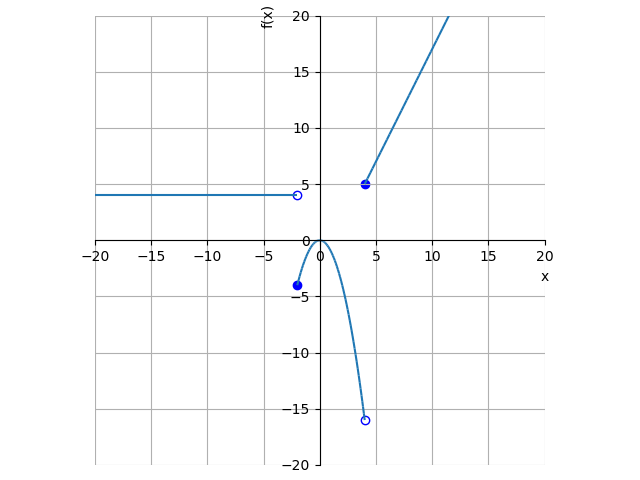
\includegraphics[width=1\columnwidth]{funcion_a_trozos_0}}\end{solution} \part[1] $f(x)=\begin{cases} 2 x & \text{for}\: x < -3 \\x^{2} - 2 x - 8 & \text{for}\: x \leq 3 \\2 x - 3 & \text{otherwise} \end{cases}$\begin{solution} \scalebox{.6}{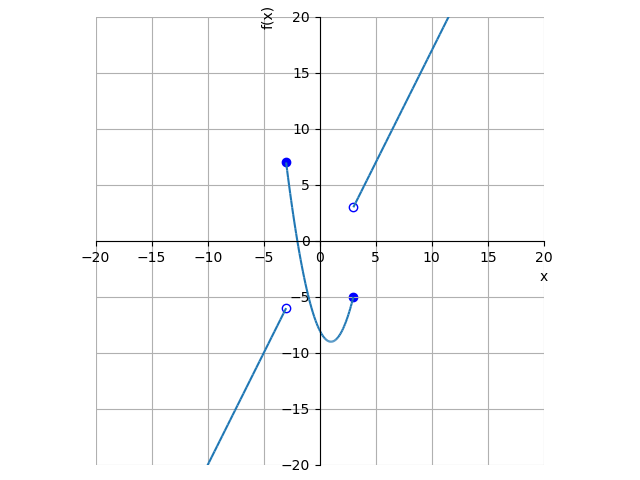
\includegraphics[width=1\columnwidth]{funcion_a_trozos_1}}\end{solution} \part[1] $f(x)=\begin{cases} x + 1 & \text{for}\: x \leq 0 \\x^{2} - 4 x + 3 & \text{otherwise} \end{cases}$\begin{solution} \scalebox{.6}{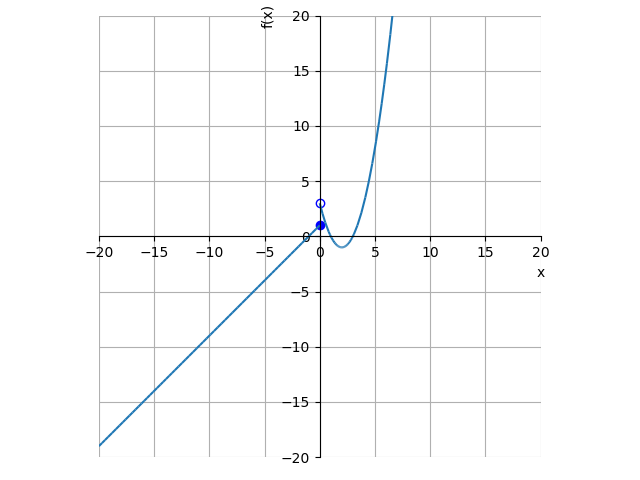
\includegraphics[width=1\columnwidth]{funcion_a_trozos_2}}\end{solution} 
\part[1] $f(x)=\begin{cases} -2 & \text{for}\: x < -2 \\- x^{2} & \text{for}\: x < 3 \\2 x - 3 & \text{otherwise} \end{cases}$\begin{solution} \scalebox{.6}{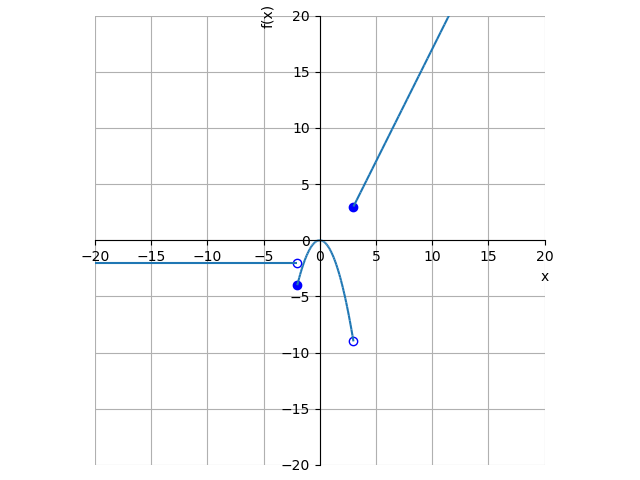
\includegraphics[width=1\columnwidth]{funcion_a_trozos_3}}\end{solution} \part[1] $f(x)=\begin{cases} - 3 x & \text{for}\: x < -2 \\x^{2} - 2 x - 8 & \text{for}\: x \leq 4 \\2 x - 1 & \text{otherwise} \end{cases}$\begin{solution} \scalebox{.6}{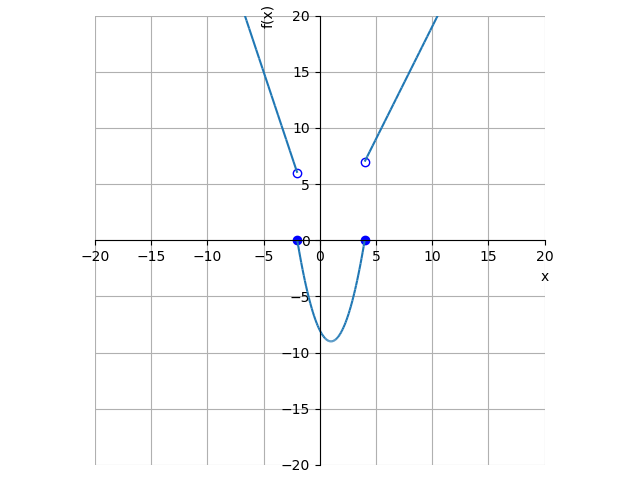
\includegraphics[width=1\columnwidth]{funcion_a_trozos_4}}\end{solution} \part[1] $f(x)=\begin{cases} x + 1 & \text{for}\: x \leq -1 \\x^{2} - 4 x + 3 & \text{otherwise} \end{cases}$\begin{solution} \scalebox{.6}{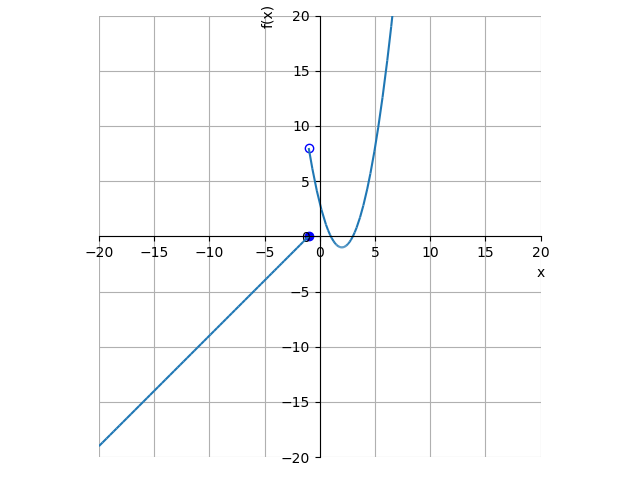
\includegraphics[width=1\columnwidth]{funcion_a_trozos_5}}\end{solution} \end{parts}

\question Representa las siguientes funciones e indica sus propiedades\begin{parts} 
%\part[1] $f(x)=x^2-4x-5$\begin{solution} \scalebox{.6}{%% Creator: Matplotlib, PGF backend
%%
%% To include the figure in your LaTeX document, write
%%   \input{<filename>.pgf}
%%
%% Make sure the required packages are loaded in your preamble
%%   \usepackage{pgf}
%%
%% and, on pdftex
%%   \usepackage[utf8]{inputenc}\DeclareUnicodeCharacter{2212}{-}
%%
%% or, on luatex and xetex
%%   \usepackage{unicode-math}
%%
%% Figures using additional raster images can only be included by \input if
%% they are in the same directory as the main LaTeX file. For loading figures
%% from other directories you can use the `import` package
%%   \usepackage{import}
%%
%% and then include the figures with
%%   \import{<path to file>}{<filename>.pgf}
%%
%% Matplotlib used the following preamble
%%   \usepackage{fontspec}
%%   \setmainfont{DejaVuSerif.ttf}[Path=/home/hp/Mis_aplicaciones/anaconda3/lib/python3.6/site-packages/matplotlib/mpl-data/fonts/ttf/]
%%   \setsansfont{DejaVuSans.ttf}[Path=/home/hp/Mis_aplicaciones/anaconda3/lib/python3.6/site-packages/matplotlib/mpl-data/fonts/ttf/]
%%   \setmonofont{DejaVuSansMono.ttf}[Path=/home/hp/Mis_aplicaciones/anaconda3/lib/python3.6/site-packages/matplotlib/mpl-data/fonts/ttf/]
%%
\begingroup%
\makeatletter%
\begin{pgfpicture}%
\pgfpathrectangle{\pgfpointorigin}{\pgfqpoint{6.400000in}{4.800000in}}%
\pgfusepath{use as bounding box, clip}%
\begin{pgfscope}%
\pgfsetbuttcap%
\pgfsetmiterjoin%
\definecolor{currentfill}{rgb}{1.000000,1.000000,1.000000}%
\pgfsetfillcolor{currentfill}%
\pgfsetlinewidth{0.000000pt}%
\definecolor{currentstroke}{rgb}{1.000000,1.000000,1.000000}%
\pgfsetstrokecolor{currentstroke}%
\pgfsetdash{}{0pt}%
\pgfpathmoveto{\pgfqpoint{0.000000in}{0.000000in}}%
\pgfpathlineto{\pgfqpoint{6.400000in}{0.000000in}}%
\pgfpathlineto{\pgfqpoint{6.400000in}{4.800000in}}%
\pgfpathlineto{\pgfqpoint{0.000000in}{4.800000in}}%
\pgfpathclose%
\pgfusepath{fill}%
\end{pgfscope}%
\begin{pgfscope}%
\pgfsetbuttcap%
\pgfsetmiterjoin%
\definecolor{currentfill}{rgb}{1.000000,1.000000,1.000000}%
\pgfsetfillcolor{currentfill}%
\pgfsetlinewidth{0.000000pt}%
\definecolor{currentstroke}{rgb}{0.000000,0.000000,0.000000}%
\pgfsetstrokecolor{currentstroke}%
\pgfsetstrokeopacity{0.000000}%
\pgfsetdash{}{0pt}%
\pgfpathmoveto{\pgfqpoint{1.049063in}{0.235000in}}%
\pgfpathlineto{\pgfqpoint{5.409063in}{0.235000in}}%
\pgfpathlineto{\pgfqpoint{5.409063in}{4.595000in}}%
\pgfpathlineto{\pgfqpoint{1.049063in}{4.595000in}}%
\pgfpathclose%
\pgfusepath{fill}%
\end{pgfscope}%
\begin{pgfscope}%
\pgfpathrectangle{\pgfqpoint{1.049063in}{0.235000in}}{\pgfqpoint{4.360000in}{4.360000in}}%
\pgfusepath{clip}%
\pgfsetbuttcap%
\pgfsetmiterjoin%
\definecolor{currentfill}{rgb}{0.000000,0.000000,1.000000}%
\pgfsetfillcolor{currentfill}%
\pgfsetlinewidth{0.000000pt}%
\definecolor{currentstroke}{rgb}{0.000000,0.000000,0.000000}%
\pgfsetstrokecolor{currentstroke}%
\pgfsetstrokeopacity{0.000000}%
\pgfsetdash{}{0pt}%
\pgfpathmoveto{\pgfqpoint{2.952304in}{3.636995in}}%
\pgfpathlineto{\pgfqpoint{2.952304in}{3.641253in}}%
\pgfpathlineto{\pgfqpoint{2.956562in}{3.641253in}}%
\pgfpathlineto{\pgfqpoint{2.956562in}{3.636995in}}%
\pgfpathmoveto{\pgfqpoint{2.952304in}{3.641253in}}%
\pgfpathlineto{\pgfqpoint{2.952304in}{3.641253in}}%
\pgfpathlineto{\pgfqpoint{2.952304in}{3.645511in}}%
\pgfpathlineto{\pgfqpoint{2.956562in}{3.645511in}}%
\pgfpathlineto{\pgfqpoint{2.956562in}{3.641253in}}%
\pgfpathmoveto{\pgfqpoint{2.952304in}{3.645511in}}%
\pgfpathlineto{\pgfqpoint{2.952304in}{3.645511in}}%
\pgfpathlineto{\pgfqpoint{2.952304in}{3.649769in}}%
\pgfpathlineto{\pgfqpoint{2.956562in}{3.649769in}}%
\pgfpathlineto{\pgfqpoint{2.956562in}{3.645511in}}%
\pgfpathmoveto{\pgfqpoint{2.952304in}{3.649769in}}%
\pgfpathlineto{\pgfqpoint{2.952304in}{3.649769in}}%
\pgfpathlineto{\pgfqpoint{2.952304in}{3.654027in}}%
\pgfpathlineto{\pgfqpoint{2.956562in}{3.654027in}}%
\pgfpathlineto{\pgfqpoint{2.956562in}{3.649769in}}%
\pgfpathmoveto{\pgfqpoint{2.952304in}{3.654027in}}%
\pgfpathlineto{\pgfqpoint{2.952304in}{3.654027in}}%
\pgfpathlineto{\pgfqpoint{2.952304in}{3.658284in}}%
\pgfpathlineto{\pgfqpoint{2.956562in}{3.658284in}}%
\pgfpathlineto{\pgfqpoint{2.956562in}{3.654027in}}%
\pgfpathmoveto{\pgfqpoint{2.952304in}{3.658284in}}%
\pgfpathlineto{\pgfqpoint{2.952304in}{3.658284in}}%
\pgfpathlineto{\pgfqpoint{2.952304in}{3.662542in}}%
\pgfpathlineto{\pgfqpoint{2.956562in}{3.662542in}}%
\pgfpathlineto{\pgfqpoint{2.956562in}{3.658284in}}%
\pgfpathmoveto{\pgfqpoint{2.952304in}{3.662542in}}%
\pgfpathlineto{\pgfqpoint{2.952304in}{3.662542in}}%
\pgfpathlineto{\pgfqpoint{2.952304in}{3.666800in}}%
\pgfpathlineto{\pgfqpoint{2.956562in}{3.666800in}}%
\pgfpathlineto{\pgfqpoint{2.956562in}{3.662542in}}%
\pgfpathmoveto{\pgfqpoint{2.952304in}{3.666800in}}%
\pgfpathlineto{\pgfqpoint{2.952304in}{3.666800in}}%
\pgfpathlineto{\pgfqpoint{2.952304in}{3.671058in}}%
\pgfpathlineto{\pgfqpoint{2.956562in}{3.671058in}}%
\pgfpathlineto{\pgfqpoint{2.956562in}{3.666800in}}%
\pgfpathmoveto{\pgfqpoint{2.952304in}{3.671058in}}%
\pgfpathlineto{\pgfqpoint{2.952304in}{3.671058in}}%
\pgfpathlineto{\pgfqpoint{2.952304in}{3.675316in}}%
\pgfpathlineto{\pgfqpoint{2.956562in}{3.675316in}}%
\pgfpathlineto{\pgfqpoint{2.956562in}{3.671058in}}%
\pgfpathmoveto{\pgfqpoint{2.948046in}{3.679573in}}%
\pgfpathlineto{\pgfqpoint{2.948046in}{3.679573in}}%
\pgfpathlineto{\pgfqpoint{2.948046in}{3.683831in}}%
\pgfpathlineto{\pgfqpoint{2.952304in}{3.683831in}}%
\pgfpathlineto{\pgfqpoint{2.952304in}{3.679573in}}%
\pgfpathmoveto{\pgfqpoint{2.952304in}{3.675316in}}%
\pgfpathlineto{\pgfqpoint{2.952304in}{3.675316in}}%
\pgfpathlineto{\pgfqpoint{2.952304in}{3.679573in}}%
\pgfpathlineto{\pgfqpoint{2.956562in}{3.679573in}}%
\pgfpathlineto{\pgfqpoint{2.956562in}{3.675316in}}%
\pgfpathmoveto{\pgfqpoint{2.952304in}{3.679573in}}%
\pgfpathlineto{\pgfqpoint{2.952304in}{3.679573in}}%
\pgfpathlineto{\pgfqpoint{2.952304in}{3.683831in}}%
\pgfpathlineto{\pgfqpoint{2.956562in}{3.683831in}}%
\pgfpathlineto{\pgfqpoint{2.956562in}{3.679573in}}%
\pgfpathmoveto{\pgfqpoint{2.948046in}{3.683831in}}%
\pgfpathlineto{\pgfqpoint{2.948046in}{3.683831in}}%
\pgfpathlineto{\pgfqpoint{2.948046in}{3.688089in}}%
\pgfpathlineto{\pgfqpoint{2.952304in}{3.688089in}}%
\pgfpathlineto{\pgfqpoint{2.952304in}{3.683831in}}%
\pgfpathmoveto{\pgfqpoint{2.948046in}{3.688089in}}%
\pgfpathlineto{\pgfqpoint{2.948046in}{3.688089in}}%
\pgfpathlineto{\pgfqpoint{2.948046in}{3.692347in}}%
\pgfpathlineto{\pgfqpoint{2.952304in}{3.692347in}}%
\pgfpathlineto{\pgfqpoint{2.952304in}{3.688089in}}%
\pgfpathmoveto{\pgfqpoint{2.948046in}{3.692347in}}%
\pgfpathlineto{\pgfqpoint{2.948046in}{3.692347in}}%
\pgfpathlineto{\pgfqpoint{2.948046in}{3.696604in}}%
\pgfpathlineto{\pgfqpoint{2.952304in}{3.696604in}}%
\pgfpathlineto{\pgfqpoint{2.952304in}{3.692347in}}%
\pgfpathmoveto{\pgfqpoint{2.948046in}{3.696604in}}%
\pgfpathlineto{\pgfqpoint{2.948046in}{3.696604in}}%
\pgfpathlineto{\pgfqpoint{2.948046in}{3.700862in}}%
\pgfpathlineto{\pgfqpoint{2.952304in}{3.700862in}}%
\pgfpathlineto{\pgfqpoint{2.952304in}{3.696604in}}%
\pgfpathmoveto{\pgfqpoint{2.948046in}{3.700862in}}%
\pgfpathlineto{\pgfqpoint{2.948046in}{3.700862in}}%
\pgfpathlineto{\pgfqpoint{2.948046in}{3.705120in}}%
\pgfpathlineto{\pgfqpoint{2.952304in}{3.705120in}}%
\pgfpathlineto{\pgfqpoint{2.952304in}{3.700862in}}%
\pgfpathmoveto{\pgfqpoint{2.948046in}{3.705120in}}%
\pgfpathlineto{\pgfqpoint{2.948046in}{3.705120in}}%
\pgfpathlineto{\pgfqpoint{2.948046in}{3.709378in}}%
\pgfpathlineto{\pgfqpoint{2.952304in}{3.709378in}}%
\pgfpathlineto{\pgfqpoint{2.952304in}{3.705120in}}%
\pgfpathmoveto{\pgfqpoint{2.943788in}{3.717893in}}%
\pgfpathlineto{\pgfqpoint{2.943788in}{3.717893in}}%
\pgfpathlineto{\pgfqpoint{2.943788in}{3.722151in}}%
\pgfpathlineto{\pgfqpoint{2.948046in}{3.722151in}}%
\pgfpathlineto{\pgfqpoint{2.948046in}{3.717893in}}%
\pgfpathmoveto{\pgfqpoint{2.943788in}{3.722151in}}%
\pgfpathlineto{\pgfqpoint{2.943788in}{3.722151in}}%
\pgfpathlineto{\pgfqpoint{2.943788in}{3.726409in}}%
\pgfpathlineto{\pgfqpoint{2.948046in}{3.726409in}}%
\pgfpathlineto{\pgfqpoint{2.948046in}{3.722151in}}%
\pgfpathmoveto{\pgfqpoint{2.948046in}{3.709378in}}%
\pgfpathlineto{\pgfqpoint{2.948046in}{3.709378in}}%
\pgfpathlineto{\pgfqpoint{2.948046in}{3.713636in}}%
\pgfpathlineto{\pgfqpoint{2.952304in}{3.713636in}}%
\pgfpathlineto{\pgfqpoint{2.952304in}{3.709378in}}%
\pgfpathmoveto{\pgfqpoint{2.948046in}{3.713636in}}%
\pgfpathlineto{\pgfqpoint{2.948046in}{3.713636in}}%
\pgfpathlineto{\pgfqpoint{2.948046in}{3.717893in}}%
\pgfpathlineto{\pgfqpoint{2.952304in}{3.717893in}}%
\pgfpathlineto{\pgfqpoint{2.952304in}{3.713636in}}%
\pgfpathmoveto{\pgfqpoint{2.948046in}{3.717893in}}%
\pgfpathlineto{\pgfqpoint{2.948046in}{3.717893in}}%
\pgfpathlineto{\pgfqpoint{2.948046in}{3.722151in}}%
\pgfpathlineto{\pgfqpoint{2.952304in}{3.722151in}}%
\pgfpathlineto{\pgfqpoint{2.952304in}{3.717893in}}%
\pgfpathmoveto{\pgfqpoint{2.943788in}{3.726409in}}%
\pgfpathlineto{\pgfqpoint{2.943788in}{3.726409in}}%
\pgfpathlineto{\pgfqpoint{2.943788in}{3.730667in}}%
\pgfpathlineto{\pgfqpoint{2.948046in}{3.730667in}}%
\pgfpathlineto{\pgfqpoint{2.948046in}{3.726409in}}%
\pgfpathmoveto{\pgfqpoint{2.943788in}{3.730667in}}%
\pgfpathlineto{\pgfqpoint{2.943788in}{3.730667in}}%
\pgfpathlineto{\pgfqpoint{2.943788in}{3.734924in}}%
\pgfpathlineto{\pgfqpoint{2.948046in}{3.734924in}}%
\pgfpathlineto{\pgfqpoint{2.948046in}{3.730667in}}%
\pgfpathmoveto{\pgfqpoint{2.943788in}{3.734924in}}%
\pgfpathlineto{\pgfqpoint{2.943788in}{3.734924in}}%
\pgfpathlineto{\pgfqpoint{2.943788in}{3.739182in}}%
\pgfpathlineto{\pgfqpoint{2.948046in}{3.739182in}}%
\pgfpathlineto{\pgfqpoint{2.948046in}{3.734924in}}%
\pgfpathmoveto{\pgfqpoint{2.943788in}{3.739182in}}%
\pgfpathlineto{\pgfqpoint{2.943788in}{3.739182in}}%
\pgfpathlineto{\pgfqpoint{2.943788in}{3.743440in}}%
\pgfpathlineto{\pgfqpoint{2.948046in}{3.743440in}}%
\pgfpathlineto{\pgfqpoint{2.948046in}{3.739182in}}%
\pgfpathmoveto{\pgfqpoint{2.943788in}{3.743440in}}%
\pgfpathlineto{\pgfqpoint{2.943788in}{3.743440in}}%
\pgfpathlineto{\pgfqpoint{2.943788in}{3.747698in}}%
\pgfpathlineto{\pgfqpoint{2.948046in}{3.747698in}}%
\pgfpathlineto{\pgfqpoint{2.948046in}{3.743440in}}%
\pgfpathmoveto{\pgfqpoint{2.943788in}{3.747698in}}%
\pgfpathlineto{\pgfqpoint{2.943788in}{3.747698in}}%
\pgfpathlineto{\pgfqpoint{2.943788in}{3.751955in}}%
\pgfpathlineto{\pgfqpoint{2.948046in}{3.751955in}}%
\pgfpathlineto{\pgfqpoint{2.948046in}{3.747698in}}%
\pgfpathmoveto{\pgfqpoint{2.939530in}{3.756213in}}%
\pgfpathlineto{\pgfqpoint{2.939530in}{3.756213in}}%
\pgfpathlineto{\pgfqpoint{2.939530in}{3.760471in}}%
\pgfpathlineto{\pgfqpoint{2.943788in}{3.760471in}}%
\pgfpathlineto{\pgfqpoint{2.943788in}{3.756213in}}%
\pgfpathmoveto{\pgfqpoint{2.943788in}{3.751955in}}%
\pgfpathlineto{\pgfqpoint{2.943788in}{3.751955in}}%
\pgfpathlineto{\pgfqpoint{2.943788in}{3.756213in}}%
\pgfpathlineto{\pgfqpoint{2.948046in}{3.756213in}}%
\pgfpathlineto{\pgfqpoint{2.948046in}{3.751955in}}%
\pgfpathmoveto{\pgfqpoint{2.943788in}{3.756213in}}%
\pgfpathlineto{\pgfqpoint{2.943788in}{3.756213in}}%
\pgfpathlineto{\pgfqpoint{2.943788in}{3.760471in}}%
\pgfpathlineto{\pgfqpoint{2.948046in}{3.760471in}}%
\pgfpathlineto{\pgfqpoint{2.948046in}{3.756213in}}%
\pgfpathmoveto{\pgfqpoint{2.939530in}{3.760471in}}%
\pgfpathlineto{\pgfqpoint{2.939530in}{3.760471in}}%
\pgfpathlineto{\pgfqpoint{2.939530in}{3.764729in}}%
\pgfpathlineto{\pgfqpoint{2.943788in}{3.764729in}}%
\pgfpathlineto{\pgfqpoint{2.943788in}{3.760471in}}%
\pgfpathmoveto{\pgfqpoint{2.939530in}{3.764729in}}%
\pgfpathlineto{\pgfqpoint{2.939530in}{3.764729in}}%
\pgfpathlineto{\pgfqpoint{2.939530in}{3.768987in}}%
\pgfpathlineto{\pgfqpoint{2.943788in}{3.768987in}}%
\pgfpathlineto{\pgfqpoint{2.943788in}{3.764729in}}%
\pgfpathmoveto{\pgfqpoint{2.939530in}{3.768987in}}%
\pgfpathlineto{\pgfqpoint{2.939530in}{3.768987in}}%
\pgfpathlineto{\pgfqpoint{2.939530in}{3.773244in}}%
\pgfpathlineto{\pgfqpoint{2.943788in}{3.773244in}}%
\pgfpathlineto{\pgfqpoint{2.943788in}{3.768987in}}%
\pgfpathmoveto{\pgfqpoint{2.939530in}{3.773244in}}%
\pgfpathlineto{\pgfqpoint{2.939530in}{3.773244in}}%
\pgfpathlineto{\pgfqpoint{2.939530in}{3.777502in}}%
\pgfpathlineto{\pgfqpoint{2.943788in}{3.777502in}}%
\pgfpathlineto{\pgfqpoint{2.943788in}{3.773244in}}%
\pgfpathmoveto{\pgfqpoint{2.935273in}{3.794533in}}%
\pgfpathlineto{\pgfqpoint{2.935273in}{3.794533in}}%
\pgfpathlineto{\pgfqpoint{2.935273in}{3.798791in}}%
\pgfpathlineto{\pgfqpoint{2.939530in}{3.798791in}}%
\pgfpathlineto{\pgfqpoint{2.939530in}{3.794533in}}%
\pgfpathmoveto{\pgfqpoint{2.935273in}{3.798791in}}%
\pgfpathlineto{\pgfqpoint{2.935273in}{3.798791in}}%
\pgfpathlineto{\pgfqpoint{2.935273in}{3.803049in}}%
\pgfpathlineto{\pgfqpoint{2.939530in}{3.803049in}}%
\pgfpathlineto{\pgfqpoint{2.939530in}{3.798791in}}%
\pgfpathmoveto{\pgfqpoint{2.935273in}{3.803049in}}%
\pgfpathlineto{\pgfqpoint{2.935273in}{3.803049in}}%
\pgfpathlineto{\pgfqpoint{2.935273in}{3.807306in}}%
\pgfpathlineto{\pgfqpoint{2.939530in}{3.807306in}}%
\pgfpathlineto{\pgfqpoint{2.939530in}{3.803049in}}%
\pgfpathmoveto{\pgfqpoint{2.935273in}{3.807306in}}%
\pgfpathlineto{\pgfqpoint{2.935273in}{3.807306in}}%
\pgfpathlineto{\pgfqpoint{2.935273in}{3.811564in}}%
\pgfpathlineto{\pgfqpoint{2.939530in}{3.811564in}}%
\pgfpathlineto{\pgfqpoint{2.939530in}{3.807306in}}%
\pgfpathmoveto{\pgfqpoint{2.939530in}{3.777502in}}%
\pgfpathlineto{\pgfqpoint{2.939530in}{3.777502in}}%
\pgfpathlineto{\pgfqpoint{2.939530in}{3.781760in}}%
\pgfpathlineto{\pgfqpoint{2.943788in}{3.781760in}}%
\pgfpathlineto{\pgfqpoint{2.943788in}{3.777502in}}%
\pgfpathmoveto{\pgfqpoint{2.939530in}{3.781760in}}%
\pgfpathlineto{\pgfqpoint{2.939530in}{3.781760in}}%
\pgfpathlineto{\pgfqpoint{2.939530in}{3.786018in}}%
\pgfpathlineto{\pgfqpoint{2.943788in}{3.786018in}}%
\pgfpathlineto{\pgfqpoint{2.943788in}{3.781760in}}%
\pgfpathmoveto{\pgfqpoint{2.939530in}{3.786018in}}%
\pgfpathlineto{\pgfqpoint{2.939530in}{3.786018in}}%
\pgfpathlineto{\pgfqpoint{2.939530in}{3.790275in}}%
\pgfpathlineto{\pgfqpoint{2.943788in}{3.790275in}}%
\pgfpathlineto{\pgfqpoint{2.943788in}{3.786018in}}%
\pgfpathmoveto{\pgfqpoint{2.939530in}{3.790275in}}%
\pgfpathlineto{\pgfqpoint{2.939530in}{3.790275in}}%
\pgfpathlineto{\pgfqpoint{2.939530in}{3.794533in}}%
\pgfpathlineto{\pgfqpoint{2.943788in}{3.794533in}}%
\pgfpathlineto{\pgfqpoint{2.943788in}{3.790275in}}%
\pgfpathmoveto{\pgfqpoint{2.939530in}{3.794533in}}%
\pgfpathlineto{\pgfqpoint{2.939530in}{3.794533in}}%
\pgfpathlineto{\pgfqpoint{2.939530in}{3.798791in}}%
\pgfpathlineto{\pgfqpoint{2.943788in}{3.798791in}}%
\pgfpathlineto{\pgfqpoint{2.943788in}{3.794533in}}%
\pgfpathmoveto{\pgfqpoint{2.935273in}{3.811564in}}%
\pgfpathlineto{\pgfqpoint{2.935273in}{3.811564in}}%
\pgfpathlineto{\pgfqpoint{2.935273in}{3.815822in}}%
\pgfpathlineto{\pgfqpoint{2.939530in}{3.815822in}}%
\pgfpathlineto{\pgfqpoint{2.939530in}{3.811564in}}%
\pgfpathmoveto{\pgfqpoint{2.935273in}{3.815822in}}%
\pgfpathlineto{\pgfqpoint{2.935273in}{3.815822in}}%
\pgfpathlineto{\pgfqpoint{2.935273in}{3.820080in}}%
\pgfpathlineto{\pgfqpoint{2.939530in}{3.820080in}}%
\pgfpathlineto{\pgfqpoint{2.939530in}{3.815822in}}%
\pgfpathmoveto{\pgfqpoint{2.935273in}{3.820080in}}%
\pgfpathlineto{\pgfqpoint{2.935273in}{3.820080in}}%
\pgfpathlineto{\pgfqpoint{2.935273in}{3.824337in}}%
\pgfpathlineto{\pgfqpoint{2.939530in}{3.824337in}}%
\pgfpathlineto{\pgfqpoint{2.939530in}{3.820080in}}%
\pgfpathmoveto{\pgfqpoint{2.935273in}{3.824337in}}%
\pgfpathlineto{\pgfqpoint{2.935273in}{3.824337in}}%
\pgfpathlineto{\pgfqpoint{2.935273in}{3.828595in}}%
\pgfpathlineto{\pgfqpoint{2.939530in}{3.828595in}}%
\pgfpathlineto{\pgfqpoint{2.939530in}{3.824337in}}%
\pgfpathmoveto{\pgfqpoint{2.931015in}{3.832853in}}%
\pgfpathlineto{\pgfqpoint{2.931015in}{3.832853in}}%
\pgfpathlineto{\pgfqpoint{2.931015in}{3.837111in}}%
\pgfpathlineto{\pgfqpoint{2.935273in}{3.837111in}}%
\pgfpathlineto{\pgfqpoint{2.935273in}{3.832853in}}%
\pgfpathmoveto{\pgfqpoint{2.935273in}{3.828595in}}%
\pgfpathlineto{\pgfqpoint{2.935273in}{3.828595in}}%
\pgfpathlineto{\pgfqpoint{2.935273in}{3.832853in}}%
\pgfpathlineto{\pgfqpoint{2.939530in}{3.832853in}}%
\pgfpathlineto{\pgfqpoint{2.939530in}{3.828595in}}%
\pgfpathmoveto{\pgfqpoint{2.935273in}{3.832853in}}%
\pgfpathlineto{\pgfqpoint{2.935273in}{3.832853in}}%
\pgfpathlineto{\pgfqpoint{2.935273in}{3.837111in}}%
\pgfpathlineto{\pgfqpoint{2.939530in}{3.837111in}}%
\pgfpathlineto{\pgfqpoint{2.939530in}{3.832853in}}%
\pgfpathmoveto{\pgfqpoint{2.931015in}{3.837111in}}%
\pgfpathlineto{\pgfqpoint{2.931015in}{3.837111in}}%
\pgfpathlineto{\pgfqpoint{2.931015in}{3.841368in}}%
\pgfpathlineto{\pgfqpoint{2.935273in}{3.841368in}}%
\pgfpathlineto{\pgfqpoint{2.935273in}{3.837111in}}%
\pgfpathmoveto{\pgfqpoint{2.931015in}{3.841368in}}%
\pgfpathlineto{\pgfqpoint{2.931015in}{3.841368in}}%
\pgfpathlineto{\pgfqpoint{2.931015in}{3.845626in}}%
\pgfpathlineto{\pgfqpoint{2.935273in}{3.845626in}}%
\pgfpathlineto{\pgfqpoint{2.935273in}{3.841368in}}%
\pgfpathmoveto{\pgfqpoint{2.931015in}{3.845626in}}%
\pgfpathlineto{\pgfqpoint{2.931015in}{3.845626in}}%
\pgfpathlineto{\pgfqpoint{2.931015in}{3.849884in}}%
\pgfpathlineto{\pgfqpoint{2.935273in}{3.849884in}}%
\pgfpathlineto{\pgfqpoint{2.935273in}{3.845626in}}%
\pgfpathmoveto{\pgfqpoint{2.931015in}{3.849884in}}%
\pgfpathlineto{\pgfqpoint{2.931015in}{3.849884in}}%
\pgfpathlineto{\pgfqpoint{2.931015in}{3.854142in}}%
\pgfpathlineto{\pgfqpoint{2.935273in}{3.854142in}}%
\pgfpathlineto{\pgfqpoint{2.935273in}{3.849884in}}%
\pgfpathmoveto{\pgfqpoint{2.931015in}{3.854142in}}%
\pgfpathlineto{\pgfqpoint{2.931015in}{3.854142in}}%
\pgfpathlineto{\pgfqpoint{2.931015in}{3.858399in}}%
\pgfpathlineto{\pgfqpoint{2.935273in}{3.858399in}}%
\pgfpathlineto{\pgfqpoint{2.935273in}{3.854142in}}%
\pgfpathmoveto{\pgfqpoint{2.931015in}{3.858399in}}%
\pgfpathlineto{\pgfqpoint{2.931015in}{3.858399in}}%
\pgfpathlineto{\pgfqpoint{2.931015in}{3.862657in}}%
\pgfpathlineto{\pgfqpoint{2.935273in}{3.862657in}}%
\pgfpathlineto{\pgfqpoint{2.935273in}{3.858399in}}%
\pgfpathmoveto{\pgfqpoint{2.926757in}{3.875430in}}%
\pgfpathlineto{\pgfqpoint{2.926757in}{3.875430in}}%
\pgfpathlineto{\pgfqpoint{2.926757in}{3.879688in}}%
\pgfpathlineto{\pgfqpoint{2.931015in}{3.879688in}}%
\pgfpathlineto{\pgfqpoint{2.931015in}{3.875430in}}%
\pgfpathmoveto{\pgfqpoint{2.931015in}{3.862657in}}%
\pgfpathlineto{\pgfqpoint{2.931015in}{3.862657in}}%
\pgfpathlineto{\pgfqpoint{2.931015in}{3.866915in}}%
\pgfpathlineto{\pgfqpoint{2.935273in}{3.866915in}}%
\pgfpathlineto{\pgfqpoint{2.935273in}{3.862657in}}%
\pgfpathmoveto{\pgfqpoint{2.931015in}{3.866915in}}%
\pgfpathlineto{\pgfqpoint{2.931015in}{3.866915in}}%
\pgfpathlineto{\pgfqpoint{2.931015in}{3.871173in}}%
\pgfpathlineto{\pgfqpoint{2.935273in}{3.871173in}}%
\pgfpathlineto{\pgfqpoint{2.935273in}{3.866915in}}%
\pgfpathmoveto{\pgfqpoint{2.931015in}{3.871173in}}%
\pgfpathlineto{\pgfqpoint{2.931015in}{3.871173in}}%
\pgfpathlineto{\pgfqpoint{2.931015in}{3.875430in}}%
\pgfpathlineto{\pgfqpoint{2.935273in}{3.875430in}}%
\pgfpathlineto{\pgfqpoint{2.935273in}{3.871173in}}%
\pgfpathmoveto{\pgfqpoint{2.931015in}{3.875430in}}%
\pgfpathlineto{\pgfqpoint{2.931015in}{3.875430in}}%
\pgfpathlineto{\pgfqpoint{2.931015in}{3.879688in}}%
\pgfpathlineto{\pgfqpoint{2.935273in}{3.879688in}}%
\pgfpathlineto{\pgfqpoint{2.935273in}{3.875430in}}%
\pgfpathmoveto{\pgfqpoint{2.926757in}{3.879688in}}%
\pgfpathlineto{\pgfqpoint{2.926757in}{3.879688in}}%
\pgfpathlineto{\pgfqpoint{2.926757in}{3.883946in}}%
\pgfpathlineto{\pgfqpoint{2.931015in}{3.883946in}}%
\pgfpathlineto{\pgfqpoint{2.931015in}{3.879688in}}%
\pgfpathmoveto{\pgfqpoint{2.926757in}{3.883946in}}%
\pgfpathlineto{\pgfqpoint{2.926757in}{3.883946in}}%
\pgfpathlineto{\pgfqpoint{2.926757in}{3.888204in}}%
\pgfpathlineto{\pgfqpoint{2.931015in}{3.888204in}}%
\pgfpathlineto{\pgfqpoint{2.931015in}{3.883946in}}%
\pgfpathmoveto{\pgfqpoint{2.926757in}{3.888204in}}%
\pgfpathlineto{\pgfqpoint{2.926757in}{3.888204in}}%
\pgfpathlineto{\pgfqpoint{2.926757in}{3.892461in}}%
\pgfpathlineto{\pgfqpoint{2.931015in}{3.892461in}}%
\pgfpathlineto{\pgfqpoint{2.931015in}{3.888204in}}%
\pgfpathmoveto{\pgfqpoint{2.926757in}{3.892461in}}%
\pgfpathlineto{\pgfqpoint{2.926757in}{3.892461in}}%
\pgfpathlineto{\pgfqpoint{2.926757in}{3.896719in}}%
\pgfpathlineto{\pgfqpoint{2.931015in}{3.896719in}}%
\pgfpathlineto{\pgfqpoint{2.931015in}{3.892461in}}%
\pgfpathmoveto{\pgfqpoint{2.926757in}{3.896719in}}%
\pgfpathlineto{\pgfqpoint{2.926757in}{3.896719in}}%
\pgfpathlineto{\pgfqpoint{2.926757in}{3.900977in}}%
\pgfpathlineto{\pgfqpoint{2.931015in}{3.900977in}}%
\pgfpathlineto{\pgfqpoint{2.931015in}{3.896719in}}%
\pgfpathmoveto{\pgfqpoint{2.926757in}{3.900977in}}%
\pgfpathlineto{\pgfqpoint{2.926757in}{3.900977in}}%
\pgfpathlineto{\pgfqpoint{2.926757in}{3.905235in}}%
\pgfpathlineto{\pgfqpoint{2.931015in}{3.905235in}}%
\pgfpathlineto{\pgfqpoint{2.931015in}{3.900977in}}%
\pgfpathmoveto{\pgfqpoint{2.926757in}{3.905235in}}%
\pgfpathlineto{\pgfqpoint{2.926757in}{3.905235in}}%
\pgfpathlineto{\pgfqpoint{2.926757in}{3.909492in}}%
\pgfpathlineto{\pgfqpoint{2.931015in}{3.909492in}}%
\pgfpathlineto{\pgfqpoint{2.931015in}{3.905235in}}%
\pgfpathmoveto{\pgfqpoint{2.926757in}{3.909492in}}%
\pgfpathlineto{\pgfqpoint{2.926757in}{3.909492in}}%
\pgfpathlineto{\pgfqpoint{2.926757in}{3.913750in}}%
\pgfpathlineto{\pgfqpoint{2.931015in}{3.913750in}}%
\pgfpathlineto{\pgfqpoint{2.931015in}{3.909492in}}%
\pgfpathmoveto{\pgfqpoint{2.918241in}{3.956327in}}%
\pgfpathlineto{\pgfqpoint{2.918241in}{3.956327in}}%
\pgfpathlineto{\pgfqpoint{2.918241in}{3.960585in}}%
\pgfpathlineto{\pgfqpoint{2.922499in}{3.960585in}}%
\pgfpathlineto{\pgfqpoint{2.922499in}{3.956327in}}%
\pgfpathmoveto{\pgfqpoint{2.918241in}{3.960585in}}%
\pgfpathlineto{\pgfqpoint{2.918241in}{3.960585in}}%
\pgfpathlineto{\pgfqpoint{2.918241in}{3.964843in}}%
\pgfpathlineto{\pgfqpoint{2.922499in}{3.964843in}}%
\pgfpathlineto{\pgfqpoint{2.922499in}{3.960585in}}%
\pgfpathmoveto{\pgfqpoint{2.918241in}{3.964843in}}%
\pgfpathlineto{\pgfqpoint{2.918241in}{3.964843in}}%
\pgfpathlineto{\pgfqpoint{2.918241in}{3.969100in}}%
\pgfpathlineto{\pgfqpoint{2.922499in}{3.969100in}}%
\pgfpathlineto{\pgfqpoint{2.922499in}{3.964843in}}%
\pgfpathmoveto{\pgfqpoint{2.918241in}{3.969100in}}%
\pgfpathlineto{\pgfqpoint{2.918241in}{3.969100in}}%
\pgfpathlineto{\pgfqpoint{2.918241in}{3.973358in}}%
\pgfpathlineto{\pgfqpoint{2.922499in}{3.973358in}}%
\pgfpathlineto{\pgfqpoint{2.922499in}{3.969100in}}%
\pgfpathmoveto{\pgfqpoint{2.918241in}{3.973358in}}%
\pgfpathlineto{\pgfqpoint{2.918241in}{3.973358in}}%
\pgfpathlineto{\pgfqpoint{2.918241in}{3.977616in}}%
\pgfpathlineto{\pgfqpoint{2.922499in}{3.977616in}}%
\pgfpathlineto{\pgfqpoint{2.922499in}{3.973358in}}%
\pgfpathmoveto{\pgfqpoint{2.918241in}{3.977616in}}%
\pgfpathlineto{\pgfqpoint{2.918241in}{3.977616in}}%
\pgfpathlineto{\pgfqpoint{2.918241in}{3.981873in}}%
\pgfpathlineto{\pgfqpoint{2.922499in}{3.981873in}}%
\pgfpathlineto{\pgfqpoint{2.922499in}{3.977616in}}%
\pgfpathmoveto{\pgfqpoint{2.922499in}{3.913750in}}%
\pgfpathlineto{\pgfqpoint{2.922499in}{3.913750in}}%
\pgfpathlineto{\pgfqpoint{2.922499in}{3.918008in}}%
\pgfpathlineto{\pgfqpoint{2.926757in}{3.918008in}}%
\pgfpathlineto{\pgfqpoint{2.926757in}{3.913750in}}%
\pgfpathmoveto{\pgfqpoint{2.922499in}{3.918008in}}%
\pgfpathlineto{\pgfqpoint{2.922499in}{3.918008in}}%
\pgfpathlineto{\pgfqpoint{2.922499in}{3.922266in}}%
\pgfpathlineto{\pgfqpoint{2.926757in}{3.922266in}}%
\pgfpathlineto{\pgfqpoint{2.926757in}{3.918008in}}%
\pgfpathmoveto{\pgfqpoint{2.926757in}{3.913750in}}%
\pgfpathlineto{\pgfqpoint{2.926757in}{3.913750in}}%
\pgfpathlineto{\pgfqpoint{2.926757in}{3.918008in}}%
\pgfpathlineto{\pgfqpoint{2.931015in}{3.918008in}}%
\pgfpathlineto{\pgfqpoint{2.931015in}{3.913750in}}%
\pgfpathmoveto{\pgfqpoint{2.922499in}{3.922266in}}%
\pgfpathlineto{\pgfqpoint{2.922499in}{3.922266in}}%
\pgfpathlineto{\pgfqpoint{2.922499in}{3.926523in}}%
\pgfpathlineto{\pgfqpoint{2.926757in}{3.926523in}}%
\pgfpathlineto{\pgfqpoint{2.926757in}{3.922266in}}%
\pgfpathmoveto{\pgfqpoint{2.922499in}{3.926523in}}%
\pgfpathlineto{\pgfqpoint{2.922499in}{3.926523in}}%
\pgfpathlineto{\pgfqpoint{2.922499in}{3.930781in}}%
\pgfpathlineto{\pgfqpoint{2.926757in}{3.930781in}}%
\pgfpathlineto{\pgfqpoint{2.926757in}{3.926523in}}%
\pgfpathmoveto{\pgfqpoint{2.922499in}{3.930781in}}%
\pgfpathlineto{\pgfqpoint{2.922499in}{3.930781in}}%
\pgfpathlineto{\pgfqpoint{2.922499in}{3.935039in}}%
\pgfpathlineto{\pgfqpoint{2.926757in}{3.935039in}}%
\pgfpathlineto{\pgfqpoint{2.926757in}{3.930781in}}%
\pgfpathmoveto{\pgfqpoint{2.922499in}{3.935039in}}%
\pgfpathlineto{\pgfqpoint{2.922499in}{3.935039in}}%
\pgfpathlineto{\pgfqpoint{2.922499in}{3.939296in}}%
\pgfpathlineto{\pgfqpoint{2.926757in}{3.939296in}}%
\pgfpathlineto{\pgfqpoint{2.926757in}{3.935039in}}%
\pgfpathmoveto{\pgfqpoint{2.922499in}{3.939296in}}%
\pgfpathlineto{\pgfqpoint{2.922499in}{3.939296in}}%
\pgfpathlineto{\pgfqpoint{2.922499in}{3.943554in}}%
\pgfpathlineto{\pgfqpoint{2.926757in}{3.943554in}}%
\pgfpathlineto{\pgfqpoint{2.926757in}{3.939296in}}%
\pgfpathmoveto{\pgfqpoint{2.922499in}{3.943554in}}%
\pgfpathlineto{\pgfqpoint{2.922499in}{3.943554in}}%
\pgfpathlineto{\pgfqpoint{2.922499in}{3.947812in}}%
\pgfpathlineto{\pgfqpoint{2.926757in}{3.947812in}}%
\pgfpathlineto{\pgfqpoint{2.926757in}{3.943554in}}%
\pgfpathmoveto{\pgfqpoint{2.922499in}{3.947812in}}%
\pgfpathlineto{\pgfqpoint{2.922499in}{3.947812in}}%
\pgfpathlineto{\pgfqpoint{2.922499in}{3.952069in}}%
\pgfpathlineto{\pgfqpoint{2.926757in}{3.952069in}}%
\pgfpathlineto{\pgfqpoint{2.926757in}{3.947812in}}%
\pgfpathmoveto{\pgfqpoint{2.922499in}{3.952069in}}%
\pgfpathlineto{\pgfqpoint{2.922499in}{3.952069in}}%
\pgfpathlineto{\pgfqpoint{2.922499in}{3.956327in}}%
\pgfpathlineto{\pgfqpoint{2.926757in}{3.956327in}}%
\pgfpathlineto{\pgfqpoint{2.926757in}{3.952069in}}%
\pgfpathmoveto{\pgfqpoint{2.922499in}{3.956327in}}%
\pgfpathlineto{\pgfqpoint{2.922499in}{3.956327in}}%
\pgfpathlineto{\pgfqpoint{2.922499in}{3.960585in}}%
\pgfpathlineto{\pgfqpoint{2.926757in}{3.960585in}}%
\pgfpathlineto{\pgfqpoint{2.926757in}{3.956327in}}%
\pgfpathmoveto{\pgfqpoint{2.918241in}{3.981873in}}%
\pgfpathlineto{\pgfqpoint{2.918241in}{3.981873in}}%
\pgfpathlineto{\pgfqpoint{2.918241in}{3.986131in}}%
\pgfpathlineto{\pgfqpoint{2.922499in}{3.986131in}}%
\pgfpathlineto{\pgfqpoint{2.922499in}{3.981873in}}%
\pgfpathmoveto{\pgfqpoint{2.918241in}{3.986131in}}%
\pgfpathlineto{\pgfqpoint{2.918241in}{3.986131in}}%
\pgfpathlineto{\pgfqpoint{2.918241in}{3.990389in}}%
\pgfpathlineto{\pgfqpoint{2.922499in}{3.990389in}}%
\pgfpathlineto{\pgfqpoint{2.922499in}{3.986131in}}%
\pgfpathmoveto{\pgfqpoint{2.918241in}{3.990389in}}%
\pgfpathlineto{\pgfqpoint{2.918241in}{3.990389in}}%
\pgfpathlineto{\pgfqpoint{2.918241in}{3.994647in}}%
\pgfpathlineto{\pgfqpoint{2.922499in}{3.994647in}}%
\pgfpathlineto{\pgfqpoint{2.922499in}{3.990389in}}%
\pgfpathmoveto{\pgfqpoint{2.918241in}{3.994647in}}%
\pgfpathlineto{\pgfqpoint{2.918241in}{3.994647in}}%
\pgfpathlineto{\pgfqpoint{2.918241in}{3.998904in}}%
\pgfpathlineto{\pgfqpoint{2.922499in}{3.998904in}}%
\pgfpathlineto{\pgfqpoint{2.922499in}{3.994647in}}%
\pgfpathmoveto{\pgfqpoint{2.913983in}{3.998904in}}%
\pgfpathlineto{\pgfqpoint{2.913983in}{3.998904in}}%
\pgfpathlineto{\pgfqpoint{2.913983in}{4.003162in}}%
\pgfpathlineto{\pgfqpoint{2.918241in}{4.003162in}}%
\pgfpathlineto{\pgfqpoint{2.918241in}{3.998904in}}%
\pgfpathmoveto{\pgfqpoint{2.913983in}{4.003162in}}%
\pgfpathlineto{\pgfqpoint{2.913983in}{4.003162in}}%
\pgfpathlineto{\pgfqpoint{2.913983in}{4.007420in}}%
\pgfpathlineto{\pgfqpoint{2.918241in}{4.007420in}}%
\pgfpathlineto{\pgfqpoint{2.918241in}{4.003162in}}%
\pgfpathmoveto{\pgfqpoint{2.918241in}{3.998904in}}%
\pgfpathlineto{\pgfqpoint{2.918241in}{3.998904in}}%
\pgfpathlineto{\pgfqpoint{2.918241in}{4.003162in}}%
\pgfpathlineto{\pgfqpoint{2.922499in}{4.003162in}}%
\pgfpathlineto{\pgfqpoint{2.922499in}{3.998904in}}%
\pgfpathmoveto{\pgfqpoint{2.913983in}{4.007420in}}%
\pgfpathlineto{\pgfqpoint{2.913983in}{4.007420in}}%
\pgfpathlineto{\pgfqpoint{2.913983in}{4.011677in}}%
\pgfpathlineto{\pgfqpoint{2.918241in}{4.011677in}}%
\pgfpathlineto{\pgfqpoint{2.918241in}{4.007420in}}%
\pgfpathmoveto{\pgfqpoint{2.913983in}{4.011677in}}%
\pgfpathlineto{\pgfqpoint{2.913983in}{4.011677in}}%
\pgfpathlineto{\pgfqpoint{2.913983in}{4.015935in}}%
\pgfpathlineto{\pgfqpoint{2.918241in}{4.015935in}}%
\pgfpathlineto{\pgfqpoint{2.918241in}{4.011677in}}%
\pgfpathmoveto{\pgfqpoint{2.913983in}{4.015935in}}%
\pgfpathlineto{\pgfqpoint{2.913983in}{4.015935in}}%
\pgfpathlineto{\pgfqpoint{2.913983in}{4.020193in}}%
\pgfpathlineto{\pgfqpoint{2.918241in}{4.020193in}}%
\pgfpathlineto{\pgfqpoint{2.918241in}{4.015935in}}%
\pgfpathmoveto{\pgfqpoint{2.913983in}{4.020193in}}%
\pgfpathlineto{\pgfqpoint{2.913983in}{4.020193in}}%
\pgfpathlineto{\pgfqpoint{2.913983in}{4.024451in}}%
\pgfpathlineto{\pgfqpoint{2.918241in}{4.024451in}}%
\pgfpathlineto{\pgfqpoint{2.918241in}{4.020193in}}%
\pgfpathmoveto{\pgfqpoint{2.913983in}{4.024451in}}%
\pgfpathlineto{\pgfqpoint{2.913983in}{4.024451in}}%
\pgfpathlineto{\pgfqpoint{2.913983in}{4.028708in}}%
\pgfpathlineto{\pgfqpoint{2.918241in}{4.028708in}}%
\pgfpathlineto{\pgfqpoint{2.918241in}{4.024451in}}%
\pgfpathmoveto{\pgfqpoint{2.913983in}{4.028708in}}%
\pgfpathlineto{\pgfqpoint{2.913983in}{4.028708in}}%
\pgfpathlineto{\pgfqpoint{2.913983in}{4.032966in}}%
\pgfpathlineto{\pgfqpoint{2.918241in}{4.032966in}}%
\pgfpathlineto{\pgfqpoint{2.918241in}{4.028708in}}%
\pgfpathmoveto{\pgfqpoint{2.909725in}{4.037224in}}%
\pgfpathlineto{\pgfqpoint{2.909725in}{4.037224in}}%
\pgfpathlineto{\pgfqpoint{2.909725in}{4.041481in}}%
\pgfpathlineto{\pgfqpoint{2.913983in}{4.041481in}}%
\pgfpathlineto{\pgfqpoint{2.913983in}{4.037224in}}%
\pgfpathmoveto{\pgfqpoint{2.909725in}{4.041481in}}%
\pgfpathlineto{\pgfqpoint{2.909725in}{4.041481in}}%
\pgfpathlineto{\pgfqpoint{2.909725in}{4.045739in}}%
\pgfpathlineto{\pgfqpoint{2.913983in}{4.045739in}}%
\pgfpathlineto{\pgfqpoint{2.913983in}{4.041481in}}%
\pgfpathmoveto{\pgfqpoint{2.909725in}{4.045739in}}%
\pgfpathlineto{\pgfqpoint{2.909725in}{4.045739in}}%
\pgfpathlineto{\pgfqpoint{2.909725in}{4.049997in}}%
\pgfpathlineto{\pgfqpoint{2.913983in}{4.049997in}}%
\pgfpathlineto{\pgfqpoint{2.913983in}{4.045739in}}%
\pgfpathmoveto{\pgfqpoint{2.913983in}{4.032966in}}%
\pgfpathlineto{\pgfqpoint{2.913983in}{4.032966in}}%
\pgfpathlineto{\pgfqpoint{2.913983in}{4.037224in}}%
\pgfpathlineto{\pgfqpoint{2.918241in}{4.037224in}}%
\pgfpathlineto{\pgfqpoint{2.918241in}{4.032966in}}%
\pgfpathmoveto{\pgfqpoint{2.913983in}{4.037224in}}%
\pgfpathlineto{\pgfqpoint{2.913983in}{4.037224in}}%
\pgfpathlineto{\pgfqpoint{2.913983in}{4.041481in}}%
\pgfpathlineto{\pgfqpoint{2.918241in}{4.041481in}}%
\pgfpathlineto{\pgfqpoint{2.918241in}{4.037224in}}%
\pgfpathmoveto{\pgfqpoint{2.909725in}{4.049997in}}%
\pgfpathlineto{\pgfqpoint{2.909725in}{4.049997in}}%
\pgfpathlineto{\pgfqpoint{2.909725in}{4.054255in}}%
\pgfpathlineto{\pgfqpoint{2.913983in}{4.054255in}}%
\pgfpathlineto{\pgfqpoint{2.913983in}{4.049997in}}%
\pgfpathmoveto{\pgfqpoint{2.909725in}{4.054255in}}%
\pgfpathlineto{\pgfqpoint{2.909725in}{4.054255in}}%
\pgfpathlineto{\pgfqpoint{2.909725in}{4.058512in}}%
\pgfpathlineto{\pgfqpoint{2.913983in}{4.058512in}}%
\pgfpathlineto{\pgfqpoint{2.913983in}{4.054255in}}%
\pgfpathmoveto{\pgfqpoint{2.909725in}{4.058512in}}%
\pgfpathlineto{\pgfqpoint{2.909725in}{4.058512in}}%
\pgfpathlineto{\pgfqpoint{2.909725in}{4.062770in}}%
\pgfpathlineto{\pgfqpoint{2.913983in}{4.062770in}}%
\pgfpathlineto{\pgfqpoint{2.913983in}{4.058512in}}%
\pgfpathmoveto{\pgfqpoint{2.909725in}{4.062770in}}%
\pgfpathlineto{\pgfqpoint{2.909725in}{4.062770in}}%
\pgfpathlineto{\pgfqpoint{2.909725in}{4.067028in}}%
\pgfpathlineto{\pgfqpoint{2.913983in}{4.067028in}}%
\pgfpathlineto{\pgfqpoint{2.913983in}{4.062770in}}%
\pgfpathmoveto{\pgfqpoint{2.909725in}{4.067028in}}%
\pgfpathlineto{\pgfqpoint{2.909725in}{4.067028in}}%
\pgfpathlineto{\pgfqpoint{2.909725in}{4.071286in}}%
\pgfpathlineto{\pgfqpoint{2.913983in}{4.071286in}}%
\pgfpathlineto{\pgfqpoint{2.913983in}{4.067028in}}%
\pgfpathmoveto{\pgfqpoint{2.909725in}{4.071286in}}%
\pgfpathlineto{\pgfqpoint{2.909725in}{4.071286in}}%
\pgfpathlineto{\pgfqpoint{2.909725in}{4.075544in}}%
\pgfpathlineto{\pgfqpoint{2.913983in}{4.075544in}}%
\pgfpathlineto{\pgfqpoint{2.913983in}{4.071286in}}%
\pgfpathmoveto{\pgfqpoint{2.905467in}{4.079801in}}%
\pgfpathlineto{\pgfqpoint{2.905467in}{4.079801in}}%
\pgfpathlineto{\pgfqpoint{2.905467in}{4.084059in}}%
\pgfpathlineto{\pgfqpoint{2.909725in}{4.084059in}}%
\pgfpathlineto{\pgfqpoint{2.909725in}{4.079801in}}%
\pgfpathmoveto{\pgfqpoint{2.909725in}{4.075544in}}%
\pgfpathlineto{\pgfqpoint{2.909725in}{4.075544in}}%
\pgfpathlineto{\pgfqpoint{2.909725in}{4.079801in}}%
\pgfpathlineto{\pgfqpoint{2.913983in}{4.079801in}}%
\pgfpathlineto{\pgfqpoint{2.913983in}{4.075544in}}%
\pgfpathmoveto{\pgfqpoint{2.909725in}{4.079801in}}%
\pgfpathlineto{\pgfqpoint{2.909725in}{4.079801in}}%
\pgfpathlineto{\pgfqpoint{2.909725in}{4.084059in}}%
\pgfpathlineto{\pgfqpoint{2.913983in}{4.084059in}}%
\pgfpathlineto{\pgfqpoint{2.913983in}{4.079801in}}%
\pgfpathmoveto{\pgfqpoint{2.905467in}{4.084059in}}%
\pgfpathlineto{\pgfqpoint{2.905467in}{4.084059in}}%
\pgfpathlineto{\pgfqpoint{2.905467in}{4.088317in}}%
\pgfpathlineto{\pgfqpoint{2.909725in}{4.088317in}}%
\pgfpathlineto{\pgfqpoint{2.909725in}{4.084059in}}%
\pgfpathmoveto{\pgfqpoint{2.905467in}{4.088317in}}%
\pgfpathlineto{\pgfqpoint{2.905467in}{4.088317in}}%
\pgfpathlineto{\pgfqpoint{2.905467in}{4.092575in}}%
\pgfpathlineto{\pgfqpoint{2.909725in}{4.092575in}}%
\pgfpathlineto{\pgfqpoint{2.909725in}{4.088317in}}%
\pgfpathmoveto{\pgfqpoint{2.905467in}{4.092575in}}%
\pgfpathlineto{\pgfqpoint{2.905467in}{4.092575in}}%
\pgfpathlineto{\pgfqpoint{2.905467in}{4.096833in}}%
\pgfpathlineto{\pgfqpoint{2.909725in}{4.096833in}}%
\pgfpathlineto{\pgfqpoint{2.909725in}{4.092575in}}%
\pgfpathmoveto{\pgfqpoint{2.905467in}{4.096833in}}%
\pgfpathlineto{\pgfqpoint{2.905467in}{4.096833in}}%
\pgfpathlineto{\pgfqpoint{2.905467in}{4.101090in}}%
\pgfpathlineto{\pgfqpoint{2.909725in}{4.101090in}}%
\pgfpathlineto{\pgfqpoint{2.909725in}{4.096833in}}%
\pgfpathmoveto{\pgfqpoint{2.905467in}{4.101090in}}%
\pgfpathlineto{\pgfqpoint{2.905467in}{4.101090in}}%
\pgfpathlineto{\pgfqpoint{2.905467in}{4.105348in}}%
\pgfpathlineto{\pgfqpoint{2.909725in}{4.105348in}}%
\pgfpathlineto{\pgfqpoint{2.909725in}{4.101090in}}%
\pgfpathmoveto{\pgfqpoint{2.905467in}{4.105348in}}%
\pgfpathlineto{\pgfqpoint{2.905467in}{4.105348in}}%
\pgfpathlineto{\pgfqpoint{2.905467in}{4.109606in}}%
\pgfpathlineto{\pgfqpoint{2.909725in}{4.109606in}}%
\pgfpathlineto{\pgfqpoint{2.909725in}{4.105348in}}%
\pgfpathmoveto{\pgfqpoint{2.905467in}{4.109606in}}%
\pgfpathlineto{\pgfqpoint{2.905467in}{4.109606in}}%
\pgfpathlineto{\pgfqpoint{2.905467in}{4.113864in}}%
\pgfpathlineto{\pgfqpoint{2.909725in}{4.113864in}}%
\pgfpathlineto{\pgfqpoint{2.909725in}{4.109606in}}%
\pgfpathmoveto{\pgfqpoint{2.905467in}{4.113864in}}%
\pgfpathlineto{\pgfqpoint{2.905467in}{4.113864in}}%
\pgfpathlineto{\pgfqpoint{2.905467in}{4.118122in}}%
\pgfpathlineto{\pgfqpoint{2.909725in}{4.118122in}}%
\pgfpathlineto{\pgfqpoint{2.909725in}{4.113864in}}%
\pgfpathmoveto{\pgfqpoint{2.901209in}{4.122380in}}%
\pgfpathlineto{\pgfqpoint{2.901209in}{4.122380in}}%
\pgfpathlineto{\pgfqpoint{2.901209in}{4.126637in}}%
\pgfpathlineto{\pgfqpoint{2.905467in}{4.126637in}}%
\pgfpathlineto{\pgfqpoint{2.905467in}{4.122380in}}%
\pgfpathmoveto{\pgfqpoint{2.901209in}{4.126637in}}%
\pgfpathlineto{\pgfqpoint{2.901209in}{4.126637in}}%
\pgfpathlineto{\pgfqpoint{2.901209in}{4.130895in}}%
\pgfpathlineto{\pgfqpoint{2.905467in}{4.130895in}}%
\pgfpathlineto{\pgfqpoint{2.905467in}{4.126637in}}%
\pgfpathmoveto{\pgfqpoint{2.901209in}{4.130895in}}%
\pgfpathlineto{\pgfqpoint{2.901209in}{4.130895in}}%
\pgfpathlineto{\pgfqpoint{2.901209in}{4.135153in}}%
\pgfpathlineto{\pgfqpoint{2.905467in}{4.135153in}}%
\pgfpathlineto{\pgfqpoint{2.905467in}{4.130895in}}%
\pgfpathmoveto{\pgfqpoint{2.901209in}{4.135153in}}%
\pgfpathlineto{\pgfqpoint{2.901209in}{4.135153in}}%
\pgfpathlineto{\pgfqpoint{2.901209in}{4.139411in}}%
\pgfpathlineto{\pgfqpoint{2.905467in}{4.139411in}}%
\pgfpathlineto{\pgfqpoint{2.905467in}{4.135153in}}%
\pgfpathmoveto{\pgfqpoint{2.901209in}{4.139411in}}%
\pgfpathlineto{\pgfqpoint{2.901209in}{4.139411in}}%
\pgfpathlineto{\pgfqpoint{2.901209in}{4.143669in}}%
\pgfpathlineto{\pgfqpoint{2.905467in}{4.143669in}}%
\pgfpathlineto{\pgfqpoint{2.905467in}{4.139411in}}%
\pgfpathmoveto{\pgfqpoint{2.901209in}{4.143669in}}%
\pgfpathlineto{\pgfqpoint{2.901209in}{4.143669in}}%
\pgfpathlineto{\pgfqpoint{2.901209in}{4.147926in}}%
\pgfpathlineto{\pgfqpoint{2.905467in}{4.147926in}}%
\pgfpathlineto{\pgfqpoint{2.905467in}{4.143669in}}%
\pgfpathmoveto{\pgfqpoint{2.901209in}{4.147926in}}%
\pgfpathlineto{\pgfqpoint{2.901209in}{4.147926in}}%
\pgfpathlineto{\pgfqpoint{2.901209in}{4.152184in}}%
\pgfpathlineto{\pgfqpoint{2.905467in}{4.152184in}}%
\pgfpathlineto{\pgfqpoint{2.905467in}{4.147926in}}%
\pgfpathmoveto{\pgfqpoint{2.905467in}{4.118122in}}%
\pgfpathlineto{\pgfqpoint{2.905467in}{4.118122in}}%
\pgfpathlineto{\pgfqpoint{2.905467in}{4.122380in}}%
\pgfpathlineto{\pgfqpoint{2.909725in}{4.122380in}}%
\pgfpathlineto{\pgfqpoint{2.909725in}{4.118122in}}%
\pgfpathmoveto{\pgfqpoint{2.905467in}{4.122380in}}%
\pgfpathlineto{\pgfqpoint{2.905467in}{4.122380in}}%
\pgfpathlineto{\pgfqpoint{2.905467in}{4.126637in}}%
\pgfpathlineto{\pgfqpoint{2.909725in}{4.126637in}}%
\pgfpathlineto{\pgfqpoint{2.909725in}{4.122380in}}%
\pgfpathmoveto{\pgfqpoint{2.901209in}{4.152184in}}%
\pgfpathlineto{\pgfqpoint{2.901209in}{4.152184in}}%
\pgfpathlineto{\pgfqpoint{2.901209in}{4.156442in}}%
\pgfpathlineto{\pgfqpoint{2.905467in}{4.156442in}}%
\pgfpathlineto{\pgfqpoint{2.905467in}{4.152184in}}%
\pgfpathmoveto{\pgfqpoint{2.901209in}{4.156442in}}%
\pgfpathlineto{\pgfqpoint{2.901209in}{4.156442in}}%
\pgfpathlineto{\pgfqpoint{2.901209in}{4.160700in}}%
\pgfpathlineto{\pgfqpoint{2.905467in}{4.160700in}}%
\pgfpathlineto{\pgfqpoint{2.905467in}{4.156442in}}%
\pgfpathmoveto{\pgfqpoint{2.896951in}{4.164958in}}%
\pgfpathlineto{\pgfqpoint{2.896951in}{4.164958in}}%
\pgfpathlineto{\pgfqpoint{2.896951in}{4.169215in}}%
\pgfpathlineto{\pgfqpoint{2.901209in}{4.169215in}}%
\pgfpathlineto{\pgfqpoint{2.901209in}{4.164958in}}%
\pgfpathmoveto{\pgfqpoint{2.901209in}{4.160700in}}%
\pgfpathlineto{\pgfqpoint{2.901209in}{4.160700in}}%
\pgfpathlineto{\pgfqpoint{2.901209in}{4.164958in}}%
\pgfpathlineto{\pgfqpoint{2.905467in}{4.164958in}}%
\pgfpathlineto{\pgfqpoint{2.905467in}{4.160700in}}%
\pgfpathmoveto{\pgfqpoint{2.901209in}{4.164958in}}%
\pgfpathlineto{\pgfqpoint{2.901209in}{4.164958in}}%
\pgfpathlineto{\pgfqpoint{2.901209in}{4.169215in}}%
\pgfpathlineto{\pgfqpoint{2.905467in}{4.169215in}}%
\pgfpathlineto{\pgfqpoint{2.905467in}{4.164958in}}%
\pgfpathmoveto{\pgfqpoint{2.896951in}{4.169215in}}%
\pgfpathlineto{\pgfqpoint{2.896951in}{4.169215in}}%
\pgfpathlineto{\pgfqpoint{2.896951in}{4.173473in}}%
\pgfpathlineto{\pgfqpoint{2.901209in}{4.173473in}}%
\pgfpathlineto{\pgfqpoint{2.901209in}{4.169215in}}%
\pgfpathmoveto{\pgfqpoint{2.896951in}{4.173473in}}%
\pgfpathlineto{\pgfqpoint{2.896951in}{4.173473in}}%
\pgfpathlineto{\pgfqpoint{2.896951in}{4.177731in}}%
\pgfpathlineto{\pgfqpoint{2.901209in}{4.177731in}}%
\pgfpathlineto{\pgfqpoint{2.901209in}{4.173473in}}%
\pgfpathmoveto{\pgfqpoint{2.896951in}{4.177731in}}%
\pgfpathlineto{\pgfqpoint{2.896951in}{4.177731in}}%
\pgfpathlineto{\pgfqpoint{2.896951in}{4.181989in}}%
\pgfpathlineto{\pgfqpoint{2.901209in}{4.181989in}}%
\pgfpathlineto{\pgfqpoint{2.901209in}{4.177731in}}%
\pgfpathmoveto{\pgfqpoint{2.896951in}{4.181989in}}%
\pgfpathlineto{\pgfqpoint{2.896951in}{4.181989in}}%
\pgfpathlineto{\pgfqpoint{2.896951in}{4.186247in}}%
\pgfpathlineto{\pgfqpoint{2.901209in}{4.186247in}}%
\pgfpathlineto{\pgfqpoint{2.901209in}{4.181989in}}%
\pgfpathmoveto{\pgfqpoint{2.884178in}{4.296950in}}%
\pgfpathlineto{\pgfqpoint{2.884178in}{4.296950in}}%
\pgfpathlineto{\pgfqpoint{2.884178in}{4.301208in}}%
\pgfpathlineto{\pgfqpoint{2.888435in}{4.301208in}}%
\pgfpathlineto{\pgfqpoint{2.888435in}{4.296950in}}%
\pgfpathmoveto{\pgfqpoint{2.884178in}{4.301208in}}%
\pgfpathlineto{\pgfqpoint{2.884178in}{4.301208in}}%
\pgfpathlineto{\pgfqpoint{2.884178in}{4.305466in}}%
\pgfpathlineto{\pgfqpoint{2.888435in}{4.305466in}}%
\pgfpathlineto{\pgfqpoint{2.888435in}{4.301208in}}%
\pgfpathmoveto{\pgfqpoint{2.884178in}{4.305466in}}%
\pgfpathlineto{\pgfqpoint{2.884178in}{4.305466in}}%
\pgfpathlineto{\pgfqpoint{2.884178in}{4.309724in}}%
\pgfpathlineto{\pgfqpoint{2.888435in}{4.309724in}}%
\pgfpathlineto{\pgfqpoint{2.888435in}{4.305466in}}%
\pgfpathmoveto{\pgfqpoint{2.884178in}{4.309724in}}%
\pgfpathlineto{\pgfqpoint{2.884178in}{4.309724in}}%
\pgfpathlineto{\pgfqpoint{2.884178in}{4.313982in}}%
\pgfpathlineto{\pgfqpoint{2.888435in}{4.313982in}}%
\pgfpathlineto{\pgfqpoint{2.888435in}{4.309724in}}%
\pgfpathmoveto{\pgfqpoint{2.884178in}{4.313982in}}%
\pgfpathlineto{\pgfqpoint{2.884178in}{4.313982in}}%
\pgfpathlineto{\pgfqpoint{2.884178in}{4.318239in}}%
\pgfpathlineto{\pgfqpoint{2.888435in}{4.318239in}}%
\pgfpathlineto{\pgfqpoint{2.888435in}{4.313982in}}%
\pgfpathmoveto{\pgfqpoint{2.884178in}{4.318239in}}%
\pgfpathlineto{\pgfqpoint{2.884178in}{4.318239in}}%
\pgfpathlineto{\pgfqpoint{2.884178in}{4.322497in}}%
\pgfpathlineto{\pgfqpoint{2.888435in}{4.322497in}}%
\pgfpathlineto{\pgfqpoint{2.888435in}{4.318239in}}%
\pgfpathmoveto{\pgfqpoint{2.896951in}{4.186247in}}%
\pgfpathlineto{\pgfqpoint{2.896951in}{4.186247in}}%
\pgfpathlineto{\pgfqpoint{2.896951in}{4.190504in}}%
\pgfpathlineto{\pgfqpoint{2.901209in}{4.190504in}}%
\pgfpathlineto{\pgfqpoint{2.901209in}{4.186247in}}%
\pgfpathmoveto{\pgfqpoint{2.896951in}{4.190504in}}%
\pgfpathlineto{\pgfqpoint{2.896951in}{4.190504in}}%
\pgfpathlineto{\pgfqpoint{2.896951in}{4.194762in}}%
\pgfpathlineto{\pgfqpoint{2.901209in}{4.194762in}}%
\pgfpathlineto{\pgfqpoint{2.901209in}{4.190504in}}%
\pgfpathmoveto{\pgfqpoint{2.896951in}{4.194762in}}%
\pgfpathlineto{\pgfqpoint{2.896951in}{4.194762in}}%
\pgfpathlineto{\pgfqpoint{2.896951in}{4.199020in}}%
\pgfpathlineto{\pgfqpoint{2.901209in}{4.199020in}}%
\pgfpathlineto{\pgfqpoint{2.901209in}{4.194762in}}%
\pgfpathmoveto{\pgfqpoint{2.896951in}{4.199020in}}%
\pgfpathlineto{\pgfqpoint{2.896951in}{4.199020in}}%
\pgfpathlineto{\pgfqpoint{2.896951in}{4.203278in}}%
\pgfpathlineto{\pgfqpoint{2.901209in}{4.203278in}}%
\pgfpathlineto{\pgfqpoint{2.901209in}{4.199020in}}%
\pgfpathmoveto{\pgfqpoint{2.892693in}{4.207536in}}%
\pgfpathlineto{\pgfqpoint{2.892693in}{4.207536in}}%
\pgfpathlineto{\pgfqpoint{2.892693in}{4.211794in}}%
\pgfpathlineto{\pgfqpoint{2.896951in}{4.211794in}}%
\pgfpathlineto{\pgfqpoint{2.896951in}{4.207536in}}%
\pgfpathmoveto{\pgfqpoint{2.892693in}{4.211794in}}%
\pgfpathlineto{\pgfqpoint{2.892693in}{4.211794in}}%
\pgfpathlineto{\pgfqpoint{2.892693in}{4.216051in}}%
\pgfpathlineto{\pgfqpoint{2.896951in}{4.216051in}}%
\pgfpathlineto{\pgfqpoint{2.896951in}{4.211794in}}%
\pgfpathmoveto{\pgfqpoint{2.892693in}{4.216051in}}%
\pgfpathlineto{\pgfqpoint{2.892693in}{4.216051in}}%
\pgfpathlineto{\pgfqpoint{2.892693in}{4.220309in}}%
\pgfpathlineto{\pgfqpoint{2.896951in}{4.220309in}}%
\pgfpathlineto{\pgfqpoint{2.896951in}{4.216051in}}%
\pgfpathmoveto{\pgfqpoint{2.896951in}{4.203278in}}%
\pgfpathlineto{\pgfqpoint{2.896951in}{4.203278in}}%
\pgfpathlineto{\pgfqpoint{2.896951in}{4.207536in}}%
\pgfpathlineto{\pgfqpoint{2.901209in}{4.207536in}}%
\pgfpathlineto{\pgfqpoint{2.901209in}{4.203278in}}%
\pgfpathmoveto{\pgfqpoint{2.896951in}{4.207536in}}%
\pgfpathlineto{\pgfqpoint{2.896951in}{4.207536in}}%
\pgfpathlineto{\pgfqpoint{2.896951in}{4.211794in}}%
\pgfpathlineto{\pgfqpoint{2.901209in}{4.211794in}}%
\pgfpathlineto{\pgfqpoint{2.901209in}{4.207536in}}%
\pgfpathmoveto{\pgfqpoint{2.892693in}{4.220309in}}%
\pgfpathlineto{\pgfqpoint{2.892693in}{4.220309in}}%
\pgfpathlineto{\pgfqpoint{2.892693in}{4.224567in}}%
\pgfpathlineto{\pgfqpoint{2.896951in}{4.224567in}}%
\pgfpathlineto{\pgfqpoint{2.896951in}{4.220309in}}%
\pgfpathmoveto{\pgfqpoint{2.892693in}{4.224567in}}%
\pgfpathlineto{\pgfqpoint{2.892693in}{4.224567in}}%
\pgfpathlineto{\pgfqpoint{2.892693in}{4.228825in}}%
\pgfpathlineto{\pgfqpoint{2.896951in}{4.228825in}}%
\pgfpathlineto{\pgfqpoint{2.896951in}{4.224567in}}%
\pgfpathmoveto{\pgfqpoint{2.892693in}{4.228825in}}%
\pgfpathlineto{\pgfqpoint{2.892693in}{4.228825in}}%
\pgfpathlineto{\pgfqpoint{2.892693in}{4.233083in}}%
\pgfpathlineto{\pgfqpoint{2.896951in}{4.233083in}}%
\pgfpathlineto{\pgfqpoint{2.896951in}{4.228825in}}%
\pgfpathmoveto{\pgfqpoint{2.892693in}{4.233083in}}%
\pgfpathlineto{\pgfqpoint{2.892693in}{4.233083in}}%
\pgfpathlineto{\pgfqpoint{2.892693in}{4.237341in}}%
\pgfpathlineto{\pgfqpoint{2.896951in}{4.237341in}}%
\pgfpathlineto{\pgfqpoint{2.896951in}{4.233083in}}%
\pgfpathmoveto{\pgfqpoint{2.892693in}{4.237341in}}%
\pgfpathlineto{\pgfqpoint{2.892693in}{4.237341in}}%
\pgfpathlineto{\pgfqpoint{2.892693in}{4.241598in}}%
\pgfpathlineto{\pgfqpoint{2.896951in}{4.241598in}}%
\pgfpathlineto{\pgfqpoint{2.896951in}{4.237341in}}%
\pgfpathmoveto{\pgfqpoint{2.892693in}{4.241598in}}%
\pgfpathlineto{\pgfqpoint{2.892693in}{4.241598in}}%
\pgfpathlineto{\pgfqpoint{2.892693in}{4.245856in}}%
\pgfpathlineto{\pgfqpoint{2.896951in}{4.245856in}}%
\pgfpathlineto{\pgfqpoint{2.896951in}{4.241598in}}%
\pgfpathmoveto{\pgfqpoint{2.888435in}{4.250114in}}%
\pgfpathlineto{\pgfqpoint{2.888435in}{4.250114in}}%
\pgfpathlineto{\pgfqpoint{2.888435in}{4.254372in}}%
\pgfpathlineto{\pgfqpoint{2.892693in}{4.254372in}}%
\pgfpathlineto{\pgfqpoint{2.892693in}{4.250114in}}%
\pgfpathmoveto{\pgfqpoint{2.892693in}{4.245856in}}%
\pgfpathlineto{\pgfqpoint{2.892693in}{4.245856in}}%
\pgfpathlineto{\pgfqpoint{2.892693in}{4.250114in}}%
\pgfpathlineto{\pgfqpoint{2.896951in}{4.250114in}}%
\pgfpathlineto{\pgfqpoint{2.896951in}{4.245856in}}%
\pgfpathmoveto{\pgfqpoint{2.892693in}{4.250114in}}%
\pgfpathlineto{\pgfqpoint{2.892693in}{4.250114in}}%
\pgfpathlineto{\pgfqpoint{2.892693in}{4.254372in}}%
\pgfpathlineto{\pgfqpoint{2.896951in}{4.254372in}}%
\pgfpathlineto{\pgfqpoint{2.896951in}{4.250114in}}%
\pgfpathmoveto{\pgfqpoint{2.888435in}{4.254372in}}%
\pgfpathlineto{\pgfqpoint{2.888435in}{4.254372in}}%
\pgfpathlineto{\pgfqpoint{2.888435in}{4.258630in}}%
\pgfpathlineto{\pgfqpoint{2.892693in}{4.258630in}}%
\pgfpathlineto{\pgfqpoint{2.892693in}{4.254372in}}%
\pgfpathmoveto{\pgfqpoint{2.888435in}{4.258630in}}%
\pgfpathlineto{\pgfqpoint{2.888435in}{4.258630in}}%
\pgfpathlineto{\pgfqpoint{2.888435in}{4.262888in}}%
\pgfpathlineto{\pgfqpoint{2.892693in}{4.262888in}}%
\pgfpathlineto{\pgfqpoint{2.892693in}{4.258630in}}%
\pgfpathmoveto{\pgfqpoint{2.888435in}{4.262888in}}%
\pgfpathlineto{\pgfqpoint{2.888435in}{4.262888in}}%
\pgfpathlineto{\pgfqpoint{2.888435in}{4.267145in}}%
\pgfpathlineto{\pgfqpoint{2.892693in}{4.267145in}}%
\pgfpathlineto{\pgfqpoint{2.892693in}{4.262888in}}%
\pgfpathmoveto{\pgfqpoint{2.888435in}{4.267145in}}%
\pgfpathlineto{\pgfqpoint{2.888435in}{4.267145in}}%
\pgfpathlineto{\pgfqpoint{2.888435in}{4.271403in}}%
\pgfpathlineto{\pgfqpoint{2.892693in}{4.271403in}}%
\pgfpathlineto{\pgfqpoint{2.892693in}{4.267145in}}%
\pgfpathmoveto{\pgfqpoint{2.888435in}{4.271403in}}%
\pgfpathlineto{\pgfqpoint{2.888435in}{4.271403in}}%
\pgfpathlineto{\pgfqpoint{2.888435in}{4.275661in}}%
\pgfpathlineto{\pgfqpoint{2.892693in}{4.275661in}}%
\pgfpathlineto{\pgfqpoint{2.892693in}{4.271403in}}%
\pgfpathmoveto{\pgfqpoint{2.888435in}{4.275661in}}%
\pgfpathlineto{\pgfqpoint{2.888435in}{4.275661in}}%
\pgfpathlineto{\pgfqpoint{2.888435in}{4.279919in}}%
\pgfpathlineto{\pgfqpoint{2.892693in}{4.279919in}}%
\pgfpathlineto{\pgfqpoint{2.892693in}{4.275661in}}%
\pgfpathmoveto{\pgfqpoint{2.888435in}{4.279919in}}%
\pgfpathlineto{\pgfqpoint{2.888435in}{4.279919in}}%
\pgfpathlineto{\pgfqpoint{2.888435in}{4.284177in}}%
\pgfpathlineto{\pgfqpoint{2.892693in}{4.284177in}}%
\pgfpathlineto{\pgfqpoint{2.892693in}{4.279919in}}%
\pgfpathmoveto{\pgfqpoint{2.888435in}{4.284177in}}%
\pgfpathlineto{\pgfqpoint{2.888435in}{4.284177in}}%
\pgfpathlineto{\pgfqpoint{2.888435in}{4.288435in}}%
\pgfpathlineto{\pgfqpoint{2.892693in}{4.288435in}}%
\pgfpathlineto{\pgfqpoint{2.892693in}{4.284177in}}%
\pgfpathmoveto{\pgfqpoint{2.888435in}{4.288435in}}%
\pgfpathlineto{\pgfqpoint{2.888435in}{4.288435in}}%
\pgfpathlineto{\pgfqpoint{2.888435in}{4.292692in}}%
\pgfpathlineto{\pgfqpoint{2.892693in}{4.292692in}}%
\pgfpathlineto{\pgfqpoint{2.892693in}{4.288435in}}%
\pgfpathmoveto{\pgfqpoint{2.888435in}{4.292692in}}%
\pgfpathlineto{\pgfqpoint{2.888435in}{4.292692in}}%
\pgfpathlineto{\pgfqpoint{2.888435in}{4.296950in}}%
\pgfpathlineto{\pgfqpoint{2.892693in}{4.296950in}}%
\pgfpathlineto{\pgfqpoint{2.892693in}{4.292692in}}%
\pgfpathmoveto{\pgfqpoint{2.888435in}{4.296950in}}%
\pgfpathlineto{\pgfqpoint{2.888435in}{4.296950in}}%
\pgfpathlineto{\pgfqpoint{2.888435in}{4.301208in}}%
\pgfpathlineto{\pgfqpoint{2.892693in}{4.301208in}}%
\pgfpathlineto{\pgfqpoint{2.892693in}{4.296950in}}%
\pgfpathmoveto{\pgfqpoint{2.884178in}{4.322497in}}%
\pgfpathlineto{\pgfqpoint{2.884178in}{4.322497in}}%
\pgfpathlineto{\pgfqpoint{2.884178in}{4.326755in}}%
\pgfpathlineto{\pgfqpoint{2.888435in}{4.326755in}}%
\pgfpathlineto{\pgfqpoint{2.888435in}{4.322497in}}%
\pgfpathmoveto{\pgfqpoint{2.884178in}{4.326755in}}%
\pgfpathlineto{\pgfqpoint{2.884178in}{4.326755in}}%
\pgfpathlineto{\pgfqpoint{2.884178in}{4.331013in}}%
\pgfpathlineto{\pgfqpoint{2.888435in}{4.331013in}}%
\pgfpathlineto{\pgfqpoint{2.888435in}{4.326755in}}%
\pgfpathmoveto{\pgfqpoint{2.884178in}{4.331013in}}%
\pgfpathlineto{\pgfqpoint{2.884178in}{4.331013in}}%
\pgfpathlineto{\pgfqpoint{2.884178in}{4.335271in}}%
\pgfpathlineto{\pgfqpoint{2.888435in}{4.335271in}}%
\pgfpathlineto{\pgfqpoint{2.888435in}{4.331013in}}%
\pgfpathmoveto{\pgfqpoint{2.884178in}{4.335271in}}%
\pgfpathlineto{\pgfqpoint{2.884178in}{4.335271in}}%
\pgfpathlineto{\pgfqpoint{2.884178in}{4.339529in}}%
\pgfpathlineto{\pgfqpoint{2.888435in}{4.339529in}}%
\pgfpathlineto{\pgfqpoint{2.888435in}{4.335271in}}%
\pgfpathmoveto{\pgfqpoint{2.879920in}{4.339529in}}%
\pgfpathlineto{\pgfqpoint{2.879920in}{4.339529in}}%
\pgfpathlineto{\pgfqpoint{2.879920in}{4.343787in}}%
\pgfpathlineto{\pgfqpoint{2.884178in}{4.343787in}}%
\pgfpathlineto{\pgfqpoint{2.884178in}{4.339529in}}%
\pgfpathmoveto{\pgfqpoint{2.879920in}{4.343787in}}%
\pgfpathlineto{\pgfqpoint{2.879920in}{4.343787in}}%
\pgfpathlineto{\pgfqpoint{2.879920in}{4.348045in}}%
\pgfpathlineto{\pgfqpoint{2.884178in}{4.348045in}}%
\pgfpathlineto{\pgfqpoint{2.884178in}{4.343787in}}%
\pgfpathmoveto{\pgfqpoint{2.884178in}{4.339529in}}%
\pgfpathlineto{\pgfqpoint{2.884178in}{4.339529in}}%
\pgfpathlineto{\pgfqpoint{2.884178in}{4.343787in}}%
\pgfpathlineto{\pgfqpoint{2.888435in}{4.343787in}}%
\pgfpathlineto{\pgfqpoint{2.888435in}{4.339529in}}%
\pgfpathmoveto{\pgfqpoint{2.879920in}{4.348045in}}%
\pgfpathlineto{\pgfqpoint{2.879920in}{4.348045in}}%
\pgfpathlineto{\pgfqpoint{2.879920in}{4.352303in}}%
\pgfpathlineto{\pgfqpoint{2.884178in}{4.352303in}}%
\pgfpathlineto{\pgfqpoint{2.884178in}{4.348045in}}%
\pgfpathmoveto{\pgfqpoint{2.879920in}{4.352303in}}%
\pgfpathlineto{\pgfqpoint{2.879920in}{4.352303in}}%
\pgfpathlineto{\pgfqpoint{2.879920in}{4.356561in}}%
\pgfpathlineto{\pgfqpoint{2.884178in}{4.356561in}}%
\pgfpathlineto{\pgfqpoint{2.884178in}{4.352303in}}%
\pgfpathmoveto{\pgfqpoint{2.879920in}{4.356561in}}%
\pgfpathlineto{\pgfqpoint{2.879920in}{4.356561in}}%
\pgfpathlineto{\pgfqpoint{2.879920in}{4.360819in}}%
\pgfpathlineto{\pgfqpoint{2.884178in}{4.360819in}}%
\pgfpathlineto{\pgfqpoint{2.884178in}{4.356561in}}%
\pgfpathmoveto{\pgfqpoint{2.879920in}{4.360819in}}%
\pgfpathlineto{\pgfqpoint{2.879920in}{4.360819in}}%
\pgfpathlineto{\pgfqpoint{2.879920in}{4.365077in}}%
\pgfpathlineto{\pgfqpoint{2.884178in}{4.365077in}}%
\pgfpathlineto{\pgfqpoint{2.884178in}{4.360819in}}%
\pgfpathmoveto{\pgfqpoint{2.879920in}{4.365077in}}%
\pgfpathlineto{\pgfqpoint{2.879920in}{4.365077in}}%
\pgfpathlineto{\pgfqpoint{2.879920in}{4.369335in}}%
\pgfpathlineto{\pgfqpoint{2.884178in}{4.369335in}}%
\pgfpathlineto{\pgfqpoint{2.884178in}{4.365077in}}%
\pgfpathmoveto{\pgfqpoint{2.879920in}{4.369335in}}%
\pgfpathlineto{\pgfqpoint{2.879920in}{4.369335in}}%
\pgfpathlineto{\pgfqpoint{2.879920in}{4.373593in}}%
\pgfpathlineto{\pgfqpoint{2.884178in}{4.373593in}}%
\pgfpathlineto{\pgfqpoint{2.884178in}{4.369335in}}%
\pgfpathmoveto{\pgfqpoint{2.875662in}{4.382109in}}%
\pgfpathlineto{\pgfqpoint{2.875662in}{4.382109in}}%
\pgfpathlineto{\pgfqpoint{2.875662in}{4.386367in}}%
\pgfpathlineto{\pgfqpoint{2.879920in}{4.386367in}}%
\pgfpathlineto{\pgfqpoint{2.879920in}{4.382109in}}%
\pgfpathmoveto{\pgfqpoint{2.875662in}{4.386367in}}%
\pgfpathlineto{\pgfqpoint{2.875662in}{4.386367in}}%
\pgfpathlineto{\pgfqpoint{2.875662in}{4.390625in}}%
\pgfpathlineto{\pgfqpoint{2.879920in}{4.390625in}}%
\pgfpathlineto{\pgfqpoint{2.879920in}{4.386367in}}%
\pgfpathmoveto{\pgfqpoint{2.879920in}{4.373593in}}%
\pgfpathlineto{\pgfqpoint{2.879920in}{4.373593in}}%
\pgfpathlineto{\pgfqpoint{2.879920in}{4.377851in}}%
\pgfpathlineto{\pgfqpoint{2.884178in}{4.377851in}}%
\pgfpathlineto{\pgfqpoint{2.884178in}{4.373593in}}%
\pgfpathmoveto{\pgfqpoint{2.879920in}{4.377851in}}%
\pgfpathlineto{\pgfqpoint{2.879920in}{4.377851in}}%
\pgfpathlineto{\pgfqpoint{2.879920in}{4.382109in}}%
\pgfpathlineto{\pgfqpoint{2.884178in}{4.382109in}}%
\pgfpathlineto{\pgfqpoint{2.884178in}{4.377851in}}%
\pgfpathmoveto{\pgfqpoint{2.879920in}{4.382109in}}%
\pgfpathlineto{\pgfqpoint{2.879920in}{4.382109in}}%
\pgfpathlineto{\pgfqpoint{2.879920in}{4.386367in}}%
\pgfpathlineto{\pgfqpoint{2.884178in}{4.386367in}}%
\pgfpathlineto{\pgfqpoint{2.884178in}{4.382109in}}%
\pgfpathmoveto{\pgfqpoint{2.875662in}{4.390625in}}%
\pgfpathlineto{\pgfqpoint{2.875662in}{4.390625in}}%
\pgfpathlineto{\pgfqpoint{2.875662in}{4.394883in}}%
\pgfpathlineto{\pgfqpoint{2.879920in}{4.394883in}}%
\pgfpathlineto{\pgfqpoint{2.879920in}{4.390625in}}%
\pgfpathmoveto{\pgfqpoint{2.875662in}{4.394883in}}%
\pgfpathlineto{\pgfqpoint{2.875662in}{4.394883in}}%
\pgfpathlineto{\pgfqpoint{2.875662in}{4.399141in}}%
\pgfpathlineto{\pgfqpoint{2.879920in}{4.399141in}}%
\pgfpathlineto{\pgfqpoint{2.879920in}{4.394883in}}%
\pgfpathmoveto{\pgfqpoint{2.875662in}{4.399141in}}%
\pgfpathlineto{\pgfqpoint{2.875662in}{4.399141in}}%
\pgfpathlineto{\pgfqpoint{2.875662in}{4.403399in}}%
\pgfpathlineto{\pgfqpoint{2.879920in}{4.403399in}}%
\pgfpathlineto{\pgfqpoint{2.879920in}{4.399141in}}%
\pgfpathmoveto{\pgfqpoint{2.875662in}{4.403399in}}%
\pgfpathlineto{\pgfqpoint{2.875662in}{4.403399in}}%
\pgfpathlineto{\pgfqpoint{2.875662in}{4.407657in}}%
\pgfpathlineto{\pgfqpoint{2.879920in}{4.407657in}}%
\pgfpathlineto{\pgfqpoint{2.879920in}{4.403399in}}%
\pgfpathmoveto{\pgfqpoint{2.875662in}{4.407657in}}%
\pgfpathlineto{\pgfqpoint{2.875662in}{4.407657in}}%
\pgfpathlineto{\pgfqpoint{2.875662in}{4.411915in}}%
\pgfpathlineto{\pgfqpoint{2.879920in}{4.411915in}}%
\pgfpathlineto{\pgfqpoint{2.879920in}{4.407657in}}%
\pgfpathmoveto{\pgfqpoint{2.875662in}{4.411915in}}%
\pgfpathlineto{\pgfqpoint{2.875662in}{4.411915in}}%
\pgfpathlineto{\pgfqpoint{2.875662in}{4.416173in}}%
\pgfpathlineto{\pgfqpoint{2.879920in}{4.416173in}}%
\pgfpathlineto{\pgfqpoint{2.879920in}{4.411915in}}%
\pgfpathmoveto{\pgfqpoint{2.875662in}{4.416173in}}%
\pgfpathlineto{\pgfqpoint{2.875662in}{4.416173in}}%
\pgfpathlineto{\pgfqpoint{2.875662in}{4.420431in}}%
\pgfpathlineto{\pgfqpoint{2.879920in}{4.420431in}}%
\pgfpathlineto{\pgfqpoint{2.879920in}{4.416173in}}%
\pgfpathmoveto{\pgfqpoint{2.875662in}{4.420431in}}%
\pgfpathlineto{\pgfqpoint{2.875662in}{4.420431in}}%
\pgfpathlineto{\pgfqpoint{2.875662in}{4.424689in}}%
\pgfpathlineto{\pgfqpoint{2.879920in}{4.424689in}}%
\pgfpathlineto{\pgfqpoint{2.879920in}{4.420431in}}%
\pgfpathmoveto{\pgfqpoint{2.871404in}{4.428947in}}%
\pgfpathlineto{\pgfqpoint{2.871404in}{4.428947in}}%
\pgfpathlineto{\pgfqpoint{2.871404in}{4.433205in}}%
\pgfpathlineto{\pgfqpoint{2.875662in}{4.433205in}}%
\pgfpathlineto{\pgfqpoint{2.875662in}{4.428947in}}%
\pgfpathmoveto{\pgfqpoint{2.875662in}{4.424689in}}%
\pgfpathlineto{\pgfqpoint{2.875662in}{4.424689in}}%
\pgfpathlineto{\pgfqpoint{2.875662in}{4.428947in}}%
\pgfpathlineto{\pgfqpoint{2.879920in}{4.428947in}}%
\pgfpathlineto{\pgfqpoint{2.879920in}{4.424689in}}%
\pgfpathmoveto{\pgfqpoint{2.875662in}{4.428947in}}%
\pgfpathlineto{\pgfqpoint{2.875662in}{4.428947in}}%
\pgfpathlineto{\pgfqpoint{2.875662in}{4.433205in}}%
\pgfpathlineto{\pgfqpoint{2.879920in}{4.433205in}}%
\pgfpathlineto{\pgfqpoint{2.879920in}{4.428947in}}%
\pgfpathmoveto{\pgfqpoint{2.871404in}{4.433205in}}%
\pgfpathlineto{\pgfqpoint{2.871404in}{4.433205in}}%
\pgfpathlineto{\pgfqpoint{2.871404in}{4.437462in}}%
\pgfpathlineto{\pgfqpoint{2.875662in}{4.437462in}}%
\pgfpathlineto{\pgfqpoint{2.875662in}{4.433205in}}%
\pgfpathmoveto{\pgfqpoint{2.871404in}{4.437462in}}%
\pgfpathlineto{\pgfqpoint{2.871404in}{4.437462in}}%
\pgfpathlineto{\pgfqpoint{2.871404in}{4.441720in}}%
\pgfpathlineto{\pgfqpoint{2.875662in}{4.441720in}}%
\pgfpathlineto{\pgfqpoint{2.875662in}{4.437462in}}%
\pgfpathmoveto{\pgfqpoint{2.871404in}{4.441720in}}%
\pgfpathlineto{\pgfqpoint{2.871404in}{4.441720in}}%
\pgfpathlineto{\pgfqpoint{2.871404in}{4.445978in}}%
\pgfpathlineto{\pgfqpoint{2.875662in}{4.445978in}}%
\pgfpathlineto{\pgfqpoint{2.875662in}{4.441720in}}%
\pgfpathmoveto{\pgfqpoint{2.871404in}{4.445978in}}%
\pgfpathlineto{\pgfqpoint{2.871404in}{4.445978in}}%
\pgfpathlineto{\pgfqpoint{2.871404in}{4.450236in}}%
\pgfpathlineto{\pgfqpoint{2.875662in}{4.450236in}}%
\pgfpathlineto{\pgfqpoint{2.875662in}{4.445978in}}%
\pgfpathmoveto{\pgfqpoint{2.871404in}{4.450236in}}%
\pgfpathlineto{\pgfqpoint{2.871404in}{4.450236in}}%
\pgfpathlineto{\pgfqpoint{2.871404in}{4.454494in}}%
\pgfpathlineto{\pgfqpoint{2.875662in}{4.454494in}}%
\pgfpathlineto{\pgfqpoint{2.875662in}{4.450236in}}%
\pgfpathmoveto{\pgfqpoint{2.871404in}{4.454494in}}%
\pgfpathlineto{\pgfqpoint{2.871404in}{4.454494in}}%
\pgfpathlineto{\pgfqpoint{2.871404in}{4.458752in}}%
\pgfpathlineto{\pgfqpoint{2.875662in}{4.458752in}}%
\pgfpathlineto{\pgfqpoint{2.875662in}{4.454494in}}%
\pgfpathmoveto{\pgfqpoint{2.867146in}{4.471525in}}%
\pgfpathlineto{\pgfqpoint{2.867146in}{4.471525in}}%
\pgfpathlineto{\pgfqpoint{2.867146in}{4.475783in}}%
\pgfpathlineto{\pgfqpoint{2.871404in}{4.475783in}}%
\pgfpathlineto{\pgfqpoint{2.871404in}{4.471525in}}%
\pgfpathmoveto{\pgfqpoint{2.867146in}{4.475783in}}%
\pgfpathlineto{\pgfqpoint{2.867146in}{4.475783in}}%
\pgfpathlineto{\pgfqpoint{2.867146in}{4.480041in}}%
\pgfpathlineto{\pgfqpoint{2.871404in}{4.480041in}}%
\pgfpathlineto{\pgfqpoint{2.871404in}{4.475783in}}%
\pgfpathmoveto{\pgfqpoint{2.867146in}{4.480041in}}%
\pgfpathlineto{\pgfqpoint{2.867146in}{4.480041in}}%
\pgfpathlineto{\pgfqpoint{2.867146in}{4.484298in}}%
\pgfpathlineto{\pgfqpoint{2.871404in}{4.484298in}}%
\pgfpathlineto{\pgfqpoint{2.871404in}{4.480041in}}%
\pgfpathmoveto{\pgfqpoint{2.867146in}{4.484298in}}%
\pgfpathlineto{\pgfqpoint{2.867146in}{4.484298in}}%
\pgfpathlineto{\pgfqpoint{2.867146in}{4.488556in}}%
\pgfpathlineto{\pgfqpoint{2.871404in}{4.488556in}}%
\pgfpathlineto{\pgfqpoint{2.871404in}{4.484298in}}%
\pgfpathmoveto{\pgfqpoint{2.867146in}{4.488556in}}%
\pgfpathlineto{\pgfqpoint{2.867146in}{4.488556in}}%
\pgfpathlineto{\pgfqpoint{2.867146in}{4.492814in}}%
\pgfpathlineto{\pgfqpoint{2.871404in}{4.492814in}}%
\pgfpathlineto{\pgfqpoint{2.871404in}{4.488556in}}%
\pgfpathmoveto{\pgfqpoint{2.871404in}{4.458752in}}%
\pgfpathlineto{\pgfqpoint{2.871404in}{4.458752in}}%
\pgfpathlineto{\pgfqpoint{2.871404in}{4.463010in}}%
\pgfpathlineto{\pgfqpoint{2.875662in}{4.463010in}}%
\pgfpathlineto{\pgfqpoint{2.875662in}{4.458752in}}%
\pgfpathmoveto{\pgfqpoint{2.871404in}{4.463010in}}%
\pgfpathlineto{\pgfqpoint{2.871404in}{4.463010in}}%
\pgfpathlineto{\pgfqpoint{2.871404in}{4.467268in}}%
\pgfpathlineto{\pgfqpoint{2.875662in}{4.467268in}}%
\pgfpathlineto{\pgfqpoint{2.875662in}{4.463010in}}%
\pgfpathmoveto{\pgfqpoint{2.871404in}{4.467268in}}%
\pgfpathlineto{\pgfqpoint{2.871404in}{4.467268in}}%
\pgfpathlineto{\pgfqpoint{2.871404in}{4.471525in}}%
\pgfpathlineto{\pgfqpoint{2.875662in}{4.471525in}}%
\pgfpathlineto{\pgfqpoint{2.875662in}{4.467268in}}%
\pgfpathmoveto{\pgfqpoint{2.871404in}{4.471525in}}%
\pgfpathlineto{\pgfqpoint{2.871404in}{4.471525in}}%
\pgfpathlineto{\pgfqpoint{2.871404in}{4.475783in}}%
\pgfpathlineto{\pgfqpoint{2.875662in}{4.475783in}}%
\pgfpathlineto{\pgfqpoint{2.875662in}{4.471525in}}%
\pgfpathmoveto{\pgfqpoint{2.867146in}{4.492814in}}%
\pgfpathlineto{\pgfqpoint{2.867146in}{4.492814in}}%
\pgfpathlineto{\pgfqpoint{2.867146in}{4.497071in}}%
\pgfpathlineto{\pgfqpoint{2.871404in}{4.497071in}}%
\pgfpathlineto{\pgfqpoint{2.871404in}{4.492814in}}%
\pgfpathmoveto{\pgfqpoint{2.867146in}{4.497071in}}%
\pgfpathlineto{\pgfqpoint{2.867146in}{4.497071in}}%
\pgfpathlineto{\pgfqpoint{2.867146in}{4.501329in}}%
\pgfpathlineto{\pgfqpoint{2.871404in}{4.501329in}}%
\pgfpathlineto{\pgfqpoint{2.871404in}{4.497071in}}%
\pgfpathmoveto{\pgfqpoint{2.867146in}{4.501329in}}%
\pgfpathlineto{\pgfqpoint{2.867146in}{4.501329in}}%
\pgfpathlineto{\pgfqpoint{2.867146in}{4.505587in}}%
\pgfpathlineto{\pgfqpoint{2.871404in}{4.505587in}}%
\pgfpathlineto{\pgfqpoint{2.871404in}{4.501329in}}%
\pgfpathmoveto{\pgfqpoint{2.867146in}{4.505587in}}%
\pgfpathlineto{\pgfqpoint{2.867146in}{4.505587in}}%
\pgfpathlineto{\pgfqpoint{2.867146in}{4.509845in}}%
\pgfpathlineto{\pgfqpoint{2.871404in}{4.509845in}}%
\pgfpathlineto{\pgfqpoint{2.871404in}{4.505587in}}%
\pgfpathmoveto{\pgfqpoint{2.867146in}{4.509845in}}%
\pgfpathlineto{\pgfqpoint{2.867146in}{4.509845in}}%
\pgfpathlineto{\pgfqpoint{2.867146in}{4.514102in}}%
\pgfpathlineto{\pgfqpoint{2.871404in}{4.514102in}}%
\pgfpathlineto{\pgfqpoint{2.871404in}{4.509845in}}%
\pgfpathmoveto{\pgfqpoint{2.867146in}{4.514102in}}%
\pgfpathlineto{\pgfqpoint{2.867146in}{4.514102in}}%
\pgfpathlineto{\pgfqpoint{2.867146in}{4.518360in}}%
\pgfpathlineto{\pgfqpoint{2.871404in}{4.518360in}}%
\pgfpathlineto{\pgfqpoint{2.871404in}{4.514102in}}%
\pgfpathmoveto{\pgfqpoint{2.862888in}{4.518360in}}%
\pgfpathlineto{\pgfqpoint{2.862888in}{4.518360in}}%
\pgfpathlineto{\pgfqpoint{2.862888in}{4.522618in}}%
\pgfpathlineto{\pgfqpoint{2.867146in}{4.522618in}}%
\pgfpathlineto{\pgfqpoint{2.867146in}{4.518360in}}%
\pgfpathmoveto{\pgfqpoint{2.862888in}{4.522618in}}%
\pgfpathlineto{\pgfqpoint{2.862888in}{4.522618in}}%
\pgfpathlineto{\pgfqpoint{2.862888in}{4.526875in}}%
\pgfpathlineto{\pgfqpoint{2.867146in}{4.526875in}}%
\pgfpathlineto{\pgfqpoint{2.867146in}{4.522618in}}%
\pgfpathmoveto{\pgfqpoint{2.867146in}{4.518360in}}%
\pgfpathlineto{\pgfqpoint{2.867146in}{4.518360in}}%
\pgfpathlineto{\pgfqpoint{2.867146in}{4.522618in}}%
\pgfpathlineto{\pgfqpoint{2.871404in}{4.522618in}}%
\pgfpathlineto{\pgfqpoint{2.871404in}{4.518360in}}%
\pgfpathmoveto{\pgfqpoint{2.862888in}{4.526875in}}%
\pgfpathlineto{\pgfqpoint{2.862888in}{4.526875in}}%
\pgfpathlineto{\pgfqpoint{2.862888in}{4.531133in}}%
\pgfpathlineto{\pgfqpoint{2.867146in}{4.531133in}}%
\pgfpathlineto{\pgfqpoint{2.867146in}{4.526875in}}%
\pgfpathmoveto{\pgfqpoint{2.862888in}{4.531133in}}%
\pgfpathlineto{\pgfqpoint{2.862888in}{4.531133in}}%
\pgfpathlineto{\pgfqpoint{2.862888in}{4.535391in}}%
\pgfpathlineto{\pgfqpoint{2.867146in}{4.535391in}}%
\pgfpathlineto{\pgfqpoint{2.867146in}{4.531133in}}%
\pgfpathmoveto{\pgfqpoint{2.862888in}{4.535391in}}%
\pgfpathlineto{\pgfqpoint{2.862888in}{4.535391in}}%
\pgfpathlineto{\pgfqpoint{2.862888in}{4.539648in}}%
\pgfpathlineto{\pgfqpoint{2.867146in}{4.539648in}}%
\pgfpathlineto{\pgfqpoint{2.867146in}{4.535391in}}%
\pgfpathmoveto{\pgfqpoint{2.862888in}{4.539648in}}%
\pgfpathlineto{\pgfqpoint{2.862888in}{4.539648in}}%
\pgfpathlineto{\pgfqpoint{2.862888in}{4.543906in}}%
\pgfpathlineto{\pgfqpoint{2.867146in}{4.543906in}}%
\pgfpathlineto{\pgfqpoint{2.867146in}{4.539648in}}%
\pgfpathmoveto{\pgfqpoint{2.862888in}{4.543906in}}%
\pgfpathlineto{\pgfqpoint{2.862888in}{4.543906in}}%
\pgfpathlineto{\pgfqpoint{2.862888in}{4.548164in}}%
\pgfpathlineto{\pgfqpoint{2.867146in}{4.548164in}}%
\pgfpathlineto{\pgfqpoint{2.867146in}{4.543906in}}%
\pgfpathmoveto{\pgfqpoint{2.862888in}{4.548164in}}%
\pgfpathlineto{\pgfqpoint{2.862888in}{4.548164in}}%
\pgfpathlineto{\pgfqpoint{2.862888in}{4.552421in}}%
\pgfpathlineto{\pgfqpoint{2.867146in}{4.552421in}}%
\pgfpathlineto{\pgfqpoint{2.867146in}{4.548164in}}%
\pgfpathmoveto{\pgfqpoint{2.862888in}{4.552421in}}%
\pgfpathlineto{\pgfqpoint{2.862888in}{4.552421in}}%
\pgfpathlineto{\pgfqpoint{2.862888in}{4.556679in}}%
\pgfpathlineto{\pgfqpoint{2.867146in}{4.556679in}}%
\pgfpathlineto{\pgfqpoint{2.867146in}{4.552421in}}%
\pgfpathmoveto{\pgfqpoint{2.862888in}{4.556679in}}%
\pgfpathlineto{\pgfqpoint{2.862888in}{4.556679in}}%
\pgfpathlineto{\pgfqpoint{2.862888in}{4.560937in}}%
\pgfpathlineto{\pgfqpoint{2.867146in}{4.560937in}}%
\pgfpathlineto{\pgfqpoint{2.867146in}{4.556679in}}%
\pgfpathmoveto{\pgfqpoint{2.858630in}{4.560937in}}%
\pgfpathlineto{\pgfqpoint{2.858630in}{4.560937in}}%
\pgfpathlineto{\pgfqpoint{2.858630in}{4.565194in}}%
\pgfpathlineto{\pgfqpoint{2.862888in}{4.565194in}}%
\pgfpathlineto{\pgfqpoint{2.862888in}{4.560937in}}%
\pgfpathmoveto{\pgfqpoint{2.858630in}{4.565194in}}%
\pgfpathlineto{\pgfqpoint{2.858630in}{4.565194in}}%
\pgfpathlineto{\pgfqpoint{2.858630in}{4.569452in}}%
\pgfpathlineto{\pgfqpoint{2.862888in}{4.569452in}}%
\pgfpathlineto{\pgfqpoint{2.862888in}{4.565194in}}%
\pgfpathmoveto{\pgfqpoint{2.858630in}{4.569452in}}%
\pgfpathlineto{\pgfqpoint{2.858630in}{4.569452in}}%
\pgfpathlineto{\pgfqpoint{2.858630in}{4.573710in}}%
\pgfpathlineto{\pgfqpoint{2.862888in}{4.573710in}}%
\pgfpathlineto{\pgfqpoint{2.862888in}{4.569452in}}%
\pgfpathmoveto{\pgfqpoint{2.858630in}{4.573710in}}%
\pgfpathlineto{\pgfqpoint{2.858630in}{4.573710in}}%
\pgfpathlineto{\pgfqpoint{2.858630in}{4.577967in}}%
\pgfpathlineto{\pgfqpoint{2.862888in}{4.577967in}}%
\pgfpathlineto{\pgfqpoint{2.862888in}{4.573710in}}%
\pgfpathmoveto{\pgfqpoint{2.862888in}{4.560937in}}%
\pgfpathlineto{\pgfqpoint{2.862888in}{4.560937in}}%
\pgfpathlineto{\pgfqpoint{2.862888in}{4.565194in}}%
\pgfpathlineto{\pgfqpoint{2.867146in}{4.565194in}}%
\pgfpathlineto{\pgfqpoint{2.867146in}{4.560937in}}%
\pgfpathmoveto{\pgfqpoint{2.858630in}{4.577967in}}%
\pgfpathlineto{\pgfqpoint{2.858630in}{4.577967in}}%
\pgfpathlineto{\pgfqpoint{2.858630in}{4.582225in}}%
\pgfpathlineto{\pgfqpoint{2.862888in}{4.582225in}}%
\pgfpathlineto{\pgfqpoint{2.862888in}{4.577967in}}%
\pgfpathmoveto{\pgfqpoint{2.858630in}{4.582225in}}%
\pgfpathlineto{\pgfqpoint{2.858630in}{4.582225in}}%
\pgfpathlineto{\pgfqpoint{2.858630in}{4.586483in}}%
\pgfpathlineto{\pgfqpoint{2.862888in}{4.586483in}}%
\pgfpathlineto{\pgfqpoint{2.862888in}{4.582225in}}%
\pgfpathmoveto{\pgfqpoint{2.858630in}{4.586483in}}%
\pgfpathlineto{\pgfqpoint{2.858630in}{4.586483in}}%
\pgfpathlineto{\pgfqpoint{2.858630in}{4.590741in}}%
\pgfpathlineto{\pgfqpoint{2.862888in}{4.590741in}}%
\pgfpathlineto{\pgfqpoint{2.862888in}{4.586483in}}%
\pgfpathmoveto{\pgfqpoint{2.858630in}{4.590741in}}%
\pgfpathlineto{\pgfqpoint{2.858630in}{4.590741in}}%
\pgfpathlineto{\pgfqpoint{2.858630in}{4.594998in}}%
\pgfpathlineto{\pgfqpoint{2.862888in}{4.594998in}}%
\pgfpathlineto{\pgfqpoint{2.862888in}{4.590741in}}%
\pgfpathmoveto{\pgfqpoint{3.088555in}{2.581052in}}%
\pgfpathlineto{\pgfqpoint{3.088555in}{2.581052in}}%
\pgfpathlineto{\pgfqpoint{3.088555in}{2.585310in}}%
\pgfpathlineto{\pgfqpoint{3.092813in}{2.585310in}}%
\pgfpathlineto{\pgfqpoint{3.092813in}{2.581052in}}%
\pgfpathmoveto{\pgfqpoint{3.088555in}{2.585310in}}%
\pgfpathlineto{\pgfqpoint{3.088555in}{2.585310in}}%
\pgfpathlineto{\pgfqpoint{3.088555in}{2.589568in}}%
\pgfpathlineto{\pgfqpoint{3.092813in}{2.589568in}}%
\pgfpathlineto{\pgfqpoint{3.092813in}{2.585310in}}%
\pgfpathmoveto{\pgfqpoint{3.088555in}{2.589568in}}%
\pgfpathlineto{\pgfqpoint{3.088555in}{2.589568in}}%
\pgfpathlineto{\pgfqpoint{3.088555in}{2.593826in}}%
\pgfpathlineto{\pgfqpoint{3.092813in}{2.593826in}}%
\pgfpathlineto{\pgfqpoint{3.092813in}{2.589568in}}%
\pgfpathmoveto{\pgfqpoint{3.088555in}{2.593826in}}%
\pgfpathlineto{\pgfqpoint{3.088555in}{2.593826in}}%
\pgfpathlineto{\pgfqpoint{3.088555in}{2.598084in}}%
\pgfpathlineto{\pgfqpoint{3.092813in}{2.598084in}}%
\pgfpathlineto{\pgfqpoint{3.092813in}{2.593826in}}%
\pgfpathmoveto{\pgfqpoint{3.088555in}{2.598084in}}%
\pgfpathlineto{\pgfqpoint{3.088555in}{2.598084in}}%
\pgfpathlineto{\pgfqpoint{3.088555in}{2.602341in}}%
\pgfpathlineto{\pgfqpoint{3.092813in}{2.602341in}}%
\pgfpathlineto{\pgfqpoint{3.092813in}{2.598084in}}%
\pgfpathmoveto{\pgfqpoint{3.088555in}{2.602341in}}%
\pgfpathlineto{\pgfqpoint{3.088555in}{2.602341in}}%
\pgfpathlineto{\pgfqpoint{3.088555in}{2.606599in}}%
\pgfpathlineto{\pgfqpoint{3.092813in}{2.606599in}}%
\pgfpathlineto{\pgfqpoint{3.092813in}{2.602341in}}%
\pgfpathmoveto{\pgfqpoint{3.088555in}{2.606599in}}%
\pgfpathlineto{\pgfqpoint{3.088555in}{2.606599in}}%
\pgfpathlineto{\pgfqpoint{3.088555in}{2.610857in}}%
\pgfpathlineto{\pgfqpoint{3.092813in}{2.610857in}}%
\pgfpathlineto{\pgfqpoint{3.092813in}{2.606599in}}%
\pgfpathmoveto{\pgfqpoint{3.084297in}{2.610857in}}%
\pgfpathlineto{\pgfqpoint{3.084297in}{2.610857in}}%
\pgfpathlineto{\pgfqpoint{3.084297in}{2.615115in}}%
\pgfpathlineto{\pgfqpoint{3.088555in}{2.615115in}}%
\pgfpathlineto{\pgfqpoint{3.088555in}{2.610857in}}%
\pgfpathmoveto{\pgfqpoint{3.084297in}{2.615115in}}%
\pgfpathlineto{\pgfqpoint{3.084297in}{2.615115in}}%
\pgfpathlineto{\pgfqpoint{3.084297in}{2.619373in}}%
\pgfpathlineto{\pgfqpoint{3.088555in}{2.619373in}}%
\pgfpathlineto{\pgfqpoint{3.088555in}{2.615115in}}%
\pgfpathmoveto{\pgfqpoint{3.088555in}{2.610857in}}%
\pgfpathlineto{\pgfqpoint{3.088555in}{2.610857in}}%
\pgfpathlineto{\pgfqpoint{3.088555in}{2.615115in}}%
\pgfpathlineto{\pgfqpoint{3.092813in}{2.615115in}}%
\pgfpathlineto{\pgfqpoint{3.092813in}{2.610857in}}%
\pgfpathmoveto{\pgfqpoint{3.084297in}{2.619373in}}%
\pgfpathlineto{\pgfqpoint{3.084297in}{2.619373in}}%
\pgfpathlineto{\pgfqpoint{3.084297in}{2.623631in}}%
\pgfpathlineto{\pgfqpoint{3.088555in}{2.623631in}}%
\pgfpathlineto{\pgfqpoint{3.088555in}{2.619373in}}%
\pgfpathmoveto{\pgfqpoint{3.084297in}{2.623631in}}%
\pgfpathlineto{\pgfqpoint{3.084297in}{2.623631in}}%
\pgfpathlineto{\pgfqpoint{3.084297in}{2.627889in}}%
\pgfpathlineto{\pgfqpoint{3.088555in}{2.627889in}}%
\pgfpathlineto{\pgfqpoint{3.088555in}{2.623631in}}%
\pgfpathmoveto{\pgfqpoint{3.084297in}{2.627889in}}%
\pgfpathlineto{\pgfqpoint{3.084297in}{2.627889in}}%
\pgfpathlineto{\pgfqpoint{3.084297in}{2.632147in}}%
\pgfpathlineto{\pgfqpoint{3.088555in}{2.632147in}}%
\pgfpathlineto{\pgfqpoint{3.088555in}{2.627889in}}%
\pgfpathmoveto{\pgfqpoint{3.084297in}{2.632147in}}%
\pgfpathlineto{\pgfqpoint{3.084297in}{2.632147in}}%
\pgfpathlineto{\pgfqpoint{3.084297in}{2.636404in}}%
\pgfpathlineto{\pgfqpoint{3.088555in}{2.636404in}}%
\pgfpathlineto{\pgfqpoint{3.088555in}{2.632147in}}%
\pgfpathmoveto{\pgfqpoint{3.080040in}{2.640662in}}%
\pgfpathlineto{\pgfqpoint{3.080040in}{2.640662in}}%
\pgfpathlineto{\pgfqpoint{3.080040in}{2.644920in}}%
\pgfpathlineto{\pgfqpoint{3.084297in}{2.644920in}}%
\pgfpathlineto{\pgfqpoint{3.084297in}{2.640662in}}%
\pgfpathmoveto{\pgfqpoint{3.080040in}{2.644920in}}%
\pgfpathlineto{\pgfqpoint{3.080040in}{2.644920in}}%
\pgfpathlineto{\pgfqpoint{3.080040in}{2.649178in}}%
\pgfpathlineto{\pgfqpoint{3.084297in}{2.649178in}}%
\pgfpathlineto{\pgfqpoint{3.084297in}{2.644920in}}%
\pgfpathmoveto{\pgfqpoint{3.080040in}{2.649178in}}%
\pgfpathlineto{\pgfqpoint{3.080040in}{2.649178in}}%
\pgfpathlineto{\pgfqpoint{3.080040in}{2.653436in}}%
\pgfpathlineto{\pgfqpoint{3.084297in}{2.653436in}}%
\pgfpathlineto{\pgfqpoint{3.084297in}{2.649178in}}%
\pgfpathmoveto{\pgfqpoint{3.084297in}{2.636404in}}%
\pgfpathlineto{\pgfqpoint{3.084297in}{2.636404in}}%
\pgfpathlineto{\pgfqpoint{3.084297in}{2.640662in}}%
\pgfpathlineto{\pgfqpoint{3.088555in}{2.640662in}}%
\pgfpathlineto{\pgfqpoint{3.088555in}{2.636404in}}%
\pgfpathmoveto{\pgfqpoint{3.084297in}{2.640662in}}%
\pgfpathlineto{\pgfqpoint{3.084297in}{2.640662in}}%
\pgfpathlineto{\pgfqpoint{3.084297in}{2.644920in}}%
\pgfpathlineto{\pgfqpoint{3.088555in}{2.644920in}}%
\pgfpathlineto{\pgfqpoint{3.088555in}{2.640662in}}%
\pgfpathmoveto{\pgfqpoint{3.080040in}{2.653436in}}%
\pgfpathlineto{\pgfqpoint{3.080040in}{2.653436in}}%
\pgfpathlineto{\pgfqpoint{3.080040in}{2.657694in}}%
\pgfpathlineto{\pgfqpoint{3.084297in}{2.657694in}}%
\pgfpathlineto{\pgfqpoint{3.084297in}{2.653436in}}%
\pgfpathmoveto{\pgfqpoint{3.080040in}{2.657694in}}%
\pgfpathlineto{\pgfqpoint{3.080040in}{2.657694in}}%
\pgfpathlineto{\pgfqpoint{3.080040in}{2.661952in}}%
\pgfpathlineto{\pgfqpoint{3.084297in}{2.661952in}}%
\pgfpathlineto{\pgfqpoint{3.084297in}{2.657694in}}%
\pgfpathmoveto{\pgfqpoint{3.075782in}{2.666209in}}%
\pgfpathlineto{\pgfqpoint{3.075782in}{2.666209in}}%
\pgfpathlineto{\pgfqpoint{3.075782in}{2.670467in}}%
\pgfpathlineto{\pgfqpoint{3.080040in}{2.670467in}}%
\pgfpathlineto{\pgfqpoint{3.080040in}{2.666209in}}%
\pgfpathmoveto{\pgfqpoint{3.080040in}{2.661952in}}%
\pgfpathlineto{\pgfqpoint{3.080040in}{2.661952in}}%
\pgfpathlineto{\pgfqpoint{3.080040in}{2.666209in}}%
\pgfpathlineto{\pgfqpoint{3.084297in}{2.666209in}}%
\pgfpathlineto{\pgfqpoint{3.084297in}{2.661952in}}%
\pgfpathmoveto{\pgfqpoint{3.080040in}{2.666209in}}%
\pgfpathlineto{\pgfqpoint{3.080040in}{2.666209in}}%
\pgfpathlineto{\pgfqpoint{3.080040in}{2.670467in}}%
\pgfpathlineto{\pgfqpoint{3.084297in}{2.670467in}}%
\pgfpathlineto{\pgfqpoint{3.084297in}{2.666209in}}%
\pgfpathmoveto{\pgfqpoint{3.075782in}{2.670467in}}%
\pgfpathlineto{\pgfqpoint{3.075782in}{2.670467in}}%
\pgfpathlineto{\pgfqpoint{3.075782in}{2.674725in}}%
\pgfpathlineto{\pgfqpoint{3.080040in}{2.674725in}}%
\pgfpathlineto{\pgfqpoint{3.080040in}{2.670467in}}%
\pgfpathmoveto{\pgfqpoint{3.075782in}{2.674725in}}%
\pgfpathlineto{\pgfqpoint{3.075782in}{2.674725in}}%
\pgfpathlineto{\pgfqpoint{3.075782in}{2.678983in}}%
\pgfpathlineto{\pgfqpoint{3.080040in}{2.678983in}}%
\pgfpathlineto{\pgfqpoint{3.080040in}{2.674725in}}%
\pgfpathmoveto{\pgfqpoint{3.075782in}{2.678983in}}%
\pgfpathlineto{\pgfqpoint{3.075782in}{2.678983in}}%
\pgfpathlineto{\pgfqpoint{3.075782in}{2.683241in}}%
\pgfpathlineto{\pgfqpoint{3.080040in}{2.683241in}}%
\pgfpathlineto{\pgfqpoint{3.080040in}{2.678983in}}%
\pgfpathmoveto{\pgfqpoint{3.075782in}{2.683241in}}%
\pgfpathlineto{\pgfqpoint{3.075782in}{2.683241in}}%
\pgfpathlineto{\pgfqpoint{3.075782in}{2.687499in}}%
\pgfpathlineto{\pgfqpoint{3.080040in}{2.687499in}}%
\pgfpathlineto{\pgfqpoint{3.080040in}{2.683241in}}%
\pgfpathmoveto{\pgfqpoint{3.071524in}{2.696015in}}%
\pgfpathlineto{\pgfqpoint{3.071524in}{2.696015in}}%
\pgfpathlineto{\pgfqpoint{3.071524in}{2.700273in}}%
\pgfpathlineto{\pgfqpoint{3.075782in}{2.700273in}}%
\pgfpathlineto{\pgfqpoint{3.075782in}{2.696015in}}%
\pgfpathmoveto{\pgfqpoint{3.071524in}{2.700273in}}%
\pgfpathlineto{\pgfqpoint{3.071524in}{2.700273in}}%
\pgfpathlineto{\pgfqpoint{3.071524in}{2.704531in}}%
\pgfpathlineto{\pgfqpoint{3.075782in}{2.704531in}}%
\pgfpathlineto{\pgfqpoint{3.075782in}{2.700273in}}%
\pgfpathmoveto{\pgfqpoint{3.071524in}{2.704531in}}%
\pgfpathlineto{\pgfqpoint{3.071524in}{2.704531in}}%
\pgfpathlineto{\pgfqpoint{3.071524in}{2.708789in}}%
\pgfpathlineto{\pgfqpoint{3.075782in}{2.708789in}}%
\pgfpathlineto{\pgfqpoint{3.075782in}{2.704531in}}%
\pgfpathmoveto{\pgfqpoint{3.071524in}{2.708789in}}%
\pgfpathlineto{\pgfqpoint{3.071524in}{2.708789in}}%
\pgfpathlineto{\pgfqpoint{3.071524in}{2.713046in}}%
\pgfpathlineto{\pgfqpoint{3.075782in}{2.713046in}}%
\pgfpathlineto{\pgfqpoint{3.075782in}{2.708789in}}%
\pgfpathmoveto{\pgfqpoint{3.071524in}{2.713046in}}%
\pgfpathlineto{\pgfqpoint{3.071524in}{2.713046in}}%
\pgfpathlineto{\pgfqpoint{3.071524in}{2.717304in}}%
\pgfpathlineto{\pgfqpoint{3.075782in}{2.717304in}}%
\pgfpathlineto{\pgfqpoint{3.075782in}{2.713046in}}%
\pgfpathmoveto{\pgfqpoint{3.071524in}{2.717304in}}%
\pgfpathlineto{\pgfqpoint{3.071524in}{2.717304in}}%
\pgfpathlineto{\pgfqpoint{3.071524in}{2.721562in}}%
\pgfpathlineto{\pgfqpoint{3.075782in}{2.721562in}}%
\pgfpathlineto{\pgfqpoint{3.075782in}{2.717304in}}%
\pgfpathmoveto{\pgfqpoint{3.075782in}{2.687499in}}%
\pgfpathlineto{\pgfqpoint{3.075782in}{2.687499in}}%
\pgfpathlineto{\pgfqpoint{3.075782in}{2.691757in}}%
\pgfpathlineto{\pgfqpoint{3.080040in}{2.691757in}}%
\pgfpathlineto{\pgfqpoint{3.080040in}{2.687499in}}%
\pgfpathmoveto{\pgfqpoint{3.075782in}{2.691757in}}%
\pgfpathlineto{\pgfqpoint{3.075782in}{2.691757in}}%
\pgfpathlineto{\pgfqpoint{3.075782in}{2.696015in}}%
\pgfpathlineto{\pgfqpoint{3.080040in}{2.696015in}}%
\pgfpathlineto{\pgfqpoint{3.080040in}{2.691757in}}%
\pgfpathmoveto{\pgfqpoint{3.075782in}{2.696015in}}%
\pgfpathlineto{\pgfqpoint{3.075782in}{2.696015in}}%
\pgfpathlineto{\pgfqpoint{3.075782in}{2.700273in}}%
\pgfpathlineto{\pgfqpoint{3.080040in}{2.700273in}}%
\pgfpathlineto{\pgfqpoint{3.080040in}{2.696015in}}%
\pgfpathmoveto{\pgfqpoint{3.067266in}{2.725820in}}%
\pgfpathlineto{\pgfqpoint{3.067266in}{2.725820in}}%
\pgfpathlineto{\pgfqpoint{3.067266in}{2.730078in}}%
\pgfpathlineto{\pgfqpoint{3.071524in}{2.730078in}}%
\pgfpathlineto{\pgfqpoint{3.071524in}{2.725820in}}%
\pgfpathmoveto{\pgfqpoint{3.071524in}{2.721562in}}%
\pgfpathlineto{\pgfqpoint{3.071524in}{2.721562in}}%
\pgfpathlineto{\pgfqpoint{3.071524in}{2.725820in}}%
\pgfpathlineto{\pgfqpoint{3.075782in}{2.725820in}}%
\pgfpathlineto{\pgfqpoint{3.075782in}{2.721562in}}%
\pgfpathmoveto{\pgfqpoint{3.071524in}{2.725820in}}%
\pgfpathlineto{\pgfqpoint{3.071524in}{2.725820in}}%
\pgfpathlineto{\pgfqpoint{3.071524in}{2.730078in}}%
\pgfpathlineto{\pgfqpoint{3.075782in}{2.730078in}}%
\pgfpathlineto{\pgfqpoint{3.075782in}{2.725820in}}%
\pgfpathmoveto{\pgfqpoint{3.067266in}{2.730078in}}%
\pgfpathlineto{\pgfqpoint{3.067266in}{2.730078in}}%
\pgfpathlineto{\pgfqpoint{3.067266in}{2.734336in}}%
\pgfpathlineto{\pgfqpoint{3.071524in}{2.734336in}}%
\pgfpathlineto{\pgfqpoint{3.071524in}{2.730078in}}%
\pgfpathmoveto{\pgfqpoint{3.067266in}{2.734336in}}%
\pgfpathlineto{\pgfqpoint{3.067266in}{2.734336in}}%
\pgfpathlineto{\pgfqpoint{3.067266in}{2.738594in}}%
\pgfpathlineto{\pgfqpoint{3.071524in}{2.738594in}}%
\pgfpathlineto{\pgfqpoint{3.071524in}{2.734336in}}%
\pgfpathmoveto{\pgfqpoint{3.067266in}{2.738594in}}%
\pgfpathlineto{\pgfqpoint{3.067266in}{2.738594in}}%
\pgfpathlineto{\pgfqpoint{3.067266in}{2.742852in}}%
\pgfpathlineto{\pgfqpoint{3.071524in}{2.742852in}}%
\pgfpathlineto{\pgfqpoint{3.071524in}{2.738594in}}%
\pgfpathmoveto{\pgfqpoint{3.067266in}{2.742852in}}%
\pgfpathlineto{\pgfqpoint{3.067266in}{2.742852in}}%
\pgfpathlineto{\pgfqpoint{3.067266in}{2.747110in}}%
\pgfpathlineto{\pgfqpoint{3.071524in}{2.747110in}}%
\pgfpathlineto{\pgfqpoint{3.071524in}{2.742852in}}%
\pgfpathmoveto{\pgfqpoint{3.067266in}{2.747110in}}%
\pgfpathlineto{\pgfqpoint{3.067266in}{2.747110in}}%
\pgfpathlineto{\pgfqpoint{3.067266in}{2.751368in}}%
\pgfpathlineto{\pgfqpoint{3.071524in}{2.751368in}}%
\pgfpathlineto{\pgfqpoint{3.071524in}{2.747110in}}%
\pgfpathmoveto{\pgfqpoint{3.067266in}{2.751368in}}%
\pgfpathlineto{\pgfqpoint{3.067266in}{2.751368in}}%
\pgfpathlineto{\pgfqpoint{3.067266in}{2.755626in}}%
\pgfpathlineto{\pgfqpoint{3.071524in}{2.755626in}}%
\pgfpathlineto{\pgfqpoint{3.071524in}{2.751368in}}%
\pgfpathmoveto{\pgfqpoint{3.054492in}{2.815238in}}%
\pgfpathlineto{\pgfqpoint{3.054492in}{2.815238in}}%
\pgfpathlineto{\pgfqpoint{3.054492in}{2.819496in}}%
\pgfpathlineto{\pgfqpoint{3.058750in}{2.819496in}}%
\pgfpathlineto{\pgfqpoint{3.058750in}{2.815238in}}%
\pgfpathmoveto{\pgfqpoint{3.054492in}{2.819496in}}%
\pgfpathlineto{\pgfqpoint{3.054492in}{2.819496in}}%
\pgfpathlineto{\pgfqpoint{3.054492in}{2.823754in}}%
\pgfpathlineto{\pgfqpoint{3.058750in}{2.823754in}}%
\pgfpathlineto{\pgfqpoint{3.058750in}{2.819496in}}%
\pgfpathmoveto{\pgfqpoint{3.063008in}{2.755626in}}%
\pgfpathlineto{\pgfqpoint{3.063008in}{2.755626in}}%
\pgfpathlineto{\pgfqpoint{3.063008in}{2.759884in}}%
\pgfpathlineto{\pgfqpoint{3.067266in}{2.759884in}}%
\pgfpathlineto{\pgfqpoint{3.067266in}{2.755626in}}%
\pgfpathmoveto{\pgfqpoint{3.063008in}{2.759884in}}%
\pgfpathlineto{\pgfqpoint{3.063008in}{2.759884in}}%
\pgfpathlineto{\pgfqpoint{3.063008in}{2.764142in}}%
\pgfpathlineto{\pgfqpoint{3.067266in}{2.764142in}}%
\pgfpathlineto{\pgfqpoint{3.067266in}{2.759884in}}%
\pgfpathmoveto{\pgfqpoint{3.063008in}{2.764142in}}%
\pgfpathlineto{\pgfqpoint{3.063008in}{2.764142in}}%
\pgfpathlineto{\pgfqpoint{3.063008in}{2.768400in}}%
\pgfpathlineto{\pgfqpoint{3.067266in}{2.768400in}}%
\pgfpathlineto{\pgfqpoint{3.067266in}{2.764142in}}%
\pgfpathmoveto{\pgfqpoint{3.063008in}{2.768400in}}%
\pgfpathlineto{\pgfqpoint{3.063008in}{2.768400in}}%
\pgfpathlineto{\pgfqpoint{3.063008in}{2.772658in}}%
\pgfpathlineto{\pgfqpoint{3.067266in}{2.772658in}}%
\pgfpathlineto{\pgfqpoint{3.067266in}{2.768400in}}%
\pgfpathmoveto{\pgfqpoint{3.067266in}{2.755626in}}%
\pgfpathlineto{\pgfqpoint{3.067266in}{2.755626in}}%
\pgfpathlineto{\pgfqpoint{3.067266in}{2.759884in}}%
\pgfpathlineto{\pgfqpoint{3.071524in}{2.759884in}}%
\pgfpathlineto{\pgfqpoint{3.071524in}{2.755626in}}%
\pgfpathmoveto{\pgfqpoint{3.063008in}{2.772658in}}%
\pgfpathlineto{\pgfqpoint{3.063008in}{2.772658in}}%
\pgfpathlineto{\pgfqpoint{3.063008in}{2.776916in}}%
\pgfpathlineto{\pgfqpoint{3.067266in}{2.776916in}}%
\pgfpathlineto{\pgfqpoint{3.067266in}{2.772658in}}%
\pgfpathmoveto{\pgfqpoint{3.063008in}{2.776916in}}%
\pgfpathlineto{\pgfqpoint{3.063008in}{2.776916in}}%
\pgfpathlineto{\pgfqpoint{3.063008in}{2.781174in}}%
\pgfpathlineto{\pgfqpoint{3.067266in}{2.781174in}}%
\pgfpathlineto{\pgfqpoint{3.067266in}{2.776916in}}%
\pgfpathmoveto{\pgfqpoint{3.058750in}{2.785432in}}%
\pgfpathlineto{\pgfqpoint{3.058750in}{2.785432in}}%
\pgfpathlineto{\pgfqpoint{3.058750in}{2.789690in}}%
\pgfpathlineto{\pgfqpoint{3.063008in}{2.789690in}}%
\pgfpathlineto{\pgfqpoint{3.063008in}{2.785432in}}%
\pgfpathmoveto{\pgfqpoint{3.063008in}{2.781174in}}%
\pgfpathlineto{\pgfqpoint{3.063008in}{2.781174in}}%
\pgfpathlineto{\pgfqpoint{3.063008in}{2.785432in}}%
\pgfpathlineto{\pgfqpoint{3.067266in}{2.785432in}}%
\pgfpathlineto{\pgfqpoint{3.067266in}{2.781174in}}%
\pgfpathmoveto{\pgfqpoint{3.063008in}{2.785432in}}%
\pgfpathlineto{\pgfqpoint{3.063008in}{2.785432in}}%
\pgfpathlineto{\pgfqpoint{3.063008in}{2.789690in}}%
\pgfpathlineto{\pgfqpoint{3.067266in}{2.789690in}}%
\pgfpathlineto{\pgfqpoint{3.067266in}{2.785432in}}%
\pgfpathmoveto{\pgfqpoint{3.058750in}{2.789690in}}%
\pgfpathlineto{\pgfqpoint{3.058750in}{2.789690in}}%
\pgfpathlineto{\pgfqpoint{3.058750in}{2.793948in}}%
\pgfpathlineto{\pgfqpoint{3.063008in}{2.793948in}}%
\pgfpathlineto{\pgfqpoint{3.063008in}{2.789690in}}%
\pgfpathmoveto{\pgfqpoint{3.058750in}{2.793948in}}%
\pgfpathlineto{\pgfqpoint{3.058750in}{2.793948in}}%
\pgfpathlineto{\pgfqpoint{3.058750in}{2.798206in}}%
\pgfpathlineto{\pgfqpoint{3.063008in}{2.798206in}}%
\pgfpathlineto{\pgfqpoint{3.063008in}{2.793948in}}%
\pgfpathmoveto{\pgfqpoint{3.058750in}{2.798206in}}%
\pgfpathlineto{\pgfqpoint{3.058750in}{2.798206in}}%
\pgfpathlineto{\pgfqpoint{3.058750in}{2.802464in}}%
\pgfpathlineto{\pgfqpoint{3.063008in}{2.802464in}}%
\pgfpathlineto{\pgfqpoint{3.063008in}{2.798206in}}%
\pgfpathmoveto{\pgfqpoint{3.058750in}{2.802464in}}%
\pgfpathlineto{\pgfqpoint{3.058750in}{2.802464in}}%
\pgfpathlineto{\pgfqpoint{3.058750in}{2.806722in}}%
\pgfpathlineto{\pgfqpoint{3.063008in}{2.806722in}}%
\pgfpathlineto{\pgfqpoint{3.063008in}{2.802464in}}%
\pgfpathmoveto{\pgfqpoint{3.058750in}{2.806722in}}%
\pgfpathlineto{\pgfqpoint{3.058750in}{2.806722in}}%
\pgfpathlineto{\pgfqpoint{3.058750in}{2.810980in}}%
\pgfpathlineto{\pgfqpoint{3.063008in}{2.810980in}}%
\pgfpathlineto{\pgfqpoint{3.063008in}{2.806722in}}%
\pgfpathmoveto{\pgfqpoint{3.058750in}{2.810980in}}%
\pgfpathlineto{\pgfqpoint{3.058750in}{2.810980in}}%
\pgfpathlineto{\pgfqpoint{3.058750in}{2.815238in}}%
\pgfpathlineto{\pgfqpoint{3.063008in}{2.815238in}}%
\pgfpathlineto{\pgfqpoint{3.063008in}{2.810980in}}%
\pgfpathmoveto{\pgfqpoint{3.058750in}{2.815238in}}%
\pgfpathlineto{\pgfqpoint{3.058750in}{2.815238in}}%
\pgfpathlineto{\pgfqpoint{3.058750in}{2.819496in}}%
\pgfpathlineto{\pgfqpoint{3.063008in}{2.819496in}}%
\pgfpathlineto{\pgfqpoint{3.063008in}{2.815238in}}%
\pgfpathmoveto{\pgfqpoint{3.054492in}{2.823754in}}%
\pgfpathlineto{\pgfqpoint{3.054492in}{2.823754in}}%
\pgfpathlineto{\pgfqpoint{3.054492in}{2.828011in}}%
\pgfpathlineto{\pgfqpoint{3.058750in}{2.828011in}}%
\pgfpathlineto{\pgfqpoint{3.058750in}{2.823754in}}%
\pgfpathmoveto{\pgfqpoint{3.054492in}{2.828011in}}%
\pgfpathlineto{\pgfqpoint{3.054492in}{2.828011in}}%
\pgfpathlineto{\pgfqpoint{3.054492in}{2.832269in}}%
\pgfpathlineto{\pgfqpoint{3.058750in}{2.832269in}}%
\pgfpathlineto{\pgfqpoint{3.058750in}{2.828011in}}%
\pgfpathmoveto{\pgfqpoint{3.054492in}{2.832269in}}%
\pgfpathlineto{\pgfqpoint{3.054492in}{2.832269in}}%
\pgfpathlineto{\pgfqpoint{3.054492in}{2.836526in}}%
\pgfpathlineto{\pgfqpoint{3.058750in}{2.836526in}}%
\pgfpathlineto{\pgfqpoint{3.058750in}{2.832269in}}%
\pgfpathmoveto{\pgfqpoint{3.054492in}{2.836526in}}%
\pgfpathlineto{\pgfqpoint{3.054492in}{2.836526in}}%
\pgfpathlineto{\pgfqpoint{3.054492in}{2.840784in}}%
\pgfpathlineto{\pgfqpoint{3.058750in}{2.840784in}}%
\pgfpathlineto{\pgfqpoint{3.058750in}{2.836526in}}%
\pgfpathmoveto{\pgfqpoint{3.050235in}{2.845042in}}%
\pgfpathlineto{\pgfqpoint{3.050235in}{2.845042in}}%
\pgfpathlineto{\pgfqpoint{3.050235in}{2.849299in}}%
\pgfpathlineto{\pgfqpoint{3.054492in}{2.849299in}}%
\pgfpathlineto{\pgfqpoint{3.054492in}{2.845042in}}%
\pgfpathmoveto{\pgfqpoint{3.054492in}{2.840784in}}%
\pgfpathlineto{\pgfqpoint{3.054492in}{2.840784in}}%
\pgfpathlineto{\pgfqpoint{3.054492in}{2.845042in}}%
\pgfpathlineto{\pgfqpoint{3.058750in}{2.845042in}}%
\pgfpathlineto{\pgfqpoint{3.058750in}{2.840784in}}%
\pgfpathmoveto{\pgfqpoint{3.054492in}{2.845042in}}%
\pgfpathlineto{\pgfqpoint{3.054492in}{2.845042in}}%
\pgfpathlineto{\pgfqpoint{3.054492in}{2.849299in}}%
\pgfpathlineto{\pgfqpoint{3.058750in}{2.849299in}}%
\pgfpathlineto{\pgfqpoint{3.058750in}{2.845042in}}%
\pgfpathmoveto{\pgfqpoint{3.050235in}{2.849299in}}%
\pgfpathlineto{\pgfqpoint{3.050235in}{2.849299in}}%
\pgfpathlineto{\pgfqpoint{3.050235in}{2.853557in}}%
\pgfpathlineto{\pgfqpoint{3.054492in}{2.853557in}}%
\pgfpathlineto{\pgfqpoint{3.054492in}{2.849299in}}%
\pgfpathmoveto{\pgfqpoint{3.050235in}{2.853557in}}%
\pgfpathlineto{\pgfqpoint{3.050235in}{2.853557in}}%
\pgfpathlineto{\pgfqpoint{3.050235in}{2.857814in}}%
\pgfpathlineto{\pgfqpoint{3.054492in}{2.857814in}}%
\pgfpathlineto{\pgfqpoint{3.054492in}{2.853557in}}%
\pgfpathmoveto{\pgfqpoint{3.050235in}{2.857814in}}%
\pgfpathlineto{\pgfqpoint{3.050235in}{2.857814in}}%
\pgfpathlineto{\pgfqpoint{3.050235in}{2.862072in}}%
\pgfpathlineto{\pgfqpoint{3.054492in}{2.862072in}}%
\pgfpathlineto{\pgfqpoint{3.054492in}{2.857814in}}%
\pgfpathmoveto{\pgfqpoint{3.050235in}{2.862072in}}%
\pgfpathlineto{\pgfqpoint{3.050235in}{2.862072in}}%
\pgfpathlineto{\pgfqpoint{3.050235in}{2.866329in}}%
\pgfpathlineto{\pgfqpoint{3.054492in}{2.866329in}}%
\pgfpathlineto{\pgfqpoint{3.054492in}{2.862072in}}%
\pgfpathmoveto{\pgfqpoint{3.050235in}{2.866329in}}%
\pgfpathlineto{\pgfqpoint{3.050235in}{2.866329in}}%
\pgfpathlineto{\pgfqpoint{3.050235in}{2.870587in}}%
\pgfpathlineto{\pgfqpoint{3.054492in}{2.870587in}}%
\pgfpathlineto{\pgfqpoint{3.054492in}{2.866329in}}%
\pgfpathmoveto{\pgfqpoint{3.050235in}{2.870587in}}%
\pgfpathlineto{\pgfqpoint{3.050235in}{2.870587in}}%
\pgfpathlineto{\pgfqpoint{3.050235in}{2.874845in}}%
\pgfpathlineto{\pgfqpoint{3.054492in}{2.874845in}}%
\pgfpathlineto{\pgfqpoint{3.054492in}{2.870587in}}%
\pgfpathmoveto{\pgfqpoint{3.045977in}{2.874845in}}%
\pgfpathlineto{\pgfqpoint{3.045977in}{2.874845in}}%
\pgfpathlineto{\pgfqpoint{3.045977in}{2.879102in}}%
\pgfpathlineto{\pgfqpoint{3.050235in}{2.879102in}}%
\pgfpathlineto{\pgfqpoint{3.050235in}{2.874845in}}%
\pgfpathmoveto{\pgfqpoint{3.045977in}{2.879102in}}%
\pgfpathlineto{\pgfqpoint{3.045977in}{2.879102in}}%
\pgfpathlineto{\pgfqpoint{3.045977in}{2.883360in}}%
\pgfpathlineto{\pgfqpoint{3.050235in}{2.883360in}}%
\pgfpathlineto{\pgfqpoint{3.050235in}{2.879102in}}%
\pgfpathmoveto{\pgfqpoint{3.045977in}{2.883360in}}%
\pgfpathlineto{\pgfqpoint{3.045977in}{2.883360in}}%
\pgfpathlineto{\pgfqpoint{3.045977in}{2.887617in}}%
\pgfpathlineto{\pgfqpoint{3.050235in}{2.887617in}}%
\pgfpathlineto{\pgfqpoint{3.050235in}{2.883360in}}%
\pgfpathmoveto{\pgfqpoint{3.045977in}{2.887617in}}%
\pgfpathlineto{\pgfqpoint{3.045977in}{2.887617in}}%
\pgfpathlineto{\pgfqpoint{3.045977in}{2.891875in}}%
\pgfpathlineto{\pgfqpoint{3.050235in}{2.891875in}}%
\pgfpathlineto{\pgfqpoint{3.050235in}{2.887617in}}%
\pgfpathmoveto{\pgfqpoint{3.050235in}{2.874845in}}%
\pgfpathlineto{\pgfqpoint{3.050235in}{2.874845in}}%
\pgfpathlineto{\pgfqpoint{3.050235in}{2.879102in}}%
\pgfpathlineto{\pgfqpoint{3.054492in}{2.879102in}}%
\pgfpathlineto{\pgfqpoint{3.054492in}{2.874845in}}%
\pgfpathmoveto{\pgfqpoint{3.045977in}{2.891875in}}%
\pgfpathlineto{\pgfqpoint{3.045977in}{2.891875in}}%
\pgfpathlineto{\pgfqpoint{3.045977in}{2.896133in}}%
\pgfpathlineto{\pgfqpoint{3.050235in}{2.896133in}}%
\pgfpathlineto{\pgfqpoint{3.050235in}{2.891875in}}%
\pgfpathmoveto{\pgfqpoint{3.045977in}{2.896133in}}%
\pgfpathlineto{\pgfqpoint{3.045977in}{2.896133in}}%
\pgfpathlineto{\pgfqpoint{3.045977in}{2.900390in}}%
\pgfpathlineto{\pgfqpoint{3.050235in}{2.900390in}}%
\pgfpathlineto{\pgfqpoint{3.050235in}{2.896133in}}%
\pgfpathmoveto{\pgfqpoint{3.045977in}{2.900390in}}%
\pgfpathlineto{\pgfqpoint{3.045977in}{2.900390in}}%
\pgfpathlineto{\pgfqpoint{3.045977in}{2.904648in}}%
\pgfpathlineto{\pgfqpoint{3.050235in}{2.904648in}}%
\pgfpathlineto{\pgfqpoint{3.050235in}{2.900390in}}%
\pgfpathmoveto{\pgfqpoint{3.045977in}{2.904648in}}%
\pgfpathlineto{\pgfqpoint{3.045977in}{2.904648in}}%
\pgfpathlineto{\pgfqpoint{3.045977in}{2.908905in}}%
\pgfpathlineto{\pgfqpoint{3.050235in}{2.908905in}}%
\pgfpathlineto{\pgfqpoint{3.050235in}{2.904648in}}%
\pgfpathmoveto{\pgfqpoint{3.041719in}{2.908905in}}%
\pgfpathlineto{\pgfqpoint{3.041719in}{2.908905in}}%
\pgfpathlineto{\pgfqpoint{3.041719in}{2.913163in}}%
\pgfpathlineto{\pgfqpoint{3.045977in}{2.913163in}}%
\pgfpathlineto{\pgfqpoint{3.045977in}{2.908905in}}%
\pgfpathmoveto{\pgfqpoint{3.041719in}{2.913163in}}%
\pgfpathlineto{\pgfqpoint{3.041719in}{2.913163in}}%
\pgfpathlineto{\pgfqpoint{3.041719in}{2.917421in}}%
\pgfpathlineto{\pgfqpoint{3.045977in}{2.917421in}}%
\pgfpathlineto{\pgfqpoint{3.045977in}{2.913163in}}%
\pgfpathmoveto{\pgfqpoint{3.045977in}{2.908905in}}%
\pgfpathlineto{\pgfqpoint{3.045977in}{2.908905in}}%
\pgfpathlineto{\pgfqpoint{3.045977in}{2.913163in}}%
\pgfpathlineto{\pgfqpoint{3.050235in}{2.913163in}}%
\pgfpathlineto{\pgfqpoint{3.050235in}{2.908905in}}%
\pgfpathmoveto{\pgfqpoint{3.041719in}{2.917421in}}%
\pgfpathlineto{\pgfqpoint{3.041719in}{2.917421in}}%
\pgfpathlineto{\pgfqpoint{3.041719in}{2.921678in}}%
\pgfpathlineto{\pgfqpoint{3.045977in}{2.921678in}}%
\pgfpathlineto{\pgfqpoint{3.045977in}{2.917421in}}%
\pgfpathmoveto{\pgfqpoint{3.041719in}{2.921678in}}%
\pgfpathlineto{\pgfqpoint{3.041719in}{2.921678in}}%
\pgfpathlineto{\pgfqpoint{3.041719in}{2.925936in}}%
\pgfpathlineto{\pgfqpoint{3.045977in}{2.925936in}}%
\pgfpathlineto{\pgfqpoint{3.045977in}{2.921678in}}%
\pgfpathmoveto{\pgfqpoint{3.037461in}{2.938708in}}%
\pgfpathlineto{\pgfqpoint{3.037461in}{2.938708in}}%
\pgfpathlineto{\pgfqpoint{3.037461in}{2.942966in}}%
\pgfpathlineto{\pgfqpoint{3.041719in}{2.942966in}}%
\pgfpathlineto{\pgfqpoint{3.041719in}{2.938708in}}%
\pgfpathmoveto{\pgfqpoint{3.037461in}{2.942966in}}%
\pgfpathlineto{\pgfqpoint{3.037461in}{2.942966in}}%
\pgfpathlineto{\pgfqpoint{3.037461in}{2.947224in}}%
\pgfpathlineto{\pgfqpoint{3.041719in}{2.947224in}}%
\pgfpathlineto{\pgfqpoint{3.041719in}{2.942966in}}%
\pgfpathmoveto{\pgfqpoint{3.037461in}{2.947224in}}%
\pgfpathlineto{\pgfqpoint{3.037461in}{2.947224in}}%
\pgfpathlineto{\pgfqpoint{3.037461in}{2.951481in}}%
\pgfpathlineto{\pgfqpoint{3.041719in}{2.951481in}}%
\pgfpathlineto{\pgfqpoint{3.041719in}{2.947224in}}%
\pgfpathmoveto{\pgfqpoint{3.037461in}{2.951481in}}%
\pgfpathlineto{\pgfqpoint{3.037461in}{2.951481in}}%
\pgfpathlineto{\pgfqpoint{3.037461in}{2.955739in}}%
\pgfpathlineto{\pgfqpoint{3.041719in}{2.955739in}}%
\pgfpathlineto{\pgfqpoint{3.041719in}{2.951481in}}%
\pgfpathmoveto{\pgfqpoint{3.037461in}{2.955739in}}%
\pgfpathlineto{\pgfqpoint{3.037461in}{2.955739in}}%
\pgfpathlineto{\pgfqpoint{3.037461in}{2.959996in}}%
\pgfpathlineto{\pgfqpoint{3.041719in}{2.959996in}}%
\pgfpathlineto{\pgfqpoint{3.041719in}{2.955739in}}%
\pgfpathmoveto{\pgfqpoint{3.041719in}{2.925936in}}%
\pgfpathlineto{\pgfqpoint{3.041719in}{2.925936in}}%
\pgfpathlineto{\pgfqpoint{3.041719in}{2.930193in}}%
\pgfpathlineto{\pgfqpoint{3.045977in}{2.930193in}}%
\pgfpathlineto{\pgfqpoint{3.045977in}{2.925936in}}%
\pgfpathmoveto{\pgfqpoint{3.041719in}{2.930193in}}%
\pgfpathlineto{\pgfqpoint{3.041719in}{2.930193in}}%
\pgfpathlineto{\pgfqpoint{3.041719in}{2.934451in}}%
\pgfpathlineto{\pgfqpoint{3.045977in}{2.934451in}}%
\pgfpathlineto{\pgfqpoint{3.045977in}{2.930193in}}%
\pgfpathmoveto{\pgfqpoint{3.041719in}{2.934451in}}%
\pgfpathlineto{\pgfqpoint{3.041719in}{2.934451in}}%
\pgfpathlineto{\pgfqpoint{3.041719in}{2.938708in}}%
\pgfpathlineto{\pgfqpoint{3.045977in}{2.938708in}}%
\pgfpathlineto{\pgfqpoint{3.045977in}{2.934451in}}%
\pgfpathmoveto{\pgfqpoint{3.041719in}{2.938708in}}%
\pgfpathlineto{\pgfqpoint{3.041719in}{2.938708in}}%
\pgfpathlineto{\pgfqpoint{3.041719in}{2.942966in}}%
\pgfpathlineto{\pgfqpoint{3.045977in}{2.942966in}}%
\pgfpathlineto{\pgfqpoint{3.045977in}{2.938708in}}%
\pgfpathmoveto{\pgfqpoint{3.020430in}{3.070700in}}%
\pgfpathlineto{\pgfqpoint{3.020430in}{3.070700in}}%
\pgfpathlineto{\pgfqpoint{3.020430in}{3.074958in}}%
\pgfpathlineto{\pgfqpoint{3.024688in}{3.074958in}}%
\pgfpathlineto{\pgfqpoint{3.024688in}{3.070700in}}%
\pgfpathmoveto{\pgfqpoint{3.020430in}{3.074958in}}%
\pgfpathlineto{\pgfqpoint{3.020430in}{3.074958in}}%
\pgfpathlineto{\pgfqpoint{3.020430in}{3.079216in}}%
\pgfpathlineto{\pgfqpoint{3.024688in}{3.079216in}}%
\pgfpathlineto{\pgfqpoint{3.024688in}{3.074958in}}%
\pgfpathmoveto{\pgfqpoint{3.020430in}{3.079216in}}%
\pgfpathlineto{\pgfqpoint{3.020430in}{3.079216in}}%
\pgfpathlineto{\pgfqpoint{3.020430in}{3.083474in}}%
\pgfpathlineto{\pgfqpoint{3.024688in}{3.083474in}}%
\pgfpathlineto{\pgfqpoint{3.024688in}{3.079216in}}%
\pgfpathmoveto{\pgfqpoint{3.020430in}{3.083474in}}%
\pgfpathlineto{\pgfqpoint{3.020430in}{3.083474in}}%
\pgfpathlineto{\pgfqpoint{3.020430in}{3.087731in}}%
\pgfpathlineto{\pgfqpoint{3.024688in}{3.087731in}}%
\pgfpathlineto{\pgfqpoint{3.024688in}{3.083474in}}%
\pgfpathmoveto{\pgfqpoint{3.020430in}{3.087731in}}%
\pgfpathlineto{\pgfqpoint{3.020430in}{3.087731in}}%
\pgfpathlineto{\pgfqpoint{3.020430in}{3.091989in}}%
\pgfpathlineto{\pgfqpoint{3.024688in}{3.091989in}}%
\pgfpathlineto{\pgfqpoint{3.024688in}{3.087731in}}%
\pgfpathmoveto{\pgfqpoint{3.020430in}{3.091989in}}%
\pgfpathlineto{\pgfqpoint{3.020430in}{3.091989in}}%
\pgfpathlineto{\pgfqpoint{3.020430in}{3.096247in}}%
\pgfpathlineto{\pgfqpoint{3.024688in}{3.096247in}}%
\pgfpathlineto{\pgfqpoint{3.024688in}{3.091989in}}%
\pgfpathmoveto{\pgfqpoint{3.037461in}{2.959996in}}%
\pgfpathlineto{\pgfqpoint{3.037461in}{2.959996in}}%
\pgfpathlineto{\pgfqpoint{3.037461in}{2.964254in}}%
\pgfpathlineto{\pgfqpoint{3.041719in}{2.964254in}}%
\pgfpathlineto{\pgfqpoint{3.041719in}{2.959996in}}%
\pgfpathmoveto{\pgfqpoint{3.037461in}{2.964254in}}%
\pgfpathlineto{\pgfqpoint{3.037461in}{2.964254in}}%
\pgfpathlineto{\pgfqpoint{3.037461in}{2.968512in}}%
\pgfpathlineto{\pgfqpoint{3.041719in}{2.968512in}}%
\pgfpathlineto{\pgfqpoint{3.041719in}{2.964254in}}%
\pgfpathmoveto{\pgfqpoint{3.033203in}{2.972770in}}%
\pgfpathlineto{\pgfqpoint{3.033203in}{2.972770in}}%
\pgfpathlineto{\pgfqpoint{3.033203in}{2.977028in}}%
\pgfpathlineto{\pgfqpoint{3.037461in}{2.977028in}}%
\pgfpathlineto{\pgfqpoint{3.037461in}{2.972770in}}%
\pgfpathmoveto{\pgfqpoint{3.037461in}{2.968512in}}%
\pgfpathlineto{\pgfqpoint{3.037461in}{2.968512in}}%
\pgfpathlineto{\pgfqpoint{3.037461in}{2.972770in}}%
\pgfpathlineto{\pgfqpoint{3.041719in}{2.972770in}}%
\pgfpathlineto{\pgfqpoint{3.041719in}{2.968512in}}%
\pgfpathmoveto{\pgfqpoint{3.037461in}{2.972770in}}%
\pgfpathlineto{\pgfqpoint{3.037461in}{2.972770in}}%
\pgfpathlineto{\pgfqpoint{3.037461in}{2.977028in}}%
\pgfpathlineto{\pgfqpoint{3.041719in}{2.977028in}}%
\pgfpathlineto{\pgfqpoint{3.041719in}{2.972770in}}%
\pgfpathmoveto{\pgfqpoint{3.033203in}{2.977028in}}%
\pgfpathlineto{\pgfqpoint{3.033203in}{2.977028in}}%
\pgfpathlineto{\pgfqpoint{3.033203in}{2.981286in}}%
\pgfpathlineto{\pgfqpoint{3.037461in}{2.981286in}}%
\pgfpathlineto{\pgfqpoint{3.037461in}{2.977028in}}%
\pgfpathmoveto{\pgfqpoint{3.033203in}{2.981286in}}%
\pgfpathlineto{\pgfqpoint{3.033203in}{2.981286in}}%
\pgfpathlineto{\pgfqpoint{3.033203in}{2.985543in}}%
\pgfpathlineto{\pgfqpoint{3.037461in}{2.985543in}}%
\pgfpathlineto{\pgfqpoint{3.037461in}{2.981286in}}%
\pgfpathmoveto{\pgfqpoint{3.033203in}{2.985543in}}%
\pgfpathlineto{\pgfqpoint{3.033203in}{2.985543in}}%
\pgfpathlineto{\pgfqpoint{3.033203in}{2.989801in}}%
\pgfpathlineto{\pgfqpoint{3.037461in}{2.989801in}}%
\pgfpathlineto{\pgfqpoint{3.037461in}{2.985543in}}%
\pgfpathmoveto{\pgfqpoint{3.033203in}{2.989801in}}%
\pgfpathlineto{\pgfqpoint{3.033203in}{2.989801in}}%
\pgfpathlineto{\pgfqpoint{3.033203in}{2.994059in}}%
\pgfpathlineto{\pgfqpoint{3.037461in}{2.994059in}}%
\pgfpathlineto{\pgfqpoint{3.037461in}{2.989801in}}%
\pgfpathmoveto{\pgfqpoint{3.028945in}{3.002575in}}%
\pgfpathlineto{\pgfqpoint{3.028945in}{3.002575in}}%
\pgfpathlineto{\pgfqpoint{3.028945in}{3.006833in}}%
\pgfpathlineto{\pgfqpoint{3.033203in}{3.006833in}}%
\pgfpathlineto{\pgfqpoint{3.033203in}{3.002575in}}%
\pgfpathmoveto{\pgfqpoint{3.028945in}{3.006833in}}%
\pgfpathlineto{\pgfqpoint{3.028945in}{3.006833in}}%
\pgfpathlineto{\pgfqpoint{3.028945in}{3.011090in}}%
\pgfpathlineto{\pgfqpoint{3.033203in}{3.011090in}}%
\pgfpathlineto{\pgfqpoint{3.033203in}{3.006833in}}%
\pgfpathmoveto{\pgfqpoint{3.033203in}{2.994059in}}%
\pgfpathlineto{\pgfqpoint{3.033203in}{2.994059in}}%
\pgfpathlineto{\pgfqpoint{3.033203in}{2.998317in}}%
\pgfpathlineto{\pgfqpoint{3.037461in}{2.998317in}}%
\pgfpathlineto{\pgfqpoint{3.037461in}{2.994059in}}%
\pgfpathmoveto{\pgfqpoint{3.033203in}{2.998317in}}%
\pgfpathlineto{\pgfqpoint{3.033203in}{2.998317in}}%
\pgfpathlineto{\pgfqpoint{3.033203in}{3.002575in}}%
\pgfpathlineto{\pgfqpoint{3.037461in}{3.002575in}}%
\pgfpathlineto{\pgfqpoint{3.037461in}{2.998317in}}%
\pgfpathmoveto{\pgfqpoint{3.033203in}{3.002575in}}%
\pgfpathlineto{\pgfqpoint{3.033203in}{3.002575in}}%
\pgfpathlineto{\pgfqpoint{3.033203in}{3.006833in}}%
\pgfpathlineto{\pgfqpoint{3.037461in}{3.006833in}}%
\pgfpathlineto{\pgfqpoint{3.037461in}{3.002575in}}%
\pgfpathmoveto{\pgfqpoint{3.028945in}{3.011090in}}%
\pgfpathlineto{\pgfqpoint{3.028945in}{3.011090in}}%
\pgfpathlineto{\pgfqpoint{3.028945in}{3.015348in}}%
\pgfpathlineto{\pgfqpoint{3.033203in}{3.015348in}}%
\pgfpathlineto{\pgfqpoint{3.033203in}{3.011090in}}%
\pgfpathmoveto{\pgfqpoint{3.028945in}{3.015348in}}%
\pgfpathlineto{\pgfqpoint{3.028945in}{3.015348in}}%
\pgfpathlineto{\pgfqpoint{3.028945in}{3.019606in}}%
\pgfpathlineto{\pgfqpoint{3.033203in}{3.019606in}}%
\pgfpathlineto{\pgfqpoint{3.033203in}{3.015348in}}%
\pgfpathmoveto{\pgfqpoint{3.028945in}{3.019606in}}%
\pgfpathlineto{\pgfqpoint{3.028945in}{3.019606in}}%
\pgfpathlineto{\pgfqpoint{3.028945in}{3.023864in}}%
\pgfpathlineto{\pgfqpoint{3.033203in}{3.023864in}}%
\pgfpathlineto{\pgfqpoint{3.033203in}{3.019606in}}%
\pgfpathmoveto{\pgfqpoint{3.028945in}{3.023864in}}%
\pgfpathlineto{\pgfqpoint{3.028945in}{3.023864in}}%
\pgfpathlineto{\pgfqpoint{3.028945in}{3.028122in}}%
\pgfpathlineto{\pgfqpoint{3.033203in}{3.028122in}}%
\pgfpathlineto{\pgfqpoint{3.033203in}{3.023864in}}%
\pgfpathmoveto{\pgfqpoint{3.028945in}{3.028122in}}%
\pgfpathlineto{\pgfqpoint{3.028945in}{3.028122in}}%
\pgfpathlineto{\pgfqpoint{3.028945in}{3.032380in}}%
\pgfpathlineto{\pgfqpoint{3.033203in}{3.032380in}}%
\pgfpathlineto{\pgfqpoint{3.033203in}{3.028122in}}%
\pgfpathmoveto{\pgfqpoint{3.028945in}{3.032380in}}%
\pgfpathlineto{\pgfqpoint{3.028945in}{3.032380in}}%
\pgfpathlineto{\pgfqpoint{3.028945in}{3.036637in}}%
\pgfpathlineto{\pgfqpoint{3.033203in}{3.036637in}}%
\pgfpathlineto{\pgfqpoint{3.033203in}{3.032380in}}%
\pgfpathmoveto{\pgfqpoint{3.024688in}{3.036637in}}%
\pgfpathlineto{\pgfqpoint{3.024688in}{3.036637in}}%
\pgfpathlineto{\pgfqpoint{3.024688in}{3.040895in}}%
\pgfpathlineto{\pgfqpoint{3.028945in}{3.040895in}}%
\pgfpathlineto{\pgfqpoint{3.028945in}{3.036637in}}%
\pgfpathmoveto{\pgfqpoint{3.024688in}{3.040895in}}%
\pgfpathlineto{\pgfqpoint{3.024688in}{3.040895in}}%
\pgfpathlineto{\pgfqpoint{3.024688in}{3.045153in}}%
\pgfpathlineto{\pgfqpoint{3.028945in}{3.045153in}}%
\pgfpathlineto{\pgfqpoint{3.028945in}{3.040895in}}%
\pgfpathmoveto{\pgfqpoint{3.028945in}{3.036637in}}%
\pgfpathlineto{\pgfqpoint{3.028945in}{3.036637in}}%
\pgfpathlineto{\pgfqpoint{3.028945in}{3.040895in}}%
\pgfpathlineto{\pgfqpoint{3.033203in}{3.040895in}}%
\pgfpathlineto{\pgfqpoint{3.033203in}{3.036637in}}%
\pgfpathmoveto{\pgfqpoint{3.024688in}{3.045153in}}%
\pgfpathlineto{\pgfqpoint{3.024688in}{3.045153in}}%
\pgfpathlineto{\pgfqpoint{3.024688in}{3.049411in}}%
\pgfpathlineto{\pgfqpoint{3.028945in}{3.049411in}}%
\pgfpathlineto{\pgfqpoint{3.028945in}{3.045153in}}%
\pgfpathmoveto{\pgfqpoint{3.024688in}{3.049411in}}%
\pgfpathlineto{\pgfqpoint{3.024688in}{3.049411in}}%
\pgfpathlineto{\pgfqpoint{3.024688in}{3.053669in}}%
\pgfpathlineto{\pgfqpoint{3.028945in}{3.053669in}}%
\pgfpathlineto{\pgfqpoint{3.028945in}{3.049411in}}%
\pgfpathmoveto{\pgfqpoint{3.024688in}{3.053669in}}%
\pgfpathlineto{\pgfqpoint{3.024688in}{3.053669in}}%
\pgfpathlineto{\pgfqpoint{3.024688in}{3.057927in}}%
\pgfpathlineto{\pgfqpoint{3.028945in}{3.057927in}}%
\pgfpathlineto{\pgfqpoint{3.028945in}{3.053669in}}%
\pgfpathmoveto{\pgfqpoint{3.024688in}{3.057927in}}%
\pgfpathlineto{\pgfqpoint{3.024688in}{3.057927in}}%
\pgfpathlineto{\pgfqpoint{3.024688in}{3.062184in}}%
\pgfpathlineto{\pgfqpoint{3.028945in}{3.062184in}}%
\pgfpathlineto{\pgfqpoint{3.028945in}{3.057927in}}%
\pgfpathmoveto{\pgfqpoint{3.024688in}{3.062184in}}%
\pgfpathlineto{\pgfqpoint{3.024688in}{3.062184in}}%
\pgfpathlineto{\pgfqpoint{3.024688in}{3.066442in}}%
\pgfpathlineto{\pgfqpoint{3.028945in}{3.066442in}}%
\pgfpathlineto{\pgfqpoint{3.028945in}{3.062184in}}%
\pgfpathmoveto{\pgfqpoint{3.024688in}{3.066442in}}%
\pgfpathlineto{\pgfqpoint{3.024688in}{3.066442in}}%
\pgfpathlineto{\pgfqpoint{3.024688in}{3.070700in}}%
\pgfpathlineto{\pgfqpoint{3.028945in}{3.070700in}}%
\pgfpathlineto{\pgfqpoint{3.028945in}{3.066442in}}%
\pgfpathmoveto{\pgfqpoint{3.024688in}{3.070700in}}%
\pgfpathlineto{\pgfqpoint{3.024688in}{3.070700in}}%
\pgfpathlineto{\pgfqpoint{3.024688in}{3.074958in}}%
\pgfpathlineto{\pgfqpoint{3.028945in}{3.074958in}}%
\pgfpathlineto{\pgfqpoint{3.028945in}{3.070700in}}%
\pgfpathmoveto{\pgfqpoint{3.016172in}{3.100505in}}%
\pgfpathlineto{\pgfqpoint{3.016172in}{3.100505in}}%
\pgfpathlineto{\pgfqpoint{3.016172in}{3.104763in}}%
\pgfpathlineto{\pgfqpoint{3.020430in}{3.104763in}}%
\pgfpathlineto{\pgfqpoint{3.020430in}{3.100505in}}%
\pgfpathmoveto{\pgfqpoint{3.020430in}{3.096247in}}%
\pgfpathlineto{\pgfqpoint{3.020430in}{3.096247in}}%
\pgfpathlineto{\pgfqpoint{3.020430in}{3.100505in}}%
\pgfpathlineto{\pgfqpoint{3.024688in}{3.100505in}}%
\pgfpathlineto{\pgfqpoint{3.024688in}{3.096247in}}%
\pgfpathmoveto{\pgfqpoint{3.020430in}{3.100505in}}%
\pgfpathlineto{\pgfqpoint{3.020430in}{3.100505in}}%
\pgfpathlineto{\pgfqpoint{3.020430in}{3.104763in}}%
\pgfpathlineto{\pgfqpoint{3.024688in}{3.104763in}}%
\pgfpathlineto{\pgfqpoint{3.024688in}{3.100505in}}%
\pgfpathmoveto{\pgfqpoint{3.016172in}{3.104763in}}%
\pgfpathlineto{\pgfqpoint{3.016172in}{3.104763in}}%
\pgfpathlineto{\pgfqpoint{3.016172in}{3.109021in}}%
\pgfpathlineto{\pgfqpoint{3.020430in}{3.109021in}}%
\pgfpathlineto{\pgfqpoint{3.020430in}{3.104763in}}%
\pgfpathmoveto{\pgfqpoint{3.016172in}{3.109021in}}%
\pgfpathlineto{\pgfqpoint{3.016172in}{3.109021in}}%
\pgfpathlineto{\pgfqpoint{3.016172in}{3.113278in}}%
\pgfpathlineto{\pgfqpoint{3.020430in}{3.113278in}}%
\pgfpathlineto{\pgfqpoint{3.020430in}{3.109021in}}%
\pgfpathmoveto{\pgfqpoint{3.016172in}{3.113278in}}%
\pgfpathlineto{\pgfqpoint{3.016172in}{3.113278in}}%
\pgfpathlineto{\pgfqpoint{3.016172in}{3.117536in}}%
\pgfpathlineto{\pgfqpoint{3.020430in}{3.117536in}}%
\pgfpathlineto{\pgfqpoint{3.020430in}{3.113278in}}%
\pgfpathmoveto{\pgfqpoint{3.016172in}{3.117536in}}%
\pgfpathlineto{\pgfqpoint{3.016172in}{3.117536in}}%
\pgfpathlineto{\pgfqpoint{3.016172in}{3.121794in}}%
\pgfpathlineto{\pgfqpoint{3.020430in}{3.121794in}}%
\pgfpathlineto{\pgfqpoint{3.020430in}{3.117536in}}%
\pgfpathmoveto{\pgfqpoint{3.016172in}{3.121794in}}%
\pgfpathlineto{\pgfqpoint{3.016172in}{3.121794in}}%
\pgfpathlineto{\pgfqpoint{3.016172in}{3.126052in}}%
\pgfpathlineto{\pgfqpoint{3.020430in}{3.126052in}}%
\pgfpathlineto{\pgfqpoint{3.020430in}{3.121794in}}%
\pgfpathmoveto{\pgfqpoint{3.016172in}{3.126052in}}%
\pgfpathlineto{\pgfqpoint{3.016172in}{3.126052in}}%
\pgfpathlineto{\pgfqpoint{3.016172in}{3.130310in}}%
\pgfpathlineto{\pgfqpoint{3.020430in}{3.130310in}}%
\pgfpathlineto{\pgfqpoint{3.020430in}{3.126052in}}%
\pgfpathmoveto{\pgfqpoint{3.011914in}{3.134567in}}%
\pgfpathlineto{\pgfqpoint{3.011914in}{3.134567in}}%
\pgfpathlineto{\pgfqpoint{3.011914in}{3.138825in}}%
\pgfpathlineto{\pgfqpoint{3.016172in}{3.138825in}}%
\pgfpathlineto{\pgfqpoint{3.016172in}{3.134567in}}%
\pgfpathmoveto{\pgfqpoint{3.011914in}{3.138825in}}%
\pgfpathlineto{\pgfqpoint{3.011914in}{3.138825in}}%
\pgfpathlineto{\pgfqpoint{3.011914in}{3.143083in}}%
\pgfpathlineto{\pgfqpoint{3.016172in}{3.143083in}}%
\pgfpathlineto{\pgfqpoint{3.016172in}{3.138825in}}%
\pgfpathmoveto{\pgfqpoint{3.011914in}{3.143083in}}%
\pgfpathlineto{\pgfqpoint{3.011914in}{3.143083in}}%
\pgfpathlineto{\pgfqpoint{3.011914in}{3.147341in}}%
\pgfpathlineto{\pgfqpoint{3.016172in}{3.147341in}}%
\pgfpathlineto{\pgfqpoint{3.016172in}{3.143083in}}%
\pgfpathmoveto{\pgfqpoint{3.016172in}{3.130310in}}%
\pgfpathlineto{\pgfqpoint{3.016172in}{3.130310in}}%
\pgfpathlineto{\pgfqpoint{3.016172in}{3.134567in}}%
\pgfpathlineto{\pgfqpoint{3.020430in}{3.134567in}}%
\pgfpathlineto{\pgfqpoint{3.020430in}{3.130310in}}%
\pgfpathmoveto{\pgfqpoint{3.016172in}{3.134567in}}%
\pgfpathlineto{\pgfqpoint{3.016172in}{3.134567in}}%
\pgfpathlineto{\pgfqpoint{3.016172in}{3.138825in}}%
\pgfpathlineto{\pgfqpoint{3.020430in}{3.138825in}}%
\pgfpathlineto{\pgfqpoint{3.020430in}{3.134567in}}%
\pgfpathmoveto{\pgfqpoint{3.011914in}{3.147341in}}%
\pgfpathlineto{\pgfqpoint{3.011914in}{3.147341in}}%
\pgfpathlineto{\pgfqpoint{3.011914in}{3.151599in}}%
\pgfpathlineto{\pgfqpoint{3.016172in}{3.151599in}}%
\pgfpathlineto{\pgfqpoint{3.016172in}{3.147341in}}%
\pgfpathmoveto{\pgfqpoint{3.011914in}{3.151599in}}%
\pgfpathlineto{\pgfqpoint{3.011914in}{3.151599in}}%
\pgfpathlineto{\pgfqpoint{3.011914in}{3.155856in}}%
\pgfpathlineto{\pgfqpoint{3.016172in}{3.155856in}}%
\pgfpathlineto{\pgfqpoint{3.016172in}{3.151599in}}%
\pgfpathmoveto{\pgfqpoint{3.011914in}{3.155856in}}%
\pgfpathlineto{\pgfqpoint{3.011914in}{3.155856in}}%
\pgfpathlineto{\pgfqpoint{3.011914in}{3.160114in}}%
\pgfpathlineto{\pgfqpoint{3.016172in}{3.160114in}}%
\pgfpathlineto{\pgfqpoint{3.016172in}{3.155856in}}%
\pgfpathmoveto{\pgfqpoint{3.011914in}{3.160114in}}%
\pgfpathlineto{\pgfqpoint{3.011914in}{3.160114in}}%
\pgfpathlineto{\pgfqpoint{3.011914in}{3.164372in}}%
\pgfpathlineto{\pgfqpoint{3.016172in}{3.164372in}}%
\pgfpathlineto{\pgfqpoint{3.016172in}{3.160114in}}%
\pgfpathmoveto{\pgfqpoint{3.007656in}{3.168630in}}%
\pgfpathlineto{\pgfqpoint{3.007656in}{3.168630in}}%
\pgfpathlineto{\pgfqpoint{3.007656in}{3.172888in}}%
\pgfpathlineto{\pgfqpoint{3.011914in}{3.172888in}}%
\pgfpathlineto{\pgfqpoint{3.011914in}{3.168630in}}%
\pgfpathmoveto{\pgfqpoint{3.011914in}{3.164372in}}%
\pgfpathlineto{\pgfqpoint{3.011914in}{3.164372in}}%
\pgfpathlineto{\pgfqpoint{3.011914in}{3.168630in}}%
\pgfpathlineto{\pgfqpoint{3.016172in}{3.168630in}}%
\pgfpathlineto{\pgfqpoint{3.016172in}{3.164372in}}%
\pgfpathmoveto{\pgfqpoint{3.011914in}{3.168630in}}%
\pgfpathlineto{\pgfqpoint{3.011914in}{3.168630in}}%
\pgfpathlineto{\pgfqpoint{3.011914in}{3.172888in}}%
\pgfpathlineto{\pgfqpoint{3.016172in}{3.172888in}}%
\pgfpathlineto{\pgfqpoint{3.016172in}{3.168630in}}%
\pgfpathmoveto{\pgfqpoint{3.007656in}{3.172888in}}%
\pgfpathlineto{\pgfqpoint{3.007656in}{3.172888in}}%
\pgfpathlineto{\pgfqpoint{3.007656in}{3.177146in}}%
\pgfpathlineto{\pgfqpoint{3.011914in}{3.177146in}}%
\pgfpathlineto{\pgfqpoint{3.011914in}{3.172888in}}%
\pgfpathmoveto{\pgfqpoint{3.007656in}{3.177146in}}%
\pgfpathlineto{\pgfqpoint{3.007656in}{3.177146in}}%
\pgfpathlineto{\pgfqpoint{3.007656in}{3.181403in}}%
\pgfpathlineto{\pgfqpoint{3.011914in}{3.181403in}}%
\pgfpathlineto{\pgfqpoint{3.011914in}{3.177146in}}%
\pgfpathmoveto{\pgfqpoint{3.007656in}{3.181403in}}%
\pgfpathlineto{\pgfqpoint{3.007656in}{3.181403in}}%
\pgfpathlineto{\pgfqpoint{3.007656in}{3.185661in}}%
\pgfpathlineto{\pgfqpoint{3.011914in}{3.185661in}}%
\pgfpathlineto{\pgfqpoint{3.011914in}{3.181403in}}%
\pgfpathmoveto{\pgfqpoint{3.007656in}{3.185661in}}%
\pgfpathlineto{\pgfqpoint{3.007656in}{3.185661in}}%
\pgfpathlineto{\pgfqpoint{3.007656in}{3.189919in}}%
\pgfpathlineto{\pgfqpoint{3.011914in}{3.189919in}}%
\pgfpathlineto{\pgfqpoint{3.011914in}{3.185661in}}%
\pgfpathmoveto{\pgfqpoint{3.007656in}{3.189919in}}%
\pgfpathlineto{\pgfqpoint{3.007656in}{3.189919in}}%
\pgfpathlineto{\pgfqpoint{3.007656in}{3.194177in}}%
\pgfpathlineto{\pgfqpoint{3.011914in}{3.194177in}}%
\pgfpathlineto{\pgfqpoint{3.011914in}{3.189919in}}%
\pgfpathmoveto{\pgfqpoint{3.007656in}{3.194177in}}%
\pgfpathlineto{\pgfqpoint{3.007656in}{3.194177in}}%
\pgfpathlineto{\pgfqpoint{3.007656in}{3.198435in}}%
\pgfpathlineto{\pgfqpoint{3.011914in}{3.198435in}}%
\pgfpathlineto{\pgfqpoint{3.011914in}{3.194177in}}%
\pgfpathmoveto{\pgfqpoint{3.003398in}{3.202692in}}%
\pgfpathlineto{\pgfqpoint{3.003398in}{3.202692in}}%
\pgfpathlineto{\pgfqpoint{3.003398in}{3.206950in}}%
\pgfpathlineto{\pgfqpoint{3.007656in}{3.206950in}}%
\pgfpathlineto{\pgfqpoint{3.007656in}{3.202692in}}%
\pgfpathmoveto{\pgfqpoint{3.003398in}{3.206950in}}%
\pgfpathlineto{\pgfqpoint{3.003398in}{3.206950in}}%
\pgfpathlineto{\pgfqpoint{3.003398in}{3.211208in}}%
\pgfpathlineto{\pgfqpoint{3.007656in}{3.211208in}}%
\pgfpathlineto{\pgfqpoint{3.007656in}{3.206950in}}%
\pgfpathmoveto{\pgfqpoint{3.003398in}{3.211208in}}%
\pgfpathlineto{\pgfqpoint{3.003398in}{3.211208in}}%
\pgfpathlineto{\pgfqpoint{3.003398in}{3.215466in}}%
\pgfpathlineto{\pgfqpoint{3.007656in}{3.215466in}}%
\pgfpathlineto{\pgfqpoint{3.007656in}{3.211208in}}%
\pgfpathmoveto{\pgfqpoint{3.003398in}{3.215466in}}%
\pgfpathlineto{\pgfqpoint{3.003398in}{3.215466in}}%
\pgfpathlineto{\pgfqpoint{3.003398in}{3.219724in}}%
\pgfpathlineto{\pgfqpoint{3.007656in}{3.219724in}}%
\pgfpathlineto{\pgfqpoint{3.007656in}{3.215466in}}%
\pgfpathmoveto{\pgfqpoint{3.003398in}{3.219724in}}%
\pgfpathlineto{\pgfqpoint{3.003398in}{3.219724in}}%
\pgfpathlineto{\pgfqpoint{3.003398in}{3.223981in}}%
\pgfpathlineto{\pgfqpoint{3.007656in}{3.223981in}}%
\pgfpathlineto{\pgfqpoint{3.007656in}{3.219724in}}%
\pgfpathmoveto{\pgfqpoint{3.003398in}{3.223981in}}%
\pgfpathlineto{\pgfqpoint{3.003398in}{3.223981in}}%
\pgfpathlineto{\pgfqpoint{3.003398in}{3.228239in}}%
\pgfpathlineto{\pgfqpoint{3.007656in}{3.228239in}}%
\pgfpathlineto{\pgfqpoint{3.007656in}{3.223981in}}%
\pgfpathmoveto{\pgfqpoint{3.003398in}{3.228239in}}%
\pgfpathlineto{\pgfqpoint{3.003398in}{3.228239in}}%
\pgfpathlineto{\pgfqpoint{3.003398in}{3.232497in}}%
\pgfpathlineto{\pgfqpoint{3.007656in}{3.232497in}}%
\pgfpathlineto{\pgfqpoint{3.007656in}{3.228239in}}%
\pgfpathmoveto{\pgfqpoint{3.007656in}{3.198435in}}%
\pgfpathlineto{\pgfqpoint{3.007656in}{3.198435in}}%
\pgfpathlineto{\pgfqpoint{3.007656in}{3.202692in}}%
\pgfpathlineto{\pgfqpoint{3.011914in}{3.202692in}}%
\pgfpathlineto{\pgfqpoint{3.011914in}{3.198435in}}%
\pgfpathmoveto{\pgfqpoint{3.007656in}{3.202692in}}%
\pgfpathlineto{\pgfqpoint{3.007656in}{3.202692in}}%
\pgfpathlineto{\pgfqpoint{3.007656in}{3.206950in}}%
\pgfpathlineto{\pgfqpoint{3.011914in}{3.206950in}}%
\pgfpathlineto{\pgfqpoint{3.011914in}{3.202692in}}%
\pgfpathmoveto{\pgfqpoint{2.999141in}{3.236755in}}%
\pgfpathlineto{\pgfqpoint{2.999141in}{3.236755in}}%
\pgfpathlineto{\pgfqpoint{2.999141in}{3.241013in}}%
\pgfpathlineto{\pgfqpoint{3.003398in}{3.241013in}}%
\pgfpathlineto{\pgfqpoint{3.003398in}{3.236755in}}%
\pgfpathmoveto{\pgfqpoint{3.003398in}{3.232497in}}%
\pgfpathlineto{\pgfqpoint{3.003398in}{3.232497in}}%
\pgfpathlineto{\pgfqpoint{3.003398in}{3.236755in}}%
\pgfpathlineto{\pgfqpoint{3.007656in}{3.236755in}}%
\pgfpathlineto{\pgfqpoint{3.007656in}{3.232497in}}%
\pgfpathmoveto{\pgfqpoint{3.003398in}{3.236755in}}%
\pgfpathlineto{\pgfqpoint{3.003398in}{3.236755in}}%
\pgfpathlineto{\pgfqpoint{3.003398in}{3.241013in}}%
\pgfpathlineto{\pgfqpoint{3.007656in}{3.241013in}}%
\pgfpathlineto{\pgfqpoint{3.007656in}{3.236755in}}%
\pgfpathmoveto{\pgfqpoint{2.999141in}{3.241013in}}%
\pgfpathlineto{\pgfqpoint{2.999141in}{3.241013in}}%
\pgfpathlineto{\pgfqpoint{2.999141in}{3.245270in}}%
\pgfpathlineto{\pgfqpoint{3.003398in}{3.245270in}}%
\pgfpathlineto{\pgfqpoint{3.003398in}{3.241013in}}%
\pgfpathmoveto{\pgfqpoint{2.999141in}{3.245270in}}%
\pgfpathlineto{\pgfqpoint{2.999141in}{3.245270in}}%
\pgfpathlineto{\pgfqpoint{2.999141in}{3.249528in}}%
\pgfpathlineto{\pgfqpoint{3.003398in}{3.249528in}}%
\pgfpathlineto{\pgfqpoint{3.003398in}{3.245270in}}%
\pgfpathmoveto{\pgfqpoint{2.999141in}{3.249528in}}%
\pgfpathlineto{\pgfqpoint{2.999141in}{3.249528in}}%
\pgfpathlineto{\pgfqpoint{2.999141in}{3.253786in}}%
\pgfpathlineto{\pgfqpoint{3.003398in}{3.253786in}}%
\pgfpathlineto{\pgfqpoint{3.003398in}{3.249528in}}%
\pgfpathmoveto{\pgfqpoint{2.999141in}{3.253786in}}%
\pgfpathlineto{\pgfqpoint{2.999141in}{3.253786in}}%
\pgfpathlineto{\pgfqpoint{2.999141in}{3.258044in}}%
\pgfpathlineto{\pgfqpoint{3.003398in}{3.258044in}}%
\pgfpathlineto{\pgfqpoint{3.003398in}{3.253786in}}%
\pgfpathmoveto{\pgfqpoint{2.999141in}{3.258044in}}%
\pgfpathlineto{\pgfqpoint{2.999141in}{3.258044in}}%
\pgfpathlineto{\pgfqpoint{2.999141in}{3.262302in}}%
\pgfpathlineto{\pgfqpoint{3.003398in}{3.262302in}}%
\pgfpathlineto{\pgfqpoint{3.003398in}{3.258044in}}%
\pgfpathmoveto{\pgfqpoint{2.999141in}{3.262302in}}%
\pgfpathlineto{\pgfqpoint{2.999141in}{3.262302in}}%
\pgfpathlineto{\pgfqpoint{2.999141in}{3.266559in}}%
\pgfpathlineto{\pgfqpoint{3.003398in}{3.266559in}}%
\pgfpathlineto{\pgfqpoint{3.003398in}{3.262302in}}%
\pgfpathmoveto{\pgfqpoint{2.994883in}{3.270817in}}%
\pgfpathlineto{\pgfqpoint{2.994883in}{3.270817in}}%
\pgfpathlineto{\pgfqpoint{2.994883in}{3.275075in}}%
\pgfpathlineto{\pgfqpoint{2.999141in}{3.275075in}}%
\pgfpathlineto{\pgfqpoint{2.999141in}{3.270817in}}%
\pgfpathmoveto{\pgfqpoint{2.994883in}{3.275075in}}%
\pgfpathlineto{\pgfqpoint{2.994883in}{3.275075in}}%
\pgfpathlineto{\pgfqpoint{2.994883in}{3.279333in}}%
\pgfpathlineto{\pgfqpoint{2.999141in}{3.279333in}}%
\pgfpathlineto{\pgfqpoint{2.999141in}{3.275075in}}%
\pgfpathmoveto{\pgfqpoint{2.994883in}{3.279333in}}%
\pgfpathlineto{\pgfqpoint{2.994883in}{3.279333in}}%
\pgfpathlineto{\pgfqpoint{2.994883in}{3.283591in}}%
\pgfpathlineto{\pgfqpoint{2.999141in}{3.283591in}}%
\pgfpathlineto{\pgfqpoint{2.999141in}{3.279333in}}%
\pgfpathmoveto{\pgfqpoint{2.999141in}{3.266559in}}%
\pgfpathlineto{\pgfqpoint{2.999141in}{3.266559in}}%
\pgfpathlineto{\pgfqpoint{2.999141in}{3.270817in}}%
\pgfpathlineto{\pgfqpoint{3.003398in}{3.270817in}}%
\pgfpathlineto{\pgfqpoint{3.003398in}{3.266559in}}%
\pgfpathmoveto{\pgfqpoint{2.999141in}{3.270817in}}%
\pgfpathlineto{\pgfqpoint{2.999141in}{3.270817in}}%
\pgfpathlineto{\pgfqpoint{2.999141in}{3.275075in}}%
\pgfpathlineto{\pgfqpoint{3.003398in}{3.275075in}}%
\pgfpathlineto{\pgfqpoint{3.003398in}{3.270817in}}%
\pgfpathmoveto{\pgfqpoint{2.994883in}{3.283591in}}%
\pgfpathlineto{\pgfqpoint{2.994883in}{3.283591in}}%
\pgfpathlineto{\pgfqpoint{2.994883in}{3.287848in}}%
\pgfpathlineto{\pgfqpoint{2.999141in}{3.287848in}}%
\pgfpathlineto{\pgfqpoint{2.999141in}{3.283591in}}%
\pgfpathmoveto{\pgfqpoint{2.994883in}{3.287848in}}%
\pgfpathlineto{\pgfqpoint{2.994883in}{3.287848in}}%
\pgfpathlineto{\pgfqpoint{2.994883in}{3.292106in}}%
\pgfpathlineto{\pgfqpoint{2.999141in}{3.292106in}}%
\pgfpathlineto{\pgfqpoint{2.999141in}{3.287848in}}%
\pgfpathmoveto{\pgfqpoint{2.994883in}{3.292106in}}%
\pgfpathlineto{\pgfqpoint{2.994883in}{3.292106in}}%
\pgfpathlineto{\pgfqpoint{2.994883in}{3.296364in}}%
\pgfpathlineto{\pgfqpoint{2.999141in}{3.296364in}}%
\pgfpathlineto{\pgfqpoint{2.999141in}{3.292106in}}%
\pgfpathmoveto{\pgfqpoint{2.994883in}{3.296364in}}%
\pgfpathlineto{\pgfqpoint{2.994883in}{3.296364in}}%
\pgfpathlineto{\pgfqpoint{2.994883in}{3.300622in}}%
\pgfpathlineto{\pgfqpoint{2.999141in}{3.300622in}}%
\pgfpathlineto{\pgfqpoint{2.999141in}{3.296364in}}%
\pgfpathmoveto{\pgfqpoint{2.986367in}{3.343200in}}%
\pgfpathlineto{\pgfqpoint{2.986367in}{3.343200in}}%
\pgfpathlineto{\pgfqpoint{2.986367in}{3.347457in}}%
\pgfpathlineto{\pgfqpoint{2.990625in}{3.347457in}}%
\pgfpathlineto{\pgfqpoint{2.990625in}{3.343200in}}%
\pgfpathmoveto{\pgfqpoint{2.986367in}{3.347457in}}%
\pgfpathlineto{\pgfqpoint{2.986367in}{3.347457in}}%
\pgfpathlineto{\pgfqpoint{2.986367in}{3.351715in}}%
\pgfpathlineto{\pgfqpoint{2.990625in}{3.351715in}}%
\pgfpathlineto{\pgfqpoint{2.990625in}{3.347457in}}%
\pgfpathmoveto{\pgfqpoint{2.986367in}{3.351715in}}%
\pgfpathlineto{\pgfqpoint{2.986367in}{3.351715in}}%
\pgfpathlineto{\pgfqpoint{2.986367in}{3.355973in}}%
\pgfpathlineto{\pgfqpoint{2.990625in}{3.355973in}}%
\pgfpathlineto{\pgfqpoint{2.990625in}{3.351715in}}%
\pgfpathmoveto{\pgfqpoint{2.986367in}{3.355973in}}%
\pgfpathlineto{\pgfqpoint{2.986367in}{3.355973in}}%
\pgfpathlineto{\pgfqpoint{2.986367in}{3.360231in}}%
\pgfpathlineto{\pgfqpoint{2.990625in}{3.360231in}}%
\pgfpathlineto{\pgfqpoint{2.990625in}{3.355973in}}%
\pgfpathmoveto{\pgfqpoint{2.986367in}{3.360231in}}%
\pgfpathlineto{\pgfqpoint{2.986367in}{3.360231in}}%
\pgfpathlineto{\pgfqpoint{2.986367in}{3.364489in}}%
\pgfpathlineto{\pgfqpoint{2.990625in}{3.364489in}}%
\pgfpathlineto{\pgfqpoint{2.990625in}{3.360231in}}%
\pgfpathmoveto{\pgfqpoint{2.986367in}{3.364489in}}%
\pgfpathlineto{\pgfqpoint{2.986367in}{3.364489in}}%
\pgfpathlineto{\pgfqpoint{2.986367in}{3.368746in}}%
\pgfpathlineto{\pgfqpoint{2.990625in}{3.368746in}}%
\pgfpathlineto{\pgfqpoint{2.990625in}{3.364489in}}%
\pgfpathmoveto{\pgfqpoint{2.994883in}{3.300622in}}%
\pgfpathlineto{\pgfqpoint{2.994883in}{3.300622in}}%
\pgfpathlineto{\pgfqpoint{2.994883in}{3.304880in}}%
\pgfpathlineto{\pgfqpoint{2.999141in}{3.304880in}}%
\pgfpathlineto{\pgfqpoint{2.999141in}{3.300622in}}%
\pgfpathmoveto{\pgfqpoint{2.994883in}{3.304880in}}%
\pgfpathlineto{\pgfqpoint{2.994883in}{3.304880in}}%
\pgfpathlineto{\pgfqpoint{2.994883in}{3.309137in}}%
\pgfpathlineto{\pgfqpoint{2.999141in}{3.309137in}}%
\pgfpathlineto{\pgfqpoint{2.999141in}{3.304880in}}%
\pgfpathmoveto{\pgfqpoint{2.990625in}{3.309137in}}%
\pgfpathlineto{\pgfqpoint{2.990625in}{3.309137in}}%
\pgfpathlineto{\pgfqpoint{2.990625in}{3.313395in}}%
\pgfpathlineto{\pgfqpoint{2.994883in}{3.313395in}}%
\pgfpathlineto{\pgfqpoint{2.994883in}{3.309137in}}%
\pgfpathmoveto{\pgfqpoint{2.990625in}{3.313395in}}%
\pgfpathlineto{\pgfqpoint{2.990625in}{3.313395in}}%
\pgfpathlineto{\pgfqpoint{2.990625in}{3.317653in}}%
\pgfpathlineto{\pgfqpoint{2.994883in}{3.317653in}}%
\pgfpathlineto{\pgfqpoint{2.994883in}{3.313395in}}%
\pgfpathmoveto{\pgfqpoint{2.994883in}{3.309137in}}%
\pgfpathlineto{\pgfqpoint{2.994883in}{3.309137in}}%
\pgfpathlineto{\pgfqpoint{2.994883in}{3.313395in}}%
\pgfpathlineto{\pgfqpoint{2.999141in}{3.313395in}}%
\pgfpathlineto{\pgfqpoint{2.999141in}{3.309137in}}%
\pgfpathmoveto{\pgfqpoint{2.990625in}{3.317653in}}%
\pgfpathlineto{\pgfqpoint{2.990625in}{3.317653in}}%
\pgfpathlineto{\pgfqpoint{2.990625in}{3.321911in}}%
\pgfpathlineto{\pgfqpoint{2.994883in}{3.321911in}}%
\pgfpathlineto{\pgfqpoint{2.994883in}{3.317653in}}%
\pgfpathmoveto{\pgfqpoint{2.990625in}{3.321911in}}%
\pgfpathlineto{\pgfqpoint{2.990625in}{3.321911in}}%
\pgfpathlineto{\pgfqpoint{2.990625in}{3.326168in}}%
\pgfpathlineto{\pgfqpoint{2.994883in}{3.326168in}}%
\pgfpathlineto{\pgfqpoint{2.994883in}{3.321911in}}%
\pgfpathmoveto{\pgfqpoint{2.990625in}{3.326168in}}%
\pgfpathlineto{\pgfqpoint{2.990625in}{3.326168in}}%
\pgfpathlineto{\pgfqpoint{2.990625in}{3.330426in}}%
\pgfpathlineto{\pgfqpoint{2.994883in}{3.330426in}}%
\pgfpathlineto{\pgfqpoint{2.994883in}{3.326168in}}%
\pgfpathmoveto{\pgfqpoint{2.990625in}{3.330426in}}%
\pgfpathlineto{\pgfqpoint{2.990625in}{3.330426in}}%
\pgfpathlineto{\pgfqpoint{2.990625in}{3.334684in}}%
\pgfpathlineto{\pgfqpoint{2.994883in}{3.334684in}}%
\pgfpathlineto{\pgfqpoint{2.994883in}{3.330426in}}%
\pgfpathmoveto{\pgfqpoint{2.990625in}{3.334684in}}%
\pgfpathlineto{\pgfqpoint{2.990625in}{3.334684in}}%
\pgfpathlineto{\pgfqpoint{2.990625in}{3.338942in}}%
\pgfpathlineto{\pgfqpoint{2.994883in}{3.338942in}}%
\pgfpathlineto{\pgfqpoint{2.994883in}{3.334684in}}%
\pgfpathmoveto{\pgfqpoint{2.990625in}{3.338942in}}%
\pgfpathlineto{\pgfqpoint{2.990625in}{3.338942in}}%
\pgfpathlineto{\pgfqpoint{2.990625in}{3.343200in}}%
\pgfpathlineto{\pgfqpoint{2.994883in}{3.343200in}}%
\pgfpathlineto{\pgfqpoint{2.994883in}{3.338942in}}%
\pgfpathmoveto{\pgfqpoint{2.990625in}{3.343200in}}%
\pgfpathlineto{\pgfqpoint{2.990625in}{3.343200in}}%
\pgfpathlineto{\pgfqpoint{2.990625in}{3.347457in}}%
\pgfpathlineto{\pgfqpoint{2.994883in}{3.347457in}}%
\pgfpathlineto{\pgfqpoint{2.994883in}{3.343200in}}%
\pgfpathmoveto{\pgfqpoint{2.986367in}{3.368746in}}%
\pgfpathlineto{\pgfqpoint{2.986367in}{3.368746in}}%
\pgfpathlineto{\pgfqpoint{2.986367in}{3.373004in}}%
\pgfpathlineto{\pgfqpoint{2.990625in}{3.373004in}}%
\pgfpathlineto{\pgfqpoint{2.990625in}{3.368746in}}%
\pgfpathmoveto{\pgfqpoint{2.986367in}{3.373004in}}%
\pgfpathlineto{\pgfqpoint{2.986367in}{3.373004in}}%
\pgfpathlineto{\pgfqpoint{2.986367in}{3.377262in}}%
\pgfpathlineto{\pgfqpoint{2.990625in}{3.377262in}}%
\pgfpathlineto{\pgfqpoint{2.990625in}{3.373004in}}%
\pgfpathmoveto{\pgfqpoint{2.982109in}{3.377262in}}%
\pgfpathlineto{\pgfqpoint{2.982109in}{3.377262in}}%
\pgfpathlineto{\pgfqpoint{2.982109in}{3.381520in}}%
\pgfpathlineto{\pgfqpoint{2.986367in}{3.381520in}}%
\pgfpathlineto{\pgfqpoint{2.986367in}{3.377262in}}%
\pgfpathmoveto{\pgfqpoint{2.982109in}{3.381520in}}%
\pgfpathlineto{\pgfqpoint{2.982109in}{3.381520in}}%
\pgfpathlineto{\pgfqpoint{2.982109in}{3.385778in}}%
\pgfpathlineto{\pgfqpoint{2.986367in}{3.385778in}}%
\pgfpathlineto{\pgfqpoint{2.986367in}{3.381520in}}%
\pgfpathmoveto{\pgfqpoint{2.986367in}{3.377262in}}%
\pgfpathlineto{\pgfqpoint{2.986367in}{3.377262in}}%
\pgfpathlineto{\pgfqpoint{2.986367in}{3.381520in}}%
\pgfpathlineto{\pgfqpoint{2.990625in}{3.381520in}}%
\pgfpathlineto{\pgfqpoint{2.990625in}{3.377262in}}%
\pgfpathmoveto{\pgfqpoint{2.982109in}{3.385778in}}%
\pgfpathlineto{\pgfqpoint{2.982109in}{3.385778in}}%
\pgfpathlineto{\pgfqpoint{2.982109in}{3.390036in}}%
\pgfpathlineto{\pgfqpoint{2.986367in}{3.390036in}}%
\pgfpathlineto{\pgfqpoint{2.986367in}{3.385778in}}%
\pgfpathmoveto{\pgfqpoint{2.982109in}{3.390036in}}%
\pgfpathlineto{\pgfqpoint{2.982109in}{3.390036in}}%
\pgfpathlineto{\pgfqpoint{2.982109in}{3.394294in}}%
\pgfpathlineto{\pgfqpoint{2.986367in}{3.394294in}}%
\pgfpathlineto{\pgfqpoint{2.986367in}{3.390036in}}%
\pgfpathmoveto{\pgfqpoint{2.982109in}{3.394294in}}%
\pgfpathlineto{\pgfqpoint{2.982109in}{3.394294in}}%
\pgfpathlineto{\pgfqpoint{2.982109in}{3.398552in}}%
\pgfpathlineto{\pgfqpoint{2.986367in}{3.398552in}}%
\pgfpathlineto{\pgfqpoint{2.986367in}{3.394294in}}%
\pgfpathmoveto{\pgfqpoint{2.982109in}{3.398552in}}%
\pgfpathlineto{\pgfqpoint{2.982109in}{3.398552in}}%
\pgfpathlineto{\pgfqpoint{2.982109in}{3.402810in}}%
\pgfpathlineto{\pgfqpoint{2.986367in}{3.402810in}}%
\pgfpathlineto{\pgfqpoint{2.986367in}{3.398552in}}%
\pgfpathmoveto{\pgfqpoint{2.977851in}{3.415584in}}%
\pgfpathlineto{\pgfqpoint{2.977851in}{3.415584in}}%
\pgfpathlineto{\pgfqpoint{2.977851in}{3.419842in}}%
\pgfpathlineto{\pgfqpoint{2.982109in}{3.419842in}}%
\pgfpathlineto{\pgfqpoint{2.982109in}{3.415584in}}%
\pgfpathmoveto{\pgfqpoint{2.982109in}{3.402810in}}%
\pgfpathlineto{\pgfqpoint{2.982109in}{3.402810in}}%
\pgfpathlineto{\pgfqpoint{2.982109in}{3.407068in}}%
\pgfpathlineto{\pgfqpoint{2.986367in}{3.407068in}}%
\pgfpathlineto{\pgfqpoint{2.986367in}{3.402810in}}%
\pgfpathmoveto{\pgfqpoint{2.982109in}{3.407068in}}%
\pgfpathlineto{\pgfqpoint{2.982109in}{3.407068in}}%
\pgfpathlineto{\pgfqpoint{2.982109in}{3.411326in}}%
\pgfpathlineto{\pgfqpoint{2.986367in}{3.411326in}}%
\pgfpathlineto{\pgfqpoint{2.986367in}{3.407068in}}%
\pgfpathmoveto{\pgfqpoint{2.982109in}{3.411326in}}%
\pgfpathlineto{\pgfqpoint{2.982109in}{3.411326in}}%
\pgfpathlineto{\pgfqpoint{2.982109in}{3.415584in}}%
\pgfpathlineto{\pgfqpoint{2.986367in}{3.415584in}}%
\pgfpathlineto{\pgfqpoint{2.986367in}{3.411326in}}%
\pgfpathmoveto{\pgfqpoint{2.982109in}{3.415584in}}%
\pgfpathlineto{\pgfqpoint{2.982109in}{3.415584in}}%
\pgfpathlineto{\pgfqpoint{2.982109in}{3.419842in}}%
\pgfpathlineto{\pgfqpoint{2.986367in}{3.419842in}}%
\pgfpathlineto{\pgfqpoint{2.986367in}{3.415584in}}%
\pgfpathmoveto{\pgfqpoint{2.977851in}{3.419842in}}%
\pgfpathlineto{\pgfqpoint{2.977851in}{3.419842in}}%
\pgfpathlineto{\pgfqpoint{2.977851in}{3.424100in}}%
\pgfpathlineto{\pgfqpoint{2.982109in}{3.424100in}}%
\pgfpathlineto{\pgfqpoint{2.982109in}{3.419842in}}%
\pgfpathmoveto{\pgfqpoint{2.977851in}{3.424100in}}%
\pgfpathlineto{\pgfqpoint{2.977851in}{3.424100in}}%
\pgfpathlineto{\pgfqpoint{2.977851in}{3.428358in}}%
\pgfpathlineto{\pgfqpoint{2.982109in}{3.428358in}}%
\pgfpathlineto{\pgfqpoint{2.982109in}{3.424100in}}%
\pgfpathmoveto{\pgfqpoint{2.977851in}{3.428358in}}%
\pgfpathlineto{\pgfqpoint{2.977851in}{3.428358in}}%
\pgfpathlineto{\pgfqpoint{2.977851in}{3.432616in}}%
\pgfpathlineto{\pgfqpoint{2.982109in}{3.432616in}}%
\pgfpathlineto{\pgfqpoint{2.982109in}{3.428358in}}%
\pgfpathmoveto{\pgfqpoint{2.977851in}{3.432616in}}%
\pgfpathlineto{\pgfqpoint{2.977851in}{3.432616in}}%
\pgfpathlineto{\pgfqpoint{2.977851in}{3.436874in}}%
\pgfpathlineto{\pgfqpoint{2.982109in}{3.436874in}}%
\pgfpathlineto{\pgfqpoint{2.982109in}{3.432616in}}%
\pgfpathmoveto{\pgfqpoint{2.977851in}{3.436874in}}%
\pgfpathlineto{\pgfqpoint{2.977851in}{3.436874in}}%
\pgfpathlineto{\pgfqpoint{2.977851in}{3.441132in}}%
\pgfpathlineto{\pgfqpoint{2.982109in}{3.441132in}}%
\pgfpathlineto{\pgfqpoint{2.982109in}{3.436874in}}%
\pgfpathmoveto{\pgfqpoint{2.977851in}{3.441132in}}%
\pgfpathlineto{\pgfqpoint{2.977851in}{3.441132in}}%
\pgfpathlineto{\pgfqpoint{2.977851in}{3.445389in}}%
\pgfpathlineto{\pgfqpoint{2.982109in}{3.445389in}}%
\pgfpathlineto{\pgfqpoint{2.982109in}{3.441132in}}%
\pgfpathmoveto{\pgfqpoint{2.973594in}{3.449647in}}%
\pgfpathlineto{\pgfqpoint{2.973594in}{3.449647in}}%
\pgfpathlineto{\pgfqpoint{2.973594in}{3.453905in}}%
\pgfpathlineto{\pgfqpoint{2.977851in}{3.453905in}}%
\pgfpathlineto{\pgfqpoint{2.977851in}{3.449647in}}%
\pgfpathmoveto{\pgfqpoint{2.977851in}{3.445389in}}%
\pgfpathlineto{\pgfqpoint{2.977851in}{3.445389in}}%
\pgfpathlineto{\pgfqpoint{2.977851in}{3.449647in}}%
\pgfpathlineto{\pgfqpoint{2.982109in}{3.449647in}}%
\pgfpathlineto{\pgfqpoint{2.982109in}{3.445389in}}%
\pgfpathmoveto{\pgfqpoint{2.977851in}{3.449647in}}%
\pgfpathlineto{\pgfqpoint{2.977851in}{3.449647in}}%
\pgfpathlineto{\pgfqpoint{2.977851in}{3.453905in}}%
\pgfpathlineto{\pgfqpoint{2.982109in}{3.453905in}}%
\pgfpathlineto{\pgfqpoint{2.982109in}{3.449647in}}%
\pgfpathmoveto{\pgfqpoint{2.973594in}{3.453905in}}%
\pgfpathlineto{\pgfqpoint{2.973594in}{3.453905in}}%
\pgfpathlineto{\pgfqpoint{2.973594in}{3.458163in}}%
\pgfpathlineto{\pgfqpoint{2.977851in}{3.458163in}}%
\pgfpathlineto{\pgfqpoint{2.977851in}{3.453905in}}%
\pgfpathmoveto{\pgfqpoint{2.973594in}{3.458163in}}%
\pgfpathlineto{\pgfqpoint{2.973594in}{3.458163in}}%
\pgfpathlineto{\pgfqpoint{2.973594in}{3.462421in}}%
\pgfpathlineto{\pgfqpoint{2.977851in}{3.462421in}}%
\pgfpathlineto{\pgfqpoint{2.977851in}{3.458163in}}%
\pgfpathmoveto{\pgfqpoint{2.973594in}{3.462421in}}%
\pgfpathlineto{\pgfqpoint{2.973594in}{3.462421in}}%
\pgfpathlineto{\pgfqpoint{2.973594in}{3.466679in}}%
\pgfpathlineto{\pgfqpoint{2.977851in}{3.466679in}}%
\pgfpathlineto{\pgfqpoint{2.977851in}{3.462421in}}%
\pgfpathmoveto{\pgfqpoint{2.973594in}{3.466679in}}%
\pgfpathlineto{\pgfqpoint{2.973594in}{3.466679in}}%
\pgfpathlineto{\pgfqpoint{2.973594in}{3.470937in}}%
\pgfpathlineto{\pgfqpoint{2.977851in}{3.470937in}}%
\pgfpathlineto{\pgfqpoint{2.977851in}{3.466679in}}%
\pgfpathmoveto{\pgfqpoint{2.969336in}{3.487969in}}%
\pgfpathlineto{\pgfqpoint{2.969336in}{3.487969in}}%
\pgfpathlineto{\pgfqpoint{2.969336in}{3.492227in}}%
\pgfpathlineto{\pgfqpoint{2.973594in}{3.492227in}}%
\pgfpathlineto{\pgfqpoint{2.973594in}{3.487969in}}%
\pgfpathmoveto{\pgfqpoint{2.969336in}{3.492227in}}%
\pgfpathlineto{\pgfqpoint{2.969336in}{3.492227in}}%
\pgfpathlineto{\pgfqpoint{2.969336in}{3.496485in}}%
\pgfpathlineto{\pgfqpoint{2.973594in}{3.496485in}}%
\pgfpathlineto{\pgfqpoint{2.973594in}{3.492227in}}%
\pgfpathmoveto{\pgfqpoint{2.969336in}{3.496485in}}%
\pgfpathlineto{\pgfqpoint{2.969336in}{3.496485in}}%
\pgfpathlineto{\pgfqpoint{2.969336in}{3.500743in}}%
\pgfpathlineto{\pgfqpoint{2.973594in}{3.500743in}}%
\pgfpathlineto{\pgfqpoint{2.973594in}{3.496485in}}%
\pgfpathmoveto{\pgfqpoint{2.969336in}{3.500743in}}%
\pgfpathlineto{\pgfqpoint{2.969336in}{3.500743in}}%
\pgfpathlineto{\pgfqpoint{2.969336in}{3.505001in}}%
\pgfpathlineto{\pgfqpoint{2.973594in}{3.505001in}}%
\pgfpathlineto{\pgfqpoint{2.973594in}{3.500743in}}%
\pgfpathmoveto{\pgfqpoint{2.973594in}{3.470937in}}%
\pgfpathlineto{\pgfqpoint{2.973594in}{3.470937in}}%
\pgfpathlineto{\pgfqpoint{2.973594in}{3.475195in}}%
\pgfpathlineto{\pgfqpoint{2.977851in}{3.475195in}}%
\pgfpathlineto{\pgfqpoint{2.977851in}{3.470937in}}%
\pgfpathmoveto{\pgfqpoint{2.973594in}{3.475195in}}%
\pgfpathlineto{\pgfqpoint{2.973594in}{3.475195in}}%
\pgfpathlineto{\pgfqpoint{2.973594in}{3.479453in}}%
\pgfpathlineto{\pgfqpoint{2.977851in}{3.479453in}}%
\pgfpathlineto{\pgfqpoint{2.977851in}{3.475195in}}%
\pgfpathmoveto{\pgfqpoint{2.973594in}{3.479453in}}%
\pgfpathlineto{\pgfqpoint{2.973594in}{3.479453in}}%
\pgfpathlineto{\pgfqpoint{2.973594in}{3.483711in}}%
\pgfpathlineto{\pgfqpoint{2.977851in}{3.483711in}}%
\pgfpathlineto{\pgfqpoint{2.977851in}{3.479453in}}%
\pgfpathmoveto{\pgfqpoint{2.973594in}{3.483711in}}%
\pgfpathlineto{\pgfqpoint{2.973594in}{3.483711in}}%
\pgfpathlineto{\pgfqpoint{2.973594in}{3.487969in}}%
\pgfpathlineto{\pgfqpoint{2.977851in}{3.487969in}}%
\pgfpathlineto{\pgfqpoint{2.977851in}{3.483711in}}%
\pgfpathmoveto{\pgfqpoint{2.973594in}{3.487969in}}%
\pgfpathlineto{\pgfqpoint{2.973594in}{3.487969in}}%
\pgfpathlineto{\pgfqpoint{2.973594in}{3.492227in}}%
\pgfpathlineto{\pgfqpoint{2.977851in}{3.492227in}}%
\pgfpathlineto{\pgfqpoint{2.977851in}{3.487969in}}%
\pgfpathmoveto{\pgfqpoint{2.969336in}{3.505001in}}%
\pgfpathlineto{\pgfqpoint{2.969336in}{3.505001in}}%
\pgfpathlineto{\pgfqpoint{2.969336in}{3.509259in}}%
\pgfpathlineto{\pgfqpoint{2.973594in}{3.509259in}}%
\pgfpathlineto{\pgfqpoint{2.973594in}{3.505001in}}%
\pgfpathmoveto{\pgfqpoint{2.969336in}{3.509259in}}%
\pgfpathlineto{\pgfqpoint{2.969336in}{3.509259in}}%
\pgfpathlineto{\pgfqpoint{2.969336in}{3.513517in}}%
\pgfpathlineto{\pgfqpoint{2.973594in}{3.513517in}}%
\pgfpathlineto{\pgfqpoint{2.973594in}{3.509259in}}%
\pgfpathmoveto{\pgfqpoint{2.969336in}{3.513517in}}%
\pgfpathlineto{\pgfqpoint{2.969336in}{3.513517in}}%
\pgfpathlineto{\pgfqpoint{2.969336in}{3.517774in}}%
\pgfpathlineto{\pgfqpoint{2.973594in}{3.517774in}}%
\pgfpathlineto{\pgfqpoint{2.973594in}{3.513517in}}%
\pgfpathmoveto{\pgfqpoint{2.969336in}{3.517774in}}%
\pgfpathlineto{\pgfqpoint{2.969336in}{3.517774in}}%
\pgfpathlineto{\pgfqpoint{2.969336in}{3.522032in}}%
\pgfpathlineto{\pgfqpoint{2.973594in}{3.522032in}}%
\pgfpathlineto{\pgfqpoint{2.973594in}{3.517774in}}%
\pgfpathmoveto{\pgfqpoint{2.965078in}{3.526290in}}%
\pgfpathlineto{\pgfqpoint{2.965078in}{3.526290in}}%
\pgfpathlineto{\pgfqpoint{2.965078in}{3.530548in}}%
\pgfpathlineto{\pgfqpoint{2.969336in}{3.530548in}}%
\pgfpathlineto{\pgfqpoint{2.969336in}{3.526290in}}%
\pgfpathmoveto{\pgfqpoint{2.969336in}{3.522032in}}%
\pgfpathlineto{\pgfqpoint{2.969336in}{3.522032in}}%
\pgfpathlineto{\pgfqpoint{2.969336in}{3.526290in}}%
\pgfpathlineto{\pgfqpoint{2.973594in}{3.526290in}}%
\pgfpathlineto{\pgfqpoint{2.973594in}{3.522032in}}%
\pgfpathmoveto{\pgfqpoint{2.969336in}{3.526290in}}%
\pgfpathlineto{\pgfqpoint{2.969336in}{3.526290in}}%
\pgfpathlineto{\pgfqpoint{2.969336in}{3.530548in}}%
\pgfpathlineto{\pgfqpoint{2.973594in}{3.530548in}}%
\pgfpathlineto{\pgfqpoint{2.973594in}{3.526290in}}%
\pgfpathmoveto{\pgfqpoint{2.965078in}{3.530548in}}%
\pgfpathlineto{\pgfqpoint{2.965078in}{3.530548in}}%
\pgfpathlineto{\pgfqpoint{2.965078in}{3.534806in}}%
\pgfpathlineto{\pgfqpoint{2.969336in}{3.534806in}}%
\pgfpathlineto{\pgfqpoint{2.969336in}{3.530548in}}%
\pgfpathmoveto{\pgfqpoint{2.965078in}{3.534806in}}%
\pgfpathlineto{\pgfqpoint{2.965078in}{3.534806in}}%
\pgfpathlineto{\pgfqpoint{2.965078in}{3.539064in}}%
\pgfpathlineto{\pgfqpoint{2.969336in}{3.539064in}}%
\pgfpathlineto{\pgfqpoint{2.969336in}{3.534806in}}%
\pgfpathmoveto{\pgfqpoint{2.965078in}{3.539064in}}%
\pgfpathlineto{\pgfqpoint{2.965078in}{3.539064in}}%
\pgfpathlineto{\pgfqpoint{2.965078in}{3.543322in}}%
\pgfpathlineto{\pgfqpoint{2.969336in}{3.543322in}}%
\pgfpathlineto{\pgfqpoint{2.969336in}{3.539064in}}%
\pgfpathmoveto{\pgfqpoint{2.965078in}{3.543322in}}%
\pgfpathlineto{\pgfqpoint{2.965078in}{3.543322in}}%
\pgfpathlineto{\pgfqpoint{2.965078in}{3.547580in}}%
\pgfpathlineto{\pgfqpoint{2.969336in}{3.547580in}}%
\pgfpathlineto{\pgfqpoint{2.969336in}{3.543322in}}%
\pgfpathmoveto{\pgfqpoint{2.965078in}{3.547580in}}%
\pgfpathlineto{\pgfqpoint{2.965078in}{3.547580in}}%
\pgfpathlineto{\pgfqpoint{2.965078in}{3.551838in}}%
\pgfpathlineto{\pgfqpoint{2.969336in}{3.551838in}}%
\pgfpathlineto{\pgfqpoint{2.969336in}{3.547580in}}%
\pgfpathmoveto{\pgfqpoint{2.965078in}{3.551838in}}%
\pgfpathlineto{\pgfqpoint{2.965078in}{3.551838in}}%
\pgfpathlineto{\pgfqpoint{2.965078in}{3.556095in}}%
\pgfpathlineto{\pgfqpoint{2.969336in}{3.556095in}}%
\pgfpathlineto{\pgfqpoint{2.969336in}{3.551838in}}%
\pgfpathmoveto{\pgfqpoint{2.960820in}{3.564611in}}%
\pgfpathlineto{\pgfqpoint{2.960820in}{3.564611in}}%
\pgfpathlineto{\pgfqpoint{2.960820in}{3.568869in}}%
\pgfpathlineto{\pgfqpoint{2.965078in}{3.568869in}}%
\pgfpathlineto{\pgfqpoint{2.965078in}{3.564611in}}%
\pgfpathmoveto{\pgfqpoint{2.960820in}{3.568869in}}%
\pgfpathlineto{\pgfqpoint{2.960820in}{3.568869in}}%
\pgfpathlineto{\pgfqpoint{2.960820in}{3.573127in}}%
\pgfpathlineto{\pgfqpoint{2.965078in}{3.573127in}}%
\pgfpathlineto{\pgfqpoint{2.965078in}{3.568869in}}%
\pgfpathmoveto{\pgfqpoint{2.965078in}{3.556095in}}%
\pgfpathlineto{\pgfqpoint{2.965078in}{3.556095in}}%
\pgfpathlineto{\pgfqpoint{2.965078in}{3.560353in}}%
\pgfpathlineto{\pgfqpoint{2.969336in}{3.560353in}}%
\pgfpathlineto{\pgfqpoint{2.969336in}{3.556095in}}%
\pgfpathmoveto{\pgfqpoint{2.965078in}{3.560353in}}%
\pgfpathlineto{\pgfqpoint{2.965078in}{3.560353in}}%
\pgfpathlineto{\pgfqpoint{2.965078in}{3.564611in}}%
\pgfpathlineto{\pgfqpoint{2.969336in}{3.564611in}}%
\pgfpathlineto{\pgfqpoint{2.969336in}{3.560353in}}%
\pgfpathmoveto{\pgfqpoint{2.965078in}{3.564611in}}%
\pgfpathlineto{\pgfqpoint{2.965078in}{3.564611in}}%
\pgfpathlineto{\pgfqpoint{2.965078in}{3.568869in}}%
\pgfpathlineto{\pgfqpoint{2.969336in}{3.568869in}}%
\pgfpathlineto{\pgfqpoint{2.969336in}{3.564611in}}%
\pgfpathmoveto{\pgfqpoint{2.960820in}{3.573127in}}%
\pgfpathlineto{\pgfqpoint{2.960820in}{3.573127in}}%
\pgfpathlineto{\pgfqpoint{2.960820in}{3.577385in}}%
\pgfpathlineto{\pgfqpoint{2.965078in}{3.577385in}}%
\pgfpathlineto{\pgfqpoint{2.965078in}{3.573127in}}%
\pgfpathmoveto{\pgfqpoint{2.960820in}{3.577385in}}%
\pgfpathlineto{\pgfqpoint{2.960820in}{3.577385in}}%
\pgfpathlineto{\pgfqpoint{2.960820in}{3.581643in}}%
\pgfpathlineto{\pgfqpoint{2.965078in}{3.581643in}}%
\pgfpathlineto{\pgfqpoint{2.965078in}{3.577385in}}%
\pgfpathmoveto{\pgfqpoint{2.960820in}{3.581643in}}%
\pgfpathlineto{\pgfqpoint{2.960820in}{3.581643in}}%
\pgfpathlineto{\pgfqpoint{2.960820in}{3.585901in}}%
\pgfpathlineto{\pgfqpoint{2.965078in}{3.585901in}}%
\pgfpathlineto{\pgfqpoint{2.965078in}{3.581643in}}%
\pgfpathmoveto{\pgfqpoint{2.960820in}{3.585901in}}%
\pgfpathlineto{\pgfqpoint{2.960820in}{3.585901in}}%
\pgfpathlineto{\pgfqpoint{2.960820in}{3.590159in}}%
\pgfpathlineto{\pgfqpoint{2.965078in}{3.590159in}}%
\pgfpathlineto{\pgfqpoint{2.965078in}{3.585901in}}%
\pgfpathmoveto{\pgfqpoint{2.960820in}{3.590159in}}%
\pgfpathlineto{\pgfqpoint{2.960820in}{3.590159in}}%
\pgfpathlineto{\pgfqpoint{2.960820in}{3.594417in}}%
\pgfpathlineto{\pgfqpoint{2.965078in}{3.594417in}}%
\pgfpathlineto{\pgfqpoint{2.965078in}{3.590159in}}%
\pgfpathmoveto{\pgfqpoint{2.960820in}{3.594417in}}%
\pgfpathlineto{\pgfqpoint{2.960820in}{3.594417in}}%
\pgfpathlineto{\pgfqpoint{2.960820in}{3.598674in}}%
\pgfpathlineto{\pgfqpoint{2.965078in}{3.598674in}}%
\pgfpathlineto{\pgfqpoint{2.965078in}{3.594417in}}%
\pgfpathmoveto{\pgfqpoint{2.956562in}{3.602932in}}%
\pgfpathlineto{\pgfqpoint{2.956562in}{3.602932in}}%
\pgfpathlineto{\pgfqpoint{2.956562in}{3.607190in}}%
\pgfpathlineto{\pgfqpoint{2.960820in}{3.607190in}}%
\pgfpathlineto{\pgfqpoint{2.960820in}{3.602932in}}%
\pgfpathmoveto{\pgfqpoint{2.960820in}{3.598674in}}%
\pgfpathlineto{\pgfqpoint{2.960820in}{3.598674in}}%
\pgfpathlineto{\pgfqpoint{2.960820in}{3.602932in}}%
\pgfpathlineto{\pgfqpoint{2.965078in}{3.602932in}}%
\pgfpathlineto{\pgfqpoint{2.965078in}{3.598674in}}%
\pgfpathmoveto{\pgfqpoint{2.960820in}{3.602932in}}%
\pgfpathlineto{\pgfqpoint{2.960820in}{3.602932in}}%
\pgfpathlineto{\pgfqpoint{2.960820in}{3.607190in}}%
\pgfpathlineto{\pgfqpoint{2.965078in}{3.607190in}}%
\pgfpathlineto{\pgfqpoint{2.965078in}{3.602932in}}%
\pgfpathmoveto{\pgfqpoint{2.956562in}{3.607190in}}%
\pgfpathlineto{\pgfqpoint{2.956562in}{3.607190in}}%
\pgfpathlineto{\pgfqpoint{2.956562in}{3.611448in}}%
\pgfpathlineto{\pgfqpoint{2.960820in}{3.611448in}}%
\pgfpathlineto{\pgfqpoint{2.960820in}{3.607190in}}%
\pgfpathmoveto{\pgfqpoint{2.956562in}{3.611448in}}%
\pgfpathlineto{\pgfqpoint{2.956562in}{3.611448in}}%
\pgfpathlineto{\pgfqpoint{2.956562in}{3.615706in}}%
\pgfpathlineto{\pgfqpoint{2.960820in}{3.615706in}}%
\pgfpathlineto{\pgfqpoint{2.960820in}{3.611448in}}%
\pgfpathmoveto{\pgfqpoint{2.956562in}{3.615706in}}%
\pgfpathlineto{\pgfqpoint{2.956562in}{3.615706in}}%
\pgfpathlineto{\pgfqpoint{2.956562in}{3.619964in}}%
\pgfpathlineto{\pgfqpoint{2.960820in}{3.619964in}}%
\pgfpathlineto{\pgfqpoint{2.960820in}{3.615706in}}%
\pgfpathmoveto{\pgfqpoint{2.956562in}{3.619964in}}%
\pgfpathlineto{\pgfqpoint{2.956562in}{3.619964in}}%
\pgfpathlineto{\pgfqpoint{2.956562in}{3.624222in}}%
\pgfpathlineto{\pgfqpoint{2.960820in}{3.624222in}}%
\pgfpathlineto{\pgfqpoint{2.960820in}{3.619964in}}%
\pgfpathmoveto{\pgfqpoint{2.956562in}{3.624222in}}%
\pgfpathlineto{\pgfqpoint{2.956562in}{3.624222in}}%
\pgfpathlineto{\pgfqpoint{2.956562in}{3.628480in}}%
\pgfpathlineto{\pgfqpoint{2.960820in}{3.628480in}}%
\pgfpathlineto{\pgfqpoint{2.960820in}{3.624222in}}%
\pgfpathmoveto{\pgfqpoint{2.956562in}{3.628480in}}%
\pgfpathlineto{\pgfqpoint{2.956562in}{3.628480in}}%
\pgfpathlineto{\pgfqpoint{2.956562in}{3.632738in}}%
\pgfpathlineto{\pgfqpoint{2.960820in}{3.632738in}}%
\pgfpathlineto{\pgfqpoint{2.960820in}{3.628480in}}%
\pgfpathmoveto{\pgfqpoint{2.956562in}{3.632738in}}%
\pgfpathlineto{\pgfqpoint{2.956562in}{3.632738in}}%
\pgfpathlineto{\pgfqpoint{2.956562in}{3.636995in}}%
\pgfpathlineto{\pgfqpoint{2.960820in}{3.636995in}}%
\pgfpathlineto{\pgfqpoint{2.960820in}{3.632738in}}%
\pgfpathmoveto{\pgfqpoint{2.956562in}{3.636995in}}%
\pgfpathlineto{\pgfqpoint{2.956562in}{3.636995in}}%
\pgfpathlineto{\pgfqpoint{2.956562in}{3.641253in}}%
\pgfpathlineto{\pgfqpoint{2.960820in}{3.641253in}}%
\pgfpathlineto{\pgfqpoint{2.960820in}{3.636995in}}%
\pgfpathmoveto{\pgfqpoint{3.224806in}{1.865740in}}%
\pgfpathlineto{\pgfqpoint{3.224806in}{1.865740in}}%
\pgfpathlineto{\pgfqpoint{3.224806in}{1.869998in}}%
\pgfpathlineto{\pgfqpoint{3.229064in}{1.869998in}}%
\pgfpathlineto{\pgfqpoint{3.229064in}{1.865740in}}%
\pgfpathmoveto{\pgfqpoint{3.224806in}{1.869998in}}%
\pgfpathlineto{\pgfqpoint{3.224806in}{1.869998in}}%
\pgfpathlineto{\pgfqpoint{3.224806in}{1.874255in}}%
\pgfpathlineto{\pgfqpoint{3.229064in}{1.874255in}}%
\pgfpathlineto{\pgfqpoint{3.229064in}{1.869998in}}%
\pgfpathmoveto{\pgfqpoint{3.224806in}{1.874255in}}%
\pgfpathlineto{\pgfqpoint{3.224806in}{1.874255in}}%
\pgfpathlineto{\pgfqpoint{3.224806in}{1.878513in}}%
\pgfpathlineto{\pgfqpoint{3.229064in}{1.878513in}}%
\pgfpathlineto{\pgfqpoint{3.229064in}{1.874255in}}%
\pgfpathmoveto{\pgfqpoint{3.224806in}{1.878513in}}%
\pgfpathlineto{\pgfqpoint{3.224806in}{1.878513in}}%
\pgfpathlineto{\pgfqpoint{3.224806in}{1.882771in}}%
\pgfpathlineto{\pgfqpoint{3.229064in}{1.882771in}}%
\pgfpathlineto{\pgfqpoint{3.229064in}{1.878513in}}%
\pgfpathmoveto{\pgfqpoint{3.224806in}{1.882771in}}%
\pgfpathlineto{\pgfqpoint{3.224806in}{1.882771in}}%
\pgfpathlineto{\pgfqpoint{3.224806in}{1.887029in}}%
\pgfpathlineto{\pgfqpoint{3.229064in}{1.887029in}}%
\pgfpathlineto{\pgfqpoint{3.229064in}{1.882771in}}%
\pgfpathmoveto{\pgfqpoint{3.220548in}{1.887029in}}%
\pgfpathlineto{\pgfqpoint{3.220548in}{1.887029in}}%
\pgfpathlineto{\pgfqpoint{3.220548in}{1.891287in}}%
\pgfpathlineto{\pgfqpoint{3.224806in}{1.891287in}}%
\pgfpathlineto{\pgfqpoint{3.224806in}{1.887029in}}%
\pgfpathmoveto{\pgfqpoint{3.220548in}{1.891287in}}%
\pgfpathlineto{\pgfqpoint{3.220548in}{1.891287in}}%
\pgfpathlineto{\pgfqpoint{3.220548in}{1.895545in}}%
\pgfpathlineto{\pgfqpoint{3.224806in}{1.895545in}}%
\pgfpathlineto{\pgfqpoint{3.224806in}{1.891287in}}%
\pgfpathmoveto{\pgfqpoint{3.224806in}{1.887029in}}%
\pgfpathlineto{\pgfqpoint{3.224806in}{1.887029in}}%
\pgfpathlineto{\pgfqpoint{3.224806in}{1.891287in}}%
\pgfpathlineto{\pgfqpoint{3.229064in}{1.891287in}}%
\pgfpathlineto{\pgfqpoint{3.229064in}{1.887029in}}%
\pgfpathmoveto{\pgfqpoint{3.220548in}{1.895545in}}%
\pgfpathlineto{\pgfqpoint{3.220548in}{1.895545in}}%
\pgfpathlineto{\pgfqpoint{3.220548in}{1.899802in}}%
\pgfpathlineto{\pgfqpoint{3.224806in}{1.899802in}}%
\pgfpathlineto{\pgfqpoint{3.224806in}{1.895545in}}%
\pgfpathmoveto{\pgfqpoint{3.220548in}{1.899802in}}%
\pgfpathlineto{\pgfqpoint{3.220548in}{1.899802in}}%
\pgfpathlineto{\pgfqpoint{3.220548in}{1.904060in}}%
\pgfpathlineto{\pgfqpoint{3.224806in}{1.904060in}}%
\pgfpathlineto{\pgfqpoint{3.224806in}{1.899802in}}%
\pgfpathmoveto{\pgfqpoint{3.216290in}{1.904060in}}%
\pgfpathlineto{\pgfqpoint{3.216290in}{1.904060in}}%
\pgfpathlineto{\pgfqpoint{3.216290in}{1.908318in}}%
\pgfpathlineto{\pgfqpoint{3.220548in}{1.908318in}}%
\pgfpathlineto{\pgfqpoint{3.220548in}{1.904060in}}%
\pgfpathmoveto{\pgfqpoint{3.216290in}{1.908318in}}%
\pgfpathlineto{\pgfqpoint{3.216290in}{1.908318in}}%
\pgfpathlineto{\pgfqpoint{3.216290in}{1.912576in}}%
\pgfpathlineto{\pgfqpoint{3.220548in}{1.912576in}}%
\pgfpathlineto{\pgfqpoint{3.220548in}{1.908318in}}%
\pgfpathmoveto{\pgfqpoint{3.216290in}{1.912576in}}%
\pgfpathlineto{\pgfqpoint{3.216290in}{1.912576in}}%
\pgfpathlineto{\pgfqpoint{3.216290in}{1.916834in}}%
\pgfpathlineto{\pgfqpoint{3.220548in}{1.916834in}}%
\pgfpathlineto{\pgfqpoint{3.220548in}{1.912576in}}%
\pgfpathmoveto{\pgfqpoint{3.216290in}{1.916834in}}%
\pgfpathlineto{\pgfqpoint{3.216290in}{1.916834in}}%
\pgfpathlineto{\pgfqpoint{3.216290in}{1.921092in}}%
\pgfpathlineto{\pgfqpoint{3.220548in}{1.921092in}}%
\pgfpathlineto{\pgfqpoint{3.220548in}{1.916834in}}%
\pgfpathmoveto{\pgfqpoint{3.220548in}{1.904060in}}%
\pgfpathlineto{\pgfqpoint{3.220548in}{1.904060in}}%
\pgfpathlineto{\pgfqpoint{3.220548in}{1.908318in}}%
\pgfpathlineto{\pgfqpoint{3.224806in}{1.908318in}}%
\pgfpathlineto{\pgfqpoint{3.224806in}{1.904060in}}%
\pgfpathmoveto{\pgfqpoint{3.212032in}{1.921092in}}%
\pgfpathlineto{\pgfqpoint{3.212032in}{1.921092in}}%
\pgfpathlineto{\pgfqpoint{3.212032in}{1.925349in}}%
\pgfpathlineto{\pgfqpoint{3.216290in}{1.925349in}}%
\pgfpathlineto{\pgfqpoint{3.216290in}{1.921092in}}%
\pgfpathmoveto{\pgfqpoint{3.212032in}{1.925349in}}%
\pgfpathlineto{\pgfqpoint{3.212032in}{1.925349in}}%
\pgfpathlineto{\pgfqpoint{3.212032in}{1.929607in}}%
\pgfpathlineto{\pgfqpoint{3.216290in}{1.929607in}}%
\pgfpathlineto{\pgfqpoint{3.216290in}{1.925349in}}%
\pgfpathmoveto{\pgfqpoint{3.216290in}{1.921092in}}%
\pgfpathlineto{\pgfqpoint{3.216290in}{1.921092in}}%
\pgfpathlineto{\pgfqpoint{3.216290in}{1.925349in}}%
\pgfpathlineto{\pgfqpoint{3.220548in}{1.925349in}}%
\pgfpathlineto{\pgfqpoint{3.220548in}{1.921092in}}%
\pgfpathmoveto{\pgfqpoint{3.212032in}{1.929607in}}%
\pgfpathlineto{\pgfqpoint{3.212032in}{1.929607in}}%
\pgfpathlineto{\pgfqpoint{3.212032in}{1.933865in}}%
\pgfpathlineto{\pgfqpoint{3.216290in}{1.933865in}}%
\pgfpathlineto{\pgfqpoint{3.216290in}{1.929607in}}%
\pgfpathmoveto{\pgfqpoint{3.212032in}{1.933865in}}%
\pgfpathlineto{\pgfqpoint{3.212032in}{1.933865in}}%
\pgfpathlineto{\pgfqpoint{3.212032in}{1.938123in}}%
\pgfpathlineto{\pgfqpoint{3.216290in}{1.938123in}}%
\pgfpathlineto{\pgfqpoint{3.216290in}{1.933865in}}%
\pgfpathmoveto{\pgfqpoint{3.207775in}{1.938123in}}%
\pgfpathlineto{\pgfqpoint{3.207775in}{1.938123in}}%
\pgfpathlineto{\pgfqpoint{3.207775in}{1.942381in}}%
\pgfpathlineto{\pgfqpoint{3.212032in}{1.942381in}}%
\pgfpathlineto{\pgfqpoint{3.212032in}{1.938123in}}%
\pgfpathmoveto{\pgfqpoint{3.207775in}{1.942381in}}%
\pgfpathlineto{\pgfqpoint{3.207775in}{1.942381in}}%
\pgfpathlineto{\pgfqpoint{3.207775in}{1.946638in}}%
\pgfpathlineto{\pgfqpoint{3.212032in}{1.946638in}}%
\pgfpathlineto{\pgfqpoint{3.212032in}{1.942381in}}%
\pgfpathmoveto{\pgfqpoint{3.207775in}{1.946638in}}%
\pgfpathlineto{\pgfqpoint{3.207775in}{1.946638in}}%
\pgfpathlineto{\pgfqpoint{3.207775in}{1.950896in}}%
\pgfpathlineto{\pgfqpoint{3.212032in}{1.950896in}}%
\pgfpathlineto{\pgfqpoint{3.212032in}{1.946638in}}%
\pgfpathmoveto{\pgfqpoint{3.207775in}{1.950896in}}%
\pgfpathlineto{\pgfqpoint{3.207775in}{1.950896in}}%
\pgfpathlineto{\pgfqpoint{3.207775in}{1.955154in}}%
\pgfpathlineto{\pgfqpoint{3.212032in}{1.955154in}}%
\pgfpathlineto{\pgfqpoint{3.212032in}{1.950896in}}%
\pgfpathmoveto{\pgfqpoint{3.203517in}{1.955154in}}%
\pgfpathlineto{\pgfqpoint{3.203517in}{1.955154in}}%
\pgfpathlineto{\pgfqpoint{3.203517in}{1.959412in}}%
\pgfpathlineto{\pgfqpoint{3.207775in}{1.959412in}}%
\pgfpathlineto{\pgfqpoint{3.207775in}{1.955154in}}%
\pgfpathmoveto{\pgfqpoint{3.203517in}{1.959412in}}%
\pgfpathlineto{\pgfqpoint{3.203517in}{1.959412in}}%
\pgfpathlineto{\pgfqpoint{3.203517in}{1.963670in}}%
\pgfpathlineto{\pgfqpoint{3.207775in}{1.963670in}}%
\pgfpathlineto{\pgfqpoint{3.207775in}{1.959412in}}%
\pgfpathmoveto{\pgfqpoint{3.207775in}{1.955154in}}%
\pgfpathlineto{\pgfqpoint{3.207775in}{1.955154in}}%
\pgfpathlineto{\pgfqpoint{3.207775in}{1.959412in}}%
\pgfpathlineto{\pgfqpoint{3.212032in}{1.959412in}}%
\pgfpathlineto{\pgfqpoint{3.212032in}{1.955154in}}%
\pgfpathmoveto{\pgfqpoint{3.203517in}{1.963670in}}%
\pgfpathlineto{\pgfqpoint{3.203517in}{1.963670in}}%
\pgfpathlineto{\pgfqpoint{3.203517in}{1.967928in}}%
\pgfpathlineto{\pgfqpoint{3.207775in}{1.967928in}}%
\pgfpathlineto{\pgfqpoint{3.207775in}{1.963670in}}%
\pgfpathmoveto{\pgfqpoint{3.203517in}{1.967928in}}%
\pgfpathlineto{\pgfqpoint{3.203517in}{1.967928in}}%
\pgfpathlineto{\pgfqpoint{3.203517in}{1.972185in}}%
\pgfpathlineto{\pgfqpoint{3.207775in}{1.972185in}}%
\pgfpathlineto{\pgfqpoint{3.207775in}{1.967928in}}%
\pgfpathmoveto{\pgfqpoint{3.212032in}{1.938123in}}%
\pgfpathlineto{\pgfqpoint{3.212032in}{1.938123in}}%
\pgfpathlineto{\pgfqpoint{3.212032in}{1.942381in}}%
\pgfpathlineto{\pgfqpoint{3.216290in}{1.942381in}}%
\pgfpathlineto{\pgfqpoint{3.216290in}{1.938123in}}%
\pgfpathmoveto{\pgfqpoint{3.199259in}{1.976443in}}%
\pgfpathlineto{\pgfqpoint{3.199259in}{1.976443in}}%
\pgfpathlineto{\pgfqpoint{3.199259in}{1.980701in}}%
\pgfpathlineto{\pgfqpoint{3.203517in}{1.980701in}}%
\pgfpathlineto{\pgfqpoint{3.203517in}{1.976443in}}%
\pgfpathmoveto{\pgfqpoint{3.199259in}{1.980701in}}%
\pgfpathlineto{\pgfqpoint{3.199259in}{1.980701in}}%
\pgfpathlineto{\pgfqpoint{3.199259in}{1.984959in}}%
\pgfpathlineto{\pgfqpoint{3.203517in}{1.984959in}}%
\pgfpathlineto{\pgfqpoint{3.203517in}{1.980701in}}%
\pgfpathmoveto{\pgfqpoint{3.199259in}{1.984959in}}%
\pgfpathlineto{\pgfqpoint{3.199259in}{1.984959in}}%
\pgfpathlineto{\pgfqpoint{3.199259in}{1.989217in}}%
\pgfpathlineto{\pgfqpoint{3.203517in}{1.989217in}}%
\pgfpathlineto{\pgfqpoint{3.203517in}{1.984959in}}%
\pgfpathmoveto{\pgfqpoint{3.203517in}{1.972185in}}%
\pgfpathlineto{\pgfqpoint{3.203517in}{1.972185in}}%
\pgfpathlineto{\pgfqpoint{3.203517in}{1.976443in}}%
\pgfpathlineto{\pgfqpoint{3.207775in}{1.976443in}}%
\pgfpathlineto{\pgfqpoint{3.207775in}{1.972185in}}%
\pgfpathmoveto{\pgfqpoint{3.203517in}{1.976443in}}%
\pgfpathlineto{\pgfqpoint{3.203517in}{1.976443in}}%
\pgfpathlineto{\pgfqpoint{3.203517in}{1.980701in}}%
\pgfpathlineto{\pgfqpoint{3.207775in}{1.980701in}}%
\pgfpathlineto{\pgfqpoint{3.207775in}{1.976443in}}%
\pgfpathmoveto{\pgfqpoint{3.195001in}{1.993475in}}%
\pgfpathlineto{\pgfqpoint{3.195001in}{1.993475in}}%
\pgfpathlineto{\pgfqpoint{3.195001in}{1.997732in}}%
\pgfpathlineto{\pgfqpoint{3.199259in}{1.997732in}}%
\pgfpathlineto{\pgfqpoint{3.199259in}{1.993475in}}%
\pgfpathmoveto{\pgfqpoint{3.199259in}{1.989217in}}%
\pgfpathlineto{\pgfqpoint{3.199259in}{1.989217in}}%
\pgfpathlineto{\pgfqpoint{3.199259in}{1.993475in}}%
\pgfpathlineto{\pgfqpoint{3.203517in}{1.993475in}}%
\pgfpathlineto{\pgfqpoint{3.203517in}{1.989217in}}%
\pgfpathmoveto{\pgfqpoint{3.199259in}{1.993475in}}%
\pgfpathlineto{\pgfqpoint{3.199259in}{1.993475in}}%
\pgfpathlineto{\pgfqpoint{3.199259in}{1.997732in}}%
\pgfpathlineto{\pgfqpoint{3.203517in}{1.997732in}}%
\pgfpathlineto{\pgfqpoint{3.203517in}{1.993475in}}%
\pgfpathmoveto{\pgfqpoint{3.195001in}{1.997732in}}%
\pgfpathlineto{\pgfqpoint{3.195001in}{1.997732in}}%
\pgfpathlineto{\pgfqpoint{3.195001in}{2.001990in}}%
\pgfpathlineto{\pgfqpoint{3.199259in}{2.001990in}}%
\pgfpathlineto{\pgfqpoint{3.199259in}{1.997732in}}%
\pgfpathmoveto{\pgfqpoint{3.195001in}{2.001990in}}%
\pgfpathlineto{\pgfqpoint{3.195001in}{2.001990in}}%
\pgfpathlineto{\pgfqpoint{3.195001in}{2.006248in}}%
\pgfpathlineto{\pgfqpoint{3.199259in}{2.006248in}}%
\pgfpathlineto{\pgfqpoint{3.199259in}{2.001990in}}%
\pgfpathmoveto{\pgfqpoint{3.190743in}{2.014764in}}%
\pgfpathlineto{\pgfqpoint{3.190743in}{2.014764in}}%
\pgfpathlineto{\pgfqpoint{3.190743in}{2.019022in}}%
\pgfpathlineto{\pgfqpoint{3.195001in}{2.019022in}}%
\pgfpathlineto{\pgfqpoint{3.195001in}{2.014764in}}%
\pgfpathmoveto{\pgfqpoint{3.190743in}{2.019022in}}%
\pgfpathlineto{\pgfqpoint{3.190743in}{2.019022in}}%
\pgfpathlineto{\pgfqpoint{3.190743in}{2.023279in}}%
\pgfpathlineto{\pgfqpoint{3.195001in}{2.023279in}}%
\pgfpathlineto{\pgfqpoint{3.195001in}{2.019022in}}%
\pgfpathmoveto{\pgfqpoint{3.190743in}{2.023279in}}%
\pgfpathlineto{\pgfqpoint{3.190743in}{2.023279in}}%
\pgfpathlineto{\pgfqpoint{3.190743in}{2.027537in}}%
\pgfpathlineto{\pgfqpoint{3.195001in}{2.027537in}}%
\pgfpathlineto{\pgfqpoint{3.195001in}{2.023279in}}%
\pgfpathmoveto{\pgfqpoint{3.190743in}{2.027537in}}%
\pgfpathlineto{\pgfqpoint{3.190743in}{2.027537in}}%
\pgfpathlineto{\pgfqpoint{3.190743in}{2.031795in}}%
\pgfpathlineto{\pgfqpoint{3.195001in}{2.031795in}}%
\pgfpathlineto{\pgfqpoint{3.195001in}{2.027537in}}%
\pgfpathmoveto{\pgfqpoint{3.186485in}{2.036053in}}%
\pgfpathlineto{\pgfqpoint{3.186485in}{2.036053in}}%
\pgfpathlineto{\pgfqpoint{3.186485in}{2.040311in}}%
\pgfpathlineto{\pgfqpoint{3.190743in}{2.040311in}}%
\pgfpathlineto{\pgfqpoint{3.190743in}{2.036053in}}%
\pgfpathmoveto{\pgfqpoint{3.190743in}{2.031795in}}%
\pgfpathlineto{\pgfqpoint{3.190743in}{2.031795in}}%
\pgfpathlineto{\pgfqpoint{3.190743in}{2.036053in}}%
\pgfpathlineto{\pgfqpoint{3.195001in}{2.036053in}}%
\pgfpathlineto{\pgfqpoint{3.195001in}{2.031795in}}%
\pgfpathmoveto{\pgfqpoint{3.190743in}{2.036053in}}%
\pgfpathlineto{\pgfqpoint{3.190743in}{2.036053in}}%
\pgfpathlineto{\pgfqpoint{3.190743in}{2.040311in}}%
\pgfpathlineto{\pgfqpoint{3.195001in}{2.040311in}}%
\pgfpathlineto{\pgfqpoint{3.195001in}{2.036053in}}%
\pgfpathmoveto{\pgfqpoint{3.182228in}{2.053084in}}%
\pgfpathlineto{\pgfqpoint{3.182228in}{2.053084in}}%
\pgfpathlineto{\pgfqpoint{3.182228in}{2.057342in}}%
\pgfpathlineto{\pgfqpoint{3.186485in}{2.057342in}}%
\pgfpathlineto{\pgfqpoint{3.186485in}{2.053084in}}%
\pgfpathmoveto{\pgfqpoint{3.186485in}{2.040311in}}%
\pgfpathlineto{\pgfqpoint{3.186485in}{2.040311in}}%
\pgfpathlineto{\pgfqpoint{3.186485in}{2.044569in}}%
\pgfpathlineto{\pgfqpoint{3.190743in}{2.044569in}}%
\pgfpathlineto{\pgfqpoint{3.190743in}{2.040311in}}%
\pgfpathmoveto{\pgfqpoint{3.186485in}{2.044569in}}%
\pgfpathlineto{\pgfqpoint{3.186485in}{2.044569in}}%
\pgfpathlineto{\pgfqpoint{3.186485in}{2.048827in}}%
\pgfpathlineto{\pgfqpoint{3.190743in}{2.048827in}}%
\pgfpathlineto{\pgfqpoint{3.190743in}{2.044569in}}%
\pgfpathmoveto{\pgfqpoint{3.186485in}{2.048827in}}%
\pgfpathlineto{\pgfqpoint{3.186485in}{2.048827in}}%
\pgfpathlineto{\pgfqpoint{3.186485in}{2.053084in}}%
\pgfpathlineto{\pgfqpoint{3.190743in}{2.053084in}}%
\pgfpathlineto{\pgfqpoint{3.190743in}{2.048827in}}%
\pgfpathmoveto{\pgfqpoint{3.186485in}{2.053084in}}%
\pgfpathlineto{\pgfqpoint{3.186485in}{2.053084in}}%
\pgfpathlineto{\pgfqpoint{3.186485in}{2.057342in}}%
\pgfpathlineto{\pgfqpoint{3.190743in}{2.057342in}}%
\pgfpathlineto{\pgfqpoint{3.190743in}{2.053084in}}%
\pgfpathmoveto{\pgfqpoint{3.182228in}{2.057342in}}%
\pgfpathlineto{\pgfqpoint{3.182228in}{2.057342in}}%
\pgfpathlineto{\pgfqpoint{3.182228in}{2.061600in}}%
\pgfpathlineto{\pgfqpoint{3.186485in}{2.061600in}}%
\pgfpathlineto{\pgfqpoint{3.186485in}{2.057342in}}%
\pgfpathmoveto{\pgfqpoint{3.182228in}{2.061600in}}%
\pgfpathlineto{\pgfqpoint{3.182228in}{2.061600in}}%
\pgfpathlineto{\pgfqpoint{3.182228in}{2.065858in}}%
\pgfpathlineto{\pgfqpoint{3.186485in}{2.065858in}}%
\pgfpathlineto{\pgfqpoint{3.186485in}{2.061600in}}%
\pgfpathmoveto{\pgfqpoint{3.182228in}{2.065858in}}%
\pgfpathlineto{\pgfqpoint{3.182228in}{2.065858in}}%
\pgfpathlineto{\pgfqpoint{3.182228in}{2.070116in}}%
\pgfpathlineto{\pgfqpoint{3.186485in}{2.070116in}}%
\pgfpathlineto{\pgfqpoint{3.186485in}{2.065858in}}%
\pgfpathmoveto{\pgfqpoint{3.182228in}{2.070116in}}%
\pgfpathlineto{\pgfqpoint{3.182228in}{2.070116in}}%
\pgfpathlineto{\pgfqpoint{3.182228in}{2.074374in}}%
\pgfpathlineto{\pgfqpoint{3.186485in}{2.074374in}}%
\pgfpathlineto{\pgfqpoint{3.186485in}{2.070116in}}%
\pgfpathmoveto{\pgfqpoint{3.195001in}{2.006248in}}%
\pgfpathlineto{\pgfqpoint{3.195001in}{2.006248in}}%
\pgfpathlineto{\pgfqpoint{3.195001in}{2.010506in}}%
\pgfpathlineto{\pgfqpoint{3.199259in}{2.010506in}}%
\pgfpathlineto{\pgfqpoint{3.199259in}{2.006248in}}%
\pgfpathmoveto{\pgfqpoint{3.195001in}{2.010506in}}%
\pgfpathlineto{\pgfqpoint{3.195001in}{2.010506in}}%
\pgfpathlineto{\pgfqpoint{3.195001in}{2.014764in}}%
\pgfpathlineto{\pgfqpoint{3.199259in}{2.014764in}}%
\pgfpathlineto{\pgfqpoint{3.199259in}{2.010506in}}%
\pgfpathmoveto{\pgfqpoint{3.195001in}{2.014764in}}%
\pgfpathlineto{\pgfqpoint{3.195001in}{2.014764in}}%
\pgfpathlineto{\pgfqpoint{3.195001in}{2.019022in}}%
\pgfpathlineto{\pgfqpoint{3.199259in}{2.019022in}}%
\pgfpathlineto{\pgfqpoint{3.199259in}{2.014764in}}%
\pgfpathmoveto{\pgfqpoint{3.173712in}{2.095663in}}%
\pgfpathlineto{\pgfqpoint{3.173712in}{2.095663in}}%
\pgfpathlineto{\pgfqpoint{3.173712in}{2.099921in}}%
\pgfpathlineto{\pgfqpoint{3.177970in}{2.099921in}}%
\pgfpathlineto{\pgfqpoint{3.177970in}{2.095663in}}%
\pgfpathmoveto{\pgfqpoint{3.173712in}{2.099921in}}%
\pgfpathlineto{\pgfqpoint{3.173712in}{2.099921in}}%
\pgfpathlineto{\pgfqpoint{3.173712in}{2.104179in}}%
\pgfpathlineto{\pgfqpoint{3.177970in}{2.104179in}}%
\pgfpathlineto{\pgfqpoint{3.177970in}{2.099921in}}%
\pgfpathmoveto{\pgfqpoint{3.173712in}{2.104179in}}%
\pgfpathlineto{\pgfqpoint{3.173712in}{2.104179in}}%
\pgfpathlineto{\pgfqpoint{3.173712in}{2.108436in}}%
\pgfpathlineto{\pgfqpoint{3.177970in}{2.108436in}}%
\pgfpathlineto{\pgfqpoint{3.177970in}{2.104179in}}%
\pgfpathmoveto{\pgfqpoint{3.177970in}{2.074374in}}%
\pgfpathlineto{\pgfqpoint{3.177970in}{2.074374in}}%
\pgfpathlineto{\pgfqpoint{3.177970in}{2.078631in}}%
\pgfpathlineto{\pgfqpoint{3.182228in}{2.078631in}}%
\pgfpathlineto{\pgfqpoint{3.182228in}{2.074374in}}%
\pgfpathmoveto{\pgfqpoint{3.177970in}{2.078631in}}%
\pgfpathlineto{\pgfqpoint{3.177970in}{2.078631in}}%
\pgfpathlineto{\pgfqpoint{3.177970in}{2.082889in}}%
\pgfpathlineto{\pgfqpoint{3.182228in}{2.082889in}}%
\pgfpathlineto{\pgfqpoint{3.182228in}{2.078631in}}%
\pgfpathmoveto{\pgfqpoint{3.182228in}{2.074374in}}%
\pgfpathlineto{\pgfqpoint{3.182228in}{2.074374in}}%
\pgfpathlineto{\pgfqpoint{3.182228in}{2.078631in}}%
\pgfpathlineto{\pgfqpoint{3.186485in}{2.078631in}}%
\pgfpathlineto{\pgfqpoint{3.186485in}{2.074374in}}%
\pgfpathmoveto{\pgfqpoint{3.177970in}{2.082889in}}%
\pgfpathlineto{\pgfqpoint{3.177970in}{2.082889in}}%
\pgfpathlineto{\pgfqpoint{3.177970in}{2.087147in}}%
\pgfpathlineto{\pgfqpoint{3.182228in}{2.087147in}}%
\pgfpathlineto{\pgfqpoint{3.182228in}{2.082889in}}%
\pgfpathmoveto{\pgfqpoint{3.177970in}{2.087147in}}%
\pgfpathlineto{\pgfqpoint{3.177970in}{2.087147in}}%
\pgfpathlineto{\pgfqpoint{3.177970in}{2.091405in}}%
\pgfpathlineto{\pgfqpoint{3.182228in}{2.091405in}}%
\pgfpathlineto{\pgfqpoint{3.182228in}{2.087147in}}%
\pgfpathmoveto{\pgfqpoint{3.177970in}{2.091405in}}%
\pgfpathlineto{\pgfqpoint{3.177970in}{2.091405in}}%
\pgfpathlineto{\pgfqpoint{3.177970in}{2.095663in}}%
\pgfpathlineto{\pgfqpoint{3.182228in}{2.095663in}}%
\pgfpathlineto{\pgfqpoint{3.182228in}{2.091405in}}%
\pgfpathmoveto{\pgfqpoint{3.177970in}{2.095663in}}%
\pgfpathlineto{\pgfqpoint{3.177970in}{2.095663in}}%
\pgfpathlineto{\pgfqpoint{3.177970in}{2.099921in}}%
\pgfpathlineto{\pgfqpoint{3.182228in}{2.099921in}}%
\pgfpathlineto{\pgfqpoint{3.182228in}{2.095663in}}%
\pgfpathmoveto{\pgfqpoint{3.173712in}{2.108436in}}%
\pgfpathlineto{\pgfqpoint{3.173712in}{2.108436in}}%
\pgfpathlineto{\pgfqpoint{3.173712in}{2.112694in}}%
\pgfpathlineto{\pgfqpoint{3.177970in}{2.112694in}}%
\pgfpathlineto{\pgfqpoint{3.177970in}{2.108436in}}%
\pgfpathmoveto{\pgfqpoint{3.173712in}{2.112694in}}%
\pgfpathlineto{\pgfqpoint{3.173712in}{2.112694in}}%
\pgfpathlineto{\pgfqpoint{3.173712in}{2.116952in}}%
\pgfpathlineto{\pgfqpoint{3.177970in}{2.116952in}}%
\pgfpathlineto{\pgfqpoint{3.177970in}{2.112694in}}%
\pgfpathmoveto{\pgfqpoint{3.169454in}{2.116952in}}%
\pgfpathlineto{\pgfqpoint{3.169454in}{2.116952in}}%
\pgfpathlineto{\pgfqpoint{3.169454in}{2.121210in}}%
\pgfpathlineto{\pgfqpoint{3.173712in}{2.121210in}}%
\pgfpathlineto{\pgfqpoint{3.173712in}{2.116952in}}%
\pgfpathmoveto{\pgfqpoint{3.169454in}{2.121210in}}%
\pgfpathlineto{\pgfqpoint{3.169454in}{2.121210in}}%
\pgfpathlineto{\pgfqpoint{3.169454in}{2.125468in}}%
\pgfpathlineto{\pgfqpoint{3.173712in}{2.125468in}}%
\pgfpathlineto{\pgfqpoint{3.173712in}{2.121210in}}%
\pgfpathmoveto{\pgfqpoint{3.173712in}{2.116952in}}%
\pgfpathlineto{\pgfqpoint{3.173712in}{2.116952in}}%
\pgfpathlineto{\pgfqpoint{3.173712in}{2.121210in}}%
\pgfpathlineto{\pgfqpoint{3.177970in}{2.121210in}}%
\pgfpathlineto{\pgfqpoint{3.177970in}{2.116952in}}%
\pgfpathmoveto{\pgfqpoint{3.165196in}{2.138241in}}%
\pgfpathlineto{\pgfqpoint{3.165196in}{2.138241in}}%
\pgfpathlineto{\pgfqpoint{3.165196in}{2.142499in}}%
\pgfpathlineto{\pgfqpoint{3.169454in}{2.142499in}}%
\pgfpathlineto{\pgfqpoint{3.169454in}{2.138241in}}%
\pgfpathmoveto{\pgfqpoint{3.169454in}{2.125468in}}%
\pgfpathlineto{\pgfqpoint{3.169454in}{2.125468in}}%
\pgfpathlineto{\pgfqpoint{3.169454in}{2.129726in}}%
\pgfpathlineto{\pgfqpoint{3.173712in}{2.129726in}}%
\pgfpathlineto{\pgfqpoint{3.173712in}{2.125468in}}%
\pgfpathmoveto{\pgfqpoint{3.169454in}{2.129726in}}%
\pgfpathlineto{\pgfqpoint{3.169454in}{2.129726in}}%
\pgfpathlineto{\pgfqpoint{3.169454in}{2.133983in}}%
\pgfpathlineto{\pgfqpoint{3.173712in}{2.133983in}}%
\pgfpathlineto{\pgfqpoint{3.173712in}{2.129726in}}%
\pgfpathmoveto{\pgfqpoint{3.169454in}{2.133983in}}%
\pgfpathlineto{\pgfqpoint{3.169454in}{2.133983in}}%
\pgfpathlineto{\pgfqpoint{3.169454in}{2.138241in}}%
\pgfpathlineto{\pgfqpoint{3.173712in}{2.138241in}}%
\pgfpathlineto{\pgfqpoint{3.173712in}{2.133983in}}%
\pgfpathmoveto{\pgfqpoint{3.169454in}{2.138241in}}%
\pgfpathlineto{\pgfqpoint{3.169454in}{2.138241in}}%
\pgfpathlineto{\pgfqpoint{3.169454in}{2.142499in}}%
\pgfpathlineto{\pgfqpoint{3.173712in}{2.142499in}}%
\pgfpathlineto{\pgfqpoint{3.173712in}{2.138241in}}%
\pgfpathmoveto{\pgfqpoint{3.156681in}{2.180819in}}%
\pgfpathlineto{\pgfqpoint{3.156681in}{2.180819in}}%
\pgfpathlineto{\pgfqpoint{3.156681in}{2.185077in}}%
\pgfpathlineto{\pgfqpoint{3.160938in}{2.185077in}}%
\pgfpathlineto{\pgfqpoint{3.160938in}{2.180819in}}%
\pgfpathmoveto{\pgfqpoint{3.156681in}{2.185077in}}%
\pgfpathlineto{\pgfqpoint{3.156681in}{2.185077in}}%
\pgfpathlineto{\pgfqpoint{3.156681in}{2.189334in}}%
\pgfpathlineto{\pgfqpoint{3.160938in}{2.189334in}}%
\pgfpathlineto{\pgfqpoint{3.160938in}{2.185077in}}%
\pgfpathmoveto{\pgfqpoint{3.156681in}{2.189334in}}%
\pgfpathlineto{\pgfqpoint{3.156681in}{2.189334in}}%
\pgfpathlineto{\pgfqpoint{3.156681in}{2.193592in}}%
\pgfpathlineto{\pgfqpoint{3.160938in}{2.193592in}}%
\pgfpathlineto{\pgfqpoint{3.160938in}{2.189334in}}%
\pgfpathmoveto{\pgfqpoint{3.156681in}{2.193592in}}%
\pgfpathlineto{\pgfqpoint{3.156681in}{2.193592in}}%
\pgfpathlineto{\pgfqpoint{3.156681in}{2.197850in}}%
\pgfpathlineto{\pgfqpoint{3.160938in}{2.197850in}}%
\pgfpathlineto{\pgfqpoint{3.160938in}{2.193592in}}%
\pgfpathmoveto{\pgfqpoint{3.156681in}{2.197850in}}%
\pgfpathlineto{\pgfqpoint{3.156681in}{2.197850in}}%
\pgfpathlineto{\pgfqpoint{3.156681in}{2.202108in}}%
\pgfpathlineto{\pgfqpoint{3.160938in}{2.202108in}}%
\pgfpathlineto{\pgfqpoint{3.160938in}{2.197850in}}%
\pgfpathmoveto{\pgfqpoint{3.152423in}{2.206365in}}%
\pgfpathlineto{\pgfqpoint{3.152423in}{2.206365in}}%
\pgfpathlineto{\pgfqpoint{3.152423in}{2.210623in}}%
\pgfpathlineto{\pgfqpoint{3.156681in}{2.210623in}}%
\pgfpathlineto{\pgfqpoint{3.156681in}{2.206365in}}%
\pgfpathmoveto{\pgfqpoint{3.156681in}{2.202108in}}%
\pgfpathlineto{\pgfqpoint{3.156681in}{2.202108in}}%
\pgfpathlineto{\pgfqpoint{3.156681in}{2.206365in}}%
\pgfpathlineto{\pgfqpoint{3.160938in}{2.206365in}}%
\pgfpathlineto{\pgfqpoint{3.160938in}{2.202108in}}%
\pgfpathmoveto{\pgfqpoint{3.156681in}{2.206365in}}%
\pgfpathlineto{\pgfqpoint{3.156681in}{2.206365in}}%
\pgfpathlineto{\pgfqpoint{3.156681in}{2.210623in}}%
\pgfpathlineto{\pgfqpoint{3.160938in}{2.210623in}}%
\pgfpathlineto{\pgfqpoint{3.160938in}{2.206365in}}%
\pgfpathmoveto{\pgfqpoint{3.152423in}{2.210623in}}%
\pgfpathlineto{\pgfqpoint{3.152423in}{2.210623in}}%
\pgfpathlineto{\pgfqpoint{3.152423in}{2.214881in}}%
\pgfpathlineto{\pgfqpoint{3.156681in}{2.214881in}}%
\pgfpathlineto{\pgfqpoint{3.156681in}{2.210623in}}%
\pgfpathmoveto{\pgfqpoint{3.152423in}{2.214881in}}%
\pgfpathlineto{\pgfqpoint{3.152423in}{2.214881in}}%
\pgfpathlineto{\pgfqpoint{3.152423in}{2.219139in}}%
\pgfpathlineto{\pgfqpoint{3.156681in}{2.219139in}}%
\pgfpathlineto{\pgfqpoint{3.156681in}{2.214881in}}%
\pgfpathmoveto{\pgfqpoint{3.152423in}{2.219139in}}%
\pgfpathlineto{\pgfqpoint{3.152423in}{2.219139in}}%
\pgfpathlineto{\pgfqpoint{3.152423in}{2.223396in}}%
\pgfpathlineto{\pgfqpoint{3.156681in}{2.223396in}}%
\pgfpathlineto{\pgfqpoint{3.156681in}{2.219139in}}%
\pgfpathmoveto{\pgfqpoint{3.152423in}{2.223396in}}%
\pgfpathlineto{\pgfqpoint{3.152423in}{2.223396in}}%
\pgfpathlineto{\pgfqpoint{3.152423in}{2.227654in}}%
\pgfpathlineto{\pgfqpoint{3.156681in}{2.227654in}}%
\pgfpathlineto{\pgfqpoint{3.156681in}{2.223396in}}%
\pgfpathmoveto{\pgfqpoint{3.148165in}{2.227654in}}%
\pgfpathlineto{\pgfqpoint{3.148165in}{2.227654in}}%
\pgfpathlineto{\pgfqpoint{3.148165in}{2.231912in}}%
\pgfpathlineto{\pgfqpoint{3.152423in}{2.231912in}}%
\pgfpathlineto{\pgfqpoint{3.152423in}{2.227654in}}%
\pgfpathmoveto{\pgfqpoint{3.148165in}{2.231912in}}%
\pgfpathlineto{\pgfqpoint{3.148165in}{2.231912in}}%
\pgfpathlineto{\pgfqpoint{3.148165in}{2.236170in}}%
\pgfpathlineto{\pgfqpoint{3.152423in}{2.236170in}}%
\pgfpathlineto{\pgfqpoint{3.152423in}{2.231912in}}%
\pgfpathmoveto{\pgfqpoint{3.148165in}{2.236170in}}%
\pgfpathlineto{\pgfqpoint{3.148165in}{2.236170in}}%
\pgfpathlineto{\pgfqpoint{3.148165in}{2.240427in}}%
\pgfpathlineto{\pgfqpoint{3.152423in}{2.240427in}}%
\pgfpathlineto{\pgfqpoint{3.152423in}{2.236170in}}%
\pgfpathmoveto{\pgfqpoint{3.148165in}{2.240427in}}%
\pgfpathlineto{\pgfqpoint{3.148165in}{2.240427in}}%
\pgfpathlineto{\pgfqpoint{3.148165in}{2.244685in}}%
\pgfpathlineto{\pgfqpoint{3.152423in}{2.244685in}}%
\pgfpathlineto{\pgfqpoint{3.152423in}{2.240427in}}%
\pgfpathmoveto{\pgfqpoint{3.152423in}{2.227654in}}%
\pgfpathlineto{\pgfqpoint{3.152423in}{2.227654in}}%
\pgfpathlineto{\pgfqpoint{3.152423in}{2.231912in}}%
\pgfpathlineto{\pgfqpoint{3.156681in}{2.231912in}}%
\pgfpathlineto{\pgfqpoint{3.156681in}{2.227654in}}%
\pgfpathmoveto{\pgfqpoint{3.139649in}{2.274489in}}%
\pgfpathlineto{\pgfqpoint{3.139649in}{2.274489in}}%
\pgfpathlineto{\pgfqpoint{3.139649in}{2.278747in}}%
\pgfpathlineto{\pgfqpoint{3.143907in}{2.278747in}}%
\pgfpathlineto{\pgfqpoint{3.143907in}{2.274489in}}%
\pgfpathmoveto{\pgfqpoint{3.148165in}{2.244685in}}%
\pgfpathlineto{\pgfqpoint{3.148165in}{2.244685in}}%
\pgfpathlineto{\pgfqpoint{3.148165in}{2.248943in}}%
\pgfpathlineto{\pgfqpoint{3.152423in}{2.248943in}}%
\pgfpathlineto{\pgfqpoint{3.152423in}{2.244685in}}%
\pgfpathmoveto{\pgfqpoint{3.148165in}{2.248943in}}%
\pgfpathlineto{\pgfqpoint{3.148165in}{2.248943in}}%
\pgfpathlineto{\pgfqpoint{3.148165in}{2.253201in}}%
\pgfpathlineto{\pgfqpoint{3.152423in}{2.253201in}}%
\pgfpathlineto{\pgfqpoint{3.152423in}{2.248943in}}%
\pgfpathmoveto{\pgfqpoint{3.143907in}{2.253201in}}%
\pgfpathlineto{\pgfqpoint{3.143907in}{2.253201in}}%
\pgfpathlineto{\pgfqpoint{3.143907in}{2.257458in}}%
\pgfpathlineto{\pgfqpoint{3.148165in}{2.257458in}}%
\pgfpathlineto{\pgfqpoint{3.148165in}{2.253201in}}%
\pgfpathmoveto{\pgfqpoint{3.143907in}{2.257458in}}%
\pgfpathlineto{\pgfqpoint{3.143907in}{2.257458in}}%
\pgfpathlineto{\pgfqpoint{3.143907in}{2.261716in}}%
\pgfpathlineto{\pgfqpoint{3.148165in}{2.261716in}}%
\pgfpathlineto{\pgfqpoint{3.148165in}{2.257458in}}%
\pgfpathmoveto{\pgfqpoint{3.148165in}{2.253201in}}%
\pgfpathlineto{\pgfqpoint{3.148165in}{2.253201in}}%
\pgfpathlineto{\pgfqpoint{3.148165in}{2.257458in}}%
\pgfpathlineto{\pgfqpoint{3.152423in}{2.257458in}}%
\pgfpathlineto{\pgfqpoint{3.152423in}{2.253201in}}%
\pgfpathmoveto{\pgfqpoint{3.143907in}{2.261716in}}%
\pgfpathlineto{\pgfqpoint{3.143907in}{2.261716in}}%
\pgfpathlineto{\pgfqpoint{3.143907in}{2.265974in}}%
\pgfpathlineto{\pgfqpoint{3.148165in}{2.265974in}}%
\pgfpathlineto{\pgfqpoint{3.148165in}{2.261716in}}%
\pgfpathmoveto{\pgfqpoint{3.143907in}{2.265974in}}%
\pgfpathlineto{\pgfqpoint{3.143907in}{2.265974in}}%
\pgfpathlineto{\pgfqpoint{3.143907in}{2.270232in}}%
\pgfpathlineto{\pgfqpoint{3.148165in}{2.270232in}}%
\pgfpathlineto{\pgfqpoint{3.148165in}{2.265974in}}%
\pgfpathmoveto{\pgfqpoint{3.143907in}{2.270232in}}%
\pgfpathlineto{\pgfqpoint{3.143907in}{2.270232in}}%
\pgfpathlineto{\pgfqpoint{3.143907in}{2.274489in}}%
\pgfpathlineto{\pgfqpoint{3.148165in}{2.274489in}}%
\pgfpathlineto{\pgfqpoint{3.148165in}{2.270232in}}%
\pgfpathmoveto{\pgfqpoint{3.143907in}{2.274489in}}%
\pgfpathlineto{\pgfqpoint{3.143907in}{2.274489in}}%
\pgfpathlineto{\pgfqpoint{3.143907in}{2.278747in}}%
\pgfpathlineto{\pgfqpoint{3.148165in}{2.278747in}}%
\pgfpathlineto{\pgfqpoint{3.148165in}{2.274489in}}%
\pgfpathmoveto{\pgfqpoint{3.165196in}{2.142499in}}%
\pgfpathlineto{\pgfqpoint{3.165196in}{2.142499in}}%
\pgfpathlineto{\pgfqpoint{3.165196in}{2.146757in}}%
\pgfpathlineto{\pgfqpoint{3.169454in}{2.146757in}}%
\pgfpathlineto{\pgfqpoint{3.169454in}{2.142499in}}%
\pgfpathmoveto{\pgfqpoint{3.165196in}{2.146757in}}%
\pgfpathlineto{\pgfqpoint{3.165196in}{2.146757in}}%
\pgfpathlineto{\pgfqpoint{3.165196in}{2.151015in}}%
\pgfpathlineto{\pgfqpoint{3.169454in}{2.151015in}}%
\pgfpathlineto{\pgfqpoint{3.169454in}{2.146757in}}%
\pgfpathmoveto{\pgfqpoint{3.165196in}{2.151015in}}%
\pgfpathlineto{\pgfqpoint{3.165196in}{2.151015in}}%
\pgfpathlineto{\pgfqpoint{3.165196in}{2.155272in}}%
\pgfpathlineto{\pgfqpoint{3.169454in}{2.155272in}}%
\pgfpathlineto{\pgfqpoint{3.169454in}{2.151015in}}%
\pgfpathmoveto{\pgfqpoint{3.165196in}{2.155272in}}%
\pgfpathlineto{\pgfqpoint{3.165196in}{2.155272in}}%
\pgfpathlineto{\pgfqpoint{3.165196in}{2.159530in}}%
\pgfpathlineto{\pgfqpoint{3.169454in}{2.159530in}}%
\pgfpathlineto{\pgfqpoint{3.169454in}{2.155272in}}%
\pgfpathmoveto{\pgfqpoint{3.160938in}{2.159530in}}%
\pgfpathlineto{\pgfqpoint{3.160938in}{2.159530in}}%
\pgfpathlineto{\pgfqpoint{3.160938in}{2.163788in}}%
\pgfpathlineto{\pgfqpoint{3.165196in}{2.163788in}}%
\pgfpathlineto{\pgfqpoint{3.165196in}{2.159530in}}%
\pgfpathmoveto{\pgfqpoint{3.160938in}{2.163788in}}%
\pgfpathlineto{\pgfqpoint{3.160938in}{2.163788in}}%
\pgfpathlineto{\pgfqpoint{3.160938in}{2.168046in}}%
\pgfpathlineto{\pgfqpoint{3.165196in}{2.168046in}}%
\pgfpathlineto{\pgfqpoint{3.165196in}{2.163788in}}%
\pgfpathmoveto{\pgfqpoint{3.165196in}{2.159530in}}%
\pgfpathlineto{\pgfqpoint{3.165196in}{2.159530in}}%
\pgfpathlineto{\pgfqpoint{3.165196in}{2.163788in}}%
\pgfpathlineto{\pgfqpoint{3.169454in}{2.163788in}}%
\pgfpathlineto{\pgfqpoint{3.169454in}{2.159530in}}%
\pgfpathmoveto{\pgfqpoint{3.160938in}{2.168046in}}%
\pgfpathlineto{\pgfqpoint{3.160938in}{2.168046in}}%
\pgfpathlineto{\pgfqpoint{3.160938in}{2.172303in}}%
\pgfpathlineto{\pgfqpoint{3.165196in}{2.172303in}}%
\pgfpathlineto{\pgfqpoint{3.165196in}{2.168046in}}%
\pgfpathmoveto{\pgfqpoint{3.160938in}{2.172303in}}%
\pgfpathlineto{\pgfqpoint{3.160938in}{2.172303in}}%
\pgfpathlineto{\pgfqpoint{3.160938in}{2.176561in}}%
\pgfpathlineto{\pgfqpoint{3.165196in}{2.176561in}}%
\pgfpathlineto{\pgfqpoint{3.165196in}{2.172303in}}%
\pgfpathmoveto{\pgfqpoint{3.160938in}{2.176561in}}%
\pgfpathlineto{\pgfqpoint{3.160938in}{2.176561in}}%
\pgfpathlineto{\pgfqpoint{3.160938in}{2.180819in}}%
\pgfpathlineto{\pgfqpoint{3.165196in}{2.180819in}}%
\pgfpathlineto{\pgfqpoint{3.165196in}{2.176561in}}%
\pgfpathmoveto{\pgfqpoint{3.160938in}{2.180819in}}%
\pgfpathlineto{\pgfqpoint{3.160938in}{2.180819in}}%
\pgfpathlineto{\pgfqpoint{3.160938in}{2.185077in}}%
\pgfpathlineto{\pgfqpoint{3.165196in}{2.185077in}}%
\pgfpathlineto{\pgfqpoint{3.165196in}{2.180819in}}%
\pgfpathmoveto{\pgfqpoint{3.139649in}{2.278747in}}%
\pgfpathlineto{\pgfqpoint{3.139649in}{2.278747in}}%
\pgfpathlineto{\pgfqpoint{3.139649in}{2.283005in}}%
\pgfpathlineto{\pgfqpoint{3.143907in}{2.283005in}}%
\pgfpathlineto{\pgfqpoint{3.143907in}{2.278747in}}%
\pgfpathmoveto{\pgfqpoint{3.139649in}{2.283005in}}%
\pgfpathlineto{\pgfqpoint{3.139649in}{2.283005in}}%
\pgfpathlineto{\pgfqpoint{3.139649in}{2.287263in}}%
\pgfpathlineto{\pgfqpoint{3.143907in}{2.287263in}}%
\pgfpathlineto{\pgfqpoint{3.143907in}{2.283005in}}%
\pgfpathmoveto{\pgfqpoint{3.139649in}{2.287263in}}%
\pgfpathlineto{\pgfqpoint{3.139649in}{2.287263in}}%
\pgfpathlineto{\pgfqpoint{3.139649in}{2.291521in}}%
\pgfpathlineto{\pgfqpoint{3.143907in}{2.291521in}}%
\pgfpathlineto{\pgfqpoint{3.143907in}{2.287263in}}%
\pgfpathmoveto{\pgfqpoint{3.139649in}{2.291521in}}%
\pgfpathlineto{\pgfqpoint{3.139649in}{2.291521in}}%
\pgfpathlineto{\pgfqpoint{3.139649in}{2.295779in}}%
\pgfpathlineto{\pgfqpoint{3.143907in}{2.295779in}}%
\pgfpathlineto{\pgfqpoint{3.143907in}{2.291521in}}%
\pgfpathmoveto{\pgfqpoint{3.135391in}{2.300037in}}%
\pgfpathlineto{\pgfqpoint{3.135391in}{2.300037in}}%
\pgfpathlineto{\pgfqpoint{3.135391in}{2.304295in}}%
\pgfpathlineto{\pgfqpoint{3.139649in}{2.304295in}}%
\pgfpathlineto{\pgfqpoint{3.139649in}{2.300037in}}%
\pgfpathmoveto{\pgfqpoint{3.139649in}{2.295779in}}%
\pgfpathlineto{\pgfqpoint{3.139649in}{2.295779in}}%
\pgfpathlineto{\pgfqpoint{3.139649in}{2.300037in}}%
\pgfpathlineto{\pgfqpoint{3.143907in}{2.300037in}}%
\pgfpathlineto{\pgfqpoint{3.143907in}{2.295779in}}%
\pgfpathmoveto{\pgfqpoint{3.139649in}{2.300037in}}%
\pgfpathlineto{\pgfqpoint{3.139649in}{2.300037in}}%
\pgfpathlineto{\pgfqpoint{3.139649in}{2.304295in}}%
\pgfpathlineto{\pgfqpoint{3.143907in}{2.304295in}}%
\pgfpathlineto{\pgfqpoint{3.143907in}{2.300037in}}%
\pgfpathmoveto{\pgfqpoint{3.135391in}{2.304295in}}%
\pgfpathlineto{\pgfqpoint{3.135391in}{2.304295in}}%
\pgfpathlineto{\pgfqpoint{3.135391in}{2.308552in}}%
\pgfpathlineto{\pgfqpoint{3.139649in}{2.308552in}}%
\pgfpathlineto{\pgfqpoint{3.139649in}{2.304295in}}%
\pgfpathmoveto{\pgfqpoint{3.135391in}{2.308552in}}%
\pgfpathlineto{\pgfqpoint{3.135391in}{2.308552in}}%
\pgfpathlineto{\pgfqpoint{3.135391in}{2.312810in}}%
\pgfpathlineto{\pgfqpoint{3.139649in}{2.312810in}}%
\pgfpathlineto{\pgfqpoint{3.139649in}{2.308552in}}%
\pgfpathmoveto{\pgfqpoint{3.131134in}{2.321326in}}%
\pgfpathlineto{\pgfqpoint{3.131134in}{2.321326in}}%
\pgfpathlineto{\pgfqpoint{3.131134in}{2.325584in}}%
\pgfpathlineto{\pgfqpoint{3.135391in}{2.325584in}}%
\pgfpathlineto{\pgfqpoint{3.135391in}{2.321326in}}%
\pgfpathmoveto{\pgfqpoint{3.131134in}{2.325584in}}%
\pgfpathlineto{\pgfqpoint{3.131134in}{2.325584in}}%
\pgfpathlineto{\pgfqpoint{3.131134in}{2.329842in}}%
\pgfpathlineto{\pgfqpoint{3.135391in}{2.329842in}}%
\pgfpathlineto{\pgfqpoint{3.135391in}{2.325584in}}%
\pgfpathmoveto{\pgfqpoint{3.135391in}{2.312810in}}%
\pgfpathlineto{\pgfqpoint{3.135391in}{2.312810in}}%
\pgfpathlineto{\pgfqpoint{3.135391in}{2.317068in}}%
\pgfpathlineto{\pgfqpoint{3.139649in}{2.317068in}}%
\pgfpathlineto{\pgfqpoint{3.139649in}{2.312810in}}%
\pgfpathmoveto{\pgfqpoint{3.135391in}{2.317068in}}%
\pgfpathlineto{\pgfqpoint{3.135391in}{2.317068in}}%
\pgfpathlineto{\pgfqpoint{3.135391in}{2.321326in}}%
\pgfpathlineto{\pgfqpoint{3.139649in}{2.321326in}}%
\pgfpathlineto{\pgfqpoint{3.139649in}{2.317068in}}%
\pgfpathmoveto{\pgfqpoint{3.135391in}{2.321326in}}%
\pgfpathlineto{\pgfqpoint{3.135391in}{2.321326in}}%
\pgfpathlineto{\pgfqpoint{3.135391in}{2.325584in}}%
\pgfpathlineto{\pgfqpoint{3.139649in}{2.325584in}}%
\pgfpathlineto{\pgfqpoint{3.139649in}{2.321326in}}%
\pgfpathmoveto{\pgfqpoint{3.131134in}{2.329842in}}%
\pgfpathlineto{\pgfqpoint{3.131134in}{2.329842in}}%
\pgfpathlineto{\pgfqpoint{3.131134in}{2.334100in}}%
\pgfpathlineto{\pgfqpoint{3.135391in}{2.334100in}}%
\pgfpathlineto{\pgfqpoint{3.135391in}{2.329842in}}%
\pgfpathmoveto{\pgfqpoint{3.131134in}{2.334100in}}%
\pgfpathlineto{\pgfqpoint{3.131134in}{2.334100in}}%
\pgfpathlineto{\pgfqpoint{3.131134in}{2.338358in}}%
\pgfpathlineto{\pgfqpoint{3.135391in}{2.338358in}}%
\pgfpathlineto{\pgfqpoint{3.135391in}{2.334100in}}%
\pgfpathmoveto{\pgfqpoint{3.131134in}{2.338358in}}%
\pgfpathlineto{\pgfqpoint{3.131134in}{2.338358in}}%
\pgfpathlineto{\pgfqpoint{3.131134in}{2.342616in}}%
\pgfpathlineto{\pgfqpoint{3.135391in}{2.342616in}}%
\pgfpathlineto{\pgfqpoint{3.135391in}{2.338358in}}%
\pgfpathmoveto{\pgfqpoint{3.131134in}{2.342616in}}%
\pgfpathlineto{\pgfqpoint{3.131134in}{2.342616in}}%
\pgfpathlineto{\pgfqpoint{3.131134in}{2.346874in}}%
\pgfpathlineto{\pgfqpoint{3.135391in}{2.346874in}}%
\pgfpathlineto{\pgfqpoint{3.135391in}{2.342616in}}%
\pgfpathmoveto{\pgfqpoint{3.122618in}{2.372421in}}%
\pgfpathlineto{\pgfqpoint{3.122618in}{2.372421in}}%
\pgfpathlineto{\pgfqpoint{3.122618in}{2.376679in}}%
\pgfpathlineto{\pgfqpoint{3.126876in}{2.376679in}}%
\pgfpathlineto{\pgfqpoint{3.126876in}{2.372421in}}%
\pgfpathmoveto{\pgfqpoint{3.122618in}{2.376679in}}%
\pgfpathlineto{\pgfqpoint{3.122618in}{2.376679in}}%
\pgfpathlineto{\pgfqpoint{3.122618in}{2.380937in}}%
\pgfpathlineto{\pgfqpoint{3.126876in}{2.380937in}}%
\pgfpathlineto{\pgfqpoint{3.126876in}{2.376679in}}%
\pgfpathmoveto{\pgfqpoint{3.122618in}{2.380937in}}%
\pgfpathlineto{\pgfqpoint{3.122618in}{2.380937in}}%
\pgfpathlineto{\pgfqpoint{3.122618in}{2.385195in}}%
\pgfpathlineto{\pgfqpoint{3.126876in}{2.385195in}}%
\pgfpathlineto{\pgfqpoint{3.126876in}{2.380937in}}%
\pgfpathmoveto{\pgfqpoint{3.122618in}{2.385195in}}%
\pgfpathlineto{\pgfqpoint{3.122618in}{2.385195in}}%
\pgfpathlineto{\pgfqpoint{3.122618in}{2.389453in}}%
\pgfpathlineto{\pgfqpoint{3.126876in}{2.389453in}}%
\pgfpathlineto{\pgfqpoint{3.126876in}{2.385195in}}%
\pgfpathmoveto{\pgfqpoint{3.122618in}{2.389453in}}%
\pgfpathlineto{\pgfqpoint{3.122618in}{2.389453in}}%
\pgfpathlineto{\pgfqpoint{3.122618in}{2.393711in}}%
\pgfpathlineto{\pgfqpoint{3.126876in}{2.393711in}}%
\pgfpathlineto{\pgfqpoint{3.126876in}{2.389453in}}%
\pgfpathmoveto{\pgfqpoint{3.122618in}{2.393711in}}%
\pgfpathlineto{\pgfqpoint{3.122618in}{2.393711in}}%
\pgfpathlineto{\pgfqpoint{3.122618in}{2.397969in}}%
\pgfpathlineto{\pgfqpoint{3.126876in}{2.397969in}}%
\pgfpathlineto{\pgfqpoint{3.126876in}{2.393711in}}%
\pgfpathmoveto{\pgfqpoint{3.118360in}{2.397969in}}%
\pgfpathlineto{\pgfqpoint{3.118360in}{2.397969in}}%
\pgfpathlineto{\pgfqpoint{3.118360in}{2.402226in}}%
\pgfpathlineto{\pgfqpoint{3.122618in}{2.402226in}}%
\pgfpathlineto{\pgfqpoint{3.122618in}{2.397969in}}%
\pgfpathmoveto{\pgfqpoint{3.118360in}{2.402226in}}%
\pgfpathlineto{\pgfqpoint{3.118360in}{2.402226in}}%
\pgfpathlineto{\pgfqpoint{3.118360in}{2.406484in}}%
\pgfpathlineto{\pgfqpoint{3.122618in}{2.406484in}}%
\pgfpathlineto{\pgfqpoint{3.122618in}{2.402226in}}%
\pgfpathmoveto{\pgfqpoint{3.122618in}{2.397969in}}%
\pgfpathlineto{\pgfqpoint{3.122618in}{2.397969in}}%
\pgfpathlineto{\pgfqpoint{3.122618in}{2.402226in}}%
\pgfpathlineto{\pgfqpoint{3.126876in}{2.402226in}}%
\pgfpathlineto{\pgfqpoint{3.126876in}{2.397969in}}%
\pgfpathmoveto{\pgfqpoint{3.118360in}{2.406484in}}%
\pgfpathlineto{\pgfqpoint{3.118360in}{2.406484in}}%
\pgfpathlineto{\pgfqpoint{3.118360in}{2.410742in}}%
\pgfpathlineto{\pgfqpoint{3.122618in}{2.410742in}}%
\pgfpathlineto{\pgfqpoint{3.122618in}{2.406484in}}%
\pgfpathmoveto{\pgfqpoint{3.118360in}{2.410742in}}%
\pgfpathlineto{\pgfqpoint{3.118360in}{2.410742in}}%
\pgfpathlineto{\pgfqpoint{3.118360in}{2.415000in}}%
\pgfpathlineto{\pgfqpoint{3.122618in}{2.415000in}}%
\pgfpathlineto{\pgfqpoint{3.122618in}{2.410742in}}%
\pgfpathmoveto{\pgfqpoint{3.126876in}{2.346874in}}%
\pgfpathlineto{\pgfqpoint{3.126876in}{2.346874in}}%
\pgfpathlineto{\pgfqpoint{3.126876in}{2.351132in}}%
\pgfpathlineto{\pgfqpoint{3.131134in}{2.351132in}}%
\pgfpathlineto{\pgfqpoint{3.131134in}{2.346874in}}%
\pgfpathmoveto{\pgfqpoint{3.126876in}{2.351132in}}%
\pgfpathlineto{\pgfqpoint{3.126876in}{2.351132in}}%
\pgfpathlineto{\pgfqpoint{3.126876in}{2.355389in}}%
\pgfpathlineto{\pgfqpoint{3.131134in}{2.355389in}}%
\pgfpathlineto{\pgfqpoint{3.131134in}{2.351132in}}%
\pgfpathmoveto{\pgfqpoint{3.131134in}{2.346874in}}%
\pgfpathlineto{\pgfqpoint{3.131134in}{2.346874in}}%
\pgfpathlineto{\pgfqpoint{3.131134in}{2.351132in}}%
\pgfpathlineto{\pgfqpoint{3.135391in}{2.351132in}}%
\pgfpathlineto{\pgfqpoint{3.135391in}{2.346874in}}%
\pgfpathmoveto{\pgfqpoint{3.126876in}{2.355389in}}%
\pgfpathlineto{\pgfqpoint{3.126876in}{2.355389in}}%
\pgfpathlineto{\pgfqpoint{3.126876in}{2.359647in}}%
\pgfpathlineto{\pgfqpoint{3.131134in}{2.359647in}}%
\pgfpathlineto{\pgfqpoint{3.131134in}{2.355389in}}%
\pgfpathmoveto{\pgfqpoint{3.126876in}{2.359647in}}%
\pgfpathlineto{\pgfqpoint{3.126876in}{2.359647in}}%
\pgfpathlineto{\pgfqpoint{3.126876in}{2.363905in}}%
\pgfpathlineto{\pgfqpoint{3.131134in}{2.363905in}}%
\pgfpathlineto{\pgfqpoint{3.131134in}{2.359647in}}%
\pgfpathmoveto{\pgfqpoint{3.126876in}{2.363905in}}%
\pgfpathlineto{\pgfqpoint{3.126876in}{2.363905in}}%
\pgfpathlineto{\pgfqpoint{3.126876in}{2.368163in}}%
\pgfpathlineto{\pgfqpoint{3.131134in}{2.368163in}}%
\pgfpathlineto{\pgfqpoint{3.131134in}{2.363905in}}%
\pgfpathmoveto{\pgfqpoint{3.126876in}{2.368163in}}%
\pgfpathlineto{\pgfqpoint{3.126876in}{2.368163in}}%
\pgfpathlineto{\pgfqpoint{3.126876in}{2.372421in}}%
\pgfpathlineto{\pgfqpoint{3.131134in}{2.372421in}}%
\pgfpathlineto{\pgfqpoint{3.131134in}{2.368163in}}%
\pgfpathmoveto{\pgfqpoint{3.126876in}{2.372421in}}%
\pgfpathlineto{\pgfqpoint{3.126876in}{2.372421in}}%
\pgfpathlineto{\pgfqpoint{3.126876in}{2.376679in}}%
\pgfpathlineto{\pgfqpoint{3.131134in}{2.376679in}}%
\pgfpathlineto{\pgfqpoint{3.131134in}{2.372421in}}%
\pgfpathmoveto{\pgfqpoint{3.114102in}{2.423516in}}%
\pgfpathlineto{\pgfqpoint{3.114102in}{2.423516in}}%
\pgfpathlineto{\pgfqpoint{3.114102in}{2.427773in}}%
\pgfpathlineto{\pgfqpoint{3.118360in}{2.427773in}}%
\pgfpathlineto{\pgfqpoint{3.118360in}{2.423516in}}%
\pgfpathmoveto{\pgfqpoint{3.114102in}{2.427773in}}%
\pgfpathlineto{\pgfqpoint{3.114102in}{2.427773in}}%
\pgfpathlineto{\pgfqpoint{3.114102in}{2.432031in}}%
\pgfpathlineto{\pgfqpoint{3.118360in}{2.432031in}}%
\pgfpathlineto{\pgfqpoint{3.118360in}{2.427773in}}%
\pgfpathmoveto{\pgfqpoint{3.118360in}{2.415000in}}%
\pgfpathlineto{\pgfqpoint{3.118360in}{2.415000in}}%
\pgfpathlineto{\pgfqpoint{3.118360in}{2.419258in}}%
\pgfpathlineto{\pgfqpoint{3.122618in}{2.419258in}}%
\pgfpathlineto{\pgfqpoint{3.122618in}{2.415000in}}%
\pgfpathmoveto{\pgfqpoint{3.118360in}{2.419258in}}%
\pgfpathlineto{\pgfqpoint{3.118360in}{2.419258in}}%
\pgfpathlineto{\pgfqpoint{3.118360in}{2.423516in}}%
\pgfpathlineto{\pgfqpoint{3.122618in}{2.423516in}}%
\pgfpathlineto{\pgfqpoint{3.122618in}{2.419258in}}%
\pgfpathmoveto{\pgfqpoint{3.118360in}{2.423516in}}%
\pgfpathlineto{\pgfqpoint{3.118360in}{2.423516in}}%
\pgfpathlineto{\pgfqpoint{3.118360in}{2.427773in}}%
\pgfpathlineto{\pgfqpoint{3.122618in}{2.427773in}}%
\pgfpathlineto{\pgfqpoint{3.122618in}{2.423516in}}%
\pgfpathmoveto{\pgfqpoint{3.114102in}{2.432031in}}%
\pgfpathlineto{\pgfqpoint{3.114102in}{2.432031in}}%
\pgfpathlineto{\pgfqpoint{3.114102in}{2.436289in}}%
\pgfpathlineto{\pgfqpoint{3.118360in}{2.436289in}}%
\pgfpathlineto{\pgfqpoint{3.118360in}{2.432031in}}%
\pgfpathmoveto{\pgfqpoint{3.114102in}{2.436289in}}%
\pgfpathlineto{\pgfqpoint{3.114102in}{2.436289in}}%
\pgfpathlineto{\pgfqpoint{3.114102in}{2.440547in}}%
\pgfpathlineto{\pgfqpoint{3.118360in}{2.440547in}}%
\pgfpathlineto{\pgfqpoint{3.118360in}{2.436289in}}%
\pgfpathmoveto{\pgfqpoint{3.114102in}{2.440547in}}%
\pgfpathlineto{\pgfqpoint{3.114102in}{2.440547in}}%
\pgfpathlineto{\pgfqpoint{3.114102in}{2.444804in}}%
\pgfpathlineto{\pgfqpoint{3.118360in}{2.444804in}}%
\pgfpathlineto{\pgfqpoint{3.118360in}{2.440547in}}%
\pgfpathmoveto{\pgfqpoint{3.114102in}{2.444804in}}%
\pgfpathlineto{\pgfqpoint{3.114102in}{2.444804in}}%
\pgfpathlineto{\pgfqpoint{3.114102in}{2.449062in}}%
\pgfpathlineto{\pgfqpoint{3.118360in}{2.449062in}}%
\pgfpathlineto{\pgfqpoint{3.118360in}{2.444804in}}%
\pgfpathmoveto{\pgfqpoint{3.105587in}{2.474608in}}%
\pgfpathlineto{\pgfqpoint{3.105587in}{2.474608in}}%
\pgfpathlineto{\pgfqpoint{3.105587in}{2.478866in}}%
\pgfpathlineto{\pgfqpoint{3.109844in}{2.478866in}}%
\pgfpathlineto{\pgfqpoint{3.109844in}{2.474608in}}%
\pgfpathmoveto{\pgfqpoint{3.105587in}{2.478866in}}%
\pgfpathlineto{\pgfqpoint{3.105587in}{2.478866in}}%
\pgfpathlineto{\pgfqpoint{3.105587in}{2.483124in}}%
\pgfpathlineto{\pgfqpoint{3.109844in}{2.483124in}}%
\pgfpathlineto{\pgfqpoint{3.109844in}{2.478866in}}%
\pgfpathmoveto{\pgfqpoint{3.109844in}{2.449062in}}%
\pgfpathlineto{\pgfqpoint{3.109844in}{2.449062in}}%
\pgfpathlineto{\pgfqpoint{3.109844in}{2.453320in}}%
\pgfpathlineto{\pgfqpoint{3.114102in}{2.453320in}}%
\pgfpathlineto{\pgfqpoint{3.114102in}{2.449062in}}%
\pgfpathmoveto{\pgfqpoint{3.109844in}{2.453320in}}%
\pgfpathlineto{\pgfqpoint{3.109844in}{2.453320in}}%
\pgfpathlineto{\pgfqpoint{3.109844in}{2.457577in}}%
\pgfpathlineto{\pgfqpoint{3.114102in}{2.457577in}}%
\pgfpathlineto{\pgfqpoint{3.114102in}{2.453320in}}%
\pgfpathmoveto{\pgfqpoint{3.114102in}{2.449062in}}%
\pgfpathlineto{\pgfqpoint{3.114102in}{2.449062in}}%
\pgfpathlineto{\pgfqpoint{3.114102in}{2.453320in}}%
\pgfpathlineto{\pgfqpoint{3.118360in}{2.453320in}}%
\pgfpathlineto{\pgfqpoint{3.118360in}{2.449062in}}%
\pgfpathmoveto{\pgfqpoint{3.109844in}{2.457577in}}%
\pgfpathlineto{\pgfqpoint{3.109844in}{2.457577in}}%
\pgfpathlineto{\pgfqpoint{3.109844in}{2.461835in}}%
\pgfpathlineto{\pgfqpoint{3.114102in}{2.461835in}}%
\pgfpathlineto{\pgfqpoint{3.114102in}{2.457577in}}%
\pgfpathmoveto{\pgfqpoint{3.109844in}{2.461835in}}%
\pgfpathlineto{\pgfqpoint{3.109844in}{2.461835in}}%
\pgfpathlineto{\pgfqpoint{3.109844in}{2.466093in}}%
\pgfpathlineto{\pgfqpoint{3.114102in}{2.466093in}}%
\pgfpathlineto{\pgfqpoint{3.114102in}{2.461835in}}%
\pgfpathmoveto{\pgfqpoint{3.109844in}{2.466093in}}%
\pgfpathlineto{\pgfqpoint{3.109844in}{2.466093in}}%
\pgfpathlineto{\pgfqpoint{3.109844in}{2.470351in}}%
\pgfpathlineto{\pgfqpoint{3.114102in}{2.470351in}}%
\pgfpathlineto{\pgfqpoint{3.114102in}{2.466093in}}%
\pgfpathmoveto{\pgfqpoint{3.109844in}{2.470351in}}%
\pgfpathlineto{\pgfqpoint{3.109844in}{2.470351in}}%
\pgfpathlineto{\pgfqpoint{3.109844in}{2.474608in}}%
\pgfpathlineto{\pgfqpoint{3.114102in}{2.474608in}}%
\pgfpathlineto{\pgfqpoint{3.114102in}{2.470351in}}%
\pgfpathmoveto{\pgfqpoint{3.109844in}{2.474608in}}%
\pgfpathlineto{\pgfqpoint{3.109844in}{2.474608in}}%
\pgfpathlineto{\pgfqpoint{3.109844in}{2.478866in}}%
\pgfpathlineto{\pgfqpoint{3.114102in}{2.478866in}}%
\pgfpathlineto{\pgfqpoint{3.114102in}{2.474608in}}%
\pgfpathmoveto{\pgfqpoint{3.105587in}{2.483124in}}%
\pgfpathlineto{\pgfqpoint{3.105587in}{2.483124in}}%
\pgfpathlineto{\pgfqpoint{3.105587in}{2.487381in}}%
\pgfpathlineto{\pgfqpoint{3.109844in}{2.487381in}}%
\pgfpathlineto{\pgfqpoint{3.109844in}{2.483124in}}%
\pgfpathmoveto{\pgfqpoint{3.105587in}{2.487381in}}%
\pgfpathlineto{\pgfqpoint{3.105587in}{2.487381in}}%
\pgfpathlineto{\pgfqpoint{3.105587in}{2.491639in}}%
\pgfpathlineto{\pgfqpoint{3.109844in}{2.491639in}}%
\pgfpathlineto{\pgfqpoint{3.109844in}{2.487381in}}%
\pgfpathmoveto{\pgfqpoint{3.105587in}{2.491639in}}%
\pgfpathlineto{\pgfqpoint{3.105587in}{2.491639in}}%
\pgfpathlineto{\pgfqpoint{3.105587in}{2.495897in}}%
\pgfpathlineto{\pgfqpoint{3.109844in}{2.495897in}}%
\pgfpathlineto{\pgfqpoint{3.109844in}{2.491639in}}%
\pgfpathmoveto{\pgfqpoint{3.105587in}{2.495897in}}%
\pgfpathlineto{\pgfqpoint{3.105587in}{2.495897in}}%
\pgfpathlineto{\pgfqpoint{3.105587in}{2.500155in}}%
\pgfpathlineto{\pgfqpoint{3.109844in}{2.500155in}}%
\pgfpathlineto{\pgfqpoint{3.109844in}{2.495897in}}%
\pgfpathmoveto{\pgfqpoint{3.101329in}{2.500155in}}%
\pgfpathlineto{\pgfqpoint{3.101329in}{2.500155in}}%
\pgfpathlineto{\pgfqpoint{3.101329in}{2.504412in}}%
\pgfpathlineto{\pgfqpoint{3.105587in}{2.504412in}}%
\pgfpathlineto{\pgfqpoint{3.105587in}{2.500155in}}%
\pgfpathmoveto{\pgfqpoint{3.101329in}{2.504412in}}%
\pgfpathlineto{\pgfqpoint{3.101329in}{2.504412in}}%
\pgfpathlineto{\pgfqpoint{3.101329in}{2.508670in}}%
\pgfpathlineto{\pgfqpoint{3.105587in}{2.508670in}}%
\pgfpathlineto{\pgfqpoint{3.105587in}{2.504412in}}%
\pgfpathmoveto{\pgfqpoint{3.105587in}{2.500155in}}%
\pgfpathlineto{\pgfqpoint{3.105587in}{2.500155in}}%
\pgfpathlineto{\pgfqpoint{3.105587in}{2.504412in}}%
\pgfpathlineto{\pgfqpoint{3.109844in}{2.504412in}}%
\pgfpathlineto{\pgfqpoint{3.109844in}{2.500155in}}%
\pgfpathmoveto{\pgfqpoint{3.101329in}{2.508670in}}%
\pgfpathlineto{\pgfqpoint{3.101329in}{2.508670in}}%
\pgfpathlineto{\pgfqpoint{3.101329in}{2.512928in}}%
\pgfpathlineto{\pgfqpoint{3.105587in}{2.512928in}}%
\pgfpathlineto{\pgfqpoint{3.105587in}{2.508670in}}%
\pgfpathmoveto{\pgfqpoint{3.101329in}{2.512928in}}%
\pgfpathlineto{\pgfqpoint{3.101329in}{2.512928in}}%
\pgfpathlineto{\pgfqpoint{3.101329in}{2.517185in}}%
\pgfpathlineto{\pgfqpoint{3.105587in}{2.517185in}}%
\pgfpathlineto{\pgfqpoint{3.105587in}{2.512928in}}%
\pgfpathmoveto{\pgfqpoint{3.097071in}{2.529959in}}%
\pgfpathlineto{\pgfqpoint{3.097071in}{2.529959in}}%
\pgfpathlineto{\pgfqpoint{3.097071in}{2.534216in}}%
\pgfpathlineto{\pgfqpoint{3.101329in}{2.534216in}}%
\pgfpathlineto{\pgfqpoint{3.101329in}{2.529959in}}%
\pgfpathmoveto{\pgfqpoint{3.101329in}{2.517185in}}%
\pgfpathlineto{\pgfqpoint{3.101329in}{2.517185in}}%
\pgfpathlineto{\pgfqpoint{3.101329in}{2.521443in}}%
\pgfpathlineto{\pgfqpoint{3.105587in}{2.521443in}}%
\pgfpathlineto{\pgfqpoint{3.105587in}{2.517185in}}%
\pgfpathmoveto{\pgfqpoint{3.101329in}{2.521443in}}%
\pgfpathlineto{\pgfqpoint{3.101329in}{2.521443in}}%
\pgfpathlineto{\pgfqpoint{3.101329in}{2.525701in}}%
\pgfpathlineto{\pgfqpoint{3.105587in}{2.525701in}}%
\pgfpathlineto{\pgfqpoint{3.105587in}{2.521443in}}%
\pgfpathmoveto{\pgfqpoint{3.101329in}{2.525701in}}%
\pgfpathlineto{\pgfqpoint{3.101329in}{2.525701in}}%
\pgfpathlineto{\pgfqpoint{3.101329in}{2.529959in}}%
\pgfpathlineto{\pgfqpoint{3.105587in}{2.529959in}}%
\pgfpathlineto{\pgfqpoint{3.105587in}{2.525701in}}%
\pgfpathmoveto{\pgfqpoint{3.101329in}{2.529959in}}%
\pgfpathlineto{\pgfqpoint{3.101329in}{2.529959in}}%
\pgfpathlineto{\pgfqpoint{3.101329in}{2.534216in}}%
\pgfpathlineto{\pgfqpoint{3.105587in}{2.534216in}}%
\pgfpathlineto{\pgfqpoint{3.105587in}{2.529959in}}%
\pgfpathmoveto{\pgfqpoint{3.097071in}{2.534216in}}%
\pgfpathlineto{\pgfqpoint{3.097071in}{2.534216in}}%
\pgfpathlineto{\pgfqpoint{3.097071in}{2.538474in}}%
\pgfpathlineto{\pgfqpoint{3.101329in}{2.538474in}}%
\pgfpathlineto{\pgfqpoint{3.101329in}{2.534216in}}%
\pgfpathmoveto{\pgfqpoint{3.097071in}{2.538474in}}%
\pgfpathlineto{\pgfqpoint{3.097071in}{2.538474in}}%
\pgfpathlineto{\pgfqpoint{3.097071in}{2.542732in}}%
\pgfpathlineto{\pgfqpoint{3.101329in}{2.542732in}}%
\pgfpathlineto{\pgfqpoint{3.101329in}{2.538474in}}%
\pgfpathmoveto{\pgfqpoint{3.097071in}{2.542732in}}%
\pgfpathlineto{\pgfqpoint{3.097071in}{2.542732in}}%
\pgfpathlineto{\pgfqpoint{3.097071in}{2.546989in}}%
\pgfpathlineto{\pgfqpoint{3.101329in}{2.546989in}}%
\pgfpathlineto{\pgfqpoint{3.101329in}{2.542732in}}%
\pgfpathmoveto{\pgfqpoint{3.097071in}{2.546989in}}%
\pgfpathlineto{\pgfqpoint{3.097071in}{2.546989in}}%
\pgfpathlineto{\pgfqpoint{3.097071in}{2.551247in}}%
\pgfpathlineto{\pgfqpoint{3.101329in}{2.551247in}}%
\pgfpathlineto{\pgfqpoint{3.101329in}{2.546989in}}%
\pgfpathmoveto{\pgfqpoint{3.092813in}{2.555505in}}%
\pgfpathlineto{\pgfqpoint{3.092813in}{2.555505in}}%
\pgfpathlineto{\pgfqpoint{3.092813in}{2.559763in}}%
\pgfpathlineto{\pgfqpoint{3.097071in}{2.559763in}}%
\pgfpathlineto{\pgfqpoint{3.097071in}{2.555505in}}%
\pgfpathmoveto{\pgfqpoint{3.097071in}{2.551247in}}%
\pgfpathlineto{\pgfqpoint{3.097071in}{2.551247in}}%
\pgfpathlineto{\pgfqpoint{3.097071in}{2.555505in}}%
\pgfpathlineto{\pgfqpoint{3.101329in}{2.555505in}}%
\pgfpathlineto{\pgfqpoint{3.101329in}{2.551247in}}%
\pgfpathmoveto{\pgfqpoint{3.097071in}{2.555505in}}%
\pgfpathlineto{\pgfqpoint{3.097071in}{2.555505in}}%
\pgfpathlineto{\pgfqpoint{3.097071in}{2.559763in}}%
\pgfpathlineto{\pgfqpoint{3.101329in}{2.559763in}}%
\pgfpathlineto{\pgfqpoint{3.101329in}{2.555505in}}%
\pgfpathmoveto{\pgfqpoint{3.092813in}{2.559763in}}%
\pgfpathlineto{\pgfqpoint{3.092813in}{2.559763in}}%
\pgfpathlineto{\pgfqpoint{3.092813in}{2.564021in}}%
\pgfpathlineto{\pgfqpoint{3.097071in}{2.564021in}}%
\pgfpathlineto{\pgfqpoint{3.097071in}{2.559763in}}%
\pgfpathmoveto{\pgfqpoint{3.092813in}{2.564021in}}%
\pgfpathlineto{\pgfqpoint{3.092813in}{2.564021in}}%
\pgfpathlineto{\pgfqpoint{3.092813in}{2.568279in}}%
\pgfpathlineto{\pgfqpoint{3.097071in}{2.568279in}}%
\pgfpathlineto{\pgfqpoint{3.097071in}{2.564021in}}%
\pgfpathmoveto{\pgfqpoint{3.092813in}{2.568279in}}%
\pgfpathlineto{\pgfqpoint{3.092813in}{2.568279in}}%
\pgfpathlineto{\pgfqpoint{3.092813in}{2.572536in}}%
\pgfpathlineto{\pgfqpoint{3.097071in}{2.572536in}}%
\pgfpathlineto{\pgfqpoint{3.097071in}{2.568279in}}%
\pgfpathmoveto{\pgfqpoint{3.092813in}{2.572536in}}%
\pgfpathlineto{\pgfqpoint{3.092813in}{2.572536in}}%
\pgfpathlineto{\pgfqpoint{3.092813in}{2.576794in}}%
\pgfpathlineto{\pgfqpoint{3.097071in}{2.576794in}}%
\pgfpathlineto{\pgfqpoint{3.097071in}{2.572536in}}%
\pgfpathmoveto{\pgfqpoint{3.092813in}{2.576794in}}%
\pgfpathlineto{\pgfqpoint{3.092813in}{2.576794in}}%
\pgfpathlineto{\pgfqpoint{3.092813in}{2.581052in}}%
\pgfpathlineto{\pgfqpoint{3.097071in}{2.581052in}}%
\pgfpathlineto{\pgfqpoint{3.097071in}{2.576794in}}%
\pgfpathmoveto{\pgfqpoint{3.092813in}{2.581052in}}%
\pgfpathlineto{\pgfqpoint{3.092813in}{2.581052in}}%
\pgfpathlineto{\pgfqpoint{3.092813in}{2.585310in}}%
\pgfpathlineto{\pgfqpoint{3.097071in}{2.585310in}}%
\pgfpathlineto{\pgfqpoint{3.097071in}{2.581052in}}%
\pgfpathmoveto{\pgfqpoint{3.361053in}{1.482538in}}%
\pgfpathlineto{\pgfqpoint{3.361053in}{1.482538in}}%
\pgfpathlineto{\pgfqpoint{3.361053in}{1.486796in}}%
\pgfpathlineto{\pgfqpoint{3.365311in}{1.486796in}}%
\pgfpathlineto{\pgfqpoint{3.365311in}{1.482538in}}%
\pgfpathmoveto{\pgfqpoint{3.356795in}{1.491054in}}%
\pgfpathlineto{\pgfqpoint{3.356795in}{1.491054in}}%
\pgfpathlineto{\pgfqpoint{3.356795in}{1.495312in}}%
\pgfpathlineto{\pgfqpoint{3.361053in}{1.495312in}}%
\pgfpathlineto{\pgfqpoint{3.361053in}{1.491054in}}%
\pgfpathmoveto{\pgfqpoint{3.361053in}{1.486796in}}%
\pgfpathlineto{\pgfqpoint{3.361053in}{1.486796in}}%
\pgfpathlineto{\pgfqpoint{3.361053in}{1.491054in}}%
\pgfpathlineto{\pgfqpoint{3.365311in}{1.491054in}}%
\pgfpathlineto{\pgfqpoint{3.365311in}{1.486796in}}%
\pgfpathmoveto{\pgfqpoint{3.361053in}{1.491054in}}%
\pgfpathlineto{\pgfqpoint{3.361053in}{1.491054in}}%
\pgfpathlineto{\pgfqpoint{3.361053in}{1.495312in}}%
\pgfpathlineto{\pgfqpoint{3.365311in}{1.495312in}}%
\pgfpathlineto{\pgfqpoint{3.365311in}{1.491054in}}%
\pgfpathmoveto{\pgfqpoint{3.344022in}{1.512344in}}%
\pgfpathlineto{\pgfqpoint{3.344022in}{1.512344in}}%
\pgfpathlineto{\pgfqpoint{3.344022in}{1.516602in}}%
\pgfpathlineto{\pgfqpoint{3.348280in}{1.516602in}}%
\pgfpathlineto{\pgfqpoint{3.348280in}{1.512344in}}%
\pgfpathmoveto{\pgfqpoint{3.344022in}{1.516602in}}%
\pgfpathlineto{\pgfqpoint{3.344022in}{1.516602in}}%
\pgfpathlineto{\pgfqpoint{3.344022in}{1.520860in}}%
\pgfpathlineto{\pgfqpoint{3.348280in}{1.520860in}}%
\pgfpathlineto{\pgfqpoint{3.348280in}{1.516602in}}%
\pgfpathmoveto{\pgfqpoint{3.339764in}{1.520860in}}%
\pgfpathlineto{\pgfqpoint{3.339764in}{1.520860in}}%
\pgfpathlineto{\pgfqpoint{3.339764in}{1.525118in}}%
\pgfpathlineto{\pgfqpoint{3.344022in}{1.525118in}}%
\pgfpathlineto{\pgfqpoint{3.344022in}{1.520860in}}%
\pgfpathmoveto{\pgfqpoint{3.339764in}{1.525118in}}%
\pgfpathlineto{\pgfqpoint{3.339764in}{1.525118in}}%
\pgfpathlineto{\pgfqpoint{3.339764in}{1.529376in}}%
\pgfpathlineto{\pgfqpoint{3.344022in}{1.529376in}}%
\pgfpathlineto{\pgfqpoint{3.344022in}{1.525118in}}%
\pgfpathmoveto{\pgfqpoint{3.344022in}{1.520860in}}%
\pgfpathlineto{\pgfqpoint{3.344022in}{1.520860in}}%
\pgfpathlineto{\pgfqpoint{3.344022in}{1.525118in}}%
\pgfpathlineto{\pgfqpoint{3.348280in}{1.525118in}}%
\pgfpathlineto{\pgfqpoint{3.348280in}{1.520860in}}%
\pgfpathmoveto{\pgfqpoint{3.344022in}{1.525118in}}%
\pgfpathlineto{\pgfqpoint{3.344022in}{1.525118in}}%
\pgfpathlineto{\pgfqpoint{3.344022in}{1.529376in}}%
\pgfpathlineto{\pgfqpoint{3.348280in}{1.529376in}}%
\pgfpathlineto{\pgfqpoint{3.348280in}{1.525118in}}%
\pgfpathmoveto{\pgfqpoint{3.352537in}{1.495312in}}%
\pgfpathlineto{\pgfqpoint{3.352537in}{1.495312in}}%
\pgfpathlineto{\pgfqpoint{3.352537in}{1.499570in}}%
\pgfpathlineto{\pgfqpoint{3.356795in}{1.499570in}}%
\pgfpathlineto{\pgfqpoint{3.356795in}{1.495312in}}%
\pgfpathmoveto{\pgfqpoint{3.352537in}{1.499570in}}%
\pgfpathlineto{\pgfqpoint{3.352537in}{1.499570in}}%
\pgfpathlineto{\pgfqpoint{3.352537in}{1.503828in}}%
\pgfpathlineto{\pgfqpoint{3.356795in}{1.503828in}}%
\pgfpathlineto{\pgfqpoint{3.356795in}{1.499570in}}%
\pgfpathmoveto{\pgfqpoint{3.348280in}{1.503828in}}%
\pgfpathlineto{\pgfqpoint{3.348280in}{1.503828in}}%
\pgfpathlineto{\pgfqpoint{3.348280in}{1.508086in}}%
\pgfpathlineto{\pgfqpoint{3.352537in}{1.508086in}}%
\pgfpathlineto{\pgfqpoint{3.352537in}{1.503828in}}%
\pgfpathmoveto{\pgfqpoint{3.348280in}{1.508086in}}%
\pgfpathlineto{\pgfqpoint{3.348280in}{1.508086in}}%
\pgfpathlineto{\pgfqpoint{3.348280in}{1.512344in}}%
\pgfpathlineto{\pgfqpoint{3.352537in}{1.512344in}}%
\pgfpathlineto{\pgfqpoint{3.352537in}{1.508086in}}%
\pgfpathmoveto{\pgfqpoint{3.352537in}{1.503828in}}%
\pgfpathlineto{\pgfqpoint{3.352537in}{1.503828in}}%
\pgfpathlineto{\pgfqpoint{3.352537in}{1.508086in}}%
\pgfpathlineto{\pgfqpoint{3.356795in}{1.508086in}}%
\pgfpathlineto{\pgfqpoint{3.356795in}{1.503828in}}%
\pgfpathmoveto{\pgfqpoint{3.352537in}{1.508086in}}%
\pgfpathlineto{\pgfqpoint{3.352537in}{1.508086in}}%
\pgfpathlineto{\pgfqpoint{3.352537in}{1.512344in}}%
\pgfpathlineto{\pgfqpoint{3.356795in}{1.512344in}}%
\pgfpathlineto{\pgfqpoint{3.356795in}{1.508086in}}%
\pgfpathmoveto{\pgfqpoint{3.356795in}{1.495312in}}%
\pgfpathlineto{\pgfqpoint{3.356795in}{1.495312in}}%
\pgfpathlineto{\pgfqpoint{3.356795in}{1.499570in}}%
\pgfpathlineto{\pgfqpoint{3.361053in}{1.499570in}}%
\pgfpathlineto{\pgfqpoint{3.361053in}{1.495312in}}%
\pgfpathmoveto{\pgfqpoint{3.356795in}{1.499570in}}%
\pgfpathlineto{\pgfqpoint{3.356795in}{1.499570in}}%
\pgfpathlineto{\pgfqpoint{3.356795in}{1.503828in}}%
\pgfpathlineto{\pgfqpoint{3.361053in}{1.503828in}}%
\pgfpathlineto{\pgfqpoint{3.361053in}{1.499570in}}%
\pgfpathmoveto{\pgfqpoint{3.361053in}{1.495312in}}%
\pgfpathlineto{\pgfqpoint{3.361053in}{1.495312in}}%
\pgfpathlineto{\pgfqpoint{3.361053in}{1.499570in}}%
\pgfpathlineto{\pgfqpoint{3.365311in}{1.499570in}}%
\pgfpathlineto{\pgfqpoint{3.365311in}{1.495312in}}%
\pgfpathmoveto{\pgfqpoint{3.361053in}{1.499570in}}%
\pgfpathlineto{\pgfqpoint{3.361053in}{1.499570in}}%
\pgfpathlineto{\pgfqpoint{3.361053in}{1.503828in}}%
\pgfpathlineto{\pgfqpoint{3.365311in}{1.503828in}}%
\pgfpathlineto{\pgfqpoint{3.365311in}{1.499570in}}%
\pgfpathmoveto{\pgfqpoint{3.356795in}{1.503828in}}%
\pgfpathlineto{\pgfqpoint{3.356795in}{1.503828in}}%
\pgfpathlineto{\pgfqpoint{3.356795in}{1.508086in}}%
\pgfpathlineto{\pgfqpoint{3.361053in}{1.508086in}}%
\pgfpathlineto{\pgfqpoint{3.361053in}{1.503828in}}%
\pgfpathmoveto{\pgfqpoint{3.356795in}{1.508086in}}%
\pgfpathlineto{\pgfqpoint{3.356795in}{1.508086in}}%
\pgfpathlineto{\pgfqpoint{3.356795in}{1.512344in}}%
\pgfpathlineto{\pgfqpoint{3.361053in}{1.512344in}}%
\pgfpathlineto{\pgfqpoint{3.361053in}{1.508086in}}%
\pgfpathmoveto{\pgfqpoint{3.361053in}{1.503828in}}%
\pgfpathlineto{\pgfqpoint{3.361053in}{1.503828in}}%
\pgfpathlineto{\pgfqpoint{3.361053in}{1.508086in}}%
\pgfpathlineto{\pgfqpoint{3.365311in}{1.508086in}}%
\pgfpathlineto{\pgfqpoint{3.365311in}{1.503828in}}%
\pgfpathmoveto{\pgfqpoint{3.361053in}{1.508086in}}%
\pgfpathlineto{\pgfqpoint{3.361053in}{1.508086in}}%
\pgfpathlineto{\pgfqpoint{3.361053in}{1.512344in}}%
\pgfpathlineto{\pgfqpoint{3.365311in}{1.512344in}}%
\pgfpathlineto{\pgfqpoint{3.365311in}{1.508086in}}%
\pgfpathmoveto{\pgfqpoint{3.348280in}{1.512344in}}%
\pgfpathlineto{\pgfqpoint{3.348280in}{1.512344in}}%
\pgfpathlineto{\pgfqpoint{3.348280in}{1.516602in}}%
\pgfpathlineto{\pgfqpoint{3.352537in}{1.516602in}}%
\pgfpathlineto{\pgfqpoint{3.352537in}{1.512344in}}%
\pgfpathmoveto{\pgfqpoint{3.348280in}{1.516602in}}%
\pgfpathlineto{\pgfqpoint{3.348280in}{1.516602in}}%
\pgfpathlineto{\pgfqpoint{3.348280in}{1.520860in}}%
\pgfpathlineto{\pgfqpoint{3.352537in}{1.520860in}}%
\pgfpathlineto{\pgfqpoint{3.352537in}{1.516602in}}%
\pgfpathmoveto{\pgfqpoint{3.352537in}{1.512344in}}%
\pgfpathlineto{\pgfqpoint{3.352537in}{1.512344in}}%
\pgfpathlineto{\pgfqpoint{3.352537in}{1.516602in}}%
\pgfpathlineto{\pgfqpoint{3.356795in}{1.516602in}}%
\pgfpathlineto{\pgfqpoint{3.356795in}{1.512344in}}%
\pgfpathmoveto{\pgfqpoint{3.352537in}{1.516602in}}%
\pgfpathlineto{\pgfqpoint{3.352537in}{1.516602in}}%
\pgfpathlineto{\pgfqpoint{3.352537in}{1.520860in}}%
\pgfpathlineto{\pgfqpoint{3.356795in}{1.520860in}}%
\pgfpathlineto{\pgfqpoint{3.356795in}{1.516602in}}%
\pgfpathmoveto{\pgfqpoint{3.348280in}{1.520860in}}%
\pgfpathlineto{\pgfqpoint{3.348280in}{1.520860in}}%
\pgfpathlineto{\pgfqpoint{3.348280in}{1.525118in}}%
\pgfpathlineto{\pgfqpoint{3.352537in}{1.525118in}}%
\pgfpathlineto{\pgfqpoint{3.352537in}{1.520860in}}%
\pgfpathmoveto{\pgfqpoint{3.348280in}{1.525118in}}%
\pgfpathlineto{\pgfqpoint{3.348280in}{1.525118in}}%
\pgfpathlineto{\pgfqpoint{3.348280in}{1.529376in}}%
\pgfpathlineto{\pgfqpoint{3.352537in}{1.529376in}}%
\pgfpathlineto{\pgfqpoint{3.352537in}{1.525118in}}%
\pgfpathmoveto{\pgfqpoint{3.352537in}{1.520860in}}%
\pgfpathlineto{\pgfqpoint{3.352537in}{1.520860in}}%
\pgfpathlineto{\pgfqpoint{3.352537in}{1.525118in}}%
\pgfpathlineto{\pgfqpoint{3.356795in}{1.525118in}}%
\pgfpathlineto{\pgfqpoint{3.356795in}{1.520860in}}%
\pgfpathmoveto{\pgfqpoint{3.352537in}{1.525118in}}%
\pgfpathlineto{\pgfqpoint{3.352537in}{1.525118in}}%
\pgfpathlineto{\pgfqpoint{3.352537in}{1.529376in}}%
\pgfpathlineto{\pgfqpoint{3.356795in}{1.529376in}}%
\pgfpathlineto{\pgfqpoint{3.356795in}{1.525118in}}%
\pgfpathmoveto{\pgfqpoint{3.356795in}{1.512344in}}%
\pgfpathlineto{\pgfqpoint{3.356795in}{1.512344in}}%
\pgfpathlineto{\pgfqpoint{3.356795in}{1.516602in}}%
\pgfpathlineto{\pgfqpoint{3.361053in}{1.516602in}}%
\pgfpathlineto{\pgfqpoint{3.361053in}{1.512344in}}%
\pgfpathmoveto{\pgfqpoint{3.356795in}{1.516602in}}%
\pgfpathlineto{\pgfqpoint{3.356795in}{1.516602in}}%
\pgfpathlineto{\pgfqpoint{3.356795in}{1.520860in}}%
\pgfpathlineto{\pgfqpoint{3.361053in}{1.520860in}}%
\pgfpathlineto{\pgfqpoint{3.361053in}{1.516602in}}%
\pgfpathmoveto{\pgfqpoint{3.361053in}{1.512344in}}%
\pgfpathlineto{\pgfqpoint{3.361053in}{1.512344in}}%
\pgfpathlineto{\pgfqpoint{3.361053in}{1.516602in}}%
\pgfpathlineto{\pgfqpoint{3.365311in}{1.516602in}}%
\pgfpathlineto{\pgfqpoint{3.365311in}{1.512344in}}%
\pgfpathmoveto{\pgfqpoint{3.326991in}{1.546408in}}%
\pgfpathlineto{\pgfqpoint{3.326991in}{1.546408in}}%
\pgfpathlineto{\pgfqpoint{3.326991in}{1.550666in}}%
\pgfpathlineto{\pgfqpoint{3.331249in}{1.550666in}}%
\pgfpathlineto{\pgfqpoint{3.331249in}{1.546408in}}%
\pgfpathmoveto{\pgfqpoint{3.326991in}{1.550666in}}%
\pgfpathlineto{\pgfqpoint{3.326991in}{1.550666in}}%
\pgfpathlineto{\pgfqpoint{3.326991in}{1.554924in}}%
\pgfpathlineto{\pgfqpoint{3.331249in}{1.554924in}}%
\pgfpathlineto{\pgfqpoint{3.331249in}{1.550666in}}%
\pgfpathmoveto{\pgfqpoint{3.322733in}{1.554924in}}%
\pgfpathlineto{\pgfqpoint{3.322733in}{1.554924in}}%
\pgfpathlineto{\pgfqpoint{3.322733in}{1.559182in}}%
\pgfpathlineto{\pgfqpoint{3.326991in}{1.559182in}}%
\pgfpathlineto{\pgfqpoint{3.326991in}{1.554924in}}%
\pgfpathmoveto{\pgfqpoint{3.322733in}{1.559182in}}%
\pgfpathlineto{\pgfqpoint{3.322733in}{1.559182in}}%
\pgfpathlineto{\pgfqpoint{3.322733in}{1.563440in}}%
\pgfpathlineto{\pgfqpoint{3.326991in}{1.563440in}}%
\pgfpathlineto{\pgfqpoint{3.326991in}{1.559182in}}%
\pgfpathmoveto{\pgfqpoint{3.326991in}{1.554924in}}%
\pgfpathlineto{\pgfqpoint{3.326991in}{1.554924in}}%
\pgfpathlineto{\pgfqpoint{3.326991in}{1.559182in}}%
\pgfpathlineto{\pgfqpoint{3.331249in}{1.559182in}}%
\pgfpathlineto{\pgfqpoint{3.331249in}{1.554924in}}%
\pgfpathmoveto{\pgfqpoint{3.326991in}{1.559182in}}%
\pgfpathlineto{\pgfqpoint{3.326991in}{1.559182in}}%
\pgfpathlineto{\pgfqpoint{3.326991in}{1.563440in}}%
\pgfpathlineto{\pgfqpoint{3.331249in}{1.563440in}}%
\pgfpathlineto{\pgfqpoint{3.331249in}{1.559182in}}%
\pgfpathmoveto{\pgfqpoint{3.309960in}{1.588988in}}%
\pgfpathlineto{\pgfqpoint{3.309960in}{1.588988in}}%
\pgfpathlineto{\pgfqpoint{3.309960in}{1.593246in}}%
\pgfpathlineto{\pgfqpoint{3.314218in}{1.593246in}}%
\pgfpathlineto{\pgfqpoint{3.314218in}{1.588988in}}%
\pgfpathmoveto{\pgfqpoint{3.309960in}{1.593246in}}%
\pgfpathlineto{\pgfqpoint{3.309960in}{1.593246in}}%
\pgfpathlineto{\pgfqpoint{3.309960in}{1.597504in}}%
\pgfpathlineto{\pgfqpoint{3.314218in}{1.597504in}}%
\pgfpathlineto{\pgfqpoint{3.314218in}{1.593246in}}%
\pgfpathmoveto{\pgfqpoint{3.318476in}{1.567698in}}%
\pgfpathlineto{\pgfqpoint{3.318476in}{1.567698in}}%
\pgfpathlineto{\pgfqpoint{3.318476in}{1.571956in}}%
\pgfpathlineto{\pgfqpoint{3.322733in}{1.571956in}}%
\pgfpathlineto{\pgfqpoint{3.322733in}{1.567698in}}%
\pgfpathmoveto{\pgfqpoint{3.314218in}{1.576214in}}%
\pgfpathlineto{\pgfqpoint{3.314218in}{1.576214in}}%
\pgfpathlineto{\pgfqpoint{3.314218in}{1.580472in}}%
\pgfpathlineto{\pgfqpoint{3.318476in}{1.580472in}}%
\pgfpathlineto{\pgfqpoint{3.318476in}{1.576214in}}%
\pgfpathmoveto{\pgfqpoint{3.318476in}{1.571956in}}%
\pgfpathlineto{\pgfqpoint{3.318476in}{1.571956in}}%
\pgfpathlineto{\pgfqpoint{3.318476in}{1.576214in}}%
\pgfpathlineto{\pgfqpoint{3.322733in}{1.576214in}}%
\pgfpathlineto{\pgfqpoint{3.322733in}{1.571956in}}%
\pgfpathmoveto{\pgfqpoint{3.318476in}{1.576214in}}%
\pgfpathlineto{\pgfqpoint{3.318476in}{1.576214in}}%
\pgfpathlineto{\pgfqpoint{3.318476in}{1.580472in}}%
\pgfpathlineto{\pgfqpoint{3.322733in}{1.580472in}}%
\pgfpathlineto{\pgfqpoint{3.322733in}{1.576214in}}%
\pgfpathmoveto{\pgfqpoint{3.322733in}{1.563440in}}%
\pgfpathlineto{\pgfqpoint{3.322733in}{1.563440in}}%
\pgfpathlineto{\pgfqpoint{3.322733in}{1.567698in}}%
\pgfpathlineto{\pgfqpoint{3.326991in}{1.567698in}}%
\pgfpathlineto{\pgfqpoint{3.326991in}{1.563440in}}%
\pgfpathmoveto{\pgfqpoint{3.322733in}{1.567698in}}%
\pgfpathlineto{\pgfqpoint{3.322733in}{1.567698in}}%
\pgfpathlineto{\pgfqpoint{3.322733in}{1.571956in}}%
\pgfpathlineto{\pgfqpoint{3.326991in}{1.571956in}}%
\pgfpathlineto{\pgfqpoint{3.326991in}{1.567698in}}%
\pgfpathmoveto{\pgfqpoint{3.326991in}{1.563440in}}%
\pgfpathlineto{\pgfqpoint{3.326991in}{1.563440in}}%
\pgfpathlineto{\pgfqpoint{3.326991in}{1.567698in}}%
\pgfpathlineto{\pgfqpoint{3.331249in}{1.567698in}}%
\pgfpathlineto{\pgfqpoint{3.331249in}{1.563440in}}%
\pgfpathmoveto{\pgfqpoint{3.326991in}{1.567698in}}%
\pgfpathlineto{\pgfqpoint{3.326991in}{1.567698in}}%
\pgfpathlineto{\pgfqpoint{3.326991in}{1.571956in}}%
\pgfpathlineto{\pgfqpoint{3.331249in}{1.571956in}}%
\pgfpathlineto{\pgfqpoint{3.331249in}{1.567698in}}%
\pgfpathmoveto{\pgfqpoint{3.322733in}{1.571956in}}%
\pgfpathlineto{\pgfqpoint{3.322733in}{1.571956in}}%
\pgfpathlineto{\pgfqpoint{3.322733in}{1.576214in}}%
\pgfpathlineto{\pgfqpoint{3.326991in}{1.576214in}}%
\pgfpathlineto{\pgfqpoint{3.326991in}{1.571956in}}%
\pgfpathmoveto{\pgfqpoint{3.322733in}{1.576214in}}%
\pgfpathlineto{\pgfqpoint{3.322733in}{1.576214in}}%
\pgfpathlineto{\pgfqpoint{3.322733in}{1.580472in}}%
\pgfpathlineto{\pgfqpoint{3.326991in}{1.580472in}}%
\pgfpathlineto{\pgfqpoint{3.326991in}{1.576214in}}%
\pgfpathmoveto{\pgfqpoint{3.326991in}{1.571956in}}%
\pgfpathlineto{\pgfqpoint{3.326991in}{1.571956in}}%
\pgfpathlineto{\pgfqpoint{3.326991in}{1.576214in}}%
\pgfpathlineto{\pgfqpoint{3.331249in}{1.576214in}}%
\pgfpathlineto{\pgfqpoint{3.331249in}{1.571956in}}%
\pgfpathmoveto{\pgfqpoint{3.314218in}{1.580472in}}%
\pgfpathlineto{\pgfqpoint{3.314218in}{1.580472in}}%
\pgfpathlineto{\pgfqpoint{3.314218in}{1.584730in}}%
\pgfpathlineto{\pgfqpoint{3.318476in}{1.584730in}}%
\pgfpathlineto{\pgfqpoint{3.318476in}{1.580472in}}%
\pgfpathmoveto{\pgfqpoint{3.314218in}{1.584730in}}%
\pgfpathlineto{\pgfqpoint{3.314218in}{1.584730in}}%
\pgfpathlineto{\pgfqpoint{3.314218in}{1.588988in}}%
\pgfpathlineto{\pgfqpoint{3.318476in}{1.588988in}}%
\pgfpathlineto{\pgfqpoint{3.318476in}{1.584730in}}%
\pgfpathmoveto{\pgfqpoint{3.318476in}{1.580472in}}%
\pgfpathlineto{\pgfqpoint{3.318476in}{1.580472in}}%
\pgfpathlineto{\pgfqpoint{3.318476in}{1.584730in}}%
\pgfpathlineto{\pgfqpoint{3.322733in}{1.584730in}}%
\pgfpathlineto{\pgfqpoint{3.322733in}{1.580472in}}%
\pgfpathmoveto{\pgfqpoint{3.318476in}{1.584730in}}%
\pgfpathlineto{\pgfqpoint{3.318476in}{1.584730in}}%
\pgfpathlineto{\pgfqpoint{3.318476in}{1.588988in}}%
\pgfpathlineto{\pgfqpoint{3.322733in}{1.588988in}}%
\pgfpathlineto{\pgfqpoint{3.322733in}{1.584730in}}%
\pgfpathmoveto{\pgfqpoint{3.314218in}{1.588988in}}%
\pgfpathlineto{\pgfqpoint{3.314218in}{1.588988in}}%
\pgfpathlineto{\pgfqpoint{3.314218in}{1.593246in}}%
\pgfpathlineto{\pgfqpoint{3.318476in}{1.593246in}}%
\pgfpathlineto{\pgfqpoint{3.318476in}{1.588988in}}%
\pgfpathmoveto{\pgfqpoint{3.314218in}{1.593246in}}%
\pgfpathlineto{\pgfqpoint{3.314218in}{1.593246in}}%
\pgfpathlineto{\pgfqpoint{3.314218in}{1.597504in}}%
\pgfpathlineto{\pgfqpoint{3.318476in}{1.597504in}}%
\pgfpathlineto{\pgfqpoint{3.318476in}{1.593246in}}%
\pgfpathmoveto{\pgfqpoint{3.318476in}{1.588988in}}%
\pgfpathlineto{\pgfqpoint{3.318476in}{1.588988in}}%
\pgfpathlineto{\pgfqpoint{3.318476in}{1.593246in}}%
\pgfpathlineto{\pgfqpoint{3.322733in}{1.593246in}}%
\pgfpathlineto{\pgfqpoint{3.322733in}{1.588988in}}%
\pgfpathmoveto{\pgfqpoint{3.322733in}{1.580472in}}%
\pgfpathlineto{\pgfqpoint{3.322733in}{1.580472in}}%
\pgfpathlineto{\pgfqpoint{3.322733in}{1.584730in}}%
\pgfpathlineto{\pgfqpoint{3.326991in}{1.584730in}}%
\pgfpathlineto{\pgfqpoint{3.326991in}{1.580472in}}%
\pgfpathmoveto{\pgfqpoint{3.335507in}{1.529376in}}%
\pgfpathlineto{\pgfqpoint{3.335507in}{1.529376in}}%
\pgfpathlineto{\pgfqpoint{3.335507in}{1.533634in}}%
\pgfpathlineto{\pgfqpoint{3.339764in}{1.533634in}}%
\pgfpathlineto{\pgfqpoint{3.339764in}{1.529376in}}%
\pgfpathmoveto{\pgfqpoint{3.335507in}{1.533634in}}%
\pgfpathlineto{\pgfqpoint{3.335507in}{1.533634in}}%
\pgfpathlineto{\pgfqpoint{3.335507in}{1.537892in}}%
\pgfpathlineto{\pgfqpoint{3.339764in}{1.537892in}}%
\pgfpathlineto{\pgfqpoint{3.339764in}{1.533634in}}%
\pgfpathmoveto{\pgfqpoint{3.331249in}{1.537892in}}%
\pgfpathlineto{\pgfqpoint{3.331249in}{1.537892in}}%
\pgfpathlineto{\pgfqpoint{3.331249in}{1.542150in}}%
\pgfpathlineto{\pgfqpoint{3.335507in}{1.542150in}}%
\pgfpathlineto{\pgfqpoint{3.335507in}{1.537892in}}%
\pgfpathmoveto{\pgfqpoint{3.331249in}{1.542150in}}%
\pgfpathlineto{\pgfqpoint{3.331249in}{1.542150in}}%
\pgfpathlineto{\pgfqpoint{3.331249in}{1.546408in}}%
\pgfpathlineto{\pgfqpoint{3.335507in}{1.546408in}}%
\pgfpathlineto{\pgfqpoint{3.335507in}{1.542150in}}%
\pgfpathmoveto{\pgfqpoint{3.335507in}{1.537892in}}%
\pgfpathlineto{\pgfqpoint{3.335507in}{1.537892in}}%
\pgfpathlineto{\pgfqpoint{3.335507in}{1.542150in}}%
\pgfpathlineto{\pgfqpoint{3.339764in}{1.542150in}}%
\pgfpathlineto{\pgfqpoint{3.339764in}{1.537892in}}%
\pgfpathmoveto{\pgfqpoint{3.335507in}{1.542150in}}%
\pgfpathlineto{\pgfqpoint{3.335507in}{1.542150in}}%
\pgfpathlineto{\pgfqpoint{3.335507in}{1.546408in}}%
\pgfpathlineto{\pgfqpoint{3.339764in}{1.546408in}}%
\pgfpathlineto{\pgfqpoint{3.339764in}{1.542150in}}%
\pgfpathmoveto{\pgfqpoint{3.339764in}{1.529376in}}%
\pgfpathlineto{\pgfqpoint{3.339764in}{1.529376in}}%
\pgfpathlineto{\pgfqpoint{3.339764in}{1.533634in}}%
\pgfpathlineto{\pgfqpoint{3.344022in}{1.533634in}}%
\pgfpathlineto{\pgfqpoint{3.344022in}{1.529376in}}%
\pgfpathmoveto{\pgfqpoint{3.339764in}{1.533634in}}%
\pgfpathlineto{\pgfqpoint{3.339764in}{1.533634in}}%
\pgfpathlineto{\pgfqpoint{3.339764in}{1.537892in}}%
\pgfpathlineto{\pgfqpoint{3.344022in}{1.537892in}}%
\pgfpathlineto{\pgfqpoint{3.344022in}{1.533634in}}%
\pgfpathmoveto{\pgfqpoint{3.344022in}{1.529376in}}%
\pgfpathlineto{\pgfqpoint{3.344022in}{1.529376in}}%
\pgfpathlineto{\pgfqpoint{3.344022in}{1.533634in}}%
\pgfpathlineto{\pgfqpoint{3.348280in}{1.533634in}}%
\pgfpathlineto{\pgfqpoint{3.348280in}{1.529376in}}%
\pgfpathmoveto{\pgfqpoint{3.344022in}{1.533634in}}%
\pgfpathlineto{\pgfqpoint{3.344022in}{1.533634in}}%
\pgfpathlineto{\pgfqpoint{3.344022in}{1.537892in}}%
\pgfpathlineto{\pgfqpoint{3.348280in}{1.537892in}}%
\pgfpathlineto{\pgfqpoint{3.348280in}{1.533634in}}%
\pgfpathmoveto{\pgfqpoint{3.339764in}{1.537892in}}%
\pgfpathlineto{\pgfqpoint{3.339764in}{1.537892in}}%
\pgfpathlineto{\pgfqpoint{3.339764in}{1.542150in}}%
\pgfpathlineto{\pgfqpoint{3.344022in}{1.542150in}}%
\pgfpathlineto{\pgfqpoint{3.344022in}{1.537892in}}%
\pgfpathmoveto{\pgfqpoint{3.339764in}{1.542150in}}%
\pgfpathlineto{\pgfqpoint{3.339764in}{1.542150in}}%
\pgfpathlineto{\pgfqpoint{3.339764in}{1.546408in}}%
\pgfpathlineto{\pgfqpoint{3.344022in}{1.546408in}}%
\pgfpathlineto{\pgfqpoint{3.344022in}{1.542150in}}%
\pgfpathmoveto{\pgfqpoint{3.344022in}{1.537892in}}%
\pgfpathlineto{\pgfqpoint{3.344022in}{1.537892in}}%
\pgfpathlineto{\pgfqpoint{3.344022in}{1.542150in}}%
\pgfpathlineto{\pgfqpoint{3.348280in}{1.542150in}}%
\pgfpathlineto{\pgfqpoint{3.348280in}{1.537892in}}%
\pgfpathmoveto{\pgfqpoint{3.331249in}{1.546408in}}%
\pgfpathlineto{\pgfqpoint{3.331249in}{1.546408in}}%
\pgfpathlineto{\pgfqpoint{3.331249in}{1.550666in}}%
\pgfpathlineto{\pgfqpoint{3.335507in}{1.550666in}}%
\pgfpathlineto{\pgfqpoint{3.335507in}{1.546408in}}%
\pgfpathmoveto{\pgfqpoint{3.331249in}{1.550666in}}%
\pgfpathlineto{\pgfqpoint{3.331249in}{1.550666in}}%
\pgfpathlineto{\pgfqpoint{3.331249in}{1.554924in}}%
\pgfpathlineto{\pgfqpoint{3.335507in}{1.554924in}}%
\pgfpathlineto{\pgfqpoint{3.335507in}{1.550666in}}%
\pgfpathmoveto{\pgfqpoint{3.335507in}{1.546408in}}%
\pgfpathlineto{\pgfqpoint{3.335507in}{1.546408in}}%
\pgfpathlineto{\pgfqpoint{3.335507in}{1.550666in}}%
\pgfpathlineto{\pgfqpoint{3.339764in}{1.550666in}}%
\pgfpathlineto{\pgfqpoint{3.339764in}{1.546408in}}%
\pgfpathmoveto{\pgfqpoint{3.335507in}{1.550666in}}%
\pgfpathlineto{\pgfqpoint{3.335507in}{1.550666in}}%
\pgfpathlineto{\pgfqpoint{3.335507in}{1.554924in}}%
\pgfpathlineto{\pgfqpoint{3.339764in}{1.554924in}}%
\pgfpathlineto{\pgfqpoint{3.339764in}{1.550666in}}%
\pgfpathmoveto{\pgfqpoint{3.331249in}{1.554924in}}%
\pgfpathlineto{\pgfqpoint{3.331249in}{1.554924in}}%
\pgfpathlineto{\pgfqpoint{3.331249in}{1.559182in}}%
\pgfpathlineto{\pgfqpoint{3.335507in}{1.559182in}}%
\pgfpathlineto{\pgfqpoint{3.335507in}{1.554924in}}%
\pgfpathmoveto{\pgfqpoint{3.331249in}{1.559182in}}%
\pgfpathlineto{\pgfqpoint{3.331249in}{1.559182in}}%
\pgfpathlineto{\pgfqpoint{3.331249in}{1.563440in}}%
\pgfpathlineto{\pgfqpoint{3.335507in}{1.563440in}}%
\pgfpathlineto{\pgfqpoint{3.335507in}{1.559182in}}%
\pgfpathmoveto{\pgfqpoint{3.335507in}{1.554924in}}%
\pgfpathlineto{\pgfqpoint{3.335507in}{1.554924in}}%
\pgfpathlineto{\pgfqpoint{3.335507in}{1.559182in}}%
\pgfpathlineto{\pgfqpoint{3.339764in}{1.559182in}}%
\pgfpathlineto{\pgfqpoint{3.339764in}{1.554924in}}%
\pgfpathmoveto{\pgfqpoint{3.339764in}{1.546408in}}%
\pgfpathlineto{\pgfqpoint{3.339764in}{1.546408in}}%
\pgfpathlineto{\pgfqpoint{3.339764in}{1.550666in}}%
\pgfpathlineto{\pgfqpoint{3.344022in}{1.550666in}}%
\pgfpathlineto{\pgfqpoint{3.344022in}{1.546408in}}%
\pgfpathmoveto{\pgfqpoint{3.348280in}{1.529376in}}%
\pgfpathlineto{\pgfqpoint{3.348280in}{1.529376in}}%
\pgfpathlineto{\pgfqpoint{3.348280in}{1.533634in}}%
\pgfpathlineto{\pgfqpoint{3.352537in}{1.533634in}}%
\pgfpathlineto{\pgfqpoint{3.352537in}{1.529376in}}%
\pgfpathmoveto{\pgfqpoint{3.331249in}{1.563440in}}%
\pgfpathlineto{\pgfqpoint{3.331249in}{1.563440in}}%
\pgfpathlineto{\pgfqpoint{3.331249in}{1.567698in}}%
\pgfpathlineto{\pgfqpoint{3.335507in}{1.567698in}}%
\pgfpathlineto{\pgfqpoint{3.335507in}{1.563440in}}%
\pgfpathmoveto{\pgfqpoint{3.292929in}{1.631566in}}%
\pgfpathlineto{\pgfqpoint{3.292929in}{1.631566in}}%
\pgfpathlineto{\pgfqpoint{3.292929in}{1.635823in}}%
\pgfpathlineto{\pgfqpoint{3.297187in}{1.635823in}}%
\pgfpathlineto{\pgfqpoint{3.297187in}{1.631566in}}%
\pgfpathmoveto{\pgfqpoint{3.292929in}{1.635823in}}%
\pgfpathlineto{\pgfqpoint{3.292929in}{1.635823in}}%
\pgfpathlineto{\pgfqpoint{3.292929in}{1.640081in}}%
\pgfpathlineto{\pgfqpoint{3.297187in}{1.640081in}}%
\pgfpathlineto{\pgfqpoint{3.297187in}{1.635823in}}%
\pgfpathmoveto{\pgfqpoint{3.288672in}{1.644339in}}%
\pgfpathlineto{\pgfqpoint{3.288672in}{1.644339in}}%
\pgfpathlineto{\pgfqpoint{3.288672in}{1.648597in}}%
\pgfpathlineto{\pgfqpoint{3.292929in}{1.648597in}}%
\pgfpathlineto{\pgfqpoint{3.292929in}{1.644339in}}%
\pgfpathmoveto{\pgfqpoint{3.292929in}{1.640081in}}%
\pgfpathlineto{\pgfqpoint{3.292929in}{1.640081in}}%
\pgfpathlineto{\pgfqpoint{3.292929in}{1.644339in}}%
\pgfpathlineto{\pgfqpoint{3.297187in}{1.644339in}}%
\pgfpathlineto{\pgfqpoint{3.297187in}{1.640081in}}%
\pgfpathmoveto{\pgfqpoint{3.292929in}{1.644339in}}%
\pgfpathlineto{\pgfqpoint{3.292929in}{1.644339in}}%
\pgfpathlineto{\pgfqpoint{3.292929in}{1.648597in}}%
\pgfpathlineto{\pgfqpoint{3.297187in}{1.648597in}}%
\pgfpathlineto{\pgfqpoint{3.297187in}{1.644339in}}%
\pgfpathmoveto{\pgfqpoint{3.284414in}{1.657112in}}%
\pgfpathlineto{\pgfqpoint{3.284414in}{1.657112in}}%
\pgfpathlineto{\pgfqpoint{3.284414in}{1.661370in}}%
\pgfpathlineto{\pgfqpoint{3.288672in}{1.661370in}}%
\pgfpathlineto{\pgfqpoint{3.288672in}{1.657112in}}%
\pgfpathmoveto{\pgfqpoint{3.284414in}{1.661370in}}%
\pgfpathlineto{\pgfqpoint{3.284414in}{1.661370in}}%
\pgfpathlineto{\pgfqpoint{3.284414in}{1.665627in}}%
\pgfpathlineto{\pgfqpoint{3.288672in}{1.665627in}}%
\pgfpathlineto{\pgfqpoint{3.288672in}{1.661370in}}%
\pgfpathmoveto{\pgfqpoint{3.288672in}{1.648597in}}%
\pgfpathlineto{\pgfqpoint{3.288672in}{1.648597in}}%
\pgfpathlineto{\pgfqpoint{3.288672in}{1.652854in}}%
\pgfpathlineto{\pgfqpoint{3.292929in}{1.652854in}}%
\pgfpathlineto{\pgfqpoint{3.292929in}{1.648597in}}%
\pgfpathmoveto{\pgfqpoint{3.288672in}{1.652854in}}%
\pgfpathlineto{\pgfqpoint{3.288672in}{1.652854in}}%
\pgfpathlineto{\pgfqpoint{3.288672in}{1.657112in}}%
\pgfpathlineto{\pgfqpoint{3.292929in}{1.657112in}}%
\pgfpathlineto{\pgfqpoint{3.292929in}{1.652854in}}%
\pgfpathmoveto{\pgfqpoint{3.292929in}{1.648597in}}%
\pgfpathlineto{\pgfqpoint{3.292929in}{1.648597in}}%
\pgfpathlineto{\pgfqpoint{3.292929in}{1.652854in}}%
\pgfpathlineto{\pgfqpoint{3.297187in}{1.652854in}}%
\pgfpathlineto{\pgfqpoint{3.297187in}{1.648597in}}%
\pgfpathmoveto{\pgfqpoint{3.292929in}{1.652854in}}%
\pgfpathlineto{\pgfqpoint{3.292929in}{1.652854in}}%
\pgfpathlineto{\pgfqpoint{3.292929in}{1.657112in}}%
\pgfpathlineto{\pgfqpoint{3.297187in}{1.657112in}}%
\pgfpathlineto{\pgfqpoint{3.297187in}{1.652854in}}%
\pgfpathmoveto{\pgfqpoint{3.288672in}{1.657112in}}%
\pgfpathlineto{\pgfqpoint{3.288672in}{1.657112in}}%
\pgfpathlineto{\pgfqpoint{3.288672in}{1.661370in}}%
\pgfpathlineto{\pgfqpoint{3.292929in}{1.661370in}}%
\pgfpathlineto{\pgfqpoint{3.292929in}{1.657112in}}%
\pgfpathmoveto{\pgfqpoint{3.288672in}{1.661370in}}%
\pgfpathlineto{\pgfqpoint{3.288672in}{1.661370in}}%
\pgfpathlineto{\pgfqpoint{3.288672in}{1.665627in}}%
\pgfpathlineto{\pgfqpoint{3.292929in}{1.665627in}}%
\pgfpathlineto{\pgfqpoint{3.292929in}{1.661370in}}%
\pgfpathmoveto{\pgfqpoint{3.275899in}{1.682658in}}%
\pgfpathlineto{\pgfqpoint{3.275899in}{1.682658in}}%
\pgfpathlineto{\pgfqpoint{3.275899in}{1.686916in}}%
\pgfpathlineto{\pgfqpoint{3.280156in}{1.686916in}}%
\pgfpathlineto{\pgfqpoint{3.280156in}{1.682658in}}%
\pgfpathmoveto{\pgfqpoint{3.275899in}{1.686916in}}%
\pgfpathlineto{\pgfqpoint{3.275899in}{1.686916in}}%
\pgfpathlineto{\pgfqpoint{3.275899in}{1.691174in}}%
\pgfpathlineto{\pgfqpoint{3.280156in}{1.691174in}}%
\pgfpathlineto{\pgfqpoint{3.280156in}{1.686916in}}%
\pgfpathmoveto{\pgfqpoint{3.271641in}{1.695431in}}%
\pgfpathlineto{\pgfqpoint{3.271641in}{1.695431in}}%
\pgfpathlineto{\pgfqpoint{3.271641in}{1.699689in}}%
\pgfpathlineto{\pgfqpoint{3.275899in}{1.699689in}}%
\pgfpathlineto{\pgfqpoint{3.275899in}{1.695431in}}%
\pgfpathmoveto{\pgfqpoint{3.275899in}{1.691174in}}%
\pgfpathlineto{\pgfqpoint{3.275899in}{1.691174in}}%
\pgfpathlineto{\pgfqpoint{3.275899in}{1.695431in}}%
\pgfpathlineto{\pgfqpoint{3.280156in}{1.695431in}}%
\pgfpathlineto{\pgfqpoint{3.280156in}{1.691174in}}%
\pgfpathmoveto{\pgfqpoint{3.275899in}{1.695431in}}%
\pgfpathlineto{\pgfqpoint{3.275899in}{1.695431in}}%
\pgfpathlineto{\pgfqpoint{3.275899in}{1.699689in}}%
\pgfpathlineto{\pgfqpoint{3.280156in}{1.699689in}}%
\pgfpathlineto{\pgfqpoint{3.280156in}{1.695431in}}%
\pgfpathmoveto{\pgfqpoint{3.280156in}{1.669885in}}%
\pgfpathlineto{\pgfqpoint{3.280156in}{1.669885in}}%
\pgfpathlineto{\pgfqpoint{3.280156in}{1.674143in}}%
\pgfpathlineto{\pgfqpoint{3.284414in}{1.674143in}}%
\pgfpathlineto{\pgfqpoint{3.284414in}{1.669885in}}%
\pgfpathmoveto{\pgfqpoint{3.284414in}{1.665627in}}%
\pgfpathlineto{\pgfqpoint{3.284414in}{1.665627in}}%
\pgfpathlineto{\pgfqpoint{3.284414in}{1.669885in}}%
\pgfpathlineto{\pgfqpoint{3.288672in}{1.669885in}}%
\pgfpathlineto{\pgfqpoint{3.288672in}{1.665627in}}%
\pgfpathmoveto{\pgfqpoint{3.284414in}{1.669885in}}%
\pgfpathlineto{\pgfqpoint{3.284414in}{1.669885in}}%
\pgfpathlineto{\pgfqpoint{3.284414in}{1.674143in}}%
\pgfpathlineto{\pgfqpoint{3.288672in}{1.674143in}}%
\pgfpathlineto{\pgfqpoint{3.288672in}{1.669885in}}%
\pgfpathmoveto{\pgfqpoint{3.280156in}{1.674143in}}%
\pgfpathlineto{\pgfqpoint{3.280156in}{1.674143in}}%
\pgfpathlineto{\pgfqpoint{3.280156in}{1.678401in}}%
\pgfpathlineto{\pgfqpoint{3.284414in}{1.678401in}}%
\pgfpathlineto{\pgfqpoint{3.284414in}{1.674143in}}%
\pgfpathmoveto{\pgfqpoint{3.280156in}{1.678401in}}%
\pgfpathlineto{\pgfqpoint{3.280156in}{1.678401in}}%
\pgfpathlineto{\pgfqpoint{3.280156in}{1.682658in}}%
\pgfpathlineto{\pgfqpoint{3.284414in}{1.682658in}}%
\pgfpathlineto{\pgfqpoint{3.284414in}{1.678401in}}%
\pgfpathmoveto{\pgfqpoint{3.284414in}{1.674143in}}%
\pgfpathlineto{\pgfqpoint{3.284414in}{1.674143in}}%
\pgfpathlineto{\pgfqpoint{3.284414in}{1.678401in}}%
\pgfpathlineto{\pgfqpoint{3.288672in}{1.678401in}}%
\pgfpathlineto{\pgfqpoint{3.288672in}{1.674143in}}%
\pgfpathmoveto{\pgfqpoint{3.284414in}{1.678401in}}%
\pgfpathlineto{\pgfqpoint{3.284414in}{1.678401in}}%
\pgfpathlineto{\pgfqpoint{3.284414in}{1.682658in}}%
\pgfpathlineto{\pgfqpoint{3.288672in}{1.682658in}}%
\pgfpathlineto{\pgfqpoint{3.288672in}{1.678401in}}%
\pgfpathmoveto{\pgfqpoint{3.288672in}{1.665627in}}%
\pgfpathlineto{\pgfqpoint{3.288672in}{1.665627in}}%
\pgfpathlineto{\pgfqpoint{3.288672in}{1.669885in}}%
\pgfpathlineto{\pgfqpoint{3.292929in}{1.669885in}}%
\pgfpathlineto{\pgfqpoint{3.292929in}{1.665627in}}%
\pgfpathmoveto{\pgfqpoint{3.280156in}{1.682658in}}%
\pgfpathlineto{\pgfqpoint{3.280156in}{1.682658in}}%
\pgfpathlineto{\pgfqpoint{3.280156in}{1.686916in}}%
\pgfpathlineto{\pgfqpoint{3.284414in}{1.686916in}}%
\pgfpathlineto{\pgfqpoint{3.284414in}{1.682658in}}%
\pgfpathmoveto{\pgfqpoint{3.280156in}{1.686916in}}%
\pgfpathlineto{\pgfqpoint{3.280156in}{1.686916in}}%
\pgfpathlineto{\pgfqpoint{3.280156in}{1.691174in}}%
\pgfpathlineto{\pgfqpoint{3.284414in}{1.691174in}}%
\pgfpathlineto{\pgfqpoint{3.284414in}{1.686916in}}%
\pgfpathmoveto{\pgfqpoint{3.280156in}{1.691174in}}%
\pgfpathlineto{\pgfqpoint{3.280156in}{1.691174in}}%
\pgfpathlineto{\pgfqpoint{3.280156in}{1.695431in}}%
\pgfpathlineto{\pgfqpoint{3.284414in}{1.695431in}}%
\pgfpathlineto{\pgfqpoint{3.284414in}{1.691174in}}%
\pgfpathmoveto{\pgfqpoint{3.267383in}{1.712462in}}%
\pgfpathlineto{\pgfqpoint{3.267383in}{1.712462in}}%
\pgfpathlineto{\pgfqpoint{3.267383in}{1.716720in}}%
\pgfpathlineto{\pgfqpoint{3.271641in}{1.716720in}}%
\pgfpathlineto{\pgfqpoint{3.271641in}{1.712462in}}%
\pgfpathmoveto{\pgfqpoint{3.271641in}{1.699689in}}%
\pgfpathlineto{\pgfqpoint{3.271641in}{1.699689in}}%
\pgfpathlineto{\pgfqpoint{3.271641in}{1.703947in}}%
\pgfpathlineto{\pgfqpoint{3.275899in}{1.703947in}}%
\pgfpathlineto{\pgfqpoint{3.275899in}{1.699689in}}%
\pgfpathmoveto{\pgfqpoint{3.271641in}{1.703947in}}%
\pgfpathlineto{\pgfqpoint{3.271641in}{1.703947in}}%
\pgfpathlineto{\pgfqpoint{3.271641in}{1.708205in}}%
\pgfpathlineto{\pgfqpoint{3.275899in}{1.708205in}}%
\pgfpathlineto{\pgfqpoint{3.275899in}{1.703947in}}%
\pgfpathmoveto{\pgfqpoint{3.275899in}{1.699689in}}%
\pgfpathlineto{\pgfqpoint{3.275899in}{1.699689in}}%
\pgfpathlineto{\pgfqpoint{3.275899in}{1.703947in}}%
\pgfpathlineto{\pgfqpoint{3.280156in}{1.703947in}}%
\pgfpathlineto{\pgfqpoint{3.280156in}{1.699689in}}%
\pgfpathmoveto{\pgfqpoint{3.275899in}{1.703947in}}%
\pgfpathlineto{\pgfqpoint{3.275899in}{1.703947in}}%
\pgfpathlineto{\pgfqpoint{3.275899in}{1.708205in}}%
\pgfpathlineto{\pgfqpoint{3.280156in}{1.708205in}}%
\pgfpathlineto{\pgfqpoint{3.280156in}{1.703947in}}%
\pgfpathmoveto{\pgfqpoint{3.271641in}{1.708205in}}%
\pgfpathlineto{\pgfqpoint{3.271641in}{1.708205in}}%
\pgfpathlineto{\pgfqpoint{3.271641in}{1.712462in}}%
\pgfpathlineto{\pgfqpoint{3.275899in}{1.712462in}}%
\pgfpathlineto{\pgfqpoint{3.275899in}{1.708205in}}%
\pgfpathmoveto{\pgfqpoint{3.271641in}{1.712462in}}%
\pgfpathlineto{\pgfqpoint{3.271641in}{1.712462in}}%
\pgfpathlineto{\pgfqpoint{3.271641in}{1.716720in}}%
\pgfpathlineto{\pgfqpoint{3.275899in}{1.716720in}}%
\pgfpathlineto{\pgfqpoint{3.275899in}{1.712462in}}%
\pgfpathmoveto{\pgfqpoint{3.267383in}{1.716720in}}%
\pgfpathlineto{\pgfqpoint{3.267383in}{1.716720in}}%
\pgfpathlineto{\pgfqpoint{3.267383in}{1.720978in}}%
\pgfpathlineto{\pgfqpoint{3.271641in}{1.720978in}}%
\pgfpathlineto{\pgfqpoint{3.271641in}{1.716720in}}%
\pgfpathmoveto{\pgfqpoint{3.267383in}{1.720978in}}%
\pgfpathlineto{\pgfqpoint{3.267383in}{1.720978in}}%
\pgfpathlineto{\pgfqpoint{3.267383in}{1.725235in}}%
\pgfpathlineto{\pgfqpoint{3.271641in}{1.725235in}}%
\pgfpathlineto{\pgfqpoint{3.271641in}{1.720978in}}%
\pgfpathmoveto{\pgfqpoint{3.263125in}{1.725235in}}%
\pgfpathlineto{\pgfqpoint{3.263125in}{1.725235in}}%
\pgfpathlineto{\pgfqpoint{3.263125in}{1.729493in}}%
\pgfpathlineto{\pgfqpoint{3.267383in}{1.729493in}}%
\pgfpathlineto{\pgfqpoint{3.267383in}{1.725235in}}%
\pgfpathmoveto{\pgfqpoint{3.263125in}{1.729493in}}%
\pgfpathlineto{\pgfqpoint{3.263125in}{1.729493in}}%
\pgfpathlineto{\pgfqpoint{3.263125in}{1.733751in}}%
\pgfpathlineto{\pgfqpoint{3.267383in}{1.733751in}}%
\pgfpathlineto{\pgfqpoint{3.267383in}{1.729493in}}%
\pgfpathmoveto{\pgfqpoint{3.267383in}{1.725235in}}%
\pgfpathlineto{\pgfqpoint{3.267383in}{1.725235in}}%
\pgfpathlineto{\pgfqpoint{3.267383in}{1.729493in}}%
\pgfpathlineto{\pgfqpoint{3.271641in}{1.729493in}}%
\pgfpathlineto{\pgfqpoint{3.271641in}{1.725235in}}%
\pgfpathmoveto{\pgfqpoint{3.267383in}{1.729493in}}%
\pgfpathlineto{\pgfqpoint{3.267383in}{1.729493in}}%
\pgfpathlineto{\pgfqpoint{3.267383in}{1.733751in}}%
\pgfpathlineto{\pgfqpoint{3.271641in}{1.733751in}}%
\pgfpathlineto{\pgfqpoint{3.271641in}{1.729493in}}%
\pgfpathmoveto{\pgfqpoint{3.271641in}{1.716720in}}%
\pgfpathlineto{\pgfqpoint{3.271641in}{1.716720in}}%
\pgfpathlineto{\pgfqpoint{3.271641in}{1.720978in}}%
\pgfpathlineto{\pgfqpoint{3.275899in}{1.720978in}}%
\pgfpathlineto{\pgfqpoint{3.275899in}{1.716720in}}%
\pgfpathmoveto{\pgfqpoint{3.301445in}{1.610277in}}%
\pgfpathlineto{\pgfqpoint{3.301445in}{1.610277in}}%
\pgfpathlineto{\pgfqpoint{3.301445in}{1.614535in}}%
\pgfpathlineto{\pgfqpoint{3.305703in}{1.614535in}}%
\pgfpathlineto{\pgfqpoint{3.305703in}{1.610277in}}%
\pgfpathmoveto{\pgfqpoint{3.305703in}{1.597504in}}%
\pgfpathlineto{\pgfqpoint{3.305703in}{1.597504in}}%
\pgfpathlineto{\pgfqpoint{3.305703in}{1.601762in}}%
\pgfpathlineto{\pgfqpoint{3.309960in}{1.601762in}}%
\pgfpathlineto{\pgfqpoint{3.309960in}{1.597504in}}%
\pgfpathmoveto{\pgfqpoint{3.305703in}{1.601762in}}%
\pgfpathlineto{\pgfqpoint{3.305703in}{1.601762in}}%
\pgfpathlineto{\pgfqpoint{3.305703in}{1.606019in}}%
\pgfpathlineto{\pgfqpoint{3.309960in}{1.606019in}}%
\pgfpathlineto{\pgfqpoint{3.309960in}{1.601762in}}%
\pgfpathmoveto{\pgfqpoint{3.309960in}{1.597504in}}%
\pgfpathlineto{\pgfqpoint{3.309960in}{1.597504in}}%
\pgfpathlineto{\pgfqpoint{3.309960in}{1.601762in}}%
\pgfpathlineto{\pgfqpoint{3.314218in}{1.601762in}}%
\pgfpathlineto{\pgfqpoint{3.314218in}{1.597504in}}%
\pgfpathmoveto{\pgfqpoint{3.309960in}{1.601762in}}%
\pgfpathlineto{\pgfqpoint{3.309960in}{1.601762in}}%
\pgfpathlineto{\pgfqpoint{3.309960in}{1.606019in}}%
\pgfpathlineto{\pgfqpoint{3.314218in}{1.606019in}}%
\pgfpathlineto{\pgfqpoint{3.314218in}{1.601762in}}%
\pgfpathmoveto{\pgfqpoint{3.305703in}{1.606019in}}%
\pgfpathlineto{\pgfqpoint{3.305703in}{1.606019in}}%
\pgfpathlineto{\pgfqpoint{3.305703in}{1.610277in}}%
\pgfpathlineto{\pgfqpoint{3.309960in}{1.610277in}}%
\pgfpathlineto{\pgfqpoint{3.309960in}{1.606019in}}%
\pgfpathmoveto{\pgfqpoint{3.305703in}{1.610277in}}%
\pgfpathlineto{\pgfqpoint{3.305703in}{1.610277in}}%
\pgfpathlineto{\pgfqpoint{3.305703in}{1.614535in}}%
\pgfpathlineto{\pgfqpoint{3.309960in}{1.614535in}}%
\pgfpathlineto{\pgfqpoint{3.309960in}{1.610277in}}%
\pgfpathmoveto{\pgfqpoint{3.309960in}{1.606019in}}%
\pgfpathlineto{\pgfqpoint{3.309960in}{1.606019in}}%
\pgfpathlineto{\pgfqpoint{3.309960in}{1.610277in}}%
\pgfpathlineto{\pgfqpoint{3.314218in}{1.610277in}}%
\pgfpathlineto{\pgfqpoint{3.314218in}{1.606019in}}%
\pgfpathmoveto{\pgfqpoint{3.309960in}{1.610277in}}%
\pgfpathlineto{\pgfqpoint{3.309960in}{1.610277in}}%
\pgfpathlineto{\pgfqpoint{3.309960in}{1.614535in}}%
\pgfpathlineto{\pgfqpoint{3.314218in}{1.614535in}}%
\pgfpathlineto{\pgfqpoint{3.314218in}{1.610277in}}%
\pgfpathmoveto{\pgfqpoint{3.297187in}{1.618793in}}%
\pgfpathlineto{\pgfqpoint{3.297187in}{1.618793in}}%
\pgfpathlineto{\pgfqpoint{3.297187in}{1.623050in}}%
\pgfpathlineto{\pgfqpoint{3.301445in}{1.623050in}}%
\pgfpathlineto{\pgfqpoint{3.301445in}{1.618793in}}%
\pgfpathmoveto{\pgfqpoint{3.301445in}{1.614535in}}%
\pgfpathlineto{\pgfqpoint{3.301445in}{1.614535in}}%
\pgfpathlineto{\pgfqpoint{3.301445in}{1.618793in}}%
\pgfpathlineto{\pgfqpoint{3.305703in}{1.618793in}}%
\pgfpathlineto{\pgfqpoint{3.305703in}{1.614535in}}%
\pgfpathmoveto{\pgfqpoint{3.301445in}{1.618793in}}%
\pgfpathlineto{\pgfqpoint{3.301445in}{1.618793in}}%
\pgfpathlineto{\pgfqpoint{3.301445in}{1.623050in}}%
\pgfpathlineto{\pgfqpoint{3.305703in}{1.623050in}}%
\pgfpathlineto{\pgfqpoint{3.305703in}{1.618793in}}%
\pgfpathmoveto{\pgfqpoint{3.297187in}{1.623050in}}%
\pgfpathlineto{\pgfqpoint{3.297187in}{1.623050in}}%
\pgfpathlineto{\pgfqpoint{3.297187in}{1.627308in}}%
\pgfpathlineto{\pgfqpoint{3.301445in}{1.627308in}}%
\pgfpathlineto{\pgfqpoint{3.301445in}{1.623050in}}%
\pgfpathmoveto{\pgfqpoint{3.297187in}{1.627308in}}%
\pgfpathlineto{\pgfqpoint{3.297187in}{1.627308in}}%
\pgfpathlineto{\pgfqpoint{3.297187in}{1.631566in}}%
\pgfpathlineto{\pgfqpoint{3.301445in}{1.631566in}}%
\pgfpathlineto{\pgfqpoint{3.301445in}{1.627308in}}%
\pgfpathmoveto{\pgfqpoint{3.301445in}{1.623050in}}%
\pgfpathlineto{\pgfqpoint{3.301445in}{1.623050in}}%
\pgfpathlineto{\pgfqpoint{3.301445in}{1.627308in}}%
\pgfpathlineto{\pgfqpoint{3.305703in}{1.627308in}}%
\pgfpathlineto{\pgfqpoint{3.305703in}{1.623050in}}%
\pgfpathmoveto{\pgfqpoint{3.301445in}{1.627308in}}%
\pgfpathlineto{\pgfqpoint{3.301445in}{1.627308in}}%
\pgfpathlineto{\pgfqpoint{3.301445in}{1.631566in}}%
\pgfpathlineto{\pgfqpoint{3.305703in}{1.631566in}}%
\pgfpathlineto{\pgfqpoint{3.305703in}{1.627308in}}%
\pgfpathmoveto{\pgfqpoint{3.305703in}{1.614535in}}%
\pgfpathlineto{\pgfqpoint{3.305703in}{1.614535in}}%
\pgfpathlineto{\pgfqpoint{3.305703in}{1.618793in}}%
\pgfpathlineto{\pgfqpoint{3.309960in}{1.618793in}}%
\pgfpathlineto{\pgfqpoint{3.309960in}{1.614535in}}%
\pgfpathmoveto{\pgfqpoint{3.305703in}{1.618793in}}%
\pgfpathlineto{\pgfqpoint{3.305703in}{1.618793in}}%
\pgfpathlineto{\pgfqpoint{3.305703in}{1.623050in}}%
\pgfpathlineto{\pgfqpoint{3.309960in}{1.623050in}}%
\pgfpathlineto{\pgfqpoint{3.309960in}{1.618793in}}%
\pgfpathmoveto{\pgfqpoint{3.305703in}{1.623050in}}%
\pgfpathlineto{\pgfqpoint{3.305703in}{1.623050in}}%
\pgfpathlineto{\pgfqpoint{3.305703in}{1.627308in}}%
\pgfpathlineto{\pgfqpoint{3.309960in}{1.627308in}}%
\pgfpathlineto{\pgfqpoint{3.309960in}{1.623050in}}%
\pgfpathmoveto{\pgfqpoint{3.314218in}{1.597504in}}%
\pgfpathlineto{\pgfqpoint{3.314218in}{1.597504in}}%
\pgfpathlineto{\pgfqpoint{3.314218in}{1.601762in}}%
\pgfpathlineto{\pgfqpoint{3.318476in}{1.601762in}}%
\pgfpathlineto{\pgfqpoint{3.318476in}{1.597504in}}%
\pgfpathmoveto{\pgfqpoint{3.314218in}{1.601762in}}%
\pgfpathlineto{\pgfqpoint{3.314218in}{1.601762in}}%
\pgfpathlineto{\pgfqpoint{3.314218in}{1.606019in}}%
\pgfpathlineto{\pgfqpoint{3.318476in}{1.606019in}}%
\pgfpathlineto{\pgfqpoint{3.318476in}{1.601762in}}%
\pgfpathmoveto{\pgfqpoint{3.297187in}{1.631566in}}%
\pgfpathlineto{\pgfqpoint{3.297187in}{1.631566in}}%
\pgfpathlineto{\pgfqpoint{3.297187in}{1.635823in}}%
\pgfpathlineto{\pgfqpoint{3.301445in}{1.635823in}}%
\pgfpathlineto{\pgfqpoint{3.301445in}{1.631566in}}%
\pgfpathmoveto{\pgfqpoint{3.297187in}{1.635823in}}%
\pgfpathlineto{\pgfqpoint{3.297187in}{1.635823in}}%
\pgfpathlineto{\pgfqpoint{3.297187in}{1.640081in}}%
\pgfpathlineto{\pgfqpoint{3.301445in}{1.640081in}}%
\pgfpathlineto{\pgfqpoint{3.301445in}{1.635823in}}%
\pgfpathmoveto{\pgfqpoint{3.301445in}{1.631566in}}%
\pgfpathlineto{\pgfqpoint{3.301445in}{1.631566in}}%
\pgfpathlineto{\pgfqpoint{3.301445in}{1.635823in}}%
\pgfpathlineto{\pgfqpoint{3.305703in}{1.635823in}}%
\pgfpathlineto{\pgfqpoint{3.305703in}{1.631566in}}%
\pgfpathmoveto{\pgfqpoint{3.297187in}{1.640081in}}%
\pgfpathlineto{\pgfqpoint{3.297187in}{1.640081in}}%
\pgfpathlineto{\pgfqpoint{3.297187in}{1.644339in}}%
\pgfpathlineto{\pgfqpoint{3.301445in}{1.644339in}}%
\pgfpathlineto{\pgfqpoint{3.301445in}{1.640081in}}%
\pgfpathmoveto{\pgfqpoint{3.297187in}{1.644339in}}%
\pgfpathlineto{\pgfqpoint{3.297187in}{1.644339in}}%
\pgfpathlineto{\pgfqpoint{3.297187in}{1.648597in}}%
\pgfpathlineto{\pgfqpoint{3.301445in}{1.648597in}}%
\pgfpathlineto{\pgfqpoint{3.301445in}{1.644339in}}%
\pgfpathmoveto{\pgfqpoint{3.258868in}{1.738009in}}%
\pgfpathlineto{\pgfqpoint{3.258868in}{1.738009in}}%
\pgfpathlineto{\pgfqpoint{3.258868in}{1.742266in}}%
\pgfpathlineto{\pgfqpoint{3.263125in}{1.742266in}}%
\pgfpathlineto{\pgfqpoint{3.263125in}{1.738009in}}%
\pgfpathmoveto{\pgfqpoint{3.258868in}{1.742266in}}%
\pgfpathlineto{\pgfqpoint{3.258868in}{1.742266in}}%
\pgfpathlineto{\pgfqpoint{3.258868in}{1.746524in}}%
\pgfpathlineto{\pgfqpoint{3.263125in}{1.746524in}}%
\pgfpathlineto{\pgfqpoint{3.263125in}{1.742266in}}%
\pgfpathmoveto{\pgfqpoint{3.258868in}{1.746524in}}%
\pgfpathlineto{\pgfqpoint{3.258868in}{1.746524in}}%
\pgfpathlineto{\pgfqpoint{3.258868in}{1.750782in}}%
\pgfpathlineto{\pgfqpoint{3.263125in}{1.750782in}}%
\pgfpathlineto{\pgfqpoint{3.263125in}{1.746524in}}%
\pgfpathmoveto{\pgfqpoint{3.254610in}{1.755039in}}%
\pgfpathlineto{\pgfqpoint{3.254610in}{1.755039in}}%
\pgfpathlineto{\pgfqpoint{3.254610in}{1.759297in}}%
\pgfpathlineto{\pgfqpoint{3.258868in}{1.759297in}}%
\pgfpathlineto{\pgfqpoint{3.258868in}{1.755039in}}%
\pgfpathmoveto{\pgfqpoint{3.258868in}{1.750782in}}%
\pgfpathlineto{\pgfqpoint{3.258868in}{1.750782in}}%
\pgfpathlineto{\pgfqpoint{3.258868in}{1.755039in}}%
\pgfpathlineto{\pgfqpoint{3.263125in}{1.755039in}}%
\pgfpathlineto{\pgfqpoint{3.263125in}{1.750782in}}%
\pgfpathmoveto{\pgfqpoint{3.258868in}{1.755039in}}%
\pgfpathlineto{\pgfqpoint{3.258868in}{1.755039in}}%
\pgfpathlineto{\pgfqpoint{3.258868in}{1.759297in}}%
\pgfpathlineto{\pgfqpoint{3.263125in}{1.759297in}}%
\pgfpathlineto{\pgfqpoint{3.263125in}{1.755039in}}%
\pgfpathmoveto{\pgfqpoint{3.254610in}{1.759297in}}%
\pgfpathlineto{\pgfqpoint{3.254610in}{1.759297in}}%
\pgfpathlineto{\pgfqpoint{3.254610in}{1.763555in}}%
\pgfpathlineto{\pgfqpoint{3.258868in}{1.763555in}}%
\pgfpathlineto{\pgfqpoint{3.258868in}{1.759297in}}%
\pgfpathmoveto{\pgfqpoint{3.254610in}{1.763555in}}%
\pgfpathlineto{\pgfqpoint{3.254610in}{1.763555in}}%
\pgfpathlineto{\pgfqpoint{3.254610in}{1.767813in}}%
\pgfpathlineto{\pgfqpoint{3.258868in}{1.767813in}}%
\pgfpathlineto{\pgfqpoint{3.258868in}{1.763555in}}%
\pgfpathmoveto{\pgfqpoint{3.258868in}{1.759297in}}%
\pgfpathlineto{\pgfqpoint{3.258868in}{1.759297in}}%
\pgfpathlineto{\pgfqpoint{3.258868in}{1.763555in}}%
\pgfpathlineto{\pgfqpoint{3.263125in}{1.763555in}}%
\pgfpathlineto{\pgfqpoint{3.263125in}{1.759297in}}%
\pgfpathmoveto{\pgfqpoint{3.250352in}{1.767813in}}%
\pgfpathlineto{\pgfqpoint{3.250352in}{1.767813in}}%
\pgfpathlineto{\pgfqpoint{3.250352in}{1.772070in}}%
\pgfpathlineto{\pgfqpoint{3.254610in}{1.772070in}}%
\pgfpathlineto{\pgfqpoint{3.254610in}{1.767813in}}%
\pgfpathmoveto{\pgfqpoint{3.250352in}{1.772070in}}%
\pgfpathlineto{\pgfqpoint{3.250352in}{1.772070in}}%
\pgfpathlineto{\pgfqpoint{3.250352in}{1.776328in}}%
\pgfpathlineto{\pgfqpoint{3.254610in}{1.776328in}}%
\pgfpathlineto{\pgfqpoint{3.254610in}{1.772070in}}%
\pgfpathmoveto{\pgfqpoint{3.250352in}{1.776328in}}%
\pgfpathlineto{\pgfqpoint{3.250352in}{1.776328in}}%
\pgfpathlineto{\pgfqpoint{3.250352in}{1.780586in}}%
\pgfpathlineto{\pgfqpoint{3.254610in}{1.780586in}}%
\pgfpathlineto{\pgfqpoint{3.254610in}{1.776328in}}%
\pgfpathmoveto{\pgfqpoint{3.250352in}{1.780586in}}%
\pgfpathlineto{\pgfqpoint{3.250352in}{1.780586in}}%
\pgfpathlineto{\pgfqpoint{3.250352in}{1.784843in}}%
\pgfpathlineto{\pgfqpoint{3.254610in}{1.784843in}}%
\pgfpathlineto{\pgfqpoint{3.254610in}{1.780586in}}%
\pgfpathmoveto{\pgfqpoint{3.254610in}{1.767813in}}%
\pgfpathlineto{\pgfqpoint{3.254610in}{1.767813in}}%
\pgfpathlineto{\pgfqpoint{3.254610in}{1.772070in}}%
\pgfpathlineto{\pgfqpoint{3.258868in}{1.772070in}}%
\pgfpathlineto{\pgfqpoint{3.258868in}{1.767813in}}%
\pgfpathmoveto{\pgfqpoint{3.254610in}{1.772070in}}%
\pgfpathlineto{\pgfqpoint{3.254610in}{1.772070in}}%
\pgfpathlineto{\pgfqpoint{3.254610in}{1.776328in}}%
\pgfpathlineto{\pgfqpoint{3.258868in}{1.776328in}}%
\pgfpathlineto{\pgfqpoint{3.258868in}{1.772070in}}%
\pgfpathmoveto{\pgfqpoint{3.246095in}{1.784843in}}%
\pgfpathlineto{\pgfqpoint{3.246095in}{1.784843in}}%
\pgfpathlineto{\pgfqpoint{3.246095in}{1.789101in}}%
\pgfpathlineto{\pgfqpoint{3.250352in}{1.789101in}}%
\pgfpathlineto{\pgfqpoint{3.250352in}{1.784843in}}%
\pgfpathmoveto{\pgfqpoint{3.246095in}{1.789101in}}%
\pgfpathlineto{\pgfqpoint{3.246095in}{1.789101in}}%
\pgfpathlineto{\pgfqpoint{3.246095in}{1.793359in}}%
\pgfpathlineto{\pgfqpoint{3.250352in}{1.793359in}}%
\pgfpathlineto{\pgfqpoint{3.250352in}{1.789101in}}%
\pgfpathmoveto{\pgfqpoint{3.250352in}{1.784843in}}%
\pgfpathlineto{\pgfqpoint{3.250352in}{1.784843in}}%
\pgfpathlineto{\pgfqpoint{3.250352in}{1.789101in}}%
\pgfpathlineto{\pgfqpoint{3.254610in}{1.789101in}}%
\pgfpathlineto{\pgfqpoint{3.254610in}{1.784843in}}%
\pgfpathmoveto{\pgfqpoint{3.250352in}{1.789101in}}%
\pgfpathlineto{\pgfqpoint{3.250352in}{1.789101in}}%
\pgfpathlineto{\pgfqpoint{3.250352in}{1.793359in}}%
\pgfpathlineto{\pgfqpoint{3.254610in}{1.793359in}}%
\pgfpathlineto{\pgfqpoint{3.254610in}{1.789101in}}%
\pgfpathmoveto{\pgfqpoint{3.246095in}{1.793359in}}%
\pgfpathlineto{\pgfqpoint{3.246095in}{1.793359in}}%
\pgfpathlineto{\pgfqpoint{3.246095in}{1.797617in}}%
\pgfpathlineto{\pgfqpoint{3.250352in}{1.797617in}}%
\pgfpathlineto{\pgfqpoint{3.250352in}{1.793359in}}%
\pgfpathmoveto{\pgfqpoint{3.246095in}{1.797617in}}%
\pgfpathlineto{\pgfqpoint{3.246095in}{1.797617in}}%
\pgfpathlineto{\pgfqpoint{3.246095in}{1.801874in}}%
\pgfpathlineto{\pgfqpoint{3.250352in}{1.801874in}}%
\pgfpathlineto{\pgfqpoint{3.250352in}{1.797617in}}%
\pgfpathmoveto{\pgfqpoint{3.263125in}{1.733751in}}%
\pgfpathlineto{\pgfqpoint{3.263125in}{1.733751in}}%
\pgfpathlineto{\pgfqpoint{3.263125in}{1.738009in}}%
\pgfpathlineto{\pgfqpoint{3.267383in}{1.738009in}}%
\pgfpathlineto{\pgfqpoint{3.267383in}{1.733751in}}%
\pgfpathmoveto{\pgfqpoint{3.263125in}{1.738009in}}%
\pgfpathlineto{\pgfqpoint{3.263125in}{1.738009in}}%
\pgfpathlineto{\pgfqpoint{3.263125in}{1.742266in}}%
\pgfpathlineto{\pgfqpoint{3.267383in}{1.742266in}}%
\pgfpathlineto{\pgfqpoint{3.267383in}{1.738009in}}%
\pgfpathmoveto{\pgfqpoint{3.263125in}{1.742266in}}%
\pgfpathlineto{\pgfqpoint{3.263125in}{1.742266in}}%
\pgfpathlineto{\pgfqpoint{3.263125in}{1.746524in}}%
\pgfpathlineto{\pgfqpoint{3.267383in}{1.746524in}}%
\pgfpathlineto{\pgfqpoint{3.267383in}{1.742266in}}%
\pgfpathmoveto{\pgfqpoint{3.263125in}{1.746524in}}%
\pgfpathlineto{\pgfqpoint{3.263125in}{1.746524in}}%
\pgfpathlineto{\pgfqpoint{3.263125in}{1.750782in}}%
\pgfpathlineto{\pgfqpoint{3.267383in}{1.750782in}}%
\pgfpathlineto{\pgfqpoint{3.267383in}{1.746524in}}%
\pgfpathmoveto{\pgfqpoint{3.241837in}{1.801874in}}%
\pgfpathlineto{\pgfqpoint{3.241837in}{1.801874in}}%
\pgfpathlineto{\pgfqpoint{3.241837in}{1.806132in}}%
\pgfpathlineto{\pgfqpoint{3.246095in}{1.806132in}}%
\pgfpathlineto{\pgfqpoint{3.246095in}{1.801874in}}%
\pgfpathmoveto{\pgfqpoint{3.241837in}{1.806132in}}%
\pgfpathlineto{\pgfqpoint{3.241837in}{1.806132in}}%
\pgfpathlineto{\pgfqpoint{3.241837in}{1.810390in}}%
\pgfpathlineto{\pgfqpoint{3.246095in}{1.810390in}}%
\pgfpathlineto{\pgfqpoint{3.246095in}{1.806132in}}%
\pgfpathmoveto{\pgfqpoint{3.241837in}{1.810390in}}%
\pgfpathlineto{\pgfqpoint{3.241837in}{1.810390in}}%
\pgfpathlineto{\pgfqpoint{3.241837in}{1.814647in}}%
\pgfpathlineto{\pgfqpoint{3.246095in}{1.814647in}}%
\pgfpathlineto{\pgfqpoint{3.246095in}{1.810390in}}%
\pgfpathmoveto{\pgfqpoint{3.241837in}{1.814647in}}%
\pgfpathlineto{\pgfqpoint{3.241837in}{1.814647in}}%
\pgfpathlineto{\pgfqpoint{3.241837in}{1.818905in}}%
\pgfpathlineto{\pgfqpoint{3.246095in}{1.818905in}}%
\pgfpathlineto{\pgfqpoint{3.246095in}{1.814647in}}%
\pgfpathmoveto{\pgfqpoint{3.237579in}{1.818905in}}%
\pgfpathlineto{\pgfqpoint{3.237579in}{1.818905in}}%
\pgfpathlineto{\pgfqpoint{3.237579in}{1.823163in}}%
\pgfpathlineto{\pgfqpoint{3.241837in}{1.823163in}}%
\pgfpathlineto{\pgfqpoint{3.241837in}{1.818905in}}%
\pgfpathmoveto{\pgfqpoint{3.237579in}{1.823163in}}%
\pgfpathlineto{\pgfqpoint{3.237579in}{1.823163in}}%
\pgfpathlineto{\pgfqpoint{3.237579in}{1.827420in}}%
\pgfpathlineto{\pgfqpoint{3.241837in}{1.827420in}}%
\pgfpathlineto{\pgfqpoint{3.241837in}{1.823163in}}%
\pgfpathmoveto{\pgfqpoint{3.241837in}{1.818905in}}%
\pgfpathlineto{\pgfqpoint{3.241837in}{1.818905in}}%
\pgfpathlineto{\pgfqpoint{3.241837in}{1.823163in}}%
\pgfpathlineto{\pgfqpoint{3.246095in}{1.823163in}}%
\pgfpathlineto{\pgfqpoint{3.246095in}{1.818905in}}%
\pgfpathmoveto{\pgfqpoint{3.237579in}{1.827420in}}%
\pgfpathlineto{\pgfqpoint{3.237579in}{1.827420in}}%
\pgfpathlineto{\pgfqpoint{3.237579in}{1.831678in}}%
\pgfpathlineto{\pgfqpoint{3.241837in}{1.831678in}}%
\pgfpathlineto{\pgfqpoint{3.241837in}{1.827420in}}%
\pgfpathmoveto{\pgfqpoint{3.237579in}{1.831678in}}%
\pgfpathlineto{\pgfqpoint{3.237579in}{1.831678in}}%
\pgfpathlineto{\pgfqpoint{3.237579in}{1.835936in}}%
\pgfpathlineto{\pgfqpoint{3.241837in}{1.835936in}}%
\pgfpathlineto{\pgfqpoint{3.241837in}{1.831678in}}%
\pgfpathmoveto{\pgfqpoint{3.246095in}{1.801874in}}%
\pgfpathlineto{\pgfqpoint{3.246095in}{1.801874in}}%
\pgfpathlineto{\pgfqpoint{3.246095in}{1.806132in}}%
\pgfpathlineto{\pgfqpoint{3.250352in}{1.806132in}}%
\pgfpathlineto{\pgfqpoint{3.250352in}{1.801874in}}%
\pgfpathmoveto{\pgfqpoint{3.233322in}{1.835936in}}%
\pgfpathlineto{\pgfqpoint{3.233322in}{1.835936in}}%
\pgfpathlineto{\pgfqpoint{3.233322in}{1.840194in}}%
\pgfpathlineto{\pgfqpoint{3.237579in}{1.840194in}}%
\pgfpathlineto{\pgfqpoint{3.237579in}{1.835936in}}%
\pgfpathmoveto{\pgfqpoint{3.233322in}{1.840194in}}%
\pgfpathlineto{\pgfqpoint{3.233322in}{1.840194in}}%
\pgfpathlineto{\pgfqpoint{3.233322in}{1.844451in}}%
\pgfpathlineto{\pgfqpoint{3.237579in}{1.844451in}}%
\pgfpathlineto{\pgfqpoint{3.237579in}{1.840194in}}%
\pgfpathmoveto{\pgfqpoint{3.229064in}{1.848709in}}%
\pgfpathlineto{\pgfqpoint{3.229064in}{1.848709in}}%
\pgfpathlineto{\pgfqpoint{3.229064in}{1.852967in}}%
\pgfpathlineto{\pgfqpoint{3.233322in}{1.852967in}}%
\pgfpathlineto{\pgfqpoint{3.233322in}{1.848709in}}%
\pgfpathmoveto{\pgfqpoint{3.233322in}{1.844451in}}%
\pgfpathlineto{\pgfqpoint{3.233322in}{1.844451in}}%
\pgfpathlineto{\pgfqpoint{3.233322in}{1.848709in}}%
\pgfpathlineto{\pgfqpoint{3.237579in}{1.848709in}}%
\pgfpathlineto{\pgfqpoint{3.237579in}{1.844451in}}%
\pgfpathmoveto{\pgfqpoint{3.233322in}{1.848709in}}%
\pgfpathlineto{\pgfqpoint{3.233322in}{1.848709in}}%
\pgfpathlineto{\pgfqpoint{3.233322in}{1.852967in}}%
\pgfpathlineto{\pgfqpoint{3.237579in}{1.852967in}}%
\pgfpathlineto{\pgfqpoint{3.237579in}{1.848709in}}%
\pgfpathmoveto{\pgfqpoint{3.237579in}{1.835936in}}%
\pgfpathlineto{\pgfqpoint{3.237579in}{1.835936in}}%
\pgfpathlineto{\pgfqpoint{3.237579in}{1.840194in}}%
\pgfpathlineto{\pgfqpoint{3.241837in}{1.840194in}}%
\pgfpathlineto{\pgfqpoint{3.241837in}{1.835936in}}%
\pgfpathmoveto{\pgfqpoint{3.229064in}{1.852967in}}%
\pgfpathlineto{\pgfqpoint{3.229064in}{1.852967in}}%
\pgfpathlineto{\pgfqpoint{3.229064in}{1.857224in}}%
\pgfpathlineto{\pgfqpoint{3.233322in}{1.857224in}}%
\pgfpathlineto{\pgfqpoint{3.233322in}{1.852967in}}%
\pgfpathmoveto{\pgfqpoint{3.229064in}{1.857224in}}%
\pgfpathlineto{\pgfqpoint{3.229064in}{1.857224in}}%
\pgfpathlineto{\pgfqpoint{3.229064in}{1.861482in}}%
\pgfpathlineto{\pgfqpoint{3.233322in}{1.861482in}}%
\pgfpathlineto{\pgfqpoint{3.233322in}{1.857224in}}%
\pgfpathmoveto{\pgfqpoint{3.233322in}{1.852967in}}%
\pgfpathlineto{\pgfqpoint{3.233322in}{1.852967in}}%
\pgfpathlineto{\pgfqpoint{3.233322in}{1.857224in}}%
\pgfpathlineto{\pgfqpoint{3.237579in}{1.857224in}}%
\pgfpathlineto{\pgfqpoint{3.237579in}{1.852967in}}%
\pgfpathmoveto{\pgfqpoint{3.229064in}{1.861482in}}%
\pgfpathlineto{\pgfqpoint{3.229064in}{1.861482in}}%
\pgfpathlineto{\pgfqpoint{3.229064in}{1.865740in}}%
\pgfpathlineto{\pgfqpoint{3.233322in}{1.865740in}}%
\pgfpathlineto{\pgfqpoint{3.233322in}{1.861482in}}%
\pgfpathmoveto{\pgfqpoint{3.229064in}{1.865740in}}%
\pgfpathlineto{\pgfqpoint{3.229064in}{1.865740in}}%
\pgfpathlineto{\pgfqpoint{3.229064in}{1.869998in}}%
\pgfpathlineto{\pgfqpoint{3.233322in}{1.869998in}}%
\pgfpathlineto{\pgfqpoint{3.233322in}{1.865740in}}%
\pgfpathmoveto{\pgfqpoint{3.229064in}{1.869998in}}%
\pgfpathlineto{\pgfqpoint{3.229064in}{1.869998in}}%
\pgfpathlineto{\pgfqpoint{3.229064in}{1.874255in}}%
\pgfpathlineto{\pgfqpoint{3.233322in}{1.874255in}}%
\pgfpathlineto{\pgfqpoint{3.233322in}{1.869998in}}%
\pgfpathmoveto{\pgfqpoint{3.378084in}{1.456990in}}%
\pgfpathlineto{\pgfqpoint{3.378084in}{1.456990in}}%
\pgfpathlineto{\pgfqpoint{3.378084in}{1.461248in}}%
\pgfpathlineto{\pgfqpoint{3.382342in}{1.461248in}}%
\pgfpathlineto{\pgfqpoint{3.382342in}{1.456990in}}%
\pgfpathmoveto{\pgfqpoint{3.395115in}{1.439958in}}%
\pgfpathlineto{\pgfqpoint{3.395115in}{1.439958in}}%
\pgfpathlineto{\pgfqpoint{3.395115in}{1.444216in}}%
\pgfpathlineto{\pgfqpoint{3.399373in}{1.444216in}}%
\pgfpathlineto{\pgfqpoint{3.399373in}{1.439958in}}%
\pgfpathmoveto{\pgfqpoint{3.386600in}{1.448474in}}%
\pgfpathlineto{\pgfqpoint{3.386600in}{1.448474in}}%
\pgfpathlineto{\pgfqpoint{3.386600in}{1.452732in}}%
\pgfpathlineto{\pgfqpoint{3.390858in}{1.452732in}}%
\pgfpathlineto{\pgfqpoint{3.390858in}{1.448474in}}%
\pgfpathmoveto{\pgfqpoint{3.382342in}{1.452732in}}%
\pgfpathlineto{\pgfqpoint{3.382342in}{1.452732in}}%
\pgfpathlineto{\pgfqpoint{3.382342in}{1.456990in}}%
\pgfpathlineto{\pgfqpoint{3.386600in}{1.456990in}}%
\pgfpathlineto{\pgfqpoint{3.386600in}{1.452732in}}%
\pgfpathmoveto{\pgfqpoint{3.382342in}{1.456990in}}%
\pgfpathlineto{\pgfqpoint{3.382342in}{1.456990in}}%
\pgfpathlineto{\pgfqpoint{3.382342in}{1.461248in}}%
\pgfpathlineto{\pgfqpoint{3.386600in}{1.461248in}}%
\pgfpathlineto{\pgfqpoint{3.386600in}{1.456990in}}%
\pgfpathmoveto{\pgfqpoint{3.386600in}{1.452732in}}%
\pgfpathlineto{\pgfqpoint{3.386600in}{1.452732in}}%
\pgfpathlineto{\pgfqpoint{3.386600in}{1.456990in}}%
\pgfpathlineto{\pgfqpoint{3.390858in}{1.456990in}}%
\pgfpathlineto{\pgfqpoint{3.390858in}{1.452732in}}%
\pgfpathmoveto{\pgfqpoint{3.386600in}{1.456990in}}%
\pgfpathlineto{\pgfqpoint{3.386600in}{1.456990in}}%
\pgfpathlineto{\pgfqpoint{3.386600in}{1.461248in}}%
\pgfpathlineto{\pgfqpoint{3.390858in}{1.461248in}}%
\pgfpathlineto{\pgfqpoint{3.390858in}{1.456990in}}%
\pgfpathmoveto{\pgfqpoint{3.390858in}{1.444216in}}%
\pgfpathlineto{\pgfqpoint{3.390858in}{1.444216in}}%
\pgfpathlineto{\pgfqpoint{3.390858in}{1.448474in}}%
\pgfpathlineto{\pgfqpoint{3.395115in}{1.448474in}}%
\pgfpathlineto{\pgfqpoint{3.395115in}{1.444216in}}%
\pgfpathmoveto{\pgfqpoint{3.390858in}{1.448474in}}%
\pgfpathlineto{\pgfqpoint{3.390858in}{1.448474in}}%
\pgfpathlineto{\pgfqpoint{3.390858in}{1.452732in}}%
\pgfpathlineto{\pgfqpoint{3.395115in}{1.452732in}}%
\pgfpathlineto{\pgfqpoint{3.395115in}{1.448474in}}%
\pgfpathmoveto{\pgfqpoint{3.395115in}{1.444216in}}%
\pgfpathlineto{\pgfqpoint{3.395115in}{1.444216in}}%
\pgfpathlineto{\pgfqpoint{3.395115in}{1.448474in}}%
\pgfpathlineto{\pgfqpoint{3.399373in}{1.448474in}}%
\pgfpathlineto{\pgfqpoint{3.399373in}{1.444216in}}%
\pgfpathmoveto{\pgfqpoint{3.395115in}{1.448474in}}%
\pgfpathlineto{\pgfqpoint{3.395115in}{1.448474in}}%
\pgfpathlineto{\pgfqpoint{3.395115in}{1.452732in}}%
\pgfpathlineto{\pgfqpoint{3.399373in}{1.452732in}}%
\pgfpathlineto{\pgfqpoint{3.399373in}{1.448474in}}%
\pgfpathmoveto{\pgfqpoint{3.390858in}{1.452732in}}%
\pgfpathlineto{\pgfqpoint{3.390858in}{1.452732in}}%
\pgfpathlineto{\pgfqpoint{3.390858in}{1.456990in}}%
\pgfpathlineto{\pgfqpoint{3.395115in}{1.456990in}}%
\pgfpathlineto{\pgfqpoint{3.395115in}{1.452732in}}%
\pgfpathmoveto{\pgfqpoint{3.390858in}{1.456990in}}%
\pgfpathlineto{\pgfqpoint{3.390858in}{1.456990in}}%
\pgfpathlineto{\pgfqpoint{3.390858in}{1.461248in}}%
\pgfpathlineto{\pgfqpoint{3.395115in}{1.461248in}}%
\pgfpathlineto{\pgfqpoint{3.395115in}{1.456990in}}%
\pgfpathmoveto{\pgfqpoint{3.395115in}{1.452732in}}%
\pgfpathlineto{\pgfqpoint{3.395115in}{1.452732in}}%
\pgfpathlineto{\pgfqpoint{3.395115in}{1.456990in}}%
\pgfpathlineto{\pgfqpoint{3.399373in}{1.456990in}}%
\pgfpathlineto{\pgfqpoint{3.399373in}{1.452732in}}%
\pgfpathmoveto{\pgfqpoint{3.395115in}{1.456990in}}%
\pgfpathlineto{\pgfqpoint{3.395115in}{1.456990in}}%
\pgfpathlineto{\pgfqpoint{3.395115in}{1.461248in}}%
\pgfpathlineto{\pgfqpoint{3.399373in}{1.461248in}}%
\pgfpathlineto{\pgfqpoint{3.399373in}{1.456990in}}%
\pgfpathmoveto{\pgfqpoint{3.416404in}{1.422927in}}%
\pgfpathlineto{\pgfqpoint{3.416404in}{1.422927in}}%
\pgfpathlineto{\pgfqpoint{3.416404in}{1.427185in}}%
\pgfpathlineto{\pgfqpoint{3.420662in}{1.427185in}}%
\pgfpathlineto{\pgfqpoint{3.420662in}{1.422927in}}%
\pgfpathmoveto{\pgfqpoint{3.420662in}{1.422927in}}%
\pgfpathlineto{\pgfqpoint{3.420662in}{1.422927in}}%
\pgfpathlineto{\pgfqpoint{3.420662in}{1.427185in}}%
\pgfpathlineto{\pgfqpoint{3.424920in}{1.427185in}}%
\pgfpathlineto{\pgfqpoint{3.424920in}{1.422927in}}%
\pgfpathmoveto{\pgfqpoint{3.424920in}{1.418669in}}%
\pgfpathlineto{\pgfqpoint{3.424920in}{1.418669in}}%
\pgfpathlineto{\pgfqpoint{3.424920in}{1.422927in}}%
\pgfpathlineto{\pgfqpoint{3.429178in}{1.422927in}}%
\pgfpathlineto{\pgfqpoint{3.429178in}{1.418669in}}%
\pgfpathmoveto{\pgfqpoint{3.424920in}{1.422927in}}%
\pgfpathlineto{\pgfqpoint{3.424920in}{1.422927in}}%
\pgfpathlineto{\pgfqpoint{3.424920in}{1.427185in}}%
\pgfpathlineto{\pgfqpoint{3.429178in}{1.427185in}}%
\pgfpathlineto{\pgfqpoint{3.429178in}{1.422927in}}%
\pgfpathmoveto{\pgfqpoint{3.429178in}{1.418669in}}%
\pgfpathlineto{\pgfqpoint{3.429178in}{1.418669in}}%
\pgfpathlineto{\pgfqpoint{3.429178in}{1.422927in}}%
\pgfpathlineto{\pgfqpoint{3.433436in}{1.422927in}}%
\pgfpathlineto{\pgfqpoint{3.433436in}{1.418669in}}%
\pgfpathmoveto{\pgfqpoint{3.429178in}{1.422927in}}%
\pgfpathlineto{\pgfqpoint{3.429178in}{1.422927in}}%
\pgfpathlineto{\pgfqpoint{3.429178in}{1.427185in}}%
\pgfpathlineto{\pgfqpoint{3.433436in}{1.427185in}}%
\pgfpathlineto{\pgfqpoint{3.433436in}{1.422927in}}%
\pgfpathmoveto{\pgfqpoint{3.403631in}{1.431443in}}%
\pgfpathlineto{\pgfqpoint{3.403631in}{1.431443in}}%
\pgfpathlineto{\pgfqpoint{3.403631in}{1.435701in}}%
\pgfpathlineto{\pgfqpoint{3.407889in}{1.435701in}}%
\pgfpathlineto{\pgfqpoint{3.407889in}{1.431443in}}%
\pgfpathmoveto{\pgfqpoint{3.399373in}{1.435701in}}%
\pgfpathlineto{\pgfqpoint{3.399373in}{1.435701in}}%
\pgfpathlineto{\pgfqpoint{3.399373in}{1.439958in}}%
\pgfpathlineto{\pgfqpoint{3.403631in}{1.439958in}}%
\pgfpathlineto{\pgfqpoint{3.403631in}{1.435701in}}%
\pgfpathmoveto{\pgfqpoint{3.399373in}{1.439958in}}%
\pgfpathlineto{\pgfqpoint{3.399373in}{1.439958in}}%
\pgfpathlineto{\pgfqpoint{3.399373in}{1.444216in}}%
\pgfpathlineto{\pgfqpoint{3.403631in}{1.444216in}}%
\pgfpathlineto{\pgfqpoint{3.403631in}{1.439958in}}%
\pgfpathmoveto{\pgfqpoint{3.403631in}{1.435701in}}%
\pgfpathlineto{\pgfqpoint{3.403631in}{1.435701in}}%
\pgfpathlineto{\pgfqpoint{3.403631in}{1.439958in}}%
\pgfpathlineto{\pgfqpoint{3.407889in}{1.439958in}}%
\pgfpathlineto{\pgfqpoint{3.407889in}{1.435701in}}%
\pgfpathmoveto{\pgfqpoint{3.403631in}{1.439958in}}%
\pgfpathlineto{\pgfqpoint{3.403631in}{1.439958in}}%
\pgfpathlineto{\pgfqpoint{3.403631in}{1.444216in}}%
\pgfpathlineto{\pgfqpoint{3.407889in}{1.444216in}}%
\pgfpathlineto{\pgfqpoint{3.407889in}{1.439958in}}%
\pgfpathmoveto{\pgfqpoint{3.407889in}{1.427185in}}%
\pgfpathlineto{\pgfqpoint{3.407889in}{1.427185in}}%
\pgfpathlineto{\pgfqpoint{3.407889in}{1.431443in}}%
\pgfpathlineto{\pgfqpoint{3.412147in}{1.431443in}}%
\pgfpathlineto{\pgfqpoint{3.412147in}{1.427185in}}%
\pgfpathmoveto{\pgfqpoint{3.407889in}{1.431443in}}%
\pgfpathlineto{\pgfqpoint{3.407889in}{1.431443in}}%
\pgfpathlineto{\pgfqpoint{3.407889in}{1.435701in}}%
\pgfpathlineto{\pgfqpoint{3.412147in}{1.435701in}}%
\pgfpathlineto{\pgfqpoint{3.412147in}{1.431443in}}%
\pgfpathmoveto{\pgfqpoint{3.412147in}{1.427185in}}%
\pgfpathlineto{\pgfqpoint{3.412147in}{1.427185in}}%
\pgfpathlineto{\pgfqpoint{3.412147in}{1.431443in}}%
\pgfpathlineto{\pgfqpoint{3.416404in}{1.431443in}}%
\pgfpathlineto{\pgfqpoint{3.416404in}{1.427185in}}%
\pgfpathmoveto{\pgfqpoint{3.412147in}{1.431443in}}%
\pgfpathlineto{\pgfqpoint{3.412147in}{1.431443in}}%
\pgfpathlineto{\pgfqpoint{3.412147in}{1.435701in}}%
\pgfpathlineto{\pgfqpoint{3.416404in}{1.435701in}}%
\pgfpathlineto{\pgfqpoint{3.416404in}{1.431443in}}%
\pgfpathmoveto{\pgfqpoint{3.407889in}{1.435701in}}%
\pgfpathlineto{\pgfqpoint{3.407889in}{1.435701in}}%
\pgfpathlineto{\pgfqpoint{3.407889in}{1.439958in}}%
\pgfpathlineto{\pgfqpoint{3.412147in}{1.439958in}}%
\pgfpathlineto{\pgfqpoint{3.412147in}{1.435701in}}%
\pgfpathmoveto{\pgfqpoint{3.407889in}{1.439958in}}%
\pgfpathlineto{\pgfqpoint{3.407889in}{1.439958in}}%
\pgfpathlineto{\pgfqpoint{3.407889in}{1.444216in}}%
\pgfpathlineto{\pgfqpoint{3.412147in}{1.444216in}}%
\pgfpathlineto{\pgfqpoint{3.412147in}{1.439958in}}%
\pgfpathmoveto{\pgfqpoint{3.412147in}{1.435701in}}%
\pgfpathlineto{\pgfqpoint{3.412147in}{1.435701in}}%
\pgfpathlineto{\pgfqpoint{3.412147in}{1.439958in}}%
\pgfpathlineto{\pgfqpoint{3.416404in}{1.439958in}}%
\pgfpathlineto{\pgfqpoint{3.416404in}{1.435701in}}%
\pgfpathmoveto{\pgfqpoint{3.412147in}{1.439958in}}%
\pgfpathlineto{\pgfqpoint{3.412147in}{1.439958in}}%
\pgfpathlineto{\pgfqpoint{3.412147in}{1.444216in}}%
\pgfpathlineto{\pgfqpoint{3.416404in}{1.444216in}}%
\pgfpathlineto{\pgfqpoint{3.416404in}{1.439958in}}%
\pgfpathmoveto{\pgfqpoint{3.399373in}{1.444216in}}%
\pgfpathlineto{\pgfqpoint{3.399373in}{1.444216in}}%
\pgfpathlineto{\pgfqpoint{3.399373in}{1.448474in}}%
\pgfpathlineto{\pgfqpoint{3.403631in}{1.448474in}}%
\pgfpathlineto{\pgfqpoint{3.403631in}{1.444216in}}%
\pgfpathmoveto{\pgfqpoint{3.399373in}{1.448474in}}%
\pgfpathlineto{\pgfqpoint{3.399373in}{1.448474in}}%
\pgfpathlineto{\pgfqpoint{3.399373in}{1.452732in}}%
\pgfpathlineto{\pgfqpoint{3.403631in}{1.452732in}}%
\pgfpathlineto{\pgfqpoint{3.403631in}{1.448474in}}%
\pgfpathmoveto{\pgfqpoint{3.403631in}{1.444216in}}%
\pgfpathlineto{\pgfqpoint{3.403631in}{1.444216in}}%
\pgfpathlineto{\pgfqpoint{3.403631in}{1.448474in}}%
\pgfpathlineto{\pgfqpoint{3.407889in}{1.448474in}}%
\pgfpathlineto{\pgfqpoint{3.407889in}{1.444216in}}%
\pgfpathmoveto{\pgfqpoint{3.403631in}{1.448474in}}%
\pgfpathlineto{\pgfqpoint{3.403631in}{1.448474in}}%
\pgfpathlineto{\pgfqpoint{3.403631in}{1.452732in}}%
\pgfpathlineto{\pgfqpoint{3.407889in}{1.452732in}}%
\pgfpathlineto{\pgfqpoint{3.407889in}{1.448474in}}%
\pgfpathmoveto{\pgfqpoint{3.399373in}{1.452732in}}%
\pgfpathlineto{\pgfqpoint{3.399373in}{1.452732in}}%
\pgfpathlineto{\pgfqpoint{3.399373in}{1.456990in}}%
\pgfpathlineto{\pgfqpoint{3.403631in}{1.456990in}}%
\pgfpathlineto{\pgfqpoint{3.403631in}{1.452732in}}%
\pgfpathmoveto{\pgfqpoint{3.399373in}{1.456990in}}%
\pgfpathlineto{\pgfqpoint{3.399373in}{1.456990in}}%
\pgfpathlineto{\pgfqpoint{3.399373in}{1.461248in}}%
\pgfpathlineto{\pgfqpoint{3.403631in}{1.461248in}}%
\pgfpathlineto{\pgfqpoint{3.403631in}{1.456990in}}%
\pgfpathmoveto{\pgfqpoint{3.403631in}{1.452732in}}%
\pgfpathlineto{\pgfqpoint{3.403631in}{1.452732in}}%
\pgfpathlineto{\pgfqpoint{3.403631in}{1.456990in}}%
\pgfpathlineto{\pgfqpoint{3.407889in}{1.456990in}}%
\pgfpathlineto{\pgfqpoint{3.407889in}{1.452732in}}%
\pgfpathmoveto{\pgfqpoint{3.403631in}{1.456990in}}%
\pgfpathlineto{\pgfqpoint{3.403631in}{1.456990in}}%
\pgfpathlineto{\pgfqpoint{3.403631in}{1.461248in}}%
\pgfpathlineto{\pgfqpoint{3.407889in}{1.461248in}}%
\pgfpathlineto{\pgfqpoint{3.407889in}{1.456990in}}%
\pgfpathmoveto{\pgfqpoint{3.407889in}{1.444216in}}%
\pgfpathlineto{\pgfqpoint{3.407889in}{1.444216in}}%
\pgfpathlineto{\pgfqpoint{3.407889in}{1.448474in}}%
\pgfpathlineto{\pgfqpoint{3.412147in}{1.448474in}}%
\pgfpathlineto{\pgfqpoint{3.412147in}{1.444216in}}%
\pgfpathmoveto{\pgfqpoint{3.407889in}{1.448474in}}%
\pgfpathlineto{\pgfqpoint{3.407889in}{1.448474in}}%
\pgfpathlineto{\pgfqpoint{3.407889in}{1.452732in}}%
\pgfpathlineto{\pgfqpoint{3.412147in}{1.452732in}}%
\pgfpathlineto{\pgfqpoint{3.412147in}{1.448474in}}%
\pgfpathmoveto{\pgfqpoint{3.412147in}{1.444216in}}%
\pgfpathlineto{\pgfqpoint{3.412147in}{1.444216in}}%
\pgfpathlineto{\pgfqpoint{3.412147in}{1.448474in}}%
\pgfpathlineto{\pgfqpoint{3.416404in}{1.448474in}}%
\pgfpathlineto{\pgfqpoint{3.416404in}{1.444216in}}%
\pgfpathmoveto{\pgfqpoint{3.412147in}{1.448474in}}%
\pgfpathlineto{\pgfqpoint{3.412147in}{1.448474in}}%
\pgfpathlineto{\pgfqpoint{3.412147in}{1.452732in}}%
\pgfpathlineto{\pgfqpoint{3.416404in}{1.452732in}}%
\pgfpathlineto{\pgfqpoint{3.416404in}{1.448474in}}%
\pgfpathmoveto{\pgfqpoint{3.407889in}{1.452732in}}%
\pgfpathlineto{\pgfqpoint{3.407889in}{1.452732in}}%
\pgfpathlineto{\pgfqpoint{3.407889in}{1.456990in}}%
\pgfpathlineto{\pgfqpoint{3.412147in}{1.456990in}}%
\pgfpathlineto{\pgfqpoint{3.412147in}{1.452732in}}%
\pgfpathmoveto{\pgfqpoint{3.407889in}{1.456990in}}%
\pgfpathlineto{\pgfqpoint{3.407889in}{1.456990in}}%
\pgfpathlineto{\pgfqpoint{3.407889in}{1.461248in}}%
\pgfpathlineto{\pgfqpoint{3.412147in}{1.461248in}}%
\pgfpathlineto{\pgfqpoint{3.412147in}{1.456990in}}%
\pgfpathmoveto{\pgfqpoint{3.412147in}{1.452732in}}%
\pgfpathlineto{\pgfqpoint{3.412147in}{1.452732in}}%
\pgfpathlineto{\pgfqpoint{3.412147in}{1.456990in}}%
\pgfpathlineto{\pgfqpoint{3.416404in}{1.456990in}}%
\pgfpathlineto{\pgfqpoint{3.416404in}{1.452732in}}%
\pgfpathmoveto{\pgfqpoint{3.412147in}{1.456990in}}%
\pgfpathlineto{\pgfqpoint{3.412147in}{1.456990in}}%
\pgfpathlineto{\pgfqpoint{3.412147in}{1.461248in}}%
\pgfpathlineto{\pgfqpoint{3.416404in}{1.461248in}}%
\pgfpathlineto{\pgfqpoint{3.416404in}{1.456990in}}%
\pgfpathmoveto{\pgfqpoint{3.416404in}{1.427185in}}%
\pgfpathlineto{\pgfqpoint{3.416404in}{1.427185in}}%
\pgfpathlineto{\pgfqpoint{3.416404in}{1.431443in}}%
\pgfpathlineto{\pgfqpoint{3.420662in}{1.431443in}}%
\pgfpathlineto{\pgfqpoint{3.420662in}{1.427185in}}%
\pgfpathmoveto{\pgfqpoint{3.416404in}{1.431443in}}%
\pgfpathlineto{\pgfqpoint{3.416404in}{1.431443in}}%
\pgfpathlineto{\pgfqpoint{3.416404in}{1.435701in}}%
\pgfpathlineto{\pgfqpoint{3.420662in}{1.435701in}}%
\pgfpathlineto{\pgfqpoint{3.420662in}{1.431443in}}%
\pgfpathmoveto{\pgfqpoint{3.420662in}{1.427185in}}%
\pgfpathlineto{\pgfqpoint{3.420662in}{1.427185in}}%
\pgfpathlineto{\pgfqpoint{3.420662in}{1.431443in}}%
\pgfpathlineto{\pgfqpoint{3.424920in}{1.431443in}}%
\pgfpathlineto{\pgfqpoint{3.424920in}{1.427185in}}%
\pgfpathmoveto{\pgfqpoint{3.420662in}{1.431443in}}%
\pgfpathlineto{\pgfqpoint{3.420662in}{1.431443in}}%
\pgfpathlineto{\pgfqpoint{3.420662in}{1.435701in}}%
\pgfpathlineto{\pgfqpoint{3.424920in}{1.435701in}}%
\pgfpathlineto{\pgfqpoint{3.424920in}{1.431443in}}%
\pgfpathmoveto{\pgfqpoint{3.416404in}{1.435701in}}%
\pgfpathlineto{\pgfqpoint{3.416404in}{1.435701in}}%
\pgfpathlineto{\pgfqpoint{3.416404in}{1.439958in}}%
\pgfpathlineto{\pgfqpoint{3.420662in}{1.439958in}}%
\pgfpathlineto{\pgfqpoint{3.420662in}{1.435701in}}%
\pgfpathmoveto{\pgfqpoint{3.416404in}{1.439958in}}%
\pgfpathlineto{\pgfqpoint{3.416404in}{1.439958in}}%
\pgfpathlineto{\pgfqpoint{3.416404in}{1.444216in}}%
\pgfpathlineto{\pgfqpoint{3.420662in}{1.444216in}}%
\pgfpathlineto{\pgfqpoint{3.420662in}{1.439958in}}%
\pgfpathmoveto{\pgfqpoint{3.420662in}{1.435701in}}%
\pgfpathlineto{\pgfqpoint{3.420662in}{1.435701in}}%
\pgfpathlineto{\pgfqpoint{3.420662in}{1.439958in}}%
\pgfpathlineto{\pgfqpoint{3.424920in}{1.439958in}}%
\pgfpathlineto{\pgfqpoint{3.424920in}{1.435701in}}%
\pgfpathmoveto{\pgfqpoint{3.420662in}{1.439958in}}%
\pgfpathlineto{\pgfqpoint{3.420662in}{1.439958in}}%
\pgfpathlineto{\pgfqpoint{3.420662in}{1.444216in}}%
\pgfpathlineto{\pgfqpoint{3.424920in}{1.444216in}}%
\pgfpathlineto{\pgfqpoint{3.424920in}{1.439958in}}%
\pgfpathmoveto{\pgfqpoint{3.424920in}{1.427185in}}%
\pgfpathlineto{\pgfqpoint{3.424920in}{1.427185in}}%
\pgfpathlineto{\pgfqpoint{3.424920in}{1.431443in}}%
\pgfpathlineto{\pgfqpoint{3.429178in}{1.431443in}}%
\pgfpathlineto{\pgfqpoint{3.429178in}{1.427185in}}%
\pgfpathmoveto{\pgfqpoint{3.424920in}{1.431443in}}%
\pgfpathlineto{\pgfqpoint{3.424920in}{1.431443in}}%
\pgfpathlineto{\pgfqpoint{3.424920in}{1.435701in}}%
\pgfpathlineto{\pgfqpoint{3.429178in}{1.435701in}}%
\pgfpathlineto{\pgfqpoint{3.429178in}{1.431443in}}%
\pgfpathmoveto{\pgfqpoint{3.429178in}{1.427185in}}%
\pgfpathlineto{\pgfqpoint{3.429178in}{1.427185in}}%
\pgfpathlineto{\pgfqpoint{3.429178in}{1.431443in}}%
\pgfpathlineto{\pgfqpoint{3.433436in}{1.431443in}}%
\pgfpathlineto{\pgfqpoint{3.433436in}{1.427185in}}%
\pgfpathmoveto{\pgfqpoint{3.429178in}{1.431443in}}%
\pgfpathlineto{\pgfqpoint{3.429178in}{1.431443in}}%
\pgfpathlineto{\pgfqpoint{3.429178in}{1.435701in}}%
\pgfpathlineto{\pgfqpoint{3.433436in}{1.435701in}}%
\pgfpathlineto{\pgfqpoint{3.433436in}{1.431443in}}%
\pgfpathmoveto{\pgfqpoint{3.424920in}{1.435701in}}%
\pgfpathlineto{\pgfqpoint{3.424920in}{1.435701in}}%
\pgfpathlineto{\pgfqpoint{3.424920in}{1.439958in}}%
\pgfpathlineto{\pgfqpoint{3.429178in}{1.439958in}}%
\pgfpathlineto{\pgfqpoint{3.429178in}{1.435701in}}%
\pgfpathmoveto{\pgfqpoint{3.424920in}{1.439958in}}%
\pgfpathlineto{\pgfqpoint{3.424920in}{1.439958in}}%
\pgfpathlineto{\pgfqpoint{3.424920in}{1.444216in}}%
\pgfpathlineto{\pgfqpoint{3.429178in}{1.444216in}}%
\pgfpathlineto{\pgfqpoint{3.429178in}{1.439958in}}%
\pgfpathmoveto{\pgfqpoint{3.429178in}{1.435701in}}%
\pgfpathlineto{\pgfqpoint{3.429178in}{1.435701in}}%
\pgfpathlineto{\pgfqpoint{3.429178in}{1.439958in}}%
\pgfpathlineto{\pgfqpoint{3.433436in}{1.439958in}}%
\pgfpathlineto{\pgfqpoint{3.433436in}{1.435701in}}%
\pgfpathmoveto{\pgfqpoint{3.429178in}{1.439958in}}%
\pgfpathlineto{\pgfqpoint{3.429178in}{1.439958in}}%
\pgfpathlineto{\pgfqpoint{3.429178in}{1.444216in}}%
\pgfpathlineto{\pgfqpoint{3.433436in}{1.444216in}}%
\pgfpathlineto{\pgfqpoint{3.433436in}{1.439958in}}%
\pgfpathmoveto{\pgfqpoint{3.416404in}{1.444216in}}%
\pgfpathlineto{\pgfqpoint{3.416404in}{1.444216in}}%
\pgfpathlineto{\pgfqpoint{3.416404in}{1.448474in}}%
\pgfpathlineto{\pgfqpoint{3.420662in}{1.448474in}}%
\pgfpathlineto{\pgfqpoint{3.420662in}{1.444216in}}%
\pgfpathmoveto{\pgfqpoint{3.416404in}{1.448474in}}%
\pgfpathlineto{\pgfqpoint{3.416404in}{1.448474in}}%
\pgfpathlineto{\pgfqpoint{3.416404in}{1.452732in}}%
\pgfpathlineto{\pgfqpoint{3.420662in}{1.452732in}}%
\pgfpathlineto{\pgfqpoint{3.420662in}{1.448474in}}%
\pgfpathmoveto{\pgfqpoint{3.420662in}{1.444216in}}%
\pgfpathlineto{\pgfqpoint{3.420662in}{1.444216in}}%
\pgfpathlineto{\pgfqpoint{3.420662in}{1.448474in}}%
\pgfpathlineto{\pgfqpoint{3.424920in}{1.448474in}}%
\pgfpathlineto{\pgfqpoint{3.424920in}{1.444216in}}%
\pgfpathmoveto{\pgfqpoint{3.420662in}{1.448474in}}%
\pgfpathlineto{\pgfqpoint{3.420662in}{1.448474in}}%
\pgfpathlineto{\pgfqpoint{3.420662in}{1.452732in}}%
\pgfpathlineto{\pgfqpoint{3.424920in}{1.452732in}}%
\pgfpathlineto{\pgfqpoint{3.424920in}{1.448474in}}%
\pgfpathmoveto{\pgfqpoint{3.416404in}{1.452732in}}%
\pgfpathlineto{\pgfqpoint{3.416404in}{1.452732in}}%
\pgfpathlineto{\pgfqpoint{3.416404in}{1.456990in}}%
\pgfpathlineto{\pgfqpoint{3.420662in}{1.456990in}}%
\pgfpathlineto{\pgfqpoint{3.420662in}{1.452732in}}%
\pgfpathmoveto{\pgfqpoint{3.416404in}{1.456990in}}%
\pgfpathlineto{\pgfqpoint{3.416404in}{1.456990in}}%
\pgfpathlineto{\pgfqpoint{3.416404in}{1.461248in}}%
\pgfpathlineto{\pgfqpoint{3.420662in}{1.461248in}}%
\pgfpathlineto{\pgfqpoint{3.420662in}{1.456990in}}%
\pgfpathmoveto{\pgfqpoint{3.420662in}{1.452732in}}%
\pgfpathlineto{\pgfqpoint{3.420662in}{1.452732in}}%
\pgfpathlineto{\pgfqpoint{3.420662in}{1.456990in}}%
\pgfpathlineto{\pgfqpoint{3.424920in}{1.456990in}}%
\pgfpathlineto{\pgfqpoint{3.424920in}{1.452732in}}%
\pgfpathmoveto{\pgfqpoint{3.424920in}{1.444216in}}%
\pgfpathlineto{\pgfqpoint{3.424920in}{1.444216in}}%
\pgfpathlineto{\pgfqpoint{3.424920in}{1.448474in}}%
\pgfpathlineto{\pgfqpoint{3.429178in}{1.448474in}}%
\pgfpathlineto{\pgfqpoint{3.429178in}{1.444216in}}%
\pgfpathmoveto{\pgfqpoint{3.424920in}{1.448474in}}%
\pgfpathlineto{\pgfqpoint{3.424920in}{1.448474in}}%
\pgfpathlineto{\pgfqpoint{3.424920in}{1.452732in}}%
\pgfpathlineto{\pgfqpoint{3.429178in}{1.452732in}}%
\pgfpathlineto{\pgfqpoint{3.429178in}{1.448474in}}%
\pgfpathmoveto{\pgfqpoint{3.429178in}{1.444216in}}%
\pgfpathlineto{\pgfqpoint{3.429178in}{1.444216in}}%
\pgfpathlineto{\pgfqpoint{3.429178in}{1.448474in}}%
\pgfpathlineto{\pgfqpoint{3.433436in}{1.448474in}}%
\pgfpathlineto{\pgfqpoint{3.433436in}{1.444216in}}%
\pgfpathmoveto{\pgfqpoint{3.429178in}{1.448474in}}%
\pgfpathlineto{\pgfqpoint{3.429178in}{1.448474in}}%
\pgfpathlineto{\pgfqpoint{3.429178in}{1.452732in}}%
\pgfpathlineto{\pgfqpoint{3.433436in}{1.452732in}}%
\pgfpathlineto{\pgfqpoint{3.433436in}{1.448474in}}%
\pgfpathmoveto{\pgfqpoint{3.424920in}{1.452732in}}%
\pgfpathlineto{\pgfqpoint{3.424920in}{1.452732in}}%
\pgfpathlineto{\pgfqpoint{3.424920in}{1.456990in}}%
\pgfpathlineto{\pgfqpoint{3.429178in}{1.456990in}}%
\pgfpathlineto{\pgfqpoint{3.429178in}{1.452732in}}%
\pgfpathmoveto{\pgfqpoint{3.429178in}{1.452732in}}%
\pgfpathlineto{\pgfqpoint{3.429178in}{1.452732in}}%
\pgfpathlineto{\pgfqpoint{3.429178in}{1.456990in}}%
\pgfpathlineto{\pgfqpoint{3.433436in}{1.456990in}}%
\pgfpathlineto{\pgfqpoint{3.433436in}{1.452732in}}%
\pgfpathmoveto{\pgfqpoint{3.437694in}{1.414411in}}%
\pgfpathlineto{\pgfqpoint{3.437694in}{1.414411in}}%
\pgfpathlineto{\pgfqpoint{3.437694in}{1.418669in}}%
\pgfpathlineto{\pgfqpoint{3.441951in}{1.418669in}}%
\pgfpathlineto{\pgfqpoint{3.441951in}{1.414411in}}%
\pgfpathmoveto{\pgfqpoint{3.433436in}{1.418669in}}%
\pgfpathlineto{\pgfqpoint{3.433436in}{1.418669in}}%
\pgfpathlineto{\pgfqpoint{3.433436in}{1.422927in}}%
\pgfpathlineto{\pgfqpoint{3.437694in}{1.422927in}}%
\pgfpathlineto{\pgfqpoint{3.437694in}{1.418669in}}%
\pgfpathmoveto{\pgfqpoint{3.433436in}{1.422927in}}%
\pgfpathlineto{\pgfqpoint{3.433436in}{1.422927in}}%
\pgfpathlineto{\pgfqpoint{3.433436in}{1.427185in}}%
\pgfpathlineto{\pgfqpoint{3.437694in}{1.427185in}}%
\pgfpathlineto{\pgfqpoint{3.437694in}{1.422927in}}%
\pgfpathmoveto{\pgfqpoint{3.437694in}{1.418669in}}%
\pgfpathlineto{\pgfqpoint{3.437694in}{1.418669in}}%
\pgfpathlineto{\pgfqpoint{3.437694in}{1.422927in}}%
\pgfpathlineto{\pgfqpoint{3.441951in}{1.422927in}}%
\pgfpathlineto{\pgfqpoint{3.441951in}{1.418669in}}%
\pgfpathmoveto{\pgfqpoint{3.437694in}{1.422927in}}%
\pgfpathlineto{\pgfqpoint{3.437694in}{1.422927in}}%
\pgfpathlineto{\pgfqpoint{3.437694in}{1.427185in}}%
\pgfpathlineto{\pgfqpoint{3.441951in}{1.427185in}}%
\pgfpathlineto{\pgfqpoint{3.441951in}{1.422927in}}%
\pgfpathmoveto{\pgfqpoint{3.441951in}{1.414411in}}%
\pgfpathlineto{\pgfqpoint{3.441951in}{1.414411in}}%
\pgfpathlineto{\pgfqpoint{3.441951in}{1.418669in}}%
\pgfpathlineto{\pgfqpoint{3.446209in}{1.418669in}}%
\pgfpathlineto{\pgfqpoint{3.446209in}{1.414411in}}%
\pgfpathmoveto{\pgfqpoint{3.446209in}{1.414411in}}%
\pgfpathlineto{\pgfqpoint{3.446209in}{1.414411in}}%
\pgfpathlineto{\pgfqpoint{3.446209in}{1.418669in}}%
\pgfpathlineto{\pgfqpoint{3.450467in}{1.418669in}}%
\pgfpathlineto{\pgfqpoint{3.450467in}{1.414411in}}%
\pgfpathmoveto{\pgfqpoint{3.441951in}{1.418669in}}%
\pgfpathlineto{\pgfqpoint{3.441951in}{1.418669in}}%
\pgfpathlineto{\pgfqpoint{3.441951in}{1.422927in}}%
\pgfpathlineto{\pgfqpoint{3.446209in}{1.422927in}}%
\pgfpathlineto{\pgfqpoint{3.446209in}{1.418669in}}%
\pgfpathmoveto{\pgfqpoint{3.441951in}{1.422927in}}%
\pgfpathlineto{\pgfqpoint{3.441951in}{1.422927in}}%
\pgfpathlineto{\pgfqpoint{3.441951in}{1.427185in}}%
\pgfpathlineto{\pgfqpoint{3.446209in}{1.427185in}}%
\pgfpathlineto{\pgfqpoint{3.446209in}{1.422927in}}%
\pgfpathmoveto{\pgfqpoint{3.446209in}{1.418669in}}%
\pgfpathlineto{\pgfqpoint{3.446209in}{1.418669in}}%
\pgfpathlineto{\pgfqpoint{3.446209in}{1.422927in}}%
\pgfpathlineto{\pgfqpoint{3.450467in}{1.422927in}}%
\pgfpathlineto{\pgfqpoint{3.450467in}{1.418669in}}%
\pgfpathmoveto{\pgfqpoint{3.446209in}{1.422927in}}%
\pgfpathlineto{\pgfqpoint{3.446209in}{1.422927in}}%
\pgfpathlineto{\pgfqpoint{3.446209in}{1.427185in}}%
\pgfpathlineto{\pgfqpoint{3.450467in}{1.427185in}}%
\pgfpathlineto{\pgfqpoint{3.450467in}{1.422927in}}%
\pgfpathmoveto{\pgfqpoint{3.450467in}{1.414411in}}%
\pgfpathlineto{\pgfqpoint{3.450467in}{1.414411in}}%
\pgfpathlineto{\pgfqpoint{3.450467in}{1.418669in}}%
\pgfpathlineto{\pgfqpoint{3.454725in}{1.418669in}}%
\pgfpathlineto{\pgfqpoint{3.454725in}{1.414411in}}%
\pgfpathmoveto{\pgfqpoint{3.454725in}{1.414411in}}%
\pgfpathlineto{\pgfqpoint{3.454725in}{1.414411in}}%
\pgfpathlineto{\pgfqpoint{3.454725in}{1.418669in}}%
\pgfpathlineto{\pgfqpoint{3.458983in}{1.418669in}}%
\pgfpathlineto{\pgfqpoint{3.458983in}{1.414411in}}%
\pgfpathmoveto{\pgfqpoint{3.450467in}{1.418669in}}%
\pgfpathlineto{\pgfqpoint{3.450467in}{1.418669in}}%
\pgfpathlineto{\pgfqpoint{3.450467in}{1.422927in}}%
\pgfpathlineto{\pgfqpoint{3.454725in}{1.422927in}}%
\pgfpathlineto{\pgfqpoint{3.454725in}{1.418669in}}%
\pgfpathmoveto{\pgfqpoint{3.450467in}{1.422927in}}%
\pgfpathlineto{\pgfqpoint{3.450467in}{1.422927in}}%
\pgfpathlineto{\pgfqpoint{3.450467in}{1.427185in}}%
\pgfpathlineto{\pgfqpoint{3.454725in}{1.427185in}}%
\pgfpathlineto{\pgfqpoint{3.454725in}{1.422927in}}%
\pgfpathmoveto{\pgfqpoint{3.454725in}{1.418669in}}%
\pgfpathlineto{\pgfqpoint{3.454725in}{1.418669in}}%
\pgfpathlineto{\pgfqpoint{3.454725in}{1.422927in}}%
\pgfpathlineto{\pgfqpoint{3.458983in}{1.422927in}}%
\pgfpathlineto{\pgfqpoint{3.458983in}{1.418669in}}%
\pgfpathmoveto{\pgfqpoint{3.454725in}{1.422927in}}%
\pgfpathlineto{\pgfqpoint{3.454725in}{1.422927in}}%
\pgfpathlineto{\pgfqpoint{3.454725in}{1.427185in}}%
\pgfpathlineto{\pgfqpoint{3.458983in}{1.427185in}}%
\pgfpathlineto{\pgfqpoint{3.458983in}{1.422927in}}%
\pgfpathmoveto{\pgfqpoint{3.458983in}{1.414411in}}%
\pgfpathlineto{\pgfqpoint{3.458983in}{1.414411in}}%
\pgfpathlineto{\pgfqpoint{3.458983in}{1.418669in}}%
\pgfpathlineto{\pgfqpoint{3.463241in}{1.418669in}}%
\pgfpathlineto{\pgfqpoint{3.463241in}{1.414411in}}%
\pgfpathmoveto{\pgfqpoint{3.458983in}{1.418669in}}%
\pgfpathlineto{\pgfqpoint{3.458983in}{1.418669in}}%
\pgfpathlineto{\pgfqpoint{3.458983in}{1.422927in}}%
\pgfpathlineto{\pgfqpoint{3.463241in}{1.422927in}}%
\pgfpathlineto{\pgfqpoint{3.463241in}{1.418669in}}%
\pgfpathmoveto{\pgfqpoint{3.458983in}{1.422927in}}%
\pgfpathlineto{\pgfqpoint{3.458983in}{1.422927in}}%
\pgfpathlineto{\pgfqpoint{3.458983in}{1.427185in}}%
\pgfpathlineto{\pgfqpoint{3.463241in}{1.427185in}}%
\pgfpathlineto{\pgfqpoint{3.463241in}{1.422927in}}%
\pgfpathmoveto{\pgfqpoint{3.463241in}{1.418669in}}%
\pgfpathlineto{\pgfqpoint{3.463241in}{1.418669in}}%
\pgfpathlineto{\pgfqpoint{3.463241in}{1.422927in}}%
\pgfpathlineto{\pgfqpoint{3.467498in}{1.422927in}}%
\pgfpathlineto{\pgfqpoint{3.467498in}{1.418669in}}%
\pgfpathmoveto{\pgfqpoint{3.463241in}{1.422927in}}%
\pgfpathlineto{\pgfqpoint{3.463241in}{1.422927in}}%
\pgfpathlineto{\pgfqpoint{3.463241in}{1.427185in}}%
\pgfpathlineto{\pgfqpoint{3.467498in}{1.427185in}}%
\pgfpathlineto{\pgfqpoint{3.467498in}{1.422927in}}%
\pgfpathmoveto{\pgfqpoint{3.433436in}{1.427185in}}%
\pgfpathlineto{\pgfqpoint{3.433436in}{1.427185in}}%
\pgfpathlineto{\pgfqpoint{3.433436in}{1.431443in}}%
\pgfpathlineto{\pgfqpoint{3.437694in}{1.431443in}}%
\pgfpathlineto{\pgfqpoint{3.437694in}{1.427185in}}%
\pgfpathmoveto{\pgfqpoint{3.433436in}{1.431443in}}%
\pgfpathlineto{\pgfqpoint{3.433436in}{1.431443in}}%
\pgfpathlineto{\pgfqpoint{3.433436in}{1.435701in}}%
\pgfpathlineto{\pgfqpoint{3.437694in}{1.435701in}}%
\pgfpathlineto{\pgfqpoint{3.437694in}{1.431443in}}%
\pgfpathmoveto{\pgfqpoint{3.437694in}{1.427185in}}%
\pgfpathlineto{\pgfqpoint{3.437694in}{1.427185in}}%
\pgfpathlineto{\pgfqpoint{3.437694in}{1.431443in}}%
\pgfpathlineto{\pgfqpoint{3.441951in}{1.431443in}}%
\pgfpathlineto{\pgfqpoint{3.441951in}{1.427185in}}%
\pgfpathmoveto{\pgfqpoint{3.437694in}{1.431443in}}%
\pgfpathlineto{\pgfqpoint{3.437694in}{1.431443in}}%
\pgfpathlineto{\pgfqpoint{3.437694in}{1.435701in}}%
\pgfpathlineto{\pgfqpoint{3.441951in}{1.435701in}}%
\pgfpathlineto{\pgfqpoint{3.441951in}{1.431443in}}%
\pgfpathmoveto{\pgfqpoint{3.433436in}{1.435701in}}%
\pgfpathlineto{\pgfqpoint{3.433436in}{1.435701in}}%
\pgfpathlineto{\pgfqpoint{3.433436in}{1.439958in}}%
\pgfpathlineto{\pgfqpoint{3.437694in}{1.439958in}}%
\pgfpathlineto{\pgfqpoint{3.437694in}{1.435701in}}%
\pgfpathmoveto{\pgfqpoint{3.433436in}{1.439958in}}%
\pgfpathlineto{\pgfqpoint{3.433436in}{1.439958in}}%
\pgfpathlineto{\pgfqpoint{3.433436in}{1.444216in}}%
\pgfpathlineto{\pgfqpoint{3.437694in}{1.444216in}}%
\pgfpathlineto{\pgfqpoint{3.437694in}{1.439958in}}%
\pgfpathmoveto{\pgfqpoint{3.437694in}{1.435701in}}%
\pgfpathlineto{\pgfqpoint{3.437694in}{1.435701in}}%
\pgfpathlineto{\pgfqpoint{3.437694in}{1.439958in}}%
\pgfpathlineto{\pgfqpoint{3.441951in}{1.439958in}}%
\pgfpathlineto{\pgfqpoint{3.441951in}{1.435701in}}%
\pgfpathmoveto{\pgfqpoint{3.437694in}{1.439958in}}%
\pgfpathlineto{\pgfqpoint{3.437694in}{1.439958in}}%
\pgfpathlineto{\pgfqpoint{3.437694in}{1.444216in}}%
\pgfpathlineto{\pgfqpoint{3.441951in}{1.444216in}}%
\pgfpathlineto{\pgfqpoint{3.441951in}{1.439958in}}%
\pgfpathmoveto{\pgfqpoint{3.441951in}{1.427185in}}%
\pgfpathlineto{\pgfqpoint{3.441951in}{1.427185in}}%
\pgfpathlineto{\pgfqpoint{3.441951in}{1.431443in}}%
\pgfpathlineto{\pgfqpoint{3.446209in}{1.431443in}}%
\pgfpathlineto{\pgfqpoint{3.446209in}{1.427185in}}%
\pgfpathmoveto{\pgfqpoint{3.441951in}{1.431443in}}%
\pgfpathlineto{\pgfqpoint{3.441951in}{1.431443in}}%
\pgfpathlineto{\pgfqpoint{3.441951in}{1.435701in}}%
\pgfpathlineto{\pgfqpoint{3.446209in}{1.435701in}}%
\pgfpathlineto{\pgfqpoint{3.446209in}{1.431443in}}%
\pgfpathmoveto{\pgfqpoint{3.446209in}{1.427185in}}%
\pgfpathlineto{\pgfqpoint{3.446209in}{1.427185in}}%
\pgfpathlineto{\pgfqpoint{3.446209in}{1.431443in}}%
\pgfpathlineto{\pgfqpoint{3.450467in}{1.431443in}}%
\pgfpathlineto{\pgfqpoint{3.450467in}{1.427185in}}%
\pgfpathmoveto{\pgfqpoint{3.446209in}{1.431443in}}%
\pgfpathlineto{\pgfqpoint{3.446209in}{1.431443in}}%
\pgfpathlineto{\pgfqpoint{3.446209in}{1.435701in}}%
\pgfpathlineto{\pgfqpoint{3.450467in}{1.435701in}}%
\pgfpathlineto{\pgfqpoint{3.450467in}{1.431443in}}%
\pgfpathmoveto{\pgfqpoint{3.441951in}{1.435701in}}%
\pgfpathlineto{\pgfqpoint{3.441951in}{1.435701in}}%
\pgfpathlineto{\pgfqpoint{3.441951in}{1.439958in}}%
\pgfpathlineto{\pgfqpoint{3.446209in}{1.439958in}}%
\pgfpathlineto{\pgfqpoint{3.446209in}{1.435701in}}%
\pgfpathmoveto{\pgfqpoint{3.441951in}{1.439958in}}%
\pgfpathlineto{\pgfqpoint{3.441951in}{1.439958in}}%
\pgfpathlineto{\pgfqpoint{3.441951in}{1.444216in}}%
\pgfpathlineto{\pgfqpoint{3.446209in}{1.444216in}}%
\pgfpathlineto{\pgfqpoint{3.446209in}{1.439958in}}%
\pgfpathmoveto{\pgfqpoint{3.446209in}{1.435701in}}%
\pgfpathlineto{\pgfqpoint{3.446209in}{1.435701in}}%
\pgfpathlineto{\pgfqpoint{3.446209in}{1.439958in}}%
\pgfpathlineto{\pgfqpoint{3.450467in}{1.439958in}}%
\pgfpathlineto{\pgfqpoint{3.450467in}{1.435701in}}%
\pgfpathmoveto{\pgfqpoint{3.446209in}{1.439958in}}%
\pgfpathlineto{\pgfqpoint{3.446209in}{1.439958in}}%
\pgfpathlineto{\pgfqpoint{3.446209in}{1.444216in}}%
\pgfpathlineto{\pgfqpoint{3.450467in}{1.444216in}}%
\pgfpathlineto{\pgfqpoint{3.450467in}{1.439958in}}%
\pgfpathmoveto{\pgfqpoint{3.433436in}{1.444216in}}%
\pgfpathlineto{\pgfqpoint{3.433436in}{1.444216in}}%
\pgfpathlineto{\pgfqpoint{3.433436in}{1.448474in}}%
\pgfpathlineto{\pgfqpoint{3.437694in}{1.448474in}}%
\pgfpathlineto{\pgfqpoint{3.437694in}{1.444216in}}%
\pgfpathmoveto{\pgfqpoint{3.433436in}{1.448474in}}%
\pgfpathlineto{\pgfqpoint{3.433436in}{1.448474in}}%
\pgfpathlineto{\pgfqpoint{3.433436in}{1.452732in}}%
\pgfpathlineto{\pgfqpoint{3.437694in}{1.452732in}}%
\pgfpathlineto{\pgfqpoint{3.437694in}{1.448474in}}%
\pgfpathmoveto{\pgfqpoint{3.437694in}{1.444216in}}%
\pgfpathlineto{\pgfqpoint{3.437694in}{1.444216in}}%
\pgfpathlineto{\pgfqpoint{3.437694in}{1.448474in}}%
\pgfpathlineto{\pgfqpoint{3.441951in}{1.448474in}}%
\pgfpathlineto{\pgfqpoint{3.441951in}{1.444216in}}%
\pgfpathmoveto{\pgfqpoint{3.437694in}{1.448474in}}%
\pgfpathlineto{\pgfqpoint{3.437694in}{1.448474in}}%
\pgfpathlineto{\pgfqpoint{3.437694in}{1.452732in}}%
\pgfpathlineto{\pgfqpoint{3.441951in}{1.452732in}}%
\pgfpathlineto{\pgfqpoint{3.441951in}{1.448474in}}%
\pgfpathmoveto{\pgfqpoint{3.441951in}{1.444216in}}%
\pgfpathlineto{\pgfqpoint{3.441951in}{1.444216in}}%
\pgfpathlineto{\pgfqpoint{3.441951in}{1.448474in}}%
\pgfpathlineto{\pgfqpoint{3.446209in}{1.448474in}}%
\pgfpathlineto{\pgfqpoint{3.446209in}{1.444216in}}%
\pgfpathmoveto{\pgfqpoint{3.441951in}{1.448474in}}%
\pgfpathlineto{\pgfqpoint{3.441951in}{1.448474in}}%
\pgfpathlineto{\pgfqpoint{3.441951in}{1.452732in}}%
\pgfpathlineto{\pgfqpoint{3.446209in}{1.452732in}}%
\pgfpathlineto{\pgfqpoint{3.446209in}{1.448474in}}%
\pgfpathmoveto{\pgfqpoint{3.446209in}{1.444216in}}%
\pgfpathlineto{\pgfqpoint{3.446209in}{1.444216in}}%
\pgfpathlineto{\pgfqpoint{3.446209in}{1.448474in}}%
\pgfpathlineto{\pgfqpoint{3.450467in}{1.448474in}}%
\pgfpathlineto{\pgfqpoint{3.450467in}{1.444216in}}%
\pgfpathmoveto{\pgfqpoint{3.446209in}{1.448474in}}%
\pgfpathlineto{\pgfqpoint{3.446209in}{1.448474in}}%
\pgfpathlineto{\pgfqpoint{3.446209in}{1.452732in}}%
\pgfpathlineto{\pgfqpoint{3.450467in}{1.452732in}}%
\pgfpathlineto{\pgfqpoint{3.450467in}{1.448474in}}%
\pgfpathmoveto{\pgfqpoint{3.450467in}{1.427185in}}%
\pgfpathlineto{\pgfqpoint{3.450467in}{1.427185in}}%
\pgfpathlineto{\pgfqpoint{3.450467in}{1.431443in}}%
\pgfpathlineto{\pgfqpoint{3.454725in}{1.431443in}}%
\pgfpathlineto{\pgfqpoint{3.454725in}{1.427185in}}%
\pgfpathmoveto{\pgfqpoint{3.450467in}{1.431443in}}%
\pgfpathlineto{\pgfqpoint{3.450467in}{1.431443in}}%
\pgfpathlineto{\pgfqpoint{3.450467in}{1.435701in}}%
\pgfpathlineto{\pgfqpoint{3.454725in}{1.435701in}}%
\pgfpathlineto{\pgfqpoint{3.454725in}{1.431443in}}%
\pgfpathmoveto{\pgfqpoint{3.454725in}{1.427185in}}%
\pgfpathlineto{\pgfqpoint{3.454725in}{1.427185in}}%
\pgfpathlineto{\pgfqpoint{3.454725in}{1.431443in}}%
\pgfpathlineto{\pgfqpoint{3.458983in}{1.431443in}}%
\pgfpathlineto{\pgfqpoint{3.458983in}{1.427185in}}%
\pgfpathmoveto{\pgfqpoint{3.454725in}{1.431443in}}%
\pgfpathlineto{\pgfqpoint{3.454725in}{1.431443in}}%
\pgfpathlineto{\pgfqpoint{3.454725in}{1.435701in}}%
\pgfpathlineto{\pgfqpoint{3.458983in}{1.435701in}}%
\pgfpathlineto{\pgfqpoint{3.458983in}{1.431443in}}%
\pgfpathmoveto{\pgfqpoint{3.450467in}{1.435701in}}%
\pgfpathlineto{\pgfqpoint{3.450467in}{1.435701in}}%
\pgfpathlineto{\pgfqpoint{3.450467in}{1.439958in}}%
\pgfpathlineto{\pgfqpoint{3.454725in}{1.439958in}}%
\pgfpathlineto{\pgfqpoint{3.454725in}{1.435701in}}%
\pgfpathmoveto{\pgfqpoint{3.450467in}{1.439958in}}%
\pgfpathlineto{\pgfqpoint{3.450467in}{1.439958in}}%
\pgfpathlineto{\pgfqpoint{3.450467in}{1.444216in}}%
\pgfpathlineto{\pgfqpoint{3.454725in}{1.444216in}}%
\pgfpathlineto{\pgfqpoint{3.454725in}{1.439958in}}%
\pgfpathmoveto{\pgfqpoint{3.454725in}{1.435701in}}%
\pgfpathlineto{\pgfqpoint{3.454725in}{1.435701in}}%
\pgfpathlineto{\pgfqpoint{3.454725in}{1.439958in}}%
\pgfpathlineto{\pgfqpoint{3.458983in}{1.439958in}}%
\pgfpathlineto{\pgfqpoint{3.458983in}{1.435701in}}%
\pgfpathmoveto{\pgfqpoint{3.454725in}{1.439958in}}%
\pgfpathlineto{\pgfqpoint{3.454725in}{1.439958in}}%
\pgfpathlineto{\pgfqpoint{3.454725in}{1.444216in}}%
\pgfpathlineto{\pgfqpoint{3.458983in}{1.444216in}}%
\pgfpathlineto{\pgfqpoint{3.458983in}{1.439958in}}%
\pgfpathmoveto{\pgfqpoint{3.458983in}{1.427185in}}%
\pgfpathlineto{\pgfqpoint{3.458983in}{1.427185in}}%
\pgfpathlineto{\pgfqpoint{3.458983in}{1.431443in}}%
\pgfpathlineto{\pgfqpoint{3.463241in}{1.431443in}}%
\pgfpathlineto{\pgfqpoint{3.463241in}{1.427185in}}%
\pgfpathmoveto{\pgfqpoint{3.458983in}{1.431443in}}%
\pgfpathlineto{\pgfqpoint{3.458983in}{1.431443in}}%
\pgfpathlineto{\pgfqpoint{3.458983in}{1.435701in}}%
\pgfpathlineto{\pgfqpoint{3.463241in}{1.435701in}}%
\pgfpathlineto{\pgfqpoint{3.463241in}{1.431443in}}%
\pgfpathmoveto{\pgfqpoint{3.463241in}{1.427185in}}%
\pgfpathlineto{\pgfqpoint{3.463241in}{1.427185in}}%
\pgfpathlineto{\pgfqpoint{3.463241in}{1.431443in}}%
\pgfpathlineto{\pgfqpoint{3.467498in}{1.431443in}}%
\pgfpathlineto{\pgfqpoint{3.467498in}{1.427185in}}%
\pgfpathmoveto{\pgfqpoint{3.463241in}{1.431443in}}%
\pgfpathlineto{\pgfqpoint{3.463241in}{1.431443in}}%
\pgfpathlineto{\pgfqpoint{3.463241in}{1.435701in}}%
\pgfpathlineto{\pgfqpoint{3.467498in}{1.435701in}}%
\pgfpathlineto{\pgfqpoint{3.467498in}{1.431443in}}%
\pgfpathmoveto{\pgfqpoint{3.458983in}{1.435701in}}%
\pgfpathlineto{\pgfqpoint{3.458983in}{1.435701in}}%
\pgfpathlineto{\pgfqpoint{3.458983in}{1.439958in}}%
\pgfpathlineto{\pgfqpoint{3.463241in}{1.439958in}}%
\pgfpathlineto{\pgfqpoint{3.463241in}{1.435701in}}%
\pgfpathmoveto{\pgfqpoint{3.458983in}{1.439958in}}%
\pgfpathlineto{\pgfqpoint{3.458983in}{1.439958in}}%
\pgfpathlineto{\pgfqpoint{3.458983in}{1.444216in}}%
\pgfpathlineto{\pgfqpoint{3.463241in}{1.444216in}}%
\pgfpathlineto{\pgfqpoint{3.463241in}{1.439958in}}%
\pgfpathmoveto{\pgfqpoint{3.463241in}{1.435701in}}%
\pgfpathlineto{\pgfqpoint{3.463241in}{1.435701in}}%
\pgfpathlineto{\pgfqpoint{3.463241in}{1.439958in}}%
\pgfpathlineto{\pgfqpoint{3.467498in}{1.439958in}}%
\pgfpathlineto{\pgfqpoint{3.467498in}{1.435701in}}%
\pgfpathmoveto{\pgfqpoint{3.463241in}{1.439958in}}%
\pgfpathlineto{\pgfqpoint{3.463241in}{1.439958in}}%
\pgfpathlineto{\pgfqpoint{3.463241in}{1.444216in}}%
\pgfpathlineto{\pgfqpoint{3.467498in}{1.444216in}}%
\pgfpathlineto{\pgfqpoint{3.467498in}{1.439958in}}%
\pgfpathmoveto{\pgfqpoint{3.450467in}{1.444216in}}%
\pgfpathlineto{\pgfqpoint{3.450467in}{1.444216in}}%
\pgfpathlineto{\pgfqpoint{3.450467in}{1.448474in}}%
\pgfpathlineto{\pgfqpoint{3.454725in}{1.448474in}}%
\pgfpathlineto{\pgfqpoint{3.454725in}{1.444216in}}%
\pgfpathmoveto{\pgfqpoint{3.450467in}{1.448474in}}%
\pgfpathlineto{\pgfqpoint{3.450467in}{1.448474in}}%
\pgfpathlineto{\pgfqpoint{3.450467in}{1.452732in}}%
\pgfpathlineto{\pgfqpoint{3.454725in}{1.452732in}}%
\pgfpathlineto{\pgfqpoint{3.454725in}{1.448474in}}%
\pgfpathmoveto{\pgfqpoint{3.454725in}{1.444216in}}%
\pgfpathlineto{\pgfqpoint{3.454725in}{1.444216in}}%
\pgfpathlineto{\pgfqpoint{3.454725in}{1.448474in}}%
\pgfpathlineto{\pgfqpoint{3.458983in}{1.448474in}}%
\pgfpathlineto{\pgfqpoint{3.458983in}{1.444216in}}%
\pgfpathmoveto{\pgfqpoint{3.454725in}{1.448474in}}%
\pgfpathlineto{\pgfqpoint{3.454725in}{1.448474in}}%
\pgfpathlineto{\pgfqpoint{3.454725in}{1.452732in}}%
\pgfpathlineto{\pgfqpoint{3.458983in}{1.452732in}}%
\pgfpathlineto{\pgfqpoint{3.458983in}{1.448474in}}%
\pgfpathmoveto{\pgfqpoint{3.458983in}{1.444216in}}%
\pgfpathlineto{\pgfqpoint{3.458983in}{1.444216in}}%
\pgfpathlineto{\pgfqpoint{3.458983in}{1.448474in}}%
\pgfpathlineto{\pgfqpoint{3.463241in}{1.448474in}}%
\pgfpathlineto{\pgfqpoint{3.463241in}{1.444216in}}%
\pgfpathmoveto{\pgfqpoint{3.458983in}{1.448474in}}%
\pgfpathlineto{\pgfqpoint{3.458983in}{1.448474in}}%
\pgfpathlineto{\pgfqpoint{3.458983in}{1.452732in}}%
\pgfpathlineto{\pgfqpoint{3.463241in}{1.452732in}}%
\pgfpathlineto{\pgfqpoint{3.463241in}{1.448474in}}%
\pgfpathmoveto{\pgfqpoint{3.463241in}{1.444216in}}%
\pgfpathlineto{\pgfqpoint{3.463241in}{1.444216in}}%
\pgfpathlineto{\pgfqpoint{3.463241in}{1.448474in}}%
\pgfpathlineto{\pgfqpoint{3.467498in}{1.448474in}}%
\pgfpathlineto{\pgfqpoint{3.467498in}{1.444216in}}%
\pgfpathmoveto{\pgfqpoint{3.463241in}{1.448474in}}%
\pgfpathlineto{\pgfqpoint{3.463241in}{1.448474in}}%
\pgfpathlineto{\pgfqpoint{3.463241in}{1.452732in}}%
\pgfpathlineto{\pgfqpoint{3.467498in}{1.452732in}}%
\pgfpathlineto{\pgfqpoint{3.467498in}{1.448474in}}%
\pgfpathmoveto{\pgfqpoint{3.458983in}{1.452732in}}%
\pgfpathlineto{\pgfqpoint{3.458983in}{1.452732in}}%
\pgfpathlineto{\pgfqpoint{3.458983in}{1.456990in}}%
\pgfpathlineto{\pgfqpoint{3.463241in}{1.456990in}}%
\pgfpathlineto{\pgfqpoint{3.463241in}{1.452732in}}%
\pgfpathmoveto{\pgfqpoint{3.463241in}{1.452732in}}%
\pgfpathlineto{\pgfqpoint{3.463241in}{1.452732in}}%
\pgfpathlineto{\pgfqpoint{3.463241in}{1.456990in}}%
\pgfpathlineto{\pgfqpoint{3.467498in}{1.456990in}}%
\pgfpathlineto{\pgfqpoint{3.467498in}{1.452732in}}%
\pgfpathmoveto{\pgfqpoint{3.467498in}{1.418669in}}%
\pgfpathlineto{\pgfqpoint{3.467498in}{1.418669in}}%
\pgfpathlineto{\pgfqpoint{3.467498in}{1.422927in}}%
\pgfpathlineto{\pgfqpoint{3.471756in}{1.422927in}}%
\pgfpathlineto{\pgfqpoint{3.471756in}{1.418669in}}%
\pgfpathmoveto{\pgfqpoint{3.467498in}{1.422927in}}%
\pgfpathlineto{\pgfqpoint{3.467498in}{1.422927in}}%
\pgfpathlineto{\pgfqpoint{3.467498in}{1.427185in}}%
\pgfpathlineto{\pgfqpoint{3.471756in}{1.427185in}}%
\pgfpathlineto{\pgfqpoint{3.471756in}{1.422927in}}%
\pgfpathmoveto{\pgfqpoint{3.471756in}{1.418669in}}%
\pgfpathlineto{\pgfqpoint{3.471756in}{1.418669in}}%
\pgfpathlineto{\pgfqpoint{3.471756in}{1.422927in}}%
\pgfpathlineto{\pgfqpoint{3.476014in}{1.422927in}}%
\pgfpathlineto{\pgfqpoint{3.476014in}{1.418669in}}%
\pgfpathmoveto{\pgfqpoint{3.471756in}{1.422927in}}%
\pgfpathlineto{\pgfqpoint{3.471756in}{1.422927in}}%
\pgfpathlineto{\pgfqpoint{3.471756in}{1.427185in}}%
\pgfpathlineto{\pgfqpoint{3.476014in}{1.427185in}}%
\pgfpathlineto{\pgfqpoint{3.476014in}{1.422927in}}%
\pgfpathmoveto{\pgfqpoint{3.476014in}{1.422927in}}%
\pgfpathlineto{\pgfqpoint{3.476014in}{1.422927in}}%
\pgfpathlineto{\pgfqpoint{3.476014in}{1.427185in}}%
\pgfpathlineto{\pgfqpoint{3.480272in}{1.427185in}}%
\pgfpathlineto{\pgfqpoint{3.480272in}{1.422927in}}%
\pgfpathmoveto{\pgfqpoint{3.480272in}{1.422927in}}%
\pgfpathlineto{\pgfqpoint{3.480272in}{1.422927in}}%
\pgfpathlineto{\pgfqpoint{3.480272in}{1.427185in}}%
\pgfpathlineto{\pgfqpoint{3.484530in}{1.427185in}}%
\pgfpathlineto{\pgfqpoint{3.484530in}{1.422927in}}%
\pgfpathmoveto{\pgfqpoint{3.467498in}{1.427185in}}%
\pgfpathlineto{\pgfqpoint{3.467498in}{1.427185in}}%
\pgfpathlineto{\pgfqpoint{3.467498in}{1.431443in}}%
\pgfpathlineto{\pgfqpoint{3.471756in}{1.431443in}}%
\pgfpathlineto{\pgfqpoint{3.471756in}{1.427185in}}%
\pgfpathmoveto{\pgfqpoint{3.467498in}{1.431443in}}%
\pgfpathlineto{\pgfqpoint{3.467498in}{1.431443in}}%
\pgfpathlineto{\pgfqpoint{3.467498in}{1.435701in}}%
\pgfpathlineto{\pgfqpoint{3.471756in}{1.435701in}}%
\pgfpathlineto{\pgfqpoint{3.471756in}{1.431443in}}%
\pgfpathmoveto{\pgfqpoint{3.471756in}{1.427185in}}%
\pgfpathlineto{\pgfqpoint{3.471756in}{1.427185in}}%
\pgfpathlineto{\pgfqpoint{3.471756in}{1.431443in}}%
\pgfpathlineto{\pgfqpoint{3.476014in}{1.431443in}}%
\pgfpathlineto{\pgfqpoint{3.476014in}{1.427185in}}%
\pgfpathmoveto{\pgfqpoint{3.471756in}{1.431443in}}%
\pgfpathlineto{\pgfqpoint{3.471756in}{1.431443in}}%
\pgfpathlineto{\pgfqpoint{3.471756in}{1.435701in}}%
\pgfpathlineto{\pgfqpoint{3.476014in}{1.435701in}}%
\pgfpathlineto{\pgfqpoint{3.476014in}{1.431443in}}%
\pgfpathmoveto{\pgfqpoint{3.467498in}{1.435701in}}%
\pgfpathlineto{\pgfqpoint{3.467498in}{1.435701in}}%
\pgfpathlineto{\pgfqpoint{3.467498in}{1.439958in}}%
\pgfpathlineto{\pgfqpoint{3.471756in}{1.439958in}}%
\pgfpathlineto{\pgfqpoint{3.471756in}{1.435701in}}%
\pgfpathmoveto{\pgfqpoint{3.467498in}{1.439958in}}%
\pgfpathlineto{\pgfqpoint{3.467498in}{1.439958in}}%
\pgfpathlineto{\pgfqpoint{3.467498in}{1.444216in}}%
\pgfpathlineto{\pgfqpoint{3.471756in}{1.444216in}}%
\pgfpathlineto{\pgfqpoint{3.471756in}{1.439958in}}%
\pgfpathmoveto{\pgfqpoint{3.471756in}{1.435701in}}%
\pgfpathlineto{\pgfqpoint{3.471756in}{1.435701in}}%
\pgfpathlineto{\pgfqpoint{3.471756in}{1.439958in}}%
\pgfpathlineto{\pgfqpoint{3.476014in}{1.439958in}}%
\pgfpathlineto{\pgfqpoint{3.476014in}{1.435701in}}%
\pgfpathmoveto{\pgfqpoint{3.471756in}{1.439958in}}%
\pgfpathlineto{\pgfqpoint{3.471756in}{1.439958in}}%
\pgfpathlineto{\pgfqpoint{3.471756in}{1.444216in}}%
\pgfpathlineto{\pgfqpoint{3.476014in}{1.444216in}}%
\pgfpathlineto{\pgfqpoint{3.476014in}{1.439958in}}%
\pgfpathmoveto{\pgfqpoint{3.476014in}{1.427185in}}%
\pgfpathlineto{\pgfqpoint{3.476014in}{1.427185in}}%
\pgfpathlineto{\pgfqpoint{3.476014in}{1.431443in}}%
\pgfpathlineto{\pgfqpoint{3.480272in}{1.431443in}}%
\pgfpathlineto{\pgfqpoint{3.480272in}{1.427185in}}%
\pgfpathmoveto{\pgfqpoint{3.476014in}{1.431443in}}%
\pgfpathlineto{\pgfqpoint{3.476014in}{1.431443in}}%
\pgfpathlineto{\pgfqpoint{3.476014in}{1.435701in}}%
\pgfpathlineto{\pgfqpoint{3.480272in}{1.435701in}}%
\pgfpathlineto{\pgfqpoint{3.480272in}{1.431443in}}%
\pgfpathmoveto{\pgfqpoint{3.480272in}{1.427185in}}%
\pgfpathlineto{\pgfqpoint{3.480272in}{1.427185in}}%
\pgfpathlineto{\pgfqpoint{3.480272in}{1.431443in}}%
\pgfpathlineto{\pgfqpoint{3.484530in}{1.431443in}}%
\pgfpathlineto{\pgfqpoint{3.484530in}{1.427185in}}%
\pgfpathmoveto{\pgfqpoint{3.480272in}{1.431443in}}%
\pgfpathlineto{\pgfqpoint{3.480272in}{1.431443in}}%
\pgfpathlineto{\pgfqpoint{3.480272in}{1.435701in}}%
\pgfpathlineto{\pgfqpoint{3.484530in}{1.435701in}}%
\pgfpathlineto{\pgfqpoint{3.484530in}{1.431443in}}%
\pgfpathmoveto{\pgfqpoint{3.476014in}{1.435701in}}%
\pgfpathlineto{\pgfqpoint{3.476014in}{1.435701in}}%
\pgfpathlineto{\pgfqpoint{3.476014in}{1.439958in}}%
\pgfpathlineto{\pgfqpoint{3.480272in}{1.439958in}}%
\pgfpathlineto{\pgfqpoint{3.480272in}{1.435701in}}%
\pgfpathmoveto{\pgfqpoint{3.476014in}{1.439958in}}%
\pgfpathlineto{\pgfqpoint{3.476014in}{1.439958in}}%
\pgfpathlineto{\pgfqpoint{3.476014in}{1.444216in}}%
\pgfpathlineto{\pgfqpoint{3.480272in}{1.444216in}}%
\pgfpathlineto{\pgfqpoint{3.480272in}{1.439958in}}%
\pgfpathmoveto{\pgfqpoint{3.480272in}{1.435701in}}%
\pgfpathlineto{\pgfqpoint{3.480272in}{1.435701in}}%
\pgfpathlineto{\pgfqpoint{3.480272in}{1.439958in}}%
\pgfpathlineto{\pgfqpoint{3.484530in}{1.439958in}}%
\pgfpathlineto{\pgfqpoint{3.484530in}{1.435701in}}%
\pgfpathmoveto{\pgfqpoint{3.480272in}{1.439958in}}%
\pgfpathlineto{\pgfqpoint{3.480272in}{1.439958in}}%
\pgfpathlineto{\pgfqpoint{3.480272in}{1.444216in}}%
\pgfpathlineto{\pgfqpoint{3.484530in}{1.444216in}}%
\pgfpathlineto{\pgfqpoint{3.484530in}{1.439958in}}%
\pgfpathmoveto{\pgfqpoint{3.467498in}{1.444216in}}%
\pgfpathlineto{\pgfqpoint{3.467498in}{1.444216in}}%
\pgfpathlineto{\pgfqpoint{3.467498in}{1.448474in}}%
\pgfpathlineto{\pgfqpoint{3.471756in}{1.448474in}}%
\pgfpathlineto{\pgfqpoint{3.471756in}{1.444216in}}%
\pgfpathmoveto{\pgfqpoint{3.467498in}{1.448474in}}%
\pgfpathlineto{\pgfqpoint{3.467498in}{1.448474in}}%
\pgfpathlineto{\pgfqpoint{3.467498in}{1.452732in}}%
\pgfpathlineto{\pgfqpoint{3.471756in}{1.452732in}}%
\pgfpathlineto{\pgfqpoint{3.471756in}{1.448474in}}%
\pgfpathmoveto{\pgfqpoint{3.471756in}{1.444216in}}%
\pgfpathlineto{\pgfqpoint{3.471756in}{1.444216in}}%
\pgfpathlineto{\pgfqpoint{3.471756in}{1.448474in}}%
\pgfpathlineto{\pgfqpoint{3.476014in}{1.448474in}}%
\pgfpathlineto{\pgfqpoint{3.476014in}{1.444216in}}%
\pgfpathmoveto{\pgfqpoint{3.471756in}{1.448474in}}%
\pgfpathlineto{\pgfqpoint{3.471756in}{1.448474in}}%
\pgfpathlineto{\pgfqpoint{3.471756in}{1.452732in}}%
\pgfpathlineto{\pgfqpoint{3.476014in}{1.452732in}}%
\pgfpathlineto{\pgfqpoint{3.476014in}{1.448474in}}%
\pgfpathmoveto{\pgfqpoint{3.467498in}{1.452732in}}%
\pgfpathlineto{\pgfqpoint{3.467498in}{1.452732in}}%
\pgfpathlineto{\pgfqpoint{3.467498in}{1.456990in}}%
\pgfpathlineto{\pgfqpoint{3.471756in}{1.456990in}}%
\pgfpathlineto{\pgfqpoint{3.471756in}{1.452732in}}%
\pgfpathmoveto{\pgfqpoint{3.471756in}{1.452732in}}%
\pgfpathlineto{\pgfqpoint{3.471756in}{1.452732in}}%
\pgfpathlineto{\pgfqpoint{3.471756in}{1.456990in}}%
\pgfpathlineto{\pgfqpoint{3.476014in}{1.456990in}}%
\pgfpathlineto{\pgfqpoint{3.476014in}{1.452732in}}%
\pgfpathmoveto{\pgfqpoint{3.471756in}{1.456990in}}%
\pgfpathlineto{\pgfqpoint{3.471756in}{1.456990in}}%
\pgfpathlineto{\pgfqpoint{3.471756in}{1.461248in}}%
\pgfpathlineto{\pgfqpoint{3.476014in}{1.461248in}}%
\pgfpathlineto{\pgfqpoint{3.476014in}{1.456990in}}%
\pgfpathmoveto{\pgfqpoint{3.476014in}{1.444216in}}%
\pgfpathlineto{\pgfqpoint{3.476014in}{1.444216in}}%
\pgfpathlineto{\pgfqpoint{3.476014in}{1.448474in}}%
\pgfpathlineto{\pgfqpoint{3.480272in}{1.448474in}}%
\pgfpathlineto{\pgfqpoint{3.480272in}{1.444216in}}%
\pgfpathmoveto{\pgfqpoint{3.476014in}{1.448474in}}%
\pgfpathlineto{\pgfqpoint{3.476014in}{1.448474in}}%
\pgfpathlineto{\pgfqpoint{3.476014in}{1.452732in}}%
\pgfpathlineto{\pgfqpoint{3.480272in}{1.452732in}}%
\pgfpathlineto{\pgfqpoint{3.480272in}{1.448474in}}%
\pgfpathmoveto{\pgfqpoint{3.480272in}{1.444216in}}%
\pgfpathlineto{\pgfqpoint{3.480272in}{1.444216in}}%
\pgfpathlineto{\pgfqpoint{3.480272in}{1.448474in}}%
\pgfpathlineto{\pgfqpoint{3.484530in}{1.448474in}}%
\pgfpathlineto{\pgfqpoint{3.484530in}{1.444216in}}%
\pgfpathmoveto{\pgfqpoint{3.480272in}{1.448474in}}%
\pgfpathlineto{\pgfqpoint{3.480272in}{1.448474in}}%
\pgfpathlineto{\pgfqpoint{3.480272in}{1.452732in}}%
\pgfpathlineto{\pgfqpoint{3.484530in}{1.452732in}}%
\pgfpathlineto{\pgfqpoint{3.484530in}{1.448474in}}%
\pgfpathmoveto{\pgfqpoint{3.476014in}{1.452732in}}%
\pgfpathlineto{\pgfqpoint{3.476014in}{1.452732in}}%
\pgfpathlineto{\pgfqpoint{3.476014in}{1.456990in}}%
\pgfpathlineto{\pgfqpoint{3.480272in}{1.456990in}}%
\pgfpathlineto{\pgfqpoint{3.480272in}{1.452732in}}%
\pgfpathmoveto{\pgfqpoint{3.476014in}{1.456990in}}%
\pgfpathlineto{\pgfqpoint{3.476014in}{1.456990in}}%
\pgfpathlineto{\pgfqpoint{3.476014in}{1.461248in}}%
\pgfpathlineto{\pgfqpoint{3.480272in}{1.461248in}}%
\pgfpathlineto{\pgfqpoint{3.480272in}{1.456990in}}%
\pgfpathmoveto{\pgfqpoint{3.480272in}{1.452732in}}%
\pgfpathlineto{\pgfqpoint{3.480272in}{1.452732in}}%
\pgfpathlineto{\pgfqpoint{3.480272in}{1.456990in}}%
\pgfpathlineto{\pgfqpoint{3.484530in}{1.456990in}}%
\pgfpathlineto{\pgfqpoint{3.484530in}{1.452732in}}%
\pgfpathmoveto{\pgfqpoint{3.480272in}{1.456990in}}%
\pgfpathlineto{\pgfqpoint{3.480272in}{1.456990in}}%
\pgfpathlineto{\pgfqpoint{3.480272in}{1.461248in}}%
\pgfpathlineto{\pgfqpoint{3.484530in}{1.461248in}}%
\pgfpathlineto{\pgfqpoint{3.484530in}{1.456990in}}%
\pgfpathmoveto{\pgfqpoint{3.484530in}{1.427185in}}%
\pgfpathlineto{\pgfqpoint{3.484530in}{1.427185in}}%
\pgfpathlineto{\pgfqpoint{3.484530in}{1.431443in}}%
\pgfpathlineto{\pgfqpoint{3.488788in}{1.431443in}}%
\pgfpathlineto{\pgfqpoint{3.488788in}{1.427185in}}%
\pgfpathmoveto{\pgfqpoint{3.484530in}{1.431443in}}%
\pgfpathlineto{\pgfqpoint{3.484530in}{1.431443in}}%
\pgfpathlineto{\pgfqpoint{3.484530in}{1.435701in}}%
\pgfpathlineto{\pgfqpoint{3.488788in}{1.435701in}}%
\pgfpathlineto{\pgfqpoint{3.488788in}{1.431443in}}%
\pgfpathmoveto{\pgfqpoint{3.488788in}{1.431443in}}%
\pgfpathlineto{\pgfqpoint{3.488788in}{1.431443in}}%
\pgfpathlineto{\pgfqpoint{3.488788in}{1.435701in}}%
\pgfpathlineto{\pgfqpoint{3.493045in}{1.435701in}}%
\pgfpathlineto{\pgfqpoint{3.493045in}{1.431443in}}%
\pgfpathmoveto{\pgfqpoint{3.484530in}{1.435701in}}%
\pgfpathlineto{\pgfqpoint{3.484530in}{1.435701in}}%
\pgfpathlineto{\pgfqpoint{3.484530in}{1.439958in}}%
\pgfpathlineto{\pgfqpoint{3.488788in}{1.439958in}}%
\pgfpathlineto{\pgfqpoint{3.488788in}{1.435701in}}%
\pgfpathmoveto{\pgfqpoint{3.484530in}{1.439958in}}%
\pgfpathlineto{\pgfqpoint{3.484530in}{1.439958in}}%
\pgfpathlineto{\pgfqpoint{3.484530in}{1.444216in}}%
\pgfpathlineto{\pgfqpoint{3.488788in}{1.444216in}}%
\pgfpathlineto{\pgfqpoint{3.488788in}{1.439958in}}%
\pgfpathmoveto{\pgfqpoint{3.488788in}{1.435701in}}%
\pgfpathlineto{\pgfqpoint{3.488788in}{1.435701in}}%
\pgfpathlineto{\pgfqpoint{3.488788in}{1.439958in}}%
\pgfpathlineto{\pgfqpoint{3.493045in}{1.439958in}}%
\pgfpathlineto{\pgfqpoint{3.493045in}{1.435701in}}%
\pgfpathmoveto{\pgfqpoint{3.488788in}{1.439958in}}%
\pgfpathlineto{\pgfqpoint{3.488788in}{1.439958in}}%
\pgfpathlineto{\pgfqpoint{3.488788in}{1.444216in}}%
\pgfpathlineto{\pgfqpoint{3.493045in}{1.444216in}}%
\pgfpathlineto{\pgfqpoint{3.493045in}{1.439958in}}%
\pgfpathmoveto{\pgfqpoint{3.493045in}{1.435701in}}%
\pgfpathlineto{\pgfqpoint{3.493045in}{1.435701in}}%
\pgfpathlineto{\pgfqpoint{3.493045in}{1.439958in}}%
\pgfpathlineto{\pgfqpoint{3.497303in}{1.439958in}}%
\pgfpathlineto{\pgfqpoint{3.497303in}{1.435701in}}%
\pgfpathmoveto{\pgfqpoint{3.493045in}{1.439958in}}%
\pgfpathlineto{\pgfqpoint{3.493045in}{1.439958in}}%
\pgfpathlineto{\pgfqpoint{3.493045in}{1.444216in}}%
\pgfpathlineto{\pgfqpoint{3.497303in}{1.444216in}}%
\pgfpathlineto{\pgfqpoint{3.497303in}{1.439958in}}%
\pgfpathmoveto{\pgfqpoint{3.497303in}{1.439958in}}%
\pgfpathlineto{\pgfqpoint{3.497303in}{1.439958in}}%
\pgfpathlineto{\pgfqpoint{3.497303in}{1.444216in}}%
\pgfpathlineto{\pgfqpoint{3.501561in}{1.444216in}}%
\pgfpathlineto{\pgfqpoint{3.501561in}{1.439958in}}%
\pgfpathmoveto{\pgfqpoint{3.484530in}{1.444216in}}%
\pgfpathlineto{\pgfqpoint{3.484530in}{1.444216in}}%
\pgfpathlineto{\pgfqpoint{3.484530in}{1.448474in}}%
\pgfpathlineto{\pgfqpoint{3.488788in}{1.448474in}}%
\pgfpathlineto{\pgfqpoint{3.488788in}{1.444216in}}%
\pgfpathmoveto{\pgfqpoint{3.484530in}{1.448474in}}%
\pgfpathlineto{\pgfqpoint{3.484530in}{1.448474in}}%
\pgfpathlineto{\pgfqpoint{3.484530in}{1.452732in}}%
\pgfpathlineto{\pgfqpoint{3.488788in}{1.452732in}}%
\pgfpathlineto{\pgfqpoint{3.488788in}{1.448474in}}%
\pgfpathmoveto{\pgfqpoint{3.488788in}{1.444216in}}%
\pgfpathlineto{\pgfqpoint{3.488788in}{1.444216in}}%
\pgfpathlineto{\pgfqpoint{3.488788in}{1.448474in}}%
\pgfpathlineto{\pgfqpoint{3.493045in}{1.448474in}}%
\pgfpathlineto{\pgfqpoint{3.493045in}{1.444216in}}%
\pgfpathmoveto{\pgfqpoint{3.488788in}{1.448474in}}%
\pgfpathlineto{\pgfqpoint{3.488788in}{1.448474in}}%
\pgfpathlineto{\pgfqpoint{3.488788in}{1.452732in}}%
\pgfpathlineto{\pgfqpoint{3.493045in}{1.452732in}}%
\pgfpathlineto{\pgfqpoint{3.493045in}{1.448474in}}%
\pgfpathmoveto{\pgfqpoint{3.484530in}{1.452732in}}%
\pgfpathlineto{\pgfqpoint{3.484530in}{1.452732in}}%
\pgfpathlineto{\pgfqpoint{3.484530in}{1.456990in}}%
\pgfpathlineto{\pgfqpoint{3.488788in}{1.456990in}}%
\pgfpathlineto{\pgfqpoint{3.488788in}{1.452732in}}%
\pgfpathmoveto{\pgfqpoint{3.484530in}{1.456990in}}%
\pgfpathlineto{\pgfqpoint{3.484530in}{1.456990in}}%
\pgfpathlineto{\pgfqpoint{3.484530in}{1.461248in}}%
\pgfpathlineto{\pgfqpoint{3.488788in}{1.461248in}}%
\pgfpathlineto{\pgfqpoint{3.488788in}{1.456990in}}%
\pgfpathmoveto{\pgfqpoint{3.488788in}{1.452732in}}%
\pgfpathlineto{\pgfqpoint{3.488788in}{1.452732in}}%
\pgfpathlineto{\pgfqpoint{3.488788in}{1.456990in}}%
\pgfpathlineto{\pgfqpoint{3.493045in}{1.456990in}}%
\pgfpathlineto{\pgfqpoint{3.493045in}{1.452732in}}%
\pgfpathmoveto{\pgfqpoint{3.488788in}{1.456990in}}%
\pgfpathlineto{\pgfqpoint{3.488788in}{1.456990in}}%
\pgfpathlineto{\pgfqpoint{3.488788in}{1.461248in}}%
\pgfpathlineto{\pgfqpoint{3.493045in}{1.461248in}}%
\pgfpathlineto{\pgfqpoint{3.493045in}{1.456990in}}%
\pgfpathmoveto{\pgfqpoint{3.493045in}{1.444216in}}%
\pgfpathlineto{\pgfqpoint{3.493045in}{1.444216in}}%
\pgfpathlineto{\pgfqpoint{3.493045in}{1.448474in}}%
\pgfpathlineto{\pgfqpoint{3.497303in}{1.448474in}}%
\pgfpathlineto{\pgfqpoint{3.497303in}{1.444216in}}%
\pgfpathmoveto{\pgfqpoint{3.493045in}{1.448474in}}%
\pgfpathlineto{\pgfqpoint{3.493045in}{1.448474in}}%
\pgfpathlineto{\pgfqpoint{3.493045in}{1.452732in}}%
\pgfpathlineto{\pgfqpoint{3.497303in}{1.452732in}}%
\pgfpathlineto{\pgfqpoint{3.497303in}{1.448474in}}%
\pgfpathmoveto{\pgfqpoint{3.497303in}{1.444216in}}%
\pgfpathlineto{\pgfqpoint{3.497303in}{1.444216in}}%
\pgfpathlineto{\pgfqpoint{3.497303in}{1.448474in}}%
\pgfpathlineto{\pgfqpoint{3.501561in}{1.448474in}}%
\pgfpathlineto{\pgfqpoint{3.501561in}{1.444216in}}%
\pgfpathmoveto{\pgfqpoint{3.497303in}{1.448474in}}%
\pgfpathlineto{\pgfqpoint{3.497303in}{1.448474in}}%
\pgfpathlineto{\pgfqpoint{3.497303in}{1.452732in}}%
\pgfpathlineto{\pgfqpoint{3.501561in}{1.452732in}}%
\pgfpathlineto{\pgfqpoint{3.501561in}{1.448474in}}%
\pgfpathmoveto{\pgfqpoint{3.493045in}{1.452732in}}%
\pgfpathlineto{\pgfqpoint{3.493045in}{1.452732in}}%
\pgfpathlineto{\pgfqpoint{3.493045in}{1.456990in}}%
\pgfpathlineto{\pgfqpoint{3.497303in}{1.456990in}}%
\pgfpathlineto{\pgfqpoint{3.497303in}{1.452732in}}%
\pgfpathmoveto{\pgfqpoint{3.493045in}{1.456990in}}%
\pgfpathlineto{\pgfqpoint{3.493045in}{1.456990in}}%
\pgfpathlineto{\pgfqpoint{3.493045in}{1.461248in}}%
\pgfpathlineto{\pgfqpoint{3.497303in}{1.461248in}}%
\pgfpathlineto{\pgfqpoint{3.497303in}{1.456990in}}%
\pgfpathmoveto{\pgfqpoint{3.497303in}{1.452732in}}%
\pgfpathlineto{\pgfqpoint{3.497303in}{1.452732in}}%
\pgfpathlineto{\pgfqpoint{3.497303in}{1.456990in}}%
\pgfpathlineto{\pgfqpoint{3.501561in}{1.456990in}}%
\pgfpathlineto{\pgfqpoint{3.501561in}{1.452732in}}%
\pgfpathmoveto{\pgfqpoint{3.497303in}{1.456990in}}%
\pgfpathlineto{\pgfqpoint{3.497303in}{1.456990in}}%
\pgfpathlineto{\pgfqpoint{3.497303in}{1.461248in}}%
\pgfpathlineto{\pgfqpoint{3.501561in}{1.461248in}}%
\pgfpathlineto{\pgfqpoint{3.501561in}{1.456990in}}%
\pgfpathmoveto{\pgfqpoint{3.369568in}{1.469764in}}%
\pgfpathlineto{\pgfqpoint{3.369568in}{1.469764in}}%
\pgfpathlineto{\pgfqpoint{3.369568in}{1.474022in}}%
\pgfpathlineto{\pgfqpoint{3.373826in}{1.474022in}}%
\pgfpathlineto{\pgfqpoint{3.373826in}{1.469764in}}%
\pgfpathmoveto{\pgfqpoint{3.369568in}{1.474022in}}%
\pgfpathlineto{\pgfqpoint{3.369568in}{1.474022in}}%
\pgfpathlineto{\pgfqpoint{3.369568in}{1.478280in}}%
\pgfpathlineto{\pgfqpoint{3.373826in}{1.478280in}}%
\pgfpathlineto{\pgfqpoint{3.373826in}{1.474022in}}%
\pgfpathmoveto{\pgfqpoint{3.373826in}{1.465506in}}%
\pgfpathlineto{\pgfqpoint{3.373826in}{1.465506in}}%
\pgfpathlineto{\pgfqpoint{3.373826in}{1.469764in}}%
\pgfpathlineto{\pgfqpoint{3.378084in}{1.469764in}}%
\pgfpathlineto{\pgfqpoint{3.378084in}{1.465506in}}%
\pgfpathmoveto{\pgfqpoint{3.378084in}{1.461248in}}%
\pgfpathlineto{\pgfqpoint{3.378084in}{1.461248in}}%
\pgfpathlineto{\pgfqpoint{3.378084in}{1.465506in}}%
\pgfpathlineto{\pgfqpoint{3.382342in}{1.465506in}}%
\pgfpathlineto{\pgfqpoint{3.382342in}{1.461248in}}%
\pgfpathmoveto{\pgfqpoint{3.378084in}{1.465506in}}%
\pgfpathlineto{\pgfqpoint{3.378084in}{1.465506in}}%
\pgfpathlineto{\pgfqpoint{3.378084in}{1.469764in}}%
\pgfpathlineto{\pgfqpoint{3.382342in}{1.469764in}}%
\pgfpathlineto{\pgfqpoint{3.382342in}{1.465506in}}%
\pgfpathmoveto{\pgfqpoint{3.373826in}{1.469764in}}%
\pgfpathlineto{\pgfqpoint{3.373826in}{1.469764in}}%
\pgfpathlineto{\pgfqpoint{3.373826in}{1.474022in}}%
\pgfpathlineto{\pgfqpoint{3.378084in}{1.474022in}}%
\pgfpathlineto{\pgfqpoint{3.378084in}{1.469764in}}%
\pgfpathmoveto{\pgfqpoint{3.373826in}{1.474022in}}%
\pgfpathlineto{\pgfqpoint{3.373826in}{1.474022in}}%
\pgfpathlineto{\pgfqpoint{3.373826in}{1.478280in}}%
\pgfpathlineto{\pgfqpoint{3.378084in}{1.478280in}}%
\pgfpathlineto{\pgfqpoint{3.378084in}{1.474022in}}%
\pgfpathmoveto{\pgfqpoint{3.378084in}{1.469764in}}%
\pgfpathlineto{\pgfqpoint{3.378084in}{1.469764in}}%
\pgfpathlineto{\pgfqpoint{3.378084in}{1.474022in}}%
\pgfpathlineto{\pgfqpoint{3.382342in}{1.474022in}}%
\pgfpathlineto{\pgfqpoint{3.382342in}{1.469764in}}%
\pgfpathmoveto{\pgfqpoint{3.378084in}{1.474022in}}%
\pgfpathlineto{\pgfqpoint{3.378084in}{1.474022in}}%
\pgfpathlineto{\pgfqpoint{3.378084in}{1.478280in}}%
\pgfpathlineto{\pgfqpoint{3.382342in}{1.478280in}}%
\pgfpathlineto{\pgfqpoint{3.382342in}{1.474022in}}%
\pgfpathmoveto{\pgfqpoint{3.365311in}{1.478280in}}%
\pgfpathlineto{\pgfqpoint{3.365311in}{1.478280in}}%
\pgfpathlineto{\pgfqpoint{3.365311in}{1.482538in}}%
\pgfpathlineto{\pgfqpoint{3.369568in}{1.482538in}}%
\pgfpathlineto{\pgfqpoint{3.369568in}{1.478280in}}%
\pgfpathmoveto{\pgfqpoint{3.365311in}{1.482538in}}%
\pgfpathlineto{\pgfqpoint{3.365311in}{1.482538in}}%
\pgfpathlineto{\pgfqpoint{3.365311in}{1.486796in}}%
\pgfpathlineto{\pgfqpoint{3.369568in}{1.486796in}}%
\pgfpathlineto{\pgfqpoint{3.369568in}{1.482538in}}%
\pgfpathmoveto{\pgfqpoint{3.369568in}{1.478280in}}%
\pgfpathlineto{\pgfqpoint{3.369568in}{1.478280in}}%
\pgfpathlineto{\pgfqpoint{3.369568in}{1.482538in}}%
\pgfpathlineto{\pgfqpoint{3.373826in}{1.482538in}}%
\pgfpathlineto{\pgfqpoint{3.373826in}{1.478280in}}%
\pgfpathmoveto{\pgfqpoint{3.369568in}{1.482538in}}%
\pgfpathlineto{\pgfqpoint{3.369568in}{1.482538in}}%
\pgfpathlineto{\pgfqpoint{3.369568in}{1.486796in}}%
\pgfpathlineto{\pgfqpoint{3.373826in}{1.486796in}}%
\pgfpathlineto{\pgfqpoint{3.373826in}{1.482538in}}%
\pgfpathmoveto{\pgfqpoint{3.365311in}{1.486796in}}%
\pgfpathlineto{\pgfqpoint{3.365311in}{1.486796in}}%
\pgfpathlineto{\pgfqpoint{3.365311in}{1.491054in}}%
\pgfpathlineto{\pgfqpoint{3.369568in}{1.491054in}}%
\pgfpathlineto{\pgfqpoint{3.369568in}{1.486796in}}%
\pgfpathmoveto{\pgfqpoint{3.365311in}{1.491054in}}%
\pgfpathlineto{\pgfqpoint{3.365311in}{1.491054in}}%
\pgfpathlineto{\pgfqpoint{3.365311in}{1.495312in}}%
\pgfpathlineto{\pgfqpoint{3.369568in}{1.495312in}}%
\pgfpathlineto{\pgfqpoint{3.369568in}{1.491054in}}%
\pgfpathmoveto{\pgfqpoint{3.369568in}{1.486796in}}%
\pgfpathlineto{\pgfqpoint{3.369568in}{1.486796in}}%
\pgfpathlineto{\pgfqpoint{3.369568in}{1.491054in}}%
\pgfpathlineto{\pgfqpoint{3.373826in}{1.491054in}}%
\pgfpathlineto{\pgfqpoint{3.373826in}{1.486796in}}%
\pgfpathmoveto{\pgfqpoint{3.369568in}{1.491054in}}%
\pgfpathlineto{\pgfqpoint{3.369568in}{1.491054in}}%
\pgfpathlineto{\pgfqpoint{3.369568in}{1.495312in}}%
\pgfpathlineto{\pgfqpoint{3.373826in}{1.495312in}}%
\pgfpathlineto{\pgfqpoint{3.373826in}{1.491054in}}%
\pgfpathmoveto{\pgfqpoint{3.373826in}{1.478280in}}%
\pgfpathlineto{\pgfqpoint{3.373826in}{1.478280in}}%
\pgfpathlineto{\pgfqpoint{3.373826in}{1.482538in}}%
\pgfpathlineto{\pgfqpoint{3.378084in}{1.482538in}}%
\pgfpathlineto{\pgfqpoint{3.378084in}{1.478280in}}%
\pgfpathmoveto{\pgfqpoint{3.373826in}{1.482538in}}%
\pgfpathlineto{\pgfqpoint{3.373826in}{1.482538in}}%
\pgfpathlineto{\pgfqpoint{3.373826in}{1.486796in}}%
\pgfpathlineto{\pgfqpoint{3.378084in}{1.486796in}}%
\pgfpathlineto{\pgfqpoint{3.378084in}{1.482538in}}%
\pgfpathmoveto{\pgfqpoint{3.378084in}{1.478280in}}%
\pgfpathlineto{\pgfqpoint{3.378084in}{1.478280in}}%
\pgfpathlineto{\pgfqpoint{3.378084in}{1.482538in}}%
\pgfpathlineto{\pgfqpoint{3.382342in}{1.482538in}}%
\pgfpathlineto{\pgfqpoint{3.382342in}{1.478280in}}%
\pgfpathmoveto{\pgfqpoint{3.378084in}{1.482538in}}%
\pgfpathlineto{\pgfqpoint{3.378084in}{1.482538in}}%
\pgfpathlineto{\pgfqpoint{3.378084in}{1.486796in}}%
\pgfpathlineto{\pgfqpoint{3.382342in}{1.486796in}}%
\pgfpathlineto{\pgfqpoint{3.382342in}{1.482538in}}%
\pgfpathmoveto{\pgfqpoint{3.373826in}{1.486796in}}%
\pgfpathlineto{\pgfqpoint{3.373826in}{1.486796in}}%
\pgfpathlineto{\pgfqpoint{3.373826in}{1.491054in}}%
\pgfpathlineto{\pgfqpoint{3.378084in}{1.491054in}}%
\pgfpathlineto{\pgfqpoint{3.378084in}{1.486796in}}%
\pgfpathmoveto{\pgfqpoint{3.373826in}{1.491054in}}%
\pgfpathlineto{\pgfqpoint{3.373826in}{1.491054in}}%
\pgfpathlineto{\pgfqpoint{3.373826in}{1.495312in}}%
\pgfpathlineto{\pgfqpoint{3.378084in}{1.495312in}}%
\pgfpathlineto{\pgfqpoint{3.378084in}{1.491054in}}%
\pgfpathmoveto{\pgfqpoint{3.378084in}{1.486796in}}%
\pgfpathlineto{\pgfqpoint{3.378084in}{1.486796in}}%
\pgfpathlineto{\pgfqpoint{3.378084in}{1.491054in}}%
\pgfpathlineto{\pgfqpoint{3.382342in}{1.491054in}}%
\pgfpathlineto{\pgfqpoint{3.382342in}{1.486796in}}%
\pgfpathmoveto{\pgfqpoint{3.382342in}{1.461248in}}%
\pgfpathlineto{\pgfqpoint{3.382342in}{1.461248in}}%
\pgfpathlineto{\pgfqpoint{3.382342in}{1.465506in}}%
\pgfpathlineto{\pgfqpoint{3.386600in}{1.465506in}}%
\pgfpathlineto{\pgfqpoint{3.386600in}{1.461248in}}%
\pgfpathmoveto{\pgfqpoint{3.382342in}{1.465506in}}%
\pgfpathlineto{\pgfqpoint{3.382342in}{1.465506in}}%
\pgfpathlineto{\pgfqpoint{3.382342in}{1.469764in}}%
\pgfpathlineto{\pgfqpoint{3.386600in}{1.469764in}}%
\pgfpathlineto{\pgfqpoint{3.386600in}{1.465506in}}%
\pgfpathmoveto{\pgfqpoint{3.386600in}{1.461248in}}%
\pgfpathlineto{\pgfqpoint{3.386600in}{1.461248in}}%
\pgfpathlineto{\pgfqpoint{3.386600in}{1.465506in}}%
\pgfpathlineto{\pgfqpoint{3.390858in}{1.465506in}}%
\pgfpathlineto{\pgfqpoint{3.390858in}{1.461248in}}%
\pgfpathmoveto{\pgfqpoint{3.386600in}{1.465506in}}%
\pgfpathlineto{\pgfqpoint{3.386600in}{1.465506in}}%
\pgfpathlineto{\pgfqpoint{3.386600in}{1.469764in}}%
\pgfpathlineto{\pgfqpoint{3.390858in}{1.469764in}}%
\pgfpathlineto{\pgfqpoint{3.390858in}{1.465506in}}%
\pgfpathmoveto{\pgfqpoint{3.382342in}{1.469764in}}%
\pgfpathlineto{\pgfqpoint{3.382342in}{1.469764in}}%
\pgfpathlineto{\pgfqpoint{3.382342in}{1.474022in}}%
\pgfpathlineto{\pgfqpoint{3.386600in}{1.474022in}}%
\pgfpathlineto{\pgfqpoint{3.386600in}{1.469764in}}%
\pgfpathmoveto{\pgfqpoint{3.382342in}{1.474022in}}%
\pgfpathlineto{\pgfqpoint{3.382342in}{1.474022in}}%
\pgfpathlineto{\pgfqpoint{3.382342in}{1.478280in}}%
\pgfpathlineto{\pgfqpoint{3.386600in}{1.478280in}}%
\pgfpathlineto{\pgfqpoint{3.386600in}{1.474022in}}%
\pgfpathmoveto{\pgfqpoint{3.386600in}{1.469764in}}%
\pgfpathlineto{\pgfqpoint{3.386600in}{1.469764in}}%
\pgfpathlineto{\pgfqpoint{3.386600in}{1.474022in}}%
\pgfpathlineto{\pgfqpoint{3.390858in}{1.474022in}}%
\pgfpathlineto{\pgfqpoint{3.390858in}{1.469764in}}%
\pgfpathmoveto{\pgfqpoint{3.386600in}{1.474022in}}%
\pgfpathlineto{\pgfqpoint{3.386600in}{1.474022in}}%
\pgfpathlineto{\pgfqpoint{3.386600in}{1.478280in}}%
\pgfpathlineto{\pgfqpoint{3.390858in}{1.478280in}}%
\pgfpathlineto{\pgfqpoint{3.390858in}{1.474022in}}%
\pgfpathmoveto{\pgfqpoint{3.390858in}{1.461248in}}%
\pgfpathlineto{\pgfqpoint{3.390858in}{1.461248in}}%
\pgfpathlineto{\pgfqpoint{3.390858in}{1.465506in}}%
\pgfpathlineto{\pgfqpoint{3.395115in}{1.465506in}}%
\pgfpathlineto{\pgfqpoint{3.395115in}{1.461248in}}%
\pgfpathmoveto{\pgfqpoint{3.390858in}{1.465506in}}%
\pgfpathlineto{\pgfqpoint{3.390858in}{1.465506in}}%
\pgfpathlineto{\pgfqpoint{3.390858in}{1.469764in}}%
\pgfpathlineto{\pgfqpoint{3.395115in}{1.469764in}}%
\pgfpathlineto{\pgfqpoint{3.395115in}{1.465506in}}%
\pgfpathmoveto{\pgfqpoint{3.395115in}{1.461248in}}%
\pgfpathlineto{\pgfqpoint{3.395115in}{1.461248in}}%
\pgfpathlineto{\pgfqpoint{3.395115in}{1.465506in}}%
\pgfpathlineto{\pgfqpoint{3.399373in}{1.465506in}}%
\pgfpathlineto{\pgfqpoint{3.399373in}{1.461248in}}%
\pgfpathmoveto{\pgfqpoint{3.395115in}{1.465506in}}%
\pgfpathlineto{\pgfqpoint{3.395115in}{1.465506in}}%
\pgfpathlineto{\pgfqpoint{3.395115in}{1.469764in}}%
\pgfpathlineto{\pgfqpoint{3.399373in}{1.469764in}}%
\pgfpathlineto{\pgfqpoint{3.399373in}{1.465506in}}%
\pgfpathmoveto{\pgfqpoint{3.390858in}{1.469764in}}%
\pgfpathlineto{\pgfqpoint{3.390858in}{1.469764in}}%
\pgfpathlineto{\pgfqpoint{3.390858in}{1.474022in}}%
\pgfpathlineto{\pgfqpoint{3.395115in}{1.474022in}}%
\pgfpathlineto{\pgfqpoint{3.395115in}{1.469764in}}%
\pgfpathmoveto{\pgfqpoint{3.390858in}{1.474022in}}%
\pgfpathlineto{\pgfqpoint{3.390858in}{1.474022in}}%
\pgfpathlineto{\pgfqpoint{3.390858in}{1.478280in}}%
\pgfpathlineto{\pgfqpoint{3.395115in}{1.478280in}}%
\pgfpathlineto{\pgfqpoint{3.395115in}{1.474022in}}%
\pgfpathmoveto{\pgfqpoint{3.395115in}{1.469764in}}%
\pgfpathlineto{\pgfqpoint{3.395115in}{1.469764in}}%
\pgfpathlineto{\pgfqpoint{3.395115in}{1.474022in}}%
\pgfpathlineto{\pgfqpoint{3.399373in}{1.474022in}}%
\pgfpathlineto{\pgfqpoint{3.399373in}{1.469764in}}%
\pgfpathmoveto{\pgfqpoint{3.382342in}{1.478280in}}%
\pgfpathlineto{\pgfqpoint{3.382342in}{1.478280in}}%
\pgfpathlineto{\pgfqpoint{3.382342in}{1.482538in}}%
\pgfpathlineto{\pgfqpoint{3.386600in}{1.482538in}}%
\pgfpathlineto{\pgfqpoint{3.386600in}{1.478280in}}%
\pgfpathmoveto{\pgfqpoint{3.382342in}{1.482538in}}%
\pgfpathlineto{\pgfqpoint{3.382342in}{1.482538in}}%
\pgfpathlineto{\pgfqpoint{3.382342in}{1.486796in}}%
\pgfpathlineto{\pgfqpoint{3.386600in}{1.486796in}}%
\pgfpathlineto{\pgfqpoint{3.386600in}{1.482538in}}%
\pgfpathmoveto{\pgfqpoint{3.386600in}{1.478280in}}%
\pgfpathlineto{\pgfqpoint{3.386600in}{1.478280in}}%
\pgfpathlineto{\pgfqpoint{3.386600in}{1.482538in}}%
\pgfpathlineto{\pgfqpoint{3.390858in}{1.482538in}}%
\pgfpathlineto{\pgfqpoint{3.390858in}{1.478280in}}%
\pgfpathmoveto{\pgfqpoint{3.365311in}{1.495312in}}%
\pgfpathlineto{\pgfqpoint{3.365311in}{1.495312in}}%
\pgfpathlineto{\pgfqpoint{3.365311in}{1.499570in}}%
\pgfpathlineto{\pgfqpoint{3.369568in}{1.499570in}}%
\pgfpathlineto{\pgfqpoint{3.369568in}{1.495312in}}%
\pgfpathmoveto{\pgfqpoint{3.365311in}{1.499570in}}%
\pgfpathlineto{\pgfqpoint{3.365311in}{1.499570in}}%
\pgfpathlineto{\pgfqpoint{3.365311in}{1.503828in}}%
\pgfpathlineto{\pgfqpoint{3.369568in}{1.503828in}}%
\pgfpathlineto{\pgfqpoint{3.369568in}{1.499570in}}%
\pgfpathmoveto{\pgfqpoint{3.369568in}{1.495312in}}%
\pgfpathlineto{\pgfqpoint{3.369568in}{1.495312in}}%
\pgfpathlineto{\pgfqpoint{3.369568in}{1.499570in}}%
\pgfpathlineto{\pgfqpoint{3.373826in}{1.499570in}}%
\pgfpathlineto{\pgfqpoint{3.373826in}{1.495312in}}%
\pgfpathmoveto{\pgfqpoint{3.369568in}{1.499570in}}%
\pgfpathlineto{\pgfqpoint{3.369568in}{1.499570in}}%
\pgfpathlineto{\pgfqpoint{3.369568in}{1.503828in}}%
\pgfpathlineto{\pgfqpoint{3.373826in}{1.503828in}}%
\pgfpathlineto{\pgfqpoint{3.373826in}{1.499570in}}%
\pgfpathmoveto{\pgfqpoint{3.365311in}{1.503828in}}%
\pgfpathlineto{\pgfqpoint{3.365311in}{1.503828in}}%
\pgfpathlineto{\pgfqpoint{3.365311in}{1.508086in}}%
\pgfpathlineto{\pgfqpoint{3.369568in}{1.508086in}}%
\pgfpathlineto{\pgfqpoint{3.369568in}{1.503828in}}%
\pgfpathmoveto{\pgfqpoint{3.399373in}{1.461248in}}%
\pgfpathlineto{\pgfqpoint{3.399373in}{1.461248in}}%
\pgfpathlineto{\pgfqpoint{3.399373in}{1.465506in}}%
\pgfpathlineto{\pgfqpoint{3.403631in}{1.465506in}}%
\pgfpathlineto{\pgfqpoint{3.403631in}{1.461248in}}%
\pgfpathmoveto{\pgfqpoint{3.399373in}{1.465506in}}%
\pgfpathlineto{\pgfqpoint{3.399373in}{1.465506in}}%
\pgfpathlineto{\pgfqpoint{3.399373in}{1.469764in}}%
\pgfpathlineto{\pgfqpoint{3.403631in}{1.469764in}}%
\pgfpathlineto{\pgfqpoint{3.403631in}{1.465506in}}%
\pgfpathmoveto{\pgfqpoint{3.403631in}{1.461248in}}%
\pgfpathlineto{\pgfqpoint{3.403631in}{1.461248in}}%
\pgfpathlineto{\pgfqpoint{3.403631in}{1.465506in}}%
\pgfpathlineto{\pgfqpoint{3.407889in}{1.465506in}}%
\pgfpathlineto{\pgfqpoint{3.407889in}{1.461248in}}%
\pgfpathmoveto{\pgfqpoint{3.407889in}{1.461248in}}%
\pgfpathlineto{\pgfqpoint{3.407889in}{1.461248in}}%
\pgfpathlineto{\pgfqpoint{3.407889in}{1.465506in}}%
\pgfpathlineto{\pgfqpoint{3.412147in}{1.465506in}}%
\pgfpathlineto{\pgfqpoint{3.412147in}{1.461248in}}%
\pgfpathmoveto{\pgfqpoint{3.480272in}{1.461248in}}%
\pgfpathlineto{\pgfqpoint{3.480272in}{1.461248in}}%
\pgfpathlineto{\pgfqpoint{3.480272in}{1.465506in}}%
\pgfpathlineto{\pgfqpoint{3.484530in}{1.465506in}}%
\pgfpathlineto{\pgfqpoint{3.484530in}{1.461248in}}%
\pgfpathmoveto{\pgfqpoint{3.484530in}{1.461248in}}%
\pgfpathlineto{\pgfqpoint{3.484530in}{1.461248in}}%
\pgfpathlineto{\pgfqpoint{3.484530in}{1.465506in}}%
\pgfpathlineto{\pgfqpoint{3.488788in}{1.465506in}}%
\pgfpathlineto{\pgfqpoint{3.488788in}{1.461248in}}%
\pgfpathmoveto{\pgfqpoint{3.484530in}{1.465506in}}%
\pgfpathlineto{\pgfqpoint{3.484530in}{1.465506in}}%
\pgfpathlineto{\pgfqpoint{3.484530in}{1.469764in}}%
\pgfpathlineto{\pgfqpoint{3.488788in}{1.469764in}}%
\pgfpathlineto{\pgfqpoint{3.488788in}{1.465506in}}%
\pgfpathmoveto{\pgfqpoint{3.488788in}{1.461248in}}%
\pgfpathlineto{\pgfqpoint{3.488788in}{1.461248in}}%
\pgfpathlineto{\pgfqpoint{3.488788in}{1.465506in}}%
\pgfpathlineto{\pgfqpoint{3.493045in}{1.465506in}}%
\pgfpathlineto{\pgfqpoint{3.493045in}{1.461248in}}%
\pgfpathmoveto{\pgfqpoint{3.488788in}{1.465506in}}%
\pgfpathlineto{\pgfqpoint{3.488788in}{1.465506in}}%
\pgfpathlineto{\pgfqpoint{3.488788in}{1.469764in}}%
\pgfpathlineto{\pgfqpoint{3.493045in}{1.469764in}}%
\pgfpathlineto{\pgfqpoint{3.493045in}{1.465506in}}%
\pgfpathmoveto{\pgfqpoint{3.488788in}{1.469764in}}%
\pgfpathlineto{\pgfqpoint{3.488788in}{1.469764in}}%
\pgfpathlineto{\pgfqpoint{3.488788in}{1.474022in}}%
\pgfpathlineto{\pgfqpoint{3.493045in}{1.474022in}}%
\pgfpathlineto{\pgfqpoint{3.493045in}{1.469764in}}%
\pgfpathmoveto{\pgfqpoint{3.493045in}{1.461248in}}%
\pgfpathlineto{\pgfqpoint{3.493045in}{1.461248in}}%
\pgfpathlineto{\pgfqpoint{3.493045in}{1.465506in}}%
\pgfpathlineto{\pgfqpoint{3.497303in}{1.465506in}}%
\pgfpathlineto{\pgfqpoint{3.497303in}{1.461248in}}%
\pgfpathmoveto{\pgfqpoint{3.493045in}{1.465506in}}%
\pgfpathlineto{\pgfqpoint{3.493045in}{1.465506in}}%
\pgfpathlineto{\pgfqpoint{3.493045in}{1.469764in}}%
\pgfpathlineto{\pgfqpoint{3.497303in}{1.469764in}}%
\pgfpathlineto{\pgfqpoint{3.497303in}{1.465506in}}%
\pgfpathmoveto{\pgfqpoint{3.497303in}{1.461248in}}%
\pgfpathlineto{\pgfqpoint{3.497303in}{1.461248in}}%
\pgfpathlineto{\pgfqpoint{3.497303in}{1.465506in}}%
\pgfpathlineto{\pgfqpoint{3.501561in}{1.465506in}}%
\pgfpathlineto{\pgfqpoint{3.501561in}{1.461248in}}%
\pgfpathmoveto{\pgfqpoint{3.497303in}{1.465506in}}%
\pgfpathlineto{\pgfqpoint{3.497303in}{1.465506in}}%
\pgfpathlineto{\pgfqpoint{3.497303in}{1.469764in}}%
\pgfpathlineto{\pgfqpoint{3.501561in}{1.469764in}}%
\pgfpathlineto{\pgfqpoint{3.501561in}{1.465506in}}%
\pgfpathmoveto{\pgfqpoint{3.493045in}{1.469764in}}%
\pgfpathlineto{\pgfqpoint{3.493045in}{1.469764in}}%
\pgfpathlineto{\pgfqpoint{3.493045in}{1.474022in}}%
\pgfpathlineto{\pgfqpoint{3.497303in}{1.474022in}}%
\pgfpathlineto{\pgfqpoint{3.497303in}{1.469764in}}%
\pgfpathmoveto{\pgfqpoint{3.493045in}{1.474022in}}%
\pgfpathlineto{\pgfqpoint{3.493045in}{1.474022in}}%
\pgfpathlineto{\pgfqpoint{3.493045in}{1.478280in}}%
\pgfpathlineto{\pgfqpoint{3.497303in}{1.478280in}}%
\pgfpathlineto{\pgfqpoint{3.497303in}{1.474022in}}%
\pgfpathmoveto{\pgfqpoint{3.497303in}{1.469764in}}%
\pgfpathlineto{\pgfqpoint{3.497303in}{1.469764in}}%
\pgfpathlineto{\pgfqpoint{3.497303in}{1.474022in}}%
\pgfpathlineto{\pgfqpoint{3.501561in}{1.474022in}}%
\pgfpathlineto{\pgfqpoint{3.501561in}{1.469764in}}%
\pgfpathmoveto{\pgfqpoint{3.497303in}{1.474022in}}%
\pgfpathlineto{\pgfqpoint{3.497303in}{1.474022in}}%
\pgfpathlineto{\pgfqpoint{3.497303in}{1.478280in}}%
\pgfpathlineto{\pgfqpoint{3.501561in}{1.478280in}}%
\pgfpathlineto{\pgfqpoint{3.501561in}{1.474022in}}%
\pgfpathmoveto{\pgfqpoint{3.497303in}{1.478280in}}%
\pgfpathlineto{\pgfqpoint{3.497303in}{1.478280in}}%
\pgfpathlineto{\pgfqpoint{3.497303in}{1.482538in}}%
\pgfpathlineto{\pgfqpoint{3.501561in}{1.482538in}}%
\pgfpathlineto{\pgfqpoint{3.501561in}{1.478280in}}%
\pgfpathmoveto{\pgfqpoint{3.501561in}{1.444216in}}%
\pgfpathlineto{\pgfqpoint{3.501561in}{1.444216in}}%
\pgfpathlineto{\pgfqpoint{3.501561in}{1.448474in}}%
\pgfpathlineto{\pgfqpoint{3.505819in}{1.448474in}}%
\pgfpathlineto{\pgfqpoint{3.505819in}{1.444216in}}%
\pgfpathmoveto{\pgfqpoint{3.501561in}{1.448474in}}%
\pgfpathlineto{\pgfqpoint{3.501561in}{1.448474in}}%
\pgfpathlineto{\pgfqpoint{3.501561in}{1.452732in}}%
\pgfpathlineto{\pgfqpoint{3.505819in}{1.452732in}}%
\pgfpathlineto{\pgfqpoint{3.505819in}{1.448474in}}%
\pgfpathmoveto{\pgfqpoint{3.505819in}{1.448474in}}%
\pgfpathlineto{\pgfqpoint{3.505819in}{1.448474in}}%
\pgfpathlineto{\pgfqpoint{3.505819in}{1.452732in}}%
\pgfpathlineto{\pgfqpoint{3.510077in}{1.452732in}}%
\pgfpathlineto{\pgfqpoint{3.510077in}{1.448474in}}%
\pgfpathmoveto{\pgfqpoint{3.501561in}{1.452732in}}%
\pgfpathlineto{\pgfqpoint{3.501561in}{1.452732in}}%
\pgfpathlineto{\pgfqpoint{3.501561in}{1.456990in}}%
\pgfpathlineto{\pgfqpoint{3.505819in}{1.456990in}}%
\pgfpathlineto{\pgfqpoint{3.505819in}{1.452732in}}%
\pgfpathmoveto{\pgfqpoint{3.501561in}{1.456990in}}%
\pgfpathlineto{\pgfqpoint{3.501561in}{1.456990in}}%
\pgfpathlineto{\pgfqpoint{3.501561in}{1.461248in}}%
\pgfpathlineto{\pgfqpoint{3.505819in}{1.461248in}}%
\pgfpathlineto{\pgfqpoint{3.505819in}{1.456990in}}%
\pgfpathmoveto{\pgfqpoint{3.505819in}{1.452732in}}%
\pgfpathlineto{\pgfqpoint{3.505819in}{1.452732in}}%
\pgfpathlineto{\pgfqpoint{3.505819in}{1.456990in}}%
\pgfpathlineto{\pgfqpoint{3.510077in}{1.456990in}}%
\pgfpathlineto{\pgfqpoint{3.510077in}{1.452732in}}%
\pgfpathmoveto{\pgfqpoint{3.505819in}{1.456990in}}%
\pgfpathlineto{\pgfqpoint{3.505819in}{1.456990in}}%
\pgfpathlineto{\pgfqpoint{3.505819in}{1.461248in}}%
\pgfpathlineto{\pgfqpoint{3.510077in}{1.461248in}}%
\pgfpathlineto{\pgfqpoint{3.510077in}{1.456990in}}%
\pgfpathmoveto{\pgfqpoint{3.510077in}{1.452732in}}%
\pgfpathlineto{\pgfqpoint{3.510077in}{1.452732in}}%
\pgfpathlineto{\pgfqpoint{3.510077in}{1.456990in}}%
\pgfpathlineto{\pgfqpoint{3.514334in}{1.456990in}}%
\pgfpathlineto{\pgfqpoint{3.514334in}{1.452732in}}%
\pgfpathmoveto{\pgfqpoint{3.510077in}{1.456990in}}%
\pgfpathlineto{\pgfqpoint{3.510077in}{1.456990in}}%
\pgfpathlineto{\pgfqpoint{3.510077in}{1.461248in}}%
\pgfpathlineto{\pgfqpoint{3.514334in}{1.461248in}}%
\pgfpathlineto{\pgfqpoint{3.514334in}{1.456990in}}%
\pgfpathmoveto{\pgfqpoint{3.514334in}{1.456990in}}%
\pgfpathlineto{\pgfqpoint{3.514334in}{1.456990in}}%
\pgfpathlineto{\pgfqpoint{3.514334in}{1.461248in}}%
\pgfpathlineto{\pgfqpoint{3.518592in}{1.461248in}}%
\pgfpathlineto{\pgfqpoint{3.518592in}{1.456990in}}%
\pgfpathmoveto{\pgfqpoint{3.501561in}{1.461248in}}%
\pgfpathlineto{\pgfqpoint{3.501561in}{1.461248in}}%
\pgfpathlineto{\pgfqpoint{3.501561in}{1.465506in}}%
\pgfpathlineto{\pgfqpoint{3.505819in}{1.465506in}}%
\pgfpathlineto{\pgfqpoint{3.505819in}{1.461248in}}%
\pgfpathmoveto{\pgfqpoint{3.501561in}{1.465506in}}%
\pgfpathlineto{\pgfqpoint{3.501561in}{1.465506in}}%
\pgfpathlineto{\pgfqpoint{3.501561in}{1.469764in}}%
\pgfpathlineto{\pgfqpoint{3.505819in}{1.469764in}}%
\pgfpathlineto{\pgfqpoint{3.505819in}{1.465506in}}%
\pgfpathmoveto{\pgfqpoint{3.505819in}{1.461248in}}%
\pgfpathlineto{\pgfqpoint{3.505819in}{1.461248in}}%
\pgfpathlineto{\pgfqpoint{3.505819in}{1.465506in}}%
\pgfpathlineto{\pgfqpoint{3.510077in}{1.465506in}}%
\pgfpathlineto{\pgfqpoint{3.510077in}{1.461248in}}%
\pgfpathmoveto{\pgfqpoint{3.505819in}{1.465506in}}%
\pgfpathlineto{\pgfqpoint{3.505819in}{1.465506in}}%
\pgfpathlineto{\pgfqpoint{3.505819in}{1.469764in}}%
\pgfpathlineto{\pgfqpoint{3.510077in}{1.469764in}}%
\pgfpathlineto{\pgfqpoint{3.510077in}{1.465506in}}%
\pgfpathmoveto{\pgfqpoint{3.501561in}{1.469764in}}%
\pgfpathlineto{\pgfqpoint{3.501561in}{1.469764in}}%
\pgfpathlineto{\pgfqpoint{3.501561in}{1.474022in}}%
\pgfpathlineto{\pgfqpoint{3.505819in}{1.474022in}}%
\pgfpathlineto{\pgfqpoint{3.505819in}{1.469764in}}%
\pgfpathmoveto{\pgfqpoint{3.501561in}{1.474022in}}%
\pgfpathlineto{\pgfqpoint{3.501561in}{1.474022in}}%
\pgfpathlineto{\pgfqpoint{3.501561in}{1.478280in}}%
\pgfpathlineto{\pgfqpoint{3.505819in}{1.478280in}}%
\pgfpathlineto{\pgfqpoint{3.505819in}{1.474022in}}%
\pgfpathmoveto{\pgfqpoint{3.505819in}{1.469764in}}%
\pgfpathlineto{\pgfqpoint{3.505819in}{1.469764in}}%
\pgfpathlineto{\pgfqpoint{3.505819in}{1.474022in}}%
\pgfpathlineto{\pgfqpoint{3.510077in}{1.474022in}}%
\pgfpathlineto{\pgfqpoint{3.510077in}{1.469764in}}%
\pgfpathmoveto{\pgfqpoint{3.505819in}{1.474022in}}%
\pgfpathlineto{\pgfqpoint{3.505819in}{1.474022in}}%
\pgfpathlineto{\pgfqpoint{3.505819in}{1.478280in}}%
\pgfpathlineto{\pgfqpoint{3.510077in}{1.478280in}}%
\pgfpathlineto{\pgfqpoint{3.510077in}{1.474022in}}%
\pgfpathmoveto{\pgfqpoint{3.510077in}{1.461248in}}%
\pgfpathlineto{\pgfqpoint{3.510077in}{1.461248in}}%
\pgfpathlineto{\pgfqpoint{3.510077in}{1.465506in}}%
\pgfpathlineto{\pgfqpoint{3.514334in}{1.465506in}}%
\pgfpathlineto{\pgfqpoint{3.514334in}{1.461248in}}%
\pgfpathmoveto{\pgfqpoint{3.510077in}{1.465506in}}%
\pgfpathlineto{\pgfqpoint{3.510077in}{1.465506in}}%
\pgfpathlineto{\pgfqpoint{3.510077in}{1.469764in}}%
\pgfpathlineto{\pgfqpoint{3.514334in}{1.469764in}}%
\pgfpathlineto{\pgfqpoint{3.514334in}{1.465506in}}%
\pgfpathmoveto{\pgfqpoint{3.514334in}{1.461248in}}%
\pgfpathlineto{\pgfqpoint{3.514334in}{1.461248in}}%
\pgfpathlineto{\pgfqpoint{3.514334in}{1.465506in}}%
\pgfpathlineto{\pgfqpoint{3.518592in}{1.465506in}}%
\pgfpathlineto{\pgfqpoint{3.518592in}{1.461248in}}%
\pgfpathmoveto{\pgfqpoint{3.514334in}{1.465506in}}%
\pgfpathlineto{\pgfqpoint{3.514334in}{1.465506in}}%
\pgfpathlineto{\pgfqpoint{3.514334in}{1.469764in}}%
\pgfpathlineto{\pgfqpoint{3.518592in}{1.469764in}}%
\pgfpathlineto{\pgfqpoint{3.518592in}{1.465506in}}%
\pgfpathmoveto{\pgfqpoint{3.510077in}{1.469764in}}%
\pgfpathlineto{\pgfqpoint{3.510077in}{1.469764in}}%
\pgfpathlineto{\pgfqpoint{3.510077in}{1.474022in}}%
\pgfpathlineto{\pgfqpoint{3.514334in}{1.474022in}}%
\pgfpathlineto{\pgfqpoint{3.514334in}{1.469764in}}%
\pgfpathmoveto{\pgfqpoint{3.510077in}{1.474022in}}%
\pgfpathlineto{\pgfqpoint{3.510077in}{1.474022in}}%
\pgfpathlineto{\pgfqpoint{3.510077in}{1.478280in}}%
\pgfpathlineto{\pgfqpoint{3.514334in}{1.478280in}}%
\pgfpathlineto{\pgfqpoint{3.514334in}{1.474022in}}%
\pgfpathmoveto{\pgfqpoint{3.514334in}{1.469764in}}%
\pgfpathlineto{\pgfqpoint{3.514334in}{1.469764in}}%
\pgfpathlineto{\pgfqpoint{3.514334in}{1.474022in}}%
\pgfpathlineto{\pgfqpoint{3.518592in}{1.474022in}}%
\pgfpathlineto{\pgfqpoint{3.518592in}{1.469764in}}%
\pgfpathmoveto{\pgfqpoint{3.514334in}{1.474022in}}%
\pgfpathlineto{\pgfqpoint{3.514334in}{1.474022in}}%
\pgfpathlineto{\pgfqpoint{3.514334in}{1.478280in}}%
\pgfpathlineto{\pgfqpoint{3.518592in}{1.478280in}}%
\pgfpathlineto{\pgfqpoint{3.518592in}{1.474022in}}%
\pgfpathmoveto{\pgfqpoint{3.501561in}{1.478280in}}%
\pgfpathlineto{\pgfqpoint{3.501561in}{1.478280in}}%
\pgfpathlineto{\pgfqpoint{3.501561in}{1.482538in}}%
\pgfpathlineto{\pgfqpoint{3.505819in}{1.482538in}}%
\pgfpathlineto{\pgfqpoint{3.505819in}{1.478280in}}%
\pgfpathmoveto{\pgfqpoint{3.501561in}{1.482538in}}%
\pgfpathlineto{\pgfqpoint{3.501561in}{1.482538in}}%
\pgfpathlineto{\pgfqpoint{3.501561in}{1.486796in}}%
\pgfpathlineto{\pgfqpoint{3.505819in}{1.486796in}}%
\pgfpathlineto{\pgfqpoint{3.505819in}{1.482538in}}%
\pgfpathmoveto{\pgfqpoint{3.505819in}{1.478280in}}%
\pgfpathlineto{\pgfqpoint{3.505819in}{1.478280in}}%
\pgfpathlineto{\pgfqpoint{3.505819in}{1.482538in}}%
\pgfpathlineto{\pgfqpoint{3.510077in}{1.482538in}}%
\pgfpathlineto{\pgfqpoint{3.510077in}{1.478280in}}%
\pgfpathmoveto{\pgfqpoint{3.505819in}{1.482538in}}%
\pgfpathlineto{\pgfqpoint{3.505819in}{1.482538in}}%
\pgfpathlineto{\pgfqpoint{3.505819in}{1.486796in}}%
\pgfpathlineto{\pgfqpoint{3.510077in}{1.486796in}}%
\pgfpathlineto{\pgfqpoint{3.510077in}{1.482538in}}%
\pgfpathmoveto{\pgfqpoint{3.505819in}{1.486796in}}%
\pgfpathlineto{\pgfqpoint{3.505819in}{1.486796in}}%
\pgfpathlineto{\pgfqpoint{3.505819in}{1.491054in}}%
\pgfpathlineto{\pgfqpoint{3.510077in}{1.491054in}}%
\pgfpathlineto{\pgfqpoint{3.510077in}{1.486796in}}%
\pgfpathmoveto{\pgfqpoint{3.510077in}{1.478280in}}%
\pgfpathlineto{\pgfqpoint{3.510077in}{1.478280in}}%
\pgfpathlineto{\pgfqpoint{3.510077in}{1.482538in}}%
\pgfpathlineto{\pgfqpoint{3.514334in}{1.482538in}}%
\pgfpathlineto{\pgfqpoint{3.514334in}{1.478280in}}%
\pgfpathmoveto{\pgfqpoint{3.510077in}{1.482538in}}%
\pgfpathlineto{\pgfqpoint{3.510077in}{1.482538in}}%
\pgfpathlineto{\pgfqpoint{3.510077in}{1.486796in}}%
\pgfpathlineto{\pgfqpoint{3.514334in}{1.486796in}}%
\pgfpathlineto{\pgfqpoint{3.514334in}{1.482538in}}%
\pgfpathmoveto{\pgfqpoint{3.514334in}{1.478280in}}%
\pgfpathlineto{\pgfqpoint{3.514334in}{1.478280in}}%
\pgfpathlineto{\pgfqpoint{3.514334in}{1.482538in}}%
\pgfpathlineto{\pgfqpoint{3.518592in}{1.482538in}}%
\pgfpathlineto{\pgfqpoint{3.518592in}{1.478280in}}%
\pgfpathmoveto{\pgfqpoint{3.514334in}{1.482538in}}%
\pgfpathlineto{\pgfqpoint{3.514334in}{1.482538in}}%
\pgfpathlineto{\pgfqpoint{3.514334in}{1.486796in}}%
\pgfpathlineto{\pgfqpoint{3.518592in}{1.486796in}}%
\pgfpathlineto{\pgfqpoint{3.518592in}{1.482538in}}%
\pgfpathmoveto{\pgfqpoint{3.510077in}{1.486796in}}%
\pgfpathlineto{\pgfqpoint{3.510077in}{1.486796in}}%
\pgfpathlineto{\pgfqpoint{3.510077in}{1.491054in}}%
\pgfpathlineto{\pgfqpoint{3.514334in}{1.491054in}}%
\pgfpathlineto{\pgfqpoint{3.514334in}{1.486796in}}%
\pgfpathmoveto{\pgfqpoint{3.510077in}{1.491054in}}%
\pgfpathlineto{\pgfqpoint{3.510077in}{1.491054in}}%
\pgfpathlineto{\pgfqpoint{3.510077in}{1.495312in}}%
\pgfpathlineto{\pgfqpoint{3.514334in}{1.495312in}}%
\pgfpathlineto{\pgfqpoint{3.514334in}{1.491054in}}%
\pgfpathmoveto{\pgfqpoint{3.514334in}{1.486796in}}%
\pgfpathlineto{\pgfqpoint{3.514334in}{1.486796in}}%
\pgfpathlineto{\pgfqpoint{3.514334in}{1.491054in}}%
\pgfpathlineto{\pgfqpoint{3.518592in}{1.491054in}}%
\pgfpathlineto{\pgfqpoint{3.518592in}{1.486796in}}%
\pgfpathmoveto{\pgfqpoint{3.514334in}{1.491054in}}%
\pgfpathlineto{\pgfqpoint{3.514334in}{1.491054in}}%
\pgfpathlineto{\pgfqpoint{3.514334in}{1.495312in}}%
\pgfpathlineto{\pgfqpoint{3.518592in}{1.495312in}}%
\pgfpathlineto{\pgfqpoint{3.518592in}{1.491054in}}%
\pgfpathmoveto{\pgfqpoint{3.518592in}{1.461248in}}%
\pgfpathlineto{\pgfqpoint{3.518592in}{1.461248in}}%
\pgfpathlineto{\pgfqpoint{3.518592in}{1.465506in}}%
\pgfpathlineto{\pgfqpoint{3.522850in}{1.465506in}}%
\pgfpathlineto{\pgfqpoint{3.522850in}{1.461248in}}%
\pgfpathmoveto{\pgfqpoint{3.518592in}{1.465506in}}%
\pgfpathlineto{\pgfqpoint{3.518592in}{1.465506in}}%
\pgfpathlineto{\pgfqpoint{3.518592in}{1.469764in}}%
\pgfpathlineto{\pgfqpoint{3.522850in}{1.469764in}}%
\pgfpathlineto{\pgfqpoint{3.522850in}{1.465506in}}%
\pgfpathmoveto{\pgfqpoint{3.522850in}{1.465506in}}%
\pgfpathlineto{\pgfqpoint{3.522850in}{1.465506in}}%
\pgfpathlineto{\pgfqpoint{3.522850in}{1.469764in}}%
\pgfpathlineto{\pgfqpoint{3.527108in}{1.469764in}}%
\pgfpathlineto{\pgfqpoint{3.527108in}{1.465506in}}%
\pgfpathmoveto{\pgfqpoint{3.518592in}{1.469764in}}%
\pgfpathlineto{\pgfqpoint{3.518592in}{1.469764in}}%
\pgfpathlineto{\pgfqpoint{3.518592in}{1.474022in}}%
\pgfpathlineto{\pgfqpoint{3.522850in}{1.474022in}}%
\pgfpathlineto{\pgfqpoint{3.522850in}{1.469764in}}%
\pgfpathmoveto{\pgfqpoint{3.518592in}{1.474022in}}%
\pgfpathlineto{\pgfqpoint{3.518592in}{1.474022in}}%
\pgfpathlineto{\pgfqpoint{3.518592in}{1.478280in}}%
\pgfpathlineto{\pgfqpoint{3.522850in}{1.478280in}}%
\pgfpathlineto{\pgfqpoint{3.522850in}{1.474022in}}%
\pgfpathmoveto{\pgfqpoint{3.522850in}{1.469764in}}%
\pgfpathlineto{\pgfqpoint{3.522850in}{1.469764in}}%
\pgfpathlineto{\pgfqpoint{3.522850in}{1.474022in}}%
\pgfpathlineto{\pgfqpoint{3.527108in}{1.474022in}}%
\pgfpathlineto{\pgfqpoint{3.527108in}{1.469764in}}%
\pgfpathmoveto{\pgfqpoint{3.522850in}{1.474022in}}%
\pgfpathlineto{\pgfqpoint{3.522850in}{1.474022in}}%
\pgfpathlineto{\pgfqpoint{3.522850in}{1.478280in}}%
\pgfpathlineto{\pgfqpoint{3.527108in}{1.478280in}}%
\pgfpathlineto{\pgfqpoint{3.527108in}{1.474022in}}%
\pgfpathmoveto{\pgfqpoint{3.527108in}{1.474022in}}%
\pgfpathlineto{\pgfqpoint{3.527108in}{1.474022in}}%
\pgfpathlineto{\pgfqpoint{3.527108in}{1.478280in}}%
\pgfpathlineto{\pgfqpoint{3.531365in}{1.478280in}}%
\pgfpathlineto{\pgfqpoint{3.531365in}{1.474022in}}%
\pgfpathmoveto{\pgfqpoint{3.518592in}{1.478280in}}%
\pgfpathlineto{\pgfqpoint{3.518592in}{1.478280in}}%
\pgfpathlineto{\pgfqpoint{3.518592in}{1.482538in}}%
\pgfpathlineto{\pgfqpoint{3.522850in}{1.482538in}}%
\pgfpathlineto{\pgfqpoint{3.522850in}{1.478280in}}%
\pgfpathmoveto{\pgfqpoint{3.518592in}{1.482538in}}%
\pgfpathlineto{\pgfqpoint{3.518592in}{1.482538in}}%
\pgfpathlineto{\pgfqpoint{3.518592in}{1.486796in}}%
\pgfpathlineto{\pgfqpoint{3.522850in}{1.486796in}}%
\pgfpathlineto{\pgfqpoint{3.522850in}{1.482538in}}%
\pgfpathmoveto{\pgfqpoint{3.522850in}{1.478280in}}%
\pgfpathlineto{\pgfqpoint{3.522850in}{1.478280in}}%
\pgfpathlineto{\pgfqpoint{3.522850in}{1.482538in}}%
\pgfpathlineto{\pgfqpoint{3.527108in}{1.482538in}}%
\pgfpathlineto{\pgfqpoint{3.527108in}{1.478280in}}%
\pgfpathmoveto{\pgfqpoint{3.522850in}{1.482538in}}%
\pgfpathlineto{\pgfqpoint{3.522850in}{1.482538in}}%
\pgfpathlineto{\pgfqpoint{3.522850in}{1.486796in}}%
\pgfpathlineto{\pgfqpoint{3.527108in}{1.486796in}}%
\pgfpathlineto{\pgfqpoint{3.527108in}{1.482538in}}%
\pgfpathmoveto{\pgfqpoint{3.518592in}{1.486796in}}%
\pgfpathlineto{\pgfqpoint{3.518592in}{1.486796in}}%
\pgfpathlineto{\pgfqpoint{3.518592in}{1.491054in}}%
\pgfpathlineto{\pgfqpoint{3.522850in}{1.491054in}}%
\pgfpathlineto{\pgfqpoint{3.522850in}{1.486796in}}%
\pgfpathmoveto{\pgfqpoint{3.518592in}{1.491054in}}%
\pgfpathlineto{\pgfqpoint{3.518592in}{1.491054in}}%
\pgfpathlineto{\pgfqpoint{3.518592in}{1.495312in}}%
\pgfpathlineto{\pgfqpoint{3.522850in}{1.495312in}}%
\pgfpathlineto{\pgfqpoint{3.522850in}{1.491054in}}%
\pgfpathmoveto{\pgfqpoint{3.522850in}{1.486796in}}%
\pgfpathlineto{\pgfqpoint{3.522850in}{1.486796in}}%
\pgfpathlineto{\pgfqpoint{3.522850in}{1.491054in}}%
\pgfpathlineto{\pgfqpoint{3.527108in}{1.491054in}}%
\pgfpathlineto{\pgfqpoint{3.527108in}{1.486796in}}%
\pgfpathmoveto{\pgfqpoint{3.522850in}{1.491054in}}%
\pgfpathlineto{\pgfqpoint{3.522850in}{1.491054in}}%
\pgfpathlineto{\pgfqpoint{3.522850in}{1.495312in}}%
\pgfpathlineto{\pgfqpoint{3.527108in}{1.495312in}}%
\pgfpathlineto{\pgfqpoint{3.527108in}{1.491054in}}%
\pgfpathmoveto{\pgfqpoint{3.527108in}{1.478280in}}%
\pgfpathlineto{\pgfqpoint{3.527108in}{1.478280in}}%
\pgfpathlineto{\pgfqpoint{3.527108in}{1.482538in}}%
\pgfpathlineto{\pgfqpoint{3.531365in}{1.482538in}}%
\pgfpathlineto{\pgfqpoint{3.531365in}{1.478280in}}%
\pgfpathmoveto{\pgfqpoint{3.527108in}{1.482538in}}%
\pgfpathlineto{\pgfqpoint{3.527108in}{1.482538in}}%
\pgfpathlineto{\pgfqpoint{3.527108in}{1.486796in}}%
\pgfpathlineto{\pgfqpoint{3.531365in}{1.486796in}}%
\pgfpathlineto{\pgfqpoint{3.531365in}{1.482538in}}%
\pgfpathmoveto{\pgfqpoint{3.531365in}{1.478280in}}%
\pgfpathlineto{\pgfqpoint{3.531365in}{1.478280in}}%
\pgfpathlineto{\pgfqpoint{3.531365in}{1.482538in}}%
\pgfpathlineto{\pgfqpoint{3.535623in}{1.482538in}}%
\pgfpathlineto{\pgfqpoint{3.535623in}{1.478280in}}%
\pgfpathmoveto{\pgfqpoint{3.531365in}{1.482538in}}%
\pgfpathlineto{\pgfqpoint{3.531365in}{1.482538in}}%
\pgfpathlineto{\pgfqpoint{3.531365in}{1.486796in}}%
\pgfpathlineto{\pgfqpoint{3.535623in}{1.486796in}}%
\pgfpathlineto{\pgfqpoint{3.535623in}{1.482538in}}%
\pgfpathmoveto{\pgfqpoint{3.527108in}{1.486796in}}%
\pgfpathlineto{\pgfqpoint{3.527108in}{1.486796in}}%
\pgfpathlineto{\pgfqpoint{3.527108in}{1.491054in}}%
\pgfpathlineto{\pgfqpoint{3.531365in}{1.491054in}}%
\pgfpathlineto{\pgfqpoint{3.531365in}{1.486796in}}%
\pgfpathmoveto{\pgfqpoint{3.527108in}{1.491054in}}%
\pgfpathlineto{\pgfqpoint{3.527108in}{1.491054in}}%
\pgfpathlineto{\pgfqpoint{3.527108in}{1.495312in}}%
\pgfpathlineto{\pgfqpoint{3.531365in}{1.495312in}}%
\pgfpathlineto{\pgfqpoint{3.531365in}{1.491054in}}%
\pgfpathmoveto{\pgfqpoint{3.531365in}{1.486796in}}%
\pgfpathlineto{\pgfqpoint{3.531365in}{1.486796in}}%
\pgfpathlineto{\pgfqpoint{3.531365in}{1.491054in}}%
\pgfpathlineto{\pgfqpoint{3.535623in}{1.491054in}}%
\pgfpathlineto{\pgfqpoint{3.535623in}{1.486796in}}%
\pgfpathmoveto{\pgfqpoint{3.531365in}{1.491054in}}%
\pgfpathlineto{\pgfqpoint{3.531365in}{1.491054in}}%
\pgfpathlineto{\pgfqpoint{3.531365in}{1.495312in}}%
\pgfpathlineto{\pgfqpoint{3.535623in}{1.495312in}}%
\pgfpathlineto{\pgfqpoint{3.535623in}{1.491054in}}%
\pgfpathmoveto{\pgfqpoint{3.514334in}{1.495312in}}%
\pgfpathlineto{\pgfqpoint{3.514334in}{1.495312in}}%
\pgfpathlineto{\pgfqpoint{3.514334in}{1.499570in}}%
\pgfpathlineto{\pgfqpoint{3.518592in}{1.499570in}}%
\pgfpathlineto{\pgfqpoint{3.518592in}{1.495312in}}%
\pgfpathmoveto{\pgfqpoint{3.518592in}{1.495312in}}%
\pgfpathlineto{\pgfqpoint{3.518592in}{1.495312in}}%
\pgfpathlineto{\pgfqpoint{3.518592in}{1.499570in}}%
\pgfpathlineto{\pgfqpoint{3.522850in}{1.499570in}}%
\pgfpathlineto{\pgfqpoint{3.522850in}{1.495312in}}%
\pgfpathmoveto{\pgfqpoint{3.518592in}{1.499570in}}%
\pgfpathlineto{\pgfqpoint{3.518592in}{1.499570in}}%
\pgfpathlineto{\pgfqpoint{3.518592in}{1.503828in}}%
\pgfpathlineto{\pgfqpoint{3.522850in}{1.503828in}}%
\pgfpathlineto{\pgfqpoint{3.522850in}{1.499570in}}%
\pgfpathmoveto{\pgfqpoint{3.522850in}{1.495312in}}%
\pgfpathlineto{\pgfqpoint{3.522850in}{1.495312in}}%
\pgfpathlineto{\pgfqpoint{3.522850in}{1.499570in}}%
\pgfpathlineto{\pgfqpoint{3.527108in}{1.499570in}}%
\pgfpathlineto{\pgfqpoint{3.527108in}{1.495312in}}%
\pgfpathmoveto{\pgfqpoint{3.522850in}{1.499570in}}%
\pgfpathlineto{\pgfqpoint{3.522850in}{1.499570in}}%
\pgfpathlineto{\pgfqpoint{3.522850in}{1.503828in}}%
\pgfpathlineto{\pgfqpoint{3.527108in}{1.503828in}}%
\pgfpathlineto{\pgfqpoint{3.527108in}{1.499570in}}%
\pgfpathmoveto{\pgfqpoint{3.522850in}{1.503828in}}%
\pgfpathlineto{\pgfqpoint{3.522850in}{1.503828in}}%
\pgfpathlineto{\pgfqpoint{3.522850in}{1.508086in}}%
\pgfpathlineto{\pgfqpoint{3.527108in}{1.508086in}}%
\pgfpathlineto{\pgfqpoint{3.527108in}{1.503828in}}%
\pgfpathmoveto{\pgfqpoint{3.522850in}{1.508086in}}%
\pgfpathlineto{\pgfqpoint{3.522850in}{1.508086in}}%
\pgfpathlineto{\pgfqpoint{3.522850in}{1.512344in}}%
\pgfpathlineto{\pgfqpoint{3.527108in}{1.512344in}}%
\pgfpathlineto{\pgfqpoint{3.527108in}{1.508086in}}%
\pgfpathmoveto{\pgfqpoint{3.527108in}{1.495312in}}%
\pgfpathlineto{\pgfqpoint{3.527108in}{1.495312in}}%
\pgfpathlineto{\pgfqpoint{3.527108in}{1.499570in}}%
\pgfpathlineto{\pgfqpoint{3.531365in}{1.499570in}}%
\pgfpathlineto{\pgfqpoint{3.531365in}{1.495312in}}%
\pgfpathmoveto{\pgfqpoint{3.527108in}{1.499570in}}%
\pgfpathlineto{\pgfqpoint{3.527108in}{1.499570in}}%
\pgfpathlineto{\pgfqpoint{3.527108in}{1.503828in}}%
\pgfpathlineto{\pgfqpoint{3.531365in}{1.503828in}}%
\pgfpathlineto{\pgfqpoint{3.531365in}{1.499570in}}%
\pgfpathmoveto{\pgfqpoint{3.531365in}{1.495312in}}%
\pgfpathlineto{\pgfqpoint{3.531365in}{1.495312in}}%
\pgfpathlineto{\pgfqpoint{3.531365in}{1.499570in}}%
\pgfpathlineto{\pgfqpoint{3.535623in}{1.499570in}}%
\pgfpathlineto{\pgfqpoint{3.535623in}{1.495312in}}%
\pgfpathmoveto{\pgfqpoint{3.531365in}{1.499570in}}%
\pgfpathlineto{\pgfqpoint{3.531365in}{1.499570in}}%
\pgfpathlineto{\pgfqpoint{3.531365in}{1.503828in}}%
\pgfpathlineto{\pgfqpoint{3.535623in}{1.503828in}}%
\pgfpathlineto{\pgfqpoint{3.535623in}{1.499570in}}%
\pgfpathmoveto{\pgfqpoint{3.527108in}{1.503828in}}%
\pgfpathlineto{\pgfqpoint{3.527108in}{1.503828in}}%
\pgfpathlineto{\pgfqpoint{3.527108in}{1.508086in}}%
\pgfpathlineto{\pgfqpoint{3.531365in}{1.508086in}}%
\pgfpathlineto{\pgfqpoint{3.531365in}{1.503828in}}%
\pgfpathmoveto{\pgfqpoint{3.527108in}{1.508086in}}%
\pgfpathlineto{\pgfqpoint{3.527108in}{1.508086in}}%
\pgfpathlineto{\pgfqpoint{3.527108in}{1.512344in}}%
\pgfpathlineto{\pgfqpoint{3.531365in}{1.512344in}}%
\pgfpathlineto{\pgfqpoint{3.531365in}{1.508086in}}%
\pgfpathmoveto{\pgfqpoint{3.531365in}{1.503828in}}%
\pgfpathlineto{\pgfqpoint{3.531365in}{1.503828in}}%
\pgfpathlineto{\pgfqpoint{3.531365in}{1.508086in}}%
\pgfpathlineto{\pgfqpoint{3.535623in}{1.508086in}}%
\pgfpathlineto{\pgfqpoint{3.535623in}{1.503828in}}%
\pgfpathmoveto{\pgfqpoint{3.531365in}{1.508086in}}%
\pgfpathlineto{\pgfqpoint{3.531365in}{1.508086in}}%
\pgfpathlineto{\pgfqpoint{3.531365in}{1.512344in}}%
\pgfpathlineto{\pgfqpoint{3.535623in}{1.512344in}}%
\pgfpathlineto{\pgfqpoint{3.535623in}{1.508086in}}%
\pgfpathmoveto{\pgfqpoint{3.527108in}{1.512344in}}%
\pgfpathlineto{\pgfqpoint{3.527108in}{1.512344in}}%
\pgfpathlineto{\pgfqpoint{3.527108in}{1.516602in}}%
\pgfpathlineto{\pgfqpoint{3.531365in}{1.516602in}}%
\pgfpathlineto{\pgfqpoint{3.531365in}{1.512344in}}%
\pgfpathmoveto{\pgfqpoint{3.531365in}{1.512344in}}%
\pgfpathlineto{\pgfqpoint{3.531365in}{1.512344in}}%
\pgfpathlineto{\pgfqpoint{3.531365in}{1.516602in}}%
\pgfpathlineto{\pgfqpoint{3.535623in}{1.516602in}}%
\pgfpathlineto{\pgfqpoint{3.535623in}{1.512344in}}%
\pgfpathmoveto{\pgfqpoint{3.531365in}{1.516602in}}%
\pgfpathlineto{\pgfqpoint{3.531365in}{1.516602in}}%
\pgfpathlineto{\pgfqpoint{3.531365in}{1.520860in}}%
\pgfpathlineto{\pgfqpoint{3.535623in}{1.520860in}}%
\pgfpathlineto{\pgfqpoint{3.535623in}{1.516602in}}%
\pgfpathmoveto{\pgfqpoint{3.531365in}{1.520860in}}%
\pgfpathlineto{\pgfqpoint{3.531365in}{1.520860in}}%
\pgfpathlineto{\pgfqpoint{3.531365in}{1.525118in}}%
\pgfpathlineto{\pgfqpoint{3.535623in}{1.525118in}}%
\pgfpathlineto{\pgfqpoint{3.535623in}{1.520860in}}%
\pgfpathmoveto{\pgfqpoint{3.535623in}{1.486796in}}%
\pgfpathlineto{\pgfqpoint{3.535623in}{1.486796in}}%
\pgfpathlineto{\pgfqpoint{3.535623in}{1.491054in}}%
\pgfpathlineto{\pgfqpoint{3.539881in}{1.491054in}}%
\pgfpathlineto{\pgfqpoint{3.539881in}{1.486796in}}%
\pgfpathmoveto{\pgfqpoint{3.535623in}{1.491054in}}%
\pgfpathlineto{\pgfqpoint{3.535623in}{1.491054in}}%
\pgfpathlineto{\pgfqpoint{3.535623in}{1.495312in}}%
\pgfpathlineto{\pgfqpoint{3.539881in}{1.495312in}}%
\pgfpathlineto{\pgfqpoint{3.539881in}{1.491054in}}%
\pgfpathmoveto{\pgfqpoint{3.535623in}{1.495312in}}%
\pgfpathlineto{\pgfqpoint{3.535623in}{1.495312in}}%
\pgfpathlineto{\pgfqpoint{3.535623in}{1.499570in}}%
\pgfpathlineto{\pgfqpoint{3.539881in}{1.499570in}}%
\pgfpathlineto{\pgfqpoint{3.539881in}{1.495312in}}%
\pgfpathmoveto{\pgfqpoint{3.535623in}{1.499570in}}%
\pgfpathlineto{\pgfqpoint{3.535623in}{1.499570in}}%
\pgfpathlineto{\pgfqpoint{3.535623in}{1.503828in}}%
\pgfpathlineto{\pgfqpoint{3.539881in}{1.503828in}}%
\pgfpathlineto{\pgfqpoint{3.539881in}{1.499570in}}%
\pgfpathmoveto{\pgfqpoint{3.539881in}{1.495312in}}%
\pgfpathlineto{\pgfqpoint{3.539881in}{1.495312in}}%
\pgfpathlineto{\pgfqpoint{3.539881in}{1.499570in}}%
\pgfpathlineto{\pgfqpoint{3.544138in}{1.499570in}}%
\pgfpathlineto{\pgfqpoint{3.544138in}{1.495312in}}%
\pgfpathmoveto{\pgfqpoint{3.539881in}{1.499570in}}%
\pgfpathlineto{\pgfqpoint{3.539881in}{1.499570in}}%
\pgfpathlineto{\pgfqpoint{3.539881in}{1.503828in}}%
\pgfpathlineto{\pgfqpoint{3.544138in}{1.503828in}}%
\pgfpathlineto{\pgfqpoint{3.544138in}{1.499570in}}%
\pgfpathmoveto{\pgfqpoint{3.535623in}{1.503828in}}%
\pgfpathlineto{\pgfqpoint{3.535623in}{1.503828in}}%
\pgfpathlineto{\pgfqpoint{3.535623in}{1.508086in}}%
\pgfpathlineto{\pgfqpoint{3.539881in}{1.508086in}}%
\pgfpathlineto{\pgfqpoint{3.539881in}{1.503828in}}%
\pgfpathmoveto{\pgfqpoint{3.535623in}{1.508086in}}%
\pgfpathlineto{\pgfqpoint{3.535623in}{1.508086in}}%
\pgfpathlineto{\pgfqpoint{3.535623in}{1.512344in}}%
\pgfpathlineto{\pgfqpoint{3.539881in}{1.512344in}}%
\pgfpathlineto{\pgfqpoint{3.539881in}{1.508086in}}%
\pgfpathmoveto{\pgfqpoint{3.539881in}{1.503828in}}%
\pgfpathlineto{\pgfqpoint{3.539881in}{1.503828in}}%
\pgfpathlineto{\pgfqpoint{3.539881in}{1.508086in}}%
\pgfpathlineto{\pgfqpoint{3.544138in}{1.508086in}}%
\pgfpathlineto{\pgfqpoint{3.544138in}{1.503828in}}%
\pgfpathmoveto{\pgfqpoint{3.539881in}{1.508086in}}%
\pgfpathlineto{\pgfqpoint{3.539881in}{1.508086in}}%
\pgfpathlineto{\pgfqpoint{3.539881in}{1.512344in}}%
\pgfpathlineto{\pgfqpoint{3.544138in}{1.512344in}}%
\pgfpathlineto{\pgfqpoint{3.544138in}{1.508086in}}%
\pgfpathmoveto{\pgfqpoint{3.544138in}{1.499570in}}%
\pgfpathlineto{\pgfqpoint{3.544138in}{1.499570in}}%
\pgfpathlineto{\pgfqpoint{3.544138in}{1.503828in}}%
\pgfpathlineto{\pgfqpoint{3.548396in}{1.503828in}}%
\pgfpathlineto{\pgfqpoint{3.548396in}{1.499570in}}%
\pgfpathmoveto{\pgfqpoint{3.544138in}{1.503828in}}%
\pgfpathlineto{\pgfqpoint{3.544138in}{1.503828in}}%
\pgfpathlineto{\pgfqpoint{3.544138in}{1.508086in}}%
\pgfpathlineto{\pgfqpoint{3.548396in}{1.508086in}}%
\pgfpathlineto{\pgfqpoint{3.548396in}{1.503828in}}%
\pgfpathmoveto{\pgfqpoint{3.544138in}{1.508086in}}%
\pgfpathlineto{\pgfqpoint{3.544138in}{1.508086in}}%
\pgfpathlineto{\pgfqpoint{3.544138in}{1.512344in}}%
\pgfpathlineto{\pgfqpoint{3.548396in}{1.512344in}}%
\pgfpathlineto{\pgfqpoint{3.548396in}{1.508086in}}%
\pgfpathmoveto{\pgfqpoint{3.548396in}{1.508086in}}%
\pgfpathlineto{\pgfqpoint{3.548396in}{1.508086in}}%
\pgfpathlineto{\pgfqpoint{3.548396in}{1.512344in}}%
\pgfpathlineto{\pgfqpoint{3.552654in}{1.512344in}}%
\pgfpathlineto{\pgfqpoint{3.552654in}{1.508086in}}%
\pgfpathmoveto{\pgfqpoint{3.535623in}{1.512344in}}%
\pgfpathlineto{\pgfqpoint{3.535623in}{1.512344in}}%
\pgfpathlineto{\pgfqpoint{3.535623in}{1.516602in}}%
\pgfpathlineto{\pgfqpoint{3.539881in}{1.516602in}}%
\pgfpathlineto{\pgfqpoint{3.539881in}{1.512344in}}%
\pgfpathmoveto{\pgfqpoint{3.535623in}{1.516602in}}%
\pgfpathlineto{\pgfqpoint{3.535623in}{1.516602in}}%
\pgfpathlineto{\pgfqpoint{3.535623in}{1.520860in}}%
\pgfpathlineto{\pgfqpoint{3.539881in}{1.520860in}}%
\pgfpathlineto{\pgfqpoint{3.539881in}{1.516602in}}%
\pgfpathmoveto{\pgfqpoint{3.539881in}{1.512344in}}%
\pgfpathlineto{\pgfqpoint{3.539881in}{1.512344in}}%
\pgfpathlineto{\pgfqpoint{3.539881in}{1.516602in}}%
\pgfpathlineto{\pgfqpoint{3.544138in}{1.516602in}}%
\pgfpathlineto{\pgfqpoint{3.544138in}{1.512344in}}%
\pgfpathmoveto{\pgfqpoint{3.539881in}{1.516602in}}%
\pgfpathlineto{\pgfqpoint{3.539881in}{1.516602in}}%
\pgfpathlineto{\pgfqpoint{3.539881in}{1.520860in}}%
\pgfpathlineto{\pgfqpoint{3.544138in}{1.520860in}}%
\pgfpathlineto{\pgfqpoint{3.544138in}{1.516602in}}%
\pgfpathmoveto{\pgfqpoint{3.535623in}{1.520860in}}%
\pgfpathlineto{\pgfqpoint{3.535623in}{1.520860in}}%
\pgfpathlineto{\pgfqpoint{3.535623in}{1.525118in}}%
\pgfpathlineto{\pgfqpoint{3.539881in}{1.525118in}}%
\pgfpathlineto{\pgfqpoint{3.539881in}{1.520860in}}%
\pgfpathmoveto{\pgfqpoint{3.535623in}{1.525118in}}%
\pgfpathlineto{\pgfqpoint{3.535623in}{1.525118in}}%
\pgfpathlineto{\pgfqpoint{3.535623in}{1.529376in}}%
\pgfpathlineto{\pgfqpoint{3.539881in}{1.529376in}}%
\pgfpathlineto{\pgfqpoint{3.539881in}{1.525118in}}%
\pgfpathmoveto{\pgfqpoint{3.539881in}{1.520860in}}%
\pgfpathlineto{\pgfqpoint{3.539881in}{1.520860in}}%
\pgfpathlineto{\pgfqpoint{3.539881in}{1.525118in}}%
\pgfpathlineto{\pgfqpoint{3.544138in}{1.525118in}}%
\pgfpathlineto{\pgfqpoint{3.544138in}{1.520860in}}%
\pgfpathmoveto{\pgfqpoint{3.539881in}{1.525118in}}%
\pgfpathlineto{\pgfqpoint{3.539881in}{1.525118in}}%
\pgfpathlineto{\pgfqpoint{3.539881in}{1.529376in}}%
\pgfpathlineto{\pgfqpoint{3.544138in}{1.529376in}}%
\pgfpathlineto{\pgfqpoint{3.544138in}{1.525118in}}%
\pgfpathmoveto{\pgfqpoint{3.544138in}{1.512344in}}%
\pgfpathlineto{\pgfqpoint{3.544138in}{1.512344in}}%
\pgfpathlineto{\pgfqpoint{3.544138in}{1.516602in}}%
\pgfpathlineto{\pgfqpoint{3.548396in}{1.516602in}}%
\pgfpathlineto{\pgfqpoint{3.548396in}{1.512344in}}%
\pgfpathmoveto{\pgfqpoint{3.544138in}{1.516602in}}%
\pgfpathlineto{\pgfqpoint{3.544138in}{1.516602in}}%
\pgfpathlineto{\pgfqpoint{3.544138in}{1.520860in}}%
\pgfpathlineto{\pgfqpoint{3.548396in}{1.520860in}}%
\pgfpathlineto{\pgfqpoint{3.548396in}{1.516602in}}%
\pgfpathmoveto{\pgfqpoint{3.548396in}{1.512344in}}%
\pgfpathlineto{\pgfqpoint{3.548396in}{1.512344in}}%
\pgfpathlineto{\pgfqpoint{3.548396in}{1.516602in}}%
\pgfpathlineto{\pgfqpoint{3.552654in}{1.516602in}}%
\pgfpathlineto{\pgfqpoint{3.552654in}{1.512344in}}%
\pgfpathmoveto{\pgfqpoint{3.548396in}{1.516602in}}%
\pgfpathlineto{\pgfqpoint{3.548396in}{1.516602in}}%
\pgfpathlineto{\pgfqpoint{3.548396in}{1.520860in}}%
\pgfpathlineto{\pgfqpoint{3.552654in}{1.520860in}}%
\pgfpathlineto{\pgfqpoint{3.552654in}{1.516602in}}%
\pgfpathmoveto{\pgfqpoint{3.544138in}{1.520860in}}%
\pgfpathlineto{\pgfqpoint{3.544138in}{1.520860in}}%
\pgfpathlineto{\pgfqpoint{3.544138in}{1.525118in}}%
\pgfpathlineto{\pgfqpoint{3.548396in}{1.525118in}}%
\pgfpathlineto{\pgfqpoint{3.548396in}{1.520860in}}%
\pgfpathmoveto{\pgfqpoint{3.544138in}{1.525118in}}%
\pgfpathlineto{\pgfqpoint{3.544138in}{1.525118in}}%
\pgfpathlineto{\pgfqpoint{3.544138in}{1.529376in}}%
\pgfpathlineto{\pgfqpoint{3.548396in}{1.529376in}}%
\pgfpathlineto{\pgfqpoint{3.548396in}{1.525118in}}%
\pgfpathmoveto{\pgfqpoint{3.548396in}{1.520860in}}%
\pgfpathlineto{\pgfqpoint{3.548396in}{1.520860in}}%
\pgfpathlineto{\pgfqpoint{3.548396in}{1.525118in}}%
\pgfpathlineto{\pgfqpoint{3.552654in}{1.525118in}}%
\pgfpathlineto{\pgfqpoint{3.552654in}{1.520860in}}%
\pgfpathmoveto{\pgfqpoint{3.548396in}{1.525118in}}%
\pgfpathlineto{\pgfqpoint{3.548396in}{1.525118in}}%
\pgfpathlineto{\pgfqpoint{3.548396in}{1.529376in}}%
\pgfpathlineto{\pgfqpoint{3.552654in}{1.529376in}}%
\pgfpathlineto{\pgfqpoint{3.552654in}{1.525118in}}%
\pgfpathmoveto{\pgfqpoint{3.552654in}{1.516602in}}%
\pgfpathlineto{\pgfqpoint{3.552654in}{1.516602in}}%
\pgfpathlineto{\pgfqpoint{3.552654in}{1.520860in}}%
\pgfpathlineto{\pgfqpoint{3.556912in}{1.520860in}}%
\pgfpathlineto{\pgfqpoint{3.556912in}{1.516602in}}%
\pgfpathmoveto{\pgfqpoint{3.552654in}{1.520860in}}%
\pgfpathlineto{\pgfqpoint{3.552654in}{1.520860in}}%
\pgfpathlineto{\pgfqpoint{3.552654in}{1.525118in}}%
\pgfpathlineto{\pgfqpoint{3.556912in}{1.525118in}}%
\pgfpathlineto{\pgfqpoint{3.556912in}{1.520860in}}%
\pgfpathmoveto{\pgfqpoint{3.552654in}{1.525118in}}%
\pgfpathlineto{\pgfqpoint{3.552654in}{1.525118in}}%
\pgfpathlineto{\pgfqpoint{3.552654in}{1.529376in}}%
\pgfpathlineto{\pgfqpoint{3.556912in}{1.529376in}}%
\pgfpathlineto{\pgfqpoint{3.556912in}{1.525118in}}%
\pgfpathmoveto{\pgfqpoint{3.556912in}{1.525118in}}%
\pgfpathlineto{\pgfqpoint{3.556912in}{1.525118in}}%
\pgfpathlineto{\pgfqpoint{3.556912in}{1.529376in}}%
\pgfpathlineto{\pgfqpoint{3.561169in}{1.529376in}}%
\pgfpathlineto{\pgfqpoint{3.561169in}{1.525118in}}%
\pgfpathmoveto{\pgfqpoint{3.535623in}{1.529376in}}%
\pgfpathlineto{\pgfqpoint{3.535623in}{1.529376in}}%
\pgfpathlineto{\pgfqpoint{3.535623in}{1.533634in}}%
\pgfpathlineto{\pgfqpoint{3.539881in}{1.533634in}}%
\pgfpathlineto{\pgfqpoint{3.539881in}{1.529376in}}%
\pgfpathmoveto{\pgfqpoint{3.539881in}{1.529376in}}%
\pgfpathlineto{\pgfqpoint{3.539881in}{1.529376in}}%
\pgfpathlineto{\pgfqpoint{3.539881in}{1.533634in}}%
\pgfpathlineto{\pgfqpoint{3.544138in}{1.533634in}}%
\pgfpathlineto{\pgfqpoint{3.544138in}{1.529376in}}%
\pgfpathmoveto{\pgfqpoint{3.539881in}{1.533634in}}%
\pgfpathlineto{\pgfqpoint{3.539881in}{1.533634in}}%
\pgfpathlineto{\pgfqpoint{3.539881in}{1.537892in}}%
\pgfpathlineto{\pgfqpoint{3.544138in}{1.537892in}}%
\pgfpathlineto{\pgfqpoint{3.544138in}{1.533634in}}%
\pgfpathmoveto{\pgfqpoint{3.544138in}{1.529376in}}%
\pgfpathlineto{\pgfqpoint{3.544138in}{1.529376in}}%
\pgfpathlineto{\pgfqpoint{3.544138in}{1.533634in}}%
\pgfpathlineto{\pgfqpoint{3.548396in}{1.533634in}}%
\pgfpathlineto{\pgfqpoint{3.548396in}{1.529376in}}%
\pgfpathmoveto{\pgfqpoint{3.544138in}{1.533634in}}%
\pgfpathlineto{\pgfqpoint{3.544138in}{1.533634in}}%
\pgfpathlineto{\pgfqpoint{3.544138in}{1.537892in}}%
\pgfpathlineto{\pgfqpoint{3.548396in}{1.537892in}}%
\pgfpathlineto{\pgfqpoint{3.548396in}{1.533634in}}%
\pgfpathmoveto{\pgfqpoint{3.548396in}{1.529376in}}%
\pgfpathlineto{\pgfqpoint{3.548396in}{1.529376in}}%
\pgfpathlineto{\pgfqpoint{3.548396in}{1.533634in}}%
\pgfpathlineto{\pgfqpoint{3.552654in}{1.533634in}}%
\pgfpathlineto{\pgfqpoint{3.552654in}{1.529376in}}%
\pgfpathmoveto{\pgfqpoint{3.548396in}{1.533634in}}%
\pgfpathlineto{\pgfqpoint{3.548396in}{1.533634in}}%
\pgfpathlineto{\pgfqpoint{3.548396in}{1.537892in}}%
\pgfpathlineto{\pgfqpoint{3.552654in}{1.537892in}}%
\pgfpathlineto{\pgfqpoint{3.552654in}{1.533634in}}%
\pgfpathmoveto{\pgfqpoint{3.544138in}{1.537892in}}%
\pgfpathlineto{\pgfqpoint{3.544138in}{1.537892in}}%
\pgfpathlineto{\pgfqpoint{3.544138in}{1.542150in}}%
\pgfpathlineto{\pgfqpoint{3.548396in}{1.542150in}}%
\pgfpathlineto{\pgfqpoint{3.548396in}{1.537892in}}%
\pgfpathmoveto{\pgfqpoint{3.544138in}{1.542150in}}%
\pgfpathlineto{\pgfqpoint{3.544138in}{1.542150in}}%
\pgfpathlineto{\pgfqpoint{3.544138in}{1.546408in}}%
\pgfpathlineto{\pgfqpoint{3.548396in}{1.546408in}}%
\pgfpathlineto{\pgfqpoint{3.548396in}{1.542150in}}%
\pgfpathmoveto{\pgfqpoint{3.548396in}{1.537892in}}%
\pgfpathlineto{\pgfqpoint{3.548396in}{1.537892in}}%
\pgfpathlineto{\pgfqpoint{3.548396in}{1.542150in}}%
\pgfpathlineto{\pgfqpoint{3.552654in}{1.542150in}}%
\pgfpathlineto{\pgfqpoint{3.552654in}{1.537892in}}%
\pgfpathmoveto{\pgfqpoint{3.548396in}{1.542150in}}%
\pgfpathlineto{\pgfqpoint{3.548396in}{1.542150in}}%
\pgfpathlineto{\pgfqpoint{3.548396in}{1.546408in}}%
\pgfpathlineto{\pgfqpoint{3.552654in}{1.546408in}}%
\pgfpathlineto{\pgfqpoint{3.552654in}{1.542150in}}%
\pgfpathmoveto{\pgfqpoint{3.548396in}{1.546408in}}%
\pgfpathlineto{\pgfqpoint{3.548396in}{1.546408in}}%
\pgfpathlineto{\pgfqpoint{3.548396in}{1.550666in}}%
\pgfpathlineto{\pgfqpoint{3.552654in}{1.550666in}}%
\pgfpathlineto{\pgfqpoint{3.552654in}{1.546408in}}%
\pgfpathmoveto{\pgfqpoint{3.548396in}{1.550666in}}%
\pgfpathlineto{\pgfqpoint{3.548396in}{1.550666in}}%
\pgfpathlineto{\pgfqpoint{3.548396in}{1.554924in}}%
\pgfpathlineto{\pgfqpoint{3.552654in}{1.554924in}}%
\pgfpathlineto{\pgfqpoint{3.552654in}{1.550666in}}%
\pgfpathmoveto{\pgfqpoint{3.552654in}{1.529376in}}%
\pgfpathlineto{\pgfqpoint{3.552654in}{1.529376in}}%
\pgfpathlineto{\pgfqpoint{3.552654in}{1.533634in}}%
\pgfpathlineto{\pgfqpoint{3.556912in}{1.533634in}}%
\pgfpathlineto{\pgfqpoint{3.556912in}{1.529376in}}%
\pgfpathmoveto{\pgfqpoint{3.552654in}{1.533634in}}%
\pgfpathlineto{\pgfqpoint{3.552654in}{1.533634in}}%
\pgfpathlineto{\pgfqpoint{3.552654in}{1.537892in}}%
\pgfpathlineto{\pgfqpoint{3.556912in}{1.537892in}}%
\pgfpathlineto{\pgfqpoint{3.556912in}{1.533634in}}%
\pgfpathmoveto{\pgfqpoint{3.556912in}{1.529376in}}%
\pgfpathlineto{\pgfqpoint{3.556912in}{1.529376in}}%
\pgfpathlineto{\pgfqpoint{3.556912in}{1.533634in}}%
\pgfpathlineto{\pgfqpoint{3.561169in}{1.533634in}}%
\pgfpathlineto{\pgfqpoint{3.561169in}{1.529376in}}%
\pgfpathmoveto{\pgfqpoint{3.556912in}{1.533634in}}%
\pgfpathlineto{\pgfqpoint{3.556912in}{1.533634in}}%
\pgfpathlineto{\pgfqpoint{3.556912in}{1.537892in}}%
\pgfpathlineto{\pgfqpoint{3.561169in}{1.537892in}}%
\pgfpathlineto{\pgfqpoint{3.561169in}{1.533634in}}%
\pgfpathmoveto{\pgfqpoint{3.552654in}{1.537892in}}%
\pgfpathlineto{\pgfqpoint{3.552654in}{1.537892in}}%
\pgfpathlineto{\pgfqpoint{3.552654in}{1.542150in}}%
\pgfpathlineto{\pgfqpoint{3.556912in}{1.542150in}}%
\pgfpathlineto{\pgfqpoint{3.556912in}{1.537892in}}%
\pgfpathmoveto{\pgfqpoint{3.552654in}{1.542150in}}%
\pgfpathlineto{\pgfqpoint{3.552654in}{1.542150in}}%
\pgfpathlineto{\pgfqpoint{3.552654in}{1.546408in}}%
\pgfpathlineto{\pgfqpoint{3.556912in}{1.546408in}}%
\pgfpathlineto{\pgfqpoint{3.556912in}{1.542150in}}%
\pgfpathmoveto{\pgfqpoint{3.556912in}{1.537892in}}%
\pgfpathlineto{\pgfqpoint{3.556912in}{1.537892in}}%
\pgfpathlineto{\pgfqpoint{3.556912in}{1.542150in}}%
\pgfpathlineto{\pgfqpoint{3.561169in}{1.542150in}}%
\pgfpathlineto{\pgfqpoint{3.561169in}{1.537892in}}%
\pgfpathmoveto{\pgfqpoint{3.556912in}{1.542150in}}%
\pgfpathlineto{\pgfqpoint{3.556912in}{1.542150in}}%
\pgfpathlineto{\pgfqpoint{3.556912in}{1.546408in}}%
\pgfpathlineto{\pgfqpoint{3.561169in}{1.546408in}}%
\pgfpathlineto{\pgfqpoint{3.561169in}{1.542150in}}%
\pgfpathmoveto{\pgfqpoint{3.561169in}{1.533634in}}%
\pgfpathlineto{\pgfqpoint{3.561169in}{1.533634in}}%
\pgfpathlineto{\pgfqpoint{3.561169in}{1.537892in}}%
\pgfpathlineto{\pgfqpoint{3.565427in}{1.537892in}}%
\pgfpathlineto{\pgfqpoint{3.565427in}{1.533634in}}%
\pgfpathmoveto{\pgfqpoint{3.561169in}{1.537892in}}%
\pgfpathlineto{\pgfqpoint{3.561169in}{1.537892in}}%
\pgfpathlineto{\pgfqpoint{3.561169in}{1.542150in}}%
\pgfpathlineto{\pgfqpoint{3.565427in}{1.542150in}}%
\pgfpathlineto{\pgfqpoint{3.565427in}{1.537892in}}%
\pgfpathmoveto{\pgfqpoint{3.561169in}{1.542150in}}%
\pgfpathlineto{\pgfqpoint{3.561169in}{1.542150in}}%
\pgfpathlineto{\pgfqpoint{3.561169in}{1.546408in}}%
\pgfpathlineto{\pgfqpoint{3.565427in}{1.546408in}}%
\pgfpathlineto{\pgfqpoint{3.565427in}{1.542150in}}%
\pgfpathmoveto{\pgfqpoint{3.565427in}{1.542150in}}%
\pgfpathlineto{\pgfqpoint{3.565427in}{1.542150in}}%
\pgfpathlineto{\pgfqpoint{3.565427in}{1.546408in}}%
\pgfpathlineto{\pgfqpoint{3.569685in}{1.546408in}}%
\pgfpathlineto{\pgfqpoint{3.569685in}{1.542150in}}%
\pgfpathmoveto{\pgfqpoint{3.552654in}{1.546408in}}%
\pgfpathlineto{\pgfqpoint{3.552654in}{1.546408in}}%
\pgfpathlineto{\pgfqpoint{3.552654in}{1.550666in}}%
\pgfpathlineto{\pgfqpoint{3.556912in}{1.550666in}}%
\pgfpathlineto{\pgfqpoint{3.556912in}{1.546408in}}%
\pgfpathmoveto{\pgfqpoint{3.552654in}{1.550666in}}%
\pgfpathlineto{\pgfqpoint{3.552654in}{1.550666in}}%
\pgfpathlineto{\pgfqpoint{3.552654in}{1.554924in}}%
\pgfpathlineto{\pgfqpoint{3.556912in}{1.554924in}}%
\pgfpathlineto{\pgfqpoint{3.556912in}{1.550666in}}%
\pgfpathmoveto{\pgfqpoint{3.556912in}{1.546408in}}%
\pgfpathlineto{\pgfqpoint{3.556912in}{1.546408in}}%
\pgfpathlineto{\pgfqpoint{3.556912in}{1.550666in}}%
\pgfpathlineto{\pgfqpoint{3.561169in}{1.550666in}}%
\pgfpathlineto{\pgfqpoint{3.561169in}{1.546408in}}%
\pgfpathmoveto{\pgfqpoint{3.556912in}{1.550666in}}%
\pgfpathlineto{\pgfqpoint{3.556912in}{1.550666in}}%
\pgfpathlineto{\pgfqpoint{3.556912in}{1.554924in}}%
\pgfpathlineto{\pgfqpoint{3.561169in}{1.554924in}}%
\pgfpathlineto{\pgfqpoint{3.561169in}{1.550666in}}%
\pgfpathmoveto{\pgfqpoint{3.552654in}{1.554924in}}%
\pgfpathlineto{\pgfqpoint{3.552654in}{1.554924in}}%
\pgfpathlineto{\pgfqpoint{3.552654in}{1.559182in}}%
\pgfpathlineto{\pgfqpoint{3.556912in}{1.559182in}}%
\pgfpathlineto{\pgfqpoint{3.556912in}{1.554924in}}%
\pgfpathmoveto{\pgfqpoint{3.552654in}{1.559182in}}%
\pgfpathlineto{\pgfqpoint{3.552654in}{1.559182in}}%
\pgfpathlineto{\pgfqpoint{3.552654in}{1.563440in}}%
\pgfpathlineto{\pgfqpoint{3.556912in}{1.563440in}}%
\pgfpathlineto{\pgfqpoint{3.556912in}{1.559182in}}%
\pgfpathmoveto{\pgfqpoint{3.556912in}{1.554924in}}%
\pgfpathlineto{\pgfqpoint{3.556912in}{1.554924in}}%
\pgfpathlineto{\pgfqpoint{3.556912in}{1.559182in}}%
\pgfpathlineto{\pgfqpoint{3.561169in}{1.559182in}}%
\pgfpathlineto{\pgfqpoint{3.561169in}{1.554924in}}%
\pgfpathmoveto{\pgfqpoint{3.556912in}{1.559182in}}%
\pgfpathlineto{\pgfqpoint{3.556912in}{1.559182in}}%
\pgfpathlineto{\pgfqpoint{3.556912in}{1.563440in}}%
\pgfpathlineto{\pgfqpoint{3.561169in}{1.563440in}}%
\pgfpathlineto{\pgfqpoint{3.561169in}{1.559182in}}%
\pgfpathmoveto{\pgfqpoint{3.561169in}{1.546408in}}%
\pgfpathlineto{\pgfqpoint{3.561169in}{1.546408in}}%
\pgfpathlineto{\pgfqpoint{3.561169in}{1.550666in}}%
\pgfpathlineto{\pgfqpoint{3.565427in}{1.550666in}}%
\pgfpathlineto{\pgfqpoint{3.565427in}{1.546408in}}%
\pgfpathmoveto{\pgfqpoint{3.561169in}{1.550666in}}%
\pgfpathlineto{\pgfqpoint{3.561169in}{1.550666in}}%
\pgfpathlineto{\pgfqpoint{3.561169in}{1.554924in}}%
\pgfpathlineto{\pgfqpoint{3.565427in}{1.554924in}}%
\pgfpathlineto{\pgfqpoint{3.565427in}{1.550666in}}%
\pgfpathmoveto{\pgfqpoint{3.565427in}{1.546408in}}%
\pgfpathlineto{\pgfqpoint{3.565427in}{1.546408in}}%
\pgfpathlineto{\pgfqpoint{3.565427in}{1.550666in}}%
\pgfpathlineto{\pgfqpoint{3.569685in}{1.550666in}}%
\pgfpathlineto{\pgfqpoint{3.569685in}{1.546408in}}%
\pgfpathmoveto{\pgfqpoint{3.565427in}{1.550666in}}%
\pgfpathlineto{\pgfqpoint{3.565427in}{1.550666in}}%
\pgfpathlineto{\pgfqpoint{3.565427in}{1.554924in}}%
\pgfpathlineto{\pgfqpoint{3.569685in}{1.554924in}}%
\pgfpathlineto{\pgfqpoint{3.569685in}{1.550666in}}%
\pgfpathmoveto{\pgfqpoint{3.561169in}{1.554924in}}%
\pgfpathlineto{\pgfqpoint{3.561169in}{1.554924in}}%
\pgfpathlineto{\pgfqpoint{3.561169in}{1.559182in}}%
\pgfpathlineto{\pgfqpoint{3.565427in}{1.559182in}}%
\pgfpathlineto{\pgfqpoint{3.565427in}{1.554924in}}%
\pgfpathmoveto{\pgfqpoint{3.561169in}{1.559182in}}%
\pgfpathlineto{\pgfqpoint{3.561169in}{1.559182in}}%
\pgfpathlineto{\pgfqpoint{3.561169in}{1.563440in}}%
\pgfpathlineto{\pgfqpoint{3.565427in}{1.563440in}}%
\pgfpathlineto{\pgfqpoint{3.565427in}{1.559182in}}%
\pgfpathmoveto{\pgfqpoint{3.565427in}{1.554924in}}%
\pgfpathlineto{\pgfqpoint{3.565427in}{1.554924in}}%
\pgfpathlineto{\pgfqpoint{3.565427in}{1.559182in}}%
\pgfpathlineto{\pgfqpoint{3.569685in}{1.559182in}}%
\pgfpathlineto{\pgfqpoint{3.569685in}{1.554924in}}%
\pgfpathmoveto{\pgfqpoint{3.565427in}{1.559182in}}%
\pgfpathlineto{\pgfqpoint{3.565427in}{1.559182in}}%
\pgfpathlineto{\pgfqpoint{3.565427in}{1.563440in}}%
\pgfpathlineto{\pgfqpoint{3.569685in}{1.563440in}}%
\pgfpathlineto{\pgfqpoint{3.569685in}{1.559182in}}%
\pgfpathmoveto{\pgfqpoint{3.556912in}{1.563440in}}%
\pgfpathlineto{\pgfqpoint{3.556912in}{1.563440in}}%
\pgfpathlineto{\pgfqpoint{3.556912in}{1.567698in}}%
\pgfpathlineto{\pgfqpoint{3.561169in}{1.567698in}}%
\pgfpathlineto{\pgfqpoint{3.561169in}{1.563440in}}%
\pgfpathmoveto{\pgfqpoint{3.556912in}{1.567698in}}%
\pgfpathlineto{\pgfqpoint{3.556912in}{1.567698in}}%
\pgfpathlineto{\pgfqpoint{3.556912in}{1.571956in}}%
\pgfpathlineto{\pgfqpoint{3.561169in}{1.571956in}}%
\pgfpathlineto{\pgfqpoint{3.561169in}{1.567698in}}%
\pgfpathmoveto{\pgfqpoint{3.561169in}{1.563440in}}%
\pgfpathlineto{\pgfqpoint{3.561169in}{1.563440in}}%
\pgfpathlineto{\pgfqpoint{3.561169in}{1.567698in}}%
\pgfpathlineto{\pgfqpoint{3.565427in}{1.567698in}}%
\pgfpathlineto{\pgfqpoint{3.565427in}{1.563440in}}%
\pgfpathmoveto{\pgfqpoint{3.561169in}{1.567698in}}%
\pgfpathlineto{\pgfqpoint{3.561169in}{1.567698in}}%
\pgfpathlineto{\pgfqpoint{3.561169in}{1.571956in}}%
\pgfpathlineto{\pgfqpoint{3.565427in}{1.571956in}}%
\pgfpathlineto{\pgfqpoint{3.565427in}{1.567698in}}%
\pgfpathmoveto{\pgfqpoint{3.565427in}{1.563440in}}%
\pgfpathlineto{\pgfqpoint{3.565427in}{1.563440in}}%
\pgfpathlineto{\pgfqpoint{3.565427in}{1.567698in}}%
\pgfpathlineto{\pgfqpoint{3.569685in}{1.567698in}}%
\pgfpathlineto{\pgfqpoint{3.569685in}{1.563440in}}%
\pgfpathmoveto{\pgfqpoint{3.565427in}{1.567698in}}%
\pgfpathlineto{\pgfqpoint{3.565427in}{1.567698in}}%
\pgfpathlineto{\pgfqpoint{3.565427in}{1.571956in}}%
\pgfpathlineto{\pgfqpoint{3.569685in}{1.571956in}}%
\pgfpathlineto{\pgfqpoint{3.569685in}{1.567698in}}%
\pgfpathmoveto{\pgfqpoint{3.561169in}{1.571956in}}%
\pgfpathlineto{\pgfqpoint{3.561169in}{1.571956in}}%
\pgfpathlineto{\pgfqpoint{3.561169in}{1.576214in}}%
\pgfpathlineto{\pgfqpoint{3.565427in}{1.576214in}}%
\pgfpathlineto{\pgfqpoint{3.565427in}{1.571956in}}%
\pgfpathmoveto{\pgfqpoint{3.561169in}{1.576214in}}%
\pgfpathlineto{\pgfqpoint{3.561169in}{1.576214in}}%
\pgfpathlineto{\pgfqpoint{3.561169in}{1.580472in}}%
\pgfpathlineto{\pgfqpoint{3.565427in}{1.580472in}}%
\pgfpathlineto{\pgfqpoint{3.565427in}{1.576214in}}%
\pgfpathmoveto{\pgfqpoint{3.565427in}{1.571956in}}%
\pgfpathlineto{\pgfqpoint{3.565427in}{1.571956in}}%
\pgfpathlineto{\pgfqpoint{3.565427in}{1.576214in}}%
\pgfpathlineto{\pgfqpoint{3.569685in}{1.576214in}}%
\pgfpathlineto{\pgfqpoint{3.569685in}{1.571956in}}%
\pgfpathmoveto{\pgfqpoint{3.565427in}{1.576214in}}%
\pgfpathlineto{\pgfqpoint{3.565427in}{1.576214in}}%
\pgfpathlineto{\pgfqpoint{3.565427in}{1.580472in}}%
\pgfpathlineto{\pgfqpoint{3.569685in}{1.580472in}}%
\pgfpathlineto{\pgfqpoint{3.569685in}{1.576214in}}%
\pgfpathmoveto{\pgfqpoint{3.565427in}{1.580472in}}%
\pgfpathlineto{\pgfqpoint{3.565427in}{1.580472in}}%
\pgfpathlineto{\pgfqpoint{3.565427in}{1.584730in}}%
\pgfpathlineto{\pgfqpoint{3.569685in}{1.584730in}}%
\pgfpathlineto{\pgfqpoint{3.569685in}{1.580472in}}%
\pgfpathmoveto{\pgfqpoint{3.565427in}{1.584730in}}%
\pgfpathlineto{\pgfqpoint{3.565427in}{1.584730in}}%
\pgfpathlineto{\pgfqpoint{3.565427in}{1.588988in}}%
\pgfpathlineto{\pgfqpoint{3.569685in}{1.588988in}}%
\pgfpathlineto{\pgfqpoint{3.569685in}{1.584730in}}%
\pgfpathmoveto{\pgfqpoint{3.569685in}{1.550666in}}%
\pgfpathlineto{\pgfqpoint{3.569685in}{1.550666in}}%
\pgfpathlineto{\pgfqpoint{3.569685in}{1.554924in}}%
\pgfpathlineto{\pgfqpoint{3.573943in}{1.554924in}}%
\pgfpathlineto{\pgfqpoint{3.573943in}{1.550666in}}%
\pgfpathmoveto{\pgfqpoint{3.569685in}{1.554924in}}%
\pgfpathlineto{\pgfqpoint{3.569685in}{1.554924in}}%
\pgfpathlineto{\pgfqpoint{3.569685in}{1.559182in}}%
\pgfpathlineto{\pgfqpoint{3.573943in}{1.559182in}}%
\pgfpathlineto{\pgfqpoint{3.573943in}{1.554924in}}%
\pgfpathmoveto{\pgfqpoint{3.569685in}{1.559182in}}%
\pgfpathlineto{\pgfqpoint{3.569685in}{1.559182in}}%
\pgfpathlineto{\pgfqpoint{3.569685in}{1.563440in}}%
\pgfpathlineto{\pgfqpoint{3.573943in}{1.563440in}}%
\pgfpathlineto{\pgfqpoint{3.573943in}{1.559182in}}%
\pgfpathmoveto{\pgfqpoint{3.569685in}{1.563440in}}%
\pgfpathlineto{\pgfqpoint{3.569685in}{1.563440in}}%
\pgfpathlineto{\pgfqpoint{3.569685in}{1.567698in}}%
\pgfpathlineto{\pgfqpoint{3.573943in}{1.567698in}}%
\pgfpathlineto{\pgfqpoint{3.573943in}{1.563440in}}%
\pgfpathmoveto{\pgfqpoint{3.569685in}{1.567698in}}%
\pgfpathlineto{\pgfqpoint{3.569685in}{1.567698in}}%
\pgfpathlineto{\pgfqpoint{3.569685in}{1.571956in}}%
\pgfpathlineto{\pgfqpoint{3.573943in}{1.571956in}}%
\pgfpathlineto{\pgfqpoint{3.573943in}{1.567698in}}%
\pgfpathmoveto{\pgfqpoint{3.573943in}{1.563440in}}%
\pgfpathlineto{\pgfqpoint{3.573943in}{1.563440in}}%
\pgfpathlineto{\pgfqpoint{3.573943in}{1.567698in}}%
\pgfpathlineto{\pgfqpoint{3.578200in}{1.567698in}}%
\pgfpathlineto{\pgfqpoint{3.578200in}{1.563440in}}%
\pgfpathmoveto{\pgfqpoint{3.573943in}{1.567698in}}%
\pgfpathlineto{\pgfqpoint{3.573943in}{1.567698in}}%
\pgfpathlineto{\pgfqpoint{3.573943in}{1.571956in}}%
\pgfpathlineto{\pgfqpoint{3.578200in}{1.571956in}}%
\pgfpathlineto{\pgfqpoint{3.578200in}{1.567698in}}%
\pgfpathmoveto{\pgfqpoint{3.569685in}{1.571956in}}%
\pgfpathlineto{\pgfqpoint{3.569685in}{1.571956in}}%
\pgfpathlineto{\pgfqpoint{3.569685in}{1.576214in}}%
\pgfpathlineto{\pgfqpoint{3.573943in}{1.576214in}}%
\pgfpathlineto{\pgfqpoint{3.573943in}{1.571956in}}%
\pgfpathmoveto{\pgfqpoint{3.569685in}{1.576214in}}%
\pgfpathlineto{\pgfqpoint{3.569685in}{1.576214in}}%
\pgfpathlineto{\pgfqpoint{3.569685in}{1.580472in}}%
\pgfpathlineto{\pgfqpoint{3.573943in}{1.580472in}}%
\pgfpathlineto{\pgfqpoint{3.573943in}{1.576214in}}%
\pgfpathmoveto{\pgfqpoint{3.573943in}{1.571956in}}%
\pgfpathlineto{\pgfqpoint{3.573943in}{1.571956in}}%
\pgfpathlineto{\pgfqpoint{3.573943in}{1.576214in}}%
\pgfpathlineto{\pgfqpoint{3.578200in}{1.576214in}}%
\pgfpathlineto{\pgfqpoint{3.578200in}{1.571956in}}%
\pgfpathmoveto{\pgfqpoint{3.573943in}{1.576214in}}%
\pgfpathlineto{\pgfqpoint{3.573943in}{1.576214in}}%
\pgfpathlineto{\pgfqpoint{3.573943in}{1.580472in}}%
\pgfpathlineto{\pgfqpoint{3.578200in}{1.580472in}}%
\pgfpathlineto{\pgfqpoint{3.578200in}{1.576214in}}%
\pgfpathmoveto{\pgfqpoint{3.578200in}{1.571956in}}%
\pgfpathlineto{\pgfqpoint{3.578200in}{1.571956in}}%
\pgfpathlineto{\pgfqpoint{3.578200in}{1.576214in}}%
\pgfpathlineto{\pgfqpoint{3.582458in}{1.576214in}}%
\pgfpathlineto{\pgfqpoint{3.582458in}{1.571956in}}%
\pgfpathmoveto{\pgfqpoint{3.578200in}{1.576214in}}%
\pgfpathlineto{\pgfqpoint{3.578200in}{1.576214in}}%
\pgfpathlineto{\pgfqpoint{3.578200in}{1.580472in}}%
\pgfpathlineto{\pgfqpoint{3.582458in}{1.580472in}}%
\pgfpathlineto{\pgfqpoint{3.582458in}{1.576214in}}%
\pgfpathmoveto{\pgfqpoint{3.569685in}{1.580472in}}%
\pgfpathlineto{\pgfqpoint{3.569685in}{1.580472in}}%
\pgfpathlineto{\pgfqpoint{3.569685in}{1.584730in}}%
\pgfpathlineto{\pgfqpoint{3.573943in}{1.584730in}}%
\pgfpathlineto{\pgfqpoint{3.573943in}{1.580472in}}%
\pgfpathmoveto{\pgfqpoint{3.569685in}{1.584730in}}%
\pgfpathlineto{\pgfqpoint{3.569685in}{1.584730in}}%
\pgfpathlineto{\pgfqpoint{3.569685in}{1.588988in}}%
\pgfpathlineto{\pgfqpoint{3.573943in}{1.588988in}}%
\pgfpathlineto{\pgfqpoint{3.573943in}{1.584730in}}%
\pgfpathmoveto{\pgfqpoint{3.573943in}{1.580472in}}%
\pgfpathlineto{\pgfqpoint{3.573943in}{1.580472in}}%
\pgfpathlineto{\pgfqpoint{3.573943in}{1.584730in}}%
\pgfpathlineto{\pgfqpoint{3.578200in}{1.584730in}}%
\pgfpathlineto{\pgfqpoint{3.578200in}{1.580472in}}%
\pgfpathmoveto{\pgfqpoint{3.573943in}{1.584730in}}%
\pgfpathlineto{\pgfqpoint{3.573943in}{1.584730in}}%
\pgfpathlineto{\pgfqpoint{3.573943in}{1.588988in}}%
\pgfpathlineto{\pgfqpoint{3.578200in}{1.588988in}}%
\pgfpathlineto{\pgfqpoint{3.578200in}{1.584730in}}%
\pgfpathmoveto{\pgfqpoint{3.569685in}{1.588988in}}%
\pgfpathlineto{\pgfqpoint{3.569685in}{1.588988in}}%
\pgfpathlineto{\pgfqpoint{3.569685in}{1.593246in}}%
\pgfpathlineto{\pgfqpoint{3.573943in}{1.593246in}}%
\pgfpathlineto{\pgfqpoint{3.573943in}{1.588988in}}%
\pgfpathmoveto{\pgfqpoint{3.569685in}{1.593246in}}%
\pgfpathlineto{\pgfqpoint{3.569685in}{1.593246in}}%
\pgfpathlineto{\pgfqpoint{3.569685in}{1.597504in}}%
\pgfpathlineto{\pgfqpoint{3.573943in}{1.597504in}}%
\pgfpathlineto{\pgfqpoint{3.573943in}{1.593246in}}%
\pgfpathmoveto{\pgfqpoint{3.573943in}{1.588988in}}%
\pgfpathlineto{\pgfqpoint{3.573943in}{1.588988in}}%
\pgfpathlineto{\pgfqpoint{3.573943in}{1.593246in}}%
\pgfpathlineto{\pgfqpoint{3.578200in}{1.593246in}}%
\pgfpathlineto{\pgfqpoint{3.578200in}{1.588988in}}%
\pgfpathmoveto{\pgfqpoint{3.573943in}{1.593246in}}%
\pgfpathlineto{\pgfqpoint{3.573943in}{1.593246in}}%
\pgfpathlineto{\pgfqpoint{3.573943in}{1.597504in}}%
\pgfpathlineto{\pgfqpoint{3.578200in}{1.597504in}}%
\pgfpathlineto{\pgfqpoint{3.578200in}{1.593246in}}%
\pgfpathmoveto{\pgfqpoint{3.578200in}{1.580472in}}%
\pgfpathlineto{\pgfqpoint{3.578200in}{1.580472in}}%
\pgfpathlineto{\pgfqpoint{3.578200in}{1.584730in}}%
\pgfpathlineto{\pgfqpoint{3.582458in}{1.584730in}}%
\pgfpathlineto{\pgfqpoint{3.582458in}{1.580472in}}%
\pgfpathmoveto{\pgfqpoint{3.578200in}{1.584730in}}%
\pgfpathlineto{\pgfqpoint{3.578200in}{1.584730in}}%
\pgfpathlineto{\pgfqpoint{3.578200in}{1.588988in}}%
\pgfpathlineto{\pgfqpoint{3.582458in}{1.588988in}}%
\pgfpathlineto{\pgfqpoint{3.582458in}{1.584730in}}%
\pgfpathmoveto{\pgfqpoint{3.582458in}{1.584730in}}%
\pgfpathlineto{\pgfqpoint{3.582458in}{1.584730in}}%
\pgfpathlineto{\pgfqpoint{3.582458in}{1.588988in}}%
\pgfpathlineto{\pgfqpoint{3.586716in}{1.588988in}}%
\pgfpathlineto{\pgfqpoint{3.586716in}{1.584730in}}%
\pgfpathmoveto{\pgfqpoint{3.578200in}{1.588988in}}%
\pgfpathlineto{\pgfqpoint{3.578200in}{1.588988in}}%
\pgfpathlineto{\pgfqpoint{3.578200in}{1.593246in}}%
\pgfpathlineto{\pgfqpoint{3.582458in}{1.593246in}}%
\pgfpathlineto{\pgfqpoint{3.582458in}{1.588988in}}%
\pgfpathmoveto{\pgfqpoint{3.578200in}{1.593246in}}%
\pgfpathlineto{\pgfqpoint{3.578200in}{1.593246in}}%
\pgfpathlineto{\pgfqpoint{3.578200in}{1.597504in}}%
\pgfpathlineto{\pgfqpoint{3.582458in}{1.597504in}}%
\pgfpathlineto{\pgfqpoint{3.582458in}{1.593246in}}%
\pgfpathmoveto{\pgfqpoint{3.582458in}{1.588988in}}%
\pgfpathlineto{\pgfqpoint{3.582458in}{1.588988in}}%
\pgfpathlineto{\pgfqpoint{3.582458in}{1.593246in}}%
\pgfpathlineto{\pgfqpoint{3.586716in}{1.593246in}}%
\pgfpathlineto{\pgfqpoint{3.586716in}{1.588988in}}%
\pgfpathmoveto{\pgfqpoint{3.582458in}{1.593246in}}%
\pgfpathlineto{\pgfqpoint{3.582458in}{1.593246in}}%
\pgfpathlineto{\pgfqpoint{3.582458in}{1.597504in}}%
\pgfpathlineto{\pgfqpoint{3.586716in}{1.597504in}}%
\pgfpathlineto{\pgfqpoint{3.586716in}{1.593246in}}%
\pgfpathmoveto{\pgfqpoint{3.586716in}{1.593246in}}%
\pgfpathlineto{\pgfqpoint{3.586716in}{1.593246in}}%
\pgfpathlineto{\pgfqpoint{3.586716in}{1.597504in}}%
\pgfpathlineto{\pgfqpoint{3.590974in}{1.597504in}}%
\pgfpathlineto{\pgfqpoint{3.590974in}{1.593246in}}%
\pgfpathmoveto{\pgfqpoint{3.569685in}{1.597504in}}%
\pgfpathlineto{\pgfqpoint{3.569685in}{1.597504in}}%
\pgfpathlineto{\pgfqpoint{3.569685in}{1.601762in}}%
\pgfpathlineto{\pgfqpoint{3.573943in}{1.601762in}}%
\pgfpathlineto{\pgfqpoint{3.573943in}{1.597504in}}%
\pgfpathmoveto{\pgfqpoint{3.573943in}{1.597504in}}%
\pgfpathlineto{\pgfqpoint{3.573943in}{1.597504in}}%
\pgfpathlineto{\pgfqpoint{3.573943in}{1.601762in}}%
\pgfpathlineto{\pgfqpoint{3.578200in}{1.601762in}}%
\pgfpathlineto{\pgfqpoint{3.578200in}{1.597504in}}%
\pgfpathmoveto{\pgfqpoint{3.573943in}{1.601762in}}%
\pgfpathlineto{\pgfqpoint{3.573943in}{1.601762in}}%
\pgfpathlineto{\pgfqpoint{3.573943in}{1.606019in}}%
\pgfpathlineto{\pgfqpoint{3.578200in}{1.606019in}}%
\pgfpathlineto{\pgfqpoint{3.578200in}{1.601762in}}%
\pgfpathmoveto{\pgfqpoint{3.573943in}{1.606019in}}%
\pgfpathlineto{\pgfqpoint{3.573943in}{1.606019in}}%
\pgfpathlineto{\pgfqpoint{3.573943in}{1.610277in}}%
\pgfpathlineto{\pgfqpoint{3.578200in}{1.610277in}}%
\pgfpathlineto{\pgfqpoint{3.578200in}{1.606019in}}%
\pgfpathmoveto{\pgfqpoint{3.578200in}{1.597504in}}%
\pgfpathlineto{\pgfqpoint{3.578200in}{1.597504in}}%
\pgfpathlineto{\pgfqpoint{3.578200in}{1.601762in}}%
\pgfpathlineto{\pgfqpoint{3.582458in}{1.601762in}}%
\pgfpathlineto{\pgfqpoint{3.582458in}{1.597504in}}%
\pgfpathmoveto{\pgfqpoint{3.578200in}{1.601762in}}%
\pgfpathlineto{\pgfqpoint{3.578200in}{1.601762in}}%
\pgfpathlineto{\pgfqpoint{3.578200in}{1.606019in}}%
\pgfpathlineto{\pgfqpoint{3.582458in}{1.606019in}}%
\pgfpathlineto{\pgfqpoint{3.582458in}{1.601762in}}%
\pgfpathmoveto{\pgfqpoint{3.582458in}{1.597504in}}%
\pgfpathlineto{\pgfqpoint{3.582458in}{1.597504in}}%
\pgfpathlineto{\pgfqpoint{3.582458in}{1.601762in}}%
\pgfpathlineto{\pgfqpoint{3.586716in}{1.601762in}}%
\pgfpathlineto{\pgfqpoint{3.586716in}{1.597504in}}%
\pgfpathmoveto{\pgfqpoint{3.582458in}{1.601762in}}%
\pgfpathlineto{\pgfqpoint{3.582458in}{1.601762in}}%
\pgfpathlineto{\pgfqpoint{3.582458in}{1.606019in}}%
\pgfpathlineto{\pgfqpoint{3.586716in}{1.606019in}}%
\pgfpathlineto{\pgfqpoint{3.586716in}{1.601762in}}%
\pgfpathmoveto{\pgfqpoint{3.578200in}{1.606019in}}%
\pgfpathlineto{\pgfqpoint{3.578200in}{1.606019in}}%
\pgfpathlineto{\pgfqpoint{3.578200in}{1.610277in}}%
\pgfpathlineto{\pgfqpoint{3.582458in}{1.610277in}}%
\pgfpathlineto{\pgfqpoint{3.582458in}{1.606019in}}%
\pgfpathmoveto{\pgfqpoint{3.578200in}{1.610277in}}%
\pgfpathlineto{\pgfqpoint{3.578200in}{1.610277in}}%
\pgfpathlineto{\pgfqpoint{3.578200in}{1.614535in}}%
\pgfpathlineto{\pgfqpoint{3.582458in}{1.614535in}}%
\pgfpathlineto{\pgfqpoint{3.582458in}{1.610277in}}%
\pgfpathmoveto{\pgfqpoint{3.582458in}{1.606019in}}%
\pgfpathlineto{\pgfqpoint{3.582458in}{1.606019in}}%
\pgfpathlineto{\pgfqpoint{3.582458in}{1.610277in}}%
\pgfpathlineto{\pgfqpoint{3.586716in}{1.610277in}}%
\pgfpathlineto{\pgfqpoint{3.586716in}{1.606019in}}%
\pgfpathmoveto{\pgfqpoint{3.582458in}{1.610277in}}%
\pgfpathlineto{\pgfqpoint{3.582458in}{1.610277in}}%
\pgfpathlineto{\pgfqpoint{3.582458in}{1.614535in}}%
\pgfpathlineto{\pgfqpoint{3.586716in}{1.614535in}}%
\pgfpathlineto{\pgfqpoint{3.586716in}{1.610277in}}%
\pgfpathmoveto{\pgfqpoint{3.578200in}{1.614535in}}%
\pgfpathlineto{\pgfqpoint{3.578200in}{1.614535in}}%
\pgfpathlineto{\pgfqpoint{3.578200in}{1.618793in}}%
\pgfpathlineto{\pgfqpoint{3.582458in}{1.618793in}}%
\pgfpathlineto{\pgfqpoint{3.582458in}{1.614535in}}%
\pgfpathmoveto{\pgfqpoint{3.578200in}{1.618793in}}%
\pgfpathlineto{\pgfqpoint{3.578200in}{1.618793in}}%
\pgfpathlineto{\pgfqpoint{3.578200in}{1.623050in}}%
\pgfpathlineto{\pgfqpoint{3.582458in}{1.623050in}}%
\pgfpathlineto{\pgfqpoint{3.582458in}{1.618793in}}%
\pgfpathmoveto{\pgfqpoint{3.582458in}{1.614535in}}%
\pgfpathlineto{\pgfqpoint{3.582458in}{1.614535in}}%
\pgfpathlineto{\pgfqpoint{3.582458in}{1.618793in}}%
\pgfpathlineto{\pgfqpoint{3.586716in}{1.618793in}}%
\pgfpathlineto{\pgfqpoint{3.586716in}{1.614535in}}%
\pgfpathmoveto{\pgfqpoint{3.582458in}{1.618793in}}%
\pgfpathlineto{\pgfqpoint{3.582458in}{1.618793in}}%
\pgfpathlineto{\pgfqpoint{3.582458in}{1.623050in}}%
\pgfpathlineto{\pgfqpoint{3.586716in}{1.623050in}}%
\pgfpathlineto{\pgfqpoint{3.586716in}{1.618793in}}%
\pgfpathmoveto{\pgfqpoint{3.582458in}{1.623050in}}%
\pgfpathlineto{\pgfqpoint{3.582458in}{1.623050in}}%
\pgfpathlineto{\pgfqpoint{3.582458in}{1.627308in}}%
\pgfpathlineto{\pgfqpoint{3.586716in}{1.627308in}}%
\pgfpathlineto{\pgfqpoint{3.586716in}{1.623050in}}%
\pgfpathmoveto{\pgfqpoint{3.582458in}{1.627308in}}%
\pgfpathlineto{\pgfqpoint{3.582458in}{1.627308in}}%
\pgfpathlineto{\pgfqpoint{3.582458in}{1.631566in}}%
\pgfpathlineto{\pgfqpoint{3.586716in}{1.631566in}}%
\pgfpathlineto{\pgfqpoint{3.586716in}{1.627308in}}%
\pgfpathmoveto{\pgfqpoint{3.586716in}{1.597504in}}%
\pgfpathlineto{\pgfqpoint{3.586716in}{1.597504in}}%
\pgfpathlineto{\pgfqpoint{3.586716in}{1.601762in}}%
\pgfpathlineto{\pgfqpoint{3.590974in}{1.601762in}}%
\pgfpathlineto{\pgfqpoint{3.590974in}{1.597504in}}%
\pgfpathmoveto{\pgfqpoint{3.586716in}{1.601762in}}%
\pgfpathlineto{\pgfqpoint{3.586716in}{1.601762in}}%
\pgfpathlineto{\pgfqpoint{3.586716in}{1.606019in}}%
\pgfpathlineto{\pgfqpoint{3.590974in}{1.606019in}}%
\pgfpathlineto{\pgfqpoint{3.590974in}{1.601762in}}%
\pgfpathmoveto{\pgfqpoint{3.586716in}{1.606019in}}%
\pgfpathlineto{\pgfqpoint{3.586716in}{1.606019in}}%
\pgfpathlineto{\pgfqpoint{3.586716in}{1.610277in}}%
\pgfpathlineto{\pgfqpoint{3.590974in}{1.610277in}}%
\pgfpathlineto{\pgfqpoint{3.590974in}{1.606019in}}%
\pgfpathmoveto{\pgfqpoint{3.586716in}{1.610277in}}%
\pgfpathlineto{\pgfqpoint{3.586716in}{1.610277in}}%
\pgfpathlineto{\pgfqpoint{3.586716in}{1.614535in}}%
\pgfpathlineto{\pgfqpoint{3.590974in}{1.614535in}}%
\pgfpathlineto{\pgfqpoint{3.590974in}{1.610277in}}%
\pgfpathmoveto{\pgfqpoint{3.590974in}{1.606019in}}%
\pgfpathlineto{\pgfqpoint{3.590974in}{1.606019in}}%
\pgfpathlineto{\pgfqpoint{3.590974in}{1.610277in}}%
\pgfpathlineto{\pgfqpoint{3.595231in}{1.610277in}}%
\pgfpathlineto{\pgfqpoint{3.595231in}{1.606019in}}%
\pgfpathmoveto{\pgfqpoint{3.590974in}{1.610277in}}%
\pgfpathlineto{\pgfqpoint{3.590974in}{1.610277in}}%
\pgfpathlineto{\pgfqpoint{3.590974in}{1.614535in}}%
\pgfpathlineto{\pgfqpoint{3.595231in}{1.614535in}}%
\pgfpathlineto{\pgfqpoint{3.595231in}{1.610277in}}%
\pgfpathmoveto{\pgfqpoint{3.586716in}{1.614535in}}%
\pgfpathlineto{\pgfqpoint{3.586716in}{1.614535in}}%
\pgfpathlineto{\pgfqpoint{3.586716in}{1.618793in}}%
\pgfpathlineto{\pgfqpoint{3.590974in}{1.618793in}}%
\pgfpathlineto{\pgfqpoint{3.590974in}{1.614535in}}%
\pgfpathmoveto{\pgfqpoint{3.586716in}{1.618793in}}%
\pgfpathlineto{\pgfqpoint{3.586716in}{1.618793in}}%
\pgfpathlineto{\pgfqpoint{3.586716in}{1.623050in}}%
\pgfpathlineto{\pgfqpoint{3.590974in}{1.623050in}}%
\pgfpathlineto{\pgfqpoint{3.590974in}{1.618793in}}%
\pgfpathmoveto{\pgfqpoint{3.590974in}{1.614535in}}%
\pgfpathlineto{\pgfqpoint{3.590974in}{1.614535in}}%
\pgfpathlineto{\pgfqpoint{3.590974in}{1.618793in}}%
\pgfpathlineto{\pgfqpoint{3.595231in}{1.618793in}}%
\pgfpathlineto{\pgfqpoint{3.595231in}{1.614535in}}%
\pgfpathmoveto{\pgfqpoint{3.590974in}{1.618793in}}%
\pgfpathlineto{\pgfqpoint{3.590974in}{1.618793in}}%
\pgfpathlineto{\pgfqpoint{3.590974in}{1.623050in}}%
\pgfpathlineto{\pgfqpoint{3.595231in}{1.623050in}}%
\pgfpathlineto{\pgfqpoint{3.595231in}{1.618793in}}%
\pgfpathmoveto{\pgfqpoint{3.586716in}{1.623050in}}%
\pgfpathlineto{\pgfqpoint{3.586716in}{1.623050in}}%
\pgfpathlineto{\pgfqpoint{3.586716in}{1.627308in}}%
\pgfpathlineto{\pgfqpoint{3.590974in}{1.627308in}}%
\pgfpathlineto{\pgfqpoint{3.590974in}{1.623050in}}%
\pgfpathmoveto{\pgfqpoint{3.586716in}{1.627308in}}%
\pgfpathlineto{\pgfqpoint{3.586716in}{1.627308in}}%
\pgfpathlineto{\pgfqpoint{3.586716in}{1.631566in}}%
\pgfpathlineto{\pgfqpoint{3.590974in}{1.631566in}}%
\pgfpathlineto{\pgfqpoint{3.590974in}{1.627308in}}%
\pgfpathmoveto{\pgfqpoint{3.590974in}{1.623050in}}%
\pgfpathlineto{\pgfqpoint{3.590974in}{1.623050in}}%
\pgfpathlineto{\pgfqpoint{3.590974in}{1.627308in}}%
\pgfpathlineto{\pgfqpoint{3.595231in}{1.627308in}}%
\pgfpathlineto{\pgfqpoint{3.595231in}{1.623050in}}%
\pgfpathmoveto{\pgfqpoint{3.590974in}{1.627308in}}%
\pgfpathlineto{\pgfqpoint{3.590974in}{1.627308in}}%
\pgfpathlineto{\pgfqpoint{3.590974in}{1.631566in}}%
\pgfpathlineto{\pgfqpoint{3.595231in}{1.631566in}}%
\pgfpathlineto{\pgfqpoint{3.595231in}{1.627308in}}%
\pgfpathmoveto{\pgfqpoint{3.595231in}{1.614535in}}%
\pgfpathlineto{\pgfqpoint{3.595231in}{1.614535in}}%
\pgfpathlineto{\pgfqpoint{3.595231in}{1.618793in}}%
\pgfpathlineto{\pgfqpoint{3.599489in}{1.618793in}}%
\pgfpathlineto{\pgfqpoint{3.599489in}{1.614535in}}%
\pgfpathmoveto{\pgfqpoint{3.595231in}{1.618793in}}%
\pgfpathlineto{\pgfqpoint{3.595231in}{1.618793in}}%
\pgfpathlineto{\pgfqpoint{3.595231in}{1.623050in}}%
\pgfpathlineto{\pgfqpoint{3.599489in}{1.623050in}}%
\pgfpathlineto{\pgfqpoint{3.599489in}{1.618793in}}%
\pgfpathmoveto{\pgfqpoint{3.595231in}{1.623050in}}%
\pgfpathlineto{\pgfqpoint{3.595231in}{1.623050in}}%
\pgfpathlineto{\pgfqpoint{3.595231in}{1.627308in}}%
\pgfpathlineto{\pgfqpoint{3.599489in}{1.627308in}}%
\pgfpathlineto{\pgfqpoint{3.599489in}{1.623050in}}%
\pgfpathmoveto{\pgfqpoint{3.595231in}{1.627308in}}%
\pgfpathlineto{\pgfqpoint{3.595231in}{1.627308in}}%
\pgfpathlineto{\pgfqpoint{3.595231in}{1.631566in}}%
\pgfpathlineto{\pgfqpoint{3.599489in}{1.631566in}}%
\pgfpathlineto{\pgfqpoint{3.599489in}{1.627308in}}%
\pgfpathmoveto{\pgfqpoint{3.599489in}{1.627308in}}%
\pgfpathlineto{\pgfqpoint{3.599489in}{1.627308in}}%
\pgfpathlineto{\pgfqpoint{3.599489in}{1.631566in}}%
\pgfpathlineto{\pgfqpoint{3.603747in}{1.631566in}}%
\pgfpathlineto{\pgfqpoint{3.603747in}{1.627308in}}%
\pgfpathmoveto{\pgfqpoint{3.586716in}{1.631566in}}%
\pgfpathlineto{\pgfqpoint{3.586716in}{1.631566in}}%
\pgfpathlineto{\pgfqpoint{3.586716in}{1.635823in}}%
\pgfpathlineto{\pgfqpoint{3.590974in}{1.635823in}}%
\pgfpathlineto{\pgfqpoint{3.590974in}{1.631566in}}%
\pgfpathmoveto{\pgfqpoint{3.586716in}{1.635823in}}%
\pgfpathlineto{\pgfqpoint{3.586716in}{1.635823in}}%
\pgfpathlineto{\pgfqpoint{3.586716in}{1.640081in}}%
\pgfpathlineto{\pgfqpoint{3.590974in}{1.640081in}}%
\pgfpathlineto{\pgfqpoint{3.590974in}{1.635823in}}%
\pgfpathmoveto{\pgfqpoint{3.590974in}{1.631566in}}%
\pgfpathlineto{\pgfqpoint{3.590974in}{1.631566in}}%
\pgfpathlineto{\pgfqpoint{3.590974in}{1.635823in}}%
\pgfpathlineto{\pgfqpoint{3.595231in}{1.635823in}}%
\pgfpathlineto{\pgfqpoint{3.595231in}{1.631566in}}%
\pgfpathmoveto{\pgfqpoint{3.590974in}{1.635823in}}%
\pgfpathlineto{\pgfqpoint{3.590974in}{1.635823in}}%
\pgfpathlineto{\pgfqpoint{3.590974in}{1.640081in}}%
\pgfpathlineto{\pgfqpoint{3.595231in}{1.640081in}}%
\pgfpathlineto{\pgfqpoint{3.595231in}{1.635823in}}%
\pgfpathmoveto{\pgfqpoint{3.586716in}{1.640081in}}%
\pgfpathlineto{\pgfqpoint{3.586716in}{1.640081in}}%
\pgfpathlineto{\pgfqpoint{3.586716in}{1.644339in}}%
\pgfpathlineto{\pgfqpoint{3.590974in}{1.644339in}}%
\pgfpathlineto{\pgfqpoint{3.590974in}{1.640081in}}%
\pgfpathmoveto{\pgfqpoint{3.590974in}{1.640081in}}%
\pgfpathlineto{\pgfqpoint{3.590974in}{1.640081in}}%
\pgfpathlineto{\pgfqpoint{3.590974in}{1.644339in}}%
\pgfpathlineto{\pgfqpoint{3.595231in}{1.644339in}}%
\pgfpathlineto{\pgfqpoint{3.595231in}{1.640081in}}%
\pgfpathmoveto{\pgfqpoint{3.590974in}{1.644339in}}%
\pgfpathlineto{\pgfqpoint{3.590974in}{1.644339in}}%
\pgfpathlineto{\pgfqpoint{3.590974in}{1.648597in}}%
\pgfpathlineto{\pgfqpoint{3.595231in}{1.648597in}}%
\pgfpathlineto{\pgfqpoint{3.595231in}{1.644339in}}%
\pgfpathmoveto{\pgfqpoint{3.595231in}{1.631566in}}%
\pgfpathlineto{\pgfqpoint{3.595231in}{1.631566in}}%
\pgfpathlineto{\pgfqpoint{3.595231in}{1.635823in}}%
\pgfpathlineto{\pgfqpoint{3.599489in}{1.635823in}}%
\pgfpathlineto{\pgfqpoint{3.599489in}{1.631566in}}%
\pgfpathmoveto{\pgfqpoint{3.595231in}{1.635823in}}%
\pgfpathlineto{\pgfqpoint{3.595231in}{1.635823in}}%
\pgfpathlineto{\pgfqpoint{3.595231in}{1.640081in}}%
\pgfpathlineto{\pgfqpoint{3.599489in}{1.640081in}}%
\pgfpathlineto{\pgfqpoint{3.599489in}{1.635823in}}%
\pgfpathmoveto{\pgfqpoint{3.599489in}{1.631566in}}%
\pgfpathlineto{\pgfqpoint{3.599489in}{1.631566in}}%
\pgfpathlineto{\pgfqpoint{3.599489in}{1.635823in}}%
\pgfpathlineto{\pgfqpoint{3.603747in}{1.635823in}}%
\pgfpathlineto{\pgfqpoint{3.603747in}{1.631566in}}%
\pgfpathmoveto{\pgfqpoint{3.599489in}{1.635823in}}%
\pgfpathlineto{\pgfqpoint{3.599489in}{1.635823in}}%
\pgfpathlineto{\pgfqpoint{3.599489in}{1.640081in}}%
\pgfpathlineto{\pgfqpoint{3.603747in}{1.640081in}}%
\pgfpathlineto{\pgfqpoint{3.603747in}{1.635823in}}%
\pgfpathmoveto{\pgfqpoint{3.595231in}{1.640081in}}%
\pgfpathlineto{\pgfqpoint{3.595231in}{1.640081in}}%
\pgfpathlineto{\pgfqpoint{3.595231in}{1.644339in}}%
\pgfpathlineto{\pgfqpoint{3.599489in}{1.644339in}}%
\pgfpathlineto{\pgfqpoint{3.599489in}{1.640081in}}%
\pgfpathmoveto{\pgfqpoint{3.595231in}{1.644339in}}%
\pgfpathlineto{\pgfqpoint{3.595231in}{1.644339in}}%
\pgfpathlineto{\pgfqpoint{3.595231in}{1.648597in}}%
\pgfpathlineto{\pgfqpoint{3.599489in}{1.648597in}}%
\pgfpathlineto{\pgfqpoint{3.599489in}{1.644339in}}%
\pgfpathmoveto{\pgfqpoint{3.599489in}{1.640081in}}%
\pgfpathlineto{\pgfqpoint{3.599489in}{1.640081in}}%
\pgfpathlineto{\pgfqpoint{3.599489in}{1.644339in}}%
\pgfpathlineto{\pgfqpoint{3.603747in}{1.644339in}}%
\pgfpathlineto{\pgfqpoint{3.603747in}{1.640081in}}%
\pgfpathmoveto{\pgfqpoint{3.599489in}{1.644339in}}%
\pgfpathlineto{\pgfqpoint{3.599489in}{1.644339in}}%
\pgfpathlineto{\pgfqpoint{3.599489in}{1.648597in}}%
\pgfpathlineto{\pgfqpoint{3.603747in}{1.648597in}}%
\pgfpathlineto{\pgfqpoint{3.603747in}{1.644339in}}%
\pgfpathmoveto{\pgfqpoint{3.590974in}{1.648597in}}%
\pgfpathlineto{\pgfqpoint{3.590974in}{1.648597in}}%
\pgfpathlineto{\pgfqpoint{3.590974in}{1.652854in}}%
\pgfpathlineto{\pgfqpoint{3.595231in}{1.652854in}}%
\pgfpathlineto{\pgfqpoint{3.595231in}{1.648597in}}%
\pgfpathmoveto{\pgfqpoint{3.595231in}{1.648597in}}%
\pgfpathlineto{\pgfqpoint{3.595231in}{1.648597in}}%
\pgfpathlineto{\pgfqpoint{3.595231in}{1.652854in}}%
\pgfpathlineto{\pgfqpoint{3.599489in}{1.652854in}}%
\pgfpathlineto{\pgfqpoint{3.599489in}{1.648597in}}%
\pgfpathmoveto{\pgfqpoint{3.595231in}{1.652854in}}%
\pgfpathlineto{\pgfqpoint{3.595231in}{1.652854in}}%
\pgfpathlineto{\pgfqpoint{3.595231in}{1.657112in}}%
\pgfpathlineto{\pgfqpoint{3.599489in}{1.657112in}}%
\pgfpathlineto{\pgfqpoint{3.599489in}{1.652854in}}%
\pgfpathmoveto{\pgfqpoint{3.599489in}{1.648597in}}%
\pgfpathlineto{\pgfqpoint{3.599489in}{1.648597in}}%
\pgfpathlineto{\pgfqpoint{3.599489in}{1.652854in}}%
\pgfpathlineto{\pgfqpoint{3.603747in}{1.652854in}}%
\pgfpathlineto{\pgfqpoint{3.603747in}{1.648597in}}%
\pgfpathmoveto{\pgfqpoint{3.599489in}{1.652854in}}%
\pgfpathlineto{\pgfqpoint{3.599489in}{1.652854in}}%
\pgfpathlineto{\pgfqpoint{3.599489in}{1.657112in}}%
\pgfpathlineto{\pgfqpoint{3.603747in}{1.657112in}}%
\pgfpathlineto{\pgfqpoint{3.603747in}{1.652854in}}%
\pgfpathmoveto{\pgfqpoint{3.595231in}{1.657112in}}%
\pgfpathlineto{\pgfqpoint{3.595231in}{1.657112in}}%
\pgfpathlineto{\pgfqpoint{3.595231in}{1.661370in}}%
\pgfpathlineto{\pgfqpoint{3.599489in}{1.661370in}}%
\pgfpathlineto{\pgfqpoint{3.599489in}{1.657112in}}%
\pgfpathmoveto{\pgfqpoint{3.595231in}{1.661370in}}%
\pgfpathlineto{\pgfqpoint{3.595231in}{1.661370in}}%
\pgfpathlineto{\pgfqpoint{3.595231in}{1.665627in}}%
\pgfpathlineto{\pgfqpoint{3.599489in}{1.665627in}}%
\pgfpathlineto{\pgfqpoint{3.599489in}{1.661370in}}%
\pgfpathmoveto{\pgfqpoint{3.599489in}{1.657112in}}%
\pgfpathlineto{\pgfqpoint{3.599489in}{1.657112in}}%
\pgfpathlineto{\pgfqpoint{3.599489in}{1.661370in}}%
\pgfpathlineto{\pgfqpoint{3.603747in}{1.661370in}}%
\pgfpathlineto{\pgfqpoint{3.603747in}{1.657112in}}%
\pgfpathmoveto{\pgfqpoint{3.599489in}{1.661370in}}%
\pgfpathlineto{\pgfqpoint{3.599489in}{1.661370in}}%
\pgfpathlineto{\pgfqpoint{3.599489in}{1.665627in}}%
\pgfpathlineto{\pgfqpoint{3.603747in}{1.665627in}}%
\pgfpathlineto{\pgfqpoint{3.603747in}{1.661370in}}%
\pgfpathmoveto{\pgfqpoint{3.603747in}{1.640081in}}%
\pgfpathlineto{\pgfqpoint{3.603747in}{1.640081in}}%
\pgfpathlineto{\pgfqpoint{3.603747in}{1.644339in}}%
\pgfpathlineto{\pgfqpoint{3.608005in}{1.644339in}}%
\pgfpathlineto{\pgfqpoint{3.608005in}{1.640081in}}%
\pgfpathmoveto{\pgfqpoint{3.603747in}{1.644339in}}%
\pgfpathlineto{\pgfqpoint{3.603747in}{1.644339in}}%
\pgfpathlineto{\pgfqpoint{3.603747in}{1.648597in}}%
\pgfpathlineto{\pgfqpoint{3.608005in}{1.648597in}}%
\pgfpathlineto{\pgfqpoint{3.608005in}{1.644339in}}%
\pgfpathmoveto{\pgfqpoint{3.603747in}{1.648597in}}%
\pgfpathlineto{\pgfqpoint{3.603747in}{1.648597in}}%
\pgfpathlineto{\pgfqpoint{3.603747in}{1.652854in}}%
\pgfpathlineto{\pgfqpoint{3.608005in}{1.652854in}}%
\pgfpathlineto{\pgfqpoint{3.608005in}{1.648597in}}%
\pgfpathmoveto{\pgfqpoint{3.603747in}{1.652854in}}%
\pgfpathlineto{\pgfqpoint{3.603747in}{1.652854in}}%
\pgfpathlineto{\pgfqpoint{3.603747in}{1.657112in}}%
\pgfpathlineto{\pgfqpoint{3.608005in}{1.657112in}}%
\pgfpathlineto{\pgfqpoint{3.608005in}{1.652854in}}%
\pgfpathmoveto{\pgfqpoint{3.608005in}{1.652854in}}%
\pgfpathlineto{\pgfqpoint{3.608005in}{1.652854in}}%
\pgfpathlineto{\pgfqpoint{3.608005in}{1.657112in}}%
\pgfpathlineto{\pgfqpoint{3.612262in}{1.657112in}}%
\pgfpathlineto{\pgfqpoint{3.612262in}{1.652854in}}%
\pgfpathmoveto{\pgfqpoint{3.603747in}{1.657112in}}%
\pgfpathlineto{\pgfqpoint{3.603747in}{1.657112in}}%
\pgfpathlineto{\pgfqpoint{3.603747in}{1.661370in}}%
\pgfpathlineto{\pgfqpoint{3.608005in}{1.661370in}}%
\pgfpathlineto{\pgfqpoint{3.608005in}{1.657112in}}%
\pgfpathmoveto{\pgfqpoint{3.603747in}{1.661370in}}%
\pgfpathlineto{\pgfqpoint{3.603747in}{1.661370in}}%
\pgfpathlineto{\pgfqpoint{3.603747in}{1.665627in}}%
\pgfpathlineto{\pgfqpoint{3.608005in}{1.665627in}}%
\pgfpathlineto{\pgfqpoint{3.608005in}{1.661370in}}%
\pgfpathmoveto{\pgfqpoint{3.608005in}{1.657112in}}%
\pgfpathlineto{\pgfqpoint{3.608005in}{1.657112in}}%
\pgfpathlineto{\pgfqpoint{3.608005in}{1.661370in}}%
\pgfpathlineto{\pgfqpoint{3.612262in}{1.661370in}}%
\pgfpathlineto{\pgfqpoint{3.612262in}{1.657112in}}%
\pgfpathmoveto{\pgfqpoint{3.608005in}{1.661370in}}%
\pgfpathlineto{\pgfqpoint{3.608005in}{1.661370in}}%
\pgfpathlineto{\pgfqpoint{3.608005in}{1.665627in}}%
\pgfpathlineto{\pgfqpoint{3.612262in}{1.665627in}}%
\pgfpathlineto{\pgfqpoint{3.612262in}{1.661370in}}%
\pgfpathmoveto{\pgfqpoint{3.599489in}{1.665627in}}%
\pgfpathlineto{\pgfqpoint{3.599489in}{1.665627in}}%
\pgfpathlineto{\pgfqpoint{3.599489in}{1.669885in}}%
\pgfpathlineto{\pgfqpoint{3.603747in}{1.669885in}}%
\pgfpathlineto{\pgfqpoint{3.603747in}{1.665627in}}%
\pgfpathmoveto{\pgfqpoint{3.599489in}{1.669885in}}%
\pgfpathlineto{\pgfqpoint{3.599489in}{1.669885in}}%
\pgfpathlineto{\pgfqpoint{3.599489in}{1.674143in}}%
\pgfpathlineto{\pgfqpoint{3.603747in}{1.674143in}}%
\pgfpathlineto{\pgfqpoint{3.603747in}{1.669885in}}%
\pgfpathmoveto{\pgfqpoint{3.599489in}{1.674143in}}%
\pgfpathlineto{\pgfqpoint{3.599489in}{1.674143in}}%
\pgfpathlineto{\pgfqpoint{3.599489in}{1.678401in}}%
\pgfpathlineto{\pgfqpoint{3.603747in}{1.678401in}}%
\pgfpathlineto{\pgfqpoint{3.603747in}{1.674143in}}%
\pgfpathmoveto{\pgfqpoint{3.603747in}{1.665627in}}%
\pgfpathlineto{\pgfqpoint{3.603747in}{1.665627in}}%
\pgfpathlineto{\pgfqpoint{3.603747in}{1.669885in}}%
\pgfpathlineto{\pgfqpoint{3.608005in}{1.669885in}}%
\pgfpathlineto{\pgfqpoint{3.608005in}{1.665627in}}%
\pgfpathmoveto{\pgfqpoint{3.603747in}{1.669885in}}%
\pgfpathlineto{\pgfqpoint{3.603747in}{1.669885in}}%
\pgfpathlineto{\pgfqpoint{3.603747in}{1.674143in}}%
\pgfpathlineto{\pgfqpoint{3.608005in}{1.674143in}}%
\pgfpathlineto{\pgfqpoint{3.608005in}{1.669885in}}%
\pgfpathmoveto{\pgfqpoint{3.608005in}{1.665627in}}%
\pgfpathlineto{\pgfqpoint{3.608005in}{1.665627in}}%
\pgfpathlineto{\pgfqpoint{3.608005in}{1.669885in}}%
\pgfpathlineto{\pgfqpoint{3.612262in}{1.669885in}}%
\pgfpathlineto{\pgfqpoint{3.612262in}{1.665627in}}%
\pgfpathmoveto{\pgfqpoint{3.608005in}{1.669885in}}%
\pgfpathlineto{\pgfqpoint{3.608005in}{1.669885in}}%
\pgfpathlineto{\pgfqpoint{3.608005in}{1.674143in}}%
\pgfpathlineto{\pgfqpoint{3.612262in}{1.674143in}}%
\pgfpathlineto{\pgfqpoint{3.612262in}{1.669885in}}%
\pgfpathmoveto{\pgfqpoint{3.603747in}{1.674143in}}%
\pgfpathlineto{\pgfqpoint{3.603747in}{1.674143in}}%
\pgfpathlineto{\pgfqpoint{3.603747in}{1.678401in}}%
\pgfpathlineto{\pgfqpoint{3.608005in}{1.678401in}}%
\pgfpathlineto{\pgfqpoint{3.608005in}{1.674143in}}%
\pgfpathmoveto{\pgfqpoint{3.603747in}{1.678401in}}%
\pgfpathlineto{\pgfqpoint{3.603747in}{1.678401in}}%
\pgfpathlineto{\pgfqpoint{3.603747in}{1.682658in}}%
\pgfpathlineto{\pgfqpoint{3.608005in}{1.682658in}}%
\pgfpathlineto{\pgfqpoint{3.608005in}{1.678401in}}%
\pgfpathmoveto{\pgfqpoint{3.608005in}{1.674143in}}%
\pgfpathlineto{\pgfqpoint{3.608005in}{1.674143in}}%
\pgfpathlineto{\pgfqpoint{3.608005in}{1.678401in}}%
\pgfpathlineto{\pgfqpoint{3.612262in}{1.678401in}}%
\pgfpathlineto{\pgfqpoint{3.612262in}{1.674143in}}%
\pgfpathmoveto{\pgfqpoint{3.608005in}{1.678401in}}%
\pgfpathlineto{\pgfqpoint{3.608005in}{1.678401in}}%
\pgfpathlineto{\pgfqpoint{3.608005in}{1.682658in}}%
\pgfpathlineto{\pgfqpoint{3.612262in}{1.682658in}}%
\pgfpathlineto{\pgfqpoint{3.612262in}{1.678401in}}%
\pgfpathmoveto{\pgfqpoint{3.612262in}{1.665627in}}%
\pgfpathlineto{\pgfqpoint{3.612262in}{1.665627in}}%
\pgfpathlineto{\pgfqpoint{3.612262in}{1.669885in}}%
\pgfpathlineto{\pgfqpoint{3.616520in}{1.669885in}}%
\pgfpathlineto{\pgfqpoint{3.616520in}{1.665627in}}%
\pgfpathmoveto{\pgfqpoint{3.612262in}{1.669885in}}%
\pgfpathlineto{\pgfqpoint{3.612262in}{1.669885in}}%
\pgfpathlineto{\pgfqpoint{3.612262in}{1.674143in}}%
\pgfpathlineto{\pgfqpoint{3.616520in}{1.674143in}}%
\pgfpathlineto{\pgfqpoint{3.616520in}{1.669885in}}%
\pgfpathmoveto{\pgfqpoint{3.612262in}{1.674143in}}%
\pgfpathlineto{\pgfqpoint{3.612262in}{1.674143in}}%
\pgfpathlineto{\pgfqpoint{3.612262in}{1.678401in}}%
\pgfpathlineto{\pgfqpoint{3.616520in}{1.678401in}}%
\pgfpathlineto{\pgfqpoint{3.616520in}{1.674143in}}%
\pgfpathmoveto{\pgfqpoint{3.612262in}{1.678401in}}%
\pgfpathlineto{\pgfqpoint{3.612262in}{1.678401in}}%
\pgfpathlineto{\pgfqpoint{3.612262in}{1.682658in}}%
\pgfpathlineto{\pgfqpoint{3.616520in}{1.682658in}}%
\pgfpathlineto{\pgfqpoint{3.616520in}{1.678401in}}%
\pgfpathmoveto{\pgfqpoint{3.616520in}{1.678401in}}%
\pgfpathlineto{\pgfqpoint{3.616520in}{1.678401in}}%
\pgfpathlineto{\pgfqpoint{3.616520in}{1.682658in}}%
\pgfpathlineto{\pgfqpoint{3.620778in}{1.682658in}}%
\pgfpathlineto{\pgfqpoint{3.620778in}{1.678401in}}%
\pgfpathmoveto{\pgfqpoint{3.603747in}{1.682658in}}%
\pgfpathlineto{\pgfqpoint{3.603747in}{1.682658in}}%
\pgfpathlineto{\pgfqpoint{3.603747in}{1.686916in}}%
\pgfpathlineto{\pgfqpoint{3.608005in}{1.686916in}}%
\pgfpathlineto{\pgfqpoint{3.608005in}{1.682658in}}%
\pgfpathmoveto{\pgfqpoint{3.603747in}{1.686916in}}%
\pgfpathlineto{\pgfqpoint{3.603747in}{1.686916in}}%
\pgfpathlineto{\pgfqpoint{3.603747in}{1.691174in}}%
\pgfpathlineto{\pgfqpoint{3.608005in}{1.691174in}}%
\pgfpathlineto{\pgfqpoint{3.608005in}{1.686916in}}%
\pgfpathmoveto{\pgfqpoint{3.608005in}{1.682658in}}%
\pgfpathlineto{\pgfqpoint{3.608005in}{1.682658in}}%
\pgfpathlineto{\pgfqpoint{3.608005in}{1.686916in}}%
\pgfpathlineto{\pgfqpoint{3.612262in}{1.686916in}}%
\pgfpathlineto{\pgfqpoint{3.612262in}{1.682658in}}%
\pgfpathmoveto{\pgfqpoint{3.608005in}{1.686916in}}%
\pgfpathlineto{\pgfqpoint{3.608005in}{1.686916in}}%
\pgfpathlineto{\pgfqpoint{3.608005in}{1.691174in}}%
\pgfpathlineto{\pgfqpoint{3.612262in}{1.691174in}}%
\pgfpathlineto{\pgfqpoint{3.612262in}{1.686916in}}%
\pgfpathmoveto{\pgfqpoint{3.608005in}{1.691174in}}%
\pgfpathlineto{\pgfqpoint{3.608005in}{1.691174in}}%
\pgfpathlineto{\pgfqpoint{3.608005in}{1.695431in}}%
\pgfpathlineto{\pgfqpoint{3.612262in}{1.695431in}}%
\pgfpathlineto{\pgfqpoint{3.612262in}{1.691174in}}%
\pgfpathmoveto{\pgfqpoint{3.608005in}{1.695431in}}%
\pgfpathlineto{\pgfqpoint{3.608005in}{1.695431in}}%
\pgfpathlineto{\pgfqpoint{3.608005in}{1.699689in}}%
\pgfpathlineto{\pgfqpoint{3.612262in}{1.699689in}}%
\pgfpathlineto{\pgfqpoint{3.612262in}{1.695431in}}%
\pgfpathmoveto{\pgfqpoint{3.612262in}{1.682658in}}%
\pgfpathlineto{\pgfqpoint{3.612262in}{1.682658in}}%
\pgfpathlineto{\pgfqpoint{3.612262in}{1.686916in}}%
\pgfpathlineto{\pgfqpoint{3.616520in}{1.686916in}}%
\pgfpathlineto{\pgfqpoint{3.616520in}{1.682658in}}%
\pgfpathmoveto{\pgfqpoint{3.612262in}{1.686916in}}%
\pgfpathlineto{\pgfqpoint{3.612262in}{1.686916in}}%
\pgfpathlineto{\pgfqpoint{3.612262in}{1.691174in}}%
\pgfpathlineto{\pgfqpoint{3.616520in}{1.691174in}}%
\pgfpathlineto{\pgfqpoint{3.616520in}{1.686916in}}%
\pgfpathmoveto{\pgfqpoint{3.616520in}{1.682658in}}%
\pgfpathlineto{\pgfqpoint{3.616520in}{1.682658in}}%
\pgfpathlineto{\pgfqpoint{3.616520in}{1.686916in}}%
\pgfpathlineto{\pgfqpoint{3.620778in}{1.686916in}}%
\pgfpathlineto{\pgfqpoint{3.620778in}{1.682658in}}%
\pgfpathmoveto{\pgfqpoint{3.616520in}{1.686916in}}%
\pgfpathlineto{\pgfqpoint{3.616520in}{1.686916in}}%
\pgfpathlineto{\pgfqpoint{3.616520in}{1.691174in}}%
\pgfpathlineto{\pgfqpoint{3.620778in}{1.691174in}}%
\pgfpathlineto{\pgfqpoint{3.620778in}{1.686916in}}%
\pgfpathmoveto{\pgfqpoint{3.612262in}{1.691174in}}%
\pgfpathlineto{\pgfqpoint{3.612262in}{1.691174in}}%
\pgfpathlineto{\pgfqpoint{3.612262in}{1.695431in}}%
\pgfpathlineto{\pgfqpoint{3.616520in}{1.695431in}}%
\pgfpathlineto{\pgfqpoint{3.616520in}{1.691174in}}%
\pgfpathmoveto{\pgfqpoint{3.612262in}{1.695431in}}%
\pgfpathlineto{\pgfqpoint{3.612262in}{1.695431in}}%
\pgfpathlineto{\pgfqpoint{3.612262in}{1.699689in}}%
\pgfpathlineto{\pgfqpoint{3.616520in}{1.699689in}}%
\pgfpathlineto{\pgfqpoint{3.616520in}{1.695431in}}%
\pgfpathmoveto{\pgfqpoint{3.616520in}{1.691174in}}%
\pgfpathlineto{\pgfqpoint{3.616520in}{1.691174in}}%
\pgfpathlineto{\pgfqpoint{3.616520in}{1.695431in}}%
\pgfpathlineto{\pgfqpoint{3.620778in}{1.695431in}}%
\pgfpathlineto{\pgfqpoint{3.620778in}{1.691174in}}%
\pgfpathmoveto{\pgfqpoint{3.616520in}{1.695431in}}%
\pgfpathlineto{\pgfqpoint{3.616520in}{1.695431in}}%
\pgfpathlineto{\pgfqpoint{3.616520in}{1.699689in}}%
\pgfpathlineto{\pgfqpoint{3.620778in}{1.699689in}}%
\pgfpathlineto{\pgfqpoint{3.620778in}{1.695431in}}%
\pgfpathmoveto{\pgfqpoint{3.620778in}{1.691174in}}%
\pgfpathlineto{\pgfqpoint{3.620778in}{1.691174in}}%
\pgfpathlineto{\pgfqpoint{3.620778in}{1.695431in}}%
\pgfpathlineto{\pgfqpoint{3.625036in}{1.695431in}}%
\pgfpathlineto{\pgfqpoint{3.625036in}{1.691174in}}%
\pgfpathmoveto{\pgfqpoint{3.620778in}{1.695431in}}%
\pgfpathlineto{\pgfqpoint{3.620778in}{1.695431in}}%
\pgfpathlineto{\pgfqpoint{3.620778in}{1.699689in}}%
\pgfpathlineto{\pgfqpoint{3.625036in}{1.699689in}}%
\pgfpathlineto{\pgfqpoint{3.625036in}{1.695431in}}%
\pgfpathmoveto{\pgfqpoint{3.608005in}{1.699689in}}%
\pgfpathlineto{\pgfqpoint{3.608005in}{1.699689in}}%
\pgfpathlineto{\pgfqpoint{3.608005in}{1.703947in}}%
\pgfpathlineto{\pgfqpoint{3.612262in}{1.703947in}}%
\pgfpathlineto{\pgfqpoint{3.612262in}{1.699689in}}%
\pgfpathmoveto{\pgfqpoint{3.612262in}{1.699689in}}%
\pgfpathlineto{\pgfqpoint{3.612262in}{1.699689in}}%
\pgfpathlineto{\pgfqpoint{3.612262in}{1.703947in}}%
\pgfpathlineto{\pgfqpoint{3.616520in}{1.703947in}}%
\pgfpathlineto{\pgfqpoint{3.616520in}{1.699689in}}%
\pgfpathmoveto{\pgfqpoint{3.612262in}{1.703947in}}%
\pgfpathlineto{\pgfqpoint{3.612262in}{1.703947in}}%
\pgfpathlineto{\pgfqpoint{3.612262in}{1.708205in}}%
\pgfpathlineto{\pgfqpoint{3.616520in}{1.708205in}}%
\pgfpathlineto{\pgfqpoint{3.616520in}{1.703947in}}%
\pgfpathmoveto{\pgfqpoint{3.616520in}{1.699689in}}%
\pgfpathlineto{\pgfqpoint{3.616520in}{1.699689in}}%
\pgfpathlineto{\pgfqpoint{3.616520in}{1.703947in}}%
\pgfpathlineto{\pgfqpoint{3.620778in}{1.703947in}}%
\pgfpathlineto{\pgfqpoint{3.620778in}{1.699689in}}%
\pgfpathmoveto{\pgfqpoint{3.616520in}{1.703947in}}%
\pgfpathlineto{\pgfqpoint{3.616520in}{1.703947in}}%
\pgfpathlineto{\pgfqpoint{3.616520in}{1.708205in}}%
\pgfpathlineto{\pgfqpoint{3.620778in}{1.708205in}}%
\pgfpathlineto{\pgfqpoint{3.620778in}{1.703947in}}%
\pgfpathmoveto{\pgfqpoint{3.612262in}{1.708205in}}%
\pgfpathlineto{\pgfqpoint{3.612262in}{1.708205in}}%
\pgfpathlineto{\pgfqpoint{3.612262in}{1.712462in}}%
\pgfpathlineto{\pgfqpoint{3.616520in}{1.712462in}}%
\pgfpathlineto{\pgfqpoint{3.616520in}{1.708205in}}%
\pgfpathmoveto{\pgfqpoint{3.612262in}{1.712462in}}%
\pgfpathlineto{\pgfqpoint{3.612262in}{1.712462in}}%
\pgfpathlineto{\pgfqpoint{3.612262in}{1.716720in}}%
\pgfpathlineto{\pgfqpoint{3.616520in}{1.716720in}}%
\pgfpathlineto{\pgfqpoint{3.616520in}{1.712462in}}%
\pgfpathmoveto{\pgfqpoint{3.616520in}{1.708205in}}%
\pgfpathlineto{\pgfqpoint{3.616520in}{1.708205in}}%
\pgfpathlineto{\pgfqpoint{3.616520in}{1.712462in}}%
\pgfpathlineto{\pgfqpoint{3.620778in}{1.712462in}}%
\pgfpathlineto{\pgfqpoint{3.620778in}{1.708205in}}%
\pgfpathmoveto{\pgfqpoint{3.616520in}{1.712462in}}%
\pgfpathlineto{\pgfqpoint{3.616520in}{1.712462in}}%
\pgfpathlineto{\pgfqpoint{3.616520in}{1.716720in}}%
\pgfpathlineto{\pgfqpoint{3.620778in}{1.716720in}}%
\pgfpathlineto{\pgfqpoint{3.620778in}{1.712462in}}%
\pgfpathmoveto{\pgfqpoint{3.616520in}{1.716720in}}%
\pgfpathlineto{\pgfqpoint{3.616520in}{1.716720in}}%
\pgfpathlineto{\pgfqpoint{3.616520in}{1.720978in}}%
\pgfpathlineto{\pgfqpoint{3.620778in}{1.720978in}}%
\pgfpathlineto{\pgfqpoint{3.620778in}{1.716720in}}%
\pgfpathmoveto{\pgfqpoint{3.616520in}{1.720978in}}%
\pgfpathlineto{\pgfqpoint{3.616520in}{1.720978in}}%
\pgfpathlineto{\pgfqpoint{3.616520in}{1.725235in}}%
\pgfpathlineto{\pgfqpoint{3.620778in}{1.725235in}}%
\pgfpathlineto{\pgfqpoint{3.620778in}{1.720978in}}%
\pgfpathmoveto{\pgfqpoint{3.616520in}{1.725235in}}%
\pgfpathlineto{\pgfqpoint{3.616520in}{1.725235in}}%
\pgfpathlineto{\pgfqpoint{3.616520in}{1.729493in}}%
\pgfpathlineto{\pgfqpoint{3.620778in}{1.729493in}}%
\pgfpathlineto{\pgfqpoint{3.620778in}{1.725235in}}%
\pgfpathmoveto{\pgfqpoint{3.620778in}{1.699689in}}%
\pgfpathlineto{\pgfqpoint{3.620778in}{1.699689in}}%
\pgfpathlineto{\pgfqpoint{3.620778in}{1.703947in}}%
\pgfpathlineto{\pgfqpoint{3.625036in}{1.703947in}}%
\pgfpathlineto{\pgfqpoint{3.625036in}{1.699689in}}%
\pgfpathmoveto{\pgfqpoint{3.620778in}{1.703947in}}%
\pgfpathlineto{\pgfqpoint{3.620778in}{1.703947in}}%
\pgfpathlineto{\pgfqpoint{3.620778in}{1.708205in}}%
\pgfpathlineto{\pgfqpoint{3.625036in}{1.708205in}}%
\pgfpathlineto{\pgfqpoint{3.625036in}{1.703947in}}%
\pgfpathmoveto{\pgfqpoint{3.625036in}{1.703947in}}%
\pgfpathlineto{\pgfqpoint{3.625036in}{1.703947in}}%
\pgfpathlineto{\pgfqpoint{3.625036in}{1.708205in}}%
\pgfpathlineto{\pgfqpoint{3.629293in}{1.708205in}}%
\pgfpathlineto{\pgfqpoint{3.629293in}{1.703947in}}%
\pgfpathmoveto{\pgfqpoint{3.620778in}{1.708205in}}%
\pgfpathlineto{\pgfqpoint{3.620778in}{1.708205in}}%
\pgfpathlineto{\pgfqpoint{3.620778in}{1.712462in}}%
\pgfpathlineto{\pgfqpoint{3.625036in}{1.712462in}}%
\pgfpathlineto{\pgfqpoint{3.625036in}{1.708205in}}%
\pgfpathmoveto{\pgfqpoint{3.620778in}{1.712462in}}%
\pgfpathlineto{\pgfqpoint{3.620778in}{1.712462in}}%
\pgfpathlineto{\pgfqpoint{3.620778in}{1.716720in}}%
\pgfpathlineto{\pgfqpoint{3.625036in}{1.716720in}}%
\pgfpathlineto{\pgfqpoint{3.625036in}{1.712462in}}%
\pgfpathmoveto{\pgfqpoint{3.625036in}{1.708205in}}%
\pgfpathlineto{\pgfqpoint{3.625036in}{1.708205in}}%
\pgfpathlineto{\pgfqpoint{3.625036in}{1.712462in}}%
\pgfpathlineto{\pgfqpoint{3.629293in}{1.712462in}}%
\pgfpathlineto{\pgfqpoint{3.629293in}{1.708205in}}%
\pgfpathmoveto{\pgfqpoint{3.625036in}{1.712462in}}%
\pgfpathlineto{\pgfqpoint{3.625036in}{1.712462in}}%
\pgfpathlineto{\pgfqpoint{3.625036in}{1.716720in}}%
\pgfpathlineto{\pgfqpoint{3.629293in}{1.716720in}}%
\pgfpathlineto{\pgfqpoint{3.629293in}{1.712462in}}%
\pgfpathmoveto{\pgfqpoint{3.620778in}{1.716720in}}%
\pgfpathlineto{\pgfqpoint{3.620778in}{1.716720in}}%
\pgfpathlineto{\pgfqpoint{3.620778in}{1.720978in}}%
\pgfpathlineto{\pgfqpoint{3.625036in}{1.720978in}}%
\pgfpathlineto{\pgfqpoint{3.625036in}{1.716720in}}%
\pgfpathmoveto{\pgfqpoint{3.620778in}{1.720978in}}%
\pgfpathlineto{\pgfqpoint{3.620778in}{1.720978in}}%
\pgfpathlineto{\pgfqpoint{3.620778in}{1.725235in}}%
\pgfpathlineto{\pgfqpoint{3.625036in}{1.725235in}}%
\pgfpathlineto{\pgfqpoint{3.625036in}{1.720978in}}%
\pgfpathmoveto{\pgfqpoint{3.625036in}{1.716720in}}%
\pgfpathlineto{\pgfqpoint{3.625036in}{1.716720in}}%
\pgfpathlineto{\pgfqpoint{3.625036in}{1.720978in}}%
\pgfpathlineto{\pgfqpoint{3.629293in}{1.720978in}}%
\pgfpathlineto{\pgfqpoint{3.629293in}{1.716720in}}%
\pgfpathmoveto{\pgfqpoint{3.625036in}{1.720978in}}%
\pgfpathlineto{\pgfqpoint{3.625036in}{1.720978in}}%
\pgfpathlineto{\pgfqpoint{3.625036in}{1.725235in}}%
\pgfpathlineto{\pgfqpoint{3.629293in}{1.725235in}}%
\pgfpathlineto{\pgfqpoint{3.629293in}{1.720978in}}%
\pgfpathmoveto{\pgfqpoint{3.620778in}{1.725235in}}%
\pgfpathlineto{\pgfqpoint{3.620778in}{1.725235in}}%
\pgfpathlineto{\pgfqpoint{3.620778in}{1.729493in}}%
\pgfpathlineto{\pgfqpoint{3.625036in}{1.729493in}}%
\pgfpathlineto{\pgfqpoint{3.625036in}{1.725235in}}%
\pgfpathmoveto{\pgfqpoint{3.620778in}{1.729493in}}%
\pgfpathlineto{\pgfqpoint{3.620778in}{1.729493in}}%
\pgfpathlineto{\pgfqpoint{3.620778in}{1.733751in}}%
\pgfpathlineto{\pgfqpoint{3.625036in}{1.733751in}}%
\pgfpathlineto{\pgfqpoint{3.625036in}{1.729493in}}%
\pgfpathmoveto{\pgfqpoint{3.625036in}{1.725235in}}%
\pgfpathlineto{\pgfqpoint{3.625036in}{1.725235in}}%
\pgfpathlineto{\pgfqpoint{3.625036in}{1.729493in}}%
\pgfpathlineto{\pgfqpoint{3.629293in}{1.729493in}}%
\pgfpathlineto{\pgfqpoint{3.629293in}{1.725235in}}%
\pgfpathmoveto{\pgfqpoint{3.625036in}{1.729493in}}%
\pgfpathlineto{\pgfqpoint{3.625036in}{1.729493in}}%
\pgfpathlineto{\pgfqpoint{3.625036in}{1.733751in}}%
\pgfpathlineto{\pgfqpoint{3.629293in}{1.733751in}}%
\pgfpathlineto{\pgfqpoint{3.629293in}{1.729493in}}%
\pgfpathmoveto{\pgfqpoint{3.629293in}{1.720978in}}%
\pgfpathlineto{\pgfqpoint{3.629293in}{1.720978in}}%
\pgfpathlineto{\pgfqpoint{3.629293in}{1.725235in}}%
\pgfpathlineto{\pgfqpoint{3.633551in}{1.725235in}}%
\pgfpathlineto{\pgfqpoint{3.633551in}{1.720978in}}%
\pgfpathmoveto{\pgfqpoint{3.629293in}{1.725235in}}%
\pgfpathlineto{\pgfqpoint{3.629293in}{1.725235in}}%
\pgfpathlineto{\pgfqpoint{3.629293in}{1.729493in}}%
\pgfpathlineto{\pgfqpoint{3.633551in}{1.729493in}}%
\pgfpathlineto{\pgfqpoint{3.633551in}{1.725235in}}%
\pgfpathmoveto{\pgfqpoint{3.629293in}{1.729493in}}%
\pgfpathlineto{\pgfqpoint{3.629293in}{1.729493in}}%
\pgfpathlineto{\pgfqpoint{3.629293in}{1.733751in}}%
\pgfpathlineto{\pgfqpoint{3.633551in}{1.733751in}}%
\pgfpathlineto{\pgfqpoint{3.633551in}{1.729493in}}%
\pgfpathmoveto{\pgfqpoint{3.620778in}{1.733751in}}%
\pgfpathlineto{\pgfqpoint{3.620778in}{1.733751in}}%
\pgfpathlineto{\pgfqpoint{3.620778in}{1.738009in}}%
\pgfpathlineto{\pgfqpoint{3.625036in}{1.738009in}}%
\pgfpathlineto{\pgfqpoint{3.625036in}{1.733751in}}%
\pgfpathmoveto{\pgfqpoint{3.620778in}{1.738009in}}%
\pgfpathlineto{\pgfqpoint{3.620778in}{1.738009in}}%
\pgfpathlineto{\pgfqpoint{3.620778in}{1.742266in}}%
\pgfpathlineto{\pgfqpoint{3.625036in}{1.742266in}}%
\pgfpathlineto{\pgfqpoint{3.625036in}{1.738009in}}%
\pgfpathmoveto{\pgfqpoint{3.625036in}{1.733751in}}%
\pgfpathlineto{\pgfqpoint{3.625036in}{1.733751in}}%
\pgfpathlineto{\pgfqpoint{3.625036in}{1.738009in}}%
\pgfpathlineto{\pgfqpoint{3.629293in}{1.738009in}}%
\pgfpathlineto{\pgfqpoint{3.629293in}{1.733751in}}%
\pgfpathmoveto{\pgfqpoint{3.625036in}{1.738009in}}%
\pgfpathlineto{\pgfqpoint{3.625036in}{1.738009in}}%
\pgfpathlineto{\pgfqpoint{3.625036in}{1.742266in}}%
\pgfpathlineto{\pgfqpoint{3.629293in}{1.742266in}}%
\pgfpathlineto{\pgfqpoint{3.629293in}{1.738009in}}%
\pgfpathmoveto{\pgfqpoint{3.625036in}{1.742266in}}%
\pgfpathlineto{\pgfqpoint{3.625036in}{1.742266in}}%
\pgfpathlineto{\pgfqpoint{3.625036in}{1.746524in}}%
\pgfpathlineto{\pgfqpoint{3.629293in}{1.746524in}}%
\pgfpathlineto{\pgfqpoint{3.629293in}{1.742266in}}%
\pgfpathmoveto{\pgfqpoint{3.625036in}{1.746524in}}%
\pgfpathlineto{\pgfqpoint{3.625036in}{1.746524in}}%
\pgfpathlineto{\pgfqpoint{3.625036in}{1.750782in}}%
\pgfpathlineto{\pgfqpoint{3.629293in}{1.750782in}}%
\pgfpathlineto{\pgfqpoint{3.629293in}{1.746524in}}%
\pgfpathmoveto{\pgfqpoint{3.629293in}{1.733751in}}%
\pgfpathlineto{\pgfqpoint{3.629293in}{1.733751in}}%
\pgfpathlineto{\pgfqpoint{3.629293in}{1.738009in}}%
\pgfpathlineto{\pgfqpoint{3.633551in}{1.738009in}}%
\pgfpathlineto{\pgfqpoint{3.633551in}{1.733751in}}%
\pgfpathmoveto{\pgfqpoint{3.629293in}{1.738009in}}%
\pgfpathlineto{\pgfqpoint{3.629293in}{1.738009in}}%
\pgfpathlineto{\pgfqpoint{3.629293in}{1.742266in}}%
\pgfpathlineto{\pgfqpoint{3.633551in}{1.742266in}}%
\pgfpathlineto{\pgfqpoint{3.633551in}{1.738009in}}%
\pgfpathmoveto{\pgfqpoint{3.633551in}{1.733751in}}%
\pgfpathlineto{\pgfqpoint{3.633551in}{1.733751in}}%
\pgfpathlineto{\pgfqpoint{3.633551in}{1.738009in}}%
\pgfpathlineto{\pgfqpoint{3.637809in}{1.738009in}}%
\pgfpathlineto{\pgfqpoint{3.637809in}{1.733751in}}%
\pgfpathmoveto{\pgfqpoint{3.633551in}{1.738009in}}%
\pgfpathlineto{\pgfqpoint{3.633551in}{1.738009in}}%
\pgfpathlineto{\pgfqpoint{3.633551in}{1.742266in}}%
\pgfpathlineto{\pgfqpoint{3.637809in}{1.742266in}}%
\pgfpathlineto{\pgfqpoint{3.637809in}{1.738009in}}%
\pgfpathmoveto{\pgfqpoint{3.629293in}{1.742266in}}%
\pgfpathlineto{\pgfqpoint{3.629293in}{1.742266in}}%
\pgfpathlineto{\pgfqpoint{3.629293in}{1.746524in}}%
\pgfpathlineto{\pgfqpoint{3.633551in}{1.746524in}}%
\pgfpathlineto{\pgfqpoint{3.633551in}{1.742266in}}%
\pgfpathmoveto{\pgfqpoint{3.629293in}{1.746524in}}%
\pgfpathlineto{\pgfqpoint{3.629293in}{1.746524in}}%
\pgfpathlineto{\pgfqpoint{3.629293in}{1.750782in}}%
\pgfpathlineto{\pgfqpoint{3.633551in}{1.750782in}}%
\pgfpathlineto{\pgfqpoint{3.633551in}{1.746524in}}%
\pgfpathmoveto{\pgfqpoint{3.633551in}{1.742266in}}%
\pgfpathlineto{\pgfqpoint{3.633551in}{1.742266in}}%
\pgfpathlineto{\pgfqpoint{3.633551in}{1.746524in}}%
\pgfpathlineto{\pgfqpoint{3.637809in}{1.746524in}}%
\pgfpathlineto{\pgfqpoint{3.637809in}{1.742266in}}%
\pgfpathmoveto{\pgfqpoint{3.633551in}{1.746524in}}%
\pgfpathlineto{\pgfqpoint{3.633551in}{1.746524in}}%
\pgfpathlineto{\pgfqpoint{3.633551in}{1.750782in}}%
\pgfpathlineto{\pgfqpoint{3.637809in}{1.750782in}}%
\pgfpathlineto{\pgfqpoint{3.637809in}{1.746524in}}%
\pgfpathmoveto{\pgfqpoint{3.625036in}{1.750782in}}%
\pgfpathlineto{\pgfqpoint{3.625036in}{1.750782in}}%
\pgfpathlineto{\pgfqpoint{3.625036in}{1.755039in}}%
\pgfpathlineto{\pgfqpoint{3.629293in}{1.755039in}}%
\pgfpathlineto{\pgfqpoint{3.629293in}{1.750782in}}%
\pgfpathmoveto{\pgfqpoint{3.625036in}{1.755039in}}%
\pgfpathlineto{\pgfqpoint{3.625036in}{1.755039in}}%
\pgfpathlineto{\pgfqpoint{3.625036in}{1.759297in}}%
\pgfpathlineto{\pgfqpoint{3.629293in}{1.759297in}}%
\pgfpathlineto{\pgfqpoint{3.629293in}{1.755039in}}%
\pgfpathmoveto{\pgfqpoint{3.629293in}{1.750782in}}%
\pgfpathlineto{\pgfqpoint{3.629293in}{1.750782in}}%
\pgfpathlineto{\pgfqpoint{3.629293in}{1.755039in}}%
\pgfpathlineto{\pgfqpoint{3.633551in}{1.755039in}}%
\pgfpathlineto{\pgfqpoint{3.633551in}{1.750782in}}%
\pgfpathmoveto{\pgfqpoint{3.629293in}{1.755039in}}%
\pgfpathlineto{\pgfqpoint{3.629293in}{1.755039in}}%
\pgfpathlineto{\pgfqpoint{3.629293in}{1.759297in}}%
\pgfpathlineto{\pgfqpoint{3.633551in}{1.759297in}}%
\pgfpathlineto{\pgfqpoint{3.633551in}{1.755039in}}%
\pgfpathmoveto{\pgfqpoint{3.633551in}{1.750782in}}%
\pgfpathlineto{\pgfqpoint{3.633551in}{1.750782in}}%
\pgfpathlineto{\pgfqpoint{3.633551in}{1.755039in}}%
\pgfpathlineto{\pgfqpoint{3.637809in}{1.755039in}}%
\pgfpathlineto{\pgfqpoint{3.637809in}{1.750782in}}%
\pgfpathmoveto{\pgfqpoint{3.633551in}{1.755039in}}%
\pgfpathlineto{\pgfqpoint{3.633551in}{1.755039in}}%
\pgfpathlineto{\pgfqpoint{3.633551in}{1.759297in}}%
\pgfpathlineto{\pgfqpoint{3.637809in}{1.759297in}}%
\pgfpathlineto{\pgfqpoint{3.637809in}{1.755039in}}%
\pgfpathmoveto{\pgfqpoint{3.629293in}{1.759297in}}%
\pgfpathlineto{\pgfqpoint{3.629293in}{1.759297in}}%
\pgfpathlineto{\pgfqpoint{3.629293in}{1.763555in}}%
\pgfpathlineto{\pgfqpoint{3.633551in}{1.763555in}}%
\pgfpathlineto{\pgfqpoint{3.633551in}{1.759297in}}%
\pgfpathmoveto{\pgfqpoint{3.629293in}{1.763555in}}%
\pgfpathlineto{\pgfqpoint{3.629293in}{1.763555in}}%
\pgfpathlineto{\pgfqpoint{3.629293in}{1.767813in}}%
\pgfpathlineto{\pgfqpoint{3.633551in}{1.767813in}}%
\pgfpathlineto{\pgfqpoint{3.633551in}{1.763555in}}%
\pgfpathmoveto{\pgfqpoint{3.633551in}{1.759297in}}%
\pgfpathlineto{\pgfqpoint{3.633551in}{1.759297in}}%
\pgfpathlineto{\pgfqpoint{3.633551in}{1.763555in}}%
\pgfpathlineto{\pgfqpoint{3.637809in}{1.763555in}}%
\pgfpathlineto{\pgfqpoint{3.637809in}{1.759297in}}%
\pgfpathmoveto{\pgfqpoint{3.633551in}{1.763555in}}%
\pgfpathlineto{\pgfqpoint{3.633551in}{1.763555in}}%
\pgfpathlineto{\pgfqpoint{3.633551in}{1.767813in}}%
\pgfpathlineto{\pgfqpoint{3.637809in}{1.767813in}}%
\pgfpathlineto{\pgfqpoint{3.637809in}{1.763555in}}%
\pgfpathmoveto{\pgfqpoint{3.629293in}{1.767813in}}%
\pgfpathlineto{\pgfqpoint{3.629293in}{1.767813in}}%
\pgfpathlineto{\pgfqpoint{3.629293in}{1.772070in}}%
\pgfpathlineto{\pgfqpoint{3.633551in}{1.772070in}}%
\pgfpathlineto{\pgfqpoint{3.633551in}{1.767813in}}%
\pgfpathmoveto{\pgfqpoint{3.633551in}{1.767813in}}%
\pgfpathlineto{\pgfqpoint{3.633551in}{1.767813in}}%
\pgfpathlineto{\pgfqpoint{3.633551in}{1.772070in}}%
\pgfpathlineto{\pgfqpoint{3.637809in}{1.772070in}}%
\pgfpathlineto{\pgfqpoint{3.637809in}{1.767813in}}%
\pgfpathmoveto{\pgfqpoint{3.633551in}{1.772070in}}%
\pgfpathlineto{\pgfqpoint{3.633551in}{1.772070in}}%
\pgfpathlineto{\pgfqpoint{3.633551in}{1.776328in}}%
\pgfpathlineto{\pgfqpoint{3.637809in}{1.776328in}}%
\pgfpathlineto{\pgfqpoint{3.637809in}{1.772070in}}%
\pgfpathmoveto{\pgfqpoint{3.633551in}{1.776328in}}%
\pgfpathlineto{\pgfqpoint{3.633551in}{1.776328in}}%
\pgfpathlineto{\pgfqpoint{3.633551in}{1.780586in}}%
\pgfpathlineto{\pgfqpoint{3.637809in}{1.780586in}}%
\pgfpathlineto{\pgfqpoint{3.637809in}{1.776328in}}%
\pgfpathmoveto{\pgfqpoint{3.633551in}{1.780586in}}%
\pgfpathlineto{\pgfqpoint{3.633551in}{1.780586in}}%
\pgfpathlineto{\pgfqpoint{3.633551in}{1.784843in}}%
\pgfpathlineto{\pgfqpoint{3.637809in}{1.784843in}}%
\pgfpathlineto{\pgfqpoint{3.637809in}{1.780586in}}%
\pgfpathmoveto{\pgfqpoint{3.637809in}{1.746524in}}%
\pgfpathlineto{\pgfqpoint{3.637809in}{1.746524in}}%
\pgfpathlineto{\pgfqpoint{3.637809in}{1.750782in}}%
\pgfpathlineto{\pgfqpoint{3.642067in}{1.750782in}}%
\pgfpathlineto{\pgfqpoint{3.642067in}{1.746524in}}%
\pgfpathmoveto{\pgfqpoint{3.637809in}{1.750782in}}%
\pgfpathlineto{\pgfqpoint{3.637809in}{1.750782in}}%
\pgfpathlineto{\pgfqpoint{3.637809in}{1.755039in}}%
\pgfpathlineto{\pgfqpoint{3.642067in}{1.755039in}}%
\pgfpathlineto{\pgfqpoint{3.642067in}{1.750782in}}%
\pgfpathmoveto{\pgfqpoint{3.637809in}{1.755039in}}%
\pgfpathlineto{\pgfqpoint{3.637809in}{1.755039in}}%
\pgfpathlineto{\pgfqpoint{3.637809in}{1.759297in}}%
\pgfpathlineto{\pgfqpoint{3.642067in}{1.759297in}}%
\pgfpathlineto{\pgfqpoint{3.642067in}{1.755039in}}%
\pgfpathmoveto{\pgfqpoint{3.637809in}{1.759297in}}%
\pgfpathlineto{\pgfqpoint{3.637809in}{1.759297in}}%
\pgfpathlineto{\pgfqpoint{3.637809in}{1.763555in}}%
\pgfpathlineto{\pgfqpoint{3.642067in}{1.763555in}}%
\pgfpathlineto{\pgfqpoint{3.642067in}{1.759297in}}%
\pgfpathmoveto{\pgfqpoint{3.637809in}{1.763555in}}%
\pgfpathlineto{\pgfqpoint{3.637809in}{1.763555in}}%
\pgfpathlineto{\pgfqpoint{3.637809in}{1.767813in}}%
\pgfpathlineto{\pgfqpoint{3.642067in}{1.767813in}}%
\pgfpathlineto{\pgfqpoint{3.642067in}{1.763555in}}%
\pgfpathmoveto{\pgfqpoint{3.642067in}{1.763555in}}%
\pgfpathlineto{\pgfqpoint{3.642067in}{1.763555in}}%
\pgfpathlineto{\pgfqpoint{3.642067in}{1.767813in}}%
\pgfpathlineto{\pgfqpoint{3.646325in}{1.767813in}}%
\pgfpathlineto{\pgfqpoint{3.646325in}{1.763555in}}%
\pgfpathmoveto{\pgfqpoint{3.637809in}{1.767813in}}%
\pgfpathlineto{\pgfqpoint{3.637809in}{1.767813in}}%
\pgfpathlineto{\pgfqpoint{3.637809in}{1.772070in}}%
\pgfpathlineto{\pgfqpoint{3.642067in}{1.772070in}}%
\pgfpathlineto{\pgfqpoint{3.642067in}{1.767813in}}%
\pgfpathmoveto{\pgfqpoint{3.637809in}{1.772070in}}%
\pgfpathlineto{\pgfqpoint{3.637809in}{1.772070in}}%
\pgfpathlineto{\pgfqpoint{3.637809in}{1.776328in}}%
\pgfpathlineto{\pgfqpoint{3.642067in}{1.776328in}}%
\pgfpathlineto{\pgfqpoint{3.642067in}{1.772070in}}%
\pgfpathmoveto{\pgfqpoint{3.642067in}{1.767813in}}%
\pgfpathlineto{\pgfqpoint{3.642067in}{1.767813in}}%
\pgfpathlineto{\pgfqpoint{3.642067in}{1.772070in}}%
\pgfpathlineto{\pgfqpoint{3.646325in}{1.772070in}}%
\pgfpathlineto{\pgfqpoint{3.646325in}{1.767813in}}%
\pgfpathmoveto{\pgfqpoint{3.642067in}{1.772070in}}%
\pgfpathlineto{\pgfqpoint{3.642067in}{1.772070in}}%
\pgfpathlineto{\pgfqpoint{3.642067in}{1.776328in}}%
\pgfpathlineto{\pgfqpoint{3.646325in}{1.776328in}}%
\pgfpathlineto{\pgfqpoint{3.646325in}{1.772070in}}%
\pgfpathmoveto{\pgfqpoint{3.637809in}{1.776328in}}%
\pgfpathlineto{\pgfqpoint{3.637809in}{1.776328in}}%
\pgfpathlineto{\pgfqpoint{3.637809in}{1.780586in}}%
\pgfpathlineto{\pgfqpoint{3.642067in}{1.780586in}}%
\pgfpathlineto{\pgfqpoint{3.642067in}{1.776328in}}%
\pgfpathmoveto{\pgfqpoint{3.637809in}{1.780586in}}%
\pgfpathlineto{\pgfqpoint{3.637809in}{1.780586in}}%
\pgfpathlineto{\pgfqpoint{3.637809in}{1.784843in}}%
\pgfpathlineto{\pgfqpoint{3.642067in}{1.784843in}}%
\pgfpathlineto{\pgfqpoint{3.642067in}{1.780586in}}%
\pgfpathmoveto{\pgfqpoint{3.642067in}{1.776328in}}%
\pgfpathlineto{\pgfqpoint{3.642067in}{1.776328in}}%
\pgfpathlineto{\pgfqpoint{3.642067in}{1.780586in}}%
\pgfpathlineto{\pgfqpoint{3.646325in}{1.780586in}}%
\pgfpathlineto{\pgfqpoint{3.646325in}{1.776328in}}%
\pgfpathmoveto{\pgfqpoint{3.642067in}{1.780586in}}%
\pgfpathlineto{\pgfqpoint{3.642067in}{1.780586in}}%
\pgfpathlineto{\pgfqpoint{3.642067in}{1.784843in}}%
\pgfpathlineto{\pgfqpoint{3.646325in}{1.784843in}}%
\pgfpathlineto{\pgfqpoint{3.646325in}{1.780586in}}%
\pgfpathmoveto{\pgfqpoint{3.646325in}{1.780586in}}%
\pgfpathlineto{\pgfqpoint{3.646325in}{1.780586in}}%
\pgfpathlineto{\pgfqpoint{3.646325in}{1.784843in}}%
\pgfpathlineto{\pgfqpoint{3.650583in}{1.784843in}}%
\pgfpathlineto{\pgfqpoint{3.650583in}{1.780586in}}%
\pgfpathmoveto{\pgfqpoint{3.637809in}{1.784843in}}%
\pgfpathlineto{\pgfqpoint{3.637809in}{1.784843in}}%
\pgfpathlineto{\pgfqpoint{3.637809in}{1.789101in}}%
\pgfpathlineto{\pgfqpoint{3.642067in}{1.789101in}}%
\pgfpathlineto{\pgfqpoint{3.642067in}{1.784843in}}%
\pgfpathmoveto{\pgfqpoint{3.637809in}{1.789101in}}%
\pgfpathlineto{\pgfqpoint{3.637809in}{1.789101in}}%
\pgfpathlineto{\pgfqpoint{3.637809in}{1.793359in}}%
\pgfpathlineto{\pgfqpoint{3.642067in}{1.793359in}}%
\pgfpathlineto{\pgfqpoint{3.642067in}{1.789101in}}%
\pgfpathmoveto{\pgfqpoint{3.642067in}{1.784843in}}%
\pgfpathlineto{\pgfqpoint{3.642067in}{1.784843in}}%
\pgfpathlineto{\pgfqpoint{3.642067in}{1.789101in}}%
\pgfpathlineto{\pgfqpoint{3.646325in}{1.789101in}}%
\pgfpathlineto{\pgfqpoint{3.646325in}{1.784843in}}%
\pgfpathmoveto{\pgfqpoint{3.642067in}{1.789101in}}%
\pgfpathlineto{\pgfqpoint{3.642067in}{1.789101in}}%
\pgfpathlineto{\pgfqpoint{3.642067in}{1.793359in}}%
\pgfpathlineto{\pgfqpoint{3.646325in}{1.793359in}}%
\pgfpathlineto{\pgfqpoint{3.646325in}{1.789101in}}%
\pgfpathmoveto{\pgfqpoint{3.637809in}{1.793359in}}%
\pgfpathlineto{\pgfqpoint{3.637809in}{1.793359in}}%
\pgfpathlineto{\pgfqpoint{3.637809in}{1.797617in}}%
\pgfpathlineto{\pgfqpoint{3.642067in}{1.797617in}}%
\pgfpathlineto{\pgfqpoint{3.642067in}{1.793359in}}%
\pgfpathmoveto{\pgfqpoint{3.637809in}{1.797617in}}%
\pgfpathlineto{\pgfqpoint{3.637809in}{1.797617in}}%
\pgfpathlineto{\pgfqpoint{3.637809in}{1.801874in}}%
\pgfpathlineto{\pgfqpoint{3.642067in}{1.801874in}}%
\pgfpathlineto{\pgfqpoint{3.642067in}{1.797617in}}%
\pgfpathmoveto{\pgfqpoint{3.642067in}{1.793359in}}%
\pgfpathlineto{\pgfqpoint{3.642067in}{1.793359in}}%
\pgfpathlineto{\pgfqpoint{3.642067in}{1.797617in}}%
\pgfpathlineto{\pgfqpoint{3.646325in}{1.797617in}}%
\pgfpathlineto{\pgfqpoint{3.646325in}{1.793359in}}%
\pgfpathmoveto{\pgfqpoint{3.642067in}{1.797617in}}%
\pgfpathlineto{\pgfqpoint{3.642067in}{1.797617in}}%
\pgfpathlineto{\pgfqpoint{3.642067in}{1.801874in}}%
\pgfpathlineto{\pgfqpoint{3.646325in}{1.801874in}}%
\pgfpathlineto{\pgfqpoint{3.646325in}{1.797617in}}%
\pgfpathmoveto{\pgfqpoint{3.646325in}{1.784843in}}%
\pgfpathlineto{\pgfqpoint{3.646325in}{1.784843in}}%
\pgfpathlineto{\pgfqpoint{3.646325in}{1.789101in}}%
\pgfpathlineto{\pgfqpoint{3.650583in}{1.789101in}}%
\pgfpathlineto{\pgfqpoint{3.650583in}{1.784843in}}%
\pgfpathmoveto{\pgfqpoint{3.646325in}{1.789101in}}%
\pgfpathlineto{\pgfqpoint{3.646325in}{1.789101in}}%
\pgfpathlineto{\pgfqpoint{3.646325in}{1.793359in}}%
\pgfpathlineto{\pgfqpoint{3.650583in}{1.793359in}}%
\pgfpathlineto{\pgfqpoint{3.650583in}{1.789101in}}%
\pgfpathmoveto{\pgfqpoint{3.646325in}{1.793359in}}%
\pgfpathlineto{\pgfqpoint{3.646325in}{1.793359in}}%
\pgfpathlineto{\pgfqpoint{3.646325in}{1.797617in}}%
\pgfpathlineto{\pgfqpoint{3.650583in}{1.797617in}}%
\pgfpathlineto{\pgfqpoint{3.650583in}{1.793359in}}%
\pgfpathmoveto{\pgfqpoint{3.646325in}{1.797617in}}%
\pgfpathlineto{\pgfqpoint{3.646325in}{1.797617in}}%
\pgfpathlineto{\pgfqpoint{3.646325in}{1.801874in}}%
\pgfpathlineto{\pgfqpoint{3.650583in}{1.801874in}}%
\pgfpathlineto{\pgfqpoint{3.650583in}{1.797617in}}%
\pgfpathmoveto{\pgfqpoint{3.650583in}{1.793359in}}%
\pgfpathlineto{\pgfqpoint{3.650583in}{1.793359in}}%
\pgfpathlineto{\pgfqpoint{3.650583in}{1.797617in}}%
\pgfpathlineto{\pgfqpoint{3.654841in}{1.797617in}}%
\pgfpathlineto{\pgfqpoint{3.654841in}{1.793359in}}%
\pgfpathmoveto{\pgfqpoint{3.650583in}{1.797617in}}%
\pgfpathlineto{\pgfqpoint{3.650583in}{1.797617in}}%
\pgfpathlineto{\pgfqpoint{3.650583in}{1.801874in}}%
\pgfpathlineto{\pgfqpoint{3.654841in}{1.801874in}}%
\pgfpathlineto{\pgfqpoint{3.654841in}{1.797617in}}%
\pgfpathmoveto{\pgfqpoint{3.642067in}{1.801874in}}%
\pgfpathlineto{\pgfqpoint{3.642067in}{1.801874in}}%
\pgfpathlineto{\pgfqpoint{3.642067in}{1.806132in}}%
\pgfpathlineto{\pgfqpoint{3.646325in}{1.806132in}}%
\pgfpathlineto{\pgfqpoint{3.646325in}{1.801874in}}%
\pgfpathmoveto{\pgfqpoint{3.642067in}{1.806132in}}%
\pgfpathlineto{\pgfqpoint{3.642067in}{1.806132in}}%
\pgfpathlineto{\pgfqpoint{3.642067in}{1.810390in}}%
\pgfpathlineto{\pgfqpoint{3.646325in}{1.810390in}}%
\pgfpathlineto{\pgfqpoint{3.646325in}{1.806132in}}%
\pgfpathmoveto{\pgfqpoint{3.642067in}{1.810390in}}%
\pgfpathlineto{\pgfqpoint{3.642067in}{1.810390in}}%
\pgfpathlineto{\pgfqpoint{3.642067in}{1.814647in}}%
\pgfpathlineto{\pgfqpoint{3.646325in}{1.814647in}}%
\pgfpathlineto{\pgfqpoint{3.646325in}{1.810390in}}%
\pgfpathmoveto{\pgfqpoint{3.642067in}{1.814647in}}%
\pgfpathlineto{\pgfqpoint{3.642067in}{1.814647in}}%
\pgfpathlineto{\pgfqpoint{3.642067in}{1.818905in}}%
\pgfpathlineto{\pgfqpoint{3.646325in}{1.818905in}}%
\pgfpathlineto{\pgfqpoint{3.646325in}{1.814647in}}%
\pgfpathmoveto{\pgfqpoint{3.646325in}{1.801874in}}%
\pgfpathlineto{\pgfqpoint{3.646325in}{1.801874in}}%
\pgfpathlineto{\pgfqpoint{3.646325in}{1.806132in}}%
\pgfpathlineto{\pgfqpoint{3.650583in}{1.806132in}}%
\pgfpathlineto{\pgfqpoint{3.650583in}{1.801874in}}%
\pgfpathmoveto{\pgfqpoint{3.646325in}{1.806132in}}%
\pgfpathlineto{\pgfqpoint{3.646325in}{1.806132in}}%
\pgfpathlineto{\pgfqpoint{3.646325in}{1.810390in}}%
\pgfpathlineto{\pgfqpoint{3.650583in}{1.810390in}}%
\pgfpathlineto{\pgfqpoint{3.650583in}{1.806132in}}%
\pgfpathmoveto{\pgfqpoint{3.650583in}{1.801874in}}%
\pgfpathlineto{\pgfqpoint{3.650583in}{1.801874in}}%
\pgfpathlineto{\pgfqpoint{3.650583in}{1.806132in}}%
\pgfpathlineto{\pgfqpoint{3.654841in}{1.806132in}}%
\pgfpathlineto{\pgfqpoint{3.654841in}{1.801874in}}%
\pgfpathmoveto{\pgfqpoint{3.650583in}{1.806132in}}%
\pgfpathlineto{\pgfqpoint{3.650583in}{1.806132in}}%
\pgfpathlineto{\pgfqpoint{3.650583in}{1.810390in}}%
\pgfpathlineto{\pgfqpoint{3.654841in}{1.810390in}}%
\pgfpathlineto{\pgfqpoint{3.654841in}{1.806132in}}%
\pgfpathmoveto{\pgfqpoint{3.646325in}{1.810390in}}%
\pgfpathlineto{\pgfqpoint{3.646325in}{1.810390in}}%
\pgfpathlineto{\pgfqpoint{3.646325in}{1.814647in}}%
\pgfpathlineto{\pgfqpoint{3.650583in}{1.814647in}}%
\pgfpathlineto{\pgfqpoint{3.650583in}{1.810390in}}%
\pgfpathmoveto{\pgfqpoint{3.646325in}{1.814647in}}%
\pgfpathlineto{\pgfqpoint{3.646325in}{1.814647in}}%
\pgfpathlineto{\pgfqpoint{3.646325in}{1.818905in}}%
\pgfpathlineto{\pgfqpoint{3.650583in}{1.818905in}}%
\pgfpathlineto{\pgfqpoint{3.650583in}{1.814647in}}%
\pgfpathmoveto{\pgfqpoint{3.650583in}{1.810390in}}%
\pgfpathlineto{\pgfqpoint{3.650583in}{1.810390in}}%
\pgfpathlineto{\pgfqpoint{3.650583in}{1.814647in}}%
\pgfpathlineto{\pgfqpoint{3.654841in}{1.814647in}}%
\pgfpathlineto{\pgfqpoint{3.654841in}{1.810390in}}%
\pgfpathmoveto{\pgfqpoint{3.650583in}{1.814647in}}%
\pgfpathlineto{\pgfqpoint{3.650583in}{1.814647in}}%
\pgfpathlineto{\pgfqpoint{3.650583in}{1.818905in}}%
\pgfpathlineto{\pgfqpoint{3.654841in}{1.818905in}}%
\pgfpathlineto{\pgfqpoint{3.654841in}{1.814647in}}%
\pgfpathmoveto{\pgfqpoint{3.646325in}{1.818905in}}%
\pgfpathlineto{\pgfqpoint{3.646325in}{1.818905in}}%
\pgfpathlineto{\pgfqpoint{3.646325in}{1.823163in}}%
\pgfpathlineto{\pgfqpoint{3.650583in}{1.823163in}}%
\pgfpathlineto{\pgfqpoint{3.650583in}{1.818905in}}%
\pgfpathmoveto{\pgfqpoint{3.646325in}{1.823163in}}%
\pgfpathlineto{\pgfqpoint{3.646325in}{1.823163in}}%
\pgfpathlineto{\pgfqpoint{3.646325in}{1.827420in}}%
\pgfpathlineto{\pgfqpoint{3.650583in}{1.827420in}}%
\pgfpathlineto{\pgfqpoint{3.650583in}{1.823163in}}%
\pgfpathmoveto{\pgfqpoint{3.650583in}{1.818905in}}%
\pgfpathlineto{\pgfqpoint{3.650583in}{1.818905in}}%
\pgfpathlineto{\pgfqpoint{3.650583in}{1.823163in}}%
\pgfpathlineto{\pgfqpoint{3.654841in}{1.823163in}}%
\pgfpathlineto{\pgfqpoint{3.654841in}{1.818905in}}%
\pgfpathmoveto{\pgfqpoint{3.650583in}{1.823163in}}%
\pgfpathlineto{\pgfqpoint{3.650583in}{1.823163in}}%
\pgfpathlineto{\pgfqpoint{3.650583in}{1.827420in}}%
\pgfpathlineto{\pgfqpoint{3.654841in}{1.827420in}}%
\pgfpathlineto{\pgfqpoint{3.654841in}{1.823163in}}%
\pgfpathmoveto{\pgfqpoint{3.646325in}{1.827420in}}%
\pgfpathlineto{\pgfqpoint{3.646325in}{1.827420in}}%
\pgfpathlineto{\pgfqpoint{3.646325in}{1.831678in}}%
\pgfpathlineto{\pgfqpoint{3.650583in}{1.831678in}}%
\pgfpathlineto{\pgfqpoint{3.650583in}{1.827420in}}%
\pgfpathmoveto{\pgfqpoint{3.650583in}{1.827420in}}%
\pgfpathlineto{\pgfqpoint{3.650583in}{1.827420in}}%
\pgfpathlineto{\pgfqpoint{3.650583in}{1.831678in}}%
\pgfpathlineto{\pgfqpoint{3.654841in}{1.831678in}}%
\pgfpathlineto{\pgfqpoint{3.654841in}{1.827420in}}%
\pgfpathmoveto{\pgfqpoint{3.650583in}{1.831678in}}%
\pgfpathlineto{\pgfqpoint{3.650583in}{1.831678in}}%
\pgfpathlineto{\pgfqpoint{3.650583in}{1.835936in}}%
\pgfpathlineto{\pgfqpoint{3.654841in}{1.835936in}}%
\pgfpathlineto{\pgfqpoint{3.654841in}{1.831678in}}%
\pgfpathmoveto{\pgfqpoint{3.654841in}{1.810390in}}%
\pgfpathlineto{\pgfqpoint{3.654841in}{1.810390in}}%
\pgfpathlineto{\pgfqpoint{3.654841in}{1.814647in}}%
\pgfpathlineto{\pgfqpoint{3.659098in}{1.814647in}}%
\pgfpathlineto{\pgfqpoint{3.659098in}{1.810390in}}%
\pgfpathmoveto{\pgfqpoint{3.654841in}{1.814647in}}%
\pgfpathlineto{\pgfqpoint{3.654841in}{1.814647in}}%
\pgfpathlineto{\pgfqpoint{3.654841in}{1.818905in}}%
\pgfpathlineto{\pgfqpoint{3.659098in}{1.818905in}}%
\pgfpathlineto{\pgfqpoint{3.659098in}{1.814647in}}%
\pgfpathmoveto{\pgfqpoint{3.654841in}{1.818905in}}%
\pgfpathlineto{\pgfqpoint{3.654841in}{1.818905in}}%
\pgfpathlineto{\pgfqpoint{3.654841in}{1.823163in}}%
\pgfpathlineto{\pgfqpoint{3.659098in}{1.823163in}}%
\pgfpathlineto{\pgfqpoint{3.659098in}{1.818905in}}%
\pgfpathmoveto{\pgfqpoint{3.654841in}{1.823163in}}%
\pgfpathlineto{\pgfqpoint{3.654841in}{1.823163in}}%
\pgfpathlineto{\pgfqpoint{3.654841in}{1.827420in}}%
\pgfpathlineto{\pgfqpoint{3.659098in}{1.827420in}}%
\pgfpathlineto{\pgfqpoint{3.659098in}{1.823163in}}%
\pgfpathmoveto{\pgfqpoint{3.654841in}{1.827420in}}%
\pgfpathlineto{\pgfqpoint{3.654841in}{1.827420in}}%
\pgfpathlineto{\pgfqpoint{3.654841in}{1.831678in}}%
\pgfpathlineto{\pgfqpoint{3.659098in}{1.831678in}}%
\pgfpathlineto{\pgfqpoint{3.659098in}{1.827420in}}%
\pgfpathmoveto{\pgfqpoint{3.654841in}{1.831678in}}%
\pgfpathlineto{\pgfqpoint{3.654841in}{1.831678in}}%
\pgfpathlineto{\pgfqpoint{3.654841in}{1.835936in}}%
\pgfpathlineto{\pgfqpoint{3.659098in}{1.835936in}}%
\pgfpathlineto{\pgfqpoint{3.659098in}{1.831678in}}%
\pgfpathmoveto{\pgfqpoint{3.659098in}{1.827420in}}%
\pgfpathlineto{\pgfqpoint{3.659098in}{1.827420in}}%
\pgfpathlineto{\pgfqpoint{3.659098in}{1.831678in}}%
\pgfpathlineto{\pgfqpoint{3.663356in}{1.831678in}}%
\pgfpathlineto{\pgfqpoint{3.663356in}{1.827420in}}%
\pgfpathmoveto{\pgfqpoint{3.659098in}{1.831678in}}%
\pgfpathlineto{\pgfqpoint{3.659098in}{1.831678in}}%
\pgfpathlineto{\pgfqpoint{3.659098in}{1.835936in}}%
\pgfpathlineto{\pgfqpoint{3.663356in}{1.835936in}}%
\pgfpathlineto{\pgfqpoint{3.663356in}{1.831678in}}%
\pgfpathmoveto{\pgfqpoint{3.650583in}{1.835936in}}%
\pgfpathlineto{\pgfqpoint{3.650583in}{1.835936in}}%
\pgfpathlineto{\pgfqpoint{3.650583in}{1.840194in}}%
\pgfpathlineto{\pgfqpoint{3.654841in}{1.840194in}}%
\pgfpathlineto{\pgfqpoint{3.654841in}{1.835936in}}%
\pgfpathmoveto{\pgfqpoint{3.650583in}{1.840194in}}%
\pgfpathlineto{\pgfqpoint{3.650583in}{1.840194in}}%
\pgfpathlineto{\pgfqpoint{3.650583in}{1.844451in}}%
\pgfpathlineto{\pgfqpoint{3.654841in}{1.844451in}}%
\pgfpathlineto{\pgfqpoint{3.654841in}{1.840194in}}%
\pgfpathmoveto{\pgfqpoint{3.650583in}{1.844451in}}%
\pgfpathlineto{\pgfqpoint{3.650583in}{1.844451in}}%
\pgfpathlineto{\pgfqpoint{3.650583in}{1.848709in}}%
\pgfpathlineto{\pgfqpoint{3.654841in}{1.848709in}}%
\pgfpathlineto{\pgfqpoint{3.654841in}{1.844451in}}%
\pgfpathmoveto{\pgfqpoint{3.654841in}{1.835936in}}%
\pgfpathlineto{\pgfqpoint{3.654841in}{1.835936in}}%
\pgfpathlineto{\pgfqpoint{3.654841in}{1.840194in}}%
\pgfpathlineto{\pgfqpoint{3.659098in}{1.840194in}}%
\pgfpathlineto{\pgfqpoint{3.659098in}{1.835936in}}%
\pgfpathmoveto{\pgfqpoint{3.654841in}{1.840194in}}%
\pgfpathlineto{\pgfqpoint{3.654841in}{1.840194in}}%
\pgfpathlineto{\pgfqpoint{3.654841in}{1.844451in}}%
\pgfpathlineto{\pgfqpoint{3.659098in}{1.844451in}}%
\pgfpathlineto{\pgfqpoint{3.659098in}{1.840194in}}%
\pgfpathmoveto{\pgfqpoint{3.659098in}{1.835936in}}%
\pgfpathlineto{\pgfqpoint{3.659098in}{1.835936in}}%
\pgfpathlineto{\pgfqpoint{3.659098in}{1.840194in}}%
\pgfpathlineto{\pgfqpoint{3.663356in}{1.840194in}}%
\pgfpathlineto{\pgfqpoint{3.663356in}{1.835936in}}%
\pgfpathmoveto{\pgfqpoint{3.659098in}{1.840194in}}%
\pgfpathlineto{\pgfqpoint{3.659098in}{1.840194in}}%
\pgfpathlineto{\pgfqpoint{3.659098in}{1.844451in}}%
\pgfpathlineto{\pgfqpoint{3.663356in}{1.844451in}}%
\pgfpathlineto{\pgfqpoint{3.663356in}{1.840194in}}%
\pgfpathmoveto{\pgfqpoint{3.654841in}{1.844451in}}%
\pgfpathlineto{\pgfqpoint{3.654841in}{1.844451in}}%
\pgfpathlineto{\pgfqpoint{3.654841in}{1.848709in}}%
\pgfpathlineto{\pgfqpoint{3.659098in}{1.848709in}}%
\pgfpathlineto{\pgfqpoint{3.659098in}{1.844451in}}%
\pgfpathmoveto{\pgfqpoint{3.654841in}{1.848709in}}%
\pgfpathlineto{\pgfqpoint{3.654841in}{1.848709in}}%
\pgfpathlineto{\pgfqpoint{3.654841in}{1.852967in}}%
\pgfpathlineto{\pgfqpoint{3.659098in}{1.852967in}}%
\pgfpathlineto{\pgfqpoint{3.659098in}{1.848709in}}%
\pgfpathmoveto{\pgfqpoint{3.659098in}{1.844451in}}%
\pgfpathlineto{\pgfqpoint{3.659098in}{1.844451in}}%
\pgfpathlineto{\pgfqpoint{3.659098in}{1.848709in}}%
\pgfpathlineto{\pgfqpoint{3.663356in}{1.848709in}}%
\pgfpathlineto{\pgfqpoint{3.663356in}{1.844451in}}%
\pgfpathmoveto{\pgfqpoint{3.659098in}{1.848709in}}%
\pgfpathlineto{\pgfqpoint{3.659098in}{1.848709in}}%
\pgfpathlineto{\pgfqpoint{3.659098in}{1.852967in}}%
\pgfpathlineto{\pgfqpoint{3.663356in}{1.852967in}}%
\pgfpathlineto{\pgfqpoint{3.663356in}{1.848709in}}%
\pgfpathmoveto{\pgfqpoint{3.663356in}{1.844451in}}%
\pgfpathlineto{\pgfqpoint{3.663356in}{1.844451in}}%
\pgfpathlineto{\pgfqpoint{3.663356in}{1.848709in}}%
\pgfpathlineto{\pgfqpoint{3.667614in}{1.848709in}}%
\pgfpathlineto{\pgfqpoint{3.667614in}{1.844451in}}%
\pgfpathmoveto{\pgfqpoint{3.663356in}{1.848709in}}%
\pgfpathlineto{\pgfqpoint{3.663356in}{1.848709in}}%
\pgfpathlineto{\pgfqpoint{3.663356in}{1.852967in}}%
\pgfpathlineto{\pgfqpoint{3.667614in}{1.852967in}}%
\pgfpathlineto{\pgfqpoint{3.667614in}{1.848709in}}%
\pgfpathmoveto{\pgfqpoint{3.654841in}{1.852967in}}%
\pgfpathlineto{\pgfqpoint{3.654841in}{1.852967in}}%
\pgfpathlineto{\pgfqpoint{3.654841in}{1.857224in}}%
\pgfpathlineto{\pgfqpoint{3.659098in}{1.857224in}}%
\pgfpathlineto{\pgfqpoint{3.659098in}{1.852967in}}%
\pgfpathmoveto{\pgfqpoint{3.654841in}{1.857224in}}%
\pgfpathlineto{\pgfqpoint{3.654841in}{1.857224in}}%
\pgfpathlineto{\pgfqpoint{3.654841in}{1.861482in}}%
\pgfpathlineto{\pgfqpoint{3.659098in}{1.861482in}}%
\pgfpathlineto{\pgfqpoint{3.659098in}{1.857224in}}%
\pgfpathmoveto{\pgfqpoint{3.659098in}{1.852967in}}%
\pgfpathlineto{\pgfqpoint{3.659098in}{1.852967in}}%
\pgfpathlineto{\pgfqpoint{3.659098in}{1.857224in}}%
\pgfpathlineto{\pgfqpoint{3.663356in}{1.857224in}}%
\pgfpathlineto{\pgfqpoint{3.663356in}{1.852967in}}%
\pgfpathmoveto{\pgfqpoint{3.659098in}{1.857224in}}%
\pgfpathlineto{\pgfqpoint{3.659098in}{1.857224in}}%
\pgfpathlineto{\pgfqpoint{3.659098in}{1.861482in}}%
\pgfpathlineto{\pgfqpoint{3.663356in}{1.861482in}}%
\pgfpathlineto{\pgfqpoint{3.663356in}{1.857224in}}%
\pgfpathmoveto{\pgfqpoint{3.654841in}{1.861482in}}%
\pgfpathlineto{\pgfqpoint{3.654841in}{1.861482in}}%
\pgfpathlineto{\pgfqpoint{3.654841in}{1.865740in}}%
\pgfpathlineto{\pgfqpoint{3.659098in}{1.865740in}}%
\pgfpathlineto{\pgfqpoint{3.659098in}{1.861482in}}%
\pgfpathmoveto{\pgfqpoint{3.659098in}{1.861482in}}%
\pgfpathlineto{\pgfqpoint{3.659098in}{1.861482in}}%
\pgfpathlineto{\pgfqpoint{3.659098in}{1.865740in}}%
\pgfpathlineto{\pgfqpoint{3.663356in}{1.865740in}}%
\pgfpathlineto{\pgfqpoint{3.663356in}{1.861482in}}%
\pgfpathmoveto{\pgfqpoint{3.659098in}{1.865740in}}%
\pgfpathlineto{\pgfqpoint{3.659098in}{1.865740in}}%
\pgfpathlineto{\pgfqpoint{3.659098in}{1.869998in}}%
\pgfpathlineto{\pgfqpoint{3.663356in}{1.869998in}}%
\pgfpathlineto{\pgfqpoint{3.663356in}{1.865740in}}%
\pgfpathmoveto{\pgfqpoint{3.663356in}{1.852967in}}%
\pgfpathlineto{\pgfqpoint{3.663356in}{1.852967in}}%
\pgfpathlineto{\pgfqpoint{3.663356in}{1.857224in}}%
\pgfpathlineto{\pgfqpoint{3.667614in}{1.857224in}}%
\pgfpathlineto{\pgfqpoint{3.667614in}{1.852967in}}%
\pgfpathmoveto{\pgfqpoint{3.663356in}{1.857224in}}%
\pgfpathlineto{\pgfqpoint{3.663356in}{1.857224in}}%
\pgfpathlineto{\pgfqpoint{3.663356in}{1.861482in}}%
\pgfpathlineto{\pgfqpoint{3.667614in}{1.861482in}}%
\pgfpathlineto{\pgfqpoint{3.667614in}{1.857224in}}%
\pgfpathmoveto{\pgfqpoint{3.663356in}{1.861482in}}%
\pgfpathlineto{\pgfqpoint{3.663356in}{1.861482in}}%
\pgfpathlineto{\pgfqpoint{3.663356in}{1.865740in}}%
\pgfpathlineto{\pgfqpoint{3.667614in}{1.865740in}}%
\pgfpathlineto{\pgfqpoint{3.667614in}{1.861482in}}%
\pgfpathmoveto{\pgfqpoint{3.663356in}{1.865740in}}%
\pgfpathlineto{\pgfqpoint{3.663356in}{1.865740in}}%
\pgfpathlineto{\pgfqpoint{3.663356in}{1.869998in}}%
\pgfpathlineto{\pgfqpoint{3.667614in}{1.869998in}}%
\pgfpathlineto{\pgfqpoint{3.667614in}{1.865740in}}%
\pgfpathmoveto{\pgfqpoint{3.667614in}{1.861482in}}%
\pgfpathlineto{\pgfqpoint{3.667614in}{1.861482in}}%
\pgfpathlineto{\pgfqpoint{3.667614in}{1.865740in}}%
\pgfpathlineto{\pgfqpoint{3.671872in}{1.865740in}}%
\pgfpathlineto{\pgfqpoint{3.671872in}{1.861482in}}%
\pgfpathmoveto{\pgfqpoint{3.667614in}{1.865740in}}%
\pgfpathlineto{\pgfqpoint{3.667614in}{1.865740in}}%
\pgfpathlineto{\pgfqpoint{3.667614in}{1.869998in}}%
\pgfpathlineto{\pgfqpoint{3.671872in}{1.869998in}}%
\pgfpathlineto{\pgfqpoint{3.671872in}{1.865740in}}%
\pgfpathmoveto{\pgfqpoint{3.659098in}{1.869998in}}%
\pgfpathlineto{\pgfqpoint{3.659098in}{1.869998in}}%
\pgfpathlineto{\pgfqpoint{3.659098in}{1.874255in}}%
\pgfpathlineto{\pgfqpoint{3.663356in}{1.874255in}}%
\pgfpathlineto{\pgfqpoint{3.663356in}{1.869998in}}%
\pgfpathmoveto{\pgfqpoint{3.659098in}{1.874255in}}%
\pgfpathlineto{\pgfqpoint{3.659098in}{1.874255in}}%
\pgfpathlineto{\pgfqpoint{3.659098in}{1.878513in}}%
\pgfpathlineto{\pgfqpoint{3.663356in}{1.878513in}}%
\pgfpathlineto{\pgfqpoint{3.663356in}{1.874255in}}%
\pgfpathmoveto{\pgfqpoint{3.659098in}{1.878513in}}%
\pgfpathlineto{\pgfqpoint{3.659098in}{1.878513in}}%
\pgfpathlineto{\pgfqpoint{3.659098in}{1.882771in}}%
\pgfpathlineto{\pgfqpoint{3.663356in}{1.882771in}}%
\pgfpathlineto{\pgfqpoint{3.663356in}{1.878513in}}%
\pgfpathmoveto{\pgfqpoint{3.663356in}{1.869998in}}%
\pgfpathlineto{\pgfqpoint{3.663356in}{1.869998in}}%
\pgfpathlineto{\pgfqpoint{3.663356in}{1.874255in}}%
\pgfpathlineto{\pgfqpoint{3.667614in}{1.874255in}}%
\pgfpathlineto{\pgfqpoint{3.667614in}{1.869998in}}%
\pgfpathmoveto{\pgfqpoint{3.663356in}{1.874255in}}%
\pgfpathlineto{\pgfqpoint{3.663356in}{1.874255in}}%
\pgfpathlineto{\pgfqpoint{3.663356in}{1.878513in}}%
\pgfpathlineto{\pgfqpoint{3.667614in}{1.878513in}}%
\pgfpathlineto{\pgfqpoint{3.667614in}{1.874255in}}%
\pgfpathmoveto{\pgfqpoint{3.667614in}{1.869998in}}%
\pgfpathlineto{\pgfqpoint{3.667614in}{1.869998in}}%
\pgfpathlineto{\pgfqpoint{3.667614in}{1.874255in}}%
\pgfpathlineto{\pgfqpoint{3.671872in}{1.874255in}}%
\pgfpathlineto{\pgfqpoint{3.671872in}{1.869998in}}%
\pgfpathmoveto{\pgfqpoint{3.667614in}{1.874255in}}%
\pgfpathlineto{\pgfqpoint{3.667614in}{1.874255in}}%
\pgfpathlineto{\pgfqpoint{3.667614in}{1.878513in}}%
\pgfpathlineto{\pgfqpoint{3.671872in}{1.878513in}}%
\pgfpathlineto{\pgfqpoint{3.671872in}{1.874255in}}%
\pgfpathmoveto{\pgfqpoint{3.663356in}{1.878513in}}%
\pgfpathlineto{\pgfqpoint{3.663356in}{1.878513in}}%
\pgfpathlineto{\pgfqpoint{3.663356in}{1.882771in}}%
\pgfpathlineto{\pgfqpoint{3.667614in}{1.882771in}}%
\pgfpathlineto{\pgfqpoint{3.667614in}{1.878513in}}%
\pgfpathmoveto{\pgfqpoint{3.663356in}{1.882771in}}%
\pgfpathlineto{\pgfqpoint{3.663356in}{1.882771in}}%
\pgfpathlineto{\pgfqpoint{3.663356in}{1.887029in}}%
\pgfpathlineto{\pgfqpoint{3.667614in}{1.887029in}}%
\pgfpathlineto{\pgfqpoint{3.667614in}{1.882771in}}%
\pgfpathmoveto{\pgfqpoint{3.667614in}{1.878513in}}%
\pgfpathlineto{\pgfqpoint{3.667614in}{1.878513in}}%
\pgfpathlineto{\pgfqpoint{3.667614in}{1.882771in}}%
\pgfpathlineto{\pgfqpoint{3.671872in}{1.882771in}}%
\pgfpathlineto{\pgfqpoint{3.671872in}{1.878513in}}%
\pgfpathmoveto{\pgfqpoint{3.667614in}{1.882771in}}%
\pgfpathlineto{\pgfqpoint{3.667614in}{1.882771in}}%
\pgfpathlineto{\pgfqpoint{3.667614in}{1.887029in}}%
\pgfpathlineto{\pgfqpoint{3.671872in}{1.887029in}}%
\pgfpathlineto{\pgfqpoint{3.671872in}{1.882771in}}%
\pgfpathmoveto{\pgfqpoint{3.663356in}{1.887029in}}%
\pgfpathlineto{\pgfqpoint{3.663356in}{1.887029in}}%
\pgfpathlineto{\pgfqpoint{3.663356in}{1.891287in}}%
\pgfpathlineto{\pgfqpoint{3.667614in}{1.891287in}}%
\pgfpathlineto{\pgfqpoint{3.667614in}{1.887029in}}%
\pgfpathmoveto{\pgfqpoint{3.663356in}{1.891287in}}%
\pgfpathlineto{\pgfqpoint{3.663356in}{1.891287in}}%
\pgfpathlineto{\pgfqpoint{3.663356in}{1.895545in}}%
\pgfpathlineto{\pgfqpoint{3.667614in}{1.895545in}}%
\pgfpathlineto{\pgfqpoint{3.667614in}{1.891287in}}%
\pgfpathmoveto{\pgfqpoint{3.667614in}{1.887029in}}%
\pgfpathlineto{\pgfqpoint{3.667614in}{1.887029in}}%
\pgfpathlineto{\pgfqpoint{3.667614in}{1.891287in}}%
\pgfpathlineto{\pgfqpoint{3.671872in}{1.891287in}}%
\pgfpathlineto{\pgfqpoint{3.671872in}{1.887029in}}%
\pgfpathmoveto{\pgfqpoint{3.667614in}{1.891287in}}%
\pgfpathlineto{\pgfqpoint{3.667614in}{1.891287in}}%
\pgfpathlineto{\pgfqpoint{3.667614in}{1.895545in}}%
\pgfpathlineto{\pgfqpoint{3.671872in}{1.895545in}}%
\pgfpathlineto{\pgfqpoint{3.671872in}{1.891287in}}%
\pgfpathmoveto{\pgfqpoint{3.663356in}{1.895545in}}%
\pgfpathlineto{\pgfqpoint{3.663356in}{1.895545in}}%
\pgfpathlineto{\pgfqpoint{3.663356in}{1.899802in}}%
\pgfpathlineto{\pgfqpoint{3.667614in}{1.899802in}}%
\pgfpathlineto{\pgfqpoint{3.667614in}{1.895545in}}%
\pgfpathmoveto{\pgfqpoint{3.667614in}{1.895545in}}%
\pgfpathlineto{\pgfqpoint{3.667614in}{1.895545in}}%
\pgfpathlineto{\pgfqpoint{3.667614in}{1.899802in}}%
\pgfpathlineto{\pgfqpoint{3.671872in}{1.899802in}}%
\pgfpathlineto{\pgfqpoint{3.671872in}{1.895545in}}%
\pgfpathmoveto{\pgfqpoint{3.667614in}{1.899802in}}%
\pgfpathlineto{\pgfqpoint{3.667614in}{1.899802in}}%
\pgfpathlineto{\pgfqpoint{3.667614in}{1.904060in}}%
\pgfpathlineto{\pgfqpoint{3.671872in}{1.904060in}}%
\pgfpathlineto{\pgfqpoint{3.671872in}{1.899802in}}%
\pgfpathmoveto{\pgfqpoint{3.667614in}{1.904060in}}%
\pgfpathlineto{\pgfqpoint{3.667614in}{1.904060in}}%
\pgfpathlineto{\pgfqpoint{3.667614in}{1.908318in}}%
\pgfpathlineto{\pgfqpoint{3.671872in}{1.908318in}}%
\pgfpathlineto{\pgfqpoint{3.671872in}{1.904060in}}%
\pgfpathmoveto{\pgfqpoint{3.667614in}{1.908318in}}%
\pgfpathlineto{\pgfqpoint{3.667614in}{1.908318in}}%
\pgfpathlineto{\pgfqpoint{3.667614in}{1.912576in}}%
\pgfpathlineto{\pgfqpoint{3.671872in}{1.912576in}}%
\pgfpathlineto{\pgfqpoint{3.671872in}{1.908318in}}%
\pgfpathmoveto{\pgfqpoint{3.667614in}{1.912576in}}%
\pgfpathlineto{\pgfqpoint{3.667614in}{1.912576in}}%
\pgfpathlineto{\pgfqpoint{3.667614in}{1.916834in}}%
\pgfpathlineto{\pgfqpoint{3.671872in}{1.916834in}}%
\pgfpathlineto{\pgfqpoint{3.671872in}{1.912576in}}%
\pgfpathmoveto{\pgfqpoint{3.671872in}{1.878513in}}%
\pgfpathlineto{\pgfqpoint{3.671872in}{1.878513in}}%
\pgfpathlineto{\pgfqpoint{3.671872in}{1.882771in}}%
\pgfpathlineto{\pgfqpoint{3.676130in}{1.882771in}}%
\pgfpathlineto{\pgfqpoint{3.676130in}{1.878513in}}%
\pgfpathmoveto{\pgfqpoint{3.671872in}{1.882771in}}%
\pgfpathlineto{\pgfqpoint{3.671872in}{1.882771in}}%
\pgfpathlineto{\pgfqpoint{3.671872in}{1.887029in}}%
\pgfpathlineto{\pgfqpoint{3.676130in}{1.887029in}}%
\pgfpathlineto{\pgfqpoint{3.676130in}{1.882771in}}%
\pgfpathmoveto{\pgfqpoint{3.671872in}{1.887029in}}%
\pgfpathlineto{\pgfqpoint{3.671872in}{1.887029in}}%
\pgfpathlineto{\pgfqpoint{3.671872in}{1.891287in}}%
\pgfpathlineto{\pgfqpoint{3.676130in}{1.891287in}}%
\pgfpathlineto{\pgfqpoint{3.676130in}{1.887029in}}%
\pgfpathmoveto{\pgfqpoint{3.671872in}{1.891287in}}%
\pgfpathlineto{\pgfqpoint{3.671872in}{1.891287in}}%
\pgfpathlineto{\pgfqpoint{3.671872in}{1.895545in}}%
\pgfpathlineto{\pgfqpoint{3.676130in}{1.895545in}}%
\pgfpathlineto{\pgfqpoint{3.676130in}{1.891287in}}%
\pgfpathmoveto{\pgfqpoint{3.671872in}{1.895545in}}%
\pgfpathlineto{\pgfqpoint{3.671872in}{1.895545in}}%
\pgfpathlineto{\pgfqpoint{3.671872in}{1.899802in}}%
\pgfpathlineto{\pgfqpoint{3.676130in}{1.899802in}}%
\pgfpathlineto{\pgfqpoint{3.676130in}{1.895545in}}%
\pgfpathmoveto{\pgfqpoint{3.671872in}{1.899802in}}%
\pgfpathlineto{\pgfqpoint{3.671872in}{1.899802in}}%
\pgfpathlineto{\pgfqpoint{3.671872in}{1.904060in}}%
\pgfpathlineto{\pgfqpoint{3.676130in}{1.904060in}}%
\pgfpathlineto{\pgfqpoint{3.676130in}{1.899802in}}%
\pgfpathmoveto{\pgfqpoint{3.676130in}{1.895545in}}%
\pgfpathlineto{\pgfqpoint{3.676130in}{1.895545in}}%
\pgfpathlineto{\pgfqpoint{3.676130in}{1.899802in}}%
\pgfpathlineto{\pgfqpoint{3.680388in}{1.899802in}}%
\pgfpathlineto{\pgfqpoint{3.680388in}{1.895545in}}%
\pgfpathmoveto{\pgfqpoint{3.676130in}{1.899802in}}%
\pgfpathlineto{\pgfqpoint{3.676130in}{1.899802in}}%
\pgfpathlineto{\pgfqpoint{3.676130in}{1.904060in}}%
\pgfpathlineto{\pgfqpoint{3.680388in}{1.904060in}}%
\pgfpathlineto{\pgfqpoint{3.680388in}{1.899802in}}%
\pgfpathmoveto{\pgfqpoint{3.671872in}{1.904060in}}%
\pgfpathlineto{\pgfqpoint{3.671872in}{1.904060in}}%
\pgfpathlineto{\pgfqpoint{3.671872in}{1.908318in}}%
\pgfpathlineto{\pgfqpoint{3.676130in}{1.908318in}}%
\pgfpathlineto{\pgfqpoint{3.676130in}{1.904060in}}%
\pgfpathmoveto{\pgfqpoint{3.671872in}{1.908318in}}%
\pgfpathlineto{\pgfqpoint{3.671872in}{1.908318in}}%
\pgfpathlineto{\pgfqpoint{3.671872in}{1.912576in}}%
\pgfpathlineto{\pgfqpoint{3.676130in}{1.912576in}}%
\pgfpathlineto{\pgfqpoint{3.676130in}{1.908318in}}%
\pgfpathmoveto{\pgfqpoint{3.676130in}{1.904060in}}%
\pgfpathlineto{\pgfqpoint{3.676130in}{1.904060in}}%
\pgfpathlineto{\pgfqpoint{3.676130in}{1.908318in}}%
\pgfpathlineto{\pgfqpoint{3.680388in}{1.908318in}}%
\pgfpathlineto{\pgfqpoint{3.680388in}{1.904060in}}%
\pgfpathmoveto{\pgfqpoint{3.676130in}{1.908318in}}%
\pgfpathlineto{\pgfqpoint{3.676130in}{1.908318in}}%
\pgfpathlineto{\pgfqpoint{3.676130in}{1.912576in}}%
\pgfpathlineto{\pgfqpoint{3.680388in}{1.912576in}}%
\pgfpathlineto{\pgfqpoint{3.680388in}{1.908318in}}%
\pgfpathmoveto{\pgfqpoint{3.671872in}{1.912576in}}%
\pgfpathlineto{\pgfqpoint{3.671872in}{1.912576in}}%
\pgfpathlineto{\pgfqpoint{3.671872in}{1.916834in}}%
\pgfpathlineto{\pgfqpoint{3.676130in}{1.916834in}}%
\pgfpathlineto{\pgfqpoint{3.676130in}{1.912576in}}%
\pgfpathmoveto{\pgfqpoint{3.671872in}{1.916834in}}%
\pgfpathlineto{\pgfqpoint{3.671872in}{1.916834in}}%
\pgfpathlineto{\pgfqpoint{3.671872in}{1.921092in}}%
\pgfpathlineto{\pgfqpoint{3.676130in}{1.921092in}}%
\pgfpathlineto{\pgfqpoint{3.676130in}{1.916834in}}%
\pgfpathmoveto{\pgfqpoint{3.676130in}{1.912576in}}%
\pgfpathlineto{\pgfqpoint{3.676130in}{1.912576in}}%
\pgfpathlineto{\pgfqpoint{3.676130in}{1.916834in}}%
\pgfpathlineto{\pgfqpoint{3.680388in}{1.916834in}}%
\pgfpathlineto{\pgfqpoint{3.680388in}{1.912576in}}%
\pgfpathmoveto{\pgfqpoint{3.676130in}{1.916834in}}%
\pgfpathlineto{\pgfqpoint{3.676130in}{1.916834in}}%
\pgfpathlineto{\pgfqpoint{3.676130in}{1.921092in}}%
\pgfpathlineto{\pgfqpoint{3.680388in}{1.921092in}}%
\pgfpathlineto{\pgfqpoint{3.680388in}{1.916834in}}%
\pgfpathmoveto{\pgfqpoint{3.680388in}{1.912576in}}%
\pgfpathlineto{\pgfqpoint{3.680388in}{1.912576in}}%
\pgfpathlineto{\pgfqpoint{3.680388in}{1.916834in}}%
\pgfpathlineto{\pgfqpoint{3.684646in}{1.916834in}}%
\pgfpathlineto{\pgfqpoint{3.684646in}{1.912576in}}%
\pgfpathmoveto{\pgfqpoint{3.680388in}{1.916834in}}%
\pgfpathlineto{\pgfqpoint{3.680388in}{1.916834in}}%
\pgfpathlineto{\pgfqpoint{3.680388in}{1.921092in}}%
\pgfpathlineto{\pgfqpoint{3.684646in}{1.921092in}}%
\pgfpathlineto{\pgfqpoint{3.684646in}{1.916834in}}%
\pgfpathmoveto{\pgfqpoint{3.671872in}{1.921092in}}%
\pgfpathlineto{\pgfqpoint{3.671872in}{1.921092in}}%
\pgfpathlineto{\pgfqpoint{3.671872in}{1.925349in}}%
\pgfpathlineto{\pgfqpoint{3.676130in}{1.925349in}}%
\pgfpathlineto{\pgfqpoint{3.676130in}{1.921092in}}%
\pgfpathmoveto{\pgfqpoint{3.671872in}{1.925349in}}%
\pgfpathlineto{\pgfqpoint{3.671872in}{1.925349in}}%
\pgfpathlineto{\pgfqpoint{3.671872in}{1.929607in}}%
\pgfpathlineto{\pgfqpoint{3.676130in}{1.929607in}}%
\pgfpathlineto{\pgfqpoint{3.676130in}{1.925349in}}%
\pgfpathmoveto{\pgfqpoint{3.676130in}{1.921092in}}%
\pgfpathlineto{\pgfqpoint{3.676130in}{1.921092in}}%
\pgfpathlineto{\pgfqpoint{3.676130in}{1.925349in}}%
\pgfpathlineto{\pgfqpoint{3.680388in}{1.925349in}}%
\pgfpathlineto{\pgfqpoint{3.680388in}{1.921092in}}%
\pgfpathmoveto{\pgfqpoint{3.676130in}{1.925349in}}%
\pgfpathlineto{\pgfqpoint{3.676130in}{1.925349in}}%
\pgfpathlineto{\pgfqpoint{3.676130in}{1.929607in}}%
\pgfpathlineto{\pgfqpoint{3.680388in}{1.929607in}}%
\pgfpathlineto{\pgfqpoint{3.680388in}{1.925349in}}%
\pgfpathmoveto{\pgfqpoint{3.671872in}{1.929607in}}%
\pgfpathlineto{\pgfqpoint{3.671872in}{1.929607in}}%
\pgfpathlineto{\pgfqpoint{3.671872in}{1.933865in}}%
\pgfpathlineto{\pgfqpoint{3.676130in}{1.933865in}}%
\pgfpathlineto{\pgfqpoint{3.676130in}{1.929607in}}%
\pgfpathmoveto{\pgfqpoint{3.676130in}{1.929607in}}%
\pgfpathlineto{\pgfqpoint{3.676130in}{1.929607in}}%
\pgfpathlineto{\pgfqpoint{3.676130in}{1.933865in}}%
\pgfpathlineto{\pgfqpoint{3.680388in}{1.933865in}}%
\pgfpathlineto{\pgfqpoint{3.680388in}{1.929607in}}%
\pgfpathmoveto{\pgfqpoint{3.676130in}{1.933865in}}%
\pgfpathlineto{\pgfqpoint{3.676130in}{1.933865in}}%
\pgfpathlineto{\pgfqpoint{3.676130in}{1.938123in}}%
\pgfpathlineto{\pgfqpoint{3.680388in}{1.938123in}}%
\pgfpathlineto{\pgfqpoint{3.680388in}{1.933865in}}%
\pgfpathmoveto{\pgfqpoint{3.680388in}{1.921092in}}%
\pgfpathlineto{\pgfqpoint{3.680388in}{1.921092in}}%
\pgfpathlineto{\pgfqpoint{3.680388in}{1.925349in}}%
\pgfpathlineto{\pgfqpoint{3.684646in}{1.925349in}}%
\pgfpathlineto{\pgfqpoint{3.684646in}{1.921092in}}%
\pgfpathmoveto{\pgfqpoint{3.680388in}{1.925349in}}%
\pgfpathlineto{\pgfqpoint{3.680388in}{1.925349in}}%
\pgfpathlineto{\pgfqpoint{3.680388in}{1.929607in}}%
\pgfpathlineto{\pgfqpoint{3.684646in}{1.929607in}}%
\pgfpathlineto{\pgfqpoint{3.684646in}{1.925349in}}%
\pgfpathmoveto{\pgfqpoint{3.680388in}{1.929607in}}%
\pgfpathlineto{\pgfqpoint{3.680388in}{1.929607in}}%
\pgfpathlineto{\pgfqpoint{3.680388in}{1.933865in}}%
\pgfpathlineto{\pgfqpoint{3.684646in}{1.933865in}}%
\pgfpathlineto{\pgfqpoint{3.684646in}{1.929607in}}%
\pgfpathmoveto{\pgfqpoint{3.680388in}{1.933865in}}%
\pgfpathlineto{\pgfqpoint{3.680388in}{1.933865in}}%
\pgfpathlineto{\pgfqpoint{3.680388in}{1.938123in}}%
\pgfpathlineto{\pgfqpoint{3.684646in}{1.938123in}}%
\pgfpathlineto{\pgfqpoint{3.684646in}{1.933865in}}%
\pgfpathmoveto{\pgfqpoint{3.684646in}{1.933865in}}%
\pgfpathlineto{\pgfqpoint{3.684646in}{1.933865in}}%
\pgfpathlineto{\pgfqpoint{3.684646in}{1.938123in}}%
\pgfpathlineto{\pgfqpoint{3.688904in}{1.938123in}}%
\pgfpathlineto{\pgfqpoint{3.688904in}{1.933865in}}%
\pgfpathmoveto{\pgfqpoint{3.676130in}{1.938123in}}%
\pgfpathlineto{\pgfqpoint{3.676130in}{1.938123in}}%
\pgfpathlineto{\pgfqpoint{3.676130in}{1.942381in}}%
\pgfpathlineto{\pgfqpoint{3.680388in}{1.942381in}}%
\pgfpathlineto{\pgfqpoint{3.680388in}{1.938123in}}%
\pgfpathmoveto{\pgfqpoint{3.676130in}{1.942381in}}%
\pgfpathlineto{\pgfqpoint{3.676130in}{1.942381in}}%
\pgfpathlineto{\pgfqpoint{3.676130in}{1.946638in}}%
\pgfpathlineto{\pgfqpoint{3.680388in}{1.946638in}}%
\pgfpathlineto{\pgfqpoint{3.680388in}{1.942381in}}%
\pgfpathmoveto{\pgfqpoint{3.676130in}{1.946638in}}%
\pgfpathlineto{\pgfqpoint{3.676130in}{1.946638in}}%
\pgfpathlineto{\pgfqpoint{3.676130in}{1.950896in}}%
\pgfpathlineto{\pgfqpoint{3.680388in}{1.950896in}}%
\pgfpathlineto{\pgfqpoint{3.680388in}{1.946638in}}%
\pgfpathmoveto{\pgfqpoint{3.680388in}{1.938123in}}%
\pgfpathlineto{\pgfqpoint{3.680388in}{1.938123in}}%
\pgfpathlineto{\pgfqpoint{3.680388in}{1.942381in}}%
\pgfpathlineto{\pgfqpoint{3.684646in}{1.942381in}}%
\pgfpathlineto{\pgfqpoint{3.684646in}{1.938123in}}%
\pgfpathmoveto{\pgfqpoint{3.680388in}{1.942381in}}%
\pgfpathlineto{\pgfqpoint{3.680388in}{1.942381in}}%
\pgfpathlineto{\pgfqpoint{3.680388in}{1.946638in}}%
\pgfpathlineto{\pgfqpoint{3.684646in}{1.946638in}}%
\pgfpathlineto{\pgfqpoint{3.684646in}{1.942381in}}%
\pgfpathmoveto{\pgfqpoint{3.684646in}{1.938123in}}%
\pgfpathlineto{\pgfqpoint{3.684646in}{1.938123in}}%
\pgfpathlineto{\pgfqpoint{3.684646in}{1.942381in}}%
\pgfpathlineto{\pgfqpoint{3.688904in}{1.942381in}}%
\pgfpathlineto{\pgfqpoint{3.688904in}{1.938123in}}%
\pgfpathmoveto{\pgfqpoint{3.684646in}{1.942381in}}%
\pgfpathlineto{\pgfqpoint{3.684646in}{1.942381in}}%
\pgfpathlineto{\pgfqpoint{3.684646in}{1.946638in}}%
\pgfpathlineto{\pgfqpoint{3.688904in}{1.946638in}}%
\pgfpathlineto{\pgfqpoint{3.688904in}{1.942381in}}%
\pgfpathmoveto{\pgfqpoint{3.680388in}{1.946638in}}%
\pgfpathlineto{\pgfqpoint{3.680388in}{1.946638in}}%
\pgfpathlineto{\pgfqpoint{3.680388in}{1.950896in}}%
\pgfpathlineto{\pgfqpoint{3.684646in}{1.950896in}}%
\pgfpathlineto{\pgfqpoint{3.684646in}{1.946638in}}%
\pgfpathmoveto{\pgfqpoint{3.680388in}{1.950896in}}%
\pgfpathlineto{\pgfqpoint{3.680388in}{1.950896in}}%
\pgfpathlineto{\pgfqpoint{3.680388in}{1.955154in}}%
\pgfpathlineto{\pgfqpoint{3.684646in}{1.955154in}}%
\pgfpathlineto{\pgfqpoint{3.684646in}{1.950896in}}%
\pgfpathmoveto{\pgfqpoint{3.684646in}{1.946638in}}%
\pgfpathlineto{\pgfqpoint{3.684646in}{1.946638in}}%
\pgfpathlineto{\pgfqpoint{3.684646in}{1.950896in}}%
\pgfpathlineto{\pgfqpoint{3.688904in}{1.950896in}}%
\pgfpathlineto{\pgfqpoint{3.688904in}{1.946638in}}%
\pgfpathmoveto{\pgfqpoint{3.684646in}{1.950896in}}%
\pgfpathlineto{\pgfqpoint{3.684646in}{1.950896in}}%
\pgfpathlineto{\pgfqpoint{3.684646in}{1.955154in}}%
\pgfpathlineto{\pgfqpoint{3.688904in}{1.955154in}}%
\pgfpathlineto{\pgfqpoint{3.688904in}{1.950896in}}%
\pgfpathmoveto{\pgfqpoint{3.680388in}{1.955154in}}%
\pgfpathlineto{\pgfqpoint{3.680388in}{1.955154in}}%
\pgfpathlineto{\pgfqpoint{3.680388in}{1.959412in}}%
\pgfpathlineto{\pgfqpoint{3.684646in}{1.959412in}}%
\pgfpathlineto{\pgfqpoint{3.684646in}{1.955154in}}%
\pgfpathmoveto{\pgfqpoint{3.680388in}{1.959412in}}%
\pgfpathlineto{\pgfqpoint{3.680388in}{1.959412in}}%
\pgfpathlineto{\pgfqpoint{3.680388in}{1.963670in}}%
\pgfpathlineto{\pgfqpoint{3.684646in}{1.963670in}}%
\pgfpathlineto{\pgfqpoint{3.684646in}{1.959412in}}%
\pgfpathmoveto{\pgfqpoint{3.684646in}{1.955154in}}%
\pgfpathlineto{\pgfqpoint{3.684646in}{1.955154in}}%
\pgfpathlineto{\pgfqpoint{3.684646in}{1.959412in}}%
\pgfpathlineto{\pgfqpoint{3.688904in}{1.959412in}}%
\pgfpathlineto{\pgfqpoint{3.688904in}{1.955154in}}%
\pgfpathmoveto{\pgfqpoint{3.684646in}{1.959412in}}%
\pgfpathlineto{\pgfqpoint{3.684646in}{1.959412in}}%
\pgfpathlineto{\pgfqpoint{3.684646in}{1.963670in}}%
\pgfpathlineto{\pgfqpoint{3.688904in}{1.963670in}}%
\pgfpathlineto{\pgfqpoint{3.688904in}{1.959412in}}%
\pgfpathmoveto{\pgfqpoint{3.680388in}{1.963670in}}%
\pgfpathlineto{\pgfqpoint{3.680388in}{1.963670in}}%
\pgfpathlineto{\pgfqpoint{3.680388in}{1.967928in}}%
\pgfpathlineto{\pgfqpoint{3.684646in}{1.967928in}}%
\pgfpathlineto{\pgfqpoint{3.684646in}{1.963670in}}%
\pgfpathmoveto{\pgfqpoint{3.680388in}{1.967928in}}%
\pgfpathlineto{\pgfqpoint{3.680388in}{1.967928in}}%
\pgfpathlineto{\pgfqpoint{3.680388in}{1.972185in}}%
\pgfpathlineto{\pgfqpoint{3.684646in}{1.972185in}}%
\pgfpathlineto{\pgfqpoint{3.684646in}{1.967928in}}%
\pgfpathmoveto{\pgfqpoint{3.684646in}{1.963670in}}%
\pgfpathlineto{\pgfqpoint{3.684646in}{1.963670in}}%
\pgfpathlineto{\pgfqpoint{3.684646in}{1.967928in}}%
\pgfpathlineto{\pgfqpoint{3.688904in}{1.967928in}}%
\pgfpathlineto{\pgfqpoint{3.688904in}{1.963670in}}%
\pgfpathmoveto{\pgfqpoint{3.684646in}{1.967928in}}%
\pgfpathlineto{\pgfqpoint{3.684646in}{1.967928in}}%
\pgfpathlineto{\pgfqpoint{3.684646in}{1.972185in}}%
\pgfpathlineto{\pgfqpoint{3.688904in}{1.972185in}}%
\pgfpathlineto{\pgfqpoint{3.688904in}{1.967928in}}%
\pgfpathmoveto{\pgfqpoint{3.688904in}{1.950896in}}%
\pgfpathlineto{\pgfqpoint{3.688904in}{1.950896in}}%
\pgfpathlineto{\pgfqpoint{3.688904in}{1.955154in}}%
\pgfpathlineto{\pgfqpoint{3.693162in}{1.955154in}}%
\pgfpathlineto{\pgfqpoint{3.693162in}{1.950896in}}%
\pgfpathmoveto{\pgfqpoint{3.688904in}{1.955154in}}%
\pgfpathlineto{\pgfqpoint{3.688904in}{1.955154in}}%
\pgfpathlineto{\pgfqpoint{3.688904in}{1.959412in}}%
\pgfpathlineto{\pgfqpoint{3.693162in}{1.959412in}}%
\pgfpathlineto{\pgfqpoint{3.693162in}{1.955154in}}%
\pgfpathmoveto{\pgfqpoint{3.688904in}{1.959412in}}%
\pgfpathlineto{\pgfqpoint{3.688904in}{1.959412in}}%
\pgfpathlineto{\pgfqpoint{3.688904in}{1.963670in}}%
\pgfpathlineto{\pgfqpoint{3.693162in}{1.963670in}}%
\pgfpathlineto{\pgfqpoint{3.693162in}{1.959412in}}%
\pgfpathmoveto{\pgfqpoint{3.688904in}{1.963670in}}%
\pgfpathlineto{\pgfqpoint{3.688904in}{1.963670in}}%
\pgfpathlineto{\pgfqpoint{3.688904in}{1.967928in}}%
\pgfpathlineto{\pgfqpoint{3.693162in}{1.967928in}}%
\pgfpathlineto{\pgfqpoint{3.693162in}{1.963670in}}%
\pgfpathmoveto{\pgfqpoint{3.688904in}{1.967928in}}%
\pgfpathlineto{\pgfqpoint{3.688904in}{1.967928in}}%
\pgfpathlineto{\pgfqpoint{3.688904in}{1.972185in}}%
\pgfpathlineto{\pgfqpoint{3.693162in}{1.972185in}}%
\pgfpathlineto{\pgfqpoint{3.693162in}{1.967928in}}%
\pgfpathmoveto{\pgfqpoint{3.684646in}{1.972185in}}%
\pgfpathlineto{\pgfqpoint{3.684646in}{1.972185in}}%
\pgfpathlineto{\pgfqpoint{3.684646in}{1.976443in}}%
\pgfpathlineto{\pgfqpoint{3.688904in}{1.976443in}}%
\pgfpathlineto{\pgfqpoint{3.688904in}{1.972185in}}%
\pgfpathmoveto{\pgfqpoint{3.684646in}{1.976443in}}%
\pgfpathlineto{\pgfqpoint{3.684646in}{1.976443in}}%
\pgfpathlineto{\pgfqpoint{3.684646in}{1.980701in}}%
\pgfpathlineto{\pgfqpoint{3.688904in}{1.980701in}}%
\pgfpathlineto{\pgfqpoint{3.688904in}{1.976443in}}%
\pgfpathmoveto{\pgfqpoint{3.684646in}{1.980701in}}%
\pgfpathlineto{\pgfqpoint{3.684646in}{1.980701in}}%
\pgfpathlineto{\pgfqpoint{3.684646in}{1.984959in}}%
\pgfpathlineto{\pgfqpoint{3.688904in}{1.984959in}}%
\pgfpathlineto{\pgfqpoint{3.688904in}{1.980701in}}%
\pgfpathmoveto{\pgfqpoint{3.684646in}{1.984959in}}%
\pgfpathlineto{\pgfqpoint{3.684646in}{1.984959in}}%
\pgfpathlineto{\pgfqpoint{3.684646in}{1.989217in}}%
\pgfpathlineto{\pgfqpoint{3.688904in}{1.989217in}}%
\pgfpathlineto{\pgfqpoint{3.688904in}{1.984959in}}%
\pgfpathmoveto{\pgfqpoint{3.688904in}{1.972185in}}%
\pgfpathlineto{\pgfqpoint{3.688904in}{1.972185in}}%
\pgfpathlineto{\pgfqpoint{3.688904in}{1.976443in}}%
\pgfpathlineto{\pgfqpoint{3.693162in}{1.976443in}}%
\pgfpathlineto{\pgfqpoint{3.693162in}{1.972185in}}%
\pgfpathmoveto{\pgfqpoint{3.688904in}{1.976443in}}%
\pgfpathlineto{\pgfqpoint{3.688904in}{1.976443in}}%
\pgfpathlineto{\pgfqpoint{3.688904in}{1.980701in}}%
\pgfpathlineto{\pgfqpoint{3.693162in}{1.980701in}}%
\pgfpathlineto{\pgfqpoint{3.693162in}{1.976443in}}%
\pgfpathmoveto{\pgfqpoint{3.693162in}{1.972185in}}%
\pgfpathlineto{\pgfqpoint{3.693162in}{1.972185in}}%
\pgfpathlineto{\pgfqpoint{3.693162in}{1.976443in}}%
\pgfpathlineto{\pgfqpoint{3.697420in}{1.976443in}}%
\pgfpathlineto{\pgfqpoint{3.697420in}{1.972185in}}%
\pgfpathmoveto{\pgfqpoint{3.693162in}{1.976443in}}%
\pgfpathlineto{\pgfqpoint{3.693162in}{1.976443in}}%
\pgfpathlineto{\pgfqpoint{3.693162in}{1.980701in}}%
\pgfpathlineto{\pgfqpoint{3.697420in}{1.980701in}}%
\pgfpathlineto{\pgfqpoint{3.697420in}{1.976443in}}%
\pgfpathmoveto{\pgfqpoint{3.688904in}{1.980701in}}%
\pgfpathlineto{\pgfqpoint{3.688904in}{1.980701in}}%
\pgfpathlineto{\pgfqpoint{3.688904in}{1.984959in}}%
\pgfpathlineto{\pgfqpoint{3.693162in}{1.984959in}}%
\pgfpathlineto{\pgfqpoint{3.693162in}{1.980701in}}%
\pgfpathmoveto{\pgfqpoint{3.688904in}{1.984959in}}%
\pgfpathlineto{\pgfqpoint{3.688904in}{1.984959in}}%
\pgfpathlineto{\pgfqpoint{3.688904in}{1.989217in}}%
\pgfpathlineto{\pgfqpoint{3.693162in}{1.989217in}}%
\pgfpathlineto{\pgfqpoint{3.693162in}{1.984959in}}%
\pgfpathmoveto{\pgfqpoint{3.693162in}{1.980701in}}%
\pgfpathlineto{\pgfqpoint{3.693162in}{1.980701in}}%
\pgfpathlineto{\pgfqpoint{3.693162in}{1.984959in}}%
\pgfpathlineto{\pgfqpoint{3.697420in}{1.984959in}}%
\pgfpathlineto{\pgfqpoint{3.697420in}{1.980701in}}%
\pgfpathmoveto{\pgfqpoint{3.693162in}{1.984959in}}%
\pgfpathlineto{\pgfqpoint{3.693162in}{1.984959in}}%
\pgfpathlineto{\pgfqpoint{3.693162in}{1.989217in}}%
\pgfpathlineto{\pgfqpoint{3.697420in}{1.989217in}}%
\pgfpathlineto{\pgfqpoint{3.697420in}{1.984959in}}%
\pgfpathmoveto{\pgfqpoint{3.688904in}{1.989217in}}%
\pgfpathlineto{\pgfqpoint{3.688904in}{1.989217in}}%
\pgfpathlineto{\pgfqpoint{3.688904in}{1.993475in}}%
\pgfpathlineto{\pgfqpoint{3.693162in}{1.993475in}}%
\pgfpathlineto{\pgfqpoint{3.693162in}{1.989217in}}%
\pgfpathmoveto{\pgfqpoint{3.688904in}{1.993475in}}%
\pgfpathlineto{\pgfqpoint{3.688904in}{1.993475in}}%
\pgfpathlineto{\pgfqpoint{3.688904in}{1.997732in}}%
\pgfpathlineto{\pgfqpoint{3.693162in}{1.997732in}}%
\pgfpathlineto{\pgfqpoint{3.693162in}{1.993475in}}%
\pgfpathmoveto{\pgfqpoint{3.693162in}{1.989217in}}%
\pgfpathlineto{\pgfqpoint{3.693162in}{1.989217in}}%
\pgfpathlineto{\pgfqpoint{3.693162in}{1.993475in}}%
\pgfpathlineto{\pgfqpoint{3.697420in}{1.993475in}}%
\pgfpathlineto{\pgfqpoint{3.697420in}{1.989217in}}%
\pgfpathmoveto{\pgfqpoint{3.693162in}{1.993475in}}%
\pgfpathlineto{\pgfqpoint{3.693162in}{1.993475in}}%
\pgfpathlineto{\pgfqpoint{3.693162in}{1.997732in}}%
\pgfpathlineto{\pgfqpoint{3.697420in}{1.997732in}}%
\pgfpathlineto{\pgfqpoint{3.697420in}{1.993475in}}%
\pgfpathmoveto{\pgfqpoint{3.688904in}{1.997732in}}%
\pgfpathlineto{\pgfqpoint{3.688904in}{1.997732in}}%
\pgfpathlineto{\pgfqpoint{3.688904in}{2.001990in}}%
\pgfpathlineto{\pgfqpoint{3.693162in}{2.001990in}}%
\pgfpathlineto{\pgfqpoint{3.693162in}{1.997732in}}%
\pgfpathmoveto{\pgfqpoint{3.688904in}{2.001990in}}%
\pgfpathlineto{\pgfqpoint{3.688904in}{2.001990in}}%
\pgfpathlineto{\pgfqpoint{3.688904in}{2.006248in}}%
\pgfpathlineto{\pgfqpoint{3.693162in}{2.006248in}}%
\pgfpathlineto{\pgfqpoint{3.693162in}{2.001990in}}%
\pgfpathmoveto{\pgfqpoint{3.693162in}{1.997732in}}%
\pgfpathlineto{\pgfqpoint{3.693162in}{1.997732in}}%
\pgfpathlineto{\pgfqpoint{3.693162in}{2.001990in}}%
\pgfpathlineto{\pgfqpoint{3.697420in}{2.001990in}}%
\pgfpathlineto{\pgfqpoint{3.697420in}{1.997732in}}%
\pgfpathmoveto{\pgfqpoint{3.693162in}{2.001990in}}%
\pgfpathlineto{\pgfqpoint{3.693162in}{2.001990in}}%
\pgfpathlineto{\pgfqpoint{3.693162in}{2.006248in}}%
\pgfpathlineto{\pgfqpoint{3.697420in}{2.006248in}}%
\pgfpathlineto{\pgfqpoint{3.697420in}{2.001990in}}%
\pgfpathmoveto{\pgfqpoint{3.697420in}{1.989217in}}%
\pgfpathlineto{\pgfqpoint{3.697420in}{1.989217in}}%
\pgfpathlineto{\pgfqpoint{3.697420in}{1.993475in}}%
\pgfpathlineto{\pgfqpoint{3.701678in}{1.993475in}}%
\pgfpathlineto{\pgfqpoint{3.701678in}{1.989217in}}%
\pgfpathmoveto{\pgfqpoint{3.697420in}{1.993475in}}%
\pgfpathlineto{\pgfqpoint{3.697420in}{1.993475in}}%
\pgfpathlineto{\pgfqpoint{3.697420in}{1.997732in}}%
\pgfpathlineto{\pgfqpoint{3.701678in}{1.997732in}}%
\pgfpathlineto{\pgfqpoint{3.701678in}{1.993475in}}%
\pgfpathmoveto{\pgfqpoint{3.697420in}{1.997732in}}%
\pgfpathlineto{\pgfqpoint{3.697420in}{1.997732in}}%
\pgfpathlineto{\pgfqpoint{3.697420in}{2.001990in}}%
\pgfpathlineto{\pgfqpoint{3.701678in}{2.001990in}}%
\pgfpathlineto{\pgfqpoint{3.701678in}{1.997732in}}%
\pgfpathmoveto{\pgfqpoint{3.697420in}{2.001990in}}%
\pgfpathlineto{\pgfqpoint{3.697420in}{2.001990in}}%
\pgfpathlineto{\pgfqpoint{3.697420in}{2.006248in}}%
\pgfpathlineto{\pgfqpoint{3.701678in}{2.006248in}}%
\pgfpathlineto{\pgfqpoint{3.701678in}{2.001990in}}%
\pgfpathmoveto{\pgfqpoint{3.688904in}{2.006248in}}%
\pgfpathlineto{\pgfqpoint{3.688904in}{2.006248in}}%
\pgfpathlineto{\pgfqpoint{3.688904in}{2.010506in}}%
\pgfpathlineto{\pgfqpoint{3.693162in}{2.010506in}}%
\pgfpathlineto{\pgfqpoint{3.693162in}{2.006248in}}%
\pgfpathmoveto{\pgfqpoint{3.693162in}{2.006248in}}%
\pgfpathlineto{\pgfqpoint{3.693162in}{2.006248in}}%
\pgfpathlineto{\pgfqpoint{3.693162in}{2.010506in}}%
\pgfpathlineto{\pgfqpoint{3.697420in}{2.010506in}}%
\pgfpathlineto{\pgfqpoint{3.697420in}{2.006248in}}%
\pgfpathmoveto{\pgfqpoint{3.693162in}{2.010506in}}%
\pgfpathlineto{\pgfqpoint{3.693162in}{2.010506in}}%
\pgfpathlineto{\pgfqpoint{3.693162in}{2.014764in}}%
\pgfpathlineto{\pgfqpoint{3.697420in}{2.014764in}}%
\pgfpathlineto{\pgfqpoint{3.697420in}{2.010506in}}%
\pgfpathmoveto{\pgfqpoint{3.693162in}{2.014764in}}%
\pgfpathlineto{\pgfqpoint{3.693162in}{2.014764in}}%
\pgfpathlineto{\pgfqpoint{3.693162in}{2.019022in}}%
\pgfpathlineto{\pgfqpoint{3.697420in}{2.019022in}}%
\pgfpathlineto{\pgfqpoint{3.697420in}{2.014764in}}%
\pgfpathmoveto{\pgfqpoint{3.693162in}{2.019022in}}%
\pgfpathlineto{\pgfqpoint{3.693162in}{2.019022in}}%
\pgfpathlineto{\pgfqpoint{3.693162in}{2.023279in}}%
\pgfpathlineto{\pgfqpoint{3.697420in}{2.023279in}}%
\pgfpathlineto{\pgfqpoint{3.697420in}{2.019022in}}%
\pgfpathmoveto{\pgfqpoint{3.697420in}{2.006248in}}%
\pgfpathlineto{\pgfqpoint{3.697420in}{2.006248in}}%
\pgfpathlineto{\pgfqpoint{3.697420in}{2.010506in}}%
\pgfpathlineto{\pgfqpoint{3.701678in}{2.010506in}}%
\pgfpathlineto{\pgfqpoint{3.701678in}{2.006248in}}%
\pgfpathmoveto{\pgfqpoint{3.697420in}{2.010506in}}%
\pgfpathlineto{\pgfqpoint{3.697420in}{2.010506in}}%
\pgfpathlineto{\pgfqpoint{3.697420in}{2.014764in}}%
\pgfpathlineto{\pgfqpoint{3.701678in}{2.014764in}}%
\pgfpathlineto{\pgfqpoint{3.701678in}{2.010506in}}%
\pgfpathmoveto{\pgfqpoint{3.701678in}{2.010506in}}%
\pgfpathlineto{\pgfqpoint{3.701678in}{2.010506in}}%
\pgfpathlineto{\pgfqpoint{3.701678in}{2.014764in}}%
\pgfpathlineto{\pgfqpoint{3.705936in}{2.014764in}}%
\pgfpathlineto{\pgfqpoint{3.705936in}{2.010506in}}%
\pgfpathmoveto{\pgfqpoint{3.697420in}{2.014764in}}%
\pgfpathlineto{\pgfqpoint{3.697420in}{2.014764in}}%
\pgfpathlineto{\pgfqpoint{3.697420in}{2.019022in}}%
\pgfpathlineto{\pgfqpoint{3.701678in}{2.019022in}}%
\pgfpathlineto{\pgfqpoint{3.701678in}{2.014764in}}%
\pgfpathmoveto{\pgfqpoint{3.697420in}{2.019022in}}%
\pgfpathlineto{\pgfqpoint{3.697420in}{2.019022in}}%
\pgfpathlineto{\pgfqpoint{3.697420in}{2.023279in}}%
\pgfpathlineto{\pgfqpoint{3.701678in}{2.023279in}}%
\pgfpathlineto{\pgfqpoint{3.701678in}{2.019022in}}%
\pgfpathmoveto{\pgfqpoint{3.701678in}{2.014764in}}%
\pgfpathlineto{\pgfqpoint{3.701678in}{2.014764in}}%
\pgfpathlineto{\pgfqpoint{3.701678in}{2.019022in}}%
\pgfpathlineto{\pgfqpoint{3.705936in}{2.019022in}}%
\pgfpathlineto{\pgfqpoint{3.705936in}{2.014764in}}%
\pgfpathmoveto{\pgfqpoint{3.701678in}{2.019022in}}%
\pgfpathlineto{\pgfqpoint{3.701678in}{2.019022in}}%
\pgfpathlineto{\pgfqpoint{3.701678in}{2.023279in}}%
\pgfpathlineto{\pgfqpoint{3.705936in}{2.023279in}}%
\pgfpathlineto{\pgfqpoint{3.705936in}{2.019022in}}%
\pgfpathmoveto{\pgfqpoint{3.693162in}{2.023279in}}%
\pgfpathlineto{\pgfqpoint{3.693162in}{2.023279in}}%
\pgfpathlineto{\pgfqpoint{3.693162in}{2.027537in}}%
\pgfpathlineto{\pgfqpoint{3.697420in}{2.027537in}}%
\pgfpathlineto{\pgfqpoint{3.697420in}{2.023279in}}%
\pgfpathmoveto{\pgfqpoint{3.697420in}{2.023279in}}%
\pgfpathlineto{\pgfqpoint{3.697420in}{2.023279in}}%
\pgfpathlineto{\pgfqpoint{3.697420in}{2.027537in}}%
\pgfpathlineto{\pgfqpoint{3.701678in}{2.027537in}}%
\pgfpathlineto{\pgfqpoint{3.701678in}{2.023279in}}%
\pgfpathmoveto{\pgfqpoint{3.697420in}{2.027537in}}%
\pgfpathlineto{\pgfqpoint{3.697420in}{2.027537in}}%
\pgfpathlineto{\pgfqpoint{3.697420in}{2.031795in}}%
\pgfpathlineto{\pgfqpoint{3.701678in}{2.031795in}}%
\pgfpathlineto{\pgfqpoint{3.701678in}{2.027537in}}%
\pgfpathmoveto{\pgfqpoint{3.701678in}{2.023279in}}%
\pgfpathlineto{\pgfqpoint{3.701678in}{2.023279in}}%
\pgfpathlineto{\pgfqpoint{3.701678in}{2.027537in}}%
\pgfpathlineto{\pgfqpoint{3.705936in}{2.027537in}}%
\pgfpathlineto{\pgfqpoint{3.705936in}{2.023279in}}%
\pgfpathmoveto{\pgfqpoint{3.701678in}{2.027537in}}%
\pgfpathlineto{\pgfqpoint{3.701678in}{2.027537in}}%
\pgfpathlineto{\pgfqpoint{3.701678in}{2.031795in}}%
\pgfpathlineto{\pgfqpoint{3.705936in}{2.031795in}}%
\pgfpathlineto{\pgfqpoint{3.705936in}{2.027537in}}%
\pgfpathmoveto{\pgfqpoint{3.697420in}{2.031795in}}%
\pgfpathlineto{\pgfqpoint{3.697420in}{2.031795in}}%
\pgfpathlineto{\pgfqpoint{3.697420in}{2.036053in}}%
\pgfpathlineto{\pgfqpoint{3.701678in}{2.036053in}}%
\pgfpathlineto{\pgfqpoint{3.701678in}{2.031795in}}%
\pgfpathmoveto{\pgfqpoint{3.697420in}{2.036053in}}%
\pgfpathlineto{\pgfqpoint{3.697420in}{2.036053in}}%
\pgfpathlineto{\pgfqpoint{3.697420in}{2.040311in}}%
\pgfpathlineto{\pgfqpoint{3.701678in}{2.040311in}}%
\pgfpathlineto{\pgfqpoint{3.701678in}{2.036053in}}%
\pgfpathmoveto{\pgfqpoint{3.701678in}{2.031795in}}%
\pgfpathlineto{\pgfqpoint{3.701678in}{2.031795in}}%
\pgfpathlineto{\pgfqpoint{3.701678in}{2.036053in}}%
\pgfpathlineto{\pgfqpoint{3.705936in}{2.036053in}}%
\pgfpathlineto{\pgfqpoint{3.705936in}{2.031795in}}%
\pgfpathmoveto{\pgfqpoint{3.701678in}{2.036053in}}%
\pgfpathlineto{\pgfqpoint{3.701678in}{2.036053in}}%
\pgfpathlineto{\pgfqpoint{3.701678in}{2.040311in}}%
\pgfpathlineto{\pgfqpoint{3.705936in}{2.040311in}}%
\pgfpathlineto{\pgfqpoint{3.705936in}{2.036053in}}%
\pgfpathmoveto{\pgfqpoint{3.697420in}{2.040311in}}%
\pgfpathlineto{\pgfqpoint{3.697420in}{2.040311in}}%
\pgfpathlineto{\pgfqpoint{3.697420in}{2.044569in}}%
\pgfpathlineto{\pgfqpoint{3.701678in}{2.044569in}}%
\pgfpathlineto{\pgfqpoint{3.701678in}{2.040311in}}%
\pgfpathmoveto{\pgfqpoint{3.697420in}{2.044569in}}%
\pgfpathlineto{\pgfqpoint{3.697420in}{2.044569in}}%
\pgfpathlineto{\pgfqpoint{3.697420in}{2.048827in}}%
\pgfpathlineto{\pgfqpoint{3.701678in}{2.048827in}}%
\pgfpathlineto{\pgfqpoint{3.701678in}{2.044569in}}%
\pgfpathmoveto{\pgfqpoint{3.701678in}{2.040311in}}%
\pgfpathlineto{\pgfqpoint{3.701678in}{2.040311in}}%
\pgfpathlineto{\pgfqpoint{3.701678in}{2.044569in}}%
\pgfpathlineto{\pgfqpoint{3.705936in}{2.044569in}}%
\pgfpathlineto{\pgfqpoint{3.705936in}{2.040311in}}%
\pgfpathmoveto{\pgfqpoint{3.701678in}{2.044569in}}%
\pgfpathlineto{\pgfqpoint{3.701678in}{2.044569in}}%
\pgfpathlineto{\pgfqpoint{3.701678in}{2.048827in}}%
\pgfpathlineto{\pgfqpoint{3.705936in}{2.048827in}}%
\pgfpathlineto{\pgfqpoint{3.705936in}{2.044569in}}%
\pgfpathmoveto{\pgfqpoint{3.701678in}{2.048827in}}%
\pgfpathlineto{\pgfqpoint{3.701678in}{2.048827in}}%
\pgfpathlineto{\pgfqpoint{3.701678in}{2.053084in}}%
\pgfpathlineto{\pgfqpoint{3.705936in}{2.053084in}}%
\pgfpathlineto{\pgfqpoint{3.705936in}{2.048827in}}%
\pgfpathmoveto{\pgfqpoint{3.701678in}{2.053084in}}%
\pgfpathlineto{\pgfqpoint{3.701678in}{2.053084in}}%
\pgfpathlineto{\pgfqpoint{3.701678in}{2.057342in}}%
\pgfpathlineto{\pgfqpoint{3.705936in}{2.057342in}}%
\pgfpathlineto{\pgfqpoint{3.705936in}{2.053084in}}%
\pgfpathmoveto{\pgfqpoint{3.701678in}{2.057342in}}%
\pgfpathlineto{\pgfqpoint{3.701678in}{2.057342in}}%
\pgfpathlineto{\pgfqpoint{3.701678in}{2.061600in}}%
\pgfpathlineto{\pgfqpoint{3.705936in}{2.061600in}}%
\pgfpathlineto{\pgfqpoint{3.705936in}{2.057342in}}%
\pgfpathmoveto{\pgfqpoint{3.701678in}{2.061600in}}%
\pgfpathlineto{\pgfqpoint{3.701678in}{2.061600in}}%
\pgfpathlineto{\pgfqpoint{3.701678in}{2.065858in}}%
\pgfpathlineto{\pgfqpoint{3.705936in}{2.065858in}}%
\pgfpathlineto{\pgfqpoint{3.705936in}{2.061600in}}%
\pgfpathmoveto{\pgfqpoint{3.705936in}{2.027537in}}%
\pgfpathlineto{\pgfqpoint{3.705936in}{2.027537in}}%
\pgfpathlineto{\pgfqpoint{3.705936in}{2.031795in}}%
\pgfpathlineto{\pgfqpoint{3.710194in}{2.031795in}}%
\pgfpathlineto{\pgfqpoint{3.710194in}{2.027537in}}%
\pgfpathmoveto{\pgfqpoint{3.705936in}{2.031795in}}%
\pgfpathlineto{\pgfqpoint{3.705936in}{2.031795in}}%
\pgfpathlineto{\pgfqpoint{3.705936in}{2.036053in}}%
\pgfpathlineto{\pgfqpoint{3.710194in}{2.036053in}}%
\pgfpathlineto{\pgfqpoint{3.710194in}{2.031795in}}%
\pgfpathmoveto{\pgfqpoint{3.705936in}{2.036053in}}%
\pgfpathlineto{\pgfqpoint{3.705936in}{2.036053in}}%
\pgfpathlineto{\pgfqpoint{3.705936in}{2.040311in}}%
\pgfpathlineto{\pgfqpoint{3.710194in}{2.040311in}}%
\pgfpathlineto{\pgfqpoint{3.710194in}{2.036053in}}%
\pgfpathmoveto{\pgfqpoint{3.705936in}{2.040311in}}%
\pgfpathlineto{\pgfqpoint{3.705936in}{2.040311in}}%
\pgfpathlineto{\pgfqpoint{3.705936in}{2.044569in}}%
\pgfpathlineto{\pgfqpoint{3.710194in}{2.044569in}}%
\pgfpathlineto{\pgfqpoint{3.710194in}{2.040311in}}%
\pgfpathmoveto{\pgfqpoint{3.705936in}{2.044569in}}%
\pgfpathlineto{\pgfqpoint{3.705936in}{2.044569in}}%
\pgfpathlineto{\pgfqpoint{3.705936in}{2.048827in}}%
\pgfpathlineto{\pgfqpoint{3.710194in}{2.048827in}}%
\pgfpathlineto{\pgfqpoint{3.710194in}{2.044569in}}%
\pgfpathmoveto{\pgfqpoint{3.705936in}{2.048827in}}%
\pgfpathlineto{\pgfqpoint{3.705936in}{2.048827in}}%
\pgfpathlineto{\pgfqpoint{3.705936in}{2.053084in}}%
\pgfpathlineto{\pgfqpoint{3.710194in}{2.053084in}}%
\pgfpathlineto{\pgfqpoint{3.710194in}{2.048827in}}%
\pgfpathmoveto{\pgfqpoint{3.705936in}{2.053084in}}%
\pgfpathlineto{\pgfqpoint{3.705936in}{2.053084in}}%
\pgfpathlineto{\pgfqpoint{3.705936in}{2.057342in}}%
\pgfpathlineto{\pgfqpoint{3.710194in}{2.057342in}}%
\pgfpathlineto{\pgfqpoint{3.710194in}{2.053084in}}%
\pgfpathmoveto{\pgfqpoint{3.710194in}{2.048827in}}%
\pgfpathlineto{\pgfqpoint{3.710194in}{2.048827in}}%
\pgfpathlineto{\pgfqpoint{3.710194in}{2.053084in}}%
\pgfpathlineto{\pgfqpoint{3.714452in}{2.053084in}}%
\pgfpathlineto{\pgfqpoint{3.714452in}{2.048827in}}%
\pgfpathmoveto{\pgfqpoint{3.710194in}{2.053084in}}%
\pgfpathlineto{\pgfqpoint{3.710194in}{2.053084in}}%
\pgfpathlineto{\pgfqpoint{3.710194in}{2.057342in}}%
\pgfpathlineto{\pgfqpoint{3.714452in}{2.057342in}}%
\pgfpathlineto{\pgfqpoint{3.714452in}{2.053084in}}%
\pgfpathmoveto{\pgfqpoint{3.705936in}{2.057342in}}%
\pgfpathlineto{\pgfqpoint{3.705936in}{2.057342in}}%
\pgfpathlineto{\pgfqpoint{3.705936in}{2.061600in}}%
\pgfpathlineto{\pgfqpoint{3.710194in}{2.061600in}}%
\pgfpathlineto{\pgfqpoint{3.710194in}{2.057342in}}%
\pgfpathmoveto{\pgfqpoint{3.705936in}{2.061600in}}%
\pgfpathlineto{\pgfqpoint{3.705936in}{2.061600in}}%
\pgfpathlineto{\pgfqpoint{3.705936in}{2.065858in}}%
\pgfpathlineto{\pgfqpoint{3.710194in}{2.065858in}}%
\pgfpathlineto{\pgfqpoint{3.710194in}{2.061600in}}%
\pgfpathmoveto{\pgfqpoint{3.710194in}{2.057342in}}%
\pgfpathlineto{\pgfqpoint{3.710194in}{2.057342in}}%
\pgfpathlineto{\pgfqpoint{3.710194in}{2.061600in}}%
\pgfpathlineto{\pgfqpoint{3.714452in}{2.061600in}}%
\pgfpathlineto{\pgfqpoint{3.714452in}{2.057342in}}%
\pgfpathmoveto{\pgfqpoint{3.710194in}{2.061600in}}%
\pgfpathlineto{\pgfqpoint{3.710194in}{2.061600in}}%
\pgfpathlineto{\pgfqpoint{3.710194in}{2.065858in}}%
\pgfpathlineto{\pgfqpoint{3.714452in}{2.065858in}}%
\pgfpathlineto{\pgfqpoint{3.714452in}{2.061600in}}%
\pgfpathmoveto{\pgfqpoint{3.705936in}{2.065858in}}%
\pgfpathlineto{\pgfqpoint{3.705936in}{2.065858in}}%
\pgfpathlineto{\pgfqpoint{3.705936in}{2.070116in}}%
\pgfpathlineto{\pgfqpoint{3.710194in}{2.070116in}}%
\pgfpathlineto{\pgfqpoint{3.710194in}{2.065858in}}%
\pgfpathmoveto{\pgfqpoint{3.705936in}{2.070116in}}%
\pgfpathlineto{\pgfqpoint{3.705936in}{2.070116in}}%
\pgfpathlineto{\pgfqpoint{3.705936in}{2.074374in}}%
\pgfpathlineto{\pgfqpoint{3.710194in}{2.074374in}}%
\pgfpathlineto{\pgfqpoint{3.710194in}{2.070116in}}%
\pgfpathmoveto{\pgfqpoint{3.710194in}{2.065858in}}%
\pgfpathlineto{\pgfqpoint{3.710194in}{2.065858in}}%
\pgfpathlineto{\pgfqpoint{3.710194in}{2.070116in}}%
\pgfpathlineto{\pgfqpoint{3.714452in}{2.070116in}}%
\pgfpathlineto{\pgfqpoint{3.714452in}{2.065858in}}%
\pgfpathmoveto{\pgfqpoint{3.710194in}{2.070116in}}%
\pgfpathlineto{\pgfqpoint{3.710194in}{2.070116in}}%
\pgfpathlineto{\pgfqpoint{3.710194in}{2.074374in}}%
\pgfpathlineto{\pgfqpoint{3.714452in}{2.074374in}}%
\pgfpathlineto{\pgfqpoint{3.714452in}{2.070116in}}%
\pgfpathmoveto{\pgfqpoint{3.714452in}{2.070116in}}%
\pgfpathlineto{\pgfqpoint{3.714452in}{2.070116in}}%
\pgfpathlineto{\pgfqpoint{3.714452in}{2.074374in}}%
\pgfpathlineto{\pgfqpoint{3.718709in}{2.074374in}}%
\pgfpathlineto{\pgfqpoint{3.718709in}{2.070116in}}%
\pgfpathmoveto{\pgfqpoint{3.705936in}{2.074374in}}%
\pgfpathlineto{\pgfqpoint{3.705936in}{2.074374in}}%
\pgfpathlineto{\pgfqpoint{3.705936in}{2.078631in}}%
\pgfpathlineto{\pgfqpoint{3.710194in}{2.078631in}}%
\pgfpathlineto{\pgfqpoint{3.710194in}{2.074374in}}%
\pgfpathmoveto{\pgfqpoint{3.705936in}{2.078631in}}%
\pgfpathlineto{\pgfqpoint{3.705936in}{2.078631in}}%
\pgfpathlineto{\pgfqpoint{3.705936in}{2.082889in}}%
\pgfpathlineto{\pgfqpoint{3.710194in}{2.082889in}}%
\pgfpathlineto{\pgfqpoint{3.710194in}{2.078631in}}%
\pgfpathmoveto{\pgfqpoint{3.710194in}{2.074374in}}%
\pgfpathlineto{\pgfqpoint{3.710194in}{2.074374in}}%
\pgfpathlineto{\pgfqpoint{3.710194in}{2.078631in}}%
\pgfpathlineto{\pgfqpoint{3.714452in}{2.078631in}}%
\pgfpathlineto{\pgfqpoint{3.714452in}{2.074374in}}%
\pgfpathmoveto{\pgfqpoint{3.710194in}{2.078631in}}%
\pgfpathlineto{\pgfqpoint{3.710194in}{2.078631in}}%
\pgfpathlineto{\pgfqpoint{3.710194in}{2.082889in}}%
\pgfpathlineto{\pgfqpoint{3.714452in}{2.082889in}}%
\pgfpathlineto{\pgfqpoint{3.714452in}{2.078631in}}%
\pgfpathmoveto{\pgfqpoint{3.705936in}{2.082889in}}%
\pgfpathlineto{\pgfqpoint{3.705936in}{2.082889in}}%
\pgfpathlineto{\pgfqpoint{3.705936in}{2.087147in}}%
\pgfpathlineto{\pgfqpoint{3.710194in}{2.087147in}}%
\pgfpathlineto{\pgfqpoint{3.710194in}{2.082889in}}%
\pgfpathmoveto{\pgfqpoint{3.710194in}{2.082889in}}%
\pgfpathlineto{\pgfqpoint{3.710194in}{2.082889in}}%
\pgfpathlineto{\pgfqpoint{3.710194in}{2.087147in}}%
\pgfpathlineto{\pgfqpoint{3.714452in}{2.087147in}}%
\pgfpathlineto{\pgfqpoint{3.714452in}{2.082889in}}%
\pgfpathmoveto{\pgfqpoint{3.710194in}{2.087147in}}%
\pgfpathlineto{\pgfqpoint{3.710194in}{2.087147in}}%
\pgfpathlineto{\pgfqpoint{3.710194in}{2.091405in}}%
\pgfpathlineto{\pgfqpoint{3.714452in}{2.091405in}}%
\pgfpathlineto{\pgfqpoint{3.714452in}{2.087147in}}%
\pgfpathmoveto{\pgfqpoint{3.714452in}{2.074374in}}%
\pgfpathlineto{\pgfqpoint{3.714452in}{2.074374in}}%
\pgfpathlineto{\pgfqpoint{3.714452in}{2.078631in}}%
\pgfpathlineto{\pgfqpoint{3.718709in}{2.078631in}}%
\pgfpathlineto{\pgfqpoint{3.718709in}{2.074374in}}%
\pgfpathmoveto{\pgfqpoint{3.714452in}{2.078631in}}%
\pgfpathlineto{\pgfqpoint{3.714452in}{2.078631in}}%
\pgfpathlineto{\pgfqpoint{3.714452in}{2.082889in}}%
\pgfpathlineto{\pgfqpoint{3.718709in}{2.082889in}}%
\pgfpathlineto{\pgfqpoint{3.718709in}{2.078631in}}%
\pgfpathmoveto{\pgfqpoint{3.714452in}{2.082889in}}%
\pgfpathlineto{\pgfqpoint{3.714452in}{2.082889in}}%
\pgfpathlineto{\pgfqpoint{3.714452in}{2.087147in}}%
\pgfpathlineto{\pgfqpoint{3.718709in}{2.087147in}}%
\pgfpathlineto{\pgfqpoint{3.718709in}{2.082889in}}%
\pgfpathmoveto{\pgfqpoint{3.714452in}{2.087147in}}%
\pgfpathlineto{\pgfqpoint{3.714452in}{2.087147in}}%
\pgfpathlineto{\pgfqpoint{3.714452in}{2.091405in}}%
\pgfpathlineto{\pgfqpoint{3.718709in}{2.091405in}}%
\pgfpathlineto{\pgfqpoint{3.718709in}{2.087147in}}%
\pgfpathmoveto{\pgfqpoint{3.710194in}{2.091405in}}%
\pgfpathlineto{\pgfqpoint{3.710194in}{2.091405in}}%
\pgfpathlineto{\pgfqpoint{3.710194in}{2.095663in}}%
\pgfpathlineto{\pgfqpoint{3.714452in}{2.095663in}}%
\pgfpathlineto{\pgfqpoint{3.714452in}{2.091405in}}%
\pgfpathmoveto{\pgfqpoint{3.710194in}{2.095663in}}%
\pgfpathlineto{\pgfqpoint{3.710194in}{2.095663in}}%
\pgfpathlineto{\pgfqpoint{3.710194in}{2.099921in}}%
\pgfpathlineto{\pgfqpoint{3.714452in}{2.099921in}}%
\pgfpathlineto{\pgfqpoint{3.714452in}{2.095663in}}%
\pgfpathmoveto{\pgfqpoint{3.710194in}{2.099921in}}%
\pgfpathlineto{\pgfqpoint{3.710194in}{2.099921in}}%
\pgfpathlineto{\pgfqpoint{3.710194in}{2.104179in}}%
\pgfpathlineto{\pgfqpoint{3.714452in}{2.104179in}}%
\pgfpathlineto{\pgfqpoint{3.714452in}{2.099921in}}%
\pgfpathmoveto{\pgfqpoint{3.710194in}{2.104179in}}%
\pgfpathlineto{\pgfqpoint{3.710194in}{2.104179in}}%
\pgfpathlineto{\pgfqpoint{3.710194in}{2.108436in}}%
\pgfpathlineto{\pgfqpoint{3.714452in}{2.108436in}}%
\pgfpathlineto{\pgfqpoint{3.714452in}{2.104179in}}%
\pgfpathmoveto{\pgfqpoint{3.714452in}{2.091405in}}%
\pgfpathlineto{\pgfqpoint{3.714452in}{2.091405in}}%
\pgfpathlineto{\pgfqpoint{3.714452in}{2.095663in}}%
\pgfpathlineto{\pgfqpoint{3.718709in}{2.095663in}}%
\pgfpathlineto{\pgfqpoint{3.718709in}{2.091405in}}%
\pgfpathmoveto{\pgfqpoint{3.714452in}{2.095663in}}%
\pgfpathlineto{\pgfqpoint{3.714452in}{2.095663in}}%
\pgfpathlineto{\pgfqpoint{3.714452in}{2.099921in}}%
\pgfpathlineto{\pgfqpoint{3.718709in}{2.099921in}}%
\pgfpathlineto{\pgfqpoint{3.718709in}{2.095663in}}%
\pgfpathmoveto{\pgfqpoint{3.718709in}{2.091405in}}%
\pgfpathlineto{\pgfqpoint{3.718709in}{2.091405in}}%
\pgfpathlineto{\pgfqpoint{3.718709in}{2.095663in}}%
\pgfpathlineto{\pgfqpoint{3.722967in}{2.095663in}}%
\pgfpathlineto{\pgfqpoint{3.722967in}{2.091405in}}%
\pgfpathmoveto{\pgfqpoint{3.718709in}{2.095663in}}%
\pgfpathlineto{\pgfqpoint{3.718709in}{2.095663in}}%
\pgfpathlineto{\pgfqpoint{3.718709in}{2.099921in}}%
\pgfpathlineto{\pgfqpoint{3.722967in}{2.099921in}}%
\pgfpathlineto{\pgfqpoint{3.722967in}{2.095663in}}%
\pgfpathmoveto{\pgfqpoint{3.714452in}{2.099921in}}%
\pgfpathlineto{\pgfqpoint{3.714452in}{2.099921in}}%
\pgfpathlineto{\pgfqpoint{3.714452in}{2.104179in}}%
\pgfpathlineto{\pgfqpoint{3.718709in}{2.104179in}}%
\pgfpathlineto{\pgfqpoint{3.718709in}{2.099921in}}%
\pgfpathmoveto{\pgfqpoint{3.714452in}{2.104179in}}%
\pgfpathlineto{\pgfqpoint{3.714452in}{2.104179in}}%
\pgfpathlineto{\pgfqpoint{3.714452in}{2.108436in}}%
\pgfpathlineto{\pgfqpoint{3.718709in}{2.108436in}}%
\pgfpathlineto{\pgfqpoint{3.718709in}{2.104179in}}%
\pgfpathmoveto{\pgfqpoint{3.718709in}{2.099921in}}%
\pgfpathlineto{\pgfqpoint{3.718709in}{2.099921in}}%
\pgfpathlineto{\pgfqpoint{3.718709in}{2.104179in}}%
\pgfpathlineto{\pgfqpoint{3.722967in}{2.104179in}}%
\pgfpathlineto{\pgfqpoint{3.722967in}{2.099921in}}%
\pgfpathmoveto{\pgfqpoint{3.718709in}{2.104179in}}%
\pgfpathlineto{\pgfqpoint{3.718709in}{2.104179in}}%
\pgfpathlineto{\pgfqpoint{3.718709in}{2.108436in}}%
\pgfpathlineto{\pgfqpoint{3.722967in}{2.108436in}}%
\pgfpathlineto{\pgfqpoint{3.722967in}{2.104179in}}%
\pgfpathmoveto{\pgfqpoint{3.714452in}{2.108436in}}%
\pgfpathlineto{\pgfqpoint{3.714452in}{2.108436in}}%
\pgfpathlineto{\pgfqpoint{3.714452in}{2.112694in}}%
\pgfpathlineto{\pgfqpoint{3.718709in}{2.112694in}}%
\pgfpathlineto{\pgfqpoint{3.718709in}{2.108436in}}%
\pgfpathmoveto{\pgfqpoint{3.714452in}{2.112694in}}%
\pgfpathlineto{\pgfqpoint{3.714452in}{2.112694in}}%
\pgfpathlineto{\pgfqpoint{3.714452in}{2.116952in}}%
\pgfpathlineto{\pgfqpoint{3.718709in}{2.116952in}}%
\pgfpathlineto{\pgfqpoint{3.718709in}{2.112694in}}%
\pgfpathmoveto{\pgfqpoint{3.718709in}{2.108436in}}%
\pgfpathlineto{\pgfqpoint{3.718709in}{2.108436in}}%
\pgfpathlineto{\pgfqpoint{3.718709in}{2.112694in}}%
\pgfpathlineto{\pgfqpoint{3.722967in}{2.112694in}}%
\pgfpathlineto{\pgfqpoint{3.722967in}{2.108436in}}%
\pgfpathmoveto{\pgfqpoint{3.718709in}{2.112694in}}%
\pgfpathlineto{\pgfqpoint{3.718709in}{2.112694in}}%
\pgfpathlineto{\pgfqpoint{3.718709in}{2.116952in}}%
\pgfpathlineto{\pgfqpoint{3.722967in}{2.116952in}}%
\pgfpathlineto{\pgfqpoint{3.722967in}{2.112694in}}%
\pgfpathmoveto{\pgfqpoint{3.714452in}{2.116952in}}%
\pgfpathlineto{\pgfqpoint{3.714452in}{2.116952in}}%
\pgfpathlineto{\pgfqpoint{3.714452in}{2.121210in}}%
\pgfpathlineto{\pgfqpoint{3.718709in}{2.121210in}}%
\pgfpathlineto{\pgfqpoint{3.718709in}{2.116952in}}%
\pgfpathmoveto{\pgfqpoint{3.714452in}{2.121210in}}%
\pgfpathlineto{\pgfqpoint{3.714452in}{2.121210in}}%
\pgfpathlineto{\pgfqpoint{3.714452in}{2.125468in}}%
\pgfpathlineto{\pgfqpoint{3.718709in}{2.125468in}}%
\pgfpathlineto{\pgfqpoint{3.718709in}{2.121210in}}%
\pgfpathmoveto{\pgfqpoint{3.718709in}{2.116952in}}%
\pgfpathlineto{\pgfqpoint{3.718709in}{2.116952in}}%
\pgfpathlineto{\pgfqpoint{3.718709in}{2.121210in}}%
\pgfpathlineto{\pgfqpoint{3.722967in}{2.121210in}}%
\pgfpathlineto{\pgfqpoint{3.722967in}{2.116952in}}%
\pgfpathmoveto{\pgfqpoint{3.718709in}{2.121210in}}%
\pgfpathlineto{\pgfqpoint{3.718709in}{2.121210in}}%
\pgfpathlineto{\pgfqpoint{3.718709in}{2.125468in}}%
\pgfpathlineto{\pgfqpoint{3.722967in}{2.125468in}}%
\pgfpathlineto{\pgfqpoint{3.722967in}{2.121210in}}%
\pgfpathmoveto{\pgfqpoint{3.714452in}{2.125468in}}%
\pgfpathlineto{\pgfqpoint{3.714452in}{2.125468in}}%
\pgfpathlineto{\pgfqpoint{3.714452in}{2.129726in}}%
\pgfpathlineto{\pgfqpoint{3.718709in}{2.129726in}}%
\pgfpathlineto{\pgfqpoint{3.718709in}{2.125468in}}%
\pgfpathmoveto{\pgfqpoint{3.718709in}{2.125468in}}%
\pgfpathlineto{\pgfqpoint{3.718709in}{2.125468in}}%
\pgfpathlineto{\pgfqpoint{3.718709in}{2.129726in}}%
\pgfpathlineto{\pgfqpoint{3.722967in}{2.129726in}}%
\pgfpathlineto{\pgfqpoint{3.722967in}{2.125468in}}%
\pgfpathmoveto{\pgfqpoint{3.718709in}{2.129726in}}%
\pgfpathlineto{\pgfqpoint{3.718709in}{2.129726in}}%
\pgfpathlineto{\pgfqpoint{3.718709in}{2.133983in}}%
\pgfpathlineto{\pgfqpoint{3.722967in}{2.133983in}}%
\pgfpathlineto{\pgfqpoint{3.722967in}{2.129726in}}%
\pgfpathmoveto{\pgfqpoint{3.718709in}{2.133983in}}%
\pgfpathlineto{\pgfqpoint{3.718709in}{2.133983in}}%
\pgfpathlineto{\pgfqpoint{3.718709in}{2.138241in}}%
\pgfpathlineto{\pgfqpoint{3.722967in}{2.138241in}}%
\pgfpathlineto{\pgfqpoint{3.722967in}{2.133983in}}%
\pgfpathmoveto{\pgfqpoint{3.718709in}{2.138241in}}%
\pgfpathlineto{\pgfqpoint{3.718709in}{2.138241in}}%
\pgfpathlineto{\pgfqpoint{3.718709in}{2.142499in}}%
\pgfpathlineto{\pgfqpoint{3.722967in}{2.142499in}}%
\pgfpathlineto{\pgfqpoint{3.722967in}{2.138241in}}%
\pgfpathmoveto{\pgfqpoint{3.722967in}{2.112694in}}%
\pgfpathlineto{\pgfqpoint{3.722967in}{2.112694in}}%
\pgfpathlineto{\pgfqpoint{3.722967in}{2.116952in}}%
\pgfpathlineto{\pgfqpoint{3.727225in}{2.116952in}}%
\pgfpathlineto{\pgfqpoint{3.727225in}{2.112694in}}%
\pgfpathmoveto{\pgfqpoint{3.722967in}{2.116952in}}%
\pgfpathlineto{\pgfqpoint{3.722967in}{2.116952in}}%
\pgfpathlineto{\pgfqpoint{3.722967in}{2.121210in}}%
\pgfpathlineto{\pgfqpoint{3.727225in}{2.121210in}}%
\pgfpathlineto{\pgfqpoint{3.727225in}{2.116952in}}%
\pgfpathmoveto{\pgfqpoint{3.722967in}{2.121210in}}%
\pgfpathlineto{\pgfqpoint{3.722967in}{2.121210in}}%
\pgfpathlineto{\pgfqpoint{3.722967in}{2.125468in}}%
\pgfpathlineto{\pgfqpoint{3.727225in}{2.125468in}}%
\pgfpathlineto{\pgfqpoint{3.727225in}{2.121210in}}%
\pgfpathmoveto{\pgfqpoint{3.722967in}{2.125468in}}%
\pgfpathlineto{\pgfqpoint{3.722967in}{2.125468in}}%
\pgfpathlineto{\pgfqpoint{3.722967in}{2.129726in}}%
\pgfpathlineto{\pgfqpoint{3.727225in}{2.129726in}}%
\pgfpathlineto{\pgfqpoint{3.727225in}{2.125468in}}%
\pgfpathmoveto{\pgfqpoint{3.722967in}{2.129726in}}%
\pgfpathlineto{\pgfqpoint{3.722967in}{2.129726in}}%
\pgfpathlineto{\pgfqpoint{3.722967in}{2.133983in}}%
\pgfpathlineto{\pgfqpoint{3.727225in}{2.133983in}}%
\pgfpathlineto{\pgfqpoint{3.727225in}{2.129726in}}%
\pgfpathmoveto{\pgfqpoint{3.722967in}{2.133983in}}%
\pgfpathlineto{\pgfqpoint{3.722967in}{2.133983in}}%
\pgfpathlineto{\pgfqpoint{3.722967in}{2.138241in}}%
\pgfpathlineto{\pgfqpoint{3.727225in}{2.138241in}}%
\pgfpathlineto{\pgfqpoint{3.727225in}{2.133983in}}%
\pgfpathmoveto{\pgfqpoint{3.722967in}{2.138241in}}%
\pgfpathlineto{\pgfqpoint{3.722967in}{2.138241in}}%
\pgfpathlineto{\pgfqpoint{3.722967in}{2.142499in}}%
\pgfpathlineto{\pgfqpoint{3.727225in}{2.142499in}}%
\pgfpathlineto{\pgfqpoint{3.727225in}{2.138241in}}%
\pgfpathmoveto{\pgfqpoint{3.727225in}{2.133983in}}%
\pgfpathlineto{\pgfqpoint{3.727225in}{2.133983in}}%
\pgfpathlineto{\pgfqpoint{3.727225in}{2.138241in}}%
\pgfpathlineto{\pgfqpoint{3.731483in}{2.138241in}}%
\pgfpathlineto{\pgfqpoint{3.731483in}{2.133983in}}%
\pgfpathmoveto{\pgfqpoint{3.727225in}{2.138241in}}%
\pgfpathlineto{\pgfqpoint{3.727225in}{2.138241in}}%
\pgfpathlineto{\pgfqpoint{3.727225in}{2.142499in}}%
\pgfpathlineto{\pgfqpoint{3.731483in}{2.142499in}}%
\pgfpathlineto{\pgfqpoint{3.731483in}{2.138241in}}%
\pgfpathmoveto{\pgfqpoint{3.718709in}{2.142499in}}%
\pgfpathlineto{\pgfqpoint{3.718709in}{2.142499in}}%
\pgfpathlineto{\pgfqpoint{3.718709in}{2.146757in}}%
\pgfpathlineto{\pgfqpoint{3.722967in}{2.146757in}}%
\pgfpathlineto{\pgfqpoint{3.722967in}{2.142499in}}%
\pgfpathmoveto{\pgfqpoint{3.718709in}{2.146757in}}%
\pgfpathlineto{\pgfqpoint{3.718709in}{2.146757in}}%
\pgfpathlineto{\pgfqpoint{3.718709in}{2.151015in}}%
\pgfpathlineto{\pgfqpoint{3.722967in}{2.151015in}}%
\pgfpathlineto{\pgfqpoint{3.722967in}{2.146757in}}%
\pgfpathmoveto{\pgfqpoint{3.722967in}{2.142499in}}%
\pgfpathlineto{\pgfqpoint{3.722967in}{2.142499in}}%
\pgfpathlineto{\pgfqpoint{3.722967in}{2.146757in}}%
\pgfpathlineto{\pgfqpoint{3.727225in}{2.146757in}}%
\pgfpathlineto{\pgfqpoint{3.727225in}{2.142499in}}%
\pgfpathmoveto{\pgfqpoint{3.722967in}{2.146757in}}%
\pgfpathlineto{\pgfqpoint{3.722967in}{2.146757in}}%
\pgfpathlineto{\pgfqpoint{3.722967in}{2.151015in}}%
\pgfpathlineto{\pgfqpoint{3.727225in}{2.151015in}}%
\pgfpathlineto{\pgfqpoint{3.727225in}{2.146757in}}%
\pgfpathmoveto{\pgfqpoint{3.727225in}{2.142499in}}%
\pgfpathlineto{\pgfqpoint{3.727225in}{2.142499in}}%
\pgfpathlineto{\pgfqpoint{3.727225in}{2.146757in}}%
\pgfpathlineto{\pgfqpoint{3.731483in}{2.146757in}}%
\pgfpathlineto{\pgfqpoint{3.731483in}{2.142499in}}%
\pgfpathmoveto{\pgfqpoint{3.727225in}{2.146757in}}%
\pgfpathlineto{\pgfqpoint{3.727225in}{2.146757in}}%
\pgfpathlineto{\pgfqpoint{3.727225in}{2.151015in}}%
\pgfpathlineto{\pgfqpoint{3.731483in}{2.151015in}}%
\pgfpathlineto{\pgfqpoint{3.731483in}{2.146757in}}%
\pgfpathmoveto{\pgfqpoint{3.722967in}{2.151015in}}%
\pgfpathlineto{\pgfqpoint{3.722967in}{2.151015in}}%
\pgfpathlineto{\pgfqpoint{3.722967in}{2.155272in}}%
\pgfpathlineto{\pgfqpoint{3.727225in}{2.155272in}}%
\pgfpathlineto{\pgfqpoint{3.727225in}{2.151015in}}%
\pgfpathmoveto{\pgfqpoint{3.722967in}{2.155272in}}%
\pgfpathlineto{\pgfqpoint{3.722967in}{2.155272in}}%
\pgfpathlineto{\pgfqpoint{3.722967in}{2.159530in}}%
\pgfpathlineto{\pgfqpoint{3.727225in}{2.159530in}}%
\pgfpathlineto{\pgfqpoint{3.727225in}{2.155272in}}%
\pgfpathmoveto{\pgfqpoint{3.727225in}{2.151015in}}%
\pgfpathlineto{\pgfqpoint{3.727225in}{2.151015in}}%
\pgfpathlineto{\pgfqpoint{3.727225in}{2.155272in}}%
\pgfpathlineto{\pgfqpoint{3.731483in}{2.155272in}}%
\pgfpathlineto{\pgfqpoint{3.731483in}{2.151015in}}%
\pgfpathmoveto{\pgfqpoint{3.727225in}{2.155272in}}%
\pgfpathlineto{\pgfqpoint{3.727225in}{2.155272in}}%
\pgfpathlineto{\pgfqpoint{3.727225in}{2.159530in}}%
\pgfpathlineto{\pgfqpoint{3.731483in}{2.159530in}}%
\pgfpathlineto{\pgfqpoint{3.731483in}{2.155272in}}%
\pgfpathmoveto{\pgfqpoint{3.731483in}{2.155272in}}%
\pgfpathlineto{\pgfqpoint{3.731483in}{2.155272in}}%
\pgfpathlineto{\pgfqpoint{3.731483in}{2.159530in}}%
\pgfpathlineto{\pgfqpoint{3.735741in}{2.159530in}}%
\pgfpathlineto{\pgfqpoint{3.735741in}{2.155272in}}%
\pgfpathmoveto{\pgfqpoint{3.722967in}{2.159530in}}%
\pgfpathlineto{\pgfqpoint{3.722967in}{2.159530in}}%
\pgfpathlineto{\pgfqpoint{3.722967in}{2.163788in}}%
\pgfpathlineto{\pgfqpoint{3.727225in}{2.163788in}}%
\pgfpathlineto{\pgfqpoint{3.727225in}{2.159530in}}%
\pgfpathmoveto{\pgfqpoint{3.722967in}{2.163788in}}%
\pgfpathlineto{\pgfqpoint{3.722967in}{2.163788in}}%
\pgfpathlineto{\pgfqpoint{3.722967in}{2.168046in}}%
\pgfpathlineto{\pgfqpoint{3.727225in}{2.168046in}}%
\pgfpathlineto{\pgfqpoint{3.727225in}{2.163788in}}%
\pgfpathmoveto{\pgfqpoint{3.727225in}{2.159530in}}%
\pgfpathlineto{\pgfqpoint{3.727225in}{2.159530in}}%
\pgfpathlineto{\pgfqpoint{3.727225in}{2.163788in}}%
\pgfpathlineto{\pgfqpoint{3.731483in}{2.163788in}}%
\pgfpathlineto{\pgfqpoint{3.731483in}{2.159530in}}%
\pgfpathmoveto{\pgfqpoint{3.727225in}{2.163788in}}%
\pgfpathlineto{\pgfqpoint{3.727225in}{2.163788in}}%
\pgfpathlineto{\pgfqpoint{3.727225in}{2.168046in}}%
\pgfpathlineto{\pgfqpoint{3.731483in}{2.168046in}}%
\pgfpathlineto{\pgfqpoint{3.731483in}{2.163788in}}%
\pgfpathmoveto{\pgfqpoint{3.722967in}{2.168046in}}%
\pgfpathlineto{\pgfqpoint{3.722967in}{2.168046in}}%
\pgfpathlineto{\pgfqpoint{3.722967in}{2.172303in}}%
\pgfpathlineto{\pgfqpoint{3.727225in}{2.172303in}}%
\pgfpathlineto{\pgfqpoint{3.727225in}{2.168046in}}%
\pgfpathmoveto{\pgfqpoint{3.727225in}{2.168046in}}%
\pgfpathlineto{\pgfqpoint{3.727225in}{2.168046in}}%
\pgfpathlineto{\pgfqpoint{3.727225in}{2.172303in}}%
\pgfpathlineto{\pgfqpoint{3.731483in}{2.172303in}}%
\pgfpathlineto{\pgfqpoint{3.731483in}{2.168046in}}%
\pgfpathmoveto{\pgfqpoint{3.727225in}{2.172303in}}%
\pgfpathlineto{\pgfqpoint{3.727225in}{2.172303in}}%
\pgfpathlineto{\pgfqpoint{3.727225in}{2.176561in}}%
\pgfpathlineto{\pgfqpoint{3.731483in}{2.176561in}}%
\pgfpathlineto{\pgfqpoint{3.731483in}{2.172303in}}%
\pgfpathmoveto{\pgfqpoint{3.731483in}{2.159530in}}%
\pgfpathlineto{\pgfqpoint{3.731483in}{2.159530in}}%
\pgfpathlineto{\pgfqpoint{3.731483in}{2.163788in}}%
\pgfpathlineto{\pgfqpoint{3.735741in}{2.163788in}}%
\pgfpathlineto{\pgfqpoint{3.735741in}{2.159530in}}%
\pgfpathmoveto{\pgfqpoint{3.731483in}{2.163788in}}%
\pgfpathlineto{\pgfqpoint{3.731483in}{2.163788in}}%
\pgfpathlineto{\pgfqpoint{3.731483in}{2.168046in}}%
\pgfpathlineto{\pgfqpoint{3.735741in}{2.168046in}}%
\pgfpathlineto{\pgfqpoint{3.735741in}{2.163788in}}%
\pgfpathmoveto{\pgfqpoint{3.731483in}{2.168046in}}%
\pgfpathlineto{\pgfqpoint{3.731483in}{2.168046in}}%
\pgfpathlineto{\pgfqpoint{3.731483in}{2.172303in}}%
\pgfpathlineto{\pgfqpoint{3.735741in}{2.172303in}}%
\pgfpathlineto{\pgfqpoint{3.735741in}{2.168046in}}%
\pgfpathmoveto{\pgfqpoint{3.731483in}{2.172303in}}%
\pgfpathlineto{\pgfqpoint{3.731483in}{2.172303in}}%
\pgfpathlineto{\pgfqpoint{3.731483in}{2.176561in}}%
\pgfpathlineto{\pgfqpoint{3.735741in}{2.176561in}}%
\pgfpathlineto{\pgfqpoint{3.735741in}{2.172303in}}%
\pgfpathmoveto{\pgfqpoint{3.727225in}{2.176561in}}%
\pgfpathlineto{\pgfqpoint{3.727225in}{2.176561in}}%
\pgfpathlineto{\pgfqpoint{3.727225in}{2.180819in}}%
\pgfpathlineto{\pgfqpoint{3.731483in}{2.180819in}}%
\pgfpathlineto{\pgfqpoint{3.731483in}{2.176561in}}%
\pgfpathmoveto{\pgfqpoint{3.727225in}{2.180819in}}%
\pgfpathlineto{\pgfqpoint{3.727225in}{2.180819in}}%
\pgfpathlineto{\pgfqpoint{3.727225in}{2.185077in}}%
\pgfpathlineto{\pgfqpoint{3.731483in}{2.185077in}}%
\pgfpathlineto{\pgfqpoint{3.731483in}{2.180819in}}%
\pgfpathmoveto{\pgfqpoint{3.727225in}{2.185077in}}%
\pgfpathlineto{\pgfqpoint{3.727225in}{2.185077in}}%
\pgfpathlineto{\pgfqpoint{3.727225in}{2.189334in}}%
\pgfpathlineto{\pgfqpoint{3.731483in}{2.189334in}}%
\pgfpathlineto{\pgfqpoint{3.731483in}{2.185077in}}%
\pgfpathmoveto{\pgfqpoint{3.727225in}{2.189334in}}%
\pgfpathlineto{\pgfqpoint{3.727225in}{2.189334in}}%
\pgfpathlineto{\pgfqpoint{3.727225in}{2.193592in}}%
\pgfpathlineto{\pgfqpoint{3.731483in}{2.193592in}}%
\pgfpathlineto{\pgfqpoint{3.731483in}{2.189334in}}%
\pgfpathmoveto{\pgfqpoint{3.731483in}{2.176561in}}%
\pgfpathlineto{\pgfqpoint{3.731483in}{2.176561in}}%
\pgfpathlineto{\pgfqpoint{3.731483in}{2.180819in}}%
\pgfpathlineto{\pgfqpoint{3.735741in}{2.180819in}}%
\pgfpathlineto{\pgfqpoint{3.735741in}{2.176561in}}%
\pgfpathmoveto{\pgfqpoint{3.731483in}{2.180819in}}%
\pgfpathlineto{\pgfqpoint{3.731483in}{2.180819in}}%
\pgfpathlineto{\pgfqpoint{3.731483in}{2.185077in}}%
\pgfpathlineto{\pgfqpoint{3.735741in}{2.185077in}}%
\pgfpathlineto{\pgfqpoint{3.735741in}{2.180819in}}%
\pgfpathmoveto{\pgfqpoint{3.735741in}{2.180819in}}%
\pgfpathlineto{\pgfqpoint{3.735741in}{2.180819in}}%
\pgfpathlineto{\pgfqpoint{3.735741in}{2.185077in}}%
\pgfpathlineto{\pgfqpoint{3.739999in}{2.185077in}}%
\pgfpathlineto{\pgfqpoint{3.739999in}{2.180819in}}%
\pgfpathmoveto{\pgfqpoint{3.731483in}{2.185077in}}%
\pgfpathlineto{\pgfqpoint{3.731483in}{2.185077in}}%
\pgfpathlineto{\pgfqpoint{3.731483in}{2.189334in}}%
\pgfpathlineto{\pgfqpoint{3.735741in}{2.189334in}}%
\pgfpathlineto{\pgfqpoint{3.735741in}{2.185077in}}%
\pgfpathmoveto{\pgfqpoint{3.731483in}{2.189334in}}%
\pgfpathlineto{\pgfqpoint{3.731483in}{2.189334in}}%
\pgfpathlineto{\pgfqpoint{3.731483in}{2.193592in}}%
\pgfpathlineto{\pgfqpoint{3.735741in}{2.193592in}}%
\pgfpathlineto{\pgfqpoint{3.735741in}{2.189334in}}%
\pgfpathmoveto{\pgfqpoint{3.735741in}{2.185077in}}%
\pgfpathlineto{\pgfqpoint{3.735741in}{2.185077in}}%
\pgfpathlineto{\pgfqpoint{3.735741in}{2.189334in}}%
\pgfpathlineto{\pgfqpoint{3.739999in}{2.189334in}}%
\pgfpathlineto{\pgfqpoint{3.739999in}{2.185077in}}%
\pgfpathmoveto{\pgfqpoint{3.735741in}{2.189334in}}%
\pgfpathlineto{\pgfqpoint{3.735741in}{2.189334in}}%
\pgfpathlineto{\pgfqpoint{3.735741in}{2.193592in}}%
\pgfpathlineto{\pgfqpoint{3.739999in}{2.193592in}}%
\pgfpathlineto{\pgfqpoint{3.739999in}{2.189334in}}%
\pgfpathmoveto{\pgfqpoint{3.731483in}{2.193592in}}%
\pgfpathlineto{\pgfqpoint{3.731483in}{2.193592in}}%
\pgfpathlineto{\pgfqpoint{3.731483in}{2.197850in}}%
\pgfpathlineto{\pgfqpoint{3.735741in}{2.197850in}}%
\pgfpathlineto{\pgfqpoint{3.735741in}{2.193592in}}%
\pgfpathmoveto{\pgfqpoint{3.731483in}{2.197850in}}%
\pgfpathlineto{\pgfqpoint{3.731483in}{2.197850in}}%
\pgfpathlineto{\pgfqpoint{3.731483in}{2.202108in}}%
\pgfpathlineto{\pgfqpoint{3.735741in}{2.202108in}}%
\pgfpathlineto{\pgfqpoint{3.735741in}{2.197850in}}%
\pgfpathmoveto{\pgfqpoint{3.735741in}{2.193592in}}%
\pgfpathlineto{\pgfqpoint{3.735741in}{2.193592in}}%
\pgfpathlineto{\pgfqpoint{3.735741in}{2.197850in}}%
\pgfpathlineto{\pgfqpoint{3.739999in}{2.197850in}}%
\pgfpathlineto{\pgfqpoint{3.739999in}{2.193592in}}%
\pgfpathmoveto{\pgfqpoint{3.735741in}{2.197850in}}%
\pgfpathlineto{\pgfqpoint{3.735741in}{2.197850in}}%
\pgfpathlineto{\pgfqpoint{3.735741in}{2.202108in}}%
\pgfpathlineto{\pgfqpoint{3.739999in}{2.202108in}}%
\pgfpathlineto{\pgfqpoint{3.739999in}{2.197850in}}%
\pgfpathmoveto{\pgfqpoint{3.731483in}{2.202108in}}%
\pgfpathlineto{\pgfqpoint{3.731483in}{2.202108in}}%
\pgfpathlineto{\pgfqpoint{3.731483in}{2.206365in}}%
\pgfpathlineto{\pgfqpoint{3.735741in}{2.206365in}}%
\pgfpathlineto{\pgfqpoint{3.735741in}{2.202108in}}%
\pgfpathmoveto{\pgfqpoint{3.731483in}{2.206365in}}%
\pgfpathlineto{\pgfqpoint{3.731483in}{2.206365in}}%
\pgfpathlineto{\pgfqpoint{3.731483in}{2.210623in}}%
\pgfpathlineto{\pgfqpoint{3.735741in}{2.210623in}}%
\pgfpathlineto{\pgfqpoint{3.735741in}{2.206365in}}%
\pgfpathmoveto{\pgfqpoint{3.735741in}{2.202108in}}%
\pgfpathlineto{\pgfqpoint{3.735741in}{2.202108in}}%
\pgfpathlineto{\pgfqpoint{3.735741in}{2.206365in}}%
\pgfpathlineto{\pgfqpoint{3.739999in}{2.206365in}}%
\pgfpathlineto{\pgfqpoint{3.739999in}{2.202108in}}%
\pgfpathmoveto{\pgfqpoint{3.735741in}{2.206365in}}%
\pgfpathlineto{\pgfqpoint{3.735741in}{2.206365in}}%
\pgfpathlineto{\pgfqpoint{3.735741in}{2.210623in}}%
\pgfpathlineto{\pgfqpoint{3.739999in}{2.210623in}}%
\pgfpathlineto{\pgfqpoint{3.739999in}{2.206365in}}%
\pgfpathmoveto{\pgfqpoint{3.739999in}{2.202108in}}%
\pgfpathlineto{\pgfqpoint{3.739999in}{2.202108in}}%
\pgfpathlineto{\pgfqpoint{3.739999in}{2.206365in}}%
\pgfpathlineto{\pgfqpoint{3.744257in}{2.206365in}}%
\pgfpathlineto{\pgfqpoint{3.744257in}{2.202108in}}%
\pgfpathmoveto{\pgfqpoint{3.739999in}{2.206365in}}%
\pgfpathlineto{\pgfqpoint{3.739999in}{2.206365in}}%
\pgfpathlineto{\pgfqpoint{3.739999in}{2.210623in}}%
\pgfpathlineto{\pgfqpoint{3.744257in}{2.210623in}}%
\pgfpathlineto{\pgfqpoint{3.744257in}{2.206365in}}%
\pgfpathmoveto{\pgfqpoint{3.731483in}{2.210623in}}%
\pgfpathlineto{\pgfqpoint{3.731483in}{2.210623in}}%
\pgfpathlineto{\pgfqpoint{3.731483in}{2.214881in}}%
\pgfpathlineto{\pgfqpoint{3.735741in}{2.214881in}}%
\pgfpathlineto{\pgfqpoint{3.735741in}{2.210623in}}%
\pgfpathmoveto{\pgfqpoint{3.731483in}{2.214881in}}%
\pgfpathlineto{\pgfqpoint{3.731483in}{2.214881in}}%
\pgfpathlineto{\pgfqpoint{3.731483in}{2.219139in}}%
\pgfpathlineto{\pgfqpoint{3.735741in}{2.219139in}}%
\pgfpathlineto{\pgfqpoint{3.735741in}{2.214881in}}%
\pgfpathmoveto{\pgfqpoint{3.735741in}{2.210623in}}%
\pgfpathlineto{\pgfqpoint{3.735741in}{2.210623in}}%
\pgfpathlineto{\pgfqpoint{3.735741in}{2.214881in}}%
\pgfpathlineto{\pgfqpoint{3.739999in}{2.214881in}}%
\pgfpathlineto{\pgfqpoint{3.739999in}{2.210623in}}%
\pgfpathmoveto{\pgfqpoint{3.735741in}{2.214881in}}%
\pgfpathlineto{\pgfqpoint{3.735741in}{2.214881in}}%
\pgfpathlineto{\pgfqpoint{3.735741in}{2.219139in}}%
\pgfpathlineto{\pgfqpoint{3.739999in}{2.219139in}}%
\pgfpathlineto{\pgfqpoint{3.739999in}{2.214881in}}%
\pgfpathmoveto{\pgfqpoint{3.735741in}{2.219139in}}%
\pgfpathlineto{\pgfqpoint{3.735741in}{2.219139in}}%
\pgfpathlineto{\pgfqpoint{3.735741in}{2.223396in}}%
\pgfpathlineto{\pgfqpoint{3.739999in}{2.223396in}}%
\pgfpathlineto{\pgfqpoint{3.739999in}{2.219139in}}%
\pgfpathmoveto{\pgfqpoint{3.735741in}{2.223396in}}%
\pgfpathlineto{\pgfqpoint{3.735741in}{2.223396in}}%
\pgfpathlineto{\pgfqpoint{3.735741in}{2.227654in}}%
\pgfpathlineto{\pgfqpoint{3.739999in}{2.227654in}}%
\pgfpathlineto{\pgfqpoint{3.739999in}{2.223396in}}%
\pgfpathmoveto{\pgfqpoint{3.735741in}{2.227654in}}%
\pgfpathlineto{\pgfqpoint{3.735741in}{2.227654in}}%
\pgfpathlineto{\pgfqpoint{3.735741in}{2.231912in}}%
\pgfpathlineto{\pgfqpoint{3.739999in}{2.231912in}}%
\pgfpathlineto{\pgfqpoint{3.739999in}{2.227654in}}%
\pgfpathmoveto{\pgfqpoint{3.735741in}{2.231912in}}%
\pgfpathlineto{\pgfqpoint{3.735741in}{2.231912in}}%
\pgfpathlineto{\pgfqpoint{3.735741in}{2.236170in}}%
\pgfpathlineto{\pgfqpoint{3.739999in}{2.236170in}}%
\pgfpathlineto{\pgfqpoint{3.739999in}{2.231912in}}%
\pgfpathmoveto{\pgfqpoint{3.735741in}{2.236170in}}%
\pgfpathlineto{\pgfqpoint{3.735741in}{2.236170in}}%
\pgfpathlineto{\pgfqpoint{3.735741in}{2.240427in}}%
\pgfpathlineto{\pgfqpoint{3.739999in}{2.240427in}}%
\pgfpathlineto{\pgfqpoint{3.739999in}{2.236170in}}%
\pgfpathmoveto{\pgfqpoint{3.739999in}{2.210623in}}%
\pgfpathlineto{\pgfqpoint{3.739999in}{2.210623in}}%
\pgfpathlineto{\pgfqpoint{3.739999in}{2.214881in}}%
\pgfpathlineto{\pgfqpoint{3.744257in}{2.214881in}}%
\pgfpathlineto{\pgfqpoint{3.744257in}{2.210623in}}%
\pgfpathmoveto{\pgfqpoint{3.739999in}{2.214881in}}%
\pgfpathlineto{\pgfqpoint{3.739999in}{2.214881in}}%
\pgfpathlineto{\pgfqpoint{3.739999in}{2.219139in}}%
\pgfpathlineto{\pgfqpoint{3.744257in}{2.219139in}}%
\pgfpathlineto{\pgfqpoint{3.744257in}{2.214881in}}%
\pgfpathmoveto{\pgfqpoint{3.739999in}{2.219139in}}%
\pgfpathlineto{\pgfqpoint{3.739999in}{2.219139in}}%
\pgfpathlineto{\pgfqpoint{3.739999in}{2.223396in}}%
\pgfpathlineto{\pgfqpoint{3.744257in}{2.223396in}}%
\pgfpathlineto{\pgfqpoint{3.744257in}{2.219139in}}%
\pgfpathmoveto{\pgfqpoint{3.739999in}{2.223396in}}%
\pgfpathlineto{\pgfqpoint{3.739999in}{2.223396in}}%
\pgfpathlineto{\pgfqpoint{3.739999in}{2.227654in}}%
\pgfpathlineto{\pgfqpoint{3.744257in}{2.227654in}}%
\pgfpathlineto{\pgfqpoint{3.744257in}{2.223396in}}%
\pgfpathmoveto{\pgfqpoint{3.744257in}{2.223396in}}%
\pgfpathlineto{\pgfqpoint{3.744257in}{2.223396in}}%
\pgfpathlineto{\pgfqpoint{3.744257in}{2.227654in}}%
\pgfpathlineto{\pgfqpoint{3.748515in}{2.227654in}}%
\pgfpathlineto{\pgfqpoint{3.748515in}{2.223396in}}%
\pgfpathmoveto{\pgfqpoint{3.739999in}{2.227654in}}%
\pgfpathlineto{\pgfqpoint{3.739999in}{2.227654in}}%
\pgfpathlineto{\pgfqpoint{3.739999in}{2.231912in}}%
\pgfpathlineto{\pgfqpoint{3.744257in}{2.231912in}}%
\pgfpathlineto{\pgfqpoint{3.744257in}{2.227654in}}%
\pgfpathmoveto{\pgfqpoint{3.739999in}{2.231912in}}%
\pgfpathlineto{\pgfqpoint{3.739999in}{2.231912in}}%
\pgfpathlineto{\pgfqpoint{3.739999in}{2.236170in}}%
\pgfpathlineto{\pgfqpoint{3.744257in}{2.236170in}}%
\pgfpathlineto{\pgfqpoint{3.744257in}{2.231912in}}%
\pgfpathmoveto{\pgfqpoint{3.744257in}{2.227654in}}%
\pgfpathlineto{\pgfqpoint{3.744257in}{2.227654in}}%
\pgfpathlineto{\pgfqpoint{3.744257in}{2.231912in}}%
\pgfpathlineto{\pgfqpoint{3.748515in}{2.231912in}}%
\pgfpathlineto{\pgfqpoint{3.748515in}{2.227654in}}%
\pgfpathmoveto{\pgfqpoint{3.744257in}{2.231912in}}%
\pgfpathlineto{\pgfqpoint{3.744257in}{2.231912in}}%
\pgfpathlineto{\pgfqpoint{3.744257in}{2.236170in}}%
\pgfpathlineto{\pgfqpoint{3.748515in}{2.236170in}}%
\pgfpathlineto{\pgfqpoint{3.748515in}{2.231912in}}%
\pgfpathmoveto{\pgfqpoint{3.739999in}{2.236170in}}%
\pgfpathlineto{\pgfqpoint{3.739999in}{2.236170in}}%
\pgfpathlineto{\pgfqpoint{3.739999in}{2.240427in}}%
\pgfpathlineto{\pgfqpoint{3.744257in}{2.240427in}}%
\pgfpathlineto{\pgfqpoint{3.744257in}{2.236170in}}%
\pgfpathmoveto{\pgfqpoint{3.739999in}{2.240427in}}%
\pgfpathlineto{\pgfqpoint{3.739999in}{2.240427in}}%
\pgfpathlineto{\pgfqpoint{3.739999in}{2.244685in}}%
\pgfpathlineto{\pgfqpoint{3.744257in}{2.244685in}}%
\pgfpathlineto{\pgfqpoint{3.744257in}{2.240427in}}%
\pgfpathmoveto{\pgfqpoint{3.744257in}{2.236170in}}%
\pgfpathlineto{\pgfqpoint{3.744257in}{2.236170in}}%
\pgfpathlineto{\pgfqpoint{3.744257in}{2.240427in}}%
\pgfpathlineto{\pgfqpoint{3.748515in}{2.240427in}}%
\pgfpathlineto{\pgfqpoint{3.748515in}{2.236170in}}%
\pgfpathmoveto{\pgfqpoint{3.744257in}{2.240427in}}%
\pgfpathlineto{\pgfqpoint{3.744257in}{2.240427in}}%
\pgfpathlineto{\pgfqpoint{3.744257in}{2.244685in}}%
\pgfpathlineto{\pgfqpoint{3.748515in}{2.244685in}}%
\pgfpathlineto{\pgfqpoint{3.748515in}{2.240427in}}%
\pgfpathmoveto{\pgfqpoint{3.739999in}{2.244685in}}%
\pgfpathlineto{\pgfqpoint{3.739999in}{2.244685in}}%
\pgfpathlineto{\pgfqpoint{3.739999in}{2.248943in}}%
\pgfpathlineto{\pgfqpoint{3.744257in}{2.248943in}}%
\pgfpathlineto{\pgfqpoint{3.744257in}{2.244685in}}%
\pgfpathmoveto{\pgfqpoint{3.739999in}{2.248943in}}%
\pgfpathlineto{\pgfqpoint{3.739999in}{2.248943in}}%
\pgfpathlineto{\pgfqpoint{3.739999in}{2.253201in}}%
\pgfpathlineto{\pgfqpoint{3.744257in}{2.253201in}}%
\pgfpathlineto{\pgfqpoint{3.744257in}{2.248943in}}%
\pgfpathmoveto{\pgfqpoint{3.744257in}{2.244685in}}%
\pgfpathlineto{\pgfqpoint{3.744257in}{2.244685in}}%
\pgfpathlineto{\pgfqpoint{3.744257in}{2.248943in}}%
\pgfpathlineto{\pgfqpoint{3.748515in}{2.248943in}}%
\pgfpathlineto{\pgfqpoint{3.748515in}{2.244685in}}%
\pgfpathmoveto{\pgfqpoint{3.744257in}{2.248943in}}%
\pgfpathlineto{\pgfqpoint{3.744257in}{2.248943in}}%
\pgfpathlineto{\pgfqpoint{3.744257in}{2.253201in}}%
\pgfpathlineto{\pgfqpoint{3.748515in}{2.253201in}}%
\pgfpathlineto{\pgfqpoint{3.748515in}{2.248943in}}%
\pgfpathmoveto{\pgfqpoint{3.739999in}{2.253201in}}%
\pgfpathlineto{\pgfqpoint{3.739999in}{2.253201in}}%
\pgfpathlineto{\pgfqpoint{3.739999in}{2.257458in}}%
\pgfpathlineto{\pgfqpoint{3.744257in}{2.257458in}}%
\pgfpathlineto{\pgfqpoint{3.744257in}{2.253201in}}%
\pgfpathmoveto{\pgfqpoint{3.739999in}{2.257458in}}%
\pgfpathlineto{\pgfqpoint{3.739999in}{2.257458in}}%
\pgfpathlineto{\pgfqpoint{3.739999in}{2.261716in}}%
\pgfpathlineto{\pgfqpoint{3.744257in}{2.261716in}}%
\pgfpathlineto{\pgfqpoint{3.744257in}{2.257458in}}%
\pgfpathmoveto{\pgfqpoint{3.744257in}{2.253201in}}%
\pgfpathlineto{\pgfqpoint{3.744257in}{2.253201in}}%
\pgfpathlineto{\pgfqpoint{3.744257in}{2.257458in}}%
\pgfpathlineto{\pgfqpoint{3.748515in}{2.257458in}}%
\pgfpathlineto{\pgfqpoint{3.748515in}{2.253201in}}%
\pgfpathmoveto{\pgfqpoint{3.744257in}{2.257458in}}%
\pgfpathlineto{\pgfqpoint{3.744257in}{2.257458in}}%
\pgfpathlineto{\pgfqpoint{3.744257in}{2.261716in}}%
\pgfpathlineto{\pgfqpoint{3.748515in}{2.261716in}}%
\pgfpathlineto{\pgfqpoint{3.748515in}{2.257458in}}%
\pgfpathmoveto{\pgfqpoint{3.748515in}{2.248943in}}%
\pgfpathlineto{\pgfqpoint{3.748515in}{2.248943in}}%
\pgfpathlineto{\pgfqpoint{3.748515in}{2.253201in}}%
\pgfpathlineto{\pgfqpoint{3.752773in}{2.253201in}}%
\pgfpathlineto{\pgfqpoint{3.752773in}{2.248943in}}%
\pgfpathmoveto{\pgfqpoint{3.748515in}{2.253201in}}%
\pgfpathlineto{\pgfqpoint{3.748515in}{2.253201in}}%
\pgfpathlineto{\pgfqpoint{3.748515in}{2.257458in}}%
\pgfpathlineto{\pgfqpoint{3.752773in}{2.257458in}}%
\pgfpathlineto{\pgfqpoint{3.752773in}{2.253201in}}%
\pgfpathmoveto{\pgfqpoint{3.748515in}{2.257458in}}%
\pgfpathlineto{\pgfqpoint{3.748515in}{2.257458in}}%
\pgfpathlineto{\pgfqpoint{3.748515in}{2.261716in}}%
\pgfpathlineto{\pgfqpoint{3.752773in}{2.261716in}}%
\pgfpathlineto{\pgfqpoint{3.752773in}{2.257458in}}%
\pgfpathmoveto{\pgfqpoint{3.744257in}{2.261716in}}%
\pgfpathlineto{\pgfqpoint{3.744257in}{2.261716in}}%
\pgfpathlineto{\pgfqpoint{3.744257in}{2.265974in}}%
\pgfpathlineto{\pgfqpoint{3.748515in}{2.265974in}}%
\pgfpathlineto{\pgfqpoint{3.748515in}{2.261716in}}%
\pgfpathmoveto{\pgfqpoint{3.744257in}{2.265974in}}%
\pgfpathlineto{\pgfqpoint{3.744257in}{2.265974in}}%
\pgfpathlineto{\pgfqpoint{3.744257in}{2.270232in}}%
\pgfpathlineto{\pgfqpoint{3.748515in}{2.270232in}}%
\pgfpathlineto{\pgfqpoint{3.748515in}{2.265974in}}%
\pgfpathmoveto{\pgfqpoint{3.744257in}{2.270232in}}%
\pgfpathlineto{\pgfqpoint{3.744257in}{2.270232in}}%
\pgfpathlineto{\pgfqpoint{3.744257in}{2.274489in}}%
\pgfpathlineto{\pgfqpoint{3.748515in}{2.274489in}}%
\pgfpathlineto{\pgfqpoint{3.748515in}{2.270232in}}%
\pgfpathmoveto{\pgfqpoint{3.744257in}{2.274489in}}%
\pgfpathlineto{\pgfqpoint{3.744257in}{2.274489in}}%
\pgfpathlineto{\pgfqpoint{3.744257in}{2.278747in}}%
\pgfpathlineto{\pgfqpoint{3.748515in}{2.278747in}}%
\pgfpathlineto{\pgfqpoint{3.748515in}{2.274489in}}%
\pgfpathmoveto{\pgfqpoint{3.748515in}{2.261716in}}%
\pgfpathlineto{\pgfqpoint{3.748515in}{2.261716in}}%
\pgfpathlineto{\pgfqpoint{3.748515in}{2.265974in}}%
\pgfpathlineto{\pgfqpoint{3.752773in}{2.265974in}}%
\pgfpathlineto{\pgfqpoint{3.752773in}{2.261716in}}%
\pgfpathmoveto{\pgfqpoint{3.748515in}{2.265974in}}%
\pgfpathlineto{\pgfqpoint{3.748515in}{2.265974in}}%
\pgfpathlineto{\pgfqpoint{3.748515in}{2.270232in}}%
\pgfpathlineto{\pgfqpoint{3.752773in}{2.270232in}}%
\pgfpathlineto{\pgfqpoint{3.752773in}{2.265974in}}%
\pgfpathmoveto{\pgfqpoint{3.748515in}{2.270232in}}%
\pgfpathlineto{\pgfqpoint{3.748515in}{2.270232in}}%
\pgfpathlineto{\pgfqpoint{3.748515in}{2.274489in}}%
\pgfpathlineto{\pgfqpoint{3.752773in}{2.274489in}}%
\pgfpathlineto{\pgfqpoint{3.752773in}{2.270232in}}%
\pgfpathmoveto{\pgfqpoint{3.748515in}{2.274489in}}%
\pgfpathlineto{\pgfqpoint{3.748515in}{2.274489in}}%
\pgfpathlineto{\pgfqpoint{3.748515in}{2.278747in}}%
\pgfpathlineto{\pgfqpoint{3.752773in}{2.278747in}}%
\pgfpathlineto{\pgfqpoint{3.752773in}{2.274489in}}%
\pgfpathmoveto{\pgfqpoint{3.752773in}{2.270232in}}%
\pgfpathlineto{\pgfqpoint{3.752773in}{2.270232in}}%
\pgfpathlineto{\pgfqpoint{3.752773in}{2.274489in}}%
\pgfpathlineto{\pgfqpoint{3.757031in}{2.274489in}}%
\pgfpathlineto{\pgfqpoint{3.757031in}{2.270232in}}%
\pgfpathmoveto{\pgfqpoint{3.752773in}{2.274489in}}%
\pgfpathlineto{\pgfqpoint{3.752773in}{2.274489in}}%
\pgfpathlineto{\pgfqpoint{3.752773in}{2.278747in}}%
\pgfpathlineto{\pgfqpoint{3.757031in}{2.278747in}}%
\pgfpathlineto{\pgfqpoint{3.757031in}{2.274489in}}%
\pgfpathmoveto{\pgfqpoint{3.744257in}{2.278747in}}%
\pgfpathlineto{\pgfqpoint{3.744257in}{2.278747in}}%
\pgfpathlineto{\pgfqpoint{3.744257in}{2.283005in}}%
\pgfpathlineto{\pgfqpoint{3.748515in}{2.283005in}}%
\pgfpathlineto{\pgfqpoint{3.748515in}{2.278747in}}%
\pgfpathmoveto{\pgfqpoint{3.744257in}{2.283005in}}%
\pgfpathlineto{\pgfqpoint{3.744257in}{2.283005in}}%
\pgfpathlineto{\pgfqpoint{3.744257in}{2.287263in}}%
\pgfpathlineto{\pgfqpoint{3.748515in}{2.287263in}}%
\pgfpathlineto{\pgfqpoint{3.748515in}{2.283005in}}%
\pgfpathmoveto{\pgfqpoint{3.748515in}{2.278747in}}%
\pgfpathlineto{\pgfqpoint{3.748515in}{2.278747in}}%
\pgfpathlineto{\pgfqpoint{3.748515in}{2.283005in}}%
\pgfpathlineto{\pgfqpoint{3.752773in}{2.283005in}}%
\pgfpathlineto{\pgfqpoint{3.752773in}{2.278747in}}%
\pgfpathmoveto{\pgfqpoint{3.748515in}{2.283005in}}%
\pgfpathlineto{\pgfqpoint{3.748515in}{2.283005in}}%
\pgfpathlineto{\pgfqpoint{3.748515in}{2.287263in}}%
\pgfpathlineto{\pgfqpoint{3.752773in}{2.287263in}}%
\pgfpathlineto{\pgfqpoint{3.752773in}{2.283005in}}%
\pgfpathmoveto{\pgfqpoint{3.752773in}{2.278747in}}%
\pgfpathlineto{\pgfqpoint{3.752773in}{2.278747in}}%
\pgfpathlineto{\pgfqpoint{3.752773in}{2.283005in}}%
\pgfpathlineto{\pgfqpoint{3.757031in}{2.283005in}}%
\pgfpathlineto{\pgfqpoint{3.757031in}{2.278747in}}%
\pgfpathmoveto{\pgfqpoint{3.752773in}{2.283005in}}%
\pgfpathlineto{\pgfqpoint{3.752773in}{2.283005in}}%
\pgfpathlineto{\pgfqpoint{3.752773in}{2.287263in}}%
\pgfpathlineto{\pgfqpoint{3.757031in}{2.287263in}}%
\pgfpathlineto{\pgfqpoint{3.757031in}{2.283005in}}%
\pgfpathmoveto{\pgfqpoint{3.748515in}{2.287263in}}%
\pgfpathlineto{\pgfqpoint{3.748515in}{2.287263in}}%
\pgfpathlineto{\pgfqpoint{3.748515in}{2.291521in}}%
\pgfpathlineto{\pgfqpoint{3.752773in}{2.291521in}}%
\pgfpathlineto{\pgfqpoint{3.752773in}{2.287263in}}%
\pgfpathmoveto{\pgfqpoint{3.748515in}{2.291521in}}%
\pgfpathlineto{\pgfqpoint{3.748515in}{2.291521in}}%
\pgfpathlineto{\pgfqpoint{3.748515in}{2.295779in}}%
\pgfpathlineto{\pgfqpoint{3.752773in}{2.295779in}}%
\pgfpathlineto{\pgfqpoint{3.752773in}{2.291521in}}%
\pgfpathmoveto{\pgfqpoint{3.752773in}{2.287263in}}%
\pgfpathlineto{\pgfqpoint{3.752773in}{2.287263in}}%
\pgfpathlineto{\pgfqpoint{3.752773in}{2.291521in}}%
\pgfpathlineto{\pgfqpoint{3.757031in}{2.291521in}}%
\pgfpathlineto{\pgfqpoint{3.757031in}{2.287263in}}%
\pgfpathmoveto{\pgfqpoint{3.752773in}{2.291521in}}%
\pgfpathlineto{\pgfqpoint{3.752773in}{2.291521in}}%
\pgfpathlineto{\pgfqpoint{3.752773in}{2.295779in}}%
\pgfpathlineto{\pgfqpoint{3.757031in}{2.295779in}}%
\pgfpathlineto{\pgfqpoint{3.757031in}{2.291521in}}%
\pgfpathmoveto{\pgfqpoint{3.748515in}{2.295779in}}%
\pgfpathlineto{\pgfqpoint{3.748515in}{2.295779in}}%
\pgfpathlineto{\pgfqpoint{3.748515in}{2.300037in}}%
\pgfpathlineto{\pgfqpoint{3.752773in}{2.300037in}}%
\pgfpathlineto{\pgfqpoint{3.752773in}{2.295779in}}%
\pgfpathmoveto{\pgfqpoint{3.748515in}{2.300037in}}%
\pgfpathlineto{\pgfqpoint{3.748515in}{2.300037in}}%
\pgfpathlineto{\pgfqpoint{3.748515in}{2.304295in}}%
\pgfpathlineto{\pgfqpoint{3.752773in}{2.304295in}}%
\pgfpathlineto{\pgfqpoint{3.752773in}{2.300037in}}%
\pgfpathmoveto{\pgfqpoint{3.752773in}{2.295779in}}%
\pgfpathlineto{\pgfqpoint{3.752773in}{2.295779in}}%
\pgfpathlineto{\pgfqpoint{3.752773in}{2.300037in}}%
\pgfpathlineto{\pgfqpoint{3.757031in}{2.300037in}}%
\pgfpathlineto{\pgfqpoint{3.757031in}{2.295779in}}%
\pgfpathmoveto{\pgfqpoint{3.752773in}{2.300037in}}%
\pgfpathlineto{\pgfqpoint{3.752773in}{2.300037in}}%
\pgfpathlineto{\pgfqpoint{3.752773in}{2.304295in}}%
\pgfpathlineto{\pgfqpoint{3.757031in}{2.304295in}}%
\pgfpathlineto{\pgfqpoint{3.757031in}{2.300037in}}%
\pgfpathmoveto{\pgfqpoint{3.748515in}{2.304295in}}%
\pgfpathlineto{\pgfqpoint{3.748515in}{2.304295in}}%
\pgfpathlineto{\pgfqpoint{3.748515in}{2.308552in}}%
\pgfpathlineto{\pgfqpoint{3.752773in}{2.308552in}}%
\pgfpathlineto{\pgfqpoint{3.752773in}{2.304295in}}%
\pgfpathmoveto{\pgfqpoint{3.752773in}{2.304295in}}%
\pgfpathlineto{\pgfqpoint{3.752773in}{2.304295in}}%
\pgfpathlineto{\pgfqpoint{3.752773in}{2.308552in}}%
\pgfpathlineto{\pgfqpoint{3.757031in}{2.308552in}}%
\pgfpathlineto{\pgfqpoint{3.757031in}{2.304295in}}%
\pgfpathmoveto{\pgfqpoint{3.752773in}{2.308552in}}%
\pgfpathlineto{\pgfqpoint{3.752773in}{2.308552in}}%
\pgfpathlineto{\pgfqpoint{3.752773in}{2.312810in}}%
\pgfpathlineto{\pgfqpoint{3.757031in}{2.312810in}}%
\pgfpathlineto{\pgfqpoint{3.757031in}{2.308552in}}%
\pgfpathmoveto{\pgfqpoint{3.757031in}{2.295779in}}%
\pgfpathlineto{\pgfqpoint{3.757031in}{2.295779in}}%
\pgfpathlineto{\pgfqpoint{3.757031in}{2.300037in}}%
\pgfpathlineto{\pgfqpoint{3.761289in}{2.300037in}}%
\pgfpathlineto{\pgfqpoint{3.761289in}{2.295779in}}%
\pgfpathmoveto{\pgfqpoint{3.757031in}{2.300037in}}%
\pgfpathlineto{\pgfqpoint{3.757031in}{2.300037in}}%
\pgfpathlineto{\pgfqpoint{3.757031in}{2.304295in}}%
\pgfpathlineto{\pgfqpoint{3.761289in}{2.304295in}}%
\pgfpathlineto{\pgfqpoint{3.761289in}{2.300037in}}%
\pgfpathmoveto{\pgfqpoint{3.757031in}{2.304295in}}%
\pgfpathlineto{\pgfqpoint{3.757031in}{2.304295in}}%
\pgfpathlineto{\pgfqpoint{3.757031in}{2.308552in}}%
\pgfpathlineto{\pgfqpoint{3.761289in}{2.308552in}}%
\pgfpathlineto{\pgfqpoint{3.761289in}{2.304295in}}%
\pgfpathmoveto{\pgfqpoint{3.757031in}{2.308552in}}%
\pgfpathlineto{\pgfqpoint{3.757031in}{2.308552in}}%
\pgfpathlineto{\pgfqpoint{3.757031in}{2.312810in}}%
\pgfpathlineto{\pgfqpoint{3.761289in}{2.312810in}}%
\pgfpathlineto{\pgfqpoint{3.761289in}{2.308552in}}%
\pgfpathmoveto{\pgfqpoint{3.752773in}{2.312810in}}%
\pgfpathlineto{\pgfqpoint{3.752773in}{2.312810in}}%
\pgfpathlineto{\pgfqpoint{3.752773in}{2.317068in}}%
\pgfpathlineto{\pgfqpoint{3.757031in}{2.317068in}}%
\pgfpathlineto{\pgfqpoint{3.757031in}{2.312810in}}%
\pgfpathmoveto{\pgfqpoint{3.752773in}{2.317068in}}%
\pgfpathlineto{\pgfqpoint{3.752773in}{2.317068in}}%
\pgfpathlineto{\pgfqpoint{3.752773in}{2.321326in}}%
\pgfpathlineto{\pgfqpoint{3.757031in}{2.321326in}}%
\pgfpathlineto{\pgfqpoint{3.757031in}{2.317068in}}%
\pgfpathmoveto{\pgfqpoint{3.752773in}{2.321326in}}%
\pgfpathlineto{\pgfqpoint{3.752773in}{2.321326in}}%
\pgfpathlineto{\pgfqpoint{3.752773in}{2.325584in}}%
\pgfpathlineto{\pgfqpoint{3.757031in}{2.325584in}}%
\pgfpathlineto{\pgfqpoint{3.757031in}{2.321326in}}%
\pgfpathmoveto{\pgfqpoint{3.752773in}{2.325584in}}%
\pgfpathlineto{\pgfqpoint{3.752773in}{2.325584in}}%
\pgfpathlineto{\pgfqpoint{3.752773in}{2.329842in}}%
\pgfpathlineto{\pgfqpoint{3.757031in}{2.329842in}}%
\pgfpathlineto{\pgfqpoint{3.757031in}{2.325584in}}%
\pgfpathmoveto{\pgfqpoint{3.752773in}{2.329842in}}%
\pgfpathlineto{\pgfqpoint{3.752773in}{2.329842in}}%
\pgfpathlineto{\pgfqpoint{3.752773in}{2.334100in}}%
\pgfpathlineto{\pgfqpoint{3.757031in}{2.334100in}}%
\pgfpathlineto{\pgfqpoint{3.757031in}{2.329842in}}%
\pgfpathmoveto{\pgfqpoint{3.757031in}{2.312810in}}%
\pgfpathlineto{\pgfqpoint{3.757031in}{2.312810in}}%
\pgfpathlineto{\pgfqpoint{3.757031in}{2.317068in}}%
\pgfpathlineto{\pgfqpoint{3.761289in}{2.317068in}}%
\pgfpathlineto{\pgfqpoint{3.761289in}{2.312810in}}%
\pgfpathmoveto{\pgfqpoint{3.757031in}{2.317068in}}%
\pgfpathlineto{\pgfqpoint{3.757031in}{2.317068in}}%
\pgfpathlineto{\pgfqpoint{3.757031in}{2.321326in}}%
\pgfpathlineto{\pgfqpoint{3.761289in}{2.321326in}}%
\pgfpathlineto{\pgfqpoint{3.761289in}{2.317068in}}%
\pgfpathmoveto{\pgfqpoint{3.757031in}{2.321326in}}%
\pgfpathlineto{\pgfqpoint{3.757031in}{2.321326in}}%
\pgfpathlineto{\pgfqpoint{3.757031in}{2.325584in}}%
\pgfpathlineto{\pgfqpoint{3.761289in}{2.325584in}}%
\pgfpathlineto{\pgfqpoint{3.761289in}{2.321326in}}%
\pgfpathmoveto{\pgfqpoint{3.757031in}{2.325584in}}%
\pgfpathlineto{\pgfqpoint{3.757031in}{2.325584in}}%
\pgfpathlineto{\pgfqpoint{3.757031in}{2.329842in}}%
\pgfpathlineto{\pgfqpoint{3.761289in}{2.329842in}}%
\pgfpathlineto{\pgfqpoint{3.761289in}{2.325584in}}%
\pgfpathmoveto{\pgfqpoint{3.761289in}{2.321326in}}%
\pgfpathlineto{\pgfqpoint{3.761289in}{2.321326in}}%
\pgfpathlineto{\pgfqpoint{3.761289in}{2.325584in}}%
\pgfpathlineto{\pgfqpoint{3.765547in}{2.325584in}}%
\pgfpathlineto{\pgfqpoint{3.765547in}{2.321326in}}%
\pgfpathmoveto{\pgfqpoint{3.761289in}{2.325584in}}%
\pgfpathlineto{\pgfqpoint{3.761289in}{2.325584in}}%
\pgfpathlineto{\pgfqpoint{3.761289in}{2.329842in}}%
\pgfpathlineto{\pgfqpoint{3.765547in}{2.329842in}}%
\pgfpathlineto{\pgfqpoint{3.765547in}{2.325584in}}%
\pgfpathmoveto{\pgfqpoint{3.757031in}{2.329842in}}%
\pgfpathlineto{\pgfqpoint{3.757031in}{2.329842in}}%
\pgfpathlineto{\pgfqpoint{3.757031in}{2.334100in}}%
\pgfpathlineto{\pgfqpoint{3.761289in}{2.334100in}}%
\pgfpathlineto{\pgfqpoint{3.761289in}{2.329842in}}%
\pgfpathmoveto{\pgfqpoint{3.757031in}{2.334100in}}%
\pgfpathlineto{\pgfqpoint{3.757031in}{2.334100in}}%
\pgfpathlineto{\pgfqpoint{3.757031in}{2.338358in}}%
\pgfpathlineto{\pgfqpoint{3.761289in}{2.338358in}}%
\pgfpathlineto{\pgfqpoint{3.761289in}{2.334100in}}%
\pgfpathmoveto{\pgfqpoint{3.761289in}{2.329842in}}%
\pgfpathlineto{\pgfqpoint{3.761289in}{2.329842in}}%
\pgfpathlineto{\pgfqpoint{3.761289in}{2.334100in}}%
\pgfpathlineto{\pgfqpoint{3.765547in}{2.334100in}}%
\pgfpathlineto{\pgfqpoint{3.765547in}{2.329842in}}%
\pgfpathmoveto{\pgfqpoint{3.761289in}{2.334100in}}%
\pgfpathlineto{\pgfqpoint{3.761289in}{2.334100in}}%
\pgfpathlineto{\pgfqpoint{3.761289in}{2.338358in}}%
\pgfpathlineto{\pgfqpoint{3.765547in}{2.338358in}}%
\pgfpathlineto{\pgfqpoint{3.765547in}{2.334100in}}%
\pgfpathmoveto{\pgfqpoint{3.757031in}{2.338358in}}%
\pgfpathlineto{\pgfqpoint{3.757031in}{2.338358in}}%
\pgfpathlineto{\pgfqpoint{3.757031in}{2.342616in}}%
\pgfpathlineto{\pgfqpoint{3.761289in}{2.342616in}}%
\pgfpathlineto{\pgfqpoint{3.761289in}{2.338358in}}%
\pgfpathmoveto{\pgfqpoint{3.757031in}{2.342616in}}%
\pgfpathlineto{\pgfqpoint{3.757031in}{2.342616in}}%
\pgfpathlineto{\pgfqpoint{3.757031in}{2.346874in}}%
\pgfpathlineto{\pgfqpoint{3.761289in}{2.346874in}}%
\pgfpathlineto{\pgfqpoint{3.761289in}{2.342616in}}%
\pgfpathmoveto{\pgfqpoint{3.761289in}{2.338358in}}%
\pgfpathlineto{\pgfqpoint{3.761289in}{2.338358in}}%
\pgfpathlineto{\pgfqpoint{3.761289in}{2.342616in}}%
\pgfpathlineto{\pgfqpoint{3.765547in}{2.342616in}}%
\pgfpathlineto{\pgfqpoint{3.765547in}{2.338358in}}%
\pgfpathmoveto{\pgfqpoint{3.761289in}{2.342616in}}%
\pgfpathlineto{\pgfqpoint{3.761289in}{2.342616in}}%
\pgfpathlineto{\pgfqpoint{3.761289in}{2.346874in}}%
\pgfpathlineto{\pgfqpoint{3.765547in}{2.346874in}}%
\pgfpathlineto{\pgfqpoint{3.765547in}{2.342616in}}%
\pgfpathmoveto{\pgfqpoint{3.757031in}{2.346874in}}%
\pgfpathlineto{\pgfqpoint{3.757031in}{2.346874in}}%
\pgfpathlineto{\pgfqpoint{3.757031in}{2.351132in}}%
\pgfpathlineto{\pgfqpoint{3.761289in}{2.351132in}}%
\pgfpathlineto{\pgfqpoint{3.761289in}{2.346874in}}%
\pgfpathmoveto{\pgfqpoint{3.757031in}{2.351132in}}%
\pgfpathlineto{\pgfqpoint{3.757031in}{2.351132in}}%
\pgfpathlineto{\pgfqpoint{3.757031in}{2.355389in}}%
\pgfpathlineto{\pgfqpoint{3.761289in}{2.355389in}}%
\pgfpathlineto{\pgfqpoint{3.761289in}{2.351132in}}%
\pgfpathmoveto{\pgfqpoint{3.761289in}{2.346874in}}%
\pgfpathlineto{\pgfqpoint{3.761289in}{2.346874in}}%
\pgfpathlineto{\pgfqpoint{3.761289in}{2.351132in}}%
\pgfpathlineto{\pgfqpoint{3.765547in}{2.351132in}}%
\pgfpathlineto{\pgfqpoint{3.765547in}{2.346874in}}%
\pgfpathmoveto{\pgfqpoint{3.761289in}{2.351132in}}%
\pgfpathlineto{\pgfqpoint{3.761289in}{2.351132in}}%
\pgfpathlineto{\pgfqpoint{3.761289in}{2.355389in}}%
\pgfpathlineto{\pgfqpoint{3.765547in}{2.355389in}}%
\pgfpathlineto{\pgfqpoint{3.765547in}{2.351132in}}%
\pgfpathmoveto{\pgfqpoint{3.757031in}{2.355389in}}%
\pgfpathlineto{\pgfqpoint{3.757031in}{2.355389in}}%
\pgfpathlineto{\pgfqpoint{3.757031in}{2.359647in}}%
\pgfpathlineto{\pgfqpoint{3.761289in}{2.359647in}}%
\pgfpathlineto{\pgfqpoint{3.761289in}{2.355389in}}%
\pgfpathmoveto{\pgfqpoint{3.761289in}{2.355389in}}%
\pgfpathlineto{\pgfqpoint{3.761289in}{2.355389in}}%
\pgfpathlineto{\pgfqpoint{3.761289in}{2.359647in}}%
\pgfpathlineto{\pgfqpoint{3.765547in}{2.359647in}}%
\pgfpathlineto{\pgfqpoint{3.765547in}{2.355389in}}%
\pgfpathmoveto{\pgfqpoint{3.761289in}{2.359647in}}%
\pgfpathlineto{\pgfqpoint{3.761289in}{2.359647in}}%
\pgfpathlineto{\pgfqpoint{3.761289in}{2.363905in}}%
\pgfpathlineto{\pgfqpoint{3.765547in}{2.363905in}}%
\pgfpathlineto{\pgfqpoint{3.765547in}{2.359647in}}%
\pgfpathmoveto{\pgfqpoint{3.765547in}{2.346874in}}%
\pgfpathlineto{\pgfqpoint{3.765547in}{2.346874in}}%
\pgfpathlineto{\pgfqpoint{3.765547in}{2.351132in}}%
\pgfpathlineto{\pgfqpoint{3.769805in}{2.351132in}}%
\pgfpathlineto{\pgfqpoint{3.769805in}{2.346874in}}%
\pgfpathmoveto{\pgfqpoint{3.765547in}{2.351132in}}%
\pgfpathlineto{\pgfqpoint{3.765547in}{2.351132in}}%
\pgfpathlineto{\pgfqpoint{3.765547in}{2.355389in}}%
\pgfpathlineto{\pgfqpoint{3.769805in}{2.355389in}}%
\pgfpathlineto{\pgfqpoint{3.769805in}{2.351132in}}%
\pgfpathmoveto{\pgfqpoint{3.765547in}{2.355389in}}%
\pgfpathlineto{\pgfqpoint{3.765547in}{2.355389in}}%
\pgfpathlineto{\pgfqpoint{3.765547in}{2.359647in}}%
\pgfpathlineto{\pgfqpoint{3.769805in}{2.359647in}}%
\pgfpathlineto{\pgfqpoint{3.769805in}{2.355389in}}%
\pgfpathmoveto{\pgfqpoint{3.765547in}{2.359647in}}%
\pgfpathlineto{\pgfqpoint{3.765547in}{2.359647in}}%
\pgfpathlineto{\pgfqpoint{3.765547in}{2.363905in}}%
\pgfpathlineto{\pgfqpoint{3.769805in}{2.363905in}}%
\pgfpathlineto{\pgfqpoint{3.769805in}{2.359647in}}%
\pgfpathmoveto{\pgfqpoint{3.761289in}{2.363905in}}%
\pgfpathlineto{\pgfqpoint{3.761289in}{2.363905in}}%
\pgfpathlineto{\pgfqpoint{3.761289in}{2.368163in}}%
\pgfpathlineto{\pgfqpoint{3.765547in}{2.368163in}}%
\pgfpathlineto{\pgfqpoint{3.765547in}{2.363905in}}%
\pgfpathmoveto{\pgfqpoint{3.761289in}{2.368163in}}%
\pgfpathlineto{\pgfqpoint{3.761289in}{2.368163in}}%
\pgfpathlineto{\pgfqpoint{3.761289in}{2.372421in}}%
\pgfpathlineto{\pgfqpoint{3.765547in}{2.372421in}}%
\pgfpathlineto{\pgfqpoint{3.765547in}{2.368163in}}%
\pgfpathmoveto{\pgfqpoint{3.761289in}{2.372421in}}%
\pgfpathlineto{\pgfqpoint{3.761289in}{2.372421in}}%
\pgfpathlineto{\pgfqpoint{3.761289in}{2.376679in}}%
\pgfpathlineto{\pgfqpoint{3.765547in}{2.376679in}}%
\pgfpathlineto{\pgfqpoint{3.765547in}{2.372421in}}%
\pgfpathmoveto{\pgfqpoint{3.761289in}{2.376679in}}%
\pgfpathlineto{\pgfqpoint{3.761289in}{2.376679in}}%
\pgfpathlineto{\pgfqpoint{3.761289in}{2.380937in}}%
\pgfpathlineto{\pgfqpoint{3.765547in}{2.380937in}}%
\pgfpathlineto{\pgfqpoint{3.765547in}{2.376679in}}%
\pgfpathmoveto{\pgfqpoint{3.765547in}{2.363905in}}%
\pgfpathlineto{\pgfqpoint{3.765547in}{2.363905in}}%
\pgfpathlineto{\pgfqpoint{3.765547in}{2.368163in}}%
\pgfpathlineto{\pgfqpoint{3.769805in}{2.368163in}}%
\pgfpathlineto{\pgfqpoint{3.769805in}{2.363905in}}%
\pgfpathmoveto{\pgfqpoint{3.765547in}{2.368163in}}%
\pgfpathlineto{\pgfqpoint{3.765547in}{2.368163in}}%
\pgfpathlineto{\pgfqpoint{3.765547in}{2.372421in}}%
\pgfpathlineto{\pgfqpoint{3.769805in}{2.372421in}}%
\pgfpathlineto{\pgfqpoint{3.769805in}{2.368163in}}%
\pgfpathmoveto{\pgfqpoint{3.765547in}{2.372421in}}%
\pgfpathlineto{\pgfqpoint{3.765547in}{2.372421in}}%
\pgfpathlineto{\pgfqpoint{3.765547in}{2.376679in}}%
\pgfpathlineto{\pgfqpoint{3.769805in}{2.376679in}}%
\pgfpathlineto{\pgfqpoint{3.769805in}{2.372421in}}%
\pgfpathmoveto{\pgfqpoint{3.765547in}{2.376679in}}%
\pgfpathlineto{\pgfqpoint{3.765547in}{2.376679in}}%
\pgfpathlineto{\pgfqpoint{3.765547in}{2.380937in}}%
\pgfpathlineto{\pgfqpoint{3.769805in}{2.380937in}}%
\pgfpathlineto{\pgfqpoint{3.769805in}{2.376679in}}%
\pgfpathmoveto{\pgfqpoint{3.769805in}{2.372421in}}%
\pgfpathlineto{\pgfqpoint{3.769805in}{2.372421in}}%
\pgfpathlineto{\pgfqpoint{3.769805in}{2.376679in}}%
\pgfpathlineto{\pgfqpoint{3.774063in}{2.376679in}}%
\pgfpathlineto{\pgfqpoint{3.774063in}{2.372421in}}%
\pgfpathmoveto{\pgfqpoint{3.769805in}{2.376679in}}%
\pgfpathlineto{\pgfqpoint{3.769805in}{2.376679in}}%
\pgfpathlineto{\pgfqpoint{3.769805in}{2.380937in}}%
\pgfpathlineto{\pgfqpoint{3.774063in}{2.380937in}}%
\pgfpathlineto{\pgfqpoint{3.774063in}{2.376679in}}%
\pgfpathmoveto{\pgfqpoint{3.761289in}{2.380937in}}%
\pgfpathlineto{\pgfqpoint{3.761289in}{2.380937in}}%
\pgfpathlineto{\pgfqpoint{3.761289in}{2.385195in}}%
\pgfpathlineto{\pgfqpoint{3.765547in}{2.385195in}}%
\pgfpathlineto{\pgfqpoint{3.765547in}{2.380937in}}%
\pgfpathmoveto{\pgfqpoint{3.765547in}{2.380937in}}%
\pgfpathlineto{\pgfqpoint{3.765547in}{2.380937in}}%
\pgfpathlineto{\pgfqpoint{3.765547in}{2.385195in}}%
\pgfpathlineto{\pgfqpoint{3.769805in}{2.385195in}}%
\pgfpathlineto{\pgfqpoint{3.769805in}{2.380937in}}%
\pgfpathmoveto{\pgfqpoint{3.765547in}{2.385195in}}%
\pgfpathlineto{\pgfqpoint{3.765547in}{2.385195in}}%
\pgfpathlineto{\pgfqpoint{3.765547in}{2.389453in}}%
\pgfpathlineto{\pgfqpoint{3.769805in}{2.389453in}}%
\pgfpathlineto{\pgfqpoint{3.769805in}{2.385195in}}%
\pgfpathmoveto{\pgfqpoint{3.769805in}{2.380937in}}%
\pgfpathlineto{\pgfqpoint{3.769805in}{2.380937in}}%
\pgfpathlineto{\pgfqpoint{3.769805in}{2.385195in}}%
\pgfpathlineto{\pgfqpoint{3.774063in}{2.385195in}}%
\pgfpathlineto{\pgfqpoint{3.774063in}{2.380937in}}%
\pgfpathmoveto{\pgfqpoint{3.769805in}{2.385195in}}%
\pgfpathlineto{\pgfqpoint{3.769805in}{2.385195in}}%
\pgfpathlineto{\pgfqpoint{3.769805in}{2.389453in}}%
\pgfpathlineto{\pgfqpoint{3.774063in}{2.389453in}}%
\pgfpathlineto{\pgfqpoint{3.774063in}{2.385195in}}%
\pgfpathmoveto{\pgfqpoint{3.765547in}{2.389453in}}%
\pgfpathlineto{\pgfqpoint{3.765547in}{2.389453in}}%
\pgfpathlineto{\pgfqpoint{3.765547in}{2.393711in}}%
\pgfpathlineto{\pgfqpoint{3.769805in}{2.393711in}}%
\pgfpathlineto{\pgfqpoint{3.769805in}{2.389453in}}%
\pgfpathmoveto{\pgfqpoint{3.765547in}{2.393711in}}%
\pgfpathlineto{\pgfqpoint{3.765547in}{2.393711in}}%
\pgfpathlineto{\pgfqpoint{3.765547in}{2.397969in}}%
\pgfpathlineto{\pgfqpoint{3.769805in}{2.397969in}}%
\pgfpathlineto{\pgfqpoint{3.769805in}{2.393711in}}%
\pgfpathmoveto{\pgfqpoint{3.769805in}{2.389453in}}%
\pgfpathlineto{\pgfqpoint{3.769805in}{2.389453in}}%
\pgfpathlineto{\pgfqpoint{3.769805in}{2.393711in}}%
\pgfpathlineto{\pgfqpoint{3.774063in}{2.393711in}}%
\pgfpathlineto{\pgfqpoint{3.774063in}{2.389453in}}%
\pgfpathmoveto{\pgfqpoint{3.769805in}{2.393711in}}%
\pgfpathlineto{\pgfqpoint{3.769805in}{2.393711in}}%
\pgfpathlineto{\pgfqpoint{3.769805in}{2.397969in}}%
\pgfpathlineto{\pgfqpoint{3.774063in}{2.397969in}}%
\pgfpathlineto{\pgfqpoint{3.774063in}{2.393711in}}%
\pgfpathmoveto{\pgfqpoint{3.765547in}{2.397969in}}%
\pgfpathlineto{\pgfqpoint{3.765547in}{2.397969in}}%
\pgfpathlineto{\pgfqpoint{3.765547in}{2.402226in}}%
\pgfpathlineto{\pgfqpoint{3.769805in}{2.402226in}}%
\pgfpathlineto{\pgfqpoint{3.769805in}{2.397969in}}%
\pgfpathmoveto{\pgfqpoint{3.765547in}{2.402226in}}%
\pgfpathlineto{\pgfqpoint{3.765547in}{2.402226in}}%
\pgfpathlineto{\pgfqpoint{3.765547in}{2.406484in}}%
\pgfpathlineto{\pgfqpoint{3.769805in}{2.406484in}}%
\pgfpathlineto{\pgfqpoint{3.769805in}{2.402226in}}%
\pgfpathmoveto{\pgfqpoint{3.769805in}{2.397969in}}%
\pgfpathlineto{\pgfqpoint{3.769805in}{2.397969in}}%
\pgfpathlineto{\pgfqpoint{3.769805in}{2.402226in}}%
\pgfpathlineto{\pgfqpoint{3.774063in}{2.402226in}}%
\pgfpathlineto{\pgfqpoint{3.774063in}{2.397969in}}%
\pgfpathmoveto{\pgfqpoint{3.769805in}{2.402226in}}%
\pgfpathlineto{\pgfqpoint{3.769805in}{2.402226in}}%
\pgfpathlineto{\pgfqpoint{3.769805in}{2.406484in}}%
\pgfpathlineto{\pgfqpoint{3.774063in}{2.406484in}}%
\pgfpathlineto{\pgfqpoint{3.774063in}{2.402226in}}%
\pgfpathmoveto{\pgfqpoint{3.765547in}{2.406484in}}%
\pgfpathlineto{\pgfqpoint{3.765547in}{2.406484in}}%
\pgfpathlineto{\pgfqpoint{3.765547in}{2.410742in}}%
\pgfpathlineto{\pgfqpoint{3.769805in}{2.410742in}}%
\pgfpathlineto{\pgfqpoint{3.769805in}{2.406484in}}%
\pgfpathmoveto{\pgfqpoint{3.769805in}{2.406484in}}%
\pgfpathlineto{\pgfqpoint{3.769805in}{2.406484in}}%
\pgfpathlineto{\pgfqpoint{3.769805in}{2.410742in}}%
\pgfpathlineto{\pgfqpoint{3.774063in}{2.410742in}}%
\pgfpathlineto{\pgfqpoint{3.774063in}{2.406484in}}%
\pgfpathmoveto{\pgfqpoint{3.769805in}{2.410742in}}%
\pgfpathlineto{\pgfqpoint{3.769805in}{2.410742in}}%
\pgfpathlineto{\pgfqpoint{3.769805in}{2.415000in}}%
\pgfpathlineto{\pgfqpoint{3.774063in}{2.415000in}}%
\pgfpathlineto{\pgfqpoint{3.774063in}{2.410742in}}%
\pgfpathmoveto{\pgfqpoint{3.769805in}{2.415000in}}%
\pgfpathlineto{\pgfqpoint{3.769805in}{2.415000in}}%
\pgfpathlineto{\pgfqpoint{3.769805in}{2.419258in}}%
\pgfpathlineto{\pgfqpoint{3.774063in}{2.419258in}}%
\pgfpathlineto{\pgfqpoint{3.774063in}{2.415000in}}%
\pgfpathmoveto{\pgfqpoint{3.769805in}{2.419258in}}%
\pgfpathlineto{\pgfqpoint{3.769805in}{2.419258in}}%
\pgfpathlineto{\pgfqpoint{3.769805in}{2.423516in}}%
\pgfpathlineto{\pgfqpoint{3.774063in}{2.423516in}}%
\pgfpathlineto{\pgfqpoint{3.774063in}{2.419258in}}%
\pgfpathmoveto{\pgfqpoint{3.769805in}{2.423516in}}%
\pgfpathlineto{\pgfqpoint{3.769805in}{2.423516in}}%
\pgfpathlineto{\pgfqpoint{3.769805in}{2.427773in}}%
\pgfpathlineto{\pgfqpoint{3.774063in}{2.427773in}}%
\pgfpathlineto{\pgfqpoint{3.774063in}{2.423516in}}%
\pgfpathmoveto{\pgfqpoint{3.769805in}{2.427773in}}%
\pgfpathlineto{\pgfqpoint{3.769805in}{2.427773in}}%
\pgfpathlineto{\pgfqpoint{3.769805in}{2.432031in}}%
\pgfpathlineto{\pgfqpoint{3.774063in}{2.432031in}}%
\pgfpathlineto{\pgfqpoint{3.774063in}{2.427773in}}%
\pgfpathmoveto{\pgfqpoint{3.769805in}{2.432031in}}%
\pgfpathlineto{\pgfqpoint{3.769805in}{2.432031in}}%
\pgfpathlineto{\pgfqpoint{3.769805in}{2.436289in}}%
\pgfpathlineto{\pgfqpoint{3.774063in}{2.436289in}}%
\pgfpathlineto{\pgfqpoint{3.774063in}{2.432031in}}%
\pgfpathmoveto{\pgfqpoint{3.774063in}{2.397969in}}%
\pgfpathlineto{\pgfqpoint{3.774063in}{2.397969in}}%
\pgfpathlineto{\pgfqpoint{3.774063in}{2.402226in}}%
\pgfpathlineto{\pgfqpoint{3.778320in}{2.402226in}}%
\pgfpathlineto{\pgfqpoint{3.778320in}{2.397969in}}%
\pgfpathmoveto{\pgfqpoint{3.774063in}{2.402226in}}%
\pgfpathlineto{\pgfqpoint{3.774063in}{2.402226in}}%
\pgfpathlineto{\pgfqpoint{3.774063in}{2.406484in}}%
\pgfpathlineto{\pgfqpoint{3.778320in}{2.406484in}}%
\pgfpathlineto{\pgfqpoint{3.778320in}{2.402226in}}%
\pgfpathmoveto{\pgfqpoint{3.774063in}{2.406484in}}%
\pgfpathlineto{\pgfqpoint{3.774063in}{2.406484in}}%
\pgfpathlineto{\pgfqpoint{3.774063in}{2.410742in}}%
\pgfpathlineto{\pgfqpoint{3.778320in}{2.410742in}}%
\pgfpathlineto{\pgfqpoint{3.778320in}{2.406484in}}%
\pgfpathmoveto{\pgfqpoint{3.774063in}{2.410742in}}%
\pgfpathlineto{\pgfqpoint{3.774063in}{2.410742in}}%
\pgfpathlineto{\pgfqpoint{3.774063in}{2.415000in}}%
\pgfpathlineto{\pgfqpoint{3.778320in}{2.415000in}}%
\pgfpathlineto{\pgfqpoint{3.778320in}{2.410742in}}%
\pgfpathmoveto{\pgfqpoint{3.774063in}{2.415000in}}%
\pgfpathlineto{\pgfqpoint{3.774063in}{2.415000in}}%
\pgfpathlineto{\pgfqpoint{3.774063in}{2.419258in}}%
\pgfpathlineto{\pgfqpoint{3.778320in}{2.419258in}}%
\pgfpathlineto{\pgfqpoint{3.778320in}{2.415000in}}%
\pgfpathmoveto{\pgfqpoint{3.774063in}{2.419258in}}%
\pgfpathlineto{\pgfqpoint{3.774063in}{2.419258in}}%
\pgfpathlineto{\pgfqpoint{3.774063in}{2.423516in}}%
\pgfpathlineto{\pgfqpoint{3.778320in}{2.423516in}}%
\pgfpathlineto{\pgfqpoint{3.778320in}{2.419258in}}%
\pgfpathmoveto{\pgfqpoint{3.774063in}{2.423516in}}%
\pgfpathlineto{\pgfqpoint{3.774063in}{2.423516in}}%
\pgfpathlineto{\pgfqpoint{3.774063in}{2.427773in}}%
\pgfpathlineto{\pgfqpoint{3.778320in}{2.427773in}}%
\pgfpathlineto{\pgfqpoint{3.778320in}{2.423516in}}%
\pgfpathmoveto{\pgfqpoint{3.774063in}{2.427773in}}%
\pgfpathlineto{\pgfqpoint{3.774063in}{2.427773in}}%
\pgfpathlineto{\pgfqpoint{3.774063in}{2.432031in}}%
\pgfpathlineto{\pgfqpoint{3.778320in}{2.432031in}}%
\pgfpathlineto{\pgfqpoint{3.778320in}{2.427773in}}%
\pgfpathmoveto{\pgfqpoint{3.778320in}{2.423516in}}%
\pgfpathlineto{\pgfqpoint{3.778320in}{2.423516in}}%
\pgfpathlineto{\pgfqpoint{3.778320in}{2.427773in}}%
\pgfpathlineto{\pgfqpoint{3.782578in}{2.427773in}}%
\pgfpathlineto{\pgfqpoint{3.782578in}{2.423516in}}%
\pgfpathmoveto{\pgfqpoint{3.778320in}{2.427773in}}%
\pgfpathlineto{\pgfqpoint{3.778320in}{2.427773in}}%
\pgfpathlineto{\pgfqpoint{3.778320in}{2.432031in}}%
\pgfpathlineto{\pgfqpoint{3.782578in}{2.432031in}}%
\pgfpathlineto{\pgfqpoint{3.782578in}{2.427773in}}%
\pgfpathmoveto{\pgfqpoint{3.774063in}{2.432031in}}%
\pgfpathlineto{\pgfqpoint{3.774063in}{2.432031in}}%
\pgfpathlineto{\pgfqpoint{3.774063in}{2.436289in}}%
\pgfpathlineto{\pgfqpoint{3.778320in}{2.436289in}}%
\pgfpathlineto{\pgfqpoint{3.778320in}{2.432031in}}%
\pgfpathmoveto{\pgfqpoint{3.774063in}{2.436289in}}%
\pgfpathlineto{\pgfqpoint{3.774063in}{2.436289in}}%
\pgfpathlineto{\pgfqpoint{3.774063in}{2.440547in}}%
\pgfpathlineto{\pgfqpoint{3.778320in}{2.440547in}}%
\pgfpathlineto{\pgfqpoint{3.778320in}{2.436289in}}%
\pgfpathmoveto{\pgfqpoint{3.778320in}{2.432031in}}%
\pgfpathlineto{\pgfqpoint{3.778320in}{2.432031in}}%
\pgfpathlineto{\pgfqpoint{3.778320in}{2.436289in}}%
\pgfpathlineto{\pgfqpoint{3.782578in}{2.436289in}}%
\pgfpathlineto{\pgfqpoint{3.782578in}{2.432031in}}%
\pgfpathmoveto{\pgfqpoint{3.778320in}{2.436289in}}%
\pgfpathlineto{\pgfqpoint{3.778320in}{2.436289in}}%
\pgfpathlineto{\pgfqpoint{3.778320in}{2.440547in}}%
\pgfpathlineto{\pgfqpoint{3.782578in}{2.440547in}}%
\pgfpathlineto{\pgfqpoint{3.782578in}{2.436289in}}%
\pgfpathmoveto{\pgfqpoint{3.774063in}{2.440547in}}%
\pgfpathlineto{\pgfqpoint{3.774063in}{2.440547in}}%
\pgfpathlineto{\pgfqpoint{3.774063in}{2.444804in}}%
\pgfpathlineto{\pgfqpoint{3.778320in}{2.444804in}}%
\pgfpathlineto{\pgfqpoint{3.778320in}{2.440547in}}%
\pgfpathmoveto{\pgfqpoint{3.774063in}{2.444804in}}%
\pgfpathlineto{\pgfqpoint{3.774063in}{2.444804in}}%
\pgfpathlineto{\pgfqpoint{3.774063in}{2.449062in}}%
\pgfpathlineto{\pgfqpoint{3.778320in}{2.449062in}}%
\pgfpathlineto{\pgfqpoint{3.778320in}{2.444804in}}%
\pgfpathmoveto{\pgfqpoint{3.778320in}{2.440547in}}%
\pgfpathlineto{\pgfqpoint{3.778320in}{2.440547in}}%
\pgfpathlineto{\pgfqpoint{3.778320in}{2.444804in}}%
\pgfpathlineto{\pgfqpoint{3.782578in}{2.444804in}}%
\pgfpathlineto{\pgfqpoint{3.782578in}{2.440547in}}%
\pgfpathmoveto{\pgfqpoint{3.778320in}{2.444804in}}%
\pgfpathlineto{\pgfqpoint{3.778320in}{2.444804in}}%
\pgfpathlineto{\pgfqpoint{3.778320in}{2.449062in}}%
\pgfpathlineto{\pgfqpoint{3.782578in}{2.449062in}}%
\pgfpathlineto{\pgfqpoint{3.782578in}{2.444804in}}%
\pgfpathmoveto{\pgfqpoint{3.774063in}{2.449062in}}%
\pgfpathlineto{\pgfqpoint{3.774063in}{2.449062in}}%
\pgfpathlineto{\pgfqpoint{3.774063in}{2.453320in}}%
\pgfpathlineto{\pgfqpoint{3.778320in}{2.453320in}}%
\pgfpathlineto{\pgfqpoint{3.778320in}{2.449062in}}%
\pgfpathmoveto{\pgfqpoint{3.774063in}{2.453320in}}%
\pgfpathlineto{\pgfqpoint{3.774063in}{2.453320in}}%
\pgfpathlineto{\pgfqpoint{3.774063in}{2.457577in}}%
\pgfpathlineto{\pgfqpoint{3.778320in}{2.457577in}}%
\pgfpathlineto{\pgfqpoint{3.778320in}{2.453320in}}%
\pgfpathmoveto{\pgfqpoint{3.778320in}{2.449062in}}%
\pgfpathlineto{\pgfqpoint{3.778320in}{2.449062in}}%
\pgfpathlineto{\pgfqpoint{3.778320in}{2.453320in}}%
\pgfpathlineto{\pgfqpoint{3.782578in}{2.453320in}}%
\pgfpathlineto{\pgfqpoint{3.782578in}{2.449062in}}%
\pgfpathmoveto{\pgfqpoint{3.778320in}{2.453320in}}%
\pgfpathlineto{\pgfqpoint{3.778320in}{2.453320in}}%
\pgfpathlineto{\pgfqpoint{3.778320in}{2.457577in}}%
\pgfpathlineto{\pgfqpoint{3.782578in}{2.457577in}}%
\pgfpathlineto{\pgfqpoint{3.782578in}{2.453320in}}%
\pgfpathmoveto{\pgfqpoint{3.774063in}{2.457577in}}%
\pgfpathlineto{\pgfqpoint{3.774063in}{2.457577in}}%
\pgfpathlineto{\pgfqpoint{3.774063in}{2.461835in}}%
\pgfpathlineto{\pgfqpoint{3.778320in}{2.461835in}}%
\pgfpathlineto{\pgfqpoint{3.778320in}{2.457577in}}%
\pgfpathmoveto{\pgfqpoint{3.778320in}{2.457577in}}%
\pgfpathlineto{\pgfqpoint{3.778320in}{2.457577in}}%
\pgfpathlineto{\pgfqpoint{3.778320in}{2.461835in}}%
\pgfpathlineto{\pgfqpoint{3.782578in}{2.461835in}}%
\pgfpathlineto{\pgfqpoint{3.782578in}{2.457577in}}%
\pgfpathmoveto{\pgfqpoint{3.778320in}{2.461835in}}%
\pgfpathlineto{\pgfqpoint{3.778320in}{2.461835in}}%
\pgfpathlineto{\pgfqpoint{3.778320in}{2.466093in}}%
\pgfpathlineto{\pgfqpoint{3.782578in}{2.466093in}}%
\pgfpathlineto{\pgfqpoint{3.782578in}{2.461835in}}%
\pgfpathmoveto{\pgfqpoint{3.782578in}{2.449062in}}%
\pgfpathlineto{\pgfqpoint{3.782578in}{2.449062in}}%
\pgfpathlineto{\pgfqpoint{3.782578in}{2.453320in}}%
\pgfpathlineto{\pgfqpoint{3.786836in}{2.453320in}}%
\pgfpathlineto{\pgfqpoint{3.786836in}{2.449062in}}%
\pgfpathmoveto{\pgfqpoint{3.782578in}{2.453320in}}%
\pgfpathlineto{\pgfqpoint{3.782578in}{2.453320in}}%
\pgfpathlineto{\pgfqpoint{3.782578in}{2.457577in}}%
\pgfpathlineto{\pgfqpoint{3.786836in}{2.457577in}}%
\pgfpathlineto{\pgfqpoint{3.786836in}{2.453320in}}%
\pgfpathmoveto{\pgfqpoint{3.782578in}{2.457577in}}%
\pgfpathlineto{\pgfqpoint{3.782578in}{2.457577in}}%
\pgfpathlineto{\pgfqpoint{3.782578in}{2.461835in}}%
\pgfpathlineto{\pgfqpoint{3.786836in}{2.461835in}}%
\pgfpathlineto{\pgfqpoint{3.786836in}{2.457577in}}%
\pgfpathmoveto{\pgfqpoint{3.782578in}{2.461835in}}%
\pgfpathlineto{\pgfqpoint{3.782578in}{2.461835in}}%
\pgfpathlineto{\pgfqpoint{3.782578in}{2.466093in}}%
\pgfpathlineto{\pgfqpoint{3.786836in}{2.466093in}}%
\pgfpathlineto{\pgfqpoint{3.786836in}{2.461835in}}%
\pgfpathmoveto{\pgfqpoint{3.778320in}{2.466093in}}%
\pgfpathlineto{\pgfqpoint{3.778320in}{2.466093in}}%
\pgfpathlineto{\pgfqpoint{3.778320in}{2.470351in}}%
\pgfpathlineto{\pgfqpoint{3.782578in}{2.470351in}}%
\pgfpathlineto{\pgfqpoint{3.782578in}{2.466093in}}%
\pgfpathmoveto{\pgfqpoint{3.778320in}{2.470351in}}%
\pgfpathlineto{\pgfqpoint{3.778320in}{2.470351in}}%
\pgfpathlineto{\pgfqpoint{3.778320in}{2.474608in}}%
\pgfpathlineto{\pgfqpoint{3.782578in}{2.474608in}}%
\pgfpathlineto{\pgfqpoint{3.782578in}{2.470351in}}%
\pgfpathmoveto{\pgfqpoint{3.778320in}{2.474608in}}%
\pgfpathlineto{\pgfqpoint{3.778320in}{2.474608in}}%
\pgfpathlineto{\pgfqpoint{3.778320in}{2.478866in}}%
\pgfpathlineto{\pgfqpoint{3.782578in}{2.478866in}}%
\pgfpathlineto{\pgfqpoint{3.782578in}{2.474608in}}%
\pgfpathmoveto{\pgfqpoint{3.778320in}{2.478866in}}%
\pgfpathlineto{\pgfqpoint{3.778320in}{2.478866in}}%
\pgfpathlineto{\pgfqpoint{3.778320in}{2.483124in}}%
\pgfpathlineto{\pgfqpoint{3.782578in}{2.483124in}}%
\pgfpathlineto{\pgfqpoint{3.782578in}{2.478866in}}%
\pgfpathmoveto{\pgfqpoint{3.782578in}{2.466093in}}%
\pgfpathlineto{\pgfqpoint{3.782578in}{2.466093in}}%
\pgfpathlineto{\pgfqpoint{3.782578in}{2.470351in}}%
\pgfpathlineto{\pgfqpoint{3.786836in}{2.470351in}}%
\pgfpathlineto{\pgfqpoint{3.786836in}{2.466093in}}%
\pgfpathmoveto{\pgfqpoint{3.782578in}{2.470351in}}%
\pgfpathlineto{\pgfqpoint{3.782578in}{2.470351in}}%
\pgfpathlineto{\pgfqpoint{3.782578in}{2.474608in}}%
\pgfpathlineto{\pgfqpoint{3.786836in}{2.474608in}}%
\pgfpathlineto{\pgfqpoint{3.786836in}{2.470351in}}%
\pgfpathmoveto{\pgfqpoint{3.782578in}{2.474608in}}%
\pgfpathlineto{\pgfqpoint{3.782578in}{2.474608in}}%
\pgfpathlineto{\pgfqpoint{3.782578in}{2.478866in}}%
\pgfpathlineto{\pgfqpoint{3.786836in}{2.478866in}}%
\pgfpathlineto{\pgfqpoint{3.786836in}{2.474608in}}%
\pgfpathmoveto{\pgfqpoint{3.782578in}{2.478866in}}%
\pgfpathlineto{\pgfqpoint{3.782578in}{2.478866in}}%
\pgfpathlineto{\pgfqpoint{3.782578in}{2.483124in}}%
\pgfpathlineto{\pgfqpoint{3.786836in}{2.483124in}}%
\pgfpathlineto{\pgfqpoint{3.786836in}{2.478866in}}%
\pgfpathmoveto{\pgfqpoint{3.786836in}{2.474608in}}%
\pgfpathlineto{\pgfqpoint{3.786836in}{2.474608in}}%
\pgfpathlineto{\pgfqpoint{3.786836in}{2.478866in}}%
\pgfpathlineto{\pgfqpoint{3.791094in}{2.478866in}}%
\pgfpathlineto{\pgfqpoint{3.791094in}{2.474608in}}%
\pgfpathmoveto{\pgfqpoint{3.786836in}{2.478866in}}%
\pgfpathlineto{\pgfqpoint{3.786836in}{2.478866in}}%
\pgfpathlineto{\pgfqpoint{3.786836in}{2.483124in}}%
\pgfpathlineto{\pgfqpoint{3.791094in}{2.483124in}}%
\pgfpathlineto{\pgfqpoint{3.791094in}{2.478866in}}%
\pgfpathmoveto{\pgfqpoint{3.778320in}{2.483124in}}%
\pgfpathlineto{\pgfqpoint{3.778320in}{2.483124in}}%
\pgfpathlineto{\pgfqpoint{3.778320in}{2.487381in}}%
\pgfpathlineto{\pgfqpoint{3.782578in}{2.487381in}}%
\pgfpathlineto{\pgfqpoint{3.782578in}{2.483124in}}%
\pgfpathmoveto{\pgfqpoint{3.782578in}{2.483124in}}%
\pgfpathlineto{\pgfqpoint{3.782578in}{2.483124in}}%
\pgfpathlineto{\pgfqpoint{3.782578in}{2.487381in}}%
\pgfpathlineto{\pgfqpoint{3.786836in}{2.487381in}}%
\pgfpathlineto{\pgfqpoint{3.786836in}{2.483124in}}%
\pgfpathmoveto{\pgfqpoint{3.782578in}{2.487381in}}%
\pgfpathlineto{\pgfqpoint{3.782578in}{2.487381in}}%
\pgfpathlineto{\pgfqpoint{3.782578in}{2.491639in}}%
\pgfpathlineto{\pgfqpoint{3.786836in}{2.491639in}}%
\pgfpathlineto{\pgfqpoint{3.786836in}{2.487381in}}%
\pgfpathmoveto{\pgfqpoint{3.786836in}{2.483124in}}%
\pgfpathlineto{\pgfqpoint{3.786836in}{2.483124in}}%
\pgfpathlineto{\pgfqpoint{3.786836in}{2.487381in}}%
\pgfpathlineto{\pgfqpoint{3.791094in}{2.487381in}}%
\pgfpathlineto{\pgfqpoint{3.791094in}{2.483124in}}%
\pgfpathmoveto{\pgfqpoint{3.786836in}{2.487381in}}%
\pgfpathlineto{\pgfqpoint{3.786836in}{2.487381in}}%
\pgfpathlineto{\pgfqpoint{3.786836in}{2.491639in}}%
\pgfpathlineto{\pgfqpoint{3.791094in}{2.491639in}}%
\pgfpathlineto{\pgfqpoint{3.791094in}{2.487381in}}%
\pgfpathmoveto{\pgfqpoint{3.782578in}{2.491639in}}%
\pgfpathlineto{\pgfqpoint{3.782578in}{2.491639in}}%
\pgfpathlineto{\pgfqpoint{3.782578in}{2.495897in}}%
\pgfpathlineto{\pgfqpoint{3.786836in}{2.495897in}}%
\pgfpathlineto{\pgfqpoint{3.786836in}{2.491639in}}%
\pgfpathmoveto{\pgfqpoint{3.782578in}{2.495897in}}%
\pgfpathlineto{\pgfqpoint{3.782578in}{2.495897in}}%
\pgfpathlineto{\pgfqpoint{3.782578in}{2.500155in}}%
\pgfpathlineto{\pgfqpoint{3.786836in}{2.500155in}}%
\pgfpathlineto{\pgfqpoint{3.786836in}{2.495897in}}%
\pgfpathmoveto{\pgfqpoint{3.786836in}{2.491639in}}%
\pgfpathlineto{\pgfqpoint{3.786836in}{2.491639in}}%
\pgfpathlineto{\pgfqpoint{3.786836in}{2.495897in}}%
\pgfpathlineto{\pgfqpoint{3.791094in}{2.495897in}}%
\pgfpathlineto{\pgfqpoint{3.791094in}{2.491639in}}%
\pgfpathmoveto{\pgfqpoint{3.786836in}{2.495897in}}%
\pgfpathlineto{\pgfqpoint{3.786836in}{2.495897in}}%
\pgfpathlineto{\pgfqpoint{3.786836in}{2.500155in}}%
\pgfpathlineto{\pgfqpoint{3.791094in}{2.500155in}}%
\pgfpathlineto{\pgfqpoint{3.791094in}{2.495897in}}%
\pgfpathmoveto{\pgfqpoint{3.782578in}{2.500155in}}%
\pgfpathlineto{\pgfqpoint{3.782578in}{2.500155in}}%
\pgfpathlineto{\pgfqpoint{3.782578in}{2.504412in}}%
\pgfpathlineto{\pgfqpoint{3.786836in}{2.504412in}}%
\pgfpathlineto{\pgfqpoint{3.786836in}{2.500155in}}%
\pgfpathmoveto{\pgfqpoint{3.782578in}{2.504412in}}%
\pgfpathlineto{\pgfqpoint{3.782578in}{2.504412in}}%
\pgfpathlineto{\pgfqpoint{3.782578in}{2.508670in}}%
\pgfpathlineto{\pgfqpoint{3.786836in}{2.508670in}}%
\pgfpathlineto{\pgfqpoint{3.786836in}{2.504412in}}%
\pgfpathmoveto{\pgfqpoint{3.786836in}{2.500155in}}%
\pgfpathlineto{\pgfqpoint{3.786836in}{2.500155in}}%
\pgfpathlineto{\pgfqpoint{3.786836in}{2.504412in}}%
\pgfpathlineto{\pgfqpoint{3.791094in}{2.504412in}}%
\pgfpathlineto{\pgfqpoint{3.791094in}{2.500155in}}%
\pgfpathmoveto{\pgfqpoint{3.786836in}{2.504412in}}%
\pgfpathlineto{\pgfqpoint{3.786836in}{2.504412in}}%
\pgfpathlineto{\pgfqpoint{3.786836in}{2.508670in}}%
\pgfpathlineto{\pgfqpoint{3.791094in}{2.508670in}}%
\pgfpathlineto{\pgfqpoint{3.791094in}{2.504412in}}%
\pgfpathmoveto{\pgfqpoint{3.782578in}{2.508670in}}%
\pgfpathlineto{\pgfqpoint{3.782578in}{2.508670in}}%
\pgfpathlineto{\pgfqpoint{3.782578in}{2.512928in}}%
\pgfpathlineto{\pgfqpoint{3.786836in}{2.512928in}}%
\pgfpathlineto{\pgfqpoint{3.786836in}{2.508670in}}%
\pgfpathmoveto{\pgfqpoint{3.786836in}{2.508670in}}%
\pgfpathlineto{\pgfqpoint{3.786836in}{2.508670in}}%
\pgfpathlineto{\pgfqpoint{3.786836in}{2.512928in}}%
\pgfpathlineto{\pgfqpoint{3.791094in}{2.512928in}}%
\pgfpathlineto{\pgfqpoint{3.791094in}{2.508670in}}%
\pgfpathmoveto{\pgfqpoint{3.786836in}{2.512928in}}%
\pgfpathlineto{\pgfqpoint{3.786836in}{2.512928in}}%
\pgfpathlineto{\pgfqpoint{3.786836in}{2.517185in}}%
\pgfpathlineto{\pgfqpoint{3.791094in}{2.517185in}}%
\pgfpathlineto{\pgfqpoint{3.791094in}{2.512928in}}%
\pgfpathmoveto{\pgfqpoint{3.791094in}{2.500155in}}%
\pgfpathlineto{\pgfqpoint{3.791094in}{2.500155in}}%
\pgfpathlineto{\pgfqpoint{3.791094in}{2.504412in}}%
\pgfpathlineto{\pgfqpoint{3.795352in}{2.504412in}}%
\pgfpathlineto{\pgfqpoint{3.795352in}{2.500155in}}%
\pgfpathmoveto{\pgfqpoint{3.791094in}{2.504412in}}%
\pgfpathlineto{\pgfqpoint{3.791094in}{2.504412in}}%
\pgfpathlineto{\pgfqpoint{3.791094in}{2.508670in}}%
\pgfpathlineto{\pgfqpoint{3.795352in}{2.508670in}}%
\pgfpathlineto{\pgfqpoint{3.795352in}{2.504412in}}%
\pgfpathmoveto{\pgfqpoint{3.791094in}{2.508670in}}%
\pgfpathlineto{\pgfqpoint{3.791094in}{2.508670in}}%
\pgfpathlineto{\pgfqpoint{3.791094in}{2.512928in}}%
\pgfpathlineto{\pgfqpoint{3.795352in}{2.512928in}}%
\pgfpathlineto{\pgfqpoint{3.795352in}{2.508670in}}%
\pgfpathmoveto{\pgfqpoint{3.791094in}{2.512928in}}%
\pgfpathlineto{\pgfqpoint{3.791094in}{2.512928in}}%
\pgfpathlineto{\pgfqpoint{3.791094in}{2.517185in}}%
\pgfpathlineto{\pgfqpoint{3.795352in}{2.517185in}}%
\pgfpathlineto{\pgfqpoint{3.795352in}{2.512928in}}%
\pgfpathmoveto{\pgfqpoint{3.786836in}{2.517185in}}%
\pgfpathlineto{\pgfqpoint{3.786836in}{2.517185in}}%
\pgfpathlineto{\pgfqpoint{3.786836in}{2.521443in}}%
\pgfpathlineto{\pgfqpoint{3.791094in}{2.521443in}}%
\pgfpathlineto{\pgfqpoint{3.791094in}{2.517185in}}%
\pgfpathmoveto{\pgfqpoint{3.786836in}{2.521443in}}%
\pgfpathlineto{\pgfqpoint{3.786836in}{2.521443in}}%
\pgfpathlineto{\pgfqpoint{3.786836in}{2.525701in}}%
\pgfpathlineto{\pgfqpoint{3.791094in}{2.525701in}}%
\pgfpathlineto{\pgfqpoint{3.791094in}{2.521443in}}%
\pgfpathmoveto{\pgfqpoint{3.786836in}{2.525701in}}%
\pgfpathlineto{\pgfqpoint{3.786836in}{2.525701in}}%
\pgfpathlineto{\pgfqpoint{3.786836in}{2.529959in}}%
\pgfpathlineto{\pgfqpoint{3.791094in}{2.529959in}}%
\pgfpathlineto{\pgfqpoint{3.791094in}{2.525701in}}%
\pgfpathmoveto{\pgfqpoint{3.786836in}{2.529959in}}%
\pgfpathlineto{\pgfqpoint{3.786836in}{2.529959in}}%
\pgfpathlineto{\pgfqpoint{3.786836in}{2.534216in}}%
\pgfpathlineto{\pgfqpoint{3.791094in}{2.534216in}}%
\pgfpathlineto{\pgfqpoint{3.791094in}{2.529959in}}%
\pgfpathmoveto{\pgfqpoint{3.786836in}{2.534216in}}%
\pgfpathlineto{\pgfqpoint{3.786836in}{2.534216in}}%
\pgfpathlineto{\pgfqpoint{3.786836in}{2.538474in}}%
\pgfpathlineto{\pgfqpoint{3.791094in}{2.538474in}}%
\pgfpathlineto{\pgfqpoint{3.791094in}{2.534216in}}%
\pgfpathmoveto{\pgfqpoint{3.791094in}{2.517185in}}%
\pgfpathlineto{\pgfqpoint{3.791094in}{2.517185in}}%
\pgfpathlineto{\pgfqpoint{3.791094in}{2.521443in}}%
\pgfpathlineto{\pgfqpoint{3.795352in}{2.521443in}}%
\pgfpathlineto{\pgfqpoint{3.795352in}{2.517185in}}%
\pgfpathmoveto{\pgfqpoint{3.791094in}{2.521443in}}%
\pgfpathlineto{\pgfqpoint{3.791094in}{2.521443in}}%
\pgfpathlineto{\pgfqpoint{3.791094in}{2.525701in}}%
\pgfpathlineto{\pgfqpoint{3.795352in}{2.525701in}}%
\pgfpathlineto{\pgfqpoint{3.795352in}{2.521443in}}%
\pgfpathmoveto{\pgfqpoint{3.791094in}{2.525701in}}%
\pgfpathlineto{\pgfqpoint{3.791094in}{2.525701in}}%
\pgfpathlineto{\pgfqpoint{3.791094in}{2.529959in}}%
\pgfpathlineto{\pgfqpoint{3.795352in}{2.529959in}}%
\pgfpathlineto{\pgfqpoint{3.795352in}{2.525701in}}%
\pgfpathmoveto{\pgfqpoint{3.791094in}{2.529959in}}%
\pgfpathlineto{\pgfqpoint{3.791094in}{2.529959in}}%
\pgfpathlineto{\pgfqpoint{3.791094in}{2.534216in}}%
\pgfpathlineto{\pgfqpoint{3.795352in}{2.534216in}}%
\pgfpathlineto{\pgfqpoint{3.795352in}{2.529959in}}%
\pgfpathmoveto{\pgfqpoint{3.795352in}{2.525701in}}%
\pgfpathlineto{\pgfqpoint{3.795352in}{2.525701in}}%
\pgfpathlineto{\pgfqpoint{3.795352in}{2.529959in}}%
\pgfpathlineto{\pgfqpoint{3.799609in}{2.529959in}}%
\pgfpathlineto{\pgfqpoint{3.799609in}{2.525701in}}%
\pgfpathmoveto{\pgfqpoint{3.795352in}{2.529959in}}%
\pgfpathlineto{\pgfqpoint{3.795352in}{2.529959in}}%
\pgfpathlineto{\pgfqpoint{3.795352in}{2.534216in}}%
\pgfpathlineto{\pgfqpoint{3.799609in}{2.534216in}}%
\pgfpathlineto{\pgfqpoint{3.799609in}{2.529959in}}%
\pgfpathmoveto{\pgfqpoint{3.791094in}{2.534216in}}%
\pgfpathlineto{\pgfqpoint{3.791094in}{2.534216in}}%
\pgfpathlineto{\pgfqpoint{3.791094in}{2.538474in}}%
\pgfpathlineto{\pgfqpoint{3.795352in}{2.538474in}}%
\pgfpathlineto{\pgfqpoint{3.795352in}{2.534216in}}%
\pgfpathmoveto{\pgfqpoint{3.791094in}{2.538474in}}%
\pgfpathlineto{\pgfqpoint{3.791094in}{2.538474in}}%
\pgfpathlineto{\pgfqpoint{3.791094in}{2.542732in}}%
\pgfpathlineto{\pgfqpoint{3.795352in}{2.542732in}}%
\pgfpathlineto{\pgfqpoint{3.795352in}{2.538474in}}%
\pgfpathmoveto{\pgfqpoint{3.795352in}{2.534216in}}%
\pgfpathlineto{\pgfqpoint{3.795352in}{2.534216in}}%
\pgfpathlineto{\pgfqpoint{3.795352in}{2.538474in}}%
\pgfpathlineto{\pgfqpoint{3.799609in}{2.538474in}}%
\pgfpathlineto{\pgfqpoint{3.799609in}{2.534216in}}%
\pgfpathmoveto{\pgfqpoint{3.795352in}{2.538474in}}%
\pgfpathlineto{\pgfqpoint{3.795352in}{2.538474in}}%
\pgfpathlineto{\pgfqpoint{3.795352in}{2.542732in}}%
\pgfpathlineto{\pgfqpoint{3.799609in}{2.542732in}}%
\pgfpathlineto{\pgfqpoint{3.799609in}{2.538474in}}%
\pgfpathmoveto{\pgfqpoint{3.791094in}{2.542732in}}%
\pgfpathlineto{\pgfqpoint{3.791094in}{2.542732in}}%
\pgfpathlineto{\pgfqpoint{3.791094in}{2.546989in}}%
\pgfpathlineto{\pgfqpoint{3.795352in}{2.546989in}}%
\pgfpathlineto{\pgfqpoint{3.795352in}{2.542732in}}%
\pgfpathmoveto{\pgfqpoint{3.791094in}{2.546989in}}%
\pgfpathlineto{\pgfqpoint{3.791094in}{2.546989in}}%
\pgfpathlineto{\pgfqpoint{3.791094in}{2.551247in}}%
\pgfpathlineto{\pgfqpoint{3.795352in}{2.551247in}}%
\pgfpathlineto{\pgfqpoint{3.795352in}{2.546989in}}%
\pgfpathmoveto{\pgfqpoint{3.795352in}{2.542732in}}%
\pgfpathlineto{\pgfqpoint{3.795352in}{2.542732in}}%
\pgfpathlineto{\pgfqpoint{3.795352in}{2.546989in}}%
\pgfpathlineto{\pgfqpoint{3.799609in}{2.546989in}}%
\pgfpathlineto{\pgfqpoint{3.799609in}{2.542732in}}%
\pgfpathmoveto{\pgfqpoint{3.795352in}{2.546989in}}%
\pgfpathlineto{\pgfqpoint{3.795352in}{2.546989in}}%
\pgfpathlineto{\pgfqpoint{3.795352in}{2.551247in}}%
\pgfpathlineto{\pgfqpoint{3.799609in}{2.551247in}}%
\pgfpathlineto{\pgfqpoint{3.799609in}{2.546989in}}%
\pgfpathmoveto{\pgfqpoint{3.791094in}{2.551247in}}%
\pgfpathlineto{\pgfqpoint{3.791094in}{2.551247in}}%
\pgfpathlineto{\pgfqpoint{3.791094in}{2.555505in}}%
\pgfpathlineto{\pgfqpoint{3.795352in}{2.555505in}}%
\pgfpathlineto{\pgfqpoint{3.795352in}{2.551247in}}%
\pgfpathmoveto{\pgfqpoint{3.791094in}{2.555505in}}%
\pgfpathlineto{\pgfqpoint{3.791094in}{2.555505in}}%
\pgfpathlineto{\pgfqpoint{3.791094in}{2.559763in}}%
\pgfpathlineto{\pgfqpoint{3.795352in}{2.559763in}}%
\pgfpathlineto{\pgfqpoint{3.795352in}{2.555505in}}%
\pgfpathmoveto{\pgfqpoint{3.795352in}{2.551247in}}%
\pgfpathlineto{\pgfqpoint{3.795352in}{2.551247in}}%
\pgfpathlineto{\pgfqpoint{3.795352in}{2.555505in}}%
\pgfpathlineto{\pgfqpoint{3.799609in}{2.555505in}}%
\pgfpathlineto{\pgfqpoint{3.799609in}{2.551247in}}%
\pgfpathmoveto{\pgfqpoint{3.795352in}{2.555505in}}%
\pgfpathlineto{\pgfqpoint{3.795352in}{2.555505in}}%
\pgfpathlineto{\pgfqpoint{3.795352in}{2.559763in}}%
\pgfpathlineto{\pgfqpoint{3.799609in}{2.559763in}}%
\pgfpathlineto{\pgfqpoint{3.799609in}{2.555505in}}%
\pgfpathmoveto{\pgfqpoint{3.791094in}{2.559763in}}%
\pgfpathlineto{\pgfqpoint{3.791094in}{2.559763in}}%
\pgfpathlineto{\pgfqpoint{3.791094in}{2.564021in}}%
\pgfpathlineto{\pgfqpoint{3.795352in}{2.564021in}}%
\pgfpathlineto{\pgfqpoint{3.795352in}{2.559763in}}%
\pgfpathmoveto{\pgfqpoint{3.795352in}{2.559763in}}%
\pgfpathlineto{\pgfqpoint{3.795352in}{2.559763in}}%
\pgfpathlineto{\pgfqpoint{3.795352in}{2.564021in}}%
\pgfpathlineto{\pgfqpoint{3.799609in}{2.564021in}}%
\pgfpathlineto{\pgfqpoint{3.799609in}{2.559763in}}%
\pgfpathmoveto{\pgfqpoint{3.795352in}{2.564021in}}%
\pgfpathlineto{\pgfqpoint{3.795352in}{2.564021in}}%
\pgfpathlineto{\pgfqpoint{3.795352in}{2.568279in}}%
\pgfpathlineto{\pgfqpoint{3.799609in}{2.568279in}}%
\pgfpathlineto{\pgfqpoint{3.799609in}{2.564021in}}%
\pgfpathmoveto{\pgfqpoint{3.799609in}{2.555505in}}%
\pgfpathlineto{\pgfqpoint{3.799609in}{2.555505in}}%
\pgfpathlineto{\pgfqpoint{3.799609in}{2.559763in}}%
\pgfpathlineto{\pgfqpoint{3.803867in}{2.559763in}}%
\pgfpathlineto{\pgfqpoint{3.803867in}{2.555505in}}%
\pgfpathmoveto{\pgfqpoint{3.799609in}{2.559763in}}%
\pgfpathlineto{\pgfqpoint{3.799609in}{2.559763in}}%
\pgfpathlineto{\pgfqpoint{3.799609in}{2.564021in}}%
\pgfpathlineto{\pgfqpoint{3.803867in}{2.564021in}}%
\pgfpathlineto{\pgfqpoint{3.803867in}{2.559763in}}%
\pgfpathmoveto{\pgfqpoint{3.799609in}{2.564021in}}%
\pgfpathlineto{\pgfqpoint{3.799609in}{2.564021in}}%
\pgfpathlineto{\pgfqpoint{3.799609in}{2.568279in}}%
\pgfpathlineto{\pgfqpoint{3.803867in}{2.568279in}}%
\pgfpathlineto{\pgfqpoint{3.803867in}{2.564021in}}%
\pgfpathmoveto{\pgfqpoint{3.795352in}{2.568279in}}%
\pgfpathlineto{\pgfqpoint{3.795352in}{2.568279in}}%
\pgfpathlineto{\pgfqpoint{3.795352in}{2.572536in}}%
\pgfpathlineto{\pgfqpoint{3.799609in}{2.572536in}}%
\pgfpathlineto{\pgfqpoint{3.799609in}{2.568279in}}%
\pgfpathmoveto{\pgfqpoint{3.795352in}{2.572536in}}%
\pgfpathlineto{\pgfqpoint{3.795352in}{2.572536in}}%
\pgfpathlineto{\pgfqpoint{3.795352in}{2.576794in}}%
\pgfpathlineto{\pgfqpoint{3.799609in}{2.576794in}}%
\pgfpathlineto{\pgfqpoint{3.799609in}{2.572536in}}%
\pgfpathmoveto{\pgfqpoint{3.795352in}{2.576794in}}%
\pgfpathlineto{\pgfqpoint{3.795352in}{2.576794in}}%
\pgfpathlineto{\pgfqpoint{3.795352in}{2.581052in}}%
\pgfpathlineto{\pgfqpoint{3.799609in}{2.581052in}}%
\pgfpathlineto{\pgfqpoint{3.799609in}{2.576794in}}%
\pgfpathmoveto{\pgfqpoint{3.795352in}{2.581052in}}%
\pgfpathlineto{\pgfqpoint{3.795352in}{2.581052in}}%
\pgfpathlineto{\pgfqpoint{3.795352in}{2.585310in}}%
\pgfpathlineto{\pgfqpoint{3.799609in}{2.585310in}}%
\pgfpathlineto{\pgfqpoint{3.799609in}{2.581052in}}%
\pgfpathmoveto{\pgfqpoint{3.799609in}{2.568279in}}%
\pgfpathlineto{\pgfqpoint{3.799609in}{2.568279in}}%
\pgfpathlineto{\pgfqpoint{3.799609in}{2.572536in}}%
\pgfpathlineto{\pgfqpoint{3.803867in}{2.572536in}}%
\pgfpathlineto{\pgfqpoint{3.803867in}{2.568279in}}%
\pgfpathmoveto{\pgfqpoint{3.799609in}{2.572536in}}%
\pgfpathlineto{\pgfqpoint{3.799609in}{2.572536in}}%
\pgfpathlineto{\pgfqpoint{3.799609in}{2.576794in}}%
\pgfpathlineto{\pgfqpoint{3.803867in}{2.576794in}}%
\pgfpathlineto{\pgfqpoint{3.803867in}{2.572536in}}%
\pgfpathmoveto{\pgfqpoint{3.799609in}{2.576794in}}%
\pgfpathlineto{\pgfqpoint{3.799609in}{2.576794in}}%
\pgfpathlineto{\pgfqpoint{3.799609in}{2.581052in}}%
\pgfpathlineto{\pgfqpoint{3.803867in}{2.581052in}}%
\pgfpathlineto{\pgfqpoint{3.803867in}{2.576794in}}%
\pgfpathmoveto{\pgfqpoint{3.799609in}{2.581052in}}%
\pgfpathlineto{\pgfqpoint{3.799609in}{2.581052in}}%
\pgfpathlineto{\pgfqpoint{3.799609in}{2.585310in}}%
\pgfpathlineto{\pgfqpoint{3.803867in}{2.585310in}}%
\pgfpathlineto{\pgfqpoint{3.803867in}{2.581052in}}%
\pgfpathmoveto{\pgfqpoint{3.803867in}{2.581052in}}%
\pgfpathlineto{\pgfqpoint{3.803867in}{2.581052in}}%
\pgfpathlineto{\pgfqpoint{3.803867in}{2.585310in}}%
\pgfpathlineto{\pgfqpoint{3.808125in}{2.585310in}}%
\pgfpathlineto{\pgfqpoint{3.808125in}{2.581052in}}%
\pgfpathmoveto{\pgfqpoint{3.795352in}{2.585310in}}%
\pgfpathlineto{\pgfqpoint{3.795352in}{2.585310in}}%
\pgfpathlineto{\pgfqpoint{3.795352in}{2.589568in}}%
\pgfpathlineto{\pgfqpoint{3.799609in}{2.589568in}}%
\pgfpathlineto{\pgfqpoint{3.799609in}{2.585310in}}%
\pgfpathmoveto{\pgfqpoint{3.795352in}{2.589568in}}%
\pgfpathlineto{\pgfqpoint{3.795352in}{2.589568in}}%
\pgfpathlineto{\pgfqpoint{3.795352in}{2.593826in}}%
\pgfpathlineto{\pgfqpoint{3.799609in}{2.593826in}}%
\pgfpathlineto{\pgfqpoint{3.799609in}{2.589568in}}%
\pgfpathmoveto{\pgfqpoint{3.799609in}{2.585310in}}%
\pgfpathlineto{\pgfqpoint{3.799609in}{2.585310in}}%
\pgfpathlineto{\pgfqpoint{3.799609in}{2.589568in}}%
\pgfpathlineto{\pgfqpoint{3.803867in}{2.589568in}}%
\pgfpathlineto{\pgfqpoint{3.803867in}{2.585310in}}%
\pgfpathmoveto{\pgfqpoint{3.799609in}{2.589568in}}%
\pgfpathlineto{\pgfqpoint{3.799609in}{2.589568in}}%
\pgfpathlineto{\pgfqpoint{3.799609in}{2.593826in}}%
\pgfpathlineto{\pgfqpoint{3.803867in}{2.593826in}}%
\pgfpathlineto{\pgfqpoint{3.803867in}{2.589568in}}%
\pgfpathmoveto{\pgfqpoint{3.803867in}{2.585310in}}%
\pgfpathlineto{\pgfqpoint{3.803867in}{2.585310in}}%
\pgfpathlineto{\pgfqpoint{3.803867in}{2.589568in}}%
\pgfpathlineto{\pgfqpoint{3.808125in}{2.589568in}}%
\pgfpathlineto{\pgfqpoint{3.808125in}{2.585310in}}%
\pgfpathmoveto{\pgfqpoint{3.803867in}{2.589568in}}%
\pgfpathlineto{\pgfqpoint{3.803867in}{2.589568in}}%
\pgfpathlineto{\pgfqpoint{3.803867in}{2.593826in}}%
\pgfpathlineto{\pgfqpoint{3.808125in}{2.593826in}}%
\pgfpathlineto{\pgfqpoint{3.808125in}{2.589568in}}%
\pgfpathmoveto{\pgfqpoint{3.799609in}{2.593826in}}%
\pgfpathlineto{\pgfqpoint{3.799609in}{2.593826in}}%
\pgfpathlineto{\pgfqpoint{3.799609in}{2.598084in}}%
\pgfpathlineto{\pgfqpoint{3.803867in}{2.598084in}}%
\pgfpathlineto{\pgfqpoint{3.803867in}{2.593826in}}%
\pgfpathmoveto{\pgfqpoint{3.799609in}{2.598084in}}%
\pgfpathlineto{\pgfqpoint{3.799609in}{2.598084in}}%
\pgfpathlineto{\pgfqpoint{3.799609in}{2.602341in}}%
\pgfpathlineto{\pgfqpoint{3.803867in}{2.602341in}}%
\pgfpathlineto{\pgfqpoint{3.803867in}{2.598084in}}%
\pgfpathmoveto{\pgfqpoint{3.803867in}{2.593826in}}%
\pgfpathlineto{\pgfqpoint{3.803867in}{2.593826in}}%
\pgfpathlineto{\pgfqpoint{3.803867in}{2.598084in}}%
\pgfpathlineto{\pgfqpoint{3.808125in}{2.598084in}}%
\pgfpathlineto{\pgfqpoint{3.808125in}{2.593826in}}%
\pgfpathmoveto{\pgfqpoint{3.803867in}{2.598084in}}%
\pgfpathlineto{\pgfqpoint{3.803867in}{2.598084in}}%
\pgfpathlineto{\pgfqpoint{3.803867in}{2.602341in}}%
\pgfpathlineto{\pgfqpoint{3.808125in}{2.602341in}}%
\pgfpathlineto{\pgfqpoint{3.808125in}{2.598084in}}%
\pgfpathmoveto{\pgfqpoint{3.799609in}{2.602341in}}%
\pgfpathlineto{\pgfqpoint{3.799609in}{2.602341in}}%
\pgfpathlineto{\pgfqpoint{3.799609in}{2.606599in}}%
\pgfpathlineto{\pgfqpoint{3.803867in}{2.606599in}}%
\pgfpathlineto{\pgfqpoint{3.803867in}{2.602341in}}%
\pgfpathmoveto{\pgfqpoint{3.799609in}{2.606599in}}%
\pgfpathlineto{\pgfqpoint{3.799609in}{2.606599in}}%
\pgfpathlineto{\pgfqpoint{3.799609in}{2.610857in}}%
\pgfpathlineto{\pgfqpoint{3.803867in}{2.610857in}}%
\pgfpathlineto{\pgfqpoint{3.803867in}{2.606599in}}%
\pgfpathmoveto{\pgfqpoint{3.803867in}{2.602341in}}%
\pgfpathlineto{\pgfqpoint{3.803867in}{2.602341in}}%
\pgfpathlineto{\pgfqpoint{3.803867in}{2.606599in}}%
\pgfpathlineto{\pgfqpoint{3.808125in}{2.606599in}}%
\pgfpathlineto{\pgfqpoint{3.808125in}{2.602341in}}%
\pgfpathmoveto{\pgfqpoint{3.803867in}{2.606599in}}%
\pgfpathlineto{\pgfqpoint{3.803867in}{2.606599in}}%
\pgfpathlineto{\pgfqpoint{3.803867in}{2.610857in}}%
\pgfpathlineto{\pgfqpoint{3.808125in}{2.610857in}}%
\pgfpathlineto{\pgfqpoint{3.808125in}{2.606599in}}%
\pgfpathmoveto{\pgfqpoint{3.799609in}{2.610857in}}%
\pgfpathlineto{\pgfqpoint{3.799609in}{2.610857in}}%
\pgfpathlineto{\pgfqpoint{3.799609in}{2.615115in}}%
\pgfpathlineto{\pgfqpoint{3.803867in}{2.615115in}}%
\pgfpathlineto{\pgfqpoint{3.803867in}{2.610857in}}%
\pgfpathmoveto{\pgfqpoint{3.799609in}{2.615115in}}%
\pgfpathlineto{\pgfqpoint{3.799609in}{2.615115in}}%
\pgfpathlineto{\pgfqpoint{3.799609in}{2.619373in}}%
\pgfpathlineto{\pgfqpoint{3.803867in}{2.619373in}}%
\pgfpathlineto{\pgfqpoint{3.803867in}{2.615115in}}%
\pgfpathmoveto{\pgfqpoint{3.803867in}{2.610857in}}%
\pgfpathlineto{\pgfqpoint{3.803867in}{2.610857in}}%
\pgfpathlineto{\pgfqpoint{3.803867in}{2.615115in}}%
\pgfpathlineto{\pgfqpoint{3.808125in}{2.615115in}}%
\pgfpathlineto{\pgfqpoint{3.808125in}{2.610857in}}%
\pgfpathmoveto{\pgfqpoint{3.803867in}{2.615115in}}%
\pgfpathlineto{\pgfqpoint{3.803867in}{2.615115in}}%
\pgfpathlineto{\pgfqpoint{3.803867in}{2.619373in}}%
\pgfpathlineto{\pgfqpoint{3.808125in}{2.619373in}}%
\pgfpathlineto{\pgfqpoint{3.808125in}{2.615115in}}%
\pgfpathmoveto{\pgfqpoint{3.808125in}{2.610857in}}%
\pgfpathlineto{\pgfqpoint{3.808125in}{2.610857in}}%
\pgfpathlineto{\pgfqpoint{3.808125in}{2.615115in}}%
\pgfpathlineto{\pgfqpoint{3.812383in}{2.615115in}}%
\pgfpathlineto{\pgfqpoint{3.812383in}{2.610857in}}%
\pgfpathmoveto{\pgfqpoint{3.808125in}{2.615115in}}%
\pgfpathlineto{\pgfqpoint{3.808125in}{2.615115in}}%
\pgfpathlineto{\pgfqpoint{3.808125in}{2.619373in}}%
\pgfpathlineto{\pgfqpoint{3.812383in}{2.619373in}}%
\pgfpathlineto{\pgfqpoint{3.812383in}{2.615115in}}%
\pgfpathmoveto{\pgfqpoint{3.803867in}{2.619373in}}%
\pgfpathlineto{\pgfqpoint{3.803867in}{2.619373in}}%
\pgfpathlineto{\pgfqpoint{3.803867in}{2.623631in}}%
\pgfpathlineto{\pgfqpoint{3.808125in}{2.623631in}}%
\pgfpathlineto{\pgfqpoint{3.808125in}{2.619373in}}%
\pgfpathmoveto{\pgfqpoint{3.803867in}{2.623631in}}%
\pgfpathlineto{\pgfqpoint{3.803867in}{2.623631in}}%
\pgfpathlineto{\pgfqpoint{3.803867in}{2.627889in}}%
\pgfpathlineto{\pgfqpoint{3.808125in}{2.627889in}}%
\pgfpathlineto{\pgfqpoint{3.808125in}{2.623631in}}%
\pgfpathmoveto{\pgfqpoint{3.803867in}{2.627889in}}%
\pgfpathlineto{\pgfqpoint{3.803867in}{2.627889in}}%
\pgfpathlineto{\pgfqpoint{3.803867in}{2.632147in}}%
\pgfpathlineto{\pgfqpoint{3.808125in}{2.632147in}}%
\pgfpathlineto{\pgfqpoint{3.808125in}{2.627889in}}%
\pgfpathmoveto{\pgfqpoint{3.803867in}{2.632147in}}%
\pgfpathlineto{\pgfqpoint{3.803867in}{2.632147in}}%
\pgfpathlineto{\pgfqpoint{3.803867in}{2.636404in}}%
\pgfpathlineto{\pgfqpoint{3.808125in}{2.636404in}}%
\pgfpathlineto{\pgfqpoint{3.808125in}{2.632147in}}%
\pgfpathmoveto{\pgfqpoint{3.803867in}{2.636404in}}%
\pgfpathlineto{\pgfqpoint{3.803867in}{2.636404in}}%
\pgfpathlineto{\pgfqpoint{3.803867in}{2.640662in}}%
\pgfpathlineto{\pgfqpoint{3.808125in}{2.640662in}}%
\pgfpathlineto{\pgfqpoint{3.808125in}{2.636404in}}%
\pgfpathmoveto{\pgfqpoint{3.803867in}{2.640662in}}%
\pgfpathlineto{\pgfqpoint{3.803867in}{2.640662in}}%
\pgfpathlineto{\pgfqpoint{3.803867in}{2.644920in}}%
\pgfpathlineto{\pgfqpoint{3.808125in}{2.644920in}}%
\pgfpathlineto{\pgfqpoint{3.808125in}{2.640662in}}%
\pgfpathmoveto{\pgfqpoint{3.803867in}{2.644920in}}%
\pgfpathlineto{\pgfqpoint{3.803867in}{2.644920in}}%
\pgfpathlineto{\pgfqpoint{3.803867in}{2.649178in}}%
\pgfpathlineto{\pgfqpoint{3.808125in}{2.649178in}}%
\pgfpathlineto{\pgfqpoint{3.808125in}{2.644920in}}%
\pgfpathmoveto{\pgfqpoint{3.808125in}{2.619373in}}%
\pgfpathlineto{\pgfqpoint{3.808125in}{2.619373in}}%
\pgfpathlineto{\pgfqpoint{3.808125in}{2.623631in}}%
\pgfpathlineto{\pgfqpoint{3.812383in}{2.623631in}}%
\pgfpathlineto{\pgfqpoint{3.812383in}{2.619373in}}%
\pgfpathmoveto{\pgfqpoint{3.808125in}{2.623631in}}%
\pgfpathlineto{\pgfqpoint{3.808125in}{2.623631in}}%
\pgfpathlineto{\pgfqpoint{3.808125in}{2.627889in}}%
\pgfpathlineto{\pgfqpoint{3.812383in}{2.627889in}}%
\pgfpathlineto{\pgfqpoint{3.812383in}{2.623631in}}%
\pgfpathmoveto{\pgfqpoint{3.808125in}{2.627889in}}%
\pgfpathlineto{\pgfqpoint{3.808125in}{2.627889in}}%
\pgfpathlineto{\pgfqpoint{3.808125in}{2.632147in}}%
\pgfpathlineto{\pgfqpoint{3.812383in}{2.632147in}}%
\pgfpathlineto{\pgfqpoint{3.812383in}{2.627889in}}%
\pgfpathmoveto{\pgfqpoint{3.808125in}{2.632147in}}%
\pgfpathlineto{\pgfqpoint{3.808125in}{2.632147in}}%
\pgfpathlineto{\pgfqpoint{3.808125in}{2.636404in}}%
\pgfpathlineto{\pgfqpoint{3.812383in}{2.636404in}}%
\pgfpathlineto{\pgfqpoint{3.812383in}{2.632147in}}%
\pgfpathmoveto{\pgfqpoint{3.808125in}{2.636404in}}%
\pgfpathlineto{\pgfqpoint{3.808125in}{2.636404in}}%
\pgfpathlineto{\pgfqpoint{3.808125in}{2.640662in}}%
\pgfpathlineto{\pgfqpoint{3.812383in}{2.640662in}}%
\pgfpathlineto{\pgfqpoint{3.812383in}{2.636404in}}%
\pgfpathmoveto{\pgfqpoint{3.808125in}{2.640662in}}%
\pgfpathlineto{\pgfqpoint{3.808125in}{2.640662in}}%
\pgfpathlineto{\pgfqpoint{3.808125in}{2.644920in}}%
\pgfpathlineto{\pgfqpoint{3.812383in}{2.644920in}}%
\pgfpathlineto{\pgfqpoint{3.812383in}{2.640662in}}%
\pgfpathmoveto{\pgfqpoint{3.812383in}{2.640662in}}%
\pgfpathlineto{\pgfqpoint{3.812383in}{2.640662in}}%
\pgfpathlineto{\pgfqpoint{3.812383in}{2.644920in}}%
\pgfpathlineto{\pgfqpoint{3.816641in}{2.644920in}}%
\pgfpathlineto{\pgfqpoint{3.816641in}{2.640662in}}%
\pgfpathmoveto{\pgfqpoint{3.808125in}{2.644920in}}%
\pgfpathlineto{\pgfqpoint{3.808125in}{2.644920in}}%
\pgfpathlineto{\pgfqpoint{3.808125in}{2.649178in}}%
\pgfpathlineto{\pgfqpoint{3.812383in}{2.649178in}}%
\pgfpathlineto{\pgfqpoint{3.812383in}{2.644920in}}%
\pgfpathmoveto{\pgfqpoint{3.808125in}{2.649178in}}%
\pgfpathlineto{\pgfqpoint{3.808125in}{2.649178in}}%
\pgfpathlineto{\pgfqpoint{3.808125in}{2.653436in}}%
\pgfpathlineto{\pgfqpoint{3.812383in}{2.653436in}}%
\pgfpathlineto{\pgfqpoint{3.812383in}{2.649178in}}%
\pgfpathmoveto{\pgfqpoint{3.812383in}{2.644920in}}%
\pgfpathlineto{\pgfqpoint{3.812383in}{2.644920in}}%
\pgfpathlineto{\pgfqpoint{3.812383in}{2.649178in}}%
\pgfpathlineto{\pgfqpoint{3.816641in}{2.649178in}}%
\pgfpathlineto{\pgfqpoint{3.816641in}{2.644920in}}%
\pgfpathmoveto{\pgfqpoint{3.812383in}{2.649178in}}%
\pgfpathlineto{\pgfqpoint{3.812383in}{2.649178in}}%
\pgfpathlineto{\pgfqpoint{3.812383in}{2.653436in}}%
\pgfpathlineto{\pgfqpoint{3.816641in}{2.653436in}}%
\pgfpathlineto{\pgfqpoint{3.816641in}{2.649178in}}%
\pgfpathmoveto{\pgfqpoint{3.808125in}{2.653436in}}%
\pgfpathlineto{\pgfqpoint{3.808125in}{2.653436in}}%
\pgfpathlineto{\pgfqpoint{3.808125in}{2.657694in}}%
\pgfpathlineto{\pgfqpoint{3.812383in}{2.657694in}}%
\pgfpathlineto{\pgfqpoint{3.812383in}{2.653436in}}%
\pgfpathmoveto{\pgfqpoint{3.808125in}{2.657694in}}%
\pgfpathlineto{\pgfqpoint{3.808125in}{2.657694in}}%
\pgfpathlineto{\pgfqpoint{3.808125in}{2.661952in}}%
\pgfpathlineto{\pgfqpoint{3.812383in}{2.661952in}}%
\pgfpathlineto{\pgfqpoint{3.812383in}{2.657694in}}%
\pgfpathmoveto{\pgfqpoint{3.812383in}{2.653436in}}%
\pgfpathlineto{\pgfqpoint{3.812383in}{2.653436in}}%
\pgfpathlineto{\pgfqpoint{3.812383in}{2.657694in}}%
\pgfpathlineto{\pgfqpoint{3.816641in}{2.657694in}}%
\pgfpathlineto{\pgfqpoint{3.816641in}{2.653436in}}%
\pgfpathmoveto{\pgfqpoint{3.812383in}{2.657694in}}%
\pgfpathlineto{\pgfqpoint{3.812383in}{2.657694in}}%
\pgfpathlineto{\pgfqpoint{3.812383in}{2.661952in}}%
\pgfpathlineto{\pgfqpoint{3.816641in}{2.661952in}}%
\pgfpathlineto{\pgfqpoint{3.816641in}{2.657694in}}%
\pgfpathmoveto{\pgfqpoint{3.808125in}{2.661952in}}%
\pgfpathlineto{\pgfqpoint{3.808125in}{2.661952in}}%
\pgfpathlineto{\pgfqpoint{3.808125in}{2.666209in}}%
\pgfpathlineto{\pgfqpoint{3.812383in}{2.666209in}}%
\pgfpathlineto{\pgfqpoint{3.812383in}{2.661952in}}%
\pgfpathmoveto{\pgfqpoint{3.808125in}{2.666209in}}%
\pgfpathlineto{\pgfqpoint{3.808125in}{2.666209in}}%
\pgfpathlineto{\pgfqpoint{3.808125in}{2.670467in}}%
\pgfpathlineto{\pgfqpoint{3.812383in}{2.670467in}}%
\pgfpathlineto{\pgfqpoint{3.812383in}{2.666209in}}%
\pgfpathmoveto{\pgfqpoint{3.812383in}{2.661952in}}%
\pgfpathlineto{\pgfqpoint{3.812383in}{2.661952in}}%
\pgfpathlineto{\pgfqpoint{3.812383in}{2.666209in}}%
\pgfpathlineto{\pgfqpoint{3.816641in}{2.666209in}}%
\pgfpathlineto{\pgfqpoint{3.816641in}{2.661952in}}%
\pgfpathmoveto{\pgfqpoint{3.812383in}{2.666209in}}%
\pgfpathlineto{\pgfqpoint{3.812383in}{2.666209in}}%
\pgfpathlineto{\pgfqpoint{3.812383in}{2.670467in}}%
\pgfpathlineto{\pgfqpoint{3.816641in}{2.670467in}}%
\pgfpathlineto{\pgfqpoint{3.816641in}{2.666209in}}%
\pgfpathmoveto{\pgfqpoint{3.816641in}{2.666209in}}%
\pgfpathlineto{\pgfqpoint{3.816641in}{2.666209in}}%
\pgfpathlineto{\pgfqpoint{3.816641in}{2.670467in}}%
\pgfpathlineto{\pgfqpoint{3.820898in}{2.670467in}}%
\pgfpathlineto{\pgfqpoint{3.820898in}{2.666209in}}%
\pgfpathmoveto{\pgfqpoint{3.808125in}{2.670467in}}%
\pgfpathlineto{\pgfqpoint{3.808125in}{2.670467in}}%
\pgfpathlineto{\pgfqpoint{3.808125in}{2.674725in}}%
\pgfpathlineto{\pgfqpoint{3.812383in}{2.674725in}}%
\pgfpathlineto{\pgfqpoint{3.812383in}{2.670467in}}%
\pgfpathmoveto{\pgfqpoint{3.808125in}{2.674725in}}%
\pgfpathlineto{\pgfqpoint{3.808125in}{2.674725in}}%
\pgfpathlineto{\pgfqpoint{3.808125in}{2.678983in}}%
\pgfpathlineto{\pgfqpoint{3.812383in}{2.678983in}}%
\pgfpathlineto{\pgfqpoint{3.812383in}{2.674725in}}%
\pgfpathmoveto{\pgfqpoint{3.812383in}{2.670467in}}%
\pgfpathlineto{\pgfqpoint{3.812383in}{2.670467in}}%
\pgfpathlineto{\pgfqpoint{3.812383in}{2.674725in}}%
\pgfpathlineto{\pgfqpoint{3.816641in}{2.674725in}}%
\pgfpathlineto{\pgfqpoint{3.816641in}{2.670467in}}%
\pgfpathmoveto{\pgfqpoint{3.812383in}{2.674725in}}%
\pgfpathlineto{\pgfqpoint{3.812383in}{2.674725in}}%
\pgfpathlineto{\pgfqpoint{3.812383in}{2.678983in}}%
\pgfpathlineto{\pgfqpoint{3.816641in}{2.678983in}}%
\pgfpathlineto{\pgfqpoint{3.816641in}{2.674725in}}%
\pgfpathmoveto{\pgfqpoint{3.812383in}{2.678983in}}%
\pgfpathlineto{\pgfqpoint{3.812383in}{2.678983in}}%
\pgfpathlineto{\pgfqpoint{3.812383in}{2.683241in}}%
\pgfpathlineto{\pgfqpoint{3.816641in}{2.683241in}}%
\pgfpathlineto{\pgfqpoint{3.816641in}{2.678983in}}%
\pgfpathmoveto{\pgfqpoint{3.812383in}{2.683241in}}%
\pgfpathlineto{\pgfqpoint{3.812383in}{2.683241in}}%
\pgfpathlineto{\pgfqpoint{3.812383in}{2.687499in}}%
\pgfpathlineto{\pgfqpoint{3.816641in}{2.687499in}}%
\pgfpathlineto{\pgfqpoint{3.816641in}{2.683241in}}%
\pgfpathmoveto{\pgfqpoint{3.816641in}{2.670467in}}%
\pgfpathlineto{\pgfqpoint{3.816641in}{2.670467in}}%
\pgfpathlineto{\pgfqpoint{3.816641in}{2.674725in}}%
\pgfpathlineto{\pgfqpoint{3.820898in}{2.674725in}}%
\pgfpathlineto{\pgfqpoint{3.820898in}{2.670467in}}%
\pgfpathmoveto{\pgfqpoint{3.816641in}{2.674725in}}%
\pgfpathlineto{\pgfqpoint{3.816641in}{2.674725in}}%
\pgfpathlineto{\pgfqpoint{3.816641in}{2.678983in}}%
\pgfpathlineto{\pgfqpoint{3.820898in}{2.678983in}}%
\pgfpathlineto{\pgfqpoint{3.820898in}{2.674725in}}%
\pgfpathmoveto{\pgfqpoint{3.816641in}{2.678983in}}%
\pgfpathlineto{\pgfqpoint{3.816641in}{2.678983in}}%
\pgfpathlineto{\pgfqpoint{3.816641in}{2.683241in}}%
\pgfpathlineto{\pgfqpoint{3.820898in}{2.683241in}}%
\pgfpathlineto{\pgfqpoint{3.820898in}{2.678983in}}%
\pgfpathmoveto{\pgfqpoint{3.816641in}{2.683241in}}%
\pgfpathlineto{\pgfqpoint{3.816641in}{2.683241in}}%
\pgfpathlineto{\pgfqpoint{3.816641in}{2.687499in}}%
\pgfpathlineto{\pgfqpoint{3.820898in}{2.687499in}}%
\pgfpathlineto{\pgfqpoint{3.820898in}{2.683241in}}%
\pgfpathmoveto{\pgfqpoint{3.812383in}{2.687499in}}%
\pgfpathlineto{\pgfqpoint{3.812383in}{2.687499in}}%
\pgfpathlineto{\pgfqpoint{3.812383in}{2.691757in}}%
\pgfpathlineto{\pgfqpoint{3.816641in}{2.691757in}}%
\pgfpathlineto{\pgfqpoint{3.816641in}{2.687499in}}%
\pgfpathmoveto{\pgfqpoint{3.812383in}{2.691757in}}%
\pgfpathlineto{\pgfqpoint{3.812383in}{2.691757in}}%
\pgfpathlineto{\pgfqpoint{3.812383in}{2.696015in}}%
\pgfpathlineto{\pgfqpoint{3.816641in}{2.696015in}}%
\pgfpathlineto{\pgfqpoint{3.816641in}{2.691757in}}%
\pgfpathmoveto{\pgfqpoint{3.812383in}{2.696015in}}%
\pgfpathlineto{\pgfqpoint{3.812383in}{2.696015in}}%
\pgfpathlineto{\pgfqpoint{3.812383in}{2.700273in}}%
\pgfpathlineto{\pgfqpoint{3.816641in}{2.700273in}}%
\pgfpathlineto{\pgfqpoint{3.816641in}{2.696015in}}%
\pgfpathmoveto{\pgfqpoint{3.812383in}{2.700273in}}%
\pgfpathlineto{\pgfqpoint{3.812383in}{2.700273in}}%
\pgfpathlineto{\pgfqpoint{3.812383in}{2.704531in}}%
\pgfpathlineto{\pgfqpoint{3.816641in}{2.704531in}}%
\pgfpathlineto{\pgfqpoint{3.816641in}{2.700273in}}%
\pgfpathmoveto{\pgfqpoint{3.816641in}{2.687499in}}%
\pgfpathlineto{\pgfqpoint{3.816641in}{2.687499in}}%
\pgfpathlineto{\pgfqpoint{3.816641in}{2.691757in}}%
\pgfpathlineto{\pgfqpoint{3.820898in}{2.691757in}}%
\pgfpathlineto{\pgfqpoint{3.820898in}{2.687499in}}%
\pgfpathmoveto{\pgfqpoint{3.816641in}{2.691757in}}%
\pgfpathlineto{\pgfqpoint{3.816641in}{2.691757in}}%
\pgfpathlineto{\pgfqpoint{3.816641in}{2.696015in}}%
\pgfpathlineto{\pgfqpoint{3.820898in}{2.696015in}}%
\pgfpathlineto{\pgfqpoint{3.820898in}{2.691757in}}%
\pgfpathmoveto{\pgfqpoint{3.816641in}{2.696015in}}%
\pgfpathlineto{\pgfqpoint{3.816641in}{2.696015in}}%
\pgfpathlineto{\pgfqpoint{3.816641in}{2.700273in}}%
\pgfpathlineto{\pgfqpoint{3.820898in}{2.700273in}}%
\pgfpathlineto{\pgfqpoint{3.820898in}{2.696015in}}%
\pgfpathmoveto{\pgfqpoint{3.816641in}{2.700273in}}%
\pgfpathlineto{\pgfqpoint{3.816641in}{2.700273in}}%
\pgfpathlineto{\pgfqpoint{3.816641in}{2.704531in}}%
\pgfpathlineto{\pgfqpoint{3.820898in}{2.704531in}}%
\pgfpathlineto{\pgfqpoint{3.820898in}{2.700273in}}%
\pgfpathmoveto{\pgfqpoint{3.820898in}{2.696015in}}%
\pgfpathlineto{\pgfqpoint{3.820898in}{2.696015in}}%
\pgfpathlineto{\pgfqpoint{3.820898in}{2.700273in}}%
\pgfpathlineto{\pgfqpoint{3.825156in}{2.700273in}}%
\pgfpathlineto{\pgfqpoint{3.825156in}{2.696015in}}%
\pgfpathmoveto{\pgfqpoint{3.820898in}{2.700273in}}%
\pgfpathlineto{\pgfqpoint{3.820898in}{2.700273in}}%
\pgfpathlineto{\pgfqpoint{3.820898in}{2.704531in}}%
\pgfpathlineto{\pgfqpoint{3.825156in}{2.704531in}}%
\pgfpathlineto{\pgfqpoint{3.825156in}{2.700273in}}%
\pgfpathmoveto{\pgfqpoint{3.816641in}{2.704531in}}%
\pgfpathlineto{\pgfqpoint{3.816641in}{2.704531in}}%
\pgfpathlineto{\pgfqpoint{3.816641in}{2.708789in}}%
\pgfpathlineto{\pgfqpoint{3.820898in}{2.708789in}}%
\pgfpathlineto{\pgfqpoint{3.820898in}{2.704531in}}%
\pgfpathmoveto{\pgfqpoint{3.816641in}{2.708789in}}%
\pgfpathlineto{\pgfqpoint{3.816641in}{2.708789in}}%
\pgfpathlineto{\pgfqpoint{3.816641in}{2.713046in}}%
\pgfpathlineto{\pgfqpoint{3.820898in}{2.713046in}}%
\pgfpathlineto{\pgfqpoint{3.820898in}{2.708789in}}%
\pgfpathmoveto{\pgfqpoint{3.820898in}{2.704531in}}%
\pgfpathlineto{\pgfqpoint{3.820898in}{2.704531in}}%
\pgfpathlineto{\pgfqpoint{3.820898in}{2.708789in}}%
\pgfpathlineto{\pgfqpoint{3.825156in}{2.708789in}}%
\pgfpathlineto{\pgfqpoint{3.825156in}{2.704531in}}%
\pgfpathmoveto{\pgfqpoint{3.820898in}{2.708789in}}%
\pgfpathlineto{\pgfqpoint{3.820898in}{2.708789in}}%
\pgfpathlineto{\pgfqpoint{3.820898in}{2.713046in}}%
\pgfpathlineto{\pgfqpoint{3.825156in}{2.713046in}}%
\pgfpathlineto{\pgfqpoint{3.825156in}{2.708789in}}%
\pgfpathmoveto{\pgfqpoint{3.816641in}{2.713046in}}%
\pgfpathlineto{\pgfqpoint{3.816641in}{2.713046in}}%
\pgfpathlineto{\pgfqpoint{3.816641in}{2.717304in}}%
\pgfpathlineto{\pgfqpoint{3.820898in}{2.717304in}}%
\pgfpathlineto{\pgfqpoint{3.820898in}{2.713046in}}%
\pgfpathmoveto{\pgfqpoint{3.816641in}{2.717304in}}%
\pgfpathlineto{\pgfqpoint{3.816641in}{2.717304in}}%
\pgfpathlineto{\pgfqpoint{3.816641in}{2.721562in}}%
\pgfpathlineto{\pgfqpoint{3.820898in}{2.721562in}}%
\pgfpathlineto{\pgfqpoint{3.820898in}{2.717304in}}%
\pgfpathmoveto{\pgfqpoint{3.820898in}{2.713046in}}%
\pgfpathlineto{\pgfqpoint{3.820898in}{2.713046in}}%
\pgfpathlineto{\pgfqpoint{3.820898in}{2.717304in}}%
\pgfpathlineto{\pgfqpoint{3.825156in}{2.717304in}}%
\pgfpathlineto{\pgfqpoint{3.825156in}{2.713046in}}%
\pgfpathmoveto{\pgfqpoint{3.820898in}{2.717304in}}%
\pgfpathlineto{\pgfqpoint{3.820898in}{2.717304in}}%
\pgfpathlineto{\pgfqpoint{3.820898in}{2.721562in}}%
\pgfpathlineto{\pgfqpoint{3.825156in}{2.721562in}}%
\pgfpathlineto{\pgfqpoint{3.825156in}{2.717304in}}%
\pgfpathmoveto{\pgfqpoint{3.816641in}{2.721562in}}%
\pgfpathlineto{\pgfqpoint{3.816641in}{2.721562in}}%
\pgfpathlineto{\pgfqpoint{3.816641in}{2.725820in}}%
\pgfpathlineto{\pgfqpoint{3.820898in}{2.725820in}}%
\pgfpathlineto{\pgfqpoint{3.820898in}{2.721562in}}%
\pgfpathmoveto{\pgfqpoint{3.816641in}{2.725820in}}%
\pgfpathlineto{\pgfqpoint{3.816641in}{2.725820in}}%
\pgfpathlineto{\pgfqpoint{3.816641in}{2.730078in}}%
\pgfpathlineto{\pgfqpoint{3.820898in}{2.730078in}}%
\pgfpathlineto{\pgfqpoint{3.820898in}{2.725820in}}%
\pgfpathmoveto{\pgfqpoint{3.820898in}{2.721562in}}%
\pgfpathlineto{\pgfqpoint{3.820898in}{2.721562in}}%
\pgfpathlineto{\pgfqpoint{3.820898in}{2.725820in}}%
\pgfpathlineto{\pgfqpoint{3.825156in}{2.725820in}}%
\pgfpathlineto{\pgfqpoint{3.825156in}{2.721562in}}%
\pgfpathmoveto{\pgfqpoint{3.820898in}{2.725820in}}%
\pgfpathlineto{\pgfqpoint{3.820898in}{2.725820in}}%
\pgfpathlineto{\pgfqpoint{3.820898in}{2.730078in}}%
\pgfpathlineto{\pgfqpoint{3.825156in}{2.730078in}}%
\pgfpathlineto{\pgfqpoint{3.825156in}{2.725820in}}%
\pgfpathmoveto{\pgfqpoint{3.816641in}{2.730078in}}%
\pgfpathlineto{\pgfqpoint{3.816641in}{2.730078in}}%
\pgfpathlineto{\pgfqpoint{3.816641in}{2.734336in}}%
\pgfpathlineto{\pgfqpoint{3.820898in}{2.734336in}}%
\pgfpathlineto{\pgfqpoint{3.820898in}{2.730078in}}%
\pgfpathmoveto{\pgfqpoint{3.820898in}{2.730078in}}%
\pgfpathlineto{\pgfqpoint{3.820898in}{2.730078in}}%
\pgfpathlineto{\pgfqpoint{3.820898in}{2.734336in}}%
\pgfpathlineto{\pgfqpoint{3.825156in}{2.734336in}}%
\pgfpathlineto{\pgfqpoint{3.825156in}{2.730078in}}%
\pgfpathmoveto{\pgfqpoint{3.820898in}{2.734336in}}%
\pgfpathlineto{\pgfqpoint{3.820898in}{2.734336in}}%
\pgfpathlineto{\pgfqpoint{3.820898in}{2.738594in}}%
\pgfpathlineto{\pgfqpoint{3.825156in}{2.738594in}}%
\pgfpathlineto{\pgfqpoint{3.825156in}{2.734336in}}%
\pgfpathmoveto{\pgfqpoint{3.820898in}{2.738594in}}%
\pgfpathlineto{\pgfqpoint{3.820898in}{2.738594in}}%
\pgfpathlineto{\pgfqpoint{3.820898in}{2.742852in}}%
\pgfpathlineto{\pgfqpoint{3.825156in}{2.742852in}}%
\pgfpathlineto{\pgfqpoint{3.825156in}{2.738594in}}%
\pgfpathmoveto{\pgfqpoint{3.820898in}{2.742852in}}%
\pgfpathlineto{\pgfqpoint{3.820898in}{2.742852in}}%
\pgfpathlineto{\pgfqpoint{3.820898in}{2.747110in}}%
\pgfpathlineto{\pgfqpoint{3.825156in}{2.747110in}}%
\pgfpathlineto{\pgfqpoint{3.825156in}{2.742852in}}%
\pgfpathmoveto{\pgfqpoint{3.820898in}{2.747110in}}%
\pgfpathlineto{\pgfqpoint{3.820898in}{2.747110in}}%
\pgfpathlineto{\pgfqpoint{3.820898in}{2.751368in}}%
\pgfpathlineto{\pgfqpoint{3.825156in}{2.751368in}}%
\pgfpathlineto{\pgfqpoint{3.825156in}{2.747110in}}%
\pgfpathmoveto{\pgfqpoint{3.820898in}{2.751368in}}%
\pgfpathlineto{\pgfqpoint{3.820898in}{2.751368in}}%
\pgfpathlineto{\pgfqpoint{3.820898in}{2.755626in}}%
\pgfpathlineto{\pgfqpoint{3.825156in}{2.755626in}}%
\pgfpathlineto{\pgfqpoint{3.825156in}{2.751368in}}%
\pgfpathmoveto{\pgfqpoint{3.825156in}{2.725820in}}%
\pgfpathlineto{\pgfqpoint{3.825156in}{2.725820in}}%
\pgfpathlineto{\pgfqpoint{3.825156in}{2.730078in}}%
\pgfpathlineto{\pgfqpoint{3.829414in}{2.730078in}}%
\pgfpathlineto{\pgfqpoint{3.829414in}{2.725820in}}%
\pgfpathmoveto{\pgfqpoint{3.825156in}{2.730078in}}%
\pgfpathlineto{\pgfqpoint{3.825156in}{2.730078in}}%
\pgfpathlineto{\pgfqpoint{3.825156in}{2.734336in}}%
\pgfpathlineto{\pgfqpoint{3.829414in}{2.734336in}}%
\pgfpathlineto{\pgfqpoint{3.829414in}{2.730078in}}%
\pgfpathmoveto{\pgfqpoint{3.825156in}{2.734336in}}%
\pgfpathlineto{\pgfqpoint{3.825156in}{2.734336in}}%
\pgfpathlineto{\pgfqpoint{3.825156in}{2.738594in}}%
\pgfpathlineto{\pgfqpoint{3.829414in}{2.738594in}}%
\pgfpathlineto{\pgfqpoint{3.829414in}{2.734336in}}%
\pgfpathmoveto{\pgfqpoint{3.825156in}{2.738594in}}%
\pgfpathlineto{\pgfqpoint{3.825156in}{2.738594in}}%
\pgfpathlineto{\pgfqpoint{3.825156in}{2.742852in}}%
\pgfpathlineto{\pgfqpoint{3.829414in}{2.742852in}}%
\pgfpathlineto{\pgfqpoint{3.829414in}{2.738594in}}%
\pgfpathmoveto{\pgfqpoint{3.825156in}{2.742852in}}%
\pgfpathlineto{\pgfqpoint{3.825156in}{2.742852in}}%
\pgfpathlineto{\pgfqpoint{3.825156in}{2.747110in}}%
\pgfpathlineto{\pgfqpoint{3.829414in}{2.747110in}}%
\pgfpathlineto{\pgfqpoint{3.829414in}{2.742852in}}%
\pgfpathmoveto{\pgfqpoint{3.825156in}{2.747110in}}%
\pgfpathlineto{\pgfqpoint{3.825156in}{2.747110in}}%
\pgfpathlineto{\pgfqpoint{3.825156in}{2.751368in}}%
\pgfpathlineto{\pgfqpoint{3.829414in}{2.751368in}}%
\pgfpathlineto{\pgfqpoint{3.829414in}{2.747110in}}%
\pgfpathmoveto{\pgfqpoint{3.825156in}{2.751368in}}%
\pgfpathlineto{\pgfqpoint{3.825156in}{2.751368in}}%
\pgfpathlineto{\pgfqpoint{3.825156in}{2.755626in}}%
\pgfpathlineto{\pgfqpoint{3.829414in}{2.755626in}}%
\pgfpathlineto{\pgfqpoint{3.829414in}{2.751368in}}%
\pgfpathmoveto{\pgfqpoint{3.820898in}{2.755626in}}%
\pgfpathlineto{\pgfqpoint{3.820898in}{2.755626in}}%
\pgfpathlineto{\pgfqpoint{3.820898in}{2.759884in}}%
\pgfpathlineto{\pgfqpoint{3.825156in}{2.759884in}}%
\pgfpathlineto{\pgfqpoint{3.825156in}{2.755626in}}%
\pgfpathmoveto{\pgfqpoint{3.820898in}{2.759884in}}%
\pgfpathlineto{\pgfqpoint{3.820898in}{2.759884in}}%
\pgfpathlineto{\pgfqpoint{3.820898in}{2.764142in}}%
\pgfpathlineto{\pgfqpoint{3.825156in}{2.764142in}}%
\pgfpathlineto{\pgfqpoint{3.825156in}{2.759884in}}%
\pgfpathmoveto{\pgfqpoint{3.825156in}{2.755626in}}%
\pgfpathlineto{\pgfqpoint{3.825156in}{2.755626in}}%
\pgfpathlineto{\pgfqpoint{3.825156in}{2.759884in}}%
\pgfpathlineto{\pgfqpoint{3.829414in}{2.759884in}}%
\pgfpathlineto{\pgfqpoint{3.829414in}{2.755626in}}%
\pgfpathmoveto{\pgfqpoint{3.825156in}{2.759884in}}%
\pgfpathlineto{\pgfqpoint{3.825156in}{2.759884in}}%
\pgfpathlineto{\pgfqpoint{3.825156in}{2.764142in}}%
\pgfpathlineto{\pgfqpoint{3.829414in}{2.764142in}}%
\pgfpathlineto{\pgfqpoint{3.829414in}{2.759884in}}%
\pgfpathmoveto{\pgfqpoint{3.829414in}{2.755626in}}%
\pgfpathlineto{\pgfqpoint{3.829414in}{2.755626in}}%
\pgfpathlineto{\pgfqpoint{3.829414in}{2.759884in}}%
\pgfpathlineto{\pgfqpoint{3.833672in}{2.759884in}}%
\pgfpathlineto{\pgfqpoint{3.833672in}{2.755626in}}%
\pgfpathmoveto{\pgfqpoint{3.829414in}{2.759884in}}%
\pgfpathlineto{\pgfqpoint{3.829414in}{2.759884in}}%
\pgfpathlineto{\pgfqpoint{3.829414in}{2.764142in}}%
\pgfpathlineto{\pgfqpoint{3.833672in}{2.764142in}}%
\pgfpathlineto{\pgfqpoint{3.833672in}{2.759884in}}%
\pgfpathmoveto{\pgfqpoint{3.825156in}{2.764142in}}%
\pgfpathlineto{\pgfqpoint{3.825156in}{2.764142in}}%
\pgfpathlineto{\pgfqpoint{3.825156in}{2.768400in}}%
\pgfpathlineto{\pgfqpoint{3.829414in}{2.768400in}}%
\pgfpathlineto{\pgfqpoint{3.829414in}{2.764142in}}%
\pgfpathmoveto{\pgfqpoint{3.825156in}{2.768400in}}%
\pgfpathlineto{\pgfqpoint{3.825156in}{2.768400in}}%
\pgfpathlineto{\pgfqpoint{3.825156in}{2.772658in}}%
\pgfpathlineto{\pgfqpoint{3.829414in}{2.772658in}}%
\pgfpathlineto{\pgfqpoint{3.829414in}{2.768400in}}%
\pgfpathmoveto{\pgfqpoint{3.829414in}{2.764142in}}%
\pgfpathlineto{\pgfqpoint{3.829414in}{2.764142in}}%
\pgfpathlineto{\pgfqpoint{3.829414in}{2.768400in}}%
\pgfpathlineto{\pgfqpoint{3.833672in}{2.768400in}}%
\pgfpathlineto{\pgfqpoint{3.833672in}{2.764142in}}%
\pgfpathmoveto{\pgfqpoint{3.829414in}{2.768400in}}%
\pgfpathlineto{\pgfqpoint{3.829414in}{2.768400in}}%
\pgfpathlineto{\pgfqpoint{3.829414in}{2.772658in}}%
\pgfpathlineto{\pgfqpoint{3.833672in}{2.772658in}}%
\pgfpathlineto{\pgfqpoint{3.833672in}{2.768400in}}%
\pgfpathmoveto{\pgfqpoint{3.825156in}{2.772658in}}%
\pgfpathlineto{\pgfqpoint{3.825156in}{2.772658in}}%
\pgfpathlineto{\pgfqpoint{3.825156in}{2.776916in}}%
\pgfpathlineto{\pgfqpoint{3.829414in}{2.776916in}}%
\pgfpathlineto{\pgfqpoint{3.829414in}{2.772658in}}%
\pgfpathmoveto{\pgfqpoint{3.825156in}{2.776916in}}%
\pgfpathlineto{\pgfqpoint{3.825156in}{2.776916in}}%
\pgfpathlineto{\pgfqpoint{3.825156in}{2.781174in}}%
\pgfpathlineto{\pgfqpoint{3.829414in}{2.781174in}}%
\pgfpathlineto{\pgfqpoint{3.829414in}{2.776916in}}%
\pgfpathmoveto{\pgfqpoint{3.829414in}{2.772658in}}%
\pgfpathlineto{\pgfqpoint{3.829414in}{2.772658in}}%
\pgfpathlineto{\pgfqpoint{3.829414in}{2.776916in}}%
\pgfpathlineto{\pgfqpoint{3.833672in}{2.776916in}}%
\pgfpathlineto{\pgfqpoint{3.833672in}{2.772658in}}%
\pgfpathmoveto{\pgfqpoint{3.829414in}{2.776916in}}%
\pgfpathlineto{\pgfqpoint{3.829414in}{2.776916in}}%
\pgfpathlineto{\pgfqpoint{3.829414in}{2.781174in}}%
\pgfpathlineto{\pgfqpoint{3.833672in}{2.781174in}}%
\pgfpathlineto{\pgfqpoint{3.833672in}{2.776916in}}%
\pgfpathmoveto{\pgfqpoint{3.825156in}{2.781174in}}%
\pgfpathlineto{\pgfqpoint{3.825156in}{2.781174in}}%
\pgfpathlineto{\pgfqpoint{3.825156in}{2.785432in}}%
\pgfpathlineto{\pgfqpoint{3.829414in}{2.785432in}}%
\pgfpathlineto{\pgfqpoint{3.829414in}{2.781174in}}%
\pgfpathmoveto{\pgfqpoint{3.825156in}{2.785432in}}%
\pgfpathlineto{\pgfqpoint{3.825156in}{2.785432in}}%
\pgfpathlineto{\pgfqpoint{3.825156in}{2.789690in}}%
\pgfpathlineto{\pgfqpoint{3.829414in}{2.789690in}}%
\pgfpathlineto{\pgfqpoint{3.829414in}{2.785432in}}%
\pgfpathmoveto{\pgfqpoint{3.829414in}{2.781174in}}%
\pgfpathlineto{\pgfqpoint{3.829414in}{2.781174in}}%
\pgfpathlineto{\pgfqpoint{3.829414in}{2.785432in}}%
\pgfpathlineto{\pgfqpoint{3.833672in}{2.785432in}}%
\pgfpathlineto{\pgfqpoint{3.833672in}{2.781174in}}%
\pgfpathmoveto{\pgfqpoint{3.829414in}{2.785432in}}%
\pgfpathlineto{\pgfqpoint{3.829414in}{2.785432in}}%
\pgfpathlineto{\pgfqpoint{3.829414in}{2.789690in}}%
\pgfpathlineto{\pgfqpoint{3.833672in}{2.789690in}}%
\pgfpathlineto{\pgfqpoint{3.833672in}{2.785432in}}%
\pgfpathmoveto{\pgfqpoint{3.833672in}{2.785432in}}%
\pgfpathlineto{\pgfqpoint{3.833672in}{2.785432in}}%
\pgfpathlineto{\pgfqpoint{3.833672in}{2.789690in}}%
\pgfpathlineto{\pgfqpoint{3.837930in}{2.789690in}}%
\pgfpathlineto{\pgfqpoint{3.837930in}{2.785432in}}%
\pgfpathmoveto{\pgfqpoint{3.825156in}{2.789690in}}%
\pgfpathlineto{\pgfqpoint{3.825156in}{2.789690in}}%
\pgfpathlineto{\pgfqpoint{3.825156in}{2.793948in}}%
\pgfpathlineto{\pgfqpoint{3.829414in}{2.793948in}}%
\pgfpathlineto{\pgfqpoint{3.829414in}{2.789690in}}%
\pgfpathmoveto{\pgfqpoint{3.829414in}{2.789690in}}%
\pgfpathlineto{\pgfqpoint{3.829414in}{2.789690in}}%
\pgfpathlineto{\pgfqpoint{3.829414in}{2.793948in}}%
\pgfpathlineto{\pgfqpoint{3.833672in}{2.793948in}}%
\pgfpathlineto{\pgfqpoint{3.833672in}{2.789690in}}%
\pgfpathmoveto{\pgfqpoint{3.829414in}{2.793948in}}%
\pgfpathlineto{\pgfqpoint{3.829414in}{2.793948in}}%
\pgfpathlineto{\pgfqpoint{3.829414in}{2.798206in}}%
\pgfpathlineto{\pgfqpoint{3.833672in}{2.798206in}}%
\pgfpathlineto{\pgfqpoint{3.833672in}{2.793948in}}%
\pgfpathmoveto{\pgfqpoint{3.829414in}{2.798206in}}%
\pgfpathlineto{\pgfqpoint{3.829414in}{2.798206in}}%
\pgfpathlineto{\pgfqpoint{3.829414in}{2.802464in}}%
\pgfpathlineto{\pgfqpoint{3.833672in}{2.802464in}}%
\pgfpathlineto{\pgfqpoint{3.833672in}{2.798206in}}%
\pgfpathmoveto{\pgfqpoint{3.829414in}{2.802464in}}%
\pgfpathlineto{\pgfqpoint{3.829414in}{2.802464in}}%
\pgfpathlineto{\pgfqpoint{3.829414in}{2.806722in}}%
\pgfpathlineto{\pgfqpoint{3.833672in}{2.806722in}}%
\pgfpathlineto{\pgfqpoint{3.833672in}{2.802464in}}%
\pgfpathmoveto{\pgfqpoint{3.833672in}{2.789690in}}%
\pgfpathlineto{\pgfqpoint{3.833672in}{2.789690in}}%
\pgfpathlineto{\pgfqpoint{3.833672in}{2.793948in}}%
\pgfpathlineto{\pgfqpoint{3.837930in}{2.793948in}}%
\pgfpathlineto{\pgfqpoint{3.837930in}{2.789690in}}%
\pgfpathmoveto{\pgfqpoint{3.833672in}{2.793948in}}%
\pgfpathlineto{\pgfqpoint{3.833672in}{2.793948in}}%
\pgfpathlineto{\pgfqpoint{3.833672in}{2.798206in}}%
\pgfpathlineto{\pgfqpoint{3.837930in}{2.798206in}}%
\pgfpathlineto{\pgfqpoint{3.837930in}{2.793948in}}%
\pgfpathmoveto{\pgfqpoint{3.833672in}{2.798206in}}%
\pgfpathlineto{\pgfqpoint{3.833672in}{2.798206in}}%
\pgfpathlineto{\pgfqpoint{3.833672in}{2.802464in}}%
\pgfpathlineto{\pgfqpoint{3.837930in}{2.802464in}}%
\pgfpathlineto{\pgfqpoint{3.837930in}{2.798206in}}%
\pgfpathmoveto{\pgfqpoint{3.833672in}{2.802464in}}%
\pgfpathlineto{\pgfqpoint{3.833672in}{2.802464in}}%
\pgfpathlineto{\pgfqpoint{3.833672in}{2.806722in}}%
\pgfpathlineto{\pgfqpoint{3.837930in}{2.806722in}}%
\pgfpathlineto{\pgfqpoint{3.837930in}{2.802464in}}%
\pgfpathmoveto{\pgfqpoint{3.829414in}{2.806722in}}%
\pgfpathlineto{\pgfqpoint{3.829414in}{2.806722in}}%
\pgfpathlineto{\pgfqpoint{3.829414in}{2.810980in}}%
\pgfpathlineto{\pgfqpoint{3.833672in}{2.810980in}}%
\pgfpathlineto{\pgfqpoint{3.833672in}{2.806722in}}%
\pgfpathmoveto{\pgfqpoint{3.829414in}{2.810980in}}%
\pgfpathlineto{\pgfqpoint{3.829414in}{2.810980in}}%
\pgfpathlineto{\pgfqpoint{3.829414in}{2.815238in}}%
\pgfpathlineto{\pgfqpoint{3.833672in}{2.815238in}}%
\pgfpathlineto{\pgfqpoint{3.833672in}{2.810980in}}%
\pgfpathmoveto{\pgfqpoint{3.829414in}{2.815238in}}%
\pgfpathlineto{\pgfqpoint{3.829414in}{2.815238in}}%
\pgfpathlineto{\pgfqpoint{3.829414in}{2.819496in}}%
\pgfpathlineto{\pgfqpoint{3.833672in}{2.819496in}}%
\pgfpathlineto{\pgfqpoint{3.833672in}{2.815238in}}%
\pgfpathmoveto{\pgfqpoint{3.829414in}{2.819496in}}%
\pgfpathlineto{\pgfqpoint{3.829414in}{2.819496in}}%
\pgfpathlineto{\pgfqpoint{3.829414in}{2.823754in}}%
\pgfpathlineto{\pgfqpoint{3.833672in}{2.823754in}}%
\pgfpathlineto{\pgfqpoint{3.833672in}{2.819496in}}%
\pgfpathmoveto{\pgfqpoint{3.833672in}{2.806722in}}%
\pgfpathlineto{\pgfqpoint{3.833672in}{2.806722in}}%
\pgfpathlineto{\pgfqpoint{3.833672in}{2.810980in}}%
\pgfpathlineto{\pgfqpoint{3.837930in}{2.810980in}}%
\pgfpathlineto{\pgfqpoint{3.837930in}{2.806722in}}%
\pgfpathmoveto{\pgfqpoint{3.833672in}{2.810980in}}%
\pgfpathlineto{\pgfqpoint{3.833672in}{2.810980in}}%
\pgfpathlineto{\pgfqpoint{3.833672in}{2.815238in}}%
\pgfpathlineto{\pgfqpoint{3.837930in}{2.815238in}}%
\pgfpathlineto{\pgfqpoint{3.837930in}{2.810980in}}%
\pgfpathmoveto{\pgfqpoint{3.833672in}{2.815238in}}%
\pgfpathlineto{\pgfqpoint{3.833672in}{2.815238in}}%
\pgfpathlineto{\pgfqpoint{3.833672in}{2.819496in}}%
\pgfpathlineto{\pgfqpoint{3.837930in}{2.819496in}}%
\pgfpathlineto{\pgfqpoint{3.837930in}{2.815238in}}%
\pgfpathmoveto{\pgfqpoint{3.833672in}{2.819496in}}%
\pgfpathlineto{\pgfqpoint{3.833672in}{2.819496in}}%
\pgfpathlineto{\pgfqpoint{3.833672in}{2.823754in}}%
\pgfpathlineto{\pgfqpoint{3.837930in}{2.823754in}}%
\pgfpathlineto{\pgfqpoint{3.837930in}{2.819496in}}%
\pgfpathmoveto{\pgfqpoint{3.837930in}{2.815238in}}%
\pgfpathlineto{\pgfqpoint{3.837930in}{2.815238in}}%
\pgfpathlineto{\pgfqpoint{3.837930in}{2.819496in}}%
\pgfpathlineto{\pgfqpoint{3.842187in}{2.819496in}}%
\pgfpathlineto{\pgfqpoint{3.842187in}{2.815238in}}%
\pgfpathmoveto{\pgfqpoint{3.837930in}{2.819496in}}%
\pgfpathlineto{\pgfqpoint{3.837930in}{2.819496in}}%
\pgfpathlineto{\pgfqpoint{3.837930in}{2.823754in}}%
\pgfpathlineto{\pgfqpoint{3.842187in}{2.823754in}}%
\pgfpathlineto{\pgfqpoint{3.842187in}{2.819496in}}%
\pgfpathmoveto{\pgfqpoint{3.833672in}{2.823754in}}%
\pgfpathlineto{\pgfqpoint{3.833672in}{2.823754in}}%
\pgfpathlineto{\pgfqpoint{3.833672in}{2.828011in}}%
\pgfpathlineto{\pgfqpoint{3.837930in}{2.828011in}}%
\pgfpathlineto{\pgfqpoint{3.837930in}{2.823754in}}%
\pgfpathmoveto{\pgfqpoint{3.833672in}{2.828011in}}%
\pgfpathlineto{\pgfqpoint{3.833672in}{2.828011in}}%
\pgfpathlineto{\pgfqpoint{3.833672in}{2.832269in}}%
\pgfpathlineto{\pgfqpoint{3.837930in}{2.832269in}}%
\pgfpathlineto{\pgfqpoint{3.837930in}{2.828011in}}%
\pgfpathmoveto{\pgfqpoint{3.837930in}{2.823754in}}%
\pgfpathlineto{\pgfqpoint{3.837930in}{2.823754in}}%
\pgfpathlineto{\pgfqpoint{3.837930in}{2.828011in}}%
\pgfpathlineto{\pgfqpoint{3.842187in}{2.828011in}}%
\pgfpathlineto{\pgfqpoint{3.842187in}{2.823754in}}%
\pgfpathmoveto{\pgfqpoint{3.837930in}{2.828011in}}%
\pgfpathlineto{\pgfqpoint{3.837930in}{2.828011in}}%
\pgfpathlineto{\pgfqpoint{3.837930in}{2.832269in}}%
\pgfpathlineto{\pgfqpoint{3.842187in}{2.832269in}}%
\pgfpathlineto{\pgfqpoint{3.842187in}{2.828011in}}%
\pgfpathmoveto{\pgfqpoint{3.833672in}{2.832269in}}%
\pgfpathlineto{\pgfqpoint{3.833672in}{2.832269in}}%
\pgfpathlineto{\pgfqpoint{3.833672in}{2.836526in}}%
\pgfpathlineto{\pgfqpoint{3.837930in}{2.836526in}}%
\pgfpathlineto{\pgfqpoint{3.837930in}{2.832269in}}%
\pgfpathmoveto{\pgfqpoint{3.833672in}{2.836526in}}%
\pgfpathlineto{\pgfqpoint{3.833672in}{2.836526in}}%
\pgfpathlineto{\pgfqpoint{3.833672in}{2.840784in}}%
\pgfpathlineto{\pgfqpoint{3.837930in}{2.840784in}}%
\pgfpathlineto{\pgfqpoint{3.837930in}{2.836526in}}%
\pgfpathmoveto{\pgfqpoint{3.837930in}{2.832269in}}%
\pgfpathlineto{\pgfqpoint{3.837930in}{2.832269in}}%
\pgfpathlineto{\pgfqpoint{3.837930in}{2.836526in}}%
\pgfpathlineto{\pgfqpoint{3.842187in}{2.836526in}}%
\pgfpathlineto{\pgfqpoint{3.842187in}{2.832269in}}%
\pgfpathmoveto{\pgfqpoint{3.837930in}{2.836526in}}%
\pgfpathlineto{\pgfqpoint{3.837930in}{2.836526in}}%
\pgfpathlineto{\pgfqpoint{3.837930in}{2.840784in}}%
\pgfpathlineto{\pgfqpoint{3.842187in}{2.840784in}}%
\pgfpathlineto{\pgfqpoint{3.842187in}{2.836526in}}%
\pgfpathmoveto{\pgfqpoint{3.833672in}{2.840784in}}%
\pgfpathlineto{\pgfqpoint{3.833672in}{2.840784in}}%
\pgfpathlineto{\pgfqpoint{3.833672in}{2.845042in}}%
\pgfpathlineto{\pgfqpoint{3.837930in}{2.845042in}}%
\pgfpathlineto{\pgfqpoint{3.837930in}{2.840784in}}%
\pgfpathmoveto{\pgfqpoint{3.833672in}{2.845042in}}%
\pgfpathlineto{\pgfqpoint{3.833672in}{2.845042in}}%
\pgfpathlineto{\pgfqpoint{3.833672in}{2.849299in}}%
\pgfpathlineto{\pgfqpoint{3.837930in}{2.849299in}}%
\pgfpathlineto{\pgfqpoint{3.837930in}{2.845042in}}%
\pgfpathmoveto{\pgfqpoint{3.837930in}{2.840784in}}%
\pgfpathlineto{\pgfqpoint{3.837930in}{2.840784in}}%
\pgfpathlineto{\pgfqpoint{3.837930in}{2.845042in}}%
\pgfpathlineto{\pgfqpoint{3.842187in}{2.845042in}}%
\pgfpathlineto{\pgfqpoint{3.842187in}{2.840784in}}%
\pgfpathmoveto{\pgfqpoint{3.837930in}{2.845042in}}%
\pgfpathlineto{\pgfqpoint{3.837930in}{2.845042in}}%
\pgfpathlineto{\pgfqpoint{3.837930in}{2.849299in}}%
\pgfpathlineto{\pgfqpoint{3.842187in}{2.849299in}}%
\pgfpathlineto{\pgfqpoint{3.842187in}{2.845042in}}%
\pgfpathmoveto{\pgfqpoint{3.833672in}{2.849299in}}%
\pgfpathlineto{\pgfqpoint{3.833672in}{2.849299in}}%
\pgfpathlineto{\pgfqpoint{3.833672in}{2.853557in}}%
\pgfpathlineto{\pgfqpoint{3.837930in}{2.853557in}}%
\pgfpathlineto{\pgfqpoint{3.837930in}{2.849299in}}%
\pgfpathmoveto{\pgfqpoint{3.837930in}{2.849299in}}%
\pgfpathlineto{\pgfqpoint{3.837930in}{2.849299in}}%
\pgfpathlineto{\pgfqpoint{3.837930in}{2.853557in}}%
\pgfpathlineto{\pgfqpoint{3.842187in}{2.853557in}}%
\pgfpathlineto{\pgfqpoint{3.842187in}{2.849299in}}%
\pgfpathmoveto{\pgfqpoint{3.837930in}{2.853557in}}%
\pgfpathlineto{\pgfqpoint{3.837930in}{2.853557in}}%
\pgfpathlineto{\pgfqpoint{3.837930in}{2.857814in}}%
\pgfpathlineto{\pgfqpoint{3.842187in}{2.857814in}}%
\pgfpathlineto{\pgfqpoint{3.842187in}{2.853557in}}%
\pgfpathmoveto{\pgfqpoint{3.837930in}{2.857814in}}%
\pgfpathlineto{\pgfqpoint{3.837930in}{2.857814in}}%
\pgfpathlineto{\pgfqpoint{3.837930in}{2.862072in}}%
\pgfpathlineto{\pgfqpoint{3.842187in}{2.862072in}}%
\pgfpathlineto{\pgfqpoint{3.842187in}{2.857814in}}%
\pgfpathmoveto{\pgfqpoint{3.837930in}{2.862072in}}%
\pgfpathlineto{\pgfqpoint{3.837930in}{2.862072in}}%
\pgfpathlineto{\pgfqpoint{3.837930in}{2.866329in}}%
\pgfpathlineto{\pgfqpoint{3.842187in}{2.866329in}}%
\pgfpathlineto{\pgfqpoint{3.842187in}{2.862072in}}%
\pgfpathmoveto{\pgfqpoint{3.837930in}{2.866329in}}%
\pgfpathlineto{\pgfqpoint{3.837930in}{2.866329in}}%
\pgfpathlineto{\pgfqpoint{3.837930in}{2.870587in}}%
\pgfpathlineto{\pgfqpoint{3.842187in}{2.870587in}}%
\pgfpathlineto{\pgfqpoint{3.842187in}{2.866329in}}%
\pgfpathmoveto{\pgfqpoint{3.837930in}{2.870587in}}%
\pgfpathlineto{\pgfqpoint{3.837930in}{2.870587in}}%
\pgfpathlineto{\pgfqpoint{3.837930in}{2.874845in}}%
\pgfpathlineto{\pgfqpoint{3.842187in}{2.874845in}}%
\pgfpathlineto{\pgfqpoint{3.842187in}{2.870587in}}%
\pgfpathmoveto{\pgfqpoint{3.837930in}{2.874845in}}%
\pgfpathlineto{\pgfqpoint{3.837930in}{2.874845in}}%
\pgfpathlineto{\pgfqpoint{3.837930in}{2.879102in}}%
\pgfpathlineto{\pgfqpoint{3.842187in}{2.879102in}}%
\pgfpathlineto{\pgfqpoint{3.842187in}{2.874845in}}%
\pgfpathmoveto{\pgfqpoint{3.837930in}{2.879102in}}%
\pgfpathlineto{\pgfqpoint{3.837930in}{2.879102in}}%
\pgfpathlineto{\pgfqpoint{3.837930in}{2.883360in}}%
\pgfpathlineto{\pgfqpoint{3.842187in}{2.883360in}}%
\pgfpathlineto{\pgfqpoint{3.842187in}{2.879102in}}%
\pgfpathmoveto{\pgfqpoint{3.842187in}{2.845042in}}%
\pgfpathlineto{\pgfqpoint{3.842187in}{2.845042in}}%
\pgfpathlineto{\pgfqpoint{3.842187in}{2.849299in}}%
\pgfpathlineto{\pgfqpoint{3.846445in}{2.849299in}}%
\pgfpathlineto{\pgfqpoint{3.846445in}{2.845042in}}%
\pgfpathmoveto{\pgfqpoint{3.842187in}{2.849299in}}%
\pgfpathlineto{\pgfqpoint{3.842187in}{2.849299in}}%
\pgfpathlineto{\pgfqpoint{3.842187in}{2.853557in}}%
\pgfpathlineto{\pgfqpoint{3.846445in}{2.853557in}}%
\pgfpathlineto{\pgfqpoint{3.846445in}{2.849299in}}%
\pgfpathmoveto{\pgfqpoint{3.842187in}{2.853557in}}%
\pgfpathlineto{\pgfqpoint{3.842187in}{2.853557in}}%
\pgfpathlineto{\pgfqpoint{3.842187in}{2.857814in}}%
\pgfpathlineto{\pgfqpoint{3.846445in}{2.857814in}}%
\pgfpathlineto{\pgfqpoint{3.846445in}{2.853557in}}%
\pgfpathmoveto{\pgfqpoint{3.842187in}{2.857814in}}%
\pgfpathlineto{\pgfqpoint{3.842187in}{2.857814in}}%
\pgfpathlineto{\pgfqpoint{3.842187in}{2.862072in}}%
\pgfpathlineto{\pgfqpoint{3.846445in}{2.862072in}}%
\pgfpathlineto{\pgfqpoint{3.846445in}{2.857814in}}%
\pgfpathmoveto{\pgfqpoint{3.842187in}{2.862072in}}%
\pgfpathlineto{\pgfqpoint{3.842187in}{2.862072in}}%
\pgfpathlineto{\pgfqpoint{3.842187in}{2.866329in}}%
\pgfpathlineto{\pgfqpoint{3.846445in}{2.866329in}}%
\pgfpathlineto{\pgfqpoint{3.846445in}{2.862072in}}%
\pgfpathmoveto{\pgfqpoint{3.842187in}{2.866329in}}%
\pgfpathlineto{\pgfqpoint{3.842187in}{2.866329in}}%
\pgfpathlineto{\pgfqpoint{3.842187in}{2.870587in}}%
\pgfpathlineto{\pgfqpoint{3.846445in}{2.870587in}}%
\pgfpathlineto{\pgfqpoint{3.846445in}{2.866329in}}%
\pgfpathmoveto{\pgfqpoint{3.842187in}{2.870587in}}%
\pgfpathlineto{\pgfqpoint{3.842187in}{2.870587in}}%
\pgfpathlineto{\pgfqpoint{3.842187in}{2.874845in}}%
\pgfpathlineto{\pgfqpoint{3.846445in}{2.874845in}}%
\pgfpathlineto{\pgfqpoint{3.846445in}{2.870587in}}%
\pgfpathmoveto{\pgfqpoint{3.842187in}{2.874845in}}%
\pgfpathlineto{\pgfqpoint{3.842187in}{2.874845in}}%
\pgfpathlineto{\pgfqpoint{3.842187in}{2.879102in}}%
\pgfpathlineto{\pgfqpoint{3.846445in}{2.879102in}}%
\pgfpathlineto{\pgfqpoint{3.846445in}{2.874845in}}%
\pgfpathmoveto{\pgfqpoint{3.842187in}{2.879102in}}%
\pgfpathlineto{\pgfqpoint{3.842187in}{2.879102in}}%
\pgfpathlineto{\pgfqpoint{3.842187in}{2.883360in}}%
\pgfpathlineto{\pgfqpoint{3.846445in}{2.883360in}}%
\pgfpathlineto{\pgfqpoint{3.846445in}{2.879102in}}%
\pgfpathmoveto{\pgfqpoint{3.846445in}{2.879102in}}%
\pgfpathlineto{\pgfqpoint{3.846445in}{2.879102in}}%
\pgfpathlineto{\pgfqpoint{3.846445in}{2.883360in}}%
\pgfpathlineto{\pgfqpoint{3.850703in}{2.883360in}}%
\pgfpathlineto{\pgfqpoint{3.850703in}{2.879102in}}%
\pgfpathmoveto{\pgfqpoint{3.842187in}{2.883360in}}%
\pgfpathlineto{\pgfqpoint{3.842187in}{2.883360in}}%
\pgfpathlineto{\pgfqpoint{3.842187in}{2.887617in}}%
\pgfpathlineto{\pgfqpoint{3.846445in}{2.887617in}}%
\pgfpathlineto{\pgfqpoint{3.846445in}{2.883360in}}%
\pgfpathmoveto{\pgfqpoint{3.842187in}{2.887617in}}%
\pgfpathlineto{\pgfqpoint{3.842187in}{2.887617in}}%
\pgfpathlineto{\pgfqpoint{3.842187in}{2.891875in}}%
\pgfpathlineto{\pgfqpoint{3.846445in}{2.891875in}}%
\pgfpathlineto{\pgfqpoint{3.846445in}{2.887617in}}%
\pgfpathmoveto{\pgfqpoint{3.846445in}{2.883360in}}%
\pgfpathlineto{\pgfqpoint{3.846445in}{2.883360in}}%
\pgfpathlineto{\pgfqpoint{3.846445in}{2.887617in}}%
\pgfpathlineto{\pgfqpoint{3.850703in}{2.887617in}}%
\pgfpathlineto{\pgfqpoint{3.850703in}{2.883360in}}%
\pgfpathmoveto{\pgfqpoint{3.846445in}{2.887617in}}%
\pgfpathlineto{\pgfqpoint{3.846445in}{2.887617in}}%
\pgfpathlineto{\pgfqpoint{3.846445in}{2.891875in}}%
\pgfpathlineto{\pgfqpoint{3.850703in}{2.891875in}}%
\pgfpathlineto{\pgfqpoint{3.850703in}{2.887617in}}%
\pgfpathmoveto{\pgfqpoint{3.842187in}{2.891875in}}%
\pgfpathlineto{\pgfqpoint{3.842187in}{2.891875in}}%
\pgfpathlineto{\pgfqpoint{3.842187in}{2.896133in}}%
\pgfpathlineto{\pgfqpoint{3.846445in}{2.896133in}}%
\pgfpathlineto{\pgfqpoint{3.846445in}{2.891875in}}%
\pgfpathmoveto{\pgfqpoint{3.842187in}{2.896133in}}%
\pgfpathlineto{\pgfqpoint{3.842187in}{2.896133in}}%
\pgfpathlineto{\pgfqpoint{3.842187in}{2.900390in}}%
\pgfpathlineto{\pgfqpoint{3.846445in}{2.900390in}}%
\pgfpathlineto{\pgfqpoint{3.846445in}{2.896133in}}%
\pgfpathmoveto{\pgfqpoint{3.846445in}{2.891875in}}%
\pgfpathlineto{\pgfqpoint{3.846445in}{2.891875in}}%
\pgfpathlineto{\pgfqpoint{3.846445in}{2.896133in}}%
\pgfpathlineto{\pgfqpoint{3.850703in}{2.896133in}}%
\pgfpathlineto{\pgfqpoint{3.850703in}{2.891875in}}%
\pgfpathmoveto{\pgfqpoint{3.846445in}{2.896133in}}%
\pgfpathlineto{\pgfqpoint{3.846445in}{2.896133in}}%
\pgfpathlineto{\pgfqpoint{3.846445in}{2.900390in}}%
\pgfpathlineto{\pgfqpoint{3.850703in}{2.900390in}}%
\pgfpathlineto{\pgfqpoint{3.850703in}{2.896133in}}%
\pgfpathmoveto{\pgfqpoint{3.842187in}{2.900390in}}%
\pgfpathlineto{\pgfqpoint{3.842187in}{2.900390in}}%
\pgfpathlineto{\pgfqpoint{3.842187in}{2.904648in}}%
\pgfpathlineto{\pgfqpoint{3.846445in}{2.904648in}}%
\pgfpathlineto{\pgfqpoint{3.846445in}{2.900390in}}%
\pgfpathmoveto{\pgfqpoint{3.842187in}{2.904648in}}%
\pgfpathlineto{\pgfqpoint{3.842187in}{2.904648in}}%
\pgfpathlineto{\pgfqpoint{3.842187in}{2.908905in}}%
\pgfpathlineto{\pgfqpoint{3.846445in}{2.908905in}}%
\pgfpathlineto{\pgfqpoint{3.846445in}{2.904648in}}%
\pgfpathmoveto{\pgfqpoint{3.846445in}{2.900390in}}%
\pgfpathlineto{\pgfqpoint{3.846445in}{2.900390in}}%
\pgfpathlineto{\pgfqpoint{3.846445in}{2.904648in}}%
\pgfpathlineto{\pgfqpoint{3.850703in}{2.904648in}}%
\pgfpathlineto{\pgfqpoint{3.850703in}{2.900390in}}%
\pgfpathmoveto{\pgfqpoint{3.846445in}{2.904648in}}%
\pgfpathlineto{\pgfqpoint{3.846445in}{2.904648in}}%
\pgfpathlineto{\pgfqpoint{3.846445in}{2.908905in}}%
\pgfpathlineto{\pgfqpoint{3.850703in}{2.908905in}}%
\pgfpathlineto{\pgfqpoint{3.850703in}{2.904648in}}%
\pgfpathmoveto{\pgfqpoint{3.842187in}{2.908905in}}%
\pgfpathlineto{\pgfqpoint{3.842187in}{2.908905in}}%
\pgfpathlineto{\pgfqpoint{3.842187in}{2.913163in}}%
\pgfpathlineto{\pgfqpoint{3.846445in}{2.913163in}}%
\pgfpathlineto{\pgfqpoint{3.846445in}{2.908905in}}%
\pgfpathmoveto{\pgfqpoint{3.842187in}{2.913163in}}%
\pgfpathlineto{\pgfqpoint{3.842187in}{2.913163in}}%
\pgfpathlineto{\pgfqpoint{3.842187in}{2.917421in}}%
\pgfpathlineto{\pgfqpoint{3.846445in}{2.917421in}}%
\pgfpathlineto{\pgfqpoint{3.846445in}{2.913163in}}%
\pgfpathmoveto{\pgfqpoint{3.846445in}{2.908905in}}%
\pgfpathlineto{\pgfqpoint{3.846445in}{2.908905in}}%
\pgfpathlineto{\pgfqpoint{3.846445in}{2.913163in}}%
\pgfpathlineto{\pgfqpoint{3.850703in}{2.913163in}}%
\pgfpathlineto{\pgfqpoint{3.850703in}{2.908905in}}%
\pgfpathmoveto{\pgfqpoint{3.846445in}{2.913163in}}%
\pgfpathlineto{\pgfqpoint{3.846445in}{2.913163in}}%
\pgfpathlineto{\pgfqpoint{3.846445in}{2.917421in}}%
\pgfpathlineto{\pgfqpoint{3.850703in}{2.917421in}}%
\pgfpathlineto{\pgfqpoint{3.850703in}{2.913163in}}%
\pgfpathmoveto{\pgfqpoint{3.846445in}{2.917421in}}%
\pgfpathlineto{\pgfqpoint{3.846445in}{2.917421in}}%
\pgfpathlineto{\pgfqpoint{3.846445in}{2.921678in}}%
\pgfpathlineto{\pgfqpoint{3.850703in}{2.921678in}}%
\pgfpathlineto{\pgfqpoint{3.850703in}{2.917421in}}%
\pgfpathmoveto{\pgfqpoint{3.846445in}{2.921678in}}%
\pgfpathlineto{\pgfqpoint{3.846445in}{2.921678in}}%
\pgfpathlineto{\pgfqpoint{3.846445in}{2.925936in}}%
\pgfpathlineto{\pgfqpoint{3.850703in}{2.925936in}}%
\pgfpathlineto{\pgfqpoint{3.850703in}{2.921678in}}%
\pgfpathmoveto{\pgfqpoint{3.850703in}{2.908905in}}%
\pgfpathlineto{\pgfqpoint{3.850703in}{2.908905in}}%
\pgfpathlineto{\pgfqpoint{3.850703in}{2.913163in}}%
\pgfpathlineto{\pgfqpoint{3.854961in}{2.913163in}}%
\pgfpathlineto{\pgfqpoint{3.854961in}{2.908905in}}%
\pgfpathmoveto{\pgfqpoint{3.850703in}{2.913163in}}%
\pgfpathlineto{\pgfqpoint{3.850703in}{2.913163in}}%
\pgfpathlineto{\pgfqpoint{3.850703in}{2.917421in}}%
\pgfpathlineto{\pgfqpoint{3.854961in}{2.917421in}}%
\pgfpathlineto{\pgfqpoint{3.854961in}{2.913163in}}%
\pgfpathmoveto{\pgfqpoint{3.850703in}{2.917421in}}%
\pgfpathlineto{\pgfqpoint{3.850703in}{2.917421in}}%
\pgfpathlineto{\pgfqpoint{3.850703in}{2.921678in}}%
\pgfpathlineto{\pgfqpoint{3.854961in}{2.921678in}}%
\pgfpathlineto{\pgfqpoint{3.854961in}{2.917421in}}%
\pgfpathmoveto{\pgfqpoint{3.850703in}{2.921678in}}%
\pgfpathlineto{\pgfqpoint{3.850703in}{2.921678in}}%
\pgfpathlineto{\pgfqpoint{3.850703in}{2.925936in}}%
\pgfpathlineto{\pgfqpoint{3.854961in}{2.925936in}}%
\pgfpathlineto{\pgfqpoint{3.854961in}{2.921678in}}%
\pgfpathmoveto{\pgfqpoint{3.846445in}{2.925936in}}%
\pgfpathlineto{\pgfqpoint{3.846445in}{2.925936in}}%
\pgfpathlineto{\pgfqpoint{3.846445in}{2.930193in}}%
\pgfpathlineto{\pgfqpoint{3.850703in}{2.930193in}}%
\pgfpathlineto{\pgfqpoint{3.850703in}{2.925936in}}%
\pgfpathmoveto{\pgfqpoint{3.846445in}{2.930193in}}%
\pgfpathlineto{\pgfqpoint{3.846445in}{2.930193in}}%
\pgfpathlineto{\pgfqpoint{3.846445in}{2.934451in}}%
\pgfpathlineto{\pgfqpoint{3.850703in}{2.934451in}}%
\pgfpathlineto{\pgfqpoint{3.850703in}{2.930193in}}%
\pgfpathmoveto{\pgfqpoint{3.846445in}{2.934451in}}%
\pgfpathlineto{\pgfqpoint{3.846445in}{2.934451in}}%
\pgfpathlineto{\pgfqpoint{3.846445in}{2.938708in}}%
\pgfpathlineto{\pgfqpoint{3.850703in}{2.938708in}}%
\pgfpathlineto{\pgfqpoint{3.850703in}{2.934451in}}%
\pgfpathmoveto{\pgfqpoint{3.846445in}{2.938708in}}%
\pgfpathlineto{\pgfqpoint{3.846445in}{2.938708in}}%
\pgfpathlineto{\pgfqpoint{3.846445in}{2.942966in}}%
\pgfpathlineto{\pgfqpoint{3.850703in}{2.942966in}}%
\pgfpathlineto{\pgfqpoint{3.850703in}{2.938708in}}%
\pgfpathmoveto{\pgfqpoint{3.850703in}{2.925936in}}%
\pgfpathlineto{\pgfqpoint{3.850703in}{2.925936in}}%
\pgfpathlineto{\pgfqpoint{3.850703in}{2.930193in}}%
\pgfpathlineto{\pgfqpoint{3.854961in}{2.930193in}}%
\pgfpathlineto{\pgfqpoint{3.854961in}{2.925936in}}%
\pgfpathmoveto{\pgfqpoint{3.850703in}{2.930193in}}%
\pgfpathlineto{\pgfqpoint{3.850703in}{2.930193in}}%
\pgfpathlineto{\pgfqpoint{3.850703in}{2.934451in}}%
\pgfpathlineto{\pgfqpoint{3.854961in}{2.934451in}}%
\pgfpathlineto{\pgfqpoint{3.854961in}{2.930193in}}%
\pgfpathmoveto{\pgfqpoint{3.850703in}{2.934451in}}%
\pgfpathlineto{\pgfqpoint{3.850703in}{2.934451in}}%
\pgfpathlineto{\pgfqpoint{3.850703in}{2.938708in}}%
\pgfpathlineto{\pgfqpoint{3.854961in}{2.938708in}}%
\pgfpathlineto{\pgfqpoint{3.854961in}{2.934451in}}%
\pgfpathmoveto{\pgfqpoint{3.850703in}{2.938708in}}%
\pgfpathlineto{\pgfqpoint{3.850703in}{2.938708in}}%
\pgfpathlineto{\pgfqpoint{3.850703in}{2.942966in}}%
\pgfpathlineto{\pgfqpoint{3.854961in}{2.942966in}}%
\pgfpathlineto{\pgfqpoint{3.854961in}{2.938708in}}%
\pgfpathmoveto{\pgfqpoint{3.846445in}{2.942966in}}%
\pgfpathlineto{\pgfqpoint{3.846445in}{2.942966in}}%
\pgfpathlineto{\pgfqpoint{3.846445in}{2.947224in}}%
\pgfpathlineto{\pgfqpoint{3.850703in}{2.947224in}}%
\pgfpathlineto{\pgfqpoint{3.850703in}{2.942966in}}%
\pgfpathmoveto{\pgfqpoint{3.850703in}{2.942966in}}%
\pgfpathlineto{\pgfqpoint{3.850703in}{2.942966in}}%
\pgfpathlineto{\pgfqpoint{3.850703in}{2.947224in}}%
\pgfpathlineto{\pgfqpoint{3.854961in}{2.947224in}}%
\pgfpathlineto{\pgfqpoint{3.854961in}{2.942966in}}%
\pgfpathmoveto{\pgfqpoint{3.850703in}{2.947224in}}%
\pgfpathlineto{\pgfqpoint{3.850703in}{2.947224in}}%
\pgfpathlineto{\pgfqpoint{3.850703in}{2.951481in}}%
\pgfpathlineto{\pgfqpoint{3.854961in}{2.951481in}}%
\pgfpathlineto{\pgfqpoint{3.854961in}{2.947224in}}%
\pgfpathmoveto{\pgfqpoint{3.854961in}{2.942966in}}%
\pgfpathlineto{\pgfqpoint{3.854961in}{2.942966in}}%
\pgfpathlineto{\pgfqpoint{3.854961in}{2.947224in}}%
\pgfpathlineto{\pgfqpoint{3.859219in}{2.947224in}}%
\pgfpathlineto{\pgfqpoint{3.859219in}{2.942966in}}%
\pgfpathmoveto{\pgfqpoint{3.854961in}{2.947224in}}%
\pgfpathlineto{\pgfqpoint{3.854961in}{2.947224in}}%
\pgfpathlineto{\pgfqpoint{3.854961in}{2.951481in}}%
\pgfpathlineto{\pgfqpoint{3.859219in}{2.951481in}}%
\pgfpathlineto{\pgfqpoint{3.859219in}{2.947224in}}%
\pgfpathmoveto{\pgfqpoint{3.850703in}{2.951481in}}%
\pgfpathlineto{\pgfqpoint{3.850703in}{2.951481in}}%
\pgfpathlineto{\pgfqpoint{3.850703in}{2.955739in}}%
\pgfpathlineto{\pgfqpoint{3.854961in}{2.955739in}}%
\pgfpathlineto{\pgfqpoint{3.854961in}{2.951481in}}%
\pgfpathmoveto{\pgfqpoint{3.850703in}{2.955739in}}%
\pgfpathlineto{\pgfqpoint{3.850703in}{2.955739in}}%
\pgfpathlineto{\pgfqpoint{3.850703in}{2.959996in}}%
\pgfpathlineto{\pgfqpoint{3.854961in}{2.959996in}}%
\pgfpathlineto{\pgfqpoint{3.854961in}{2.955739in}}%
\pgfpathmoveto{\pgfqpoint{3.854961in}{2.951481in}}%
\pgfpathlineto{\pgfqpoint{3.854961in}{2.951481in}}%
\pgfpathlineto{\pgfqpoint{3.854961in}{2.955739in}}%
\pgfpathlineto{\pgfqpoint{3.859219in}{2.955739in}}%
\pgfpathlineto{\pgfqpoint{3.859219in}{2.951481in}}%
\pgfpathmoveto{\pgfqpoint{3.854961in}{2.955739in}}%
\pgfpathlineto{\pgfqpoint{3.854961in}{2.955739in}}%
\pgfpathlineto{\pgfqpoint{3.854961in}{2.959996in}}%
\pgfpathlineto{\pgfqpoint{3.859219in}{2.959996in}}%
\pgfpathlineto{\pgfqpoint{3.859219in}{2.955739in}}%
\pgfpathmoveto{\pgfqpoint{3.850703in}{2.959996in}}%
\pgfpathlineto{\pgfqpoint{3.850703in}{2.959996in}}%
\pgfpathlineto{\pgfqpoint{3.850703in}{2.964254in}}%
\pgfpathlineto{\pgfqpoint{3.854961in}{2.964254in}}%
\pgfpathlineto{\pgfqpoint{3.854961in}{2.959996in}}%
\pgfpathmoveto{\pgfqpoint{3.850703in}{2.964254in}}%
\pgfpathlineto{\pgfqpoint{3.850703in}{2.964254in}}%
\pgfpathlineto{\pgfqpoint{3.850703in}{2.968512in}}%
\pgfpathlineto{\pgfqpoint{3.854961in}{2.968512in}}%
\pgfpathlineto{\pgfqpoint{3.854961in}{2.964254in}}%
\pgfpathmoveto{\pgfqpoint{3.854961in}{2.959996in}}%
\pgfpathlineto{\pgfqpoint{3.854961in}{2.959996in}}%
\pgfpathlineto{\pgfqpoint{3.854961in}{2.964254in}}%
\pgfpathlineto{\pgfqpoint{3.859219in}{2.964254in}}%
\pgfpathlineto{\pgfqpoint{3.859219in}{2.959996in}}%
\pgfpathmoveto{\pgfqpoint{3.854961in}{2.964254in}}%
\pgfpathlineto{\pgfqpoint{3.854961in}{2.964254in}}%
\pgfpathlineto{\pgfqpoint{3.854961in}{2.968512in}}%
\pgfpathlineto{\pgfqpoint{3.859219in}{2.968512in}}%
\pgfpathlineto{\pgfqpoint{3.859219in}{2.964254in}}%
\pgfpathmoveto{\pgfqpoint{3.850703in}{2.968512in}}%
\pgfpathlineto{\pgfqpoint{3.850703in}{2.968512in}}%
\pgfpathlineto{\pgfqpoint{3.850703in}{2.972770in}}%
\pgfpathlineto{\pgfqpoint{3.854961in}{2.972770in}}%
\pgfpathlineto{\pgfqpoint{3.854961in}{2.968512in}}%
\pgfpathmoveto{\pgfqpoint{3.850703in}{2.972770in}}%
\pgfpathlineto{\pgfqpoint{3.850703in}{2.972770in}}%
\pgfpathlineto{\pgfqpoint{3.850703in}{2.977028in}}%
\pgfpathlineto{\pgfqpoint{3.854961in}{2.977028in}}%
\pgfpathlineto{\pgfqpoint{3.854961in}{2.972770in}}%
\pgfpathmoveto{\pgfqpoint{3.854961in}{2.968512in}}%
\pgfpathlineto{\pgfqpoint{3.854961in}{2.968512in}}%
\pgfpathlineto{\pgfqpoint{3.854961in}{2.972770in}}%
\pgfpathlineto{\pgfqpoint{3.859219in}{2.972770in}}%
\pgfpathlineto{\pgfqpoint{3.859219in}{2.968512in}}%
\pgfpathmoveto{\pgfqpoint{3.854961in}{2.972770in}}%
\pgfpathlineto{\pgfqpoint{3.854961in}{2.972770in}}%
\pgfpathlineto{\pgfqpoint{3.854961in}{2.977028in}}%
\pgfpathlineto{\pgfqpoint{3.859219in}{2.977028in}}%
\pgfpathlineto{\pgfqpoint{3.859219in}{2.972770in}}%
\pgfpathmoveto{\pgfqpoint{3.850703in}{2.977028in}}%
\pgfpathlineto{\pgfqpoint{3.850703in}{2.977028in}}%
\pgfpathlineto{\pgfqpoint{3.850703in}{2.981286in}}%
\pgfpathlineto{\pgfqpoint{3.854961in}{2.981286in}}%
\pgfpathlineto{\pgfqpoint{3.854961in}{2.977028in}}%
\pgfpathmoveto{\pgfqpoint{3.854961in}{2.977028in}}%
\pgfpathlineto{\pgfqpoint{3.854961in}{2.977028in}}%
\pgfpathlineto{\pgfqpoint{3.854961in}{2.981286in}}%
\pgfpathlineto{\pgfqpoint{3.859219in}{2.981286in}}%
\pgfpathlineto{\pgfqpoint{3.859219in}{2.977028in}}%
\pgfpathmoveto{\pgfqpoint{3.854961in}{2.981286in}}%
\pgfpathlineto{\pgfqpoint{3.854961in}{2.981286in}}%
\pgfpathlineto{\pgfqpoint{3.854961in}{2.985543in}}%
\pgfpathlineto{\pgfqpoint{3.859219in}{2.985543in}}%
\pgfpathlineto{\pgfqpoint{3.859219in}{2.981286in}}%
\pgfpathmoveto{\pgfqpoint{3.854961in}{2.985543in}}%
\pgfpathlineto{\pgfqpoint{3.854961in}{2.985543in}}%
\pgfpathlineto{\pgfqpoint{3.854961in}{2.989801in}}%
\pgfpathlineto{\pgfqpoint{3.859219in}{2.989801in}}%
\pgfpathlineto{\pgfqpoint{3.859219in}{2.985543in}}%
\pgfpathmoveto{\pgfqpoint{3.854961in}{2.989801in}}%
\pgfpathlineto{\pgfqpoint{3.854961in}{2.989801in}}%
\pgfpathlineto{\pgfqpoint{3.854961in}{2.994059in}}%
\pgfpathlineto{\pgfqpoint{3.859219in}{2.994059in}}%
\pgfpathlineto{\pgfqpoint{3.859219in}{2.989801in}}%
\pgfpathmoveto{\pgfqpoint{3.859219in}{2.972770in}}%
\pgfpathlineto{\pgfqpoint{3.859219in}{2.972770in}}%
\pgfpathlineto{\pgfqpoint{3.859219in}{2.977028in}}%
\pgfpathlineto{\pgfqpoint{3.863477in}{2.977028in}}%
\pgfpathlineto{\pgfqpoint{3.863477in}{2.972770in}}%
\pgfpathmoveto{\pgfqpoint{3.859219in}{2.977028in}}%
\pgfpathlineto{\pgfqpoint{3.859219in}{2.977028in}}%
\pgfpathlineto{\pgfqpoint{3.859219in}{2.981286in}}%
\pgfpathlineto{\pgfqpoint{3.863477in}{2.981286in}}%
\pgfpathlineto{\pgfqpoint{3.863477in}{2.977028in}}%
\pgfpathmoveto{\pgfqpoint{3.859219in}{2.981286in}}%
\pgfpathlineto{\pgfqpoint{3.859219in}{2.981286in}}%
\pgfpathlineto{\pgfqpoint{3.859219in}{2.985543in}}%
\pgfpathlineto{\pgfqpoint{3.863477in}{2.985543in}}%
\pgfpathlineto{\pgfqpoint{3.863477in}{2.981286in}}%
\pgfpathmoveto{\pgfqpoint{3.859219in}{2.985543in}}%
\pgfpathlineto{\pgfqpoint{3.859219in}{2.985543in}}%
\pgfpathlineto{\pgfqpoint{3.859219in}{2.989801in}}%
\pgfpathlineto{\pgfqpoint{3.863477in}{2.989801in}}%
\pgfpathlineto{\pgfqpoint{3.863477in}{2.985543in}}%
\pgfpathmoveto{\pgfqpoint{3.859219in}{2.989801in}}%
\pgfpathlineto{\pgfqpoint{3.859219in}{2.989801in}}%
\pgfpathlineto{\pgfqpoint{3.859219in}{2.994059in}}%
\pgfpathlineto{\pgfqpoint{3.863477in}{2.994059in}}%
\pgfpathlineto{\pgfqpoint{3.863477in}{2.989801in}}%
\pgfpathmoveto{\pgfqpoint{3.854961in}{2.994059in}}%
\pgfpathlineto{\pgfqpoint{3.854961in}{2.994059in}}%
\pgfpathlineto{\pgfqpoint{3.854961in}{2.998317in}}%
\pgfpathlineto{\pgfqpoint{3.859219in}{2.998317in}}%
\pgfpathlineto{\pgfqpoint{3.859219in}{2.994059in}}%
\pgfpathmoveto{\pgfqpoint{3.854961in}{2.998317in}}%
\pgfpathlineto{\pgfqpoint{3.854961in}{2.998317in}}%
\pgfpathlineto{\pgfqpoint{3.854961in}{3.002575in}}%
\pgfpathlineto{\pgfqpoint{3.859219in}{3.002575in}}%
\pgfpathlineto{\pgfqpoint{3.859219in}{2.998317in}}%
\pgfpathmoveto{\pgfqpoint{3.854961in}{3.002575in}}%
\pgfpathlineto{\pgfqpoint{3.854961in}{3.002575in}}%
\pgfpathlineto{\pgfqpoint{3.854961in}{3.006833in}}%
\pgfpathlineto{\pgfqpoint{3.859219in}{3.006833in}}%
\pgfpathlineto{\pgfqpoint{3.859219in}{3.002575in}}%
\pgfpathmoveto{\pgfqpoint{3.854961in}{3.006833in}}%
\pgfpathlineto{\pgfqpoint{3.854961in}{3.006833in}}%
\pgfpathlineto{\pgfqpoint{3.854961in}{3.011090in}}%
\pgfpathlineto{\pgfqpoint{3.859219in}{3.011090in}}%
\pgfpathlineto{\pgfqpoint{3.859219in}{3.006833in}}%
\pgfpathmoveto{\pgfqpoint{3.859219in}{2.994059in}}%
\pgfpathlineto{\pgfqpoint{3.859219in}{2.994059in}}%
\pgfpathlineto{\pgfqpoint{3.859219in}{2.998317in}}%
\pgfpathlineto{\pgfqpoint{3.863477in}{2.998317in}}%
\pgfpathlineto{\pgfqpoint{3.863477in}{2.994059in}}%
\pgfpathmoveto{\pgfqpoint{3.859219in}{2.998317in}}%
\pgfpathlineto{\pgfqpoint{3.859219in}{2.998317in}}%
\pgfpathlineto{\pgfqpoint{3.859219in}{3.002575in}}%
\pgfpathlineto{\pgfqpoint{3.863477in}{3.002575in}}%
\pgfpathlineto{\pgfqpoint{3.863477in}{2.998317in}}%
\pgfpathmoveto{\pgfqpoint{3.859219in}{3.002575in}}%
\pgfpathlineto{\pgfqpoint{3.859219in}{3.002575in}}%
\pgfpathlineto{\pgfqpoint{3.859219in}{3.006833in}}%
\pgfpathlineto{\pgfqpoint{3.863477in}{3.006833in}}%
\pgfpathlineto{\pgfqpoint{3.863477in}{3.002575in}}%
\pgfpathmoveto{\pgfqpoint{3.859219in}{3.006833in}}%
\pgfpathlineto{\pgfqpoint{3.859219in}{3.006833in}}%
\pgfpathlineto{\pgfqpoint{3.859219in}{3.011090in}}%
\pgfpathlineto{\pgfqpoint{3.863477in}{3.011090in}}%
\pgfpathlineto{\pgfqpoint{3.863477in}{3.006833in}}%
\pgfpathmoveto{\pgfqpoint{3.863477in}{3.006833in}}%
\pgfpathlineto{\pgfqpoint{3.863477in}{3.006833in}}%
\pgfpathlineto{\pgfqpoint{3.863477in}{3.011090in}}%
\pgfpathlineto{\pgfqpoint{3.867734in}{3.011090in}}%
\pgfpathlineto{\pgfqpoint{3.867734in}{3.006833in}}%
\pgfpathmoveto{\pgfqpoint{3.859219in}{3.011090in}}%
\pgfpathlineto{\pgfqpoint{3.859219in}{3.011090in}}%
\pgfpathlineto{\pgfqpoint{3.859219in}{3.015348in}}%
\pgfpathlineto{\pgfqpoint{3.863477in}{3.015348in}}%
\pgfpathlineto{\pgfqpoint{3.863477in}{3.011090in}}%
\pgfpathmoveto{\pgfqpoint{3.859219in}{3.015348in}}%
\pgfpathlineto{\pgfqpoint{3.859219in}{3.015348in}}%
\pgfpathlineto{\pgfqpoint{3.859219in}{3.019606in}}%
\pgfpathlineto{\pgfqpoint{3.863477in}{3.019606in}}%
\pgfpathlineto{\pgfqpoint{3.863477in}{3.015348in}}%
\pgfpathmoveto{\pgfqpoint{3.863477in}{3.011090in}}%
\pgfpathlineto{\pgfqpoint{3.863477in}{3.011090in}}%
\pgfpathlineto{\pgfqpoint{3.863477in}{3.015348in}}%
\pgfpathlineto{\pgfqpoint{3.867734in}{3.015348in}}%
\pgfpathlineto{\pgfqpoint{3.867734in}{3.011090in}}%
\pgfpathmoveto{\pgfqpoint{3.863477in}{3.015348in}}%
\pgfpathlineto{\pgfqpoint{3.863477in}{3.015348in}}%
\pgfpathlineto{\pgfqpoint{3.863477in}{3.019606in}}%
\pgfpathlineto{\pgfqpoint{3.867734in}{3.019606in}}%
\pgfpathlineto{\pgfqpoint{3.867734in}{3.015348in}}%
\pgfpathmoveto{\pgfqpoint{3.859219in}{3.019606in}}%
\pgfpathlineto{\pgfqpoint{3.859219in}{3.019606in}}%
\pgfpathlineto{\pgfqpoint{3.859219in}{3.023864in}}%
\pgfpathlineto{\pgfqpoint{3.863477in}{3.023864in}}%
\pgfpathlineto{\pgfqpoint{3.863477in}{3.019606in}}%
\pgfpathmoveto{\pgfqpoint{3.859219in}{3.023864in}}%
\pgfpathlineto{\pgfqpoint{3.859219in}{3.023864in}}%
\pgfpathlineto{\pgfqpoint{3.859219in}{3.028122in}}%
\pgfpathlineto{\pgfqpoint{3.863477in}{3.028122in}}%
\pgfpathlineto{\pgfqpoint{3.863477in}{3.023864in}}%
\pgfpathmoveto{\pgfqpoint{3.863477in}{3.019606in}}%
\pgfpathlineto{\pgfqpoint{3.863477in}{3.019606in}}%
\pgfpathlineto{\pgfqpoint{3.863477in}{3.023864in}}%
\pgfpathlineto{\pgfqpoint{3.867734in}{3.023864in}}%
\pgfpathlineto{\pgfqpoint{3.867734in}{3.019606in}}%
\pgfpathmoveto{\pgfqpoint{3.863477in}{3.023864in}}%
\pgfpathlineto{\pgfqpoint{3.863477in}{3.023864in}}%
\pgfpathlineto{\pgfqpoint{3.863477in}{3.028122in}}%
\pgfpathlineto{\pgfqpoint{3.867734in}{3.028122in}}%
\pgfpathlineto{\pgfqpoint{3.867734in}{3.023864in}}%
\pgfpathmoveto{\pgfqpoint{3.859219in}{3.028122in}}%
\pgfpathlineto{\pgfqpoint{3.859219in}{3.028122in}}%
\pgfpathlineto{\pgfqpoint{3.859219in}{3.032380in}}%
\pgfpathlineto{\pgfqpoint{3.863477in}{3.032380in}}%
\pgfpathlineto{\pgfqpoint{3.863477in}{3.028122in}}%
\pgfpathmoveto{\pgfqpoint{3.859219in}{3.032380in}}%
\pgfpathlineto{\pgfqpoint{3.859219in}{3.032380in}}%
\pgfpathlineto{\pgfqpoint{3.859219in}{3.036637in}}%
\pgfpathlineto{\pgfqpoint{3.863477in}{3.036637in}}%
\pgfpathlineto{\pgfqpoint{3.863477in}{3.032380in}}%
\pgfpathmoveto{\pgfqpoint{3.863477in}{3.028122in}}%
\pgfpathlineto{\pgfqpoint{3.863477in}{3.028122in}}%
\pgfpathlineto{\pgfqpoint{3.863477in}{3.032380in}}%
\pgfpathlineto{\pgfqpoint{3.867734in}{3.032380in}}%
\pgfpathlineto{\pgfqpoint{3.867734in}{3.028122in}}%
\pgfpathmoveto{\pgfqpoint{3.863477in}{3.032380in}}%
\pgfpathlineto{\pgfqpoint{3.863477in}{3.032380in}}%
\pgfpathlineto{\pgfqpoint{3.863477in}{3.036637in}}%
\pgfpathlineto{\pgfqpoint{3.867734in}{3.036637in}}%
\pgfpathlineto{\pgfqpoint{3.867734in}{3.032380in}}%
\pgfpathmoveto{\pgfqpoint{3.859219in}{3.036637in}}%
\pgfpathlineto{\pgfqpoint{3.859219in}{3.036637in}}%
\pgfpathlineto{\pgfqpoint{3.859219in}{3.040895in}}%
\pgfpathlineto{\pgfqpoint{3.863477in}{3.040895in}}%
\pgfpathlineto{\pgfqpoint{3.863477in}{3.036637in}}%
\pgfpathmoveto{\pgfqpoint{3.859219in}{3.040895in}}%
\pgfpathlineto{\pgfqpoint{3.859219in}{3.040895in}}%
\pgfpathlineto{\pgfqpoint{3.859219in}{3.045153in}}%
\pgfpathlineto{\pgfqpoint{3.863477in}{3.045153in}}%
\pgfpathlineto{\pgfqpoint{3.863477in}{3.040895in}}%
\pgfpathmoveto{\pgfqpoint{3.863477in}{3.036637in}}%
\pgfpathlineto{\pgfqpoint{3.863477in}{3.036637in}}%
\pgfpathlineto{\pgfqpoint{3.863477in}{3.040895in}}%
\pgfpathlineto{\pgfqpoint{3.867734in}{3.040895in}}%
\pgfpathlineto{\pgfqpoint{3.867734in}{3.036637in}}%
\pgfpathmoveto{\pgfqpoint{3.863477in}{3.040895in}}%
\pgfpathlineto{\pgfqpoint{3.863477in}{3.040895in}}%
\pgfpathlineto{\pgfqpoint{3.863477in}{3.045153in}}%
\pgfpathlineto{\pgfqpoint{3.867734in}{3.045153in}}%
\pgfpathlineto{\pgfqpoint{3.867734in}{3.040895in}}%
\pgfpathmoveto{\pgfqpoint{3.867734in}{3.036637in}}%
\pgfpathlineto{\pgfqpoint{3.867734in}{3.036637in}}%
\pgfpathlineto{\pgfqpoint{3.867734in}{3.040895in}}%
\pgfpathlineto{\pgfqpoint{3.871992in}{3.040895in}}%
\pgfpathlineto{\pgfqpoint{3.871992in}{3.036637in}}%
\pgfpathmoveto{\pgfqpoint{3.867734in}{3.040895in}}%
\pgfpathlineto{\pgfqpoint{3.867734in}{3.040895in}}%
\pgfpathlineto{\pgfqpoint{3.867734in}{3.045153in}}%
\pgfpathlineto{\pgfqpoint{3.871992in}{3.045153in}}%
\pgfpathlineto{\pgfqpoint{3.871992in}{3.040895in}}%
\pgfpathmoveto{\pgfqpoint{3.863477in}{3.045153in}}%
\pgfpathlineto{\pgfqpoint{3.863477in}{3.045153in}}%
\pgfpathlineto{\pgfqpoint{3.863477in}{3.049411in}}%
\pgfpathlineto{\pgfqpoint{3.867734in}{3.049411in}}%
\pgfpathlineto{\pgfqpoint{3.867734in}{3.045153in}}%
\pgfpathmoveto{\pgfqpoint{3.863477in}{3.049411in}}%
\pgfpathlineto{\pgfqpoint{3.863477in}{3.049411in}}%
\pgfpathlineto{\pgfqpoint{3.863477in}{3.053669in}}%
\pgfpathlineto{\pgfqpoint{3.867734in}{3.053669in}}%
\pgfpathlineto{\pgfqpoint{3.867734in}{3.049411in}}%
\pgfpathmoveto{\pgfqpoint{3.863477in}{3.053669in}}%
\pgfpathlineto{\pgfqpoint{3.863477in}{3.053669in}}%
\pgfpathlineto{\pgfqpoint{3.863477in}{3.057927in}}%
\pgfpathlineto{\pgfqpoint{3.867734in}{3.057927in}}%
\pgfpathlineto{\pgfqpoint{3.867734in}{3.053669in}}%
\pgfpathmoveto{\pgfqpoint{3.863477in}{3.057927in}}%
\pgfpathlineto{\pgfqpoint{3.863477in}{3.057927in}}%
\pgfpathlineto{\pgfqpoint{3.863477in}{3.062184in}}%
\pgfpathlineto{\pgfqpoint{3.867734in}{3.062184in}}%
\pgfpathlineto{\pgfqpoint{3.867734in}{3.057927in}}%
\pgfpathmoveto{\pgfqpoint{3.867734in}{3.045153in}}%
\pgfpathlineto{\pgfqpoint{3.867734in}{3.045153in}}%
\pgfpathlineto{\pgfqpoint{3.867734in}{3.049411in}}%
\pgfpathlineto{\pgfqpoint{3.871992in}{3.049411in}}%
\pgfpathlineto{\pgfqpoint{3.871992in}{3.045153in}}%
\pgfpathmoveto{\pgfqpoint{3.867734in}{3.049411in}}%
\pgfpathlineto{\pgfqpoint{3.867734in}{3.049411in}}%
\pgfpathlineto{\pgfqpoint{3.867734in}{3.053669in}}%
\pgfpathlineto{\pgfqpoint{3.871992in}{3.053669in}}%
\pgfpathlineto{\pgfqpoint{3.871992in}{3.049411in}}%
\pgfpathmoveto{\pgfqpoint{3.867734in}{3.053669in}}%
\pgfpathlineto{\pgfqpoint{3.867734in}{3.053669in}}%
\pgfpathlineto{\pgfqpoint{3.867734in}{3.057927in}}%
\pgfpathlineto{\pgfqpoint{3.871992in}{3.057927in}}%
\pgfpathlineto{\pgfqpoint{3.871992in}{3.053669in}}%
\pgfpathmoveto{\pgfqpoint{3.867734in}{3.057927in}}%
\pgfpathlineto{\pgfqpoint{3.867734in}{3.057927in}}%
\pgfpathlineto{\pgfqpoint{3.867734in}{3.062184in}}%
\pgfpathlineto{\pgfqpoint{3.871992in}{3.062184in}}%
\pgfpathlineto{\pgfqpoint{3.871992in}{3.057927in}}%
\pgfpathmoveto{\pgfqpoint{3.863477in}{3.062184in}}%
\pgfpathlineto{\pgfqpoint{3.863477in}{3.062184in}}%
\pgfpathlineto{\pgfqpoint{3.863477in}{3.066442in}}%
\pgfpathlineto{\pgfqpoint{3.867734in}{3.066442in}}%
\pgfpathlineto{\pgfqpoint{3.867734in}{3.062184in}}%
\pgfpathmoveto{\pgfqpoint{3.863477in}{3.066442in}}%
\pgfpathlineto{\pgfqpoint{3.863477in}{3.066442in}}%
\pgfpathlineto{\pgfqpoint{3.863477in}{3.070700in}}%
\pgfpathlineto{\pgfqpoint{3.867734in}{3.070700in}}%
\pgfpathlineto{\pgfqpoint{3.867734in}{3.066442in}}%
\pgfpathmoveto{\pgfqpoint{3.863477in}{3.070700in}}%
\pgfpathlineto{\pgfqpoint{3.863477in}{3.070700in}}%
\pgfpathlineto{\pgfqpoint{3.863477in}{3.074958in}}%
\pgfpathlineto{\pgfqpoint{3.867734in}{3.074958in}}%
\pgfpathlineto{\pgfqpoint{3.867734in}{3.070700in}}%
\pgfpathmoveto{\pgfqpoint{3.867734in}{3.062184in}}%
\pgfpathlineto{\pgfqpoint{3.867734in}{3.062184in}}%
\pgfpathlineto{\pgfqpoint{3.867734in}{3.066442in}}%
\pgfpathlineto{\pgfqpoint{3.871992in}{3.066442in}}%
\pgfpathlineto{\pgfqpoint{3.871992in}{3.062184in}}%
\pgfpathmoveto{\pgfqpoint{3.867734in}{3.066442in}}%
\pgfpathlineto{\pgfqpoint{3.867734in}{3.066442in}}%
\pgfpathlineto{\pgfqpoint{3.867734in}{3.070700in}}%
\pgfpathlineto{\pgfqpoint{3.871992in}{3.070700in}}%
\pgfpathlineto{\pgfqpoint{3.871992in}{3.066442in}}%
\pgfpathmoveto{\pgfqpoint{3.867734in}{3.070700in}}%
\pgfpathlineto{\pgfqpoint{3.867734in}{3.070700in}}%
\pgfpathlineto{\pgfqpoint{3.867734in}{3.074958in}}%
\pgfpathlineto{\pgfqpoint{3.871992in}{3.074958in}}%
\pgfpathlineto{\pgfqpoint{3.871992in}{3.070700in}}%
\pgfpathmoveto{\pgfqpoint{3.867734in}{3.074958in}}%
\pgfpathlineto{\pgfqpoint{3.867734in}{3.074958in}}%
\pgfpathlineto{\pgfqpoint{3.867734in}{3.079216in}}%
\pgfpathlineto{\pgfqpoint{3.871992in}{3.079216in}}%
\pgfpathlineto{\pgfqpoint{3.871992in}{3.074958in}}%
\pgfpathmoveto{\pgfqpoint{3.871992in}{3.070700in}}%
\pgfpathlineto{\pgfqpoint{3.871992in}{3.070700in}}%
\pgfpathlineto{\pgfqpoint{3.871992in}{3.074958in}}%
\pgfpathlineto{\pgfqpoint{3.876250in}{3.074958in}}%
\pgfpathlineto{\pgfqpoint{3.876250in}{3.070700in}}%
\pgfpathmoveto{\pgfqpoint{3.871992in}{3.074958in}}%
\pgfpathlineto{\pgfqpoint{3.871992in}{3.074958in}}%
\pgfpathlineto{\pgfqpoint{3.871992in}{3.079216in}}%
\pgfpathlineto{\pgfqpoint{3.876250in}{3.079216in}}%
\pgfpathlineto{\pgfqpoint{3.876250in}{3.074958in}}%
\pgfpathmoveto{\pgfqpoint{3.867734in}{3.079216in}}%
\pgfpathlineto{\pgfqpoint{3.867734in}{3.079216in}}%
\pgfpathlineto{\pgfqpoint{3.867734in}{3.083474in}}%
\pgfpathlineto{\pgfqpoint{3.871992in}{3.083474in}}%
\pgfpathlineto{\pgfqpoint{3.871992in}{3.079216in}}%
\pgfpathmoveto{\pgfqpoint{3.867734in}{3.083474in}}%
\pgfpathlineto{\pgfqpoint{3.867734in}{3.083474in}}%
\pgfpathlineto{\pgfqpoint{3.867734in}{3.087731in}}%
\pgfpathlineto{\pgfqpoint{3.871992in}{3.087731in}}%
\pgfpathlineto{\pgfqpoint{3.871992in}{3.083474in}}%
\pgfpathmoveto{\pgfqpoint{3.871992in}{3.079216in}}%
\pgfpathlineto{\pgfqpoint{3.871992in}{3.079216in}}%
\pgfpathlineto{\pgfqpoint{3.871992in}{3.083474in}}%
\pgfpathlineto{\pgfqpoint{3.876250in}{3.083474in}}%
\pgfpathlineto{\pgfqpoint{3.876250in}{3.079216in}}%
\pgfpathmoveto{\pgfqpoint{3.871992in}{3.083474in}}%
\pgfpathlineto{\pgfqpoint{3.871992in}{3.083474in}}%
\pgfpathlineto{\pgfqpoint{3.871992in}{3.087731in}}%
\pgfpathlineto{\pgfqpoint{3.876250in}{3.087731in}}%
\pgfpathlineto{\pgfqpoint{3.876250in}{3.083474in}}%
\pgfpathmoveto{\pgfqpoint{3.867734in}{3.087731in}}%
\pgfpathlineto{\pgfqpoint{3.867734in}{3.087731in}}%
\pgfpathlineto{\pgfqpoint{3.867734in}{3.091989in}}%
\pgfpathlineto{\pgfqpoint{3.871992in}{3.091989in}}%
\pgfpathlineto{\pgfqpoint{3.871992in}{3.087731in}}%
\pgfpathmoveto{\pgfqpoint{3.867734in}{3.091989in}}%
\pgfpathlineto{\pgfqpoint{3.867734in}{3.091989in}}%
\pgfpathlineto{\pgfqpoint{3.867734in}{3.096247in}}%
\pgfpathlineto{\pgfqpoint{3.871992in}{3.096247in}}%
\pgfpathlineto{\pgfqpoint{3.871992in}{3.091989in}}%
\pgfpathmoveto{\pgfqpoint{3.871992in}{3.087731in}}%
\pgfpathlineto{\pgfqpoint{3.871992in}{3.087731in}}%
\pgfpathlineto{\pgfqpoint{3.871992in}{3.091989in}}%
\pgfpathlineto{\pgfqpoint{3.876250in}{3.091989in}}%
\pgfpathlineto{\pgfqpoint{3.876250in}{3.087731in}}%
\pgfpathmoveto{\pgfqpoint{3.871992in}{3.091989in}}%
\pgfpathlineto{\pgfqpoint{3.871992in}{3.091989in}}%
\pgfpathlineto{\pgfqpoint{3.871992in}{3.096247in}}%
\pgfpathlineto{\pgfqpoint{3.876250in}{3.096247in}}%
\pgfpathlineto{\pgfqpoint{3.876250in}{3.091989in}}%
\pgfpathmoveto{\pgfqpoint{3.867734in}{3.096247in}}%
\pgfpathlineto{\pgfqpoint{3.867734in}{3.096247in}}%
\pgfpathlineto{\pgfqpoint{3.867734in}{3.100505in}}%
\pgfpathlineto{\pgfqpoint{3.871992in}{3.100505in}}%
\pgfpathlineto{\pgfqpoint{3.871992in}{3.096247in}}%
\pgfpathmoveto{\pgfqpoint{3.867734in}{3.100505in}}%
\pgfpathlineto{\pgfqpoint{3.867734in}{3.100505in}}%
\pgfpathlineto{\pgfqpoint{3.867734in}{3.104763in}}%
\pgfpathlineto{\pgfqpoint{3.871992in}{3.104763in}}%
\pgfpathlineto{\pgfqpoint{3.871992in}{3.100505in}}%
\pgfpathmoveto{\pgfqpoint{3.871992in}{3.096247in}}%
\pgfpathlineto{\pgfqpoint{3.871992in}{3.096247in}}%
\pgfpathlineto{\pgfqpoint{3.871992in}{3.100505in}}%
\pgfpathlineto{\pgfqpoint{3.876250in}{3.100505in}}%
\pgfpathlineto{\pgfqpoint{3.876250in}{3.096247in}}%
\pgfpathmoveto{\pgfqpoint{3.871992in}{3.100505in}}%
\pgfpathlineto{\pgfqpoint{3.871992in}{3.100505in}}%
\pgfpathlineto{\pgfqpoint{3.871992in}{3.104763in}}%
\pgfpathlineto{\pgfqpoint{3.876250in}{3.104763in}}%
\pgfpathlineto{\pgfqpoint{3.876250in}{3.100505in}}%
\pgfpathmoveto{\pgfqpoint{3.867734in}{3.104763in}}%
\pgfpathlineto{\pgfqpoint{3.867734in}{3.104763in}}%
\pgfpathlineto{\pgfqpoint{3.867734in}{3.109021in}}%
\pgfpathlineto{\pgfqpoint{3.871992in}{3.109021in}}%
\pgfpathlineto{\pgfqpoint{3.871992in}{3.104763in}}%
\pgfpathmoveto{\pgfqpoint{3.871992in}{3.104763in}}%
\pgfpathlineto{\pgfqpoint{3.871992in}{3.104763in}}%
\pgfpathlineto{\pgfqpoint{3.871992in}{3.109021in}}%
\pgfpathlineto{\pgfqpoint{3.876250in}{3.109021in}}%
\pgfpathlineto{\pgfqpoint{3.876250in}{3.104763in}}%
\pgfpathmoveto{\pgfqpoint{3.871992in}{3.109021in}}%
\pgfpathlineto{\pgfqpoint{3.871992in}{3.109021in}}%
\pgfpathlineto{\pgfqpoint{3.871992in}{3.113278in}}%
\pgfpathlineto{\pgfqpoint{3.876250in}{3.113278in}}%
\pgfpathlineto{\pgfqpoint{3.876250in}{3.109021in}}%
\pgfpathmoveto{\pgfqpoint{3.871992in}{3.113278in}}%
\pgfpathlineto{\pgfqpoint{3.871992in}{3.113278in}}%
\pgfpathlineto{\pgfqpoint{3.871992in}{3.117536in}}%
\pgfpathlineto{\pgfqpoint{3.876250in}{3.117536in}}%
\pgfpathlineto{\pgfqpoint{3.876250in}{3.113278in}}%
\pgfpathmoveto{\pgfqpoint{3.871992in}{3.117536in}}%
\pgfpathlineto{\pgfqpoint{3.871992in}{3.117536in}}%
\pgfpathlineto{\pgfqpoint{3.871992in}{3.121794in}}%
\pgfpathlineto{\pgfqpoint{3.876250in}{3.121794in}}%
\pgfpathlineto{\pgfqpoint{3.876250in}{3.117536in}}%
\pgfpathmoveto{\pgfqpoint{3.871992in}{3.121794in}}%
\pgfpathlineto{\pgfqpoint{3.871992in}{3.121794in}}%
\pgfpathlineto{\pgfqpoint{3.871992in}{3.126052in}}%
\pgfpathlineto{\pgfqpoint{3.876250in}{3.126052in}}%
\pgfpathlineto{\pgfqpoint{3.876250in}{3.121794in}}%
\pgfpathmoveto{\pgfqpoint{3.871992in}{3.126052in}}%
\pgfpathlineto{\pgfqpoint{3.871992in}{3.126052in}}%
\pgfpathlineto{\pgfqpoint{3.871992in}{3.130310in}}%
\pgfpathlineto{\pgfqpoint{3.876250in}{3.130310in}}%
\pgfpathlineto{\pgfqpoint{3.876250in}{3.126052in}}%
\pgfpathmoveto{\pgfqpoint{3.871992in}{3.130310in}}%
\pgfpathlineto{\pgfqpoint{3.871992in}{3.130310in}}%
\pgfpathlineto{\pgfqpoint{3.871992in}{3.134567in}}%
\pgfpathlineto{\pgfqpoint{3.876250in}{3.134567in}}%
\pgfpathlineto{\pgfqpoint{3.876250in}{3.130310in}}%
\pgfpathmoveto{\pgfqpoint{3.871992in}{3.134567in}}%
\pgfpathlineto{\pgfqpoint{3.871992in}{3.134567in}}%
\pgfpathlineto{\pgfqpoint{3.871992in}{3.138825in}}%
\pgfpathlineto{\pgfqpoint{3.876250in}{3.138825in}}%
\pgfpathlineto{\pgfqpoint{3.876250in}{3.134567in}}%
\pgfpathmoveto{\pgfqpoint{3.871992in}{3.138825in}}%
\pgfpathlineto{\pgfqpoint{3.871992in}{3.138825in}}%
\pgfpathlineto{\pgfqpoint{3.871992in}{3.143083in}}%
\pgfpathlineto{\pgfqpoint{3.876250in}{3.143083in}}%
\pgfpathlineto{\pgfqpoint{3.876250in}{3.138825in}}%
\pgfpathmoveto{\pgfqpoint{3.876250in}{3.104763in}}%
\pgfpathlineto{\pgfqpoint{3.876250in}{3.104763in}}%
\pgfpathlineto{\pgfqpoint{3.876250in}{3.109021in}}%
\pgfpathlineto{\pgfqpoint{3.880508in}{3.109021in}}%
\pgfpathlineto{\pgfqpoint{3.880508in}{3.104763in}}%
\pgfpathmoveto{\pgfqpoint{3.876250in}{3.109021in}}%
\pgfpathlineto{\pgfqpoint{3.876250in}{3.109021in}}%
\pgfpathlineto{\pgfqpoint{3.876250in}{3.113278in}}%
\pgfpathlineto{\pgfqpoint{3.880508in}{3.113278in}}%
\pgfpathlineto{\pgfqpoint{3.880508in}{3.109021in}}%
\pgfpathmoveto{\pgfqpoint{3.876250in}{3.113278in}}%
\pgfpathlineto{\pgfqpoint{3.876250in}{3.113278in}}%
\pgfpathlineto{\pgfqpoint{3.876250in}{3.117536in}}%
\pgfpathlineto{\pgfqpoint{3.880508in}{3.117536in}}%
\pgfpathlineto{\pgfqpoint{3.880508in}{3.113278in}}%
\pgfpathmoveto{\pgfqpoint{3.876250in}{3.117536in}}%
\pgfpathlineto{\pgfqpoint{3.876250in}{3.117536in}}%
\pgfpathlineto{\pgfqpoint{3.876250in}{3.121794in}}%
\pgfpathlineto{\pgfqpoint{3.880508in}{3.121794in}}%
\pgfpathlineto{\pgfqpoint{3.880508in}{3.117536in}}%
\pgfpathmoveto{\pgfqpoint{3.876250in}{3.121794in}}%
\pgfpathlineto{\pgfqpoint{3.876250in}{3.121794in}}%
\pgfpathlineto{\pgfqpoint{3.876250in}{3.126052in}}%
\pgfpathlineto{\pgfqpoint{3.880508in}{3.126052in}}%
\pgfpathlineto{\pgfqpoint{3.880508in}{3.121794in}}%
\pgfpathmoveto{\pgfqpoint{3.876250in}{3.126052in}}%
\pgfpathlineto{\pgfqpoint{3.876250in}{3.126052in}}%
\pgfpathlineto{\pgfqpoint{3.876250in}{3.130310in}}%
\pgfpathlineto{\pgfqpoint{3.880508in}{3.130310in}}%
\pgfpathlineto{\pgfqpoint{3.880508in}{3.126052in}}%
\pgfpathmoveto{\pgfqpoint{3.876250in}{3.130310in}}%
\pgfpathlineto{\pgfqpoint{3.876250in}{3.130310in}}%
\pgfpathlineto{\pgfqpoint{3.876250in}{3.134567in}}%
\pgfpathlineto{\pgfqpoint{3.880508in}{3.134567in}}%
\pgfpathlineto{\pgfqpoint{3.880508in}{3.130310in}}%
\pgfpathmoveto{\pgfqpoint{3.876250in}{3.134567in}}%
\pgfpathlineto{\pgfqpoint{3.876250in}{3.134567in}}%
\pgfpathlineto{\pgfqpoint{3.876250in}{3.138825in}}%
\pgfpathlineto{\pgfqpoint{3.880508in}{3.138825in}}%
\pgfpathlineto{\pgfqpoint{3.880508in}{3.134567in}}%
\pgfpathmoveto{\pgfqpoint{3.876250in}{3.138825in}}%
\pgfpathlineto{\pgfqpoint{3.876250in}{3.138825in}}%
\pgfpathlineto{\pgfqpoint{3.876250in}{3.143083in}}%
\pgfpathlineto{\pgfqpoint{3.880508in}{3.143083in}}%
\pgfpathlineto{\pgfqpoint{3.880508in}{3.138825in}}%
\pgfpathmoveto{\pgfqpoint{3.876250in}{3.143083in}}%
\pgfpathlineto{\pgfqpoint{3.876250in}{3.143083in}}%
\pgfpathlineto{\pgfqpoint{3.876250in}{3.147341in}}%
\pgfpathlineto{\pgfqpoint{3.880508in}{3.147341in}}%
\pgfpathlineto{\pgfqpoint{3.880508in}{3.143083in}}%
\pgfpathmoveto{\pgfqpoint{3.880508in}{3.138825in}}%
\pgfpathlineto{\pgfqpoint{3.880508in}{3.138825in}}%
\pgfpathlineto{\pgfqpoint{3.880508in}{3.143083in}}%
\pgfpathlineto{\pgfqpoint{3.884766in}{3.143083in}}%
\pgfpathlineto{\pgfqpoint{3.884766in}{3.138825in}}%
\pgfpathmoveto{\pgfqpoint{3.880508in}{3.143083in}}%
\pgfpathlineto{\pgfqpoint{3.880508in}{3.143083in}}%
\pgfpathlineto{\pgfqpoint{3.880508in}{3.147341in}}%
\pgfpathlineto{\pgfqpoint{3.884766in}{3.147341in}}%
\pgfpathlineto{\pgfqpoint{3.884766in}{3.143083in}}%
\pgfpathmoveto{\pgfqpoint{3.876250in}{3.147341in}}%
\pgfpathlineto{\pgfqpoint{3.876250in}{3.147341in}}%
\pgfpathlineto{\pgfqpoint{3.876250in}{3.151599in}}%
\pgfpathlineto{\pgfqpoint{3.880508in}{3.151599in}}%
\pgfpathlineto{\pgfqpoint{3.880508in}{3.147341in}}%
\pgfpathmoveto{\pgfqpoint{3.876250in}{3.151599in}}%
\pgfpathlineto{\pgfqpoint{3.876250in}{3.151599in}}%
\pgfpathlineto{\pgfqpoint{3.876250in}{3.155856in}}%
\pgfpathlineto{\pgfqpoint{3.880508in}{3.155856in}}%
\pgfpathlineto{\pgfqpoint{3.880508in}{3.151599in}}%
\pgfpathmoveto{\pgfqpoint{3.880508in}{3.147341in}}%
\pgfpathlineto{\pgfqpoint{3.880508in}{3.147341in}}%
\pgfpathlineto{\pgfqpoint{3.880508in}{3.151599in}}%
\pgfpathlineto{\pgfqpoint{3.884766in}{3.151599in}}%
\pgfpathlineto{\pgfqpoint{3.884766in}{3.147341in}}%
\pgfpathmoveto{\pgfqpoint{3.880508in}{3.151599in}}%
\pgfpathlineto{\pgfqpoint{3.880508in}{3.151599in}}%
\pgfpathlineto{\pgfqpoint{3.880508in}{3.155856in}}%
\pgfpathlineto{\pgfqpoint{3.884766in}{3.155856in}}%
\pgfpathlineto{\pgfqpoint{3.884766in}{3.151599in}}%
\pgfpathmoveto{\pgfqpoint{3.876250in}{3.155856in}}%
\pgfpathlineto{\pgfqpoint{3.876250in}{3.155856in}}%
\pgfpathlineto{\pgfqpoint{3.876250in}{3.160114in}}%
\pgfpathlineto{\pgfqpoint{3.880508in}{3.160114in}}%
\pgfpathlineto{\pgfqpoint{3.880508in}{3.155856in}}%
\pgfpathmoveto{\pgfqpoint{3.876250in}{3.160114in}}%
\pgfpathlineto{\pgfqpoint{3.876250in}{3.160114in}}%
\pgfpathlineto{\pgfqpoint{3.876250in}{3.164372in}}%
\pgfpathlineto{\pgfqpoint{3.880508in}{3.164372in}}%
\pgfpathlineto{\pgfqpoint{3.880508in}{3.160114in}}%
\pgfpathmoveto{\pgfqpoint{3.880508in}{3.155856in}}%
\pgfpathlineto{\pgfqpoint{3.880508in}{3.155856in}}%
\pgfpathlineto{\pgfqpoint{3.880508in}{3.160114in}}%
\pgfpathlineto{\pgfqpoint{3.884766in}{3.160114in}}%
\pgfpathlineto{\pgfqpoint{3.884766in}{3.155856in}}%
\pgfpathmoveto{\pgfqpoint{3.880508in}{3.160114in}}%
\pgfpathlineto{\pgfqpoint{3.880508in}{3.160114in}}%
\pgfpathlineto{\pgfqpoint{3.880508in}{3.164372in}}%
\pgfpathlineto{\pgfqpoint{3.884766in}{3.164372in}}%
\pgfpathlineto{\pgfqpoint{3.884766in}{3.160114in}}%
\pgfpathmoveto{\pgfqpoint{3.876250in}{3.164372in}}%
\pgfpathlineto{\pgfqpoint{3.876250in}{3.164372in}}%
\pgfpathlineto{\pgfqpoint{3.876250in}{3.168630in}}%
\pgfpathlineto{\pgfqpoint{3.880508in}{3.168630in}}%
\pgfpathlineto{\pgfqpoint{3.880508in}{3.164372in}}%
\pgfpathmoveto{\pgfqpoint{3.876250in}{3.168630in}}%
\pgfpathlineto{\pgfqpoint{3.876250in}{3.168630in}}%
\pgfpathlineto{\pgfqpoint{3.876250in}{3.172888in}}%
\pgfpathlineto{\pgfqpoint{3.880508in}{3.172888in}}%
\pgfpathlineto{\pgfqpoint{3.880508in}{3.168630in}}%
\pgfpathmoveto{\pgfqpoint{3.880508in}{3.164372in}}%
\pgfpathlineto{\pgfqpoint{3.880508in}{3.164372in}}%
\pgfpathlineto{\pgfqpoint{3.880508in}{3.168630in}}%
\pgfpathlineto{\pgfqpoint{3.884766in}{3.168630in}}%
\pgfpathlineto{\pgfqpoint{3.884766in}{3.164372in}}%
\pgfpathmoveto{\pgfqpoint{3.880508in}{3.168630in}}%
\pgfpathlineto{\pgfqpoint{3.880508in}{3.168630in}}%
\pgfpathlineto{\pgfqpoint{3.880508in}{3.172888in}}%
\pgfpathlineto{\pgfqpoint{3.884766in}{3.172888in}}%
\pgfpathlineto{\pgfqpoint{3.884766in}{3.168630in}}%
\pgfpathmoveto{\pgfqpoint{3.876250in}{3.172888in}}%
\pgfpathlineto{\pgfqpoint{3.876250in}{3.172888in}}%
\pgfpathlineto{\pgfqpoint{3.876250in}{3.177146in}}%
\pgfpathlineto{\pgfqpoint{3.880508in}{3.177146in}}%
\pgfpathlineto{\pgfqpoint{3.880508in}{3.172888in}}%
\pgfpathmoveto{\pgfqpoint{3.880508in}{3.172888in}}%
\pgfpathlineto{\pgfqpoint{3.880508in}{3.172888in}}%
\pgfpathlineto{\pgfqpoint{3.880508in}{3.177146in}}%
\pgfpathlineto{\pgfqpoint{3.884766in}{3.177146in}}%
\pgfpathlineto{\pgfqpoint{3.884766in}{3.172888in}}%
\pgfpathmoveto{\pgfqpoint{3.880508in}{3.177146in}}%
\pgfpathlineto{\pgfqpoint{3.880508in}{3.177146in}}%
\pgfpathlineto{\pgfqpoint{3.880508in}{3.181403in}}%
\pgfpathlineto{\pgfqpoint{3.884766in}{3.181403in}}%
\pgfpathlineto{\pgfqpoint{3.884766in}{3.177146in}}%
\pgfpathmoveto{\pgfqpoint{3.884766in}{3.172888in}}%
\pgfpathlineto{\pgfqpoint{3.884766in}{3.172888in}}%
\pgfpathlineto{\pgfqpoint{3.884766in}{3.177146in}}%
\pgfpathlineto{\pgfqpoint{3.889023in}{3.177146in}}%
\pgfpathlineto{\pgfqpoint{3.889023in}{3.172888in}}%
\pgfpathmoveto{\pgfqpoint{3.884766in}{3.177146in}}%
\pgfpathlineto{\pgfqpoint{3.884766in}{3.177146in}}%
\pgfpathlineto{\pgfqpoint{3.884766in}{3.181403in}}%
\pgfpathlineto{\pgfqpoint{3.889023in}{3.181403in}}%
\pgfpathlineto{\pgfqpoint{3.889023in}{3.177146in}}%
\pgfpathmoveto{\pgfqpoint{3.880508in}{3.181403in}}%
\pgfpathlineto{\pgfqpoint{3.880508in}{3.181403in}}%
\pgfpathlineto{\pgfqpoint{3.880508in}{3.185661in}}%
\pgfpathlineto{\pgfqpoint{3.884766in}{3.185661in}}%
\pgfpathlineto{\pgfqpoint{3.884766in}{3.181403in}}%
\pgfpathmoveto{\pgfqpoint{3.880508in}{3.185661in}}%
\pgfpathlineto{\pgfqpoint{3.880508in}{3.185661in}}%
\pgfpathlineto{\pgfqpoint{3.880508in}{3.189919in}}%
\pgfpathlineto{\pgfqpoint{3.884766in}{3.189919in}}%
\pgfpathlineto{\pgfqpoint{3.884766in}{3.185661in}}%
\pgfpathmoveto{\pgfqpoint{3.880508in}{3.189919in}}%
\pgfpathlineto{\pgfqpoint{3.880508in}{3.189919in}}%
\pgfpathlineto{\pgfqpoint{3.880508in}{3.194177in}}%
\pgfpathlineto{\pgfqpoint{3.884766in}{3.194177in}}%
\pgfpathlineto{\pgfqpoint{3.884766in}{3.189919in}}%
\pgfpathmoveto{\pgfqpoint{3.880508in}{3.194177in}}%
\pgfpathlineto{\pgfqpoint{3.880508in}{3.194177in}}%
\pgfpathlineto{\pgfqpoint{3.880508in}{3.198435in}}%
\pgfpathlineto{\pgfqpoint{3.884766in}{3.198435in}}%
\pgfpathlineto{\pgfqpoint{3.884766in}{3.194177in}}%
\pgfpathmoveto{\pgfqpoint{3.884766in}{3.181403in}}%
\pgfpathlineto{\pgfqpoint{3.884766in}{3.181403in}}%
\pgfpathlineto{\pgfqpoint{3.884766in}{3.185661in}}%
\pgfpathlineto{\pgfqpoint{3.889023in}{3.185661in}}%
\pgfpathlineto{\pgfqpoint{3.889023in}{3.181403in}}%
\pgfpathmoveto{\pgfqpoint{3.884766in}{3.185661in}}%
\pgfpathlineto{\pgfqpoint{3.884766in}{3.185661in}}%
\pgfpathlineto{\pgfqpoint{3.884766in}{3.189919in}}%
\pgfpathlineto{\pgfqpoint{3.889023in}{3.189919in}}%
\pgfpathlineto{\pgfqpoint{3.889023in}{3.185661in}}%
\pgfpathmoveto{\pgfqpoint{3.884766in}{3.189919in}}%
\pgfpathlineto{\pgfqpoint{3.884766in}{3.189919in}}%
\pgfpathlineto{\pgfqpoint{3.884766in}{3.194177in}}%
\pgfpathlineto{\pgfqpoint{3.889023in}{3.194177in}}%
\pgfpathlineto{\pgfqpoint{3.889023in}{3.189919in}}%
\pgfpathmoveto{\pgfqpoint{3.884766in}{3.194177in}}%
\pgfpathlineto{\pgfqpoint{3.884766in}{3.194177in}}%
\pgfpathlineto{\pgfqpoint{3.884766in}{3.198435in}}%
\pgfpathlineto{\pgfqpoint{3.889023in}{3.198435in}}%
\pgfpathlineto{\pgfqpoint{3.889023in}{3.194177in}}%
\pgfpathmoveto{\pgfqpoint{3.880508in}{3.198435in}}%
\pgfpathlineto{\pgfqpoint{3.880508in}{3.198435in}}%
\pgfpathlineto{\pgfqpoint{3.880508in}{3.202692in}}%
\pgfpathlineto{\pgfqpoint{3.884766in}{3.202692in}}%
\pgfpathlineto{\pgfqpoint{3.884766in}{3.198435in}}%
\pgfpathmoveto{\pgfqpoint{3.880508in}{3.202692in}}%
\pgfpathlineto{\pgfqpoint{3.880508in}{3.202692in}}%
\pgfpathlineto{\pgfqpoint{3.880508in}{3.206950in}}%
\pgfpathlineto{\pgfqpoint{3.884766in}{3.206950in}}%
\pgfpathlineto{\pgfqpoint{3.884766in}{3.202692in}}%
\pgfpathmoveto{\pgfqpoint{3.880508in}{3.206950in}}%
\pgfpathlineto{\pgfqpoint{3.880508in}{3.206950in}}%
\pgfpathlineto{\pgfqpoint{3.880508in}{3.211208in}}%
\pgfpathlineto{\pgfqpoint{3.884766in}{3.211208in}}%
\pgfpathlineto{\pgfqpoint{3.884766in}{3.206950in}}%
\pgfpathmoveto{\pgfqpoint{3.884766in}{3.198435in}}%
\pgfpathlineto{\pgfqpoint{3.884766in}{3.198435in}}%
\pgfpathlineto{\pgfqpoint{3.884766in}{3.202692in}}%
\pgfpathlineto{\pgfqpoint{3.889023in}{3.202692in}}%
\pgfpathlineto{\pgfqpoint{3.889023in}{3.198435in}}%
\pgfpathmoveto{\pgfqpoint{3.884766in}{3.202692in}}%
\pgfpathlineto{\pgfqpoint{3.884766in}{3.202692in}}%
\pgfpathlineto{\pgfqpoint{3.884766in}{3.206950in}}%
\pgfpathlineto{\pgfqpoint{3.889023in}{3.206950in}}%
\pgfpathlineto{\pgfqpoint{3.889023in}{3.202692in}}%
\pgfpathmoveto{\pgfqpoint{3.884766in}{3.206950in}}%
\pgfpathlineto{\pgfqpoint{3.884766in}{3.206950in}}%
\pgfpathlineto{\pgfqpoint{3.884766in}{3.211208in}}%
\pgfpathlineto{\pgfqpoint{3.889023in}{3.211208in}}%
\pgfpathlineto{\pgfqpoint{3.889023in}{3.206950in}}%
\pgfpathmoveto{\pgfqpoint{3.884766in}{3.211208in}}%
\pgfpathlineto{\pgfqpoint{3.884766in}{3.211208in}}%
\pgfpathlineto{\pgfqpoint{3.884766in}{3.215466in}}%
\pgfpathlineto{\pgfqpoint{3.889023in}{3.215466in}}%
\pgfpathlineto{\pgfqpoint{3.889023in}{3.211208in}}%
\pgfpathmoveto{\pgfqpoint{3.889023in}{3.206950in}}%
\pgfpathlineto{\pgfqpoint{3.889023in}{3.206950in}}%
\pgfpathlineto{\pgfqpoint{3.889023in}{3.211208in}}%
\pgfpathlineto{\pgfqpoint{3.893281in}{3.211208in}}%
\pgfpathlineto{\pgfqpoint{3.893281in}{3.206950in}}%
\pgfpathmoveto{\pgfqpoint{3.889023in}{3.211208in}}%
\pgfpathlineto{\pgfqpoint{3.889023in}{3.211208in}}%
\pgfpathlineto{\pgfqpoint{3.889023in}{3.215466in}}%
\pgfpathlineto{\pgfqpoint{3.893281in}{3.215466in}}%
\pgfpathlineto{\pgfqpoint{3.893281in}{3.211208in}}%
\pgfpathmoveto{\pgfqpoint{3.884766in}{3.215466in}}%
\pgfpathlineto{\pgfqpoint{3.884766in}{3.215466in}}%
\pgfpathlineto{\pgfqpoint{3.884766in}{3.219724in}}%
\pgfpathlineto{\pgfqpoint{3.889023in}{3.219724in}}%
\pgfpathlineto{\pgfqpoint{3.889023in}{3.215466in}}%
\pgfpathmoveto{\pgfqpoint{3.884766in}{3.219724in}}%
\pgfpathlineto{\pgfqpoint{3.884766in}{3.219724in}}%
\pgfpathlineto{\pgfqpoint{3.884766in}{3.223981in}}%
\pgfpathlineto{\pgfqpoint{3.889023in}{3.223981in}}%
\pgfpathlineto{\pgfqpoint{3.889023in}{3.219724in}}%
\pgfpathmoveto{\pgfqpoint{3.889023in}{3.215466in}}%
\pgfpathlineto{\pgfqpoint{3.889023in}{3.215466in}}%
\pgfpathlineto{\pgfqpoint{3.889023in}{3.219724in}}%
\pgfpathlineto{\pgfqpoint{3.893281in}{3.219724in}}%
\pgfpathlineto{\pgfqpoint{3.893281in}{3.215466in}}%
\pgfpathmoveto{\pgfqpoint{3.889023in}{3.219724in}}%
\pgfpathlineto{\pgfqpoint{3.889023in}{3.219724in}}%
\pgfpathlineto{\pgfqpoint{3.889023in}{3.223981in}}%
\pgfpathlineto{\pgfqpoint{3.893281in}{3.223981in}}%
\pgfpathlineto{\pgfqpoint{3.893281in}{3.219724in}}%
\pgfpathmoveto{\pgfqpoint{3.884766in}{3.223981in}}%
\pgfpathlineto{\pgfqpoint{3.884766in}{3.223981in}}%
\pgfpathlineto{\pgfqpoint{3.884766in}{3.228239in}}%
\pgfpathlineto{\pgfqpoint{3.889023in}{3.228239in}}%
\pgfpathlineto{\pgfqpoint{3.889023in}{3.223981in}}%
\pgfpathmoveto{\pgfqpoint{3.884766in}{3.228239in}}%
\pgfpathlineto{\pgfqpoint{3.884766in}{3.228239in}}%
\pgfpathlineto{\pgfqpoint{3.884766in}{3.232497in}}%
\pgfpathlineto{\pgfqpoint{3.889023in}{3.232497in}}%
\pgfpathlineto{\pgfqpoint{3.889023in}{3.228239in}}%
\pgfpathmoveto{\pgfqpoint{3.889023in}{3.223981in}}%
\pgfpathlineto{\pgfqpoint{3.889023in}{3.223981in}}%
\pgfpathlineto{\pgfqpoint{3.889023in}{3.228239in}}%
\pgfpathlineto{\pgfqpoint{3.893281in}{3.228239in}}%
\pgfpathlineto{\pgfqpoint{3.893281in}{3.223981in}}%
\pgfpathmoveto{\pgfqpoint{3.889023in}{3.228239in}}%
\pgfpathlineto{\pgfqpoint{3.889023in}{3.228239in}}%
\pgfpathlineto{\pgfqpoint{3.889023in}{3.232497in}}%
\pgfpathlineto{\pgfqpoint{3.893281in}{3.232497in}}%
\pgfpathlineto{\pgfqpoint{3.893281in}{3.228239in}}%
\pgfpathmoveto{\pgfqpoint{3.884766in}{3.232497in}}%
\pgfpathlineto{\pgfqpoint{3.884766in}{3.232497in}}%
\pgfpathlineto{\pgfqpoint{3.884766in}{3.236755in}}%
\pgfpathlineto{\pgfqpoint{3.889023in}{3.236755in}}%
\pgfpathlineto{\pgfqpoint{3.889023in}{3.232497in}}%
\pgfpathmoveto{\pgfqpoint{3.884766in}{3.236755in}}%
\pgfpathlineto{\pgfqpoint{3.884766in}{3.236755in}}%
\pgfpathlineto{\pgfqpoint{3.884766in}{3.241013in}}%
\pgfpathlineto{\pgfqpoint{3.889023in}{3.241013in}}%
\pgfpathlineto{\pgfqpoint{3.889023in}{3.236755in}}%
\pgfpathmoveto{\pgfqpoint{3.889023in}{3.232497in}}%
\pgfpathlineto{\pgfqpoint{3.889023in}{3.232497in}}%
\pgfpathlineto{\pgfqpoint{3.889023in}{3.236755in}}%
\pgfpathlineto{\pgfqpoint{3.893281in}{3.236755in}}%
\pgfpathlineto{\pgfqpoint{3.893281in}{3.232497in}}%
\pgfpathmoveto{\pgfqpoint{3.889023in}{3.236755in}}%
\pgfpathlineto{\pgfqpoint{3.889023in}{3.236755in}}%
\pgfpathlineto{\pgfqpoint{3.889023in}{3.241013in}}%
\pgfpathlineto{\pgfqpoint{3.893281in}{3.241013in}}%
\pgfpathlineto{\pgfqpoint{3.893281in}{3.236755in}}%
\pgfpathmoveto{\pgfqpoint{3.884766in}{3.241013in}}%
\pgfpathlineto{\pgfqpoint{3.884766in}{3.241013in}}%
\pgfpathlineto{\pgfqpoint{3.884766in}{3.245270in}}%
\pgfpathlineto{\pgfqpoint{3.889023in}{3.245270in}}%
\pgfpathlineto{\pgfqpoint{3.889023in}{3.241013in}}%
\pgfpathmoveto{\pgfqpoint{3.889023in}{3.241013in}}%
\pgfpathlineto{\pgfqpoint{3.889023in}{3.241013in}}%
\pgfpathlineto{\pgfqpoint{3.889023in}{3.245270in}}%
\pgfpathlineto{\pgfqpoint{3.893281in}{3.245270in}}%
\pgfpathlineto{\pgfqpoint{3.893281in}{3.241013in}}%
\pgfpathmoveto{\pgfqpoint{3.889023in}{3.245270in}}%
\pgfpathlineto{\pgfqpoint{3.889023in}{3.245270in}}%
\pgfpathlineto{\pgfqpoint{3.889023in}{3.249528in}}%
\pgfpathlineto{\pgfqpoint{3.893281in}{3.249528in}}%
\pgfpathlineto{\pgfqpoint{3.893281in}{3.245270in}}%
\pgfpathmoveto{\pgfqpoint{3.889023in}{3.249528in}}%
\pgfpathlineto{\pgfqpoint{3.889023in}{3.249528in}}%
\pgfpathlineto{\pgfqpoint{3.889023in}{3.253786in}}%
\pgfpathlineto{\pgfqpoint{3.893281in}{3.253786in}}%
\pgfpathlineto{\pgfqpoint{3.893281in}{3.249528in}}%
\pgfpathmoveto{\pgfqpoint{3.889023in}{3.253786in}}%
\pgfpathlineto{\pgfqpoint{3.889023in}{3.253786in}}%
\pgfpathlineto{\pgfqpoint{3.889023in}{3.258044in}}%
\pgfpathlineto{\pgfqpoint{3.893281in}{3.258044in}}%
\pgfpathlineto{\pgfqpoint{3.893281in}{3.253786in}}%
\pgfpathmoveto{\pgfqpoint{3.889023in}{3.258044in}}%
\pgfpathlineto{\pgfqpoint{3.889023in}{3.258044in}}%
\pgfpathlineto{\pgfqpoint{3.889023in}{3.262302in}}%
\pgfpathlineto{\pgfqpoint{3.893281in}{3.262302in}}%
\pgfpathlineto{\pgfqpoint{3.893281in}{3.258044in}}%
\pgfpathmoveto{\pgfqpoint{3.889023in}{3.262302in}}%
\pgfpathlineto{\pgfqpoint{3.889023in}{3.262302in}}%
\pgfpathlineto{\pgfqpoint{3.889023in}{3.266559in}}%
\pgfpathlineto{\pgfqpoint{3.893281in}{3.266559in}}%
\pgfpathlineto{\pgfqpoint{3.893281in}{3.262302in}}%
\pgfpathmoveto{\pgfqpoint{3.893281in}{3.241013in}}%
\pgfpathlineto{\pgfqpoint{3.893281in}{3.241013in}}%
\pgfpathlineto{\pgfqpoint{3.893281in}{3.245270in}}%
\pgfpathlineto{\pgfqpoint{3.897539in}{3.245270in}}%
\pgfpathlineto{\pgfqpoint{3.897539in}{3.241013in}}%
\pgfpathmoveto{\pgfqpoint{3.893281in}{3.245270in}}%
\pgfpathlineto{\pgfqpoint{3.893281in}{3.245270in}}%
\pgfpathlineto{\pgfqpoint{3.893281in}{3.249528in}}%
\pgfpathlineto{\pgfqpoint{3.897539in}{3.249528in}}%
\pgfpathlineto{\pgfqpoint{3.897539in}{3.245270in}}%
\pgfpathmoveto{\pgfqpoint{3.893281in}{3.249528in}}%
\pgfpathlineto{\pgfqpoint{3.893281in}{3.249528in}}%
\pgfpathlineto{\pgfqpoint{3.893281in}{3.253786in}}%
\pgfpathlineto{\pgfqpoint{3.897539in}{3.253786in}}%
\pgfpathlineto{\pgfqpoint{3.897539in}{3.249528in}}%
\pgfpathmoveto{\pgfqpoint{3.893281in}{3.253786in}}%
\pgfpathlineto{\pgfqpoint{3.893281in}{3.253786in}}%
\pgfpathlineto{\pgfqpoint{3.893281in}{3.258044in}}%
\pgfpathlineto{\pgfqpoint{3.897539in}{3.258044in}}%
\pgfpathlineto{\pgfqpoint{3.897539in}{3.253786in}}%
\pgfpathmoveto{\pgfqpoint{3.893281in}{3.258044in}}%
\pgfpathlineto{\pgfqpoint{3.893281in}{3.258044in}}%
\pgfpathlineto{\pgfqpoint{3.893281in}{3.262302in}}%
\pgfpathlineto{\pgfqpoint{3.897539in}{3.262302in}}%
\pgfpathlineto{\pgfqpoint{3.897539in}{3.258044in}}%
\pgfpathmoveto{\pgfqpoint{3.893281in}{3.262302in}}%
\pgfpathlineto{\pgfqpoint{3.893281in}{3.262302in}}%
\pgfpathlineto{\pgfqpoint{3.893281in}{3.266559in}}%
\pgfpathlineto{\pgfqpoint{3.897539in}{3.266559in}}%
\pgfpathlineto{\pgfqpoint{3.897539in}{3.262302in}}%
\pgfpathmoveto{\pgfqpoint{3.889023in}{3.266559in}}%
\pgfpathlineto{\pgfqpoint{3.889023in}{3.266559in}}%
\pgfpathlineto{\pgfqpoint{3.889023in}{3.270817in}}%
\pgfpathlineto{\pgfqpoint{3.893281in}{3.270817in}}%
\pgfpathlineto{\pgfqpoint{3.893281in}{3.266559in}}%
\pgfpathmoveto{\pgfqpoint{3.889023in}{3.270817in}}%
\pgfpathlineto{\pgfqpoint{3.889023in}{3.270817in}}%
\pgfpathlineto{\pgfqpoint{3.889023in}{3.275075in}}%
\pgfpathlineto{\pgfqpoint{3.893281in}{3.275075in}}%
\pgfpathlineto{\pgfqpoint{3.893281in}{3.270817in}}%
\pgfpathmoveto{\pgfqpoint{3.889023in}{3.275075in}}%
\pgfpathlineto{\pgfqpoint{3.889023in}{3.275075in}}%
\pgfpathlineto{\pgfqpoint{3.889023in}{3.279333in}}%
\pgfpathlineto{\pgfqpoint{3.893281in}{3.279333in}}%
\pgfpathlineto{\pgfqpoint{3.893281in}{3.275075in}}%
\pgfpathmoveto{\pgfqpoint{3.893281in}{3.266559in}}%
\pgfpathlineto{\pgfqpoint{3.893281in}{3.266559in}}%
\pgfpathlineto{\pgfqpoint{3.893281in}{3.270817in}}%
\pgfpathlineto{\pgfqpoint{3.897539in}{3.270817in}}%
\pgfpathlineto{\pgfqpoint{3.897539in}{3.266559in}}%
\pgfpathmoveto{\pgfqpoint{3.893281in}{3.270817in}}%
\pgfpathlineto{\pgfqpoint{3.893281in}{3.270817in}}%
\pgfpathlineto{\pgfqpoint{3.893281in}{3.275075in}}%
\pgfpathlineto{\pgfqpoint{3.897539in}{3.275075in}}%
\pgfpathlineto{\pgfqpoint{3.897539in}{3.270817in}}%
\pgfpathmoveto{\pgfqpoint{3.893281in}{3.275075in}}%
\pgfpathlineto{\pgfqpoint{3.893281in}{3.275075in}}%
\pgfpathlineto{\pgfqpoint{3.893281in}{3.279333in}}%
\pgfpathlineto{\pgfqpoint{3.897539in}{3.279333in}}%
\pgfpathlineto{\pgfqpoint{3.897539in}{3.275075in}}%
\pgfpathmoveto{\pgfqpoint{3.893281in}{3.279333in}}%
\pgfpathlineto{\pgfqpoint{3.893281in}{3.279333in}}%
\pgfpathlineto{\pgfqpoint{3.893281in}{3.283591in}}%
\pgfpathlineto{\pgfqpoint{3.897539in}{3.283591in}}%
\pgfpathlineto{\pgfqpoint{3.897539in}{3.279333in}}%
\pgfpathmoveto{\pgfqpoint{3.897539in}{3.275075in}}%
\pgfpathlineto{\pgfqpoint{3.897539in}{3.275075in}}%
\pgfpathlineto{\pgfqpoint{3.897539in}{3.279333in}}%
\pgfpathlineto{\pgfqpoint{3.901797in}{3.279333in}}%
\pgfpathlineto{\pgfqpoint{3.901797in}{3.275075in}}%
\pgfpathmoveto{\pgfqpoint{3.897539in}{3.279333in}}%
\pgfpathlineto{\pgfqpoint{3.897539in}{3.279333in}}%
\pgfpathlineto{\pgfqpoint{3.897539in}{3.283591in}}%
\pgfpathlineto{\pgfqpoint{3.901797in}{3.283591in}}%
\pgfpathlineto{\pgfqpoint{3.901797in}{3.279333in}}%
\pgfpathmoveto{\pgfqpoint{3.893281in}{3.283591in}}%
\pgfpathlineto{\pgfqpoint{3.893281in}{3.283591in}}%
\pgfpathlineto{\pgfqpoint{3.893281in}{3.287848in}}%
\pgfpathlineto{\pgfqpoint{3.897539in}{3.287848in}}%
\pgfpathlineto{\pgfqpoint{3.897539in}{3.283591in}}%
\pgfpathmoveto{\pgfqpoint{3.893281in}{3.287848in}}%
\pgfpathlineto{\pgfqpoint{3.893281in}{3.287848in}}%
\pgfpathlineto{\pgfqpoint{3.893281in}{3.292106in}}%
\pgfpathlineto{\pgfqpoint{3.897539in}{3.292106in}}%
\pgfpathlineto{\pgfqpoint{3.897539in}{3.287848in}}%
\pgfpathmoveto{\pgfqpoint{3.897539in}{3.283591in}}%
\pgfpathlineto{\pgfqpoint{3.897539in}{3.283591in}}%
\pgfpathlineto{\pgfqpoint{3.897539in}{3.287848in}}%
\pgfpathlineto{\pgfqpoint{3.901797in}{3.287848in}}%
\pgfpathlineto{\pgfqpoint{3.901797in}{3.283591in}}%
\pgfpathmoveto{\pgfqpoint{3.897539in}{3.287848in}}%
\pgfpathlineto{\pgfqpoint{3.897539in}{3.287848in}}%
\pgfpathlineto{\pgfqpoint{3.897539in}{3.292106in}}%
\pgfpathlineto{\pgfqpoint{3.901797in}{3.292106in}}%
\pgfpathlineto{\pgfqpoint{3.901797in}{3.287848in}}%
\pgfpathmoveto{\pgfqpoint{3.893281in}{3.292106in}}%
\pgfpathlineto{\pgfqpoint{3.893281in}{3.292106in}}%
\pgfpathlineto{\pgfqpoint{3.893281in}{3.296364in}}%
\pgfpathlineto{\pgfqpoint{3.897539in}{3.296364in}}%
\pgfpathlineto{\pgfqpoint{3.897539in}{3.292106in}}%
\pgfpathmoveto{\pgfqpoint{3.893281in}{3.296364in}}%
\pgfpathlineto{\pgfqpoint{3.893281in}{3.296364in}}%
\pgfpathlineto{\pgfqpoint{3.893281in}{3.300622in}}%
\pgfpathlineto{\pgfqpoint{3.897539in}{3.300622in}}%
\pgfpathlineto{\pgfqpoint{3.897539in}{3.296364in}}%
\pgfpathmoveto{\pgfqpoint{3.897539in}{3.292106in}}%
\pgfpathlineto{\pgfqpoint{3.897539in}{3.292106in}}%
\pgfpathlineto{\pgfqpoint{3.897539in}{3.296364in}}%
\pgfpathlineto{\pgfqpoint{3.901797in}{3.296364in}}%
\pgfpathlineto{\pgfqpoint{3.901797in}{3.292106in}}%
\pgfpathmoveto{\pgfqpoint{3.897539in}{3.296364in}}%
\pgfpathlineto{\pgfqpoint{3.897539in}{3.296364in}}%
\pgfpathlineto{\pgfqpoint{3.897539in}{3.300622in}}%
\pgfpathlineto{\pgfqpoint{3.901797in}{3.300622in}}%
\pgfpathlineto{\pgfqpoint{3.901797in}{3.296364in}}%
\pgfpathmoveto{\pgfqpoint{3.893281in}{3.300622in}}%
\pgfpathlineto{\pgfqpoint{3.893281in}{3.300622in}}%
\pgfpathlineto{\pgfqpoint{3.893281in}{3.304880in}}%
\pgfpathlineto{\pgfqpoint{3.897539in}{3.304880in}}%
\pgfpathlineto{\pgfqpoint{3.897539in}{3.300622in}}%
\pgfpathmoveto{\pgfqpoint{3.893281in}{3.304880in}}%
\pgfpathlineto{\pgfqpoint{3.893281in}{3.304880in}}%
\pgfpathlineto{\pgfqpoint{3.893281in}{3.309137in}}%
\pgfpathlineto{\pgfqpoint{3.897539in}{3.309137in}}%
\pgfpathlineto{\pgfqpoint{3.897539in}{3.304880in}}%
\pgfpathmoveto{\pgfqpoint{3.897539in}{3.300622in}}%
\pgfpathlineto{\pgfqpoint{3.897539in}{3.300622in}}%
\pgfpathlineto{\pgfqpoint{3.897539in}{3.304880in}}%
\pgfpathlineto{\pgfqpoint{3.901797in}{3.304880in}}%
\pgfpathlineto{\pgfqpoint{3.901797in}{3.300622in}}%
\pgfpathmoveto{\pgfqpoint{3.897539in}{3.304880in}}%
\pgfpathlineto{\pgfqpoint{3.897539in}{3.304880in}}%
\pgfpathlineto{\pgfqpoint{3.897539in}{3.309137in}}%
\pgfpathlineto{\pgfqpoint{3.901797in}{3.309137in}}%
\pgfpathlineto{\pgfqpoint{3.901797in}{3.304880in}}%
\pgfpathmoveto{\pgfqpoint{3.893281in}{3.309137in}}%
\pgfpathlineto{\pgfqpoint{3.893281in}{3.309137in}}%
\pgfpathlineto{\pgfqpoint{3.893281in}{3.313395in}}%
\pgfpathlineto{\pgfqpoint{3.897539in}{3.313395in}}%
\pgfpathlineto{\pgfqpoint{3.897539in}{3.309137in}}%
\pgfpathmoveto{\pgfqpoint{3.897539in}{3.309137in}}%
\pgfpathlineto{\pgfqpoint{3.897539in}{3.309137in}}%
\pgfpathlineto{\pgfqpoint{3.897539in}{3.313395in}}%
\pgfpathlineto{\pgfqpoint{3.901797in}{3.313395in}}%
\pgfpathlineto{\pgfqpoint{3.901797in}{3.309137in}}%
\pgfpathmoveto{\pgfqpoint{3.897539in}{3.313395in}}%
\pgfpathlineto{\pgfqpoint{3.897539in}{3.313395in}}%
\pgfpathlineto{\pgfqpoint{3.897539in}{3.317653in}}%
\pgfpathlineto{\pgfqpoint{3.901797in}{3.317653in}}%
\pgfpathlineto{\pgfqpoint{3.901797in}{3.313395in}}%
\pgfpathmoveto{\pgfqpoint{3.901797in}{3.313395in}}%
\pgfpathlineto{\pgfqpoint{3.901797in}{3.313395in}}%
\pgfpathlineto{\pgfqpoint{3.901797in}{3.317653in}}%
\pgfpathlineto{\pgfqpoint{3.906055in}{3.317653in}}%
\pgfpathlineto{\pgfqpoint{3.906055in}{3.313395in}}%
\pgfpathmoveto{\pgfqpoint{3.897539in}{3.317653in}}%
\pgfpathlineto{\pgfqpoint{3.897539in}{3.317653in}}%
\pgfpathlineto{\pgfqpoint{3.897539in}{3.321911in}}%
\pgfpathlineto{\pgfqpoint{3.901797in}{3.321911in}}%
\pgfpathlineto{\pgfqpoint{3.901797in}{3.317653in}}%
\pgfpathmoveto{\pgfqpoint{3.897539in}{3.321911in}}%
\pgfpathlineto{\pgfqpoint{3.897539in}{3.321911in}}%
\pgfpathlineto{\pgfqpoint{3.897539in}{3.326168in}}%
\pgfpathlineto{\pgfqpoint{3.901797in}{3.326168in}}%
\pgfpathlineto{\pgfqpoint{3.901797in}{3.321911in}}%
\pgfpathmoveto{\pgfqpoint{3.897539in}{3.326168in}}%
\pgfpathlineto{\pgfqpoint{3.897539in}{3.326168in}}%
\pgfpathlineto{\pgfqpoint{3.897539in}{3.330426in}}%
\pgfpathlineto{\pgfqpoint{3.901797in}{3.330426in}}%
\pgfpathlineto{\pgfqpoint{3.901797in}{3.326168in}}%
\pgfpathmoveto{\pgfqpoint{3.897539in}{3.330426in}}%
\pgfpathlineto{\pgfqpoint{3.897539in}{3.330426in}}%
\pgfpathlineto{\pgfqpoint{3.897539in}{3.334684in}}%
\pgfpathlineto{\pgfqpoint{3.901797in}{3.334684in}}%
\pgfpathlineto{\pgfqpoint{3.901797in}{3.330426in}}%
\pgfpathmoveto{\pgfqpoint{3.901797in}{3.317653in}}%
\pgfpathlineto{\pgfqpoint{3.901797in}{3.317653in}}%
\pgfpathlineto{\pgfqpoint{3.901797in}{3.321911in}}%
\pgfpathlineto{\pgfqpoint{3.906055in}{3.321911in}}%
\pgfpathlineto{\pgfqpoint{3.906055in}{3.317653in}}%
\pgfpathmoveto{\pgfqpoint{3.901797in}{3.321911in}}%
\pgfpathlineto{\pgfqpoint{3.901797in}{3.321911in}}%
\pgfpathlineto{\pgfqpoint{3.901797in}{3.326168in}}%
\pgfpathlineto{\pgfqpoint{3.906055in}{3.326168in}}%
\pgfpathlineto{\pgfqpoint{3.906055in}{3.321911in}}%
\pgfpathmoveto{\pgfqpoint{3.901797in}{3.326168in}}%
\pgfpathlineto{\pgfqpoint{3.901797in}{3.326168in}}%
\pgfpathlineto{\pgfqpoint{3.901797in}{3.330426in}}%
\pgfpathlineto{\pgfqpoint{3.906055in}{3.330426in}}%
\pgfpathlineto{\pgfqpoint{3.906055in}{3.326168in}}%
\pgfpathmoveto{\pgfqpoint{3.901797in}{3.330426in}}%
\pgfpathlineto{\pgfqpoint{3.901797in}{3.330426in}}%
\pgfpathlineto{\pgfqpoint{3.901797in}{3.334684in}}%
\pgfpathlineto{\pgfqpoint{3.906055in}{3.334684in}}%
\pgfpathlineto{\pgfqpoint{3.906055in}{3.330426in}}%
\pgfpathmoveto{\pgfqpoint{3.897539in}{3.334684in}}%
\pgfpathlineto{\pgfqpoint{3.897539in}{3.334684in}}%
\pgfpathlineto{\pgfqpoint{3.897539in}{3.338942in}}%
\pgfpathlineto{\pgfqpoint{3.901797in}{3.338942in}}%
\pgfpathlineto{\pgfqpoint{3.901797in}{3.334684in}}%
\pgfpathmoveto{\pgfqpoint{3.897539in}{3.338942in}}%
\pgfpathlineto{\pgfqpoint{3.897539in}{3.338942in}}%
\pgfpathlineto{\pgfqpoint{3.897539in}{3.343200in}}%
\pgfpathlineto{\pgfqpoint{3.901797in}{3.343200in}}%
\pgfpathlineto{\pgfqpoint{3.901797in}{3.338942in}}%
\pgfpathmoveto{\pgfqpoint{3.897539in}{3.343200in}}%
\pgfpathlineto{\pgfqpoint{3.897539in}{3.343200in}}%
\pgfpathlineto{\pgfqpoint{3.897539in}{3.347457in}}%
\pgfpathlineto{\pgfqpoint{3.901797in}{3.347457in}}%
\pgfpathlineto{\pgfqpoint{3.901797in}{3.343200in}}%
\pgfpathmoveto{\pgfqpoint{3.897539in}{3.347457in}}%
\pgfpathlineto{\pgfqpoint{3.897539in}{3.347457in}}%
\pgfpathlineto{\pgfqpoint{3.897539in}{3.351715in}}%
\pgfpathlineto{\pgfqpoint{3.901797in}{3.351715in}}%
\pgfpathlineto{\pgfqpoint{3.901797in}{3.347457in}}%
\pgfpathmoveto{\pgfqpoint{3.901797in}{3.334684in}}%
\pgfpathlineto{\pgfqpoint{3.901797in}{3.334684in}}%
\pgfpathlineto{\pgfqpoint{3.901797in}{3.338942in}}%
\pgfpathlineto{\pgfqpoint{3.906055in}{3.338942in}}%
\pgfpathlineto{\pgfqpoint{3.906055in}{3.334684in}}%
\pgfpathmoveto{\pgfqpoint{3.901797in}{3.338942in}}%
\pgfpathlineto{\pgfqpoint{3.901797in}{3.338942in}}%
\pgfpathlineto{\pgfqpoint{3.901797in}{3.343200in}}%
\pgfpathlineto{\pgfqpoint{3.906055in}{3.343200in}}%
\pgfpathlineto{\pgfqpoint{3.906055in}{3.338942in}}%
\pgfpathmoveto{\pgfqpoint{3.901797in}{3.343200in}}%
\pgfpathlineto{\pgfqpoint{3.901797in}{3.343200in}}%
\pgfpathlineto{\pgfqpoint{3.901797in}{3.347457in}}%
\pgfpathlineto{\pgfqpoint{3.906055in}{3.347457in}}%
\pgfpathlineto{\pgfqpoint{3.906055in}{3.343200in}}%
\pgfpathmoveto{\pgfqpoint{3.901797in}{3.347457in}}%
\pgfpathlineto{\pgfqpoint{3.901797in}{3.347457in}}%
\pgfpathlineto{\pgfqpoint{3.901797in}{3.351715in}}%
\pgfpathlineto{\pgfqpoint{3.906055in}{3.351715in}}%
\pgfpathlineto{\pgfqpoint{3.906055in}{3.347457in}}%
\pgfpathmoveto{\pgfqpoint{3.906055in}{3.347457in}}%
\pgfpathlineto{\pgfqpoint{3.906055in}{3.347457in}}%
\pgfpathlineto{\pgfqpoint{3.906055in}{3.351715in}}%
\pgfpathlineto{\pgfqpoint{3.910312in}{3.351715in}}%
\pgfpathlineto{\pgfqpoint{3.910312in}{3.347457in}}%
\pgfpathmoveto{\pgfqpoint{3.901797in}{3.351715in}}%
\pgfpathlineto{\pgfqpoint{3.901797in}{3.351715in}}%
\pgfpathlineto{\pgfqpoint{3.901797in}{3.355973in}}%
\pgfpathlineto{\pgfqpoint{3.906055in}{3.355973in}}%
\pgfpathlineto{\pgfqpoint{3.906055in}{3.351715in}}%
\pgfpathmoveto{\pgfqpoint{3.901797in}{3.355973in}}%
\pgfpathlineto{\pgfqpoint{3.901797in}{3.355973in}}%
\pgfpathlineto{\pgfqpoint{3.901797in}{3.360231in}}%
\pgfpathlineto{\pgfqpoint{3.906055in}{3.360231in}}%
\pgfpathlineto{\pgfqpoint{3.906055in}{3.355973in}}%
\pgfpathmoveto{\pgfqpoint{3.906055in}{3.351715in}}%
\pgfpathlineto{\pgfqpoint{3.906055in}{3.351715in}}%
\pgfpathlineto{\pgfqpoint{3.906055in}{3.355973in}}%
\pgfpathlineto{\pgfqpoint{3.910312in}{3.355973in}}%
\pgfpathlineto{\pgfqpoint{3.910312in}{3.351715in}}%
\pgfpathmoveto{\pgfqpoint{3.906055in}{3.355973in}}%
\pgfpathlineto{\pgfqpoint{3.906055in}{3.355973in}}%
\pgfpathlineto{\pgfqpoint{3.906055in}{3.360231in}}%
\pgfpathlineto{\pgfqpoint{3.910312in}{3.360231in}}%
\pgfpathlineto{\pgfqpoint{3.910312in}{3.355973in}}%
\pgfpathmoveto{\pgfqpoint{3.901797in}{3.360231in}}%
\pgfpathlineto{\pgfqpoint{3.901797in}{3.360231in}}%
\pgfpathlineto{\pgfqpoint{3.901797in}{3.364489in}}%
\pgfpathlineto{\pgfqpoint{3.906055in}{3.364489in}}%
\pgfpathlineto{\pgfqpoint{3.906055in}{3.360231in}}%
\pgfpathmoveto{\pgfqpoint{3.901797in}{3.364489in}}%
\pgfpathlineto{\pgfqpoint{3.901797in}{3.364489in}}%
\pgfpathlineto{\pgfqpoint{3.901797in}{3.368746in}}%
\pgfpathlineto{\pgfqpoint{3.906055in}{3.368746in}}%
\pgfpathlineto{\pgfqpoint{3.906055in}{3.364489in}}%
\pgfpathmoveto{\pgfqpoint{3.906055in}{3.360231in}}%
\pgfpathlineto{\pgfqpoint{3.906055in}{3.360231in}}%
\pgfpathlineto{\pgfqpoint{3.906055in}{3.364489in}}%
\pgfpathlineto{\pgfqpoint{3.910312in}{3.364489in}}%
\pgfpathlineto{\pgfqpoint{3.910312in}{3.360231in}}%
\pgfpathmoveto{\pgfqpoint{3.906055in}{3.364489in}}%
\pgfpathlineto{\pgfqpoint{3.906055in}{3.364489in}}%
\pgfpathlineto{\pgfqpoint{3.906055in}{3.368746in}}%
\pgfpathlineto{\pgfqpoint{3.910312in}{3.368746in}}%
\pgfpathlineto{\pgfqpoint{3.910312in}{3.364489in}}%
\pgfpathmoveto{\pgfqpoint{3.901797in}{3.368746in}}%
\pgfpathlineto{\pgfqpoint{3.901797in}{3.368746in}}%
\pgfpathlineto{\pgfqpoint{3.901797in}{3.373004in}}%
\pgfpathlineto{\pgfqpoint{3.906055in}{3.373004in}}%
\pgfpathlineto{\pgfqpoint{3.906055in}{3.368746in}}%
\pgfpathmoveto{\pgfqpoint{3.901797in}{3.373004in}}%
\pgfpathlineto{\pgfqpoint{3.901797in}{3.373004in}}%
\pgfpathlineto{\pgfqpoint{3.901797in}{3.377262in}}%
\pgfpathlineto{\pgfqpoint{3.906055in}{3.377262in}}%
\pgfpathlineto{\pgfqpoint{3.906055in}{3.373004in}}%
\pgfpathmoveto{\pgfqpoint{3.906055in}{3.368746in}}%
\pgfpathlineto{\pgfqpoint{3.906055in}{3.368746in}}%
\pgfpathlineto{\pgfqpoint{3.906055in}{3.373004in}}%
\pgfpathlineto{\pgfqpoint{3.910312in}{3.373004in}}%
\pgfpathlineto{\pgfqpoint{3.910312in}{3.368746in}}%
\pgfpathmoveto{\pgfqpoint{3.906055in}{3.373004in}}%
\pgfpathlineto{\pgfqpoint{3.906055in}{3.373004in}}%
\pgfpathlineto{\pgfqpoint{3.906055in}{3.377262in}}%
\pgfpathlineto{\pgfqpoint{3.910312in}{3.377262in}}%
\pgfpathlineto{\pgfqpoint{3.910312in}{3.373004in}}%
\pgfpathmoveto{\pgfqpoint{3.901797in}{3.377262in}}%
\pgfpathlineto{\pgfqpoint{3.901797in}{3.377262in}}%
\pgfpathlineto{\pgfqpoint{3.901797in}{3.381520in}}%
\pgfpathlineto{\pgfqpoint{3.906055in}{3.381520in}}%
\pgfpathlineto{\pgfqpoint{3.906055in}{3.377262in}}%
\pgfpathmoveto{\pgfqpoint{3.901797in}{3.381520in}}%
\pgfpathlineto{\pgfqpoint{3.901797in}{3.381520in}}%
\pgfpathlineto{\pgfqpoint{3.901797in}{3.385778in}}%
\pgfpathlineto{\pgfqpoint{3.906055in}{3.385778in}}%
\pgfpathlineto{\pgfqpoint{3.906055in}{3.381520in}}%
\pgfpathmoveto{\pgfqpoint{3.906055in}{3.377262in}}%
\pgfpathlineto{\pgfqpoint{3.906055in}{3.377262in}}%
\pgfpathlineto{\pgfqpoint{3.906055in}{3.381520in}}%
\pgfpathlineto{\pgfqpoint{3.910312in}{3.381520in}}%
\pgfpathlineto{\pgfqpoint{3.910312in}{3.377262in}}%
\pgfpathmoveto{\pgfqpoint{3.906055in}{3.381520in}}%
\pgfpathlineto{\pgfqpoint{3.906055in}{3.381520in}}%
\pgfpathlineto{\pgfqpoint{3.906055in}{3.385778in}}%
\pgfpathlineto{\pgfqpoint{3.910312in}{3.385778in}}%
\pgfpathlineto{\pgfqpoint{3.910312in}{3.381520in}}%
\pgfpathmoveto{\pgfqpoint{3.906055in}{3.385778in}}%
\pgfpathlineto{\pgfqpoint{3.906055in}{3.385778in}}%
\pgfpathlineto{\pgfqpoint{3.906055in}{3.390036in}}%
\pgfpathlineto{\pgfqpoint{3.910312in}{3.390036in}}%
\pgfpathlineto{\pgfqpoint{3.910312in}{3.385778in}}%
\pgfpathmoveto{\pgfqpoint{3.906055in}{3.390036in}}%
\pgfpathlineto{\pgfqpoint{3.906055in}{3.390036in}}%
\pgfpathlineto{\pgfqpoint{3.906055in}{3.394294in}}%
\pgfpathlineto{\pgfqpoint{3.910312in}{3.394294in}}%
\pgfpathlineto{\pgfqpoint{3.910312in}{3.390036in}}%
\pgfpathmoveto{\pgfqpoint{3.906055in}{3.394294in}}%
\pgfpathlineto{\pgfqpoint{3.906055in}{3.394294in}}%
\pgfpathlineto{\pgfqpoint{3.906055in}{3.398552in}}%
\pgfpathlineto{\pgfqpoint{3.910312in}{3.398552in}}%
\pgfpathlineto{\pgfqpoint{3.910312in}{3.394294in}}%
\pgfpathmoveto{\pgfqpoint{3.906055in}{3.398552in}}%
\pgfpathlineto{\pgfqpoint{3.906055in}{3.398552in}}%
\pgfpathlineto{\pgfqpoint{3.906055in}{3.402810in}}%
\pgfpathlineto{\pgfqpoint{3.910312in}{3.402810in}}%
\pgfpathlineto{\pgfqpoint{3.910312in}{3.398552in}}%
\pgfpathmoveto{\pgfqpoint{3.906055in}{3.402810in}}%
\pgfpathlineto{\pgfqpoint{3.906055in}{3.402810in}}%
\pgfpathlineto{\pgfqpoint{3.906055in}{3.407068in}}%
\pgfpathlineto{\pgfqpoint{3.910312in}{3.407068in}}%
\pgfpathlineto{\pgfqpoint{3.910312in}{3.402810in}}%
\pgfpathmoveto{\pgfqpoint{3.906055in}{3.407068in}}%
\pgfpathlineto{\pgfqpoint{3.906055in}{3.407068in}}%
\pgfpathlineto{\pgfqpoint{3.906055in}{3.411326in}}%
\pgfpathlineto{\pgfqpoint{3.910312in}{3.411326in}}%
\pgfpathlineto{\pgfqpoint{3.910312in}{3.407068in}}%
\pgfpathmoveto{\pgfqpoint{3.906055in}{3.411326in}}%
\pgfpathlineto{\pgfqpoint{3.906055in}{3.411326in}}%
\pgfpathlineto{\pgfqpoint{3.906055in}{3.415584in}}%
\pgfpathlineto{\pgfqpoint{3.910312in}{3.415584in}}%
\pgfpathlineto{\pgfqpoint{3.910312in}{3.411326in}}%
\pgfpathmoveto{\pgfqpoint{3.906055in}{3.415584in}}%
\pgfpathlineto{\pgfqpoint{3.906055in}{3.415584in}}%
\pgfpathlineto{\pgfqpoint{3.906055in}{3.419842in}}%
\pgfpathlineto{\pgfqpoint{3.910312in}{3.419842in}}%
\pgfpathlineto{\pgfqpoint{3.910312in}{3.415584in}}%
\pgfpathmoveto{\pgfqpoint{3.906055in}{3.419842in}}%
\pgfpathlineto{\pgfqpoint{3.906055in}{3.419842in}}%
\pgfpathlineto{\pgfqpoint{3.906055in}{3.424100in}}%
\pgfpathlineto{\pgfqpoint{3.910312in}{3.424100in}}%
\pgfpathlineto{\pgfqpoint{3.910312in}{3.419842in}}%
\pgfpathmoveto{\pgfqpoint{3.910312in}{3.385778in}}%
\pgfpathlineto{\pgfqpoint{3.910312in}{3.385778in}}%
\pgfpathlineto{\pgfqpoint{3.910312in}{3.390036in}}%
\pgfpathlineto{\pgfqpoint{3.914570in}{3.390036in}}%
\pgfpathlineto{\pgfqpoint{3.914570in}{3.385778in}}%
\pgfpathmoveto{\pgfqpoint{3.910312in}{3.390036in}}%
\pgfpathlineto{\pgfqpoint{3.910312in}{3.390036in}}%
\pgfpathlineto{\pgfqpoint{3.910312in}{3.394294in}}%
\pgfpathlineto{\pgfqpoint{3.914570in}{3.394294in}}%
\pgfpathlineto{\pgfqpoint{3.914570in}{3.390036in}}%
\pgfpathmoveto{\pgfqpoint{3.910312in}{3.394294in}}%
\pgfpathlineto{\pgfqpoint{3.910312in}{3.394294in}}%
\pgfpathlineto{\pgfqpoint{3.910312in}{3.398552in}}%
\pgfpathlineto{\pgfqpoint{3.914570in}{3.398552in}}%
\pgfpathlineto{\pgfqpoint{3.914570in}{3.394294in}}%
\pgfpathmoveto{\pgfqpoint{3.910312in}{3.398552in}}%
\pgfpathlineto{\pgfqpoint{3.910312in}{3.398552in}}%
\pgfpathlineto{\pgfqpoint{3.910312in}{3.402810in}}%
\pgfpathlineto{\pgfqpoint{3.914570in}{3.402810in}}%
\pgfpathlineto{\pgfqpoint{3.914570in}{3.398552in}}%
\pgfpathmoveto{\pgfqpoint{3.910312in}{3.402810in}}%
\pgfpathlineto{\pgfqpoint{3.910312in}{3.402810in}}%
\pgfpathlineto{\pgfqpoint{3.910312in}{3.407068in}}%
\pgfpathlineto{\pgfqpoint{3.914570in}{3.407068in}}%
\pgfpathlineto{\pgfqpoint{3.914570in}{3.402810in}}%
\pgfpathmoveto{\pgfqpoint{3.910312in}{3.407068in}}%
\pgfpathlineto{\pgfqpoint{3.910312in}{3.407068in}}%
\pgfpathlineto{\pgfqpoint{3.910312in}{3.411326in}}%
\pgfpathlineto{\pgfqpoint{3.914570in}{3.411326in}}%
\pgfpathlineto{\pgfqpoint{3.914570in}{3.407068in}}%
\pgfpathmoveto{\pgfqpoint{3.910312in}{3.411326in}}%
\pgfpathlineto{\pgfqpoint{3.910312in}{3.411326in}}%
\pgfpathlineto{\pgfqpoint{3.910312in}{3.415584in}}%
\pgfpathlineto{\pgfqpoint{3.914570in}{3.415584in}}%
\pgfpathlineto{\pgfqpoint{3.914570in}{3.411326in}}%
\pgfpathmoveto{\pgfqpoint{3.910312in}{3.415584in}}%
\pgfpathlineto{\pgfqpoint{3.910312in}{3.415584in}}%
\pgfpathlineto{\pgfqpoint{3.910312in}{3.419842in}}%
\pgfpathlineto{\pgfqpoint{3.914570in}{3.419842in}}%
\pgfpathlineto{\pgfqpoint{3.914570in}{3.415584in}}%
\pgfpathmoveto{\pgfqpoint{3.910312in}{3.419842in}}%
\pgfpathlineto{\pgfqpoint{3.910312in}{3.419842in}}%
\pgfpathlineto{\pgfqpoint{3.910312in}{3.424100in}}%
\pgfpathlineto{\pgfqpoint{3.914570in}{3.424100in}}%
\pgfpathlineto{\pgfqpoint{3.914570in}{3.419842in}}%
\pgfpathmoveto{\pgfqpoint{3.910312in}{3.424100in}}%
\pgfpathlineto{\pgfqpoint{3.910312in}{3.424100in}}%
\pgfpathlineto{\pgfqpoint{3.910312in}{3.428358in}}%
\pgfpathlineto{\pgfqpoint{3.914570in}{3.428358in}}%
\pgfpathlineto{\pgfqpoint{3.914570in}{3.424100in}}%
\pgfpathmoveto{\pgfqpoint{3.914570in}{3.419842in}}%
\pgfpathlineto{\pgfqpoint{3.914570in}{3.419842in}}%
\pgfpathlineto{\pgfqpoint{3.914570in}{3.424100in}}%
\pgfpathlineto{\pgfqpoint{3.918828in}{3.424100in}}%
\pgfpathlineto{\pgfqpoint{3.918828in}{3.419842in}}%
\pgfpathmoveto{\pgfqpoint{3.914570in}{3.424100in}}%
\pgfpathlineto{\pgfqpoint{3.914570in}{3.424100in}}%
\pgfpathlineto{\pgfqpoint{3.914570in}{3.428358in}}%
\pgfpathlineto{\pgfqpoint{3.918828in}{3.428358in}}%
\pgfpathlineto{\pgfqpoint{3.918828in}{3.424100in}}%
\pgfpathmoveto{\pgfqpoint{3.910312in}{3.428358in}}%
\pgfpathlineto{\pgfqpoint{3.910312in}{3.428358in}}%
\pgfpathlineto{\pgfqpoint{3.910312in}{3.432616in}}%
\pgfpathlineto{\pgfqpoint{3.914570in}{3.432616in}}%
\pgfpathlineto{\pgfqpoint{3.914570in}{3.428358in}}%
\pgfpathmoveto{\pgfqpoint{3.910312in}{3.432616in}}%
\pgfpathlineto{\pgfqpoint{3.910312in}{3.432616in}}%
\pgfpathlineto{\pgfqpoint{3.910312in}{3.436874in}}%
\pgfpathlineto{\pgfqpoint{3.914570in}{3.436874in}}%
\pgfpathlineto{\pgfqpoint{3.914570in}{3.432616in}}%
\pgfpathmoveto{\pgfqpoint{3.914570in}{3.428358in}}%
\pgfpathlineto{\pgfqpoint{3.914570in}{3.428358in}}%
\pgfpathlineto{\pgfqpoint{3.914570in}{3.432616in}}%
\pgfpathlineto{\pgfqpoint{3.918828in}{3.432616in}}%
\pgfpathlineto{\pgfqpoint{3.918828in}{3.428358in}}%
\pgfpathmoveto{\pgfqpoint{3.914570in}{3.432616in}}%
\pgfpathlineto{\pgfqpoint{3.914570in}{3.432616in}}%
\pgfpathlineto{\pgfqpoint{3.914570in}{3.436874in}}%
\pgfpathlineto{\pgfqpoint{3.918828in}{3.436874in}}%
\pgfpathlineto{\pgfqpoint{3.918828in}{3.432616in}}%
\pgfpathmoveto{\pgfqpoint{3.910312in}{3.436874in}}%
\pgfpathlineto{\pgfqpoint{3.910312in}{3.436874in}}%
\pgfpathlineto{\pgfqpoint{3.910312in}{3.441132in}}%
\pgfpathlineto{\pgfqpoint{3.914570in}{3.441132in}}%
\pgfpathlineto{\pgfqpoint{3.914570in}{3.436874in}}%
\pgfpathmoveto{\pgfqpoint{3.910312in}{3.441132in}}%
\pgfpathlineto{\pgfqpoint{3.910312in}{3.441132in}}%
\pgfpathlineto{\pgfqpoint{3.910312in}{3.445389in}}%
\pgfpathlineto{\pgfqpoint{3.914570in}{3.445389in}}%
\pgfpathlineto{\pgfqpoint{3.914570in}{3.441132in}}%
\pgfpathmoveto{\pgfqpoint{3.914570in}{3.436874in}}%
\pgfpathlineto{\pgfqpoint{3.914570in}{3.436874in}}%
\pgfpathlineto{\pgfqpoint{3.914570in}{3.441132in}}%
\pgfpathlineto{\pgfqpoint{3.918828in}{3.441132in}}%
\pgfpathlineto{\pgfqpoint{3.918828in}{3.436874in}}%
\pgfpathmoveto{\pgfqpoint{3.914570in}{3.441132in}}%
\pgfpathlineto{\pgfqpoint{3.914570in}{3.441132in}}%
\pgfpathlineto{\pgfqpoint{3.914570in}{3.445389in}}%
\pgfpathlineto{\pgfqpoint{3.918828in}{3.445389in}}%
\pgfpathlineto{\pgfqpoint{3.918828in}{3.441132in}}%
\pgfpathmoveto{\pgfqpoint{3.910312in}{3.445389in}}%
\pgfpathlineto{\pgfqpoint{3.910312in}{3.445389in}}%
\pgfpathlineto{\pgfqpoint{3.910312in}{3.449647in}}%
\pgfpathlineto{\pgfqpoint{3.914570in}{3.449647in}}%
\pgfpathlineto{\pgfqpoint{3.914570in}{3.445389in}}%
\pgfpathmoveto{\pgfqpoint{3.910312in}{3.449647in}}%
\pgfpathlineto{\pgfqpoint{3.910312in}{3.449647in}}%
\pgfpathlineto{\pgfqpoint{3.910312in}{3.453905in}}%
\pgfpathlineto{\pgfqpoint{3.914570in}{3.453905in}}%
\pgfpathlineto{\pgfqpoint{3.914570in}{3.449647in}}%
\pgfpathmoveto{\pgfqpoint{3.914570in}{3.445389in}}%
\pgfpathlineto{\pgfqpoint{3.914570in}{3.445389in}}%
\pgfpathlineto{\pgfqpoint{3.914570in}{3.449647in}}%
\pgfpathlineto{\pgfqpoint{3.918828in}{3.449647in}}%
\pgfpathlineto{\pgfqpoint{3.918828in}{3.445389in}}%
\pgfpathmoveto{\pgfqpoint{3.914570in}{3.449647in}}%
\pgfpathlineto{\pgfqpoint{3.914570in}{3.449647in}}%
\pgfpathlineto{\pgfqpoint{3.914570in}{3.453905in}}%
\pgfpathlineto{\pgfqpoint{3.918828in}{3.453905in}}%
\pgfpathlineto{\pgfqpoint{3.918828in}{3.449647in}}%
\pgfpathmoveto{\pgfqpoint{3.910312in}{3.453905in}}%
\pgfpathlineto{\pgfqpoint{3.910312in}{3.453905in}}%
\pgfpathlineto{\pgfqpoint{3.910312in}{3.458163in}}%
\pgfpathlineto{\pgfqpoint{3.914570in}{3.458163in}}%
\pgfpathlineto{\pgfqpoint{3.914570in}{3.453905in}}%
\pgfpathmoveto{\pgfqpoint{3.914570in}{3.453905in}}%
\pgfpathlineto{\pgfqpoint{3.914570in}{3.453905in}}%
\pgfpathlineto{\pgfqpoint{3.914570in}{3.458163in}}%
\pgfpathlineto{\pgfqpoint{3.918828in}{3.458163in}}%
\pgfpathlineto{\pgfqpoint{3.918828in}{3.453905in}}%
\pgfpathmoveto{\pgfqpoint{3.914570in}{3.458163in}}%
\pgfpathlineto{\pgfqpoint{3.914570in}{3.458163in}}%
\pgfpathlineto{\pgfqpoint{3.914570in}{3.462421in}}%
\pgfpathlineto{\pgfqpoint{3.918828in}{3.462421in}}%
\pgfpathlineto{\pgfqpoint{3.918828in}{3.458163in}}%
\pgfpathmoveto{\pgfqpoint{3.914570in}{3.462421in}}%
\pgfpathlineto{\pgfqpoint{3.914570in}{3.462421in}}%
\pgfpathlineto{\pgfqpoint{3.914570in}{3.466679in}}%
\pgfpathlineto{\pgfqpoint{3.918828in}{3.466679in}}%
\pgfpathlineto{\pgfqpoint{3.918828in}{3.462421in}}%
\pgfpathmoveto{\pgfqpoint{3.914570in}{3.466679in}}%
\pgfpathlineto{\pgfqpoint{3.914570in}{3.466679in}}%
\pgfpathlineto{\pgfqpoint{3.914570in}{3.470937in}}%
\pgfpathlineto{\pgfqpoint{3.918828in}{3.470937in}}%
\pgfpathlineto{\pgfqpoint{3.918828in}{3.466679in}}%
\pgfpathmoveto{\pgfqpoint{3.918828in}{3.458163in}}%
\pgfpathlineto{\pgfqpoint{3.918828in}{3.458163in}}%
\pgfpathlineto{\pgfqpoint{3.918828in}{3.462421in}}%
\pgfpathlineto{\pgfqpoint{3.923086in}{3.462421in}}%
\pgfpathlineto{\pgfqpoint{3.923086in}{3.458163in}}%
\pgfpathmoveto{\pgfqpoint{3.918828in}{3.462421in}}%
\pgfpathlineto{\pgfqpoint{3.918828in}{3.462421in}}%
\pgfpathlineto{\pgfqpoint{3.918828in}{3.466679in}}%
\pgfpathlineto{\pgfqpoint{3.923086in}{3.466679in}}%
\pgfpathlineto{\pgfqpoint{3.923086in}{3.462421in}}%
\pgfpathmoveto{\pgfqpoint{3.918828in}{3.466679in}}%
\pgfpathlineto{\pgfqpoint{3.918828in}{3.466679in}}%
\pgfpathlineto{\pgfqpoint{3.918828in}{3.470937in}}%
\pgfpathlineto{\pgfqpoint{3.923086in}{3.470937in}}%
\pgfpathlineto{\pgfqpoint{3.923086in}{3.466679in}}%
\pgfpathmoveto{\pgfqpoint{3.914570in}{3.470937in}}%
\pgfpathlineto{\pgfqpoint{3.914570in}{3.470937in}}%
\pgfpathlineto{\pgfqpoint{3.914570in}{3.475195in}}%
\pgfpathlineto{\pgfqpoint{3.918828in}{3.475195in}}%
\pgfpathlineto{\pgfqpoint{3.918828in}{3.470937in}}%
\pgfpathmoveto{\pgfqpoint{3.914570in}{3.475195in}}%
\pgfpathlineto{\pgfqpoint{3.914570in}{3.475195in}}%
\pgfpathlineto{\pgfqpoint{3.914570in}{3.479453in}}%
\pgfpathlineto{\pgfqpoint{3.918828in}{3.479453in}}%
\pgfpathlineto{\pgfqpoint{3.918828in}{3.475195in}}%
\pgfpathmoveto{\pgfqpoint{3.914570in}{3.479453in}}%
\pgfpathlineto{\pgfqpoint{3.914570in}{3.479453in}}%
\pgfpathlineto{\pgfqpoint{3.914570in}{3.483711in}}%
\pgfpathlineto{\pgfqpoint{3.918828in}{3.483711in}}%
\pgfpathlineto{\pgfqpoint{3.918828in}{3.479453in}}%
\pgfpathmoveto{\pgfqpoint{3.914570in}{3.483711in}}%
\pgfpathlineto{\pgfqpoint{3.914570in}{3.483711in}}%
\pgfpathlineto{\pgfqpoint{3.914570in}{3.487969in}}%
\pgfpathlineto{\pgfqpoint{3.918828in}{3.487969in}}%
\pgfpathlineto{\pgfqpoint{3.918828in}{3.483711in}}%
\pgfpathmoveto{\pgfqpoint{3.918828in}{3.470937in}}%
\pgfpathlineto{\pgfqpoint{3.918828in}{3.470937in}}%
\pgfpathlineto{\pgfqpoint{3.918828in}{3.475195in}}%
\pgfpathlineto{\pgfqpoint{3.923086in}{3.475195in}}%
\pgfpathlineto{\pgfqpoint{3.923086in}{3.470937in}}%
\pgfpathmoveto{\pgfqpoint{3.918828in}{3.475195in}}%
\pgfpathlineto{\pgfqpoint{3.918828in}{3.475195in}}%
\pgfpathlineto{\pgfqpoint{3.918828in}{3.479453in}}%
\pgfpathlineto{\pgfqpoint{3.923086in}{3.479453in}}%
\pgfpathlineto{\pgfqpoint{3.923086in}{3.475195in}}%
\pgfpathmoveto{\pgfqpoint{3.918828in}{3.479453in}}%
\pgfpathlineto{\pgfqpoint{3.918828in}{3.479453in}}%
\pgfpathlineto{\pgfqpoint{3.918828in}{3.483711in}}%
\pgfpathlineto{\pgfqpoint{3.923086in}{3.483711in}}%
\pgfpathlineto{\pgfqpoint{3.923086in}{3.479453in}}%
\pgfpathmoveto{\pgfqpoint{3.918828in}{3.483711in}}%
\pgfpathlineto{\pgfqpoint{3.918828in}{3.483711in}}%
\pgfpathlineto{\pgfqpoint{3.918828in}{3.487969in}}%
\pgfpathlineto{\pgfqpoint{3.923086in}{3.487969in}}%
\pgfpathlineto{\pgfqpoint{3.923086in}{3.483711in}}%
\pgfpathmoveto{\pgfqpoint{3.914570in}{3.487969in}}%
\pgfpathlineto{\pgfqpoint{3.914570in}{3.487969in}}%
\pgfpathlineto{\pgfqpoint{3.914570in}{3.492227in}}%
\pgfpathlineto{\pgfqpoint{3.918828in}{3.492227in}}%
\pgfpathlineto{\pgfqpoint{3.918828in}{3.487969in}}%
\pgfpathmoveto{\pgfqpoint{3.914570in}{3.492227in}}%
\pgfpathlineto{\pgfqpoint{3.914570in}{3.492227in}}%
\pgfpathlineto{\pgfqpoint{3.914570in}{3.496485in}}%
\pgfpathlineto{\pgfqpoint{3.918828in}{3.496485in}}%
\pgfpathlineto{\pgfqpoint{3.918828in}{3.492227in}}%
\pgfpathmoveto{\pgfqpoint{3.918828in}{3.487969in}}%
\pgfpathlineto{\pgfqpoint{3.918828in}{3.487969in}}%
\pgfpathlineto{\pgfqpoint{3.918828in}{3.492227in}}%
\pgfpathlineto{\pgfqpoint{3.923086in}{3.492227in}}%
\pgfpathlineto{\pgfqpoint{3.923086in}{3.487969in}}%
\pgfpathmoveto{\pgfqpoint{3.918828in}{3.492227in}}%
\pgfpathlineto{\pgfqpoint{3.918828in}{3.492227in}}%
\pgfpathlineto{\pgfqpoint{3.918828in}{3.496485in}}%
\pgfpathlineto{\pgfqpoint{3.923086in}{3.496485in}}%
\pgfpathlineto{\pgfqpoint{3.923086in}{3.492227in}}%
\pgfpathmoveto{\pgfqpoint{3.923086in}{3.492227in}}%
\pgfpathlineto{\pgfqpoint{3.923086in}{3.492227in}}%
\pgfpathlineto{\pgfqpoint{3.923086in}{3.496485in}}%
\pgfpathlineto{\pgfqpoint{3.927344in}{3.496485in}}%
\pgfpathlineto{\pgfqpoint{3.927344in}{3.492227in}}%
\pgfpathmoveto{\pgfqpoint{3.918828in}{3.496485in}}%
\pgfpathlineto{\pgfqpoint{3.918828in}{3.496485in}}%
\pgfpathlineto{\pgfqpoint{3.918828in}{3.500743in}}%
\pgfpathlineto{\pgfqpoint{3.923086in}{3.500743in}}%
\pgfpathlineto{\pgfqpoint{3.923086in}{3.496485in}}%
\pgfpathmoveto{\pgfqpoint{3.918828in}{3.500743in}}%
\pgfpathlineto{\pgfqpoint{3.918828in}{3.500743in}}%
\pgfpathlineto{\pgfqpoint{3.918828in}{3.505001in}}%
\pgfpathlineto{\pgfqpoint{3.923086in}{3.505001in}}%
\pgfpathlineto{\pgfqpoint{3.923086in}{3.500743in}}%
\pgfpathmoveto{\pgfqpoint{3.923086in}{3.496485in}}%
\pgfpathlineto{\pgfqpoint{3.923086in}{3.496485in}}%
\pgfpathlineto{\pgfqpoint{3.923086in}{3.500743in}}%
\pgfpathlineto{\pgfqpoint{3.927344in}{3.500743in}}%
\pgfpathlineto{\pgfqpoint{3.927344in}{3.496485in}}%
\pgfpathmoveto{\pgfqpoint{3.923086in}{3.500743in}}%
\pgfpathlineto{\pgfqpoint{3.923086in}{3.500743in}}%
\pgfpathlineto{\pgfqpoint{3.923086in}{3.505001in}}%
\pgfpathlineto{\pgfqpoint{3.927344in}{3.505001in}}%
\pgfpathlineto{\pgfqpoint{3.927344in}{3.500743in}}%
\pgfpathmoveto{\pgfqpoint{3.918828in}{3.505001in}}%
\pgfpathlineto{\pgfqpoint{3.918828in}{3.505001in}}%
\pgfpathlineto{\pgfqpoint{3.918828in}{3.509259in}}%
\pgfpathlineto{\pgfqpoint{3.923086in}{3.509259in}}%
\pgfpathlineto{\pgfqpoint{3.923086in}{3.505001in}}%
\pgfpathmoveto{\pgfqpoint{3.918828in}{3.509259in}}%
\pgfpathlineto{\pgfqpoint{3.918828in}{3.509259in}}%
\pgfpathlineto{\pgfqpoint{3.918828in}{3.513517in}}%
\pgfpathlineto{\pgfqpoint{3.923086in}{3.513517in}}%
\pgfpathlineto{\pgfqpoint{3.923086in}{3.509259in}}%
\pgfpathmoveto{\pgfqpoint{3.923086in}{3.505001in}}%
\pgfpathlineto{\pgfqpoint{3.923086in}{3.505001in}}%
\pgfpathlineto{\pgfqpoint{3.923086in}{3.509259in}}%
\pgfpathlineto{\pgfqpoint{3.927344in}{3.509259in}}%
\pgfpathlineto{\pgfqpoint{3.927344in}{3.505001in}}%
\pgfpathmoveto{\pgfqpoint{3.923086in}{3.509259in}}%
\pgfpathlineto{\pgfqpoint{3.923086in}{3.509259in}}%
\pgfpathlineto{\pgfqpoint{3.923086in}{3.513517in}}%
\pgfpathlineto{\pgfqpoint{3.927344in}{3.513517in}}%
\pgfpathlineto{\pgfqpoint{3.927344in}{3.509259in}}%
\pgfpathmoveto{\pgfqpoint{3.918828in}{3.513517in}}%
\pgfpathlineto{\pgfqpoint{3.918828in}{3.513517in}}%
\pgfpathlineto{\pgfqpoint{3.918828in}{3.517774in}}%
\pgfpathlineto{\pgfqpoint{3.923086in}{3.517774in}}%
\pgfpathlineto{\pgfqpoint{3.923086in}{3.513517in}}%
\pgfpathmoveto{\pgfqpoint{3.918828in}{3.517774in}}%
\pgfpathlineto{\pgfqpoint{3.918828in}{3.517774in}}%
\pgfpathlineto{\pgfqpoint{3.918828in}{3.522032in}}%
\pgfpathlineto{\pgfqpoint{3.923086in}{3.522032in}}%
\pgfpathlineto{\pgfqpoint{3.923086in}{3.517774in}}%
\pgfpathmoveto{\pgfqpoint{3.923086in}{3.513517in}}%
\pgfpathlineto{\pgfqpoint{3.923086in}{3.513517in}}%
\pgfpathlineto{\pgfqpoint{3.923086in}{3.517774in}}%
\pgfpathlineto{\pgfqpoint{3.927344in}{3.517774in}}%
\pgfpathlineto{\pgfqpoint{3.927344in}{3.513517in}}%
\pgfpathmoveto{\pgfqpoint{3.923086in}{3.517774in}}%
\pgfpathlineto{\pgfqpoint{3.923086in}{3.517774in}}%
\pgfpathlineto{\pgfqpoint{3.923086in}{3.522032in}}%
\pgfpathlineto{\pgfqpoint{3.927344in}{3.522032in}}%
\pgfpathlineto{\pgfqpoint{3.927344in}{3.517774in}}%
\pgfpathmoveto{\pgfqpoint{3.918828in}{3.522032in}}%
\pgfpathlineto{\pgfqpoint{3.918828in}{3.522032in}}%
\pgfpathlineto{\pgfqpoint{3.918828in}{3.526290in}}%
\pgfpathlineto{\pgfqpoint{3.923086in}{3.526290in}}%
\pgfpathlineto{\pgfqpoint{3.923086in}{3.522032in}}%
\pgfpathmoveto{\pgfqpoint{3.918828in}{3.526290in}}%
\pgfpathlineto{\pgfqpoint{3.918828in}{3.526290in}}%
\pgfpathlineto{\pgfqpoint{3.918828in}{3.530548in}}%
\pgfpathlineto{\pgfqpoint{3.923086in}{3.530548in}}%
\pgfpathlineto{\pgfqpoint{3.923086in}{3.526290in}}%
\pgfpathmoveto{\pgfqpoint{3.923086in}{3.522032in}}%
\pgfpathlineto{\pgfqpoint{3.923086in}{3.522032in}}%
\pgfpathlineto{\pgfqpoint{3.923086in}{3.526290in}}%
\pgfpathlineto{\pgfqpoint{3.927344in}{3.526290in}}%
\pgfpathlineto{\pgfqpoint{3.927344in}{3.522032in}}%
\pgfpathmoveto{\pgfqpoint{3.923086in}{3.526290in}}%
\pgfpathlineto{\pgfqpoint{3.923086in}{3.526290in}}%
\pgfpathlineto{\pgfqpoint{3.923086in}{3.530548in}}%
\pgfpathlineto{\pgfqpoint{3.927344in}{3.530548in}}%
\pgfpathlineto{\pgfqpoint{3.927344in}{3.526290in}}%
\pgfpathmoveto{\pgfqpoint{3.923086in}{3.530548in}}%
\pgfpathlineto{\pgfqpoint{3.923086in}{3.530548in}}%
\pgfpathlineto{\pgfqpoint{3.923086in}{3.534806in}}%
\pgfpathlineto{\pgfqpoint{3.927344in}{3.534806in}}%
\pgfpathlineto{\pgfqpoint{3.927344in}{3.530548in}}%
\pgfpathmoveto{\pgfqpoint{3.923086in}{3.534806in}}%
\pgfpathlineto{\pgfqpoint{3.923086in}{3.534806in}}%
\pgfpathlineto{\pgfqpoint{3.923086in}{3.539064in}}%
\pgfpathlineto{\pgfqpoint{3.927344in}{3.539064in}}%
\pgfpathlineto{\pgfqpoint{3.927344in}{3.534806in}}%
\pgfpathmoveto{\pgfqpoint{3.927344in}{3.530548in}}%
\pgfpathlineto{\pgfqpoint{3.927344in}{3.530548in}}%
\pgfpathlineto{\pgfqpoint{3.927344in}{3.534806in}}%
\pgfpathlineto{\pgfqpoint{3.931602in}{3.534806in}}%
\pgfpathlineto{\pgfqpoint{3.931602in}{3.530548in}}%
\pgfpathmoveto{\pgfqpoint{3.927344in}{3.534806in}}%
\pgfpathlineto{\pgfqpoint{3.927344in}{3.534806in}}%
\pgfpathlineto{\pgfqpoint{3.927344in}{3.539064in}}%
\pgfpathlineto{\pgfqpoint{3.931602in}{3.539064in}}%
\pgfpathlineto{\pgfqpoint{3.931602in}{3.534806in}}%
\pgfpathmoveto{\pgfqpoint{3.923086in}{3.539064in}}%
\pgfpathlineto{\pgfqpoint{3.923086in}{3.539064in}}%
\pgfpathlineto{\pgfqpoint{3.923086in}{3.543322in}}%
\pgfpathlineto{\pgfqpoint{3.927344in}{3.543322in}}%
\pgfpathlineto{\pgfqpoint{3.927344in}{3.539064in}}%
\pgfpathmoveto{\pgfqpoint{3.923086in}{3.543322in}}%
\pgfpathlineto{\pgfqpoint{3.923086in}{3.543322in}}%
\pgfpathlineto{\pgfqpoint{3.923086in}{3.547580in}}%
\pgfpathlineto{\pgfqpoint{3.927344in}{3.547580in}}%
\pgfpathlineto{\pgfqpoint{3.927344in}{3.543322in}}%
\pgfpathmoveto{\pgfqpoint{3.923086in}{3.547580in}}%
\pgfpathlineto{\pgfqpoint{3.923086in}{3.547580in}}%
\pgfpathlineto{\pgfqpoint{3.923086in}{3.551838in}}%
\pgfpathlineto{\pgfqpoint{3.927344in}{3.551838in}}%
\pgfpathlineto{\pgfqpoint{3.927344in}{3.547580in}}%
\pgfpathmoveto{\pgfqpoint{3.923086in}{3.551838in}}%
\pgfpathlineto{\pgfqpoint{3.923086in}{3.551838in}}%
\pgfpathlineto{\pgfqpoint{3.923086in}{3.556095in}}%
\pgfpathlineto{\pgfqpoint{3.927344in}{3.556095in}}%
\pgfpathlineto{\pgfqpoint{3.927344in}{3.551838in}}%
\pgfpathmoveto{\pgfqpoint{3.923086in}{3.556095in}}%
\pgfpathlineto{\pgfqpoint{3.923086in}{3.556095in}}%
\pgfpathlineto{\pgfqpoint{3.923086in}{3.560353in}}%
\pgfpathlineto{\pgfqpoint{3.927344in}{3.560353in}}%
\pgfpathlineto{\pgfqpoint{3.927344in}{3.556095in}}%
\pgfpathmoveto{\pgfqpoint{3.923086in}{3.560353in}}%
\pgfpathlineto{\pgfqpoint{3.923086in}{3.560353in}}%
\pgfpathlineto{\pgfqpoint{3.923086in}{3.564611in}}%
\pgfpathlineto{\pgfqpoint{3.927344in}{3.564611in}}%
\pgfpathlineto{\pgfqpoint{3.927344in}{3.560353in}}%
\pgfpathmoveto{\pgfqpoint{3.923086in}{3.564611in}}%
\pgfpathlineto{\pgfqpoint{3.923086in}{3.564611in}}%
\pgfpathlineto{\pgfqpoint{3.923086in}{3.568869in}}%
\pgfpathlineto{\pgfqpoint{3.927344in}{3.568869in}}%
\pgfpathlineto{\pgfqpoint{3.927344in}{3.564611in}}%
\pgfpathmoveto{\pgfqpoint{3.927344in}{3.539064in}}%
\pgfpathlineto{\pgfqpoint{3.927344in}{3.539064in}}%
\pgfpathlineto{\pgfqpoint{3.927344in}{3.543322in}}%
\pgfpathlineto{\pgfqpoint{3.931602in}{3.543322in}}%
\pgfpathlineto{\pgfqpoint{3.931602in}{3.539064in}}%
\pgfpathmoveto{\pgfqpoint{3.927344in}{3.543322in}}%
\pgfpathlineto{\pgfqpoint{3.927344in}{3.543322in}}%
\pgfpathlineto{\pgfqpoint{3.927344in}{3.547580in}}%
\pgfpathlineto{\pgfqpoint{3.931602in}{3.547580in}}%
\pgfpathlineto{\pgfqpoint{3.931602in}{3.543322in}}%
\pgfpathmoveto{\pgfqpoint{3.927344in}{3.547580in}}%
\pgfpathlineto{\pgfqpoint{3.927344in}{3.547580in}}%
\pgfpathlineto{\pgfqpoint{3.927344in}{3.551838in}}%
\pgfpathlineto{\pgfqpoint{3.931602in}{3.551838in}}%
\pgfpathlineto{\pgfqpoint{3.931602in}{3.547580in}}%
\pgfpathmoveto{\pgfqpoint{3.927344in}{3.551838in}}%
\pgfpathlineto{\pgfqpoint{3.927344in}{3.551838in}}%
\pgfpathlineto{\pgfqpoint{3.927344in}{3.556095in}}%
\pgfpathlineto{\pgfqpoint{3.931602in}{3.556095in}}%
\pgfpathlineto{\pgfqpoint{3.931602in}{3.551838in}}%
\pgfpathmoveto{\pgfqpoint{3.927344in}{3.556095in}}%
\pgfpathlineto{\pgfqpoint{3.927344in}{3.556095in}}%
\pgfpathlineto{\pgfqpoint{3.927344in}{3.560353in}}%
\pgfpathlineto{\pgfqpoint{3.931602in}{3.560353in}}%
\pgfpathlineto{\pgfqpoint{3.931602in}{3.556095in}}%
\pgfpathmoveto{\pgfqpoint{3.927344in}{3.560353in}}%
\pgfpathlineto{\pgfqpoint{3.927344in}{3.560353in}}%
\pgfpathlineto{\pgfqpoint{3.927344in}{3.564611in}}%
\pgfpathlineto{\pgfqpoint{3.931602in}{3.564611in}}%
\pgfpathlineto{\pgfqpoint{3.931602in}{3.560353in}}%
\pgfpathmoveto{\pgfqpoint{3.927344in}{3.564611in}}%
\pgfpathlineto{\pgfqpoint{3.927344in}{3.564611in}}%
\pgfpathlineto{\pgfqpoint{3.927344in}{3.568869in}}%
\pgfpathlineto{\pgfqpoint{3.931602in}{3.568869in}}%
\pgfpathlineto{\pgfqpoint{3.931602in}{3.564611in}}%
\pgfpathmoveto{\pgfqpoint{3.927344in}{3.568869in}}%
\pgfpathlineto{\pgfqpoint{3.927344in}{3.568869in}}%
\pgfpathlineto{\pgfqpoint{3.927344in}{3.573127in}}%
\pgfpathlineto{\pgfqpoint{3.931602in}{3.573127in}}%
\pgfpathlineto{\pgfqpoint{3.931602in}{3.568869in}}%
\pgfpathmoveto{\pgfqpoint{3.931602in}{3.568869in}}%
\pgfpathlineto{\pgfqpoint{3.931602in}{3.568869in}}%
\pgfpathlineto{\pgfqpoint{3.931602in}{3.573127in}}%
\pgfpathlineto{\pgfqpoint{3.935860in}{3.573127in}}%
\pgfpathlineto{\pgfqpoint{3.935860in}{3.568869in}}%
\pgfpathmoveto{\pgfqpoint{3.927344in}{3.573127in}}%
\pgfpathlineto{\pgfqpoint{3.927344in}{3.573127in}}%
\pgfpathlineto{\pgfqpoint{3.927344in}{3.577385in}}%
\pgfpathlineto{\pgfqpoint{3.931602in}{3.577385in}}%
\pgfpathlineto{\pgfqpoint{3.931602in}{3.573127in}}%
\pgfpathmoveto{\pgfqpoint{3.927344in}{3.577385in}}%
\pgfpathlineto{\pgfqpoint{3.927344in}{3.577385in}}%
\pgfpathlineto{\pgfqpoint{3.927344in}{3.581643in}}%
\pgfpathlineto{\pgfqpoint{3.931602in}{3.581643in}}%
\pgfpathlineto{\pgfqpoint{3.931602in}{3.577385in}}%
\pgfpathmoveto{\pgfqpoint{3.931602in}{3.573127in}}%
\pgfpathlineto{\pgfqpoint{3.931602in}{3.573127in}}%
\pgfpathlineto{\pgfqpoint{3.931602in}{3.577385in}}%
\pgfpathlineto{\pgfqpoint{3.935860in}{3.577385in}}%
\pgfpathlineto{\pgfqpoint{3.935860in}{3.573127in}}%
\pgfpathmoveto{\pgfqpoint{3.931602in}{3.577385in}}%
\pgfpathlineto{\pgfqpoint{3.931602in}{3.577385in}}%
\pgfpathlineto{\pgfqpoint{3.931602in}{3.581643in}}%
\pgfpathlineto{\pgfqpoint{3.935860in}{3.581643in}}%
\pgfpathlineto{\pgfqpoint{3.935860in}{3.577385in}}%
\pgfpathmoveto{\pgfqpoint{3.927344in}{3.581643in}}%
\pgfpathlineto{\pgfqpoint{3.927344in}{3.581643in}}%
\pgfpathlineto{\pgfqpoint{3.927344in}{3.585901in}}%
\pgfpathlineto{\pgfqpoint{3.931602in}{3.585901in}}%
\pgfpathlineto{\pgfqpoint{3.931602in}{3.581643in}}%
\pgfpathmoveto{\pgfqpoint{3.927344in}{3.585901in}}%
\pgfpathlineto{\pgfqpoint{3.927344in}{3.585901in}}%
\pgfpathlineto{\pgfqpoint{3.927344in}{3.590159in}}%
\pgfpathlineto{\pgfqpoint{3.931602in}{3.590159in}}%
\pgfpathlineto{\pgfqpoint{3.931602in}{3.585901in}}%
\pgfpathmoveto{\pgfqpoint{3.931602in}{3.581643in}}%
\pgfpathlineto{\pgfqpoint{3.931602in}{3.581643in}}%
\pgfpathlineto{\pgfqpoint{3.931602in}{3.585901in}}%
\pgfpathlineto{\pgfqpoint{3.935860in}{3.585901in}}%
\pgfpathlineto{\pgfqpoint{3.935860in}{3.581643in}}%
\pgfpathmoveto{\pgfqpoint{3.931602in}{3.585901in}}%
\pgfpathlineto{\pgfqpoint{3.931602in}{3.585901in}}%
\pgfpathlineto{\pgfqpoint{3.931602in}{3.590159in}}%
\pgfpathlineto{\pgfqpoint{3.935860in}{3.590159in}}%
\pgfpathlineto{\pgfqpoint{3.935860in}{3.585901in}}%
\pgfpathmoveto{\pgfqpoint{3.927344in}{3.590159in}}%
\pgfpathlineto{\pgfqpoint{3.927344in}{3.590159in}}%
\pgfpathlineto{\pgfqpoint{3.927344in}{3.594417in}}%
\pgfpathlineto{\pgfqpoint{3.931602in}{3.594417in}}%
\pgfpathlineto{\pgfqpoint{3.931602in}{3.590159in}}%
\pgfpathmoveto{\pgfqpoint{3.927344in}{3.594417in}}%
\pgfpathlineto{\pgfqpoint{3.927344in}{3.594417in}}%
\pgfpathlineto{\pgfqpoint{3.927344in}{3.598674in}}%
\pgfpathlineto{\pgfqpoint{3.931602in}{3.598674in}}%
\pgfpathlineto{\pgfqpoint{3.931602in}{3.594417in}}%
\pgfpathmoveto{\pgfqpoint{3.931602in}{3.590159in}}%
\pgfpathlineto{\pgfqpoint{3.931602in}{3.590159in}}%
\pgfpathlineto{\pgfqpoint{3.931602in}{3.594417in}}%
\pgfpathlineto{\pgfqpoint{3.935860in}{3.594417in}}%
\pgfpathlineto{\pgfqpoint{3.935860in}{3.590159in}}%
\pgfpathmoveto{\pgfqpoint{3.931602in}{3.594417in}}%
\pgfpathlineto{\pgfqpoint{3.931602in}{3.594417in}}%
\pgfpathlineto{\pgfqpoint{3.931602in}{3.598674in}}%
\pgfpathlineto{\pgfqpoint{3.935860in}{3.598674in}}%
\pgfpathlineto{\pgfqpoint{3.935860in}{3.594417in}}%
\pgfpathmoveto{\pgfqpoint{3.927344in}{3.598674in}}%
\pgfpathlineto{\pgfqpoint{3.927344in}{3.598674in}}%
\pgfpathlineto{\pgfqpoint{3.927344in}{3.602932in}}%
\pgfpathlineto{\pgfqpoint{3.931602in}{3.602932in}}%
\pgfpathlineto{\pgfqpoint{3.931602in}{3.598674in}}%
\pgfpathmoveto{\pgfqpoint{3.927344in}{3.602932in}}%
\pgfpathlineto{\pgfqpoint{3.927344in}{3.602932in}}%
\pgfpathlineto{\pgfqpoint{3.927344in}{3.607190in}}%
\pgfpathlineto{\pgfqpoint{3.931602in}{3.607190in}}%
\pgfpathlineto{\pgfqpoint{3.931602in}{3.602932in}}%
\pgfpathmoveto{\pgfqpoint{3.931602in}{3.598674in}}%
\pgfpathlineto{\pgfqpoint{3.931602in}{3.598674in}}%
\pgfpathlineto{\pgfqpoint{3.931602in}{3.602932in}}%
\pgfpathlineto{\pgfqpoint{3.935860in}{3.602932in}}%
\pgfpathlineto{\pgfqpoint{3.935860in}{3.598674in}}%
\pgfpathmoveto{\pgfqpoint{3.931602in}{3.602932in}}%
\pgfpathlineto{\pgfqpoint{3.931602in}{3.602932in}}%
\pgfpathlineto{\pgfqpoint{3.931602in}{3.607190in}}%
\pgfpathlineto{\pgfqpoint{3.935860in}{3.607190in}}%
\pgfpathlineto{\pgfqpoint{3.935860in}{3.602932in}}%
\pgfpathmoveto{\pgfqpoint{3.931602in}{3.607190in}}%
\pgfpathlineto{\pgfqpoint{3.931602in}{3.607190in}}%
\pgfpathlineto{\pgfqpoint{3.931602in}{3.611448in}}%
\pgfpathlineto{\pgfqpoint{3.935860in}{3.611448in}}%
\pgfpathlineto{\pgfqpoint{3.935860in}{3.607190in}}%
\pgfpathmoveto{\pgfqpoint{3.931602in}{3.611448in}}%
\pgfpathlineto{\pgfqpoint{3.931602in}{3.611448in}}%
\pgfpathlineto{\pgfqpoint{3.931602in}{3.615706in}}%
\pgfpathlineto{\pgfqpoint{3.935860in}{3.615706in}}%
\pgfpathlineto{\pgfqpoint{3.935860in}{3.611448in}}%
\pgfpathmoveto{\pgfqpoint{3.931602in}{3.615706in}}%
\pgfpathlineto{\pgfqpoint{3.931602in}{3.615706in}}%
\pgfpathlineto{\pgfqpoint{3.931602in}{3.619964in}}%
\pgfpathlineto{\pgfqpoint{3.935860in}{3.619964in}}%
\pgfpathlineto{\pgfqpoint{3.935860in}{3.615706in}}%
\pgfpathmoveto{\pgfqpoint{3.931602in}{3.619964in}}%
\pgfpathlineto{\pgfqpoint{3.931602in}{3.619964in}}%
\pgfpathlineto{\pgfqpoint{3.931602in}{3.624222in}}%
\pgfpathlineto{\pgfqpoint{3.935860in}{3.624222in}}%
\pgfpathlineto{\pgfqpoint{3.935860in}{3.619964in}}%
\pgfpathmoveto{\pgfqpoint{3.935860in}{3.607190in}}%
\pgfpathlineto{\pgfqpoint{3.935860in}{3.607190in}}%
\pgfpathlineto{\pgfqpoint{3.935860in}{3.611448in}}%
\pgfpathlineto{\pgfqpoint{3.940118in}{3.611448in}}%
\pgfpathlineto{\pgfqpoint{3.940118in}{3.607190in}}%
\pgfpathmoveto{\pgfqpoint{3.935860in}{3.611448in}}%
\pgfpathlineto{\pgfqpoint{3.935860in}{3.611448in}}%
\pgfpathlineto{\pgfqpoint{3.935860in}{3.615706in}}%
\pgfpathlineto{\pgfqpoint{3.940118in}{3.615706in}}%
\pgfpathlineto{\pgfqpoint{3.940118in}{3.611448in}}%
\pgfpathmoveto{\pgfqpoint{3.935860in}{3.615706in}}%
\pgfpathlineto{\pgfqpoint{3.935860in}{3.615706in}}%
\pgfpathlineto{\pgfqpoint{3.935860in}{3.619964in}}%
\pgfpathlineto{\pgfqpoint{3.940118in}{3.619964in}}%
\pgfpathlineto{\pgfqpoint{3.940118in}{3.615706in}}%
\pgfpathmoveto{\pgfqpoint{3.935860in}{3.619964in}}%
\pgfpathlineto{\pgfqpoint{3.935860in}{3.619964in}}%
\pgfpathlineto{\pgfqpoint{3.935860in}{3.624222in}}%
\pgfpathlineto{\pgfqpoint{3.940118in}{3.624222in}}%
\pgfpathlineto{\pgfqpoint{3.940118in}{3.619964in}}%
\pgfpathmoveto{\pgfqpoint{3.931602in}{3.624222in}}%
\pgfpathlineto{\pgfqpoint{3.931602in}{3.624222in}}%
\pgfpathlineto{\pgfqpoint{3.931602in}{3.628480in}}%
\pgfpathlineto{\pgfqpoint{3.935860in}{3.628480in}}%
\pgfpathlineto{\pgfqpoint{3.935860in}{3.624222in}}%
\pgfpathmoveto{\pgfqpoint{3.931602in}{3.628480in}}%
\pgfpathlineto{\pgfqpoint{3.931602in}{3.628480in}}%
\pgfpathlineto{\pgfqpoint{3.931602in}{3.632738in}}%
\pgfpathlineto{\pgfqpoint{3.935860in}{3.632738in}}%
\pgfpathlineto{\pgfqpoint{3.935860in}{3.628480in}}%
\pgfpathmoveto{\pgfqpoint{3.931602in}{3.632738in}}%
\pgfpathlineto{\pgfqpoint{3.931602in}{3.632738in}}%
\pgfpathlineto{\pgfqpoint{3.931602in}{3.636995in}}%
\pgfpathlineto{\pgfqpoint{3.935860in}{3.636995in}}%
\pgfpathlineto{\pgfqpoint{3.935860in}{3.632738in}}%
\pgfpathmoveto{\pgfqpoint{3.931602in}{3.636995in}}%
\pgfpathlineto{\pgfqpoint{3.931602in}{3.636995in}}%
\pgfpathlineto{\pgfqpoint{3.931602in}{3.641253in}}%
\pgfpathlineto{\pgfqpoint{3.935860in}{3.641253in}}%
\pgfpathlineto{\pgfqpoint{3.935860in}{3.636995in}}%
\pgfpathmoveto{\pgfqpoint{3.935860in}{3.624222in}}%
\pgfpathlineto{\pgfqpoint{3.935860in}{3.624222in}}%
\pgfpathlineto{\pgfqpoint{3.935860in}{3.628480in}}%
\pgfpathlineto{\pgfqpoint{3.940118in}{3.628480in}}%
\pgfpathlineto{\pgfqpoint{3.940118in}{3.624222in}}%
\pgfpathmoveto{\pgfqpoint{3.935860in}{3.628480in}}%
\pgfpathlineto{\pgfqpoint{3.935860in}{3.628480in}}%
\pgfpathlineto{\pgfqpoint{3.935860in}{3.632738in}}%
\pgfpathlineto{\pgfqpoint{3.940118in}{3.632738in}}%
\pgfpathlineto{\pgfqpoint{3.940118in}{3.628480in}}%
\pgfpathmoveto{\pgfqpoint{3.935860in}{3.632738in}}%
\pgfpathlineto{\pgfqpoint{3.935860in}{3.632738in}}%
\pgfpathlineto{\pgfqpoint{3.935860in}{3.636995in}}%
\pgfpathlineto{\pgfqpoint{3.940118in}{3.636995in}}%
\pgfpathlineto{\pgfqpoint{3.940118in}{3.632738in}}%
\pgfpathmoveto{\pgfqpoint{3.935860in}{3.636995in}}%
\pgfpathlineto{\pgfqpoint{3.935860in}{3.636995in}}%
\pgfpathlineto{\pgfqpoint{3.935860in}{3.641253in}}%
\pgfpathlineto{\pgfqpoint{3.940118in}{3.641253in}}%
\pgfpathlineto{\pgfqpoint{3.940118in}{3.636995in}}%
\pgfpathmoveto{\pgfqpoint{3.931602in}{3.641253in}}%
\pgfpathlineto{\pgfqpoint{3.931602in}{3.641253in}}%
\pgfpathlineto{\pgfqpoint{3.931602in}{3.645511in}}%
\pgfpathlineto{\pgfqpoint{3.935860in}{3.645511in}}%
\pgfpathlineto{\pgfqpoint{3.935860in}{3.641253in}}%
\pgfpathmoveto{\pgfqpoint{3.935860in}{3.641253in}}%
\pgfpathlineto{\pgfqpoint{3.935860in}{3.641253in}}%
\pgfpathlineto{\pgfqpoint{3.935860in}{3.645511in}}%
\pgfpathlineto{\pgfqpoint{3.940118in}{3.645511in}}%
\pgfpathlineto{\pgfqpoint{3.940118in}{3.641253in}}%
\pgfpathmoveto{\pgfqpoint{3.935860in}{3.645511in}}%
\pgfpathlineto{\pgfqpoint{3.935860in}{3.645511in}}%
\pgfpathlineto{\pgfqpoint{3.935860in}{3.649769in}}%
\pgfpathlineto{\pgfqpoint{3.940118in}{3.649769in}}%
\pgfpathlineto{\pgfqpoint{3.940118in}{3.645511in}}%
\pgfpathmoveto{\pgfqpoint{3.940118in}{3.645511in}}%
\pgfpathlineto{\pgfqpoint{3.940118in}{3.645511in}}%
\pgfpathlineto{\pgfqpoint{3.940118in}{3.649769in}}%
\pgfpathlineto{\pgfqpoint{3.944376in}{3.649769in}}%
\pgfpathlineto{\pgfqpoint{3.944376in}{3.645511in}}%
\pgfpathmoveto{\pgfqpoint{3.935860in}{3.649769in}}%
\pgfpathlineto{\pgfqpoint{3.935860in}{3.649769in}}%
\pgfpathlineto{\pgfqpoint{3.935860in}{3.654027in}}%
\pgfpathlineto{\pgfqpoint{3.940118in}{3.654027in}}%
\pgfpathlineto{\pgfqpoint{3.940118in}{3.649769in}}%
\pgfpathmoveto{\pgfqpoint{3.935860in}{3.654027in}}%
\pgfpathlineto{\pgfqpoint{3.935860in}{3.654027in}}%
\pgfpathlineto{\pgfqpoint{3.935860in}{3.658284in}}%
\pgfpathlineto{\pgfqpoint{3.940118in}{3.658284in}}%
\pgfpathlineto{\pgfqpoint{3.940118in}{3.654027in}}%
\pgfpathmoveto{\pgfqpoint{3.940118in}{3.649769in}}%
\pgfpathlineto{\pgfqpoint{3.940118in}{3.649769in}}%
\pgfpathlineto{\pgfqpoint{3.940118in}{3.654027in}}%
\pgfpathlineto{\pgfqpoint{3.944376in}{3.654027in}}%
\pgfpathlineto{\pgfqpoint{3.944376in}{3.649769in}}%
\pgfpathmoveto{\pgfqpoint{3.940118in}{3.654027in}}%
\pgfpathlineto{\pgfqpoint{3.940118in}{3.654027in}}%
\pgfpathlineto{\pgfqpoint{3.940118in}{3.658284in}}%
\pgfpathlineto{\pgfqpoint{3.944376in}{3.658284in}}%
\pgfpathlineto{\pgfqpoint{3.944376in}{3.654027in}}%
\pgfpathmoveto{\pgfqpoint{3.935860in}{3.658284in}}%
\pgfpathlineto{\pgfqpoint{3.935860in}{3.658284in}}%
\pgfpathlineto{\pgfqpoint{3.935860in}{3.662542in}}%
\pgfpathlineto{\pgfqpoint{3.940118in}{3.662542in}}%
\pgfpathlineto{\pgfqpoint{3.940118in}{3.658284in}}%
\pgfpathmoveto{\pgfqpoint{3.935860in}{3.662542in}}%
\pgfpathlineto{\pgfqpoint{3.935860in}{3.662542in}}%
\pgfpathlineto{\pgfqpoint{3.935860in}{3.666800in}}%
\pgfpathlineto{\pgfqpoint{3.940118in}{3.666800in}}%
\pgfpathlineto{\pgfqpoint{3.940118in}{3.662542in}}%
\pgfpathmoveto{\pgfqpoint{3.940118in}{3.658284in}}%
\pgfpathlineto{\pgfqpoint{3.940118in}{3.658284in}}%
\pgfpathlineto{\pgfqpoint{3.940118in}{3.662542in}}%
\pgfpathlineto{\pgfqpoint{3.944376in}{3.662542in}}%
\pgfpathlineto{\pgfqpoint{3.944376in}{3.658284in}}%
\pgfpathmoveto{\pgfqpoint{3.940118in}{3.662542in}}%
\pgfpathlineto{\pgfqpoint{3.940118in}{3.662542in}}%
\pgfpathlineto{\pgfqpoint{3.940118in}{3.666800in}}%
\pgfpathlineto{\pgfqpoint{3.944376in}{3.666800in}}%
\pgfpathlineto{\pgfqpoint{3.944376in}{3.662542in}}%
\pgfpathmoveto{\pgfqpoint{3.935860in}{3.666800in}}%
\pgfpathlineto{\pgfqpoint{3.935860in}{3.666800in}}%
\pgfpathlineto{\pgfqpoint{3.935860in}{3.671058in}}%
\pgfpathlineto{\pgfqpoint{3.940118in}{3.671058in}}%
\pgfpathlineto{\pgfqpoint{3.940118in}{3.666800in}}%
\pgfpathmoveto{\pgfqpoint{3.935860in}{3.671058in}}%
\pgfpathlineto{\pgfqpoint{3.935860in}{3.671058in}}%
\pgfpathlineto{\pgfqpoint{3.935860in}{3.675316in}}%
\pgfpathlineto{\pgfqpoint{3.940118in}{3.675316in}}%
\pgfpathlineto{\pgfqpoint{3.940118in}{3.671058in}}%
\pgfpathmoveto{\pgfqpoint{3.940118in}{3.666800in}}%
\pgfpathlineto{\pgfqpoint{3.940118in}{3.666800in}}%
\pgfpathlineto{\pgfqpoint{3.940118in}{3.671058in}}%
\pgfpathlineto{\pgfqpoint{3.944376in}{3.671058in}}%
\pgfpathlineto{\pgfqpoint{3.944376in}{3.666800in}}%
\pgfpathmoveto{\pgfqpoint{3.940118in}{3.671058in}}%
\pgfpathlineto{\pgfqpoint{3.940118in}{3.671058in}}%
\pgfpathlineto{\pgfqpoint{3.940118in}{3.675316in}}%
\pgfpathlineto{\pgfqpoint{3.944376in}{3.675316in}}%
\pgfpathlineto{\pgfqpoint{3.944376in}{3.671058in}}%
\pgfpathmoveto{\pgfqpoint{3.935860in}{3.675316in}}%
\pgfpathlineto{\pgfqpoint{3.935860in}{3.675316in}}%
\pgfpathlineto{\pgfqpoint{3.935860in}{3.679573in}}%
\pgfpathlineto{\pgfqpoint{3.940118in}{3.679573in}}%
\pgfpathlineto{\pgfqpoint{3.940118in}{3.675316in}}%
\pgfpathmoveto{\pgfqpoint{3.935860in}{3.679573in}}%
\pgfpathlineto{\pgfqpoint{3.935860in}{3.679573in}}%
\pgfpathlineto{\pgfqpoint{3.935860in}{3.683831in}}%
\pgfpathlineto{\pgfqpoint{3.940118in}{3.683831in}}%
\pgfpathlineto{\pgfqpoint{3.940118in}{3.679573in}}%
\pgfpathmoveto{\pgfqpoint{3.940118in}{3.675316in}}%
\pgfpathlineto{\pgfqpoint{3.940118in}{3.675316in}}%
\pgfpathlineto{\pgfqpoint{3.940118in}{3.679573in}}%
\pgfpathlineto{\pgfqpoint{3.944376in}{3.679573in}}%
\pgfpathlineto{\pgfqpoint{3.944376in}{3.675316in}}%
\pgfpathmoveto{\pgfqpoint{3.940118in}{3.679573in}}%
\pgfpathlineto{\pgfqpoint{3.940118in}{3.679573in}}%
\pgfpathlineto{\pgfqpoint{3.940118in}{3.683831in}}%
\pgfpathlineto{\pgfqpoint{3.944376in}{3.683831in}}%
\pgfpathlineto{\pgfqpoint{3.944376in}{3.679573in}}%
\pgfpathmoveto{\pgfqpoint{3.940118in}{3.683831in}}%
\pgfpathlineto{\pgfqpoint{3.940118in}{3.683831in}}%
\pgfpathlineto{\pgfqpoint{3.940118in}{3.688089in}}%
\pgfpathlineto{\pgfqpoint{3.944376in}{3.688089in}}%
\pgfpathlineto{\pgfqpoint{3.944376in}{3.683831in}}%
\pgfpathmoveto{\pgfqpoint{3.940118in}{3.688089in}}%
\pgfpathlineto{\pgfqpoint{3.940118in}{3.688089in}}%
\pgfpathlineto{\pgfqpoint{3.940118in}{3.692347in}}%
\pgfpathlineto{\pgfqpoint{3.944376in}{3.692347in}}%
\pgfpathlineto{\pgfqpoint{3.944376in}{3.688089in}}%
\pgfpathmoveto{\pgfqpoint{3.940118in}{3.692347in}}%
\pgfpathlineto{\pgfqpoint{3.940118in}{3.692347in}}%
\pgfpathlineto{\pgfqpoint{3.940118in}{3.696604in}}%
\pgfpathlineto{\pgfqpoint{3.944376in}{3.696604in}}%
\pgfpathlineto{\pgfqpoint{3.944376in}{3.692347in}}%
\pgfpathmoveto{\pgfqpoint{3.940118in}{3.696604in}}%
\pgfpathlineto{\pgfqpoint{3.940118in}{3.696604in}}%
\pgfpathlineto{\pgfqpoint{3.940118in}{3.700862in}}%
\pgfpathlineto{\pgfqpoint{3.944376in}{3.700862in}}%
\pgfpathlineto{\pgfqpoint{3.944376in}{3.696604in}}%
\pgfpathmoveto{\pgfqpoint{3.940118in}{3.700862in}}%
\pgfpathlineto{\pgfqpoint{3.940118in}{3.700862in}}%
\pgfpathlineto{\pgfqpoint{3.940118in}{3.705120in}}%
\pgfpathlineto{\pgfqpoint{3.944376in}{3.705120in}}%
\pgfpathlineto{\pgfqpoint{3.944376in}{3.700862in}}%
\pgfpathmoveto{\pgfqpoint{3.940118in}{3.705120in}}%
\pgfpathlineto{\pgfqpoint{3.940118in}{3.705120in}}%
\pgfpathlineto{\pgfqpoint{3.940118in}{3.709378in}}%
\pgfpathlineto{\pgfqpoint{3.944376in}{3.709378in}}%
\pgfpathlineto{\pgfqpoint{3.944376in}{3.705120in}}%
\pgfpathmoveto{\pgfqpoint{3.944376in}{3.683831in}}%
\pgfpathlineto{\pgfqpoint{3.944376in}{3.683831in}}%
\pgfpathlineto{\pgfqpoint{3.944376in}{3.688089in}}%
\pgfpathlineto{\pgfqpoint{3.948634in}{3.688089in}}%
\pgfpathlineto{\pgfqpoint{3.948634in}{3.683831in}}%
\pgfpathmoveto{\pgfqpoint{3.944376in}{3.688089in}}%
\pgfpathlineto{\pgfqpoint{3.944376in}{3.688089in}}%
\pgfpathlineto{\pgfqpoint{3.944376in}{3.692347in}}%
\pgfpathlineto{\pgfqpoint{3.948634in}{3.692347in}}%
\pgfpathlineto{\pgfqpoint{3.948634in}{3.688089in}}%
\pgfpathmoveto{\pgfqpoint{3.944376in}{3.692347in}}%
\pgfpathlineto{\pgfqpoint{3.944376in}{3.692347in}}%
\pgfpathlineto{\pgfqpoint{3.944376in}{3.696604in}}%
\pgfpathlineto{\pgfqpoint{3.948634in}{3.696604in}}%
\pgfpathlineto{\pgfqpoint{3.948634in}{3.692347in}}%
\pgfpathmoveto{\pgfqpoint{3.944376in}{3.696604in}}%
\pgfpathlineto{\pgfqpoint{3.944376in}{3.696604in}}%
\pgfpathlineto{\pgfqpoint{3.944376in}{3.700862in}}%
\pgfpathlineto{\pgfqpoint{3.948634in}{3.700862in}}%
\pgfpathlineto{\pgfqpoint{3.948634in}{3.696604in}}%
\pgfpathmoveto{\pgfqpoint{3.944376in}{3.700862in}}%
\pgfpathlineto{\pgfqpoint{3.944376in}{3.700862in}}%
\pgfpathlineto{\pgfqpoint{3.944376in}{3.705120in}}%
\pgfpathlineto{\pgfqpoint{3.948634in}{3.705120in}}%
\pgfpathlineto{\pgfqpoint{3.948634in}{3.700862in}}%
\pgfpathmoveto{\pgfqpoint{3.944376in}{3.705120in}}%
\pgfpathlineto{\pgfqpoint{3.944376in}{3.705120in}}%
\pgfpathlineto{\pgfqpoint{3.944376in}{3.709378in}}%
\pgfpathlineto{\pgfqpoint{3.948634in}{3.709378in}}%
\pgfpathlineto{\pgfqpoint{3.948634in}{3.705120in}}%
\pgfpathmoveto{\pgfqpoint{3.940118in}{3.709378in}}%
\pgfpathlineto{\pgfqpoint{3.940118in}{3.709378in}}%
\pgfpathlineto{\pgfqpoint{3.940118in}{3.713636in}}%
\pgfpathlineto{\pgfqpoint{3.944376in}{3.713636in}}%
\pgfpathlineto{\pgfqpoint{3.944376in}{3.709378in}}%
\pgfpathmoveto{\pgfqpoint{3.940118in}{3.713636in}}%
\pgfpathlineto{\pgfqpoint{3.940118in}{3.713636in}}%
\pgfpathlineto{\pgfqpoint{3.940118in}{3.717893in}}%
\pgfpathlineto{\pgfqpoint{3.944376in}{3.717893in}}%
\pgfpathlineto{\pgfqpoint{3.944376in}{3.713636in}}%
\pgfpathmoveto{\pgfqpoint{3.940118in}{3.717893in}}%
\pgfpathlineto{\pgfqpoint{3.940118in}{3.717893in}}%
\pgfpathlineto{\pgfqpoint{3.940118in}{3.722151in}}%
\pgfpathlineto{\pgfqpoint{3.944376in}{3.722151in}}%
\pgfpathlineto{\pgfqpoint{3.944376in}{3.717893in}}%
\pgfpathmoveto{\pgfqpoint{3.944376in}{3.709378in}}%
\pgfpathlineto{\pgfqpoint{3.944376in}{3.709378in}}%
\pgfpathlineto{\pgfqpoint{3.944376in}{3.713636in}}%
\pgfpathlineto{\pgfqpoint{3.948634in}{3.713636in}}%
\pgfpathlineto{\pgfqpoint{3.948634in}{3.709378in}}%
\pgfpathmoveto{\pgfqpoint{3.944376in}{3.713636in}}%
\pgfpathlineto{\pgfqpoint{3.944376in}{3.713636in}}%
\pgfpathlineto{\pgfqpoint{3.944376in}{3.717893in}}%
\pgfpathlineto{\pgfqpoint{3.948634in}{3.717893in}}%
\pgfpathlineto{\pgfqpoint{3.948634in}{3.713636in}}%
\pgfpathmoveto{\pgfqpoint{3.944376in}{3.717893in}}%
\pgfpathlineto{\pgfqpoint{3.944376in}{3.717893in}}%
\pgfpathlineto{\pgfqpoint{3.944376in}{3.722151in}}%
\pgfpathlineto{\pgfqpoint{3.948634in}{3.722151in}}%
\pgfpathlineto{\pgfqpoint{3.948634in}{3.717893in}}%
\pgfpathmoveto{\pgfqpoint{3.944376in}{3.722151in}}%
\pgfpathlineto{\pgfqpoint{3.944376in}{3.722151in}}%
\pgfpathlineto{\pgfqpoint{3.944376in}{3.726409in}}%
\pgfpathlineto{\pgfqpoint{3.948634in}{3.726409in}}%
\pgfpathlineto{\pgfqpoint{3.948634in}{3.722151in}}%
\pgfpathmoveto{\pgfqpoint{3.948634in}{3.722151in}}%
\pgfpathlineto{\pgfqpoint{3.948634in}{3.722151in}}%
\pgfpathlineto{\pgfqpoint{3.948634in}{3.726409in}}%
\pgfpathlineto{\pgfqpoint{3.952892in}{3.726409in}}%
\pgfpathlineto{\pgfqpoint{3.952892in}{3.722151in}}%
\pgfpathmoveto{\pgfqpoint{3.944376in}{3.726409in}}%
\pgfpathlineto{\pgfqpoint{3.944376in}{3.726409in}}%
\pgfpathlineto{\pgfqpoint{3.944376in}{3.730667in}}%
\pgfpathlineto{\pgfqpoint{3.948634in}{3.730667in}}%
\pgfpathlineto{\pgfqpoint{3.948634in}{3.726409in}}%
\pgfpathmoveto{\pgfqpoint{3.944376in}{3.730667in}}%
\pgfpathlineto{\pgfqpoint{3.944376in}{3.730667in}}%
\pgfpathlineto{\pgfqpoint{3.944376in}{3.734924in}}%
\pgfpathlineto{\pgfqpoint{3.948634in}{3.734924in}}%
\pgfpathlineto{\pgfqpoint{3.948634in}{3.730667in}}%
\pgfpathmoveto{\pgfqpoint{3.948634in}{3.726409in}}%
\pgfpathlineto{\pgfqpoint{3.948634in}{3.726409in}}%
\pgfpathlineto{\pgfqpoint{3.948634in}{3.730667in}}%
\pgfpathlineto{\pgfqpoint{3.952892in}{3.730667in}}%
\pgfpathlineto{\pgfqpoint{3.952892in}{3.726409in}}%
\pgfpathmoveto{\pgfqpoint{3.948634in}{3.730667in}}%
\pgfpathlineto{\pgfqpoint{3.948634in}{3.730667in}}%
\pgfpathlineto{\pgfqpoint{3.948634in}{3.734924in}}%
\pgfpathlineto{\pgfqpoint{3.952892in}{3.734924in}}%
\pgfpathlineto{\pgfqpoint{3.952892in}{3.730667in}}%
\pgfpathmoveto{\pgfqpoint{3.944376in}{3.734924in}}%
\pgfpathlineto{\pgfqpoint{3.944376in}{3.734924in}}%
\pgfpathlineto{\pgfqpoint{3.944376in}{3.739182in}}%
\pgfpathlineto{\pgfqpoint{3.948634in}{3.739182in}}%
\pgfpathlineto{\pgfqpoint{3.948634in}{3.734924in}}%
\pgfpathmoveto{\pgfqpoint{3.944376in}{3.739182in}}%
\pgfpathlineto{\pgfqpoint{3.944376in}{3.739182in}}%
\pgfpathlineto{\pgfqpoint{3.944376in}{3.743440in}}%
\pgfpathlineto{\pgfqpoint{3.948634in}{3.743440in}}%
\pgfpathlineto{\pgfqpoint{3.948634in}{3.739182in}}%
\pgfpathmoveto{\pgfqpoint{3.948634in}{3.734924in}}%
\pgfpathlineto{\pgfqpoint{3.948634in}{3.734924in}}%
\pgfpathlineto{\pgfqpoint{3.948634in}{3.739182in}}%
\pgfpathlineto{\pgfqpoint{3.952892in}{3.739182in}}%
\pgfpathlineto{\pgfqpoint{3.952892in}{3.734924in}}%
\pgfpathmoveto{\pgfqpoint{3.948634in}{3.739182in}}%
\pgfpathlineto{\pgfqpoint{3.948634in}{3.739182in}}%
\pgfpathlineto{\pgfqpoint{3.948634in}{3.743440in}}%
\pgfpathlineto{\pgfqpoint{3.952892in}{3.743440in}}%
\pgfpathlineto{\pgfqpoint{3.952892in}{3.739182in}}%
\pgfpathmoveto{\pgfqpoint{3.944376in}{3.743440in}}%
\pgfpathlineto{\pgfqpoint{3.944376in}{3.743440in}}%
\pgfpathlineto{\pgfqpoint{3.944376in}{3.747698in}}%
\pgfpathlineto{\pgfqpoint{3.948634in}{3.747698in}}%
\pgfpathlineto{\pgfqpoint{3.948634in}{3.743440in}}%
\pgfpathmoveto{\pgfqpoint{3.944376in}{3.747698in}}%
\pgfpathlineto{\pgfqpoint{3.944376in}{3.747698in}}%
\pgfpathlineto{\pgfqpoint{3.944376in}{3.751955in}}%
\pgfpathlineto{\pgfqpoint{3.948634in}{3.751955in}}%
\pgfpathlineto{\pgfqpoint{3.948634in}{3.747698in}}%
\pgfpathmoveto{\pgfqpoint{3.948634in}{3.743440in}}%
\pgfpathlineto{\pgfqpoint{3.948634in}{3.743440in}}%
\pgfpathlineto{\pgfqpoint{3.948634in}{3.747698in}}%
\pgfpathlineto{\pgfqpoint{3.952892in}{3.747698in}}%
\pgfpathlineto{\pgfqpoint{3.952892in}{3.743440in}}%
\pgfpathmoveto{\pgfqpoint{3.948634in}{3.747698in}}%
\pgfpathlineto{\pgfqpoint{3.948634in}{3.747698in}}%
\pgfpathlineto{\pgfqpoint{3.948634in}{3.751955in}}%
\pgfpathlineto{\pgfqpoint{3.952892in}{3.751955in}}%
\pgfpathlineto{\pgfqpoint{3.952892in}{3.747698in}}%
\pgfpathmoveto{\pgfqpoint{3.944376in}{3.751955in}}%
\pgfpathlineto{\pgfqpoint{3.944376in}{3.751955in}}%
\pgfpathlineto{\pgfqpoint{3.944376in}{3.756213in}}%
\pgfpathlineto{\pgfqpoint{3.948634in}{3.756213in}}%
\pgfpathlineto{\pgfqpoint{3.948634in}{3.751955in}}%
\pgfpathmoveto{\pgfqpoint{3.944376in}{3.756213in}}%
\pgfpathlineto{\pgfqpoint{3.944376in}{3.756213in}}%
\pgfpathlineto{\pgfqpoint{3.944376in}{3.760471in}}%
\pgfpathlineto{\pgfqpoint{3.948634in}{3.760471in}}%
\pgfpathlineto{\pgfqpoint{3.948634in}{3.756213in}}%
\pgfpathmoveto{\pgfqpoint{3.948634in}{3.751955in}}%
\pgfpathlineto{\pgfqpoint{3.948634in}{3.751955in}}%
\pgfpathlineto{\pgfqpoint{3.948634in}{3.756213in}}%
\pgfpathlineto{\pgfqpoint{3.952892in}{3.756213in}}%
\pgfpathlineto{\pgfqpoint{3.952892in}{3.751955in}}%
\pgfpathmoveto{\pgfqpoint{3.948634in}{3.756213in}}%
\pgfpathlineto{\pgfqpoint{3.948634in}{3.756213in}}%
\pgfpathlineto{\pgfqpoint{3.948634in}{3.760471in}}%
\pgfpathlineto{\pgfqpoint{3.952892in}{3.760471in}}%
\pgfpathlineto{\pgfqpoint{3.952892in}{3.756213in}}%
\pgfpathmoveto{\pgfqpoint{3.948634in}{3.760471in}}%
\pgfpathlineto{\pgfqpoint{3.948634in}{3.760471in}}%
\pgfpathlineto{\pgfqpoint{3.948634in}{3.764729in}}%
\pgfpathlineto{\pgfqpoint{3.952892in}{3.764729in}}%
\pgfpathlineto{\pgfqpoint{3.952892in}{3.760471in}}%
\pgfpathmoveto{\pgfqpoint{3.948634in}{3.764729in}}%
\pgfpathlineto{\pgfqpoint{3.948634in}{3.764729in}}%
\pgfpathlineto{\pgfqpoint{3.948634in}{3.768987in}}%
\pgfpathlineto{\pgfqpoint{3.952892in}{3.768987in}}%
\pgfpathlineto{\pgfqpoint{3.952892in}{3.764729in}}%
\pgfpathmoveto{\pgfqpoint{3.948634in}{3.768987in}}%
\pgfpathlineto{\pgfqpoint{3.948634in}{3.768987in}}%
\pgfpathlineto{\pgfqpoint{3.948634in}{3.773244in}}%
\pgfpathlineto{\pgfqpoint{3.952892in}{3.773244in}}%
\pgfpathlineto{\pgfqpoint{3.952892in}{3.768987in}}%
\pgfpathmoveto{\pgfqpoint{3.948634in}{3.773244in}}%
\pgfpathlineto{\pgfqpoint{3.948634in}{3.773244in}}%
\pgfpathlineto{\pgfqpoint{3.948634in}{3.777502in}}%
\pgfpathlineto{\pgfqpoint{3.952892in}{3.777502in}}%
\pgfpathlineto{\pgfqpoint{3.952892in}{3.773244in}}%
\pgfpathmoveto{\pgfqpoint{3.952892in}{3.760471in}}%
\pgfpathlineto{\pgfqpoint{3.952892in}{3.760471in}}%
\pgfpathlineto{\pgfqpoint{3.952892in}{3.764729in}}%
\pgfpathlineto{\pgfqpoint{3.957149in}{3.764729in}}%
\pgfpathlineto{\pgfqpoint{3.957149in}{3.760471in}}%
\pgfpathmoveto{\pgfqpoint{3.952892in}{3.764729in}}%
\pgfpathlineto{\pgfqpoint{3.952892in}{3.764729in}}%
\pgfpathlineto{\pgfqpoint{3.952892in}{3.768987in}}%
\pgfpathlineto{\pgfqpoint{3.957149in}{3.768987in}}%
\pgfpathlineto{\pgfqpoint{3.957149in}{3.764729in}}%
\pgfpathmoveto{\pgfqpoint{3.952892in}{3.768987in}}%
\pgfpathlineto{\pgfqpoint{3.952892in}{3.768987in}}%
\pgfpathlineto{\pgfqpoint{3.952892in}{3.773244in}}%
\pgfpathlineto{\pgfqpoint{3.957149in}{3.773244in}}%
\pgfpathlineto{\pgfqpoint{3.957149in}{3.768987in}}%
\pgfpathmoveto{\pgfqpoint{3.952892in}{3.773244in}}%
\pgfpathlineto{\pgfqpoint{3.952892in}{3.773244in}}%
\pgfpathlineto{\pgfqpoint{3.952892in}{3.777502in}}%
\pgfpathlineto{\pgfqpoint{3.957149in}{3.777502in}}%
\pgfpathlineto{\pgfqpoint{3.957149in}{3.773244in}}%
\pgfpathmoveto{\pgfqpoint{3.948634in}{3.777502in}}%
\pgfpathlineto{\pgfqpoint{3.948634in}{3.777502in}}%
\pgfpathlineto{\pgfqpoint{3.948634in}{3.781760in}}%
\pgfpathlineto{\pgfqpoint{3.952892in}{3.781760in}}%
\pgfpathlineto{\pgfqpoint{3.952892in}{3.777502in}}%
\pgfpathmoveto{\pgfqpoint{3.948634in}{3.781760in}}%
\pgfpathlineto{\pgfqpoint{3.948634in}{3.781760in}}%
\pgfpathlineto{\pgfqpoint{3.948634in}{3.786018in}}%
\pgfpathlineto{\pgfqpoint{3.952892in}{3.786018in}}%
\pgfpathlineto{\pgfqpoint{3.952892in}{3.781760in}}%
\pgfpathmoveto{\pgfqpoint{3.948634in}{3.786018in}}%
\pgfpathlineto{\pgfqpoint{3.948634in}{3.786018in}}%
\pgfpathlineto{\pgfqpoint{3.948634in}{3.790275in}}%
\pgfpathlineto{\pgfqpoint{3.952892in}{3.790275in}}%
\pgfpathlineto{\pgfqpoint{3.952892in}{3.786018in}}%
\pgfpathmoveto{\pgfqpoint{3.948634in}{3.790275in}}%
\pgfpathlineto{\pgfqpoint{3.948634in}{3.790275in}}%
\pgfpathlineto{\pgfqpoint{3.948634in}{3.794533in}}%
\pgfpathlineto{\pgfqpoint{3.952892in}{3.794533in}}%
\pgfpathlineto{\pgfqpoint{3.952892in}{3.790275in}}%
\pgfpathmoveto{\pgfqpoint{3.952892in}{3.777502in}}%
\pgfpathlineto{\pgfqpoint{3.952892in}{3.777502in}}%
\pgfpathlineto{\pgfqpoint{3.952892in}{3.781760in}}%
\pgfpathlineto{\pgfqpoint{3.957149in}{3.781760in}}%
\pgfpathlineto{\pgfqpoint{3.957149in}{3.777502in}}%
\pgfpathmoveto{\pgfqpoint{3.952892in}{3.781760in}}%
\pgfpathlineto{\pgfqpoint{3.952892in}{3.781760in}}%
\pgfpathlineto{\pgfqpoint{3.952892in}{3.786018in}}%
\pgfpathlineto{\pgfqpoint{3.957149in}{3.786018in}}%
\pgfpathlineto{\pgfqpoint{3.957149in}{3.781760in}}%
\pgfpathmoveto{\pgfqpoint{3.952892in}{3.786018in}}%
\pgfpathlineto{\pgfqpoint{3.952892in}{3.786018in}}%
\pgfpathlineto{\pgfqpoint{3.952892in}{3.790275in}}%
\pgfpathlineto{\pgfqpoint{3.957149in}{3.790275in}}%
\pgfpathlineto{\pgfqpoint{3.957149in}{3.786018in}}%
\pgfpathmoveto{\pgfqpoint{3.952892in}{3.790275in}}%
\pgfpathlineto{\pgfqpoint{3.952892in}{3.790275in}}%
\pgfpathlineto{\pgfqpoint{3.952892in}{3.794533in}}%
\pgfpathlineto{\pgfqpoint{3.957149in}{3.794533in}}%
\pgfpathlineto{\pgfqpoint{3.957149in}{3.790275in}}%
\pgfpathmoveto{\pgfqpoint{3.948634in}{3.794533in}}%
\pgfpathlineto{\pgfqpoint{3.948634in}{3.794533in}}%
\pgfpathlineto{\pgfqpoint{3.948634in}{3.798791in}}%
\pgfpathlineto{\pgfqpoint{3.952892in}{3.798791in}}%
\pgfpathlineto{\pgfqpoint{3.952892in}{3.794533in}}%
\pgfpathmoveto{\pgfqpoint{3.952892in}{3.794533in}}%
\pgfpathlineto{\pgfqpoint{3.952892in}{3.794533in}}%
\pgfpathlineto{\pgfqpoint{3.952892in}{3.798791in}}%
\pgfpathlineto{\pgfqpoint{3.957149in}{3.798791in}}%
\pgfpathlineto{\pgfqpoint{3.957149in}{3.794533in}}%
\pgfpathmoveto{\pgfqpoint{3.952892in}{3.798791in}}%
\pgfpathlineto{\pgfqpoint{3.952892in}{3.798791in}}%
\pgfpathlineto{\pgfqpoint{3.952892in}{3.803049in}}%
\pgfpathlineto{\pgfqpoint{3.957149in}{3.803049in}}%
\pgfpathlineto{\pgfqpoint{3.957149in}{3.798791in}}%
\pgfpathmoveto{\pgfqpoint{3.952892in}{3.803049in}}%
\pgfpathlineto{\pgfqpoint{3.952892in}{3.803049in}}%
\pgfpathlineto{\pgfqpoint{3.952892in}{3.807306in}}%
\pgfpathlineto{\pgfqpoint{3.957149in}{3.807306in}}%
\pgfpathlineto{\pgfqpoint{3.957149in}{3.803049in}}%
\pgfpathmoveto{\pgfqpoint{3.952892in}{3.807306in}}%
\pgfpathlineto{\pgfqpoint{3.952892in}{3.807306in}}%
\pgfpathlineto{\pgfqpoint{3.952892in}{3.811564in}}%
\pgfpathlineto{\pgfqpoint{3.957149in}{3.811564in}}%
\pgfpathlineto{\pgfqpoint{3.957149in}{3.807306in}}%
\pgfpathmoveto{\pgfqpoint{3.957149in}{3.803049in}}%
\pgfpathlineto{\pgfqpoint{3.957149in}{3.803049in}}%
\pgfpathlineto{\pgfqpoint{3.957149in}{3.807306in}}%
\pgfpathlineto{\pgfqpoint{3.961407in}{3.807306in}}%
\pgfpathlineto{\pgfqpoint{3.961407in}{3.803049in}}%
\pgfpathmoveto{\pgfqpoint{3.957149in}{3.807306in}}%
\pgfpathlineto{\pgfqpoint{3.957149in}{3.807306in}}%
\pgfpathlineto{\pgfqpoint{3.957149in}{3.811564in}}%
\pgfpathlineto{\pgfqpoint{3.961407in}{3.811564in}}%
\pgfpathlineto{\pgfqpoint{3.961407in}{3.807306in}}%
\pgfpathmoveto{\pgfqpoint{3.952892in}{3.811564in}}%
\pgfpathlineto{\pgfqpoint{3.952892in}{3.811564in}}%
\pgfpathlineto{\pgfqpoint{3.952892in}{3.815822in}}%
\pgfpathlineto{\pgfqpoint{3.957149in}{3.815822in}}%
\pgfpathlineto{\pgfqpoint{3.957149in}{3.811564in}}%
\pgfpathmoveto{\pgfqpoint{3.952892in}{3.815822in}}%
\pgfpathlineto{\pgfqpoint{3.952892in}{3.815822in}}%
\pgfpathlineto{\pgfqpoint{3.952892in}{3.820080in}}%
\pgfpathlineto{\pgfqpoint{3.957149in}{3.820080in}}%
\pgfpathlineto{\pgfqpoint{3.957149in}{3.815822in}}%
\pgfpathmoveto{\pgfqpoint{3.957149in}{3.811564in}}%
\pgfpathlineto{\pgfqpoint{3.957149in}{3.811564in}}%
\pgfpathlineto{\pgfqpoint{3.957149in}{3.815822in}}%
\pgfpathlineto{\pgfqpoint{3.961407in}{3.815822in}}%
\pgfpathlineto{\pgfqpoint{3.961407in}{3.811564in}}%
\pgfpathmoveto{\pgfqpoint{3.957149in}{3.815822in}}%
\pgfpathlineto{\pgfqpoint{3.957149in}{3.815822in}}%
\pgfpathlineto{\pgfqpoint{3.957149in}{3.820080in}}%
\pgfpathlineto{\pgfqpoint{3.961407in}{3.820080in}}%
\pgfpathlineto{\pgfqpoint{3.961407in}{3.815822in}}%
\pgfpathmoveto{\pgfqpoint{3.952892in}{3.820080in}}%
\pgfpathlineto{\pgfqpoint{3.952892in}{3.820080in}}%
\pgfpathlineto{\pgfqpoint{3.952892in}{3.824337in}}%
\pgfpathlineto{\pgfqpoint{3.957149in}{3.824337in}}%
\pgfpathlineto{\pgfqpoint{3.957149in}{3.820080in}}%
\pgfpathmoveto{\pgfqpoint{3.952892in}{3.824337in}}%
\pgfpathlineto{\pgfqpoint{3.952892in}{3.824337in}}%
\pgfpathlineto{\pgfqpoint{3.952892in}{3.828595in}}%
\pgfpathlineto{\pgfqpoint{3.957149in}{3.828595in}}%
\pgfpathlineto{\pgfqpoint{3.957149in}{3.824337in}}%
\pgfpathmoveto{\pgfqpoint{3.957149in}{3.820080in}}%
\pgfpathlineto{\pgfqpoint{3.957149in}{3.820080in}}%
\pgfpathlineto{\pgfqpoint{3.957149in}{3.824337in}}%
\pgfpathlineto{\pgfqpoint{3.961407in}{3.824337in}}%
\pgfpathlineto{\pgfqpoint{3.961407in}{3.820080in}}%
\pgfpathmoveto{\pgfqpoint{3.957149in}{3.824337in}}%
\pgfpathlineto{\pgfqpoint{3.957149in}{3.824337in}}%
\pgfpathlineto{\pgfqpoint{3.957149in}{3.828595in}}%
\pgfpathlineto{\pgfqpoint{3.961407in}{3.828595in}}%
\pgfpathlineto{\pgfqpoint{3.961407in}{3.824337in}}%
\pgfpathmoveto{\pgfqpoint{3.952892in}{3.828595in}}%
\pgfpathlineto{\pgfqpoint{3.952892in}{3.828595in}}%
\pgfpathlineto{\pgfqpoint{3.952892in}{3.832853in}}%
\pgfpathlineto{\pgfqpoint{3.957149in}{3.832853in}}%
\pgfpathlineto{\pgfqpoint{3.957149in}{3.828595in}}%
\pgfpathmoveto{\pgfqpoint{3.952892in}{3.832853in}}%
\pgfpathlineto{\pgfqpoint{3.952892in}{3.832853in}}%
\pgfpathlineto{\pgfqpoint{3.952892in}{3.837111in}}%
\pgfpathlineto{\pgfqpoint{3.957149in}{3.837111in}}%
\pgfpathlineto{\pgfqpoint{3.957149in}{3.832853in}}%
\pgfpathmoveto{\pgfqpoint{3.957149in}{3.828595in}}%
\pgfpathlineto{\pgfqpoint{3.957149in}{3.828595in}}%
\pgfpathlineto{\pgfqpoint{3.957149in}{3.832853in}}%
\pgfpathlineto{\pgfqpoint{3.961407in}{3.832853in}}%
\pgfpathlineto{\pgfqpoint{3.961407in}{3.828595in}}%
\pgfpathmoveto{\pgfqpoint{3.957149in}{3.832853in}}%
\pgfpathlineto{\pgfqpoint{3.957149in}{3.832853in}}%
\pgfpathlineto{\pgfqpoint{3.957149in}{3.837111in}}%
\pgfpathlineto{\pgfqpoint{3.961407in}{3.837111in}}%
\pgfpathlineto{\pgfqpoint{3.961407in}{3.832853in}}%
\pgfpathmoveto{\pgfqpoint{3.952892in}{3.837111in}}%
\pgfpathlineto{\pgfqpoint{3.952892in}{3.837111in}}%
\pgfpathlineto{\pgfqpoint{3.952892in}{3.841368in}}%
\pgfpathlineto{\pgfqpoint{3.957149in}{3.841368in}}%
\pgfpathlineto{\pgfqpoint{3.957149in}{3.837111in}}%
\pgfpathmoveto{\pgfqpoint{3.957149in}{3.837111in}}%
\pgfpathlineto{\pgfqpoint{3.957149in}{3.837111in}}%
\pgfpathlineto{\pgfqpoint{3.957149in}{3.841368in}}%
\pgfpathlineto{\pgfqpoint{3.961407in}{3.841368in}}%
\pgfpathlineto{\pgfqpoint{3.961407in}{3.837111in}}%
\pgfpathmoveto{\pgfqpoint{3.957149in}{3.841368in}}%
\pgfpathlineto{\pgfqpoint{3.957149in}{3.841368in}}%
\pgfpathlineto{\pgfqpoint{3.957149in}{3.845626in}}%
\pgfpathlineto{\pgfqpoint{3.961407in}{3.845626in}}%
\pgfpathlineto{\pgfqpoint{3.961407in}{3.841368in}}%
\pgfpathmoveto{\pgfqpoint{3.961407in}{3.841368in}}%
\pgfpathlineto{\pgfqpoint{3.961407in}{3.841368in}}%
\pgfpathlineto{\pgfqpoint{3.961407in}{3.845626in}}%
\pgfpathlineto{\pgfqpoint{3.965665in}{3.845626in}}%
\pgfpathlineto{\pgfqpoint{3.965665in}{3.841368in}}%
\pgfpathmoveto{\pgfqpoint{3.957149in}{3.845626in}}%
\pgfpathlineto{\pgfqpoint{3.957149in}{3.845626in}}%
\pgfpathlineto{\pgfqpoint{3.957149in}{3.849884in}}%
\pgfpathlineto{\pgfqpoint{3.961407in}{3.849884in}}%
\pgfpathlineto{\pgfqpoint{3.961407in}{3.845626in}}%
\pgfpathmoveto{\pgfqpoint{3.957149in}{3.849884in}}%
\pgfpathlineto{\pgfqpoint{3.957149in}{3.849884in}}%
\pgfpathlineto{\pgfqpoint{3.957149in}{3.854142in}}%
\pgfpathlineto{\pgfqpoint{3.961407in}{3.854142in}}%
\pgfpathlineto{\pgfqpoint{3.961407in}{3.849884in}}%
\pgfpathmoveto{\pgfqpoint{3.957149in}{3.854142in}}%
\pgfpathlineto{\pgfqpoint{3.957149in}{3.854142in}}%
\pgfpathlineto{\pgfqpoint{3.957149in}{3.858399in}}%
\pgfpathlineto{\pgfqpoint{3.961407in}{3.858399in}}%
\pgfpathlineto{\pgfqpoint{3.961407in}{3.854142in}}%
\pgfpathmoveto{\pgfqpoint{3.957149in}{3.858399in}}%
\pgfpathlineto{\pgfqpoint{3.957149in}{3.858399in}}%
\pgfpathlineto{\pgfqpoint{3.957149in}{3.862657in}}%
\pgfpathlineto{\pgfqpoint{3.961407in}{3.862657in}}%
\pgfpathlineto{\pgfqpoint{3.961407in}{3.858399in}}%
\pgfpathmoveto{\pgfqpoint{3.957149in}{3.862657in}}%
\pgfpathlineto{\pgfqpoint{3.957149in}{3.862657in}}%
\pgfpathlineto{\pgfqpoint{3.957149in}{3.866915in}}%
\pgfpathlineto{\pgfqpoint{3.961407in}{3.866915in}}%
\pgfpathlineto{\pgfqpoint{3.961407in}{3.862657in}}%
\pgfpathmoveto{\pgfqpoint{3.957149in}{3.866915in}}%
\pgfpathlineto{\pgfqpoint{3.957149in}{3.866915in}}%
\pgfpathlineto{\pgfqpoint{3.957149in}{3.871173in}}%
\pgfpathlineto{\pgfqpoint{3.961407in}{3.871173in}}%
\pgfpathlineto{\pgfqpoint{3.961407in}{3.866915in}}%
\pgfpathmoveto{\pgfqpoint{3.957149in}{3.871173in}}%
\pgfpathlineto{\pgfqpoint{3.957149in}{3.871173in}}%
\pgfpathlineto{\pgfqpoint{3.957149in}{3.875430in}}%
\pgfpathlineto{\pgfqpoint{3.961407in}{3.875430in}}%
\pgfpathlineto{\pgfqpoint{3.961407in}{3.871173in}}%
\pgfpathmoveto{\pgfqpoint{3.957149in}{3.875430in}}%
\pgfpathlineto{\pgfqpoint{3.957149in}{3.875430in}}%
\pgfpathlineto{\pgfqpoint{3.957149in}{3.879688in}}%
\pgfpathlineto{\pgfqpoint{3.961407in}{3.879688in}}%
\pgfpathlineto{\pgfqpoint{3.961407in}{3.875430in}}%
\pgfpathmoveto{\pgfqpoint{3.961407in}{3.845626in}}%
\pgfpathlineto{\pgfqpoint{3.961407in}{3.845626in}}%
\pgfpathlineto{\pgfqpoint{3.961407in}{3.849884in}}%
\pgfpathlineto{\pgfqpoint{3.965665in}{3.849884in}}%
\pgfpathlineto{\pgfqpoint{3.965665in}{3.845626in}}%
\pgfpathmoveto{\pgfqpoint{3.961407in}{3.849884in}}%
\pgfpathlineto{\pgfqpoint{3.961407in}{3.849884in}}%
\pgfpathlineto{\pgfqpoint{3.961407in}{3.854142in}}%
\pgfpathlineto{\pgfqpoint{3.965665in}{3.854142in}}%
\pgfpathlineto{\pgfqpoint{3.965665in}{3.849884in}}%
\pgfpathmoveto{\pgfqpoint{3.961407in}{3.854142in}}%
\pgfpathlineto{\pgfqpoint{3.961407in}{3.854142in}}%
\pgfpathlineto{\pgfqpoint{3.961407in}{3.858399in}}%
\pgfpathlineto{\pgfqpoint{3.965665in}{3.858399in}}%
\pgfpathlineto{\pgfqpoint{3.965665in}{3.854142in}}%
\pgfpathmoveto{\pgfqpoint{3.961407in}{3.858399in}}%
\pgfpathlineto{\pgfqpoint{3.961407in}{3.858399in}}%
\pgfpathlineto{\pgfqpoint{3.961407in}{3.862657in}}%
\pgfpathlineto{\pgfqpoint{3.965665in}{3.862657in}}%
\pgfpathlineto{\pgfqpoint{3.965665in}{3.858399in}}%
\pgfpathmoveto{\pgfqpoint{3.961407in}{3.862657in}}%
\pgfpathlineto{\pgfqpoint{3.961407in}{3.862657in}}%
\pgfpathlineto{\pgfqpoint{3.961407in}{3.866915in}}%
\pgfpathlineto{\pgfqpoint{3.965665in}{3.866915in}}%
\pgfpathlineto{\pgfqpoint{3.965665in}{3.862657in}}%
\pgfpathmoveto{\pgfqpoint{3.961407in}{3.866915in}}%
\pgfpathlineto{\pgfqpoint{3.961407in}{3.866915in}}%
\pgfpathlineto{\pgfqpoint{3.961407in}{3.871173in}}%
\pgfpathlineto{\pgfqpoint{3.965665in}{3.871173in}}%
\pgfpathlineto{\pgfqpoint{3.965665in}{3.866915in}}%
\pgfpathmoveto{\pgfqpoint{3.961407in}{3.871173in}}%
\pgfpathlineto{\pgfqpoint{3.961407in}{3.871173in}}%
\pgfpathlineto{\pgfqpoint{3.961407in}{3.875430in}}%
\pgfpathlineto{\pgfqpoint{3.965665in}{3.875430in}}%
\pgfpathlineto{\pgfqpoint{3.965665in}{3.871173in}}%
\pgfpathmoveto{\pgfqpoint{3.961407in}{3.875430in}}%
\pgfpathlineto{\pgfqpoint{3.961407in}{3.875430in}}%
\pgfpathlineto{\pgfqpoint{3.961407in}{3.879688in}}%
\pgfpathlineto{\pgfqpoint{3.965665in}{3.879688in}}%
\pgfpathlineto{\pgfqpoint{3.965665in}{3.875430in}}%
\pgfpathmoveto{\pgfqpoint{3.961407in}{3.879688in}}%
\pgfpathlineto{\pgfqpoint{3.961407in}{3.879688in}}%
\pgfpathlineto{\pgfqpoint{3.961407in}{3.883946in}}%
\pgfpathlineto{\pgfqpoint{3.965665in}{3.883946in}}%
\pgfpathlineto{\pgfqpoint{3.965665in}{3.879688in}}%
\pgfpathmoveto{\pgfqpoint{3.961407in}{3.883946in}}%
\pgfpathlineto{\pgfqpoint{3.961407in}{3.883946in}}%
\pgfpathlineto{\pgfqpoint{3.961407in}{3.888204in}}%
\pgfpathlineto{\pgfqpoint{3.965665in}{3.888204in}}%
\pgfpathlineto{\pgfqpoint{3.965665in}{3.883946in}}%
\pgfpathmoveto{\pgfqpoint{3.965665in}{3.883946in}}%
\pgfpathlineto{\pgfqpoint{3.965665in}{3.883946in}}%
\pgfpathlineto{\pgfqpoint{3.965665in}{3.888204in}}%
\pgfpathlineto{\pgfqpoint{3.969923in}{3.888204in}}%
\pgfpathlineto{\pgfqpoint{3.969923in}{3.883946in}}%
\pgfpathmoveto{\pgfqpoint{3.961407in}{3.888204in}}%
\pgfpathlineto{\pgfqpoint{3.961407in}{3.888204in}}%
\pgfpathlineto{\pgfqpoint{3.961407in}{3.892461in}}%
\pgfpathlineto{\pgfqpoint{3.965665in}{3.892461in}}%
\pgfpathlineto{\pgfqpoint{3.965665in}{3.888204in}}%
\pgfpathmoveto{\pgfqpoint{3.961407in}{3.892461in}}%
\pgfpathlineto{\pgfqpoint{3.961407in}{3.892461in}}%
\pgfpathlineto{\pgfqpoint{3.961407in}{3.896719in}}%
\pgfpathlineto{\pgfqpoint{3.965665in}{3.896719in}}%
\pgfpathlineto{\pgfqpoint{3.965665in}{3.892461in}}%
\pgfpathmoveto{\pgfqpoint{3.965665in}{3.888204in}}%
\pgfpathlineto{\pgfqpoint{3.965665in}{3.888204in}}%
\pgfpathlineto{\pgfqpoint{3.965665in}{3.892461in}}%
\pgfpathlineto{\pgfqpoint{3.969923in}{3.892461in}}%
\pgfpathlineto{\pgfqpoint{3.969923in}{3.888204in}}%
\pgfpathmoveto{\pgfqpoint{3.965665in}{3.892461in}}%
\pgfpathlineto{\pgfqpoint{3.965665in}{3.892461in}}%
\pgfpathlineto{\pgfqpoint{3.965665in}{3.896719in}}%
\pgfpathlineto{\pgfqpoint{3.969923in}{3.896719in}}%
\pgfpathlineto{\pgfqpoint{3.969923in}{3.892461in}}%
\pgfpathmoveto{\pgfqpoint{3.961407in}{3.896719in}}%
\pgfpathlineto{\pgfqpoint{3.961407in}{3.896719in}}%
\pgfpathlineto{\pgfqpoint{3.961407in}{3.900977in}}%
\pgfpathlineto{\pgfqpoint{3.965665in}{3.900977in}}%
\pgfpathlineto{\pgfqpoint{3.965665in}{3.896719in}}%
\pgfpathmoveto{\pgfqpoint{3.961407in}{3.900977in}}%
\pgfpathlineto{\pgfqpoint{3.961407in}{3.900977in}}%
\pgfpathlineto{\pgfqpoint{3.961407in}{3.905235in}}%
\pgfpathlineto{\pgfqpoint{3.965665in}{3.905235in}}%
\pgfpathlineto{\pgfqpoint{3.965665in}{3.900977in}}%
\pgfpathmoveto{\pgfqpoint{3.965665in}{3.896719in}}%
\pgfpathlineto{\pgfqpoint{3.965665in}{3.896719in}}%
\pgfpathlineto{\pgfqpoint{3.965665in}{3.900977in}}%
\pgfpathlineto{\pgfqpoint{3.969923in}{3.900977in}}%
\pgfpathlineto{\pgfqpoint{3.969923in}{3.896719in}}%
\pgfpathmoveto{\pgfqpoint{3.965665in}{3.900977in}}%
\pgfpathlineto{\pgfqpoint{3.965665in}{3.900977in}}%
\pgfpathlineto{\pgfqpoint{3.965665in}{3.905235in}}%
\pgfpathlineto{\pgfqpoint{3.969923in}{3.905235in}}%
\pgfpathlineto{\pgfqpoint{3.969923in}{3.900977in}}%
\pgfpathmoveto{\pgfqpoint{3.961407in}{3.905235in}}%
\pgfpathlineto{\pgfqpoint{3.961407in}{3.905235in}}%
\pgfpathlineto{\pgfqpoint{3.961407in}{3.909492in}}%
\pgfpathlineto{\pgfqpoint{3.965665in}{3.909492in}}%
\pgfpathlineto{\pgfqpoint{3.965665in}{3.905235in}}%
\pgfpathmoveto{\pgfqpoint{3.961407in}{3.909492in}}%
\pgfpathlineto{\pgfqpoint{3.961407in}{3.909492in}}%
\pgfpathlineto{\pgfqpoint{3.961407in}{3.913750in}}%
\pgfpathlineto{\pgfqpoint{3.965665in}{3.913750in}}%
\pgfpathlineto{\pgfqpoint{3.965665in}{3.909492in}}%
\pgfpathmoveto{\pgfqpoint{3.965665in}{3.905235in}}%
\pgfpathlineto{\pgfqpoint{3.965665in}{3.905235in}}%
\pgfpathlineto{\pgfqpoint{3.965665in}{3.909492in}}%
\pgfpathlineto{\pgfqpoint{3.969923in}{3.909492in}}%
\pgfpathlineto{\pgfqpoint{3.969923in}{3.905235in}}%
\pgfpathmoveto{\pgfqpoint{3.965665in}{3.909492in}}%
\pgfpathlineto{\pgfqpoint{3.965665in}{3.909492in}}%
\pgfpathlineto{\pgfqpoint{3.965665in}{3.913750in}}%
\pgfpathlineto{\pgfqpoint{3.969923in}{3.913750in}}%
\pgfpathlineto{\pgfqpoint{3.969923in}{3.909492in}}%
\pgfpathmoveto{\pgfqpoint{3.961407in}{3.913750in}}%
\pgfpathlineto{\pgfqpoint{3.961407in}{3.913750in}}%
\pgfpathlineto{\pgfqpoint{3.961407in}{3.918008in}}%
\pgfpathlineto{\pgfqpoint{3.965665in}{3.918008in}}%
\pgfpathlineto{\pgfqpoint{3.965665in}{3.913750in}}%
\pgfpathmoveto{\pgfqpoint{3.961407in}{3.918008in}}%
\pgfpathlineto{\pgfqpoint{3.961407in}{3.918008in}}%
\pgfpathlineto{\pgfqpoint{3.961407in}{3.922266in}}%
\pgfpathlineto{\pgfqpoint{3.965665in}{3.922266in}}%
\pgfpathlineto{\pgfqpoint{3.965665in}{3.918008in}}%
\pgfpathmoveto{\pgfqpoint{3.965665in}{3.913750in}}%
\pgfpathlineto{\pgfqpoint{3.965665in}{3.913750in}}%
\pgfpathlineto{\pgfqpoint{3.965665in}{3.918008in}}%
\pgfpathlineto{\pgfqpoint{3.969923in}{3.918008in}}%
\pgfpathlineto{\pgfqpoint{3.969923in}{3.913750in}}%
\pgfpathmoveto{\pgfqpoint{3.965665in}{3.918008in}}%
\pgfpathlineto{\pgfqpoint{3.965665in}{3.918008in}}%
\pgfpathlineto{\pgfqpoint{3.965665in}{3.922266in}}%
\pgfpathlineto{\pgfqpoint{3.969923in}{3.922266in}}%
\pgfpathlineto{\pgfqpoint{3.969923in}{3.918008in}}%
\pgfpathmoveto{\pgfqpoint{3.965665in}{3.922266in}}%
\pgfpathlineto{\pgfqpoint{3.965665in}{3.922266in}}%
\pgfpathlineto{\pgfqpoint{3.965665in}{3.926523in}}%
\pgfpathlineto{\pgfqpoint{3.969923in}{3.926523in}}%
\pgfpathlineto{\pgfqpoint{3.969923in}{3.922266in}}%
\pgfpathmoveto{\pgfqpoint{3.965665in}{3.926523in}}%
\pgfpathlineto{\pgfqpoint{3.965665in}{3.926523in}}%
\pgfpathlineto{\pgfqpoint{3.965665in}{3.930781in}}%
\pgfpathlineto{\pgfqpoint{3.969923in}{3.930781in}}%
\pgfpathlineto{\pgfqpoint{3.969923in}{3.926523in}}%
\pgfpathmoveto{\pgfqpoint{3.969923in}{3.922266in}}%
\pgfpathlineto{\pgfqpoint{3.969923in}{3.922266in}}%
\pgfpathlineto{\pgfqpoint{3.969923in}{3.926523in}}%
\pgfpathlineto{\pgfqpoint{3.974181in}{3.926523in}}%
\pgfpathlineto{\pgfqpoint{3.974181in}{3.922266in}}%
\pgfpathmoveto{\pgfqpoint{3.969923in}{3.926523in}}%
\pgfpathlineto{\pgfqpoint{3.969923in}{3.926523in}}%
\pgfpathlineto{\pgfqpoint{3.969923in}{3.930781in}}%
\pgfpathlineto{\pgfqpoint{3.974181in}{3.930781in}}%
\pgfpathlineto{\pgfqpoint{3.974181in}{3.926523in}}%
\pgfpathmoveto{\pgfqpoint{3.965665in}{3.930781in}}%
\pgfpathlineto{\pgfqpoint{3.965665in}{3.930781in}}%
\pgfpathlineto{\pgfqpoint{3.965665in}{3.935039in}}%
\pgfpathlineto{\pgfqpoint{3.969923in}{3.935039in}}%
\pgfpathlineto{\pgfqpoint{3.969923in}{3.930781in}}%
\pgfpathmoveto{\pgfqpoint{3.965665in}{3.935039in}}%
\pgfpathlineto{\pgfqpoint{3.965665in}{3.935039in}}%
\pgfpathlineto{\pgfqpoint{3.965665in}{3.939296in}}%
\pgfpathlineto{\pgfqpoint{3.969923in}{3.939296in}}%
\pgfpathlineto{\pgfqpoint{3.969923in}{3.935039in}}%
\pgfpathmoveto{\pgfqpoint{3.965665in}{3.939296in}}%
\pgfpathlineto{\pgfqpoint{3.965665in}{3.939296in}}%
\pgfpathlineto{\pgfqpoint{3.965665in}{3.943554in}}%
\pgfpathlineto{\pgfqpoint{3.969923in}{3.943554in}}%
\pgfpathlineto{\pgfqpoint{3.969923in}{3.939296in}}%
\pgfpathmoveto{\pgfqpoint{3.965665in}{3.943554in}}%
\pgfpathlineto{\pgfqpoint{3.965665in}{3.943554in}}%
\pgfpathlineto{\pgfqpoint{3.965665in}{3.947812in}}%
\pgfpathlineto{\pgfqpoint{3.969923in}{3.947812in}}%
\pgfpathlineto{\pgfqpoint{3.969923in}{3.943554in}}%
\pgfpathmoveto{\pgfqpoint{3.969923in}{3.930781in}}%
\pgfpathlineto{\pgfqpoint{3.969923in}{3.930781in}}%
\pgfpathlineto{\pgfqpoint{3.969923in}{3.935039in}}%
\pgfpathlineto{\pgfqpoint{3.974181in}{3.935039in}}%
\pgfpathlineto{\pgfqpoint{3.974181in}{3.930781in}}%
\pgfpathmoveto{\pgfqpoint{3.969923in}{3.935039in}}%
\pgfpathlineto{\pgfqpoint{3.969923in}{3.935039in}}%
\pgfpathlineto{\pgfqpoint{3.969923in}{3.939296in}}%
\pgfpathlineto{\pgfqpoint{3.974181in}{3.939296in}}%
\pgfpathlineto{\pgfqpoint{3.974181in}{3.935039in}}%
\pgfpathmoveto{\pgfqpoint{3.969923in}{3.939296in}}%
\pgfpathlineto{\pgfqpoint{3.969923in}{3.939296in}}%
\pgfpathlineto{\pgfqpoint{3.969923in}{3.943554in}}%
\pgfpathlineto{\pgfqpoint{3.974181in}{3.943554in}}%
\pgfpathlineto{\pgfqpoint{3.974181in}{3.939296in}}%
\pgfpathmoveto{\pgfqpoint{3.969923in}{3.943554in}}%
\pgfpathlineto{\pgfqpoint{3.969923in}{3.943554in}}%
\pgfpathlineto{\pgfqpoint{3.969923in}{3.947812in}}%
\pgfpathlineto{\pgfqpoint{3.974181in}{3.947812in}}%
\pgfpathlineto{\pgfqpoint{3.974181in}{3.943554in}}%
\pgfpathmoveto{\pgfqpoint{3.965665in}{3.947812in}}%
\pgfpathlineto{\pgfqpoint{3.965665in}{3.947812in}}%
\pgfpathlineto{\pgfqpoint{3.965665in}{3.952069in}}%
\pgfpathlineto{\pgfqpoint{3.969923in}{3.952069in}}%
\pgfpathlineto{\pgfqpoint{3.969923in}{3.947812in}}%
\pgfpathmoveto{\pgfqpoint{3.965665in}{3.952069in}}%
\pgfpathlineto{\pgfqpoint{3.965665in}{3.952069in}}%
\pgfpathlineto{\pgfqpoint{3.965665in}{3.956327in}}%
\pgfpathlineto{\pgfqpoint{3.969923in}{3.956327in}}%
\pgfpathlineto{\pgfqpoint{3.969923in}{3.952069in}}%
\pgfpathmoveto{\pgfqpoint{3.965665in}{3.956327in}}%
\pgfpathlineto{\pgfqpoint{3.965665in}{3.956327in}}%
\pgfpathlineto{\pgfqpoint{3.965665in}{3.960585in}}%
\pgfpathlineto{\pgfqpoint{3.969923in}{3.960585in}}%
\pgfpathlineto{\pgfqpoint{3.969923in}{3.956327in}}%
\pgfpathmoveto{\pgfqpoint{3.969923in}{3.947812in}}%
\pgfpathlineto{\pgfqpoint{3.969923in}{3.947812in}}%
\pgfpathlineto{\pgfqpoint{3.969923in}{3.952069in}}%
\pgfpathlineto{\pgfqpoint{3.974181in}{3.952069in}}%
\pgfpathlineto{\pgfqpoint{3.974181in}{3.947812in}}%
\pgfpathmoveto{\pgfqpoint{3.969923in}{3.952069in}}%
\pgfpathlineto{\pgfqpoint{3.969923in}{3.952069in}}%
\pgfpathlineto{\pgfqpoint{3.969923in}{3.956327in}}%
\pgfpathlineto{\pgfqpoint{3.974181in}{3.956327in}}%
\pgfpathlineto{\pgfqpoint{3.974181in}{3.952069in}}%
\pgfpathmoveto{\pgfqpoint{3.969923in}{3.956327in}}%
\pgfpathlineto{\pgfqpoint{3.969923in}{3.956327in}}%
\pgfpathlineto{\pgfqpoint{3.969923in}{3.960585in}}%
\pgfpathlineto{\pgfqpoint{3.974181in}{3.960585in}}%
\pgfpathlineto{\pgfqpoint{3.974181in}{3.956327in}}%
\pgfpathmoveto{\pgfqpoint{3.969923in}{3.960585in}}%
\pgfpathlineto{\pgfqpoint{3.969923in}{3.960585in}}%
\pgfpathlineto{\pgfqpoint{3.969923in}{3.964843in}}%
\pgfpathlineto{\pgfqpoint{3.974181in}{3.964843in}}%
\pgfpathlineto{\pgfqpoint{3.974181in}{3.960585in}}%
\pgfpathmoveto{\pgfqpoint{3.969923in}{3.964843in}}%
\pgfpathlineto{\pgfqpoint{3.969923in}{3.964843in}}%
\pgfpathlineto{\pgfqpoint{3.969923in}{3.969100in}}%
\pgfpathlineto{\pgfqpoint{3.974181in}{3.969100in}}%
\pgfpathlineto{\pgfqpoint{3.974181in}{3.964843in}}%
\pgfpathmoveto{\pgfqpoint{3.969923in}{3.969100in}}%
\pgfpathlineto{\pgfqpoint{3.969923in}{3.969100in}}%
\pgfpathlineto{\pgfqpoint{3.969923in}{3.973358in}}%
\pgfpathlineto{\pgfqpoint{3.974181in}{3.973358in}}%
\pgfpathlineto{\pgfqpoint{3.974181in}{3.969100in}}%
\pgfpathmoveto{\pgfqpoint{3.974181in}{3.964843in}}%
\pgfpathlineto{\pgfqpoint{3.974181in}{3.964843in}}%
\pgfpathlineto{\pgfqpoint{3.974181in}{3.969100in}}%
\pgfpathlineto{\pgfqpoint{3.978439in}{3.969100in}}%
\pgfpathlineto{\pgfqpoint{3.978439in}{3.964843in}}%
\pgfpathmoveto{\pgfqpoint{3.974181in}{3.969100in}}%
\pgfpathlineto{\pgfqpoint{3.974181in}{3.969100in}}%
\pgfpathlineto{\pgfqpoint{3.974181in}{3.973358in}}%
\pgfpathlineto{\pgfqpoint{3.978439in}{3.973358in}}%
\pgfpathlineto{\pgfqpoint{3.978439in}{3.969100in}}%
\pgfpathmoveto{\pgfqpoint{3.969923in}{3.973358in}}%
\pgfpathlineto{\pgfqpoint{3.969923in}{3.973358in}}%
\pgfpathlineto{\pgfqpoint{3.969923in}{3.977616in}}%
\pgfpathlineto{\pgfqpoint{3.974181in}{3.977616in}}%
\pgfpathlineto{\pgfqpoint{3.974181in}{3.973358in}}%
\pgfpathmoveto{\pgfqpoint{3.969923in}{3.977616in}}%
\pgfpathlineto{\pgfqpoint{3.969923in}{3.977616in}}%
\pgfpathlineto{\pgfqpoint{3.969923in}{3.981873in}}%
\pgfpathlineto{\pgfqpoint{3.974181in}{3.981873in}}%
\pgfpathlineto{\pgfqpoint{3.974181in}{3.977616in}}%
\pgfpathmoveto{\pgfqpoint{3.974181in}{3.973358in}}%
\pgfpathlineto{\pgfqpoint{3.974181in}{3.973358in}}%
\pgfpathlineto{\pgfqpoint{3.974181in}{3.977616in}}%
\pgfpathlineto{\pgfqpoint{3.978439in}{3.977616in}}%
\pgfpathlineto{\pgfqpoint{3.978439in}{3.973358in}}%
\pgfpathmoveto{\pgfqpoint{3.974181in}{3.977616in}}%
\pgfpathlineto{\pgfqpoint{3.974181in}{3.977616in}}%
\pgfpathlineto{\pgfqpoint{3.974181in}{3.981873in}}%
\pgfpathlineto{\pgfqpoint{3.978439in}{3.981873in}}%
\pgfpathlineto{\pgfqpoint{3.978439in}{3.977616in}}%
\pgfpathmoveto{\pgfqpoint{3.969923in}{3.981873in}}%
\pgfpathlineto{\pgfqpoint{3.969923in}{3.981873in}}%
\pgfpathlineto{\pgfqpoint{3.969923in}{3.986131in}}%
\pgfpathlineto{\pgfqpoint{3.974181in}{3.986131in}}%
\pgfpathlineto{\pgfqpoint{3.974181in}{3.981873in}}%
\pgfpathmoveto{\pgfqpoint{3.969923in}{3.986131in}}%
\pgfpathlineto{\pgfqpoint{3.969923in}{3.986131in}}%
\pgfpathlineto{\pgfqpoint{3.969923in}{3.990389in}}%
\pgfpathlineto{\pgfqpoint{3.974181in}{3.990389in}}%
\pgfpathlineto{\pgfqpoint{3.974181in}{3.986131in}}%
\pgfpathmoveto{\pgfqpoint{3.974181in}{3.981873in}}%
\pgfpathlineto{\pgfqpoint{3.974181in}{3.981873in}}%
\pgfpathlineto{\pgfqpoint{3.974181in}{3.986131in}}%
\pgfpathlineto{\pgfqpoint{3.978439in}{3.986131in}}%
\pgfpathlineto{\pgfqpoint{3.978439in}{3.981873in}}%
\pgfpathmoveto{\pgfqpoint{3.974181in}{3.986131in}}%
\pgfpathlineto{\pgfqpoint{3.974181in}{3.986131in}}%
\pgfpathlineto{\pgfqpoint{3.974181in}{3.990389in}}%
\pgfpathlineto{\pgfqpoint{3.978439in}{3.990389in}}%
\pgfpathlineto{\pgfqpoint{3.978439in}{3.986131in}}%
\pgfpathmoveto{\pgfqpoint{3.969923in}{3.990389in}}%
\pgfpathlineto{\pgfqpoint{3.969923in}{3.990389in}}%
\pgfpathlineto{\pgfqpoint{3.969923in}{3.994647in}}%
\pgfpathlineto{\pgfqpoint{3.974181in}{3.994647in}}%
\pgfpathlineto{\pgfqpoint{3.974181in}{3.990389in}}%
\pgfpathmoveto{\pgfqpoint{3.969923in}{3.994647in}}%
\pgfpathlineto{\pgfqpoint{3.969923in}{3.994647in}}%
\pgfpathlineto{\pgfqpoint{3.969923in}{3.998904in}}%
\pgfpathlineto{\pgfqpoint{3.974181in}{3.998904in}}%
\pgfpathlineto{\pgfqpoint{3.974181in}{3.994647in}}%
\pgfpathmoveto{\pgfqpoint{3.974181in}{3.990389in}}%
\pgfpathlineto{\pgfqpoint{3.974181in}{3.990389in}}%
\pgfpathlineto{\pgfqpoint{3.974181in}{3.994647in}}%
\pgfpathlineto{\pgfqpoint{3.978439in}{3.994647in}}%
\pgfpathlineto{\pgfqpoint{3.978439in}{3.990389in}}%
\pgfpathmoveto{\pgfqpoint{3.974181in}{3.994647in}}%
\pgfpathlineto{\pgfqpoint{3.974181in}{3.994647in}}%
\pgfpathlineto{\pgfqpoint{3.974181in}{3.998904in}}%
\pgfpathlineto{\pgfqpoint{3.978439in}{3.998904in}}%
\pgfpathlineto{\pgfqpoint{3.978439in}{3.994647in}}%
\pgfpathmoveto{\pgfqpoint{3.969923in}{3.998904in}}%
\pgfpathlineto{\pgfqpoint{3.969923in}{3.998904in}}%
\pgfpathlineto{\pgfqpoint{3.969923in}{4.003162in}}%
\pgfpathlineto{\pgfqpoint{3.974181in}{4.003162in}}%
\pgfpathlineto{\pgfqpoint{3.974181in}{3.998904in}}%
\pgfpathmoveto{\pgfqpoint{3.974181in}{3.998904in}}%
\pgfpathlineto{\pgfqpoint{3.974181in}{3.998904in}}%
\pgfpathlineto{\pgfqpoint{3.974181in}{4.003162in}}%
\pgfpathlineto{\pgfqpoint{3.978439in}{4.003162in}}%
\pgfpathlineto{\pgfqpoint{3.978439in}{3.998904in}}%
\pgfpathmoveto{\pgfqpoint{3.974181in}{4.003162in}}%
\pgfpathlineto{\pgfqpoint{3.974181in}{4.003162in}}%
\pgfpathlineto{\pgfqpoint{3.974181in}{4.007420in}}%
\pgfpathlineto{\pgfqpoint{3.978439in}{4.007420in}}%
\pgfpathlineto{\pgfqpoint{3.978439in}{4.003162in}}%
\pgfpathmoveto{\pgfqpoint{3.974181in}{4.007420in}}%
\pgfpathlineto{\pgfqpoint{3.974181in}{4.007420in}}%
\pgfpathlineto{\pgfqpoint{3.974181in}{4.011677in}}%
\pgfpathlineto{\pgfqpoint{3.978439in}{4.011677in}}%
\pgfpathlineto{\pgfqpoint{3.978439in}{4.007420in}}%
\pgfpathmoveto{\pgfqpoint{3.974181in}{4.011677in}}%
\pgfpathlineto{\pgfqpoint{3.974181in}{4.011677in}}%
\pgfpathlineto{\pgfqpoint{3.974181in}{4.015935in}}%
\pgfpathlineto{\pgfqpoint{3.978439in}{4.015935in}}%
\pgfpathlineto{\pgfqpoint{3.978439in}{4.011677in}}%
\pgfpathmoveto{\pgfqpoint{3.974181in}{4.015935in}}%
\pgfpathlineto{\pgfqpoint{3.974181in}{4.015935in}}%
\pgfpathlineto{\pgfqpoint{3.974181in}{4.020193in}}%
\pgfpathlineto{\pgfqpoint{3.978439in}{4.020193in}}%
\pgfpathlineto{\pgfqpoint{3.978439in}{4.015935in}}%
\pgfpathmoveto{\pgfqpoint{3.974181in}{4.020193in}}%
\pgfpathlineto{\pgfqpoint{3.974181in}{4.020193in}}%
\pgfpathlineto{\pgfqpoint{3.974181in}{4.024451in}}%
\pgfpathlineto{\pgfqpoint{3.978439in}{4.024451in}}%
\pgfpathlineto{\pgfqpoint{3.978439in}{4.020193in}}%
\pgfpathmoveto{\pgfqpoint{3.974181in}{4.024451in}}%
\pgfpathlineto{\pgfqpoint{3.974181in}{4.024451in}}%
\pgfpathlineto{\pgfqpoint{3.974181in}{4.028708in}}%
\pgfpathlineto{\pgfqpoint{3.978439in}{4.028708in}}%
\pgfpathlineto{\pgfqpoint{3.978439in}{4.024451in}}%
\pgfpathmoveto{\pgfqpoint{3.974181in}{4.028708in}}%
\pgfpathlineto{\pgfqpoint{3.974181in}{4.028708in}}%
\pgfpathlineto{\pgfqpoint{3.974181in}{4.032966in}}%
\pgfpathlineto{\pgfqpoint{3.978439in}{4.032966in}}%
\pgfpathlineto{\pgfqpoint{3.978439in}{4.028708in}}%
\pgfpathmoveto{\pgfqpoint{3.974181in}{4.032966in}}%
\pgfpathlineto{\pgfqpoint{3.974181in}{4.032966in}}%
\pgfpathlineto{\pgfqpoint{3.974181in}{4.037224in}}%
\pgfpathlineto{\pgfqpoint{3.978439in}{4.037224in}}%
\pgfpathlineto{\pgfqpoint{3.978439in}{4.032966in}}%
\pgfpathmoveto{\pgfqpoint{3.974181in}{4.037224in}}%
\pgfpathlineto{\pgfqpoint{3.974181in}{4.037224in}}%
\pgfpathlineto{\pgfqpoint{3.974181in}{4.041481in}}%
\pgfpathlineto{\pgfqpoint{3.978439in}{4.041481in}}%
\pgfpathlineto{\pgfqpoint{3.978439in}{4.037224in}}%
\pgfpathmoveto{\pgfqpoint{3.974181in}{4.041481in}}%
\pgfpathlineto{\pgfqpoint{3.974181in}{4.041481in}}%
\pgfpathlineto{\pgfqpoint{3.974181in}{4.045739in}}%
\pgfpathlineto{\pgfqpoint{3.978439in}{4.045739in}}%
\pgfpathlineto{\pgfqpoint{3.978439in}{4.041481in}}%
\pgfpathmoveto{\pgfqpoint{3.978439in}{4.007420in}}%
\pgfpathlineto{\pgfqpoint{3.978439in}{4.007420in}}%
\pgfpathlineto{\pgfqpoint{3.978439in}{4.011677in}}%
\pgfpathlineto{\pgfqpoint{3.982697in}{4.011677in}}%
\pgfpathlineto{\pgfqpoint{3.982697in}{4.007420in}}%
\pgfpathmoveto{\pgfqpoint{3.978439in}{4.011677in}}%
\pgfpathlineto{\pgfqpoint{3.978439in}{4.011677in}}%
\pgfpathlineto{\pgfqpoint{3.978439in}{4.015935in}}%
\pgfpathlineto{\pgfqpoint{3.982697in}{4.015935in}}%
\pgfpathlineto{\pgfqpoint{3.982697in}{4.011677in}}%
\pgfpathmoveto{\pgfqpoint{3.978439in}{4.015935in}}%
\pgfpathlineto{\pgfqpoint{3.978439in}{4.015935in}}%
\pgfpathlineto{\pgfqpoint{3.978439in}{4.020193in}}%
\pgfpathlineto{\pgfqpoint{3.982697in}{4.020193in}}%
\pgfpathlineto{\pgfqpoint{3.982697in}{4.015935in}}%
\pgfpathmoveto{\pgfqpoint{3.978439in}{4.020193in}}%
\pgfpathlineto{\pgfqpoint{3.978439in}{4.020193in}}%
\pgfpathlineto{\pgfqpoint{3.978439in}{4.024451in}}%
\pgfpathlineto{\pgfqpoint{3.982697in}{4.024451in}}%
\pgfpathlineto{\pgfqpoint{3.982697in}{4.020193in}}%
\pgfpathmoveto{\pgfqpoint{3.978439in}{4.024451in}}%
\pgfpathlineto{\pgfqpoint{3.978439in}{4.024451in}}%
\pgfpathlineto{\pgfqpoint{3.978439in}{4.028708in}}%
\pgfpathlineto{\pgfqpoint{3.982697in}{4.028708in}}%
\pgfpathlineto{\pgfqpoint{3.982697in}{4.024451in}}%
\pgfpathmoveto{\pgfqpoint{3.978439in}{4.028708in}}%
\pgfpathlineto{\pgfqpoint{3.978439in}{4.028708in}}%
\pgfpathlineto{\pgfqpoint{3.978439in}{4.032966in}}%
\pgfpathlineto{\pgfqpoint{3.982697in}{4.032966in}}%
\pgfpathlineto{\pgfqpoint{3.982697in}{4.028708in}}%
\pgfpathmoveto{\pgfqpoint{3.978439in}{4.032966in}}%
\pgfpathlineto{\pgfqpoint{3.978439in}{4.032966in}}%
\pgfpathlineto{\pgfqpoint{3.978439in}{4.037224in}}%
\pgfpathlineto{\pgfqpoint{3.982697in}{4.037224in}}%
\pgfpathlineto{\pgfqpoint{3.982697in}{4.032966in}}%
\pgfpathmoveto{\pgfqpoint{3.978439in}{4.037224in}}%
\pgfpathlineto{\pgfqpoint{3.978439in}{4.037224in}}%
\pgfpathlineto{\pgfqpoint{3.978439in}{4.041481in}}%
\pgfpathlineto{\pgfqpoint{3.982697in}{4.041481in}}%
\pgfpathlineto{\pgfqpoint{3.982697in}{4.037224in}}%
\pgfpathmoveto{\pgfqpoint{3.978439in}{4.041481in}}%
\pgfpathlineto{\pgfqpoint{3.978439in}{4.041481in}}%
\pgfpathlineto{\pgfqpoint{3.978439in}{4.045739in}}%
\pgfpathlineto{\pgfqpoint{3.982697in}{4.045739in}}%
\pgfpathlineto{\pgfqpoint{3.982697in}{4.041481in}}%
\pgfpathmoveto{\pgfqpoint{3.978439in}{4.045739in}}%
\pgfpathlineto{\pgfqpoint{3.978439in}{4.045739in}}%
\pgfpathlineto{\pgfqpoint{3.978439in}{4.049997in}}%
\pgfpathlineto{\pgfqpoint{3.982697in}{4.049997in}}%
\pgfpathlineto{\pgfqpoint{3.982697in}{4.045739in}}%
\pgfpathmoveto{\pgfqpoint{3.982697in}{4.045739in}}%
\pgfpathlineto{\pgfqpoint{3.982697in}{4.045739in}}%
\pgfpathlineto{\pgfqpoint{3.982697in}{4.049997in}}%
\pgfpathlineto{\pgfqpoint{3.986955in}{4.049997in}}%
\pgfpathlineto{\pgfqpoint{3.986955in}{4.045739in}}%
\pgfpathmoveto{\pgfqpoint{3.978439in}{4.049997in}}%
\pgfpathlineto{\pgfqpoint{3.978439in}{4.049997in}}%
\pgfpathlineto{\pgfqpoint{3.978439in}{4.054255in}}%
\pgfpathlineto{\pgfqpoint{3.982697in}{4.054255in}}%
\pgfpathlineto{\pgfqpoint{3.982697in}{4.049997in}}%
\pgfpathmoveto{\pgfqpoint{3.978439in}{4.054255in}}%
\pgfpathlineto{\pgfqpoint{3.978439in}{4.054255in}}%
\pgfpathlineto{\pgfqpoint{3.978439in}{4.058512in}}%
\pgfpathlineto{\pgfqpoint{3.982697in}{4.058512in}}%
\pgfpathlineto{\pgfqpoint{3.982697in}{4.054255in}}%
\pgfpathmoveto{\pgfqpoint{3.982697in}{4.049997in}}%
\pgfpathlineto{\pgfqpoint{3.982697in}{4.049997in}}%
\pgfpathlineto{\pgfqpoint{3.982697in}{4.054255in}}%
\pgfpathlineto{\pgfqpoint{3.986955in}{4.054255in}}%
\pgfpathlineto{\pgfqpoint{3.986955in}{4.049997in}}%
\pgfpathmoveto{\pgfqpoint{3.982697in}{4.054255in}}%
\pgfpathlineto{\pgfqpoint{3.982697in}{4.054255in}}%
\pgfpathlineto{\pgfqpoint{3.982697in}{4.058512in}}%
\pgfpathlineto{\pgfqpoint{3.986955in}{4.058512in}}%
\pgfpathlineto{\pgfqpoint{3.986955in}{4.054255in}}%
\pgfpathmoveto{\pgfqpoint{3.978439in}{4.058512in}}%
\pgfpathlineto{\pgfqpoint{3.978439in}{4.058512in}}%
\pgfpathlineto{\pgfqpoint{3.978439in}{4.062770in}}%
\pgfpathlineto{\pgfqpoint{3.982697in}{4.062770in}}%
\pgfpathlineto{\pgfqpoint{3.982697in}{4.058512in}}%
\pgfpathmoveto{\pgfqpoint{3.978439in}{4.062770in}}%
\pgfpathlineto{\pgfqpoint{3.978439in}{4.062770in}}%
\pgfpathlineto{\pgfqpoint{3.978439in}{4.067028in}}%
\pgfpathlineto{\pgfqpoint{3.982697in}{4.067028in}}%
\pgfpathlineto{\pgfqpoint{3.982697in}{4.062770in}}%
\pgfpathmoveto{\pgfqpoint{3.982697in}{4.058512in}}%
\pgfpathlineto{\pgfqpoint{3.982697in}{4.058512in}}%
\pgfpathlineto{\pgfqpoint{3.982697in}{4.062770in}}%
\pgfpathlineto{\pgfqpoint{3.986955in}{4.062770in}}%
\pgfpathlineto{\pgfqpoint{3.986955in}{4.058512in}}%
\pgfpathmoveto{\pgfqpoint{3.982697in}{4.062770in}}%
\pgfpathlineto{\pgfqpoint{3.982697in}{4.062770in}}%
\pgfpathlineto{\pgfqpoint{3.982697in}{4.067028in}}%
\pgfpathlineto{\pgfqpoint{3.986955in}{4.067028in}}%
\pgfpathlineto{\pgfqpoint{3.986955in}{4.062770in}}%
\pgfpathmoveto{\pgfqpoint{3.978439in}{4.067028in}}%
\pgfpathlineto{\pgfqpoint{3.978439in}{4.067028in}}%
\pgfpathlineto{\pgfqpoint{3.978439in}{4.071286in}}%
\pgfpathlineto{\pgfqpoint{3.982697in}{4.071286in}}%
\pgfpathlineto{\pgfqpoint{3.982697in}{4.067028in}}%
\pgfpathmoveto{\pgfqpoint{3.978439in}{4.071286in}}%
\pgfpathlineto{\pgfqpoint{3.978439in}{4.071286in}}%
\pgfpathlineto{\pgfqpoint{3.978439in}{4.075544in}}%
\pgfpathlineto{\pgfqpoint{3.982697in}{4.075544in}}%
\pgfpathlineto{\pgfqpoint{3.982697in}{4.071286in}}%
\pgfpathmoveto{\pgfqpoint{3.982697in}{4.067028in}}%
\pgfpathlineto{\pgfqpoint{3.982697in}{4.067028in}}%
\pgfpathlineto{\pgfqpoint{3.982697in}{4.071286in}}%
\pgfpathlineto{\pgfqpoint{3.986955in}{4.071286in}}%
\pgfpathlineto{\pgfqpoint{3.986955in}{4.067028in}}%
\pgfpathmoveto{\pgfqpoint{3.982697in}{4.071286in}}%
\pgfpathlineto{\pgfqpoint{3.982697in}{4.071286in}}%
\pgfpathlineto{\pgfqpoint{3.982697in}{4.075544in}}%
\pgfpathlineto{\pgfqpoint{3.986955in}{4.075544in}}%
\pgfpathlineto{\pgfqpoint{3.986955in}{4.071286in}}%
\pgfpathmoveto{\pgfqpoint{3.978439in}{4.075544in}}%
\pgfpathlineto{\pgfqpoint{3.978439in}{4.075544in}}%
\pgfpathlineto{\pgfqpoint{3.978439in}{4.079801in}}%
\pgfpathlineto{\pgfqpoint{3.982697in}{4.079801in}}%
\pgfpathlineto{\pgfqpoint{3.982697in}{4.075544in}}%
\pgfpathmoveto{\pgfqpoint{3.978439in}{4.079801in}}%
\pgfpathlineto{\pgfqpoint{3.978439in}{4.079801in}}%
\pgfpathlineto{\pgfqpoint{3.978439in}{4.084059in}}%
\pgfpathlineto{\pgfqpoint{3.982697in}{4.084059in}}%
\pgfpathlineto{\pgfqpoint{3.982697in}{4.079801in}}%
\pgfpathmoveto{\pgfqpoint{3.982697in}{4.075544in}}%
\pgfpathlineto{\pgfqpoint{3.982697in}{4.075544in}}%
\pgfpathlineto{\pgfqpoint{3.982697in}{4.079801in}}%
\pgfpathlineto{\pgfqpoint{3.986955in}{4.079801in}}%
\pgfpathlineto{\pgfqpoint{3.986955in}{4.075544in}}%
\pgfpathmoveto{\pgfqpoint{3.982697in}{4.079801in}}%
\pgfpathlineto{\pgfqpoint{3.982697in}{4.079801in}}%
\pgfpathlineto{\pgfqpoint{3.982697in}{4.084059in}}%
\pgfpathlineto{\pgfqpoint{3.986955in}{4.084059in}}%
\pgfpathlineto{\pgfqpoint{3.986955in}{4.079801in}}%
\pgfpathmoveto{\pgfqpoint{3.982697in}{4.084059in}}%
\pgfpathlineto{\pgfqpoint{3.982697in}{4.084059in}}%
\pgfpathlineto{\pgfqpoint{3.982697in}{4.088317in}}%
\pgfpathlineto{\pgfqpoint{3.986955in}{4.088317in}}%
\pgfpathlineto{\pgfqpoint{3.986955in}{4.084059in}}%
\pgfpathmoveto{\pgfqpoint{3.982697in}{4.088317in}}%
\pgfpathlineto{\pgfqpoint{3.982697in}{4.088317in}}%
\pgfpathlineto{\pgfqpoint{3.982697in}{4.092575in}}%
\pgfpathlineto{\pgfqpoint{3.986955in}{4.092575in}}%
\pgfpathlineto{\pgfqpoint{3.986955in}{4.088317in}}%
\pgfpathmoveto{\pgfqpoint{3.982697in}{4.092575in}}%
\pgfpathlineto{\pgfqpoint{3.982697in}{4.092575in}}%
\pgfpathlineto{\pgfqpoint{3.982697in}{4.096833in}}%
\pgfpathlineto{\pgfqpoint{3.986955in}{4.096833in}}%
\pgfpathlineto{\pgfqpoint{3.986955in}{4.092575in}}%
\pgfpathmoveto{\pgfqpoint{3.982697in}{4.096833in}}%
\pgfpathlineto{\pgfqpoint{3.982697in}{4.096833in}}%
\pgfpathlineto{\pgfqpoint{3.982697in}{4.101090in}}%
\pgfpathlineto{\pgfqpoint{3.986955in}{4.101090in}}%
\pgfpathlineto{\pgfqpoint{3.986955in}{4.096833in}}%
\pgfpathmoveto{\pgfqpoint{3.986955in}{4.088317in}}%
\pgfpathlineto{\pgfqpoint{3.986955in}{4.088317in}}%
\pgfpathlineto{\pgfqpoint{3.986955in}{4.092575in}}%
\pgfpathlineto{\pgfqpoint{3.991213in}{4.092575in}}%
\pgfpathlineto{\pgfqpoint{3.991213in}{4.088317in}}%
\pgfpathmoveto{\pgfqpoint{3.986955in}{4.092575in}}%
\pgfpathlineto{\pgfqpoint{3.986955in}{4.092575in}}%
\pgfpathlineto{\pgfqpoint{3.986955in}{4.096833in}}%
\pgfpathlineto{\pgfqpoint{3.991213in}{4.096833in}}%
\pgfpathlineto{\pgfqpoint{3.991213in}{4.092575in}}%
\pgfpathmoveto{\pgfqpoint{3.986955in}{4.096833in}}%
\pgfpathlineto{\pgfqpoint{3.986955in}{4.096833in}}%
\pgfpathlineto{\pgfqpoint{3.986955in}{4.101090in}}%
\pgfpathlineto{\pgfqpoint{3.991213in}{4.101090in}}%
\pgfpathlineto{\pgfqpoint{3.991213in}{4.096833in}}%
\pgfpathmoveto{\pgfqpoint{3.982697in}{4.101090in}}%
\pgfpathlineto{\pgfqpoint{3.982697in}{4.101090in}}%
\pgfpathlineto{\pgfqpoint{3.982697in}{4.105348in}}%
\pgfpathlineto{\pgfqpoint{3.986955in}{4.105348in}}%
\pgfpathlineto{\pgfqpoint{3.986955in}{4.101090in}}%
\pgfpathmoveto{\pgfqpoint{3.982697in}{4.105348in}}%
\pgfpathlineto{\pgfqpoint{3.982697in}{4.105348in}}%
\pgfpathlineto{\pgfqpoint{3.982697in}{4.109606in}}%
\pgfpathlineto{\pgfqpoint{3.986955in}{4.109606in}}%
\pgfpathlineto{\pgfqpoint{3.986955in}{4.105348in}}%
\pgfpathmoveto{\pgfqpoint{3.982697in}{4.109606in}}%
\pgfpathlineto{\pgfqpoint{3.982697in}{4.109606in}}%
\pgfpathlineto{\pgfqpoint{3.982697in}{4.113864in}}%
\pgfpathlineto{\pgfqpoint{3.986955in}{4.113864in}}%
\pgfpathlineto{\pgfqpoint{3.986955in}{4.109606in}}%
\pgfpathmoveto{\pgfqpoint{3.982697in}{4.113864in}}%
\pgfpathlineto{\pgfqpoint{3.982697in}{4.113864in}}%
\pgfpathlineto{\pgfqpoint{3.982697in}{4.118122in}}%
\pgfpathlineto{\pgfqpoint{3.986955in}{4.118122in}}%
\pgfpathlineto{\pgfqpoint{3.986955in}{4.113864in}}%
\pgfpathmoveto{\pgfqpoint{3.986955in}{4.101090in}}%
\pgfpathlineto{\pgfqpoint{3.986955in}{4.101090in}}%
\pgfpathlineto{\pgfqpoint{3.986955in}{4.105348in}}%
\pgfpathlineto{\pgfqpoint{3.991213in}{4.105348in}}%
\pgfpathlineto{\pgfqpoint{3.991213in}{4.101090in}}%
\pgfpathmoveto{\pgfqpoint{3.986955in}{4.105348in}}%
\pgfpathlineto{\pgfqpoint{3.986955in}{4.105348in}}%
\pgfpathlineto{\pgfqpoint{3.986955in}{4.109606in}}%
\pgfpathlineto{\pgfqpoint{3.991213in}{4.109606in}}%
\pgfpathlineto{\pgfqpoint{3.991213in}{4.105348in}}%
\pgfpathmoveto{\pgfqpoint{3.986955in}{4.109606in}}%
\pgfpathlineto{\pgfqpoint{3.986955in}{4.109606in}}%
\pgfpathlineto{\pgfqpoint{3.986955in}{4.113864in}}%
\pgfpathlineto{\pgfqpoint{3.991213in}{4.113864in}}%
\pgfpathlineto{\pgfqpoint{3.991213in}{4.109606in}}%
\pgfpathmoveto{\pgfqpoint{3.986955in}{4.113864in}}%
\pgfpathlineto{\pgfqpoint{3.986955in}{4.113864in}}%
\pgfpathlineto{\pgfqpoint{3.986955in}{4.118122in}}%
\pgfpathlineto{\pgfqpoint{3.991213in}{4.118122in}}%
\pgfpathlineto{\pgfqpoint{3.991213in}{4.113864in}}%
\pgfpathmoveto{\pgfqpoint{3.982697in}{4.118122in}}%
\pgfpathlineto{\pgfqpoint{3.982697in}{4.118122in}}%
\pgfpathlineto{\pgfqpoint{3.982697in}{4.122380in}}%
\pgfpathlineto{\pgfqpoint{3.986955in}{4.122380in}}%
\pgfpathlineto{\pgfqpoint{3.986955in}{4.118122in}}%
\pgfpathmoveto{\pgfqpoint{3.982697in}{4.122380in}}%
\pgfpathlineto{\pgfqpoint{3.982697in}{4.122380in}}%
\pgfpathlineto{\pgfqpoint{3.982697in}{4.126637in}}%
\pgfpathlineto{\pgfqpoint{3.986955in}{4.126637in}}%
\pgfpathlineto{\pgfqpoint{3.986955in}{4.122380in}}%
\pgfpathmoveto{\pgfqpoint{3.986955in}{4.118122in}}%
\pgfpathlineto{\pgfqpoint{3.986955in}{4.118122in}}%
\pgfpathlineto{\pgfqpoint{3.986955in}{4.122380in}}%
\pgfpathlineto{\pgfqpoint{3.991213in}{4.122380in}}%
\pgfpathlineto{\pgfqpoint{3.991213in}{4.118122in}}%
\pgfpathmoveto{\pgfqpoint{3.986955in}{4.122380in}}%
\pgfpathlineto{\pgfqpoint{3.986955in}{4.122380in}}%
\pgfpathlineto{\pgfqpoint{3.986955in}{4.126637in}}%
\pgfpathlineto{\pgfqpoint{3.991213in}{4.126637in}}%
\pgfpathlineto{\pgfqpoint{3.991213in}{4.122380in}}%
\pgfpathmoveto{\pgfqpoint{3.986955in}{4.126637in}}%
\pgfpathlineto{\pgfqpoint{3.986955in}{4.126637in}}%
\pgfpathlineto{\pgfqpoint{3.986955in}{4.130895in}}%
\pgfpathlineto{\pgfqpoint{3.991213in}{4.130895in}}%
\pgfpathlineto{\pgfqpoint{3.991213in}{4.126637in}}%
\pgfpathmoveto{\pgfqpoint{3.986955in}{4.130895in}}%
\pgfpathlineto{\pgfqpoint{3.986955in}{4.130895in}}%
\pgfpathlineto{\pgfqpoint{3.986955in}{4.135153in}}%
\pgfpathlineto{\pgfqpoint{3.991213in}{4.135153in}}%
\pgfpathlineto{\pgfqpoint{3.991213in}{4.130895in}}%
\pgfpathmoveto{\pgfqpoint{3.991213in}{4.130895in}}%
\pgfpathlineto{\pgfqpoint{3.991213in}{4.130895in}}%
\pgfpathlineto{\pgfqpoint{3.991213in}{4.135153in}}%
\pgfpathlineto{\pgfqpoint{3.995471in}{4.135153in}}%
\pgfpathlineto{\pgfqpoint{3.995471in}{4.130895in}}%
\pgfpathmoveto{\pgfqpoint{3.986955in}{4.135153in}}%
\pgfpathlineto{\pgfqpoint{3.986955in}{4.135153in}}%
\pgfpathlineto{\pgfqpoint{3.986955in}{4.139411in}}%
\pgfpathlineto{\pgfqpoint{3.991213in}{4.139411in}}%
\pgfpathlineto{\pgfqpoint{3.991213in}{4.135153in}}%
\pgfpathmoveto{\pgfqpoint{3.986955in}{4.139411in}}%
\pgfpathlineto{\pgfqpoint{3.986955in}{4.139411in}}%
\pgfpathlineto{\pgfqpoint{3.986955in}{4.143669in}}%
\pgfpathlineto{\pgfqpoint{3.991213in}{4.143669in}}%
\pgfpathlineto{\pgfqpoint{3.991213in}{4.139411in}}%
\pgfpathmoveto{\pgfqpoint{3.991213in}{4.135153in}}%
\pgfpathlineto{\pgfqpoint{3.991213in}{4.135153in}}%
\pgfpathlineto{\pgfqpoint{3.991213in}{4.139411in}}%
\pgfpathlineto{\pgfqpoint{3.995471in}{4.139411in}}%
\pgfpathlineto{\pgfqpoint{3.995471in}{4.135153in}}%
\pgfpathmoveto{\pgfqpoint{3.991213in}{4.139411in}}%
\pgfpathlineto{\pgfqpoint{3.991213in}{4.139411in}}%
\pgfpathlineto{\pgfqpoint{3.991213in}{4.143669in}}%
\pgfpathlineto{\pgfqpoint{3.995471in}{4.143669in}}%
\pgfpathlineto{\pgfqpoint{3.995471in}{4.139411in}}%
\pgfpathmoveto{\pgfqpoint{3.986955in}{4.143669in}}%
\pgfpathlineto{\pgfqpoint{3.986955in}{4.143669in}}%
\pgfpathlineto{\pgfqpoint{3.986955in}{4.147926in}}%
\pgfpathlineto{\pgfqpoint{3.991213in}{4.147926in}}%
\pgfpathlineto{\pgfqpoint{3.991213in}{4.143669in}}%
\pgfpathmoveto{\pgfqpoint{3.986955in}{4.147926in}}%
\pgfpathlineto{\pgfqpoint{3.986955in}{4.147926in}}%
\pgfpathlineto{\pgfqpoint{3.986955in}{4.152184in}}%
\pgfpathlineto{\pgfqpoint{3.991213in}{4.152184in}}%
\pgfpathlineto{\pgfqpoint{3.991213in}{4.147926in}}%
\pgfpathmoveto{\pgfqpoint{3.991213in}{4.143669in}}%
\pgfpathlineto{\pgfqpoint{3.991213in}{4.143669in}}%
\pgfpathlineto{\pgfqpoint{3.991213in}{4.147926in}}%
\pgfpathlineto{\pgfqpoint{3.995471in}{4.147926in}}%
\pgfpathlineto{\pgfqpoint{3.995471in}{4.143669in}}%
\pgfpathmoveto{\pgfqpoint{3.991213in}{4.147926in}}%
\pgfpathlineto{\pgfqpoint{3.991213in}{4.147926in}}%
\pgfpathlineto{\pgfqpoint{3.991213in}{4.152184in}}%
\pgfpathlineto{\pgfqpoint{3.995471in}{4.152184in}}%
\pgfpathlineto{\pgfqpoint{3.995471in}{4.147926in}}%
\pgfpathmoveto{\pgfqpoint{3.986955in}{4.152184in}}%
\pgfpathlineto{\pgfqpoint{3.986955in}{4.152184in}}%
\pgfpathlineto{\pgfqpoint{3.986955in}{4.156442in}}%
\pgfpathlineto{\pgfqpoint{3.991213in}{4.156442in}}%
\pgfpathlineto{\pgfqpoint{3.991213in}{4.152184in}}%
\pgfpathmoveto{\pgfqpoint{3.986955in}{4.156442in}}%
\pgfpathlineto{\pgfqpoint{3.986955in}{4.156442in}}%
\pgfpathlineto{\pgfqpoint{3.986955in}{4.160700in}}%
\pgfpathlineto{\pgfqpoint{3.991213in}{4.160700in}}%
\pgfpathlineto{\pgfqpoint{3.991213in}{4.156442in}}%
\pgfpathmoveto{\pgfqpoint{3.991213in}{4.152184in}}%
\pgfpathlineto{\pgfqpoint{3.991213in}{4.152184in}}%
\pgfpathlineto{\pgfqpoint{3.991213in}{4.156442in}}%
\pgfpathlineto{\pgfqpoint{3.995471in}{4.156442in}}%
\pgfpathlineto{\pgfqpoint{3.995471in}{4.152184in}}%
\pgfpathmoveto{\pgfqpoint{3.991213in}{4.156442in}}%
\pgfpathlineto{\pgfqpoint{3.991213in}{4.156442in}}%
\pgfpathlineto{\pgfqpoint{3.991213in}{4.160700in}}%
\pgfpathlineto{\pgfqpoint{3.995471in}{4.160700in}}%
\pgfpathlineto{\pgfqpoint{3.995471in}{4.156442in}}%
\pgfpathmoveto{\pgfqpoint{3.986955in}{4.160700in}}%
\pgfpathlineto{\pgfqpoint{3.986955in}{4.160700in}}%
\pgfpathlineto{\pgfqpoint{3.986955in}{4.164958in}}%
\pgfpathlineto{\pgfqpoint{3.991213in}{4.164958in}}%
\pgfpathlineto{\pgfqpoint{3.991213in}{4.160700in}}%
\pgfpathmoveto{\pgfqpoint{3.986955in}{4.164958in}}%
\pgfpathlineto{\pgfqpoint{3.986955in}{4.164958in}}%
\pgfpathlineto{\pgfqpoint{3.986955in}{4.169215in}}%
\pgfpathlineto{\pgfqpoint{3.991213in}{4.169215in}}%
\pgfpathlineto{\pgfqpoint{3.991213in}{4.164958in}}%
\pgfpathmoveto{\pgfqpoint{3.991213in}{4.160700in}}%
\pgfpathlineto{\pgfqpoint{3.991213in}{4.160700in}}%
\pgfpathlineto{\pgfqpoint{3.991213in}{4.164958in}}%
\pgfpathlineto{\pgfqpoint{3.995471in}{4.164958in}}%
\pgfpathlineto{\pgfqpoint{3.995471in}{4.160700in}}%
\pgfpathmoveto{\pgfqpoint{3.991213in}{4.164958in}}%
\pgfpathlineto{\pgfqpoint{3.991213in}{4.164958in}}%
\pgfpathlineto{\pgfqpoint{3.991213in}{4.169215in}}%
\pgfpathlineto{\pgfqpoint{3.995471in}{4.169215in}}%
\pgfpathlineto{\pgfqpoint{3.995471in}{4.164958in}}%
\pgfpathmoveto{\pgfqpoint{3.991213in}{4.169215in}}%
\pgfpathlineto{\pgfqpoint{3.991213in}{4.169215in}}%
\pgfpathlineto{\pgfqpoint{3.991213in}{4.173473in}}%
\pgfpathlineto{\pgfqpoint{3.995471in}{4.173473in}}%
\pgfpathlineto{\pgfqpoint{3.995471in}{4.169215in}}%
\pgfpathmoveto{\pgfqpoint{3.991213in}{4.173473in}}%
\pgfpathlineto{\pgfqpoint{3.991213in}{4.173473in}}%
\pgfpathlineto{\pgfqpoint{3.991213in}{4.177731in}}%
\pgfpathlineto{\pgfqpoint{3.995471in}{4.177731in}}%
\pgfpathlineto{\pgfqpoint{3.995471in}{4.173473in}}%
\pgfpathmoveto{\pgfqpoint{3.991213in}{4.177731in}}%
\pgfpathlineto{\pgfqpoint{3.991213in}{4.177731in}}%
\pgfpathlineto{\pgfqpoint{3.991213in}{4.181989in}}%
\pgfpathlineto{\pgfqpoint{3.995471in}{4.181989in}}%
\pgfpathlineto{\pgfqpoint{3.995471in}{4.177731in}}%
\pgfpathmoveto{\pgfqpoint{3.991213in}{4.181989in}}%
\pgfpathlineto{\pgfqpoint{3.991213in}{4.181989in}}%
\pgfpathlineto{\pgfqpoint{3.991213in}{4.186247in}}%
\pgfpathlineto{\pgfqpoint{3.995471in}{4.186247in}}%
\pgfpathlineto{\pgfqpoint{3.995471in}{4.181989in}}%
\pgfpathmoveto{\pgfqpoint{3.995471in}{4.173473in}}%
\pgfpathlineto{\pgfqpoint{3.995471in}{4.173473in}}%
\pgfpathlineto{\pgfqpoint{3.995471in}{4.177731in}}%
\pgfpathlineto{\pgfqpoint{3.999729in}{4.177731in}}%
\pgfpathlineto{\pgfqpoint{3.999729in}{4.173473in}}%
\pgfpathmoveto{\pgfqpoint{3.995471in}{4.177731in}}%
\pgfpathlineto{\pgfqpoint{3.995471in}{4.177731in}}%
\pgfpathlineto{\pgfqpoint{3.995471in}{4.181989in}}%
\pgfpathlineto{\pgfqpoint{3.999729in}{4.181989in}}%
\pgfpathlineto{\pgfqpoint{3.999729in}{4.177731in}}%
\pgfpathmoveto{\pgfqpoint{3.995471in}{4.181989in}}%
\pgfpathlineto{\pgfqpoint{3.995471in}{4.181989in}}%
\pgfpathlineto{\pgfqpoint{3.995471in}{4.186247in}}%
\pgfpathlineto{\pgfqpoint{3.999729in}{4.186247in}}%
\pgfpathlineto{\pgfqpoint{3.999729in}{4.181989in}}%
\pgfpathmoveto{\pgfqpoint{3.991213in}{4.186247in}}%
\pgfpathlineto{\pgfqpoint{3.991213in}{4.186247in}}%
\pgfpathlineto{\pgfqpoint{3.991213in}{4.190504in}}%
\pgfpathlineto{\pgfqpoint{3.995471in}{4.190504in}}%
\pgfpathlineto{\pgfqpoint{3.995471in}{4.186247in}}%
\pgfpathmoveto{\pgfqpoint{3.991213in}{4.190504in}}%
\pgfpathlineto{\pgfqpoint{3.991213in}{4.190504in}}%
\pgfpathlineto{\pgfqpoint{3.991213in}{4.194762in}}%
\pgfpathlineto{\pgfqpoint{3.995471in}{4.194762in}}%
\pgfpathlineto{\pgfqpoint{3.995471in}{4.190504in}}%
\pgfpathmoveto{\pgfqpoint{3.991213in}{4.194762in}}%
\pgfpathlineto{\pgfqpoint{3.991213in}{4.194762in}}%
\pgfpathlineto{\pgfqpoint{3.991213in}{4.199020in}}%
\pgfpathlineto{\pgfqpoint{3.995471in}{4.199020in}}%
\pgfpathlineto{\pgfqpoint{3.995471in}{4.194762in}}%
\pgfpathmoveto{\pgfqpoint{3.991213in}{4.199020in}}%
\pgfpathlineto{\pgfqpoint{3.991213in}{4.199020in}}%
\pgfpathlineto{\pgfqpoint{3.991213in}{4.203278in}}%
\pgfpathlineto{\pgfqpoint{3.995471in}{4.203278in}}%
\pgfpathlineto{\pgfqpoint{3.995471in}{4.199020in}}%
\pgfpathmoveto{\pgfqpoint{3.991213in}{4.203278in}}%
\pgfpathlineto{\pgfqpoint{3.991213in}{4.203278in}}%
\pgfpathlineto{\pgfqpoint{3.991213in}{4.207536in}}%
\pgfpathlineto{\pgfqpoint{3.995471in}{4.207536in}}%
\pgfpathlineto{\pgfqpoint{3.995471in}{4.203278in}}%
\pgfpathmoveto{\pgfqpoint{3.991213in}{4.207536in}}%
\pgfpathlineto{\pgfqpoint{3.991213in}{4.207536in}}%
\pgfpathlineto{\pgfqpoint{3.991213in}{4.211794in}}%
\pgfpathlineto{\pgfqpoint{3.995471in}{4.211794in}}%
\pgfpathlineto{\pgfqpoint{3.995471in}{4.207536in}}%
\pgfpathmoveto{\pgfqpoint{3.995471in}{4.186247in}}%
\pgfpathlineto{\pgfqpoint{3.995471in}{4.186247in}}%
\pgfpathlineto{\pgfqpoint{3.995471in}{4.190504in}}%
\pgfpathlineto{\pgfqpoint{3.999729in}{4.190504in}}%
\pgfpathlineto{\pgfqpoint{3.999729in}{4.186247in}}%
\pgfpathmoveto{\pgfqpoint{3.995471in}{4.190504in}}%
\pgfpathlineto{\pgfqpoint{3.995471in}{4.190504in}}%
\pgfpathlineto{\pgfqpoint{3.995471in}{4.194762in}}%
\pgfpathlineto{\pgfqpoint{3.999729in}{4.194762in}}%
\pgfpathlineto{\pgfqpoint{3.999729in}{4.190504in}}%
\pgfpathmoveto{\pgfqpoint{3.995471in}{4.194762in}}%
\pgfpathlineto{\pgfqpoint{3.995471in}{4.194762in}}%
\pgfpathlineto{\pgfqpoint{3.995471in}{4.199020in}}%
\pgfpathlineto{\pgfqpoint{3.999729in}{4.199020in}}%
\pgfpathlineto{\pgfqpoint{3.999729in}{4.194762in}}%
\pgfpathmoveto{\pgfqpoint{3.995471in}{4.199020in}}%
\pgfpathlineto{\pgfqpoint{3.995471in}{4.199020in}}%
\pgfpathlineto{\pgfqpoint{3.995471in}{4.203278in}}%
\pgfpathlineto{\pgfqpoint{3.999729in}{4.203278in}}%
\pgfpathlineto{\pgfqpoint{3.999729in}{4.199020in}}%
\pgfpathmoveto{\pgfqpoint{3.995471in}{4.203278in}}%
\pgfpathlineto{\pgfqpoint{3.995471in}{4.203278in}}%
\pgfpathlineto{\pgfqpoint{3.995471in}{4.207536in}}%
\pgfpathlineto{\pgfqpoint{3.999729in}{4.207536in}}%
\pgfpathlineto{\pgfqpoint{3.999729in}{4.203278in}}%
\pgfpathmoveto{\pgfqpoint{3.995471in}{4.207536in}}%
\pgfpathlineto{\pgfqpoint{3.995471in}{4.207536in}}%
\pgfpathlineto{\pgfqpoint{3.995471in}{4.211794in}}%
\pgfpathlineto{\pgfqpoint{3.999729in}{4.211794in}}%
\pgfpathlineto{\pgfqpoint{3.999729in}{4.207536in}}%
\pgfpathmoveto{\pgfqpoint{3.995471in}{4.211794in}}%
\pgfpathlineto{\pgfqpoint{3.995471in}{4.211794in}}%
\pgfpathlineto{\pgfqpoint{3.995471in}{4.216051in}}%
\pgfpathlineto{\pgfqpoint{3.999729in}{4.216051in}}%
\pgfpathlineto{\pgfqpoint{3.999729in}{4.211794in}}%
\pgfpathmoveto{\pgfqpoint{3.995471in}{4.216051in}}%
\pgfpathlineto{\pgfqpoint{3.995471in}{4.216051in}}%
\pgfpathlineto{\pgfqpoint{3.995471in}{4.220309in}}%
\pgfpathlineto{\pgfqpoint{3.999729in}{4.220309in}}%
\pgfpathlineto{\pgfqpoint{3.999729in}{4.216051in}}%
\pgfpathmoveto{\pgfqpoint{3.999729in}{4.216051in}}%
\pgfpathlineto{\pgfqpoint{3.999729in}{4.216051in}}%
\pgfpathlineto{\pgfqpoint{3.999729in}{4.220309in}}%
\pgfpathlineto{\pgfqpoint{4.003987in}{4.220309in}}%
\pgfpathlineto{\pgfqpoint{4.003987in}{4.216051in}}%
\pgfpathmoveto{\pgfqpoint{3.995471in}{4.220309in}}%
\pgfpathlineto{\pgfqpoint{3.995471in}{4.220309in}}%
\pgfpathlineto{\pgfqpoint{3.995471in}{4.224567in}}%
\pgfpathlineto{\pgfqpoint{3.999729in}{4.224567in}}%
\pgfpathlineto{\pgfqpoint{3.999729in}{4.220309in}}%
\pgfpathmoveto{\pgfqpoint{3.995471in}{4.224567in}}%
\pgfpathlineto{\pgfqpoint{3.995471in}{4.224567in}}%
\pgfpathlineto{\pgfqpoint{3.995471in}{4.228825in}}%
\pgfpathlineto{\pgfqpoint{3.999729in}{4.228825in}}%
\pgfpathlineto{\pgfqpoint{3.999729in}{4.224567in}}%
\pgfpathmoveto{\pgfqpoint{3.999729in}{4.220309in}}%
\pgfpathlineto{\pgfqpoint{3.999729in}{4.220309in}}%
\pgfpathlineto{\pgfqpoint{3.999729in}{4.224567in}}%
\pgfpathlineto{\pgfqpoint{4.003987in}{4.224567in}}%
\pgfpathlineto{\pgfqpoint{4.003987in}{4.220309in}}%
\pgfpathmoveto{\pgfqpoint{3.999729in}{4.224567in}}%
\pgfpathlineto{\pgfqpoint{3.999729in}{4.224567in}}%
\pgfpathlineto{\pgfqpoint{3.999729in}{4.228825in}}%
\pgfpathlineto{\pgfqpoint{4.003987in}{4.228825in}}%
\pgfpathlineto{\pgfqpoint{4.003987in}{4.224567in}}%
\pgfpathmoveto{\pgfqpoint{3.995471in}{4.228825in}}%
\pgfpathlineto{\pgfqpoint{3.995471in}{4.228825in}}%
\pgfpathlineto{\pgfqpoint{3.995471in}{4.233083in}}%
\pgfpathlineto{\pgfqpoint{3.999729in}{4.233083in}}%
\pgfpathlineto{\pgfqpoint{3.999729in}{4.228825in}}%
\pgfpathmoveto{\pgfqpoint{3.995471in}{4.233083in}}%
\pgfpathlineto{\pgfqpoint{3.995471in}{4.233083in}}%
\pgfpathlineto{\pgfqpoint{3.995471in}{4.237341in}}%
\pgfpathlineto{\pgfqpoint{3.999729in}{4.237341in}}%
\pgfpathlineto{\pgfqpoint{3.999729in}{4.233083in}}%
\pgfpathmoveto{\pgfqpoint{3.999729in}{4.228825in}}%
\pgfpathlineto{\pgfqpoint{3.999729in}{4.228825in}}%
\pgfpathlineto{\pgfqpoint{3.999729in}{4.233083in}}%
\pgfpathlineto{\pgfqpoint{4.003987in}{4.233083in}}%
\pgfpathlineto{\pgfqpoint{4.003987in}{4.228825in}}%
\pgfpathmoveto{\pgfqpoint{3.999729in}{4.233083in}}%
\pgfpathlineto{\pgfqpoint{3.999729in}{4.233083in}}%
\pgfpathlineto{\pgfqpoint{3.999729in}{4.237341in}}%
\pgfpathlineto{\pgfqpoint{4.003987in}{4.237341in}}%
\pgfpathlineto{\pgfqpoint{4.003987in}{4.233083in}}%
\pgfpathmoveto{\pgfqpoint{3.995471in}{4.237341in}}%
\pgfpathlineto{\pgfqpoint{3.995471in}{4.237341in}}%
\pgfpathlineto{\pgfqpoint{3.995471in}{4.241598in}}%
\pgfpathlineto{\pgfqpoint{3.999729in}{4.241598in}}%
\pgfpathlineto{\pgfqpoint{3.999729in}{4.237341in}}%
\pgfpathmoveto{\pgfqpoint{3.995471in}{4.241598in}}%
\pgfpathlineto{\pgfqpoint{3.995471in}{4.241598in}}%
\pgfpathlineto{\pgfqpoint{3.995471in}{4.245856in}}%
\pgfpathlineto{\pgfqpoint{3.999729in}{4.245856in}}%
\pgfpathlineto{\pgfqpoint{3.999729in}{4.241598in}}%
\pgfpathmoveto{\pgfqpoint{3.999729in}{4.237341in}}%
\pgfpathlineto{\pgfqpoint{3.999729in}{4.237341in}}%
\pgfpathlineto{\pgfqpoint{3.999729in}{4.241598in}}%
\pgfpathlineto{\pgfqpoint{4.003987in}{4.241598in}}%
\pgfpathlineto{\pgfqpoint{4.003987in}{4.237341in}}%
\pgfpathmoveto{\pgfqpoint{3.999729in}{4.241598in}}%
\pgfpathlineto{\pgfqpoint{3.999729in}{4.241598in}}%
\pgfpathlineto{\pgfqpoint{3.999729in}{4.245856in}}%
\pgfpathlineto{\pgfqpoint{4.003987in}{4.245856in}}%
\pgfpathlineto{\pgfqpoint{4.003987in}{4.241598in}}%
\pgfpathmoveto{\pgfqpoint{3.995471in}{4.245856in}}%
\pgfpathlineto{\pgfqpoint{3.995471in}{4.245856in}}%
\pgfpathlineto{\pgfqpoint{3.995471in}{4.250114in}}%
\pgfpathlineto{\pgfqpoint{3.999729in}{4.250114in}}%
\pgfpathlineto{\pgfqpoint{3.999729in}{4.245856in}}%
\pgfpathmoveto{\pgfqpoint{3.995471in}{4.250114in}}%
\pgfpathlineto{\pgfqpoint{3.995471in}{4.250114in}}%
\pgfpathlineto{\pgfqpoint{3.995471in}{4.254372in}}%
\pgfpathlineto{\pgfqpoint{3.999729in}{4.254372in}}%
\pgfpathlineto{\pgfqpoint{3.999729in}{4.250114in}}%
\pgfpathmoveto{\pgfqpoint{3.999729in}{4.245856in}}%
\pgfpathlineto{\pgfqpoint{3.999729in}{4.245856in}}%
\pgfpathlineto{\pgfqpoint{3.999729in}{4.250114in}}%
\pgfpathlineto{\pgfqpoint{4.003987in}{4.250114in}}%
\pgfpathlineto{\pgfqpoint{4.003987in}{4.245856in}}%
\pgfpathmoveto{\pgfqpoint{3.999729in}{4.250114in}}%
\pgfpathlineto{\pgfqpoint{3.999729in}{4.250114in}}%
\pgfpathlineto{\pgfqpoint{3.999729in}{4.254372in}}%
\pgfpathlineto{\pgfqpoint{4.003987in}{4.254372in}}%
\pgfpathlineto{\pgfqpoint{4.003987in}{4.250114in}}%
\pgfpathmoveto{\pgfqpoint{3.999729in}{4.254372in}}%
\pgfpathlineto{\pgfqpoint{3.999729in}{4.254372in}}%
\pgfpathlineto{\pgfqpoint{3.999729in}{4.258630in}}%
\pgfpathlineto{\pgfqpoint{4.003987in}{4.258630in}}%
\pgfpathlineto{\pgfqpoint{4.003987in}{4.254372in}}%
\pgfpathmoveto{\pgfqpoint{3.999729in}{4.258630in}}%
\pgfpathlineto{\pgfqpoint{3.999729in}{4.258630in}}%
\pgfpathlineto{\pgfqpoint{3.999729in}{4.262888in}}%
\pgfpathlineto{\pgfqpoint{4.003987in}{4.262888in}}%
\pgfpathlineto{\pgfqpoint{4.003987in}{4.258630in}}%
\pgfpathmoveto{\pgfqpoint{3.999729in}{4.262888in}}%
\pgfpathlineto{\pgfqpoint{3.999729in}{4.262888in}}%
\pgfpathlineto{\pgfqpoint{3.999729in}{4.267145in}}%
\pgfpathlineto{\pgfqpoint{4.003987in}{4.267145in}}%
\pgfpathlineto{\pgfqpoint{4.003987in}{4.262888in}}%
\pgfpathmoveto{\pgfqpoint{3.999729in}{4.267145in}}%
\pgfpathlineto{\pgfqpoint{3.999729in}{4.267145in}}%
\pgfpathlineto{\pgfqpoint{3.999729in}{4.271403in}}%
\pgfpathlineto{\pgfqpoint{4.003987in}{4.271403in}}%
\pgfpathlineto{\pgfqpoint{4.003987in}{4.267145in}}%
\pgfpathmoveto{\pgfqpoint{4.003987in}{4.258630in}}%
\pgfpathlineto{\pgfqpoint{4.003987in}{4.258630in}}%
\pgfpathlineto{\pgfqpoint{4.003987in}{4.262888in}}%
\pgfpathlineto{\pgfqpoint{4.008244in}{4.262888in}}%
\pgfpathlineto{\pgfqpoint{4.008244in}{4.258630in}}%
\pgfpathmoveto{\pgfqpoint{4.003987in}{4.262888in}}%
\pgfpathlineto{\pgfqpoint{4.003987in}{4.262888in}}%
\pgfpathlineto{\pgfqpoint{4.003987in}{4.267145in}}%
\pgfpathlineto{\pgfqpoint{4.008244in}{4.267145in}}%
\pgfpathlineto{\pgfqpoint{4.008244in}{4.262888in}}%
\pgfpathmoveto{\pgfqpoint{4.003987in}{4.267145in}}%
\pgfpathlineto{\pgfqpoint{4.003987in}{4.267145in}}%
\pgfpathlineto{\pgfqpoint{4.003987in}{4.271403in}}%
\pgfpathlineto{\pgfqpoint{4.008244in}{4.271403in}}%
\pgfpathlineto{\pgfqpoint{4.008244in}{4.267145in}}%
\pgfpathmoveto{\pgfqpoint{3.999729in}{4.271403in}}%
\pgfpathlineto{\pgfqpoint{3.999729in}{4.271403in}}%
\pgfpathlineto{\pgfqpoint{3.999729in}{4.275661in}}%
\pgfpathlineto{\pgfqpoint{4.003987in}{4.275661in}}%
\pgfpathlineto{\pgfqpoint{4.003987in}{4.271403in}}%
\pgfpathmoveto{\pgfqpoint{3.999729in}{4.275661in}}%
\pgfpathlineto{\pgfqpoint{3.999729in}{4.275661in}}%
\pgfpathlineto{\pgfqpoint{3.999729in}{4.279919in}}%
\pgfpathlineto{\pgfqpoint{4.003987in}{4.279919in}}%
\pgfpathlineto{\pgfqpoint{4.003987in}{4.275661in}}%
\pgfpathmoveto{\pgfqpoint{3.999729in}{4.279919in}}%
\pgfpathlineto{\pgfqpoint{3.999729in}{4.279919in}}%
\pgfpathlineto{\pgfqpoint{3.999729in}{4.284177in}}%
\pgfpathlineto{\pgfqpoint{4.003987in}{4.284177in}}%
\pgfpathlineto{\pgfqpoint{4.003987in}{4.279919in}}%
\pgfpathmoveto{\pgfqpoint{3.999729in}{4.284177in}}%
\pgfpathlineto{\pgfqpoint{3.999729in}{4.284177in}}%
\pgfpathlineto{\pgfqpoint{3.999729in}{4.288435in}}%
\pgfpathlineto{\pgfqpoint{4.003987in}{4.288435in}}%
\pgfpathlineto{\pgfqpoint{4.003987in}{4.284177in}}%
\pgfpathmoveto{\pgfqpoint{4.003987in}{4.271403in}}%
\pgfpathlineto{\pgfqpoint{4.003987in}{4.271403in}}%
\pgfpathlineto{\pgfqpoint{4.003987in}{4.275661in}}%
\pgfpathlineto{\pgfqpoint{4.008244in}{4.275661in}}%
\pgfpathlineto{\pgfqpoint{4.008244in}{4.271403in}}%
\pgfpathmoveto{\pgfqpoint{4.003987in}{4.275661in}}%
\pgfpathlineto{\pgfqpoint{4.003987in}{4.275661in}}%
\pgfpathlineto{\pgfqpoint{4.003987in}{4.279919in}}%
\pgfpathlineto{\pgfqpoint{4.008244in}{4.279919in}}%
\pgfpathlineto{\pgfqpoint{4.008244in}{4.275661in}}%
\pgfpathmoveto{\pgfqpoint{4.003987in}{4.279919in}}%
\pgfpathlineto{\pgfqpoint{4.003987in}{4.279919in}}%
\pgfpathlineto{\pgfqpoint{4.003987in}{4.284177in}}%
\pgfpathlineto{\pgfqpoint{4.008244in}{4.284177in}}%
\pgfpathlineto{\pgfqpoint{4.008244in}{4.279919in}}%
\pgfpathmoveto{\pgfqpoint{4.003987in}{4.284177in}}%
\pgfpathlineto{\pgfqpoint{4.003987in}{4.284177in}}%
\pgfpathlineto{\pgfqpoint{4.003987in}{4.288435in}}%
\pgfpathlineto{\pgfqpoint{4.008244in}{4.288435in}}%
\pgfpathlineto{\pgfqpoint{4.008244in}{4.284177in}}%
\pgfpathmoveto{\pgfqpoint{3.999729in}{4.288435in}}%
\pgfpathlineto{\pgfqpoint{3.999729in}{4.288435in}}%
\pgfpathlineto{\pgfqpoint{3.999729in}{4.292692in}}%
\pgfpathlineto{\pgfqpoint{4.003987in}{4.292692in}}%
\pgfpathlineto{\pgfqpoint{4.003987in}{4.288435in}}%
\pgfpathmoveto{\pgfqpoint{3.999729in}{4.292692in}}%
\pgfpathlineto{\pgfqpoint{3.999729in}{4.292692in}}%
\pgfpathlineto{\pgfqpoint{3.999729in}{4.296950in}}%
\pgfpathlineto{\pgfqpoint{4.003987in}{4.296950in}}%
\pgfpathlineto{\pgfqpoint{4.003987in}{4.292692in}}%
\pgfpathmoveto{\pgfqpoint{4.003987in}{4.288435in}}%
\pgfpathlineto{\pgfqpoint{4.003987in}{4.288435in}}%
\pgfpathlineto{\pgfqpoint{4.003987in}{4.292692in}}%
\pgfpathlineto{\pgfqpoint{4.008244in}{4.292692in}}%
\pgfpathlineto{\pgfqpoint{4.008244in}{4.288435in}}%
\pgfpathmoveto{\pgfqpoint{4.003987in}{4.292692in}}%
\pgfpathlineto{\pgfqpoint{4.003987in}{4.292692in}}%
\pgfpathlineto{\pgfqpoint{4.003987in}{4.296950in}}%
\pgfpathlineto{\pgfqpoint{4.008244in}{4.296950in}}%
\pgfpathlineto{\pgfqpoint{4.008244in}{4.292692in}}%
\pgfpathmoveto{\pgfqpoint{4.003987in}{4.296950in}}%
\pgfpathlineto{\pgfqpoint{4.003987in}{4.296950in}}%
\pgfpathlineto{\pgfqpoint{4.003987in}{4.301208in}}%
\pgfpathlineto{\pgfqpoint{4.008244in}{4.301208in}}%
\pgfpathlineto{\pgfqpoint{4.008244in}{4.296950in}}%
\pgfpathmoveto{\pgfqpoint{4.003987in}{4.301208in}}%
\pgfpathlineto{\pgfqpoint{4.003987in}{4.301208in}}%
\pgfpathlineto{\pgfqpoint{4.003987in}{4.305466in}}%
\pgfpathlineto{\pgfqpoint{4.008244in}{4.305466in}}%
\pgfpathlineto{\pgfqpoint{4.008244in}{4.301208in}}%
\pgfpathmoveto{\pgfqpoint{4.003987in}{4.305466in}}%
\pgfpathlineto{\pgfqpoint{4.003987in}{4.305466in}}%
\pgfpathlineto{\pgfqpoint{4.003987in}{4.309724in}}%
\pgfpathlineto{\pgfqpoint{4.008244in}{4.309724in}}%
\pgfpathlineto{\pgfqpoint{4.008244in}{4.305466in}}%
\pgfpathmoveto{\pgfqpoint{4.003987in}{4.309724in}}%
\pgfpathlineto{\pgfqpoint{4.003987in}{4.309724in}}%
\pgfpathlineto{\pgfqpoint{4.003987in}{4.313982in}}%
\pgfpathlineto{\pgfqpoint{4.008244in}{4.313982in}}%
\pgfpathlineto{\pgfqpoint{4.008244in}{4.309724in}}%
\pgfpathmoveto{\pgfqpoint{4.008244in}{4.305466in}}%
\pgfpathlineto{\pgfqpoint{4.008244in}{4.305466in}}%
\pgfpathlineto{\pgfqpoint{4.008244in}{4.309724in}}%
\pgfpathlineto{\pgfqpoint{4.012502in}{4.309724in}}%
\pgfpathlineto{\pgfqpoint{4.012502in}{4.305466in}}%
\pgfpathmoveto{\pgfqpoint{4.008244in}{4.309724in}}%
\pgfpathlineto{\pgfqpoint{4.008244in}{4.309724in}}%
\pgfpathlineto{\pgfqpoint{4.008244in}{4.313982in}}%
\pgfpathlineto{\pgfqpoint{4.012502in}{4.313982in}}%
\pgfpathlineto{\pgfqpoint{4.012502in}{4.309724in}}%
\pgfpathmoveto{\pgfqpoint{4.003987in}{4.313982in}}%
\pgfpathlineto{\pgfqpoint{4.003987in}{4.313982in}}%
\pgfpathlineto{\pgfqpoint{4.003987in}{4.318239in}}%
\pgfpathlineto{\pgfqpoint{4.008244in}{4.318239in}}%
\pgfpathlineto{\pgfqpoint{4.008244in}{4.313982in}}%
\pgfpathmoveto{\pgfqpoint{4.003987in}{4.318239in}}%
\pgfpathlineto{\pgfqpoint{4.003987in}{4.318239in}}%
\pgfpathlineto{\pgfqpoint{4.003987in}{4.322497in}}%
\pgfpathlineto{\pgfqpoint{4.008244in}{4.322497in}}%
\pgfpathlineto{\pgfqpoint{4.008244in}{4.318239in}}%
\pgfpathmoveto{\pgfqpoint{4.008244in}{4.313982in}}%
\pgfpathlineto{\pgfqpoint{4.008244in}{4.313982in}}%
\pgfpathlineto{\pgfqpoint{4.008244in}{4.318239in}}%
\pgfpathlineto{\pgfqpoint{4.012502in}{4.318239in}}%
\pgfpathlineto{\pgfqpoint{4.012502in}{4.313982in}}%
\pgfpathmoveto{\pgfqpoint{4.008244in}{4.318239in}}%
\pgfpathlineto{\pgfqpoint{4.008244in}{4.318239in}}%
\pgfpathlineto{\pgfqpoint{4.008244in}{4.322497in}}%
\pgfpathlineto{\pgfqpoint{4.012502in}{4.322497in}}%
\pgfpathlineto{\pgfqpoint{4.012502in}{4.318239in}}%
\pgfpathmoveto{\pgfqpoint{4.003987in}{4.322497in}}%
\pgfpathlineto{\pgfqpoint{4.003987in}{4.322497in}}%
\pgfpathlineto{\pgfqpoint{4.003987in}{4.326755in}}%
\pgfpathlineto{\pgfqpoint{4.008244in}{4.326755in}}%
\pgfpathlineto{\pgfqpoint{4.008244in}{4.322497in}}%
\pgfpathmoveto{\pgfqpoint{4.003987in}{4.326755in}}%
\pgfpathlineto{\pgfqpoint{4.003987in}{4.326755in}}%
\pgfpathlineto{\pgfqpoint{4.003987in}{4.331013in}}%
\pgfpathlineto{\pgfqpoint{4.008244in}{4.331013in}}%
\pgfpathlineto{\pgfqpoint{4.008244in}{4.326755in}}%
\pgfpathmoveto{\pgfqpoint{4.008244in}{4.322497in}}%
\pgfpathlineto{\pgfqpoint{4.008244in}{4.322497in}}%
\pgfpathlineto{\pgfqpoint{4.008244in}{4.326755in}}%
\pgfpathlineto{\pgfqpoint{4.012502in}{4.326755in}}%
\pgfpathlineto{\pgfqpoint{4.012502in}{4.322497in}}%
\pgfpathmoveto{\pgfqpoint{4.008244in}{4.326755in}}%
\pgfpathlineto{\pgfqpoint{4.008244in}{4.326755in}}%
\pgfpathlineto{\pgfqpoint{4.008244in}{4.331013in}}%
\pgfpathlineto{\pgfqpoint{4.012502in}{4.331013in}}%
\pgfpathlineto{\pgfqpoint{4.012502in}{4.326755in}}%
\pgfpathmoveto{\pgfqpoint{4.003987in}{4.331013in}}%
\pgfpathlineto{\pgfqpoint{4.003987in}{4.331013in}}%
\pgfpathlineto{\pgfqpoint{4.003987in}{4.335271in}}%
\pgfpathlineto{\pgfqpoint{4.008244in}{4.335271in}}%
\pgfpathlineto{\pgfqpoint{4.008244in}{4.331013in}}%
\pgfpathmoveto{\pgfqpoint{4.003987in}{4.335271in}}%
\pgfpathlineto{\pgfqpoint{4.003987in}{4.335271in}}%
\pgfpathlineto{\pgfqpoint{4.003987in}{4.339529in}}%
\pgfpathlineto{\pgfqpoint{4.008244in}{4.339529in}}%
\pgfpathlineto{\pgfqpoint{4.008244in}{4.335271in}}%
\pgfpathmoveto{\pgfqpoint{4.008244in}{4.331013in}}%
\pgfpathlineto{\pgfqpoint{4.008244in}{4.331013in}}%
\pgfpathlineto{\pgfqpoint{4.008244in}{4.335271in}}%
\pgfpathlineto{\pgfqpoint{4.012502in}{4.335271in}}%
\pgfpathlineto{\pgfqpoint{4.012502in}{4.331013in}}%
\pgfpathmoveto{\pgfqpoint{4.008244in}{4.335271in}}%
\pgfpathlineto{\pgfqpoint{4.008244in}{4.335271in}}%
\pgfpathlineto{\pgfqpoint{4.008244in}{4.339529in}}%
\pgfpathlineto{\pgfqpoint{4.012502in}{4.339529in}}%
\pgfpathlineto{\pgfqpoint{4.012502in}{4.335271in}}%
\pgfpathmoveto{\pgfqpoint{4.003987in}{4.339529in}}%
\pgfpathlineto{\pgfqpoint{4.003987in}{4.339529in}}%
\pgfpathlineto{\pgfqpoint{4.003987in}{4.343787in}}%
\pgfpathlineto{\pgfqpoint{4.008244in}{4.343787in}}%
\pgfpathlineto{\pgfqpoint{4.008244in}{4.339529in}}%
\pgfpathmoveto{\pgfqpoint{4.008244in}{4.339529in}}%
\pgfpathlineto{\pgfqpoint{4.008244in}{4.339529in}}%
\pgfpathlineto{\pgfqpoint{4.008244in}{4.343787in}}%
\pgfpathlineto{\pgfqpoint{4.012502in}{4.343787in}}%
\pgfpathlineto{\pgfqpoint{4.012502in}{4.339529in}}%
\pgfpathmoveto{\pgfqpoint{4.008244in}{4.343787in}}%
\pgfpathlineto{\pgfqpoint{4.008244in}{4.343787in}}%
\pgfpathlineto{\pgfqpoint{4.008244in}{4.348045in}}%
\pgfpathlineto{\pgfqpoint{4.012502in}{4.348045in}}%
\pgfpathlineto{\pgfqpoint{4.012502in}{4.343787in}}%
\pgfpathmoveto{\pgfqpoint{4.008244in}{4.348045in}}%
\pgfpathlineto{\pgfqpoint{4.008244in}{4.348045in}}%
\pgfpathlineto{\pgfqpoint{4.008244in}{4.352303in}}%
\pgfpathlineto{\pgfqpoint{4.012502in}{4.352303in}}%
\pgfpathlineto{\pgfqpoint{4.012502in}{4.348045in}}%
\pgfpathmoveto{\pgfqpoint{4.008244in}{4.352303in}}%
\pgfpathlineto{\pgfqpoint{4.008244in}{4.352303in}}%
\pgfpathlineto{\pgfqpoint{4.008244in}{4.356561in}}%
\pgfpathlineto{\pgfqpoint{4.012502in}{4.356561in}}%
\pgfpathlineto{\pgfqpoint{4.012502in}{4.352303in}}%
\pgfpathmoveto{\pgfqpoint{4.008244in}{4.356561in}}%
\pgfpathlineto{\pgfqpoint{4.008244in}{4.356561in}}%
\pgfpathlineto{\pgfqpoint{4.008244in}{4.360819in}}%
\pgfpathlineto{\pgfqpoint{4.012502in}{4.360819in}}%
\pgfpathlineto{\pgfqpoint{4.012502in}{4.356561in}}%
\pgfpathmoveto{\pgfqpoint{4.008244in}{4.360819in}}%
\pgfpathlineto{\pgfqpoint{4.008244in}{4.360819in}}%
\pgfpathlineto{\pgfqpoint{4.008244in}{4.365077in}}%
\pgfpathlineto{\pgfqpoint{4.012502in}{4.365077in}}%
\pgfpathlineto{\pgfqpoint{4.012502in}{4.360819in}}%
\pgfpathmoveto{\pgfqpoint{4.008244in}{4.365077in}}%
\pgfpathlineto{\pgfqpoint{4.008244in}{4.365077in}}%
\pgfpathlineto{\pgfqpoint{4.008244in}{4.369335in}}%
\pgfpathlineto{\pgfqpoint{4.012502in}{4.369335in}}%
\pgfpathlineto{\pgfqpoint{4.012502in}{4.365077in}}%
\pgfpathmoveto{\pgfqpoint{4.008244in}{4.369335in}}%
\pgfpathlineto{\pgfqpoint{4.008244in}{4.369335in}}%
\pgfpathlineto{\pgfqpoint{4.008244in}{4.373593in}}%
\pgfpathlineto{\pgfqpoint{4.012502in}{4.373593in}}%
\pgfpathlineto{\pgfqpoint{4.012502in}{4.369335in}}%
\pgfpathmoveto{\pgfqpoint{4.008244in}{4.373593in}}%
\pgfpathlineto{\pgfqpoint{4.008244in}{4.373593in}}%
\pgfpathlineto{\pgfqpoint{4.008244in}{4.377851in}}%
\pgfpathlineto{\pgfqpoint{4.012502in}{4.377851in}}%
\pgfpathlineto{\pgfqpoint{4.012502in}{4.373593in}}%
\pgfpathmoveto{\pgfqpoint{4.008244in}{4.377851in}}%
\pgfpathlineto{\pgfqpoint{4.008244in}{4.377851in}}%
\pgfpathlineto{\pgfqpoint{4.008244in}{4.382109in}}%
\pgfpathlineto{\pgfqpoint{4.012502in}{4.382109in}}%
\pgfpathlineto{\pgfqpoint{4.012502in}{4.377851in}}%
\pgfpathmoveto{\pgfqpoint{4.008244in}{4.382109in}}%
\pgfpathlineto{\pgfqpoint{4.008244in}{4.382109in}}%
\pgfpathlineto{\pgfqpoint{4.008244in}{4.386367in}}%
\pgfpathlineto{\pgfqpoint{4.012502in}{4.386367in}}%
\pgfpathlineto{\pgfqpoint{4.012502in}{4.382109in}}%
\pgfpathmoveto{\pgfqpoint{4.012502in}{4.348045in}}%
\pgfpathlineto{\pgfqpoint{4.012502in}{4.348045in}}%
\pgfpathlineto{\pgfqpoint{4.012502in}{4.352303in}}%
\pgfpathlineto{\pgfqpoint{4.016760in}{4.352303in}}%
\pgfpathlineto{\pgfqpoint{4.016760in}{4.348045in}}%
\pgfpathmoveto{\pgfqpoint{4.012502in}{4.352303in}}%
\pgfpathlineto{\pgfqpoint{4.012502in}{4.352303in}}%
\pgfpathlineto{\pgfqpoint{4.012502in}{4.356561in}}%
\pgfpathlineto{\pgfqpoint{4.016760in}{4.356561in}}%
\pgfpathlineto{\pgfqpoint{4.016760in}{4.352303in}}%
\pgfpathmoveto{\pgfqpoint{4.012502in}{4.356561in}}%
\pgfpathlineto{\pgfqpoint{4.012502in}{4.356561in}}%
\pgfpathlineto{\pgfqpoint{4.012502in}{4.360819in}}%
\pgfpathlineto{\pgfqpoint{4.016760in}{4.360819in}}%
\pgfpathlineto{\pgfqpoint{4.016760in}{4.356561in}}%
\pgfpathmoveto{\pgfqpoint{4.012502in}{4.360819in}}%
\pgfpathlineto{\pgfqpoint{4.012502in}{4.360819in}}%
\pgfpathlineto{\pgfqpoint{4.012502in}{4.365077in}}%
\pgfpathlineto{\pgfqpoint{4.016760in}{4.365077in}}%
\pgfpathlineto{\pgfqpoint{4.016760in}{4.360819in}}%
\pgfpathmoveto{\pgfqpoint{4.012502in}{4.365077in}}%
\pgfpathlineto{\pgfqpoint{4.012502in}{4.365077in}}%
\pgfpathlineto{\pgfqpoint{4.012502in}{4.369335in}}%
\pgfpathlineto{\pgfqpoint{4.016760in}{4.369335in}}%
\pgfpathlineto{\pgfqpoint{4.016760in}{4.365077in}}%
\pgfpathmoveto{\pgfqpoint{4.012502in}{4.369335in}}%
\pgfpathlineto{\pgfqpoint{4.012502in}{4.369335in}}%
\pgfpathlineto{\pgfqpoint{4.012502in}{4.373593in}}%
\pgfpathlineto{\pgfqpoint{4.016760in}{4.373593in}}%
\pgfpathlineto{\pgfqpoint{4.016760in}{4.369335in}}%
\pgfpathmoveto{\pgfqpoint{4.012502in}{4.373593in}}%
\pgfpathlineto{\pgfqpoint{4.012502in}{4.373593in}}%
\pgfpathlineto{\pgfqpoint{4.012502in}{4.377851in}}%
\pgfpathlineto{\pgfqpoint{4.016760in}{4.377851in}}%
\pgfpathlineto{\pgfqpoint{4.016760in}{4.373593in}}%
\pgfpathmoveto{\pgfqpoint{4.012502in}{4.377851in}}%
\pgfpathlineto{\pgfqpoint{4.012502in}{4.377851in}}%
\pgfpathlineto{\pgfqpoint{4.012502in}{4.382109in}}%
\pgfpathlineto{\pgfqpoint{4.016760in}{4.382109in}}%
\pgfpathlineto{\pgfqpoint{4.016760in}{4.377851in}}%
\pgfpathmoveto{\pgfqpoint{4.012502in}{4.382109in}}%
\pgfpathlineto{\pgfqpoint{4.012502in}{4.382109in}}%
\pgfpathlineto{\pgfqpoint{4.012502in}{4.386367in}}%
\pgfpathlineto{\pgfqpoint{4.016760in}{4.386367in}}%
\pgfpathlineto{\pgfqpoint{4.016760in}{4.382109in}}%
\pgfpathmoveto{\pgfqpoint{4.012502in}{4.386367in}}%
\pgfpathlineto{\pgfqpoint{4.012502in}{4.386367in}}%
\pgfpathlineto{\pgfqpoint{4.012502in}{4.390625in}}%
\pgfpathlineto{\pgfqpoint{4.016760in}{4.390625in}}%
\pgfpathlineto{\pgfqpoint{4.016760in}{4.386367in}}%
\pgfpathmoveto{\pgfqpoint{4.012502in}{4.390625in}}%
\pgfpathlineto{\pgfqpoint{4.012502in}{4.390625in}}%
\pgfpathlineto{\pgfqpoint{4.012502in}{4.394883in}}%
\pgfpathlineto{\pgfqpoint{4.016760in}{4.394883in}}%
\pgfpathlineto{\pgfqpoint{4.016760in}{4.390625in}}%
\pgfpathmoveto{\pgfqpoint{4.012502in}{4.394883in}}%
\pgfpathlineto{\pgfqpoint{4.012502in}{4.394883in}}%
\pgfpathlineto{\pgfqpoint{4.012502in}{4.399141in}}%
\pgfpathlineto{\pgfqpoint{4.016760in}{4.399141in}}%
\pgfpathlineto{\pgfqpoint{4.016760in}{4.394883in}}%
\pgfpathmoveto{\pgfqpoint{4.016760in}{4.390625in}}%
\pgfpathlineto{\pgfqpoint{4.016760in}{4.390625in}}%
\pgfpathlineto{\pgfqpoint{4.016760in}{4.394883in}}%
\pgfpathlineto{\pgfqpoint{4.021018in}{4.394883in}}%
\pgfpathlineto{\pgfqpoint{4.021018in}{4.390625in}}%
\pgfpathmoveto{\pgfqpoint{4.016760in}{4.394883in}}%
\pgfpathlineto{\pgfqpoint{4.016760in}{4.394883in}}%
\pgfpathlineto{\pgfqpoint{4.016760in}{4.399141in}}%
\pgfpathlineto{\pgfqpoint{4.021018in}{4.399141in}}%
\pgfpathlineto{\pgfqpoint{4.021018in}{4.394883in}}%
\pgfpathmoveto{\pgfqpoint{4.012502in}{4.399141in}}%
\pgfpathlineto{\pgfqpoint{4.012502in}{4.399141in}}%
\pgfpathlineto{\pgfqpoint{4.012502in}{4.403399in}}%
\pgfpathlineto{\pgfqpoint{4.016760in}{4.403399in}}%
\pgfpathlineto{\pgfqpoint{4.016760in}{4.399141in}}%
\pgfpathmoveto{\pgfqpoint{4.012502in}{4.403399in}}%
\pgfpathlineto{\pgfqpoint{4.012502in}{4.403399in}}%
\pgfpathlineto{\pgfqpoint{4.012502in}{4.407657in}}%
\pgfpathlineto{\pgfqpoint{4.016760in}{4.407657in}}%
\pgfpathlineto{\pgfqpoint{4.016760in}{4.403399in}}%
\pgfpathmoveto{\pgfqpoint{4.016760in}{4.399141in}}%
\pgfpathlineto{\pgfqpoint{4.016760in}{4.399141in}}%
\pgfpathlineto{\pgfqpoint{4.016760in}{4.403399in}}%
\pgfpathlineto{\pgfqpoint{4.021018in}{4.403399in}}%
\pgfpathlineto{\pgfqpoint{4.021018in}{4.399141in}}%
\pgfpathmoveto{\pgfqpoint{4.016760in}{4.403399in}}%
\pgfpathlineto{\pgfqpoint{4.016760in}{4.403399in}}%
\pgfpathlineto{\pgfqpoint{4.016760in}{4.407657in}}%
\pgfpathlineto{\pgfqpoint{4.021018in}{4.407657in}}%
\pgfpathlineto{\pgfqpoint{4.021018in}{4.403399in}}%
\pgfpathmoveto{\pgfqpoint{4.012502in}{4.407657in}}%
\pgfpathlineto{\pgfqpoint{4.012502in}{4.407657in}}%
\pgfpathlineto{\pgfqpoint{4.012502in}{4.411915in}}%
\pgfpathlineto{\pgfqpoint{4.016760in}{4.411915in}}%
\pgfpathlineto{\pgfqpoint{4.016760in}{4.407657in}}%
\pgfpathmoveto{\pgfqpoint{4.012502in}{4.411915in}}%
\pgfpathlineto{\pgfqpoint{4.012502in}{4.411915in}}%
\pgfpathlineto{\pgfqpoint{4.012502in}{4.416173in}}%
\pgfpathlineto{\pgfqpoint{4.016760in}{4.416173in}}%
\pgfpathlineto{\pgfqpoint{4.016760in}{4.411915in}}%
\pgfpathmoveto{\pgfqpoint{4.016760in}{4.407657in}}%
\pgfpathlineto{\pgfqpoint{4.016760in}{4.407657in}}%
\pgfpathlineto{\pgfqpoint{4.016760in}{4.411915in}}%
\pgfpathlineto{\pgfqpoint{4.021018in}{4.411915in}}%
\pgfpathlineto{\pgfqpoint{4.021018in}{4.407657in}}%
\pgfpathmoveto{\pgfqpoint{4.016760in}{4.411915in}}%
\pgfpathlineto{\pgfqpoint{4.016760in}{4.411915in}}%
\pgfpathlineto{\pgfqpoint{4.016760in}{4.416173in}}%
\pgfpathlineto{\pgfqpoint{4.021018in}{4.416173in}}%
\pgfpathlineto{\pgfqpoint{4.021018in}{4.411915in}}%
\pgfpathmoveto{\pgfqpoint{4.012502in}{4.416173in}}%
\pgfpathlineto{\pgfqpoint{4.012502in}{4.416173in}}%
\pgfpathlineto{\pgfqpoint{4.012502in}{4.420431in}}%
\pgfpathlineto{\pgfqpoint{4.016760in}{4.420431in}}%
\pgfpathlineto{\pgfqpoint{4.016760in}{4.416173in}}%
\pgfpathmoveto{\pgfqpoint{4.012502in}{4.420431in}}%
\pgfpathlineto{\pgfqpoint{4.012502in}{4.420431in}}%
\pgfpathlineto{\pgfqpoint{4.012502in}{4.424689in}}%
\pgfpathlineto{\pgfqpoint{4.016760in}{4.424689in}}%
\pgfpathlineto{\pgfqpoint{4.016760in}{4.420431in}}%
\pgfpathmoveto{\pgfqpoint{4.016760in}{4.416173in}}%
\pgfpathlineto{\pgfqpoint{4.016760in}{4.416173in}}%
\pgfpathlineto{\pgfqpoint{4.016760in}{4.420431in}}%
\pgfpathlineto{\pgfqpoint{4.021018in}{4.420431in}}%
\pgfpathlineto{\pgfqpoint{4.021018in}{4.416173in}}%
\pgfpathmoveto{\pgfqpoint{4.016760in}{4.420431in}}%
\pgfpathlineto{\pgfqpoint{4.016760in}{4.420431in}}%
\pgfpathlineto{\pgfqpoint{4.016760in}{4.424689in}}%
\pgfpathlineto{\pgfqpoint{4.021018in}{4.424689in}}%
\pgfpathlineto{\pgfqpoint{4.021018in}{4.420431in}}%
\pgfpathmoveto{\pgfqpoint{4.012502in}{4.424689in}}%
\pgfpathlineto{\pgfqpoint{4.012502in}{4.424689in}}%
\pgfpathlineto{\pgfqpoint{4.012502in}{4.428947in}}%
\pgfpathlineto{\pgfqpoint{4.016760in}{4.428947in}}%
\pgfpathlineto{\pgfqpoint{4.016760in}{4.424689in}}%
\pgfpathmoveto{\pgfqpoint{4.016760in}{4.424689in}}%
\pgfpathlineto{\pgfqpoint{4.016760in}{4.424689in}}%
\pgfpathlineto{\pgfqpoint{4.016760in}{4.428947in}}%
\pgfpathlineto{\pgfqpoint{4.021018in}{4.428947in}}%
\pgfpathlineto{\pgfqpoint{4.021018in}{4.424689in}}%
\pgfpathmoveto{\pgfqpoint{4.016760in}{4.428947in}}%
\pgfpathlineto{\pgfqpoint{4.016760in}{4.428947in}}%
\pgfpathlineto{\pgfqpoint{4.016760in}{4.433205in}}%
\pgfpathlineto{\pgfqpoint{4.021018in}{4.433205in}}%
\pgfpathlineto{\pgfqpoint{4.021018in}{4.428947in}}%
\pgfpathmoveto{\pgfqpoint{4.016760in}{4.433205in}}%
\pgfpathlineto{\pgfqpoint{4.016760in}{4.433205in}}%
\pgfpathlineto{\pgfqpoint{4.016760in}{4.437462in}}%
\pgfpathlineto{\pgfqpoint{4.021018in}{4.437462in}}%
\pgfpathlineto{\pgfqpoint{4.021018in}{4.433205in}}%
\pgfpathmoveto{\pgfqpoint{4.016760in}{4.437462in}}%
\pgfpathlineto{\pgfqpoint{4.016760in}{4.437462in}}%
\pgfpathlineto{\pgfqpoint{4.016760in}{4.441720in}}%
\pgfpathlineto{\pgfqpoint{4.021018in}{4.441720in}}%
\pgfpathlineto{\pgfqpoint{4.021018in}{4.437462in}}%
\pgfpathmoveto{\pgfqpoint{4.021018in}{4.437462in}}%
\pgfpathlineto{\pgfqpoint{4.021018in}{4.437462in}}%
\pgfpathlineto{\pgfqpoint{4.021018in}{4.441720in}}%
\pgfpathlineto{\pgfqpoint{4.025276in}{4.441720in}}%
\pgfpathlineto{\pgfqpoint{4.025276in}{4.437462in}}%
\pgfpathmoveto{\pgfqpoint{4.016760in}{4.441720in}}%
\pgfpathlineto{\pgfqpoint{4.016760in}{4.441720in}}%
\pgfpathlineto{\pgfqpoint{4.016760in}{4.445978in}}%
\pgfpathlineto{\pgfqpoint{4.021018in}{4.445978in}}%
\pgfpathlineto{\pgfqpoint{4.021018in}{4.441720in}}%
\pgfpathmoveto{\pgfqpoint{4.016760in}{4.445978in}}%
\pgfpathlineto{\pgfqpoint{4.016760in}{4.445978in}}%
\pgfpathlineto{\pgfqpoint{4.016760in}{4.450236in}}%
\pgfpathlineto{\pgfqpoint{4.021018in}{4.450236in}}%
\pgfpathlineto{\pgfqpoint{4.021018in}{4.445978in}}%
\pgfpathmoveto{\pgfqpoint{4.016760in}{4.450236in}}%
\pgfpathlineto{\pgfqpoint{4.016760in}{4.450236in}}%
\pgfpathlineto{\pgfqpoint{4.016760in}{4.454494in}}%
\pgfpathlineto{\pgfqpoint{4.021018in}{4.454494in}}%
\pgfpathlineto{\pgfqpoint{4.021018in}{4.450236in}}%
\pgfpathmoveto{\pgfqpoint{4.016760in}{4.454494in}}%
\pgfpathlineto{\pgfqpoint{4.016760in}{4.454494in}}%
\pgfpathlineto{\pgfqpoint{4.016760in}{4.458752in}}%
\pgfpathlineto{\pgfqpoint{4.021018in}{4.458752in}}%
\pgfpathlineto{\pgfqpoint{4.021018in}{4.454494in}}%
\pgfpathmoveto{\pgfqpoint{4.021018in}{4.441720in}}%
\pgfpathlineto{\pgfqpoint{4.021018in}{4.441720in}}%
\pgfpathlineto{\pgfqpoint{4.021018in}{4.445978in}}%
\pgfpathlineto{\pgfqpoint{4.025276in}{4.445978in}}%
\pgfpathlineto{\pgfqpoint{4.025276in}{4.441720in}}%
\pgfpathmoveto{\pgfqpoint{4.021018in}{4.445978in}}%
\pgfpathlineto{\pgfqpoint{4.021018in}{4.445978in}}%
\pgfpathlineto{\pgfqpoint{4.021018in}{4.450236in}}%
\pgfpathlineto{\pgfqpoint{4.025276in}{4.450236in}}%
\pgfpathlineto{\pgfqpoint{4.025276in}{4.445978in}}%
\pgfpathmoveto{\pgfqpoint{4.021018in}{4.450236in}}%
\pgfpathlineto{\pgfqpoint{4.021018in}{4.450236in}}%
\pgfpathlineto{\pgfqpoint{4.021018in}{4.454494in}}%
\pgfpathlineto{\pgfqpoint{4.025276in}{4.454494in}}%
\pgfpathlineto{\pgfqpoint{4.025276in}{4.450236in}}%
\pgfpathmoveto{\pgfqpoint{4.021018in}{4.454494in}}%
\pgfpathlineto{\pgfqpoint{4.021018in}{4.454494in}}%
\pgfpathlineto{\pgfqpoint{4.021018in}{4.458752in}}%
\pgfpathlineto{\pgfqpoint{4.025276in}{4.458752in}}%
\pgfpathlineto{\pgfqpoint{4.025276in}{4.454494in}}%
\pgfpathmoveto{\pgfqpoint{4.016760in}{4.458752in}}%
\pgfpathlineto{\pgfqpoint{4.016760in}{4.458752in}}%
\pgfpathlineto{\pgfqpoint{4.016760in}{4.463010in}}%
\pgfpathlineto{\pgfqpoint{4.021018in}{4.463010in}}%
\pgfpathlineto{\pgfqpoint{4.021018in}{4.458752in}}%
\pgfpathmoveto{\pgfqpoint{4.016760in}{4.463010in}}%
\pgfpathlineto{\pgfqpoint{4.016760in}{4.463010in}}%
\pgfpathlineto{\pgfqpoint{4.016760in}{4.467268in}}%
\pgfpathlineto{\pgfqpoint{4.021018in}{4.467268in}}%
\pgfpathlineto{\pgfqpoint{4.021018in}{4.463010in}}%
\pgfpathmoveto{\pgfqpoint{4.016760in}{4.467268in}}%
\pgfpathlineto{\pgfqpoint{4.016760in}{4.467268in}}%
\pgfpathlineto{\pgfqpoint{4.016760in}{4.471525in}}%
\pgfpathlineto{\pgfqpoint{4.021018in}{4.471525in}}%
\pgfpathlineto{\pgfqpoint{4.021018in}{4.467268in}}%
\pgfpathmoveto{\pgfqpoint{4.016760in}{4.471525in}}%
\pgfpathlineto{\pgfqpoint{4.016760in}{4.471525in}}%
\pgfpathlineto{\pgfqpoint{4.016760in}{4.475783in}}%
\pgfpathlineto{\pgfqpoint{4.021018in}{4.475783in}}%
\pgfpathlineto{\pgfqpoint{4.021018in}{4.471525in}}%
\pgfpathmoveto{\pgfqpoint{4.021018in}{4.458752in}}%
\pgfpathlineto{\pgfqpoint{4.021018in}{4.458752in}}%
\pgfpathlineto{\pgfqpoint{4.021018in}{4.463010in}}%
\pgfpathlineto{\pgfqpoint{4.025276in}{4.463010in}}%
\pgfpathlineto{\pgfqpoint{4.025276in}{4.458752in}}%
\pgfpathmoveto{\pgfqpoint{4.021018in}{4.463010in}}%
\pgfpathlineto{\pgfqpoint{4.021018in}{4.463010in}}%
\pgfpathlineto{\pgfqpoint{4.021018in}{4.467268in}}%
\pgfpathlineto{\pgfqpoint{4.025276in}{4.467268in}}%
\pgfpathlineto{\pgfqpoint{4.025276in}{4.463010in}}%
\pgfpathmoveto{\pgfqpoint{4.021018in}{4.467268in}}%
\pgfpathlineto{\pgfqpoint{4.021018in}{4.467268in}}%
\pgfpathlineto{\pgfqpoint{4.021018in}{4.471525in}}%
\pgfpathlineto{\pgfqpoint{4.025276in}{4.471525in}}%
\pgfpathlineto{\pgfqpoint{4.025276in}{4.467268in}}%
\pgfpathmoveto{\pgfqpoint{4.021018in}{4.471525in}}%
\pgfpathlineto{\pgfqpoint{4.021018in}{4.471525in}}%
\pgfpathlineto{\pgfqpoint{4.021018in}{4.475783in}}%
\pgfpathlineto{\pgfqpoint{4.025276in}{4.475783in}}%
\pgfpathlineto{\pgfqpoint{4.025276in}{4.471525in}}%
\pgfpathmoveto{\pgfqpoint{4.021018in}{4.475783in}}%
\pgfpathlineto{\pgfqpoint{4.021018in}{4.475783in}}%
\pgfpathlineto{\pgfqpoint{4.021018in}{4.480041in}}%
\pgfpathlineto{\pgfqpoint{4.025276in}{4.480041in}}%
\pgfpathlineto{\pgfqpoint{4.025276in}{4.475783in}}%
\pgfpathmoveto{\pgfqpoint{4.021018in}{4.480041in}}%
\pgfpathlineto{\pgfqpoint{4.021018in}{4.480041in}}%
\pgfpathlineto{\pgfqpoint{4.021018in}{4.484298in}}%
\pgfpathlineto{\pgfqpoint{4.025276in}{4.484298in}}%
\pgfpathlineto{\pgfqpoint{4.025276in}{4.480041in}}%
\pgfpathmoveto{\pgfqpoint{4.025276in}{4.480041in}}%
\pgfpathlineto{\pgfqpoint{4.025276in}{4.480041in}}%
\pgfpathlineto{\pgfqpoint{4.025276in}{4.484298in}}%
\pgfpathlineto{\pgfqpoint{4.029534in}{4.484298in}}%
\pgfpathlineto{\pgfqpoint{4.029534in}{4.480041in}}%
\pgfpathmoveto{\pgfqpoint{4.021018in}{4.484298in}}%
\pgfpathlineto{\pgfqpoint{4.021018in}{4.484298in}}%
\pgfpathlineto{\pgfqpoint{4.021018in}{4.488556in}}%
\pgfpathlineto{\pgfqpoint{4.025276in}{4.488556in}}%
\pgfpathlineto{\pgfqpoint{4.025276in}{4.484298in}}%
\pgfpathmoveto{\pgfqpoint{4.021018in}{4.488556in}}%
\pgfpathlineto{\pgfqpoint{4.021018in}{4.488556in}}%
\pgfpathlineto{\pgfqpoint{4.021018in}{4.492814in}}%
\pgfpathlineto{\pgfqpoint{4.025276in}{4.492814in}}%
\pgfpathlineto{\pgfqpoint{4.025276in}{4.488556in}}%
\pgfpathmoveto{\pgfqpoint{4.025276in}{4.484298in}}%
\pgfpathlineto{\pgfqpoint{4.025276in}{4.484298in}}%
\pgfpathlineto{\pgfqpoint{4.025276in}{4.488556in}}%
\pgfpathlineto{\pgfqpoint{4.029534in}{4.488556in}}%
\pgfpathlineto{\pgfqpoint{4.029534in}{4.484298in}}%
\pgfpathmoveto{\pgfqpoint{4.025276in}{4.488556in}}%
\pgfpathlineto{\pgfqpoint{4.025276in}{4.488556in}}%
\pgfpathlineto{\pgfqpoint{4.025276in}{4.492814in}}%
\pgfpathlineto{\pgfqpoint{4.029534in}{4.492814in}}%
\pgfpathlineto{\pgfqpoint{4.029534in}{4.488556in}}%
\pgfpathmoveto{\pgfqpoint{4.021018in}{4.492814in}}%
\pgfpathlineto{\pgfqpoint{4.021018in}{4.492814in}}%
\pgfpathlineto{\pgfqpoint{4.021018in}{4.497071in}}%
\pgfpathlineto{\pgfqpoint{4.025276in}{4.497071in}}%
\pgfpathlineto{\pgfqpoint{4.025276in}{4.492814in}}%
\pgfpathmoveto{\pgfqpoint{4.021018in}{4.497071in}}%
\pgfpathlineto{\pgfqpoint{4.021018in}{4.497071in}}%
\pgfpathlineto{\pgfqpoint{4.021018in}{4.501329in}}%
\pgfpathlineto{\pgfqpoint{4.025276in}{4.501329in}}%
\pgfpathlineto{\pgfqpoint{4.025276in}{4.497071in}}%
\pgfpathmoveto{\pgfqpoint{4.025276in}{4.492814in}}%
\pgfpathlineto{\pgfqpoint{4.025276in}{4.492814in}}%
\pgfpathlineto{\pgfqpoint{4.025276in}{4.497071in}}%
\pgfpathlineto{\pgfqpoint{4.029534in}{4.497071in}}%
\pgfpathlineto{\pgfqpoint{4.029534in}{4.492814in}}%
\pgfpathmoveto{\pgfqpoint{4.025276in}{4.497071in}}%
\pgfpathlineto{\pgfqpoint{4.025276in}{4.497071in}}%
\pgfpathlineto{\pgfqpoint{4.025276in}{4.501329in}}%
\pgfpathlineto{\pgfqpoint{4.029534in}{4.501329in}}%
\pgfpathlineto{\pgfqpoint{4.029534in}{4.497071in}}%
\pgfpathmoveto{\pgfqpoint{4.021018in}{4.501329in}}%
\pgfpathlineto{\pgfqpoint{4.021018in}{4.501329in}}%
\pgfpathlineto{\pgfqpoint{4.021018in}{4.505587in}}%
\pgfpathlineto{\pgfqpoint{4.025276in}{4.505587in}}%
\pgfpathlineto{\pgfqpoint{4.025276in}{4.501329in}}%
\pgfpathmoveto{\pgfqpoint{4.021018in}{4.505587in}}%
\pgfpathlineto{\pgfqpoint{4.021018in}{4.505587in}}%
\pgfpathlineto{\pgfqpoint{4.021018in}{4.509845in}}%
\pgfpathlineto{\pgfqpoint{4.025276in}{4.509845in}}%
\pgfpathlineto{\pgfqpoint{4.025276in}{4.505587in}}%
\pgfpathmoveto{\pgfqpoint{4.025276in}{4.501329in}}%
\pgfpathlineto{\pgfqpoint{4.025276in}{4.501329in}}%
\pgfpathlineto{\pgfqpoint{4.025276in}{4.505587in}}%
\pgfpathlineto{\pgfqpoint{4.029534in}{4.505587in}}%
\pgfpathlineto{\pgfqpoint{4.029534in}{4.501329in}}%
\pgfpathmoveto{\pgfqpoint{4.025276in}{4.505587in}}%
\pgfpathlineto{\pgfqpoint{4.025276in}{4.505587in}}%
\pgfpathlineto{\pgfqpoint{4.025276in}{4.509845in}}%
\pgfpathlineto{\pgfqpoint{4.029534in}{4.509845in}}%
\pgfpathlineto{\pgfqpoint{4.029534in}{4.505587in}}%
\pgfpathmoveto{\pgfqpoint{4.021018in}{4.509845in}}%
\pgfpathlineto{\pgfqpoint{4.021018in}{4.509845in}}%
\pgfpathlineto{\pgfqpoint{4.021018in}{4.514102in}}%
\pgfpathlineto{\pgfqpoint{4.025276in}{4.514102in}}%
\pgfpathlineto{\pgfqpoint{4.025276in}{4.509845in}}%
\pgfpathmoveto{\pgfqpoint{4.021018in}{4.514102in}}%
\pgfpathlineto{\pgfqpoint{4.021018in}{4.514102in}}%
\pgfpathlineto{\pgfqpoint{4.021018in}{4.518360in}}%
\pgfpathlineto{\pgfqpoint{4.025276in}{4.518360in}}%
\pgfpathlineto{\pgfqpoint{4.025276in}{4.514102in}}%
\pgfpathmoveto{\pgfqpoint{4.025276in}{4.509845in}}%
\pgfpathlineto{\pgfqpoint{4.025276in}{4.509845in}}%
\pgfpathlineto{\pgfqpoint{4.025276in}{4.514102in}}%
\pgfpathlineto{\pgfqpoint{4.029534in}{4.514102in}}%
\pgfpathlineto{\pgfqpoint{4.029534in}{4.509845in}}%
\pgfpathmoveto{\pgfqpoint{4.025276in}{4.514102in}}%
\pgfpathlineto{\pgfqpoint{4.025276in}{4.514102in}}%
\pgfpathlineto{\pgfqpoint{4.025276in}{4.518360in}}%
\pgfpathlineto{\pgfqpoint{4.029534in}{4.518360in}}%
\pgfpathlineto{\pgfqpoint{4.029534in}{4.514102in}}%
\pgfpathmoveto{\pgfqpoint{4.025276in}{4.518360in}}%
\pgfpathlineto{\pgfqpoint{4.025276in}{4.518360in}}%
\pgfpathlineto{\pgfqpoint{4.025276in}{4.522618in}}%
\pgfpathlineto{\pgfqpoint{4.029534in}{4.522618in}}%
\pgfpathlineto{\pgfqpoint{4.029534in}{4.518360in}}%
\pgfpathmoveto{\pgfqpoint{4.025276in}{4.522618in}}%
\pgfpathlineto{\pgfqpoint{4.025276in}{4.522618in}}%
\pgfpathlineto{\pgfqpoint{4.025276in}{4.526875in}}%
\pgfpathlineto{\pgfqpoint{4.029534in}{4.526875in}}%
\pgfpathlineto{\pgfqpoint{4.029534in}{4.522618in}}%
\pgfpathmoveto{\pgfqpoint{4.025276in}{4.526875in}}%
\pgfpathlineto{\pgfqpoint{4.025276in}{4.526875in}}%
\pgfpathlineto{\pgfqpoint{4.025276in}{4.531133in}}%
\pgfpathlineto{\pgfqpoint{4.029534in}{4.531133in}}%
\pgfpathlineto{\pgfqpoint{4.029534in}{4.526875in}}%
\pgfpathmoveto{\pgfqpoint{4.025276in}{4.531133in}}%
\pgfpathlineto{\pgfqpoint{4.025276in}{4.531133in}}%
\pgfpathlineto{\pgfqpoint{4.025276in}{4.535391in}}%
\pgfpathlineto{\pgfqpoint{4.029534in}{4.535391in}}%
\pgfpathlineto{\pgfqpoint{4.029534in}{4.531133in}}%
\pgfpathmoveto{\pgfqpoint{4.025276in}{4.535391in}}%
\pgfpathlineto{\pgfqpoint{4.025276in}{4.535391in}}%
\pgfpathlineto{\pgfqpoint{4.025276in}{4.539648in}}%
\pgfpathlineto{\pgfqpoint{4.029534in}{4.539648in}}%
\pgfpathlineto{\pgfqpoint{4.029534in}{4.535391in}}%
\pgfpathmoveto{\pgfqpoint{4.025276in}{4.539648in}}%
\pgfpathlineto{\pgfqpoint{4.025276in}{4.539648in}}%
\pgfpathlineto{\pgfqpoint{4.025276in}{4.543906in}}%
\pgfpathlineto{\pgfqpoint{4.029534in}{4.543906in}}%
\pgfpathlineto{\pgfqpoint{4.029534in}{4.539648in}}%
\pgfpathmoveto{\pgfqpoint{4.025276in}{4.543906in}}%
\pgfpathlineto{\pgfqpoint{4.025276in}{4.543906in}}%
\pgfpathlineto{\pgfqpoint{4.025276in}{4.548164in}}%
\pgfpathlineto{\pgfqpoint{4.029534in}{4.548164in}}%
\pgfpathlineto{\pgfqpoint{4.029534in}{4.543906in}}%
\pgfpathmoveto{\pgfqpoint{4.025276in}{4.548164in}}%
\pgfpathlineto{\pgfqpoint{4.025276in}{4.548164in}}%
\pgfpathlineto{\pgfqpoint{4.025276in}{4.552421in}}%
\pgfpathlineto{\pgfqpoint{4.029534in}{4.552421in}}%
\pgfpathlineto{\pgfqpoint{4.029534in}{4.548164in}}%
\pgfpathmoveto{\pgfqpoint{4.025276in}{4.552421in}}%
\pgfpathlineto{\pgfqpoint{4.025276in}{4.552421in}}%
\pgfpathlineto{\pgfqpoint{4.025276in}{4.556679in}}%
\pgfpathlineto{\pgfqpoint{4.029534in}{4.556679in}}%
\pgfpathlineto{\pgfqpoint{4.029534in}{4.552421in}}%
\pgfpathmoveto{\pgfqpoint{4.025276in}{4.556679in}}%
\pgfpathlineto{\pgfqpoint{4.025276in}{4.556679in}}%
\pgfpathlineto{\pgfqpoint{4.025276in}{4.560937in}}%
\pgfpathlineto{\pgfqpoint{4.029534in}{4.560937in}}%
\pgfpathlineto{\pgfqpoint{4.029534in}{4.556679in}}%
\pgfpathmoveto{\pgfqpoint{4.029534in}{4.526875in}}%
\pgfpathlineto{\pgfqpoint{4.029534in}{4.526875in}}%
\pgfpathlineto{\pgfqpoint{4.029534in}{4.531133in}}%
\pgfpathlineto{\pgfqpoint{4.033792in}{4.531133in}}%
\pgfpathlineto{\pgfqpoint{4.033792in}{4.526875in}}%
\pgfpathmoveto{\pgfqpoint{4.029534in}{4.531133in}}%
\pgfpathlineto{\pgfqpoint{4.029534in}{4.531133in}}%
\pgfpathlineto{\pgfqpoint{4.029534in}{4.535391in}}%
\pgfpathlineto{\pgfqpoint{4.033792in}{4.535391in}}%
\pgfpathlineto{\pgfqpoint{4.033792in}{4.531133in}}%
\pgfpathmoveto{\pgfqpoint{4.029534in}{4.535391in}}%
\pgfpathlineto{\pgfqpoint{4.029534in}{4.535391in}}%
\pgfpathlineto{\pgfqpoint{4.029534in}{4.539648in}}%
\pgfpathlineto{\pgfqpoint{4.033792in}{4.539648in}}%
\pgfpathlineto{\pgfqpoint{4.033792in}{4.535391in}}%
\pgfpathmoveto{\pgfqpoint{4.029534in}{4.539648in}}%
\pgfpathlineto{\pgfqpoint{4.029534in}{4.539648in}}%
\pgfpathlineto{\pgfqpoint{4.029534in}{4.543906in}}%
\pgfpathlineto{\pgfqpoint{4.033792in}{4.543906in}}%
\pgfpathlineto{\pgfqpoint{4.033792in}{4.539648in}}%
\pgfpathmoveto{\pgfqpoint{4.029534in}{4.543906in}}%
\pgfpathlineto{\pgfqpoint{4.029534in}{4.543906in}}%
\pgfpathlineto{\pgfqpoint{4.029534in}{4.548164in}}%
\pgfpathlineto{\pgfqpoint{4.033792in}{4.548164in}}%
\pgfpathlineto{\pgfqpoint{4.033792in}{4.543906in}}%
\pgfpathmoveto{\pgfqpoint{4.029534in}{4.548164in}}%
\pgfpathlineto{\pgfqpoint{4.029534in}{4.548164in}}%
\pgfpathlineto{\pgfqpoint{4.029534in}{4.552421in}}%
\pgfpathlineto{\pgfqpoint{4.033792in}{4.552421in}}%
\pgfpathlineto{\pgfqpoint{4.033792in}{4.548164in}}%
\pgfpathmoveto{\pgfqpoint{4.029534in}{4.552421in}}%
\pgfpathlineto{\pgfqpoint{4.029534in}{4.552421in}}%
\pgfpathlineto{\pgfqpoint{4.029534in}{4.556679in}}%
\pgfpathlineto{\pgfqpoint{4.033792in}{4.556679in}}%
\pgfpathlineto{\pgfqpoint{4.033792in}{4.552421in}}%
\pgfpathmoveto{\pgfqpoint{4.029534in}{4.556679in}}%
\pgfpathlineto{\pgfqpoint{4.029534in}{4.556679in}}%
\pgfpathlineto{\pgfqpoint{4.029534in}{4.560937in}}%
\pgfpathlineto{\pgfqpoint{4.033792in}{4.560937in}}%
\pgfpathlineto{\pgfqpoint{4.033792in}{4.556679in}}%
\pgfpathmoveto{\pgfqpoint{4.025276in}{4.560937in}}%
\pgfpathlineto{\pgfqpoint{4.025276in}{4.560937in}}%
\pgfpathlineto{\pgfqpoint{4.025276in}{4.565194in}}%
\pgfpathlineto{\pgfqpoint{4.029534in}{4.565194in}}%
\pgfpathlineto{\pgfqpoint{4.029534in}{4.560937in}}%
\pgfpathmoveto{\pgfqpoint{4.029534in}{4.560937in}}%
\pgfpathlineto{\pgfqpoint{4.029534in}{4.560937in}}%
\pgfpathlineto{\pgfqpoint{4.029534in}{4.565194in}}%
\pgfpathlineto{\pgfqpoint{4.033792in}{4.565194in}}%
\pgfpathlineto{\pgfqpoint{4.033792in}{4.560937in}}%
\pgfpathmoveto{\pgfqpoint{4.029534in}{4.565194in}}%
\pgfpathlineto{\pgfqpoint{4.029534in}{4.565194in}}%
\pgfpathlineto{\pgfqpoint{4.029534in}{4.569452in}}%
\pgfpathlineto{\pgfqpoint{4.033792in}{4.569452in}}%
\pgfpathlineto{\pgfqpoint{4.033792in}{4.565194in}}%
\pgfpathmoveto{\pgfqpoint{4.029534in}{4.569452in}}%
\pgfpathlineto{\pgfqpoint{4.029534in}{4.569452in}}%
\pgfpathlineto{\pgfqpoint{4.029534in}{4.573710in}}%
\pgfpathlineto{\pgfqpoint{4.033792in}{4.573710in}}%
\pgfpathlineto{\pgfqpoint{4.033792in}{4.569452in}}%
\pgfpathmoveto{\pgfqpoint{4.029534in}{4.573710in}}%
\pgfpathlineto{\pgfqpoint{4.029534in}{4.573710in}}%
\pgfpathlineto{\pgfqpoint{4.029534in}{4.577967in}}%
\pgfpathlineto{\pgfqpoint{4.033792in}{4.577967in}}%
\pgfpathlineto{\pgfqpoint{4.033792in}{4.573710in}}%
\pgfpathmoveto{\pgfqpoint{4.033792in}{4.573710in}}%
\pgfpathlineto{\pgfqpoint{4.033792in}{4.573710in}}%
\pgfpathlineto{\pgfqpoint{4.033792in}{4.577967in}}%
\pgfpathlineto{\pgfqpoint{4.038050in}{4.577967in}}%
\pgfpathlineto{\pgfqpoint{4.038050in}{4.573710in}}%
\pgfpathmoveto{\pgfqpoint{4.029534in}{4.577967in}}%
\pgfpathlineto{\pgfqpoint{4.029534in}{4.577967in}}%
\pgfpathlineto{\pgfqpoint{4.029534in}{4.582225in}}%
\pgfpathlineto{\pgfqpoint{4.033792in}{4.582225in}}%
\pgfpathlineto{\pgfqpoint{4.033792in}{4.577967in}}%
\pgfpathmoveto{\pgfqpoint{4.029534in}{4.582225in}}%
\pgfpathlineto{\pgfqpoint{4.029534in}{4.582225in}}%
\pgfpathlineto{\pgfqpoint{4.029534in}{4.586483in}}%
\pgfpathlineto{\pgfqpoint{4.033792in}{4.586483in}}%
\pgfpathlineto{\pgfqpoint{4.033792in}{4.582225in}}%
\pgfpathmoveto{\pgfqpoint{4.033792in}{4.577967in}}%
\pgfpathlineto{\pgfqpoint{4.033792in}{4.577967in}}%
\pgfpathlineto{\pgfqpoint{4.033792in}{4.582225in}}%
\pgfpathlineto{\pgfqpoint{4.038050in}{4.582225in}}%
\pgfpathlineto{\pgfqpoint{4.038050in}{4.577967in}}%
\pgfpathmoveto{\pgfqpoint{4.033792in}{4.582225in}}%
\pgfpathlineto{\pgfqpoint{4.033792in}{4.582225in}}%
\pgfpathlineto{\pgfqpoint{4.033792in}{4.586483in}}%
\pgfpathlineto{\pgfqpoint{4.038050in}{4.586483in}}%
\pgfpathlineto{\pgfqpoint{4.038050in}{4.582225in}}%
\pgfpathmoveto{\pgfqpoint{4.029534in}{4.586483in}}%
\pgfpathlineto{\pgfqpoint{4.029534in}{4.586483in}}%
\pgfpathlineto{\pgfqpoint{4.029534in}{4.590741in}}%
\pgfpathlineto{\pgfqpoint{4.033792in}{4.590741in}}%
\pgfpathlineto{\pgfqpoint{4.033792in}{4.586483in}}%
\pgfpathmoveto{\pgfqpoint{4.029534in}{4.590741in}}%
\pgfpathlineto{\pgfqpoint{4.029534in}{4.590741in}}%
\pgfpathlineto{\pgfqpoint{4.029534in}{4.594998in}}%
\pgfpathlineto{\pgfqpoint{4.033792in}{4.594998in}}%
\pgfpathlineto{\pgfqpoint{4.033792in}{4.590741in}}%
\pgfpathmoveto{\pgfqpoint{4.033792in}{4.586483in}}%
\pgfpathlineto{\pgfqpoint{4.033792in}{4.586483in}}%
\pgfpathlineto{\pgfqpoint{4.033792in}{4.590741in}}%
\pgfpathlineto{\pgfqpoint{4.038050in}{4.590741in}}%
\pgfpathlineto{\pgfqpoint{4.038050in}{4.586483in}}%
\pgfpathmoveto{\pgfqpoint{4.033792in}{4.590741in}}%
\pgfpathlineto{\pgfqpoint{4.033792in}{4.590741in}}%
\pgfpathlineto{\pgfqpoint{4.033792in}{4.594998in}}%
\pgfpathlineto{\pgfqpoint{4.038050in}{4.594998in}}%
\pgfpathlineto{\pgfqpoint{4.038050in}{4.590741in}}%
\pgfpathclose%
\pgfusepath{fill}%
\end{pgfscope}%
\begin{pgfscope}%
\pgfpathrectangle{\pgfqpoint{1.049063in}{0.235000in}}{\pgfqpoint{4.360000in}{4.360000in}}%
\pgfusepath{clip}%
\pgfsetrectcap%
\pgfsetroundjoin%
\pgfsetlinewidth{0.803000pt}%
\definecolor{currentstroke}{rgb}{0.690196,0.690196,0.690196}%
\pgfsetstrokecolor{currentstroke}%
\pgfsetdash{}{0pt}%
\pgfpathmoveto{\pgfqpoint{1.049063in}{0.235000in}}%
\pgfpathlineto{\pgfqpoint{1.049063in}{4.595000in}}%
\pgfusepath{stroke}%
\end{pgfscope}%
\begin{pgfscope}%
\pgfsetbuttcap%
\pgfsetroundjoin%
\definecolor{currentfill}{rgb}{0.000000,0.000000,0.000000}%
\pgfsetfillcolor{currentfill}%
\pgfsetlinewidth{0.803000pt}%
\definecolor{currentstroke}{rgb}{0.000000,0.000000,0.000000}%
\pgfsetstrokecolor{currentstroke}%
\pgfsetdash{}{0pt}%
\pgfsys@defobject{currentmarker}{\pgfqpoint{0.000000in}{-0.048611in}}{\pgfqpoint{0.000000in}{0.000000in}}{%
\pgfpathmoveto{\pgfqpoint{0.000000in}{0.000000in}}%
\pgfpathlineto{\pgfqpoint{0.000000in}{-0.048611in}}%
\pgfusepath{stroke,fill}%
}%
\begin{pgfscope}%
\pgfsys@transformshift{1.049063in}{2.415000in}%
\pgfsys@useobject{currentmarker}{}%
\end{pgfscope}%
\end{pgfscope}%
\begin{pgfscope}%
\definecolor{textcolor}{rgb}{0.000000,0.000000,0.000000}%
\pgfsetstrokecolor{textcolor}%
\pgfsetfillcolor{textcolor}%
\pgftext[x=1.049063in,y=2.317778in,,top]{\color{textcolor}\sffamily\fontsize{10.000000}{12.000000}\selectfont −20}%
\end{pgfscope}%
\begin{pgfscope}%
\pgfpathrectangle{\pgfqpoint{1.049063in}{0.235000in}}{\pgfqpoint{4.360000in}{4.360000in}}%
\pgfusepath{clip}%
\pgfsetrectcap%
\pgfsetroundjoin%
\pgfsetlinewidth{0.803000pt}%
\definecolor{currentstroke}{rgb}{0.690196,0.690196,0.690196}%
\pgfsetstrokecolor{currentstroke}%
\pgfsetdash{}{0pt}%
\pgfpathmoveto{\pgfqpoint{1.594062in}{0.235000in}}%
\pgfpathlineto{\pgfqpoint{1.594062in}{4.595000in}}%
\pgfusepath{stroke}%
\end{pgfscope}%
\begin{pgfscope}%
\pgfsetbuttcap%
\pgfsetroundjoin%
\definecolor{currentfill}{rgb}{0.000000,0.000000,0.000000}%
\pgfsetfillcolor{currentfill}%
\pgfsetlinewidth{0.803000pt}%
\definecolor{currentstroke}{rgb}{0.000000,0.000000,0.000000}%
\pgfsetstrokecolor{currentstroke}%
\pgfsetdash{}{0pt}%
\pgfsys@defobject{currentmarker}{\pgfqpoint{0.000000in}{-0.048611in}}{\pgfqpoint{0.000000in}{0.000000in}}{%
\pgfpathmoveto{\pgfqpoint{0.000000in}{0.000000in}}%
\pgfpathlineto{\pgfqpoint{0.000000in}{-0.048611in}}%
\pgfusepath{stroke,fill}%
}%
\begin{pgfscope}%
\pgfsys@transformshift{1.594062in}{2.415000in}%
\pgfsys@useobject{currentmarker}{}%
\end{pgfscope}%
\end{pgfscope}%
\begin{pgfscope}%
\definecolor{textcolor}{rgb}{0.000000,0.000000,0.000000}%
\pgfsetstrokecolor{textcolor}%
\pgfsetfillcolor{textcolor}%
\pgftext[x=1.594062in,y=2.317778in,,top]{\color{textcolor}\sffamily\fontsize{10.000000}{12.000000}\selectfont −15}%
\end{pgfscope}%
\begin{pgfscope}%
\pgfpathrectangle{\pgfqpoint{1.049063in}{0.235000in}}{\pgfqpoint{4.360000in}{4.360000in}}%
\pgfusepath{clip}%
\pgfsetrectcap%
\pgfsetroundjoin%
\pgfsetlinewidth{0.803000pt}%
\definecolor{currentstroke}{rgb}{0.690196,0.690196,0.690196}%
\pgfsetstrokecolor{currentstroke}%
\pgfsetdash{}{0pt}%
\pgfpathmoveto{\pgfqpoint{2.139063in}{0.235000in}}%
\pgfpathlineto{\pgfqpoint{2.139063in}{4.595000in}}%
\pgfusepath{stroke}%
\end{pgfscope}%
\begin{pgfscope}%
\pgfsetbuttcap%
\pgfsetroundjoin%
\definecolor{currentfill}{rgb}{0.000000,0.000000,0.000000}%
\pgfsetfillcolor{currentfill}%
\pgfsetlinewidth{0.803000pt}%
\definecolor{currentstroke}{rgb}{0.000000,0.000000,0.000000}%
\pgfsetstrokecolor{currentstroke}%
\pgfsetdash{}{0pt}%
\pgfsys@defobject{currentmarker}{\pgfqpoint{0.000000in}{-0.048611in}}{\pgfqpoint{0.000000in}{0.000000in}}{%
\pgfpathmoveto{\pgfqpoint{0.000000in}{0.000000in}}%
\pgfpathlineto{\pgfqpoint{0.000000in}{-0.048611in}}%
\pgfusepath{stroke,fill}%
}%
\begin{pgfscope}%
\pgfsys@transformshift{2.139063in}{2.415000in}%
\pgfsys@useobject{currentmarker}{}%
\end{pgfscope}%
\end{pgfscope}%
\begin{pgfscope}%
\definecolor{textcolor}{rgb}{0.000000,0.000000,0.000000}%
\pgfsetstrokecolor{textcolor}%
\pgfsetfillcolor{textcolor}%
\pgftext[x=2.139063in,y=2.317778in,,top]{\color{textcolor}\sffamily\fontsize{10.000000}{12.000000}\selectfont −10}%
\end{pgfscope}%
\begin{pgfscope}%
\pgfpathrectangle{\pgfqpoint{1.049063in}{0.235000in}}{\pgfqpoint{4.360000in}{4.360000in}}%
\pgfusepath{clip}%
\pgfsetrectcap%
\pgfsetroundjoin%
\pgfsetlinewidth{0.803000pt}%
\definecolor{currentstroke}{rgb}{0.690196,0.690196,0.690196}%
\pgfsetstrokecolor{currentstroke}%
\pgfsetdash{}{0pt}%
\pgfpathmoveto{\pgfqpoint{2.684063in}{0.235000in}}%
\pgfpathlineto{\pgfqpoint{2.684063in}{4.595000in}}%
\pgfusepath{stroke}%
\end{pgfscope}%
\begin{pgfscope}%
\pgfsetbuttcap%
\pgfsetroundjoin%
\definecolor{currentfill}{rgb}{0.000000,0.000000,0.000000}%
\pgfsetfillcolor{currentfill}%
\pgfsetlinewidth{0.803000pt}%
\definecolor{currentstroke}{rgb}{0.000000,0.000000,0.000000}%
\pgfsetstrokecolor{currentstroke}%
\pgfsetdash{}{0pt}%
\pgfsys@defobject{currentmarker}{\pgfqpoint{0.000000in}{-0.048611in}}{\pgfqpoint{0.000000in}{0.000000in}}{%
\pgfpathmoveto{\pgfqpoint{0.000000in}{0.000000in}}%
\pgfpathlineto{\pgfqpoint{0.000000in}{-0.048611in}}%
\pgfusepath{stroke,fill}%
}%
\begin{pgfscope}%
\pgfsys@transformshift{2.684063in}{2.415000in}%
\pgfsys@useobject{currentmarker}{}%
\end{pgfscope}%
\end{pgfscope}%
\begin{pgfscope}%
\definecolor{textcolor}{rgb}{0.000000,0.000000,0.000000}%
\pgfsetstrokecolor{textcolor}%
\pgfsetfillcolor{textcolor}%
\pgftext[x=2.684063in,y=2.317778in,,top]{\color{textcolor}\sffamily\fontsize{10.000000}{12.000000}\selectfont −5}%
\end{pgfscope}%
\begin{pgfscope}%
\pgfpathrectangle{\pgfqpoint{1.049063in}{0.235000in}}{\pgfqpoint{4.360000in}{4.360000in}}%
\pgfusepath{clip}%
\pgfsetrectcap%
\pgfsetroundjoin%
\pgfsetlinewidth{0.803000pt}%
\definecolor{currentstroke}{rgb}{0.690196,0.690196,0.690196}%
\pgfsetstrokecolor{currentstroke}%
\pgfsetdash{}{0pt}%
\pgfpathmoveto{\pgfqpoint{3.229062in}{0.235000in}}%
\pgfpathlineto{\pgfqpoint{3.229062in}{4.595000in}}%
\pgfusepath{stroke}%
\end{pgfscope}%
\begin{pgfscope}%
\pgfsetbuttcap%
\pgfsetroundjoin%
\definecolor{currentfill}{rgb}{0.000000,0.000000,0.000000}%
\pgfsetfillcolor{currentfill}%
\pgfsetlinewidth{0.803000pt}%
\definecolor{currentstroke}{rgb}{0.000000,0.000000,0.000000}%
\pgfsetstrokecolor{currentstroke}%
\pgfsetdash{}{0pt}%
\pgfsys@defobject{currentmarker}{\pgfqpoint{0.000000in}{-0.048611in}}{\pgfqpoint{0.000000in}{0.000000in}}{%
\pgfpathmoveto{\pgfqpoint{0.000000in}{0.000000in}}%
\pgfpathlineto{\pgfqpoint{0.000000in}{-0.048611in}}%
\pgfusepath{stroke,fill}%
}%
\begin{pgfscope}%
\pgfsys@transformshift{3.229062in}{2.415000in}%
\pgfsys@useobject{currentmarker}{}%
\end{pgfscope}%
\end{pgfscope}%
\begin{pgfscope}%
\definecolor{textcolor}{rgb}{0.000000,0.000000,0.000000}%
\pgfsetstrokecolor{textcolor}%
\pgfsetfillcolor{textcolor}%
\pgftext[x=3.229062in,y=2.317778in,,top]{\color{textcolor}\sffamily\fontsize{10.000000}{12.000000}\selectfont 0}%
\end{pgfscope}%
\begin{pgfscope}%
\pgfpathrectangle{\pgfqpoint{1.049063in}{0.235000in}}{\pgfqpoint{4.360000in}{4.360000in}}%
\pgfusepath{clip}%
\pgfsetrectcap%
\pgfsetroundjoin%
\pgfsetlinewidth{0.803000pt}%
\definecolor{currentstroke}{rgb}{0.690196,0.690196,0.690196}%
\pgfsetstrokecolor{currentstroke}%
\pgfsetdash{}{0pt}%
\pgfpathmoveto{\pgfqpoint{3.774062in}{0.235000in}}%
\pgfpathlineto{\pgfqpoint{3.774062in}{4.595000in}}%
\pgfusepath{stroke}%
\end{pgfscope}%
\begin{pgfscope}%
\pgfsetbuttcap%
\pgfsetroundjoin%
\definecolor{currentfill}{rgb}{0.000000,0.000000,0.000000}%
\pgfsetfillcolor{currentfill}%
\pgfsetlinewidth{0.803000pt}%
\definecolor{currentstroke}{rgb}{0.000000,0.000000,0.000000}%
\pgfsetstrokecolor{currentstroke}%
\pgfsetdash{}{0pt}%
\pgfsys@defobject{currentmarker}{\pgfqpoint{0.000000in}{-0.048611in}}{\pgfqpoint{0.000000in}{0.000000in}}{%
\pgfpathmoveto{\pgfqpoint{0.000000in}{0.000000in}}%
\pgfpathlineto{\pgfqpoint{0.000000in}{-0.048611in}}%
\pgfusepath{stroke,fill}%
}%
\begin{pgfscope}%
\pgfsys@transformshift{3.774062in}{2.415000in}%
\pgfsys@useobject{currentmarker}{}%
\end{pgfscope}%
\end{pgfscope}%
\begin{pgfscope}%
\definecolor{textcolor}{rgb}{0.000000,0.000000,0.000000}%
\pgfsetstrokecolor{textcolor}%
\pgfsetfillcolor{textcolor}%
\pgftext[x=3.774062in,y=2.317778in,,top]{\color{textcolor}\sffamily\fontsize{10.000000}{12.000000}\selectfont 5}%
\end{pgfscope}%
\begin{pgfscope}%
\pgfpathrectangle{\pgfqpoint{1.049063in}{0.235000in}}{\pgfqpoint{4.360000in}{4.360000in}}%
\pgfusepath{clip}%
\pgfsetrectcap%
\pgfsetroundjoin%
\pgfsetlinewidth{0.803000pt}%
\definecolor{currentstroke}{rgb}{0.690196,0.690196,0.690196}%
\pgfsetstrokecolor{currentstroke}%
\pgfsetdash{}{0pt}%
\pgfpathmoveto{\pgfqpoint{4.319063in}{0.235000in}}%
\pgfpathlineto{\pgfqpoint{4.319063in}{4.595000in}}%
\pgfusepath{stroke}%
\end{pgfscope}%
\begin{pgfscope}%
\pgfsetbuttcap%
\pgfsetroundjoin%
\definecolor{currentfill}{rgb}{0.000000,0.000000,0.000000}%
\pgfsetfillcolor{currentfill}%
\pgfsetlinewidth{0.803000pt}%
\definecolor{currentstroke}{rgb}{0.000000,0.000000,0.000000}%
\pgfsetstrokecolor{currentstroke}%
\pgfsetdash{}{0pt}%
\pgfsys@defobject{currentmarker}{\pgfqpoint{0.000000in}{-0.048611in}}{\pgfqpoint{0.000000in}{0.000000in}}{%
\pgfpathmoveto{\pgfqpoint{0.000000in}{0.000000in}}%
\pgfpathlineto{\pgfqpoint{0.000000in}{-0.048611in}}%
\pgfusepath{stroke,fill}%
}%
\begin{pgfscope}%
\pgfsys@transformshift{4.319063in}{2.415000in}%
\pgfsys@useobject{currentmarker}{}%
\end{pgfscope}%
\end{pgfscope}%
\begin{pgfscope}%
\definecolor{textcolor}{rgb}{0.000000,0.000000,0.000000}%
\pgfsetstrokecolor{textcolor}%
\pgfsetfillcolor{textcolor}%
\pgftext[x=4.319063in,y=2.317778in,,top]{\color{textcolor}\sffamily\fontsize{10.000000}{12.000000}\selectfont 10}%
\end{pgfscope}%
\begin{pgfscope}%
\pgfpathrectangle{\pgfqpoint{1.049063in}{0.235000in}}{\pgfqpoint{4.360000in}{4.360000in}}%
\pgfusepath{clip}%
\pgfsetrectcap%
\pgfsetroundjoin%
\pgfsetlinewidth{0.803000pt}%
\definecolor{currentstroke}{rgb}{0.690196,0.690196,0.690196}%
\pgfsetstrokecolor{currentstroke}%
\pgfsetdash{}{0pt}%
\pgfpathmoveto{\pgfqpoint{4.864063in}{0.235000in}}%
\pgfpathlineto{\pgfqpoint{4.864063in}{4.595000in}}%
\pgfusepath{stroke}%
\end{pgfscope}%
\begin{pgfscope}%
\pgfsetbuttcap%
\pgfsetroundjoin%
\definecolor{currentfill}{rgb}{0.000000,0.000000,0.000000}%
\pgfsetfillcolor{currentfill}%
\pgfsetlinewidth{0.803000pt}%
\definecolor{currentstroke}{rgb}{0.000000,0.000000,0.000000}%
\pgfsetstrokecolor{currentstroke}%
\pgfsetdash{}{0pt}%
\pgfsys@defobject{currentmarker}{\pgfqpoint{0.000000in}{-0.048611in}}{\pgfqpoint{0.000000in}{0.000000in}}{%
\pgfpathmoveto{\pgfqpoint{0.000000in}{0.000000in}}%
\pgfpathlineto{\pgfqpoint{0.000000in}{-0.048611in}}%
\pgfusepath{stroke,fill}%
}%
\begin{pgfscope}%
\pgfsys@transformshift{4.864063in}{2.415000in}%
\pgfsys@useobject{currentmarker}{}%
\end{pgfscope}%
\end{pgfscope}%
\begin{pgfscope}%
\definecolor{textcolor}{rgb}{0.000000,0.000000,0.000000}%
\pgfsetstrokecolor{textcolor}%
\pgfsetfillcolor{textcolor}%
\pgftext[x=4.864063in,y=2.317778in,,top]{\color{textcolor}\sffamily\fontsize{10.000000}{12.000000}\selectfont 15}%
\end{pgfscope}%
\begin{pgfscope}%
\pgfpathrectangle{\pgfqpoint{1.049063in}{0.235000in}}{\pgfqpoint{4.360000in}{4.360000in}}%
\pgfusepath{clip}%
\pgfsetrectcap%
\pgfsetroundjoin%
\pgfsetlinewidth{0.803000pt}%
\definecolor{currentstroke}{rgb}{0.690196,0.690196,0.690196}%
\pgfsetstrokecolor{currentstroke}%
\pgfsetdash{}{0pt}%
\pgfpathmoveto{\pgfqpoint{5.409063in}{0.235000in}}%
\pgfpathlineto{\pgfqpoint{5.409063in}{4.595000in}}%
\pgfusepath{stroke}%
\end{pgfscope}%
\begin{pgfscope}%
\pgfsetbuttcap%
\pgfsetroundjoin%
\definecolor{currentfill}{rgb}{0.000000,0.000000,0.000000}%
\pgfsetfillcolor{currentfill}%
\pgfsetlinewidth{0.803000pt}%
\definecolor{currentstroke}{rgb}{0.000000,0.000000,0.000000}%
\pgfsetstrokecolor{currentstroke}%
\pgfsetdash{}{0pt}%
\pgfsys@defobject{currentmarker}{\pgfqpoint{0.000000in}{-0.048611in}}{\pgfqpoint{0.000000in}{0.000000in}}{%
\pgfpathmoveto{\pgfqpoint{0.000000in}{0.000000in}}%
\pgfpathlineto{\pgfqpoint{0.000000in}{-0.048611in}}%
\pgfusepath{stroke,fill}%
}%
\begin{pgfscope}%
\pgfsys@transformshift{5.409063in}{2.415000in}%
\pgfsys@useobject{currentmarker}{}%
\end{pgfscope}%
\end{pgfscope}%
\begin{pgfscope}%
\definecolor{textcolor}{rgb}{0.000000,0.000000,0.000000}%
\pgfsetstrokecolor{textcolor}%
\pgfsetfillcolor{textcolor}%
\pgftext[x=5.409063in,y=2.317778in,,top]{\color{textcolor}\sffamily\fontsize{10.000000}{12.000000}\selectfont 20}%
\end{pgfscope}%
\begin{pgfscope}%
\definecolor{textcolor}{rgb}{0.000000,0.000000,0.000000}%
\pgfsetstrokecolor{textcolor}%
\pgfsetfillcolor{textcolor}%
\pgftext[x=5.409063in,y=2.127809in,,top]{\color{textcolor}\sffamily\fontsize{10.000000}{12.000000}\selectfont x}%
\end{pgfscope}%
\begin{pgfscope}%
\pgfpathrectangle{\pgfqpoint{1.049063in}{0.235000in}}{\pgfqpoint{4.360000in}{4.360000in}}%
\pgfusepath{clip}%
\pgfsetrectcap%
\pgfsetroundjoin%
\pgfsetlinewidth{0.803000pt}%
\definecolor{currentstroke}{rgb}{0.690196,0.690196,0.690196}%
\pgfsetstrokecolor{currentstroke}%
\pgfsetdash{}{0pt}%
\pgfpathmoveto{\pgfqpoint{1.049063in}{0.235000in}}%
\pgfpathlineto{\pgfqpoint{5.409063in}{0.235000in}}%
\pgfusepath{stroke}%
\end{pgfscope}%
\begin{pgfscope}%
\pgfsetbuttcap%
\pgfsetroundjoin%
\definecolor{currentfill}{rgb}{0.000000,0.000000,0.000000}%
\pgfsetfillcolor{currentfill}%
\pgfsetlinewidth{0.803000pt}%
\definecolor{currentstroke}{rgb}{0.000000,0.000000,0.000000}%
\pgfsetstrokecolor{currentstroke}%
\pgfsetdash{}{0pt}%
\pgfsys@defobject{currentmarker}{\pgfqpoint{-0.048611in}{0.000000in}}{\pgfqpoint{-0.000000in}{0.000000in}}{%
\pgfpathmoveto{\pgfqpoint{-0.000000in}{0.000000in}}%
\pgfpathlineto{\pgfqpoint{-0.048611in}{0.000000in}}%
\pgfusepath{stroke,fill}%
}%
\begin{pgfscope}%
\pgfsys@transformshift{3.229062in}{0.235000in}%
\pgfsys@useobject{currentmarker}{}%
\end{pgfscope}%
\end{pgfscope}%
\begin{pgfscope}%
\definecolor{textcolor}{rgb}{0.000000,0.000000,0.000000}%
\pgfsetstrokecolor{textcolor}%
\pgfsetfillcolor{textcolor}%
\pgftext[x=2.838736in, y=0.182238in, left, base]{\color{textcolor}\sffamily\fontsize{10.000000}{12.000000}\selectfont −20}%
\end{pgfscope}%
\begin{pgfscope}%
\pgfpathrectangle{\pgfqpoint{1.049063in}{0.235000in}}{\pgfqpoint{4.360000in}{4.360000in}}%
\pgfusepath{clip}%
\pgfsetrectcap%
\pgfsetroundjoin%
\pgfsetlinewidth{0.803000pt}%
\definecolor{currentstroke}{rgb}{0.690196,0.690196,0.690196}%
\pgfsetstrokecolor{currentstroke}%
\pgfsetdash{}{0pt}%
\pgfpathmoveto{\pgfqpoint{1.049063in}{0.780000in}}%
\pgfpathlineto{\pgfqpoint{5.409063in}{0.780000in}}%
\pgfusepath{stroke}%
\end{pgfscope}%
\begin{pgfscope}%
\pgfsetbuttcap%
\pgfsetroundjoin%
\definecolor{currentfill}{rgb}{0.000000,0.000000,0.000000}%
\pgfsetfillcolor{currentfill}%
\pgfsetlinewidth{0.803000pt}%
\definecolor{currentstroke}{rgb}{0.000000,0.000000,0.000000}%
\pgfsetstrokecolor{currentstroke}%
\pgfsetdash{}{0pt}%
\pgfsys@defobject{currentmarker}{\pgfqpoint{-0.048611in}{0.000000in}}{\pgfqpoint{-0.000000in}{0.000000in}}{%
\pgfpathmoveto{\pgfqpoint{-0.000000in}{0.000000in}}%
\pgfpathlineto{\pgfqpoint{-0.048611in}{0.000000in}}%
\pgfusepath{stroke,fill}%
}%
\begin{pgfscope}%
\pgfsys@transformshift{3.229062in}{0.780000in}%
\pgfsys@useobject{currentmarker}{}%
\end{pgfscope}%
\end{pgfscope}%
\begin{pgfscope}%
\definecolor{textcolor}{rgb}{0.000000,0.000000,0.000000}%
\pgfsetstrokecolor{textcolor}%
\pgfsetfillcolor{textcolor}%
\pgftext[x=2.838736in, y=0.727238in, left, base]{\color{textcolor}\sffamily\fontsize{10.000000}{12.000000}\selectfont −15}%
\end{pgfscope}%
\begin{pgfscope}%
\pgfpathrectangle{\pgfqpoint{1.049063in}{0.235000in}}{\pgfqpoint{4.360000in}{4.360000in}}%
\pgfusepath{clip}%
\pgfsetrectcap%
\pgfsetroundjoin%
\pgfsetlinewidth{0.803000pt}%
\definecolor{currentstroke}{rgb}{0.690196,0.690196,0.690196}%
\pgfsetstrokecolor{currentstroke}%
\pgfsetdash{}{0pt}%
\pgfpathmoveto{\pgfqpoint{1.049063in}{1.325000in}}%
\pgfpathlineto{\pgfqpoint{5.409063in}{1.325000in}}%
\pgfusepath{stroke}%
\end{pgfscope}%
\begin{pgfscope}%
\pgfsetbuttcap%
\pgfsetroundjoin%
\definecolor{currentfill}{rgb}{0.000000,0.000000,0.000000}%
\pgfsetfillcolor{currentfill}%
\pgfsetlinewidth{0.803000pt}%
\definecolor{currentstroke}{rgb}{0.000000,0.000000,0.000000}%
\pgfsetstrokecolor{currentstroke}%
\pgfsetdash{}{0pt}%
\pgfsys@defobject{currentmarker}{\pgfqpoint{-0.048611in}{0.000000in}}{\pgfqpoint{-0.000000in}{0.000000in}}{%
\pgfpathmoveto{\pgfqpoint{-0.000000in}{0.000000in}}%
\pgfpathlineto{\pgfqpoint{-0.048611in}{0.000000in}}%
\pgfusepath{stroke,fill}%
}%
\begin{pgfscope}%
\pgfsys@transformshift{3.229062in}{1.325000in}%
\pgfsys@useobject{currentmarker}{}%
\end{pgfscope}%
\end{pgfscope}%
\begin{pgfscope}%
\definecolor{textcolor}{rgb}{0.000000,0.000000,0.000000}%
\pgfsetstrokecolor{textcolor}%
\pgfsetfillcolor{textcolor}%
\pgftext[x=2.838736in, y=1.272238in, left, base]{\color{textcolor}\sffamily\fontsize{10.000000}{12.000000}\selectfont −10}%
\end{pgfscope}%
\begin{pgfscope}%
\pgfpathrectangle{\pgfqpoint{1.049063in}{0.235000in}}{\pgfqpoint{4.360000in}{4.360000in}}%
\pgfusepath{clip}%
\pgfsetrectcap%
\pgfsetroundjoin%
\pgfsetlinewidth{0.803000pt}%
\definecolor{currentstroke}{rgb}{0.690196,0.690196,0.690196}%
\pgfsetstrokecolor{currentstroke}%
\pgfsetdash{}{0pt}%
\pgfpathmoveto{\pgfqpoint{1.049063in}{1.870000in}}%
\pgfpathlineto{\pgfqpoint{5.409063in}{1.870000in}}%
\pgfusepath{stroke}%
\end{pgfscope}%
\begin{pgfscope}%
\pgfsetbuttcap%
\pgfsetroundjoin%
\definecolor{currentfill}{rgb}{0.000000,0.000000,0.000000}%
\pgfsetfillcolor{currentfill}%
\pgfsetlinewidth{0.803000pt}%
\definecolor{currentstroke}{rgb}{0.000000,0.000000,0.000000}%
\pgfsetstrokecolor{currentstroke}%
\pgfsetdash{}{0pt}%
\pgfsys@defobject{currentmarker}{\pgfqpoint{-0.048611in}{0.000000in}}{\pgfqpoint{-0.000000in}{0.000000in}}{%
\pgfpathmoveto{\pgfqpoint{-0.000000in}{0.000000in}}%
\pgfpathlineto{\pgfqpoint{-0.048611in}{0.000000in}}%
\pgfusepath{stroke,fill}%
}%
\begin{pgfscope}%
\pgfsys@transformshift{3.229062in}{1.870000in}%
\pgfsys@useobject{currentmarker}{}%
\end{pgfscope}%
\end{pgfscope}%
\begin{pgfscope}%
\definecolor{textcolor}{rgb}{0.000000,0.000000,0.000000}%
\pgfsetstrokecolor{textcolor}%
\pgfsetfillcolor{textcolor}%
\pgftext[x=2.927101in, y=1.817238in, left, base]{\color{textcolor}\sffamily\fontsize{10.000000}{12.000000}\selectfont −5}%
\end{pgfscope}%
\begin{pgfscope}%
\pgfpathrectangle{\pgfqpoint{1.049063in}{0.235000in}}{\pgfqpoint{4.360000in}{4.360000in}}%
\pgfusepath{clip}%
\pgfsetrectcap%
\pgfsetroundjoin%
\pgfsetlinewidth{0.803000pt}%
\definecolor{currentstroke}{rgb}{0.690196,0.690196,0.690196}%
\pgfsetstrokecolor{currentstroke}%
\pgfsetdash{}{0pt}%
\pgfpathmoveto{\pgfqpoint{1.049063in}{2.415000in}}%
\pgfpathlineto{\pgfqpoint{5.409063in}{2.415000in}}%
\pgfusepath{stroke}%
\end{pgfscope}%
\begin{pgfscope}%
\pgfsetbuttcap%
\pgfsetroundjoin%
\definecolor{currentfill}{rgb}{0.000000,0.000000,0.000000}%
\pgfsetfillcolor{currentfill}%
\pgfsetlinewidth{0.803000pt}%
\definecolor{currentstroke}{rgb}{0.000000,0.000000,0.000000}%
\pgfsetstrokecolor{currentstroke}%
\pgfsetdash{}{0pt}%
\pgfsys@defobject{currentmarker}{\pgfqpoint{-0.048611in}{0.000000in}}{\pgfqpoint{-0.000000in}{0.000000in}}{%
\pgfpathmoveto{\pgfqpoint{-0.000000in}{0.000000in}}%
\pgfpathlineto{\pgfqpoint{-0.048611in}{0.000000in}}%
\pgfusepath{stroke,fill}%
}%
\begin{pgfscope}%
\pgfsys@transformshift{3.229062in}{2.415000in}%
\pgfsys@useobject{currentmarker}{}%
\end{pgfscope}%
\end{pgfscope}%
\begin{pgfscope}%
\definecolor{textcolor}{rgb}{0.000000,0.000000,0.000000}%
\pgfsetstrokecolor{textcolor}%
\pgfsetfillcolor{textcolor}%
\pgftext[x=3.043475in, y=2.362238in, left, base]{\color{textcolor}\sffamily\fontsize{10.000000}{12.000000}\selectfont 0}%
\end{pgfscope}%
\begin{pgfscope}%
\pgfpathrectangle{\pgfqpoint{1.049063in}{0.235000in}}{\pgfqpoint{4.360000in}{4.360000in}}%
\pgfusepath{clip}%
\pgfsetrectcap%
\pgfsetroundjoin%
\pgfsetlinewidth{0.803000pt}%
\definecolor{currentstroke}{rgb}{0.690196,0.690196,0.690196}%
\pgfsetstrokecolor{currentstroke}%
\pgfsetdash{}{0pt}%
\pgfpathmoveto{\pgfqpoint{1.049063in}{2.960000in}}%
\pgfpathlineto{\pgfqpoint{5.409063in}{2.960000in}}%
\pgfusepath{stroke}%
\end{pgfscope}%
\begin{pgfscope}%
\pgfsetbuttcap%
\pgfsetroundjoin%
\definecolor{currentfill}{rgb}{0.000000,0.000000,0.000000}%
\pgfsetfillcolor{currentfill}%
\pgfsetlinewidth{0.803000pt}%
\definecolor{currentstroke}{rgb}{0.000000,0.000000,0.000000}%
\pgfsetstrokecolor{currentstroke}%
\pgfsetdash{}{0pt}%
\pgfsys@defobject{currentmarker}{\pgfqpoint{-0.048611in}{0.000000in}}{\pgfqpoint{-0.000000in}{0.000000in}}{%
\pgfpathmoveto{\pgfqpoint{-0.000000in}{0.000000in}}%
\pgfpathlineto{\pgfqpoint{-0.048611in}{0.000000in}}%
\pgfusepath{stroke,fill}%
}%
\begin{pgfscope}%
\pgfsys@transformshift{3.229062in}{2.960000in}%
\pgfsys@useobject{currentmarker}{}%
\end{pgfscope}%
\end{pgfscope}%
\begin{pgfscope}%
\definecolor{textcolor}{rgb}{0.000000,0.000000,0.000000}%
\pgfsetstrokecolor{textcolor}%
\pgfsetfillcolor{textcolor}%
\pgftext[x=3.043475in, y=2.907238in, left, base]{\color{textcolor}\sffamily\fontsize{10.000000}{12.000000}\selectfont 5}%
\end{pgfscope}%
\begin{pgfscope}%
\pgfpathrectangle{\pgfqpoint{1.049063in}{0.235000in}}{\pgfqpoint{4.360000in}{4.360000in}}%
\pgfusepath{clip}%
\pgfsetrectcap%
\pgfsetroundjoin%
\pgfsetlinewidth{0.803000pt}%
\definecolor{currentstroke}{rgb}{0.690196,0.690196,0.690196}%
\pgfsetstrokecolor{currentstroke}%
\pgfsetdash{}{0pt}%
\pgfpathmoveto{\pgfqpoint{1.049063in}{3.505000in}}%
\pgfpathlineto{\pgfqpoint{5.409063in}{3.505000in}}%
\pgfusepath{stroke}%
\end{pgfscope}%
\begin{pgfscope}%
\pgfsetbuttcap%
\pgfsetroundjoin%
\definecolor{currentfill}{rgb}{0.000000,0.000000,0.000000}%
\pgfsetfillcolor{currentfill}%
\pgfsetlinewidth{0.803000pt}%
\definecolor{currentstroke}{rgb}{0.000000,0.000000,0.000000}%
\pgfsetstrokecolor{currentstroke}%
\pgfsetdash{}{0pt}%
\pgfsys@defobject{currentmarker}{\pgfqpoint{-0.048611in}{0.000000in}}{\pgfqpoint{-0.000000in}{0.000000in}}{%
\pgfpathmoveto{\pgfqpoint{-0.000000in}{0.000000in}}%
\pgfpathlineto{\pgfqpoint{-0.048611in}{0.000000in}}%
\pgfusepath{stroke,fill}%
}%
\begin{pgfscope}%
\pgfsys@transformshift{3.229062in}{3.505000in}%
\pgfsys@useobject{currentmarker}{}%
\end{pgfscope}%
\end{pgfscope}%
\begin{pgfscope}%
\definecolor{textcolor}{rgb}{0.000000,0.000000,0.000000}%
\pgfsetstrokecolor{textcolor}%
\pgfsetfillcolor{textcolor}%
\pgftext[x=2.955110in, y=3.452238in, left, base]{\color{textcolor}\sffamily\fontsize{10.000000}{12.000000}\selectfont 10}%
\end{pgfscope}%
\begin{pgfscope}%
\pgfpathrectangle{\pgfqpoint{1.049063in}{0.235000in}}{\pgfqpoint{4.360000in}{4.360000in}}%
\pgfusepath{clip}%
\pgfsetrectcap%
\pgfsetroundjoin%
\pgfsetlinewidth{0.803000pt}%
\definecolor{currentstroke}{rgb}{0.690196,0.690196,0.690196}%
\pgfsetstrokecolor{currentstroke}%
\pgfsetdash{}{0pt}%
\pgfpathmoveto{\pgfqpoint{1.049063in}{4.050000in}}%
\pgfpathlineto{\pgfqpoint{5.409063in}{4.050000in}}%
\pgfusepath{stroke}%
\end{pgfscope}%
\begin{pgfscope}%
\pgfsetbuttcap%
\pgfsetroundjoin%
\definecolor{currentfill}{rgb}{0.000000,0.000000,0.000000}%
\pgfsetfillcolor{currentfill}%
\pgfsetlinewidth{0.803000pt}%
\definecolor{currentstroke}{rgb}{0.000000,0.000000,0.000000}%
\pgfsetstrokecolor{currentstroke}%
\pgfsetdash{}{0pt}%
\pgfsys@defobject{currentmarker}{\pgfqpoint{-0.048611in}{0.000000in}}{\pgfqpoint{-0.000000in}{0.000000in}}{%
\pgfpathmoveto{\pgfqpoint{-0.000000in}{0.000000in}}%
\pgfpathlineto{\pgfqpoint{-0.048611in}{0.000000in}}%
\pgfusepath{stroke,fill}%
}%
\begin{pgfscope}%
\pgfsys@transformshift{3.229062in}{4.050000in}%
\pgfsys@useobject{currentmarker}{}%
\end{pgfscope}%
\end{pgfscope}%
\begin{pgfscope}%
\definecolor{textcolor}{rgb}{0.000000,0.000000,0.000000}%
\pgfsetstrokecolor{textcolor}%
\pgfsetfillcolor{textcolor}%
\pgftext[x=2.955110in, y=3.997238in, left, base]{\color{textcolor}\sffamily\fontsize{10.000000}{12.000000}\selectfont 15}%
\end{pgfscope}%
\begin{pgfscope}%
\pgfpathrectangle{\pgfqpoint{1.049063in}{0.235000in}}{\pgfqpoint{4.360000in}{4.360000in}}%
\pgfusepath{clip}%
\pgfsetrectcap%
\pgfsetroundjoin%
\pgfsetlinewidth{0.803000pt}%
\definecolor{currentstroke}{rgb}{0.690196,0.690196,0.690196}%
\pgfsetstrokecolor{currentstroke}%
\pgfsetdash{}{0pt}%
\pgfpathmoveto{\pgfqpoint{1.049063in}{4.595000in}}%
\pgfpathlineto{\pgfqpoint{5.409063in}{4.595000in}}%
\pgfusepath{stroke}%
\end{pgfscope}%
\begin{pgfscope}%
\pgfsetbuttcap%
\pgfsetroundjoin%
\definecolor{currentfill}{rgb}{0.000000,0.000000,0.000000}%
\pgfsetfillcolor{currentfill}%
\pgfsetlinewidth{0.803000pt}%
\definecolor{currentstroke}{rgb}{0.000000,0.000000,0.000000}%
\pgfsetstrokecolor{currentstroke}%
\pgfsetdash{}{0pt}%
\pgfsys@defobject{currentmarker}{\pgfqpoint{-0.048611in}{0.000000in}}{\pgfqpoint{-0.000000in}{0.000000in}}{%
\pgfpathmoveto{\pgfqpoint{-0.000000in}{0.000000in}}%
\pgfpathlineto{\pgfqpoint{-0.048611in}{0.000000in}}%
\pgfusepath{stroke,fill}%
}%
\begin{pgfscope}%
\pgfsys@transformshift{3.229062in}{4.595000in}%
\pgfsys@useobject{currentmarker}{}%
\end{pgfscope}%
\end{pgfscope}%
\begin{pgfscope}%
\definecolor{textcolor}{rgb}{0.000000,0.000000,0.000000}%
\pgfsetstrokecolor{textcolor}%
\pgfsetfillcolor{textcolor}%
\pgftext[x=2.955110in, y=4.542238in, left, base]{\color{textcolor}\sffamily\fontsize{10.000000}{12.000000}\selectfont 20}%
\end{pgfscope}%
\begin{pgfscope}%
\definecolor{textcolor}{rgb}{0.000000,0.000000,0.000000}%
\pgfsetstrokecolor{textcolor}%
\pgfsetfillcolor{textcolor}%
\pgftext[x=2.783180in,y=4.595000in,,bottom,rotate=90.000000]{\color{textcolor}\sffamily\fontsize{10.000000}{12.000000}\selectfont y}%
\end{pgfscope}%
\begin{pgfscope}%
\pgfsetrectcap%
\pgfsetmiterjoin%
\pgfsetlinewidth{0.803000pt}%
\definecolor{currentstroke}{rgb}{0.000000,0.000000,0.000000}%
\pgfsetstrokecolor{currentstroke}%
\pgfsetdash{}{0pt}%
\pgfpathmoveto{\pgfqpoint{3.229062in}{0.235000in}}%
\pgfpathlineto{\pgfqpoint{3.229062in}{4.595000in}}%
\pgfusepath{stroke}%
\end{pgfscope}%
\begin{pgfscope}%
\pgfsetrectcap%
\pgfsetmiterjoin%
\pgfsetlinewidth{0.000000pt}%
\definecolor{currentstroke}{rgb}{0.000000,0.000000,0.000000}%
\pgfsetstrokecolor{currentstroke}%
\pgfsetstrokeopacity{0.000000}%
\pgfsetdash{}{0pt}%
\pgfpathmoveto{\pgfqpoint{5.409063in}{0.235000in}}%
\pgfpathlineto{\pgfqpoint{5.409063in}{4.595000in}}%
\pgfusepath{}%
\end{pgfscope}%
\begin{pgfscope}%
\pgfsetrectcap%
\pgfsetmiterjoin%
\pgfsetlinewidth{0.803000pt}%
\definecolor{currentstroke}{rgb}{0.000000,0.000000,0.000000}%
\pgfsetstrokecolor{currentstroke}%
\pgfsetdash{}{0pt}%
\pgfpathmoveto{\pgfqpoint{1.049063in}{2.415000in}}%
\pgfpathlineto{\pgfqpoint{5.409063in}{2.415000in}}%
\pgfusepath{stroke}%
\end{pgfscope}%
\begin{pgfscope}%
\pgfsetrectcap%
\pgfsetmiterjoin%
\pgfsetlinewidth{0.000000pt}%
\definecolor{currentstroke}{rgb}{0.000000,0.000000,0.000000}%
\pgfsetstrokecolor{currentstroke}%
\pgfsetstrokeopacity{0.000000}%
\pgfsetdash{}{0pt}%
\pgfpathmoveto{\pgfqpoint{1.049063in}{4.595000in}}%
\pgfpathlineto{\pgfqpoint{5.409063in}{4.595000in}}%
\pgfusepath{}%
\end{pgfscope}%
\end{pgfpicture}%
\makeatother%
\endgroup%
}\end{solution} \part[1] $f(x)=-x^2-5x+6$\begin{solution} \scalebox{.6}{%% Creator: Matplotlib, PGF backend
%%
%% To include the figure in your LaTeX document, write
%%   \input{<filename>.pgf}
%%
%% Make sure the required packages are loaded in your preamble
%%   \usepackage{pgf}
%%
%% and, on pdftex
%%   \usepackage[utf8]{inputenc}\DeclareUnicodeCharacter{2212}{-}
%%
%% or, on luatex and xetex
%%   \usepackage{unicode-math}
%%
%% Figures using additional raster images can only be included by \input if
%% they are in the same directory as the main LaTeX file. For loading figures
%% from other directories you can use the `import` package
%%   \usepackage{import}
%%
%% and then include the figures with
%%   \import{<path to file>}{<filename>.pgf}
%%
%% Matplotlib used the following preamble
%%   \usepackage{fontspec}
%%   \setmainfont{DejaVuSerif.ttf}[Path=/home/hp/Mis_aplicaciones/anaconda3/lib/python3.6/site-packages/matplotlib/mpl-data/fonts/ttf/]
%%   \setsansfont{DejaVuSans.ttf}[Path=/home/hp/Mis_aplicaciones/anaconda3/lib/python3.6/site-packages/matplotlib/mpl-data/fonts/ttf/]
%%   \setmonofont{DejaVuSansMono.ttf}[Path=/home/hp/Mis_aplicaciones/anaconda3/lib/python3.6/site-packages/matplotlib/mpl-data/fonts/ttf/]
%%
\begingroup%
\makeatletter%
\begin{pgfpicture}%
\pgfpathrectangle{\pgfpointorigin}{\pgfqpoint{6.400000in}{4.800000in}}%
\pgfusepath{use as bounding box, clip}%
\begin{pgfscope}%
\pgfsetbuttcap%
\pgfsetmiterjoin%
\definecolor{currentfill}{rgb}{1.000000,1.000000,1.000000}%
\pgfsetfillcolor{currentfill}%
\pgfsetlinewidth{0.000000pt}%
\definecolor{currentstroke}{rgb}{1.000000,1.000000,1.000000}%
\pgfsetstrokecolor{currentstroke}%
\pgfsetdash{}{0pt}%
\pgfpathmoveto{\pgfqpoint{0.000000in}{0.000000in}}%
\pgfpathlineto{\pgfqpoint{6.400000in}{0.000000in}}%
\pgfpathlineto{\pgfqpoint{6.400000in}{4.800000in}}%
\pgfpathlineto{\pgfqpoint{0.000000in}{4.800000in}}%
\pgfpathclose%
\pgfusepath{fill}%
\end{pgfscope}%
\begin{pgfscope}%
\pgfsetbuttcap%
\pgfsetmiterjoin%
\definecolor{currentfill}{rgb}{1.000000,1.000000,1.000000}%
\pgfsetfillcolor{currentfill}%
\pgfsetlinewidth{0.000000pt}%
\definecolor{currentstroke}{rgb}{0.000000,0.000000,0.000000}%
\pgfsetstrokecolor{currentstroke}%
\pgfsetstrokeopacity{0.000000}%
\pgfsetdash{}{0pt}%
\pgfpathmoveto{\pgfqpoint{1.049063in}{0.235000in}}%
\pgfpathlineto{\pgfqpoint{5.409063in}{0.235000in}}%
\pgfpathlineto{\pgfqpoint{5.409063in}{4.595000in}}%
\pgfpathlineto{\pgfqpoint{1.049063in}{4.595000in}}%
\pgfpathclose%
\pgfusepath{fill}%
\end{pgfscope}%
\begin{pgfscope}%
\pgfpathrectangle{\pgfqpoint{1.049063in}{0.235000in}}{\pgfqpoint{4.360000in}{4.360000in}}%
\pgfusepath{clip}%
\pgfsetbuttcap%
\pgfsetmiterjoin%
\definecolor{currentfill}{rgb}{0.000000,0.000000,1.000000}%
\pgfsetfillcolor{currentfill}%
\pgfsetlinewidth{0.000000pt}%
\definecolor{currentstroke}{rgb}{0.000000,0.000000,0.000000}%
\pgfsetstrokecolor{currentstroke}%
\pgfsetstrokeopacity{0.000000}%
\pgfsetdash{}{0pt}%
\pgfpathmoveto{\pgfqpoint{2.334924in}{0.235002in}}%
\pgfpathlineto{\pgfqpoint{2.334924in}{0.239260in}}%
\pgfpathlineto{\pgfqpoint{2.339182in}{0.239260in}}%
\pgfpathlineto{\pgfqpoint{2.339182in}{0.235002in}}%
\pgfpathmoveto{\pgfqpoint{2.334924in}{0.239260in}}%
\pgfpathlineto{\pgfqpoint{2.334924in}{0.239260in}}%
\pgfpathlineto{\pgfqpoint{2.334924in}{0.243518in}}%
\pgfpathlineto{\pgfqpoint{2.339182in}{0.243518in}}%
\pgfpathlineto{\pgfqpoint{2.339182in}{0.239260in}}%
\pgfpathmoveto{\pgfqpoint{2.339182in}{0.235002in}}%
\pgfpathlineto{\pgfqpoint{2.339182in}{0.235002in}}%
\pgfpathlineto{\pgfqpoint{2.339182in}{0.239260in}}%
\pgfpathlineto{\pgfqpoint{2.343440in}{0.239260in}}%
\pgfpathlineto{\pgfqpoint{2.343440in}{0.235002in}}%
\pgfpathmoveto{\pgfqpoint{2.339182in}{0.239260in}}%
\pgfpathlineto{\pgfqpoint{2.339182in}{0.239260in}}%
\pgfpathlineto{\pgfqpoint{2.339182in}{0.243518in}}%
\pgfpathlineto{\pgfqpoint{2.343440in}{0.243518in}}%
\pgfpathlineto{\pgfqpoint{2.343440in}{0.239260in}}%
\pgfpathmoveto{\pgfqpoint{2.334924in}{0.243518in}}%
\pgfpathlineto{\pgfqpoint{2.334924in}{0.243518in}}%
\pgfpathlineto{\pgfqpoint{2.334924in}{0.247775in}}%
\pgfpathlineto{\pgfqpoint{2.339182in}{0.247775in}}%
\pgfpathlineto{\pgfqpoint{2.339182in}{0.243518in}}%
\pgfpathmoveto{\pgfqpoint{2.334924in}{0.247775in}}%
\pgfpathlineto{\pgfqpoint{2.334924in}{0.247775in}}%
\pgfpathlineto{\pgfqpoint{2.334924in}{0.252033in}}%
\pgfpathlineto{\pgfqpoint{2.339182in}{0.252033in}}%
\pgfpathlineto{\pgfqpoint{2.339182in}{0.247775in}}%
\pgfpathmoveto{\pgfqpoint{2.339182in}{0.243518in}}%
\pgfpathlineto{\pgfqpoint{2.339182in}{0.243518in}}%
\pgfpathlineto{\pgfqpoint{2.339182in}{0.247775in}}%
\pgfpathlineto{\pgfqpoint{2.343440in}{0.247775in}}%
\pgfpathlineto{\pgfqpoint{2.343440in}{0.243518in}}%
\pgfpathmoveto{\pgfqpoint{2.339182in}{0.247775in}}%
\pgfpathlineto{\pgfqpoint{2.339182in}{0.247775in}}%
\pgfpathlineto{\pgfqpoint{2.339182in}{0.252033in}}%
\pgfpathlineto{\pgfqpoint{2.343440in}{0.252033in}}%
\pgfpathlineto{\pgfqpoint{2.343440in}{0.247775in}}%
\pgfpathmoveto{\pgfqpoint{2.334924in}{0.252033in}}%
\pgfpathlineto{\pgfqpoint{2.334924in}{0.252033in}}%
\pgfpathlineto{\pgfqpoint{2.334924in}{0.256290in}}%
\pgfpathlineto{\pgfqpoint{2.339182in}{0.256290in}}%
\pgfpathlineto{\pgfqpoint{2.339182in}{0.252033in}}%
\pgfpathmoveto{\pgfqpoint{2.334924in}{0.256290in}}%
\pgfpathlineto{\pgfqpoint{2.334924in}{0.256290in}}%
\pgfpathlineto{\pgfqpoint{2.334924in}{0.260548in}}%
\pgfpathlineto{\pgfqpoint{2.339182in}{0.260548in}}%
\pgfpathlineto{\pgfqpoint{2.339182in}{0.256290in}}%
\pgfpathmoveto{\pgfqpoint{2.339182in}{0.252033in}}%
\pgfpathlineto{\pgfqpoint{2.339182in}{0.252033in}}%
\pgfpathlineto{\pgfqpoint{2.339182in}{0.256290in}}%
\pgfpathlineto{\pgfqpoint{2.343440in}{0.256290in}}%
\pgfpathlineto{\pgfqpoint{2.343440in}{0.252033in}}%
\pgfpathmoveto{\pgfqpoint{2.339182in}{0.256290in}}%
\pgfpathlineto{\pgfqpoint{2.339182in}{0.256290in}}%
\pgfpathlineto{\pgfqpoint{2.339182in}{0.260548in}}%
\pgfpathlineto{\pgfqpoint{2.343440in}{0.260548in}}%
\pgfpathlineto{\pgfqpoint{2.343440in}{0.256290in}}%
\pgfpathmoveto{\pgfqpoint{2.334924in}{0.260548in}}%
\pgfpathlineto{\pgfqpoint{2.334924in}{0.260548in}}%
\pgfpathlineto{\pgfqpoint{2.334924in}{0.264806in}}%
\pgfpathlineto{\pgfqpoint{2.339182in}{0.264806in}}%
\pgfpathlineto{\pgfqpoint{2.339182in}{0.260548in}}%
\pgfpathmoveto{\pgfqpoint{2.334924in}{0.264806in}}%
\pgfpathlineto{\pgfqpoint{2.334924in}{0.264806in}}%
\pgfpathlineto{\pgfqpoint{2.334924in}{0.269063in}}%
\pgfpathlineto{\pgfqpoint{2.339182in}{0.269063in}}%
\pgfpathlineto{\pgfqpoint{2.339182in}{0.264806in}}%
\pgfpathmoveto{\pgfqpoint{2.339182in}{0.260548in}}%
\pgfpathlineto{\pgfqpoint{2.339182in}{0.260548in}}%
\pgfpathlineto{\pgfqpoint{2.339182in}{0.264806in}}%
\pgfpathlineto{\pgfqpoint{2.343440in}{0.264806in}}%
\pgfpathlineto{\pgfqpoint{2.343440in}{0.260548in}}%
\pgfpathmoveto{\pgfqpoint{2.339182in}{0.264806in}}%
\pgfpathlineto{\pgfqpoint{2.339182in}{0.264806in}}%
\pgfpathlineto{\pgfqpoint{2.339182in}{0.269063in}}%
\pgfpathlineto{\pgfqpoint{2.343440in}{0.269063in}}%
\pgfpathlineto{\pgfqpoint{2.343440in}{0.264806in}}%
\pgfpathmoveto{\pgfqpoint{2.334924in}{0.269063in}}%
\pgfpathlineto{\pgfqpoint{2.334924in}{0.269063in}}%
\pgfpathlineto{\pgfqpoint{2.334924in}{0.273321in}}%
\pgfpathlineto{\pgfqpoint{2.339182in}{0.273321in}}%
\pgfpathlineto{\pgfqpoint{2.339182in}{0.269063in}}%
\pgfpathmoveto{\pgfqpoint{2.334924in}{0.273321in}}%
\pgfpathlineto{\pgfqpoint{2.334924in}{0.273321in}}%
\pgfpathlineto{\pgfqpoint{2.334924in}{0.277579in}}%
\pgfpathlineto{\pgfqpoint{2.339182in}{0.277579in}}%
\pgfpathlineto{\pgfqpoint{2.339182in}{0.273321in}}%
\pgfpathmoveto{\pgfqpoint{2.339182in}{0.269063in}}%
\pgfpathlineto{\pgfqpoint{2.339182in}{0.269063in}}%
\pgfpathlineto{\pgfqpoint{2.339182in}{0.273321in}}%
\pgfpathlineto{\pgfqpoint{2.343440in}{0.273321in}}%
\pgfpathlineto{\pgfqpoint{2.343440in}{0.269063in}}%
\pgfpathmoveto{\pgfqpoint{2.339182in}{0.273321in}}%
\pgfpathlineto{\pgfqpoint{2.339182in}{0.273321in}}%
\pgfpathlineto{\pgfqpoint{2.339182in}{0.277579in}}%
\pgfpathlineto{\pgfqpoint{2.343440in}{0.277579in}}%
\pgfpathlineto{\pgfqpoint{2.343440in}{0.273321in}}%
\pgfpathmoveto{\pgfqpoint{2.339182in}{0.277579in}}%
\pgfpathlineto{\pgfqpoint{2.339182in}{0.277579in}}%
\pgfpathlineto{\pgfqpoint{2.339182in}{0.281836in}}%
\pgfpathlineto{\pgfqpoint{2.343440in}{0.281836in}}%
\pgfpathlineto{\pgfqpoint{2.343440in}{0.277579in}}%
\pgfpathmoveto{\pgfqpoint{2.339182in}{0.281836in}}%
\pgfpathlineto{\pgfqpoint{2.339182in}{0.281836in}}%
\pgfpathlineto{\pgfqpoint{2.339182in}{0.286094in}}%
\pgfpathlineto{\pgfqpoint{2.343440in}{0.286094in}}%
\pgfpathlineto{\pgfqpoint{2.343440in}{0.281836in}}%
\pgfpathmoveto{\pgfqpoint{2.339182in}{0.286094in}}%
\pgfpathlineto{\pgfqpoint{2.339182in}{0.286094in}}%
\pgfpathlineto{\pgfqpoint{2.339182in}{0.290351in}}%
\pgfpathlineto{\pgfqpoint{2.343440in}{0.290351in}}%
\pgfpathlineto{\pgfqpoint{2.343440in}{0.286094in}}%
\pgfpathmoveto{\pgfqpoint{2.339182in}{0.290351in}}%
\pgfpathlineto{\pgfqpoint{2.339182in}{0.290351in}}%
\pgfpathlineto{\pgfqpoint{2.339182in}{0.294609in}}%
\pgfpathlineto{\pgfqpoint{2.343440in}{0.294609in}}%
\pgfpathlineto{\pgfqpoint{2.343440in}{0.290351in}}%
\pgfpathmoveto{\pgfqpoint{2.339182in}{0.294609in}}%
\pgfpathlineto{\pgfqpoint{2.339182in}{0.294609in}}%
\pgfpathlineto{\pgfqpoint{2.339182in}{0.298867in}}%
\pgfpathlineto{\pgfqpoint{2.343440in}{0.298867in}}%
\pgfpathlineto{\pgfqpoint{2.343440in}{0.294609in}}%
\pgfpathmoveto{\pgfqpoint{2.339182in}{0.298867in}}%
\pgfpathlineto{\pgfqpoint{2.339182in}{0.298867in}}%
\pgfpathlineto{\pgfqpoint{2.339182in}{0.303124in}}%
\pgfpathlineto{\pgfqpoint{2.343440in}{0.303124in}}%
\pgfpathlineto{\pgfqpoint{2.343440in}{0.298867in}}%
\pgfpathmoveto{\pgfqpoint{2.339182in}{0.303124in}}%
\pgfpathlineto{\pgfqpoint{2.339182in}{0.303124in}}%
\pgfpathlineto{\pgfqpoint{2.339182in}{0.307382in}}%
\pgfpathlineto{\pgfqpoint{2.343440in}{0.307382in}}%
\pgfpathlineto{\pgfqpoint{2.343440in}{0.303124in}}%
\pgfpathmoveto{\pgfqpoint{2.339182in}{0.307382in}}%
\pgfpathlineto{\pgfqpoint{2.339182in}{0.307382in}}%
\pgfpathlineto{\pgfqpoint{2.339182in}{0.311639in}}%
\pgfpathlineto{\pgfqpoint{2.343440in}{0.311639in}}%
\pgfpathlineto{\pgfqpoint{2.343440in}{0.307382in}}%
\pgfpathmoveto{\pgfqpoint{2.339182in}{0.311639in}}%
\pgfpathlineto{\pgfqpoint{2.339182in}{0.311639in}}%
\pgfpathlineto{\pgfqpoint{2.339182in}{0.315897in}}%
\pgfpathlineto{\pgfqpoint{2.343440in}{0.315897in}}%
\pgfpathlineto{\pgfqpoint{2.343440in}{0.311639in}}%
\pgfpathmoveto{\pgfqpoint{2.339182in}{0.315897in}}%
\pgfpathlineto{\pgfqpoint{2.339182in}{0.315897in}}%
\pgfpathlineto{\pgfqpoint{2.339182in}{0.320155in}}%
\pgfpathlineto{\pgfqpoint{2.343440in}{0.320155in}}%
\pgfpathlineto{\pgfqpoint{2.343440in}{0.315897in}}%
\pgfpathmoveto{\pgfqpoint{2.339182in}{0.320155in}}%
\pgfpathlineto{\pgfqpoint{2.339182in}{0.320155in}}%
\pgfpathlineto{\pgfqpoint{2.339182in}{0.324412in}}%
\pgfpathlineto{\pgfqpoint{2.343440in}{0.324412in}}%
\pgfpathlineto{\pgfqpoint{2.343440in}{0.320155in}}%
\pgfpathmoveto{\pgfqpoint{2.343440in}{0.277579in}}%
\pgfpathlineto{\pgfqpoint{2.343440in}{0.277579in}}%
\pgfpathlineto{\pgfqpoint{2.343440in}{0.281836in}}%
\pgfpathlineto{\pgfqpoint{2.347697in}{0.281836in}}%
\pgfpathlineto{\pgfqpoint{2.347697in}{0.277579in}}%
\pgfpathmoveto{\pgfqpoint{2.343440in}{0.281836in}}%
\pgfpathlineto{\pgfqpoint{2.343440in}{0.281836in}}%
\pgfpathlineto{\pgfqpoint{2.343440in}{0.286094in}}%
\pgfpathlineto{\pgfqpoint{2.347697in}{0.286094in}}%
\pgfpathlineto{\pgfqpoint{2.347697in}{0.281836in}}%
\pgfpathmoveto{\pgfqpoint{2.343440in}{0.286094in}}%
\pgfpathlineto{\pgfqpoint{2.343440in}{0.286094in}}%
\pgfpathlineto{\pgfqpoint{2.343440in}{0.290351in}}%
\pgfpathlineto{\pgfqpoint{2.347697in}{0.290351in}}%
\pgfpathlineto{\pgfqpoint{2.347697in}{0.286094in}}%
\pgfpathmoveto{\pgfqpoint{2.343440in}{0.290351in}}%
\pgfpathlineto{\pgfqpoint{2.343440in}{0.290351in}}%
\pgfpathlineto{\pgfqpoint{2.343440in}{0.294609in}}%
\pgfpathlineto{\pgfqpoint{2.347697in}{0.294609in}}%
\pgfpathlineto{\pgfqpoint{2.347697in}{0.290351in}}%
\pgfpathmoveto{\pgfqpoint{2.343440in}{0.294609in}}%
\pgfpathlineto{\pgfqpoint{2.343440in}{0.294609in}}%
\pgfpathlineto{\pgfqpoint{2.343440in}{0.298867in}}%
\pgfpathlineto{\pgfqpoint{2.347697in}{0.298867in}}%
\pgfpathlineto{\pgfqpoint{2.347697in}{0.294609in}}%
\pgfpathmoveto{\pgfqpoint{2.343440in}{0.298867in}}%
\pgfpathlineto{\pgfqpoint{2.343440in}{0.298867in}}%
\pgfpathlineto{\pgfqpoint{2.343440in}{0.303124in}}%
\pgfpathlineto{\pgfqpoint{2.347697in}{0.303124in}}%
\pgfpathlineto{\pgfqpoint{2.347697in}{0.298867in}}%
\pgfpathmoveto{\pgfqpoint{2.343440in}{0.303124in}}%
\pgfpathlineto{\pgfqpoint{2.343440in}{0.303124in}}%
\pgfpathlineto{\pgfqpoint{2.343440in}{0.307382in}}%
\pgfpathlineto{\pgfqpoint{2.347697in}{0.307382in}}%
\pgfpathlineto{\pgfqpoint{2.347697in}{0.303124in}}%
\pgfpathmoveto{\pgfqpoint{2.343440in}{0.307382in}}%
\pgfpathlineto{\pgfqpoint{2.343440in}{0.307382in}}%
\pgfpathlineto{\pgfqpoint{2.343440in}{0.311639in}}%
\pgfpathlineto{\pgfqpoint{2.347697in}{0.311639in}}%
\pgfpathlineto{\pgfqpoint{2.347697in}{0.307382in}}%
\pgfpathmoveto{\pgfqpoint{2.343440in}{0.311639in}}%
\pgfpathlineto{\pgfqpoint{2.343440in}{0.311639in}}%
\pgfpathlineto{\pgfqpoint{2.343440in}{0.315897in}}%
\pgfpathlineto{\pgfqpoint{2.347697in}{0.315897in}}%
\pgfpathlineto{\pgfqpoint{2.347697in}{0.311639in}}%
\pgfpathmoveto{\pgfqpoint{2.343440in}{0.315897in}}%
\pgfpathlineto{\pgfqpoint{2.343440in}{0.315897in}}%
\pgfpathlineto{\pgfqpoint{2.343440in}{0.320155in}}%
\pgfpathlineto{\pgfqpoint{2.347697in}{0.320155in}}%
\pgfpathlineto{\pgfqpoint{2.347697in}{0.315897in}}%
\pgfpathmoveto{\pgfqpoint{2.343440in}{0.320155in}}%
\pgfpathlineto{\pgfqpoint{2.343440in}{0.320155in}}%
\pgfpathlineto{\pgfqpoint{2.343440in}{0.324412in}}%
\pgfpathlineto{\pgfqpoint{2.347697in}{0.324412in}}%
\pgfpathlineto{\pgfqpoint{2.347697in}{0.320155in}}%
\pgfpathmoveto{\pgfqpoint{2.343440in}{0.324412in}}%
\pgfpathlineto{\pgfqpoint{2.343440in}{0.324412in}}%
\pgfpathlineto{\pgfqpoint{2.343440in}{0.328670in}}%
\pgfpathlineto{\pgfqpoint{2.347697in}{0.328670in}}%
\pgfpathlineto{\pgfqpoint{2.347697in}{0.324412in}}%
\pgfpathmoveto{\pgfqpoint{2.347697in}{0.324412in}}%
\pgfpathlineto{\pgfqpoint{2.347697in}{0.324412in}}%
\pgfpathlineto{\pgfqpoint{2.347697in}{0.328670in}}%
\pgfpathlineto{\pgfqpoint{2.351955in}{0.328670in}}%
\pgfpathlineto{\pgfqpoint{2.351955in}{0.324412in}}%
\pgfpathmoveto{\pgfqpoint{2.343440in}{0.328670in}}%
\pgfpathlineto{\pgfqpoint{2.343440in}{0.328670in}}%
\pgfpathlineto{\pgfqpoint{2.343440in}{0.332928in}}%
\pgfpathlineto{\pgfqpoint{2.347697in}{0.332928in}}%
\pgfpathlineto{\pgfqpoint{2.347697in}{0.328670in}}%
\pgfpathmoveto{\pgfqpoint{2.343440in}{0.332928in}}%
\pgfpathlineto{\pgfqpoint{2.343440in}{0.332928in}}%
\pgfpathlineto{\pgfqpoint{2.343440in}{0.337185in}}%
\pgfpathlineto{\pgfqpoint{2.347697in}{0.337185in}}%
\pgfpathlineto{\pgfqpoint{2.347697in}{0.332928in}}%
\pgfpathmoveto{\pgfqpoint{2.347697in}{0.328670in}}%
\pgfpathlineto{\pgfqpoint{2.347697in}{0.328670in}}%
\pgfpathlineto{\pgfqpoint{2.347697in}{0.332928in}}%
\pgfpathlineto{\pgfqpoint{2.351955in}{0.332928in}}%
\pgfpathlineto{\pgfqpoint{2.351955in}{0.328670in}}%
\pgfpathmoveto{\pgfqpoint{2.347697in}{0.332928in}}%
\pgfpathlineto{\pgfqpoint{2.347697in}{0.332928in}}%
\pgfpathlineto{\pgfqpoint{2.347697in}{0.337185in}}%
\pgfpathlineto{\pgfqpoint{2.351955in}{0.337185in}}%
\pgfpathlineto{\pgfqpoint{2.351955in}{0.332928in}}%
\pgfpathmoveto{\pgfqpoint{2.343440in}{0.337185in}}%
\pgfpathlineto{\pgfqpoint{2.343440in}{0.337185in}}%
\pgfpathlineto{\pgfqpoint{2.343440in}{0.341443in}}%
\pgfpathlineto{\pgfqpoint{2.347697in}{0.341443in}}%
\pgfpathlineto{\pgfqpoint{2.347697in}{0.337185in}}%
\pgfpathmoveto{\pgfqpoint{2.343440in}{0.341443in}}%
\pgfpathlineto{\pgfqpoint{2.343440in}{0.341443in}}%
\pgfpathlineto{\pgfqpoint{2.343440in}{0.345700in}}%
\pgfpathlineto{\pgfqpoint{2.347697in}{0.345700in}}%
\pgfpathlineto{\pgfqpoint{2.347697in}{0.341443in}}%
\pgfpathmoveto{\pgfqpoint{2.347697in}{0.337185in}}%
\pgfpathlineto{\pgfqpoint{2.347697in}{0.337185in}}%
\pgfpathlineto{\pgfqpoint{2.347697in}{0.341443in}}%
\pgfpathlineto{\pgfqpoint{2.351955in}{0.341443in}}%
\pgfpathlineto{\pgfqpoint{2.351955in}{0.337185in}}%
\pgfpathmoveto{\pgfqpoint{2.347697in}{0.341443in}}%
\pgfpathlineto{\pgfqpoint{2.347697in}{0.341443in}}%
\pgfpathlineto{\pgfqpoint{2.347697in}{0.345700in}}%
\pgfpathlineto{\pgfqpoint{2.351955in}{0.345700in}}%
\pgfpathlineto{\pgfqpoint{2.351955in}{0.341443in}}%
\pgfpathmoveto{\pgfqpoint{2.343440in}{0.345700in}}%
\pgfpathlineto{\pgfqpoint{2.343440in}{0.345700in}}%
\pgfpathlineto{\pgfqpoint{2.343440in}{0.349958in}}%
\pgfpathlineto{\pgfqpoint{2.347697in}{0.349958in}}%
\pgfpathlineto{\pgfqpoint{2.347697in}{0.345700in}}%
\pgfpathmoveto{\pgfqpoint{2.343440in}{0.349958in}}%
\pgfpathlineto{\pgfqpoint{2.343440in}{0.349958in}}%
\pgfpathlineto{\pgfqpoint{2.343440in}{0.354216in}}%
\pgfpathlineto{\pgfqpoint{2.347697in}{0.354216in}}%
\pgfpathlineto{\pgfqpoint{2.347697in}{0.349958in}}%
\pgfpathmoveto{\pgfqpoint{2.347697in}{0.345700in}}%
\pgfpathlineto{\pgfqpoint{2.347697in}{0.345700in}}%
\pgfpathlineto{\pgfqpoint{2.347697in}{0.349958in}}%
\pgfpathlineto{\pgfqpoint{2.351955in}{0.349958in}}%
\pgfpathlineto{\pgfqpoint{2.351955in}{0.345700in}}%
\pgfpathmoveto{\pgfqpoint{2.347697in}{0.349958in}}%
\pgfpathlineto{\pgfqpoint{2.347697in}{0.349958in}}%
\pgfpathlineto{\pgfqpoint{2.347697in}{0.354216in}}%
\pgfpathlineto{\pgfqpoint{2.351955in}{0.354216in}}%
\pgfpathlineto{\pgfqpoint{2.351955in}{0.349958in}}%
\pgfpathmoveto{\pgfqpoint{2.343440in}{0.354216in}}%
\pgfpathlineto{\pgfqpoint{2.343440in}{0.354216in}}%
\pgfpathlineto{\pgfqpoint{2.343440in}{0.358473in}}%
\pgfpathlineto{\pgfqpoint{2.347697in}{0.358473in}}%
\pgfpathlineto{\pgfqpoint{2.347697in}{0.354216in}}%
\pgfpathmoveto{\pgfqpoint{2.343440in}{0.358473in}}%
\pgfpathlineto{\pgfqpoint{2.343440in}{0.358473in}}%
\pgfpathlineto{\pgfqpoint{2.343440in}{0.362731in}}%
\pgfpathlineto{\pgfqpoint{2.347697in}{0.362731in}}%
\pgfpathlineto{\pgfqpoint{2.347697in}{0.358473in}}%
\pgfpathmoveto{\pgfqpoint{2.347697in}{0.354216in}}%
\pgfpathlineto{\pgfqpoint{2.347697in}{0.354216in}}%
\pgfpathlineto{\pgfqpoint{2.347697in}{0.358473in}}%
\pgfpathlineto{\pgfqpoint{2.351955in}{0.358473in}}%
\pgfpathlineto{\pgfqpoint{2.351955in}{0.354216in}}%
\pgfpathmoveto{\pgfqpoint{2.347697in}{0.358473in}}%
\pgfpathlineto{\pgfqpoint{2.347697in}{0.358473in}}%
\pgfpathlineto{\pgfqpoint{2.347697in}{0.362731in}}%
\pgfpathlineto{\pgfqpoint{2.351955in}{0.362731in}}%
\pgfpathlineto{\pgfqpoint{2.351955in}{0.358473in}}%
\pgfpathmoveto{\pgfqpoint{2.343440in}{0.362731in}}%
\pgfpathlineto{\pgfqpoint{2.343440in}{0.362731in}}%
\pgfpathlineto{\pgfqpoint{2.343440in}{0.366988in}}%
\pgfpathlineto{\pgfqpoint{2.347697in}{0.366988in}}%
\pgfpathlineto{\pgfqpoint{2.347697in}{0.362731in}}%
\pgfpathmoveto{\pgfqpoint{2.343440in}{0.366988in}}%
\pgfpathlineto{\pgfqpoint{2.343440in}{0.366988in}}%
\pgfpathlineto{\pgfqpoint{2.343440in}{0.371246in}}%
\pgfpathlineto{\pgfqpoint{2.347697in}{0.371246in}}%
\pgfpathlineto{\pgfqpoint{2.347697in}{0.366988in}}%
\pgfpathmoveto{\pgfqpoint{2.347697in}{0.362731in}}%
\pgfpathlineto{\pgfqpoint{2.347697in}{0.362731in}}%
\pgfpathlineto{\pgfqpoint{2.347697in}{0.366988in}}%
\pgfpathlineto{\pgfqpoint{2.351955in}{0.366988in}}%
\pgfpathlineto{\pgfqpoint{2.351955in}{0.362731in}}%
\pgfpathmoveto{\pgfqpoint{2.347697in}{0.366988in}}%
\pgfpathlineto{\pgfqpoint{2.347697in}{0.366988in}}%
\pgfpathlineto{\pgfqpoint{2.347697in}{0.371246in}}%
\pgfpathlineto{\pgfqpoint{2.351955in}{0.371246in}}%
\pgfpathlineto{\pgfqpoint{2.351955in}{0.366988in}}%
\pgfpathmoveto{\pgfqpoint{2.347697in}{0.371246in}}%
\pgfpathlineto{\pgfqpoint{2.347697in}{0.371246in}}%
\pgfpathlineto{\pgfqpoint{2.347697in}{0.375504in}}%
\pgfpathlineto{\pgfqpoint{2.351955in}{0.375504in}}%
\pgfpathlineto{\pgfqpoint{2.351955in}{0.371246in}}%
\pgfpathmoveto{\pgfqpoint{2.347697in}{0.375504in}}%
\pgfpathlineto{\pgfqpoint{2.347697in}{0.375504in}}%
\pgfpathlineto{\pgfqpoint{2.347697in}{0.379762in}}%
\pgfpathlineto{\pgfqpoint{2.351955in}{0.379762in}}%
\pgfpathlineto{\pgfqpoint{2.351955in}{0.375504in}}%
\pgfpathmoveto{\pgfqpoint{2.347697in}{0.379762in}}%
\pgfpathlineto{\pgfqpoint{2.347697in}{0.379762in}}%
\pgfpathlineto{\pgfqpoint{2.347697in}{0.384020in}}%
\pgfpathlineto{\pgfqpoint{2.351955in}{0.384020in}}%
\pgfpathlineto{\pgfqpoint{2.351955in}{0.379762in}}%
\pgfpathmoveto{\pgfqpoint{2.347697in}{0.384020in}}%
\pgfpathlineto{\pgfqpoint{2.347697in}{0.384020in}}%
\pgfpathlineto{\pgfqpoint{2.347697in}{0.388278in}}%
\pgfpathlineto{\pgfqpoint{2.351955in}{0.388278in}}%
\pgfpathlineto{\pgfqpoint{2.351955in}{0.384020in}}%
\pgfpathmoveto{\pgfqpoint{2.351955in}{0.371246in}}%
\pgfpathlineto{\pgfqpoint{2.351955in}{0.371246in}}%
\pgfpathlineto{\pgfqpoint{2.351955in}{0.375504in}}%
\pgfpathlineto{\pgfqpoint{2.356213in}{0.375504in}}%
\pgfpathlineto{\pgfqpoint{2.356213in}{0.371246in}}%
\pgfpathmoveto{\pgfqpoint{2.351955in}{0.375504in}}%
\pgfpathlineto{\pgfqpoint{2.351955in}{0.375504in}}%
\pgfpathlineto{\pgfqpoint{2.351955in}{0.379762in}}%
\pgfpathlineto{\pgfqpoint{2.356213in}{0.379762in}}%
\pgfpathlineto{\pgfqpoint{2.356213in}{0.375504in}}%
\pgfpathmoveto{\pgfqpoint{2.351955in}{0.379762in}}%
\pgfpathlineto{\pgfqpoint{2.351955in}{0.379762in}}%
\pgfpathlineto{\pgfqpoint{2.351955in}{0.384020in}}%
\pgfpathlineto{\pgfqpoint{2.356213in}{0.384020in}}%
\pgfpathlineto{\pgfqpoint{2.356213in}{0.379762in}}%
\pgfpathmoveto{\pgfqpoint{2.351955in}{0.384020in}}%
\pgfpathlineto{\pgfqpoint{2.351955in}{0.384020in}}%
\pgfpathlineto{\pgfqpoint{2.351955in}{0.388278in}}%
\pgfpathlineto{\pgfqpoint{2.356213in}{0.388278in}}%
\pgfpathlineto{\pgfqpoint{2.356213in}{0.384020in}}%
\pgfpathmoveto{\pgfqpoint{2.347697in}{0.388278in}}%
\pgfpathlineto{\pgfqpoint{2.347697in}{0.388278in}}%
\pgfpathlineto{\pgfqpoint{2.347697in}{0.392536in}}%
\pgfpathlineto{\pgfqpoint{2.351955in}{0.392536in}}%
\pgfpathlineto{\pgfqpoint{2.351955in}{0.388278in}}%
\pgfpathmoveto{\pgfqpoint{2.347697in}{0.392536in}}%
\pgfpathlineto{\pgfqpoint{2.347697in}{0.392536in}}%
\pgfpathlineto{\pgfqpoint{2.347697in}{0.396794in}}%
\pgfpathlineto{\pgfqpoint{2.351955in}{0.396794in}}%
\pgfpathlineto{\pgfqpoint{2.351955in}{0.392536in}}%
\pgfpathmoveto{\pgfqpoint{2.347697in}{0.396794in}}%
\pgfpathlineto{\pgfqpoint{2.347697in}{0.396794in}}%
\pgfpathlineto{\pgfqpoint{2.347697in}{0.401052in}}%
\pgfpathlineto{\pgfqpoint{2.351955in}{0.401052in}}%
\pgfpathlineto{\pgfqpoint{2.351955in}{0.396794in}}%
\pgfpathmoveto{\pgfqpoint{2.347697in}{0.401052in}}%
\pgfpathlineto{\pgfqpoint{2.347697in}{0.401052in}}%
\pgfpathlineto{\pgfqpoint{2.347697in}{0.405310in}}%
\pgfpathlineto{\pgfqpoint{2.351955in}{0.405310in}}%
\pgfpathlineto{\pgfqpoint{2.351955in}{0.401052in}}%
\pgfpathmoveto{\pgfqpoint{2.351955in}{0.388278in}}%
\pgfpathlineto{\pgfqpoint{2.351955in}{0.388278in}}%
\pgfpathlineto{\pgfqpoint{2.351955in}{0.392536in}}%
\pgfpathlineto{\pgfqpoint{2.356213in}{0.392536in}}%
\pgfpathlineto{\pgfqpoint{2.356213in}{0.388278in}}%
\pgfpathmoveto{\pgfqpoint{2.351955in}{0.392536in}}%
\pgfpathlineto{\pgfqpoint{2.351955in}{0.392536in}}%
\pgfpathlineto{\pgfqpoint{2.351955in}{0.396794in}}%
\pgfpathlineto{\pgfqpoint{2.356213in}{0.396794in}}%
\pgfpathlineto{\pgfqpoint{2.356213in}{0.392536in}}%
\pgfpathmoveto{\pgfqpoint{2.351955in}{0.396794in}}%
\pgfpathlineto{\pgfqpoint{2.351955in}{0.396794in}}%
\pgfpathlineto{\pgfqpoint{2.351955in}{0.401052in}}%
\pgfpathlineto{\pgfqpoint{2.356213in}{0.401052in}}%
\pgfpathlineto{\pgfqpoint{2.356213in}{0.396794in}}%
\pgfpathmoveto{\pgfqpoint{2.351955in}{0.401052in}}%
\pgfpathlineto{\pgfqpoint{2.351955in}{0.401052in}}%
\pgfpathlineto{\pgfqpoint{2.351955in}{0.405310in}}%
\pgfpathlineto{\pgfqpoint{2.356213in}{0.405310in}}%
\pgfpathlineto{\pgfqpoint{2.356213in}{0.401052in}}%
\pgfpathmoveto{\pgfqpoint{2.347697in}{0.405310in}}%
\pgfpathlineto{\pgfqpoint{2.347697in}{0.405310in}}%
\pgfpathlineto{\pgfqpoint{2.347697in}{0.409568in}}%
\pgfpathlineto{\pgfqpoint{2.351955in}{0.409568in}}%
\pgfpathlineto{\pgfqpoint{2.351955in}{0.405310in}}%
\pgfpathmoveto{\pgfqpoint{2.347697in}{0.409568in}}%
\pgfpathlineto{\pgfqpoint{2.347697in}{0.409568in}}%
\pgfpathlineto{\pgfqpoint{2.347697in}{0.413826in}}%
\pgfpathlineto{\pgfqpoint{2.351955in}{0.413826in}}%
\pgfpathlineto{\pgfqpoint{2.351955in}{0.409568in}}%
\pgfpathmoveto{\pgfqpoint{2.347697in}{0.413826in}}%
\pgfpathlineto{\pgfqpoint{2.347697in}{0.413826in}}%
\pgfpathlineto{\pgfqpoint{2.347697in}{0.418084in}}%
\pgfpathlineto{\pgfqpoint{2.351955in}{0.418084in}}%
\pgfpathlineto{\pgfqpoint{2.351955in}{0.413826in}}%
\pgfpathmoveto{\pgfqpoint{2.351955in}{0.405310in}}%
\pgfpathlineto{\pgfqpoint{2.351955in}{0.405310in}}%
\pgfpathlineto{\pgfqpoint{2.351955in}{0.409568in}}%
\pgfpathlineto{\pgfqpoint{2.356213in}{0.409568in}}%
\pgfpathlineto{\pgfqpoint{2.356213in}{0.405310in}}%
\pgfpathmoveto{\pgfqpoint{2.351955in}{0.409568in}}%
\pgfpathlineto{\pgfqpoint{2.351955in}{0.409568in}}%
\pgfpathlineto{\pgfqpoint{2.351955in}{0.413826in}}%
\pgfpathlineto{\pgfqpoint{2.356213in}{0.413826in}}%
\pgfpathlineto{\pgfqpoint{2.356213in}{0.409568in}}%
\pgfpathmoveto{\pgfqpoint{2.351955in}{0.413826in}}%
\pgfpathlineto{\pgfqpoint{2.351955in}{0.413826in}}%
\pgfpathlineto{\pgfqpoint{2.351955in}{0.418084in}}%
\pgfpathlineto{\pgfqpoint{2.356213in}{0.418084in}}%
\pgfpathlineto{\pgfqpoint{2.356213in}{0.413826in}}%
\pgfpathmoveto{\pgfqpoint{2.351955in}{0.418084in}}%
\pgfpathlineto{\pgfqpoint{2.351955in}{0.418084in}}%
\pgfpathlineto{\pgfqpoint{2.351955in}{0.422342in}}%
\pgfpathlineto{\pgfqpoint{2.356213in}{0.422342in}}%
\pgfpathlineto{\pgfqpoint{2.356213in}{0.418084in}}%
\pgfpathmoveto{\pgfqpoint{2.351955in}{0.422342in}}%
\pgfpathlineto{\pgfqpoint{2.351955in}{0.422342in}}%
\pgfpathlineto{\pgfqpoint{2.351955in}{0.426600in}}%
\pgfpathlineto{\pgfqpoint{2.356213in}{0.426600in}}%
\pgfpathlineto{\pgfqpoint{2.356213in}{0.422342in}}%
\pgfpathmoveto{\pgfqpoint{2.351955in}{0.426600in}}%
\pgfpathlineto{\pgfqpoint{2.351955in}{0.426600in}}%
\pgfpathlineto{\pgfqpoint{2.351955in}{0.430857in}}%
\pgfpathlineto{\pgfqpoint{2.356213in}{0.430857in}}%
\pgfpathlineto{\pgfqpoint{2.356213in}{0.426600in}}%
\pgfpathmoveto{\pgfqpoint{2.356213in}{0.422342in}}%
\pgfpathlineto{\pgfqpoint{2.356213in}{0.422342in}}%
\pgfpathlineto{\pgfqpoint{2.356213in}{0.426600in}}%
\pgfpathlineto{\pgfqpoint{2.360471in}{0.426600in}}%
\pgfpathlineto{\pgfqpoint{2.360471in}{0.422342in}}%
\pgfpathmoveto{\pgfqpoint{2.356213in}{0.426600in}}%
\pgfpathlineto{\pgfqpoint{2.356213in}{0.426600in}}%
\pgfpathlineto{\pgfqpoint{2.356213in}{0.430857in}}%
\pgfpathlineto{\pgfqpoint{2.360471in}{0.430857in}}%
\pgfpathlineto{\pgfqpoint{2.360471in}{0.426600in}}%
\pgfpathmoveto{\pgfqpoint{2.351955in}{0.430857in}}%
\pgfpathlineto{\pgfqpoint{2.351955in}{0.430857in}}%
\pgfpathlineto{\pgfqpoint{2.351955in}{0.435115in}}%
\pgfpathlineto{\pgfqpoint{2.356213in}{0.435115in}}%
\pgfpathlineto{\pgfqpoint{2.356213in}{0.430857in}}%
\pgfpathmoveto{\pgfqpoint{2.351955in}{0.435115in}}%
\pgfpathlineto{\pgfqpoint{2.351955in}{0.435115in}}%
\pgfpathlineto{\pgfqpoint{2.351955in}{0.439373in}}%
\pgfpathlineto{\pgfqpoint{2.356213in}{0.439373in}}%
\pgfpathlineto{\pgfqpoint{2.356213in}{0.435115in}}%
\pgfpathmoveto{\pgfqpoint{2.356213in}{0.430857in}}%
\pgfpathlineto{\pgfqpoint{2.356213in}{0.430857in}}%
\pgfpathlineto{\pgfqpoint{2.356213in}{0.435115in}}%
\pgfpathlineto{\pgfqpoint{2.360471in}{0.435115in}}%
\pgfpathlineto{\pgfqpoint{2.360471in}{0.430857in}}%
\pgfpathmoveto{\pgfqpoint{2.356213in}{0.435115in}}%
\pgfpathlineto{\pgfqpoint{2.356213in}{0.435115in}}%
\pgfpathlineto{\pgfqpoint{2.356213in}{0.439373in}}%
\pgfpathlineto{\pgfqpoint{2.360471in}{0.439373in}}%
\pgfpathlineto{\pgfqpoint{2.360471in}{0.435115in}}%
\pgfpathmoveto{\pgfqpoint{2.351955in}{0.439373in}}%
\pgfpathlineto{\pgfqpoint{2.351955in}{0.439373in}}%
\pgfpathlineto{\pgfqpoint{2.351955in}{0.443631in}}%
\pgfpathlineto{\pgfqpoint{2.356213in}{0.443631in}}%
\pgfpathlineto{\pgfqpoint{2.356213in}{0.439373in}}%
\pgfpathmoveto{\pgfqpoint{2.351955in}{0.443631in}}%
\pgfpathlineto{\pgfqpoint{2.351955in}{0.443631in}}%
\pgfpathlineto{\pgfqpoint{2.351955in}{0.447889in}}%
\pgfpathlineto{\pgfqpoint{2.356213in}{0.447889in}}%
\pgfpathlineto{\pgfqpoint{2.356213in}{0.443631in}}%
\pgfpathmoveto{\pgfqpoint{2.356213in}{0.439373in}}%
\pgfpathlineto{\pgfqpoint{2.356213in}{0.439373in}}%
\pgfpathlineto{\pgfqpoint{2.356213in}{0.443631in}}%
\pgfpathlineto{\pgfqpoint{2.360471in}{0.443631in}}%
\pgfpathlineto{\pgfqpoint{2.360471in}{0.439373in}}%
\pgfpathmoveto{\pgfqpoint{2.356213in}{0.443631in}}%
\pgfpathlineto{\pgfqpoint{2.356213in}{0.443631in}}%
\pgfpathlineto{\pgfqpoint{2.356213in}{0.447889in}}%
\pgfpathlineto{\pgfqpoint{2.360471in}{0.447889in}}%
\pgfpathlineto{\pgfqpoint{2.360471in}{0.443631in}}%
\pgfpathmoveto{\pgfqpoint{2.351955in}{0.447889in}}%
\pgfpathlineto{\pgfqpoint{2.351955in}{0.447889in}}%
\pgfpathlineto{\pgfqpoint{2.351955in}{0.452147in}}%
\pgfpathlineto{\pgfqpoint{2.356213in}{0.452147in}}%
\pgfpathlineto{\pgfqpoint{2.356213in}{0.447889in}}%
\pgfpathmoveto{\pgfqpoint{2.351955in}{0.452147in}}%
\pgfpathlineto{\pgfqpoint{2.351955in}{0.452147in}}%
\pgfpathlineto{\pgfqpoint{2.351955in}{0.456405in}}%
\pgfpathlineto{\pgfqpoint{2.356213in}{0.456405in}}%
\pgfpathlineto{\pgfqpoint{2.356213in}{0.452147in}}%
\pgfpathmoveto{\pgfqpoint{2.356213in}{0.447889in}}%
\pgfpathlineto{\pgfqpoint{2.356213in}{0.447889in}}%
\pgfpathlineto{\pgfqpoint{2.356213in}{0.452147in}}%
\pgfpathlineto{\pgfqpoint{2.360471in}{0.452147in}}%
\pgfpathlineto{\pgfqpoint{2.360471in}{0.447889in}}%
\pgfpathmoveto{\pgfqpoint{2.356213in}{0.452147in}}%
\pgfpathlineto{\pgfqpoint{2.356213in}{0.452147in}}%
\pgfpathlineto{\pgfqpoint{2.356213in}{0.456405in}}%
\pgfpathlineto{\pgfqpoint{2.360471in}{0.456405in}}%
\pgfpathlineto{\pgfqpoint{2.360471in}{0.452147in}}%
\pgfpathmoveto{\pgfqpoint{2.351955in}{0.456405in}}%
\pgfpathlineto{\pgfqpoint{2.351955in}{0.456405in}}%
\pgfpathlineto{\pgfqpoint{2.351955in}{0.460663in}}%
\pgfpathlineto{\pgfqpoint{2.356213in}{0.460663in}}%
\pgfpathlineto{\pgfqpoint{2.356213in}{0.456405in}}%
\pgfpathmoveto{\pgfqpoint{2.351955in}{0.460663in}}%
\pgfpathlineto{\pgfqpoint{2.351955in}{0.460663in}}%
\pgfpathlineto{\pgfqpoint{2.351955in}{0.464921in}}%
\pgfpathlineto{\pgfqpoint{2.356213in}{0.464921in}}%
\pgfpathlineto{\pgfqpoint{2.356213in}{0.460663in}}%
\pgfpathmoveto{\pgfqpoint{2.356213in}{0.456405in}}%
\pgfpathlineto{\pgfqpoint{2.356213in}{0.456405in}}%
\pgfpathlineto{\pgfqpoint{2.356213in}{0.460663in}}%
\pgfpathlineto{\pgfqpoint{2.360471in}{0.460663in}}%
\pgfpathlineto{\pgfqpoint{2.360471in}{0.456405in}}%
\pgfpathmoveto{\pgfqpoint{2.356213in}{0.460663in}}%
\pgfpathlineto{\pgfqpoint{2.356213in}{0.460663in}}%
\pgfpathlineto{\pgfqpoint{2.356213in}{0.464921in}}%
\pgfpathlineto{\pgfqpoint{2.360471in}{0.464921in}}%
\pgfpathlineto{\pgfqpoint{2.360471in}{0.460663in}}%
\pgfpathmoveto{\pgfqpoint{2.351955in}{0.464921in}}%
\pgfpathlineto{\pgfqpoint{2.351955in}{0.464921in}}%
\pgfpathlineto{\pgfqpoint{2.351955in}{0.469179in}}%
\pgfpathlineto{\pgfqpoint{2.356213in}{0.469179in}}%
\pgfpathlineto{\pgfqpoint{2.356213in}{0.464921in}}%
\pgfpathmoveto{\pgfqpoint{2.356213in}{0.464921in}}%
\pgfpathlineto{\pgfqpoint{2.356213in}{0.464921in}}%
\pgfpathlineto{\pgfqpoint{2.356213in}{0.469179in}}%
\pgfpathlineto{\pgfqpoint{2.360471in}{0.469179in}}%
\pgfpathlineto{\pgfqpoint{2.360471in}{0.464921in}}%
\pgfpathmoveto{\pgfqpoint{2.356213in}{0.469179in}}%
\pgfpathlineto{\pgfqpoint{2.356213in}{0.469179in}}%
\pgfpathlineto{\pgfqpoint{2.356213in}{0.473437in}}%
\pgfpathlineto{\pgfqpoint{2.360471in}{0.473437in}}%
\pgfpathlineto{\pgfqpoint{2.360471in}{0.469179in}}%
\pgfpathmoveto{\pgfqpoint{2.360471in}{0.464921in}}%
\pgfpathlineto{\pgfqpoint{2.360471in}{0.464921in}}%
\pgfpathlineto{\pgfqpoint{2.360471in}{0.469179in}}%
\pgfpathlineto{\pgfqpoint{2.364728in}{0.469179in}}%
\pgfpathlineto{\pgfqpoint{2.364728in}{0.464921in}}%
\pgfpathmoveto{\pgfqpoint{2.360471in}{0.469179in}}%
\pgfpathlineto{\pgfqpoint{2.360471in}{0.469179in}}%
\pgfpathlineto{\pgfqpoint{2.360471in}{0.473437in}}%
\pgfpathlineto{\pgfqpoint{2.364728in}{0.473437in}}%
\pgfpathlineto{\pgfqpoint{2.364728in}{0.469179in}}%
\pgfpathmoveto{\pgfqpoint{2.356213in}{0.473437in}}%
\pgfpathlineto{\pgfqpoint{2.356213in}{0.473437in}}%
\pgfpathlineto{\pgfqpoint{2.356213in}{0.477695in}}%
\pgfpathlineto{\pgfqpoint{2.360471in}{0.477695in}}%
\pgfpathlineto{\pgfqpoint{2.360471in}{0.473437in}}%
\pgfpathmoveto{\pgfqpoint{2.356213in}{0.477695in}}%
\pgfpathlineto{\pgfqpoint{2.356213in}{0.477695in}}%
\pgfpathlineto{\pgfqpoint{2.356213in}{0.481953in}}%
\pgfpathlineto{\pgfqpoint{2.360471in}{0.481953in}}%
\pgfpathlineto{\pgfqpoint{2.360471in}{0.477695in}}%
\pgfpathmoveto{\pgfqpoint{2.356213in}{0.481953in}}%
\pgfpathlineto{\pgfqpoint{2.356213in}{0.481953in}}%
\pgfpathlineto{\pgfqpoint{2.356213in}{0.486211in}}%
\pgfpathlineto{\pgfqpoint{2.360471in}{0.486211in}}%
\pgfpathlineto{\pgfqpoint{2.360471in}{0.481953in}}%
\pgfpathmoveto{\pgfqpoint{2.356213in}{0.486211in}}%
\pgfpathlineto{\pgfqpoint{2.356213in}{0.486211in}}%
\pgfpathlineto{\pgfqpoint{2.356213in}{0.490469in}}%
\pgfpathlineto{\pgfqpoint{2.360471in}{0.490469in}}%
\pgfpathlineto{\pgfqpoint{2.360471in}{0.486211in}}%
\pgfpathmoveto{\pgfqpoint{2.356213in}{0.490469in}}%
\pgfpathlineto{\pgfqpoint{2.356213in}{0.490469in}}%
\pgfpathlineto{\pgfqpoint{2.356213in}{0.494727in}}%
\pgfpathlineto{\pgfqpoint{2.360471in}{0.494727in}}%
\pgfpathlineto{\pgfqpoint{2.360471in}{0.490469in}}%
\pgfpathmoveto{\pgfqpoint{2.356213in}{0.494727in}}%
\pgfpathlineto{\pgfqpoint{2.356213in}{0.494727in}}%
\pgfpathlineto{\pgfqpoint{2.356213in}{0.498985in}}%
\pgfpathlineto{\pgfqpoint{2.360471in}{0.498985in}}%
\pgfpathlineto{\pgfqpoint{2.360471in}{0.494727in}}%
\pgfpathmoveto{\pgfqpoint{2.356213in}{0.498985in}}%
\pgfpathlineto{\pgfqpoint{2.356213in}{0.498985in}}%
\pgfpathlineto{\pgfqpoint{2.356213in}{0.503243in}}%
\pgfpathlineto{\pgfqpoint{2.360471in}{0.503243in}}%
\pgfpathlineto{\pgfqpoint{2.360471in}{0.498985in}}%
\pgfpathmoveto{\pgfqpoint{2.356213in}{0.503243in}}%
\pgfpathlineto{\pgfqpoint{2.356213in}{0.503243in}}%
\pgfpathlineto{\pgfqpoint{2.356213in}{0.507501in}}%
\pgfpathlineto{\pgfqpoint{2.360471in}{0.507501in}}%
\pgfpathlineto{\pgfqpoint{2.360471in}{0.503243in}}%
\pgfpathmoveto{\pgfqpoint{2.360471in}{0.473437in}}%
\pgfpathlineto{\pgfqpoint{2.360471in}{0.473437in}}%
\pgfpathlineto{\pgfqpoint{2.360471in}{0.477695in}}%
\pgfpathlineto{\pgfqpoint{2.364728in}{0.477695in}}%
\pgfpathlineto{\pgfqpoint{2.364728in}{0.473437in}}%
\pgfpathmoveto{\pgfqpoint{2.360471in}{0.477695in}}%
\pgfpathlineto{\pgfqpoint{2.360471in}{0.477695in}}%
\pgfpathlineto{\pgfqpoint{2.360471in}{0.481953in}}%
\pgfpathlineto{\pgfqpoint{2.364728in}{0.481953in}}%
\pgfpathlineto{\pgfqpoint{2.364728in}{0.477695in}}%
\pgfpathmoveto{\pgfqpoint{2.360471in}{0.481953in}}%
\pgfpathlineto{\pgfqpoint{2.360471in}{0.481953in}}%
\pgfpathlineto{\pgfqpoint{2.360471in}{0.486211in}}%
\pgfpathlineto{\pgfqpoint{2.364728in}{0.486211in}}%
\pgfpathlineto{\pgfqpoint{2.364728in}{0.481953in}}%
\pgfpathmoveto{\pgfqpoint{2.360471in}{0.486211in}}%
\pgfpathlineto{\pgfqpoint{2.360471in}{0.486211in}}%
\pgfpathlineto{\pgfqpoint{2.360471in}{0.490469in}}%
\pgfpathlineto{\pgfqpoint{2.364728in}{0.490469in}}%
\pgfpathlineto{\pgfqpoint{2.364728in}{0.486211in}}%
\pgfpathmoveto{\pgfqpoint{2.360471in}{0.490469in}}%
\pgfpathlineto{\pgfqpoint{2.360471in}{0.490469in}}%
\pgfpathlineto{\pgfqpoint{2.360471in}{0.494727in}}%
\pgfpathlineto{\pgfqpoint{2.364728in}{0.494727in}}%
\pgfpathlineto{\pgfqpoint{2.364728in}{0.490469in}}%
\pgfpathmoveto{\pgfqpoint{2.360471in}{0.494727in}}%
\pgfpathlineto{\pgfqpoint{2.360471in}{0.494727in}}%
\pgfpathlineto{\pgfqpoint{2.360471in}{0.498985in}}%
\pgfpathlineto{\pgfqpoint{2.364728in}{0.498985in}}%
\pgfpathlineto{\pgfqpoint{2.364728in}{0.494727in}}%
\pgfpathmoveto{\pgfqpoint{2.360471in}{0.498985in}}%
\pgfpathlineto{\pgfqpoint{2.360471in}{0.498985in}}%
\pgfpathlineto{\pgfqpoint{2.360471in}{0.503243in}}%
\pgfpathlineto{\pgfqpoint{2.364728in}{0.503243in}}%
\pgfpathlineto{\pgfqpoint{2.364728in}{0.498985in}}%
\pgfpathmoveto{\pgfqpoint{2.360471in}{0.503243in}}%
\pgfpathlineto{\pgfqpoint{2.360471in}{0.503243in}}%
\pgfpathlineto{\pgfqpoint{2.360471in}{0.507501in}}%
\pgfpathlineto{\pgfqpoint{2.364728in}{0.507501in}}%
\pgfpathlineto{\pgfqpoint{2.364728in}{0.503243in}}%
\pgfpathmoveto{\pgfqpoint{2.356213in}{0.507501in}}%
\pgfpathlineto{\pgfqpoint{2.356213in}{0.507501in}}%
\pgfpathlineto{\pgfqpoint{2.356213in}{0.511759in}}%
\pgfpathlineto{\pgfqpoint{2.360471in}{0.511759in}}%
\pgfpathlineto{\pgfqpoint{2.360471in}{0.507501in}}%
\pgfpathmoveto{\pgfqpoint{2.360471in}{0.507501in}}%
\pgfpathlineto{\pgfqpoint{2.360471in}{0.507501in}}%
\pgfpathlineto{\pgfqpoint{2.360471in}{0.511759in}}%
\pgfpathlineto{\pgfqpoint{2.364728in}{0.511759in}}%
\pgfpathlineto{\pgfqpoint{2.364728in}{0.507501in}}%
\pgfpathmoveto{\pgfqpoint{2.360471in}{0.511759in}}%
\pgfpathlineto{\pgfqpoint{2.360471in}{0.511759in}}%
\pgfpathlineto{\pgfqpoint{2.360471in}{0.516016in}}%
\pgfpathlineto{\pgfqpoint{2.364728in}{0.516016in}}%
\pgfpathlineto{\pgfqpoint{2.364728in}{0.511759in}}%
\pgfpathmoveto{\pgfqpoint{2.364728in}{0.511759in}}%
\pgfpathlineto{\pgfqpoint{2.364728in}{0.511759in}}%
\pgfpathlineto{\pgfqpoint{2.364728in}{0.516016in}}%
\pgfpathlineto{\pgfqpoint{2.368986in}{0.516016in}}%
\pgfpathlineto{\pgfqpoint{2.368986in}{0.511759in}}%
\pgfpathmoveto{\pgfqpoint{2.360471in}{0.516016in}}%
\pgfpathlineto{\pgfqpoint{2.360471in}{0.516016in}}%
\pgfpathlineto{\pgfqpoint{2.360471in}{0.520274in}}%
\pgfpathlineto{\pgfqpoint{2.364728in}{0.520274in}}%
\pgfpathlineto{\pgfqpoint{2.364728in}{0.516016in}}%
\pgfpathmoveto{\pgfqpoint{2.360471in}{0.520274in}}%
\pgfpathlineto{\pgfqpoint{2.360471in}{0.520274in}}%
\pgfpathlineto{\pgfqpoint{2.360471in}{0.524532in}}%
\pgfpathlineto{\pgfqpoint{2.364728in}{0.524532in}}%
\pgfpathlineto{\pgfqpoint{2.364728in}{0.520274in}}%
\pgfpathmoveto{\pgfqpoint{2.364728in}{0.516016in}}%
\pgfpathlineto{\pgfqpoint{2.364728in}{0.516016in}}%
\pgfpathlineto{\pgfqpoint{2.364728in}{0.520274in}}%
\pgfpathlineto{\pgfqpoint{2.368986in}{0.520274in}}%
\pgfpathlineto{\pgfqpoint{2.368986in}{0.516016in}}%
\pgfpathmoveto{\pgfqpoint{2.364728in}{0.520274in}}%
\pgfpathlineto{\pgfqpoint{2.364728in}{0.520274in}}%
\pgfpathlineto{\pgfqpoint{2.364728in}{0.524532in}}%
\pgfpathlineto{\pgfqpoint{2.368986in}{0.524532in}}%
\pgfpathlineto{\pgfqpoint{2.368986in}{0.520274in}}%
\pgfpathmoveto{\pgfqpoint{2.360471in}{0.524532in}}%
\pgfpathlineto{\pgfqpoint{2.360471in}{0.524532in}}%
\pgfpathlineto{\pgfqpoint{2.360471in}{0.528790in}}%
\pgfpathlineto{\pgfqpoint{2.364728in}{0.528790in}}%
\pgfpathlineto{\pgfqpoint{2.364728in}{0.524532in}}%
\pgfpathmoveto{\pgfqpoint{2.360471in}{0.528790in}}%
\pgfpathlineto{\pgfqpoint{2.360471in}{0.528790in}}%
\pgfpathlineto{\pgfqpoint{2.360471in}{0.533048in}}%
\pgfpathlineto{\pgfqpoint{2.364728in}{0.533048in}}%
\pgfpathlineto{\pgfqpoint{2.364728in}{0.528790in}}%
\pgfpathmoveto{\pgfqpoint{2.364728in}{0.524532in}}%
\pgfpathlineto{\pgfqpoint{2.364728in}{0.524532in}}%
\pgfpathlineto{\pgfqpoint{2.364728in}{0.528790in}}%
\pgfpathlineto{\pgfqpoint{2.368986in}{0.528790in}}%
\pgfpathlineto{\pgfqpoint{2.368986in}{0.524532in}}%
\pgfpathmoveto{\pgfqpoint{2.364728in}{0.528790in}}%
\pgfpathlineto{\pgfqpoint{2.364728in}{0.528790in}}%
\pgfpathlineto{\pgfqpoint{2.364728in}{0.533048in}}%
\pgfpathlineto{\pgfqpoint{2.368986in}{0.533048in}}%
\pgfpathlineto{\pgfqpoint{2.368986in}{0.528790in}}%
\pgfpathmoveto{\pgfqpoint{2.360471in}{0.533048in}}%
\pgfpathlineto{\pgfqpoint{2.360471in}{0.533048in}}%
\pgfpathlineto{\pgfqpoint{2.360471in}{0.537306in}}%
\pgfpathlineto{\pgfqpoint{2.364728in}{0.537306in}}%
\pgfpathlineto{\pgfqpoint{2.364728in}{0.533048in}}%
\pgfpathmoveto{\pgfqpoint{2.360471in}{0.537306in}}%
\pgfpathlineto{\pgfqpoint{2.360471in}{0.537306in}}%
\pgfpathlineto{\pgfqpoint{2.360471in}{0.541564in}}%
\pgfpathlineto{\pgfqpoint{2.364728in}{0.541564in}}%
\pgfpathlineto{\pgfqpoint{2.364728in}{0.537306in}}%
\pgfpathmoveto{\pgfqpoint{2.364728in}{0.533048in}}%
\pgfpathlineto{\pgfqpoint{2.364728in}{0.533048in}}%
\pgfpathlineto{\pgfqpoint{2.364728in}{0.537306in}}%
\pgfpathlineto{\pgfqpoint{2.368986in}{0.537306in}}%
\pgfpathlineto{\pgfqpoint{2.368986in}{0.533048in}}%
\pgfpathmoveto{\pgfqpoint{2.364728in}{0.537306in}}%
\pgfpathlineto{\pgfqpoint{2.364728in}{0.537306in}}%
\pgfpathlineto{\pgfqpoint{2.364728in}{0.541564in}}%
\pgfpathlineto{\pgfqpoint{2.368986in}{0.541564in}}%
\pgfpathlineto{\pgfqpoint{2.368986in}{0.537306in}}%
\pgfpathmoveto{\pgfqpoint{2.360471in}{0.541564in}}%
\pgfpathlineto{\pgfqpoint{2.360471in}{0.541564in}}%
\pgfpathlineto{\pgfqpoint{2.360471in}{0.545822in}}%
\pgfpathlineto{\pgfqpoint{2.364728in}{0.545822in}}%
\pgfpathlineto{\pgfqpoint{2.364728in}{0.541564in}}%
\pgfpathmoveto{\pgfqpoint{2.360471in}{0.545822in}}%
\pgfpathlineto{\pgfqpoint{2.360471in}{0.545822in}}%
\pgfpathlineto{\pgfqpoint{2.360471in}{0.550080in}}%
\pgfpathlineto{\pgfqpoint{2.364728in}{0.550080in}}%
\pgfpathlineto{\pgfqpoint{2.364728in}{0.545822in}}%
\pgfpathmoveto{\pgfqpoint{2.364728in}{0.541564in}}%
\pgfpathlineto{\pgfqpoint{2.364728in}{0.541564in}}%
\pgfpathlineto{\pgfqpoint{2.364728in}{0.545822in}}%
\pgfpathlineto{\pgfqpoint{2.368986in}{0.545822in}}%
\pgfpathlineto{\pgfqpoint{2.368986in}{0.541564in}}%
\pgfpathmoveto{\pgfqpoint{2.364728in}{0.545822in}}%
\pgfpathlineto{\pgfqpoint{2.364728in}{0.545822in}}%
\pgfpathlineto{\pgfqpoint{2.364728in}{0.550080in}}%
\pgfpathlineto{\pgfqpoint{2.368986in}{0.550080in}}%
\pgfpathlineto{\pgfqpoint{2.368986in}{0.545822in}}%
\pgfpathmoveto{\pgfqpoint{2.360471in}{0.550080in}}%
\pgfpathlineto{\pgfqpoint{2.360471in}{0.550080in}}%
\pgfpathlineto{\pgfqpoint{2.360471in}{0.554337in}}%
\pgfpathlineto{\pgfqpoint{2.364728in}{0.554337in}}%
\pgfpathlineto{\pgfqpoint{2.364728in}{0.550080in}}%
\pgfpathmoveto{\pgfqpoint{2.360471in}{0.554337in}}%
\pgfpathlineto{\pgfqpoint{2.360471in}{0.554337in}}%
\pgfpathlineto{\pgfqpoint{2.360471in}{0.558595in}}%
\pgfpathlineto{\pgfqpoint{2.364728in}{0.558595in}}%
\pgfpathlineto{\pgfqpoint{2.364728in}{0.554337in}}%
\pgfpathmoveto{\pgfqpoint{2.364728in}{0.550080in}}%
\pgfpathlineto{\pgfqpoint{2.364728in}{0.550080in}}%
\pgfpathlineto{\pgfqpoint{2.364728in}{0.554337in}}%
\pgfpathlineto{\pgfqpoint{2.368986in}{0.554337in}}%
\pgfpathlineto{\pgfqpoint{2.368986in}{0.550080in}}%
\pgfpathmoveto{\pgfqpoint{2.364728in}{0.554337in}}%
\pgfpathlineto{\pgfqpoint{2.364728in}{0.554337in}}%
\pgfpathlineto{\pgfqpoint{2.364728in}{0.558595in}}%
\pgfpathlineto{\pgfqpoint{2.368986in}{0.558595in}}%
\pgfpathlineto{\pgfqpoint{2.368986in}{0.554337in}}%
\pgfpathmoveto{\pgfqpoint{2.364728in}{0.558595in}}%
\pgfpathlineto{\pgfqpoint{2.364728in}{0.558595in}}%
\pgfpathlineto{\pgfqpoint{2.364728in}{0.562853in}}%
\pgfpathlineto{\pgfqpoint{2.368986in}{0.562853in}}%
\pgfpathlineto{\pgfqpoint{2.368986in}{0.558595in}}%
\pgfpathmoveto{\pgfqpoint{2.364728in}{0.562853in}}%
\pgfpathlineto{\pgfqpoint{2.364728in}{0.562853in}}%
\pgfpathlineto{\pgfqpoint{2.364728in}{0.567111in}}%
\pgfpathlineto{\pgfqpoint{2.368986in}{0.567111in}}%
\pgfpathlineto{\pgfqpoint{2.368986in}{0.562853in}}%
\pgfpathmoveto{\pgfqpoint{2.364728in}{0.567111in}}%
\pgfpathlineto{\pgfqpoint{2.364728in}{0.567111in}}%
\pgfpathlineto{\pgfqpoint{2.364728in}{0.571369in}}%
\pgfpathlineto{\pgfqpoint{2.368986in}{0.571369in}}%
\pgfpathlineto{\pgfqpoint{2.368986in}{0.567111in}}%
\pgfpathmoveto{\pgfqpoint{2.364728in}{0.571369in}}%
\pgfpathlineto{\pgfqpoint{2.364728in}{0.571369in}}%
\pgfpathlineto{\pgfqpoint{2.364728in}{0.575627in}}%
\pgfpathlineto{\pgfqpoint{2.368986in}{0.575627in}}%
\pgfpathlineto{\pgfqpoint{2.368986in}{0.571369in}}%
\pgfpathmoveto{\pgfqpoint{2.368986in}{0.558595in}}%
\pgfpathlineto{\pgfqpoint{2.368986in}{0.558595in}}%
\pgfpathlineto{\pgfqpoint{2.368986in}{0.562853in}}%
\pgfpathlineto{\pgfqpoint{2.373244in}{0.562853in}}%
\pgfpathlineto{\pgfqpoint{2.373244in}{0.558595in}}%
\pgfpathmoveto{\pgfqpoint{2.368986in}{0.562853in}}%
\pgfpathlineto{\pgfqpoint{2.368986in}{0.562853in}}%
\pgfpathlineto{\pgfqpoint{2.368986in}{0.567111in}}%
\pgfpathlineto{\pgfqpoint{2.373244in}{0.567111in}}%
\pgfpathlineto{\pgfqpoint{2.373244in}{0.562853in}}%
\pgfpathmoveto{\pgfqpoint{2.368986in}{0.567111in}}%
\pgfpathlineto{\pgfqpoint{2.368986in}{0.567111in}}%
\pgfpathlineto{\pgfqpoint{2.368986in}{0.571369in}}%
\pgfpathlineto{\pgfqpoint{2.373244in}{0.571369in}}%
\pgfpathlineto{\pgfqpoint{2.373244in}{0.567111in}}%
\pgfpathmoveto{\pgfqpoint{2.368986in}{0.571369in}}%
\pgfpathlineto{\pgfqpoint{2.368986in}{0.571369in}}%
\pgfpathlineto{\pgfqpoint{2.368986in}{0.575627in}}%
\pgfpathlineto{\pgfqpoint{2.373244in}{0.575627in}}%
\pgfpathlineto{\pgfqpoint{2.373244in}{0.571369in}}%
\pgfpathmoveto{\pgfqpoint{2.364728in}{0.575627in}}%
\pgfpathlineto{\pgfqpoint{2.364728in}{0.575627in}}%
\pgfpathlineto{\pgfqpoint{2.364728in}{0.579885in}}%
\pgfpathlineto{\pgfqpoint{2.368986in}{0.579885in}}%
\pgfpathlineto{\pgfqpoint{2.368986in}{0.575627in}}%
\pgfpathmoveto{\pgfqpoint{2.364728in}{0.579885in}}%
\pgfpathlineto{\pgfqpoint{2.364728in}{0.579885in}}%
\pgfpathlineto{\pgfqpoint{2.364728in}{0.584143in}}%
\pgfpathlineto{\pgfqpoint{2.368986in}{0.584143in}}%
\pgfpathlineto{\pgfqpoint{2.368986in}{0.579885in}}%
\pgfpathmoveto{\pgfqpoint{2.364728in}{0.584143in}}%
\pgfpathlineto{\pgfqpoint{2.364728in}{0.584143in}}%
\pgfpathlineto{\pgfqpoint{2.364728in}{0.588401in}}%
\pgfpathlineto{\pgfqpoint{2.368986in}{0.588401in}}%
\pgfpathlineto{\pgfqpoint{2.368986in}{0.584143in}}%
\pgfpathmoveto{\pgfqpoint{2.364728in}{0.588401in}}%
\pgfpathlineto{\pgfqpoint{2.364728in}{0.588401in}}%
\pgfpathlineto{\pgfqpoint{2.364728in}{0.592658in}}%
\pgfpathlineto{\pgfqpoint{2.368986in}{0.592658in}}%
\pgfpathlineto{\pgfqpoint{2.368986in}{0.588401in}}%
\pgfpathmoveto{\pgfqpoint{2.368986in}{0.575627in}}%
\pgfpathlineto{\pgfqpoint{2.368986in}{0.575627in}}%
\pgfpathlineto{\pgfqpoint{2.368986in}{0.579885in}}%
\pgfpathlineto{\pgfqpoint{2.373244in}{0.579885in}}%
\pgfpathlineto{\pgfqpoint{2.373244in}{0.575627in}}%
\pgfpathmoveto{\pgfqpoint{2.368986in}{0.579885in}}%
\pgfpathlineto{\pgfqpoint{2.368986in}{0.579885in}}%
\pgfpathlineto{\pgfqpoint{2.368986in}{0.584143in}}%
\pgfpathlineto{\pgfqpoint{2.373244in}{0.584143in}}%
\pgfpathlineto{\pgfqpoint{2.373244in}{0.579885in}}%
\pgfpathmoveto{\pgfqpoint{2.368986in}{0.584143in}}%
\pgfpathlineto{\pgfqpoint{2.368986in}{0.584143in}}%
\pgfpathlineto{\pgfqpoint{2.368986in}{0.588401in}}%
\pgfpathlineto{\pgfqpoint{2.373244in}{0.588401in}}%
\pgfpathlineto{\pgfqpoint{2.373244in}{0.584143in}}%
\pgfpathmoveto{\pgfqpoint{2.368986in}{0.588401in}}%
\pgfpathlineto{\pgfqpoint{2.368986in}{0.588401in}}%
\pgfpathlineto{\pgfqpoint{2.368986in}{0.592658in}}%
\pgfpathlineto{\pgfqpoint{2.373244in}{0.592658in}}%
\pgfpathlineto{\pgfqpoint{2.373244in}{0.588401in}}%
\pgfpathmoveto{\pgfqpoint{2.364728in}{0.592658in}}%
\pgfpathlineto{\pgfqpoint{2.364728in}{0.592658in}}%
\pgfpathlineto{\pgfqpoint{2.364728in}{0.596916in}}%
\pgfpathlineto{\pgfqpoint{2.368986in}{0.596916in}}%
\pgfpathlineto{\pgfqpoint{2.368986in}{0.592658in}}%
\pgfpathmoveto{\pgfqpoint{2.364728in}{0.596916in}}%
\pgfpathlineto{\pgfqpoint{2.364728in}{0.596916in}}%
\pgfpathlineto{\pgfqpoint{2.364728in}{0.601174in}}%
\pgfpathlineto{\pgfqpoint{2.368986in}{0.601174in}}%
\pgfpathlineto{\pgfqpoint{2.368986in}{0.596916in}}%
\pgfpathmoveto{\pgfqpoint{2.364728in}{0.601174in}}%
\pgfpathlineto{\pgfqpoint{2.364728in}{0.601174in}}%
\pgfpathlineto{\pgfqpoint{2.364728in}{0.605432in}}%
\pgfpathlineto{\pgfqpoint{2.368986in}{0.605432in}}%
\pgfpathlineto{\pgfqpoint{2.368986in}{0.601174in}}%
\pgfpathmoveto{\pgfqpoint{2.368986in}{0.592658in}}%
\pgfpathlineto{\pgfqpoint{2.368986in}{0.592658in}}%
\pgfpathlineto{\pgfqpoint{2.368986in}{0.596916in}}%
\pgfpathlineto{\pgfqpoint{2.373244in}{0.596916in}}%
\pgfpathlineto{\pgfqpoint{2.373244in}{0.592658in}}%
\pgfpathmoveto{\pgfqpoint{2.368986in}{0.596916in}}%
\pgfpathlineto{\pgfqpoint{2.368986in}{0.596916in}}%
\pgfpathlineto{\pgfqpoint{2.368986in}{0.601174in}}%
\pgfpathlineto{\pgfqpoint{2.373244in}{0.601174in}}%
\pgfpathlineto{\pgfqpoint{2.373244in}{0.596916in}}%
\pgfpathmoveto{\pgfqpoint{2.368986in}{0.601174in}}%
\pgfpathlineto{\pgfqpoint{2.368986in}{0.601174in}}%
\pgfpathlineto{\pgfqpoint{2.368986in}{0.605432in}}%
\pgfpathlineto{\pgfqpoint{2.373244in}{0.605432in}}%
\pgfpathlineto{\pgfqpoint{2.373244in}{0.601174in}}%
\pgfpathmoveto{\pgfqpoint{2.368986in}{0.605432in}}%
\pgfpathlineto{\pgfqpoint{2.368986in}{0.605432in}}%
\pgfpathlineto{\pgfqpoint{2.368986in}{0.609690in}}%
\pgfpathlineto{\pgfqpoint{2.373244in}{0.609690in}}%
\pgfpathlineto{\pgfqpoint{2.373244in}{0.605432in}}%
\pgfpathmoveto{\pgfqpoint{2.373244in}{0.605432in}}%
\pgfpathlineto{\pgfqpoint{2.373244in}{0.605432in}}%
\pgfpathlineto{\pgfqpoint{2.373244in}{0.609690in}}%
\pgfpathlineto{\pgfqpoint{2.377501in}{0.609690in}}%
\pgfpathlineto{\pgfqpoint{2.377501in}{0.605432in}}%
\pgfpathmoveto{\pgfqpoint{2.368986in}{0.609690in}}%
\pgfpathlineto{\pgfqpoint{2.368986in}{0.609690in}}%
\pgfpathlineto{\pgfqpoint{2.368986in}{0.613948in}}%
\pgfpathlineto{\pgfqpoint{2.373244in}{0.613948in}}%
\pgfpathlineto{\pgfqpoint{2.373244in}{0.609690in}}%
\pgfpathmoveto{\pgfqpoint{2.368986in}{0.613948in}}%
\pgfpathlineto{\pgfqpoint{2.368986in}{0.613948in}}%
\pgfpathlineto{\pgfqpoint{2.368986in}{0.618206in}}%
\pgfpathlineto{\pgfqpoint{2.373244in}{0.618206in}}%
\pgfpathlineto{\pgfqpoint{2.373244in}{0.613948in}}%
\pgfpathmoveto{\pgfqpoint{2.373244in}{0.609690in}}%
\pgfpathlineto{\pgfqpoint{2.373244in}{0.609690in}}%
\pgfpathlineto{\pgfqpoint{2.373244in}{0.613948in}}%
\pgfpathlineto{\pgfqpoint{2.377501in}{0.613948in}}%
\pgfpathlineto{\pgfqpoint{2.377501in}{0.609690in}}%
\pgfpathmoveto{\pgfqpoint{2.373244in}{0.613948in}}%
\pgfpathlineto{\pgfqpoint{2.373244in}{0.613948in}}%
\pgfpathlineto{\pgfqpoint{2.373244in}{0.618206in}}%
\pgfpathlineto{\pgfqpoint{2.377501in}{0.618206in}}%
\pgfpathlineto{\pgfqpoint{2.377501in}{0.613948in}}%
\pgfpathmoveto{\pgfqpoint{2.368986in}{0.618206in}}%
\pgfpathlineto{\pgfqpoint{2.368986in}{0.618206in}}%
\pgfpathlineto{\pgfqpoint{2.368986in}{0.622464in}}%
\pgfpathlineto{\pgfqpoint{2.373244in}{0.622464in}}%
\pgfpathlineto{\pgfqpoint{2.373244in}{0.618206in}}%
\pgfpathmoveto{\pgfqpoint{2.368986in}{0.622464in}}%
\pgfpathlineto{\pgfqpoint{2.368986in}{0.622464in}}%
\pgfpathlineto{\pgfqpoint{2.368986in}{0.626721in}}%
\pgfpathlineto{\pgfqpoint{2.373244in}{0.626721in}}%
\pgfpathlineto{\pgfqpoint{2.373244in}{0.622464in}}%
\pgfpathmoveto{\pgfqpoint{2.373244in}{0.618206in}}%
\pgfpathlineto{\pgfqpoint{2.373244in}{0.618206in}}%
\pgfpathlineto{\pgfqpoint{2.373244in}{0.622464in}}%
\pgfpathlineto{\pgfqpoint{2.377501in}{0.622464in}}%
\pgfpathlineto{\pgfqpoint{2.377501in}{0.618206in}}%
\pgfpathmoveto{\pgfqpoint{2.373244in}{0.622464in}}%
\pgfpathlineto{\pgfqpoint{2.373244in}{0.622464in}}%
\pgfpathlineto{\pgfqpoint{2.373244in}{0.626721in}}%
\pgfpathlineto{\pgfqpoint{2.377501in}{0.626721in}}%
\pgfpathlineto{\pgfqpoint{2.377501in}{0.622464in}}%
\pgfpathmoveto{\pgfqpoint{2.368986in}{0.626721in}}%
\pgfpathlineto{\pgfqpoint{2.368986in}{0.626721in}}%
\pgfpathlineto{\pgfqpoint{2.368986in}{0.630979in}}%
\pgfpathlineto{\pgfqpoint{2.373244in}{0.630979in}}%
\pgfpathlineto{\pgfqpoint{2.373244in}{0.626721in}}%
\pgfpathmoveto{\pgfqpoint{2.368986in}{0.630979in}}%
\pgfpathlineto{\pgfqpoint{2.368986in}{0.630979in}}%
\pgfpathlineto{\pgfqpoint{2.368986in}{0.635237in}}%
\pgfpathlineto{\pgfqpoint{2.373244in}{0.635237in}}%
\pgfpathlineto{\pgfqpoint{2.373244in}{0.630979in}}%
\pgfpathmoveto{\pgfqpoint{2.373244in}{0.626721in}}%
\pgfpathlineto{\pgfqpoint{2.373244in}{0.626721in}}%
\pgfpathlineto{\pgfqpoint{2.373244in}{0.630979in}}%
\pgfpathlineto{\pgfqpoint{2.377501in}{0.630979in}}%
\pgfpathlineto{\pgfqpoint{2.377501in}{0.626721in}}%
\pgfpathmoveto{\pgfqpoint{2.373244in}{0.630979in}}%
\pgfpathlineto{\pgfqpoint{2.373244in}{0.630979in}}%
\pgfpathlineto{\pgfqpoint{2.373244in}{0.635237in}}%
\pgfpathlineto{\pgfqpoint{2.377501in}{0.635237in}}%
\pgfpathlineto{\pgfqpoint{2.377501in}{0.630979in}}%
\pgfpathmoveto{\pgfqpoint{2.368986in}{0.635237in}}%
\pgfpathlineto{\pgfqpoint{2.368986in}{0.635237in}}%
\pgfpathlineto{\pgfqpoint{2.368986in}{0.639495in}}%
\pgfpathlineto{\pgfqpoint{2.373244in}{0.639495in}}%
\pgfpathlineto{\pgfqpoint{2.373244in}{0.635237in}}%
\pgfpathmoveto{\pgfqpoint{2.368986in}{0.639495in}}%
\pgfpathlineto{\pgfqpoint{2.368986in}{0.639495in}}%
\pgfpathlineto{\pgfqpoint{2.368986in}{0.643753in}}%
\pgfpathlineto{\pgfqpoint{2.373244in}{0.643753in}}%
\pgfpathlineto{\pgfqpoint{2.373244in}{0.639495in}}%
\pgfpathmoveto{\pgfqpoint{2.373244in}{0.635237in}}%
\pgfpathlineto{\pgfqpoint{2.373244in}{0.635237in}}%
\pgfpathlineto{\pgfqpoint{2.373244in}{0.639495in}}%
\pgfpathlineto{\pgfqpoint{2.377501in}{0.639495in}}%
\pgfpathlineto{\pgfqpoint{2.377501in}{0.635237in}}%
\pgfpathmoveto{\pgfqpoint{2.373244in}{0.639495in}}%
\pgfpathlineto{\pgfqpoint{2.373244in}{0.639495in}}%
\pgfpathlineto{\pgfqpoint{2.373244in}{0.643753in}}%
\pgfpathlineto{\pgfqpoint{2.377501in}{0.643753in}}%
\pgfpathlineto{\pgfqpoint{2.377501in}{0.639495in}}%
\pgfpathmoveto{\pgfqpoint{2.368986in}{0.643753in}}%
\pgfpathlineto{\pgfqpoint{2.368986in}{0.643753in}}%
\pgfpathlineto{\pgfqpoint{2.368986in}{0.648011in}}%
\pgfpathlineto{\pgfqpoint{2.373244in}{0.648011in}}%
\pgfpathlineto{\pgfqpoint{2.373244in}{0.643753in}}%
\pgfpathmoveto{\pgfqpoint{2.368986in}{0.648011in}}%
\pgfpathlineto{\pgfqpoint{2.368986in}{0.648011in}}%
\pgfpathlineto{\pgfqpoint{2.368986in}{0.652269in}}%
\pgfpathlineto{\pgfqpoint{2.373244in}{0.652269in}}%
\pgfpathlineto{\pgfqpoint{2.373244in}{0.648011in}}%
\pgfpathmoveto{\pgfqpoint{2.373244in}{0.643753in}}%
\pgfpathlineto{\pgfqpoint{2.373244in}{0.643753in}}%
\pgfpathlineto{\pgfqpoint{2.373244in}{0.648011in}}%
\pgfpathlineto{\pgfqpoint{2.377501in}{0.648011in}}%
\pgfpathlineto{\pgfqpoint{2.377501in}{0.643753in}}%
\pgfpathmoveto{\pgfqpoint{2.373244in}{0.648011in}}%
\pgfpathlineto{\pgfqpoint{2.373244in}{0.648011in}}%
\pgfpathlineto{\pgfqpoint{2.373244in}{0.652269in}}%
\pgfpathlineto{\pgfqpoint{2.377501in}{0.652269in}}%
\pgfpathlineto{\pgfqpoint{2.377501in}{0.648011in}}%
\pgfpathmoveto{\pgfqpoint{2.373244in}{0.652269in}}%
\pgfpathlineto{\pgfqpoint{2.373244in}{0.652269in}}%
\pgfpathlineto{\pgfqpoint{2.373244in}{0.656526in}}%
\pgfpathlineto{\pgfqpoint{2.377501in}{0.656526in}}%
\pgfpathlineto{\pgfqpoint{2.377501in}{0.652269in}}%
\pgfpathmoveto{\pgfqpoint{2.373244in}{0.656526in}}%
\pgfpathlineto{\pgfqpoint{2.373244in}{0.656526in}}%
\pgfpathlineto{\pgfqpoint{2.373244in}{0.660784in}}%
\pgfpathlineto{\pgfqpoint{2.377501in}{0.660784in}}%
\pgfpathlineto{\pgfqpoint{2.377501in}{0.656526in}}%
\pgfpathmoveto{\pgfqpoint{2.373244in}{0.660784in}}%
\pgfpathlineto{\pgfqpoint{2.373244in}{0.660784in}}%
\pgfpathlineto{\pgfqpoint{2.373244in}{0.665042in}}%
\pgfpathlineto{\pgfqpoint{2.377501in}{0.665042in}}%
\pgfpathlineto{\pgfqpoint{2.377501in}{0.660784in}}%
\pgfpathmoveto{\pgfqpoint{2.373244in}{0.665042in}}%
\pgfpathlineto{\pgfqpoint{2.373244in}{0.665042in}}%
\pgfpathlineto{\pgfqpoint{2.373244in}{0.669300in}}%
\pgfpathlineto{\pgfqpoint{2.377501in}{0.669300in}}%
\pgfpathlineto{\pgfqpoint{2.377501in}{0.665042in}}%
\pgfpathmoveto{\pgfqpoint{2.373244in}{0.669300in}}%
\pgfpathlineto{\pgfqpoint{2.373244in}{0.669300in}}%
\pgfpathlineto{\pgfqpoint{2.373244in}{0.673558in}}%
\pgfpathlineto{\pgfqpoint{2.377501in}{0.673558in}}%
\pgfpathlineto{\pgfqpoint{2.377501in}{0.669300in}}%
\pgfpathmoveto{\pgfqpoint{2.373244in}{0.673558in}}%
\pgfpathlineto{\pgfqpoint{2.373244in}{0.673558in}}%
\pgfpathlineto{\pgfqpoint{2.373244in}{0.677815in}}%
\pgfpathlineto{\pgfqpoint{2.377501in}{0.677815in}}%
\pgfpathlineto{\pgfqpoint{2.377501in}{0.673558in}}%
\pgfpathmoveto{\pgfqpoint{2.373244in}{0.677815in}}%
\pgfpathlineto{\pgfqpoint{2.373244in}{0.677815in}}%
\pgfpathlineto{\pgfqpoint{2.373244in}{0.682073in}}%
\pgfpathlineto{\pgfqpoint{2.377501in}{0.682073in}}%
\pgfpathlineto{\pgfqpoint{2.377501in}{0.677815in}}%
\pgfpathmoveto{\pgfqpoint{2.373244in}{0.682073in}}%
\pgfpathlineto{\pgfqpoint{2.373244in}{0.682073in}}%
\pgfpathlineto{\pgfqpoint{2.373244in}{0.686331in}}%
\pgfpathlineto{\pgfqpoint{2.377501in}{0.686331in}}%
\pgfpathlineto{\pgfqpoint{2.377501in}{0.682073in}}%
\pgfpathmoveto{\pgfqpoint{2.373244in}{0.686331in}}%
\pgfpathlineto{\pgfqpoint{2.373244in}{0.686331in}}%
\pgfpathlineto{\pgfqpoint{2.373244in}{0.690589in}}%
\pgfpathlineto{\pgfqpoint{2.377501in}{0.690589in}}%
\pgfpathlineto{\pgfqpoint{2.377501in}{0.686331in}}%
\pgfpathmoveto{\pgfqpoint{2.373244in}{0.690589in}}%
\pgfpathlineto{\pgfqpoint{2.373244in}{0.690589in}}%
\pgfpathlineto{\pgfqpoint{2.373244in}{0.694847in}}%
\pgfpathlineto{\pgfqpoint{2.377501in}{0.694847in}}%
\pgfpathlineto{\pgfqpoint{2.377501in}{0.690589in}}%
\pgfpathmoveto{\pgfqpoint{2.373244in}{0.694847in}}%
\pgfpathlineto{\pgfqpoint{2.373244in}{0.694847in}}%
\pgfpathlineto{\pgfqpoint{2.373244in}{0.699104in}}%
\pgfpathlineto{\pgfqpoint{2.377501in}{0.699104in}}%
\pgfpathlineto{\pgfqpoint{2.377501in}{0.694847in}}%
\pgfpathmoveto{\pgfqpoint{2.377501in}{0.652269in}}%
\pgfpathlineto{\pgfqpoint{2.377501in}{0.652269in}}%
\pgfpathlineto{\pgfqpoint{2.377501in}{0.656526in}}%
\pgfpathlineto{\pgfqpoint{2.381759in}{0.656526in}}%
\pgfpathlineto{\pgfqpoint{2.381759in}{0.652269in}}%
\pgfpathmoveto{\pgfqpoint{2.377501in}{0.656526in}}%
\pgfpathlineto{\pgfqpoint{2.377501in}{0.656526in}}%
\pgfpathlineto{\pgfqpoint{2.377501in}{0.660784in}}%
\pgfpathlineto{\pgfqpoint{2.381759in}{0.660784in}}%
\pgfpathlineto{\pgfqpoint{2.381759in}{0.656526in}}%
\pgfpathmoveto{\pgfqpoint{2.377501in}{0.660784in}}%
\pgfpathlineto{\pgfqpoint{2.377501in}{0.660784in}}%
\pgfpathlineto{\pgfqpoint{2.377501in}{0.665042in}}%
\pgfpathlineto{\pgfqpoint{2.381759in}{0.665042in}}%
\pgfpathlineto{\pgfqpoint{2.381759in}{0.660784in}}%
\pgfpathmoveto{\pgfqpoint{2.377501in}{0.665042in}}%
\pgfpathlineto{\pgfqpoint{2.377501in}{0.665042in}}%
\pgfpathlineto{\pgfqpoint{2.377501in}{0.669300in}}%
\pgfpathlineto{\pgfqpoint{2.381759in}{0.669300in}}%
\pgfpathlineto{\pgfqpoint{2.381759in}{0.665042in}}%
\pgfpathmoveto{\pgfqpoint{2.377501in}{0.669300in}}%
\pgfpathlineto{\pgfqpoint{2.377501in}{0.669300in}}%
\pgfpathlineto{\pgfqpoint{2.377501in}{0.673558in}}%
\pgfpathlineto{\pgfqpoint{2.381759in}{0.673558in}}%
\pgfpathlineto{\pgfqpoint{2.381759in}{0.669300in}}%
\pgfpathmoveto{\pgfqpoint{2.377501in}{0.673558in}}%
\pgfpathlineto{\pgfqpoint{2.377501in}{0.673558in}}%
\pgfpathlineto{\pgfqpoint{2.377501in}{0.677815in}}%
\pgfpathlineto{\pgfqpoint{2.381759in}{0.677815in}}%
\pgfpathlineto{\pgfqpoint{2.381759in}{0.673558in}}%
\pgfpathmoveto{\pgfqpoint{2.377501in}{0.677815in}}%
\pgfpathlineto{\pgfqpoint{2.377501in}{0.677815in}}%
\pgfpathlineto{\pgfqpoint{2.377501in}{0.682073in}}%
\pgfpathlineto{\pgfqpoint{2.381759in}{0.682073in}}%
\pgfpathlineto{\pgfqpoint{2.381759in}{0.677815in}}%
\pgfpathmoveto{\pgfqpoint{2.377501in}{0.682073in}}%
\pgfpathlineto{\pgfqpoint{2.377501in}{0.682073in}}%
\pgfpathlineto{\pgfqpoint{2.377501in}{0.686331in}}%
\pgfpathlineto{\pgfqpoint{2.381759in}{0.686331in}}%
\pgfpathlineto{\pgfqpoint{2.381759in}{0.682073in}}%
\pgfpathmoveto{\pgfqpoint{2.377501in}{0.686331in}}%
\pgfpathlineto{\pgfqpoint{2.377501in}{0.686331in}}%
\pgfpathlineto{\pgfqpoint{2.377501in}{0.690589in}}%
\pgfpathlineto{\pgfqpoint{2.381759in}{0.690589in}}%
\pgfpathlineto{\pgfqpoint{2.381759in}{0.686331in}}%
\pgfpathmoveto{\pgfqpoint{2.377501in}{0.690589in}}%
\pgfpathlineto{\pgfqpoint{2.377501in}{0.690589in}}%
\pgfpathlineto{\pgfqpoint{2.377501in}{0.694847in}}%
\pgfpathlineto{\pgfqpoint{2.381759in}{0.694847in}}%
\pgfpathlineto{\pgfqpoint{2.381759in}{0.690589in}}%
\pgfpathmoveto{\pgfqpoint{2.377501in}{0.694847in}}%
\pgfpathlineto{\pgfqpoint{2.377501in}{0.694847in}}%
\pgfpathlineto{\pgfqpoint{2.377501in}{0.699104in}}%
\pgfpathlineto{\pgfqpoint{2.381759in}{0.699104in}}%
\pgfpathlineto{\pgfqpoint{2.381759in}{0.694847in}}%
\pgfpathmoveto{\pgfqpoint{2.377501in}{0.699104in}}%
\pgfpathlineto{\pgfqpoint{2.377501in}{0.699104in}}%
\pgfpathlineto{\pgfqpoint{2.377501in}{0.703362in}}%
\pgfpathlineto{\pgfqpoint{2.381759in}{0.703362in}}%
\pgfpathlineto{\pgfqpoint{2.381759in}{0.699104in}}%
\pgfpathmoveto{\pgfqpoint{2.381759in}{0.694847in}}%
\pgfpathlineto{\pgfqpoint{2.381759in}{0.694847in}}%
\pgfpathlineto{\pgfqpoint{2.381759in}{0.699104in}}%
\pgfpathlineto{\pgfqpoint{2.386017in}{0.699104in}}%
\pgfpathlineto{\pgfqpoint{2.386017in}{0.694847in}}%
\pgfpathmoveto{\pgfqpoint{2.381759in}{0.699104in}}%
\pgfpathlineto{\pgfqpoint{2.381759in}{0.699104in}}%
\pgfpathlineto{\pgfqpoint{2.381759in}{0.703362in}}%
\pgfpathlineto{\pgfqpoint{2.386017in}{0.703362in}}%
\pgfpathlineto{\pgfqpoint{2.386017in}{0.699104in}}%
\pgfpathmoveto{\pgfqpoint{2.377501in}{0.703362in}}%
\pgfpathlineto{\pgfqpoint{2.377501in}{0.703362in}}%
\pgfpathlineto{\pgfqpoint{2.377501in}{0.707620in}}%
\pgfpathlineto{\pgfqpoint{2.381759in}{0.707620in}}%
\pgfpathlineto{\pgfqpoint{2.381759in}{0.703362in}}%
\pgfpathmoveto{\pgfqpoint{2.377501in}{0.707620in}}%
\pgfpathlineto{\pgfqpoint{2.377501in}{0.707620in}}%
\pgfpathlineto{\pgfqpoint{2.377501in}{0.711878in}}%
\pgfpathlineto{\pgfqpoint{2.381759in}{0.711878in}}%
\pgfpathlineto{\pgfqpoint{2.381759in}{0.707620in}}%
\pgfpathmoveto{\pgfqpoint{2.381759in}{0.703362in}}%
\pgfpathlineto{\pgfqpoint{2.381759in}{0.703362in}}%
\pgfpathlineto{\pgfqpoint{2.381759in}{0.707620in}}%
\pgfpathlineto{\pgfqpoint{2.386017in}{0.707620in}}%
\pgfpathlineto{\pgfqpoint{2.386017in}{0.703362in}}%
\pgfpathmoveto{\pgfqpoint{2.381759in}{0.707620in}}%
\pgfpathlineto{\pgfqpoint{2.381759in}{0.707620in}}%
\pgfpathlineto{\pgfqpoint{2.381759in}{0.711878in}}%
\pgfpathlineto{\pgfqpoint{2.386017in}{0.711878in}}%
\pgfpathlineto{\pgfqpoint{2.386017in}{0.707620in}}%
\pgfpathmoveto{\pgfqpoint{2.377501in}{0.711878in}}%
\pgfpathlineto{\pgfqpoint{2.377501in}{0.711878in}}%
\pgfpathlineto{\pgfqpoint{2.377501in}{0.716136in}}%
\pgfpathlineto{\pgfqpoint{2.381759in}{0.716136in}}%
\pgfpathlineto{\pgfqpoint{2.381759in}{0.711878in}}%
\pgfpathmoveto{\pgfqpoint{2.377501in}{0.716136in}}%
\pgfpathlineto{\pgfqpoint{2.377501in}{0.716136in}}%
\pgfpathlineto{\pgfqpoint{2.377501in}{0.720393in}}%
\pgfpathlineto{\pgfqpoint{2.381759in}{0.720393in}}%
\pgfpathlineto{\pgfqpoint{2.381759in}{0.716136in}}%
\pgfpathmoveto{\pgfqpoint{2.381759in}{0.711878in}}%
\pgfpathlineto{\pgfqpoint{2.381759in}{0.711878in}}%
\pgfpathlineto{\pgfqpoint{2.381759in}{0.716136in}}%
\pgfpathlineto{\pgfqpoint{2.386017in}{0.716136in}}%
\pgfpathlineto{\pgfqpoint{2.386017in}{0.711878in}}%
\pgfpathmoveto{\pgfqpoint{2.381759in}{0.716136in}}%
\pgfpathlineto{\pgfqpoint{2.381759in}{0.716136in}}%
\pgfpathlineto{\pgfqpoint{2.381759in}{0.720393in}}%
\pgfpathlineto{\pgfqpoint{2.386017in}{0.720393in}}%
\pgfpathlineto{\pgfqpoint{2.386017in}{0.716136in}}%
\pgfpathmoveto{\pgfqpoint{2.377501in}{0.720393in}}%
\pgfpathlineto{\pgfqpoint{2.377501in}{0.720393in}}%
\pgfpathlineto{\pgfqpoint{2.377501in}{0.724651in}}%
\pgfpathlineto{\pgfqpoint{2.381759in}{0.724651in}}%
\pgfpathlineto{\pgfqpoint{2.381759in}{0.720393in}}%
\pgfpathmoveto{\pgfqpoint{2.377501in}{0.724651in}}%
\pgfpathlineto{\pgfqpoint{2.377501in}{0.724651in}}%
\pgfpathlineto{\pgfqpoint{2.377501in}{0.728909in}}%
\pgfpathlineto{\pgfqpoint{2.381759in}{0.728909in}}%
\pgfpathlineto{\pgfqpoint{2.381759in}{0.724651in}}%
\pgfpathmoveto{\pgfqpoint{2.381759in}{0.720393in}}%
\pgfpathlineto{\pgfqpoint{2.381759in}{0.720393in}}%
\pgfpathlineto{\pgfqpoint{2.381759in}{0.724651in}}%
\pgfpathlineto{\pgfqpoint{2.386017in}{0.724651in}}%
\pgfpathlineto{\pgfqpoint{2.386017in}{0.720393in}}%
\pgfpathmoveto{\pgfqpoint{2.381759in}{0.724651in}}%
\pgfpathlineto{\pgfqpoint{2.381759in}{0.724651in}}%
\pgfpathlineto{\pgfqpoint{2.381759in}{0.728909in}}%
\pgfpathlineto{\pgfqpoint{2.386017in}{0.728909in}}%
\pgfpathlineto{\pgfqpoint{2.386017in}{0.724651in}}%
\pgfpathmoveto{\pgfqpoint{2.377501in}{0.728909in}}%
\pgfpathlineto{\pgfqpoint{2.377501in}{0.728909in}}%
\pgfpathlineto{\pgfqpoint{2.377501in}{0.733167in}}%
\pgfpathlineto{\pgfqpoint{2.381759in}{0.733167in}}%
\pgfpathlineto{\pgfqpoint{2.381759in}{0.728909in}}%
\pgfpathmoveto{\pgfqpoint{2.377501in}{0.733167in}}%
\pgfpathlineto{\pgfqpoint{2.377501in}{0.733167in}}%
\pgfpathlineto{\pgfqpoint{2.377501in}{0.737425in}}%
\pgfpathlineto{\pgfqpoint{2.381759in}{0.737425in}}%
\pgfpathlineto{\pgfqpoint{2.381759in}{0.733167in}}%
\pgfpathmoveto{\pgfqpoint{2.381759in}{0.728909in}}%
\pgfpathlineto{\pgfqpoint{2.381759in}{0.728909in}}%
\pgfpathlineto{\pgfqpoint{2.381759in}{0.733167in}}%
\pgfpathlineto{\pgfqpoint{2.386017in}{0.733167in}}%
\pgfpathlineto{\pgfqpoint{2.386017in}{0.728909in}}%
\pgfpathmoveto{\pgfqpoint{2.381759in}{0.733167in}}%
\pgfpathlineto{\pgfqpoint{2.381759in}{0.733167in}}%
\pgfpathlineto{\pgfqpoint{2.381759in}{0.737425in}}%
\pgfpathlineto{\pgfqpoint{2.386017in}{0.737425in}}%
\pgfpathlineto{\pgfqpoint{2.386017in}{0.733167in}}%
\pgfpathmoveto{\pgfqpoint{2.377501in}{0.737425in}}%
\pgfpathlineto{\pgfqpoint{2.377501in}{0.737425in}}%
\pgfpathlineto{\pgfqpoint{2.377501in}{0.741682in}}%
\pgfpathlineto{\pgfqpoint{2.381759in}{0.741682in}}%
\pgfpathlineto{\pgfqpoint{2.381759in}{0.737425in}}%
\pgfpathmoveto{\pgfqpoint{2.381759in}{0.737425in}}%
\pgfpathlineto{\pgfqpoint{2.381759in}{0.737425in}}%
\pgfpathlineto{\pgfqpoint{2.381759in}{0.741682in}}%
\pgfpathlineto{\pgfqpoint{2.386017in}{0.741682in}}%
\pgfpathlineto{\pgfqpoint{2.386017in}{0.737425in}}%
\pgfpathmoveto{\pgfqpoint{2.381759in}{0.741682in}}%
\pgfpathlineto{\pgfqpoint{2.381759in}{0.741682in}}%
\pgfpathlineto{\pgfqpoint{2.381759in}{0.745940in}}%
\pgfpathlineto{\pgfqpoint{2.386017in}{0.745940in}}%
\pgfpathlineto{\pgfqpoint{2.386017in}{0.741682in}}%
\pgfpathmoveto{\pgfqpoint{2.386017in}{0.741682in}}%
\pgfpathlineto{\pgfqpoint{2.386017in}{0.741682in}}%
\pgfpathlineto{\pgfqpoint{2.386017in}{0.745940in}}%
\pgfpathlineto{\pgfqpoint{2.390275in}{0.745940in}}%
\pgfpathlineto{\pgfqpoint{2.390275in}{0.741682in}}%
\pgfpathmoveto{\pgfqpoint{2.381759in}{0.745940in}}%
\pgfpathlineto{\pgfqpoint{2.381759in}{0.745940in}}%
\pgfpathlineto{\pgfqpoint{2.381759in}{0.750198in}}%
\pgfpathlineto{\pgfqpoint{2.386017in}{0.750198in}}%
\pgfpathlineto{\pgfqpoint{2.386017in}{0.745940in}}%
\pgfpathmoveto{\pgfqpoint{2.381759in}{0.750198in}}%
\pgfpathlineto{\pgfqpoint{2.381759in}{0.750198in}}%
\pgfpathlineto{\pgfqpoint{2.381759in}{0.754456in}}%
\pgfpathlineto{\pgfqpoint{2.386017in}{0.754456in}}%
\pgfpathlineto{\pgfqpoint{2.386017in}{0.750198in}}%
\pgfpathmoveto{\pgfqpoint{2.381759in}{0.754456in}}%
\pgfpathlineto{\pgfqpoint{2.381759in}{0.754456in}}%
\pgfpathlineto{\pgfqpoint{2.381759in}{0.758714in}}%
\pgfpathlineto{\pgfqpoint{2.386017in}{0.758714in}}%
\pgfpathlineto{\pgfqpoint{2.386017in}{0.754456in}}%
\pgfpathmoveto{\pgfqpoint{2.381759in}{0.758714in}}%
\pgfpathlineto{\pgfqpoint{2.381759in}{0.758714in}}%
\pgfpathlineto{\pgfqpoint{2.381759in}{0.762971in}}%
\pgfpathlineto{\pgfqpoint{2.386017in}{0.762971in}}%
\pgfpathlineto{\pgfqpoint{2.386017in}{0.758714in}}%
\pgfpathmoveto{\pgfqpoint{2.386017in}{0.745940in}}%
\pgfpathlineto{\pgfqpoint{2.386017in}{0.745940in}}%
\pgfpathlineto{\pgfqpoint{2.386017in}{0.750198in}}%
\pgfpathlineto{\pgfqpoint{2.390275in}{0.750198in}}%
\pgfpathlineto{\pgfqpoint{2.390275in}{0.745940in}}%
\pgfpathmoveto{\pgfqpoint{2.386017in}{0.750198in}}%
\pgfpathlineto{\pgfqpoint{2.386017in}{0.750198in}}%
\pgfpathlineto{\pgfqpoint{2.386017in}{0.754456in}}%
\pgfpathlineto{\pgfqpoint{2.390275in}{0.754456in}}%
\pgfpathlineto{\pgfqpoint{2.390275in}{0.750198in}}%
\pgfpathmoveto{\pgfqpoint{2.386017in}{0.754456in}}%
\pgfpathlineto{\pgfqpoint{2.386017in}{0.754456in}}%
\pgfpathlineto{\pgfqpoint{2.386017in}{0.758714in}}%
\pgfpathlineto{\pgfqpoint{2.390275in}{0.758714in}}%
\pgfpathlineto{\pgfqpoint{2.390275in}{0.754456in}}%
\pgfpathmoveto{\pgfqpoint{2.386017in}{0.758714in}}%
\pgfpathlineto{\pgfqpoint{2.386017in}{0.758714in}}%
\pgfpathlineto{\pgfqpoint{2.386017in}{0.762971in}}%
\pgfpathlineto{\pgfqpoint{2.390275in}{0.762971in}}%
\pgfpathlineto{\pgfqpoint{2.390275in}{0.758714in}}%
\pgfpathmoveto{\pgfqpoint{2.381759in}{0.762971in}}%
\pgfpathlineto{\pgfqpoint{2.381759in}{0.762971in}}%
\pgfpathlineto{\pgfqpoint{2.381759in}{0.767229in}}%
\pgfpathlineto{\pgfqpoint{2.386017in}{0.767229in}}%
\pgfpathlineto{\pgfqpoint{2.386017in}{0.762971in}}%
\pgfpathmoveto{\pgfqpoint{2.381759in}{0.767229in}}%
\pgfpathlineto{\pgfqpoint{2.381759in}{0.767229in}}%
\pgfpathlineto{\pgfqpoint{2.381759in}{0.771487in}}%
\pgfpathlineto{\pgfqpoint{2.386017in}{0.771487in}}%
\pgfpathlineto{\pgfqpoint{2.386017in}{0.767229in}}%
\pgfpathmoveto{\pgfqpoint{2.381759in}{0.771487in}}%
\pgfpathlineto{\pgfqpoint{2.381759in}{0.771487in}}%
\pgfpathlineto{\pgfqpoint{2.381759in}{0.775745in}}%
\pgfpathlineto{\pgfqpoint{2.386017in}{0.775745in}}%
\pgfpathlineto{\pgfqpoint{2.386017in}{0.771487in}}%
\pgfpathmoveto{\pgfqpoint{2.381759in}{0.775745in}}%
\pgfpathlineto{\pgfqpoint{2.381759in}{0.775745in}}%
\pgfpathlineto{\pgfqpoint{2.381759in}{0.780002in}}%
\pgfpathlineto{\pgfqpoint{2.386017in}{0.780002in}}%
\pgfpathlineto{\pgfqpoint{2.386017in}{0.775745in}}%
\pgfpathmoveto{\pgfqpoint{2.386017in}{0.762971in}}%
\pgfpathlineto{\pgfqpoint{2.386017in}{0.762971in}}%
\pgfpathlineto{\pgfqpoint{2.386017in}{0.767229in}}%
\pgfpathlineto{\pgfqpoint{2.390275in}{0.767229in}}%
\pgfpathlineto{\pgfqpoint{2.390275in}{0.762971in}}%
\pgfpathmoveto{\pgfqpoint{2.386017in}{0.767229in}}%
\pgfpathlineto{\pgfqpoint{2.386017in}{0.767229in}}%
\pgfpathlineto{\pgfqpoint{2.386017in}{0.771487in}}%
\pgfpathlineto{\pgfqpoint{2.390275in}{0.771487in}}%
\pgfpathlineto{\pgfqpoint{2.390275in}{0.767229in}}%
\pgfpathmoveto{\pgfqpoint{2.386017in}{0.771487in}}%
\pgfpathlineto{\pgfqpoint{2.386017in}{0.771487in}}%
\pgfpathlineto{\pgfqpoint{2.386017in}{0.775745in}}%
\pgfpathlineto{\pgfqpoint{2.390275in}{0.775745in}}%
\pgfpathlineto{\pgfqpoint{2.390275in}{0.771487in}}%
\pgfpathmoveto{\pgfqpoint{2.386017in}{0.775745in}}%
\pgfpathlineto{\pgfqpoint{2.386017in}{0.775745in}}%
\pgfpathlineto{\pgfqpoint{2.386017in}{0.780002in}}%
\pgfpathlineto{\pgfqpoint{2.390275in}{0.780002in}}%
\pgfpathlineto{\pgfqpoint{2.390275in}{0.775745in}}%
\pgfpathmoveto{\pgfqpoint{2.381759in}{0.780002in}}%
\pgfpathlineto{\pgfqpoint{2.381759in}{0.780002in}}%
\pgfpathlineto{\pgfqpoint{2.381759in}{0.784260in}}%
\pgfpathlineto{\pgfqpoint{2.386017in}{0.784260in}}%
\pgfpathlineto{\pgfqpoint{2.386017in}{0.780002in}}%
\pgfpathmoveto{\pgfqpoint{2.381759in}{0.784260in}}%
\pgfpathlineto{\pgfqpoint{2.381759in}{0.784260in}}%
\pgfpathlineto{\pgfqpoint{2.381759in}{0.788518in}}%
\pgfpathlineto{\pgfqpoint{2.386017in}{0.788518in}}%
\pgfpathlineto{\pgfqpoint{2.386017in}{0.784260in}}%
\pgfpathmoveto{\pgfqpoint{2.386017in}{0.780002in}}%
\pgfpathlineto{\pgfqpoint{2.386017in}{0.780002in}}%
\pgfpathlineto{\pgfqpoint{2.386017in}{0.784260in}}%
\pgfpathlineto{\pgfqpoint{2.390275in}{0.784260in}}%
\pgfpathlineto{\pgfqpoint{2.390275in}{0.780002in}}%
\pgfpathmoveto{\pgfqpoint{2.386017in}{0.784260in}}%
\pgfpathlineto{\pgfqpoint{2.386017in}{0.784260in}}%
\pgfpathlineto{\pgfqpoint{2.386017in}{0.788518in}}%
\pgfpathlineto{\pgfqpoint{2.390275in}{0.788518in}}%
\pgfpathlineto{\pgfqpoint{2.390275in}{0.784260in}}%
\pgfpathmoveto{\pgfqpoint{2.390275in}{0.784260in}}%
\pgfpathlineto{\pgfqpoint{2.390275in}{0.784260in}}%
\pgfpathlineto{\pgfqpoint{2.390275in}{0.788518in}}%
\pgfpathlineto{\pgfqpoint{2.394532in}{0.788518in}}%
\pgfpathlineto{\pgfqpoint{2.394532in}{0.784260in}}%
\pgfpathmoveto{\pgfqpoint{2.386017in}{0.788518in}}%
\pgfpathlineto{\pgfqpoint{2.386017in}{0.788518in}}%
\pgfpathlineto{\pgfqpoint{2.386017in}{0.792775in}}%
\pgfpathlineto{\pgfqpoint{2.390275in}{0.792775in}}%
\pgfpathlineto{\pgfqpoint{2.390275in}{0.788518in}}%
\pgfpathmoveto{\pgfqpoint{2.386017in}{0.792775in}}%
\pgfpathlineto{\pgfqpoint{2.386017in}{0.792775in}}%
\pgfpathlineto{\pgfqpoint{2.386017in}{0.797033in}}%
\pgfpathlineto{\pgfqpoint{2.390275in}{0.797033in}}%
\pgfpathlineto{\pgfqpoint{2.390275in}{0.792775in}}%
\pgfpathmoveto{\pgfqpoint{2.390275in}{0.788518in}}%
\pgfpathlineto{\pgfqpoint{2.390275in}{0.788518in}}%
\pgfpathlineto{\pgfqpoint{2.390275in}{0.792775in}}%
\pgfpathlineto{\pgfqpoint{2.394532in}{0.792775in}}%
\pgfpathlineto{\pgfqpoint{2.394532in}{0.788518in}}%
\pgfpathmoveto{\pgfqpoint{2.390275in}{0.792775in}}%
\pgfpathlineto{\pgfqpoint{2.390275in}{0.792775in}}%
\pgfpathlineto{\pgfqpoint{2.390275in}{0.797033in}}%
\pgfpathlineto{\pgfqpoint{2.394532in}{0.797033in}}%
\pgfpathlineto{\pgfqpoint{2.394532in}{0.792775in}}%
\pgfpathmoveto{\pgfqpoint{2.386017in}{0.797033in}}%
\pgfpathlineto{\pgfqpoint{2.386017in}{0.797033in}}%
\pgfpathlineto{\pgfqpoint{2.386017in}{0.801291in}}%
\pgfpathlineto{\pgfqpoint{2.390275in}{0.801291in}}%
\pgfpathlineto{\pgfqpoint{2.390275in}{0.797033in}}%
\pgfpathmoveto{\pgfqpoint{2.386017in}{0.801291in}}%
\pgfpathlineto{\pgfqpoint{2.386017in}{0.801291in}}%
\pgfpathlineto{\pgfqpoint{2.386017in}{0.805548in}}%
\pgfpathlineto{\pgfqpoint{2.390275in}{0.805548in}}%
\pgfpathlineto{\pgfqpoint{2.390275in}{0.801291in}}%
\pgfpathmoveto{\pgfqpoint{2.390275in}{0.797033in}}%
\pgfpathlineto{\pgfqpoint{2.390275in}{0.797033in}}%
\pgfpathlineto{\pgfqpoint{2.390275in}{0.801291in}}%
\pgfpathlineto{\pgfqpoint{2.394532in}{0.801291in}}%
\pgfpathlineto{\pgfqpoint{2.394532in}{0.797033in}}%
\pgfpathmoveto{\pgfqpoint{2.390275in}{0.801291in}}%
\pgfpathlineto{\pgfqpoint{2.390275in}{0.801291in}}%
\pgfpathlineto{\pgfqpoint{2.390275in}{0.805548in}}%
\pgfpathlineto{\pgfqpoint{2.394532in}{0.805548in}}%
\pgfpathlineto{\pgfqpoint{2.394532in}{0.801291in}}%
\pgfpathmoveto{\pgfqpoint{2.386017in}{0.805548in}}%
\pgfpathlineto{\pgfqpoint{2.386017in}{0.805548in}}%
\pgfpathlineto{\pgfqpoint{2.386017in}{0.809806in}}%
\pgfpathlineto{\pgfqpoint{2.390275in}{0.809806in}}%
\pgfpathlineto{\pgfqpoint{2.390275in}{0.805548in}}%
\pgfpathmoveto{\pgfqpoint{2.386017in}{0.809806in}}%
\pgfpathlineto{\pgfqpoint{2.386017in}{0.809806in}}%
\pgfpathlineto{\pgfqpoint{2.386017in}{0.814063in}}%
\pgfpathlineto{\pgfqpoint{2.390275in}{0.814063in}}%
\pgfpathlineto{\pgfqpoint{2.390275in}{0.809806in}}%
\pgfpathmoveto{\pgfqpoint{2.390275in}{0.805548in}}%
\pgfpathlineto{\pgfqpoint{2.390275in}{0.805548in}}%
\pgfpathlineto{\pgfqpoint{2.390275in}{0.809806in}}%
\pgfpathlineto{\pgfqpoint{2.394532in}{0.809806in}}%
\pgfpathlineto{\pgfqpoint{2.394532in}{0.805548in}}%
\pgfpathmoveto{\pgfqpoint{2.390275in}{0.809806in}}%
\pgfpathlineto{\pgfqpoint{2.390275in}{0.809806in}}%
\pgfpathlineto{\pgfqpoint{2.390275in}{0.814063in}}%
\pgfpathlineto{\pgfqpoint{2.394532in}{0.814063in}}%
\pgfpathlineto{\pgfqpoint{2.394532in}{0.809806in}}%
\pgfpathmoveto{\pgfqpoint{2.386017in}{0.814063in}}%
\pgfpathlineto{\pgfqpoint{2.386017in}{0.814063in}}%
\pgfpathlineto{\pgfqpoint{2.386017in}{0.818321in}}%
\pgfpathlineto{\pgfqpoint{2.390275in}{0.818321in}}%
\pgfpathlineto{\pgfqpoint{2.390275in}{0.814063in}}%
\pgfpathmoveto{\pgfqpoint{2.386017in}{0.818321in}}%
\pgfpathlineto{\pgfqpoint{2.386017in}{0.818321in}}%
\pgfpathlineto{\pgfqpoint{2.386017in}{0.822579in}}%
\pgfpathlineto{\pgfqpoint{2.390275in}{0.822579in}}%
\pgfpathlineto{\pgfqpoint{2.390275in}{0.818321in}}%
\pgfpathmoveto{\pgfqpoint{2.390275in}{0.814063in}}%
\pgfpathlineto{\pgfqpoint{2.390275in}{0.814063in}}%
\pgfpathlineto{\pgfqpoint{2.390275in}{0.818321in}}%
\pgfpathlineto{\pgfqpoint{2.394532in}{0.818321in}}%
\pgfpathlineto{\pgfqpoint{2.394532in}{0.814063in}}%
\pgfpathmoveto{\pgfqpoint{2.390275in}{0.818321in}}%
\pgfpathlineto{\pgfqpoint{2.390275in}{0.818321in}}%
\pgfpathlineto{\pgfqpoint{2.390275in}{0.822579in}}%
\pgfpathlineto{\pgfqpoint{2.394532in}{0.822579in}}%
\pgfpathlineto{\pgfqpoint{2.394532in}{0.818321in}}%
\pgfpathmoveto{\pgfqpoint{2.386017in}{0.822579in}}%
\pgfpathlineto{\pgfqpoint{2.386017in}{0.822579in}}%
\pgfpathlineto{\pgfqpoint{2.386017in}{0.826836in}}%
\pgfpathlineto{\pgfqpoint{2.390275in}{0.826836in}}%
\pgfpathlineto{\pgfqpoint{2.390275in}{0.822579in}}%
\pgfpathmoveto{\pgfqpoint{2.386017in}{0.826836in}}%
\pgfpathlineto{\pgfqpoint{2.386017in}{0.826836in}}%
\pgfpathlineto{\pgfqpoint{2.386017in}{0.831094in}}%
\pgfpathlineto{\pgfqpoint{2.390275in}{0.831094in}}%
\pgfpathlineto{\pgfqpoint{2.390275in}{0.826836in}}%
\pgfpathmoveto{\pgfqpoint{2.390275in}{0.822579in}}%
\pgfpathlineto{\pgfqpoint{2.390275in}{0.822579in}}%
\pgfpathlineto{\pgfqpoint{2.390275in}{0.826836in}}%
\pgfpathlineto{\pgfqpoint{2.394532in}{0.826836in}}%
\pgfpathlineto{\pgfqpoint{2.394532in}{0.822579in}}%
\pgfpathmoveto{\pgfqpoint{2.390275in}{0.826836in}}%
\pgfpathlineto{\pgfqpoint{2.390275in}{0.826836in}}%
\pgfpathlineto{\pgfqpoint{2.390275in}{0.831094in}}%
\pgfpathlineto{\pgfqpoint{2.394532in}{0.831094in}}%
\pgfpathlineto{\pgfqpoint{2.394532in}{0.826836in}}%
\pgfpathmoveto{\pgfqpoint{2.390275in}{0.831094in}}%
\pgfpathlineto{\pgfqpoint{2.390275in}{0.831094in}}%
\pgfpathlineto{\pgfqpoint{2.390275in}{0.835351in}}%
\pgfpathlineto{\pgfqpoint{2.394532in}{0.835351in}}%
\pgfpathlineto{\pgfqpoint{2.394532in}{0.831094in}}%
\pgfpathmoveto{\pgfqpoint{2.390275in}{0.835351in}}%
\pgfpathlineto{\pgfqpoint{2.390275in}{0.835351in}}%
\pgfpathlineto{\pgfqpoint{2.390275in}{0.839609in}}%
\pgfpathlineto{\pgfqpoint{2.394532in}{0.839609in}}%
\pgfpathlineto{\pgfqpoint{2.394532in}{0.835351in}}%
\pgfpathmoveto{\pgfqpoint{2.390275in}{0.839609in}}%
\pgfpathlineto{\pgfqpoint{2.390275in}{0.839609in}}%
\pgfpathlineto{\pgfqpoint{2.390275in}{0.843867in}}%
\pgfpathlineto{\pgfqpoint{2.394532in}{0.843867in}}%
\pgfpathlineto{\pgfqpoint{2.394532in}{0.839609in}}%
\pgfpathmoveto{\pgfqpoint{2.390275in}{0.843867in}}%
\pgfpathlineto{\pgfqpoint{2.390275in}{0.843867in}}%
\pgfpathlineto{\pgfqpoint{2.390275in}{0.848124in}}%
\pgfpathlineto{\pgfqpoint{2.394532in}{0.848124in}}%
\pgfpathlineto{\pgfqpoint{2.394532in}{0.843867in}}%
\pgfpathmoveto{\pgfqpoint{2.394532in}{0.826836in}}%
\pgfpathlineto{\pgfqpoint{2.394532in}{0.826836in}}%
\pgfpathlineto{\pgfqpoint{2.394532in}{0.831094in}}%
\pgfpathlineto{\pgfqpoint{2.398790in}{0.831094in}}%
\pgfpathlineto{\pgfqpoint{2.398790in}{0.826836in}}%
\pgfpathmoveto{\pgfqpoint{2.394532in}{0.831094in}}%
\pgfpathlineto{\pgfqpoint{2.394532in}{0.831094in}}%
\pgfpathlineto{\pgfqpoint{2.394532in}{0.835351in}}%
\pgfpathlineto{\pgfqpoint{2.398790in}{0.835351in}}%
\pgfpathlineto{\pgfqpoint{2.398790in}{0.831094in}}%
\pgfpathmoveto{\pgfqpoint{2.394532in}{0.835351in}}%
\pgfpathlineto{\pgfqpoint{2.394532in}{0.835351in}}%
\pgfpathlineto{\pgfqpoint{2.394532in}{0.839609in}}%
\pgfpathlineto{\pgfqpoint{2.398790in}{0.839609in}}%
\pgfpathlineto{\pgfqpoint{2.398790in}{0.835351in}}%
\pgfpathmoveto{\pgfqpoint{2.394532in}{0.839609in}}%
\pgfpathlineto{\pgfqpoint{2.394532in}{0.839609in}}%
\pgfpathlineto{\pgfqpoint{2.394532in}{0.843867in}}%
\pgfpathlineto{\pgfqpoint{2.398790in}{0.843867in}}%
\pgfpathlineto{\pgfqpoint{2.398790in}{0.839609in}}%
\pgfpathmoveto{\pgfqpoint{2.394532in}{0.843867in}}%
\pgfpathlineto{\pgfqpoint{2.394532in}{0.843867in}}%
\pgfpathlineto{\pgfqpoint{2.394532in}{0.848124in}}%
\pgfpathlineto{\pgfqpoint{2.398790in}{0.848124in}}%
\pgfpathlineto{\pgfqpoint{2.398790in}{0.843867in}}%
\pgfpathmoveto{\pgfqpoint{2.390275in}{0.848124in}}%
\pgfpathlineto{\pgfqpoint{2.390275in}{0.848124in}}%
\pgfpathlineto{\pgfqpoint{2.390275in}{0.852382in}}%
\pgfpathlineto{\pgfqpoint{2.394532in}{0.852382in}}%
\pgfpathlineto{\pgfqpoint{2.394532in}{0.848124in}}%
\pgfpathmoveto{\pgfqpoint{2.390275in}{0.852382in}}%
\pgfpathlineto{\pgfqpoint{2.390275in}{0.852382in}}%
\pgfpathlineto{\pgfqpoint{2.390275in}{0.856640in}}%
\pgfpathlineto{\pgfqpoint{2.394532in}{0.856640in}}%
\pgfpathlineto{\pgfqpoint{2.394532in}{0.852382in}}%
\pgfpathmoveto{\pgfqpoint{2.390275in}{0.856640in}}%
\pgfpathlineto{\pgfqpoint{2.390275in}{0.856640in}}%
\pgfpathlineto{\pgfqpoint{2.390275in}{0.860897in}}%
\pgfpathlineto{\pgfqpoint{2.394532in}{0.860897in}}%
\pgfpathlineto{\pgfqpoint{2.394532in}{0.856640in}}%
\pgfpathmoveto{\pgfqpoint{2.390275in}{0.860897in}}%
\pgfpathlineto{\pgfqpoint{2.390275in}{0.860897in}}%
\pgfpathlineto{\pgfqpoint{2.390275in}{0.865155in}}%
\pgfpathlineto{\pgfqpoint{2.394532in}{0.865155in}}%
\pgfpathlineto{\pgfqpoint{2.394532in}{0.860897in}}%
\pgfpathmoveto{\pgfqpoint{2.390275in}{0.865155in}}%
\pgfpathlineto{\pgfqpoint{2.390275in}{0.865155in}}%
\pgfpathlineto{\pgfqpoint{2.390275in}{0.869412in}}%
\pgfpathlineto{\pgfqpoint{2.394532in}{0.869412in}}%
\pgfpathlineto{\pgfqpoint{2.394532in}{0.865155in}}%
\pgfpathmoveto{\pgfqpoint{2.390275in}{0.869412in}}%
\pgfpathlineto{\pgfqpoint{2.390275in}{0.869412in}}%
\pgfpathlineto{\pgfqpoint{2.390275in}{0.873670in}}%
\pgfpathlineto{\pgfqpoint{2.394532in}{0.873670in}}%
\pgfpathlineto{\pgfqpoint{2.394532in}{0.869412in}}%
\pgfpathmoveto{\pgfqpoint{2.394532in}{0.848124in}}%
\pgfpathlineto{\pgfqpoint{2.394532in}{0.848124in}}%
\pgfpathlineto{\pgfqpoint{2.394532in}{0.852382in}}%
\pgfpathlineto{\pgfqpoint{2.398790in}{0.852382in}}%
\pgfpathlineto{\pgfqpoint{2.398790in}{0.848124in}}%
\pgfpathmoveto{\pgfqpoint{2.394532in}{0.852382in}}%
\pgfpathlineto{\pgfqpoint{2.394532in}{0.852382in}}%
\pgfpathlineto{\pgfqpoint{2.394532in}{0.856640in}}%
\pgfpathlineto{\pgfqpoint{2.398790in}{0.856640in}}%
\pgfpathlineto{\pgfqpoint{2.398790in}{0.852382in}}%
\pgfpathmoveto{\pgfqpoint{2.394532in}{0.856640in}}%
\pgfpathlineto{\pgfqpoint{2.394532in}{0.856640in}}%
\pgfpathlineto{\pgfqpoint{2.394532in}{0.860897in}}%
\pgfpathlineto{\pgfqpoint{2.398790in}{0.860897in}}%
\pgfpathlineto{\pgfqpoint{2.398790in}{0.856640in}}%
\pgfpathmoveto{\pgfqpoint{2.394532in}{0.860897in}}%
\pgfpathlineto{\pgfqpoint{2.394532in}{0.860897in}}%
\pgfpathlineto{\pgfqpoint{2.394532in}{0.865155in}}%
\pgfpathlineto{\pgfqpoint{2.398790in}{0.865155in}}%
\pgfpathlineto{\pgfqpoint{2.398790in}{0.860897in}}%
\pgfpathmoveto{\pgfqpoint{2.394532in}{0.865155in}}%
\pgfpathlineto{\pgfqpoint{2.394532in}{0.865155in}}%
\pgfpathlineto{\pgfqpoint{2.394532in}{0.869412in}}%
\pgfpathlineto{\pgfqpoint{2.398790in}{0.869412in}}%
\pgfpathlineto{\pgfqpoint{2.398790in}{0.865155in}}%
\pgfpathmoveto{\pgfqpoint{2.394532in}{0.869412in}}%
\pgfpathlineto{\pgfqpoint{2.394532in}{0.869412in}}%
\pgfpathlineto{\pgfqpoint{2.394532in}{0.873670in}}%
\pgfpathlineto{\pgfqpoint{2.398790in}{0.873670in}}%
\pgfpathlineto{\pgfqpoint{2.398790in}{0.869412in}}%
\pgfpathmoveto{\pgfqpoint{2.394532in}{0.873670in}}%
\pgfpathlineto{\pgfqpoint{2.394532in}{0.873670in}}%
\pgfpathlineto{\pgfqpoint{2.394532in}{0.877928in}}%
\pgfpathlineto{\pgfqpoint{2.398790in}{0.877928in}}%
\pgfpathlineto{\pgfqpoint{2.398790in}{0.873670in}}%
\pgfpathmoveto{\pgfqpoint{2.394532in}{0.877928in}}%
\pgfpathlineto{\pgfqpoint{2.394532in}{0.877928in}}%
\pgfpathlineto{\pgfqpoint{2.394532in}{0.882185in}}%
\pgfpathlineto{\pgfqpoint{2.398790in}{0.882185in}}%
\pgfpathlineto{\pgfqpoint{2.398790in}{0.877928in}}%
\pgfpathmoveto{\pgfqpoint{2.398790in}{0.873670in}}%
\pgfpathlineto{\pgfqpoint{2.398790in}{0.873670in}}%
\pgfpathlineto{\pgfqpoint{2.398790in}{0.877928in}}%
\pgfpathlineto{\pgfqpoint{2.403048in}{0.877928in}}%
\pgfpathlineto{\pgfqpoint{2.403048in}{0.873670in}}%
\pgfpathmoveto{\pgfqpoint{2.398790in}{0.877928in}}%
\pgfpathlineto{\pgfqpoint{2.398790in}{0.877928in}}%
\pgfpathlineto{\pgfqpoint{2.398790in}{0.882185in}}%
\pgfpathlineto{\pgfqpoint{2.403048in}{0.882185in}}%
\pgfpathlineto{\pgfqpoint{2.403048in}{0.877928in}}%
\pgfpathmoveto{\pgfqpoint{2.394532in}{0.882185in}}%
\pgfpathlineto{\pgfqpoint{2.394532in}{0.882185in}}%
\pgfpathlineto{\pgfqpoint{2.394532in}{0.886443in}}%
\pgfpathlineto{\pgfqpoint{2.398790in}{0.886443in}}%
\pgfpathlineto{\pgfqpoint{2.398790in}{0.882185in}}%
\pgfpathmoveto{\pgfqpoint{2.394532in}{0.886443in}}%
\pgfpathlineto{\pgfqpoint{2.394532in}{0.886443in}}%
\pgfpathlineto{\pgfqpoint{2.394532in}{0.890700in}}%
\pgfpathlineto{\pgfqpoint{2.398790in}{0.890700in}}%
\pgfpathlineto{\pgfqpoint{2.398790in}{0.886443in}}%
\pgfpathmoveto{\pgfqpoint{2.398790in}{0.882185in}}%
\pgfpathlineto{\pgfqpoint{2.398790in}{0.882185in}}%
\pgfpathlineto{\pgfqpoint{2.398790in}{0.886443in}}%
\pgfpathlineto{\pgfqpoint{2.403048in}{0.886443in}}%
\pgfpathlineto{\pgfqpoint{2.403048in}{0.882185in}}%
\pgfpathmoveto{\pgfqpoint{2.398790in}{0.886443in}}%
\pgfpathlineto{\pgfqpoint{2.398790in}{0.886443in}}%
\pgfpathlineto{\pgfqpoint{2.398790in}{0.890700in}}%
\pgfpathlineto{\pgfqpoint{2.403048in}{0.890700in}}%
\pgfpathlineto{\pgfqpoint{2.403048in}{0.886443in}}%
\pgfpathmoveto{\pgfqpoint{2.394532in}{0.890700in}}%
\pgfpathlineto{\pgfqpoint{2.394532in}{0.890700in}}%
\pgfpathlineto{\pgfqpoint{2.394532in}{0.894958in}}%
\pgfpathlineto{\pgfqpoint{2.398790in}{0.894958in}}%
\pgfpathlineto{\pgfqpoint{2.398790in}{0.890700in}}%
\pgfpathmoveto{\pgfqpoint{2.394532in}{0.894958in}}%
\pgfpathlineto{\pgfqpoint{2.394532in}{0.894958in}}%
\pgfpathlineto{\pgfqpoint{2.394532in}{0.899216in}}%
\pgfpathlineto{\pgfqpoint{2.398790in}{0.899216in}}%
\pgfpathlineto{\pgfqpoint{2.398790in}{0.894958in}}%
\pgfpathmoveto{\pgfqpoint{2.398790in}{0.890700in}}%
\pgfpathlineto{\pgfqpoint{2.398790in}{0.890700in}}%
\pgfpathlineto{\pgfqpoint{2.398790in}{0.894958in}}%
\pgfpathlineto{\pgfqpoint{2.403048in}{0.894958in}}%
\pgfpathlineto{\pgfqpoint{2.403048in}{0.890700in}}%
\pgfpathmoveto{\pgfqpoint{2.398790in}{0.894958in}}%
\pgfpathlineto{\pgfqpoint{2.398790in}{0.894958in}}%
\pgfpathlineto{\pgfqpoint{2.398790in}{0.899216in}}%
\pgfpathlineto{\pgfqpoint{2.403048in}{0.899216in}}%
\pgfpathlineto{\pgfqpoint{2.403048in}{0.894958in}}%
\pgfpathmoveto{\pgfqpoint{2.394532in}{0.899216in}}%
\pgfpathlineto{\pgfqpoint{2.394532in}{0.899216in}}%
\pgfpathlineto{\pgfqpoint{2.394532in}{0.903473in}}%
\pgfpathlineto{\pgfqpoint{2.398790in}{0.903473in}}%
\pgfpathlineto{\pgfqpoint{2.398790in}{0.899216in}}%
\pgfpathmoveto{\pgfqpoint{2.394532in}{0.903473in}}%
\pgfpathlineto{\pgfqpoint{2.394532in}{0.903473in}}%
\pgfpathlineto{\pgfqpoint{2.394532in}{0.907731in}}%
\pgfpathlineto{\pgfqpoint{2.398790in}{0.907731in}}%
\pgfpathlineto{\pgfqpoint{2.398790in}{0.903473in}}%
\pgfpathmoveto{\pgfqpoint{2.398790in}{0.899216in}}%
\pgfpathlineto{\pgfqpoint{2.398790in}{0.899216in}}%
\pgfpathlineto{\pgfqpoint{2.398790in}{0.903473in}}%
\pgfpathlineto{\pgfqpoint{2.403048in}{0.903473in}}%
\pgfpathlineto{\pgfqpoint{2.403048in}{0.899216in}}%
\pgfpathmoveto{\pgfqpoint{2.398790in}{0.903473in}}%
\pgfpathlineto{\pgfqpoint{2.398790in}{0.903473in}}%
\pgfpathlineto{\pgfqpoint{2.398790in}{0.907731in}}%
\pgfpathlineto{\pgfqpoint{2.403048in}{0.907731in}}%
\pgfpathlineto{\pgfqpoint{2.403048in}{0.903473in}}%
\pgfpathmoveto{\pgfqpoint{2.394532in}{0.907731in}}%
\pgfpathlineto{\pgfqpoint{2.394532in}{0.907731in}}%
\pgfpathlineto{\pgfqpoint{2.394532in}{0.911989in}}%
\pgfpathlineto{\pgfqpoint{2.398790in}{0.911989in}}%
\pgfpathlineto{\pgfqpoint{2.398790in}{0.907731in}}%
\pgfpathmoveto{\pgfqpoint{2.394532in}{0.911989in}}%
\pgfpathlineto{\pgfqpoint{2.394532in}{0.911989in}}%
\pgfpathlineto{\pgfqpoint{2.394532in}{0.916246in}}%
\pgfpathlineto{\pgfqpoint{2.398790in}{0.916246in}}%
\pgfpathlineto{\pgfqpoint{2.398790in}{0.911989in}}%
\pgfpathmoveto{\pgfqpoint{2.398790in}{0.907731in}}%
\pgfpathlineto{\pgfqpoint{2.398790in}{0.907731in}}%
\pgfpathlineto{\pgfqpoint{2.398790in}{0.911989in}}%
\pgfpathlineto{\pgfqpoint{2.403048in}{0.911989in}}%
\pgfpathlineto{\pgfqpoint{2.403048in}{0.907731in}}%
\pgfpathmoveto{\pgfqpoint{2.398790in}{0.911989in}}%
\pgfpathlineto{\pgfqpoint{2.398790in}{0.911989in}}%
\pgfpathlineto{\pgfqpoint{2.398790in}{0.916246in}}%
\pgfpathlineto{\pgfqpoint{2.403048in}{0.916246in}}%
\pgfpathlineto{\pgfqpoint{2.403048in}{0.911989in}}%
\pgfpathmoveto{\pgfqpoint{2.394532in}{0.916246in}}%
\pgfpathlineto{\pgfqpoint{2.394532in}{0.916246in}}%
\pgfpathlineto{\pgfqpoint{2.394532in}{0.920504in}}%
\pgfpathlineto{\pgfqpoint{2.398790in}{0.920504in}}%
\pgfpathlineto{\pgfqpoint{2.398790in}{0.916246in}}%
\pgfpathmoveto{\pgfqpoint{2.398790in}{0.916246in}}%
\pgfpathlineto{\pgfqpoint{2.398790in}{0.916246in}}%
\pgfpathlineto{\pgfqpoint{2.398790in}{0.920504in}}%
\pgfpathlineto{\pgfqpoint{2.403048in}{0.920504in}}%
\pgfpathlineto{\pgfqpoint{2.403048in}{0.916246in}}%
\pgfpathmoveto{\pgfqpoint{2.398790in}{0.920504in}}%
\pgfpathlineto{\pgfqpoint{2.398790in}{0.920504in}}%
\pgfpathlineto{\pgfqpoint{2.398790in}{0.924762in}}%
\pgfpathlineto{\pgfqpoint{2.403048in}{0.924762in}}%
\pgfpathlineto{\pgfqpoint{2.403048in}{0.920504in}}%
\pgfpathmoveto{\pgfqpoint{2.398790in}{0.924762in}}%
\pgfpathlineto{\pgfqpoint{2.398790in}{0.924762in}}%
\pgfpathlineto{\pgfqpoint{2.398790in}{0.929020in}}%
\pgfpathlineto{\pgfqpoint{2.403048in}{0.929020in}}%
\pgfpathlineto{\pgfqpoint{2.403048in}{0.924762in}}%
\pgfpathmoveto{\pgfqpoint{2.398790in}{0.929020in}}%
\pgfpathlineto{\pgfqpoint{2.398790in}{0.929020in}}%
\pgfpathlineto{\pgfqpoint{2.398790in}{0.933278in}}%
\pgfpathlineto{\pgfqpoint{2.403048in}{0.933278in}}%
\pgfpathlineto{\pgfqpoint{2.403048in}{0.929020in}}%
\pgfpathmoveto{\pgfqpoint{2.403048in}{0.916246in}}%
\pgfpathlineto{\pgfqpoint{2.403048in}{0.916246in}}%
\pgfpathlineto{\pgfqpoint{2.403048in}{0.920504in}}%
\pgfpathlineto{\pgfqpoint{2.407306in}{0.920504in}}%
\pgfpathlineto{\pgfqpoint{2.407306in}{0.916246in}}%
\pgfpathmoveto{\pgfqpoint{2.403048in}{0.920504in}}%
\pgfpathlineto{\pgfqpoint{2.403048in}{0.920504in}}%
\pgfpathlineto{\pgfqpoint{2.403048in}{0.924762in}}%
\pgfpathlineto{\pgfqpoint{2.407306in}{0.924762in}}%
\pgfpathlineto{\pgfqpoint{2.407306in}{0.920504in}}%
\pgfpathmoveto{\pgfqpoint{2.403048in}{0.924762in}}%
\pgfpathlineto{\pgfqpoint{2.403048in}{0.924762in}}%
\pgfpathlineto{\pgfqpoint{2.403048in}{0.929020in}}%
\pgfpathlineto{\pgfqpoint{2.407306in}{0.929020in}}%
\pgfpathlineto{\pgfqpoint{2.407306in}{0.924762in}}%
\pgfpathmoveto{\pgfqpoint{2.403048in}{0.929020in}}%
\pgfpathlineto{\pgfqpoint{2.403048in}{0.929020in}}%
\pgfpathlineto{\pgfqpoint{2.403048in}{0.933278in}}%
\pgfpathlineto{\pgfqpoint{2.407306in}{0.933278in}}%
\pgfpathlineto{\pgfqpoint{2.407306in}{0.929020in}}%
\pgfpathmoveto{\pgfqpoint{2.398790in}{0.933278in}}%
\pgfpathlineto{\pgfqpoint{2.398790in}{0.933278in}}%
\pgfpathlineto{\pgfqpoint{2.398790in}{0.937535in}}%
\pgfpathlineto{\pgfqpoint{2.403048in}{0.937535in}}%
\pgfpathlineto{\pgfqpoint{2.403048in}{0.933278in}}%
\pgfpathmoveto{\pgfqpoint{2.398790in}{0.937535in}}%
\pgfpathlineto{\pgfqpoint{2.398790in}{0.937535in}}%
\pgfpathlineto{\pgfqpoint{2.398790in}{0.941793in}}%
\pgfpathlineto{\pgfqpoint{2.403048in}{0.941793in}}%
\pgfpathlineto{\pgfqpoint{2.403048in}{0.937535in}}%
\pgfpathmoveto{\pgfqpoint{2.398790in}{0.941793in}}%
\pgfpathlineto{\pgfqpoint{2.398790in}{0.941793in}}%
\pgfpathlineto{\pgfqpoint{2.398790in}{0.946051in}}%
\pgfpathlineto{\pgfqpoint{2.403048in}{0.946051in}}%
\pgfpathlineto{\pgfqpoint{2.403048in}{0.941793in}}%
\pgfpathmoveto{\pgfqpoint{2.398790in}{0.946051in}}%
\pgfpathlineto{\pgfqpoint{2.398790in}{0.946051in}}%
\pgfpathlineto{\pgfqpoint{2.398790in}{0.950309in}}%
\pgfpathlineto{\pgfqpoint{2.403048in}{0.950309in}}%
\pgfpathlineto{\pgfqpoint{2.403048in}{0.946051in}}%
\pgfpathmoveto{\pgfqpoint{2.403048in}{0.933278in}}%
\pgfpathlineto{\pgfqpoint{2.403048in}{0.933278in}}%
\pgfpathlineto{\pgfqpoint{2.403048in}{0.937535in}}%
\pgfpathlineto{\pgfqpoint{2.407306in}{0.937535in}}%
\pgfpathlineto{\pgfqpoint{2.407306in}{0.933278in}}%
\pgfpathmoveto{\pgfqpoint{2.403048in}{0.937535in}}%
\pgfpathlineto{\pgfqpoint{2.403048in}{0.937535in}}%
\pgfpathlineto{\pgfqpoint{2.403048in}{0.941793in}}%
\pgfpathlineto{\pgfqpoint{2.407306in}{0.941793in}}%
\pgfpathlineto{\pgfqpoint{2.407306in}{0.937535in}}%
\pgfpathmoveto{\pgfqpoint{2.403048in}{0.941793in}}%
\pgfpathlineto{\pgfqpoint{2.403048in}{0.941793in}}%
\pgfpathlineto{\pgfqpoint{2.403048in}{0.946051in}}%
\pgfpathlineto{\pgfqpoint{2.407306in}{0.946051in}}%
\pgfpathlineto{\pgfqpoint{2.407306in}{0.941793in}}%
\pgfpathmoveto{\pgfqpoint{2.403048in}{0.946051in}}%
\pgfpathlineto{\pgfqpoint{2.403048in}{0.946051in}}%
\pgfpathlineto{\pgfqpoint{2.403048in}{0.950309in}}%
\pgfpathlineto{\pgfqpoint{2.407306in}{0.950309in}}%
\pgfpathlineto{\pgfqpoint{2.407306in}{0.946051in}}%
\pgfpathmoveto{\pgfqpoint{2.398790in}{0.950309in}}%
\pgfpathlineto{\pgfqpoint{2.398790in}{0.950309in}}%
\pgfpathlineto{\pgfqpoint{2.398790in}{0.954567in}}%
\pgfpathlineto{\pgfqpoint{2.403048in}{0.954567in}}%
\pgfpathlineto{\pgfqpoint{2.403048in}{0.950309in}}%
\pgfpathmoveto{\pgfqpoint{2.398790in}{0.954567in}}%
\pgfpathlineto{\pgfqpoint{2.398790in}{0.954567in}}%
\pgfpathlineto{\pgfqpoint{2.398790in}{0.958825in}}%
\pgfpathlineto{\pgfqpoint{2.403048in}{0.958825in}}%
\pgfpathlineto{\pgfqpoint{2.403048in}{0.954567in}}%
\pgfpathmoveto{\pgfqpoint{2.398790in}{0.958825in}}%
\pgfpathlineto{\pgfqpoint{2.398790in}{0.958825in}}%
\pgfpathlineto{\pgfqpoint{2.398790in}{0.963082in}}%
\pgfpathlineto{\pgfqpoint{2.403048in}{0.963082in}}%
\pgfpathlineto{\pgfqpoint{2.403048in}{0.958825in}}%
\pgfpathmoveto{\pgfqpoint{2.403048in}{0.950309in}}%
\pgfpathlineto{\pgfqpoint{2.403048in}{0.950309in}}%
\pgfpathlineto{\pgfqpoint{2.403048in}{0.954567in}}%
\pgfpathlineto{\pgfqpoint{2.407306in}{0.954567in}}%
\pgfpathlineto{\pgfqpoint{2.407306in}{0.950309in}}%
\pgfpathmoveto{\pgfqpoint{2.403048in}{0.954567in}}%
\pgfpathlineto{\pgfqpoint{2.403048in}{0.954567in}}%
\pgfpathlineto{\pgfqpoint{2.403048in}{0.958825in}}%
\pgfpathlineto{\pgfqpoint{2.407306in}{0.958825in}}%
\pgfpathlineto{\pgfqpoint{2.407306in}{0.954567in}}%
\pgfpathmoveto{\pgfqpoint{2.403048in}{0.958825in}}%
\pgfpathlineto{\pgfqpoint{2.403048in}{0.958825in}}%
\pgfpathlineto{\pgfqpoint{2.403048in}{0.963082in}}%
\pgfpathlineto{\pgfqpoint{2.407306in}{0.963082in}}%
\pgfpathlineto{\pgfqpoint{2.407306in}{0.958825in}}%
\pgfpathmoveto{\pgfqpoint{2.403048in}{0.963082in}}%
\pgfpathlineto{\pgfqpoint{2.403048in}{0.963082in}}%
\pgfpathlineto{\pgfqpoint{2.403048in}{0.967340in}}%
\pgfpathlineto{\pgfqpoint{2.407306in}{0.967340in}}%
\pgfpathlineto{\pgfqpoint{2.407306in}{0.963082in}}%
\pgfpathmoveto{\pgfqpoint{2.407306in}{0.958825in}}%
\pgfpathlineto{\pgfqpoint{2.407306in}{0.958825in}}%
\pgfpathlineto{\pgfqpoint{2.407306in}{0.963082in}}%
\pgfpathlineto{\pgfqpoint{2.411563in}{0.963082in}}%
\pgfpathlineto{\pgfqpoint{2.411563in}{0.958825in}}%
\pgfpathmoveto{\pgfqpoint{2.407306in}{0.963082in}}%
\pgfpathlineto{\pgfqpoint{2.407306in}{0.963082in}}%
\pgfpathlineto{\pgfqpoint{2.407306in}{0.967340in}}%
\pgfpathlineto{\pgfqpoint{2.411563in}{0.967340in}}%
\pgfpathlineto{\pgfqpoint{2.411563in}{0.963082in}}%
\pgfpathmoveto{\pgfqpoint{2.403048in}{0.967340in}}%
\pgfpathlineto{\pgfqpoint{2.403048in}{0.967340in}}%
\pgfpathlineto{\pgfqpoint{2.403048in}{0.971598in}}%
\pgfpathlineto{\pgfqpoint{2.407306in}{0.971598in}}%
\pgfpathlineto{\pgfqpoint{2.407306in}{0.967340in}}%
\pgfpathmoveto{\pgfqpoint{2.403048in}{0.971598in}}%
\pgfpathlineto{\pgfqpoint{2.403048in}{0.971598in}}%
\pgfpathlineto{\pgfqpoint{2.403048in}{0.975856in}}%
\pgfpathlineto{\pgfqpoint{2.407306in}{0.975856in}}%
\pgfpathlineto{\pgfqpoint{2.407306in}{0.971598in}}%
\pgfpathmoveto{\pgfqpoint{2.407306in}{0.967340in}}%
\pgfpathlineto{\pgfqpoint{2.407306in}{0.967340in}}%
\pgfpathlineto{\pgfqpoint{2.407306in}{0.971598in}}%
\pgfpathlineto{\pgfqpoint{2.411563in}{0.971598in}}%
\pgfpathlineto{\pgfqpoint{2.411563in}{0.967340in}}%
\pgfpathmoveto{\pgfqpoint{2.407306in}{0.971598in}}%
\pgfpathlineto{\pgfqpoint{2.407306in}{0.971598in}}%
\pgfpathlineto{\pgfqpoint{2.407306in}{0.975856in}}%
\pgfpathlineto{\pgfqpoint{2.411563in}{0.975856in}}%
\pgfpathlineto{\pgfqpoint{2.411563in}{0.971598in}}%
\pgfpathmoveto{\pgfqpoint{2.403048in}{0.975856in}}%
\pgfpathlineto{\pgfqpoint{2.403048in}{0.975856in}}%
\pgfpathlineto{\pgfqpoint{2.403048in}{0.980114in}}%
\pgfpathlineto{\pgfqpoint{2.407306in}{0.980114in}}%
\pgfpathlineto{\pgfqpoint{2.407306in}{0.975856in}}%
\pgfpathmoveto{\pgfqpoint{2.403048in}{0.980114in}}%
\pgfpathlineto{\pgfqpoint{2.403048in}{0.980114in}}%
\pgfpathlineto{\pgfqpoint{2.403048in}{0.984372in}}%
\pgfpathlineto{\pgfqpoint{2.407306in}{0.984372in}}%
\pgfpathlineto{\pgfqpoint{2.407306in}{0.980114in}}%
\pgfpathmoveto{\pgfqpoint{2.407306in}{0.975856in}}%
\pgfpathlineto{\pgfqpoint{2.407306in}{0.975856in}}%
\pgfpathlineto{\pgfqpoint{2.407306in}{0.980114in}}%
\pgfpathlineto{\pgfqpoint{2.411563in}{0.980114in}}%
\pgfpathlineto{\pgfqpoint{2.411563in}{0.975856in}}%
\pgfpathmoveto{\pgfqpoint{2.407306in}{0.980114in}}%
\pgfpathlineto{\pgfqpoint{2.407306in}{0.980114in}}%
\pgfpathlineto{\pgfqpoint{2.407306in}{0.984372in}}%
\pgfpathlineto{\pgfqpoint{2.411563in}{0.984372in}}%
\pgfpathlineto{\pgfqpoint{2.411563in}{0.980114in}}%
\pgfpathmoveto{\pgfqpoint{2.403048in}{0.984372in}}%
\pgfpathlineto{\pgfqpoint{2.403048in}{0.984372in}}%
\pgfpathlineto{\pgfqpoint{2.403048in}{0.988629in}}%
\pgfpathlineto{\pgfqpoint{2.407306in}{0.988629in}}%
\pgfpathlineto{\pgfqpoint{2.407306in}{0.984372in}}%
\pgfpathmoveto{\pgfqpoint{2.403048in}{0.988629in}}%
\pgfpathlineto{\pgfqpoint{2.403048in}{0.988629in}}%
\pgfpathlineto{\pgfqpoint{2.403048in}{0.992887in}}%
\pgfpathlineto{\pgfqpoint{2.407306in}{0.992887in}}%
\pgfpathlineto{\pgfqpoint{2.407306in}{0.988629in}}%
\pgfpathmoveto{\pgfqpoint{2.407306in}{0.984372in}}%
\pgfpathlineto{\pgfqpoint{2.407306in}{0.984372in}}%
\pgfpathlineto{\pgfqpoint{2.407306in}{0.988629in}}%
\pgfpathlineto{\pgfqpoint{2.411563in}{0.988629in}}%
\pgfpathlineto{\pgfqpoint{2.411563in}{0.984372in}}%
\pgfpathmoveto{\pgfqpoint{2.407306in}{0.988629in}}%
\pgfpathlineto{\pgfqpoint{2.407306in}{0.988629in}}%
\pgfpathlineto{\pgfqpoint{2.407306in}{0.992887in}}%
\pgfpathlineto{\pgfqpoint{2.411563in}{0.992887in}}%
\pgfpathlineto{\pgfqpoint{2.411563in}{0.988629in}}%
\pgfpathmoveto{\pgfqpoint{2.403048in}{0.992887in}}%
\pgfpathlineto{\pgfqpoint{2.403048in}{0.992887in}}%
\pgfpathlineto{\pgfqpoint{2.403048in}{0.997145in}}%
\pgfpathlineto{\pgfqpoint{2.407306in}{0.997145in}}%
\pgfpathlineto{\pgfqpoint{2.407306in}{0.992887in}}%
\pgfpathmoveto{\pgfqpoint{2.403048in}{0.997145in}}%
\pgfpathlineto{\pgfqpoint{2.403048in}{0.997145in}}%
\pgfpathlineto{\pgfqpoint{2.403048in}{1.001403in}}%
\pgfpathlineto{\pgfqpoint{2.407306in}{1.001403in}}%
\pgfpathlineto{\pgfqpoint{2.407306in}{0.997145in}}%
\pgfpathmoveto{\pgfqpoint{2.407306in}{0.992887in}}%
\pgfpathlineto{\pgfqpoint{2.407306in}{0.992887in}}%
\pgfpathlineto{\pgfqpoint{2.407306in}{0.997145in}}%
\pgfpathlineto{\pgfqpoint{2.411563in}{0.997145in}}%
\pgfpathlineto{\pgfqpoint{2.411563in}{0.992887in}}%
\pgfpathmoveto{\pgfqpoint{2.407306in}{0.997145in}}%
\pgfpathlineto{\pgfqpoint{2.407306in}{0.997145in}}%
\pgfpathlineto{\pgfqpoint{2.407306in}{1.001403in}}%
\pgfpathlineto{\pgfqpoint{2.411563in}{1.001403in}}%
\pgfpathlineto{\pgfqpoint{2.411563in}{0.997145in}}%
\pgfpathmoveto{\pgfqpoint{2.403048in}{1.001403in}}%
\pgfpathlineto{\pgfqpoint{2.403048in}{1.001403in}}%
\pgfpathlineto{\pgfqpoint{2.403048in}{1.005661in}}%
\pgfpathlineto{\pgfqpoint{2.407306in}{1.005661in}}%
\pgfpathlineto{\pgfqpoint{2.407306in}{1.001403in}}%
\pgfpathmoveto{\pgfqpoint{2.407306in}{1.001403in}}%
\pgfpathlineto{\pgfqpoint{2.407306in}{1.001403in}}%
\pgfpathlineto{\pgfqpoint{2.407306in}{1.005661in}}%
\pgfpathlineto{\pgfqpoint{2.411563in}{1.005661in}}%
\pgfpathlineto{\pgfqpoint{2.411563in}{1.001403in}}%
\pgfpathmoveto{\pgfqpoint{2.407306in}{1.005661in}}%
\pgfpathlineto{\pgfqpoint{2.407306in}{1.005661in}}%
\pgfpathlineto{\pgfqpoint{2.407306in}{1.009919in}}%
\pgfpathlineto{\pgfqpoint{2.411563in}{1.009919in}}%
\pgfpathlineto{\pgfqpoint{2.411563in}{1.005661in}}%
\pgfpathmoveto{\pgfqpoint{2.407306in}{1.009919in}}%
\pgfpathlineto{\pgfqpoint{2.407306in}{1.009919in}}%
\pgfpathlineto{\pgfqpoint{2.407306in}{1.014176in}}%
\pgfpathlineto{\pgfqpoint{2.411563in}{1.014176in}}%
\pgfpathlineto{\pgfqpoint{2.411563in}{1.009919in}}%
\pgfpathmoveto{\pgfqpoint{2.407306in}{1.014176in}}%
\pgfpathlineto{\pgfqpoint{2.407306in}{1.014176in}}%
\pgfpathlineto{\pgfqpoint{2.407306in}{1.018434in}}%
\pgfpathlineto{\pgfqpoint{2.411563in}{1.018434in}}%
\pgfpathlineto{\pgfqpoint{2.411563in}{1.014176in}}%
\pgfpathmoveto{\pgfqpoint{2.407306in}{1.018434in}}%
\pgfpathlineto{\pgfqpoint{2.407306in}{1.018434in}}%
\pgfpathlineto{\pgfqpoint{2.407306in}{1.022692in}}%
\pgfpathlineto{\pgfqpoint{2.411563in}{1.022692in}}%
\pgfpathlineto{\pgfqpoint{2.411563in}{1.018434in}}%
\pgfpathmoveto{\pgfqpoint{2.407306in}{1.022692in}}%
\pgfpathlineto{\pgfqpoint{2.407306in}{1.022692in}}%
\pgfpathlineto{\pgfqpoint{2.407306in}{1.026950in}}%
\pgfpathlineto{\pgfqpoint{2.411563in}{1.026950in}}%
\pgfpathlineto{\pgfqpoint{2.411563in}{1.022692in}}%
\pgfpathmoveto{\pgfqpoint{2.407306in}{1.026950in}}%
\pgfpathlineto{\pgfqpoint{2.407306in}{1.026950in}}%
\pgfpathlineto{\pgfqpoint{2.407306in}{1.031208in}}%
\pgfpathlineto{\pgfqpoint{2.411563in}{1.031208in}}%
\pgfpathlineto{\pgfqpoint{2.411563in}{1.026950in}}%
\pgfpathmoveto{\pgfqpoint{2.407306in}{1.031208in}}%
\pgfpathlineto{\pgfqpoint{2.407306in}{1.031208in}}%
\pgfpathlineto{\pgfqpoint{2.407306in}{1.035466in}}%
\pgfpathlineto{\pgfqpoint{2.411563in}{1.035466in}}%
\pgfpathlineto{\pgfqpoint{2.411563in}{1.031208in}}%
\pgfpathmoveto{\pgfqpoint{2.407306in}{1.035466in}}%
\pgfpathlineto{\pgfqpoint{2.407306in}{1.035466in}}%
\pgfpathlineto{\pgfqpoint{2.407306in}{1.039723in}}%
\pgfpathlineto{\pgfqpoint{2.411563in}{1.039723in}}%
\pgfpathlineto{\pgfqpoint{2.411563in}{1.035466in}}%
\pgfpathmoveto{\pgfqpoint{2.407306in}{1.039723in}}%
\pgfpathlineto{\pgfqpoint{2.407306in}{1.039723in}}%
\pgfpathlineto{\pgfqpoint{2.407306in}{1.043981in}}%
\pgfpathlineto{\pgfqpoint{2.411563in}{1.043981in}}%
\pgfpathlineto{\pgfqpoint{2.411563in}{1.039723in}}%
\pgfpathmoveto{\pgfqpoint{2.407306in}{1.043981in}}%
\pgfpathlineto{\pgfqpoint{2.407306in}{1.043981in}}%
\pgfpathlineto{\pgfqpoint{2.407306in}{1.048239in}}%
\pgfpathlineto{\pgfqpoint{2.411563in}{1.048239in}}%
\pgfpathlineto{\pgfqpoint{2.411563in}{1.043981in}}%
\pgfpathmoveto{\pgfqpoint{2.411563in}{1.001403in}}%
\pgfpathlineto{\pgfqpoint{2.411563in}{1.001403in}}%
\pgfpathlineto{\pgfqpoint{2.411563in}{1.005661in}}%
\pgfpathlineto{\pgfqpoint{2.415821in}{1.005661in}}%
\pgfpathlineto{\pgfqpoint{2.415821in}{1.001403in}}%
\pgfpathmoveto{\pgfqpoint{2.411563in}{1.005661in}}%
\pgfpathlineto{\pgfqpoint{2.411563in}{1.005661in}}%
\pgfpathlineto{\pgfqpoint{2.411563in}{1.009919in}}%
\pgfpathlineto{\pgfqpoint{2.415821in}{1.009919in}}%
\pgfpathlineto{\pgfqpoint{2.415821in}{1.005661in}}%
\pgfpathmoveto{\pgfqpoint{2.411563in}{1.009919in}}%
\pgfpathlineto{\pgfqpoint{2.411563in}{1.009919in}}%
\pgfpathlineto{\pgfqpoint{2.411563in}{1.014176in}}%
\pgfpathlineto{\pgfqpoint{2.415821in}{1.014176in}}%
\pgfpathlineto{\pgfqpoint{2.415821in}{1.009919in}}%
\pgfpathmoveto{\pgfqpoint{2.411563in}{1.014176in}}%
\pgfpathlineto{\pgfqpoint{2.411563in}{1.014176in}}%
\pgfpathlineto{\pgfqpoint{2.411563in}{1.018434in}}%
\pgfpathlineto{\pgfqpoint{2.415821in}{1.018434in}}%
\pgfpathlineto{\pgfqpoint{2.415821in}{1.014176in}}%
\pgfpathmoveto{\pgfqpoint{2.411563in}{1.018434in}}%
\pgfpathlineto{\pgfqpoint{2.411563in}{1.018434in}}%
\pgfpathlineto{\pgfqpoint{2.411563in}{1.022692in}}%
\pgfpathlineto{\pgfqpoint{2.415821in}{1.022692in}}%
\pgfpathlineto{\pgfqpoint{2.415821in}{1.018434in}}%
\pgfpathmoveto{\pgfqpoint{2.411563in}{1.022692in}}%
\pgfpathlineto{\pgfqpoint{2.411563in}{1.022692in}}%
\pgfpathlineto{\pgfqpoint{2.411563in}{1.026950in}}%
\pgfpathlineto{\pgfqpoint{2.415821in}{1.026950in}}%
\pgfpathlineto{\pgfqpoint{2.415821in}{1.022692in}}%
\pgfpathmoveto{\pgfqpoint{2.411563in}{1.026950in}}%
\pgfpathlineto{\pgfqpoint{2.411563in}{1.026950in}}%
\pgfpathlineto{\pgfqpoint{2.411563in}{1.031208in}}%
\pgfpathlineto{\pgfqpoint{2.415821in}{1.031208in}}%
\pgfpathlineto{\pgfqpoint{2.415821in}{1.026950in}}%
\pgfpathmoveto{\pgfqpoint{2.411563in}{1.031208in}}%
\pgfpathlineto{\pgfqpoint{2.411563in}{1.031208in}}%
\pgfpathlineto{\pgfqpoint{2.411563in}{1.035466in}}%
\pgfpathlineto{\pgfqpoint{2.415821in}{1.035466in}}%
\pgfpathlineto{\pgfqpoint{2.415821in}{1.031208in}}%
\pgfpathmoveto{\pgfqpoint{2.411563in}{1.035466in}}%
\pgfpathlineto{\pgfqpoint{2.411563in}{1.035466in}}%
\pgfpathlineto{\pgfqpoint{2.411563in}{1.039723in}}%
\pgfpathlineto{\pgfqpoint{2.415821in}{1.039723in}}%
\pgfpathlineto{\pgfqpoint{2.415821in}{1.035466in}}%
\pgfpathmoveto{\pgfqpoint{2.411563in}{1.039723in}}%
\pgfpathlineto{\pgfqpoint{2.411563in}{1.039723in}}%
\pgfpathlineto{\pgfqpoint{2.411563in}{1.043981in}}%
\pgfpathlineto{\pgfqpoint{2.415821in}{1.043981in}}%
\pgfpathlineto{\pgfqpoint{2.415821in}{1.039723in}}%
\pgfpathmoveto{\pgfqpoint{2.411563in}{1.043981in}}%
\pgfpathlineto{\pgfqpoint{2.411563in}{1.043981in}}%
\pgfpathlineto{\pgfqpoint{2.411563in}{1.048239in}}%
\pgfpathlineto{\pgfqpoint{2.415821in}{1.048239in}}%
\pgfpathlineto{\pgfqpoint{2.415821in}{1.043981in}}%
\pgfpathmoveto{\pgfqpoint{2.411563in}{1.048239in}}%
\pgfpathlineto{\pgfqpoint{2.411563in}{1.048239in}}%
\pgfpathlineto{\pgfqpoint{2.411563in}{1.052497in}}%
\pgfpathlineto{\pgfqpoint{2.415821in}{1.052497in}}%
\pgfpathlineto{\pgfqpoint{2.415821in}{1.048239in}}%
\pgfpathmoveto{\pgfqpoint{2.415821in}{1.043981in}}%
\pgfpathlineto{\pgfqpoint{2.415821in}{1.043981in}}%
\pgfpathlineto{\pgfqpoint{2.415821in}{1.048239in}}%
\pgfpathlineto{\pgfqpoint{2.420079in}{1.048239in}}%
\pgfpathlineto{\pgfqpoint{2.420079in}{1.043981in}}%
\pgfpathmoveto{\pgfqpoint{2.415821in}{1.048239in}}%
\pgfpathlineto{\pgfqpoint{2.415821in}{1.048239in}}%
\pgfpathlineto{\pgfqpoint{2.415821in}{1.052497in}}%
\pgfpathlineto{\pgfqpoint{2.420079in}{1.052497in}}%
\pgfpathlineto{\pgfqpoint{2.420079in}{1.048239in}}%
\pgfpathmoveto{\pgfqpoint{2.411563in}{1.052497in}}%
\pgfpathlineto{\pgfqpoint{2.411563in}{1.052497in}}%
\pgfpathlineto{\pgfqpoint{2.411563in}{1.056755in}}%
\pgfpathlineto{\pgfqpoint{2.415821in}{1.056755in}}%
\pgfpathlineto{\pgfqpoint{2.415821in}{1.052497in}}%
\pgfpathmoveto{\pgfqpoint{2.411563in}{1.056755in}}%
\pgfpathlineto{\pgfqpoint{2.411563in}{1.056755in}}%
\pgfpathlineto{\pgfqpoint{2.411563in}{1.061013in}}%
\pgfpathlineto{\pgfqpoint{2.415821in}{1.061013in}}%
\pgfpathlineto{\pgfqpoint{2.415821in}{1.056755in}}%
\pgfpathmoveto{\pgfqpoint{2.415821in}{1.052497in}}%
\pgfpathlineto{\pgfqpoint{2.415821in}{1.052497in}}%
\pgfpathlineto{\pgfqpoint{2.415821in}{1.056755in}}%
\pgfpathlineto{\pgfqpoint{2.420079in}{1.056755in}}%
\pgfpathlineto{\pgfqpoint{2.420079in}{1.052497in}}%
\pgfpathmoveto{\pgfqpoint{2.415821in}{1.056755in}}%
\pgfpathlineto{\pgfqpoint{2.415821in}{1.056755in}}%
\pgfpathlineto{\pgfqpoint{2.415821in}{1.061013in}}%
\pgfpathlineto{\pgfqpoint{2.420079in}{1.061013in}}%
\pgfpathlineto{\pgfqpoint{2.420079in}{1.056755in}}%
\pgfpathmoveto{\pgfqpoint{2.411563in}{1.061013in}}%
\pgfpathlineto{\pgfqpoint{2.411563in}{1.061013in}}%
\pgfpathlineto{\pgfqpoint{2.411563in}{1.065271in}}%
\pgfpathlineto{\pgfqpoint{2.415821in}{1.065271in}}%
\pgfpathlineto{\pgfqpoint{2.415821in}{1.061013in}}%
\pgfpathmoveto{\pgfqpoint{2.411563in}{1.065271in}}%
\pgfpathlineto{\pgfqpoint{2.411563in}{1.065271in}}%
\pgfpathlineto{\pgfqpoint{2.411563in}{1.069529in}}%
\pgfpathlineto{\pgfqpoint{2.415821in}{1.069529in}}%
\pgfpathlineto{\pgfqpoint{2.415821in}{1.065271in}}%
\pgfpathmoveto{\pgfqpoint{2.415821in}{1.061013in}}%
\pgfpathlineto{\pgfqpoint{2.415821in}{1.061013in}}%
\pgfpathlineto{\pgfqpoint{2.415821in}{1.065271in}}%
\pgfpathlineto{\pgfqpoint{2.420079in}{1.065271in}}%
\pgfpathlineto{\pgfqpoint{2.420079in}{1.061013in}}%
\pgfpathmoveto{\pgfqpoint{2.415821in}{1.065271in}}%
\pgfpathlineto{\pgfqpoint{2.415821in}{1.065271in}}%
\pgfpathlineto{\pgfqpoint{2.415821in}{1.069529in}}%
\pgfpathlineto{\pgfqpoint{2.420079in}{1.069529in}}%
\pgfpathlineto{\pgfqpoint{2.420079in}{1.065271in}}%
\pgfpathmoveto{\pgfqpoint{2.411563in}{1.069529in}}%
\pgfpathlineto{\pgfqpoint{2.411563in}{1.069529in}}%
\pgfpathlineto{\pgfqpoint{2.411563in}{1.073787in}}%
\pgfpathlineto{\pgfqpoint{2.415821in}{1.073787in}}%
\pgfpathlineto{\pgfqpoint{2.415821in}{1.069529in}}%
\pgfpathmoveto{\pgfqpoint{2.411563in}{1.073787in}}%
\pgfpathlineto{\pgfqpoint{2.411563in}{1.073787in}}%
\pgfpathlineto{\pgfqpoint{2.411563in}{1.078045in}}%
\pgfpathlineto{\pgfqpoint{2.415821in}{1.078045in}}%
\pgfpathlineto{\pgfqpoint{2.415821in}{1.073787in}}%
\pgfpathmoveto{\pgfqpoint{2.415821in}{1.069529in}}%
\pgfpathlineto{\pgfqpoint{2.415821in}{1.069529in}}%
\pgfpathlineto{\pgfqpoint{2.415821in}{1.073787in}}%
\pgfpathlineto{\pgfqpoint{2.420079in}{1.073787in}}%
\pgfpathlineto{\pgfqpoint{2.420079in}{1.069529in}}%
\pgfpathmoveto{\pgfqpoint{2.415821in}{1.073787in}}%
\pgfpathlineto{\pgfqpoint{2.415821in}{1.073787in}}%
\pgfpathlineto{\pgfqpoint{2.415821in}{1.078045in}}%
\pgfpathlineto{\pgfqpoint{2.420079in}{1.078045in}}%
\pgfpathlineto{\pgfqpoint{2.420079in}{1.073787in}}%
\pgfpathmoveto{\pgfqpoint{2.411563in}{1.078045in}}%
\pgfpathlineto{\pgfqpoint{2.411563in}{1.078045in}}%
\pgfpathlineto{\pgfqpoint{2.411563in}{1.082303in}}%
\pgfpathlineto{\pgfqpoint{2.415821in}{1.082303in}}%
\pgfpathlineto{\pgfqpoint{2.415821in}{1.078045in}}%
\pgfpathmoveto{\pgfqpoint{2.411563in}{1.082303in}}%
\pgfpathlineto{\pgfqpoint{2.411563in}{1.082303in}}%
\pgfpathlineto{\pgfqpoint{2.411563in}{1.086561in}}%
\pgfpathlineto{\pgfqpoint{2.415821in}{1.086561in}}%
\pgfpathlineto{\pgfqpoint{2.415821in}{1.082303in}}%
\pgfpathmoveto{\pgfqpoint{2.415821in}{1.078045in}}%
\pgfpathlineto{\pgfqpoint{2.415821in}{1.078045in}}%
\pgfpathlineto{\pgfqpoint{2.415821in}{1.082303in}}%
\pgfpathlineto{\pgfqpoint{2.420079in}{1.082303in}}%
\pgfpathlineto{\pgfqpoint{2.420079in}{1.078045in}}%
\pgfpathmoveto{\pgfqpoint{2.415821in}{1.082303in}}%
\pgfpathlineto{\pgfqpoint{2.415821in}{1.082303in}}%
\pgfpathlineto{\pgfqpoint{2.415821in}{1.086561in}}%
\pgfpathlineto{\pgfqpoint{2.420079in}{1.086561in}}%
\pgfpathlineto{\pgfqpoint{2.420079in}{1.082303in}}%
\pgfpathmoveto{\pgfqpoint{2.411563in}{1.086561in}}%
\pgfpathlineto{\pgfqpoint{2.411563in}{1.086561in}}%
\pgfpathlineto{\pgfqpoint{2.411563in}{1.090819in}}%
\pgfpathlineto{\pgfqpoint{2.415821in}{1.090819in}}%
\pgfpathlineto{\pgfqpoint{2.415821in}{1.086561in}}%
\pgfpathmoveto{\pgfqpoint{2.415821in}{1.086561in}}%
\pgfpathlineto{\pgfqpoint{2.415821in}{1.086561in}}%
\pgfpathlineto{\pgfqpoint{2.415821in}{1.090819in}}%
\pgfpathlineto{\pgfqpoint{2.420079in}{1.090819in}}%
\pgfpathlineto{\pgfqpoint{2.420079in}{1.086561in}}%
\pgfpathmoveto{\pgfqpoint{2.415821in}{1.090819in}}%
\pgfpathlineto{\pgfqpoint{2.415821in}{1.090819in}}%
\pgfpathlineto{\pgfqpoint{2.415821in}{1.095077in}}%
\pgfpathlineto{\pgfqpoint{2.420079in}{1.095077in}}%
\pgfpathlineto{\pgfqpoint{2.420079in}{1.090819in}}%
\pgfpathmoveto{\pgfqpoint{2.415821in}{1.095077in}}%
\pgfpathlineto{\pgfqpoint{2.415821in}{1.095077in}}%
\pgfpathlineto{\pgfqpoint{2.415821in}{1.099335in}}%
\pgfpathlineto{\pgfqpoint{2.420079in}{1.099335in}}%
\pgfpathlineto{\pgfqpoint{2.420079in}{1.095077in}}%
\pgfpathmoveto{\pgfqpoint{2.415821in}{1.099335in}}%
\pgfpathlineto{\pgfqpoint{2.415821in}{1.099335in}}%
\pgfpathlineto{\pgfqpoint{2.415821in}{1.103593in}}%
\pgfpathlineto{\pgfqpoint{2.420079in}{1.103593in}}%
\pgfpathlineto{\pgfqpoint{2.420079in}{1.099335in}}%
\pgfpathmoveto{\pgfqpoint{2.420079in}{1.086561in}}%
\pgfpathlineto{\pgfqpoint{2.420079in}{1.086561in}}%
\pgfpathlineto{\pgfqpoint{2.420079in}{1.090819in}}%
\pgfpathlineto{\pgfqpoint{2.424337in}{1.090819in}}%
\pgfpathlineto{\pgfqpoint{2.424337in}{1.086561in}}%
\pgfpathmoveto{\pgfqpoint{2.420079in}{1.090819in}}%
\pgfpathlineto{\pgfqpoint{2.420079in}{1.090819in}}%
\pgfpathlineto{\pgfqpoint{2.420079in}{1.095077in}}%
\pgfpathlineto{\pgfqpoint{2.424337in}{1.095077in}}%
\pgfpathlineto{\pgfqpoint{2.424337in}{1.090819in}}%
\pgfpathmoveto{\pgfqpoint{2.420079in}{1.095077in}}%
\pgfpathlineto{\pgfqpoint{2.420079in}{1.095077in}}%
\pgfpathlineto{\pgfqpoint{2.420079in}{1.099335in}}%
\pgfpathlineto{\pgfqpoint{2.424337in}{1.099335in}}%
\pgfpathlineto{\pgfqpoint{2.424337in}{1.095077in}}%
\pgfpathmoveto{\pgfqpoint{2.420079in}{1.099335in}}%
\pgfpathlineto{\pgfqpoint{2.420079in}{1.099335in}}%
\pgfpathlineto{\pgfqpoint{2.420079in}{1.103593in}}%
\pgfpathlineto{\pgfqpoint{2.424337in}{1.103593in}}%
\pgfpathlineto{\pgfqpoint{2.424337in}{1.099335in}}%
\pgfpathmoveto{\pgfqpoint{2.415821in}{1.103593in}}%
\pgfpathlineto{\pgfqpoint{2.415821in}{1.103593in}}%
\pgfpathlineto{\pgfqpoint{2.415821in}{1.107851in}}%
\pgfpathlineto{\pgfqpoint{2.420079in}{1.107851in}}%
\pgfpathlineto{\pgfqpoint{2.420079in}{1.103593in}}%
\pgfpathmoveto{\pgfqpoint{2.415821in}{1.107851in}}%
\pgfpathlineto{\pgfqpoint{2.415821in}{1.107851in}}%
\pgfpathlineto{\pgfqpoint{2.415821in}{1.112109in}}%
\pgfpathlineto{\pgfqpoint{2.420079in}{1.112109in}}%
\pgfpathlineto{\pgfqpoint{2.420079in}{1.107851in}}%
\pgfpathmoveto{\pgfqpoint{2.415821in}{1.112109in}}%
\pgfpathlineto{\pgfqpoint{2.415821in}{1.112109in}}%
\pgfpathlineto{\pgfqpoint{2.415821in}{1.116367in}}%
\pgfpathlineto{\pgfqpoint{2.420079in}{1.116367in}}%
\pgfpathlineto{\pgfqpoint{2.420079in}{1.112109in}}%
\pgfpathmoveto{\pgfqpoint{2.415821in}{1.116367in}}%
\pgfpathlineto{\pgfqpoint{2.415821in}{1.116367in}}%
\pgfpathlineto{\pgfqpoint{2.415821in}{1.120625in}}%
\pgfpathlineto{\pgfqpoint{2.420079in}{1.120625in}}%
\pgfpathlineto{\pgfqpoint{2.420079in}{1.116367in}}%
\pgfpathmoveto{\pgfqpoint{2.420079in}{1.103593in}}%
\pgfpathlineto{\pgfqpoint{2.420079in}{1.103593in}}%
\pgfpathlineto{\pgfqpoint{2.420079in}{1.107851in}}%
\pgfpathlineto{\pgfqpoint{2.424337in}{1.107851in}}%
\pgfpathlineto{\pgfqpoint{2.424337in}{1.103593in}}%
\pgfpathmoveto{\pgfqpoint{2.420079in}{1.107851in}}%
\pgfpathlineto{\pgfqpoint{2.420079in}{1.107851in}}%
\pgfpathlineto{\pgfqpoint{2.420079in}{1.112109in}}%
\pgfpathlineto{\pgfqpoint{2.424337in}{1.112109in}}%
\pgfpathlineto{\pgfqpoint{2.424337in}{1.107851in}}%
\pgfpathmoveto{\pgfqpoint{2.420079in}{1.112109in}}%
\pgfpathlineto{\pgfqpoint{2.420079in}{1.112109in}}%
\pgfpathlineto{\pgfqpoint{2.420079in}{1.116367in}}%
\pgfpathlineto{\pgfqpoint{2.424337in}{1.116367in}}%
\pgfpathlineto{\pgfqpoint{2.424337in}{1.112109in}}%
\pgfpathmoveto{\pgfqpoint{2.420079in}{1.116367in}}%
\pgfpathlineto{\pgfqpoint{2.420079in}{1.116367in}}%
\pgfpathlineto{\pgfqpoint{2.420079in}{1.120625in}}%
\pgfpathlineto{\pgfqpoint{2.424337in}{1.120625in}}%
\pgfpathlineto{\pgfqpoint{2.424337in}{1.116367in}}%
\pgfpathmoveto{\pgfqpoint{2.415821in}{1.120625in}}%
\pgfpathlineto{\pgfqpoint{2.415821in}{1.120625in}}%
\pgfpathlineto{\pgfqpoint{2.415821in}{1.124884in}}%
\pgfpathlineto{\pgfqpoint{2.420079in}{1.124884in}}%
\pgfpathlineto{\pgfqpoint{2.420079in}{1.120625in}}%
\pgfpathmoveto{\pgfqpoint{2.415821in}{1.124884in}}%
\pgfpathlineto{\pgfqpoint{2.415821in}{1.124884in}}%
\pgfpathlineto{\pgfqpoint{2.415821in}{1.129142in}}%
\pgfpathlineto{\pgfqpoint{2.420079in}{1.129142in}}%
\pgfpathlineto{\pgfqpoint{2.420079in}{1.124884in}}%
\pgfpathmoveto{\pgfqpoint{2.415821in}{1.129142in}}%
\pgfpathlineto{\pgfqpoint{2.415821in}{1.129142in}}%
\pgfpathlineto{\pgfqpoint{2.415821in}{1.133400in}}%
\pgfpathlineto{\pgfqpoint{2.420079in}{1.133400in}}%
\pgfpathlineto{\pgfqpoint{2.420079in}{1.129142in}}%
\pgfpathmoveto{\pgfqpoint{2.420079in}{1.120625in}}%
\pgfpathlineto{\pgfqpoint{2.420079in}{1.120625in}}%
\pgfpathlineto{\pgfqpoint{2.420079in}{1.124884in}}%
\pgfpathlineto{\pgfqpoint{2.424337in}{1.124884in}}%
\pgfpathlineto{\pgfqpoint{2.424337in}{1.120625in}}%
\pgfpathmoveto{\pgfqpoint{2.420079in}{1.124884in}}%
\pgfpathlineto{\pgfqpoint{2.420079in}{1.124884in}}%
\pgfpathlineto{\pgfqpoint{2.420079in}{1.129142in}}%
\pgfpathlineto{\pgfqpoint{2.424337in}{1.129142in}}%
\pgfpathlineto{\pgfqpoint{2.424337in}{1.124884in}}%
\pgfpathmoveto{\pgfqpoint{2.420079in}{1.129142in}}%
\pgfpathlineto{\pgfqpoint{2.420079in}{1.129142in}}%
\pgfpathlineto{\pgfqpoint{2.420079in}{1.133400in}}%
\pgfpathlineto{\pgfqpoint{2.424337in}{1.133400in}}%
\pgfpathlineto{\pgfqpoint{2.424337in}{1.129142in}}%
\pgfpathmoveto{\pgfqpoint{2.420079in}{1.133400in}}%
\pgfpathlineto{\pgfqpoint{2.420079in}{1.133400in}}%
\pgfpathlineto{\pgfqpoint{2.420079in}{1.137658in}}%
\pgfpathlineto{\pgfqpoint{2.424337in}{1.137658in}}%
\pgfpathlineto{\pgfqpoint{2.424337in}{1.133400in}}%
\pgfpathmoveto{\pgfqpoint{2.424337in}{1.129142in}}%
\pgfpathlineto{\pgfqpoint{2.424337in}{1.129142in}}%
\pgfpathlineto{\pgfqpoint{2.424337in}{1.133400in}}%
\pgfpathlineto{\pgfqpoint{2.428594in}{1.133400in}}%
\pgfpathlineto{\pgfqpoint{2.428594in}{1.129142in}}%
\pgfpathmoveto{\pgfqpoint{2.424337in}{1.133400in}}%
\pgfpathlineto{\pgfqpoint{2.424337in}{1.133400in}}%
\pgfpathlineto{\pgfqpoint{2.424337in}{1.137658in}}%
\pgfpathlineto{\pgfqpoint{2.428594in}{1.137658in}}%
\pgfpathlineto{\pgfqpoint{2.428594in}{1.133400in}}%
\pgfpathmoveto{\pgfqpoint{2.420079in}{1.137658in}}%
\pgfpathlineto{\pgfqpoint{2.420079in}{1.137658in}}%
\pgfpathlineto{\pgfqpoint{2.420079in}{1.141916in}}%
\pgfpathlineto{\pgfqpoint{2.424337in}{1.141916in}}%
\pgfpathlineto{\pgfqpoint{2.424337in}{1.137658in}}%
\pgfpathmoveto{\pgfqpoint{2.420079in}{1.141916in}}%
\pgfpathlineto{\pgfqpoint{2.420079in}{1.141916in}}%
\pgfpathlineto{\pgfqpoint{2.420079in}{1.146174in}}%
\pgfpathlineto{\pgfqpoint{2.424337in}{1.146174in}}%
\pgfpathlineto{\pgfqpoint{2.424337in}{1.141916in}}%
\pgfpathmoveto{\pgfqpoint{2.424337in}{1.137658in}}%
\pgfpathlineto{\pgfqpoint{2.424337in}{1.137658in}}%
\pgfpathlineto{\pgfqpoint{2.424337in}{1.141916in}}%
\pgfpathlineto{\pgfqpoint{2.428594in}{1.141916in}}%
\pgfpathlineto{\pgfqpoint{2.428594in}{1.137658in}}%
\pgfpathmoveto{\pgfqpoint{2.424337in}{1.141916in}}%
\pgfpathlineto{\pgfqpoint{2.424337in}{1.141916in}}%
\pgfpathlineto{\pgfqpoint{2.424337in}{1.146174in}}%
\pgfpathlineto{\pgfqpoint{2.428594in}{1.146174in}}%
\pgfpathlineto{\pgfqpoint{2.428594in}{1.141916in}}%
\pgfpathmoveto{\pgfqpoint{2.420079in}{1.146174in}}%
\pgfpathlineto{\pgfqpoint{2.420079in}{1.146174in}}%
\pgfpathlineto{\pgfqpoint{2.420079in}{1.150432in}}%
\pgfpathlineto{\pgfqpoint{2.424337in}{1.150432in}}%
\pgfpathlineto{\pgfqpoint{2.424337in}{1.146174in}}%
\pgfpathmoveto{\pgfqpoint{2.420079in}{1.150432in}}%
\pgfpathlineto{\pgfqpoint{2.420079in}{1.150432in}}%
\pgfpathlineto{\pgfqpoint{2.420079in}{1.154690in}}%
\pgfpathlineto{\pgfqpoint{2.424337in}{1.154690in}}%
\pgfpathlineto{\pgfqpoint{2.424337in}{1.150432in}}%
\pgfpathmoveto{\pgfqpoint{2.424337in}{1.146174in}}%
\pgfpathlineto{\pgfqpoint{2.424337in}{1.146174in}}%
\pgfpathlineto{\pgfqpoint{2.424337in}{1.150432in}}%
\pgfpathlineto{\pgfqpoint{2.428594in}{1.150432in}}%
\pgfpathlineto{\pgfqpoint{2.428594in}{1.146174in}}%
\pgfpathmoveto{\pgfqpoint{2.424337in}{1.150432in}}%
\pgfpathlineto{\pgfqpoint{2.424337in}{1.150432in}}%
\pgfpathlineto{\pgfqpoint{2.424337in}{1.154690in}}%
\pgfpathlineto{\pgfqpoint{2.428594in}{1.154690in}}%
\pgfpathlineto{\pgfqpoint{2.428594in}{1.150432in}}%
\pgfpathmoveto{\pgfqpoint{2.420079in}{1.154690in}}%
\pgfpathlineto{\pgfqpoint{2.420079in}{1.154690in}}%
\pgfpathlineto{\pgfqpoint{2.420079in}{1.158948in}}%
\pgfpathlineto{\pgfqpoint{2.424337in}{1.158948in}}%
\pgfpathlineto{\pgfqpoint{2.424337in}{1.154690in}}%
\pgfpathmoveto{\pgfqpoint{2.420079in}{1.158948in}}%
\pgfpathlineto{\pgfqpoint{2.420079in}{1.158948in}}%
\pgfpathlineto{\pgfqpoint{2.420079in}{1.163206in}}%
\pgfpathlineto{\pgfqpoint{2.424337in}{1.163206in}}%
\pgfpathlineto{\pgfqpoint{2.424337in}{1.158948in}}%
\pgfpathmoveto{\pgfqpoint{2.424337in}{1.154690in}}%
\pgfpathlineto{\pgfqpoint{2.424337in}{1.154690in}}%
\pgfpathlineto{\pgfqpoint{2.424337in}{1.158948in}}%
\pgfpathlineto{\pgfqpoint{2.428594in}{1.158948in}}%
\pgfpathlineto{\pgfqpoint{2.428594in}{1.154690in}}%
\pgfpathmoveto{\pgfqpoint{2.424337in}{1.158948in}}%
\pgfpathlineto{\pgfqpoint{2.424337in}{1.158948in}}%
\pgfpathlineto{\pgfqpoint{2.424337in}{1.163206in}}%
\pgfpathlineto{\pgfqpoint{2.428594in}{1.163206in}}%
\pgfpathlineto{\pgfqpoint{2.428594in}{1.158948in}}%
\pgfpathmoveto{\pgfqpoint{2.420079in}{1.163206in}}%
\pgfpathlineto{\pgfqpoint{2.420079in}{1.163206in}}%
\pgfpathlineto{\pgfqpoint{2.420079in}{1.167464in}}%
\pgfpathlineto{\pgfqpoint{2.424337in}{1.167464in}}%
\pgfpathlineto{\pgfqpoint{2.424337in}{1.163206in}}%
\pgfpathmoveto{\pgfqpoint{2.420079in}{1.167464in}}%
\pgfpathlineto{\pgfqpoint{2.420079in}{1.167464in}}%
\pgfpathlineto{\pgfqpoint{2.420079in}{1.171722in}}%
\pgfpathlineto{\pgfqpoint{2.424337in}{1.171722in}}%
\pgfpathlineto{\pgfqpoint{2.424337in}{1.167464in}}%
\pgfpathmoveto{\pgfqpoint{2.424337in}{1.163206in}}%
\pgfpathlineto{\pgfqpoint{2.424337in}{1.163206in}}%
\pgfpathlineto{\pgfqpoint{2.424337in}{1.167464in}}%
\pgfpathlineto{\pgfqpoint{2.428594in}{1.167464in}}%
\pgfpathlineto{\pgfqpoint{2.428594in}{1.163206in}}%
\pgfpathmoveto{\pgfqpoint{2.424337in}{1.167464in}}%
\pgfpathlineto{\pgfqpoint{2.424337in}{1.167464in}}%
\pgfpathlineto{\pgfqpoint{2.424337in}{1.171722in}}%
\pgfpathlineto{\pgfqpoint{2.428594in}{1.171722in}}%
\pgfpathlineto{\pgfqpoint{2.428594in}{1.167464in}}%
\pgfpathmoveto{\pgfqpoint{2.420079in}{1.171722in}}%
\pgfpathlineto{\pgfqpoint{2.420079in}{1.171722in}}%
\pgfpathlineto{\pgfqpoint{2.420079in}{1.175980in}}%
\pgfpathlineto{\pgfqpoint{2.424337in}{1.175980in}}%
\pgfpathlineto{\pgfqpoint{2.424337in}{1.171722in}}%
\pgfpathmoveto{\pgfqpoint{2.424337in}{1.171722in}}%
\pgfpathlineto{\pgfqpoint{2.424337in}{1.171722in}}%
\pgfpathlineto{\pgfqpoint{2.424337in}{1.175980in}}%
\pgfpathlineto{\pgfqpoint{2.428594in}{1.175980in}}%
\pgfpathlineto{\pgfqpoint{2.428594in}{1.171722in}}%
\pgfpathmoveto{\pgfqpoint{2.424337in}{1.175980in}}%
\pgfpathlineto{\pgfqpoint{2.424337in}{1.175980in}}%
\pgfpathlineto{\pgfqpoint{2.424337in}{1.180238in}}%
\pgfpathlineto{\pgfqpoint{2.428594in}{1.180238in}}%
\pgfpathlineto{\pgfqpoint{2.428594in}{1.175980in}}%
\pgfpathmoveto{\pgfqpoint{2.424337in}{1.180238in}}%
\pgfpathlineto{\pgfqpoint{2.424337in}{1.180238in}}%
\pgfpathlineto{\pgfqpoint{2.424337in}{1.184496in}}%
\pgfpathlineto{\pgfqpoint{2.428594in}{1.184496in}}%
\pgfpathlineto{\pgfqpoint{2.428594in}{1.180238in}}%
\pgfpathmoveto{\pgfqpoint{2.424337in}{1.184496in}}%
\pgfpathlineto{\pgfqpoint{2.424337in}{1.184496in}}%
\pgfpathlineto{\pgfqpoint{2.424337in}{1.188754in}}%
\pgfpathlineto{\pgfqpoint{2.428594in}{1.188754in}}%
\pgfpathlineto{\pgfqpoint{2.428594in}{1.184496in}}%
\pgfpathmoveto{\pgfqpoint{2.428594in}{1.167464in}}%
\pgfpathlineto{\pgfqpoint{2.428594in}{1.167464in}}%
\pgfpathlineto{\pgfqpoint{2.428594in}{1.171722in}}%
\pgfpathlineto{\pgfqpoint{2.432852in}{1.171722in}}%
\pgfpathlineto{\pgfqpoint{2.432852in}{1.167464in}}%
\pgfpathmoveto{\pgfqpoint{2.428594in}{1.171722in}}%
\pgfpathlineto{\pgfqpoint{2.428594in}{1.171722in}}%
\pgfpathlineto{\pgfqpoint{2.428594in}{1.175980in}}%
\pgfpathlineto{\pgfqpoint{2.432852in}{1.175980in}}%
\pgfpathlineto{\pgfqpoint{2.432852in}{1.171722in}}%
\pgfpathmoveto{\pgfqpoint{2.428594in}{1.175980in}}%
\pgfpathlineto{\pgfqpoint{2.428594in}{1.175980in}}%
\pgfpathlineto{\pgfqpoint{2.428594in}{1.180238in}}%
\pgfpathlineto{\pgfqpoint{2.432852in}{1.180238in}}%
\pgfpathlineto{\pgfqpoint{2.432852in}{1.175980in}}%
\pgfpathmoveto{\pgfqpoint{2.428594in}{1.180238in}}%
\pgfpathlineto{\pgfqpoint{2.428594in}{1.180238in}}%
\pgfpathlineto{\pgfqpoint{2.428594in}{1.184496in}}%
\pgfpathlineto{\pgfqpoint{2.432852in}{1.184496in}}%
\pgfpathlineto{\pgfqpoint{2.432852in}{1.180238in}}%
\pgfpathmoveto{\pgfqpoint{2.428594in}{1.184496in}}%
\pgfpathlineto{\pgfqpoint{2.428594in}{1.184496in}}%
\pgfpathlineto{\pgfqpoint{2.428594in}{1.188754in}}%
\pgfpathlineto{\pgfqpoint{2.432852in}{1.188754in}}%
\pgfpathlineto{\pgfqpoint{2.432852in}{1.184496in}}%
\pgfpathmoveto{\pgfqpoint{2.424337in}{1.188754in}}%
\pgfpathlineto{\pgfqpoint{2.424337in}{1.188754in}}%
\pgfpathlineto{\pgfqpoint{2.424337in}{1.193012in}}%
\pgfpathlineto{\pgfqpoint{2.428594in}{1.193012in}}%
\pgfpathlineto{\pgfqpoint{2.428594in}{1.188754in}}%
\pgfpathmoveto{\pgfqpoint{2.424337in}{1.193012in}}%
\pgfpathlineto{\pgfqpoint{2.424337in}{1.193012in}}%
\pgfpathlineto{\pgfqpoint{2.424337in}{1.197269in}}%
\pgfpathlineto{\pgfqpoint{2.428594in}{1.197269in}}%
\pgfpathlineto{\pgfqpoint{2.428594in}{1.193012in}}%
\pgfpathmoveto{\pgfqpoint{2.424337in}{1.197269in}}%
\pgfpathlineto{\pgfqpoint{2.424337in}{1.197269in}}%
\pgfpathlineto{\pgfqpoint{2.424337in}{1.201527in}}%
\pgfpathlineto{\pgfqpoint{2.428594in}{1.201527in}}%
\pgfpathlineto{\pgfqpoint{2.428594in}{1.197269in}}%
\pgfpathmoveto{\pgfqpoint{2.424337in}{1.201527in}}%
\pgfpathlineto{\pgfqpoint{2.424337in}{1.201527in}}%
\pgfpathlineto{\pgfqpoint{2.424337in}{1.205785in}}%
\pgfpathlineto{\pgfqpoint{2.428594in}{1.205785in}}%
\pgfpathlineto{\pgfqpoint{2.428594in}{1.201527in}}%
\pgfpathmoveto{\pgfqpoint{2.424337in}{1.205785in}}%
\pgfpathlineto{\pgfqpoint{2.424337in}{1.205785in}}%
\pgfpathlineto{\pgfqpoint{2.424337in}{1.210042in}}%
\pgfpathlineto{\pgfqpoint{2.428594in}{1.210042in}}%
\pgfpathlineto{\pgfqpoint{2.428594in}{1.205785in}}%
\pgfpathmoveto{\pgfqpoint{2.424337in}{1.210042in}}%
\pgfpathlineto{\pgfqpoint{2.424337in}{1.210042in}}%
\pgfpathlineto{\pgfqpoint{2.424337in}{1.214300in}}%
\pgfpathlineto{\pgfqpoint{2.428594in}{1.214300in}}%
\pgfpathlineto{\pgfqpoint{2.428594in}{1.210042in}}%
\pgfpathmoveto{\pgfqpoint{2.428594in}{1.188754in}}%
\pgfpathlineto{\pgfqpoint{2.428594in}{1.188754in}}%
\pgfpathlineto{\pgfqpoint{2.428594in}{1.193012in}}%
\pgfpathlineto{\pgfqpoint{2.432852in}{1.193012in}}%
\pgfpathlineto{\pgfqpoint{2.432852in}{1.188754in}}%
\pgfpathmoveto{\pgfqpoint{2.428594in}{1.193012in}}%
\pgfpathlineto{\pgfqpoint{2.428594in}{1.193012in}}%
\pgfpathlineto{\pgfqpoint{2.428594in}{1.197269in}}%
\pgfpathlineto{\pgfqpoint{2.432852in}{1.197269in}}%
\pgfpathlineto{\pgfqpoint{2.432852in}{1.193012in}}%
\pgfpathmoveto{\pgfqpoint{2.428594in}{1.197269in}}%
\pgfpathlineto{\pgfqpoint{2.428594in}{1.197269in}}%
\pgfpathlineto{\pgfqpoint{2.428594in}{1.201527in}}%
\pgfpathlineto{\pgfqpoint{2.432852in}{1.201527in}}%
\pgfpathlineto{\pgfqpoint{2.432852in}{1.197269in}}%
\pgfpathmoveto{\pgfqpoint{2.428594in}{1.201527in}}%
\pgfpathlineto{\pgfqpoint{2.428594in}{1.201527in}}%
\pgfpathlineto{\pgfqpoint{2.428594in}{1.205785in}}%
\pgfpathlineto{\pgfqpoint{2.432852in}{1.205785in}}%
\pgfpathlineto{\pgfqpoint{2.432852in}{1.201527in}}%
\pgfpathmoveto{\pgfqpoint{2.428594in}{1.205785in}}%
\pgfpathlineto{\pgfqpoint{2.428594in}{1.205785in}}%
\pgfpathlineto{\pgfqpoint{2.428594in}{1.210042in}}%
\pgfpathlineto{\pgfqpoint{2.432852in}{1.210042in}}%
\pgfpathlineto{\pgfqpoint{2.432852in}{1.205785in}}%
\pgfpathmoveto{\pgfqpoint{2.428594in}{1.210042in}}%
\pgfpathlineto{\pgfqpoint{2.428594in}{1.210042in}}%
\pgfpathlineto{\pgfqpoint{2.428594in}{1.214300in}}%
\pgfpathlineto{\pgfqpoint{2.432852in}{1.214300in}}%
\pgfpathlineto{\pgfqpoint{2.432852in}{1.210042in}}%
\pgfpathmoveto{\pgfqpoint{2.432852in}{1.210042in}}%
\pgfpathlineto{\pgfqpoint{2.432852in}{1.210042in}}%
\pgfpathlineto{\pgfqpoint{2.432852in}{1.214300in}}%
\pgfpathlineto{\pgfqpoint{2.437110in}{1.214300in}}%
\pgfpathlineto{\pgfqpoint{2.437110in}{1.210042in}}%
\pgfpathmoveto{\pgfqpoint{2.428594in}{1.214300in}}%
\pgfpathlineto{\pgfqpoint{2.428594in}{1.214300in}}%
\pgfpathlineto{\pgfqpoint{2.428594in}{1.218558in}}%
\pgfpathlineto{\pgfqpoint{2.432852in}{1.218558in}}%
\pgfpathlineto{\pgfqpoint{2.432852in}{1.214300in}}%
\pgfpathmoveto{\pgfqpoint{2.428594in}{1.218558in}}%
\pgfpathlineto{\pgfqpoint{2.428594in}{1.218558in}}%
\pgfpathlineto{\pgfqpoint{2.428594in}{1.222815in}}%
\pgfpathlineto{\pgfqpoint{2.432852in}{1.222815in}}%
\pgfpathlineto{\pgfqpoint{2.432852in}{1.218558in}}%
\pgfpathmoveto{\pgfqpoint{2.432852in}{1.214300in}}%
\pgfpathlineto{\pgfqpoint{2.432852in}{1.214300in}}%
\pgfpathlineto{\pgfqpoint{2.432852in}{1.218558in}}%
\pgfpathlineto{\pgfqpoint{2.437110in}{1.218558in}}%
\pgfpathlineto{\pgfqpoint{2.437110in}{1.214300in}}%
\pgfpathmoveto{\pgfqpoint{2.432852in}{1.218558in}}%
\pgfpathlineto{\pgfqpoint{2.432852in}{1.218558in}}%
\pgfpathlineto{\pgfqpoint{2.432852in}{1.222815in}}%
\pgfpathlineto{\pgfqpoint{2.437110in}{1.222815in}}%
\pgfpathlineto{\pgfqpoint{2.437110in}{1.218558in}}%
\pgfpathmoveto{\pgfqpoint{2.428594in}{1.222815in}}%
\pgfpathlineto{\pgfqpoint{2.428594in}{1.222815in}}%
\pgfpathlineto{\pgfqpoint{2.428594in}{1.227073in}}%
\pgfpathlineto{\pgfqpoint{2.432852in}{1.227073in}}%
\pgfpathlineto{\pgfqpoint{2.432852in}{1.222815in}}%
\pgfpathmoveto{\pgfqpoint{2.428594in}{1.227073in}}%
\pgfpathlineto{\pgfqpoint{2.428594in}{1.227073in}}%
\pgfpathlineto{\pgfqpoint{2.428594in}{1.231330in}}%
\pgfpathlineto{\pgfqpoint{2.432852in}{1.231330in}}%
\pgfpathlineto{\pgfqpoint{2.432852in}{1.227073in}}%
\pgfpathmoveto{\pgfqpoint{2.432852in}{1.222815in}}%
\pgfpathlineto{\pgfqpoint{2.432852in}{1.222815in}}%
\pgfpathlineto{\pgfqpoint{2.432852in}{1.227073in}}%
\pgfpathlineto{\pgfqpoint{2.437110in}{1.227073in}}%
\pgfpathlineto{\pgfqpoint{2.437110in}{1.222815in}}%
\pgfpathmoveto{\pgfqpoint{2.432852in}{1.227073in}}%
\pgfpathlineto{\pgfqpoint{2.432852in}{1.227073in}}%
\pgfpathlineto{\pgfqpoint{2.432852in}{1.231330in}}%
\pgfpathlineto{\pgfqpoint{2.437110in}{1.231330in}}%
\pgfpathlineto{\pgfqpoint{2.437110in}{1.227073in}}%
\pgfpathmoveto{\pgfqpoint{2.428594in}{1.231330in}}%
\pgfpathlineto{\pgfqpoint{2.428594in}{1.231330in}}%
\pgfpathlineto{\pgfqpoint{2.428594in}{1.235588in}}%
\pgfpathlineto{\pgfqpoint{2.432852in}{1.235588in}}%
\pgfpathlineto{\pgfqpoint{2.432852in}{1.231330in}}%
\pgfpathmoveto{\pgfqpoint{2.428594in}{1.235588in}}%
\pgfpathlineto{\pgfqpoint{2.428594in}{1.235588in}}%
\pgfpathlineto{\pgfqpoint{2.428594in}{1.239846in}}%
\pgfpathlineto{\pgfqpoint{2.432852in}{1.239846in}}%
\pgfpathlineto{\pgfqpoint{2.432852in}{1.235588in}}%
\pgfpathmoveto{\pgfqpoint{2.432852in}{1.231330in}}%
\pgfpathlineto{\pgfqpoint{2.432852in}{1.231330in}}%
\pgfpathlineto{\pgfqpoint{2.432852in}{1.235588in}}%
\pgfpathlineto{\pgfqpoint{2.437110in}{1.235588in}}%
\pgfpathlineto{\pgfqpoint{2.437110in}{1.231330in}}%
\pgfpathmoveto{\pgfqpoint{2.432852in}{1.235588in}}%
\pgfpathlineto{\pgfqpoint{2.432852in}{1.235588in}}%
\pgfpathlineto{\pgfqpoint{2.432852in}{1.239846in}}%
\pgfpathlineto{\pgfqpoint{2.437110in}{1.239846in}}%
\pgfpathlineto{\pgfqpoint{2.437110in}{1.235588in}}%
\pgfpathmoveto{\pgfqpoint{2.428594in}{1.239846in}}%
\pgfpathlineto{\pgfqpoint{2.428594in}{1.239846in}}%
\pgfpathlineto{\pgfqpoint{2.428594in}{1.244103in}}%
\pgfpathlineto{\pgfqpoint{2.432852in}{1.244103in}}%
\pgfpathlineto{\pgfqpoint{2.432852in}{1.239846in}}%
\pgfpathmoveto{\pgfqpoint{2.428594in}{1.244103in}}%
\pgfpathlineto{\pgfqpoint{2.428594in}{1.244103in}}%
\pgfpathlineto{\pgfqpoint{2.428594in}{1.248361in}}%
\pgfpathlineto{\pgfqpoint{2.432852in}{1.248361in}}%
\pgfpathlineto{\pgfqpoint{2.432852in}{1.244103in}}%
\pgfpathmoveto{\pgfqpoint{2.432852in}{1.239846in}}%
\pgfpathlineto{\pgfqpoint{2.432852in}{1.239846in}}%
\pgfpathlineto{\pgfqpoint{2.432852in}{1.244103in}}%
\pgfpathlineto{\pgfqpoint{2.437110in}{1.244103in}}%
\pgfpathlineto{\pgfqpoint{2.437110in}{1.239846in}}%
\pgfpathmoveto{\pgfqpoint{2.432852in}{1.244103in}}%
\pgfpathlineto{\pgfqpoint{2.432852in}{1.244103in}}%
\pgfpathlineto{\pgfqpoint{2.432852in}{1.248361in}}%
\pgfpathlineto{\pgfqpoint{2.437110in}{1.248361in}}%
\pgfpathlineto{\pgfqpoint{2.437110in}{1.244103in}}%
\pgfpathmoveto{\pgfqpoint{2.428594in}{1.248361in}}%
\pgfpathlineto{\pgfqpoint{2.428594in}{1.248361in}}%
\pgfpathlineto{\pgfqpoint{2.428594in}{1.252619in}}%
\pgfpathlineto{\pgfqpoint{2.432852in}{1.252619in}}%
\pgfpathlineto{\pgfqpoint{2.432852in}{1.248361in}}%
\pgfpathmoveto{\pgfqpoint{2.428594in}{1.252619in}}%
\pgfpathlineto{\pgfqpoint{2.428594in}{1.252619in}}%
\pgfpathlineto{\pgfqpoint{2.428594in}{1.256876in}}%
\pgfpathlineto{\pgfqpoint{2.432852in}{1.256876in}}%
\pgfpathlineto{\pgfqpoint{2.432852in}{1.252619in}}%
\pgfpathmoveto{\pgfqpoint{2.432852in}{1.248361in}}%
\pgfpathlineto{\pgfqpoint{2.432852in}{1.248361in}}%
\pgfpathlineto{\pgfqpoint{2.432852in}{1.252619in}}%
\pgfpathlineto{\pgfqpoint{2.437110in}{1.252619in}}%
\pgfpathlineto{\pgfqpoint{2.437110in}{1.248361in}}%
\pgfpathmoveto{\pgfqpoint{2.432852in}{1.252619in}}%
\pgfpathlineto{\pgfqpoint{2.432852in}{1.252619in}}%
\pgfpathlineto{\pgfqpoint{2.432852in}{1.256876in}}%
\pgfpathlineto{\pgfqpoint{2.437110in}{1.256876in}}%
\pgfpathlineto{\pgfqpoint{2.437110in}{1.252619in}}%
\pgfpathmoveto{\pgfqpoint{2.437110in}{1.252619in}}%
\pgfpathlineto{\pgfqpoint{2.437110in}{1.252619in}}%
\pgfpathlineto{\pgfqpoint{2.437110in}{1.256876in}}%
\pgfpathlineto{\pgfqpoint{2.441368in}{1.256876in}}%
\pgfpathlineto{\pgfqpoint{2.441368in}{1.252619in}}%
\pgfpathmoveto{\pgfqpoint{2.432852in}{1.256876in}}%
\pgfpathlineto{\pgfqpoint{2.432852in}{1.256876in}}%
\pgfpathlineto{\pgfqpoint{2.432852in}{1.261134in}}%
\pgfpathlineto{\pgfqpoint{2.437110in}{1.261134in}}%
\pgfpathlineto{\pgfqpoint{2.437110in}{1.256876in}}%
\pgfpathmoveto{\pgfqpoint{2.432852in}{1.261134in}}%
\pgfpathlineto{\pgfqpoint{2.432852in}{1.261134in}}%
\pgfpathlineto{\pgfqpoint{2.432852in}{1.265392in}}%
\pgfpathlineto{\pgfqpoint{2.437110in}{1.265392in}}%
\pgfpathlineto{\pgfqpoint{2.437110in}{1.261134in}}%
\pgfpathmoveto{\pgfqpoint{2.432852in}{1.265392in}}%
\pgfpathlineto{\pgfqpoint{2.432852in}{1.265392in}}%
\pgfpathlineto{\pgfqpoint{2.432852in}{1.269649in}}%
\pgfpathlineto{\pgfqpoint{2.437110in}{1.269649in}}%
\pgfpathlineto{\pgfqpoint{2.437110in}{1.265392in}}%
\pgfpathmoveto{\pgfqpoint{2.432852in}{1.269649in}}%
\pgfpathlineto{\pgfqpoint{2.432852in}{1.269649in}}%
\pgfpathlineto{\pgfqpoint{2.432852in}{1.273907in}}%
\pgfpathlineto{\pgfqpoint{2.437110in}{1.273907in}}%
\pgfpathlineto{\pgfqpoint{2.437110in}{1.269649in}}%
\pgfpathmoveto{\pgfqpoint{2.437110in}{1.256876in}}%
\pgfpathlineto{\pgfqpoint{2.437110in}{1.256876in}}%
\pgfpathlineto{\pgfqpoint{2.437110in}{1.261134in}}%
\pgfpathlineto{\pgfqpoint{2.441368in}{1.261134in}}%
\pgfpathlineto{\pgfqpoint{2.441368in}{1.256876in}}%
\pgfpathmoveto{\pgfqpoint{2.437110in}{1.261134in}}%
\pgfpathlineto{\pgfqpoint{2.437110in}{1.261134in}}%
\pgfpathlineto{\pgfqpoint{2.437110in}{1.265392in}}%
\pgfpathlineto{\pgfqpoint{2.441368in}{1.265392in}}%
\pgfpathlineto{\pgfqpoint{2.441368in}{1.261134in}}%
\pgfpathmoveto{\pgfqpoint{2.437110in}{1.265392in}}%
\pgfpathlineto{\pgfqpoint{2.437110in}{1.265392in}}%
\pgfpathlineto{\pgfqpoint{2.437110in}{1.269649in}}%
\pgfpathlineto{\pgfqpoint{2.441368in}{1.269649in}}%
\pgfpathlineto{\pgfqpoint{2.441368in}{1.265392in}}%
\pgfpathmoveto{\pgfqpoint{2.437110in}{1.269649in}}%
\pgfpathlineto{\pgfqpoint{2.437110in}{1.269649in}}%
\pgfpathlineto{\pgfqpoint{2.437110in}{1.273907in}}%
\pgfpathlineto{\pgfqpoint{2.441368in}{1.273907in}}%
\pgfpathlineto{\pgfqpoint{2.441368in}{1.269649in}}%
\pgfpathmoveto{\pgfqpoint{2.432852in}{1.273907in}}%
\pgfpathlineto{\pgfqpoint{2.432852in}{1.273907in}}%
\pgfpathlineto{\pgfqpoint{2.432852in}{1.278165in}}%
\pgfpathlineto{\pgfqpoint{2.437110in}{1.278165in}}%
\pgfpathlineto{\pgfqpoint{2.437110in}{1.273907in}}%
\pgfpathmoveto{\pgfqpoint{2.432852in}{1.278165in}}%
\pgfpathlineto{\pgfqpoint{2.432852in}{1.278165in}}%
\pgfpathlineto{\pgfqpoint{2.432852in}{1.282422in}}%
\pgfpathlineto{\pgfqpoint{2.437110in}{1.282422in}}%
\pgfpathlineto{\pgfqpoint{2.437110in}{1.278165in}}%
\pgfpathmoveto{\pgfqpoint{2.432852in}{1.282422in}}%
\pgfpathlineto{\pgfqpoint{2.432852in}{1.282422in}}%
\pgfpathlineto{\pgfqpoint{2.432852in}{1.286680in}}%
\pgfpathlineto{\pgfqpoint{2.437110in}{1.286680in}}%
\pgfpathlineto{\pgfqpoint{2.437110in}{1.282422in}}%
\pgfpathmoveto{\pgfqpoint{2.432852in}{1.286680in}}%
\pgfpathlineto{\pgfqpoint{2.432852in}{1.286680in}}%
\pgfpathlineto{\pgfqpoint{2.432852in}{1.290938in}}%
\pgfpathlineto{\pgfqpoint{2.437110in}{1.290938in}}%
\pgfpathlineto{\pgfqpoint{2.437110in}{1.286680in}}%
\pgfpathmoveto{\pgfqpoint{2.437110in}{1.273907in}}%
\pgfpathlineto{\pgfqpoint{2.437110in}{1.273907in}}%
\pgfpathlineto{\pgfqpoint{2.437110in}{1.278165in}}%
\pgfpathlineto{\pgfqpoint{2.441368in}{1.278165in}}%
\pgfpathlineto{\pgfqpoint{2.441368in}{1.273907in}}%
\pgfpathmoveto{\pgfqpoint{2.437110in}{1.278165in}}%
\pgfpathlineto{\pgfqpoint{2.437110in}{1.278165in}}%
\pgfpathlineto{\pgfqpoint{2.437110in}{1.282422in}}%
\pgfpathlineto{\pgfqpoint{2.441368in}{1.282422in}}%
\pgfpathlineto{\pgfqpoint{2.441368in}{1.278165in}}%
\pgfpathmoveto{\pgfqpoint{2.437110in}{1.282422in}}%
\pgfpathlineto{\pgfqpoint{2.437110in}{1.282422in}}%
\pgfpathlineto{\pgfqpoint{2.437110in}{1.286680in}}%
\pgfpathlineto{\pgfqpoint{2.441368in}{1.286680in}}%
\pgfpathlineto{\pgfqpoint{2.441368in}{1.282422in}}%
\pgfpathmoveto{\pgfqpoint{2.437110in}{1.286680in}}%
\pgfpathlineto{\pgfqpoint{2.437110in}{1.286680in}}%
\pgfpathlineto{\pgfqpoint{2.437110in}{1.290938in}}%
\pgfpathlineto{\pgfqpoint{2.441368in}{1.290938in}}%
\pgfpathlineto{\pgfqpoint{2.441368in}{1.286680in}}%
\pgfpathmoveto{\pgfqpoint{2.432852in}{1.290938in}}%
\pgfpathlineto{\pgfqpoint{2.432852in}{1.290938in}}%
\pgfpathlineto{\pgfqpoint{2.432852in}{1.295195in}}%
\pgfpathlineto{\pgfqpoint{2.437110in}{1.295195in}}%
\pgfpathlineto{\pgfqpoint{2.437110in}{1.290938in}}%
\pgfpathmoveto{\pgfqpoint{2.432852in}{1.295195in}}%
\pgfpathlineto{\pgfqpoint{2.432852in}{1.295195in}}%
\pgfpathlineto{\pgfqpoint{2.432852in}{1.299453in}}%
\pgfpathlineto{\pgfqpoint{2.437110in}{1.299453in}}%
\pgfpathlineto{\pgfqpoint{2.437110in}{1.295195in}}%
\pgfpathmoveto{\pgfqpoint{2.437110in}{1.290938in}}%
\pgfpathlineto{\pgfqpoint{2.437110in}{1.290938in}}%
\pgfpathlineto{\pgfqpoint{2.437110in}{1.295195in}}%
\pgfpathlineto{\pgfqpoint{2.441368in}{1.295195in}}%
\pgfpathlineto{\pgfqpoint{2.441368in}{1.290938in}}%
\pgfpathmoveto{\pgfqpoint{2.437110in}{1.295195in}}%
\pgfpathlineto{\pgfqpoint{2.437110in}{1.295195in}}%
\pgfpathlineto{\pgfqpoint{2.437110in}{1.299453in}}%
\pgfpathlineto{\pgfqpoint{2.441368in}{1.299453in}}%
\pgfpathlineto{\pgfqpoint{2.441368in}{1.295195in}}%
\pgfpathmoveto{\pgfqpoint{2.441368in}{1.290938in}}%
\pgfpathlineto{\pgfqpoint{2.441368in}{1.290938in}}%
\pgfpathlineto{\pgfqpoint{2.441368in}{1.295195in}}%
\pgfpathlineto{\pgfqpoint{2.445625in}{1.295195in}}%
\pgfpathlineto{\pgfqpoint{2.445625in}{1.290938in}}%
\pgfpathmoveto{\pgfqpoint{2.441368in}{1.295195in}}%
\pgfpathlineto{\pgfqpoint{2.441368in}{1.295195in}}%
\pgfpathlineto{\pgfqpoint{2.441368in}{1.299453in}}%
\pgfpathlineto{\pgfqpoint{2.445625in}{1.299453in}}%
\pgfpathlineto{\pgfqpoint{2.445625in}{1.295195in}}%
\pgfpathmoveto{\pgfqpoint{2.437110in}{1.299453in}}%
\pgfpathlineto{\pgfqpoint{2.437110in}{1.299453in}}%
\pgfpathlineto{\pgfqpoint{2.437110in}{1.303711in}}%
\pgfpathlineto{\pgfqpoint{2.441368in}{1.303711in}}%
\pgfpathlineto{\pgfqpoint{2.441368in}{1.299453in}}%
\pgfpathmoveto{\pgfqpoint{2.437110in}{1.303711in}}%
\pgfpathlineto{\pgfqpoint{2.437110in}{1.303711in}}%
\pgfpathlineto{\pgfqpoint{2.437110in}{1.307968in}}%
\pgfpathlineto{\pgfqpoint{2.441368in}{1.307968in}}%
\pgfpathlineto{\pgfqpoint{2.441368in}{1.303711in}}%
\pgfpathmoveto{\pgfqpoint{2.441368in}{1.299453in}}%
\pgfpathlineto{\pgfqpoint{2.441368in}{1.299453in}}%
\pgfpathlineto{\pgfqpoint{2.441368in}{1.303711in}}%
\pgfpathlineto{\pgfqpoint{2.445625in}{1.303711in}}%
\pgfpathlineto{\pgfqpoint{2.445625in}{1.299453in}}%
\pgfpathmoveto{\pgfqpoint{2.441368in}{1.303711in}}%
\pgfpathlineto{\pgfqpoint{2.441368in}{1.303711in}}%
\pgfpathlineto{\pgfqpoint{2.441368in}{1.307968in}}%
\pgfpathlineto{\pgfqpoint{2.445625in}{1.307968in}}%
\pgfpathlineto{\pgfqpoint{2.445625in}{1.303711in}}%
\pgfpathmoveto{\pgfqpoint{2.437110in}{1.307968in}}%
\pgfpathlineto{\pgfqpoint{2.437110in}{1.307968in}}%
\pgfpathlineto{\pgfqpoint{2.437110in}{1.312226in}}%
\pgfpathlineto{\pgfqpoint{2.441368in}{1.312226in}}%
\pgfpathlineto{\pgfqpoint{2.441368in}{1.307968in}}%
\pgfpathmoveto{\pgfqpoint{2.437110in}{1.312226in}}%
\pgfpathlineto{\pgfqpoint{2.437110in}{1.312226in}}%
\pgfpathlineto{\pgfqpoint{2.437110in}{1.316484in}}%
\pgfpathlineto{\pgfqpoint{2.441368in}{1.316484in}}%
\pgfpathlineto{\pgfqpoint{2.441368in}{1.312226in}}%
\pgfpathmoveto{\pgfqpoint{2.441368in}{1.307968in}}%
\pgfpathlineto{\pgfqpoint{2.441368in}{1.307968in}}%
\pgfpathlineto{\pgfqpoint{2.441368in}{1.312226in}}%
\pgfpathlineto{\pgfqpoint{2.445625in}{1.312226in}}%
\pgfpathlineto{\pgfqpoint{2.445625in}{1.307968in}}%
\pgfpathmoveto{\pgfqpoint{2.441368in}{1.312226in}}%
\pgfpathlineto{\pgfqpoint{2.441368in}{1.312226in}}%
\pgfpathlineto{\pgfqpoint{2.441368in}{1.316484in}}%
\pgfpathlineto{\pgfqpoint{2.445625in}{1.316484in}}%
\pgfpathlineto{\pgfqpoint{2.445625in}{1.312226in}}%
\pgfpathmoveto{\pgfqpoint{2.437110in}{1.316484in}}%
\pgfpathlineto{\pgfqpoint{2.437110in}{1.316484in}}%
\pgfpathlineto{\pgfqpoint{2.437110in}{1.320741in}}%
\pgfpathlineto{\pgfqpoint{2.441368in}{1.320741in}}%
\pgfpathlineto{\pgfqpoint{2.441368in}{1.316484in}}%
\pgfpathmoveto{\pgfqpoint{2.437110in}{1.320741in}}%
\pgfpathlineto{\pgfqpoint{2.437110in}{1.320741in}}%
\pgfpathlineto{\pgfqpoint{2.437110in}{1.324999in}}%
\pgfpathlineto{\pgfqpoint{2.441368in}{1.324999in}}%
\pgfpathlineto{\pgfqpoint{2.441368in}{1.320741in}}%
\pgfpathmoveto{\pgfqpoint{2.441368in}{1.316484in}}%
\pgfpathlineto{\pgfqpoint{2.441368in}{1.316484in}}%
\pgfpathlineto{\pgfqpoint{2.441368in}{1.320741in}}%
\pgfpathlineto{\pgfqpoint{2.445625in}{1.320741in}}%
\pgfpathlineto{\pgfqpoint{2.445625in}{1.316484in}}%
\pgfpathmoveto{\pgfqpoint{2.441368in}{1.320741in}}%
\pgfpathlineto{\pgfqpoint{2.441368in}{1.320741in}}%
\pgfpathlineto{\pgfqpoint{2.441368in}{1.324999in}}%
\pgfpathlineto{\pgfqpoint{2.445625in}{1.324999in}}%
\pgfpathlineto{\pgfqpoint{2.445625in}{1.320741in}}%
\pgfpathmoveto{\pgfqpoint{2.437110in}{1.324999in}}%
\pgfpathlineto{\pgfqpoint{2.437110in}{1.324999in}}%
\pgfpathlineto{\pgfqpoint{2.437110in}{1.329257in}}%
\pgfpathlineto{\pgfqpoint{2.441368in}{1.329257in}}%
\pgfpathlineto{\pgfqpoint{2.441368in}{1.324999in}}%
\pgfpathmoveto{\pgfqpoint{2.437110in}{1.329257in}}%
\pgfpathlineto{\pgfqpoint{2.437110in}{1.329257in}}%
\pgfpathlineto{\pgfqpoint{2.437110in}{1.333515in}}%
\pgfpathlineto{\pgfqpoint{2.441368in}{1.333515in}}%
\pgfpathlineto{\pgfqpoint{2.441368in}{1.329257in}}%
\pgfpathmoveto{\pgfqpoint{2.441368in}{1.324999in}}%
\pgfpathlineto{\pgfqpoint{2.441368in}{1.324999in}}%
\pgfpathlineto{\pgfqpoint{2.441368in}{1.329257in}}%
\pgfpathlineto{\pgfqpoint{2.445625in}{1.329257in}}%
\pgfpathlineto{\pgfqpoint{2.445625in}{1.324999in}}%
\pgfpathmoveto{\pgfqpoint{2.441368in}{1.329257in}}%
\pgfpathlineto{\pgfqpoint{2.441368in}{1.329257in}}%
\pgfpathlineto{\pgfqpoint{2.441368in}{1.333515in}}%
\pgfpathlineto{\pgfqpoint{2.445625in}{1.333515in}}%
\pgfpathlineto{\pgfqpoint{2.445625in}{1.329257in}}%
\pgfpathmoveto{\pgfqpoint{2.437110in}{1.333515in}}%
\pgfpathlineto{\pgfqpoint{2.437110in}{1.333515in}}%
\pgfpathlineto{\pgfqpoint{2.437110in}{1.337772in}}%
\pgfpathlineto{\pgfqpoint{2.441368in}{1.337772in}}%
\pgfpathlineto{\pgfqpoint{2.441368in}{1.333515in}}%
\pgfpathmoveto{\pgfqpoint{2.441368in}{1.333515in}}%
\pgfpathlineto{\pgfqpoint{2.441368in}{1.333515in}}%
\pgfpathlineto{\pgfqpoint{2.441368in}{1.337772in}}%
\pgfpathlineto{\pgfqpoint{2.445625in}{1.337772in}}%
\pgfpathlineto{\pgfqpoint{2.445625in}{1.333515in}}%
\pgfpathmoveto{\pgfqpoint{2.441368in}{1.337772in}}%
\pgfpathlineto{\pgfqpoint{2.441368in}{1.337772in}}%
\pgfpathlineto{\pgfqpoint{2.441368in}{1.342030in}}%
\pgfpathlineto{\pgfqpoint{2.445625in}{1.342030in}}%
\pgfpathlineto{\pgfqpoint{2.445625in}{1.337772in}}%
\pgfpathmoveto{\pgfqpoint{2.441368in}{1.342030in}}%
\pgfpathlineto{\pgfqpoint{2.441368in}{1.342030in}}%
\pgfpathlineto{\pgfqpoint{2.441368in}{1.346288in}}%
\pgfpathlineto{\pgfqpoint{2.445625in}{1.346288in}}%
\pgfpathlineto{\pgfqpoint{2.445625in}{1.342030in}}%
\pgfpathmoveto{\pgfqpoint{2.441368in}{1.346288in}}%
\pgfpathlineto{\pgfqpoint{2.441368in}{1.346288in}}%
\pgfpathlineto{\pgfqpoint{2.441368in}{1.350546in}}%
\pgfpathlineto{\pgfqpoint{2.445625in}{1.350546in}}%
\pgfpathlineto{\pgfqpoint{2.445625in}{1.346288in}}%
\pgfpathmoveto{\pgfqpoint{2.441368in}{1.350546in}}%
\pgfpathlineto{\pgfqpoint{2.441368in}{1.350546in}}%
\pgfpathlineto{\pgfqpoint{2.441368in}{1.354804in}}%
\pgfpathlineto{\pgfqpoint{2.445625in}{1.354804in}}%
\pgfpathlineto{\pgfqpoint{2.445625in}{1.350546in}}%
\pgfpathmoveto{\pgfqpoint{2.441368in}{1.354804in}}%
\pgfpathlineto{\pgfqpoint{2.441368in}{1.354804in}}%
\pgfpathlineto{\pgfqpoint{2.441368in}{1.359062in}}%
\pgfpathlineto{\pgfqpoint{2.445625in}{1.359062in}}%
\pgfpathlineto{\pgfqpoint{2.445625in}{1.354804in}}%
\pgfpathmoveto{\pgfqpoint{2.441368in}{1.359062in}}%
\pgfpathlineto{\pgfqpoint{2.441368in}{1.359062in}}%
\pgfpathlineto{\pgfqpoint{2.441368in}{1.363320in}}%
\pgfpathlineto{\pgfqpoint{2.445625in}{1.363320in}}%
\pgfpathlineto{\pgfqpoint{2.445625in}{1.359062in}}%
\pgfpathmoveto{\pgfqpoint{2.441368in}{1.363320in}}%
\pgfpathlineto{\pgfqpoint{2.441368in}{1.363320in}}%
\pgfpathlineto{\pgfqpoint{2.441368in}{1.367577in}}%
\pgfpathlineto{\pgfqpoint{2.445625in}{1.367577in}}%
\pgfpathlineto{\pgfqpoint{2.445625in}{1.363320in}}%
\pgfpathmoveto{\pgfqpoint{2.441368in}{1.367577in}}%
\pgfpathlineto{\pgfqpoint{2.441368in}{1.367577in}}%
\pgfpathlineto{\pgfqpoint{2.441368in}{1.371835in}}%
\pgfpathlineto{\pgfqpoint{2.445625in}{1.371835in}}%
\pgfpathlineto{\pgfqpoint{2.445625in}{1.367577in}}%
\pgfpathmoveto{\pgfqpoint{2.441368in}{1.371835in}}%
\pgfpathlineto{\pgfqpoint{2.441368in}{1.371835in}}%
\pgfpathlineto{\pgfqpoint{2.441368in}{1.376093in}}%
\pgfpathlineto{\pgfqpoint{2.445625in}{1.376093in}}%
\pgfpathlineto{\pgfqpoint{2.445625in}{1.371835in}}%
\pgfpathmoveto{\pgfqpoint{2.441368in}{1.376093in}}%
\pgfpathlineto{\pgfqpoint{2.441368in}{1.376093in}}%
\pgfpathlineto{\pgfqpoint{2.441368in}{1.380351in}}%
\pgfpathlineto{\pgfqpoint{2.445625in}{1.380351in}}%
\pgfpathlineto{\pgfqpoint{2.445625in}{1.376093in}}%
\pgfpathmoveto{\pgfqpoint{2.445625in}{1.333515in}}%
\pgfpathlineto{\pgfqpoint{2.445625in}{1.333515in}}%
\pgfpathlineto{\pgfqpoint{2.445625in}{1.337772in}}%
\pgfpathlineto{\pgfqpoint{2.449883in}{1.337772in}}%
\pgfpathlineto{\pgfqpoint{2.449883in}{1.333515in}}%
\pgfpathmoveto{\pgfqpoint{2.445625in}{1.337772in}}%
\pgfpathlineto{\pgfqpoint{2.445625in}{1.337772in}}%
\pgfpathlineto{\pgfqpoint{2.445625in}{1.342030in}}%
\pgfpathlineto{\pgfqpoint{2.449883in}{1.342030in}}%
\pgfpathlineto{\pgfqpoint{2.449883in}{1.337772in}}%
\pgfpathmoveto{\pgfqpoint{2.445625in}{1.342030in}}%
\pgfpathlineto{\pgfqpoint{2.445625in}{1.342030in}}%
\pgfpathlineto{\pgfqpoint{2.445625in}{1.346288in}}%
\pgfpathlineto{\pgfqpoint{2.449883in}{1.346288in}}%
\pgfpathlineto{\pgfqpoint{2.449883in}{1.342030in}}%
\pgfpathmoveto{\pgfqpoint{2.445625in}{1.346288in}}%
\pgfpathlineto{\pgfqpoint{2.445625in}{1.346288in}}%
\pgfpathlineto{\pgfqpoint{2.445625in}{1.350546in}}%
\pgfpathlineto{\pgfqpoint{2.449883in}{1.350546in}}%
\pgfpathlineto{\pgfqpoint{2.449883in}{1.346288in}}%
\pgfpathmoveto{\pgfqpoint{2.445625in}{1.350546in}}%
\pgfpathlineto{\pgfqpoint{2.445625in}{1.350546in}}%
\pgfpathlineto{\pgfqpoint{2.445625in}{1.354804in}}%
\pgfpathlineto{\pgfqpoint{2.449883in}{1.354804in}}%
\pgfpathlineto{\pgfqpoint{2.449883in}{1.350546in}}%
\pgfpathmoveto{\pgfqpoint{2.445625in}{1.354804in}}%
\pgfpathlineto{\pgfqpoint{2.445625in}{1.354804in}}%
\pgfpathlineto{\pgfqpoint{2.445625in}{1.359062in}}%
\pgfpathlineto{\pgfqpoint{2.449883in}{1.359062in}}%
\pgfpathlineto{\pgfqpoint{2.449883in}{1.354804in}}%
\pgfpathmoveto{\pgfqpoint{2.445625in}{1.359062in}}%
\pgfpathlineto{\pgfqpoint{2.445625in}{1.359062in}}%
\pgfpathlineto{\pgfqpoint{2.445625in}{1.363320in}}%
\pgfpathlineto{\pgfqpoint{2.449883in}{1.363320in}}%
\pgfpathlineto{\pgfqpoint{2.449883in}{1.359062in}}%
\pgfpathmoveto{\pgfqpoint{2.445625in}{1.363320in}}%
\pgfpathlineto{\pgfqpoint{2.445625in}{1.363320in}}%
\pgfpathlineto{\pgfqpoint{2.445625in}{1.367577in}}%
\pgfpathlineto{\pgfqpoint{2.449883in}{1.367577in}}%
\pgfpathlineto{\pgfqpoint{2.449883in}{1.363320in}}%
\pgfpathmoveto{\pgfqpoint{2.445625in}{1.367577in}}%
\pgfpathlineto{\pgfqpoint{2.445625in}{1.367577in}}%
\pgfpathlineto{\pgfqpoint{2.445625in}{1.371835in}}%
\pgfpathlineto{\pgfqpoint{2.449883in}{1.371835in}}%
\pgfpathlineto{\pgfqpoint{2.449883in}{1.367577in}}%
\pgfpathmoveto{\pgfqpoint{2.445625in}{1.371835in}}%
\pgfpathlineto{\pgfqpoint{2.445625in}{1.371835in}}%
\pgfpathlineto{\pgfqpoint{2.445625in}{1.376093in}}%
\pgfpathlineto{\pgfqpoint{2.449883in}{1.376093in}}%
\pgfpathlineto{\pgfqpoint{2.449883in}{1.371835in}}%
\pgfpathmoveto{\pgfqpoint{2.449883in}{1.371835in}}%
\pgfpathlineto{\pgfqpoint{2.449883in}{1.371835in}}%
\pgfpathlineto{\pgfqpoint{2.449883in}{1.376093in}}%
\pgfpathlineto{\pgfqpoint{2.454141in}{1.376093in}}%
\pgfpathlineto{\pgfqpoint{2.454141in}{1.371835in}}%
\pgfpathmoveto{\pgfqpoint{2.445625in}{1.376093in}}%
\pgfpathlineto{\pgfqpoint{2.445625in}{1.376093in}}%
\pgfpathlineto{\pgfqpoint{2.445625in}{1.380351in}}%
\pgfpathlineto{\pgfqpoint{2.449883in}{1.380351in}}%
\pgfpathlineto{\pgfqpoint{2.449883in}{1.376093in}}%
\pgfpathmoveto{\pgfqpoint{2.445625in}{1.380351in}}%
\pgfpathlineto{\pgfqpoint{2.445625in}{1.380351in}}%
\pgfpathlineto{\pgfqpoint{2.445625in}{1.384609in}}%
\pgfpathlineto{\pgfqpoint{2.449883in}{1.384609in}}%
\pgfpathlineto{\pgfqpoint{2.449883in}{1.380351in}}%
\pgfpathmoveto{\pgfqpoint{2.449883in}{1.376093in}}%
\pgfpathlineto{\pgfqpoint{2.449883in}{1.376093in}}%
\pgfpathlineto{\pgfqpoint{2.449883in}{1.380351in}}%
\pgfpathlineto{\pgfqpoint{2.454141in}{1.380351in}}%
\pgfpathlineto{\pgfqpoint{2.454141in}{1.376093in}}%
\pgfpathmoveto{\pgfqpoint{2.449883in}{1.380351in}}%
\pgfpathlineto{\pgfqpoint{2.449883in}{1.380351in}}%
\pgfpathlineto{\pgfqpoint{2.449883in}{1.384609in}}%
\pgfpathlineto{\pgfqpoint{2.454141in}{1.384609in}}%
\pgfpathlineto{\pgfqpoint{2.454141in}{1.380351in}}%
\pgfpathmoveto{\pgfqpoint{2.445625in}{1.384609in}}%
\pgfpathlineto{\pgfqpoint{2.445625in}{1.384609in}}%
\pgfpathlineto{\pgfqpoint{2.445625in}{1.388867in}}%
\pgfpathlineto{\pgfqpoint{2.449883in}{1.388867in}}%
\pgfpathlineto{\pgfqpoint{2.449883in}{1.384609in}}%
\pgfpathmoveto{\pgfqpoint{2.445625in}{1.388867in}}%
\pgfpathlineto{\pgfqpoint{2.445625in}{1.388867in}}%
\pgfpathlineto{\pgfqpoint{2.445625in}{1.393124in}}%
\pgfpathlineto{\pgfqpoint{2.449883in}{1.393124in}}%
\pgfpathlineto{\pgfqpoint{2.449883in}{1.388867in}}%
\pgfpathmoveto{\pgfqpoint{2.449883in}{1.384609in}}%
\pgfpathlineto{\pgfqpoint{2.449883in}{1.384609in}}%
\pgfpathlineto{\pgfqpoint{2.449883in}{1.388867in}}%
\pgfpathlineto{\pgfqpoint{2.454141in}{1.388867in}}%
\pgfpathlineto{\pgfqpoint{2.454141in}{1.384609in}}%
\pgfpathmoveto{\pgfqpoint{2.449883in}{1.388867in}}%
\pgfpathlineto{\pgfqpoint{2.449883in}{1.388867in}}%
\pgfpathlineto{\pgfqpoint{2.449883in}{1.393124in}}%
\pgfpathlineto{\pgfqpoint{2.454141in}{1.393124in}}%
\pgfpathlineto{\pgfqpoint{2.454141in}{1.388867in}}%
\pgfpathmoveto{\pgfqpoint{2.445625in}{1.393124in}}%
\pgfpathlineto{\pgfqpoint{2.445625in}{1.393124in}}%
\pgfpathlineto{\pgfqpoint{2.445625in}{1.397382in}}%
\pgfpathlineto{\pgfqpoint{2.449883in}{1.397382in}}%
\pgfpathlineto{\pgfqpoint{2.449883in}{1.393124in}}%
\pgfpathmoveto{\pgfqpoint{2.445625in}{1.397382in}}%
\pgfpathlineto{\pgfqpoint{2.445625in}{1.397382in}}%
\pgfpathlineto{\pgfqpoint{2.445625in}{1.401640in}}%
\pgfpathlineto{\pgfqpoint{2.449883in}{1.401640in}}%
\pgfpathlineto{\pgfqpoint{2.449883in}{1.397382in}}%
\pgfpathmoveto{\pgfqpoint{2.449883in}{1.393124in}}%
\pgfpathlineto{\pgfqpoint{2.449883in}{1.393124in}}%
\pgfpathlineto{\pgfqpoint{2.449883in}{1.397382in}}%
\pgfpathlineto{\pgfqpoint{2.454141in}{1.397382in}}%
\pgfpathlineto{\pgfqpoint{2.454141in}{1.393124in}}%
\pgfpathmoveto{\pgfqpoint{2.449883in}{1.397382in}}%
\pgfpathlineto{\pgfqpoint{2.449883in}{1.397382in}}%
\pgfpathlineto{\pgfqpoint{2.449883in}{1.401640in}}%
\pgfpathlineto{\pgfqpoint{2.454141in}{1.401640in}}%
\pgfpathlineto{\pgfqpoint{2.454141in}{1.397382in}}%
\pgfpathmoveto{\pgfqpoint{2.445625in}{1.401640in}}%
\pgfpathlineto{\pgfqpoint{2.445625in}{1.401640in}}%
\pgfpathlineto{\pgfqpoint{2.445625in}{1.405898in}}%
\pgfpathlineto{\pgfqpoint{2.449883in}{1.405898in}}%
\pgfpathlineto{\pgfqpoint{2.449883in}{1.401640in}}%
\pgfpathmoveto{\pgfqpoint{2.445625in}{1.405898in}}%
\pgfpathlineto{\pgfqpoint{2.445625in}{1.405898in}}%
\pgfpathlineto{\pgfqpoint{2.445625in}{1.410156in}}%
\pgfpathlineto{\pgfqpoint{2.449883in}{1.410156in}}%
\pgfpathlineto{\pgfqpoint{2.449883in}{1.405898in}}%
\pgfpathmoveto{\pgfqpoint{2.449883in}{1.401640in}}%
\pgfpathlineto{\pgfqpoint{2.449883in}{1.401640in}}%
\pgfpathlineto{\pgfqpoint{2.449883in}{1.405898in}}%
\pgfpathlineto{\pgfqpoint{2.454141in}{1.405898in}}%
\pgfpathlineto{\pgfqpoint{2.454141in}{1.401640in}}%
\pgfpathmoveto{\pgfqpoint{2.449883in}{1.405898in}}%
\pgfpathlineto{\pgfqpoint{2.449883in}{1.405898in}}%
\pgfpathlineto{\pgfqpoint{2.449883in}{1.410156in}}%
\pgfpathlineto{\pgfqpoint{2.454141in}{1.410156in}}%
\pgfpathlineto{\pgfqpoint{2.454141in}{1.405898in}}%
\pgfpathmoveto{\pgfqpoint{2.445625in}{1.410156in}}%
\pgfpathlineto{\pgfqpoint{2.445625in}{1.410156in}}%
\pgfpathlineto{\pgfqpoint{2.445625in}{1.414414in}}%
\pgfpathlineto{\pgfqpoint{2.449883in}{1.414414in}}%
\pgfpathlineto{\pgfqpoint{2.449883in}{1.410156in}}%
\pgfpathmoveto{\pgfqpoint{2.445625in}{1.414414in}}%
\pgfpathlineto{\pgfqpoint{2.445625in}{1.414414in}}%
\pgfpathlineto{\pgfqpoint{2.445625in}{1.418672in}}%
\pgfpathlineto{\pgfqpoint{2.449883in}{1.418672in}}%
\pgfpathlineto{\pgfqpoint{2.449883in}{1.414414in}}%
\pgfpathmoveto{\pgfqpoint{2.449883in}{1.410156in}}%
\pgfpathlineto{\pgfqpoint{2.449883in}{1.410156in}}%
\pgfpathlineto{\pgfqpoint{2.449883in}{1.414414in}}%
\pgfpathlineto{\pgfqpoint{2.454141in}{1.414414in}}%
\pgfpathlineto{\pgfqpoint{2.454141in}{1.410156in}}%
\pgfpathmoveto{\pgfqpoint{2.449883in}{1.414414in}}%
\pgfpathlineto{\pgfqpoint{2.449883in}{1.414414in}}%
\pgfpathlineto{\pgfqpoint{2.449883in}{1.418672in}}%
\pgfpathlineto{\pgfqpoint{2.454141in}{1.418672in}}%
\pgfpathlineto{\pgfqpoint{2.454141in}{1.414414in}}%
\pgfpathmoveto{\pgfqpoint{2.449883in}{1.418672in}}%
\pgfpathlineto{\pgfqpoint{2.449883in}{1.418672in}}%
\pgfpathlineto{\pgfqpoint{2.449883in}{1.422929in}}%
\pgfpathlineto{\pgfqpoint{2.454141in}{1.422929in}}%
\pgfpathlineto{\pgfqpoint{2.454141in}{1.418672in}}%
\pgfpathmoveto{\pgfqpoint{2.449883in}{1.422929in}}%
\pgfpathlineto{\pgfqpoint{2.449883in}{1.422929in}}%
\pgfpathlineto{\pgfqpoint{2.449883in}{1.427187in}}%
\pgfpathlineto{\pgfqpoint{2.454141in}{1.427187in}}%
\pgfpathlineto{\pgfqpoint{2.454141in}{1.422929in}}%
\pgfpathmoveto{\pgfqpoint{2.454141in}{1.410156in}}%
\pgfpathlineto{\pgfqpoint{2.454141in}{1.410156in}}%
\pgfpathlineto{\pgfqpoint{2.454141in}{1.414414in}}%
\pgfpathlineto{\pgfqpoint{2.458399in}{1.414414in}}%
\pgfpathlineto{\pgfqpoint{2.458399in}{1.410156in}}%
\pgfpathmoveto{\pgfqpoint{2.454141in}{1.414414in}}%
\pgfpathlineto{\pgfqpoint{2.454141in}{1.414414in}}%
\pgfpathlineto{\pgfqpoint{2.454141in}{1.418672in}}%
\pgfpathlineto{\pgfqpoint{2.458399in}{1.418672in}}%
\pgfpathlineto{\pgfqpoint{2.458399in}{1.414414in}}%
\pgfpathmoveto{\pgfqpoint{2.454141in}{1.418672in}}%
\pgfpathlineto{\pgfqpoint{2.454141in}{1.418672in}}%
\pgfpathlineto{\pgfqpoint{2.454141in}{1.422929in}}%
\pgfpathlineto{\pgfqpoint{2.458399in}{1.422929in}}%
\pgfpathlineto{\pgfqpoint{2.458399in}{1.418672in}}%
\pgfpathmoveto{\pgfqpoint{2.454141in}{1.422929in}}%
\pgfpathlineto{\pgfqpoint{2.454141in}{1.422929in}}%
\pgfpathlineto{\pgfqpoint{2.454141in}{1.427187in}}%
\pgfpathlineto{\pgfqpoint{2.458399in}{1.427187in}}%
\pgfpathlineto{\pgfqpoint{2.458399in}{1.422929in}}%
\pgfpathmoveto{\pgfqpoint{2.449883in}{1.427187in}}%
\pgfpathlineto{\pgfqpoint{2.449883in}{1.427187in}}%
\pgfpathlineto{\pgfqpoint{2.449883in}{1.431445in}}%
\pgfpathlineto{\pgfqpoint{2.454141in}{1.431445in}}%
\pgfpathlineto{\pgfqpoint{2.454141in}{1.427187in}}%
\pgfpathmoveto{\pgfqpoint{2.449883in}{1.431445in}}%
\pgfpathlineto{\pgfqpoint{2.449883in}{1.431445in}}%
\pgfpathlineto{\pgfqpoint{2.449883in}{1.435703in}}%
\pgfpathlineto{\pgfqpoint{2.454141in}{1.435703in}}%
\pgfpathlineto{\pgfqpoint{2.454141in}{1.431445in}}%
\pgfpathmoveto{\pgfqpoint{2.449883in}{1.435703in}}%
\pgfpathlineto{\pgfqpoint{2.449883in}{1.435703in}}%
\pgfpathlineto{\pgfqpoint{2.449883in}{1.439961in}}%
\pgfpathlineto{\pgfqpoint{2.454141in}{1.439961in}}%
\pgfpathlineto{\pgfqpoint{2.454141in}{1.435703in}}%
\pgfpathmoveto{\pgfqpoint{2.449883in}{1.439961in}}%
\pgfpathlineto{\pgfqpoint{2.449883in}{1.439961in}}%
\pgfpathlineto{\pgfqpoint{2.449883in}{1.444219in}}%
\pgfpathlineto{\pgfqpoint{2.454141in}{1.444219in}}%
\pgfpathlineto{\pgfqpoint{2.454141in}{1.439961in}}%
\pgfpathmoveto{\pgfqpoint{2.454141in}{1.427187in}}%
\pgfpathlineto{\pgfqpoint{2.454141in}{1.427187in}}%
\pgfpathlineto{\pgfqpoint{2.454141in}{1.431445in}}%
\pgfpathlineto{\pgfqpoint{2.458399in}{1.431445in}}%
\pgfpathlineto{\pgfqpoint{2.458399in}{1.427187in}}%
\pgfpathmoveto{\pgfqpoint{2.454141in}{1.431445in}}%
\pgfpathlineto{\pgfqpoint{2.454141in}{1.431445in}}%
\pgfpathlineto{\pgfqpoint{2.454141in}{1.435703in}}%
\pgfpathlineto{\pgfqpoint{2.458399in}{1.435703in}}%
\pgfpathlineto{\pgfqpoint{2.458399in}{1.431445in}}%
\pgfpathmoveto{\pgfqpoint{2.454141in}{1.435703in}}%
\pgfpathlineto{\pgfqpoint{2.454141in}{1.435703in}}%
\pgfpathlineto{\pgfqpoint{2.454141in}{1.439961in}}%
\pgfpathlineto{\pgfqpoint{2.458399in}{1.439961in}}%
\pgfpathlineto{\pgfqpoint{2.458399in}{1.435703in}}%
\pgfpathmoveto{\pgfqpoint{2.454141in}{1.439961in}}%
\pgfpathlineto{\pgfqpoint{2.454141in}{1.439961in}}%
\pgfpathlineto{\pgfqpoint{2.454141in}{1.444219in}}%
\pgfpathlineto{\pgfqpoint{2.458399in}{1.444219in}}%
\pgfpathlineto{\pgfqpoint{2.458399in}{1.439961in}}%
\pgfpathmoveto{\pgfqpoint{2.449883in}{1.444219in}}%
\pgfpathlineto{\pgfqpoint{2.449883in}{1.444219in}}%
\pgfpathlineto{\pgfqpoint{2.449883in}{1.448477in}}%
\pgfpathlineto{\pgfqpoint{2.454141in}{1.448477in}}%
\pgfpathlineto{\pgfqpoint{2.454141in}{1.444219in}}%
\pgfpathmoveto{\pgfqpoint{2.449883in}{1.448477in}}%
\pgfpathlineto{\pgfqpoint{2.449883in}{1.448477in}}%
\pgfpathlineto{\pgfqpoint{2.449883in}{1.452734in}}%
\pgfpathlineto{\pgfqpoint{2.454141in}{1.452734in}}%
\pgfpathlineto{\pgfqpoint{2.454141in}{1.448477in}}%
\pgfpathmoveto{\pgfqpoint{2.449883in}{1.452734in}}%
\pgfpathlineto{\pgfqpoint{2.449883in}{1.452734in}}%
\pgfpathlineto{\pgfqpoint{2.449883in}{1.456992in}}%
\pgfpathlineto{\pgfqpoint{2.454141in}{1.456992in}}%
\pgfpathlineto{\pgfqpoint{2.454141in}{1.452734in}}%
\pgfpathmoveto{\pgfqpoint{2.454141in}{1.444219in}}%
\pgfpathlineto{\pgfqpoint{2.454141in}{1.444219in}}%
\pgfpathlineto{\pgfqpoint{2.454141in}{1.448477in}}%
\pgfpathlineto{\pgfqpoint{2.458399in}{1.448477in}}%
\pgfpathlineto{\pgfqpoint{2.458399in}{1.444219in}}%
\pgfpathmoveto{\pgfqpoint{2.454141in}{1.448477in}}%
\pgfpathlineto{\pgfqpoint{2.454141in}{1.448477in}}%
\pgfpathlineto{\pgfqpoint{2.454141in}{1.452734in}}%
\pgfpathlineto{\pgfqpoint{2.458399in}{1.452734in}}%
\pgfpathlineto{\pgfqpoint{2.458399in}{1.448477in}}%
\pgfpathmoveto{\pgfqpoint{2.458399in}{1.448477in}}%
\pgfpathlineto{\pgfqpoint{2.458399in}{1.448477in}}%
\pgfpathlineto{\pgfqpoint{2.458399in}{1.452734in}}%
\pgfpathlineto{\pgfqpoint{2.462656in}{1.452734in}}%
\pgfpathlineto{\pgfqpoint{2.462656in}{1.448477in}}%
\pgfpathmoveto{\pgfqpoint{2.454141in}{1.452734in}}%
\pgfpathlineto{\pgfqpoint{2.454141in}{1.452734in}}%
\pgfpathlineto{\pgfqpoint{2.454141in}{1.456992in}}%
\pgfpathlineto{\pgfqpoint{2.458399in}{1.456992in}}%
\pgfpathlineto{\pgfqpoint{2.458399in}{1.452734in}}%
\pgfpathmoveto{\pgfqpoint{2.454141in}{1.456992in}}%
\pgfpathlineto{\pgfqpoint{2.454141in}{1.456992in}}%
\pgfpathlineto{\pgfqpoint{2.454141in}{1.461250in}}%
\pgfpathlineto{\pgfqpoint{2.458399in}{1.461250in}}%
\pgfpathlineto{\pgfqpoint{2.458399in}{1.456992in}}%
\pgfpathmoveto{\pgfqpoint{2.458399in}{1.452734in}}%
\pgfpathlineto{\pgfqpoint{2.458399in}{1.452734in}}%
\pgfpathlineto{\pgfqpoint{2.458399in}{1.456992in}}%
\pgfpathlineto{\pgfqpoint{2.462656in}{1.456992in}}%
\pgfpathlineto{\pgfqpoint{2.462656in}{1.452734in}}%
\pgfpathmoveto{\pgfqpoint{2.458399in}{1.456992in}}%
\pgfpathlineto{\pgfqpoint{2.458399in}{1.456992in}}%
\pgfpathlineto{\pgfqpoint{2.458399in}{1.461250in}}%
\pgfpathlineto{\pgfqpoint{2.462656in}{1.461250in}}%
\pgfpathlineto{\pgfqpoint{2.462656in}{1.456992in}}%
\pgfpathmoveto{\pgfqpoint{2.454141in}{1.461250in}}%
\pgfpathlineto{\pgfqpoint{2.454141in}{1.461250in}}%
\pgfpathlineto{\pgfqpoint{2.454141in}{1.465508in}}%
\pgfpathlineto{\pgfqpoint{2.458399in}{1.465508in}}%
\pgfpathlineto{\pgfqpoint{2.458399in}{1.461250in}}%
\pgfpathmoveto{\pgfqpoint{2.454141in}{1.465508in}}%
\pgfpathlineto{\pgfqpoint{2.454141in}{1.465508in}}%
\pgfpathlineto{\pgfqpoint{2.454141in}{1.469766in}}%
\pgfpathlineto{\pgfqpoint{2.458399in}{1.469766in}}%
\pgfpathlineto{\pgfqpoint{2.458399in}{1.465508in}}%
\pgfpathmoveto{\pgfqpoint{2.458399in}{1.461250in}}%
\pgfpathlineto{\pgfqpoint{2.458399in}{1.461250in}}%
\pgfpathlineto{\pgfqpoint{2.458399in}{1.465508in}}%
\pgfpathlineto{\pgfqpoint{2.462656in}{1.465508in}}%
\pgfpathlineto{\pgfqpoint{2.462656in}{1.461250in}}%
\pgfpathmoveto{\pgfqpoint{2.458399in}{1.465508in}}%
\pgfpathlineto{\pgfqpoint{2.458399in}{1.465508in}}%
\pgfpathlineto{\pgfqpoint{2.458399in}{1.469766in}}%
\pgfpathlineto{\pgfqpoint{2.462656in}{1.469766in}}%
\pgfpathlineto{\pgfqpoint{2.462656in}{1.465508in}}%
\pgfpathmoveto{\pgfqpoint{2.454141in}{1.469766in}}%
\pgfpathlineto{\pgfqpoint{2.454141in}{1.469766in}}%
\pgfpathlineto{\pgfqpoint{2.454141in}{1.474023in}}%
\pgfpathlineto{\pgfqpoint{2.458399in}{1.474023in}}%
\pgfpathlineto{\pgfqpoint{2.458399in}{1.469766in}}%
\pgfpathmoveto{\pgfqpoint{2.454141in}{1.474023in}}%
\pgfpathlineto{\pgfqpoint{2.454141in}{1.474023in}}%
\pgfpathlineto{\pgfqpoint{2.454141in}{1.478281in}}%
\pgfpathlineto{\pgfqpoint{2.458399in}{1.478281in}}%
\pgfpathlineto{\pgfqpoint{2.458399in}{1.474023in}}%
\pgfpathmoveto{\pgfqpoint{2.458399in}{1.469766in}}%
\pgfpathlineto{\pgfqpoint{2.458399in}{1.469766in}}%
\pgfpathlineto{\pgfqpoint{2.458399in}{1.474023in}}%
\pgfpathlineto{\pgfqpoint{2.462656in}{1.474023in}}%
\pgfpathlineto{\pgfqpoint{2.462656in}{1.469766in}}%
\pgfpathmoveto{\pgfqpoint{2.458399in}{1.474023in}}%
\pgfpathlineto{\pgfqpoint{2.458399in}{1.474023in}}%
\pgfpathlineto{\pgfqpoint{2.458399in}{1.478281in}}%
\pgfpathlineto{\pgfqpoint{2.462656in}{1.478281in}}%
\pgfpathlineto{\pgfqpoint{2.462656in}{1.474023in}}%
\pgfpathmoveto{\pgfqpoint{2.454141in}{1.478281in}}%
\pgfpathlineto{\pgfqpoint{2.454141in}{1.478281in}}%
\pgfpathlineto{\pgfqpoint{2.454141in}{1.482539in}}%
\pgfpathlineto{\pgfqpoint{2.458399in}{1.482539in}}%
\pgfpathlineto{\pgfqpoint{2.458399in}{1.478281in}}%
\pgfpathmoveto{\pgfqpoint{2.454141in}{1.482539in}}%
\pgfpathlineto{\pgfqpoint{2.454141in}{1.482539in}}%
\pgfpathlineto{\pgfqpoint{2.454141in}{1.486797in}}%
\pgfpathlineto{\pgfqpoint{2.458399in}{1.486797in}}%
\pgfpathlineto{\pgfqpoint{2.458399in}{1.482539in}}%
\pgfpathmoveto{\pgfqpoint{2.458399in}{1.478281in}}%
\pgfpathlineto{\pgfqpoint{2.458399in}{1.478281in}}%
\pgfpathlineto{\pgfqpoint{2.458399in}{1.482539in}}%
\pgfpathlineto{\pgfqpoint{2.462656in}{1.482539in}}%
\pgfpathlineto{\pgfqpoint{2.462656in}{1.478281in}}%
\pgfpathmoveto{\pgfqpoint{2.458399in}{1.482539in}}%
\pgfpathlineto{\pgfqpoint{2.458399in}{1.482539in}}%
\pgfpathlineto{\pgfqpoint{2.458399in}{1.486797in}}%
\pgfpathlineto{\pgfqpoint{2.462656in}{1.486797in}}%
\pgfpathlineto{\pgfqpoint{2.462656in}{1.482539in}}%
\pgfpathmoveto{\pgfqpoint{2.454141in}{1.486797in}}%
\pgfpathlineto{\pgfqpoint{2.454141in}{1.486797in}}%
\pgfpathlineto{\pgfqpoint{2.454141in}{1.491055in}}%
\pgfpathlineto{\pgfqpoint{2.458399in}{1.491055in}}%
\pgfpathlineto{\pgfqpoint{2.458399in}{1.486797in}}%
\pgfpathmoveto{\pgfqpoint{2.454141in}{1.491055in}}%
\pgfpathlineto{\pgfqpoint{2.454141in}{1.491055in}}%
\pgfpathlineto{\pgfqpoint{2.454141in}{1.495312in}}%
\pgfpathlineto{\pgfqpoint{2.458399in}{1.495312in}}%
\pgfpathlineto{\pgfqpoint{2.458399in}{1.491055in}}%
\pgfpathmoveto{\pgfqpoint{2.458399in}{1.486797in}}%
\pgfpathlineto{\pgfqpoint{2.458399in}{1.486797in}}%
\pgfpathlineto{\pgfqpoint{2.458399in}{1.491055in}}%
\pgfpathlineto{\pgfqpoint{2.462656in}{1.491055in}}%
\pgfpathlineto{\pgfqpoint{2.462656in}{1.486797in}}%
\pgfpathmoveto{\pgfqpoint{2.458399in}{1.491055in}}%
\pgfpathlineto{\pgfqpoint{2.458399in}{1.491055in}}%
\pgfpathlineto{\pgfqpoint{2.458399in}{1.495312in}}%
\pgfpathlineto{\pgfqpoint{2.462656in}{1.495312in}}%
\pgfpathlineto{\pgfqpoint{2.462656in}{1.491055in}}%
\pgfpathmoveto{\pgfqpoint{2.462656in}{1.486797in}}%
\pgfpathlineto{\pgfqpoint{2.462656in}{1.486797in}}%
\pgfpathlineto{\pgfqpoint{2.462656in}{1.491055in}}%
\pgfpathlineto{\pgfqpoint{2.466914in}{1.491055in}}%
\pgfpathlineto{\pgfqpoint{2.466914in}{1.486797in}}%
\pgfpathmoveto{\pgfqpoint{2.462656in}{1.491055in}}%
\pgfpathlineto{\pgfqpoint{2.462656in}{1.491055in}}%
\pgfpathlineto{\pgfqpoint{2.462656in}{1.495312in}}%
\pgfpathlineto{\pgfqpoint{2.466914in}{1.495312in}}%
\pgfpathlineto{\pgfqpoint{2.466914in}{1.491055in}}%
\pgfpathmoveto{\pgfqpoint{2.458399in}{1.495312in}}%
\pgfpathlineto{\pgfqpoint{2.458399in}{1.495312in}}%
\pgfpathlineto{\pgfqpoint{2.458399in}{1.499570in}}%
\pgfpathlineto{\pgfqpoint{2.462656in}{1.499570in}}%
\pgfpathlineto{\pgfqpoint{2.462656in}{1.495312in}}%
\pgfpathmoveto{\pgfqpoint{2.458399in}{1.499570in}}%
\pgfpathlineto{\pgfqpoint{2.458399in}{1.499570in}}%
\pgfpathlineto{\pgfqpoint{2.458399in}{1.503828in}}%
\pgfpathlineto{\pgfqpoint{2.462656in}{1.503828in}}%
\pgfpathlineto{\pgfqpoint{2.462656in}{1.499570in}}%
\pgfpathmoveto{\pgfqpoint{2.458399in}{1.503828in}}%
\pgfpathlineto{\pgfqpoint{2.458399in}{1.503828in}}%
\pgfpathlineto{\pgfqpoint{2.458399in}{1.508086in}}%
\pgfpathlineto{\pgfqpoint{2.462656in}{1.508086in}}%
\pgfpathlineto{\pgfqpoint{2.462656in}{1.503828in}}%
\pgfpathmoveto{\pgfqpoint{2.458399in}{1.508086in}}%
\pgfpathlineto{\pgfqpoint{2.458399in}{1.508086in}}%
\pgfpathlineto{\pgfqpoint{2.458399in}{1.512343in}}%
\pgfpathlineto{\pgfqpoint{2.462656in}{1.512343in}}%
\pgfpathlineto{\pgfqpoint{2.462656in}{1.508086in}}%
\pgfpathmoveto{\pgfqpoint{2.458399in}{1.512343in}}%
\pgfpathlineto{\pgfqpoint{2.458399in}{1.512343in}}%
\pgfpathlineto{\pgfqpoint{2.458399in}{1.516601in}}%
\pgfpathlineto{\pgfqpoint{2.462656in}{1.516601in}}%
\pgfpathlineto{\pgfqpoint{2.462656in}{1.512343in}}%
\pgfpathmoveto{\pgfqpoint{2.458399in}{1.516601in}}%
\pgfpathlineto{\pgfqpoint{2.458399in}{1.516601in}}%
\pgfpathlineto{\pgfqpoint{2.458399in}{1.520859in}}%
\pgfpathlineto{\pgfqpoint{2.462656in}{1.520859in}}%
\pgfpathlineto{\pgfqpoint{2.462656in}{1.516601in}}%
\pgfpathmoveto{\pgfqpoint{2.458399in}{1.520859in}}%
\pgfpathlineto{\pgfqpoint{2.458399in}{1.520859in}}%
\pgfpathlineto{\pgfqpoint{2.458399in}{1.525117in}}%
\pgfpathlineto{\pgfqpoint{2.462656in}{1.525117in}}%
\pgfpathlineto{\pgfqpoint{2.462656in}{1.520859in}}%
\pgfpathmoveto{\pgfqpoint{2.458399in}{1.525117in}}%
\pgfpathlineto{\pgfqpoint{2.458399in}{1.525117in}}%
\pgfpathlineto{\pgfqpoint{2.458399in}{1.529375in}}%
\pgfpathlineto{\pgfqpoint{2.462656in}{1.529375in}}%
\pgfpathlineto{\pgfqpoint{2.462656in}{1.525117in}}%
\pgfpathmoveto{\pgfqpoint{2.462656in}{1.495312in}}%
\pgfpathlineto{\pgfqpoint{2.462656in}{1.495312in}}%
\pgfpathlineto{\pgfqpoint{2.462656in}{1.499570in}}%
\pgfpathlineto{\pgfqpoint{2.466914in}{1.499570in}}%
\pgfpathlineto{\pgfqpoint{2.466914in}{1.495312in}}%
\pgfpathmoveto{\pgfqpoint{2.462656in}{1.499570in}}%
\pgfpathlineto{\pgfqpoint{2.462656in}{1.499570in}}%
\pgfpathlineto{\pgfqpoint{2.462656in}{1.503828in}}%
\pgfpathlineto{\pgfqpoint{2.466914in}{1.503828in}}%
\pgfpathlineto{\pgfqpoint{2.466914in}{1.499570in}}%
\pgfpathmoveto{\pgfqpoint{2.462656in}{1.503828in}}%
\pgfpathlineto{\pgfqpoint{2.462656in}{1.503828in}}%
\pgfpathlineto{\pgfqpoint{2.462656in}{1.508086in}}%
\pgfpathlineto{\pgfqpoint{2.466914in}{1.508086in}}%
\pgfpathlineto{\pgfqpoint{2.466914in}{1.503828in}}%
\pgfpathmoveto{\pgfqpoint{2.462656in}{1.508086in}}%
\pgfpathlineto{\pgfqpoint{2.462656in}{1.508086in}}%
\pgfpathlineto{\pgfqpoint{2.462656in}{1.512343in}}%
\pgfpathlineto{\pgfqpoint{2.466914in}{1.512343in}}%
\pgfpathlineto{\pgfqpoint{2.466914in}{1.508086in}}%
\pgfpathmoveto{\pgfqpoint{2.462656in}{1.512343in}}%
\pgfpathlineto{\pgfqpoint{2.462656in}{1.512343in}}%
\pgfpathlineto{\pgfqpoint{2.462656in}{1.516601in}}%
\pgfpathlineto{\pgfqpoint{2.466914in}{1.516601in}}%
\pgfpathlineto{\pgfqpoint{2.466914in}{1.512343in}}%
\pgfpathmoveto{\pgfqpoint{2.462656in}{1.516601in}}%
\pgfpathlineto{\pgfqpoint{2.462656in}{1.516601in}}%
\pgfpathlineto{\pgfqpoint{2.462656in}{1.520859in}}%
\pgfpathlineto{\pgfqpoint{2.466914in}{1.520859in}}%
\pgfpathlineto{\pgfqpoint{2.466914in}{1.516601in}}%
\pgfpathmoveto{\pgfqpoint{2.462656in}{1.520859in}}%
\pgfpathlineto{\pgfqpoint{2.462656in}{1.520859in}}%
\pgfpathlineto{\pgfqpoint{2.462656in}{1.525117in}}%
\pgfpathlineto{\pgfqpoint{2.466914in}{1.525117in}}%
\pgfpathlineto{\pgfqpoint{2.466914in}{1.520859in}}%
\pgfpathmoveto{\pgfqpoint{2.462656in}{1.525117in}}%
\pgfpathlineto{\pgfqpoint{2.462656in}{1.525117in}}%
\pgfpathlineto{\pgfqpoint{2.462656in}{1.529375in}}%
\pgfpathlineto{\pgfqpoint{2.466914in}{1.529375in}}%
\pgfpathlineto{\pgfqpoint{2.466914in}{1.525117in}}%
\pgfpathmoveto{\pgfqpoint{2.466914in}{1.525117in}}%
\pgfpathlineto{\pgfqpoint{2.466914in}{1.525117in}}%
\pgfpathlineto{\pgfqpoint{2.466914in}{1.529375in}}%
\pgfpathlineto{\pgfqpoint{2.471172in}{1.529375in}}%
\pgfpathlineto{\pgfqpoint{2.471172in}{1.525117in}}%
\pgfpathmoveto{\pgfqpoint{2.458399in}{1.529375in}}%
\pgfpathlineto{\pgfqpoint{2.458399in}{1.529375in}}%
\pgfpathlineto{\pgfqpoint{2.458399in}{1.533632in}}%
\pgfpathlineto{\pgfqpoint{2.462656in}{1.533632in}}%
\pgfpathlineto{\pgfqpoint{2.462656in}{1.529375in}}%
\pgfpathmoveto{\pgfqpoint{2.462656in}{1.529375in}}%
\pgfpathlineto{\pgfqpoint{2.462656in}{1.529375in}}%
\pgfpathlineto{\pgfqpoint{2.462656in}{1.533632in}}%
\pgfpathlineto{\pgfqpoint{2.466914in}{1.533632in}}%
\pgfpathlineto{\pgfqpoint{2.466914in}{1.529375in}}%
\pgfpathmoveto{\pgfqpoint{2.462656in}{1.533632in}}%
\pgfpathlineto{\pgfqpoint{2.462656in}{1.533632in}}%
\pgfpathlineto{\pgfqpoint{2.462656in}{1.537890in}}%
\pgfpathlineto{\pgfqpoint{2.466914in}{1.537890in}}%
\pgfpathlineto{\pgfqpoint{2.466914in}{1.533632in}}%
\pgfpathmoveto{\pgfqpoint{2.466914in}{1.529375in}}%
\pgfpathlineto{\pgfqpoint{2.466914in}{1.529375in}}%
\pgfpathlineto{\pgfqpoint{2.466914in}{1.533632in}}%
\pgfpathlineto{\pgfqpoint{2.471172in}{1.533632in}}%
\pgfpathlineto{\pgfqpoint{2.471172in}{1.529375in}}%
\pgfpathmoveto{\pgfqpoint{2.466914in}{1.533632in}}%
\pgfpathlineto{\pgfqpoint{2.466914in}{1.533632in}}%
\pgfpathlineto{\pgfqpoint{2.466914in}{1.537890in}}%
\pgfpathlineto{\pgfqpoint{2.471172in}{1.537890in}}%
\pgfpathlineto{\pgfqpoint{2.471172in}{1.533632in}}%
\pgfpathmoveto{\pgfqpoint{2.462656in}{1.537890in}}%
\pgfpathlineto{\pgfqpoint{2.462656in}{1.537890in}}%
\pgfpathlineto{\pgfqpoint{2.462656in}{1.542148in}}%
\pgfpathlineto{\pgfqpoint{2.466914in}{1.542148in}}%
\pgfpathlineto{\pgfqpoint{2.466914in}{1.537890in}}%
\pgfpathmoveto{\pgfqpoint{2.462656in}{1.542148in}}%
\pgfpathlineto{\pgfqpoint{2.462656in}{1.542148in}}%
\pgfpathlineto{\pgfqpoint{2.462656in}{1.546406in}}%
\pgfpathlineto{\pgfqpoint{2.466914in}{1.546406in}}%
\pgfpathlineto{\pgfqpoint{2.466914in}{1.542148in}}%
\pgfpathmoveto{\pgfqpoint{2.466914in}{1.537890in}}%
\pgfpathlineto{\pgfqpoint{2.466914in}{1.537890in}}%
\pgfpathlineto{\pgfqpoint{2.466914in}{1.542148in}}%
\pgfpathlineto{\pgfqpoint{2.471172in}{1.542148in}}%
\pgfpathlineto{\pgfqpoint{2.471172in}{1.537890in}}%
\pgfpathmoveto{\pgfqpoint{2.466914in}{1.542148in}}%
\pgfpathlineto{\pgfqpoint{2.466914in}{1.542148in}}%
\pgfpathlineto{\pgfqpoint{2.466914in}{1.546406in}}%
\pgfpathlineto{\pgfqpoint{2.471172in}{1.546406in}}%
\pgfpathlineto{\pgfqpoint{2.471172in}{1.542148in}}%
\pgfpathmoveto{\pgfqpoint{2.462656in}{1.546406in}}%
\pgfpathlineto{\pgfqpoint{2.462656in}{1.546406in}}%
\pgfpathlineto{\pgfqpoint{2.462656in}{1.550663in}}%
\pgfpathlineto{\pgfqpoint{2.466914in}{1.550663in}}%
\pgfpathlineto{\pgfqpoint{2.466914in}{1.546406in}}%
\pgfpathmoveto{\pgfqpoint{2.462656in}{1.550663in}}%
\pgfpathlineto{\pgfqpoint{2.462656in}{1.550663in}}%
\pgfpathlineto{\pgfqpoint{2.462656in}{1.554921in}}%
\pgfpathlineto{\pgfqpoint{2.466914in}{1.554921in}}%
\pgfpathlineto{\pgfqpoint{2.466914in}{1.550663in}}%
\pgfpathmoveto{\pgfqpoint{2.466914in}{1.546406in}}%
\pgfpathlineto{\pgfqpoint{2.466914in}{1.546406in}}%
\pgfpathlineto{\pgfqpoint{2.466914in}{1.550663in}}%
\pgfpathlineto{\pgfqpoint{2.471172in}{1.550663in}}%
\pgfpathlineto{\pgfqpoint{2.471172in}{1.546406in}}%
\pgfpathmoveto{\pgfqpoint{2.466914in}{1.550663in}}%
\pgfpathlineto{\pgfqpoint{2.466914in}{1.550663in}}%
\pgfpathlineto{\pgfqpoint{2.466914in}{1.554921in}}%
\pgfpathlineto{\pgfqpoint{2.471172in}{1.554921in}}%
\pgfpathlineto{\pgfqpoint{2.471172in}{1.550663in}}%
\pgfpathmoveto{\pgfqpoint{2.462656in}{1.554921in}}%
\pgfpathlineto{\pgfqpoint{2.462656in}{1.554921in}}%
\pgfpathlineto{\pgfqpoint{2.462656in}{1.559179in}}%
\pgfpathlineto{\pgfqpoint{2.466914in}{1.559179in}}%
\pgfpathlineto{\pgfqpoint{2.466914in}{1.554921in}}%
\pgfpathmoveto{\pgfqpoint{2.462656in}{1.559179in}}%
\pgfpathlineto{\pgfqpoint{2.462656in}{1.559179in}}%
\pgfpathlineto{\pgfqpoint{2.462656in}{1.563437in}}%
\pgfpathlineto{\pgfqpoint{2.466914in}{1.563437in}}%
\pgfpathlineto{\pgfqpoint{2.466914in}{1.559179in}}%
\pgfpathmoveto{\pgfqpoint{2.466914in}{1.554921in}}%
\pgfpathlineto{\pgfqpoint{2.466914in}{1.554921in}}%
\pgfpathlineto{\pgfqpoint{2.466914in}{1.559179in}}%
\pgfpathlineto{\pgfqpoint{2.471172in}{1.559179in}}%
\pgfpathlineto{\pgfqpoint{2.471172in}{1.554921in}}%
\pgfpathmoveto{\pgfqpoint{2.466914in}{1.559179in}}%
\pgfpathlineto{\pgfqpoint{2.466914in}{1.559179in}}%
\pgfpathlineto{\pgfqpoint{2.466914in}{1.563437in}}%
\pgfpathlineto{\pgfqpoint{2.471172in}{1.563437in}}%
\pgfpathlineto{\pgfqpoint{2.471172in}{1.559179in}}%
\pgfpathmoveto{\pgfqpoint{2.462656in}{1.563437in}}%
\pgfpathlineto{\pgfqpoint{2.462656in}{1.563437in}}%
\pgfpathlineto{\pgfqpoint{2.462656in}{1.567695in}}%
\pgfpathlineto{\pgfqpoint{2.466914in}{1.567695in}}%
\pgfpathlineto{\pgfqpoint{2.466914in}{1.563437in}}%
\pgfpathmoveto{\pgfqpoint{2.462656in}{1.567695in}}%
\pgfpathlineto{\pgfqpoint{2.462656in}{1.567695in}}%
\pgfpathlineto{\pgfqpoint{2.462656in}{1.571952in}}%
\pgfpathlineto{\pgfqpoint{2.466914in}{1.571952in}}%
\pgfpathlineto{\pgfqpoint{2.466914in}{1.567695in}}%
\pgfpathmoveto{\pgfqpoint{2.466914in}{1.563437in}}%
\pgfpathlineto{\pgfqpoint{2.466914in}{1.563437in}}%
\pgfpathlineto{\pgfqpoint{2.466914in}{1.567695in}}%
\pgfpathlineto{\pgfqpoint{2.471172in}{1.567695in}}%
\pgfpathlineto{\pgfqpoint{2.471172in}{1.563437in}}%
\pgfpathmoveto{\pgfqpoint{2.466914in}{1.567695in}}%
\pgfpathlineto{\pgfqpoint{2.466914in}{1.567695in}}%
\pgfpathlineto{\pgfqpoint{2.466914in}{1.571952in}}%
\pgfpathlineto{\pgfqpoint{2.471172in}{1.571952in}}%
\pgfpathlineto{\pgfqpoint{2.471172in}{1.567695in}}%
\pgfpathmoveto{\pgfqpoint{2.466914in}{1.571952in}}%
\pgfpathlineto{\pgfqpoint{2.466914in}{1.571952in}}%
\pgfpathlineto{\pgfqpoint{2.466914in}{1.576210in}}%
\pgfpathlineto{\pgfqpoint{2.471172in}{1.576210in}}%
\pgfpathlineto{\pgfqpoint{2.471172in}{1.571952in}}%
\pgfpathmoveto{\pgfqpoint{2.466914in}{1.576210in}}%
\pgfpathlineto{\pgfqpoint{2.466914in}{1.576210in}}%
\pgfpathlineto{\pgfqpoint{2.466914in}{1.580468in}}%
\pgfpathlineto{\pgfqpoint{2.471172in}{1.580468in}}%
\pgfpathlineto{\pgfqpoint{2.471172in}{1.576210in}}%
\pgfpathmoveto{\pgfqpoint{2.471172in}{1.563437in}}%
\pgfpathlineto{\pgfqpoint{2.471172in}{1.563437in}}%
\pgfpathlineto{\pgfqpoint{2.471172in}{1.567695in}}%
\pgfpathlineto{\pgfqpoint{2.475430in}{1.567695in}}%
\pgfpathlineto{\pgfqpoint{2.475430in}{1.563437in}}%
\pgfpathmoveto{\pgfqpoint{2.471172in}{1.567695in}}%
\pgfpathlineto{\pgfqpoint{2.471172in}{1.567695in}}%
\pgfpathlineto{\pgfqpoint{2.471172in}{1.571952in}}%
\pgfpathlineto{\pgfqpoint{2.475430in}{1.571952in}}%
\pgfpathlineto{\pgfqpoint{2.475430in}{1.567695in}}%
\pgfpathmoveto{\pgfqpoint{2.471172in}{1.571952in}}%
\pgfpathlineto{\pgfqpoint{2.471172in}{1.571952in}}%
\pgfpathlineto{\pgfqpoint{2.471172in}{1.576210in}}%
\pgfpathlineto{\pgfqpoint{2.475430in}{1.576210in}}%
\pgfpathlineto{\pgfqpoint{2.475430in}{1.571952in}}%
\pgfpathmoveto{\pgfqpoint{2.471172in}{1.576210in}}%
\pgfpathlineto{\pgfqpoint{2.471172in}{1.576210in}}%
\pgfpathlineto{\pgfqpoint{2.471172in}{1.580468in}}%
\pgfpathlineto{\pgfqpoint{2.475430in}{1.580468in}}%
\pgfpathlineto{\pgfqpoint{2.475430in}{1.576210in}}%
\pgfpathmoveto{\pgfqpoint{2.466914in}{1.580468in}}%
\pgfpathlineto{\pgfqpoint{2.466914in}{1.580468in}}%
\pgfpathlineto{\pgfqpoint{2.466914in}{1.584726in}}%
\pgfpathlineto{\pgfqpoint{2.471172in}{1.584726in}}%
\pgfpathlineto{\pgfqpoint{2.471172in}{1.580468in}}%
\pgfpathmoveto{\pgfqpoint{2.466914in}{1.584726in}}%
\pgfpathlineto{\pgfqpoint{2.466914in}{1.584726in}}%
\pgfpathlineto{\pgfqpoint{2.466914in}{1.588983in}}%
\pgfpathlineto{\pgfqpoint{2.471172in}{1.588983in}}%
\pgfpathlineto{\pgfqpoint{2.471172in}{1.584726in}}%
\pgfpathmoveto{\pgfqpoint{2.466914in}{1.588983in}}%
\pgfpathlineto{\pgfqpoint{2.466914in}{1.588983in}}%
\pgfpathlineto{\pgfqpoint{2.466914in}{1.593241in}}%
\pgfpathlineto{\pgfqpoint{2.471172in}{1.593241in}}%
\pgfpathlineto{\pgfqpoint{2.471172in}{1.588983in}}%
\pgfpathmoveto{\pgfqpoint{2.466914in}{1.593241in}}%
\pgfpathlineto{\pgfqpoint{2.466914in}{1.593241in}}%
\pgfpathlineto{\pgfqpoint{2.466914in}{1.597499in}}%
\pgfpathlineto{\pgfqpoint{2.471172in}{1.597499in}}%
\pgfpathlineto{\pgfqpoint{2.471172in}{1.593241in}}%
\pgfpathmoveto{\pgfqpoint{2.471172in}{1.580468in}}%
\pgfpathlineto{\pgfqpoint{2.471172in}{1.580468in}}%
\pgfpathlineto{\pgfqpoint{2.471172in}{1.584726in}}%
\pgfpathlineto{\pgfqpoint{2.475430in}{1.584726in}}%
\pgfpathlineto{\pgfqpoint{2.475430in}{1.580468in}}%
\pgfpathmoveto{\pgfqpoint{2.471172in}{1.584726in}}%
\pgfpathlineto{\pgfqpoint{2.471172in}{1.584726in}}%
\pgfpathlineto{\pgfqpoint{2.471172in}{1.588983in}}%
\pgfpathlineto{\pgfqpoint{2.475430in}{1.588983in}}%
\pgfpathlineto{\pgfqpoint{2.475430in}{1.584726in}}%
\pgfpathmoveto{\pgfqpoint{2.471172in}{1.588983in}}%
\pgfpathlineto{\pgfqpoint{2.471172in}{1.588983in}}%
\pgfpathlineto{\pgfqpoint{2.471172in}{1.593241in}}%
\pgfpathlineto{\pgfqpoint{2.475430in}{1.593241in}}%
\pgfpathlineto{\pgfqpoint{2.475430in}{1.588983in}}%
\pgfpathmoveto{\pgfqpoint{2.471172in}{1.593241in}}%
\pgfpathlineto{\pgfqpoint{2.471172in}{1.593241in}}%
\pgfpathlineto{\pgfqpoint{2.471172in}{1.597499in}}%
\pgfpathlineto{\pgfqpoint{2.475430in}{1.597499in}}%
\pgfpathlineto{\pgfqpoint{2.475430in}{1.593241in}}%
\pgfpathmoveto{\pgfqpoint{2.466914in}{1.597499in}}%
\pgfpathlineto{\pgfqpoint{2.466914in}{1.597499in}}%
\pgfpathlineto{\pgfqpoint{2.466914in}{1.601757in}}%
\pgfpathlineto{\pgfqpoint{2.471172in}{1.601757in}}%
\pgfpathlineto{\pgfqpoint{2.471172in}{1.597499in}}%
\pgfpathmoveto{\pgfqpoint{2.466914in}{1.601757in}}%
\pgfpathlineto{\pgfqpoint{2.466914in}{1.601757in}}%
\pgfpathlineto{\pgfqpoint{2.466914in}{1.606015in}}%
\pgfpathlineto{\pgfqpoint{2.471172in}{1.606015in}}%
\pgfpathlineto{\pgfqpoint{2.471172in}{1.601757in}}%
\pgfpathmoveto{\pgfqpoint{2.466914in}{1.606015in}}%
\pgfpathlineto{\pgfqpoint{2.466914in}{1.606015in}}%
\pgfpathlineto{\pgfqpoint{2.466914in}{1.610273in}}%
\pgfpathlineto{\pgfqpoint{2.471172in}{1.610273in}}%
\pgfpathlineto{\pgfqpoint{2.471172in}{1.606015in}}%
\pgfpathmoveto{\pgfqpoint{2.471172in}{1.597499in}}%
\pgfpathlineto{\pgfqpoint{2.471172in}{1.597499in}}%
\pgfpathlineto{\pgfqpoint{2.471172in}{1.601757in}}%
\pgfpathlineto{\pgfqpoint{2.475430in}{1.601757in}}%
\pgfpathlineto{\pgfqpoint{2.475430in}{1.597499in}}%
\pgfpathmoveto{\pgfqpoint{2.471172in}{1.601757in}}%
\pgfpathlineto{\pgfqpoint{2.471172in}{1.601757in}}%
\pgfpathlineto{\pgfqpoint{2.471172in}{1.606015in}}%
\pgfpathlineto{\pgfqpoint{2.475430in}{1.606015in}}%
\pgfpathlineto{\pgfqpoint{2.475430in}{1.601757in}}%
\pgfpathmoveto{\pgfqpoint{2.475430in}{1.601757in}}%
\pgfpathlineto{\pgfqpoint{2.475430in}{1.601757in}}%
\pgfpathlineto{\pgfqpoint{2.475430in}{1.606015in}}%
\pgfpathlineto{\pgfqpoint{2.479687in}{1.606015in}}%
\pgfpathlineto{\pgfqpoint{2.479687in}{1.601757in}}%
\pgfpathmoveto{\pgfqpoint{2.471172in}{1.606015in}}%
\pgfpathlineto{\pgfqpoint{2.471172in}{1.606015in}}%
\pgfpathlineto{\pgfqpoint{2.471172in}{1.610273in}}%
\pgfpathlineto{\pgfqpoint{2.475430in}{1.610273in}}%
\pgfpathlineto{\pgfqpoint{2.475430in}{1.606015in}}%
\pgfpathmoveto{\pgfqpoint{2.471172in}{1.610273in}}%
\pgfpathlineto{\pgfqpoint{2.471172in}{1.610273in}}%
\pgfpathlineto{\pgfqpoint{2.471172in}{1.614531in}}%
\pgfpathlineto{\pgfqpoint{2.475430in}{1.614531in}}%
\pgfpathlineto{\pgfqpoint{2.475430in}{1.610273in}}%
\pgfpathmoveto{\pgfqpoint{2.475430in}{1.606015in}}%
\pgfpathlineto{\pgfqpoint{2.475430in}{1.606015in}}%
\pgfpathlineto{\pgfqpoint{2.475430in}{1.610273in}}%
\pgfpathlineto{\pgfqpoint{2.479687in}{1.610273in}}%
\pgfpathlineto{\pgfqpoint{2.479687in}{1.606015in}}%
\pgfpathmoveto{\pgfqpoint{2.475430in}{1.610273in}}%
\pgfpathlineto{\pgfqpoint{2.475430in}{1.610273in}}%
\pgfpathlineto{\pgfqpoint{2.475430in}{1.614531in}}%
\pgfpathlineto{\pgfqpoint{2.479687in}{1.614531in}}%
\pgfpathlineto{\pgfqpoint{2.479687in}{1.610273in}}%
\pgfpathmoveto{\pgfqpoint{2.471172in}{1.614531in}}%
\pgfpathlineto{\pgfqpoint{2.471172in}{1.614531in}}%
\pgfpathlineto{\pgfqpoint{2.471172in}{1.618788in}}%
\pgfpathlineto{\pgfqpoint{2.475430in}{1.618788in}}%
\pgfpathlineto{\pgfqpoint{2.475430in}{1.614531in}}%
\pgfpathmoveto{\pgfqpoint{2.471172in}{1.618788in}}%
\pgfpathlineto{\pgfqpoint{2.471172in}{1.618788in}}%
\pgfpathlineto{\pgfqpoint{2.471172in}{1.623046in}}%
\pgfpathlineto{\pgfqpoint{2.475430in}{1.623046in}}%
\pgfpathlineto{\pgfqpoint{2.475430in}{1.618788in}}%
\pgfpathmoveto{\pgfqpoint{2.475430in}{1.614531in}}%
\pgfpathlineto{\pgfqpoint{2.475430in}{1.614531in}}%
\pgfpathlineto{\pgfqpoint{2.475430in}{1.618788in}}%
\pgfpathlineto{\pgfqpoint{2.479687in}{1.618788in}}%
\pgfpathlineto{\pgfqpoint{2.479687in}{1.614531in}}%
\pgfpathmoveto{\pgfqpoint{2.475430in}{1.618788in}}%
\pgfpathlineto{\pgfqpoint{2.475430in}{1.618788in}}%
\pgfpathlineto{\pgfqpoint{2.475430in}{1.623046in}}%
\pgfpathlineto{\pgfqpoint{2.479687in}{1.623046in}}%
\pgfpathlineto{\pgfqpoint{2.479687in}{1.618788in}}%
\pgfpathmoveto{\pgfqpoint{2.471172in}{1.623046in}}%
\pgfpathlineto{\pgfqpoint{2.471172in}{1.623046in}}%
\pgfpathlineto{\pgfqpoint{2.471172in}{1.627304in}}%
\pgfpathlineto{\pgfqpoint{2.475430in}{1.627304in}}%
\pgfpathlineto{\pgfqpoint{2.475430in}{1.623046in}}%
\pgfpathmoveto{\pgfqpoint{2.471172in}{1.627304in}}%
\pgfpathlineto{\pgfqpoint{2.471172in}{1.627304in}}%
\pgfpathlineto{\pgfqpoint{2.471172in}{1.631562in}}%
\pgfpathlineto{\pgfqpoint{2.475430in}{1.631562in}}%
\pgfpathlineto{\pgfqpoint{2.475430in}{1.627304in}}%
\pgfpathmoveto{\pgfqpoint{2.475430in}{1.623046in}}%
\pgfpathlineto{\pgfqpoint{2.475430in}{1.623046in}}%
\pgfpathlineto{\pgfqpoint{2.475430in}{1.627304in}}%
\pgfpathlineto{\pgfqpoint{2.479687in}{1.627304in}}%
\pgfpathlineto{\pgfqpoint{2.479687in}{1.623046in}}%
\pgfpathmoveto{\pgfqpoint{2.475430in}{1.627304in}}%
\pgfpathlineto{\pgfqpoint{2.475430in}{1.627304in}}%
\pgfpathlineto{\pgfqpoint{2.475430in}{1.631562in}}%
\pgfpathlineto{\pgfqpoint{2.479687in}{1.631562in}}%
\pgfpathlineto{\pgfqpoint{2.479687in}{1.627304in}}%
\pgfpathmoveto{\pgfqpoint{2.471172in}{1.631562in}}%
\pgfpathlineto{\pgfqpoint{2.471172in}{1.631562in}}%
\pgfpathlineto{\pgfqpoint{2.471172in}{1.635820in}}%
\pgfpathlineto{\pgfqpoint{2.475430in}{1.635820in}}%
\pgfpathlineto{\pgfqpoint{2.475430in}{1.631562in}}%
\pgfpathmoveto{\pgfqpoint{2.471172in}{1.635820in}}%
\pgfpathlineto{\pgfqpoint{2.471172in}{1.635820in}}%
\pgfpathlineto{\pgfqpoint{2.471172in}{1.640078in}}%
\pgfpathlineto{\pgfqpoint{2.475430in}{1.640078in}}%
\pgfpathlineto{\pgfqpoint{2.475430in}{1.635820in}}%
\pgfpathmoveto{\pgfqpoint{2.475430in}{1.631562in}}%
\pgfpathlineto{\pgfqpoint{2.475430in}{1.631562in}}%
\pgfpathlineto{\pgfqpoint{2.475430in}{1.635820in}}%
\pgfpathlineto{\pgfqpoint{2.479687in}{1.635820in}}%
\pgfpathlineto{\pgfqpoint{2.479687in}{1.631562in}}%
\pgfpathmoveto{\pgfqpoint{2.475430in}{1.635820in}}%
\pgfpathlineto{\pgfqpoint{2.475430in}{1.635820in}}%
\pgfpathlineto{\pgfqpoint{2.475430in}{1.640078in}}%
\pgfpathlineto{\pgfqpoint{2.479687in}{1.640078in}}%
\pgfpathlineto{\pgfqpoint{2.479687in}{1.635820in}}%
\pgfpathmoveto{\pgfqpoint{2.471172in}{1.640078in}}%
\pgfpathlineto{\pgfqpoint{2.471172in}{1.640078in}}%
\pgfpathlineto{\pgfqpoint{2.471172in}{1.644336in}}%
\pgfpathlineto{\pgfqpoint{2.475430in}{1.644336in}}%
\pgfpathlineto{\pgfqpoint{2.475430in}{1.640078in}}%
\pgfpathmoveto{\pgfqpoint{2.471172in}{1.644336in}}%
\pgfpathlineto{\pgfqpoint{2.471172in}{1.644336in}}%
\pgfpathlineto{\pgfqpoint{2.471172in}{1.648594in}}%
\pgfpathlineto{\pgfqpoint{2.475430in}{1.648594in}}%
\pgfpathlineto{\pgfqpoint{2.475430in}{1.644336in}}%
\pgfpathmoveto{\pgfqpoint{2.475430in}{1.640078in}}%
\pgfpathlineto{\pgfqpoint{2.475430in}{1.640078in}}%
\pgfpathlineto{\pgfqpoint{2.475430in}{1.644336in}}%
\pgfpathlineto{\pgfqpoint{2.479687in}{1.644336in}}%
\pgfpathlineto{\pgfqpoint{2.479687in}{1.640078in}}%
\pgfpathmoveto{\pgfqpoint{2.475430in}{1.644336in}}%
\pgfpathlineto{\pgfqpoint{2.475430in}{1.644336in}}%
\pgfpathlineto{\pgfqpoint{2.475430in}{1.648594in}}%
\pgfpathlineto{\pgfqpoint{2.479687in}{1.648594in}}%
\pgfpathlineto{\pgfqpoint{2.479687in}{1.644336in}}%
\pgfpathmoveto{\pgfqpoint{2.475430in}{1.648594in}}%
\pgfpathlineto{\pgfqpoint{2.475430in}{1.648594in}}%
\pgfpathlineto{\pgfqpoint{2.475430in}{1.652852in}}%
\pgfpathlineto{\pgfqpoint{2.479687in}{1.652852in}}%
\pgfpathlineto{\pgfqpoint{2.479687in}{1.648594in}}%
\pgfpathmoveto{\pgfqpoint{2.475430in}{1.652852in}}%
\pgfpathlineto{\pgfqpoint{2.475430in}{1.652852in}}%
\pgfpathlineto{\pgfqpoint{2.475430in}{1.657109in}}%
\pgfpathlineto{\pgfqpoint{2.479687in}{1.657109in}}%
\pgfpathlineto{\pgfqpoint{2.479687in}{1.652852in}}%
\pgfpathmoveto{\pgfqpoint{2.475430in}{1.657109in}}%
\pgfpathlineto{\pgfqpoint{2.475430in}{1.657109in}}%
\pgfpathlineto{\pgfqpoint{2.475430in}{1.661367in}}%
\pgfpathlineto{\pgfqpoint{2.479687in}{1.661367in}}%
\pgfpathlineto{\pgfqpoint{2.479687in}{1.657109in}}%
\pgfpathmoveto{\pgfqpoint{2.475430in}{1.661367in}}%
\pgfpathlineto{\pgfqpoint{2.475430in}{1.661367in}}%
\pgfpathlineto{\pgfqpoint{2.475430in}{1.665625in}}%
\pgfpathlineto{\pgfqpoint{2.479687in}{1.665625in}}%
\pgfpathlineto{\pgfqpoint{2.479687in}{1.661367in}}%
\pgfpathmoveto{\pgfqpoint{2.475430in}{1.665625in}}%
\pgfpathlineto{\pgfqpoint{2.475430in}{1.665625in}}%
\pgfpathlineto{\pgfqpoint{2.475430in}{1.669883in}}%
\pgfpathlineto{\pgfqpoint{2.479687in}{1.669883in}}%
\pgfpathlineto{\pgfqpoint{2.479687in}{1.665625in}}%
\pgfpathmoveto{\pgfqpoint{2.475430in}{1.669883in}}%
\pgfpathlineto{\pgfqpoint{2.475430in}{1.669883in}}%
\pgfpathlineto{\pgfqpoint{2.475430in}{1.674141in}}%
\pgfpathlineto{\pgfqpoint{2.479687in}{1.674141in}}%
\pgfpathlineto{\pgfqpoint{2.479687in}{1.669883in}}%
\pgfpathmoveto{\pgfqpoint{2.475430in}{1.674141in}}%
\pgfpathlineto{\pgfqpoint{2.475430in}{1.674141in}}%
\pgfpathlineto{\pgfqpoint{2.475430in}{1.678399in}}%
\pgfpathlineto{\pgfqpoint{2.479687in}{1.678399in}}%
\pgfpathlineto{\pgfqpoint{2.479687in}{1.674141in}}%
\pgfpathmoveto{\pgfqpoint{2.475430in}{1.678399in}}%
\pgfpathlineto{\pgfqpoint{2.475430in}{1.678399in}}%
\pgfpathlineto{\pgfqpoint{2.475430in}{1.682657in}}%
\pgfpathlineto{\pgfqpoint{2.479687in}{1.682657in}}%
\pgfpathlineto{\pgfqpoint{2.479687in}{1.678399in}}%
\pgfpathmoveto{\pgfqpoint{2.475430in}{1.682657in}}%
\pgfpathlineto{\pgfqpoint{2.475430in}{1.682657in}}%
\pgfpathlineto{\pgfqpoint{2.475430in}{1.686915in}}%
\pgfpathlineto{\pgfqpoint{2.479687in}{1.686915in}}%
\pgfpathlineto{\pgfqpoint{2.479687in}{1.682657in}}%
\pgfpathmoveto{\pgfqpoint{2.479687in}{1.640078in}}%
\pgfpathlineto{\pgfqpoint{2.479687in}{1.640078in}}%
\pgfpathlineto{\pgfqpoint{2.479687in}{1.644336in}}%
\pgfpathlineto{\pgfqpoint{2.483945in}{1.644336in}}%
\pgfpathlineto{\pgfqpoint{2.483945in}{1.640078in}}%
\pgfpathmoveto{\pgfqpoint{2.479687in}{1.644336in}}%
\pgfpathlineto{\pgfqpoint{2.479687in}{1.644336in}}%
\pgfpathlineto{\pgfqpoint{2.479687in}{1.648594in}}%
\pgfpathlineto{\pgfqpoint{2.483945in}{1.648594in}}%
\pgfpathlineto{\pgfqpoint{2.483945in}{1.644336in}}%
\pgfpathmoveto{\pgfqpoint{2.479687in}{1.648594in}}%
\pgfpathlineto{\pgfqpoint{2.479687in}{1.648594in}}%
\pgfpathlineto{\pgfqpoint{2.479687in}{1.652852in}}%
\pgfpathlineto{\pgfqpoint{2.483945in}{1.652852in}}%
\pgfpathlineto{\pgfqpoint{2.483945in}{1.648594in}}%
\pgfpathmoveto{\pgfqpoint{2.479687in}{1.652852in}}%
\pgfpathlineto{\pgfqpoint{2.479687in}{1.652852in}}%
\pgfpathlineto{\pgfqpoint{2.479687in}{1.657109in}}%
\pgfpathlineto{\pgfqpoint{2.483945in}{1.657109in}}%
\pgfpathlineto{\pgfqpoint{2.483945in}{1.652852in}}%
\pgfpathmoveto{\pgfqpoint{2.479687in}{1.657109in}}%
\pgfpathlineto{\pgfqpoint{2.479687in}{1.657109in}}%
\pgfpathlineto{\pgfqpoint{2.479687in}{1.661367in}}%
\pgfpathlineto{\pgfqpoint{2.483945in}{1.661367in}}%
\pgfpathlineto{\pgfqpoint{2.483945in}{1.657109in}}%
\pgfpathmoveto{\pgfqpoint{2.479687in}{1.661367in}}%
\pgfpathlineto{\pgfqpoint{2.479687in}{1.661367in}}%
\pgfpathlineto{\pgfqpoint{2.479687in}{1.665625in}}%
\pgfpathlineto{\pgfqpoint{2.483945in}{1.665625in}}%
\pgfpathlineto{\pgfqpoint{2.483945in}{1.661367in}}%
\pgfpathmoveto{\pgfqpoint{2.479687in}{1.665625in}}%
\pgfpathlineto{\pgfqpoint{2.479687in}{1.665625in}}%
\pgfpathlineto{\pgfqpoint{2.479687in}{1.669883in}}%
\pgfpathlineto{\pgfqpoint{2.483945in}{1.669883in}}%
\pgfpathlineto{\pgfqpoint{2.483945in}{1.665625in}}%
\pgfpathmoveto{\pgfqpoint{2.479687in}{1.669883in}}%
\pgfpathlineto{\pgfqpoint{2.479687in}{1.669883in}}%
\pgfpathlineto{\pgfqpoint{2.479687in}{1.674141in}}%
\pgfpathlineto{\pgfqpoint{2.483945in}{1.674141in}}%
\pgfpathlineto{\pgfqpoint{2.483945in}{1.669883in}}%
\pgfpathmoveto{\pgfqpoint{2.479687in}{1.674141in}}%
\pgfpathlineto{\pgfqpoint{2.479687in}{1.674141in}}%
\pgfpathlineto{\pgfqpoint{2.479687in}{1.678399in}}%
\pgfpathlineto{\pgfqpoint{2.483945in}{1.678399in}}%
\pgfpathlineto{\pgfqpoint{2.483945in}{1.674141in}}%
\pgfpathmoveto{\pgfqpoint{2.479687in}{1.678399in}}%
\pgfpathlineto{\pgfqpoint{2.479687in}{1.678399in}}%
\pgfpathlineto{\pgfqpoint{2.479687in}{1.682657in}}%
\pgfpathlineto{\pgfqpoint{2.483945in}{1.682657in}}%
\pgfpathlineto{\pgfqpoint{2.483945in}{1.678399in}}%
\pgfpathmoveto{\pgfqpoint{2.483945in}{1.678399in}}%
\pgfpathlineto{\pgfqpoint{2.483945in}{1.678399in}}%
\pgfpathlineto{\pgfqpoint{2.483945in}{1.682657in}}%
\pgfpathlineto{\pgfqpoint{2.488203in}{1.682657in}}%
\pgfpathlineto{\pgfqpoint{2.488203in}{1.678399in}}%
\pgfpathmoveto{\pgfqpoint{2.479687in}{1.682657in}}%
\pgfpathlineto{\pgfqpoint{2.479687in}{1.682657in}}%
\pgfpathlineto{\pgfqpoint{2.479687in}{1.686915in}}%
\pgfpathlineto{\pgfqpoint{2.483945in}{1.686915in}}%
\pgfpathlineto{\pgfqpoint{2.483945in}{1.682657in}}%
\pgfpathmoveto{\pgfqpoint{2.479687in}{1.686915in}}%
\pgfpathlineto{\pgfqpoint{2.479687in}{1.686915in}}%
\pgfpathlineto{\pgfqpoint{2.479687in}{1.691173in}}%
\pgfpathlineto{\pgfqpoint{2.483945in}{1.691173in}}%
\pgfpathlineto{\pgfqpoint{2.483945in}{1.686915in}}%
\pgfpathmoveto{\pgfqpoint{2.483945in}{1.682657in}}%
\pgfpathlineto{\pgfqpoint{2.483945in}{1.682657in}}%
\pgfpathlineto{\pgfqpoint{2.483945in}{1.686915in}}%
\pgfpathlineto{\pgfqpoint{2.488203in}{1.686915in}}%
\pgfpathlineto{\pgfqpoint{2.488203in}{1.682657in}}%
\pgfpathmoveto{\pgfqpoint{2.483945in}{1.686915in}}%
\pgfpathlineto{\pgfqpoint{2.483945in}{1.686915in}}%
\pgfpathlineto{\pgfqpoint{2.483945in}{1.691173in}}%
\pgfpathlineto{\pgfqpoint{2.488203in}{1.691173in}}%
\pgfpathlineto{\pgfqpoint{2.488203in}{1.686915in}}%
\pgfpathmoveto{\pgfqpoint{2.479687in}{1.691173in}}%
\pgfpathlineto{\pgfqpoint{2.479687in}{1.691173in}}%
\pgfpathlineto{\pgfqpoint{2.479687in}{1.695430in}}%
\pgfpathlineto{\pgfqpoint{2.483945in}{1.695430in}}%
\pgfpathlineto{\pgfqpoint{2.483945in}{1.691173in}}%
\pgfpathmoveto{\pgfqpoint{2.479687in}{1.695430in}}%
\pgfpathlineto{\pgfqpoint{2.479687in}{1.695430in}}%
\pgfpathlineto{\pgfqpoint{2.479687in}{1.699688in}}%
\pgfpathlineto{\pgfqpoint{2.483945in}{1.699688in}}%
\pgfpathlineto{\pgfqpoint{2.483945in}{1.695430in}}%
\pgfpathmoveto{\pgfqpoint{2.483945in}{1.691173in}}%
\pgfpathlineto{\pgfqpoint{2.483945in}{1.691173in}}%
\pgfpathlineto{\pgfqpoint{2.483945in}{1.695430in}}%
\pgfpathlineto{\pgfqpoint{2.488203in}{1.695430in}}%
\pgfpathlineto{\pgfqpoint{2.488203in}{1.691173in}}%
\pgfpathmoveto{\pgfqpoint{2.483945in}{1.695430in}}%
\pgfpathlineto{\pgfqpoint{2.483945in}{1.695430in}}%
\pgfpathlineto{\pgfqpoint{2.483945in}{1.699688in}}%
\pgfpathlineto{\pgfqpoint{2.488203in}{1.699688in}}%
\pgfpathlineto{\pgfqpoint{2.488203in}{1.695430in}}%
\pgfpathmoveto{\pgfqpoint{2.479687in}{1.699688in}}%
\pgfpathlineto{\pgfqpoint{2.479687in}{1.699688in}}%
\pgfpathlineto{\pgfqpoint{2.479687in}{1.703946in}}%
\pgfpathlineto{\pgfqpoint{2.483945in}{1.703946in}}%
\pgfpathlineto{\pgfqpoint{2.483945in}{1.699688in}}%
\pgfpathmoveto{\pgfqpoint{2.479687in}{1.703946in}}%
\pgfpathlineto{\pgfqpoint{2.479687in}{1.703946in}}%
\pgfpathlineto{\pgfqpoint{2.479687in}{1.708204in}}%
\pgfpathlineto{\pgfqpoint{2.483945in}{1.708204in}}%
\pgfpathlineto{\pgfqpoint{2.483945in}{1.703946in}}%
\pgfpathmoveto{\pgfqpoint{2.483945in}{1.699688in}}%
\pgfpathlineto{\pgfqpoint{2.483945in}{1.699688in}}%
\pgfpathlineto{\pgfqpoint{2.483945in}{1.703946in}}%
\pgfpathlineto{\pgfqpoint{2.488203in}{1.703946in}}%
\pgfpathlineto{\pgfqpoint{2.488203in}{1.699688in}}%
\pgfpathmoveto{\pgfqpoint{2.483945in}{1.703946in}}%
\pgfpathlineto{\pgfqpoint{2.483945in}{1.703946in}}%
\pgfpathlineto{\pgfqpoint{2.483945in}{1.708204in}}%
\pgfpathlineto{\pgfqpoint{2.488203in}{1.708204in}}%
\pgfpathlineto{\pgfqpoint{2.488203in}{1.703946in}}%
\pgfpathmoveto{\pgfqpoint{2.479687in}{1.708204in}}%
\pgfpathlineto{\pgfqpoint{2.479687in}{1.708204in}}%
\pgfpathlineto{\pgfqpoint{2.479687in}{1.712462in}}%
\pgfpathlineto{\pgfqpoint{2.483945in}{1.712462in}}%
\pgfpathlineto{\pgfqpoint{2.483945in}{1.708204in}}%
\pgfpathmoveto{\pgfqpoint{2.479687in}{1.712462in}}%
\pgfpathlineto{\pgfqpoint{2.479687in}{1.712462in}}%
\pgfpathlineto{\pgfqpoint{2.479687in}{1.716720in}}%
\pgfpathlineto{\pgfqpoint{2.483945in}{1.716720in}}%
\pgfpathlineto{\pgfqpoint{2.483945in}{1.712462in}}%
\pgfpathmoveto{\pgfqpoint{2.483945in}{1.708204in}}%
\pgfpathlineto{\pgfqpoint{2.483945in}{1.708204in}}%
\pgfpathlineto{\pgfqpoint{2.483945in}{1.712462in}}%
\pgfpathlineto{\pgfqpoint{2.488203in}{1.712462in}}%
\pgfpathlineto{\pgfqpoint{2.488203in}{1.708204in}}%
\pgfpathmoveto{\pgfqpoint{2.483945in}{1.712462in}}%
\pgfpathlineto{\pgfqpoint{2.483945in}{1.712462in}}%
\pgfpathlineto{\pgfqpoint{2.483945in}{1.716720in}}%
\pgfpathlineto{\pgfqpoint{2.488203in}{1.716720in}}%
\pgfpathlineto{\pgfqpoint{2.488203in}{1.712462in}}%
\pgfpathmoveto{\pgfqpoint{2.488203in}{1.712462in}}%
\pgfpathlineto{\pgfqpoint{2.488203in}{1.712462in}}%
\pgfpathlineto{\pgfqpoint{2.488203in}{1.716720in}}%
\pgfpathlineto{\pgfqpoint{2.492461in}{1.716720in}}%
\pgfpathlineto{\pgfqpoint{2.492461in}{1.712462in}}%
\pgfpathmoveto{\pgfqpoint{2.479687in}{1.716720in}}%
\pgfpathlineto{\pgfqpoint{2.479687in}{1.716720in}}%
\pgfpathlineto{\pgfqpoint{2.479687in}{1.720978in}}%
\pgfpathlineto{\pgfqpoint{2.483945in}{1.720978in}}%
\pgfpathlineto{\pgfqpoint{2.483945in}{1.716720in}}%
\pgfpathmoveto{\pgfqpoint{2.479687in}{1.720978in}}%
\pgfpathlineto{\pgfqpoint{2.479687in}{1.720978in}}%
\pgfpathlineto{\pgfqpoint{2.479687in}{1.725236in}}%
\pgfpathlineto{\pgfqpoint{2.483945in}{1.725236in}}%
\pgfpathlineto{\pgfqpoint{2.483945in}{1.720978in}}%
\pgfpathmoveto{\pgfqpoint{2.483945in}{1.716720in}}%
\pgfpathlineto{\pgfqpoint{2.483945in}{1.716720in}}%
\pgfpathlineto{\pgfqpoint{2.483945in}{1.720978in}}%
\pgfpathlineto{\pgfqpoint{2.488203in}{1.720978in}}%
\pgfpathlineto{\pgfqpoint{2.488203in}{1.716720in}}%
\pgfpathmoveto{\pgfqpoint{2.483945in}{1.720978in}}%
\pgfpathlineto{\pgfqpoint{2.483945in}{1.720978in}}%
\pgfpathlineto{\pgfqpoint{2.483945in}{1.725236in}}%
\pgfpathlineto{\pgfqpoint{2.488203in}{1.725236in}}%
\pgfpathlineto{\pgfqpoint{2.488203in}{1.720978in}}%
\pgfpathmoveto{\pgfqpoint{2.483945in}{1.725236in}}%
\pgfpathlineto{\pgfqpoint{2.483945in}{1.725236in}}%
\pgfpathlineto{\pgfqpoint{2.483945in}{1.729494in}}%
\pgfpathlineto{\pgfqpoint{2.488203in}{1.729494in}}%
\pgfpathlineto{\pgfqpoint{2.488203in}{1.725236in}}%
\pgfpathmoveto{\pgfqpoint{2.483945in}{1.729494in}}%
\pgfpathlineto{\pgfqpoint{2.483945in}{1.729494in}}%
\pgfpathlineto{\pgfqpoint{2.483945in}{1.733751in}}%
\pgfpathlineto{\pgfqpoint{2.488203in}{1.733751in}}%
\pgfpathlineto{\pgfqpoint{2.488203in}{1.729494in}}%
\pgfpathmoveto{\pgfqpoint{2.488203in}{1.716720in}}%
\pgfpathlineto{\pgfqpoint{2.488203in}{1.716720in}}%
\pgfpathlineto{\pgfqpoint{2.488203in}{1.720978in}}%
\pgfpathlineto{\pgfqpoint{2.492461in}{1.720978in}}%
\pgfpathlineto{\pgfqpoint{2.492461in}{1.716720in}}%
\pgfpathmoveto{\pgfqpoint{2.488203in}{1.720978in}}%
\pgfpathlineto{\pgfqpoint{2.488203in}{1.720978in}}%
\pgfpathlineto{\pgfqpoint{2.488203in}{1.725236in}}%
\pgfpathlineto{\pgfqpoint{2.492461in}{1.725236in}}%
\pgfpathlineto{\pgfqpoint{2.492461in}{1.720978in}}%
\pgfpathmoveto{\pgfqpoint{2.488203in}{1.725236in}}%
\pgfpathlineto{\pgfqpoint{2.488203in}{1.725236in}}%
\pgfpathlineto{\pgfqpoint{2.488203in}{1.729494in}}%
\pgfpathlineto{\pgfqpoint{2.492461in}{1.729494in}}%
\pgfpathlineto{\pgfqpoint{2.492461in}{1.725236in}}%
\pgfpathmoveto{\pgfqpoint{2.488203in}{1.729494in}}%
\pgfpathlineto{\pgfqpoint{2.488203in}{1.729494in}}%
\pgfpathlineto{\pgfqpoint{2.488203in}{1.733751in}}%
\pgfpathlineto{\pgfqpoint{2.492461in}{1.733751in}}%
\pgfpathlineto{\pgfqpoint{2.492461in}{1.729494in}}%
\pgfpathmoveto{\pgfqpoint{2.483945in}{1.733751in}}%
\pgfpathlineto{\pgfqpoint{2.483945in}{1.733751in}}%
\pgfpathlineto{\pgfqpoint{2.483945in}{1.738009in}}%
\pgfpathlineto{\pgfqpoint{2.488203in}{1.738009in}}%
\pgfpathlineto{\pgfqpoint{2.488203in}{1.733751in}}%
\pgfpathmoveto{\pgfqpoint{2.483945in}{1.738009in}}%
\pgfpathlineto{\pgfqpoint{2.483945in}{1.738009in}}%
\pgfpathlineto{\pgfqpoint{2.483945in}{1.742267in}}%
\pgfpathlineto{\pgfqpoint{2.488203in}{1.742267in}}%
\pgfpathlineto{\pgfqpoint{2.488203in}{1.738009in}}%
\pgfpathmoveto{\pgfqpoint{2.483945in}{1.742267in}}%
\pgfpathlineto{\pgfqpoint{2.483945in}{1.742267in}}%
\pgfpathlineto{\pgfqpoint{2.483945in}{1.746525in}}%
\pgfpathlineto{\pgfqpoint{2.488203in}{1.746525in}}%
\pgfpathlineto{\pgfqpoint{2.488203in}{1.742267in}}%
\pgfpathmoveto{\pgfqpoint{2.483945in}{1.746525in}}%
\pgfpathlineto{\pgfqpoint{2.483945in}{1.746525in}}%
\pgfpathlineto{\pgfqpoint{2.483945in}{1.750783in}}%
\pgfpathlineto{\pgfqpoint{2.488203in}{1.750783in}}%
\pgfpathlineto{\pgfqpoint{2.488203in}{1.746525in}}%
\pgfpathmoveto{\pgfqpoint{2.488203in}{1.733751in}}%
\pgfpathlineto{\pgfqpoint{2.488203in}{1.733751in}}%
\pgfpathlineto{\pgfqpoint{2.488203in}{1.738009in}}%
\pgfpathlineto{\pgfqpoint{2.492461in}{1.738009in}}%
\pgfpathlineto{\pgfqpoint{2.492461in}{1.733751in}}%
\pgfpathmoveto{\pgfqpoint{2.488203in}{1.738009in}}%
\pgfpathlineto{\pgfqpoint{2.488203in}{1.738009in}}%
\pgfpathlineto{\pgfqpoint{2.488203in}{1.742267in}}%
\pgfpathlineto{\pgfqpoint{2.492461in}{1.742267in}}%
\pgfpathlineto{\pgfqpoint{2.492461in}{1.738009in}}%
\pgfpathmoveto{\pgfqpoint{2.488203in}{1.742267in}}%
\pgfpathlineto{\pgfqpoint{2.488203in}{1.742267in}}%
\pgfpathlineto{\pgfqpoint{2.488203in}{1.746525in}}%
\pgfpathlineto{\pgfqpoint{2.492461in}{1.746525in}}%
\pgfpathlineto{\pgfqpoint{2.492461in}{1.742267in}}%
\pgfpathmoveto{\pgfqpoint{2.488203in}{1.746525in}}%
\pgfpathlineto{\pgfqpoint{2.488203in}{1.746525in}}%
\pgfpathlineto{\pgfqpoint{2.488203in}{1.750783in}}%
\pgfpathlineto{\pgfqpoint{2.492461in}{1.750783in}}%
\pgfpathlineto{\pgfqpoint{2.492461in}{1.746525in}}%
\pgfpathmoveto{\pgfqpoint{2.483945in}{1.750783in}}%
\pgfpathlineto{\pgfqpoint{2.483945in}{1.750783in}}%
\pgfpathlineto{\pgfqpoint{2.483945in}{1.755040in}}%
\pgfpathlineto{\pgfqpoint{2.488203in}{1.755040in}}%
\pgfpathlineto{\pgfqpoint{2.488203in}{1.750783in}}%
\pgfpathmoveto{\pgfqpoint{2.483945in}{1.755040in}}%
\pgfpathlineto{\pgfqpoint{2.483945in}{1.755040in}}%
\pgfpathlineto{\pgfqpoint{2.483945in}{1.759298in}}%
\pgfpathlineto{\pgfqpoint{2.488203in}{1.759298in}}%
\pgfpathlineto{\pgfqpoint{2.488203in}{1.755040in}}%
\pgfpathmoveto{\pgfqpoint{2.488203in}{1.750783in}}%
\pgfpathlineto{\pgfqpoint{2.488203in}{1.750783in}}%
\pgfpathlineto{\pgfqpoint{2.488203in}{1.755040in}}%
\pgfpathlineto{\pgfqpoint{2.492461in}{1.755040in}}%
\pgfpathlineto{\pgfqpoint{2.492461in}{1.750783in}}%
\pgfpathmoveto{\pgfqpoint{2.488203in}{1.755040in}}%
\pgfpathlineto{\pgfqpoint{2.488203in}{1.755040in}}%
\pgfpathlineto{\pgfqpoint{2.488203in}{1.759298in}}%
\pgfpathlineto{\pgfqpoint{2.492461in}{1.759298in}}%
\pgfpathlineto{\pgfqpoint{2.492461in}{1.755040in}}%
\pgfpathmoveto{\pgfqpoint{2.492461in}{1.750783in}}%
\pgfpathlineto{\pgfqpoint{2.492461in}{1.750783in}}%
\pgfpathlineto{\pgfqpoint{2.492461in}{1.755040in}}%
\pgfpathlineto{\pgfqpoint{2.496718in}{1.755040in}}%
\pgfpathlineto{\pgfqpoint{2.496718in}{1.750783in}}%
\pgfpathmoveto{\pgfqpoint{2.492461in}{1.755040in}}%
\pgfpathlineto{\pgfqpoint{2.492461in}{1.755040in}}%
\pgfpathlineto{\pgfqpoint{2.492461in}{1.759298in}}%
\pgfpathlineto{\pgfqpoint{2.496718in}{1.759298in}}%
\pgfpathlineto{\pgfqpoint{2.496718in}{1.755040in}}%
\pgfpathmoveto{\pgfqpoint{2.488203in}{1.759298in}}%
\pgfpathlineto{\pgfqpoint{2.488203in}{1.759298in}}%
\pgfpathlineto{\pgfqpoint{2.488203in}{1.763556in}}%
\pgfpathlineto{\pgfqpoint{2.492461in}{1.763556in}}%
\pgfpathlineto{\pgfqpoint{2.492461in}{1.759298in}}%
\pgfpathmoveto{\pgfqpoint{2.488203in}{1.763556in}}%
\pgfpathlineto{\pgfqpoint{2.488203in}{1.763556in}}%
\pgfpathlineto{\pgfqpoint{2.488203in}{1.767814in}}%
\pgfpathlineto{\pgfqpoint{2.492461in}{1.767814in}}%
\pgfpathlineto{\pgfqpoint{2.492461in}{1.763556in}}%
\pgfpathmoveto{\pgfqpoint{2.492461in}{1.759298in}}%
\pgfpathlineto{\pgfqpoint{2.492461in}{1.759298in}}%
\pgfpathlineto{\pgfqpoint{2.492461in}{1.763556in}}%
\pgfpathlineto{\pgfqpoint{2.496718in}{1.763556in}}%
\pgfpathlineto{\pgfqpoint{2.496718in}{1.759298in}}%
\pgfpathmoveto{\pgfqpoint{2.492461in}{1.763556in}}%
\pgfpathlineto{\pgfqpoint{2.492461in}{1.763556in}}%
\pgfpathlineto{\pgfqpoint{2.492461in}{1.767814in}}%
\pgfpathlineto{\pgfqpoint{2.496718in}{1.767814in}}%
\pgfpathlineto{\pgfqpoint{2.496718in}{1.763556in}}%
\pgfpathmoveto{\pgfqpoint{2.488203in}{1.767814in}}%
\pgfpathlineto{\pgfqpoint{2.488203in}{1.767814in}}%
\pgfpathlineto{\pgfqpoint{2.488203in}{1.772071in}}%
\pgfpathlineto{\pgfqpoint{2.492461in}{1.772071in}}%
\pgfpathlineto{\pgfqpoint{2.492461in}{1.767814in}}%
\pgfpathmoveto{\pgfqpoint{2.488203in}{1.772071in}}%
\pgfpathlineto{\pgfqpoint{2.488203in}{1.772071in}}%
\pgfpathlineto{\pgfqpoint{2.488203in}{1.776329in}}%
\pgfpathlineto{\pgfqpoint{2.492461in}{1.776329in}}%
\pgfpathlineto{\pgfqpoint{2.492461in}{1.772071in}}%
\pgfpathmoveto{\pgfqpoint{2.492461in}{1.767814in}}%
\pgfpathlineto{\pgfqpoint{2.492461in}{1.767814in}}%
\pgfpathlineto{\pgfqpoint{2.492461in}{1.772071in}}%
\pgfpathlineto{\pgfqpoint{2.496718in}{1.772071in}}%
\pgfpathlineto{\pgfqpoint{2.496718in}{1.767814in}}%
\pgfpathmoveto{\pgfqpoint{2.492461in}{1.772071in}}%
\pgfpathlineto{\pgfqpoint{2.492461in}{1.772071in}}%
\pgfpathlineto{\pgfqpoint{2.492461in}{1.776329in}}%
\pgfpathlineto{\pgfqpoint{2.496718in}{1.776329in}}%
\pgfpathlineto{\pgfqpoint{2.496718in}{1.772071in}}%
\pgfpathmoveto{\pgfqpoint{2.488203in}{1.776329in}}%
\pgfpathlineto{\pgfqpoint{2.488203in}{1.776329in}}%
\pgfpathlineto{\pgfqpoint{2.488203in}{1.780587in}}%
\pgfpathlineto{\pgfqpoint{2.492461in}{1.780587in}}%
\pgfpathlineto{\pgfqpoint{2.492461in}{1.776329in}}%
\pgfpathmoveto{\pgfqpoint{2.488203in}{1.780587in}}%
\pgfpathlineto{\pgfqpoint{2.488203in}{1.780587in}}%
\pgfpathlineto{\pgfqpoint{2.488203in}{1.784845in}}%
\pgfpathlineto{\pgfqpoint{2.492461in}{1.784845in}}%
\pgfpathlineto{\pgfqpoint{2.492461in}{1.780587in}}%
\pgfpathmoveto{\pgfqpoint{2.492461in}{1.776329in}}%
\pgfpathlineto{\pgfqpoint{2.492461in}{1.776329in}}%
\pgfpathlineto{\pgfqpoint{2.492461in}{1.780587in}}%
\pgfpathlineto{\pgfqpoint{2.496718in}{1.780587in}}%
\pgfpathlineto{\pgfqpoint{2.496718in}{1.776329in}}%
\pgfpathmoveto{\pgfqpoint{2.492461in}{1.780587in}}%
\pgfpathlineto{\pgfqpoint{2.492461in}{1.780587in}}%
\pgfpathlineto{\pgfqpoint{2.492461in}{1.784845in}}%
\pgfpathlineto{\pgfqpoint{2.496718in}{1.784845in}}%
\pgfpathlineto{\pgfqpoint{2.496718in}{1.780587in}}%
\pgfpathmoveto{\pgfqpoint{2.488203in}{1.784845in}}%
\pgfpathlineto{\pgfqpoint{2.488203in}{1.784845in}}%
\pgfpathlineto{\pgfqpoint{2.488203in}{1.789102in}}%
\pgfpathlineto{\pgfqpoint{2.492461in}{1.789102in}}%
\pgfpathlineto{\pgfqpoint{2.492461in}{1.784845in}}%
\pgfpathmoveto{\pgfqpoint{2.488203in}{1.789102in}}%
\pgfpathlineto{\pgfqpoint{2.488203in}{1.789102in}}%
\pgfpathlineto{\pgfqpoint{2.488203in}{1.793360in}}%
\pgfpathlineto{\pgfqpoint{2.492461in}{1.793360in}}%
\pgfpathlineto{\pgfqpoint{2.492461in}{1.789102in}}%
\pgfpathmoveto{\pgfqpoint{2.492461in}{1.784845in}}%
\pgfpathlineto{\pgfqpoint{2.492461in}{1.784845in}}%
\pgfpathlineto{\pgfqpoint{2.492461in}{1.789102in}}%
\pgfpathlineto{\pgfqpoint{2.496718in}{1.789102in}}%
\pgfpathlineto{\pgfqpoint{2.496718in}{1.784845in}}%
\pgfpathmoveto{\pgfqpoint{2.492461in}{1.789102in}}%
\pgfpathlineto{\pgfqpoint{2.492461in}{1.789102in}}%
\pgfpathlineto{\pgfqpoint{2.492461in}{1.793360in}}%
\pgfpathlineto{\pgfqpoint{2.496718in}{1.793360in}}%
\pgfpathlineto{\pgfqpoint{2.496718in}{1.789102in}}%
\pgfpathmoveto{\pgfqpoint{2.488203in}{1.793360in}}%
\pgfpathlineto{\pgfqpoint{2.488203in}{1.793360in}}%
\pgfpathlineto{\pgfqpoint{2.488203in}{1.797618in}}%
\pgfpathlineto{\pgfqpoint{2.492461in}{1.797618in}}%
\pgfpathlineto{\pgfqpoint{2.492461in}{1.793360in}}%
\pgfpathmoveto{\pgfqpoint{2.492461in}{1.793360in}}%
\pgfpathlineto{\pgfqpoint{2.492461in}{1.793360in}}%
\pgfpathlineto{\pgfqpoint{2.492461in}{1.797618in}}%
\pgfpathlineto{\pgfqpoint{2.496718in}{1.797618in}}%
\pgfpathlineto{\pgfqpoint{2.496718in}{1.793360in}}%
\pgfpathmoveto{\pgfqpoint{2.492461in}{1.797618in}}%
\pgfpathlineto{\pgfqpoint{2.492461in}{1.797618in}}%
\pgfpathlineto{\pgfqpoint{2.492461in}{1.801876in}}%
\pgfpathlineto{\pgfqpoint{2.496718in}{1.801876in}}%
\pgfpathlineto{\pgfqpoint{2.496718in}{1.797618in}}%
\pgfpathmoveto{\pgfqpoint{2.496718in}{1.784845in}}%
\pgfpathlineto{\pgfqpoint{2.496718in}{1.784845in}}%
\pgfpathlineto{\pgfqpoint{2.496718in}{1.789102in}}%
\pgfpathlineto{\pgfqpoint{2.500976in}{1.789102in}}%
\pgfpathlineto{\pgfqpoint{2.500976in}{1.784845in}}%
\pgfpathmoveto{\pgfqpoint{2.496718in}{1.789102in}}%
\pgfpathlineto{\pgfqpoint{2.496718in}{1.789102in}}%
\pgfpathlineto{\pgfqpoint{2.496718in}{1.793360in}}%
\pgfpathlineto{\pgfqpoint{2.500976in}{1.793360in}}%
\pgfpathlineto{\pgfqpoint{2.500976in}{1.789102in}}%
\pgfpathmoveto{\pgfqpoint{2.496718in}{1.793360in}}%
\pgfpathlineto{\pgfqpoint{2.496718in}{1.793360in}}%
\pgfpathlineto{\pgfqpoint{2.496718in}{1.797618in}}%
\pgfpathlineto{\pgfqpoint{2.500976in}{1.797618in}}%
\pgfpathlineto{\pgfqpoint{2.500976in}{1.793360in}}%
\pgfpathmoveto{\pgfqpoint{2.496718in}{1.797618in}}%
\pgfpathlineto{\pgfqpoint{2.496718in}{1.797618in}}%
\pgfpathlineto{\pgfqpoint{2.496718in}{1.801876in}}%
\pgfpathlineto{\pgfqpoint{2.500976in}{1.801876in}}%
\pgfpathlineto{\pgfqpoint{2.500976in}{1.797618in}}%
\pgfpathmoveto{\pgfqpoint{2.492461in}{1.801876in}}%
\pgfpathlineto{\pgfqpoint{2.492461in}{1.801876in}}%
\pgfpathlineto{\pgfqpoint{2.492461in}{1.806134in}}%
\pgfpathlineto{\pgfqpoint{2.496718in}{1.806134in}}%
\pgfpathlineto{\pgfqpoint{2.496718in}{1.801876in}}%
\pgfpathmoveto{\pgfqpoint{2.492461in}{1.806134in}}%
\pgfpathlineto{\pgfqpoint{2.492461in}{1.806134in}}%
\pgfpathlineto{\pgfqpoint{2.492461in}{1.810391in}}%
\pgfpathlineto{\pgfqpoint{2.496718in}{1.810391in}}%
\pgfpathlineto{\pgfqpoint{2.496718in}{1.806134in}}%
\pgfpathmoveto{\pgfqpoint{2.492461in}{1.810391in}}%
\pgfpathlineto{\pgfqpoint{2.492461in}{1.810391in}}%
\pgfpathlineto{\pgfqpoint{2.492461in}{1.814649in}}%
\pgfpathlineto{\pgfqpoint{2.496718in}{1.814649in}}%
\pgfpathlineto{\pgfqpoint{2.496718in}{1.810391in}}%
\pgfpathmoveto{\pgfqpoint{2.492461in}{1.814649in}}%
\pgfpathlineto{\pgfqpoint{2.492461in}{1.814649in}}%
\pgfpathlineto{\pgfqpoint{2.492461in}{1.818907in}}%
\pgfpathlineto{\pgfqpoint{2.496718in}{1.818907in}}%
\pgfpathlineto{\pgfqpoint{2.496718in}{1.814649in}}%
\pgfpathmoveto{\pgfqpoint{2.492461in}{1.818907in}}%
\pgfpathlineto{\pgfqpoint{2.492461in}{1.818907in}}%
\pgfpathlineto{\pgfqpoint{2.492461in}{1.823165in}}%
\pgfpathlineto{\pgfqpoint{2.496718in}{1.823165in}}%
\pgfpathlineto{\pgfqpoint{2.496718in}{1.818907in}}%
\pgfpathmoveto{\pgfqpoint{2.492461in}{1.823165in}}%
\pgfpathlineto{\pgfqpoint{2.492461in}{1.823165in}}%
\pgfpathlineto{\pgfqpoint{2.492461in}{1.827422in}}%
\pgfpathlineto{\pgfqpoint{2.496718in}{1.827422in}}%
\pgfpathlineto{\pgfqpoint{2.496718in}{1.823165in}}%
\pgfpathmoveto{\pgfqpoint{2.492461in}{1.827422in}}%
\pgfpathlineto{\pgfqpoint{2.492461in}{1.827422in}}%
\pgfpathlineto{\pgfqpoint{2.492461in}{1.831680in}}%
\pgfpathlineto{\pgfqpoint{2.496718in}{1.831680in}}%
\pgfpathlineto{\pgfqpoint{2.496718in}{1.827422in}}%
\pgfpathmoveto{\pgfqpoint{2.496718in}{1.801876in}}%
\pgfpathlineto{\pgfqpoint{2.496718in}{1.801876in}}%
\pgfpathlineto{\pgfqpoint{2.496718in}{1.806134in}}%
\pgfpathlineto{\pgfqpoint{2.500976in}{1.806134in}}%
\pgfpathlineto{\pgfqpoint{2.500976in}{1.801876in}}%
\pgfpathmoveto{\pgfqpoint{2.496718in}{1.806134in}}%
\pgfpathlineto{\pgfqpoint{2.496718in}{1.806134in}}%
\pgfpathlineto{\pgfqpoint{2.496718in}{1.810391in}}%
\pgfpathlineto{\pgfqpoint{2.500976in}{1.810391in}}%
\pgfpathlineto{\pgfqpoint{2.500976in}{1.806134in}}%
\pgfpathmoveto{\pgfqpoint{2.496718in}{1.810391in}}%
\pgfpathlineto{\pgfqpoint{2.496718in}{1.810391in}}%
\pgfpathlineto{\pgfqpoint{2.496718in}{1.814649in}}%
\pgfpathlineto{\pgfqpoint{2.500976in}{1.814649in}}%
\pgfpathlineto{\pgfqpoint{2.500976in}{1.810391in}}%
\pgfpathmoveto{\pgfqpoint{2.496718in}{1.814649in}}%
\pgfpathlineto{\pgfqpoint{2.496718in}{1.814649in}}%
\pgfpathlineto{\pgfqpoint{2.496718in}{1.818907in}}%
\pgfpathlineto{\pgfqpoint{2.500976in}{1.818907in}}%
\pgfpathlineto{\pgfqpoint{2.500976in}{1.814649in}}%
\pgfpathmoveto{\pgfqpoint{2.496718in}{1.818907in}}%
\pgfpathlineto{\pgfqpoint{2.496718in}{1.818907in}}%
\pgfpathlineto{\pgfqpoint{2.496718in}{1.823165in}}%
\pgfpathlineto{\pgfqpoint{2.500976in}{1.823165in}}%
\pgfpathlineto{\pgfqpoint{2.500976in}{1.818907in}}%
\pgfpathmoveto{\pgfqpoint{2.496718in}{1.823165in}}%
\pgfpathlineto{\pgfqpoint{2.496718in}{1.823165in}}%
\pgfpathlineto{\pgfqpoint{2.496718in}{1.827422in}}%
\pgfpathlineto{\pgfqpoint{2.500976in}{1.827422in}}%
\pgfpathlineto{\pgfqpoint{2.500976in}{1.823165in}}%
\pgfpathmoveto{\pgfqpoint{2.500976in}{1.823165in}}%
\pgfpathlineto{\pgfqpoint{2.500976in}{1.823165in}}%
\pgfpathlineto{\pgfqpoint{2.500976in}{1.827422in}}%
\pgfpathlineto{\pgfqpoint{2.505234in}{1.827422in}}%
\pgfpathlineto{\pgfqpoint{2.505234in}{1.823165in}}%
\pgfpathmoveto{\pgfqpoint{2.496718in}{1.827422in}}%
\pgfpathlineto{\pgfqpoint{2.496718in}{1.827422in}}%
\pgfpathlineto{\pgfqpoint{2.496718in}{1.831680in}}%
\pgfpathlineto{\pgfqpoint{2.500976in}{1.831680in}}%
\pgfpathlineto{\pgfqpoint{2.500976in}{1.827422in}}%
\pgfpathmoveto{\pgfqpoint{2.496718in}{1.831680in}}%
\pgfpathlineto{\pgfqpoint{2.496718in}{1.831680in}}%
\pgfpathlineto{\pgfqpoint{2.496718in}{1.835938in}}%
\pgfpathlineto{\pgfqpoint{2.500976in}{1.835938in}}%
\pgfpathlineto{\pgfqpoint{2.500976in}{1.831680in}}%
\pgfpathmoveto{\pgfqpoint{2.500976in}{1.827422in}}%
\pgfpathlineto{\pgfqpoint{2.500976in}{1.827422in}}%
\pgfpathlineto{\pgfqpoint{2.500976in}{1.831680in}}%
\pgfpathlineto{\pgfqpoint{2.505234in}{1.831680in}}%
\pgfpathlineto{\pgfqpoint{2.505234in}{1.827422in}}%
\pgfpathmoveto{\pgfqpoint{2.500976in}{1.831680in}}%
\pgfpathlineto{\pgfqpoint{2.500976in}{1.831680in}}%
\pgfpathlineto{\pgfqpoint{2.500976in}{1.835938in}}%
\pgfpathlineto{\pgfqpoint{2.505234in}{1.835938in}}%
\pgfpathlineto{\pgfqpoint{2.505234in}{1.831680in}}%
\pgfpathmoveto{\pgfqpoint{2.496718in}{1.835938in}}%
\pgfpathlineto{\pgfqpoint{2.496718in}{1.835938in}}%
\pgfpathlineto{\pgfqpoint{2.496718in}{1.840196in}}%
\pgfpathlineto{\pgfqpoint{2.500976in}{1.840196in}}%
\pgfpathlineto{\pgfqpoint{2.500976in}{1.835938in}}%
\pgfpathmoveto{\pgfqpoint{2.496718in}{1.840196in}}%
\pgfpathlineto{\pgfqpoint{2.496718in}{1.840196in}}%
\pgfpathlineto{\pgfqpoint{2.496718in}{1.844454in}}%
\pgfpathlineto{\pgfqpoint{2.500976in}{1.844454in}}%
\pgfpathlineto{\pgfqpoint{2.500976in}{1.840196in}}%
\pgfpathmoveto{\pgfqpoint{2.500976in}{1.835938in}}%
\pgfpathlineto{\pgfqpoint{2.500976in}{1.835938in}}%
\pgfpathlineto{\pgfqpoint{2.500976in}{1.840196in}}%
\pgfpathlineto{\pgfqpoint{2.505234in}{1.840196in}}%
\pgfpathlineto{\pgfqpoint{2.505234in}{1.835938in}}%
\pgfpathmoveto{\pgfqpoint{2.500976in}{1.840196in}}%
\pgfpathlineto{\pgfqpoint{2.500976in}{1.840196in}}%
\pgfpathlineto{\pgfqpoint{2.500976in}{1.844454in}}%
\pgfpathlineto{\pgfqpoint{2.505234in}{1.844454in}}%
\pgfpathlineto{\pgfqpoint{2.505234in}{1.840196in}}%
\pgfpathmoveto{\pgfqpoint{2.496718in}{1.844454in}}%
\pgfpathlineto{\pgfqpoint{2.496718in}{1.844454in}}%
\pgfpathlineto{\pgfqpoint{2.496718in}{1.848711in}}%
\pgfpathlineto{\pgfqpoint{2.500976in}{1.848711in}}%
\pgfpathlineto{\pgfqpoint{2.500976in}{1.844454in}}%
\pgfpathmoveto{\pgfqpoint{2.496718in}{1.848711in}}%
\pgfpathlineto{\pgfqpoint{2.496718in}{1.848711in}}%
\pgfpathlineto{\pgfqpoint{2.496718in}{1.852969in}}%
\pgfpathlineto{\pgfqpoint{2.500976in}{1.852969in}}%
\pgfpathlineto{\pgfqpoint{2.500976in}{1.848711in}}%
\pgfpathmoveto{\pgfqpoint{2.500976in}{1.844454in}}%
\pgfpathlineto{\pgfqpoint{2.500976in}{1.844454in}}%
\pgfpathlineto{\pgfqpoint{2.500976in}{1.848711in}}%
\pgfpathlineto{\pgfqpoint{2.505234in}{1.848711in}}%
\pgfpathlineto{\pgfqpoint{2.505234in}{1.844454in}}%
\pgfpathmoveto{\pgfqpoint{2.500976in}{1.848711in}}%
\pgfpathlineto{\pgfqpoint{2.500976in}{1.848711in}}%
\pgfpathlineto{\pgfqpoint{2.500976in}{1.852969in}}%
\pgfpathlineto{\pgfqpoint{2.505234in}{1.852969in}}%
\pgfpathlineto{\pgfqpoint{2.505234in}{1.848711in}}%
\pgfpathmoveto{\pgfqpoint{2.496718in}{1.852969in}}%
\pgfpathlineto{\pgfqpoint{2.496718in}{1.852969in}}%
\pgfpathlineto{\pgfqpoint{2.496718in}{1.857227in}}%
\pgfpathlineto{\pgfqpoint{2.500976in}{1.857227in}}%
\pgfpathlineto{\pgfqpoint{2.500976in}{1.852969in}}%
\pgfpathmoveto{\pgfqpoint{2.496718in}{1.857227in}}%
\pgfpathlineto{\pgfqpoint{2.496718in}{1.857227in}}%
\pgfpathlineto{\pgfqpoint{2.496718in}{1.861485in}}%
\pgfpathlineto{\pgfqpoint{2.500976in}{1.861485in}}%
\pgfpathlineto{\pgfqpoint{2.500976in}{1.857227in}}%
\pgfpathmoveto{\pgfqpoint{2.500976in}{1.852969in}}%
\pgfpathlineto{\pgfqpoint{2.500976in}{1.852969in}}%
\pgfpathlineto{\pgfqpoint{2.500976in}{1.857227in}}%
\pgfpathlineto{\pgfqpoint{2.505234in}{1.857227in}}%
\pgfpathlineto{\pgfqpoint{2.505234in}{1.852969in}}%
\pgfpathmoveto{\pgfqpoint{2.500976in}{1.857227in}}%
\pgfpathlineto{\pgfqpoint{2.500976in}{1.857227in}}%
\pgfpathlineto{\pgfqpoint{2.500976in}{1.861485in}}%
\pgfpathlineto{\pgfqpoint{2.505234in}{1.861485in}}%
\pgfpathlineto{\pgfqpoint{2.505234in}{1.857227in}}%
\pgfpathmoveto{\pgfqpoint{2.496718in}{1.861485in}}%
\pgfpathlineto{\pgfqpoint{2.496718in}{1.861485in}}%
\pgfpathlineto{\pgfqpoint{2.496718in}{1.865742in}}%
\pgfpathlineto{\pgfqpoint{2.500976in}{1.865742in}}%
\pgfpathlineto{\pgfqpoint{2.500976in}{1.861485in}}%
\pgfpathmoveto{\pgfqpoint{2.496718in}{1.865742in}}%
\pgfpathlineto{\pgfqpoint{2.496718in}{1.865742in}}%
\pgfpathlineto{\pgfqpoint{2.496718in}{1.870000in}}%
\pgfpathlineto{\pgfqpoint{2.500976in}{1.870000in}}%
\pgfpathlineto{\pgfqpoint{2.500976in}{1.865742in}}%
\pgfpathmoveto{\pgfqpoint{2.500976in}{1.861485in}}%
\pgfpathlineto{\pgfqpoint{2.500976in}{1.861485in}}%
\pgfpathlineto{\pgfqpoint{2.500976in}{1.865742in}}%
\pgfpathlineto{\pgfqpoint{2.505234in}{1.865742in}}%
\pgfpathlineto{\pgfqpoint{2.505234in}{1.861485in}}%
\pgfpathmoveto{\pgfqpoint{2.500976in}{1.865742in}}%
\pgfpathlineto{\pgfqpoint{2.500976in}{1.865742in}}%
\pgfpathlineto{\pgfqpoint{2.500976in}{1.870000in}}%
\pgfpathlineto{\pgfqpoint{2.505234in}{1.870000in}}%
\pgfpathlineto{\pgfqpoint{2.505234in}{1.865742in}}%
\pgfpathmoveto{\pgfqpoint{2.505234in}{1.857227in}}%
\pgfpathlineto{\pgfqpoint{2.505234in}{1.857227in}}%
\pgfpathlineto{\pgfqpoint{2.505234in}{1.861485in}}%
\pgfpathlineto{\pgfqpoint{2.509492in}{1.861485in}}%
\pgfpathlineto{\pgfqpoint{2.509492in}{1.857227in}}%
\pgfpathmoveto{\pgfqpoint{2.505234in}{1.861485in}}%
\pgfpathlineto{\pgfqpoint{2.505234in}{1.861485in}}%
\pgfpathlineto{\pgfqpoint{2.505234in}{1.865742in}}%
\pgfpathlineto{\pgfqpoint{2.509492in}{1.865742in}}%
\pgfpathlineto{\pgfqpoint{2.509492in}{1.861485in}}%
\pgfpathmoveto{\pgfqpoint{2.505234in}{1.865742in}}%
\pgfpathlineto{\pgfqpoint{2.505234in}{1.865742in}}%
\pgfpathlineto{\pgfqpoint{2.505234in}{1.870000in}}%
\pgfpathlineto{\pgfqpoint{2.509492in}{1.870000in}}%
\pgfpathlineto{\pgfqpoint{2.509492in}{1.865742in}}%
\pgfpathmoveto{\pgfqpoint{2.500976in}{1.870000in}}%
\pgfpathlineto{\pgfqpoint{2.500976in}{1.870000in}}%
\pgfpathlineto{\pgfqpoint{2.500976in}{1.874258in}}%
\pgfpathlineto{\pgfqpoint{2.505234in}{1.874258in}}%
\pgfpathlineto{\pgfqpoint{2.505234in}{1.870000in}}%
\pgfpathmoveto{\pgfqpoint{2.500976in}{1.874258in}}%
\pgfpathlineto{\pgfqpoint{2.500976in}{1.874258in}}%
\pgfpathlineto{\pgfqpoint{2.500976in}{1.878516in}}%
\pgfpathlineto{\pgfqpoint{2.505234in}{1.878516in}}%
\pgfpathlineto{\pgfqpoint{2.505234in}{1.874258in}}%
\pgfpathmoveto{\pgfqpoint{2.500976in}{1.878516in}}%
\pgfpathlineto{\pgfqpoint{2.500976in}{1.878516in}}%
\pgfpathlineto{\pgfqpoint{2.500976in}{1.882774in}}%
\pgfpathlineto{\pgfqpoint{2.505234in}{1.882774in}}%
\pgfpathlineto{\pgfqpoint{2.505234in}{1.878516in}}%
\pgfpathmoveto{\pgfqpoint{2.500976in}{1.882774in}}%
\pgfpathlineto{\pgfqpoint{2.500976in}{1.882774in}}%
\pgfpathlineto{\pgfqpoint{2.500976in}{1.887032in}}%
\pgfpathlineto{\pgfqpoint{2.505234in}{1.887032in}}%
\pgfpathlineto{\pgfqpoint{2.505234in}{1.882774in}}%
\pgfpathmoveto{\pgfqpoint{2.505234in}{1.870000in}}%
\pgfpathlineto{\pgfqpoint{2.505234in}{1.870000in}}%
\pgfpathlineto{\pgfqpoint{2.505234in}{1.874258in}}%
\pgfpathlineto{\pgfqpoint{2.509492in}{1.874258in}}%
\pgfpathlineto{\pgfqpoint{2.509492in}{1.870000in}}%
\pgfpathmoveto{\pgfqpoint{2.505234in}{1.874258in}}%
\pgfpathlineto{\pgfqpoint{2.505234in}{1.874258in}}%
\pgfpathlineto{\pgfqpoint{2.505234in}{1.878516in}}%
\pgfpathlineto{\pgfqpoint{2.509492in}{1.878516in}}%
\pgfpathlineto{\pgfqpoint{2.509492in}{1.874258in}}%
\pgfpathmoveto{\pgfqpoint{2.505234in}{1.878516in}}%
\pgfpathlineto{\pgfqpoint{2.505234in}{1.878516in}}%
\pgfpathlineto{\pgfqpoint{2.505234in}{1.882774in}}%
\pgfpathlineto{\pgfqpoint{2.509492in}{1.882774in}}%
\pgfpathlineto{\pgfqpoint{2.509492in}{1.878516in}}%
\pgfpathmoveto{\pgfqpoint{2.505234in}{1.882774in}}%
\pgfpathlineto{\pgfqpoint{2.505234in}{1.882774in}}%
\pgfpathlineto{\pgfqpoint{2.505234in}{1.887032in}}%
\pgfpathlineto{\pgfqpoint{2.509492in}{1.887032in}}%
\pgfpathlineto{\pgfqpoint{2.509492in}{1.882774in}}%
\pgfpathmoveto{\pgfqpoint{2.500976in}{1.887032in}}%
\pgfpathlineto{\pgfqpoint{2.500976in}{1.887032in}}%
\pgfpathlineto{\pgfqpoint{2.500976in}{1.891289in}}%
\pgfpathlineto{\pgfqpoint{2.505234in}{1.891289in}}%
\pgfpathlineto{\pgfqpoint{2.505234in}{1.887032in}}%
\pgfpathmoveto{\pgfqpoint{2.500976in}{1.891289in}}%
\pgfpathlineto{\pgfqpoint{2.500976in}{1.891289in}}%
\pgfpathlineto{\pgfqpoint{2.500976in}{1.895547in}}%
\pgfpathlineto{\pgfqpoint{2.505234in}{1.895547in}}%
\pgfpathlineto{\pgfqpoint{2.505234in}{1.891289in}}%
\pgfpathmoveto{\pgfqpoint{2.500976in}{1.895547in}}%
\pgfpathlineto{\pgfqpoint{2.500976in}{1.895547in}}%
\pgfpathlineto{\pgfqpoint{2.500976in}{1.899805in}}%
\pgfpathlineto{\pgfqpoint{2.505234in}{1.899805in}}%
\pgfpathlineto{\pgfqpoint{2.505234in}{1.895547in}}%
\pgfpathmoveto{\pgfqpoint{2.500976in}{1.899805in}}%
\pgfpathlineto{\pgfqpoint{2.500976in}{1.899805in}}%
\pgfpathlineto{\pgfqpoint{2.500976in}{1.904063in}}%
\pgfpathlineto{\pgfqpoint{2.505234in}{1.904063in}}%
\pgfpathlineto{\pgfqpoint{2.505234in}{1.899805in}}%
\pgfpathmoveto{\pgfqpoint{2.505234in}{1.887032in}}%
\pgfpathlineto{\pgfqpoint{2.505234in}{1.887032in}}%
\pgfpathlineto{\pgfqpoint{2.505234in}{1.891289in}}%
\pgfpathlineto{\pgfqpoint{2.509492in}{1.891289in}}%
\pgfpathlineto{\pgfqpoint{2.509492in}{1.887032in}}%
\pgfpathmoveto{\pgfqpoint{2.505234in}{1.891289in}}%
\pgfpathlineto{\pgfqpoint{2.505234in}{1.891289in}}%
\pgfpathlineto{\pgfqpoint{2.505234in}{1.895547in}}%
\pgfpathlineto{\pgfqpoint{2.509492in}{1.895547in}}%
\pgfpathlineto{\pgfqpoint{2.509492in}{1.891289in}}%
\pgfpathmoveto{\pgfqpoint{2.509492in}{1.891289in}}%
\pgfpathlineto{\pgfqpoint{2.509492in}{1.891289in}}%
\pgfpathlineto{\pgfqpoint{2.509492in}{1.895547in}}%
\pgfpathlineto{\pgfqpoint{2.513749in}{1.895547in}}%
\pgfpathlineto{\pgfqpoint{2.513749in}{1.891289in}}%
\pgfpathmoveto{\pgfqpoint{2.505234in}{1.895547in}}%
\pgfpathlineto{\pgfqpoint{2.505234in}{1.895547in}}%
\pgfpathlineto{\pgfqpoint{2.505234in}{1.899805in}}%
\pgfpathlineto{\pgfqpoint{2.509492in}{1.899805in}}%
\pgfpathlineto{\pgfqpoint{2.509492in}{1.895547in}}%
\pgfpathmoveto{\pgfqpoint{2.505234in}{1.899805in}}%
\pgfpathlineto{\pgfqpoint{2.505234in}{1.899805in}}%
\pgfpathlineto{\pgfqpoint{2.505234in}{1.904063in}}%
\pgfpathlineto{\pgfqpoint{2.509492in}{1.904063in}}%
\pgfpathlineto{\pgfqpoint{2.509492in}{1.899805in}}%
\pgfpathmoveto{\pgfqpoint{2.509492in}{1.895547in}}%
\pgfpathlineto{\pgfqpoint{2.509492in}{1.895547in}}%
\pgfpathlineto{\pgfqpoint{2.509492in}{1.899805in}}%
\pgfpathlineto{\pgfqpoint{2.513749in}{1.899805in}}%
\pgfpathlineto{\pgfqpoint{2.513749in}{1.895547in}}%
\pgfpathmoveto{\pgfqpoint{2.509492in}{1.899805in}}%
\pgfpathlineto{\pgfqpoint{2.509492in}{1.899805in}}%
\pgfpathlineto{\pgfqpoint{2.509492in}{1.904063in}}%
\pgfpathlineto{\pgfqpoint{2.513749in}{1.904063in}}%
\pgfpathlineto{\pgfqpoint{2.513749in}{1.899805in}}%
\pgfpathmoveto{\pgfqpoint{2.505234in}{1.904063in}}%
\pgfpathlineto{\pgfqpoint{2.505234in}{1.904063in}}%
\pgfpathlineto{\pgfqpoint{2.505234in}{1.908321in}}%
\pgfpathlineto{\pgfqpoint{2.509492in}{1.908321in}}%
\pgfpathlineto{\pgfqpoint{2.509492in}{1.904063in}}%
\pgfpathmoveto{\pgfqpoint{2.505234in}{1.908321in}}%
\pgfpathlineto{\pgfqpoint{2.505234in}{1.908321in}}%
\pgfpathlineto{\pgfqpoint{2.505234in}{1.912579in}}%
\pgfpathlineto{\pgfqpoint{2.509492in}{1.912579in}}%
\pgfpathlineto{\pgfqpoint{2.509492in}{1.908321in}}%
\pgfpathmoveto{\pgfqpoint{2.509492in}{1.904063in}}%
\pgfpathlineto{\pgfqpoint{2.509492in}{1.904063in}}%
\pgfpathlineto{\pgfqpoint{2.509492in}{1.908321in}}%
\pgfpathlineto{\pgfqpoint{2.513749in}{1.908321in}}%
\pgfpathlineto{\pgfqpoint{2.513749in}{1.904063in}}%
\pgfpathmoveto{\pgfqpoint{2.509492in}{1.908321in}}%
\pgfpathlineto{\pgfqpoint{2.509492in}{1.908321in}}%
\pgfpathlineto{\pgfqpoint{2.509492in}{1.912579in}}%
\pgfpathlineto{\pgfqpoint{2.513749in}{1.912579in}}%
\pgfpathlineto{\pgfqpoint{2.513749in}{1.908321in}}%
\pgfpathmoveto{\pgfqpoint{2.505234in}{1.912579in}}%
\pgfpathlineto{\pgfqpoint{2.505234in}{1.912579in}}%
\pgfpathlineto{\pgfqpoint{2.505234in}{1.916836in}}%
\pgfpathlineto{\pgfqpoint{2.509492in}{1.916836in}}%
\pgfpathlineto{\pgfqpoint{2.509492in}{1.912579in}}%
\pgfpathmoveto{\pgfqpoint{2.505234in}{1.916836in}}%
\pgfpathlineto{\pgfqpoint{2.505234in}{1.916836in}}%
\pgfpathlineto{\pgfqpoint{2.505234in}{1.921094in}}%
\pgfpathlineto{\pgfqpoint{2.509492in}{1.921094in}}%
\pgfpathlineto{\pgfqpoint{2.509492in}{1.916836in}}%
\pgfpathmoveto{\pgfqpoint{2.509492in}{1.912579in}}%
\pgfpathlineto{\pgfqpoint{2.509492in}{1.912579in}}%
\pgfpathlineto{\pgfqpoint{2.509492in}{1.916836in}}%
\pgfpathlineto{\pgfqpoint{2.513749in}{1.916836in}}%
\pgfpathlineto{\pgfqpoint{2.513749in}{1.912579in}}%
\pgfpathmoveto{\pgfqpoint{2.509492in}{1.916836in}}%
\pgfpathlineto{\pgfqpoint{2.509492in}{1.916836in}}%
\pgfpathlineto{\pgfqpoint{2.509492in}{1.921094in}}%
\pgfpathlineto{\pgfqpoint{2.513749in}{1.921094in}}%
\pgfpathlineto{\pgfqpoint{2.513749in}{1.916836in}}%
\pgfpathmoveto{\pgfqpoint{2.505234in}{1.921094in}}%
\pgfpathlineto{\pgfqpoint{2.505234in}{1.921094in}}%
\pgfpathlineto{\pgfqpoint{2.505234in}{1.925352in}}%
\pgfpathlineto{\pgfqpoint{2.509492in}{1.925352in}}%
\pgfpathlineto{\pgfqpoint{2.509492in}{1.921094in}}%
\pgfpathmoveto{\pgfqpoint{2.505234in}{1.925352in}}%
\pgfpathlineto{\pgfqpoint{2.505234in}{1.925352in}}%
\pgfpathlineto{\pgfqpoint{2.505234in}{1.929610in}}%
\pgfpathlineto{\pgfqpoint{2.509492in}{1.929610in}}%
\pgfpathlineto{\pgfqpoint{2.509492in}{1.925352in}}%
\pgfpathmoveto{\pgfqpoint{2.509492in}{1.921094in}}%
\pgfpathlineto{\pgfqpoint{2.509492in}{1.921094in}}%
\pgfpathlineto{\pgfqpoint{2.509492in}{1.925352in}}%
\pgfpathlineto{\pgfqpoint{2.513749in}{1.925352in}}%
\pgfpathlineto{\pgfqpoint{2.513749in}{1.921094in}}%
\pgfpathmoveto{\pgfqpoint{2.509492in}{1.925352in}}%
\pgfpathlineto{\pgfqpoint{2.509492in}{1.925352in}}%
\pgfpathlineto{\pgfqpoint{2.509492in}{1.929610in}}%
\pgfpathlineto{\pgfqpoint{2.513749in}{1.929610in}}%
\pgfpathlineto{\pgfqpoint{2.513749in}{1.925352in}}%
\pgfpathmoveto{\pgfqpoint{2.505234in}{1.929610in}}%
\pgfpathlineto{\pgfqpoint{2.505234in}{1.929610in}}%
\pgfpathlineto{\pgfqpoint{2.505234in}{1.933868in}}%
\pgfpathlineto{\pgfqpoint{2.509492in}{1.933868in}}%
\pgfpathlineto{\pgfqpoint{2.509492in}{1.929610in}}%
\pgfpathmoveto{\pgfqpoint{2.505234in}{1.933868in}}%
\pgfpathlineto{\pgfqpoint{2.505234in}{1.933868in}}%
\pgfpathlineto{\pgfqpoint{2.505234in}{1.938126in}}%
\pgfpathlineto{\pgfqpoint{2.509492in}{1.938126in}}%
\pgfpathlineto{\pgfqpoint{2.509492in}{1.933868in}}%
\pgfpathmoveto{\pgfqpoint{2.509492in}{1.929610in}}%
\pgfpathlineto{\pgfqpoint{2.509492in}{1.929610in}}%
\pgfpathlineto{\pgfqpoint{2.509492in}{1.933868in}}%
\pgfpathlineto{\pgfqpoint{2.513749in}{1.933868in}}%
\pgfpathlineto{\pgfqpoint{2.513749in}{1.929610in}}%
\pgfpathmoveto{\pgfqpoint{2.509492in}{1.933868in}}%
\pgfpathlineto{\pgfqpoint{2.509492in}{1.933868in}}%
\pgfpathlineto{\pgfqpoint{2.509492in}{1.938126in}}%
\pgfpathlineto{\pgfqpoint{2.513749in}{1.938126in}}%
\pgfpathlineto{\pgfqpoint{2.513749in}{1.933868in}}%
\pgfpathmoveto{\pgfqpoint{2.513749in}{1.929610in}}%
\pgfpathlineto{\pgfqpoint{2.513749in}{1.929610in}}%
\pgfpathlineto{\pgfqpoint{2.513749in}{1.933868in}}%
\pgfpathlineto{\pgfqpoint{2.518007in}{1.933868in}}%
\pgfpathlineto{\pgfqpoint{2.518007in}{1.929610in}}%
\pgfpathmoveto{\pgfqpoint{2.513749in}{1.933868in}}%
\pgfpathlineto{\pgfqpoint{2.513749in}{1.933868in}}%
\pgfpathlineto{\pgfqpoint{2.513749in}{1.938126in}}%
\pgfpathlineto{\pgfqpoint{2.518007in}{1.938126in}}%
\pgfpathlineto{\pgfqpoint{2.518007in}{1.933868in}}%
\pgfpathmoveto{\pgfqpoint{2.509492in}{1.938126in}}%
\pgfpathlineto{\pgfqpoint{2.509492in}{1.938126in}}%
\pgfpathlineto{\pgfqpoint{2.509492in}{1.942384in}}%
\pgfpathlineto{\pgfqpoint{2.513749in}{1.942384in}}%
\pgfpathlineto{\pgfqpoint{2.513749in}{1.938126in}}%
\pgfpathmoveto{\pgfqpoint{2.509492in}{1.942384in}}%
\pgfpathlineto{\pgfqpoint{2.509492in}{1.942384in}}%
\pgfpathlineto{\pgfqpoint{2.509492in}{1.946641in}}%
\pgfpathlineto{\pgfqpoint{2.513749in}{1.946641in}}%
\pgfpathlineto{\pgfqpoint{2.513749in}{1.942384in}}%
\pgfpathmoveto{\pgfqpoint{2.509492in}{1.946641in}}%
\pgfpathlineto{\pgfqpoint{2.509492in}{1.946641in}}%
\pgfpathlineto{\pgfqpoint{2.509492in}{1.950899in}}%
\pgfpathlineto{\pgfqpoint{2.513749in}{1.950899in}}%
\pgfpathlineto{\pgfqpoint{2.513749in}{1.946641in}}%
\pgfpathmoveto{\pgfqpoint{2.509492in}{1.950899in}}%
\pgfpathlineto{\pgfqpoint{2.509492in}{1.950899in}}%
\pgfpathlineto{\pgfqpoint{2.509492in}{1.955157in}}%
\pgfpathlineto{\pgfqpoint{2.513749in}{1.955157in}}%
\pgfpathlineto{\pgfqpoint{2.513749in}{1.950899in}}%
\pgfpathmoveto{\pgfqpoint{2.509492in}{1.955157in}}%
\pgfpathlineto{\pgfqpoint{2.509492in}{1.955157in}}%
\pgfpathlineto{\pgfqpoint{2.509492in}{1.959415in}}%
\pgfpathlineto{\pgfqpoint{2.513749in}{1.959415in}}%
\pgfpathlineto{\pgfqpoint{2.513749in}{1.955157in}}%
\pgfpathmoveto{\pgfqpoint{2.509492in}{1.959415in}}%
\pgfpathlineto{\pgfqpoint{2.509492in}{1.959415in}}%
\pgfpathlineto{\pgfqpoint{2.509492in}{1.963673in}}%
\pgfpathlineto{\pgfqpoint{2.513749in}{1.963673in}}%
\pgfpathlineto{\pgfqpoint{2.513749in}{1.959415in}}%
\pgfpathmoveto{\pgfqpoint{2.509492in}{1.963673in}}%
\pgfpathlineto{\pgfqpoint{2.509492in}{1.963673in}}%
\pgfpathlineto{\pgfqpoint{2.509492in}{1.967931in}}%
\pgfpathlineto{\pgfqpoint{2.513749in}{1.967931in}}%
\pgfpathlineto{\pgfqpoint{2.513749in}{1.963673in}}%
\pgfpathmoveto{\pgfqpoint{2.509492in}{1.967931in}}%
\pgfpathlineto{\pgfqpoint{2.509492in}{1.967931in}}%
\pgfpathlineto{\pgfqpoint{2.509492in}{1.972188in}}%
\pgfpathlineto{\pgfqpoint{2.513749in}{1.972188in}}%
\pgfpathlineto{\pgfqpoint{2.513749in}{1.967931in}}%
\pgfpathmoveto{\pgfqpoint{2.509492in}{1.972188in}}%
\pgfpathlineto{\pgfqpoint{2.509492in}{1.972188in}}%
\pgfpathlineto{\pgfqpoint{2.509492in}{1.976446in}}%
\pgfpathlineto{\pgfqpoint{2.513749in}{1.976446in}}%
\pgfpathlineto{\pgfqpoint{2.513749in}{1.972188in}}%
\pgfpathmoveto{\pgfqpoint{2.513749in}{1.938126in}}%
\pgfpathlineto{\pgfqpoint{2.513749in}{1.938126in}}%
\pgfpathlineto{\pgfqpoint{2.513749in}{1.942384in}}%
\pgfpathlineto{\pgfqpoint{2.518007in}{1.942384in}}%
\pgfpathlineto{\pgfqpoint{2.518007in}{1.938126in}}%
\pgfpathmoveto{\pgfqpoint{2.513749in}{1.942384in}}%
\pgfpathlineto{\pgfqpoint{2.513749in}{1.942384in}}%
\pgfpathlineto{\pgfqpoint{2.513749in}{1.946641in}}%
\pgfpathlineto{\pgfqpoint{2.518007in}{1.946641in}}%
\pgfpathlineto{\pgfqpoint{2.518007in}{1.942384in}}%
\pgfpathmoveto{\pgfqpoint{2.513749in}{1.946641in}}%
\pgfpathlineto{\pgfqpoint{2.513749in}{1.946641in}}%
\pgfpathlineto{\pgfqpoint{2.513749in}{1.950899in}}%
\pgfpathlineto{\pgfqpoint{2.518007in}{1.950899in}}%
\pgfpathlineto{\pgfqpoint{2.518007in}{1.946641in}}%
\pgfpathmoveto{\pgfqpoint{2.513749in}{1.950899in}}%
\pgfpathlineto{\pgfqpoint{2.513749in}{1.950899in}}%
\pgfpathlineto{\pgfqpoint{2.513749in}{1.955157in}}%
\pgfpathlineto{\pgfqpoint{2.518007in}{1.955157in}}%
\pgfpathlineto{\pgfqpoint{2.518007in}{1.950899in}}%
\pgfpathmoveto{\pgfqpoint{2.513749in}{1.955157in}}%
\pgfpathlineto{\pgfqpoint{2.513749in}{1.955157in}}%
\pgfpathlineto{\pgfqpoint{2.513749in}{1.959415in}}%
\pgfpathlineto{\pgfqpoint{2.518007in}{1.959415in}}%
\pgfpathlineto{\pgfqpoint{2.518007in}{1.955157in}}%
\pgfpathmoveto{\pgfqpoint{2.513749in}{1.959415in}}%
\pgfpathlineto{\pgfqpoint{2.513749in}{1.959415in}}%
\pgfpathlineto{\pgfqpoint{2.513749in}{1.963673in}}%
\pgfpathlineto{\pgfqpoint{2.518007in}{1.963673in}}%
\pgfpathlineto{\pgfqpoint{2.518007in}{1.959415in}}%
\pgfpathmoveto{\pgfqpoint{2.513749in}{1.963673in}}%
\pgfpathlineto{\pgfqpoint{2.513749in}{1.963673in}}%
\pgfpathlineto{\pgfqpoint{2.513749in}{1.967931in}}%
\pgfpathlineto{\pgfqpoint{2.518007in}{1.967931in}}%
\pgfpathlineto{\pgfqpoint{2.518007in}{1.963673in}}%
\pgfpathmoveto{\pgfqpoint{2.513749in}{1.967931in}}%
\pgfpathlineto{\pgfqpoint{2.513749in}{1.967931in}}%
\pgfpathlineto{\pgfqpoint{2.513749in}{1.972188in}}%
\pgfpathlineto{\pgfqpoint{2.518007in}{1.972188in}}%
\pgfpathlineto{\pgfqpoint{2.518007in}{1.967931in}}%
\pgfpathmoveto{\pgfqpoint{2.518007in}{1.963673in}}%
\pgfpathlineto{\pgfqpoint{2.518007in}{1.963673in}}%
\pgfpathlineto{\pgfqpoint{2.518007in}{1.967931in}}%
\pgfpathlineto{\pgfqpoint{2.522265in}{1.967931in}}%
\pgfpathlineto{\pgfqpoint{2.522265in}{1.963673in}}%
\pgfpathmoveto{\pgfqpoint{2.518007in}{1.967931in}}%
\pgfpathlineto{\pgfqpoint{2.518007in}{1.967931in}}%
\pgfpathlineto{\pgfqpoint{2.518007in}{1.972188in}}%
\pgfpathlineto{\pgfqpoint{2.522265in}{1.972188in}}%
\pgfpathlineto{\pgfqpoint{2.522265in}{1.967931in}}%
\pgfpathmoveto{\pgfqpoint{2.513749in}{1.972188in}}%
\pgfpathlineto{\pgfqpoint{2.513749in}{1.972188in}}%
\pgfpathlineto{\pgfqpoint{2.513749in}{1.976446in}}%
\pgfpathlineto{\pgfqpoint{2.518007in}{1.976446in}}%
\pgfpathlineto{\pgfqpoint{2.518007in}{1.972188in}}%
\pgfpathmoveto{\pgfqpoint{2.513749in}{1.976446in}}%
\pgfpathlineto{\pgfqpoint{2.513749in}{1.976446in}}%
\pgfpathlineto{\pgfqpoint{2.513749in}{1.980704in}}%
\pgfpathlineto{\pgfqpoint{2.518007in}{1.980704in}}%
\pgfpathlineto{\pgfqpoint{2.518007in}{1.976446in}}%
\pgfpathmoveto{\pgfqpoint{2.518007in}{1.972188in}}%
\pgfpathlineto{\pgfqpoint{2.518007in}{1.972188in}}%
\pgfpathlineto{\pgfqpoint{2.518007in}{1.976446in}}%
\pgfpathlineto{\pgfqpoint{2.522265in}{1.976446in}}%
\pgfpathlineto{\pgfqpoint{2.522265in}{1.972188in}}%
\pgfpathmoveto{\pgfqpoint{2.518007in}{1.976446in}}%
\pgfpathlineto{\pgfqpoint{2.518007in}{1.976446in}}%
\pgfpathlineto{\pgfqpoint{2.518007in}{1.980704in}}%
\pgfpathlineto{\pgfqpoint{2.522265in}{1.980704in}}%
\pgfpathlineto{\pgfqpoint{2.522265in}{1.976446in}}%
\pgfpathmoveto{\pgfqpoint{2.513749in}{1.980704in}}%
\pgfpathlineto{\pgfqpoint{2.513749in}{1.980704in}}%
\pgfpathlineto{\pgfqpoint{2.513749in}{1.984962in}}%
\pgfpathlineto{\pgfqpoint{2.518007in}{1.984962in}}%
\pgfpathlineto{\pgfqpoint{2.518007in}{1.980704in}}%
\pgfpathmoveto{\pgfqpoint{2.513749in}{1.984962in}}%
\pgfpathlineto{\pgfqpoint{2.513749in}{1.984962in}}%
\pgfpathlineto{\pgfqpoint{2.513749in}{1.989220in}}%
\pgfpathlineto{\pgfqpoint{2.518007in}{1.989220in}}%
\pgfpathlineto{\pgfqpoint{2.518007in}{1.984962in}}%
\pgfpathmoveto{\pgfqpoint{2.518007in}{1.980704in}}%
\pgfpathlineto{\pgfqpoint{2.518007in}{1.980704in}}%
\pgfpathlineto{\pgfqpoint{2.518007in}{1.984962in}}%
\pgfpathlineto{\pgfqpoint{2.522265in}{1.984962in}}%
\pgfpathlineto{\pgfqpoint{2.522265in}{1.980704in}}%
\pgfpathmoveto{\pgfqpoint{2.518007in}{1.984962in}}%
\pgfpathlineto{\pgfqpoint{2.518007in}{1.984962in}}%
\pgfpathlineto{\pgfqpoint{2.518007in}{1.989220in}}%
\pgfpathlineto{\pgfqpoint{2.522265in}{1.989220in}}%
\pgfpathlineto{\pgfqpoint{2.522265in}{1.984962in}}%
\pgfpathmoveto{\pgfqpoint{2.513749in}{1.989220in}}%
\pgfpathlineto{\pgfqpoint{2.513749in}{1.989220in}}%
\pgfpathlineto{\pgfqpoint{2.513749in}{1.993478in}}%
\pgfpathlineto{\pgfqpoint{2.518007in}{1.993478in}}%
\pgfpathlineto{\pgfqpoint{2.518007in}{1.989220in}}%
\pgfpathmoveto{\pgfqpoint{2.513749in}{1.993478in}}%
\pgfpathlineto{\pgfqpoint{2.513749in}{1.993478in}}%
\pgfpathlineto{\pgfqpoint{2.513749in}{1.997735in}}%
\pgfpathlineto{\pgfqpoint{2.518007in}{1.997735in}}%
\pgfpathlineto{\pgfqpoint{2.518007in}{1.993478in}}%
\pgfpathmoveto{\pgfqpoint{2.518007in}{1.989220in}}%
\pgfpathlineto{\pgfqpoint{2.518007in}{1.989220in}}%
\pgfpathlineto{\pgfqpoint{2.518007in}{1.993478in}}%
\pgfpathlineto{\pgfqpoint{2.522265in}{1.993478in}}%
\pgfpathlineto{\pgfqpoint{2.522265in}{1.989220in}}%
\pgfpathmoveto{\pgfqpoint{2.518007in}{1.993478in}}%
\pgfpathlineto{\pgfqpoint{2.518007in}{1.993478in}}%
\pgfpathlineto{\pgfqpoint{2.518007in}{1.997735in}}%
\pgfpathlineto{\pgfqpoint{2.522265in}{1.997735in}}%
\pgfpathlineto{\pgfqpoint{2.522265in}{1.993478in}}%
\pgfpathmoveto{\pgfqpoint{2.513749in}{1.997735in}}%
\pgfpathlineto{\pgfqpoint{2.513749in}{1.997735in}}%
\pgfpathlineto{\pgfqpoint{2.513749in}{2.001993in}}%
\pgfpathlineto{\pgfqpoint{2.518007in}{2.001993in}}%
\pgfpathlineto{\pgfqpoint{2.518007in}{1.997735in}}%
\pgfpathmoveto{\pgfqpoint{2.513749in}{2.001993in}}%
\pgfpathlineto{\pgfqpoint{2.513749in}{2.001993in}}%
\pgfpathlineto{\pgfqpoint{2.513749in}{2.006251in}}%
\pgfpathlineto{\pgfqpoint{2.518007in}{2.006251in}}%
\pgfpathlineto{\pgfqpoint{2.518007in}{2.001993in}}%
\pgfpathmoveto{\pgfqpoint{2.518007in}{1.997735in}}%
\pgfpathlineto{\pgfqpoint{2.518007in}{1.997735in}}%
\pgfpathlineto{\pgfqpoint{2.518007in}{2.001993in}}%
\pgfpathlineto{\pgfqpoint{2.522265in}{2.001993in}}%
\pgfpathlineto{\pgfqpoint{2.522265in}{1.997735in}}%
\pgfpathmoveto{\pgfqpoint{2.518007in}{2.001993in}}%
\pgfpathlineto{\pgfqpoint{2.518007in}{2.001993in}}%
\pgfpathlineto{\pgfqpoint{2.518007in}{2.006251in}}%
\pgfpathlineto{\pgfqpoint{2.522265in}{2.006251in}}%
\pgfpathlineto{\pgfqpoint{2.522265in}{2.001993in}}%
\pgfpathmoveto{\pgfqpoint{2.522265in}{1.997735in}}%
\pgfpathlineto{\pgfqpoint{2.522265in}{1.997735in}}%
\pgfpathlineto{\pgfqpoint{2.522265in}{2.001993in}}%
\pgfpathlineto{\pgfqpoint{2.526523in}{2.001993in}}%
\pgfpathlineto{\pgfqpoint{2.526523in}{1.997735in}}%
\pgfpathmoveto{\pgfqpoint{2.522265in}{2.001993in}}%
\pgfpathlineto{\pgfqpoint{2.522265in}{2.001993in}}%
\pgfpathlineto{\pgfqpoint{2.522265in}{2.006251in}}%
\pgfpathlineto{\pgfqpoint{2.526523in}{2.006251in}}%
\pgfpathlineto{\pgfqpoint{2.526523in}{2.001993in}}%
\pgfpathmoveto{\pgfqpoint{2.513749in}{2.006251in}}%
\pgfpathlineto{\pgfqpoint{2.513749in}{2.006251in}}%
\pgfpathlineto{\pgfqpoint{2.513749in}{2.010509in}}%
\pgfpathlineto{\pgfqpoint{2.518007in}{2.010509in}}%
\pgfpathlineto{\pgfqpoint{2.518007in}{2.006251in}}%
\pgfpathmoveto{\pgfqpoint{2.518007in}{2.006251in}}%
\pgfpathlineto{\pgfqpoint{2.518007in}{2.006251in}}%
\pgfpathlineto{\pgfqpoint{2.518007in}{2.010509in}}%
\pgfpathlineto{\pgfqpoint{2.522265in}{2.010509in}}%
\pgfpathlineto{\pgfqpoint{2.522265in}{2.006251in}}%
\pgfpathmoveto{\pgfqpoint{2.518007in}{2.010509in}}%
\pgfpathlineto{\pgfqpoint{2.518007in}{2.010509in}}%
\pgfpathlineto{\pgfqpoint{2.518007in}{2.014767in}}%
\pgfpathlineto{\pgfqpoint{2.522265in}{2.014767in}}%
\pgfpathlineto{\pgfqpoint{2.522265in}{2.010509in}}%
\pgfpathmoveto{\pgfqpoint{2.518007in}{2.014767in}}%
\pgfpathlineto{\pgfqpoint{2.518007in}{2.014767in}}%
\pgfpathlineto{\pgfqpoint{2.518007in}{2.019024in}}%
\pgfpathlineto{\pgfqpoint{2.522265in}{2.019024in}}%
\pgfpathlineto{\pgfqpoint{2.522265in}{2.014767in}}%
\pgfpathmoveto{\pgfqpoint{2.518007in}{2.019024in}}%
\pgfpathlineto{\pgfqpoint{2.518007in}{2.019024in}}%
\pgfpathlineto{\pgfqpoint{2.518007in}{2.023282in}}%
\pgfpathlineto{\pgfqpoint{2.522265in}{2.023282in}}%
\pgfpathlineto{\pgfqpoint{2.522265in}{2.019024in}}%
\pgfpathmoveto{\pgfqpoint{2.522265in}{2.006251in}}%
\pgfpathlineto{\pgfqpoint{2.522265in}{2.006251in}}%
\pgfpathlineto{\pgfqpoint{2.522265in}{2.010509in}}%
\pgfpathlineto{\pgfqpoint{2.526523in}{2.010509in}}%
\pgfpathlineto{\pgfqpoint{2.526523in}{2.006251in}}%
\pgfpathmoveto{\pgfqpoint{2.522265in}{2.010509in}}%
\pgfpathlineto{\pgfqpoint{2.522265in}{2.010509in}}%
\pgfpathlineto{\pgfqpoint{2.522265in}{2.014767in}}%
\pgfpathlineto{\pgfqpoint{2.526523in}{2.014767in}}%
\pgfpathlineto{\pgfqpoint{2.526523in}{2.010509in}}%
\pgfpathmoveto{\pgfqpoint{2.522265in}{2.014767in}}%
\pgfpathlineto{\pgfqpoint{2.522265in}{2.014767in}}%
\pgfpathlineto{\pgfqpoint{2.522265in}{2.019024in}}%
\pgfpathlineto{\pgfqpoint{2.526523in}{2.019024in}}%
\pgfpathlineto{\pgfqpoint{2.526523in}{2.014767in}}%
\pgfpathmoveto{\pgfqpoint{2.522265in}{2.019024in}}%
\pgfpathlineto{\pgfqpoint{2.522265in}{2.019024in}}%
\pgfpathlineto{\pgfqpoint{2.522265in}{2.023282in}}%
\pgfpathlineto{\pgfqpoint{2.526523in}{2.023282in}}%
\pgfpathlineto{\pgfqpoint{2.526523in}{2.019024in}}%
\pgfpathmoveto{\pgfqpoint{2.518007in}{2.023282in}}%
\pgfpathlineto{\pgfqpoint{2.518007in}{2.023282in}}%
\pgfpathlineto{\pgfqpoint{2.518007in}{2.027540in}}%
\pgfpathlineto{\pgfqpoint{2.522265in}{2.027540in}}%
\pgfpathlineto{\pgfqpoint{2.522265in}{2.023282in}}%
\pgfpathmoveto{\pgfqpoint{2.518007in}{2.027540in}}%
\pgfpathlineto{\pgfqpoint{2.518007in}{2.027540in}}%
\pgfpathlineto{\pgfqpoint{2.518007in}{2.031798in}}%
\pgfpathlineto{\pgfqpoint{2.522265in}{2.031798in}}%
\pgfpathlineto{\pgfqpoint{2.522265in}{2.027540in}}%
\pgfpathmoveto{\pgfqpoint{2.518007in}{2.031798in}}%
\pgfpathlineto{\pgfqpoint{2.518007in}{2.031798in}}%
\pgfpathlineto{\pgfqpoint{2.518007in}{2.036055in}}%
\pgfpathlineto{\pgfqpoint{2.522265in}{2.036055in}}%
\pgfpathlineto{\pgfqpoint{2.522265in}{2.031798in}}%
\pgfpathmoveto{\pgfqpoint{2.518007in}{2.036055in}}%
\pgfpathlineto{\pgfqpoint{2.518007in}{2.036055in}}%
\pgfpathlineto{\pgfqpoint{2.518007in}{2.040313in}}%
\pgfpathlineto{\pgfqpoint{2.522265in}{2.040313in}}%
\pgfpathlineto{\pgfqpoint{2.522265in}{2.036055in}}%
\pgfpathmoveto{\pgfqpoint{2.522265in}{2.023282in}}%
\pgfpathlineto{\pgfqpoint{2.522265in}{2.023282in}}%
\pgfpathlineto{\pgfqpoint{2.522265in}{2.027540in}}%
\pgfpathlineto{\pgfqpoint{2.526523in}{2.027540in}}%
\pgfpathlineto{\pgfqpoint{2.526523in}{2.023282in}}%
\pgfpathmoveto{\pgfqpoint{2.522265in}{2.027540in}}%
\pgfpathlineto{\pgfqpoint{2.522265in}{2.027540in}}%
\pgfpathlineto{\pgfqpoint{2.522265in}{2.031798in}}%
\pgfpathlineto{\pgfqpoint{2.526523in}{2.031798in}}%
\pgfpathlineto{\pgfqpoint{2.526523in}{2.027540in}}%
\pgfpathmoveto{\pgfqpoint{2.522265in}{2.031798in}}%
\pgfpathlineto{\pgfqpoint{2.522265in}{2.031798in}}%
\pgfpathlineto{\pgfqpoint{2.522265in}{2.036055in}}%
\pgfpathlineto{\pgfqpoint{2.526523in}{2.036055in}}%
\pgfpathlineto{\pgfqpoint{2.526523in}{2.031798in}}%
\pgfpathmoveto{\pgfqpoint{2.522265in}{2.036055in}}%
\pgfpathlineto{\pgfqpoint{2.522265in}{2.036055in}}%
\pgfpathlineto{\pgfqpoint{2.522265in}{2.040313in}}%
\pgfpathlineto{\pgfqpoint{2.526523in}{2.040313in}}%
\pgfpathlineto{\pgfqpoint{2.526523in}{2.036055in}}%
\pgfpathmoveto{\pgfqpoint{2.526523in}{2.031798in}}%
\pgfpathlineto{\pgfqpoint{2.526523in}{2.031798in}}%
\pgfpathlineto{\pgfqpoint{2.526523in}{2.036055in}}%
\pgfpathlineto{\pgfqpoint{2.530780in}{2.036055in}}%
\pgfpathlineto{\pgfqpoint{2.530780in}{2.031798in}}%
\pgfpathmoveto{\pgfqpoint{2.526523in}{2.036055in}}%
\pgfpathlineto{\pgfqpoint{2.526523in}{2.036055in}}%
\pgfpathlineto{\pgfqpoint{2.526523in}{2.040313in}}%
\pgfpathlineto{\pgfqpoint{2.530780in}{2.040313in}}%
\pgfpathlineto{\pgfqpoint{2.530780in}{2.036055in}}%
\pgfpathmoveto{\pgfqpoint{2.518007in}{2.040313in}}%
\pgfpathlineto{\pgfqpoint{2.518007in}{2.040313in}}%
\pgfpathlineto{\pgfqpoint{2.518007in}{2.044571in}}%
\pgfpathlineto{\pgfqpoint{2.522265in}{2.044571in}}%
\pgfpathlineto{\pgfqpoint{2.522265in}{2.040313in}}%
\pgfpathmoveto{\pgfqpoint{2.522265in}{2.040313in}}%
\pgfpathlineto{\pgfqpoint{2.522265in}{2.040313in}}%
\pgfpathlineto{\pgfqpoint{2.522265in}{2.044571in}}%
\pgfpathlineto{\pgfqpoint{2.526523in}{2.044571in}}%
\pgfpathlineto{\pgfqpoint{2.526523in}{2.040313in}}%
\pgfpathmoveto{\pgfqpoint{2.522265in}{2.044571in}}%
\pgfpathlineto{\pgfqpoint{2.522265in}{2.044571in}}%
\pgfpathlineto{\pgfqpoint{2.522265in}{2.048829in}}%
\pgfpathlineto{\pgfqpoint{2.526523in}{2.048829in}}%
\pgfpathlineto{\pgfqpoint{2.526523in}{2.044571in}}%
\pgfpathmoveto{\pgfqpoint{2.526523in}{2.040313in}}%
\pgfpathlineto{\pgfqpoint{2.526523in}{2.040313in}}%
\pgfpathlineto{\pgfqpoint{2.526523in}{2.044571in}}%
\pgfpathlineto{\pgfqpoint{2.530780in}{2.044571in}}%
\pgfpathlineto{\pgfqpoint{2.530780in}{2.040313in}}%
\pgfpathmoveto{\pgfqpoint{2.526523in}{2.044571in}}%
\pgfpathlineto{\pgfqpoint{2.526523in}{2.044571in}}%
\pgfpathlineto{\pgfqpoint{2.526523in}{2.048829in}}%
\pgfpathlineto{\pgfqpoint{2.530780in}{2.048829in}}%
\pgfpathlineto{\pgfqpoint{2.530780in}{2.044571in}}%
\pgfpathmoveto{\pgfqpoint{2.522265in}{2.048829in}}%
\pgfpathlineto{\pgfqpoint{2.522265in}{2.048829in}}%
\pgfpathlineto{\pgfqpoint{2.522265in}{2.053086in}}%
\pgfpathlineto{\pgfqpoint{2.526523in}{2.053086in}}%
\pgfpathlineto{\pgfqpoint{2.526523in}{2.048829in}}%
\pgfpathmoveto{\pgfqpoint{2.522265in}{2.053086in}}%
\pgfpathlineto{\pgfqpoint{2.522265in}{2.053086in}}%
\pgfpathlineto{\pgfqpoint{2.522265in}{2.057344in}}%
\pgfpathlineto{\pgfqpoint{2.526523in}{2.057344in}}%
\pgfpathlineto{\pgfqpoint{2.526523in}{2.053086in}}%
\pgfpathmoveto{\pgfqpoint{2.526523in}{2.048829in}}%
\pgfpathlineto{\pgfqpoint{2.526523in}{2.048829in}}%
\pgfpathlineto{\pgfqpoint{2.526523in}{2.053086in}}%
\pgfpathlineto{\pgfqpoint{2.530780in}{2.053086in}}%
\pgfpathlineto{\pgfqpoint{2.530780in}{2.048829in}}%
\pgfpathmoveto{\pgfqpoint{2.526523in}{2.053086in}}%
\pgfpathlineto{\pgfqpoint{2.526523in}{2.053086in}}%
\pgfpathlineto{\pgfqpoint{2.526523in}{2.057344in}}%
\pgfpathlineto{\pgfqpoint{2.530780in}{2.057344in}}%
\pgfpathlineto{\pgfqpoint{2.530780in}{2.053086in}}%
\pgfpathmoveto{\pgfqpoint{2.522265in}{2.057344in}}%
\pgfpathlineto{\pgfqpoint{2.522265in}{2.057344in}}%
\pgfpathlineto{\pgfqpoint{2.522265in}{2.061602in}}%
\pgfpathlineto{\pgfqpoint{2.526523in}{2.061602in}}%
\pgfpathlineto{\pgfqpoint{2.526523in}{2.057344in}}%
\pgfpathmoveto{\pgfqpoint{2.522265in}{2.061602in}}%
\pgfpathlineto{\pgfqpoint{2.522265in}{2.061602in}}%
\pgfpathlineto{\pgfqpoint{2.522265in}{2.065860in}}%
\pgfpathlineto{\pgfqpoint{2.526523in}{2.065860in}}%
\pgfpathlineto{\pgfqpoint{2.526523in}{2.061602in}}%
\pgfpathmoveto{\pgfqpoint{2.526523in}{2.057344in}}%
\pgfpathlineto{\pgfqpoint{2.526523in}{2.057344in}}%
\pgfpathlineto{\pgfqpoint{2.526523in}{2.061602in}}%
\pgfpathlineto{\pgfqpoint{2.530780in}{2.061602in}}%
\pgfpathlineto{\pgfqpoint{2.530780in}{2.057344in}}%
\pgfpathmoveto{\pgfqpoint{2.526523in}{2.061602in}}%
\pgfpathlineto{\pgfqpoint{2.526523in}{2.061602in}}%
\pgfpathlineto{\pgfqpoint{2.526523in}{2.065860in}}%
\pgfpathlineto{\pgfqpoint{2.530780in}{2.065860in}}%
\pgfpathlineto{\pgfqpoint{2.530780in}{2.061602in}}%
\pgfpathmoveto{\pgfqpoint{2.522265in}{2.065860in}}%
\pgfpathlineto{\pgfqpoint{2.522265in}{2.065860in}}%
\pgfpathlineto{\pgfqpoint{2.522265in}{2.070117in}}%
\pgfpathlineto{\pgfqpoint{2.526523in}{2.070117in}}%
\pgfpathlineto{\pgfqpoint{2.526523in}{2.065860in}}%
\pgfpathmoveto{\pgfqpoint{2.522265in}{2.070117in}}%
\pgfpathlineto{\pgfqpoint{2.522265in}{2.070117in}}%
\pgfpathlineto{\pgfqpoint{2.522265in}{2.074375in}}%
\pgfpathlineto{\pgfqpoint{2.526523in}{2.074375in}}%
\pgfpathlineto{\pgfqpoint{2.526523in}{2.070117in}}%
\pgfpathmoveto{\pgfqpoint{2.526523in}{2.065860in}}%
\pgfpathlineto{\pgfqpoint{2.526523in}{2.065860in}}%
\pgfpathlineto{\pgfqpoint{2.526523in}{2.070117in}}%
\pgfpathlineto{\pgfqpoint{2.530780in}{2.070117in}}%
\pgfpathlineto{\pgfqpoint{2.530780in}{2.065860in}}%
\pgfpathmoveto{\pgfqpoint{2.526523in}{2.070117in}}%
\pgfpathlineto{\pgfqpoint{2.526523in}{2.070117in}}%
\pgfpathlineto{\pgfqpoint{2.526523in}{2.074375in}}%
\pgfpathlineto{\pgfqpoint{2.530780in}{2.074375in}}%
\pgfpathlineto{\pgfqpoint{2.530780in}{2.070117in}}%
\pgfpathmoveto{\pgfqpoint{2.530780in}{2.061602in}}%
\pgfpathlineto{\pgfqpoint{2.530780in}{2.061602in}}%
\pgfpathlineto{\pgfqpoint{2.530780in}{2.065860in}}%
\pgfpathlineto{\pgfqpoint{2.535038in}{2.065860in}}%
\pgfpathlineto{\pgfqpoint{2.535038in}{2.061602in}}%
\pgfpathmoveto{\pgfqpoint{2.530780in}{2.065860in}}%
\pgfpathlineto{\pgfqpoint{2.530780in}{2.065860in}}%
\pgfpathlineto{\pgfqpoint{2.530780in}{2.070117in}}%
\pgfpathlineto{\pgfqpoint{2.535038in}{2.070117in}}%
\pgfpathlineto{\pgfqpoint{2.535038in}{2.065860in}}%
\pgfpathmoveto{\pgfqpoint{2.530780in}{2.070117in}}%
\pgfpathlineto{\pgfqpoint{2.530780in}{2.070117in}}%
\pgfpathlineto{\pgfqpoint{2.530780in}{2.074375in}}%
\pgfpathlineto{\pgfqpoint{2.535038in}{2.074375in}}%
\pgfpathlineto{\pgfqpoint{2.535038in}{2.070117in}}%
\pgfpathmoveto{\pgfqpoint{2.522265in}{2.074375in}}%
\pgfpathlineto{\pgfqpoint{2.522265in}{2.074375in}}%
\pgfpathlineto{\pgfqpoint{2.522265in}{2.078633in}}%
\pgfpathlineto{\pgfqpoint{2.526523in}{2.078633in}}%
\pgfpathlineto{\pgfqpoint{2.526523in}{2.074375in}}%
\pgfpathmoveto{\pgfqpoint{2.526523in}{2.074375in}}%
\pgfpathlineto{\pgfqpoint{2.526523in}{2.074375in}}%
\pgfpathlineto{\pgfqpoint{2.526523in}{2.078633in}}%
\pgfpathlineto{\pgfqpoint{2.530780in}{2.078633in}}%
\pgfpathlineto{\pgfqpoint{2.530780in}{2.074375in}}%
\pgfpathmoveto{\pgfqpoint{2.526523in}{2.078633in}}%
\pgfpathlineto{\pgfqpoint{2.526523in}{2.078633in}}%
\pgfpathlineto{\pgfqpoint{2.526523in}{2.082891in}}%
\pgfpathlineto{\pgfqpoint{2.530780in}{2.082891in}}%
\pgfpathlineto{\pgfqpoint{2.530780in}{2.078633in}}%
\pgfpathmoveto{\pgfqpoint{2.526523in}{2.082891in}}%
\pgfpathlineto{\pgfqpoint{2.526523in}{2.082891in}}%
\pgfpathlineto{\pgfqpoint{2.526523in}{2.087148in}}%
\pgfpathlineto{\pgfqpoint{2.530780in}{2.087148in}}%
\pgfpathlineto{\pgfqpoint{2.530780in}{2.082891in}}%
\pgfpathmoveto{\pgfqpoint{2.526523in}{2.087148in}}%
\pgfpathlineto{\pgfqpoint{2.526523in}{2.087148in}}%
\pgfpathlineto{\pgfqpoint{2.526523in}{2.091406in}}%
\pgfpathlineto{\pgfqpoint{2.530780in}{2.091406in}}%
\pgfpathlineto{\pgfqpoint{2.530780in}{2.087148in}}%
\pgfpathmoveto{\pgfqpoint{2.526523in}{2.091406in}}%
\pgfpathlineto{\pgfqpoint{2.526523in}{2.091406in}}%
\pgfpathlineto{\pgfqpoint{2.526523in}{2.095664in}}%
\pgfpathlineto{\pgfqpoint{2.530780in}{2.095664in}}%
\pgfpathlineto{\pgfqpoint{2.530780in}{2.091406in}}%
\pgfpathmoveto{\pgfqpoint{2.526523in}{2.095664in}}%
\pgfpathlineto{\pgfqpoint{2.526523in}{2.095664in}}%
\pgfpathlineto{\pgfqpoint{2.526523in}{2.099922in}}%
\pgfpathlineto{\pgfqpoint{2.530780in}{2.099922in}}%
\pgfpathlineto{\pgfqpoint{2.530780in}{2.095664in}}%
\pgfpathmoveto{\pgfqpoint{2.526523in}{2.099922in}}%
\pgfpathlineto{\pgfqpoint{2.526523in}{2.099922in}}%
\pgfpathlineto{\pgfqpoint{2.526523in}{2.104179in}}%
\pgfpathlineto{\pgfqpoint{2.530780in}{2.104179in}}%
\pgfpathlineto{\pgfqpoint{2.530780in}{2.099922in}}%
\pgfpathmoveto{\pgfqpoint{2.526523in}{2.104179in}}%
\pgfpathlineto{\pgfqpoint{2.526523in}{2.104179in}}%
\pgfpathlineto{\pgfqpoint{2.526523in}{2.108437in}}%
\pgfpathlineto{\pgfqpoint{2.530780in}{2.108437in}}%
\pgfpathlineto{\pgfqpoint{2.530780in}{2.104179in}}%
\pgfpathmoveto{\pgfqpoint{2.530780in}{2.074375in}}%
\pgfpathlineto{\pgfqpoint{2.530780in}{2.074375in}}%
\pgfpathlineto{\pgfqpoint{2.530780in}{2.078633in}}%
\pgfpathlineto{\pgfqpoint{2.535038in}{2.078633in}}%
\pgfpathlineto{\pgfqpoint{2.535038in}{2.074375in}}%
\pgfpathmoveto{\pgfqpoint{2.530780in}{2.078633in}}%
\pgfpathlineto{\pgfqpoint{2.530780in}{2.078633in}}%
\pgfpathlineto{\pgfqpoint{2.530780in}{2.082891in}}%
\pgfpathlineto{\pgfqpoint{2.535038in}{2.082891in}}%
\pgfpathlineto{\pgfqpoint{2.535038in}{2.078633in}}%
\pgfpathmoveto{\pgfqpoint{2.530780in}{2.082891in}}%
\pgfpathlineto{\pgfqpoint{2.530780in}{2.082891in}}%
\pgfpathlineto{\pgfqpoint{2.530780in}{2.087148in}}%
\pgfpathlineto{\pgfqpoint{2.535038in}{2.087148in}}%
\pgfpathlineto{\pgfqpoint{2.535038in}{2.082891in}}%
\pgfpathmoveto{\pgfqpoint{2.530780in}{2.087148in}}%
\pgfpathlineto{\pgfqpoint{2.530780in}{2.087148in}}%
\pgfpathlineto{\pgfqpoint{2.530780in}{2.091406in}}%
\pgfpathlineto{\pgfqpoint{2.535038in}{2.091406in}}%
\pgfpathlineto{\pgfqpoint{2.535038in}{2.087148in}}%
\pgfpathmoveto{\pgfqpoint{2.530780in}{2.091406in}}%
\pgfpathlineto{\pgfqpoint{2.530780in}{2.091406in}}%
\pgfpathlineto{\pgfqpoint{2.530780in}{2.095664in}}%
\pgfpathlineto{\pgfqpoint{2.535038in}{2.095664in}}%
\pgfpathlineto{\pgfqpoint{2.535038in}{2.091406in}}%
\pgfpathmoveto{\pgfqpoint{2.530780in}{2.095664in}}%
\pgfpathlineto{\pgfqpoint{2.530780in}{2.095664in}}%
\pgfpathlineto{\pgfqpoint{2.530780in}{2.099922in}}%
\pgfpathlineto{\pgfqpoint{2.535038in}{2.099922in}}%
\pgfpathlineto{\pgfqpoint{2.535038in}{2.095664in}}%
\pgfpathmoveto{\pgfqpoint{2.535038in}{2.095664in}}%
\pgfpathlineto{\pgfqpoint{2.535038in}{2.095664in}}%
\pgfpathlineto{\pgfqpoint{2.535038in}{2.099922in}}%
\pgfpathlineto{\pgfqpoint{2.539296in}{2.099922in}}%
\pgfpathlineto{\pgfqpoint{2.539296in}{2.095664in}}%
\pgfpathmoveto{\pgfqpoint{2.530780in}{2.099922in}}%
\pgfpathlineto{\pgfqpoint{2.530780in}{2.099922in}}%
\pgfpathlineto{\pgfqpoint{2.530780in}{2.104179in}}%
\pgfpathlineto{\pgfqpoint{2.535038in}{2.104179in}}%
\pgfpathlineto{\pgfqpoint{2.535038in}{2.099922in}}%
\pgfpathmoveto{\pgfqpoint{2.530780in}{2.104179in}}%
\pgfpathlineto{\pgfqpoint{2.530780in}{2.104179in}}%
\pgfpathlineto{\pgfqpoint{2.530780in}{2.108437in}}%
\pgfpathlineto{\pgfqpoint{2.535038in}{2.108437in}}%
\pgfpathlineto{\pgfqpoint{2.535038in}{2.104179in}}%
\pgfpathmoveto{\pgfqpoint{2.535038in}{2.099922in}}%
\pgfpathlineto{\pgfqpoint{2.535038in}{2.099922in}}%
\pgfpathlineto{\pgfqpoint{2.535038in}{2.104179in}}%
\pgfpathlineto{\pgfqpoint{2.539296in}{2.104179in}}%
\pgfpathlineto{\pgfqpoint{2.539296in}{2.099922in}}%
\pgfpathmoveto{\pgfqpoint{2.535038in}{2.104179in}}%
\pgfpathlineto{\pgfqpoint{2.535038in}{2.104179in}}%
\pgfpathlineto{\pgfqpoint{2.535038in}{2.108437in}}%
\pgfpathlineto{\pgfqpoint{2.539296in}{2.108437in}}%
\pgfpathlineto{\pgfqpoint{2.539296in}{2.104179in}}%
\pgfpathmoveto{\pgfqpoint{2.530780in}{2.108437in}}%
\pgfpathlineto{\pgfqpoint{2.530780in}{2.108437in}}%
\pgfpathlineto{\pgfqpoint{2.530780in}{2.112695in}}%
\pgfpathlineto{\pgfqpoint{2.535038in}{2.112695in}}%
\pgfpathlineto{\pgfqpoint{2.535038in}{2.108437in}}%
\pgfpathmoveto{\pgfqpoint{2.530780in}{2.112695in}}%
\pgfpathlineto{\pgfqpoint{2.530780in}{2.112695in}}%
\pgfpathlineto{\pgfqpoint{2.530780in}{2.116953in}}%
\pgfpathlineto{\pgfqpoint{2.535038in}{2.116953in}}%
\pgfpathlineto{\pgfqpoint{2.535038in}{2.112695in}}%
\pgfpathmoveto{\pgfqpoint{2.535038in}{2.108437in}}%
\pgfpathlineto{\pgfqpoint{2.535038in}{2.108437in}}%
\pgfpathlineto{\pgfqpoint{2.535038in}{2.112695in}}%
\pgfpathlineto{\pgfqpoint{2.539296in}{2.112695in}}%
\pgfpathlineto{\pgfqpoint{2.539296in}{2.108437in}}%
\pgfpathmoveto{\pgfqpoint{2.535038in}{2.112695in}}%
\pgfpathlineto{\pgfqpoint{2.535038in}{2.112695in}}%
\pgfpathlineto{\pgfqpoint{2.535038in}{2.116953in}}%
\pgfpathlineto{\pgfqpoint{2.539296in}{2.116953in}}%
\pgfpathlineto{\pgfqpoint{2.539296in}{2.112695in}}%
\pgfpathmoveto{\pgfqpoint{2.530780in}{2.116953in}}%
\pgfpathlineto{\pgfqpoint{2.530780in}{2.116953in}}%
\pgfpathlineto{\pgfqpoint{2.530780in}{2.121210in}}%
\pgfpathlineto{\pgfqpoint{2.535038in}{2.121210in}}%
\pgfpathlineto{\pgfqpoint{2.535038in}{2.116953in}}%
\pgfpathmoveto{\pgfqpoint{2.530780in}{2.121210in}}%
\pgfpathlineto{\pgfqpoint{2.530780in}{2.121210in}}%
\pgfpathlineto{\pgfqpoint{2.530780in}{2.125468in}}%
\pgfpathlineto{\pgfqpoint{2.535038in}{2.125468in}}%
\pgfpathlineto{\pgfqpoint{2.535038in}{2.121210in}}%
\pgfpathmoveto{\pgfqpoint{2.535038in}{2.116953in}}%
\pgfpathlineto{\pgfqpoint{2.535038in}{2.116953in}}%
\pgfpathlineto{\pgfqpoint{2.535038in}{2.121210in}}%
\pgfpathlineto{\pgfqpoint{2.539296in}{2.121210in}}%
\pgfpathlineto{\pgfqpoint{2.539296in}{2.116953in}}%
\pgfpathmoveto{\pgfqpoint{2.535038in}{2.121210in}}%
\pgfpathlineto{\pgfqpoint{2.535038in}{2.121210in}}%
\pgfpathlineto{\pgfqpoint{2.535038in}{2.125468in}}%
\pgfpathlineto{\pgfqpoint{2.539296in}{2.125468in}}%
\pgfpathlineto{\pgfqpoint{2.539296in}{2.121210in}}%
\pgfpathmoveto{\pgfqpoint{2.530780in}{2.125468in}}%
\pgfpathlineto{\pgfqpoint{2.530780in}{2.125468in}}%
\pgfpathlineto{\pgfqpoint{2.530780in}{2.129726in}}%
\pgfpathlineto{\pgfqpoint{2.535038in}{2.129726in}}%
\pgfpathlineto{\pgfqpoint{2.535038in}{2.125468in}}%
\pgfpathmoveto{\pgfqpoint{2.530780in}{2.129726in}}%
\pgfpathlineto{\pgfqpoint{2.530780in}{2.129726in}}%
\pgfpathlineto{\pgfqpoint{2.530780in}{2.133984in}}%
\pgfpathlineto{\pgfqpoint{2.535038in}{2.133984in}}%
\pgfpathlineto{\pgfqpoint{2.535038in}{2.129726in}}%
\pgfpathmoveto{\pgfqpoint{2.535038in}{2.125468in}}%
\pgfpathlineto{\pgfqpoint{2.535038in}{2.125468in}}%
\pgfpathlineto{\pgfqpoint{2.535038in}{2.129726in}}%
\pgfpathlineto{\pgfqpoint{2.539296in}{2.129726in}}%
\pgfpathlineto{\pgfqpoint{2.539296in}{2.125468in}}%
\pgfpathmoveto{\pgfqpoint{2.535038in}{2.129726in}}%
\pgfpathlineto{\pgfqpoint{2.535038in}{2.129726in}}%
\pgfpathlineto{\pgfqpoint{2.535038in}{2.133984in}}%
\pgfpathlineto{\pgfqpoint{2.539296in}{2.133984in}}%
\pgfpathlineto{\pgfqpoint{2.539296in}{2.129726in}}%
\pgfpathmoveto{\pgfqpoint{2.530780in}{2.133984in}}%
\pgfpathlineto{\pgfqpoint{2.530780in}{2.133984in}}%
\pgfpathlineto{\pgfqpoint{2.530780in}{2.138241in}}%
\pgfpathlineto{\pgfqpoint{2.535038in}{2.138241in}}%
\pgfpathlineto{\pgfqpoint{2.535038in}{2.133984in}}%
\pgfpathmoveto{\pgfqpoint{2.530780in}{2.138241in}}%
\pgfpathlineto{\pgfqpoint{2.530780in}{2.138241in}}%
\pgfpathlineto{\pgfqpoint{2.530780in}{2.142499in}}%
\pgfpathlineto{\pgfqpoint{2.535038in}{2.142499in}}%
\pgfpathlineto{\pgfqpoint{2.535038in}{2.138241in}}%
\pgfpathmoveto{\pgfqpoint{2.535038in}{2.133984in}}%
\pgfpathlineto{\pgfqpoint{2.535038in}{2.133984in}}%
\pgfpathlineto{\pgfqpoint{2.535038in}{2.138241in}}%
\pgfpathlineto{\pgfqpoint{2.539296in}{2.138241in}}%
\pgfpathlineto{\pgfqpoint{2.539296in}{2.133984in}}%
\pgfpathmoveto{\pgfqpoint{2.535038in}{2.138241in}}%
\pgfpathlineto{\pgfqpoint{2.535038in}{2.138241in}}%
\pgfpathlineto{\pgfqpoint{2.535038in}{2.142499in}}%
\pgfpathlineto{\pgfqpoint{2.539296in}{2.142499in}}%
\pgfpathlineto{\pgfqpoint{2.539296in}{2.138241in}}%
\pgfpathmoveto{\pgfqpoint{2.539296in}{2.129726in}}%
\pgfpathlineto{\pgfqpoint{2.539296in}{2.129726in}}%
\pgfpathlineto{\pgfqpoint{2.539296in}{2.133984in}}%
\pgfpathlineto{\pgfqpoint{2.543554in}{2.133984in}}%
\pgfpathlineto{\pgfqpoint{2.543554in}{2.129726in}}%
\pgfpathmoveto{\pgfqpoint{2.539296in}{2.133984in}}%
\pgfpathlineto{\pgfqpoint{2.539296in}{2.133984in}}%
\pgfpathlineto{\pgfqpoint{2.539296in}{2.138241in}}%
\pgfpathlineto{\pgfqpoint{2.543554in}{2.138241in}}%
\pgfpathlineto{\pgfqpoint{2.543554in}{2.133984in}}%
\pgfpathmoveto{\pgfqpoint{2.539296in}{2.138241in}}%
\pgfpathlineto{\pgfqpoint{2.539296in}{2.138241in}}%
\pgfpathlineto{\pgfqpoint{2.539296in}{2.142499in}}%
\pgfpathlineto{\pgfqpoint{2.543554in}{2.142499in}}%
\pgfpathlineto{\pgfqpoint{2.543554in}{2.138241in}}%
\pgfpathmoveto{\pgfqpoint{2.535038in}{2.142499in}}%
\pgfpathlineto{\pgfqpoint{2.535038in}{2.142499in}}%
\pgfpathlineto{\pgfqpoint{2.535038in}{2.146757in}}%
\pgfpathlineto{\pgfqpoint{2.539296in}{2.146757in}}%
\pgfpathlineto{\pgfqpoint{2.539296in}{2.142499in}}%
\pgfpathmoveto{\pgfqpoint{2.535038in}{2.146757in}}%
\pgfpathlineto{\pgfqpoint{2.535038in}{2.146757in}}%
\pgfpathlineto{\pgfqpoint{2.535038in}{2.151015in}}%
\pgfpathlineto{\pgfqpoint{2.539296in}{2.151015in}}%
\pgfpathlineto{\pgfqpoint{2.539296in}{2.146757in}}%
\pgfpathmoveto{\pgfqpoint{2.535038in}{2.151015in}}%
\pgfpathlineto{\pgfqpoint{2.535038in}{2.151015in}}%
\pgfpathlineto{\pgfqpoint{2.535038in}{2.155273in}}%
\pgfpathlineto{\pgfqpoint{2.539296in}{2.155273in}}%
\pgfpathlineto{\pgfqpoint{2.539296in}{2.151015in}}%
\pgfpathmoveto{\pgfqpoint{2.535038in}{2.155273in}}%
\pgfpathlineto{\pgfqpoint{2.535038in}{2.155273in}}%
\pgfpathlineto{\pgfqpoint{2.535038in}{2.159531in}}%
\pgfpathlineto{\pgfqpoint{2.539296in}{2.159531in}}%
\pgfpathlineto{\pgfqpoint{2.539296in}{2.155273in}}%
\pgfpathmoveto{\pgfqpoint{2.539296in}{2.142499in}}%
\pgfpathlineto{\pgfqpoint{2.539296in}{2.142499in}}%
\pgfpathlineto{\pgfqpoint{2.539296in}{2.146757in}}%
\pgfpathlineto{\pgfqpoint{2.543554in}{2.146757in}}%
\pgfpathlineto{\pgfqpoint{2.543554in}{2.142499in}}%
\pgfpathmoveto{\pgfqpoint{2.539296in}{2.146757in}}%
\pgfpathlineto{\pgfqpoint{2.539296in}{2.146757in}}%
\pgfpathlineto{\pgfqpoint{2.539296in}{2.151015in}}%
\pgfpathlineto{\pgfqpoint{2.543554in}{2.151015in}}%
\pgfpathlineto{\pgfqpoint{2.543554in}{2.146757in}}%
\pgfpathmoveto{\pgfqpoint{2.539296in}{2.151015in}}%
\pgfpathlineto{\pgfqpoint{2.539296in}{2.151015in}}%
\pgfpathlineto{\pgfqpoint{2.539296in}{2.155273in}}%
\pgfpathlineto{\pgfqpoint{2.543554in}{2.155273in}}%
\pgfpathlineto{\pgfqpoint{2.543554in}{2.151015in}}%
\pgfpathmoveto{\pgfqpoint{2.539296in}{2.155273in}}%
\pgfpathlineto{\pgfqpoint{2.539296in}{2.155273in}}%
\pgfpathlineto{\pgfqpoint{2.539296in}{2.159531in}}%
\pgfpathlineto{\pgfqpoint{2.543554in}{2.159531in}}%
\pgfpathlineto{\pgfqpoint{2.543554in}{2.155273in}}%
\pgfpathmoveto{\pgfqpoint{2.535038in}{2.159531in}}%
\pgfpathlineto{\pgfqpoint{2.535038in}{2.159531in}}%
\pgfpathlineto{\pgfqpoint{2.535038in}{2.163789in}}%
\pgfpathlineto{\pgfqpoint{2.539296in}{2.163789in}}%
\pgfpathlineto{\pgfqpoint{2.539296in}{2.159531in}}%
\pgfpathmoveto{\pgfqpoint{2.535038in}{2.163789in}}%
\pgfpathlineto{\pgfqpoint{2.535038in}{2.163789in}}%
\pgfpathlineto{\pgfqpoint{2.535038in}{2.168047in}}%
\pgfpathlineto{\pgfqpoint{2.539296in}{2.168047in}}%
\pgfpathlineto{\pgfqpoint{2.539296in}{2.163789in}}%
\pgfpathmoveto{\pgfqpoint{2.535038in}{2.168047in}}%
\pgfpathlineto{\pgfqpoint{2.535038in}{2.168047in}}%
\pgfpathlineto{\pgfqpoint{2.535038in}{2.172305in}}%
\pgfpathlineto{\pgfqpoint{2.539296in}{2.172305in}}%
\pgfpathlineto{\pgfqpoint{2.539296in}{2.168047in}}%
\pgfpathmoveto{\pgfqpoint{2.535038in}{2.172305in}}%
\pgfpathlineto{\pgfqpoint{2.535038in}{2.172305in}}%
\pgfpathlineto{\pgfqpoint{2.535038in}{2.176563in}}%
\pgfpathlineto{\pgfqpoint{2.539296in}{2.176563in}}%
\pgfpathlineto{\pgfqpoint{2.539296in}{2.172305in}}%
\pgfpathmoveto{\pgfqpoint{2.539296in}{2.159531in}}%
\pgfpathlineto{\pgfqpoint{2.539296in}{2.159531in}}%
\pgfpathlineto{\pgfqpoint{2.539296in}{2.163789in}}%
\pgfpathlineto{\pgfqpoint{2.543554in}{2.163789in}}%
\pgfpathlineto{\pgfqpoint{2.543554in}{2.159531in}}%
\pgfpathmoveto{\pgfqpoint{2.539296in}{2.163789in}}%
\pgfpathlineto{\pgfqpoint{2.539296in}{2.163789in}}%
\pgfpathlineto{\pgfqpoint{2.539296in}{2.168047in}}%
\pgfpathlineto{\pgfqpoint{2.543554in}{2.168047in}}%
\pgfpathlineto{\pgfqpoint{2.543554in}{2.163789in}}%
\pgfpathmoveto{\pgfqpoint{2.543554in}{2.163789in}}%
\pgfpathlineto{\pgfqpoint{2.543554in}{2.163789in}}%
\pgfpathlineto{\pgfqpoint{2.543554in}{2.168047in}}%
\pgfpathlineto{\pgfqpoint{2.547811in}{2.168047in}}%
\pgfpathlineto{\pgfqpoint{2.547811in}{2.163789in}}%
\pgfpathmoveto{\pgfqpoint{2.539296in}{2.168047in}}%
\pgfpathlineto{\pgfqpoint{2.539296in}{2.168047in}}%
\pgfpathlineto{\pgfqpoint{2.539296in}{2.172305in}}%
\pgfpathlineto{\pgfqpoint{2.543554in}{2.172305in}}%
\pgfpathlineto{\pgfqpoint{2.543554in}{2.168047in}}%
\pgfpathmoveto{\pgfqpoint{2.539296in}{2.172305in}}%
\pgfpathlineto{\pgfqpoint{2.539296in}{2.172305in}}%
\pgfpathlineto{\pgfqpoint{2.539296in}{2.176563in}}%
\pgfpathlineto{\pgfqpoint{2.543554in}{2.176563in}}%
\pgfpathlineto{\pgfqpoint{2.543554in}{2.172305in}}%
\pgfpathmoveto{\pgfqpoint{2.543554in}{2.168047in}}%
\pgfpathlineto{\pgfqpoint{2.543554in}{2.168047in}}%
\pgfpathlineto{\pgfqpoint{2.543554in}{2.172305in}}%
\pgfpathlineto{\pgfqpoint{2.547811in}{2.172305in}}%
\pgfpathlineto{\pgfqpoint{2.547811in}{2.168047in}}%
\pgfpathmoveto{\pgfqpoint{2.543554in}{2.172305in}}%
\pgfpathlineto{\pgfqpoint{2.543554in}{2.172305in}}%
\pgfpathlineto{\pgfqpoint{2.543554in}{2.176563in}}%
\pgfpathlineto{\pgfqpoint{2.547811in}{2.176563in}}%
\pgfpathlineto{\pgfqpoint{2.547811in}{2.172305in}}%
\pgfpathmoveto{\pgfqpoint{2.539296in}{2.176563in}}%
\pgfpathlineto{\pgfqpoint{2.539296in}{2.176563in}}%
\pgfpathlineto{\pgfqpoint{2.539296in}{2.180821in}}%
\pgfpathlineto{\pgfqpoint{2.543554in}{2.180821in}}%
\pgfpathlineto{\pgfqpoint{2.543554in}{2.176563in}}%
\pgfpathmoveto{\pgfqpoint{2.539296in}{2.180821in}}%
\pgfpathlineto{\pgfqpoint{2.539296in}{2.180821in}}%
\pgfpathlineto{\pgfqpoint{2.539296in}{2.185079in}}%
\pgfpathlineto{\pgfqpoint{2.543554in}{2.185079in}}%
\pgfpathlineto{\pgfqpoint{2.543554in}{2.180821in}}%
\pgfpathmoveto{\pgfqpoint{2.543554in}{2.176563in}}%
\pgfpathlineto{\pgfqpoint{2.543554in}{2.176563in}}%
\pgfpathlineto{\pgfqpoint{2.543554in}{2.180821in}}%
\pgfpathlineto{\pgfqpoint{2.547811in}{2.180821in}}%
\pgfpathlineto{\pgfqpoint{2.547811in}{2.176563in}}%
\pgfpathmoveto{\pgfqpoint{2.543554in}{2.180821in}}%
\pgfpathlineto{\pgfqpoint{2.543554in}{2.180821in}}%
\pgfpathlineto{\pgfqpoint{2.543554in}{2.185079in}}%
\pgfpathlineto{\pgfqpoint{2.547811in}{2.185079in}}%
\pgfpathlineto{\pgfqpoint{2.547811in}{2.180821in}}%
\pgfpathmoveto{\pgfqpoint{2.539296in}{2.185079in}}%
\pgfpathlineto{\pgfqpoint{2.539296in}{2.185079in}}%
\pgfpathlineto{\pgfqpoint{2.539296in}{2.189337in}}%
\pgfpathlineto{\pgfqpoint{2.543554in}{2.189337in}}%
\pgfpathlineto{\pgfqpoint{2.543554in}{2.185079in}}%
\pgfpathmoveto{\pgfqpoint{2.539296in}{2.189337in}}%
\pgfpathlineto{\pgfqpoint{2.539296in}{2.189337in}}%
\pgfpathlineto{\pgfqpoint{2.539296in}{2.193595in}}%
\pgfpathlineto{\pgfqpoint{2.543554in}{2.193595in}}%
\pgfpathlineto{\pgfqpoint{2.543554in}{2.189337in}}%
\pgfpathmoveto{\pgfqpoint{2.543554in}{2.185079in}}%
\pgfpathlineto{\pgfqpoint{2.543554in}{2.185079in}}%
\pgfpathlineto{\pgfqpoint{2.543554in}{2.189337in}}%
\pgfpathlineto{\pgfqpoint{2.547811in}{2.189337in}}%
\pgfpathlineto{\pgfqpoint{2.547811in}{2.185079in}}%
\pgfpathmoveto{\pgfqpoint{2.543554in}{2.189337in}}%
\pgfpathlineto{\pgfqpoint{2.543554in}{2.189337in}}%
\pgfpathlineto{\pgfqpoint{2.543554in}{2.193595in}}%
\pgfpathlineto{\pgfqpoint{2.547811in}{2.193595in}}%
\pgfpathlineto{\pgfqpoint{2.547811in}{2.189337in}}%
\pgfpathmoveto{\pgfqpoint{2.539296in}{2.193595in}}%
\pgfpathlineto{\pgfqpoint{2.539296in}{2.193595in}}%
\pgfpathlineto{\pgfqpoint{2.539296in}{2.197853in}}%
\pgfpathlineto{\pgfqpoint{2.543554in}{2.197853in}}%
\pgfpathlineto{\pgfqpoint{2.543554in}{2.193595in}}%
\pgfpathmoveto{\pgfqpoint{2.539296in}{2.197853in}}%
\pgfpathlineto{\pgfqpoint{2.539296in}{2.197853in}}%
\pgfpathlineto{\pgfqpoint{2.539296in}{2.202111in}}%
\pgfpathlineto{\pgfqpoint{2.543554in}{2.202111in}}%
\pgfpathlineto{\pgfqpoint{2.543554in}{2.197853in}}%
\pgfpathmoveto{\pgfqpoint{2.543554in}{2.193595in}}%
\pgfpathlineto{\pgfqpoint{2.543554in}{2.193595in}}%
\pgfpathlineto{\pgfqpoint{2.543554in}{2.197853in}}%
\pgfpathlineto{\pgfqpoint{2.547811in}{2.197853in}}%
\pgfpathlineto{\pgfqpoint{2.547811in}{2.193595in}}%
\pgfpathmoveto{\pgfqpoint{2.543554in}{2.197853in}}%
\pgfpathlineto{\pgfqpoint{2.543554in}{2.197853in}}%
\pgfpathlineto{\pgfqpoint{2.543554in}{2.202111in}}%
\pgfpathlineto{\pgfqpoint{2.547811in}{2.202111in}}%
\pgfpathlineto{\pgfqpoint{2.547811in}{2.197853in}}%
\pgfpathmoveto{\pgfqpoint{2.539296in}{2.202111in}}%
\pgfpathlineto{\pgfqpoint{2.539296in}{2.202111in}}%
\pgfpathlineto{\pgfqpoint{2.539296in}{2.206369in}}%
\pgfpathlineto{\pgfqpoint{2.543554in}{2.206369in}}%
\pgfpathlineto{\pgfqpoint{2.543554in}{2.202111in}}%
\pgfpathmoveto{\pgfqpoint{2.539296in}{2.206369in}}%
\pgfpathlineto{\pgfqpoint{2.539296in}{2.206369in}}%
\pgfpathlineto{\pgfqpoint{2.539296in}{2.210626in}}%
\pgfpathlineto{\pgfqpoint{2.543554in}{2.210626in}}%
\pgfpathlineto{\pgfqpoint{2.543554in}{2.206369in}}%
\pgfpathmoveto{\pgfqpoint{2.543554in}{2.202111in}}%
\pgfpathlineto{\pgfqpoint{2.543554in}{2.202111in}}%
\pgfpathlineto{\pgfqpoint{2.543554in}{2.206369in}}%
\pgfpathlineto{\pgfqpoint{2.547811in}{2.206369in}}%
\pgfpathlineto{\pgfqpoint{2.547811in}{2.202111in}}%
\pgfpathmoveto{\pgfqpoint{2.543554in}{2.206369in}}%
\pgfpathlineto{\pgfqpoint{2.543554in}{2.206369in}}%
\pgfpathlineto{\pgfqpoint{2.543554in}{2.210626in}}%
\pgfpathlineto{\pgfqpoint{2.547811in}{2.210626in}}%
\pgfpathlineto{\pgfqpoint{2.547811in}{2.206369in}}%
\pgfpathmoveto{\pgfqpoint{2.543554in}{2.210626in}}%
\pgfpathlineto{\pgfqpoint{2.543554in}{2.210626in}}%
\pgfpathlineto{\pgfqpoint{2.543554in}{2.214884in}}%
\pgfpathlineto{\pgfqpoint{2.547811in}{2.214884in}}%
\pgfpathlineto{\pgfqpoint{2.547811in}{2.210626in}}%
\pgfpathmoveto{\pgfqpoint{2.543554in}{2.214884in}}%
\pgfpathlineto{\pgfqpoint{2.543554in}{2.214884in}}%
\pgfpathlineto{\pgfqpoint{2.543554in}{2.219142in}}%
\pgfpathlineto{\pgfqpoint{2.547811in}{2.219142in}}%
\pgfpathlineto{\pgfqpoint{2.547811in}{2.214884in}}%
\pgfpathmoveto{\pgfqpoint{2.543554in}{2.219142in}}%
\pgfpathlineto{\pgfqpoint{2.543554in}{2.219142in}}%
\pgfpathlineto{\pgfqpoint{2.543554in}{2.223400in}}%
\pgfpathlineto{\pgfqpoint{2.547811in}{2.223400in}}%
\pgfpathlineto{\pgfqpoint{2.547811in}{2.219142in}}%
\pgfpathmoveto{\pgfqpoint{2.543554in}{2.223400in}}%
\pgfpathlineto{\pgfqpoint{2.543554in}{2.223400in}}%
\pgfpathlineto{\pgfqpoint{2.543554in}{2.227658in}}%
\pgfpathlineto{\pgfqpoint{2.547811in}{2.227658in}}%
\pgfpathlineto{\pgfqpoint{2.547811in}{2.223400in}}%
\pgfpathmoveto{\pgfqpoint{2.543554in}{2.227658in}}%
\pgfpathlineto{\pgfqpoint{2.543554in}{2.227658in}}%
\pgfpathlineto{\pgfqpoint{2.543554in}{2.231916in}}%
\pgfpathlineto{\pgfqpoint{2.547811in}{2.231916in}}%
\pgfpathlineto{\pgfqpoint{2.547811in}{2.227658in}}%
\pgfpathmoveto{\pgfqpoint{2.543554in}{2.231916in}}%
\pgfpathlineto{\pgfqpoint{2.543554in}{2.231916in}}%
\pgfpathlineto{\pgfqpoint{2.543554in}{2.236174in}}%
\pgfpathlineto{\pgfqpoint{2.547811in}{2.236174in}}%
\pgfpathlineto{\pgfqpoint{2.547811in}{2.231916in}}%
\pgfpathmoveto{\pgfqpoint{2.543554in}{2.236174in}}%
\pgfpathlineto{\pgfqpoint{2.543554in}{2.236174in}}%
\pgfpathlineto{\pgfqpoint{2.543554in}{2.240432in}}%
\pgfpathlineto{\pgfqpoint{2.547811in}{2.240432in}}%
\pgfpathlineto{\pgfqpoint{2.547811in}{2.236174in}}%
\pgfpathmoveto{\pgfqpoint{2.547811in}{2.193595in}}%
\pgfpathlineto{\pgfqpoint{2.547811in}{2.193595in}}%
\pgfpathlineto{\pgfqpoint{2.547811in}{2.197853in}}%
\pgfpathlineto{\pgfqpoint{2.552069in}{2.197853in}}%
\pgfpathlineto{\pgfqpoint{2.552069in}{2.193595in}}%
\pgfpathmoveto{\pgfqpoint{2.547811in}{2.197853in}}%
\pgfpathlineto{\pgfqpoint{2.547811in}{2.197853in}}%
\pgfpathlineto{\pgfqpoint{2.547811in}{2.202111in}}%
\pgfpathlineto{\pgfqpoint{2.552069in}{2.202111in}}%
\pgfpathlineto{\pgfqpoint{2.552069in}{2.197853in}}%
\pgfpathmoveto{\pgfqpoint{2.547811in}{2.202111in}}%
\pgfpathlineto{\pgfqpoint{2.547811in}{2.202111in}}%
\pgfpathlineto{\pgfqpoint{2.547811in}{2.206369in}}%
\pgfpathlineto{\pgfqpoint{2.552069in}{2.206369in}}%
\pgfpathlineto{\pgfqpoint{2.552069in}{2.202111in}}%
\pgfpathmoveto{\pgfqpoint{2.547811in}{2.206369in}}%
\pgfpathlineto{\pgfqpoint{2.547811in}{2.206369in}}%
\pgfpathlineto{\pgfqpoint{2.547811in}{2.210626in}}%
\pgfpathlineto{\pgfqpoint{2.552069in}{2.210626in}}%
\pgfpathlineto{\pgfqpoint{2.552069in}{2.206369in}}%
\pgfpathmoveto{\pgfqpoint{2.547811in}{2.210626in}}%
\pgfpathlineto{\pgfqpoint{2.547811in}{2.210626in}}%
\pgfpathlineto{\pgfqpoint{2.547811in}{2.214884in}}%
\pgfpathlineto{\pgfqpoint{2.552069in}{2.214884in}}%
\pgfpathlineto{\pgfqpoint{2.552069in}{2.210626in}}%
\pgfpathmoveto{\pgfqpoint{2.547811in}{2.214884in}}%
\pgfpathlineto{\pgfqpoint{2.547811in}{2.214884in}}%
\pgfpathlineto{\pgfqpoint{2.547811in}{2.219142in}}%
\pgfpathlineto{\pgfqpoint{2.552069in}{2.219142in}}%
\pgfpathlineto{\pgfqpoint{2.552069in}{2.214884in}}%
\pgfpathmoveto{\pgfqpoint{2.547811in}{2.219142in}}%
\pgfpathlineto{\pgfqpoint{2.547811in}{2.219142in}}%
\pgfpathlineto{\pgfqpoint{2.547811in}{2.223400in}}%
\pgfpathlineto{\pgfqpoint{2.552069in}{2.223400in}}%
\pgfpathlineto{\pgfqpoint{2.552069in}{2.219142in}}%
\pgfpathmoveto{\pgfqpoint{2.547811in}{2.223400in}}%
\pgfpathlineto{\pgfqpoint{2.547811in}{2.223400in}}%
\pgfpathlineto{\pgfqpoint{2.547811in}{2.227658in}}%
\pgfpathlineto{\pgfqpoint{2.552069in}{2.227658in}}%
\pgfpathlineto{\pgfqpoint{2.552069in}{2.223400in}}%
\pgfpathmoveto{\pgfqpoint{2.547811in}{2.227658in}}%
\pgfpathlineto{\pgfqpoint{2.547811in}{2.227658in}}%
\pgfpathlineto{\pgfqpoint{2.547811in}{2.231916in}}%
\pgfpathlineto{\pgfqpoint{2.552069in}{2.231916in}}%
\pgfpathlineto{\pgfqpoint{2.552069in}{2.227658in}}%
\pgfpathmoveto{\pgfqpoint{2.547811in}{2.231916in}}%
\pgfpathlineto{\pgfqpoint{2.547811in}{2.231916in}}%
\pgfpathlineto{\pgfqpoint{2.547811in}{2.236174in}}%
\pgfpathlineto{\pgfqpoint{2.552069in}{2.236174in}}%
\pgfpathlineto{\pgfqpoint{2.552069in}{2.231916in}}%
\pgfpathmoveto{\pgfqpoint{2.552069in}{2.227658in}}%
\pgfpathlineto{\pgfqpoint{2.552069in}{2.227658in}}%
\pgfpathlineto{\pgfqpoint{2.552069in}{2.231916in}}%
\pgfpathlineto{\pgfqpoint{2.556327in}{2.231916in}}%
\pgfpathlineto{\pgfqpoint{2.556327in}{2.227658in}}%
\pgfpathmoveto{\pgfqpoint{2.552069in}{2.231916in}}%
\pgfpathlineto{\pgfqpoint{2.552069in}{2.231916in}}%
\pgfpathlineto{\pgfqpoint{2.552069in}{2.236174in}}%
\pgfpathlineto{\pgfqpoint{2.556327in}{2.236174in}}%
\pgfpathlineto{\pgfqpoint{2.556327in}{2.231916in}}%
\pgfpathmoveto{\pgfqpoint{2.547811in}{2.236174in}}%
\pgfpathlineto{\pgfqpoint{2.547811in}{2.236174in}}%
\pgfpathlineto{\pgfqpoint{2.547811in}{2.240432in}}%
\pgfpathlineto{\pgfqpoint{2.552069in}{2.240432in}}%
\pgfpathlineto{\pgfqpoint{2.552069in}{2.236174in}}%
\pgfpathmoveto{\pgfqpoint{2.547811in}{2.240432in}}%
\pgfpathlineto{\pgfqpoint{2.547811in}{2.240432in}}%
\pgfpathlineto{\pgfqpoint{2.547811in}{2.244690in}}%
\pgfpathlineto{\pgfqpoint{2.552069in}{2.244690in}}%
\pgfpathlineto{\pgfqpoint{2.552069in}{2.240432in}}%
\pgfpathmoveto{\pgfqpoint{2.552069in}{2.236174in}}%
\pgfpathlineto{\pgfqpoint{2.552069in}{2.236174in}}%
\pgfpathlineto{\pgfqpoint{2.552069in}{2.240432in}}%
\pgfpathlineto{\pgfqpoint{2.556327in}{2.240432in}}%
\pgfpathlineto{\pgfqpoint{2.556327in}{2.236174in}}%
\pgfpathmoveto{\pgfqpoint{2.552069in}{2.240432in}}%
\pgfpathlineto{\pgfqpoint{2.552069in}{2.240432in}}%
\pgfpathlineto{\pgfqpoint{2.552069in}{2.244690in}}%
\pgfpathlineto{\pgfqpoint{2.556327in}{2.244690in}}%
\pgfpathlineto{\pgfqpoint{2.556327in}{2.240432in}}%
\pgfpathmoveto{\pgfqpoint{2.547811in}{2.244690in}}%
\pgfpathlineto{\pgfqpoint{2.547811in}{2.244690in}}%
\pgfpathlineto{\pgfqpoint{2.547811in}{2.248948in}}%
\pgfpathlineto{\pgfqpoint{2.552069in}{2.248948in}}%
\pgfpathlineto{\pgfqpoint{2.552069in}{2.244690in}}%
\pgfpathmoveto{\pgfqpoint{2.547811in}{2.248948in}}%
\pgfpathlineto{\pgfqpoint{2.547811in}{2.248948in}}%
\pgfpathlineto{\pgfqpoint{2.547811in}{2.253206in}}%
\pgfpathlineto{\pgfqpoint{2.552069in}{2.253206in}}%
\pgfpathlineto{\pgfqpoint{2.552069in}{2.248948in}}%
\pgfpathmoveto{\pgfqpoint{2.552069in}{2.244690in}}%
\pgfpathlineto{\pgfqpoint{2.552069in}{2.244690in}}%
\pgfpathlineto{\pgfqpoint{2.552069in}{2.248948in}}%
\pgfpathlineto{\pgfqpoint{2.556327in}{2.248948in}}%
\pgfpathlineto{\pgfqpoint{2.556327in}{2.244690in}}%
\pgfpathmoveto{\pgfqpoint{2.552069in}{2.248948in}}%
\pgfpathlineto{\pgfqpoint{2.552069in}{2.248948in}}%
\pgfpathlineto{\pgfqpoint{2.552069in}{2.253206in}}%
\pgfpathlineto{\pgfqpoint{2.556327in}{2.253206in}}%
\pgfpathlineto{\pgfqpoint{2.556327in}{2.248948in}}%
\pgfpathmoveto{\pgfqpoint{2.547811in}{2.253206in}}%
\pgfpathlineto{\pgfqpoint{2.547811in}{2.253206in}}%
\pgfpathlineto{\pgfqpoint{2.547811in}{2.257464in}}%
\pgfpathlineto{\pgfqpoint{2.552069in}{2.257464in}}%
\pgfpathlineto{\pgfqpoint{2.552069in}{2.253206in}}%
\pgfpathmoveto{\pgfqpoint{2.547811in}{2.257464in}}%
\pgfpathlineto{\pgfqpoint{2.547811in}{2.257464in}}%
\pgfpathlineto{\pgfqpoint{2.547811in}{2.261722in}}%
\pgfpathlineto{\pgfqpoint{2.552069in}{2.261722in}}%
\pgfpathlineto{\pgfqpoint{2.552069in}{2.257464in}}%
\pgfpathmoveto{\pgfqpoint{2.552069in}{2.253206in}}%
\pgfpathlineto{\pgfqpoint{2.552069in}{2.253206in}}%
\pgfpathlineto{\pgfqpoint{2.552069in}{2.257464in}}%
\pgfpathlineto{\pgfqpoint{2.556327in}{2.257464in}}%
\pgfpathlineto{\pgfqpoint{2.556327in}{2.253206in}}%
\pgfpathmoveto{\pgfqpoint{2.552069in}{2.257464in}}%
\pgfpathlineto{\pgfqpoint{2.552069in}{2.257464in}}%
\pgfpathlineto{\pgfqpoint{2.552069in}{2.261722in}}%
\pgfpathlineto{\pgfqpoint{2.556327in}{2.261722in}}%
\pgfpathlineto{\pgfqpoint{2.556327in}{2.257464in}}%
\pgfpathmoveto{\pgfqpoint{2.556327in}{2.257464in}}%
\pgfpathlineto{\pgfqpoint{2.556327in}{2.257464in}}%
\pgfpathlineto{\pgfqpoint{2.556327in}{2.261722in}}%
\pgfpathlineto{\pgfqpoint{2.560585in}{2.261722in}}%
\pgfpathlineto{\pgfqpoint{2.560585in}{2.257464in}}%
\pgfpathmoveto{\pgfqpoint{2.547811in}{2.261722in}}%
\pgfpathlineto{\pgfqpoint{2.547811in}{2.261722in}}%
\pgfpathlineto{\pgfqpoint{2.547811in}{2.265980in}}%
\pgfpathlineto{\pgfqpoint{2.552069in}{2.265980in}}%
\pgfpathlineto{\pgfqpoint{2.552069in}{2.261722in}}%
\pgfpathmoveto{\pgfqpoint{2.547811in}{2.265980in}}%
\pgfpathlineto{\pgfqpoint{2.547811in}{2.265980in}}%
\pgfpathlineto{\pgfqpoint{2.547811in}{2.270238in}}%
\pgfpathlineto{\pgfqpoint{2.552069in}{2.270238in}}%
\pgfpathlineto{\pgfqpoint{2.552069in}{2.265980in}}%
\pgfpathmoveto{\pgfqpoint{2.552069in}{2.261722in}}%
\pgfpathlineto{\pgfqpoint{2.552069in}{2.261722in}}%
\pgfpathlineto{\pgfqpoint{2.552069in}{2.265980in}}%
\pgfpathlineto{\pgfqpoint{2.556327in}{2.265980in}}%
\pgfpathlineto{\pgfqpoint{2.556327in}{2.261722in}}%
\pgfpathmoveto{\pgfqpoint{2.552069in}{2.265980in}}%
\pgfpathlineto{\pgfqpoint{2.552069in}{2.265980in}}%
\pgfpathlineto{\pgfqpoint{2.552069in}{2.270238in}}%
\pgfpathlineto{\pgfqpoint{2.556327in}{2.270238in}}%
\pgfpathlineto{\pgfqpoint{2.556327in}{2.265980in}}%
\pgfpathmoveto{\pgfqpoint{2.547811in}{2.270238in}}%
\pgfpathlineto{\pgfqpoint{2.547811in}{2.270238in}}%
\pgfpathlineto{\pgfqpoint{2.547811in}{2.274496in}}%
\pgfpathlineto{\pgfqpoint{2.552069in}{2.274496in}}%
\pgfpathlineto{\pgfqpoint{2.552069in}{2.270238in}}%
\pgfpathmoveto{\pgfqpoint{2.552069in}{2.270238in}}%
\pgfpathlineto{\pgfqpoint{2.552069in}{2.270238in}}%
\pgfpathlineto{\pgfqpoint{2.552069in}{2.274496in}}%
\pgfpathlineto{\pgfqpoint{2.556327in}{2.274496in}}%
\pgfpathlineto{\pgfqpoint{2.556327in}{2.270238in}}%
\pgfpathmoveto{\pgfqpoint{2.552069in}{2.274496in}}%
\pgfpathlineto{\pgfqpoint{2.552069in}{2.274496in}}%
\pgfpathlineto{\pgfqpoint{2.552069in}{2.278754in}}%
\pgfpathlineto{\pgfqpoint{2.556327in}{2.278754in}}%
\pgfpathlineto{\pgfqpoint{2.556327in}{2.274496in}}%
\pgfpathmoveto{\pgfqpoint{2.556327in}{2.261722in}}%
\pgfpathlineto{\pgfqpoint{2.556327in}{2.261722in}}%
\pgfpathlineto{\pgfqpoint{2.556327in}{2.265980in}}%
\pgfpathlineto{\pgfqpoint{2.560585in}{2.265980in}}%
\pgfpathlineto{\pgfqpoint{2.560585in}{2.261722in}}%
\pgfpathmoveto{\pgfqpoint{2.556327in}{2.265980in}}%
\pgfpathlineto{\pgfqpoint{2.556327in}{2.265980in}}%
\pgfpathlineto{\pgfqpoint{2.556327in}{2.270238in}}%
\pgfpathlineto{\pgfqpoint{2.560585in}{2.270238in}}%
\pgfpathlineto{\pgfqpoint{2.560585in}{2.265980in}}%
\pgfpathmoveto{\pgfqpoint{2.556327in}{2.270238in}}%
\pgfpathlineto{\pgfqpoint{2.556327in}{2.270238in}}%
\pgfpathlineto{\pgfqpoint{2.556327in}{2.274496in}}%
\pgfpathlineto{\pgfqpoint{2.560585in}{2.274496in}}%
\pgfpathlineto{\pgfqpoint{2.560585in}{2.270238in}}%
\pgfpathmoveto{\pgfqpoint{2.556327in}{2.274496in}}%
\pgfpathlineto{\pgfqpoint{2.556327in}{2.274496in}}%
\pgfpathlineto{\pgfqpoint{2.556327in}{2.278754in}}%
\pgfpathlineto{\pgfqpoint{2.560585in}{2.278754in}}%
\pgfpathlineto{\pgfqpoint{2.560585in}{2.274496in}}%
\pgfpathmoveto{\pgfqpoint{2.552069in}{2.278754in}}%
\pgfpathlineto{\pgfqpoint{2.552069in}{2.278754in}}%
\pgfpathlineto{\pgfqpoint{2.552069in}{2.283011in}}%
\pgfpathlineto{\pgfqpoint{2.556327in}{2.283011in}}%
\pgfpathlineto{\pgfqpoint{2.556327in}{2.278754in}}%
\pgfpathmoveto{\pgfqpoint{2.552069in}{2.283011in}}%
\pgfpathlineto{\pgfqpoint{2.552069in}{2.283011in}}%
\pgfpathlineto{\pgfqpoint{2.552069in}{2.287269in}}%
\pgfpathlineto{\pgfqpoint{2.556327in}{2.287269in}}%
\pgfpathlineto{\pgfqpoint{2.556327in}{2.283011in}}%
\pgfpathmoveto{\pgfqpoint{2.552069in}{2.287269in}}%
\pgfpathlineto{\pgfqpoint{2.552069in}{2.287269in}}%
\pgfpathlineto{\pgfqpoint{2.552069in}{2.291526in}}%
\pgfpathlineto{\pgfqpoint{2.556327in}{2.291526in}}%
\pgfpathlineto{\pgfqpoint{2.556327in}{2.287269in}}%
\pgfpathmoveto{\pgfqpoint{2.552069in}{2.291526in}}%
\pgfpathlineto{\pgfqpoint{2.552069in}{2.291526in}}%
\pgfpathlineto{\pgfqpoint{2.552069in}{2.295784in}}%
\pgfpathlineto{\pgfqpoint{2.556327in}{2.295784in}}%
\pgfpathlineto{\pgfqpoint{2.556327in}{2.291526in}}%
\pgfpathmoveto{\pgfqpoint{2.556327in}{2.278754in}}%
\pgfpathlineto{\pgfqpoint{2.556327in}{2.278754in}}%
\pgfpathlineto{\pgfqpoint{2.556327in}{2.283011in}}%
\pgfpathlineto{\pgfqpoint{2.560585in}{2.283011in}}%
\pgfpathlineto{\pgfqpoint{2.560585in}{2.278754in}}%
\pgfpathmoveto{\pgfqpoint{2.556327in}{2.283011in}}%
\pgfpathlineto{\pgfqpoint{2.556327in}{2.283011in}}%
\pgfpathlineto{\pgfqpoint{2.556327in}{2.287269in}}%
\pgfpathlineto{\pgfqpoint{2.560585in}{2.287269in}}%
\pgfpathlineto{\pgfqpoint{2.560585in}{2.283011in}}%
\pgfpathmoveto{\pgfqpoint{2.556327in}{2.287269in}}%
\pgfpathlineto{\pgfqpoint{2.556327in}{2.287269in}}%
\pgfpathlineto{\pgfqpoint{2.556327in}{2.291526in}}%
\pgfpathlineto{\pgfqpoint{2.560585in}{2.291526in}}%
\pgfpathlineto{\pgfqpoint{2.560585in}{2.287269in}}%
\pgfpathmoveto{\pgfqpoint{2.556327in}{2.291526in}}%
\pgfpathlineto{\pgfqpoint{2.556327in}{2.291526in}}%
\pgfpathlineto{\pgfqpoint{2.556327in}{2.295784in}}%
\pgfpathlineto{\pgfqpoint{2.560585in}{2.295784in}}%
\pgfpathlineto{\pgfqpoint{2.560585in}{2.291526in}}%
\pgfpathmoveto{\pgfqpoint{2.560585in}{2.287269in}}%
\pgfpathlineto{\pgfqpoint{2.560585in}{2.287269in}}%
\pgfpathlineto{\pgfqpoint{2.560585in}{2.291526in}}%
\pgfpathlineto{\pgfqpoint{2.564842in}{2.291526in}}%
\pgfpathlineto{\pgfqpoint{2.564842in}{2.287269in}}%
\pgfpathmoveto{\pgfqpoint{2.560585in}{2.291526in}}%
\pgfpathlineto{\pgfqpoint{2.560585in}{2.291526in}}%
\pgfpathlineto{\pgfqpoint{2.560585in}{2.295784in}}%
\pgfpathlineto{\pgfqpoint{2.564842in}{2.295784in}}%
\pgfpathlineto{\pgfqpoint{2.564842in}{2.291526in}}%
\pgfpathmoveto{\pgfqpoint{2.552069in}{2.295784in}}%
\pgfpathlineto{\pgfqpoint{2.552069in}{2.295784in}}%
\pgfpathlineto{\pgfqpoint{2.552069in}{2.300042in}}%
\pgfpathlineto{\pgfqpoint{2.556327in}{2.300042in}}%
\pgfpathlineto{\pgfqpoint{2.556327in}{2.295784in}}%
\pgfpathmoveto{\pgfqpoint{2.552069in}{2.300042in}}%
\pgfpathlineto{\pgfqpoint{2.552069in}{2.300042in}}%
\pgfpathlineto{\pgfqpoint{2.552069in}{2.304299in}}%
\pgfpathlineto{\pgfqpoint{2.556327in}{2.304299in}}%
\pgfpathlineto{\pgfqpoint{2.556327in}{2.300042in}}%
\pgfpathmoveto{\pgfqpoint{2.556327in}{2.295784in}}%
\pgfpathlineto{\pgfqpoint{2.556327in}{2.295784in}}%
\pgfpathlineto{\pgfqpoint{2.556327in}{2.300042in}}%
\pgfpathlineto{\pgfqpoint{2.560585in}{2.300042in}}%
\pgfpathlineto{\pgfqpoint{2.560585in}{2.295784in}}%
\pgfpathmoveto{\pgfqpoint{2.556327in}{2.300042in}}%
\pgfpathlineto{\pgfqpoint{2.556327in}{2.300042in}}%
\pgfpathlineto{\pgfqpoint{2.556327in}{2.304299in}}%
\pgfpathlineto{\pgfqpoint{2.560585in}{2.304299in}}%
\pgfpathlineto{\pgfqpoint{2.560585in}{2.300042in}}%
\pgfpathmoveto{\pgfqpoint{2.560585in}{2.295784in}}%
\pgfpathlineto{\pgfqpoint{2.560585in}{2.295784in}}%
\pgfpathlineto{\pgfqpoint{2.560585in}{2.300042in}}%
\pgfpathlineto{\pgfqpoint{2.564842in}{2.300042in}}%
\pgfpathlineto{\pgfqpoint{2.564842in}{2.295784in}}%
\pgfpathmoveto{\pgfqpoint{2.560585in}{2.300042in}}%
\pgfpathlineto{\pgfqpoint{2.560585in}{2.300042in}}%
\pgfpathlineto{\pgfqpoint{2.560585in}{2.304299in}}%
\pgfpathlineto{\pgfqpoint{2.564842in}{2.304299in}}%
\pgfpathlineto{\pgfqpoint{2.564842in}{2.300042in}}%
\pgfpathmoveto{\pgfqpoint{2.556327in}{2.304299in}}%
\pgfpathlineto{\pgfqpoint{2.556327in}{2.304299in}}%
\pgfpathlineto{\pgfqpoint{2.556327in}{2.308557in}}%
\pgfpathlineto{\pgfqpoint{2.560585in}{2.308557in}}%
\pgfpathlineto{\pgfqpoint{2.560585in}{2.304299in}}%
\pgfpathmoveto{\pgfqpoint{2.556327in}{2.308557in}}%
\pgfpathlineto{\pgfqpoint{2.556327in}{2.308557in}}%
\pgfpathlineto{\pgfqpoint{2.556327in}{2.312814in}}%
\pgfpathlineto{\pgfqpoint{2.560585in}{2.312814in}}%
\pgfpathlineto{\pgfqpoint{2.560585in}{2.308557in}}%
\pgfpathmoveto{\pgfqpoint{2.560585in}{2.304299in}}%
\pgfpathlineto{\pgfqpoint{2.560585in}{2.304299in}}%
\pgfpathlineto{\pgfqpoint{2.560585in}{2.308557in}}%
\pgfpathlineto{\pgfqpoint{2.564842in}{2.308557in}}%
\pgfpathlineto{\pgfqpoint{2.564842in}{2.304299in}}%
\pgfpathmoveto{\pgfqpoint{2.560585in}{2.308557in}}%
\pgfpathlineto{\pgfqpoint{2.560585in}{2.308557in}}%
\pgfpathlineto{\pgfqpoint{2.560585in}{2.312814in}}%
\pgfpathlineto{\pgfqpoint{2.564842in}{2.312814in}}%
\pgfpathlineto{\pgfqpoint{2.564842in}{2.308557in}}%
\pgfpathmoveto{\pgfqpoint{2.556327in}{2.312814in}}%
\pgfpathlineto{\pgfqpoint{2.556327in}{2.312814in}}%
\pgfpathlineto{\pgfqpoint{2.556327in}{2.317072in}}%
\pgfpathlineto{\pgfqpoint{2.560585in}{2.317072in}}%
\pgfpathlineto{\pgfqpoint{2.560585in}{2.312814in}}%
\pgfpathmoveto{\pgfqpoint{2.556327in}{2.317072in}}%
\pgfpathlineto{\pgfqpoint{2.556327in}{2.317072in}}%
\pgfpathlineto{\pgfqpoint{2.556327in}{2.321329in}}%
\pgfpathlineto{\pgfqpoint{2.560585in}{2.321329in}}%
\pgfpathlineto{\pgfqpoint{2.560585in}{2.317072in}}%
\pgfpathmoveto{\pgfqpoint{2.560585in}{2.312814in}}%
\pgfpathlineto{\pgfqpoint{2.560585in}{2.312814in}}%
\pgfpathlineto{\pgfqpoint{2.560585in}{2.317072in}}%
\pgfpathlineto{\pgfqpoint{2.564842in}{2.317072in}}%
\pgfpathlineto{\pgfqpoint{2.564842in}{2.312814in}}%
\pgfpathmoveto{\pgfqpoint{2.560585in}{2.317072in}}%
\pgfpathlineto{\pgfqpoint{2.560585in}{2.317072in}}%
\pgfpathlineto{\pgfqpoint{2.560585in}{2.321329in}}%
\pgfpathlineto{\pgfqpoint{2.564842in}{2.321329in}}%
\pgfpathlineto{\pgfqpoint{2.564842in}{2.317072in}}%
\pgfpathmoveto{\pgfqpoint{2.556327in}{2.321329in}}%
\pgfpathlineto{\pgfqpoint{2.556327in}{2.321329in}}%
\pgfpathlineto{\pgfqpoint{2.556327in}{2.325587in}}%
\pgfpathlineto{\pgfqpoint{2.560585in}{2.325587in}}%
\pgfpathlineto{\pgfqpoint{2.560585in}{2.321329in}}%
\pgfpathmoveto{\pgfqpoint{2.556327in}{2.325587in}}%
\pgfpathlineto{\pgfqpoint{2.556327in}{2.325587in}}%
\pgfpathlineto{\pgfqpoint{2.556327in}{2.329845in}}%
\pgfpathlineto{\pgfqpoint{2.560585in}{2.329845in}}%
\pgfpathlineto{\pgfqpoint{2.560585in}{2.325587in}}%
\pgfpathmoveto{\pgfqpoint{2.560585in}{2.321329in}}%
\pgfpathlineto{\pgfqpoint{2.560585in}{2.321329in}}%
\pgfpathlineto{\pgfqpoint{2.560585in}{2.325587in}}%
\pgfpathlineto{\pgfqpoint{2.564842in}{2.325587in}}%
\pgfpathlineto{\pgfqpoint{2.564842in}{2.321329in}}%
\pgfpathmoveto{\pgfqpoint{2.560585in}{2.325587in}}%
\pgfpathlineto{\pgfqpoint{2.560585in}{2.325587in}}%
\pgfpathlineto{\pgfqpoint{2.560585in}{2.329845in}}%
\pgfpathlineto{\pgfqpoint{2.564842in}{2.329845in}}%
\pgfpathlineto{\pgfqpoint{2.564842in}{2.325587in}}%
\pgfpathmoveto{\pgfqpoint{2.556327in}{2.329845in}}%
\pgfpathlineto{\pgfqpoint{2.556327in}{2.329845in}}%
\pgfpathlineto{\pgfqpoint{2.556327in}{2.334102in}}%
\pgfpathlineto{\pgfqpoint{2.560585in}{2.334102in}}%
\pgfpathlineto{\pgfqpoint{2.560585in}{2.329845in}}%
\pgfpathmoveto{\pgfqpoint{2.560585in}{2.329845in}}%
\pgfpathlineto{\pgfqpoint{2.560585in}{2.329845in}}%
\pgfpathlineto{\pgfqpoint{2.560585in}{2.334102in}}%
\pgfpathlineto{\pgfqpoint{2.564842in}{2.334102in}}%
\pgfpathlineto{\pgfqpoint{2.564842in}{2.329845in}}%
\pgfpathmoveto{\pgfqpoint{2.560585in}{2.334102in}}%
\pgfpathlineto{\pgfqpoint{2.560585in}{2.334102in}}%
\pgfpathlineto{\pgfqpoint{2.560585in}{2.338360in}}%
\pgfpathlineto{\pgfqpoint{2.564842in}{2.338360in}}%
\pgfpathlineto{\pgfqpoint{2.564842in}{2.334102in}}%
\pgfpathmoveto{\pgfqpoint{2.560585in}{2.338360in}}%
\pgfpathlineto{\pgfqpoint{2.560585in}{2.338360in}}%
\pgfpathlineto{\pgfqpoint{2.560585in}{2.342617in}}%
\pgfpathlineto{\pgfqpoint{2.564842in}{2.342617in}}%
\pgfpathlineto{\pgfqpoint{2.564842in}{2.338360in}}%
\pgfpathmoveto{\pgfqpoint{2.560585in}{2.342617in}}%
\pgfpathlineto{\pgfqpoint{2.560585in}{2.342617in}}%
\pgfpathlineto{\pgfqpoint{2.560585in}{2.346875in}}%
\pgfpathlineto{\pgfqpoint{2.564842in}{2.346875in}}%
\pgfpathlineto{\pgfqpoint{2.564842in}{2.342617in}}%
\pgfpathmoveto{\pgfqpoint{2.564842in}{2.317072in}}%
\pgfpathlineto{\pgfqpoint{2.564842in}{2.317072in}}%
\pgfpathlineto{\pgfqpoint{2.564842in}{2.321329in}}%
\pgfpathlineto{\pgfqpoint{2.569100in}{2.321329in}}%
\pgfpathlineto{\pgfqpoint{2.569100in}{2.317072in}}%
\pgfpathmoveto{\pgfqpoint{2.564842in}{2.321329in}}%
\pgfpathlineto{\pgfqpoint{2.564842in}{2.321329in}}%
\pgfpathlineto{\pgfqpoint{2.564842in}{2.325587in}}%
\pgfpathlineto{\pgfqpoint{2.569100in}{2.325587in}}%
\pgfpathlineto{\pgfqpoint{2.569100in}{2.321329in}}%
\pgfpathmoveto{\pgfqpoint{2.564842in}{2.325587in}}%
\pgfpathlineto{\pgfqpoint{2.564842in}{2.325587in}}%
\pgfpathlineto{\pgfqpoint{2.564842in}{2.329845in}}%
\pgfpathlineto{\pgfqpoint{2.569100in}{2.329845in}}%
\pgfpathlineto{\pgfqpoint{2.569100in}{2.325587in}}%
\pgfpathmoveto{\pgfqpoint{2.564842in}{2.329845in}}%
\pgfpathlineto{\pgfqpoint{2.564842in}{2.329845in}}%
\pgfpathlineto{\pgfqpoint{2.564842in}{2.334102in}}%
\pgfpathlineto{\pgfqpoint{2.569100in}{2.334102in}}%
\pgfpathlineto{\pgfqpoint{2.569100in}{2.329845in}}%
\pgfpathmoveto{\pgfqpoint{2.564842in}{2.334102in}}%
\pgfpathlineto{\pgfqpoint{2.564842in}{2.334102in}}%
\pgfpathlineto{\pgfqpoint{2.564842in}{2.338360in}}%
\pgfpathlineto{\pgfqpoint{2.569100in}{2.338360in}}%
\pgfpathlineto{\pgfqpoint{2.569100in}{2.334102in}}%
\pgfpathmoveto{\pgfqpoint{2.564842in}{2.338360in}}%
\pgfpathlineto{\pgfqpoint{2.564842in}{2.338360in}}%
\pgfpathlineto{\pgfqpoint{2.564842in}{2.342617in}}%
\pgfpathlineto{\pgfqpoint{2.569100in}{2.342617in}}%
\pgfpathlineto{\pgfqpoint{2.569100in}{2.338360in}}%
\pgfpathmoveto{\pgfqpoint{2.564842in}{2.342617in}}%
\pgfpathlineto{\pgfqpoint{2.564842in}{2.342617in}}%
\pgfpathlineto{\pgfqpoint{2.564842in}{2.346875in}}%
\pgfpathlineto{\pgfqpoint{2.569100in}{2.346875in}}%
\pgfpathlineto{\pgfqpoint{2.569100in}{2.342617in}}%
\pgfpathmoveto{\pgfqpoint{2.560585in}{2.346875in}}%
\pgfpathlineto{\pgfqpoint{2.560585in}{2.346875in}}%
\pgfpathlineto{\pgfqpoint{2.560585in}{2.351132in}}%
\pgfpathlineto{\pgfqpoint{2.564842in}{2.351132in}}%
\pgfpathlineto{\pgfqpoint{2.564842in}{2.346875in}}%
\pgfpathmoveto{\pgfqpoint{2.560585in}{2.351132in}}%
\pgfpathlineto{\pgfqpoint{2.560585in}{2.351132in}}%
\pgfpathlineto{\pgfqpoint{2.560585in}{2.355390in}}%
\pgfpathlineto{\pgfqpoint{2.564842in}{2.355390in}}%
\pgfpathlineto{\pgfqpoint{2.564842in}{2.351132in}}%
\pgfpathmoveto{\pgfqpoint{2.560585in}{2.355390in}}%
\pgfpathlineto{\pgfqpoint{2.560585in}{2.355390in}}%
\pgfpathlineto{\pgfqpoint{2.560585in}{2.359648in}}%
\pgfpathlineto{\pgfqpoint{2.564842in}{2.359648in}}%
\pgfpathlineto{\pgfqpoint{2.564842in}{2.355390in}}%
\pgfpathmoveto{\pgfqpoint{2.560585in}{2.359648in}}%
\pgfpathlineto{\pgfqpoint{2.560585in}{2.359648in}}%
\pgfpathlineto{\pgfqpoint{2.560585in}{2.363905in}}%
\pgfpathlineto{\pgfqpoint{2.564842in}{2.363905in}}%
\pgfpathlineto{\pgfqpoint{2.564842in}{2.359648in}}%
\pgfpathmoveto{\pgfqpoint{2.564842in}{2.346875in}}%
\pgfpathlineto{\pgfqpoint{2.564842in}{2.346875in}}%
\pgfpathlineto{\pgfqpoint{2.564842in}{2.351132in}}%
\pgfpathlineto{\pgfqpoint{2.569100in}{2.351132in}}%
\pgfpathlineto{\pgfqpoint{2.569100in}{2.346875in}}%
\pgfpathmoveto{\pgfqpoint{2.564842in}{2.351132in}}%
\pgfpathlineto{\pgfqpoint{2.564842in}{2.351132in}}%
\pgfpathlineto{\pgfqpoint{2.564842in}{2.355390in}}%
\pgfpathlineto{\pgfqpoint{2.569100in}{2.355390in}}%
\pgfpathlineto{\pgfqpoint{2.569100in}{2.351132in}}%
\pgfpathmoveto{\pgfqpoint{2.569100in}{2.351132in}}%
\pgfpathlineto{\pgfqpoint{2.569100in}{2.351132in}}%
\pgfpathlineto{\pgfqpoint{2.569100in}{2.355390in}}%
\pgfpathlineto{\pgfqpoint{2.573358in}{2.355390in}}%
\pgfpathlineto{\pgfqpoint{2.573358in}{2.351132in}}%
\pgfpathmoveto{\pgfqpoint{2.564842in}{2.355390in}}%
\pgfpathlineto{\pgfqpoint{2.564842in}{2.355390in}}%
\pgfpathlineto{\pgfqpoint{2.564842in}{2.359648in}}%
\pgfpathlineto{\pgfqpoint{2.569100in}{2.359648in}}%
\pgfpathlineto{\pgfqpoint{2.569100in}{2.355390in}}%
\pgfpathmoveto{\pgfqpoint{2.564842in}{2.359648in}}%
\pgfpathlineto{\pgfqpoint{2.564842in}{2.359648in}}%
\pgfpathlineto{\pgfqpoint{2.564842in}{2.363905in}}%
\pgfpathlineto{\pgfqpoint{2.569100in}{2.363905in}}%
\pgfpathlineto{\pgfqpoint{2.569100in}{2.359648in}}%
\pgfpathmoveto{\pgfqpoint{2.569100in}{2.355390in}}%
\pgfpathlineto{\pgfqpoint{2.569100in}{2.355390in}}%
\pgfpathlineto{\pgfqpoint{2.569100in}{2.359648in}}%
\pgfpathlineto{\pgfqpoint{2.573358in}{2.359648in}}%
\pgfpathlineto{\pgfqpoint{2.573358in}{2.355390in}}%
\pgfpathmoveto{\pgfqpoint{2.569100in}{2.359648in}}%
\pgfpathlineto{\pgfqpoint{2.569100in}{2.359648in}}%
\pgfpathlineto{\pgfqpoint{2.569100in}{2.363905in}}%
\pgfpathlineto{\pgfqpoint{2.573358in}{2.363905in}}%
\pgfpathlineto{\pgfqpoint{2.573358in}{2.359648in}}%
\pgfpathmoveto{\pgfqpoint{2.564842in}{2.363905in}}%
\pgfpathlineto{\pgfqpoint{2.564842in}{2.363905in}}%
\pgfpathlineto{\pgfqpoint{2.564842in}{2.368163in}}%
\pgfpathlineto{\pgfqpoint{2.569100in}{2.368163in}}%
\pgfpathlineto{\pgfqpoint{2.569100in}{2.363905in}}%
\pgfpathmoveto{\pgfqpoint{2.564842in}{2.368163in}}%
\pgfpathlineto{\pgfqpoint{2.564842in}{2.368163in}}%
\pgfpathlineto{\pgfqpoint{2.564842in}{2.372420in}}%
\pgfpathlineto{\pgfqpoint{2.569100in}{2.372420in}}%
\pgfpathlineto{\pgfqpoint{2.569100in}{2.368163in}}%
\pgfpathmoveto{\pgfqpoint{2.569100in}{2.363905in}}%
\pgfpathlineto{\pgfqpoint{2.569100in}{2.363905in}}%
\pgfpathlineto{\pgfqpoint{2.569100in}{2.368163in}}%
\pgfpathlineto{\pgfqpoint{2.573358in}{2.368163in}}%
\pgfpathlineto{\pgfqpoint{2.573358in}{2.363905in}}%
\pgfpathmoveto{\pgfqpoint{2.569100in}{2.368163in}}%
\pgfpathlineto{\pgfqpoint{2.569100in}{2.368163in}}%
\pgfpathlineto{\pgfqpoint{2.569100in}{2.372420in}}%
\pgfpathlineto{\pgfqpoint{2.573358in}{2.372420in}}%
\pgfpathlineto{\pgfqpoint{2.573358in}{2.368163in}}%
\pgfpathmoveto{\pgfqpoint{2.564842in}{2.372420in}}%
\pgfpathlineto{\pgfqpoint{2.564842in}{2.372420in}}%
\pgfpathlineto{\pgfqpoint{2.564842in}{2.376678in}}%
\pgfpathlineto{\pgfqpoint{2.569100in}{2.376678in}}%
\pgfpathlineto{\pgfqpoint{2.569100in}{2.372420in}}%
\pgfpathmoveto{\pgfqpoint{2.564842in}{2.376678in}}%
\pgfpathlineto{\pgfqpoint{2.564842in}{2.376678in}}%
\pgfpathlineto{\pgfqpoint{2.564842in}{2.380936in}}%
\pgfpathlineto{\pgfqpoint{2.569100in}{2.380936in}}%
\pgfpathlineto{\pgfqpoint{2.569100in}{2.376678in}}%
\pgfpathmoveto{\pgfqpoint{2.569100in}{2.372420in}}%
\pgfpathlineto{\pgfqpoint{2.569100in}{2.372420in}}%
\pgfpathlineto{\pgfqpoint{2.569100in}{2.376678in}}%
\pgfpathlineto{\pgfqpoint{2.573358in}{2.376678in}}%
\pgfpathlineto{\pgfqpoint{2.573358in}{2.372420in}}%
\pgfpathmoveto{\pgfqpoint{2.569100in}{2.376678in}}%
\pgfpathlineto{\pgfqpoint{2.569100in}{2.376678in}}%
\pgfpathlineto{\pgfqpoint{2.569100in}{2.380936in}}%
\pgfpathlineto{\pgfqpoint{2.573358in}{2.380936in}}%
\pgfpathlineto{\pgfqpoint{2.573358in}{2.376678in}}%
\pgfpathmoveto{\pgfqpoint{2.564842in}{2.380936in}}%
\pgfpathlineto{\pgfqpoint{2.564842in}{2.380936in}}%
\pgfpathlineto{\pgfqpoint{2.564842in}{2.385193in}}%
\pgfpathlineto{\pgfqpoint{2.569100in}{2.385193in}}%
\pgfpathlineto{\pgfqpoint{2.569100in}{2.380936in}}%
\pgfpathmoveto{\pgfqpoint{2.564842in}{2.385193in}}%
\pgfpathlineto{\pgfqpoint{2.564842in}{2.385193in}}%
\pgfpathlineto{\pgfqpoint{2.564842in}{2.389451in}}%
\pgfpathlineto{\pgfqpoint{2.569100in}{2.389451in}}%
\pgfpathlineto{\pgfqpoint{2.569100in}{2.385193in}}%
\pgfpathmoveto{\pgfqpoint{2.569100in}{2.380936in}}%
\pgfpathlineto{\pgfqpoint{2.569100in}{2.380936in}}%
\pgfpathlineto{\pgfqpoint{2.569100in}{2.385193in}}%
\pgfpathlineto{\pgfqpoint{2.573358in}{2.385193in}}%
\pgfpathlineto{\pgfqpoint{2.573358in}{2.380936in}}%
\pgfpathmoveto{\pgfqpoint{2.569100in}{2.385193in}}%
\pgfpathlineto{\pgfqpoint{2.569100in}{2.385193in}}%
\pgfpathlineto{\pgfqpoint{2.569100in}{2.389451in}}%
\pgfpathlineto{\pgfqpoint{2.573358in}{2.389451in}}%
\pgfpathlineto{\pgfqpoint{2.573358in}{2.385193in}}%
\pgfpathmoveto{\pgfqpoint{2.564842in}{2.389451in}}%
\pgfpathlineto{\pgfqpoint{2.564842in}{2.389451in}}%
\pgfpathlineto{\pgfqpoint{2.564842in}{2.393708in}}%
\pgfpathlineto{\pgfqpoint{2.569100in}{2.393708in}}%
\pgfpathlineto{\pgfqpoint{2.569100in}{2.389451in}}%
\pgfpathmoveto{\pgfqpoint{2.564842in}{2.393708in}}%
\pgfpathlineto{\pgfqpoint{2.564842in}{2.393708in}}%
\pgfpathlineto{\pgfqpoint{2.564842in}{2.397966in}}%
\pgfpathlineto{\pgfqpoint{2.569100in}{2.397966in}}%
\pgfpathlineto{\pgfqpoint{2.569100in}{2.393708in}}%
\pgfpathmoveto{\pgfqpoint{2.569100in}{2.389451in}}%
\pgfpathlineto{\pgfqpoint{2.569100in}{2.389451in}}%
\pgfpathlineto{\pgfqpoint{2.569100in}{2.393708in}}%
\pgfpathlineto{\pgfqpoint{2.573358in}{2.393708in}}%
\pgfpathlineto{\pgfqpoint{2.573358in}{2.389451in}}%
\pgfpathmoveto{\pgfqpoint{2.569100in}{2.393708in}}%
\pgfpathlineto{\pgfqpoint{2.569100in}{2.393708in}}%
\pgfpathlineto{\pgfqpoint{2.569100in}{2.397966in}}%
\pgfpathlineto{\pgfqpoint{2.573358in}{2.397966in}}%
\pgfpathlineto{\pgfqpoint{2.573358in}{2.393708in}}%
\pgfpathmoveto{\pgfqpoint{2.573358in}{2.380936in}}%
\pgfpathlineto{\pgfqpoint{2.573358in}{2.380936in}}%
\pgfpathlineto{\pgfqpoint{2.573358in}{2.385193in}}%
\pgfpathlineto{\pgfqpoint{2.577615in}{2.385193in}}%
\pgfpathlineto{\pgfqpoint{2.577615in}{2.380936in}}%
\pgfpathmoveto{\pgfqpoint{2.573358in}{2.385193in}}%
\pgfpathlineto{\pgfqpoint{2.573358in}{2.385193in}}%
\pgfpathlineto{\pgfqpoint{2.573358in}{2.389451in}}%
\pgfpathlineto{\pgfqpoint{2.577615in}{2.389451in}}%
\pgfpathlineto{\pgfqpoint{2.577615in}{2.385193in}}%
\pgfpathmoveto{\pgfqpoint{2.573358in}{2.389451in}}%
\pgfpathlineto{\pgfqpoint{2.573358in}{2.389451in}}%
\pgfpathlineto{\pgfqpoint{2.573358in}{2.393708in}}%
\pgfpathlineto{\pgfqpoint{2.577615in}{2.393708in}}%
\pgfpathlineto{\pgfqpoint{2.577615in}{2.389451in}}%
\pgfpathmoveto{\pgfqpoint{2.573358in}{2.393708in}}%
\pgfpathlineto{\pgfqpoint{2.573358in}{2.393708in}}%
\pgfpathlineto{\pgfqpoint{2.573358in}{2.397966in}}%
\pgfpathlineto{\pgfqpoint{2.577615in}{2.397966in}}%
\pgfpathlineto{\pgfqpoint{2.577615in}{2.393708in}}%
\pgfpathmoveto{\pgfqpoint{2.569100in}{2.397966in}}%
\pgfpathlineto{\pgfqpoint{2.569100in}{2.397966in}}%
\pgfpathlineto{\pgfqpoint{2.569100in}{2.402223in}}%
\pgfpathlineto{\pgfqpoint{2.573358in}{2.402223in}}%
\pgfpathlineto{\pgfqpoint{2.573358in}{2.397966in}}%
\pgfpathmoveto{\pgfqpoint{2.569100in}{2.402223in}}%
\pgfpathlineto{\pgfqpoint{2.569100in}{2.402223in}}%
\pgfpathlineto{\pgfqpoint{2.569100in}{2.406481in}}%
\pgfpathlineto{\pgfqpoint{2.573358in}{2.406481in}}%
\pgfpathlineto{\pgfqpoint{2.573358in}{2.402223in}}%
\pgfpathmoveto{\pgfqpoint{2.569100in}{2.406481in}}%
\pgfpathlineto{\pgfqpoint{2.569100in}{2.406481in}}%
\pgfpathlineto{\pgfqpoint{2.569100in}{2.410739in}}%
\pgfpathlineto{\pgfqpoint{2.573358in}{2.410739in}}%
\pgfpathlineto{\pgfqpoint{2.573358in}{2.406481in}}%
\pgfpathmoveto{\pgfqpoint{2.569100in}{2.410739in}}%
\pgfpathlineto{\pgfqpoint{2.569100in}{2.410739in}}%
\pgfpathlineto{\pgfqpoint{2.569100in}{2.414996in}}%
\pgfpathlineto{\pgfqpoint{2.573358in}{2.414996in}}%
\pgfpathlineto{\pgfqpoint{2.573358in}{2.410739in}}%
\pgfpathmoveto{\pgfqpoint{2.573358in}{2.397966in}}%
\pgfpathlineto{\pgfqpoint{2.573358in}{2.397966in}}%
\pgfpathlineto{\pgfqpoint{2.573358in}{2.402223in}}%
\pgfpathlineto{\pgfqpoint{2.577615in}{2.402223in}}%
\pgfpathlineto{\pgfqpoint{2.577615in}{2.397966in}}%
\pgfpathmoveto{\pgfqpoint{2.573358in}{2.402223in}}%
\pgfpathlineto{\pgfqpoint{2.573358in}{2.402223in}}%
\pgfpathlineto{\pgfqpoint{2.573358in}{2.406481in}}%
\pgfpathlineto{\pgfqpoint{2.577615in}{2.406481in}}%
\pgfpathlineto{\pgfqpoint{2.577615in}{2.402223in}}%
\pgfpathmoveto{\pgfqpoint{2.573358in}{2.406481in}}%
\pgfpathlineto{\pgfqpoint{2.573358in}{2.406481in}}%
\pgfpathlineto{\pgfqpoint{2.573358in}{2.410739in}}%
\pgfpathlineto{\pgfqpoint{2.577615in}{2.410739in}}%
\pgfpathlineto{\pgfqpoint{2.577615in}{2.406481in}}%
\pgfpathmoveto{\pgfqpoint{2.573358in}{2.410739in}}%
\pgfpathlineto{\pgfqpoint{2.573358in}{2.410739in}}%
\pgfpathlineto{\pgfqpoint{2.573358in}{2.414996in}}%
\pgfpathlineto{\pgfqpoint{2.577615in}{2.414996in}}%
\pgfpathlineto{\pgfqpoint{2.577615in}{2.410739in}}%
\pgfpathmoveto{\pgfqpoint{2.577615in}{2.410739in}}%
\pgfpathlineto{\pgfqpoint{2.577615in}{2.410739in}}%
\pgfpathlineto{\pgfqpoint{2.577615in}{2.414996in}}%
\pgfpathlineto{\pgfqpoint{2.581873in}{2.414996in}}%
\pgfpathlineto{\pgfqpoint{2.581873in}{2.410739in}}%
\pgfpathmoveto{\pgfqpoint{2.569100in}{2.414996in}}%
\pgfpathlineto{\pgfqpoint{2.569100in}{2.414996in}}%
\pgfpathlineto{\pgfqpoint{2.569100in}{2.419254in}}%
\pgfpathlineto{\pgfqpoint{2.573358in}{2.419254in}}%
\pgfpathlineto{\pgfqpoint{2.573358in}{2.414996in}}%
\pgfpathmoveto{\pgfqpoint{2.569100in}{2.419254in}}%
\pgfpathlineto{\pgfqpoint{2.569100in}{2.419254in}}%
\pgfpathlineto{\pgfqpoint{2.569100in}{2.423512in}}%
\pgfpathlineto{\pgfqpoint{2.573358in}{2.423512in}}%
\pgfpathlineto{\pgfqpoint{2.573358in}{2.419254in}}%
\pgfpathmoveto{\pgfqpoint{2.569100in}{2.423512in}}%
\pgfpathlineto{\pgfqpoint{2.569100in}{2.423512in}}%
\pgfpathlineto{\pgfqpoint{2.569100in}{2.427770in}}%
\pgfpathlineto{\pgfqpoint{2.573358in}{2.427770in}}%
\pgfpathlineto{\pgfqpoint{2.573358in}{2.423512in}}%
\pgfpathmoveto{\pgfqpoint{2.573358in}{2.414996in}}%
\pgfpathlineto{\pgfqpoint{2.573358in}{2.414996in}}%
\pgfpathlineto{\pgfqpoint{2.573358in}{2.419254in}}%
\pgfpathlineto{\pgfqpoint{2.577615in}{2.419254in}}%
\pgfpathlineto{\pgfqpoint{2.577615in}{2.414996in}}%
\pgfpathmoveto{\pgfqpoint{2.573358in}{2.419254in}}%
\pgfpathlineto{\pgfqpoint{2.573358in}{2.419254in}}%
\pgfpathlineto{\pgfqpoint{2.573358in}{2.423512in}}%
\pgfpathlineto{\pgfqpoint{2.577615in}{2.423512in}}%
\pgfpathlineto{\pgfqpoint{2.577615in}{2.419254in}}%
\pgfpathmoveto{\pgfqpoint{2.577615in}{2.414996in}}%
\pgfpathlineto{\pgfqpoint{2.577615in}{2.414996in}}%
\pgfpathlineto{\pgfqpoint{2.577615in}{2.419254in}}%
\pgfpathlineto{\pgfqpoint{2.581873in}{2.419254in}}%
\pgfpathlineto{\pgfqpoint{2.581873in}{2.414996in}}%
\pgfpathmoveto{\pgfqpoint{2.577615in}{2.419254in}}%
\pgfpathlineto{\pgfqpoint{2.577615in}{2.419254in}}%
\pgfpathlineto{\pgfqpoint{2.577615in}{2.423512in}}%
\pgfpathlineto{\pgfqpoint{2.581873in}{2.423512in}}%
\pgfpathlineto{\pgfqpoint{2.581873in}{2.419254in}}%
\pgfpathmoveto{\pgfqpoint{2.573358in}{2.423512in}}%
\pgfpathlineto{\pgfqpoint{2.573358in}{2.423512in}}%
\pgfpathlineto{\pgfqpoint{2.573358in}{2.427770in}}%
\pgfpathlineto{\pgfqpoint{2.577615in}{2.427770in}}%
\pgfpathlineto{\pgfqpoint{2.577615in}{2.423512in}}%
\pgfpathmoveto{\pgfqpoint{2.573358in}{2.427770in}}%
\pgfpathlineto{\pgfqpoint{2.573358in}{2.427770in}}%
\pgfpathlineto{\pgfqpoint{2.573358in}{2.432028in}}%
\pgfpathlineto{\pgfqpoint{2.577615in}{2.432028in}}%
\pgfpathlineto{\pgfqpoint{2.577615in}{2.427770in}}%
\pgfpathmoveto{\pgfqpoint{2.577615in}{2.423512in}}%
\pgfpathlineto{\pgfqpoint{2.577615in}{2.423512in}}%
\pgfpathlineto{\pgfqpoint{2.577615in}{2.427770in}}%
\pgfpathlineto{\pgfqpoint{2.581873in}{2.427770in}}%
\pgfpathlineto{\pgfqpoint{2.581873in}{2.423512in}}%
\pgfpathmoveto{\pgfqpoint{2.577615in}{2.427770in}}%
\pgfpathlineto{\pgfqpoint{2.577615in}{2.427770in}}%
\pgfpathlineto{\pgfqpoint{2.577615in}{2.432028in}}%
\pgfpathlineto{\pgfqpoint{2.581873in}{2.432028in}}%
\pgfpathlineto{\pgfqpoint{2.581873in}{2.427770in}}%
\pgfpathmoveto{\pgfqpoint{2.573358in}{2.432028in}}%
\pgfpathlineto{\pgfqpoint{2.573358in}{2.432028in}}%
\pgfpathlineto{\pgfqpoint{2.573358in}{2.436286in}}%
\pgfpathlineto{\pgfqpoint{2.577615in}{2.436286in}}%
\pgfpathlineto{\pgfqpoint{2.577615in}{2.432028in}}%
\pgfpathmoveto{\pgfqpoint{2.573358in}{2.436286in}}%
\pgfpathlineto{\pgfqpoint{2.573358in}{2.436286in}}%
\pgfpathlineto{\pgfqpoint{2.573358in}{2.440544in}}%
\pgfpathlineto{\pgfqpoint{2.577615in}{2.440544in}}%
\pgfpathlineto{\pgfqpoint{2.577615in}{2.436286in}}%
\pgfpathmoveto{\pgfqpoint{2.577615in}{2.432028in}}%
\pgfpathlineto{\pgfqpoint{2.577615in}{2.432028in}}%
\pgfpathlineto{\pgfqpoint{2.577615in}{2.436286in}}%
\pgfpathlineto{\pgfqpoint{2.581873in}{2.436286in}}%
\pgfpathlineto{\pgfqpoint{2.581873in}{2.432028in}}%
\pgfpathmoveto{\pgfqpoint{2.577615in}{2.436286in}}%
\pgfpathlineto{\pgfqpoint{2.577615in}{2.436286in}}%
\pgfpathlineto{\pgfqpoint{2.577615in}{2.440544in}}%
\pgfpathlineto{\pgfqpoint{2.581873in}{2.440544in}}%
\pgfpathlineto{\pgfqpoint{2.581873in}{2.436286in}}%
\pgfpathmoveto{\pgfqpoint{2.573358in}{2.440544in}}%
\pgfpathlineto{\pgfqpoint{2.573358in}{2.440544in}}%
\pgfpathlineto{\pgfqpoint{2.573358in}{2.444802in}}%
\pgfpathlineto{\pgfqpoint{2.577615in}{2.444802in}}%
\pgfpathlineto{\pgfqpoint{2.577615in}{2.440544in}}%
\pgfpathmoveto{\pgfqpoint{2.573358in}{2.444802in}}%
\pgfpathlineto{\pgfqpoint{2.573358in}{2.444802in}}%
\pgfpathlineto{\pgfqpoint{2.573358in}{2.449060in}}%
\pgfpathlineto{\pgfqpoint{2.577615in}{2.449060in}}%
\pgfpathlineto{\pgfqpoint{2.577615in}{2.444802in}}%
\pgfpathmoveto{\pgfqpoint{2.577615in}{2.440544in}}%
\pgfpathlineto{\pgfqpoint{2.577615in}{2.440544in}}%
\pgfpathlineto{\pgfqpoint{2.577615in}{2.444802in}}%
\pgfpathlineto{\pgfqpoint{2.581873in}{2.444802in}}%
\pgfpathlineto{\pgfqpoint{2.581873in}{2.440544in}}%
\pgfpathmoveto{\pgfqpoint{2.577615in}{2.444802in}}%
\pgfpathlineto{\pgfqpoint{2.577615in}{2.444802in}}%
\pgfpathlineto{\pgfqpoint{2.577615in}{2.449060in}}%
\pgfpathlineto{\pgfqpoint{2.581873in}{2.449060in}}%
\pgfpathlineto{\pgfqpoint{2.581873in}{2.444802in}}%
\pgfpathmoveto{\pgfqpoint{2.573358in}{2.449060in}}%
\pgfpathlineto{\pgfqpoint{2.573358in}{2.449060in}}%
\pgfpathlineto{\pgfqpoint{2.573358in}{2.453318in}}%
\pgfpathlineto{\pgfqpoint{2.577615in}{2.453318in}}%
\pgfpathlineto{\pgfqpoint{2.577615in}{2.449060in}}%
\pgfpathmoveto{\pgfqpoint{2.573358in}{2.453318in}}%
\pgfpathlineto{\pgfqpoint{2.573358in}{2.453318in}}%
\pgfpathlineto{\pgfqpoint{2.573358in}{2.457576in}}%
\pgfpathlineto{\pgfqpoint{2.577615in}{2.457576in}}%
\pgfpathlineto{\pgfqpoint{2.577615in}{2.453318in}}%
\pgfpathmoveto{\pgfqpoint{2.577615in}{2.449060in}}%
\pgfpathlineto{\pgfqpoint{2.577615in}{2.449060in}}%
\pgfpathlineto{\pgfqpoint{2.577615in}{2.453318in}}%
\pgfpathlineto{\pgfqpoint{2.581873in}{2.453318in}}%
\pgfpathlineto{\pgfqpoint{2.581873in}{2.449060in}}%
\pgfpathmoveto{\pgfqpoint{2.577615in}{2.453318in}}%
\pgfpathlineto{\pgfqpoint{2.577615in}{2.453318in}}%
\pgfpathlineto{\pgfqpoint{2.577615in}{2.457576in}}%
\pgfpathlineto{\pgfqpoint{2.581873in}{2.457576in}}%
\pgfpathlineto{\pgfqpoint{2.581873in}{2.453318in}}%
\pgfpathmoveto{\pgfqpoint{2.577615in}{2.457576in}}%
\pgfpathlineto{\pgfqpoint{2.577615in}{2.457576in}}%
\pgfpathlineto{\pgfqpoint{2.577615in}{2.461834in}}%
\pgfpathlineto{\pgfqpoint{2.581873in}{2.461834in}}%
\pgfpathlineto{\pgfqpoint{2.581873in}{2.457576in}}%
\pgfpathmoveto{\pgfqpoint{2.577615in}{2.461834in}}%
\pgfpathlineto{\pgfqpoint{2.577615in}{2.461834in}}%
\pgfpathlineto{\pgfqpoint{2.577615in}{2.466092in}}%
\pgfpathlineto{\pgfqpoint{2.581873in}{2.466092in}}%
\pgfpathlineto{\pgfqpoint{2.581873in}{2.461834in}}%
\pgfpathmoveto{\pgfqpoint{2.577615in}{2.466092in}}%
\pgfpathlineto{\pgfqpoint{2.577615in}{2.466092in}}%
\pgfpathlineto{\pgfqpoint{2.577615in}{2.470350in}}%
\pgfpathlineto{\pgfqpoint{2.581873in}{2.470350in}}%
\pgfpathlineto{\pgfqpoint{2.581873in}{2.466092in}}%
\pgfpathmoveto{\pgfqpoint{2.577615in}{2.470350in}}%
\pgfpathlineto{\pgfqpoint{2.577615in}{2.470350in}}%
\pgfpathlineto{\pgfqpoint{2.577615in}{2.474608in}}%
\pgfpathlineto{\pgfqpoint{2.581873in}{2.474608in}}%
\pgfpathlineto{\pgfqpoint{2.581873in}{2.470350in}}%
\pgfpathmoveto{\pgfqpoint{2.577615in}{2.474608in}}%
\pgfpathlineto{\pgfqpoint{2.577615in}{2.474608in}}%
\pgfpathlineto{\pgfqpoint{2.577615in}{2.478866in}}%
\pgfpathlineto{\pgfqpoint{2.581873in}{2.478866in}}%
\pgfpathlineto{\pgfqpoint{2.581873in}{2.474608in}}%
\pgfpathmoveto{\pgfqpoint{2.577615in}{2.478866in}}%
\pgfpathlineto{\pgfqpoint{2.577615in}{2.478866in}}%
\pgfpathlineto{\pgfqpoint{2.577615in}{2.483124in}}%
\pgfpathlineto{\pgfqpoint{2.581873in}{2.483124in}}%
\pgfpathlineto{\pgfqpoint{2.581873in}{2.478866in}}%
\pgfpathmoveto{\pgfqpoint{2.581873in}{2.440544in}}%
\pgfpathlineto{\pgfqpoint{2.581873in}{2.440544in}}%
\pgfpathlineto{\pgfqpoint{2.581873in}{2.444802in}}%
\pgfpathlineto{\pgfqpoint{2.586131in}{2.444802in}}%
\pgfpathlineto{\pgfqpoint{2.586131in}{2.440544in}}%
\pgfpathmoveto{\pgfqpoint{2.581873in}{2.444802in}}%
\pgfpathlineto{\pgfqpoint{2.581873in}{2.444802in}}%
\pgfpathlineto{\pgfqpoint{2.581873in}{2.449060in}}%
\pgfpathlineto{\pgfqpoint{2.586131in}{2.449060in}}%
\pgfpathlineto{\pgfqpoint{2.586131in}{2.444802in}}%
\pgfpathmoveto{\pgfqpoint{2.581873in}{2.449060in}}%
\pgfpathlineto{\pgfqpoint{2.581873in}{2.449060in}}%
\pgfpathlineto{\pgfqpoint{2.581873in}{2.453318in}}%
\pgfpathlineto{\pgfqpoint{2.586131in}{2.453318in}}%
\pgfpathlineto{\pgfqpoint{2.586131in}{2.449060in}}%
\pgfpathmoveto{\pgfqpoint{2.581873in}{2.453318in}}%
\pgfpathlineto{\pgfqpoint{2.581873in}{2.453318in}}%
\pgfpathlineto{\pgfqpoint{2.581873in}{2.457576in}}%
\pgfpathlineto{\pgfqpoint{2.586131in}{2.457576in}}%
\pgfpathlineto{\pgfqpoint{2.586131in}{2.453318in}}%
\pgfpathmoveto{\pgfqpoint{2.581873in}{2.457576in}}%
\pgfpathlineto{\pgfqpoint{2.581873in}{2.457576in}}%
\pgfpathlineto{\pgfqpoint{2.581873in}{2.461834in}}%
\pgfpathlineto{\pgfqpoint{2.586131in}{2.461834in}}%
\pgfpathlineto{\pgfqpoint{2.586131in}{2.457576in}}%
\pgfpathmoveto{\pgfqpoint{2.581873in}{2.461834in}}%
\pgfpathlineto{\pgfqpoint{2.581873in}{2.461834in}}%
\pgfpathlineto{\pgfqpoint{2.581873in}{2.466092in}}%
\pgfpathlineto{\pgfqpoint{2.586131in}{2.466092in}}%
\pgfpathlineto{\pgfqpoint{2.586131in}{2.461834in}}%
\pgfpathmoveto{\pgfqpoint{2.581873in}{2.466092in}}%
\pgfpathlineto{\pgfqpoint{2.581873in}{2.466092in}}%
\pgfpathlineto{\pgfqpoint{2.581873in}{2.470350in}}%
\pgfpathlineto{\pgfqpoint{2.586131in}{2.470350in}}%
\pgfpathlineto{\pgfqpoint{2.586131in}{2.466092in}}%
\pgfpathmoveto{\pgfqpoint{2.581873in}{2.470350in}}%
\pgfpathlineto{\pgfqpoint{2.581873in}{2.470350in}}%
\pgfpathlineto{\pgfqpoint{2.581873in}{2.474608in}}%
\pgfpathlineto{\pgfqpoint{2.586131in}{2.474608in}}%
\pgfpathlineto{\pgfqpoint{2.586131in}{2.470350in}}%
\pgfpathmoveto{\pgfqpoint{2.586131in}{2.466092in}}%
\pgfpathlineto{\pgfqpoint{2.586131in}{2.466092in}}%
\pgfpathlineto{\pgfqpoint{2.586131in}{2.470350in}}%
\pgfpathlineto{\pgfqpoint{2.590389in}{2.470350in}}%
\pgfpathlineto{\pgfqpoint{2.590389in}{2.466092in}}%
\pgfpathmoveto{\pgfqpoint{2.586131in}{2.470350in}}%
\pgfpathlineto{\pgfqpoint{2.586131in}{2.470350in}}%
\pgfpathlineto{\pgfqpoint{2.586131in}{2.474608in}}%
\pgfpathlineto{\pgfqpoint{2.590389in}{2.474608in}}%
\pgfpathlineto{\pgfqpoint{2.590389in}{2.470350in}}%
\pgfpathmoveto{\pgfqpoint{2.581873in}{2.474608in}}%
\pgfpathlineto{\pgfqpoint{2.581873in}{2.474608in}}%
\pgfpathlineto{\pgfqpoint{2.581873in}{2.478866in}}%
\pgfpathlineto{\pgfqpoint{2.586131in}{2.478866in}}%
\pgfpathlineto{\pgfqpoint{2.586131in}{2.474608in}}%
\pgfpathmoveto{\pgfqpoint{2.581873in}{2.478866in}}%
\pgfpathlineto{\pgfqpoint{2.581873in}{2.478866in}}%
\pgfpathlineto{\pgfqpoint{2.581873in}{2.483124in}}%
\pgfpathlineto{\pgfqpoint{2.586131in}{2.483124in}}%
\pgfpathlineto{\pgfqpoint{2.586131in}{2.478866in}}%
\pgfpathmoveto{\pgfqpoint{2.586131in}{2.474608in}}%
\pgfpathlineto{\pgfqpoint{2.586131in}{2.474608in}}%
\pgfpathlineto{\pgfqpoint{2.586131in}{2.478866in}}%
\pgfpathlineto{\pgfqpoint{2.590389in}{2.478866in}}%
\pgfpathlineto{\pgfqpoint{2.590389in}{2.474608in}}%
\pgfpathmoveto{\pgfqpoint{2.586131in}{2.478866in}}%
\pgfpathlineto{\pgfqpoint{2.586131in}{2.478866in}}%
\pgfpathlineto{\pgfqpoint{2.586131in}{2.483124in}}%
\pgfpathlineto{\pgfqpoint{2.590389in}{2.483124in}}%
\pgfpathlineto{\pgfqpoint{2.590389in}{2.478866in}}%
\pgfpathmoveto{\pgfqpoint{2.577615in}{2.483124in}}%
\pgfpathlineto{\pgfqpoint{2.577615in}{2.483124in}}%
\pgfpathlineto{\pgfqpoint{2.577615in}{2.487382in}}%
\pgfpathlineto{\pgfqpoint{2.581873in}{2.487382in}}%
\pgfpathlineto{\pgfqpoint{2.581873in}{2.483124in}}%
\pgfpathmoveto{\pgfqpoint{2.581873in}{2.483124in}}%
\pgfpathlineto{\pgfqpoint{2.581873in}{2.483124in}}%
\pgfpathlineto{\pgfqpoint{2.581873in}{2.487382in}}%
\pgfpathlineto{\pgfqpoint{2.586131in}{2.487382in}}%
\pgfpathlineto{\pgfqpoint{2.586131in}{2.483124in}}%
\pgfpathmoveto{\pgfqpoint{2.581873in}{2.487382in}}%
\pgfpathlineto{\pgfqpoint{2.581873in}{2.487382in}}%
\pgfpathlineto{\pgfqpoint{2.581873in}{2.491640in}}%
\pgfpathlineto{\pgfqpoint{2.586131in}{2.491640in}}%
\pgfpathlineto{\pgfqpoint{2.586131in}{2.487382in}}%
\pgfpathmoveto{\pgfqpoint{2.586131in}{2.483124in}}%
\pgfpathlineto{\pgfqpoint{2.586131in}{2.483124in}}%
\pgfpathlineto{\pgfqpoint{2.586131in}{2.487382in}}%
\pgfpathlineto{\pgfqpoint{2.590389in}{2.487382in}}%
\pgfpathlineto{\pgfqpoint{2.590389in}{2.483124in}}%
\pgfpathmoveto{\pgfqpoint{2.586131in}{2.487382in}}%
\pgfpathlineto{\pgfqpoint{2.586131in}{2.487382in}}%
\pgfpathlineto{\pgfqpoint{2.586131in}{2.491640in}}%
\pgfpathlineto{\pgfqpoint{2.590389in}{2.491640in}}%
\pgfpathlineto{\pgfqpoint{2.590389in}{2.487382in}}%
\pgfpathmoveto{\pgfqpoint{2.581873in}{2.491640in}}%
\pgfpathlineto{\pgfqpoint{2.581873in}{2.491640in}}%
\pgfpathlineto{\pgfqpoint{2.581873in}{2.495898in}}%
\pgfpathlineto{\pgfqpoint{2.586131in}{2.495898in}}%
\pgfpathlineto{\pgfqpoint{2.586131in}{2.491640in}}%
\pgfpathmoveto{\pgfqpoint{2.581873in}{2.495898in}}%
\pgfpathlineto{\pgfqpoint{2.581873in}{2.495898in}}%
\pgfpathlineto{\pgfqpoint{2.581873in}{2.500156in}}%
\pgfpathlineto{\pgfqpoint{2.586131in}{2.500156in}}%
\pgfpathlineto{\pgfqpoint{2.586131in}{2.495898in}}%
\pgfpathmoveto{\pgfqpoint{2.586131in}{2.491640in}}%
\pgfpathlineto{\pgfqpoint{2.586131in}{2.491640in}}%
\pgfpathlineto{\pgfqpoint{2.586131in}{2.495898in}}%
\pgfpathlineto{\pgfqpoint{2.590389in}{2.495898in}}%
\pgfpathlineto{\pgfqpoint{2.590389in}{2.491640in}}%
\pgfpathmoveto{\pgfqpoint{2.586131in}{2.495898in}}%
\pgfpathlineto{\pgfqpoint{2.586131in}{2.495898in}}%
\pgfpathlineto{\pgfqpoint{2.586131in}{2.500156in}}%
\pgfpathlineto{\pgfqpoint{2.590389in}{2.500156in}}%
\pgfpathlineto{\pgfqpoint{2.590389in}{2.495898in}}%
\pgfpathmoveto{\pgfqpoint{2.590389in}{2.495898in}}%
\pgfpathlineto{\pgfqpoint{2.590389in}{2.495898in}}%
\pgfpathlineto{\pgfqpoint{2.590389in}{2.500156in}}%
\pgfpathlineto{\pgfqpoint{2.594646in}{2.500156in}}%
\pgfpathlineto{\pgfqpoint{2.594646in}{2.495898in}}%
\pgfpathmoveto{\pgfqpoint{2.581873in}{2.500156in}}%
\pgfpathlineto{\pgfqpoint{2.581873in}{2.500156in}}%
\pgfpathlineto{\pgfqpoint{2.581873in}{2.504414in}}%
\pgfpathlineto{\pgfqpoint{2.586131in}{2.504414in}}%
\pgfpathlineto{\pgfqpoint{2.586131in}{2.500156in}}%
\pgfpathmoveto{\pgfqpoint{2.581873in}{2.504414in}}%
\pgfpathlineto{\pgfqpoint{2.581873in}{2.504414in}}%
\pgfpathlineto{\pgfqpoint{2.581873in}{2.508672in}}%
\pgfpathlineto{\pgfqpoint{2.586131in}{2.508672in}}%
\pgfpathlineto{\pgfqpoint{2.586131in}{2.504414in}}%
\pgfpathmoveto{\pgfqpoint{2.586131in}{2.500156in}}%
\pgfpathlineto{\pgfqpoint{2.586131in}{2.500156in}}%
\pgfpathlineto{\pgfqpoint{2.586131in}{2.504414in}}%
\pgfpathlineto{\pgfqpoint{2.590389in}{2.504414in}}%
\pgfpathlineto{\pgfqpoint{2.590389in}{2.500156in}}%
\pgfpathmoveto{\pgfqpoint{2.586131in}{2.504414in}}%
\pgfpathlineto{\pgfqpoint{2.586131in}{2.504414in}}%
\pgfpathlineto{\pgfqpoint{2.586131in}{2.508672in}}%
\pgfpathlineto{\pgfqpoint{2.590389in}{2.508672in}}%
\pgfpathlineto{\pgfqpoint{2.590389in}{2.504414in}}%
\pgfpathmoveto{\pgfqpoint{2.581873in}{2.508672in}}%
\pgfpathlineto{\pgfqpoint{2.581873in}{2.508672in}}%
\pgfpathlineto{\pgfqpoint{2.581873in}{2.512930in}}%
\pgfpathlineto{\pgfqpoint{2.586131in}{2.512930in}}%
\pgfpathlineto{\pgfqpoint{2.586131in}{2.508672in}}%
\pgfpathmoveto{\pgfqpoint{2.586131in}{2.508672in}}%
\pgfpathlineto{\pgfqpoint{2.586131in}{2.508672in}}%
\pgfpathlineto{\pgfqpoint{2.586131in}{2.512930in}}%
\pgfpathlineto{\pgfqpoint{2.590389in}{2.512930in}}%
\pgfpathlineto{\pgfqpoint{2.590389in}{2.508672in}}%
\pgfpathmoveto{\pgfqpoint{2.586131in}{2.512930in}}%
\pgfpathlineto{\pgfqpoint{2.586131in}{2.512930in}}%
\pgfpathlineto{\pgfqpoint{2.586131in}{2.517188in}}%
\pgfpathlineto{\pgfqpoint{2.590389in}{2.517188in}}%
\pgfpathlineto{\pgfqpoint{2.590389in}{2.512930in}}%
\pgfpathmoveto{\pgfqpoint{2.590389in}{2.500156in}}%
\pgfpathlineto{\pgfqpoint{2.590389in}{2.500156in}}%
\pgfpathlineto{\pgfqpoint{2.590389in}{2.504414in}}%
\pgfpathlineto{\pgfqpoint{2.594646in}{2.504414in}}%
\pgfpathlineto{\pgfqpoint{2.594646in}{2.500156in}}%
\pgfpathmoveto{\pgfqpoint{2.590389in}{2.504414in}}%
\pgfpathlineto{\pgfqpoint{2.590389in}{2.504414in}}%
\pgfpathlineto{\pgfqpoint{2.590389in}{2.508672in}}%
\pgfpathlineto{\pgfqpoint{2.594646in}{2.508672in}}%
\pgfpathlineto{\pgfqpoint{2.594646in}{2.504414in}}%
\pgfpathmoveto{\pgfqpoint{2.590389in}{2.508672in}}%
\pgfpathlineto{\pgfqpoint{2.590389in}{2.508672in}}%
\pgfpathlineto{\pgfqpoint{2.590389in}{2.512930in}}%
\pgfpathlineto{\pgfqpoint{2.594646in}{2.512930in}}%
\pgfpathlineto{\pgfqpoint{2.594646in}{2.508672in}}%
\pgfpathmoveto{\pgfqpoint{2.590389in}{2.512930in}}%
\pgfpathlineto{\pgfqpoint{2.590389in}{2.512930in}}%
\pgfpathlineto{\pgfqpoint{2.590389in}{2.517188in}}%
\pgfpathlineto{\pgfqpoint{2.594646in}{2.517188in}}%
\pgfpathlineto{\pgfqpoint{2.594646in}{2.512930in}}%
\pgfpathmoveto{\pgfqpoint{2.586131in}{2.517188in}}%
\pgfpathlineto{\pgfqpoint{2.586131in}{2.517188in}}%
\pgfpathlineto{\pgfqpoint{2.586131in}{2.521446in}}%
\pgfpathlineto{\pgfqpoint{2.590389in}{2.521446in}}%
\pgfpathlineto{\pgfqpoint{2.590389in}{2.517188in}}%
\pgfpathmoveto{\pgfqpoint{2.586131in}{2.521446in}}%
\pgfpathlineto{\pgfqpoint{2.586131in}{2.521446in}}%
\pgfpathlineto{\pgfqpoint{2.586131in}{2.525704in}}%
\pgfpathlineto{\pgfqpoint{2.590389in}{2.525704in}}%
\pgfpathlineto{\pgfqpoint{2.590389in}{2.521446in}}%
\pgfpathmoveto{\pgfqpoint{2.586131in}{2.525704in}}%
\pgfpathlineto{\pgfqpoint{2.586131in}{2.525704in}}%
\pgfpathlineto{\pgfqpoint{2.586131in}{2.529962in}}%
\pgfpathlineto{\pgfqpoint{2.590389in}{2.529962in}}%
\pgfpathlineto{\pgfqpoint{2.590389in}{2.525704in}}%
\pgfpathmoveto{\pgfqpoint{2.586131in}{2.529962in}}%
\pgfpathlineto{\pgfqpoint{2.586131in}{2.529962in}}%
\pgfpathlineto{\pgfqpoint{2.586131in}{2.534220in}}%
\pgfpathlineto{\pgfqpoint{2.590389in}{2.534220in}}%
\pgfpathlineto{\pgfqpoint{2.590389in}{2.529962in}}%
\pgfpathmoveto{\pgfqpoint{2.590389in}{2.517188in}}%
\pgfpathlineto{\pgfqpoint{2.590389in}{2.517188in}}%
\pgfpathlineto{\pgfqpoint{2.590389in}{2.521446in}}%
\pgfpathlineto{\pgfqpoint{2.594646in}{2.521446in}}%
\pgfpathlineto{\pgfqpoint{2.594646in}{2.517188in}}%
\pgfpathmoveto{\pgfqpoint{2.590389in}{2.521446in}}%
\pgfpathlineto{\pgfqpoint{2.590389in}{2.521446in}}%
\pgfpathlineto{\pgfqpoint{2.590389in}{2.525704in}}%
\pgfpathlineto{\pgfqpoint{2.594646in}{2.525704in}}%
\pgfpathlineto{\pgfqpoint{2.594646in}{2.521446in}}%
\pgfpathmoveto{\pgfqpoint{2.590389in}{2.525704in}}%
\pgfpathlineto{\pgfqpoint{2.590389in}{2.525704in}}%
\pgfpathlineto{\pgfqpoint{2.590389in}{2.529962in}}%
\pgfpathlineto{\pgfqpoint{2.594646in}{2.529962in}}%
\pgfpathlineto{\pgfqpoint{2.594646in}{2.525704in}}%
\pgfpathmoveto{\pgfqpoint{2.590389in}{2.529962in}}%
\pgfpathlineto{\pgfqpoint{2.590389in}{2.529962in}}%
\pgfpathlineto{\pgfqpoint{2.590389in}{2.534220in}}%
\pgfpathlineto{\pgfqpoint{2.594646in}{2.534220in}}%
\pgfpathlineto{\pgfqpoint{2.594646in}{2.529962in}}%
\pgfpathmoveto{\pgfqpoint{2.594646in}{2.525704in}}%
\pgfpathlineto{\pgfqpoint{2.594646in}{2.525704in}}%
\pgfpathlineto{\pgfqpoint{2.594646in}{2.529962in}}%
\pgfpathlineto{\pgfqpoint{2.598904in}{2.529962in}}%
\pgfpathlineto{\pgfqpoint{2.598904in}{2.525704in}}%
\pgfpathmoveto{\pgfqpoint{2.594646in}{2.529962in}}%
\pgfpathlineto{\pgfqpoint{2.594646in}{2.529962in}}%
\pgfpathlineto{\pgfqpoint{2.594646in}{2.534220in}}%
\pgfpathlineto{\pgfqpoint{2.598904in}{2.534220in}}%
\pgfpathlineto{\pgfqpoint{2.598904in}{2.529962in}}%
\pgfpathmoveto{\pgfqpoint{2.586131in}{2.534220in}}%
\pgfpathlineto{\pgfqpoint{2.586131in}{2.534220in}}%
\pgfpathlineto{\pgfqpoint{2.586131in}{2.538478in}}%
\pgfpathlineto{\pgfqpoint{2.590389in}{2.538478in}}%
\pgfpathlineto{\pgfqpoint{2.590389in}{2.534220in}}%
\pgfpathmoveto{\pgfqpoint{2.586131in}{2.538478in}}%
\pgfpathlineto{\pgfqpoint{2.586131in}{2.538478in}}%
\pgfpathlineto{\pgfqpoint{2.586131in}{2.542736in}}%
\pgfpathlineto{\pgfqpoint{2.590389in}{2.542736in}}%
\pgfpathlineto{\pgfqpoint{2.590389in}{2.538478in}}%
\pgfpathmoveto{\pgfqpoint{2.590389in}{2.534220in}}%
\pgfpathlineto{\pgfqpoint{2.590389in}{2.534220in}}%
\pgfpathlineto{\pgfqpoint{2.590389in}{2.538478in}}%
\pgfpathlineto{\pgfqpoint{2.594646in}{2.538478in}}%
\pgfpathlineto{\pgfqpoint{2.594646in}{2.534220in}}%
\pgfpathmoveto{\pgfqpoint{2.590389in}{2.538478in}}%
\pgfpathlineto{\pgfqpoint{2.590389in}{2.538478in}}%
\pgfpathlineto{\pgfqpoint{2.590389in}{2.542736in}}%
\pgfpathlineto{\pgfqpoint{2.594646in}{2.542736in}}%
\pgfpathlineto{\pgfqpoint{2.594646in}{2.538478in}}%
\pgfpathmoveto{\pgfqpoint{2.594646in}{2.534220in}}%
\pgfpathlineto{\pgfqpoint{2.594646in}{2.534220in}}%
\pgfpathlineto{\pgfqpoint{2.594646in}{2.538478in}}%
\pgfpathlineto{\pgfqpoint{2.598904in}{2.538478in}}%
\pgfpathlineto{\pgfqpoint{2.598904in}{2.534220in}}%
\pgfpathmoveto{\pgfqpoint{2.594646in}{2.538478in}}%
\pgfpathlineto{\pgfqpoint{2.594646in}{2.538478in}}%
\pgfpathlineto{\pgfqpoint{2.594646in}{2.542736in}}%
\pgfpathlineto{\pgfqpoint{2.598904in}{2.542736in}}%
\pgfpathlineto{\pgfqpoint{2.598904in}{2.538478in}}%
\pgfpathmoveto{\pgfqpoint{2.590389in}{2.542736in}}%
\pgfpathlineto{\pgfqpoint{2.590389in}{2.542736in}}%
\pgfpathlineto{\pgfqpoint{2.590389in}{2.546994in}}%
\pgfpathlineto{\pgfqpoint{2.594646in}{2.546994in}}%
\pgfpathlineto{\pgfqpoint{2.594646in}{2.542736in}}%
\pgfpathmoveto{\pgfqpoint{2.590389in}{2.546994in}}%
\pgfpathlineto{\pgfqpoint{2.590389in}{2.546994in}}%
\pgfpathlineto{\pgfqpoint{2.590389in}{2.551252in}}%
\pgfpathlineto{\pgfqpoint{2.594646in}{2.551252in}}%
\pgfpathlineto{\pgfqpoint{2.594646in}{2.546994in}}%
\pgfpathmoveto{\pgfqpoint{2.594646in}{2.542736in}}%
\pgfpathlineto{\pgfqpoint{2.594646in}{2.542736in}}%
\pgfpathlineto{\pgfqpoint{2.594646in}{2.546994in}}%
\pgfpathlineto{\pgfqpoint{2.598904in}{2.546994in}}%
\pgfpathlineto{\pgfqpoint{2.598904in}{2.542736in}}%
\pgfpathmoveto{\pgfqpoint{2.594646in}{2.546994in}}%
\pgfpathlineto{\pgfqpoint{2.594646in}{2.546994in}}%
\pgfpathlineto{\pgfqpoint{2.594646in}{2.551252in}}%
\pgfpathlineto{\pgfqpoint{2.598904in}{2.551252in}}%
\pgfpathlineto{\pgfqpoint{2.598904in}{2.546994in}}%
\pgfpathmoveto{\pgfqpoint{2.590389in}{2.551252in}}%
\pgfpathlineto{\pgfqpoint{2.590389in}{2.551252in}}%
\pgfpathlineto{\pgfqpoint{2.590389in}{2.555510in}}%
\pgfpathlineto{\pgfqpoint{2.594646in}{2.555510in}}%
\pgfpathlineto{\pgfqpoint{2.594646in}{2.551252in}}%
\pgfpathmoveto{\pgfqpoint{2.590389in}{2.555510in}}%
\pgfpathlineto{\pgfqpoint{2.590389in}{2.555510in}}%
\pgfpathlineto{\pgfqpoint{2.590389in}{2.559768in}}%
\pgfpathlineto{\pgfqpoint{2.594646in}{2.559768in}}%
\pgfpathlineto{\pgfqpoint{2.594646in}{2.555510in}}%
\pgfpathmoveto{\pgfqpoint{2.594646in}{2.551252in}}%
\pgfpathlineto{\pgfqpoint{2.594646in}{2.551252in}}%
\pgfpathlineto{\pgfqpoint{2.594646in}{2.555510in}}%
\pgfpathlineto{\pgfqpoint{2.598904in}{2.555510in}}%
\pgfpathlineto{\pgfqpoint{2.598904in}{2.551252in}}%
\pgfpathmoveto{\pgfqpoint{2.594646in}{2.555510in}}%
\pgfpathlineto{\pgfqpoint{2.594646in}{2.555510in}}%
\pgfpathlineto{\pgfqpoint{2.594646in}{2.559768in}}%
\pgfpathlineto{\pgfqpoint{2.598904in}{2.559768in}}%
\pgfpathlineto{\pgfqpoint{2.598904in}{2.555510in}}%
\pgfpathmoveto{\pgfqpoint{2.590389in}{2.559768in}}%
\pgfpathlineto{\pgfqpoint{2.590389in}{2.559768in}}%
\pgfpathlineto{\pgfqpoint{2.590389in}{2.564026in}}%
\pgfpathlineto{\pgfqpoint{2.594646in}{2.564026in}}%
\pgfpathlineto{\pgfqpoint{2.594646in}{2.559768in}}%
\pgfpathmoveto{\pgfqpoint{2.590389in}{2.564026in}}%
\pgfpathlineto{\pgfqpoint{2.590389in}{2.564026in}}%
\pgfpathlineto{\pgfqpoint{2.590389in}{2.568283in}}%
\pgfpathlineto{\pgfqpoint{2.594646in}{2.568283in}}%
\pgfpathlineto{\pgfqpoint{2.594646in}{2.564026in}}%
\pgfpathmoveto{\pgfqpoint{2.594646in}{2.559768in}}%
\pgfpathlineto{\pgfqpoint{2.594646in}{2.559768in}}%
\pgfpathlineto{\pgfqpoint{2.594646in}{2.564026in}}%
\pgfpathlineto{\pgfqpoint{2.598904in}{2.564026in}}%
\pgfpathlineto{\pgfqpoint{2.598904in}{2.559768in}}%
\pgfpathmoveto{\pgfqpoint{2.594646in}{2.564026in}}%
\pgfpathlineto{\pgfqpoint{2.594646in}{2.564026in}}%
\pgfpathlineto{\pgfqpoint{2.594646in}{2.568283in}}%
\pgfpathlineto{\pgfqpoint{2.598904in}{2.568283in}}%
\pgfpathlineto{\pgfqpoint{2.598904in}{2.564026in}}%
\pgfpathmoveto{\pgfqpoint{2.590389in}{2.568283in}}%
\pgfpathlineto{\pgfqpoint{2.590389in}{2.568283in}}%
\pgfpathlineto{\pgfqpoint{2.590389in}{2.572541in}}%
\pgfpathlineto{\pgfqpoint{2.594646in}{2.572541in}}%
\pgfpathlineto{\pgfqpoint{2.594646in}{2.568283in}}%
\pgfpathmoveto{\pgfqpoint{2.594646in}{2.568283in}}%
\pgfpathlineto{\pgfqpoint{2.594646in}{2.568283in}}%
\pgfpathlineto{\pgfqpoint{2.594646in}{2.572541in}}%
\pgfpathlineto{\pgfqpoint{2.598904in}{2.572541in}}%
\pgfpathlineto{\pgfqpoint{2.598904in}{2.568283in}}%
\pgfpathmoveto{\pgfqpoint{2.594646in}{2.572541in}}%
\pgfpathlineto{\pgfqpoint{2.594646in}{2.572541in}}%
\pgfpathlineto{\pgfqpoint{2.594646in}{2.576799in}}%
\pgfpathlineto{\pgfqpoint{2.598904in}{2.576799in}}%
\pgfpathlineto{\pgfqpoint{2.598904in}{2.572541in}}%
\pgfpathmoveto{\pgfqpoint{2.594646in}{2.576799in}}%
\pgfpathlineto{\pgfqpoint{2.594646in}{2.576799in}}%
\pgfpathlineto{\pgfqpoint{2.594646in}{2.581057in}}%
\pgfpathlineto{\pgfqpoint{2.598904in}{2.581057in}}%
\pgfpathlineto{\pgfqpoint{2.598904in}{2.576799in}}%
\pgfpathmoveto{\pgfqpoint{2.594646in}{2.581057in}}%
\pgfpathlineto{\pgfqpoint{2.594646in}{2.581057in}}%
\pgfpathlineto{\pgfqpoint{2.594646in}{2.585314in}}%
\pgfpathlineto{\pgfqpoint{2.598904in}{2.585314in}}%
\pgfpathlineto{\pgfqpoint{2.598904in}{2.581057in}}%
\pgfpathmoveto{\pgfqpoint{2.598904in}{2.551252in}}%
\pgfpathlineto{\pgfqpoint{2.598904in}{2.551252in}}%
\pgfpathlineto{\pgfqpoint{2.598904in}{2.555510in}}%
\pgfpathlineto{\pgfqpoint{2.603162in}{2.555510in}}%
\pgfpathlineto{\pgfqpoint{2.603162in}{2.551252in}}%
\pgfpathmoveto{\pgfqpoint{2.598904in}{2.555510in}}%
\pgfpathlineto{\pgfqpoint{2.598904in}{2.555510in}}%
\pgfpathlineto{\pgfqpoint{2.598904in}{2.559768in}}%
\pgfpathlineto{\pgfqpoint{2.603162in}{2.559768in}}%
\pgfpathlineto{\pgfqpoint{2.603162in}{2.555510in}}%
\pgfpathmoveto{\pgfqpoint{2.598904in}{2.559768in}}%
\pgfpathlineto{\pgfqpoint{2.598904in}{2.559768in}}%
\pgfpathlineto{\pgfqpoint{2.598904in}{2.564026in}}%
\pgfpathlineto{\pgfqpoint{2.603162in}{2.564026in}}%
\pgfpathlineto{\pgfqpoint{2.603162in}{2.559768in}}%
\pgfpathmoveto{\pgfqpoint{2.598904in}{2.564026in}}%
\pgfpathlineto{\pgfqpoint{2.598904in}{2.564026in}}%
\pgfpathlineto{\pgfqpoint{2.598904in}{2.568283in}}%
\pgfpathlineto{\pgfqpoint{2.603162in}{2.568283in}}%
\pgfpathlineto{\pgfqpoint{2.603162in}{2.564026in}}%
\pgfpathmoveto{\pgfqpoint{2.598904in}{2.568283in}}%
\pgfpathlineto{\pgfqpoint{2.598904in}{2.568283in}}%
\pgfpathlineto{\pgfqpoint{2.598904in}{2.572541in}}%
\pgfpathlineto{\pgfqpoint{2.603162in}{2.572541in}}%
\pgfpathlineto{\pgfqpoint{2.603162in}{2.568283in}}%
\pgfpathmoveto{\pgfqpoint{2.598904in}{2.572541in}}%
\pgfpathlineto{\pgfqpoint{2.598904in}{2.572541in}}%
\pgfpathlineto{\pgfqpoint{2.598904in}{2.576799in}}%
\pgfpathlineto{\pgfqpoint{2.603162in}{2.576799in}}%
\pgfpathlineto{\pgfqpoint{2.603162in}{2.572541in}}%
\pgfpathmoveto{\pgfqpoint{2.598904in}{2.576799in}}%
\pgfpathlineto{\pgfqpoint{2.598904in}{2.576799in}}%
\pgfpathlineto{\pgfqpoint{2.598904in}{2.581057in}}%
\pgfpathlineto{\pgfqpoint{2.603162in}{2.581057in}}%
\pgfpathlineto{\pgfqpoint{2.603162in}{2.576799in}}%
\pgfpathmoveto{\pgfqpoint{2.598904in}{2.581057in}}%
\pgfpathlineto{\pgfqpoint{2.598904in}{2.581057in}}%
\pgfpathlineto{\pgfqpoint{2.598904in}{2.585314in}}%
\pgfpathlineto{\pgfqpoint{2.603162in}{2.585314in}}%
\pgfpathlineto{\pgfqpoint{2.603162in}{2.581057in}}%
\pgfpathmoveto{\pgfqpoint{2.603162in}{2.581057in}}%
\pgfpathlineto{\pgfqpoint{2.603162in}{2.581057in}}%
\pgfpathlineto{\pgfqpoint{2.603162in}{2.585314in}}%
\pgfpathlineto{\pgfqpoint{2.607420in}{2.585314in}}%
\pgfpathlineto{\pgfqpoint{2.607420in}{2.581057in}}%
\pgfpathmoveto{\pgfqpoint{2.594646in}{2.585314in}}%
\pgfpathlineto{\pgfqpoint{2.594646in}{2.585314in}}%
\pgfpathlineto{\pgfqpoint{2.594646in}{2.589572in}}%
\pgfpathlineto{\pgfqpoint{2.598904in}{2.589572in}}%
\pgfpathlineto{\pgfqpoint{2.598904in}{2.585314in}}%
\pgfpathmoveto{\pgfqpoint{2.594646in}{2.589572in}}%
\pgfpathlineto{\pgfqpoint{2.594646in}{2.589572in}}%
\pgfpathlineto{\pgfqpoint{2.594646in}{2.593830in}}%
\pgfpathlineto{\pgfqpoint{2.598904in}{2.593830in}}%
\pgfpathlineto{\pgfqpoint{2.598904in}{2.589572in}}%
\pgfpathmoveto{\pgfqpoint{2.594646in}{2.593830in}}%
\pgfpathlineto{\pgfqpoint{2.594646in}{2.593830in}}%
\pgfpathlineto{\pgfqpoint{2.594646in}{2.598088in}}%
\pgfpathlineto{\pgfqpoint{2.598904in}{2.598088in}}%
\pgfpathlineto{\pgfqpoint{2.598904in}{2.593830in}}%
\pgfpathmoveto{\pgfqpoint{2.598904in}{2.585314in}}%
\pgfpathlineto{\pgfqpoint{2.598904in}{2.585314in}}%
\pgfpathlineto{\pgfqpoint{2.598904in}{2.589572in}}%
\pgfpathlineto{\pgfqpoint{2.603162in}{2.589572in}}%
\pgfpathlineto{\pgfqpoint{2.603162in}{2.585314in}}%
\pgfpathmoveto{\pgfqpoint{2.598904in}{2.589572in}}%
\pgfpathlineto{\pgfqpoint{2.598904in}{2.589572in}}%
\pgfpathlineto{\pgfqpoint{2.598904in}{2.593830in}}%
\pgfpathlineto{\pgfqpoint{2.603162in}{2.593830in}}%
\pgfpathlineto{\pgfqpoint{2.603162in}{2.589572in}}%
\pgfpathmoveto{\pgfqpoint{2.603162in}{2.585314in}}%
\pgfpathlineto{\pgfqpoint{2.603162in}{2.585314in}}%
\pgfpathlineto{\pgfqpoint{2.603162in}{2.589572in}}%
\pgfpathlineto{\pgfqpoint{2.607420in}{2.589572in}}%
\pgfpathlineto{\pgfqpoint{2.607420in}{2.585314in}}%
\pgfpathmoveto{\pgfqpoint{2.603162in}{2.589572in}}%
\pgfpathlineto{\pgfqpoint{2.603162in}{2.589572in}}%
\pgfpathlineto{\pgfqpoint{2.603162in}{2.593830in}}%
\pgfpathlineto{\pgfqpoint{2.607420in}{2.593830in}}%
\pgfpathlineto{\pgfqpoint{2.607420in}{2.589572in}}%
\pgfpathmoveto{\pgfqpoint{2.598904in}{2.593830in}}%
\pgfpathlineto{\pgfqpoint{2.598904in}{2.593830in}}%
\pgfpathlineto{\pgfqpoint{2.598904in}{2.598088in}}%
\pgfpathlineto{\pgfqpoint{2.603162in}{2.598088in}}%
\pgfpathlineto{\pgfqpoint{2.603162in}{2.593830in}}%
\pgfpathmoveto{\pgfqpoint{2.598904in}{2.598088in}}%
\pgfpathlineto{\pgfqpoint{2.598904in}{2.598088in}}%
\pgfpathlineto{\pgfqpoint{2.598904in}{2.602346in}}%
\pgfpathlineto{\pgfqpoint{2.603162in}{2.602346in}}%
\pgfpathlineto{\pgfqpoint{2.603162in}{2.598088in}}%
\pgfpathmoveto{\pgfqpoint{2.603162in}{2.593830in}}%
\pgfpathlineto{\pgfqpoint{2.603162in}{2.593830in}}%
\pgfpathlineto{\pgfqpoint{2.603162in}{2.598088in}}%
\pgfpathlineto{\pgfqpoint{2.607420in}{2.598088in}}%
\pgfpathlineto{\pgfqpoint{2.607420in}{2.593830in}}%
\pgfpathmoveto{\pgfqpoint{2.603162in}{2.598088in}}%
\pgfpathlineto{\pgfqpoint{2.603162in}{2.598088in}}%
\pgfpathlineto{\pgfqpoint{2.603162in}{2.602346in}}%
\pgfpathlineto{\pgfqpoint{2.607420in}{2.602346in}}%
\pgfpathlineto{\pgfqpoint{2.607420in}{2.598088in}}%
\pgfpathmoveto{\pgfqpoint{2.598904in}{2.602346in}}%
\pgfpathlineto{\pgfqpoint{2.598904in}{2.602346in}}%
\pgfpathlineto{\pgfqpoint{2.598904in}{2.606603in}}%
\pgfpathlineto{\pgfqpoint{2.603162in}{2.606603in}}%
\pgfpathlineto{\pgfqpoint{2.603162in}{2.602346in}}%
\pgfpathmoveto{\pgfqpoint{2.598904in}{2.606603in}}%
\pgfpathlineto{\pgfqpoint{2.598904in}{2.606603in}}%
\pgfpathlineto{\pgfqpoint{2.598904in}{2.610861in}}%
\pgfpathlineto{\pgfqpoint{2.603162in}{2.610861in}}%
\pgfpathlineto{\pgfqpoint{2.603162in}{2.606603in}}%
\pgfpathmoveto{\pgfqpoint{2.603162in}{2.602346in}}%
\pgfpathlineto{\pgfqpoint{2.603162in}{2.602346in}}%
\pgfpathlineto{\pgfqpoint{2.603162in}{2.606603in}}%
\pgfpathlineto{\pgfqpoint{2.607420in}{2.606603in}}%
\pgfpathlineto{\pgfqpoint{2.607420in}{2.602346in}}%
\pgfpathmoveto{\pgfqpoint{2.603162in}{2.606603in}}%
\pgfpathlineto{\pgfqpoint{2.603162in}{2.606603in}}%
\pgfpathlineto{\pgfqpoint{2.603162in}{2.610861in}}%
\pgfpathlineto{\pgfqpoint{2.607420in}{2.610861in}}%
\pgfpathlineto{\pgfqpoint{2.607420in}{2.606603in}}%
\pgfpathmoveto{\pgfqpoint{2.598904in}{2.610861in}}%
\pgfpathlineto{\pgfqpoint{2.598904in}{2.610861in}}%
\pgfpathlineto{\pgfqpoint{2.598904in}{2.615119in}}%
\pgfpathlineto{\pgfqpoint{2.603162in}{2.615119in}}%
\pgfpathlineto{\pgfqpoint{2.603162in}{2.610861in}}%
\pgfpathmoveto{\pgfqpoint{2.598904in}{2.615119in}}%
\pgfpathlineto{\pgfqpoint{2.598904in}{2.615119in}}%
\pgfpathlineto{\pgfqpoint{2.598904in}{2.619377in}}%
\pgfpathlineto{\pgfqpoint{2.603162in}{2.619377in}}%
\pgfpathlineto{\pgfqpoint{2.603162in}{2.615119in}}%
\pgfpathmoveto{\pgfqpoint{2.603162in}{2.610861in}}%
\pgfpathlineto{\pgfqpoint{2.603162in}{2.610861in}}%
\pgfpathlineto{\pgfqpoint{2.603162in}{2.615119in}}%
\pgfpathlineto{\pgfqpoint{2.607420in}{2.615119in}}%
\pgfpathlineto{\pgfqpoint{2.607420in}{2.610861in}}%
\pgfpathmoveto{\pgfqpoint{2.603162in}{2.615119in}}%
\pgfpathlineto{\pgfqpoint{2.603162in}{2.615119in}}%
\pgfpathlineto{\pgfqpoint{2.603162in}{2.619377in}}%
\pgfpathlineto{\pgfqpoint{2.607420in}{2.619377in}}%
\pgfpathlineto{\pgfqpoint{2.607420in}{2.615119in}}%
\pgfpathmoveto{\pgfqpoint{2.607420in}{2.606603in}}%
\pgfpathlineto{\pgfqpoint{2.607420in}{2.606603in}}%
\pgfpathlineto{\pgfqpoint{2.607420in}{2.610861in}}%
\pgfpathlineto{\pgfqpoint{2.611677in}{2.610861in}}%
\pgfpathlineto{\pgfqpoint{2.611677in}{2.606603in}}%
\pgfpathmoveto{\pgfqpoint{2.607420in}{2.610861in}}%
\pgfpathlineto{\pgfqpoint{2.607420in}{2.610861in}}%
\pgfpathlineto{\pgfqpoint{2.607420in}{2.615119in}}%
\pgfpathlineto{\pgfqpoint{2.611677in}{2.615119in}}%
\pgfpathlineto{\pgfqpoint{2.611677in}{2.610861in}}%
\pgfpathmoveto{\pgfqpoint{2.607420in}{2.615119in}}%
\pgfpathlineto{\pgfqpoint{2.607420in}{2.615119in}}%
\pgfpathlineto{\pgfqpoint{2.607420in}{2.619377in}}%
\pgfpathlineto{\pgfqpoint{2.611677in}{2.619377in}}%
\pgfpathlineto{\pgfqpoint{2.611677in}{2.615119in}}%
\pgfpathmoveto{\pgfqpoint{2.598904in}{2.619377in}}%
\pgfpathlineto{\pgfqpoint{2.598904in}{2.619377in}}%
\pgfpathlineto{\pgfqpoint{2.598904in}{2.623635in}}%
\pgfpathlineto{\pgfqpoint{2.603162in}{2.623635in}}%
\pgfpathlineto{\pgfqpoint{2.603162in}{2.619377in}}%
\pgfpathmoveto{\pgfqpoint{2.598904in}{2.623635in}}%
\pgfpathlineto{\pgfqpoint{2.598904in}{2.623635in}}%
\pgfpathlineto{\pgfqpoint{2.598904in}{2.627892in}}%
\pgfpathlineto{\pgfqpoint{2.603162in}{2.627892in}}%
\pgfpathlineto{\pgfqpoint{2.603162in}{2.623635in}}%
\pgfpathmoveto{\pgfqpoint{2.603162in}{2.619377in}}%
\pgfpathlineto{\pgfqpoint{2.603162in}{2.619377in}}%
\pgfpathlineto{\pgfqpoint{2.603162in}{2.623635in}}%
\pgfpathlineto{\pgfqpoint{2.607420in}{2.623635in}}%
\pgfpathlineto{\pgfqpoint{2.607420in}{2.619377in}}%
\pgfpathmoveto{\pgfqpoint{2.603162in}{2.623635in}}%
\pgfpathlineto{\pgfqpoint{2.603162in}{2.623635in}}%
\pgfpathlineto{\pgfqpoint{2.603162in}{2.627892in}}%
\pgfpathlineto{\pgfqpoint{2.607420in}{2.627892in}}%
\pgfpathlineto{\pgfqpoint{2.607420in}{2.623635in}}%
\pgfpathmoveto{\pgfqpoint{2.603162in}{2.627892in}}%
\pgfpathlineto{\pgfqpoint{2.603162in}{2.627892in}}%
\pgfpathlineto{\pgfqpoint{2.603162in}{2.632150in}}%
\pgfpathlineto{\pgfqpoint{2.607420in}{2.632150in}}%
\pgfpathlineto{\pgfqpoint{2.607420in}{2.627892in}}%
\pgfpathmoveto{\pgfqpoint{2.603162in}{2.632150in}}%
\pgfpathlineto{\pgfqpoint{2.603162in}{2.632150in}}%
\pgfpathlineto{\pgfqpoint{2.603162in}{2.636408in}}%
\pgfpathlineto{\pgfqpoint{2.607420in}{2.636408in}}%
\pgfpathlineto{\pgfqpoint{2.607420in}{2.632150in}}%
\pgfpathmoveto{\pgfqpoint{2.607420in}{2.619377in}}%
\pgfpathlineto{\pgfqpoint{2.607420in}{2.619377in}}%
\pgfpathlineto{\pgfqpoint{2.607420in}{2.623635in}}%
\pgfpathlineto{\pgfqpoint{2.611677in}{2.623635in}}%
\pgfpathlineto{\pgfqpoint{2.611677in}{2.619377in}}%
\pgfpathmoveto{\pgfqpoint{2.607420in}{2.623635in}}%
\pgfpathlineto{\pgfqpoint{2.607420in}{2.623635in}}%
\pgfpathlineto{\pgfqpoint{2.607420in}{2.627892in}}%
\pgfpathlineto{\pgfqpoint{2.611677in}{2.627892in}}%
\pgfpathlineto{\pgfqpoint{2.611677in}{2.623635in}}%
\pgfpathmoveto{\pgfqpoint{2.607420in}{2.627892in}}%
\pgfpathlineto{\pgfqpoint{2.607420in}{2.627892in}}%
\pgfpathlineto{\pgfqpoint{2.607420in}{2.632150in}}%
\pgfpathlineto{\pgfqpoint{2.611677in}{2.632150in}}%
\pgfpathlineto{\pgfqpoint{2.611677in}{2.627892in}}%
\pgfpathmoveto{\pgfqpoint{2.607420in}{2.632150in}}%
\pgfpathlineto{\pgfqpoint{2.607420in}{2.632150in}}%
\pgfpathlineto{\pgfqpoint{2.607420in}{2.636408in}}%
\pgfpathlineto{\pgfqpoint{2.611677in}{2.636408in}}%
\pgfpathlineto{\pgfqpoint{2.611677in}{2.632150in}}%
\pgfpathmoveto{\pgfqpoint{2.603162in}{2.636408in}}%
\pgfpathlineto{\pgfqpoint{2.603162in}{2.636408in}}%
\pgfpathlineto{\pgfqpoint{2.603162in}{2.640666in}}%
\pgfpathlineto{\pgfqpoint{2.607420in}{2.640666in}}%
\pgfpathlineto{\pgfqpoint{2.607420in}{2.636408in}}%
\pgfpathmoveto{\pgfqpoint{2.603162in}{2.640666in}}%
\pgfpathlineto{\pgfqpoint{2.603162in}{2.640666in}}%
\pgfpathlineto{\pgfqpoint{2.603162in}{2.644924in}}%
\pgfpathlineto{\pgfqpoint{2.607420in}{2.644924in}}%
\pgfpathlineto{\pgfqpoint{2.607420in}{2.640666in}}%
\pgfpathmoveto{\pgfqpoint{2.603162in}{2.644924in}}%
\pgfpathlineto{\pgfqpoint{2.603162in}{2.644924in}}%
\pgfpathlineto{\pgfqpoint{2.603162in}{2.649181in}}%
\pgfpathlineto{\pgfqpoint{2.607420in}{2.649181in}}%
\pgfpathlineto{\pgfqpoint{2.607420in}{2.644924in}}%
\pgfpathmoveto{\pgfqpoint{2.603162in}{2.649181in}}%
\pgfpathlineto{\pgfqpoint{2.603162in}{2.649181in}}%
\pgfpathlineto{\pgfqpoint{2.603162in}{2.653439in}}%
\pgfpathlineto{\pgfqpoint{2.607420in}{2.653439in}}%
\pgfpathlineto{\pgfqpoint{2.607420in}{2.649181in}}%
\pgfpathmoveto{\pgfqpoint{2.607420in}{2.636408in}}%
\pgfpathlineto{\pgfqpoint{2.607420in}{2.636408in}}%
\pgfpathlineto{\pgfqpoint{2.607420in}{2.640666in}}%
\pgfpathlineto{\pgfqpoint{2.611677in}{2.640666in}}%
\pgfpathlineto{\pgfqpoint{2.611677in}{2.636408in}}%
\pgfpathmoveto{\pgfqpoint{2.607420in}{2.640666in}}%
\pgfpathlineto{\pgfqpoint{2.607420in}{2.640666in}}%
\pgfpathlineto{\pgfqpoint{2.607420in}{2.644924in}}%
\pgfpathlineto{\pgfqpoint{2.611677in}{2.644924in}}%
\pgfpathlineto{\pgfqpoint{2.611677in}{2.640666in}}%
\pgfpathmoveto{\pgfqpoint{2.611677in}{2.636408in}}%
\pgfpathlineto{\pgfqpoint{2.611677in}{2.636408in}}%
\pgfpathlineto{\pgfqpoint{2.611677in}{2.640666in}}%
\pgfpathlineto{\pgfqpoint{2.615935in}{2.640666in}}%
\pgfpathlineto{\pgfqpoint{2.615935in}{2.636408in}}%
\pgfpathmoveto{\pgfqpoint{2.611677in}{2.640666in}}%
\pgfpathlineto{\pgfqpoint{2.611677in}{2.640666in}}%
\pgfpathlineto{\pgfqpoint{2.611677in}{2.644924in}}%
\pgfpathlineto{\pgfqpoint{2.615935in}{2.644924in}}%
\pgfpathlineto{\pgfqpoint{2.615935in}{2.640666in}}%
\pgfpathmoveto{\pgfqpoint{2.607420in}{2.644924in}}%
\pgfpathlineto{\pgfqpoint{2.607420in}{2.644924in}}%
\pgfpathlineto{\pgfqpoint{2.607420in}{2.649181in}}%
\pgfpathlineto{\pgfqpoint{2.611677in}{2.649181in}}%
\pgfpathlineto{\pgfqpoint{2.611677in}{2.644924in}}%
\pgfpathmoveto{\pgfqpoint{2.607420in}{2.649181in}}%
\pgfpathlineto{\pgfqpoint{2.607420in}{2.649181in}}%
\pgfpathlineto{\pgfqpoint{2.607420in}{2.653439in}}%
\pgfpathlineto{\pgfqpoint{2.611677in}{2.653439in}}%
\pgfpathlineto{\pgfqpoint{2.611677in}{2.649181in}}%
\pgfpathmoveto{\pgfqpoint{2.611677in}{2.644924in}}%
\pgfpathlineto{\pgfqpoint{2.611677in}{2.644924in}}%
\pgfpathlineto{\pgfqpoint{2.611677in}{2.649181in}}%
\pgfpathlineto{\pgfqpoint{2.615935in}{2.649181in}}%
\pgfpathlineto{\pgfqpoint{2.615935in}{2.644924in}}%
\pgfpathmoveto{\pgfqpoint{2.611677in}{2.649181in}}%
\pgfpathlineto{\pgfqpoint{2.611677in}{2.649181in}}%
\pgfpathlineto{\pgfqpoint{2.611677in}{2.653439in}}%
\pgfpathlineto{\pgfqpoint{2.615935in}{2.653439in}}%
\pgfpathlineto{\pgfqpoint{2.615935in}{2.649181in}}%
\pgfpathmoveto{\pgfqpoint{2.607420in}{2.653439in}}%
\pgfpathlineto{\pgfqpoint{2.607420in}{2.653439in}}%
\pgfpathlineto{\pgfqpoint{2.607420in}{2.657697in}}%
\pgfpathlineto{\pgfqpoint{2.611677in}{2.657697in}}%
\pgfpathlineto{\pgfqpoint{2.611677in}{2.653439in}}%
\pgfpathmoveto{\pgfqpoint{2.607420in}{2.657697in}}%
\pgfpathlineto{\pgfqpoint{2.607420in}{2.657697in}}%
\pgfpathlineto{\pgfqpoint{2.607420in}{2.661955in}}%
\pgfpathlineto{\pgfqpoint{2.611677in}{2.661955in}}%
\pgfpathlineto{\pgfqpoint{2.611677in}{2.657697in}}%
\pgfpathmoveto{\pgfqpoint{2.611677in}{2.653439in}}%
\pgfpathlineto{\pgfqpoint{2.611677in}{2.653439in}}%
\pgfpathlineto{\pgfqpoint{2.611677in}{2.657697in}}%
\pgfpathlineto{\pgfqpoint{2.615935in}{2.657697in}}%
\pgfpathlineto{\pgfqpoint{2.615935in}{2.653439in}}%
\pgfpathmoveto{\pgfqpoint{2.611677in}{2.657697in}}%
\pgfpathlineto{\pgfqpoint{2.611677in}{2.657697in}}%
\pgfpathlineto{\pgfqpoint{2.611677in}{2.661955in}}%
\pgfpathlineto{\pgfqpoint{2.615935in}{2.661955in}}%
\pgfpathlineto{\pgfqpoint{2.615935in}{2.657697in}}%
\pgfpathmoveto{\pgfqpoint{2.607420in}{2.661955in}}%
\pgfpathlineto{\pgfqpoint{2.607420in}{2.661955in}}%
\pgfpathlineto{\pgfqpoint{2.607420in}{2.666213in}}%
\pgfpathlineto{\pgfqpoint{2.611677in}{2.666213in}}%
\pgfpathlineto{\pgfqpoint{2.611677in}{2.661955in}}%
\pgfpathmoveto{\pgfqpoint{2.607420in}{2.666213in}}%
\pgfpathlineto{\pgfqpoint{2.607420in}{2.666213in}}%
\pgfpathlineto{\pgfqpoint{2.607420in}{2.670470in}}%
\pgfpathlineto{\pgfqpoint{2.611677in}{2.670470in}}%
\pgfpathlineto{\pgfqpoint{2.611677in}{2.666213in}}%
\pgfpathmoveto{\pgfqpoint{2.611677in}{2.661955in}}%
\pgfpathlineto{\pgfqpoint{2.611677in}{2.661955in}}%
\pgfpathlineto{\pgfqpoint{2.611677in}{2.666213in}}%
\pgfpathlineto{\pgfqpoint{2.615935in}{2.666213in}}%
\pgfpathlineto{\pgfqpoint{2.615935in}{2.661955in}}%
\pgfpathmoveto{\pgfqpoint{2.611677in}{2.666213in}}%
\pgfpathlineto{\pgfqpoint{2.611677in}{2.666213in}}%
\pgfpathlineto{\pgfqpoint{2.611677in}{2.670470in}}%
\pgfpathlineto{\pgfqpoint{2.615935in}{2.670470in}}%
\pgfpathlineto{\pgfqpoint{2.615935in}{2.666213in}}%
\pgfpathmoveto{\pgfqpoint{2.607420in}{2.670470in}}%
\pgfpathlineto{\pgfqpoint{2.607420in}{2.670470in}}%
\pgfpathlineto{\pgfqpoint{2.607420in}{2.674728in}}%
\pgfpathlineto{\pgfqpoint{2.611677in}{2.674728in}}%
\pgfpathlineto{\pgfqpoint{2.611677in}{2.670470in}}%
\pgfpathmoveto{\pgfqpoint{2.607420in}{2.674728in}}%
\pgfpathlineto{\pgfqpoint{2.607420in}{2.674728in}}%
\pgfpathlineto{\pgfqpoint{2.607420in}{2.678986in}}%
\pgfpathlineto{\pgfqpoint{2.611677in}{2.678986in}}%
\pgfpathlineto{\pgfqpoint{2.611677in}{2.674728in}}%
\pgfpathmoveto{\pgfqpoint{2.611677in}{2.670470in}}%
\pgfpathlineto{\pgfqpoint{2.611677in}{2.670470in}}%
\pgfpathlineto{\pgfqpoint{2.611677in}{2.674728in}}%
\pgfpathlineto{\pgfqpoint{2.615935in}{2.674728in}}%
\pgfpathlineto{\pgfqpoint{2.615935in}{2.670470in}}%
\pgfpathmoveto{\pgfqpoint{2.611677in}{2.674728in}}%
\pgfpathlineto{\pgfqpoint{2.611677in}{2.674728in}}%
\pgfpathlineto{\pgfqpoint{2.611677in}{2.678986in}}%
\pgfpathlineto{\pgfqpoint{2.615935in}{2.678986in}}%
\pgfpathlineto{\pgfqpoint{2.615935in}{2.674728in}}%
\pgfpathmoveto{\pgfqpoint{2.607420in}{2.678986in}}%
\pgfpathlineto{\pgfqpoint{2.607420in}{2.678986in}}%
\pgfpathlineto{\pgfqpoint{2.607420in}{2.683244in}}%
\pgfpathlineto{\pgfqpoint{2.611677in}{2.683244in}}%
\pgfpathlineto{\pgfqpoint{2.611677in}{2.678986in}}%
\pgfpathmoveto{\pgfqpoint{2.611677in}{2.678986in}}%
\pgfpathlineto{\pgfqpoint{2.611677in}{2.678986in}}%
\pgfpathlineto{\pgfqpoint{2.611677in}{2.683244in}}%
\pgfpathlineto{\pgfqpoint{2.615935in}{2.683244in}}%
\pgfpathlineto{\pgfqpoint{2.615935in}{2.678986in}}%
\pgfpathmoveto{\pgfqpoint{2.611677in}{2.683244in}}%
\pgfpathlineto{\pgfqpoint{2.611677in}{2.683244in}}%
\pgfpathlineto{\pgfqpoint{2.611677in}{2.687502in}}%
\pgfpathlineto{\pgfqpoint{2.615935in}{2.687502in}}%
\pgfpathlineto{\pgfqpoint{2.615935in}{2.683244in}}%
\pgfpathmoveto{\pgfqpoint{2.615935in}{2.661955in}}%
\pgfpathlineto{\pgfqpoint{2.615935in}{2.661955in}}%
\pgfpathlineto{\pgfqpoint{2.615935in}{2.666213in}}%
\pgfpathlineto{\pgfqpoint{2.620193in}{2.666213in}}%
\pgfpathlineto{\pgfqpoint{2.620193in}{2.661955in}}%
\pgfpathmoveto{\pgfqpoint{2.615935in}{2.666213in}}%
\pgfpathlineto{\pgfqpoint{2.615935in}{2.666213in}}%
\pgfpathlineto{\pgfqpoint{2.615935in}{2.670470in}}%
\pgfpathlineto{\pgfqpoint{2.620193in}{2.670470in}}%
\pgfpathlineto{\pgfqpoint{2.620193in}{2.666213in}}%
\pgfpathmoveto{\pgfqpoint{2.615935in}{2.670470in}}%
\pgfpathlineto{\pgfqpoint{2.615935in}{2.670470in}}%
\pgfpathlineto{\pgfqpoint{2.615935in}{2.674728in}}%
\pgfpathlineto{\pgfqpoint{2.620193in}{2.674728in}}%
\pgfpathlineto{\pgfqpoint{2.620193in}{2.670470in}}%
\pgfpathmoveto{\pgfqpoint{2.615935in}{2.674728in}}%
\pgfpathlineto{\pgfqpoint{2.615935in}{2.674728in}}%
\pgfpathlineto{\pgfqpoint{2.615935in}{2.678986in}}%
\pgfpathlineto{\pgfqpoint{2.620193in}{2.678986in}}%
\pgfpathlineto{\pgfqpoint{2.620193in}{2.674728in}}%
\pgfpathmoveto{\pgfqpoint{2.615935in}{2.678986in}}%
\pgfpathlineto{\pgfqpoint{2.615935in}{2.678986in}}%
\pgfpathlineto{\pgfqpoint{2.615935in}{2.683244in}}%
\pgfpathlineto{\pgfqpoint{2.620193in}{2.683244in}}%
\pgfpathlineto{\pgfqpoint{2.620193in}{2.678986in}}%
\pgfpathmoveto{\pgfqpoint{2.615935in}{2.683244in}}%
\pgfpathlineto{\pgfqpoint{2.615935in}{2.683244in}}%
\pgfpathlineto{\pgfqpoint{2.615935in}{2.687502in}}%
\pgfpathlineto{\pgfqpoint{2.620193in}{2.687502in}}%
\pgfpathlineto{\pgfqpoint{2.620193in}{2.683244in}}%
\pgfpathmoveto{\pgfqpoint{2.611677in}{2.687502in}}%
\pgfpathlineto{\pgfqpoint{2.611677in}{2.687502in}}%
\pgfpathlineto{\pgfqpoint{2.611677in}{2.691759in}}%
\pgfpathlineto{\pgfqpoint{2.615935in}{2.691759in}}%
\pgfpathlineto{\pgfqpoint{2.615935in}{2.687502in}}%
\pgfpathmoveto{\pgfqpoint{2.611677in}{2.691759in}}%
\pgfpathlineto{\pgfqpoint{2.611677in}{2.691759in}}%
\pgfpathlineto{\pgfqpoint{2.611677in}{2.696017in}}%
\pgfpathlineto{\pgfqpoint{2.615935in}{2.696017in}}%
\pgfpathlineto{\pgfqpoint{2.615935in}{2.691759in}}%
\pgfpathmoveto{\pgfqpoint{2.611677in}{2.696017in}}%
\pgfpathlineto{\pgfqpoint{2.611677in}{2.696017in}}%
\pgfpathlineto{\pgfqpoint{2.611677in}{2.700275in}}%
\pgfpathlineto{\pgfqpoint{2.615935in}{2.700275in}}%
\pgfpathlineto{\pgfqpoint{2.615935in}{2.696017in}}%
\pgfpathmoveto{\pgfqpoint{2.611677in}{2.700275in}}%
\pgfpathlineto{\pgfqpoint{2.611677in}{2.700275in}}%
\pgfpathlineto{\pgfqpoint{2.611677in}{2.704533in}}%
\pgfpathlineto{\pgfqpoint{2.615935in}{2.704533in}}%
\pgfpathlineto{\pgfqpoint{2.615935in}{2.700275in}}%
\pgfpathmoveto{\pgfqpoint{2.611677in}{2.704533in}}%
\pgfpathlineto{\pgfqpoint{2.611677in}{2.704533in}}%
\pgfpathlineto{\pgfqpoint{2.611677in}{2.708791in}}%
\pgfpathlineto{\pgfqpoint{2.615935in}{2.708791in}}%
\pgfpathlineto{\pgfqpoint{2.615935in}{2.704533in}}%
\pgfpathmoveto{\pgfqpoint{2.615935in}{2.687502in}}%
\pgfpathlineto{\pgfqpoint{2.615935in}{2.687502in}}%
\pgfpathlineto{\pgfqpoint{2.615935in}{2.691759in}}%
\pgfpathlineto{\pgfqpoint{2.620193in}{2.691759in}}%
\pgfpathlineto{\pgfqpoint{2.620193in}{2.687502in}}%
\pgfpathmoveto{\pgfqpoint{2.615935in}{2.691759in}}%
\pgfpathlineto{\pgfqpoint{2.615935in}{2.691759in}}%
\pgfpathlineto{\pgfqpoint{2.615935in}{2.696017in}}%
\pgfpathlineto{\pgfqpoint{2.620193in}{2.696017in}}%
\pgfpathlineto{\pgfqpoint{2.620193in}{2.691759in}}%
\pgfpathmoveto{\pgfqpoint{2.620193in}{2.687502in}}%
\pgfpathlineto{\pgfqpoint{2.620193in}{2.687502in}}%
\pgfpathlineto{\pgfqpoint{2.620193in}{2.691759in}}%
\pgfpathlineto{\pgfqpoint{2.624451in}{2.691759in}}%
\pgfpathlineto{\pgfqpoint{2.624451in}{2.687502in}}%
\pgfpathmoveto{\pgfqpoint{2.620193in}{2.691759in}}%
\pgfpathlineto{\pgfqpoint{2.620193in}{2.691759in}}%
\pgfpathlineto{\pgfqpoint{2.620193in}{2.696017in}}%
\pgfpathlineto{\pgfqpoint{2.624451in}{2.696017in}}%
\pgfpathlineto{\pgfqpoint{2.624451in}{2.691759in}}%
\pgfpathmoveto{\pgfqpoint{2.615935in}{2.696017in}}%
\pgfpathlineto{\pgfqpoint{2.615935in}{2.696017in}}%
\pgfpathlineto{\pgfqpoint{2.615935in}{2.700275in}}%
\pgfpathlineto{\pgfqpoint{2.620193in}{2.700275in}}%
\pgfpathlineto{\pgfqpoint{2.620193in}{2.696017in}}%
\pgfpathmoveto{\pgfqpoint{2.615935in}{2.700275in}}%
\pgfpathlineto{\pgfqpoint{2.615935in}{2.700275in}}%
\pgfpathlineto{\pgfqpoint{2.615935in}{2.704533in}}%
\pgfpathlineto{\pgfqpoint{2.620193in}{2.704533in}}%
\pgfpathlineto{\pgfqpoint{2.620193in}{2.700275in}}%
\pgfpathmoveto{\pgfqpoint{2.620193in}{2.696017in}}%
\pgfpathlineto{\pgfqpoint{2.620193in}{2.696017in}}%
\pgfpathlineto{\pgfqpoint{2.620193in}{2.700275in}}%
\pgfpathlineto{\pgfqpoint{2.624451in}{2.700275in}}%
\pgfpathlineto{\pgfqpoint{2.624451in}{2.696017in}}%
\pgfpathmoveto{\pgfqpoint{2.620193in}{2.700275in}}%
\pgfpathlineto{\pgfqpoint{2.620193in}{2.700275in}}%
\pgfpathlineto{\pgfqpoint{2.620193in}{2.704533in}}%
\pgfpathlineto{\pgfqpoint{2.624451in}{2.704533in}}%
\pgfpathlineto{\pgfqpoint{2.624451in}{2.700275in}}%
\pgfpathmoveto{\pgfqpoint{2.615935in}{2.704533in}}%
\pgfpathlineto{\pgfqpoint{2.615935in}{2.704533in}}%
\pgfpathlineto{\pgfqpoint{2.615935in}{2.708791in}}%
\pgfpathlineto{\pgfqpoint{2.620193in}{2.708791in}}%
\pgfpathlineto{\pgfqpoint{2.620193in}{2.704533in}}%
\pgfpathmoveto{\pgfqpoint{2.615935in}{2.708791in}}%
\pgfpathlineto{\pgfqpoint{2.615935in}{2.708791in}}%
\pgfpathlineto{\pgfqpoint{2.615935in}{2.713048in}}%
\pgfpathlineto{\pgfqpoint{2.620193in}{2.713048in}}%
\pgfpathlineto{\pgfqpoint{2.620193in}{2.708791in}}%
\pgfpathmoveto{\pgfqpoint{2.620193in}{2.704533in}}%
\pgfpathlineto{\pgfqpoint{2.620193in}{2.704533in}}%
\pgfpathlineto{\pgfqpoint{2.620193in}{2.708791in}}%
\pgfpathlineto{\pgfqpoint{2.624451in}{2.708791in}}%
\pgfpathlineto{\pgfqpoint{2.624451in}{2.704533in}}%
\pgfpathmoveto{\pgfqpoint{2.620193in}{2.708791in}}%
\pgfpathlineto{\pgfqpoint{2.620193in}{2.708791in}}%
\pgfpathlineto{\pgfqpoint{2.620193in}{2.713048in}}%
\pgfpathlineto{\pgfqpoint{2.624451in}{2.713048in}}%
\pgfpathlineto{\pgfqpoint{2.624451in}{2.708791in}}%
\pgfpathmoveto{\pgfqpoint{2.615935in}{2.713048in}}%
\pgfpathlineto{\pgfqpoint{2.615935in}{2.713048in}}%
\pgfpathlineto{\pgfqpoint{2.615935in}{2.717306in}}%
\pgfpathlineto{\pgfqpoint{2.620193in}{2.717306in}}%
\pgfpathlineto{\pgfqpoint{2.620193in}{2.713048in}}%
\pgfpathmoveto{\pgfqpoint{2.615935in}{2.717306in}}%
\pgfpathlineto{\pgfqpoint{2.615935in}{2.717306in}}%
\pgfpathlineto{\pgfqpoint{2.615935in}{2.721564in}}%
\pgfpathlineto{\pgfqpoint{2.620193in}{2.721564in}}%
\pgfpathlineto{\pgfqpoint{2.620193in}{2.717306in}}%
\pgfpathmoveto{\pgfqpoint{2.620193in}{2.713048in}}%
\pgfpathlineto{\pgfqpoint{2.620193in}{2.713048in}}%
\pgfpathlineto{\pgfqpoint{2.620193in}{2.717306in}}%
\pgfpathlineto{\pgfqpoint{2.624451in}{2.717306in}}%
\pgfpathlineto{\pgfqpoint{2.624451in}{2.713048in}}%
\pgfpathmoveto{\pgfqpoint{2.620193in}{2.717306in}}%
\pgfpathlineto{\pgfqpoint{2.620193in}{2.717306in}}%
\pgfpathlineto{\pgfqpoint{2.620193in}{2.721564in}}%
\pgfpathlineto{\pgfqpoint{2.624451in}{2.721564in}}%
\pgfpathlineto{\pgfqpoint{2.624451in}{2.717306in}}%
\pgfpathmoveto{\pgfqpoint{2.624451in}{2.713048in}}%
\pgfpathlineto{\pgfqpoint{2.624451in}{2.713048in}}%
\pgfpathlineto{\pgfqpoint{2.624451in}{2.717306in}}%
\pgfpathlineto{\pgfqpoint{2.628708in}{2.717306in}}%
\pgfpathlineto{\pgfqpoint{2.628708in}{2.713048in}}%
\pgfpathmoveto{\pgfqpoint{2.624451in}{2.717306in}}%
\pgfpathlineto{\pgfqpoint{2.624451in}{2.717306in}}%
\pgfpathlineto{\pgfqpoint{2.624451in}{2.721564in}}%
\pgfpathlineto{\pgfqpoint{2.628708in}{2.721564in}}%
\pgfpathlineto{\pgfqpoint{2.628708in}{2.717306in}}%
\pgfpathmoveto{\pgfqpoint{2.615935in}{2.721564in}}%
\pgfpathlineto{\pgfqpoint{2.615935in}{2.721564in}}%
\pgfpathlineto{\pgfqpoint{2.615935in}{2.725822in}}%
\pgfpathlineto{\pgfqpoint{2.620193in}{2.725822in}}%
\pgfpathlineto{\pgfqpoint{2.620193in}{2.721564in}}%
\pgfpathmoveto{\pgfqpoint{2.615935in}{2.725822in}}%
\pgfpathlineto{\pgfqpoint{2.615935in}{2.725822in}}%
\pgfpathlineto{\pgfqpoint{2.615935in}{2.730080in}}%
\pgfpathlineto{\pgfqpoint{2.620193in}{2.730080in}}%
\pgfpathlineto{\pgfqpoint{2.620193in}{2.725822in}}%
\pgfpathmoveto{\pgfqpoint{2.620193in}{2.721564in}}%
\pgfpathlineto{\pgfqpoint{2.620193in}{2.721564in}}%
\pgfpathlineto{\pgfqpoint{2.620193in}{2.725822in}}%
\pgfpathlineto{\pgfqpoint{2.624451in}{2.725822in}}%
\pgfpathlineto{\pgfqpoint{2.624451in}{2.721564in}}%
\pgfpathmoveto{\pgfqpoint{2.620193in}{2.725822in}}%
\pgfpathlineto{\pgfqpoint{2.620193in}{2.725822in}}%
\pgfpathlineto{\pgfqpoint{2.620193in}{2.730080in}}%
\pgfpathlineto{\pgfqpoint{2.624451in}{2.730080in}}%
\pgfpathlineto{\pgfqpoint{2.624451in}{2.725822in}}%
\pgfpathmoveto{\pgfqpoint{2.615935in}{2.730080in}}%
\pgfpathlineto{\pgfqpoint{2.615935in}{2.730080in}}%
\pgfpathlineto{\pgfqpoint{2.615935in}{2.734337in}}%
\pgfpathlineto{\pgfqpoint{2.620193in}{2.734337in}}%
\pgfpathlineto{\pgfqpoint{2.620193in}{2.730080in}}%
\pgfpathmoveto{\pgfqpoint{2.620193in}{2.730080in}}%
\pgfpathlineto{\pgfqpoint{2.620193in}{2.730080in}}%
\pgfpathlineto{\pgfqpoint{2.620193in}{2.734337in}}%
\pgfpathlineto{\pgfqpoint{2.624451in}{2.734337in}}%
\pgfpathlineto{\pgfqpoint{2.624451in}{2.730080in}}%
\pgfpathmoveto{\pgfqpoint{2.620193in}{2.734337in}}%
\pgfpathlineto{\pgfqpoint{2.620193in}{2.734337in}}%
\pgfpathlineto{\pgfqpoint{2.620193in}{2.738595in}}%
\pgfpathlineto{\pgfqpoint{2.624451in}{2.738595in}}%
\pgfpathlineto{\pgfqpoint{2.624451in}{2.734337in}}%
\pgfpathmoveto{\pgfqpoint{2.624451in}{2.721564in}}%
\pgfpathlineto{\pgfqpoint{2.624451in}{2.721564in}}%
\pgfpathlineto{\pgfqpoint{2.624451in}{2.725822in}}%
\pgfpathlineto{\pgfqpoint{2.628708in}{2.725822in}}%
\pgfpathlineto{\pgfqpoint{2.628708in}{2.721564in}}%
\pgfpathmoveto{\pgfqpoint{2.624451in}{2.725822in}}%
\pgfpathlineto{\pgfqpoint{2.624451in}{2.725822in}}%
\pgfpathlineto{\pgfqpoint{2.624451in}{2.730080in}}%
\pgfpathlineto{\pgfqpoint{2.628708in}{2.730080in}}%
\pgfpathlineto{\pgfqpoint{2.628708in}{2.725822in}}%
\pgfpathmoveto{\pgfqpoint{2.624451in}{2.730080in}}%
\pgfpathlineto{\pgfqpoint{2.624451in}{2.730080in}}%
\pgfpathlineto{\pgfqpoint{2.624451in}{2.734337in}}%
\pgfpathlineto{\pgfqpoint{2.628708in}{2.734337in}}%
\pgfpathlineto{\pgfqpoint{2.628708in}{2.730080in}}%
\pgfpathmoveto{\pgfqpoint{2.624451in}{2.734337in}}%
\pgfpathlineto{\pgfqpoint{2.624451in}{2.734337in}}%
\pgfpathlineto{\pgfqpoint{2.624451in}{2.738595in}}%
\pgfpathlineto{\pgfqpoint{2.628708in}{2.738595in}}%
\pgfpathlineto{\pgfqpoint{2.628708in}{2.734337in}}%
\pgfpathmoveto{\pgfqpoint{2.620193in}{2.738595in}}%
\pgfpathlineto{\pgfqpoint{2.620193in}{2.738595in}}%
\pgfpathlineto{\pgfqpoint{2.620193in}{2.742853in}}%
\pgfpathlineto{\pgfqpoint{2.624451in}{2.742853in}}%
\pgfpathlineto{\pgfqpoint{2.624451in}{2.738595in}}%
\pgfpathmoveto{\pgfqpoint{2.620193in}{2.742853in}}%
\pgfpathlineto{\pgfqpoint{2.620193in}{2.742853in}}%
\pgfpathlineto{\pgfqpoint{2.620193in}{2.747111in}}%
\pgfpathlineto{\pgfqpoint{2.624451in}{2.747111in}}%
\pgfpathlineto{\pgfqpoint{2.624451in}{2.742853in}}%
\pgfpathmoveto{\pgfqpoint{2.620193in}{2.747111in}}%
\pgfpathlineto{\pgfqpoint{2.620193in}{2.747111in}}%
\pgfpathlineto{\pgfqpoint{2.620193in}{2.751368in}}%
\pgfpathlineto{\pgfqpoint{2.624451in}{2.751368in}}%
\pgfpathlineto{\pgfqpoint{2.624451in}{2.747111in}}%
\pgfpathmoveto{\pgfqpoint{2.620193in}{2.751368in}}%
\pgfpathlineto{\pgfqpoint{2.620193in}{2.751368in}}%
\pgfpathlineto{\pgfqpoint{2.620193in}{2.755626in}}%
\pgfpathlineto{\pgfqpoint{2.624451in}{2.755626in}}%
\pgfpathlineto{\pgfqpoint{2.624451in}{2.751368in}}%
\pgfpathmoveto{\pgfqpoint{2.624451in}{2.738595in}}%
\pgfpathlineto{\pgfqpoint{2.624451in}{2.738595in}}%
\pgfpathlineto{\pgfqpoint{2.624451in}{2.742853in}}%
\pgfpathlineto{\pgfqpoint{2.628708in}{2.742853in}}%
\pgfpathlineto{\pgfqpoint{2.628708in}{2.738595in}}%
\pgfpathmoveto{\pgfqpoint{2.624451in}{2.742853in}}%
\pgfpathlineto{\pgfqpoint{2.624451in}{2.742853in}}%
\pgfpathlineto{\pgfqpoint{2.624451in}{2.747111in}}%
\pgfpathlineto{\pgfqpoint{2.628708in}{2.747111in}}%
\pgfpathlineto{\pgfqpoint{2.628708in}{2.742853in}}%
\pgfpathmoveto{\pgfqpoint{2.628708in}{2.738595in}}%
\pgfpathlineto{\pgfqpoint{2.628708in}{2.738595in}}%
\pgfpathlineto{\pgfqpoint{2.628708in}{2.742853in}}%
\pgfpathlineto{\pgfqpoint{2.632966in}{2.742853in}}%
\pgfpathlineto{\pgfqpoint{2.632966in}{2.738595in}}%
\pgfpathmoveto{\pgfqpoint{2.628708in}{2.742853in}}%
\pgfpathlineto{\pgfqpoint{2.628708in}{2.742853in}}%
\pgfpathlineto{\pgfqpoint{2.628708in}{2.747111in}}%
\pgfpathlineto{\pgfqpoint{2.632966in}{2.747111in}}%
\pgfpathlineto{\pgfqpoint{2.632966in}{2.742853in}}%
\pgfpathmoveto{\pgfqpoint{2.624451in}{2.747111in}}%
\pgfpathlineto{\pgfqpoint{2.624451in}{2.747111in}}%
\pgfpathlineto{\pgfqpoint{2.624451in}{2.751368in}}%
\pgfpathlineto{\pgfqpoint{2.628708in}{2.751368in}}%
\pgfpathlineto{\pgfqpoint{2.628708in}{2.747111in}}%
\pgfpathmoveto{\pgfqpoint{2.624451in}{2.751368in}}%
\pgfpathlineto{\pgfqpoint{2.624451in}{2.751368in}}%
\pgfpathlineto{\pgfqpoint{2.624451in}{2.755626in}}%
\pgfpathlineto{\pgfqpoint{2.628708in}{2.755626in}}%
\pgfpathlineto{\pgfqpoint{2.628708in}{2.751368in}}%
\pgfpathmoveto{\pgfqpoint{2.628708in}{2.747111in}}%
\pgfpathlineto{\pgfqpoint{2.628708in}{2.747111in}}%
\pgfpathlineto{\pgfqpoint{2.628708in}{2.751368in}}%
\pgfpathlineto{\pgfqpoint{2.632966in}{2.751368in}}%
\pgfpathlineto{\pgfqpoint{2.632966in}{2.747111in}}%
\pgfpathmoveto{\pgfqpoint{2.628708in}{2.751368in}}%
\pgfpathlineto{\pgfqpoint{2.628708in}{2.751368in}}%
\pgfpathlineto{\pgfqpoint{2.628708in}{2.755626in}}%
\pgfpathlineto{\pgfqpoint{2.632966in}{2.755626in}}%
\pgfpathlineto{\pgfqpoint{2.632966in}{2.751368in}}%
\pgfpathmoveto{\pgfqpoint{2.620193in}{2.755626in}}%
\pgfpathlineto{\pgfqpoint{2.620193in}{2.755626in}}%
\pgfpathlineto{\pgfqpoint{2.620193in}{2.759884in}}%
\pgfpathlineto{\pgfqpoint{2.624451in}{2.759884in}}%
\pgfpathlineto{\pgfqpoint{2.624451in}{2.755626in}}%
\pgfpathmoveto{\pgfqpoint{2.624451in}{2.755626in}}%
\pgfpathlineto{\pgfqpoint{2.624451in}{2.755626in}}%
\pgfpathlineto{\pgfqpoint{2.624451in}{2.759884in}}%
\pgfpathlineto{\pgfqpoint{2.628708in}{2.759884in}}%
\pgfpathlineto{\pgfqpoint{2.628708in}{2.755626in}}%
\pgfpathmoveto{\pgfqpoint{2.624451in}{2.759884in}}%
\pgfpathlineto{\pgfqpoint{2.624451in}{2.759884in}}%
\pgfpathlineto{\pgfqpoint{2.624451in}{2.764142in}}%
\pgfpathlineto{\pgfqpoint{2.628708in}{2.764142in}}%
\pgfpathlineto{\pgfqpoint{2.628708in}{2.759884in}}%
\pgfpathmoveto{\pgfqpoint{2.628708in}{2.755626in}}%
\pgfpathlineto{\pgfqpoint{2.628708in}{2.755626in}}%
\pgfpathlineto{\pgfqpoint{2.628708in}{2.759884in}}%
\pgfpathlineto{\pgfqpoint{2.632966in}{2.759884in}}%
\pgfpathlineto{\pgfqpoint{2.632966in}{2.755626in}}%
\pgfpathmoveto{\pgfqpoint{2.628708in}{2.759884in}}%
\pgfpathlineto{\pgfqpoint{2.628708in}{2.759884in}}%
\pgfpathlineto{\pgfqpoint{2.628708in}{2.764142in}}%
\pgfpathlineto{\pgfqpoint{2.632966in}{2.764142in}}%
\pgfpathlineto{\pgfqpoint{2.632966in}{2.759884in}}%
\pgfpathmoveto{\pgfqpoint{2.624451in}{2.764142in}}%
\pgfpathlineto{\pgfqpoint{2.624451in}{2.764142in}}%
\pgfpathlineto{\pgfqpoint{2.624451in}{2.768400in}}%
\pgfpathlineto{\pgfqpoint{2.628708in}{2.768400in}}%
\pgfpathlineto{\pgfqpoint{2.628708in}{2.764142in}}%
\pgfpathmoveto{\pgfqpoint{2.624451in}{2.768400in}}%
\pgfpathlineto{\pgfqpoint{2.624451in}{2.768400in}}%
\pgfpathlineto{\pgfqpoint{2.624451in}{2.772657in}}%
\pgfpathlineto{\pgfqpoint{2.628708in}{2.772657in}}%
\pgfpathlineto{\pgfqpoint{2.628708in}{2.768400in}}%
\pgfpathmoveto{\pgfqpoint{2.628708in}{2.764142in}}%
\pgfpathlineto{\pgfqpoint{2.628708in}{2.764142in}}%
\pgfpathlineto{\pgfqpoint{2.628708in}{2.768400in}}%
\pgfpathlineto{\pgfqpoint{2.632966in}{2.768400in}}%
\pgfpathlineto{\pgfqpoint{2.632966in}{2.764142in}}%
\pgfpathmoveto{\pgfqpoint{2.628708in}{2.768400in}}%
\pgfpathlineto{\pgfqpoint{2.628708in}{2.768400in}}%
\pgfpathlineto{\pgfqpoint{2.628708in}{2.772657in}}%
\pgfpathlineto{\pgfqpoint{2.632966in}{2.772657in}}%
\pgfpathlineto{\pgfqpoint{2.632966in}{2.768400in}}%
\pgfpathmoveto{\pgfqpoint{2.624451in}{2.772657in}}%
\pgfpathlineto{\pgfqpoint{2.624451in}{2.772657in}}%
\pgfpathlineto{\pgfqpoint{2.624451in}{2.776915in}}%
\pgfpathlineto{\pgfqpoint{2.628708in}{2.776915in}}%
\pgfpathlineto{\pgfqpoint{2.628708in}{2.772657in}}%
\pgfpathmoveto{\pgfqpoint{2.624451in}{2.776915in}}%
\pgfpathlineto{\pgfqpoint{2.624451in}{2.776915in}}%
\pgfpathlineto{\pgfqpoint{2.624451in}{2.781173in}}%
\pgfpathlineto{\pgfqpoint{2.628708in}{2.781173in}}%
\pgfpathlineto{\pgfqpoint{2.628708in}{2.776915in}}%
\pgfpathmoveto{\pgfqpoint{2.628708in}{2.772657in}}%
\pgfpathlineto{\pgfqpoint{2.628708in}{2.772657in}}%
\pgfpathlineto{\pgfqpoint{2.628708in}{2.776915in}}%
\pgfpathlineto{\pgfqpoint{2.632966in}{2.776915in}}%
\pgfpathlineto{\pgfqpoint{2.632966in}{2.772657in}}%
\pgfpathmoveto{\pgfqpoint{2.628708in}{2.776915in}}%
\pgfpathlineto{\pgfqpoint{2.628708in}{2.776915in}}%
\pgfpathlineto{\pgfqpoint{2.628708in}{2.781173in}}%
\pgfpathlineto{\pgfqpoint{2.632966in}{2.781173in}}%
\pgfpathlineto{\pgfqpoint{2.632966in}{2.776915in}}%
\pgfpathmoveto{\pgfqpoint{2.624451in}{2.781173in}}%
\pgfpathlineto{\pgfqpoint{2.624451in}{2.781173in}}%
\pgfpathlineto{\pgfqpoint{2.624451in}{2.785431in}}%
\pgfpathlineto{\pgfqpoint{2.628708in}{2.785431in}}%
\pgfpathlineto{\pgfqpoint{2.628708in}{2.781173in}}%
\pgfpathmoveto{\pgfqpoint{2.628708in}{2.781173in}}%
\pgfpathlineto{\pgfqpoint{2.628708in}{2.781173in}}%
\pgfpathlineto{\pgfqpoint{2.628708in}{2.785431in}}%
\pgfpathlineto{\pgfqpoint{2.632966in}{2.785431in}}%
\pgfpathlineto{\pgfqpoint{2.632966in}{2.781173in}}%
\pgfpathmoveto{\pgfqpoint{2.628708in}{2.785431in}}%
\pgfpathlineto{\pgfqpoint{2.628708in}{2.785431in}}%
\pgfpathlineto{\pgfqpoint{2.628708in}{2.789689in}}%
\pgfpathlineto{\pgfqpoint{2.632966in}{2.789689in}}%
\pgfpathlineto{\pgfqpoint{2.632966in}{2.785431in}}%
\pgfpathmoveto{\pgfqpoint{2.632966in}{2.764142in}}%
\pgfpathlineto{\pgfqpoint{2.632966in}{2.764142in}}%
\pgfpathlineto{\pgfqpoint{2.632966in}{2.768400in}}%
\pgfpathlineto{\pgfqpoint{2.637224in}{2.768400in}}%
\pgfpathlineto{\pgfqpoint{2.637224in}{2.764142in}}%
\pgfpathmoveto{\pgfqpoint{2.632966in}{2.768400in}}%
\pgfpathlineto{\pgfqpoint{2.632966in}{2.768400in}}%
\pgfpathlineto{\pgfqpoint{2.632966in}{2.772657in}}%
\pgfpathlineto{\pgfqpoint{2.637224in}{2.772657in}}%
\pgfpathlineto{\pgfqpoint{2.637224in}{2.768400in}}%
\pgfpathmoveto{\pgfqpoint{2.632966in}{2.772657in}}%
\pgfpathlineto{\pgfqpoint{2.632966in}{2.772657in}}%
\pgfpathlineto{\pgfqpoint{2.632966in}{2.776915in}}%
\pgfpathlineto{\pgfqpoint{2.637224in}{2.776915in}}%
\pgfpathlineto{\pgfqpoint{2.637224in}{2.772657in}}%
\pgfpathmoveto{\pgfqpoint{2.632966in}{2.776915in}}%
\pgfpathlineto{\pgfqpoint{2.632966in}{2.776915in}}%
\pgfpathlineto{\pgfqpoint{2.632966in}{2.781173in}}%
\pgfpathlineto{\pgfqpoint{2.637224in}{2.781173in}}%
\pgfpathlineto{\pgfqpoint{2.637224in}{2.776915in}}%
\pgfpathmoveto{\pgfqpoint{2.632966in}{2.781173in}}%
\pgfpathlineto{\pgfqpoint{2.632966in}{2.781173in}}%
\pgfpathlineto{\pgfqpoint{2.632966in}{2.785431in}}%
\pgfpathlineto{\pgfqpoint{2.637224in}{2.785431in}}%
\pgfpathlineto{\pgfqpoint{2.637224in}{2.781173in}}%
\pgfpathmoveto{\pgfqpoint{2.632966in}{2.785431in}}%
\pgfpathlineto{\pgfqpoint{2.632966in}{2.785431in}}%
\pgfpathlineto{\pgfqpoint{2.632966in}{2.789689in}}%
\pgfpathlineto{\pgfqpoint{2.637224in}{2.789689in}}%
\pgfpathlineto{\pgfqpoint{2.637224in}{2.785431in}}%
\pgfpathmoveto{\pgfqpoint{2.628708in}{2.789689in}}%
\pgfpathlineto{\pgfqpoint{2.628708in}{2.789689in}}%
\pgfpathlineto{\pgfqpoint{2.628708in}{2.793946in}}%
\pgfpathlineto{\pgfqpoint{2.632966in}{2.793946in}}%
\pgfpathlineto{\pgfqpoint{2.632966in}{2.789689in}}%
\pgfpathmoveto{\pgfqpoint{2.628708in}{2.793946in}}%
\pgfpathlineto{\pgfqpoint{2.628708in}{2.793946in}}%
\pgfpathlineto{\pgfqpoint{2.628708in}{2.798204in}}%
\pgfpathlineto{\pgfqpoint{2.632966in}{2.798204in}}%
\pgfpathlineto{\pgfqpoint{2.632966in}{2.793946in}}%
\pgfpathmoveto{\pgfqpoint{2.628708in}{2.798204in}}%
\pgfpathlineto{\pgfqpoint{2.628708in}{2.798204in}}%
\pgfpathlineto{\pgfqpoint{2.628708in}{2.802462in}}%
\pgfpathlineto{\pgfqpoint{2.632966in}{2.802462in}}%
\pgfpathlineto{\pgfqpoint{2.632966in}{2.798204in}}%
\pgfpathmoveto{\pgfqpoint{2.628708in}{2.802462in}}%
\pgfpathlineto{\pgfqpoint{2.628708in}{2.802462in}}%
\pgfpathlineto{\pgfqpoint{2.628708in}{2.806720in}}%
\pgfpathlineto{\pgfqpoint{2.632966in}{2.806720in}}%
\pgfpathlineto{\pgfqpoint{2.632966in}{2.802462in}}%
\pgfpathmoveto{\pgfqpoint{2.628708in}{2.806720in}}%
\pgfpathlineto{\pgfqpoint{2.628708in}{2.806720in}}%
\pgfpathlineto{\pgfqpoint{2.628708in}{2.810978in}}%
\pgfpathlineto{\pgfqpoint{2.632966in}{2.810978in}}%
\pgfpathlineto{\pgfqpoint{2.632966in}{2.806720in}}%
\pgfpathmoveto{\pgfqpoint{2.632966in}{2.789689in}}%
\pgfpathlineto{\pgfqpoint{2.632966in}{2.789689in}}%
\pgfpathlineto{\pgfqpoint{2.632966in}{2.793946in}}%
\pgfpathlineto{\pgfqpoint{2.637224in}{2.793946in}}%
\pgfpathlineto{\pgfqpoint{2.637224in}{2.789689in}}%
\pgfpathmoveto{\pgfqpoint{2.632966in}{2.793946in}}%
\pgfpathlineto{\pgfqpoint{2.632966in}{2.793946in}}%
\pgfpathlineto{\pgfqpoint{2.632966in}{2.798204in}}%
\pgfpathlineto{\pgfqpoint{2.637224in}{2.798204in}}%
\pgfpathlineto{\pgfqpoint{2.637224in}{2.793946in}}%
\pgfpathmoveto{\pgfqpoint{2.637224in}{2.789689in}}%
\pgfpathlineto{\pgfqpoint{2.637224in}{2.789689in}}%
\pgfpathlineto{\pgfqpoint{2.637224in}{2.793946in}}%
\pgfpathlineto{\pgfqpoint{2.641482in}{2.793946in}}%
\pgfpathlineto{\pgfqpoint{2.641482in}{2.789689in}}%
\pgfpathmoveto{\pgfqpoint{2.637224in}{2.793946in}}%
\pgfpathlineto{\pgfqpoint{2.637224in}{2.793946in}}%
\pgfpathlineto{\pgfqpoint{2.637224in}{2.798204in}}%
\pgfpathlineto{\pgfqpoint{2.641482in}{2.798204in}}%
\pgfpathlineto{\pgfqpoint{2.641482in}{2.793946in}}%
\pgfpathmoveto{\pgfqpoint{2.632966in}{2.798204in}}%
\pgfpathlineto{\pgfqpoint{2.632966in}{2.798204in}}%
\pgfpathlineto{\pgfqpoint{2.632966in}{2.802462in}}%
\pgfpathlineto{\pgfqpoint{2.637224in}{2.802462in}}%
\pgfpathlineto{\pgfqpoint{2.637224in}{2.798204in}}%
\pgfpathmoveto{\pgfqpoint{2.632966in}{2.802462in}}%
\pgfpathlineto{\pgfqpoint{2.632966in}{2.802462in}}%
\pgfpathlineto{\pgfqpoint{2.632966in}{2.806720in}}%
\pgfpathlineto{\pgfqpoint{2.637224in}{2.806720in}}%
\pgfpathlineto{\pgfqpoint{2.637224in}{2.802462in}}%
\pgfpathmoveto{\pgfqpoint{2.637224in}{2.798204in}}%
\pgfpathlineto{\pgfqpoint{2.637224in}{2.798204in}}%
\pgfpathlineto{\pgfqpoint{2.637224in}{2.802462in}}%
\pgfpathlineto{\pgfqpoint{2.641482in}{2.802462in}}%
\pgfpathlineto{\pgfqpoint{2.641482in}{2.798204in}}%
\pgfpathmoveto{\pgfqpoint{2.637224in}{2.802462in}}%
\pgfpathlineto{\pgfqpoint{2.637224in}{2.802462in}}%
\pgfpathlineto{\pgfqpoint{2.637224in}{2.806720in}}%
\pgfpathlineto{\pgfqpoint{2.641482in}{2.806720in}}%
\pgfpathlineto{\pgfqpoint{2.641482in}{2.802462in}}%
\pgfpathmoveto{\pgfqpoint{2.632966in}{2.806720in}}%
\pgfpathlineto{\pgfqpoint{2.632966in}{2.806720in}}%
\pgfpathlineto{\pgfqpoint{2.632966in}{2.810978in}}%
\pgfpathlineto{\pgfqpoint{2.637224in}{2.810978in}}%
\pgfpathlineto{\pgfqpoint{2.637224in}{2.806720in}}%
\pgfpathmoveto{\pgfqpoint{2.632966in}{2.810978in}}%
\pgfpathlineto{\pgfqpoint{2.632966in}{2.810978in}}%
\pgfpathlineto{\pgfqpoint{2.632966in}{2.815235in}}%
\pgfpathlineto{\pgfqpoint{2.637224in}{2.815235in}}%
\pgfpathlineto{\pgfqpoint{2.637224in}{2.810978in}}%
\pgfpathmoveto{\pgfqpoint{2.637224in}{2.806720in}}%
\pgfpathlineto{\pgfqpoint{2.637224in}{2.806720in}}%
\pgfpathlineto{\pgfqpoint{2.637224in}{2.810978in}}%
\pgfpathlineto{\pgfqpoint{2.641482in}{2.810978in}}%
\pgfpathlineto{\pgfqpoint{2.641482in}{2.806720in}}%
\pgfpathmoveto{\pgfqpoint{2.637224in}{2.810978in}}%
\pgfpathlineto{\pgfqpoint{2.637224in}{2.810978in}}%
\pgfpathlineto{\pgfqpoint{2.637224in}{2.815235in}}%
\pgfpathlineto{\pgfqpoint{2.641482in}{2.815235in}}%
\pgfpathlineto{\pgfqpoint{2.641482in}{2.810978in}}%
\pgfpathmoveto{\pgfqpoint{2.632966in}{2.815235in}}%
\pgfpathlineto{\pgfqpoint{2.632966in}{2.815235in}}%
\pgfpathlineto{\pgfqpoint{2.632966in}{2.819493in}}%
\pgfpathlineto{\pgfqpoint{2.637224in}{2.819493in}}%
\pgfpathlineto{\pgfqpoint{2.637224in}{2.815235in}}%
\pgfpathmoveto{\pgfqpoint{2.632966in}{2.819493in}}%
\pgfpathlineto{\pgfqpoint{2.632966in}{2.819493in}}%
\pgfpathlineto{\pgfqpoint{2.632966in}{2.823751in}}%
\pgfpathlineto{\pgfqpoint{2.637224in}{2.823751in}}%
\pgfpathlineto{\pgfqpoint{2.637224in}{2.819493in}}%
\pgfpathmoveto{\pgfqpoint{2.637224in}{2.815235in}}%
\pgfpathlineto{\pgfqpoint{2.637224in}{2.815235in}}%
\pgfpathlineto{\pgfqpoint{2.637224in}{2.819493in}}%
\pgfpathlineto{\pgfqpoint{2.641482in}{2.819493in}}%
\pgfpathlineto{\pgfqpoint{2.641482in}{2.815235in}}%
\pgfpathmoveto{\pgfqpoint{2.637224in}{2.819493in}}%
\pgfpathlineto{\pgfqpoint{2.637224in}{2.819493in}}%
\pgfpathlineto{\pgfqpoint{2.637224in}{2.823751in}}%
\pgfpathlineto{\pgfqpoint{2.641482in}{2.823751in}}%
\pgfpathlineto{\pgfqpoint{2.641482in}{2.819493in}}%
\pgfpathmoveto{\pgfqpoint{2.641482in}{2.815235in}}%
\pgfpathlineto{\pgfqpoint{2.641482in}{2.815235in}}%
\pgfpathlineto{\pgfqpoint{2.641482in}{2.819493in}}%
\pgfpathlineto{\pgfqpoint{2.645739in}{2.819493in}}%
\pgfpathlineto{\pgfqpoint{2.645739in}{2.815235in}}%
\pgfpathmoveto{\pgfqpoint{2.641482in}{2.819493in}}%
\pgfpathlineto{\pgfqpoint{2.641482in}{2.819493in}}%
\pgfpathlineto{\pgfqpoint{2.641482in}{2.823751in}}%
\pgfpathlineto{\pgfqpoint{2.645739in}{2.823751in}}%
\pgfpathlineto{\pgfqpoint{2.645739in}{2.819493in}}%
\pgfpathmoveto{\pgfqpoint{2.632966in}{2.823751in}}%
\pgfpathlineto{\pgfqpoint{2.632966in}{2.823751in}}%
\pgfpathlineto{\pgfqpoint{2.632966in}{2.828009in}}%
\pgfpathlineto{\pgfqpoint{2.637224in}{2.828009in}}%
\pgfpathlineto{\pgfqpoint{2.637224in}{2.823751in}}%
\pgfpathmoveto{\pgfqpoint{2.632966in}{2.828009in}}%
\pgfpathlineto{\pgfqpoint{2.632966in}{2.828009in}}%
\pgfpathlineto{\pgfqpoint{2.632966in}{2.832266in}}%
\pgfpathlineto{\pgfqpoint{2.637224in}{2.832266in}}%
\pgfpathlineto{\pgfqpoint{2.637224in}{2.828009in}}%
\pgfpathmoveto{\pgfqpoint{2.637224in}{2.823751in}}%
\pgfpathlineto{\pgfqpoint{2.637224in}{2.823751in}}%
\pgfpathlineto{\pgfqpoint{2.637224in}{2.828009in}}%
\pgfpathlineto{\pgfqpoint{2.641482in}{2.828009in}}%
\pgfpathlineto{\pgfqpoint{2.641482in}{2.823751in}}%
\pgfpathmoveto{\pgfqpoint{2.637224in}{2.828009in}}%
\pgfpathlineto{\pgfqpoint{2.637224in}{2.828009in}}%
\pgfpathlineto{\pgfqpoint{2.637224in}{2.832266in}}%
\pgfpathlineto{\pgfqpoint{2.641482in}{2.832266in}}%
\pgfpathlineto{\pgfqpoint{2.641482in}{2.828009in}}%
\pgfpathmoveto{\pgfqpoint{2.632966in}{2.832266in}}%
\pgfpathlineto{\pgfqpoint{2.632966in}{2.832266in}}%
\pgfpathlineto{\pgfqpoint{2.632966in}{2.836524in}}%
\pgfpathlineto{\pgfqpoint{2.637224in}{2.836524in}}%
\pgfpathlineto{\pgfqpoint{2.637224in}{2.832266in}}%
\pgfpathmoveto{\pgfqpoint{2.637224in}{2.832266in}}%
\pgfpathlineto{\pgfqpoint{2.637224in}{2.832266in}}%
\pgfpathlineto{\pgfqpoint{2.637224in}{2.836524in}}%
\pgfpathlineto{\pgfqpoint{2.641482in}{2.836524in}}%
\pgfpathlineto{\pgfqpoint{2.641482in}{2.832266in}}%
\pgfpathmoveto{\pgfqpoint{2.637224in}{2.836524in}}%
\pgfpathlineto{\pgfqpoint{2.637224in}{2.836524in}}%
\pgfpathlineto{\pgfqpoint{2.637224in}{2.840782in}}%
\pgfpathlineto{\pgfqpoint{2.641482in}{2.840782in}}%
\pgfpathlineto{\pgfqpoint{2.641482in}{2.836524in}}%
\pgfpathmoveto{\pgfqpoint{2.641482in}{2.823751in}}%
\pgfpathlineto{\pgfqpoint{2.641482in}{2.823751in}}%
\pgfpathlineto{\pgfqpoint{2.641482in}{2.828009in}}%
\pgfpathlineto{\pgfqpoint{2.645739in}{2.828009in}}%
\pgfpathlineto{\pgfqpoint{2.645739in}{2.823751in}}%
\pgfpathmoveto{\pgfqpoint{2.641482in}{2.828009in}}%
\pgfpathlineto{\pgfqpoint{2.641482in}{2.828009in}}%
\pgfpathlineto{\pgfqpoint{2.641482in}{2.832266in}}%
\pgfpathlineto{\pgfqpoint{2.645739in}{2.832266in}}%
\pgfpathlineto{\pgfqpoint{2.645739in}{2.828009in}}%
\pgfpathmoveto{\pgfqpoint{2.641482in}{2.832266in}}%
\pgfpathlineto{\pgfqpoint{2.641482in}{2.832266in}}%
\pgfpathlineto{\pgfqpoint{2.641482in}{2.836524in}}%
\pgfpathlineto{\pgfqpoint{2.645739in}{2.836524in}}%
\pgfpathlineto{\pgfqpoint{2.645739in}{2.832266in}}%
\pgfpathmoveto{\pgfqpoint{2.641482in}{2.836524in}}%
\pgfpathlineto{\pgfqpoint{2.641482in}{2.836524in}}%
\pgfpathlineto{\pgfqpoint{2.641482in}{2.840782in}}%
\pgfpathlineto{\pgfqpoint{2.645739in}{2.840782in}}%
\pgfpathlineto{\pgfqpoint{2.645739in}{2.836524in}}%
\pgfpathmoveto{\pgfqpoint{2.637224in}{2.840782in}}%
\pgfpathlineto{\pgfqpoint{2.637224in}{2.840782in}}%
\pgfpathlineto{\pgfqpoint{2.637224in}{2.845039in}}%
\pgfpathlineto{\pgfqpoint{2.641482in}{2.845039in}}%
\pgfpathlineto{\pgfqpoint{2.641482in}{2.840782in}}%
\pgfpathmoveto{\pgfqpoint{2.637224in}{2.845039in}}%
\pgfpathlineto{\pgfqpoint{2.637224in}{2.845039in}}%
\pgfpathlineto{\pgfqpoint{2.637224in}{2.849297in}}%
\pgfpathlineto{\pgfqpoint{2.641482in}{2.849297in}}%
\pgfpathlineto{\pgfqpoint{2.641482in}{2.845039in}}%
\pgfpathmoveto{\pgfqpoint{2.637224in}{2.849297in}}%
\pgfpathlineto{\pgfqpoint{2.637224in}{2.849297in}}%
\pgfpathlineto{\pgfqpoint{2.637224in}{2.853555in}}%
\pgfpathlineto{\pgfqpoint{2.641482in}{2.853555in}}%
\pgfpathlineto{\pgfqpoint{2.641482in}{2.849297in}}%
\pgfpathmoveto{\pgfqpoint{2.637224in}{2.853555in}}%
\pgfpathlineto{\pgfqpoint{2.637224in}{2.853555in}}%
\pgfpathlineto{\pgfqpoint{2.637224in}{2.857813in}}%
\pgfpathlineto{\pgfqpoint{2.641482in}{2.857813in}}%
\pgfpathlineto{\pgfqpoint{2.641482in}{2.853555in}}%
\pgfpathmoveto{\pgfqpoint{2.641482in}{2.840782in}}%
\pgfpathlineto{\pgfqpoint{2.641482in}{2.840782in}}%
\pgfpathlineto{\pgfqpoint{2.641482in}{2.845039in}}%
\pgfpathlineto{\pgfqpoint{2.645739in}{2.845039in}}%
\pgfpathlineto{\pgfqpoint{2.645739in}{2.840782in}}%
\pgfpathmoveto{\pgfqpoint{2.641482in}{2.845039in}}%
\pgfpathlineto{\pgfqpoint{2.641482in}{2.845039in}}%
\pgfpathlineto{\pgfqpoint{2.641482in}{2.849297in}}%
\pgfpathlineto{\pgfqpoint{2.645739in}{2.849297in}}%
\pgfpathlineto{\pgfqpoint{2.645739in}{2.845039in}}%
\pgfpathmoveto{\pgfqpoint{2.645739in}{2.840782in}}%
\pgfpathlineto{\pgfqpoint{2.645739in}{2.840782in}}%
\pgfpathlineto{\pgfqpoint{2.645739in}{2.845039in}}%
\pgfpathlineto{\pgfqpoint{2.649997in}{2.845039in}}%
\pgfpathlineto{\pgfqpoint{2.649997in}{2.840782in}}%
\pgfpathmoveto{\pgfqpoint{2.645739in}{2.845039in}}%
\pgfpathlineto{\pgfqpoint{2.645739in}{2.845039in}}%
\pgfpathlineto{\pgfqpoint{2.645739in}{2.849297in}}%
\pgfpathlineto{\pgfqpoint{2.649997in}{2.849297in}}%
\pgfpathlineto{\pgfqpoint{2.649997in}{2.845039in}}%
\pgfpathmoveto{\pgfqpoint{2.641482in}{2.849297in}}%
\pgfpathlineto{\pgfqpoint{2.641482in}{2.849297in}}%
\pgfpathlineto{\pgfqpoint{2.641482in}{2.853555in}}%
\pgfpathlineto{\pgfqpoint{2.645739in}{2.853555in}}%
\pgfpathlineto{\pgfqpoint{2.645739in}{2.849297in}}%
\pgfpathmoveto{\pgfqpoint{2.641482in}{2.853555in}}%
\pgfpathlineto{\pgfqpoint{2.641482in}{2.853555in}}%
\pgfpathlineto{\pgfqpoint{2.641482in}{2.857813in}}%
\pgfpathlineto{\pgfqpoint{2.645739in}{2.857813in}}%
\pgfpathlineto{\pgfqpoint{2.645739in}{2.853555in}}%
\pgfpathmoveto{\pgfqpoint{2.645739in}{2.849297in}}%
\pgfpathlineto{\pgfqpoint{2.645739in}{2.849297in}}%
\pgfpathlineto{\pgfqpoint{2.645739in}{2.853555in}}%
\pgfpathlineto{\pgfqpoint{2.649997in}{2.853555in}}%
\pgfpathlineto{\pgfqpoint{2.649997in}{2.849297in}}%
\pgfpathmoveto{\pgfqpoint{2.645739in}{2.853555in}}%
\pgfpathlineto{\pgfqpoint{2.645739in}{2.853555in}}%
\pgfpathlineto{\pgfqpoint{2.645739in}{2.857813in}}%
\pgfpathlineto{\pgfqpoint{2.649997in}{2.857813in}}%
\pgfpathlineto{\pgfqpoint{2.649997in}{2.853555in}}%
\pgfpathmoveto{\pgfqpoint{2.637224in}{2.857813in}}%
\pgfpathlineto{\pgfqpoint{2.637224in}{2.857813in}}%
\pgfpathlineto{\pgfqpoint{2.637224in}{2.862070in}}%
\pgfpathlineto{\pgfqpoint{2.641482in}{2.862070in}}%
\pgfpathlineto{\pgfqpoint{2.641482in}{2.857813in}}%
\pgfpathmoveto{\pgfqpoint{2.641482in}{2.857813in}}%
\pgfpathlineto{\pgfqpoint{2.641482in}{2.857813in}}%
\pgfpathlineto{\pgfqpoint{2.641482in}{2.862070in}}%
\pgfpathlineto{\pgfqpoint{2.645739in}{2.862070in}}%
\pgfpathlineto{\pgfqpoint{2.645739in}{2.857813in}}%
\pgfpathmoveto{\pgfqpoint{2.641482in}{2.862070in}}%
\pgfpathlineto{\pgfqpoint{2.641482in}{2.862070in}}%
\pgfpathlineto{\pgfqpoint{2.641482in}{2.866328in}}%
\pgfpathlineto{\pgfqpoint{2.645739in}{2.866328in}}%
\pgfpathlineto{\pgfqpoint{2.645739in}{2.862070in}}%
\pgfpathmoveto{\pgfqpoint{2.645739in}{2.857813in}}%
\pgfpathlineto{\pgfqpoint{2.645739in}{2.857813in}}%
\pgfpathlineto{\pgfqpoint{2.645739in}{2.862070in}}%
\pgfpathlineto{\pgfqpoint{2.649997in}{2.862070in}}%
\pgfpathlineto{\pgfqpoint{2.649997in}{2.857813in}}%
\pgfpathmoveto{\pgfqpoint{2.645739in}{2.862070in}}%
\pgfpathlineto{\pgfqpoint{2.645739in}{2.862070in}}%
\pgfpathlineto{\pgfqpoint{2.645739in}{2.866328in}}%
\pgfpathlineto{\pgfqpoint{2.649997in}{2.866328in}}%
\pgfpathlineto{\pgfqpoint{2.649997in}{2.862070in}}%
\pgfpathmoveto{\pgfqpoint{2.641482in}{2.866328in}}%
\pgfpathlineto{\pgfqpoint{2.641482in}{2.866328in}}%
\pgfpathlineto{\pgfqpoint{2.641482in}{2.870586in}}%
\pgfpathlineto{\pgfqpoint{2.645739in}{2.870586in}}%
\pgfpathlineto{\pgfqpoint{2.645739in}{2.866328in}}%
\pgfpathmoveto{\pgfqpoint{2.641482in}{2.870586in}}%
\pgfpathlineto{\pgfqpoint{2.641482in}{2.870586in}}%
\pgfpathlineto{\pgfqpoint{2.641482in}{2.874844in}}%
\pgfpathlineto{\pgfqpoint{2.645739in}{2.874844in}}%
\pgfpathlineto{\pgfqpoint{2.645739in}{2.870586in}}%
\pgfpathmoveto{\pgfqpoint{2.645739in}{2.866328in}}%
\pgfpathlineto{\pgfqpoint{2.645739in}{2.866328in}}%
\pgfpathlineto{\pgfqpoint{2.645739in}{2.870586in}}%
\pgfpathlineto{\pgfqpoint{2.649997in}{2.870586in}}%
\pgfpathlineto{\pgfqpoint{2.649997in}{2.866328in}}%
\pgfpathmoveto{\pgfqpoint{2.645739in}{2.870586in}}%
\pgfpathlineto{\pgfqpoint{2.645739in}{2.870586in}}%
\pgfpathlineto{\pgfqpoint{2.645739in}{2.874844in}}%
\pgfpathlineto{\pgfqpoint{2.649997in}{2.874844in}}%
\pgfpathlineto{\pgfqpoint{2.649997in}{2.870586in}}%
\pgfpathmoveto{\pgfqpoint{2.641482in}{2.874844in}}%
\pgfpathlineto{\pgfqpoint{2.641482in}{2.874844in}}%
\pgfpathlineto{\pgfqpoint{2.641482in}{2.879101in}}%
\pgfpathlineto{\pgfqpoint{2.645739in}{2.879101in}}%
\pgfpathlineto{\pgfqpoint{2.645739in}{2.874844in}}%
\pgfpathmoveto{\pgfqpoint{2.641482in}{2.879101in}}%
\pgfpathlineto{\pgfqpoint{2.641482in}{2.879101in}}%
\pgfpathlineto{\pgfqpoint{2.641482in}{2.883359in}}%
\pgfpathlineto{\pgfqpoint{2.645739in}{2.883359in}}%
\pgfpathlineto{\pgfqpoint{2.645739in}{2.879101in}}%
\pgfpathmoveto{\pgfqpoint{2.645739in}{2.874844in}}%
\pgfpathlineto{\pgfqpoint{2.645739in}{2.874844in}}%
\pgfpathlineto{\pgfqpoint{2.645739in}{2.879101in}}%
\pgfpathlineto{\pgfqpoint{2.649997in}{2.879101in}}%
\pgfpathlineto{\pgfqpoint{2.649997in}{2.874844in}}%
\pgfpathmoveto{\pgfqpoint{2.645739in}{2.879101in}}%
\pgfpathlineto{\pgfqpoint{2.645739in}{2.879101in}}%
\pgfpathlineto{\pgfqpoint{2.645739in}{2.883359in}}%
\pgfpathlineto{\pgfqpoint{2.649997in}{2.883359in}}%
\pgfpathlineto{\pgfqpoint{2.649997in}{2.879101in}}%
\pgfpathmoveto{\pgfqpoint{2.641482in}{2.883359in}}%
\pgfpathlineto{\pgfqpoint{2.641482in}{2.883359in}}%
\pgfpathlineto{\pgfqpoint{2.641482in}{2.887617in}}%
\pgfpathlineto{\pgfqpoint{2.645739in}{2.887617in}}%
\pgfpathlineto{\pgfqpoint{2.645739in}{2.883359in}}%
\pgfpathmoveto{\pgfqpoint{2.645739in}{2.883359in}}%
\pgfpathlineto{\pgfqpoint{2.645739in}{2.883359in}}%
\pgfpathlineto{\pgfqpoint{2.645739in}{2.887617in}}%
\pgfpathlineto{\pgfqpoint{2.649997in}{2.887617in}}%
\pgfpathlineto{\pgfqpoint{2.649997in}{2.883359in}}%
\pgfpathmoveto{\pgfqpoint{2.645739in}{2.887617in}}%
\pgfpathlineto{\pgfqpoint{2.645739in}{2.887617in}}%
\pgfpathlineto{\pgfqpoint{2.645739in}{2.891874in}}%
\pgfpathlineto{\pgfqpoint{2.649997in}{2.891874in}}%
\pgfpathlineto{\pgfqpoint{2.649997in}{2.887617in}}%
\pgfpathmoveto{\pgfqpoint{2.649997in}{2.866328in}}%
\pgfpathlineto{\pgfqpoint{2.649997in}{2.866328in}}%
\pgfpathlineto{\pgfqpoint{2.649997in}{2.870586in}}%
\pgfpathlineto{\pgfqpoint{2.654255in}{2.870586in}}%
\pgfpathlineto{\pgfqpoint{2.654255in}{2.866328in}}%
\pgfpathmoveto{\pgfqpoint{2.649997in}{2.870586in}}%
\pgfpathlineto{\pgfqpoint{2.649997in}{2.870586in}}%
\pgfpathlineto{\pgfqpoint{2.649997in}{2.874844in}}%
\pgfpathlineto{\pgfqpoint{2.654255in}{2.874844in}}%
\pgfpathlineto{\pgfqpoint{2.654255in}{2.870586in}}%
\pgfpathmoveto{\pgfqpoint{2.649997in}{2.874844in}}%
\pgfpathlineto{\pgfqpoint{2.649997in}{2.874844in}}%
\pgfpathlineto{\pgfqpoint{2.649997in}{2.879101in}}%
\pgfpathlineto{\pgfqpoint{2.654255in}{2.879101in}}%
\pgfpathlineto{\pgfqpoint{2.654255in}{2.874844in}}%
\pgfpathmoveto{\pgfqpoint{2.649997in}{2.879101in}}%
\pgfpathlineto{\pgfqpoint{2.649997in}{2.879101in}}%
\pgfpathlineto{\pgfqpoint{2.649997in}{2.883359in}}%
\pgfpathlineto{\pgfqpoint{2.654255in}{2.883359in}}%
\pgfpathlineto{\pgfqpoint{2.654255in}{2.879101in}}%
\pgfpathmoveto{\pgfqpoint{2.649997in}{2.883359in}}%
\pgfpathlineto{\pgfqpoint{2.649997in}{2.883359in}}%
\pgfpathlineto{\pgfqpoint{2.649997in}{2.887617in}}%
\pgfpathlineto{\pgfqpoint{2.654255in}{2.887617in}}%
\pgfpathlineto{\pgfqpoint{2.654255in}{2.883359in}}%
\pgfpathmoveto{\pgfqpoint{2.649997in}{2.887617in}}%
\pgfpathlineto{\pgfqpoint{2.649997in}{2.887617in}}%
\pgfpathlineto{\pgfqpoint{2.649997in}{2.891874in}}%
\pgfpathlineto{\pgfqpoint{2.654255in}{2.891874in}}%
\pgfpathlineto{\pgfqpoint{2.654255in}{2.887617in}}%
\pgfpathmoveto{\pgfqpoint{2.654255in}{2.887617in}}%
\pgfpathlineto{\pgfqpoint{2.654255in}{2.887617in}}%
\pgfpathlineto{\pgfqpoint{2.654255in}{2.891874in}}%
\pgfpathlineto{\pgfqpoint{2.658512in}{2.891874in}}%
\pgfpathlineto{\pgfqpoint{2.658512in}{2.887617in}}%
\pgfpathmoveto{\pgfqpoint{2.645739in}{2.891874in}}%
\pgfpathlineto{\pgfqpoint{2.645739in}{2.891874in}}%
\pgfpathlineto{\pgfqpoint{2.645739in}{2.896132in}}%
\pgfpathlineto{\pgfqpoint{2.649997in}{2.896132in}}%
\pgfpathlineto{\pgfqpoint{2.649997in}{2.891874in}}%
\pgfpathmoveto{\pgfqpoint{2.645739in}{2.896132in}}%
\pgfpathlineto{\pgfqpoint{2.645739in}{2.896132in}}%
\pgfpathlineto{\pgfqpoint{2.645739in}{2.900390in}}%
\pgfpathlineto{\pgfqpoint{2.649997in}{2.900390in}}%
\pgfpathlineto{\pgfqpoint{2.649997in}{2.896132in}}%
\pgfpathmoveto{\pgfqpoint{2.645739in}{2.900390in}}%
\pgfpathlineto{\pgfqpoint{2.645739in}{2.900390in}}%
\pgfpathlineto{\pgfqpoint{2.645739in}{2.904648in}}%
\pgfpathlineto{\pgfqpoint{2.649997in}{2.904648in}}%
\pgfpathlineto{\pgfqpoint{2.649997in}{2.900390in}}%
\pgfpathmoveto{\pgfqpoint{2.645739in}{2.904648in}}%
\pgfpathlineto{\pgfqpoint{2.645739in}{2.904648in}}%
\pgfpathlineto{\pgfqpoint{2.645739in}{2.908905in}}%
\pgfpathlineto{\pgfqpoint{2.649997in}{2.908905in}}%
\pgfpathlineto{\pgfqpoint{2.649997in}{2.904648in}}%
\pgfpathmoveto{\pgfqpoint{2.645739in}{2.908905in}}%
\pgfpathlineto{\pgfqpoint{2.645739in}{2.908905in}}%
\pgfpathlineto{\pgfqpoint{2.645739in}{2.913163in}}%
\pgfpathlineto{\pgfqpoint{2.649997in}{2.913163in}}%
\pgfpathlineto{\pgfqpoint{2.649997in}{2.908905in}}%
\pgfpathmoveto{\pgfqpoint{2.649997in}{2.891874in}}%
\pgfpathlineto{\pgfqpoint{2.649997in}{2.891874in}}%
\pgfpathlineto{\pgfqpoint{2.649997in}{2.896132in}}%
\pgfpathlineto{\pgfqpoint{2.654255in}{2.896132in}}%
\pgfpathlineto{\pgfqpoint{2.654255in}{2.891874in}}%
\pgfpathmoveto{\pgfqpoint{2.649997in}{2.896132in}}%
\pgfpathlineto{\pgfqpoint{2.649997in}{2.896132in}}%
\pgfpathlineto{\pgfqpoint{2.649997in}{2.900390in}}%
\pgfpathlineto{\pgfqpoint{2.654255in}{2.900390in}}%
\pgfpathlineto{\pgfqpoint{2.654255in}{2.896132in}}%
\pgfpathmoveto{\pgfqpoint{2.654255in}{2.891874in}}%
\pgfpathlineto{\pgfqpoint{2.654255in}{2.891874in}}%
\pgfpathlineto{\pgfqpoint{2.654255in}{2.896132in}}%
\pgfpathlineto{\pgfqpoint{2.658512in}{2.896132in}}%
\pgfpathlineto{\pgfqpoint{2.658512in}{2.891874in}}%
\pgfpathmoveto{\pgfqpoint{2.654255in}{2.896132in}}%
\pgfpathlineto{\pgfqpoint{2.654255in}{2.896132in}}%
\pgfpathlineto{\pgfqpoint{2.654255in}{2.900390in}}%
\pgfpathlineto{\pgfqpoint{2.658512in}{2.900390in}}%
\pgfpathlineto{\pgfqpoint{2.658512in}{2.896132in}}%
\pgfpathmoveto{\pgfqpoint{2.649997in}{2.900390in}}%
\pgfpathlineto{\pgfqpoint{2.649997in}{2.900390in}}%
\pgfpathlineto{\pgfqpoint{2.649997in}{2.904648in}}%
\pgfpathlineto{\pgfqpoint{2.654255in}{2.904648in}}%
\pgfpathlineto{\pgfqpoint{2.654255in}{2.900390in}}%
\pgfpathmoveto{\pgfqpoint{2.649997in}{2.904648in}}%
\pgfpathlineto{\pgfqpoint{2.649997in}{2.904648in}}%
\pgfpathlineto{\pgfqpoint{2.649997in}{2.908905in}}%
\pgfpathlineto{\pgfqpoint{2.654255in}{2.908905in}}%
\pgfpathlineto{\pgfqpoint{2.654255in}{2.904648in}}%
\pgfpathmoveto{\pgfqpoint{2.654255in}{2.900390in}}%
\pgfpathlineto{\pgfqpoint{2.654255in}{2.900390in}}%
\pgfpathlineto{\pgfqpoint{2.654255in}{2.904648in}}%
\pgfpathlineto{\pgfqpoint{2.658512in}{2.904648in}}%
\pgfpathlineto{\pgfqpoint{2.658512in}{2.900390in}}%
\pgfpathmoveto{\pgfqpoint{2.654255in}{2.904648in}}%
\pgfpathlineto{\pgfqpoint{2.654255in}{2.904648in}}%
\pgfpathlineto{\pgfqpoint{2.654255in}{2.908905in}}%
\pgfpathlineto{\pgfqpoint{2.658512in}{2.908905in}}%
\pgfpathlineto{\pgfqpoint{2.658512in}{2.904648in}}%
\pgfpathmoveto{\pgfqpoint{2.649997in}{2.908905in}}%
\pgfpathlineto{\pgfqpoint{2.649997in}{2.908905in}}%
\pgfpathlineto{\pgfqpoint{2.649997in}{2.913163in}}%
\pgfpathlineto{\pgfqpoint{2.654255in}{2.913163in}}%
\pgfpathlineto{\pgfqpoint{2.654255in}{2.908905in}}%
\pgfpathmoveto{\pgfqpoint{2.649997in}{2.913163in}}%
\pgfpathlineto{\pgfqpoint{2.649997in}{2.913163in}}%
\pgfpathlineto{\pgfqpoint{2.649997in}{2.917421in}}%
\pgfpathlineto{\pgfqpoint{2.654255in}{2.917421in}}%
\pgfpathlineto{\pgfqpoint{2.654255in}{2.913163in}}%
\pgfpathmoveto{\pgfqpoint{2.654255in}{2.908905in}}%
\pgfpathlineto{\pgfqpoint{2.654255in}{2.908905in}}%
\pgfpathlineto{\pgfqpoint{2.654255in}{2.913163in}}%
\pgfpathlineto{\pgfqpoint{2.658512in}{2.913163in}}%
\pgfpathlineto{\pgfqpoint{2.658512in}{2.908905in}}%
\pgfpathmoveto{\pgfqpoint{2.654255in}{2.913163in}}%
\pgfpathlineto{\pgfqpoint{2.654255in}{2.913163in}}%
\pgfpathlineto{\pgfqpoint{2.654255in}{2.917421in}}%
\pgfpathlineto{\pgfqpoint{2.658512in}{2.917421in}}%
\pgfpathlineto{\pgfqpoint{2.658512in}{2.913163in}}%
\pgfpathmoveto{\pgfqpoint{2.649997in}{2.917421in}}%
\pgfpathlineto{\pgfqpoint{2.649997in}{2.917421in}}%
\pgfpathlineto{\pgfqpoint{2.649997in}{2.921678in}}%
\pgfpathlineto{\pgfqpoint{2.654255in}{2.921678in}}%
\pgfpathlineto{\pgfqpoint{2.654255in}{2.917421in}}%
\pgfpathmoveto{\pgfqpoint{2.649997in}{2.921678in}}%
\pgfpathlineto{\pgfqpoint{2.649997in}{2.921678in}}%
\pgfpathlineto{\pgfqpoint{2.649997in}{2.925936in}}%
\pgfpathlineto{\pgfqpoint{2.654255in}{2.925936in}}%
\pgfpathlineto{\pgfqpoint{2.654255in}{2.921678in}}%
\pgfpathmoveto{\pgfqpoint{2.654255in}{2.917421in}}%
\pgfpathlineto{\pgfqpoint{2.654255in}{2.917421in}}%
\pgfpathlineto{\pgfqpoint{2.654255in}{2.921678in}}%
\pgfpathlineto{\pgfqpoint{2.658512in}{2.921678in}}%
\pgfpathlineto{\pgfqpoint{2.658512in}{2.917421in}}%
\pgfpathmoveto{\pgfqpoint{2.654255in}{2.921678in}}%
\pgfpathlineto{\pgfqpoint{2.654255in}{2.921678in}}%
\pgfpathlineto{\pgfqpoint{2.654255in}{2.925936in}}%
\pgfpathlineto{\pgfqpoint{2.658512in}{2.925936in}}%
\pgfpathlineto{\pgfqpoint{2.658512in}{2.921678in}}%
\pgfpathmoveto{\pgfqpoint{2.658512in}{2.913163in}}%
\pgfpathlineto{\pgfqpoint{2.658512in}{2.913163in}}%
\pgfpathlineto{\pgfqpoint{2.658512in}{2.917421in}}%
\pgfpathlineto{\pgfqpoint{2.662770in}{2.917421in}}%
\pgfpathlineto{\pgfqpoint{2.662770in}{2.913163in}}%
\pgfpathmoveto{\pgfqpoint{2.658512in}{2.917421in}}%
\pgfpathlineto{\pgfqpoint{2.658512in}{2.917421in}}%
\pgfpathlineto{\pgfqpoint{2.658512in}{2.921678in}}%
\pgfpathlineto{\pgfqpoint{2.662770in}{2.921678in}}%
\pgfpathlineto{\pgfqpoint{2.662770in}{2.917421in}}%
\pgfpathmoveto{\pgfqpoint{2.658512in}{2.921678in}}%
\pgfpathlineto{\pgfqpoint{2.658512in}{2.921678in}}%
\pgfpathlineto{\pgfqpoint{2.658512in}{2.925936in}}%
\pgfpathlineto{\pgfqpoint{2.662770in}{2.925936in}}%
\pgfpathlineto{\pgfqpoint{2.662770in}{2.921678in}}%
\pgfpathmoveto{\pgfqpoint{2.649997in}{2.925936in}}%
\pgfpathlineto{\pgfqpoint{2.649997in}{2.925936in}}%
\pgfpathlineto{\pgfqpoint{2.649997in}{2.930194in}}%
\pgfpathlineto{\pgfqpoint{2.654255in}{2.930194in}}%
\pgfpathlineto{\pgfqpoint{2.654255in}{2.925936in}}%
\pgfpathmoveto{\pgfqpoint{2.649997in}{2.930194in}}%
\pgfpathlineto{\pgfqpoint{2.649997in}{2.930194in}}%
\pgfpathlineto{\pgfqpoint{2.649997in}{2.934452in}}%
\pgfpathlineto{\pgfqpoint{2.654255in}{2.934452in}}%
\pgfpathlineto{\pgfqpoint{2.654255in}{2.930194in}}%
\pgfpathmoveto{\pgfqpoint{2.654255in}{2.925936in}}%
\pgfpathlineto{\pgfqpoint{2.654255in}{2.925936in}}%
\pgfpathlineto{\pgfqpoint{2.654255in}{2.930194in}}%
\pgfpathlineto{\pgfqpoint{2.658512in}{2.930194in}}%
\pgfpathlineto{\pgfqpoint{2.658512in}{2.925936in}}%
\pgfpathmoveto{\pgfqpoint{2.654255in}{2.930194in}}%
\pgfpathlineto{\pgfqpoint{2.654255in}{2.930194in}}%
\pgfpathlineto{\pgfqpoint{2.654255in}{2.934452in}}%
\pgfpathlineto{\pgfqpoint{2.658512in}{2.934452in}}%
\pgfpathlineto{\pgfqpoint{2.658512in}{2.930194in}}%
\pgfpathmoveto{\pgfqpoint{2.654255in}{2.934452in}}%
\pgfpathlineto{\pgfqpoint{2.654255in}{2.934452in}}%
\pgfpathlineto{\pgfqpoint{2.654255in}{2.938709in}}%
\pgfpathlineto{\pgfqpoint{2.658512in}{2.938709in}}%
\pgfpathlineto{\pgfqpoint{2.658512in}{2.934452in}}%
\pgfpathmoveto{\pgfqpoint{2.654255in}{2.938709in}}%
\pgfpathlineto{\pgfqpoint{2.654255in}{2.938709in}}%
\pgfpathlineto{\pgfqpoint{2.654255in}{2.942967in}}%
\pgfpathlineto{\pgfqpoint{2.658512in}{2.942967in}}%
\pgfpathlineto{\pgfqpoint{2.658512in}{2.938709in}}%
\pgfpathmoveto{\pgfqpoint{2.658512in}{2.925936in}}%
\pgfpathlineto{\pgfqpoint{2.658512in}{2.925936in}}%
\pgfpathlineto{\pgfqpoint{2.658512in}{2.930194in}}%
\pgfpathlineto{\pgfqpoint{2.662770in}{2.930194in}}%
\pgfpathlineto{\pgfqpoint{2.662770in}{2.925936in}}%
\pgfpathmoveto{\pgfqpoint{2.658512in}{2.930194in}}%
\pgfpathlineto{\pgfqpoint{2.658512in}{2.930194in}}%
\pgfpathlineto{\pgfqpoint{2.658512in}{2.934452in}}%
\pgfpathlineto{\pgfqpoint{2.662770in}{2.934452in}}%
\pgfpathlineto{\pgfqpoint{2.662770in}{2.930194in}}%
\pgfpathmoveto{\pgfqpoint{2.658512in}{2.934452in}}%
\pgfpathlineto{\pgfqpoint{2.658512in}{2.934452in}}%
\pgfpathlineto{\pgfqpoint{2.658512in}{2.938709in}}%
\pgfpathlineto{\pgfqpoint{2.662770in}{2.938709in}}%
\pgfpathlineto{\pgfqpoint{2.662770in}{2.934452in}}%
\pgfpathmoveto{\pgfqpoint{2.658512in}{2.938709in}}%
\pgfpathlineto{\pgfqpoint{2.658512in}{2.938709in}}%
\pgfpathlineto{\pgfqpoint{2.658512in}{2.942967in}}%
\pgfpathlineto{\pgfqpoint{2.662770in}{2.942967in}}%
\pgfpathlineto{\pgfqpoint{2.662770in}{2.938709in}}%
\pgfpathmoveto{\pgfqpoint{2.662770in}{2.934452in}}%
\pgfpathlineto{\pgfqpoint{2.662770in}{2.934452in}}%
\pgfpathlineto{\pgfqpoint{2.662770in}{2.938709in}}%
\pgfpathlineto{\pgfqpoint{2.667028in}{2.938709in}}%
\pgfpathlineto{\pgfqpoint{2.667028in}{2.934452in}}%
\pgfpathmoveto{\pgfqpoint{2.662770in}{2.938709in}}%
\pgfpathlineto{\pgfqpoint{2.662770in}{2.938709in}}%
\pgfpathlineto{\pgfqpoint{2.662770in}{2.942967in}}%
\pgfpathlineto{\pgfqpoint{2.667028in}{2.942967in}}%
\pgfpathlineto{\pgfqpoint{2.667028in}{2.938709in}}%
\pgfpathmoveto{\pgfqpoint{2.654255in}{2.942967in}}%
\pgfpathlineto{\pgfqpoint{2.654255in}{2.942967in}}%
\pgfpathlineto{\pgfqpoint{2.654255in}{2.947225in}}%
\pgfpathlineto{\pgfqpoint{2.658512in}{2.947225in}}%
\pgfpathlineto{\pgfqpoint{2.658512in}{2.942967in}}%
\pgfpathmoveto{\pgfqpoint{2.654255in}{2.947225in}}%
\pgfpathlineto{\pgfqpoint{2.654255in}{2.947225in}}%
\pgfpathlineto{\pgfqpoint{2.654255in}{2.951483in}}%
\pgfpathlineto{\pgfqpoint{2.658512in}{2.951483in}}%
\pgfpathlineto{\pgfqpoint{2.658512in}{2.947225in}}%
\pgfpathmoveto{\pgfqpoint{2.654255in}{2.951483in}}%
\pgfpathlineto{\pgfqpoint{2.654255in}{2.951483in}}%
\pgfpathlineto{\pgfqpoint{2.654255in}{2.955740in}}%
\pgfpathlineto{\pgfqpoint{2.658512in}{2.955740in}}%
\pgfpathlineto{\pgfqpoint{2.658512in}{2.951483in}}%
\pgfpathmoveto{\pgfqpoint{2.654255in}{2.955740in}}%
\pgfpathlineto{\pgfqpoint{2.654255in}{2.955740in}}%
\pgfpathlineto{\pgfqpoint{2.654255in}{2.959998in}}%
\pgfpathlineto{\pgfqpoint{2.658512in}{2.959998in}}%
\pgfpathlineto{\pgfqpoint{2.658512in}{2.955740in}}%
\pgfpathmoveto{\pgfqpoint{2.658512in}{2.942967in}}%
\pgfpathlineto{\pgfqpoint{2.658512in}{2.942967in}}%
\pgfpathlineto{\pgfqpoint{2.658512in}{2.947225in}}%
\pgfpathlineto{\pgfqpoint{2.662770in}{2.947225in}}%
\pgfpathlineto{\pgfqpoint{2.662770in}{2.942967in}}%
\pgfpathmoveto{\pgfqpoint{2.658512in}{2.947225in}}%
\pgfpathlineto{\pgfqpoint{2.658512in}{2.947225in}}%
\pgfpathlineto{\pgfqpoint{2.658512in}{2.951483in}}%
\pgfpathlineto{\pgfqpoint{2.662770in}{2.951483in}}%
\pgfpathlineto{\pgfqpoint{2.662770in}{2.947225in}}%
\pgfpathmoveto{\pgfqpoint{2.662770in}{2.942967in}}%
\pgfpathlineto{\pgfqpoint{2.662770in}{2.942967in}}%
\pgfpathlineto{\pgfqpoint{2.662770in}{2.947225in}}%
\pgfpathlineto{\pgfqpoint{2.667028in}{2.947225in}}%
\pgfpathlineto{\pgfqpoint{2.667028in}{2.942967in}}%
\pgfpathmoveto{\pgfqpoint{2.662770in}{2.947225in}}%
\pgfpathlineto{\pgfqpoint{2.662770in}{2.947225in}}%
\pgfpathlineto{\pgfqpoint{2.662770in}{2.951483in}}%
\pgfpathlineto{\pgfqpoint{2.667028in}{2.951483in}}%
\pgfpathlineto{\pgfqpoint{2.667028in}{2.947225in}}%
\pgfpathmoveto{\pgfqpoint{2.658512in}{2.951483in}}%
\pgfpathlineto{\pgfqpoint{2.658512in}{2.951483in}}%
\pgfpathlineto{\pgfqpoint{2.658512in}{2.955740in}}%
\pgfpathlineto{\pgfqpoint{2.662770in}{2.955740in}}%
\pgfpathlineto{\pgfqpoint{2.662770in}{2.951483in}}%
\pgfpathmoveto{\pgfqpoint{2.658512in}{2.955740in}}%
\pgfpathlineto{\pgfqpoint{2.658512in}{2.955740in}}%
\pgfpathlineto{\pgfqpoint{2.658512in}{2.959998in}}%
\pgfpathlineto{\pgfqpoint{2.662770in}{2.959998in}}%
\pgfpathlineto{\pgfqpoint{2.662770in}{2.955740in}}%
\pgfpathmoveto{\pgfqpoint{2.662770in}{2.951483in}}%
\pgfpathlineto{\pgfqpoint{2.662770in}{2.951483in}}%
\pgfpathlineto{\pgfqpoint{2.662770in}{2.955740in}}%
\pgfpathlineto{\pgfqpoint{2.667028in}{2.955740in}}%
\pgfpathlineto{\pgfqpoint{2.667028in}{2.951483in}}%
\pgfpathmoveto{\pgfqpoint{2.662770in}{2.955740in}}%
\pgfpathlineto{\pgfqpoint{2.662770in}{2.955740in}}%
\pgfpathlineto{\pgfqpoint{2.662770in}{2.959998in}}%
\pgfpathlineto{\pgfqpoint{2.667028in}{2.959998in}}%
\pgfpathlineto{\pgfqpoint{2.667028in}{2.955740in}}%
\pgfpathmoveto{\pgfqpoint{2.667028in}{2.955740in}}%
\pgfpathlineto{\pgfqpoint{2.667028in}{2.955740in}}%
\pgfpathlineto{\pgfqpoint{2.667028in}{2.959998in}}%
\pgfpathlineto{\pgfqpoint{2.671286in}{2.959998in}}%
\pgfpathlineto{\pgfqpoint{2.671286in}{2.955740in}}%
\pgfpathmoveto{\pgfqpoint{2.658512in}{2.959998in}}%
\pgfpathlineto{\pgfqpoint{2.658512in}{2.959998in}}%
\pgfpathlineto{\pgfqpoint{2.658512in}{2.964256in}}%
\pgfpathlineto{\pgfqpoint{2.662770in}{2.964256in}}%
\pgfpathlineto{\pgfqpoint{2.662770in}{2.959998in}}%
\pgfpathmoveto{\pgfqpoint{2.658512in}{2.964256in}}%
\pgfpathlineto{\pgfqpoint{2.658512in}{2.964256in}}%
\pgfpathlineto{\pgfqpoint{2.658512in}{2.968514in}}%
\pgfpathlineto{\pgfqpoint{2.662770in}{2.968514in}}%
\pgfpathlineto{\pgfqpoint{2.662770in}{2.964256in}}%
\pgfpathmoveto{\pgfqpoint{2.662770in}{2.959998in}}%
\pgfpathlineto{\pgfqpoint{2.662770in}{2.959998in}}%
\pgfpathlineto{\pgfqpoint{2.662770in}{2.964256in}}%
\pgfpathlineto{\pgfqpoint{2.667028in}{2.964256in}}%
\pgfpathlineto{\pgfqpoint{2.667028in}{2.959998in}}%
\pgfpathmoveto{\pgfqpoint{2.662770in}{2.964256in}}%
\pgfpathlineto{\pgfqpoint{2.662770in}{2.964256in}}%
\pgfpathlineto{\pgfqpoint{2.662770in}{2.968514in}}%
\pgfpathlineto{\pgfqpoint{2.667028in}{2.968514in}}%
\pgfpathlineto{\pgfqpoint{2.667028in}{2.964256in}}%
\pgfpathmoveto{\pgfqpoint{2.658512in}{2.968514in}}%
\pgfpathlineto{\pgfqpoint{2.658512in}{2.968514in}}%
\pgfpathlineto{\pgfqpoint{2.658512in}{2.972772in}}%
\pgfpathlineto{\pgfqpoint{2.662770in}{2.972772in}}%
\pgfpathlineto{\pgfqpoint{2.662770in}{2.968514in}}%
\pgfpathmoveto{\pgfqpoint{2.658512in}{2.972772in}}%
\pgfpathlineto{\pgfqpoint{2.658512in}{2.972772in}}%
\pgfpathlineto{\pgfqpoint{2.658512in}{2.977030in}}%
\pgfpathlineto{\pgfqpoint{2.662770in}{2.977030in}}%
\pgfpathlineto{\pgfqpoint{2.662770in}{2.972772in}}%
\pgfpathmoveto{\pgfqpoint{2.662770in}{2.968514in}}%
\pgfpathlineto{\pgfqpoint{2.662770in}{2.968514in}}%
\pgfpathlineto{\pgfqpoint{2.662770in}{2.972772in}}%
\pgfpathlineto{\pgfqpoint{2.667028in}{2.972772in}}%
\pgfpathlineto{\pgfqpoint{2.667028in}{2.968514in}}%
\pgfpathmoveto{\pgfqpoint{2.662770in}{2.972772in}}%
\pgfpathlineto{\pgfqpoint{2.662770in}{2.972772in}}%
\pgfpathlineto{\pgfqpoint{2.662770in}{2.977030in}}%
\pgfpathlineto{\pgfqpoint{2.667028in}{2.977030in}}%
\pgfpathlineto{\pgfqpoint{2.667028in}{2.972772in}}%
\pgfpathmoveto{\pgfqpoint{2.658512in}{2.977030in}}%
\pgfpathlineto{\pgfqpoint{2.658512in}{2.977030in}}%
\pgfpathlineto{\pgfqpoint{2.658512in}{2.981287in}}%
\pgfpathlineto{\pgfqpoint{2.662770in}{2.981287in}}%
\pgfpathlineto{\pgfqpoint{2.662770in}{2.977030in}}%
\pgfpathmoveto{\pgfqpoint{2.662770in}{2.977030in}}%
\pgfpathlineto{\pgfqpoint{2.662770in}{2.977030in}}%
\pgfpathlineto{\pgfqpoint{2.662770in}{2.981287in}}%
\pgfpathlineto{\pgfqpoint{2.667028in}{2.981287in}}%
\pgfpathlineto{\pgfqpoint{2.667028in}{2.977030in}}%
\pgfpathmoveto{\pgfqpoint{2.662770in}{2.981287in}}%
\pgfpathlineto{\pgfqpoint{2.662770in}{2.981287in}}%
\pgfpathlineto{\pgfqpoint{2.662770in}{2.985545in}}%
\pgfpathlineto{\pgfqpoint{2.667028in}{2.985545in}}%
\pgfpathlineto{\pgfqpoint{2.667028in}{2.981287in}}%
\pgfpathmoveto{\pgfqpoint{2.662770in}{2.985545in}}%
\pgfpathlineto{\pgfqpoint{2.662770in}{2.985545in}}%
\pgfpathlineto{\pgfqpoint{2.662770in}{2.989803in}}%
\pgfpathlineto{\pgfqpoint{2.667028in}{2.989803in}}%
\pgfpathlineto{\pgfqpoint{2.667028in}{2.985545in}}%
\pgfpathmoveto{\pgfqpoint{2.662770in}{2.989803in}}%
\pgfpathlineto{\pgfqpoint{2.662770in}{2.989803in}}%
\pgfpathlineto{\pgfqpoint{2.662770in}{2.994061in}}%
\pgfpathlineto{\pgfqpoint{2.667028in}{2.994061in}}%
\pgfpathlineto{\pgfqpoint{2.667028in}{2.989803in}}%
\pgfpathmoveto{\pgfqpoint{2.667028in}{2.959998in}}%
\pgfpathlineto{\pgfqpoint{2.667028in}{2.959998in}}%
\pgfpathlineto{\pgfqpoint{2.667028in}{2.964256in}}%
\pgfpathlineto{\pgfqpoint{2.671286in}{2.964256in}}%
\pgfpathlineto{\pgfqpoint{2.671286in}{2.959998in}}%
\pgfpathmoveto{\pgfqpoint{2.667028in}{2.964256in}}%
\pgfpathlineto{\pgfqpoint{2.667028in}{2.964256in}}%
\pgfpathlineto{\pgfqpoint{2.667028in}{2.968514in}}%
\pgfpathlineto{\pgfqpoint{2.671286in}{2.968514in}}%
\pgfpathlineto{\pgfqpoint{2.671286in}{2.964256in}}%
\pgfpathmoveto{\pgfqpoint{2.667028in}{2.968514in}}%
\pgfpathlineto{\pgfqpoint{2.667028in}{2.968514in}}%
\pgfpathlineto{\pgfqpoint{2.667028in}{2.972772in}}%
\pgfpathlineto{\pgfqpoint{2.671286in}{2.972772in}}%
\pgfpathlineto{\pgfqpoint{2.671286in}{2.968514in}}%
\pgfpathmoveto{\pgfqpoint{2.667028in}{2.972772in}}%
\pgfpathlineto{\pgfqpoint{2.667028in}{2.972772in}}%
\pgfpathlineto{\pgfqpoint{2.667028in}{2.977030in}}%
\pgfpathlineto{\pgfqpoint{2.671286in}{2.977030in}}%
\pgfpathlineto{\pgfqpoint{2.671286in}{2.972772in}}%
\pgfpathmoveto{\pgfqpoint{2.667028in}{2.977030in}}%
\pgfpathlineto{\pgfqpoint{2.667028in}{2.977030in}}%
\pgfpathlineto{\pgfqpoint{2.667028in}{2.981287in}}%
\pgfpathlineto{\pgfqpoint{2.671286in}{2.981287in}}%
\pgfpathlineto{\pgfqpoint{2.671286in}{2.977030in}}%
\pgfpathmoveto{\pgfqpoint{2.667028in}{2.981287in}}%
\pgfpathlineto{\pgfqpoint{2.667028in}{2.981287in}}%
\pgfpathlineto{\pgfqpoint{2.667028in}{2.985545in}}%
\pgfpathlineto{\pgfqpoint{2.671286in}{2.985545in}}%
\pgfpathlineto{\pgfqpoint{2.671286in}{2.981287in}}%
\pgfpathmoveto{\pgfqpoint{2.671286in}{2.981287in}}%
\pgfpathlineto{\pgfqpoint{2.671286in}{2.981287in}}%
\pgfpathlineto{\pgfqpoint{2.671286in}{2.985545in}}%
\pgfpathlineto{\pgfqpoint{2.675543in}{2.985545in}}%
\pgfpathlineto{\pgfqpoint{2.675543in}{2.981287in}}%
\pgfpathmoveto{\pgfqpoint{2.667028in}{2.985545in}}%
\pgfpathlineto{\pgfqpoint{2.667028in}{2.985545in}}%
\pgfpathlineto{\pgfqpoint{2.667028in}{2.989803in}}%
\pgfpathlineto{\pgfqpoint{2.671286in}{2.989803in}}%
\pgfpathlineto{\pgfqpoint{2.671286in}{2.985545in}}%
\pgfpathmoveto{\pgfqpoint{2.667028in}{2.989803in}}%
\pgfpathlineto{\pgfqpoint{2.667028in}{2.989803in}}%
\pgfpathlineto{\pgfqpoint{2.667028in}{2.994061in}}%
\pgfpathlineto{\pgfqpoint{2.671286in}{2.994061in}}%
\pgfpathlineto{\pgfqpoint{2.671286in}{2.989803in}}%
\pgfpathmoveto{\pgfqpoint{2.671286in}{2.985545in}}%
\pgfpathlineto{\pgfqpoint{2.671286in}{2.985545in}}%
\pgfpathlineto{\pgfqpoint{2.671286in}{2.989803in}}%
\pgfpathlineto{\pgfqpoint{2.675543in}{2.989803in}}%
\pgfpathlineto{\pgfqpoint{2.675543in}{2.985545in}}%
\pgfpathmoveto{\pgfqpoint{2.671286in}{2.989803in}}%
\pgfpathlineto{\pgfqpoint{2.671286in}{2.989803in}}%
\pgfpathlineto{\pgfqpoint{2.671286in}{2.994061in}}%
\pgfpathlineto{\pgfqpoint{2.675543in}{2.994061in}}%
\pgfpathlineto{\pgfqpoint{2.675543in}{2.989803in}}%
\pgfpathmoveto{\pgfqpoint{2.662770in}{2.994061in}}%
\pgfpathlineto{\pgfqpoint{2.662770in}{2.994061in}}%
\pgfpathlineto{\pgfqpoint{2.662770in}{2.998319in}}%
\pgfpathlineto{\pgfqpoint{2.667028in}{2.998319in}}%
\pgfpathlineto{\pgfqpoint{2.667028in}{2.994061in}}%
\pgfpathmoveto{\pgfqpoint{2.662770in}{2.998319in}}%
\pgfpathlineto{\pgfqpoint{2.662770in}{2.998319in}}%
\pgfpathlineto{\pgfqpoint{2.662770in}{3.002577in}}%
\pgfpathlineto{\pgfqpoint{2.667028in}{3.002577in}}%
\pgfpathlineto{\pgfqpoint{2.667028in}{2.998319in}}%
\pgfpathmoveto{\pgfqpoint{2.667028in}{2.994061in}}%
\pgfpathlineto{\pgfqpoint{2.667028in}{2.994061in}}%
\pgfpathlineto{\pgfqpoint{2.667028in}{2.998319in}}%
\pgfpathlineto{\pgfqpoint{2.671286in}{2.998319in}}%
\pgfpathlineto{\pgfqpoint{2.671286in}{2.994061in}}%
\pgfpathmoveto{\pgfqpoint{2.667028in}{2.998319in}}%
\pgfpathlineto{\pgfqpoint{2.667028in}{2.998319in}}%
\pgfpathlineto{\pgfqpoint{2.667028in}{3.002577in}}%
\pgfpathlineto{\pgfqpoint{2.671286in}{3.002577in}}%
\pgfpathlineto{\pgfqpoint{2.671286in}{2.998319in}}%
\pgfpathmoveto{\pgfqpoint{2.671286in}{2.994061in}}%
\pgfpathlineto{\pgfqpoint{2.671286in}{2.994061in}}%
\pgfpathlineto{\pgfqpoint{2.671286in}{2.998319in}}%
\pgfpathlineto{\pgfqpoint{2.675543in}{2.998319in}}%
\pgfpathlineto{\pgfqpoint{2.675543in}{2.994061in}}%
\pgfpathmoveto{\pgfqpoint{2.671286in}{2.998319in}}%
\pgfpathlineto{\pgfqpoint{2.671286in}{2.998319in}}%
\pgfpathlineto{\pgfqpoint{2.671286in}{3.002577in}}%
\pgfpathlineto{\pgfqpoint{2.675543in}{3.002577in}}%
\pgfpathlineto{\pgfqpoint{2.675543in}{2.998319in}}%
\pgfpathmoveto{\pgfqpoint{2.667028in}{3.002577in}}%
\pgfpathlineto{\pgfqpoint{2.667028in}{3.002577in}}%
\pgfpathlineto{\pgfqpoint{2.667028in}{3.006835in}}%
\pgfpathlineto{\pgfqpoint{2.671286in}{3.006835in}}%
\pgfpathlineto{\pgfqpoint{2.671286in}{3.002577in}}%
\pgfpathmoveto{\pgfqpoint{2.667028in}{3.006835in}}%
\pgfpathlineto{\pgfqpoint{2.667028in}{3.006835in}}%
\pgfpathlineto{\pgfqpoint{2.667028in}{3.011093in}}%
\pgfpathlineto{\pgfqpoint{2.671286in}{3.011093in}}%
\pgfpathlineto{\pgfqpoint{2.671286in}{3.006835in}}%
\pgfpathmoveto{\pgfqpoint{2.671286in}{3.002577in}}%
\pgfpathlineto{\pgfqpoint{2.671286in}{3.002577in}}%
\pgfpathlineto{\pgfqpoint{2.671286in}{3.006835in}}%
\pgfpathlineto{\pgfqpoint{2.675543in}{3.006835in}}%
\pgfpathlineto{\pgfqpoint{2.675543in}{3.002577in}}%
\pgfpathmoveto{\pgfqpoint{2.671286in}{3.006835in}}%
\pgfpathlineto{\pgfqpoint{2.671286in}{3.006835in}}%
\pgfpathlineto{\pgfqpoint{2.671286in}{3.011093in}}%
\pgfpathlineto{\pgfqpoint{2.675543in}{3.011093in}}%
\pgfpathlineto{\pgfqpoint{2.675543in}{3.006835in}}%
\pgfpathmoveto{\pgfqpoint{2.675543in}{3.002577in}}%
\pgfpathlineto{\pgfqpoint{2.675543in}{3.002577in}}%
\pgfpathlineto{\pgfqpoint{2.675543in}{3.006835in}}%
\pgfpathlineto{\pgfqpoint{2.679801in}{3.006835in}}%
\pgfpathlineto{\pgfqpoint{2.679801in}{3.002577in}}%
\pgfpathmoveto{\pgfqpoint{2.675543in}{3.006835in}}%
\pgfpathlineto{\pgfqpoint{2.675543in}{3.006835in}}%
\pgfpathlineto{\pgfqpoint{2.675543in}{3.011093in}}%
\pgfpathlineto{\pgfqpoint{2.679801in}{3.011093in}}%
\pgfpathlineto{\pgfqpoint{2.679801in}{3.006835in}}%
\pgfpathmoveto{\pgfqpoint{2.667028in}{3.011093in}}%
\pgfpathlineto{\pgfqpoint{2.667028in}{3.011093in}}%
\pgfpathlineto{\pgfqpoint{2.667028in}{3.015351in}}%
\pgfpathlineto{\pgfqpoint{2.671286in}{3.015351in}}%
\pgfpathlineto{\pgfqpoint{2.671286in}{3.011093in}}%
\pgfpathmoveto{\pgfqpoint{2.667028in}{3.015351in}}%
\pgfpathlineto{\pgfqpoint{2.667028in}{3.015351in}}%
\pgfpathlineto{\pgfqpoint{2.667028in}{3.019609in}}%
\pgfpathlineto{\pgfqpoint{2.671286in}{3.019609in}}%
\pgfpathlineto{\pgfqpoint{2.671286in}{3.015351in}}%
\pgfpathmoveto{\pgfqpoint{2.671286in}{3.011093in}}%
\pgfpathlineto{\pgfqpoint{2.671286in}{3.011093in}}%
\pgfpathlineto{\pgfqpoint{2.671286in}{3.015351in}}%
\pgfpathlineto{\pgfqpoint{2.675543in}{3.015351in}}%
\pgfpathlineto{\pgfqpoint{2.675543in}{3.011093in}}%
\pgfpathmoveto{\pgfqpoint{2.671286in}{3.015351in}}%
\pgfpathlineto{\pgfqpoint{2.671286in}{3.015351in}}%
\pgfpathlineto{\pgfqpoint{2.671286in}{3.019609in}}%
\pgfpathlineto{\pgfqpoint{2.675543in}{3.019609in}}%
\pgfpathlineto{\pgfqpoint{2.675543in}{3.015351in}}%
\pgfpathmoveto{\pgfqpoint{2.667028in}{3.019609in}}%
\pgfpathlineto{\pgfqpoint{2.667028in}{3.019609in}}%
\pgfpathlineto{\pgfqpoint{2.667028in}{3.023867in}}%
\pgfpathlineto{\pgfqpoint{2.671286in}{3.023867in}}%
\pgfpathlineto{\pgfqpoint{2.671286in}{3.019609in}}%
\pgfpathmoveto{\pgfqpoint{2.667028in}{3.023867in}}%
\pgfpathlineto{\pgfqpoint{2.667028in}{3.023867in}}%
\pgfpathlineto{\pgfqpoint{2.667028in}{3.028124in}}%
\pgfpathlineto{\pgfqpoint{2.671286in}{3.028124in}}%
\pgfpathlineto{\pgfqpoint{2.671286in}{3.023867in}}%
\pgfpathmoveto{\pgfqpoint{2.671286in}{3.019609in}}%
\pgfpathlineto{\pgfqpoint{2.671286in}{3.019609in}}%
\pgfpathlineto{\pgfqpoint{2.671286in}{3.023867in}}%
\pgfpathlineto{\pgfqpoint{2.675543in}{3.023867in}}%
\pgfpathlineto{\pgfqpoint{2.675543in}{3.019609in}}%
\pgfpathmoveto{\pgfqpoint{2.671286in}{3.023867in}}%
\pgfpathlineto{\pgfqpoint{2.671286in}{3.023867in}}%
\pgfpathlineto{\pgfqpoint{2.671286in}{3.028124in}}%
\pgfpathlineto{\pgfqpoint{2.675543in}{3.028124in}}%
\pgfpathlineto{\pgfqpoint{2.675543in}{3.023867in}}%
\pgfpathmoveto{\pgfqpoint{2.675543in}{3.011093in}}%
\pgfpathlineto{\pgfqpoint{2.675543in}{3.011093in}}%
\pgfpathlineto{\pgfqpoint{2.675543in}{3.015351in}}%
\pgfpathlineto{\pgfqpoint{2.679801in}{3.015351in}}%
\pgfpathlineto{\pgfqpoint{2.679801in}{3.011093in}}%
\pgfpathmoveto{\pgfqpoint{2.675543in}{3.015351in}}%
\pgfpathlineto{\pgfqpoint{2.675543in}{3.015351in}}%
\pgfpathlineto{\pgfqpoint{2.675543in}{3.019609in}}%
\pgfpathlineto{\pgfqpoint{2.679801in}{3.019609in}}%
\pgfpathlineto{\pgfqpoint{2.679801in}{3.015351in}}%
\pgfpathmoveto{\pgfqpoint{2.675543in}{3.019609in}}%
\pgfpathlineto{\pgfqpoint{2.675543in}{3.019609in}}%
\pgfpathlineto{\pgfqpoint{2.675543in}{3.023867in}}%
\pgfpathlineto{\pgfqpoint{2.679801in}{3.023867in}}%
\pgfpathlineto{\pgfqpoint{2.679801in}{3.019609in}}%
\pgfpathmoveto{\pgfqpoint{2.675543in}{3.023867in}}%
\pgfpathlineto{\pgfqpoint{2.675543in}{3.023867in}}%
\pgfpathlineto{\pgfqpoint{2.675543in}{3.028124in}}%
\pgfpathlineto{\pgfqpoint{2.679801in}{3.028124in}}%
\pgfpathlineto{\pgfqpoint{2.679801in}{3.023867in}}%
\pgfpathmoveto{\pgfqpoint{2.679801in}{3.023867in}}%
\pgfpathlineto{\pgfqpoint{2.679801in}{3.023867in}}%
\pgfpathlineto{\pgfqpoint{2.679801in}{3.028124in}}%
\pgfpathlineto{\pgfqpoint{2.684059in}{3.028124in}}%
\pgfpathlineto{\pgfqpoint{2.684059in}{3.023867in}}%
\pgfpathmoveto{\pgfqpoint{2.671286in}{3.028124in}}%
\pgfpathlineto{\pgfqpoint{2.671286in}{3.028124in}}%
\pgfpathlineto{\pgfqpoint{2.671286in}{3.032382in}}%
\pgfpathlineto{\pgfqpoint{2.675543in}{3.032382in}}%
\pgfpathlineto{\pgfqpoint{2.675543in}{3.028124in}}%
\pgfpathmoveto{\pgfqpoint{2.671286in}{3.032382in}}%
\pgfpathlineto{\pgfqpoint{2.671286in}{3.032382in}}%
\pgfpathlineto{\pgfqpoint{2.671286in}{3.036640in}}%
\pgfpathlineto{\pgfqpoint{2.675543in}{3.036640in}}%
\pgfpathlineto{\pgfqpoint{2.675543in}{3.032382in}}%
\pgfpathmoveto{\pgfqpoint{2.671286in}{3.036640in}}%
\pgfpathlineto{\pgfqpoint{2.671286in}{3.036640in}}%
\pgfpathlineto{\pgfqpoint{2.671286in}{3.040898in}}%
\pgfpathlineto{\pgfqpoint{2.675543in}{3.040898in}}%
\pgfpathlineto{\pgfqpoint{2.675543in}{3.036640in}}%
\pgfpathmoveto{\pgfqpoint{2.671286in}{3.040898in}}%
\pgfpathlineto{\pgfqpoint{2.671286in}{3.040898in}}%
\pgfpathlineto{\pgfqpoint{2.671286in}{3.045156in}}%
\pgfpathlineto{\pgfqpoint{2.675543in}{3.045156in}}%
\pgfpathlineto{\pgfqpoint{2.675543in}{3.040898in}}%
\pgfpathmoveto{\pgfqpoint{2.675543in}{3.028124in}}%
\pgfpathlineto{\pgfqpoint{2.675543in}{3.028124in}}%
\pgfpathlineto{\pgfqpoint{2.675543in}{3.032382in}}%
\pgfpathlineto{\pgfqpoint{2.679801in}{3.032382in}}%
\pgfpathlineto{\pgfqpoint{2.679801in}{3.028124in}}%
\pgfpathmoveto{\pgfqpoint{2.675543in}{3.032382in}}%
\pgfpathlineto{\pgfqpoint{2.675543in}{3.032382in}}%
\pgfpathlineto{\pgfqpoint{2.675543in}{3.036640in}}%
\pgfpathlineto{\pgfqpoint{2.679801in}{3.036640in}}%
\pgfpathlineto{\pgfqpoint{2.679801in}{3.032382in}}%
\pgfpathmoveto{\pgfqpoint{2.679801in}{3.028124in}}%
\pgfpathlineto{\pgfqpoint{2.679801in}{3.028124in}}%
\pgfpathlineto{\pgfqpoint{2.679801in}{3.032382in}}%
\pgfpathlineto{\pgfqpoint{2.684059in}{3.032382in}}%
\pgfpathlineto{\pgfqpoint{2.684059in}{3.028124in}}%
\pgfpathmoveto{\pgfqpoint{2.679801in}{3.032382in}}%
\pgfpathlineto{\pgfqpoint{2.679801in}{3.032382in}}%
\pgfpathlineto{\pgfqpoint{2.679801in}{3.036640in}}%
\pgfpathlineto{\pgfqpoint{2.684059in}{3.036640in}}%
\pgfpathlineto{\pgfqpoint{2.684059in}{3.032382in}}%
\pgfpathmoveto{\pgfqpoint{2.675543in}{3.036640in}}%
\pgfpathlineto{\pgfqpoint{2.675543in}{3.036640in}}%
\pgfpathlineto{\pgfqpoint{2.675543in}{3.040898in}}%
\pgfpathlineto{\pgfqpoint{2.679801in}{3.040898in}}%
\pgfpathlineto{\pgfqpoint{2.679801in}{3.036640in}}%
\pgfpathmoveto{\pgfqpoint{2.675543in}{3.040898in}}%
\pgfpathlineto{\pgfqpoint{2.675543in}{3.040898in}}%
\pgfpathlineto{\pgfqpoint{2.675543in}{3.045156in}}%
\pgfpathlineto{\pgfqpoint{2.679801in}{3.045156in}}%
\pgfpathlineto{\pgfqpoint{2.679801in}{3.040898in}}%
\pgfpathmoveto{\pgfqpoint{2.679801in}{3.036640in}}%
\pgfpathlineto{\pgfqpoint{2.679801in}{3.036640in}}%
\pgfpathlineto{\pgfqpoint{2.679801in}{3.040898in}}%
\pgfpathlineto{\pgfqpoint{2.684059in}{3.040898in}}%
\pgfpathlineto{\pgfqpoint{2.684059in}{3.036640in}}%
\pgfpathmoveto{\pgfqpoint{2.679801in}{3.040898in}}%
\pgfpathlineto{\pgfqpoint{2.679801in}{3.040898in}}%
\pgfpathlineto{\pgfqpoint{2.679801in}{3.045156in}}%
\pgfpathlineto{\pgfqpoint{2.684059in}{3.045156in}}%
\pgfpathlineto{\pgfqpoint{2.684059in}{3.040898in}}%
\pgfpathmoveto{\pgfqpoint{2.671286in}{3.045156in}}%
\pgfpathlineto{\pgfqpoint{2.671286in}{3.045156in}}%
\pgfpathlineto{\pgfqpoint{2.671286in}{3.049414in}}%
\pgfpathlineto{\pgfqpoint{2.675543in}{3.049414in}}%
\pgfpathlineto{\pgfqpoint{2.675543in}{3.045156in}}%
\pgfpathmoveto{\pgfqpoint{2.675543in}{3.045156in}}%
\pgfpathlineto{\pgfqpoint{2.675543in}{3.045156in}}%
\pgfpathlineto{\pgfqpoint{2.675543in}{3.049414in}}%
\pgfpathlineto{\pgfqpoint{2.679801in}{3.049414in}}%
\pgfpathlineto{\pgfqpoint{2.679801in}{3.045156in}}%
\pgfpathmoveto{\pgfqpoint{2.675543in}{3.049414in}}%
\pgfpathlineto{\pgfqpoint{2.675543in}{3.049414in}}%
\pgfpathlineto{\pgfqpoint{2.675543in}{3.053672in}}%
\pgfpathlineto{\pgfqpoint{2.679801in}{3.053672in}}%
\pgfpathlineto{\pgfqpoint{2.679801in}{3.049414in}}%
\pgfpathmoveto{\pgfqpoint{2.679801in}{3.045156in}}%
\pgfpathlineto{\pgfqpoint{2.679801in}{3.045156in}}%
\pgfpathlineto{\pgfqpoint{2.679801in}{3.049414in}}%
\pgfpathlineto{\pgfqpoint{2.684059in}{3.049414in}}%
\pgfpathlineto{\pgfqpoint{2.684059in}{3.045156in}}%
\pgfpathmoveto{\pgfqpoint{2.679801in}{3.049414in}}%
\pgfpathlineto{\pgfqpoint{2.679801in}{3.049414in}}%
\pgfpathlineto{\pgfqpoint{2.679801in}{3.053672in}}%
\pgfpathlineto{\pgfqpoint{2.684059in}{3.053672in}}%
\pgfpathlineto{\pgfqpoint{2.684059in}{3.049414in}}%
\pgfpathmoveto{\pgfqpoint{2.675543in}{3.053672in}}%
\pgfpathlineto{\pgfqpoint{2.675543in}{3.053672in}}%
\pgfpathlineto{\pgfqpoint{2.675543in}{3.057930in}}%
\pgfpathlineto{\pgfqpoint{2.679801in}{3.057930in}}%
\pgfpathlineto{\pgfqpoint{2.679801in}{3.053672in}}%
\pgfpathmoveto{\pgfqpoint{2.675543in}{3.057930in}}%
\pgfpathlineto{\pgfqpoint{2.675543in}{3.057930in}}%
\pgfpathlineto{\pgfqpoint{2.675543in}{3.062188in}}%
\pgfpathlineto{\pgfqpoint{2.679801in}{3.062188in}}%
\pgfpathlineto{\pgfqpoint{2.679801in}{3.057930in}}%
\pgfpathmoveto{\pgfqpoint{2.679801in}{3.053672in}}%
\pgfpathlineto{\pgfqpoint{2.679801in}{3.053672in}}%
\pgfpathlineto{\pgfqpoint{2.679801in}{3.057930in}}%
\pgfpathlineto{\pgfqpoint{2.684059in}{3.057930in}}%
\pgfpathlineto{\pgfqpoint{2.684059in}{3.053672in}}%
\pgfpathmoveto{\pgfqpoint{2.679801in}{3.057930in}}%
\pgfpathlineto{\pgfqpoint{2.679801in}{3.057930in}}%
\pgfpathlineto{\pgfqpoint{2.679801in}{3.062188in}}%
\pgfpathlineto{\pgfqpoint{2.684059in}{3.062188in}}%
\pgfpathlineto{\pgfqpoint{2.684059in}{3.057930in}}%
\pgfpathmoveto{\pgfqpoint{2.675543in}{3.062188in}}%
\pgfpathlineto{\pgfqpoint{2.675543in}{3.062188in}}%
\pgfpathlineto{\pgfqpoint{2.675543in}{3.066446in}}%
\pgfpathlineto{\pgfqpoint{2.679801in}{3.066446in}}%
\pgfpathlineto{\pgfqpoint{2.679801in}{3.062188in}}%
\pgfpathmoveto{\pgfqpoint{2.675543in}{3.066446in}}%
\pgfpathlineto{\pgfqpoint{2.675543in}{3.066446in}}%
\pgfpathlineto{\pgfqpoint{2.675543in}{3.070703in}}%
\pgfpathlineto{\pgfqpoint{2.679801in}{3.070703in}}%
\pgfpathlineto{\pgfqpoint{2.679801in}{3.066446in}}%
\pgfpathmoveto{\pgfqpoint{2.679801in}{3.062188in}}%
\pgfpathlineto{\pgfqpoint{2.679801in}{3.062188in}}%
\pgfpathlineto{\pgfqpoint{2.679801in}{3.066446in}}%
\pgfpathlineto{\pgfqpoint{2.684059in}{3.066446in}}%
\pgfpathlineto{\pgfqpoint{2.684059in}{3.062188in}}%
\pgfpathmoveto{\pgfqpoint{2.679801in}{3.066446in}}%
\pgfpathlineto{\pgfqpoint{2.679801in}{3.066446in}}%
\pgfpathlineto{\pgfqpoint{2.679801in}{3.070703in}}%
\pgfpathlineto{\pgfqpoint{2.684059in}{3.070703in}}%
\pgfpathlineto{\pgfqpoint{2.684059in}{3.066446in}}%
\pgfpathmoveto{\pgfqpoint{2.679801in}{3.070703in}}%
\pgfpathlineto{\pgfqpoint{2.679801in}{3.070703in}}%
\pgfpathlineto{\pgfqpoint{2.679801in}{3.074961in}}%
\pgfpathlineto{\pgfqpoint{2.684059in}{3.074961in}}%
\pgfpathlineto{\pgfqpoint{2.684059in}{3.070703in}}%
\pgfpathmoveto{\pgfqpoint{2.679801in}{3.074961in}}%
\pgfpathlineto{\pgfqpoint{2.679801in}{3.074961in}}%
\pgfpathlineto{\pgfqpoint{2.679801in}{3.079219in}}%
\pgfpathlineto{\pgfqpoint{2.684059in}{3.079219in}}%
\pgfpathlineto{\pgfqpoint{2.684059in}{3.074961in}}%
\pgfpathmoveto{\pgfqpoint{2.679801in}{3.079219in}}%
\pgfpathlineto{\pgfqpoint{2.679801in}{3.079219in}}%
\pgfpathlineto{\pgfqpoint{2.679801in}{3.083477in}}%
\pgfpathlineto{\pgfqpoint{2.684059in}{3.083477in}}%
\pgfpathlineto{\pgfqpoint{2.684059in}{3.079219in}}%
\pgfpathmoveto{\pgfqpoint{2.679801in}{3.083477in}}%
\pgfpathlineto{\pgfqpoint{2.679801in}{3.083477in}}%
\pgfpathlineto{\pgfqpoint{2.679801in}{3.087735in}}%
\pgfpathlineto{\pgfqpoint{2.684059in}{3.087735in}}%
\pgfpathlineto{\pgfqpoint{2.684059in}{3.083477in}}%
\pgfpathmoveto{\pgfqpoint{2.679801in}{3.087735in}}%
\pgfpathlineto{\pgfqpoint{2.679801in}{3.087735in}}%
\pgfpathlineto{\pgfqpoint{2.679801in}{3.091993in}}%
\pgfpathlineto{\pgfqpoint{2.684059in}{3.091993in}}%
\pgfpathlineto{\pgfqpoint{2.684059in}{3.087735in}}%
\pgfpathmoveto{\pgfqpoint{2.684059in}{3.045156in}}%
\pgfpathlineto{\pgfqpoint{2.684059in}{3.045156in}}%
\pgfpathlineto{\pgfqpoint{2.684059in}{3.049414in}}%
\pgfpathlineto{\pgfqpoint{2.688317in}{3.049414in}}%
\pgfpathlineto{\pgfqpoint{2.688317in}{3.045156in}}%
\pgfpathmoveto{\pgfqpoint{2.684059in}{3.049414in}}%
\pgfpathlineto{\pgfqpoint{2.684059in}{3.049414in}}%
\pgfpathlineto{\pgfqpoint{2.684059in}{3.053672in}}%
\pgfpathlineto{\pgfqpoint{2.688317in}{3.053672in}}%
\pgfpathlineto{\pgfqpoint{2.688317in}{3.049414in}}%
\pgfpathmoveto{\pgfqpoint{2.684059in}{3.053672in}}%
\pgfpathlineto{\pgfqpoint{2.684059in}{3.053672in}}%
\pgfpathlineto{\pgfqpoint{2.684059in}{3.057930in}}%
\pgfpathlineto{\pgfqpoint{2.688317in}{3.057930in}}%
\pgfpathlineto{\pgfqpoint{2.688317in}{3.053672in}}%
\pgfpathmoveto{\pgfqpoint{2.684059in}{3.057930in}}%
\pgfpathlineto{\pgfqpoint{2.684059in}{3.057930in}}%
\pgfpathlineto{\pgfqpoint{2.684059in}{3.062188in}}%
\pgfpathlineto{\pgfqpoint{2.688317in}{3.062188in}}%
\pgfpathlineto{\pgfqpoint{2.688317in}{3.057930in}}%
\pgfpathmoveto{\pgfqpoint{2.684059in}{3.062188in}}%
\pgfpathlineto{\pgfqpoint{2.684059in}{3.062188in}}%
\pgfpathlineto{\pgfqpoint{2.684059in}{3.066446in}}%
\pgfpathlineto{\pgfqpoint{2.688317in}{3.066446in}}%
\pgfpathlineto{\pgfqpoint{2.688317in}{3.062188in}}%
\pgfpathmoveto{\pgfqpoint{2.684059in}{3.066446in}}%
\pgfpathlineto{\pgfqpoint{2.684059in}{3.066446in}}%
\pgfpathlineto{\pgfqpoint{2.684059in}{3.070703in}}%
\pgfpathlineto{\pgfqpoint{2.688317in}{3.070703in}}%
\pgfpathlineto{\pgfqpoint{2.688317in}{3.066446in}}%
\pgfpathmoveto{\pgfqpoint{2.688317in}{3.066446in}}%
\pgfpathlineto{\pgfqpoint{2.688317in}{3.066446in}}%
\pgfpathlineto{\pgfqpoint{2.688317in}{3.070703in}}%
\pgfpathlineto{\pgfqpoint{2.692575in}{3.070703in}}%
\pgfpathlineto{\pgfqpoint{2.692575in}{3.066446in}}%
\pgfpathmoveto{\pgfqpoint{2.684059in}{3.070703in}}%
\pgfpathlineto{\pgfqpoint{2.684059in}{3.070703in}}%
\pgfpathlineto{\pgfqpoint{2.684059in}{3.074961in}}%
\pgfpathlineto{\pgfqpoint{2.688317in}{3.074961in}}%
\pgfpathlineto{\pgfqpoint{2.688317in}{3.070703in}}%
\pgfpathmoveto{\pgfqpoint{2.684059in}{3.074961in}}%
\pgfpathlineto{\pgfqpoint{2.684059in}{3.074961in}}%
\pgfpathlineto{\pgfqpoint{2.684059in}{3.079219in}}%
\pgfpathlineto{\pgfqpoint{2.688317in}{3.079219in}}%
\pgfpathlineto{\pgfqpoint{2.688317in}{3.074961in}}%
\pgfpathmoveto{\pgfqpoint{2.688317in}{3.070703in}}%
\pgfpathlineto{\pgfqpoint{2.688317in}{3.070703in}}%
\pgfpathlineto{\pgfqpoint{2.688317in}{3.074961in}}%
\pgfpathlineto{\pgfqpoint{2.692575in}{3.074961in}}%
\pgfpathlineto{\pgfqpoint{2.692575in}{3.070703in}}%
\pgfpathmoveto{\pgfqpoint{2.688317in}{3.074961in}}%
\pgfpathlineto{\pgfqpoint{2.688317in}{3.074961in}}%
\pgfpathlineto{\pgfqpoint{2.688317in}{3.079219in}}%
\pgfpathlineto{\pgfqpoint{2.692575in}{3.079219in}}%
\pgfpathlineto{\pgfqpoint{2.692575in}{3.074961in}}%
\pgfpathmoveto{\pgfqpoint{2.684059in}{3.079219in}}%
\pgfpathlineto{\pgfqpoint{2.684059in}{3.079219in}}%
\pgfpathlineto{\pgfqpoint{2.684059in}{3.083477in}}%
\pgfpathlineto{\pgfqpoint{2.688317in}{3.083477in}}%
\pgfpathlineto{\pgfqpoint{2.688317in}{3.079219in}}%
\pgfpathmoveto{\pgfqpoint{2.684059in}{3.083477in}}%
\pgfpathlineto{\pgfqpoint{2.684059in}{3.083477in}}%
\pgfpathlineto{\pgfqpoint{2.684059in}{3.087735in}}%
\pgfpathlineto{\pgfqpoint{2.688317in}{3.087735in}}%
\pgfpathlineto{\pgfqpoint{2.688317in}{3.083477in}}%
\pgfpathmoveto{\pgfqpoint{2.688317in}{3.079219in}}%
\pgfpathlineto{\pgfqpoint{2.688317in}{3.079219in}}%
\pgfpathlineto{\pgfqpoint{2.688317in}{3.083477in}}%
\pgfpathlineto{\pgfqpoint{2.692575in}{3.083477in}}%
\pgfpathlineto{\pgfqpoint{2.692575in}{3.079219in}}%
\pgfpathmoveto{\pgfqpoint{2.688317in}{3.083477in}}%
\pgfpathlineto{\pgfqpoint{2.688317in}{3.083477in}}%
\pgfpathlineto{\pgfqpoint{2.688317in}{3.087735in}}%
\pgfpathlineto{\pgfqpoint{2.692575in}{3.087735in}}%
\pgfpathlineto{\pgfqpoint{2.692575in}{3.083477in}}%
\pgfpathmoveto{\pgfqpoint{2.684059in}{3.087735in}}%
\pgfpathlineto{\pgfqpoint{2.684059in}{3.087735in}}%
\pgfpathlineto{\pgfqpoint{2.684059in}{3.091993in}}%
\pgfpathlineto{\pgfqpoint{2.688317in}{3.091993in}}%
\pgfpathlineto{\pgfqpoint{2.688317in}{3.087735in}}%
\pgfpathmoveto{\pgfqpoint{2.684059in}{3.091993in}}%
\pgfpathlineto{\pgfqpoint{2.684059in}{3.091993in}}%
\pgfpathlineto{\pgfqpoint{2.684059in}{3.096251in}}%
\pgfpathlineto{\pgfqpoint{2.688317in}{3.096251in}}%
\pgfpathlineto{\pgfqpoint{2.688317in}{3.091993in}}%
\pgfpathmoveto{\pgfqpoint{2.688317in}{3.087735in}}%
\pgfpathlineto{\pgfqpoint{2.688317in}{3.087735in}}%
\pgfpathlineto{\pgfqpoint{2.688317in}{3.091993in}}%
\pgfpathlineto{\pgfqpoint{2.692575in}{3.091993in}}%
\pgfpathlineto{\pgfqpoint{2.692575in}{3.087735in}}%
\pgfpathmoveto{\pgfqpoint{2.688317in}{3.091993in}}%
\pgfpathlineto{\pgfqpoint{2.688317in}{3.091993in}}%
\pgfpathlineto{\pgfqpoint{2.688317in}{3.096251in}}%
\pgfpathlineto{\pgfqpoint{2.692575in}{3.096251in}}%
\pgfpathlineto{\pgfqpoint{2.692575in}{3.091993in}}%
\pgfpathmoveto{\pgfqpoint{2.692575in}{3.087735in}}%
\pgfpathlineto{\pgfqpoint{2.692575in}{3.087735in}}%
\pgfpathlineto{\pgfqpoint{2.692575in}{3.091993in}}%
\pgfpathlineto{\pgfqpoint{2.696833in}{3.091993in}}%
\pgfpathlineto{\pgfqpoint{2.696833in}{3.087735in}}%
\pgfpathmoveto{\pgfqpoint{2.692575in}{3.091993in}}%
\pgfpathlineto{\pgfqpoint{2.692575in}{3.091993in}}%
\pgfpathlineto{\pgfqpoint{2.692575in}{3.096251in}}%
\pgfpathlineto{\pgfqpoint{2.696833in}{3.096251in}}%
\pgfpathlineto{\pgfqpoint{2.696833in}{3.091993in}}%
\pgfpathmoveto{\pgfqpoint{2.684059in}{3.096251in}}%
\pgfpathlineto{\pgfqpoint{2.684059in}{3.096251in}}%
\pgfpathlineto{\pgfqpoint{2.684059in}{3.100509in}}%
\pgfpathlineto{\pgfqpoint{2.688317in}{3.100509in}}%
\pgfpathlineto{\pgfqpoint{2.688317in}{3.096251in}}%
\pgfpathmoveto{\pgfqpoint{2.684059in}{3.100509in}}%
\pgfpathlineto{\pgfqpoint{2.684059in}{3.100509in}}%
\pgfpathlineto{\pgfqpoint{2.684059in}{3.104766in}}%
\pgfpathlineto{\pgfqpoint{2.688317in}{3.104766in}}%
\pgfpathlineto{\pgfqpoint{2.688317in}{3.100509in}}%
\pgfpathmoveto{\pgfqpoint{2.688317in}{3.096251in}}%
\pgfpathlineto{\pgfqpoint{2.688317in}{3.096251in}}%
\pgfpathlineto{\pgfqpoint{2.688317in}{3.100509in}}%
\pgfpathlineto{\pgfqpoint{2.692575in}{3.100509in}}%
\pgfpathlineto{\pgfqpoint{2.692575in}{3.096251in}}%
\pgfpathmoveto{\pgfqpoint{2.688317in}{3.100509in}}%
\pgfpathlineto{\pgfqpoint{2.688317in}{3.100509in}}%
\pgfpathlineto{\pgfqpoint{2.688317in}{3.104766in}}%
\pgfpathlineto{\pgfqpoint{2.692575in}{3.104766in}}%
\pgfpathlineto{\pgfqpoint{2.692575in}{3.100509in}}%
\pgfpathmoveto{\pgfqpoint{2.684059in}{3.104766in}}%
\pgfpathlineto{\pgfqpoint{2.684059in}{3.104766in}}%
\pgfpathlineto{\pgfqpoint{2.684059in}{3.109024in}}%
\pgfpathlineto{\pgfqpoint{2.688317in}{3.109024in}}%
\pgfpathlineto{\pgfqpoint{2.688317in}{3.104766in}}%
\pgfpathmoveto{\pgfqpoint{2.684059in}{3.109024in}}%
\pgfpathlineto{\pgfqpoint{2.684059in}{3.109024in}}%
\pgfpathlineto{\pgfqpoint{2.684059in}{3.113282in}}%
\pgfpathlineto{\pgfqpoint{2.688317in}{3.113282in}}%
\pgfpathlineto{\pgfqpoint{2.688317in}{3.109024in}}%
\pgfpathmoveto{\pgfqpoint{2.688317in}{3.104766in}}%
\pgfpathlineto{\pgfqpoint{2.688317in}{3.104766in}}%
\pgfpathlineto{\pgfqpoint{2.688317in}{3.109024in}}%
\pgfpathlineto{\pgfqpoint{2.692575in}{3.109024in}}%
\pgfpathlineto{\pgfqpoint{2.692575in}{3.104766in}}%
\pgfpathmoveto{\pgfqpoint{2.688317in}{3.109024in}}%
\pgfpathlineto{\pgfqpoint{2.688317in}{3.109024in}}%
\pgfpathlineto{\pgfqpoint{2.688317in}{3.113282in}}%
\pgfpathlineto{\pgfqpoint{2.692575in}{3.113282in}}%
\pgfpathlineto{\pgfqpoint{2.692575in}{3.109024in}}%
\pgfpathmoveto{\pgfqpoint{2.692575in}{3.096251in}}%
\pgfpathlineto{\pgfqpoint{2.692575in}{3.096251in}}%
\pgfpathlineto{\pgfqpoint{2.692575in}{3.100509in}}%
\pgfpathlineto{\pgfqpoint{2.696833in}{3.100509in}}%
\pgfpathlineto{\pgfqpoint{2.696833in}{3.096251in}}%
\pgfpathmoveto{\pgfqpoint{2.692575in}{3.100509in}}%
\pgfpathlineto{\pgfqpoint{2.692575in}{3.100509in}}%
\pgfpathlineto{\pgfqpoint{2.692575in}{3.104766in}}%
\pgfpathlineto{\pgfqpoint{2.696833in}{3.104766in}}%
\pgfpathlineto{\pgfqpoint{2.696833in}{3.100509in}}%
\pgfpathmoveto{\pgfqpoint{2.692575in}{3.104766in}}%
\pgfpathlineto{\pgfqpoint{2.692575in}{3.104766in}}%
\pgfpathlineto{\pgfqpoint{2.692575in}{3.109024in}}%
\pgfpathlineto{\pgfqpoint{2.696833in}{3.109024in}}%
\pgfpathlineto{\pgfqpoint{2.696833in}{3.104766in}}%
\pgfpathmoveto{\pgfqpoint{2.692575in}{3.109024in}}%
\pgfpathlineto{\pgfqpoint{2.692575in}{3.109024in}}%
\pgfpathlineto{\pgfqpoint{2.692575in}{3.113282in}}%
\pgfpathlineto{\pgfqpoint{2.696833in}{3.113282in}}%
\pgfpathlineto{\pgfqpoint{2.696833in}{3.109024in}}%
\pgfpathmoveto{\pgfqpoint{2.696833in}{3.109024in}}%
\pgfpathlineto{\pgfqpoint{2.696833in}{3.109024in}}%
\pgfpathlineto{\pgfqpoint{2.696833in}{3.113282in}}%
\pgfpathlineto{\pgfqpoint{2.701090in}{3.113282in}}%
\pgfpathlineto{\pgfqpoint{2.701090in}{3.109024in}}%
\pgfpathmoveto{\pgfqpoint{2.688317in}{3.113282in}}%
\pgfpathlineto{\pgfqpoint{2.688317in}{3.113282in}}%
\pgfpathlineto{\pgfqpoint{2.688317in}{3.117539in}}%
\pgfpathlineto{\pgfqpoint{2.692575in}{3.117539in}}%
\pgfpathlineto{\pgfqpoint{2.692575in}{3.113282in}}%
\pgfpathmoveto{\pgfqpoint{2.688317in}{3.117539in}}%
\pgfpathlineto{\pgfqpoint{2.688317in}{3.117539in}}%
\pgfpathlineto{\pgfqpoint{2.688317in}{3.121797in}}%
\pgfpathlineto{\pgfqpoint{2.692575in}{3.121797in}}%
\pgfpathlineto{\pgfqpoint{2.692575in}{3.117539in}}%
\pgfpathmoveto{\pgfqpoint{2.688317in}{3.121797in}}%
\pgfpathlineto{\pgfqpoint{2.688317in}{3.121797in}}%
\pgfpathlineto{\pgfqpoint{2.688317in}{3.126055in}}%
\pgfpathlineto{\pgfqpoint{2.692575in}{3.126055in}}%
\pgfpathlineto{\pgfqpoint{2.692575in}{3.121797in}}%
\pgfpathmoveto{\pgfqpoint{2.688317in}{3.126055in}}%
\pgfpathlineto{\pgfqpoint{2.688317in}{3.126055in}}%
\pgfpathlineto{\pgfqpoint{2.688317in}{3.130312in}}%
\pgfpathlineto{\pgfqpoint{2.692575in}{3.130312in}}%
\pgfpathlineto{\pgfqpoint{2.692575in}{3.126055in}}%
\pgfpathmoveto{\pgfqpoint{2.692575in}{3.113282in}}%
\pgfpathlineto{\pgfqpoint{2.692575in}{3.113282in}}%
\pgfpathlineto{\pgfqpoint{2.692575in}{3.117539in}}%
\pgfpathlineto{\pgfqpoint{2.696833in}{3.117539in}}%
\pgfpathlineto{\pgfqpoint{2.696833in}{3.113282in}}%
\pgfpathmoveto{\pgfqpoint{2.692575in}{3.117539in}}%
\pgfpathlineto{\pgfqpoint{2.692575in}{3.117539in}}%
\pgfpathlineto{\pgfqpoint{2.692575in}{3.121797in}}%
\pgfpathlineto{\pgfqpoint{2.696833in}{3.121797in}}%
\pgfpathlineto{\pgfqpoint{2.696833in}{3.117539in}}%
\pgfpathmoveto{\pgfqpoint{2.696833in}{3.113282in}}%
\pgfpathlineto{\pgfqpoint{2.696833in}{3.113282in}}%
\pgfpathlineto{\pgfqpoint{2.696833in}{3.117539in}}%
\pgfpathlineto{\pgfqpoint{2.701090in}{3.117539in}}%
\pgfpathlineto{\pgfqpoint{2.701090in}{3.113282in}}%
\pgfpathmoveto{\pgfqpoint{2.696833in}{3.117539in}}%
\pgfpathlineto{\pgfqpoint{2.696833in}{3.117539in}}%
\pgfpathlineto{\pgfqpoint{2.696833in}{3.121797in}}%
\pgfpathlineto{\pgfqpoint{2.701090in}{3.121797in}}%
\pgfpathlineto{\pgfqpoint{2.701090in}{3.117539in}}%
\pgfpathmoveto{\pgfqpoint{2.692575in}{3.121797in}}%
\pgfpathlineto{\pgfqpoint{2.692575in}{3.121797in}}%
\pgfpathlineto{\pgfqpoint{2.692575in}{3.126055in}}%
\pgfpathlineto{\pgfqpoint{2.696833in}{3.126055in}}%
\pgfpathlineto{\pgfqpoint{2.696833in}{3.121797in}}%
\pgfpathmoveto{\pgfqpoint{2.692575in}{3.126055in}}%
\pgfpathlineto{\pgfqpoint{2.692575in}{3.126055in}}%
\pgfpathlineto{\pgfqpoint{2.692575in}{3.130312in}}%
\pgfpathlineto{\pgfqpoint{2.696833in}{3.130312in}}%
\pgfpathlineto{\pgfqpoint{2.696833in}{3.126055in}}%
\pgfpathmoveto{\pgfqpoint{2.696833in}{3.121797in}}%
\pgfpathlineto{\pgfqpoint{2.696833in}{3.121797in}}%
\pgfpathlineto{\pgfqpoint{2.696833in}{3.126055in}}%
\pgfpathlineto{\pgfqpoint{2.701090in}{3.126055in}}%
\pgfpathlineto{\pgfqpoint{2.701090in}{3.121797in}}%
\pgfpathmoveto{\pgfqpoint{2.696833in}{3.126055in}}%
\pgfpathlineto{\pgfqpoint{2.696833in}{3.126055in}}%
\pgfpathlineto{\pgfqpoint{2.696833in}{3.130312in}}%
\pgfpathlineto{\pgfqpoint{2.701090in}{3.130312in}}%
\pgfpathlineto{\pgfqpoint{2.701090in}{3.126055in}}%
\pgfpathmoveto{\pgfqpoint{2.701090in}{3.126055in}}%
\pgfpathlineto{\pgfqpoint{2.701090in}{3.126055in}}%
\pgfpathlineto{\pgfqpoint{2.701090in}{3.130312in}}%
\pgfpathlineto{\pgfqpoint{2.705348in}{3.130312in}}%
\pgfpathlineto{\pgfqpoint{2.705348in}{3.126055in}}%
\pgfpathmoveto{\pgfqpoint{2.688317in}{3.130312in}}%
\pgfpathlineto{\pgfqpoint{2.688317in}{3.130312in}}%
\pgfpathlineto{\pgfqpoint{2.688317in}{3.134570in}}%
\pgfpathlineto{\pgfqpoint{2.692575in}{3.134570in}}%
\pgfpathlineto{\pgfqpoint{2.692575in}{3.130312in}}%
\pgfpathmoveto{\pgfqpoint{2.692575in}{3.130312in}}%
\pgfpathlineto{\pgfqpoint{2.692575in}{3.130312in}}%
\pgfpathlineto{\pgfqpoint{2.692575in}{3.134570in}}%
\pgfpathlineto{\pgfqpoint{2.696833in}{3.134570in}}%
\pgfpathlineto{\pgfqpoint{2.696833in}{3.130312in}}%
\pgfpathmoveto{\pgfqpoint{2.692575in}{3.134570in}}%
\pgfpathlineto{\pgfqpoint{2.692575in}{3.134570in}}%
\pgfpathlineto{\pgfqpoint{2.692575in}{3.138828in}}%
\pgfpathlineto{\pgfqpoint{2.696833in}{3.138828in}}%
\pgfpathlineto{\pgfqpoint{2.696833in}{3.134570in}}%
\pgfpathmoveto{\pgfqpoint{2.696833in}{3.130312in}}%
\pgfpathlineto{\pgfqpoint{2.696833in}{3.130312in}}%
\pgfpathlineto{\pgfqpoint{2.696833in}{3.134570in}}%
\pgfpathlineto{\pgfqpoint{2.701090in}{3.134570in}}%
\pgfpathlineto{\pgfqpoint{2.701090in}{3.130312in}}%
\pgfpathmoveto{\pgfqpoint{2.696833in}{3.134570in}}%
\pgfpathlineto{\pgfqpoint{2.696833in}{3.134570in}}%
\pgfpathlineto{\pgfqpoint{2.696833in}{3.138828in}}%
\pgfpathlineto{\pgfqpoint{2.701090in}{3.138828in}}%
\pgfpathlineto{\pgfqpoint{2.701090in}{3.134570in}}%
\pgfpathmoveto{\pgfqpoint{2.692575in}{3.138828in}}%
\pgfpathlineto{\pgfqpoint{2.692575in}{3.138828in}}%
\pgfpathlineto{\pgfqpoint{2.692575in}{3.143085in}}%
\pgfpathlineto{\pgfqpoint{2.696833in}{3.143085in}}%
\pgfpathlineto{\pgfqpoint{2.696833in}{3.138828in}}%
\pgfpathmoveto{\pgfqpoint{2.692575in}{3.143085in}}%
\pgfpathlineto{\pgfqpoint{2.692575in}{3.143085in}}%
\pgfpathlineto{\pgfqpoint{2.692575in}{3.147343in}}%
\pgfpathlineto{\pgfqpoint{2.696833in}{3.147343in}}%
\pgfpathlineto{\pgfqpoint{2.696833in}{3.143085in}}%
\pgfpathmoveto{\pgfqpoint{2.696833in}{3.138828in}}%
\pgfpathlineto{\pgfqpoint{2.696833in}{3.138828in}}%
\pgfpathlineto{\pgfqpoint{2.696833in}{3.143085in}}%
\pgfpathlineto{\pgfqpoint{2.701090in}{3.143085in}}%
\pgfpathlineto{\pgfqpoint{2.701090in}{3.138828in}}%
\pgfpathmoveto{\pgfqpoint{2.696833in}{3.143085in}}%
\pgfpathlineto{\pgfqpoint{2.696833in}{3.143085in}}%
\pgfpathlineto{\pgfqpoint{2.696833in}{3.147343in}}%
\pgfpathlineto{\pgfqpoint{2.701090in}{3.147343in}}%
\pgfpathlineto{\pgfqpoint{2.701090in}{3.143085in}}%
\pgfpathmoveto{\pgfqpoint{2.692575in}{3.147343in}}%
\pgfpathlineto{\pgfqpoint{2.692575in}{3.147343in}}%
\pgfpathlineto{\pgfqpoint{2.692575in}{3.151601in}}%
\pgfpathlineto{\pgfqpoint{2.696833in}{3.151601in}}%
\pgfpathlineto{\pgfqpoint{2.696833in}{3.147343in}}%
\pgfpathmoveto{\pgfqpoint{2.692575in}{3.151601in}}%
\pgfpathlineto{\pgfqpoint{2.692575in}{3.151601in}}%
\pgfpathlineto{\pgfqpoint{2.692575in}{3.155858in}}%
\pgfpathlineto{\pgfqpoint{2.696833in}{3.155858in}}%
\pgfpathlineto{\pgfqpoint{2.696833in}{3.151601in}}%
\pgfpathmoveto{\pgfqpoint{2.696833in}{3.147343in}}%
\pgfpathlineto{\pgfqpoint{2.696833in}{3.147343in}}%
\pgfpathlineto{\pgfqpoint{2.696833in}{3.151601in}}%
\pgfpathlineto{\pgfqpoint{2.701090in}{3.151601in}}%
\pgfpathlineto{\pgfqpoint{2.701090in}{3.147343in}}%
\pgfpathmoveto{\pgfqpoint{2.696833in}{3.151601in}}%
\pgfpathlineto{\pgfqpoint{2.696833in}{3.151601in}}%
\pgfpathlineto{\pgfqpoint{2.696833in}{3.155858in}}%
\pgfpathlineto{\pgfqpoint{2.701090in}{3.155858in}}%
\pgfpathlineto{\pgfqpoint{2.701090in}{3.151601in}}%
\pgfpathmoveto{\pgfqpoint{2.696833in}{3.155858in}}%
\pgfpathlineto{\pgfqpoint{2.696833in}{3.155858in}}%
\pgfpathlineto{\pgfqpoint{2.696833in}{3.160116in}}%
\pgfpathlineto{\pgfqpoint{2.701090in}{3.160116in}}%
\pgfpathlineto{\pgfqpoint{2.701090in}{3.155858in}}%
\pgfpathmoveto{\pgfqpoint{2.696833in}{3.160116in}}%
\pgfpathlineto{\pgfqpoint{2.696833in}{3.160116in}}%
\pgfpathlineto{\pgfqpoint{2.696833in}{3.164374in}}%
\pgfpathlineto{\pgfqpoint{2.701090in}{3.164374in}}%
\pgfpathlineto{\pgfqpoint{2.701090in}{3.160116in}}%
\pgfpathmoveto{\pgfqpoint{2.701090in}{3.130312in}}%
\pgfpathlineto{\pgfqpoint{2.701090in}{3.130312in}}%
\pgfpathlineto{\pgfqpoint{2.701090in}{3.134570in}}%
\pgfpathlineto{\pgfqpoint{2.705348in}{3.134570in}}%
\pgfpathlineto{\pgfqpoint{2.705348in}{3.130312in}}%
\pgfpathmoveto{\pgfqpoint{2.701090in}{3.134570in}}%
\pgfpathlineto{\pgfqpoint{2.701090in}{3.134570in}}%
\pgfpathlineto{\pgfqpoint{2.701090in}{3.138828in}}%
\pgfpathlineto{\pgfqpoint{2.705348in}{3.138828in}}%
\pgfpathlineto{\pgfqpoint{2.705348in}{3.134570in}}%
\pgfpathmoveto{\pgfqpoint{2.701090in}{3.138828in}}%
\pgfpathlineto{\pgfqpoint{2.701090in}{3.138828in}}%
\pgfpathlineto{\pgfqpoint{2.701090in}{3.143085in}}%
\pgfpathlineto{\pgfqpoint{2.705348in}{3.143085in}}%
\pgfpathlineto{\pgfqpoint{2.705348in}{3.138828in}}%
\pgfpathmoveto{\pgfqpoint{2.701090in}{3.143085in}}%
\pgfpathlineto{\pgfqpoint{2.701090in}{3.143085in}}%
\pgfpathlineto{\pgfqpoint{2.701090in}{3.147343in}}%
\pgfpathlineto{\pgfqpoint{2.705348in}{3.147343in}}%
\pgfpathlineto{\pgfqpoint{2.705348in}{3.143085in}}%
\pgfpathmoveto{\pgfqpoint{2.701090in}{3.147343in}}%
\pgfpathlineto{\pgfqpoint{2.701090in}{3.147343in}}%
\pgfpathlineto{\pgfqpoint{2.701090in}{3.151601in}}%
\pgfpathlineto{\pgfqpoint{2.705348in}{3.151601in}}%
\pgfpathlineto{\pgfqpoint{2.705348in}{3.147343in}}%
\pgfpathmoveto{\pgfqpoint{2.701090in}{3.151601in}}%
\pgfpathlineto{\pgfqpoint{2.701090in}{3.151601in}}%
\pgfpathlineto{\pgfqpoint{2.701090in}{3.155858in}}%
\pgfpathlineto{\pgfqpoint{2.705348in}{3.155858in}}%
\pgfpathlineto{\pgfqpoint{2.705348in}{3.151601in}}%
\pgfpathmoveto{\pgfqpoint{2.705348in}{3.147343in}}%
\pgfpathlineto{\pgfqpoint{2.705348in}{3.147343in}}%
\pgfpathlineto{\pgfqpoint{2.705348in}{3.151601in}}%
\pgfpathlineto{\pgfqpoint{2.709606in}{3.151601in}}%
\pgfpathlineto{\pgfqpoint{2.709606in}{3.147343in}}%
\pgfpathmoveto{\pgfqpoint{2.705348in}{3.151601in}}%
\pgfpathlineto{\pgfqpoint{2.705348in}{3.151601in}}%
\pgfpathlineto{\pgfqpoint{2.705348in}{3.155858in}}%
\pgfpathlineto{\pgfqpoint{2.709606in}{3.155858in}}%
\pgfpathlineto{\pgfqpoint{2.709606in}{3.151601in}}%
\pgfpathmoveto{\pgfqpoint{2.701090in}{3.155858in}}%
\pgfpathlineto{\pgfqpoint{2.701090in}{3.155858in}}%
\pgfpathlineto{\pgfqpoint{2.701090in}{3.160116in}}%
\pgfpathlineto{\pgfqpoint{2.705348in}{3.160116in}}%
\pgfpathlineto{\pgfqpoint{2.705348in}{3.155858in}}%
\pgfpathmoveto{\pgfqpoint{2.701090in}{3.160116in}}%
\pgfpathlineto{\pgfqpoint{2.701090in}{3.160116in}}%
\pgfpathlineto{\pgfqpoint{2.701090in}{3.164374in}}%
\pgfpathlineto{\pgfqpoint{2.705348in}{3.164374in}}%
\pgfpathlineto{\pgfqpoint{2.705348in}{3.160116in}}%
\pgfpathmoveto{\pgfqpoint{2.705348in}{3.155858in}}%
\pgfpathlineto{\pgfqpoint{2.705348in}{3.155858in}}%
\pgfpathlineto{\pgfqpoint{2.705348in}{3.160116in}}%
\pgfpathlineto{\pgfqpoint{2.709606in}{3.160116in}}%
\pgfpathlineto{\pgfqpoint{2.709606in}{3.155858in}}%
\pgfpathmoveto{\pgfqpoint{2.705348in}{3.160116in}}%
\pgfpathlineto{\pgfqpoint{2.705348in}{3.160116in}}%
\pgfpathlineto{\pgfqpoint{2.705348in}{3.164374in}}%
\pgfpathlineto{\pgfqpoint{2.709606in}{3.164374in}}%
\pgfpathlineto{\pgfqpoint{2.709606in}{3.160116in}}%
\pgfpathmoveto{\pgfqpoint{2.696833in}{3.164374in}}%
\pgfpathlineto{\pgfqpoint{2.696833in}{3.164374in}}%
\pgfpathlineto{\pgfqpoint{2.696833in}{3.168631in}}%
\pgfpathlineto{\pgfqpoint{2.701090in}{3.168631in}}%
\pgfpathlineto{\pgfqpoint{2.701090in}{3.164374in}}%
\pgfpathmoveto{\pgfqpoint{2.696833in}{3.168631in}}%
\pgfpathlineto{\pgfqpoint{2.696833in}{3.168631in}}%
\pgfpathlineto{\pgfqpoint{2.696833in}{3.172889in}}%
\pgfpathlineto{\pgfqpoint{2.701090in}{3.172889in}}%
\pgfpathlineto{\pgfqpoint{2.701090in}{3.168631in}}%
\pgfpathmoveto{\pgfqpoint{2.701090in}{3.164374in}}%
\pgfpathlineto{\pgfqpoint{2.701090in}{3.164374in}}%
\pgfpathlineto{\pgfqpoint{2.701090in}{3.168631in}}%
\pgfpathlineto{\pgfqpoint{2.705348in}{3.168631in}}%
\pgfpathlineto{\pgfqpoint{2.705348in}{3.164374in}}%
\pgfpathmoveto{\pgfqpoint{2.701090in}{3.168631in}}%
\pgfpathlineto{\pgfqpoint{2.701090in}{3.168631in}}%
\pgfpathlineto{\pgfqpoint{2.701090in}{3.172889in}}%
\pgfpathlineto{\pgfqpoint{2.705348in}{3.172889in}}%
\pgfpathlineto{\pgfqpoint{2.705348in}{3.168631in}}%
\pgfpathmoveto{\pgfqpoint{2.705348in}{3.164374in}}%
\pgfpathlineto{\pgfqpoint{2.705348in}{3.164374in}}%
\pgfpathlineto{\pgfqpoint{2.705348in}{3.168631in}}%
\pgfpathlineto{\pgfqpoint{2.709606in}{3.168631in}}%
\pgfpathlineto{\pgfqpoint{2.709606in}{3.164374in}}%
\pgfpathmoveto{\pgfqpoint{2.705348in}{3.168631in}}%
\pgfpathlineto{\pgfqpoint{2.705348in}{3.168631in}}%
\pgfpathlineto{\pgfqpoint{2.705348in}{3.172889in}}%
\pgfpathlineto{\pgfqpoint{2.709606in}{3.172889in}}%
\pgfpathlineto{\pgfqpoint{2.709606in}{3.168631in}}%
\pgfpathmoveto{\pgfqpoint{2.701090in}{3.172889in}}%
\pgfpathlineto{\pgfqpoint{2.701090in}{3.172889in}}%
\pgfpathlineto{\pgfqpoint{2.701090in}{3.177147in}}%
\pgfpathlineto{\pgfqpoint{2.705348in}{3.177147in}}%
\pgfpathlineto{\pgfqpoint{2.705348in}{3.172889in}}%
\pgfpathmoveto{\pgfqpoint{2.701090in}{3.177147in}}%
\pgfpathlineto{\pgfqpoint{2.701090in}{3.177147in}}%
\pgfpathlineto{\pgfqpoint{2.701090in}{3.181404in}}%
\pgfpathlineto{\pgfqpoint{2.705348in}{3.181404in}}%
\pgfpathlineto{\pgfqpoint{2.705348in}{3.177147in}}%
\pgfpathmoveto{\pgfqpoint{2.705348in}{3.172889in}}%
\pgfpathlineto{\pgfqpoint{2.705348in}{3.172889in}}%
\pgfpathlineto{\pgfqpoint{2.705348in}{3.177147in}}%
\pgfpathlineto{\pgfqpoint{2.709606in}{3.177147in}}%
\pgfpathlineto{\pgfqpoint{2.709606in}{3.172889in}}%
\pgfpathmoveto{\pgfqpoint{2.705348in}{3.177147in}}%
\pgfpathlineto{\pgfqpoint{2.705348in}{3.177147in}}%
\pgfpathlineto{\pgfqpoint{2.705348in}{3.181404in}}%
\pgfpathlineto{\pgfqpoint{2.709606in}{3.181404in}}%
\pgfpathlineto{\pgfqpoint{2.709606in}{3.177147in}}%
\pgfpathmoveto{\pgfqpoint{2.709606in}{3.168631in}}%
\pgfpathlineto{\pgfqpoint{2.709606in}{3.168631in}}%
\pgfpathlineto{\pgfqpoint{2.709606in}{3.172889in}}%
\pgfpathlineto{\pgfqpoint{2.713864in}{3.172889in}}%
\pgfpathlineto{\pgfqpoint{2.713864in}{3.168631in}}%
\pgfpathmoveto{\pgfqpoint{2.709606in}{3.172889in}}%
\pgfpathlineto{\pgfqpoint{2.709606in}{3.172889in}}%
\pgfpathlineto{\pgfqpoint{2.709606in}{3.177147in}}%
\pgfpathlineto{\pgfqpoint{2.713864in}{3.177147in}}%
\pgfpathlineto{\pgfqpoint{2.713864in}{3.172889in}}%
\pgfpathmoveto{\pgfqpoint{2.709606in}{3.177147in}}%
\pgfpathlineto{\pgfqpoint{2.709606in}{3.177147in}}%
\pgfpathlineto{\pgfqpoint{2.709606in}{3.181404in}}%
\pgfpathlineto{\pgfqpoint{2.713864in}{3.181404in}}%
\pgfpathlineto{\pgfqpoint{2.713864in}{3.177147in}}%
\pgfpathmoveto{\pgfqpoint{2.701090in}{3.181404in}}%
\pgfpathlineto{\pgfqpoint{2.701090in}{3.181404in}}%
\pgfpathlineto{\pgfqpoint{2.701090in}{3.185662in}}%
\pgfpathlineto{\pgfqpoint{2.705348in}{3.185662in}}%
\pgfpathlineto{\pgfqpoint{2.705348in}{3.181404in}}%
\pgfpathmoveto{\pgfqpoint{2.701090in}{3.185662in}}%
\pgfpathlineto{\pgfqpoint{2.701090in}{3.185662in}}%
\pgfpathlineto{\pgfqpoint{2.701090in}{3.189920in}}%
\pgfpathlineto{\pgfqpoint{2.705348in}{3.189920in}}%
\pgfpathlineto{\pgfqpoint{2.705348in}{3.185662in}}%
\pgfpathmoveto{\pgfqpoint{2.705348in}{3.181404in}}%
\pgfpathlineto{\pgfqpoint{2.705348in}{3.181404in}}%
\pgfpathlineto{\pgfqpoint{2.705348in}{3.185662in}}%
\pgfpathlineto{\pgfqpoint{2.709606in}{3.185662in}}%
\pgfpathlineto{\pgfqpoint{2.709606in}{3.181404in}}%
\pgfpathmoveto{\pgfqpoint{2.705348in}{3.185662in}}%
\pgfpathlineto{\pgfqpoint{2.705348in}{3.185662in}}%
\pgfpathlineto{\pgfqpoint{2.705348in}{3.189920in}}%
\pgfpathlineto{\pgfqpoint{2.709606in}{3.189920in}}%
\pgfpathlineto{\pgfqpoint{2.709606in}{3.185662in}}%
\pgfpathmoveto{\pgfqpoint{2.701090in}{3.189920in}}%
\pgfpathlineto{\pgfqpoint{2.701090in}{3.189920in}}%
\pgfpathlineto{\pgfqpoint{2.701090in}{3.194177in}}%
\pgfpathlineto{\pgfqpoint{2.705348in}{3.194177in}}%
\pgfpathlineto{\pgfqpoint{2.705348in}{3.189920in}}%
\pgfpathmoveto{\pgfqpoint{2.705348in}{3.189920in}}%
\pgfpathlineto{\pgfqpoint{2.705348in}{3.189920in}}%
\pgfpathlineto{\pgfqpoint{2.705348in}{3.194177in}}%
\pgfpathlineto{\pgfqpoint{2.709606in}{3.194177in}}%
\pgfpathlineto{\pgfqpoint{2.709606in}{3.189920in}}%
\pgfpathmoveto{\pgfqpoint{2.705348in}{3.194177in}}%
\pgfpathlineto{\pgfqpoint{2.705348in}{3.194177in}}%
\pgfpathlineto{\pgfqpoint{2.705348in}{3.198435in}}%
\pgfpathlineto{\pgfqpoint{2.709606in}{3.198435in}}%
\pgfpathlineto{\pgfqpoint{2.709606in}{3.194177in}}%
\pgfpathmoveto{\pgfqpoint{2.709606in}{3.181404in}}%
\pgfpathlineto{\pgfqpoint{2.709606in}{3.181404in}}%
\pgfpathlineto{\pgfqpoint{2.709606in}{3.185662in}}%
\pgfpathlineto{\pgfqpoint{2.713864in}{3.185662in}}%
\pgfpathlineto{\pgfqpoint{2.713864in}{3.181404in}}%
\pgfpathmoveto{\pgfqpoint{2.709606in}{3.185662in}}%
\pgfpathlineto{\pgfqpoint{2.709606in}{3.185662in}}%
\pgfpathlineto{\pgfqpoint{2.709606in}{3.189920in}}%
\pgfpathlineto{\pgfqpoint{2.713864in}{3.189920in}}%
\pgfpathlineto{\pgfqpoint{2.713864in}{3.185662in}}%
\pgfpathmoveto{\pgfqpoint{2.713864in}{3.185662in}}%
\pgfpathlineto{\pgfqpoint{2.713864in}{3.185662in}}%
\pgfpathlineto{\pgfqpoint{2.713864in}{3.189920in}}%
\pgfpathlineto{\pgfqpoint{2.718122in}{3.189920in}}%
\pgfpathlineto{\pgfqpoint{2.718122in}{3.185662in}}%
\pgfpathmoveto{\pgfqpoint{2.709606in}{3.189920in}}%
\pgfpathlineto{\pgfqpoint{2.709606in}{3.189920in}}%
\pgfpathlineto{\pgfqpoint{2.709606in}{3.194177in}}%
\pgfpathlineto{\pgfqpoint{2.713864in}{3.194177in}}%
\pgfpathlineto{\pgfqpoint{2.713864in}{3.189920in}}%
\pgfpathmoveto{\pgfqpoint{2.709606in}{3.194177in}}%
\pgfpathlineto{\pgfqpoint{2.709606in}{3.194177in}}%
\pgfpathlineto{\pgfqpoint{2.709606in}{3.198435in}}%
\pgfpathlineto{\pgfqpoint{2.713864in}{3.198435in}}%
\pgfpathlineto{\pgfqpoint{2.713864in}{3.194177in}}%
\pgfpathmoveto{\pgfqpoint{2.713864in}{3.189920in}}%
\pgfpathlineto{\pgfqpoint{2.713864in}{3.189920in}}%
\pgfpathlineto{\pgfqpoint{2.713864in}{3.194177in}}%
\pgfpathlineto{\pgfqpoint{2.718122in}{3.194177in}}%
\pgfpathlineto{\pgfqpoint{2.718122in}{3.189920in}}%
\pgfpathmoveto{\pgfqpoint{2.713864in}{3.194177in}}%
\pgfpathlineto{\pgfqpoint{2.713864in}{3.194177in}}%
\pgfpathlineto{\pgfqpoint{2.713864in}{3.198435in}}%
\pgfpathlineto{\pgfqpoint{2.718122in}{3.198435in}}%
\pgfpathlineto{\pgfqpoint{2.718122in}{3.194177in}}%
\pgfpathmoveto{\pgfqpoint{2.705348in}{3.198435in}}%
\pgfpathlineto{\pgfqpoint{2.705348in}{3.198435in}}%
\pgfpathlineto{\pgfqpoint{2.705348in}{3.202693in}}%
\pgfpathlineto{\pgfqpoint{2.709606in}{3.202693in}}%
\pgfpathlineto{\pgfqpoint{2.709606in}{3.198435in}}%
\pgfpathmoveto{\pgfqpoint{2.705348in}{3.202693in}}%
\pgfpathlineto{\pgfqpoint{2.705348in}{3.202693in}}%
\pgfpathlineto{\pgfqpoint{2.705348in}{3.206950in}}%
\pgfpathlineto{\pgfqpoint{2.709606in}{3.206950in}}%
\pgfpathlineto{\pgfqpoint{2.709606in}{3.202693in}}%
\pgfpathmoveto{\pgfqpoint{2.705348in}{3.206950in}}%
\pgfpathlineto{\pgfqpoint{2.705348in}{3.206950in}}%
\pgfpathlineto{\pgfqpoint{2.705348in}{3.211208in}}%
\pgfpathlineto{\pgfqpoint{2.709606in}{3.211208in}}%
\pgfpathlineto{\pgfqpoint{2.709606in}{3.206950in}}%
\pgfpathmoveto{\pgfqpoint{2.705348in}{3.211208in}}%
\pgfpathlineto{\pgfqpoint{2.705348in}{3.211208in}}%
\pgfpathlineto{\pgfqpoint{2.705348in}{3.215466in}}%
\pgfpathlineto{\pgfqpoint{2.709606in}{3.215466in}}%
\pgfpathlineto{\pgfqpoint{2.709606in}{3.211208in}}%
\pgfpathmoveto{\pgfqpoint{2.709606in}{3.198435in}}%
\pgfpathlineto{\pgfqpoint{2.709606in}{3.198435in}}%
\pgfpathlineto{\pgfqpoint{2.709606in}{3.202693in}}%
\pgfpathlineto{\pgfqpoint{2.713864in}{3.202693in}}%
\pgfpathlineto{\pgfqpoint{2.713864in}{3.198435in}}%
\pgfpathmoveto{\pgfqpoint{2.709606in}{3.202693in}}%
\pgfpathlineto{\pgfqpoint{2.709606in}{3.202693in}}%
\pgfpathlineto{\pgfqpoint{2.709606in}{3.206950in}}%
\pgfpathlineto{\pgfqpoint{2.713864in}{3.206950in}}%
\pgfpathlineto{\pgfqpoint{2.713864in}{3.202693in}}%
\pgfpathmoveto{\pgfqpoint{2.713864in}{3.198435in}}%
\pgfpathlineto{\pgfqpoint{2.713864in}{3.198435in}}%
\pgfpathlineto{\pgfqpoint{2.713864in}{3.202693in}}%
\pgfpathlineto{\pgfqpoint{2.718122in}{3.202693in}}%
\pgfpathlineto{\pgfqpoint{2.718122in}{3.198435in}}%
\pgfpathmoveto{\pgfqpoint{2.713864in}{3.202693in}}%
\pgfpathlineto{\pgfqpoint{2.713864in}{3.202693in}}%
\pgfpathlineto{\pgfqpoint{2.713864in}{3.206950in}}%
\pgfpathlineto{\pgfqpoint{2.718122in}{3.206950in}}%
\pgfpathlineto{\pgfqpoint{2.718122in}{3.202693in}}%
\pgfpathmoveto{\pgfqpoint{2.709606in}{3.206950in}}%
\pgfpathlineto{\pgfqpoint{2.709606in}{3.206950in}}%
\pgfpathlineto{\pgfqpoint{2.709606in}{3.211208in}}%
\pgfpathlineto{\pgfqpoint{2.713864in}{3.211208in}}%
\pgfpathlineto{\pgfqpoint{2.713864in}{3.206950in}}%
\pgfpathmoveto{\pgfqpoint{2.709606in}{3.211208in}}%
\pgfpathlineto{\pgfqpoint{2.709606in}{3.211208in}}%
\pgfpathlineto{\pgfqpoint{2.709606in}{3.215466in}}%
\pgfpathlineto{\pgfqpoint{2.713864in}{3.215466in}}%
\pgfpathlineto{\pgfqpoint{2.713864in}{3.211208in}}%
\pgfpathmoveto{\pgfqpoint{2.713864in}{3.206950in}}%
\pgfpathlineto{\pgfqpoint{2.713864in}{3.206950in}}%
\pgfpathlineto{\pgfqpoint{2.713864in}{3.211208in}}%
\pgfpathlineto{\pgfqpoint{2.718122in}{3.211208in}}%
\pgfpathlineto{\pgfqpoint{2.718122in}{3.206950in}}%
\pgfpathmoveto{\pgfqpoint{2.713864in}{3.211208in}}%
\pgfpathlineto{\pgfqpoint{2.713864in}{3.211208in}}%
\pgfpathlineto{\pgfqpoint{2.713864in}{3.215466in}}%
\pgfpathlineto{\pgfqpoint{2.718122in}{3.215466in}}%
\pgfpathlineto{\pgfqpoint{2.718122in}{3.211208in}}%
\pgfpathmoveto{\pgfqpoint{2.709606in}{3.215466in}}%
\pgfpathlineto{\pgfqpoint{2.709606in}{3.215466in}}%
\pgfpathlineto{\pgfqpoint{2.709606in}{3.219723in}}%
\pgfpathlineto{\pgfqpoint{2.713864in}{3.219723in}}%
\pgfpathlineto{\pgfqpoint{2.713864in}{3.215466in}}%
\pgfpathmoveto{\pgfqpoint{2.709606in}{3.219723in}}%
\pgfpathlineto{\pgfqpoint{2.709606in}{3.219723in}}%
\pgfpathlineto{\pgfqpoint{2.709606in}{3.223981in}}%
\pgfpathlineto{\pgfqpoint{2.713864in}{3.223981in}}%
\pgfpathlineto{\pgfqpoint{2.713864in}{3.219723in}}%
\pgfpathmoveto{\pgfqpoint{2.713864in}{3.215466in}}%
\pgfpathlineto{\pgfqpoint{2.713864in}{3.215466in}}%
\pgfpathlineto{\pgfqpoint{2.713864in}{3.219723in}}%
\pgfpathlineto{\pgfqpoint{2.718122in}{3.219723in}}%
\pgfpathlineto{\pgfqpoint{2.718122in}{3.215466in}}%
\pgfpathmoveto{\pgfqpoint{2.713864in}{3.219723in}}%
\pgfpathlineto{\pgfqpoint{2.713864in}{3.219723in}}%
\pgfpathlineto{\pgfqpoint{2.713864in}{3.223981in}}%
\pgfpathlineto{\pgfqpoint{2.718122in}{3.223981in}}%
\pgfpathlineto{\pgfqpoint{2.718122in}{3.219723in}}%
\pgfpathmoveto{\pgfqpoint{2.709606in}{3.223981in}}%
\pgfpathlineto{\pgfqpoint{2.709606in}{3.223981in}}%
\pgfpathlineto{\pgfqpoint{2.709606in}{3.228239in}}%
\pgfpathlineto{\pgfqpoint{2.713864in}{3.228239in}}%
\pgfpathlineto{\pgfqpoint{2.713864in}{3.223981in}}%
\pgfpathmoveto{\pgfqpoint{2.709606in}{3.228239in}}%
\pgfpathlineto{\pgfqpoint{2.709606in}{3.228239in}}%
\pgfpathlineto{\pgfqpoint{2.709606in}{3.232497in}}%
\pgfpathlineto{\pgfqpoint{2.713864in}{3.232497in}}%
\pgfpathlineto{\pgfqpoint{2.713864in}{3.228239in}}%
\pgfpathmoveto{\pgfqpoint{2.713864in}{3.223981in}}%
\pgfpathlineto{\pgfqpoint{2.713864in}{3.223981in}}%
\pgfpathlineto{\pgfqpoint{2.713864in}{3.228239in}}%
\pgfpathlineto{\pgfqpoint{2.718122in}{3.228239in}}%
\pgfpathlineto{\pgfqpoint{2.718122in}{3.223981in}}%
\pgfpathmoveto{\pgfqpoint{2.713864in}{3.228239in}}%
\pgfpathlineto{\pgfqpoint{2.713864in}{3.228239in}}%
\pgfpathlineto{\pgfqpoint{2.713864in}{3.232497in}}%
\pgfpathlineto{\pgfqpoint{2.718122in}{3.232497in}}%
\pgfpathlineto{\pgfqpoint{2.718122in}{3.228239in}}%
\pgfpathmoveto{\pgfqpoint{2.718122in}{3.206950in}}%
\pgfpathlineto{\pgfqpoint{2.718122in}{3.206950in}}%
\pgfpathlineto{\pgfqpoint{2.718122in}{3.211208in}}%
\pgfpathlineto{\pgfqpoint{2.722380in}{3.211208in}}%
\pgfpathlineto{\pgfqpoint{2.722380in}{3.206950in}}%
\pgfpathmoveto{\pgfqpoint{2.718122in}{3.211208in}}%
\pgfpathlineto{\pgfqpoint{2.718122in}{3.211208in}}%
\pgfpathlineto{\pgfqpoint{2.718122in}{3.215466in}}%
\pgfpathlineto{\pgfqpoint{2.722380in}{3.215466in}}%
\pgfpathlineto{\pgfqpoint{2.722380in}{3.211208in}}%
\pgfpathmoveto{\pgfqpoint{2.718122in}{3.215466in}}%
\pgfpathlineto{\pgfqpoint{2.718122in}{3.215466in}}%
\pgfpathlineto{\pgfqpoint{2.718122in}{3.219723in}}%
\pgfpathlineto{\pgfqpoint{2.722380in}{3.219723in}}%
\pgfpathlineto{\pgfqpoint{2.722380in}{3.215466in}}%
\pgfpathmoveto{\pgfqpoint{2.718122in}{3.219723in}}%
\pgfpathlineto{\pgfqpoint{2.718122in}{3.219723in}}%
\pgfpathlineto{\pgfqpoint{2.718122in}{3.223981in}}%
\pgfpathlineto{\pgfqpoint{2.722380in}{3.223981in}}%
\pgfpathlineto{\pgfqpoint{2.722380in}{3.219723in}}%
\pgfpathmoveto{\pgfqpoint{2.718122in}{3.223981in}}%
\pgfpathlineto{\pgfqpoint{2.718122in}{3.223981in}}%
\pgfpathlineto{\pgfqpoint{2.718122in}{3.228239in}}%
\pgfpathlineto{\pgfqpoint{2.722380in}{3.228239in}}%
\pgfpathlineto{\pgfqpoint{2.722380in}{3.223981in}}%
\pgfpathmoveto{\pgfqpoint{2.718122in}{3.228239in}}%
\pgfpathlineto{\pgfqpoint{2.718122in}{3.228239in}}%
\pgfpathlineto{\pgfqpoint{2.718122in}{3.232497in}}%
\pgfpathlineto{\pgfqpoint{2.722380in}{3.232497in}}%
\pgfpathlineto{\pgfqpoint{2.722380in}{3.228239in}}%
\pgfpathmoveto{\pgfqpoint{2.722380in}{3.223981in}}%
\pgfpathlineto{\pgfqpoint{2.722380in}{3.223981in}}%
\pgfpathlineto{\pgfqpoint{2.722380in}{3.228239in}}%
\pgfpathlineto{\pgfqpoint{2.726638in}{3.228239in}}%
\pgfpathlineto{\pgfqpoint{2.726638in}{3.223981in}}%
\pgfpathmoveto{\pgfqpoint{2.722380in}{3.228239in}}%
\pgfpathlineto{\pgfqpoint{2.722380in}{3.228239in}}%
\pgfpathlineto{\pgfqpoint{2.722380in}{3.232497in}}%
\pgfpathlineto{\pgfqpoint{2.726638in}{3.232497in}}%
\pgfpathlineto{\pgfqpoint{2.726638in}{3.228239in}}%
\pgfpathmoveto{\pgfqpoint{2.713864in}{3.232497in}}%
\pgfpathlineto{\pgfqpoint{2.713864in}{3.232497in}}%
\pgfpathlineto{\pgfqpoint{2.713864in}{3.236754in}}%
\pgfpathlineto{\pgfqpoint{2.718122in}{3.236754in}}%
\pgfpathlineto{\pgfqpoint{2.718122in}{3.232497in}}%
\pgfpathmoveto{\pgfqpoint{2.713864in}{3.236754in}}%
\pgfpathlineto{\pgfqpoint{2.713864in}{3.236754in}}%
\pgfpathlineto{\pgfqpoint{2.713864in}{3.241012in}}%
\pgfpathlineto{\pgfqpoint{2.718122in}{3.241012in}}%
\pgfpathlineto{\pgfqpoint{2.718122in}{3.236754in}}%
\pgfpathmoveto{\pgfqpoint{2.713864in}{3.241012in}}%
\pgfpathlineto{\pgfqpoint{2.713864in}{3.241012in}}%
\pgfpathlineto{\pgfqpoint{2.713864in}{3.245270in}}%
\pgfpathlineto{\pgfqpoint{2.718122in}{3.245270in}}%
\pgfpathlineto{\pgfqpoint{2.718122in}{3.241012in}}%
\pgfpathmoveto{\pgfqpoint{2.713864in}{3.245270in}}%
\pgfpathlineto{\pgfqpoint{2.713864in}{3.245270in}}%
\pgfpathlineto{\pgfqpoint{2.713864in}{3.249528in}}%
\pgfpathlineto{\pgfqpoint{2.718122in}{3.249528in}}%
\pgfpathlineto{\pgfqpoint{2.718122in}{3.245270in}}%
\pgfpathmoveto{\pgfqpoint{2.713864in}{3.249528in}}%
\pgfpathlineto{\pgfqpoint{2.713864in}{3.249528in}}%
\pgfpathlineto{\pgfqpoint{2.713864in}{3.253786in}}%
\pgfpathlineto{\pgfqpoint{2.718122in}{3.253786in}}%
\pgfpathlineto{\pgfqpoint{2.718122in}{3.249528in}}%
\pgfpathmoveto{\pgfqpoint{2.718122in}{3.232497in}}%
\pgfpathlineto{\pgfqpoint{2.718122in}{3.232497in}}%
\pgfpathlineto{\pgfqpoint{2.718122in}{3.236754in}}%
\pgfpathlineto{\pgfqpoint{2.722380in}{3.236754in}}%
\pgfpathlineto{\pgfqpoint{2.722380in}{3.232497in}}%
\pgfpathmoveto{\pgfqpoint{2.718122in}{3.236754in}}%
\pgfpathlineto{\pgfqpoint{2.718122in}{3.236754in}}%
\pgfpathlineto{\pgfqpoint{2.718122in}{3.241012in}}%
\pgfpathlineto{\pgfqpoint{2.722380in}{3.241012in}}%
\pgfpathlineto{\pgfqpoint{2.722380in}{3.236754in}}%
\pgfpathmoveto{\pgfqpoint{2.722380in}{3.232497in}}%
\pgfpathlineto{\pgfqpoint{2.722380in}{3.232497in}}%
\pgfpathlineto{\pgfqpoint{2.722380in}{3.236754in}}%
\pgfpathlineto{\pgfqpoint{2.726638in}{3.236754in}}%
\pgfpathlineto{\pgfqpoint{2.726638in}{3.232497in}}%
\pgfpathmoveto{\pgfqpoint{2.722380in}{3.236754in}}%
\pgfpathlineto{\pgfqpoint{2.722380in}{3.236754in}}%
\pgfpathlineto{\pgfqpoint{2.722380in}{3.241012in}}%
\pgfpathlineto{\pgfqpoint{2.726638in}{3.241012in}}%
\pgfpathlineto{\pgfqpoint{2.726638in}{3.236754in}}%
\pgfpathmoveto{\pgfqpoint{2.718122in}{3.241012in}}%
\pgfpathlineto{\pgfqpoint{2.718122in}{3.241012in}}%
\pgfpathlineto{\pgfqpoint{2.718122in}{3.245270in}}%
\pgfpathlineto{\pgfqpoint{2.722380in}{3.245270in}}%
\pgfpathlineto{\pgfqpoint{2.722380in}{3.241012in}}%
\pgfpathmoveto{\pgfqpoint{2.718122in}{3.245270in}}%
\pgfpathlineto{\pgfqpoint{2.718122in}{3.245270in}}%
\pgfpathlineto{\pgfqpoint{2.718122in}{3.249528in}}%
\pgfpathlineto{\pgfqpoint{2.722380in}{3.249528in}}%
\pgfpathlineto{\pgfqpoint{2.722380in}{3.245270in}}%
\pgfpathmoveto{\pgfqpoint{2.722380in}{3.241012in}}%
\pgfpathlineto{\pgfqpoint{2.722380in}{3.241012in}}%
\pgfpathlineto{\pgfqpoint{2.722380in}{3.245270in}}%
\pgfpathlineto{\pgfqpoint{2.726638in}{3.245270in}}%
\pgfpathlineto{\pgfqpoint{2.726638in}{3.241012in}}%
\pgfpathmoveto{\pgfqpoint{2.722380in}{3.245270in}}%
\pgfpathlineto{\pgfqpoint{2.722380in}{3.245270in}}%
\pgfpathlineto{\pgfqpoint{2.722380in}{3.249528in}}%
\pgfpathlineto{\pgfqpoint{2.726638in}{3.249528in}}%
\pgfpathlineto{\pgfqpoint{2.726638in}{3.245270in}}%
\pgfpathmoveto{\pgfqpoint{2.726638in}{3.241012in}}%
\pgfpathlineto{\pgfqpoint{2.726638in}{3.241012in}}%
\pgfpathlineto{\pgfqpoint{2.726638in}{3.245270in}}%
\pgfpathlineto{\pgfqpoint{2.730896in}{3.245270in}}%
\pgfpathlineto{\pgfqpoint{2.730896in}{3.241012in}}%
\pgfpathmoveto{\pgfqpoint{2.726638in}{3.245270in}}%
\pgfpathlineto{\pgfqpoint{2.726638in}{3.245270in}}%
\pgfpathlineto{\pgfqpoint{2.726638in}{3.249528in}}%
\pgfpathlineto{\pgfqpoint{2.730896in}{3.249528in}}%
\pgfpathlineto{\pgfqpoint{2.730896in}{3.245270in}}%
\pgfpathmoveto{\pgfqpoint{2.718122in}{3.249528in}}%
\pgfpathlineto{\pgfqpoint{2.718122in}{3.249528in}}%
\pgfpathlineto{\pgfqpoint{2.718122in}{3.253786in}}%
\pgfpathlineto{\pgfqpoint{2.722380in}{3.253786in}}%
\pgfpathlineto{\pgfqpoint{2.722380in}{3.249528in}}%
\pgfpathmoveto{\pgfqpoint{2.718122in}{3.253786in}}%
\pgfpathlineto{\pgfqpoint{2.718122in}{3.253786in}}%
\pgfpathlineto{\pgfqpoint{2.718122in}{3.258044in}}%
\pgfpathlineto{\pgfqpoint{2.722380in}{3.258044in}}%
\pgfpathlineto{\pgfqpoint{2.722380in}{3.253786in}}%
\pgfpathmoveto{\pgfqpoint{2.722380in}{3.249528in}}%
\pgfpathlineto{\pgfqpoint{2.722380in}{3.249528in}}%
\pgfpathlineto{\pgfqpoint{2.722380in}{3.253786in}}%
\pgfpathlineto{\pgfqpoint{2.726638in}{3.253786in}}%
\pgfpathlineto{\pgfqpoint{2.726638in}{3.249528in}}%
\pgfpathmoveto{\pgfqpoint{2.722380in}{3.253786in}}%
\pgfpathlineto{\pgfqpoint{2.722380in}{3.253786in}}%
\pgfpathlineto{\pgfqpoint{2.722380in}{3.258044in}}%
\pgfpathlineto{\pgfqpoint{2.726638in}{3.258044in}}%
\pgfpathlineto{\pgfqpoint{2.726638in}{3.253786in}}%
\pgfpathmoveto{\pgfqpoint{2.718122in}{3.258044in}}%
\pgfpathlineto{\pgfqpoint{2.718122in}{3.258044in}}%
\pgfpathlineto{\pgfqpoint{2.718122in}{3.262302in}}%
\pgfpathlineto{\pgfqpoint{2.722380in}{3.262302in}}%
\pgfpathlineto{\pgfqpoint{2.722380in}{3.258044in}}%
\pgfpathmoveto{\pgfqpoint{2.718122in}{3.262302in}}%
\pgfpathlineto{\pgfqpoint{2.718122in}{3.262302in}}%
\pgfpathlineto{\pgfqpoint{2.718122in}{3.266560in}}%
\pgfpathlineto{\pgfqpoint{2.722380in}{3.266560in}}%
\pgfpathlineto{\pgfqpoint{2.722380in}{3.262302in}}%
\pgfpathmoveto{\pgfqpoint{2.722380in}{3.258044in}}%
\pgfpathlineto{\pgfqpoint{2.722380in}{3.258044in}}%
\pgfpathlineto{\pgfqpoint{2.722380in}{3.262302in}}%
\pgfpathlineto{\pgfqpoint{2.726638in}{3.262302in}}%
\pgfpathlineto{\pgfqpoint{2.726638in}{3.258044in}}%
\pgfpathmoveto{\pgfqpoint{2.722380in}{3.262302in}}%
\pgfpathlineto{\pgfqpoint{2.722380in}{3.262302in}}%
\pgfpathlineto{\pgfqpoint{2.722380in}{3.266560in}}%
\pgfpathlineto{\pgfqpoint{2.726638in}{3.266560in}}%
\pgfpathlineto{\pgfqpoint{2.726638in}{3.262302in}}%
\pgfpathmoveto{\pgfqpoint{2.726638in}{3.249528in}}%
\pgfpathlineto{\pgfqpoint{2.726638in}{3.249528in}}%
\pgfpathlineto{\pgfqpoint{2.726638in}{3.253786in}}%
\pgfpathlineto{\pgfqpoint{2.730896in}{3.253786in}}%
\pgfpathlineto{\pgfqpoint{2.730896in}{3.249528in}}%
\pgfpathmoveto{\pgfqpoint{2.726638in}{3.253786in}}%
\pgfpathlineto{\pgfqpoint{2.726638in}{3.253786in}}%
\pgfpathlineto{\pgfqpoint{2.726638in}{3.258044in}}%
\pgfpathlineto{\pgfqpoint{2.730896in}{3.258044in}}%
\pgfpathlineto{\pgfqpoint{2.730896in}{3.253786in}}%
\pgfpathmoveto{\pgfqpoint{2.726638in}{3.258044in}}%
\pgfpathlineto{\pgfqpoint{2.726638in}{3.258044in}}%
\pgfpathlineto{\pgfqpoint{2.726638in}{3.262302in}}%
\pgfpathlineto{\pgfqpoint{2.730896in}{3.262302in}}%
\pgfpathlineto{\pgfqpoint{2.730896in}{3.258044in}}%
\pgfpathmoveto{\pgfqpoint{2.726638in}{3.262302in}}%
\pgfpathlineto{\pgfqpoint{2.726638in}{3.262302in}}%
\pgfpathlineto{\pgfqpoint{2.726638in}{3.266560in}}%
\pgfpathlineto{\pgfqpoint{2.730896in}{3.266560in}}%
\pgfpathlineto{\pgfqpoint{2.730896in}{3.262302in}}%
\pgfpathmoveto{\pgfqpoint{2.730896in}{3.258044in}}%
\pgfpathlineto{\pgfqpoint{2.730896in}{3.258044in}}%
\pgfpathlineto{\pgfqpoint{2.730896in}{3.262302in}}%
\pgfpathlineto{\pgfqpoint{2.735153in}{3.262302in}}%
\pgfpathlineto{\pgfqpoint{2.735153in}{3.258044in}}%
\pgfpathmoveto{\pgfqpoint{2.730896in}{3.262302in}}%
\pgfpathlineto{\pgfqpoint{2.730896in}{3.262302in}}%
\pgfpathlineto{\pgfqpoint{2.730896in}{3.266560in}}%
\pgfpathlineto{\pgfqpoint{2.735153in}{3.266560in}}%
\pgfpathlineto{\pgfqpoint{2.735153in}{3.262302in}}%
\pgfpathmoveto{\pgfqpoint{2.718122in}{3.266560in}}%
\pgfpathlineto{\pgfqpoint{2.718122in}{3.266560in}}%
\pgfpathlineto{\pgfqpoint{2.718122in}{3.270818in}}%
\pgfpathlineto{\pgfqpoint{2.722380in}{3.270818in}}%
\pgfpathlineto{\pgfqpoint{2.722380in}{3.266560in}}%
\pgfpathmoveto{\pgfqpoint{2.722380in}{3.266560in}}%
\pgfpathlineto{\pgfqpoint{2.722380in}{3.266560in}}%
\pgfpathlineto{\pgfqpoint{2.722380in}{3.270818in}}%
\pgfpathlineto{\pgfqpoint{2.726638in}{3.270818in}}%
\pgfpathlineto{\pgfqpoint{2.726638in}{3.266560in}}%
\pgfpathmoveto{\pgfqpoint{2.722380in}{3.270818in}}%
\pgfpathlineto{\pgfqpoint{2.722380in}{3.270818in}}%
\pgfpathlineto{\pgfqpoint{2.722380in}{3.275076in}}%
\pgfpathlineto{\pgfqpoint{2.726638in}{3.275076in}}%
\pgfpathlineto{\pgfqpoint{2.726638in}{3.270818in}}%
\pgfpathmoveto{\pgfqpoint{2.722380in}{3.275076in}}%
\pgfpathlineto{\pgfqpoint{2.722380in}{3.275076in}}%
\pgfpathlineto{\pgfqpoint{2.722380in}{3.279334in}}%
\pgfpathlineto{\pgfqpoint{2.726638in}{3.279334in}}%
\pgfpathlineto{\pgfqpoint{2.726638in}{3.275076in}}%
\pgfpathmoveto{\pgfqpoint{2.722380in}{3.279334in}}%
\pgfpathlineto{\pgfqpoint{2.722380in}{3.279334in}}%
\pgfpathlineto{\pgfqpoint{2.722380in}{3.283592in}}%
\pgfpathlineto{\pgfqpoint{2.726638in}{3.283592in}}%
\pgfpathlineto{\pgfqpoint{2.726638in}{3.279334in}}%
\pgfpathmoveto{\pgfqpoint{2.726638in}{3.266560in}}%
\pgfpathlineto{\pgfqpoint{2.726638in}{3.266560in}}%
\pgfpathlineto{\pgfqpoint{2.726638in}{3.270818in}}%
\pgfpathlineto{\pgfqpoint{2.730896in}{3.270818in}}%
\pgfpathlineto{\pgfqpoint{2.730896in}{3.266560in}}%
\pgfpathmoveto{\pgfqpoint{2.726638in}{3.270818in}}%
\pgfpathlineto{\pgfqpoint{2.726638in}{3.270818in}}%
\pgfpathlineto{\pgfqpoint{2.726638in}{3.275076in}}%
\pgfpathlineto{\pgfqpoint{2.730896in}{3.275076in}}%
\pgfpathlineto{\pgfqpoint{2.730896in}{3.270818in}}%
\pgfpathmoveto{\pgfqpoint{2.730896in}{3.266560in}}%
\pgfpathlineto{\pgfqpoint{2.730896in}{3.266560in}}%
\pgfpathlineto{\pgfqpoint{2.730896in}{3.270818in}}%
\pgfpathlineto{\pgfqpoint{2.735153in}{3.270818in}}%
\pgfpathlineto{\pgfqpoint{2.735153in}{3.266560in}}%
\pgfpathmoveto{\pgfqpoint{2.730896in}{3.270818in}}%
\pgfpathlineto{\pgfqpoint{2.730896in}{3.270818in}}%
\pgfpathlineto{\pgfqpoint{2.730896in}{3.275076in}}%
\pgfpathlineto{\pgfqpoint{2.735153in}{3.275076in}}%
\pgfpathlineto{\pgfqpoint{2.735153in}{3.270818in}}%
\pgfpathmoveto{\pgfqpoint{2.726638in}{3.275076in}}%
\pgfpathlineto{\pgfqpoint{2.726638in}{3.275076in}}%
\pgfpathlineto{\pgfqpoint{2.726638in}{3.279334in}}%
\pgfpathlineto{\pgfqpoint{2.730896in}{3.279334in}}%
\pgfpathlineto{\pgfqpoint{2.730896in}{3.275076in}}%
\pgfpathmoveto{\pgfqpoint{2.726638in}{3.279334in}}%
\pgfpathlineto{\pgfqpoint{2.726638in}{3.279334in}}%
\pgfpathlineto{\pgfqpoint{2.726638in}{3.283592in}}%
\pgfpathlineto{\pgfqpoint{2.730896in}{3.283592in}}%
\pgfpathlineto{\pgfqpoint{2.730896in}{3.279334in}}%
\pgfpathmoveto{\pgfqpoint{2.730896in}{3.275076in}}%
\pgfpathlineto{\pgfqpoint{2.730896in}{3.275076in}}%
\pgfpathlineto{\pgfqpoint{2.730896in}{3.279334in}}%
\pgfpathlineto{\pgfqpoint{2.735153in}{3.279334in}}%
\pgfpathlineto{\pgfqpoint{2.735153in}{3.275076in}}%
\pgfpathmoveto{\pgfqpoint{2.730896in}{3.279334in}}%
\pgfpathlineto{\pgfqpoint{2.730896in}{3.279334in}}%
\pgfpathlineto{\pgfqpoint{2.730896in}{3.283592in}}%
\pgfpathlineto{\pgfqpoint{2.735153in}{3.283592in}}%
\pgfpathlineto{\pgfqpoint{2.735153in}{3.279334in}}%
\pgfpathmoveto{\pgfqpoint{2.722380in}{3.283592in}}%
\pgfpathlineto{\pgfqpoint{2.722380in}{3.283592in}}%
\pgfpathlineto{\pgfqpoint{2.722380in}{3.287850in}}%
\pgfpathlineto{\pgfqpoint{2.726638in}{3.287850in}}%
\pgfpathlineto{\pgfqpoint{2.726638in}{3.283592in}}%
\pgfpathmoveto{\pgfqpoint{2.726638in}{3.283592in}}%
\pgfpathlineto{\pgfqpoint{2.726638in}{3.283592in}}%
\pgfpathlineto{\pgfqpoint{2.726638in}{3.287850in}}%
\pgfpathlineto{\pgfqpoint{2.730896in}{3.287850in}}%
\pgfpathlineto{\pgfqpoint{2.730896in}{3.283592in}}%
\pgfpathmoveto{\pgfqpoint{2.726638in}{3.287850in}}%
\pgfpathlineto{\pgfqpoint{2.726638in}{3.287850in}}%
\pgfpathlineto{\pgfqpoint{2.726638in}{3.292108in}}%
\pgfpathlineto{\pgfqpoint{2.730896in}{3.292108in}}%
\pgfpathlineto{\pgfqpoint{2.730896in}{3.287850in}}%
\pgfpathmoveto{\pgfqpoint{2.730896in}{3.283592in}}%
\pgfpathlineto{\pgfqpoint{2.730896in}{3.283592in}}%
\pgfpathlineto{\pgfqpoint{2.730896in}{3.287850in}}%
\pgfpathlineto{\pgfqpoint{2.735153in}{3.287850in}}%
\pgfpathlineto{\pgfqpoint{2.735153in}{3.283592in}}%
\pgfpathmoveto{\pgfqpoint{2.730896in}{3.287850in}}%
\pgfpathlineto{\pgfqpoint{2.730896in}{3.287850in}}%
\pgfpathlineto{\pgfqpoint{2.730896in}{3.292108in}}%
\pgfpathlineto{\pgfqpoint{2.735153in}{3.292108in}}%
\pgfpathlineto{\pgfqpoint{2.735153in}{3.287850in}}%
\pgfpathmoveto{\pgfqpoint{2.726638in}{3.292108in}}%
\pgfpathlineto{\pgfqpoint{2.726638in}{3.292108in}}%
\pgfpathlineto{\pgfqpoint{2.726638in}{3.296366in}}%
\pgfpathlineto{\pgfqpoint{2.730896in}{3.296366in}}%
\pgfpathlineto{\pgfqpoint{2.730896in}{3.292108in}}%
\pgfpathmoveto{\pgfqpoint{2.726638in}{3.296366in}}%
\pgfpathlineto{\pgfqpoint{2.726638in}{3.296366in}}%
\pgfpathlineto{\pgfqpoint{2.726638in}{3.300624in}}%
\pgfpathlineto{\pgfqpoint{2.730896in}{3.300624in}}%
\pgfpathlineto{\pgfqpoint{2.730896in}{3.296366in}}%
\pgfpathmoveto{\pgfqpoint{2.730896in}{3.292108in}}%
\pgfpathlineto{\pgfqpoint{2.730896in}{3.292108in}}%
\pgfpathlineto{\pgfqpoint{2.730896in}{3.296366in}}%
\pgfpathlineto{\pgfqpoint{2.735153in}{3.296366in}}%
\pgfpathlineto{\pgfqpoint{2.735153in}{3.292108in}}%
\pgfpathmoveto{\pgfqpoint{2.730896in}{3.296366in}}%
\pgfpathlineto{\pgfqpoint{2.730896in}{3.296366in}}%
\pgfpathlineto{\pgfqpoint{2.730896in}{3.300624in}}%
\pgfpathlineto{\pgfqpoint{2.735153in}{3.300624in}}%
\pgfpathlineto{\pgfqpoint{2.735153in}{3.296366in}}%
\pgfpathmoveto{\pgfqpoint{2.735153in}{3.275076in}}%
\pgfpathlineto{\pgfqpoint{2.735153in}{3.275076in}}%
\pgfpathlineto{\pgfqpoint{2.735153in}{3.279334in}}%
\pgfpathlineto{\pgfqpoint{2.739411in}{3.279334in}}%
\pgfpathlineto{\pgfqpoint{2.739411in}{3.275076in}}%
\pgfpathmoveto{\pgfqpoint{2.735153in}{3.279334in}}%
\pgfpathlineto{\pgfqpoint{2.735153in}{3.279334in}}%
\pgfpathlineto{\pgfqpoint{2.735153in}{3.283592in}}%
\pgfpathlineto{\pgfqpoint{2.739411in}{3.283592in}}%
\pgfpathlineto{\pgfqpoint{2.739411in}{3.279334in}}%
\pgfpathmoveto{\pgfqpoint{2.735153in}{3.283592in}}%
\pgfpathlineto{\pgfqpoint{2.735153in}{3.283592in}}%
\pgfpathlineto{\pgfqpoint{2.735153in}{3.287850in}}%
\pgfpathlineto{\pgfqpoint{2.739411in}{3.287850in}}%
\pgfpathlineto{\pgfqpoint{2.739411in}{3.283592in}}%
\pgfpathmoveto{\pgfqpoint{2.735153in}{3.287850in}}%
\pgfpathlineto{\pgfqpoint{2.735153in}{3.287850in}}%
\pgfpathlineto{\pgfqpoint{2.735153in}{3.292108in}}%
\pgfpathlineto{\pgfqpoint{2.739411in}{3.292108in}}%
\pgfpathlineto{\pgfqpoint{2.739411in}{3.287850in}}%
\pgfpathmoveto{\pgfqpoint{2.735153in}{3.292108in}}%
\pgfpathlineto{\pgfqpoint{2.735153in}{3.292108in}}%
\pgfpathlineto{\pgfqpoint{2.735153in}{3.296366in}}%
\pgfpathlineto{\pgfqpoint{2.739411in}{3.296366in}}%
\pgfpathlineto{\pgfqpoint{2.739411in}{3.292108in}}%
\pgfpathmoveto{\pgfqpoint{2.735153in}{3.296366in}}%
\pgfpathlineto{\pgfqpoint{2.735153in}{3.296366in}}%
\pgfpathlineto{\pgfqpoint{2.735153in}{3.300624in}}%
\pgfpathlineto{\pgfqpoint{2.739411in}{3.300624in}}%
\pgfpathlineto{\pgfqpoint{2.739411in}{3.296366in}}%
\pgfpathmoveto{\pgfqpoint{2.739411in}{3.292108in}}%
\pgfpathlineto{\pgfqpoint{2.739411in}{3.292108in}}%
\pgfpathlineto{\pgfqpoint{2.739411in}{3.296366in}}%
\pgfpathlineto{\pgfqpoint{2.743669in}{3.296366in}}%
\pgfpathlineto{\pgfqpoint{2.743669in}{3.292108in}}%
\pgfpathmoveto{\pgfqpoint{2.739411in}{3.296366in}}%
\pgfpathlineto{\pgfqpoint{2.739411in}{3.296366in}}%
\pgfpathlineto{\pgfqpoint{2.739411in}{3.300624in}}%
\pgfpathlineto{\pgfqpoint{2.743669in}{3.300624in}}%
\pgfpathlineto{\pgfqpoint{2.743669in}{3.296366in}}%
\pgfpathmoveto{\pgfqpoint{2.726638in}{3.300624in}}%
\pgfpathlineto{\pgfqpoint{2.726638in}{3.300624in}}%
\pgfpathlineto{\pgfqpoint{2.726638in}{3.304882in}}%
\pgfpathlineto{\pgfqpoint{2.730896in}{3.304882in}}%
\pgfpathlineto{\pgfqpoint{2.730896in}{3.300624in}}%
\pgfpathmoveto{\pgfqpoint{2.730896in}{3.300624in}}%
\pgfpathlineto{\pgfqpoint{2.730896in}{3.300624in}}%
\pgfpathlineto{\pgfqpoint{2.730896in}{3.304882in}}%
\pgfpathlineto{\pgfqpoint{2.735153in}{3.304882in}}%
\pgfpathlineto{\pgfqpoint{2.735153in}{3.300624in}}%
\pgfpathmoveto{\pgfqpoint{2.730896in}{3.304882in}}%
\pgfpathlineto{\pgfqpoint{2.730896in}{3.304882in}}%
\pgfpathlineto{\pgfqpoint{2.730896in}{3.309140in}}%
\pgfpathlineto{\pgfqpoint{2.735153in}{3.309140in}}%
\pgfpathlineto{\pgfqpoint{2.735153in}{3.304882in}}%
\pgfpathmoveto{\pgfqpoint{2.730896in}{3.309140in}}%
\pgfpathlineto{\pgfqpoint{2.730896in}{3.309140in}}%
\pgfpathlineto{\pgfqpoint{2.730896in}{3.313398in}}%
\pgfpathlineto{\pgfqpoint{2.735153in}{3.313398in}}%
\pgfpathlineto{\pgfqpoint{2.735153in}{3.309140in}}%
\pgfpathmoveto{\pgfqpoint{2.730896in}{3.313398in}}%
\pgfpathlineto{\pgfqpoint{2.730896in}{3.313398in}}%
\pgfpathlineto{\pgfqpoint{2.730896in}{3.317656in}}%
\pgfpathlineto{\pgfqpoint{2.735153in}{3.317656in}}%
\pgfpathlineto{\pgfqpoint{2.735153in}{3.313398in}}%
\pgfpathmoveto{\pgfqpoint{2.730896in}{3.317656in}}%
\pgfpathlineto{\pgfqpoint{2.730896in}{3.317656in}}%
\pgfpathlineto{\pgfqpoint{2.730896in}{3.321914in}}%
\pgfpathlineto{\pgfqpoint{2.735153in}{3.321914in}}%
\pgfpathlineto{\pgfqpoint{2.735153in}{3.317656in}}%
\pgfpathmoveto{\pgfqpoint{2.735153in}{3.300624in}}%
\pgfpathlineto{\pgfqpoint{2.735153in}{3.300624in}}%
\pgfpathlineto{\pgfqpoint{2.735153in}{3.304882in}}%
\pgfpathlineto{\pgfqpoint{2.739411in}{3.304882in}}%
\pgfpathlineto{\pgfqpoint{2.739411in}{3.300624in}}%
\pgfpathmoveto{\pgfqpoint{2.735153in}{3.304882in}}%
\pgfpathlineto{\pgfqpoint{2.735153in}{3.304882in}}%
\pgfpathlineto{\pgfqpoint{2.735153in}{3.309140in}}%
\pgfpathlineto{\pgfqpoint{2.739411in}{3.309140in}}%
\pgfpathlineto{\pgfqpoint{2.739411in}{3.304882in}}%
\pgfpathmoveto{\pgfqpoint{2.739411in}{3.300624in}}%
\pgfpathlineto{\pgfqpoint{2.739411in}{3.300624in}}%
\pgfpathlineto{\pgfqpoint{2.739411in}{3.304882in}}%
\pgfpathlineto{\pgfqpoint{2.743669in}{3.304882in}}%
\pgfpathlineto{\pgfqpoint{2.743669in}{3.300624in}}%
\pgfpathmoveto{\pgfqpoint{2.739411in}{3.304882in}}%
\pgfpathlineto{\pgfqpoint{2.739411in}{3.304882in}}%
\pgfpathlineto{\pgfqpoint{2.739411in}{3.309140in}}%
\pgfpathlineto{\pgfqpoint{2.743669in}{3.309140in}}%
\pgfpathlineto{\pgfqpoint{2.743669in}{3.304882in}}%
\pgfpathmoveto{\pgfqpoint{2.735153in}{3.309140in}}%
\pgfpathlineto{\pgfqpoint{2.735153in}{3.309140in}}%
\pgfpathlineto{\pgfqpoint{2.735153in}{3.313398in}}%
\pgfpathlineto{\pgfqpoint{2.739411in}{3.313398in}}%
\pgfpathlineto{\pgfqpoint{2.739411in}{3.309140in}}%
\pgfpathmoveto{\pgfqpoint{2.735153in}{3.313398in}}%
\pgfpathlineto{\pgfqpoint{2.735153in}{3.313398in}}%
\pgfpathlineto{\pgfqpoint{2.735153in}{3.317656in}}%
\pgfpathlineto{\pgfqpoint{2.739411in}{3.317656in}}%
\pgfpathlineto{\pgfqpoint{2.739411in}{3.313398in}}%
\pgfpathmoveto{\pgfqpoint{2.739411in}{3.309140in}}%
\pgfpathlineto{\pgfqpoint{2.739411in}{3.309140in}}%
\pgfpathlineto{\pgfqpoint{2.739411in}{3.313398in}}%
\pgfpathlineto{\pgfqpoint{2.743669in}{3.313398in}}%
\pgfpathlineto{\pgfqpoint{2.743669in}{3.309140in}}%
\pgfpathmoveto{\pgfqpoint{2.739411in}{3.313398in}}%
\pgfpathlineto{\pgfqpoint{2.739411in}{3.313398in}}%
\pgfpathlineto{\pgfqpoint{2.739411in}{3.317656in}}%
\pgfpathlineto{\pgfqpoint{2.743669in}{3.317656in}}%
\pgfpathlineto{\pgfqpoint{2.743669in}{3.313398in}}%
\pgfpathmoveto{\pgfqpoint{2.743669in}{3.309140in}}%
\pgfpathlineto{\pgfqpoint{2.743669in}{3.309140in}}%
\pgfpathlineto{\pgfqpoint{2.743669in}{3.313398in}}%
\pgfpathlineto{\pgfqpoint{2.747927in}{3.313398in}}%
\pgfpathlineto{\pgfqpoint{2.747927in}{3.309140in}}%
\pgfpathmoveto{\pgfqpoint{2.743669in}{3.313398in}}%
\pgfpathlineto{\pgfqpoint{2.743669in}{3.313398in}}%
\pgfpathlineto{\pgfqpoint{2.743669in}{3.317656in}}%
\pgfpathlineto{\pgfqpoint{2.747927in}{3.317656in}}%
\pgfpathlineto{\pgfqpoint{2.747927in}{3.313398in}}%
\pgfpathmoveto{\pgfqpoint{2.735153in}{3.317656in}}%
\pgfpathlineto{\pgfqpoint{2.735153in}{3.317656in}}%
\pgfpathlineto{\pgfqpoint{2.735153in}{3.321914in}}%
\pgfpathlineto{\pgfqpoint{2.739411in}{3.321914in}}%
\pgfpathlineto{\pgfqpoint{2.739411in}{3.317656in}}%
\pgfpathmoveto{\pgfqpoint{2.735153in}{3.321914in}}%
\pgfpathlineto{\pgfqpoint{2.735153in}{3.321914in}}%
\pgfpathlineto{\pgfqpoint{2.735153in}{3.326172in}}%
\pgfpathlineto{\pgfqpoint{2.739411in}{3.326172in}}%
\pgfpathlineto{\pgfqpoint{2.739411in}{3.321914in}}%
\pgfpathmoveto{\pgfqpoint{2.739411in}{3.317656in}}%
\pgfpathlineto{\pgfqpoint{2.739411in}{3.317656in}}%
\pgfpathlineto{\pgfqpoint{2.739411in}{3.321914in}}%
\pgfpathlineto{\pgfqpoint{2.743669in}{3.321914in}}%
\pgfpathlineto{\pgfqpoint{2.743669in}{3.317656in}}%
\pgfpathmoveto{\pgfqpoint{2.739411in}{3.321914in}}%
\pgfpathlineto{\pgfqpoint{2.739411in}{3.321914in}}%
\pgfpathlineto{\pgfqpoint{2.739411in}{3.326172in}}%
\pgfpathlineto{\pgfqpoint{2.743669in}{3.326172in}}%
\pgfpathlineto{\pgfqpoint{2.743669in}{3.321914in}}%
\pgfpathmoveto{\pgfqpoint{2.735153in}{3.326172in}}%
\pgfpathlineto{\pgfqpoint{2.735153in}{3.326172in}}%
\pgfpathlineto{\pgfqpoint{2.735153in}{3.330430in}}%
\pgfpathlineto{\pgfqpoint{2.739411in}{3.330430in}}%
\pgfpathlineto{\pgfqpoint{2.739411in}{3.326172in}}%
\pgfpathmoveto{\pgfqpoint{2.735153in}{3.330430in}}%
\pgfpathlineto{\pgfqpoint{2.735153in}{3.330430in}}%
\pgfpathlineto{\pgfqpoint{2.735153in}{3.334688in}}%
\pgfpathlineto{\pgfqpoint{2.739411in}{3.334688in}}%
\pgfpathlineto{\pgfqpoint{2.739411in}{3.330430in}}%
\pgfpathmoveto{\pgfqpoint{2.739411in}{3.326172in}}%
\pgfpathlineto{\pgfqpoint{2.739411in}{3.326172in}}%
\pgfpathlineto{\pgfqpoint{2.739411in}{3.330430in}}%
\pgfpathlineto{\pgfqpoint{2.743669in}{3.330430in}}%
\pgfpathlineto{\pgfqpoint{2.743669in}{3.326172in}}%
\pgfpathmoveto{\pgfqpoint{2.739411in}{3.330430in}}%
\pgfpathlineto{\pgfqpoint{2.739411in}{3.330430in}}%
\pgfpathlineto{\pgfqpoint{2.739411in}{3.334688in}}%
\pgfpathlineto{\pgfqpoint{2.743669in}{3.334688in}}%
\pgfpathlineto{\pgfqpoint{2.743669in}{3.330430in}}%
\pgfpathmoveto{\pgfqpoint{2.743669in}{3.317656in}}%
\pgfpathlineto{\pgfqpoint{2.743669in}{3.317656in}}%
\pgfpathlineto{\pgfqpoint{2.743669in}{3.321914in}}%
\pgfpathlineto{\pgfqpoint{2.747927in}{3.321914in}}%
\pgfpathlineto{\pgfqpoint{2.747927in}{3.317656in}}%
\pgfpathmoveto{\pgfqpoint{2.743669in}{3.321914in}}%
\pgfpathlineto{\pgfqpoint{2.743669in}{3.321914in}}%
\pgfpathlineto{\pgfqpoint{2.743669in}{3.326172in}}%
\pgfpathlineto{\pgfqpoint{2.747927in}{3.326172in}}%
\pgfpathlineto{\pgfqpoint{2.747927in}{3.321914in}}%
\pgfpathmoveto{\pgfqpoint{2.743669in}{3.326172in}}%
\pgfpathlineto{\pgfqpoint{2.743669in}{3.326172in}}%
\pgfpathlineto{\pgfqpoint{2.743669in}{3.330430in}}%
\pgfpathlineto{\pgfqpoint{2.747927in}{3.330430in}}%
\pgfpathlineto{\pgfqpoint{2.747927in}{3.326172in}}%
\pgfpathmoveto{\pgfqpoint{2.743669in}{3.330430in}}%
\pgfpathlineto{\pgfqpoint{2.743669in}{3.330430in}}%
\pgfpathlineto{\pgfqpoint{2.743669in}{3.334688in}}%
\pgfpathlineto{\pgfqpoint{2.747927in}{3.334688in}}%
\pgfpathlineto{\pgfqpoint{2.747927in}{3.330430in}}%
\pgfpathmoveto{\pgfqpoint{2.747927in}{3.326172in}}%
\pgfpathlineto{\pgfqpoint{2.747927in}{3.326172in}}%
\pgfpathlineto{\pgfqpoint{2.747927in}{3.330430in}}%
\pgfpathlineto{\pgfqpoint{2.752185in}{3.330430in}}%
\pgfpathlineto{\pgfqpoint{2.752185in}{3.326172in}}%
\pgfpathmoveto{\pgfqpoint{2.747927in}{3.330430in}}%
\pgfpathlineto{\pgfqpoint{2.747927in}{3.330430in}}%
\pgfpathlineto{\pgfqpoint{2.747927in}{3.334688in}}%
\pgfpathlineto{\pgfqpoint{2.752185in}{3.334688in}}%
\pgfpathlineto{\pgfqpoint{2.752185in}{3.330430in}}%
\pgfpathmoveto{\pgfqpoint{2.735153in}{3.334688in}}%
\pgfpathlineto{\pgfqpoint{2.735153in}{3.334688in}}%
\pgfpathlineto{\pgfqpoint{2.735153in}{3.338946in}}%
\pgfpathlineto{\pgfqpoint{2.739411in}{3.338946in}}%
\pgfpathlineto{\pgfqpoint{2.739411in}{3.334688in}}%
\pgfpathmoveto{\pgfqpoint{2.739411in}{3.334688in}}%
\pgfpathlineto{\pgfqpoint{2.739411in}{3.334688in}}%
\pgfpathlineto{\pgfqpoint{2.739411in}{3.338946in}}%
\pgfpathlineto{\pgfqpoint{2.743669in}{3.338946in}}%
\pgfpathlineto{\pgfqpoint{2.743669in}{3.334688in}}%
\pgfpathmoveto{\pgfqpoint{2.739411in}{3.338946in}}%
\pgfpathlineto{\pgfqpoint{2.739411in}{3.338946in}}%
\pgfpathlineto{\pgfqpoint{2.739411in}{3.343204in}}%
\pgfpathlineto{\pgfqpoint{2.743669in}{3.343204in}}%
\pgfpathlineto{\pgfqpoint{2.743669in}{3.338946in}}%
\pgfpathmoveto{\pgfqpoint{2.739411in}{3.343204in}}%
\pgfpathlineto{\pgfqpoint{2.739411in}{3.343204in}}%
\pgfpathlineto{\pgfqpoint{2.739411in}{3.347462in}}%
\pgfpathlineto{\pgfqpoint{2.743669in}{3.347462in}}%
\pgfpathlineto{\pgfqpoint{2.743669in}{3.343204in}}%
\pgfpathmoveto{\pgfqpoint{2.739411in}{3.347462in}}%
\pgfpathlineto{\pgfqpoint{2.739411in}{3.347462in}}%
\pgfpathlineto{\pgfqpoint{2.739411in}{3.351720in}}%
\pgfpathlineto{\pgfqpoint{2.743669in}{3.351720in}}%
\pgfpathlineto{\pgfqpoint{2.743669in}{3.347462in}}%
\pgfpathmoveto{\pgfqpoint{2.743669in}{3.334688in}}%
\pgfpathlineto{\pgfqpoint{2.743669in}{3.334688in}}%
\pgfpathlineto{\pgfqpoint{2.743669in}{3.338946in}}%
\pgfpathlineto{\pgfqpoint{2.747927in}{3.338946in}}%
\pgfpathlineto{\pgfqpoint{2.747927in}{3.334688in}}%
\pgfpathmoveto{\pgfqpoint{2.743669in}{3.338946in}}%
\pgfpathlineto{\pgfqpoint{2.743669in}{3.338946in}}%
\pgfpathlineto{\pgfqpoint{2.743669in}{3.343204in}}%
\pgfpathlineto{\pgfqpoint{2.747927in}{3.343204in}}%
\pgfpathlineto{\pgfqpoint{2.747927in}{3.338946in}}%
\pgfpathmoveto{\pgfqpoint{2.747927in}{3.334688in}}%
\pgfpathlineto{\pgfqpoint{2.747927in}{3.334688in}}%
\pgfpathlineto{\pgfqpoint{2.747927in}{3.338946in}}%
\pgfpathlineto{\pgfqpoint{2.752185in}{3.338946in}}%
\pgfpathlineto{\pgfqpoint{2.752185in}{3.334688in}}%
\pgfpathmoveto{\pgfqpoint{2.747927in}{3.338946in}}%
\pgfpathlineto{\pgfqpoint{2.747927in}{3.338946in}}%
\pgfpathlineto{\pgfqpoint{2.747927in}{3.343204in}}%
\pgfpathlineto{\pgfqpoint{2.752185in}{3.343204in}}%
\pgfpathlineto{\pgfqpoint{2.752185in}{3.338946in}}%
\pgfpathmoveto{\pgfqpoint{2.743669in}{3.343204in}}%
\pgfpathlineto{\pgfqpoint{2.743669in}{3.343204in}}%
\pgfpathlineto{\pgfqpoint{2.743669in}{3.347462in}}%
\pgfpathlineto{\pgfqpoint{2.747927in}{3.347462in}}%
\pgfpathlineto{\pgfqpoint{2.747927in}{3.343204in}}%
\pgfpathmoveto{\pgfqpoint{2.743669in}{3.347462in}}%
\pgfpathlineto{\pgfqpoint{2.743669in}{3.347462in}}%
\pgfpathlineto{\pgfqpoint{2.743669in}{3.351720in}}%
\pgfpathlineto{\pgfqpoint{2.747927in}{3.351720in}}%
\pgfpathlineto{\pgfqpoint{2.747927in}{3.347462in}}%
\pgfpathmoveto{\pgfqpoint{2.747927in}{3.343204in}}%
\pgfpathlineto{\pgfqpoint{2.747927in}{3.343204in}}%
\pgfpathlineto{\pgfqpoint{2.747927in}{3.347462in}}%
\pgfpathlineto{\pgfqpoint{2.752185in}{3.347462in}}%
\pgfpathlineto{\pgfqpoint{2.752185in}{3.343204in}}%
\pgfpathmoveto{\pgfqpoint{2.747927in}{3.347462in}}%
\pgfpathlineto{\pgfqpoint{2.747927in}{3.347462in}}%
\pgfpathlineto{\pgfqpoint{2.747927in}{3.351720in}}%
\pgfpathlineto{\pgfqpoint{2.752185in}{3.351720in}}%
\pgfpathlineto{\pgfqpoint{2.752185in}{3.347462in}}%
\pgfpathmoveto{\pgfqpoint{2.739411in}{3.351720in}}%
\pgfpathlineto{\pgfqpoint{2.739411in}{3.351720in}}%
\pgfpathlineto{\pgfqpoint{2.739411in}{3.355978in}}%
\pgfpathlineto{\pgfqpoint{2.743669in}{3.355978in}}%
\pgfpathlineto{\pgfqpoint{2.743669in}{3.351720in}}%
\pgfpathmoveto{\pgfqpoint{2.743669in}{3.351720in}}%
\pgfpathlineto{\pgfqpoint{2.743669in}{3.351720in}}%
\pgfpathlineto{\pgfqpoint{2.743669in}{3.355978in}}%
\pgfpathlineto{\pgfqpoint{2.747927in}{3.355978in}}%
\pgfpathlineto{\pgfqpoint{2.747927in}{3.351720in}}%
\pgfpathmoveto{\pgfqpoint{2.743669in}{3.355978in}}%
\pgfpathlineto{\pgfqpoint{2.743669in}{3.355978in}}%
\pgfpathlineto{\pgfqpoint{2.743669in}{3.360236in}}%
\pgfpathlineto{\pgfqpoint{2.747927in}{3.360236in}}%
\pgfpathlineto{\pgfqpoint{2.747927in}{3.355978in}}%
\pgfpathmoveto{\pgfqpoint{2.747927in}{3.351720in}}%
\pgfpathlineto{\pgfqpoint{2.747927in}{3.351720in}}%
\pgfpathlineto{\pgfqpoint{2.747927in}{3.355978in}}%
\pgfpathlineto{\pgfqpoint{2.752185in}{3.355978in}}%
\pgfpathlineto{\pgfqpoint{2.752185in}{3.351720in}}%
\pgfpathmoveto{\pgfqpoint{2.747927in}{3.355978in}}%
\pgfpathlineto{\pgfqpoint{2.747927in}{3.355978in}}%
\pgfpathlineto{\pgfqpoint{2.747927in}{3.360236in}}%
\pgfpathlineto{\pgfqpoint{2.752185in}{3.360236in}}%
\pgfpathlineto{\pgfqpoint{2.752185in}{3.355978in}}%
\pgfpathmoveto{\pgfqpoint{2.743669in}{3.360236in}}%
\pgfpathlineto{\pgfqpoint{2.743669in}{3.360236in}}%
\pgfpathlineto{\pgfqpoint{2.743669in}{3.364493in}}%
\pgfpathlineto{\pgfqpoint{2.747927in}{3.364493in}}%
\pgfpathlineto{\pgfqpoint{2.747927in}{3.360236in}}%
\pgfpathmoveto{\pgfqpoint{2.743669in}{3.364493in}}%
\pgfpathlineto{\pgfqpoint{2.743669in}{3.364493in}}%
\pgfpathlineto{\pgfqpoint{2.743669in}{3.368751in}}%
\pgfpathlineto{\pgfqpoint{2.747927in}{3.368751in}}%
\pgfpathlineto{\pgfqpoint{2.747927in}{3.364493in}}%
\pgfpathmoveto{\pgfqpoint{2.747927in}{3.360236in}}%
\pgfpathlineto{\pgfqpoint{2.747927in}{3.360236in}}%
\pgfpathlineto{\pgfqpoint{2.747927in}{3.364493in}}%
\pgfpathlineto{\pgfqpoint{2.752185in}{3.364493in}}%
\pgfpathlineto{\pgfqpoint{2.752185in}{3.360236in}}%
\pgfpathmoveto{\pgfqpoint{2.747927in}{3.364493in}}%
\pgfpathlineto{\pgfqpoint{2.747927in}{3.364493in}}%
\pgfpathlineto{\pgfqpoint{2.747927in}{3.368751in}}%
\pgfpathlineto{\pgfqpoint{2.752185in}{3.368751in}}%
\pgfpathlineto{\pgfqpoint{2.752185in}{3.364493in}}%
\pgfpathmoveto{\pgfqpoint{2.752185in}{3.343204in}}%
\pgfpathlineto{\pgfqpoint{2.752185in}{3.343204in}}%
\pgfpathlineto{\pgfqpoint{2.752185in}{3.347462in}}%
\pgfpathlineto{\pgfqpoint{2.756443in}{3.347462in}}%
\pgfpathlineto{\pgfqpoint{2.756443in}{3.343204in}}%
\pgfpathmoveto{\pgfqpoint{2.752185in}{3.347462in}}%
\pgfpathlineto{\pgfqpoint{2.752185in}{3.347462in}}%
\pgfpathlineto{\pgfqpoint{2.752185in}{3.351720in}}%
\pgfpathlineto{\pgfqpoint{2.756443in}{3.351720in}}%
\pgfpathlineto{\pgfqpoint{2.756443in}{3.347462in}}%
\pgfpathmoveto{\pgfqpoint{2.752185in}{3.351720in}}%
\pgfpathlineto{\pgfqpoint{2.752185in}{3.351720in}}%
\pgfpathlineto{\pgfqpoint{2.752185in}{3.355978in}}%
\pgfpathlineto{\pgfqpoint{2.756443in}{3.355978in}}%
\pgfpathlineto{\pgfqpoint{2.756443in}{3.351720in}}%
\pgfpathmoveto{\pgfqpoint{2.752185in}{3.355978in}}%
\pgfpathlineto{\pgfqpoint{2.752185in}{3.355978in}}%
\pgfpathlineto{\pgfqpoint{2.752185in}{3.360236in}}%
\pgfpathlineto{\pgfqpoint{2.756443in}{3.360236in}}%
\pgfpathlineto{\pgfqpoint{2.756443in}{3.355978in}}%
\pgfpathmoveto{\pgfqpoint{2.752185in}{3.360236in}}%
\pgfpathlineto{\pgfqpoint{2.752185in}{3.360236in}}%
\pgfpathlineto{\pgfqpoint{2.752185in}{3.364493in}}%
\pgfpathlineto{\pgfqpoint{2.756443in}{3.364493in}}%
\pgfpathlineto{\pgfqpoint{2.756443in}{3.360236in}}%
\pgfpathmoveto{\pgfqpoint{2.752185in}{3.364493in}}%
\pgfpathlineto{\pgfqpoint{2.752185in}{3.364493in}}%
\pgfpathlineto{\pgfqpoint{2.752185in}{3.368751in}}%
\pgfpathlineto{\pgfqpoint{2.756443in}{3.368751in}}%
\pgfpathlineto{\pgfqpoint{2.756443in}{3.364493in}}%
\pgfpathmoveto{\pgfqpoint{2.756443in}{3.360236in}}%
\pgfpathlineto{\pgfqpoint{2.756443in}{3.360236in}}%
\pgfpathlineto{\pgfqpoint{2.756443in}{3.364493in}}%
\pgfpathlineto{\pgfqpoint{2.760701in}{3.364493in}}%
\pgfpathlineto{\pgfqpoint{2.760701in}{3.360236in}}%
\pgfpathmoveto{\pgfqpoint{2.756443in}{3.364493in}}%
\pgfpathlineto{\pgfqpoint{2.756443in}{3.364493in}}%
\pgfpathlineto{\pgfqpoint{2.756443in}{3.368751in}}%
\pgfpathlineto{\pgfqpoint{2.760701in}{3.368751in}}%
\pgfpathlineto{\pgfqpoint{2.760701in}{3.364493in}}%
\pgfpathmoveto{\pgfqpoint{2.743669in}{3.368751in}}%
\pgfpathlineto{\pgfqpoint{2.743669in}{3.368751in}}%
\pgfpathlineto{\pgfqpoint{2.743669in}{3.373009in}}%
\pgfpathlineto{\pgfqpoint{2.747927in}{3.373009in}}%
\pgfpathlineto{\pgfqpoint{2.747927in}{3.368751in}}%
\pgfpathmoveto{\pgfqpoint{2.747927in}{3.368751in}}%
\pgfpathlineto{\pgfqpoint{2.747927in}{3.368751in}}%
\pgfpathlineto{\pgfqpoint{2.747927in}{3.373009in}}%
\pgfpathlineto{\pgfqpoint{2.752185in}{3.373009in}}%
\pgfpathlineto{\pgfqpoint{2.752185in}{3.368751in}}%
\pgfpathmoveto{\pgfqpoint{2.747927in}{3.373009in}}%
\pgfpathlineto{\pgfqpoint{2.747927in}{3.373009in}}%
\pgfpathlineto{\pgfqpoint{2.747927in}{3.377267in}}%
\pgfpathlineto{\pgfqpoint{2.752185in}{3.377267in}}%
\pgfpathlineto{\pgfqpoint{2.752185in}{3.373009in}}%
\pgfpathmoveto{\pgfqpoint{2.747927in}{3.377267in}}%
\pgfpathlineto{\pgfqpoint{2.747927in}{3.377267in}}%
\pgfpathlineto{\pgfqpoint{2.747927in}{3.381525in}}%
\pgfpathlineto{\pgfqpoint{2.752185in}{3.381525in}}%
\pgfpathlineto{\pgfqpoint{2.752185in}{3.377267in}}%
\pgfpathmoveto{\pgfqpoint{2.747927in}{3.381525in}}%
\pgfpathlineto{\pgfqpoint{2.747927in}{3.381525in}}%
\pgfpathlineto{\pgfqpoint{2.747927in}{3.385783in}}%
\pgfpathlineto{\pgfqpoint{2.752185in}{3.385783in}}%
\pgfpathlineto{\pgfqpoint{2.752185in}{3.381525in}}%
\pgfpathmoveto{\pgfqpoint{2.747927in}{3.385783in}}%
\pgfpathlineto{\pgfqpoint{2.747927in}{3.385783in}}%
\pgfpathlineto{\pgfqpoint{2.747927in}{3.390041in}}%
\pgfpathlineto{\pgfqpoint{2.752185in}{3.390041in}}%
\pgfpathlineto{\pgfqpoint{2.752185in}{3.385783in}}%
\pgfpathmoveto{\pgfqpoint{2.752185in}{3.368751in}}%
\pgfpathlineto{\pgfqpoint{2.752185in}{3.368751in}}%
\pgfpathlineto{\pgfqpoint{2.752185in}{3.373009in}}%
\pgfpathlineto{\pgfqpoint{2.756443in}{3.373009in}}%
\pgfpathlineto{\pgfqpoint{2.756443in}{3.368751in}}%
\pgfpathmoveto{\pgfqpoint{2.752185in}{3.373009in}}%
\pgfpathlineto{\pgfqpoint{2.752185in}{3.373009in}}%
\pgfpathlineto{\pgfqpoint{2.752185in}{3.377267in}}%
\pgfpathlineto{\pgfqpoint{2.756443in}{3.377267in}}%
\pgfpathlineto{\pgfqpoint{2.756443in}{3.373009in}}%
\pgfpathmoveto{\pgfqpoint{2.756443in}{3.368751in}}%
\pgfpathlineto{\pgfqpoint{2.756443in}{3.368751in}}%
\pgfpathlineto{\pgfqpoint{2.756443in}{3.373009in}}%
\pgfpathlineto{\pgfqpoint{2.760701in}{3.373009in}}%
\pgfpathlineto{\pgfqpoint{2.760701in}{3.368751in}}%
\pgfpathmoveto{\pgfqpoint{2.756443in}{3.373009in}}%
\pgfpathlineto{\pgfqpoint{2.756443in}{3.373009in}}%
\pgfpathlineto{\pgfqpoint{2.756443in}{3.377267in}}%
\pgfpathlineto{\pgfqpoint{2.760701in}{3.377267in}}%
\pgfpathlineto{\pgfqpoint{2.760701in}{3.373009in}}%
\pgfpathmoveto{\pgfqpoint{2.752185in}{3.377267in}}%
\pgfpathlineto{\pgfqpoint{2.752185in}{3.377267in}}%
\pgfpathlineto{\pgfqpoint{2.752185in}{3.381525in}}%
\pgfpathlineto{\pgfqpoint{2.756443in}{3.381525in}}%
\pgfpathlineto{\pgfqpoint{2.756443in}{3.377267in}}%
\pgfpathmoveto{\pgfqpoint{2.752185in}{3.381525in}}%
\pgfpathlineto{\pgfqpoint{2.752185in}{3.381525in}}%
\pgfpathlineto{\pgfqpoint{2.752185in}{3.385783in}}%
\pgfpathlineto{\pgfqpoint{2.756443in}{3.385783in}}%
\pgfpathlineto{\pgfqpoint{2.756443in}{3.381525in}}%
\pgfpathmoveto{\pgfqpoint{2.756443in}{3.377267in}}%
\pgfpathlineto{\pgfqpoint{2.756443in}{3.377267in}}%
\pgfpathlineto{\pgfqpoint{2.756443in}{3.381525in}}%
\pgfpathlineto{\pgfqpoint{2.760701in}{3.381525in}}%
\pgfpathlineto{\pgfqpoint{2.760701in}{3.377267in}}%
\pgfpathmoveto{\pgfqpoint{2.756443in}{3.381525in}}%
\pgfpathlineto{\pgfqpoint{2.756443in}{3.381525in}}%
\pgfpathlineto{\pgfqpoint{2.756443in}{3.385783in}}%
\pgfpathlineto{\pgfqpoint{2.760701in}{3.385783in}}%
\pgfpathlineto{\pgfqpoint{2.760701in}{3.381525in}}%
\pgfpathmoveto{\pgfqpoint{2.760701in}{3.373009in}}%
\pgfpathlineto{\pgfqpoint{2.760701in}{3.373009in}}%
\pgfpathlineto{\pgfqpoint{2.760701in}{3.377267in}}%
\pgfpathlineto{\pgfqpoint{2.764959in}{3.377267in}}%
\pgfpathlineto{\pgfqpoint{2.764959in}{3.373009in}}%
\pgfpathmoveto{\pgfqpoint{2.760701in}{3.377267in}}%
\pgfpathlineto{\pgfqpoint{2.760701in}{3.377267in}}%
\pgfpathlineto{\pgfqpoint{2.760701in}{3.381525in}}%
\pgfpathlineto{\pgfqpoint{2.764959in}{3.381525in}}%
\pgfpathlineto{\pgfqpoint{2.764959in}{3.377267in}}%
\pgfpathmoveto{\pgfqpoint{2.760701in}{3.381525in}}%
\pgfpathlineto{\pgfqpoint{2.760701in}{3.381525in}}%
\pgfpathlineto{\pgfqpoint{2.760701in}{3.385783in}}%
\pgfpathlineto{\pgfqpoint{2.764959in}{3.385783in}}%
\pgfpathlineto{\pgfqpoint{2.764959in}{3.381525in}}%
\pgfpathmoveto{\pgfqpoint{2.752185in}{3.385783in}}%
\pgfpathlineto{\pgfqpoint{2.752185in}{3.385783in}}%
\pgfpathlineto{\pgfqpoint{2.752185in}{3.390041in}}%
\pgfpathlineto{\pgfqpoint{2.756443in}{3.390041in}}%
\pgfpathlineto{\pgfqpoint{2.756443in}{3.385783in}}%
\pgfpathmoveto{\pgfqpoint{2.752185in}{3.390041in}}%
\pgfpathlineto{\pgfqpoint{2.752185in}{3.390041in}}%
\pgfpathlineto{\pgfqpoint{2.752185in}{3.394299in}}%
\pgfpathlineto{\pgfqpoint{2.756443in}{3.394299in}}%
\pgfpathlineto{\pgfqpoint{2.756443in}{3.390041in}}%
\pgfpathmoveto{\pgfqpoint{2.756443in}{3.385783in}}%
\pgfpathlineto{\pgfqpoint{2.756443in}{3.385783in}}%
\pgfpathlineto{\pgfqpoint{2.756443in}{3.390041in}}%
\pgfpathlineto{\pgfqpoint{2.760701in}{3.390041in}}%
\pgfpathlineto{\pgfqpoint{2.760701in}{3.385783in}}%
\pgfpathmoveto{\pgfqpoint{2.756443in}{3.390041in}}%
\pgfpathlineto{\pgfqpoint{2.756443in}{3.390041in}}%
\pgfpathlineto{\pgfqpoint{2.756443in}{3.394299in}}%
\pgfpathlineto{\pgfqpoint{2.760701in}{3.394299in}}%
\pgfpathlineto{\pgfqpoint{2.760701in}{3.390041in}}%
\pgfpathmoveto{\pgfqpoint{2.752185in}{3.394299in}}%
\pgfpathlineto{\pgfqpoint{2.752185in}{3.394299in}}%
\pgfpathlineto{\pgfqpoint{2.752185in}{3.398557in}}%
\pgfpathlineto{\pgfqpoint{2.756443in}{3.398557in}}%
\pgfpathlineto{\pgfqpoint{2.756443in}{3.394299in}}%
\pgfpathmoveto{\pgfqpoint{2.752185in}{3.398557in}}%
\pgfpathlineto{\pgfqpoint{2.752185in}{3.398557in}}%
\pgfpathlineto{\pgfqpoint{2.752185in}{3.402814in}}%
\pgfpathlineto{\pgfqpoint{2.756443in}{3.402814in}}%
\pgfpathlineto{\pgfqpoint{2.756443in}{3.398557in}}%
\pgfpathmoveto{\pgfqpoint{2.756443in}{3.394299in}}%
\pgfpathlineto{\pgfqpoint{2.756443in}{3.394299in}}%
\pgfpathlineto{\pgfqpoint{2.756443in}{3.398557in}}%
\pgfpathlineto{\pgfqpoint{2.760701in}{3.398557in}}%
\pgfpathlineto{\pgfqpoint{2.760701in}{3.394299in}}%
\pgfpathmoveto{\pgfqpoint{2.756443in}{3.398557in}}%
\pgfpathlineto{\pgfqpoint{2.756443in}{3.398557in}}%
\pgfpathlineto{\pgfqpoint{2.756443in}{3.402814in}}%
\pgfpathlineto{\pgfqpoint{2.760701in}{3.402814in}}%
\pgfpathlineto{\pgfqpoint{2.760701in}{3.398557in}}%
\pgfpathmoveto{\pgfqpoint{2.760701in}{3.385783in}}%
\pgfpathlineto{\pgfqpoint{2.760701in}{3.385783in}}%
\pgfpathlineto{\pgfqpoint{2.760701in}{3.390041in}}%
\pgfpathlineto{\pgfqpoint{2.764959in}{3.390041in}}%
\pgfpathlineto{\pgfqpoint{2.764959in}{3.385783in}}%
\pgfpathmoveto{\pgfqpoint{2.760701in}{3.390041in}}%
\pgfpathlineto{\pgfqpoint{2.760701in}{3.390041in}}%
\pgfpathlineto{\pgfqpoint{2.760701in}{3.394299in}}%
\pgfpathlineto{\pgfqpoint{2.764959in}{3.394299in}}%
\pgfpathlineto{\pgfqpoint{2.764959in}{3.390041in}}%
\pgfpathmoveto{\pgfqpoint{2.764959in}{3.390041in}}%
\pgfpathlineto{\pgfqpoint{2.764959in}{3.390041in}}%
\pgfpathlineto{\pgfqpoint{2.764959in}{3.394299in}}%
\pgfpathlineto{\pgfqpoint{2.769217in}{3.394299in}}%
\pgfpathlineto{\pgfqpoint{2.769217in}{3.390041in}}%
\pgfpathmoveto{\pgfqpoint{2.760701in}{3.394299in}}%
\pgfpathlineto{\pgfqpoint{2.760701in}{3.394299in}}%
\pgfpathlineto{\pgfqpoint{2.760701in}{3.398557in}}%
\pgfpathlineto{\pgfqpoint{2.764959in}{3.398557in}}%
\pgfpathlineto{\pgfqpoint{2.764959in}{3.394299in}}%
\pgfpathmoveto{\pgfqpoint{2.760701in}{3.398557in}}%
\pgfpathlineto{\pgfqpoint{2.760701in}{3.398557in}}%
\pgfpathlineto{\pgfqpoint{2.760701in}{3.402814in}}%
\pgfpathlineto{\pgfqpoint{2.764959in}{3.402814in}}%
\pgfpathlineto{\pgfqpoint{2.764959in}{3.398557in}}%
\pgfpathmoveto{\pgfqpoint{2.764959in}{3.394299in}}%
\pgfpathlineto{\pgfqpoint{2.764959in}{3.394299in}}%
\pgfpathlineto{\pgfqpoint{2.764959in}{3.398557in}}%
\pgfpathlineto{\pgfqpoint{2.769217in}{3.398557in}}%
\pgfpathlineto{\pgfqpoint{2.769217in}{3.394299in}}%
\pgfpathmoveto{\pgfqpoint{2.764959in}{3.398557in}}%
\pgfpathlineto{\pgfqpoint{2.764959in}{3.398557in}}%
\pgfpathlineto{\pgfqpoint{2.764959in}{3.402814in}}%
\pgfpathlineto{\pgfqpoint{2.769217in}{3.402814in}}%
\pgfpathlineto{\pgfqpoint{2.769217in}{3.398557in}}%
\pgfpathmoveto{\pgfqpoint{2.752185in}{3.402814in}}%
\pgfpathlineto{\pgfqpoint{2.752185in}{3.402814in}}%
\pgfpathlineto{\pgfqpoint{2.752185in}{3.407072in}}%
\pgfpathlineto{\pgfqpoint{2.756443in}{3.407072in}}%
\pgfpathlineto{\pgfqpoint{2.756443in}{3.402814in}}%
\pgfpathmoveto{\pgfqpoint{2.756443in}{3.402814in}}%
\pgfpathlineto{\pgfqpoint{2.756443in}{3.402814in}}%
\pgfpathlineto{\pgfqpoint{2.756443in}{3.407072in}}%
\pgfpathlineto{\pgfqpoint{2.760701in}{3.407072in}}%
\pgfpathlineto{\pgfqpoint{2.760701in}{3.402814in}}%
\pgfpathmoveto{\pgfqpoint{2.756443in}{3.407072in}}%
\pgfpathlineto{\pgfqpoint{2.756443in}{3.407072in}}%
\pgfpathlineto{\pgfqpoint{2.756443in}{3.411330in}}%
\pgfpathlineto{\pgfqpoint{2.760701in}{3.411330in}}%
\pgfpathlineto{\pgfqpoint{2.760701in}{3.407072in}}%
\pgfpathmoveto{\pgfqpoint{2.756443in}{3.411330in}}%
\pgfpathlineto{\pgfqpoint{2.756443in}{3.411330in}}%
\pgfpathlineto{\pgfqpoint{2.756443in}{3.415588in}}%
\pgfpathlineto{\pgfqpoint{2.760701in}{3.415588in}}%
\pgfpathlineto{\pgfqpoint{2.760701in}{3.411330in}}%
\pgfpathmoveto{\pgfqpoint{2.756443in}{3.415588in}}%
\pgfpathlineto{\pgfqpoint{2.756443in}{3.415588in}}%
\pgfpathlineto{\pgfqpoint{2.756443in}{3.419846in}}%
\pgfpathlineto{\pgfqpoint{2.760701in}{3.419846in}}%
\pgfpathlineto{\pgfqpoint{2.760701in}{3.415588in}}%
\pgfpathmoveto{\pgfqpoint{2.760701in}{3.402814in}}%
\pgfpathlineto{\pgfqpoint{2.760701in}{3.402814in}}%
\pgfpathlineto{\pgfqpoint{2.760701in}{3.407072in}}%
\pgfpathlineto{\pgfqpoint{2.764959in}{3.407072in}}%
\pgfpathlineto{\pgfqpoint{2.764959in}{3.402814in}}%
\pgfpathmoveto{\pgfqpoint{2.760701in}{3.407072in}}%
\pgfpathlineto{\pgfqpoint{2.760701in}{3.407072in}}%
\pgfpathlineto{\pgfqpoint{2.760701in}{3.411330in}}%
\pgfpathlineto{\pgfqpoint{2.764959in}{3.411330in}}%
\pgfpathlineto{\pgfqpoint{2.764959in}{3.407072in}}%
\pgfpathmoveto{\pgfqpoint{2.764959in}{3.402814in}}%
\pgfpathlineto{\pgfqpoint{2.764959in}{3.402814in}}%
\pgfpathlineto{\pgfqpoint{2.764959in}{3.407072in}}%
\pgfpathlineto{\pgfqpoint{2.769217in}{3.407072in}}%
\pgfpathlineto{\pgfqpoint{2.769217in}{3.402814in}}%
\pgfpathmoveto{\pgfqpoint{2.764959in}{3.407072in}}%
\pgfpathlineto{\pgfqpoint{2.764959in}{3.407072in}}%
\pgfpathlineto{\pgfqpoint{2.764959in}{3.411330in}}%
\pgfpathlineto{\pgfqpoint{2.769217in}{3.411330in}}%
\pgfpathlineto{\pgfqpoint{2.769217in}{3.407072in}}%
\pgfpathmoveto{\pgfqpoint{2.760701in}{3.411330in}}%
\pgfpathlineto{\pgfqpoint{2.760701in}{3.411330in}}%
\pgfpathlineto{\pgfqpoint{2.760701in}{3.415588in}}%
\pgfpathlineto{\pgfqpoint{2.764959in}{3.415588in}}%
\pgfpathlineto{\pgfqpoint{2.764959in}{3.411330in}}%
\pgfpathmoveto{\pgfqpoint{2.760701in}{3.415588in}}%
\pgfpathlineto{\pgfqpoint{2.760701in}{3.415588in}}%
\pgfpathlineto{\pgfqpoint{2.760701in}{3.419846in}}%
\pgfpathlineto{\pgfqpoint{2.764959in}{3.419846in}}%
\pgfpathlineto{\pgfqpoint{2.764959in}{3.415588in}}%
\pgfpathmoveto{\pgfqpoint{2.764959in}{3.411330in}}%
\pgfpathlineto{\pgfqpoint{2.764959in}{3.411330in}}%
\pgfpathlineto{\pgfqpoint{2.764959in}{3.415588in}}%
\pgfpathlineto{\pgfqpoint{2.769217in}{3.415588in}}%
\pgfpathlineto{\pgfqpoint{2.769217in}{3.411330in}}%
\pgfpathmoveto{\pgfqpoint{2.764959in}{3.415588in}}%
\pgfpathlineto{\pgfqpoint{2.764959in}{3.415588in}}%
\pgfpathlineto{\pgfqpoint{2.764959in}{3.419846in}}%
\pgfpathlineto{\pgfqpoint{2.769217in}{3.419846in}}%
\pgfpathlineto{\pgfqpoint{2.769217in}{3.415588in}}%
\pgfpathmoveto{\pgfqpoint{2.760701in}{3.419846in}}%
\pgfpathlineto{\pgfqpoint{2.760701in}{3.419846in}}%
\pgfpathlineto{\pgfqpoint{2.760701in}{3.424104in}}%
\pgfpathlineto{\pgfqpoint{2.764959in}{3.424104in}}%
\pgfpathlineto{\pgfqpoint{2.764959in}{3.419846in}}%
\pgfpathmoveto{\pgfqpoint{2.760701in}{3.424104in}}%
\pgfpathlineto{\pgfqpoint{2.760701in}{3.424104in}}%
\pgfpathlineto{\pgfqpoint{2.760701in}{3.428362in}}%
\pgfpathlineto{\pgfqpoint{2.764959in}{3.428362in}}%
\pgfpathlineto{\pgfqpoint{2.764959in}{3.424104in}}%
\pgfpathmoveto{\pgfqpoint{2.764959in}{3.419846in}}%
\pgfpathlineto{\pgfqpoint{2.764959in}{3.419846in}}%
\pgfpathlineto{\pgfqpoint{2.764959in}{3.424104in}}%
\pgfpathlineto{\pgfqpoint{2.769217in}{3.424104in}}%
\pgfpathlineto{\pgfqpoint{2.769217in}{3.419846in}}%
\pgfpathmoveto{\pgfqpoint{2.764959in}{3.424104in}}%
\pgfpathlineto{\pgfqpoint{2.764959in}{3.424104in}}%
\pgfpathlineto{\pgfqpoint{2.764959in}{3.428362in}}%
\pgfpathlineto{\pgfqpoint{2.769217in}{3.428362in}}%
\pgfpathlineto{\pgfqpoint{2.769217in}{3.424104in}}%
\pgfpathmoveto{\pgfqpoint{2.760701in}{3.428362in}}%
\pgfpathlineto{\pgfqpoint{2.760701in}{3.428362in}}%
\pgfpathlineto{\pgfqpoint{2.760701in}{3.432619in}}%
\pgfpathlineto{\pgfqpoint{2.764959in}{3.432619in}}%
\pgfpathlineto{\pgfqpoint{2.764959in}{3.428362in}}%
\pgfpathmoveto{\pgfqpoint{2.760701in}{3.432619in}}%
\pgfpathlineto{\pgfqpoint{2.760701in}{3.432619in}}%
\pgfpathlineto{\pgfqpoint{2.760701in}{3.436877in}}%
\pgfpathlineto{\pgfqpoint{2.764959in}{3.436877in}}%
\pgfpathlineto{\pgfqpoint{2.764959in}{3.432619in}}%
\pgfpathmoveto{\pgfqpoint{2.764959in}{3.428362in}}%
\pgfpathlineto{\pgfqpoint{2.764959in}{3.428362in}}%
\pgfpathlineto{\pgfqpoint{2.764959in}{3.432619in}}%
\pgfpathlineto{\pgfqpoint{2.769217in}{3.432619in}}%
\pgfpathlineto{\pgfqpoint{2.769217in}{3.428362in}}%
\pgfpathmoveto{\pgfqpoint{2.764959in}{3.432619in}}%
\pgfpathlineto{\pgfqpoint{2.764959in}{3.432619in}}%
\pgfpathlineto{\pgfqpoint{2.764959in}{3.436877in}}%
\pgfpathlineto{\pgfqpoint{2.769217in}{3.436877in}}%
\pgfpathlineto{\pgfqpoint{2.769217in}{3.432619in}}%
\pgfpathmoveto{\pgfqpoint{2.769217in}{3.402814in}}%
\pgfpathlineto{\pgfqpoint{2.769217in}{3.402814in}}%
\pgfpathlineto{\pgfqpoint{2.769217in}{3.407072in}}%
\pgfpathlineto{\pgfqpoint{2.773474in}{3.407072in}}%
\pgfpathlineto{\pgfqpoint{2.773474in}{3.402814in}}%
\pgfpathmoveto{\pgfqpoint{2.769217in}{3.407072in}}%
\pgfpathlineto{\pgfqpoint{2.769217in}{3.407072in}}%
\pgfpathlineto{\pgfqpoint{2.769217in}{3.411330in}}%
\pgfpathlineto{\pgfqpoint{2.773474in}{3.411330in}}%
\pgfpathlineto{\pgfqpoint{2.773474in}{3.407072in}}%
\pgfpathmoveto{\pgfqpoint{2.769217in}{3.411330in}}%
\pgfpathlineto{\pgfqpoint{2.769217in}{3.411330in}}%
\pgfpathlineto{\pgfqpoint{2.769217in}{3.415588in}}%
\pgfpathlineto{\pgfqpoint{2.773474in}{3.415588in}}%
\pgfpathlineto{\pgfqpoint{2.773474in}{3.411330in}}%
\pgfpathmoveto{\pgfqpoint{2.769217in}{3.415588in}}%
\pgfpathlineto{\pgfqpoint{2.769217in}{3.415588in}}%
\pgfpathlineto{\pgfqpoint{2.769217in}{3.419846in}}%
\pgfpathlineto{\pgfqpoint{2.773474in}{3.419846in}}%
\pgfpathlineto{\pgfqpoint{2.773474in}{3.415588in}}%
\pgfpathmoveto{\pgfqpoint{2.769217in}{3.419846in}}%
\pgfpathlineto{\pgfqpoint{2.769217in}{3.419846in}}%
\pgfpathlineto{\pgfqpoint{2.769217in}{3.424104in}}%
\pgfpathlineto{\pgfqpoint{2.773474in}{3.424104in}}%
\pgfpathlineto{\pgfqpoint{2.773474in}{3.419846in}}%
\pgfpathmoveto{\pgfqpoint{2.769217in}{3.424104in}}%
\pgfpathlineto{\pgfqpoint{2.769217in}{3.424104in}}%
\pgfpathlineto{\pgfqpoint{2.769217in}{3.428362in}}%
\pgfpathlineto{\pgfqpoint{2.773474in}{3.428362in}}%
\pgfpathlineto{\pgfqpoint{2.773474in}{3.424104in}}%
\pgfpathmoveto{\pgfqpoint{2.773474in}{3.419846in}}%
\pgfpathlineto{\pgfqpoint{2.773474in}{3.419846in}}%
\pgfpathlineto{\pgfqpoint{2.773474in}{3.424104in}}%
\pgfpathlineto{\pgfqpoint{2.777732in}{3.424104in}}%
\pgfpathlineto{\pgfqpoint{2.777732in}{3.419846in}}%
\pgfpathmoveto{\pgfqpoint{2.773474in}{3.424104in}}%
\pgfpathlineto{\pgfqpoint{2.773474in}{3.424104in}}%
\pgfpathlineto{\pgfqpoint{2.773474in}{3.428362in}}%
\pgfpathlineto{\pgfqpoint{2.777732in}{3.428362in}}%
\pgfpathlineto{\pgfqpoint{2.777732in}{3.424104in}}%
\pgfpathmoveto{\pgfqpoint{2.769217in}{3.428362in}}%
\pgfpathlineto{\pgfqpoint{2.769217in}{3.428362in}}%
\pgfpathlineto{\pgfqpoint{2.769217in}{3.432619in}}%
\pgfpathlineto{\pgfqpoint{2.773474in}{3.432619in}}%
\pgfpathlineto{\pgfqpoint{2.773474in}{3.428362in}}%
\pgfpathmoveto{\pgfqpoint{2.769217in}{3.432619in}}%
\pgfpathlineto{\pgfqpoint{2.769217in}{3.432619in}}%
\pgfpathlineto{\pgfqpoint{2.769217in}{3.436877in}}%
\pgfpathlineto{\pgfqpoint{2.773474in}{3.436877in}}%
\pgfpathlineto{\pgfqpoint{2.773474in}{3.432619in}}%
\pgfpathmoveto{\pgfqpoint{2.773474in}{3.428362in}}%
\pgfpathlineto{\pgfqpoint{2.773474in}{3.428362in}}%
\pgfpathlineto{\pgfqpoint{2.773474in}{3.432619in}}%
\pgfpathlineto{\pgfqpoint{2.777732in}{3.432619in}}%
\pgfpathlineto{\pgfqpoint{2.777732in}{3.428362in}}%
\pgfpathmoveto{\pgfqpoint{2.773474in}{3.432619in}}%
\pgfpathlineto{\pgfqpoint{2.773474in}{3.432619in}}%
\pgfpathlineto{\pgfqpoint{2.773474in}{3.436877in}}%
\pgfpathlineto{\pgfqpoint{2.777732in}{3.436877in}}%
\pgfpathlineto{\pgfqpoint{2.777732in}{3.432619in}}%
\pgfpathmoveto{\pgfqpoint{2.777732in}{3.432619in}}%
\pgfpathlineto{\pgfqpoint{2.777732in}{3.432619in}}%
\pgfpathlineto{\pgfqpoint{2.777732in}{3.436877in}}%
\pgfpathlineto{\pgfqpoint{2.781990in}{3.436877in}}%
\pgfpathlineto{\pgfqpoint{2.781990in}{3.432619in}}%
\pgfpathmoveto{\pgfqpoint{2.764959in}{3.436877in}}%
\pgfpathlineto{\pgfqpoint{2.764959in}{3.436877in}}%
\pgfpathlineto{\pgfqpoint{2.764959in}{3.441135in}}%
\pgfpathlineto{\pgfqpoint{2.769217in}{3.441135in}}%
\pgfpathlineto{\pgfqpoint{2.769217in}{3.436877in}}%
\pgfpathmoveto{\pgfqpoint{2.764959in}{3.441135in}}%
\pgfpathlineto{\pgfqpoint{2.764959in}{3.441135in}}%
\pgfpathlineto{\pgfqpoint{2.764959in}{3.445393in}}%
\pgfpathlineto{\pgfqpoint{2.769217in}{3.445393in}}%
\pgfpathlineto{\pgfqpoint{2.769217in}{3.441135in}}%
\pgfpathmoveto{\pgfqpoint{2.764959in}{3.445393in}}%
\pgfpathlineto{\pgfqpoint{2.764959in}{3.445393in}}%
\pgfpathlineto{\pgfqpoint{2.764959in}{3.449651in}}%
\pgfpathlineto{\pgfqpoint{2.769217in}{3.449651in}}%
\pgfpathlineto{\pgfqpoint{2.769217in}{3.445393in}}%
\pgfpathmoveto{\pgfqpoint{2.769217in}{3.436877in}}%
\pgfpathlineto{\pgfqpoint{2.769217in}{3.436877in}}%
\pgfpathlineto{\pgfqpoint{2.769217in}{3.441135in}}%
\pgfpathlineto{\pgfqpoint{2.773474in}{3.441135in}}%
\pgfpathlineto{\pgfqpoint{2.773474in}{3.436877in}}%
\pgfpathmoveto{\pgfqpoint{2.769217in}{3.441135in}}%
\pgfpathlineto{\pgfqpoint{2.769217in}{3.441135in}}%
\pgfpathlineto{\pgfqpoint{2.769217in}{3.445393in}}%
\pgfpathlineto{\pgfqpoint{2.773474in}{3.445393in}}%
\pgfpathlineto{\pgfqpoint{2.773474in}{3.441135in}}%
\pgfpathmoveto{\pgfqpoint{2.773474in}{3.436877in}}%
\pgfpathlineto{\pgfqpoint{2.773474in}{3.436877in}}%
\pgfpathlineto{\pgfqpoint{2.773474in}{3.441135in}}%
\pgfpathlineto{\pgfqpoint{2.777732in}{3.441135in}}%
\pgfpathlineto{\pgfqpoint{2.777732in}{3.436877in}}%
\pgfpathmoveto{\pgfqpoint{2.773474in}{3.441135in}}%
\pgfpathlineto{\pgfqpoint{2.773474in}{3.441135in}}%
\pgfpathlineto{\pgfqpoint{2.773474in}{3.445393in}}%
\pgfpathlineto{\pgfqpoint{2.777732in}{3.445393in}}%
\pgfpathlineto{\pgfqpoint{2.777732in}{3.441135in}}%
\pgfpathmoveto{\pgfqpoint{2.769217in}{3.445393in}}%
\pgfpathlineto{\pgfqpoint{2.769217in}{3.445393in}}%
\pgfpathlineto{\pgfqpoint{2.769217in}{3.449651in}}%
\pgfpathlineto{\pgfqpoint{2.773474in}{3.449651in}}%
\pgfpathlineto{\pgfqpoint{2.773474in}{3.445393in}}%
\pgfpathmoveto{\pgfqpoint{2.769217in}{3.449651in}}%
\pgfpathlineto{\pgfqpoint{2.769217in}{3.449651in}}%
\pgfpathlineto{\pgfqpoint{2.769217in}{3.453909in}}%
\pgfpathlineto{\pgfqpoint{2.773474in}{3.453909in}}%
\pgfpathlineto{\pgfqpoint{2.773474in}{3.449651in}}%
\pgfpathmoveto{\pgfqpoint{2.773474in}{3.445393in}}%
\pgfpathlineto{\pgfqpoint{2.773474in}{3.445393in}}%
\pgfpathlineto{\pgfqpoint{2.773474in}{3.449651in}}%
\pgfpathlineto{\pgfqpoint{2.777732in}{3.449651in}}%
\pgfpathlineto{\pgfqpoint{2.777732in}{3.445393in}}%
\pgfpathmoveto{\pgfqpoint{2.773474in}{3.449651in}}%
\pgfpathlineto{\pgfqpoint{2.773474in}{3.449651in}}%
\pgfpathlineto{\pgfqpoint{2.773474in}{3.453909in}}%
\pgfpathlineto{\pgfqpoint{2.777732in}{3.453909in}}%
\pgfpathlineto{\pgfqpoint{2.777732in}{3.449651in}}%
\pgfpathmoveto{\pgfqpoint{2.777732in}{3.436877in}}%
\pgfpathlineto{\pgfqpoint{2.777732in}{3.436877in}}%
\pgfpathlineto{\pgfqpoint{2.777732in}{3.441135in}}%
\pgfpathlineto{\pgfqpoint{2.781990in}{3.441135in}}%
\pgfpathlineto{\pgfqpoint{2.781990in}{3.436877in}}%
\pgfpathmoveto{\pgfqpoint{2.777732in}{3.441135in}}%
\pgfpathlineto{\pgfqpoint{2.777732in}{3.441135in}}%
\pgfpathlineto{\pgfqpoint{2.777732in}{3.445393in}}%
\pgfpathlineto{\pgfqpoint{2.781990in}{3.445393in}}%
\pgfpathlineto{\pgfqpoint{2.781990in}{3.441135in}}%
\pgfpathmoveto{\pgfqpoint{2.777732in}{3.445393in}}%
\pgfpathlineto{\pgfqpoint{2.777732in}{3.445393in}}%
\pgfpathlineto{\pgfqpoint{2.777732in}{3.449651in}}%
\pgfpathlineto{\pgfqpoint{2.781990in}{3.449651in}}%
\pgfpathlineto{\pgfqpoint{2.781990in}{3.445393in}}%
\pgfpathmoveto{\pgfqpoint{2.777732in}{3.449651in}}%
\pgfpathlineto{\pgfqpoint{2.777732in}{3.449651in}}%
\pgfpathlineto{\pgfqpoint{2.777732in}{3.453909in}}%
\pgfpathlineto{\pgfqpoint{2.781990in}{3.453909in}}%
\pgfpathlineto{\pgfqpoint{2.781990in}{3.449651in}}%
\pgfpathmoveto{\pgfqpoint{2.781990in}{3.445393in}}%
\pgfpathlineto{\pgfqpoint{2.781990in}{3.445393in}}%
\pgfpathlineto{\pgfqpoint{2.781990in}{3.449651in}}%
\pgfpathlineto{\pgfqpoint{2.786248in}{3.449651in}}%
\pgfpathlineto{\pgfqpoint{2.786248in}{3.445393in}}%
\pgfpathmoveto{\pgfqpoint{2.781990in}{3.449651in}}%
\pgfpathlineto{\pgfqpoint{2.781990in}{3.449651in}}%
\pgfpathlineto{\pgfqpoint{2.781990in}{3.453909in}}%
\pgfpathlineto{\pgfqpoint{2.786248in}{3.453909in}}%
\pgfpathlineto{\pgfqpoint{2.786248in}{3.449651in}}%
\pgfpathmoveto{\pgfqpoint{2.769217in}{3.453909in}}%
\pgfpathlineto{\pgfqpoint{2.769217in}{3.453909in}}%
\pgfpathlineto{\pgfqpoint{2.769217in}{3.458167in}}%
\pgfpathlineto{\pgfqpoint{2.773474in}{3.458167in}}%
\pgfpathlineto{\pgfqpoint{2.773474in}{3.453909in}}%
\pgfpathmoveto{\pgfqpoint{2.769217in}{3.458167in}}%
\pgfpathlineto{\pgfqpoint{2.769217in}{3.458167in}}%
\pgfpathlineto{\pgfqpoint{2.769217in}{3.462424in}}%
\pgfpathlineto{\pgfqpoint{2.773474in}{3.462424in}}%
\pgfpathlineto{\pgfqpoint{2.773474in}{3.458167in}}%
\pgfpathmoveto{\pgfqpoint{2.773474in}{3.453909in}}%
\pgfpathlineto{\pgfqpoint{2.773474in}{3.453909in}}%
\pgfpathlineto{\pgfqpoint{2.773474in}{3.458167in}}%
\pgfpathlineto{\pgfqpoint{2.777732in}{3.458167in}}%
\pgfpathlineto{\pgfqpoint{2.777732in}{3.453909in}}%
\pgfpathmoveto{\pgfqpoint{2.773474in}{3.458167in}}%
\pgfpathlineto{\pgfqpoint{2.773474in}{3.458167in}}%
\pgfpathlineto{\pgfqpoint{2.773474in}{3.462424in}}%
\pgfpathlineto{\pgfqpoint{2.777732in}{3.462424in}}%
\pgfpathlineto{\pgfqpoint{2.777732in}{3.458167in}}%
\pgfpathmoveto{\pgfqpoint{2.769217in}{3.462424in}}%
\pgfpathlineto{\pgfqpoint{2.769217in}{3.462424in}}%
\pgfpathlineto{\pgfqpoint{2.769217in}{3.466682in}}%
\pgfpathlineto{\pgfqpoint{2.773474in}{3.466682in}}%
\pgfpathlineto{\pgfqpoint{2.773474in}{3.462424in}}%
\pgfpathmoveto{\pgfqpoint{2.773474in}{3.462424in}}%
\pgfpathlineto{\pgfqpoint{2.773474in}{3.462424in}}%
\pgfpathlineto{\pgfqpoint{2.773474in}{3.466682in}}%
\pgfpathlineto{\pgfqpoint{2.777732in}{3.466682in}}%
\pgfpathlineto{\pgfqpoint{2.777732in}{3.462424in}}%
\pgfpathmoveto{\pgfqpoint{2.773474in}{3.466682in}}%
\pgfpathlineto{\pgfqpoint{2.773474in}{3.466682in}}%
\pgfpathlineto{\pgfqpoint{2.773474in}{3.470940in}}%
\pgfpathlineto{\pgfqpoint{2.777732in}{3.470940in}}%
\pgfpathlineto{\pgfqpoint{2.777732in}{3.466682in}}%
\pgfpathmoveto{\pgfqpoint{2.777732in}{3.453909in}}%
\pgfpathlineto{\pgfqpoint{2.777732in}{3.453909in}}%
\pgfpathlineto{\pgfqpoint{2.777732in}{3.458167in}}%
\pgfpathlineto{\pgfqpoint{2.781990in}{3.458167in}}%
\pgfpathlineto{\pgfqpoint{2.781990in}{3.453909in}}%
\pgfpathmoveto{\pgfqpoint{2.777732in}{3.458167in}}%
\pgfpathlineto{\pgfqpoint{2.777732in}{3.458167in}}%
\pgfpathlineto{\pgfqpoint{2.777732in}{3.462424in}}%
\pgfpathlineto{\pgfqpoint{2.781990in}{3.462424in}}%
\pgfpathlineto{\pgfqpoint{2.781990in}{3.458167in}}%
\pgfpathmoveto{\pgfqpoint{2.781990in}{3.453909in}}%
\pgfpathlineto{\pgfqpoint{2.781990in}{3.453909in}}%
\pgfpathlineto{\pgfqpoint{2.781990in}{3.458167in}}%
\pgfpathlineto{\pgfqpoint{2.786248in}{3.458167in}}%
\pgfpathlineto{\pgfqpoint{2.786248in}{3.453909in}}%
\pgfpathmoveto{\pgfqpoint{2.781990in}{3.458167in}}%
\pgfpathlineto{\pgfqpoint{2.781990in}{3.458167in}}%
\pgfpathlineto{\pgfqpoint{2.781990in}{3.462424in}}%
\pgfpathlineto{\pgfqpoint{2.786248in}{3.462424in}}%
\pgfpathlineto{\pgfqpoint{2.786248in}{3.458167in}}%
\pgfpathmoveto{\pgfqpoint{2.777732in}{3.462424in}}%
\pgfpathlineto{\pgfqpoint{2.777732in}{3.462424in}}%
\pgfpathlineto{\pgfqpoint{2.777732in}{3.466682in}}%
\pgfpathlineto{\pgfqpoint{2.781990in}{3.466682in}}%
\pgfpathlineto{\pgfqpoint{2.781990in}{3.462424in}}%
\pgfpathmoveto{\pgfqpoint{2.777732in}{3.466682in}}%
\pgfpathlineto{\pgfqpoint{2.777732in}{3.466682in}}%
\pgfpathlineto{\pgfqpoint{2.777732in}{3.470940in}}%
\pgfpathlineto{\pgfqpoint{2.781990in}{3.470940in}}%
\pgfpathlineto{\pgfqpoint{2.781990in}{3.466682in}}%
\pgfpathmoveto{\pgfqpoint{2.781990in}{3.462424in}}%
\pgfpathlineto{\pgfqpoint{2.781990in}{3.462424in}}%
\pgfpathlineto{\pgfqpoint{2.781990in}{3.466682in}}%
\pgfpathlineto{\pgfqpoint{2.786248in}{3.466682in}}%
\pgfpathlineto{\pgfqpoint{2.786248in}{3.462424in}}%
\pgfpathmoveto{\pgfqpoint{2.781990in}{3.466682in}}%
\pgfpathlineto{\pgfqpoint{2.781990in}{3.466682in}}%
\pgfpathlineto{\pgfqpoint{2.781990in}{3.470940in}}%
\pgfpathlineto{\pgfqpoint{2.786248in}{3.470940in}}%
\pgfpathlineto{\pgfqpoint{2.786248in}{3.466682in}}%
\pgfpathmoveto{\pgfqpoint{2.773474in}{3.470940in}}%
\pgfpathlineto{\pgfqpoint{2.773474in}{3.470940in}}%
\pgfpathlineto{\pgfqpoint{2.773474in}{3.475198in}}%
\pgfpathlineto{\pgfqpoint{2.777732in}{3.475198in}}%
\pgfpathlineto{\pgfqpoint{2.777732in}{3.470940in}}%
\pgfpathmoveto{\pgfqpoint{2.773474in}{3.475198in}}%
\pgfpathlineto{\pgfqpoint{2.773474in}{3.475198in}}%
\pgfpathlineto{\pgfqpoint{2.773474in}{3.479456in}}%
\pgfpathlineto{\pgfqpoint{2.777732in}{3.479456in}}%
\pgfpathlineto{\pgfqpoint{2.777732in}{3.475198in}}%
\pgfpathmoveto{\pgfqpoint{2.777732in}{3.470940in}}%
\pgfpathlineto{\pgfqpoint{2.777732in}{3.470940in}}%
\pgfpathlineto{\pgfqpoint{2.777732in}{3.475198in}}%
\pgfpathlineto{\pgfqpoint{2.781990in}{3.475198in}}%
\pgfpathlineto{\pgfqpoint{2.781990in}{3.470940in}}%
\pgfpathmoveto{\pgfqpoint{2.777732in}{3.475198in}}%
\pgfpathlineto{\pgfqpoint{2.777732in}{3.475198in}}%
\pgfpathlineto{\pgfqpoint{2.777732in}{3.479456in}}%
\pgfpathlineto{\pgfqpoint{2.781990in}{3.479456in}}%
\pgfpathlineto{\pgfqpoint{2.781990in}{3.475198in}}%
\pgfpathmoveto{\pgfqpoint{2.781990in}{3.470940in}}%
\pgfpathlineto{\pgfqpoint{2.781990in}{3.470940in}}%
\pgfpathlineto{\pgfqpoint{2.781990in}{3.475198in}}%
\pgfpathlineto{\pgfqpoint{2.786248in}{3.475198in}}%
\pgfpathlineto{\pgfqpoint{2.786248in}{3.470940in}}%
\pgfpathmoveto{\pgfqpoint{2.781990in}{3.475198in}}%
\pgfpathlineto{\pgfqpoint{2.781990in}{3.475198in}}%
\pgfpathlineto{\pgfqpoint{2.781990in}{3.479456in}}%
\pgfpathlineto{\pgfqpoint{2.786248in}{3.479456in}}%
\pgfpathlineto{\pgfqpoint{2.786248in}{3.475198in}}%
\pgfpathmoveto{\pgfqpoint{2.777732in}{3.479456in}}%
\pgfpathlineto{\pgfqpoint{2.777732in}{3.479456in}}%
\pgfpathlineto{\pgfqpoint{2.777732in}{3.483714in}}%
\pgfpathlineto{\pgfqpoint{2.781990in}{3.483714in}}%
\pgfpathlineto{\pgfqpoint{2.781990in}{3.479456in}}%
\pgfpathmoveto{\pgfqpoint{2.777732in}{3.483714in}}%
\pgfpathlineto{\pgfqpoint{2.777732in}{3.483714in}}%
\pgfpathlineto{\pgfqpoint{2.777732in}{3.487972in}}%
\pgfpathlineto{\pgfqpoint{2.781990in}{3.487972in}}%
\pgfpathlineto{\pgfqpoint{2.781990in}{3.483714in}}%
\pgfpathmoveto{\pgfqpoint{2.781990in}{3.479456in}}%
\pgfpathlineto{\pgfqpoint{2.781990in}{3.479456in}}%
\pgfpathlineto{\pgfqpoint{2.781990in}{3.483714in}}%
\pgfpathlineto{\pgfqpoint{2.786248in}{3.483714in}}%
\pgfpathlineto{\pgfqpoint{2.786248in}{3.479456in}}%
\pgfpathmoveto{\pgfqpoint{2.781990in}{3.483714in}}%
\pgfpathlineto{\pgfqpoint{2.781990in}{3.483714in}}%
\pgfpathlineto{\pgfqpoint{2.781990in}{3.487972in}}%
\pgfpathlineto{\pgfqpoint{2.786248in}{3.487972in}}%
\pgfpathlineto{\pgfqpoint{2.786248in}{3.483714in}}%
\pgfpathmoveto{\pgfqpoint{2.777732in}{3.487972in}}%
\pgfpathlineto{\pgfqpoint{2.777732in}{3.487972in}}%
\pgfpathlineto{\pgfqpoint{2.777732in}{3.492230in}}%
\pgfpathlineto{\pgfqpoint{2.781990in}{3.492230in}}%
\pgfpathlineto{\pgfqpoint{2.781990in}{3.487972in}}%
\pgfpathmoveto{\pgfqpoint{2.781990in}{3.487972in}}%
\pgfpathlineto{\pgfqpoint{2.781990in}{3.487972in}}%
\pgfpathlineto{\pgfqpoint{2.781990in}{3.492230in}}%
\pgfpathlineto{\pgfqpoint{2.786248in}{3.492230in}}%
\pgfpathlineto{\pgfqpoint{2.786248in}{3.487972in}}%
\pgfpathmoveto{\pgfqpoint{2.781990in}{3.492230in}}%
\pgfpathlineto{\pgfqpoint{2.781990in}{3.492230in}}%
\pgfpathlineto{\pgfqpoint{2.781990in}{3.496487in}}%
\pgfpathlineto{\pgfqpoint{2.786248in}{3.496487in}}%
\pgfpathlineto{\pgfqpoint{2.786248in}{3.492230in}}%
\pgfpathmoveto{\pgfqpoint{2.781990in}{3.496487in}}%
\pgfpathlineto{\pgfqpoint{2.781990in}{3.496487in}}%
\pgfpathlineto{\pgfqpoint{2.781990in}{3.500745in}}%
\pgfpathlineto{\pgfqpoint{2.786248in}{3.500745in}}%
\pgfpathlineto{\pgfqpoint{2.786248in}{3.496487in}}%
\pgfpathmoveto{\pgfqpoint{2.781990in}{3.500745in}}%
\pgfpathlineto{\pgfqpoint{2.781990in}{3.500745in}}%
\pgfpathlineto{\pgfqpoint{2.781990in}{3.505003in}}%
\pgfpathlineto{\pgfqpoint{2.786248in}{3.505003in}}%
\pgfpathlineto{\pgfqpoint{2.786248in}{3.500745in}}%
\pgfpathmoveto{\pgfqpoint{2.786248in}{3.462424in}}%
\pgfpathlineto{\pgfqpoint{2.786248in}{3.462424in}}%
\pgfpathlineto{\pgfqpoint{2.786248in}{3.466682in}}%
\pgfpathlineto{\pgfqpoint{2.790506in}{3.466682in}}%
\pgfpathlineto{\pgfqpoint{2.790506in}{3.462424in}}%
\pgfpathmoveto{\pgfqpoint{2.786248in}{3.466682in}}%
\pgfpathlineto{\pgfqpoint{2.786248in}{3.466682in}}%
\pgfpathlineto{\pgfqpoint{2.786248in}{3.470940in}}%
\pgfpathlineto{\pgfqpoint{2.790506in}{3.470940in}}%
\pgfpathlineto{\pgfqpoint{2.790506in}{3.466682in}}%
\pgfpathmoveto{\pgfqpoint{2.786248in}{3.470940in}}%
\pgfpathlineto{\pgfqpoint{2.786248in}{3.470940in}}%
\pgfpathlineto{\pgfqpoint{2.786248in}{3.475198in}}%
\pgfpathlineto{\pgfqpoint{2.790506in}{3.475198in}}%
\pgfpathlineto{\pgfqpoint{2.790506in}{3.470940in}}%
\pgfpathmoveto{\pgfqpoint{2.786248in}{3.475198in}}%
\pgfpathlineto{\pgfqpoint{2.786248in}{3.475198in}}%
\pgfpathlineto{\pgfqpoint{2.786248in}{3.479456in}}%
\pgfpathlineto{\pgfqpoint{2.790506in}{3.479456in}}%
\pgfpathlineto{\pgfqpoint{2.790506in}{3.475198in}}%
\pgfpathmoveto{\pgfqpoint{2.790506in}{3.475198in}}%
\pgfpathlineto{\pgfqpoint{2.790506in}{3.475198in}}%
\pgfpathlineto{\pgfqpoint{2.790506in}{3.479456in}}%
\pgfpathlineto{\pgfqpoint{2.794764in}{3.479456in}}%
\pgfpathlineto{\pgfqpoint{2.794764in}{3.475198in}}%
\pgfpathmoveto{\pgfqpoint{2.786248in}{3.479456in}}%
\pgfpathlineto{\pgfqpoint{2.786248in}{3.479456in}}%
\pgfpathlineto{\pgfqpoint{2.786248in}{3.483714in}}%
\pgfpathlineto{\pgfqpoint{2.790506in}{3.483714in}}%
\pgfpathlineto{\pgfqpoint{2.790506in}{3.479456in}}%
\pgfpathmoveto{\pgfqpoint{2.786248in}{3.483714in}}%
\pgfpathlineto{\pgfqpoint{2.786248in}{3.483714in}}%
\pgfpathlineto{\pgfqpoint{2.786248in}{3.487972in}}%
\pgfpathlineto{\pgfqpoint{2.790506in}{3.487972in}}%
\pgfpathlineto{\pgfqpoint{2.790506in}{3.483714in}}%
\pgfpathmoveto{\pgfqpoint{2.790506in}{3.479456in}}%
\pgfpathlineto{\pgfqpoint{2.790506in}{3.479456in}}%
\pgfpathlineto{\pgfqpoint{2.790506in}{3.483714in}}%
\pgfpathlineto{\pgfqpoint{2.794764in}{3.483714in}}%
\pgfpathlineto{\pgfqpoint{2.794764in}{3.479456in}}%
\pgfpathmoveto{\pgfqpoint{2.790506in}{3.483714in}}%
\pgfpathlineto{\pgfqpoint{2.790506in}{3.483714in}}%
\pgfpathlineto{\pgfqpoint{2.790506in}{3.487972in}}%
\pgfpathlineto{\pgfqpoint{2.794764in}{3.487972in}}%
\pgfpathlineto{\pgfqpoint{2.794764in}{3.483714in}}%
\pgfpathmoveto{\pgfqpoint{2.786248in}{3.487972in}}%
\pgfpathlineto{\pgfqpoint{2.786248in}{3.487972in}}%
\pgfpathlineto{\pgfqpoint{2.786248in}{3.492230in}}%
\pgfpathlineto{\pgfqpoint{2.790506in}{3.492230in}}%
\pgfpathlineto{\pgfqpoint{2.790506in}{3.487972in}}%
\pgfpathmoveto{\pgfqpoint{2.786248in}{3.492230in}}%
\pgfpathlineto{\pgfqpoint{2.786248in}{3.492230in}}%
\pgfpathlineto{\pgfqpoint{2.786248in}{3.496487in}}%
\pgfpathlineto{\pgfqpoint{2.790506in}{3.496487in}}%
\pgfpathlineto{\pgfqpoint{2.790506in}{3.492230in}}%
\pgfpathmoveto{\pgfqpoint{2.790506in}{3.487972in}}%
\pgfpathlineto{\pgfqpoint{2.790506in}{3.487972in}}%
\pgfpathlineto{\pgfqpoint{2.790506in}{3.492230in}}%
\pgfpathlineto{\pgfqpoint{2.794764in}{3.492230in}}%
\pgfpathlineto{\pgfqpoint{2.794764in}{3.487972in}}%
\pgfpathmoveto{\pgfqpoint{2.790506in}{3.492230in}}%
\pgfpathlineto{\pgfqpoint{2.790506in}{3.492230in}}%
\pgfpathlineto{\pgfqpoint{2.790506in}{3.496487in}}%
\pgfpathlineto{\pgfqpoint{2.794764in}{3.496487in}}%
\pgfpathlineto{\pgfqpoint{2.794764in}{3.492230in}}%
\pgfpathmoveto{\pgfqpoint{2.786248in}{3.496487in}}%
\pgfpathlineto{\pgfqpoint{2.786248in}{3.496487in}}%
\pgfpathlineto{\pgfqpoint{2.786248in}{3.500745in}}%
\pgfpathlineto{\pgfqpoint{2.790506in}{3.500745in}}%
\pgfpathlineto{\pgfqpoint{2.790506in}{3.496487in}}%
\pgfpathmoveto{\pgfqpoint{2.786248in}{3.500745in}}%
\pgfpathlineto{\pgfqpoint{2.786248in}{3.500745in}}%
\pgfpathlineto{\pgfqpoint{2.786248in}{3.505003in}}%
\pgfpathlineto{\pgfqpoint{2.790506in}{3.505003in}}%
\pgfpathlineto{\pgfqpoint{2.790506in}{3.500745in}}%
\pgfpathmoveto{\pgfqpoint{2.790506in}{3.496487in}}%
\pgfpathlineto{\pgfqpoint{2.790506in}{3.496487in}}%
\pgfpathlineto{\pgfqpoint{2.790506in}{3.500745in}}%
\pgfpathlineto{\pgfqpoint{2.794764in}{3.500745in}}%
\pgfpathlineto{\pgfqpoint{2.794764in}{3.496487in}}%
\pgfpathmoveto{\pgfqpoint{2.790506in}{3.500745in}}%
\pgfpathlineto{\pgfqpoint{2.790506in}{3.500745in}}%
\pgfpathlineto{\pgfqpoint{2.790506in}{3.505003in}}%
\pgfpathlineto{\pgfqpoint{2.794764in}{3.505003in}}%
\pgfpathlineto{\pgfqpoint{2.794764in}{3.500745in}}%
\pgfpathmoveto{\pgfqpoint{2.794764in}{3.487972in}}%
\pgfpathlineto{\pgfqpoint{2.794764in}{3.487972in}}%
\pgfpathlineto{\pgfqpoint{2.794764in}{3.492230in}}%
\pgfpathlineto{\pgfqpoint{2.799022in}{3.492230in}}%
\pgfpathlineto{\pgfqpoint{2.799022in}{3.487972in}}%
\pgfpathmoveto{\pgfqpoint{2.794764in}{3.492230in}}%
\pgfpathlineto{\pgfqpoint{2.794764in}{3.492230in}}%
\pgfpathlineto{\pgfqpoint{2.794764in}{3.496487in}}%
\pgfpathlineto{\pgfqpoint{2.799022in}{3.496487in}}%
\pgfpathlineto{\pgfqpoint{2.799022in}{3.492230in}}%
\pgfpathmoveto{\pgfqpoint{2.794764in}{3.496487in}}%
\pgfpathlineto{\pgfqpoint{2.794764in}{3.496487in}}%
\pgfpathlineto{\pgfqpoint{2.794764in}{3.500745in}}%
\pgfpathlineto{\pgfqpoint{2.799022in}{3.500745in}}%
\pgfpathlineto{\pgfqpoint{2.799022in}{3.496487in}}%
\pgfpathmoveto{\pgfqpoint{2.794764in}{3.500745in}}%
\pgfpathlineto{\pgfqpoint{2.794764in}{3.500745in}}%
\pgfpathlineto{\pgfqpoint{2.794764in}{3.505003in}}%
\pgfpathlineto{\pgfqpoint{2.799022in}{3.505003in}}%
\pgfpathlineto{\pgfqpoint{2.799022in}{3.500745in}}%
\pgfpathmoveto{\pgfqpoint{2.799022in}{3.500745in}}%
\pgfpathlineto{\pgfqpoint{2.799022in}{3.500745in}}%
\pgfpathlineto{\pgfqpoint{2.799022in}{3.505003in}}%
\pgfpathlineto{\pgfqpoint{2.803280in}{3.505003in}}%
\pgfpathlineto{\pgfqpoint{2.803280in}{3.500745in}}%
\pgfpathmoveto{\pgfqpoint{2.781990in}{3.505003in}}%
\pgfpathlineto{\pgfqpoint{2.781990in}{3.505003in}}%
\pgfpathlineto{\pgfqpoint{2.781990in}{3.509261in}}%
\pgfpathlineto{\pgfqpoint{2.786248in}{3.509261in}}%
\pgfpathlineto{\pgfqpoint{2.786248in}{3.505003in}}%
\pgfpathmoveto{\pgfqpoint{2.786248in}{3.505003in}}%
\pgfpathlineto{\pgfqpoint{2.786248in}{3.505003in}}%
\pgfpathlineto{\pgfqpoint{2.786248in}{3.509261in}}%
\pgfpathlineto{\pgfqpoint{2.790506in}{3.509261in}}%
\pgfpathlineto{\pgfqpoint{2.790506in}{3.505003in}}%
\pgfpathmoveto{\pgfqpoint{2.786248in}{3.509261in}}%
\pgfpathlineto{\pgfqpoint{2.786248in}{3.509261in}}%
\pgfpathlineto{\pgfqpoint{2.786248in}{3.513519in}}%
\pgfpathlineto{\pgfqpoint{2.790506in}{3.513519in}}%
\pgfpathlineto{\pgfqpoint{2.790506in}{3.509261in}}%
\pgfpathmoveto{\pgfqpoint{2.790506in}{3.505003in}}%
\pgfpathlineto{\pgfqpoint{2.790506in}{3.505003in}}%
\pgfpathlineto{\pgfqpoint{2.790506in}{3.509261in}}%
\pgfpathlineto{\pgfqpoint{2.794764in}{3.509261in}}%
\pgfpathlineto{\pgfqpoint{2.794764in}{3.505003in}}%
\pgfpathmoveto{\pgfqpoint{2.790506in}{3.509261in}}%
\pgfpathlineto{\pgfqpoint{2.790506in}{3.509261in}}%
\pgfpathlineto{\pgfqpoint{2.790506in}{3.513519in}}%
\pgfpathlineto{\pgfqpoint{2.794764in}{3.513519in}}%
\pgfpathlineto{\pgfqpoint{2.794764in}{3.509261in}}%
\pgfpathmoveto{\pgfqpoint{2.786248in}{3.513519in}}%
\pgfpathlineto{\pgfqpoint{2.786248in}{3.513519in}}%
\pgfpathlineto{\pgfqpoint{2.786248in}{3.517776in}}%
\pgfpathlineto{\pgfqpoint{2.790506in}{3.517776in}}%
\pgfpathlineto{\pgfqpoint{2.790506in}{3.513519in}}%
\pgfpathmoveto{\pgfqpoint{2.786248in}{3.517776in}}%
\pgfpathlineto{\pgfqpoint{2.786248in}{3.517776in}}%
\pgfpathlineto{\pgfqpoint{2.786248in}{3.522034in}}%
\pgfpathlineto{\pgfqpoint{2.790506in}{3.522034in}}%
\pgfpathlineto{\pgfqpoint{2.790506in}{3.517776in}}%
\pgfpathmoveto{\pgfqpoint{2.790506in}{3.513519in}}%
\pgfpathlineto{\pgfqpoint{2.790506in}{3.513519in}}%
\pgfpathlineto{\pgfqpoint{2.790506in}{3.517776in}}%
\pgfpathlineto{\pgfqpoint{2.794764in}{3.517776in}}%
\pgfpathlineto{\pgfqpoint{2.794764in}{3.513519in}}%
\pgfpathmoveto{\pgfqpoint{2.790506in}{3.517776in}}%
\pgfpathlineto{\pgfqpoint{2.790506in}{3.517776in}}%
\pgfpathlineto{\pgfqpoint{2.790506in}{3.522034in}}%
\pgfpathlineto{\pgfqpoint{2.794764in}{3.522034in}}%
\pgfpathlineto{\pgfqpoint{2.794764in}{3.517776in}}%
\pgfpathmoveto{\pgfqpoint{2.794764in}{3.505003in}}%
\pgfpathlineto{\pgfqpoint{2.794764in}{3.505003in}}%
\pgfpathlineto{\pgfqpoint{2.794764in}{3.509261in}}%
\pgfpathlineto{\pgfqpoint{2.799022in}{3.509261in}}%
\pgfpathlineto{\pgfqpoint{2.799022in}{3.505003in}}%
\pgfpathmoveto{\pgfqpoint{2.794764in}{3.509261in}}%
\pgfpathlineto{\pgfqpoint{2.794764in}{3.509261in}}%
\pgfpathlineto{\pgfqpoint{2.794764in}{3.513519in}}%
\pgfpathlineto{\pgfqpoint{2.799022in}{3.513519in}}%
\pgfpathlineto{\pgfqpoint{2.799022in}{3.509261in}}%
\pgfpathmoveto{\pgfqpoint{2.799022in}{3.505003in}}%
\pgfpathlineto{\pgfqpoint{2.799022in}{3.505003in}}%
\pgfpathlineto{\pgfqpoint{2.799022in}{3.509261in}}%
\pgfpathlineto{\pgfqpoint{2.803280in}{3.509261in}}%
\pgfpathlineto{\pgfqpoint{2.803280in}{3.505003in}}%
\pgfpathmoveto{\pgfqpoint{2.799022in}{3.509261in}}%
\pgfpathlineto{\pgfqpoint{2.799022in}{3.509261in}}%
\pgfpathlineto{\pgfqpoint{2.799022in}{3.513519in}}%
\pgfpathlineto{\pgfqpoint{2.803280in}{3.513519in}}%
\pgfpathlineto{\pgfqpoint{2.803280in}{3.509261in}}%
\pgfpathmoveto{\pgfqpoint{2.794764in}{3.513519in}}%
\pgfpathlineto{\pgfqpoint{2.794764in}{3.513519in}}%
\pgfpathlineto{\pgfqpoint{2.794764in}{3.517776in}}%
\pgfpathlineto{\pgfqpoint{2.799022in}{3.517776in}}%
\pgfpathlineto{\pgfqpoint{2.799022in}{3.513519in}}%
\pgfpathmoveto{\pgfqpoint{2.794764in}{3.517776in}}%
\pgfpathlineto{\pgfqpoint{2.794764in}{3.517776in}}%
\pgfpathlineto{\pgfqpoint{2.794764in}{3.522034in}}%
\pgfpathlineto{\pgfqpoint{2.799022in}{3.522034in}}%
\pgfpathlineto{\pgfqpoint{2.799022in}{3.517776in}}%
\pgfpathmoveto{\pgfqpoint{2.799022in}{3.513519in}}%
\pgfpathlineto{\pgfqpoint{2.799022in}{3.513519in}}%
\pgfpathlineto{\pgfqpoint{2.799022in}{3.517776in}}%
\pgfpathlineto{\pgfqpoint{2.803280in}{3.517776in}}%
\pgfpathlineto{\pgfqpoint{2.803280in}{3.513519in}}%
\pgfpathmoveto{\pgfqpoint{2.799022in}{3.517776in}}%
\pgfpathlineto{\pgfqpoint{2.799022in}{3.517776in}}%
\pgfpathlineto{\pgfqpoint{2.799022in}{3.522034in}}%
\pgfpathlineto{\pgfqpoint{2.803280in}{3.522034in}}%
\pgfpathlineto{\pgfqpoint{2.803280in}{3.517776in}}%
\pgfpathmoveto{\pgfqpoint{2.790506in}{3.522034in}}%
\pgfpathlineto{\pgfqpoint{2.790506in}{3.522034in}}%
\pgfpathlineto{\pgfqpoint{2.790506in}{3.526292in}}%
\pgfpathlineto{\pgfqpoint{2.794764in}{3.526292in}}%
\pgfpathlineto{\pgfqpoint{2.794764in}{3.522034in}}%
\pgfpathmoveto{\pgfqpoint{2.790506in}{3.526292in}}%
\pgfpathlineto{\pgfqpoint{2.790506in}{3.526292in}}%
\pgfpathlineto{\pgfqpoint{2.790506in}{3.530550in}}%
\pgfpathlineto{\pgfqpoint{2.794764in}{3.530550in}}%
\pgfpathlineto{\pgfqpoint{2.794764in}{3.526292in}}%
\pgfpathmoveto{\pgfqpoint{2.790506in}{3.530550in}}%
\pgfpathlineto{\pgfqpoint{2.790506in}{3.530550in}}%
\pgfpathlineto{\pgfqpoint{2.790506in}{3.534807in}}%
\pgfpathlineto{\pgfqpoint{2.794764in}{3.534807in}}%
\pgfpathlineto{\pgfqpoint{2.794764in}{3.530550in}}%
\pgfpathmoveto{\pgfqpoint{2.794764in}{3.522034in}}%
\pgfpathlineto{\pgfqpoint{2.794764in}{3.522034in}}%
\pgfpathlineto{\pgfqpoint{2.794764in}{3.526292in}}%
\pgfpathlineto{\pgfqpoint{2.799022in}{3.526292in}}%
\pgfpathlineto{\pgfqpoint{2.799022in}{3.522034in}}%
\pgfpathmoveto{\pgfqpoint{2.794764in}{3.526292in}}%
\pgfpathlineto{\pgfqpoint{2.794764in}{3.526292in}}%
\pgfpathlineto{\pgfqpoint{2.794764in}{3.530550in}}%
\pgfpathlineto{\pgfqpoint{2.799022in}{3.530550in}}%
\pgfpathlineto{\pgfqpoint{2.799022in}{3.526292in}}%
\pgfpathmoveto{\pgfqpoint{2.799022in}{3.522034in}}%
\pgfpathlineto{\pgfqpoint{2.799022in}{3.522034in}}%
\pgfpathlineto{\pgfqpoint{2.799022in}{3.526292in}}%
\pgfpathlineto{\pgfqpoint{2.803280in}{3.526292in}}%
\pgfpathlineto{\pgfqpoint{2.803280in}{3.522034in}}%
\pgfpathmoveto{\pgfqpoint{2.799022in}{3.526292in}}%
\pgfpathlineto{\pgfqpoint{2.799022in}{3.526292in}}%
\pgfpathlineto{\pgfqpoint{2.799022in}{3.530550in}}%
\pgfpathlineto{\pgfqpoint{2.803280in}{3.530550in}}%
\pgfpathlineto{\pgfqpoint{2.803280in}{3.526292in}}%
\pgfpathmoveto{\pgfqpoint{2.794764in}{3.530550in}}%
\pgfpathlineto{\pgfqpoint{2.794764in}{3.530550in}}%
\pgfpathlineto{\pgfqpoint{2.794764in}{3.534807in}}%
\pgfpathlineto{\pgfqpoint{2.799022in}{3.534807in}}%
\pgfpathlineto{\pgfqpoint{2.799022in}{3.530550in}}%
\pgfpathmoveto{\pgfqpoint{2.794764in}{3.534807in}}%
\pgfpathlineto{\pgfqpoint{2.794764in}{3.534807in}}%
\pgfpathlineto{\pgfqpoint{2.794764in}{3.539065in}}%
\pgfpathlineto{\pgfqpoint{2.799022in}{3.539065in}}%
\pgfpathlineto{\pgfqpoint{2.799022in}{3.534807in}}%
\pgfpathmoveto{\pgfqpoint{2.799022in}{3.530550in}}%
\pgfpathlineto{\pgfqpoint{2.799022in}{3.530550in}}%
\pgfpathlineto{\pgfqpoint{2.799022in}{3.534807in}}%
\pgfpathlineto{\pgfqpoint{2.803280in}{3.534807in}}%
\pgfpathlineto{\pgfqpoint{2.803280in}{3.530550in}}%
\pgfpathmoveto{\pgfqpoint{2.799022in}{3.534807in}}%
\pgfpathlineto{\pgfqpoint{2.799022in}{3.534807in}}%
\pgfpathlineto{\pgfqpoint{2.799022in}{3.539065in}}%
\pgfpathlineto{\pgfqpoint{2.803280in}{3.539065in}}%
\pgfpathlineto{\pgfqpoint{2.803280in}{3.534807in}}%
\pgfpathmoveto{\pgfqpoint{2.803280in}{3.509261in}}%
\pgfpathlineto{\pgfqpoint{2.803280in}{3.509261in}}%
\pgfpathlineto{\pgfqpoint{2.803280in}{3.513519in}}%
\pgfpathlineto{\pgfqpoint{2.807537in}{3.513519in}}%
\pgfpathlineto{\pgfqpoint{2.807537in}{3.509261in}}%
\pgfpathmoveto{\pgfqpoint{2.803280in}{3.513519in}}%
\pgfpathlineto{\pgfqpoint{2.803280in}{3.513519in}}%
\pgfpathlineto{\pgfqpoint{2.803280in}{3.517776in}}%
\pgfpathlineto{\pgfqpoint{2.807537in}{3.517776in}}%
\pgfpathlineto{\pgfqpoint{2.807537in}{3.513519in}}%
\pgfpathmoveto{\pgfqpoint{2.803280in}{3.517776in}}%
\pgfpathlineto{\pgfqpoint{2.803280in}{3.517776in}}%
\pgfpathlineto{\pgfqpoint{2.803280in}{3.522034in}}%
\pgfpathlineto{\pgfqpoint{2.807537in}{3.522034in}}%
\pgfpathlineto{\pgfqpoint{2.807537in}{3.517776in}}%
\pgfpathmoveto{\pgfqpoint{2.803280in}{3.522034in}}%
\pgfpathlineto{\pgfqpoint{2.803280in}{3.522034in}}%
\pgfpathlineto{\pgfqpoint{2.803280in}{3.526292in}}%
\pgfpathlineto{\pgfqpoint{2.807537in}{3.526292in}}%
\pgfpathlineto{\pgfqpoint{2.807537in}{3.522034in}}%
\pgfpathmoveto{\pgfqpoint{2.803280in}{3.526292in}}%
\pgfpathlineto{\pgfqpoint{2.803280in}{3.526292in}}%
\pgfpathlineto{\pgfqpoint{2.803280in}{3.530550in}}%
\pgfpathlineto{\pgfqpoint{2.807537in}{3.530550in}}%
\pgfpathlineto{\pgfqpoint{2.807537in}{3.526292in}}%
\pgfpathmoveto{\pgfqpoint{2.807537in}{3.522034in}}%
\pgfpathlineto{\pgfqpoint{2.807537in}{3.522034in}}%
\pgfpathlineto{\pgfqpoint{2.807537in}{3.526292in}}%
\pgfpathlineto{\pgfqpoint{2.811795in}{3.526292in}}%
\pgfpathlineto{\pgfqpoint{2.811795in}{3.522034in}}%
\pgfpathmoveto{\pgfqpoint{2.807537in}{3.526292in}}%
\pgfpathlineto{\pgfqpoint{2.807537in}{3.526292in}}%
\pgfpathlineto{\pgfqpoint{2.807537in}{3.530550in}}%
\pgfpathlineto{\pgfqpoint{2.811795in}{3.530550in}}%
\pgfpathlineto{\pgfqpoint{2.811795in}{3.526292in}}%
\pgfpathmoveto{\pgfqpoint{2.803280in}{3.530550in}}%
\pgfpathlineto{\pgfqpoint{2.803280in}{3.530550in}}%
\pgfpathlineto{\pgfqpoint{2.803280in}{3.534807in}}%
\pgfpathlineto{\pgfqpoint{2.807537in}{3.534807in}}%
\pgfpathlineto{\pgfqpoint{2.807537in}{3.530550in}}%
\pgfpathmoveto{\pgfqpoint{2.803280in}{3.534807in}}%
\pgfpathlineto{\pgfqpoint{2.803280in}{3.534807in}}%
\pgfpathlineto{\pgfqpoint{2.803280in}{3.539065in}}%
\pgfpathlineto{\pgfqpoint{2.807537in}{3.539065in}}%
\pgfpathlineto{\pgfqpoint{2.807537in}{3.534807in}}%
\pgfpathmoveto{\pgfqpoint{2.807537in}{3.530550in}}%
\pgfpathlineto{\pgfqpoint{2.807537in}{3.530550in}}%
\pgfpathlineto{\pgfqpoint{2.807537in}{3.534807in}}%
\pgfpathlineto{\pgfqpoint{2.811795in}{3.534807in}}%
\pgfpathlineto{\pgfqpoint{2.811795in}{3.530550in}}%
\pgfpathmoveto{\pgfqpoint{2.807537in}{3.534807in}}%
\pgfpathlineto{\pgfqpoint{2.807537in}{3.534807in}}%
\pgfpathlineto{\pgfqpoint{2.807537in}{3.539065in}}%
\pgfpathlineto{\pgfqpoint{2.811795in}{3.539065in}}%
\pgfpathlineto{\pgfqpoint{2.811795in}{3.534807in}}%
\pgfpathmoveto{\pgfqpoint{2.811795in}{3.534807in}}%
\pgfpathlineto{\pgfqpoint{2.811795in}{3.534807in}}%
\pgfpathlineto{\pgfqpoint{2.811795in}{3.539065in}}%
\pgfpathlineto{\pgfqpoint{2.816053in}{3.539065in}}%
\pgfpathlineto{\pgfqpoint{2.816053in}{3.534807in}}%
\pgfpathmoveto{\pgfqpoint{2.794764in}{3.539065in}}%
\pgfpathlineto{\pgfqpoint{2.794764in}{3.539065in}}%
\pgfpathlineto{\pgfqpoint{2.794764in}{3.543323in}}%
\pgfpathlineto{\pgfqpoint{2.799022in}{3.543323in}}%
\pgfpathlineto{\pgfqpoint{2.799022in}{3.539065in}}%
\pgfpathmoveto{\pgfqpoint{2.794764in}{3.543323in}}%
\pgfpathlineto{\pgfqpoint{2.794764in}{3.543323in}}%
\pgfpathlineto{\pgfqpoint{2.794764in}{3.547580in}}%
\pgfpathlineto{\pgfqpoint{2.799022in}{3.547580in}}%
\pgfpathlineto{\pgfqpoint{2.799022in}{3.543323in}}%
\pgfpathmoveto{\pgfqpoint{2.799022in}{3.539065in}}%
\pgfpathlineto{\pgfqpoint{2.799022in}{3.539065in}}%
\pgfpathlineto{\pgfqpoint{2.799022in}{3.543323in}}%
\pgfpathlineto{\pgfqpoint{2.803280in}{3.543323in}}%
\pgfpathlineto{\pgfqpoint{2.803280in}{3.539065in}}%
\pgfpathmoveto{\pgfqpoint{2.799022in}{3.543323in}}%
\pgfpathlineto{\pgfqpoint{2.799022in}{3.543323in}}%
\pgfpathlineto{\pgfqpoint{2.799022in}{3.547580in}}%
\pgfpathlineto{\pgfqpoint{2.803280in}{3.547580in}}%
\pgfpathlineto{\pgfqpoint{2.803280in}{3.543323in}}%
\pgfpathmoveto{\pgfqpoint{2.799022in}{3.547580in}}%
\pgfpathlineto{\pgfqpoint{2.799022in}{3.547580in}}%
\pgfpathlineto{\pgfqpoint{2.799022in}{3.551838in}}%
\pgfpathlineto{\pgfqpoint{2.803280in}{3.551838in}}%
\pgfpathlineto{\pgfqpoint{2.803280in}{3.547580in}}%
\pgfpathmoveto{\pgfqpoint{2.799022in}{3.551838in}}%
\pgfpathlineto{\pgfqpoint{2.799022in}{3.551838in}}%
\pgfpathlineto{\pgfqpoint{2.799022in}{3.556096in}}%
\pgfpathlineto{\pgfqpoint{2.803280in}{3.556096in}}%
\pgfpathlineto{\pgfqpoint{2.803280in}{3.551838in}}%
\pgfpathmoveto{\pgfqpoint{2.803280in}{3.539065in}}%
\pgfpathlineto{\pgfqpoint{2.803280in}{3.539065in}}%
\pgfpathlineto{\pgfqpoint{2.803280in}{3.543323in}}%
\pgfpathlineto{\pgfqpoint{2.807537in}{3.543323in}}%
\pgfpathlineto{\pgfqpoint{2.807537in}{3.539065in}}%
\pgfpathmoveto{\pgfqpoint{2.803280in}{3.543323in}}%
\pgfpathlineto{\pgfqpoint{2.803280in}{3.543323in}}%
\pgfpathlineto{\pgfqpoint{2.803280in}{3.547580in}}%
\pgfpathlineto{\pgfqpoint{2.807537in}{3.547580in}}%
\pgfpathlineto{\pgfqpoint{2.807537in}{3.543323in}}%
\pgfpathmoveto{\pgfqpoint{2.807537in}{3.539065in}}%
\pgfpathlineto{\pgfqpoint{2.807537in}{3.539065in}}%
\pgfpathlineto{\pgfqpoint{2.807537in}{3.543323in}}%
\pgfpathlineto{\pgfqpoint{2.811795in}{3.543323in}}%
\pgfpathlineto{\pgfqpoint{2.811795in}{3.539065in}}%
\pgfpathmoveto{\pgfqpoint{2.807537in}{3.543323in}}%
\pgfpathlineto{\pgfqpoint{2.807537in}{3.543323in}}%
\pgfpathlineto{\pgfqpoint{2.807537in}{3.547580in}}%
\pgfpathlineto{\pgfqpoint{2.811795in}{3.547580in}}%
\pgfpathlineto{\pgfqpoint{2.811795in}{3.543323in}}%
\pgfpathmoveto{\pgfqpoint{2.803280in}{3.547580in}}%
\pgfpathlineto{\pgfqpoint{2.803280in}{3.547580in}}%
\pgfpathlineto{\pgfqpoint{2.803280in}{3.551838in}}%
\pgfpathlineto{\pgfqpoint{2.807537in}{3.551838in}}%
\pgfpathlineto{\pgfqpoint{2.807537in}{3.547580in}}%
\pgfpathmoveto{\pgfqpoint{2.803280in}{3.551838in}}%
\pgfpathlineto{\pgfqpoint{2.803280in}{3.551838in}}%
\pgfpathlineto{\pgfqpoint{2.803280in}{3.556096in}}%
\pgfpathlineto{\pgfqpoint{2.807537in}{3.556096in}}%
\pgfpathlineto{\pgfqpoint{2.807537in}{3.551838in}}%
\pgfpathmoveto{\pgfqpoint{2.807537in}{3.547580in}}%
\pgfpathlineto{\pgfqpoint{2.807537in}{3.547580in}}%
\pgfpathlineto{\pgfqpoint{2.807537in}{3.551838in}}%
\pgfpathlineto{\pgfqpoint{2.811795in}{3.551838in}}%
\pgfpathlineto{\pgfqpoint{2.811795in}{3.547580in}}%
\pgfpathmoveto{\pgfqpoint{2.807537in}{3.551838in}}%
\pgfpathlineto{\pgfqpoint{2.807537in}{3.551838in}}%
\pgfpathlineto{\pgfqpoint{2.807537in}{3.556096in}}%
\pgfpathlineto{\pgfqpoint{2.811795in}{3.556096in}}%
\pgfpathlineto{\pgfqpoint{2.811795in}{3.551838in}}%
\pgfpathmoveto{\pgfqpoint{2.811795in}{3.539065in}}%
\pgfpathlineto{\pgfqpoint{2.811795in}{3.539065in}}%
\pgfpathlineto{\pgfqpoint{2.811795in}{3.543323in}}%
\pgfpathlineto{\pgfqpoint{2.816053in}{3.543323in}}%
\pgfpathlineto{\pgfqpoint{2.816053in}{3.539065in}}%
\pgfpathmoveto{\pgfqpoint{2.811795in}{3.543323in}}%
\pgfpathlineto{\pgfqpoint{2.811795in}{3.543323in}}%
\pgfpathlineto{\pgfqpoint{2.811795in}{3.547580in}}%
\pgfpathlineto{\pgfqpoint{2.816053in}{3.547580in}}%
\pgfpathlineto{\pgfqpoint{2.816053in}{3.543323in}}%
\pgfpathmoveto{\pgfqpoint{2.811795in}{3.547580in}}%
\pgfpathlineto{\pgfqpoint{2.811795in}{3.547580in}}%
\pgfpathlineto{\pgfqpoint{2.811795in}{3.551838in}}%
\pgfpathlineto{\pgfqpoint{2.816053in}{3.551838in}}%
\pgfpathlineto{\pgfqpoint{2.816053in}{3.547580in}}%
\pgfpathmoveto{\pgfqpoint{2.811795in}{3.551838in}}%
\pgfpathlineto{\pgfqpoint{2.811795in}{3.551838in}}%
\pgfpathlineto{\pgfqpoint{2.811795in}{3.556096in}}%
\pgfpathlineto{\pgfqpoint{2.816053in}{3.556096in}}%
\pgfpathlineto{\pgfqpoint{2.816053in}{3.551838in}}%
\pgfpathmoveto{\pgfqpoint{2.816053in}{3.547580in}}%
\pgfpathlineto{\pgfqpoint{2.816053in}{3.547580in}}%
\pgfpathlineto{\pgfqpoint{2.816053in}{3.551838in}}%
\pgfpathlineto{\pgfqpoint{2.820311in}{3.551838in}}%
\pgfpathlineto{\pgfqpoint{2.820311in}{3.547580in}}%
\pgfpathmoveto{\pgfqpoint{2.816053in}{3.551838in}}%
\pgfpathlineto{\pgfqpoint{2.816053in}{3.551838in}}%
\pgfpathlineto{\pgfqpoint{2.816053in}{3.556096in}}%
\pgfpathlineto{\pgfqpoint{2.820311in}{3.556096in}}%
\pgfpathlineto{\pgfqpoint{2.820311in}{3.551838in}}%
\pgfpathmoveto{\pgfqpoint{2.803280in}{3.556096in}}%
\pgfpathlineto{\pgfqpoint{2.803280in}{3.556096in}}%
\pgfpathlineto{\pgfqpoint{2.803280in}{3.560354in}}%
\pgfpathlineto{\pgfqpoint{2.807537in}{3.560354in}}%
\pgfpathlineto{\pgfqpoint{2.807537in}{3.556096in}}%
\pgfpathmoveto{\pgfqpoint{2.803280in}{3.560354in}}%
\pgfpathlineto{\pgfqpoint{2.803280in}{3.560354in}}%
\pgfpathlineto{\pgfqpoint{2.803280in}{3.564611in}}%
\pgfpathlineto{\pgfqpoint{2.807537in}{3.564611in}}%
\pgfpathlineto{\pgfqpoint{2.807537in}{3.560354in}}%
\pgfpathmoveto{\pgfqpoint{2.807537in}{3.556096in}}%
\pgfpathlineto{\pgfqpoint{2.807537in}{3.556096in}}%
\pgfpathlineto{\pgfqpoint{2.807537in}{3.560354in}}%
\pgfpathlineto{\pgfqpoint{2.811795in}{3.560354in}}%
\pgfpathlineto{\pgfqpoint{2.811795in}{3.556096in}}%
\pgfpathmoveto{\pgfqpoint{2.807537in}{3.560354in}}%
\pgfpathlineto{\pgfqpoint{2.807537in}{3.560354in}}%
\pgfpathlineto{\pgfqpoint{2.807537in}{3.564611in}}%
\pgfpathlineto{\pgfqpoint{2.811795in}{3.564611in}}%
\pgfpathlineto{\pgfqpoint{2.811795in}{3.560354in}}%
\pgfpathmoveto{\pgfqpoint{2.803280in}{3.564611in}}%
\pgfpathlineto{\pgfqpoint{2.803280in}{3.564611in}}%
\pgfpathlineto{\pgfqpoint{2.803280in}{3.568869in}}%
\pgfpathlineto{\pgfqpoint{2.807537in}{3.568869in}}%
\pgfpathlineto{\pgfqpoint{2.807537in}{3.564611in}}%
\pgfpathmoveto{\pgfqpoint{2.807537in}{3.564611in}}%
\pgfpathlineto{\pgfqpoint{2.807537in}{3.564611in}}%
\pgfpathlineto{\pgfqpoint{2.807537in}{3.568869in}}%
\pgfpathlineto{\pgfqpoint{2.811795in}{3.568869in}}%
\pgfpathlineto{\pgfqpoint{2.811795in}{3.564611in}}%
\pgfpathmoveto{\pgfqpoint{2.807537in}{3.568869in}}%
\pgfpathlineto{\pgfqpoint{2.807537in}{3.568869in}}%
\pgfpathlineto{\pgfqpoint{2.807537in}{3.573127in}}%
\pgfpathlineto{\pgfqpoint{2.811795in}{3.573127in}}%
\pgfpathlineto{\pgfqpoint{2.811795in}{3.568869in}}%
\pgfpathmoveto{\pgfqpoint{2.811795in}{3.556096in}}%
\pgfpathlineto{\pgfqpoint{2.811795in}{3.556096in}}%
\pgfpathlineto{\pgfqpoint{2.811795in}{3.560354in}}%
\pgfpathlineto{\pgfqpoint{2.816053in}{3.560354in}}%
\pgfpathlineto{\pgfqpoint{2.816053in}{3.556096in}}%
\pgfpathmoveto{\pgfqpoint{2.811795in}{3.560354in}}%
\pgfpathlineto{\pgfqpoint{2.811795in}{3.560354in}}%
\pgfpathlineto{\pgfqpoint{2.811795in}{3.564611in}}%
\pgfpathlineto{\pgfqpoint{2.816053in}{3.564611in}}%
\pgfpathlineto{\pgfqpoint{2.816053in}{3.560354in}}%
\pgfpathmoveto{\pgfqpoint{2.816053in}{3.556096in}}%
\pgfpathlineto{\pgfqpoint{2.816053in}{3.556096in}}%
\pgfpathlineto{\pgfqpoint{2.816053in}{3.560354in}}%
\pgfpathlineto{\pgfqpoint{2.820311in}{3.560354in}}%
\pgfpathlineto{\pgfqpoint{2.820311in}{3.556096in}}%
\pgfpathmoveto{\pgfqpoint{2.816053in}{3.560354in}}%
\pgfpathlineto{\pgfqpoint{2.816053in}{3.560354in}}%
\pgfpathlineto{\pgfqpoint{2.816053in}{3.564611in}}%
\pgfpathlineto{\pgfqpoint{2.820311in}{3.564611in}}%
\pgfpathlineto{\pgfqpoint{2.820311in}{3.560354in}}%
\pgfpathmoveto{\pgfqpoint{2.811795in}{3.564611in}}%
\pgfpathlineto{\pgfqpoint{2.811795in}{3.564611in}}%
\pgfpathlineto{\pgfqpoint{2.811795in}{3.568869in}}%
\pgfpathlineto{\pgfqpoint{2.816053in}{3.568869in}}%
\pgfpathlineto{\pgfqpoint{2.816053in}{3.564611in}}%
\pgfpathmoveto{\pgfqpoint{2.811795in}{3.568869in}}%
\pgfpathlineto{\pgfqpoint{2.811795in}{3.568869in}}%
\pgfpathlineto{\pgfqpoint{2.811795in}{3.573127in}}%
\pgfpathlineto{\pgfqpoint{2.816053in}{3.573127in}}%
\pgfpathlineto{\pgfqpoint{2.816053in}{3.568869in}}%
\pgfpathmoveto{\pgfqpoint{2.816053in}{3.564611in}}%
\pgfpathlineto{\pgfqpoint{2.816053in}{3.564611in}}%
\pgfpathlineto{\pgfqpoint{2.816053in}{3.568869in}}%
\pgfpathlineto{\pgfqpoint{2.820311in}{3.568869in}}%
\pgfpathlineto{\pgfqpoint{2.820311in}{3.564611in}}%
\pgfpathmoveto{\pgfqpoint{2.816053in}{3.568869in}}%
\pgfpathlineto{\pgfqpoint{2.816053in}{3.568869in}}%
\pgfpathlineto{\pgfqpoint{2.816053in}{3.573127in}}%
\pgfpathlineto{\pgfqpoint{2.820311in}{3.573127in}}%
\pgfpathlineto{\pgfqpoint{2.820311in}{3.568869in}}%
\pgfpathmoveto{\pgfqpoint{2.807537in}{3.573127in}}%
\pgfpathlineto{\pgfqpoint{2.807537in}{3.573127in}}%
\pgfpathlineto{\pgfqpoint{2.807537in}{3.577385in}}%
\pgfpathlineto{\pgfqpoint{2.811795in}{3.577385in}}%
\pgfpathlineto{\pgfqpoint{2.811795in}{3.573127in}}%
\pgfpathmoveto{\pgfqpoint{2.807537in}{3.577385in}}%
\pgfpathlineto{\pgfqpoint{2.807537in}{3.577385in}}%
\pgfpathlineto{\pgfqpoint{2.807537in}{3.581642in}}%
\pgfpathlineto{\pgfqpoint{2.811795in}{3.581642in}}%
\pgfpathlineto{\pgfqpoint{2.811795in}{3.577385in}}%
\pgfpathmoveto{\pgfqpoint{2.811795in}{3.573127in}}%
\pgfpathlineto{\pgfqpoint{2.811795in}{3.573127in}}%
\pgfpathlineto{\pgfqpoint{2.811795in}{3.577385in}}%
\pgfpathlineto{\pgfqpoint{2.816053in}{3.577385in}}%
\pgfpathlineto{\pgfqpoint{2.816053in}{3.573127in}}%
\pgfpathmoveto{\pgfqpoint{2.811795in}{3.577385in}}%
\pgfpathlineto{\pgfqpoint{2.811795in}{3.577385in}}%
\pgfpathlineto{\pgfqpoint{2.811795in}{3.581642in}}%
\pgfpathlineto{\pgfqpoint{2.816053in}{3.581642in}}%
\pgfpathlineto{\pgfqpoint{2.816053in}{3.577385in}}%
\pgfpathmoveto{\pgfqpoint{2.816053in}{3.573127in}}%
\pgfpathlineto{\pgfqpoint{2.816053in}{3.573127in}}%
\pgfpathlineto{\pgfqpoint{2.816053in}{3.577385in}}%
\pgfpathlineto{\pgfqpoint{2.820311in}{3.577385in}}%
\pgfpathlineto{\pgfqpoint{2.820311in}{3.573127in}}%
\pgfpathmoveto{\pgfqpoint{2.816053in}{3.577385in}}%
\pgfpathlineto{\pgfqpoint{2.816053in}{3.577385in}}%
\pgfpathlineto{\pgfqpoint{2.816053in}{3.581642in}}%
\pgfpathlineto{\pgfqpoint{2.820311in}{3.581642in}}%
\pgfpathlineto{\pgfqpoint{2.820311in}{3.577385in}}%
\pgfpathmoveto{\pgfqpoint{2.811795in}{3.581642in}}%
\pgfpathlineto{\pgfqpoint{2.811795in}{3.581642in}}%
\pgfpathlineto{\pgfqpoint{2.811795in}{3.585900in}}%
\pgfpathlineto{\pgfqpoint{2.816053in}{3.585900in}}%
\pgfpathlineto{\pgfqpoint{2.816053in}{3.581642in}}%
\pgfpathmoveto{\pgfqpoint{2.811795in}{3.585900in}}%
\pgfpathlineto{\pgfqpoint{2.811795in}{3.585900in}}%
\pgfpathlineto{\pgfqpoint{2.811795in}{3.590158in}}%
\pgfpathlineto{\pgfqpoint{2.816053in}{3.590158in}}%
\pgfpathlineto{\pgfqpoint{2.816053in}{3.585900in}}%
\pgfpathmoveto{\pgfqpoint{2.816053in}{3.581642in}}%
\pgfpathlineto{\pgfqpoint{2.816053in}{3.581642in}}%
\pgfpathlineto{\pgfqpoint{2.816053in}{3.585900in}}%
\pgfpathlineto{\pgfqpoint{2.820311in}{3.585900in}}%
\pgfpathlineto{\pgfqpoint{2.820311in}{3.581642in}}%
\pgfpathmoveto{\pgfqpoint{2.816053in}{3.585900in}}%
\pgfpathlineto{\pgfqpoint{2.816053in}{3.585900in}}%
\pgfpathlineto{\pgfqpoint{2.816053in}{3.590158in}}%
\pgfpathlineto{\pgfqpoint{2.820311in}{3.590158in}}%
\pgfpathlineto{\pgfqpoint{2.820311in}{3.585900in}}%
\pgfpathmoveto{\pgfqpoint{2.811795in}{3.590158in}}%
\pgfpathlineto{\pgfqpoint{2.811795in}{3.590158in}}%
\pgfpathlineto{\pgfqpoint{2.811795in}{3.594415in}}%
\pgfpathlineto{\pgfqpoint{2.816053in}{3.594415in}}%
\pgfpathlineto{\pgfqpoint{2.816053in}{3.590158in}}%
\pgfpathmoveto{\pgfqpoint{2.816053in}{3.590158in}}%
\pgfpathlineto{\pgfqpoint{2.816053in}{3.590158in}}%
\pgfpathlineto{\pgfqpoint{2.816053in}{3.594415in}}%
\pgfpathlineto{\pgfqpoint{2.820311in}{3.594415in}}%
\pgfpathlineto{\pgfqpoint{2.820311in}{3.590158in}}%
\pgfpathmoveto{\pgfqpoint{2.816053in}{3.594415in}}%
\pgfpathlineto{\pgfqpoint{2.816053in}{3.594415in}}%
\pgfpathlineto{\pgfqpoint{2.816053in}{3.598673in}}%
\pgfpathlineto{\pgfqpoint{2.820311in}{3.598673in}}%
\pgfpathlineto{\pgfqpoint{2.820311in}{3.594415in}}%
\pgfpathmoveto{\pgfqpoint{2.816053in}{3.598673in}}%
\pgfpathlineto{\pgfqpoint{2.816053in}{3.598673in}}%
\pgfpathlineto{\pgfqpoint{2.816053in}{3.602931in}}%
\pgfpathlineto{\pgfqpoint{2.820311in}{3.602931in}}%
\pgfpathlineto{\pgfqpoint{2.820311in}{3.598673in}}%
\pgfpathmoveto{\pgfqpoint{2.820311in}{3.556096in}}%
\pgfpathlineto{\pgfqpoint{2.820311in}{3.556096in}}%
\pgfpathlineto{\pgfqpoint{2.820311in}{3.560354in}}%
\pgfpathlineto{\pgfqpoint{2.824569in}{3.560354in}}%
\pgfpathlineto{\pgfqpoint{2.824569in}{3.556096in}}%
\pgfpathmoveto{\pgfqpoint{2.820311in}{3.560354in}}%
\pgfpathlineto{\pgfqpoint{2.820311in}{3.560354in}}%
\pgfpathlineto{\pgfqpoint{2.820311in}{3.564611in}}%
\pgfpathlineto{\pgfqpoint{2.824569in}{3.564611in}}%
\pgfpathlineto{\pgfqpoint{2.824569in}{3.560354in}}%
\pgfpathmoveto{\pgfqpoint{2.820311in}{3.564611in}}%
\pgfpathlineto{\pgfqpoint{2.820311in}{3.564611in}}%
\pgfpathlineto{\pgfqpoint{2.820311in}{3.568869in}}%
\pgfpathlineto{\pgfqpoint{2.824569in}{3.568869in}}%
\pgfpathlineto{\pgfqpoint{2.824569in}{3.564611in}}%
\pgfpathmoveto{\pgfqpoint{2.820311in}{3.568869in}}%
\pgfpathlineto{\pgfqpoint{2.820311in}{3.568869in}}%
\pgfpathlineto{\pgfqpoint{2.820311in}{3.573127in}}%
\pgfpathlineto{\pgfqpoint{2.824569in}{3.573127in}}%
\pgfpathlineto{\pgfqpoint{2.824569in}{3.568869in}}%
\pgfpathmoveto{\pgfqpoint{2.824569in}{3.568869in}}%
\pgfpathlineto{\pgfqpoint{2.824569in}{3.568869in}}%
\pgfpathlineto{\pgfqpoint{2.824569in}{3.573127in}}%
\pgfpathlineto{\pgfqpoint{2.828827in}{3.573127in}}%
\pgfpathlineto{\pgfqpoint{2.828827in}{3.568869in}}%
\pgfpathmoveto{\pgfqpoint{2.820311in}{3.573127in}}%
\pgfpathlineto{\pgfqpoint{2.820311in}{3.573127in}}%
\pgfpathlineto{\pgfqpoint{2.820311in}{3.577385in}}%
\pgfpathlineto{\pgfqpoint{2.824569in}{3.577385in}}%
\pgfpathlineto{\pgfqpoint{2.824569in}{3.573127in}}%
\pgfpathmoveto{\pgfqpoint{2.820311in}{3.577385in}}%
\pgfpathlineto{\pgfqpoint{2.820311in}{3.577385in}}%
\pgfpathlineto{\pgfqpoint{2.820311in}{3.581642in}}%
\pgfpathlineto{\pgfqpoint{2.824569in}{3.581642in}}%
\pgfpathlineto{\pgfqpoint{2.824569in}{3.577385in}}%
\pgfpathmoveto{\pgfqpoint{2.824569in}{3.573127in}}%
\pgfpathlineto{\pgfqpoint{2.824569in}{3.573127in}}%
\pgfpathlineto{\pgfqpoint{2.824569in}{3.577385in}}%
\pgfpathlineto{\pgfqpoint{2.828827in}{3.577385in}}%
\pgfpathlineto{\pgfqpoint{2.828827in}{3.573127in}}%
\pgfpathmoveto{\pgfqpoint{2.824569in}{3.577385in}}%
\pgfpathlineto{\pgfqpoint{2.824569in}{3.577385in}}%
\pgfpathlineto{\pgfqpoint{2.824569in}{3.581642in}}%
\pgfpathlineto{\pgfqpoint{2.828827in}{3.581642in}}%
\pgfpathlineto{\pgfqpoint{2.828827in}{3.577385in}}%
\pgfpathmoveto{\pgfqpoint{2.820311in}{3.581642in}}%
\pgfpathlineto{\pgfqpoint{2.820311in}{3.581642in}}%
\pgfpathlineto{\pgfqpoint{2.820311in}{3.585900in}}%
\pgfpathlineto{\pgfqpoint{2.824569in}{3.585900in}}%
\pgfpathlineto{\pgfqpoint{2.824569in}{3.581642in}}%
\pgfpathmoveto{\pgfqpoint{2.820311in}{3.585900in}}%
\pgfpathlineto{\pgfqpoint{2.820311in}{3.585900in}}%
\pgfpathlineto{\pgfqpoint{2.820311in}{3.590158in}}%
\pgfpathlineto{\pgfqpoint{2.824569in}{3.590158in}}%
\pgfpathlineto{\pgfqpoint{2.824569in}{3.585900in}}%
\pgfpathmoveto{\pgfqpoint{2.824569in}{3.581642in}}%
\pgfpathlineto{\pgfqpoint{2.824569in}{3.581642in}}%
\pgfpathlineto{\pgfqpoint{2.824569in}{3.585900in}}%
\pgfpathlineto{\pgfqpoint{2.828827in}{3.585900in}}%
\pgfpathlineto{\pgfqpoint{2.828827in}{3.581642in}}%
\pgfpathmoveto{\pgfqpoint{2.824569in}{3.585900in}}%
\pgfpathlineto{\pgfqpoint{2.824569in}{3.585900in}}%
\pgfpathlineto{\pgfqpoint{2.824569in}{3.590158in}}%
\pgfpathlineto{\pgfqpoint{2.828827in}{3.590158in}}%
\pgfpathlineto{\pgfqpoint{2.828827in}{3.585900in}}%
\pgfpathmoveto{\pgfqpoint{2.828827in}{3.577385in}}%
\pgfpathlineto{\pgfqpoint{2.828827in}{3.577385in}}%
\pgfpathlineto{\pgfqpoint{2.828827in}{3.581642in}}%
\pgfpathlineto{\pgfqpoint{2.833085in}{3.581642in}}%
\pgfpathlineto{\pgfqpoint{2.833085in}{3.577385in}}%
\pgfpathmoveto{\pgfqpoint{2.828827in}{3.581642in}}%
\pgfpathlineto{\pgfqpoint{2.828827in}{3.581642in}}%
\pgfpathlineto{\pgfqpoint{2.828827in}{3.585900in}}%
\pgfpathlineto{\pgfqpoint{2.833085in}{3.585900in}}%
\pgfpathlineto{\pgfqpoint{2.833085in}{3.581642in}}%
\pgfpathmoveto{\pgfqpoint{2.828827in}{3.585900in}}%
\pgfpathlineto{\pgfqpoint{2.828827in}{3.585900in}}%
\pgfpathlineto{\pgfqpoint{2.828827in}{3.590158in}}%
\pgfpathlineto{\pgfqpoint{2.833085in}{3.590158in}}%
\pgfpathlineto{\pgfqpoint{2.833085in}{3.585900in}}%
\pgfpathmoveto{\pgfqpoint{2.833085in}{3.585900in}}%
\pgfpathlineto{\pgfqpoint{2.833085in}{3.585900in}}%
\pgfpathlineto{\pgfqpoint{2.833085in}{3.590158in}}%
\pgfpathlineto{\pgfqpoint{2.837342in}{3.590158in}}%
\pgfpathlineto{\pgfqpoint{2.837342in}{3.585900in}}%
\pgfpathmoveto{\pgfqpoint{2.820311in}{3.590158in}}%
\pgfpathlineto{\pgfqpoint{2.820311in}{3.590158in}}%
\pgfpathlineto{\pgfqpoint{2.820311in}{3.594415in}}%
\pgfpathlineto{\pgfqpoint{2.824569in}{3.594415in}}%
\pgfpathlineto{\pgfqpoint{2.824569in}{3.590158in}}%
\pgfpathmoveto{\pgfqpoint{2.820311in}{3.594415in}}%
\pgfpathlineto{\pgfqpoint{2.820311in}{3.594415in}}%
\pgfpathlineto{\pgfqpoint{2.820311in}{3.598673in}}%
\pgfpathlineto{\pgfqpoint{2.824569in}{3.598673in}}%
\pgfpathlineto{\pgfqpoint{2.824569in}{3.594415in}}%
\pgfpathmoveto{\pgfqpoint{2.824569in}{3.590158in}}%
\pgfpathlineto{\pgfqpoint{2.824569in}{3.590158in}}%
\pgfpathlineto{\pgfqpoint{2.824569in}{3.594415in}}%
\pgfpathlineto{\pgfqpoint{2.828827in}{3.594415in}}%
\pgfpathlineto{\pgfqpoint{2.828827in}{3.590158in}}%
\pgfpathmoveto{\pgfqpoint{2.824569in}{3.594415in}}%
\pgfpathlineto{\pgfqpoint{2.824569in}{3.594415in}}%
\pgfpathlineto{\pgfqpoint{2.824569in}{3.598673in}}%
\pgfpathlineto{\pgfqpoint{2.828827in}{3.598673in}}%
\pgfpathlineto{\pgfqpoint{2.828827in}{3.594415in}}%
\pgfpathmoveto{\pgfqpoint{2.820311in}{3.598673in}}%
\pgfpathlineto{\pgfqpoint{2.820311in}{3.598673in}}%
\pgfpathlineto{\pgfqpoint{2.820311in}{3.602931in}}%
\pgfpathlineto{\pgfqpoint{2.824569in}{3.602931in}}%
\pgfpathlineto{\pgfqpoint{2.824569in}{3.598673in}}%
\pgfpathmoveto{\pgfqpoint{2.820311in}{3.602931in}}%
\pgfpathlineto{\pgfqpoint{2.820311in}{3.602931in}}%
\pgfpathlineto{\pgfqpoint{2.820311in}{3.607189in}}%
\pgfpathlineto{\pgfqpoint{2.824569in}{3.607189in}}%
\pgfpathlineto{\pgfqpoint{2.824569in}{3.602931in}}%
\pgfpathmoveto{\pgfqpoint{2.824569in}{3.598673in}}%
\pgfpathlineto{\pgfqpoint{2.824569in}{3.598673in}}%
\pgfpathlineto{\pgfqpoint{2.824569in}{3.602931in}}%
\pgfpathlineto{\pgfqpoint{2.828827in}{3.602931in}}%
\pgfpathlineto{\pgfqpoint{2.828827in}{3.598673in}}%
\pgfpathmoveto{\pgfqpoint{2.824569in}{3.602931in}}%
\pgfpathlineto{\pgfqpoint{2.824569in}{3.602931in}}%
\pgfpathlineto{\pgfqpoint{2.824569in}{3.607189in}}%
\pgfpathlineto{\pgfqpoint{2.828827in}{3.607189in}}%
\pgfpathlineto{\pgfqpoint{2.828827in}{3.602931in}}%
\pgfpathmoveto{\pgfqpoint{2.828827in}{3.590158in}}%
\pgfpathlineto{\pgfqpoint{2.828827in}{3.590158in}}%
\pgfpathlineto{\pgfqpoint{2.828827in}{3.594415in}}%
\pgfpathlineto{\pgfqpoint{2.833085in}{3.594415in}}%
\pgfpathlineto{\pgfqpoint{2.833085in}{3.590158in}}%
\pgfpathmoveto{\pgfqpoint{2.828827in}{3.594415in}}%
\pgfpathlineto{\pgfqpoint{2.828827in}{3.594415in}}%
\pgfpathlineto{\pgfqpoint{2.828827in}{3.598673in}}%
\pgfpathlineto{\pgfqpoint{2.833085in}{3.598673in}}%
\pgfpathlineto{\pgfqpoint{2.833085in}{3.594415in}}%
\pgfpathmoveto{\pgfqpoint{2.833085in}{3.590158in}}%
\pgfpathlineto{\pgfqpoint{2.833085in}{3.590158in}}%
\pgfpathlineto{\pgfqpoint{2.833085in}{3.594415in}}%
\pgfpathlineto{\pgfqpoint{2.837342in}{3.594415in}}%
\pgfpathlineto{\pgfqpoint{2.837342in}{3.590158in}}%
\pgfpathmoveto{\pgfqpoint{2.833085in}{3.594415in}}%
\pgfpathlineto{\pgfqpoint{2.833085in}{3.594415in}}%
\pgfpathlineto{\pgfqpoint{2.833085in}{3.598673in}}%
\pgfpathlineto{\pgfqpoint{2.837342in}{3.598673in}}%
\pgfpathlineto{\pgfqpoint{2.837342in}{3.594415in}}%
\pgfpathmoveto{\pgfqpoint{2.828827in}{3.598673in}}%
\pgfpathlineto{\pgfqpoint{2.828827in}{3.598673in}}%
\pgfpathlineto{\pgfqpoint{2.828827in}{3.602931in}}%
\pgfpathlineto{\pgfqpoint{2.833085in}{3.602931in}}%
\pgfpathlineto{\pgfqpoint{2.833085in}{3.598673in}}%
\pgfpathmoveto{\pgfqpoint{2.828827in}{3.602931in}}%
\pgfpathlineto{\pgfqpoint{2.828827in}{3.602931in}}%
\pgfpathlineto{\pgfqpoint{2.828827in}{3.607189in}}%
\pgfpathlineto{\pgfqpoint{2.833085in}{3.607189in}}%
\pgfpathlineto{\pgfqpoint{2.833085in}{3.602931in}}%
\pgfpathmoveto{\pgfqpoint{2.833085in}{3.598673in}}%
\pgfpathlineto{\pgfqpoint{2.833085in}{3.598673in}}%
\pgfpathlineto{\pgfqpoint{2.833085in}{3.602931in}}%
\pgfpathlineto{\pgfqpoint{2.837342in}{3.602931in}}%
\pgfpathlineto{\pgfqpoint{2.837342in}{3.598673in}}%
\pgfpathmoveto{\pgfqpoint{2.833085in}{3.602931in}}%
\pgfpathlineto{\pgfqpoint{2.833085in}{3.602931in}}%
\pgfpathlineto{\pgfqpoint{2.833085in}{3.607189in}}%
\pgfpathlineto{\pgfqpoint{2.837342in}{3.607189in}}%
\pgfpathlineto{\pgfqpoint{2.837342in}{3.602931in}}%
\pgfpathmoveto{\pgfqpoint{2.837342in}{3.594415in}}%
\pgfpathlineto{\pgfqpoint{2.837342in}{3.594415in}}%
\pgfpathlineto{\pgfqpoint{2.837342in}{3.598673in}}%
\pgfpathlineto{\pgfqpoint{2.841600in}{3.598673in}}%
\pgfpathlineto{\pgfqpoint{2.841600in}{3.594415in}}%
\pgfpathmoveto{\pgfqpoint{2.837342in}{3.598673in}}%
\pgfpathlineto{\pgfqpoint{2.837342in}{3.598673in}}%
\pgfpathlineto{\pgfqpoint{2.837342in}{3.602931in}}%
\pgfpathlineto{\pgfqpoint{2.841600in}{3.602931in}}%
\pgfpathlineto{\pgfqpoint{2.841600in}{3.598673in}}%
\pgfpathmoveto{\pgfqpoint{2.837342in}{3.602931in}}%
\pgfpathlineto{\pgfqpoint{2.837342in}{3.602931in}}%
\pgfpathlineto{\pgfqpoint{2.837342in}{3.607189in}}%
\pgfpathlineto{\pgfqpoint{2.841600in}{3.607189in}}%
\pgfpathlineto{\pgfqpoint{2.841600in}{3.602931in}}%
\pgfpathmoveto{\pgfqpoint{2.820311in}{3.607189in}}%
\pgfpathlineto{\pgfqpoint{2.820311in}{3.607189in}}%
\pgfpathlineto{\pgfqpoint{2.820311in}{3.611446in}}%
\pgfpathlineto{\pgfqpoint{2.824569in}{3.611446in}}%
\pgfpathlineto{\pgfqpoint{2.824569in}{3.607189in}}%
\pgfpathmoveto{\pgfqpoint{2.820311in}{3.611446in}}%
\pgfpathlineto{\pgfqpoint{2.820311in}{3.611446in}}%
\pgfpathlineto{\pgfqpoint{2.820311in}{3.615704in}}%
\pgfpathlineto{\pgfqpoint{2.824569in}{3.615704in}}%
\pgfpathlineto{\pgfqpoint{2.824569in}{3.611446in}}%
\pgfpathmoveto{\pgfqpoint{2.824569in}{3.607189in}}%
\pgfpathlineto{\pgfqpoint{2.824569in}{3.607189in}}%
\pgfpathlineto{\pgfqpoint{2.824569in}{3.611446in}}%
\pgfpathlineto{\pgfqpoint{2.828827in}{3.611446in}}%
\pgfpathlineto{\pgfqpoint{2.828827in}{3.607189in}}%
\pgfpathmoveto{\pgfqpoint{2.824569in}{3.611446in}}%
\pgfpathlineto{\pgfqpoint{2.824569in}{3.611446in}}%
\pgfpathlineto{\pgfqpoint{2.824569in}{3.615704in}}%
\pgfpathlineto{\pgfqpoint{2.828827in}{3.615704in}}%
\pgfpathlineto{\pgfqpoint{2.828827in}{3.611446in}}%
\pgfpathmoveto{\pgfqpoint{2.824569in}{3.615704in}}%
\pgfpathlineto{\pgfqpoint{2.824569in}{3.615704in}}%
\pgfpathlineto{\pgfqpoint{2.824569in}{3.619962in}}%
\pgfpathlineto{\pgfqpoint{2.828827in}{3.619962in}}%
\pgfpathlineto{\pgfqpoint{2.828827in}{3.615704in}}%
\pgfpathmoveto{\pgfqpoint{2.824569in}{3.619962in}}%
\pgfpathlineto{\pgfqpoint{2.824569in}{3.619962in}}%
\pgfpathlineto{\pgfqpoint{2.824569in}{3.624220in}}%
\pgfpathlineto{\pgfqpoint{2.828827in}{3.624220in}}%
\pgfpathlineto{\pgfqpoint{2.828827in}{3.619962in}}%
\pgfpathmoveto{\pgfqpoint{2.828827in}{3.607189in}}%
\pgfpathlineto{\pgfqpoint{2.828827in}{3.607189in}}%
\pgfpathlineto{\pgfqpoint{2.828827in}{3.611446in}}%
\pgfpathlineto{\pgfqpoint{2.833085in}{3.611446in}}%
\pgfpathlineto{\pgfqpoint{2.833085in}{3.607189in}}%
\pgfpathmoveto{\pgfqpoint{2.828827in}{3.611446in}}%
\pgfpathlineto{\pgfqpoint{2.828827in}{3.611446in}}%
\pgfpathlineto{\pgfqpoint{2.828827in}{3.615704in}}%
\pgfpathlineto{\pgfqpoint{2.833085in}{3.615704in}}%
\pgfpathlineto{\pgfqpoint{2.833085in}{3.611446in}}%
\pgfpathmoveto{\pgfqpoint{2.833085in}{3.607189in}}%
\pgfpathlineto{\pgfqpoint{2.833085in}{3.607189in}}%
\pgfpathlineto{\pgfqpoint{2.833085in}{3.611446in}}%
\pgfpathlineto{\pgfqpoint{2.837342in}{3.611446in}}%
\pgfpathlineto{\pgfqpoint{2.837342in}{3.607189in}}%
\pgfpathmoveto{\pgfqpoint{2.833085in}{3.611446in}}%
\pgfpathlineto{\pgfqpoint{2.833085in}{3.611446in}}%
\pgfpathlineto{\pgfqpoint{2.833085in}{3.615704in}}%
\pgfpathlineto{\pgfqpoint{2.837342in}{3.615704in}}%
\pgfpathlineto{\pgfqpoint{2.837342in}{3.611446in}}%
\pgfpathmoveto{\pgfqpoint{2.828827in}{3.615704in}}%
\pgfpathlineto{\pgfqpoint{2.828827in}{3.615704in}}%
\pgfpathlineto{\pgfqpoint{2.828827in}{3.619962in}}%
\pgfpathlineto{\pgfqpoint{2.833085in}{3.619962in}}%
\pgfpathlineto{\pgfqpoint{2.833085in}{3.615704in}}%
\pgfpathmoveto{\pgfqpoint{2.828827in}{3.619962in}}%
\pgfpathlineto{\pgfqpoint{2.828827in}{3.619962in}}%
\pgfpathlineto{\pgfqpoint{2.828827in}{3.624220in}}%
\pgfpathlineto{\pgfqpoint{2.833085in}{3.624220in}}%
\pgfpathlineto{\pgfqpoint{2.833085in}{3.619962in}}%
\pgfpathmoveto{\pgfqpoint{2.833085in}{3.615704in}}%
\pgfpathlineto{\pgfqpoint{2.833085in}{3.615704in}}%
\pgfpathlineto{\pgfqpoint{2.833085in}{3.619962in}}%
\pgfpathlineto{\pgfqpoint{2.837342in}{3.619962in}}%
\pgfpathlineto{\pgfqpoint{2.837342in}{3.615704in}}%
\pgfpathmoveto{\pgfqpoint{2.833085in}{3.619962in}}%
\pgfpathlineto{\pgfqpoint{2.833085in}{3.619962in}}%
\pgfpathlineto{\pgfqpoint{2.833085in}{3.624220in}}%
\pgfpathlineto{\pgfqpoint{2.837342in}{3.624220in}}%
\pgfpathlineto{\pgfqpoint{2.837342in}{3.619962in}}%
\pgfpathmoveto{\pgfqpoint{2.828827in}{3.624220in}}%
\pgfpathlineto{\pgfqpoint{2.828827in}{3.624220in}}%
\pgfpathlineto{\pgfqpoint{2.828827in}{3.628477in}}%
\pgfpathlineto{\pgfqpoint{2.833085in}{3.628477in}}%
\pgfpathlineto{\pgfqpoint{2.833085in}{3.624220in}}%
\pgfpathmoveto{\pgfqpoint{2.828827in}{3.628477in}}%
\pgfpathlineto{\pgfqpoint{2.828827in}{3.628477in}}%
\pgfpathlineto{\pgfqpoint{2.828827in}{3.632735in}}%
\pgfpathlineto{\pgfqpoint{2.833085in}{3.632735in}}%
\pgfpathlineto{\pgfqpoint{2.833085in}{3.628477in}}%
\pgfpathmoveto{\pgfqpoint{2.833085in}{3.624220in}}%
\pgfpathlineto{\pgfqpoint{2.833085in}{3.624220in}}%
\pgfpathlineto{\pgfqpoint{2.833085in}{3.628477in}}%
\pgfpathlineto{\pgfqpoint{2.837342in}{3.628477in}}%
\pgfpathlineto{\pgfqpoint{2.837342in}{3.624220in}}%
\pgfpathmoveto{\pgfqpoint{2.833085in}{3.628477in}}%
\pgfpathlineto{\pgfqpoint{2.833085in}{3.628477in}}%
\pgfpathlineto{\pgfqpoint{2.833085in}{3.632735in}}%
\pgfpathlineto{\pgfqpoint{2.837342in}{3.632735in}}%
\pgfpathlineto{\pgfqpoint{2.837342in}{3.628477in}}%
\pgfpathmoveto{\pgfqpoint{2.833085in}{3.632735in}}%
\pgfpathlineto{\pgfqpoint{2.833085in}{3.632735in}}%
\pgfpathlineto{\pgfqpoint{2.833085in}{3.636993in}}%
\pgfpathlineto{\pgfqpoint{2.837342in}{3.636993in}}%
\pgfpathlineto{\pgfqpoint{2.837342in}{3.632735in}}%
\pgfpathmoveto{\pgfqpoint{2.833085in}{3.636993in}}%
\pgfpathlineto{\pgfqpoint{2.833085in}{3.636993in}}%
\pgfpathlineto{\pgfqpoint{2.833085in}{3.641250in}}%
\pgfpathlineto{\pgfqpoint{2.837342in}{3.641250in}}%
\pgfpathlineto{\pgfqpoint{2.837342in}{3.636993in}}%
\pgfpathmoveto{\pgfqpoint{2.837342in}{3.607189in}}%
\pgfpathlineto{\pgfqpoint{2.837342in}{3.607189in}}%
\pgfpathlineto{\pgfqpoint{2.837342in}{3.611446in}}%
\pgfpathlineto{\pgfqpoint{2.841600in}{3.611446in}}%
\pgfpathlineto{\pgfqpoint{2.841600in}{3.607189in}}%
\pgfpathmoveto{\pgfqpoint{2.837342in}{3.611446in}}%
\pgfpathlineto{\pgfqpoint{2.837342in}{3.611446in}}%
\pgfpathlineto{\pgfqpoint{2.837342in}{3.615704in}}%
\pgfpathlineto{\pgfqpoint{2.841600in}{3.615704in}}%
\pgfpathlineto{\pgfqpoint{2.841600in}{3.611446in}}%
\pgfpathmoveto{\pgfqpoint{2.841600in}{3.607189in}}%
\pgfpathlineto{\pgfqpoint{2.841600in}{3.607189in}}%
\pgfpathlineto{\pgfqpoint{2.841600in}{3.611446in}}%
\pgfpathlineto{\pgfqpoint{2.845858in}{3.611446in}}%
\pgfpathlineto{\pgfqpoint{2.845858in}{3.607189in}}%
\pgfpathmoveto{\pgfqpoint{2.841600in}{3.611446in}}%
\pgfpathlineto{\pgfqpoint{2.841600in}{3.611446in}}%
\pgfpathlineto{\pgfqpoint{2.841600in}{3.615704in}}%
\pgfpathlineto{\pgfqpoint{2.845858in}{3.615704in}}%
\pgfpathlineto{\pgfqpoint{2.845858in}{3.611446in}}%
\pgfpathmoveto{\pgfqpoint{2.837342in}{3.615704in}}%
\pgfpathlineto{\pgfqpoint{2.837342in}{3.615704in}}%
\pgfpathlineto{\pgfqpoint{2.837342in}{3.619962in}}%
\pgfpathlineto{\pgfqpoint{2.841600in}{3.619962in}}%
\pgfpathlineto{\pgfqpoint{2.841600in}{3.615704in}}%
\pgfpathmoveto{\pgfqpoint{2.837342in}{3.619962in}}%
\pgfpathlineto{\pgfqpoint{2.837342in}{3.619962in}}%
\pgfpathlineto{\pgfqpoint{2.837342in}{3.624220in}}%
\pgfpathlineto{\pgfqpoint{2.841600in}{3.624220in}}%
\pgfpathlineto{\pgfqpoint{2.841600in}{3.619962in}}%
\pgfpathmoveto{\pgfqpoint{2.841600in}{3.615704in}}%
\pgfpathlineto{\pgfqpoint{2.841600in}{3.615704in}}%
\pgfpathlineto{\pgfqpoint{2.841600in}{3.619962in}}%
\pgfpathlineto{\pgfqpoint{2.845858in}{3.619962in}}%
\pgfpathlineto{\pgfqpoint{2.845858in}{3.615704in}}%
\pgfpathmoveto{\pgfqpoint{2.841600in}{3.619962in}}%
\pgfpathlineto{\pgfqpoint{2.841600in}{3.619962in}}%
\pgfpathlineto{\pgfqpoint{2.841600in}{3.624220in}}%
\pgfpathlineto{\pgfqpoint{2.845858in}{3.624220in}}%
\pgfpathlineto{\pgfqpoint{2.845858in}{3.619962in}}%
\pgfpathmoveto{\pgfqpoint{2.845858in}{3.615704in}}%
\pgfpathlineto{\pgfqpoint{2.845858in}{3.615704in}}%
\pgfpathlineto{\pgfqpoint{2.845858in}{3.619962in}}%
\pgfpathlineto{\pgfqpoint{2.850116in}{3.619962in}}%
\pgfpathlineto{\pgfqpoint{2.850116in}{3.615704in}}%
\pgfpathmoveto{\pgfqpoint{2.845858in}{3.619962in}}%
\pgfpathlineto{\pgfqpoint{2.845858in}{3.619962in}}%
\pgfpathlineto{\pgfqpoint{2.845858in}{3.624220in}}%
\pgfpathlineto{\pgfqpoint{2.850116in}{3.624220in}}%
\pgfpathlineto{\pgfqpoint{2.850116in}{3.619962in}}%
\pgfpathmoveto{\pgfqpoint{2.837342in}{3.624220in}}%
\pgfpathlineto{\pgfqpoint{2.837342in}{3.624220in}}%
\pgfpathlineto{\pgfqpoint{2.837342in}{3.628477in}}%
\pgfpathlineto{\pgfqpoint{2.841600in}{3.628477in}}%
\pgfpathlineto{\pgfqpoint{2.841600in}{3.624220in}}%
\pgfpathmoveto{\pgfqpoint{2.837342in}{3.628477in}}%
\pgfpathlineto{\pgfqpoint{2.837342in}{3.628477in}}%
\pgfpathlineto{\pgfqpoint{2.837342in}{3.632735in}}%
\pgfpathlineto{\pgfqpoint{2.841600in}{3.632735in}}%
\pgfpathlineto{\pgfqpoint{2.841600in}{3.628477in}}%
\pgfpathmoveto{\pgfqpoint{2.841600in}{3.624220in}}%
\pgfpathlineto{\pgfqpoint{2.841600in}{3.624220in}}%
\pgfpathlineto{\pgfqpoint{2.841600in}{3.628477in}}%
\pgfpathlineto{\pgfqpoint{2.845858in}{3.628477in}}%
\pgfpathlineto{\pgfqpoint{2.845858in}{3.624220in}}%
\pgfpathmoveto{\pgfqpoint{2.841600in}{3.628477in}}%
\pgfpathlineto{\pgfqpoint{2.841600in}{3.628477in}}%
\pgfpathlineto{\pgfqpoint{2.841600in}{3.632735in}}%
\pgfpathlineto{\pgfqpoint{2.845858in}{3.632735in}}%
\pgfpathlineto{\pgfqpoint{2.845858in}{3.628477in}}%
\pgfpathmoveto{\pgfqpoint{2.837342in}{3.632735in}}%
\pgfpathlineto{\pgfqpoint{2.837342in}{3.632735in}}%
\pgfpathlineto{\pgfqpoint{2.837342in}{3.636993in}}%
\pgfpathlineto{\pgfqpoint{2.841600in}{3.636993in}}%
\pgfpathlineto{\pgfqpoint{2.841600in}{3.632735in}}%
\pgfpathmoveto{\pgfqpoint{2.837342in}{3.636993in}}%
\pgfpathlineto{\pgfqpoint{2.837342in}{3.636993in}}%
\pgfpathlineto{\pgfqpoint{2.837342in}{3.641250in}}%
\pgfpathlineto{\pgfqpoint{2.841600in}{3.641250in}}%
\pgfpathlineto{\pgfqpoint{2.841600in}{3.636993in}}%
\pgfpathmoveto{\pgfqpoint{2.841600in}{3.632735in}}%
\pgfpathlineto{\pgfqpoint{2.841600in}{3.632735in}}%
\pgfpathlineto{\pgfqpoint{2.841600in}{3.636993in}}%
\pgfpathlineto{\pgfqpoint{2.845858in}{3.636993in}}%
\pgfpathlineto{\pgfqpoint{2.845858in}{3.632735in}}%
\pgfpathmoveto{\pgfqpoint{2.841600in}{3.636993in}}%
\pgfpathlineto{\pgfqpoint{2.841600in}{3.636993in}}%
\pgfpathlineto{\pgfqpoint{2.841600in}{3.641250in}}%
\pgfpathlineto{\pgfqpoint{2.845858in}{3.641250in}}%
\pgfpathlineto{\pgfqpoint{2.845858in}{3.636993in}}%
\pgfpathmoveto{\pgfqpoint{2.845858in}{3.624220in}}%
\pgfpathlineto{\pgfqpoint{2.845858in}{3.624220in}}%
\pgfpathlineto{\pgfqpoint{2.845858in}{3.628477in}}%
\pgfpathlineto{\pgfqpoint{2.850116in}{3.628477in}}%
\pgfpathlineto{\pgfqpoint{2.850116in}{3.624220in}}%
\pgfpathmoveto{\pgfqpoint{2.845858in}{3.628477in}}%
\pgfpathlineto{\pgfqpoint{2.845858in}{3.628477in}}%
\pgfpathlineto{\pgfqpoint{2.845858in}{3.632735in}}%
\pgfpathlineto{\pgfqpoint{2.850116in}{3.632735in}}%
\pgfpathlineto{\pgfqpoint{2.850116in}{3.628477in}}%
\pgfpathmoveto{\pgfqpoint{2.850116in}{3.624220in}}%
\pgfpathlineto{\pgfqpoint{2.850116in}{3.624220in}}%
\pgfpathlineto{\pgfqpoint{2.850116in}{3.628477in}}%
\pgfpathlineto{\pgfqpoint{2.854374in}{3.628477in}}%
\pgfpathlineto{\pgfqpoint{2.854374in}{3.624220in}}%
\pgfpathmoveto{\pgfqpoint{2.850116in}{3.628477in}}%
\pgfpathlineto{\pgfqpoint{2.850116in}{3.628477in}}%
\pgfpathlineto{\pgfqpoint{2.850116in}{3.632735in}}%
\pgfpathlineto{\pgfqpoint{2.854374in}{3.632735in}}%
\pgfpathlineto{\pgfqpoint{2.854374in}{3.628477in}}%
\pgfpathmoveto{\pgfqpoint{2.845858in}{3.632735in}}%
\pgfpathlineto{\pgfqpoint{2.845858in}{3.632735in}}%
\pgfpathlineto{\pgfqpoint{2.845858in}{3.636993in}}%
\pgfpathlineto{\pgfqpoint{2.850116in}{3.636993in}}%
\pgfpathlineto{\pgfqpoint{2.850116in}{3.632735in}}%
\pgfpathmoveto{\pgfqpoint{2.845858in}{3.636993in}}%
\pgfpathlineto{\pgfqpoint{2.845858in}{3.636993in}}%
\pgfpathlineto{\pgfqpoint{2.845858in}{3.641250in}}%
\pgfpathlineto{\pgfqpoint{2.850116in}{3.641250in}}%
\pgfpathlineto{\pgfqpoint{2.850116in}{3.636993in}}%
\pgfpathmoveto{\pgfqpoint{2.850116in}{3.632735in}}%
\pgfpathlineto{\pgfqpoint{2.850116in}{3.632735in}}%
\pgfpathlineto{\pgfqpoint{2.850116in}{3.636993in}}%
\pgfpathlineto{\pgfqpoint{2.854374in}{3.636993in}}%
\pgfpathlineto{\pgfqpoint{2.854374in}{3.632735in}}%
\pgfpathmoveto{\pgfqpoint{2.850116in}{3.636993in}}%
\pgfpathlineto{\pgfqpoint{2.850116in}{3.636993in}}%
\pgfpathlineto{\pgfqpoint{2.850116in}{3.641250in}}%
\pgfpathlineto{\pgfqpoint{2.854374in}{3.641250in}}%
\pgfpathlineto{\pgfqpoint{2.854374in}{3.636993in}}%
\pgfpathmoveto{\pgfqpoint{2.854374in}{3.632735in}}%
\pgfpathlineto{\pgfqpoint{2.854374in}{3.632735in}}%
\pgfpathlineto{\pgfqpoint{2.854374in}{3.636993in}}%
\pgfpathlineto{\pgfqpoint{2.858631in}{3.636993in}}%
\pgfpathlineto{\pgfqpoint{2.858631in}{3.632735in}}%
\pgfpathmoveto{\pgfqpoint{2.854374in}{3.636993in}}%
\pgfpathlineto{\pgfqpoint{2.854374in}{3.636993in}}%
\pgfpathlineto{\pgfqpoint{2.854374in}{3.641250in}}%
\pgfpathlineto{\pgfqpoint{2.858631in}{3.641250in}}%
\pgfpathlineto{\pgfqpoint{2.858631in}{3.636993in}}%
\pgfpathmoveto{\pgfqpoint{2.858631in}{3.636993in}}%
\pgfpathlineto{\pgfqpoint{2.858631in}{3.636993in}}%
\pgfpathlineto{\pgfqpoint{2.858631in}{3.641250in}}%
\pgfpathlineto{\pgfqpoint{2.862889in}{3.641250in}}%
\pgfpathlineto{\pgfqpoint{2.862889in}{3.636993in}}%
\pgfpathmoveto{\pgfqpoint{2.837342in}{3.641250in}}%
\pgfpathlineto{\pgfqpoint{2.837342in}{3.641250in}}%
\pgfpathlineto{\pgfqpoint{2.837342in}{3.645508in}}%
\pgfpathlineto{\pgfqpoint{2.841600in}{3.645508in}}%
\pgfpathlineto{\pgfqpoint{2.841600in}{3.641250in}}%
\pgfpathmoveto{\pgfqpoint{2.837342in}{3.645508in}}%
\pgfpathlineto{\pgfqpoint{2.837342in}{3.645508in}}%
\pgfpathlineto{\pgfqpoint{2.837342in}{3.649766in}}%
\pgfpathlineto{\pgfqpoint{2.841600in}{3.649766in}}%
\pgfpathlineto{\pgfqpoint{2.841600in}{3.645508in}}%
\pgfpathmoveto{\pgfqpoint{2.841600in}{3.641250in}}%
\pgfpathlineto{\pgfqpoint{2.841600in}{3.641250in}}%
\pgfpathlineto{\pgfqpoint{2.841600in}{3.645508in}}%
\pgfpathlineto{\pgfqpoint{2.845858in}{3.645508in}}%
\pgfpathlineto{\pgfqpoint{2.845858in}{3.641250in}}%
\pgfpathmoveto{\pgfqpoint{2.841600in}{3.645508in}}%
\pgfpathlineto{\pgfqpoint{2.841600in}{3.645508in}}%
\pgfpathlineto{\pgfqpoint{2.841600in}{3.649766in}}%
\pgfpathlineto{\pgfqpoint{2.845858in}{3.649766in}}%
\pgfpathlineto{\pgfqpoint{2.845858in}{3.645508in}}%
\pgfpathmoveto{\pgfqpoint{2.837342in}{3.649766in}}%
\pgfpathlineto{\pgfqpoint{2.837342in}{3.649766in}}%
\pgfpathlineto{\pgfqpoint{2.837342in}{3.654024in}}%
\pgfpathlineto{\pgfqpoint{2.841600in}{3.654024in}}%
\pgfpathlineto{\pgfqpoint{2.841600in}{3.649766in}}%
\pgfpathmoveto{\pgfqpoint{2.841600in}{3.649766in}}%
\pgfpathlineto{\pgfqpoint{2.841600in}{3.649766in}}%
\pgfpathlineto{\pgfqpoint{2.841600in}{3.654024in}}%
\pgfpathlineto{\pgfqpoint{2.845858in}{3.654024in}}%
\pgfpathlineto{\pgfqpoint{2.845858in}{3.649766in}}%
\pgfpathmoveto{\pgfqpoint{2.841600in}{3.654024in}}%
\pgfpathlineto{\pgfqpoint{2.841600in}{3.654024in}}%
\pgfpathlineto{\pgfqpoint{2.841600in}{3.658282in}}%
\pgfpathlineto{\pgfqpoint{2.845858in}{3.658282in}}%
\pgfpathlineto{\pgfqpoint{2.845858in}{3.654024in}}%
\pgfpathmoveto{\pgfqpoint{2.845858in}{3.641250in}}%
\pgfpathlineto{\pgfqpoint{2.845858in}{3.641250in}}%
\pgfpathlineto{\pgfqpoint{2.845858in}{3.645508in}}%
\pgfpathlineto{\pgfqpoint{2.850116in}{3.645508in}}%
\pgfpathlineto{\pgfqpoint{2.850116in}{3.641250in}}%
\pgfpathmoveto{\pgfqpoint{2.845858in}{3.645508in}}%
\pgfpathlineto{\pgfqpoint{2.845858in}{3.645508in}}%
\pgfpathlineto{\pgfqpoint{2.845858in}{3.649766in}}%
\pgfpathlineto{\pgfqpoint{2.850116in}{3.649766in}}%
\pgfpathlineto{\pgfqpoint{2.850116in}{3.645508in}}%
\pgfpathmoveto{\pgfqpoint{2.850116in}{3.641250in}}%
\pgfpathlineto{\pgfqpoint{2.850116in}{3.641250in}}%
\pgfpathlineto{\pgfqpoint{2.850116in}{3.645508in}}%
\pgfpathlineto{\pgfqpoint{2.854374in}{3.645508in}}%
\pgfpathlineto{\pgfqpoint{2.854374in}{3.641250in}}%
\pgfpathmoveto{\pgfqpoint{2.850116in}{3.645508in}}%
\pgfpathlineto{\pgfqpoint{2.850116in}{3.645508in}}%
\pgfpathlineto{\pgfqpoint{2.850116in}{3.649766in}}%
\pgfpathlineto{\pgfqpoint{2.854374in}{3.649766in}}%
\pgfpathlineto{\pgfqpoint{2.854374in}{3.645508in}}%
\pgfpathmoveto{\pgfqpoint{2.845858in}{3.649766in}}%
\pgfpathlineto{\pgfqpoint{2.845858in}{3.649766in}}%
\pgfpathlineto{\pgfqpoint{2.845858in}{3.654024in}}%
\pgfpathlineto{\pgfqpoint{2.850116in}{3.654024in}}%
\pgfpathlineto{\pgfqpoint{2.850116in}{3.649766in}}%
\pgfpathmoveto{\pgfqpoint{2.845858in}{3.654024in}}%
\pgfpathlineto{\pgfqpoint{2.845858in}{3.654024in}}%
\pgfpathlineto{\pgfqpoint{2.845858in}{3.658282in}}%
\pgfpathlineto{\pgfqpoint{2.850116in}{3.658282in}}%
\pgfpathlineto{\pgfqpoint{2.850116in}{3.654024in}}%
\pgfpathmoveto{\pgfqpoint{2.850116in}{3.649766in}}%
\pgfpathlineto{\pgfqpoint{2.850116in}{3.649766in}}%
\pgfpathlineto{\pgfqpoint{2.850116in}{3.654024in}}%
\pgfpathlineto{\pgfqpoint{2.854374in}{3.654024in}}%
\pgfpathlineto{\pgfqpoint{2.854374in}{3.649766in}}%
\pgfpathmoveto{\pgfqpoint{2.850116in}{3.654024in}}%
\pgfpathlineto{\pgfqpoint{2.850116in}{3.654024in}}%
\pgfpathlineto{\pgfqpoint{2.850116in}{3.658282in}}%
\pgfpathlineto{\pgfqpoint{2.854374in}{3.658282in}}%
\pgfpathlineto{\pgfqpoint{2.854374in}{3.654024in}}%
\pgfpathmoveto{\pgfqpoint{2.841600in}{3.658282in}}%
\pgfpathlineto{\pgfqpoint{2.841600in}{3.658282in}}%
\pgfpathlineto{\pgfqpoint{2.841600in}{3.662540in}}%
\pgfpathlineto{\pgfqpoint{2.845858in}{3.662540in}}%
\pgfpathlineto{\pgfqpoint{2.845858in}{3.658282in}}%
\pgfpathmoveto{\pgfqpoint{2.845858in}{3.658282in}}%
\pgfpathlineto{\pgfqpoint{2.845858in}{3.658282in}}%
\pgfpathlineto{\pgfqpoint{2.845858in}{3.662540in}}%
\pgfpathlineto{\pgfqpoint{2.850116in}{3.662540in}}%
\pgfpathlineto{\pgfqpoint{2.850116in}{3.658282in}}%
\pgfpathmoveto{\pgfqpoint{2.845858in}{3.662540in}}%
\pgfpathlineto{\pgfqpoint{2.845858in}{3.662540in}}%
\pgfpathlineto{\pgfqpoint{2.845858in}{3.666797in}}%
\pgfpathlineto{\pgfqpoint{2.850116in}{3.666797in}}%
\pgfpathlineto{\pgfqpoint{2.850116in}{3.662540in}}%
\pgfpathmoveto{\pgfqpoint{2.850116in}{3.658282in}}%
\pgfpathlineto{\pgfqpoint{2.850116in}{3.658282in}}%
\pgfpathlineto{\pgfqpoint{2.850116in}{3.662540in}}%
\pgfpathlineto{\pgfqpoint{2.854374in}{3.662540in}}%
\pgfpathlineto{\pgfqpoint{2.854374in}{3.658282in}}%
\pgfpathmoveto{\pgfqpoint{2.850116in}{3.662540in}}%
\pgfpathlineto{\pgfqpoint{2.850116in}{3.662540in}}%
\pgfpathlineto{\pgfqpoint{2.850116in}{3.666797in}}%
\pgfpathlineto{\pgfqpoint{2.854374in}{3.666797in}}%
\pgfpathlineto{\pgfqpoint{2.854374in}{3.662540in}}%
\pgfpathmoveto{\pgfqpoint{2.845858in}{3.666797in}}%
\pgfpathlineto{\pgfqpoint{2.845858in}{3.666797in}}%
\pgfpathlineto{\pgfqpoint{2.845858in}{3.671055in}}%
\pgfpathlineto{\pgfqpoint{2.850116in}{3.671055in}}%
\pgfpathlineto{\pgfqpoint{2.850116in}{3.666797in}}%
\pgfpathmoveto{\pgfqpoint{2.850116in}{3.666797in}}%
\pgfpathlineto{\pgfqpoint{2.850116in}{3.666797in}}%
\pgfpathlineto{\pgfqpoint{2.850116in}{3.671055in}}%
\pgfpathlineto{\pgfqpoint{2.854374in}{3.671055in}}%
\pgfpathlineto{\pgfqpoint{2.854374in}{3.666797in}}%
\pgfpathmoveto{\pgfqpoint{2.850116in}{3.671055in}}%
\pgfpathlineto{\pgfqpoint{2.850116in}{3.671055in}}%
\pgfpathlineto{\pgfqpoint{2.850116in}{3.675313in}}%
\pgfpathlineto{\pgfqpoint{2.854374in}{3.675313in}}%
\pgfpathlineto{\pgfqpoint{2.854374in}{3.671055in}}%
\pgfpathmoveto{\pgfqpoint{2.850116in}{3.675313in}}%
\pgfpathlineto{\pgfqpoint{2.850116in}{3.675313in}}%
\pgfpathlineto{\pgfqpoint{2.850116in}{3.679571in}}%
\pgfpathlineto{\pgfqpoint{2.854374in}{3.679571in}}%
\pgfpathlineto{\pgfqpoint{2.854374in}{3.675313in}}%
\pgfpathmoveto{\pgfqpoint{2.854374in}{3.641250in}}%
\pgfpathlineto{\pgfqpoint{2.854374in}{3.641250in}}%
\pgfpathlineto{\pgfqpoint{2.854374in}{3.645508in}}%
\pgfpathlineto{\pgfqpoint{2.858631in}{3.645508in}}%
\pgfpathlineto{\pgfqpoint{2.858631in}{3.641250in}}%
\pgfpathmoveto{\pgfqpoint{2.854374in}{3.645508in}}%
\pgfpathlineto{\pgfqpoint{2.854374in}{3.645508in}}%
\pgfpathlineto{\pgfqpoint{2.854374in}{3.649766in}}%
\pgfpathlineto{\pgfqpoint{2.858631in}{3.649766in}}%
\pgfpathlineto{\pgfqpoint{2.858631in}{3.645508in}}%
\pgfpathmoveto{\pgfqpoint{2.858631in}{3.641250in}}%
\pgfpathlineto{\pgfqpoint{2.858631in}{3.641250in}}%
\pgfpathlineto{\pgfqpoint{2.858631in}{3.645508in}}%
\pgfpathlineto{\pgfqpoint{2.862889in}{3.645508in}}%
\pgfpathlineto{\pgfqpoint{2.862889in}{3.641250in}}%
\pgfpathmoveto{\pgfqpoint{2.858631in}{3.645508in}}%
\pgfpathlineto{\pgfqpoint{2.858631in}{3.645508in}}%
\pgfpathlineto{\pgfqpoint{2.858631in}{3.649766in}}%
\pgfpathlineto{\pgfqpoint{2.862889in}{3.649766in}}%
\pgfpathlineto{\pgfqpoint{2.862889in}{3.645508in}}%
\pgfpathmoveto{\pgfqpoint{2.854374in}{3.649766in}}%
\pgfpathlineto{\pgfqpoint{2.854374in}{3.649766in}}%
\pgfpathlineto{\pgfqpoint{2.854374in}{3.654024in}}%
\pgfpathlineto{\pgfqpoint{2.858631in}{3.654024in}}%
\pgfpathlineto{\pgfqpoint{2.858631in}{3.649766in}}%
\pgfpathmoveto{\pgfqpoint{2.854374in}{3.654024in}}%
\pgfpathlineto{\pgfqpoint{2.854374in}{3.654024in}}%
\pgfpathlineto{\pgfqpoint{2.854374in}{3.658282in}}%
\pgfpathlineto{\pgfqpoint{2.858631in}{3.658282in}}%
\pgfpathlineto{\pgfqpoint{2.858631in}{3.654024in}}%
\pgfpathmoveto{\pgfqpoint{2.858631in}{3.649766in}}%
\pgfpathlineto{\pgfqpoint{2.858631in}{3.649766in}}%
\pgfpathlineto{\pgfqpoint{2.858631in}{3.654024in}}%
\pgfpathlineto{\pgfqpoint{2.862889in}{3.654024in}}%
\pgfpathlineto{\pgfqpoint{2.862889in}{3.649766in}}%
\pgfpathmoveto{\pgfqpoint{2.858631in}{3.654024in}}%
\pgfpathlineto{\pgfqpoint{2.858631in}{3.654024in}}%
\pgfpathlineto{\pgfqpoint{2.858631in}{3.658282in}}%
\pgfpathlineto{\pgfqpoint{2.862889in}{3.658282in}}%
\pgfpathlineto{\pgfqpoint{2.862889in}{3.654024in}}%
\pgfpathmoveto{\pgfqpoint{2.862889in}{3.645508in}}%
\pgfpathlineto{\pgfqpoint{2.862889in}{3.645508in}}%
\pgfpathlineto{\pgfqpoint{2.862889in}{3.649766in}}%
\pgfpathlineto{\pgfqpoint{2.867147in}{3.649766in}}%
\pgfpathlineto{\pgfqpoint{2.867147in}{3.645508in}}%
\pgfpathmoveto{\pgfqpoint{2.862889in}{3.649766in}}%
\pgfpathlineto{\pgfqpoint{2.862889in}{3.649766in}}%
\pgfpathlineto{\pgfqpoint{2.862889in}{3.654024in}}%
\pgfpathlineto{\pgfqpoint{2.867147in}{3.654024in}}%
\pgfpathlineto{\pgfqpoint{2.867147in}{3.649766in}}%
\pgfpathmoveto{\pgfqpoint{2.862889in}{3.654024in}}%
\pgfpathlineto{\pgfqpoint{2.862889in}{3.654024in}}%
\pgfpathlineto{\pgfqpoint{2.862889in}{3.658282in}}%
\pgfpathlineto{\pgfqpoint{2.867147in}{3.658282in}}%
\pgfpathlineto{\pgfqpoint{2.867147in}{3.654024in}}%
\pgfpathmoveto{\pgfqpoint{2.867147in}{3.654024in}}%
\pgfpathlineto{\pgfqpoint{2.867147in}{3.654024in}}%
\pgfpathlineto{\pgfqpoint{2.867147in}{3.658282in}}%
\pgfpathlineto{\pgfqpoint{2.871405in}{3.658282in}}%
\pgfpathlineto{\pgfqpoint{2.871405in}{3.654024in}}%
\pgfpathmoveto{\pgfqpoint{2.854374in}{3.658282in}}%
\pgfpathlineto{\pgfqpoint{2.854374in}{3.658282in}}%
\pgfpathlineto{\pgfqpoint{2.854374in}{3.662540in}}%
\pgfpathlineto{\pgfqpoint{2.858631in}{3.662540in}}%
\pgfpathlineto{\pgfqpoint{2.858631in}{3.658282in}}%
\pgfpathmoveto{\pgfqpoint{2.854374in}{3.662540in}}%
\pgfpathlineto{\pgfqpoint{2.854374in}{3.662540in}}%
\pgfpathlineto{\pgfqpoint{2.854374in}{3.666797in}}%
\pgfpathlineto{\pgfqpoint{2.858631in}{3.666797in}}%
\pgfpathlineto{\pgfqpoint{2.858631in}{3.662540in}}%
\pgfpathmoveto{\pgfqpoint{2.858631in}{3.658282in}}%
\pgfpathlineto{\pgfqpoint{2.858631in}{3.658282in}}%
\pgfpathlineto{\pgfqpoint{2.858631in}{3.662540in}}%
\pgfpathlineto{\pgfqpoint{2.862889in}{3.662540in}}%
\pgfpathlineto{\pgfqpoint{2.862889in}{3.658282in}}%
\pgfpathmoveto{\pgfqpoint{2.858631in}{3.662540in}}%
\pgfpathlineto{\pgfqpoint{2.858631in}{3.662540in}}%
\pgfpathlineto{\pgfqpoint{2.858631in}{3.666797in}}%
\pgfpathlineto{\pgfqpoint{2.862889in}{3.666797in}}%
\pgfpathlineto{\pgfqpoint{2.862889in}{3.662540in}}%
\pgfpathmoveto{\pgfqpoint{2.854374in}{3.666797in}}%
\pgfpathlineto{\pgfqpoint{2.854374in}{3.666797in}}%
\pgfpathlineto{\pgfqpoint{2.854374in}{3.671055in}}%
\pgfpathlineto{\pgfqpoint{2.858631in}{3.671055in}}%
\pgfpathlineto{\pgfqpoint{2.858631in}{3.666797in}}%
\pgfpathmoveto{\pgfqpoint{2.854374in}{3.671055in}}%
\pgfpathlineto{\pgfqpoint{2.854374in}{3.671055in}}%
\pgfpathlineto{\pgfqpoint{2.854374in}{3.675313in}}%
\pgfpathlineto{\pgfqpoint{2.858631in}{3.675313in}}%
\pgfpathlineto{\pgfqpoint{2.858631in}{3.671055in}}%
\pgfpathmoveto{\pgfqpoint{2.858631in}{3.666797in}}%
\pgfpathlineto{\pgfqpoint{2.858631in}{3.666797in}}%
\pgfpathlineto{\pgfqpoint{2.858631in}{3.671055in}}%
\pgfpathlineto{\pgfqpoint{2.862889in}{3.671055in}}%
\pgfpathlineto{\pgfqpoint{2.862889in}{3.666797in}}%
\pgfpathmoveto{\pgfqpoint{2.858631in}{3.671055in}}%
\pgfpathlineto{\pgfqpoint{2.858631in}{3.671055in}}%
\pgfpathlineto{\pgfqpoint{2.858631in}{3.675313in}}%
\pgfpathlineto{\pgfqpoint{2.862889in}{3.675313in}}%
\pgfpathlineto{\pgfqpoint{2.862889in}{3.671055in}}%
\pgfpathmoveto{\pgfqpoint{2.862889in}{3.658282in}}%
\pgfpathlineto{\pgfqpoint{2.862889in}{3.658282in}}%
\pgfpathlineto{\pgfqpoint{2.862889in}{3.662540in}}%
\pgfpathlineto{\pgfqpoint{2.867147in}{3.662540in}}%
\pgfpathlineto{\pgfqpoint{2.867147in}{3.658282in}}%
\pgfpathmoveto{\pgfqpoint{2.862889in}{3.662540in}}%
\pgfpathlineto{\pgfqpoint{2.862889in}{3.662540in}}%
\pgfpathlineto{\pgfqpoint{2.862889in}{3.666797in}}%
\pgfpathlineto{\pgfqpoint{2.867147in}{3.666797in}}%
\pgfpathlineto{\pgfqpoint{2.867147in}{3.662540in}}%
\pgfpathmoveto{\pgfqpoint{2.867147in}{3.658282in}}%
\pgfpathlineto{\pgfqpoint{2.867147in}{3.658282in}}%
\pgfpathlineto{\pgfqpoint{2.867147in}{3.662540in}}%
\pgfpathlineto{\pgfqpoint{2.871405in}{3.662540in}}%
\pgfpathlineto{\pgfqpoint{2.871405in}{3.658282in}}%
\pgfpathmoveto{\pgfqpoint{2.867147in}{3.662540in}}%
\pgfpathlineto{\pgfqpoint{2.867147in}{3.662540in}}%
\pgfpathlineto{\pgfqpoint{2.867147in}{3.666797in}}%
\pgfpathlineto{\pgfqpoint{2.871405in}{3.666797in}}%
\pgfpathlineto{\pgfqpoint{2.871405in}{3.662540in}}%
\pgfpathmoveto{\pgfqpoint{2.862889in}{3.666797in}}%
\pgfpathlineto{\pgfqpoint{2.862889in}{3.666797in}}%
\pgfpathlineto{\pgfqpoint{2.862889in}{3.671055in}}%
\pgfpathlineto{\pgfqpoint{2.867147in}{3.671055in}}%
\pgfpathlineto{\pgfqpoint{2.867147in}{3.666797in}}%
\pgfpathmoveto{\pgfqpoint{2.862889in}{3.671055in}}%
\pgfpathlineto{\pgfqpoint{2.862889in}{3.671055in}}%
\pgfpathlineto{\pgfqpoint{2.862889in}{3.675313in}}%
\pgfpathlineto{\pgfqpoint{2.867147in}{3.675313in}}%
\pgfpathlineto{\pgfqpoint{2.867147in}{3.671055in}}%
\pgfpathmoveto{\pgfqpoint{2.867147in}{3.666797in}}%
\pgfpathlineto{\pgfqpoint{2.867147in}{3.666797in}}%
\pgfpathlineto{\pgfqpoint{2.867147in}{3.671055in}}%
\pgfpathlineto{\pgfqpoint{2.871405in}{3.671055in}}%
\pgfpathlineto{\pgfqpoint{2.871405in}{3.666797in}}%
\pgfpathmoveto{\pgfqpoint{2.867147in}{3.671055in}}%
\pgfpathlineto{\pgfqpoint{2.867147in}{3.671055in}}%
\pgfpathlineto{\pgfqpoint{2.867147in}{3.675313in}}%
\pgfpathlineto{\pgfqpoint{2.871405in}{3.675313in}}%
\pgfpathlineto{\pgfqpoint{2.871405in}{3.671055in}}%
\pgfpathmoveto{\pgfqpoint{2.871405in}{3.658282in}}%
\pgfpathlineto{\pgfqpoint{2.871405in}{3.658282in}}%
\pgfpathlineto{\pgfqpoint{2.871405in}{3.662540in}}%
\pgfpathlineto{\pgfqpoint{2.875663in}{3.662540in}}%
\pgfpathlineto{\pgfqpoint{2.875663in}{3.658282in}}%
\pgfpathmoveto{\pgfqpoint{2.871405in}{3.662540in}}%
\pgfpathlineto{\pgfqpoint{2.871405in}{3.662540in}}%
\pgfpathlineto{\pgfqpoint{2.871405in}{3.666797in}}%
\pgfpathlineto{\pgfqpoint{2.875663in}{3.666797in}}%
\pgfpathlineto{\pgfqpoint{2.875663in}{3.662540in}}%
\pgfpathmoveto{\pgfqpoint{2.871405in}{3.666797in}}%
\pgfpathlineto{\pgfqpoint{2.871405in}{3.666797in}}%
\pgfpathlineto{\pgfqpoint{2.871405in}{3.671055in}}%
\pgfpathlineto{\pgfqpoint{2.875663in}{3.671055in}}%
\pgfpathlineto{\pgfqpoint{2.875663in}{3.666797in}}%
\pgfpathmoveto{\pgfqpoint{2.871405in}{3.671055in}}%
\pgfpathlineto{\pgfqpoint{2.871405in}{3.671055in}}%
\pgfpathlineto{\pgfqpoint{2.871405in}{3.675313in}}%
\pgfpathlineto{\pgfqpoint{2.875663in}{3.675313in}}%
\pgfpathlineto{\pgfqpoint{2.875663in}{3.671055in}}%
\pgfpathmoveto{\pgfqpoint{2.875663in}{3.666797in}}%
\pgfpathlineto{\pgfqpoint{2.875663in}{3.666797in}}%
\pgfpathlineto{\pgfqpoint{2.875663in}{3.671055in}}%
\pgfpathlineto{\pgfqpoint{2.879921in}{3.671055in}}%
\pgfpathlineto{\pgfqpoint{2.879921in}{3.666797in}}%
\pgfpathmoveto{\pgfqpoint{2.875663in}{3.671055in}}%
\pgfpathlineto{\pgfqpoint{2.875663in}{3.671055in}}%
\pgfpathlineto{\pgfqpoint{2.875663in}{3.675313in}}%
\pgfpathlineto{\pgfqpoint{2.879921in}{3.675313in}}%
\pgfpathlineto{\pgfqpoint{2.879921in}{3.671055in}}%
\pgfpathmoveto{\pgfqpoint{2.879921in}{3.671055in}}%
\pgfpathlineto{\pgfqpoint{2.879921in}{3.671055in}}%
\pgfpathlineto{\pgfqpoint{2.879921in}{3.675313in}}%
\pgfpathlineto{\pgfqpoint{2.884178in}{3.675313in}}%
\pgfpathlineto{\pgfqpoint{2.884178in}{3.671055in}}%
\pgfpathmoveto{\pgfqpoint{2.854374in}{3.675313in}}%
\pgfpathlineto{\pgfqpoint{2.854374in}{3.675313in}}%
\pgfpathlineto{\pgfqpoint{2.854374in}{3.679571in}}%
\pgfpathlineto{\pgfqpoint{2.858631in}{3.679571in}}%
\pgfpathlineto{\pgfqpoint{2.858631in}{3.675313in}}%
\pgfpathmoveto{\pgfqpoint{2.854374in}{3.679571in}}%
\pgfpathlineto{\pgfqpoint{2.854374in}{3.679571in}}%
\pgfpathlineto{\pgfqpoint{2.854374in}{3.683829in}}%
\pgfpathlineto{\pgfqpoint{2.858631in}{3.683829in}}%
\pgfpathlineto{\pgfqpoint{2.858631in}{3.679571in}}%
\pgfpathmoveto{\pgfqpoint{2.858631in}{3.675313in}}%
\pgfpathlineto{\pgfqpoint{2.858631in}{3.675313in}}%
\pgfpathlineto{\pgfqpoint{2.858631in}{3.679571in}}%
\pgfpathlineto{\pgfqpoint{2.862889in}{3.679571in}}%
\pgfpathlineto{\pgfqpoint{2.862889in}{3.675313in}}%
\pgfpathmoveto{\pgfqpoint{2.858631in}{3.679571in}}%
\pgfpathlineto{\pgfqpoint{2.858631in}{3.679571in}}%
\pgfpathlineto{\pgfqpoint{2.858631in}{3.683829in}}%
\pgfpathlineto{\pgfqpoint{2.862889in}{3.683829in}}%
\pgfpathlineto{\pgfqpoint{2.862889in}{3.679571in}}%
\pgfpathmoveto{\pgfqpoint{2.858631in}{3.683829in}}%
\pgfpathlineto{\pgfqpoint{2.858631in}{3.683829in}}%
\pgfpathlineto{\pgfqpoint{2.858631in}{3.688087in}}%
\pgfpathlineto{\pgfqpoint{2.862889in}{3.688087in}}%
\pgfpathlineto{\pgfqpoint{2.862889in}{3.683829in}}%
\pgfpathmoveto{\pgfqpoint{2.858631in}{3.688087in}}%
\pgfpathlineto{\pgfqpoint{2.858631in}{3.688087in}}%
\pgfpathlineto{\pgfqpoint{2.858631in}{3.692345in}}%
\pgfpathlineto{\pgfqpoint{2.862889in}{3.692345in}}%
\pgfpathlineto{\pgfqpoint{2.862889in}{3.688087in}}%
\pgfpathmoveto{\pgfqpoint{2.862889in}{3.675313in}}%
\pgfpathlineto{\pgfqpoint{2.862889in}{3.675313in}}%
\pgfpathlineto{\pgfqpoint{2.862889in}{3.679571in}}%
\pgfpathlineto{\pgfqpoint{2.867147in}{3.679571in}}%
\pgfpathlineto{\pgfqpoint{2.867147in}{3.675313in}}%
\pgfpathmoveto{\pgfqpoint{2.862889in}{3.679571in}}%
\pgfpathlineto{\pgfqpoint{2.862889in}{3.679571in}}%
\pgfpathlineto{\pgfqpoint{2.862889in}{3.683829in}}%
\pgfpathlineto{\pgfqpoint{2.867147in}{3.683829in}}%
\pgfpathlineto{\pgfqpoint{2.867147in}{3.679571in}}%
\pgfpathmoveto{\pgfqpoint{2.867147in}{3.675313in}}%
\pgfpathlineto{\pgfqpoint{2.867147in}{3.675313in}}%
\pgfpathlineto{\pgfqpoint{2.867147in}{3.679571in}}%
\pgfpathlineto{\pgfqpoint{2.871405in}{3.679571in}}%
\pgfpathlineto{\pgfqpoint{2.871405in}{3.675313in}}%
\pgfpathmoveto{\pgfqpoint{2.867147in}{3.679571in}}%
\pgfpathlineto{\pgfqpoint{2.867147in}{3.679571in}}%
\pgfpathlineto{\pgfqpoint{2.867147in}{3.683829in}}%
\pgfpathlineto{\pgfqpoint{2.871405in}{3.683829in}}%
\pgfpathlineto{\pgfqpoint{2.871405in}{3.679571in}}%
\pgfpathmoveto{\pgfqpoint{2.862889in}{3.683829in}}%
\pgfpathlineto{\pgfqpoint{2.862889in}{3.683829in}}%
\pgfpathlineto{\pgfqpoint{2.862889in}{3.688087in}}%
\pgfpathlineto{\pgfqpoint{2.867147in}{3.688087in}}%
\pgfpathlineto{\pgfqpoint{2.867147in}{3.683829in}}%
\pgfpathmoveto{\pgfqpoint{2.862889in}{3.688087in}}%
\pgfpathlineto{\pgfqpoint{2.862889in}{3.688087in}}%
\pgfpathlineto{\pgfqpoint{2.862889in}{3.692345in}}%
\pgfpathlineto{\pgfqpoint{2.867147in}{3.692345in}}%
\pgfpathlineto{\pgfqpoint{2.867147in}{3.688087in}}%
\pgfpathmoveto{\pgfqpoint{2.867147in}{3.683829in}}%
\pgfpathlineto{\pgfqpoint{2.867147in}{3.683829in}}%
\pgfpathlineto{\pgfqpoint{2.867147in}{3.688087in}}%
\pgfpathlineto{\pgfqpoint{2.871405in}{3.688087in}}%
\pgfpathlineto{\pgfqpoint{2.871405in}{3.683829in}}%
\pgfpathmoveto{\pgfqpoint{2.867147in}{3.688087in}}%
\pgfpathlineto{\pgfqpoint{2.867147in}{3.688087in}}%
\pgfpathlineto{\pgfqpoint{2.867147in}{3.692345in}}%
\pgfpathlineto{\pgfqpoint{2.871405in}{3.692345in}}%
\pgfpathlineto{\pgfqpoint{2.871405in}{3.688087in}}%
\pgfpathmoveto{\pgfqpoint{2.862889in}{3.692345in}}%
\pgfpathlineto{\pgfqpoint{2.862889in}{3.692345in}}%
\pgfpathlineto{\pgfqpoint{2.862889in}{3.696602in}}%
\pgfpathlineto{\pgfqpoint{2.867147in}{3.696602in}}%
\pgfpathlineto{\pgfqpoint{2.867147in}{3.692345in}}%
\pgfpathmoveto{\pgfqpoint{2.862889in}{3.696602in}}%
\pgfpathlineto{\pgfqpoint{2.862889in}{3.696602in}}%
\pgfpathlineto{\pgfqpoint{2.862889in}{3.700860in}}%
\pgfpathlineto{\pgfqpoint{2.867147in}{3.700860in}}%
\pgfpathlineto{\pgfqpoint{2.867147in}{3.696602in}}%
\pgfpathmoveto{\pgfqpoint{2.867147in}{3.692345in}}%
\pgfpathlineto{\pgfqpoint{2.867147in}{3.692345in}}%
\pgfpathlineto{\pgfqpoint{2.867147in}{3.696602in}}%
\pgfpathlineto{\pgfqpoint{2.871405in}{3.696602in}}%
\pgfpathlineto{\pgfqpoint{2.871405in}{3.692345in}}%
\pgfpathmoveto{\pgfqpoint{2.867147in}{3.696602in}}%
\pgfpathlineto{\pgfqpoint{2.867147in}{3.696602in}}%
\pgfpathlineto{\pgfqpoint{2.867147in}{3.700860in}}%
\pgfpathlineto{\pgfqpoint{2.871405in}{3.700860in}}%
\pgfpathlineto{\pgfqpoint{2.871405in}{3.696602in}}%
\pgfpathmoveto{\pgfqpoint{2.867147in}{3.700860in}}%
\pgfpathlineto{\pgfqpoint{2.867147in}{3.700860in}}%
\pgfpathlineto{\pgfqpoint{2.867147in}{3.705118in}}%
\pgfpathlineto{\pgfqpoint{2.871405in}{3.705118in}}%
\pgfpathlineto{\pgfqpoint{2.871405in}{3.700860in}}%
\pgfpathmoveto{\pgfqpoint{2.871405in}{3.675313in}}%
\pgfpathlineto{\pgfqpoint{2.871405in}{3.675313in}}%
\pgfpathlineto{\pgfqpoint{2.871405in}{3.679571in}}%
\pgfpathlineto{\pgfqpoint{2.875663in}{3.679571in}}%
\pgfpathlineto{\pgfqpoint{2.875663in}{3.675313in}}%
\pgfpathmoveto{\pgfqpoint{2.871405in}{3.679571in}}%
\pgfpathlineto{\pgfqpoint{2.871405in}{3.679571in}}%
\pgfpathlineto{\pgfqpoint{2.871405in}{3.683829in}}%
\pgfpathlineto{\pgfqpoint{2.875663in}{3.683829in}}%
\pgfpathlineto{\pgfqpoint{2.875663in}{3.679571in}}%
\pgfpathmoveto{\pgfqpoint{2.875663in}{3.675313in}}%
\pgfpathlineto{\pgfqpoint{2.875663in}{3.675313in}}%
\pgfpathlineto{\pgfqpoint{2.875663in}{3.679571in}}%
\pgfpathlineto{\pgfqpoint{2.879921in}{3.679571in}}%
\pgfpathlineto{\pgfqpoint{2.879921in}{3.675313in}}%
\pgfpathmoveto{\pgfqpoint{2.875663in}{3.679571in}}%
\pgfpathlineto{\pgfqpoint{2.875663in}{3.679571in}}%
\pgfpathlineto{\pgfqpoint{2.875663in}{3.683829in}}%
\pgfpathlineto{\pgfqpoint{2.879921in}{3.683829in}}%
\pgfpathlineto{\pgfqpoint{2.879921in}{3.679571in}}%
\pgfpathmoveto{\pgfqpoint{2.871405in}{3.683829in}}%
\pgfpathlineto{\pgfqpoint{2.871405in}{3.683829in}}%
\pgfpathlineto{\pgfqpoint{2.871405in}{3.688087in}}%
\pgfpathlineto{\pgfqpoint{2.875663in}{3.688087in}}%
\pgfpathlineto{\pgfqpoint{2.875663in}{3.683829in}}%
\pgfpathmoveto{\pgfqpoint{2.871405in}{3.688087in}}%
\pgfpathlineto{\pgfqpoint{2.871405in}{3.688087in}}%
\pgfpathlineto{\pgfqpoint{2.871405in}{3.692345in}}%
\pgfpathlineto{\pgfqpoint{2.875663in}{3.692345in}}%
\pgfpathlineto{\pgfqpoint{2.875663in}{3.688087in}}%
\pgfpathmoveto{\pgfqpoint{2.875663in}{3.683829in}}%
\pgfpathlineto{\pgfqpoint{2.875663in}{3.683829in}}%
\pgfpathlineto{\pgfqpoint{2.875663in}{3.688087in}}%
\pgfpathlineto{\pgfqpoint{2.879921in}{3.688087in}}%
\pgfpathlineto{\pgfqpoint{2.879921in}{3.683829in}}%
\pgfpathmoveto{\pgfqpoint{2.875663in}{3.688087in}}%
\pgfpathlineto{\pgfqpoint{2.875663in}{3.688087in}}%
\pgfpathlineto{\pgfqpoint{2.875663in}{3.692345in}}%
\pgfpathlineto{\pgfqpoint{2.879921in}{3.692345in}}%
\pgfpathlineto{\pgfqpoint{2.879921in}{3.688087in}}%
\pgfpathmoveto{\pgfqpoint{2.879921in}{3.675313in}}%
\pgfpathlineto{\pgfqpoint{2.879921in}{3.675313in}}%
\pgfpathlineto{\pgfqpoint{2.879921in}{3.679571in}}%
\pgfpathlineto{\pgfqpoint{2.884178in}{3.679571in}}%
\pgfpathlineto{\pgfqpoint{2.884178in}{3.675313in}}%
\pgfpathmoveto{\pgfqpoint{2.879921in}{3.679571in}}%
\pgfpathlineto{\pgfqpoint{2.879921in}{3.679571in}}%
\pgfpathlineto{\pgfqpoint{2.879921in}{3.683829in}}%
\pgfpathlineto{\pgfqpoint{2.884178in}{3.683829in}}%
\pgfpathlineto{\pgfqpoint{2.884178in}{3.679571in}}%
\pgfpathmoveto{\pgfqpoint{2.884178in}{3.679571in}}%
\pgfpathlineto{\pgfqpoint{2.884178in}{3.679571in}}%
\pgfpathlineto{\pgfqpoint{2.884178in}{3.683829in}}%
\pgfpathlineto{\pgfqpoint{2.888436in}{3.683829in}}%
\pgfpathlineto{\pgfqpoint{2.888436in}{3.679571in}}%
\pgfpathmoveto{\pgfqpoint{2.879921in}{3.683829in}}%
\pgfpathlineto{\pgfqpoint{2.879921in}{3.683829in}}%
\pgfpathlineto{\pgfqpoint{2.879921in}{3.688087in}}%
\pgfpathlineto{\pgfqpoint{2.884178in}{3.688087in}}%
\pgfpathlineto{\pgfqpoint{2.884178in}{3.683829in}}%
\pgfpathmoveto{\pgfqpoint{2.879921in}{3.688087in}}%
\pgfpathlineto{\pgfqpoint{2.879921in}{3.688087in}}%
\pgfpathlineto{\pgfqpoint{2.879921in}{3.692345in}}%
\pgfpathlineto{\pgfqpoint{2.884178in}{3.692345in}}%
\pgfpathlineto{\pgfqpoint{2.884178in}{3.688087in}}%
\pgfpathmoveto{\pgfqpoint{2.884178in}{3.683829in}}%
\pgfpathlineto{\pgfqpoint{2.884178in}{3.683829in}}%
\pgfpathlineto{\pgfqpoint{2.884178in}{3.688087in}}%
\pgfpathlineto{\pgfqpoint{2.888436in}{3.688087in}}%
\pgfpathlineto{\pgfqpoint{2.888436in}{3.683829in}}%
\pgfpathmoveto{\pgfqpoint{2.884178in}{3.688087in}}%
\pgfpathlineto{\pgfqpoint{2.884178in}{3.688087in}}%
\pgfpathlineto{\pgfqpoint{2.884178in}{3.692345in}}%
\pgfpathlineto{\pgfqpoint{2.888436in}{3.692345in}}%
\pgfpathlineto{\pgfqpoint{2.888436in}{3.688087in}}%
\pgfpathmoveto{\pgfqpoint{2.871405in}{3.692345in}}%
\pgfpathlineto{\pgfqpoint{2.871405in}{3.692345in}}%
\pgfpathlineto{\pgfqpoint{2.871405in}{3.696602in}}%
\pgfpathlineto{\pgfqpoint{2.875663in}{3.696602in}}%
\pgfpathlineto{\pgfqpoint{2.875663in}{3.692345in}}%
\pgfpathmoveto{\pgfqpoint{2.871405in}{3.696602in}}%
\pgfpathlineto{\pgfqpoint{2.871405in}{3.696602in}}%
\pgfpathlineto{\pgfqpoint{2.871405in}{3.700860in}}%
\pgfpathlineto{\pgfqpoint{2.875663in}{3.700860in}}%
\pgfpathlineto{\pgfqpoint{2.875663in}{3.696602in}}%
\pgfpathmoveto{\pgfqpoint{2.875663in}{3.692345in}}%
\pgfpathlineto{\pgfqpoint{2.875663in}{3.692345in}}%
\pgfpathlineto{\pgfqpoint{2.875663in}{3.696602in}}%
\pgfpathlineto{\pgfqpoint{2.879921in}{3.696602in}}%
\pgfpathlineto{\pgfqpoint{2.879921in}{3.692345in}}%
\pgfpathmoveto{\pgfqpoint{2.875663in}{3.696602in}}%
\pgfpathlineto{\pgfqpoint{2.875663in}{3.696602in}}%
\pgfpathlineto{\pgfqpoint{2.875663in}{3.700860in}}%
\pgfpathlineto{\pgfqpoint{2.879921in}{3.700860in}}%
\pgfpathlineto{\pgfqpoint{2.879921in}{3.696602in}}%
\pgfpathmoveto{\pgfqpoint{2.871405in}{3.700860in}}%
\pgfpathlineto{\pgfqpoint{2.871405in}{3.700860in}}%
\pgfpathlineto{\pgfqpoint{2.871405in}{3.705118in}}%
\pgfpathlineto{\pgfqpoint{2.875663in}{3.705118in}}%
\pgfpathlineto{\pgfqpoint{2.875663in}{3.700860in}}%
\pgfpathmoveto{\pgfqpoint{2.871405in}{3.705118in}}%
\pgfpathlineto{\pgfqpoint{2.871405in}{3.705118in}}%
\pgfpathlineto{\pgfqpoint{2.871405in}{3.709376in}}%
\pgfpathlineto{\pgfqpoint{2.875663in}{3.709376in}}%
\pgfpathlineto{\pgfqpoint{2.875663in}{3.705118in}}%
\pgfpathmoveto{\pgfqpoint{2.875663in}{3.700860in}}%
\pgfpathlineto{\pgfqpoint{2.875663in}{3.700860in}}%
\pgfpathlineto{\pgfqpoint{2.875663in}{3.705118in}}%
\pgfpathlineto{\pgfqpoint{2.879921in}{3.705118in}}%
\pgfpathlineto{\pgfqpoint{2.879921in}{3.700860in}}%
\pgfpathmoveto{\pgfqpoint{2.875663in}{3.705118in}}%
\pgfpathlineto{\pgfqpoint{2.875663in}{3.705118in}}%
\pgfpathlineto{\pgfqpoint{2.875663in}{3.709376in}}%
\pgfpathlineto{\pgfqpoint{2.879921in}{3.709376in}}%
\pgfpathlineto{\pgfqpoint{2.879921in}{3.705118in}}%
\pgfpathmoveto{\pgfqpoint{2.879921in}{3.692345in}}%
\pgfpathlineto{\pgfqpoint{2.879921in}{3.692345in}}%
\pgfpathlineto{\pgfqpoint{2.879921in}{3.696602in}}%
\pgfpathlineto{\pgfqpoint{2.884178in}{3.696602in}}%
\pgfpathlineto{\pgfqpoint{2.884178in}{3.692345in}}%
\pgfpathmoveto{\pgfqpoint{2.879921in}{3.696602in}}%
\pgfpathlineto{\pgfqpoint{2.879921in}{3.696602in}}%
\pgfpathlineto{\pgfqpoint{2.879921in}{3.700860in}}%
\pgfpathlineto{\pgfqpoint{2.884178in}{3.700860in}}%
\pgfpathlineto{\pgfqpoint{2.884178in}{3.696602in}}%
\pgfpathmoveto{\pgfqpoint{2.884178in}{3.692345in}}%
\pgfpathlineto{\pgfqpoint{2.884178in}{3.692345in}}%
\pgfpathlineto{\pgfqpoint{2.884178in}{3.696602in}}%
\pgfpathlineto{\pgfqpoint{2.888436in}{3.696602in}}%
\pgfpathlineto{\pgfqpoint{2.888436in}{3.692345in}}%
\pgfpathmoveto{\pgfqpoint{2.884178in}{3.696602in}}%
\pgfpathlineto{\pgfqpoint{2.884178in}{3.696602in}}%
\pgfpathlineto{\pgfqpoint{2.884178in}{3.700860in}}%
\pgfpathlineto{\pgfqpoint{2.888436in}{3.700860in}}%
\pgfpathlineto{\pgfqpoint{2.888436in}{3.696602in}}%
\pgfpathmoveto{\pgfqpoint{2.879921in}{3.700860in}}%
\pgfpathlineto{\pgfqpoint{2.879921in}{3.700860in}}%
\pgfpathlineto{\pgfqpoint{2.879921in}{3.705118in}}%
\pgfpathlineto{\pgfqpoint{2.884178in}{3.705118in}}%
\pgfpathlineto{\pgfqpoint{2.884178in}{3.700860in}}%
\pgfpathmoveto{\pgfqpoint{2.879921in}{3.705118in}}%
\pgfpathlineto{\pgfqpoint{2.879921in}{3.705118in}}%
\pgfpathlineto{\pgfqpoint{2.879921in}{3.709376in}}%
\pgfpathlineto{\pgfqpoint{2.884178in}{3.709376in}}%
\pgfpathlineto{\pgfqpoint{2.884178in}{3.705118in}}%
\pgfpathmoveto{\pgfqpoint{2.884178in}{3.700860in}}%
\pgfpathlineto{\pgfqpoint{2.884178in}{3.700860in}}%
\pgfpathlineto{\pgfqpoint{2.884178in}{3.705118in}}%
\pgfpathlineto{\pgfqpoint{2.888436in}{3.705118in}}%
\pgfpathlineto{\pgfqpoint{2.888436in}{3.700860in}}%
\pgfpathmoveto{\pgfqpoint{2.884178in}{3.705118in}}%
\pgfpathlineto{\pgfqpoint{2.884178in}{3.705118in}}%
\pgfpathlineto{\pgfqpoint{2.884178in}{3.709376in}}%
\pgfpathlineto{\pgfqpoint{2.888436in}{3.709376in}}%
\pgfpathlineto{\pgfqpoint{2.888436in}{3.705118in}}%
\pgfpathmoveto{\pgfqpoint{2.871405in}{3.709376in}}%
\pgfpathlineto{\pgfqpoint{2.871405in}{3.709376in}}%
\pgfpathlineto{\pgfqpoint{2.871405in}{3.713634in}}%
\pgfpathlineto{\pgfqpoint{2.875663in}{3.713634in}}%
\pgfpathlineto{\pgfqpoint{2.875663in}{3.709376in}}%
\pgfpathmoveto{\pgfqpoint{2.875663in}{3.709376in}}%
\pgfpathlineto{\pgfqpoint{2.875663in}{3.709376in}}%
\pgfpathlineto{\pgfqpoint{2.875663in}{3.713634in}}%
\pgfpathlineto{\pgfqpoint{2.879921in}{3.713634in}}%
\pgfpathlineto{\pgfqpoint{2.879921in}{3.709376in}}%
\pgfpathmoveto{\pgfqpoint{2.875663in}{3.713634in}}%
\pgfpathlineto{\pgfqpoint{2.875663in}{3.713634in}}%
\pgfpathlineto{\pgfqpoint{2.875663in}{3.717892in}}%
\pgfpathlineto{\pgfqpoint{2.879921in}{3.717892in}}%
\pgfpathlineto{\pgfqpoint{2.879921in}{3.713634in}}%
\pgfpathmoveto{\pgfqpoint{2.879921in}{3.709376in}}%
\pgfpathlineto{\pgfqpoint{2.879921in}{3.709376in}}%
\pgfpathlineto{\pgfqpoint{2.879921in}{3.713634in}}%
\pgfpathlineto{\pgfqpoint{2.884178in}{3.713634in}}%
\pgfpathlineto{\pgfqpoint{2.884178in}{3.709376in}}%
\pgfpathmoveto{\pgfqpoint{2.879921in}{3.713634in}}%
\pgfpathlineto{\pgfqpoint{2.879921in}{3.713634in}}%
\pgfpathlineto{\pgfqpoint{2.879921in}{3.717892in}}%
\pgfpathlineto{\pgfqpoint{2.884178in}{3.717892in}}%
\pgfpathlineto{\pgfqpoint{2.884178in}{3.713634in}}%
\pgfpathmoveto{\pgfqpoint{2.884178in}{3.709376in}}%
\pgfpathlineto{\pgfqpoint{2.884178in}{3.709376in}}%
\pgfpathlineto{\pgfqpoint{2.884178in}{3.713634in}}%
\pgfpathlineto{\pgfqpoint{2.888436in}{3.713634in}}%
\pgfpathlineto{\pgfqpoint{2.888436in}{3.709376in}}%
\pgfpathmoveto{\pgfqpoint{2.884178in}{3.713634in}}%
\pgfpathlineto{\pgfqpoint{2.884178in}{3.713634in}}%
\pgfpathlineto{\pgfqpoint{2.884178in}{3.717892in}}%
\pgfpathlineto{\pgfqpoint{2.888436in}{3.717892in}}%
\pgfpathlineto{\pgfqpoint{2.888436in}{3.713634in}}%
\pgfpathmoveto{\pgfqpoint{2.879921in}{3.717892in}}%
\pgfpathlineto{\pgfqpoint{2.879921in}{3.717892in}}%
\pgfpathlineto{\pgfqpoint{2.879921in}{3.722149in}}%
\pgfpathlineto{\pgfqpoint{2.884178in}{3.722149in}}%
\pgfpathlineto{\pgfqpoint{2.884178in}{3.717892in}}%
\pgfpathmoveto{\pgfqpoint{2.879921in}{3.722149in}}%
\pgfpathlineto{\pgfqpoint{2.879921in}{3.722149in}}%
\pgfpathlineto{\pgfqpoint{2.879921in}{3.726407in}}%
\pgfpathlineto{\pgfqpoint{2.884178in}{3.726407in}}%
\pgfpathlineto{\pgfqpoint{2.884178in}{3.722149in}}%
\pgfpathmoveto{\pgfqpoint{2.884178in}{3.717892in}}%
\pgfpathlineto{\pgfqpoint{2.884178in}{3.717892in}}%
\pgfpathlineto{\pgfqpoint{2.884178in}{3.722149in}}%
\pgfpathlineto{\pgfqpoint{2.888436in}{3.722149in}}%
\pgfpathlineto{\pgfqpoint{2.888436in}{3.717892in}}%
\pgfpathmoveto{\pgfqpoint{2.884178in}{3.722149in}}%
\pgfpathlineto{\pgfqpoint{2.884178in}{3.722149in}}%
\pgfpathlineto{\pgfqpoint{2.884178in}{3.726407in}}%
\pgfpathlineto{\pgfqpoint{2.888436in}{3.726407in}}%
\pgfpathlineto{\pgfqpoint{2.888436in}{3.722149in}}%
\pgfpathmoveto{\pgfqpoint{2.884178in}{3.726407in}}%
\pgfpathlineto{\pgfqpoint{2.884178in}{3.726407in}}%
\pgfpathlineto{\pgfqpoint{2.884178in}{3.730665in}}%
\pgfpathlineto{\pgfqpoint{2.888436in}{3.730665in}}%
\pgfpathlineto{\pgfqpoint{2.888436in}{3.726407in}}%
\pgfpathmoveto{\pgfqpoint{2.888436in}{3.683829in}}%
\pgfpathlineto{\pgfqpoint{2.888436in}{3.683829in}}%
\pgfpathlineto{\pgfqpoint{2.888436in}{3.688087in}}%
\pgfpathlineto{\pgfqpoint{2.892694in}{3.688087in}}%
\pgfpathlineto{\pgfqpoint{2.892694in}{3.683829in}}%
\pgfpathmoveto{\pgfqpoint{2.888436in}{3.688087in}}%
\pgfpathlineto{\pgfqpoint{2.888436in}{3.688087in}}%
\pgfpathlineto{\pgfqpoint{2.888436in}{3.692345in}}%
\pgfpathlineto{\pgfqpoint{2.892694in}{3.692345in}}%
\pgfpathlineto{\pgfqpoint{2.892694in}{3.688087in}}%
\pgfpathmoveto{\pgfqpoint{2.892694in}{3.688087in}}%
\pgfpathlineto{\pgfqpoint{2.892694in}{3.688087in}}%
\pgfpathlineto{\pgfqpoint{2.892694in}{3.692345in}}%
\pgfpathlineto{\pgfqpoint{2.896952in}{3.692345in}}%
\pgfpathlineto{\pgfqpoint{2.896952in}{3.688087in}}%
\pgfpathmoveto{\pgfqpoint{2.888436in}{3.692345in}}%
\pgfpathlineto{\pgfqpoint{2.888436in}{3.692345in}}%
\pgfpathlineto{\pgfqpoint{2.888436in}{3.696602in}}%
\pgfpathlineto{\pgfqpoint{2.892694in}{3.696602in}}%
\pgfpathlineto{\pgfqpoint{2.892694in}{3.692345in}}%
\pgfpathmoveto{\pgfqpoint{2.888436in}{3.696602in}}%
\pgfpathlineto{\pgfqpoint{2.888436in}{3.696602in}}%
\pgfpathlineto{\pgfqpoint{2.888436in}{3.700860in}}%
\pgfpathlineto{\pgfqpoint{2.892694in}{3.700860in}}%
\pgfpathlineto{\pgfqpoint{2.892694in}{3.696602in}}%
\pgfpathmoveto{\pgfqpoint{2.892694in}{3.692345in}}%
\pgfpathlineto{\pgfqpoint{2.892694in}{3.692345in}}%
\pgfpathlineto{\pgfqpoint{2.892694in}{3.696602in}}%
\pgfpathlineto{\pgfqpoint{2.896952in}{3.696602in}}%
\pgfpathlineto{\pgfqpoint{2.896952in}{3.692345in}}%
\pgfpathmoveto{\pgfqpoint{2.892694in}{3.696602in}}%
\pgfpathlineto{\pgfqpoint{2.892694in}{3.696602in}}%
\pgfpathlineto{\pgfqpoint{2.892694in}{3.700860in}}%
\pgfpathlineto{\pgfqpoint{2.896952in}{3.700860in}}%
\pgfpathlineto{\pgfqpoint{2.896952in}{3.696602in}}%
\pgfpathmoveto{\pgfqpoint{2.888436in}{3.700860in}}%
\pgfpathlineto{\pgfqpoint{2.888436in}{3.700860in}}%
\pgfpathlineto{\pgfqpoint{2.888436in}{3.705118in}}%
\pgfpathlineto{\pgfqpoint{2.892694in}{3.705118in}}%
\pgfpathlineto{\pgfqpoint{2.892694in}{3.700860in}}%
\pgfpathmoveto{\pgfqpoint{2.888436in}{3.705118in}}%
\pgfpathlineto{\pgfqpoint{2.888436in}{3.705118in}}%
\pgfpathlineto{\pgfqpoint{2.888436in}{3.709376in}}%
\pgfpathlineto{\pgfqpoint{2.892694in}{3.709376in}}%
\pgfpathlineto{\pgfqpoint{2.892694in}{3.705118in}}%
\pgfpathmoveto{\pgfqpoint{2.892694in}{3.700860in}}%
\pgfpathlineto{\pgfqpoint{2.892694in}{3.700860in}}%
\pgfpathlineto{\pgfqpoint{2.892694in}{3.705118in}}%
\pgfpathlineto{\pgfqpoint{2.896952in}{3.705118in}}%
\pgfpathlineto{\pgfqpoint{2.896952in}{3.700860in}}%
\pgfpathmoveto{\pgfqpoint{2.892694in}{3.705118in}}%
\pgfpathlineto{\pgfqpoint{2.892694in}{3.705118in}}%
\pgfpathlineto{\pgfqpoint{2.892694in}{3.709376in}}%
\pgfpathlineto{\pgfqpoint{2.896952in}{3.709376in}}%
\pgfpathlineto{\pgfqpoint{2.896952in}{3.705118in}}%
\pgfpathmoveto{\pgfqpoint{2.896952in}{3.692345in}}%
\pgfpathlineto{\pgfqpoint{2.896952in}{3.692345in}}%
\pgfpathlineto{\pgfqpoint{2.896952in}{3.696602in}}%
\pgfpathlineto{\pgfqpoint{2.901210in}{3.696602in}}%
\pgfpathlineto{\pgfqpoint{2.901210in}{3.692345in}}%
\pgfpathmoveto{\pgfqpoint{2.896952in}{3.696602in}}%
\pgfpathlineto{\pgfqpoint{2.896952in}{3.696602in}}%
\pgfpathlineto{\pgfqpoint{2.896952in}{3.700860in}}%
\pgfpathlineto{\pgfqpoint{2.901210in}{3.700860in}}%
\pgfpathlineto{\pgfqpoint{2.901210in}{3.696602in}}%
\pgfpathmoveto{\pgfqpoint{2.901210in}{3.696602in}}%
\pgfpathlineto{\pgfqpoint{2.901210in}{3.696602in}}%
\pgfpathlineto{\pgfqpoint{2.901210in}{3.700860in}}%
\pgfpathlineto{\pgfqpoint{2.905467in}{3.700860in}}%
\pgfpathlineto{\pgfqpoint{2.905467in}{3.696602in}}%
\pgfpathmoveto{\pgfqpoint{2.896952in}{3.700860in}}%
\pgfpathlineto{\pgfqpoint{2.896952in}{3.700860in}}%
\pgfpathlineto{\pgfqpoint{2.896952in}{3.705118in}}%
\pgfpathlineto{\pgfqpoint{2.901210in}{3.705118in}}%
\pgfpathlineto{\pgfqpoint{2.901210in}{3.700860in}}%
\pgfpathmoveto{\pgfqpoint{2.896952in}{3.705118in}}%
\pgfpathlineto{\pgfqpoint{2.896952in}{3.705118in}}%
\pgfpathlineto{\pgfqpoint{2.896952in}{3.709376in}}%
\pgfpathlineto{\pgfqpoint{2.901210in}{3.709376in}}%
\pgfpathlineto{\pgfqpoint{2.901210in}{3.705118in}}%
\pgfpathmoveto{\pgfqpoint{2.901210in}{3.700860in}}%
\pgfpathlineto{\pgfqpoint{2.901210in}{3.700860in}}%
\pgfpathlineto{\pgfqpoint{2.901210in}{3.705118in}}%
\pgfpathlineto{\pgfqpoint{2.905467in}{3.705118in}}%
\pgfpathlineto{\pgfqpoint{2.905467in}{3.700860in}}%
\pgfpathmoveto{\pgfqpoint{2.901210in}{3.705118in}}%
\pgfpathlineto{\pgfqpoint{2.901210in}{3.705118in}}%
\pgfpathlineto{\pgfqpoint{2.901210in}{3.709376in}}%
\pgfpathlineto{\pgfqpoint{2.905467in}{3.709376in}}%
\pgfpathlineto{\pgfqpoint{2.905467in}{3.705118in}}%
\pgfpathmoveto{\pgfqpoint{2.905467in}{3.700860in}}%
\pgfpathlineto{\pgfqpoint{2.905467in}{3.700860in}}%
\pgfpathlineto{\pgfqpoint{2.905467in}{3.705118in}}%
\pgfpathlineto{\pgfqpoint{2.909725in}{3.705118in}}%
\pgfpathlineto{\pgfqpoint{2.909725in}{3.700860in}}%
\pgfpathmoveto{\pgfqpoint{2.905467in}{3.705118in}}%
\pgfpathlineto{\pgfqpoint{2.905467in}{3.705118in}}%
\pgfpathlineto{\pgfqpoint{2.905467in}{3.709376in}}%
\pgfpathlineto{\pgfqpoint{2.909725in}{3.709376in}}%
\pgfpathlineto{\pgfqpoint{2.909725in}{3.705118in}}%
\pgfpathmoveto{\pgfqpoint{2.909725in}{3.705118in}}%
\pgfpathlineto{\pgfqpoint{2.909725in}{3.705118in}}%
\pgfpathlineto{\pgfqpoint{2.909725in}{3.709376in}}%
\pgfpathlineto{\pgfqpoint{2.913983in}{3.709376in}}%
\pgfpathlineto{\pgfqpoint{2.913983in}{3.705118in}}%
\pgfpathmoveto{\pgfqpoint{2.888436in}{3.709376in}}%
\pgfpathlineto{\pgfqpoint{2.888436in}{3.709376in}}%
\pgfpathlineto{\pgfqpoint{2.888436in}{3.713634in}}%
\pgfpathlineto{\pgfqpoint{2.892694in}{3.713634in}}%
\pgfpathlineto{\pgfqpoint{2.892694in}{3.709376in}}%
\pgfpathmoveto{\pgfqpoint{2.888436in}{3.713634in}}%
\pgfpathlineto{\pgfqpoint{2.888436in}{3.713634in}}%
\pgfpathlineto{\pgfqpoint{2.888436in}{3.717892in}}%
\pgfpathlineto{\pgfqpoint{2.892694in}{3.717892in}}%
\pgfpathlineto{\pgfqpoint{2.892694in}{3.713634in}}%
\pgfpathmoveto{\pgfqpoint{2.892694in}{3.709376in}}%
\pgfpathlineto{\pgfqpoint{2.892694in}{3.709376in}}%
\pgfpathlineto{\pgfqpoint{2.892694in}{3.713634in}}%
\pgfpathlineto{\pgfqpoint{2.896952in}{3.713634in}}%
\pgfpathlineto{\pgfqpoint{2.896952in}{3.709376in}}%
\pgfpathmoveto{\pgfqpoint{2.892694in}{3.713634in}}%
\pgfpathlineto{\pgfqpoint{2.892694in}{3.713634in}}%
\pgfpathlineto{\pgfqpoint{2.892694in}{3.717892in}}%
\pgfpathlineto{\pgfqpoint{2.896952in}{3.717892in}}%
\pgfpathlineto{\pgfqpoint{2.896952in}{3.713634in}}%
\pgfpathmoveto{\pgfqpoint{2.888436in}{3.717892in}}%
\pgfpathlineto{\pgfqpoint{2.888436in}{3.717892in}}%
\pgfpathlineto{\pgfqpoint{2.888436in}{3.722149in}}%
\pgfpathlineto{\pgfqpoint{2.892694in}{3.722149in}}%
\pgfpathlineto{\pgfqpoint{2.892694in}{3.717892in}}%
\pgfpathmoveto{\pgfqpoint{2.888436in}{3.722149in}}%
\pgfpathlineto{\pgfqpoint{2.888436in}{3.722149in}}%
\pgfpathlineto{\pgfqpoint{2.888436in}{3.726407in}}%
\pgfpathlineto{\pgfqpoint{2.892694in}{3.726407in}}%
\pgfpathlineto{\pgfqpoint{2.892694in}{3.722149in}}%
\pgfpathmoveto{\pgfqpoint{2.892694in}{3.717892in}}%
\pgfpathlineto{\pgfqpoint{2.892694in}{3.717892in}}%
\pgfpathlineto{\pgfqpoint{2.892694in}{3.722149in}}%
\pgfpathlineto{\pgfqpoint{2.896952in}{3.722149in}}%
\pgfpathlineto{\pgfqpoint{2.896952in}{3.717892in}}%
\pgfpathmoveto{\pgfqpoint{2.892694in}{3.722149in}}%
\pgfpathlineto{\pgfqpoint{2.892694in}{3.722149in}}%
\pgfpathlineto{\pgfqpoint{2.892694in}{3.726407in}}%
\pgfpathlineto{\pgfqpoint{2.896952in}{3.726407in}}%
\pgfpathlineto{\pgfqpoint{2.896952in}{3.722149in}}%
\pgfpathmoveto{\pgfqpoint{2.896952in}{3.709376in}}%
\pgfpathlineto{\pgfqpoint{2.896952in}{3.709376in}}%
\pgfpathlineto{\pgfqpoint{2.896952in}{3.713634in}}%
\pgfpathlineto{\pgfqpoint{2.901210in}{3.713634in}}%
\pgfpathlineto{\pgfqpoint{2.901210in}{3.709376in}}%
\pgfpathmoveto{\pgfqpoint{2.896952in}{3.713634in}}%
\pgfpathlineto{\pgfqpoint{2.896952in}{3.713634in}}%
\pgfpathlineto{\pgfqpoint{2.896952in}{3.717892in}}%
\pgfpathlineto{\pgfqpoint{2.901210in}{3.717892in}}%
\pgfpathlineto{\pgfqpoint{2.901210in}{3.713634in}}%
\pgfpathmoveto{\pgfqpoint{2.901210in}{3.709376in}}%
\pgfpathlineto{\pgfqpoint{2.901210in}{3.709376in}}%
\pgfpathlineto{\pgfqpoint{2.901210in}{3.713634in}}%
\pgfpathlineto{\pgfqpoint{2.905467in}{3.713634in}}%
\pgfpathlineto{\pgfqpoint{2.905467in}{3.709376in}}%
\pgfpathmoveto{\pgfqpoint{2.901210in}{3.713634in}}%
\pgfpathlineto{\pgfqpoint{2.901210in}{3.713634in}}%
\pgfpathlineto{\pgfqpoint{2.901210in}{3.717892in}}%
\pgfpathlineto{\pgfqpoint{2.905467in}{3.717892in}}%
\pgfpathlineto{\pgfqpoint{2.905467in}{3.713634in}}%
\pgfpathmoveto{\pgfqpoint{2.896952in}{3.717892in}}%
\pgfpathlineto{\pgfqpoint{2.896952in}{3.717892in}}%
\pgfpathlineto{\pgfqpoint{2.896952in}{3.722149in}}%
\pgfpathlineto{\pgfqpoint{2.901210in}{3.722149in}}%
\pgfpathlineto{\pgfqpoint{2.901210in}{3.717892in}}%
\pgfpathmoveto{\pgfqpoint{2.896952in}{3.722149in}}%
\pgfpathlineto{\pgfqpoint{2.896952in}{3.722149in}}%
\pgfpathlineto{\pgfqpoint{2.896952in}{3.726407in}}%
\pgfpathlineto{\pgfqpoint{2.901210in}{3.726407in}}%
\pgfpathlineto{\pgfqpoint{2.901210in}{3.722149in}}%
\pgfpathmoveto{\pgfqpoint{2.901210in}{3.717892in}}%
\pgfpathlineto{\pgfqpoint{2.901210in}{3.717892in}}%
\pgfpathlineto{\pgfqpoint{2.901210in}{3.722149in}}%
\pgfpathlineto{\pgfqpoint{2.905467in}{3.722149in}}%
\pgfpathlineto{\pgfqpoint{2.905467in}{3.717892in}}%
\pgfpathmoveto{\pgfqpoint{2.901210in}{3.722149in}}%
\pgfpathlineto{\pgfqpoint{2.901210in}{3.722149in}}%
\pgfpathlineto{\pgfqpoint{2.901210in}{3.726407in}}%
\pgfpathlineto{\pgfqpoint{2.905467in}{3.726407in}}%
\pgfpathlineto{\pgfqpoint{2.905467in}{3.722149in}}%
\pgfpathmoveto{\pgfqpoint{2.888436in}{3.726407in}}%
\pgfpathlineto{\pgfqpoint{2.888436in}{3.726407in}}%
\pgfpathlineto{\pgfqpoint{2.888436in}{3.730665in}}%
\pgfpathlineto{\pgfqpoint{2.892694in}{3.730665in}}%
\pgfpathlineto{\pgfqpoint{2.892694in}{3.726407in}}%
\pgfpathmoveto{\pgfqpoint{2.888436in}{3.730665in}}%
\pgfpathlineto{\pgfqpoint{2.888436in}{3.730665in}}%
\pgfpathlineto{\pgfqpoint{2.888436in}{3.734923in}}%
\pgfpathlineto{\pgfqpoint{2.892694in}{3.734923in}}%
\pgfpathlineto{\pgfqpoint{2.892694in}{3.730665in}}%
\pgfpathmoveto{\pgfqpoint{2.892694in}{3.726407in}}%
\pgfpathlineto{\pgfqpoint{2.892694in}{3.726407in}}%
\pgfpathlineto{\pgfqpoint{2.892694in}{3.730665in}}%
\pgfpathlineto{\pgfqpoint{2.896952in}{3.730665in}}%
\pgfpathlineto{\pgfqpoint{2.896952in}{3.726407in}}%
\pgfpathmoveto{\pgfqpoint{2.892694in}{3.730665in}}%
\pgfpathlineto{\pgfqpoint{2.892694in}{3.730665in}}%
\pgfpathlineto{\pgfqpoint{2.892694in}{3.734923in}}%
\pgfpathlineto{\pgfqpoint{2.896952in}{3.734923in}}%
\pgfpathlineto{\pgfqpoint{2.896952in}{3.730665in}}%
\pgfpathmoveto{\pgfqpoint{2.892694in}{3.734923in}}%
\pgfpathlineto{\pgfqpoint{2.892694in}{3.734923in}}%
\pgfpathlineto{\pgfqpoint{2.892694in}{3.739181in}}%
\pgfpathlineto{\pgfqpoint{2.896952in}{3.739181in}}%
\pgfpathlineto{\pgfqpoint{2.896952in}{3.734923in}}%
\pgfpathmoveto{\pgfqpoint{2.896952in}{3.726407in}}%
\pgfpathlineto{\pgfqpoint{2.896952in}{3.726407in}}%
\pgfpathlineto{\pgfqpoint{2.896952in}{3.730665in}}%
\pgfpathlineto{\pgfqpoint{2.901210in}{3.730665in}}%
\pgfpathlineto{\pgfqpoint{2.901210in}{3.726407in}}%
\pgfpathmoveto{\pgfqpoint{2.896952in}{3.730665in}}%
\pgfpathlineto{\pgfqpoint{2.896952in}{3.730665in}}%
\pgfpathlineto{\pgfqpoint{2.896952in}{3.734923in}}%
\pgfpathlineto{\pgfqpoint{2.901210in}{3.734923in}}%
\pgfpathlineto{\pgfqpoint{2.901210in}{3.730665in}}%
\pgfpathmoveto{\pgfqpoint{2.901210in}{3.726407in}}%
\pgfpathlineto{\pgfqpoint{2.901210in}{3.726407in}}%
\pgfpathlineto{\pgfqpoint{2.901210in}{3.730665in}}%
\pgfpathlineto{\pgfqpoint{2.905467in}{3.730665in}}%
\pgfpathlineto{\pgfqpoint{2.905467in}{3.726407in}}%
\pgfpathmoveto{\pgfqpoint{2.901210in}{3.730665in}}%
\pgfpathlineto{\pgfqpoint{2.901210in}{3.730665in}}%
\pgfpathlineto{\pgfqpoint{2.901210in}{3.734923in}}%
\pgfpathlineto{\pgfqpoint{2.905467in}{3.734923in}}%
\pgfpathlineto{\pgfqpoint{2.905467in}{3.730665in}}%
\pgfpathmoveto{\pgfqpoint{2.896952in}{3.734923in}}%
\pgfpathlineto{\pgfqpoint{2.896952in}{3.734923in}}%
\pgfpathlineto{\pgfqpoint{2.896952in}{3.739181in}}%
\pgfpathlineto{\pgfqpoint{2.901210in}{3.739181in}}%
\pgfpathlineto{\pgfqpoint{2.901210in}{3.734923in}}%
\pgfpathmoveto{\pgfqpoint{2.896952in}{3.739181in}}%
\pgfpathlineto{\pgfqpoint{2.896952in}{3.739181in}}%
\pgfpathlineto{\pgfqpoint{2.896952in}{3.743439in}}%
\pgfpathlineto{\pgfqpoint{2.901210in}{3.743439in}}%
\pgfpathlineto{\pgfqpoint{2.901210in}{3.739181in}}%
\pgfpathmoveto{\pgfqpoint{2.901210in}{3.734923in}}%
\pgfpathlineto{\pgfqpoint{2.901210in}{3.734923in}}%
\pgfpathlineto{\pgfqpoint{2.901210in}{3.739181in}}%
\pgfpathlineto{\pgfqpoint{2.905467in}{3.739181in}}%
\pgfpathlineto{\pgfqpoint{2.905467in}{3.734923in}}%
\pgfpathmoveto{\pgfqpoint{2.901210in}{3.739181in}}%
\pgfpathlineto{\pgfqpoint{2.901210in}{3.739181in}}%
\pgfpathlineto{\pgfqpoint{2.901210in}{3.743439in}}%
\pgfpathlineto{\pgfqpoint{2.905467in}{3.743439in}}%
\pgfpathlineto{\pgfqpoint{2.905467in}{3.739181in}}%
\pgfpathmoveto{\pgfqpoint{2.905467in}{3.709376in}}%
\pgfpathlineto{\pgfqpoint{2.905467in}{3.709376in}}%
\pgfpathlineto{\pgfqpoint{2.905467in}{3.713634in}}%
\pgfpathlineto{\pgfqpoint{2.909725in}{3.713634in}}%
\pgfpathlineto{\pgfqpoint{2.909725in}{3.709376in}}%
\pgfpathmoveto{\pgfqpoint{2.905467in}{3.713634in}}%
\pgfpathlineto{\pgfqpoint{2.905467in}{3.713634in}}%
\pgfpathlineto{\pgfqpoint{2.905467in}{3.717892in}}%
\pgfpathlineto{\pgfqpoint{2.909725in}{3.717892in}}%
\pgfpathlineto{\pgfqpoint{2.909725in}{3.713634in}}%
\pgfpathmoveto{\pgfqpoint{2.909725in}{3.709376in}}%
\pgfpathlineto{\pgfqpoint{2.909725in}{3.709376in}}%
\pgfpathlineto{\pgfqpoint{2.909725in}{3.713634in}}%
\pgfpathlineto{\pgfqpoint{2.913983in}{3.713634in}}%
\pgfpathlineto{\pgfqpoint{2.913983in}{3.709376in}}%
\pgfpathmoveto{\pgfqpoint{2.909725in}{3.713634in}}%
\pgfpathlineto{\pgfqpoint{2.909725in}{3.713634in}}%
\pgfpathlineto{\pgfqpoint{2.909725in}{3.717892in}}%
\pgfpathlineto{\pgfqpoint{2.913983in}{3.717892in}}%
\pgfpathlineto{\pgfqpoint{2.913983in}{3.713634in}}%
\pgfpathmoveto{\pgfqpoint{2.905467in}{3.717892in}}%
\pgfpathlineto{\pgfqpoint{2.905467in}{3.717892in}}%
\pgfpathlineto{\pgfqpoint{2.905467in}{3.722149in}}%
\pgfpathlineto{\pgfqpoint{2.909725in}{3.722149in}}%
\pgfpathlineto{\pgfqpoint{2.909725in}{3.717892in}}%
\pgfpathmoveto{\pgfqpoint{2.905467in}{3.722149in}}%
\pgfpathlineto{\pgfqpoint{2.905467in}{3.722149in}}%
\pgfpathlineto{\pgfqpoint{2.905467in}{3.726407in}}%
\pgfpathlineto{\pgfqpoint{2.909725in}{3.726407in}}%
\pgfpathlineto{\pgfqpoint{2.909725in}{3.722149in}}%
\pgfpathmoveto{\pgfqpoint{2.909725in}{3.717892in}}%
\pgfpathlineto{\pgfqpoint{2.909725in}{3.717892in}}%
\pgfpathlineto{\pgfqpoint{2.909725in}{3.722149in}}%
\pgfpathlineto{\pgfqpoint{2.913983in}{3.722149in}}%
\pgfpathlineto{\pgfqpoint{2.913983in}{3.717892in}}%
\pgfpathmoveto{\pgfqpoint{2.909725in}{3.722149in}}%
\pgfpathlineto{\pgfqpoint{2.909725in}{3.722149in}}%
\pgfpathlineto{\pgfqpoint{2.909725in}{3.726407in}}%
\pgfpathlineto{\pgfqpoint{2.913983in}{3.726407in}}%
\pgfpathlineto{\pgfqpoint{2.913983in}{3.722149in}}%
\pgfpathmoveto{\pgfqpoint{2.913983in}{3.709376in}}%
\pgfpathlineto{\pgfqpoint{2.913983in}{3.709376in}}%
\pgfpathlineto{\pgfqpoint{2.913983in}{3.713634in}}%
\pgfpathlineto{\pgfqpoint{2.918241in}{3.713634in}}%
\pgfpathlineto{\pgfqpoint{2.918241in}{3.709376in}}%
\pgfpathmoveto{\pgfqpoint{2.913983in}{3.713634in}}%
\pgfpathlineto{\pgfqpoint{2.913983in}{3.713634in}}%
\pgfpathlineto{\pgfqpoint{2.913983in}{3.717892in}}%
\pgfpathlineto{\pgfqpoint{2.918241in}{3.717892in}}%
\pgfpathlineto{\pgfqpoint{2.918241in}{3.713634in}}%
\pgfpathmoveto{\pgfqpoint{2.918241in}{3.713634in}}%
\pgfpathlineto{\pgfqpoint{2.918241in}{3.713634in}}%
\pgfpathlineto{\pgfqpoint{2.918241in}{3.717892in}}%
\pgfpathlineto{\pgfqpoint{2.922499in}{3.717892in}}%
\pgfpathlineto{\pgfqpoint{2.922499in}{3.713634in}}%
\pgfpathmoveto{\pgfqpoint{2.913983in}{3.717892in}}%
\pgfpathlineto{\pgfqpoint{2.913983in}{3.717892in}}%
\pgfpathlineto{\pgfqpoint{2.913983in}{3.722149in}}%
\pgfpathlineto{\pgfqpoint{2.918241in}{3.722149in}}%
\pgfpathlineto{\pgfqpoint{2.918241in}{3.717892in}}%
\pgfpathmoveto{\pgfqpoint{2.913983in}{3.722149in}}%
\pgfpathlineto{\pgfqpoint{2.913983in}{3.722149in}}%
\pgfpathlineto{\pgfqpoint{2.913983in}{3.726407in}}%
\pgfpathlineto{\pgfqpoint{2.918241in}{3.726407in}}%
\pgfpathlineto{\pgfqpoint{2.918241in}{3.722149in}}%
\pgfpathmoveto{\pgfqpoint{2.918241in}{3.717892in}}%
\pgfpathlineto{\pgfqpoint{2.918241in}{3.717892in}}%
\pgfpathlineto{\pgfqpoint{2.918241in}{3.722149in}}%
\pgfpathlineto{\pgfqpoint{2.922499in}{3.722149in}}%
\pgfpathlineto{\pgfqpoint{2.922499in}{3.717892in}}%
\pgfpathmoveto{\pgfqpoint{2.918241in}{3.722149in}}%
\pgfpathlineto{\pgfqpoint{2.918241in}{3.722149in}}%
\pgfpathlineto{\pgfqpoint{2.918241in}{3.726407in}}%
\pgfpathlineto{\pgfqpoint{2.922499in}{3.726407in}}%
\pgfpathlineto{\pgfqpoint{2.922499in}{3.722149in}}%
\pgfpathmoveto{\pgfqpoint{2.905467in}{3.726407in}}%
\pgfpathlineto{\pgfqpoint{2.905467in}{3.726407in}}%
\pgfpathlineto{\pgfqpoint{2.905467in}{3.730665in}}%
\pgfpathlineto{\pgfqpoint{2.909725in}{3.730665in}}%
\pgfpathlineto{\pgfqpoint{2.909725in}{3.726407in}}%
\pgfpathmoveto{\pgfqpoint{2.905467in}{3.730665in}}%
\pgfpathlineto{\pgfqpoint{2.905467in}{3.730665in}}%
\pgfpathlineto{\pgfqpoint{2.905467in}{3.734923in}}%
\pgfpathlineto{\pgfqpoint{2.909725in}{3.734923in}}%
\pgfpathlineto{\pgfqpoint{2.909725in}{3.730665in}}%
\pgfpathmoveto{\pgfqpoint{2.909725in}{3.726407in}}%
\pgfpathlineto{\pgfqpoint{2.909725in}{3.726407in}}%
\pgfpathlineto{\pgfqpoint{2.909725in}{3.730665in}}%
\pgfpathlineto{\pgfqpoint{2.913983in}{3.730665in}}%
\pgfpathlineto{\pgfqpoint{2.913983in}{3.726407in}}%
\pgfpathmoveto{\pgfqpoint{2.909725in}{3.730665in}}%
\pgfpathlineto{\pgfqpoint{2.909725in}{3.730665in}}%
\pgfpathlineto{\pgfqpoint{2.909725in}{3.734923in}}%
\pgfpathlineto{\pgfqpoint{2.913983in}{3.734923in}}%
\pgfpathlineto{\pgfqpoint{2.913983in}{3.730665in}}%
\pgfpathmoveto{\pgfqpoint{2.905467in}{3.734923in}}%
\pgfpathlineto{\pgfqpoint{2.905467in}{3.734923in}}%
\pgfpathlineto{\pgfqpoint{2.905467in}{3.739181in}}%
\pgfpathlineto{\pgfqpoint{2.909725in}{3.739181in}}%
\pgfpathlineto{\pgfqpoint{2.909725in}{3.734923in}}%
\pgfpathmoveto{\pgfqpoint{2.905467in}{3.739181in}}%
\pgfpathlineto{\pgfqpoint{2.905467in}{3.739181in}}%
\pgfpathlineto{\pgfqpoint{2.905467in}{3.743439in}}%
\pgfpathlineto{\pgfqpoint{2.909725in}{3.743439in}}%
\pgfpathlineto{\pgfqpoint{2.909725in}{3.739181in}}%
\pgfpathmoveto{\pgfqpoint{2.909725in}{3.734923in}}%
\pgfpathlineto{\pgfqpoint{2.909725in}{3.734923in}}%
\pgfpathlineto{\pgfqpoint{2.909725in}{3.739181in}}%
\pgfpathlineto{\pgfqpoint{2.913983in}{3.739181in}}%
\pgfpathlineto{\pgfqpoint{2.913983in}{3.734923in}}%
\pgfpathmoveto{\pgfqpoint{2.909725in}{3.739181in}}%
\pgfpathlineto{\pgfqpoint{2.909725in}{3.739181in}}%
\pgfpathlineto{\pgfqpoint{2.909725in}{3.743439in}}%
\pgfpathlineto{\pgfqpoint{2.913983in}{3.743439in}}%
\pgfpathlineto{\pgfqpoint{2.913983in}{3.739181in}}%
\pgfpathmoveto{\pgfqpoint{2.913983in}{3.726407in}}%
\pgfpathlineto{\pgfqpoint{2.913983in}{3.726407in}}%
\pgfpathlineto{\pgfqpoint{2.913983in}{3.730665in}}%
\pgfpathlineto{\pgfqpoint{2.918241in}{3.730665in}}%
\pgfpathlineto{\pgfqpoint{2.918241in}{3.726407in}}%
\pgfpathmoveto{\pgfqpoint{2.913983in}{3.730665in}}%
\pgfpathlineto{\pgfqpoint{2.913983in}{3.730665in}}%
\pgfpathlineto{\pgfqpoint{2.913983in}{3.734923in}}%
\pgfpathlineto{\pgfqpoint{2.918241in}{3.734923in}}%
\pgfpathlineto{\pgfqpoint{2.918241in}{3.730665in}}%
\pgfpathmoveto{\pgfqpoint{2.918241in}{3.726407in}}%
\pgfpathlineto{\pgfqpoint{2.918241in}{3.726407in}}%
\pgfpathlineto{\pgfqpoint{2.918241in}{3.730665in}}%
\pgfpathlineto{\pgfqpoint{2.922499in}{3.730665in}}%
\pgfpathlineto{\pgfqpoint{2.922499in}{3.726407in}}%
\pgfpathmoveto{\pgfqpoint{2.918241in}{3.730665in}}%
\pgfpathlineto{\pgfqpoint{2.918241in}{3.730665in}}%
\pgfpathlineto{\pgfqpoint{2.918241in}{3.734923in}}%
\pgfpathlineto{\pgfqpoint{2.922499in}{3.734923in}}%
\pgfpathlineto{\pgfqpoint{2.922499in}{3.730665in}}%
\pgfpathmoveto{\pgfqpoint{2.913983in}{3.734923in}}%
\pgfpathlineto{\pgfqpoint{2.913983in}{3.734923in}}%
\pgfpathlineto{\pgfqpoint{2.913983in}{3.739181in}}%
\pgfpathlineto{\pgfqpoint{2.918241in}{3.739181in}}%
\pgfpathlineto{\pgfqpoint{2.918241in}{3.734923in}}%
\pgfpathmoveto{\pgfqpoint{2.913983in}{3.739181in}}%
\pgfpathlineto{\pgfqpoint{2.913983in}{3.739181in}}%
\pgfpathlineto{\pgfqpoint{2.913983in}{3.743439in}}%
\pgfpathlineto{\pgfqpoint{2.918241in}{3.743439in}}%
\pgfpathlineto{\pgfqpoint{2.918241in}{3.739181in}}%
\pgfpathmoveto{\pgfqpoint{2.918241in}{3.734923in}}%
\pgfpathlineto{\pgfqpoint{2.918241in}{3.734923in}}%
\pgfpathlineto{\pgfqpoint{2.918241in}{3.739181in}}%
\pgfpathlineto{\pgfqpoint{2.922499in}{3.739181in}}%
\pgfpathlineto{\pgfqpoint{2.922499in}{3.734923in}}%
\pgfpathmoveto{\pgfqpoint{2.918241in}{3.739181in}}%
\pgfpathlineto{\pgfqpoint{2.918241in}{3.739181in}}%
\pgfpathlineto{\pgfqpoint{2.918241in}{3.743439in}}%
\pgfpathlineto{\pgfqpoint{2.922499in}{3.743439in}}%
\pgfpathlineto{\pgfqpoint{2.922499in}{3.739181in}}%
\pgfpathmoveto{\pgfqpoint{2.901210in}{3.743439in}}%
\pgfpathlineto{\pgfqpoint{2.901210in}{3.743439in}}%
\pgfpathlineto{\pgfqpoint{2.901210in}{3.747696in}}%
\pgfpathlineto{\pgfqpoint{2.905467in}{3.747696in}}%
\pgfpathlineto{\pgfqpoint{2.905467in}{3.743439in}}%
\pgfpathmoveto{\pgfqpoint{2.905467in}{3.743439in}}%
\pgfpathlineto{\pgfqpoint{2.905467in}{3.743439in}}%
\pgfpathlineto{\pgfqpoint{2.905467in}{3.747696in}}%
\pgfpathlineto{\pgfqpoint{2.909725in}{3.747696in}}%
\pgfpathlineto{\pgfqpoint{2.909725in}{3.743439in}}%
\pgfpathmoveto{\pgfqpoint{2.905467in}{3.747696in}}%
\pgfpathlineto{\pgfqpoint{2.905467in}{3.747696in}}%
\pgfpathlineto{\pgfqpoint{2.905467in}{3.751954in}}%
\pgfpathlineto{\pgfqpoint{2.909725in}{3.751954in}}%
\pgfpathlineto{\pgfqpoint{2.909725in}{3.747696in}}%
\pgfpathmoveto{\pgfqpoint{2.909725in}{3.743439in}}%
\pgfpathlineto{\pgfqpoint{2.909725in}{3.743439in}}%
\pgfpathlineto{\pgfqpoint{2.909725in}{3.747696in}}%
\pgfpathlineto{\pgfqpoint{2.913983in}{3.747696in}}%
\pgfpathlineto{\pgfqpoint{2.913983in}{3.743439in}}%
\pgfpathmoveto{\pgfqpoint{2.909725in}{3.747696in}}%
\pgfpathlineto{\pgfqpoint{2.909725in}{3.747696in}}%
\pgfpathlineto{\pgfqpoint{2.909725in}{3.751954in}}%
\pgfpathlineto{\pgfqpoint{2.913983in}{3.751954in}}%
\pgfpathlineto{\pgfqpoint{2.913983in}{3.747696in}}%
\pgfpathmoveto{\pgfqpoint{2.909725in}{3.751954in}}%
\pgfpathlineto{\pgfqpoint{2.909725in}{3.751954in}}%
\pgfpathlineto{\pgfqpoint{2.909725in}{3.756212in}}%
\pgfpathlineto{\pgfqpoint{2.913983in}{3.756212in}}%
\pgfpathlineto{\pgfqpoint{2.913983in}{3.751954in}}%
\pgfpathmoveto{\pgfqpoint{2.913983in}{3.743439in}}%
\pgfpathlineto{\pgfqpoint{2.913983in}{3.743439in}}%
\pgfpathlineto{\pgfqpoint{2.913983in}{3.747696in}}%
\pgfpathlineto{\pgfqpoint{2.918241in}{3.747696in}}%
\pgfpathlineto{\pgfqpoint{2.918241in}{3.743439in}}%
\pgfpathmoveto{\pgfqpoint{2.913983in}{3.747696in}}%
\pgfpathlineto{\pgfqpoint{2.913983in}{3.747696in}}%
\pgfpathlineto{\pgfqpoint{2.913983in}{3.751954in}}%
\pgfpathlineto{\pgfqpoint{2.918241in}{3.751954in}}%
\pgfpathlineto{\pgfqpoint{2.918241in}{3.747696in}}%
\pgfpathmoveto{\pgfqpoint{2.918241in}{3.743439in}}%
\pgfpathlineto{\pgfqpoint{2.918241in}{3.743439in}}%
\pgfpathlineto{\pgfqpoint{2.918241in}{3.747696in}}%
\pgfpathlineto{\pgfqpoint{2.922499in}{3.747696in}}%
\pgfpathlineto{\pgfqpoint{2.922499in}{3.743439in}}%
\pgfpathmoveto{\pgfqpoint{2.918241in}{3.747696in}}%
\pgfpathlineto{\pgfqpoint{2.918241in}{3.747696in}}%
\pgfpathlineto{\pgfqpoint{2.918241in}{3.751954in}}%
\pgfpathlineto{\pgfqpoint{2.922499in}{3.751954in}}%
\pgfpathlineto{\pgfqpoint{2.922499in}{3.747696in}}%
\pgfpathmoveto{\pgfqpoint{2.913983in}{3.751954in}}%
\pgfpathlineto{\pgfqpoint{2.913983in}{3.751954in}}%
\pgfpathlineto{\pgfqpoint{2.913983in}{3.756212in}}%
\pgfpathlineto{\pgfqpoint{2.918241in}{3.756212in}}%
\pgfpathlineto{\pgfqpoint{2.918241in}{3.751954in}}%
\pgfpathmoveto{\pgfqpoint{2.913983in}{3.756212in}}%
\pgfpathlineto{\pgfqpoint{2.913983in}{3.756212in}}%
\pgfpathlineto{\pgfqpoint{2.913983in}{3.760470in}}%
\pgfpathlineto{\pgfqpoint{2.918241in}{3.760470in}}%
\pgfpathlineto{\pgfqpoint{2.918241in}{3.756212in}}%
\pgfpathmoveto{\pgfqpoint{2.918241in}{3.751954in}}%
\pgfpathlineto{\pgfqpoint{2.918241in}{3.751954in}}%
\pgfpathlineto{\pgfqpoint{2.918241in}{3.756212in}}%
\pgfpathlineto{\pgfqpoint{2.922499in}{3.756212in}}%
\pgfpathlineto{\pgfqpoint{2.922499in}{3.751954in}}%
\pgfpathmoveto{\pgfqpoint{2.918241in}{3.756212in}}%
\pgfpathlineto{\pgfqpoint{2.918241in}{3.756212in}}%
\pgfpathlineto{\pgfqpoint{2.918241in}{3.760470in}}%
\pgfpathlineto{\pgfqpoint{2.922499in}{3.760470in}}%
\pgfpathlineto{\pgfqpoint{2.922499in}{3.756212in}}%
\pgfpathmoveto{\pgfqpoint{2.918241in}{3.760470in}}%
\pgfpathlineto{\pgfqpoint{2.918241in}{3.760470in}}%
\pgfpathlineto{\pgfqpoint{2.918241in}{3.764728in}}%
\pgfpathlineto{\pgfqpoint{2.922499in}{3.764728in}}%
\pgfpathlineto{\pgfqpoint{2.922499in}{3.760470in}}%
\pgfpathmoveto{\pgfqpoint{2.922499in}{3.717892in}}%
\pgfpathlineto{\pgfqpoint{2.922499in}{3.717892in}}%
\pgfpathlineto{\pgfqpoint{2.922499in}{3.722149in}}%
\pgfpathlineto{\pgfqpoint{2.926757in}{3.722149in}}%
\pgfpathlineto{\pgfqpoint{2.926757in}{3.717892in}}%
\pgfpathmoveto{\pgfqpoint{2.922499in}{3.722149in}}%
\pgfpathlineto{\pgfqpoint{2.922499in}{3.722149in}}%
\pgfpathlineto{\pgfqpoint{2.922499in}{3.726407in}}%
\pgfpathlineto{\pgfqpoint{2.926757in}{3.726407in}}%
\pgfpathlineto{\pgfqpoint{2.926757in}{3.722149in}}%
\pgfpathmoveto{\pgfqpoint{2.926757in}{3.717892in}}%
\pgfpathlineto{\pgfqpoint{2.926757in}{3.717892in}}%
\pgfpathlineto{\pgfqpoint{2.926757in}{3.722149in}}%
\pgfpathlineto{\pgfqpoint{2.931014in}{3.722149in}}%
\pgfpathlineto{\pgfqpoint{2.931014in}{3.717892in}}%
\pgfpathmoveto{\pgfqpoint{2.926757in}{3.722149in}}%
\pgfpathlineto{\pgfqpoint{2.926757in}{3.722149in}}%
\pgfpathlineto{\pgfqpoint{2.926757in}{3.726407in}}%
\pgfpathlineto{\pgfqpoint{2.931014in}{3.726407in}}%
\pgfpathlineto{\pgfqpoint{2.931014in}{3.722149in}}%
\pgfpathmoveto{\pgfqpoint{2.931014in}{3.722149in}}%
\pgfpathlineto{\pgfqpoint{2.931014in}{3.722149in}}%
\pgfpathlineto{\pgfqpoint{2.931014in}{3.726407in}}%
\pgfpathlineto{\pgfqpoint{2.935272in}{3.726407in}}%
\pgfpathlineto{\pgfqpoint{2.935272in}{3.722149in}}%
\pgfpathmoveto{\pgfqpoint{2.935272in}{3.722149in}}%
\pgfpathlineto{\pgfqpoint{2.935272in}{3.722149in}}%
\pgfpathlineto{\pgfqpoint{2.935272in}{3.726407in}}%
\pgfpathlineto{\pgfqpoint{2.939530in}{3.726407in}}%
\pgfpathlineto{\pgfqpoint{2.939530in}{3.722149in}}%
\pgfpathmoveto{\pgfqpoint{2.922499in}{3.726407in}}%
\pgfpathlineto{\pgfqpoint{2.922499in}{3.726407in}}%
\pgfpathlineto{\pgfqpoint{2.922499in}{3.730665in}}%
\pgfpathlineto{\pgfqpoint{2.926757in}{3.730665in}}%
\pgfpathlineto{\pgfqpoint{2.926757in}{3.726407in}}%
\pgfpathmoveto{\pgfqpoint{2.922499in}{3.730665in}}%
\pgfpathlineto{\pgfqpoint{2.922499in}{3.730665in}}%
\pgfpathlineto{\pgfqpoint{2.922499in}{3.734923in}}%
\pgfpathlineto{\pgfqpoint{2.926757in}{3.734923in}}%
\pgfpathlineto{\pgfqpoint{2.926757in}{3.730665in}}%
\pgfpathmoveto{\pgfqpoint{2.926757in}{3.726407in}}%
\pgfpathlineto{\pgfqpoint{2.926757in}{3.726407in}}%
\pgfpathlineto{\pgfqpoint{2.926757in}{3.730665in}}%
\pgfpathlineto{\pgfqpoint{2.931014in}{3.730665in}}%
\pgfpathlineto{\pgfqpoint{2.931014in}{3.726407in}}%
\pgfpathmoveto{\pgfqpoint{2.926757in}{3.730665in}}%
\pgfpathlineto{\pgfqpoint{2.926757in}{3.730665in}}%
\pgfpathlineto{\pgfqpoint{2.926757in}{3.734923in}}%
\pgfpathlineto{\pgfqpoint{2.931014in}{3.734923in}}%
\pgfpathlineto{\pgfqpoint{2.931014in}{3.730665in}}%
\pgfpathmoveto{\pgfqpoint{2.922499in}{3.734923in}}%
\pgfpathlineto{\pgfqpoint{2.922499in}{3.734923in}}%
\pgfpathlineto{\pgfqpoint{2.922499in}{3.739181in}}%
\pgfpathlineto{\pgfqpoint{2.926757in}{3.739181in}}%
\pgfpathlineto{\pgfqpoint{2.926757in}{3.734923in}}%
\pgfpathmoveto{\pgfqpoint{2.922499in}{3.739181in}}%
\pgfpathlineto{\pgfqpoint{2.922499in}{3.739181in}}%
\pgfpathlineto{\pgfqpoint{2.922499in}{3.743439in}}%
\pgfpathlineto{\pgfqpoint{2.926757in}{3.743439in}}%
\pgfpathlineto{\pgfqpoint{2.926757in}{3.739181in}}%
\pgfpathmoveto{\pgfqpoint{2.926757in}{3.734923in}}%
\pgfpathlineto{\pgfqpoint{2.926757in}{3.734923in}}%
\pgfpathlineto{\pgfqpoint{2.926757in}{3.739181in}}%
\pgfpathlineto{\pgfqpoint{2.931014in}{3.739181in}}%
\pgfpathlineto{\pgfqpoint{2.931014in}{3.734923in}}%
\pgfpathmoveto{\pgfqpoint{2.926757in}{3.739181in}}%
\pgfpathlineto{\pgfqpoint{2.926757in}{3.739181in}}%
\pgfpathlineto{\pgfqpoint{2.926757in}{3.743439in}}%
\pgfpathlineto{\pgfqpoint{2.931014in}{3.743439in}}%
\pgfpathlineto{\pgfqpoint{2.931014in}{3.739181in}}%
\pgfpathmoveto{\pgfqpoint{2.931014in}{3.726407in}}%
\pgfpathlineto{\pgfqpoint{2.931014in}{3.726407in}}%
\pgfpathlineto{\pgfqpoint{2.931014in}{3.730665in}}%
\pgfpathlineto{\pgfqpoint{2.935272in}{3.730665in}}%
\pgfpathlineto{\pgfqpoint{2.935272in}{3.726407in}}%
\pgfpathmoveto{\pgfqpoint{2.931014in}{3.730665in}}%
\pgfpathlineto{\pgfqpoint{2.931014in}{3.730665in}}%
\pgfpathlineto{\pgfqpoint{2.931014in}{3.734923in}}%
\pgfpathlineto{\pgfqpoint{2.935272in}{3.734923in}}%
\pgfpathlineto{\pgfqpoint{2.935272in}{3.730665in}}%
\pgfpathmoveto{\pgfqpoint{2.935272in}{3.726407in}}%
\pgfpathlineto{\pgfqpoint{2.935272in}{3.726407in}}%
\pgfpathlineto{\pgfqpoint{2.935272in}{3.730665in}}%
\pgfpathlineto{\pgfqpoint{2.939530in}{3.730665in}}%
\pgfpathlineto{\pgfqpoint{2.939530in}{3.726407in}}%
\pgfpathmoveto{\pgfqpoint{2.935272in}{3.730665in}}%
\pgfpathlineto{\pgfqpoint{2.935272in}{3.730665in}}%
\pgfpathlineto{\pgfqpoint{2.935272in}{3.734923in}}%
\pgfpathlineto{\pgfqpoint{2.939530in}{3.734923in}}%
\pgfpathlineto{\pgfqpoint{2.939530in}{3.730665in}}%
\pgfpathmoveto{\pgfqpoint{2.931014in}{3.734923in}}%
\pgfpathlineto{\pgfqpoint{2.931014in}{3.734923in}}%
\pgfpathlineto{\pgfqpoint{2.931014in}{3.739181in}}%
\pgfpathlineto{\pgfqpoint{2.935272in}{3.739181in}}%
\pgfpathlineto{\pgfqpoint{2.935272in}{3.734923in}}%
\pgfpathmoveto{\pgfqpoint{2.931014in}{3.739181in}}%
\pgfpathlineto{\pgfqpoint{2.931014in}{3.739181in}}%
\pgfpathlineto{\pgfqpoint{2.931014in}{3.743439in}}%
\pgfpathlineto{\pgfqpoint{2.935272in}{3.743439in}}%
\pgfpathlineto{\pgfqpoint{2.935272in}{3.739181in}}%
\pgfpathmoveto{\pgfqpoint{2.935272in}{3.734923in}}%
\pgfpathlineto{\pgfqpoint{2.935272in}{3.734923in}}%
\pgfpathlineto{\pgfqpoint{2.935272in}{3.739181in}}%
\pgfpathlineto{\pgfqpoint{2.939530in}{3.739181in}}%
\pgfpathlineto{\pgfqpoint{2.939530in}{3.734923in}}%
\pgfpathmoveto{\pgfqpoint{2.935272in}{3.739181in}}%
\pgfpathlineto{\pgfqpoint{2.935272in}{3.739181in}}%
\pgfpathlineto{\pgfqpoint{2.935272in}{3.743439in}}%
\pgfpathlineto{\pgfqpoint{2.939530in}{3.743439in}}%
\pgfpathlineto{\pgfqpoint{2.939530in}{3.739181in}}%
\pgfpathmoveto{\pgfqpoint{2.939530in}{3.722149in}}%
\pgfpathlineto{\pgfqpoint{2.939530in}{3.722149in}}%
\pgfpathlineto{\pgfqpoint{2.939530in}{3.726407in}}%
\pgfpathlineto{\pgfqpoint{2.943788in}{3.726407in}}%
\pgfpathlineto{\pgfqpoint{2.943788in}{3.722149in}}%
\pgfpathmoveto{\pgfqpoint{2.939530in}{3.726407in}}%
\pgfpathlineto{\pgfqpoint{2.939530in}{3.726407in}}%
\pgfpathlineto{\pgfqpoint{2.939530in}{3.730665in}}%
\pgfpathlineto{\pgfqpoint{2.943788in}{3.730665in}}%
\pgfpathlineto{\pgfqpoint{2.943788in}{3.726407in}}%
\pgfpathmoveto{\pgfqpoint{2.939530in}{3.730665in}}%
\pgfpathlineto{\pgfqpoint{2.939530in}{3.730665in}}%
\pgfpathlineto{\pgfqpoint{2.939530in}{3.734923in}}%
\pgfpathlineto{\pgfqpoint{2.943788in}{3.734923in}}%
\pgfpathlineto{\pgfqpoint{2.943788in}{3.730665in}}%
\pgfpathmoveto{\pgfqpoint{2.943788in}{3.726407in}}%
\pgfpathlineto{\pgfqpoint{2.943788in}{3.726407in}}%
\pgfpathlineto{\pgfqpoint{2.943788in}{3.730665in}}%
\pgfpathlineto{\pgfqpoint{2.948046in}{3.730665in}}%
\pgfpathlineto{\pgfqpoint{2.948046in}{3.726407in}}%
\pgfpathmoveto{\pgfqpoint{2.943788in}{3.730665in}}%
\pgfpathlineto{\pgfqpoint{2.943788in}{3.730665in}}%
\pgfpathlineto{\pgfqpoint{2.943788in}{3.734923in}}%
\pgfpathlineto{\pgfqpoint{2.948046in}{3.734923in}}%
\pgfpathlineto{\pgfqpoint{2.948046in}{3.730665in}}%
\pgfpathmoveto{\pgfqpoint{2.939530in}{3.734923in}}%
\pgfpathlineto{\pgfqpoint{2.939530in}{3.734923in}}%
\pgfpathlineto{\pgfqpoint{2.939530in}{3.739181in}}%
\pgfpathlineto{\pgfqpoint{2.943788in}{3.739181in}}%
\pgfpathlineto{\pgfqpoint{2.943788in}{3.734923in}}%
\pgfpathmoveto{\pgfqpoint{2.939530in}{3.739181in}}%
\pgfpathlineto{\pgfqpoint{2.939530in}{3.739181in}}%
\pgfpathlineto{\pgfqpoint{2.939530in}{3.743439in}}%
\pgfpathlineto{\pgfqpoint{2.943788in}{3.743439in}}%
\pgfpathlineto{\pgfqpoint{2.943788in}{3.739181in}}%
\pgfpathmoveto{\pgfqpoint{2.943788in}{3.734923in}}%
\pgfpathlineto{\pgfqpoint{2.943788in}{3.734923in}}%
\pgfpathlineto{\pgfqpoint{2.943788in}{3.739181in}}%
\pgfpathlineto{\pgfqpoint{2.948046in}{3.739181in}}%
\pgfpathlineto{\pgfqpoint{2.948046in}{3.734923in}}%
\pgfpathmoveto{\pgfqpoint{2.943788in}{3.739181in}}%
\pgfpathlineto{\pgfqpoint{2.943788in}{3.739181in}}%
\pgfpathlineto{\pgfqpoint{2.943788in}{3.743439in}}%
\pgfpathlineto{\pgfqpoint{2.948046in}{3.743439in}}%
\pgfpathlineto{\pgfqpoint{2.948046in}{3.739181in}}%
\pgfpathmoveto{\pgfqpoint{2.948046in}{3.726407in}}%
\pgfpathlineto{\pgfqpoint{2.948046in}{3.726407in}}%
\pgfpathlineto{\pgfqpoint{2.948046in}{3.730665in}}%
\pgfpathlineto{\pgfqpoint{2.952303in}{3.730665in}}%
\pgfpathlineto{\pgfqpoint{2.952303in}{3.726407in}}%
\pgfpathmoveto{\pgfqpoint{2.948046in}{3.730665in}}%
\pgfpathlineto{\pgfqpoint{2.948046in}{3.730665in}}%
\pgfpathlineto{\pgfqpoint{2.948046in}{3.734923in}}%
\pgfpathlineto{\pgfqpoint{2.952303in}{3.734923in}}%
\pgfpathlineto{\pgfqpoint{2.952303in}{3.730665in}}%
\pgfpathmoveto{\pgfqpoint{2.952303in}{3.726407in}}%
\pgfpathlineto{\pgfqpoint{2.952303in}{3.726407in}}%
\pgfpathlineto{\pgfqpoint{2.952303in}{3.730665in}}%
\pgfpathlineto{\pgfqpoint{2.956561in}{3.730665in}}%
\pgfpathlineto{\pgfqpoint{2.956561in}{3.726407in}}%
\pgfpathmoveto{\pgfqpoint{2.952303in}{3.730665in}}%
\pgfpathlineto{\pgfqpoint{2.952303in}{3.730665in}}%
\pgfpathlineto{\pgfqpoint{2.952303in}{3.734923in}}%
\pgfpathlineto{\pgfqpoint{2.956561in}{3.734923in}}%
\pgfpathlineto{\pgfqpoint{2.956561in}{3.730665in}}%
\pgfpathmoveto{\pgfqpoint{2.948046in}{3.734923in}}%
\pgfpathlineto{\pgfqpoint{2.948046in}{3.734923in}}%
\pgfpathlineto{\pgfqpoint{2.948046in}{3.739181in}}%
\pgfpathlineto{\pgfqpoint{2.952303in}{3.739181in}}%
\pgfpathlineto{\pgfqpoint{2.952303in}{3.734923in}}%
\pgfpathmoveto{\pgfqpoint{2.948046in}{3.739181in}}%
\pgfpathlineto{\pgfqpoint{2.948046in}{3.739181in}}%
\pgfpathlineto{\pgfqpoint{2.948046in}{3.743439in}}%
\pgfpathlineto{\pgfqpoint{2.952303in}{3.743439in}}%
\pgfpathlineto{\pgfqpoint{2.952303in}{3.739181in}}%
\pgfpathmoveto{\pgfqpoint{2.952303in}{3.734923in}}%
\pgfpathlineto{\pgfqpoint{2.952303in}{3.734923in}}%
\pgfpathlineto{\pgfqpoint{2.952303in}{3.739181in}}%
\pgfpathlineto{\pgfqpoint{2.956561in}{3.739181in}}%
\pgfpathlineto{\pgfqpoint{2.956561in}{3.734923in}}%
\pgfpathmoveto{\pgfqpoint{2.952303in}{3.739181in}}%
\pgfpathlineto{\pgfqpoint{2.952303in}{3.739181in}}%
\pgfpathlineto{\pgfqpoint{2.952303in}{3.743439in}}%
\pgfpathlineto{\pgfqpoint{2.956561in}{3.743439in}}%
\pgfpathlineto{\pgfqpoint{2.956561in}{3.739181in}}%
\pgfpathmoveto{\pgfqpoint{2.922499in}{3.743439in}}%
\pgfpathlineto{\pgfqpoint{2.922499in}{3.743439in}}%
\pgfpathlineto{\pgfqpoint{2.922499in}{3.747696in}}%
\pgfpathlineto{\pgfqpoint{2.926757in}{3.747696in}}%
\pgfpathlineto{\pgfqpoint{2.926757in}{3.743439in}}%
\pgfpathmoveto{\pgfqpoint{2.922499in}{3.747696in}}%
\pgfpathlineto{\pgfqpoint{2.922499in}{3.747696in}}%
\pgfpathlineto{\pgfqpoint{2.922499in}{3.751954in}}%
\pgfpathlineto{\pgfqpoint{2.926757in}{3.751954in}}%
\pgfpathlineto{\pgfqpoint{2.926757in}{3.747696in}}%
\pgfpathmoveto{\pgfqpoint{2.926757in}{3.743439in}}%
\pgfpathlineto{\pgfqpoint{2.926757in}{3.743439in}}%
\pgfpathlineto{\pgfqpoint{2.926757in}{3.747696in}}%
\pgfpathlineto{\pgfqpoint{2.931014in}{3.747696in}}%
\pgfpathlineto{\pgfqpoint{2.931014in}{3.743439in}}%
\pgfpathmoveto{\pgfqpoint{2.926757in}{3.747696in}}%
\pgfpathlineto{\pgfqpoint{2.926757in}{3.747696in}}%
\pgfpathlineto{\pgfqpoint{2.926757in}{3.751954in}}%
\pgfpathlineto{\pgfqpoint{2.931014in}{3.751954in}}%
\pgfpathlineto{\pgfqpoint{2.931014in}{3.747696in}}%
\pgfpathmoveto{\pgfqpoint{2.922499in}{3.751954in}}%
\pgfpathlineto{\pgfqpoint{2.922499in}{3.751954in}}%
\pgfpathlineto{\pgfqpoint{2.922499in}{3.756212in}}%
\pgfpathlineto{\pgfqpoint{2.926757in}{3.756212in}}%
\pgfpathlineto{\pgfqpoint{2.926757in}{3.751954in}}%
\pgfpathmoveto{\pgfqpoint{2.922499in}{3.756212in}}%
\pgfpathlineto{\pgfqpoint{2.922499in}{3.756212in}}%
\pgfpathlineto{\pgfqpoint{2.922499in}{3.760470in}}%
\pgfpathlineto{\pgfqpoint{2.926757in}{3.760470in}}%
\pgfpathlineto{\pgfqpoint{2.926757in}{3.756212in}}%
\pgfpathmoveto{\pgfqpoint{2.926757in}{3.751954in}}%
\pgfpathlineto{\pgfqpoint{2.926757in}{3.751954in}}%
\pgfpathlineto{\pgfqpoint{2.926757in}{3.756212in}}%
\pgfpathlineto{\pgfqpoint{2.931014in}{3.756212in}}%
\pgfpathlineto{\pgfqpoint{2.931014in}{3.751954in}}%
\pgfpathmoveto{\pgfqpoint{2.926757in}{3.756212in}}%
\pgfpathlineto{\pgfqpoint{2.926757in}{3.756212in}}%
\pgfpathlineto{\pgfqpoint{2.926757in}{3.760470in}}%
\pgfpathlineto{\pgfqpoint{2.931014in}{3.760470in}}%
\pgfpathlineto{\pgfqpoint{2.931014in}{3.756212in}}%
\pgfpathmoveto{\pgfqpoint{2.931014in}{3.743439in}}%
\pgfpathlineto{\pgfqpoint{2.931014in}{3.743439in}}%
\pgfpathlineto{\pgfqpoint{2.931014in}{3.747696in}}%
\pgfpathlineto{\pgfqpoint{2.935272in}{3.747696in}}%
\pgfpathlineto{\pgfqpoint{2.935272in}{3.743439in}}%
\pgfpathmoveto{\pgfqpoint{2.931014in}{3.747696in}}%
\pgfpathlineto{\pgfqpoint{2.931014in}{3.747696in}}%
\pgfpathlineto{\pgfqpoint{2.931014in}{3.751954in}}%
\pgfpathlineto{\pgfqpoint{2.935272in}{3.751954in}}%
\pgfpathlineto{\pgfqpoint{2.935272in}{3.747696in}}%
\pgfpathmoveto{\pgfqpoint{2.935272in}{3.743439in}}%
\pgfpathlineto{\pgfqpoint{2.935272in}{3.743439in}}%
\pgfpathlineto{\pgfqpoint{2.935272in}{3.747696in}}%
\pgfpathlineto{\pgfqpoint{2.939530in}{3.747696in}}%
\pgfpathlineto{\pgfqpoint{2.939530in}{3.743439in}}%
\pgfpathmoveto{\pgfqpoint{2.935272in}{3.747696in}}%
\pgfpathlineto{\pgfqpoint{2.935272in}{3.747696in}}%
\pgfpathlineto{\pgfqpoint{2.935272in}{3.751954in}}%
\pgfpathlineto{\pgfqpoint{2.939530in}{3.751954in}}%
\pgfpathlineto{\pgfqpoint{2.939530in}{3.747696in}}%
\pgfpathmoveto{\pgfqpoint{2.931014in}{3.751954in}}%
\pgfpathlineto{\pgfqpoint{2.931014in}{3.751954in}}%
\pgfpathlineto{\pgfqpoint{2.931014in}{3.756212in}}%
\pgfpathlineto{\pgfqpoint{2.935272in}{3.756212in}}%
\pgfpathlineto{\pgfqpoint{2.935272in}{3.751954in}}%
\pgfpathmoveto{\pgfqpoint{2.931014in}{3.756212in}}%
\pgfpathlineto{\pgfqpoint{2.931014in}{3.756212in}}%
\pgfpathlineto{\pgfqpoint{2.931014in}{3.760470in}}%
\pgfpathlineto{\pgfqpoint{2.935272in}{3.760470in}}%
\pgfpathlineto{\pgfqpoint{2.935272in}{3.756212in}}%
\pgfpathmoveto{\pgfqpoint{2.935272in}{3.751954in}}%
\pgfpathlineto{\pgfqpoint{2.935272in}{3.751954in}}%
\pgfpathlineto{\pgfqpoint{2.935272in}{3.756212in}}%
\pgfpathlineto{\pgfqpoint{2.939530in}{3.756212in}}%
\pgfpathlineto{\pgfqpoint{2.939530in}{3.751954in}}%
\pgfpathmoveto{\pgfqpoint{2.935272in}{3.756212in}}%
\pgfpathlineto{\pgfqpoint{2.935272in}{3.756212in}}%
\pgfpathlineto{\pgfqpoint{2.935272in}{3.760470in}}%
\pgfpathlineto{\pgfqpoint{2.939530in}{3.760470in}}%
\pgfpathlineto{\pgfqpoint{2.939530in}{3.756212in}}%
\pgfpathmoveto{\pgfqpoint{2.922499in}{3.760470in}}%
\pgfpathlineto{\pgfqpoint{2.922499in}{3.760470in}}%
\pgfpathlineto{\pgfqpoint{2.922499in}{3.764728in}}%
\pgfpathlineto{\pgfqpoint{2.926757in}{3.764728in}}%
\pgfpathlineto{\pgfqpoint{2.926757in}{3.760470in}}%
\pgfpathmoveto{\pgfqpoint{2.926757in}{3.760470in}}%
\pgfpathlineto{\pgfqpoint{2.926757in}{3.760470in}}%
\pgfpathlineto{\pgfqpoint{2.926757in}{3.764728in}}%
\pgfpathlineto{\pgfqpoint{2.931014in}{3.764728in}}%
\pgfpathlineto{\pgfqpoint{2.931014in}{3.760470in}}%
\pgfpathmoveto{\pgfqpoint{2.926757in}{3.764728in}}%
\pgfpathlineto{\pgfqpoint{2.926757in}{3.764728in}}%
\pgfpathlineto{\pgfqpoint{2.926757in}{3.768986in}}%
\pgfpathlineto{\pgfqpoint{2.931014in}{3.768986in}}%
\pgfpathlineto{\pgfqpoint{2.931014in}{3.764728in}}%
\pgfpathmoveto{\pgfqpoint{2.931014in}{3.760470in}}%
\pgfpathlineto{\pgfqpoint{2.931014in}{3.760470in}}%
\pgfpathlineto{\pgfqpoint{2.931014in}{3.764728in}}%
\pgfpathlineto{\pgfqpoint{2.935272in}{3.764728in}}%
\pgfpathlineto{\pgfqpoint{2.935272in}{3.760470in}}%
\pgfpathmoveto{\pgfqpoint{2.931014in}{3.764728in}}%
\pgfpathlineto{\pgfqpoint{2.931014in}{3.764728in}}%
\pgfpathlineto{\pgfqpoint{2.931014in}{3.768986in}}%
\pgfpathlineto{\pgfqpoint{2.935272in}{3.768986in}}%
\pgfpathlineto{\pgfqpoint{2.935272in}{3.764728in}}%
\pgfpathmoveto{\pgfqpoint{2.935272in}{3.760470in}}%
\pgfpathlineto{\pgfqpoint{2.935272in}{3.760470in}}%
\pgfpathlineto{\pgfqpoint{2.935272in}{3.764728in}}%
\pgfpathlineto{\pgfqpoint{2.939530in}{3.764728in}}%
\pgfpathlineto{\pgfqpoint{2.939530in}{3.760470in}}%
\pgfpathmoveto{\pgfqpoint{2.935272in}{3.764728in}}%
\pgfpathlineto{\pgfqpoint{2.935272in}{3.764728in}}%
\pgfpathlineto{\pgfqpoint{2.935272in}{3.768986in}}%
\pgfpathlineto{\pgfqpoint{2.939530in}{3.768986in}}%
\pgfpathlineto{\pgfqpoint{2.939530in}{3.764728in}}%
\pgfpathmoveto{\pgfqpoint{2.939530in}{3.743439in}}%
\pgfpathlineto{\pgfqpoint{2.939530in}{3.743439in}}%
\pgfpathlineto{\pgfqpoint{2.939530in}{3.747696in}}%
\pgfpathlineto{\pgfqpoint{2.943788in}{3.747696in}}%
\pgfpathlineto{\pgfqpoint{2.943788in}{3.743439in}}%
\pgfpathmoveto{\pgfqpoint{2.939530in}{3.747696in}}%
\pgfpathlineto{\pgfqpoint{2.939530in}{3.747696in}}%
\pgfpathlineto{\pgfqpoint{2.939530in}{3.751954in}}%
\pgfpathlineto{\pgfqpoint{2.943788in}{3.751954in}}%
\pgfpathlineto{\pgfqpoint{2.943788in}{3.747696in}}%
\pgfpathmoveto{\pgfqpoint{2.943788in}{3.743439in}}%
\pgfpathlineto{\pgfqpoint{2.943788in}{3.743439in}}%
\pgfpathlineto{\pgfqpoint{2.943788in}{3.747696in}}%
\pgfpathlineto{\pgfqpoint{2.948046in}{3.747696in}}%
\pgfpathlineto{\pgfqpoint{2.948046in}{3.743439in}}%
\pgfpathmoveto{\pgfqpoint{2.943788in}{3.747696in}}%
\pgfpathlineto{\pgfqpoint{2.943788in}{3.747696in}}%
\pgfpathlineto{\pgfqpoint{2.943788in}{3.751954in}}%
\pgfpathlineto{\pgfqpoint{2.948046in}{3.751954in}}%
\pgfpathlineto{\pgfqpoint{2.948046in}{3.747696in}}%
\pgfpathmoveto{\pgfqpoint{2.939530in}{3.751954in}}%
\pgfpathlineto{\pgfqpoint{2.939530in}{3.751954in}}%
\pgfpathlineto{\pgfqpoint{2.939530in}{3.756212in}}%
\pgfpathlineto{\pgfqpoint{2.943788in}{3.756212in}}%
\pgfpathlineto{\pgfqpoint{2.943788in}{3.751954in}}%
\pgfpathmoveto{\pgfqpoint{2.939530in}{3.756212in}}%
\pgfpathlineto{\pgfqpoint{2.939530in}{3.756212in}}%
\pgfpathlineto{\pgfqpoint{2.939530in}{3.760470in}}%
\pgfpathlineto{\pgfqpoint{2.943788in}{3.760470in}}%
\pgfpathlineto{\pgfqpoint{2.943788in}{3.756212in}}%
\pgfpathmoveto{\pgfqpoint{2.943788in}{3.751954in}}%
\pgfpathlineto{\pgfqpoint{2.943788in}{3.751954in}}%
\pgfpathlineto{\pgfqpoint{2.943788in}{3.756212in}}%
\pgfpathlineto{\pgfqpoint{2.948046in}{3.756212in}}%
\pgfpathlineto{\pgfqpoint{2.948046in}{3.751954in}}%
\pgfpathmoveto{\pgfqpoint{2.943788in}{3.756212in}}%
\pgfpathlineto{\pgfqpoint{2.943788in}{3.756212in}}%
\pgfpathlineto{\pgfqpoint{2.943788in}{3.760470in}}%
\pgfpathlineto{\pgfqpoint{2.948046in}{3.760470in}}%
\pgfpathlineto{\pgfqpoint{2.948046in}{3.756212in}}%
\pgfpathmoveto{\pgfqpoint{2.948046in}{3.743439in}}%
\pgfpathlineto{\pgfqpoint{2.948046in}{3.743439in}}%
\pgfpathlineto{\pgfqpoint{2.948046in}{3.747696in}}%
\pgfpathlineto{\pgfqpoint{2.952303in}{3.747696in}}%
\pgfpathlineto{\pgfqpoint{2.952303in}{3.743439in}}%
\pgfpathmoveto{\pgfqpoint{2.948046in}{3.747696in}}%
\pgfpathlineto{\pgfqpoint{2.948046in}{3.747696in}}%
\pgfpathlineto{\pgfqpoint{2.948046in}{3.751954in}}%
\pgfpathlineto{\pgfqpoint{2.952303in}{3.751954in}}%
\pgfpathlineto{\pgfqpoint{2.952303in}{3.747696in}}%
\pgfpathmoveto{\pgfqpoint{2.952303in}{3.743439in}}%
\pgfpathlineto{\pgfqpoint{2.952303in}{3.743439in}}%
\pgfpathlineto{\pgfqpoint{2.952303in}{3.747696in}}%
\pgfpathlineto{\pgfqpoint{2.956561in}{3.747696in}}%
\pgfpathlineto{\pgfqpoint{2.956561in}{3.743439in}}%
\pgfpathmoveto{\pgfqpoint{2.952303in}{3.747696in}}%
\pgfpathlineto{\pgfqpoint{2.952303in}{3.747696in}}%
\pgfpathlineto{\pgfqpoint{2.952303in}{3.751954in}}%
\pgfpathlineto{\pgfqpoint{2.956561in}{3.751954in}}%
\pgfpathlineto{\pgfqpoint{2.956561in}{3.747696in}}%
\pgfpathmoveto{\pgfqpoint{2.948046in}{3.751954in}}%
\pgfpathlineto{\pgfqpoint{2.948046in}{3.751954in}}%
\pgfpathlineto{\pgfqpoint{2.948046in}{3.756212in}}%
\pgfpathlineto{\pgfqpoint{2.952303in}{3.756212in}}%
\pgfpathlineto{\pgfqpoint{2.952303in}{3.751954in}}%
\pgfpathmoveto{\pgfqpoint{2.948046in}{3.756212in}}%
\pgfpathlineto{\pgfqpoint{2.948046in}{3.756212in}}%
\pgfpathlineto{\pgfqpoint{2.948046in}{3.760470in}}%
\pgfpathlineto{\pgfqpoint{2.952303in}{3.760470in}}%
\pgfpathlineto{\pgfqpoint{2.952303in}{3.756212in}}%
\pgfpathmoveto{\pgfqpoint{2.952303in}{3.751954in}}%
\pgfpathlineto{\pgfqpoint{2.952303in}{3.751954in}}%
\pgfpathlineto{\pgfqpoint{2.952303in}{3.756212in}}%
\pgfpathlineto{\pgfqpoint{2.956561in}{3.756212in}}%
\pgfpathlineto{\pgfqpoint{2.956561in}{3.751954in}}%
\pgfpathmoveto{\pgfqpoint{2.952303in}{3.756212in}}%
\pgfpathlineto{\pgfqpoint{2.952303in}{3.756212in}}%
\pgfpathlineto{\pgfqpoint{2.952303in}{3.760470in}}%
\pgfpathlineto{\pgfqpoint{2.956561in}{3.760470in}}%
\pgfpathlineto{\pgfqpoint{2.956561in}{3.756212in}}%
\pgfpathmoveto{\pgfqpoint{2.939530in}{3.760470in}}%
\pgfpathlineto{\pgfqpoint{2.939530in}{3.760470in}}%
\pgfpathlineto{\pgfqpoint{2.939530in}{3.764728in}}%
\pgfpathlineto{\pgfqpoint{2.943788in}{3.764728in}}%
\pgfpathlineto{\pgfqpoint{2.943788in}{3.760470in}}%
\pgfpathmoveto{\pgfqpoint{2.939530in}{3.764728in}}%
\pgfpathlineto{\pgfqpoint{2.939530in}{3.764728in}}%
\pgfpathlineto{\pgfqpoint{2.939530in}{3.768986in}}%
\pgfpathlineto{\pgfqpoint{2.943788in}{3.768986in}}%
\pgfpathlineto{\pgfqpoint{2.943788in}{3.764728in}}%
\pgfpathmoveto{\pgfqpoint{2.943788in}{3.760470in}}%
\pgfpathlineto{\pgfqpoint{2.943788in}{3.760470in}}%
\pgfpathlineto{\pgfqpoint{2.943788in}{3.764728in}}%
\pgfpathlineto{\pgfqpoint{2.948046in}{3.764728in}}%
\pgfpathlineto{\pgfqpoint{2.948046in}{3.760470in}}%
\pgfpathmoveto{\pgfqpoint{2.943788in}{3.764728in}}%
\pgfpathlineto{\pgfqpoint{2.943788in}{3.764728in}}%
\pgfpathlineto{\pgfqpoint{2.943788in}{3.768986in}}%
\pgfpathlineto{\pgfqpoint{2.948046in}{3.768986in}}%
\pgfpathlineto{\pgfqpoint{2.948046in}{3.764728in}}%
\pgfpathmoveto{\pgfqpoint{2.939530in}{3.768986in}}%
\pgfpathlineto{\pgfqpoint{2.939530in}{3.768986in}}%
\pgfpathlineto{\pgfqpoint{2.939530in}{3.773243in}}%
\pgfpathlineto{\pgfqpoint{2.943788in}{3.773243in}}%
\pgfpathlineto{\pgfqpoint{2.943788in}{3.768986in}}%
\pgfpathmoveto{\pgfqpoint{2.943788in}{3.768986in}}%
\pgfpathlineto{\pgfqpoint{2.943788in}{3.768986in}}%
\pgfpathlineto{\pgfqpoint{2.943788in}{3.773243in}}%
\pgfpathlineto{\pgfqpoint{2.948046in}{3.773243in}}%
\pgfpathlineto{\pgfqpoint{2.948046in}{3.768986in}}%
\pgfpathmoveto{\pgfqpoint{2.948046in}{3.760470in}}%
\pgfpathlineto{\pgfqpoint{2.948046in}{3.760470in}}%
\pgfpathlineto{\pgfqpoint{2.948046in}{3.764728in}}%
\pgfpathlineto{\pgfqpoint{2.952303in}{3.764728in}}%
\pgfpathlineto{\pgfqpoint{2.952303in}{3.760470in}}%
\pgfpathmoveto{\pgfqpoint{2.948046in}{3.764728in}}%
\pgfpathlineto{\pgfqpoint{2.948046in}{3.764728in}}%
\pgfpathlineto{\pgfqpoint{2.948046in}{3.768986in}}%
\pgfpathlineto{\pgfqpoint{2.952303in}{3.768986in}}%
\pgfpathlineto{\pgfqpoint{2.952303in}{3.764728in}}%
\pgfpathmoveto{\pgfqpoint{2.952303in}{3.760470in}}%
\pgfpathlineto{\pgfqpoint{2.952303in}{3.760470in}}%
\pgfpathlineto{\pgfqpoint{2.952303in}{3.764728in}}%
\pgfpathlineto{\pgfqpoint{2.956561in}{3.764728in}}%
\pgfpathlineto{\pgfqpoint{2.956561in}{3.760470in}}%
\pgfpathmoveto{\pgfqpoint{2.952303in}{3.764728in}}%
\pgfpathlineto{\pgfqpoint{2.952303in}{3.764728in}}%
\pgfpathlineto{\pgfqpoint{2.952303in}{3.768986in}}%
\pgfpathlineto{\pgfqpoint{2.956561in}{3.768986in}}%
\pgfpathlineto{\pgfqpoint{2.956561in}{3.764728in}}%
\pgfpathmoveto{\pgfqpoint{2.948046in}{3.768986in}}%
\pgfpathlineto{\pgfqpoint{2.948046in}{3.768986in}}%
\pgfpathlineto{\pgfqpoint{2.948046in}{3.773243in}}%
\pgfpathlineto{\pgfqpoint{2.952303in}{3.773243in}}%
\pgfpathlineto{\pgfqpoint{2.952303in}{3.768986in}}%
\pgfpathmoveto{\pgfqpoint{2.952303in}{3.768986in}}%
\pgfpathlineto{\pgfqpoint{2.952303in}{3.768986in}}%
\pgfpathlineto{\pgfqpoint{2.952303in}{3.773243in}}%
\pgfpathlineto{\pgfqpoint{2.956561in}{3.773243in}}%
\pgfpathlineto{\pgfqpoint{2.956561in}{3.768986in}}%
\pgfpathmoveto{\pgfqpoint{3.088556in}{3.568869in}}%
\pgfpathlineto{\pgfqpoint{3.088556in}{3.568869in}}%
\pgfpathlineto{\pgfqpoint{3.088556in}{3.573127in}}%
\pgfpathlineto{\pgfqpoint{3.092814in}{3.573127in}}%
\pgfpathlineto{\pgfqpoint{3.092814in}{3.568869in}}%
\pgfpathmoveto{\pgfqpoint{3.054493in}{3.636993in}}%
\pgfpathlineto{\pgfqpoint{3.054493in}{3.636993in}}%
\pgfpathlineto{\pgfqpoint{3.054493in}{3.641250in}}%
\pgfpathlineto{\pgfqpoint{3.058751in}{3.641250in}}%
\pgfpathlineto{\pgfqpoint{3.058751in}{3.636993in}}%
\pgfpathmoveto{\pgfqpoint{3.080040in}{3.585900in}}%
\pgfpathlineto{\pgfqpoint{3.080040in}{3.585900in}}%
\pgfpathlineto{\pgfqpoint{3.080040in}{3.590158in}}%
\pgfpathlineto{\pgfqpoint{3.084298in}{3.590158in}}%
\pgfpathlineto{\pgfqpoint{3.084298in}{3.585900in}}%
\pgfpathmoveto{\pgfqpoint{3.084298in}{3.577385in}}%
\pgfpathlineto{\pgfqpoint{3.084298in}{3.577385in}}%
\pgfpathlineto{\pgfqpoint{3.084298in}{3.581642in}}%
\pgfpathlineto{\pgfqpoint{3.088556in}{3.581642in}}%
\pgfpathlineto{\pgfqpoint{3.088556in}{3.577385in}}%
\pgfpathmoveto{\pgfqpoint{3.088556in}{3.573127in}}%
\pgfpathlineto{\pgfqpoint{3.088556in}{3.573127in}}%
\pgfpathlineto{\pgfqpoint{3.088556in}{3.577385in}}%
\pgfpathlineto{\pgfqpoint{3.092814in}{3.577385in}}%
\pgfpathlineto{\pgfqpoint{3.092814in}{3.573127in}}%
\pgfpathmoveto{\pgfqpoint{3.088556in}{3.577385in}}%
\pgfpathlineto{\pgfqpoint{3.088556in}{3.577385in}}%
\pgfpathlineto{\pgfqpoint{3.088556in}{3.581642in}}%
\pgfpathlineto{\pgfqpoint{3.092814in}{3.581642in}}%
\pgfpathlineto{\pgfqpoint{3.092814in}{3.577385in}}%
\pgfpathmoveto{\pgfqpoint{3.084298in}{3.581642in}}%
\pgfpathlineto{\pgfqpoint{3.084298in}{3.581642in}}%
\pgfpathlineto{\pgfqpoint{3.084298in}{3.585900in}}%
\pgfpathlineto{\pgfqpoint{3.088556in}{3.585900in}}%
\pgfpathlineto{\pgfqpoint{3.088556in}{3.581642in}}%
\pgfpathmoveto{\pgfqpoint{3.084298in}{3.585900in}}%
\pgfpathlineto{\pgfqpoint{3.084298in}{3.585900in}}%
\pgfpathlineto{\pgfqpoint{3.084298in}{3.590158in}}%
\pgfpathlineto{\pgfqpoint{3.088556in}{3.590158in}}%
\pgfpathlineto{\pgfqpoint{3.088556in}{3.585900in}}%
\pgfpathmoveto{\pgfqpoint{3.088556in}{3.581642in}}%
\pgfpathlineto{\pgfqpoint{3.088556in}{3.581642in}}%
\pgfpathlineto{\pgfqpoint{3.088556in}{3.585900in}}%
\pgfpathlineto{\pgfqpoint{3.092814in}{3.585900in}}%
\pgfpathlineto{\pgfqpoint{3.092814in}{3.581642in}}%
\pgfpathmoveto{\pgfqpoint{3.088556in}{3.585900in}}%
\pgfpathlineto{\pgfqpoint{3.088556in}{3.585900in}}%
\pgfpathlineto{\pgfqpoint{3.088556in}{3.590158in}}%
\pgfpathlineto{\pgfqpoint{3.092814in}{3.590158in}}%
\pgfpathlineto{\pgfqpoint{3.092814in}{3.585900in}}%
\pgfpathmoveto{\pgfqpoint{3.075782in}{3.594415in}}%
\pgfpathlineto{\pgfqpoint{3.075782in}{3.594415in}}%
\pgfpathlineto{\pgfqpoint{3.075782in}{3.598673in}}%
\pgfpathlineto{\pgfqpoint{3.080040in}{3.598673in}}%
\pgfpathlineto{\pgfqpoint{3.080040in}{3.594415in}}%
\pgfpathmoveto{\pgfqpoint{3.080040in}{3.590158in}}%
\pgfpathlineto{\pgfqpoint{3.080040in}{3.590158in}}%
\pgfpathlineto{\pgfqpoint{3.080040in}{3.594415in}}%
\pgfpathlineto{\pgfqpoint{3.084298in}{3.594415in}}%
\pgfpathlineto{\pgfqpoint{3.084298in}{3.590158in}}%
\pgfpathmoveto{\pgfqpoint{3.080040in}{3.594415in}}%
\pgfpathlineto{\pgfqpoint{3.080040in}{3.594415in}}%
\pgfpathlineto{\pgfqpoint{3.080040in}{3.598673in}}%
\pgfpathlineto{\pgfqpoint{3.084298in}{3.598673in}}%
\pgfpathlineto{\pgfqpoint{3.084298in}{3.594415in}}%
\pgfpathmoveto{\pgfqpoint{3.075782in}{3.598673in}}%
\pgfpathlineto{\pgfqpoint{3.075782in}{3.598673in}}%
\pgfpathlineto{\pgfqpoint{3.075782in}{3.602931in}}%
\pgfpathlineto{\pgfqpoint{3.080040in}{3.602931in}}%
\pgfpathlineto{\pgfqpoint{3.080040in}{3.598673in}}%
\pgfpathmoveto{\pgfqpoint{3.075782in}{3.602931in}}%
\pgfpathlineto{\pgfqpoint{3.075782in}{3.602931in}}%
\pgfpathlineto{\pgfqpoint{3.075782in}{3.607189in}}%
\pgfpathlineto{\pgfqpoint{3.080040in}{3.607189in}}%
\pgfpathlineto{\pgfqpoint{3.080040in}{3.602931in}}%
\pgfpathmoveto{\pgfqpoint{3.080040in}{3.598673in}}%
\pgfpathlineto{\pgfqpoint{3.080040in}{3.598673in}}%
\pgfpathlineto{\pgfqpoint{3.080040in}{3.602931in}}%
\pgfpathlineto{\pgfqpoint{3.084298in}{3.602931in}}%
\pgfpathlineto{\pgfqpoint{3.084298in}{3.598673in}}%
\pgfpathmoveto{\pgfqpoint{3.080040in}{3.602931in}}%
\pgfpathlineto{\pgfqpoint{3.080040in}{3.602931in}}%
\pgfpathlineto{\pgfqpoint{3.080040in}{3.607189in}}%
\pgfpathlineto{\pgfqpoint{3.084298in}{3.607189in}}%
\pgfpathlineto{\pgfqpoint{3.084298in}{3.602931in}}%
\pgfpathmoveto{\pgfqpoint{3.084298in}{3.590158in}}%
\pgfpathlineto{\pgfqpoint{3.084298in}{3.590158in}}%
\pgfpathlineto{\pgfqpoint{3.084298in}{3.594415in}}%
\pgfpathlineto{\pgfqpoint{3.088556in}{3.594415in}}%
\pgfpathlineto{\pgfqpoint{3.088556in}{3.590158in}}%
\pgfpathmoveto{\pgfqpoint{3.084298in}{3.594415in}}%
\pgfpathlineto{\pgfqpoint{3.084298in}{3.594415in}}%
\pgfpathlineto{\pgfqpoint{3.084298in}{3.598673in}}%
\pgfpathlineto{\pgfqpoint{3.088556in}{3.598673in}}%
\pgfpathlineto{\pgfqpoint{3.088556in}{3.594415in}}%
\pgfpathmoveto{\pgfqpoint{3.088556in}{3.590158in}}%
\pgfpathlineto{\pgfqpoint{3.088556in}{3.590158in}}%
\pgfpathlineto{\pgfqpoint{3.088556in}{3.594415in}}%
\pgfpathlineto{\pgfqpoint{3.092814in}{3.594415in}}%
\pgfpathlineto{\pgfqpoint{3.092814in}{3.590158in}}%
\pgfpathmoveto{\pgfqpoint{3.088556in}{3.594415in}}%
\pgfpathlineto{\pgfqpoint{3.088556in}{3.594415in}}%
\pgfpathlineto{\pgfqpoint{3.088556in}{3.598673in}}%
\pgfpathlineto{\pgfqpoint{3.092814in}{3.598673in}}%
\pgfpathlineto{\pgfqpoint{3.092814in}{3.594415in}}%
\pgfpathmoveto{\pgfqpoint{3.084298in}{3.598673in}}%
\pgfpathlineto{\pgfqpoint{3.084298in}{3.598673in}}%
\pgfpathlineto{\pgfqpoint{3.084298in}{3.602931in}}%
\pgfpathlineto{\pgfqpoint{3.088556in}{3.602931in}}%
\pgfpathlineto{\pgfqpoint{3.088556in}{3.598673in}}%
\pgfpathmoveto{\pgfqpoint{3.084298in}{3.602931in}}%
\pgfpathlineto{\pgfqpoint{3.084298in}{3.602931in}}%
\pgfpathlineto{\pgfqpoint{3.084298in}{3.607189in}}%
\pgfpathlineto{\pgfqpoint{3.088556in}{3.607189in}}%
\pgfpathlineto{\pgfqpoint{3.088556in}{3.602931in}}%
\pgfpathmoveto{\pgfqpoint{3.088556in}{3.598673in}}%
\pgfpathlineto{\pgfqpoint{3.088556in}{3.598673in}}%
\pgfpathlineto{\pgfqpoint{3.088556in}{3.602931in}}%
\pgfpathlineto{\pgfqpoint{3.092814in}{3.602931in}}%
\pgfpathlineto{\pgfqpoint{3.092814in}{3.598673in}}%
\pgfpathmoveto{\pgfqpoint{3.071524in}{3.607189in}}%
\pgfpathlineto{\pgfqpoint{3.071524in}{3.607189in}}%
\pgfpathlineto{\pgfqpoint{3.071524in}{3.611446in}}%
\pgfpathlineto{\pgfqpoint{3.075782in}{3.611446in}}%
\pgfpathlineto{\pgfqpoint{3.075782in}{3.607189in}}%
\pgfpathmoveto{\pgfqpoint{3.071524in}{3.611446in}}%
\pgfpathlineto{\pgfqpoint{3.071524in}{3.611446in}}%
\pgfpathlineto{\pgfqpoint{3.071524in}{3.615704in}}%
\pgfpathlineto{\pgfqpoint{3.075782in}{3.615704in}}%
\pgfpathlineto{\pgfqpoint{3.075782in}{3.611446in}}%
\pgfpathmoveto{\pgfqpoint{3.067267in}{3.615704in}}%
\pgfpathlineto{\pgfqpoint{3.067267in}{3.615704in}}%
\pgfpathlineto{\pgfqpoint{3.067267in}{3.619962in}}%
\pgfpathlineto{\pgfqpoint{3.071524in}{3.619962in}}%
\pgfpathlineto{\pgfqpoint{3.071524in}{3.615704in}}%
\pgfpathmoveto{\pgfqpoint{3.067267in}{3.619962in}}%
\pgfpathlineto{\pgfqpoint{3.067267in}{3.619962in}}%
\pgfpathlineto{\pgfqpoint{3.067267in}{3.624220in}}%
\pgfpathlineto{\pgfqpoint{3.071524in}{3.624220in}}%
\pgfpathlineto{\pgfqpoint{3.071524in}{3.619962in}}%
\pgfpathmoveto{\pgfqpoint{3.071524in}{3.615704in}}%
\pgfpathlineto{\pgfqpoint{3.071524in}{3.615704in}}%
\pgfpathlineto{\pgfqpoint{3.071524in}{3.619962in}}%
\pgfpathlineto{\pgfqpoint{3.075782in}{3.619962in}}%
\pgfpathlineto{\pgfqpoint{3.075782in}{3.615704in}}%
\pgfpathmoveto{\pgfqpoint{3.071524in}{3.619962in}}%
\pgfpathlineto{\pgfqpoint{3.071524in}{3.619962in}}%
\pgfpathlineto{\pgfqpoint{3.071524in}{3.624220in}}%
\pgfpathlineto{\pgfqpoint{3.075782in}{3.624220in}}%
\pgfpathlineto{\pgfqpoint{3.075782in}{3.619962in}}%
\pgfpathmoveto{\pgfqpoint{3.063009in}{3.624220in}}%
\pgfpathlineto{\pgfqpoint{3.063009in}{3.624220in}}%
\pgfpathlineto{\pgfqpoint{3.063009in}{3.628477in}}%
\pgfpathlineto{\pgfqpoint{3.067267in}{3.628477in}}%
\pgfpathlineto{\pgfqpoint{3.067267in}{3.624220in}}%
\pgfpathmoveto{\pgfqpoint{3.063009in}{3.628477in}}%
\pgfpathlineto{\pgfqpoint{3.063009in}{3.628477in}}%
\pgfpathlineto{\pgfqpoint{3.063009in}{3.632735in}}%
\pgfpathlineto{\pgfqpoint{3.067267in}{3.632735in}}%
\pgfpathlineto{\pgfqpoint{3.067267in}{3.628477in}}%
\pgfpathmoveto{\pgfqpoint{3.058751in}{3.632735in}}%
\pgfpathlineto{\pgfqpoint{3.058751in}{3.632735in}}%
\pgfpathlineto{\pgfqpoint{3.058751in}{3.636993in}}%
\pgfpathlineto{\pgfqpoint{3.063009in}{3.636993in}}%
\pgfpathlineto{\pgfqpoint{3.063009in}{3.632735in}}%
\pgfpathmoveto{\pgfqpoint{3.058751in}{3.636993in}}%
\pgfpathlineto{\pgfqpoint{3.058751in}{3.636993in}}%
\pgfpathlineto{\pgfqpoint{3.058751in}{3.641250in}}%
\pgfpathlineto{\pgfqpoint{3.063009in}{3.641250in}}%
\pgfpathlineto{\pgfqpoint{3.063009in}{3.636993in}}%
\pgfpathmoveto{\pgfqpoint{3.063009in}{3.632735in}}%
\pgfpathlineto{\pgfqpoint{3.063009in}{3.632735in}}%
\pgfpathlineto{\pgfqpoint{3.063009in}{3.636993in}}%
\pgfpathlineto{\pgfqpoint{3.067267in}{3.636993in}}%
\pgfpathlineto{\pgfqpoint{3.067267in}{3.632735in}}%
\pgfpathmoveto{\pgfqpoint{3.063009in}{3.636993in}}%
\pgfpathlineto{\pgfqpoint{3.063009in}{3.636993in}}%
\pgfpathlineto{\pgfqpoint{3.063009in}{3.641250in}}%
\pgfpathlineto{\pgfqpoint{3.067267in}{3.641250in}}%
\pgfpathlineto{\pgfqpoint{3.067267in}{3.636993in}}%
\pgfpathmoveto{\pgfqpoint{3.067267in}{3.624220in}}%
\pgfpathlineto{\pgfqpoint{3.067267in}{3.624220in}}%
\pgfpathlineto{\pgfqpoint{3.067267in}{3.628477in}}%
\pgfpathlineto{\pgfqpoint{3.071524in}{3.628477in}}%
\pgfpathlineto{\pgfqpoint{3.071524in}{3.624220in}}%
\pgfpathmoveto{\pgfqpoint{3.067267in}{3.628477in}}%
\pgfpathlineto{\pgfqpoint{3.067267in}{3.628477in}}%
\pgfpathlineto{\pgfqpoint{3.067267in}{3.632735in}}%
\pgfpathlineto{\pgfqpoint{3.071524in}{3.632735in}}%
\pgfpathlineto{\pgfqpoint{3.071524in}{3.628477in}}%
\pgfpathmoveto{\pgfqpoint{3.071524in}{3.624220in}}%
\pgfpathlineto{\pgfqpoint{3.071524in}{3.624220in}}%
\pgfpathlineto{\pgfqpoint{3.071524in}{3.628477in}}%
\pgfpathlineto{\pgfqpoint{3.075782in}{3.628477in}}%
\pgfpathlineto{\pgfqpoint{3.075782in}{3.624220in}}%
\pgfpathmoveto{\pgfqpoint{3.071524in}{3.628477in}}%
\pgfpathlineto{\pgfqpoint{3.071524in}{3.628477in}}%
\pgfpathlineto{\pgfqpoint{3.071524in}{3.632735in}}%
\pgfpathlineto{\pgfqpoint{3.075782in}{3.632735in}}%
\pgfpathlineto{\pgfqpoint{3.075782in}{3.628477in}}%
\pgfpathmoveto{\pgfqpoint{3.067267in}{3.632735in}}%
\pgfpathlineto{\pgfqpoint{3.067267in}{3.632735in}}%
\pgfpathlineto{\pgfqpoint{3.067267in}{3.636993in}}%
\pgfpathlineto{\pgfqpoint{3.071524in}{3.636993in}}%
\pgfpathlineto{\pgfqpoint{3.071524in}{3.632735in}}%
\pgfpathmoveto{\pgfqpoint{3.067267in}{3.636993in}}%
\pgfpathlineto{\pgfqpoint{3.067267in}{3.636993in}}%
\pgfpathlineto{\pgfqpoint{3.067267in}{3.641250in}}%
\pgfpathlineto{\pgfqpoint{3.071524in}{3.641250in}}%
\pgfpathlineto{\pgfqpoint{3.071524in}{3.636993in}}%
\pgfpathmoveto{\pgfqpoint{3.071524in}{3.632735in}}%
\pgfpathlineto{\pgfqpoint{3.071524in}{3.632735in}}%
\pgfpathlineto{\pgfqpoint{3.071524in}{3.636993in}}%
\pgfpathlineto{\pgfqpoint{3.075782in}{3.636993in}}%
\pgfpathlineto{\pgfqpoint{3.075782in}{3.632735in}}%
\pgfpathmoveto{\pgfqpoint{3.071524in}{3.636993in}}%
\pgfpathlineto{\pgfqpoint{3.071524in}{3.636993in}}%
\pgfpathlineto{\pgfqpoint{3.071524in}{3.641250in}}%
\pgfpathlineto{\pgfqpoint{3.075782in}{3.641250in}}%
\pgfpathlineto{\pgfqpoint{3.075782in}{3.636993in}}%
\pgfpathmoveto{\pgfqpoint{3.075782in}{3.607189in}}%
\pgfpathlineto{\pgfqpoint{3.075782in}{3.607189in}}%
\pgfpathlineto{\pgfqpoint{3.075782in}{3.611446in}}%
\pgfpathlineto{\pgfqpoint{3.080040in}{3.611446in}}%
\pgfpathlineto{\pgfqpoint{3.080040in}{3.607189in}}%
\pgfpathmoveto{\pgfqpoint{3.075782in}{3.611446in}}%
\pgfpathlineto{\pgfqpoint{3.075782in}{3.611446in}}%
\pgfpathlineto{\pgfqpoint{3.075782in}{3.615704in}}%
\pgfpathlineto{\pgfqpoint{3.080040in}{3.615704in}}%
\pgfpathlineto{\pgfqpoint{3.080040in}{3.611446in}}%
\pgfpathmoveto{\pgfqpoint{3.080040in}{3.607189in}}%
\pgfpathlineto{\pgfqpoint{3.080040in}{3.607189in}}%
\pgfpathlineto{\pgfqpoint{3.080040in}{3.611446in}}%
\pgfpathlineto{\pgfqpoint{3.084298in}{3.611446in}}%
\pgfpathlineto{\pgfqpoint{3.084298in}{3.607189in}}%
\pgfpathmoveto{\pgfqpoint{3.080040in}{3.611446in}}%
\pgfpathlineto{\pgfqpoint{3.080040in}{3.611446in}}%
\pgfpathlineto{\pgfqpoint{3.080040in}{3.615704in}}%
\pgfpathlineto{\pgfqpoint{3.084298in}{3.615704in}}%
\pgfpathlineto{\pgfqpoint{3.084298in}{3.611446in}}%
\pgfpathmoveto{\pgfqpoint{3.075782in}{3.615704in}}%
\pgfpathlineto{\pgfqpoint{3.075782in}{3.615704in}}%
\pgfpathlineto{\pgfqpoint{3.075782in}{3.619962in}}%
\pgfpathlineto{\pgfqpoint{3.080040in}{3.619962in}}%
\pgfpathlineto{\pgfqpoint{3.080040in}{3.615704in}}%
\pgfpathmoveto{\pgfqpoint{3.075782in}{3.619962in}}%
\pgfpathlineto{\pgfqpoint{3.075782in}{3.619962in}}%
\pgfpathlineto{\pgfqpoint{3.075782in}{3.624220in}}%
\pgfpathlineto{\pgfqpoint{3.080040in}{3.624220in}}%
\pgfpathlineto{\pgfqpoint{3.080040in}{3.619962in}}%
\pgfpathmoveto{\pgfqpoint{3.080040in}{3.615704in}}%
\pgfpathlineto{\pgfqpoint{3.080040in}{3.615704in}}%
\pgfpathlineto{\pgfqpoint{3.080040in}{3.619962in}}%
\pgfpathlineto{\pgfqpoint{3.084298in}{3.619962in}}%
\pgfpathlineto{\pgfqpoint{3.084298in}{3.615704in}}%
\pgfpathmoveto{\pgfqpoint{3.080040in}{3.619962in}}%
\pgfpathlineto{\pgfqpoint{3.080040in}{3.619962in}}%
\pgfpathlineto{\pgfqpoint{3.080040in}{3.624220in}}%
\pgfpathlineto{\pgfqpoint{3.084298in}{3.624220in}}%
\pgfpathlineto{\pgfqpoint{3.084298in}{3.619962in}}%
\pgfpathmoveto{\pgfqpoint{3.084298in}{3.607189in}}%
\pgfpathlineto{\pgfqpoint{3.084298in}{3.607189in}}%
\pgfpathlineto{\pgfqpoint{3.084298in}{3.611446in}}%
\pgfpathlineto{\pgfqpoint{3.088556in}{3.611446in}}%
\pgfpathlineto{\pgfqpoint{3.088556in}{3.607189in}}%
\pgfpathmoveto{\pgfqpoint{3.084298in}{3.611446in}}%
\pgfpathlineto{\pgfqpoint{3.084298in}{3.611446in}}%
\pgfpathlineto{\pgfqpoint{3.084298in}{3.615704in}}%
\pgfpathlineto{\pgfqpoint{3.088556in}{3.615704in}}%
\pgfpathlineto{\pgfqpoint{3.088556in}{3.611446in}}%
\pgfpathmoveto{\pgfqpoint{3.075782in}{3.624220in}}%
\pgfpathlineto{\pgfqpoint{3.075782in}{3.624220in}}%
\pgfpathlineto{\pgfqpoint{3.075782in}{3.628477in}}%
\pgfpathlineto{\pgfqpoint{3.080040in}{3.628477in}}%
\pgfpathlineto{\pgfqpoint{3.080040in}{3.624220in}}%
\pgfpathmoveto{\pgfqpoint{3.075782in}{3.628477in}}%
\pgfpathlineto{\pgfqpoint{3.075782in}{3.628477in}}%
\pgfpathlineto{\pgfqpoint{3.075782in}{3.632735in}}%
\pgfpathlineto{\pgfqpoint{3.080040in}{3.632735in}}%
\pgfpathlineto{\pgfqpoint{3.080040in}{3.628477in}}%
\pgfpathmoveto{\pgfqpoint{3.003398in}{3.705118in}}%
\pgfpathlineto{\pgfqpoint{3.003398in}{3.705118in}}%
\pgfpathlineto{\pgfqpoint{3.003398in}{3.709376in}}%
\pgfpathlineto{\pgfqpoint{3.007656in}{3.709376in}}%
\pgfpathlineto{\pgfqpoint{3.007656in}{3.705118in}}%
\pgfpathmoveto{\pgfqpoint{3.020430in}{3.688087in}}%
\pgfpathlineto{\pgfqpoint{3.020430in}{3.688087in}}%
\pgfpathlineto{\pgfqpoint{3.020430in}{3.692345in}}%
\pgfpathlineto{\pgfqpoint{3.024688in}{3.692345in}}%
\pgfpathlineto{\pgfqpoint{3.024688in}{3.688087in}}%
\pgfpathmoveto{\pgfqpoint{3.011914in}{3.696602in}}%
\pgfpathlineto{\pgfqpoint{3.011914in}{3.696602in}}%
\pgfpathlineto{\pgfqpoint{3.011914in}{3.700860in}}%
\pgfpathlineto{\pgfqpoint{3.016172in}{3.700860in}}%
\pgfpathlineto{\pgfqpoint{3.016172in}{3.696602in}}%
\pgfpathmoveto{\pgfqpoint{3.007656in}{3.700860in}}%
\pgfpathlineto{\pgfqpoint{3.007656in}{3.700860in}}%
\pgfpathlineto{\pgfqpoint{3.007656in}{3.705118in}}%
\pgfpathlineto{\pgfqpoint{3.011914in}{3.705118in}}%
\pgfpathlineto{\pgfqpoint{3.011914in}{3.700860in}}%
\pgfpathmoveto{\pgfqpoint{3.007656in}{3.705118in}}%
\pgfpathlineto{\pgfqpoint{3.007656in}{3.705118in}}%
\pgfpathlineto{\pgfqpoint{3.007656in}{3.709376in}}%
\pgfpathlineto{\pgfqpoint{3.011914in}{3.709376in}}%
\pgfpathlineto{\pgfqpoint{3.011914in}{3.705118in}}%
\pgfpathmoveto{\pgfqpoint{3.011914in}{3.700860in}}%
\pgfpathlineto{\pgfqpoint{3.011914in}{3.700860in}}%
\pgfpathlineto{\pgfqpoint{3.011914in}{3.705118in}}%
\pgfpathlineto{\pgfqpoint{3.016172in}{3.705118in}}%
\pgfpathlineto{\pgfqpoint{3.016172in}{3.700860in}}%
\pgfpathmoveto{\pgfqpoint{3.011914in}{3.705118in}}%
\pgfpathlineto{\pgfqpoint{3.011914in}{3.705118in}}%
\pgfpathlineto{\pgfqpoint{3.011914in}{3.709376in}}%
\pgfpathlineto{\pgfqpoint{3.016172in}{3.709376in}}%
\pgfpathlineto{\pgfqpoint{3.016172in}{3.705118in}}%
\pgfpathmoveto{\pgfqpoint{3.016172in}{3.692345in}}%
\pgfpathlineto{\pgfqpoint{3.016172in}{3.692345in}}%
\pgfpathlineto{\pgfqpoint{3.016172in}{3.696602in}}%
\pgfpathlineto{\pgfqpoint{3.020430in}{3.696602in}}%
\pgfpathlineto{\pgfqpoint{3.020430in}{3.692345in}}%
\pgfpathmoveto{\pgfqpoint{3.016172in}{3.696602in}}%
\pgfpathlineto{\pgfqpoint{3.016172in}{3.696602in}}%
\pgfpathlineto{\pgfqpoint{3.016172in}{3.700860in}}%
\pgfpathlineto{\pgfqpoint{3.020430in}{3.700860in}}%
\pgfpathlineto{\pgfqpoint{3.020430in}{3.696602in}}%
\pgfpathmoveto{\pgfqpoint{3.020430in}{3.692345in}}%
\pgfpathlineto{\pgfqpoint{3.020430in}{3.692345in}}%
\pgfpathlineto{\pgfqpoint{3.020430in}{3.696602in}}%
\pgfpathlineto{\pgfqpoint{3.024688in}{3.696602in}}%
\pgfpathlineto{\pgfqpoint{3.024688in}{3.692345in}}%
\pgfpathmoveto{\pgfqpoint{3.020430in}{3.696602in}}%
\pgfpathlineto{\pgfqpoint{3.020430in}{3.696602in}}%
\pgfpathlineto{\pgfqpoint{3.020430in}{3.700860in}}%
\pgfpathlineto{\pgfqpoint{3.024688in}{3.700860in}}%
\pgfpathlineto{\pgfqpoint{3.024688in}{3.696602in}}%
\pgfpathmoveto{\pgfqpoint{3.016172in}{3.700860in}}%
\pgfpathlineto{\pgfqpoint{3.016172in}{3.700860in}}%
\pgfpathlineto{\pgfqpoint{3.016172in}{3.705118in}}%
\pgfpathlineto{\pgfqpoint{3.020430in}{3.705118in}}%
\pgfpathlineto{\pgfqpoint{3.020430in}{3.700860in}}%
\pgfpathmoveto{\pgfqpoint{3.016172in}{3.705118in}}%
\pgfpathlineto{\pgfqpoint{3.016172in}{3.705118in}}%
\pgfpathlineto{\pgfqpoint{3.016172in}{3.709376in}}%
\pgfpathlineto{\pgfqpoint{3.020430in}{3.709376in}}%
\pgfpathlineto{\pgfqpoint{3.020430in}{3.705118in}}%
\pgfpathmoveto{\pgfqpoint{3.020430in}{3.700860in}}%
\pgfpathlineto{\pgfqpoint{3.020430in}{3.700860in}}%
\pgfpathlineto{\pgfqpoint{3.020430in}{3.705118in}}%
\pgfpathlineto{\pgfqpoint{3.024688in}{3.705118in}}%
\pgfpathlineto{\pgfqpoint{3.024688in}{3.700860in}}%
\pgfpathmoveto{\pgfqpoint{3.020430in}{3.705118in}}%
\pgfpathlineto{\pgfqpoint{3.020430in}{3.705118in}}%
\pgfpathlineto{\pgfqpoint{3.020430in}{3.709376in}}%
\pgfpathlineto{\pgfqpoint{3.024688in}{3.709376in}}%
\pgfpathlineto{\pgfqpoint{3.024688in}{3.705118in}}%
\pgfpathmoveto{\pgfqpoint{2.956561in}{3.726407in}}%
\pgfpathlineto{\pgfqpoint{2.956561in}{3.726407in}}%
\pgfpathlineto{\pgfqpoint{2.956561in}{3.730665in}}%
\pgfpathlineto{\pgfqpoint{2.960819in}{3.730665in}}%
\pgfpathlineto{\pgfqpoint{2.960819in}{3.726407in}}%
\pgfpathmoveto{\pgfqpoint{2.956561in}{3.730665in}}%
\pgfpathlineto{\pgfqpoint{2.956561in}{3.730665in}}%
\pgfpathlineto{\pgfqpoint{2.956561in}{3.734923in}}%
\pgfpathlineto{\pgfqpoint{2.960819in}{3.734923in}}%
\pgfpathlineto{\pgfqpoint{2.960819in}{3.730665in}}%
\pgfpathmoveto{\pgfqpoint{2.960819in}{3.726407in}}%
\pgfpathlineto{\pgfqpoint{2.960819in}{3.726407in}}%
\pgfpathlineto{\pgfqpoint{2.960819in}{3.730665in}}%
\pgfpathlineto{\pgfqpoint{2.965077in}{3.730665in}}%
\pgfpathlineto{\pgfqpoint{2.965077in}{3.726407in}}%
\pgfpathmoveto{\pgfqpoint{2.960819in}{3.730665in}}%
\pgfpathlineto{\pgfqpoint{2.960819in}{3.730665in}}%
\pgfpathlineto{\pgfqpoint{2.960819in}{3.734923in}}%
\pgfpathlineto{\pgfqpoint{2.965077in}{3.734923in}}%
\pgfpathlineto{\pgfqpoint{2.965077in}{3.730665in}}%
\pgfpathmoveto{\pgfqpoint{2.956561in}{3.734923in}}%
\pgfpathlineto{\pgfqpoint{2.956561in}{3.734923in}}%
\pgfpathlineto{\pgfqpoint{2.956561in}{3.739181in}}%
\pgfpathlineto{\pgfqpoint{2.960819in}{3.739181in}}%
\pgfpathlineto{\pgfqpoint{2.960819in}{3.734923in}}%
\pgfpathmoveto{\pgfqpoint{2.956561in}{3.739181in}}%
\pgfpathlineto{\pgfqpoint{2.956561in}{3.739181in}}%
\pgfpathlineto{\pgfqpoint{2.956561in}{3.743439in}}%
\pgfpathlineto{\pgfqpoint{2.960819in}{3.743439in}}%
\pgfpathlineto{\pgfqpoint{2.960819in}{3.739181in}}%
\pgfpathmoveto{\pgfqpoint{2.960819in}{3.734923in}}%
\pgfpathlineto{\pgfqpoint{2.960819in}{3.734923in}}%
\pgfpathlineto{\pgfqpoint{2.960819in}{3.739181in}}%
\pgfpathlineto{\pgfqpoint{2.965077in}{3.739181in}}%
\pgfpathlineto{\pgfqpoint{2.965077in}{3.734923in}}%
\pgfpathmoveto{\pgfqpoint{2.960819in}{3.739181in}}%
\pgfpathlineto{\pgfqpoint{2.960819in}{3.739181in}}%
\pgfpathlineto{\pgfqpoint{2.960819in}{3.743439in}}%
\pgfpathlineto{\pgfqpoint{2.965077in}{3.743439in}}%
\pgfpathlineto{\pgfqpoint{2.965077in}{3.739181in}}%
\pgfpathmoveto{\pgfqpoint{2.965077in}{3.726407in}}%
\pgfpathlineto{\pgfqpoint{2.965077in}{3.726407in}}%
\pgfpathlineto{\pgfqpoint{2.965077in}{3.730665in}}%
\pgfpathlineto{\pgfqpoint{2.969335in}{3.730665in}}%
\pgfpathlineto{\pgfqpoint{2.969335in}{3.726407in}}%
\pgfpathmoveto{\pgfqpoint{2.965077in}{3.730665in}}%
\pgfpathlineto{\pgfqpoint{2.965077in}{3.730665in}}%
\pgfpathlineto{\pgfqpoint{2.965077in}{3.734923in}}%
\pgfpathlineto{\pgfqpoint{2.969335in}{3.734923in}}%
\pgfpathlineto{\pgfqpoint{2.969335in}{3.730665in}}%
\pgfpathmoveto{\pgfqpoint{2.969335in}{3.726407in}}%
\pgfpathlineto{\pgfqpoint{2.969335in}{3.726407in}}%
\pgfpathlineto{\pgfqpoint{2.969335in}{3.730665in}}%
\pgfpathlineto{\pgfqpoint{2.973593in}{3.730665in}}%
\pgfpathlineto{\pgfqpoint{2.973593in}{3.726407in}}%
\pgfpathmoveto{\pgfqpoint{2.969335in}{3.730665in}}%
\pgfpathlineto{\pgfqpoint{2.969335in}{3.730665in}}%
\pgfpathlineto{\pgfqpoint{2.969335in}{3.734923in}}%
\pgfpathlineto{\pgfqpoint{2.973593in}{3.734923in}}%
\pgfpathlineto{\pgfqpoint{2.973593in}{3.730665in}}%
\pgfpathmoveto{\pgfqpoint{2.965077in}{3.734923in}}%
\pgfpathlineto{\pgfqpoint{2.965077in}{3.734923in}}%
\pgfpathlineto{\pgfqpoint{2.965077in}{3.739181in}}%
\pgfpathlineto{\pgfqpoint{2.969335in}{3.739181in}}%
\pgfpathlineto{\pgfqpoint{2.969335in}{3.734923in}}%
\pgfpathmoveto{\pgfqpoint{2.965077in}{3.739181in}}%
\pgfpathlineto{\pgfqpoint{2.965077in}{3.739181in}}%
\pgfpathlineto{\pgfqpoint{2.965077in}{3.743439in}}%
\pgfpathlineto{\pgfqpoint{2.969335in}{3.743439in}}%
\pgfpathlineto{\pgfqpoint{2.969335in}{3.739181in}}%
\pgfpathmoveto{\pgfqpoint{2.969335in}{3.734923in}}%
\pgfpathlineto{\pgfqpoint{2.969335in}{3.734923in}}%
\pgfpathlineto{\pgfqpoint{2.969335in}{3.739181in}}%
\pgfpathlineto{\pgfqpoint{2.973593in}{3.739181in}}%
\pgfpathlineto{\pgfqpoint{2.973593in}{3.734923in}}%
\pgfpathmoveto{\pgfqpoint{2.969335in}{3.739181in}}%
\pgfpathlineto{\pgfqpoint{2.969335in}{3.739181in}}%
\pgfpathlineto{\pgfqpoint{2.969335in}{3.743439in}}%
\pgfpathlineto{\pgfqpoint{2.973593in}{3.743439in}}%
\pgfpathlineto{\pgfqpoint{2.973593in}{3.739181in}}%
\pgfpathmoveto{\pgfqpoint{2.973593in}{3.722149in}}%
\pgfpathlineto{\pgfqpoint{2.973593in}{3.722149in}}%
\pgfpathlineto{\pgfqpoint{2.973593in}{3.726407in}}%
\pgfpathlineto{\pgfqpoint{2.977851in}{3.726407in}}%
\pgfpathlineto{\pgfqpoint{2.977851in}{3.722149in}}%
\pgfpathmoveto{\pgfqpoint{2.977851in}{3.722149in}}%
\pgfpathlineto{\pgfqpoint{2.977851in}{3.722149in}}%
\pgfpathlineto{\pgfqpoint{2.977851in}{3.726407in}}%
\pgfpathlineto{\pgfqpoint{2.982109in}{3.726407in}}%
\pgfpathlineto{\pgfqpoint{2.982109in}{3.722149in}}%
\pgfpathmoveto{\pgfqpoint{2.982109in}{3.722149in}}%
\pgfpathlineto{\pgfqpoint{2.982109in}{3.722149in}}%
\pgfpathlineto{\pgfqpoint{2.982109in}{3.726407in}}%
\pgfpathlineto{\pgfqpoint{2.986367in}{3.726407in}}%
\pgfpathlineto{\pgfqpoint{2.986367in}{3.722149in}}%
\pgfpathmoveto{\pgfqpoint{2.986367in}{3.717892in}}%
\pgfpathlineto{\pgfqpoint{2.986367in}{3.717892in}}%
\pgfpathlineto{\pgfqpoint{2.986367in}{3.722149in}}%
\pgfpathlineto{\pgfqpoint{2.990624in}{3.722149in}}%
\pgfpathlineto{\pgfqpoint{2.990624in}{3.717892in}}%
\pgfpathmoveto{\pgfqpoint{2.986367in}{3.722149in}}%
\pgfpathlineto{\pgfqpoint{2.986367in}{3.722149in}}%
\pgfpathlineto{\pgfqpoint{2.986367in}{3.726407in}}%
\pgfpathlineto{\pgfqpoint{2.990624in}{3.726407in}}%
\pgfpathlineto{\pgfqpoint{2.990624in}{3.722149in}}%
\pgfpathmoveto{\pgfqpoint{2.973593in}{3.726407in}}%
\pgfpathlineto{\pgfqpoint{2.973593in}{3.726407in}}%
\pgfpathlineto{\pgfqpoint{2.973593in}{3.730665in}}%
\pgfpathlineto{\pgfqpoint{2.977851in}{3.730665in}}%
\pgfpathlineto{\pgfqpoint{2.977851in}{3.726407in}}%
\pgfpathmoveto{\pgfqpoint{2.973593in}{3.730665in}}%
\pgfpathlineto{\pgfqpoint{2.973593in}{3.730665in}}%
\pgfpathlineto{\pgfqpoint{2.973593in}{3.734923in}}%
\pgfpathlineto{\pgfqpoint{2.977851in}{3.734923in}}%
\pgfpathlineto{\pgfqpoint{2.977851in}{3.730665in}}%
\pgfpathmoveto{\pgfqpoint{2.977851in}{3.726407in}}%
\pgfpathlineto{\pgfqpoint{2.977851in}{3.726407in}}%
\pgfpathlineto{\pgfqpoint{2.977851in}{3.730665in}}%
\pgfpathlineto{\pgfqpoint{2.982109in}{3.730665in}}%
\pgfpathlineto{\pgfqpoint{2.982109in}{3.726407in}}%
\pgfpathmoveto{\pgfqpoint{2.977851in}{3.730665in}}%
\pgfpathlineto{\pgfqpoint{2.977851in}{3.730665in}}%
\pgfpathlineto{\pgfqpoint{2.977851in}{3.734923in}}%
\pgfpathlineto{\pgfqpoint{2.982109in}{3.734923in}}%
\pgfpathlineto{\pgfqpoint{2.982109in}{3.730665in}}%
\pgfpathmoveto{\pgfqpoint{2.973593in}{3.734923in}}%
\pgfpathlineto{\pgfqpoint{2.973593in}{3.734923in}}%
\pgfpathlineto{\pgfqpoint{2.973593in}{3.739181in}}%
\pgfpathlineto{\pgfqpoint{2.977851in}{3.739181in}}%
\pgfpathlineto{\pgfqpoint{2.977851in}{3.734923in}}%
\pgfpathmoveto{\pgfqpoint{2.973593in}{3.739181in}}%
\pgfpathlineto{\pgfqpoint{2.973593in}{3.739181in}}%
\pgfpathlineto{\pgfqpoint{2.973593in}{3.743439in}}%
\pgfpathlineto{\pgfqpoint{2.977851in}{3.743439in}}%
\pgfpathlineto{\pgfqpoint{2.977851in}{3.739181in}}%
\pgfpathmoveto{\pgfqpoint{2.977851in}{3.734923in}}%
\pgfpathlineto{\pgfqpoint{2.977851in}{3.734923in}}%
\pgfpathlineto{\pgfqpoint{2.977851in}{3.739181in}}%
\pgfpathlineto{\pgfqpoint{2.982109in}{3.739181in}}%
\pgfpathlineto{\pgfqpoint{2.982109in}{3.734923in}}%
\pgfpathmoveto{\pgfqpoint{2.977851in}{3.739181in}}%
\pgfpathlineto{\pgfqpoint{2.977851in}{3.739181in}}%
\pgfpathlineto{\pgfqpoint{2.977851in}{3.743439in}}%
\pgfpathlineto{\pgfqpoint{2.982109in}{3.743439in}}%
\pgfpathlineto{\pgfqpoint{2.982109in}{3.739181in}}%
\pgfpathmoveto{\pgfqpoint{2.982109in}{3.726407in}}%
\pgfpathlineto{\pgfqpoint{2.982109in}{3.726407in}}%
\pgfpathlineto{\pgfqpoint{2.982109in}{3.730665in}}%
\pgfpathlineto{\pgfqpoint{2.986367in}{3.730665in}}%
\pgfpathlineto{\pgfqpoint{2.986367in}{3.726407in}}%
\pgfpathmoveto{\pgfqpoint{2.982109in}{3.730665in}}%
\pgfpathlineto{\pgfqpoint{2.982109in}{3.730665in}}%
\pgfpathlineto{\pgfqpoint{2.982109in}{3.734923in}}%
\pgfpathlineto{\pgfqpoint{2.986367in}{3.734923in}}%
\pgfpathlineto{\pgfqpoint{2.986367in}{3.730665in}}%
\pgfpathmoveto{\pgfqpoint{2.986367in}{3.726407in}}%
\pgfpathlineto{\pgfqpoint{2.986367in}{3.726407in}}%
\pgfpathlineto{\pgfqpoint{2.986367in}{3.730665in}}%
\pgfpathlineto{\pgfqpoint{2.990624in}{3.730665in}}%
\pgfpathlineto{\pgfqpoint{2.990624in}{3.726407in}}%
\pgfpathmoveto{\pgfqpoint{2.986367in}{3.730665in}}%
\pgfpathlineto{\pgfqpoint{2.986367in}{3.730665in}}%
\pgfpathlineto{\pgfqpoint{2.986367in}{3.734923in}}%
\pgfpathlineto{\pgfqpoint{2.990624in}{3.734923in}}%
\pgfpathlineto{\pgfqpoint{2.990624in}{3.730665in}}%
\pgfpathmoveto{\pgfqpoint{2.982109in}{3.734923in}}%
\pgfpathlineto{\pgfqpoint{2.982109in}{3.734923in}}%
\pgfpathlineto{\pgfqpoint{2.982109in}{3.739181in}}%
\pgfpathlineto{\pgfqpoint{2.986367in}{3.739181in}}%
\pgfpathlineto{\pgfqpoint{2.986367in}{3.734923in}}%
\pgfpathmoveto{\pgfqpoint{2.982109in}{3.739181in}}%
\pgfpathlineto{\pgfqpoint{2.982109in}{3.739181in}}%
\pgfpathlineto{\pgfqpoint{2.982109in}{3.743439in}}%
\pgfpathlineto{\pgfqpoint{2.986367in}{3.743439in}}%
\pgfpathlineto{\pgfqpoint{2.986367in}{3.739181in}}%
\pgfpathmoveto{\pgfqpoint{2.986367in}{3.734923in}}%
\pgfpathlineto{\pgfqpoint{2.986367in}{3.734923in}}%
\pgfpathlineto{\pgfqpoint{2.986367in}{3.739181in}}%
\pgfpathlineto{\pgfqpoint{2.990624in}{3.739181in}}%
\pgfpathlineto{\pgfqpoint{2.990624in}{3.734923in}}%
\pgfpathmoveto{\pgfqpoint{2.986367in}{3.739181in}}%
\pgfpathlineto{\pgfqpoint{2.986367in}{3.739181in}}%
\pgfpathlineto{\pgfqpoint{2.986367in}{3.743439in}}%
\pgfpathlineto{\pgfqpoint{2.990624in}{3.743439in}}%
\pgfpathlineto{\pgfqpoint{2.990624in}{3.739181in}}%
\pgfpathmoveto{\pgfqpoint{2.956561in}{3.743439in}}%
\pgfpathlineto{\pgfqpoint{2.956561in}{3.743439in}}%
\pgfpathlineto{\pgfqpoint{2.956561in}{3.747696in}}%
\pgfpathlineto{\pgfqpoint{2.960819in}{3.747696in}}%
\pgfpathlineto{\pgfqpoint{2.960819in}{3.743439in}}%
\pgfpathmoveto{\pgfqpoint{2.956561in}{3.747696in}}%
\pgfpathlineto{\pgfqpoint{2.956561in}{3.747696in}}%
\pgfpathlineto{\pgfqpoint{2.956561in}{3.751954in}}%
\pgfpathlineto{\pgfqpoint{2.960819in}{3.751954in}}%
\pgfpathlineto{\pgfqpoint{2.960819in}{3.747696in}}%
\pgfpathmoveto{\pgfqpoint{2.960819in}{3.743439in}}%
\pgfpathlineto{\pgfqpoint{2.960819in}{3.743439in}}%
\pgfpathlineto{\pgfqpoint{2.960819in}{3.747696in}}%
\pgfpathlineto{\pgfqpoint{2.965077in}{3.747696in}}%
\pgfpathlineto{\pgfqpoint{2.965077in}{3.743439in}}%
\pgfpathmoveto{\pgfqpoint{2.960819in}{3.747696in}}%
\pgfpathlineto{\pgfqpoint{2.960819in}{3.747696in}}%
\pgfpathlineto{\pgfqpoint{2.960819in}{3.751954in}}%
\pgfpathlineto{\pgfqpoint{2.965077in}{3.751954in}}%
\pgfpathlineto{\pgfqpoint{2.965077in}{3.747696in}}%
\pgfpathmoveto{\pgfqpoint{2.956561in}{3.751954in}}%
\pgfpathlineto{\pgfqpoint{2.956561in}{3.751954in}}%
\pgfpathlineto{\pgfqpoint{2.956561in}{3.756212in}}%
\pgfpathlineto{\pgfqpoint{2.960819in}{3.756212in}}%
\pgfpathlineto{\pgfqpoint{2.960819in}{3.751954in}}%
\pgfpathmoveto{\pgfqpoint{2.956561in}{3.756212in}}%
\pgfpathlineto{\pgfqpoint{2.956561in}{3.756212in}}%
\pgfpathlineto{\pgfqpoint{2.956561in}{3.760470in}}%
\pgfpathlineto{\pgfqpoint{2.960819in}{3.760470in}}%
\pgfpathlineto{\pgfqpoint{2.960819in}{3.756212in}}%
\pgfpathmoveto{\pgfqpoint{2.960819in}{3.751954in}}%
\pgfpathlineto{\pgfqpoint{2.960819in}{3.751954in}}%
\pgfpathlineto{\pgfqpoint{2.960819in}{3.756212in}}%
\pgfpathlineto{\pgfqpoint{2.965077in}{3.756212in}}%
\pgfpathlineto{\pgfqpoint{2.965077in}{3.751954in}}%
\pgfpathmoveto{\pgfqpoint{2.960819in}{3.756212in}}%
\pgfpathlineto{\pgfqpoint{2.960819in}{3.756212in}}%
\pgfpathlineto{\pgfqpoint{2.960819in}{3.760470in}}%
\pgfpathlineto{\pgfqpoint{2.965077in}{3.760470in}}%
\pgfpathlineto{\pgfqpoint{2.965077in}{3.756212in}}%
\pgfpathmoveto{\pgfqpoint{2.965077in}{3.743439in}}%
\pgfpathlineto{\pgfqpoint{2.965077in}{3.743439in}}%
\pgfpathlineto{\pgfqpoint{2.965077in}{3.747696in}}%
\pgfpathlineto{\pgfqpoint{2.969335in}{3.747696in}}%
\pgfpathlineto{\pgfqpoint{2.969335in}{3.743439in}}%
\pgfpathmoveto{\pgfqpoint{2.965077in}{3.747696in}}%
\pgfpathlineto{\pgfqpoint{2.965077in}{3.747696in}}%
\pgfpathlineto{\pgfqpoint{2.965077in}{3.751954in}}%
\pgfpathlineto{\pgfqpoint{2.969335in}{3.751954in}}%
\pgfpathlineto{\pgfqpoint{2.969335in}{3.747696in}}%
\pgfpathmoveto{\pgfqpoint{2.969335in}{3.743439in}}%
\pgfpathlineto{\pgfqpoint{2.969335in}{3.743439in}}%
\pgfpathlineto{\pgfqpoint{2.969335in}{3.747696in}}%
\pgfpathlineto{\pgfqpoint{2.973593in}{3.747696in}}%
\pgfpathlineto{\pgfqpoint{2.973593in}{3.743439in}}%
\pgfpathmoveto{\pgfqpoint{2.969335in}{3.747696in}}%
\pgfpathlineto{\pgfqpoint{2.969335in}{3.747696in}}%
\pgfpathlineto{\pgfqpoint{2.969335in}{3.751954in}}%
\pgfpathlineto{\pgfqpoint{2.973593in}{3.751954in}}%
\pgfpathlineto{\pgfqpoint{2.973593in}{3.747696in}}%
\pgfpathmoveto{\pgfqpoint{2.965077in}{3.751954in}}%
\pgfpathlineto{\pgfqpoint{2.965077in}{3.751954in}}%
\pgfpathlineto{\pgfqpoint{2.965077in}{3.756212in}}%
\pgfpathlineto{\pgfqpoint{2.969335in}{3.756212in}}%
\pgfpathlineto{\pgfqpoint{2.969335in}{3.751954in}}%
\pgfpathmoveto{\pgfqpoint{2.965077in}{3.756212in}}%
\pgfpathlineto{\pgfqpoint{2.965077in}{3.756212in}}%
\pgfpathlineto{\pgfqpoint{2.965077in}{3.760470in}}%
\pgfpathlineto{\pgfqpoint{2.969335in}{3.760470in}}%
\pgfpathlineto{\pgfqpoint{2.969335in}{3.756212in}}%
\pgfpathmoveto{\pgfqpoint{2.969335in}{3.751954in}}%
\pgfpathlineto{\pgfqpoint{2.969335in}{3.751954in}}%
\pgfpathlineto{\pgfqpoint{2.969335in}{3.756212in}}%
\pgfpathlineto{\pgfqpoint{2.973593in}{3.756212in}}%
\pgfpathlineto{\pgfqpoint{2.973593in}{3.751954in}}%
\pgfpathmoveto{\pgfqpoint{2.969335in}{3.756212in}}%
\pgfpathlineto{\pgfqpoint{2.969335in}{3.756212in}}%
\pgfpathlineto{\pgfqpoint{2.969335in}{3.760470in}}%
\pgfpathlineto{\pgfqpoint{2.973593in}{3.760470in}}%
\pgfpathlineto{\pgfqpoint{2.973593in}{3.756212in}}%
\pgfpathmoveto{\pgfqpoint{2.956561in}{3.760470in}}%
\pgfpathlineto{\pgfqpoint{2.956561in}{3.760470in}}%
\pgfpathlineto{\pgfqpoint{2.956561in}{3.764728in}}%
\pgfpathlineto{\pgfqpoint{2.960819in}{3.764728in}}%
\pgfpathlineto{\pgfqpoint{2.960819in}{3.760470in}}%
\pgfpathmoveto{\pgfqpoint{2.956561in}{3.764728in}}%
\pgfpathlineto{\pgfqpoint{2.956561in}{3.764728in}}%
\pgfpathlineto{\pgfqpoint{2.956561in}{3.768986in}}%
\pgfpathlineto{\pgfqpoint{2.960819in}{3.768986in}}%
\pgfpathlineto{\pgfqpoint{2.960819in}{3.764728in}}%
\pgfpathmoveto{\pgfqpoint{2.960819in}{3.760470in}}%
\pgfpathlineto{\pgfqpoint{2.960819in}{3.760470in}}%
\pgfpathlineto{\pgfqpoint{2.960819in}{3.764728in}}%
\pgfpathlineto{\pgfqpoint{2.965077in}{3.764728in}}%
\pgfpathlineto{\pgfqpoint{2.965077in}{3.760470in}}%
\pgfpathmoveto{\pgfqpoint{2.960819in}{3.764728in}}%
\pgfpathlineto{\pgfqpoint{2.960819in}{3.764728in}}%
\pgfpathlineto{\pgfqpoint{2.960819in}{3.768986in}}%
\pgfpathlineto{\pgfqpoint{2.965077in}{3.768986in}}%
\pgfpathlineto{\pgfqpoint{2.965077in}{3.764728in}}%
\pgfpathmoveto{\pgfqpoint{2.956561in}{3.768986in}}%
\pgfpathlineto{\pgfqpoint{2.956561in}{3.768986in}}%
\pgfpathlineto{\pgfqpoint{2.956561in}{3.773243in}}%
\pgfpathlineto{\pgfqpoint{2.960819in}{3.773243in}}%
\pgfpathlineto{\pgfqpoint{2.960819in}{3.768986in}}%
\pgfpathmoveto{\pgfqpoint{2.960819in}{3.768986in}}%
\pgfpathlineto{\pgfqpoint{2.960819in}{3.768986in}}%
\pgfpathlineto{\pgfqpoint{2.960819in}{3.773243in}}%
\pgfpathlineto{\pgfqpoint{2.965077in}{3.773243in}}%
\pgfpathlineto{\pgfqpoint{2.965077in}{3.768986in}}%
\pgfpathmoveto{\pgfqpoint{2.965077in}{3.760470in}}%
\pgfpathlineto{\pgfqpoint{2.965077in}{3.760470in}}%
\pgfpathlineto{\pgfqpoint{2.965077in}{3.764728in}}%
\pgfpathlineto{\pgfqpoint{2.969335in}{3.764728in}}%
\pgfpathlineto{\pgfqpoint{2.969335in}{3.760470in}}%
\pgfpathmoveto{\pgfqpoint{2.965077in}{3.764728in}}%
\pgfpathlineto{\pgfqpoint{2.965077in}{3.764728in}}%
\pgfpathlineto{\pgfqpoint{2.965077in}{3.768986in}}%
\pgfpathlineto{\pgfqpoint{2.969335in}{3.768986in}}%
\pgfpathlineto{\pgfqpoint{2.969335in}{3.764728in}}%
\pgfpathmoveto{\pgfqpoint{2.969335in}{3.760470in}}%
\pgfpathlineto{\pgfqpoint{2.969335in}{3.760470in}}%
\pgfpathlineto{\pgfqpoint{2.969335in}{3.764728in}}%
\pgfpathlineto{\pgfqpoint{2.973593in}{3.764728in}}%
\pgfpathlineto{\pgfqpoint{2.973593in}{3.760470in}}%
\pgfpathmoveto{\pgfqpoint{2.969335in}{3.764728in}}%
\pgfpathlineto{\pgfqpoint{2.969335in}{3.764728in}}%
\pgfpathlineto{\pgfqpoint{2.969335in}{3.768986in}}%
\pgfpathlineto{\pgfqpoint{2.973593in}{3.768986in}}%
\pgfpathlineto{\pgfqpoint{2.973593in}{3.764728in}}%
\pgfpathmoveto{\pgfqpoint{2.965077in}{3.768986in}}%
\pgfpathlineto{\pgfqpoint{2.965077in}{3.768986in}}%
\pgfpathlineto{\pgfqpoint{2.965077in}{3.773243in}}%
\pgfpathlineto{\pgfqpoint{2.969335in}{3.773243in}}%
\pgfpathlineto{\pgfqpoint{2.969335in}{3.768986in}}%
\pgfpathmoveto{\pgfqpoint{2.973593in}{3.743439in}}%
\pgfpathlineto{\pgfqpoint{2.973593in}{3.743439in}}%
\pgfpathlineto{\pgfqpoint{2.973593in}{3.747696in}}%
\pgfpathlineto{\pgfqpoint{2.977851in}{3.747696in}}%
\pgfpathlineto{\pgfqpoint{2.977851in}{3.743439in}}%
\pgfpathmoveto{\pgfqpoint{2.973593in}{3.747696in}}%
\pgfpathlineto{\pgfqpoint{2.973593in}{3.747696in}}%
\pgfpathlineto{\pgfqpoint{2.973593in}{3.751954in}}%
\pgfpathlineto{\pgfqpoint{2.977851in}{3.751954in}}%
\pgfpathlineto{\pgfqpoint{2.977851in}{3.747696in}}%
\pgfpathmoveto{\pgfqpoint{2.977851in}{3.743439in}}%
\pgfpathlineto{\pgfqpoint{2.977851in}{3.743439in}}%
\pgfpathlineto{\pgfqpoint{2.977851in}{3.747696in}}%
\pgfpathlineto{\pgfqpoint{2.982109in}{3.747696in}}%
\pgfpathlineto{\pgfqpoint{2.982109in}{3.743439in}}%
\pgfpathmoveto{\pgfqpoint{2.977851in}{3.747696in}}%
\pgfpathlineto{\pgfqpoint{2.977851in}{3.747696in}}%
\pgfpathlineto{\pgfqpoint{2.977851in}{3.751954in}}%
\pgfpathlineto{\pgfqpoint{2.982109in}{3.751954in}}%
\pgfpathlineto{\pgfqpoint{2.982109in}{3.747696in}}%
\pgfpathmoveto{\pgfqpoint{2.973593in}{3.751954in}}%
\pgfpathlineto{\pgfqpoint{2.973593in}{3.751954in}}%
\pgfpathlineto{\pgfqpoint{2.973593in}{3.756212in}}%
\pgfpathlineto{\pgfqpoint{2.977851in}{3.756212in}}%
\pgfpathlineto{\pgfqpoint{2.977851in}{3.751954in}}%
\pgfpathmoveto{\pgfqpoint{2.973593in}{3.756212in}}%
\pgfpathlineto{\pgfqpoint{2.973593in}{3.756212in}}%
\pgfpathlineto{\pgfqpoint{2.973593in}{3.760470in}}%
\pgfpathlineto{\pgfqpoint{2.977851in}{3.760470in}}%
\pgfpathlineto{\pgfqpoint{2.977851in}{3.756212in}}%
\pgfpathmoveto{\pgfqpoint{2.977851in}{3.751954in}}%
\pgfpathlineto{\pgfqpoint{2.977851in}{3.751954in}}%
\pgfpathlineto{\pgfqpoint{2.977851in}{3.756212in}}%
\pgfpathlineto{\pgfqpoint{2.982109in}{3.756212in}}%
\pgfpathlineto{\pgfqpoint{2.982109in}{3.751954in}}%
\pgfpathmoveto{\pgfqpoint{2.977851in}{3.756212in}}%
\pgfpathlineto{\pgfqpoint{2.977851in}{3.756212in}}%
\pgfpathlineto{\pgfqpoint{2.977851in}{3.760470in}}%
\pgfpathlineto{\pgfqpoint{2.982109in}{3.760470in}}%
\pgfpathlineto{\pgfqpoint{2.982109in}{3.756212in}}%
\pgfpathmoveto{\pgfqpoint{2.982109in}{3.743439in}}%
\pgfpathlineto{\pgfqpoint{2.982109in}{3.743439in}}%
\pgfpathlineto{\pgfqpoint{2.982109in}{3.747696in}}%
\pgfpathlineto{\pgfqpoint{2.986367in}{3.747696in}}%
\pgfpathlineto{\pgfqpoint{2.986367in}{3.743439in}}%
\pgfpathmoveto{\pgfqpoint{2.982109in}{3.747696in}}%
\pgfpathlineto{\pgfqpoint{2.982109in}{3.747696in}}%
\pgfpathlineto{\pgfqpoint{2.982109in}{3.751954in}}%
\pgfpathlineto{\pgfqpoint{2.986367in}{3.751954in}}%
\pgfpathlineto{\pgfqpoint{2.986367in}{3.747696in}}%
\pgfpathmoveto{\pgfqpoint{2.986367in}{3.743439in}}%
\pgfpathlineto{\pgfqpoint{2.986367in}{3.743439in}}%
\pgfpathlineto{\pgfqpoint{2.986367in}{3.747696in}}%
\pgfpathlineto{\pgfqpoint{2.990624in}{3.747696in}}%
\pgfpathlineto{\pgfqpoint{2.990624in}{3.743439in}}%
\pgfpathmoveto{\pgfqpoint{2.986367in}{3.747696in}}%
\pgfpathlineto{\pgfqpoint{2.986367in}{3.747696in}}%
\pgfpathlineto{\pgfqpoint{2.986367in}{3.751954in}}%
\pgfpathlineto{\pgfqpoint{2.990624in}{3.751954in}}%
\pgfpathlineto{\pgfqpoint{2.990624in}{3.747696in}}%
\pgfpathmoveto{\pgfqpoint{2.982109in}{3.751954in}}%
\pgfpathlineto{\pgfqpoint{2.982109in}{3.751954in}}%
\pgfpathlineto{\pgfqpoint{2.982109in}{3.756212in}}%
\pgfpathlineto{\pgfqpoint{2.986367in}{3.756212in}}%
\pgfpathlineto{\pgfqpoint{2.986367in}{3.751954in}}%
\pgfpathmoveto{\pgfqpoint{2.982109in}{3.756212in}}%
\pgfpathlineto{\pgfqpoint{2.982109in}{3.756212in}}%
\pgfpathlineto{\pgfqpoint{2.982109in}{3.760470in}}%
\pgfpathlineto{\pgfqpoint{2.986367in}{3.760470in}}%
\pgfpathlineto{\pgfqpoint{2.986367in}{3.756212in}}%
\pgfpathmoveto{\pgfqpoint{2.986367in}{3.751954in}}%
\pgfpathlineto{\pgfqpoint{2.986367in}{3.751954in}}%
\pgfpathlineto{\pgfqpoint{2.986367in}{3.756212in}}%
\pgfpathlineto{\pgfqpoint{2.990624in}{3.756212in}}%
\pgfpathlineto{\pgfqpoint{2.990624in}{3.751954in}}%
\pgfpathmoveto{\pgfqpoint{2.986367in}{3.756212in}}%
\pgfpathlineto{\pgfqpoint{2.986367in}{3.756212in}}%
\pgfpathlineto{\pgfqpoint{2.986367in}{3.760470in}}%
\pgfpathlineto{\pgfqpoint{2.990624in}{3.760470in}}%
\pgfpathlineto{\pgfqpoint{2.990624in}{3.756212in}}%
\pgfpathmoveto{\pgfqpoint{2.973593in}{3.760470in}}%
\pgfpathlineto{\pgfqpoint{2.973593in}{3.760470in}}%
\pgfpathlineto{\pgfqpoint{2.973593in}{3.764728in}}%
\pgfpathlineto{\pgfqpoint{2.977851in}{3.764728in}}%
\pgfpathlineto{\pgfqpoint{2.977851in}{3.760470in}}%
\pgfpathmoveto{\pgfqpoint{2.973593in}{3.764728in}}%
\pgfpathlineto{\pgfqpoint{2.973593in}{3.764728in}}%
\pgfpathlineto{\pgfqpoint{2.973593in}{3.768986in}}%
\pgfpathlineto{\pgfqpoint{2.977851in}{3.768986in}}%
\pgfpathlineto{\pgfqpoint{2.977851in}{3.764728in}}%
\pgfpathmoveto{\pgfqpoint{2.977851in}{3.760470in}}%
\pgfpathlineto{\pgfqpoint{2.977851in}{3.760470in}}%
\pgfpathlineto{\pgfqpoint{2.977851in}{3.764728in}}%
\pgfpathlineto{\pgfqpoint{2.982109in}{3.764728in}}%
\pgfpathlineto{\pgfqpoint{2.982109in}{3.760470in}}%
\pgfpathmoveto{\pgfqpoint{2.977851in}{3.764728in}}%
\pgfpathlineto{\pgfqpoint{2.977851in}{3.764728in}}%
\pgfpathlineto{\pgfqpoint{2.977851in}{3.768986in}}%
\pgfpathlineto{\pgfqpoint{2.982109in}{3.768986in}}%
\pgfpathlineto{\pgfqpoint{2.982109in}{3.764728in}}%
\pgfpathmoveto{\pgfqpoint{2.982109in}{3.760470in}}%
\pgfpathlineto{\pgfqpoint{2.982109in}{3.760470in}}%
\pgfpathlineto{\pgfqpoint{2.982109in}{3.764728in}}%
\pgfpathlineto{\pgfqpoint{2.986367in}{3.764728in}}%
\pgfpathlineto{\pgfqpoint{2.986367in}{3.760470in}}%
\pgfpathmoveto{\pgfqpoint{2.986367in}{3.760470in}}%
\pgfpathlineto{\pgfqpoint{2.986367in}{3.760470in}}%
\pgfpathlineto{\pgfqpoint{2.986367in}{3.764728in}}%
\pgfpathlineto{\pgfqpoint{2.990624in}{3.764728in}}%
\pgfpathlineto{\pgfqpoint{2.990624in}{3.760470in}}%
\pgfpathmoveto{\pgfqpoint{2.994882in}{3.713634in}}%
\pgfpathlineto{\pgfqpoint{2.994882in}{3.713634in}}%
\pgfpathlineto{\pgfqpoint{2.994882in}{3.717892in}}%
\pgfpathlineto{\pgfqpoint{2.999140in}{3.717892in}}%
\pgfpathlineto{\pgfqpoint{2.999140in}{3.713634in}}%
\pgfpathmoveto{\pgfqpoint{2.990624in}{3.717892in}}%
\pgfpathlineto{\pgfqpoint{2.990624in}{3.717892in}}%
\pgfpathlineto{\pgfqpoint{2.990624in}{3.722149in}}%
\pgfpathlineto{\pgfqpoint{2.994882in}{3.722149in}}%
\pgfpathlineto{\pgfqpoint{2.994882in}{3.717892in}}%
\pgfpathmoveto{\pgfqpoint{2.990624in}{3.722149in}}%
\pgfpathlineto{\pgfqpoint{2.990624in}{3.722149in}}%
\pgfpathlineto{\pgfqpoint{2.990624in}{3.726407in}}%
\pgfpathlineto{\pgfqpoint{2.994882in}{3.726407in}}%
\pgfpathlineto{\pgfqpoint{2.994882in}{3.722149in}}%
\pgfpathmoveto{\pgfqpoint{2.994882in}{3.717892in}}%
\pgfpathlineto{\pgfqpoint{2.994882in}{3.717892in}}%
\pgfpathlineto{\pgfqpoint{2.994882in}{3.722149in}}%
\pgfpathlineto{\pgfqpoint{2.999140in}{3.722149in}}%
\pgfpathlineto{\pgfqpoint{2.999140in}{3.717892in}}%
\pgfpathmoveto{\pgfqpoint{2.994882in}{3.722149in}}%
\pgfpathlineto{\pgfqpoint{2.994882in}{3.722149in}}%
\pgfpathlineto{\pgfqpoint{2.994882in}{3.726407in}}%
\pgfpathlineto{\pgfqpoint{2.999140in}{3.726407in}}%
\pgfpathlineto{\pgfqpoint{2.999140in}{3.722149in}}%
\pgfpathmoveto{\pgfqpoint{2.999140in}{3.709376in}}%
\pgfpathlineto{\pgfqpoint{2.999140in}{3.709376in}}%
\pgfpathlineto{\pgfqpoint{2.999140in}{3.713634in}}%
\pgfpathlineto{\pgfqpoint{3.003398in}{3.713634in}}%
\pgfpathlineto{\pgfqpoint{3.003398in}{3.709376in}}%
\pgfpathmoveto{\pgfqpoint{2.999140in}{3.713634in}}%
\pgfpathlineto{\pgfqpoint{2.999140in}{3.713634in}}%
\pgfpathlineto{\pgfqpoint{2.999140in}{3.717892in}}%
\pgfpathlineto{\pgfqpoint{3.003398in}{3.717892in}}%
\pgfpathlineto{\pgfqpoint{3.003398in}{3.713634in}}%
\pgfpathmoveto{\pgfqpoint{3.003398in}{3.709376in}}%
\pgfpathlineto{\pgfqpoint{3.003398in}{3.709376in}}%
\pgfpathlineto{\pgfqpoint{3.003398in}{3.713634in}}%
\pgfpathlineto{\pgfqpoint{3.007656in}{3.713634in}}%
\pgfpathlineto{\pgfqpoint{3.007656in}{3.709376in}}%
\pgfpathmoveto{\pgfqpoint{3.003398in}{3.713634in}}%
\pgfpathlineto{\pgfqpoint{3.003398in}{3.713634in}}%
\pgfpathlineto{\pgfqpoint{3.003398in}{3.717892in}}%
\pgfpathlineto{\pgfqpoint{3.007656in}{3.717892in}}%
\pgfpathlineto{\pgfqpoint{3.007656in}{3.713634in}}%
\pgfpathmoveto{\pgfqpoint{2.999140in}{3.717892in}}%
\pgfpathlineto{\pgfqpoint{2.999140in}{3.717892in}}%
\pgfpathlineto{\pgfqpoint{2.999140in}{3.722149in}}%
\pgfpathlineto{\pgfqpoint{3.003398in}{3.722149in}}%
\pgfpathlineto{\pgfqpoint{3.003398in}{3.717892in}}%
\pgfpathmoveto{\pgfqpoint{2.999140in}{3.722149in}}%
\pgfpathlineto{\pgfqpoint{2.999140in}{3.722149in}}%
\pgfpathlineto{\pgfqpoint{2.999140in}{3.726407in}}%
\pgfpathlineto{\pgfqpoint{3.003398in}{3.726407in}}%
\pgfpathlineto{\pgfqpoint{3.003398in}{3.722149in}}%
\pgfpathmoveto{\pgfqpoint{3.003398in}{3.717892in}}%
\pgfpathlineto{\pgfqpoint{3.003398in}{3.717892in}}%
\pgfpathlineto{\pgfqpoint{3.003398in}{3.722149in}}%
\pgfpathlineto{\pgfqpoint{3.007656in}{3.722149in}}%
\pgfpathlineto{\pgfqpoint{3.007656in}{3.717892in}}%
\pgfpathmoveto{\pgfqpoint{3.003398in}{3.722149in}}%
\pgfpathlineto{\pgfqpoint{3.003398in}{3.722149in}}%
\pgfpathlineto{\pgfqpoint{3.003398in}{3.726407in}}%
\pgfpathlineto{\pgfqpoint{3.007656in}{3.726407in}}%
\pgfpathlineto{\pgfqpoint{3.007656in}{3.722149in}}%
\pgfpathmoveto{\pgfqpoint{2.990624in}{3.726407in}}%
\pgfpathlineto{\pgfqpoint{2.990624in}{3.726407in}}%
\pgfpathlineto{\pgfqpoint{2.990624in}{3.730665in}}%
\pgfpathlineto{\pgfqpoint{2.994882in}{3.730665in}}%
\pgfpathlineto{\pgfqpoint{2.994882in}{3.726407in}}%
\pgfpathmoveto{\pgfqpoint{2.990624in}{3.730665in}}%
\pgfpathlineto{\pgfqpoint{2.990624in}{3.730665in}}%
\pgfpathlineto{\pgfqpoint{2.990624in}{3.734923in}}%
\pgfpathlineto{\pgfqpoint{2.994882in}{3.734923in}}%
\pgfpathlineto{\pgfqpoint{2.994882in}{3.730665in}}%
\pgfpathmoveto{\pgfqpoint{2.994882in}{3.726407in}}%
\pgfpathlineto{\pgfqpoint{2.994882in}{3.726407in}}%
\pgfpathlineto{\pgfqpoint{2.994882in}{3.730665in}}%
\pgfpathlineto{\pgfqpoint{2.999140in}{3.730665in}}%
\pgfpathlineto{\pgfqpoint{2.999140in}{3.726407in}}%
\pgfpathmoveto{\pgfqpoint{2.994882in}{3.730665in}}%
\pgfpathlineto{\pgfqpoint{2.994882in}{3.730665in}}%
\pgfpathlineto{\pgfqpoint{2.994882in}{3.734923in}}%
\pgfpathlineto{\pgfqpoint{2.999140in}{3.734923in}}%
\pgfpathlineto{\pgfqpoint{2.999140in}{3.730665in}}%
\pgfpathmoveto{\pgfqpoint{2.990624in}{3.734923in}}%
\pgfpathlineto{\pgfqpoint{2.990624in}{3.734923in}}%
\pgfpathlineto{\pgfqpoint{2.990624in}{3.739181in}}%
\pgfpathlineto{\pgfqpoint{2.994882in}{3.739181in}}%
\pgfpathlineto{\pgfqpoint{2.994882in}{3.734923in}}%
\pgfpathmoveto{\pgfqpoint{2.990624in}{3.739181in}}%
\pgfpathlineto{\pgfqpoint{2.990624in}{3.739181in}}%
\pgfpathlineto{\pgfqpoint{2.990624in}{3.743439in}}%
\pgfpathlineto{\pgfqpoint{2.994882in}{3.743439in}}%
\pgfpathlineto{\pgfqpoint{2.994882in}{3.739181in}}%
\pgfpathmoveto{\pgfqpoint{2.994882in}{3.734923in}}%
\pgfpathlineto{\pgfqpoint{2.994882in}{3.734923in}}%
\pgfpathlineto{\pgfqpoint{2.994882in}{3.739181in}}%
\pgfpathlineto{\pgfqpoint{2.999140in}{3.739181in}}%
\pgfpathlineto{\pgfqpoint{2.999140in}{3.734923in}}%
\pgfpathmoveto{\pgfqpoint{2.994882in}{3.739181in}}%
\pgfpathlineto{\pgfqpoint{2.994882in}{3.739181in}}%
\pgfpathlineto{\pgfqpoint{2.994882in}{3.743439in}}%
\pgfpathlineto{\pgfqpoint{2.999140in}{3.743439in}}%
\pgfpathlineto{\pgfqpoint{2.999140in}{3.739181in}}%
\pgfpathmoveto{\pgfqpoint{2.999140in}{3.726407in}}%
\pgfpathlineto{\pgfqpoint{2.999140in}{3.726407in}}%
\pgfpathlineto{\pgfqpoint{2.999140in}{3.730665in}}%
\pgfpathlineto{\pgfqpoint{3.003398in}{3.730665in}}%
\pgfpathlineto{\pgfqpoint{3.003398in}{3.726407in}}%
\pgfpathmoveto{\pgfqpoint{2.999140in}{3.730665in}}%
\pgfpathlineto{\pgfqpoint{2.999140in}{3.730665in}}%
\pgfpathlineto{\pgfqpoint{2.999140in}{3.734923in}}%
\pgfpathlineto{\pgfqpoint{3.003398in}{3.734923in}}%
\pgfpathlineto{\pgfqpoint{3.003398in}{3.730665in}}%
\pgfpathmoveto{\pgfqpoint{3.003398in}{3.726407in}}%
\pgfpathlineto{\pgfqpoint{3.003398in}{3.726407in}}%
\pgfpathlineto{\pgfqpoint{3.003398in}{3.730665in}}%
\pgfpathlineto{\pgfqpoint{3.007656in}{3.730665in}}%
\pgfpathlineto{\pgfqpoint{3.007656in}{3.726407in}}%
\pgfpathmoveto{\pgfqpoint{3.003398in}{3.730665in}}%
\pgfpathlineto{\pgfqpoint{3.003398in}{3.730665in}}%
\pgfpathlineto{\pgfqpoint{3.003398in}{3.734923in}}%
\pgfpathlineto{\pgfqpoint{3.007656in}{3.734923in}}%
\pgfpathlineto{\pgfqpoint{3.007656in}{3.730665in}}%
\pgfpathmoveto{\pgfqpoint{2.999140in}{3.734923in}}%
\pgfpathlineto{\pgfqpoint{2.999140in}{3.734923in}}%
\pgfpathlineto{\pgfqpoint{2.999140in}{3.739181in}}%
\pgfpathlineto{\pgfqpoint{3.003398in}{3.739181in}}%
\pgfpathlineto{\pgfqpoint{3.003398in}{3.734923in}}%
\pgfpathmoveto{\pgfqpoint{2.999140in}{3.739181in}}%
\pgfpathlineto{\pgfqpoint{2.999140in}{3.739181in}}%
\pgfpathlineto{\pgfqpoint{2.999140in}{3.743439in}}%
\pgfpathlineto{\pgfqpoint{3.003398in}{3.743439in}}%
\pgfpathlineto{\pgfqpoint{3.003398in}{3.739181in}}%
\pgfpathmoveto{\pgfqpoint{3.003398in}{3.734923in}}%
\pgfpathlineto{\pgfqpoint{3.003398in}{3.734923in}}%
\pgfpathlineto{\pgfqpoint{3.003398in}{3.739181in}}%
\pgfpathlineto{\pgfqpoint{3.007656in}{3.739181in}}%
\pgfpathlineto{\pgfqpoint{3.007656in}{3.734923in}}%
\pgfpathmoveto{\pgfqpoint{3.003398in}{3.739181in}}%
\pgfpathlineto{\pgfqpoint{3.003398in}{3.739181in}}%
\pgfpathlineto{\pgfqpoint{3.003398in}{3.743439in}}%
\pgfpathlineto{\pgfqpoint{3.007656in}{3.743439in}}%
\pgfpathlineto{\pgfqpoint{3.007656in}{3.739181in}}%
\pgfpathmoveto{\pgfqpoint{3.007656in}{3.709376in}}%
\pgfpathlineto{\pgfqpoint{3.007656in}{3.709376in}}%
\pgfpathlineto{\pgfqpoint{3.007656in}{3.713634in}}%
\pgfpathlineto{\pgfqpoint{3.011914in}{3.713634in}}%
\pgfpathlineto{\pgfqpoint{3.011914in}{3.709376in}}%
\pgfpathmoveto{\pgfqpoint{3.007656in}{3.713634in}}%
\pgfpathlineto{\pgfqpoint{3.007656in}{3.713634in}}%
\pgfpathlineto{\pgfqpoint{3.007656in}{3.717892in}}%
\pgfpathlineto{\pgfqpoint{3.011914in}{3.717892in}}%
\pgfpathlineto{\pgfqpoint{3.011914in}{3.713634in}}%
\pgfpathmoveto{\pgfqpoint{3.011914in}{3.709376in}}%
\pgfpathlineto{\pgfqpoint{3.011914in}{3.709376in}}%
\pgfpathlineto{\pgfqpoint{3.011914in}{3.713634in}}%
\pgfpathlineto{\pgfqpoint{3.016172in}{3.713634in}}%
\pgfpathlineto{\pgfqpoint{3.016172in}{3.709376in}}%
\pgfpathmoveto{\pgfqpoint{3.011914in}{3.713634in}}%
\pgfpathlineto{\pgfqpoint{3.011914in}{3.713634in}}%
\pgfpathlineto{\pgfqpoint{3.011914in}{3.717892in}}%
\pgfpathlineto{\pgfqpoint{3.016172in}{3.717892in}}%
\pgfpathlineto{\pgfqpoint{3.016172in}{3.713634in}}%
\pgfpathmoveto{\pgfqpoint{3.007656in}{3.717892in}}%
\pgfpathlineto{\pgfqpoint{3.007656in}{3.717892in}}%
\pgfpathlineto{\pgfqpoint{3.007656in}{3.722149in}}%
\pgfpathlineto{\pgfqpoint{3.011914in}{3.722149in}}%
\pgfpathlineto{\pgfqpoint{3.011914in}{3.717892in}}%
\pgfpathmoveto{\pgfqpoint{3.007656in}{3.722149in}}%
\pgfpathlineto{\pgfqpoint{3.007656in}{3.722149in}}%
\pgfpathlineto{\pgfqpoint{3.007656in}{3.726407in}}%
\pgfpathlineto{\pgfqpoint{3.011914in}{3.726407in}}%
\pgfpathlineto{\pgfqpoint{3.011914in}{3.722149in}}%
\pgfpathmoveto{\pgfqpoint{3.011914in}{3.717892in}}%
\pgfpathlineto{\pgfqpoint{3.011914in}{3.717892in}}%
\pgfpathlineto{\pgfqpoint{3.011914in}{3.722149in}}%
\pgfpathlineto{\pgfqpoint{3.016172in}{3.722149in}}%
\pgfpathlineto{\pgfqpoint{3.016172in}{3.717892in}}%
\pgfpathmoveto{\pgfqpoint{3.011914in}{3.722149in}}%
\pgfpathlineto{\pgfqpoint{3.011914in}{3.722149in}}%
\pgfpathlineto{\pgfqpoint{3.011914in}{3.726407in}}%
\pgfpathlineto{\pgfqpoint{3.016172in}{3.726407in}}%
\pgfpathlineto{\pgfqpoint{3.016172in}{3.722149in}}%
\pgfpathmoveto{\pgfqpoint{3.016172in}{3.709376in}}%
\pgfpathlineto{\pgfqpoint{3.016172in}{3.709376in}}%
\pgfpathlineto{\pgfqpoint{3.016172in}{3.713634in}}%
\pgfpathlineto{\pgfqpoint{3.020430in}{3.713634in}}%
\pgfpathlineto{\pgfqpoint{3.020430in}{3.709376in}}%
\pgfpathmoveto{\pgfqpoint{3.016172in}{3.713634in}}%
\pgfpathlineto{\pgfqpoint{3.016172in}{3.713634in}}%
\pgfpathlineto{\pgfqpoint{3.016172in}{3.717892in}}%
\pgfpathlineto{\pgfqpoint{3.020430in}{3.717892in}}%
\pgfpathlineto{\pgfqpoint{3.020430in}{3.713634in}}%
\pgfpathmoveto{\pgfqpoint{3.020430in}{3.709376in}}%
\pgfpathlineto{\pgfqpoint{3.020430in}{3.709376in}}%
\pgfpathlineto{\pgfqpoint{3.020430in}{3.713634in}}%
\pgfpathlineto{\pgfqpoint{3.024688in}{3.713634in}}%
\pgfpathlineto{\pgfqpoint{3.024688in}{3.709376in}}%
\pgfpathmoveto{\pgfqpoint{3.020430in}{3.713634in}}%
\pgfpathlineto{\pgfqpoint{3.020430in}{3.713634in}}%
\pgfpathlineto{\pgfqpoint{3.020430in}{3.717892in}}%
\pgfpathlineto{\pgfqpoint{3.024688in}{3.717892in}}%
\pgfpathlineto{\pgfqpoint{3.024688in}{3.713634in}}%
\pgfpathmoveto{\pgfqpoint{3.016172in}{3.717892in}}%
\pgfpathlineto{\pgfqpoint{3.016172in}{3.717892in}}%
\pgfpathlineto{\pgfqpoint{3.016172in}{3.722149in}}%
\pgfpathlineto{\pgfqpoint{3.020430in}{3.722149in}}%
\pgfpathlineto{\pgfqpoint{3.020430in}{3.717892in}}%
\pgfpathmoveto{\pgfqpoint{3.016172in}{3.722149in}}%
\pgfpathlineto{\pgfqpoint{3.016172in}{3.722149in}}%
\pgfpathlineto{\pgfqpoint{3.016172in}{3.726407in}}%
\pgfpathlineto{\pgfqpoint{3.020430in}{3.726407in}}%
\pgfpathlineto{\pgfqpoint{3.020430in}{3.722149in}}%
\pgfpathmoveto{\pgfqpoint{3.020430in}{3.717892in}}%
\pgfpathlineto{\pgfqpoint{3.020430in}{3.717892in}}%
\pgfpathlineto{\pgfqpoint{3.020430in}{3.722149in}}%
\pgfpathlineto{\pgfqpoint{3.024688in}{3.722149in}}%
\pgfpathlineto{\pgfqpoint{3.024688in}{3.717892in}}%
\pgfpathmoveto{\pgfqpoint{3.020430in}{3.722149in}}%
\pgfpathlineto{\pgfqpoint{3.020430in}{3.722149in}}%
\pgfpathlineto{\pgfqpoint{3.020430in}{3.726407in}}%
\pgfpathlineto{\pgfqpoint{3.024688in}{3.726407in}}%
\pgfpathlineto{\pgfqpoint{3.024688in}{3.722149in}}%
\pgfpathmoveto{\pgfqpoint{3.007656in}{3.726407in}}%
\pgfpathlineto{\pgfqpoint{3.007656in}{3.726407in}}%
\pgfpathlineto{\pgfqpoint{3.007656in}{3.730665in}}%
\pgfpathlineto{\pgfqpoint{3.011914in}{3.730665in}}%
\pgfpathlineto{\pgfqpoint{3.011914in}{3.726407in}}%
\pgfpathmoveto{\pgfqpoint{3.007656in}{3.730665in}}%
\pgfpathlineto{\pgfqpoint{3.007656in}{3.730665in}}%
\pgfpathlineto{\pgfqpoint{3.007656in}{3.734923in}}%
\pgfpathlineto{\pgfqpoint{3.011914in}{3.734923in}}%
\pgfpathlineto{\pgfqpoint{3.011914in}{3.730665in}}%
\pgfpathmoveto{\pgfqpoint{3.011914in}{3.726407in}}%
\pgfpathlineto{\pgfqpoint{3.011914in}{3.726407in}}%
\pgfpathlineto{\pgfqpoint{3.011914in}{3.730665in}}%
\pgfpathlineto{\pgfqpoint{3.016172in}{3.730665in}}%
\pgfpathlineto{\pgfqpoint{3.016172in}{3.726407in}}%
\pgfpathmoveto{\pgfqpoint{3.011914in}{3.730665in}}%
\pgfpathlineto{\pgfqpoint{3.011914in}{3.730665in}}%
\pgfpathlineto{\pgfqpoint{3.011914in}{3.734923in}}%
\pgfpathlineto{\pgfqpoint{3.016172in}{3.734923in}}%
\pgfpathlineto{\pgfqpoint{3.016172in}{3.730665in}}%
\pgfpathmoveto{\pgfqpoint{3.007656in}{3.734923in}}%
\pgfpathlineto{\pgfqpoint{3.007656in}{3.734923in}}%
\pgfpathlineto{\pgfqpoint{3.007656in}{3.739181in}}%
\pgfpathlineto{\pgfqpoint{3.011914in}{3.739181in}}%
\pgfpathlineto{\pgfqpoint{3.011914in}{3.734923in}}%
\pgfpathmoveto{\pgfqpoint{3.007656in}{3.739181in}}%
\pgfpathlineto{\pgfqpoint{3.007656in}{3.739181in}}%
\pgfpathlineto{\pgfqpoint{3.007656in}{3.743439in}}%
\pgfpathlineto{\pgfqpoint{3.011914in}{3.743439in}}%
\pgfpathlineto{\pgfqpoint{3.011914in}{3.739181in}}%
\pgfpathmoveto{\pgfqpoint{3.011914in}{3.734923in}}%
\pgfpathlineto{\pgfqpoint{3.011914in}{3.734923in}}%
\pgfpathlineto{\pgfqpoint{3.011914in}{3.739181in}}%
\pgfpathlineto{\pgfqpoint{3.016172in}{3.739181in}}%
\pgfpathlineto{\pgfqpoint{3.016172in}{3.734923in}}%
\pgfpathmoveto{\pgfqpoint{3.016172in}{3.726407in}}%
\pgfpathlineto{\pgfqpoint{3.016172in}{3.726407in}}%
\pgfpathlineto{\pgfqpoint{3.016172in}{3.730665in}}%
\pgfpathlineto{\pgfqpoint{3.020430in}{3.730665in}}%
\pgfpathlineto{\pgfqpoint{3.020430in}{3.726407in}}%
\pgfpathmoveto{\pgfqpoint{3.016172in}{3.730665in}}%
\pgfpathlineto{\pgfqpoint{3.016172in}{3.730665in}}%
\pgfpathlineto{\pgfqpoint{3.016172in}{3.734923in}}%
\pgfpathlineto{\pgfqpoint{3.020430in}{3.734923in}}%
\pgfpathlineto{\pgfqpoint{3.020430in}{3.730665in}}%
\pgfpathmoveto{\pgfqpoint{3.020430in}{3.726407in}}%
\pgfpathlineto{\pgfqpoint{3.020430in}{3.726407in}}%
\pgfpathlineto{\pgfqpoint{3.020430in}{3.730665in}}%
\pgfpathlineto{\pgfqpoint{3.024688in}{3.730665in}}%
\pgfpathlineto{\pgfqpoint{3.024688in}{3.726407in}}%
\pgfpathmoveto{\pgfqpoint{2.990624in}{3.743439in}}%
\pgfpathlineto{\pgfqpoint{2.990624in}{3.743439in}}%
\pgfpathlineto{\pgfqpoint{2.990624in}{3.747696in}}%
\pgfpathlineto{\pgfqpoint{2.994882in}{3.747696in}}%
\pgfpathlineto{\pgfqpoint{2.994882in}{3.743439in}}%
\pgfpathmoveto{\pgfqpoint{2.990624in}{3.747696in}}%
\pgfpathlineto{\pgfqpoint{2.990624in}{3.747696in}}%
\pgfpathlineto{\pgfqpoint{2.990624in}{3.751954in}}%
\pgfpathlineto{\pgfqpoint{2.994882in}{3.751954in}}%
\pgfpathlineto{\pgfqpoint{2.994882in}{3.747696in}}%
\pgfpathmoveto{\pgfqpoint{2.994882in}{3.743439in}}%
\pgfpathlineto{\pgfqpoint{2.994882in}{3.743439in}}%
\pgfpathlineto{\pgfqpoint{2.994882in}{3.747696in}}%
\pgfpathlineto{\pgfqpoint{2.999140in}{3.747696in}}%
\pgfpathlineto{\pgfqpoint{2.999140in}{3.743439in}}%
\pgfpathmoveto{\pgfqpoint{2.994882in}{3.747696in}}%
\pgfpathlineto{\pgfqpoint{2.994882in}{3.747696in}}%
\pgfpathlineto{\pgfqpoint{2.994882in}{3.751954in}}%
\pgfpathlineto{\pgfqpoint{2.999140in}{3.751954in}}%
\pgfpathlineto{\pgfqpoint{2.999140in}{3.747696in}}%
\pgfpathmoveto{\pgfqpoint{2.990624in}{3.751954in}}%
\pgfpathlineto{\pgfqpoint{2.990624in}{3.751954in}}%
\pgfpathlineto{\pgfqpoint{2.990624in}{3.756212in}}%
\pgfpathlineto{\pgfqpoint{2.994882in}{3.756212in}}%
\pgfpathlineto{\pgfqpoint{2.994882in}{3.751954in}}%
\pgfpathmoveto{\pgfqpoint{2.990624in}{3.756212in}}%
\pgfpathlineto{\pgfqpoint{2.990624in}{3.756212in}}%
\pgfpathlineto{\pgfqpoint{2.990624in}{3.760470in}}%
\pgfpathlineto{\pgfqpoint{2.994882in}{3.760470in}}%
\pgfpathlineto{\pgfqpoint{2.994882in}{3.756212in}}%
\pgfpathmoveto{\pgfqpoint{2.994882in}{3.751954in}}%
\pgfpathlineto{\pgfqpoint{2.994882in}{3.751954in}}%
\pgfpathlineto{\pgfqpoint{2.994882in}{3.756212in}}%
\pgfpathlineto{\pgfqpoint{2.999140in}{3.756212in}}%
\pgfpathlineto{\pgfqpoint{2.999140in}{3.751954in}}%
\pgfpathmoveto{\pgfqpoint{2.999140in}{3.743439in}}%
\pgfpathlineto{\pgfqpoint{2.999140in}{3.743439in}}%
\pgfpathlineto{\pgfqpoint{2.999140in}{3.747696in}}%
\pgfpathlineto{\pgfqpoint{3.003398in}{3.747696in}}%
\pgfpathlineto{\pgfqpoint{3.003398in}{3.743439in}}%
\pgfpathmoveto{\pgfqpoint{2.999140in}{3.747696in}}%
\pgfpathlineto{\pgfqpoint{2.999140in}{3.747696in}}%
\pgfpathlineto{\pgfqpoint{2.999140in}{3.751954in}}%
\pgfpathlineto{\pgfqpoint{3.003398in}{3.751954in}}%
\pgfpathlineto{\pgfqpoint{3.003398in}{3.747696in}}%
\pgfpathmoveto{\pgfqpoint{3.003398in}{3.743439in}}%
\pgfpathlineto{\pgfqpoint{3.003398in}{3.743439in}}%
\pgfpathlineto{\pgfqpoint{3.003398in}{3.747696in}}%
\pgfpathlineto{\pgfqpoint{3.007656in}{3.747696in}}%
\pgfpathlineto{\pgfqpoint{3.007656in}{3.743439in}}%
\pgfpathmoveto{\pgfqpoint{3.033203in}{3.671055in}}%
\pgfpathlineto{\pgfqpoint{3.033203in}{3.671055in}}%
\pgfpathlineto{\pgfqpoint{3.033203in}{3.675313in}}%
\pgfpathlineto{\pgfqpoint{3.037461in}{3.675313in}}%
\pgfpathlineto{\pgfqpoint{3.037461in}{3.671055in}}%
\pgfpathmoveto{\pgfqpoint{3.037461in}{3.666797in}}%
\pgfpathlineto{\pgfqpoint{3.037461in}{3.666797in}}%
\pgfpathlineto{\pgfqpoint{3.037461in}{3.671055in}}%
\pgfpathlineto{\pgfqpoint{3.041719in}{3.671055in}}%
\pgfpathlineto{\pgfqpoint{3.041719in}{3.666797in}}%
\pgfpathmoveto{\pgfqpoint{3.037461in}{3.671055in}}%
\pgfpathlineto{\pgfqpoint{3.037461in}{3.671055in}}%
\pgfpathlineto{\pgfqpoint{3.037461in}{3.675313in}}%
\pgfpathlineto{\pgfqpoint{3.041719in}{3.675313in}}%
\pgfpathlineto{\pgfqpoint{3.041719in}{3.671055in}}%
\pgfpathmoveto{\pgfqpoint{3.045977in}{3.654024in}}%
\pgfpathlineto{\pgfqpoint{3.045977in}{3.654024in}}%
\pgfpathlineto{\pgfqpoint{3.045977in}{3.658282in}}%
\pgfpathlineto{\pgfqpoint{3.050235in}{3.658282in}}%
\pgfpathlineto{\pgfqpoint{3.050235in}{3.654024in}}%
\pgfpathmoveto{\pgfqpoint{3.050235in}{3.645508in}}%
\pgfpathlineto{\pgfqpoint{3.050235in}{3.645508in}}%
\pgfpathlineto{\pgfqpoint{3.050235in}{3.649766in}}%
\pgfpathlineto{\pgfqpoint{3.054493in}{3.649766in}}%
\pgfpathlineto{\pgfqpoint{3.054493in}{3.645508in}}%
\pgfpathmoveto{\pgfqpoint{3.054493in}{3.641250in}}%
\pgfpathlineto{\pgfqpoint{3.054493in}{3.641250in}}%
\pgfpathlineto{\pgfqpoint{3.054493in}{3.645508in}}%
\pgfpathlineto{\pgfqpoint{3.058751in}{3.645508in}}%
\pgfpathlineto{\pgfqpoint{3.058751in}{3.641250in}}%
\pgfpathmoveto{\pgfqpoint{3.054493in}{3.645508in}}%
\pgfpathlineto{\pgfqpoint{3.054493in}{3.645508in}}%
\pgfpathlineto{\pgfqpoint{3.054493in}{3.649766in}}%
\pgfpathlineto{\pgfqpoint{3.058751in}{3.649766in}}%
\pgfpathlineto{\pgfqpoint{3.058751in}{3.645508in}}%
\pgfpathmoveto{\pgfqpoint{3.050235in}{3.649766in}}%
\pgfpathlineto{\pgfqpoint{3.050235in}{3.649766in}}%
\pgfpathlineto{\pgfqpoint{3.050235in}{3.654024in}}%
\pgfpathlineto{\pgfqpoint{3.054493in}{3.654024in}}%
\pgfpathlineto{\pgfqpoint{3.054493in}{3.649766in}}%
\pgfpathmoveto{\pgfqpoint{3.050235in}{3.654024in}}%
\pgfpathlineto{\pgfqpoint{3.050235in}{3.654024in}}%
\pgfpathlineto{\pgfqpoint{3.050235in}{3.658282in}}%
\pgfpathlineto{\pgfqpoint{3.054493in}{3.658282in}}%
\pgfpathlineto{\pgfqpoint{3.054493in}{3.654024in}}%
\pgfpathmoveto{\pgfqpoint{3.054493in}{3.649766in}}%
\pgfpathlineto{\pgfqpoint{3.054493in}{3.649766in}}%
\pgfpathlineto{\pgfqpoint{3.054493in}{3.654024in}}%
\pgfpathlineto{\pgfqpoint{3.058751in}{3.654024in}}%
\pgfpathlineto{\pgfqpoint{3.058751in}{3.649766in}}%
\pgfpathmoveto{\pgfqpoint{3.054493in}{3.654024in}}%
\pgfpathlineto{\pgfqpoint{3.054493in}{3.654024in}}%
\pgfpathlineto{\pgfqpoint{3.054493in}{3.658282in}}%
\pgfpathlineto{\pgfqpoint{3.058751in}{3.658282in}}%
\pgfpathlineto{\pgfqpoint{3.058751in}{3.654024in}}%
\pgfpathmoveto{\pgfqpoint{3.041719in}{3.658282in}}%
\pgfpathlineto{\pgfqpoint{3.041719in}{3.658282in}}%
\pgfpathlineto{\pgfqpoint{3.041719in}{3.662540in}}%
\pgfpathlineto{\pgfqpoint{3.045977in}{3.662540in}}%
\pgfpathlineto{\pgfqpoint{3.045977in}{3.658282in}}%
\pgfpathmoveto{\pgfqpoint{3.041719in}{3.662540in}}%
\pgfpathlineto{\pgfqpoint{3.041719in}{3.662540in}}%
\pgfpathlineto{\pgfqpoint{3.041719in}{3.666797in}}%
\pgfpathlineto{\pgfqpoint{3.045977in}{3.666797in}}%
\pgfpathlineto{\pgfqpoint{3.045977in}{3.662540in}}%
\pgfpathmoveto{\pgfqpoint{3.045977in}{3.658282in}}%
\pgfpathlineto{\pgfqpoint{3.045977in}{3.658282in}}%
\pgfpathlineto{\pgfqpoint{3.045977in}{3.662540in}}%
\pgfpathlineto{\pgfqpoint{3.050235in}{3.662540in}}%
\pgfpathlineto{\pgfqpoint{3.050235in}{3.658282in}}%
\pgfpathmoveto{\pgfqpoint{3.045977in}{3.662540in}}%
\pgfpathlineto{\pgfqpoint{3.045977in}{3.662540in}}%
\pgfpathlineto{\pgfqpoint{3.045977in}{3.666797in}}%
\pgfpathlineto{\pgfqpoint{3.050235in}{3.666797in}}%
\pgfpathlineto{\pgfqpoint{3.050235in}{3.662540in}}%
\pgfpathmoveto{\pgfqpoint{3.041719in}{3.666797in}}%
\pgfpathlineto{\pgfqpoint{3.041719in}{3.666797in}}%
\pgfpathlineto{\pgfqpoint{3.041719in}{3.671055in}}%
\pgfpathlineto{\pgfqpoint{3.045977in}{3.671055in}}%
\pgfpathlineto{\pgfqpoint{3.045977in}{3.666797in}}%
\pgfpathmoveto{\pgfqpoint{3.041719in}{3.671055in}}%
\pgfpathlineto{\pgfqpoint{3.041719in}{3.671055in}}%
\pgfpathlineto{\pgfqpoint{3.041719in}{3.675313in}}%
\pgfpathlineto{\pgfqpoint{3.045977in}{3.675313in}}%
\pgfpathlineto{\pgfqpoint{3.045977in}{3.671055in}}%
\pgfpathmoveto{\pgfqpoint{3.045977in}{3.666797in}}%
\pgfpathlineto{\pgfqpoint{3.045977in}{3.666797in}}%
\pgfpathlineto{\pgfqpoint{3.045977in}{3.671055in}}%
\pgfpathlineto{\pgfqpoint{3.050235in}{3.671055in}}%
\pgfpathlineto{\pgfqpoint{3.050235in}{3.666797in}}%
\pgfpathmoveto{\pgfqpoint{3.045977in}{3.671055in}}%
\pgfpathlineto{\pgfqpoint{3.045977in}{3.671055in}}%
\pgfpathlineto{\pgfqpoint{3.045977in}{3.675313in}}%
\pgfpathlineto{\pgfqpoint{3.050235in}{3.675313in}}%
\pgfpathlineto{\pgfqpoint{3.050235in}{3.671055in}}%
\pgfpathmoveto{\pgfqpoint{3.050235in}{3.658282in}}%
\pgfpathlineto{\pgfqpoint{3.050235in}{3.658282in}}%
\pgfpathlineto{\pgfqpoint{3.050235in}{3.662540in}}%
\pgfpathlineto{\pgfqpoint{3.054493in}{3.662540in}}%
\pgfpathlineto{\pgfqpoint{3.054493in}{3.658282in}}%
\pgfpathmoveto{\pgfqpoint{3.050235in}{3.662540in}}%
\pgfpathlineto{\pgfqpoint{3.050235in}{3.662540in}}%
\pgfpathlineto{\pgfqpoint{3.050235in}{3.666797in}}%
\pgfpathlineto{\pgfqpoint{3.054493in}{3.666797in}}%
\pgfpathlineto{\pgfqpoint{3.054493in}{3.662540in}}%
\pgfpathmoveto{\pgfqpoint{3.054493in}{3.658282in}}%
\pgfpathlineto{\pgfqpoint{3.054493in}{3.658282in}}%
\pgfpathlineto{\pgfqpoint{3.054493in}{3.662540in}}%
\pgfpathlineto{\pgfqpoint{3.058751in}{3.662540in}}%
\pgfpathlineto{\pgfqpoint{3.058751in}{3.658282in}}%
\pgfpathmoveto{\pgfqpoint{3.054493in}{3.662540in}}%
\pgfpathlineto{\pgfqpoint{3.054493in}{3.662540in}}%
\pgfpathlineto{\pgfqpoint{3.054493in}{3.666797in}}%
\pgfpathlineto{\pgfqpoint{3.058751in}{3.666797in}}%
\pgfpathlineto{\pgfqpoint{3.058751in}{3.662540in}}%
\pgfpathmoveto{\pgfqpoint{3.050235in}{3.666797in}}%
\pgfpathlineto{\pgfqpoint{3.050235in}{3.666797in}}%
\pgfpathlineto{\pgfqpoint{3.050235in}{3.671055in}}%
\pgfpathlineto{\pgfqpoint{3.054493in}{3.671055in}}%
\pgfpathlineto{\pgfqpoint{3.054493in}{3.666797in}}%
\pgfpathmoveto{\pgfqpoint{3.050235in}{3.671055in}}%
\pgfpathlineto{\pgfqpoint{3.050235in}{3.671055in}}%
\pgfpathlineto{\pgfqpoint{3.050235in}{3.675313in}}%
\pgfpathlineto{\pgfqpoint{3.054493in}{3.675313in}}%
\pgfpathlineto{\pgfqpoint{3.054493in}{3.671055in}}%
\pgfpathmoveto{\pgfqpoint{3.054493in}{3.666797in}}%
\pgfpathlineto{\pgfqpoint{3.054493in}{3.666797in}}%
\pgfpathlineto{\pgfqpoint{3.054493in}{3.671055in}}%
\pgfpathlineto{\pgfqpoint{3.058751in}{3.671055in}}%
\pgfpathlineto{\pgfqpoint{3.058751in}{3.666797in}}%
\pgfpathmoveto{\pgfqpoint{3.054493in}{3.671055in}}%
\pgfpathlineto{\pgfqpoint{3.054493in}{3.671055in}}%
\pgfpathlineto{\pgfqpoint{3.054493in}{3.675313in}}%
\pgfpathlineto{\pgfqpoint{3.058751in}{3.675313in}}%
\pgfpathlineto{\pgfqpoint{3.058751in}{3.671055in}}%
\pgfpathmoveto{\pgfqpoint{3.028946in}{3.679571in}}%
\pgfpathlineto{\pgfqpoint{3.028946in}{3.679571in}}%
\pgfpathlineto{\pgfqpoint{3.028946in}{3.683829in}}%
\pgfpathlineto{\pgfqpoint{3.033203in}{3.683829in}}%
\pgfpathlineto{\pgfqpoint{3.033203in}{3.679571in}}%
\pgfpathmoveto{\pgfqpoint{3.024688in}{3.683829in}}%
\pgfpathlineto{\pgfqpoint{3.024688in}{3.683829in}}%
\pgfpathlineto{\pgfqpoint{3.024688in}{3.688087in}}%
\pgfpathlineto{\pgfqpoint{3.028946in}{3.688087in}}%
\pgfpathlineto{\pgfqpoint{3.028946in}{3.683829in}}%
\pgfpathmoveto{\pgfqpoint{3.024688in}{3.688087in}}%
\pgfpathlineto{\pgfqpoint{3.024688in}{3.688087in}}%
\pgfpathlineto{\pgfqpoint{3.024688in}{3.692345in}}%
\pgfpathlineto{\pgfqpoint{3.028946in}{3.692345in}}%
\pgfpathlineto{\pgfqpoint{3.028946in}{3.688087in}}%
\pgfpathmoveto{\pgfqpoint{3.028946in}{3.683829in}}%
\pgfpathlineto{\pgfqpoint{3.028946in}{3.683829in}}%
\pgfpathlineto{\pgfqpoint{3.028946in}{3.688087in}}%
\pgfpathlineto{\pgfqpoint{3.033203in}{3.688087in}}%
\pgfpathlineto{\pgfqpoint{3.033203in}{3.683829in}}%
\pgfpathmoveto{\pgfqpoint{3.028946in}{3.688087in}}%
\pgfpathlineto{\pgfqpoint{3.028946in}{3.688087in}}%
\pgfpathlineto{\pgfqpoint{3.028946in}{3.692345in}}%
\pgfpathlineto{\pgfqpoint{3.033203in}{3.692345in}}%
\pgfpathlineto{\pgfqpoint{3.033203in}{3.688087in}}%
\pgfpathmoveto{\pgfqpoint{3.033203in}{3.675313in}}%
\pgfpathlineto{\pgfqpoint{3.033203in}{3.675313in}}%
\pgfpathlineto{\pgfqpoint{3.033203in}{3.679571in}}%
\pgfpathlineto{\pgfqpoint{3.037461in}{3.679571in}}%
\pgfpathlineto{\pgfqpoint{3.037461in}{3.675313in}}%
\pgfpathmoveto{\pgfqpoint{3.033203in}{3.679571in}}%
\pgfpathlineto{\pgfqpoint{3.033203in}{3.679571in}}%
\pgfpathlineto{\pgfqpoint{3.033203in}{3.683829in}}%
\pgfpathlineto{\pgfqpoint{3.037461in}{3.683829in}}%
\pgfpathlineto{\pgfqpoint{3.037461in}{3.679571in}}%
\pgfpathmoveto{\pgfqpoint{3.037461in}{3.675313in}}%
\pgfpathlineto{\pgfqpoint{3.037461in}{3.675313in}}%
\pgfpathlineto{\pgfqpoint{3.037461in}{3.679571in}}%
\pgfpathlineto{\pgfqpoint{3.041719in}{3.679571in}}%
\pgfpathlineto{\pgfqpoint{3.041719in}{3.675313in}}%
\pgfpathmoveto{\pgfqpoint{3.037461in}{3.679571in}}%
\pgfpathlineto{\pgfqpoint{3.037461in}{3.679571in}}%
\pgfpathlineto{\pgfqpoint{3.037461in}{3.683829in}}%
\pgfpathlineto{\pgfqpoint{3.041719in}{3.683829in}}%
\pgfpathlineto{\pgfqpoint{3.041719in}{3.679571in}}%
\pgfpathmoveto{\pgfqpoint{3.033203in}{3.683829in}}%
\pgfpathlineto{\pgfqpoint{3.033203in}{3.683829in}}%
\pgfpathlineto{\pgfqpoint{3.033203in}{3.688087in}}%
\pgfpathlineto{\pgfqpoint{3.037461in}{3.688087in}}%
\pgfpathlineto{\pgfqpoint{3.037461in}{3.683829in}}%
\pgfpathmoveto{\pgfqpoint{3.033203in}{3.688087in}}%
\pgfpathlineto{\pgfqpoint{3.033203in}{3.688087in}}%
\pgfpathlineto{\pgfqpoint{3.033203in}{3.692345in}}%
\pgfpathlineto{\pgfqpoint{3.037461in}{3.692345in}}%
\pgfpathlineto{\pgfqpoint{3.037461in}{3.688087in}}%
\pgfpathmoveto{\pgfqpoint{3.037461in}{3.683829in}}%
\pgfpathlineto{\pgfqpoint{3.037461in}{3.683829in}}%
\pgfpathlineto{\pgfqpoint{3.037461in}{3.688087in}}%
\pgfpathlineto{\pgfqpoint{3.041719in}{3.688087in}}%
\pgfpathlineto{\pgfqpoint{3.041719in}{3.683829in}}%
\pgfpathmoveto{\pgfqpoint{3.037461in}{3.688087in}}%
\pgfpathlineto{\pgfqpoint{3.037461in}{3.688087in}}%
\pgfpathlineto{\pgfqpoint{3.037461in}{3.692345in}}%
\pgfpathlineto{\pgfqpoint{3.041719in}{3.692345in}}%
\pgfpathlineto{\pgfqpoint{3.041719in}{3.688087in}}%
\pgfpathmoveto{\pgfqpoint{3.024688in}{3.692345in}}%
\pgfpathlineto{\pgfqpoint{3.024688in}{3.692345in}}%
\pgfpathlineto{\pgfqpoint{3.024688in}{3.696602in}}%
\pgfpathlineto{\pgfqpoint{3.028946in}{3.696602in}}%
\pgfpathlineto{\pgfqpoint{3.028946in}{3.692345in}}%
\pgfpathmoveto{\pgfqpoint{3.024688in}{3.696602in}}%
\pgfpathlineto{\pgfqpoint{3.024688in}{3.696602in}}%
\pgfpathlineto{\pgfqpoint{3.024688in}{3.700860in}}%
\pgfpathlineto{\pgfqpoint{3.028946in}{3.700860in}}%
\pgfpathlineto{\pgfqpoint{3.028946in}{3.696602in}}%
\pgfpathmoveto{\pgfqpoint{3.028946in}{3.692345in}}%
\pgfpathlineto{\pgfqpoint{3.028946in}{3.692345in}}%
\pgfpathlineto{\pgfqpoint{3.028946in}{3.696602in}}%
\pgfpathlineto{\pgfqpoint{3.033203in}{3.696602in}}%
\pgfpathlineto{\pgfqpoint{3.033203in}{3.692345in}}%
\pgfpathmoveto{\pgfqpoint{3.028946in}{3.696602in}}%
\pgfpathlineto{\pgfqpoint{3.028946in}{3.696602in}}%
\pgfpathlineto{\pgfqpoint{3.028946in}{3.700860in}}%
\pgfpathlineto{\pgfqpoint{3.033203in}{3.700860in}}%
\pgfpathlineto{\pgfqpoint{3.033203in}{3.696602in}}%
\pgfpathmoveto{\pgfqpoint{3.024688in}{3.700860in}}%
\pgfpathlineto{\pgfqpoint{3.024688in}{3.700860in}}%
\pgfpathlineto{\pgfqpoint{3.024688in}{3.705118in}}%
\pgfpathlineto{\pgfqpoint{3.028946in}{3.705118in}}%
\pgfpathlineto{\pgfqpoint{3.028946in}{3.700860in}}%
\pgfpathmoveto{\pgfqpoint{3.024688in}{3.705118in}}%
\pgfpathlineto{\pgfqpoint{3.024688in}{3.705118in}}%
\pgfpathlineto{\pgfqpoint{3.024688in}{3.709376in}}%
\pgfpathlineto{\pgfqpoint{3.028946in}{3.709376in}}%
\pgfpathlineto{\pgfqpoint{3.028946in}{3.705118in}}%
\pgfpathmoveto{\pgfqpoint{3.028946in}{3.700860in}}%
\pgfpathlineto{\pgfqpoint{3.028946in}{3.700860in}}%
\pgfpathlineto{\pgfqpoint{3.028946in}{3.705118in}}%
\pgfpathlineto{\pgfqpoint{3.033203in}{3.705118in}}%
\pgfpathlineto{\pgfqpoint{3.033203in}{3.700860in}}%
\pgfpathmoveto{\pgfqpoint{3.028946in}{3.705118in}}%
\pgfpathlineto{\pgfqpoint{3.028946in}{3.705118in}}%
\pgfpathlineto{\pgfqpoint{3.028946in}{3.709376in}}%
\pgfpathlineto{\pgfqpoint{3.033203in}{3.709376in}}%
\pgfpathlineto{\pgfqpoint{3.033203in}{3.705118in}}%
\pgfpathmoveto{\pgfqpoint{3.033203in}{3.692345in}}%
\pgfpathlineto{\pgfqpoint{3.033203in}{3.692345in}}%
\pgfpathlineto{\pgfqpoint{3.033203in}{3.696602in}}%
\pgfpathlineto{\pgfqpoint{3.037461in}{3.696602in}}%
\pgfpathlineto{\pgfqpoint{3.037461in}{3.692345in}}%
\pgfpathmoveto{\pgfqpoint{3.033203in}{3.696602in}}%
\pgfpathlineto{\pgfqpoint{3.033203in}{3.696602in}}%
\pgfpathlineto{\pgfqpoint{3.033203in}{3.700860in}}%
\pgfpathlineto{\pgfqpoint{3.037461in}{3.700860in}}%
\pgfpathlineto{\pgfqpoint{3.037461in}{3.696602in}}%
\pgfpathmoveto{\pgfqpoint{3.037461in}{3.692345in}}%
\pgfpathlineto{\pgfqpoint{3.037461in}{3.692345in}}%
\pgfpathlineto{\pgfqpoint{3.037461in}{3.696602in}}%
\pgfpathlineto{\pgfqpoint{3.041719in}{3.696602in}}%
\pgfpathlineto{\pgfqpoint{3.041719in}{3.692345in}}%
\pgfpathmoveto{\pgfqpoint{3.037461in}{3.696602in}}%
\pgfpathlineto{\pgfqpoint{3.037461in}{3.696602in}}%
\pgfpathlineto{\pgfqpoint{3.037461in}{3.700860in}}%
\pgfpathlineto{\pgfqpoint{3.041719in}{3.700860in}}%
\pgfpathlineto{\pgfqpoint{3.041719in}{3.696602in}}%
\pgfpathmoveto{\pgfqpoint{3.033203in}{3.700860in}}%
\pgfpathlineto{\pgfqpoint{3.033203in}{3.700860in}}%
\pgfpathlineto{\pgfqpoint{3.033203in}{3.705118in}}%
\pgfpathlineto{\pgfqpoint{3.037461in}{3.705118in}}%
\pgfpathlineto{\pgfqpoint{3.037461in}{3.700860in}}%
\pgfpathmoveto{\pgfqpoint{3.033203in}{3.705118in}}%
\pgfpathlineto{\pgfqpoint{3.033203in}{3.705118in}}%
\pgfpathlineto{\pgfqpoint{3.033203in}{3.709376in}}%
\pgfpathlineto{\pgfqpoint{3.037461in}{3.709376in}}%
\pgfpathlineto{\pgfqpoint{3.037461in}{3.705118in}}%
\pgfpathmoveto{\pgfqpoint{3.037461in}{3.700860in}}%
\pgfpathlineto{\pgfqpoint{3.037461in}{3.700860in}}%
\pgfpathlineto{\pgfqpoint{3.037461in}{3.705118in}}%
\pgfpathlineto{\pgfqpoint{3.041719in}{3.705118in}}%
\pgfpathlineto{\pgfqpoint{3.041719in}{3.700860in}}%
\pgfpathmoveto{\pgfqpoint{3.041719in}{3.675313in}}%
\pgfpathlineto{\pgfqpoint{3.041719in}{3.675313in}}%
\pgfpathlineto{\pgfqpoint{3.041719in}{3.679571in}}%
\pgfpathlineto{\pgfqpoint{3.045977in}{3.679571in}}%
\pgfpathlineto{\pgfqpoint{3.045977in}{3.675313in}}%
\pgfpathmoveto{\pgfqpoint{3.041719in}{3.679571in}}%
\pgfpathlineto{\pgfqpoint{3.041719in}{3.679571in}}%
\pgfpathlineto{\pgfqpoint{3.041719in}{3.683829in}}%
\pgfpathlineto{\pgfqpoint{3.045977in}{3.683829in}}%
\pgfpathlineto{\pgfqpoint{3.045977in}{3.679571in}}%
\pgfpathmoveto{\pgfqpoint{3.045977in}{3.675313in}}%
\pgfpathlineto{\pgfqpoint{3.045977in}{3.675313in}}%
\pgfpathlineto{\pgfqpoint{3.045977in}{3.679571in}}%
\pgfpathlineto{\pgfqpoint{3.050235in}{3.679571in}}%
\pgfpathlineto{\pgfqpoint{3.050235in}{3.675313in}}%
\pgfpathmoveto{\pgfqpoint{3.045977in}{3.679571in}}%
\pgfpathlineto{\pgfqpoint{3.045977in}{3.679571in}}%
\pgfpathlineto{\pgfqpoint{3.045977in}{3.683829in}}%
\pgfpathlineto{\pgfqpoint{3.050235in}{3.683829in}}%
\pgfpathlineto{\pgfqpoint{3.050235in}{3.679571in}}%
\pgfpathmoveto{\pgfqpoint{3.041719in}{3.683829in}}%
\pgfpathlineto{\pgfqpoint{3.041719in}{3.683829in}}%
\pgfpathlineto{\pgfqpoint{3.041719in}{3.688087in}}%
\pgfpathlineto{\pgfqpoint{3.045977in}{3.688087in}}%
\pgfpathlineto{\pgfqpoint{3.045977in}{3.683829in}}%
\pgfpathmoveto{\pgfqpoint{3.041719in}{3.688087in}}%
\pgfpathlineto{\pgfqpoint{3.041719in}{3.688087in}}%
\pgfpathlineto{\pgfqpoint{3.041719in}{3.692345in}}%
\pgfpathlineto{\pgfqpoint{3.045977in}{3.692345in}}%
\pgfpathlineto{\pgfqpoint{3.045977in}{3.688087in}}%
\pgfpathmoveto{\pgfqpoint{3.045977in}{3.683829in}}%
\pgfpathlineto{\pgfqpoint{3.045977in}{3.683829in}}%
\pgfpathlineto{\pgfqpoint{3.045977in}{3.688087in}}%
\pgfpathlineto{\pgfqpoint{3.050235in}{3.688087in}}%
\pgfpathlineto{\pgfqpoint{3.050235in}{3.683829in}}%
\pgfpathmoveto{\pgfqpoint{3.045977in}{3.688087in}}%
\pgfpathlineto{\pgfqpoint{3.045977in}{3.688087in}}%
\pgfpathlineto{\pgfqpoint{3.045977in}{3.692345in}}%
\pgfpathlineto{\pgfqpoint{3.050235in}{3.692345in}}%
\pgfpathlineto{\pgfqpoint{3.050235in}{3.688087in}}%
\pgfpathmoveto{\pgfqpoint{3.050235in}{3.675313in}}%
\pgfpathlineto{\pgfqpoint{3.050235in}{3.675313in}}%
\pgfpathlineto{\pgfqpoint{3.050235in}{3.679571in}}%
\pgfpathlineto{\pgfqpoint{3.054493in}{3.679571in}}%
\pgfpathlineto{\pgfqpoint{3.054493in}{3.675313in}}%
\pgfpathmoveto{\pgfqpoint{3.050235in}{3.679571in}}%
\pgfpathlineto{\pgfqpoint{3.050235in}{3.679571in}}%
\pgfpathlineto{\pgfqpoint{3.050235in}{3.683829in}}%
\pgfpathlineto{\pgfqpoint{3.054493in}{3.683829in}}%
\pgfpathlineto{\pgfqpoint{3.054493in}{3.679571in}}%
\pgfpathmoveto{\pgfqpoint{3.054493in}{3.675313in}}%
\pgfpathlineto{\pgfqpoint{3.054493in}{3.675313in}}%
\pgfpathlineto{\pgfqpoint{3.054493in}{3.679571in}}%
\pgfpathlineto{\pgfqpoint{3.058751in}{3.679571in}}%
\pgfpathlineto{\pgfqpoint{3.058751in}{3.675313in}}%
\pgfpathmoveto{\pgfqpoint{3.041719in}{3.692345in}}%
\pgfpathlineto{\pgfqpoint{3.041719in}{3.692345in}}%
\pgfpathlineto{\pgfqpoint{3.041719in}{3.696602in}}%
\pgfpathlineto{\pgfqpoint{3.045977in}{3.696602in}}%
\pgfpathlineto{\pgfqpoint{3.045977in}{3.692345in}}%
\pgfpathmoveto{\pgfqpoint{3.041719in}{3.696602in}}%
\pgfpathlineto{\pgfqpoint{3.041719in}{3.696602in}}%
\pgfpathlineto{\pgfqpoint{3.041719in}{3.700860in}}%
\pgfpathlineto{\pgfqpoint{3.045977in}{3.700860in}}%
\pgfpathlineto{\pgfqpoint{3.045977in}{3.696602in}}%
\pgfpathmoveto{\pgfqpoint{3.058751in}{3.641250in}}%
\pgfpathlineto{\pgfqpoint{3.058751in}{3.641250in}}%
\pgfpathlineto{\pgfqpoint{3.058751in}{3.645508in}}%
\pgfpathlineto{\pgfqpoint{3.063009in}{3.645508in}}%
\pgfpathlineto{\pgfqpoint{3.063009in}{3.641250in}}%
\pgfpathmoveto{\pgfqpoint{3.058751in}{3.645508in}}%
\pgfpathlineto{\pgfqpoint{3.058751in}{3.645508in}}%
\pgfpathlineto{\pgfqpoint{3.058751in}{3.649766in}}%
\pgfpathlineto{\pgfqpoint{3.063009in}{3.649766in}}%
\pgfpathlineto{\pgfqpoint{3.063009in}{3.645508in}}%
\pgfpathmoveto{\pgfqpoint{3.063009in}{3.641250in}}%
\pgfpathlineto{\pgfqpoint{3.063009in}{3.641250in}}%
\pgfpathlineto{\pgfqpoint{3.063009in}{3.645508in}}%
\pgfpathlineto{\pgfqpoint{3.067267in}{3.645508in}}%
\pgfpathlineto{\pgfqpoint{3.067267in}{3.641250in}}%
\pgfpathmoveto{\pgfqpoint{3.063009in}{3.645508in}}%
\pgfpathlineto{\pgfqpoint{3.063009in}{3.645508in}}%
\pgfpathlineto{\pgfqpoint{3.063009in}{3.649766in}}%
\pgfpathlineto{\pgfqpoint{3.067267in}{3.649766in}}%
\pgfpathlineto{\pgfqpoint{3.067267in}{3.645508in}}%
\pgfpathmoveto{\pgfqpoint{3.058751in}{3.649766in}}%
\pgfpathlineto{\pgfqpoint{3.058751in}{3.649766in}}%
\pgfpathlineto{\pgfqpoint{3.058751in}{3.654024in}}%
\pgfpathlineto{\pgfqpoint{3.063009in}{3.654024in}}%
\pgfpathlineto{\pgfqpoint{3.063009in}{3.649766in}}%
\pgfpathmoveto{\pgfqpoint{3.058751in}{3.654024in}}%
\pgfpathlineto{\pgfqpoint{3.058751in}{3.654024in}}%
\pgfpathlineto{\pgfqpoint{3.058751in}{3.658282in}}%
\pgfpathlineto{\pgfqpoint{3.063009in}{3.658282in}}%
\pgfpathlineto{\pgfqpoint{3.063009in}{3.654024in}}%
\pgfpathmoveto{\pgfqpoint{3.063009in}{3.649766in}}%
\pgfpathlineto{\pgfqpoint{3.063009in}{3.649766in}}%
\pgfpathlineto{\pgfqpoint{3.063009in}{3.654024in}}%
\pgfpathlineto{\pgfqpoint{3.067267in}{3.654024in}}%
\pgfpathlineto{\pgfqpoint{3.067267in}{3.649766in}}%
\pgfpathmoveto{\pgfqpoint{3.063009in}{3.654024in}}%
\pgfpathlineto{\pgfqpoint{3.063009in}{3.654024in}}%
\pgfpathlineto{\pgfqpoint{3.063009in}{3.658282in}}%
\pgfpathlineto{\pgfqpoint{3.067267in}{3.658282in}}%
\pgfpathlineto{\pgfqpoint{3.067267in}{3.654024in}}%
\pgfpathmoveto{\pgfqpoint{3.067267in}{3.641250in}}%
\pgfpathlineto{\pgfqpoint{3.067267in}{3.641250in}}%
\pgfpathlineto{\pgfqpoint{3.067267in}{3.645508in}}%
\pgfpathlineto{\pgfqpoint{3.071524in}{3.645508in}}%
\pgfpathlineto{\pgfqpoint{3.071524in}{3.641250in}}%
\pgfpathmoveto{\pgfqpoint{3.067267in}{3.645508in}}%
\pgfpathlineto{\pgfqpoint{3.067267in}{3.645508in}}%
\pgfpathlineto{\pgfqpoint{3.067267in}{3.649766in}}%
\pgfpathlineto{\pgfqpoint{3.071524in}{3.649766in}}%
\pgfpathlineto{\pgfqpoint{3.071524in}{3.645508in}}%
\pgfpathmoveto{\pgfqpoint{3.067267in}{3.649766in}}%
\pgfpathlineto{\pgfqpoint{3.067267in}{3.649766in}}%
\pgfpathlineto{\pgfqpoint{3.067267in}{3.654024in}}%
\pgfpathlineto{\pgfqpoint{3.071524in}{3.654024in}}%
\pgfpathlineto{\pgfqpoint{3.071524in}{3.649766in}}%
\pgfpathmoveto{\pgfqpoint{3.058751in}{3.658282in}}%
\pgfpathlineto{\pgfqpoint{3.058751in}{3.658282in}}%
\pgfpathlineto{\pgfqpoint{3.058751in}{3.662540in}}%
\pgfpathlineto{\pgfqpoint{3.063009in}{3.662540in}}%
\pgfpathlineto{\pgfqpoint{3.063009in}{3.658282in}}%
\pgfpathmoveto{\pgfqpoint{3.058751in}{3.662540in}}%
\pgfpathlineto{\pgfqpoint{3.058751in}{3.662540in}}%
\pgfpathlineto{\pgfqpoint{3.058751in}{3.666797in}}%
\pgfpathlineto{\pgfqpoint{3.063009in}{3.666797in}}%
\pgfpathlineto{\pgfqpoint{3.063009in}{3.662540in}}%
\pgfpathmoveto{\pgfqpoint{3.063009in}{3.658282in}}%
\pgfpathlineto{\pgfqpoint{3.063009in}{3.658282in}}%
\pgfpathlineto{\pgfqpoint{3.063009in}{3.662540in}}%
\pgfpathlineto{\pgfqpoint{3.067267in}{3.662540in}}%
\pgfpathlineto{\pgfqpoint{3.067267in}{3.658282in}}%
\pgfpathmoveto{\pgfqpoint{3.058751in}{3.666797in}}%
\pgfpathlineto{\pgfqpoint{3.058751in}{3.666797in}}%
\pgfpathlineto{\pgfqpoint{3.058751in}{3.671055in}}%
\pgfpathlineto{\pgfqpoint{3.063009in}{3.671055in}}%
\pgfpathlineto{\pgfqpoint{3.063009in}{3.666797in}}%
\pgfpathmoveto{\pgfqpoint{3.024688in}{3.709376in}}%
\pgfpathlineto{\pgfqpoint{3.024688in}{3.709376in}}%
\pgfpathlineto{\pgfqpoint{3.024688in}{3.713634in}}%
\pgfpathlineto{\pgfqpoint{3.028946in}{3.713634in}}%
\pgfpathlineto{\pgfqpoint{3.028946in}{3.709376in}}%
\pgfpathmoveto{\pgfqpoint{3.024688in}{3.713634in}}%
\pgfpathlineto{\pgfqpoint{3.024688in}{3.713634in}}%
\pgfpathlineto{\pgfqpoint{3.024688in}{3.717892in}}%
\pgfpathlineto{\pgfqpoint{3.028946in}{3.717892in}}%
\pgfpathlineto{\pgfqpoint{3.028946in}{3.713634in}}%
\pgfpathmoveto{\pgfqpoint{3.028946in}{3.709376in}}%
\pgfpathlineto{\pgfqpoint{3.028946in}{3.709376in}}%
\pgfpathlineto{\pgfqpoint{3.028946in}{3.713634in}}%
\pgfpathlineto{\pgfqpoint{3.033203in}{3.713634in}}%
\pgfpathlineto{\pgfqpoint{3.033203in}{3.709376in}}%
\pgfpathmoveto{\pgfqpoint{3.028946in}{3.713634in}}%
\pgfpathlineto{\pgfqpoint{3.028946in}{3.713634in}}%
\pgfpathlineto{\pgfqpoint{3.028946in}{3.717892in}}%
\pgfpathlineto{\pgfqpoint{3.033203in}{3.717892in}}%
\pgfpathlineto{\pgfqpoint{3.033203in}{3.713634in}}%
\pgfpathmoveto{\pgfqpoint{3.024688in}{3.717892in}}%
\pgfpathlineto{\pgfqpoint{3.024688in}{3.717892in}}%
\pgfpathlineto{\pgfqpoint{3.024688in}{3.722149in}}%
\pgfpathlineto{\pgfqpoint{3.028946in}{3.722149in}}%
\pgfpathlineto{\pgfqpoint{3.028946in}{3.717892in}}%
\pgfpathmoveto{\pgfqpoint{3.024688in}{3.722149in}}%
\pgfpathlineto{\pgfqpoint{3.024688in}{3.722149in}}%
\pgfpathlineto{\pgfqpoint{3.024688in}{3.726407in}}%
\pgfpathlineto{\pgfqpoint{3.028946in}{3.726407in}}%
\pgfpathlineto{\pgfqpoint{3.028946in}{3.722149in}}%
\pgfpathmoveto{\pgfqpoint{3.033203in}{3.709376in}}%
\pgfpathlineto{\pgfqpoint{3.033203in}{3.709376in}}%
\pgfpathlineto{\pgfqpoint{3.033203in}{3.713634in}}%
\pgfpathlineto{\pgfqpoint{3.037461in}{3.713634in}}%
\pgfpathlineto{\pgfqpoint{3.037461in}{3.709376in}}%
\pgfpathmoveto{\pgfqpoint{3.224804in}{3.066446in}}%
\pgfpathlineto{\pgfqpoint{3.224804in}{3.066446in}}%
\pgfpathlineto{\pgfqpoint{3.224804in}{3.070703in}}%
\pgfpathlineto{\pgfqpoint{3.229061in}{3.070703in}}%
\pgfpathlineto{\pgfqpoint{3.229061in}{3.066446in}}%
\pgfpathmoveto{\pgfqpoint{3.224804in}{3.070703in}}%
\pgfpathlineto{\pgfqpoint{3.224804in}{3.070703in}}%
\pgfpathlineto{\pgfqpoint{3.224804in}{3.074961in}}%
\pgfpathlineto{\pgfqpoint{3.229061in}{3.074961in}}%
\pgfpathlineto{\pgfqpoint{3.229061in}{3.070703in}}%
\pgfpathmoveto{\pgfqpoint{3.224804in}{3.074961in}}%
\pgfpathlineto{\pgfqpoint{3.224804in}{3.074961in}}%
\pgfpathlineto{\pgfqpoint{3.224804in}{3.079219in}}%
\pgfpathlineto{\pgfqpoint{3.229061in}{3.079219in}}%
\pgfpathlineto{\pgfqpoint{3.229061in}{3.074961in}}%
\pgfpathmoveto{\pgfqpoint{3.224804in}{3.079219in}}%
\pgfpathlineto{\pgfqpoint{3.224804in}{3.079219in}}%
\pgfpathlineto{\pgfqpoint{3.224804in}{3.083477in}}%
\pgfpathlineto{\pgfqpoint{3.229061in}{3.083477in}}%
\pgfpathlineto{\pgfqpoint{3.229061in}{3.079219in}}%
\pgfpathmoveto{\pgfqpoint{3.224804in}{3.083477in}}%
\pgfpathlineto{\pgfqpoint{3.224804in}{3.083477in}}%
\pgfpathlineto{\pgfqpoint{3.224804in}{3.087735in}}%
\pgfpathlineto{\pgfqpoint{3.229061in}{3.087735in}}%
\pgfpathlineto{\pgfqpoint{3.229061in}{3.083477in}}%
\pgfpathmoveto{\pgfqpoint{3.220546in}{3.087735in}}%
\pgfpathlineto{\pgfqpoint{3.220546in}{3.087735in}}%
\pgfpathlineto{\pgfqpoint{3.220546in}{3.091993in}}%
\pgfpathlineto{\pgfqpoint{3.224804in}{3.091993in}}%
\pgfpathlineto{\pgfqpoint{3.224804in}{3.087735in}}%
\pgfpathmoveto{\pgfqpoint{3.220546in}{3.091993in}}%
\pgfpathlineto{\pgfqpoint{3.220546in}{3.091993in}}%
\pgfpathlineto{\pgfqpoint{3.220546in}{3.096251in}}%
\pgfpathlineto{\pgfqpoint{3.224804in}{3.096251in}}%
\pgfpathlineto{\pgfqpoint{3.224804in}{3.091993in}}%
\pgfpathmoveto{\pgfqpoint{3.224804in}{3.087735in}}%
\pgfpathlineto{\pgfqpoint{3.224804in}{3.087735in}}%
\pgfpathlineto{\pgfqpoint{3.224804in}{3.091993in}}%
\pgfpathlineto{\pgfqpoint{3.229061in}{3.091993in}}%
\pgfpathlineto{\pgfqpoint{3.229061in}{3.087735in}}%
\pgfpathmoveto{\pgfqpoint{3.216288in}{3.109024in}}%
\pgfpathlineto{\pgfqpoint{3.216288in}{3.109024in}}%
\pgfpathlineto{\pgfqpoint{3.216288in}{3.113282in}}%
\pgfpathlineto{\pgfqpoint{3.220546in}{3.113282in}}%
\pgfpathlineto{\pgfqpoint{3.220546in}{3.109024in}}%
\pgfpathmoveto{\pgfqpoint{3.220546in}{3.096251in}}%
\pgfpathlineto{\pgfqpoint{3.220546in}{3.096251in}}%
\pgfpathlineto{\pgfqpoint{3.220546in}{3.100509in}}%
\pgfpathlineto{\pgfqpoint{3.224804in}{3.100509in}}%
\pgfpathlineto{\pgfqpoint{3.224804in}{3.096251in}}%
\pgfpathmoveto{\pgfqpoint{3.220546in}{3.100509in}}%
\pgfpathlineto{\pgfqpoint{3.220546in}{3.100509in}}%
\pgfpathlineto{\pgfqpoint{3.220546in}{3.104766in}}%
\pgfpathlineto{\pgfqpoint{3.224804in}{3.104766in}}%
\pgfpathlineto{\pgfqpoint{3.224804in}{3.100509in}}%
\pgfpathmoveto{\pgfqpoint{3.220546in}{3.104766in}}%
\pgfpathlineto{\pgfqpoint{3.220546in}{3.104766in}}%
\pgfpathlineto{\pgfqpoint{3.220546in}{3.109024in}}%
\pgfpathlineto{\pgfqpoint{3.224804in}{3.109024in}}%
\pgfpathlineto{\pgfqpoint{3.224804in}{3.104766in}}%
\pgfpathmoveto{\pgfqpoint{3.220546in}{3.109024in}}%
\pgfpathlineto{\pgfqpoint{3.220546in}{3.109024in}}%
\pgfpathlineto{\pgfqpoint{3.220546in}{3.113282in}}%
\pgfpathlineto{\pgfqpoint{3.224804in}{3.113282in}}%
\pgfpathlineto{\pgfqpoint{3.224804in}{3.109024in}}%
\pgfpathmoveto{\pgfqpoint{3.216288in}{3.113282in}}%
\pgfpathlineto{\pgfqpoint{3.216288in}{3.113282in}}%
\pgfpathlineto{\pgfqpoint{3.216288in}{3.117539in}}%
\pgfpathlineto{\pgfqpoint{3.220546in}{3.117539in}}%
\pgfpathlineto{\pgfqpoint{3.220546in}{3.113282in}}%
\pgfpathmoveto{\pgfqpoint{3.216288in}{3.117539in}}%
\pgfpathlineto{\pgfqpoint{3.216288in}{3.117539in}}%
\pgfpathlineto{\pgfqpoint{3.216288in}{3.121797in}}%
\pgfpathlineto{\pgfqpoint{3.220546in}{3.121797in}}%
\pgfpathlineto{\pgfqpoint{3.220546in}{3.117539in}}%
\pgfpathmoveto{\pgfqpoint{3.212030in}{3.126055in}}%
\pgfpathlineto{\pgfqpoint{3.212030in}{3.126055in}}%
\pgfpathlineto{\pgfqpoint{3.212030in}{3.130312in}}%
\pgfpathlineto{\pgfqpoint{3.216288in}{3.130312in}}%
\pgfpathlineto{\pgfqpoint{3.216288in}{3.126055in}}%
\pgfpathmoveto{\pgfqpoint{3.216288in}{3.121797in}}%
\pgfpathlineto{\pgfqpoint{3.216288in}{3.121797in}}%
\pgfpathlineto{\pgfqpoint{3.216288in}{3.126055in}}%
\pgfpathlineto{\pgfqpoint{3.220546in}{3.126055in}}%
\pgfpathlineto{\pgfqpoint{3.220546in}{3.121797in}}%
\pgfpathmoveto{\pgfqpoint{3.216288in}{3.126055in}}%
\pgfpathlineto{\pgfqpoint{3.216288in}{3.126055in}}%
\pgfpathlineto{\pgfqpoint{3.216288in}{3.130312in}}%
\pgfpathlineto{\pgfqpoint{3.220546in}{3.130312in}}%
\pgfpathlineto{\pgfqpoint{3.220546in}{3.126055in}}%
\pgfpathmoveto{\pgfqpoint{3.207773in}{3.147343in}}%
\pgfpathlineto{\pgfqpoint{3.207773in}{3.147343in}}%
\pgfpathlineto{\pgfqpoint{3.207773in}{3.151601in}}%
\pgfpathlineto{\pgfqpoint{3.212030in}{3.151601in}}%
\pgfpathlineto{\pgfqpoint{3.212030in}{3.147343in}}%
\pgfpathmoveto{\pgfqpoint{3.207773in}{3.151601in}}%
\pgfpathlineto{\pgfqpoint{3.207773in}{3.151601in}}%
\pgfpathlineto{\pgfqpoint{3.207773in}{3.155858in}}%
\pgfpathlineto{\pgfqpoint{3.212030in}{3.155858in}}%
\pgfpathlineto{\pgfqpoint{3.212030in}{3.151601in}}%
\pgfpathmoveto{\pgfqpoint{3.207773in}{3.155858in}}%
\pgfpathlineto{\pgfqpoint{3.207773in}{3.155858in}}%
\pgfpathlineto{\pgfqpoint{3.207773in}{3.160116in}}%
\pgfpathlineto{\pgfqpoint{3.212030in}{3.160116in}}%
\pgfpathlineto{\pgfqpoint{3.212030in}{3.155858in}}%
\pgfpathmoveto{\pgfqpoint{3.207773in}{3.160116in}}%
\pgfpathlineto{\pgfqpoint{3.207773in}{3.160116in}}%
\pgfpathlineto{\pgfqpoint{3.207773in}{3.164374in}}%
\pgfpathlineto{\pgfqpoint{3.212030in}{3.164374in}}%
\pgfpathlineto{\pgfqpoint{3.212030in}{3.160116in}}%
\pgfpathmoveto{\pgfqpoint{3.212030in}{3.130312in}}%
\pgfpathlineto{\pgfqpoint{3.212030in}{3.130312in}}%
\pgfpathlineto{\pgfqpoint{3.212030in}{3.134570in}}%
\pgfpathlineto{\pgfqpoint{3.216288in}{3.134570in}}%
\pgfpathlineto{\pgfqpoint{3.216288in}{3.130312in}}%
\pgfpathmoveto{\pgfqpoint{3.212030in}{3.134570in}}%
\pgfpathlineto{\pgfqpoint{3.212030in}{3.134570in}}%
\pgfpathlineto{\pgfqpoint{3.212030in}{3.138828in}}%
\pgfpathlineto{\pgfqpoint{3.216288in}{3.138828in}}%
\pgfpathlineto{\pgfqpoint{3.216288in}{3.134570in}}%
\pgfpathmoveto{\pgfqpoint{3.216288in}{3.130312in}}%
\pgfpathlineto{\pgfqpoint{3.216288in}{3.130312in}}%
\pgfpathlineto{\pgfqpoint{3.216288in}{3.134570in}}%
\pgfpathlineto{\pgfqpoint{3.220546in}{3.134570in}}%
\pgfpathlineto{\pgfqpoint{3.220546in}{3.130312in}}%
\pgfpathmoveto{\pgfqpoint{3.212030in}{3.138828in}}%
\pgfpathlineto{\pgfqpoint{3.212030in}{3.138828in}}%
\pgfpathlineto{\pgfqpoint{3.212030in}{3.143085in}}%
\pgfpathlineto{\pgfqpoint{3.216288in}{3.143085in}}%
\pgfpathlineto{\pgfqpoint{3.216288in}{3.138828in}}%
\pgfpathmoveto{\pgfqpoint{3.212030in}{3.143085in}}%
\pgfpathlineto{\pgfqpoint{3.212030in}{3.143085in}}%
\pgfpathlineto{\pgfqpoint{3.212030in}{3.147343in}}%
\pgfpathlineto{\pgfqpoint{3.216288in}{3.147343in}}%
\pgfpathlineto{\pgfqpoint{3.216288in}{3.143085in}}%
\pgfpathmoveto{\pgfqpoint{3.212030in}{3.147343in}}%
\pgfpathlineto{\pgfqpoint{3.212030in}{3.147343in}}%
\pgfpathlineto{\pgfqpoint{3.212030in}{3.151601in}}%
\pgfpathlineto{\pgfqpoint{3.216288in}{3.151601in}}%
\pgfpathlineto{\pgfqpoint{3.216288in}{3.147343in}}%
\pgfpathmoveto{\pgfqpoint{3.212030in}{3.151601in}}%
\pgfpathlineto{\pgfqpoint{3.212030in}{3.151601in}}%
\pgfpathlineto{\pgfqpoint{3.212030in}{3.155858in}}%
\pgfpathlineto{\pgfqpoint{3.216288in}{3.155858in}}%
\pgfpathlineto{\pgfqpoint{3.216288in}{3.151601in}}%
\pgfpathmoveto{\pgfqpoint{3.190742in}{3.223981in}}%
\pgfpathlineto{\pgfqpoint{3.190742in}{3.223981in}}%
\pgfpathlineto{\pgfqpoint{3.190742in}{3.228239in}}%
\pgfpathlineto{\pgfqpoint{3.194999in}{3.228239in}}%
\pgfpathlineto{\pgfqpoint{3.194999in}{3.223981in}}%
\pgfpathmoveto{\pgfqpoint{3.190742in}{3.228239in}}%
\pgfpathlineto{\pgfqpoint{3.190742in}{3.228239in}}%
\pgfpathlineto{\pgfqpoint{3.190742in}{3.232497in}}%
\pgfpathlineto{\pgfqpoint{3.194999in}{3.232497in}}%
\pgfpathlineto{\pgfqpoint{3.194999in}{3.228239in}}%
\pgfpathmoveto{\pgfqpoint{3.203515in}{3.168631in}}%
\pgfpathlineto{\pgfqpoint{3.203515in}{3.168631in}}%
\pgfpathlineto{\pgfqpoint{3.203515in}{3.172889in}}%
\pgfpathlineto{\pgfqpoint{3.207773in}{3.172889in}}%
\pgfpathlineto{\pgfqpoint{3.207773in}{3.168631in}}%
\pgfpathmoveto{\pgfqpoint{3.207773in}{3.164374in}}%
\pgfpathlineto{\pgfqpoint{3.207773in}{3.164374in}}%
\pgfpathlineto{\pgfqpoint{3.207773in}{3.168631in}}%
\pgfpathlineto{\pgfqpoint{3.212030in}{3.168631in}}%
\pgfpathlineto{\pgfqpoint{3.212030in}{3.164374in}}%
\pgfpathmoveto{\pgfqpoint{3.207773in}{3.168631in}}%
\pgfpathlineto{\pgfqpoint{3.207773in}{3.168631in}}%
\pgfpathlineto{\pgfqpoint{3.207773in}{3.172889in}}%
\pgfpathlineto{\pgfqpoint{3.212030in}{3.172889in}}%
\pgfpathlineto{\pgfqpoint{3.212030in}{3.168631in}}%
\pgfpathmoveto{\pgfqpoint{3.203515in}{3.172889in}}%
\pgfpathlineto{\pgfqpoint{3.203515in}{3.172889in}}%
\pgfpathlineto{\pgfqpoint{3.203515in}{3.177147in}}%
\pgfpathlineto{\pgfqpoint{3.207773in}{3.177147in}}%
\pgfpathlineto{\pgfqpoint{3.207773in}{3.172889in}}%
\pgfpathmoveto{\pgfqpoint{3.203515in}{3.177147in}}%
\pgfpathlineto{\pgfqpoint{3.203515in}{3.177147in}}%
\pgfpathlineto{\pgfqpoint{3.203515in}{3.181404in}}%
\pgfpathlineto{\pgfqpoint{3.207773in}{3.181404in}}%
\pgfpathlineto{\pgfqpoint{3.207773in}{3.177147in}}%
\pgfpathmoveto{\pgfqpoint{3.199257in}{3.185662in}}%
\pgfpathlineto{\pgfqpoint{3.199257in}{3.185662in}}%
\pgfpathlineto{\pgfqpoint{3.199257in}{3.189920in}}%
\pgfpathlineto{\pgfqpoint{3.203515in}{3.189920in}}%
\pgfpathlineto{\pgfqpoint{3.203515in}{3.185662in}}%
\pgfpathmoveto{\pgfqpoint{3.199257in}{3.189920in}}%
\pgfpathlineto{\pgfqpoint{3.199257in}{3.189920in}}%
\pgfpathlineto{\pgfqpoint{3.199257in}{3.194177in}}%
\pgfpathlineto{\pgfqpoint{3.203515in}{3.194177in}}%
\pgfpathlineto{\pgfqpoint{3.203515in}{3.189920in}}%
\pgfpathmoveto{\pgfqpoint{3.199257in}{3.194177in}}%
\pgfpathlineto{\pgfqpoint{3.199257in}{3.194177in}}%
\pgfpathlineto{\pgfqpoint{3.199257in}{3.198435in}}%
\pgfpathlineto{\pgfqpoint{3.203515in}{3.198435in}}%
\pgfpathlineto{\pgfqpoint{3.203515in}{3.194177in}}%
\pgfpathmoveto{\pgfqpoint{3.203515in}{3.181404in}}%
\pgfpathlineto{\pgfqpoint{3.203515in}{3.181404in}}%
\pgfpathlineto{\pgfqpoint{3.203515in}{3.185662in}}%
\pgfpathlineto{\pgfqpoint{3.207773in}{3.185662in}}%
\pgfpathlineto{\pgfqpoint{3.207773in}{3.181404in}}%
\pgfpathmoveto{\pgfqpoint{3.203515in}{3.185662in}}%
\pgfpathlineto{\pgfqpoint{3.203515in}{3.185662in}}%
\pgfpathlineto{\pgfqpoint{3.203515in}{3.189920in}}%
\pgfpathlineto{\pgfqpoint{3.207773in}{3.189920in}}%
\pgfpathlineto{\pgfqpoint{3.207773in}{3.185662in}}%
\pgfpathmoveto{\pgfqpoint{3.203515in}{3.189920in}}%
\pgfpathlineto{\pgfqpoint{3.203515in}{3.189920in}}%
\pgfpathlineto{\pgfqpoint{3.203515in}{3.194177in}}%
\pgfpathlineto{\pgfqpoint{3.207773in}{3.194177in}}%
\pgfpathlineto{\pgfqpoint{3.207773in}{3.189920in}}%
\pgfpathmoveto{\pgfqpoint{3.199257in}{3.198435in}}%
\pgfpathlineto{\pgfqpoint{3.199257in}{3.198435in}}%
\pgfpathlineto{\pgfqpoint{3.199257in}{3.202693in}}%
\pgfpathlineto{\pgfqpoint{3.203515in}{3.202693in}}%
\pgfpathlineto{\pgfqpoint{3.203515in}{3.198435in}}%
\pgfpathmoveto{\pgfqpoint{3.199257in}{3.202693in}}%
\pgfpathlineto{\pgfqpoint{3.199257in}{3.202693in}}%
\pgfpathlineto{\pgfqpoint{3.199257in}{3.206950in}}%
\pgfpathlineto{\pgfqpoint{3.203515in}{3.206950in}}%
\pgfpathlineto{\pgfqpoint{3.203515in}{3.202693in}}%
\pgfpathmoveto{\pgfqpoint{3.194999in}{3.206950in}}%
\pgfpathlineto{\pgfqpoint{3.194999in}{3.206950in}}%
\pgfpathlineto{\pgfqpoint{3.194999in}{3.211208in}}%
\pgfpathlineto{\pgfqpoint{3.199257in}{3.211208in}}%
\pgfpathlineto{\pgfqpoint{3.199257in}{3.206950in}}%
\pgfpathmoveto{\pgfqpoint{3.194999in}{3.211208in}}%
\pgfpathlineto{\pgfqpoint{3.194999in}{3.211208in}}%
\pgfpathlineto{\pgfqpoint{3.194999in}{3.215466in}}%
\pgfpathlineto{\pgfqpoint{3.199257in}{3.215466in}}%
\pgfpathlineto{\pgfqpoint{3.199257in}{3.211208in}}%
\pgfpathmoveto{\pgfqpoint{3.199257in}{3.206950in}}%
\pgfpathlineto{\pgfqpoint{3.199257in}{3.206950in}}%
\pgfpathlineto{\pgfqpoint{3.199257in}{3.211208in}}%
\pgfpathlineto{\pgfqpoint{3.203515in}{3.211208in}}%
\pgfpathlineto{\pgfqpoint{3.203515in}{3.206950in}}%
\pgfpathmoveto{\pgfqpoint{3.199257in}{3.211208in}}%
\pgfpathlineto{\pgfqpoint{3.199257in}{3.211208in}}%
\pgfpathlineto{\pgfqpoint{3.199257in}{3.215466in}}%
\pgfpathlineto{\pgfqpoint{3.203515in}{3.215466in}}%
\pgfpathlineto{\pgfqpoint{3.203515in}{3.211208in}}%
\pgfpathmoveto{\pgfqpoint{3.194999in}{3.215466in}}%
\pgfpathlineto{\pgfqpoint{3.194999in}{3.215466in}}%
\pgfpathlineto{\pgfqpoint{3.194999in}{3.219723in}}%
\pgfpathlineto{\pgfqpoint{3.199257in}{3.219723in}}%
\pgfpathlineto{\pgfqpoint{3.199257in}{3.215466in}}%
\pgfpathmoveto{\pgfqpoint{3.194999in}{3.219723in}}%
\pgfpathlineto{\pgfqpoint{3.194999in}{3.219723in}}%
\pgfpathlineto{\pgfqpoint{3.194999in}{3.223981in}}%
\pgfpathlineto{\pgfqpoint{3.199257in}{3.223981in}}%
\pgfpathlineto{\pgfqpoint{3.199257in}{3.219723in}}%
\pgfpathmoveto{\pgfqpoint{3.194999in}{3.223981in}}%
\pgfpathlineto{\pgfqpoint{3.194999in}{3.223981in}}%
\pgfpathlineto{\pgfqpoint{3.194999in}{3.228239in}}%
\pgfpathlineto{\pgfqpoint{3.199257in}{3.228239in}}%
\pgfpathlineto{\pgfqpoint{3.199257in}{3.223981in}}%
\pgfpathmoveto{\pgfqpoint{3.194999in}{3.228239in}}%
\pgfpathlineto{\pgfqpoint{3.194999in}{3.228239in}}%
\pgfpathlineto{\pgfqpoint{3.194999in}{3.232497in}}%
\pgfpathlineto{\pgfqpoint{3.199257in}{3.232497in}}%
\pgfpathlineto{\pgfqpoint{3.199257in}{3.228239in}}%
\pgfpathmoveto{\pgfqpoint{3.156680in}{3.360236in}}%
\pgfpathlineto{\pgfqpoint{3.156680in}{3.360236in}}%
\pgfpathlineto{\pgfqpoint{3.156680in}{3.364493in}}%
\pgfpathlineto{\pgfqpoint{3.160938in}{3.364493in}}%
\pgfpathlineto{\pgfqpoint{3.160938in}{3.360236in}}%
\pgfpathmoveto{\pgfqpoint{3.156680in}{3.364493in}}%
\pgfpathlineto{\pgfqpoint{3.156680in}{3.364493in}}%
\pgfpathlineto{\pgfqpoint{3.156680in}{3.368751in}}%
\pgfpathlineto{\pgfqpoint{3.160938in}{3.368751in}}%
\pgfpathlineto{\pgfqpoint{3.160938in}{3.364493in}}%
\pgfpathmoveto{\pgfqpoint{3.190742in}{3.232497in}}%
\pgfpathlineto{\pgfqpoint{3.190742in}{3.232497in}}%
\pgfpathlineto{\pgfqpoint{3.190742in}{3.236754in}}%
\pgfpathlineto{\pgfqpoint{3.194999in}{3.236754in}}%
\pgfpathlineto{\pgfqpoint{3.194999in}{3.232497in}}%
\pgfpathmoveto{\pgfqpoint{3.190742in}{3.236754in}}%
\pgfpathlineto{\pgfqpoint{3.190742in}{3.236754in}}%
\pgfpathlineto{\pgfqpoint{3.190742in}{3.241012in}}%
\pgfpathlineto{\pgfqpoint{3.194999in}{3.241012in}}%
\pgfpathlineto{\pgfqpoint{3.194999in}{3.236754in}}%
\pgfpathmoveto{\pgfqpoint{3.186484in}{3.241012in}}%
\pgfpathlineto{\pgfqpoint{3.186484in}{3.241012in}}%
\pgfpathlineto{\pgfqpoint{3.186484in}{3.245270in}}%
\pgfpathlineto{\pgfqpoint{3.190742in}{3.245270in}}%
\pgfpathlineto{\pgfqpoint{3.190742in}{3.241012in}}%
\pgfpathmoveto{\pgfqpoint{3.186484in}{3.245270in}}%
\pgfpathlineto{\pgfqpoint{3.186484in}{3.245270in}}%
\pgfpathlineto{\pgfqpoint{3.186484in}{3.249528in}}%
\pgfpathlineto{\pgfqpoint{3.190742in}{3.249528in}}%
\pgfpathlineto{\pgfqpoint{3.190742in}{3.245270in}}%
\pgfpathmoveto{\pgfqpoint{3.190742in}{3.241012in}}%
\pgfpathlineto{\pgfqpoint{3.190742in}{3.241012in}}%
\pgfpathlineto{\pgfqpoint{3.190742in}{3.245270in}}%
\pgfpathlineto{\pgfqpoint{3.194999in}{3.245270in}}%
\pgfpathlineto{\pgfqpoint{3.194999in}{3.241012in}}%
\pgfpathmoveto{\pgfqpoint{3.190742in}{3.245270in}}%
\pgfpathlineto{\pgfqpoint{3.190742in}{3.245270in}}%
\pgfpathlineto{\pgfqpoint{3.190742in}{3.249528in}}%
\pgfpathlineto{\pgfqpoint{3.194999in}{3.249528in}}%
\pgfpathlineto{\pgfqpoint{3.194999in}{3.245270in}}%
\pgfpathmoveto{\pgfqpoint{3.182226in}{3.258044in}}%
\pgfpathlineto{\pgfqpoint{3.182226in}{3.258044in}}%
\pgfpathlineto{\pgfqpoint{3.182226in}{3.262302in}}%
\pgfpathlineto{\pgfqpoint{3.186484in}{3.262302in}}%
\pgfpathlineto{\pgfqpoint{3.186484in}{3.258044in}}%
\pgfpathmoveto{\pgfqpoint{3.182226in}{3.262302in}}%
\pgfpathlineto{\pgfqpoint{3.182226in}{3.262302in}}%
\pgfpathlineto{\pgfqpoint{3.182226in}{3.266560in}}%
\pgfpathlineto{\pgfqpoint{3.186484in}{3.266560in}}%
\pgfpathlineto{\pgfqpoint{3.186484in}{3.262302in}}%
\pgfpathmoveto{\pgfqpoint{3.186484in}{3.249528in}}%
\pgfpathlineto{\pgfqpoint{3.186484in}{3.249528in}}%
\pgfpathlineto{\pgfqpoint{3.186484in}{3.253786in}}%
\pgfpathlineto{\pgfqpoint{3.190742in}{3.253786in}}%
\pgfpathlineto{\pgfqpoint{3.190742in}{3.249528in}}%
\pgfpathmoveto{\pgfqpoint{3.186484in}{3.253786in}}%
\pgfpathlineto{\pgfqpoint{3.186484in}{3.253786in}}%
\pgfpathlineto{\pgfqpoint{3.186484in}{3.258044in}}%
\pgfpathlineto{\pgfqpoint{3.190742in}{3.258044in}}%
\pgfpathlineto{\pgfqpoint{3.190742in}{3.253786in}}%
\pgfpathmoveto{\pgfqpoint{3.190742in}{3.249528in}}%
\pgfpathlineto{\pgfqpoint{3.190742in}{3.249528in}}%
\pgfpathlineto{\pgfqpoint{3.190742in}{3.253786in}}%
\pgfpathlineto{\pgfqpoint{3.194999in}{3.253786in}}%
\pgfpathlineto{\pgfqpoint{3.194999in}{3.249528in}}%
\pgfpathmoveto{\pgfqpoint{3.186484in}{3.258044in}}%
\pgfpathlineto{\pgfqpoint{3.186484in}{3.258044in}}%
\pgfpathlineto{\pgfqpoint{3.186484in}{3.262302in}}%
\pgfpathlineto{\pgfqpoint{3.190742in}{3.262302in}}%
\pgfpathlineto{\pgfqpoint{3.190742in}{3.258044in}}%
\pgfpathmoveto{\pgfqpoint{3.186484in}{3.262302in}}%
\pgfpathlineto{\pgfqpoint{3.186484in}{3.262302in}}%
\pgfpathlineto{\pgfqpoint{3.186484in}{3.266560in}}%
\pgfpathlineto{\pgfqpoint{3.190742in}{3.266560in}}%
\pgfpathlineto{\pgfqpoint{3.190742in}{3.262302in}}%
\pgfpathmoveto{\pgfqpoint{3.173711in}{3.292108in}}%
\pgfpathlineto{\pgfqpoint{3.173711in}{3.292108in}}%
\pgfpathlineto{\pgfqpoint{3.173711in}{3.296366in}}%
\pgfpathlineto{\pgfqpoint{3.177969in}{3.296366in}}%
\pgfpathlineto{\pgfqpoint{3.177969in}{3.292108in}}%
\pgfpathmoveto{\pgfqpoint{3.173711in}{3.296366in}}%
\pgfpathlineto{\pgfqpoint{3.173711in}{3.296366in}}%
\pgfpathlineto{\pgfqpoint{3.173711in}{3.300624in}}%
\pgfpathlineto{\pgfqpoint{3.177969in}{3.300624in}}%
\pgfpathlineto{\pgfqpoint{3.177969in}{3.296366in}}%
\pgfpathmoveto{\pgfqpoint{3.182226in}{3.266560in}}%
\pgfpathlineto{\pgfqpoint{3.182226in}{3.266560in}}%
\pgfpathlineto{\pgfqpoint{3.182226in}{3.270818in}}%
\pgfpathlineto{\pgfqpoint{3.186484in}{3.270818in}}%
\pgfpathlineto{\pgfqpoint{3.186484in}{3.266560in}}%
\pgfpathmoveto{\pgfqpoint{3.182226in}{3.270818in}}%
\pgfpathlineto{\pgfqpoint{3.182226in}{3.270818in}}%
\pgfpathlineto{\pgfqpoint{3.182226in}{3.275076in}}%
\pgfpathlineto{\pgfqpoint{3.186484in}{3.275076in}}%
\pgfpathlineto{\pgfqpoint{3.186484in}{3.270818in}}%
\pgfpathmoveto{\pgfqpoint{3.177969in}{3.275076in}}%
\pgfpathlineto{\pgfqpoint{3.177969in}{3.275076in}}%
\pgfpathlineto{\pgfqpoint{3.177969in}{3.279334in}}%
\pgfpathlineto{\pgfqpoint{3.182226in}{3.279334in}}%
\pgfpathlineto{\pgfqpoint{3.182226in}{3.275076in}}%
\pgfpathmoveto{\pgfqpoint{3.177969in}{3.279334in}}%
\pgfpathlineto{\pgfqpoint{3.177969in}{3.279334in}}%
\pgfpathlineto{\pgfqpoint{3.177969in}{3.283592in}}%
\pgfpathlineto{\pgfqpoint{3.182226in}{3.283592in}}%
\pgfpathlineto{\pgfqpoint{3.182226in}{3.279334in}}%
\pgfpathmoveto{\pgfqpoint{3.182226in}{3.275076in}}%
\pgfpathlineto{\pgfqpoint{3.182226in}{3.275076in}}%
\pgfpathlineto{\pgfqpoint{3.182226in}{3.279334in}}%
\pgfpathlineto{\pgfqpoint{3.186484in}{3.279334in}}%
\pgfpathlineto{\pgfqpoint{3.186484in}{3.275076in}}%
\pgfpathmoveto{\pgfqpoint{3.182226in}{3.279334in}}%
\pgfpathlineto{\pgfqpoint{3.182226in}{3.279334in}}%
\pgfpathlineto{\pgfqpoint{3.182226in}{3.283592in}}%
\pgfpathlineto{\pgfqpoint{3.186484in}{3.283592in}}%
\pgfpathlineto{\pgfqpoint{3.186484in}{3.279334in}}%
\pgfpathmoveto{\pgfqpoint{3.186484in}{3.266560in}}%
\pgfpathlineto{\pgfqpoint{3.186484in}{3.266560in}}%
\pgfpathlineto{\pgfqpoint{3.186484in}{3.270818in}}%
\pgfpathlineto{\pgfqpoint{3.190742in}{3.270818in}}%
\pgfpathlineto{\pgfqpoint{3.190742in}{3.266560in}}%
\pgfpathmoveto{\pgfqpoint{3.177969in}{3.283592in}}%
\pgfpathlineto{\pgfqpoint{3.177969in}{3.283592in}}%
\pgfpathlineto{\pgfqpoint{3.177969in}{3.287850in}}%
\pgfpathlineto{\pgfqpoint{3.182226in}{3.287850in}}%
\pgfpathlineto{\pgfqpoint{3.182226in}{3.283592in}}%
\pgfpathmoveto{\pgfqpoint{3.177969in}{3.287850in}}%
\pgfpathlineto{\pgfqpoint{3.177969in}{3.287850in}}%
\pgfpathlineto{\pgfqpoint{3.177969in}{3.292108in}}%
\pgfpathlineto{\pgfqpoint{3.182226in}{3.292108in}}%
\pgfpathlineto{\pgfqpoint{3.182226in}{3.287850in}}%
\pgfpathmoveto{\pgfqpoint{3.182226in}{3.283592in}}%
\pgfpathlineto{\pgfqpoint{3.182226in}{3.283592in}}%
\pgfpathlineto{\pgfqpoint{3.182226in}{3.287850in}}%
\pgfpathlineto{\pgfqpoint{3.186484in}{3.287850in}}%
\pgfpathlineto{\pgfqpoint{3.186484in}{3.283592in}}%
\pgfpathmoveto{\pgfqpoint{3.177969in}{3.292108in}}%
\pgfpathlineto{\pgfqpoint{3.177969in}{3.292108in}}%
\pgfpathlineto{\pgfqpoint{3.177969in}{3.296366in}}%
\pgfpathlineto{\pgfqpoint{3.182226in}{3.296366in}}%
\pgfpathlineto{\pgfqpoint{3.182226in}{3.292108in}}%
\pgfpathmoveto{\pgfqpoint{3.177969in}{3.296366in}}%
\pgfpathlineto{\pgfqpoint{3.177969in}{3.296366in}}%
\pgfpathlineto{\pgfqpoint{3.177969in}{3.300624in}}%
\pgfpathlineto{\pgfqpoint{3.182226in}{3.300624in}}%
\pgfpathlineto{\pgfqpoint{3.182226in}{3.296366in}}%
\pgfpathmoveto{\pgfqpoint{3.173711in}{3.300624in}}%
\pgfpathlineto{\pgfqpoint{3.173711in}{3.300624in}}%
\pgfpathlineto{\pgfqpoint{3.173711in}{3.304882in}}%
\pgfpathlineto{\pgfqpoint{3.177969in}{3.304882in}}%
\pgfpathlineto{\pgfqpoint{3.177969in}{3.300624in}}%
\pgfpathmoveto{\pgfqpoint{3.173711in}{3.304882in}}%
\pgfpathlineto{\pgfqpoint{3.173711in}{3.304882in}}%
\pgfpathlineto{\pgfqpoint{3.173711in}{3.309140in}}%
\pgfpathlineto{\pgfqpoint{3.177969in}{3.309140in}}%
\pgfpathlineto{\pgfqpoint{3.177969in}{3.304882in}}%
\pgfpathmoveto{\pgfqpoint{3.169453in}{3.309140in}}%
\pgfpathlineto{\pgfqpoint{3.169453in}{3.309140in}}%
\pgfpathlineto{\pgfqpoint{3.169453in}{3.313398in}}%
\pgfpathlineto{\pgfqpoint{3.173711in}{3.313398in}}%
\pgfpathlineto{\pgfqpoint{3.173711in}{3.309140in}}%
\pgfpathmoveto{\pgfqpoint{3.169453in}{3.313398in}}%
\pgfpathlineto{\pgfqpoint{3.169453in}{3.313398in}}%
\pgfpathlineto{\pgfqpoint{3.169453in}{3.317656in}}%
\pgfpathlineto{\pgfqpoint{3.173711in}{3.317656in}}%
\pgfpathlineto{\pgfqpoint{3.173711in}{3.313398in}}%
\pgfpathmoveto{\pgfqpoint{3.173711in}{3.309140in}}%
\pgfpathlineto{\pgfqpoint{3.173711in}{3.309140in}}%
\pgfpathlineto{\pgfqpoint{3.173711in}{3.313398in}}%
\pgfpathlineto{\pgfqpoint{3.177969in}{3.313398in}}%
\pgfpathlineto{\pgfqpoint{3.177969in}{3.309140in}}%
\pgfpathmoveto{\pgfqpoint{3.173711in}{3.313398in}}%
\pgfpathlineto{\pgfqpoint{3.173711in}{3.313398in}}%
\pgfpathlineto{\pgfqpoint{3.173711in}{3.317656in}}%
\pgfpathlineto{\pgfqpoint{3.177969in}{3.317656in}}%
\pgfpathlineto{\pgfqpoint{3.177969in}{3.313398in}}%
\pgfpathmoveto{\pgfqpoint{3.165195in}{3.326172in}}%
\pgfpathlineto{\pgfqpoint{3.165195in}{3.326172in}}%
\pgfpathlineto{\pgfqpoint{3.165195in}{3.330430in}}%
\pgfpathlineto{\pgfqpoint{3.169453in}{3.330430in}}%
\pgfpathlineto{\pgfqpoint{3.169453in}{3.326172in}}%
\pgfpathmoveto{\pgfqpoint{3.165195in}{3.330430in}}%
\pgfpathlineto{\pgfqpoint{3.165195in}{3.330430in}}%
\pgfpathlineto{\pgfqpoint{3.165195in}{3.334688in}}%
\pgfpathlineto{\pgfqpoint{3.169453in}{3.334688in}}%
\pgfpathlineto{\pgfqpoint{3.169453in}{3.330430in}}%
\pgfpathmoveto{\pgfqpoint{3.169453in}{3.317656in}}%
\pgfpathlineto{\pgfqpoint{3.169453in}{3.317656in}}%
\pgfpathlineto{\pgfqpoint{3.169453in}{3.321914in}}%
\pgfpathlineto{\pgfqpoint{3.173711in}{3.321914in}}%
\pgfpathlineto{\pgfqpoint{3.173711in}{3.317656in}}%
\pgfpathmoveto{\pgfqpoint{3.169453in}{3.321914in}}%
\pgfpathlineto{\pgfqpoint{3.169453in}{3.321914in}}%
\pgfpathlineto{\pgfqpoint{3.169453in}{3.326172in}}%
\pgfpathlineto{\pgfqpoint{3.173711in}{3.326172in}}%
\pgfpathlineto{\pgfqpoint{3.173711in}{3.321914in}}%
\pgfpathmoveto{\pgfqpoint{3.173711in}{3.317656in}}%
\pgfpathlineto{\pgfqpoint{3.173711in}{3.317656in}}%
\pgfpathlineto{\pgfqpoint{3.173711in}{3.321914in}}%
\pgfpathlineto{\pgfqpoint{3.177969in}{3.321914in}}%
\pgfpathlineto{\pgfqpoint{3.177969in}{3.317656in}}%
\pgfpathmoveto{\pgfqpoint{3.169453in}{3.326172in}}%
\pgfpathlineto{\pgfqpoint{3.169453in}{3.326172in}}%
\pgfpathlineto{\pgfqpoint{3.169453in}{3.330430in}}%
\pgfpathlineto{\pgfqpoint{3.173711in}{3.330430in}}%
\pgfpathlineto{\pgfqpoint{3.173711in}{3.326172in}}%
\pgfpathmoveto{\pgfqpoint{3.169453in}{3.330430in}}%
\pgfpathlineto{\pgfqpoint{3.169453in}{3.330430in}}%
\pgfpathlineto{\pgfqpoint{3.169453in}{3.334688in}}%
\pgfpathlineto{\pgfqpoint{3.173711in}{3.334688in}}%
\pgfpathlineto{\pgfqpoint{3.173711in}{3.330430in}}%
\pgfpathmoveto{\pgfqpoint{3.177969in}{3.300624in}}%
\pgfpathlineto{\pgfqpoint{3.177969in}{3.300624in}}%
\pgfpathlineto{\pgfqpoint{3.177969in}{3.304882in}}%
\pgfpathlineto{\pgfqpoint{3.182226in}{3.304882in}}%
\pgfpathlineto{\pgfqpoint{3.182226in}{3.300624in}}%
\pgfpathmoveto{\pgfqpoint{3.165195in}{3.334688in}}%
\pgfpathlineto{\pgfqpoint{3.165195in}{3.334688in}}%
\pgfpathlineto{\pgfqpoint{3.165195in}{3.338946in}}%
\pgfpathlineto{\pgfqpoint{3.169453in}{3.338946in}}%
\pgfpathlineto{\pgfqpoint{3.169453in}{3.334688in}}%
\pgfpathmoveto{\pgfqpoint{3.165195in}{3.338946in}}%
\pgfpathlineto{\pgfqpoint{3.165195in}{3.338946in}}%
\pgfpathlineto{\pgfqpoint{3.165195in}{3.343204in}}%
\pgfpathlineto{\pgfqpoint{3.169453in}{3.343204in}}%
\pgfpathlineto{\pgfqpoint{3.169453in}{3.338946in}}%
\pgfpathmoveto{\pgfqpoint{3.160938in}{3.343204in}}%
\pgfpathlineto{\pgfqpoint{3.160938in}{3.343204in}}%
\pgfpathlineto{\pgfqpoint{3.160938in}{3.347462in}}%
\pgfpathlineto{\pgfqpoint{3.165195in}{3.347462in}}%
\pgfpathlineto{\pgfqpoint{3.165195in}{3.343204in}}%
\pgfpathmoveto{\pgfqpoint{3.160938in}{3.347462in}}%
\pgfpathlineto{\pgfqpoint{3.160938in}{3.347462in}}%
\pgfpathlineto{\pgfqpoint{3.160938in}{3.351720in}}%
\pgfpathlineto{\pgfqpoint{3.165195in}{3.351720in}}%
\pgfpathlineto{\pgfqpoint{3.165195in}{3.347462in}}%
\pgfpathmoveto{\pgfqpoint{3.165195in}{3.343204in}}%
\pgfpathlineto{\pgfqpoint{3.165195in}{3.343204in}}%
\pgfpathlineto{\pgfqpoint{3.165195in}{3.347462in}}%
\pgfpathlineto{\pgfqpoint{3.169453in}{3.347462in}}%
\pgfpathlineto{\pgfqpoint{3.169453in}{3.343204in}}%
\pgfpathmoveto{\pgfqpoint{3.165195in}{3.347462in}}%
\pgfpathlineto{\pgfqpoint{3.165195in}{3.347462in}}%
\pgfpathlineto{\pgfqpoint{3.165195in}{3.351720in}}%
\pgfpathlineto{\pgfqpoint{3.169453in}{3.351720in}}%
\pgfpathlineto{\pgfqpoint{3.169453in}{3.347462in}}%
\pgfpathmoveto{\pgfqpoint{3.169453in}{3.334688in}}%
\pgfpathlineto{\pgfqpoint{3.169453in}{3.334688in}}%
\pgfpathlineto{\pgfqpoint{3.169453in}{3.338946in}}%
\pgfpathlineto{\pgfqpoint{3.173711in}{3.338946in}}%
\pgfpathlineto{\pgfqpoint{3.173711in}{3.334688in}}%
\pgfpathmoveto{\pgfqpoint{3.160938in}{3.351720in}}%
\pgfpathlineto{\pgfqpoint{3.160938in}{3.351720in}}%
\pgfpathlineto{\pgfqpoint{3.160938in}{3.355978in}}%
\pgfpathlineto{\pgfqpoint{3.165195in}{3.355978in}}%
\pgfpathlineto{\pgfqpoint{3.165195in}{3.351720in}}%
\pgfpathmoveto{\pgfqpoint{3.160938in}{3.355978in}}%
\pgfpathlineto{\pgfqpoint{3.160938in}{3.355978in}}%
\pgfpathlineto{\pgfqpoint{3.160938in}{3.360236in}}%
\pgfpathlineto{\pgfqpoint{3.165195in}{3.360236in}}%
\pgfpathlineto{\pgfqpoint{3.165195in}{3.355978in}}%
\pgfpathmoveto{\pgfqpoint{3.165195in}{3.351720in}}%
\pgfpathlineto{\pgfqpoint{3.165195in}{3.351720in}}%
\pgfpathlineto{\pgfqpoint{3.165195in}{3.355978in}}%
\pgfpathlineto{\pgfqpoint{3.169453in}{3.355978in}}%
\pgfpathlineto{\pgfqpoint{3.169453in}{3.351720in}}%
\pgfpathmoveto{\pgfqpoint{3.160938in}{3.360236in}}%
\pgfpathlineto{\pgfqpoint{3.160938in}{3.360236in}}%
\pgfpathlineto{\pgfqpoint{3.160938in}{3.364493in}}%
\pgfpathlineto{\pgfqpoint{3.165195in}{3.364493in}}%
\pgfpathlineto{\pgfqpoint{3.165195in}{3.360236in}}%
\pgfpathmoveto{\pgfqpoint{3.160938in}{3.364493in}}%
\pgfpathlineto{\pgfqpoint{3.160938in}{3.364493in}}%
\pgfpathlineto{\pgfqpoint{3.160938in}{3.368751in}}%
\pgfpathlineto{\pgfqpoint{3.165195in}{3.368751in}}%
\pgfpathlineto{\pgfqpoint{3.165195in}{3.364493in}}%
\pgfpathmoveto{\pgfqpoint{3.152422in}{3.373009in}}%
\pgfpathlineto{\pgfqpoint{3.152422in}{3.373009in}}%
\pgfpathlineto{\pgfqpoint{3.152422in}{3.377267in}}%
\pgfpathlineto{\pgfqpoint{3.156680in}{3.377267in}}%
\pgfpathlineto{\pgfqpoint{3.156680in}{3.373009in}}%
\pgfpathmoveto{\pgfqpoint{3.156680in}{3.368751in}}%
\pgfpathlineto{\pgfqpoint{3.156680in}{3.368751in}}%
\pgfpathlineto{\pgfqpoint{3.156680in}{3.373009in}}%
\pgfpathlineto{\pgfqpoint{3.160938in}{3.373009in}}%
\pgfpathlineto{\pgfqpoint{3.160938in}{3.368751in}}%
\pgfpathmoveto{\pgfqpoint{3.156680in}{3.373009in}}%
\pgfpathlineto{\pgfqpoint{3.156680in}{3.373009in}}%
\pgfpathlineto{\pgfqpoint{3.156680in}{3.377267in}}%
\pgfpathlineto{\pgfqpoint{3.160938in}{3.377267in}}%
\pgfpathlineto{\pgfqpoint{3.160938in}{3.373009in}}%
\pgfpathmoveto{\pgfqpoint{3.152422in}{3.377267in}}%
\pgfpathlineto{\pgfqpoint{3.152422in}{3.377267in}}%
\pgfpathlineto{\pgfqpoint{3.152422in}{3.381525in}}%
\pgfpathlineto{\pgfqpoint{3.156680in}{3.381525in}}%
\pgfpathlineto{\pgfqpoint{3.156680in}{3.377267in}}%
\pgfpathmoveto{\pgfqpoint{3.152422in}{3.381525in}}%
\pgfpathlineto{\pgfqpoint{3.152422in}{3.381525in}}%
\pgfpathlineto{\pgfqpoint{3.152422in}{3.385783in}}%
\pgfpathlineto{\pgfqpoint{3.156680in}{3.385783in}}%
\pgfpathlineto{\pgfqpoint{3.156680in}{3.381525in}}%
\pgfpathmoveto{\pgfqpoint{3.156680in}{3.377267in}}%
\pgfpathlineto{\pgfqpoint{3.156680in}{3.377267in}}%
\pgfpathlineto{\pgfqpoint{3.156680in}{3.381525in}}%
\pgfpathlineto{\pgfqpoint{3.160938in}{3.381525in}}%
\pgfpathlineto{\pgfqpoint{3.160938in}{3.377267in}}%
\pgfpathmoveto{\pgfqpoint{3.156680in}{3.381525in}}%
\pgfpathlineto{\pgfqpoint{3.156680in}{3.381525in}}%
\pgfpathlineto{\pgfqpoint{3.156680in}{3.385783in}}%
\pgfpathlineto{\pgfqpoint{3.160938in}{3.385783in}}%
\pgfpathlineto{\pgfqpoint{3.160938in}{3.381525in}}%
\pgfpathmoveto{\pgfqpoint{3.148164in}{3.390041in}}%
\pgfpathlineto{\pgfqpoint{3.148164in}{3.390041in}}%
\pgfpathlineto{\pgfqpoint{3.148164in}{3.394299in}}%
\pgfpathlineto{\pgfqpoint{3.152422in}{3.394299in}}%
\pgfpathlineto{\pgfqpoint{3.152422in}{3.390041in}}%
\pgfpathmoveto{\pgfqpoint{3.148164in}{3.394299in}}%
\pgfpathlineto{\pgfqpoint{3.148164in}{3.394299in}}%
\pgfpathlineto{\pgfqpoint{3.148164in}{3.398557in}}%
\pgfpathlineto{\pgfqpoint{3.152422in}{3.398557in}}%
\pgfpathlineto{\pgfqpoint{3.152422in}{3.394299in}}%
\pgfpathmoveto{\pgfqpoint{3.148164in}{3.398557in}}%
\pgfpathlineto{\pgfqpoint{3.148164in}{3.398557in}}%
\pgfpathlineto{\pgfqpoint{3.148164in}{3.402814in}}%
\pgfpathlineto{\pgfqpoint{3.152422in}{3.402814in}}%
\pgfpathlineto{\pgfqpoint{3.152422in}{3.398557in}}%
\pgfpathmoveto{\pgfqpoint{3.152422in}{3.385783in}}%
\pgfpathlineto{\pgfqpoint{3.152422in}{3.385783in}}%
\pgfpathlineto{\pgfqpoint{3.152422in}{3.390041in}}%
\pgfpathlineto{\pgfqpoint{3.156680in}{3.390041in}}%
\pgfpathlineto{\pgfqpoint{3.156680in}{3.385783in}}%
\pgfpathmoveto{\pgfqpoint{3.152422in}{3.390041in}}%
\pgfpathlineto{\pgfqpoint{3.152422in}{3.390041in}}%
\pgfpathlineto{\pgfqpoint{3.152422in}{3.394299in}}%
\pgfpathlineto{\pgfqpoint{3.156680in}{3.394299in}}%
\pgfpathlineto{\pgfqpoint{3.156680in}{3.390041in}}%
\pgfpathmoveto{\pgfqpoint{3.156680in}{3.385783in}}%
\pgfpathlineto{\pgfqpoint{3.156680in}{3.385783in}}%
\pgfpathlineto{\pgfqpoint{3.156680in}{3.390041in}}%
\pgfpathlineto{\pgfqpoint{3.160938in}{3.390041in}}%
\pgfpathlineto{\pgfqpoint{3.160938in}{3.385783in}}%
\pgfpathmoveto{\pgfqpoint{3.152422in}{3.394299in}}%
\pgfpathlineto{\pgfqpoint{3.152422in}{3.394299in}}%
\pgfpathlineto{\pgfqpoint{3.152422in}{3.398557in}}%
\pgfpathlineto{\pgfqpoint{3.156680in}{3.398557in}}%
\pgfpathlineto{\pgfqpoint{3.156680in}{3.394299in}}%
\pgfpathmoveto{\pgfqpoint{3.152422in}{3.398557in}}%
\pgfpathlineto{\pgfqpoint{3.152422in}{3.398557in}}%
\pgfpathlineto{\pgfqpoint{3.152422in}{3.402814in}}%
\pgfpathlineto{\pgfqpoint{3.156680in}{3.402814in}}%
\pgfpathlineto{\pgfqpoint{3.156680in}{3.398557in}}%
\pgfpathmoveto{\pgfqpoint{3.139649in}{3.419846in}}%
\pgfpathlineto{\pgfqpoint{3.139649in}{3.419846in}}%
\pgfpathlineto{\pgfqpoint{3.139649in}{3.424104in}}%
\pgfpathlineto{\pgfqpoint{3.143907in}{3.424104in}}%
\pgfpathlineto{\pgfqpoint{3.143907in}{3.419846in}}%
\pgfpathmoveto{\pgfqpoint{3.139649in}{3.424104in}}%
\pgfpathlineto{\pgfqpoint{3.139649in}{3.424104in}}%
\pgfpathlineto{\pgfqpoint{3.139649in}{3.428362in}}%
\pgfpathlineto{\pgfqpoint{3.143907in}{3.428362in}}%
\pgfpathlineto{\pgfqpoint{3.143907in}{3.424104in}}%
\pgfpathmoveto{\pgfqpoint{3.135391in}{3.432619in}}%
\pgfpathlineto{\pgfqpoint{3.135391in}{3.432619in}}%
\pgfpathlineto{\pgfqpoint{3.135391in}{3.436877in}}%
\pgfpathlineto{\pgfqpoint{3.139649in}{3.436877in}}%
\pgfpathlineto{\pgfqpoint{3.139649in}{3.432619in}}%
\pgfpathmoveto{\pgfqpoint{3.139649in}{3.428362in}}%
\pgfpathlineto{\pgfqpoint{3.139649in}{3.428362in}}%
\pgfpathlineto{\pgfqpoint{3.139649in}{3.432619in}}%
\pgfpathlineto{\pgfqpoint{3.143907in}{3.432619in}}%
\pgfpathlineto{\pgfqpoint{3.143907in}{3.428362in}}%
\pgfpathmoveto{\pgfqpoint{3.139649in}{3.432619in}}%
\pgfpathlineto{\pgfqpoint{3.139649in}{3.432619in}}%
\pgfpathlineto{\pgfqpoint{3.139649in}{3.436877in}}%
\pgfpathlineto{\pgfqpoint{3.143907in}{3.436877in}}%
\pgfpathlineto{\pgfqpoint{3.143907in}{3.432619in}}%
\pgfpathmoveto{\pgfqpoint{3.143907in}{3.402814in}}%
\pgfpathlineto{\pgfqpoint{3.143907in}{3.402814in}}%
\pgfpathlineto{\pgfqpoint{3.143907in}{3.407072in}}%
\pgfpathlineto{\pgfqpoint{3.148164in}{3.407072in}}%
\pgfpathlineto{\pgfqpoint{3.148164in}{3.402814in}}%
\pgfpathmoveto{\pgfqpoint{3.143907in}{3.407072in}}%
\pgfpathlineto{\pgfqpoint{3.143907in}{3.407072in}}%
\pgfpathlineto{\pgfqpoint{3.143907in}{3.411330in}}%
\pgfpathlineto{\pgfqpoint{3.148164in}{3.411330in}}%
\pgfpathlineto{\pgfqpoint{3.148164in}{3.407072in}}%
\pgfpathmoveto{\pgfqpoint{3.148164in}{3.402814in}}%
\pgfpathlineto{\pgfqpoint{3.148164in}{3.402814in}}%
\pgfpathlineto{\pgfqpoint{3.148164in}{3.407072in}}%
\pgfpathlineto{\pgfqpoint{3.152422in}{3.407072in}}%
\pgfpathlineto{\pgfqpoint{3.152422in}{3.402814in}}%
\pgfpathmoveto{\pgfqpoint{3.148164in}{3.407072in}}%
\pgfpathlineto{\pgfqpoint{3.148164in}{3.407072in}}%
\pgfpathlineto{\pgfqpoint{3.148164in}{3.411330in}}%
\pgfpathlineto{\pgfqpoint{3.152422in}{3.411330in}}%
\pgfpathlineto{\pgfqpoint{3.152422in}{3.407072in}}%
\pgfpathmoveto{\pgfqpoint{3.143907in}{3.411330in}}%
\pgfpathlineto{\pgfqpoint{3.143907in}{3.411330in}}%
\pgfpathlineto{\pgfqpoint{3.143907in}{3.415588in}}%
\pgfpathlineto{\pgfqpoint{3.148164in}{3.415588in}}%
\pgfpathlineto{\pgfqpoint{3.148164in}{3.411330in}}%
\pgfpathmoveto{\pgfqpoint{3.143907in}{3.415588in}}%
\pgfpathlineto{\pgfqpoint{3.143907in}{3.415588in}}%
\pgfpathlineto{\pgfqpoint{3.143907in}{3.419846in}}%
\pgfpathlineto{\pgfqpoint{3.148164in}{3.419846in}}%
\pgfpathlineto{\pgfqpoint{3.148164in}{3.415588in}}%
\pgfpathmoveto{\pgfqpoint{3.148164in}{3.411330in}}%
\pgfpathlineto{\pgfqpoint{3.148164in}{3.411330in}}%
\pgfpathlineto{\pgfqpoint{3.148164in}{3.415588in}}%
\pgfpathlineto{\pgfqpoint{3.152422in}{3.415588in}}%
\pgfpathlineto{\pgfqpoint{3.152422in}{3.411330in}}%
\pgfpathmoveto{\pgfqpoint{3.148164in}{3.415588in}}%
\pgfpathlineto{\pgfqpoint{3.148164in}{3.415588in}}%
\pgfpathlineto{\pgfqpoint{3.148164in}{3.419846in}}%
\pgfpathlineto{\pgfqpoint{3.152422in}{3.419846in}}%
\pgfpathlineto{\pgfqpoint{3.152422in}{3.415588in}}%
\pgfpathmoveto{\pgfqpoint{3.152422in}{3.402814in}}%
\pgfpathlineto{\pgfqpoint{3.152422in}{3.402814in}}%
\pgfpathlineto{\pgfqpoint{3.152422in}{3.407072in}}%
\pgfpathlineto{\pgfqpoint{3.156680in}{3.407072in}}%
\pgfpathlineto{\pgfqpoint{3.156680in}{3.402814in}}%
\pgfpathmoveto{\pgfqpoint{3.143907in}{3.419846in}}%
\pgfpathlineto{\pgfqpoint{3.143907in}{3.419846in}}%
\pgfpathlineto{\pgfqpoint{3.143907in}{3.424104in}}%
\pgfpathlineto{\pgfqpoint{3.148164in}{3.424104in}}%
\pgfpathlineto{\pgfqpoint{3.148164in}{3.419846in}}%
\pgfpathmoveto{\pgfqpoint{3.143907in}{3.424104in}}%
\pgfpathlineto{\pgfqpoint{3.143907in}{3.424104in}}%
\pgfpathlineto{\pgfqpoint{3.143907in}{3.428362in}}%
\pgfpathlineto{\pgfqpoint{3.148164in}{3.428362in}}%
\pgfpathlineto{\pgfqpoint{3.148164in}{3.424104in}}%
\pgfpathmoveto{\pgfqpoint{3.143907in}{3.428362in}}%
\pgfpathlineto{\pgfqpoint{3.143907in}{3.428362in}}%
\pgfpathlineto{\pgfqpoint{3.143907in}{3.432619in}}%
\pgfpathlineto{\pgfqpoint{3.148164in}{3.432619in}}%
\pgfpathlineto{\pgfqpoint{3.148164in}{3.428362in}}%
\pgfpathmoveto{\pgfqpoint{3.143907in}{3.432619in}}%
\pgfpathlineto{\pgfqpoint{3.143907in}{3.432619in}}%
\pgfpathlineto{\pgfqpoint{3.143907in}{3.436877in}}%
\pgfpathlineto{\pgfqpoint{3.148164in}{3.436877in}}%
\pgfpathlineto{\pgfqpoint{3.148164in}{3.432619in}}%
\pgfpathmoveto{\pgfqpoint{3.122618in}{3.475198in}}%
\pgfpathlineto{\pgfqpoint{3.122618in}{3.475198in}}%
\pgfpathlineto{\pgfqpoint{3.122618in}{3.479456in}}%
\pgfpathlineto{\pgfqpoint{3.126876in}{3.479456in}}%
\pgfpathlineto{\pgfqpoint{3.126876in}{3.475198in}}%
\pgfpathmoveto{\pgfqpoint{3.122618in}{3.479456in}}%
\pgfpathlineto{\pgfqpoint{3.122618in}{3.479456in}}%
\pgfpathlineto{\pgfqpoint{3.122618in}{3.483714in}}%
\pgfpathlineto{\pgfqpoint{3.126876in}{3.483714in}}%
\pgfpathlineto{\pgfqpoint{3.126876in}{3.479456in}}%
\pgfpathmoveto{\pgfqpoint{3.122618in}{3.483714in}}%
\pgfpathlineto{\pgfqpoint{3.122618in}{3.483714in}}%
\pgfpathlineto{\pgfqpoint{3.122618in}{3.487972in}}%
\pgfpathlineto{\pgfqpoint{3.126876in}{3.487972in}}%
\pgfpathlineto{\pgfqpoint{3.126876in}{3.483714in}}%
\pgfpathmoveto{\pgfqpoint{3.114103in}{3.500745in}}%
\pgfpathlineto{\pgfqpoint{3.114103in}{3.500745in}}%
\pgfpathlineto{\pgfqpoint{3.114103in}{3.505003in}}%
\pgfpathlineto{\pgfqpoint{3.118360in}{3.505003in}}%
\pgfpathlineto{\pgfqpoint{3.118360in}{3.500745in}}%
\pgfpathmoveto{\pgfqpoint{3.118360in}{3.487972in}}%
\pgfpathlineto{\pgfqpoint{3.118360in}{3.487972in}}%
\pgfpathlineto{\pgfqpoint{3.118360in}{3.492230in}}%
\pgfpathlineto{\pgfqpoint{3.122618in}{3.492230in}}%
\pgfpathlineto{\pgfqpoint{3.122618in}{3.487972in}}%
\pgfpathmoveto{\pgfqpoint{3.118360in}{3.492230in}}%
\pgfpathlineto{\pgfqpoint{3.118360in}{3.492230in}}%
\pgfpathlineto{\pgfqpoint{3.118360in}{3.496487in}}%
\pgfpathlineto{\pgfqpoint{3.122618in}{3.496487in}}%
\pgfpathlineto{\pgfqpoint{3.122618in}{3.492230in}}%
\pgfpathmoveto{\pgfqpoint{3.122618in}{3.487972in}}%
\pgfpathlineto{\pgfqpoint{3.122618in}{3.487972in}}%
\pgfpathlineto{\pgfqpoint{3.122618in}{3.492230in}}%
\pgfpathlineto{\pgfqpoint{3.126876in}{3.492230in}}%
\pgfpathlineto{\pgfqpoint{3.126876in}{3.487972in}}%
\pgfpathmoveto{\pgfqpoint{3.122618in}{3.492230in}}%
\pgfpathlineto{\pgfqpoint{3.122618in}{3.492230in}}%
\pgfpathlineto{\pgfqpoint{3.122618in}{3.496487in}}%
\pgfpathlineto{\pgfqpoint{3.126876in}{3.496487in}}%
\pgfpathlineto{\pgfqpoint{3.126876in}{3.492230in}}%
\pgfpathmoveto{\pgfqpoint{3.118360in}{3.496487in}}%
\pgfpathlineto{\pgfqpoint{3.118360in}{3.496487in}}%
\pgfpathlineto{\pgfqpoint{3.118360in}{3.500745in}}%
\pgfpathlineto{\pgfqpoint{3.122618in}{3.500745in}}%
\pgfpathlineto{\pgfqpoint{3.122618in}{3.496487in}}%
\pgfpathmoveto{\pgfqpoint{3.118360in}{3.500745in}}%
\pgfpathlineto{\pgfqpoint{3.118360in}{3.500745in}}%
\pgfpathlineto{\pgfqpoint{3.118360in}{3.505003in}}%
\pgfpathlineto{\pgfqpoint{3.122618in}{3.505003in}}%
\pgfpathlineto{\pgfqpoint{3.122618in}{3.500745in}}%
\pgfpathmoveto{\pgfqpoint{3.122618in}{3.496487in}}%
\pgfpathlineto{\pgfqpoint{3.122618in}{3.496487in}}%
\pgfpathlineto{\pgfqpoint{3.122618in}{3.500745in}}%
\pgfpathlineto{\pgfqpoint{3.126876in}{3.500745in}}%
\pgfpathlineto{\pgfqpoint{3.126876in}{3.496487in}}%
\pgfpathmoveto{\pgfqpoint{3.122618in}{3.500745in}}%
\pgfpathlineto{\pgfqpoint{3.122618in}{3.500745in}}%
\pgfpathlineto{\pgfqpoint{3.122618in}{3.505003in}}%
\pgfpathlineto{\pgfqpoint{3.126876in}{3.505003in}}%
\pgfpathlineto{\pgfqpoint{3.126876in}{3.500745in}}%
\pgfpathmoveto{\pgfqpoint{3.131134in}{3.445393in}}%
\pgfpathlineto{\pgfqpoint{3.131134in}{3.445393in}}%
\pgfpathlineto{\pgfqpoint{3.131134in}{3.449651in}}%
\pgfpathlineto{\pgfqpoint{3.135391in}{3.449651in}}%
\pgfpathlineto{\pgfqpoint{3.135391in}{3.445393in}}%
\pgfpathmoveto{\pgfqpoint{3.131134in}{3.449651in}}%
\pgfpathlineto{\pgfqpoint{3.131134in}{3.449651in}}%
\pgfpathlineto{\pgfqpoint{3.131134in}{3.453909in}}%
\pgfpathlineto{\pgfqpoint{3.135391in}{3.453909in}}%
\pgfpathlineto{\pgfqpoint{3.135391in}{3.449651in}}%
\pgfpathmoveto{\pgfqpoint{3.135391in}{3.436877in}}%
\pgfpathlineto{\pgfqpoint{3.135391in}{3.436877in}}%
\pgfpathlineto{\pgfqpoint{3.135391in}{3.441135in}}%
\pgfpathlineto{\pgfqpoint{3.139649in}{3.441135in}}%
\pgfpathlineto{\pgfqpoint{3.139649in}{3.436877in}}%
\pgfpathmoveto{\pgfqpoint{3.135391in}{3.441135in}}%
\pgfpathlineto{\pgfqpoint{3.135391in}{3.441135in}}%
\pgfpathlineto{\pgfqpoint{3.135391in}{3.445393in}}%
\pgfpathlineto{\pgfqpoint{3.139649in}{3.445393in}}%
\pgfpathlineto{\pgfqpoint{3.139649in}{3.441135in}}%
\pgfpathmoveto{\pgfqpoint{3.139649in}{3.436877in}}%
\pgfpathlineto{\pgfqpoint{3.139649in}{3.436877in}}%
\pgfpathlineto{\pgfqpoint{3.139649in}{3.441135in}}%
\pgfpathlineto{\pgfqpoint{3.143907in}{3.441135in}}%
\pgfpathlineto{\pgfqpoint{3.143907in}{3.436877in}}%
\pgfpathmoveto{\pgfqpoint{3.139649in}{3.441135in}}%
\pgfpathlineto{\pgfqpoint{3.139649in}{3.441135in}}%
\pgfpathlineto{\pgfqpoint{3.139649in}{3.445393in}}%
\pgfpathlineto{\pgfqpoint{3.143907in}{3.445393in}}%
\pgfpathlineto{\pgfqpoint{3.143907in}{3.441135in}}%
\pgfpathmoveto{\pgfqpoint{3.135391in}{3.445393in}}%
\pgfpathlineto{\pgfqpoint{3.135391in}{3.445393in}}%
\pgfpathlineto{\pgfqpoint{3.135391in}{3.449651in}}%
\pgfpathlineto{\pgfqpoint{3.139649in}{3.449651in}}%
\pgfpathlineto{\pgfqpoint{3.139649in}{3.445393in}}%
\pgfpathmoveto{\pgfqpoint{3.135391in}{3.449651in}}%
\pgfpathlineto{\pgfqpoint{3.135391in}{3.449651in}}%
\pgfpathlineto{\pgfqpoint{3.135391in}{3.453909in}}%
\pgfpathlineto{\pgfqpoint{3.139649in}{3.453909in}}%
\pgfpathlineto{\pgfqpoint{3.139649in}{3.449651in}}%
\pgfpathmoveto{\pgfqpoint{3.139649in}{3.445393in}}%
\pgfpathlineto{\pgfqpoint{3.139649in}{3.445393in}}%
\pgfpathlineto{\pgfqpoint{3.139649in}{3.449651in}}%
\pgfpathlineto{\pgfqpoint{3.143907in}{3.449651in}}%
\pgfpathlineto{\pgfqpoint{3.143907in}{3.445393in}}%
\pgfpathmoveto{\pgfqpoint{3.131134in}{3.453909in}}%
\pgfpathlineto{\pgfqpoint{3.131134in}{3.453909in}}%
\pgfpathlineto{\pgfqpoint{3.131134in}{3.458167in}}%
\pgfpathlineto{\pgfqpoint{3.135391in}{3.458167in}}%
\pgfpathlineto{\pgfqpoint{3.135391in}{3.453909in}}%
\pgfpathmoveto{\pgfqpoint{3.131134in}{3.458167in}}%
\pgfpathlineto{\pgfqpoint{3.131134in}{3.458167in}}%
\pgfpathlineto{\pgfqpoint{3.131134in}{3.462424in}}%
\pgfpathlineto{\pgfqpoint{3.135391in}{3.462424in}}%
\pgfpathlineto{\pgfqpoint{3.135391in}{3.458167in}}%
\pgfpathmoveto{\pgfqpoint{3.126876in}{3.462424in}}%
\pgfpathlineto{\pgfqpoint{3.126876in}{3.462424in}}%
\pgfpathlineto{\pgfqpoint{3.126876in}{3.466682in}}%
\pgfpathlineto{\pgfqpoint{3.131134in}{3.466682in}}%
\pgfpathlineto{\pgfqpoint{3.131134in}{3.462424in}}%
\pgfpathmoveto{\pgfqpoint{3.126876in}{3.466682in}}%
\pgfpathlineto{\pgfqpoint{3.126876in}{3.466682in}}%
\pgfpathlineto{\pgfqpoint{3.126876in}{3.470940in}}%
\pgfpathlineto{\pgfqpoint{3.131134in}{3.470940in}}%
\pgfpathlineto{\pgfqpoint{3.131134in}{3.466682in}}%
\pgfpathmoveto{\pgfqpoint{3.131134in}{3.462424in}}%
\pgfpathlineto{\pgfqpoint{3.131134in}{3.462424in}}%
\pgfpathlineto{\pgfqpoint{3.131134in}{3.466682in}}%
\pgfpathlineto{\pgfqpoint{3.135391in}{3.466682in}}%
\pgfpathlineto{\pgfqpoint{3.135391in}{3.462424in}}%
\pgfpathmoveto{\pgfqpoint{3.131134in}{3.466682in}}%
\pgfpathlineto{\pgfqpoint{3.131134in}{3.466682in}}%
\pgfpathlineto{\pgfqpoint{3.131134in}{3.470940in}}%
\pgfpathlineto{\pgfqpoint{3.135391in}{3.470940in}}%
\pgfpathlineto{\pgfqpoint{3.135391in}{3.466682in}}%
\pgfpathmoveto{\pgfqpoint{3.135391in}{3.453909in}}%
\pgfpathlineto{\pgfqpoint{3.135391in}{3.453909in}}%
\pgfpathlineto{\pgfqpoint{3.135391in}{3.458167in}}%
\pgfpathlineto{\pgfqpoint{3.139649in}{3.458167in}}%
\pgfpathlineto{\pgfqpoint{3.139649in}{3.453909in}}%
\pgfpathmoveto{\pgfqpoint{3.135391in}{3.458167in}}%
\pgfpathlineto{\pgfqpoint{3.135391in}{3.458167in}}%
\pgfpathlineto{\pgfqpoint{3.135391in}{3.462424in}}%
\pgfpathlineto{\pgfqpoint{3.139649in}{3.462424in}}%
\pgfpathlineto{\pgfqpoint{3.139649in}{3.458167in}}%
\pgfpathmoveto{\pgfqpoint{3.135391in}{3.462424in}}%
\pgfpathlineto{\pgfqpoint{3.135391in}{3.462424in}}%
\pgfpathlineto{\pgfqpoint{3.135391in}{3.466682in}}%
\pgfpathlineto{\pgfqpoint{3.139649in}{3.466682in}}%
\pgfpathlineto{\pgfqpoint{3.139649in}{3.462424in}}%
\pgfpathmoveto{\pgfqpoint{3.126876in}{3.470940in}}%
\pgfpathlineto{\pgfqpoint{3.126876in}{3.470940in}}%
\pgfpathlineto{\pgfqpoint{3.126876in}{3.475198in}}%
\pgfpathlineto{\pgfqpoint{3.131134in}{3.475198in}}%
\pgfpathlineto{\pgfqpoint{3.131134in}{3.470940in}}%
\pgfpathmoveto{\pgfqpoint{3.126876in}{3.475198in}}%
\pgfpathlineto{\pgfqpoint{3.126876in}{3.475198in}}%
\pgfpathlineto{\pgfqpoint{3.126876in}{3.479456in}}%
\pgfpathlineto{\pgfqpoint{3.131134in}{3.479456in}}%
\pgfpathlineto{\pgfqpoint{3.131134in}{3.475198in}}%
\pgfpathmoveto{\pgfqpoint{3.131134in}{3.470940in}}%
\pgfpathlineto{\pgfqpoint{3.131134in}{3.470940in}}%
\pgfpathlineto{\pgfqpoint{3.131134in}{3.475198in}}%
\pgfpathlineto{\pgfqpoint{3.135391in}{3.475198in}}%
\pgfpathlineto{\pgfqpoint{3.135391in}{3.470940in}}%
\pgfpathmoveto{\pgfqpoint{3.131134in}{3.475198in}}%
\pgfpathlineto{\pgfqpoint{3.131134in}{3.475198in}}%
\pgfpathlineto{\pgfqpoint{3.131134in}{3.479456in}}%
\pgfpathlineto{\pgfqpoint{3.135391in}{3.479456in}}%
\pgfpathlineto{\pgfqpoint{3.135391in}{3.475198in}}%
\pgfpathmoveto{\pgfqpoint{3.126876in}{3.479456in}}%
\pgfpathlineto{\pgfqpoint{3.126876in}{3.479456in}}%
\pgfpathlineto{\pgfqpoint{3.126876in}{3.483714in}}%
\pgfpathlineto{\pgfqpoint{3.131134in}{3.483714in}}%
\pgfpathlineto{\pgfqpoint{3.131134in}{3.479456in}}%
\pgfpathmoveto{\pgfqpoint{3.126876in}{3.483714in}}%
\pgfpathlineto{\pgfqpoint{3.126876in}{3.483714in}}%
\pgfpathlineto{\pgfqpoint{3.126876in}{3.487972in}}%
\pgfpathlineto{\pgfqpoint{3.131134in}{3.487972in}}%
\pgfpathlineto{\pgfqpoint{3.131134in}{3.483714in}}%
\pgfpathmoveto{\pgfqpoint{3.126876in}{3.487972in}}%
\pgfpathlineto{\pgfqpoint{3.126876in}{3.487972in}}%
\pgfpathlineto{\pgfqpoint{3.126876in}{3.492230in}}%
\pgfpathlineto{\pgfqpoint{3.131134in}{3.492230in}}%
\pgfpathlineto{\pgfqpoint{3.131134in}{3.487972in}}%
\pgfpathmoveto{\pgfqpoint{3.160938in}{3.368751in}}%
\pgfpathlineto{\pgfqpoint{3.160938in}{3.368751in}}%
\pgfpathlineto{\pgfqpoint{3.160938in}{3.373009in}}%
\pgfpathlineto{\pgfqpoint{3.165195in}{3.373009in}}%
\pgfpathlineto{\pgfqpoint{3.165195in}{3.368751in}}%
\pgfpathmoveto{\pgfqpoint{3.105587in}{3.522034in}}%
\pgfpathlineto{\pgfqpoint{3.105587in}{3.522034in}}%
\pgfpathlineto{\pgfqpoint{3.105587in}{3.526292in}}%
\pgfpathlineto{\pgfqpoint{3.109845in}{3.526292in}}%
\pgfpathlineto{\pgfqpoint{3.109845in}{3.522034in}}%
\pgfpathmoveto{\pgfqpoint{3.105587in}{3.526292in}}%
\pgfpathlineto{\pgfqpoint{3.105587in}{3.526292in}}%
\pgfpathlineto{\pgfqpoint{3.105587in}{3.530550in}}%
\pgfpathlineto{\pgfqpoint{3.109845in}{3.530550in}}%
\pgfpathlineto{\pgfqpoint{3.109845in}{3.526292in}}%
\pgfpathmoveto{\pgfqpoint{3.101329in}{3.534807in}}%
\pgfpathlineto{\pgfqpoint{3.101329in}{3.534807in}}%
\pgfpathlineto{\pgfqpoint{3.101329in}{3.539065in}}%
\pgfpathlineto{\pgfqpoint{3.105587in}{3.539065in}}%
\pgfpathlineto{\pgfqpoint{3.105587in}{3.534807in}}%
\pgfpathmoveto{\pgfqpoint{3.105587in}{3.530550in}}%
\pgfpathlineto{\pgfqpoint{3.105587in}{3.530550in}}%
\pgfpathlineto{\pgfqpoint{3.105587in}{3.534807in}}%
\pgfpathlineto{\pgfqpoint{3.109845in}{3.534807in}}%
\pgfpathlineto{\pgfqpoint{3.109845in}{3.530550in}}%
\pgfpathmoveto{\pgfqpoint{3.105587in}{3.534807in}}%
\pgfpathlineto{\pgfqpoint{3.105587in}{3.534807in}}%
\pgfpathlineto{\pgfqpoint{3.105587in}{3.539065in}}%
\pgfpathlineto{\pgfqpoint{3.109845in}{3.539065in}}%
\pgfpathlineto{\pgfqpoint{3.109845in}{3.534807in}}%
\pgfpathmoveto{\pgfqpoint{3.109845in}{3.509261in}}%
\pgfpathlineto{\pgfqpoint{3.109845in}{3.509261in}}%
\pgfpathlineto{\pgfqpoint{3.109845in}{3.513519in}}%
\pgfpathlineto{\pgfqpoint{3.114103in}{3.513519in}}%
\pgfpathlineto{\pgfqpoint{3.114103in}{3.509261in}}%
\pgfpathmoveto{\pgfqpoint{3.114103in}{3.505003in}}%
\pgfpathlineto{\pgfqpoint{3.114103in}{3.505003in}}%
\pgfpathlineto{\pgfqpoint{3.114103in}{3.509261in}}%
\pgfpathlineto{\pgfqpoint{3.118360in}{3.509261in}}%
\pgfpathlineto{\pgfqpoint{3.118360in}{3.505003in}}%
\pgfpathmoveto{\pgfqpoint{3.114103in}{3.509261in}}%
\pgfpathlineto{\pgfqpoint{3.114103in}{3.509261in}}%
\pgfpathlineto{\pgfqpoint{3.114103in}{3.513519in}}%
\pgfpathlineto{\pgfqpoint{3.118360in}{3.513519in}}%
\pgfpathlineto{\pgfqpoint{3.118360in}{3.509261in}}%
\pgfpathmoveto{\pgfqpoint{3.109845in}{3.513519in}}%
\pgfpathlineto{\pgfqpoint{3.109845in}{3.513519in}}%
\pgfpathlineto{\pgfqpoint{3.109845in}{3.517776in}}%
\pgfpathlineto{\pgfqpoint{3.114103in}{3.517776in}}%
\pgfpathlineto{\pgfqpoint{3.114103in}{3.513519in}}%
\pgfpathmoveto{\pgfqpoint{3.109845in}{3.517776in}}%
\pgfpathlineto{\pgfqpoint{3.109845in}{3.517776in}}%
\pgfpathlineto{\pgfqpoint{3.109845in}{3.522034in}}%
\pgfpathlineto{\pgfqpoint{3.114103in}{3.522034in}}%
\pgfpathlineto{\pgfqpoint{3.114103in}{3.517776in}}%
\pgfpathmoveto{\pgfqpoint{3.114103in}{3.513519in}}%
\pgfpathlineto{\pgfqpoint{3.114103in}{3.513519in}}%
\pgfpathlineto{\pgfqpoint{3.114103in}{3.517776in}}%
\pgfpathlineto{\pgfqpoint{3.118360in}{3.517776in}}%
\pgfpathlineto{\pgfqpoint{3.118360in}{3.513519in}}%
\pgfpathmoveto{\pgfqpoint{3.114103in}{3.517776in}}%
\pgfpathlineto{\pgfqpoint{3.114103in}{3.517776in}}%
\pgfpathlineto{\pgfqpoint{3.114103in}{3.522034in}}%
\pgfpathlineto{\pgfqpoint{3.118360in}{3.522034in}}%
\pgfpathlineto{\pgfqpoint{3.118360in}{3.517776in}}%
\pgfpathmoveto{\pgfqpoint{3.118360in}{3.505003in}}%
\pgfpathlineto{\pgfqpoint{3.118360in}{3.505003in}}%
\pgfpathlineto{\pgfqpoint{3.118360in}{3.509261in}}%
\pgfpathlineto{\pgfqpoint{3.122618in}{3.509261in}}%
\pgfpathlineto{\pgfqpoint{3.122618in}{3.505003in}}%
\pgfpathmoveto{\pgfqpoint{3.118360in}{3.509261in}}%
\pgfpathlineto{\pgfqpoint{3.118360in}{3.509261in}}%
\pgfpathlineto{\pgfqpoint{3.118360in}{3.513519in}}%
\pgfpathlineto{\pgfqpoint{3.122618in}{3.513519in}}%
\pgfpathlineto{\pgfqpoint{3.122618in}{3.509261in}}%
\pgfpathmoveto{\pgfqpoint{3.122618in}{3.505003in}}%
\pgfpathlineto{\pgfqpoint{3.122618in}{3.505003in}}%
\pgfpathlineto{\pgfqpoint{3.122618in}{3.509261in}}%
\pgfpathlineto{\pgfqpoint{3.126876in}{3.509261in}}%
\pgfpathlineto{\pgfqpoint{3.126876in}{3.505003in}}%
\pgfpathmoveto{\pgfqpoint{3.118360in}{3.513519in}}%
\pgfpathlineto{\pgfqpoint{3.118360in}{3.513519in}}%
\pgfpathlineto{\pgfqpoint{3.118360in}{3.517776in}}%
\pgfpathlineto{\pgfqpoint{3.122618in}{3.517776in}}%
\pgfpathlineto{\pgfqpoint{3.122618in}{3.513519in}}%
\pgfpathmoveto{\pgfqpoint{3.118360in}{3.517776in}}%
\pgfpathlineto{\pgfqpoint{3.118360in}{3.517776in}}%
\pgfpathlineto{\pgfqpoint{3.118360in}{3.522034in}}%
\pgfpathlineto{\pgfqpoint{3.122618in}{3.522034in}}%
\pgfpathlineto{\pgfqpoint{3.122618in}{3.517776in}}%
\pgfpathmoveto{\pgfqpoint{3.109845in}{3.522034in}}%
\pgfpathlineto{\pgfqpoint{3.109845in}{3.522034in}}%
\pgfpathlineto{\pgfqpoint{3.109845in}{3.526292in}}%
\pgfpathlineto{\pgfqpoint{3.114103in}{3.526292in}}%
\pgfpathlineto{\pgfqpoint{3.114103in}{3.522034in}}%
\pgfpathmoveto{\pgfqpoint{3.109845in}{3.526292in}}%
\pgfpathlineto{\pgfqpoint{3.109845in}{3.526292in}}%
\pgfpathlineto{\pgfqpoint{3.109845in}{3.530550in}}%
\pgfpathlineto{\pgfqpoint{3.114103in}{3.530550in}}%
\pgfpathlineto{\pgfqpoint{3.114103in}{3.526292in}}%
\pgfpathmoveto{\pgfqpoint{3.114103in}{3.522034in}}%
\pgfpathlineto{\pgfqpoint{3.114103in}{3.522034in}}%
\pgfpathlineto{\pgfqpoint{3.114103in}{3.526292in}}%
\pgfpathlineto{\pgfqpoint{3.118360in}{3.526292in}}%
\pgfpathlineto{\pgfqpoint{3.118360in}{3.522034in}}%
\pgfpathmoveto{\pgfqpoint{3.114103in}{3.526292in}}%
\pgfpathlineto{\pgfqpoint{3.114103in}{3.526292in}}%
\pgfpathlineto{\pgfqpoint{3.114103in}{3.530550in}}%
\pgfpathlineto{\pgfqpoint{3.118360in}{3.530550in}}%
\pgfpathlineto{\pgfqpoint{3.118360in}{3.526292in}}%
\pgfpathmoveto{\pgfqpoint{3.109845in}{3.530550in}}%
\pgfpathlineto{\pgfqpoint{3.109845in}{3.530550in}}%
\pgfpathlineto{\pgfqpoint{3.109845in}{3.534807in}}%
\pgfpathlineto{\pgfqpoint{3.114103in}{3.534807in}}%
\pgfpathlineto{\pgfqpoint{3.114103in}{3.530550in}}%
\pgfpathmoveto{\pgfqpoint{3.109845in}{3.534807in}}%
\pgfpathlineto{\pgfqpoint{3.109845in}{3.534807in}}%
\pgfpathlineto{\pgfqpoint{3.109845in}{3.539065in}}%
\pgfpathlineto{\pgfqpoint{3.114103in}{3.539065in}}%
\pgfpathlineto{\pgfqpoint{3.114103in}{3.534807in}}%
\pgfpathmoveto{\pgfqpoint{3.114103in}{3.530550in}}%
\pgfpathlineto{\pgfqpoint{3.114103in}{3.530550in}}%
\pgfpathlineto{\pgfqpoint{3.114103in}{3.534807in}}%
\pgfpathlineto{\pgfqpoint{3.118360in}{3.534807in}}%
\pgfpathlineto{\pgfqpoint{3.118360in}{3.530550in}}%
\pgfpathmoveto{\pgfqpoint{3.097072in}{3.547580in}}%
\pgfpathlineto{\pgfqpoint{3.097072in}{3.547580in}}%
\pgfpathlineto{\pgfqpoint{3.097072in}{3.551838in}}%
\pgfpathlineto{\pgfqpoint{3.101329in}{3.551838in}}%
\pgfpathlineto{\pgfqpoint{3.101329in}{3.547580in}}%
\pgfpathmoveto{\pgfqpoint{3.097072in}{3.551838in}}%
\pgfpathlineto{\pgfqpoint{3.097072in}{3.551838in}}%
\pgfpathlineto{\pgfqpoint{3.097072in}{3.556096in}}%
\pgfpathlineto{\pgfqpoint{3.101329in}{3.556096in}}%
\pgfpathlineto{\pgfqpoint{3.101329in}{3.551838in}}%
\pgfpathmoveto{\pgfqpoint{3.101329in}{3.539065in}}%
\pgfpathlineto{\pgfqpoint{3.101329in}{3.539065in}}%
\pgfpathlineto{\pgfqpoint{3.101329in}{3.543323in}}%
\pgfpathlineto{\pgfqpoint{3.105587in}{3.543323in}}%
\pgfpathlineto{\pgfqpoint{3.105587in}{3.539065in}}%
\pgfpathmoveto{\pgfqpoint{3.101329in}{3.543323in}}%
\pgfpathlineto{\pgfqpoint{3.101329in}{3.543323in}}%
\pgfpathlineto{\pgfqpoint{3.101329in}{3.547580in}}%
\pgfpathlineto{\pgfqpoint{3.105587in}{3.547580in}}%
\pgfpathlineto{\pgfqpoint{3.105587in}{3.543323in}}%
\pgfpathmoveto{\pgfqpoint{3.105587in}{3.539065in}}%
\pgfpathlineto{\pgfqpoint{3.105587in}{3.539065in}}%
\pgfpathlineto{\pgfqpoint{3.105587in}{3.543323in}}%
\pgfpathlineto{\pgfqpoint{3.109845in}{3.543323in}}%
\pgfpathlineto{\pgfqpoint{3.109845in}{3.539065in}}%
\pgfpathmoveto{\pgfqpoint{3.105587in}{3.543323in}}%
\pgfpathlineto{\pgfqpoint{3.105587in}{3.543323in}}%
\pgfpathlineto{\pgfqpoint{3.105587in}{3.547580in}}%
\pgfpathlineto{\pgfqpoint{3.109845in}{3.547580in}}%
\pgfpathlineto{\pgfqpoint{3.109845in}{3.543323in}}%
\pgfpathmoveto{\pgfqpoint{3.101329in}{3.547580in}}%
\pgfpathlineto{\pgfqpoint{3.101329in}{3.547580in}}%
\pgfpathlineto{\pgfqpoint{3.101329in}{3.551838in}}%
\pgfpathlineto{\pgfqpoint{3.105587in}{3.551838in}}%
\pgfpathlineto{\pgfqpoint{3.105587in}{3.547580in}}%
\pgfpathmoveto{\pgfqpoint{3.101329in}{3.551838in}}%
\pgfpathlineto{\pgfqpoint{3.101329in}{3.551838in}}%
\pgfpathlineto{\pgfqpoint{3.101329in}{3.556096in}}%
\pgfpathlineto{\pgfqpoint{3.105587in}{3.556096in}}%
\pgfpathlineto{\pgfqpoint{3.105587in}{3.551838in}}%
\pgfpathmoveto{\pgfqpoint{3.105587in}{3.547580in}}%
\pgfpathlineto{\pgfqpoint{3.105587in}{3.547580in}}%
\pgfpathlineto{\pgfqpoint{3.105587in}{3.551838in}}%
\pgfpathlineto{\pgfqpoint{3.109845in}{3.551838in}}%
\pgfpathlineto{\pgfqpoint{3.109845in}{3.547580in}}%
\pgfpathmoveto{\pgfqpoint{3.105587in}{3.551838in}}%
\pgfpathlineto{\pgfqpoint{3.105587in}{3.551838in}}%
\pgfpathlineto{\pgfqpoint{3.105587in}{3.556096in}}%
\pgfpathlineto{\pgfqpoint{3.109845in}{3.556096in}}%
\pgfpathlineto{\pgfqpoint{3.109845in}{3.551838in}}%
\pgfpathmoveto{\pgfqpoint{3.092814in}{3.556096in}}%
\pgfpathlineto{\pgfqpoint{3.092814in}{3.556096in}}%
\pgfpathlineto{\pgfqpoint{3.092814in}{3.560354in}}%
\pgfpathlineto{\pgfqpoint{3.097072in}{3.560354in}}%
\pgfpathlineto{\pgfqpoint{3.097072in}{3.556096in}}%
\pgfpathmoveto{\pgfqpoint{3.092814in}{3.560354in}}%
\pgfpathlineto{\pgfqpoint{3.092814in}{3.560354in}}%
\pgfpathlineto{\pgfqpoint{3.092814in}{3.564611in}}%
\pgfpathlineto{\pgfqpoint{3.097072in}{3.564611in}}%
\pgfpathlineto{\pgfqpoint{3.097072in}{3.560354in}}%
\pgfpathmoveto{\pgfqpoint{3.097072in}{3.556096in}}%
\pgfpathlineto{\pgfqpoint{3.097072in}{3.556096in}}%
\pgfpathlineto{\pgfqpoint{3.097072in}{3.560354in}}%
\pgfpathlineto{\pgfqpoint{3.101329in}{3.560354in}}%
\pgfpathlineto{\pgfqpoint{3.101329in}{3.556096in}}%
\pgfpathmoveto{\pgfqpoint{3.097072in}{3.560354in}}%
\pgfpathlineto{\pgfqpoint{3.097072in}{3.560354in}}%
\pgfpathlineto{\pgfqpoint{3.097072in}{3.564611in}}%
\pgfpathlineto{\pgfqpoint{3.101329in}{3.564611in}}%
\pgfpathlineto{\pgfqpoint{3.101329in}{3.560354in}}%
\pgfpathmoveto{\pgfqpoint{3.092814in}{3.564611in}}%
\pgfpathlineto{\pgfqpoint{3.092814in}{3.564611in}}%
\pgfpathlineto{\pgfqpoint{3.092814in}{3.568869in}}%
\pgfpathlineto{\pgfqpoint{3.097072in}{3.568869in}}%
\pgfpathlineto{\pgfqpoint{3.097072in}{3.564611in}}%
\pgfpathmoveto{\pgfqpoint{3.092814in}{3.568869in}}%
\pgfpathlineto{\pgfqpoint{3.092814in}{3.568869in}}%
\pgfpathlineto{\pgfqpoint{3.092814in}{3.573127in}}%
\pgfpathlineto{\pgfqpoint{3.097072in}{3.573127in}}%
\pgfpathlineto{\pgfqpoint{3.097072in}{3.568869in}}%
\pgfpathmoveto{\pgfqpoint{3.097072in}{3.564611in}}%
\pgfpathlineto{\pgfqpoint{3.097072in}{3.564611in}}%
\pgfpathlineto{\pgfqpoint{3.097072in}{3.568869in}}%
\pgfpathlineto{\pgfqpoint{3.101329in}{3.568869in}}%
\pgfpathlineto{\pgfqpoint{3.101329in}{3.564611in}}%
\pgfpathmoveto{\pgfqpoint{3.097072in}{3.568869in}}%
\pgfpathlineto{\pgfqpoint{3.097072in}{3.568869in}}%
\pgfpathlineto{\pgfqpoint{3.097072in}{3.573127in}}%
\pgfpathlineto{\pgfqpoint{3.101329in}{3.573127in}}%
\pgfpathlineto{\pgfqpoint{3.101329in}{3.568869in}}%
\pgfpathmoveto{\pgfqpoint{3.101329in}{3.556096in}}%
\pgfpathlineto{\pgfqpoint{3.101329in}{3.556096in}}%
\pgfpathlineto{\pgfqpoint{3.101329in}{3.560354in}}%
\pgfpathlineto{\pgfqpoint{3.105587in}{3.560354in}}%
\pgfpathlineto{\pgfqpoint{3.105587in}{3.556096in}}%
\pgfpathmoveto{\pgfqpoint{3.101329in}{3.560354in}}%
\pgfpathlineto{\pgfqpoint{3.101329in}{3.560354in}}%
\pgfpathlineto{\pgfqpoint{3.101329in}{3.564611in}}%
\pgfpathlineto{\pgfqpoint{3.105587in}{3.564611in}}%
\pgfpathlineto{\pgfqpoint{3.105587in}{3.560354in}}%
\pgfpathmoveto{\pgfqpoint{3.101329in}{3.564611in}}%
\pgfpathlineto{\pgfqpoint{3.101329in}{3.564611in}}%
\pgfpathlineto{\pgfqpoint{3.101329in}{3.568869in}}%
\pgfpathlineto{\pgfqpoint{3.105587in}{3.568869in}}%
\pgfpathlineto{\pgfqpoint{3.105587in}{3.564611in}}%
\pgfpathmoveto{\pgfqpoint{3.109845in}{3.539065in}}%
\pgfpathlineto{\pgfqpoint{3.109845in}{3.539065in}}%
\pgfpathlineto{\pgfqpoint{3.109845in}{3.543323in}}%
\pgfpathlineto{\pgfqpoint{3.114103in}{3.543323in}}%
\pgfpathlineto{\pgfqpoint{3.114103in}{3.539065in}}%
\pgfpathmoveto{\pgfqpoint{3.109845in}{3.543323in}}%
\pgfpathlineto{\pgfqpoint{3.109845in}{3.543323in}}%
\pgfpathlineto{\pgfqpoint{3.109845in}{3.547580in}}%
\pgfpathlineto{\pgfqpoint{3.114103in}{3.547580in}}%
\pgfpathlineto{\pgfqpoint{3.114103in}{3.543323in}}%
\pgfpathmoveto{\pgfqpoint{3.092814in}{3.573127in}}%
\pgfpathlineto{\pgfqpoint{3.092814in}{3.573127in}}%
\pgfpathlineto{\pgfqpoint{3.092814in}{3.577385in}}%
\pgfpathlineto{\pgfqpoint{3.097072in}{3.577385in}}%
\pgfpathlineto{\pgfqpoint{3.097072in}{3.573127in}}%
\pgfpathmoveto{\pgfqpoint{3.092814in}{3.577385in}}%
\pgfpathlineto{\pgfqpoint{3.092814in}{3.577385in}}%
\pgfpathlineto{\pgfqpoint{3.092814in}{3.581642in}}%
\pgfpathlineto{\pgfqpoint{3.097072in}{3.581642in}}%
\pgfpathlineto{\pgfqpoint{3.097072in}{3.577385in}}%
\pgfpathmoveto{\pgfqpoint{3.097072in}{3.573127in}}%
\pgfpathlineto{\pgfqpoint{3.097072in}{3.573127in}}%
\pgfpathlineto{\pgfqpoint{3.097072in}{3.577385in}}%
\pgfpathlineto{\pgfqpoint{3.101329in}{3.577385in}}%
\pgfpathlineto{\pgfqpoint{3.101329in}{3.573127in}}%
\pgfpathmoveto{\pgfqpoint{3.097072in}{3.577385in}}%
\pgfpathlineto{\pgfqpoint{3.097072in}{3.577385in}}%
\pgfpathlineto{\pgfqpoint{3.097072in}{3.581642in}}%
\pgfpathlineto{\pgfqpoint{3.101329in}{3.581642in}}%
\pgfpathlineto{\pgfqpoint{3.101329in}{3.577385in}}%
\pgfpathmoveto{\pgfqpoint{3.092814in}{3.581642in}}%
\pgfpathlineto{\pgfqpoint{3.092814in}{3.581642in}}%
\pgfpathlineto{\pgfqpoint{3.092814in}{3.585900in}}%
\pgfpathlineto{\pgfqpoint{3.097072in}{3.585900in}}%
\pgfpathlineto{\pgfqpoint{3.097072in}{3.581642in}}%
\pgfpathmoveto{\pgfqpoint{3.092814in}{3.585900in}}%
\pgfpathlineto{\pgfqpoint{3.092814in}{3.585900in}}%
\pgfpathlineto{\pgfqpoint{3.092814in}{3.590158in}}%
\pgfpathlineto{\pgfqpoint{3.097072in}{3.590158in}}%
\pgfpathlineto{\pgfqpoint{3.097072in}{3.585900in}}%
\pgfpathmoveto{\pgfqpoint{3.092814in}{3.590158in}}%
\pgfpathlineto{\pgfqpoint{3.092814in}{3.590158in}}%
\pgfpathlineto{\pgfqpoint{3.092814in}{3.594415in}}%
\pgfpathlineto{\pgfqpoint{3.097072in}{3.594415in}}%
\pgfpathlineto{\pgfqpoint{3.097072in}{3.590158in}}%
\pgfpathmoveto{\pgfqpoint{3.361051in}{2.214884in}}%
\pgfpathlineto{\pgfqpoint{3.361051in}{2.214884in}}%
\pgfpathlineto{\pgfqpoint{3.361051in}{2.219142in}}%
\pgfpathlineto{\pgfqpoint{3.365309in}{2.219142in}}%
\pgfpathlineto{\pgfqpoint{3.365309in}{2.214884in}}%
\pgfpathmoveto{\pgfqpoint{3.361051in}{2.219142in}}%
\pgfpathlineto{\pgfqpoint{3.361051in}{2.219142in}}%
\pgfpathlineto{\pgfqpoint{3.361051in}{2.223400in}}%
\pgfpathlineto{\pgfqpoint{3.365309in}{2.223400in}}%
\pgfpathlineto{\pgfqpoint{3.365309in}{2.219142in}}%
\pgfpathmoveto{\pgfqpoint{3.361051in}{2.223400in}}%
\pgfpathlineto{\pgfqpoint{3.361051in}{2.223400in}}%
\pgfpathlineto{\pgfqpoint{3.361051in}{2.227658in}}%
\pgfpathlineto{\pgfqpoint{3.365309in}{2.227658in}}%
\pgfpathlineto{\pgfqpoint{3.365309in}{2.223400in}}%
\pgfpathmoveto{\pgfqpoint{3.361051in}{2.227658in}}%
\pgfpathlineto{\pgfqpoint{3.361051in}{2.227658in}}%
\pgfpathlineto{\pgfqpoint{3.361051in}{2.231916in}}%
\pgfpathlineto{\pgfqpoint{3.365309in}{2.231916in}}%
\pgfpathlineto{\pgfqpoint{3.365309in}{2.227658in}}%
\pgfpathmoveto{\pgfqpoint{3.361051in}{2.231916in}}%
\pgfpathlineto{\pgfqpoint{3.361051in}{2.231916in}}%
\pgfpathlineto{\pgfqpoint{3.361051in}{2.236174in}}%
\pgfpathlineto{\pgfqpoint{3.365309in}{2.236174in}}%
\pgfpathlineto{\pgfqpoint{3.365309in}{2.231916in}}%
\pgfpathmoveto{\pgfqpoint{3.361051in}{2.236174in}}%
\pgfpathlineto{\pgfqpoint{3.361051in}{2.236174in}}%
\pgfpathlineto{\pgfqpoint{3.361051in}{2.240432in}}%
\pgfpathlineto{\pgfqpoint{3.365309in}{2.240432in}}%
\pgfpathlineto{\pgfqpoint{3.365309in}{2.236174in}}%
\pgfpathmoveto{\pgfqpoint{3.361051in}{2.240432in}}%
\pgfpathlineto{\pgfqpoint{3.361051in}{2.240432in}}%
\pgfpathlineto{\pgfqpoint{3.361051in}{2.244690in}}%
\pgfpathlineto{\pgfqpoint{3.365309in}{2.244690in}}%
\pgfpathlineto{\pgfqpoint{3.365309in}{2.240432in}}%
\pgfpathmoveto{\pgfqpoint{3.356793in}{2.248948in}}%
\pgfpathlineto{\pgfqpoint{3.356793in}{2.248948in}}%
\pgfpathlineto{\pgfqpoint{3.356793in}{2.253206in}}%
\pgfpathlineto{\pgfqpoint{3.361051in}{2.253206in}}%
\pgfpathlineto{\pgfqpoint{3.361051in}{2.248948in}}%
\pgfpathmoveto{\pgfqpoint{3.361051in}{2.244690in}}%
\pgfpathlineto{\pgfqpoint{3.361051in}{2.244690in}}%
\pgfpathlineto{\pgfqpoint{3.361051in}{2.248948in}}%
\pgfpathlineto{\pgfqpoint{3.365309in}{2.248948in}}%
\pgfpathlineto{\pgfqpoint{3.365309in}{2.244690in}}%
\pgfpathmoveto{\pgfqpoint{3.361051in}{2.248948in}}%
\pgfpathlineto{\pgfqpoint{3.361051in}{2.248948in}}%
\pgfpathlineto{\pgfqpoint{3.361051in}{2.253206in}}%
\pgfpathlineto{\pgfqpoint{3.365309in}{2.253206in}}%
\pgfpathlineto{\pgfqpoint{3.365309in}{2.248948in}}%
\pgfpathmoveto{\pgfqpoint{3.356793in}{2.253206in}}%
\pgfpathlineto{\pgfqpoint{3.356793in}{2.253206in}}%
\pgfpathlineto{\pgfqpoint{3.356793in}{2.257464in}}%
\pgfpathlineto{\pgfqpoint{3.361051in}{2.257464in}}%
\pgfpathlineto{\pgfqpoint{3.361051in}{2.253206in}}%
\pgfpathmoveto{\pgfqpoint{3.356793in}{2.257464in}}%
\pgfpathlineto{\pgfqpoint{3.356793in}{2.257464in}}%
\pgfpathlineto{\pgfqpoint{3.356793in}{2.261722in}}%
\pgfpathlineto{\pgfqpoint{3.361051in}{2.261722in}}%
\pgfpathlineto{\pgfqpoint{3.361051in}{2.257464in}}%
\pgfpathmoveto{\pgfqpoint{3.356793in}{2.261722in}}%
\pgfpathlineto{\pgfqpoint{3.356793in}{2.261722in}}%
\pgfpathlineto{\pgfqpoint{3.356793in}{2.265980in}}%
\pgfpathlineto{\pgfqpoint{3.361051in}{2.265980in}}%
\pgfpathlineto{\pgfqpoint{3.361051in}{2.261722in}}%
\pgfpathmoveto{\pgfqpoint{3.356793in}{2.265980in}}%
\pgfpathlineto{\pgfqpoint{3.356793in}{2.265980in}}%
\pgfpathlineto{\pgfqpoint{3.356793in}{2.270238in}}%
\pgfpathlineto{\pgfqpoint{3.361051in}{2.270238in}}%
\pgfpathlineto{\pgfqpoint{3.361051in}{2.265980in}}%
\pgfpathmoveto{\pgfqpoint{3.356793in}{2.270238in}}%
\pgfpathlineto{\pgfqpoint{3.356793in}{2.270238in}}%
\pgfpathlineto{\pgfqpoint{3.356793in}{2.274496in}}%
\pgfpathlineto{\pgfqpoint{3.361051in}{2.274496in}}%
\pgfpathlineto{\pgfqpoint{3.361051in}{2.270238in}}%
\pgfpathmoveto{\pgfqpoint{3.356793in}{2.274496in}}%
\pgfpathlineto{\pgfqpoint{3.356793in}{2.274496in}}%
\pgfpathlineto{\pgfqpoint{3.356793in}{2.278754in}}%
\pgfpathlineto{\pgfqpoint{3.361051in}{2.278754in}}%
\pgfpathlineto{\pgfqpoint{3.361051in}{2.274496in}}%
\pgfpathmoveto{\pgfqpoint{3.352535in}{2.278754in}}%
\pgfpathlineto{\pgfqpoint{3.352535in}{2.278754in}}%
\pgfpathlineto{\pgfqpoint{3.352535in}{2.283011in}}%
\pgfpathlineto{\pgfqpoint{3.356793in}{2.283011in}}%
\pgfpathlineto{\pgfqpoint{3.356793in}{2.278754in}}%
\pgfpathmoveto{\pgfqpoint{3.352535in}{2.283011in}}%
\pgfpathlineto{\pgfqpoint{3.352535in}{2.283011in}}%
\pgfpathlineto{\pgfqpoint{3.352535in}{2.287269in}}%
\pgfpathlineto{\pgfqpoint{3.356793in}{2.287269in}}%
\pgfpathlineto{\pgfqpoint{3.356793in}{2.283011in}}%
\pgfpathmoveto{\pgfqpoint{3.352535in}{2.287269in}}%
\pgfpathlineto{\pgfqpoint{3.352535in}{2.287269in}}%
\pgfpathlineto{\pgfqpoint{3.352535in}{2.291526in}}%
\pgfpathlineto{\pgfqpoint{3.356793in}{2.291526in}}%
\pgfpathlineto{\pgfqpoint{3.356793in}{2.287269in}}%
\pgfpathmoveto{\pgfqpoint{3.352535in}{2.291526in}}%
\pgfpathlineto{\pgfqpoint{3.352535in}{2.291526in}}%
\pgfpathlineto{\pgfqpoint{3.352535in}{2.295784in}}%
\pgfpathlineto{\pgfqpoint{3.356793in}{2.295784in}}%
\pgfpathlineto{\pgfqpoint{3.356793in}{2.291526in}}%
\pgfpathmoveto{\pgfqpoint{3.356793in}{2.278754in}}%
\pgfpathlineto{\pgfqpoint{3.356793in}{2.278754in}}%
\pgfpathlineto{\pgfqpoint{3.356793in}{2.283011in}}%
\pgfpathlineto{\pgfqpoint{3.361051in}{2.283011in}}%
\pgfpathlineto{\pgfqpoint{3.361051in}{2.278754in}}%
\pgfpathmoveto{\pgfqpoint{3.352535in}{2.295784in}}%
\pgfpathlineto{\pgfqpoint{3.352535in}{2.295784in}}%
\pgfpathlineto{\pgfqpoint{3.352535in}{2.300042in}}%
\pgfpathlineto{\pgfqpoint{3.356793in}{2.300042in}}%
\pgfpathlineto{\pgfqpoint{3.356793in}{2.295784in}}%
\pgfpathmoveto{\pgfqpoint{3.352535in}{2.300042in}}%
\pgfpathlineto{\pgfqpoint{3.352535in}{2.300042in}}%
\pgfpathlineto{\pgfqpoint{3.352535in}{2.304299in}}%
\pgfpathlineto{\pgfqpoint{3.356793in}{2.304299in}}%
\pgfpathlineto{\pgfqpoint{3.356793in}{2.300042in}}%
\pgfpathmoveto{\pgfqpoint{3.348278in}{2.308557in}}%
\pgfpathlineto{\pgfqpoint{3.348278in}{2.308557in}}%
\pgfpathlineto{\pgfqpoint{3.348278in}{2.312814in}}%
\pgfpathlineto{\pgfqpoint{3.352535in}{2.312814in}}%
\pgfpathlineto{\pgfqpoint{3.352535in}{2.308557in}}%
\pgfpathmoveto{\pgfqpoint{3.352535in}{2.304299in}}%
\pgfpathlineto{\pgfqpoint{3.352535in}{2.304299in}}%
\pgfpathlineto{\pgfqpoint{3.352535in}{2.308557in}}%
\pgfpathlineto{\pgfqpoint{3.356793in}{2.308557in}}%
\pgfpathlineto{\pgfqpoint{3.356793in}{2.304299in}}%
\pgfpathmoveto{\pgfqpoint{3.352535in}{2.308557in}}%
\pgfpathlineto{\pgfqpoint{3.352535in}{2.308557in}}%
\pgfpathlineto{\pgfqpoint{3.352535in}{2.312814in}}%
\pgfpathlineto{\pgfqpoint{3.356793in}{2.312814in}}%
\pgfpathlineto{\pgfqpoint{3.356793in}{2.308557in}}%
\pgfpathmoveto{\pgfqpoint{3.344020in}{2.338360in}}%
\pgfpathlineto{\pgfqpoint{3.344020in}{2.338360in}}%
\pgfpathlineto{\pgfqpoint{3.344020in}{2.342617in}}%
\pgfpathlineto{\pgfqpoint{3.348278in}{2.342617in}}%
\pgfpathlineto{\pgfqpoint{3.348278in}{2.338360in}}%
\pgfpathmoveto{\pgfqpoint{3.344020in}{2.342617in}}%
\pgfpathlineto{\pgfqpoint{3.344020in}{2.342617in}}%
\pgfpathlineto{\pgfqpoint{3.344020in}{2.346875in}}%
\pgfpathlineto{\pgfqpoint{3.348278in}{2.346875in}}%
\pgfpathlineto{\pgfqpoint{3.348278in}{2.342617in}}%
\pgfpathmoveto{\pgfqpoint{3.348278in}{2.312814in}}%
\pgfpathlineto{\pgfqpoint{3.348278in}{2.312814in}}%
\pgfpathlineto{\pgfqpoint{3.348278in}{2.317072in}}%
\pgfpathlineto{\pgfqpoint{3.352535in}{2.317072in}}%
\pgfpathlineto{\pgfqpoint{3.352535in}{2.312814in}}%
\pgfpathmoveto{\pgfqpoint{3.348278in}{2.317072in}}%
\pgfpathlineto{\pgfqpoint{3.348278in}{2.317072in}}%
\pgfpathlineto{\pgfqpoint{3.348278in}{2.321329in}}%
\pgfpathlineto{\pgfqpoint{3.352535in}{2.321329in}}%
\pgfpathlineto{\pgfqpoint{3.352535in}{2.317072in}}%
\pgfpathmoveto{\pgfqpoint{3.348278in}{2.321329in}}%
\pgfpathlineto{\pgfqpoint{3.348278in}{2.321329in}}%
\pgfpathlineto{\pgfqpoint{3.348278in}{2.325587in}}%
\pgfpathlineto{\pgfqpoint{3.352535in}{2.325587in}}%
\pgfpathlineto{\pgfqpoint{3.352535in}{2.321329in}}%
\pgfpathmoveto{\pgfqpoint{3.348278in}{2.325587in}}%
\pgfpathlineto{\pgfqpoint{3.348278in}{2.325587in}}%
\pgfpathlineto{\pgfqpoint{3.348278in}{2.329845in}}%
\pgfpathlineto{\pgfqpoint{3.352535in}{2.329845in}}%
\pgfpathlineto{\pgfqpoint{3.352535in}{2.325587in}}%
\pgfpathmoveto{\pgfqpoint{3.348278in}{2.329845in}}%
\pgfpathlineto{\pgfqpoint{3.348278in}{2.329845in}}%
\pgfpathlineto{\pgfqpoint{3.348278in}{2.334102in}}%
\pgfpathlineto{\pgfqpoint{3.352535in}{2.334102in}}%
\pgfpathlineto{\pgfqpoint{3.352535in}{2.329845in}}%
\pgfpathmoveto{\pgfqpoint{3.348278in}{2.334102in}}%
\pgfpathlineto{\pgfqpoint{3.348278in}{2.334102in}}%
\pgfpathlineto{\pgfqpoint{3.348278in}{2.338360in}}%
\pgfpathlineto{\pgfqpoint{3.352535in}{2.338360in}}%
\pgfpathlineto{\pgfqpoint{3.352535in}{2.334102in}}%
\pgfpathmoveto{\pgfqpoint{3.348278in}{2.338360in}}%
\pgfpathlineto{\pgfqpoint{3.348278in}{2.338360in}}%
\pgfpathlineto{\pgfqpoint{3.348278in}{2.342617in}}%
\pgfpathlineto{\pgfqpoint{3.352535in}{2.342617in}}%
\pgfpathlineto{\pgfqpoint{3.352535in}{2.338360in}}%
\pgfpathmoveto{\pgfqpoint{3.344020in}{2.346875in}}%
\pgfpathlineto{\pgfqpoint{3.344020in}{2.346875in}}%
\pgfpathlineto{\pgfqpoint{3.344020in}{2.351132in}}%
\pgfpathlineto{\pgfqpoint{3.348278in}{2.351132in}}%
\pgfpathlineto{\pgfqpoint{3.348278in}{2.346875in}}%
\pgfpathmoveto{\pgfqpoint{3.344020in}{2.351132in}}%
\pgfpathlineto{\pgfqpoint{3.344020in}{2.351132in}}%
\pgfpathlineto{\pgfqpoint{3.344020in}{2.355390in}}%
\pgfpathlineto{\pgfqpoint{3.348278in}{2.355390in}}%
\pgfpathlineto{\pgfqpoint{3.348278in}{2.351132in}}%
\pgfpathmoveto{\pgfqpoint{3.344020in}{2.355390in}}%
\pgfpathlineto{\pgfqpoint{3.344020in}{2.355390in}}%
\pgfpathlineto{\pgfqpoint{3.344020in}{2.359648in}}%
\pgfpathlineto{\pgfqpoint{3.348278in}{2.359648in}}%
\pgfpathlineto{\pgfqpoint{3.348278in}{2.355390in}}%
\pgfpathmoveto{\pgfqpoint{3.344020in}{2.359648in}}%
\pgfpathlineto{\pgfqpoint{3.344020in}{2.359648in}}%
\pgfpathlineto{\pgfqpoint{3.344020in}{2.363905in}}%
\pgfpathlineto{\pgfqpoint{3.348278in}{2.363905in}}%
\pgfpathlineto{\pgfqpoint{3.348278in}{2.359648in}}%
\pgfpathmoveto{\pgfqpoint{3.344020in}{2.363905in}}%
\pgfpathlineto{\pgfqpoint{3.344020in}{2.363905in}}%
\pgfpathlineto{\pgfqpoint{3.344020in}{2.368163in}}%
\pgfpathlineto{\pgfqpoint{3.348278in}{2.368163in}}%
\pgfpathlineto{\pgfqpoint{3.348278in}{2.363905in}}%
\pgfpathmoveto{\pgfqpoint{3.344020in}{2.368163in}}%
\pgfpathlineto{\pgfqpoint{3.344020in}{2.368163in}}%
\pgfpathlineto{\pgfqpoint{3.344020in}{2.372420in}}%
\pgfpathlineto{\pgfqpoint{3.348278in}{2.372420in}}%
\pgfpathlineto{\pgfqpoint{3.348278in}{2.368163in}}%
\pgfpathmoveto{\pgfqpoint{3.339762in}{2.372420in}}%
\pgfpathlineto{\pgfqpoint{3.339762in}{2.372420in}}%
\pgfpathlineto{\pgfqpoint{3.339762in}{2.376678in}}%
\pgfpathlineto{\pgfqpoint{3.344020in}{2.376678in}}%
\pgfpathlineto{\pgfqpoint{3.344020in}{2.372420in}}%
\pgfpathmoveto{\pgfqpoint{3.339762in}{2.376678in}}%
\pgfpathlineto{\pgfqpoint{3.339762in}{2.376678in}}%
\pgfpathlineto{\pgfqpoint{3.339762in}{2.380936in}}%
\pgfpathlineto{\pgfqpoint{3.344020in}{2.380936in}}%
\pgfpathlineto{\pgfqpoint{3.344020in}{2.376678in}}%
\pgfpathmoveto{\pgfqpoint{3.344020in}{2.372420in}}%
\pgfpathlineto{\pgfqpoint{3.344020in}{2.372420in}}%
\pgfpathlineto{\pgfqpoint{3.344020in}{2.376678in}}%
\pgfpathlineto{\pgfqpoint{3.348278in}{2.376678in}}%
\pgfpathlineto{\pgfqpoint{3.348278in}{2.372420in}}%
\pgfpathmoveto{\pgfqpoint{3.339762in}{2.380936in}}%
\pgfpathlineto{\pgfqpoint{3.339762in}{2.380936in}}%
\pgfpathlineto{\pgfqpoint{3.339762in}{2.385193in}}%
\pgfpathlineto{\pgfqpoint{3.344020in}{2.385193in}}%
\pgfpathlineto{\pgfqpoint{3.344020in}{2.380936in}}%
\pgfpathmoveto{\pgfqpoint{3.339762in}{2.385193in}}%
\pgfpathlineto{\pgfqpoint{3.339762in}{2.385193in}}%
\pgfpathlineto{\pgfqpoint{3.339762in}{2.389451in}}%
\pgfpathlineto{\pgfqpoint{3.344020in}{2.389451in}}%
\pgfpathlineto{\pgfqpoint{3.344020in}{2.385193in}}%
\pgfpathmoveto{\pgfqpoint{3.339762in}{2.389451in}}%
\pgfpathlineto{\pgfqpoint{3.339762in}{2.389451in}}%
\pgfpathlineto{\pgfqpoint{3.339762in}{2.393708in}}%
\pgfpathlineto{\pgfqpoint{3.344020in}{2.393708in}}%
\pgfpathlineto{\pgfqpoint{3.344020in}{2.389451in}}%
\pgfpathmoveto{\pgfqpoint{3.339762in}{2.393708in}}%
\pgfpathlineto{\pgfqpoint{3.339762in}{2.393708in}}%
\pgfpathlineto{\pgfqpoint{3.339762in}{2.397966in}}%
\pgfpathlineto{\pgfqpoint{3.344020in}{2.397966in}}%
\pgfpathlineto{\pgfqpoint{3.344020in}{2.393708in}}%
\pgfpathmoveto{\pgfqpoint{3.335505in}{2.402223in}}%
\pgfpathlineto{\pgfqpoint{3.335505in}{2.402223in}}%
\pgfpathlineto{\pgfqpoint{3.335505in}{2.406481in}}%
\pgfpathlineto{\pgfqpoint{3.339762in}{2.406481in}}%
\pgfpathlineto{\pgfqpoint{3.339762in}{2.402223in}}%
\pgfpathmoveto{\pgfqpoint{3.335505in}{2.406481in}}%
\pgfpathlineto{\pgfqpoint{3.335505in}{2.406481in}}%
\pgfpathlineto{\pgfqpoint{3.335505in}{2.410739in}}%
\pgfpathlineto{\pgfqpoint{3.339762in}{2.410739in}}%
\pgfpathlineto{\pgfqpoint{3.339762in}{2.406481in}}%
\pgfpathmoveto{\pgfqpoint{3.335505in}{2.410739in}}%
\pgfpathlineto{\pgfqpoint{3.335505in}{2.410739in}}%
\pgfpathlineto{\pgfqpoint{3.335505in}{2.414996in}}%
\pgfpathlineto{\pgfqpoint{3.339762in}{2.414996in}}%
\pgfpathlineto{\pgfqpoint{3.339762in}{2.410739in}}%
\pgfpathmoveto{\pgfqpoint{3.339762in}{2.397966in}}%
\pgfpathlineto{\pgfqpoint{3.339762in}{2.397966in}}%
\pgfpathlineto{\pgfqpoint{3.339762in}{2.402223in}}%
\pgfpathlineto{\pgfqpoint{3.344020in}{2.402223in}}%
\pgfpathlineto{\pgfqpoint{3.344020in}{2.397966in}}%
\pgfpathmoveto{\pgfqpoint{3.339762in}{2.402223in}}%
\pgfpathlineto{\pgfqpoint{3.339762in}{2.402223in}}%
\pgfpathlineto{\pgfqpoint{3.339762in}{2.406481in}}%
\pgfpathlineto{\pgfqpoint{3.344020in}{2.406481in}}%
\pgfpathlineto{\pgfqpoint{3.344020in}{2.402223in}}%
\pgfpathmoveto{\pgfqpoint{3.326989in}{2.461834in}}%
\pgfpathlineto{\pgfqpoint{3.326989in}{2.461834in}}%
\pgfpathlineto{\pgfqpoint{3.326989in}{2.466092in}}%
\pgfpathlineto{\pgfqpoint{3.331247in}{2.466092in}}%
\pgfpathlineto{\pgfqpoint{3.331247in}{2.461834in}}%
\pgfpathmoveto{\pgfqpoint{3.326989in}{2.466092in}}%
\pgfpathlineto{\pgfqpoint{3.326989in}{2.466092in}}%
\pgfpathlineto{\pgfqpoint{3.326989in}{2.470350in}}%
\pgfpathlineto{\pgfqpoint{3.331247in}{2.470350in}}%
\pgfpathlineto{\pgfqpoint{3.331247in}{2.466092in}}%
\pgfpathmoveto{\pgfqpoint{3.326989in}{2.470350in}}%
\pgfpathlineto{\pgfqpoint{3.326989in}{2.470350in}}%
\pgfpathlineto{\pgfqpoint{3.326989in}{2.474608in}}%
\pgfpathlineto{\pgfqpoint{3.331247in}{2.474608in}}%
\pgfpathlineto{\pgfqpoint{3.331247in}{2.470350in}}%
\pgfpathmoveto{\pgfqpoint{3.326989in}{2.474608in}}%
\pgfpathlineto{\pgfqpoint{3.326989in}{2.474608in}}%
\pgfpathlineto{\pgfqpoint{3.326989in}{2.478866in}}%
\pgfpathlineto{\pgfqpoint{3.331247in}{2.478866in}}%
\pgfpathlineto{\pgfqpoint{3.331247in}{2.474608in}}%
\pgfpathmoveto{\pgfqpoint{3.326989in}{2.478866in}}%
\pgfpathlineto{\pgfqpoint{3.326989in}{2.478866in}}%
\pgfpathlineto{\pgfqpoint{3.326989in}{2.483124in}}%
\pgfpathlineto{\pgfqpoint{3.331247in}{2.483124in}}%
\pgfpathlineto{\pgfqpoint{3.331247in}{2.478866in}}%
\pgfpathmoveto{\pgfqpoint{3.335505in}{2.414996in}}%
\pgfpathlineto{\pgfqpoint{3.335505in}{2.414996in}}%
\pgfpathlineto{\pgfqpoint{3.335505in}{2.419254in}}%
\pgfpathlineto{\pgfqpoint{3.339762in}{2.419254in}}%
\pgfpathlineto{\pgfqpoint{3.339762in}{2.414996in}}%
\pgfpathmoveto{\pgfqpoint{3.335505in}{2.419254in}}%
\pgfpathlineto{\pgfqpoint{3.335505in}{2.419254in}}%
\pgfpathlineto{\pgfqpoint{3.335505in}{2.423512in}}%
\pgfpathlineto{\pgfqpoint{3.339762in}{2.423512in}}%
\pgfpathlineto{\pgfqpoint{3.339762in}{2.419254in}}%
\pgfpathmoveto{\pgfqpoint{3.335505in}{2.423512in}}%
\pgfpathlineto{\pgfqpoint{3.335505in}{2.423512in}}%
\pgfpathlineto{\pgfqpoint{3.335505in}{2.427770in}}%
\pgfpathlineto{\pgfqpoint{3.339762in}{2.427770in}}%
\pgfpathlineto{\pgfqpoint{3.339762in}{2.423512in}}%
\pgfpathmoveto{\pgfqpoint{3.335505in}{2.427770in}}%
\pgfpathlineto{\pgfqpoint{3.335505in}{2.427770in}}%
\pgfpathlineto{\pgfqpoint{3.335505in}{2.432028in}}%
\pgfpathlineto{\pgfqpoint{3.339762in}{2.432028in}}%
\pgfpathlineto{\pgfqpoint{3.339762in}{2.427770in}}%
\pgfpathmoveto{\pgfqpoint{3.331247in}{2.432028in}}%
\pgfpathlineto{\pgfqpoint{3.331247in}{2.432028in}}%
\pgfpathlineto{\pgfqpoint{3.331247in}{2.436286in}}%
\pgfpathlineto{\pgfqpoint{3.335505in}{2.436286in}}%
\pgfpathlineto{\pgfqpoint{3.335505in}{2.432028in}}%
\pgfpathmoveto{\pgfqpoint{3.331247in}{2.436286in}}%
\pgfpathlineto{\pgfqpoint{3.331247in}{2.436286in}}%
\pgfpathlineto{\pgfqpoint{3.331247in}{2.440544in}}%
\pgfpathlineto{\pgfqpoint{3.335505in}{2.440544in}}%
\pgfpathlineto{\pgfqpoint{3.335505in}{2.436286in}}%
\pgfpathmoveto{\pgfqpoint{3.335505in}{2.432028in}}%
\pgfpathlineto{\pgfqpoint{3.335505in}{2.432028in}}%
\pgfpathlineto{\pgfqpoint{3.335505in}{2.436286in}}%
\pgfpathlineto{\pgfqpoint{3.339762in}{2.436286in}}%
\pgfpathlineto{\pgfqpoint{3.339762in}{2.432028in}}%
\pgfpathmoveto{\pgfqpoint{3.331247in}{2.440544in}}%
\pgfpathlineto{\pgfqpoint{3.331247in}{2.440544in}}%
\pgfpathlineto{\pgfqpoint{3.331247in}{2.444802in}}%
\pgfpathlineto{\pgfqpoint{3.335505in}{2.444802in}}%
\pgfpathlineto{\pgfqpoint{3.335505in}{2.440544in}}%
\pgfpathmoveto{\pgfqpoint{3.331247in}{2.444802in}}%
\pgfpathlineto{\pgfqpoint{3.331247in}{2.444802in}}%
\pgfpathlineto{\pgfqpoint{3.331247in}{2.449060in}}%
\pgfpathlineto{\pgfqpoint{3.335505in}{2.449060in}}%
\pgfpathlineto{\pgfqpoint{3.335505in}{2.444802in}}%
\pgfpathmoveto{\pgfqpoint{3.331247in}{2.449060in}}%
\pgfpathlineto{\pgfqpoint{3.331247in}{2.449060in}}%
\pgfpathlineto{\pgfqpoint{3.331247in}{2.453318in}}%
\pgfpathlineto{\pgfqpoint{3.335505in}{2.453318in}}%
\pgfpathlineto{\pgfqpoint{3.335505in}{2.449060in}}%
\pgfpathmoveto{\pgfqpoint{3.331247in}{2.453318in}}%
\pgfpathlineto{\pgfqpoint{3.331247in}{2.453318in}}%
\pgfpathlineto{\pgfqpoint{3.331247in}{2.457576in}}%
\pgfpathlineto{\pgfqpoint{3.335505in}{2.457576in}}%
\pgfpathlineto{\pgfqpoint{3.335505in}{2.453318in}}%
\pgfpathmoveto{\pgfqpoint{3.331247in}{2.457576in}}%
\pgfpathlineto{\pgfqpoint{3.331247in}{2.457576in}}%
\pgfpathlineto{\pgfqpoint{3.331247in}{2.461834in}}%
\pgfpathlineto{\pgfqpoint{3.335505in}{2.461834in}}%
\pgfpathlineto{\pgfqpoint{3.335505in}{2.457576in}}%
\pgfpathmoveto{\pgfqpoint{3.331247in}{2.461834in}}%
\pgfpathlineto{\pgfqpoint{3.331247in}{2.461834in}}%
\pgfpathlineto{\pgfqpoint{3.331247in}{2.466092in}}%
\pgfpathlineto{\pgfqpoint{3.335505in}{2.466092in}}%
\pgfpathlineto{\pgfqpoint{3.335505in}{2.461834in}}%
\pgfpathmoveto{\pgfqpoint{3.322731in}{2.487382in}}%
\pgfpathlineto{\pgfqpoint{3.322731in}{2.487382in}}%
\pgfpathlineto{\pgfqpoint{3.322731in}{2.491640in}}%
\pgfpathlineto{\pgfqpoint{3.326989in}{2.491640in}}%
\pgfpathlineto{\pgfqpoint{3.326989in}{2.487382in}}%
\pgfpathmoveto{\pgfqpoint{3.326989in}{2.483124in}}%
\pgfpathlineto{\pgfqpoint{3.326989in}{2.483124in}}%
\pgfpathlineto{\pgfqpoint{3.326989in}{2.487382in}}%
\pgfpathlineto{\pgfqpoint{3.331247in}{2.487382in}}%
\pgfpathlineto{\pgfqpoint{3.331247in}{2.483124in}}%
\pgfpathmoveto{\pgfqpoint{3.326989in}{2.487382in}}%
\pgfpathlineto{\pgfqpoint{3.326989in}{2.487382in}}%
\pgfpathlineto{\pgfqpoint{3.326989in}{2.491640in}}%
\pgfpathlineto{\pgfqpoint{3.331247in}{2.491640in}}%
\pgfpathlineto{\pgfqpoint{3.331247in}{2.487382in}}%
\pgfpathmoveto{\pgfqpoint{3.322731in}{2.491640in}}%
\pgfpathlineto{\pgfqpoint{3.322731in}{2.491640in}}%
\pgfpathlineto{\pgfqpoint{3.322731in}{2.495898in}}%
\pgfpathlineto{\pgfqpoint{3.326989in}{2.495898in}}%
\pgfpathlineto{\pgfqpoint{3.326989in}{2.491640in}}%
\pgfpathmoveto{\pgfqpoint{3.322731in}{2.495898in}}%
\pgfpathlineto{\pgfqpoint{3.322731in}{2.495898in}}%
\pgfpathlineto{\pgfqpoint{3.322731in}{2.500156in}}%
\pgfpathlineto{\pgfqpoint{3.326989in}{2.500156in}}%
\pgfpathlineto{\pgfqpoint{3.326989in}{2.495898in}}%
\pgfpathmoveto{\pgfqpoint{3.322731in}{2.500156in}}%
\pgfpathlineto{\pgfqpoint{3.322731in}{2.500156in}}%
\pgfpathlineto{\pgfqpoint{3.322731in}{2.504414in}}%
\pgfpathlineto{\pgfqpoint{3.326989in}{2.504414in}}%
\pgfpathlineto{\pgfqpoint{3.326989in}{2.500156in}}%
\pgfpathmoveto{\pgfqpoint{3.322731in}{2.504414in}}%
\pgfpathlineto{\pgfqpoint{3.322731in}{2.504414in}}%
\pgfpathlineto{\pgfqpoint{3.322731in}{2.508672in}}%
\pgfpathlineto{\pgfqpoint{3.326989in}{2.508672in}}%
\pgfpathlineto{\pgfqpoint{3.326989in}{2.504414in}}%
\pgfpathmoveto{\pgfqpoint{3.322731in}{2.508672in}}%
\pgfpathlineto{\pgfqpoint{3.322731in}{2.508672in}}%
\pgfpathlineto{\pgfqpoint{3.322731in}{2.512930in}}%
\pgfpathlineto{\pgfqpoint{3.326989in}{2.512930in}}%
\pgfpathlineto{\pgfqpoint{3.326989in}{2.508672in}}%
\pgfpathmoveto{\pgfqpoint{3.322731in}{2.512930in}}%
\pgfpathlineto{\pgfqpoint{3.322731in}{2.512930in}}%
\pgfpathlineto{\pgfqpoint{3.322731in}{2.517188in}}%
\pgfpathlineto{\pgfqpoint{3.326989in}{2.517188in}}%
\pgfpathlineto{\pgfqpoint{3.326989in}{2.512930in}}%
\pgfpathmoveto{\pgfqpoint{3.318474in}{2.517188in}}%
\pgfpathlineto{\pgfqpoint{3.318474in}{2.517188in}}%
\pgfpathlineto{\pgfqpoint{3.318474in}{2.521446in}}%
\pgfpathlineto{\pgfqpoint{3.322731in}{2.521446in}}%
\pgfpathlineto{\pgfqpoint{3.322731in}{2.517188in}}%
\pgfpathmoveto{\pgfqpoint{3.318474in}{2.521446in}}%
\pgfpathlineto{\pgfqpoint{3.318474in}{2.521446in}}%
\pgfpathlineto{\pgfqpoint{3.318474in}{2.525704in}}%
\pgfpathlineto{\pgfqpoint{3.322731in}{2.525704in}}%
\pgfpathlineto{\pgfqpoint{3.322731in}{2.521446in}}%
\pgfpathmoveto{\pgfqpoint{3.318474in}{2.525704in}}%
\pgfpathlineto{\pgfqpoint{3.318474in}{2.525704in}}%
\pgfpathlineto{\pgfqpoint{3.318474in}{2.529962in}}%
\pgfpathlineto{\pgfqpoint{3.322731in}{2.529962in}}%
\pgfpathlineto{\pgfqpoint{3.322731in}{2.525704in}}%
\pgfpathmoveto{\pgfqpoint{3.318474in}{2.529962in}}%
\pgfpathlineto{\pgfqpoint{3.318474in}{2.529962in}}%
\pgfpathlineto{\pgfqpoint{3.318474in}{2.534220in}}%
\pgfpathlineto{\pgfqpoint{3.322731in}{2.534220in}}%
\pgfpathlineto{\pgfqpoint{3.322731in}{2.529962in}}%
\pgfpathmoveto{\pgfqpoint{3.322731in}{2.517188in}}%
\pgfpathlineto{\pgfqpoint{3.322731in}{2.517188in}}%
\pgfpathlineto{\pgfqpoint{3.322731in}{2.521446in}}%
\pgfpathlineto{\pgfqpoint{3.326989in}{2.521446in}}%
\pgfpathlineto{\pgfqpoint{3.326989in}{2.517188in}}%
\pgfpathmoveto{\pgfqpoint{3.318474in}{2.534220in}}%
\pgfpathlineto{\pgfqpoint{3.318474in}{2.534220in}}%
\pgfpathlineto{\pgfqpoint{3.318474in}{2.538478in}}%
\pgfpathlineto{\pgfqpoint{3.322731in}{2.538478in}}%
\pgfpathlineto{\pgfqpoint{3.322731in}{2.534220in}}%
\pgfpathmoveto{\pgfqpoint{3.318474in}{2.538478in}}%
\pgfpathlineto{\pgfqpoint{3.318474in}{2.538478in}}%
\pgfpathlineto{\pgfqpoint{3.318474in}{2.542736in}}%
\pgfpathlineto{\pgfqpoint{3.322731in}{2.542736in}}%
\pgfpathlineto{\pgfqpoint{3.322731in}{2.538478in}}%
\pgfpathmoveto{\pgfqpoint{3.314216in}{2.546994in}}%
\pgfpathlineto{\pgfqpoint{3.314216in}{2.546994in}}%
\pgfpathlineto{\pgfqpoint{3.314216in}{2.551252in}}%
\pgfpathlineto{\pgfqpoint{3.318474in}{2.551252in}}%
\pgfpathlineto{\pgfqpoint{3.318474in}{2.546994in}}%
\pgfpathmoveto{\pgfqpoint{3.318474in}{2.542736in}}%
\pgfpathlineto{\pgfqpoint{3.318474in}{2.542736in}}%
\pgfpathlineto{\pgfqpoint{3.318474in}{2.546994in}}%
\pgfpathlineto{\pgfqpoint{3.322731in}{2.546994in}}%
\pgfpathlineto{\pgfqpoint{3.322731in}{2.542736in}}%
\pgfpathmoveto{\pgfqpoint{3.318474in}{2.546994in}}%
\pgfpathlineto{\pgfqpoint{3.318474in}{2.546994in}}%
\pgfpathlineto{\pgfqpoint{3.318474in}{2.551252in}}%
\pgfpathlineto{\pgfqpoint{3.322731in}{2.551252in}}%
\pgfpathlineto{\pgfqpoint{3.322731in}{2.546994in}}%
\pgfpathmoveto{\pgfqpoint{3.292927in}{2.683244in}}%
\pgfpathlineto{\pgfqpoint{3.292927in}{2.683244in}}%
\pgfpathlineto{\pgfqpoint{3.292927in}{2.687502in}}%
\pgfpathlineto{\pgfqpoint{3.297185in}{2.687502in}}%
\pgfpathlineto{\pgfqpoint{3.297185in}{2.683244in}}%
\pgfpathmoveto{\pgfqpoint{3.309958in}{2.572541in}}%
\pgfpathlineto{\pgfqpoint{3.309958in}{2.572541in}}%
\pgfpathlineto{\pgfqpoint{3.309958in}{2.576799in}}%
\pgfpathlineto{\pgfqpoint{3.314216in}{2.576799in}}%
\pgfpathlineto{\pgfqpoint{3.314216in}{2.572541in}}%
\pgfpathmoveto{\pgfqpoint{3.309958in}{2.576799in}}%
\pgfpathlineto{\pgfqpoint{3.309958in}{2.576799in}}%
\pgfpathlineto{\pgfqpoint{3.309958in}{2.581057in}}%
\pgfpathlineto{\pgfqpoint{3.314216in}{2.581057in}}%
\pgfpathlineto{\pgfqpoint{3.314216in}{2.576799in}}%
\pgfpathmoveto{\pgfqpoint{3.309958in}{2.581057in}}%
\pgfpathlineto{\pgfqpoint{3.309958in}{2.581057in}}%
\pgfpathlineto{\pgfqpoint{3.309958in}{2.585314in}}%
\pgfpathlineto{\pgfqpoint{3.314216in}{2.585314in}}%
\pgfpathlineto{\pgfqpoint{3.314216in}{2.581057in}}%
\pgfpathmoveto{\pgfqpoint{3.314216in}{2.551252in}}%
\pgfpathlineto{\pgfqpoint{3.314216in}{2.551252in}}%
\pgfpathlineto{\pgfqpoint{3.314216in}{2.555510in}}%
\pgfpathlineto{\pgfqpoint{3.318474in}{2.555510in}}%
\pgfpathlineto{\pgfqpoint{3.318474in}{2.551252in}}%
\pgfpathmoveto{\pgfqpoint{3.314216in}{2.555510in}}%
\pgfpathlineto{\pgfqpoint{3.314216in}{2.555510in}}%
\pgfpathlineto{\pgfqpoint{3.314216in}{2.559768in}}%
\pgfpathlineto{\pgfqpoint{3.318474in}{2.559768in}}%
\pgfpathlineto{\pgfqpoint{3.318474in}{2.555510in}}%
\pgfpathmoveto{\pgfqpoint{3.314216in}{2.559768in}}%
\pgfpathlineto{\pgfqpoint{3.314216in}{2.559768in}}%
\pgfpathlineto{\pgfqpoint{3.314216in}{2.564026in}}%
\pgfpathlineto{\pgfqpoint{3.318474in}{2.564026in}}%
\pgfpathlineto{\pgfqpoint{3.318474in}{2.559768in}}%
\pgfpathmoveto{\pgfqpoint{3.314216in}{2.564026in}}%
\pgfpathlineto{\pgfqpoint{3.314216in}{2.564026in}}%
\pgfpathlineto{\pgfqpoint{3.314216in}{2.568283in}}%
\pgfpathlineto{\pgfqpoint{3.318474in}{2.568283in}}%
\pgfpathlineto{\pgfqpoint{3.318474in}{2.564026in}}%
\pgfpathmoveto{\pgfqpoint{3.314216in}{2.568283in}}%
\pgfpathlineto{\pgfqpoint{3.314216in}{2.568283in}}%
\pgfpathlineto{\pgfqpoint{3.314216in}{2.572541in}}%
\pgfpathlineto{\pgfqpoint{3.318474in}{2.572541in}}%
\pgfpathlineto{\pgfqpoint{3.318474in}{2.568283in}}%
\pgfpathmoveto{\pgfqpoint{3.314216in}{2.572541in}}%
\pgfpathlineto{\pgfqpoint{3.314216in}{2.572541in}}%
\pgfpathlineto{\pgfqpoint{3.314216in}{2.576799in}}%
\pgfpathlineto{\pgfqpoint{3.318474in}{2.576799in}}%
\pgfpathlineto{\pgfqpoint{3.318474in}{2.572541in}}%
\pgfpathmoveto{\pgfqpoint{3.309958in}{2.585314in}}%
\pgfpathlineto{\pgfqpoint{3.309958in}{2.585314in}}%
\pgfpathlineto{\pgfqpoint{3.309958in}{2.589572in}}%
\pgfpathlineto{\pgfqpoint{3.314216in}{2.589572in}}%
\pgfpathlineto{\pgfqpoint{3.314216in}{2.585314in}}%
\pgfpathmoveto{\pgfqpoint{3.309958in}{2.589572in}}%
\pgfpathlineto{\pgfqpoint{3.309958in}{2.589572in}}%
\pgfpathlineto{\pgfqpoint{3.309958in}{2.593830in}}%
\pgfpathlineto{\pgfqpoint{3.314216in}{2.593830in}}%
\pgfpathlineto{\pgfqpoint{3.314216in}{2.589572in}}%
\pgfpathmoveto{\pgfqpoint{3.309958in}{2.593830in}}%
\pgfpathlineto{\pgfqpoint{3.309958in}{2.593830in}}%
\pgfpathlineto{\pgfqpoint{3.309958in}{2.598088in}}%
\pgfpathlineto{\pgfqpoint{3.314216in}{2.598088in}}%
\pgfpathlineto{\pgfqpoint{3.314216in}{2.593830in}}%
\pgfpathmoveto{\pgfqpoint{3.309958in}{2.598088in}}%
\pgfpathlineto{\pgfqpoint{3.309958in}{2.598088in}}%
\pgfpathlineto{\pgfqpoint{3.309958in}{2.602346in}}%
\pgfpathlineto{\pgfqpoint{3.314216in}{2.602346in}}%
\pgfpathlineto{\pgfqpoint{3.314216in}{2.598088in}}%
\pgfpathmoveto{\pgfqpoint{3.305700in}{2.602346in}}%
\pgfpathlineto{\pgfqpoint{3.305700in}{2.602346in}}%
\pgfpathlineto{\pgfqpoint{3.305700in}{2.606603in}}%
\pgfpathlineto{\pgfqpoint{3.309958in}{2.606603in}}%
\pgfpathlineto{\pgfqpoint{3.309958in}{2.602346in}}%
\pgfpathmoveto{\pgfqpoint{3.305700in}{2.606603in}}%
\pgfpathlineto{\pgfqpoint{3.305700in}{2.606603in}}%
\pgfpathlineto{\pgfqpoint{3.305700in}{2.610861in}}%
\pgfpathlineto{\pgfqpoint{3.309958in}{2.610861in}}%
\pgfpathlineto{\pgfqpoint{3.309958in}{2.606603in}}%
\pgfpathmoveto{\pgfqpoint{3.309958in}{2.602346in}}%
\pgfpathlineto{\pgfqpoint{3.309958in}{2.602346in}}%
\pgfpathlineto{\pgfqpoint{3.309958in}{2.606603in}}%
\pgfpathlineto{\pgfqpoint{3.314216in}{2.606603in}}%
\pgfpathlineto{\pgfqpoint{3.314216in}{2.602346in}}%
\pgfpathmoveto{\pgfqpoint{3.305700in}{2.610861in}}%
\pgfpathlineto{\pgfqpoint{3.305700in}{2.610861in}}%
\pgfpathlineto{\pgfqpoint{3.305700in}{2.615119in}}%
\pgfpathlineto{\pgfqpoint{3.309958in}{2.615119in}}%
\pgfpathlineto{\pgfqpoint{3.309958in}{2.610861in}}%
\pgfpathmoveto{\pgfqpoint{3.305700in}{2.615119in}}%
\pgfpathlineto{\pgfqpoint{3.305700in}{2.615119in}}%
\pgfpathlineto{\pgfqpoint{3.305700in}{2.619377in}}%
\pgfpathlineto{\pgfqpoint{3.309958in}{2.619377in}}%
\pgfpathlineto{\pgfqpoint{3.309958in}{2.615119in}}%
\pgfpathmoveto{\pgfqpoint{3.301443in}{2.627892in}}%
\pgfpathlineto{\pgfqpoint{3.301443in}{2.627892in}}%
\pgfpathlineto{\pgfqpoint{3.301443in}{2.632150in}}%
\pgfpathlineto{\pgfqpoint{3.305700in}{2.632150in}}%
\pgfpathlineto{\pgfqpoint{3.305700in}{2.627892in}}%
\pgfpathmoveto{\pgfqpoint{3.301443in}{2.632150in}}%
\pgfpathlineto{\pgfqpoint{3.301443in}{2.632150in}}%
\pgfpathlineto{\pgfqpoint{3.301443in}{2.636408in}}%
\pgfpathlineto{\pgfqpoint{3.305700in}{2.636408in}}%
\pgfpathlineto{\pgfqpoint{3.305700in}{2.632150in}}%
\pgfpathmoveto{\pgfqpoint{3.305700in}{2.619377in}}%
\pgfpathlineto{\pgfqpoint{3.305700in}{2.619377in}}%
\pgfpathlineto{\pgfqpoint{3.305700in}{2.623635in}}%
\pgfpathlineto{\pgfqpoint{3.309958in}{2.623635in}}%
\pgfpathlineto{\pgfqpoint{3.309958in}{2.619377in}}%
\pgfpathmoveto{\pgfqpoint{3.305700in}{2.623635in}}%
\pgfpathlineto{\pgfqpoint{3.305700in}{2.623635in}}%
\pgfpathlineto{\pgfqpoint{3.305700in}{2.627892in}}%
\pgfpathlineto{\pgfqpoint{3.309958in}{2.627892in}}%
\pgfpathlineto{\pgfqpoint{3.309958in}{2.623635in}}%
\pgfpathmoveto{\pgfqpoint{3.305700in}{2.627892in}}%
\pgfpathlineto{\pgfqpoint{3.305700in}{2.627892in}}%
\pgfpathlineto{\pgfqpoint{3.305700in}{2.632150in}}%
\pgfpathlineto{\pgfqpoint{3.309958in}{2.632150in}}%
\pgfpathlineto{\pgfqpoint{3.309958in}{2.627892in}}%
\pgfpathmoveto{\pgfqpoint{3.301443in}{2.636408in}}%
\pgfpathlineto{\pgfqpoint{3.301443in}{2.636408in}}%
\pgfpathlineto{\pgfqpoint{3.301443in}{2.640666in}}%
\pgfpathlineto{\pgfqpoint{3.305700in}{2.640666in}}%
\pgfpathlineto{\pgfqpoint{3.305700in}{2.636408in}}%
\pgfpathmoveto{\pgfqpoint{3.301443in}{2.640666in}}%
\pgfpathlineto{\pgfqpoint{3.301443in}{2.640666in}}%
\pgfpathlineto{\pgfqpoint{3.301443in}{2.644924in}}%
\pgfpathlineto{\pgfqpoint{3.305700in}{2.644924in}}%
\pgfpathlineto{\pgfqpoint{3.305700in}{2.640666in}}%
\pgfpathmoveto{\pgfqpoint{3.301443in}{2.644924in}}%
\pgfpathlineto{\pgfqpoint{3.301443in}{2.644924in}}%
\pgfpathlineto{\pgfqpoint{3.301443in}{2.649181in}}%
\pgfpathlineto{\pgfqpoint{3.305700in}{2.649181in}}%
\pgfpathlineto{\pgfqpoint{3.305700in}{2.644924in}}%
\pgfpathmoveto{\pgfqpoint{3.301443in}{2.649181in}}%
\pgfpathlineto{\pgfqpoint{3.301443in}{2.649181in}}%
\pgfpathlineto{\pgfqpoint{3.301443in}{2.653439in}}%
\pgfpathlineto{\pgfqpoint{3.305700in}{2.653439in}}%
\pgfpathlineto{\pgfqpoint{3.305700in}{2.649181in}}%
\pgfpathmoveto{\pgfqpoint{3.297185in}{2.657697in}}%
\pgfpathlineto{\pgfqpoint{3.297185in}{2.657697in}}%
\pgfpathlineto{\pgfqpoint{3.297185in}{2.661955in}}%
\pgfpathlineto{\pgfqpoint{3.301443in}{2.661955in}}%
\pgfpathlineto{\pgfqpoint{3.301443in}{2.657697in}}%
\pgfpathmoveto{\pgfqpoint{3.301443in}{2.653439in}}%
\pgfpathlineto{\pgfqpoint{3.301443in}{2.653439in}}%
\pgfpathlineto{\pgfqpoint{3.301443in}{2.657697in}}%
\pgfpathlineto{\pgfqpoint{3.305700in}{2.657697in}}%
\pgfpathlineto{\pgfqpoint{3.305700in}{2.653439in}}%
\pgfpathmoveto{\pgfqpoint{3.301443in}{2.657697in}}%
\pgfpathlineto{\pgfqpoint{3.301443in}{2.657697in}}%
\pgfpathlineto{\pgfqpoint{3.301443in}{2.661955in}}%
\pgfpathlineto{\pgfqpoint{3.305700in}{2.661955in}}%
\pgfpathlineto{\pgfqpoint{3.305700in}{2.657697in}}%
\pgfpathmoveto{\pgfqpoint{3.297185in}{2.661955in}}%
\pgfpathlineto{\pgfqpoint{3.297185in}{2.661955in}}%
\pgfpathlineto{\pgfqpoint{3.297185in}{2.666213in}}%
\pgfpathlineto{\pgfqpoint{3.301443in}{2.666213in}}%
\pgfpathlineto{\pgfqpoint{3.301443in}{2.661955in}}%
\pgfpathmoveto{\pgfqpoint{3.297185in}{2.666213in}}%
\pgfpathlineto{\pgfqpoint{3.297185in}{2.666213in}}%
\pgfpathlineto{\pgfqpoint{3.297185in}{2.670470in}}%
\pgfpathlineto{\pgfqpoint{3.301443in}{2.670470in}}%
\pgfpathlineto{\pgfqpoint{3.301443in}{2.666213in}}%
\pgfpathmoveto{\pgfqpoint{3.297185in}{2.670470in}}%
\pgfpathlineto{\pgfqpoint{3.297185in}{2.670470in}}%
\pgfpathlineto{\pgfqpoint{3.297185in}{2.674728in}}%
\pgfpathlineto{\pgfqpoint{3.301443in}{2.674728in}}%
\pgfpathlineto{\pgfqpoint{3.301443in}{2.670470in}}%
\pgfpathmoveto{\pgfqpoint{3.297185in}{2.674728in}}%
\pgfpathlineto{\pgfqpoint{3.297185in}{2.674728in}}%
\pgfpathlineto{\pgfqpoint{3.297185in}{2.678986in}}%
\pgfpathlineto{\pgfqpoint{3.301443in}{2.678986in}}%
\pgfpathlineto{\pgfqpoint{3.301443in}{2.674728in}}%
\pgfpathmoveto{\pgfqpoint{3.297185in}{2.678986in}}%
\pgfpathlineto{\pgfqpoint{3.297185in}{2.678986in}}%
\pgfpathlineto{\pgfqpoint{3.297185in}{2.683244in}}%
\pgfpathlineto{\pgfqpoint{3.301443in}{2.683244in}}%
\pgfpathlineto{\pgfqpoint{3.301443in}{2.678986in}}%
\pgfpathmoveto{\pgfqpoint{3.297185in}{2.683244in}}%
\pgfpathlineto{\pgfqpoint{3.297185in}{2.683244in}}%
\pgfpathlineto{\pgfqpoint{3.297185in}{2.687502in}}%
\pgfpathlineto{\pgfqpoint{3.301443in}{2.687502in}}%
\pgfpathlineto{\pgfqpoint{3.301443in}{2.683244in}}%
\pgfpathmoveto{\pgfqpoint{3.292927in}{2.687502in}}%
\pgfpathlineto{\pgfqpoint{3.292927in}{2.687502in}}%
\pgfpathlineto{\pgfqpoint{3.292927in}{2.691759in}}%
\pgfpathlineto{\pgfqpoint{3.297185in}{2.691759in}}%
\pgfpathlineto{\pgfqpoint{3.297185in}{2.687502in}}%
\pgfpathmoveto{\pgfqpoint{3.292927in}{2.691759in}}%
\pgfpathlineto{\pgfqpoint{3.292927in}{2.691759in}}%
\pgfpathlineto{\pgfqpoint{3.292927in}{2.696017in}}%
\pgfpathlineto{\pgfqpoint{3.297185in}{2.696017in}}%
\pgfpathlineto{\pgfqpoint{3.297185in}{2.691759in}}%
\pgfpathmoveto{\pgfqpoint{3.292927in}{2.696017in}}%
\pgfpathlineto{\pgfqpoint{3.292927in}{2.696017in}}%
\pgfpathlineto{\pgfqpoint{3.292927in}{2.700275in}}%
\pgfpathlineto{\pgfqpoint{3.297185in}{2.700275in}}%
\pgfpathlineto{\pgfqpoint{3.297185in}{2.696017in}}%
\pgfpathmoveto{\pgfqpoint{3.292927in}{2.700275in}}%
\pgfpathlineto{\pgfqpoint{3.292927in}{2.700275in}}%
\pgfpathlineto{\pgfqpoint{3.292927in}{2.704533in}}%
\pgfpathlineto{\pgfqpoint{3.297185in}{2.704533in}}%
\pgfpathlineto{\pgfqpoint{3.297185in}{2.700275in}}%
\pgfpathmoveto{\pgfqpoint{3.288670in}{2.708791in}}%
\pgfpathlineto{\pgfqpoint{3.288670in}{2.708791in}}%
\pgfpathlineto{\pgfqpoint{3.288670in}{2.713048in}}%
\pgfpathlineto{\pgfqpoint{3.292927in}{2.713048in}}%
\pgfpathlineto{\pgfqpoint{3.292927in}{2.708791in}}%
\pgfpathmoveto{\pgfqpoint{3.292927in}{2.704533in}}%
\pgfpathlineto{\pgfqpoint{3.292927in}{2.704533in}}%
\pgfpathlineto{\pgfqpoint{3.292927in}{2.708791in}}%
\pgfpathlineto{\pgfqpoint{3.297185in}{2.708791in}}%
\pgfpathlineto{\pgfqpoint{3.297185in}{2.704533in}}%
\pgfpathmoveto{\pgfqpoint{3.292927in}{2.708791in}}%
\pgfpathlineto{\pgfqpoint{3.292927in}{2.708791in}}%
\pgfpathlineto{\pgfqpoint{3.292927in}{2.713048in}}%
\pgfpathlineto{\pgfqpoint{3.297185in}{2.713048in}}%
\pgfpathlineto{\pgfqpoint{3.297185in}{2.708791in}}%
\pgfpathmoveto{\pgfqpoint{3.288670in}{2.713048in}}%
\pgfpathlineto{\pgfqpoint{3.288670in}{2.713048in}}%
\pgfpathlineto{\pgfqpoint{3.288670in}{2.717306in}}%
\pgfpathlineto{\pgfqpoint{3.292927in}{2.717306in}}%
\pgfpathlineto{\pgfqpoint{3.292927in}{2.713048in}}%
\pgfpathmoveto{\pgfqpoint{3.288670in}{2.717306in}}%
\pgfpathlineto{\pgfqpoint{3.288670in}{2.717306in}}%
\pgfpathlineto{\pgfqpoint{3.288670in}{2.721564in}}%
\pgfpathlineto{\pgfqpoint{3.292927in}{2.721564in}}%
\pgfpathlineto{\pgfqpoint{3.292927in}{2.717306in}}%
\pgfpathmoveto{\pgfqpoint{3.284412in}{2.734337in}}%
\pgfpathlineto{\pgfqpoint{3.284412in}{2.734337in}}%
\pgfpathlineto{\pgfqpoint{3.284412in}{2.738595in}}%
\pgfpathlineto{\pgfqpoint{3.288670in}{2.738595in}}%
\pgfpathlineto{\pgfqpoint{3.288670in}{2.734337in}}%
\pgfpathmoveto{\pgfqpoint{3.288670in}{2.721564in}}%
\pgfpathlineto{\pgfqpoint{3.288670in}{2.721564in}}%
\pgfpathlineto{\pgfqpoint{3.288670in}{2.725822in}}%
\pgfpathlineto{\pgfqpoint{3.292927in}{2.725822in}}%
\pgfpathlineto{\pgfqpoint{3.292927in}{2.721564in}}%
\pgfpathmoveto{\pgfqpoint{3.288670in}{2.725822in}}%
\pgfpathlineto{\pgfqpoint{3.288670in}{2.725822in}}%
\pgfpathlineto{\pgfqpoint{3.288670in}{2.730080in}}%
\pgfpathlineto{\pgfqpoint{3.292927in}{2.730080in}}%
\pgfpathlineto{\pgfqpoint{3.292927in}{2.725822in}}%
\pgfpathmoveto{\pgfqpoint{3.288670in}{2.730080in}}%
\pgfpathlineto{\pgfqpoint{3.288670in}{2.730080in}}%
\pgfpathlineto{\pgfqpoint{3.288670in}{2.734337in}}%
\pgfpathlineto{\pgfqpoint{3.292927in}{2.734337in}}%
\pgfpathlineto{\pgfqpoint{3.292927in}{2.730080in}}%
\pgfpathmoveto{\pgfqpoint{3.288670in}{2.734337in}}%
\pgfpathlineto{\pgfqpoint{3.288670in}{2.734337in}}%
\pgfpathlineto{\pgfqpoint{3.288670in}{2.738595in}}%
\pgfpathlineto{\pgfqpoint{3.292927in}{2.738595in}}%
\pgfpathlineto{\pgfqpoint{3.292927in}{2.734337in}}%
\pgfpathmoveto{\pgfqpoint{3.284412in}{2.738595in}}%
\pgfpathlineto{\pgfqpoint{3.284412in}{2.738595in}}%
\pgfpathlineto{\pgfqpoint{3.284412in}{2.742853in}}%
\pgfpathlineto{\pgfqpoint{3.288670in}{2.742853in}}%
\pgfpathlineto{\pgfqpoint{3.288670in}{2.738595in}}%
\pgfpathmoveto{\pgfqpoint{3.284412in}{2.742853in}}%
\pgfpathlineto{\pgfqpoint{3.284412in}{2.742853in}}%
\pgfpathlineto{\pgfqpoint{3.284412in}{2.747111in}}%
\pgfpathlineto{\pgfqpoint{3.288670in}{2.747111in}}%
\pgfpathlineto{\pgfqpoint{3.288670in}{2.742853in}}%
\pgfpathmoveto{\pgfqpoint{3.284412in}{2.747111in}}%
\pgfpathlineto{\pgfqpoint{3.284412in}{2.747111in}}%
\pgfpathlineto{\pgfqpoint{3.284412in}{2.751368in}}%
\pgfpathlineto{\pgfqpoint{3.288670in}{2.751368in}}%
\pgfpathlineto{\pgfqpoint{3.288670in}{2.747111in}}%
\pgfpathmoveto{\pgfqpoint{3.284412in}{2.751368in}}%
\pgfpathlineto{\pgfqpoint{3.284412in}{2.751368in}}%
\pgfpathlineto{\pgfqpoint{3.284412in}{2.755626in}}%
\pgfpathlineto{\pgfqpoint{3.288670in}{2.755626in}}%
\pgfpathlineto{\pgfqpoint{3.288670in}{2.751368in}}%
\pgfpathmoveto{\pgfqpoint{3.275896in}{2.785431in}}%
\pgfpathlineto{\pgfqpoint{3.275896in}{2.785431in}}%
\pgfpathlineto{\pgfqpoint{3.275896in}{2.789689in}}%
\pgfpathlineto{\pgfqpoint{3.280154in}{2.789689in}}%
\pgfpathlineto{\pgfqpoint{3.280154in}{2.785431in}}%
\pgfpathmoveto{\pgfqpoint{3.284412in}{2.755626in}}%
\pgfpathlineto{\pgfqpoint{3.284412in}{2.755626in}}%
\pgfpathlineto{\pgfqpoint{3.284412in}{2.759884in}}%
\pgfpathlineto{\pgfqpoint{3.288670in}{2.759884in}}%
\pgfpathlineto{\pgfqpoint{3.288670in}{2.755626in}}%
\pgfpathmoveto{\pgfqpoint{3.284412in}{2.759884in}}%
\pgfpathlineto{\pgfqpoint{3.284412in}{2.759884in}}%
\pgfpathlineto{\pgfqpoint{3.284412in}{2.764142in}}%
\pgfpathlineto{\pgfqpoint{3.288670in}{2.764142in}}%
\pgfpathlineto{\pgfqpoint{3.288670in}{2.759884in}}%
\pgfpathmoveto{\pgfqpoint{3.280154in}{2.764142in}}%
\pgfpathlineto{\pgfqpoint{3.280154in}{2.764142in}}%
\pgfpathlineto{\pgfqpoint{3.280154in}{2.768400in}}%
\pgfpathlineto{\pgfqpoint{3.284412in}{2.768400in}}%
\pgfpathlineto{\pgfqpoint{3.284412in}{2.764142in}}%
\pgfpathmoveto{\pgfqpoint{3.280154in}{2.768400in}}%
\pgfpathlineto{\pgfqpoint{3.280154in}{2.768400in}}%
\pgfpathlineto{\pgfqpoint{3.280154in}{2.772657in}}%
\pgfpathlineto{\pgfqpoint{3.284412in}{2.772657in}}%
\pgfpathlineto{\pgfqpoint{3.284412in}{2.768400in}}%
\pgfpathmoveto{\pgfqpoint{3.284412in}{2.764142in}}%
\pgfpathlineto{\pgfqpoint{3.284412in}{2.764142in}}%
\pgfpathlineto{\pgfqpoint{3.284412in}{2.768400in}}%
\pgfpathlineto{\pgfqpoint{3.288670in}{2.768400in}}%
\pgfpathlineto{\pgfqpoint{3.288670in}{2.764142in}}%
\pgfpathmoveto{\pgfqpoint{3.280154in}{2.772657in}}%
\pgfpathlineto{\pgfqpoint{3.280154in}{2.772657in}}%
\pgfpathlineto{\pgfqpoint{3.280154in}{2.776915in}}%
\pgfpathlineto{\pgfqpoint{3.284412in}{2.776915in}}%
\pgfpathlineto{\pgfqpoint{3.284412in}{2.772657in}}%
\pgfpathmoveto{\pgfqpoint{3.280154in}{2.776915in}}%
\pgfpathlineto{\pgfqpoint{3.280154in}{2.776915in}}%
\pgfpathlineto{\pgfqpoint{3.280154in}{2.781173in}}%
\pgfpathlineto{\pgfqpoint{3.284412in}{2.781173in}}%
\pgfpathlineto{\pgfqpoint{3.284412in}{2.776915in}}%
\pgfpathmoveto{\pgfqpoint{3.280154in}{2.781173in}}%
\pgfpathlineto{\pgfqpoint{3.280154in}{2.781173in}}%
\pgfpathlineto{\pgfqpoint{3.280154in}{2.785431in}}%
\pgfpathlineto{\pgfqpoint{3.284412in}{2.785431in}}%
\pgfpathlineto{\pgfqpoint{3.284412in}{2.781173in}}%
\pgfpathmoveto{\pgfqpoint{3.280154in}{2.785431in}}%
\pgfpathlineto{\pgfqpoint{3.280154in}{2.785431in}}%
\pgfpathlineto{\pgfqpoint{3.280154in}{2.789689in}}%
\pgfpathlineto{\pgfqpoint{3.284412in}{2.789689in}}%
\pgfpathlineto{\pgfqpoint{3.284412in}{2.785431in}}%
\pgfpathmoveto{\pgfqpoint{3.275896in}{2.789689in}}%
\pgfpathlineto{\pgfqpoint{3.275896in}{2.789689in}}%
\pgfpathlineto{\pgfqpoint{3.275896in}{2.793946in}}%
\pgfpathlineto{\pgfqpoint{3.280154in}{2.793946in}}%
\pgfpathlineto{\pgfqpoint{3.280154in}{2.789689in}}%
\pgfpathmoveto{\pgfqpoint{3.275896in}{2.793946in}}%
\pgfpathlineto{\pgfqpoint{3.275896in}{2.793946in}}%
\pgfpathlineto{\pgfqpoint{3.275896in}{2.798204in}}%
\pgfpathlineto{\pgfqpoint{3.280154in}{2.798204in}}%
\pgfpathlineto{\pgfqpoint{3.280154in}{2.793946in}}%
\pgfpathmoveto{\pgfqpoint{3.275896in}{2.798204in}}%
\pgfpathlineto{\pgfqpoint{3.275896in}{2.798204in}}%
\pgfpathlineto{\pgfqpoint{3.275896in}{2.802462in}}%
\pgfpathlineto{\pgfqpoint{3.280154in}{2.802462in}}%
\pgfpathlineto{\pgfqpoint{3.280154in}{2.798204in}}%
\pgfpathmoveto{\pgfqpoint{3.275896in}{2.802462in}}%
\pgfpathlineto{\pgfqpoint{3.275896in}{2.802462in}}%
\pgfpathlineto{\pgfqpoint{3.275896in}{2.806720in}}%
\pgfpathlineto{\pgfqpoint{3.280154in}{2.806720in}}%
\pgfpathlineto{\pgfqpoint{3.280154in}{2.802462in}}%
\pgfpathmoveto{\pgfqpoint{3.271639in}{2.810978in}}%
\pgfpathlineto{\pgfqpoint{3.271639in}{2.810978in}}%
\pgfpathlineto{\pgfqpoint{3.271639in}{2.815235in}}%
\pgfpathlineto{\pgfqpoint{3.275896in}{2.815235in}}%
\pgfpathlineto{\pgfqpoint{3.275896in}{2.810978in}}%
\pgfpathmoveto{\pgfqpoint{3.275896in}{2.806720in}}%
\pgfpathlineto{\pgfqpoint{3.275896in}{2.806720in}}%
\pgfpathlineto{\pgfqpoint{3.275896in}{2.810978in}}%
\pgfpathlineto{\pgfqpoint{3.280154in}{2.810978in}}%
\pgfpathlineto{\pgfqpoint{3.280154in}{2.806720in}}%
\pgfpathmoveto{\pgfqpoint{3.275896in}{2.810978in}}%
\pgfpathlineto{\pgfqpoint{3.275896in}{2.810978in}}%
\pgfpathlineto{\pgfqpoint{3.275896in}{2.815235in}}%
\pgfpathlineto{\pgfqpoint{3.280154in}{2.815235in}}%
\pgfpathlineto{\pgfqpoint{3.280154in}{2.810978in}}%
\pgfpathmoveto{\pgfqpoint{3.271639in}{2.815235in}}%
\pgfpathlineto{\pgfqpoint{3.271639in}{2.815235in}}%
\pgfpathlineto{\pgfqpoint{3.271639in}{2.819493in}}%
\pgfpathlineto{\pgfqpoint{3.275896in}{2.819493in}}%
\pgfpathlineto{\pgfqpoint{3.275896in}{2.815235in}}%
\pgfpathmoveto{\pgfqpoint{3.271639in}{2.819493in}}%
\pgfpathlineto{\pgfqpoint{3.271639in}{2.819493in}}%
\pgfpathlineto{\pgfqpoint{3.271639in}{2.823751in}}%
\pgfpathlineto{\pgfqpoint{3.275896in}{2.823751in}}%
\pgfpathlineto{\pgfqpoint{3.275896in}{2.819493in}}%
\pgfpathmoveto{\pgfqpoint{3.258865in}{2.887617in}}%
\pgfpathlineto{\pgfqpoint{3.258865in}{2.887617in}}%
\pgfpathlineto{\pgfqpoint{3.258865in}{2.891874in}}%
\pgfpathlineto{\pgfqpoint{3.263123in}{2.891874in}}%
\pgfpathlineto{\pgfqpoint{3.263123in}{2.887617in}}%
\pgfpathmoveto{\pgfqpoint{3.267381in}{2.836524in}}%
\pgfpathlineto{\pgfqpoint{3.267381in}{2.836524in}}%
\pgfpathlineto{\pgfqpoint{3.267381in}{2.840782in}}%
\pgfpathlineto{\pgfqpoint{3.271639in}{2.840782in}}%
\pgfpathlineto{\pgfqpoint{3.271639in}{2.836524in}}%
\pgfpathmoveto{\pgfqpoint{3.271639in}{2.823751in}}%
\pgfpathlineto{\pgfqpoint{3.271639in}{2.823751in}}%
\pgfpathlineto{\pgfqpoint{3.271639in}{2.828009in}}%
\pgfpathlineto{\pgfqpoint{3.275896in}{2.828009in}}%
\pgfpathlineto{\pgfqpoint{3.275896in}{2.823751in}}%
\pgfpathmoveto{\pgfqpoint{3.271639in}{2.828009in}}%
\pgfpathlineto{\pgfqpoint{3.271639in}{2.828009in}}%
\pgfpathlineto{\pgfqpoint{3.271639in}{2.832266in}}%
\pgfpathlineto{\pgfqpoint{3.275896in}{2.832266in}}%
\pgfpathlineto{\pgfqpoint{3.275896in}{2.828009in}}%
\pgfpathmoveto{\pgfqpoint{3.271639in}{2.832266in}}%
\pgfpathlineto{\pgfqpoint{3.271639in}{2.832266in}}%
\pgfpathlineto{\pgfqpoint{3.271639in}{2.836524in}}%
\pgfpathlineto{\pgfqpoint{3.275896in}{2.836524in}}%
\pgfpathlineto{\pgfqpoint{3.275896in}{2.832266in}}%
\pgfpathmoveto{\pgfqpoint{3.271639in}{2.836524in}}%
\pgfpathlineto{\pgfqpoint{3.271639in}{2.836524in}}%
\pgfpathlineto{\pgfqpoint{3.271639in}{2.840782in}}%
\pgfpathlineto{\pgfqpoint{3.275896in}{2.840782in}}%
\pgfpathlineto{\pgfqpoint{3.275896in}{2.836524in}}%
\pgfpathmoveto{\pgfqpoint{3.267381in}{2.840782in}}%
\pgfpathlineto{\pgfqpoint{3.267381in}{2.840782in}}%
\pgfpathlineto{\pgfqpoint{3.267381in}{2.845039in}}%
\pgfpathlineto{\pgfqpoint{3.271639in}{2.845039in}}%
\pgfpathlineto{\pgfqpoint{3.271639in}{2.840782in}}%
\pgfpathmoveto{\pgfqpoint{3.267381in}{2.845039in}}%
\pgfpathlineto{\pgfqpoint{3.267381in}{2.845039in}}%
\pgfpathlineto{\pgfqpoint{3.267381in}{2.849297in}}%
\pgfpathlineto{\pgfqpoint{3.271639in}{2.849297in}}%
\pgfpathlineto{\pgfqpoint{3.271639in}{2.845039in}}%
\pgfpathmoveto{\pgfqpoint{3.267381in}{2.849297in}}%
\pgfpathlineto{\pgfqpoint{3.267381in}{2.849297in}}%
\pgfpathlineto{\pgfqpoint{3.267381in}{2.853555in}}%
\pgfpathlineto{\pgfqpoint{3.271639in}{2.853555in}}%
\pgfpathlineto{\pgfqpoint{3.271639in}{2.849297in}}%
\pgfpathmoveto{\pgfqpoint{3.267381in}{2.853555in}}%
\pgfpathlineto{\pgfqpoint{3.267381in}{2.853555in}}%
\pgfpathlineto{\pgfqpoint{3.267381in}{2.857813in}}%
\pgfpathlineto{\pgfqpoint{3.271639in}{2.857813in}}%
\pgfpathlineto{\pgfqpoint{3.271639in}{2.853555in}}%
\pgfpathmoveto{\pgfqpoint{3.263123in}{2.862070in}}%
\pgfpathlineto{\pgfqpoint{3.263123in}{2.862070in}}%
\pgfpathlineto{\pgfqpoint{3.263123in}{2.866328in}}%
\pgfpathlineto{\pgfqpoint{3.267381in}{2.866328in}}%
\pgfpathlineto{\pgfqpoint{3.267381in}{2.862070in}}%
\pgfpathmoveto{\pgfqpoint{3.267381in}{2.857813in}}%
\pgfpathlineto{\pgfqpoint{3.267381in}{2.857813in}}%
\pgfpathlineto{\pgfqpoint{3.267381in}{2.862070in}}%
\pgfpathlineto{\pgfqpoint{3.271639in}{2.862070in}}%
\pgfpathlineto{\pgfqpoint{3.271639in}{2.857813in}}%
\pgfpathmoveto{\pgfqpoint{3.267381in}{2.862070in}}%
\pgfpathlineto{\pgfqpoint{3.267381in}{2.862070in}}%
\pgfpathlineto{\pgfqpoint{3.267381in}{2.866328in}}%
\pgfpathlineto{\pgfqpoint{3.271639in}{2.866328in}}%
\pgfpathlineto{\pgfqpoint{3.271639in}{2.862070in}}%
\pgfpathmoveto{\pgfqpoint{3.263123in}{2.866328in}}%
\pgfpathlineto{\pgfqpoint{3.263123in}{2.866328in}}%
\pgfpathlineto{\pgfqpoint{3.263123in}{2.870586in}}%
\pgfpathlineto{\pgfqpoint{3.267381in}{2.870586in}}%
\pgfpathlineto{\pgfqpoint{3.267381in}{2.866328in}}%
\pgfpathmoveto{\pgfqpoint{3.263123in}{2.870586in}}%
\pgfpathlineto{\pgfqpoint{3.263123in}{2.870586in}}%
\pgfpathlineto{\pgfqpoint{3.263123in}{2.874844in}}%
\pgfpathlineto{\pgfqpoint{3.267381in}{2.874844in}}%
\pgfpathlineto{\pgfqpoint{3.267381in}{2.870586in}}%
\pgfpathmoveto{\pgfqpoint{3.263123in}{2.874844in}}%
\pgfpathlineto{\pgfqpoint{3.263123in}{2.874844in}}%
\pgfpathlineto{\pgfqpoint{3.263123in}{2.879101in}}%
\pgfpathlineto{\pgfqpoint{3.267381in}{2.879101in}}%
\pgfpathlineto{\pgfqpoint{3.267381in}{2.874844in}}%
\pgfpathmoveto{\pgfqpoint{3.263123in}{2.879101in}}%
\pgfpathlineto{\pgfqpoint{3.263123in}{2.879101in}}%
\pgfpathlineto{\pgfqpoint{3.263123in}{2.883359in}}%
\pgfpathlineto{\pgfqpoint{3.267381in}{2.883359in}}%
\pgfpathlineto{\pgfqpoint{3.267381in}{2.879101in}}%
\pgfpathmoveto{\pgfqpoint{3.263123in}{2.883359in}}%
\pgfpathlineto{\pgfqpoint{3.263123in}{2.883359in}}%
\pgfpathlineto{\pgfqpoint{3.263123in}{2.887617in}}%
\pgfpathlineto{\pgfqpoint{3.267381in}{2.887617in}}%
\pgfpathlineto{\pgfqpoint{3.267381in}{2.883359in}}%
\pgfpathmoveto{\pgfqpoint{3.263123in}{2.887617in}}%
\pgfpathlineto{\pgfqpoint{3.263123in}{2.887617in}}%
\pgfpathlineto{\pgfqpoint{3.263123in}{2.891874in}}%
\pgfpathlineto{\pgfqpoint{3.267381in}{2.891874in}}%
\pgfpathlineto{\pgfqpoint{3.267381in}{2.887617in}}%
\pgfpathmoveto{\pgfqpoint{3.258865in}{2.891874in}}%
\pgfpathlineto{\pgfqpoint{3.258865in}{2.891874in}}%
\pgfpathlineto{\pgfqpoint{3.258865in}{2.896132in}}%
\pgfpathlineto{\pgfqpoint{3.263123in}{2.896132in}}%
\pgfpathlineto{\pgfqpoint{3.263123in}{2.891874in}}%
\pgfpathmoveto{\pgfqpoint{3.258865in}{2.896132in}}%
\pgfpathlineto{\pgfqpoint{3.258865in}{2.896132in}}%
\pgfpathlineto{\pgfqpoint{3.258865in}{2.900390in}}%
\pgfpathlineto{\pgfqpoint{3.263123in}{2.900390in}}%
\pgfpathlineto{\pgfqpoint{3.263123in}{2.896132in}}%
\pgfpathmoveto{\pgfqpoint{3.258865in}{2.900390in}}%
\pgfpathlineto{\pgfqpoint{3.258865in}{2.900390in}}%
\pgfpathlineto{\pgfqpoint{3.258865in}{2.904648in}}%
\pgfpathlineto{\pgfqpoint{3.263123in}{2.904648in}}%
\pgfpathlineto{\pgfqpoint{3.263123in}{2.900390in}}%
\pgfpathmoveto{\pgfqpoint{3.258865in}{2.904648in}}%
\pgfpathlineto{\pgfqpoint{3.258865in}{2.904648in}}%
\pgfpathlineto{\pgfqpoint{3.258865in}{2.908905in}}%
\pgfpathlineto{\pgfqpoint{3.263123in}{2.908905in}}%
\pgfpathlineto{\pgfqpoint{3.263123in}{2.904648in}}%
\pgfpathmoveto{\pgfqpoint{3.254608in}{2.908905in}}%
\pgfpathlineto{\pgfqpoint{3.254608in}{2.908905in}}%
\pgfpathlineto{\pgfqpoint{3.254608in}{2.913163in}}%
\pgfpathlineto{\pgfqpoint{3.258865in}{2.913163in}}%
\pgfpathlineto{\pgfqpoint{3.258865in}{2.908905in}}%
\pgfpathmoveto{\pgfqpoint{3.254608in}{2.913163in}}%
\pgfpathlineto{\pgfqpoint{3.254608in}{2.913163in}}%
\pgfpathlineto{\pgfqpoint{3.254608in}{2.917421in}}%
\pgfpathlineto{\pgfqpoint{3.258865in}{2.917421in}}%
\pgfpathlineto{\pgfqpoint{3.258865in}{2.913163in}}%
\pgfpathmoveto{\pgfqpoint{3.258865in}{2.908905in}}%
\pgfpathlineto{\pgfqpoint{3.258865in}{2.908905in}}%
\pgfpathlineto{\pgfqpoint{3.258865in}{2.913163in}}%
\pgfpathlineto{\pgfqpoint{3.263123in}{2.913163in}}%
\pgfpathlineto{\pgfqpoint{3.263123in}{2.908905in}}%
\pgfpathmoveto{\pgfqpoint{3.254608in}{2.917421in}}%
\pgfpathlineto{\pgfqpoint{3.254608in}{2.917421in}}%
\pgfpathlineto{\pgfqpoint{3.254608in}{2.921678in}}%
\pgfpathlineto{\pgfqpoint{3.258865in}{2.921678in}}%
\pgfpathlineto{\pgfqpoint{3.258865in}{2.917421in}}%
\pgfpathmoveto{\pgfqpoint{3.254608in}{2.921678in}}%
\pgfpathlineto{\pgfqpoint{3.254608in}{2.921678in}}%
\pgfpathlineto{\pgfqpoint{3.254608in}{2.925936in}}%
\pgfpathlineto{\pgfqpoint{3.258865in}{2.925936in}}%
\pgfpathlineto{\pgfqpoint{3.258865in}{2.921678in}}%
\pgfpathmoveto{\pgfqpoint{3.250350in}{2.934452in}}%
\pgfpathlineto{\pgfqpoint{3.250350in}{2.934452in}}%
\pgfpathlineto{\pgfqpoint{3.250350in}{2.938709in}}%
\pgfpathlineto{\pgfqpoint{3.254608in}{2.938709in}}%
\pgfpathlineto{\pgfqpoint{3.254608in}{2.934452in}}%
\pgfpathmoveto{\pgfqpoint{3.250350in}{2.938709in}}%
\pgfpathlineto{\pgfqpoint{3.250350in}{2.938709in}}%
\pgfpathlineto{\pgfqpoint{3.250350in}{2.942967in}}%
\pgfpathlineto{\pgfqpoint{3.254608in}{2.942967in}}%
\pgfpathlineto{\pgfqpoint{3.254608in}{2.938709in}}%
\pgfpathmoveto{\pgfqpoint{3.254608in}{2.925936in}}%
\pgfpathlineto{\pgfqpoint{3.254608in}{2.925936in}}%
\pgfpathlineto{\pgfqpoint{3.254608in}{2.930194in}}%
\pgfpathlineto{\pgfqpoint{3.258865in}{2.930194in}}%
\pgfpathlineto{\pgfqpoint{3.258865in}{2.925936in}}%
\pgfpathmoveto{\pgfqpoint{3.254608in}{2.930194in}}%
\pgfpathlineto{\pgfqpoint{3.254608in}{2.930194in}}%
\pgfpathlineto{\pgfqpoint{3.254608in}{2.934452in}}%
\pgfpathlineto{\pgfqpoint{3.258865in}{2.934452in}}%
\pgfpathlineto{\pgfqpoint{3.258865in}{2.930194in}}%
\pgfpathmoveto{\pgfqpoint{3.254608in}{2.934452in}}%
\pgfpathlineto{\pgfqpoint{3.254608in}{2.934452in}}%
\pgfpathlineto{\pgfqpoint{3.254608in}{2.938709in}}%
\pgfpathlineto{\pgfqpoint{3.258865in}{2.938709in}}%
\pgfpathlineto{\pgfqpoint{3.258865in}{2.934452in}}%
\pgfpathmoveto{\pgfqpoint{3.250350in}{2.942967in}}%
\pgfpathlineto{\pgfqpoint{3.250350in}{2.942967in}}%
\pgfpathlineto{\pgfqpoint{3.250350in}{2.947225in}}%
\pgfpathlineto{\pgfqpoint{3.254608in}{2.947225in}}%
\pgfpathlineto{\pgfqpoint{3.254608in}{2.942967in}}%
\pgfpathmoveto{\pgfqpoint{3.250350in}{2.947225in}}%
\pgfpathlineto{\pgfqpoint{3.250350in}{2.947225in}}%
\pgfpathlineto{\pgfqpoint{3.250350in}{2.951483in}}%
\pgfpathlineto{\pgfqpoint{3.254608in}{2.951483in}}%
\pgfpathlineto{\pgfqpoint{3.254608in}{2.947225in}}%
\pgfpathmoveto{\pgfqpoint{3.246092in}{2.955740in}}%
\pgfpathlineto{\pgfqpoint{3.246092in}{2.955740in}}%
\pgfpathlineto{\pgfqpoint{3.246092in}{2.959998in}}%
\pgfpathlineto{\pgfqpoint{3.250350in}{2.959998in}}%
\pgfpathlineto{\pgfqpoint{3.250350in}{2.955740in}}%
\pgfpathmoveto{\pgfqpoint{3.250350in}{2.951483in}}%
\pgfpathlineto{\pgfqpoint{3.250350in}{2.951483in}}%
\pgfpathlineto{\pgfqpoint{3.250350in}{2.955740in}}%
\pgfpathlineto{\pgfqpoint{3.254608in}{2.955740in}}%
\pgfpathlineto{\pgfqpoint{3.254608in}{2.951483in}}%
\pgfpathmoveto{\pgfqpoint{3.250350in}{2.955740in}}%
\pgfpathlineto{\pgfqpoint{3.250350in}{2.955740in}}%
\pgfpathlineto{\pgfqpoint{3.250350in}{2.959998in}}%
\pgfpathlineto{\pgfqpoint{3.254608in}{2.959998in}}%
\pgfpathlineto{\pgfqpoint{3.254608in}{2.955740in}}%
\pgfpathmoveto{\pgfqpoint{3.241835in}{2.977030in}}%
\pgfpathlineto{\pgfqpoint{3.241835in}{2.977030in}}%
\pgfpathlineto{\pgfqpoint{3.241835in}{2.981287in}}%
\pgfpathlineto{\pgfqpoint{3.246092in}{2.981287in}}%
\pgfpathlineto{\pgfqpoint{3.246092in}{2.977030in}}%
\pgfpathmoveto{\pgfqpoint{3.241835in}{2.981287in}}%
\pgfpathlineto{\pgfqpoint{3.241835in}{2.981287in}}%
\pgfpathlineto{\pgfqpoint{3.241835in}{2.985545in}}%
\pgfpathlineto{\pgfqpoint{3.246092in}{2.985545in}}%
\pgfpathlineto{\pgfqpoint{3.246092in}{2.981287in}}%
\pgfpathmoveto{\pgfqpoint{3.241835in}{2.985545in}}%
\pgfpathlineto{\pgfqpoint{3.241835in}{2.985545in}}%
\pgfpathlineto{\pgfqpoint{3.241835in}{2.989803in}}%
\pgfpathlineto{\pgfqpoint{3.246092in}{2.989803in}}%
\pgfpathlineto{\pgfqpoint{3.246092in}{2.985545in}}%
\pgfpathmoveto{\pgfqpoint{3.241835in}{2.989803in}}%
\pgfpathlineto{\pgfqpoint{3.241835in}{2.989803in}}%
\pgfpathlineto{\pgfqpoint{3.241835in}{2.994061in}}%
\pgfpathlineto{\pgfqpoint{3.246092in}{2.994061in}}%
\pgfpathlineto{\pgfqpoint{3.246092in}{2.989803in}}%
\pgfpathmoveto{\pgfqpoint{3.246092in}{2.959998in}}%
\pgfpathlineto{\pgfqpoint{3.246092in}{2.959998in}}%
\pgfpathlineto{\pgfqpoint{3.246092in}{2.964256in}}%
\pgfpathlineto{\pgfqpoint{3.250350in}{2.964256in}}%
\pgfpathlineto{\pgfqpoint{3.250350in}{2.959998in}}%
\pgfpathmoveto{\pgfqpoint{3.246092in}{2.964256in}}%
\pgfpathlineto{\pgfqpoint{3.246092in}{2.964256in}}%
\pgfpathlineto{\pgfqpoint{3.246092in}{2.968514in}}%
\pgfpathlineto{\pgfqpoint{3.250350in}{2.968514in}}%
\pgfpathlineto{\pgfqpoint{3.250350in}{2.964256in}}%
\pgfpathmoveto{\pgfqpoint{3.246092in}{2.968514in}}%
\pgfpathlineto{\pgfqpoint{3.246092in}{2.968514in}}%
\pgfpathlineto{\pgfqpoint{3.246092in}{2.972772in}}%
\pgfpathlineto{\pgfqpoint{3.250350in}{2.972772in}}%
\pgfpathlineto{\pgfqpoint{3.250350in}{2.968514in}}%
\pgfpathmoveto{\pgfqpoint{3.246092in}{2.972772in}}%
\pgfpathlineto{\pgfqpoint{3.246092in}{2.972772in}}%
\pgfpathlineto{\pgfqpoint{3.246092in}{2.977030in}}%
\pgfpathlineto{\pgfqpoint{3.250350in}{2.977030in}}%
\pgfpathlineto{\pgfqpoint{3.250350in}{2.972772in}}%
\pgfpathmoveto{\pgfqpoint{3.246092in}{2.977030in}}%
\pgfpathlineto{\pgfqpoint{3.246092in}{2.977030in}}%
\pgfpathlineto{\pgfqpoint{3.246092in}{2.981287in}}%
\pgfpathlineto{\pgfqpoint{3.250350in}{2.981287in}}%
\pgfpathlineto{\pgfqpoint{3.250350in}{2.977030in}}%
\pgfpathmoveto{\pgfqpoint{3.241835in}{2.994061in}}%
\pgfpathlineto{\pgfqpoint{3.241835in}{2.994061in}}%
\pgfpathlineto{\pgfqpoint{3.241835in}{2.998319in}}%
\pgfpathlineto{\pgfqpoint{3.246092in}{2.998319in}}%
\pgfpathlineto{\pgfqpoint{3.246092in}{2.994061in}}%
\pgfpathmoveto{\pgfqpoint{3.241835in}{2.998319in}}%
\pgfpathlineto{\pgfqpoint{3.241835in}{2.998319in}}%
\pgfpathlineto{\pgfqpoint{3.241835in}{3.002577in}}%
\pgfpathlineto{\pgfqpoint{3.246092in}{3.002577in}}%
\pgfpathlineto{\pgfqpoint{3.246092in}{2.998319in}}%
\pgfpathmoveto{\pgfqpoint{3.237577in}{3.002577in}}%
\pgfpathlineto{\pgfqpoint{3.237577in}{3.002577in}}%
\pgfpathlineto{\pgfqpoint{3.237577in}{3.006835in}}%
\pgfpathlineto{\pgfqpoint{3.241835in}{3.006835in}}%
\pgfpathlineto{\pgfqpoint{3.241835in}{3.002577in}}%
\pgfpathmoveto{\pgfqpoint{3.237577in}{3.006835in}}%
\pgfpathlineto{\pgfqpoint{3.237577in}{3.006835in}}%
\pgfpathlineto{\pgfqpoint{3.237577in}{3.011093in}}%
\pgfpathlineto{\pgfqpoint{3.241835in}{3.011093in}}%
\pgfpathlineto{\pgfqpoint{3.241835in}{3.006835in}}%
\pgfpathmoveto{\pgfqpoint{3.241835in}{3.002577in}}%
\pgfpathlineto{\pgfqpoint{3.241835in}{3.002577in}}%
\pgfpathlineto{\pgfqpoint{3.241835in}{3.006835in}}%
\pgfpathlineto{\pgfqpoint{3.246092in}{3.006835in}}%
\pgfpathlineto{\pgfqpoint{3.246092in}{3.002577in}}%
\pgfpathmoveto{\pgfqpoint{3.233319in}{3.023867in}}%
\pgfpathlineto{\pgfqpoint{3.233319in}{3.023867in}}%
\pgfpathlineto{\pgfqpoint{3.233319in}{3.028124in}}%
\pgfpathlineto{\pgfqpoint{3.237577in}{3.028124in}}%
\pgfpathlineto{\pgfqpoint{3.237577in}{3.023867in}}%
\pgfpathmoveto{\pgfqpoint{3.237577in}{3.011093in}}%
\pgfpathlineto{\pgfqpoint{3.237577in}{3.011093in}}%
\pgfpathlineto{\pgfqpoint{3.237577in}{3.015351in}}%
\pgfpathlineto{\pgfqpoint{3.241835in}{3.015351in}}%
\pgfpathlineto{\pgfqpoint{3.241835in}{3.011093in}}%
\pgfpathmoveto{\pgfqpoint{3.237577in}{3.015351in}}%
\pgfpathlineto{\pgfqpoint{3.237577in}{3.015351in}}%
\pgfpathlineto{\pgfqpoint{3.237577in}{3.019609in}}%
\pgfpathlineto{\pgfqpoint{3.241835in}{3.019609in}}%
\pgfpathlineto{\pgfqpoint{3.241835in}{3.015351in}}%
\pgfpathmoveto{\pgfqpoint{3.237577in}{3.019609in}}%
\pgfpathlineto{\pgfqpoint{3.237577in}{3.019609in}}%
\pgfpathlineto{\pgfqpoint{3.237577in}{3.023867in}}%
\pgfpathlineto{\pgfqpoint{3.241835in}{3.023867in}}%
\pgfpathlineto{\pgfqpoint{3.241835in}{3.019609in}}%
\pgfpathmoveto{\pgfqpoint{3.237577in}{3.023867in}}%
\pgfpathlineto{\pgfqpoint{3.237577in}{3.023867in}}%
\pgfpathlineto{\pgfqpoint{3.237577in}{3.028124in}}%
\pgfpathlineto{\pgfqpoint{3.241835in}{3.028124in}}%
\pgfpathlineto{\pgfqpoint{3.241835in}{3.023867in}}%
\pgfpathmoveto{\pgfqpoint{3.233319in}{3.028124in}}%
\pgfpathlineto{\pgfqpoint{3.233319in}{3.028124in}}%
\pgfpathlineto{\pgfqpoint{3.233319in}{3.032382in}}%
\pgfpathlineto{\pgfqpoint{3.237577in}{3.032382in}}%
\pgfpathlineto{\pgfqpoint{3.237577in}{3.028124in}}%
\pgfpathmoveto{\pgfqpoint{3.233319in}{3.032382in}}%
\pgfpathlineto{\pgfqpoint{3.233319in}{3.032382in}}%
\pgfpathlineto{\pgfqpoint{3.233319in}{3.036640in}}%
\pgfpathlineto{\pgfqpoint{3.237577in}{3.036640in}}%
\pgfpathlineto{\pgfqpoint{3.237577in}{3.032382in}}%
\pgfpathmoveto{\pgfqpoint{3.233319in}{3.036640in}}%
\pgfpathlineto{\pgfqpoint{3.233319in}{3.036640in}}%
\pgfpathlineto{\pgfqpoint{3.233319in}{3.040898in}}%
\pgfpathlineto{\pgfqpoint{3.237577in}{3.040898in}}%
\pgfpathlineto{\pgfqpoint{3.237577in}{3.036640in}}%
\pgfpathmoveto{\pgfqpoint{3.233319in}{3.040898in}}%
\pgfpathlineto{\pgfqpoint{3.233319in}{3.040898in}}%
\pgfpathlineto{\pgfqpoint{3.233319in}{3.045156in}}%
\pgfpathlineto{\pgfqpoint{3.237577in}{3.045156in}}%
\pgfpathlineto{\pgfqpoint{3.237577in}{3.040898in}}%
\pgfpathmoveto{\pgfqpoint{3.229061in}{3.045156in}}%
\pgfpathlineto{\pgfqpoint{3.229061in}{3.045156in}}%
\pgfpathlineto{\pgfqpoint{3.229061in}{3.049414in}}%
\pgfpathlineto{\pgfqpoint{3.233319in}{3.049414in}}%
\pgfpathlineto{\pgfqpoint{3.233319in}{3.045156in}}%
\pgfpathmoveto{\pgfqpoint{3.229061in}{3.049414in}}%
\pgfpathlineto{\pgfqpoint{3.229061in}{3.049414in}}%
\pgfpathlineto{\pgfqpoint{3.229061in}{3.053672in}}%
\pgfpathlineto{\pgfqpoint{3.233319in}{3.053672in}}%
\pgfpathlineto{\pgfqpoint{3.233319in}{3.049414in}}%
\pgfpathmoveto{\pgfqpoint{3.233319in}{3.045156in}}%
\pgfpathlineto{\pgfqpoint{3.233319in}{3.045156in}}%
\pgfpathlineto{\pgfqpoint{3.233319in}{3.049414in}}%
\pgfpathlineto{\pgfqpoint{3.237577in}{3.049414in}}%
\pgfpathlineto{\pgfqpoint{3.237577in}{3.045156in}}%
\pgfpathmoveto{\pgfqpoint{3.229061in}{3.053672in}}%
\pgfpathlineto{\pgfqpoint{3.229061in}{3.053672in}}%
\pgfpathlineto{\pgfqpoint{3.229061in}{3.057930in}}%
\pgfpathlineto{\pgfqpoint{3.233319in}{3.057930in}}%
\pgfpathlineto{\pgfqpoint{3.233319in}{3.053672in}}%
\pgfpathmoveto{\pgfqpoint{3.229061in}{3.057930in}}%
\pgfpathlineto{\pgfqpoint{3.229061in}{3.057930in}}%
\pgfpathlineto{\pgfqpoint{3.229061in}{3.062188in}}%
\pgfpathlineto{\pgfqpoint{3.233319in}{3.062188in}}%
\pgfpathlineto{\pgfqpoint{3.233319in}{3.057930in}}%
\pgfpathmoveto{\pgfqpoint{3.229061in}{3.062188in}}%
\pgfpathlineto{\pgfqpoint{3.229061in}{3.062188in}}%
\pgfpathlineto{\pgfqpoint{3.229061in}{3.066446in}}%
\pgfpathlineto{\pgfqpoint{3.233319in}{3.066446in}}%
\pgfpathlineto{\pgfqpoint{3.233319in}{3.062188in}}%
\pgfpathmoveto{\pgfqpoint{3.229061in}{3.066446in}}%
\pgfpathlineto{\pgfqpoint{3.229061in}{3.066446in}}%
\pgfpathlineto{\pgfqpoint{3.229061in}{3.070703in}}%
\pgfpathlineto{\pgfqpoint{3.233319in}{3.070703in}}%
\pgfpathlineto{\pgfqpoint{3.233319in}{3.066446in}}%
\pgfpathmoveto{\pgfqpoint{3.497307in}{1.022692in}}%
\pgfpathlineto{\pgfqpoint{3.497307in}{1.022692in}}%
\pgfpathlineto{\pgfqpoint{3.497307in}{1.026950in}}%
\pgfpathlineto{\pgfqpoint{3.501565in}{1.026950in}}%
\pgfpathlineto{\pgfqpoint{3.501565in}{1.022692in}}%
\pgfpathmoveto{\pgfqpoint{3.497307in}{1.026950in}}%
\pgfpathlineto{\pgfqpoint{3.497307in}{1.026950in}}%
\pgfpathlineto{\pgfqpoint{3.497307in}{1.031208in}}%
\pgfpathlineto{\pgfqpoint{3.501565in}{1.031208in}}%
\pgfpathlineto{\pgfqpoint{3.501565in}{1.026950in}}%
\pgfpathmoveto{\pgfqpoint{3.497307in}{1.031208in}}%
\pgfpathlineto{\pgfqpoint{3.497307in}{1.031208in}}%
\pgfpathlineto{\pgfqpoint{3.497307in}{1.035466in}}%
\pgfpathlineto{\pgfqpoint{3.501565in}{1.035466in}}%
\pgfpathlineto{\pgfqpoint{3.501565in}{1.031208in}}%
\pgfpathmoveto{\pgfqpoint{3.497307in}{1.035466in}}%
\pgfpathlineto{\pgfqpoint{3.497307in}{1.035466in}}%
\pgfpathlineto{\pgfqpoint{3.497307in}{1.039723in}}%
\pgfpathlineto{\pgfqpoint{3.501565in}{1.039723in}}%
\pgfpathlineto{\pgfqpoint{3.501565in}{1.035466in}}%
\pgfpathmoveto{\pgfqpoint{3.497307in}{1.039723in}}%
\pgfpathlineto{\pgfqpoint{3.497307in}{1.039723in}}%
\pgfpathlineto{\pgfqpoint{3.497307in}{1.043981in}}%
\pgfpathlineto{\pgfqpoint{3.501565in}{1.043981in}}%
\pgfpathlineto{\pgfqpoint{3.501565in}{1.039723in}}%
\pgfpathmoveto{\pgfqpoint{3.497307in}{1.043981in}}%
\pgfpathlineto{\pgfqpoint{3.497307in}{1.043981in}}%
\pgfpathlineto{\pgfqpoint{3.497307in}{1.048239in}}%
\pgfpathlineto{\pgfqpoint{3.501565in}{1.048239in}}%
\pgfpathlineto{\pgfqpoint{3.501565in}{1.043981in}}%
\pgfpathmoveto{\pgfqpoint{3.497307in}{1.048239in}}%
\pgfpathlineto{\pgfqpoint{3.497307in}{1.048239in}}%
\pgfpathlineto{\pgfqpoint{3.497307in}{1.052497in}}%
\pgfpathlineto{\pgfqpoint{3.501565in}{1.052497in}}%
\pgfpathlineto{\pgfqpoint{3.501565in}{1.048239in}}%
\pgfpathmoveto{\pgfqpoint{3.497307in}{1.052497in}}%
\pgfpathlineto{\pgfqpoint{3.497307in}{1.052497in}}%
\pgfpathlineto{\pgfqpoint{3.497307in}{1.056755in}}%
\pgfpathlineto{\pgfqpoint{3.501565in}{1.056755in}}%
\pgfpathlineto{\pgfqpoint{3.501565in}{1.052497in}}%
\pgfpathmoveto{\pgfqpoint{3.497307in}{1.056755in}}%
\pgfpathlineto{\pgfqpoint{3.497307in}{1.056755in}}%
\pgfpathlineto{\pgfqpoint{3.497307in}{1.061013in}}%
\pgfpathlineto{\pgfqpoint{3.501565in}{1.061013in}}%
\pgfpathlineto{\pgfqpoint{3.501565in}{1.056755in}}%
\pgfpathmoveto{\pgfqpoint{3.493049in}{1.065271in}}%
\pgfpathlineto{\pgfqpoint{3.493049in}{1.065271in}}%
\pgfpathlineto{\pgfqpoint{3.493049in}{1.069529in}}%
\pgfpathlineto{\pgfqpoint{3.497307in}{1.069529in}}%
\pgfpathlineto{\pgfqpoint{3.497307in}{1.065271in}}%
\pgfpathmoveto{\pgfqpoint{3.497307in}{1.061013in}}%
\pgfpathlineto{\pgfqpoint{3.497307in}{1.061013in}}%
\pgfpathlineto{\pgfqpoint{3.497307in}{1.065271in}}%
\pgfpathlineto{\pgfqpoint{3.501565in}{1.065271in}}%
\pgfpathlineto{\pgfqpoint{3.501565in}{1.061013in}}%
\pgfpathmoveto{\pgfqpoint{3.497307in}{1.065271in}}%
\pgfpathlineto{\pgfqpoint{3.497307in}{1.065271in}}%
\pgfpathlineto{\pgfqpoint{3.497307in}{1.069529in}}%
\pgfpathlineto{\pgfqpoint{3.501565in}{1.069529in}}%
\pgfpathlineto{\pgfqpoint{3.501565in}{1.065271in}}%
\pgfpathmoveto{\pgfqpoint{3.493049in}{1.069529in}}%
\pgfpathlineto{\pgfqpoint{3.493049in}{1.069529in}}%
\pgfpathlineto{\pgfqpoint{3.493049in}{1.073787in}}%
\pgfpathlineto{\pgfqpoint{3.497307in}{1.073787in}}%
\pgfpathlineto{\pgfqpoint{3.497307in}{1.069529in}}%
\pgfpathmoveto{\pgfqpoint{3.493049in}{1.073787in}}%
\pgfpathlineto{\pgfqpoint{3.493049in}{1.073787in}}%
\pgfpathlineto{\pgfqpoint{3.493049in}{1.078045in}}%
\pgfpathlineto{\pgfqpoint{3.497307in}{1.078045in}}%
\pgfpathlineto{\pgfqpoint{3.497307in}{1.073787in}}%
\pgfpathmoveto{\pgfqpoint{3.493049in}{1.078045in}}%
\pgfpathlineto{\pgfqpoint{3.493049in}{1.078045in}}%
\pgfpathlineto{\pgfqpoint{3.493049in}{1.082303in}}%
\pgfpathlineto{\pgfqpoint{3.497307in}{1.082303in}}%
\pgfpathlineto{\pgfqpoint{3.497307in}{1.078045in}}%
\pgfpathmoveto{\pgfqpoint{3.493049in}{1.082303in}}%
\pgfpathlineto{\pgfqpoint{3.493049in}{1.082303in}}%
\pgfpathlineto{\pgfqpoint{3.493049in}{1.086561in}}%
\pgfpathlineto{\pgfqpoint{3.497307in}{1.086561in}}%
\pgfpathlineto{\pgfqpoint{3.497307in}{1.082303in}}%
\pgfpathmoveto{\pgfqpoint{3.493049in}{1.086561in}}%
\pgfpathlineto{\pgfqpoint{3.493049in}{1.086561in}}%
\pgfpathlineto{\pgfqpoint{3.493049in}{1.090819in}}%
\pgfpathlineto{\pgfqpoint{3.497307in}{1.090819in}}%
\pgfpathlineto{\pgfqpoint{3.497307in}{1.086561in}}%
\pgfpathmoveto{\pgfqpoint{3.493049in}{1.090819in}}%
\pgfpathlineto{\pgfqpoint{3.493049in}{1.090819in}}%
\pgfpathlineto{\pgfqpoint{3.493049in}{1.095077in}}%
\pgfpathlineto{\pgfqpoint{3.497307in}{1.095077in}}%
\pgfpathlineto{\pgfqpoint{3.497307in}{1.090819in}}%
\pgfpathmoveto{\pgfqpoint{3.493049in}{1.095077in}}%
\pgfpathlineto{\pgfqpoint{3.493049in}{1.095077in}}%
\pgfpathlineto{\pgfqpoint{3.493049in}{1.099335in}}%
\pgfpathlineto{\pgfqpoint{3.497307in}{1.099335in}}%
\pgfpathlineto{\pgfqpoint{3.497307in}{1.095077in}}%
\pgfpathmoveto{\pgfqpoint{3.493049in}{1.099335in}}%
\pgfpathlineto{\pgfqpoint{3.493049in}{1.099335in}}%
\pgfpathlineto{\pgfqpoint{3.493049in}{1.103593in}}%
\pgfpathlineto{\pgfqpoint{3.497307in}{1.103593in}}%
\pgfpathlineto{\pgfqpoint{3.497307in}{1.099335in}}%
\pgfpathmoveto{\pgfqpoint{3.488791in}{1.107851in}}%
\pgfpathlineto{\pgfqpoint{3.488791in}{1.107851in}}%
\pgfpathlineto{\pgfqpoint{3.488791in}{1.112109in}}%
\pgfpathlineto{\pgfqpoint{3.493049in}{1.112109in}}%
\pgfpathlineto{\pgfqpoint{3.493049in}{1.107851in}}%
\pgfpathmoveto{\pgfqpoint{3.488791in}{1.112109in}}%
\pgfpathlineto{\pgfqpoint{3.488791in}{1.112109in}}%
\pgfpathlineto{\pgfqpoint{3.488791in}{1.116367in}}%
\pgfpathlineto{\pgfqpoint{3.493049in}{1.116367in}}%
\pgfpathlineto{\pgfqpoint{3.493049in}{1.112109in}}%
\pgfpathmoveto{\pgfqpoint{3.488791in}{1.116367in}}%
\pgfpathlineto{\pgfqpoint{3.488791in}{1.116367in}}%
\pgfpathlineto{\pgfqpoint{3.488791in}{1.120625in}}%
\pgfpathlineto{\pgfqpoint{3.493049in}{1.120625in}}%
\pgfpathlineto{\pgfqpoint{3.493049in}{1.116367in}}%
\pgfpathmoveto{\pgfqpoint{3.493049in}{1.103593in}}%
\pgfpathlineto{\pgfqpoint{3.493049in}{1.103593in}}%
\pgfpathlineto{\pgfqpoint{3.493049in}{1.107851in}}%
\pgfpathlineto{\pgfqpoint{3.497307in}{1.107851in}}%
\pgfpathlineto{\pgfqpoint{3.497307in}{1.103593in}}%
\pgfpathmoveto{\pgfqpoint{3.493049in}{1.107851in}}%
\pgfpathlineto{\pgfqpoint{3.493049in}{1.107851in}}%
\pgfpathlineto{\pgfqpoint{3.493049in}{1.112109in}}%
\pgfpathlineto{\pgfqpoint{3.497307in}{1.112109in}}%
\pgfpathlineto{\pgfqpoint{3.497307in}{1.107851in}}%
\pgfpathmoveto{\pgfqpoint{3.488791in}{1.120625in}}%
\pgfpathlineto{\pgfqpoint{3.488791in}{1.120625in}}%
\pgfpathlineto{\pgfqpoint{3.488791in}{1.124884in}}%
\pgfpathlineto{\pgfqpoint{3.493049in}{1.124884in}}%
\pgfpathlineto{\pgfqpoint{3.493049in}{1.120625in}}%
\pgfpathmoveto{\pgfqpoint{3.488791in}{1.124884in}}%
\pgfpathlineto{\pgfqpoint{3.488791in}{1.124884in}}%
\pgfpathlineto{\pgfqpoint{3.488791in}{1.129142in}}%
\pgfpathlineto{\pgfqpoint{3.493049in}{1.129142in}}%
\pgfpathlineto{\pgfqpoint{3.493049in}{1.124884in}}%
\pgfpathmoveto{\pgfqpoint{3.488791in}{1.129142in}}%
\pgfpathlineto{\pgfqpoint{3.488791in}{1.129142in}}%
\pgfpathlineto{\pgfqpoint{3.488791in}{1.133400in}}%
\pgfpathlineto{\pgfqpoint{3.493049in}{1.133400in}}%
\pgfpathlineto{\pgfqpoint{3.493049in}{1.129142in}}%
\pgfpathmoveto{\pgfqpoint{3.488791in}{1.133400in}}%
\pgfpathlineto{\pgfqpoint{3.488791in}{1.133400in}}%
\pgfpathlineto{\pgfqpoint{3.488791in}{1.137658in}}%
\pgfpathlineto{\pgfqpoint{3.493049in}{1.137658in}}%
\pgfpathlineto{\pgfqpoint{3.493049in}{1.133400in}}%
\pgfpathmoveto{\pgfqpoint{3.488791in}{1.137658in}}%
\pgfpathlineto{\pgfqpoint{3.488791in}{1.137658in}}%
\pgfpathlineto{\pgfqpoint{3.488791in}{1.141916in}}%
\pgfpathlineto{\pgfqpoint{3.493049in}{1.141916in}}%
\pgfpathlineto{\pgfqpoint{3.493049in}{1.137658in}}%
\pgfpathmoveto{\pgfqpoint{3.488791in}{1.141916in}}%
\pgfpathlineto{\pgfqpoint{3.488791in}{1.141916in}}%
\pgfpathlineto{\pgfqpoint{3.488791in}{1.146174in}}%
\pgfpathlineto{\pgfqpoint{3.493049in}{1.146174in}}%
\pgfpathlineto{\pgfqpoint{3.493049in}{1.141916in}}%
\pgfpathmoveto{\pgfqpoint{3.484533in}{1.150432in}}%
\pgfpathlineto{\pgfqpoint{3.484533in}{1.150432in}}%
\pgfpathlineto{\pgfqpoint{3.484533in}{1.154690in}}%
\pgfpathlineto{\pgfqpoint{3.488791in}{1.154690in}}%
\pgfpathlineto{\pgfqpoint{3.488791in}{1.150432in}}%
\pgfpathmoveto{\pgfqpoint{3.488791in}{1.146174in}}%
\pgfpathlineto{\pgfqpoint{3.488791in}{1.146174in}}%
\pgfpathlineto{\pgfqpoint{3.488791in}{1.150432in}}%
\pgfpathlineto{\pgfqpoint{3.493049in}{1.150432in}}%
\pgfpathlineto{\pgfqpoint{3.493049in}{1.146174in}}%
\pgfpathmoveto{\pgfqpoint{3.488791in}{1.150432in}}%
\pgfpathlineto{\pgfqpoint{3.488791in}{1.150432in}}%
\pgfpathlineto{\pgfqpoint{3.488791in}{1.154690in}}%
\pgfpathlineto{\pgfqpoint{3.493049in}{1.154690in}}%
\pgfpathlineto{\pgfqpoint{3.493049in}{1.150432in}}%
\pgfpathmoveto{\pgfqpoint{3.484533in}{1.154690in}}%
\pgfpathlineto{\pgfqpoint{3.484533in}{1.154690in}}%
\pgfpathlineto{\pgfqpoint{3.484533in}{1.158948in}}%
\pgfpathlineto{\pgfqpoint{3.488791in}{1.158948in}}%
\pgfpathlineto{\pgfqpoint{3.488791in}{1.154690in}}%
\pgfpathmoveto{\pgfqpoint{3.484533in}{1.158948in}}%
\pgfpathlineto{\pgfqpoint{3.484533in}{1.158948in}}%
\pgfpathlineto{\pgfqpoint{3.484533in}{1.163206in}}%
\pgfpathlineto{\pgfqpoint{3.488791in}{1.163206in}}%
\pgfpathlineto{\pgfqpoint{3.488791in}{1.158948in}}%
\pgfpathmoveto{\pgfqpoint{3.484533in}{1.163206in}}%
\pgfpathlineto{\pgfqpoint{3.484533in}{1.163206in}}%
\pgfpathlineto{\pgfqpoint{3.484533in}{1.167464in}}%
\pgfpathlineto{\pgfqpoint{3.488791in}{1.167464in}}%
\pgfpathlineto{\pgfqpoint{3.488791in}{1.163206in}}%
\pgfpathmoveto{\pgfqpoint{3.484533in}{1.167464in}}%
\pgfpathlineto{\pgfqpoint{3.484533in}{1.167464in}}%
\pgfpathlineto{\pgfqpoint{3.484533in}{1.171722in}}%
\pgfpathlineto{\pgfqpoint{3.488791in}{1.171722in}}%
\pgfpathlineto{\pgfqpoint{3.488791in}{1.167464in}}%
\pgfpathmoveto{\pgfqpoint{3.484533in}{1.171722in}}%
\pgfpathlineto{\pgfqpoint{3.484533in}{1.171722in}}%
\pgfpathlineto{\pgfqpoint{3.484533in}{1.175980in}}%
\pgfpathlineto{\pgfqpoint{3.488791in}{1.175980in}}%
\pgfpathlineto{\pgfqpoint{3.488791in}{1.171722in}}%
\pgfpathmoveto{\pgfqpoint{3.484533in}{1.175980in}}%
\pgfpathlineto{\pgfqpoint{3.484533in}{1.175980in}}%
\pgfpathlineto{\pgfqpoint{3.484533in}{1.180238in}}%
\pgfpathlineto{\pgfqpoint{3.488791in}{1.180238in}}%
\pgfpathlineto{\pgfqpoint{3.488791in}{1.175980in}}%
\pgfpathmoveto{\pgfqpoint{3.484533in}{1.180238in}}%
\pgfpathlineto{\pgfqpoint{3.484533in}{1.180238in}}%
\pgfpathlineto{\pgfqpoint{3.484533in}{1.184496in}}%
\pgfpathlineto{\pgfqpoint{3.488791in}{1.184496in}}%
\pgfpathlineto{\pgfqpoint{3.488791in}{1.180238in}}%
\pgfpathmoveto{\pgfqpoint{3.484533in}{1.184496in}}%
\pgfpathlineto{\pgfqpoint{3.484533in}{1.184496in}}%
\pgfpathlineto{\pgfqpoint{3.484533in}{1.188754in}}%
\pgfpathlineto{\pgfqpoint{3.488791in}{1.188754in}}%
\pgfpathlineto{\pgfqpoint{3.488791in}{1.184496in}}%
\pgfpathmoveto{\pgfqpoint{3.480275in}{1.188754in}}%
\pgfpathlineto{\pgfqpoint{3.480275in}{1.188754in}}%
\pgfpathlineto{\pgfqpoint{3.480275in}{1.193012in}}%
\pgfpathlineto{\pgfqpoint{3.484533in}{1.193012in}}%
\pgfpathlineto{\pgfqpoint{3.484533in}{1.188754in}}%
\pgfpathmoveto{\pgfqpoint{3.480275in}{1.193012in}}%
\pgfpathlineto{\pgfqpoint{3.480275in}{1.193012in}}%
\pgfpathlineto{\pgfqpoint{3.480275in}{1.197269in}}%
\pgfpathlineto{\pgfqpoint{3.484533in}{1.197269in}}%
\pgfpathlineto{\pgfqpoint{3.484533in}{1.193012in}}%
\pgfpathmoveto{\pgfqpoint{3.480275in}{1.197269in}}%
\pgfpathlineto{\pgfqpoint{3.480275in}{1.197269in}}%
\pgfpathlineto{\pgfqpoint{3.480275in}{1.201527in}}%
\pgfpathlineto{\pgfqpoint{3.484533in}{1.201527in}}%
\pgfpathlineto{\pgfqpoint{3.484533in}{1.197269in}}%
\pgfpathmoveto{\pgfqpoint{3.480275in}{1.201527in}}%
\pgfpathlineto{\pgfqpoint{3.480275in}{1.201527in}}%
\pgfpathlineto{\pgfqpoint{3.480275in}{1.205785in}}%
\pgfpathlineto{\pgfqpoint{3.484533in}{1.205785in}}%
\pgfpathlineto{\pgfqpoint{3.484533in}{1.201527in}}%
\pgfpathmoveto{\pgfqpoint{3.480275in}{1.205785in}}%
\pgfpathlineto{\pgfqpoint{3.480275in}{1.205785in}}%
\pgfpathlineto{\pgfqpoint{3.480275in}{1.210042in}}%
\pgfpathlineto{\pgfqpoint{3.484533in}{1.210042in}}%
\pgfpathlineto{\pgfqpoint{3.484533in}{1.205785in}}%
\pgfpathmoveto{\pgfqpoint{3.480275in}{1.210042in}}%
\pgfpathlineto{\pgfqpoint{3.480275in}{1.210042in}}%
\pgfpathlineto{\pgfqpoint{3.480275in}{1.214300in}}%
\pgfpathlineto{\pgfqpoint{3.484533in}{1.214300in}}%
\pgfpathlineto{\pgfqpoint{3.484533in}{1.210042in}}%
\pgfpathmoveto{\pgfqpoint{3.480275in}{1.214300in}}%
\pgfpathlineto{\pgfqpoint{3.480275in}{1.214300in}}%
\pgfpathlineto{\pgfqpoint{3.480275in}{1.218558in}}%
\pgfpathlineto{\pgfqpoint{3.484533in}{1.218558in}}%
\pgfpathlineto{\pgfqpoint{3.484533in}{1.214300in}}%
\pgfpathmoveto{\pgfqpoint{3.480275in}{1.218558in}}%
\pgfpathlineto{\pgfqpoint{3.480275in}{1.218558in}}%
\pgfpathlineto{\pgfqpoint{3.480275in}{1.222815in}}%
\pgfpathlineto{\pgfqpoint{3.484533in}{1.222815in}}%
\pgfpathlineto{\pgfqpoint{3.484533in}{1.218558in}}%
\pgfpathmoveto{\pgfqpoint{3.484533in}{1.188754in}}%
\pgfpathlineto{\pgfqpoint{3.484533in}{1.188754in}}%
\pgfpathlineto{\pgfqpoint{3.484533in}{1.193012in}}%
\pgfpathlineto{\pgfqpoint{3.488791in}{1.193012in}}%
\pgfpathlineto{\pgfqpoint{3.488791in}{1.188754in}}%
\pgfpathmoveto{\pgfqpoint{3.480275in}{1.222815in}}%
\pgfpathlineto{\pgfqpoint{3.480275in}{1.222815in}}%
\pgfpathlineto{\pgfqpoint{3.480275in}{1.227073in}}%
\pgfpathlineto{\pgfqpoint{3.484533in}{1.227073in}}%
\pgfpathlineto{\pgfqpoint{3.484533in}{1.222815in}}%
\pgfpathmoveto{\pgfqpoint{3.480275in}{1.227073in}}%
\pgfpathlineto{\pgfqpoint{3.480275in}{1.227073in}}%
\pgfpathlineto{\pgfqpoint{3.480275in}{1.231330in}}%
\pgfpathlineto{\pgfqpoint{3.484533in}{1.231330in}}%
\pgfpathlineto{\pgfqpoint{3.484533in}{1.227073in}}%
\pgfpathmoveto{\pgfqpoint{3.476017in}{1.231330in}}%
\pgfpathlineto{\pgfqpoint{3.476017in}{1.231330in}}%
\pgfpathlineto{\pgfqpoint{3.476017in}{1.235588in}}%
\pgfpathlineto{\pgfqpoint{3.480275in}{1.235588in}}%
\pgfpathlineto{\pgfqpoint{3.480275in}{1.231330in}}%
\pgfpathmoveto{\pgfqpoint{3.476017in}{1.235588in}}%
\pgfpathlineto{\pgfqpoint{3.476017in}{1.235588in}}%
\pgfpathlineto{\pgfqpoint{3.476017in}{1.239846in}}%
\pgfpathlineto{\pgfqpoint{3.480275in}{1.239846in}}%
\pgfpathlineto{\pgfqpoint{3.480275in}{1.235588in}}%
\pgfpathmoveto{\pgfqpoint{3.480275in}{1.231330in}}%
\pgfpathlineto{\pgfqpoint{3.480275in}{1.231330in}}%
\pgfpathlineto{\pgfqpoint{3.480275in}{1.235588in}}%
\pgfpathlineto{\pgfqpoint{3.484533in}{1.235588in}}%
\pgfpathlineto{\pgfqpoint{3.484533in}{1.231330in}}%
\pgfpathmoveto{\pgfqpoint{3.476017in}{1.239846in}}%
\pgfpathlineto{\pgfqpoint{3.476017in}{1.239846in}}%
\pgfpathlineto{\pgfqpoint{3.476017in}{1.244103in}}%
\pgfpathlineto{\pgfqpoint{3.480275in}{1.244103in}}%
\pgfpathlineto{\pgfqpoint{3.480275in}{1.239846in}}%
\pgfpathmoveto{\pgfqpoint{3.476017in}{1.244103in}}%
\pgfpathlineto{\pgfqpoint{3.476017in}{1.244103in}}%
\pgfpathlineto{\pgfqpoint{3.476017in}{1.248361in}}%
\pgfpathlineto{\pgfqpoint{3.480275in}{1.248361in}}%
\pgfpathlineto{\pgfqpoint{3.480275in}{1.244103in}}%
\pgfpathmoveto{\pgfqpoint{3.476017in}{1.248361in}}%
\pgfpathlineto{\pgfqpoint{3.476017in}{1.248361in}}%
\pgfpathlineto{\pgfqpoint{3.476017in}{1.252619in}}%
\pgfpathlineto{\pgfqpoint{3.480275in}{1.252619in}}%
\pgfpathlineto{\pgfqpoint{3.480275in}{1.248361in}}%
\pgfpathmoveto{\pgfqpoint{3.476017in}{1.252619in}}%
\pgfpathlineto{\pgfqpoint{3.476017in}{1.252619in}}%
\pgfpathlineto{\pgfqpoint{3.476017in}{1.256876in}}%
\pgfpathlineto{\pgfqpoint{3.480275in}{1.256876in}}%
\pgfpathlineto{\pgfqpoint{3.480275in}{1.252619in}}%
\pgfpathmoveto{\pgfqpoint{3.476017in}{1.256876in}}%
\pgfpathlineto{\pgfqpoint{3.476017in}{1.256876in}}%
\pgfpathlineto{\pgfqpoint{3.476017in}{1.261134in}}%
\pgfpathlineto{\pgfqpoint{3.480275in}{1.261134in}}%
\pgfpathlineto{\pgfqpoint{3.480275in}{1.256876in}}%
\pgfpathmoveto{\pgfqpoint{3.476017in}{1.261134in}}%
\pgfpathlineto{\pgfqpoint{3.476017in}{1.261134in}}%
\pgfpathlineto{\pgfqpoint{3.476017in}{1.265392in}}%
\pgfpathlineto{\pgfqpoint{3.480275in}{1.265392in}}%
\pgfpathlineto{\pgfqpoint{3.480275in}{1.261134in}}%
\pgfpathmoveto{\pgfqpoint{3.476017in}{1.265392in}}%
\pgfpathlineto{\pgfqpoint{3.476017in}{1.265392in}}%
\pgfpathlineto{\pgfqpoint{3.476017in}{1.269649in}}%
\pgfpathlineto{\pgfqpoint{3.480275in}{1.269649in}}%
\pgfpathlineto{\pgfqpoint{3.480275in}{1.265392in}}%
\pgfpathmoveto{\pgfqpoint{3.476017in}{1.269649in}}%
\pgfpathlineto{\pgfqpoint{3.476017in}{1.269649in}}%
\pgfpathlineto{\pgfqpoint{3.476017in}{1.273907in}}%
\pgfpathlineto{\pgfqpoint{3.480275in}{1.273907in}}%
\pgfpathlineto{\pgfqpoint{3.480275in}{1.269649in}}%
\pgfpathmoveto{\pgfqpoint{3.471759in}{1.273907in}}%
\pgfpathlineto{\pgfqpoint{3.471759in}{1.273907in}}%
\pgfpathlineto{\pgfqpoint{3.471759in}{1.278165in}}%
\pgfpathlineto{\pgfqpoint{3.476017in}{1.278165in}}%
\pgfpathlineto{\pgfqpoint{3.476017in}{1.273907in}}%
\pgfpathmoveto{\pgfqpoint{3.471759in}{1.278165in}}%
\pgfpathlineto{\pgfqpoint{3.471759in}{1.278165in}}%
\pgfpathlineto{\pgfqpoint{3.471759in}{1.282422in}}%
\pgfpathlineto{\pgfqpoint{3.476017in}{1.282422in}}%
\pgfpathlineto{\pgfqpoint{3.476017in}{1.278165in}}%
\pgfpathmoveto{\pgfqpoint{3.471759in}{1.282422in}}%
\pgfpathlineto{\pgfqpoint{3.471759in}{1.282422in}}%
\pgfpathlineto{\pgfqpoint{3.471759in}{1.286680in}}%
\pgfpathlineto{\pgfqpoint{3.476017in}{1.286680in}}%
\pgfpathlineto{\pgfqpoint{3.476017in}{1.282422in}}%
\pgfpathmoveto{\pgfqpoint{3.471759in}{1.286680in}}%
\pgfpathlineto{\pgfqpoint{3.471759in}{1.286680in}}%
\pgfpathlineto{\pgfqpoint{3.471759in}{1.290938in}}%
\pgfpathlineto{\pgfqpoint{3.476017in}{1.290938in}}%
\pgfpathlineto{\pgfqpoint{3.476017in}{1.286680in}}%
\pgfpathmoveto{\pgfqpoint{3.476017in}{1.273907in}}%
\pgfpathlineto{\pgfqpoint{3.476017in}{1.273907in}}%
\pgfpathlineto{\pgfqpoint{3.476017in}{1.278165in}}%
\pgfpathlineto{\pgfqpoint{3.480275in}{1.278165in}}%
\pgfpathlineto{\pgfqpoint{3.480275in}{1.273907in}}%
\pgfpathmoveto{\pgfqpoint{3.471759in}{1.290938in}}%
\pgfpathlineto{\pgfqpoint{3.471759in}{1.290938in}}%
\pgfpathlineto{\pgfqpoint{3.471759in}{1.295195in}}%
\pgfpathlineto{\pgfqpoint{3.476017in}{1.295195in}}%
\pgfpathlineto{\pgfqpoint{3.476017in}{1.290938in}}%
\pgfpathmoveto{\pgfqpoint{3.471759in}{1.295195in}}%
\pgfpathlineto{\pgfqpoint{3.471759in}{1.295195in}}%
\pgfpathlineto{\pgfqpoint{3.471759in}{1.299453in}}%
\pgfpathlineto{\pgfqpoint{3.476017in}{1.299453in}}%
\pgfpathlineto{\pgfqpoint{3.476017in}{1.295195in}}%
\pgfpathmoveto{\pgfqpoint{3.471759in}{1.299453in}}%
\pgfpathlineto{\pgfqpoint{3.471759in}{1.299453in}}%
\pgfpathlineto{\pgfqpoint{3.471759in}{1.303711in}}%
\pgfpathlineto{\pgfqpoint{3.476017in}{1.303711in}}%
\pgfpathlineto{\pgfqpoint{3.476017in}{1.299453in}}%
\pgfpathmoveto{\pgfqpoint{3.471759in}{1.303711in}}%
\pgfpathlineto{\pgfqpoint{3.471759in}{1.303711in}}%
\pgfpathlineto{\pgfqpoint{3.471759in}{1.307968in}}%
\pgfpathlineto{\pgfqpoint{3.476017in}{1.307968in}}%
\pgfpathlineto{\pgfqpoint{3.476017in}{1.303711in}}%
\pgfpathmoveto{\pgfqpoint{3.467501in}{1.312226in}}%
\pgfpathlineto{\pgfqpoint{3.467501in}{1.312226in}}%
\pgfpathlineto{\pgfqpoint{3.467501in}{1.316484in}}%
\pgfpathlineto{\pgfqpoint{3.471759in}{1.316484in}}%
\pgfpathlineto{\pgfqpoint{3.471759in}{1.312226in}}%
\pgfpathmoveto{\pgfqpoint{3.471759in}{1.307968in}}%
\pgfpathlineto{\pgfqpoint{3.471759in}{1.307968in}}%
\pgfpathlineto{\pgfqpoint{3.471759in}{1.312226in}}%
\pgfpathlineto{\pgfqpoint{3.476017in}{1.312226in}}%
\pgfpathlineto{\pgfqpoint{3.476017in}{1.307968in}}%
\pgfpathmoveto{\pgfqpoint{3.471759in}{1.312226in}}%
\pgfpathlineto{\pgfqpoint{3.471759in}{1.312226in}}%
\pgfpathlineto{\pgfqpoint{3.471759in}{1.316484in}}%
\pgfpathlineto{\pgfqpoint{3.476017in}{1.316484in}}%
\pgfpathlineto{\pgfqpoint{3.476017in}{1.312226in}}%
\pgfpathmoveto{\pgfqpoint{3.467501in}{1.316484in}}%
\pgfpathlineto{\pgfqpoint{3.467501in}{1.316484in}}%
\pgfpathlineto{\pgfqpoint{3.467501in}{1.320741in}}%
\pgfpathlineto{\pgfqpoint{3.471759in}{1.320741in}}%
\pgfpathlineto{\pgfqpoint{3.471759in}{1.316484in}}%
\pgfpathmoveto{\pgfqpoint{3.467501in}{1.320741in}}%
\pgfpathlineto{\pgfqpoint{3.467501in}{1.320741in}}%
\pgfpathlineto{\pgfqpoint{3.467501in}{1.324999in}}%
\pgfpathlineto{\pgfqpoint{3.471759in}{1.324999in}}%
\pgfpathlineto{\pgfqpoint{3.471759in}{1.320741in}}%
\pgfpathmoveto{\pgfqpoint{3.463243in}{1.354804in}}%
\pgfpathlineto{\pgfqpoint{3.463243in}{1.354804in}}%
\pgfpathlineto{\pgfqpoint{3.463243in}{1.359062in}}%
\pgfpathlineto{\pgfqpoint{3.467501in}{1.359062in}}%
\pgfpathlineto{\pgfqpoint{3.467501in}{1.354804in}}%
\pgfpathmoveto{\pgfqpoint{3.463243in}{1.359062in}}%
\pgfpathlineto{\pgfqpoint{3.463243in}{1.359062in}}%
\pgfpathlineto{\pgfqpoint{3.463243in}{1.363320in}}%
\pgfpathlineto{\pgfqpoint{3.467501in}{1.363320in}}%
\pgfpathlineto{\pgfqpoint{3.467501in}{1.359062in}}%
\pgfpathmoveto{\pgfqpoint{3.463243in}{1.363320in}}%
\pgfpathlineto{\pgfqpoint{3.463243in}{1.363320in}}%
\pgfpathlineto{\pgfqpoint{3.463243in}{1.367577in}}%
\pgfpathlineto{\pgfqpoint{3.467501in}{1.367577in}}%
\pgfpathlineto{\pgfqpoint{3.467501in}{1.363320in}}%
\pgfpathmoveto{\pgfqpoint{3.463243in}{1.367577in}}%
\pgfpathlineto{\pgfqpoint{3.463243in}{1.367577in}}%
\pgfpathlineto{\pgfqpoint{3.463243in}{1.371835in}}%
\pgfpathlineto{\pgfqpoint{3.467501in}{1.371835in}}%
\pgfpathlineto{\pgfqpoint{3.467501in}{1.367577in}}%
\pgfpathmoveto{\pgfqpoint{3.463243in}{1.371835in}}%
\pgfpathlineto{\pgfqpoint{3.463243in}{1.371835in}}%
\pgfpathlineto{\pgfqpoint{3.463243in}{1.376093in}}%
\pgfpathlineto{\pgfqpoint{3.467501in}{1.376093in}}%
\pgfpathlineto{\pgfqpoint{3.467501in}{1.371835in}}%
\pgfpathmoveto{\pgfqpoint{3.463243in}{1.376093in}}%
\pgfpathlineto{\pgfqpoint{3.463243in}{1.376093in}}%
\pgfpathlineto{\pgfqpoint{3.463243in}{1.380351in}}%
\pgfpathlineto{\pgfqpoint{3.467501in}{1.380351in}}%
\pgfpathlineto{\pgfqpoint{3.467501in}{1.376093in}}%
\pgfpathmoveto{\pgfqpoint{3.463243in}{1.380351in}}%
\pgfpathlineto{\pgfqpoint{3.463243in}{1.380351in}}%
\pgfpathlineto{\pgfqpoint{3.463243in}{1.384609in}}%
\pgfpathlineto{\pgfqpoint{3.467501in}{1.384609in}}%
\pgfpathlineto{\pgfqpoint{3.467501in}{1.380351in}}%
\pgfpathmoveto{\pgfqpoint{3.463243in}{1.384609in}}%
\pgfpathlineto{\pgfqpoint{3.463243in}{1.384609in}}%
\pgfpathlineto{\pgfqpoint{3.463243in}{1.388867in}}%
\pgfpathlineto{\pgfqpoint{3.467501in}{1.388867in}}%
\pgfpathlineto{\pgfqpoint{3.467501in}{1.384609in}}%
\pgfpathmoveto{\pgfqpoint{3.463243in}{1.388867in}}%
\pgfpathlineto{\pgfqpoint{3.463243in}{1.388867in}}%
\pgfpathlineto{\pgfqpoint{3.463243in}{1.393124in}}%
\pgfpathlineto{\pgfqpoint{3.467501in}{1.393124in}}%
\pgfpathlineto{\pgfqpoint{3.467501in}{1.388867in}}%
\pgfpathmoveto{\pgfqpoint{3.467501in}{1.324999in}}%
\pgfpathlineto{\pgfqpoint{3.467501in}{1.324999in}}%
\pgfpathlineto{\pgfqpoint{3.467501in}{1.329257in}}%
\pgfpathlineto{\pgfqpoint{3.471759in}{1.329257in}}%
\pgfpathlineto{\pgfqpoint{3.471759in}{1.324999in}}%
\pgfpathmoveto{\pgfqpoint{3.467501in}{1.329257in}}%
\pgfpathlineto{\pgfqpoint{3.467501in}{1.329257in}}%
\pgfpathlineto{\pgfqpoint{3.467501in}{1.333515in}}%
\pgfpathlineto{\pgfqpoint{3.471759in}{1.333515in}}%
\pgfpathlineto{\pgfqpoint{3.471759in}{1.329257in}}%
\pgfpathmoveto{\pgfqpoint{3.467501in}{1.333515in}}%
\pgfpathlineto{\pgfqpoint{3.467501in}{1.333515in}}%
\pgfpathlineto{\pgfqpoint{3.467501in}{1.337772in}}%
\pgfpathlineto{\pgfqpoint{3.471759in}{1.337772in}}%
\pgfpathlineto{\pgfqpoint{3.471759in}{1.333515in}}%
\pgfpathmoveto{\pgfqpoint{3.467501in}{1.337772in}}%
\pgfpathlineto{\pgfqpoint{3.467501in}{1.337772in}}%
\pgfpathlineto{\pgfqpoint{3.467501in}{1.342030in}}%
\pgfpathlineto{\pgfqpoint{3.471759in}{1.342030in}}%
\pgfpathlineto{\pgfqpoint{3.471759in}{1.337772in}}%
\pgfpathmoveto{\pgfqpoint{3.467501in}{1.342030in}}%
\pgfpathlineto{\pgfqpoint{3.467501in}{1.342030in}}%
\pgfpathlineto{\pgfqpoint{3.467501in}{1.346288in}}%
\pgfpathlineto{\pgfqpoint{3.471759in}{1.346288in}}%
\pgfpathlineto{\pgfqpoint{3.471759in}{1.342030in}}%
\pgfpathmoveto{\pgfqpoint{3.467501in}{1.346288in}}%
\pgfpathlineto{\pgfqpoint{3.467501in}{1.346288in}}%
\pgfpathlineto{\pgfqpoint{3.467501in}{1.350546in}}%
\pgfpathlineto{\pgfqpoint{3.471759in}{1.350546in}}%
\pgfpathlineto{\pgfqpoint{3.471759in}{1.346288in}}%
\pgfpathmoveto{\pgfqpoint{3.467501in}{1.350546in}}%
\pgfpathlineto{\pgfqpoint{3.467501in}{1.350546in}}%
\pgfpathlineto{\pgfqpoint{3.467501in}{1.354804in}}%
\pgfpathlineto{\pgfqpoint{3.471759in}{1.354804in}}%
\pgfpathlineto{\pgfqpoint{3.471759in}{1.350546in}}%
\pgfpathmoveto{\pgfqpoint{3.467501in}{1.354804in}}%
\pgfpathlineto{\pgfqpoint{3.467501in}{1.354804in}}%
\pgfpathlineto{\pgfqpoint{3.467501in}{1.359062in}}%
\pgfpathlineto{\pgfqpoint{3.471759in}{1.359062in}}%
\pgfpathlineto{\pgfqpoint{3.471759in}{1.354804in}}%
\pgfpathmoveto{\pgfqpoint{3.458985in}{1.393124in}}%
\pgfpathlineto{\pgfqpoint{3.458985in}{1.393124in}}%
\pgfpathlineto{\pgfqpoint{3.458985in}{1.397382in}}%
\pgfpathlineto{\pgfqpoint{3.463243in}{1.397382in}}%
\pgfpathlineto{\pgfqpoint{3.463243in}{1.393124in}}%
\pgfpathmoveto{\pgfqpoint{3.458985in}{1.397382in}}%
\pgfpathlineto{\pgfqpoint{3.458985in}{1.397382in}}%
\pgfpathlineto{\pgfqpoint{3.458985in}{1.401640in}}%
\pgfpathlineto{\pgfqpoint{3.463243in}{1.401640in}}%
\pgfpathlineto{\pgfqpoint{3.463243in}{1.397382in}}%
\pgfpathmoveto{\pgfqpoint{3.463243in}{1.393124in}}%
\pgfpathlineto{\pgfqpoint{3.463243in}{1.393124in}}%
\pgfpathlineto{\pgfqpoint{3.463243in}{1.397382in}}%
\pgfpathlineto{\pgfqpoint{3.467501in}{1.397382in}}%
\pgfpathlineto{\pgfqpoint{3.467501in}{1.393124in}}%
\pgfpathmoveto{\pgfqpoint{3.458985in}{1.401640in}}%
\pgfpathlineto{\pgfqpoint{3.458985in}{1.401640in}}%
\pgfpathlineto{\pgfqpoint{3.458985in}{1.405898in}}%
\pgfpathlineto{\pgfqpoint{3.463243in}{1.405898in}}%
\pgfpathlineto{\pgfqpoint{3.463243in}{1.401640in}}%
\pgfpathmoveto{\pgfqpoint{3.458985in}{1.405898in}}%
\pgfpathlineto{\pgfqpoint{3.458985in}{1.405898in}}%
\pgfpathlineto{\pgfqpoint{3.458985in}{1.410156in}}%
\pgfpathlineto{\pgfqpoint{3.463243in}{1.410156in}}%
\pgfpathlineto{\pgfqpoint{3.463243in}{1.405898in}}%
\pgfpathmoveto{\pgfqpoint{3.458985in}{1.410156in}}%
\pgfpathlineto{\pgfqpoint{3.458985in}{1.410156in}}%
\pgfpathlineto{\pgfqpoint{3.458985in}{1.414414in}}%
\pgfpathlineto{\pgfqpoint{3.463243in}{1.414414in}}%
\pgfpathlineto{\pgfqpoint{3.463243in}{1.410156in}}%
\pgfpathmoveto{\pgfqpoint{3.458985in}{1.414414in}}%
\pgfpathlineto{\pgfqpoint{3.458985in}{1.414414in}}%
\pgfpathlineto{\pgfqpoint{3.458985in}{1.418672in}}%
\pgfpathlineto{\pgfqpoint{3.463243in}{1.418672in}}%
\pgfpathlineto{\pgfqpoint{3.463243in}{1.414414in}}%
\pgfpathmoveto{\pgfqpoint{3.458985in}{1.418672in}}%
\pgfpathlineto{\pgfqpoint{3.458985in}{1.418672in}}%
\pgfpathlineto{\pgfqpoint{3.458985in}{1.422929in}}%
\pgfpathlineto{\pgfqpoint{3.463243in}{1.422929in}}%
\pgfpathlineto{\pgfqpoint{3.463243in}{1.418672in}}%
\pgfpathmoveto{\pgfqpoint{3.458985in}{1.422929in}}%
\pgfpathlineto{\pgfqpoint{3.458985in}{1.422929in}}%
\pgfpathlineto{\pgfqpoint{3.458985in}{1.427187in}}%
\pgfpathlineto{\pgfqpoint{3.463243in}{1.427187in}}%
\pgfpathlineto{\pgfqpoint{3.463243in}{1.422929in}}%
\pgfpathmoveto{\pgfqpoint{3.454727in}{1.431445in}}%
\pgfpathlineto{\pgfqpoint{3.454727in}{1.431445in}}%
\pgfpathlineto{\pgfqpoint{3.454727in}{1.435703in}}%
\pgfpathlineto{\pgfqpoint{3.458985in}{1.435703in}}%
\pgfpathlineto{\pgfqpoint{3.458985in}{1.431445in}}%
\pgfpathmoveto{\pgfqpoint{3.454727in}{1.435703in}}%
\pgfpathlineto{\pgfqpoint{3.454727in}{1.435703in}}%
\pgfpathlineto{\pgfqpoint{3.454727in}{1.439961in}}%
\pgfpathlineto{\pgfqpoint{3.458985in}{1.439961in}}%
\pgfpathlineto{\pgfqpoint{3.458985in}{1.435703in}}%
\pgfpathmoveto{\pgfqpoint{3.454727in}{1.439961in}}%
\pgfpathlineto{\pgfqpoint{3.454727in}{1.439961in}}%
\pgfpathlineto{\pgfqpoint{3.454727in}{1.444219in}}%
\pgfpathlineto{\pgfqpoint{3.458985in}{1.444219in}}%
\pgfpathlineto{\pgfqpoint{3.458985in}{1.439961in}}%
\pgfpathmoveto{\pgfqpoint{3.458985in}{1.427187in}}%
\pgfpathlineto{\pgfqpoint{3.458985in}{1.427187in}}%
\pgfpathlineto{\pgfqpoint{3.458985in}{1.431445in}}%
\pgfpathlineto{\pgfqpoint{3.463243in}{1.431445in}}%
\pgfpathlineto{\pgfqpoint{3.463243in}{1.427187in}}%
\pgfpathmoveto{\pgfqpoint{3.458985in}{1.431445in}}%
\pgfpathlineto{\pgfqpoint{3.458985in}{1.431445in}}%
\pgfpathlineto{\pgfqpoint{3.458985in}{1.435703in}}%
\pgfpathlineto{\pgfqpoint{3.463243in}{1.435703in}}%
\pgfpathlineto{\pgfqpoint{3.463243in}{1.431445in}}%
\pgfpathmoveto{\pgfqpoint{3.454727in}{1.444219in}}%
\pgfpathlineto{\pgfqpoint{3.454727in}{1.444219in}}%
\pgfpathlineto{\pgfqpoint{3.454727in}{1.448477in}}%
\pgfpathlineto{\pgfqpoint{3.458985in}{1.448477in}}%
\pgfpathlineto{\pgfqpoint{3.458985in}{1.444219in}}%
\pgfpathmoveto{\pgfqpoint{3.454727in}{1.448477in}}%
\pgfpathlineto{\pgfqpoint{3.454727in}{1.448477in}}%
\pgfpathlineto{\pgfqpoint{3.454727in}{1.452734in}}%
\pgfpathlineto{\pgfqpoint{3.458985in}{1.452734in}}%
\pgfpathlineto{\pgfqpoint{3.458985in}{1.448477in}}%
\pgfpathmoveto{\pgfqpoint{3.454727in}{1.452734in}}%
\pgfpathlineto{\pgfqpoint{3.454727in}{1.452734in}}%
\pgfpathlineto{\pgfqpoint{3.454727in}{1.456992in}}%
\pgfpathlineto{\pgfqpoint{3.458985in}{1.456992in}}%
\pgfpathlineto{\pgfqpoint{3.458985in}{1.452734in}}%
\pgfpathmoveto{\pgfqpoint{3.454727in}{1.456992in}}%
\pgfpathlineto{\pgfqpoint{3.454727in}{1.456992in}}%
\pgfpathlineto{\pgfqpoint{3.454727in}{1.461250in}}%
\pgfpathlineto{\pgfqpoint{3.458985in}{1.461250in}}%
\pgfpathlineto{\pgfqpoint{3.458985in}{1.456992in}}%
\pgfpathmoveto{\pgfqpoint{3.454727in}{1.461250in}}%
\pgfpathlineto{\pgfqpoint{3.454727in}{1.461250in}}%
\pgfpathlineto{\pgfqpoint{3.454727in}{1.465508in}}%
\pgfpathlineto{\pgfqpoint{3.458985in}{1.465508in}}%
\pgfpathlineto{\pgfqpoint{3.458985in}{1.461250in}}%
\pgfpathmoveto{\pgfqpoint{3.454727in}{1.465508in}}%
\pgfpathlineto{\pgfqpoint{3.454727in}{1.465508in}}%
\pgfpathlineto{\pgfqpoint{3.454727in}{1.469766in}}%
\pgfpathlineto{\pgfqpoint{3.458985in}{1.469766in}}%
\pgfpathlineto{\pgfqpoint{3.458985in}{1.465508in}}%
\pgfpathmoveto{\pgfqpoint{3.450469in}{1.469766in}}%
\pgfpathlineto{\pgfqpoint{3.450469in}{1.469766in}}%
\pgfpathlineto{\pgfqpoint{3.450469in}{1.474023in}}%
\pgfpathlineto{\pgfqpoint{3.454727in}{1.474023in}}%
\pgfpathlineto{\pgfqpoint{3.454727in}{1.469766in}}%
\pgfpathmoveto{\pgfqpoint{3.450469in}{1.474023in}}%
\pgfpathlineto{\pgfqpoint{3.450469in}{1.474023in}}%
\pgfpathlineto{\pgfqpoint{3.450469in}{1.478281in}}%
\pgfpathlineto{\pgfqpoint{3.454727in}{1.478281in}}%
\pgfpathlineto{\pgfqpoint{3.454727in}{1.474023in}}%
\pgfpathmoveto{\pgfqpoint{3.454727in}{1.469766in}}%
\pgfpathlineto{\pgfqpoint{3.454727in}{1.469766in}}%
\pgfpathlineto{\pgfqpoint{3.454727in}{1.474023in}}%
\pgfpathlineto{\pgfqpoint{3.458985in}{1.474023in}}%
\pgfpathlineto{\pgfqpoint{3.458985in}{1.469766in}}%
\pgfpathmoveto{\pgfqpoint{3.450469in}{1.478281in}}%
\pgfpathlineto{\pgfqpoint{3.450469in}{1.478281in}}%
\pgfpathlineto{\pgfqpoint{3.450469in}{1.482539in}}%
\pgfpathlineto{\pgfqpoint{3.454727in}{1.482539in}}%
\pgfpathlineto{\pgfqpoint{3.454727in}{1.478281in}}%
\pgfpathmoveto{\pgfqpoint{3.450469in}{1.482539in}}%
\pgfpathlineto{\pgfqpoint{3.450469in}{1.482539in}}%
\pgfpathlineto{\pgfqpoint{3.450469in}{1.486797in}}%
\pgfpathlineto{\pgfqpoint{3.454727in}{1.486797in}}%
\pgfpathlineto{\pgfqpoint{3.454727in}{1.482539in}}%
\pgfpathmoveto{\pgfqpoint{3.450469in}{1.486797in}}%
\pgfpathlineto{\pgfqpoint{3.450469in}{1.486797in}}%
\pgfpathlineto{\pgfqpoint{3.450469in}{1.491055in}}%
\pgfpathlineto{\pgfqpoint{3.454727in}{1.491055in}}%
\pgfpathlineto{\pgfqpoint{3.454727in}{1.486797in}}%
\pgfpathmoveto{\pgfqpoint{3.450469in}{1.491055in}}%
\pgfpathlineto{\pgfqpoint{3.450469in}{1.491055in}}%
\pgfpathlineto{\pgfqpoint{3.450469in}{1.495312in}}%
\pgfpathlineto{\pgfqpoint{3.454727in}{1.495312in}}%
\pgfpathlineto{\pgfqpoint{3.454727in}{1.491055in}}%
\pgfpathmoveto{\pgfqpoint{3.446211in}{1.508086in}}%
\pgfpathlineto{\pgfqpoint{3.446211in}{1.508086in}}%
\pgfpathlineto{\pgfqpoint{3.446211in}{1.512343in}}%
\pgfpathlineto{\pgfqpoint{3.450469in}{1.512343in}}%
\pgfpathlineto{\pgfqpoint{3.450469in}{1.508086in}}%
\pgfpathmoveto{\pgfqpoint{3.446211in}{1.512343in}}%
\pgfpathlineto{\pgfqpoint{3.446211in}{1.512343in}}%
\pgfpathlineto{\pgfqpoint{3.446211in}{1.516601in}}%
\pgfpathlineto{\pgfqpoint{3.450469in}{1.516601in}}%
\pgfpathlineto{\pgfqpoint{3.450469in}{1.512343in}}%
\pgfpathmoveto{\pgfqpoint{3.446211in}{1.516601in}}%
\pgfpathlineto{\pgfqpoint{3.446211in}{1.516601in}}%
\pgfpathlineto{\pgfqpoint{3.446211in}{1.520859in}}%
\pgfpathlineto{\pgfqpoint{3.450469in}{1.520859in}}%
\pgfpathlineto{\pgfqpoint{3.450469in}{1.516601in}}%
\pgfpathmoveto{\pgfqpoint{3.446211in}{1.520859in}}%
\pgfpathlineto{\pgfqpoint{3.446211in}{1.520859in}}%
\pgfpathlineto{\pgfqpoint{3.446211in}{1.525117in}}%
\pgfpathlineto{\pgfqpoint{3.450469in}{1.525117in}}%
\pgfpathlineto{\pgfqpoint{3.450469in}{1.520859in}}%
\pgfpathmoveto{\pgfqpoint{3.446211in}{1.525117in}}%
\pgfpathlineto{\pgfqpoint{3.446211in}{1.525117in}}%
\pgfpathlineto{\pgfqpoint{3.446211in}{1.529375in}}%
\pgfpathlineto{\pgfqpoint{3.450469in}{1.529375in}}%
\pgfpathlineto{\pgfqpoint{3.450469in}{1.525117in}}%
\pgfpathmoveto{\pgfqpoint{3.450469in}{1.495312in}}%
\pgfpathlineto{\pgfqpoint{3.450469in}{1.495312in}}%
\pgfpathlineto{\pgfqpoint{3.450469in}{1.499570in}}%
\pgfpathlineto{\pgfqpoint{3.454727in}{1.499570in}}%
\pgfpathlineto{\pgfqpoint{3.454727in}{1.495312in}}%
\pgfpathmoveto{\pgfqpoint{3.450469in}{1.499570in}}%
\pgfpathlineto{\pgfqpoint{3.450469in}{1.499570in}}%
\pgfpathlineto{\pgfqpoint{3.450469in}{1.503828in}}%
\pgfpathlineto{\pgfqpoint{3.454727in}{1.503828in}}%
\pgfpathlineto{\pgfqpoint{3.454727in}{1.499570in}}%
\pgfpathmoveto{\pgfqpoint{3.450469in}{1.503828in}}%
\pgfpathlineto{\pgfqpoint{3.450469in}{1.503828in}}%
\pgfpathlineto{\pgfqpoint{3.450469in}{1.508086in}}%
\pgfpathlineto{\pgfqpoint{3.454727in}{1.508086in}}%
\pgfpathlineto{\pgfqpoint{3.454727in}{1.503828in}}%
\pgfpathmoveto{\pgfqpoint{3.450469in}{1.508086in}}%
\pgfpathlineto{\pgfqpoint{3.450469in}{1.508086in}}%
\pgfpathlineto{\pgfqpoint{3.450469in}{1.512343in}}%
\pgfpathlineto{\pgfqpoint{3.454727in}{1.512343in}}%
\pgfpathlineto{\pgfqpoint{3.454727in}{1.508086in}}%
\pgfpathmoveto{\pgfqpoint{3.446211in}{1.529375in}}%
\pgfpathlineto{\pgfqpoint{3.446211in}{1.529375in}}%
\pgfpathlineto{\pgfqpoint{3.446211in}{1.533632in}}%
\pgfpathlineto{\pgfqpoint{3.450469in}{1.533632in}}%
\pgfpathlineto{\pgfqpoint{3.450469in}{1.529375in}}%
\pgfpathmoveto{\pgfqpoint{3.446211in}{1.533632in}}%
\pgfpathlineto{\pgfqpoint{3.446211in}{1.533632in}}%
\pgfpathlineto{\pgfqpoint{3.446211in}{1.537890in}}%
\pgfpathlineto{\pgfqpoint{3.450469in}{1.537890in}}%
\pgfpathlineto{\pgfqpoint{3.450469in}{1.533632in}}%
\pgfpathmoveto{\pgfqpoint{3.446211in}{1.537890in}}%
\pgfpathlineto{\pgfqpoint{3.446211in}{1.537890in}}%
\pgfpathlineto{\pgfqpoint{3.446211in}{1.542148in}}%
\pgfpathlineto{\pgfqpoint{3.450469in}{1.542148in}}%
\pgfpathlineto{\pgfqpoint{3.450469in}{1.537890in}}%
\pgfpathmoveto{\pgfqpoint{3.446211in}{1.542148in}}%
\pgfpathlineto{\pgfqpoint{3.446211in}{1.542148in}}%
\pgfpathlineto{\pgfqpoint{3.446211in}{1.546406in}}%
\pgfpathlineto{\pgfqpoint{3.450469in}{1.546406in}}%
\pgfpathlineto{\pgfqpoint{3.450469in}{1.542148in}}%
\pgfpathmoveto{\pgfqpoint{3.441953in}{1.546406in}}%
\pgfpathlineto{\pgfqpoint{3.441953in}{1.546406in}}%
\pgfpathlineto{\pgfqpoint{3.441953in}{1.550663in}}%
\pgfpathlineto{\pgfqpoint{3.446211in}{1.550663in}}%
\pgfpathlineto{\pgfqpoint{3.446211in}{1.546406in}}%
\pgfpathmoveto{\pgfqpoint{3.441953in}{1.550663in}}%
\pgfpathlineto{\pgfqpoint{3.441953in}{1.550663in}}%
\pgfpathlineto{\pgfqpoint{3.441953in}{1.554921in}}%
\pgfpathlineto{\pgfqpoint{3.446211in}{1.554921in}}%
\pgfpathlineto{\pgfqpoint{3.446211in}{1.550663in}}%
\pgfpathmoveto{\pgfqpoint{3.446211in}{1.546406in}}%
\pgfpathlineto{\pgfqpoint{3.446211in}{1.546406in}}%
\pgfpathlineto{\pgfqpoint{3.446211in}{1.550663in}}%
\pgfpathlineto{\pgfqpoint{3.450469in}{1.550663in}}%
\pgfpathlineto{\pgfqpoint{3.450469in}{1.546406in}}%
\pgfpathmoveto{\pgfqpoint{3.441953in}{1.554921in}}%
\pgfpathlineto{\pgfqpoint{3.441953in}{1.554921in}}%
\pgfpathlineto{\pgfqpoint{3.441953in}{1.559179in}}%
\pgfpathlineto{\pgfqpoint{3.446211in}{1.559179in}}%
\pgfpathlineto{\pgfqpoint{3.446211in}{1.554921in}}%
\pgfpathmoveto{\pgfqpoint{3.441953in}{1.559179in}}%
\pgfpathlineto{\pgfqpoint{3.441953in}{1.559179in}}%
\pgfpathlineto{\pgfqpoint{3.441953in}{1.563437in}}%
\pgfpathlineto{\pgfqpoint{3.446211in}{1.563437in}}%
\pgfpathlineto{\pgfqpoint{3.446211in}{1.559179in}}%
\pgfpathmoveto{\pgfqpoint{3.441953in}{1.563437in}}%
\pgfpathlineto{\pgfqpoint{3.441953in}{1.563437in}}%
\pgfpathlineto{\pgfqpoint{3.441953in}{1.567695in}}%
\pgfpathlineto{\pgfqpoint{3.446211in}{1.567695in}}%
\pgfpathlineto{\pgfqpoint{3.446211in}{1.563437in}}%
\pgfpathmoveto{\pgfqpoint{3.441953in}{1.567695in}}%
\pgfpathlineto{\pgfqpoint{3.441953in}{1.567695in}}%
\pgfpathlineto{\pgfqpoint{3.441953in}{1.571952in}}%
\pgfpathlineto{\pgfqpoint{3.446211in}{1.571952in}}%
\pgfpathlineto{\pgfqpoint{3.446211in}{1.567695in}}%
\pgfpathmoveto{\pgfqpoint{3.441953in}{1.571952in}}%
\pgfpathlineto{\pgfqpoint{3.441953in}{1.571952in}}%
\pgfpathlineto{\pgfqpoint{3.441953in}{1.576210in}}%
\pgfpathlineto{\pgfqpoint{3.446211in}{1.576210in}}%
\pgfpathlineto{\pgfqpoint{3.446211in}{1.571952in}}%
\pgfpathmoveto{\pgfqpoint{3.441953in}{1.576210in}}%
\pgfpathlineto{\pgfqpoint{3.441953in}{1.576210in}}%
\pgfpathlineto{\pgfqpoint{3.441953in}{1.580468in}}%
\pgfpathlineto{\pgfqpoint{3.446211in}{1.580468in}}%
\pgfpathlineto{\pgfqpoint{3.446211in}{1.576210in}}%
\pgfpathmoveto{\pgfqpoint{3.437695in}{1.584726in}}%
\pgfpathlineto{\pgfqpoint{3.437695in}{1.584726in}}%
\pgfpathlineto{\pgfqpoint{3.437695in}{1.588983in}}%
\pgfpathlineto{\pgfqpoint{3.441953in}{1.588983in}}%
\pgfpathlineto{\pgfqpoint{3.441953in}{1.584726in}}%
\pgfpathmoveto{\pgfqpoint{3.437695in}{1.588983in}}%
\pgfpathlineto{\pgfqpoint{3.437695in}{1.588983in}}%
\pgfpathlineto{\pgfqpoint{3.437695in}{1.593241in}}%
\pgfpathlineto{\pgfqpoint{3.441953in}{1.593241in}}%
\pgfpathlineto{\pgfqpoint{3.441953in}{1.588983in}}%
\pgfpathmoveto{\pgfqpoint{3.437695in}{1.593241in}}%
\pgfpathlineto{\pgfqpoint{3.437695in}{1.593241in}}%
\pgfpathlineto{\pgfqpoint{3.437695in}{1.597499in}}%
\pgfpathlineto{\pgfqpoint{3.441953in}{1.597499in}}%
\pgfpathlineto{\pgfqpoint{3.441953in}{1.593241in}}%
\pgfpathmoveto{\pgfqpoint{3.441953in}{1.580468in}}%
\pgfpathlineto{\pgfqpoint{3.441953in}{1.580468in}}%
\pgfpathlineto{\pgfqpoint{3.441953in}{1.584726in}}%
\pgfpathlineto{\pgfqpoint{3.446211in}{1.584726in}}%
\pgfpathlineto{\pgfqpoint{3.446211in}{1.580468in}}%
\pgfpathmoveto{\pgfqpoint{3.441953in}{1.584726in}}%
\pgfpathlineto{\pgfqpoint{3.441953in}{1.584726in}}%
\pgfpathlineto{\pgfqpoint{3.441953in}{1.588983in}}%
\pgfpathlineto{\pgfqpoint{3.446211in}{1.588983in}}%
\pgfpathlineto{\pgfqpoint{3.446211in}{1.584726in}}%
\pgfpathmoveto{\pgfqpoint{3.429179in}{1.661367in}}%
\pgfpathlineto{\pgfqpoint{3.429179in}{1.661367in}}%
\pgfpathlineto{\pgfqpoint{3.429179in}{1.665625in}}%
\pgfpathlineto{\pgfqpoint{3.433437in}{1.665625in}}%
\pgfpathlineto{\pgfqpoint{3.433437in}{1.661367in}}%
\pgfpathmoveto{\pgfqpoint{3.429179in}{1.665625in}}%
\pgfpathlineto{\pgfqpoint{3.429179in}{1.665625in}}%
\pgfpathlineto{\pgfqpoint{3.429179in}{1.669883in}}%
\pgfpathlineto{\pgfqpoint{3.433437in}{1.669883in}}%
\pgfpathlineto{\pgfqpoint{3.433437in}{1.665625in}}%
\pgfpathmoveto{\pgfqpoint{3.429179in}{1.669883in}}%
\pgfpathlineto{\pgfqpoint{3.429179in}{1.669883in}}%
\pgfpathlineto{\pgfqpoint{3.429179in}{1.674141in}}%
\pgfpathlineto{\pgfqpoint{3.433437in}{1.674141in}}%
\pgfpathlineto{\pgfqpoint{3.433437in}{1.669883in}}%
\pgfpathmoveto{\pgfqpoint{3.429179in}{1.674141in}}%
\pgfpathlineto{\pgfqpoint{3.429179in}{1.674141in}}%
\pgfpathlineto{\pgfqpoint{3.429179in}{1.678399in}}%
\pgfpathlineto{\pgfqpoint{3.433437in}{1.678399in}}%
\pgfpathlineto{\pgfqpoint{3.433437in}{1.674141in}}%
\pgfpathmoveto{\pgfqpoint{3.429179in}{1.678399in}}%
\pgfpathlineto{\pgfqpoint{3.429179in}{1.678399in}}%
\pgfpathlineto{\pgfqpoint{3.429179in}{1.682657in}}%
\pgfpathlineto{\pgfqpoint{3.433437in}{1.682657in}}%
\pgfpathlineto{\pgfqpoint{3.433437in}{1.678399in}}%
\pgfpathmoveto{\pgfqpoint{3.429179in}{1.682657in}}%
\pgfpathlineto{\pgfqpoint{3.429179in}{1.682657in}}%
\pgfpathlineto{\pgfqpoint{3.429179in}{1.686915in}}%
\pgfpathlineto{\pgfqpoint{3.433437in}{1.686915in}}%
\pgfpathlineto{\pgfqpoint{3.433437in}{1.682657in}}%
\pgfpathmoveto{\pgfqpoint{3.429179in}{1.686915in}}%
\pgfpathlineto{\pgfqpoint{3.429179in}{1.686915in}}%
\pgfpathlineto{\pgfqpoint{3.429179in}{1.691173in}}%
\pgfpathlineto{\pgfqpoint{3.433437in}{1.691173in}}%
\pgfpathlineto{\pgfqpoint{3.433437in}{1.686915in}}%
\pgfpathmoveto{\pgfqpoint{3.429179in}{1.691173in}}%
\pgfpathlineto{\pgfqpoint{3.429179in}{1.691173in}}%
\pgfpathlineto{\pgfqpoint{3.429179in}{1.695430in}}%
\pgfpathlineto{\pgfqpoint{3.433437in}{1.695430in}}%
\pgfpathlineto{\pgfqpoint{3.433437in}{1.691173in}}%
\pgfpathmoveto{\pgfqpoint{3.429179in}{1.695430in}}%
\pgfpathlineto{\pgfqpoint{3.429179in}{1.695430in}}%
\pgfpathlineto{\pgfqpoint{3.429179in}{1.699688in}}%
\pgfpathlineto{\pgfqpoint{3.433437in}{1.699688in}}%
\pgfpathlineto{\pgfqpoint{3.433437in}{1.695430in}}%
\pgfpathmoveto{\pgfqpoint{3.424921in}{1.699688in}}%
\pgfpathlineto{\pgfqpoint{3.424921in}{1.699688in}}%
\pgfpathlineto{\pgfqpoint{3.424921in}{1.703946in}}%
\pgfpathlineto{\pgfqpoint{3.429179in}{1.703946in}}%
\pgfpathlineto{\pgfqpoint{3.429179in}{1.699688in}}%
\pgfpathmoveto{\pgfqpoint{3.424921in}{1.703946in}}%
\pgfpathlineto{\pgfqpoint{3.424921in}{1.703946in}}%
\pgfpathlineto{\pgfqpoint{3.424921in}{1.708204in}}%
\pgfpathlineto{\pgfqpoint{3.429179in}{1.708204in}}%
\pgfpathlineto{\pgfqpoint{3.429179in}{1.703946in}}%
\pgfpathmoveto{\pgfqpoint{3.429179in}{1.699688in}}%
\pgfpathlineto{\pgfqpoint{3.429179in}{1.699688in}}%
\pgfpathlineto{\pgfqpoint{3.429179in}{1.703946in}}%
\pgfpathlineto{\pgfqpoint{3.433437in}{1.703946in}}%
\pgfpathlineto{\pgfqpoint{3.433437in}{1.699688in}}%
\pgfpathmoveto{\pgfqpoint{3.424921in}{1.708204in}}%
\pgfpathlineto{\pgfqpoint{3.424921in}{1.708204in}}%
\pgfpathlineto{\pgfqpoint{3.424921in}{1.712462in}}%
\pgfpathlineto{\pgfqpoint{3.429179in}{1.712462in}}%
\pgfpathlineto{\pgfqpoint{3.429179in}{1.708204in}}%
\pgfpathmoveto{\pgfqpoint{3.424921in}{1.712462in}}%
\pgfpathlineto{\pgfqpoint{3.424921in}{1.712462in}}%
\pgfpathlineto{\pgfqpoint{3.424921in}{1.716720in}}%
\pgfpathlineto{\pgfqpoint{3.429179in}{1.716720in}}%
\pgfpathlineto{\pgfqpoint{3.429179in}{1.712462in}}%
\pgfpathmoveto{\pgfqpoint{3.424921in}{1.716720in}}%
\pgfpathlineto{\pgfqpoint{3.424921in}{1.716720in}}%
\pgfpathlineto{\pgfqpoint{3.424921in}{1.720978in}}%
\pgfpathlineto{\pgfqpoint{3.429179in}{1.720978in}}%
\pgfpathlineto{\pgfqpoint{3.429179in}{1.716720in}}%
\pgfpathmoveto{\pgfqpoint{3.424921in}{1.720978in}}%
\pgfpathlineto{\pgfqpoint{3.424921in}{1.720978in}}%
\pgfpathlineto{\pgfqpoint{3.424921in}{1.725236in}}%
\pgfpathlineto{\pgfqpoint{3.429179in}{1.725236in}}%
\pgfpathlineto{\pgfqpoint{3.429179in}{1.720978in}}%
\pgfpathmoveto{\pgfqpoint{3.424921in}{1.725236in}}%
\pgfpathlineto{\pgfqpoint{3.424921in}{1.725236in}}%
\pgfpathlineto{\pgfqpoint{3.424921in}{1.729494in}}%
\pgfpathlineto{\pgfqpoint{3.429179in}{1.729494in}}%
\pgfpathlineto{\pgfqpoint{3.429179in}{1.725236in}}%
\pgfpathmoveto{\pgfqpoint{3.424921in}{1.729494in}}%
\pgfpathlineto{\pgfqpoint{3.424921in}{1.729494in}}%
\pgfpathlineto{\pgfqpoint{3.424921in}{1.733751in}}%
\pgfpathlineto{\pgfqpoint{3.429179in}{1.733751in}}%
\pgfpathlineto{\pgfqpoint{3.429179in}{1.729494in}}%
\pgfpathmoveto{\pgfqpoint{3.437695in}{1.597499in}}%
\pgfpathlineto{\pgfqpoint{3.437695in}{1.597499in}}%
\pgfpathlineto{\pgfqpoint{3.437695in}{1.601757in}}%
\pgfpathlineto{\pgfqpoint{3.441953in}{1.601757in}}%
\pgfpathlineto{\pgfqpoint{3.441953in}{1.597499in}}%
\pgfpathmoveto{\pgfqpoint{3.437695in}{1.601757in}}%
\pgfpathlineto{\pgfqpoint{3.437695in}{1.601757in}}%
\pgfpathlineto{\pgfqpoint{3.437695in}{1.606015in}}%
\pgfpathlineto{\pgfqpoint{3.441953in}{1.606015in}}%
\pgfpathlineto{\pgfqpoint{3.441953in}{1.601757in}}%
\pgfpathmoveto{\pgfqpoint{3.437695in}{1.606015in}}%
\pgfpathlineto{\pgfqpoint{3.437695in}{1.606015in}}%
\pgfpathlineto{\pgfqpoint{3.437695in}{1.610273in}}%
\pgfpathlineto{\pgfqpoint{3.441953in}{1.610273in}}%
\pgfpathlineto{\pgfqpoint{3.441953in}{1.606015in}}%
\pgfpathmoveto{\pgfqpoint{3.437695in}{1.610273in}}%
\pgfpathlineto{\pgfqpoint{3.437695in}{1.610273in}}%
\pgfpathlineto{\pgfqpoint{3.437695in}{1.614531in}}%
\pgfpathlineto{\pgfqpoint{3.441953in}{1.614531in}}%
\pgfpathlineto{\pgfqpoint{3.441953in}{1.610273in}}%
\pgfpathmoveto{\pgfqpoint{3.437695in}{1.614531in}}%
\pgfpathlineto{\pgfqpoint{3.437695in}{1.614531in}}%
\pgfpathlineto{\pgfqpoint{3.437695in}{1.618788in}}%
\pgfpathlineto{\pgfqpoint{3.441953in}{1.618788in}}%
\pgfpathlineto{\pgfqpoint{3.441953in}{1.614531in}}%
\pgfpathmoveto{\pgfqpoint{3.437695in}{1.618788in}}%
\pgfpathlineto{\pgfqpoint{3.437695in}{1.618788in}}%
\pgfpathlineto{\pgfqpoint{3.437695in}{1.623046in}}%
\pgfpathlineto{\pgfqpoint{3.441953in}{1.623046in}}%
\pgfpathlineto{\pgfqpoint{3.441953in}{1.618788in}}%
\pgfpathmoveto{\pgfqpoint{3.433437in}{1.623046in}}%
\pgfpathlineto{\pgfqpoint{3.433437in}{1.623046in}}%
\pgfpathlineto{\pgfqpoint{3.433437in}{1.627304in}}%
\pgfpathlineto{\pgfqpoint{3.437695in}{1.627304in}}%
\pgfpathlineto{\pgfqpoint{3.437695in}{1.623046in}}%
\pgfpathmoveto{\pgfqpoint{3.433437in}{1.627304in}}%
\pgfpathlineto{\pgfqpoint{3.433437in}{1.627304in}}%
\pgfpathlineto{\pgfqpoint{3.433437in}{1.631562in}}%
\pgfpathlineto{\pgfqpoint{3.437695in}{1.631562in}}%
\pgfpathlineto{\pgfqpoint{3.437695in}{1.627304in}}%
\pgfpathmoveto{\pgfqpoint{3.437695in}{1.623046in}}%
\pgfpathlineto{\pgfqpoint{3.437695in}{1.623046in}}%
\pgfpathlineto{\pgfqpoint{3.437695in}{1.627304in}}%
\pgfpathlineto{\pgfqpoint{3.441953in}{1.627304in}}%
\pgfpathlineto{\pgfqpoint{3.441953in}{1.623046in}}%
\pgfpathmoveto{\pgfqpoint{3.433437in}{1.631562in}}%
\pgfpathlineto{\pgfqpoint{3.433437in}{1.631562in}}%
\pgfpathlineto{\pgfqpoint{3.433437in}{1.635820in}}%
\pgfpathlineto{\pgfqpoint{3.437695in}{1.635820in}}%
\pgfpathlineto{\pgfqpoint{3.437695in}{1.631562in}}%
\pgfpathmoveto{\pgfqpoint{3.433437in}{1.635820in}}%
\pgfpathlineto{\pgfqpoint{3.433437in}{1.635820in}}%
\pgfpathlineto{\pgfqpoint{3.433437in}{1.640078in}}%
\pgfpathlineto{\pgfqpoint{3.437695in}{1.640078in}}%
\pgfpathlineto{\pgfqpoint{3.437695in}{1.635820in}}%
\pgfpathmoveto{\pgfqpoint{3.433437in}{1.640078in}}%
\pgfpathlineto{\pgfqpoint{3.433437in}{1.640078in}}%
\pgfpathlineto{\pgfqpoint{3.433437in}{1.644336in}}%
\pgfpathlineto{\pgfqpoint{3.437695in}{1.644336in}}%
\pgfpathlineto{\pgfqpoint{3.437695in}{1.640078in}}%
\pgfpathmoveto{\pgfqpoint{3.433437in}{1.644336in}}%
\pgfpathlineto{\pgfqpoint{3.433437in}{1.644336in}}%
\pgfpathlineto{\pgfqpoint{3.433437in}{1.648594in}}%
\pgfpathlineto{\pgfqpoint{3.437695in}{1.648594in}}%
\pgfpathlineto{\pgfqpoint{3.437695in}{1.644336in}}%
\pgfpathmoveto{\pgfqpoint{3.433437in}{1.648594in}}%
\pgfpathlineto{\pgfqpoint{3.433437in}{1.648594in}}%
\pgfpathlineto{\pgfqpoint{3.433437in}{1.652852in}}%
\pgfpathlineto{\pgfqpoint{3.437695in}{1.652852in}}%
\pgfpathlineto{\pgfqpoint{3.437695in}{1.648594in}}%
\pgfpathmoveto{\pgfqpoint{3.433437in}{1.652852in}}%
\pgfpathlineto{\pgfqpoint{3.433437in}{1.652852in}}%
\pgfpathlineto{\pgfqpoint{3.433437in}{1.657109in}}%
\pgfpathlineto{\pgfqpoint{3.437695in}{1.657109in}}%
\pgfpathlineto{\pgfqpoint{3.437695in}{1.652852in}}%
\pgfpathmoveto{\pgfqpoint{3.433437in}{1.657109in}}%
\pgfpathlineto{\pgfqpoint{3.433437in}{1.657109in}}%
\pgfpathlineto{\pgfqpoint{3.433437in}{1.661367in}}%
\pgfpathlineto{\pgfqpoint{3.437695in}{1.661367in}}%
\pgfpathlineto{\pgfqpoint{3.437695in}{1.657109in}}%
\pgfpathmoveto{\pgfqpoint{3.433437in}{1.661367in}}%
\pgfpathlineto{\pgfqpoint{3.433437in}{1.661367in}}%
\pgfpathlineto{\pgfqpoint{3.433437in}{1.665625in}}%
\pgfpathlineto{\pgfqpoint{3.437695in}{1.665625in}}%
\pgfpathlineto{\pgfqpoint{3.437695in}{1.661367in}}%
\pgfpathmoveto{\pgfqpoint{3.420663in}{1.733751in}}%
\pgfpathlineto{\pgfqpoint{3.420663in}{1.733751in}}%
\pgfpathlineto{\pgfqpoint{3.420663in}{1.738009in}}%
\pgfpathlineto{\pgfqpoint{3.424921in}{1.738009in}}%
\pgfpathlineto{\pgfqpoint{3.424921in}{1.733751in}}%
\pgfpathmoveto{\pgfqpoint{3.420663in}{1.738009in}}%
\pgfpathlineto{\pgfqpoint{3.420663in}{1.738009in}}%
\pgfpathlineto{\pgfqpoint{3.420663in}{1.742267in}}%
\pgfpathlineto{\pgfqpoint{3.424921in}{1.742267in}}%
\pgfpathlineto{\pgfqpoint{3.424921in}{1.738009in}}%
\pgfpathmoveto{\pgfqpoint{3.420663in}{1.742267in}}%
\pgfpathlineto{\pgfqpoint{3.420663in}{1.742267in}}%
\pgfpathlineto{\pgfqpoint{3.420663in}{1.746525in}}%
\pgfpathlineto{\pgfqpoint{3.424921in}{1.746525in}}%
\pgfpathlineto{\pgfqpoint{3.424921in}{1.742267in}}%
\pgfpathmoveto{\pgfqpoint{3.420663in}{1.746525in}}%
\pgfpathlineto{\pgfqpoint{3.420663in}{1.746525in}}%
\pgfpathlineto{\pgfqpoint{3.420663in}{1.750783in}}%
\pgfpathlineto{\pgfqpoint{3.424921in}{1.750783in}}%
\pgfpathlineto{\pgfqpoint{3.424921in}{1.746525in}}%
\pgfpathmoveto{\pgfqpoint{3.424921in}{1.733751in}}%
\pgfpathlineto{\pgfqpoint{3.424921in}{1.733751in}}%
\pgfpathlineto{\pgfqpoint{3.424921in}{1.738009in}}%
\pgfpathlineto{\pgfqpoint{3.429179in}{1.738009in}}%
\pgfpathlineto{\pgfqpoint{3.429179in}{1.733751in}}%
\pgfpathmoveto{\pgfqpoint{3.420663in}{1.750783in}}%
\pgfpathlineto{\pgfqpoint{3.420663in}{1.750783in}}%
\pgfpathlineto{\pgfqpoint{3.420663in}{1.755040in}}%
\pgfpathlineto{\pgfqpoint{3.424921in}{1.755040in}}%
\pgfpathlineto{\pgfqpoint{3.424921in}{1.750783in}}%
\pgfpathmoveto{\pgfqpoint{3.420663in}{1.755040in}}%
\pgfpathlineto{\pgfqpoint{3.420663in}{1.755040in}}%
\pgfpathlineto{\pgfqpoint{3.420663in}{1.759298in}}%
\pgfpathlineto{\pgfqpoint{3.424921in}{1.759298in}}%
\pgfpathlineto{\pgfqpoint{3.424921in}{1.755040in}}%
\pgfpathmoveto{\pgfqpoint{3.420663in}{1.759298in}}%
\pgfpathlineto{\pgfqpoint{3.420663in}{1.759298in}}%
\pgfpathlineto{\pgfqpoint{3.420663in}{1.763556in}}%
\pgfpathlineto{\pgfqpoint{3.424921in}{1.763556in}}%
\pgfpathlineto{\pgfqpoint{3.424921in}{1.759298in}}%
\pgfpathmoveto{\pgfqpoint{3.420663in}{1.763556in}}%
\pgfpathlineto{\pgfqpoint{3.420663in}{1.763556in}}%
\pgfpathlineto{\pgfqpoint{3.420663in}{1.767814in}}%
\pgfpathlineto{\pgfqpoint{3.424921in}{1.767814in}}%
\pgfpathlineto{\pgfqpoint{3.424921in}{1.763556in}}%
\pgfpathmoveto{\pgfqpoint{3.416405in}{1.772071in}}%
\pgfpathlineto{\pgfqpoint{3.416405in}{1.772071in}}%
\pgfpathlineto{\pgfqpoint{3.416405in}{1.776329in}}%
\pgfpathlineto{\pgfqpoint{3.420663in}{1.776329in}}%
\pgfpathlineto{\pgfqpoint{3.420663in}{1.772071in}}%
\pgfpathmoveto{\pgfqpoint{3.420663in}{1.767814in}}%
\pgfpathlineto{\pgfqpoint{3.420663in}{1.767814in}}%
\pgfpathlineto{\pgfqpoint{3.420663in}{1.772071in}}%
\pgfpathlineto{\pgfqpoint{3.424921in}{1.772071in}}%
\pgfpathlineto{\pgfqpoint{3.424921in}{1.767814in}}%
\pgfpathmoveto{\pgfqpoint{3.420663in}{1.772071in}}%
\pgfpathlineto{\pgfqpoint{3.420663in}{1.772071in}}%
\pgfpathlineto{\pgfqpoint{3.420663in}{1.776329in}}%
\pgfpathlineto{\pgfqpoint{3.424921in}{1.776329in}}%
\pgfpathlineto{\pgfqpoint{3.424921in}{1.772071in}}%
\pgfpathmoveto{\pgfqpoint{3.416405in}{1.776329in}}%
\pgfpathlineto{\pgfqpoint{3.416405in}{1.776329in}}%
\pgfpathlineto{\pgfqpoint{3.416405in}{1.780587in}}%
\pgfpathlineto{\pgfqpoint{3.420663in}{1.780587in}}%
\pgfpathlineto{\pgfqpoint{3.420663in}{1.776329in}}%
\pgfpathmoveto{\pgfqpoint{3.416405in}{1.780587in}}%
\pgfpathlineto{\pgfqpoint{3.416405in}{1.780587in}}%
\pgfpathlineto{\pgfqpoint{3.416405in}{1.784845in}}%
\pgfpathlineto{\pgfqpoint{3.420663in}{1.784845in}}%
\pgfpathlineto{\pgfqpoint{3.420663in}{1.780587in}}%
\pgfpathmoveto{\pgfqpoint{3.416405in}{1.784845in}}%
\pgfpathlineto{\pgfqpoint{3.416405in}{1.784845in}}%
\pgfpathlineto{\pgfqpoint{3.416405in}{1.789102in}}%
\pgfpathlineto{\pgfqpoint{3.420663in}{1.789102in}}%
\pgfpathlineto{\pgfqpoint{3.420663in}{1.784845in}}%
\pgfpathmoveto{\pgfqpoint{3.416405in}{1.789102in}}%
\pgfpathlineto{\pgfqpoint{3.416405in}{1.789102in}}%
\pgfpathlineto{\pgfqpoint{3.416405in}{1.793360in}}%
\pgfpathlineto{\pgfqpoint{3.420663in}{1.793360in}}%
\pgfpathlineto{\pgfqpoint{3.420663in}{1.789102in}}%
\pgfpathmoveto{\pgfqpoint{3.416405in}{1.793360in}}%
\pgfpathlineto{\pgfqpoint{3.416405in}{1.793360in}}%
\pgfpathlineto{\pgfqpoint{3.416405in}{1.797618in}}%
\pgfpathlineto{\pgfqpoint{3.420663in}{1.797618in}}%
\pgfpathlineto{\pgfqpoint{3.420663in}{1.793360in}}%
\pgfpathmoveto{\pgfqpoint{3.416405in}{1.797618in}}%
\pgfpathlineto{\pgfqpoint{3.416405in}{1.797618in}}%
\pgfpathlineto{\pgfqpoint{3.416405in}{1.801876in}}%
\pgfpathlineto{\pgfqpoint{3.420663in}{1.801876in}}%
\pgfpathlineto{\pgfqpoint{3.420663in}{1.797618in}}%
\pgfpathmoveto{\pgfqpoint{3.412147in}{1.806134in}}%
\pgfpathlineto{\pgfqpoint{3.412147in}{1.806134in}}%
\pgfpathlineto{\pgfqpoint{3.412147in}{1.810391in}}%
\pgfpathlineto{\pgfqpoint{3.416405in}{1.810391in}}%
\pgfpathlineto{\pgfqpoint{3.416405in}{1.806134in}}%
\pgfpathmoveto{\pgfqpoint{3.412147in}{1.810391in}}%
\pgfpathlineto{\pgfqpoint{3.412147in}{1.810391in}}%
\pgfpathlineto{\pgfqpoint{3.412147in}{1.814649in}}%
\pgfpathlineto{\pgfqpoint{3.416405in}{1.814649in}}%
\pgfpathlineto{\pgfqpoint{3.416405in}{1.810391in}}%
\pgfpathmoveto{\pgfqpoint{3.412147in}{1.814649in}}%
\pgfpathlineto{\pgfqpoint{3.412147in}{1.814649in}}%
\pgfpathlineto{\pgfqpoint{3.412147in}{1.818907in}}%
\pgfpathlineto{\pgfqpoint{3.416405in}{1.818907in}}%
\pgfpathlineto{\pgfqpoint{3.416405in}{1.814649in}}%
\pgfpathmoveto{\pgfqpoint{3.412147in}{1.818907in}}%
\pgfpathlineto{\pgfqpoint{3.412147in}{1.818907in}}%
\pgfpathlineto{\pgfqpoint{3.412147in}{1.823165in}}%
\pgfpathlineto{\pgfqpoint{3.416405in}{1.823165in}}%
\pgfpathlineto{\pgfqpoint{3.416405in}{1.818907in}}%
\pgfpathmoveto{\pgfqpoint{3.412147in}{1.823165in}}%
\pgfpathlineto{\pgfqpoint{3.412147in}{1.823165in}}%
\pgfpathlineto{\pgfqpoint{3.412147in}{1.827422in}}%
\pgfpathlineto{\pgfqpoint{3.416405in}{1.827422in}}%
\pgfpathlineto{\pgfqpoint{3.416405in}{1.823165in}}%
\pgfpathmoveto{\pgfqpoint{3.412147in}{1.827422in}}%
\pgfpathlineto{\pgfqpoint{3.412147in}{1.827422in}}%
\pgfpathlineto{\pgfqpoint{3.412147in}{1.831680in}}%
\pgfpathlineto{\pgfqpoint{3.416405in}{1.831680in}}%
\pgfpathlineto{\pgfqpoint{3.416405in}{1.827422in}}%
\pgfpathmoveto{\pgfqpoint{3.412147in}{1.831680in}}%
\pgfpathlineto{\pgfqpoint{3.412147in}{1.831680in}}%
\pgfpathlineto{\pgfqpoint{3.412147in}{1.835938in}}%
\pgfpathlineto{\pgfqpoint{3.416405in}{1.835938in}}%
\pgfpathlineto{\pgfqpoint{3.416405in}{1.831680in}}%
\pgfpathmoveto{\pgfqpoint{3.416405in}{1.801876in}}%
\pgfpathlineto{\pgfqpoint{3.416405in}{1.801876in}}%
\pgfpathlineto{\pgfqpoint{3.416405in}{1.806134in}}%
\pgfpathlineto{\pgfqpoint{3.420663in}{1.806134in}}%
\pgfpathlineto{\pgfqpoint{3.420663in}{1.801876in}}%
\pgfpathmoveto{\pgfqpoint{3.416405in}{1.806134in}}%
\pgfpathlineto{\pgfqpoint{3.416405in}{1.806134in}}%
\pgfpathlineto{\pgfqpoint{3.416405in}{1.810391in}}%
\pgfpathlineto{\pgfqpoint{3.420663in}{1.810391in}}%
\pgfpathlineto{\pgfqpoint{3.420663in}{1.806134in}}%
\pgfpathmoveto{\pgfqpoint{3.412147in}{1.835938in}}%
\pgfpathlineto{\pgfqpoint{3.412147in}{1.835938in}}%
\pgfpathlineto{\pgfqpoint{3.412147in}{1.840196in}}%
\pgfpathlineto{\pgfqpoint{3.416405in}{1.840196in}}%
\pgfpathlineto{\pgfqpoint{3.416405in}{1.835938in}}%
\pgfpathmoveto{\pgfqpoint{3.412147in}{1.840196in}}%
\pgfpathlineto{\pgfqpoint{3.412147in}{1.840196in}}%
\pgfpathlineto{\pgfqpoint{3.412147in}{1.844454in}}%
\pgfpathlineto{\pgfqpoint{3.416405in}{1.844454in}}%
\pgfpathlineto{\pgfqpoint{3.416405in}{1.840196in}}%
\pgfpathmoveto{\pgfqpoint{3.407889in}{1.844454in}}%
\pgfpathlineto{\pgfqpoint{3.407889in}{1.844454in}}%
\pgfpathlineto{\pgfqpoint{3.407889in}{1.848711in}}%
\pgfpathlineto{\pgfqpoint{3.412147in}{1.848711in}}%
\pgfpathlineto{\pgfqpoint{3.412147in}{1.844454in}}%
\pgfpathmoveto{\pgfqpoint{3.407889in}{1.848711in}}%
\pgfpathlineto{\pgfqpoint{3.407889in}{1.848711in}}%
\pgfpathlineto{\pgfqpoint{3.407889in}{1.852969in}}%
\pgfpathlineto{\pgfqpoint{3.412147in}{1.852969in}}%
\pgfpathlineto{\pgfqpoint{3.412147in}{1.848711in}}%
\pgfpathmoveto{\pgfqpoint{3.412147in}{1.844454in}}%
\pgfpathlineto{\pgfqpoint{3.412147in}{1.844454in}}%
\pgfpathlineto{\pgfqpoint{3.412147in}{1.848711in}}%
\pgfpathlineto{\pgfqpoint{3.416405in}{1.848711in}}%
\pgfpathlineto{\pgfqpoint{3.416405in}{1.844454in}}%
\pgfpathmoveto{\pgfqpoint{3.407889in}{1.852969in}}%
\pgfpathlineto{\pgfqpoint{3.407889in}{1.852969in}}%
\pgfpathlineto{\pgfqpoint{3.407889in}{1.857227in}}%
\pgfpathlineto{\pgfqpoint{3.412147in}{1.857227in}}%
\pgfpathlineto{\pgfqpoint{3.412147in}{1.852969in}}%
\pgfpathmoveto{\pgfqpoint{3.407889in}{1.857227in}}%
\pgfpathlineto{\pgfqpoint{3.407889in}{1.857227in}}%
\pgfpathlineto{\pgfqpoint{3.407889in}{1.861485in}}%
\pgfpathlineto{\pgfqpoint{3.412147in}{1.861485in}}%
\pgfpathlineto{\pgfqpoint{3.412147in}{1.857227in}}%
\pgfpathmoveto{\pgfqpoint{3.407889in}{1.861485in}}%
\pgfpathlineto{\pgfqpoint{3.407889in}{1.861485in}}%
\pgfpathlineto{\pgfqpoint{3.407889in}{1.865742in}}%
\pgfpathlineto{\pgfqpoint{3.412147in}{1.865742in}}%
\pgfpathlineto{\pgfqpoint{3.412147in}{1.861485in}}%
\pgfpathmoveto{\pgfqpoint{3.407889in}{1.865742in}}%
\pgfpathlineto{\pgfqpoint{3.407889in}{1.865742in}}%
\pgfpathlineto{\pgfqpoint{3.407889in}{1.870000in}}%
\pgfpathlineto{\pgfqpoint{3.412147in}{1.870000in}}%
\pgfpathlineto{\pgfqpoint{3.412147in}{1.865742in}}%
\pgfpathmoveto{\pgfqpoint{3.403631in}{1.878516in}}%
\pgfpathlineto{\pgfqpoint{3.403631in}{1.878516in}}%
\pgfpathlineto{\pgfqpoint{3.403631in}{1.882774in}}%
\pgfpathlineto{\pgfqpoint{3.407889in}{1.882774in}}%
\pgfpathlineto{\pgfqpoint{3.407889in}{1.878516in}}%
\pgfpathmoveto{\pgfqpoint{3.403631in}{1.882774in}}%
\pgfpathlineto{\pgfqpoint{3.403631in}{1.882774in}}%
\pgfpathlineto{\pgfqpoint{3.403631in}{1.887032in}}%
\pgfpathlineto{\pgfqpoint{3.407889in}{1.887032in}}%
\pgfpathlineto{\pgfqpoint{3.407889in}{1.882774in}}%
\pgfpathmoveto{\pgfqpoint{3.407889in}{1.870000in}}%
\pgfpathlineto{\pgfqpoint{3.407889in}{1.870000in}}%
\pgfpathlineto{\pgfqpoint{3.407889in}{1.874258in}}%
\pgfpathlineto{\pgfqpoint{3.412147in}{1.874258in}}%
\pgfpathlineto{\pgfqpoint{3.412147in}{1.870000in}}%
\pgfpathmoveto{\pgfqpoint{3.407889in}{1.874258in}}%
\pgfpathlineto{\pgfqpoint{3.407889in}{1.874258in}}%
\pgfpathlineto{\pgfqpoint{3.407889in}{1.878516in}}%
\pgfpathlineto{\pgfqpoint{3.412147in}{1.878516in}}%
\pgfpathlineto{\pgfqpoint{3.412147in}{1.874258in}}%
\pgfpathmoveto{\pgfqpoint{3.407889in}{1.878516in}}%
\pgfpathlineto{\pgfqpoint{3.407889in}{1.878516in}}%
\pgfpathlineto{\pgfqpoint{3.407889in}{1.882774in}}%
\pgfpathlineto{\pgfqpoint{3.412147in}{1.882774in}}%
\pgfpathlineto{\pgfqpoint{3.412147in}{1.878516in}}%
\pgfpathmoveto{\pgfqpoint{3.403631in}{1.887032in}}%
\pgfpathlineto{\pgfqpoint{3.403631in}{1.887032in}}%
\pgfpathlineto{\pgfqpoint{3.403631in}{1.891289in}}%
\pgfpathlineto{\pgfqpoint{3.407889in}{1.891289in}}%
\pgfpathlineto{\pgfqpoint{3.407889in}{1.887032in}}%
\pgfpathmoveto{\pgfqpoint{3.403631in}{1.891289in}}%
\pgfpathlineto{\pgfqpoint{3.403631in}{1.891289in}}%
\pgfpathlineto{\pgfqpoint{3.403631in}{1.895547in}}%
\pgfpathlineto{\pgfqpoint{3.407889in}{1.895547in}}%
\pgfpathlineto{\pgfqpoint{3.407889in}{1.891289in}}%
\pgfpathmoveto{\pgfqpoint{3.403631in}{1.895547in}}%
\pgfpathlineto{\pgfqpoint{3.403631in}{1.895547in}}%
\pgfpathlineto{\pgfqpoint{3.403631in}{1.899805in}}%
\pgfpathlineto{\pgfqpoint{3.407889in}{1.899805in}}%
\pgfpathlineto{\pgfqpoint{3.407889in}{1.895547in}}%
\pgfpathmoveto{\pgfqpoint{3.403631in}{1.899805in}}%
\pgfpathlineto{\pgfqpoint{3.403631in}{1.899805in}}%
\pgfpathlineto{\pgfqpoint{3.403631in}{1.904063in}}%
\pgfpathlineto{\pgfqpoint{3.407889in}{1.904063in}}%
\pgfpathlineto{\pgfqpoint{3.407889in}{1.899805in}}%
\pgfpathmoveto{\pgfqpoint{3.403631in}{1.904063in}}%
\pgfpathlineto{\pgfqpoint{3.403631in}{1.904063in}}%
\pgfpathlineto{\pgfqpoint{3.403631in}{1.908321in}}%
\pgfpathlineto{\pgfqpoint{3.407889in}{1.908321in}}%
\pgfpathlineto{\pgfqpoint{3.407889in}{1.904063in}}%
\pgfpathmoveto{\pgfqpoint{3.403631in}{1.908321in}}%
\pgfpathlineto{\pgfqpoint{3.403631in}{1.908321in}}%
\pgfpathlineto{\pgfqpoint{3.403631in}{1.912579in}}%
\pgfpathlineto{\pgfqpoint{3.407889in}{1.912579in}}%
\pgfpathlineto{\pgfqpoint{3.407889in}{1.908321in}}%
\pgfpathmoveto{\pgfqpoint{3.399373in}{1.912579in}}%
\pgfpathlineto{\pgfqpoint{3.399373in}{1.912579in}}%
\pgfpathlineto{\pgfqpoint{3.399373in}{1.916836in}}%
\pgfpathlineto{\pgfqpoint{3.403631in}{1.916836in}}%
\pgfpathlineto{\pgfqpoint{3.403631in}{1.912579in}}%
\pgfpathmoveto{\pgfqpoint{3.399373in}{1.916836in}}%
\pgfpathlineto{\pgfqpoint{3.399373in}{1.916836in}}%
\pgfpathlineto{\pgfqpoint{3.399373in}{1.921094in}}%
\pgfpathlineto{\pgfqpoint{3.403631in}{1.921094in}}%
\pgfpathlineto{\pgfqpoint{3.403631in}{1.916836in}}%
\pgfpathmoveto{\pgfqpoint{3.403631in}{1.912579in}}%
\pgfpathlineto{\pgfqpoint{3.403631in}{1.912579in}}%
\pgfpathlineto{\pgfqpoint{3.403631in}{1.916836in}}%
\pgfpathlineto{\pgfqpoint{3.407889in}{1.916836in}}%
\pgfpathlineto{\pgfqpoint{3.407889in}{1.912579in}}%
\pgfpathmoveto{\pgfqpoint{3.399373in}{1.921094in}}%
\pgfpathlineto{\pgfqpoint{3.399373in}{1.921094in}}%
\pgfpathlineto{\pgfqpoint{3.399373in}{1.925352in}}%
\pgfpathlineto{\pgfqpoint{3.403631in}{1.925352in}}%
\pgfpathlineto{\pgfqpoint{3.403631in}{1.921094in}}%
\pgfpathmoveto{\pgfqpoint{3.399373in}{1.925352in}}%
\pgfpathlineto{\pgfqpoint{3.399373in}{1.925352in}}%
\pgfpathlineto{\pgfqpoint{3.399373in}{1.929610in}}%
\pgfpathlineto{\pgfqpoint{3.403631in}{1.929610in}}%
\pgfpathlineto{\pgfqpoint{3.403631in}{1.925352in}}%
\pgfpathmoveto{\pgfqpoint{3.399373in}{1.929610in}}%
\pgfpathlineto{\pgfqpoint{3.399373in}{1.929610in}}%
\pgfpathlineto{\pgfqpoint{3.399373in}{1.933868in}}%
\pgfpathlineto{\pgfqpoint{3.403631in}{1.933868in}}%
\pgfpathlineto{\pgfqpoint{3.403631in}{1.929610in}}%
\pgfpathmoveto{\pgfqpoint{3.399373in}{1.933868in}}%
\pgfpathlineto{\pgfqpoint{3.399373in}{1.933868in}}%
\pgfpathlineto{\pgfqpoint{3.399373in}{1.938126in}}%
\pgfpathlineto{\pgfqpoint{3.403631in}{1.938126in}}%
\pgfpathlineto{\pgfqpoint{3.403631in}{1.933868in}}%
\pgfpathmoveto{\pgfqpoint{3.395115in}{1.950899in}}%
\pgfpathlineto{\pgfqpoint{3.395115in}{1.950899in}}%
\pgfpathlineto{\pgfqpoint{3.395115in}{1.955157in}}%
\pgfpathlineto{\pgfqpoint{3.399373in}{1.955157in}}%
\pgfpathlineto{\pgfqpoint{3.399373in}{1.950899in}}%
\pgfpathmoveto{\pgfqpoint{3.395115in}{1.955157in}}%
\pgfpathlineto{\pgfqpoint{3.395115in}{1.955157in}}%
\pgfpathlineto{\pgfqpoint{3.395115in}{1.959415in}}%
\pgfpathlineto{\pgfqpoint{3.399373in}{1.959415in}}%
\pgfpathlineto{\pgfqpoint{3.399373in}{1.955157in}}%
\pgfpathmoveto{\pgfqpoint{3.395115in}{1.959415in}}%
\pgfpathlineto{\pgfqpoint{3.395115in}{1.959415in}}%
\pgfpathlineto{\pgfqpoint{3.395115in}{1.963673in}}%
\pgfpathlineto{\pgfqpoint{3.399373in}{1.963673in}}%
\pgfpathlineto{\pgfqpoint{3.399373in}{1.959415in}}%
\pgfpathmoveto{\pgfqpoint{3.395115in}{1.963673in}}%
\pgfpathlineto{\pgfqpoint{3.395115in}{1.963673in}}%
\pgfpathlineto{\pgfqpoint{3.395115in}{1.967931in}}%
\pgfpathlineto{\pgfqpoint{3.399373in}{1.967931in}}%
\pgfpathlineto{\pgfqpoint{3.399373in}{1.963673in}}%
\pgfpathmoveto{\pgfqpoint{3.395115in}{1.967931in}}%
\pgfpathlineto{\pgfqpoint{3.395115in}{1.967931in}}%
\pgfpathlineto{\pgfqpoint{3.395115in}{1.972188in}}%
\pgfpathlineto{\pgfqpoint{3.399373in}{1.972188in}}%
\pgfpathlineto{\pgfqpoint{3.399373in}{1.967931in}}%
\pgfpathmoveto{\pgfqpoint{3.395115in}{1.972188in}}%
\pgfpathlineto{\pgfqpoint{3.395115in}{1.972188in}}%
\pgfpathlineto{\pgfqpoint{3.395115in}{1.976446in}}%
\pgfpathlineto{\pgfqpoint{3.399373in}{1.976446in}}%
\pgfpathlineto{\pgfqpoint{3.399373in}{1.972188in}}%
\pgfpathmoveto{\pgfqpoint{3.395115in}{1.976446in}}%
\pgfpathlineto{\pgfqpoint{3.395115in}{1.976446in}}%
\pgfpathlineto{\pgfqpoint{3.395115in}{1.980704in}}%
\pgfpathlineto{\pgfqpoint{3.399373in}{1.980704in}}%
\pgfpathlineto{\pgfqpoint{3.399373in}{1.976446in}}%
\pgfpathmoveto{\pgfqpoint{3.390857in}{1.984962in}}%
\pgfpathlineto{\pgfqpoint{3.390857in}{1.984962in}}%
\pgfpathlineto{\pgfqpoint{3.390857in}{1.989220in}}%
\pgfpathlineto{\pgfqpoint{3.395115in}{1.989220in}}%
\pgfpathlineto{\pgfqpoint{3.395115in}{1.984962in}}%
\pgfpathmoveto{\pgfqpoint{3.395115in}{1.980704in}}%
\pgfpathlineto{\pgfqpoint{3.395115in}{1.980704in}}%
\pgfpathlineto{\pgfqpoint{3.395115in}{1.984962in}}%
\pgfpathlineto{\pgfqpoint{3.399373in}{1.984962in}}%
\pgfpathlineto{\pgfqpoint{3.399373in}{1.980704in}}%
\pgfpathmoveto{\pgfqpoint{3.395115in}{1.984962in}}%
\pgfpathlineto{\pgfqpoint{3.395115in}{1.984962in}}%
\pgfpathlineto{\pgfqpoint{3.395115in}{1.989220in}}%
\pgfpathlineto{\pgfqpoint{3.399373in}{1.989220in}}%
\pgfpathlineto{\pgfqpoint{3.399373in}{1.984962in}}%
\pgfpathmoveto{\pgfqpoint{3.390857in}{1.989220in}}%
\pgfpathlineto{\pgfqpoint{3.390857in}{1.989220in}}%
\pgfpathlineto{\pgfqpoint{3.390857in}{1.993478in}}%
\pgfpathlineto{\pgfqpoint{3.395115in}{1.993478in}}%
\pgfpathlineto{\pgfqpoint{3.395115in}{1.989220in}}%
\pgfpathmoveto{\pgfqpoint{3.390857in}{1.993478in}}%
\pgfpathlineto{\pgfqpoint{3.390857in}{1.993478in}}%
\pgfpathlineto{\pgfqpoint{3.390857in}{1.997735in}}%
\pgfpathlineto{\pgfqpoint{3.395115in}{1.997735in}}%
\pgfpathlineto{\pgfqpoint{3.395115in}{1.993478in}}%
\pgfpathmoveto{\pgfqpoint{3.390857in}{1.997735in}}%
\pgfpathlineto{\pgfqpoint{3.390857in}{1.997735in}}%
\pgfpathlineto{\pgfqpoint{3.390857in}{2.001993in}}%
\pgfpathlineto{\pgfqpoint{3.395115in}{2.001993in}}%
\pgfpathlineto{\pgfqpoint{3.395115in}{1.997735in}}%
\pgfpathmoveto{\pgfqpoint{3.390857in}{2.001993in}}%
\pgfpathlineto{\pgfqpoint{3.390857in}{2.001993in}}%
\pgfpathlineto{\pgfqpoint{3.390857in}{2.006251in}}%
\pgfpathlineto{\pgfqpoint{3.395115in}{2.006251in}}%
\pgfpathlineto{\pgfqpoint{3.395115in}{2.001993in}}%
\pgfpathmoveto{\pgfqpoint{3.399373in}{1.938126in}}%
\pgfpathlineto{\pgfqpoint{3.399373in}{1.938126in}}%
\pgfpathlineto{\pgfqpoint{3.399373in}{1.942384in}}%
\pgfpathlineto{\pgfqpoint{3.403631in}{1.942384in}}%
\pgfpathlineto{\pgfqpoint{3.403631in}{1.938126in}}%
\pgfpathmoveto{\pgfqpoint{3.399373in}{1.942384in}}%
\pgfpathlineto{\pgfqpoint{3.399373in}{1.942384in}}%
\pgfpathlineto{\pgfqpoint{3.399373in}{1.946641in}}%
\pgfpathlineto{\pgfqpoint{3.403631in}{1.946641in}}%
\pgfpathlineto{\pgfqpoint{3.403631in}{1.942384in}}%
\pgfpathmoveto{\pgfqpoint{3.399373in}{1.946641in}}%
\pgfpathlineto{\pgfqpoint{3.399373in}{1.946641in}}%
\pgfpathlineto{\pgfqpoint{3.399373in}{1.950899in}}%
\pgfpathlineto{\pgfqpoint{3.403631in}{1.950899in}}%
\pgfpathlineto{\pgfqpoint{3.403631in}{1.946641in}}%
\pgfpathmoveto{\pgfqpoint{3.399373in}{1.950899in}}%
\pgfpathlineto{\pgfqpoint{3.399373in}{1.950899in}}%
\pgfpathlineto{\pgfqpoint{3.399373in}{1.955157in}}%
\pgfpathlineto{\pgfqpoint{3.403631in}{1.955157in}}%
\pgfpathlineto{\pgfqpoint{3.403631in}{1.950899in}}%
\pgfpathmoveto{\pgfqpoint{3.386599in}{2.019024in}}%
\pgfpathlineto{\pgfqpoint{3.386599in}{2.019024in}}%
\pgfpathlineto{\pgfqpoint{3.386599in}{2.023282in}}%
\pgfpathlineto{\pgfqpoint{3.390857in}{2.023282in}}%
\pgfpathlineto{\pgfqpoint{3.390857in}{2.019024in}}%
\pgfpathmoveto{\pgfqpoint{3.390857in}{2.006251in}}%
\pgfpathlineto{\pgfqpoint{3.390857in}{2.006251in}}%
\pgfpathlineto{\pgfqpoint{3.390857in}{2.010509in}}%
\pgfpathlineto{\pgfqpoint{3.395115in}{2.010509in}}%
\pgfpathlineto{\pgfqpoint{3.395115in}{2.006251in}}%
\pgfpathmoveto{\pgfqpoint{3.390857in}{2.010509in}}%
\pgfpathlineto{\pgfqpoint{3.390857in}{2.010509in}}%
\pgfpathlineto{\pgfqpoint{3.390857in}{2.014767in}}%
\pgfpathlineto{\pgfqpoint{3.395115in}{2.014767in}}%
\pgfpathlineto{\pgfqpoint{3.395115in}{2.010509in}}%
\pgfpathmoveto{\pgfqpoint{3.390857in}{2.014767in}}%
\pgfpathlineto{\pgfqpoint{3.390857in}{2.014767in}}%
\pgfpathlineto{\pgfqpoint{3.390857in}{2.019024in}}%
\pgfpathlineto{\pgfqpoint{3.395115in}{2.019024in}}%
\pgfpathlineto{\pgfqpoint{3.395115in}{2.014767in}}%
\pgfpathmoveto{\pgfqpoint{3.390857in}{2.019024in}}%
\pgfpathlineto{\pgfqpoint{3.390857in}{2.019024in}}%
\pgfpathlineto{\pgfqpoint{3.390857in}{2.023282in}}%
\pgfpathlineto{\pgfqpoint{3.395115in}{2.023282in}}%
\pgfpathlineto{\pgfqpoint{3.395115in}{2.019024in}}%
\pgfpathmoveto{\pgfqpoint{3.386599in}{2.023282in}}%
\pgfpathlineto{\pgfqpoint{3.386599in}{2.023282in}}%
\pgfpathlineto{\pgfqpoint{3.386599in}{2.027540in}}%
\pgfpathlineto{\pgfqpoint{3.390857in}{2.027540in}}%
\pgfpathlineto{\pgfqpoint{3.390857in}{2.023282in}}%
\pgfpathmoveto{\pgfqpoint{3.386599in}{2.027540in}}%
\pgfpathlineto{\pgfqpoint{3.386599in}{2.027540in}}%
\pgfpathlineto{\pgfqpoint{3.386599in}{2.031798in}}%
\pgfpathlineto{\pgfqpoint{3.390857in}{2.031798in}}%
\pgfpathlineto{\pgfqpoint{3.390857in}{2.027540in}}%
\pgfpathmoveto{\pgfqpoint{3.386599in}{2.031798in}}%
\pgfpathlineto{\pgfqpoint{3.386599in}{2.031798in}}%
\pgfpathlineto{\pgfqpoint{3.386599in}{2.036055in}}%
\pgfpathlineto{\pgfqpoint{3.390857in}{2.036055in}}%
\pgfpathlineto{\pgfqpoint{3.390857in}{2.031798in}}%
\pgfpathmoveto{\pgfqpoint{3.386599in}{2.036055in}}%
\pgfpathlineto{\pgfqpoint{3.386599in}{2.036055in}}%
\pgfpathlineto{\pgfqpoint{3.386599in}{2.040313in}}%
\pgfpathlineto{\pgfqpoint{3.390857in}{2.040313in}}%
\pgfpathlineto{\pgfqpoint{3.390857in}{2.036055in}}%
\pgfpathmoveto{\pgfqpoint{3.386599in}{2.040313in}}%
\pgfpathlineto{\pgfqpoint{3.386599in}{2.040313in}}%
\pgfpathlineto{\pgfqpoint{3.386599in}{2.044571in}}%
\pgfpathlineto{\pgfqpoint{3.390857in}{2.044571in}}%
\pgfpathlineto{\pgfqpoint{3.390857in}{2.040313in}}%
\pgfpathmoveto{\pgfqpoint{3.386599in}{2.044571in}}%
\pgfpathlineto{\pgfqpoint{3.386599in}{2.044571in}}%
\pgfpathlineto{\pgfqpoint{3.386599in}{2.048829in}}%
\pgfpathlineto{\pgfqpoint{3.390857in}{2.048829in}}%
\pgfpathlineto{\pgfqpoint{3.390857in}{2.044571in}}%
\pgfpathmoveto{\pgfqpoint{3.382341in}{2.053086in}}%
\pgfpathlineto{\pgfqpoint{3.382341in}{2.053086in}}%
\pgfpathlineto{\pgfqpoint{3.382341in}{2.057344in}}%
\pgfpathlineto{\pgfqpoint{3.386599in}{2.057344in}}%
\pgfpathlineto{\pgfqpoint{3.386599in}{2.053086in}}%
\pgfpathmoveto{\pgfqpoint{3.386599in}{2.048829in}}%
\pgfpathlineto{\pgfqpoint{3.386599in}{2.048829in}}%
\pgfpathlineto{\pgfqpoint{3.386599in}{2.053086in}}%
\pgfpathlineto{\pgfqpoint{3.390857in}{2.053086in}}%
\pgfpathlineto{\pgfqpoint{3.390857in}{2.048829in}}%
\pgfpathmoveto{\pgfqpoint{3.386599in}{2.053086in}}%
\pgfpathlineto{\pgfqpoint{3.386599in}{2.053086in}}%
\pgfpathlineto{\pgfqpoint{3.386599in}{2.057344in}}%
\pgfpathlineto{\pgfqpoint{3.390857in}{2.057344in}}%
\pgfpathlineto{\pgfqpoint{3.390857in}{2.053086in}}%
\pgfpathmoveto{\pgfqpoint{3.382341in}{2.057344in}}%
\pgfpathlineto{\pgfqpoint{3.382341in}{2.057344in}}%
\pgfpathlineto{\pgfqpoint{3.382341in}{2.061602in}}%
\pgfpathlineto{\pgfqpoint{3.386599in}{2.061602in}}%
\pgfpathlineto{\pgfqpoint{3.386599in}{2.057344in}}%
\pgfpathmoveto{\pgfqpoint{3.382341in}{2.061602in}}%
\pgfpathlineto{\pgfqpoint{3.382341in}{2.061602in}}%
\pgfpathlineto{\pgfqpoint{3.382341in}{2.065860in}}%
\pgfpathlineto{\pgfqpoint{3.386599in}{2.065860in}}%
\pgfpathlineto{\pgfqpoint{3.386599in}{2.061602in}}%
\pgfpathmoveto{\pgfqpoint{3.382341in}{2.065860in}}%
\pgfpathlineto{\pgfqpoint{3.382341in}{2.065860in}}%
\pgfpathlineto{\pgfqpoint{3.382341in}{2.070117in}}%
\pgfpathlineto{\pgfqpoint{3.386599in}{2.070117in}}%
\pgfpathlineto{\pgfqpoint{3.386599in}{2.065860in}}%
\pgfpathmoveto{\pgfqpoint{3.382341in}{2.070117in}}%
\pgfpathlineto{\pgfqpoint{3.382341in}{2.070117in}}%
\pgfpathlineto{\pgfqpoint{3.382341in}{2.074375in}}%
\pgfpathlineto{\pgfqpoint{3.386599in}{2.074375in}}%
\pgfpathlineto{\pgfqpoint{3.386599in}{2.070117in}}%
\pgfpathmoveto{\pgfqpoint{3.378083in}{2.082891in}}%
\pgfpathlineto{\pgfqpoint{3.378083in}{2.082891in}}%
\pgfpathlineto{\pgfqpoint{3.378083in}{2.087148in}}%
\pgfpathlineto{\pgfqpoint{3.382341in}{2.087148in}}%
\pgfpathlineto{\pgfqpoint{3.382341in}{2.082891in}}%
\pgfpathmoveto{\pgfqpoint{3.378083in}{2.087148in}}%
\pgfpathlineto{\pgfqpoint{3.378083in}{2.087148in}}%
\pgfpathlineto{\pgfqpoint{3.378083in}{2.091406in}}%
\pgfpathlineto{\pgfqpoint{3.382341in}{2.091406in}}%
\pgfpathlineto{\pgfqpoint{3.382341in}{2.087148in}}%
\pgfpathmoveto{\pgfqpoint{3.378083in}{2.091406in}}%
\pgfpathlineto{\pgfqpoint{3.378083in}{2.091406in}}%
\pgfpathlineto{\pgfqpoint{3.378083in}{2.095664in}}%
\pgfpathlineto{\pgfqpoint{3.382341in}{2.095664in}}%
\pgfpathlineto{\pgfqpoint{3.382341in}{2.091406in}}%
\pgfpathmoveto{\pgfqpoint{3.378083in}{2.095664in}}%
\pgfpathlineto{\pgfqpoint{3.378083in}{2.095664in}}%
\pgfpathlineto{\pgfqpoint{3.378083in}{2.099922in}}%
\pgfpathlineto{\pgfqpoint{3.382341in}{2.099922in}}%
\pgfpathlineto{\pgfqpoint{3.382341in}{2.095664in}}%
\pgfpathmoveto{\pgfqpoint{3.378083in}{2.099922in}}%
\pgfpathlineto{\pgfqpoint{3.378083in}{2.099922in}}%
\pgfpathlineto{\pgfqpoint{3.378083in}{2.104179in}}%
\pgfpathlineto{\pgfqpoint{3.382341in}{2.104179in}}%
\pgfpathlineto{\pgfqpoint{3.382341in}{2.099922in}}%
\pgfpathmoveto{\pgfqpoint{3.378083in}{2.104179in}}%
\pgfpathlineto{\pgfqpoint{3.378083in}{2.104179in}}%
\pgfpathlineto{\pgfqpoint{3.378083in}{2.108437in}}%
\pgfpathlineto{\pgfqpoint{3.382341in}{2.108437in}}%
\pgfpathlineto{\pgfqpoint{3.382341in}{2.104179in}}%
\pgfpathmoveto{\pgfqpoint{3.382341in}{2.074375in}}%
\pgfpathlineto{\pgfqpoint{3.382341in}{2.074375in}}%
\pgfpathlineto{\pgfqpoint{3.382341in}{2.078633in}}%
\pgfpathlineto{\pgfqpoint{3.386599in}{2.078633in}}%
\pgfpathlineto{\pgfqpoint{3.386599in}{2.074375in}}%
\pgfpathmoveto{\pgfqpoint{3.382341in}{2.078633in}}%
\pgfpathlineto{\pgfqpoint{3.382341in}{2.078633in}}%
\pgfpathlineto{\pgfqpoint{3.382341in}{2.082891in}}%
\pgfpathlineto{\pgfqpoint{3.386599in}{2.082891in}}%
\pgfpathlineto{\pgfqpoint{3.386599in}{2.078633in}}%
\pgfpathmoveto{\pgfqpoint{3.382341in}{2.082891in}}%
\pgfpathlineto{\pgfqpoint{3.382341in}{2.082891in}}%
\pgfpathlineto{\pgfqpoint{3.382341in}{2.087148in}}%
\pgfpathlineto{\pgfqpoint{3.386599in}{2.087148in}}%
\pgfpathlineto{\pgfqpoint{3.386599in}{2.082891in}}%
\pgfpathmoveto{\pgfqpoint{3.378083in}{2.108437in}}%
\pgfpathlineto{\pgfqpoint{3.378083in}{2.108437in}}%
\pgfpathlineto{\pgfqpoint{3.378083in}{2.112695in}}%
\pgfpathlineto{\pgfqpoint{3.382341in}{2.112695in}}%
\pgfpathlineto{\pgfqpoint{3.382341in}{2.108437in}}%
\pgfpathmoveto{\pgfqpoint{3.378083in}{2.112695in}}%
\pgfpathlineto{\pgfqpoint{3.378083in}{2.112695in}}%
\pgfpathlineto{\pgfqpoint{3.378083in}{2.116953in}}%
\pgfpathlineto{\pgfqpoint{3.382341in}{2.116953in}}%
\pgfpathlineto{\pgfqpoint{3.382341in}{2.112695in}}%
\pgfpathmoveto{\pgfqpoint{3.373825in}{2.116953in}}%
\pgfpathlineto{\pgfqpoint{3.373825in}{2.116953in}}%
\pgfpathlineto{\pgfqpoint{3.373825in}{2.121210in}}%
\pgfpathlineto{\pgfqpoint{3.378083in}{2.121210in}}%
\pgfpathlineto{\pgfqpoint{3.378083in}{2.116953in}}%
\pgfpathmoveto{\pgfqpoint{3.373825in}{2.121210in}}%
\pgfpathlineto{\pgfqpoint{3.373825in}{2.121210in}}%
\pgfpathlineto{\pgfqpoint{3.373825in}{2.125468in}}%
\pgfpathlineto{\pgfqpoint{3.378083in}{2.125468in}}%
\pgfpathlineto{\pgfqpoint{3.378083in}{2.121210in}}%
\pgfpathmoveto{\pgfqpoint{3.378083in}{2.116953in}}%
\pgfpathlineto{\pgfqpoint{3.378083in}{2.116953in}}%
\pgfpathlineto{\pgfqpoint{3.378083in}{2.121210in}}%
\pgfpathlineto{\pgfqpoint{3.382341in}{2.121210in}}%
\pgfpathlineto{\pgfqpoint{3.382341in}{2.116953in}}%
\pgfpathmoveto{\pgfqpoint{3.373825in}{2.125468in}}%
\pgfpathlineto{\pgfqpoint{3.373825in}{2.125468in}}%
\pgfpathlineto{\pgfqpoint{3.373825in}{2.129726in}}%
\pgfpathlineto{\pgfqpoint{3.378083in}{2.129726in}}%
\pgfpathlineto{\pgfqpoint{3.378083in}{2.125468in}}%
\pgfpathmoveto{\pgfqpoint{3.373825in}{2.129726in}}%
\pgfpathlineto{\pgfqpoint{3.373825in}{2.129726in}}%
\pgfpathlineto{\pgfqpoint{3.373825in}{2.133984in}}%
\pgfpathlineto{\pgfqpoint{3.378083in}{2.133984in}}%
\pgfpathlineto{\pgfqpoint{3.378083in}{2.129726in}}%
\pgfpathmoveto{\pgfqpoint{3.373825in}{2.133984in}}%
\pgfpathlineto{\pgfqpoint{3.373825in}{2.133984in}}%
\pgfpathlineto{\pgfqpoint{3.373825in}{2.138241in}}%
\pgfpathlineto{\pgfqpoint{3.378083in}{2.138241in}}%
\pgfpathlineto{\pgfqpoint{3.378083in}{2.133984in}}%
\pgfpathmoveto{\pgfqpoint{3.373825in}{2.138241in}}%
\pgfpathlineto{\pgfqpoint{3.373825in}{2.138241in}}%
\pgfpathlineto{\pgfqpoint{3.373825in}{2.142499in}}%
\pgfpathlineto{\pgfqpoint{3.378083in}{2.142499in}}%
\pgfpathlineto{\pgfqpoint{3.378083in}{2.138241in}}%
\pgfpathmoveto{\pgfqpoint{3.369567in}{2.151015in}}%
\pgfpathlineto{\pgfqpoint{3.369567in}{2.151015in}}%
\pgfpathlineto{\pgfqpoint{3.369567in}{2.155273in}}%
\pgfpathlineto{\pgfqpoint{3.373825in}{2.155273in}}%
\pgfpathlineto{\pgfqpoint{3.373825in}{2.151015in}}%
\pgfpathmoveto{\pgfqpoint{3.369567in}{2.155273in}}%
\pgfpathlineto{\pgfqpoint{3.369567in}{2.155273in}}%
\pgfpathlineto{\pgfqpoint{3.369567in}{2.159531in}}%
\pgfpathlineto{\pgfqpoint{3.373825in}{2.159531in}}%
\pgfpathlineto{\pgfqpoint{3.373825in}{2.155273in}}%
\pgfpathmoveto{\pgfqpoint{3.373825in}{2.142499in}}%
\pgfpathlineto{\pgfqpoint{3.373825in}{2.142499in}}%
\pgfpathlineto{\pgfqpoint{3.373825in}{2.146757in}}%
\pgfpathlineto{\pgfqpoint{3.378083in}{2.146757in}}%
\pgfpathlineto{\pgfqpoint{3.378083in}{2.142499in}}%
\pgfpathmoveto{\pgfqpoint{3.373825in}{2.146757in}}%
\pgfpathlineto{\pgfqpoint{3.373825in}{2.146757in}}%
\pgfpathlineto{\pgfqpoint{3.373825in}{2.151015in}}%
\pgfpathlineto{\pgfqpoint{3.378083in}{2.151015in}}%
\pgfpathlineto{\pgfqpoint{3.378083in}{2.146757in}}%
\pgfpathmoveto{\pgfqpoint{3.373825in}{2.151015in}}%
\pgfpathlineto{\pgfqpoint{3.373825in}{2.151015in}}%
\pgfpathlineto{\pgfqpoint{3.373825in}{2.155273in}}%
\pgfpathlineto{\pgfqpoint{3.378083in}{2.155273in}}%
\pgfpathlineto{\pgfqpoint{3.378083in}{2.151015in}}%
\pgfpathmoveto{\pgfqpoint{3.369567in}{2.159531in}}%
\pgfpathlineto{\pgfqpoint{3.369567in}{2.159531in}}%
\pgfpathlineto{\pgfqpoint{3.369567in}{2.163789in}}%
\pgfpathlineto{\pgfqpoint{3.373825in}{2.163789in}}%
\pgfpathlineto{\pgfqpoint{3.373825in}{2.159531in}}%
\pgfpathmoveto{\pgfqpoint{3.369567in}{2.163789in}}%
\pgfpathlineto{\pgfqpoint{3.369567in}{2.163789in}}%
\pgfpathlineto{\pgfqpoint{3.369567in}{2.168047in}}%
\pgfpathlineto{\pgfqpoint{3.373825in}{2.168047in}}%
\pgfpathlineto{\pgfqpoint{3.373825in}{2.163789in}}%
\pgfpathmoveto{\pgfqpoint{3.369567in}{2.168047in}}%
\pgfpathlineto{\pgfqpoint{3.369567in}{2.168047in}}%
\pgfpathlineto{\pgfqpoint{3.369567in}{2.172305in}}%
\pgfpathlineto{\pgfqpoint{3.373825in}{2.172305in}}%
\pgfpathlineto{\pgfqpoint{3.373825in}{2.168047in}}%
\pgfpathmoveto{\pgfqpoint{3.369567in}{2.172305in}}%
\pgfpathlineto{\pgfqpoint{3.369567in}{2.172305in}}%
\pgfpathlineto{\pgfqpoint{3.369567in}{2.176563in}}%
\pgfpathlineto{\pgfqpoint{3.373825in}{2.176563in}}%
\pgfpathlineto{\pgfqpoint{3.373825in}{2.172305in}}%
\pgfpathmoveto{\pgfqpoint{3.369567in}{2.176563in}}%
\pgfpathlineto{\pgfqpoint{3.369567in}{2.176563in}}%
\pgfpathlineto{\pgfqpoint{3.369567in}{2.180821in}}%
\pgfpathlineto{\pgfqpoint{3.373825in}{2.180821in}}%
\pgfpathlineto{\pgfqpoint{3.373825in}{2.176563in}}%
\pgfpathmoveto{\pgfqpoint{3.369567in}{2.180821in}}%
\pgfpathlineto{\pgfqpoint{3.369567in}{2.180821in}}%
\pgfpathlineto{\pgfqpoint{3.369567in}{2.185079in}}%
\pgfpathlineto{\pgfqpoint{3.373825in}{2.185079in}}%
\pgfpathlineto{\pgfqpoint{3.373825in}{2.180821in}}%
\pgfpathmoveto{\pgfqpoint{3.365309in}{2.185079in}}%
\pgfpathlineto{\pgfqpoint{3.365309in}{2.185079in}}%
\pgfpathlineto{\pgfqpoint{3.365309in}{2.189337in}}%
\pgfpathlineto{\pgfqpoint{3.369567in}{2.189337in}}%
\pgfpathlineto{\pgfqpoint{3.369567in}{2.185079in}}%
\pgfpathmoveto{\pgfqpoint{3.365309in}{2.189337in}}%
\pgfpathlineto{\pgfqpoint{3.365309in}{2.189337in}}%
\pgfpathlineto{\pgfqpoint{3.365309in}{2.193595in}}%
\pgfpathlineto{\pgfqpoint{3.369567in}{2.193595in}}%
\pgfpathlineto{\pgfqpoint{3.369567in}{2.189337in}}%
\pgfpathmoveto{\pgfqpoint{3.369567in}{2.185079in}}%
\pgfpathlineto{\pgfqpoint{3.369567in}{2.185079in}}%
\pgfpathlineto{\pgfqpoint{3.369567in}{2.189337in}}%
\pgfpathlineto{\pgfqpoint{3.373825in}{2.189337in}}%
\pgfpathlineto{\pgfqpoint{3.373825in}{2.185079in}}%
\pgfpathmoveto{\pgfqpoint{3.365309in}{2.193595in}}%
\pgfpathlineto{\pgfqpoint{3.365309in}{2.193595in}}%
\pgfpathlineto{\pgfqpoint{3.365309in}{2.197853in}}%
\pgfpathlineto{\pgfqpoint{3.369567in}{2.197853in}}%
\pgfpathlineto{\pgfqpoint{3.369567in}{2.193595in}}%
\pgfpathmoveto{\pgfqpoint{3.365309in}{2.197853in}}%
\pgfpathlineto{\pgfqpoint{3.365309in}{2.197853in}}%
\pgfpathlineto{\pgfqpoint{3.365309in}{2.202111in}}%
\pgfpathlineto{\pgfqpoint{3.369567in}{2.202111in}}%
\pgfpathlineto{\pgfqpoint{3.369567in}{2.197853in}}%
\pgfpathmoveto{\pgfqpoint{3.365309in}{2.202111in}}%
\pgfpathlineto{\pgfqpoint{3.365309in}{2.202111in}}%
\pgfpathlineto{\pgfqpoint{3.365309in}{2.206369in}}%
\pgfpathlineto{\pgfqpoint{3.369567in}{2.206369in}}%
\pgfpathlineto{\pgfqpoint{3.369567in}{2.202111in}}%
\pgfpathmoveto{\pgfqpoint{3.365309in}{2.206369in}}%
\pgfpathlineto{\pgfqpoint{3.365309in}{2.206369in}}%
\pgfpathlineto{\pgfqpoint{3.365309in}{2.210626in}}%
\pgfpathlineto{\pgfqpoint{3.369567in}{2.210626in}}%
\pgfpathlineto{\pgfqpoint{3.369567in}{2.206369in}}%
\pgfpathmoveto{\pgfqpoint{3.365309in}{2.210626in}}%
\pgfpathlineto{\pgfqpoint{3.365309in}{2.210626in}}%
\pgfpathlineto{\pgfqpoint{3.365309in}{2.214884in}}%
\pgfpathlineto{\pgfqpoint{3.369567in}{2.214884in}}%
\pgfpathlineto{\pgfqpoint{3.369567in}{2.210626in}}%
\pgfpathmoveto{\pgfqpoint{3.365309in}{2.214884in}}%
\pgfpathlineto{\pgfqpoint{3.365309in}{2.214884in}}%
\pgfpathlineto{\pgfqpoint{3.365309in}{2.219142in}}%
\pgfpathlineto{\pgfqpoint{3.369567in}{2.219142in}}%
\pgfpathlineto{\pgfqpoint{3.369567in}{2.214884in}}%
\pgfpathmoveto{\pgfqpoint{3.565433in}{0.298867in}}%
\pgfpathlineto{\pgfqpoint{3.565433in}{0.298867in}}%
\pgfpathlineto{\pgfqpoint{3.565433in}{0.303124in}}%
\pgfpathlineto{\pgfqpoint{3.569691in}{0.303124in}}%
\pgfpathlineto{\pgfqpoint{3.569691in}{0.298867in}}%
\pgfpathmoveto{\pgfqpoint{3.565433in}{0.303124in}}%
\pgfpathlineto{\pgfqpoint{3.565433in}{0.303124in}}%
\pgfpathlineto{\pgfqpoint{3.565433in}{0.307382in}}%
\pgfpathlineto{\pgfqpoint{3.569691in}{0.307382in}}%
\pgfpathlineto{\pgfqpoint{3.569691in}{0.303124in}}%
\pgfpathmoveto{\pgfqpoint{3.565433in}{0.307382in}}%
\pgfpathlineto{\pgfqpoint{3.565433in}{0.307382in}}%
\pgfpathlineto{\pgfqpoint{3.565433in}{0.311639in}}%
\pgfpathlineto{\pgfqpoint{3.569691in}{0.311639in}}%
\pgfpathlineto{\pgfqpoint{3.569691in}{0.307382in}}%
\pgfpathmoveto{\pgfqpoint{3.565433in}{0.311639in}}%
\pgfpathlineto{\pgfqpoint{3.565433in}{0.311639in}}%
\pgfpathlineto{\pgfqpoint{3.565433in}{0.315897in}}%
\pgfpathlineto{\pgfqpoint{3.569691in}{0.315897in}}%
\pgfpathlineto{\pgfqpoint{3.569691in}{0.311639in}}%
\pgfpathmoveto{\pgfqpoint{3.565433in}{0.315897in}}%
\pgfpathlineto{\pgfqpoint{3.565433in}{0.315897in}}%
\pgfpathlineto{\pgfqpoint{3.565433in}{0.320155in}}%
\pgfpathlineto{\pgfqpoint{3.569691in}{0.320155in}}%
\pgfpathlineto{\pgfqpoint{3.569691in}{0.315897in}}%
\pgfpathmoveto{\pgfqpoint{3.565433in}{0.320155in}}%
\pgfpathlineto{\pgfqpoint{3.565433in}{0.320155in}}%
\pgfpathlineto{\pgfqpoint{3.565433in}{0.324412in}}%
\pgfpathlineto{\pgfqpoint{3.569691in}{0.324412in}}%
\pgfpathlineto{\pgfqpoint{3.569691in}{0.320155in}}%
\pgfpathmoveto{\pgfqpoint{3.565433in}{0.324412in}}%
\pgfpathlineto{\pgfqpoint{3.565433in}{0.324412in}}%
\pgfpathlineto{\pgfqpoint{3.565433in}{0.328670in}}%
\pgfpathlineto{\pgfqpoint{3.569691in}{0.328670in}}%
\pgfpathlineto{\pgfqpoint{3.569691in}{0.324412in}}%
\pgfpathmoveto{\pgfqpoint{3.565433in}{0.328670in}}%
\pgfpathlineto{\pgfqpoint{3.565433in}{0.328670in}}%
\pgfpathlineto{\pgfqpoint{3.565433in}{0.332928in}}%
\pgfpathlineto{\pgfqpoint{3.569691in}{0.332928in}}%
\pgfpathlineto{\pgfqpoint{3.569691in}{0.328670in}}%
\pgfpathmoveto{\pgfqpoint{3.565433in}{0.332928in}}%
\pgfpathlineto{\pgfqpoint{3.565433in}{0.332928in}}%
\pgfpathlineto{\pgfqpoint{3.565433in}{0.337185in}}%
\pgfpathlineto{\pgfqpoint{3.569691in}{0.337185in}}%
\pgfpathlineto{\pgfqpoint{3.569691in}{0.332928in}}%
\pgfpathmoveto{\pgfqpoint{3.565433in}{0.337185in}}%
\pgfpathlineto{\pgfqpoint{3.565433in}{0.337185in}}%
\pgfpathlineto{\pgfqpoint{3.565433in}{0.341443in}}%
\pgfpathlineto{\pgfqpoint{3.569691in}{0.341443in}}%
\pgfpathlineto{\pgfqpoint{3.569691in}{0.337185in}}%
\pgfpathmoveto{\pgfqpoint{3.565433in}{0.341443in}}%
\pgfpathlineto{\pgfqpoint{3.565433in}{0.341443in}}%
\pgfpathlineto{\pgfqpoint{3.565433in}{0.345700in}}%
\pgfpathlineto{\pgfqpoint{3.569691in}{0.345700in}}%
\pgfpathlineto{\pgfqpoint{3.569691in}{0.341443in}}%
\pgfpathmoveto{\pgfqpoint{3.561175in}{0.345700in}}%
\pgfpathlineto{\pgfqpoint{3.561175in}{0.345700in}}%
\pgfpathlineto{\pgfqpoint{3.561175in}{0.349958in}}%
\pgfpathlineto{\pgfqpoint{3.565433in}{0.349958in}}%
\pgfpathlineto{\pgfqpoint{3.565433in}{0.345700in}}%
\pgfpathmoveto{\pgfqpoint{3.561175in}{0.349958in}}%
\pgfpathlineto{\pgfqpoint{3.561175in}{0.349958in}}%
\pgfpathlineto{\pgfqpoint{3.561175in}{0.354216in}}%
\pgfpathlineto{\pgfqpoint{3.565433in}{0.354216in}}%
\pgfpathlineto{\pgfqpoint{3.565433in}{0.349958in}}%
\pgfpathmoveto{\pgfqpoint{3.565433in}{0.345700in}}%
\pgfpathlineto{\pgfqpoint{3.565433in}{0.345700in}}%
\pgfpathlineto{\pgfqpoint{3.565433in}{0.349958in}}%
\pgfpathlineto{\pgfqpoint{3.569691in}{0.349958in}}%
\pgfpathlineto{\pgfqpoint{3.569691in}{0.345700in}}%
\pgfpathmoveto{\pgfqpoint{3.561175in}{0.354216in}}%
\pgfpathlineto{\pgfqpoint{3.561175in}{0.354216in}}%
\pgfpathlineto{\pgfqpoint{3.561175in}{0.358473in}}%
\pgfpathlineto{\pgfqpoint{3.565433in}{0.358473in}}%
\pgfpathlineto{\pgfqpoint{3.565433in}{0.354216in}}%
\pgfpathmoveto{\pgfqpoint{3.561175in}{0.358473in}}%
\pgfpathlineto{\pgfqpoint{3.561175in}{0.358473in}}%
\pgfpathlineto{\pgfqpoint{3.561175in}{0.362731in}}%
\pgfpathlineto{\pgfqpoint{3.565433in}{0.362731in}}%
\pgfpathlineto{\pgfqpoint{3.565433in}{0.358473in}}%
\pgfpathmoveto{\pgfqpoint{3.561175in}{0.362731in}}%
\pgfpathlineto{\pgfqpoint{3.561175in}{0.362731in}}%
\pgfpathlineto{\pgfqpoint{3.561175in}{0.366988in}}%
\pgfpathlineto{\pgfqpoint{3.565433in}{0.366988in}}%
\pgfpathlineto{\pgfqpoint{3.565433in}{0.362731in}}%
\pgfpathmoveto{\pgfqpoint{3.561175in}{0.366988in}}%
\pgfpathlineto{\pgfqpoint{3.561175in}{0.366988in}}%
\pgfpathlineto{\pgfqpoint{3.561175in}{0.371246in}}%
\pgfpathlineto{\pgfqpoint{3.565433in}{0.371246in}}%
\pgfpathlineto{\pgfqpoint{3.565433in}{0.366988in}}%
\pgfpathmoveto{\pgfqpoint{3.573949in}{0.235002in}}%
\pgfpathlineto{\pgfqpoint{3.573949in}{0.235002in}}%
\pgfpathlineto{\pgfqpoint{3.573949in}{0.239260in}}%
\pgfpathlineto{\pgfqpoint{3.578206in}{0.239260in}}%
\pgfpathlineto{\pgfqpoint{3.578206in}{0.235002in}}%
\pgfpathmoveto{\pgfqpoint{3.573949in}{0.239260in}}%
\pgfpathlineto{\pgfqpoint{3.573949in}{0.239260in}}%
\pgfpathlineto{\pgfqpoint{3.573949in}{0.243518in}}%
\pgfpathlineto{\pgfqpoint{3.578206in}{0.243518in}}%
\pgfpathlineto{\pgfqpoint{3.578206in}{0.239260in}}%
\pgfpathmoveto{\pgfqpoint{3.573949in}{0.243518in}}%
\pgfpathlineto{\pgfqpoint{3.573949in}{0.243518in}}%
\pgfpathlineto{\pgfqpoint{3.573949in}{0.247775in}}%
\pgfpathlineto{\pgfqpoint{3.578206in}{0.247775in}}%
\pgfpathlineto{\pgfqpoint{3.578206in}{0.243518in}}%
\pgfpathmoveto{\pgfqpoint{3.573949in}{0.247775in}}%
\pgfpathlineto{\pgfqpoint{3.573949in}{0.247775in}}%
\pgfpathlineto{\pgfqpoint{3.573949in}{0.252033in}}%
\pgfpathlineto{\pgfqpoint{3.578206in}{0.252033in}}%
\pgfpathlineto{\pgfqpoint{3.578206in}{0.247775in}}%
\pgfpathmoveto{\pgfqpoint{3.569691in}{0.252033in}}%
\pgfpathlineto{\pgfqpoint{3.569691in}{0.252033in}}%
\pgfpathlineto{\pgfqpoint{3.569691in}{0.256290in}}%
\pgfpathlineto{\pgfqpoint{3.573949in}{0.256290in}}%
\pgfpathlineto{\pgfqpoint{3.573949in}{0.252033in}}%
\pgfpathmoveto{\pgfqpoint{3.569691in}{0.256290in}}%
\pgfpathlineto{\pgfqpoint{3.569691in}{0.256290in}}%
\pgfpathlineto{\pgfqpoint{3.569691in}{0.260548in}}%
\pgfpathlineto{\pgfqpoint{3.573949in}{0.260548in}}%
\pgfpathlineto{\pgfqpoint{3.573949in}{0.256290in}}%
\pgfpathmoveto{\pgfqpoint{3.573949in}{0.252033in}}%
\pgfpathlineto{\pgfqpoint{3.573949in}{0.252033in}}%
\pgfpathlineto{\pgfqpoint{3.573949in}{0.256290in}}%
\pgfpathlineto{\pgfqpoint{3.578206in}{0.256290in}}%
\pgfpathlineto{\pgfqpoint{3.578206in}{0.252033in}}%
\pgfpathmoveto{\pgfqpoint{3.569691in}{0.260548in}}%
\pgfpathlineto{\pgfqpoint{3.569691in}{0.260548in}}%
\pgfpathlineto{\pgfqpoint{3.569691in}{0.264806in}}%
\pgfpathlineto{\pgfqpoint{3.573949in}{0.264806in}}%
\pgfpathlineto{\pgfqpoint{3.573949in}{0.260548in}}%
\pgfpathmoveto{\pgfqpoint{3.569691in}{0.264806in}}%
\pgfpathlineto{\pgfqpoint{3.569691in}{0.264806in}}%
\pgfpathlineto{\pgfqpoint{3.569691in}{0.269063in}}%
\pgfpathlineto{\pgfqpoint{3.573949in}{0.269063in}}%
\pgfpathlineto{\pgfqpoint{3.573949in}{0.264806in}}%
\pgfpathmoveto{\pgfqpoint{3.569691in}{0.269063in}}%
\pgfpathlineto{\pgfqpoint{3.569691in}{0.269063in}}%
\pgfpathlineto{\pgfqpoint{3.569691in}{0.273321in}}%
\pgfpathlineto{\pgfqpoint{3.573949in}{0.273321in}}%
\pgfpathlineto{\pgfqpoint{3.573949in}{0.269063in}}%
\pgfpathmoveto{\pgfqpoint{3.569691in}{0.273321in}}%
\pgfpathlineto{\pgfqpoint{3.569691in}{0.273321in}}%
\pgfpathlineto{\pgfqpoint{3.569691in}{0.277579in}}%
\pgfpathlineto{\pgfqpoint{3.573949in}{0.277579in}}%
\pgfpathlineto{\pgfqpoint{3.573949in}{0.273321in}}%
\pgfpathmoveto{\pgfqpoint{3.569691in}{0.277579in}}%
\pgfpathlineto{\pgfqpoint{3.569691in}{0.277579in}}%
\pgfpathlineto{\pgfqpoint{3.569691in}{0.281836in}}%
\pgfpathlineto{\pgfqpoint{3.573949in}{0.281836in}}%
\pgfpathlineto{\pgfqpoint{3.573949in}{0.277579in}}%
\pgfpathmoveto{\pgfqpoint{3.569691in}{0.281836in}}%
\pgfpathlineto{\pgfqpoint{3.569691in}{0.281836in}}%
\pgfpathlineto{\pgfqpoint{3.569691in}{0.286094in}}%
\pgfpathlineto{\pgfqpoint{3.573949in}{0.286094in}}%
\pgfpathlineto{\pgfqpoint{3.573949in}{0.281836in}}%
\pgfpathmoveto{\pgfqpoint{3.569691in}{0.286094in}}%
\pgfpathlineto{\pgfqpoint{3.569691in}{0.286094in}}%
\pgfpathlineto{\pgfqpoint{3.569691in}{0.290351in}}%
\pgfpathlineto{\pgfqpoint{3.573949in}{0.290351in}}%
\pgfpathlineto{\pgfqpoint{3.573949in}{0.286094in}}%
\pgfpathmoveto{\pgfqpoint{3.569691in}{0.290351in}}%
\pgfpathlineto{\pgfqpoint{3.569691in}{0.290351in}}%
\pgfpathlineto{\pgfqpoint{3.569691in}{0.294609in}}%
\pgfpathlineto{\pgfqpoint{3.573949in}{0.294609in}}%
\pgfpathlineto{\pgfqpoint{3.573949in}{0.290351in}}%
\pgfpathmoveto{\pgfqpoint{3.569691in}{0.294609in}}%
\pgfpathlineto{\pgfqpoint{3.569691in}{0.294609in}}%
\pgfpathlineto{\pgfqpoint{3.569691in}{0.298867in}}%
\pgfpathlineto{\pgfqpoint{3.573949in}{0.298867in}}%
\pgfpathlineto{\pgfqpoint{3.573949in}{0.294609in}}%
\pgfpathmoveto{\pgfqpoint{3.569691in}{0.298867in}}%
\pgfpathlineto{\pgfqpoint{3.569691in}{0.298867in}}%
\pgfpathlineto{\pgfqpoint{3.569691in}{0.303124in}}%
\pgfpathlineto{\pgfqpoint{3.573949in}{0.303124in}}%
\pgfpathlineto{\pgfqpoint{3.573949in}{0.298867in}}%
\pgfpathmoveto{\pgfqpoint{3.561175in}{0.371246in}}%
\pgfpathlineto{\pgfqpoint{3.561175in}{0.371246in}}%
\pgfpathlineto{\pgfqpoint{3.561175in}{0.375504in}}%
\pgfpathlineto{\pgfqpoint{3.565433in}{0.375504in}}%
\pgfpathlineto{\pgfqpoint{3.565433in}{0.371246in}}%
\pgfpathmoveto{\pgfqpoint{3.561175in}{0.375504in}}%
\pgfpathlineto{\pgfqpoint{3.561175in}{0.375504in}}%
\pgfpathlineto{\pgfqpoint{3.561175in}{0.379762in}}%
\pgfpathlineto{\pgfqpoint{3.565433in}{0.379762in}}%
\pgfpathlineto{\pgfqpoint{3.565433in}{0.375504in}}%
\pgfpathmoveto{\pgfqpoint{3.561175in}{0.379762in}}%
\pgfpathlineto{\pgfqpoint{3.561175in}{0.379762in}}%
\pgfpathlineto{\pgfqpoint{3.561175in}{0.384020in}}%
\pgfpathlineto{\pgfqpoint{3.565433in}{0.384020in}}%
\pgfpathlineto{\pgfqpoint{3.565433in}{0.379762in}}%
\pgfpathmoveto{\pgfqpoint{3.561175in}{0.384020in}}%
\pgfpathlineto{\pgfqpoint{3.561175in}{0.384020in}}%
\pgfpathlineto{\pgfqpoint{3.561175in}{0.388278in}}%
\pgfpathlineto{\pgfqpoint{3.565433in}{0.388278in}}%
\pgfpathlineto{\pgfqpoint{3.565433in}{0.384020in}}%
\pgfpathmoveto{\pgfqpoint{3.556917in}{0.392536in}}%
\pgfpathlineto{\pgfqpoint{3.556917in}{0.392536in}}%
\pgfpathlineto{\pgfqpoint{3.556917in}{0.396794in}}%
\pgfpathlineto{\pgfqpoint{3.561175in}{0.396794in}}%
\pgfpathlineto{\pgfqpoint{3.561175in}{0.392536in}}%
\pgfpathmoveto{\pgfqpoint{3.556917in}{0.396794in}}%
\pgfpathlineto{\pgfqpoint{3.556917in}{0.396794in}}%
\pgfpathlineto{\pgfqpoint{3.556917in}{0.401052in}}%
\pgfpathlineto{\pgfqpoint{3.561175in}{0.401052in}}%
\pgfpathlineto{\pgfqpoint{3.561175in}{0.396794in}}%
\pgfpathmoveto{\pgfqpoint{3.556917in}{0.401052in}}%
\pgfpathlineto{\pgfqpoint{3.556917in}{0.401052in}}%
\pgfpathlineto{\pgfqpoint{3.556917in}{0.405310in}}%
\pgfpathlineto{\pgfqpoint{3.561175in}{0.405310in}}%
\pgfpathlineto{\pgfqpoint{3.561175in}{0.401052in}}%
\pgfpathmoveto{\pgfqpoint{3.561175in}{0.388278in}}%
\pgfpathlineto{\pgfqpoint{3.561175in}{0.388278in}}%
\pgfpathlineto{\pgfqpoint{3.561175in}{0.392536in}}%
\pgfpathlineto{\pgfqpoint{3.565433in}{0.392536in}}%
\pgfpathlineto{\pgfqpoint{3.565433in}{0.388278in}}%
\pgfpathmoveto{\pgfqpoint{3.561175in}{0.392536in}}%
\pgfpathlineto{\pgfqpoint{3.561175in}{0.392536in}}%
\pgfpathlineto{\pgfqpoint{3.561175in}{0.396794in}}%
\pgfpathlineto{\pgfqpoint{3.565433in}{0.396794in}}%
\pgfpathlineto{\pgfqpoint{3.565433in}{0.392536in}}%
\pgfpathmoveto{\pgfqpoint{3.556917in}{0.405310in}}%
\pgfpathlineto{\pgfqpoint{3.556917in}{0.405310in}}%
\pgfpathlineto{\pgfqpoint{3.556917in}{0.409568in}}%
\pgfpathlineto{\pgfqpoint{3.561175in}{0.409568in}}%
\pgfpathlineto{\pgfqpoint{3.561175in}{0.405310in}}%
\pgfpathmoveto{\pgfqpoint{3.556917in}{0.409568in}}%
\pgfpathlineto{\pgfqpoint{3.556917in}{0.409568in}}%
\pgfpathlineto{\pgfqpoint{3.556917in}{0.413826in}}%
\pgfpathlineto{\pgfqpoint{3.561175in}{0.413826in}}%
\pgfpathlineto{\pgfqpoint{3.561175in}{0.409568in}}%
\pgfpathmoveto{\pgfqpoint{3.556917in}{0.413826in}}%
\pgfpathlineto{\pgfqpoint{3.556917in}{0.413826in}}%
\pgfpathlineto{\pgfqpoint{3.556917in}{0.418084in}}%
\pgfpathlineto{\pgfqpoint{3.561175in}{0.418084in}}%
\pgfpathlineto{\pgfqpoint{3.561175in}{0.413826in}}%
\pgfpathmoveto{\pgfqpoint{3.556917in}{0.418084in}}%
\pgfpathlineto{\pgfqpoint{3.556917in}{0.418084in}}%
\pgfpathlineto{\pgfqpoint{3.556917in}{0.422342in}}%
\pgfpathlineto{\pgfqpoint{3.561175in}{0.422342in}}%
\pgfpathlineto{\pgfqpoint{3.561175in}{0.418084in}}%
\pgfpathmoveto{\pgfqpoint{3.556917in}{0.422342in}}%
\pgfpathlineto{\pgfqpoint{3.556917in}{0.422342in}}%
\pgfpathlineto{\pgfqpoint{3.556917in}{0.426600in}}%
\pgfpathlineto{\pgfqpoint{3.561175in}{0.426600in}}%
\pgfpathlineto{\pgfqpoint{3.561175in}{0.422342in}}%
\pgfpathmoveto{\pgfqpoint{3.556917in}{0.426600in}}%
\pgfpathlineto{\pgfqpoint{3.556917in}{0.426600in}}%
\pgfpathlineto{\pgfqpoint{3.556917in}{0.430857in}}%
\pgfpathlineto{\pgfqpoint{3.561175in}{0.430857in}}%
\pgfpathlineto{\pgfqpoint{3.561175in}{0.426600in}}%
\pgfpathmoveto{\pgfqpoint{3.556917in}{0.430857in}}%
\pgfpathlineto{\pgfqpoint{3.556917in}{0.430857in}}%
\pgfpathlineto{\pgfqpoint{3.556917in}{0.435115in}}%
\pgfpathlineto{\pgfqpoint{3.561175in}{0.435115in}}%
\pgfpathlineto{\pgfqpoint{3.561175in}{0.430857in}}%
\pgfpathmoveto{\pgfqpoint{3.556917in}{0.435115in}}%
\pgfpathlineto{\pgfqpoint{3.556917in}{0.435115in}}%
\pgfpathlineto{\pgfqpoint{3.556917in}{0.439373in}}%
\pgfpathlineto{\pgfqpoint{3.561175in}{0.439373in}}%
\pgfpathlineto{\pgfqpoint{3.561175in}{0.435115in}}%
\pgfpathmoveto{\pgfqpoint{3.552659in}{0.439373in}}%
\pgfpathlineto{\pgfqpoint{3.552659in}{0.439373in}}%
\pgfpathlineto{\pgfqpoint{3.552659in}{0.443631in}}%
\pgfpathlineto{\pgfqpoint{3.556917in}{0.443631in}}%
\pgfpathlineto{\pgfqpoint{3.556917in}{0.439373in}}%
\pgfpathmoveto{\pgfqpoint{3.552659in}{0.443631in}}%
\pgfpathlineto{\pgfqpoint{3.552659in}{0.443631in}}%
\pgfpathlineto{\pgfqpoint{3.552659in}{0.447889in}}%
\pgfpathlineto{\pgfqpoint{3.556917in}{0.447889in}}%
\pgfpathlineto{\pgfqpoint{3.556917in}{0.443631in}}%
\pgfpathmoveto{\pgfqpoint{3.556917in}{0.439373in}}%
\pgfpathlineto{\pgfqpoint{3.556917in}{0.439373in}}%
\pgfpathlineto{\pgfqpoint{3.556917in}{0.443631in}}%
\pgfpathlineto{\pgfqpoint{3.561175in}{0.443631in}}%
\pgfpathlineto{\pgfqpoint{3.561175in}{0.439373in}}%
\pgfpathmoveto{\pgfqpoint{3.552659in}{0.447889in}}%
\pgfpathlineto{\pgfqpoint{3.552659in}{0.447889in}}%
\pgfpathlineto{\pgfqpoint{3.552659in}{0.452147in}}%
\pgfpathlineto{\pgfqpoint{3.556917in}{0.452147in}}%
\pgfpathlineto{\pgfqpoint{3.556917in}{0.447889in}}%
\pgfpathmoveto{\pgfqpoint{3.552659in}{0.452147in}}%
\pgfpathlineto{\pgfqpoint{3.552659in}{0.452147in}}%
\pgfpathlineto{\pgfqpoint{3.552659in}{0.456405in}}%
\pgfpathlineto{\pgfqpoint{3.556917in}{0.456405in}}%
\pgfpathlineto{\pgfqpoint{3.556917in}{0.452147in}}%
\pgfpathmoveto{\pgfqpoint{3.552659in}{0.456405in}}%
\pgfpathlineto{\pgfqpoint{3.552659in}{0.456405in}}%
\pgfpathlineto{\pgfqpoint{3.552659in}{0.460663in}}%
\pgfpathlineto{\pgfqpoint{3.556917in}{0.460663in}}%
\pgfpathlineto{\pgfqpoint{3.556917in}{0.456405in}}%
\pgfpathmoveto{\pgfqpoint{3.552659in}{0.460663in}}%
\pgfpathlineto{\pgfqpoint{3.552659in}{0.460663in}}%
\pgfpathlineto{\pgfqpoint{3.552659in}{0.464921in}}%
\pgfpathlineto{\pgfqpoint{3.556917in}{0.464921in}}%
\pgfpathlineto{\pgfqpoint{3.556917in}{0.460663in}}%
\pgfpathmoveto{\pgfqpoint{3.552659in}{0.464921in}}%
\pgfpathlineto{\pgfqpoint{3.552659in}{0.464921in}}%
\pgfpathlineto{\pgfqpoint{3.552659in}{0.469179in}}%
\pgfpathlineto{\pgfqpoint{3.556917in}{0.469179in}}%
\pgfpathlineto{\pgfqpoint{3.556917in}{0.464921in}}%
\pgfpathmoveto{\pgfqpoint{3.552659in}{0.469179in}}%
\pgfpathlineto{\pgfqpoint{3.552659in}{0.469179in}}%
\pgfpathlineto{\pgfqpoint{3.552659in}{0.473437in}}%
\pgfpathlineto{\pgfqpoint{3.556917in}{0.473437in}}%
\pgfpathlineto{\pgfqpoint{3.556917in}{0.469179in}}%
\pgfpathmoveto{\pgfqpoint{3.548401in}{0.486211in}}%
\pgfpathlineto{\pgfqpoint{3.548401in}{0.486211in}}%
\pgfpathlineto{\pgfqpoint{3.548401in}{0.490469in}}%
\pgfpathlineto{\pgfqpoint{3.552659in}{0.490469in}}%
\pgfpathlineto{\pgfqpoint{3.552659in}{0.486211in}}%
\pgfpathmoveto{\pgfqpoint{3.548401in}{0.490469in}}%
\pgfpathlineto{\pgfqpoint{3.548401in}{0.490469in}}%
\pgfpathlineto{\pgfqpoint{3.548401in}{0.494727in}}%
\pgfpathlineto{\pgfqpoint{3.552659in}{0.494727in}}%
\pgfpathlineto{\pgfqpoint{3.552659in}{0.490469in}}%
\pgfpathmoveto{\pgfqpoint{3.548401in}{0.494727in}}%
\pgfpathlineto{\pgfqpoint{3.548401in}{0.494727in}}%
\pgfpathlineto{\pgfqpoint{3.548401in}{0.498985in}}%
\pgfpathlineto{\pgfqpoint{3.552659in}{0.498985in}}%
\pgfpathlineto{\pgfqpoint{3.552659in}{0.494727in}}%
\pgfpathmoveto{\pgfqpoint{3.548401in}{0.498985in}}%
\pgfpathlineto{\pgfqpoint{3.548401in}{0.498985in}}%
\pgfpathlineto{\pgfqpoint{3.548401in}{0.503243in}}%
\pgfpathlineto{\pgfqpoint{3.552659in}{0.503243in}}%
\pgfpathlineto{\pgfqpoint{3.552659in}{0.498985in}}%
\pgfpathmoveto{\pgfqpoint{3.548401in}{0.503243in}}%
\pgfpathlineto{\pgfqpoint{3.548401in}{0.503243in}}%
\pgfpathlineto{\pgfqpoint{3.548401in}{0.507501in}}%
\pgfpathlineto{\pgfqpoint{3.552659in}{0.507501in}}%
\pgfpathlineto{\pgfqpoint{3.552659in}{0.503243in}}%
\pgfpathmoveto{\pgfqpoint{3.552659in}{0.473437in}}%
\pgfpathlineto{\pgfqpoint{3.552659in}{0.473437in}}%
\pgfpathlineto{\pgfqpoint{3.552659in}{0.477695in}}%
\pgfpathlineto{\pgfqpoint{3.556917in}{0.477695in}}%
\pgfpathlineto{\pgfqpoint{3.556917in}{0.473437in}}%
\pgfpathmoveto{\pgfqpoint{3.552659in}{0.477695in}}%
\pgfpathlineto{\pgfqpoint{3.552659in}{0.477695in}}%
\pgfpathlineto{\pgfqpoint{3.552659in}{0.481953in}}%
\pgfpathlineto{\pgfqpoint{3.556917in}{0.481953in}}%
\pgfpathlineto{\pgfqpoint{3.556917in}{0.477695in}}%
\pgfpathmoveto{\pgfqpoint{3.552659in}{0.481953in}}%
\pgfpathlineto{\pgfqpoint{3.552659in}{0.481953in}}%
\pgfpathlineto{\pgfqpoint{3.552659in}{0.486211in}}%
\pgfpathlineto{\pgfqpoint{3.556917in}{0.486211in}}%
\pgfpathlineto{\pgfqpoint{3.556917in}{0.481953in}}%
\pgfpathmoveto{\pgfqpoint{3.552659in}{0.486211in}}%
\pgfpathlineto{\pgfqpoint{3.552659in}{0.486211in}}%
\pgfpathlineto{\pgfqpoint{3.552659in}{0.490469in}}%
\pgfpathlineto{\pgfqpoint{3.556917in}{0.490469in}}%
\pgfpathlineto{\pgfqpoint{3.556917in}{0.486211in}}%
\pgfpathmoveto{\pgfqpoint{3.548401in}{0.507501in}}%
\pgfpathlineto{\pgfqpoint{3.548401in}{0.507501in}}%
\pgfpathlineto{\pgfqpoint{3.548401in}{0.511759in}}%
\pgfpathlineto{\pgfqpoint{3.552659in}{0.511759in}}%
\pgfpathlineto{\pgfqpoint{3.552659in}{0.507501in}}%
\pgfpathmoveto{\pgfqpoint{3.548401in}{0.511759in}}%
\pgfpathlineto{\pgfqpoint{3.548401in}{0.511759in}}%
\pgfpathlineto{\pgfqpoint{3.548401in}{0.516016in}}%
\pgfpathlineto{\pgfqpoint{3.552659in}{0.516016in}}%
\pgfpathlineto{\pgfqpoint{3.552659in}{0.511759in}}%
\pgfpathmoveto{\pgfqpoint{3.548401in}{0.516016in}}%
\pgfpathlineto{\pgfqpoint{3.548401in}{0.516016in}}%
\pgfpathlineto{\pgfqpoint{3.548401in}{0.520274in}}%
\pgfpathlineto{\pgfqpoint{3.552659in}{0.520274in}}%
\pgfpathlineto{\pgfqpoint{3.552659in}{0.516016in}}%
\pgfpathmoveto{\pgfqpoint{3.548401in}{0.520274in}}%
\pgfpathlineto{\pgfqpoint{3.548401in}{0.520274in}}%
\pgfpathlineto{\pgfqpoint{3.548401in}{0.524532in}}%
\pgfpathlineto{\pgfqpoint{3.552659in}{0.524532in}}%
\pgfpathlineto{\pgfqpoint{3.552659in}{0.520274in}}%
\pgfpathmoveto{\pgfqpoint{3.548401in}{0.524532in}}%
\pgfpathlineto{\pgfqpoint{3.548401in}{0.524532in}}%
\pgfpathlineto{\pgfqpoint{3.548401in}{0.528790in}}%
\pgfpathlineto{\pgfqpoint{3.552659in}{0.528790in}}%
\pgfpathlineto{\pgfqpoint{3.552659in}{0.524532in}}%
\pgfpathmoveto{\pgfqpoint{3.548401in}{0.528790in}}%
\pgfpathlineto{\pgfqpoint{3.548401in}{0.528790in}}%
\pgfpathlineto{\pgfqpoint{3.548401in}{0.533048in}}%
\pgfpathlineto{\pgfqpoint{3.552659in}{0.533048in}}%
\pgfpathlineto{\pgfqpoint{3.552659in}{0.528790in}}%
\pgfpathmoveto{\pgfqpoint{3.544143in}{0.533048in}}%
\pgfpathlineto{\pgfqpoint{3.544143in}{0.533048in}}%
\pgfpathlineto{\pgfqpoint{3.544143in}{0.537306in}}%
\pgfpathlineto{\pgfqpoint{3.548401in}{0.537306in}}%
\pgfpathlineto{\pgfqpoint{3.548401in}{0.533048in}}%
\pgfpathmoveto{\pgfqpoint{3.544143in}{0.537306in}}%
\pgfpathlineto{\pgfqpoint{3.544143in}{0.537306in}}%
\pgfpathlineto{\pgfqpoint{3.544143in}{0.541564in}}%
\pgfpathlineto{\pgfqpoint{3.548401in}{0.541564in}}%
\pgfpathlineto{\pgfqpoint{3.548401in}{0.537306in}}%
\pgfpathmoveto{\pgfqpoint{3.548401in}{0.533048in}}%
\pgfpathlineto{\pgfqpoint{3.548401in}{0.533048in}}%
\pgfpathlineto{\pgfqpoint{3.548401in}{0.537306in}}%
\pgfpathlineto{\pgfqpoint{3.552659in}{0.537306in}}%
\pgfpathlineto{\pgfqpoint{3.552659in}{0.533048in}}%
\pgfpathmoveto{\pgfqpoint{3.544143in}{0.541564in}}%
\pgfpathlineto{\pgfqpoint{3.544143in}{0.541564in}}%
\pgfpathlineto{\pgfqpoint{3.544143in}{0.545822in}}%
\pgfpathlineto{\pgfqpoint{3.548401in}{0.545822in}}%
\pgfpathlineto{\pgfqpoint{3.548401in}{0.541564in}}%
\pgfpathmoveto{\pgfqpoint{3.544143in}{0.545822in}}%
\pgfpathlineto{\pgfqpoint{3.544143in}{0.545822in}}%
\pgfpathlineto{\pgfqpoint{3.544143in}{0.550080in}}%
\pgfpathlineto{\pgfqpoint{3.548401in}{0.550080in}}%
\pgfpathlineto{\pgfqpoint{3.548401in}{0.545822in}}%
\pgfpathmoveto{\pgfqpoint{3.544143in}{0.550080in}}%
\pgfpathlineto{\pgfqpoint{3.544143in}{0.550080in}}%
\pgfpathlineto{\pgfqpoint{3.544143in}{0.554337in}}%
\pgfpathlineto{\pgfqpoint{3.548401in}{0.554337in}}%
\pgfpathlineto{\pgfqpoint{3.548401in}{0.550080in}}%
\pgfpathmoveto{\pgfqpoint{3.544143in}{0.554337in}}%
\pgfpathlineto{\pgfqpoint{3.544143in}{0.554337in}}%
\pgfpathlineto{\pgfqpoint{3.544143in}{0.558595in}}%
\pgfpathlineto{\pgfqpoint{3.548401in}{0.558595in}}%
\pgfpathlineto{\pgfqpoint{3.548401in}{0.554337in}}%
\pgfpathmoveto{\pgfqpoint{3.544143in}{0.558595in}}%
\pgfpathlineto{\pgfqpoint{3.544143in}{0.558595in}}%
\pgfpathlineto{\pgfqpoint{3.544143in}{0.562853in}}%
\pgfpathlineto{\pgfqpoint{3.548401in}{0.562853in}}%
\pgfpathlineto{\pgfqpoint{3.548401in}{0.558595in}}%
\pgfpathmoveto{\pgfqpoint{3.544143in}{0.562853in}}%
\pgfpathlineto{\pgfqpoint{3.544143in}{0.562853in}}%
\pgfpathlineto{\pgfqpoint{3.544143in}{0.567111in}}%
\pgfpathlineto{\pgfqpoint{3.548401in}{0.567111in}}%
\pgfpathlineto{\pgfqpoint{3.548401in}{0.562853in}}%
\pgfpathmoveto{\pgfqpoint{3.544143in}{0.567111in}}%
\pgfpathlineto{\pgfqpoint{3.544143in}{0.567111in}}%
\pgfpathlineto{\pgfqpoint{3.544143in}{0.571369in}}%
\pgfpathlineto{\pgfqpoint{3.548401in}{0.571369in}}%
\pgfpathlineto{\pgfqpoint{3.548401in}{0.567111in}}%
\pgfpathmoveto{\pgfqpoint{3.544143in}{0.571369in}}%
\pgfpathlineto{\pgfqpoint{3.544143in}{0.571369in}}%
\pgfpathlineto{\pgfqpoint{3.544143in}{0.575627in}}%
\pgfpathlineto{\pgfqpoint{3.548401in}{0.575627in}}%
\pgfpathlineto{\pgfqpoint{3.548401in}{0.571369in}}%
\pgfpathmoveto{\pgfqpoint{3.539886in}{0.579885in}}%
\pgfpathlineto{\pgfqpoint{3.539886in}{0.579885in}}%
\pgfpathlineto{\pgfqpoint{3.539886in}{0.584143in}}%
\pgfpathlineto{\pgfqpoint{3.544143in}{0.584143in}}%
\pgfpathlineto{\pgfqpoint{3.544143in}{0.579885in}}%
\pgfpathmoveto{\pgfqpoint{3.539886in}{0.584143in}}%
\pgfpathlineto{\pgfqpoint{3.539886in}{0.584143in}}%
\pgfpathlineto{\pgfqpoint{3.539886in}{0.588401in}}%
\pgfpathlineto{\pgfqpoint{3.544143in}{0.588401in}}%
\pgfpathlineto{\pgfqpoint{3.544143in}{0.584143in}}%
\pgfpathmoveto{\pgfqpoint{3.539886in}{0.588401in}}%
\pgfpathlineto{\pgfqpoint{3.539886in}{0.588401in}}%
\pgfpathlineto{\pgfqpoint{3.539886in}{0.592658in}}%
\pgfpathlineto{\pgfqpoint{3.544143in}{0.592658in}}%
\pgfpathlineto{\pgfqpoint{3.544143in}{0.588401in}}%
\pgfpathmoveto{\pgfqpoint{3.544143in}{0.575627in}}%
\pgfpathlineto{\pgfqpoint{3.544143in}{0.575627in}}%
\pgfpathlineto{\pgfqpoint{3.544143in}{0.579885in}}%
\pgfpathlineto{\pgfqpoint{3.548401in}{0.579885in}}%
\pgfpathlineto{\pgfqpoint{3.548401in}{0.575627in}}%
\pgfpathmoveto{\pgfqpoint{3.544143in}{0.579885in}}%
\pgfpathlineto{\pgfqpoint{3.544143in}{0.579885in}}%
\pgfpathlineto{\pgfqpoint{3.544143in}{0.584143in}}%
\pgfpathlineto{\pgfqpoint{3.548401in}{0.584143in}}%
\pgfpathlineto{\pgfqpoint{3.548401in}{0.579885in}}%
\pgfpathmoveto{\pgfqpoint{3.539886in}{0.592658in}}%
\pgfpathlineto{\pgfqpoint{3.539886in}{0.592658in}}%
\pgfpathlineto{\pgfqpoint{3.539886in}{0.596916in}}%
\pgfpathlineto{\pgfqpoint{3.544143in}{0.596916in}}%
\pgfpathlineto{\pgfqpoint{3.544143in}{0.592658in}}%
\pgfpathmoveto{\pgfqpoint{3.539886in}{0.596916in}}%
\pgfpathlineto{\pgfqpoint{3.539886in}{0.596916in}}%
\pgfpathlineto{\pgfqpoint{3.539886in}{0.601174in}}%
\pgfpathlineto{\pgfqpoint{3.544143in}{0.601174in}}%
\pgfpathlineto{\pgfqpoint{3.544143in}{0.596916in}}%
\pgfpathmoveto{\pgfqpoint{3.539886in}{0.601174in}}%
\pgfpathlineto{\pgfqpoint{3.539886in}{0.601174in}}%
\pgfpathlineto{\pgfqpoint{3.539886in}{0.605432in}}%
\pgfpathlineto{\pgfqpoint{3.544143in}{0.605432in}}%
\pgfpathlineto{\pgfqpoint{3.544143in}{0.601174in}}%
\pgfpathmoveto{\pgfqpoint{3.539886in}{0.605432in}}%
\pgfpathlineto{\pgfqpoint{3.539886in}{0.605432in}}%
\pgfpathlineto{\pgfqpoint{3.539886in}{0.609690in}}%
\pgfpathlineto{\pgfqpoint{3.544143in}{0.609690in}}%
\pgfpathlineto{\pgfqpoint{3.544143in}{0.605432in}}%
\pgfpathmoveto{\pgfqpoint{3.539886in}{0.609690in}}%
\pgfpathlineto{\pgfqpoint{3.539886in}{0.609690in}}%
\pgfpathlineto{\pgfqpoint{3.539886in}{0.613948in}}%
\pgfpathlineto{\pgfqpoint{3.544143in}{0.613948in}}%
\pgfpathlineto{\pgfqpoint{3.544143in}{0.609690in}}%
\pgfpathmoveto{\pgfqpoint{3.539886in}{0.613948in}}%
\pgfpathlineto{\pgfqpoint{3.539886in}{0.613948in}}%
\pgfpathlineto{\pgfqpoint{3.539886in}{0.618206in}}%
\pgfpathlineto{\pgfqpoint{3.544143in}{0.618206in}}%
\pgfpathlineto{\pgfqpoint{3.544143in}{0.613948in}}%
\pgfpathmoveto{\pgfqpoint{3.539886in}{0.618206in}}%
\pgfpathlineto{\pgfqpoint{3.539886in}{0.618206in}}%
\pgfpathlineto{\pgfqpoint{3.539886in}{0.622464in}}%
\pgfpathlineto{\pgfqpoint{3.544143in}{0.622464in}}%
\pgfpathlineto{\pgfqpoint{3.544143in}{0.618206in}}%
\pgfpathmoveto{\pgfqpoint{3.539886in}{0.622464in}}%
\pgfpathlineto{\pgfqpoint{3.539886in}{0.622464in}}%
\pgfpathlineto{\pgfqpoint{3.539886in}{0.626721in}}%
\pgfpathlineto{\pgfqpoint{3.544143in}{0.626721in}}%
\pgfpathlineto{\pgfqpoint{3.544143in}{0.622464in}}%
\pgfpathmoveto{\pgfqpoint{3.535628in}{0.626721in}}%
\pgfpathlineto{\pgfqpoint{3.535628in}{0.626721in}}%
\pgfpathlineto{\pgfqpoint{3.535628in}{0.630979in}}%
\pgfpathlineto{\pgfqpoint{3.539886in}{0.630979in}}%
\pgfpathlineto{\pgfqpoint{3.539886in}{0.626721in}}%
\pgfpathmoveto{\pgfqpoint{3.535628in}{0.630979in}}%
\pgfpathlineto{\pgfqpoint{3.535628in}{0.630979in}}%
\pgfpathlineto{\pgfqpoint{3.535628in}{0.635237in}}%
\pgfpathlineto{\pgfqpoint{3.539886in}{0.635237in}}%
\pgfpathlineto{\pgfqpoint{3.539886in}{0.630979in}}%
\pgfpathmoveto{\pgfqpoint{3.539886in}{0.626721in}}%
\pgfpathlineto{\pgfqpoint{3.539886in}{0.626721in}}%
\pgfpathlineto{\pgfqpoint{3.539886in}{0.630979in}}%
\pgfpathlineto{\pgfqpoint{3.544143in}{0.630979in}}%
\pgfpathlineto{\pgfqpoint{3.544143in}{0.626721in}}%
\pgfpathmoveto{\pgfqpoint{3.535628in}{0.635237in}}%
\pgfpathlineto{\pgfqpoint{3.535628in}{0.635237in}}%
\pgfpathlineto{\pgfqpoint{3.535628in}{0.639495in}}%
\pgfpathlineto{\pgfqpoint{3.539886in}{0.639495in}}%
\pgfpathlineto{\pgfqpoint{3.539886in}{0.635237in}}%
\pgfpathmoveto{\pgfqpoint{3.535628in}{0.639495in}}%
\pgfpathlineto{\pgfqpoint{3.535628in}{0.639495in}}%
\pgfpathlineto{\pgfqpoint{3.535628in}{0.643753in}}%
\pgfpathlineto{\pgfqpoint{3.539886in}{0.643753in}}%
\pgfpathlineto{\pgfqpoint{3.539886in}{0.639495in}}%
\pgfpathmoveto{\pgfqpoint{3.531370in}{0.673558in}}%
\pgfpathlineto{\pgfqpoint{3.531370in}{0.673558in}}%
\pgfpathlineto{\pgfqpoint{3.531370in}{0.677815in}}%
\pgfpathlineto{\pgfqpoint{3.535628in}{0.677815in}}%
\pgfpathlineto{\pgfqpoint{3.535628in}{0.673558in}}%
\pgfpathmoveto{\pgfqpoint{3.531370in}{0.677815in}}%
\pgfpathlineto{\pgfqpoint{3.531370in}{0.677815in}}%
\pgfpathlineto{\pgfqpoint{3.531370in}{0.682073in}}%
\pgfpathlineto{\pgfqpoint{3.535628in}{0.682073in}}%
\pgfpathlineto{\pgfqpoint{3.535628in}{0.677815in}}%
\pgfpathmoveto{\pgfqpoint{3.531370in}{0.682073in}}%
\pgfpathlineto{\pgfqpoint{3.531370in}{0.682073in}}%
\pgfpathlineto{\pgfqpoint{3.531370in}{0.686331in}}%
\pgfpathlineto{\pgfqpoint{3.535628in}{0.686331in}}%
\pgfpathlineto{\pgfqpoint{3.535628in}{0.682073in}}%
\pgfpathmoveto{\pgfqpoint{3.531370in}{0.686331in}}%
\pgfpathlineto{\pgfqpoint{3.531370in}{0.686331in}}%
\pgfpathlineto{\pgfqpoint{3.531370in}{0.690589in}}%
\pgfpathlineto{\pgfqpoint{3.535628in}{0.690589in}}%
\pgfpathlineto{\pgfqpoint{3.535628in}{0.686331in}}%
\pgfpathmoveto{\pgfqpoint{3.531370in}{0.690589in}}%
\pgfpathlineto{\pgfqpoint{3.531370in}{0.690589in}}%
\pgfpathlineto{\pgfqpoint{3.531370in}{0.694847in}}%
\pgfpathlineto{\pgfqpoint{3.535628in}{0.694847in}}%
\pgfpathlineto{\pgfqpoint{3.535628in}{0.690589in}}%
\pgfpathmoveto{\pgfqpoint{3.531370in}{0.694847in}}%
\pgfpathlineto{\pgfqpoint{3.531370in}{0.694847in}}%
\pgfpathlineto{\pgfqpoint{3.531370in}{0.699104in}}%
\pgfpathlineto{\pgfqpoint{3.535628in}{0.699104in}}%
\pgfpathlineto{\pgfqpoint{3.535628in}{0.694847in}}%
\pgfpathmoveto{\pgfqpoint{3.531370in}{0.699104in}}%
\pgfpathlineto{\pgfqpoint{3.531370in}{0.699104in}}%
\pgfpathlineto{\pgfqpoint{3.531370in}{0.703362in}}%
\pgfpathlineto{\pgfqpoint{3.535628in}{0.703362in}}%
\pgfpathlineto{\pgfqpoint{3.535628in}{0.699104in}}%
\pgfpathmoveto{\pgfqpoint{3.531370in}{0.703362in}}%
\pgfpathlineto{\pgfqpoint{3.531370in}{0.703362in}}%
\pgfpathlineto{\pgfqpoint{3.531370in}{0.707620in}}%
\pgfpathlineto{\pgfqpoint{3.535628in}{0.707620in}}%
\pgfpathlineto{\pgfqpoint{3.535628in}{0.703362in}}%
\pgfpathmoveto{\pgfqpoint{3.531370in}{0.707620in}}%
\pgfpathlineto{\pgfqpoint{3.531370in}{0.707620in}}%
\pgfpathlineto{\pgfqpoint{3.531370in}{0.711878in}}%
\pgfpathlineto{\pgfqpoint{3.535628in}{0.711878in}}%
\pgfpathlineto{\pgfqpoint{3.535628in}{0.707620in}}%
\pgfpathmoveto{\pgfqpoint{3.535628in}{0.643753in}}%
\pgfpathlineto{\pgfqpoint{3.535628in}{0.643753in}}%
\pgfpathlineto{\pgfqpoint{3.535628in}{0.648011in}}%
\pgfpathlineto{\pgfqpoint{3.539886in}{0.648011in}}%
\pgfpathlineto{\pgfqpoint{3.539886in}{0.643753in}}%
\pgfpathmoveto{\pgfqpoint{3.535628in}{0.648011in}}%
\pgfpathlineto{\pgfqpoint{3.535628in}{0.648011in}}%
\pgfpathlineto{\pgfqpoint{3.535628in}{0.652269in}}%
\pgfpathlineto{\pgfqpoint{3.539886in}{0.652269in}}%
\pgfpathlineto{\pgfqpoint{3.539886in}{0.648011in}}%
\pgfpathmoveto{\pgfqpoint{3.535628in}{0.652269in}}%
\pgfpathlineto{\pgfqpoint{3.535628in}{0.652269in}}%
\pgfpathlineto{\pgfqpoint{3.535628in}{0.656526in}}%
\pgfpathlineto{\pgfqpoint{3.539886in}{0.656526in}}%
\pgfpathlineto{\pgfqpoint{3.539886in}{0.652269in}}%
\pgfpathmoveto{\pgfqpoint{3.535628in}{0.656526in}}%
\pgfpathlineto{\pgfqpoint{3.535628in}{0.656526in}}%
\pgfpathlineto{\pgfqpoint{3.535628in}{0.660784in}}%
\pgfpathlineto{\pgfqpoint{3.539886in}{0.660784in}}%
\pgfpathlineto{\pgfqpoint{3.539886in}{0.656526in}}%
\pgfpathmoveto{\pgfqpoint{3.535628in}{0.660784in}}%
\pgfpathlineto{\pgfqpoint{3.535628in}{0.660784in}}%
\pgfpathlineto{\pgfqpoint{3.535628in}{0.665042in}}%
\pgfpathlineto{\pgfqpoint{3.539886in}{0.665042in}}%
\pgfpathlineto{\pgfqpoint{3.539886in}{0.660784in}}%
\pgfpathmoveto{\pgfqpoint{3.535628in}{0.665042in}}%
\pgfpathlineto{\pgfqpoint{3.535628in}{0.665042in}}%
\pgfpathlineto{\pgfqpoint{3.535628in}{0.669300in}}%
\pgfpathlineto{\pgfqpoint{3.539886in}{0.669300in}}%
\pgfpathlineto{\pgfqpoint{3.539886in}{0.665042in}}%
\pgfpathmoveto{\pgfqpoint{3.535628in}{0.669300in}}%
\pgfpathlineto{\pgfqpoint{3.535628in}{0.669300in}}%
\pgfpathlineto{\pgfqpoint{3.535628in}{0.673558in}}%
\pgfpathlineto{\pgfqpoint{3.539886in}{0.673558in}}%
\pgfpathlineto{\pgfqpoint{3.539886in}{0.669300in}}%
\pgfpathmoveto{\pgfqpoint{3.535628in}{0.673558in}}%
\pgfpathlineto{\pgfqpoint{3.535628in}{0.673558in}}%
\pgfpathlineto{\pgfqpoint{3.535628in}{0.677815in}}%
\pgfpathlineto{\pgfqpoint{3.539886in}{0.677815in}}%
\pgfpathlineto{\pgfqpoint{3.539886in}{0.673558in}}%
\pgfpathmoveto{\pgfqpoint{3.527112in}{0.716136in}}%
\pgfpathlineto{\pgfqpoint{3.527112in}{0.716136in}}%
\pgfpathlineto{\pgfqpoint{3.527112in}{0.720393in}}%
\pgfpathlineto{\pgfqpoint{3.531370in}{0.720393in}}%
\pgfpathlineto{\pgfqpoint{3.531370in}{0.716136in}}%
\pgfpathmoveto{\pgfqpoint{3.531370in}{0.711878in}}%
\pgfpathlineto{\pgfqpoint{3.531370in}{0.711878in}}%
\pgfpathlineto{\pgfqpoint{3.531370in}{0.716136in}}%
\pgfpathlineto{\pgfqpoint{3.535628in}{0.716136in}}%
\pgfpathlineto{\pgfqpoint{3.535628in}{0.711878in}}%
\pgfpathmoveto{\pgfqpoint{3.531370in}{0.716136in}}%
\pgfpathlineto{\pgfqpoint{3.531370in}{0.716136in}}%
\pgfpathlineto{\pgfqpoint{3.531370in}{0.720393in}}%
\pgfpathlineto{\pgfqpoint{3.535628in}{0.720393in}}%
\pgfpathlineto{\pgfqpoint{3.535628in}{0.716136in}}%
\pgfpathmoveto{\pgfqpoint{3.527112in}{0.720393in}}%
\pgfpathlineto{\pgfqpoint{3.527112in}{0.720393in}}%
\pgfpathlineto{\pgfqpoint{3.527112in}{0.724651in}}%
\pgfpathlineto{\pgfqpoint{3.531370in}{0.724651in}}%
\pgfpathlineto{\pgfqpoint{3.531370in}{0.720393in}}%
\pgfpathmoveto{\pgfqpoint{3.527112in}{0.724651in}}%
\pgfpathlineto{\pgfqpoint{3.527112in}{0.724651in}}%
\pgfpathlineto{\pgfqpoint{3.527112in}{0.728909in}}%
\pgfpathlineto{\pgfqpoint{3.531370in}{0.728909in}}%
\pgfpathlineto{\pgfqpoint{3.531370in}{0.724651in}}%
\pgfpathmoveto{\pgfqpoint{3.527112in}{0.728909in}}%
\pgfpathlineto{\pgfqpoint{3.527112in}{0.728909in}}%
\pgfpathlineto{\pgfqpoint{3.527112in}{0.733167in}}%
\pgfpathlineto{\pgfqpoint{3.531370in}{0.733167in}}%
\pgfpathlineto{\pgfqpoint{3.531370in}{0.728909in}}%
\pgfpathmoveto{\pgfqpoint{3.527112in}{0.733167in}}%
\pgfpathlineto{\pgfqpoint{3.527112in}{0.733167in}}%
\pgfpathlineto{\pgfqpoint{3.527112in}{0.737425in}}%
\pgfpathlineto{\pgfqpoint{3.531370in}{0.737425in}}%
\pgfpathlineto{\pgfqpoint{3.531370in}{0.733167in}}%
\pgfpathmoveto{\pgfqpoint{3.527112in}{0.737425in}}%
\pgfpathlineto{\pgfqpoint{3.527112in}{0.737425in}}%
\pgfpathlineto{\pgfqpoint{3.527112in}{0.741682in}}%
\pgfpathlineto{\pgfqpoint{3.531370in}{0.741682in}}%
\pgfpathlineto{\pgfqpoint{3.531370in}{0.737425in}}%
\pgfpathmoveto{\pgfqpoint{3.527112in}{0.741682in}}%
\pgfpathlineto{\pgfqpoint{3.527112in}{0.741682in}}%
\pgfpathlineto{\pgfqpoint{3.527112in}{0.745940in}}%
\pgfpathlineto{\pgfqpoint{3.531370in}{0.745940in}}%
\pgfpathlineto{\pgfqpoint{3.531370in}{0.741682in}}%
\pgfpathmoveto{\pgfqpoint{3.527112in}{0.745940in}}%
\pgfpathlineto{\pgfqpoint{3.527112in}{0.745940in}}%
\pgfpathlineto{\pgfqpoint{3.527112in}{0.750198in}}%
\pgfpathlineto{\pgfqpoint{3.531370in}{0.750198in}}%
\pgfpathlineto{\pgfqpoint{3.531370in}{0.745940in}}%
\pgfpathmoveto{\pgfqpoint{3.527112in}{0.750198in}}%
\pgfpathlineto{\pgfqpoint{3.527112in}{0.750198in}}%
\pgfpathlineto{\pgfqpoint{3.527112in}{0.754456in}}%
\pgfpathlineto{\pgfqpoint{3.531370in}{0.754456in}}%
\pgfpathlineto{\pgfqpoint{3.531370in}{0.750198in}}%
\pgfpathmoveto{\pgfqpoint{3.527112in}{0.754456in}}%
\pgfpathlineto{\pgfqpoint{3.527112in}{0.754456in}}%
\pgfpathlineto{\pgfqpoint{3.527112in}{0.758714in}}%
\pgfpathlineto{\pgfqpoint{3.531370in}{0.758714in}}%
\pgfpathlineto{\pgfqpoint{3.531370in}{0.754456in}}%
\pgfpathmoveto{\pgfqpoint{3.527112in}{0.758714in}}%
\pgfpathlineto{\pgfqpoint{3.527112in}{0.758714in}}%
\pgfpathlineto{\pgfqpoint{3.527112in}{0.762971in}}%
\pgfpathlineto{\pgfqpoint{3.531370in}{0.762971in}}%
\pgfpathlineto{\pgfqpoint{3.531370in}{0.758714in}}%
\pgfpathmoveto{\pgfqpoint{3.522854in}{0.762971in}}%
\pgfpathlineto{\pgfqpoint{3.522854in}{0.762971in}}%
\pgfpathlineto{\pgfqpoint{3.522854in}{0.767229in}}%
\pgfpathlineto{\pgfqpoint{3.527112in}{0.767229in}}%
\pgfpathlineto{\pgfqpoint{3.527112in}{0.762971in}}%
\pgfpathmoveto{\pgfqpoint{3.522854in}{0.767229in}}%
\pgfpathlineto{\pgfqpoint{3.522854in}{0.767229in}}%
\pgfpathlineto{\pgfqpoint{3.522854in}{0.771487in}}%
\pgfpathlineto{\pgfqpoint{3.527112in}{0.771487in}}%
\pgfpathlineto{\pgfqpoint{3.527112in}{0.767229in}}%
\pgfpathmoveto{\pgfqpoint{3.522854in}{0.771487in}}%
\pgfpathlineto{\pgfqpoint{3.522854in}{0.771487in}}%
\pgfpathlineto{\pgfqpoint{3.522854in}{0.775745in}}%
\pgfpathlineto{\pgfqpoint{3.527112in}{0.775745in}}%
\pgfpathlineto{\pgfqpoint{3.527112in}{0.771487in}}%
\pgfpathmoveto{\pgfqpoint{3.522854in}{0.775745in}}%
\pgfpathlineto{\pgfqpoint{3.522854in}{0.775745in}}%
\pgfpathlineto{\pgfqpoint{3.522854in}{0.780002in}}%
\pgfpathlineto{\pgfqpoint{3.527112in}{0.780002in}}%
\pgfpathlineto{\pgfqpoint{3.527112in}{0.775745in}}%
\pgfpathmoveto{\pgfqpoint{3.527112in}{0.762971in}}%
\pgfpathlineto{\pgfqpoint{3.527112in}{0.762971in}}%
\pgfpathlineto{\pgfqpoint{3.527112in}{0.767229in}}%
\pgfpathlineto{\pgfqpoint{3.531370in}{0.767229in}}%
\pgfpathlineto{\pgfqpoint{3.531370in}{0.762971in}}%
\pgfpathmoveto{\pgfqpoint{3.522854in}{0.780002in}}%
\pgfpathlineto{\pgfqpoint{3.522854in}{0.780002in}}%
\pgfpathlineto{\pgfqpoint{3.522854in}{0.784260in}}%
\pgfpathlineto{\pgfqpoint{3.527112in}{0.784260in}}%
\pgfpathlineto{\pgfqpoint{3.527112in}{0.780002in}}%
\pgfpathmoveto{\pgfqpoint{3.522854in}{0.784260in}}%
\pgfpathlineto{\pgfqpoint{3.522854in}{0.784260in}}%
\pgfpathlineto{\pgfqpoint{3.522854in}{0.788518in}}%
\pgfpathlineto{\pgfqpoint{3.527112in}{0.788518in}}%
\pgfpathlineto{\pgfqpoint{3.527112in}{0.784260in}}%
\pgfpathmoveto{\pgfqpoint{3.522854in}{0.788518in}}%
\pgfpathlineto{\pgfqpoint{3.522854in}{0.788518in}}%
\pgfpathlineto{\pgfqpoint{3.522854in}{0.792775in}}%
\pgfpathlineto{\pgfqpoint{3.527112in}{0.792775in}}%
\pgfpathlineto{\pgfqpoint{3.527112in}{0.788518in}}%
\pgfpathmoveto{\pgfqpoint{3.522854in}{0.792775in}}%
\pgfpathlineto{\pgfqpoint{3.522854in}{0.792775in}}%
\pgfpathlineto{\pgfqpoint{3.522854in}{0.797033in}}%
\pgfpathlineto{\pgfqpoint{3.527112in}{0.797033in}}%
\pgfpathlineto{\pgfqpoint{3.527112in}{0.792775in}}%
\pgfpathmoveto{\pgfqpoint{3.522854in}{0.797033in}}%
\pgfpathlineto{\pgfqpoint{3.522854in}{0.797033in}}%
\pgfpathlineto{\pgfqpoint{3.522854in}{0.801291in}}%
\pgfpathlineto{\pgfqpoint{3.527112in}{0.801291in}}%
\pgfpathlineto{\pgfqpoint{3.527112in}{0.797033in}}%
\pgfpathmoveto{\pgfqpoint{3.522854in}{0.801291in}}%
\pgfpathlineto{\pgfqpoint{3.522854in}{0.801291in}}%
\pgfpathlineto{\pgfqpoint{3.522854in}{0.805548in}}%
\pgfpathlineto{\pgfqpoint{3.527112in}{0.805548in}}%
\pgfpathlineto{\pgfqpoint{3.527112in}{0.801291in}}%
\pgfpathmoveto{\pgfqpoint{3.518596in}{0.805548in}}%
\pgfpathlineto{\pgfqpoint{3.518596in}{0.805548in}}%
\pgfpathlineto{\pgfqpoint{3.518596in}{0.809806in}}%
\pgfpathlineto{\pgfqpoint{3.522854in}{0.809806in}}%
\pgfpathlineto{\pgfqpoint{3.522854in}{0.805548in}}%
\pgfpathmoveto{\pgfqpoint{3.518596in}{0.809806in}}%
\pgfpathlineto{\pgfqpoint{3.518596in}{0.809806in}}%
\pgfpathlineto{\pgfqpoint{3.518596in}{0.814063in}}%
\pgfpathlineto{\pgfqpoint{3.522854in}{0.814063in}}%
\pgfpathlineto{\pgfqpoint{3.522854in}{0.809806in}}%
\pgfpathmoveto{\pgfqpoint{3.522854in}{0.805548in}}%
\pgfpathlineto{\pgfqpoint{3.522854in}{0.805548in}}%
\pgfpathlineto{\pgfqpoint{3.522854in}{0.809806in}}%
\pgfpathlineto{\pgfqpoint{3.527112in}{0.809806in}}%
\pgfpathlineto{\pgfqpoint{3.527112in}{0.805548in}}%
\pgfpathmoveto{\pgfqpoint{3.518596in}{0.814063in}}%
\pgfpathlineto{\pgfqpoint{3.518596in}{0.814063in}}%
\pgfpathlineto{\pgfqpoint{3.518596in}{0.818321in}}%
\pgfpathlineto{\pgfqpoint{3.522854in}{0.818321in}}%
\pgfpathlineto{\pgfqpoint{3.522854in}{0.814063in}}%
\pgfpathmoveto{\pgfqpoint{3.518596in}{0.818321in}}%
\pgfpathlineto{\pgfqpoint{3.518596in}{0.818321in}}%
\pgfpathlineto{\pgfqpoint{3.518596in}{0.822579in}}%
\pgfpathlineto{\pgfqpoint{3.522854in}{0.822579in}}%
\pgfpathlineto{\pgfqpoint{3.522854in}{0.818321in}}%
\pgfpathmoveto{\pgfqpoint{3.518596in}{0.822579in}}%
\pgfpathlineto{\pgfqpoint{3.518596in}{0.822579in}}%
\pgfpathlineto{\pgfqpoint{3.518596in}{0.826836in}}%
\pgfpathlineto{\pgfqpoint{3.522854in}{0.826836in}}%
\pgfpathlineto{\pgfqpoint{3.522854in}{0.822579in}}%
\pgfpathmoveto{\pgfqpoint{3.518596in}{0.826836in}}%
\pgfpathlineto{\pgfqpoint{3.518596in}{0.826836in}}%
\pgfpathlineto{\pgfqpoint{3.518596in}{0.831094in}}%
\pgfpathlineto{\pgfqpoint{3.522854in}{0.831094in}}%
\pgfpathlineto{\pgfqpoint{3.522854in}{0.826836in}}%
\pgfpathmoveto{\pgfqpoint{3.518596in}{0.831094in}}%
\pgfpathlineto{\pgfqpoint{3.518596in}{0.831094in}}%
\pgfpathlineto{\pgfqpoint{3.518596in}{0.835351in}}%
\pgfpathlineto{\pgfqpoint{3.522854in}{0.835351in}}%
\pgfpathlineto{\pgfqpoint{3.522854in}{0.831094in}}%
\pgfpathmoveto{\pgfqpoint{3.518596in}{0.835351in}}%
\pgfpathlineto{\pgfqpoint{3.518596in}{0.835351in}}%
\pgfpathlineto{\pgfqpoint{3.518596in}{0.839609in}}%
\pgfpathlineto{\pgfqpoint{3.522854in}{0.839609in}}%
\pgfpathlineto{\pgfqpoint{3.522854in}{0.835351in}}%
\pgfpathmoveto{\pgfqpoint{3.518596in}{0.839609in}}%
\pgfpathlineto{\pgfqpoint{3.518596in}{0.839609in}}%
\pgfpathlineto{\pgfqpoint{3.518596in}{0.843867in}}%
\pgfpathlineto{\pgfqpoint{3.522854in}{0.843867in}}%
\pgfpathlineto{\pgfqpoint{3.522854in}{0.839609in}}%
\pgfpathmoveto{\pgfqpoint{3.518596in}{0.843867in}}%
\pgfpathlineto{\pgfqpoint{3.518596in}{0.843867in}}%
\pgfpathlineto{\pgfqpoint{3.518596in}{0.848124in}}%
\pgfpathlineto{\pgfqpoint{3.522854in}{0.848124in}}%
\pgfpathlineto{\pgfqpoint{3.522854in}{0.843867in}}%
\pgfpathmoveto{\pgfqpoint{3.514338in}{0.848124in}}%
\pgfpathlineto{\pgfqpoint{3.514338in}{0.848124in}}%
\pgfpathlineto{\pgfqpoint{3.514338in}{0.852382in}}%
\pgfpathlineto{\pgfqpoint{3.518596in}{0.852382in}}%
\pgfpathlineto{\pgfqpoint{3.518596in}{0.848124in}}%
\pgfpathmoveto{\pgfqpoint{3.514338in}{0.852382in}}%
\pgfpathlineto{\pgfqpoint{3.514338in}{0.852382in}}%
\pgfpathlineto{\pgfqpoint{3.514338in}{0.856640in}}%
\pgfpathlineto{\pgfqpoint{3.518596in}{0.856640in}}%
\pgfpathlineto{\pgfqpoint{3.518596in}{0.852382in}}%
\pgfpathmoveto{\pgfqpoint{3.514338in}{0.856640in}}%
\pgfpathlineto{\pgfqpoint{3.514338in}{0.856640in}}%
\pgfpathlineto{\pgfqpoint{3.514338in}{0.860897in}}%
\pgfpathlineto{\pgfqpoint{3.518596in}{0.860897in}}%
\pgfpathlineto{\pgfqpoint{3.518596in}{0.856640in}}%
\pgfpathmoveto{\pgfqpoint{3.514338in}{0.860897in}}%
\pgfpathlineto{\pgfqpoint{3.514338in}{0.860897in}}%
\pgfpathlineto{\pgfqpoint{3.514338in}{0.865155in}}%
\pgfpathlineto{\pgfqpoint{3.518596in}{0.865155in}}%
\pgfpathlineto{\pgfqpoint{3.518596in}{0.860897in}}%
\pgfpathmoveto{\pgfqpoint{3.514338in}{0.865155in}}%
\pgfpathlineto{\pgfqpoint{3.514338in}{0.865155in}}%
\pgfpathlineto{\pgfqpoint{3.514338in}{0.869412in}}%
\pgfpathlineto{\pgfqpoint{3.518596in}{0.869412in}}%
\pgfpathlineto{\pgfqpoint{3.518596in}{0.865155in}}%
\pgfpathmoveto{\pgfqpoint{3.514338in}{0.869412in}}%
\pgfpathlineto{\pgfqpoint{3.514338in}{0.869412in}}%
\pgfpathlineto{\pgfqpoint{3.514338in}{0.873670in}}%
\pgfpathlineto{\pgfqpoint{3.518596in}{0.873670in}}%
\pgfpathlineto{\pgfqpoint{3.518596in}{0.869412in}}%
\pgfpathmoveto{\pgfqpoint{3.514338in}{0.873670in}}%
\pgfpathlineto{\pgfqpoint{3.514338in}{0.873670in}}%
\pgfpathlineto{\pgfqpoint{3.514338in}{0.877928in}}%
\pgfpathlineto{\pgfqpoint{3.518596in}{0.877928in}}%
\pgfpathlineto{\pgfqpoint{3.518596in}{0.873670in}}%
\pgfpathmoveto{\pgfqpoint{3.514338in}{0.877928in}}%
\pgfpathlineto{\pgfqpoint{3.514338in}{0.877928in}}%
\pgfpathlineto{\pgfqpoint{3.514338in}{0.882185in}}%
\pgfpathlineto{\pgfqpoint{3.518596in}{0.882185in}}%
\pgfpathlineto{\pgfqpoint{3.518596in}{0.877928in}}%
\pgfpathmoveto{\pgfqpoint{3.518596in}{0.848124in}}%
\pgfpathlineto{\pgfqpoint{3.518596in}{0.848124in}}%
\pgfpathlineto{\pgfqpoint{3.518596in}{0.852382in}}%
\pgfpathlineto{\pgfqpoint{3.522854in}{0.852382in}}%
\pgfpathlineto{\pgfqpoint{3.522854in}{0.848124in}}%
\pgfpathmoveto{\pgfqpoint{3.514338in}{0.882185in}}%
\pgfpathlineto{\pgfqpoint{3.514338in}{0.882185in}}%
\pgfpathlineto{\pgfqpoint{3.514338in}{0.886443in}}%
\pgfpathlineto{\pgfqpoint{3.518596in}{0.886443in}}%
\pgfpathlineto{\pgfqpoint{3.518596in}{0.882185in}}%
\pgfpathmoveto{\pgfqpoint{3.514338in}{0.886443in}}%
\pgfpathlineto{\pgfqpoint{3.514338in}{0.886443in}}%
\pgfpathlineto{\pgfqpoint{3.514338in}{0.890700in}}%
\pgfpathlineto{\pgfqpoint{3.518596in}{0.890700in}}%
\pgfpathlineto{\pgfqpoint{3.518596in}{0.886443in}}%
\pgfpathmoveto{\pgfqpoint{3.510081in}{0.894958in}}%
\pgfpathlineto{\pgfqpoint{3.510081in}{0.894958in}}%
\pgfpathlineto{\pgfqpoint{3.510081in}{0.899216in}}%
\pgfpathlineto{\pgfqpoint{3.514338in}{0.899216in}}%
\pgfpathlineto{\pgfqpoint{3.514338in}{0.894958in}}%
\pgfpathmoveto{\pgfqpoint{3.514338in}{0.890700in}}%
\pgfpathlineto{\pgfqpoint{3.514338in}{0.890700in}}%
\pgfpathlineto{\pgfqpoint{3.514338in}{0.894958in}}%
\pgfpathlineto{\pgfqpoint{3.518596in}{0.894958in}}%
\pgfpathlineto{\pgfqpoint{3.518596in}{0.890700in}}%
\pgfpathmoveto{\pgfqpoint{3.514338in}{0.894958in}}%
\pgfpathlineto{\pgfqpoint{3.514338in}{0.894958in}}%
\pgfpathlineto{\pgfqpoint{3.514338in}{0.899216in}}%
\pgfpathlineto{\pgfqpoint{3.518596in}{0.899216in}}%
\pgfpathlineto{\pgfqpoint{3.518596in}{0.894958in}}%
\pgfpathmoveto{\pgfqpoint{3.510081in}{0.899216in}}%
\pgfpathlineto{\pgfqpoint{3.510081in}{0.899216in}}%
\pgfpathlineto{\pgfqpoint{3.510081in}{0.903473in}}%
\pgfpathlineto{\pgfqpoint{3.514338in}{0.903473in}}%
\pgfpathlineto{\pgfqpoint{3.514338in}{0.899216in}}%
\pgfpathmoveto{\pgfqpoint{3.510081in}{0.903473in}}%
\pgfpathlineto{\pgfqpoint{3.510081in}{0.903473in}}%
\pgfpathlineto{\pgfqpoint{3.510081in}{0.907731in}}%
\pgfpathlineto{\pgfqpoint{3.514338in}{0.907731in}}%
\pgfpathlineto{\pgfqpoint{3.514338in}{0.903473in}}%
\pgfpathmoveto{\pgfqpoint{3.510081in}{0.907731in}}%
\pgfpathlineto{\pgfqpoint{3.510081in}{0.907731in}}%
\pgfpathlineto{\pgfqpoint{3.510081in}{0.911989in}}%
\pgfpathlineto{\pgfqpoint{3.514338in}{0.911989in}}%
\pgfpathlineto{\pgfqpoint{3.514338in}{0.907731in}}%
\pgfpathmoveto{\pgfqpoint{3.510081in}{0.911989in}}%
\pgfpathlineto{\pgfqpoint{3.510081in}{0.911989in}}%
\pgfpathlineto{\pgfqpoint{3.510081in}{0.916246in}}%
\pgfpathlineto{\pgfqpoint{3.514338in}{0.916246in}}%
\pgfpathlineto{\pgfqpoint{3.514338in}{0.911989in}}%
\pgfpathmoveto{\pgfqpoint{3.510081in}{0.916246in}}%
\pgfpathlineto{\pgfqpoint{3.510081in}{0.916246in}}%
\pgfpathlineto{\pgfqpoint{3.510081in}{0.920504in}}%
\pgfpathlineto{\pgfqpoint{3.514338in}{0.920504in}}%
\pgfpathlineto{\pgfqpoint{3.514338in}{0.916246in}}%
\pgfpathmoveto{\pgfqpoint{3.510081in}{0.920504in}}%
\pgfpathlineto{\pgfqpoint{3.510081in}{0.920504in}}%
\pgfpathlineto{\pgfqpoint{3.510081in}{0.924762in}}%
\pgfpathlineto{\pgfqpoint{3.514338in}{0.924762in}}%
\pgfpathlineto{\pgfqpoint{3.514338in}{0.920504in}}%
\pgfpathmoveto{\pgfqpoint{3.510081in}{0.924762in}}%
\pgfpathlineto{\pgfqpoint{3.510081in}{0.924762in}}%
\pgfpathlineto{\pgfqpoint{3.510081in}{0.929020in}}%
\pgfpathlineto{\pgfqpoint{3.514338in}{0.929020in}}%
\pgfpathlineto{\pgfqpoint{3.514338in}{0.924762in}}%
\pgfpathmoveto{\pgfqpoint{3.510081in}{0.929020in}}%
\pgfpathlineto{\pgfqpoint{3.510081in}{0.929020in}}%
\pgfpathlineto{\pgfqpoint{3.510081in}{0.933278in}}%
\pgfpathlineto{\pgfqpoint{3.514338in}{0.933278in}}%
\pgfpathlineto{\pgfqpoint{3.514338in}{0.929020in}}%
\pgfpathmoveto{\pgfqpoint{3.505823in}{0.937535in}}%
\pgfpathlineto{\pgfqpoint{3.505823in}{0.937535in}}%
\pgfpathlineto{\pgfqpoint{3.505823in}{0.941793in}}%
\pgfpathlineto{\pgfqpoint{3.510081in}{0.941793in}}%
\pgfpathlineto{\pgfqpoint{3.510081in}{0.937535in}}%
\pgfpathmoveto{\pgfqpoint{3.505823in}{0.941793in}}%
\pgfpathlineto{\pgfqpoint{3.505823in}{0.941793in}}%
\pgfpathlineto{\pgfqpoint{3.505823in}{0.946051in}}%
\pgfpathlineto{\pgfqpoint{3.510081in}{0.946051in}}%
\pgfpathlineto{\pgfqpoint{3.510081in}{0.941793in}}%
\pgfpathmoveto{\pgfqpoint{3.505823in}{0.946051in}}%
\pgfpathlineto{\pgfqpoint{3.505823in}{0.946051in}}%
\pgfpathlineto{\pgfqpoint{3.505823in}{0.950309in}}%
\pgfpathlineto{\pgfqpoint{3.510081in}{0.950309in}}%
\pgfpathlineto{\pgfqpoint{3.510081in}{0.946051in}}%
\pgfpathmoveto{\pgfqpoint{3.510081in}{0.933278in}}%
\pgfpathlineto{\pgfqpoint{3.510081in}{0.933278in}}%
\pgfpathlineto{\pgfqpoint{3.510081in}{0.937535in}}%
\pgfpathlineto{\pgfqpoint{3.514338in}{0.937535in}}%
\pgfpathlineto{\pgfqpoint{3.514338in}{0.933278in}}%
\pgfpathmoveto{\pgfqpoint{3.510081in}{0.937535in}}%
\pgfpathlineto{\pgfqpoint{3.510081in}{0.937535in}}%
\pgfpathlineto{\pgfqpoint{3.510081in}{0.941793in}}%
\pgfpathlineto{\pgfqpoint{3.514338in}{0.941793in}}%
\pgfpathlineto{\pgfqpoint{3.514338in}{0.937535in}}%
\pgfpathmoveto{\pgfqpoint{3.505823in}{0.950309in}}%
\pgfpathlineto{\pgfqpoint{3.505823in}{0.950309in}}%
\pgfpathlineto{\pgfqpoint{3.505823in}{0.954567in}}%
\pgfpathlineto{\pgfqpoint{3.510081in}{0.954567in}}%
\pgfpathlineto{\pgfqpoint{3.510081in}{0.950309in}}%
\pgfpathmoveto{\pgfqpoint{3.505823in}{0.954567in}}%
\pgfpathlineto{\pgfqpoint{3.505823in}{0.954567in}}%
\pgfpathlineto{\pgfqpoint{3.505823in}{0.958825in}}%
\pgfpathlineto{\pgfqpoint{3.510081in}{0.958825in}}%
\pgfpathlineto{\pgfqpoint{3.510081in}{0.954567in}}%
\pgfpathmoveto{\pgfqpoint{3.505823in}{0.958825in}}%
\pgfpathlineto{\pgfqpoint{3.505823in}{0.958825in}}%
\pgfpathlineto{\pgfqpoint{3.505823in}{0.963082in}}%
\pgfpathlineto{\pgfqpoint{3.510081in}{0.963082in}}%
\pgfpathlineto{\pgfqpoint{3.510081in}{0.958825in}}%
\pgfpathmoveto{\pgfqpoint{3.505823in}{0.963082in}}%
\pgfpathlineto{\pgfqpoint{3.505823in}{0.963082in}}%
\pgfpathlineto{\pgfqpoint{3.505823in}{0.967340in}}%
\pgfpathlineto{\pgfqpoint{3.510081in}{0.967340in}}%
\pgfpathlineto{\pgfqpoint{3.510081in}{0.963082in}}%
\pgfpathmoveto{\pgfqpoint{3.505823in}{0.967340in}}%
\pgfpathlineto{\pgfqpoint{3.505823in}{0.967340in}}%
\pgfpathlineto{\pgfqpoint{3.505823in}{0.971598in}}%
\pgfpathlineto{\pgfqpoint{3.510081in}{0.971598in}}%
\pgfpathlineto{\pgfqpoint{3.510081in}{0.967340in}}%
\pgfpathmoveto{\pgfqpoint{3.505823in}{0.971598in}}%
\pgfpathlineto{\pgfqpoint{3.505823in}{0.971598in}}%
\pgfpathlineto{\pgfqpoint{3.505823in}{0.975856in}}%
\pgfpathlineto{\pgfqpoint{3.510081in}{0.975856in}}%
\pgfpathlineto{\pgfqpoint{3.510081in}{0.971598in}}%
\pgfpathmoveto{\pgfqpoint{3.501565in}{0.980114in}}%
\pgfpathlineto{\pgfqpoint{3.501565in}{0.980114in}}%
\pgfpathlineto{\pgfqpoint{3.501565in}{0.984372in}}%
\pgfpathlineto{\pgfqpoint{3.505823in}{0.984372in}}%
\pgfpathlineto{\pgfqpoint{3.505823in}{0.980114in}}%
\pgfpathmoveto{\pgfqpoint{3.505823in}{0.975856in}}%
\pgfpathlineto{\pgfqpoint{3.505823in}{0.975856in}}%
\pgfpathlineto{\pgfqpoint{3.505823in}{0.980114in}}%
\pgfpathlineto{\pgfqpoint{3.510081in}{0.980114in}}%
\pgfpathlineto{\pgfqpoint{3.510081in}{0.975856in}}%
\pgfpathmoveto{\pgfqpoint{3.505823in}{0.980114in}}%
\pgfpathlineto{\pgfqpoint{3.505823in}{0.980114in}}%
\pgfpathlineto{\pgfqpoint{3.505823in}{0.984372in}}%
\pgfpathlineto{\pgfqpoint{3.510081in}{0.984372in}}%
\pgfpathlineto{\pgfqpoint{3.510081in}{0.980114in}}%
\pgfpathmoveto{\pgfqpoint{3.501565in}{0.984372in}}%
\pgfpathlineto{\pgfqpoint{3.501565in}{0.984372in}}%
\pgfpathlineto{\pgfqpoint{3.501565in}{0.988629in}}%
\pgfpathlineto{\pgfqpoint{3.505823in}{0.988629in}}%
\pgfpathlineto{\pgfqpoint{3.505823in}{0.984372in}}%
\pgfpathmoveto{\pgfqpoint{3.501565in}{0.988629in}}%
\pgfpathlineto{\pgfqpoint{3.501565in}{0.988629in}}%
\pgfpathlineto{\pgfqpoint{3.501565in}{0.992887in}}%
\pgfpathlineto{\pgfqpoint{3.505823in}{0.992887in}}%
\pgfpathlineto{\pgfqpoint{3.505823in}{0.988629in}}%
\pgfpathmoveto{\pgfqpoint{3.501565in}{0.992887in}}%
\pgfpathlineto{\pgfqpoint{3.501565in}{0.992887in}}%
\pgfpathlineto{\pgfqpoint{3.501565in}{0.997145in}}%
\pgfpathlineto{\pgfqpoint{3.505823in}{0.997145in}}%
\pgfpathlineto{\pgfqpoint{3.505823in}{0.992887in}}%
\pgfpathmoveto{\pgfqpoint{3.501565in}{0.997145in}}%
\pgfpathlineto{\pgfqpoint{3.501565in}{0.997145in}}%
\pgfpathlineto{\pgfqpoint{3.501565in}{1.001403in}}%
\pgfpathlineto{\pgfqpoint{3.505823in}{1.001403in}}%
\pgfpathlineto{\pgfqpoint{3.505823in}{0.997145in}}%
\pgfpathmoveto{\pgfqpoint{3.501565in}{1.001403in}}%
\pgfpathlineto{\pgfqpoint{3.501565in}{1.001403in}}%
\pgfpathlineto{\pgfqpoint{3.501565in}{1.005661in}}%
\pgfpathlineto{\pgfqpoint{3.505823in}{1.005661in}}%
\pgfpathlineto{\pgfqpoint{3.505823in}{1.001403in}}%
\pgfpathmoveto{\pgfqpoint{3.501565in}{1.005661in}}%
\pgfpathlineto{\pgfqpoint{3.501565in}{1.005661in}}%
\pgfpathlineto{\pgfqpoint{3.501565in}{1.009919in}}%
\pgfpathlineto{\pgfqpoint{3.505823in}{1.009919in}}%
\pgfpathlineto{\pgfqpoint{3.505823in}{1.005661in}}%
\pgfpathmoveto{\pgfqpoint{3.501565in}{1.009919in}}%
\pgfpathlineto{\pgfqpoint{3.501565in}{1.009919in}}%
\pgfpathlineto{\pgfqpoint{3.501565in}{1.014176in}}%
\pgfpathlineto{\pgfqpoint{3.505823in}{1.014176in}}%
\pgfpathlineto{\pgfqpoint{3.505823in}{1.009919in}}%
\pgfpathmoveto{\pgfqpoint{3.501565in}{1.014176in}}%
\pgfpathlineto{\pgfqpoint{3.501565in}{1.014176in}}%
\pgfpathlineto{\pgfqpoint{3.501565in}{1.018434in}}%
\pgfpathlineto{\pgfqpoint{3.505823in}{1.018434in}}%
\pgfpathlineto{\pgfqpoint{3.505823in}{1.014176in}}%
\pgfpathmoveto{\pgfqpoint{3.501565in}{1.018434in}}%
\pgfpathlineto{\pgfqpoint{3.501565in}{1.018434in}}%
\pgfpathlineto{\pgfqpoint{3.501565in}{1.022692in}}%
\pgfpathlineto{\pgfqpoint{3.505823in}{1.022692in}}%
\pgfpathlineto{\pgfqpoint{3.505823in}{1.018434in}}%
\pgfpathmoveto{\pgfqpoint{3.501565in}{1.022692in}}%
\pgfpathlineto{\pgfqpoint{3.501565in}{1.022692in}}%
\pgfpathlineto{\pgfqpoint{3.501565in}{1.026950in}}%
\pgfpathlineto{\pgfqpoint{3.505823in}{1.026950in}}%
\pgfpathlineto{\pgfqpoint{3.505823in}{1.022692in}}%
\pgfpathclose%
\pgfusepath{fill}%
\end{pgfscope}%
\begin{pgfscope}%
\pgfpathrectangle{\pgfqpoint{1.049063in}{0.235000in}}{\pgfqpoint{4.360000in}{4.360000in}}%
\pgfusepath{clip}%
\pgfsetrectcap%
\pgfsetroundjoin%
\pgfsetlinewidth{0.803000pt}%
\definecolor{currentstroke}{rgb}{0.690196,0.690196,0.690196}%
\pgfsetstrokecolor{currentstroke}%
\pgfsetdash{}{0pt}%
\pgfpathmoveto{\pgfqpoint{1.049063in}{0.235000in}}%
\pgfpathlineto{\pgfqpoint{1.049063in}{4.595000in}}%
\pgfusepath{stroke}%
\end{pgfscope}%
\begin{pgfscope}%
\pgfsetbuttcap%
\pgfsetroundjoin%
\definecolor{currentfill}{rgb}{0.000000,0.000000,0.000000}%
\pgfsetfillcolor{currentfill}%
\pgfsetlinewidth{0.803000pt}%
\definecolor{currentstroke}{rgb}{0.000000,0.000000,0.000000}%
\pgfsetstrokecolor{currentstroke}%
\pgfsetdash{}{0pt}%
\pgfsys@defobject{currentmarker}{\pgfqpoint{0.000000in}{-0.048611in}}{\pgfqpoint{0.000000in}{0.000000in}}{%
\pgfpathmoveto{\pgfqpoint{0.000000in}{0.000000in}}%
\pgfpathlineto{\pgfqpoint{0.000000in}{-0.048611in}}%
\pgfusepath{stroke,fill}%
}%
\begin{pgfscope}%
\pgfsys@transformshift{1.049063in}{2.415000in}%
\pgfsys@useobject{currentmarker}{}%
\end{pgfscope}%
\end{pgfscope}%
\begin{pgfscope}%
\definecolor{textcolor}{rgb}{0.000000,0.000000,0.000000}%
\pgfsetstrokecolor{textcolor}%
\pgfsetfillcolor{textcolor}%
\pgftext[x=1.049063in,y=2.317778in,,top]{\color{textcolor}\sffamily\fontsize{10.000000}{12.000000}\selectfont −20}%
\end{pgfscope}%
\begin{pgfscope}%
\pgfpathrectangle{\pgfqpoint{1.049063in}{0.235000in}}{\pgfqpoint{4.360000in}{4.360000in}}%
\pgfusepath{clip}%
\pgfsetrectcap%
\pgfsetroundjoin%
\pgfsetlinewidth{0.803000pt}%
\definecolor{currentstroke}{rgb}{0.690196,0.690196,0.690196}%
\pgfsetstrokecolor{currentstroke}%
\pgfsetdash{}{0pt}%
\pgfpathmoveto{\pgfqpoint{1.594062in}{0.235000in}}%
\pgfpathlineto{\pgfqpoint{1.594062in}{4.595000in}}%
\pgfusepath{stroke}%
\end{pgfscope}%
\begin{pgfscope}%
\pgfsetbuttcap%
\pgfsetroundjoin%
\definecolor{currentfill}{rgb}{0.000000,0.000000,0.000000}%
\pgfsetfillcolor{currentfill}%
\pgfsetlinewidth{0.803000pt}%
\definecolor{currentstroke}{rgb}{0.000000,0.000000,0.000000}%
\pgfsetstrokecolor{currentstroke}%
\pgfsetdash{}{0pt}%
\pgfsys@defobject{currentmarker}{\pgfqpoint{0.000000in}{-0.048611in}}{\pgfqpoint{0.000000in}{0.000000in}}{%
\pgfpathmoveto{\pgfqpoint{0.000000in}{0.000000in}}%
\pgfpathlineto{\pgfqpoint{0.000000in}{-0.048611in}}%
\pgfusepath{stroke,fill}%
}%
\begin{pgfscope}%
\pgfsys@transformshift{1.594062in}{2.415000in}%
\pgfsys@useobject{currentmarker}{}%
\end{pgfscope}%
\end{pgfscope}%
\begin{pgfscope}%
\definecolor{textcolor}{rgb}{0.000000,0.000000,0.000000}%
\pgfsetstrokecolor{textcolor}%
\pgfsetfillcolor{textcolor}%
\pgftext[x=1.594062in,y=2.317778in,,top]{\color{textcolor}\sffamily\fontsize{10.000000}{12.000000}\selectfont −15}%
\end{pgfscope}%
\begin{pgfscope}%
\pgfpathrectangle{\pgfqpoint{1.049063in}{0.235000in}}{\pgfqpoint{4.360000in}{4.360000in}}%
\pgfusepath{clip}%
\pgfsetrectcap%
\pgfsetroundjoin%
\pgfsetlinewidth{0.803000pt}%
\definecolor{currentstroke}{rgb}{0.690196,0.690196,0.690196}%
\pgfsetstrokecolor{currentstroke}%
\pgfsetdash{}{0pt}%
\pgfpathmoveto{\pgfqpoint{2.139063in}{0.235000in}}%
\pgfpathlineto{\pgfqpoint{2.139063in}{4.595000in}}%
\pgfusepath{stroke}%
\end{pgfscope}%
\begin{pgfscope}%
\pgfsetbuttcap%
\pgfsetroundjoin%
\definecolor{currentfill}{rgb}{0.000000,0.000000,0.000000}%
\pgfsetfillcolor{currentfill}%
\pgfsetlinewidth{0.803000pt}%
\definecolor{currentstroke}{rgb}{0.000000,0.000000,0.000000}%
\pgfsetstrokecolor{currentstroke}%
\pgfsetdash{}{0pt}%
\pgfsys@defobject{currentmarker}{\pgfqpoint{0.000000in}{-0.048611in}}{\pgfqpoint{0.000000in}{0.000000in}}{%
\pgfpathmoveto{\pgfqpoint{0.000000in}{0.000000in}}%
\pgfpathlineto{\pgfqpoint{0.000000in}{-0.048611in}}%
\pgfusepath{stroke,fill}%
}%
\begin{pgfscope}%
\pgfsys@transformshift{2.139063in}{2.415000in}%
\pgfsys@useobject{currentmarker}{}%
\end{pgfscope}%
\end{pgfscope}%
\begin{pgfscope}%
\definecolor{textcolor}{rgb}{0.000000,0.000000,0.000000}%
\pgfsetstrokecolor{textcolor}%
\pgfsetfillcolor{textcolor}%
\pgftext[x=2.139063in,y=2.317778in,,top]{\color{textcolor}\sffamily\fontsize{10.000000}{12.000000}\selectfont −10}%
\end{pgfscope}%
\begin{pgfscope}%
\pgfpathrectangle{\pgfqpoint{1.049063in}{0.235000in}}{\pgfqpoint{4.360000in}{4.360000in}}%
\pgfusepath{clip}%
\pgfsetrectcap%
\pgfsetroundjoin%
\pgfsetlinewidth{0.803000pt}%
\definecolor{currentstroke}{rgb}{0.690196,0.690196,0.690196}%
\pgfsetstrokecolor{currentstroke}%
\pgfsetdash{}{0pt}%
\pgfpathmoveto{\pgfqpoint{2.684063in}{0.235000in}}%
\pgfpathlineto{\pgfqpoint{2.684063in}{4.595000in}}%
\pgfusepath{stroke}%
\end{pgfscope}%
\begin{pgfscope}%
\pgfsetbuttcap%
\pgfsetroundjoin%
\definecolor{currentfill}{rgb}{0.000000,0.000000,0.000000}%
\pgfsetfillcolor{currentfill}%
\pgfsetlinewidth{0.803000pt}%
\definecolor{currentstroke}{rgb}{0.000000,0.000000,0.000000}%
\pgfsetstrokecolor{currentstroke}%
\pgfsetdash{}{0pt}%
\pgfsys@defobject{currentmarker}{\pgfqpoint{0.000000in}{-0.048611in}}{\pgfqpoint{0.000000in}{0.000000in}}{%
\pgfpathmoveto{\pgfqpoint{0.000000in}{0.000000in}}%
\pgfpathlineto{\pgfqpoint{0.000000in}{-0.048611in}}%
\pgfusepath{stroke,fill}%
}%
\begin{pgfscope}%
\pgfsys@transformshift{2.684063in}{2.415000in}%
\pgfsys@useobject{currentmarker}{}%
\end{pgfscope}%
\end{pgfscope}%
\begin{pgfscope}%
\definecolor{textcolor}{rgb}{0.000000,0.000000,0.000000}%
\pgfsetstrokecolor{textcolor}%
\pgfsetfillcolor{textcolor}%
\pgftext[x=2.684063in,y=2.317778in,,top]{\color{textcolor}\sffamily\fontsize{10.000000}{12.000000}\selectfont −5}%
\end{pgfscope}%
\begin{pgfscope}%
\pgfpathrectangle{\pgfqpoint{1.049063in}{0.235000in}}{\pgfqpoint{4.360000in}{4.360000in}}%
\pgfusepath{clip}%
\pgfsetrectcap%
\pgfsetroundjoin%
\pgfsetlinewidth{0.803000pt}%
\definecolor{currentstroke}{rgb}{0.690196,0.690196,0.690196}%
\pgfsetstrokecolor{currentstroke}%
\pgfsetdash{}{0pt}%
\pgfpathmoveto{\pgfqpoint{3.229062in}{0.235000in}}%
\pgfpathlineto{\pgfqpoint{3.229062in}{4.595000in}}%
\pgfusepath{stroke}%
\end{pgfscope}%
\begin{pgfscope}%
\pgfsetbuttcap%
\pgfsetroundjoin%
\definecolor{currentfill}{rgb}{0.000000,0.000000,0.000000}%
\pgfsetfillcolor{currentfill}%
\pgfsetlinewidth{0.803000pt}%
\definecolor{currentstroke}{rgb}{0.000000,0.000000,0.000000}%
\pgfsetstrokecolor{currentstroke}%
\pgfsetdash{}{0pt}%
\pgfsys@defobject{currentmarker}{\pgfqpoint{0.000000in}{-0.048611in}}{\pgfqpoint{0.000000in}{0.000000in}}{%
\pgfpathmoveto{\pgfqpoint{0.000000in}{0.000000in}}%
\pgfpathlineto{\pgfqpoint{0.000000in}{-0.048611in}}%
\pgfusepath{stroke,fill}%
}%
\begin{pgfscope}%
\pgfsys@transformshift{3.229062in}{2.415000in}%
\pgfsys@useobject{currentmarker}{}%
\end{pgfscope}%
\end{pgfscope}%
\begin{pgfscope}%
\definecolor{textcolor}{rgb}{0.000000,0.000000,0.000000}%
\pgfsetstrokecolor{textcolor}%
\pgfsetfillcolor{textcolor}%
\pgftext[x=3.229062in,y=2.317778in,,top]{\color{textcolor}\sffamily\fontsize{10.000000}{12.000000}\selectfont 0}%
\end{pgfscope}%
\begin{pgfscope}%
\pgfpathrectangle{\pgfqpoint{1.049063in}{0.235000in}}{\pgfqpoint{4.360000in}{4.360000in}}%
\pgfusepath{clip}%
\pgfsetrectcap%
\pgfsetroundjoin%
\pgfsetlinewidth{0.803000pt}%
\definecolor{currentstroke}{rgb}{0.690196,0.690196,0.690196}%
\pgfsetstrokecolor{currentstroke}%
\pgfsetdash{}{0pt}%
\pgfpathmoveto{\pgfqpoint{3.774062in}{0.235000in}}%
\pgfpathlineto{\pgfqpoint{3.774062in}{4.595000in}}%
\pgfusepath{stroke}%
\end{pgfscope}%
\begin{pgfscope}%
\pgfsetbuttcap%
\pgfsetroundjoin%
\definecolor{currentfill}{rgb}{0.000000,0.000000,0.000000}%
\pgfsetfillcolor{currentfill}%
\pgfsetlinewidth{0.803000pt}%
\definecolor{currentstroke}{rgb}{0.000000,0.000000,0.000000}%
\pgfsetstrokecolor{currentstroke}%
\pgfsetdash{}{0pt}%
\pgfsys@defobject{currentmarker}{\pgfqpoint{0.000000in}{-0.048611in}}{\pgfqpoint{0.000000in}{0.000000in}}{%
\pgfpathmoveto{\pgfqpoint{0.000000in}{0.000000in}}%
\pgfpathlineto{\pgfqpoint{0.000000in}{-0.048611in}}%
\pgfusepath{stroke,fill}%
}%
\begin{pgfscope}%
\pgfsys@transformshift{3.774062in}{2.415000in}%
\pgfsys@useobject{currentmarker}{}%
\end{pgfscope}%
\end{pgfscope}%
\begin{pgfscope}%
\definecolor{textcolor}{rgb}{0.000000,0.000000,0.000000}%
\pgfsetstrokecolor{textcolor}%
\pgfsetfillcolor{textcolor}%
\pgftext[x=3.774062in,y=2.317778in,,top]{\color{textcolor}\sffamily\fontsize{10.000000}{12.000000}\selectfont 5}%
\end{pgfscope}%
\begin{pgfscope}%
\pgfpathrectangle{\pgfqpoint{1.049063in}{0.235000in}}{\pgfqpoint{4.360000in}{4.360000in}}%
\pgfusepath{clip}%
\pgfsetrectcap%
\pgfsetroundjoin%
\pgfsetlinewidth{0.803000pt}%
\definecolor{currentstroke}{rgb}{0.690196,0.690196,0.690196}%
\pgfsetstrokecolor{currentstroke}%
\pgfsetdash{}{0pt}%
\pgfpathmoveto{\pgfqpoint{4.319063in}{0.235000in}}%
\pgfpathlineto{\pgfqpoint{4.319063in}{4.595000in}}%
\pgfusepath{stroke}%
\end{pgfscope}%
\begin{pgfscope}%
\pgfsetbuttcap%
\pgfsetroundjoin%
\definecolor{currentfill}{rgb}{0.000000,0.000000,0.000000}%
\pgfsetfillcolor{currentfill}%
\pgfsetlinewidth{0.803000pt}%
\definecolor{currentstroke}{rgb}{0.000000,0.000000,0.000000}%
\pgfsetstrokecolor{currentstroke}%
\pgfsetdash{}{0pt}%
\pgfsys@defobject{currentmarker}{\pgfqpoint{0.000000in}{-0.048611in}}{\pgfqpoint{0.000000in}{0.000000in}}{%
\pgfpathmoveto{\pgfqpoint{0.000000in}{0.000000in}}%
\pgfpathlineto{\pgfqpoint{0.000000in}{-0.048611in}}%
\pgfusepath{stroke,fill}%
}%
\begin{pgfscope}%
\pgfsys@transformshift{4.319063in}{2.415000in}%
\pgfsys@useobject{currentmarker}{}%
\end{pgfscope}%
\end{pgfscope}%
\begin{pgfscope}%
\definecolor{textcolor}{rgb}{0.000000,0.000000,0.000000}%
\pgfsetstrokecolor{textcolor}%
\pgfsetfillcolor{textcolor}%
\pgftext[x=4.319063in,y=2.317778in,,top]{\color{textcolor}\sffamily\fontsize{10.000000}{12.000000}\selectfont 10}%
\end{pgfscope}%
\begin{pgfscope}%
\pgfpathrectangle{\pgfqpoint{1.049063in}{0.235000in}}{\pgfqpoint{4.360000in}{4.360000in}}%
\pgfusepath{clip}%
\pgfsetrectcap%
\pgfsetroundjoin%
\pgfsetlinewidth{0.803000pt}%
\definecolor{currentstroke}{rgb}{0.690196,0.690196,0.690196}%
\pgfsetstrokecolor{currentstroke}%
\pgfsetdash{}{0pt}%
\pgfpathmoveto{\pgfqpoint{4.864063in}{0.235000in}}%
\pgfpathlineto{\pgfqpoint{4.864063in}{4.595000in}}%
\pgfusepath{stroke}%
\end{pgfscope}%
\begin{pgfscope}%
\pgfsetbuttcap%
\pgfsetroundjoin%
\definecolor{currentfill}{rgb}{0.000000,0.000000,0.000000}%
\pgfsetfillcolor{currentfill}%
\pgfsetlinewidth{0.803000pt}%
\definecolor{currentstroke}{rgb}{0.000000,0.000000,0.000000}%
\pgfsetstrokecolor{currentstroke}%
\pgfsetdash{}{0pt}%
\pgfsys@defobject{currentmarker}{\pgfqpoint{0.000000in}{-0.048611in}}{\pgfqpoint{0.000000in}{0.000000in}}{%
\pgfpathmoveto{\pgfqpoint{0.000000in}{0.000000in}}%
\pgfpathlineto{\pgfqpoint{0.000000in}{-0.048611in}}%
\pgfusepath{stroke,fill}%
}%
\begin{pgfscope}%
\pgfsys@transformshift{4.864063in}{2.415000in}%
\pgfsys@useobject{currentmarker}{}%
\end{pgfscope}%
\end{pgfscope}%
\begin{pgfscope}%
\definecolor{textcolor}{rgb}{0.000000,0.000000,0.000000}%
\pgfsetstrokecolor{textcolor}%
\pgfsetfillcolor{textcolor}%
\pgftext[x=4.864063in,y=2.317778in,,top]{\color{textcolor}\sffamily\fontsize{10.000000}{12.000000}\selectfont 15}%
\end{pgfscope}%
\begin{pgfscope}%
\pgfpathrectangle{\pgfqpoint{1.049063in}{0.235000in}}{\pgfqpoint{4.360000in}{4.360000in}}%
\pgfusepath{clip}%
\pgfsetrectcap%
\pgfsetroundjoin%
\pgfsetlinewidth{0.803000pt}%
\definecolor{currentstroke}{rgb}{0.690196,0.690196,0.690196}%
\pgfsetstrokecolor{currentstroke}%
\pgfsetdash{}{0pt}%
\pgfpathmoveto{\pgfqpoint{5.409063in}{0.235000in}}%
\pgfpathlineto{\pgfqpoint{5.409063in}{4.595000in}}%
\pgfusepath{stroke}%
\end{pgfscope}%
\begin{pgfscope}%
\pgfsetbuttcap%
\pgfsetroundjoin%
\definecolor{currentfill}{rgb}{0.000000,0.000000,0.000000}%
\pgfsetfillcolor{currentfill}%
\pgfsetlinewidth{0.803000pt}%
\definecolor{currentstroke}{rgb}{0.000000,0.000000,0.000000}%
\pgfsetstrokecolor{currentstroke}%
\pgfsetdash{}{0pt}%
\pgfsys@defobject{currentmarker}{\pgfqpoint{0.000000in}{-0.048611in}}{\pgfqpoint{0.000000in}{0.000000in}}{%
\pgfpathmoveto{\pgfqpoint{0.000000in}{0.000000in}}%
\pgfpathlineto{\pgfqpoint{0.000000in}{-0.048611in}}%
\pgfusepath{stroke,fill}%
}%
\begin{pgfscope}%
\pgfsys@transformshift{5.409063in}{2.415000in}%
\pgfsys@useobject{currentmarker}{}%
\end{pgfscope}%
\end{pgfscope}%
\begin{pgfscope}%
\definecolor{textcolor}{rgb}{0.000000,0.000000,0.000000}%
\pgfsetstrokecolor{textcolor}%
\pgfsetfillcolor{textcolor}%
\pgftext[x=5.409063in,y=2.317778in,,top]{\color{textcolor}\sffamily\fontsize{10.000000}{12.000000}\selectfont 20}%
\end{pgfscope}%
\begin{pgfscope}%
\definecolor{textcolor}{rgb}{0.000000,0.000000,0.000000}%
\pgfsetstrokecolor{textcolor}%
\pgfsetfillcolor{textcolor}%
\pgftext[x=5.409063in,y=2.127809in,,top]{\color{textcolor}\sffamily\fontsize{10.000000}{12.000000}\selectfont x}%
\end{pgfscope}%
\begin{pgfscope}%
\pgfpathrectangle{\pgfqpoint{1.049063in}{0.235000in}}{\pgfqpoint{4.360000in}{4.360000in}}%
\pgfusepath{clip}%
\pgfsetrectcap%
\pgfsetroundjoin%
\pgfsetlinewidth{0.803000pt}%
\definecolor{currentstroke}{rgb}{0.690196,0.690196,0.690196}%
\pgfsetstrokecolor{currentstroke}%
\pgfsetdash{}{0pt}%
\pgfpathmoveto{\pgfqpoint{1.049063in}{0.235000in}}%
\pgfpathlineto{\pgfqpoint{5.409063in}{0.235000in}}%
\pgfusepath{stroke}%
\end{pgfscope}%
\begin{pgfscope}%
\pgfsetbuttcap%
\pgfsetroundjoin%
\definecolor{currentfill}{rgb}{0.000000,0.000000,0.000000}%
\pgfsetfillcolor{currentfill}%
\pgfsetlinewidth{0.803000pt}%
\definecolor{currentstroke}{rgb}{0.000000,0.000000,0.000000}%
\pgfsetstrokecolor{currentstroke}%
\pgfsetdash{}{0pt}%
\pgfsys@defobject{currentmarker}{\pgfqpoint{-0.048611in}{0.000000in}}{\pgfqpoint{-0.000000in}{0.000000in}}{%
\pgfpathmoveto{\pgfqpoint{-0.000000in}{0.000000in}}%
\pgfpathlineto{\pgfqpoint{-0.048611in}{0.000000in}}%
\pgfusepath{stroke,fill}%
}%
\begin{pgfscope}%
\pgfsys@transformshift{3.229062in}{0.235000in}%
\pgfsys@useobject{currentmarker}{}%
\end{pgfscope}%
\end{pgfscope}%
\begin{pgfscope}%
\definecolor{textcolor}{rgb}{0.000000,0.000000,0.000000}%
\pgfsetstrokecolor{textcolor}%
\pgfsetfillcolor{textcolor}%
\pgftext[x=2.838736in, y=0.182238in, left, base]{\color{textcolor}\sffamily\fontsize{10.000000}{12.000000}\selectfont −20}%
\end{pgfscope}%
\begin{pgfscope}%
\pgfpathrectangle{\pgfqpoint{1.049063in}{0.235000in}}{\pgfqpoint{4.360000in}{4.360000in}}%
\pgfusepath{clip}%
\pgfsetrectcap%
\pgfsetroundjoin%
\pgfsetlinewidth{0.803000pt}%
\definecolor{currentstroke}{rgb}{0.690196,0.690196,0.690196}%
\pgfsetstrokecolor{currentstroke}%
\pgfsetdash{}{0pt}%
\pgfpathmoveto{\pgfqpoint{1.049063in}{0.780000in}}%
\pgfpathlineto{\pgfqpoint{5.409063in}{0.780000in}}%
\pgfusepath{stroke}%
\end{pgfscope}%
\begin{pgfscope}%
\pgfsetbuttcap%
\pgfsetroundjoin%
\definecolor{currentfill}{rgb}{0.000000,0.000000,0.000000}%
\pgfsetfillcolor{currentfill}%
\pgfsetlinewidth{0.803000pt}%
\definecolor{currentstroke}{rgb}{0.000000,0.000000,0.000000}%
\pgfsetstrokecolor{currentstroke}%
\pgfsetdash{}{0pt}%
\pgfsys@defobject{currentmarker}{\pgfqpoint{-0.048611in}{0.000000in}}{\pgfqpoint{-0.000000in}{0.000000in}}{%
\pgfpathmoveto{\pgfqpoint{-0.000000in}{0.000000in}}%
\pgfpathlineto{\pgfqpoint{-0.048611in}{0.000000in}}%
\pgfusepath{stroke,fill}%
}%
\begin{pgfscope}%
\pgfsys@transformshift{3.229062in}{0.780000in}%
\pgfsys@useobject{currentmarker}{}%
\end{pgfscope}%
\end{pgfscope}%
\begin{pgfscope}%
\definecolor{textcolor}{rgb}{0.000000,0.000000,0.000000}%
\pgfsetstrokecolor{textcolor}%
\pgfsetfillcolor{textcolor}%
\pgftext[x=2.838736in, y=0.727238in, left, base]{\color{textcolor}\sffamily\fontsize{10.000000}{12.000000}\selectfont −15}%
\end{pgfscope}%
\begin{pgfscope}%
\pgfpathrectangle{\pgfqpoint{1.049063in}{0.235000in}}{\pgfqpoint{4.360000in}{4.360000in}}%
\pgfusepath{clip}%
\pgfsetrectcap%
\pgfsetroundjoin%
\pgfsetlinewidth{0.803000pt}%
\definecolor{currentstroke}{rgb}{0.690196,0.690196,0.690196}%
\pgfsetstrokecolor{currentstroke}%
\pgfsetdash{}{0pt}%
\pgfpathmoveto{\pgfqpoint{1.049063in}{1.325000in}}%
\pgfpathlineto{\pgfqpoint{5.409063in}{1.325000in}}%
\pgfusepath{stroke}%
\end{pgfscope}%
\begin{pgfscope}%
\pgfsetbuttcap%
\pgfsetroundjoin%
\definecolor{currentfill}{rgb}{0.000000,0.000000,0.000000}%
\pgfsetfillcolor{currentfill}%
\pgfsetlinewidth{0.803000pt}%
\definecolor{currentstroke}{rgb}{0.000000,0.000000,0.000000}%
\pgfsetstrokecolor{currentstroke}%
\pgfsetdash{}{0pt}%
\pgfsys@defobject{currentmarker}{\pgfqpoint{-0.048611in}{0.000000in}}{\pgfqpoint{-0.000000in}{0.000000in}}{%
\pgfpathmoveto{\pgfqpoint{-0.000000in}{0.000000in}}%
\pgfpathlineto{\pgfqpoint{-0.048611in}{0.000000in}}%
\pgfusepath{stroke,fill}%
}%
\begin{pgfscope}%
\pgfsys@transformshift{3.229062in}{1.325000in}%
\pgfsys@useobject{currentmarker}{}%
\end{pgfscope}%
\end{pgfscope}%
\begin{pgfscope}%
\definecolor{textcolor}{rgb}{0.000000,0.000000,0.000000}%
\pgfsetstrokecolor{textcolor}%
\pgfsetfillcolor{textcolor}%
\pgftext[x=2.838736in, y=1.272238in, left, base]{\color{textcolor}\sffamily\fontsize{10.000000}{12.000000}\selectfont −10}%
\end{pgfscope}%
\begin{pgfscope}%
\pgfpathrectangle{\pgfqpoint{1.049063in}{0.235000in}}{\pgfqpoint{4.360000in}{4.360000in}}%
\pgfusepath{clip}%
\pgfsetrectcap%
\pgfsetroundjoin%
\pgfsetlinewidth{0.803000pt}%
\definecolor{currentstroke}{rgb}{0.690196,0.690196,0.690196}%
\pgfsetstrokecolor{currentstroke}%
\pgfsetdash{}{0pt}%
\pgfpathmoveto{\pgfqpoint{1.049063in}{1.870000in}}%
\pgfpathlineto{\pgfqpoint{5.409063in}{1.870000in}}%
\pgfusepath{stroke}%
\end{pgfscope}%
\begin{pgfscope}%
\pgfsetbuttcap%
\pgfsetroundjoin%
\definecolor{currentfill}{rgb}{0.000000,0.000000,0.000000}%
\pgfsetfillcolor{currentfill}%
\pgfsetlinewidth{0.803000pt}%
\definecolor{currentstroke}{rgb}{0.000000,0.000000,0.000000}%
\pgfsetstrokecolor{currentstroke}%
\pgfsetdash{}{0pt}%
\pgfsys@defobject{currentmarker}{\pgfqpoint{-0.048611in}{0.000000in}}{\pgfqpoint{-0.000000in}{0.000000in}}{%
\pgfpathmoveto{\pgfqpoint{-0.000000in}{0.000000in}}%
\pgfpathlineto{\pgfqpoint{-0.048611in}{0.000000in}}%
\pgfusepath{stroke,fill}%
}%
\begin{pgfscope}%
\pgfsys@transformshift{3.229062in}{1.870000in}%
\pgfsys@useobject{currentmarker}{}%
\end{pgfscope}%
\end{pgfscope}%
\begin{pgfscope}%
\definecolor{textcolor}{rgb}{0.000000,0.000000,0.000000}%
\pgfsetstrokecolor{textcolor}%
\pgfsetfillcolor{textcolor}%
\pgftext[x=2.927101in, y=1.817238in, left, base]{\color{textcolor}\sffamily\fontsize{10.000000}{12.000000}\selectfont −5}%
\end{pgfscope}%
\begin{pgfscope}%
\pgfpathrectangle{\pgfqpoint{1.049063in}{0.235000in}}{\pgfqpoint{4.360000in}{4.360000in}}%
\pgfusepath{clip}%
\pgfsetrectcap%
\pgfsetroundjoin%
\pgfsetlinewidth{0.803000pt}%
\definecolor{currentstroke}{rgb}{0.690196,0.690196,0.690196}%
\pgfsetstrokecolor{currentstroke}%
\pgfsetdash{}{0pt}%
\pgfpathmoveto{\pgfqpoint{1.049063in}{2.415000in}}%
\pgfpathlineto{\pgfqpoint{5.409063in}{2.415000in}}%
\pgfusepath{stroke}%
\end{pgfscope}%
\begin{pgfscope}%
\pgfsetbuttcap%
\pgfsetroundjoin%
\definecolor{currentfill}{rgb}{0.000000,0.000000,0.000000}%
\pgfsetfillcolor{currentfill}%
\pgfsetlinewidth{0.803000pt}%
\definecolor{currentstroke}{rgb}{0.000000,0.000000,0.000000}%
\pgfsetstrokecolor{currentstroke}%
\pgfsetdash{}{0pt}%
\pgfsys@defobject{currentmarker}{\pgfqpoint{-0.048611in}{0.000000in}}{\pgfqpoint{-0.000000in}{0.000000in}}{%
\pgfpathmoveto{\pgfqpoint{-0.000000in}{0.000000in}}%
\pgfpathlineto{\pgfqpoint{-0.048611in}{0.000000in}}%
\pgfusepath{stroke,fill}%
}%
\begin{pgfscope}%
\pgfsys@transformshift{3.229062in}{2.415000in}%
\pgfsys@useobject{currentmarker}{}%
\end{pgfscope}%
\end{pgfscope}%
\begin{pgfscope}%
\definecolor{textcolor}{rgb}{0.000000,0.000000,0.000000}%
\pgfsetstrokecolor{textcolor}%
\pgfsetfillcolor{textcolor}%
\pgftext[x=3.043475in, y=2.362238in, left, base]{\color{textcolor}\sffamily\fontsize{10.000000}{12.000000}\selectfont 0}%
\end{pgfscope}%
\begin{pgfscope}%
\pgfpathrectangle{\pgfqpoint{1.049063in}{0.235000in}}{\pgfqpoint{4.360000in}{4.360000in}}%
\pgfusepath{clip}%
\pgfsetrectcap%
\pgfsetroundjoin%
\pgfsetlinewidth{0.803000pt}%
\definecolor{currentstroke}{rgb}{0.690196,0.690196,0.690196}%
\pgfsetstrokecolor{currentstroke}%
\pgfsetdash{}{0pt}%
\pgfpathmoveto{\pgfqpoint{1.049063in}{2.960000in}}%
\pgfpathlineto{\pgfqpoint{5.409063in}{2.960000in}}%
\pgfusepath{stroke}%
\end{pgfscope}%
\begin{pgfscope}%
\pgfsetbuttcap%
\pgfsetroundjoin%
\definecolor{currentfill}{rgb}{0.000000,0.000000,0.000000}%
\pgfsetfillcolor{currentfill}%
\pgfsetlinewidth{0.803000pt}%
\definecolor{currentstroke}{rgb}{0.000000,0.000000,0.000000}%
\pgfsetstrokecolor{currentstroke}%
\pgfsetdash{}{0pt}%
\pgfsys@defobject{currentmarker}{\pgfqpoint{-0.048611in}{0.000000in}}{\pgfqpoint{-0.000000in}{0.000000in}}{%
\pgfpathmoveto{\pgfqpoint{-0.000000in}{0.000000in}}%
\pgfpathlineto{\pgfqpoint{-0.048611in}{0.000000in}}%
\pgfusepath{stroke,fill}%
}%
\begin{pgfscope}%
\pgfsys@transformshift{3.229062in}{2.960000in}%
\pgfsys@useobject{currentmarker}{}%
\end{pgfscope}%
\end{pgfscope}%
\begin{pgfscope}%
\definecolor{textcolor}{rgb}{0.000000,0.000000,0.000000}%
\pgfsetstrokecolor{textcolor}%
\pgfsetfillcolor{textcolor}%
\pgftext[x=3.043475in, y=2.907238in, left, base]{\color{textcolor}\sffamily\fontsize{10.000000}{12.000000}\selectfont 5}%
\end{pgfscope}%
\begin{pgfscope}%
\pgfpathrectangle{\pgfqpoint{1.049063in}{0.235000in}}{\pgfqpoint{4.360000in}{4.360000in}}%
\pgfusepath{clip}%
\pgfsetrectcap%
\pgfsetroundjoin%
\pgfsetlinewidth{0.803000pt}%
\definecolor{currentstroke}{rgb}{0.690196,0.690196,0.690196}%
\pgfsetstrokecolor{currentstroke}%
\pgfsetdash{}{0pt}%
\pgfpathmoveto{\pgfqpoint{1.049063in}{3.505000in}}%
\pgfpathlineto{\pgfqpoint{5.409063in}{3.505000in}}%
\pgfusepath{stroke}%
\end{pgfscope}%
\begin{pgfscope}%
\pgfsetbuttcap%
\pgfsetroundjoin%
\definecolor{currentfill}{rgb}{0.000000,0.000000,0.000000}%
\pgfsetfillcolor{currentfill}%
\pgfsetlinewidth{0.803000pt}%
\definecolor{currentstroke}{rgb}{0.000000,0.000000,0.000000}%
\pgfsetstrokecolor{currentstroke}%
\pgfsetdash{}{0pt}%
\pgfsys@defobject{currentmarker}{\pgfqpoint{-0.048611in}{0.000000in}}{\pgfqpoint{-0.000000in}{0.000000in}}{%
\pgfpathmoveto{\pgfqpoint{-0.000000in}{0.000000in}}%
\pgfpathlineto{\pgfqpoint{-0.048611in}{0.000000in}}%
\pgfusepath{stroke,fill}%
}%
\begin{pgfscope}%
\pgfsys@transformshift{3.229062in}{3.505000in}%
\pgfsys@useobject{currentmarker}{}%
\end{pgfscope}%
\end{pgfscope}%
\begin{pgfscope}%
\definecolor{textcolor}{rgb}{0.000000,0.000000,0.000000}%
\pgfsetstrokecolor{textcolor}%
\pgfsetfillcolor{textcolor}%
\pgftext[x=2.955110in, y=3.452238in, left, base]{\color{textcolor}\sffamily\fontsize{10.000000}{12.000000}\selectfont 10}%
\end{pgfscope}%
\begin{pgfscope}%
\pgfpathrectangle{\pgfqpoint{1.049063in}{0.235000in}}{\pgfqpoint{4.360000in}{4.360000in}}%
\pgfusepath{clip}%
\pgfsetrectcap%
\pgfsetroundjoin%
\pgfsetlinewidth{0.803000pt}%
\definecolor{currentstroke}{rgb}{0.690196,0.690196,0.690196}%
\pgfsetstrokecolor{currentstroke}%
\pgfsetdash{}{0pt}%
\pgfpathmoveto{\pgfqpoint{1.049063in}{4.050000in}}%
\pgfpathlineto{\pgfqpoint{5.409063in}{4.050000in}}%
\pgfusepath{stroke}%
\end{pgfscope}%
\begin{pgfscope}%
\pgfsetbuttcap%
\pgfsetroundjoin%
\definecolor{currentfill}{rgb}{0.000000,0.000000,0.000000}%
\pgfsetfillcolor{currentfill}%
\pgfsetlinewidth{0.803000pt}%
\definecolor{currentstroke}{rgb}{0.000000,0.000000,0.000000}%
\pgfsetstrokecolor{currentstroke}%
\pgfsetdash{}{0pt}%
\pgfsys@defobject{currentmarker}{\pgfqpoint{-0.048611in}{0.000000in}}{\pgfqpoint{-0.000000in}{0.000000in}}{%
\pgfpathmoveto{\pgfqpoint{-0.000000in}{0.000000in}}%
\pgfpathlineto{\pgfqpoint{-0.048611in}{0.000000in}}%
\pgfusepath{stroke,fill}%
}%
\begin{pgfscope}%
\pgfsys@transformshift{3.229062in}{4.050000in}%
\pgfsys@useobject{currentmarker}{}%
\end{pgfscope}%
\end{pgfscope}%
\begin{pgfscope}%
\definecolor{textcolor}{rgb}{0.000000,0.000000,0.000000}%
\pgfsetstrokecolor{textcolor}%
\pgfsetfillcolor{textcolor}%
\pgftext[x=2.955110in, y=3.997238in, left, base]{\color{textcolor}\sffamily\fontsize{10.000000}{12.000000}\selectfont 15}%
\end{pgfscope}%
\begin{pgfscope}%
\pgfpathrectangle{\pgfqpoint{1.049063in}{0.235000in}}{\pgfqpoint{4.360000in}{4.360000in}}%
\pgfusepath{clip}%
\pgfsetrectcap%
\pgfsetroundjoin%
\pgfsetlinewidth{0.803000pt}%
\definecolor{currentstroke}{rgb}{0.690196,0.690196,0.690196}%
\pgfsetstrokecolor{currentstroke}%
\pgfsetdash{}{0pt}%
\pgfpathmoveto{\pgfqpoint{1.049063in}{4.595000in}}%
\pgfpathlineto{\pgfqpoint{5.409063in}{4.595000in}}%
\pgfusepath{stroke}%
\end{pgfscope}%
\begin{pgfscope}%
\pgfsetbuttcap%
\pgfsetroundjoin%
\definecolor{currentfill}{rgb}{0.000000,0.000000,0.000000}%
\pgfsetfillcolor{currentfill}%
\pgfsetlinewidth{0.803000pt}%
\definecolor{currentstroke}{rgb}{0.000000,0.000000,0.000000}%
\pgfsetstrokecolor{currentstroke}%
\pgfsetdash{}{0pt}%
\pgfsys@defobject{currentmarker}{\pgfqpoint{-0.048611in}{0.000000in}}{\pgfqpoint{-0.000000in}{0.000000in}}{%
\pgfpathmoveto{\pgfqpoint{-0.000000in}{0.000000in}}%
\pgfpathlineto{\pgfqpoint{-0.048611in}{0.000000in}}%
\pgfusepath{stroke,fill}%
}%
\begin{pgfscope}%
\pgfsys@transformshift{3.229062in}{4.595000in}%
\pgfsys@useobject{currentmarker}{}%
\end{pgfscope}%
\end{pgfscope}%
\begin{pgfscope}%
\definecolor{textcolor}{rgb}{0.000000,0.000000,0.000000}%
\pgfsetstrokecolor{textcolor}%
\pgfsetfillcolor{textcolor}%
\pgftext[x=2.955110in, y=4.542238in, left, base]{\color{textcolor}\sffamily\fontsize{10.000000}{12.000000}\selectfont 20}%
\end{pgfscope}%
\begin{pgfscope}%
\definecolor{textcolor}{rgb}{0.000000,0.000000,0.000000}%
\pgfsetstrokecolor{textcolor}%
\pgfsetfillcolor{textcolor}%
\pgftext[x=2.783180in,y=4.595000in,,bottom,rotate=90.000000]{\color{textcolor}\sffamily\fontsize{10.000000}{12.000000}\selectfont y}%
\end{pgfscope}%
\begin{pgfscope}%
\pgfsetrectcap%
\pgfsetmiterjoin%
\pgfsetlinewidth{0.803000pt}%
\definecolor{currentstroke}{rgb}{0.000000,0.000000,0.000000}%
\pgfsetstrokecolor{currentstroke}%
\pgfsetdash{}{0pt}%
\pgfpathmoveto{\pgfqpoint{3.229062in}{0.235000in}}%
\pgfpathlineto{\pgfqpoint{3.229062in}{4.595000in}}%
\pgfusepath{stroke}%
\end{pgfscope}%
\begin{pgfscope}%
\pgfsetrectcap%
\pgfsetmiterjoin%
\pgfsetlinewidth{0.000000pt}%
\definecolor{currentstroke}{rgb}{0.000000,0.000000,0.000000}%
\pgfsetstrokecolor{currentstroke}%
\pgfsetstrokeopacity{0.000000}%
\pgfsetdash{}{0pt}%
\pgfpathmoveto{\pgfqpoint{5.409063in}{0.235000in}}%
\pgfpathlineto{\pgfqpoint{5.409063in}{4.595000in}}%
\pgfusepath{}%
\end{pgfscope}%
\begin{pgfscope}%
\pgfsetrectcap%
\pgfsetmiterjoin%
\pgfsetlinewidth{0.803000pt}%
\definecolor{currentstroke}{rgb}{0.000000,0.000000,0.000000}%
\pgfsetstrokecolor{currentstroke}%
\pgfsetdash{}{0pt}%
\pgfpathmoveto{\pgfqpoint{1.049063in}{2.415000in}}%
\pgfpathlineto{\pgfqpoint{5.409063in}{2.415000in}}%
\pgfusepath{stroke}%
\end{pgfscope}%
\begin{pgfscope}%
\pgfsetrectcap%
\pgfsetmiterjoin%
\pgfsetlinewidth{0.000000pt}%
\definecolor{currentstroke}{rgb}{0.000000,0.000000,0.000000}%
\pgfsetstrokecolor{currentstroke}%
\pgfsetstrokeopacity{0.000000}%
\pgfsetdash{}{0pt}%
\pgfpathmoveto{\pgfqpoint{1.049063in}{4.595000in}}%
\pgfpathlineto{\pgfqpoint{5.409063in}{4.595000in}}%
\pgfusepath{}%
\end{pgfscope}%
\end{pgfpicture}%
\makeatother%
\endgroup%
}\end{solution} \part[1] $f(x)=-x^2+4x+5$\begin{solution} \scalebox{.6}{%% Creator: Matplotlib, PGF backend
%%
%% To include the figure in your LaTeX document, write
%%   \input{<filename>.pgf}
%%
%% Make sure the required packages are loaded in your preamble
%%   \usepackage{pgf}
%%
%% and, on pdftex
%%   \usepackage[utf8]{inputenc}\DeclareUnicodeCharacter{2212}{-}
%%
%% or, on luatex and xetex
%%   \usepackage{unicode-math}
%%
%% Figures using additional raster images can only be included by \input if
%% they are in the same directory as the main LaTeX file. For loading figures
%% from other directories you can use the `import` package
%%   \usepackage{import}
%%
%% and then include the figures with
%%   \import{<path to file>}{<filename>.pgf}
%%
%% Matplotlib used the following preamble
%%   \usepackage{fontspec}
%%   \setmainfont{DejaVuSerif.ttf}[Path=/home/hp/Mis_aplicaciones/anaconda3/lib/python3.6/site-packages/matplotlib/mpl-data/fonts/ttf/]
%%   \setsansfont{DejaVuSans.ttf}[Path=/home/hp/Mis_aplicaciones/anaconda3/lib/python3.6/site-packages/matplotlib/mpl-data/fonts/ttf/]
%%   \setmonofont{DejaVuSansMono.ttf}[Path=/home/hp/Mis_aplicaciones/anaconda3/lib/python3.6/site-packages/matplotlib/mpl-data/fonts/ttf/]
%%
\begingroup%
\makeatletter%
\begin{pgfpicture}%
\pgfpathrectangle{\pgfpointorigin}{\pgfqpoint{6.400000in}{4.800000in}}%
\pgfusepath{use as bounding box, clip}%
\begin{pgfscope}%
\pgfsetbuttcap%
\pgfsetmiterjoin%
\definecolor{currentfill}{rgb}{1.000000,1.000000,1.000000}%
\pgfsetfillcolor{currentfill}%
\pgfsetlinewidth{0.000000pt}%
\definecolor{currentstroke}{rgb}{1.000000,1.000000,1.000000}%
\pgfsetstrokecolor{currentstroke}%
\pgfsetdash{}{0pt}%
\pgfpathmoveto{\pgfqpoint{0.000000in}{0.000000in}}%
\pgfpathlineto{\pgfqpoint{6.400000in}{0.000000in}}%
\pgfpathlineto{\pgfqpoint{6.400000in}{4.800000in}}%
\pgfpathlineto{\pgfqpoint{0.000000in}{4.800000in}}%
\pgfpathclose%
\pgfusepath{fill}%
\end{pgfscope}%
\begin{pgfscope}%
\pgfsetbuttcap%
\pgfsetmiterjoin%
\definecolor{currentfill}{rgb}{1.000000,1.000000,1.000000}%
\pgfsetfillcolor{currentfill}%
\pgfsetlinewidth{0.000000pt}%
\definecolor{currentstroke}{rgb}{0.000000,0.000000,0.000000}%
\pgfsetstrokecolor{currentstroke}%
\pgfsetstrokeopacity{0.000000}%
\pgfsetdash{}{0pt}%
\pgfpathmoveto{\pgfqpoint{1.049063in}{0.235000in}}%
\pgfpathlineto{\pgfqpoint{5.409063in}{0.235000in}}%
\pgfpathlineto{\pgfqpoint{5.409063in}{4.595000in}}%
\pgfpathlineto{\pgfqpoint{1.049063in}{4.595000in}}%
\pgfpathclose%
\pgfusepath{fill}%
\end{pgfscope}%
\begin{pgfscope}%
\pgfpathrectangle{\pgfqpoint{1.049063in}{0.235000in}}{\pgfqpoint{4.360000in}{4.360000in}}%
\pgfusepath{clip}%
\pgfsetbuttcap%
\pgfsetmiterjoin%
\definecolor{currentfill}{rgb}{0.000000,0.000000,1.000000}%
\pgfsetfillcolor{currentfill}%
\pgfsetlinewidth{0.000000pt}%
\definecolor{currentstroke}{rgb}{0.000000,0.000000,0.000000}%
\pgfsetstrokecolor{currentstroke}%
\pgfsetstrokeopacity{0.000000}%
\pgfsetdash{}{0pt}%
\pgfpathmoveto{\pgfqpoint{2.858633in}{0.234999in}}%
\pgfpathlineto{\pgfqpoint{2.858633in}{0.239257in}}%
\pgfpathlineto{\pgfqpoint{2.862891in}{0.239257in}}%
\pgfpathlineto{\pgfqpoint{2.862891in}{0.234999in}}%
\pgfpathmoveto{\pgfqpoint{2.858633in}{0.239257in}}%
\pgfpathlineto{\pgfqpoint{2.858633in}{0.239257in}}%
\pgfpathlineto{\pgfqpoint{2.858633in}{0.243515in}}%
\pgfpathlineto{\pgfqpoint{2.862891in}{0.243515in}}%
\pgfpathlineto{\pgfqpoint{2.862891in}{0.239257in}}%
\pgfpathmoveto{\pgfqpoint{2.858633in}{0.243515in}}%
\pgfpathlineto{\pgfqpoint{2.858633in}{0.243515in}}%
\pgfpathlineto{\pgfqpoint{2.858633in}{0.247772in}}%
\pgfpathlineto{\pgfqpoint{2.862891in}{0.247772in}}%
\pgfpathlineto{\pgfqpoint{2.862891in}{0.243515in}}%
\pgfpathmoveto{\pgfqpoint{2.858633in}{0.247772in}}%
\pgfpathlineto{\pgfqpoint{2.858633in}{0.247772in}}%
\pgfpathlineto{\pgfqpoint{2.858633in}{0.252030in}}%
\pgfpathlineto{\pgfqpoint{2.862891in}{0.252030in}}%
\pgfpathlineto{\pgfqpoint{2.862891in}{0.247772in}}%
\pgfpathmoveto{\pgfqpoint{2.858633in}{0.252030in}}%
\pgfpathlineto{\pgfqpoint{2.858633in}{0.252030in}}%
\pgfpathlineto{\pgfqpoint{2.858633in}{0.256288in}}%
\pgfpathlineto{\pgfqpoint{2.862891in}{0.256288in}}%
\pgfpathlineto{\pgfqpoint{2.862891in}{0.252030in}}%
\pgfpathmoveto{\pgfqpoint{2.858633in}{0.256288in}}%
\pgfpathlineto{\pgfqpoint{2.858633in}{0.256288in}}%
\pgfpathlineto{\pgfqpoint{2.858633in}{0.260546in}}%
\pgfpathlineto{\pgfqpoint{2.862891in}{0.260546in}}%
\pgfpathlineto{\pgfqpoint{2.862891in}{0.256288in}}%
\pgfpathmoveto{\pgfqpoint{2.858633in}{0.260546in}}%
\pgfpathlineto{\pgfqpoint{2.858633in}{0.260546in}}%
\pgfpathlineto{\pgfqpoint{2.858633in}{0.264804in}}%
\pgfpathlineto{\pgfqpoint{2.862891in}{0.264804in}}%
\pgfpathlineto{\pgfqpoint{2.862891in}{0.260546in}}%
\pgfpathmoveto{\pgfqpoint{2.858633in}{0.264804in}}%
\pgfpathlineto{\pgfqpoint{2.858633in}{0.264804in}}%
\pgfpathlineto{\pgfqpoint{2.858633in}{0.269062in}}%
\pgfpathlineto{\pgfqpoint{2.862891in}{0.269062in}}%
\pgfpathlineto{\pgfqpoint{2.862891in}{0.264804in}}%
\pgfpathmoveto{\pgfqpoint{2.862891in}{0.264804in}}%
\pgfpathlineto{\pgfqpoint{2.862891in}{0.264804in}}%
\pgfpathlineto{\pgfqpoint{2.862891in}{0.269062in}}%
\pgfpathlineto{\pgfqpoint{2.867149in}{0.269062in}}%
\pgfpathlineto{\pgfqpoint{2.867149in}{0.264804in}}%
\pgfpathmoveto{\pgfqpoint{2.862891in}{0.269062in}}%
\pgfpathlineto{\pgfqpoint{2.862891in}{0.269062in}}%
\pgfpathlineto{\pgfqpoint{2.862891in}{0.273320in}}%
\pgfpathlineto{\pgfqpoint{2.867149in}{0.273320in}}%
\pgfpathlineto{\pgfqpoint{2.867149in}{0.269062in}}%
\pgfpathmoveto{\pgfqpoint{2.862891in}{0.273320in}}%
\pgfpathlineto{\pgfqpoint{2.862891in}{0.273320in}}%
\pgfpathlineto{\pgfqpoint{2.862891in}{0.277578in}}%
\pgfpathlineto{\pgfqpoint{2.867149in}{0.277578in}}%
\pgfpathlineto{\pgfqpoint{2.867149in}{0.273320in}}%
\pgfpathmoveto{\pgfqpoint{2.862891in}{0.277578in}}%
\pgfpathlineto{\pgfqpoint{2.862891in}{0.277578in}}%
\pgfpathlineto{\pgfqpoint{2.862891in}{0.281835in}}%
\pgfpathlineto{\pgfqpoint{2.867149in}{0.281835in}}%
\pgfpathlineto{\pgfqpoint{2.867149in}{0.277578in}}%
\pgfpathmoveto{\pgfqpoint{2.862891in}{0.281835in}}%
\pgfpathlineto{\pgfqpoint{2.862891in}{0.281835in}}%
\pgfpathlineto{\pgfqpoint{2.862891in}{0.286093in}}%
\pgfpathlineto{\pgfqpoint{2.867149in}{0.286093in}}%
\pgfpathlineto{\pgfqpoint{2.867149in}{0.281835in}}%
\pgfpathmoveto{\pgfqpoint{2.862891in}{0.286093in}}%
\pgfpathlineto{\pgfqpoint{2.862891in}{0.286093in}}%
\pgfpathlineto{\pgfqpoint{2.862891in}{0.290351in}}%
\pgfpathlineto{\pgfqpoint{2.867149in}{0.290351in}}%
\pgfpathlineto{\pgfqpoint{2.867149in}{0.286093in}}%
\pgfpathmoveto{\pgfqpoint{2.862891in}{0.290351in}}%
\pgfpathlineto{\pgfqpoint{2.862891in}{0.290351in}}%
\pgfpathlineto{\pgfqpoint{2.862891in}{0.294609in}}%
\pgfpathlineto{\pgfqpoint{2.867149in}{0.294609in}}%
\pgfpathlineto{\pgfqpoint{2.867149in}{0.290351in}}%
\pgfpathmoveto{\pgfqpoint{2.862891in}{0.294609in}}%
\pgfpathlineto{\pgfqpoint{2.862891in}{0.294609in}}%
\pgfpathlineto{\pgfqpoint{2.862891in}{0.298867in}}%
\pgfpathlineto{\pgfqpoint{2.867149in}{0.298867in}}%
\pgfpathlineto{\pgfqpoint{2.867149in}{0.294609in}}%
\pgfpathmoveto{\pgfqpoint{2.862891in}{0.298867in}}%
\pgfpathlineto{\pgfqpoint{2.862891in}{0.298867in}}%
\pgfpathlineto{\pgfqpoint{2.862891in}{0.303125in}}%
\pgfpathlineto{\pgfqpoint{2.867149in}{0.303125in}}%
\pgfpathlineto{\pgfqpoint{2.867149in}{0.298867in}}%
\pgfpathmoveto{\pgfqpoint{2.862891in}{0.303125in}}%
\pgfpathlineto{\pgfqpoint{2.862891in}{0.303125in}}%
\pgfpathlineto{\pgfqpoint{2.862891in}{0.307383in}}%
\pgfpathlineto{\pgfqpoint{2.867149in}{0.307383in}}%
\pgfpathlineto{\pgfqpoint{2.867149in}{0.303125in}}%
\pgfpathmoveto{\pgfqpoint{2.862891in}{0.307383in}}%
\pgfpathlineto{\pgfqpoint{2.862891in}{0.307383in}}%
\pgfpathlineto{\pgfqpoint{2.862891in}{0.311641in}}%
\pgfpathlineto{\pgfqpoint{2.867149in}{0.311641in}}%
\pgfpathlineto{\pgfqpoint{2.867149in}{0.307383in}}%
\pgfpathmoveto{\pgfqpoint{2.867149in}{0.307383in}}%
\pgfpathlineto{\pgfqpoint{2.867149in}{0.307383in}}%
\pgfpathlineto{\pgfqpoint{2.867149in}{0.311641in}}%
\pgfpathlineto{\pgfqpoint{2.871407in}{0.311641in}}%
\pgfpathlineto{\pgfqpoint{2.871407in}{0.307383in}}%
\pgfpathmoveto{\pgfqpoint{2.867149in}{0.311641in}}%
\pgfpathlineto{\pgfqpoint{2.867149in}{0.311641in}}%
\pgfpathlineto{\pgfqpoint{2.867149in}{0.315898in}}%
\pgfpathlineto{\pgfqpoint{2.871407in}{0.315898in}}%
\pgfpathlineto{\pgfqpoint{2.871407in}{0.311641in}}%
\pgfpathmoveto{\pgfqpoint{2.867149in}{0.315898in}}%
\pgfpathlineto{\pgfqpoint{2.867149in}{0.315898in}}%
\pgfpathlineto{\pgfqpoint{2.867149in}{0.320156in}}%
\pgfpathlineto{\pgfqpoint{2.871407in}{0.320156in}}%
\pgfpathlineto{\pgfqpoint{2.871407in}{0.315898in}}%
\pgfpathmoveto{\pgfqpoint{2.867149in}{0.320156in}}%
\pgfpathlineto{\pgfqpoint{2.867149in}{0.320156in}}%
\pgfpathlineto{\pgfqpoint{2.867149in}{0.324414in}}%
\pgfpathlineto{\pgfqpoint{2.871407in}{0.324414in}}%
\pgfpathlineto{\pgfqpoint{2.871407in}{0.320156in}}%
\pgfpathmoveto{\pgfqpoint{2.867149in}{0.324414in}}%
\pgfpathlineto{\pgfqpoint{2.867149in}{0.324414in}}%
\pgfpathlineto{\pgfqpoint{2.867149in}{0.328672in}}%
\pgfpathlineto{\pgfqpoint{2.871407in}{0.328672in}}%
\pgfpathlineto{\pgfqpoint{2.871407in}{0.324414in}}%
\pgfpathmoveto{\pgfqpoint{2.867149in}{0.328672in}}%
\pgfpathlineto{\pgfqpoint{2.867149in}{0.328672in}}%
\pgfpathlineto{\pgfqpoint{2.867149in}{0.332930in}}%
\pgfpathlineto{\pgfqpoint{2.871407in}{0.332930in}}%
\pgfpathlineto{\pgfqpoint{2.871407in}{0.328672in}}%
\pgfpathmoveto{\pgfqpoint{2.867149in}{0.332930in}}%
\pgfpathlineto{\pgfqpoint{2.867149in}{0.332930in}}%
\pgfpathlineto{\pgfqpoint{2.867149in}{0.337188in}}%
\pgfpathlineto{\pgfqpoint{2.871407in}{0.337188in}}%
\pgfpathlineto{\pgfqpoint{2.871407in}{0.332930in}}%
\pgfpathmoveto{\pgfqpoint{2.867149in}{0.337188in}}%
\pgfpathlineto{\pgfqpoint{2.867149in}{0.337188in}}%
\pgfpathlineto{\pgfqpoint{2.867149in}{0.341446in}}%
\pgfpathlineto{\pgfqpoint{2.871407in}{0.341446in}}%
\pgfpathlineto{\pgfqpoint{2.871407in}{0.337188in}}%
\pgfpathmoveto{\pgfqpoint{2.867149in}{0.341446in}}%
\pgfpathlineto{\pgfqpoint{2.867149in}{0.341446in}}%
\pgfpathlineto{\pgfqpoint{2.867149in}{0.345704in}}%
\pgfpathlineto{\pgfqpoint{2.871407in}{0.345704in}}%
\pgfpathlineto{\pgfqpoint{2.871407in}{0.341446in}}%
\pgfpathmoveto{\pgfqpoint{2.867149in}{0.345704in}}%
\pgfpathlineto{\pgfqpoint{2.867149in}{0.345704in}}%
\pgfpathlineto{\pgfqpoint{2.867149in}{0.349961in}}%
\pgfpathlineto{\pgfqpoint{2.871407in}{0.349961in}}%
\pgfpathlineto{\pgfqpoint{2.871407in}{0.345704in}}%
\pgfpathmoveto{\pgfqpoint{2.867149in}{0.349961in}}%
\pgfpathlineto{\pgfqpoint{2.867149in}{0.349961in}}%
\pgfpathlineto{\pgfqpoint{2.867149in}{0.354219in}}%
\pgfpathlineto{\pgfqpoint{2.871407in}{0.354219in}}%
\pgfpathlineto{\pgfqpoint{2.871407in}{0.349961in}}%
\pgfpathmoveto{\pgfqpoint{2.867149in}{0.354219in}}%
\pgfpathlineto{\pgfqpoint{2.867149in}{0.354219in}}%
\pgfpathlineto{\pgfqpoint{2.867149in}{0.358477in}}%
\pgfpathlineto{\pgfqpoint{2.871407in}{0.358477in}}%
\pgfpathlineto{\pgfqpoint{2.871407in}{0.354219in}}%
\pgfpathmoveto{\pgfqpoint{2.871407in}{0.354219in}}%
\pgfpathlineto{\pgfqpoint{2.871407in}{0.354219in}}%
\pgfpathlineto{\pgfqpoint{2.871407in}{0.358477in}}%
\pgfpathlineto{\pgfqpoint{2.875665in}{0.358477in}}%
\pgfpathlineto{\pgfqpoint{2.875665in}{0.354219in}}%
\pgfpathmoveto{\pgfqpoint{2.871407in}{0.358477in}}%
\pgfpathlineto{\pgfqpoint{2.871407in}{0.358477in}}%
\pgfpathlineto{\pgfqpoint{2.871407in}{0.362735in}}%
\pgfpathlineto{\pgfqpoint{2.875665in}{0.362735in}}%
\pgfpathlineto{\pgfqpoint{2.875665in}{0.358477in}}%
\pgfpathmoveto{\pgfqpoint{2.871407in}{0.362735in}}%
\pgfpathlineto{\pgfqpoint{2.871407in}{0.362735in}}%
\pgfpathlineto{\pgfqpoint{2.871407in}{0.366993in}}%
\pgfpathlineto{\pgfqpoint{2.875665in}{0.366993in}}%
\pgfpathlineto{\pgfqpoint{2.875665in}{0.362735in}}%
\pgfpathmoveto{\pgfqpoint{2.871407in}{0.366993in}}%
\pgfpathlineto{\pgfqpoint{2.871407in}{0.366993in}}%
\pgfpathlineto{\pgfqpoint{2.871407in}{0.371251in}}%
\pgfpathlineto{\pgfqpoint{2.875665in}{0.371251in}}%
\pgfpathlineto{\pgfqpoint{2.875665in}{0.366993in}}%
\pgfpathmoveto{\pgfqpoint{2.871407in}{0.371251in}}%
\pgfpathlineto{\pgfqpoint{2.871407in}{0.371251in}}%
\pgfpathlineto{\pgfqpoint{2.871407in}{0.375509in}}%
\pgfpathlineto{\pgfqpoint{2.875665in}{0.375509in}}%
\pgfpathlineto{\pgfqpoint{2.875665in}{0.371251in}}%
\pgfpathmoveto{\pgfqpoint{2.871407in}{0.375509in}}%
\pgfpathlineto{\pgfqpoint{2.871407in}{0.375509in}}%
\pgfpathlineto{\pgfqpoint{2.871407in}{0.379767in}}%
\pgfpathlineto{\pgfqpoint{2.875665in}{0.379767in}}%
\pgfpathlineto{\pgfqpoint{2.875665in}{0.375509in}}%
\pgfpathmoveto{\pgfqpoint{2.871407in}{0.379767in}}%
\pgfpathlineto{\pgfqpoint{2.871407in}{0.379767in}}%
\pgfpathlineto{\pgfqpoint{2.871407in}{0.384024in}}%
\pgfpathlineto{\pgfqpoint{2.875665in}{0.384024in}}%
\pgfpathlineto{\pgfqpoint{2.875665in}{0.379767in}}%
\pgfpathmoveto{\pgfqpoint{2.871407in}{0.384024in}}%
\pgfpathlineto{\pgfqpoint{2.871407in}{0.384024in}}%
\pgfpathlineto{\pgfqpoint{2.871407in}{0.388282in}}%
\pgfpathlineto{\pgfqpoint{2.875665in}{0.388282in}}%
\pgfpathlineto{\pgfqpoint{2.875665in}{0.384024in}}%
\pgfpathmoveto{\pgfqpoint{2.871407in}{0.388282in}}%
\pgfpathlineto{\pgfqpoint{2.871407in}{0.388282in}}%
\pgfpathlineto{\pgfqpoint{2.871407in}{0.392540in}}%
\pgfpathlineto{\pgfqpoint{2.875665in}{0.392540in}}%
\pgfpathlineto{\pgfqpoint{2.875665in}{0.388282in}}%
\pgfpathmoveto{\pgfqpoint{2.871407in}{0.392540in}}%
\pgfpathlineto{\pgfqpoint{2.871407in}{0.392540in}}%
\pgfpathlineto{\pgfqpoint{2.871407in}{0.396798in}}%
\pgfpathlineto{\pgfqpoint{2.875665in}{0.396798in}}%
\pgfpathlineto{\pgfqpoint{2.875665in}{0.392540in}}%
\pgfpathmoveto{\pgfqpoint{2.871407in}{0.396798in}}%
\pgfpathlineto{\pgfqpoint{2.871407in}{0.396798in}}%
\pgfpathlineto{\pgfqpoint{2.871407in}{0.401056in}}%
\pgfpathlineto{\pgfqpoint{2.875665in}{0.401056in}}%
\pgfpathlineto{\pgfqpoint{2.875665in}{0.396798in}}%
\pgfpathmoveto{\pgfqpoint{2.875665in}{0.396798in}}%
\pgfpathlineto{\pgfqpoint{2.875665in}{0.396798in}}%
\pgfpathlineto{\pgfqpoint{2.875665in}{0.401056in}}%
\pgfpathlineto{\pgfqpoint{2.879923in}{0.401056in}}%
\pgfpathlineto{\pgfqpoint{2.879923in}{0.396798in}}%
\pgfpathmoveto{\pgfqpoint{2.875665in}{0.401056in}}%
\pgfpathlineto{\pgfqpoint{2.875665in}{0.401056in}}%
\pgfpathlineto{\pgfqpoint{2.875665in}{0.405313in}}%
\pgfpathlineto{\pgfqpoint{2.879923in}{0.405313in}}%
\pgfpathlineto{\pgfqpoint{2.879923in}{0.401056in}}%
\pgfpathmoveto{\pgfqpoint{2.875665in}{0.405313in}}%
\pgfpathlineto{\pgfqpoint{2.875665in}{0.405313in}}%
\pgfpathlineto{\pgfqpoint{2.875665in}{0.409571in}}%
\pgfpathlineto{\pgfqpoint{2.879923in}{0.409571in}}%
\pgfpathlineto{\pgfqpoint{2.879923in}{0.405313in}}%
\pgfpathmoveto{\pgfqpoint{2.875665in}{0.409571in}}%
\pgfpathlineto{\pgfqpoint{2.875665in}{0.409571in}}%
\pgfpathlineto{\pgfqpoint{2.875665in}{0.413829in}}%
\pgfpathlineto{\pgfqpoint{2.879923in}{0.413829in}}%
\pgfpathlineto{\pgfqpoint{2.879923in}{0.409571in}}%
\pgfpathmoveto{\pgfqpoint{2.875665in}{0.413829in}}%
\pgfpathlineto{\pgfqpoint{2.875665in}{0.413829in}}%
\pgfpathlineto{\pgfqpoint{2.875665in}{0.418087in}}%
\pgfpathlineto{\pgfqpoint{2.879923in}{0.418087in}}%
\pgfpathlineto{\pgfqpoint{2.879923in}{0.413829in}}%
\pgfpathmoveto{\pgfqpoint{2.875665in}{0.418087in}}%
\pgfpathlineto{\pgfqpoint{2.875665in}{0.418087in}}%
\pgfpathlineto{\pgfqpoint{2.875665in}{0.422345in}}%
\pgfpathlineto{\pgfqpoint{2.879923in}{0.422345in}}%
\pgfpathlineto{\pgfqpoint{2.879923in}{0.418087in}}%
\pgfpathmoveto{\pgfqpoint{2.875665in}{0.422345in}}%
\pgfpathlineto{\pgfqpoint{2.875665in}{0.422345in}}%
\pgfpathlineto{\pgfqpoint{2.875665in}{0.426603in}}%
\pgfpathlineto{\pgfqpoint{2.879923in}{0.426603in}}%
\pgfpathlineto{\pgfqpoint{2.879923in}{0.422345in}}%
\pgfpathmoveto{\pgfqpoint{2.875665in}{0.426603in}}%
\pgfpathlineto{\pgfqpoint{2.875665in}{0.426603in}}%
\pgfpathlineto{\pgfqpoint{2.875665in}{0.430860in}}%
\pgfpathlineto{\pgfqpoint{2.879923in}{0.430860in}}%
\pgfpathlineto{\pgfqpoint{2.879923in}{0.426603in}}%
\pgfpathmoveto{\pgfqpoint{2.875665in}{0.430860in}}%
\pgfpathlineto{\pgfqpoint{2.875665in}{0.430860in}}%
\pgfpathlineto{\pgfqpoint{2.875665in}{0.435118in}}%
\pgfpathlineto{\pgfqpoint{2.879923in}{0.435118in}}%
\pgfpathlineto{\pgfqpoint{2.879923in}{0.430860in}}%
\pgfpathmoveto{\pgfqpoint{2.875665in}{0.435118in}}%
\pgfpathlineto{\pgfqpoint{2.875665in}{0.435118in}}%
\pgfpathlineto{\pgfqpoint{2.875665in}{0.439376in}}%
\pgfpathlineto{\pgfqpoint{2.879923in}{0.439376in}}%
\pgfpathlineto{\pgfqpoint{2.879923in}{0.435118in}}%
\pgfpathmoveto{\pgfqpoint{2.875665in}{0.439376in}}%
\pgfpathlineto{\pgfqpoint{2.875665in}{0.439376in}}%
\pgfpathlineto{\pgfqpoint{2.875665in}{0.443634in}}%
\pgfpathlineto{\pgfqpoint{2.879923in}{0.443634in}}%
\pgfpathlineto{\pgfqpoint{2.879923in}{0.439376in}}%
\pgfpathmoveto{\pgfqpoint{2.875665in}{0.443634in}}%
\pgfpathlineto{\pgfqpoint{2.875665in}{0.443634in}}%
\pgfpathlineto{\pgfqpoint{2.875665in}{0.447892in}}%
\pgfpathlineto{\pgfqpoint{2.879923in}{0.447892in}}%
\pgfpathlineto{\pgfqpoint{2.879923in}{0.443634in}}%
\pgfpathmoveto{\pgfqpoint{2.879923in}{0.443634in}}%
\pgfpathlineto{\pgfqpoint{2.879923in}{0.443634in}}%
\pgfpathlineto{\pgfqpoint{2.879923in}{0.447892in}}%
\pgfpathlineto{\pgfqpoint{2.884181in}{0.447892in}}%
\pgfpathlineto{\pgfqpoint{2.884181in}{0.443634in}}%
\pgfpathmoveto{\pgfqpoint{2.879923in}{0.447892in}}%
\pgfpathlineto{\pgfqpoint{2.879923in}{0.447892in}}%
\pgfpathlineto{\pgfqpoint{2.879923in}{0.452150in}}%
\pgfpathlineto{\pgfqpoint{2.884181in}{0.452150in}}%
\pgfpathlineto{\pgfqpoint{2.884181in}{0.447892in}}%
\pgfpathmoveto{\pgfqpoint{2.879923in}{0.452150in}}%
\pgfpathlineto{\pgfqpoint{2.879923in}{0.452150in}}%
\pgfpathlineto{\pgfqpoint{2.879923in}{0.456407in}}%
\pgfpathlineto{\pgfqpoint{2.884181in}{0.456407in}}%
\pgfpathlineto{\pgfqpoint{2.884181in}{0.452150in}}%
\pgfpathmoveto{\pgfqpoint{2.879923in}{0.456407in}}%
\pgfpathlineto{\pgfqpoint{2.879923in}{0.456407in}}%
\pgfpathlineto{\pgfqpoint{2.879923in}{0.460665in}}%
\pgfpathlineto{\pgfqpoint{2.884181in}{0.460665in}}%
\pgfpathlineto{\pgfqpoint{2.884181in}{0.456407in}}%
\pgfpathmoveto{\pgfqpoint{2.879923in}{0.460665in}}%
\pgfpathlineto{\pgfqpoint{2.879923in}{0.460665in}}%
\pgfpathlineto{\pgfqpoint{2.879923in}{0.464923in}}%
\pgfpathlineto{\pgfqpoint{2.884181in}{0.464923in}}%
\pgfpathlineto{\pgfqpoint{2.884181in}{0.460665in}}%
\pgfpathmoveto{\pgfqpoint{2.879923in}{0.464923in}}%
\pgfpathlineto{\pgfqpoint{2.879923in}{0.464923in}}%
\pgfpathlineto{\pgfqpoint{2.879923in}{0.469181in}}%
\pgfpathlineto{\pgfqpoint{2.884181in}{0.469181in}}%
\pgfpathlineto{\pgfqpoint{2.884181in}{0.464923in}}%
\pgfpathmoveto{\pgfqpoint{2.879923in}{0.469181in}}%
\pgfpathlineto{\pgfqpoint{2.879923in}{0.469181in}}%
\pgfpathlineto{\pgfqpoint{2.879923in}{0.473439in}}%
\pgfpathlineto{\pgfqpoint{2.884181in}{0.473439in}}%
\pgfpathlineto{\pgfqpoint{2.884181in}{0.469181in}}%
\pgfpathmoveto{\pgfqpoint{2.879923in}{0.473439in}}%
\pgfpathlineto{\pgfqpoint{2.879923in}{0.473439in}}%
\pgfpathlineto{\pgfqpoint{2.879923in}{0.477696in}}%
\pgfpathlineto{\pgfqpoint{2.884181in}{0.477696in}}%
\pgfpathlineto{\pgfqpoint{2.884181in}{0.473439in}}%
\pgfpathmoveto{\pgfqpoint{2.879923in}{0.477696in}}%
\pgfpathlineto{\pgfqpoint{2.879923in}{0.477696in}}%
\pgfpathlineto{\pgfqpoint{2.879923in}{0.481954in}}%
\pgfpathlineto{\pgfqpoint{2.884181in}{0.481954in}}%
\pgfpathlineto{\pgfqpoint{2.884181in}{0.477696in}}%
\pgfpathmoveto{\pgfqpoint{2.879923in}{0.481954in}}%
\pgfpathlineto{\pgfqpoint{2.879923in}{0.481954in}}%
\pgfpathlineto{\pgfqpoint{2.879923in}{0.486212in}}%
\pgfpathlineto{\pgfqpoint{2.884181in}{0.486212in}}%
\pgfpathlineto{\pgfqpoint{2.884181in}{0.481954in}}%
\pgfpathmoveto{\pgfqpoint{2.879923in}{0.486212in}}%
\pgfpathlineto{\pgfqpoint{2.879923in}{0.486212in}}%
\pgfpathlineto{\pgfqpoint{2.879923in}{0.490470in}}%
\pgfpathlineto{\pgfqpoint{2.884181in}{0.490470in}}%
\pgfpathlineto{\pgfqpoint{2.884181in}{0.486212in}}%
\pgfpathmoveto{\pgfqpoint{2.884181in}{0.486212in}}%
\pgfpathlineto{\pgfqpoint{2.884181in}{0.486212in}}%
\pgfpathlineto{\pgfqpoint{2.884181in}{0.490470in}}%
\pgfpathlineto{\pgfqpoint{2.888439in}{0.490470in}}%
\pgfpathlineto{\pgfqpoint{2.888439in}{0.486212in}}%
\pgfpathmoveto{\pgfqpoint{2.884181in}{0.490470in}}%
\pgfpathlineto{\pgfqpoint{2.884181in}{0.490470in}}%
\pgfpathlineto{\pgfqpoint{2.884181in}{0.494728in}}%
\pgfpathlineto{\pgfqpoint{2.888439in}{0.494728in}}%
\pgfpathlineto{\pgfqpoint{2.888439in}{0.490470in}}%
\pgfpathmoveto{\pgfqpoint{2.884181in}{0.494728in}}%
\pgfpathlineto{\pgfqpoint{2.884181in}{0.494728in}}%
\pgfpathlineto{\pgfqpoint{2.884181in}{0.498986in}}%
\pgfpathlineto{\pgfqpoint{2.888439in}{0.498986in}}%
\pgfpathlineto{\pgfqpoint{2.888439in}{0.494728in}}%
\pgfpathmoveto{\pgfqpoint{2.884181in}{0.498986in}}%
\pgfpathlineto{\pgfqpoint{2.884181in}{0.498986in}}%
\pgfpathlineto{\pgfqpoint{2.884181in}{0.503243in}}%
\pgfpathlineto{\pgfqpoint{2.888439in}{0.503243in}}%
\pgfpathlineto{\pgfqpoint{2.888439in}{0.498986in}}%
\pgfpathmoveto{\pgfqpoint{2.884181in}{0.503243in}}%
\pgfpathlineto{\pgfqpoint{2.884181in}{0.503243in}}%
\pgfpathlineto{\pgfqpoint{2.884181in}{0.507501in}}%
\pgfpathlineto{\pgfqpoint{2.888439in}{0.507501in}}%
\pgfpathlineto{\pgfqpoint{2.888439in}{0.503243in}}%
\pgfpathmoveto{\pgfqpoint{2.884181in}{0.507501in}}%
\pgfpathlineto{\pgfqpoint{2.884181in}{0.507501in}}%
\pgfpathlineto{\pgfqpoint{2.884181in}{0.511759in}}%
\pgfpathlineto{\pgfqpoint{2.888439in}{0.511759in}}%
\pgfpathlineto{\pgfqpoint{2.888439in}{0.507501in}}%
\pgfpathmoveto{\pgfqpoint{2.884181in}{0.511759in}}%
\pgfpathlineto{\pgfqpoint{2.884181in}{0.511759in}}%
\pgfpathlineto{\pgfqpoint{2.884181in}{0.516017in}}%
\pgfpathlineto{\pgfqpoint{2.888439in}{0.516017in}}%
\pgfpathlineto{\pgfqpoint{2.888439in}{0.511759in}}%
\pgfpathmoveto{\pgfqpoint{2.884181in}{0.516017in}}%
\pgfpathlineto{\pgfqpoint{2.884181in}{0.516017in}}%
\pgfpathlineto{\pgfqpoint{2.884181in}{0.520274in}}%
\pgfpathlineto{\pgfqpoint{2.888439in}{0.520274in}}%
\pgfpathlineto{\pgfqpoint{2.888439in}{0.516017in}}%
\pgfpathmoveto{\pgfqpoint{2.884181in}{0.520274in}}%
\pgfpathlineto{\pgfqpoint{2.884181in}{0.520274in}}%
\pgfpathlineto{\pgfqpoint{2.884181in}{0.524532in}}%
\pgfpathlineto{\pgfqpoint{2.888439in}{0.524532in}}%
\pgfpathlineto{\pgfqpoint{2.888439in}{0.520274in}}%
\pgfpathmoveto{\pgfqpoint{2.884181in}{0.524532in}}%
\pgfpathlineto{\pgfqpoint{2.884181in}{0.524532in}}%
\pgfpathlineto{\pgfqpoint{2.884181in}{0.528790in}}%
\pgfpathlineto{\pgfqpoint{2.888439in}{0.528790in}}%
\pgfpathlineto{\pgfqpoint{2.888439in}{0.524532in}}%
\pgfpathmoveto{\pgfqpoint{2.884181in}{0.528790in}}%
\pgfpathlineto{\pgfqpoint{2.884181in}{0.528790in}}%
\pgfpathlineto{\pgfqpoint{2.884181in}{0.533047in}}%
\pgfpathlineto{\pgfqpoint{2.888439in}{0.533047in}}%
\pgfpathlineto{\pgfqpoint{2.888439in}{0.528790in}}%
\pgfpathmoveto{\pgfqpoint{2.884181in}{0.533047in}}%
\pgfpathlineto{\pgfqpoint{2.884181in}{0.533047in}}%
\pgfpathlineto{\pgfqpoint{2.884181in}{0.537305in}}%
\pgfpathlineto{\pgfqpoint{2.888439in}{0.537305in}}%
\pgfpathlineto{\pgfqpoint{2.888439in}{0.533047in}}%
\pgfpathmoveto{\pgfqpoint{2.888439in}{0.533047in}}%
\pgfpathlineto{\pgfqpoint{2.888439in}{0.533047in}}%
\pgfpathlineto{\pgfqpoint{2.888439in}{0.537305in}}%
\pgfpathlineto{\pgfqpoint{2.892697in}{0.537305in}}%
\pgfpathlineto{\pgfqpoint{2.892697in}{0.533047in}}%
\pgfpathmoveto{\pgfqpoint{2.888439in}{0.537305in}}%
\pgfpathlineto{\pgfqpoint{2.888439in}{0.537305in}}%
\pgfpathlineto{\pgfqpoint{2.888439in}{0.541563in}}%
\pgfpathlineto{\pgfqpoint{2.892697in}{0.541563in}}%
\pgfpathlineto{\pgfqpoint{2.892697in}{0.537305in}}%
\pgfpathmoveto{\pgfqpoint{2.888439in}{0.541563in}}%
\pgfpathlineto{\pgfqpoint{2.888439in}{0.541563in}}%
\pgfpathlineto{\pgfqpoint{2.888439in}{0.545820in}}%
\pgfpathlineto{\pgfqpoint{2.892697in}{0.545820in}}%
\pgfpathlineto{\pgfqpoint{2.892697in}{0.541563in}}%
\pgfpathmoveto{\pgfqpoint{2.888439in}{0.545820in}}%
\pgfpathlineto{\pgfqpoint{2.888439in}{0.545820in}}%
\pgfpathlineto{\pgfqpoint{2.888439in}{0.550078in}}%
\pgfpathlineto{\pgfqpoint{2.892697in}{0.550078in}}%
\pgfpathlineto{\pgfqpoint{2.892697in}{0.545820in}}%
\pgfpathmoveto{\pgfqpoint{2.888439in}{0.550078in}}%
\pgfpathlineto{\pgfqpoint{2.888439in}{0.550078in}}%
\pgfpathlineto{\pgfqpoint{2.888439in}{0.554336in}}%
\pgfpathlineto{\pgfqpoint{2.892697in}{0.554336in}}%
\pgfpathlineto{\pgfqpoint{2.892697in}{0.550078in}}%
\pgfpathmoveto{\pgfqpoint{2.888439in}{0.554336in}}%
\pgfpathlineto{\pgfqpoint{2.888439in}{0.554336in}}%
\pgfpathlineto{\pgfqpoint{2.888439in}{0.558593in}}%
\pgfpathlineto{\pgfqpoint{2.892697in}{0.558593in}}%
\pgfpathlineto{\pgfqpoint{2.892697in}{0.554336in}}%
\pgfpathmoveto{\pgfqpoint{2.888439in}{0.558593in}}%
\pgfpathlineto{\pgfqpoint{2.888439in}{0.558593in}}%
\pgfpathlineto{\pgfqpoint{2.888439in}{0.562851in}}%
\pgfpathlineto{\pgfqpoint{2.892697in}{0.562851in}}%
\pgfpathlineto{\pgfqpoint{2.892697in}{0.558593in}}%
\pgfpathmoveto{\pgfqpoint{2.888439in}{0.562851in}}%
\pgfpathlineto{\pgfqpoint{2.888439in}{0.562851in}}%
\pgfpathlineto{\pgfqpoint{2.888439in}{0.567109in}}%
\pgfpathlineto{\pgfqpoint{2.892697in}{0.567109in}}%
\pgfpathlineto{\pgfqpoint{2.892697in}{0.562851in}}%
\pgfpathmoveto{\pgfqpoint{2.888439in}{0.567109in}}%
\pgfpathlineto{\pgfqpoint{2.888439in}{0.567109in}}%
\pgfpathlineto{\pgfqpoint{2.888439in}{0.571366in}}%
\pgfpathlineto{\pgfqpoint{2.892697in}{0.571366in}}%
\pgfpathlineto{\pgfqpoint{2.892697in}{0.567109in}}%
\pgfpathmoveto{\pgfqpoint{2.888439in}{0.571366in}}%
\pgfpathlineto{\pgfqpoint{2.888439in}{0.571366in}}%
\pgfpathlineto{\pgfqpoint{2.888439in}{0.575624in}}%
\pgfpathlineto{\pgfqpoint{2.892697in}{0.575624in}}%
\pgfpathlineto{\pgfqpoint{2.892697in}{0.571366in}}%
\pgfpathmoveto{\pgfqpoint{2.888439in}{0.575624in}}%
\pgfpathlineto{\pgfqpoint{2.888439in}{0.575624in}}%
\pgfpathlineto{\pgfqpoint{2.888439in}{0.579882in}}%
\pgfpathlineto{\pgfqpoint{2.892697in}{0.579882in}}%
\pgfpathlineto{\pgfqpoint{2.892697in}{0.575624in}}%
\pgfpathmoveto{\pgfqpoint{2.892697in}{0.575624in}}%
\pgfpathlineto{\pgfqpoint{2.892697in}{0.575624in}}%
\pgfpathlineto{\pgfqpoint{2.892697in}{0.579882in}}%
\pgfpathlineto{\pgfqpoint{2.896955in}{0.579882in}}%
\pgfpathlineto{\pgfqpoint{2.896955in}{0.575624in}}%
\pgfpathmoveto{\pgfqpoint{2.892697in}{0.579882in}}%
\pgfpathlineto{\pgfqpoint{2.892697in}{0.579882in}}%
\pgfpathlineto{\pgfqpoint{2.892697in}{0.584139in}}%
\pgfpathlineto{\pgfqpoint{2.896955in}{0.584139in}}%
\pgfpathlineto{\pgfqpoint{2.896955in}{0.579882in}}%
\pgfpathmoveto{\pgfqpoint{2.892697in}{0.584139in}}%
\pgfpathlineto{\pgfqpoint{2.892697in}{0.584139in}}%
\pgfpathlineto{\pgfqpoint{2.892697in}{0.588397in}}%
\pgfpathlineto{\pgfqpoint{2.896955in}{0.588397in}}%
\pgfpathlineto{\pgfqpoint{2.896955in}{0.584139in}}%
\pgfpathmoveto{\pgfqpoint{2.892697in}{0.588397in}}%
\pgfpathlineto{\pgfqpoint{2.892697in}{0.588397in}}%
\pgfpathlineto{\pgfqpoint{2.892697in}{0.592655in}}%
\pgfpathlineto{\pgfqpoint{2.896955in}{0.592655in}}%
\pgfpathlineto{\pgfqpoint{2.896955in}{0.588397in}}%
\pgfpathmoveto{\pgfqpoint{2.892697in}{0.592655in}}%
\pgfpathlineto{\pgfqpoint{2.892697in}{0.592655in}}%
\pgfpathlineto{\pgfqpoint{2.892697in}{0.596912in}}%
\pgfpathlineto{\pgfqpoint{2.896955in}{0.596912in}}%
\pgfpathlineto{\pgfqpoint{2.896955in}{0.592655in}}%
\pgfpathmoveto{\pgfqpoint{2.892697in}{0.596912in}}%
\pgfpathlineto{\pgfqpoint{2.892697in}{0.596912in}}%
\pgfpathlineto{\pgfqpoint{2.892697in}{0.601170in}}%
\pgfpathlineto{\pgfqpoint{2.896955in}{0.601170in}}%
\pgfpathlineto{\pgfqpoint{2.896955in}{0.596912in}}%
\pgfpathmoveto{\pgfqpoint{2.892697in}{0.601170in}}%
\pgfpathlineto{\pgfqpoint{2.892697in}{0.601170in}}%
\pgfpathlineto{\pgfqpoint{2.892697in}{0.605428in}}%
\pgfpathlineto{\pgfqpoint{2.896955in}{0.605428in}}%
\pgfpathlineto{\pgfqpoint{2.896955in}{0.601170in}}%
\pgfpathmoveto{\pgfqpoint{2.892697in}{0.605428in}}%
\pgfpathlineto{\pgfqpoint{2.892697in}{0.605428in}}%
\pgfpathlineto{\pgfqpoint{2.892697in}{0.609685in}}%
\pgfpathlineto{\pgfqpoint{2.896955in}{0.609685in}}%
\pgfpathlineto{\pgfqpoint{2.896955in}{0.605428in}}%
\pgfpathmoveto{\pgfqpoint{2.892697in}{0.609685in}}%
\pgfpathlineto{\pgfqpoint{2.892697in}{0.609685in}}%
\pgfpathlineto{\pgfqpoint{2.892697in}{0.613943in}}%
\pgfpathlineto{\pgfqpoint{2.896955in}{0.613943in}}%
\pgfpathlineto{\pgfqpoint{2.896955in}{0.609685in}}%
\pgfpathmoveto{\pgfqpoint{2.892697in}{0.613943in}}%
\pgfpathlineto{\pgfqpoint{2.892697in}{0.613943in}}%
\pgfpathlineto{\pgfqpoint{2.892697in}{0.618201in}}%
\pgfpathlineto{\pgfqpoint{2.896955in}{0.618201in}}%
\pgfpathlineto{\pgfqpoint{2.896955in}{0.613943in}}%
\pgfpathmoveto{\pgfqpoint{2.892697in}{0.618201in}}%
\pgfpathlineto{\pgfqpoint{2.892697in}{0.618201in}}%
\pgfpathlineto{\pgfqpoint{2.892697in}{0.622458in}}%
\pgfpathlineto{\pgfqpoint{2.896955in}{0.622458in}}%
\pgfpathlineto{\pgfqpoint{2.896955in}{0.618201in}}%
\pgfpathmoveto{\pgfqpoint{2.896955in}{0.618201in}}%
\pgfpathlineto{\pgfqpoint{2.896955in}{0.618201in}}%
\pgfpathlineto{\pgfqpoint{2.896955in}{0.622458in}}%
\pgfpathlineto{\pgfqpoint{2.901213in}{0.622458in}}%
\pgfpathlineto{\pgfqpoint{2.901213in}{0.618201in}}%
\pgfpathmoveto{\pgfqpoint{2.896955in}{0.622458in}}%
\pgfpathlineto{\pgfqpoint{2.896955in}{0.622458in}}%
\pgfpathlineto{\pgfqpoint{2.896955in}{0.626716in}}%
\pgfpathlineto{\pgfqpoint{2.901213in}{0.626716in}}%
\pgfpathlineto{\pgfqpoint{2.901213in}{0.622458in}}%
\pgfpathmoveto{\pgfqpoint{2.896955in}{0.626716in}}%
\pgfpathlineto{\pgfqpoint{2.896955in}{0.626716in}}%
\pgfpathlineto{\pgfqpoint{2.896955in}{0.630974in}}%
\pgfpathlineto{\pgfqpoint{2.901213in}{0.630974in}}%
\pgfpathlineto{\pgfqpoint{2.901213in}{0.626716in}}%
\pgfpathmoveto{\pgfqpoint{2.896955in}{0.630974in}}%
\pgfpathlineto{\pgfqpoint{2.896955in}{0.630974in}}%
\pgfpathlineto{\pgfqpoint{2.896955in}{0.635231in}}%
\pgfpathlineto{\pgfqpoint{2.901213in}{0.635231in}}%
\pgfpathlineto{\pgfqpoint{2.901213in}{0.630974in}}%
\pgfpathmoveto{\pgfqpoint{2.896955in}{0.635231in}}%
\pgfpathlineto{\pgfqpoint{2.896955in}{0.635231in}}%
\pgfpathlineto{\pgfqpoint{2.896955in}{0.639489in}}%
\pgfpathlineto{\pgfqpoint{2.901213in}{0.639489in}}%
\pgfpathlineto{\pgfqpoint{2.901213in}{0.635231in}}%
\pgfpathmoveto{\pgfqpoint{2.896955in}{0.639489in}}%
\pgfpathlineto{\pgfqpoint{2.896955in}{0.639489in}}%
\pgfpathlineto{\pgfqpoint{2.896955in}{0.643747in}}%
\pgfpathlineto{\pgfqpoint{2.901213in}{0.643747in}}%
\pgfpathlineto{\pgfqpoint{2.901213in}{0.639489in}}%
\pgfpathmoveto{\pgfqpoint{2.896955in}{0.643747in}}%
\pgfpathlineto{\pgfqpoint{2.896955in}{0.643747in}}%
\pgfpathlineto{\pgfqpoint{2.896955in}{0.648005in}}%
\pgfpathlineto{\pgfqpoint{2.901213in}{0.648005in}}%
\pgfpathlineto{\pgfqpoint{2.901213in}{0.643747in}}%
\pgfpathmoveto{\pgfqpoint{2.896955in}{0.648005in}}%
\pgfpathlineto{\pgfqpoint{2.896955in}{0.648005in}}%
\pgfpathlineto{\pgfqpoint{2.896955in}{0.652263in}}%
\pgfpathlineto{\pgfqpoint{2.901213in}{0.652263in}}%
\pgfpathlineto{\pgfqpoint{2.901213in}{0.648005in}}%
\pgfpathmoveto{\pgfqpoint{2.896955in}{0.652263in}}%
\pgfpathlineto{\pgfqpoint{2.896955in}{0.652263in}}%
\pgfpathlineto{\pgfqpoint{2.896955in}{0.656521in}}%
\pgfpathlineto{\pgfqpoint{2.901213in}{0.656521in}}%
\pgfpathlineto{\pgfqpoint{2.901213in}{0.652263in}}%
\pgfpathmoveto{\pgfqpoint{2.896955in}{0.656521in}}%
\pgfpathlineto{\pgfqpoint{2.896955in}{0.656521in}}%
\pgfpathlineto{\pgfqpoint{2.896955in}{0.660779in}}%
\pgfpathlineto{\pgfqpoint{2.901213in}{0.660779in}}%
\pgfpathlineto{\pgfqpoint{2.901213in}{0.656521in}}%
\pgfpathmoveto{\pgfqpoint{2.896955in}{0.660779in}}%
\pgfpathlineto{\pgfqpoint{2.896955in}{0.660779in}}%
\pgfpathlineto{\pgfqpoint{2.896955in}{0.665037in}}%
\pgfpathlineto{\pgfqpoint{2.901213in}{0.665037in}}%
\pgfpathlineto{\pgfqpoint{2.901213in}{0.660779in}}%
\pgfpathmoveto{\pgfqpoint{2.901213in}{0.660779in}}%
\pgfpathlineto{\pgfqpoint{2.901213in}{0.660779in}}%
\pgfpathlineto{\pgfqpoint{2.901213in}{0.665037in}}%
\pgfpathlineto{\pgfqpoint{2.905470in}{0.665037in}}%
\pgfpathlineto{\pgfqpoint{2.905470in}{0.660779in}}%
\pgfpathmoveto{\pgfqpoint{2.901213in}{0.665037in}}%
\pgfpathlineto{\pgfqpoint{2.901213in}{0.665037in}}%
\pgfpathlineto{\pgfqpoint{2.901213in}{0.669295in}}%
\pgfpathlineto{\pgfqpoint{2.905470in}{0.669295in}}%
\pgfpathlineto{\pgfqpoint{2.905470in}{0.665037in}}%
\pgfpathmoveto{\pgfqpoint{2.901213in}{0.669295in}}%
\pgfpathlineto{\pgfqpoint{2.901213in}{0.669295in}}%
\pgfpathlineto{\pgfqpoint{2.901213in}{0.673553in}}%
\pgfpathlineto{\pgfqpoint{2.905470in}{0.673553in}}%
\pgfpathlineto{\pgfqpoint{2.905470in}{0.669295in}}%
\pgfpathmoveto{\pgfqpoint{2.901213in}{0.673553in}}%
\pgfpathlineto{\pgfqpoint{2.901213in}{0.673553in}}%
\pgfpathlineto{\pgfqpoint{2.901213in}{0.677811in}}%
\pgfpathlineto{\pgfqpoint{2.905470in}{0.677811in}}%
\pgfpathlineto{\pgfqpoint{2.905470in}{0.673553in}}%
\pgfpathmoveto{\pgfqpoint{2.901213in}{0.677811in}}%
\pgfpathlineto{\pgfqpoint{2.901213in}{0.677811in}}%
\pgfpathlineto{\pgfqpoint{2.901213in}{0.682069in}}%
\pgfpathlineto{\pgfqpoint{2.905470in}{0.682069in}}%
\pgfpathlineto{\pgfqpoint{2.905470in}{0.677811in}}%
\pgfpathmoveto{\pgfqpoint{2.901213in}{0.682069in}}%
\pgfpathlineto{\pgfqpoint{2.901213in}{0.682069in}}%
\pgfpathlineto{\pgfqpoint{2.901213in}{0.686327in}}%
\pgfpathlineto{\pgfqpoint{2.905470in}{0.686327in}}%
\pgfpathlineto{\pgfqpoint{2.905470in}{0.682069in}}%
\pgfpathmoveto{\pgfqpoint{2.901213in}{0.686327in}}%
\pgfpathlineto{\pgfqpoint{2.901213in}{0.686327in}}%
\pgfpathlineto{\pgfqpoint{2.901213in}{0.690585in}}%
\pgfpathlineto{\pgfqpoint{2.905470in}{0.690585in}}%
\pgfpathlineto{\pgfqpoint{2.905470in}{0.686327in}}%
\pgfpathmoveto{\pgfqpoint{2.901213in}{0.690585in}}%
\pgfpathlineto{\pgfqpoint{2.901213in}{0.690585in}}%
\pgfpathlineto{\pgfqpoint{2.901213in}{0.694843in}}%
\pgfpathlineto{\pgfqpoint{2.905470in}{0.694843in}}%
\pgfpathlineto{\pgfqpoint{2.905470in}{0.690585in}}%
\pgfpathmoveto{\pgfqpoint{2.901213in}{0.694843in}}%
\pgfpathlineto{\pgfqpoint{2.901213in}{0.694843in}}%
\pgfpathlineto{\pgfqpoint{2.901213in}{0.699101in}}%
\pgfpathlineto{\pgfqpoint{2.905470in}{0.699101in}}%
\pgfpathlineto{\pgfqpoint{2.905470in}{0.694843in}}%
\pgfpathmoveto{\pgfqpoint{2.901213in}{0.699101in}}%
\pgfpathlineto{\pgfqpoint{2.901213in}{0.699101in}}%
\pgfpathlineto{\pgfqpoint{2.901213in}{0.703359in}}%
\pgfpathlineto{\pgfqpoint{2.905470in}{0.703359in}}%
\pgfpathlineto{\pgfqpoint{2.905470in}{0.699101in}}%
\pgfpathmoveto{\pgfqpoint{2.901213in}{0.703359in}}%
\pgfpathlineto{\pgfqpoint{2.901213in}{0.703359in}}%
\pgfpathlineto{\pgfqpoint{2.901213in}{0.707617in}}%
\pgfpathlineto{\pgfqpoint{2.905470in}{0.707617in}}%
\pgfpathlineto{\pgfqpoint{2.905470in}{0.703359in}}%
\pgfpathmoveto{\pgfqpoint{2.905470in}{0.703359in}}%
\pgfpathlineto{\pgfqpoint{2.905470in}{0.703359in}}%
\pgfpathlineto{\pgfqpoint{2.905470in}{0.707617in}}%
\pgfpathlineto{\pgfqpoint{2.909728in}{0.707617in}}%
\pgfpathlineto{\pgfqpoint{2.909728in}{0.703359in}}%
\pgfpathmoveto{\pgfqpoint{2.905470in}{0.707617in}}%
\pgfpathlineto{\pgfqpoint{2.905470in}{0.707617in}}%
\pgfpathlineto{\pgfqpoint{2.905470in}{0.711875in}}%
\pgfpathlineto{\pgfqpoint{2.909728in}{0.711875in}}%
\pgfpathlineto{\pgfqpoint{2.909728in}{0.707617in}}%
\pgfpathmoveto{\pgfqpoint{2.905470in}{0.711875in}}%
\pgfpathlineto{\pgfqpoint{2.905470in}{0.711875in}}%
\pgfpathlineto{\pgfqpoint{2.905470in}{0.716133in}}%
\pgfpathlineto{\pgfqpoint{2.909728in}{0.716133in}}%
\pgfpathlineto{\pgfqpoint{2.909728in}{0.711875in}}%
\pgfpathmoveto{\pgfqpoint{2.905470in}{0.716133in}}%
\pgfpathlineto{\pgfqpoint{2.905470in}{0.716133in}}%
\pgfpathlineto{\pgfqpoint{2.905470in}{0.720391in}}%
\pgfpathlineto{\pgfqpoint{2.909728in}{0.720391in}}%
\pgfpathlineto{\pgfqpoint{2.909728in}{0.716133in}}%
\pgfpathmoveto{\pgfqpoint{2.905470in}{0.720391in}}%
\pgfpathlineto{\pgfqpoint{2.905470in}{0.720391in}}%
\pgfpathlineto{\pgfqpoint{2.905470in}{0.724649in}}%
\pgfpathlineto{\pgfqpoint{2.909728in}{0.724649in}}%
\pgfpathlineto{\pgfqpoint{2.909728in}{0.720391in}}%
\pgfpathmoveto{\pgfqpoint{2.905470in}{0.724649in}}%
\pgfpathlineto{\pgfqpoint{2.905470in}{0.724649in}}%
\pgfpathlineto{\pgfqpoint{2.905470in}{0.728907in}}%
\pgfpathlineto{\pgfqpoint{2.909728in}{0.728907in}}%
\pgfpathlineto{\pgfqpoint{2.909728in}{0.724649in}}%
\pgfpathmoveto{\pgfqpoint{2.905470in}{0.728907in}}%
\pgfpathlineto{\pgfqpoint{2.905470in}{0.728907in}}%
\pgfpathlineto{\pgfqpoint{2.905470in}{0.733165in}}%
\pgfpathlineto{\pgfqpoint{2.909728in}{0.733165in}}%
\pgfpathlineto{\pgfqpoint{2.909728in}{0.728907in}}%
\pgfpathmoveto{\pgfqpoint{2.905470in}{0.733165in}}%
\pgfpathlineto{\pgfqpoint{2.905470in}{0.733165in}}%
\pgfpathlineto{\pgfqpoint{2.905470in}{0.737424in}}%
\pgfpathlineto{\pgfqpoint{2.909728in}{0.737424in}}%
\pgfpathlineto{\pgfqpoint{2.909728in}{0.733165in}}%
\pgfpathmoveto{\pgfqpoint{2.905470in}{0.737424in}}%
\pgfpathlineto{\pgfqpoint{2.905470in}{0.737424in}}%
\pgfpathlineto{\pgfqpoint{2.905470in}{0.741682in}}%
\pgfpathlineto{\pgfqpoint{2.909728in}{0.741682in}}%
\pgfpathlineto{\pgfqpoint{2.909728in}{0.737424in}}%
\pgfpathmoveto{\pgfqpoint{2.905470in}{0.741682in}}%
\pgfpathlineto{\pgfqpoint{2.905470in}{0.741682in}}%
\pgfpathlineto{\pgfqpoint{2.905470in}{0.745940in}}%
\pgfpathlineto{\pgfqpoint{2.909728in}{0.745940in}}%
\pgfpathlineto{\pgfqpoint{2.909728in}{0.741682in}}%
\pgfpathmoveto{\pgfqpoint{2.905470in}{0.745940in}}%
\pgfpathlineto{\pgfqpoint{2.905470in}{0.745940in}}%
\pgfpathlineto{\pgfqpoint{2.905470in}{0.750198in}}%
\pgfpathlineto{\pgfqpoint{2.909728in}{0.750198in}}%
\pgfpathlineto{\pgfqpoint{2.909728in}{0.745940in}}%
\pgfpathmoveto{\pgfqpoint{2.909728in}{0.745940in}}%
\pgfpathlineto{\pgfqpoint{2.909728in}{0.745940in}}%
\pgfpathlineto{\pgfqpoint{2.909728in}{0.750198in}}%
\pgfpathlineto{\pgfqpoint{2.913986in}{0.750198in}}%
\pgfpathlineto{\pgfqpoint{2.913986in}{0.745940in}}%
\pgfpathmoveto{\pgfqpoint{2.909728in}{0.750198in}}%
\pgfpathlineto{\pgfqpoint{2.909728in}{0.750198in}}%
\pgfpathlineto{\pgfqpoint{2.909728in}{0.754456in}}%
\pgfpathlineto{\pgfqpoint{2.913986in}{0.754456in}}%
\pgfpathlineto{\pgfqpoint{2.913986in}{0.750198in}}%
\pgfpathmoveto{\pgfqpoint{2.909728in}{0.754456in}}%
\pgfpathlineto{\pgfqpoint{2.909728in}{0.754456in}}%
\pgfpathlineto{\pgfqpoint{2.909728in}{0.758714in}}%
\pgfpathlineto{\pgfqpoint{2.913986in}{0.758714in}}%
\pgfpathlineto{\pgfqpoint{2.913986in}{0.754456in}}%
\pgfpathmoveto{\pgfqpoint{2.909728in}{0.758714in}}%
\pgfpathlineto{\pgfqpoint{2.909728in}{0.758714in}}%
\pgfpathlineto{\pgfqpoint{2.909728in}{0.762972in}}%
\pgfpathlineto{\pgfqpoint{2.913986in}{0.762972in}}%
\pgfpathlineto{\pgfqpoint{2.913986in}{0.758714in}}%
\pgfpathmoveto{\pgfqpoint{2.909728in}{0.762972in}}%
\pgfpathlineto{\pgfqpoint{2.909728in}{0.762972in}}%
\pgfpathlineto{\pgfqpoint{2.909728in}{0.767230in}}%
\pgfpathlineto{\pgfqpoint{2.913986in}{0.767230in}}%
\pgfpathlineto{\pgfqpoint{2.913986in}{0.762972in}}%
\pgfpathmoveto{\pgfqpoint{2.909728in}{0.767230in}}%
\pgfpathlineto{\pgfqpoint{2.909728in}{0.767230in}}%
\pgfpathlineto{\pgfqpoint{2.909728in}{0.771488in}}%
\pgfpathlineto{\pgfqpoint{2.913986in}{0.771488in}}%
\pgfpathlineto{\pgfqpoint{2.913986in}{0.767230in}}%
\pgfpathmoveto{\pgfqpoint{2.909728in}{0.771488in}}%
\pgfpathlineto{\pgfqpoint{2.909728in}{0.771488in}}%
\pgfpathlineto{\pgfqpoint{2.909728in}{0.775746in}}%
\pgfpathlineto{\pgfqpoint{2.913986in}{0.775746in}}%
\pgfpathlineto{\pgfqpoint{2.913986in}{0.771488in}}%
\pgfpathmoveto{\pgfqpoint{2.909728in}{0.775746in}}%
\pgfpathlineto{\pgfqpoint{2.909728in}{0.775746in}}%
\pgfpathlineto{\pgfqpoint{2.909728in}{0.780004in}}%
\pgfpathlineto{\pgfqpoint{2.913986in}{0.780004in}}%
\pgfpathlineto{\pgfqpoint{2.913986in}{0.775746in}}%
\pgfpathmoveto{\pgfqpoint{2.909728in}{0.780004in}}%
\pgfpathlineto{\pgfqpoint{2.909728in}{0.780004in}}%
\pgfpathlineto{\pgfqpoint{2.909728in}{0.784262in}}%
\pgfpathlineto{\pgfqpoint{2.913986in}{0.784262in}}%
\pgfpathlineto{\pgfqpoint{2.913986in}{0.780004in}}%
\pgfpathmoveto{\pgfqpoint{2.909728in}{0.784262in}}%
\pgfpathlineto{\pgfqpoint{2.909728in}{0.784262in}}%
\pgfpathlineto{\pgfqpoint{2.909728in}{0.788519in}}%
\pgfpathlineto{\pgfqpoint{2.913986in}{0.788519in}}%
\pgfpathlineto{\pgfqpoint{2.913986in}{0.784262in}}%
\pgfpathmoveto{\pgfqpoint{2.909728in}{0.788519in}}%
\pgfpathlineto{\pgfqpoint{2.909728in}{0.788519in}}%
\pgfpathlineto{\pgfqpoint{2.909728in}{0.792777in}}%
\pgfpathlineto{\pgfqpoint{2.913986in}{0.792777in}}%
\pgfpathlineto{\pgfqpoint{2.913986in}{0.788519in}}%
\pgfpathmoveto{\pgfqpoint{2.913986in}{0.788519in}}%
\pgfpathlineto{\pgfqpoint{2.913986in}{0.788519in}}%
\pgfpathlineto{\pgfqpoint{2.913986in}{0.792777in}}%
\pgfpathlineto{\pgfqpoint{2.918244in}{0.792777in}}%
\pgfpathlineto{\pgfqpoint{2.918244in}{0.788519in}}%
\pgfpathmoveto{\pgfqpoint{2.913986in}{0.792777in}}%
\pgfpathlineto{\pgfqpoint{2.913986in}{0.792777in}}%
\pgfpathlineto{\pgfqpoint{2.913986in}{0.797034in}}%
\pgfpathlineto{\pgfqpoint{2.918244in}{0.797034in}}%
\pgfpathlineto{\pgfqpoint{2.918244in}{0.792777in}}%
\pgfpathmoveto{\pgfqpoint{2.913986in}{0.797034in}}%
\pgfpathlineto{\pgfqpoint{2.913986in}{0.797034in}}%
\pgfpathlineto{\pgfqpoint{2.913986in}{0.801292in}}%
\pgfpathlineto{\pgfqpoint{2.918244in}{0.801292in}}%
\pgfpathlineto{\pgfqpoint{2.918244in}{0.797034in}}%
\pgfpathmoveto{\pgfqpoint{2.913986in}{0.801292in}}%
\pgfpathlineto{\pgfqpoint{2.913986in}{0.801292in}}%
\pgfpathlineto{\pgfqpoint{2.913986in}{0.805550in}}%
\pgfpathlineto{\pgfqpoint{2.918244in}{0.805550in}}%
\pgfpathlineto{\pgfqpoint{2.918244in}{0.801292in}}%
\pgfpathmoveto{\pgfqpoint{2.913986in}{0.805550in}}%
\pgfpathlineto{\pgfqpoint{2.913986in}{0.805550in}}%
\pgfpathlineto{\pgfqpoint{2.913986in}{0.809807in}}%
\pgfpathlineto{\pgfqpoint{2.918244in}{0.809807in}}%
\pgfpathlineto{\pgfqpoint{2.918244in}{0.805550in}}%
\pgfpathmoveto{\pgfqpoint{2.913986in}{0.809807in}}%
\pgfpathlineto{\pgfqpoint{2.913986in}{0.809807in}}%
\pgfpathlineto{\pgfqpoint{2.913986in}{0.814065in}}%
\pgfpathlineto{\pgfqpoint{2.918244in}{0.814065in}}%
\pgfpathlineto{\pgfqpoint{2.918244in}{0.809807in}}%
\pgfpathmoveto{\pgfqpoint{2.913986in}{0.814065in}}%
\pgfpathlineto{\pgfqpoint{2.913986in}{0.814065in}}%
\pgfpathlineto{\pgfqpoint{2.913986in}{0.818322in}}%
\pgfpathlineto{\pgfqpoint{2.918244in}{0.818322in}}%
\pgfpathlineto{\pgfqpoint{2.918244in}{0.814065in}}%
\pgfpathmoveto{\pgfqpoint{2.913986in}{0.818322in}}%
\pgfpathlineto{\pgfqpoint{2.913986in}{0.818322in}}%
\pgfpathlineto{\pgfqpoint{2.913986in}{0.822580in}}%
\pgfpathlineto{\pgfqpoint{2.918244in}{0.822580in}}%
\pgfpathlineto{\pgfqpoint{2.918244in}{0.818322in}}%
\pgfpathmoveto{\pgfqpoint{2.913986in}{0.822580in}}%
\pgfpathlineto{\pgfqpoint{2.913986in}{0.822580in}}%
\pgfpathlineto{\pgfqpoint{2.913986in}{0.826838in}}%
\pgfpathlineto{\pgfqpoint{2.918244in}{0.826838in}}%
\pgfpathlineto{\pgfqpoint{2.918244in}{0.822580in}}%
\pgfpathmoveto{\pgfqpoint{2.913986in}{0.826838in}}%
\pgfpathlineto{\pgfqpoint{2.913986in}{0.826838in}}%
\pgfpathlineto{\pgfqpoint{2.913986in}{0.831095in}}%
\pgfpathlineto{\pgfqpoint{2.918244in}{0.831095in}}%
\pgfpathlineto{\pgfqpoint{2.918244in}{0.826838in}}%
\pgfpathmoveto{\pgfqpoint{2.918244in}{0.826838in}}%
\pgfpathlineto{\pgfqpoint{2.918244in}{0.826838in}}%
\pgfpathlineto{\pgfqpoint{2.918244in}{0.831095in}}%
\pgfpathlineto{\pgfqpoint{2.922502in}{0.831095in}}%
\pgfpathlineto{\pgfqpoint{2.922502in}{0.826838in}}%
\pgfpathmoveto{\pgfqpoint{2.918244in}{0.831095in}}%
\pgfpathlineto{\pgfqpoint{2.918244in}{0.831095in}}%
\pgfpathlineto{\pgfqpoint{2.918244in}{0.835353in}}%
\pgfpathlineto{\pgfqpoint{2.922502in}{0.835353in}}%
\pgfpathlineto{\pgfqpoint{2.922502in}{0.831095in}}%
\pgfpathmoveto{\pgfqpoint{2.918244in}{0.835353in}}%
\pgfpathlineto{\pgfqpoint{2.918244in}{0.835353in}}%
\pgfpathlineto{\pgfqpoint{2.918244in}{0.839610in}}%
\pgfpathlineto{\pgfqpoint{2.922502in}{0.839610in}}%
\pgfpathlineto{\pgfqpoint{2.922502in}{0.835353in}}%
\pgfpathmoveto{\pgfqpoint{2.918244in}{0.839610in}}%
\pgfpathlineto{\pgfqpoint{2.918244in}{0.839610in}}%
\pgfpathlineto{\pgfqpoint{2.918244in}{0.843868in}}%
\pgfpathlineto{\pgfqpoint{2.922502in}{0.843868in}}%
\pgfpathlineto{\pgfqpoint{2.922502in}{0.839610in}}%
\pgfpathmoveto{\pgfqpoint{2.918244in}{0.843868in}}%
\pgfpathlineto{\pgfqpoint{2.918244in}{0.843868in}}%
\pgfpathlineto{\pgfqpoint{2.918244in}{0.848126in}}%
\pgfpathlineto{\pgfqpoint{2.922502in}{0.848126in}}%
\pgfpathlineto{\pgfqpoint{2.922502in}{0.843868in}}%
\pgfpathmoveto{\pgfqpoint{2.918244in}{0.848126in}}%
\pgfpathlineto{\pgfqpoint{2.918244in}{0.848126in}}%
\pgfpathlineto{\pgfqpoint{2.918244in}{0.852383in}}%
\pgfpathlineto{\pgfqpoint{2.922502in}{0.852383in}}%
\pgfpathlineto{\pgfqpoint{2.922502in}{0.848126in}}%
\pgfpathmoveto{\pgfqpoint{2.918244in}{0.852383in}}%
\pgfpathlineto{\pgfqpoint{2.918244in}{0.852383in}}%
\pgfpathlineto{\pgfqpoint{2.918244in}{0.856641in}}%
\pgfpathlineto{\pgfqpoint{2.922502in}{0.856641in}}%
\pgfpathlineto{\pgfqpoint{2.922502in}{0.852383in}}%
\pgfpathmoveto{\pgfqpoint{2.918244in}{0.856641in}}%
\pgfpathlineto{\pgfqpoint{2.918244in}{0.856641in}}%
\pgfpathlineto{\pgfqpoint{2.918244in}{0.860898in}}%
\pgfpathlineto{\pgfqpoint{2.922502in}{0.860898in}}%
\pgfpathlineto{\pgfqpoint{2.922502in}{0.856641in}}%
\pgfpathmoveto{\pgfqpoint{2.918244in}{0.860898in}}%
\pgfpathlineto{\pgfqpoint{2.918244in}{0.860898in}}%
\pgfpathlineto{\pgfqpoint{2.918244in}{0.865156in}}%
\pgfpathlineto{\pgfqpoint{2.922502in}{0.865156in}}%
\pgfpathlineto{\pgfqpoint{2.922502in}{0.860898in}}%
\pgfpathmoveto{\pgfqpoint{2.918244in}{0.865156in}}%
\pgfpathlineto{\pgfqpoint{2.918244in}{0.865156in}}%
\pgfpathlineto{\pgfqpoint{2.918244in}{0.869414in}}%
\pgfpathlineto{\pgfqpoint{2.922502in}{0.869414in}}%
\pgfpathlineto{\pgfqpoint{2.922502in}{0.865156in}}%
\pgfpathmoveto{\pgfqpoint{2.918244in}{0.869414in}}%
\pgfpathlineto{\pgfqpoint{2.918244in}{0.869414in}}%
\pgfpathlineto{\pgfqpoint{2.918244in}{0.873671in}}%
\pgfpathlineto{\pgfqpoint{2.922502in}{0.873671in}}%
\pgfpathlineto{\pgfqpoint{2.922502in}{0.869414in}}%
\pgfpathmoveto{\pgfqpoint{2.922502in}{0.869414in}}%
\pgfpathlineto{\pgfqpoint{2.922502in}{0.869414in}}%
\pgfpathlineto{\pgfqpoint{2.922502in}{0.873671in}}%
\pgfpathlineto{\pgfqpoint{2.926760in}{0.873671in}}%
\pgfpathlineto{\pgfqpoint{2.926760in}{0.869414in}}%
\pgfpathmoveto{\pgfqpoint{2.922502in}{0.873671in}}%
\pgfpathlineto{\pgfqpoint{2.922502in}{0.873671in}}%
\pgfpathlineto{\pgfqpoint{2.922502in}{0.877929in}}%
\pgfpathlineto{\pgfqpoint{2.926760in}{0.877929in}}%
\pgfpathlineto{\pgfqpoint{2.926760in}{0.873671in}}%
\pgfpathmoveto{\pgfqpoint{2.922502in}{0.877929in}}%
\pgfpathlineto{\pgfqpoint{2.922502in}{0.877929in}}%
\pgfpathlineto{\pgfqpoint{2.922502in}{0.882186in}}%
\pgfpathlineto{\pgfqpoint{2.926760in}{0.882186in}}%
\pgfpathlineto{\pgfqpoint{2.926760in}{0.877929in}}%
\pgfpathmoveto{\pgfqpoint{2.922502in}{0.882186in}}%
\pgfpathlineto{\pgfqpoint{2.922502in}{0.882186in}}%
\pgfpathlineto{\pgfqpoint{2.922502in}{0.886444in}}%
\pgfpathlineto{\pgfqpoint{2.926760in}{0.886444in}}%
\pgfpathlineto{\pgfqpoint{2.926760in}{0.882186in}}%
\pgfpathmoveto{\pgfqpoint{2.922502in}{0.886444in}}%
\pgfpathlineto{\pgfqpoint{2.922502in}{0.886444in}}%
\pgfpathlineto{\pgfqpoint{2.922502in}{0.890702in}}%
\pgfpathlineto{\pgfqpoint{2.926760in}{0.890702in}}%
\pgfpathlineto{\pgfqpoint{2.926760in}{0.886444in}}%
\pgfpathmoveto{\pgfqpoint{2.922502in}{0.890702in}}%
\pgfpathlineto{\pgfqpoint{2.922502in}{0.890702in}}%
\pgfpathlineto{\pgfqpoint{2.922502in}{0.894959in}}%
\pgfpathlineto{\pgfqpoint{2.926760in}{0.894959in}}%
\pgfpathlineto{\pgfqpoint{2.926760in}{0.890702in}}%
\pgfpathmoveto{\pgfqpoint{2.922502in}{0.894959in}}%
\pgfpathlineto{\pgfqpoint{2.922502in}{0.894959in}}%
\pgfpathlineto{\pgfqpoint{2.922502in}{0.899217in}}%
\pgfpathlineto{\pgfqpoint{2.926760in}{0.899217in}}%
\pgfpathlineto{\pgfqpoint{2.926760in}{0.894959in}}%
\pgfpathmoveto{\pgfqpoint{2.922502in}{0.899217in}}%
\pgfpathlineto{\pgfqpoint{2.922502in}{0.899217in}}%
\pgfpathlineto{\pgfqpoint{2.922502in}{0.903474in}}%
\pgfpathlineto{\pgfqpoint{2.926760in}{0.903474in}}%
\pgfpathlineto{\pgfqpoint{2.926760in}{0.899217in}}%
\pgfpathmoveto{\pgfqpoint{2.922502in}{0.903474in}}%
\pgfpathlineto{\pgfqpoint{2.922502in}{0.903474in}}%
\pgfpathlineto{\pgfqpoint{2.922502in}{0.907732in}}%
\pgfpathlineto{\pgfqpoint{2.926760in}{0.907732in}}%
\pgfpathlineto{\pgfqpoint{2.926760in}{0.903474in}}%
\pgfpathmoveto{\pgfqpoint{2.922502in}{0.907732in}}%
\pgfpathlineto{\pgfqpoint{2.922502in}{0.907732in}}%
\pgfpathlineto{\pgfqpoint{2.922502in}{0.911990in}}%
\pgfpathlineto{\pgfqpoint{2.926760in}{0.911990in}}%
\pgfpathlineto{\pgfqpoint{2.926760in}{0.907732in}}%
\pgfpathmoveto{\pgfqpoint{2.922502in}{0.911990in}}%
\pgfpathlineto{\pgfqpoint{2.922502in}{0.911990in}}%
\pgfpathlineto{\pgfqpoint{2.922502in}{0.916247in}}%
\pgfpathlineto{\pgfqpoint{2.926760in}{0.916247in}}%
\pgfpathlineto{\pgfqpoint{2.926760in}{0.911990in}}%
\pgfpathmoveto{\pgfqpoint{2.926760in}{0.911990in}}%
\pgfpathlineto{\pgfqpoint{2.926760in}{0.911990in}}%
\pgfpathlineto{\pgfqpoint{2.926760in}{0.916247in}}%
\pgfpathlineto{\pgfqpoint{2.931018in}{0.916247in}}%
\pgfpathlineto{\pgfqpoint{2.931018in}{0.911990in}}%
\pgfpathmoveto{\pgfqpoint{2.926760in}{0.916247in}}%
\pgfpathlineto{\pgfqpoint{2.926760in}{0.916247in}}%
\pgfpathlineto{\pgfqpoint{2.926760in}{0.920505in}}%
\pgfpathlineto{\pgfqpoint{2.931018in}{0.920505in}}%
\pgfpathlineto{\pgfqpoint{2.931018in}{0.916247in}}%
\pgfpathmoveto{\pgfqpoint{2.926760in}{0.920505in}}%
\pgfpathlineto{\pgfqpoint{2.926760in}{0.920505in}}%
\pgfpathlineto{\pgfqpoint{2.926760in}{0.924763in}}%
\pgfpathlineto{\pgfqpoint{2.931018in}{0.924763in}}%
\pgfpathlineto{\pgfqpoint{2.931018in}{0.920505in}}%
\pgfpathmoveto{\pgfqpoint{2.926760in}{0.924763in}}%
\pgfpathlineto{\pgfqpoint{2.926760in}{0.924763in}}%
\pgfpathlineto{\pgfqpoint{2.926760in}{0.929021in}}%
\pgfpathlineto{\pgfqpoint{2.931018in}{0.929021in}}%
\pgfpathlineto{\pgfqpoint{2.931018in}{0.924763in}}%
\pgfpathmoveto{\pgfqpoint{2.926760in}{0.929021in}}%
\pgfpathlineto{\pgfqpoint{2.926760in}{0.929021in}}%
\pgfpathlineto{\pgfqpoint{2.926760in}{0.933279in}}%
\pgfpathlineto{\pgfqpoint{2.931018in}{0.933279in}}%
\pgfpathlineto{\pgfqpoint{2.931018in}{0.929021in}}%
\pgfpathmoveto{\pgfqpoint{2.926760in}{0.933279in}}%
\pgfpathlineto{\pgfqpoint{2.926760in}{0.933279in}}%
\pgfpathlineto{\pgfqpoint{2.926760in}{0.937537in}}%
\pgfpathlineto{\pgfqpoint{2.931018in}{0.937537in}}%
\pgfpathlineto{\pgfqpoint{2.931018in}{0.933279in}}%
\pgfpathmoveto{\pgfqpoint{2.926760in}{0.937537in}}%
\pgfpathlineto{\pgfqpoint{2.926760in}{0.937537in}}%
\pgfpathlineto{\pgfqpoint{2.926760in}{0.941795in}}%
\pgfpathlineto{\pgfqpoint{2.931018in}{0.941795in}}%
\pgfpathlineto{\pgfqpoint{2.931018in}{0.937537in}}%
\pgfpathmoveto{\pgfqpoint{2.926760in}{0.941795in}}%
\pgfpathlineto{\pgfqpoint{2.926760in}{0.941795in}}%
\pgfpathlineto{\pgfqpoint{2.926760in}{0.946053in}}%
\pgfpathlineto{\pgfqpoint{2.931018in}{0.946053in}}%
\pgfpathlineto{\pgfqpoint{2.931018in}{0.941795in}}%
\pgfpathmoveto{\pgfqpoint{2.926760in}{0.946053in}}%
\pgfpathlineto{\pgfqpoint{2.926760in}{0.946053in}}%
\pgfpathlineto{\pgfqpoint{2.926760in}{0.950311in}}%
\pgfpathlineto{\pgfqpoint{2.931018in}{0.950311in}}%
\pgfpathlineto{\pgfqpoint{2.931018in}{0.946053in}}%
\pgfpathmoveto{\pgfqpoint{2.926760in}{0.950311in}}%
\pgfpathlineto{\pgfqpoint{2.926760in}{0.950311in}}%
\pgfpathlineto{\pgfqpoint{2.926760in}{0.954569in}}%
\pgfpathlineto{\pgfqpoint{2.931018in}{0.954569in}}%
\pgfpathlineto{\pgfqpoint{2.931018in}{0.950311in}}%
\pgfpathmoveto{\pgfqpoint{2.931018in}{0.950311in}}%
\pgfpathlineto{\pgfqpoint{2.931018in}{0.950311in}}%
\pgfpathlineto{\pgfqpoint{2.931018in}{0.954569in}}%
\pgfpathlineto{\pgfqpoint{2.935276in}{0.954569in}}%
\pgfpathlineto{\pgfqpoint{2.935276in}{0.950311in}}%
\pgfpathmoveto{\pgfqpoint{2.931018in}{0.954569in}}%
\pgfpathlineto{\pgfqpoint{2.931018in}{0.954569in}}%
\pgfpathlineto{\pgfqpoint{2.931018in}{0.958827in}}%
\pgfpathlineto{\pgfqpoint{2.935276in}{0.958827in}}%
\pgfpathlineto{\pgfqpoint{2.935276in}{0.954569in}}%
\pgfpathmoveto{\pgfqpoint{2.931018in}{0.958827in}}%
\pgfpathlineto{\pgfqpoint{2.931018in}{0.958827in}}%
\pgfpathlineto{\pgfqpoint{2.931018in}{0.963085in}}%
\pgfpathlineto{\pgfqpoint{2.935276in}{0.963085in}}%
\pgfpathlineto{\pgfqpoint{2.935276in}{0.958827in}}%
\pgfpathmoveto{\pgfqpoint{2.931018in}{0.963085in}}%
\pgfpathlineto{\pgfqpoint{2.931018in}{0.963085in}}%
\pgfpathlineto{\pgfqpoint{2.931018in}{0.967343in}}%
\pgfpathlineto{\pgfqpoint{2.935276in}{0.967343in}}%
\pgfpathlineto{\pgfqpoint{2.935276in}{0.963085in}}%
\pgfpathmoveto{\pgfqpoint{2.931018in}{0.967343in}}%
\pgfpathlineto{\pgfqpoint{2.931018in}{0.967343in}}%
\pgfpathlineto{\pgfqpoint{2.931018in}{0.971601in}}%
\pgfpathlineto{\pgfqpoint{2.935276in}{0.971601in}}%
\pgfpathlineto{\pgfqpoint{2.935276in}{0.967343in}}%
\pgfpathmoveto{\pgfqpoint{2.931018in}{0.971601in}}%
\pgfpathlineto{\pgfqpoint{2.931018in}{0.971601in}}%
\pgfpathlineto{\pgfqpoint{2.931018in}{0.975859in}}%
\pgfpathlineto{\pgfqpoint{2.935276in}{0.975859in}}%
\pgfpathlineto{\pgfqpoint{2.935276in}{0.971601in}}%
\pgfpathmoveto{\pgfqpoint{2.931018in}{0.975859in}}%
\pgfpathlineto{\pgfqpoint{2.931018in}{0.975859in}}%
\pgfpathlineto{\pgfqpoint{2.931018in}{0.980117in}}%
\pgfpathlineto{\pgfqpoint{2.935276in}{0.980117in}}%
\pgfpathlineto{\pgfqpoint{2.935276in}{0.975859in}}%
\pgfpathmoveto{\pgfqpoint{2.931018in}{0.980117in}}%
\pgfpathlineto{\pgfqpoint{2.931018in}{0.980117in}}%
\pgfpathlineto{\pgfqpoint{2.931018in}{0.984375in}}%
\pgfpathlineto{\pgfqpoint{2.935276in}{0.984375in}}%
\pgfpathlineto{\pgfqpoint{2.935276in}{0.980117in}}%
\pgfpathmoveto{\pgfqpoint{2.931018in}{0.984375in}}%
\pgfpathlineto{\pgfqpoint{2.931018in}{0.984375in}}%
\pgfpathlineto{\pgfqpoint{2.931018in}{0.988633in}}%
\pgfpathlineto{\pgfqpoint{2.935276in}{0.988633in}}%
\pgfpathlineto{\pgfqpoint{2.935276in}{0.984375in}}%
\pgfpathmoveto{\pgfqpoint{2.931018in}{0.988633in}}%
\pgfpathlineto{\pgfqpoint{2.931018in}{0.988633in}}%
\pgfpathlineto{\pgfqpoint{2.931018in}{0.992891in}}%
\pgfpathlineto{\pgfqpoint{2.935276in}{0.992891in}}%
\pgfpathlineto{\pgfqpoint{2.935276in}{0.988633in}}%
\pgfpathmoveto{\pgfqpoint{2.931018in}{0.992891in}}%
\pgfpathlineto{\pgfqpoint{2.931018in}{0.992891in}}%
\pgfpathlineto{\pgfqpoint{2.931018in}{0.997148in}}%
\pgfpathlineto{\pgfqpoint{2.935276in}{0.997148in}}%
\pgfpathlineto{\pgfqpoint{2.935276in}{0.992891in}}%
\pgfpathmoveto{\pgfqpoint{2.935276in}{0.992891in}}%
\pgfpathlineto{\pgfqpoint{2.935276in}{0.992891in}}%
\pgfpathlineto{\pgfqpoint{2.935276in}{0.997148in}}%
\pgfpathlineto{\pgfqpoint{2.939534in}{0.997148in}}%
\pgfpathlineto{\pgfqpoint{2.939534in}{0.992891in}}%
\pgfpathmoveto{\pgfqpoint{2.935276in}{0.997148in}}%
\pgfpathlineto{\pgfqpoint{2.935276in}{0.997148in}}%
\pgfpathlineto{\pgfqpoint{2.935276in}{1.001406in}}%
\pgfpathlineto{\pgfqpoint{2.939534in}{1.001406in}}%
\pgfpathlineto{\pgfqpoint{2.939534in}{0.997148in}}%
\pgfpathmoveto{\pgfqpoint{2.935276in}{1.001406in}}%
\pgfpathlineto{\pgfqpoint{2.935276in}{1.001406in}}%
\pgfpathlineto{\pgfqpoint{2.935276in}{1.005664in}}%
\pgfpathlineto{\pgfqpoint{2.939534in}{1.005664in}}%
\pgfpathlineto{\pgfqpoint{2.939534in}{1.001406in}}%
\pgfpathmoveto{\pgfqpoint{2.935276in}{1.005664in}}%
\pgfpathlineto{\pgfqpoint{2.935276in}{1.005664in}}%
\pgfpathlineto{\pgfqpoint{2.935276in}{1.009922in}}%
\pgfpathlineto{\pgfqpoint{2.939534in}{1.009922in}}%
\pgfpathlineto{\pgfqpoint{2.939534in}{1.005664in}}%
\pgfpathmoveto{\pgfqpoint{2.935276in}{1.009922in}}%
\pgfpathlineto{\pgfqpoint{2.935276in}{1.009922in}}%
\pgfpathlineto{\pgfqpoint{2.935276in}{1.014180in}}%
\pgfpathlineto{\pgfqpoint{2.939534in}{1.014180in}}%
\pgfpathlineto{\pgfqpoint{2.939534in}{1.009922in}}%
\pgfpathmoveto{\pgfqpoint{2.935276in}{1.014180in}}%
\pgfpathlineto{\pgfqpoint{2.935276in}{1.014180in}}%
\pgfpathlineto{\pgfqpoint{2.935276in}{1.018438in}}%
\pgfpathlineto{\pgfqpoint{2.939534in}{1.018438in}}%
\pgfpathlineto{\pgfqpoint{2.939534in}{1.014180in}}%
\pgfpathmoveto{\pgfqpoint{2.935276in}{1.018438in}}%
\pgfpathlineto{\pgfqpoint{2.935276in}{1.018438in}}%
\pgfpathlineto{\pgfqpoint{2.935276in}{1.022696in}}%
\pgfpathlineto{\pgfqpoint{2.939534in}{1.022696in}}%
\pgfpathlineto{\pgfqpoint{2.939534in}{1.018438in}}%
\pgfpathmoveto{\pgfqpoint{2.935276in}{1.022696in}}%
\pgfpathlineto{\pgfqpoint{2.935276in}{1.022696in}}%
\pgfpathlineto{\pgfqpoint{2.935276in}{1.026954in}}%
\pgfpathlineto{\pgfqpoint{2.939534in}{1.026954in}}%
\pgfpathlineto{\pgfqpoint{2.939534in}{1.022696in}}%
\pgfpathmoveto{\pgfqpoint{2.935276in}{1.026954in}}%
\pgfpathlineto{\pgfqpoint{2.935276in}{1.026954in}}%
\pgfpathlineto{\pgfqpoint{2.935276in}{1.031212in}}%
\pgfpathlineto{\pgfqpoint{2.939534in}{1.031212in}}%
\pgfpathlineto{\pgfqpoint{2.939534in}{1.026954in}}%
\pgfpathmoveto{\pgfqpoint{2.935276in}{1.031212in}}%
\pgfpathlineto{\pgfqpoint{2.935276in}{1.031212in}}%
\pgfpathlineto{\pgfqpoint{2.935276in}{1.035470in}}%
\pgfpathlineto{\pgfqpoint{2.939534in}{1.035470in}}%
\pgfpathlineto{\pgfqpoint{2.939534in}{1.031212in}}%
\pgfpathmoveto{\pgfqpoint{2.939534in}{1.031212in}}%
\pgfpathlineto{\pgfqpoint{2.939534in}{1.031212in}}%
\pgfpathlineto{\pgfqpoint{2.939534in}{1.035470in}}%
\pgfpathlineto{\pgfqpoint{2.943792in}{1.035470in}}%
\pgfpathlineto{\pgfqpoint{2.943792in}{1.031212in}}%
\pgfpathmoveto{\pgfqpoint{2.939534in}{1.035470in}}%
\pgfpathlineto{\pgfqpoint{2.939534in}{1.035470in}}%
\pgfpathlineto{\pgfqpoint{2.939534in}{1.039728in}}%
\pgfpathlineto{\pgfqpoint{2.943792in}{1.039728in}}%
\pgfpathlineto{\pgfqpoint{2.943792in}{1.035470in}}%
\pgfpathmoveto{\pgfqpoint{2.939534in}{1.039728in}}%
\pgfpathlineto{\pgfqpoint{2.939534in}{1.039728in}}%
\pgfpathlineto{\pgfqpoint{2.939534in}{1.043986in}}%
\pgfpathlineto{\pgfqpoint{2.943792in}{1.043986in}}%
\pgfpathlineto{\pgfqpoint{2.943792in}{1.039728in}}%
\pgfpathmoveto{\pgfqpoint{2.939534in}{1.043986in}}%
\pgfpathlineto{\pgfqpoint{2.939534in}{1.043986in}}%
\pgfpathlineto{\pgfqpoint{2.939534in}{1.048244in}}%
\pgfpathlineto{\pgfqpoint{2.943792in}{1.048244in}}%
\pgfpathlineto{\pgfqpoint{2.943792in}{1.043986in}}%
\pgfpathmoveto{\pgfqpoint{2.939534in}{1.048244in}}%
\pgfpathlineto{\pgfqpoint{2.939534in}{1.048244in}}%
\pgfpathlineto{\pgfqpoint{2.939534in}{1.052502in}}%
\pgfpathlineto{\pgfqpoint{2.943792in}{1.052502in}}%
\pgfpathlineto{\pgfqpoint{2.943792in}{1.048244in}}%
\pgfpathmoveto{\pgfqpoint{2.939534in}{1.052502in}}%
\pgfpathlineto{\pgfqpoint{2.939534in}{1.052502in}}%
\pgfpathlineto{\pgfqpoint{2.939534in}{1.056760in}}%
\pgfpathlineto{\pgfqpoint{2.943792in}{1.056760in}}%
\pgfpathlineto{\pgfqpoint{2.943792in}{1.052502in}}%
\pgfpathmoveto{\pgfqpoint{2.939534in}{1.056760in}}%
\pgfpathlineto{\pgfqpoint{2.939534in}{1.056760in}}%
\pgfpathlineto{\pgfqpoint{2.939534in}{1.061018in}}%
\pgfpathlineto{\pgfqpoint{2.943792in}{1.061018in}}%
\pgfpathlineto{\pgfqpoint{2.943792in}{1.056760in}}%
\pgfpathmoveto{\pgfqpoint{2.939534in}{1.061018in}}%
\pgfpathlineto{\pgfqpoint{2.939534in}{1.061018in}}%
\pgfpathlineto{\pgfqpoint{2.939534in}{1.065276in}}%
\pgfpathlineto{\pgfqpoint{2.943792in}{1.065276in}}%
\pgfpathlineto{\pgfqpoint{2.943792in}{1.061018in}}%
\pgfpathmoveto{\pgfqpoint{2.939534in}{1.065276in}}%
\pgfpathlineto{\pgfqpoint{2.939534in}{1.065276in}}%
\pgfpathlineto{\pgfqpoint{2.939534in}{1.069533in}}%
\pgfpathlineto{\pgfqpoint{2.943792in}{1.069533in}}%
\pgfpathlineto{\pgfqpoint{2.943792in}{1.065276in}}%
\pgfpathmoveto{\pgfqpoint{2.939534in}{1.069533in}}%
\pgfpathlineto{\pgfqpoint{2.939534in}{1.069533in}}%
\pgfpathlineto{\pgfqpoint{2.939534in}{1.073791in}}%
\pgfpathlineto{\pgfqpoint{2.943792in}{1.073791in}}%
\pgfpathlineto{\pgfqpoint{2.943792in}{1.069533in}}%
\pgfpathmoveto{\pgfqpoint{2.943792in}{1.069533in}}%
\pgfpathlineto{\pgfqpoint{2.943792in}{1.069533in}}%
\pgfpathlineto{\pgfqpoint{2.943792in}{1.073791in}}%
\pgfpathlineto{\pgfqpoint{2.948050in}{1.073791in}}%
\pgfpathlineto{\pgfqpoint{2.948050in}{1.069533in}}%
\pgfpathmoveto{\pgfqpoint{2.943792in}{1.073791in}}%
\pgfpathlineto{\pgfqpoint{2.943792in}{1.073791in}}%
\pgfpathlineto{\pgfqpoint{2.943792in}{1.078049in}}%
\pgfpathlineto{\pgfqpoint{2.948050in}{1.078049in}}%
\pgfpathlineto{\pgfqpoint{2.948050in}{1.073791in}}%
\pgfpathmoveto{\pgfqpoint{2.943792in}{1.078049in}}%
\pgfpathlineto{\pgfqpoint{2.943792in}{1.078049in}}%
\pgfpathlineto{\pgfqpoint{2.943792in}{1.082307in}}%
\pgfpathlineto{\pgfqpoint{2.948050in}{1.082307in}}%
\pgfpathlineto{\pgfqpoint{2.948050in}{1.078049in}}%
\pgfpathmoveto{\pgfqpoint{2.943792in}{1.082307in}}%
\pgfpathlineto{\pgfqpoint{2.943792in}{1.082307in}}%
\pgfpathlineto{\pgfqpoint{2.943792in}{1.086565in}}%
\pgfpathlineto{\pgfqpoint{2.948050in}{1.086565in}}%
\pgfpathlineto{\pgfqpoint{2.948050in}{1.082307in}}%
\pgfpathmoveto{\pgfqpoint{2.943792in}{1.086565in}}%
\pgfpathlineto{\pgfqpoint{2.943792in}{1.086565in}}%
\pgfpathlineto{\pgfqpoint{2.943792in}{1.090823in}}%
\pgfpathlineto{\pgfqpoint{2.948050in}{1.090823in}}%
\pgfpathlineto{\pgfqpoint{2.948050in}{1.086565in}}%
\pgfpathmoveto{\pgfqpoint{2.943792in}{1.090823in}}%
\pgfpathlineto{\pgfqpoint{2.943792in}{1.090823in}}%
\pgfpathlineto{\pgfqpoint{2.943792in}{1.095081in}}%
\pgfpathlineto{\pgfqpoint{2.948050in}{1.095081in}}%
\pgfpathlineto{\pgfqpoint{2.948050in}{1.090823in}}%
\pgfpathmoveto{\pgfqpoint{2.943792in}{1.095081in}}%
\pgfpathlineto{\pgfqpoint{2.943792in}{1.095081in}}%
\pgfpathlineto{\pgfqpoint{2.943792in}{1.099339in}}%
\pgfpathlineto{\pgfqpoint{2.948050in}{1.099339in}}%
\pgfpathlineto{\pgfqpoint{2.948050in}{1.095081in}}%
\pgfpathmoveto{\pgfqpoint{2.943792in}{1.099339in}}%
\pgfpathlineto{\pgfqpoint{2.943792in}{1.099339in}}%
\pgfpathlineto{\pgfqpoint{2.943792in}{1.103597in}}%
\pgfpathlineto{\pgfqpoint{2.948050in}{1.103597in}}%
\pgfpathlineto{\pgfqpoint{2.948050in}{1.099339in}}%
\pgfpathmoveto{\pgfqpoint{2.943792in}{1.103597in}}%
\pgfpathlineto{\pgfqpoint{2.943792in}{1.103597in}}%
\pgfpathlineto{\pgfqpoint{2.943792in}{1.107854in}}%
\pgfpathlineto{\pgfqpoint{2.948050in}{1.107854in}}%
\pgfpathlineto{\pgfqpoint{2.948050in}{1.103597in}}%
\pgfpathmoveto{\pgfqpoint{2.943792in}{1.107854in}}%
\pgfpathlineto{\pgfqpoint{2.943792in}{1.107854in}}%
\pgfpathlineto{\pgfqpoint{2.943792in}{1.112112in}}%
\pgfpathlineto{\pgfqpoint{2.948050in}{1.112112in}}%
\pgfpathlineto{\pgfqpoint{2.948050in}{1.107854in}}%
\pgfpathmoveto{\pgfqpoint{2.948050in}{1.107854in}}%
\pgfpathlineto{\pgfqpoint{2.948050in}{1.107854in}}%
\pgfpathlineto{\pgfqpoint{2.948050in}{1.112112in}}%
\pgfpathlineto{\pgfqpoint{2.952308in}{1.112112in}}%
\pgfpathlineto{\pgfqpoint{2.952308in}{1.107854in}}%
\pgfpathmoveto{\pgfqpoint{2.948050in}{1.112112in}}%
\pgfpathlineto{\pgfqpoint{2.948050in}{1.112112in}}%
\pgfpathlineto{\pgfqpoint{2.948050in}{1.116370in}}%
\pgfpathlineto{\pgfqpoint{2.952308in}{1.116370in}}%
\pgfpathlineto{\pgfqpoint{2.952308in}{1.112112in}}%
\pgfpathmoveto{\pgfqpoint{2.948050in}{1.116370in}}%
\pgfpathlineto{\pgfqpoint{2.948050in}{1.116370in}}%
\pgfpathlineto{\pgfqpoint{2.948050in}{1.120628in}}%
\pgfpathlineto{\pgfqpoint{2.952308in}{1.120628in}}%
\pgfpathlineto{\pgfqpoint{2.952308in}{1.116370in}}%
\pgfpathmoveto{\pgfqpoint{2.948050in}{1.120628in}}%
\pgfpathlineto{\pgfqpoint{2.948050in}{1.120628in}}%
\pgfpathlineto{\pgfqpoint{2.948050in}{1.124886in}}%
\pgfpathlineto{\pgfqpoint{2.952308in}{1.124886in}}%
\pgfpathlineto{\pgfqpoint{2.952308in}{1.120628in}}%
\pgfpathmoveto{\pgfqpoint{2.948050in}{1.124886in}}%
\pgfpathlineto{\pgfqpoint{2.948050in}{1.124886in}}%
\pgfpathlineto{\pgfqpoint{2.948050in}{1.129144in}}%
\pgfpathlineto{\pgfqpoint{2.952308in}{1.129144in}}%
\pgfpathlineto{\pgfqpoint{2.952308in}{1.124886in}}%
\pgfpathmoveto{\pgfqpoint{2.948050in}{1.129144in}}%
\pgfpathlineto{\pgfqpoint{2.948050in}{1.129144in}}%
\pgfpathlineto{\pgfqpoint{2.948050in}{1.133402in}}%
\pgfpathlineto{\pgfqpoint{2.952308in}{1.133402in}}%
\pgfpathlineto{\pgfqpoint{2.952308in}{1.129144in}}%
\pgfpathmoveto{\pgfqpoint{2.948050in}{1.133402in}}%
\pgfpathlineto{\pgfqpoint{2.948050in}{1.133402in}}%
\pgfpathlineto{\pgfqpoint{2.948050in}{1.137660in}}%
\pgfpathlineto{\pgfqpoint{2.952308in}{1.137660in}}%
\pgfpathlineto{\pgfqpoint{2.952308in}{1.133402in}}%
\pgfpathmoveto{\pgfqpoint{2.948050in}{1.137660in}}%
\pgfpathlineto{\pgfqpoint{2.948050in}{1.137660in}}%
\pgfpathlineto{\pgfqpoint{2.948050in}{1.141917in}}%
\pgfpathlineto{\pgfqpoint{2.952308in}{1.141917in}}%
\pgfpathlineto{\pgfqpoint{2.952308in}{1.137660in}}%
\pgfpathmoveto{\pgfqpoint{2.948050in}{1.141917in}}%
\pgfpathlineto{\pgfqpoint{2.948050in}{1.141917in}}%
\pgfpathlineto{\pgfqpoint{2.948050in}{1.146175in}}%
\pgfpathlineto{\pgfqpoint{2.952308in}{1.146175in}}%
\pgfpathlineto{\pgfqpoint{2.952308in}{1.141917in}}%
\pgfpathmoveto{\pgfqpoint{2.948050in}{1.146175in}}%
\pgfpathlineto{\pgfqpoint{2.948050in}{1.146175in}}%
\pgfpathlineto{\pgfqpoint{2.948050in}{1.150433in}}%
\pgfpathlineto{\pgfqpoint{2.952308in}{1.150433in}}%
\pgfpathlineto{\pgfqpoint{2.952308in}{1.146175in}}%
\pgfpathmoveto{\pgfqpoint{2.952308in}{1.146175in}}%
\pgfpathlineto{\pgfqpoint{2.952308in}{1.146175in}}%
\pgfpathlineto{\pgfqpoint{2.952308in}{1.150433in}}%
\pgfpathlineto{\pgfqpoint{2.956566in}{1.150433in}}%
\pgfpathlineto{\pgfqpoint{2.956566in}{1.146175in}}%
\pgfpathmoveto{\pgfqpoint{2.952308in}{1.150433in}}%
\pgfpathlineto{\pgfqpoint{2.952308in}{1.150433in}}%
\pgfpathlineto{\pgfqpoint{2.952308in}{1.154691in}}%
\pgfpathlineto{\pgfqpoint{2.956566in}{1.154691in}}%
\pgfpathlineto{\pgfqpoint{2.956566in}{1.150433in}}%
\pgfpathmoveto{\pgfqpoint{2.952308in}{1.154691in}}%
\pgfpathlineto{\pgfqpoint{2.952308in}{1.154691in}}%
\pgfpathlineto{\pgfqpoint{2.952308in}{1.158949in}}%
\pgfpathlineto{\pgfqpoint{2.956566in}{1.158949in}}%
\pgfpathlineto{\pgfqpoint{2.956566in}{1.154691in}}%
\pgfpathmoveto{\pgfqpoint{2.952308in}{1.158949in}}%
\pgfpathlineto{\pgfqpoint{2.952308in}{1.158949in}}%
\pgfpathlineto{\pgfqpoint{2.952308in}{1.163207in}}%
\pgfpathlineto{\pgfqpoint{2.956566in}{1.163207in}}%
\pgfpathlineto{\pgfqpoint{2.956566in}{1.158949in}}%
\pgfpathmoveto{\pgfqpoint{2.952308in}{1.163207in}}%
\pgfpathlineto{\pgfqpoint{2.952308in}{1.163207in}}%
\pgfpathlineto{\pgfqpoint{2.952308in}{1.167465in}}%
\pgfpathlineto{\pgfqpoint{2.956566in}{1.167465in}}%
\pgfpathlineto{\pgfqpoint{2.956566in}{1.163207in}}%
\pgfpathmoveto{\pgfqpoint{2.952308in}{1.167465in}}%
\pgfpathlineto{\pgfqpoint{2.952308in}{1.167465in}}%
\pgfpathlineto{\pgfqpoint{2.952308in}{1.171723in}}%
\pgfpathlineto{\pgfqpoint{2.956566in}{1.171723in}}%
\pgfpathlineto{\pgfqpoint{2.956566in}{1.167465in}}%
\pgfpathmoveto{\pgfqpoint{2.952308in}{1.171723in}}%
\pgfpathlineto{\pgfqpoint{2.952308in}{1.171723in}}%
\pgfpathlineto{\pgfqpoint{2.952308in}{1.175981in}}%
\pgfpathlineto{\pgfqpoint{2.956566in}{1.175981in}}%
\pgfpathlineto{\pgfqpoint{2.956566in}{1.171723in}}%
\pgfpathmoveto{\pgfqpoint{2.952308in}{1.175981in}}%
\pgfpathlineto{\pgfqpoint{2.952308in}{1.175981in}}%
\pgfpathlineto{\pgfqpoint{2.952308in}{1.180238in}}%
\pgfpathlineto{\pgfqpoint{2.956566in}{1.180238in}}%
\pgfpathlineto{\pgfqpoint{2.956566in}{1.175981in}}%
\pgfpathmoveto{\pgfqpoint{2.952308in}{1.180238in}}%
\pgfpathlineto{\pgfqpoint{2.952308in}{1.180238in}}%
\pgfpathlineto{\pgfqpoint{2.952308in}{1.184496in}}%
\pgfpathlineto{\pgfqpoint{2.956566in}{1.184496in}}%
\pgfpathlineto{\pgfqpoint{2.956566in}{1.180238in}}%
\pgfpathmoveto{\pgfqpoint{2.952308in}{1.184496in}}%
\pgfpathlineto{\pgfqpoint{2.952308in}{1.184496in}}%
\pgfpathlineto{\pgfqpoint{2.952308in}{1.188754in}}%
\pgfpathlineto{\pgfqpoint{2.956566in}{1.188754in}}%
\pgfpathlineto{\pgfqpoint{2.956566in}{1.184496in}}%
\pgfpathmoveto{\pgfqpoint{2.952308in}{1.188754in}}%
\pgfpathlineto{\pgfqpoint{2.952308in}{1.188754in}}%
\pgfpathlineto{\pgfqpoint{2.952308in}{1.193012in}}%
\pgfpathlineto{\pgfqpoint{2.956566in}{1.193012in}}%
\pgfpathlineto{\pgfqpoint{2.956566in}{1.188754in}}%
\pgfpathmoveto{\pgfqpoint{2.956566in}{1.188754in}}%
\pgfpathlineto{\pgfqpoint{2.956566in}{1.188754in}}%
\pgfpathlineto{\pgfqpoint{2.956566in}{1.193012in}}%
\pgfpathlineto{\pgfqpoint{2.960824in}{1.193012in}}%
\pgfpathlineto{\pgfqpoint{2.960824in}{1.188754in}}%
\pgfpathmoveto{\pgfqpoint{2.956566in}{1.193012in}}%
\pgfpathlineto{\pgfqpoint{2.956566in}{1.193012in}}%
\pgfpathlineto{\pgfqpoint{2.956566in}{1.197269in}}%
\pgfpathlineto{\pgfqpoint{2.960824in}{1.197269in}}%
\pgfpathlineto{\pgfqpoint{2.960824in}{1.193012in}}%
\pgfpathmoveto{\pgfqpoint{2.956566in}{1.197269in}}%
\pgfpathlineto{\pgfqpoint{2.956566in}{1.197269in}}%
\pgfpathlineto{\pgfqpoint{2.956566in}{1.201527in}}%
\pgfpathlineto{\pgfqpoint{2.960824in}{1.201527in}}%
\pgfpathlineto{\pgfqpoint{2.960824in}{1.197269in}}%
\pgfpathmoveto{\pgfqpoint{2.956566in}{1.201527in}}%
\pgfpathlineto{\pgfqpoint{2.956566in}{1.201527in}}%
\pgfpathlineto{\pgfqpoint{2.956566in}{1.205784in}}%
\pgfpathlineto{\pgfqpoint{2.960824in}{1.205784in}}%
\pgfpathlineto{\pgfqpoint{2.960824in}{1.201527in}}%
\pgfpathmoveto{\pgfqpoint{2.956566in}{1.205784in}}%
\pgfpathlineto{\pgfqpoint{2.956566in}{1.205784in}}%
\pgfpathlineto{\pgfqpoint{2.956566in}{1.210042in}}%
\pgfpathlineto{\pgfqpoint{2.960824in}{1.210042in}}%
\pgfpathlineto{\pgfqpoint{2.960824in}{1.205784in}}%
\pgfpathmoveto{\pgfqpoint{2.956566in}{1.210042in}}%
\pgfpathlineto{\pgfqpoint{2.956566in}{1.210042in}}%
\pgfpathlineto{\pgfqpoint{2.956566in}{1.214300in}}%
\pgfpathlineto{\pgfqpoint{2.960824in}{1.214300in}}%
\pgfpathlineto{\pgfqpoint{2.960824in}{1.210042in}}%
\pgfpathmoveto{\pgfqpoint{2.956566in}{1.214300in}}%
\pgfpathlineto{\pgfqpoint{2.956566in}{1.214300in}}%
\pgfpathlineto{\pgfqpoint{2.956566in}{1.218557in}}%
\pgfpathlineto{\pgfqpoint{2.960824in}{1.218557in}}%
\pgfpathlineto{\pgfqpoint{2.960824in}{1.214300in}}%
\pgfpathmoveto{\pgfqpoint{2.956566in}{1.218557in}}%
\pgfpathlineto{\pgfqpoint{2.956566in}{1.218557in}}%
\pgfpathlineto{\pgfqpoint{2.956566in}{1.222815in}}%
\pgfpathlineto{\pgfqpoint{2.960824in}{1.222815in}}%
\pgfpathlineto{\pgfqpoint{2.960824in}{1.218557in}}%
\pgfpathmoveto{\pgfqpoint{2.956566in}{1.222815in}}%
\pgfpathlineto{\pgfqpoint{2.956566in}{1.222815in}}%
\pgfpathlineto{\pgfqpoint{2.956566in}{1.227072in}}%
\pgfpathlineto{\pgfqpoint{2.960824in}{1.227072in}}%
\pgfpathlineto{\pgfqpoint{2.960824in}{1.222815in}}%
\pgfpathmoveto{\pgfqpoint{2.960824in}{1.222815in}}%
\pgfpathlineto{\pgfqpoint{2.960824in}{1.222815in}}%
\pgfpathlineto{\pgfqpoint{2.960824in}{1.227072in}}%
\pgfpathlineto{\pgfqpoint{2.965081in}{1.227072in}}%
\pgfpathlineto{\pgfqpoint{2.965081in}{1.222815in}}%
\pgfpathmoveto{\pgfqpoint{2.960824in}{1.227072in}}%
\pgfpathlineto{\pgfqpoint{2.960824in}{1.227072in}}%
\pgfpathlineto{\pgfqpoint{2.960824in}{1.231330in}}%
\pgfpathlineto{\pgfqpoint{2.965081in}{1.231330in}}%
\pgfpathlineto{\pgfqpoint{2.965081in}{1.227072in}}%
\pgfpathmoveto{\pgfqpoint{2.960824in}{1.231330in}}%
\pgfpathlineto{\pgfqpoint{2.960824in}{1.231330in}}%
\pgfpathlineto{\pgfqpoint{2.960824in}{1.235587in}}%
\pgfpathlineto{\pgfqpoint{2.965081in}{1.235587in}}%
\pgfpathlineto{\pgfqpoint{2.965081in}{1.231330in}}%
\pgfpathmoveto{\pgfqpoint{2.960824in}{1.235587in}}%
\pgfpathlineto{\pgfqpoint{2.960824in}{1.235587in}}%
\pgfpathlineto{\pgfqpoint{2.960824in}{1.239845in}}%
\pgfpathlineto{\pgfqpoint{2.965081in}{1.239845in}}%
\pgfpathlineto{\pgfqpoint{2.965081in}{1.235587in}}%
\pgfpathmoveto{\pgfqpoint{2.960824in}{1.239845in}}%
\pgfpathlineto{\pgfqpoint{2.960824in}{1.239845in}}%
\pgfpathlineto{\pgfqpoint{2.960824in}{1.244103in}}%
\pgfpathlineto{\pgfqpoint{2.965081in}{1.244103in}}%
\pgfpathlineto{\pgfqpoint{2.965081in}{1.239845in}}%
\pgfpathmoveto{\pgfqpoint{2.960824in}{1.244103in}}%
\pgfpathlineto{\pgfqpoint{2.960824in}{1.244103in}}%
\pgfpathlineto{\pgfqpoint{2.960824in}{1.248360in}}%
\pgfpathlineto{\pgfqpoint{2.965081in}{1.248360in}}%
\pgfpathlineto{\pgfqpoint{2.965081in}{1.244103in}}%
\pgfpathmoveto{\pgfqpoint{2.960824in}{1.248360in}}%
\pgfpathlineto{\pgfqpoint{2.960824in}{1.248360in}}%
\pgfpathlineto{\pgfqpoint{2.960824in}{1.252618in}}%
\pgfpathlineto{\pgfqpoint{2.965081in}{1.252618in}}%
\pgfpathlineto{\pgfqpoint{2.965081in}{1.248360in}}%
\pgfpathmoveto{\pgfqpoint{2.960824in}{1.252618in}}%
\pgfpathlineto{\pgfqpoint{2.960824in}{1.252618in}}%
\pgfpathlineto{\pgfqpoint{2.960824in}{1.256875in}}%
\pgfpathlineto{\pgfqpoint{2.965081in}{1.256875in}}%
\pgfpathlineto{\pgfqpoint{2.965081in}{1.252618in}}%
\pgfpathmoveto{\pgfqpoint{2.960824in}{1.256875in}}%
\pgfpathlineto{\pgfqpoint{2.960824in}{1.256875in}}%
\pgfpathlineto{\pgfqpoint{2.960824in}{1.261133in}}%
\pgfpathlineto{\pgfqpoint{2.965081in}{1.261133in}}%
\pgfpathlineto{\pgfqpoint{2.965081in}{1.256875in}}%
\pgfpathmoveto{\pgfqpoint{2.960824in}{1.261133in}}%
\pgfpathlineto{\pgfqpoint{2.960824in}{1.261133in}}%
\pgfpathlineto{\pgfqpoint{2.960824in}{1.265390in}}%
\pgfpathlineto{\pgfqpoint{2.965081in}{1.265390in}}%
\pgfpathlineto{\pgfqpoint{2.965081in}{1.261133in}}%
\pgfpathmoveto{\pgfqpoint{2.965081in}{1.261133in}}%
\pgfpathlineto{\pgfqpoint{2.965081in}{1.261133in}}%
\pgfpathlineto{\pgfqpoint{2.965081in}{1.265390in}}%
\pgfpathlineto{\pgfqpoint{2.969339in}{1.265390in}}%
\pgfpathlineto{\pgfqpoint{2.969339in}{1.261133in}}%
\pgfpathmoveto{\pgfqpoint{2.965081in}{1.265390in}}%
\pgfpathlineto{\pgfqpoint{2.965081in}{1.265390in}}%
\pgfpathlineto{\pgfqpoint{2.965081in}{1.269648in}}%
\pgfpathlineto{\pgfqpoint{2.969339in}{1.269648in}}%
\pgfpathlineto{\pgfqpoint{2.969339in}{1.265390in}}%
\pgfpathmoveto{\pgfqpoint{2.965081in}{1.269648in}}%
\pgfpathlineto{\pgfqpoint{2.965081in}{1.269648in}}%
\pgfpathlineto{\pgfqpoint{2.965081in}{1.273906in}}%
\pgfpathlineto{\pgfqpoint{2.969339in}{1.273906in}}%
\pgfpathlineto{\pgfqpoint{2.969339in}{1.269648in}}%
\pgfpathmoveto{\pgfqpoint{2.965081in}{1.273906in}}%
\pgfpathlineto{\pgfqpoint{2.965081in}{1.273906in}}%
\pgfpathlineto{\pgfqpoint{2.965081in}{1.278163in}}%
\pgfpathlineto{\pgfqpoint{2.969339in}{1.278163in}}%
\pgfpathlineto{\pgfqpoint{2.969339in}{1.273906in}}%
\pgfpathmoveto{\pgfqpoint{2.965081in}{1.278163in}}%
\pgfpathlineto{\pgfqpoint{2.965081in}{1.278163in}}%
\pgfpathlineto{\pgfqpoint{2.965081in}{1.282421in}}%
\pgfpathlineto{\pgfqpoint{2.969339in}{1.282421in}}%
\pgfpathlineto{\pgfqpoint{2.969339in}{1.278163in}}%
\pgfpathmoveto{\pgfqpoint{2.965081in}{1.282421in}}%
\pgfpathlineto{\pgfqpoint{2.965081in}{1.282421in}}%
\pgfpathlineto{\pgfqpoint{2.965081in}{1.286678in}}%
\pgfpathlineto{\pgfqpoint{2.969339in}{1.286678in}}%
\pgfpathlineto{\pgfqpoint{2.969339in}{1.282421in}}%
\pgfpathmoveto{\pgfqpoint{2.965081in}{1.286678in}}%
\pgfpathlineto{\pgfqpoint{2.965081in}{1.286678in}}%
\pgfpathlineto{\pgfqpoint{2.965081in}{1.290936in}}%
\pgfpathlineto{\pgfqpoint{2.969339in}{1.290936in}}%
\pgfpathlineto{\pgfqpoint{2.969339in}{1.286678in}}%
\pgfpathmoveto{\pgfqpoint{2.965081in}{1.290936in}}%
\pgfpathlineto{\pgfqpoint{2.965081in}{1.290936in}}%
\pgfpathlineto{\pgfqpoint{2.965081in}{1.295193in}}%
\pgfpathlineto{\pgfqpoint{2.969339in}{1.295193in}}%
\pgfpathlineto{\pgfqpoint{2.969339in}{1.290936in}}%
\pgfpathmoveto{\pgfqpoint{2.965081in}{1.295193in}}%
\pgfpathlineto{\pgfqpoint{2.965081in}{1.295193in}}%
\pgfpathlineto{\pgfqpoint{2.965081in}{1.299451in}}%
\pgfpathlineto{\pgfqpoint{2.969339in}{1.299451in}}%
\pgfpathlineto{\pgfqpoint{2.969339in}{1.295193in}}%
\pgfpathmoveto{\pgfqpoint{2.965081in}{1.299451in}}%
\pgfpathlineto{\pgfqpoint{2.965081in}{1.299451in}}%
\pgfpathlineto{\pgfqpoint{2.965081in}{1.303709in}}%
\pgfpathlineto{\pgfqpoint{2.969339in}{1.303709in}}%
\pgfpathlineto{\pgfqpoint{2.969339in}{1.299451in}}%
\pgfpathmoveto{\pgfqpoint{2.969339in}{1.299451in}}%
\pgfpathlineto{\pgfqpoint{2.969339in}{1.299451in}}%
\pgfpathlineto{\pgfqpoint{2.969339in}{1.303709in}}%
\pgfpathlineto{\pgfqpoint{2.973597in}{1.303709in}}%
\pgfpathlineto{\pgfqpoint{2.973597in}{1.299451in}}%
\pgfpathmoveto{\pgfqpoint{2.969339in}{1.303709in}}%
\pgfpathlineto{\pgfqpoint{2.969339in}{1.303709in}}%
\pgfpathlineto{\pgfqpoint{2.969339in}{1.307966in}}%
\pgfpathlineto{\pgfqpoint{2.973597in}{1.307966in}}%
\pgfpathlineto{\pgfqpoint{2.973597in}{1.303709in}}%
\pgfpathmoveto{\pgfqpoint{2.969339in}{1.307966in}}%
\pgfpathlineto{\pgfqpoint{2.969339in}{1.307966in}}%
\pgfpathlineto{\pgfqpoint{2.969339in}{1.312224in}}%
\pgfpathlineto{\pgfqpoint{2.973597in}{1.312224in}}%
\pgfpathlineto{\pgfqpoint{2.973597in}{1.307966in}}%
\pgfpathmoveto{\pgfqpoint{2.969339in}{1.312224in}}%
\pgfpathlineto{\pgfqpoint{2.969339in}{1.312224in}}%
\pgfpathlineto{\pgfqpoint{2.969339in}{1.316481in}}%
\pgfpathlineto{\pgfqpoint{2.973597in}{1.316481in}}%
\pgfpathlineto{\pgfqpoint{2.973597in}{1.312224in}}%
\pgfpathmoveto{\pgfqpoint{2.969339in}{1.316481in}}%
\pgfpathlineto{\pgfqpoint{2.969339in}{1.316481in}}%
\pgfpathlineto{\pgfqpoint{2.969339in}{1.320739in}}%
\pgfpathlineto{\pgfqpoint{2.973597in}{1.320739in}}%
\pgfpathlineto{\pgfqpoint{2.973597in}{1.316481in}}%
\pgfpathmoveto{\pgfqpoint{2.969339in}{1.320739in}}%
\pgfpathlineto{\pgfqpoint{2.969339in}{1.320739in}}%
\pgfpathlineto{\pgfqpoint{2.969339in}{1.324996in}}%
\pgfpathlineto{\pgfqpoint{2.973597in}{1.324996in}}%
\pgfpathlineto{\pgfqpoint{2.973597in}{1.320739in}}%
\pgfpathmoveto{\pgfqpoint{2.969339in}{1.324996in}}%
\pgfpathlineto{\pgfqpoint{2.969339in}{1.324996in}}%
\pgfpathlineto{\pgfqpoint{2.969339in}{1.329254in}}%
\pgfpathlineto{\pgfqpoint{2.973597in}{1.329254in}}%
\pgfpathlineto{\pgfqpoint{2.973597in}{1.324996in}}%
\pgfpathmoveto{\pgfqpoint{2.969339in}{1.329254in}}%
\pgfpathlineto{\pgfqpoint{2.969339in}{1.329254in}}%
\pgfpathlineto{\pgfqpoint{2.969339in}{1.333512in}}%
\pgfpathlineto{\pgfqpoint{2.973597in}{1.333512in}}%
\pgfpathlineto{\pgfqpoint{2.973597in}{1.329254in}}%
\pgfpathmoveto{\pgfqpoint{2.969339in}{1.333512in}}%
\pgfpathlineto{\pgfqpoint{2.969339in}{1.333512in}}%
\pgfpathlineto{\pgfqpoint{2.969339in}{1.337770in}}%
\pgfpathlineto{\pgfqpoint{2.973597in}{1.337770in}}%
\pgfpathlineto{\pgfqpoint{2.973597in}{1.333512in}}%
\pgfpathmoveto{\pgfqpoint{2.969339in}{1.337770in}}%
\pgfpathlineto{\pgfqpoint{2.969339in}{1.337770in}}%
\pgfpathlineto{\pgfqpoint{2.969339in}{1.342028in}}%
\pgfpathlineto{\pgfqpoint{2.973597in}{1.342028in}}%
\pgfpathlineto{\pgfqpoint{2.973597in}{1.337770in}}%
\pgfpathmoveto{\pgfqpoint{2.973597in}{1.337770in}}%
\pgfpathlineto{\pgfqpoint{2.973597in}{1.337770in}}%
\pgfpathlineto{\pgfqpoint{2.973597in}{1.342028in}}%
\pgfpathlineto{\pgfqpoint{2.977855in}{1.342028in}}%
\pgfpathlineto{\pgfqpoint{2.977855in}{1.337770in}}%
\pgfpathmoveto{\pgfqpoint{2.973597in}{1.342028in}}%
\pgfpathlineto{\pgfqpoint{2.973597in}{1.342028in}}%
\pgfpathlineto{\pgfqpoint{2.973597in}{1.346286in}}%
\pgfpathlineto{\pgfqpoint{2.977855in}{1.346286in}}%
\pgfpathlineto{\pgfqpoint{2.977855in}{1.342028in}}%
\pgfpathmoveto{\pgfqpoint{2.973597in}{1.346286in}}%
\pgfpathlineto{\pgfqpoint{2.973597in}{1.346286in}}%
\pgfpathlineto{\pgfqpoint{2.973597in}{1.350544in}}%
\pgfpathlineto{\pgfqpoint{2.977855in}{1.350544in}}%
\pgfpathlineto{\pgfqpoint{2.977855in}{1.346286in}}%
\pgfpathmoveto{\pgfqpoint{2.973597in}{1.350544in}}%
\pgfpathlineto{\pgfqpoint{2.973597in}{1.350544in}}%
\pgfpathlineto{\pgfqpoint{2.973597in}{1.354802in}}%
\pgfpathlineto{\pgfqpoint{2.977855in}{1.354802in}}%
\pgfpathlineto{\pgfqpoint{2.977855in}{1.350544in}}%
\pgfpathmoveto{\pgfqpoint{2.973597in}{1.354802in}}%
\pgfpathlineto{\pgfqpoint{2.973597in}{1.354802in}}%
\pgfpathlineto{\pgfqpoint{2.973597in}{1.359059in}}%
\pgfpathlineto{\pgfqpoint{2.977855in}{1.359059in}}%
\pgfpathlineto{\pgfqpoint{2.977855in}{1.354802in}}%
\pgfpathmoveto{\pgfqpoint{2.973597in}{1.359059in}}%
\pgfpathlineto{\pgfqpoint{2.973597in}{1.359059in}}%
\pgfpathlineto{\pgfqpoint{2.973597in}{1.363317in}}%
\pgfpathlineto{\pgfqpoint{2.977855in}{1.363317in}}%
\pgfpathlineto{\pgfqpoint{2.977855in}{1.359059in}}%
\pgfpathmoveto{\pgfqpoint{2.973597in}{1.363317in}}%
\pgfpathlineto{\pgfqpoint{2.973597in}{1.363317in}}%
\pgfpathlineto{\pgfqpoint{2.973597in}{1.367575in}}%
\pgfpathlineto{\pgfqpoint{2.977855in}{1.367575in}}%
\pgfpathlineto{\pgfqpoint{2.977855in}{1.363317in}}%
\pgfpathmoveto{\pgfqpoint{2.973597in}{1.367575in}}%
\pgfpathlineto{\pgfqpoint{2.973597in}{1.367575in}}%
\pgfpathlineto{\pgfqpoint{2.973597in}{1.371833in}}%
\pgfpathlineto{\pgfqpoint{2.977855in}{1.371833in}}%
\pgfpathlineto{\pgfqpoint{2.977855in}{1.367575in}}%
\pgfpathmoveto{\pgfqpoint{2.973597in}{1.371833in}}%
\pgfpathlineto{\pgfqpoint{2.973597in}{1.371833in}}%
\pgfpathlineto{\pgfqpoint{2.973597in}{1.376091in}}%
\pgfpathlineto{\pgfqpoint{2.977855in}{1.376091in}}%
\pgfpathlineto{\pgfqpoint{2.977855in}{1.371833in}}%
\pgfpathmoveto{\pgfqpoint{2.973597in}{1.376091in}}%
\pgfpathlineto{\pgfqpoint{2.973597in}{1.376091in}}%
\pgfpathlineto{\pgfqpoint{2.973597in}{1.380349in}}%
\pgfpathlineto{\pgfqpoint{2.977855in}{1.380349in}}%
\pgfpathlineto{\pgfqpoint{2.977855in}{1.376091in}}%
\pgfpathmoveto{\pgfqpoint{2.977855in}{1.376091in}}%
\pgfpathlineto{\pgfqpoint{2.977855in}{1.376091in}}%
\pgfpathlineto{\pgfqpoint{2.977855in}{1.380349in}}%
\pgfpathlineto{\pgfqpoint{2.982113in}{1.380349in}}%
\pgfpathlineto{\pgfqpoint{2.982113in}{1.376091in}}%
\pgfpathmoveto{\pgfqpoint{2.977855in}{1.380349in}}%
\pgfpathlineto{\pgfqpoint{2.977855in}{1.380349in}}%
\pgfpathlineto{\pgfqpoint{2.977855in}{1.384607in}}%
\pgfpathlineto{\pgfqpoint{2.982113in}{1.384607in}}%
\pgfpathlineto{\pgfqpoint{2.982113in}{1.380349in}}%
\pgfpathmoveto{\pgfqpoint{2.977855in}{1.384607in}}%
\pgfpathlineto{\pgfqpoint{2.977855in}{1.384607in}}%
\pgfpathlineto{\pgfqpoint{2.977855in}{1.388865in}}%
\pgfpathlineto{\pgfqpoint{2.982113in}{1.388865in}}%
\pgfpathlineto{\pgfqpoint{2.982113in}{1.384607in}}%
\pgfpathmoveto{\pgfqpoint{2.977855in}{1.388865in}}%
\pgfpathlineto{\pgfqpoint{2.977855in}{1.388865in}}%
\pgfpathlineto{\pgfqpoint{2.977855in}{1.393123in}}%
\pgfpathlineto{\pgfqpoint{2.982113in}{1.393123in}}%
\pgfpathlineto{\pgfqpoint{2.982113in}{1.388865in}}%
\pgfpathmoveto{\pgfqpoint{2.977855in}{1.393123in}}%
\pgfpathlineto{\pgfqpoint{2.977855in}{1.393123in}}%
\pgfpathlineto{\pgfqpoint{2.977855in}{1.397380in}}%
\pgfpathlineto{\pgfqpoint{2.982113in}{1.397380in}}%
\pgfpathlineto{\pgfqpoint{2.982113in}{1.393123in}}%
\pgfpathmoveto{\pgfqpoint{2.977855in}{1.397380in}}%
\pgfpathlineto{\pgfqpoint{2.977855in}{1.397380in}}%
\pgfpathlineto{\pgfqpoint{2.977855in}{1.401638in}}%
\pgfpathlineto{\pgfqpoint{2.982113in}{1.401638in}}%
\pgfpathlineto{\pgfqpoint{2.982113in}{1.397380in}}%
\pgfpathmoveto{\pgfqpoint{2.977855in}{1.401638in}}%
\pgfpathlineto{\pgfqpoint{2.977855in}{1.401638in}}%
\pgfpathlineto{\pgfqpoint{2.977855in}{1.405896in}}%
\pgfpathlineto{\pgfqpoint{2.982113in}{1.405896in}}%
\pgfpathlineto{\pgfqpoint{2.982113in}{1.401638in}}%
\pgfpathmoveto{\pgfqpoint{2.977855in}{1.405896in}}%
\pgfpathlineto{\pgfqpoint{2.977855in}{1.405896in}}%
\pgfpathlineto{\pgfqpoint{2.977855in}{1.410154in}}%
\pgfpathlineto{\pgfqpoint{2.982113in}{1.410154in}}%
\pgfpathlineto{\pgfqpoint{2.982113in}{1.405896in}}%
\pgfpathmoveto{\pgfqpoint{2.977855in}{1.410154in}}%
\pgfpathlineto{\pgfqpoint{2.977855in}{1.410154in}}%
\pgfpathlineto{\pgfqpoint{2.977855in}{1.414412in}}%
\pgfpathlineto{\pgfqpoint{2.982113in}{1.414412in}}%
\pgfpathlineto{\pgfqpoint{2.982113in}{1.410154in}}%
\pgfpathmoveto{\pgfqpoint{2.982113in}{1.410154in}}%
\pgfpathlineto{\pgfqpoint{2.982113in}{1.410154in}}%
\pgfpathlineto{\pgfqpoint{2.982113in}{1.414412in}}%
\pgfpathlineto{\pgfqpoint{2.986370in}{1.414412in}}%
\pgfpathlineto{\pgfqpoint{2.986370in}{1.410154in}}%
\pgfpathmoveto{\pgfqpoint{2.982113in}{1.414412in}}%
\pgfpathlineto{\pgfqpoint{2.982113in}{1.414412in}}%
\pgfpathlineto{\pgfqpoint{2.982113in}{1.418670in}}%
\pgfpathlineto{\pgfqpoint{2.986370in}{1.418670in}}%
\pgfpathlineto{\pgfqpoint{2.986370in}{1.414412in}}%
\pgfpathmoveto{\pgfqpoint{2.982113in}{1.418670in}}%
\pgfpathlineto{\pgfqpoint{2.982113in}{1.418670in}}%
\pgfpathlineto{\pgfqpoint{2.982113in}{1.422928in}}%
\pgfpathlineto{\pgfqpoint{2.986370in}{1.422928in}}%
\pgfpathlineto{\pgfqpoint{2.986370in}{1.418670in}}%
\pgfpathmoveto{\pgfqpoint{2.982113in}{1.422928in}}%
\pgfpathlineto{\pgfqpoint{2.982113in}{1.422928in}}%
\pgfpathlineto{\pgfqpoint{2.982113in}{1.427186in}}%
\pgfpathlineto{\pgfqpoint{2.986370in}{1.427186in}}%
\pgfpathlineto{\pgfqpoint{2.986370in}{1.422928in}}%
\pgfpathmoveto{\pgfqpoint{2.982113in}{1.427186in}}%
\pgfpathlineto{\pgfqpoint{2.982113in}{1.427186in}}%
\pgfpathlineto{\pgfqpoint{2.982113in}{1.431443in}}%
\pgfpathlineto{\pgfqpoint{2.986370in}{1.431443in}}%
\pgfpathlineto{\pgfqpoint{2.986370in}{1.427186in}}%
\pgfpathmoveto{\pgfqpoint{2.982113in}{1.431443in}}%
\pgfpathlineto{\pgfqpoint{2.982113in}{1.431443in}}%
\pgfpathlineto{\pgfqpoint{2.982113in}{1.435701in}}%
\pgfpathlineto{\pgfqpoint{2.986370in}{1.435701in}}%
\pgfpathlineto{\pgfqpoint{2.986370in}{1.431443in}}%
\pgfpathmoveto{\pgfqpoint{2.982113in}{1.435701in}}%
\pgfpathlineto{\pgfqpoint{2.982113in}{1.435701in}}%
\pgfpathlineto{\pgfqpoint{2.982113in}{1.439959in}}%
\pgfpathlineto{\pgfqpoint{2.986370in}{1.439959in}}%
\pgfpathlineto{\pgfqpoint{2.986370in}{1.435701in}}%
\pgfpathmoveto{\pgfqpoint{2.982113in}{1.439959in}}%
\pgfpathlineto{\pgfqpoint{2.982113in}{1.439959in}}%
\pgfpathlineto{\pgfqpoint{2.982113in}{1.444217in}}%
\pgfpathlineto{\pgfqpoint{2.986370in}{1.444217in}}%
\pgfpathlineto{\pgfqpoint{2.986370in}{1.439959in}}%
\pgfpathmoveto{\pgfqpoint{2.982113in}{1.444217in}}%
\pgfpathlineto{\pgfqpoint{2.982113in}{1.444217in}}%
\pgfpathlineto{\pgfqpoint{2.982113in}{1.448475in}}%
\pgfpathlineto{\pgfqpoint{2.986370in}{1.448475in}}%
\pgfpathlineto{\pgfqpoint{2.986370in}{1.444217in}}%
\pgfpathmoveto{\pgfqpoint{2.982113in}{1.448475in}}%
\pgfpathlineto{\pgfqpoint{2.982113in}{1.448475in}}%
\pgfpathlineto{\pgfqpoint{2.982113in}{1.452733in}}%
\pgfpathlineto{\pgfqpoint{2.986370in}{1.452733in}}%
\pgfpathlineto{\pgfqpoint{2.986370in}{1.448475in}}%
\pgfpathmoveto{\pgfqpoint{2.986370in}{1.448475in}}%
\pgfpathlineto{\pgfqpoint{2.986370in}{1.448475in}}%
\pgfpathlineto{\pgfqpoint{2.986370in}{1.452733in}}%
\pgfpathlineto{\pgfqpoint{2.990628in}{1.452733in}}%
\pgfpathlineto{\pgfqpoint{2.990628in}{1.448475in}}%
\pgfpathmoveto{\pgfqpoint{2.986370in}{1.452733in}}%
\pgfpathlineto{\pgfqpoint{2.986370in}{1.452733in}}%
\pgfpathlineto{\pgfqpoint{2.986370in}{1.456991in}}%
\pgfpathlineto{\pgfqpoint{2.990628in}{1.456991in}}%
\pgfpathlineto{\pgfqpoint{2.990628in}{1.452733in}}%
\pgfpathmoveto{\pgfqpoint{2.986370in}{1.456991in}}%
\pgfpathlineto{\pgfqpoint{2.986370in}{1.456991in}}%
\pgfpathlineto{\pgfqpoint{2.986370in}{1.461249in}}%
\pgfpathlineto{\pgfqpoint{2.990628in}{1.461249in}}%
\pgfpathlineto{\pgfqpoint{2.990628in}{1.456991in}}%
\pgfpathmoveto{\pgfqpoint{2.986370in}{1.461249in}}%
\pgfpathlineto{\pgfqpoint{2.986370in}{1.461249in}}%
\pgfpathlineto{\pgfqpoint{2.986370in}{1.465506in}}%
\pgfpathlineto{\pgfqpoint{2.990628in}{1.465506in}}%
\pgfpathlineto{\pgfqpoint{2.990628in}{1.461249in}}%
\pgfpathmoveto{\pgfqpoint{2.986370in}{1.465506in}}%
\pgfpathlineto{\pgfqpoint{2.986370in}{1.465506in}}%
\pgfpathlineto{\pgfqpoint{2.986370in}{1.469764in}}%
\pgfpathlineto{\pgfqpoint{2.990628in}{1.469764in}}%
\pgfpathlineto{\pgfqpoint{2.990628in}{1.465506in}}%
\pgfpathmoveto{\pgfqpoint{2.986370in}{1.469764in}}%
\pgfpathlineto{\pgfqpoint{2.986370in}{1.469764in}}%
\pgfpathlineto{\pgfqpoint{2.986370in}{1.474022in}}%
\pgfpathlineto{\pgfqpoint{2.990628in}{1.474022in}}%
\pgfpathlineto{\pgfqpoint{2.990628in}{1.469764in}}%
\pgfpathmoveto{\pgfqpoint{2.986370in}{1.474022in}}%
\pgfpathlineto{\pgfqpoint{2.986370in}{1.474022in}}%
\pgfpathlineto{\pgfqpoint{2.986370in}{1.478280in}}%
\pgfpathlineto{\pgfqpoint{2.990628in}{1.478280in}}%
\pgfpathlineto{\pgfqpoint{2.990628in}{1.474022in}}%
\pgfpathmoveto{\pgfqpoint{2.986370in}{1.478280in}}%
\pgfpathlineto{\pgfqpoint{2.986370in}{1.478280in}}%
\pgfpathlineto{\pgfqpoint{2.986370in}{1.482538in}}%
\pgfpathlineto{\pgfqpoint{2.990628in}{1.482538in}}%
\pgfpathlineto{\pgfqpoint{2.990628in}{1.478280in}}%
\pgfpathmoveto{\pgfqpoint{2.986370in}{1.482538in}}%
\pgfpathlineto{\pgfqpoint{2.986370in}{1.482538in}}%
\pgfpathlineto{\pgfqpoint{2.986370in}{1.486796in}}%
\pgfpathlineto{\pgfqpoint{2.990628in}{1.486796in}}%
\pgfpathlineto{\pgfqpoint{2.990628in}{1.482538in}}%
\pgfpathmoveto{\pgfqpoint{2.990628in}{1.482538in}}%
\pgfpathlineto{\pgfqpoint{2.990628in}{1.482538in}}%
\pgfpathlineto{\pgfqpoint{2.990628in}{1.486796in}}%
\pgfpathlineto{\pgfqpoint{2.994886in}{1.486796in}}%
\pgfpathlineto{\pgfqpoint{2.994886in}{1.482538in}}%
\pgfpathmoveto{\pgfqpoint{2.990628in}{1.486796in}}%
\pgfpathlineto{\pgfqpoint{2.990628in}{1.486796in}}%
\pgfpathlineto{\pgfqpoint{2.990628in}{1.491054in}}%
\pgfpathlineto{\pgfqpoint{2.994886in}{1.491054in}}%
\pgfpathlineto{\pgfqpoint{2.994886in}{1.486796in}}%
\pgfpathmoveto{\pgfqpoint{2.990628in}{1.491054in}}%
\pgfpathlineto{\pgfqpoint{2.990628in}{1.491054in}}%
\pgfpathlineto{\pgfqpoint{2.990628in}{1.495311in}}%
\pgfpathlineto{\pgfqpoint{2.994886in}{1.495311in}}%
\pgfpathlineto{\pgfqpoint{2.994886in}{1.491054in}}%
\pgfpathmoveto{\pgfqpoint{2.990628in}{1.495311in}}%
\pgfpathlineto{\pgfqpoint{2.990628in}{1.495311in}}%
\pgfpathlineto{\pgfqpoint{2.990628in}{1.499569in}}%
\pgfpathlineto{\pgfqpoint{2.994886in}{1.499569in}}%
\pgfpathlineto{\pgfqpoint{2.994886in}{1.495311in}}%
\pgfpathmoveto{\pgfqpoint{2.990628in}{1.499569in}}%
\pgfpathlineto{\pgfqpoint{2.990628in}{1.499569in}}%
\pgfpathlineto{\pgfqpoint{2.990628in}{1.503827in}}%
\pgfpathlineto{\pgfqpoint{2.994886in}{1.503827in}}%
\pgfpathlineto{\pgfqpoint{2.994886in}{1.499569in}}%
\pgfpathmoveto{\pgfqpoint{2.990628in}{1.503827in}}%
\pgfpathlineto{\pgfqpoint{2.990628in}{1.503827in}}%
\pgfpathlineto{\pgfqpoint{2.990628in}{1.508085in}}%
\pgfpathlineto{\pgfqpoint{2.994886in}{1.508085in}}%
\pgfpathlineto{\pgfqpoint{2.994886in}{1.503827in}}%
\pgfpathmoveto{\pgfqpoint{2.990628in}{1.508085in}}%
\pgfpathlineto{\pgfqpoint{2.990628in}{1.508085in}}%
\pgfpathlineto{\pgfqpoint{2.990628in}{1.512343in}}%
\pgfpathlineto{\pgfqpoint{2.994886in}{1.512343in}}%
\pgfpathlineto{\pgfqpoint{2.994886in}{1.508085in}}%
\pgfpathmoveto{\pgfqpoint{2.990628in}{1.512343in}}%
\pgfpathlineto{\pgfqpoint{2.990628in}{1.512343in}}%
\pgfpathlineto{\pgfqpoint{2.990628in}{1.516601in}}%
\pgfpathlineto{\pgfqpoint{2.994886in}{1.516601in}}%
\pgfpathlineto{\pgfqpoint{2.994886in}{1.512343in}}%
\pgfpathmoveto{\pgfqpoint{2.990628in}{1.516601in}}%
\pgfpathlineto{\pgfqpoint{2.990628in}{1.516601in}}%
\pgfpathlineto{\pgfqpoint{2.990628in}{1.520858in}}%
\pgfpathlineto{\pgfqpoint{2.994886in}{1.520858in}}%
\pgfpathlineto{\pgfqpoint{2.994886in}{1.516601in}}%
\pgfpathmoveto{\pgfqpoint{2.994886in}{1.516601in}}%
\pgfpathlineto{\pgfqpoint{2.994886in}{1.516601in}}%
\pgfpathlineto{\pgfqpoint{2.994886in}{1.520858in}}%
\pgfpathlineto{\pgfqpoint{2.999144in}{1.520858in}}%
\pgfpathlineto{\pgfqpoint{2.999144in}{1.516601in}}%
\pgfpathmoveto{\pgfqpoint{2.994886in}{1.520858in}}%
\pgfpathlineto{\pgfqpoint{2.994886in}{1.520858in}}%
\pgfpathlineto{\pgfqpoint{2.994886in}{1.525116in}}%
\pgfpathlineto{\pgfqpoint{2.999144in}{1.525116in}}%
\pgfpathlineto{\pgfqpoint{2.999144in}{1.520858in}}%
\pgfpathmoveto{\pgfqpoint{2.994886in}{1.525116in}}%
\pgfpathlineto{\pgfqpoint{2.994886in}{1.525116in}}%
\pgfpathlineto{\pgfqpoint{2.994886in}{1.529374in}}%
\pgfpathlineto{\pgfqpoint{2.999144in}{1.529374in}}%
\pgfpathlineto{\pgfqpoint{2.999144in}{1.525116in}}%
\pgfpathmoveto{\pgfqpoint{2.994886in}{1.529374in}}%
\pgfpathlineto{\pgfqpoint{2.994886in}{1.529374in}}%
\pgfpathlineto{\pgfqpoint{2.994886in}{1.533632in}}%
\pgfpathlineto{\pgfqpoint{2.999144in}{1.533632in}}%
\pgfpathlineto{\pgfqpoint{2.999144in}{1.529374in}}%
\pgfpathmoveto{\pgfqpoint{2.994886in}{1.533632in}}%
\pgfpathlineto{\pgfqpoint{2.994886in}{1.533632in}}%
\pgfpathlineto{\pgfqpoint{2.994886in}{1.537890in}}%
\pgfpathlineto{\pgfqpoint{2.999144in}{1.537890in}}%
\pgfpathlineto{\pgfqpoint{2.999144in}{1.533632in}}%
\pgfpathmoveto{\pgfqpoint{2.994886in}{1.537890in}}%
\pgfpathlineto{\pgfqpoint{2.994886in}{1.537890in}}%
\pgfpathlineto{\pgfqpoint{2.994886in}{1.542148in}}%
\pgfpathlineto{\pgfqpoint{2.999144in}{1.542148in}}%
\pgfpathlineto{\pgfqpoint{2.999144in}{1.537890in}}%
\pgfpathmoveto{\pgfqpoint{2.994886in}{1.542148in}}%
\pgfpathlineto{\pgfqpoint{2.994886in}{1.542148in}}%
\pgfpathlineto{\pgfqpoint{2.994886in}{1.546405in}}%
\pgfpathlineto{\pgfqpoint{2.999144in}{1.546405in}}%
\pgfpathlineto{\pgfqpoint{2.999144in}{1.542148in}}%
\pgfpathmoveto{\pgfqpoint{2.994886in}{1.546405in}}%
\pgfpathlineto{\pgfqpoint{2.994886in}{1.546405in}}%
\pgfpathlineto{\pgfqpoint{2.994886in}{1.550663in}}%
\pgfpathlineto{\pgfqpoint{2.999144in}{1.550663in}}%
\pgfpathlineto{\pgfqpoint{2.999144in}{1.546405in}}%
\pgfpathmoveto{\pgfqpoint{2.994886in}{1.550663in}}%
\pgfpathlineto{\pgfqpoint{2.994886in}{1.550663in}}%
\pgfpathlineto{\pgfqpoint{2.994886in}{1.554921in}}%
\pgfpathlineto{\pgfqpoint{2.999144in}{1.554921in}}%
\pgfpathlineto{\pgfqpoint{2.999144in}{1.550663in}}%
\pgfpathmoveto{\pgfqpoint{2.994886in}{1.554921in}}%
\pgfpathlineto{\pgfqpoint{2.994886in}{1.554921in}}%
\pgfpathlineto{\pgfqpoint{2.994886in}{1.559179in}}%
\pgfpathlineto{\pgfqpoint{2.999144in}{1.559179in}}%
\pgfpathlineto{\pgfqpoint{2.999144in}{1.554921in}}%
\pgfpathmoveto{\pgfqpoint{2.999144in}{1.554921in}}%
\pgfpathlineto{\pgfqpoint{2.999144in}{1.554921in}}%
\pgfpathlineto{\pgfqpoint{2.999144in}{1.559179in}}%
\pgfpathlineto{\pgfqpoint{3.003402in}{1.559179in}}%
\pgfpathlineto{\pgfqpoint{3.003402in}{1.554921in}}%
\pgfpathmoveto{\pgfqpoint{2.999144in}{1.559179in}}%
\pgfpathlineto{\pgfqpoint{2.999144in}{1.559179in}}%
\pgfpathlineto{\pgfqpoint{2.999144in}{1.563437in}}%
\pgfpathlineto{\pgfqpoint{3.003402in}{1.563437in}}%
\pgfpathlineto{\pgfqpoint{3.003402in}{1.559179in}}%
\pgfpathmoveto{\pgfqpoint{2.999144in}{1.563437in}}%
\pgfpathlineto{\pgfqpoint{2.999144in}{1.563437in}}%
\pgfpathlineto{\pgfqpoint{2.999144in}{1.567695in}}%
\pgfpathlineto{\pgfqpoint{3.003402in}{1.567695in}}%
\pgfpathlineto{\pgfqpoint{3.003402in}{1.563437in}}%
\pgfpathmoveto{\pgfqpoint{2.999144in}{1.567695in}}%
\pgfpathlineto{\pgfqpoint{2.999144in}{1.567695in}}%
\pgfpathlineto{\pgfqpoint{2.999144in}{1.571953in}}%
\pgfpathlineto{\pgfqpoint{3.003402in}{1.571953in}}%
\pgfpathlineto{\pgfqpoint{3.003402in}{1.567695in}}%
\pgfpathmoveto{\pgfqpoint{2.999144in}{1.571953in}}%
\pgfpathlineto{\pgfqpoint{2.999144in}{1.571953in}}%
\pgfpathlineto{\pgfqpoint{2.999144in}{1.576210in}}%
\pgfpathlineto{\pgfqpoint{3.003402in}{1.576210in}}%
\pgfpathlineto{\pgfqpoint{3.003402in}{1.571953in}}%
\pgfpathmoveto{\pgfqpoint{2.999144in}{1.576210in}}%
\pgfpathlineto{\pgfqpoint{2.999144in}{1.576210in}}%
\pgfpathlineto{\pgfqpoint{2.999144in}{1.580468in}}%
\pgfpathlineto{\pgfqpoint{3.003402in}{1.580468in}}%
\pgfpathlineto{\pgfqpoint{3.003402in}{1.576210in}}%
\pgfpathmoveto{\pgfqpoint{2.999144in}{1.580468in}}%
\pgfpathlineto{\pgfqpoint{2.999144in}{1.580468in}}%
\pgfpathlineto{\pgfqpoint{2.999144in}{1.584726in}}%
\pgfpathlineto{\pgfqpoint{3.003402in}{1.584726in}}%
\pgfpathlineto{\pgfqpoint{3.003402in}{1.580468in}}%
\pgfpathmoveto{\pgfqpoint{2.999144in}{1.584726in}}%
\pgfpathlineto{\pgfqpoint{2.999144in}{1.584726in}}%
\pgfpathlineto{\pgfqpoint{2.999144in}{1.588984in}}%
\pgfpathlineto{\pgfqpoint{3.003402in}{1.588984in}}%
\pgfpathlineto{\pgfqpoint{3.003402in}{1.584726in}}%
\pgfpathmoveto{\pgfqpoint{2.999144in}{1.588984in}}%
\pgfpathlineto{\pgfqpoint{2.999144in}{1.588984in}}%
\pgfpathlineto{\pgfqpoint{2.999144in}{1.593242in}}%
\pgfpathlineto{\pgfqpoint{3.003402in}{1.593242in}}%
\pgfpathlineto{\pgfqpoint{3.003402in}{1.588984in}}%
\pgfpathmoveto{\pgfqpoint{3.003402in}{1.588984in}}%
\pgfpathlineto{\pgfqpoint{3.003402in}{1.588984in}}%
\pgfpathlineto{\pgfqpoint{3.003402in}{1.593242in}}%
\pgfpathlineto{\pgfqpoint{3.007660in}{1.593242in}}%
\pgfpathlineto{\pgfqpoint{3.007660in}{1.588984in}}%
\pgfpathmoveto{\pgfqpoint{3.003402in}{1.593242in}}%
\pgfpathlineto{\pgfqpoint{3.003402in}{1.593242in}}%
\pgfpathlineto{\pgfqpoint{3.003402in}{1.597500in}}%
\pgfpathlineto{\pgfqpoint{3.007660in}{1.597500in}}%
\pgfpathlineto{\pgfqpoint{3.007660in}{1.593242in}}%
\pgfpathmoveto{\pgfqpoint{3.003402in}{1.597500in}}%
\pgfpathlineto{\pgfqpoint{3.003402in}{1.597500in}}%
\pgfpathlineto{\pgfqpoint{3.003402in}{1.601758in}}%
\pgfpathlineto{\pgfqpoint{3.007660in}{1.601758in}}%
\pgfpathlineto{\pgfqpoint{3.007660in}{1.597500in}}%
\pgfpathmoveto{\pgfqpoint{3.003402in}{1.601758in}}%
\pgfpathlineto{\pgfqpoint{3.003402in}{1.601758in}}%
\pgfpathlineto{\pgfqpoint{3.003402in}{1.606015in}}%
\pgfpathlineto{\pgfqpoint{3.007660in}{1.606015in}}%
\pgfpathlineto{\pgfqpoint{3.007660in}{1.601758in}}%
\pgfpathmoveto{\pgfqpoint{3.003402in}{1.606015in}}%
\pgfpathlineto{\pgfqpoint{3.003402in}{1.606015in}}%
\pgfpathlineto{\pgfqpoint{3.003402in}{1.610273in}}%
\pgfpathlineto{\pgfqpoint{3.007660in}{1.610273in}}%
\pgfpathlineto{\pgfqpoint{3.007660in}{1.606015in}}%
\pgfpathmoveto{\pgfqpoint{3.003402in}{1.610273in}}%
\pgfpathlineto{\pgfqpoint{3.003402in}{1.610273in}}%
\pgfpathlineto{\pgfqpoint{3.003402in}{1.614531in}}%
\pgfpathlineto{\pgfqpoint{3.007660in}{1.614531in}}%
\pgfpathlineto{\pgfqpoint{3.007660in}{1.610273in}}%
\pgfpathmoveto{\pgfqpoint{3.003402in}{1.614531in}}%
\pgfpathlineto{\pgfqpoint{3.003402in}{1.614531in}}%
\pgfpathlineto{\pgfqpoint{3.003402in}{1.618789in}}%
\pgfpathlineto{\pgfqpoint{3.007660in}{1.618789in}}%
\pgfpathlineto{\pgfqpoint{3.007660in}{1.614531in}}%
\pgfpathmoveto{\pgfqpoint{3.003402in}{1.618789in}}%
\pgfpathlineto{\pgfqpoint{3.003402in}{1.618789in}}%
\pgfpathlineto{\pgfqpoint{3.003402in}{1.623047in}}%
\pgfpathlineto{\pgfqpoint{3.007660in}{1.623047in}}%
\pgfpathlineto{\pgfqpoint{3.007660in}{1.618789in}}%
\pgfpathmoveto{\pgfqpoint{3.003402in}{1.623047in}}%
\pgfpathlineto{\pgfqpoint{3.003402in}{1.623047in}}%
\pgfpathlineto{\pgfqpoint{3.003402in}{1.627305in}}%
\pgfpathlineto{\pgfqpoint{3.007660in}{1.627305in}}%
\pgfpathlineto{\pgfqpoint{3.007660in}{1.623047in}}%
\pgfpathmoveto{\pgfqpoint{3.007660in}{1.623047in}}%
\pgfpathlineto{\pgfqpoint{3.007660in}{1.623047in}}%
\pgfpathlineto{\pgfqpoint{3.007660in}{1.627305in}}%
\pgfpathlineto{\pgfqpoint{3.011917in}{1.627305in}}%
\pgfpathlineto{\pgfqpoint{3.011917in}{1.623047in}}%
\pgfpathmoveto{\pgfqpoint{3.007660in}{1.627305in}}%
\pgfpathlineto{\pgfqpoint{3.007660in}{1.627305in}}%
\pgfpathlineto{\pgfqpoint{3.007660in}{1.631563in}}%
\pgfpathlineto{\pgfqpoint{3.011917in}{1.631563in}}%
\pgfpathlineto{\pgfqpoint{3.011917in}{1.627305in}}%
\pgfpathmoveto{\pgfqpoint{3.007660in}{1.631563in}}%
\pgfpathlineto{\pgfqpoint{3.007660in}{1.631563in}}%
\pgfpathlineto{\pgfqpoint{3.007660in}{1.635821in}}%
\pgfpathlineto{\pgfqpoint{3.011917in}{1.635821in}}%
\pgfpathlineto{\pgfqpoint{3.011917in}{1.631563in}}%
\pgfpathmoveto{\pgfqpoint{3.007660in}{1.635821in}}%
\pgfpathlineto{\pgfqpoint{3.007660in}{1.635821in}}%
\pgfpathlineto{\pgfqpoint{3.007660in}{1.640079in}}%
\pgfpathlineto{\pgfqpoint{3.011917in}{1.640079in}}%
\pgfpathlineto{\pgfqpoint{3.011917in}{1.635821in}}%
\pgfpathmoveto{\pgfqpoint{3.007660in}{1.640079in}}%
\pgfpathlineto{\pgfqpoint{3.007660in}{1.640079in}}%
\pgfpathlineto{\pgfqpoint{3.007660in}{1.644337in}}%
\pgfpathlineto{\pgfqpoint{3.011917in}{1.644337in}}%
\pgfpathlineto{\pgfqpoint{3.011917in}{1.640079in}}%
\pgfpathmoveto{\pgfqpoint{3.007660in}{1.644337in}}%
\pgfpathlineto{\pgfqpoint{3.007660in}{1.644337in}}%
\pgfpathlineto{\pgfqpoint{3.007660in}{1.648595in}}%
\pgfpathlineto{\pgfqpoint{3.011917in}{1.648595in}}%
\pgfpathlineto{\pgfqpoint{3.011917in}{1.644337in}}%
\pgfpathmoveto{\pgfqpoint{3.007660in}{1.648595in}}%
\pgfpathlineto{\pgfqpoint{3.007660in}{1.648595in}}%
\pgfpathlineto{\pgfqpoint{3.007660in}{1.652853in}}%
\pgfpathlineto{\pgfqpoint{3.011917in}{1.652853in}}%
\pgfpathlineto{\pgfqpoint{3.011917in}{1.648595in}}%
\pgfpathmoveto{\pgfqpoint{3.007660in}{1.652853in}}%
\pgfpathlineto{\pgfqpoint{3.007660in}{1.652853in}}%
\pgfpathlineto{\pgfqpoint{3.007660in}{1.657111in}}%
\pgfpathlineto{\pgfqpoint{3.011917in}{1.657111in}}%
\pgfpathlineto{\pgfqpoint{3.011917in}{1.652853in}}%
\pgfpathmoveto{\pgfqpoint{3.007660in}{1.657111in}}%
\pgfpathlineto{\pgfqpoint{3.007660in}{1.657111in}}%
\pgfpathlineto{\pgfqpoint{3.007660in}{1.661369in}}%
\pgfpathlineto{\pgfqpoint{3.011917in}{1.661369in}}%
\pgfpathlineto{\pgfqpoint{3.011917in}{1.657111in}}%
\pgfpathmoveto{\pgfqpoint{3.011917in}{1.657111in}}%
\pgfpathlineto{\pgfqpoint{3.011917in}{1.657111in}}%
\pgfpathlineto{\pgfqpoint{3.011917in}{1.661369in}}%
\pgfpathlineto{\pgfqpoint{3.016175in}{1.661369in}}%
\pgfpathlineto{\pgfqpoint{3.016175in}{1.657111in}}%
\pgfpathmoveto{\pgfqpoint{3.011917in}{1.661369in}}%
\pgfpathlineto{\pgfqpoint{3.011917in}{1.661369in}}%
\pgfpathlineto{\pgfqpoint{3.011917in}{1.665627in}}%
\pgfpathlineto{\pgfqpoint{3.016175in}{1.665627in}}%
\pgfpathlineto{\pgfqpoint{3.016175in}{1.661369in}}%
\pgfpathmoveto{\pgfqpoint{3.011917in}{1.665627in}}%
\pgfpathlineto{\pgfqpoint{3.011917in}{1.665627in}}%
\pgfpathlineto{\pgfqpoint{3.011917in}{1.669884in}}%
\pgfpathlineto{\pgfqpoint{3.016175in}{1.669884in}}%
\pgfpathlineto{\pgfqpoint{3.016175in}{1.665627in}}%
\pgfpathmoveto{\pgfqpoint{3.011917in}{1.669884in}}%
\pgfpathlineto{\pgfqpoint{3.011917in}{1.669884in}}%
\pgfpathlineto{\pgfqpoint{3.011917in}{1.674142in}}%
\pgfpathlineto{\pgfqpoint{3.016175in}{1.674142in}}%
\pgfpathlineto{\pgfqpoint{3.016175in}{1.669884in}}%
\pgfpathmoveto{\pgfqpoint{3.011917in}{1.674142in}}%
\pgfpathlineto{\pgfqpoint{3.011917in}{1.674142in}}%
\pgfpathlineto{\pgfqpoint{3.011917in}{1.678400in}}%
\pgfpathlineto{\pgfqpoint{3.016175in}{1.678400in}}%
\pgfpathlineto{\pgfqpoint{3.016175in}{1.674142in}}%
\pgfpathmoveto{\pgfqpoint{3.011917in}{1.678400in}}%
\pgfpathlineto{\pgfqpoint{3.011917in}{1.678400in}}%
\pgfpathlineto{\pgfqpoint{3.011917in}{1.682658in}}%
\pgfpathlineto{\pgfqpoint{3.016175in}{1.682658in}}%
\pgfpathlineto{\pgfqpoint{3.016175in}{1.678400in}}%
\pgfpathmoveto{\pgfqpoint{3.011917in}{1.682658in}}%
\pgfpathlineto{\pgfqpoint{3.011917in}{1.682658in}}%
\pgfpathlineto{\pgfqpoint{3.011917in}{1.686916in}}%
\pgfpathlineto{\pgfqpoint{3.016175in}{1.686916in}}%
\pgfpathlineto{\pgfqpoint{3.016175in}{1.682658in}}%
\pgfpathmoveto{\pgfqpoint{3.011917in}{1.686916in}}%
\pgfpathlineto{\pgfqpoint{3.011917in}{1.686916in}}%
\pgfpathlineto{\pgfqpoint{3.011917in}{1.691174in}}%
\pgfpathlineto{\pgfqpoint{3.016175in}{1.691174in}}%
\pgfpathlineto{\pgfqpoint{3.016175in}{1.686916in}}%
\pgfpathmoveto{\pgfqpoint{3.011917in}{1.691174in}}%
\pgfpathlineto{\pgfqpoint{3.011917in}{1.691174in}}%
\pgfpathlineto{\pgfqpoint{3.011917in}{1.695432in}}%
\pgfpathlineto{\pgfqpoint{3.016175in}{1.695432in}}%
\pgfpathlineto{\pgfqpoint{3.016175in}{1.691174in}}%
\pgfpathmoveto{\pgfqpoint{3.016175in}{1.691174in}}%
\pgfpathlineto{\pgfqpoint{3.016175in}{1.691174in}}%
\pgfpathlineto{\pgfqpoint{3.016175in}{1.695432in}}%
\pgfpathlineto{\pgfqpoint{3.020433in}{1.695432in}}%
\pgfpathlineto{\pgfqpoint{3.020433in}{1.691174in}}%
\pgfpathmoveto{\pgfqpoint{3.016175in}{1.695432in}}%
\pgfpathlineto{\pgfqpoint{3.016175in}{1.695432in}}%
\pgfpathlineto{\pgfqpoint{3.016175in}{1.699690in}}%
\pgfpathlineto{\pgfqpoint{3.020433in}{1.699690in}}%
\pgfpathlineto{\pgfqpoint{3.020433in}{1.695432in}}%
\pgfpathmoveto{\pgfqpoint{3.016175in}{1.699690in}}%
\pgfpathlineto{\pgfqpoint{3.016175in}{1.699690in}}%
\pgfpathlineto{\pgfqpoint{3.016175in}{1.703948in}}%
\pgfpathlineto{\pgfqpoint{3.020433in}{1.703948in}}%
\pgfpathlineto{\pgfqpoint{3.020433in}{1.699690in}}%
\pgfpathmoveto{\pgfqpoint{3.016175in}{1.703948in}}%
\pgfpathlineto{\pgfqpoint{3.016175in}{1.703948in}}%
\pgfpathlineto{\pgfqpoint{3.016175in}{1.708206in}}%
\pgfpathlineto{\pgfqpoint{3.020433in}{1.708206in}}%
\pgfpathlineto{\pgfqpoint{3.020433in}{1.703948in}}%
\pgfpathmoveto{\pgfqpoint{3.016175in}{1.708206in}}%
\pgfpathlineto{\pgfqpoint{3.016175in}{1.708206in}}%
\pgfpathlineto{\pgfqpoint{3.016175in}{1.712464in}}%
\pgfpathlineto{\pgfqpoint{3.020433in}{1.712464in}}%
\pgfpathlineto{\pgfqpoint{3.020433in}{1.708206in}}%
\pgfpathmoveto{\pgfqpoint{3.016175in}{1.712464in}}%
\pgfpathlineto{\pgfqpoint{3.016175in}{1.712464in}}%
\pgfpathlineto{\pgfqpoint{3.016175in}{1.716722in}}%
\pgfpathlineto{\pgfqpoint{3.020433in}{1.716722in}}%
\pgfpathlineto{\pgfqpoint{3.020433in}{1.712464in}}%
\pgfpathmoveto{\pgfqpoint{3.016175in}{1.716722in}}%
\pgfpathlineto{\pgfqpoint{3.016175in}{1.716722in}}%
\pgfpathlineto{\pgfqpoint{3.016175in}{1.720980in}}%
\pgfpathlineto{\pgfqpoint{3.020433in}{1.720980in}}%
\pgfpathlineto{\pgfqpoint{3.020433in}{1.716722in}}%
\pgfpathmoveto{\pgfqpoint{3.016175in}{1.720980in}}%
\pgfpathlineto{\pgfqpoint{3.016175in}{1.720980in}}%
\pgfpathlineto{\pgfqpoint{3.016175in}{1.725238in}}%
\pgfpathlineto{\pgfqpoint{3.020433in}{1.725238in}}%
\pgfpathlineto{\pgfqpoint{3.020433in}{1.720980in}}%
\pgfpathmoveto{\pgfqpoint{3.016175in}{1.725238in}}%
\pgfpathlineto{\pgfqpoint{3.016175in}{1.725238in}}%
\pgfpathlineto{\pgfqpoint{3.016175in}{1.729496in}}%
\pgfpathlineto{\pgfqpoint{3.020433in}{1.729496in}}%
\pgfpathlineto{\pgfqpoint{3.020433in}{1.725238in}}%
\pgfpathmoveto{\pgfqpoint{3.020433in}{1.725238in}}%
\pgfpathlineto{\pgfqpoint{3.020433in}{1.725238in}}%
\pgfpathlineto{\pgfqpoint{3.020433in}{1.729496in}}%
\pgfpathlineto{\pgfqpoint{3.024691in}{1.729496in}}%
\pgfpathlineto{\pgfqpoint{3.024691in}{1.725238in}}%
\pgfpathmoveto{\pgfqpoint{3.020433in}{1.729496in}}%
\pgfpathlineto{\pgfqpoint{3.020433in}{1.729496in}}%
\pgfpathlineto{\pgfqpoint{3.020433in}{1.733753in}}%
\pgfpathlineto{\pgfqpoint{3.024691in}{1.733753in}}%
\pgfpathlineto{\pgfqpoint{3.024691in}{1.729496in}}%
\pgfpathmoveto{\pgfqpoint{3.020433in}{1.733753in}}%
\pgfpathlineto{\pgfqpoint{3.020433in}{1.733753in}}%
\pgfpathlineto{\pgfqpoint{3.020433in}{1.738011in}}%
\pgfpathlineto{\pgfqpoint{3.024691in}{1.738011in}}%
\pgfpathlineto{\pgfqpoint{3.024691in}{1.733753in}}%
\pgfpathmoveto{\pgfqpoint{3.020433in}{1.738011in}}%
\pgfpathlineto{\pgfqpoint{3.020433in}{1.738011in}}%
\pgfpathlineto{\pgfqpoint{3.020433in}{1.742269in}}%
\pgfpathlineto{\pgfqpoint{3.024691in}{1.742269in}}%
\pgfpathlineto{\pgfqpoint{3.024691in}{1.738011in}}%
\pgfpathmoveto{\pgfqpoint{3.020433in}{1.742269in}}%
\pgfpathlineto{\pgfqpoint{3.020433in}{1.742269in}}%
\pgfpathlineto{\pgfqpoint{3.020433in}{1.746526in}}%
\pgfpathlineto{\pgfqpoint{3.024691in}{1.746526in}}%
\pgfpathlineto{\pgfqpoint{3.024691in}{1.742269in}}%
\pgfpathmoveto{\pgfqpoint{3.020433in}{1.746526in}}%
\pgfpathlineto{\pgfqpoint{3.020433in}{1.746526in}}%
\pgfpathlineto{\pgfqpoint{3.020433in}{1.750784in}}%
\pgfpathlineto{\pgfqpoint{3.024691in}{1.750784in}}%
\pgfpathlineto{\pgfqpoint{3.024691in}{1.746526in}}%
\pgfpathmoveto{\pgfqpoint{3.020433in}{1.750784in}}%
\pgfpathlineto{\pgfqpoint{3.020433in}{1.750784in}}%
\pgfpathlineto{\pgfqpoint{3.020433in}{1.755041in}}%
\pgfpathlineto{\pgfqpoint{3.024691in}{1.755041in}}%
\pgfpathlineto{\pgfqpoint{3.024691in}{1.750784in}}%
\pgfpathmoveto{\pgfqpoint{3.020433in}{1.755041in}}%
\pgfpathlineto{\pgfqpoint{3.020433in}{1.755041in}}%
\pgfpathlineto{\pgfqpoint{3.020433in}{1.759299in}}%
\pgfpathlineto{\pgfqpoint{3.024691in}{1.759299in}}%
\pgfpathlineto{\pgfqpoint{3.024691in}{1.755041in}}%
\pgfpathmoveto{\pgfqpoint{3.020433in}{1.759299in}}%
\pgfpathlineto{\pgfqpoint{3.020433in}{1.759299in}}%
\pgfpathlineto{\pgfqpoint{3.020433in}{1.763557in}}%
\pgfpathlineto{\pgfqpoint{3.024691in}{1.763557in}}%
\pgfpathlineto{\pgfqpoint{3.024691in}{1.759299in}}%
\pgfpathmoveto{\pgfqpoint{3.024691in}{1.759299in}}%
\pgfpathlineto{\pgfqpoint{3.024691in}{1.759299in}}%
\pgfpathlineto{\pgfqpoint{3.024691in}{1.763557in}}%
\pgfpathlineto{\pgfqpoint{3.028949in}{1.763557in}}%
\pgfpathlineto{\pgfqpoint{3.028949in}{1.759299in}}%
\pgfpathmoveto{\pgfqpoint{3.024691in}{1.763557in}}%
\pgfpathlineto{\pgfqpoint{3.024691in}{1.763557in}}%
\pgfpathlineto{\pgfqpoint{3.024691in}{1.767814in}}%
\pgfpathlineto{\pgfqpoint{3.028949in}{1.767814in}}%
\pgfpathlineto{\pgfqpoint{3.028949in}{1.763557in}}%
\pgfpathmoveto{\pgfqpoint{3.024691in}{1.767814in}}%
\pgfpathlineto{\pgfqpoint{3.024691in}{1.767814in}}%
\pgfpathlineto{\pgfqpoint{3.024691in}{1.772072in}}%
\pgfpathlineto{\pgfqpoint{3.028949in}{1.772072in}}%
\pgfpathlineto{\pgfqpoint{3.028949in}{1.767814in}}%
\pgfpathmoveto{\pgfqpoint{3.024691in}{1.772072in}}%
\pgfpathlineto{\pgfqpoint{3.024691in}{1.772072in}}%
\pgfpathlineto{\pgfqpoint{3.024691in}{1.776329in}}%
\pgfpathlineto{\pgfqpoint{3.028949in}{1.776329in}}%
\pgfpathlineto{\pgfqpoint{3.028949in}{1.772072in}}%
\pgfpathmoveto{\pgfqpoint{3.024691in}{1.776329in}}%
\pgfpathlineto{\pgfqpoint{3.024691in}{1.776329in}}%
\pgfpathlineto{\pgfqpoint{3.024691in}{1.780587in}}%
\pgfpathlineto{\pgfqpoint{3.028949in}{1.780587in}}%
\pgfpathlineto{\pgfqpoint{3.028949in}{1.776329in}}%
\pgfpathmoveto{\pgfqpoint{3.024691in}{1.780587in}}%
\pgfpathlineto{\pgfqpoint{3.024691in}{1.780587in}}%
\pgfpathlineto{\pgfqpoint{3.024691in}{1.784844in}}%
\pgfpathlineto{\pgfqpoint{3.028949in}{1.784844in}}%
\pgfpathlineto{\pgfqpoint{3.028949in}{1.780587in}}%
\pgfpathmoveto{\pgfqpoint{3.024691in}{1.784844in}}%
\pgfpathlineto{\pgfqpoint{3.024691in}{1.784844in}}%
\pgfpathlineto{\pgfqpoint{3.024691in}{1.789102in}}%
\pgfpathlineto{\pgfqpoint{3.028949in}{1.789102in}}%
\pgfpathlineto{\pgfqpoint{3.028949in}{1.784844in}}%
\pgfpathmoveto{\pgfqpoint{3.024691in}{1.789102in}}%
\pgfpathlineto{\pgfqpoint{3.024691in}{1.789102in}}%
\pgfpathlineto{\pgfqpoint{3.024691in}{1.793360in}}%
\pgfpathlineto{\pgfqpoint{3.028949in}{1.793360in}}%
\pgfpathlineto{\pgfqpoint{3.028949in}{1.789102in}}%
\pgfpathmoveto{\pgfqpoint{3.028949in}{1.789102in}}%
\pgfpathlineto{\pgfqpoint{3.028949in}{1.789102in}}%
\pgfpathlineto{\pgfqpoint{3.028949in}{1.793360in}}%
\pgfpathlineto{\pgfqpoint{3.033207in}{1.793360in}}%
\pgfpathlineto{\pgfqpoint{3.033207in}{1.789102in}}%
\pgfpathmoveto{\pgfqpoint{3.028949in}{1.793360in}}%
\pgfpathlineto{\pgfqpoint{3.028949in}{1.793360in}}%
\pgfpathlineto{\pgfqpoint{3.028949in}{1.797617in}}%
\pgfpathlineto{\pgfqpoint{3.033207in}{1.797617in}}%
\pgfpathlineto{\pgfqpoint{3.033207in}{1.793360in}}%
\pgfpathmoveto{\pgfqpoint{3.028949in}{1.797617in}}%
\pgfpathlineto{\pgfqpoint{3.028949in}{1.797617in}}%
\pgfpathlineto{\pgfqpoint{3.028949in}{1.801875in}}%
\pgfpathlineto{\pgfqpoint{3.033207in}{1.801875in}}%
\pgfpathlineto{\pgfqpoint{3.033207in}{1.797617in}}%
\pgfpathmoveto{\pgfqpoint{3.028949in}{1.801875in}}%
\pgfpathlineto{\pgfqpoint{3.028949in}{1.801875in}}%
\pgfpathlineto{\pgfqpoint{3.028949in}{1.806132in}}%
\pgfpathlineto{\pgfqpoint{3.033207in}{1.806132in}}%
\pgfpathlineto{\pgfqpoint{3.033207in}{1.801875in}}%
\pgfpathmoveto{\pgfqpoint{3.028949in}{1.806132in}}%
\pgfpathlineto{\pgfqpoint{3.028949in}{1.806132in}}%
\pgfpathlineto{\pgfqpoint{3.028949in}{1.810390in}}%
\pgfpathlineto{\pgfqpoint{3.033207in}{1.810390in}}%
\pgfpathlineto{\pgfqpoint{3.033207in}{1.806132in}}%
\pgfpathmoveto{\pgfqpoint{3.028949in}{1.810390in}}%
\pgfpathlineto{\pgfqpoint{3.028949in}{1.810390in}}%
\pgfpathlineto{\pgfqpoint{3.028949in}{1.814647in}}%
\pgfpathlineto{\pgfqpoint{3.033207in}{1.814647in}}%
\pgfpathlineto{\pgfqpoint{3.033207in}{1.810390in}}%
\pgfpathmoveto{\pgfqpoint{3.028949in}{1.814647in}}%
\pgfpathlineto{\pgfqpoint{3.028949in}{1.814647in}}%
\pgfpathlineto{\pgfqpoint{3.028949in}{1.818905in}}%
\pgfpathlineto{\pgfqpoint{3.033207in}{1.818905in}}%
\pgfpathlineto{\pgfqpoint{3.033207in}{1.814647in}}%
\pgfpathmoveto{\pgfqpoint{3.028949in}{1.818905in}}%
\pgfpathlineto{\pgfqpoint{3.028949in}{1.818905in}}%
\pgfpathlineto{\pgfqpoint{3.028949in}{1.823163in}}%
\pgfpathlineto{\pgfqpoint{3.033207in}{1.823163in}}%
\pgfpathlineto{\pgfqpoint{3.033207in}{1.818905in}}%
\pgfpathmoveto{\pgfqpoint{3.028949in}{1.823163in}}%
\pgfpathlineto{\pgfqpoint{3.028949in}{1.823163in}}%
\pgfpathlineto{\pgfqpoint{3.028949in}{1.827420in}}%
\pgfpathlineto{\pgfqpoint{3.033207in}{1.827420in}}%
\pgfpathlineto{\pgfqpoint{3.033207in}{1.823163in}}%
\pgfpathmoveto{\pgfqpoint{3.033207in}{1.823163in}}%
\pgfpathlineto{\pgfqpoint{3.033207in}{1.823163in}}%
\pgfpathlineto{\pgfqpoint{3.033207in}{1.827420in}}%
\pgfpathlineto{\pgfqpoint{3.037464in}{1.827420in}}%
\pgfpathlineto{\pgfqpoint{3.037464in}{1.823163in}}%
\pgfpathmoveto{\pgfqpoint{3.033207in}{1.827420in}}%
\pgfpathlineto{\pgfqpoint{3.033207in}{1.827420in}}%
\pgfpathlineto{\pgfqpoint{3.033207in}{1.831678in}}%
\pgfpathlineto{\pgfqpoint{3.037464in}{1.831678in}}%
\pgfpathlineto{\pgfqpoint{3.037464in}{1.827420in}}%
\pgfpathmoveto{\pgfqpoint{3.033207in}{1.831678in}}%
\pgfpathlineto{\pgfqpoint{3.033207in}{1.831678in}}%
\pgfpathlineto{\pgfqpoint{3.033207in}{1.835935in}}%
\pgfpathlineto{\pgfqpoint{3.037464in}{1.835935in}}%
\pgfpathlineto{\pgfqpoint{3.037464in}{1.831678in}}%
\pgfpathmoveto{\pgfqpoint{3.033207in}{1.835935in}}%
\pgfpathlineto{\pgfqpoint{3.033207in}{1.835935in}}%
\pgfpathlineto{\pgfqpoint{3.033207in}{1.840193in}}%
\pgfpathlineto{\pgfqpoint{3.037464in}{1.840193in}}%
\pgfpathlineto{\pgfqpoint{3.037464in}{1.835935in}}%
\pgfpathmoveto{\pgfqpoint{3.033207in}{1.840193in}}%
\pgfpathlineto{\pgfqpoint{3.033207in}{1.840193in}}%
\pgfpathlineto{\pgfqpoint{3.033207in}{1.844451in}}%
\pgfpathlineto{\pgfqpoint{3.037464in}{1.844451in}}%
\pgfpathlineto{\pgfqpoint{3.037464in}{1.840193in}}%
\pgfpathmoveto{\pgfqpoint{3.033207in}{1.844451in}}%
\pgfpathlineto{\pgfqpoint{3.033207in}{1.844451in}}%
\pgfpathlineto{\pgfqpoint{3.033207in}{1.848708in}}%
\pgfpathlineto{\pgfqpoint{3.037464in}{1.848708in}}%
\pgfpathlineto{\pgfqpoint{3.037464in}{1.844451in}}%
\pgfpathmoveto{\pgfqpoint{3.033207in}{1.848708in}}%
\pgfpathlineto{\pgfqpoint{3.033207in}{1.848708in}}%
\pgfpathlineto{\pgfqpoint{3.033207in}{1.852966in}}%
\pgfpathlineto{\pgfqpoint{3.037464in}{1.852966in}}%
\pgfpathlineto{\pgfqpoint{3.037464in}{1.848708in}}%
\pgfpathmoveto{\pgfqpoint{3.033207in}{1.852966in}}%
\pgfpathlineto{\pgfqpoint{3.033207in}{1.852966in}}%
\pgfpathlineto{\pgfqpoint{3.033207in}{1.857223in}}%
\pgfpathlineto{\pgfqpoint{3.037464in}{1.857223in}}%
\pgfpathlineto{\pgfqpoint{3.037464in}{1.852966in}}%
\pgfpathmoveto{\pgfqpoint{3.037464in}{1.852966in}}%
\pgfpathlineto{\pgfqpoint{3.037464in}{1.852966in}}%
\pgfpathlineto{\pgfqpoint{3.037464in}{1.857223in}}%
\pgfpathlineto{\pgfqpoint{3.041722in}{1.857223in}}%
\pgfpathlineto{\pgfqpoint{3.041722in}{1.852966in}}%
\pgfpathmoveto{\pgfqpoint{3.037464in}{1.857223in}}%
\pgfpathlineto{\pgfqpoint{3.037464in}{1.857223in}}%
\pgfpathlineto{\pgfqpoint{3.037464in}{1.861481in}}%
\pgfpathlineto{\pgfqpoint{3.041722in}{1.861481in}}%
\pgfpathlineto{\pgfqpoint{3.041722in}{1.857223in}}%
\pgfpathmoveto{\pgfqpoint{3.037464in}{1.861481in}}%
\pgfpathlineto{\pgfqpoint{3.037464in}{1.861481in}}%
\pgfpathlineto{\pgfqpoint{3.037464in}{1.865738in}}%
\pgfpathlineto{\pgfqpoint{3.041722in}{1.865738in}}%
\pgfpathlineto{\pgfqpoint{3.041722in}{1.861481in}}%
\pgfpathmoveto{\pgfqpoint{3.037464in}{1.865738in}}%
\pgfpathlineto{\pgfqpoint{3.037464in}{1.865738in}}%
\pgfpathlineto{\pgfqpoint{3.037464in}{1.869996in}}%
\pgfpathlineto{\pgfqpoint{3.041722in}{1.869996in}}%
\pgfpathlineto{\pgfqpoint{3.041722in}{1.865738in}}%
\pgfpathmoveto{\pgfqpoint{3.037464in}{1.869996in}}%
\pgfpathlineto{\pgfqpoint{3.037464in}{1.869996in}}%
\pgfpathlineto{\pgfqpoint{3.037464in}{1.874254in}}%
\pgfpathlineto{\pgfqpoint{3.041722in}{1.874254in}}%
\pgfpathlineto{\pgfqpoint{3.041722in}{1.869996in}}%
\pgfpathmoveto{\pgfqpoint{3.037464in}{1.874254in}}%
\pgfpathlineto{\pgfqpoint{3.037464in}{1.874254in}}%
\pgfpathlineto{\pgfqpoint{3.037464in}{1.878512in}}%
\pgfpathlineto{\pgfqpoint{3.041722in}{1.878512in}}%
\pgfpathlineto{\pgfqpoint{3.041722in}{1.874254in}}%
\pgfpathmoveto{\pgfqpoint{3.037464in}{1.878512in}}%
\pgfpathlineto{\pgfqpoint{3.037464in}{1.878512in}}%
\pgfpathlineto{\pgfqpoint{3.037464in}{1.882769in}}%
\pgfpathlineto{\pgfqpoint{3.041722in}{1.882769in}}%
\pgfpathlineto{\pgfqpoint{3.041722in}{1.878512in}}%
\pgfpathmoveto{\pgfqpoint{3.037464in}{1.882769in}}%
\pgfpathlineto{\pgfqpoint{3.037464in}{1.882769in}}%
\pgfpathlineto{\pgfqpoint{3.037464in}{1.887027in}}%
\pgfpathlineto{\pgfqpoint{3.041722in}{1.887027in}}%
\pgfpathlineto{\pgfqpoint{3.041722in}{1.882769in}}%
\pgfpathmoveto{\pgfqpoint{3.037464in}{1.887027in}}%
\pgfpathlineto{\pgfqpoint{3.037464in}{1.887027in}}%
\pgfpathlineto{\pgfqpoint{3.037464in}{1.891285in}}%
\pgfpathlineto{\pgfqpoint{3.041722in}{1.891285in}}%
\pgfpathlineto{\pgfqpoint{3.041722in}{1.887027in}}%
\pgfpathmoveto{\pgfqpoint{3.041722in}{1.887027in}}%
\pgfpathlineto{\pgfqpoint{3.041722in}{1.887027in}}%
\pgfpathlineto{\pgfqpoint{3.041722in}{1.891285in}}%
\pgfpathlineto{\pgfqpoint{3.045980in}{1.891285in}}%
\pgfpathlineto{\pgfqpoint{3.045980in}{1.887027in}}%
\pgfpathmoveto{\pgfqpoint{3.041722in}{1.891285in}}%
\pgfpathlineto{\pgfqpoint{3.041722in}{1.891285in}}%
\pgfpathlineto{\pgfqpoint{3.041722in}{1.895543in}}%
\pgfpathlineto{\pgfqpoint{3.045980in}{1.895543in}}%
\pgfpathlineto{\pgfqpoint{3.045980in}{1.891285in}}%
\pgfpathmoveto{\pgfqpoint{3.041722in}{1.895543in}}%
\pgfpathlineto{\pgfqpoint{3.041722in}{1.895543in}}%
\pgfpathlineto{\pgfqpoint{3.041722in}{1.899801in}}%
\pgfpathlineto{\pgfqpoint{3.045980in}{1.899801in}}%
\pgfpathlineto{\pgfqpoint{3.045980in}{1.895543in}}%
\pgfpathmoveto{\pgfqpoint{3.041722in}{1.899801in}}%
\pgfpathlineto{\pgfqpoint{3.041722in}{1.899801in}}%
\pgfpathlineto{\pgfqpoint{3.041722in}{1.904059in}}%
\pgfpathlineto{\pgfqpoint{3.045980in}{1.904059in}}%
\pgfpathlineto{\pgfqpoint{3.045980in}{1.899801in}}%
\pgfpathmoveto{\pgfqpoint{3.041722in}{1.904059in}}%
\pgfpathlineto{\pgfqpoint{3.041722in}{1.904059in}}%
\pgfpathlineto{\pgfqpoint{3.041722in}{1.908316in}}%
\pgfpathlineto{\pgfqpoint{3.045980in}{1.908316in}}%
\pgfpathlineto{\pgfqpoint{3.045980in}{1.904059in}}%
\pgfpathmoveto{\pgfqpoint{3.041722in}{1.908316in}}%
\pgfpathlineto{\pgfqpoint{3.041722in}{1.908316in}}%
\pgfpathlineto{\pgfqpoint{3.041722in}{1.912574in}}%
\pgfpathlineto{\pgfqpoint{3.045980in}{1.912574in}}%
\pgfpathlineto{\pgfqpoint{3.045980in}{1.908316in}}%
\pgfpathmoveto{\pgfqpoint{3.041722in}{1.912574in}}%
\pgfpathlineto{\pgfqpoint{3.041722in}{1.912574in}}%
\pgfpathlineto{\pgfqpoint{3.041722in}{1.916832in}}%
\pgfpathlineto{\pgfqpoint{3.045980in}{1.916832in}}%
\pgfpathlineto{\pgfqpoint{3.045980in}{1.912574in}}%
\pgfpathmoveto{\pgfqpoint{3.041722in}{1.916832in}}%
\pgfpathlineto{\pgfqpoint{3.041722in}{1.916832in}}%
\pgfpathlineto{\pgfqpoint{3.041722in}{1.921090in}}%
\pgfpathlineto{\pgfqpoint{3.045980in}{1.921090in}}%
\pgfpathlineto{\pgfqpoint{3.045980in}{1.916832in}}%
\pgfpathmoveto{\pgfqpoint{3.045980in}{1.916832in}}%
\pgfpathlineto{\pgfqpoint{3.045980in}{1.916832in}}%
\pgfpathlineto{\pgfqpoint{3.045980in}{1.921090in}}%
\pgfpathlineto{\pgfqpoint{3.050238in}{1.921090in}}%
\pgfpathlineto{\pgfqpoint{3.050238in}{1.916832in}}%
\pgfpathmoveto{\pgfqpoint{3.045980in}{1.921090in}}%
\pgfpathlineto{\pgfqpoint{3.045980in}{1.921090in}}%
\pgfpathlineto{\pgfqpoint{3.045980in}{1.925348in}}%
\pgfpathlineto{\pgfqpoint{3.050238in}{1.925348in}}%
\pgfpathlineto{\pgfqpoint{3.050238in}{1.921090in}}%
\pgfpathmoveto{\pgfqpoint{3.045980in}{1.925348in}}%
\pgfpathlineto{\pgfqpoint{3.045980in}{1.925348in}}%
\pgfpathlineto{\pgfqpoint{3.045980in}{1.929605in}}%
\pgfpathlineto{\pgfqpoint{3.050238in}{1.929605in}}%
\pgfpathlineto{\pgfqpoint{3.050238in}{1.925348in}}%
\pgfpathmoveto{\pgfqpoint{3.045980in}{1.929605in}}%
\pgfpathlineto{\pgfqpoint{3.045980in}{1.929605in}}%
\pgfpathlineto{\pgfqpoint{3.045980in}{1.933863in}}%
\pgfpathlineto{\pgfqpoint{3.050238in}{1.933863in}}%
\pgfpathlineto{\pgfqpoint{3.050238in}{1.929605in}}%
\pgfpathmoveto{\pgfqpoint{3.045980in}{1.933863in}}%
\pgfpathlineto{\pgfqpoint{3.045980in}{1.933863in}}%
\pgfpathlineto{\pgfqpoint{3.045980in}{1.938121in}}%
\pgfpathlineto{\pgfqpoint{3.050238in}{1.938121in}}%
\pgfpathlineto{\pgfqpoint{3.050238in}{1.933863in}}%
\pgfpathmoveto{\pgfqpoint{3.045980in}{1.938121in}}%
\pgfpathlineto{\pgfqpoint{3.045980in}{1.938121in}}%
\pgfpathlineto{\pgfqpoint{3.045980in}{1.942379in}}%
\pgfpathlineto{\pgfqpoint{3.050238in}{1.942379in}}%
\pgfpathlineto{\pgfqpoint{3.050238in}{1.938121in}}%
\pgfpathmoveto{\pgfqpoint{3.045980in}{1.942379in}}%
\pgfpathlineto{\pgfqpoint{3.045980in}{1.942379in}}%
\pgfpathlineto{\pgfqpoint{3.045980in}{1.946637in}}%
\pgfpathlineto{\pgfqpoint{3.050238in}{1.946637in}}%
\pgfpathlineto{\pgfqpoint{3.050238in}{1.942379in}}%
\pgfpathmoveto{\pgfqpoint{3.045980in}{1.946637in}}%
\pgfpathlineto{\pgfqpoint{3.045980in}{1.946637in}}%
\pgfpathlineto{\pgfqpoint{3.045980in}{1.950895in}}%
\pgfpathlineto{\pgfqpoint{3.050238in}{1.950895in}}%
\pgfpathlineto{\pgfqpoint{3.050238in}{1.946637in}}%
\pgfpathmoveto{\pgfqpoint{3.045980in}{1.950895in}}%
\pgfpathlineto{\pgfqpoint{3.045980in}{1.950895in}}%
\pgfpathlineto{\pgfqpoint{3.045980in}{1.955152in}}%
\pgfpathlineto{\pgfqpoint{3.050238in}{1.955152in}}%
\pgfpathlineto{\pgfqpoint{3.050238in}{1.950895in}}%
\pgfpathmoveto{\pgfqpoint{3.050238in}{1.950895in}}%
\pgfpathlineto{\pgfqpoint{3.050238in}{1.950895in}}%
\pgfpathlineto{\pgfqpoint{3.050238in}{1.955152in}}%
\pgfpathlineto{\pgfqpoint{3.054496in}{1.955152in}}%
\pgfpathlineto{\pgfqpoint{3.054496in}{1.950895in}}%
\pgfpathmoveto{\pgfqpoint{3.050238in}{1.955152in}}%
\pgfpathlineto{\pgfqpoint{3.050238in}{1.955152in}}%
\pgfpathlineto{\pgfqpoint{3.050238in}{1.959410in}}%
\pgfpathlineto{\pgfqpoint{3.054496in}{1.959410in}}%
\pgfpathlineto{\pgfqpoint{3.054496in}{1.955152in}}%
\pgfpathmoveto{\pgfqpoint{3.050238in}{1.959410in}}%
\pgfpathlineto{\pgfqpoint{3.050238in}{1.959410in}}%
\pgfpathlineto{\pgfqpoint{3.050238in}{1.963668in}}%
\pgfpathlineto{\pgfqpoint{3.054496in}{1.963668in}}%
\pgfpathlineto{\pgfqpoint{3.054496in}{1.959410in}}%
\pgfpathmoveto{\pgfqpoint{3.050238in}{1.963668in}}%
\pgfpathlineto{\pgfqpoint{3.050238in}{1.963668in}}%
\pgfpathlineto{\pgfqpoint{3.050238in}{1.967926in}}%
\pgfpathlineto{\pgfqpoint{3.054496in}{1.967926in}}%
\pgfpathlineto{\pgfqpoint{3.054496in}{1.963668in}}%
\pgfpathmoveto{\pgfqpoint{3.050238in}{1.967926in}}%
\pgfpathlineto{\pgfqpoint{3.050238in}{1.967926in}}%
\pgfpathlineto{\pgfqpoint{3.050238in}{1.972184in}}%
\pgfpathlineto{\pgfqpoint{3.054496in}{1.972184in}}%
\pgfpathlineto{\pgfqpoint{3.054496in}{1.967926in}}%
\pgfpathmoveto{\pgfqpoint{3.050238in}{1.972184in}}%
\pgfpathlineto{\pgfqpoint{3.050238in}{1.972184in}}%
\pgfpathlineto{\pgfqpoint{3.050238in}{1.976441in}}%
\pgfpathlineto{\pgfqpoint{3.054496in}{1.976441in}}%
\pgfpathlineto{\pgfqpoint{3.054496in}{1.972184in}}%
\pgfpathmoveto{\pgfqpoint{3.050238in}{1.976441in}}%
\pgfpathlineto{\pgfqpoint{3.050238in}{1.976441in}}%
\pgfpathlineto{\pgfqpoint{3.050238in}{1.980699in}}%
\pgfpathlineto{\pgfqpoint{3.054496in}{1.980699in}}%
\pgfpathlineto{\pgfqpoint{3.054496in}{1.976441in}}%
\pgfpathmoveto{\pgfqpoint{3.050238in}{1.980699in}}%
\pgfpathlineto{\pgfqpoint{3.050238in}{1.980699in}}%
\pgfpathlineto{\pgfqpoint{3.050238in}{1.984957in}}%
\pgfpathlineto{\pgfqpoint{3.054496in}{1.984957in}}%
\pgfpathlineto{\pgfqpoint{3.054496in}{1.980699in}}%
\pgfpathmoveto{\pgfqpoint{3.054496in}{1.980699in}}%
\pgfpathlineto{\pgfqpoint{3.054496in}{1.980699in}}%
\pgfpathlineto{\pgfqpoint{3.054496in}{1.984957in}}%
\pgfpathlineto{\pgfqpoint{3.058753in}{1.984957in}}%
\pgfpathlineto{\pgfqpoint{3.058753in}{1.980699in}}%
\pgfpathmoveto{\pgfqpoint{3.054496in}{1.984957in}}%
\pgfpathlineto{\pgfqpoint{3.054496in}{1.984957in}}%
\pgfpathlineto{\pgfqpoint{3.054496in}{1.989215in}}%
\pgfpathlineto{\pgfqpoint{3.058753in}{1.989215in}}%
\pgfpathlineto{\pgfqpoint{3.058753in}{1.984957in}}%
\pgfpathmoveto{\pgfqpoint{3.054496in}{1.989215in}}%
\pgfpathlineto{\pgfqpoint{3.054496in}{1.989215in}}%
\pgfpathlineto{\pgfqpoint{3.054496in}{1.993473in}}%
\pgfpathlineto{\pgfqpoint{3.058753in}{1.993473in}}%
\pgfpathlineto{\pgfqpoint{3.058753in}{1.989215in}}%
\pgfpathmoveto{\pgfqpoint{3.054496in}{1.993473in}}%
\pgfpathlineto{\pgfqpoint{3.054496in}{1.993473in}}%
\pgfpathlineto{\pgfqpoint{3.054496in}{1.997731in}}%
\pgfpathlineto{\pgfqpoint{3.058753in}{1.997731in}}%
\pgfpathlineto{\pgfqpoint{3.058753in}{1.993473in}}%
\pgfpathmoveto{\pgfqpoint{3.054496in}{1.997731in}}%
\pgfpathlineto{\pgfqpoint{3.054496in}{1.997731in}}%
\pgfpathlineto{\pgfqpoint{3.054496in}{2.001988in}}%
\pgfpathlineto{\pgfqpoint{3.058753in}{2.001988in}}%
\pgfpathlineto{\pgfqpoint{3.058753in}{1.997731in}}%
\pgfpathmoveto{\pgfqpoint{3.054496in}{2.001988in}}%
\pgfpathlineto{\pgfqpoint{3.054496in}{2.001988in}}%
\pgfpathlineto{\pgfqpoint{3.054496in}{2.006246in}}%
\pgfpathlineto{\pgfqpoint{3.058753in}{2.006246in}}%
\pgfpathlineto{\pgfqpoint{3.058753in}{2.001988in}}%
\pgfpathmoveto{\pgfqpoint{3.054496in}{2.006246in}}%
\pgfpathlineto{\pgfqpoint{3.054496in}{2.006246in}}%
\pgfpathlineto{\pgfqpoint{3.054496in}{2.010504in}}%
\pgfpathlineto{\pgfqpoint{3.058753in}{2.010504in}}%
\pgfpathlineto{\pgfqpoint{3.058753in}{2.006246in}}%
\pgfpathmoveto{\pgfqpoint{3.054496in}{2.010504in}}%
\pgfpathlineto{\pgfqpoint{3.054496in}{2.010504in}}%
\pgfpathlineto{\pgfqpoint{3.054496in}{2.014762in}}%
\pgfpathlineto{\pgfqpoint{3.058753in}{2.014762in}}%
\pgfpathlineto{\pgfqpoint{3.058753in}{2.010504in}}%
\pgfpathmoveto{\pgfqpoint{3.058753in}{2.010504in}}%
\pgfpathlineto{\pgfqpoint{3.058753in}{2.010504in}}%
\pgfpathlineto{\pgfqpoint{3.058753in}{2.014762in}}%
\pgfpathlineto{\pgfqpoint{3.063011in}{2.014762in}}%
\pgfpathlineto{\pgfqpoint{3.063011in}{2.010504in}}%
\pgfpathmoveto{\pgfqpoint{3.058753in}{2.014762in}}%
\pgfpathlineto{\pgfqpoint{3.058753in}{2.014762in}}%
\pgfpathlineto{\pgfqpoint{3.058753in}{2.019020in}}%
\pgfpathlineto{\pgfqpoint{3.063011in}{2.019020in}}%
\pgfpathlineto{\pgfqpoint{3.063011in}{2.014762in}}%
\pgfpathmoveto{\pgfqpoint{3.058753in}{2.019020in}}%
\pgfpathlineto{\pgfqpoint{3.058753in}{2.019020in}}%
\pgfpathlineto{\pgfqpoint{3.058753in}{2.023278in}}%
\pgfpathlineto{\pgfqpoint{3.063011in}{2.023278in}}%
\pgfpathlineto{\pgfqpoint{3.063011in}{2.019020in}}%
\pgfpathmoveto{\pgfqpoint{3.058753in}{2.023278in}}%
\pgfpathlineto{\pgfqpoint{3.058753in}{2.023278in}}%
\pgfpathlineto{\pgfqpoint{3.058753in}{2.027536in}}%
\pgfpathlineto{\pgfqpoint{3.063011in}{2.027536in}}%
\pgfpathlineto{\pgfqpoint{3.063011in}{2.023278in}}%
\pgfpathmoveto{\pgfqpoint{3.058753in}{2.027536in}}%
\pgfpathlineto{\pgfqpoint{3.058753in}{2.027536in}}%
\pgfpathlineto{\pgfqpoint{3.058753in}{2.031793in}}%
\pgfpathlineto{\pgfqpoint{3.063011in}{2.031793in}}%
\pgfpathlineto{\pgfqpoint{3.063011in}{2.027536in}}%
\pgfpathmoveto{\pgfqpoint{3.058753in}{2.031793in}}%
\pgfpathlineto{\pgfqpoint{3.058753in}{2.031793in}}%
\pgfpathlineto{\pgfqpoint{3.058753in}{2.036051in}}%
\pgfpathlineto{\pgfqpoint{3.063011in}{2.036051in}}%
\pgfpathlineto{\pgfqpoint{3.063011in}{2.031793in}}%
\pgfpathmoveto{\pgfqpoint{3.058753in}{2.036051in}}%
\pgfpathlineto{\pgfqpoint{3.058753in}{2.036051in}}%
\pgfpathlineto{\pgfqpoint{3.058753in}{2.040309in}}%
\pgfpathlineto{\pgfqpoint{3.063011in}{2.040309in}}%
\pgfpathlineto{\pgfqpoint{3.063011in}{2.036051in}}%
\pgfpathmoveto{\pgfqpoint{3.058753in}{2.040309in}}%
\pgfpathlineto{\pgfqpoint{3.058753in}{2.040309in}}%
\pgfpathlineto{\pgfqpoint{3.058753in}{2.044567in}}%
\pgfpathlineto{\pgfqpoint{3.063011in}{2.044567in}}%
\pgfpathlineto{\pgfqpoint{3.063011in}{2.040309in}}%
\pgfpathmoveto{\pgfqpoint{3.063011in}{2.040309in}}%
\pgfpathlineto{\pgfqpoint{3.063011in}{2.040309in}}%
\pgfpathlineto{\pgfqpoint{3.063011in}{2.044567in}}%
\pgfpathlineto{\pgfqpoint{3.067269in}{2.044567in}}%
\pgfpathlineto{\pgfqpoint{3.067269in}{2.040309in}}%
\pgfpathmoveto{\pgfqpoint{3.063011in}{2.044567in}}%
\pgfpathlineto{\pgfqpoint{3.063011in}{2.044567in}}%
\pgfpathlineto{\pgfqpoint{3.063011in}{2.048825in}}%
\pgfpathlineto{\pgfqpoint{3.067269in}{2.048825in}}%
\pgfpathlineto{\pgfqpoint{3.067269in}{2.044567in}}%
\pgfpathmoveto{\pgfqpoint{3.063011in}{2.048825in}}%
\pgfpathlineto{\pgfqpoint{3.063011in}{2.048825in}}%
\pgfpathlineto{\pgfqpoint{3.063011in}{2.053083in}}%
\pgfpathlineto{\pgfqpoint{3.067269in}{2.053083in}}%
\pgfpathlineto{\pgfqpoint{3.067269in}{2.048825in}}%
\pgfpathmoveto{\pgfqpoint{3.063011in}{2.053083in}}%
\pgfpathlineto{\pgfqpoint{3.063011in}{2.053083in}}%
\pgfpathlineto{\pgfqpoint{3.063011in}{2.057341in}}%
\pgfpathlineto{\pgfqpoint{3.067269in}{2.057341in}}%
\pgfpathlineto{\pgfqpoint{3.067269in}{2.053083in}}%
\pgfpathmoveto{\pgfqpoint{3.063011in}{2.057341in}}%
\pgfpathlineto{\pgfqpoint{3.063011in}{2.057341in}}%
\pgfpathlineto{\pgfqpoint{3.063011in}{2.061599in}}%
\pgfpathlineto{\pgfqpoint{3.067269in}{2.061599in}}%
\pgfpathlineto{\pgfqpoint{3.067269in}{2.057341in}}%
\pgfpathmoveto{\pgfqpoint{3.063011in}{2.061599in}}%
\pgfpathlineto{\pgfqpoint{3.063011in}{2.061599in}}%
\pgfpathlineto{\pgfqpoint{3.063011in}{2.065856in}}%
\pgfpathlineto{\pgfqpoint{3.067269in}{2.065856in}}%
\pgfpathlineto{\pgfqpoint{3.067269in}{2.061599in}}%
\pgfpathmoveto{\pgfqpoint{3.063011in}{2.065856in}}%
\pgfpathlineto{\pgfqpoint{3.063011in}{2.065856in}}%
\pgfpathlineto{\pgfqpoint{3.063011in}{2.070114in}}%
\pgfpathlineto{\pgfqpoint{3.067269in}{2.070114in}}%
\pgfpathlineto{\pgfqpoint{3.067269in}{2.065856in}}%
\pgfpathmoveto{\pgfqpoint{3.063011in}{2.070114in}}%
\pgfpathlineto{\pgfqpoint{3.063011in}{2.070114in}}%
\pgfpathlineto{\pgfqpoint{3.063011in}{2.074372in}}%
\pgfpathlineto{\pgfqpoint{3.067269in}{2.074372in}}%
\pgfpathlineto{\pgfqpoint{3.067269in}{2.070114in}}%
\pgfpathmoveto{\pgfqpoint{3.067269in}{2.070114in}}%
\pgfpathlineto{\pgfqpoint{3.067269in}{2.070114in}}%
\pgfpathlineto{\pgfqpoint{3.067269in}{2.074372in}}%
\pgfpathlineto{\pgfqpoint{3.071527in}{2.074372in}}%
\pgfpathlineto{\pgfqpoint{3.071527in}{2.070114in}}%
\pgfpathmoveto{\pgfqpoint{3.067269in}{2.074372in}}%
\pgfpathlineto{\pgfqpoint{3.067269in}{2.074372in}}%
\pgfpathlineto{\pgfqpoint{3.067269in}{2.078630in}}%
\pgfpathlineto{\pgfqpoint{3.071527in}{2.078630in}}%
\pgfpathlineto{\pgfqpoint{3.071527in}{2.074372in}}%
\pgfpathmoveto{\pgfqpoint{3.067269in}{2.078630in}}%
\pgfpathlineto{\pgfqpoint{3.067269in}{2.078630in}}%
\pgfpathlineto{\pgfqpoint{3.067269in}{2.082888in}}%
\pgfpathlineto{\pgfqpoint{3.071527in}{2.082888in}}%
\pgfpathlineto{\pgfqpoint{3.071527in}{2.078630in}}%
\pgfpathmoveto{\pgfqpoint{3.067269in}{2.082888in}}%
\pgfpathlineto{\pgfqpoint{3.067269in}{2.082888in}}%
\pgfpathlineto{\pgfqpoint{3.067269in}{2.087146in}}%
\pgfpathlineto{\pgfqpoint{3.071527in}{2.087146in}}%
\pgfpathlineto{\pgfqpoint{3.071527in}{2.082888in}}%
\pgfpathmoveto{\pgfqpoint{3.067269in}{2.087146in}}%
\pgfpathlineto{\pgfqpoint{3.067269in}{2.087146in}}%
\pgfpathlineto{\pgfqpoint{3.067269in}{2.091404in}}%
\pgfpathlineto{\pgfqpoint{3.071527in}{2.091404in}}%
\pgfpathlineto{\pgfqpoint{3.071527in}{2.087146in}}%
\pgfpathmoveto{\pgfqpoint{3.067269in}{2.091404in}}%
\pgfpathlineto{\pgfqpoint{3.067269in}{2.091404in}}%
\pgfpathlineto{\pgfqpoint{3.067269in}{2.095661in}}%
\pgfpathlineto{\pgfqpoint{3.071527in}{2.095661in}}%
\pgfpathlineto{\pgfqpoint{3.071527in}{2.091404in}}%
\pgfpathmoveto{\pgfqpoint{3.067269in}{2.095661in}}%
\pgfpathlineto{\pgfqpoint{3.067269in}{2.095661in}}%
\pgfpathlineto{\pgfqpoint{3.067269in}{2.099919in}}%
\pgfpathlineto{\pgfqpoint{3.071527in}{2.099919in}}%
\pgfpathlineto{\pgfqpoint{3.071527in}{2.095661in}}%
\pgfpathmoveto{\pgfqpoint{3.067269in}{2.099919in}}%
\pgfpathlineto{\pgfqpoint{3.067269in}{2.099919in}}%
\pgfpathlineto{\pgfqpoint{3.067269in}{2.104177in}}%
\pgfpathlineto{\pgfqpoint{3.071527in}{2.104177in}}%
\pgfpathlineto{\pgfqpoint{3.071527in}{2.099919in}}%
\pgfpathmoveto{\pgfqpoint{3.071527in}{2.099919in}}%
\pgfpathlineto{\pgfqpoint{3.071527in}{2.099919in}}%
\pgfpathlineto{\pgfqpoint{3.071527in}{2.104177in}}%
\pgfpathlineto{\pgfqpoint{3.075785in}{2.104177in}}%
\pgfpathlineto{\pgfqpoint{3.075785in}{2.099919in}}%
\pgfpathmoveto{\pgfqpoint{3.071527in}{2.104177in}}%
\pgfpathlineto{\pgfqpoint{3.071527in}{2.104177in}}%
\pgfpathlineto{\pgfqpoint{3.071527in}{2.108435in}}%
\pgfpathlineto{\pgfqpoint{3.075785in}{2.108435in}}%
\pgfpathlineto{\pgfqpoint{3.075785in}{2.104177in}}%
\pgfpathmoveto{\pgfqpoint{3.071527in}{2.108435in}}%
\pgfpathlineto{\pgfqpoint{3.071527in}{2.108435in}}%
\pgfpathlineto{\pgfqpoint{3.071527in}{2.112693in}}%
\pgfpathlineto{\pgfqpoint{3.075785in}{2.112693in}}%
\pgfpathlineto{\pgfqpoint{3.075785in}{2.108435in}}%
\pgfpathmoveto{\pgfqpoint{3.071527in}{2.112693in}}%
\pgfpathlineto{\pgfqpoint{3.071527in}{2.112693in}}%
\pgfpathlineto{\pgfqpoint{3.071527in}{2.116951in}}%
\pgfpathlineto{\pgfqpoint{3.075785in}{2.116951in}}%
\pgfpathlineto{\pgfqpoint{3.075785in}{2.112693in}}%
\pgfpathmoveto{\pgfqpoint{3.071527in}{2.116951in}}%
\pgfpathlineto{\pgfqpoint{3.071527in}{2.116951in}}%
\pgfpathlineto{\pgfqpoint{3.071527in}{2.121209in}}%
\pgfpathlineto{\pgfqpoint{3.075785in}{2.121209in}}%
\pgfpathlineto{\pgfqpoint{3.075785in}{2.116951in}}%
\pgfpathmoveto{\pgfqpoint{3.071527in}{2.121209in}}%
\pgfpathlineto{\pgfqpoint{3.071527in}{2.121209in}}%
\pgfpathlineto{\pgfqpoint{3.071527in}{2.125467in}}%
\pgfpathlineto{\pgfqpoint{3.075785in}{2.125467in}}%
\pgfpathlineto{\pgfqpoint{3.075785in}{2.121209in}}%
\pgfpathmoveto{\pgfqpoint{3.071527in}{2.125467in}}%
\pgfpathlineto{\pgfqpoint{3.071527in}{2.125467in}}%
\pgfpathlineto{\pgfqpoint{3.071527in}{2.129724in}}%
\pgfpathlineto{\pgfqpoint{3.075785in}{2.129724in}}%
\pgfpathlineto{\pgfqpoint{3.075785in}{2.125467in}}%
\pgfpathmoveto{\pgfqpoint{3.071527in}{2.129724in}}%
\pgfpathlineto{\pgfqpoint{3.071527in}{2.129724in}}%
\pgfpathlineto{\pgfqpoint{3.071527in}{2.133982in}}%
\pgfpathlineto{\pgfqpoint{3.075785in}{2.133982in}}%
\pgfpathlineto{\pgfqpoint{3.075785in}{2.129724in}}%
\pgfpathmoveto{\pgfqpoint{3.075785in}{2.129724in}}%
\pgfpathlineto{\pgfqpoint{3.075785in}{2.129724in}}%
\pgfpathlineto{\pgfqpoint{3.075785in}{2.133982in}}%
\pgfpathlineto{\pgfqpoint{3.080043in}{2.133982in}}%
\pgfpathlineto{\pgfqpoint{3.080043in}{2.129724in}}%
\pgfpathmoveto{\pgfqpoint{3.075785in}{2.133982in}}%
\pgfpathlineto{\pgfqpoint{3.075785in}{2.133982in}}%
\pgfpathlineto{\pgfqpoint{3.075785in}{2.138240in}}%
\pgfpathlineto{\pgfqpoint{3.080043in}{2.138240in}}%
\pgfpathlineto{\pgfqpoint{3.080043in}{2.133982in}}%
\pgfpathmoveto{\pgfqpoint{3.075785in}{2.138240in}}%
\pgfpathlineto{\pgfqpoint{3.075785in}{2.138240in}}%
\pgfpathlineto{\pgfqpoint{3.075785in}{2.142498in}}%
\pgfpathlineto{\pgfqpoint{3.080043in}{2.142498in}}%
\pgfpathlineto{\pgfqpoint{3.080043in}{2.138240in}}%
\pgfpathmoveto{\pgfqpoint{3.075785in}{2.142498in}}%
\pgfpathlineto{\pgfqpoint{3.075785in}{2.142498in}}%
\pgfpathlineto{\pgfqpoint{3.075785in}{2.146756in}}%
\pgfpathlineto{\pgfqpoint{3.080043in}{2.146756in}}%
\pgfpathlineto{\pgfqpoint{3.080043in}{2.142498in}}%
\pgfpathmoveto{\pgfqpoint{3.075785in}{2.146756in}}%
\pgfpathlineto{\pgfqpoint{3.075785in}{2.146756in}}%
\pgfpathlineto{\pgfqpoint{3.075785in}{2.151014in}}%
\pgfpathlineto{\pgfqpoint{3.080043in}{2.151014in}}%
\pgfpathlineto{\pgfqpoint{3.080043in}{2.146756in}}%
\pgfpathmoveto{\pgfqpoint{3.075785in}{2.151014in}}%
\pgfpathlineto{\pgfqpoint{3.075785in}{2.151014in}}%
\pgfpathlineto{\pgfqpoint{3.075785in}{2.155272in}}%
\pgfpathlineto{\pgfqpoint{3.080043in}{2.155272in}}%
\pgfpathlineto{\pgfqpoint{3.080043in}{2.151014in}}%
\pgfpathmoveto{\pgfqpoint{3.075785in}{2.155272in}}%
\pgfpathlineto{\pgfqpoint{3.075785in}{2.155272in}}%
\pgfpathlineto{\pgfqpoint{3.075785in}{2.159530in}}%
\pgfpathlineto{\pgfqpoint{3.080043in}{2.159530in}}%
\pgfpathlineto{\pgfqpoint{3.080043in}{2.155272in}}%
\pgfpathmoveto{\pgfqpoint{3.075785in}{2.159530in}}%
\pgfpathlineto{\pgfqpoint{3.075785in}{2.159530in}}%
\pgfpathlineto{\pgfqpoint{3.075785in}{2.163787in}}%
\pgfpathlineto{\pgfqpoint{3.080043in}{2.163787in}}%
\pgfpathlineto{\pgfqpoint{3.080043in}{2.159530in}}%
\pgfpathmoveto{\pgfqpoint{3.080043in}{2.159530in}}%
\pgfpathlineto{\pgfqpoint{3.080043in}{2.159530in}}%
\pgfpathlineto{\pgfqpoint{3.080043in}{2.163787in}}%
\pgfpathlineto{\pgfqpoint{3.084300in}{2.163787in}}%
\pgfpathlineto{\pgfqpoint{3.084300in}{2.159530in}}%
\pgfpathmoveto{\pgfqpoint{3.080043in}{2.163787in}}%
\pgfpathlineto{\pgfqpoint{3.080043in}{2.163787in}}%
\pgfpathlineto{\pgfqpoint{3.080043in}{2.168045in}}%
\pgfpathlineto{\pgfqpoint{3.084300in}{2.168045in}}%
\pgfpathlineto{\pgfqpoint{3.084300in}{2.163787in}}%
\pgfpathmoveto{\pgfqpoint{3.080043in}{2.168045in}}%
\pgfpathlineto{\pgfqpoint{3.080043in}{2.168045in}}%
\pgfpathlineto{\pgfqpoint{3.080043in}{2.172303in}}%
\pgfpathlineto{\pgfqpoint{3.084300in}{2.172303in}}%
\pgfpathlineto{\pgfqpoint{3.084300in}{2.168045in}}%
\pgfpathmoveto{\pgfqpoint{3.080043in}{2.172303in}}%
\pgfpathlineto{\pgfqpoint{3.080043in}{2.172303in}}%
\pgfpathlineto{\pgfqpoint{3.080043in}{2.176561in}}%
\pgfpathlineto{\pgfqpoint{3.084300in}{2.176561in}}%
\pgfpathlineto{\pgfqpoint{3.084300in}{2.172303in}}%
\pgfpathmoveto{\pgfqpoint{3.080043in}{2.176561in}}%
\pgfpathlineto{\pgfqpoint{3.080043in}{2.176561in}}%
\pgfpathlineto{\pgfqpoint{3.080043in}{2.180819in}}%
\pgfpathlineto{\pgfqpoint{3.084300in}{2.180819in}}%
\pgfpathlineto{\pgfqpoint{3.084300in}{2.176561in}}%
\pgfpathmoveto{\pgfqpoint{3.080043in}{2.180819in}}%
\pgfpathlineto{\pgfqpoint{3.080043in}{2.180819in}}%
\pgfpathlineto{\pgfqpoint{3.080043in}{2.185077in}}%
\pgfpathlineto{\pgfqpoint{3.084300in}{2.185077in}}%
\pgfpathlineto{\pgfqpoint{3.084300in}{2.180819in}}%
\pgfpathmoveto{\pgfqpoint{3.080043in}{2.185077in}}%
\pgfpathlineto{\pgfqpoint{3.080043in}{2.185077in}}%
\pgfpathlineto{\pgfqpoint{3.080043in}{2.189335in}}%
\pgfpathlineto{\pgfqpoint{3.084300in}{2.189335in}}%
\pgfpathlineto{\pgfqpoint{3.084300in}{2.185077in}}%
\pgfpathmoveto{\pgfqpoint{3.084300in}{2.185077in}}%
\pgfpathlineto{\pgfqpoint{3.084300in}{2.185077in}}%
\pgfpathlineto{\pgfqpoint{3.084300in}{2.189335in}}%
\pgfpathlineto{\pgfqpoint{3.088558in}{2.189335in}}%
\pgfpathlineto{\pgfqpoint{3.088558in}{2.185077in}}%
\pgfpathmoveto{\pgfqpoint{3.084300in}{2.189335in}}%
\pgfpathlineto{\pgfqpoint{3.084300in}{2.189335in}}%
\pgfpathlineto{\pgfqpoint{3.084300in}{2.193592in}}%
\pgfpathlineto{\pgfqpoint{3.088558in}{2.193592in}}%
\pgfpathlineto{\pgfqpoint{3.088558in}{2.189335in}}%
\pgfpathmoveto{\pgfqpoint{3.084300in}{2.193592in}}%
\pgfpathlineto{\pgfqpoint{3.084300in}{2.193592in}}%
\pgfpathlineto{\pgfqpoint{3.084300in}{2.197850in}}%
\pgfpathlineto{\pgfqpoint{3.088558in}{2.197850in}}%
\pgfpathlineto{\pgfqpoint{3.088558in}{2.193592in}}%
\pgfpathmoveto{\pgfqpoint{3.084300in}{2.197850in}}%
\pgfpathlineto{\pgfqpoint{3.084300in}{2.197850in}}%
\pgfpathlineto{\pgfqpoint{3.084300in}{2.202108in}}%
\pgfpathlineto{\pgfqpoint{3.088558in}{2.202108in}}%
\pgfpathlineto{\pgfqpoint{3.088558in}{2.197850in}}%
\pgfpathmoveto{\pgfqpoint{3.084300in}{2.202108in}}%
\pgfpathlineto{\pgfqpoint{3.084300in}{2.202108in}}%
\pgfpathlineto{\pgfqpoint{3.084300in}{2.206366in}}%
\pgfpathlineto{\pgfqpoint{3.088558in}{2.206366in}}%
\pgfpathlineto{\pgfqpoint{3.088558in}{2.202108in}}%
\pgfpathmoveto{\pgfqpoint{3.084300in}{2.206366in}}%
\pgfpathlineto{\pgfqpoint{3.084300in}{2.206366in}}%
\pgfpathlineto{\pgfqpoint{3.084300in}{2.210624in}}%
\pgfpathlineto{\pgfqpoint{3.088558in}{2.210624in}}%
\pgfpathlineto{\pgfqpoint{3.088558in}{2.206366in}}%
\pgfpathmoveto{\pgfqpoint{3.084300in}{2.210624in}}%
\pgfpathlineto{\pgfqpoint{3.084300in}{2.210624in}}%
\pgfpathlineto{\pgfqpoint{3.084300in}{2.214882in}}%
\pgfpathlineto{\pgfqpoint{3.088558in}{2.214882in}}%
\pgfpathlineto{\pgfqpoint{3.088558in}{2.210624in}}%
\pgfpathmoveto{\pgfqpoint{3.084300in}{2.214882in}}%
\pgfpathlineto{\pgfqpoint{3.084300in}{2.214882in}}%
\pgfpathlineto{\pgfqpoint{3.084300in}{2.219140in}}%
\pgfpathlineto{\pgfqpoint{3.088558in}{2.219140in}}%
\pgfpathlineto{\pgfqpoint{3.088558in}{2.214882in}}%
\pgfpathmoveto{\pgfqpoint{3.088558in}{2.214882in}}%
\pgfpathlineto{\pgfqpoint{3.088558in}{2.214882in}}%
\pgfpathlineto{\pgfqpoint{3.088558in}{2.219140in}}%
\pgfpathlineto{\pgfqpoint{3.092816in}{2.219140in}}%
\pgfpathlineto{\pgfqpoint{3.092816in}{2.214882in}}%
\pgfpathmoveto{\pgfqpoint{3.088558in}{2.219140in}}%
\pgfpathlineto{\pgfqpoint{3.088558in}{2.219140in}}%
\pgfpathlineto{\pgfqpoint{3.088558in}{2.223397in}}%
\pgfpathlineto{\pgfqpoint{3.092816in}{2.223397in}}%
\pgfpathlineto{\pgfqpoint{3.092816in}{2.219140in}}%
\pgfpathmoveto{\pgfqpoint{3.088558in}{2.223397in}}%
\pgfpathlineto{\pgfqpoint{3.088558in}{2.223397in}}%
\pgfpathlineto{\pgfqpoint{3.088558in}{2.227655in}}%
\pgfpathlineto{\pgfqpoint{3.092816in}{2.227655in}}%
\pgfpathlineto{\pgfqpoint{3.092816in}{2.223397in}}%
\pgfpathmoveto{\pgfqpoint{3.088558in}{2.227655in}}%
\pgfpathlineto{\pgfqpoint{3.088558in}{2.227655in}}%
\pgfpathlineto{\pgfqpoint{3.088558in}{2.231913in}}%
\pgfpathlineto{\pgfqpoint{3.092816in}{2.231913in}}%
\pgfpathlineto{\pgfqpoint{3.092816in}{2.227655in}}%
\pgfpathmoveto{\pgfqpoint{3.088558in}{2.231913in}}%
\pgfpathlineto{\pgfqpoint{3.088558in}{2.231913in}}%
\pgfpathlineto{\pgfqpoint{3.088558in}{2.236171in}}%
\pgfpathlineto{\pgfqpoint{3.092816in}{2.236171in}}%
\pgfpathlineto{\pgfqpoint{3.092816in}{2.231913in}}%
\pgfpathmoveto{\pgfqpoint{3.088558in}{2.236171in}}%
\pgfpathlineto{\pgfqpoint{3.088558in}{2.236171in}}%
\pgfpathlineto{\pgfqpoint{3.088558in}{2.240429in}}%
\pgfpathlineto{\pgfqpoint{3.092816in}{2.240429in}}%
\pgfpathlineto{\pgfqpoint{3.092816in}{2.236171in}}%
\pgfpathmoveto{\pgfqpoint{3.088558in}{2.240429in}}%
\pgfpathlineto{\pgfqpoint{3.088558in}{2.240429in}}%
\pgfpathlineto{\pgfqpoint{3.088558in}{2.244687in}}%
\pgfpathlineto{\pgfqpoint{3.092816in}{2.244687in}}%
\pgfpathlineto{\pgfqpoint{3.092816in}{2.240429in}}%
\pgfpathmoveto{\pgfqpoint{3.088558in}{2.244687in}}%
\pgfpathlineto{\pgfqpoint{3.088558in}{2.244687in}}%
\pgfpathlineto{\pgfqpoint{3.088558in}{2.248945in}}%
\pgfpathlineto{\pgfqpoint{3.092816in}{2.248945in}}%
\pgfpathlineto{\pgfqpoint{3.092816in}{2.244687in}}%
\pgfpathmoveto{\pgfqpoint{3.092816in}{2.244687in}}%
\pgfpathlineto{\pgfqpoint{3.092816in}{2.244687in}}%
\pgfpathlineto{\pgfqpoint{3.092816in}{2.248945in}}%
\pgfpathlineto{\pgfqpoint{3.097074in}{2.248945in}}%
\pgfpathlineto{\pgfqpoint{3.097074in}{2.244687in}}%
\pgfpathmoveto{\pgfqpoint{3.092816in}{2.248945in}}%
\pgfpathlineto{\pgfqpoint{3.092816in}{2.248945in}}%
\pgfpathlineto{\pgfqpoint{3.092816in}{2.253203in}}%
\pgfpathlineto{\pgfqpoint{3.097074in}{2.253203in}}%
\pgfpathlineto{\pgfqpoint{3.097074in}{2.248945in}}%
\pgfpathmoveto{\pgfqpoint{3.092816in}{2.253203in}}%
\pgfpathlineto{\pgfqpoint{3.092816in}{2.253203in}}%
\pgfpathlineto{\pgfqpoint{3.092816in}{2.257460in}}%
\pgfpathlineto{\pgfqpoint{3.097074in}{2.257460in}}%
\pgfpathlineto{\pgfqpoint{3.097074in}{2.253203in}}%
\pgfpathmoveto{\pgfqpoint{3.092816in}{2.257460in}}%
\pgfpathlineto{\pgfqpoint{3.092816in}{2.257460in}}%
\pgfpathlineto{\pgfqpoint{3.092816in}{2.261718in}}%
\pgfpathlineto{\pgfqpoint{3.097074in}{2.261718in}}%
\pgfpathlineto{\pgfqpoint{3.097074in}{2.257460in}}%
\pgfpathmoveto{\pgfqpoint{3.092816in}{2.261718in}}%
\pgfpathlineto{\pgfqpoint{3.092816in}{2.261718in}}%
\pgfpathlineto{\pgfqpoint{3.092816in}{2.265976in}}%
\pgfpathlineto{\pgfqpoint{3.097074in}{2.265976in}}%
\pgfpathlineto{\pgfqpoint{3.097074in}{2.261718in}}%
\pgfpathmoveto{\pgfqpoint{3.092816in}{2.265976in}}%
\pgfpathlineto{\pgfqpoint{3.092816in}{2.265976in}}%
\pgfpathlineto{\pgfqpoint{3.092816in}{2.270234in}}%
\pgfpathlineto{\pgfqpoint{3.097074in}{2.270234in}}%
\pgfpathlineto{\pgfqpoint{3.097074in}{2.265976in}}%
\pgfpathmoveto{\pgfqpoint{3.092816in}{2.270234in}}%
\pgfpathlineto{\pgfqpoint{3.092816in}{2.270234in}}%
\pgfpathlineto{\pgfqpoint{3.092816in}{2.274492in}}%
\pgfpathlineto{\pgfqpoint{3.097074in}{2.274492in}}%
\pgfpathlineto{\pgfqpoint{3.097074in}{2.270234in}}%
\pgfpathmoveto{\pgfqpoint{3.097074in}{2.270234in}}%
\pgfpathlineto{\pgfqpoint{3.097074in}{2.270234in}}%
\pgfpathlineto{\pgfqpoint{3.097074in}{2.274492in}}%
\pgfpathlineto{\pgfqpoint{3.101331in}{2.274492in}}%
\pgfpathlineto{\pgfqpoint{3.101331in}{2.270234in}}%
\pgfpathmoveto{\pgfqpoint{3.097074in}{2.274492in}}%
\pgfpathlineto{\pgfqpoint{3.097074in}{2.274492in}}%
\pgfpathlineto{\pgfqpoint{3.097074in}{2.278750in}}%
\pgfpathlineto{\pgfqpoint{3.101331in}{2.278750in}}%
\pgfpathlineto{\pgfqpoint{3.101331in}{2.274492in}}%
\pgfpathmoveto{\pgfqpoint{3.097074in}{2.278750in}}%
\pgfpathlineto{\pgfqpoint{3.097074in}{2.278750in}}%
\pgfpathlineto{\pgfqpoint{3.097074in}{2.283007in}}%
\pgfpathlineto{\pgfqpoint{3.101331in}{2.283007in}}%
\pgfpathlineto{\pgfqpoint{3.101331in}{2.278750in}}%
\pgfpathmoveto{\pgfqpoint{3.097074in}{2.283007in}}%
\pgfpathlineto{\pgfqpoint{3.097074in}{2.283007in}}%
\pgfpathlineto{\pgfqpoint{3.097074in}{2.287265in}}%
\pgfpathlineto{\pgfqpoint{3.101331in}{2.287265in}}%
\pgfpathlineto{\pgfqpoint{3.101331in}{2.283007in}}%
\pgfpathmoveto{\pgfqpoint{3.097074in}{2.287265in}}%
\pgfpathlineto{\pgfqpoint{3.097074in}{2.287265in}}%
\pgfpathlineto{\pgfqpoint{3.097074in}{2.291523in}}%
\pgfpathlineto{\pgfqpoint{3.101331in}{2.291523in}}%
\pgfpathlineto{\pgfqpoint{3.101331in}{2.287265in}}%
\pgfpathmoveto{\pgfqpoint{3.097074in}{2.291523in}}%
\pgfpathlineto{\pgfqpoint{3.097074in}{2.291523in}}%
\pgfpathlineto{\pgfqpoint{3.097074in}{2.295781in}}%
\pgfpathlineto{\pgfqpoint{3.101331in}{2.295781in}}%
\pgfpathlineto{\pgfqpoint{3.101331in}{2.291523in}}%
\pgfpathmoveto{\pgfqpoint{3.097074in}{2.295781in}}%
\pgfpathlineto{\pgfqpoint{3.097074in}{2.295781in}}%
\pgfpathlineto{\pgfqpoint{3.097074in}{2.300039in}}%
\pgfpathlineto{\pgfqpoint{3.101331in}{2.300039in}}%
\pgfpathlineto{\pgfqpoint{3.101331in}{2.295781in}}%
\pgfpathmoveto{\pgfqpoint{3.101331in}{2.295781in}}%
\pgfpathlineto{\pgfqpoint{3.101331in}{2.295781in}}%
\pgfpathlineto{\pgfqpoint{3.101331in}{2.300039in}}%
\pgfpathlineto{\pgfqpoint{3.105589in}{2.300039in}}%
\pgfpathlineto{\pgfqpoint{3.105589in}{2.295781in}}%
\pgfpathmoveto{\pgfqpoint{3.101331in}{2.300039in}}%
\pgfpathlineto{\pgfqpoint{3.101331in}{2.300039in}}%
\pgfpathlineto{\pgfqpoint{3.101331in}{2.304296in}}%
\pgfpathlineto{\pgfqpoint{3.105589in}{2.304296in}}%
\pgfpathlineto{\pgfqpoint{3.105589in}{2.300039in}}%
\pgfpathmoveto{\pgfqpoint{3.101331in}{2.304296in}}%
\pgfpathlineto{\pgfqpoint{3.101331in}{2.304296in}}%
\pgfpathlineto{\pgfqpoint{3.101331in}{2.308554in}}%
\pgfpathlineto{\pgfqpoint{3.105589in}{2.308554in}}%
\pgfpathlineto{\pgfqpoint{3.105589in}{2.304296in}}%
\pgfpathmoveto{\pgfqpoint{3.101331in}{2.308554in}}%
\pgfpathlineto{\pgfqpoint{3.101331in}{2.308554in}}%
\pgfpathlineto{\pgfqpoint{3.101331in}{2.312812in}}%
\pgfpathlineto{\pgfqpoint{3.105589in}{2.312812in}}%
\pgfpathlineto{\pgfqpoint{3.105589in}{2.308554in}}%
\pgfpathmoveto{\pgfqpoint{3.101331in}{2.312812in}}%
\pgfpathlineto{\pgfqpoint{3.101331in}{2.312812in}}%
\pgfpathlineto{\pgfqpoint{3.101331in}{2.317070in}}%
\pgfpathlineto{\pgfqpoint{3.105589in}{2.317070in}}%
\pgfpathlineto{\pgfqpoint{3.105589in}{2.312812in}}%
\pgfpathmoveto{\pgfqpoint{3.101331in}{2.317070in}}%
\pgfpathlineto{\pgfqpoint{3.101331in}{2.317070in}}%
\pgfpathlineto{\pgfqpoint{3.101331in}{2.321327in}}%
\pgfpathlineto{\pgfqpoint{3.105589in}{2.321327in}}%
\pgfpathlineto{\pgfqpoint{3.105589in}{2.317070in}}%
\pgfpathmoveto{\pgfqpoint{3.101331in}{2.321327in}}%
\pgfpathlineto{\pgfqpoint{3.101331in}{2.321327in}}%
\pgfpathlineto{\pgfqpoint{3.101331in}{2.325585in}}%
\pgfpathlineto{\pgfqpoint{3.105589in}{2.325585in}}%
\pgfpathlineto{\pgfqpoint{3.105589in}{2.321327in}}%
\pgfpathmoveto{\pgfqpoint{3.101331in}{2.325585in}}%
\pgfpathlineto{\pgfqpoint{3.101331in}{2.325585in}}%
\pgfpathlineto{\pgfqpoint{3.101331in}{2.329843in}}%
\pgfpathlineto{\pgfqpoint{3.105589in}{2.329843in}}%
\pgfpathlineto{\pgfqpoint{3.105589in}{2.325585in}}%
\pgfpathmoveto{\pgfqpoint{3.105589in}{2.325585in}}%
\pgfpathlineto{\pgfqpoint{3.105589in}{2.325585in}}%
\pgfpathlineto{\pgfqpoint{3.105589in}{2.329843in}}%
\pgfpathlineto{\pgfqpoint{3.109846in}{2.329843in}}%
\pgfpathlineto{\pgfqpoint{3.109846in}{2.325585in}}%
\pgfpathmoveto{\pgfqpoint{3.105589in}{2.329843in}}%
\pgfpathlineto{\pgfqpoint{3.105589in}{2.329843in}}%
\pgfpathlineto{\pgfqpoint{3.105589in}{2.334101in}}%
\pgfpathlineto{\pgfqpoint{3.109846in}{2.334101in}}%
\pgfpathlineto{\pgfqpoint{3.109846in}{2.329843in}}%
\pgfpathmoveto{\pgfqpoint{3.105589in}{2.334101in}}%
\pgfpathlineto{\pgfqpoint{3.105589in}{2.334101in}}%
\pgfpathlineto{\pgfqpoint{3.105589in}{2.338359in}}%
\pgfpathlineto{\pgfqpoint{3.109846in}{2.338359in}}%
\pgfpathlineto{\pgfqpoint{3.109846in}{2.334101in}}%
\pgfpathmoveto{\pgfqpoint{3.105589in}{2.338359in}}%
\pgfpathlineto{\pgfqpoint{3.105589in}{2.338359in}}%
\pgfpathlineto{\pgfqpoint{3.105589in}{2.342616in}}%
\pgfpathlineto{\pgfqpoint{3.109846in}{2.342616in}}%
\pgfpathlineto{\pgfqpoint{3.109846in}{2.338359in}}%
\pgfpathmoveto{\pgfqpoint{3.105589in}{2.342616in}}%
\pgfpathlineto{\pgfqpoint{3.105589in}{2.342616in}}%
\pgfpathlineto{\pgfqpoint{3.105589in}{2.346874in}}%
\pgfpathlineto{\pgfqpoint{3.109846in}{2.346874in}}%
\pgfpathlineto{\pgfqpoint{3.109846in}{2.342616in}}%
\pgfpathmoveto{\pgfqpoint{3.105589in}{2.346874in}}%
\pgfpathlineto{\pgfqpoint{3.105589in}{2.346874in}}%
\pgfpathlineto{\pgfqpoint{3.105589in}{2.351132in}}%
\pgfpathlineto{\pgfqpoint{3.109846in}{2.351132in}}%
\pgfpathlineto{\pgfqpoint{3.109846in}{2.346874in}}%
\pgfpathmoveto{\pgfqpoint{3.105589in}{2.351132in}}%
\pgfpathlineto{\pgfqpoint{3.105589in}{2.351132in}}%
\pgfpathlineto{\pgfqpoint{3.105589in}{2.355390in}}%
\pgfpathlineto{\pgfqpoint{3.109846in}{2.355390in}}%
\pgfpathlineto{\pgfqpoint{3.109846in}{2.351132in}}%
\pgfpathmoveto{\pgfqpoint{3.109846in}{2.351132in}}%
\pgfpathlineto{\pgfqpoint{3.109846in}{2.351132in}}%
\pgfpathlineto{\pgfqpoint{3.109846in}{2.355390in}}%
\pgfpathlineto{\pgfqpoint{3.114104in}{2.355390in}}%
\pgfpathlineto{\pgfqpoint{3.114104in}{2.351132in}}%
\pgfpathmoveto{\pgfqpoint{3.109846in}{2.355390in}}%
\pgfpathlineto{\pgfqpoint{3.109846in}{2.355390in}}%
\pgfpathlineto{\pgfqpoint{3.109846in}{2.359647in}}%
\pgfpathlineto{\pgfqpoint{3.114104in}{2.359647in}}%
\pgfpathlineto{\pgfqpoint{3.114104in}{2.355390in}}%
\pgfpathmoveto{\pgfqpoint{3.109846in}{2.359647in}}%
\pgfpathlineto{\pgfqpoint{3.109846in}{2.359647in}}%
\pgfpathlineto{\pgfqpoint{3.109846in}{2.363905in}}%
\pgfpathlineto{\pgfqpoint{3.114104in}{2.363905in}}%
\pgfpathlineto{\pgfqpoint{3.114104in}{2.359647in}}%
\pgfpathmoveto{\pgfqpoint{3.109846in}{2.363905in}}%
\pgfpathlineto{\pgfqpoint{3.109846in}{2.363905in}}%
\pgfpathlineto{\pgfqpoint{3.109846in}{2.368163in}}%
\pgfpathlineto{\pgfqpoint{3.114104in}{2.368163in}}%
\pgfpathlineto{\pgfqpoint{3.114104in}{2.363905in}}%
\pgfpathmoveto{\pgfqpoint{3.109846in}{2.368163in}}%
\pgfpathlineto{\pgfqpoint{3.109846in}{2.368163in}}%
\pgfpathlineto{\pgfqpoint{3.109846in}{2.372421in}}%
\pgfpathlineto{\pgfqpoint{3.114104in}{2.372421in}}%
\pgfpathlineto{\pgfqpoint{3.114104in}{2.368163in}}%
\pgfpathmoveto{\pgfqpoint{3.109846in}{2.372421in}}%
\pgfpathlineto{\pgfqpoint{3.109846in}{2.372421in}}%
\pgfpathlineto{\pgfqpoint{3.109846in}{2.376679in}}%
\pgfpathlineto{\pgfqpoint{3.114104in}{2.376679in}}%
\pgfpathlineto{\pgfqpoint{3.114104in}{2.372421in}}%
\pgfpathmoveto{\pgfqpoint{3.109846in}{2.376679in}}%
\pgfpathlineto{\pgfqpoint{3.109846in}{2.376679in}}%
\pgfpathlineto{\pgfqpoint{3.109846in}{2.380936in}}%
\pgfpathlineto{\pgfqpoint{3.114104in}{2.380936in}}%
\pgfpathlineto{\pgfqpoint{3.114104in}{2.376679in}}%
\pgfpathmoveto{\pgfqpoint{3.114104in}{2.376679in}}%
\pgfpathlineto{\pgfqpoint{3.114104in}{2.376679in}}%
\pgfpathlineto{\pgfqpoint{3.114104in}{2.380936in}}%
\pgfpathlineto{\pgfqpoint{3.118362in}{2.380936in}}%
\pgfpathlineto{\pgfqpoint{3.118362in}{2.376679in}}%
\pgfpathmoveto{\pgfqpoint{3.114104in}{2.380936in}}%
\pgfpathlineto{\pgfqpoint{3.114104in}{2.380936in}}%
\pgfpathlineto{\pgfqpoint{3.114104in}{2.385194in}}%
\pgfpathlineto{\pgfqpoint{3.118362in}{2.385194in}}%
\pgfpathlineto{\pgfqpoint{3.118362in}{2.380936in}}%
\pgfpathmoveto{\pgfqpoint{3.114104in}{2.385194in}}%
\pgfpathlineto{\pgfqpoint{3.114104in}{2.385194in}}%
\pgfpathlineto{\pgfqpoint{3.114104in}{2.389452in}}%
\pgfpathlineto{\pgfqpoint{3.118362in}{2.389452in}}%
\pgfpathlineto{\pgfqpoint{3.118362in}{2.385194in}}%
\pgfpathmoveto{\pgfqpoint{3.114104in}{2.389452in}}%
\pgfpathlineto{\pgfqpoint{3.114104in}{2.389452in}}%
\pgfpathlineto{\pgfqpoint{3.114104in}{2.393710in}}%
\pgfpathlineto{\pgfqpoint{3.118362in}{2.393710in}}%
\pgfpathlineto{\pgfqpoint{3.118362in}{2.389452in}}%
\pgfpathmoveto{\pgfqpoint{3.114104in}{2.393710in}}%
\pgfpathlineto{\pgfqpoint{3.114104in}{2.393710in}}%
\pgfpathlineto{\pgfqpoint{3.114104in}{2.397967in}}%
\pgfpathlineto{\pgfqpoint{3.118362in}{2.397967in}}%
\pgfpathlineto{\pgfqpoint{3.118362in}{2.393710in}}%
\pgfpathmoveto{\pgfqpoint{3.114104in}{2.397967in}}%
\pgfpathlineto{\pgfqpoint{3.114104in}{2.397967in}}%
\pgfpathlineto{\pgfqpoint{3.114104in}{2.402225in}}%
\pgfpathlineto{\pgfqpoint{3.118362in}{2.402225in}}%
\pgfpathlineto{\pgfqpoint{3.118362in}{2.397967in}}%
\pgfpathmoveto{\pgfqpoint{3.114104in}{2.402225in}}%
\pgfpathlineto{\pgfqpoint{3.114104in}{2.402225in}}%
\pgfpathlineto{\pgfqpoint{3.114104in}{2.406483in}}%
\pgfpathlineto{\pgfqpoint{3.118362in}{2.406483in}}%
\pgfpathlineto{\pgfqpoint{3.118362in}{2.402225in}}%
\pgfpathmoveto{\pgfqpoint{3.118362in}{2.402225in}}%
\pgfpathlineto{\pgfqpoint{3.118362in}{2.402225in}}%
\pgfpathlineto{\pgfqpoint{3.118362in}{2.406483in}}%
\pgfpathlineto{\pgfqpoint{3.122619in}{2.406483in}}%
\pgfpathlineto{\pgfqpoint{3.122619in}{2.402225in}}%
\pgfpathmoveto{\pgfqpoint{3.118362in}{2.406483in}}%
\pgfpathlineto{\pgfqpoint{3.118362in}{2.406483in}}%
\pgfpathlineto{\pgfqpoint{3.118362in}{2.410741in}}%
\pgfpathlineto{\pgfqpoint{3.122619in}{2.410741in}}%
\pgfpathlineto{\pgfqpoint{3.122619in}{2.406483in}}%
\pgfpathmoveto{\pgfqpoint{3.118362in}{2.410741in}}%
\pgfpathlineto{\pgfqpoint{3.118362in}{2.410741in}}%
\pgfpathlineto{\pgfqpoint{3.118362in}{2.414998in}}%
\pgfpathlineto{\pgfqpoint{3.122619in}{2.414998in}}%
\pgfpathlineto{\pgfqpoint{3.122619in}{2.410741in}}%
\pgfpathmoveto{\pgfqpoint{3.118362in}{2.414998in}}%
\pgfpathlineto{\pgfqpoint{3.118362in}{2.414998in}}%
\pgfpathlineto{\pgfqpoint{3.118362in}{2.419256in}}%
\pgfpathlineto{\pgfqpoint{3.122619in}{2.419256in}}%
\pgfpathlineto{\pgfqpoint{3.122619in}{2.414998in}}%
\pgfpathmoveto{\pgfqpoint{3.118362in}{2.419256in}}%
\pgfpathlineto{\pgfqpoint{3.118362in}{2.419256in}}%
\pgfpathlineto{\pgfqpoint{3.118362in}{2.423514in}}%
\pgfpathlineto{\pgfqpoint{3.122619in}{2.423514in}}%
\pgfpathlineto{\pgfqpoint{3.122619in}{2.419256in}}%
\pgfpathmoveto{\pgfqpoint{3.118362in}{2.423514in}}%
\pgfpathlineto{\pgfqpoint{3.118362in}{2.423514in}}%
\pgfpathlineto{\pgfqpoint{3.118362in}{2.427772in}}%
\pgfpathlineto{\pgfqpoint{3.122619in}{2.427772in}}%
\pgfpathlineto{\pgfqpoint{3.122619in}{2.423514in}}%
\pgfpathmoveto{\pgfqpoint{3.118362in}{2.427772in}}%
\pgfpathlineto{\pgfqpoint{3.118362in}{2.427772in}}%
\pgfpathlineto{\pgfqpoint{3.118362in}{2.432030in}}%
\pgfpathlineto{\pgfqpoint{3.122619in}{2.432030in}}%
\pgfpathlineto{\pgfqpoint{3.122619in}{2.427772in}}%
\pgfpathmoveto{\pgfqpoint{3.122619in}{2.427772in}}%
\pgfpathlineto{\pgfqpoint{3.122619in}{2.427772in}}%
\pgfpathlineto{\pgfqpoint{3.122619in}{2.432030in}}%
\pgfpathlineto{\pgfqpoint{3.126877in}{2.432030in}}%
\pgfpathlineto{\pgfqpoint{3.126877in}{2.427772in}}%
\pgfpathmoveto{\pgfqpoint{3.122619in}{2.432030in}}%
\pgfpathlineto{\pgfqpoint{3.122619in}{2.432030in}}%
\pgfpathlineto{\pgfqpoint{3.122619in}{2.436288in}}%
\pgfpathlineto{\pgfqpoint{3.126877in}{2.436288in}}%
\pgfpathlineto{\pgfqpoint{3.126877in}{2.432030in}}%
\pgfpathmoveto{\pgfqpoint{3.122619in}{2.436288in}}%
\pgfpathlineto{\pgfqpoint{3.122619in}{2.436288in}}%
\pgfpathlineto{\pgfqpoint{3.122619in}{2.440546in}}%
\pgfpathlineto{\pgfqpoint{3.126877in}{2.440546in}}%
\pgfpathlineto{\pgfqpoint{3.126877in}{2.436288in}}%
\pgfpathmoveto{\pgfqpoint{3.122619in}{2.440546in}}%
\pgfpathlineto{\pgfqpoint{3.122619in}{2.440546in}}%
\pgfpathlineto{\pgfqpoint{3.122619in}{2.444803in}}%
\pgfpathlineto{\pgfqpoint{3.126877in}{2.444803in}}%
\pgfpathlineto{\pgfqpoint{3.126877in}{2.440546in}}%
\pgfpathmoveto{\pgfqpoint{3.122619in}{2.444803in}}%
\pgfpathlineto{\pgfqpoint{3.122619in}{2.444803in}}%
\pgfpathlineto{\pgfqpoint{3.122619in}{2.449061in}}%
\pgfpathlineto{\pgfqpoint{3.126877in}{2.449061in}}%
\pgfpathlineto{\pgfqpoint{3.126877in}{2.444803in}}%
\pgfpathmoveto{\pgfqpoint{3.122619in}{2.449061in}}%
\pgfpathlineto{\pgfqpoint{3.122619in}{2.449061in}}%
\pgfpathlineto{\pgfqpoint{3.122619in}{2.453319in}}%
\pgfpathlineto{\pgfqpoint{3.126877in}{2.453319in}}%
\pgfpathlineto{\pgfqpoint{3.126877in}{2.449061in}}%
\pgfpathmoveto{\pgfqpoint{3.122619in}{2.453319in}}%
\pgfpathlineto{\pgfqpoint{3.122619in}{2.453319in}}%
\pgfpathlineto{\pgfqpoint{3.122619in}{2.457577in}}%
\pgfpathlineto{\pgfqpoint{3.126877in}{2.457577in}}%
\pgfpathlineto{\pgfqpoint{3.126877in}{2.453319in}}%
\pgfpathmoveto{\pgfqpoint{3.126877in}{2.453319in}}%
\pgfpathlineto{\pgfqpoint{3.126877in}{2.453319in}}%
\pgfpathlineto{\pgfqpoint{3.126877in}{2.457577in}}%
\pgfpathlineto{\pgfqpoint{3.131134in}{2.457577in}}%
\pgfpathlineto{\pgfqpoint{3.131134in}{2.453319in}}%
\pgfpathmoveto{\pgfqpoint{3.126877in}{2.457577in}}%
\pgfpathlineto{\pgfqpoint{3.126877in}{2.457577in}}%
\pgfpathlineto{\pgfqpoint{3.126877in}{2.461835in}}%
\pgfpathlineto{\pgfqpoint{3.131134in}{2.461835in}}%
\pgfpathlineto{\pgfqpoint{3.131134in}{2.457577in}}%
\pgfpathmoveto{\pgfqpoint{3.126877in}{2.461835in}}%
\pgfpathlineto{\pgfqpoint{3.126877in}{2.461835in}}%
\pgfpathlineto{\pgfqpoint{3.126877in}{2.466093in}}%
\pgfpathlineto{\pgfqpoint{3.131134in}{2.466093in}}%
\pgfpathlineto{\pgfqpoint{3.131134in}{2.461835in}}%
\pgfpathmoveto{\pgfqpoint{3.126877in}{2.466093in}}%
\pgfpathlineto{\pgfqpoint{3.126877in}{2.466093in}}%
\pgfpathlineto{\pgfqpoint{3.126877in}{2.470351in}}%
\pgfpathlineto{\pgfqpoint{3.131134in}{2.470351in}}%
\pgfpathlineto{\pgfqpoint{3.131134in}{2.466093in}}%
\pgfpathmoveto{\pgfqpoint{3.126877in}{2.470351in}}%
\pgfpathlineto{\pgfqpoint{3.126877in}{2.470351in}}%
\pgfpathlineto{\pgfqpoint{3.126877in}{2.474608in}}%
\pgfpathlineto{\pgfqpoint{3.131134in}{2.474608in}}%
\pgfpathlineto{\pgfqpoint{3.131134in}{2.470351in}}%
\pgfpathmoveto{\pgfqpoint{3.126877in}{2.474608in}}%
\pgfpathlineto{\pgfqpoint{3.126877in}{2.474608in}}%
\pgfpathlineto{\pgfqpoint{3.126877in}{2.478866in}}%
\pgfpathlineto{\pgfqpoint{3.131134in}{2.478866in}}%
\pgfpathlineto{\pgfqpoint{3.131134in}{2.474608in}}%
\pgfpathmoveto{\pgfqpoint{3.126877in}{2.478866in}}%
\pgfpathlineto{\pgfqpoint{3.126877in}{2.478866in}}%
\pgfpathlineto{\pgfqpoint{3.126877in}{2.483124in}}%
\pgfpathlineto{\pgfqpoint{3.131134in}{2.483124in}}%
\pgfpathlineto{\pgfqpoint{3.131134in}{2.478866in}}%
\pgfpathmoveto{\pgfqpoint{3.131134in}{2.478866in}}%
\pgfpathlineto{\pgfqpoint{3.131134in}{2.478866in}}%
\pgfpathlineto{\pgfqpoint{3.131134in}{2.483124in}}%
\pgfpathlineto{\pgfqpoint{3.135392in}{2.483124in}}%
\pgfpathlineto{\pgfqpoint{3.135392in}{2.478866in}}%
\pgfpathmoveto{\pgfqpoint{3.131134in}{2.483124in}}%
\pgfpathlineto{\pgfqpoint{3.131134in}{2.483124in}}%
\pgfpathlineto{\pgfqpoint{3.131134in}{2.487382in}}%
\pgfpathlineto{\pgfqpoint{3.135392in}{2.487382in}}%
\pgfpathlineto{\pgfqpoint{3.135392in}{2.483124in}}%
\pgfpathmoveto{\pgfqpoint{3.131134in}{2.487382in}}%
\pgfpathlineto{\pgfqpoint{3.131134in}{2.487382in}}%
\pgfpathlineto{\pgfqpoint{3.131134in}{2.491640in}}%
\pgfpathlineto{\pgfqpoint{3.135392in}{2.491640in}}%
\pgfpathlineto{\pgfqpoint{3.135392in}{2.487382in}}%
\pgfpathmoveto{\pgfqpoint{3.131134in}{2.491640in}}%
\pgfpathlineto{\pgfqpoint{3.131134in}{2.491640in}}%
\pgfpathlineto{\pgfqpoint{3.131134in}{2.495898in}}%
\pgfpathlineto{\pgfqpoint{3.135392in}{2.495898in}}%
\pgfpathlineto{\pgfqpoint{3.135392in}{2.491640in}}%
\pgfpathmoveto{\pgfqpoint{3.131134in}{2.495898in}}%
\pgfpathlineto{\pgfqpoint{3.131134in}{2.495898in}}%
\pgfpathlineto{\pgfqpoint{3.131134in}{2.500156in}}%
\pgfpathlineto{\pgfqpoint{3.135392in}{2.500156in}}%
\pgfpathlineto{\pgfqpoint{3.135392in}{2.495898in}}%
\pgfpathmoveto{\pgfqpoint{3.131134in}{2.500156in}}%
\pgfpathlineto{\pgfqpoint{3.131134in}{2.500156in}}%
\pgfpathlineto{\pgfqpoint{3.131134in}{2.504413in}}%
\pgfpathlineto{\pgfqpoint{3.135392in}{2.504413in}}%
\pgfpathlineto{\pgfqpoint{3.135392in}{2.500156in}}%
\pgfpathmoveto{\pgfqpoint{3.131134in}{2.504413in}}%
\pgfpathlineto{\pgfqpoint{3.131134in}{2.504413in}}%
\pgfpathlineto{\pgfqpoint{3.131134in}{2.508671in}}%
\pgfpathlineto{\pgfqpoint{3.135392in}{2.508671in}}%
\pgfpathlineto{\pgfqpoint{3.135392in}{2.504413in}}%
\pgfpathmoveto{\pgfqpoint{3.135392in}{2.504413in}}%
\pgfpathlineto{\pgfqpoint{3.135392in}{2.504413in}}%
\pgfpathlineto{\pgfqpoint{3.135392in}{2.508671in}}%
\pgfpathlineto{\pgfqpoint{3.139649in}{2.508671in}}%
\pgfpathlineto{\pgfqpoint{3.139649in}{2.504413in}}%
\pgfpathmoveto{\pgfqpoint{3.135392in}{2.508671in}}%
\pgfpathlineto{\pgfqpoint{3.135392in}{2.508671in}}%
\pgfpathlineto{\pgfqpoint{3.135392in}{2.512929in}}%
\pgfpathlineto{\pgfqpoint{3.139649in}{2.512929in}}%
\pgfpathlineto{\pgfqpoint{3.139649in}{2.508671in}}%
\pgfpathmoveto{\pgfqpoint{3.135392in}{2.512929in}}%
\pgfpathlineto{\pgfqpoint{3.135392in}{2.512929in}}%
\pgfpathlineto{\pgfqpoint{3.135392in}{2.517187in}}%
\pgfpathlineto{\pgfqpoint{3.139649in}{2.517187in}}%
\pgfpathlineto{\pgfqpoint{3.139649in}{2.512929in}}%
\pgfpathmoveto{\pgfqpoint{3.135392in}{2.517187in}}%
\pgfpathlineto{\pgfqpoint{3.135392in}{2.517187in}}%
\pgfpathlineto{\pgfqpoint{3.135392in}{2.521445in}}%
\pgfpathlineto{\pgfqpoint{3.139649in}{2.521445in}}%
\pgfpathlineto{\pgfqpoint{3.139649in}{2.517187in}}%
\pgfpathmoveto{\pgfqpoint{3.135392in}{2.521445in}}%
\pgfpathlineto{\pgfqpoint{3.135392in}{2.521445in}}%
\pgfpathlineto{\pgfqpoint{3.135392in}{2.525703in}}%
\pgfpathlineto{\pgfqpoint{3.139649in}{2.525703in}}%
\pgfpathlineto{\pgfqpoint{3.139649in}{2.521445in}}%
\pgfpathmoveto{\pgfqpoint{3.135392in}{2.525703in}}%
\pgfpathlineto{\pgfqpoint{3.135392in}{2.525703in}}%
\pgfpathlineto{\pgfqpoint{3.135392in}{2.529961in}}%
\pgfpathlineto{\pgfqpoint{3.139649in}{2.529961in}}%
\pgfpathlineto{\pgfqpoint{3.139649in}{2.525703in}}%
\pgfpathmoveto{\pgfqpoint{3.139649in}{2.525703in}}%
\pgfpathlineto{\pgfqpoint{3.139649in}{2.525703in}}%
\pgfpathlineto{\pgfqpoint{3.139649in}{2.529961in}}%
\pgfpathlineto{\pgfqpoint{3.143907in}{2.529961in}}%
\pgfpathlineto{\pgfqpoint{3.143907in}{2.525703in}}%
\pgfpathmoveto{\pgfqpoint{3.139649in}{2.529961in}}%
\pgfpathlineto{\pgfqpoint{3.139649in}{2.529961in}}%
\pgfpathlineto{\pgfqpoint{3.139649in}{2.534218in}}%
\pgfpathlineto{\pgfqpoint{3.143907in}{2.534218in}}%
\pgfpathlineto{\pgfqpoint{3.143907in}{2.529961in}}%
\pgfpathmoveto{\pgfqpoint{3.139649in}{2.534218in}}%
\pgfpathlineto{\pgfqpoint{3.139649in}{2.534218in}}%
\pgfpathlineto{\pgfqpoint{3.139649in}{2.538476in}}%
\pgfpathlineto{\pgfqpoint{3.143907in}{2.538476in}}%
\pgfpathlineto{\pgfqpoint{3.143907in}{2.534218in}}%
\pgfpathmoveto{\pgfqpoint{3.139649in}{2.538476in}}%
\pgfpathlineto{\pgfqpoint{3.139649in}{2.538476in}}%
\pgfpathlineto{\pgfqpoint{3.139649in}{2.542734in}}%
\pgfpathlineto{\pgfqpoint{3.143907in}{2.542734in}}%
\pgfpathlineto{\pgfqpoint{3.143907in}{2.538476in}}%
\pgfpathmoveto{\pgfqpoint{3.139649in}{2.542734in}}%
\pgfpathlineto{\pgfqpoint{3.139649in}{2.542734in}}%
\pgfpathlineto{\pgfqpoint{3.139649in}{2.546992in}}%
\pgfpathlineto{\pgfqpoint{3.143907in}{2.546992in}}%
\pgfpathlineto{\pgfqpoint{3.143907in}{2.542734in}}%
\pgfpathmoveto{\pgfqpoint{3.139649in}{2.546992in}}%
\pgfpathlineto{\pgfqpoint{3.139649in}{2.546992in}}%
\pgfpathlineto{\pgfqpoint{3.139649in}{2.551250in}}%
\pgfpathlineto{\pgfqpoint{3.143907in}{2.551250in}}%
\pgfpathlineto{\pgfqpoint{3.143907in}{2.546992in}}%
\pgfpathmoveto{\pgfqpoint{3.139649in}{2.551250in}}%
\pgfpathlineto{\pgfqpoint{3.139649in}{2.551250in}}%
\pgfpathlineto{\pgfqpoint{3.139649in}{2.555508in}}%
\pgfpathlineto{\pgfqpoint{3.143907in}{2.555508in}}%
\pgfpathlineto{\pgfqpoint{3.143907in}{2.551250in}}%
\pgfpathmoveto{\pgfqpoint{3.143907in}{2.551250in}}%
\pgfpathlineto{\pgfqpoint{3.143907in}{2.551250in}}%
\pgfpathlineto{\pgfqpoint{3.143907in}{2.555508in}}%
\pgfpathlineto{\pgfqpoint{3.148165in}{2.555508in}}%
\pgfpathlineto{\pgfqpoint{3.148165in}{2.551250in}}%
\pgfpathmoveto{\pgfqpoint{3.143907in}{2.555508in}}%
\pgfpathlineto{\pgfqpoint{3.143907in}{2.555508in}}%
\pgfpathlineto{\pgfqpoint{3.143907in}{2.559766in}}%
\pgfpathlineto{\pgfqpoint{3.148165in}{2.559766in}}%
\pgfpathlineto{\pgfqpoint{3.148165in}{2.555508in}}%
\pgfpathmoveto{\pgfqpoint{3.143907in}{2.559766in}}%
\pgfpathlineto{\pgfqpoint{3.143907in}{2.559766in}}%
\pgfpathlineto{\pgfqpoint{3.143907in}{2.564023in}}%
\pgfpathlineto{\pgfqpoint{3.148165in}{2.564023in}}%
\pgfpathlineto{\pgfqpoint{3.148165in}{2.559766in}}%
\pgfpathmoveto{\pgfqpoint{3.143907in}{2.564023in}}%
\pgfpathlineto{\pgfqpoint{3.143907in}{2.564023in}}%
\pgfpathlineto{\pgfqpoint{3.143907in}{2.568281in}}%
\pgfpathlineto{\pgfqpoint{3.148165in}{2.568281in}}%
\pgfpathlineto{\pgfqpoint{3.148165in}{2.564023in}}%
\pgfpathmoveto{\pgfqpoint{3.143907in}{2.568281in}}%
\pgfpathlineto{\pgfqpoint{3.143907in}{2.568281in}}%
\pgfpathlineto{\pgfqpoint{3.143907in}{2.572539in}}%
\pgfpathlineto{\pgfqpoint{3.148165in}{2.572539in}}%
\pgfpathlineto{\pgfqpoint{3.148165in}{2.568281in}}%
\pgfpathmoveto{\pgfqpoint{3.143907in}{2.572539in}}%
\pgfpathlineto{\pgfqpoint{3.143907in}{2.572539in}}%
\pgfpathlineto{\pgfqpoint{3.143907in}{2.576797in}}%
\pgfpathlineto{\pgfqpoint{3.148165in}{2.576797in}}%
\pgfpathlineto{\pgfqpoint{3.148165in}{2.572539in}}%
\pgfpathmoveto{\pgfqpoint{3.148165in}{2.572539in}}%
\pgfpathlineto{\pgfqpoint{3.148165in}{2.572539in}}%
\pgfpathlineto{\pgfqpoint{3.148165in}{2.576797in}}%
\pgfpathlineto{\pgfqpoint{3.152422in}{2.576797in}}%
\pgfpathlineto{\pgfqpoint{3.152422in}{2.572539in}}%
\pgfpathmoveto{\pgfqpoint{3.148165in}{2.576797in}}%
\pgfpathlineto{\pgfqpoint{3.148165in}{2.576797in}}%
\pgfpathlineto{\pgfqpoint{3.148165in}{2.581054in}}%
\pgfpathlineto{\pgfqpoint{3.152422in}{2.581054in}}%
\pgfpathlineto{\pgfqpoint{3.152422in}{2.576797in}}%
\pgfpathmoveto{\pgfqpoint{3.148165in}{2.581054in}}%
\pgfpathlineto{\pgfqpoint{3.148165in}{2.581054in}}%
\pgfpathlineto{\pgfqpoint{3.148165in}{2.585312in}}%
\pgfpathlineto{\pgfqpoint{3.152422in}{2.585312in}}%
\pgfpathlineto{\pgfqpoint{3.152422in}{2.581054in}}%
\pgfpathmoveto{\pgfqpoint{3.148165in}{2.585312in}}%
\pgfpathlineto{\pgfqpoint{3.148165in}{2.585312in}}%
\pgfpathlineto{\pgfqpoint{3.148165in}{2.589570in}}%
\pgfpathlineto{\pgfqpoint{3.152422in}{2.589570in}}%
\pgfpathlineto{\pgfqpoint{3.152422in}{2.585312in}}%
\pgfpathmoveto{\pgfqpoint{3.148165in}{2.589570in}}%
\pgfpathlineto{\pgfqpoint{3.148165in}{2.589570in}}%
\pgfpathlineto{\pgfqpoint{3.148165in}{2.593828in}}%
\pgfpathlineto{\pgfqpoint{3.152422in}{2.593828in}}%
\pgfpathlineto{\pgfqpoint{3.152422in}{2.589570in}}%
\pgfpathmoveto{\pgfqpoint{3.148165in}{2.593828in}}%
\pgfpathlineto{\pgfqpoint{3.148165in}{2.593828in}}%
\pgfpathlineto{\pgfqpoint{3.148165in}{2.598086in}}%
\pgfpathlineto{\pgfqpoint{3.152422in}{2.598086in}}%
\pgfpathlineto{\pgfqpoint{3.152422in}{2.593828in}}%
\pgfpathmoveto{\pgfqpoint{3.148165in}{2.598086in}}%
\pgfpathlineto{\pgfqpoint{3.148165in}{2.598086in}}%
\pgfpathlineto{\pgfqpoint{3.148165in}{2.602343in}}%
\pgfpathlineto{\pgfqpoint{3.152422in}{2.602343in}}%
\pgfpathlineto{\pgfqpoint{3.152422in}{2.598086in}}%
\pgfpathmoveto{\pgfqpoint{3.152422in}{2.598086in}}%
\pgfpathlineto{\pgfqpoint{3.152422in}{2.598086in}}%
\pgfpathlineto{\pgfqpoint{3.152422in}{2.602343in}}%
\pgfpathlineto{\pgfqpoint{3.156680in}{2.602343in}}%
\pgfpathlineto{\pgfqpoint{3.156680in}{2.598086in}}%
\pgfpathmoveto{\pgfqpoint{3.152422in}{2.602343in}}%
\pgfpathlineto{\pgfqpoint{3.152422in}{2.602343in}}%
\pgfpathlineto{\pgfqpoint{3.152422in}{2.606601in}}%
\pgfpathlineto{\pgfqpoint{3.156680in}{2.606601in}}%
\pgfpathlineto{\pgfqpoint{3.156680in}{2.602343in}}%
\pgfpathmoveto{\pgfqpoint{3.152422in}{2.606601in}}%
\pgfpathlineto{\pgfqpoint{3.152422in}{2.606601in}}%
\pgfpathlineto{\pgfqpoint{3.152422in}{2.610859in}}%
\pgfpathlineto{\pgfqpoint{3.156680in}{2.610859in}}%
\pgfpathlineto{\pgfqpoint{3.156680in}{2.606601in}}%
\pgfpathmoveto{\pgfqpoint{3.152422in}{2.610859in}}%
\pgfpathlineto{\pgfqpoint{3.152422in}{2.610859in}}%
\pgfpathlineto{\pgfqpoint{3.152422in}{2.615117in}}%
\pgfpathlineto{\pgfqpoint{3.156680in}{2.615117in}}%
\pgfpathlineto{\pgfqpoint{3.156680in}{2.610859in}}%
\pgfpathmoveto{\pgfqpoint{3.152422in}{2.615117in}}%
\pgfpathlineto{\pgfqpoint{3.152422in}{2.615117in}}%
\pgfpathlineto{\pgfqpoint{3.152422in}{2.619375in}}%
\pgfpathlineto{\pgfqpoint{3.156680in}{2.619375in}}%
\pgfpathlineto{\pgfqpoint{3.156680in}{2.615117in}}%
\pgfpathmoveto{\pgfqpoint{3.152422in}{2.619375in}}%
\pgfpathlineto{\pgfqpoint{3.152422in}{2.619375in}}%
\pgfpathlineto{\pgfqpoint{3.152422in}{2.623632in}}%
\pgfpathlineto{\pgfqpoint{3.156680in}{2.623632in}}%
\pgfpathlineto{\pgfqpoint{3.156680in}{2.619375in}}%
\pgfpathmoveto{\pgfqpoint{3.156680in}{2.619375in}}%
\pgfpathlineto{\pgfqpoint{3.156680in}{2.619375in}}%
\pgfpathlineto{\pgfqpoint{3.156680in}{2.623632in}}%
\pgfpathlineto{\pgfqpoint{3.160937in}{2.623632in}}%
\pgfpathlineto{\pgfqpoint{3.160937in}{2.619375in}}%
\pgfpathmoveto{\pgfqpoint{3.156680in}{2.623632in}}%
\pgfpathlineto{\pgfqpoint{3.156680in}{2.623632in}}%
\pgfpathlineto{\pgfqpoint{3.156680in}{2.627890in}}%
\pgfpathlineto{\pgfqpoint{3.160937in}{2.627890in}}%
\pgfpathlineto{\pgfqpoint{3.160937in}{2.623632in}}%
\pgfpathmoveto{\pgfqpoint{3.156680in}{2.627890in}}%
\pgfpathlineto{\pgfqpoint{3.156680in}{2.627890in}}%
\pgfpathlineto{\pgfqpoint{3.156680in}{2.632148in}}%
\pgfpathlineto{\pgfqpoint{3.160937in}{2.632148in}}%
\pgfpathlineto{\pgfqpoint{3.160937in}{2.627890in}}%
\pgfpathmoveto{\pgfqpoint{3.156680in}{2.632148in}}%
\pgfpathlineto{\pgfqpoint{3.156680in}{2.632148in}}%
\pgfpathlineto{\pgfqpoint{3.156680in}{2.636406in}}%
\pgfpathlineto{\pgfqpoint{3.160937in}{2.636406in}}%
\pgfpathlineto{\pgfqpoint{3.160937in}{2.632148in}}%
\pgfpathmoveto{\pgfqpoint{3.156680in}{2.636406in}}%
\pgfpathlineto{\pgfqpoint{3.156680in}{2.636406in}}%
\pgfpathlineto{\pgfqpoint{3.156680in}{2.640664in}}%
\pgfpathlineto{\pgfqpoint{3.160937in}{2.640664in}}%
\pgfpathlineto{\pgfqpoint{3.160937in}{2.636406in}}%
\pgfpathmoveto{\pgfqpoint{3.156680in}{2.640664in}}%
\pgfpathlineto{\pgfqpoint{3.156680in}{2.640664in}}%
\pgfpathlineto{\pgfqpoint{3.156680in}{2.644921in}}%
\pgfpathlineto{\pgfqpoint{3.160937in}{2.644921in}}%
\pgfpathlineto{\pgfqpoint{3.160937in}{2.640664in}}%
\pgfpathmoveto{\pgfqpoint{3.160937in}{2.640664in}}%
\pgfpathlineto{\pgfqpoint{3.160937in}{2.640664in}}%
\pgfpathlineto{\pgfqpoint{3.160937in}{2.644921in}}%
\pgfpathlineto{\pgfqpoint{3.165195in}{2.644921in}}%
\pgfpathlineto{\pgfqpoint{3.165195in}{2.640664in}}%
\pgfpathmoveto{\pgfqpoint{3.160937in}{2.644921in}}%
\pgfpathlineto{\pgfqpoint{3.160937in}{2.644921in}}%
\pgfpathlineto{\pgfqpoint{3.160937in}{2.649179in}}%
\pgfpathlineto{\pgfqpoint{3.165195in}{2.649179in}}%
\pgfpathlineto{\pgfqpoint{3.165195in}{2.644921in}}%
\pgfpathmoveto{\pgfqpoint{3.160937in}{2.649179in}}%
\pgfpathlineto{\pgfqpoint{3.160937in}{2.649179in}}%
\pgfpathlineto{\pgfqpoint{3.160937in}{2.653437in}}%
\pgfpathlineto{\pgfqpoint{3.165195in}{2.653437in}}%
\pgfpathlineto{\pgfqpoint{3.165195in}{2.649179in}}%
\pgfpathmoveto{\pgfqpoint{3.160937in}{2.653437in}}%
\pgfpathlineto{\pgfqpoint{3.160937in}{2.653437in}}%
\pgfpathlineto{\pgfqpoint{3.160937in}{2.657695in}}%
\pgfpathlineto{\pgfqpoint{3.165195in}{2.657695in}}%
\pgfpathlineto{\pgfqpoint{3.165195in}{2.653437in}}%
\pgfpathmoveto{\pgfqpoint{3.160937in}{2.657695in}}%
\pgfpathlineto{\pgfqpoint{3.160937in}{2.657695in}}%
\pgfpathlineto{\pgfqpoint{3.160937in}{2.661953in}}%
\pgfpathlineto{\pgfqpoint{3.165195in}{2.661953in}}%
\pgfpathlineto{\pgfqpoint{3.165195in}{2.657695in}}%
\pgfpathmoveto{\pgfqpoint{3.160937in}{2.661953in}}%
\pgfpathlineto{\pgfqpoint{3.160937in}{2.661953in}}%
\pgfpathlineto{\pgfqpoint{3.160937in}{2.666210in}}%
\pgfpathlineto{\pgfqpoint{3.165195in}{2.666210in}}%
\pgfpathlineto{\pgfqpoint{3.165195in}{2.661953in}}%
\pgfpathmoveto{\pgfqpoint{3.160937in}{2.666210in}}%
\pgfpathlineto{\pgfqpoint{3.160937in}{2.666210in}}%
\pgfpathlineto{\pgfqpoint{3.160937in}{2.670468in}}%
\pgfpathlineto{\pgfqpoint{3.165195in}{2.670468in}}%
\pgfpathlineto{\pgfqpoint{3.165195in}{2.666210in}}%
\pgfpathmoveto{\pgfqpoint{3.165195in}{2.666210in}}%
\pgfpathlineto{\pgfqpoint{3.165195in}{2.666210in}}%
\pgfpathlineto{\pgfqpoint{3.165195in}{2.670468in}}%
\pgfpathlineto{\pgfqpoint{3.169452in}{2.670468in}}%
\pgfpathlineto{\pgfqpoint{3.169452in}{2.666210in}}%
\pgfpathmoveto{\pgfqpoint{3.165195in}{2.670468in}}%
\pgfpathlineto{\pgfqpoint{3.165195in}{2.670468in}}%
\pgfpathlineto{\pgfqpoint{3.165195in}{2.674726in}}%
\pgfpathlineto{\pgfqpoint{3.169452in}{2.674726in}}%
\pgfpathlineto{\pgfqpoint{3.169452in}{2.670468in}}%
\pgfpathmoveto{\pgfqpoint{3.165195in}{2.674726in}}%
\pgfpathlineto{\pgfqpoint{3.165195in}{2.674726in}}%
\pgfpathlineto{\pgfqpoint{3.165195in}{2.678984in}}%
\pgfpathlineto{\pgfqpoint{3.169452in}{2.678984in}}%
\pgfpathlineto{\pgfqpoint{3.169452in}{2.674726in}}%
\pgfpathmoveto{\pgfqpoint{3.165195in}{2.678984in}}%
\pgfpathlineto{\pgfqpoint{3.165195in}{2.678984in}}%
\pgfpathlineto{\pgfqpoint{3.165195in}{2.683242in}}%
\pgfpathlineto{\pgfqpoint{3.169452in}{2.683242in}}%
\pgfpathlineto{\pgfqpoint{3.169452in}{2.678984in}}%
\pgfpathmoveto{\pgfqpoint{3.165195in}{2.683242in}}%
\pgfpathlineto{\pgfqpoint{3.165195in}{2.683242in}}%
\pgfpathlineto{\pgfqpoint{3.165195in}{2.687499in}}%
\pgfpathlineto{\pgfqpoint{3.169452in}{2.687499in}}%
\pgfpathlineto{\pgfqpoint{3.169452in}{2.683242in}}%
\pgfpathmoveto{\pgfqpoint{3.165195in}{2.687499in}}%
\pgfpathlineto{\pgfqpoint{3.165195in}{2.687499in}}%
\pgfpathlineto{\pgfqpoint{3.165195in}{2.691757in}}%
\pgfpathlineto{\pgfqpoint{3.169452in}{2.691757in}}%
\pgfpathlineto{\pgfqpoint{3.169452in}{2.687499in}}%
\pgfpathmoveto{\pgfqpoint{3.169452in}{2.687499in}}%
\pgfpathlineto{\pgfqpoint{3.169452in}{2.687499in}}%
\pgfpathlineto{\pgfqpoint{3.169452in}{2.691757in}}%
\pgfpathlineto{\pgfqpoint{3.173710in}{2.691757in}}%
\pgfpathlineto{\pgfqpoint{3.173710in}{2.687499in}}%
\pgfpathmoveto{\pgfqpoint{3.169452in}{2.691757in}}%
\pgfpathlineto{\pgfqpoint{3.169452in}{2.691757in}}%
\pgfpathlineto{\pgfqpoint{3.169452in}{2.696015in}}%
\pgfpathlineto{\pgfqpoint{3.173710in}{2.696015in}}%
\pgfpathlineto{\pgfqpoint{3.173710in}{2.691757in}}%
\pgfpathmoveto{\pgfqpoint{3.169452in}{2.696015in}}%
\pgfpathlineto{\pgfqpoint{3.169452in}{2.696015in}}%
\pgfpathlineto{\pgfqpoint{3.169452in}{2.700273in}}%
\pgfpathlineto{\pgfqpoint{3.173710in}{2.700273in}}%
\pgfpathlineto{\pgfqpoint{3.173710in}{2.696015in}}%
\pgfpathmoveto{\pgfqpoint{3.169452in}{2.700273in}}%
\pgfpathlineto{\pgfqpoint{3.169452in}{2.700273in}}%
\pgfpathlineto{\pgfqpoint{3.169452in}{2.704531in}}%
\pgfpathlineto{\pgfqpoint{3.173710in}{2.704531in}}%
\pgfpathlineto{\pgfqpoint{3.173710in}{2.700273in}}%
\pgfpathmoveto{\pgfqpoint{3.169452in}{2.704531in}}%
\pgfpathlineto{\pgfqpoint{3.169452in}{2.704531in}}%
\pgfpathlineto{\pgfqpoint{3.169452in}{2.708788in}}%
\pgfpathlineto{\pgfqpoint{3.173710in}{2.708788in}}%
\pgfpathlineto{\pgfqpoint{3.173710in}{2.704531in}}%
\pgfpathmoveto{\pgfqpoint{3.169452in}{2.708788in}}%
\pgfpathlineto{\pgfqpoint{3.169452in}{2.708788in}}%
\pgfpathlineto{\pgfqpoint{3.169452in}{2.713046in}}%
\pgfpathlineto{\pgfqpoint{3.173710in}{2.713046in}}%
\pgfpathlineto{\pgfqpoint{3.173710in}{2.708788in}}%
\pgfpathmoveto{\pgfqpoint{3.173710in}{2.708788in}}%
\pgfpathlineto{\pgfqpoint{3.173710in}{2.708788in}}%
\pgfpathlineto{\pgfqpoint{3.173710in}{2.713046in}}%
\pgfpathlineto{\pgfqpoint{3.177968in}{2.713046in}}%
\pgfpathlineto{\pgfqpoint{3.177968in}{2.708788in}}%
\pgfpathmoveto{\pgfqpoint{3.173710in}{2.713046in}}%
\pgfpathlineto{\pgfqpoint{3.173710in}{2.713046in}}%
\pgfpathlineto{\pgfqpoint{3.173710in}{2.717304in}}%
\pgfpathlineto{\pgfqpoint{3.177968in}{2.717304in}}%
\pgfpathlineto{\pgfqpoint{3.177968in}{2.713046in}}%
\pgfpathmoveto{\pgfqpoint{3.173710in}{2.717304in}}%
\pgfpathlineto{\pgfqpoint{3.173710in}{2.717304in}}%
\pgfpathlineto{\pgfqpoint{3.173710in}{2.721562in}}%
\pgfpathlineto{\pgfqpoint{3.177968in}{2.721562in}}%
\pgfpathlineto{\pgfqpoint{3.177968in}{2.717304in}}%
\pgfpathmoveto{\pgfqpoint{3.173710in}{2.721562in}}%
\pgfpathlineto{\pgfqpoint{3.173710in}{2.721562in}}%
\pgfpathlineto{\pgfqpoint{3.173710in}{2.725819in}}%
\pgfpathlineto{\pgfqpoint{3.177968in}{2.725819in}}%
\pgfpathlineto{\pgfqpoint{3.177968in}{2.721562in}}%
\pgfpathmoveto{\pgfqpoint{3.173710in}{2.725819in}}%
\pgfpathlineto{\pgfqpoint{3.173710in}{2.725819in}}%
\pgfpathlineto{\pgfqpoint{3.173710in}{2.730077in}}%
\pgfpathlineto{\pgfqpoint{3.177968in}{2.730077in}}%
\pgfpathlineto{\pgfqpoint{3.177968in}{2.725819in}}%
\pgfpathmoveto{\pgfqpoint{3.173710in}{2.730077in}}%
\pgfpathlineto{\pgfqpoint{3.173710in}{2.730077in}}%
\pgfpathlineto{\pgfqpoint{3.173710in}{2.734335in}}%
\pgfpathlineto{\pgfqpoint{3.177968in}{2.734335in}}%
\pgfpathlineto{\pgfqpoint{3.177968in}{2.730077in}}%
\pgfpathmoveto{\pgfqpoint{3.177968in}{2.730077in}}%
\pgfpathlineto{\pgfqpoint{3.177968in}{2.730077in}}%
\pgfpathlineto{\pgfqpoint{3.177968in}{2.734335in}}%
\pgfpathlineto{\pgfqpoint{3.182225in}{2.734335in}}%
\pgfpathlineto{\pgfqpoint{3.182225in}{2.730077in}}%
\pgfpathmoveto{\pgfqpoint{3.177968in}{2.734335in}}%
\pgfpathlineto{\pgfqpoint{3.177968in}{2.734335in}}%
\pgfpathlineto{\pgfqpoint{3.177968in}{2.738593in}}%
\pgfpathlineto{\pgfqpoint{3.182225in}{2.738593in}}%
\pgfpathlineto{\pgfqpoint{3.182225in}{2.734335in}}%
\pgfpathmoveto{\pgfqpoint{3.177968in}{2.738593in}}%
\pgfpathlineto{\pgfqpoint{3.177968in}{2.738593in}}%
\pgfpathlineto{\pgfqpoint{3.177968in}{2.742851in}}%
\pgfpathlineto{\pgfqpoint{3.182225in}{2.742851in}}%
\pgfpathlineto{\pgfqpoint{3.182225in}{2.738593in}}%
\pgfpathmoveto{\pgfqpoint{3.177968in}{2.742851in}}%
\pgfpathlineto{\pgfqpoint{3.177968in}{2.742851in}}%
\pgfpathlineto{\pgfqpoint{3.177968in}{2.747108in}}%
\pgfpathlineto{\pgfqpoint{3.182225in}{2.747108in}}%
\pgfpathlineto{\pgfqpoint{3.182225in}{2.742851in}}%
\pgfpathmoveto{\pgfqpoint{3.177968in}{2.747108in}}%
\pgfpathlineto{\pgfqpoint{3.177968in}{2.747108in}}%
\pgfpathlineto{\pgfqpoint{3.177968in}{2.751366in}}%
\pgfpathlineto{\pgfqpoint{3.182225in}{2.751366in}}%
\pgfpathlineto{\pgfqpoint{3.182225in}{2.747108in}}%
\pgfpathmoveto{\pgfqpoint{3.177968in}{2.751366in}}%
\pgfpathlineto{\pgfqpoint{3.177968in}{2.751366in}}%
\pgfpathlineto{\pgfqpoint{3.177968in}{2.755624in}}%
\pgfpathlineto{\pgfqpoint{3.182225in}{2.755624in}}%
\pgfpathlineto{\pgfqpoint{3.182225in}{2.751366in}}%
\pgfpathmoveto{\pgfqpoint{3.182225in}{2.751366in}}%
\pgfpathlineto{\pgfqpoint{3.182225in}{2.751366in}}%
\pgfpathlineto{\pgfqpoint{3.182225in}{2.755624in}}%
\pgfpathlineto{\pgfqpoint{3.186483in}{2.755624in}}%
\pgfpathlineto{\pgfqpoint{3.186483in}{2.751366in}}%
\pgfpathmoveto{\pgfqpoint{3.182225in}{2.755624in}}%
\pgfpathlineto{\pgfqpoint{3.182225in}{2.755624in}}%
\pgfpathlineto{\pgfqpoint{3.182225in}{2.759882in}}%
\pgfpathlineto{\pgfqpoint{3.186483in}{2.759882in}}%
\pgfpathlineto{\pgfqpoint{3.186483in}{2.755624in}}%
\pgfpathmoveto{\pgfqpoint{3.182225in}{2.759882in}}%
\pgfpathlineto{\pgfqpoint{3.182225in}{2.759882in}}%
\pgfpathlineto{\pgfqpoint{3.182225in}{2.764140in}}%
\pgfpathlineto{\pgfqpoint{3.186483in}{2.764140in}}%
\pgfpathlineto{\pgfqpoint{3.186483in}{2.759882in}}%
\pgfpathmoveto{\pgfqpoint{3.182225in}{2.764140in}}%
\pgfpathlineto{\pgfqpoint{3.182225in}{2.764140in}}%
\pgfpathlineto{\pgfqpoint{3.182225in}{2.768397in}}%
\pgfpathlineto{\pgfqpoint{3.186483in}{2.768397in}}%
\pgfpathlineto{\pgfqpoint{3.186483in}{2.764140in}}%
\pgfpathmoveto{\pgfqpoint{3.182225in}{2.768397in}}%
\pgfpathlineto{\pgfqpoint{3.182225in}{2.768397in}}%
\pgfpathlineto{\pgfqpoint{3.182225in}{2.772655in}}%
\pgfpathlineto{\pgfqpoint{3.186483in}{2.772655in}}%
\pgfpathlineto{\pgfqpoint{3.186483in}{2.768397in}}%
\pgfpathmoveto{\pgfqpoint{3.182225in}{2.772655in}}%
\pgfpathlineto{\pgfqpoint{3.182225in}{2.772655in}}%
\pgfpathlineto{\pgfqpoint{3.182225in}{2.776913in}}%
\pgfpathlineto{\pgfqpoint{3.186483in}{2.776913in}}%
\pgfpathlineto{\pgfqpoint{3.186483in}{2.772655in}}%
\pgfpathmoveto{\pgfqpoint{3.186483in}{2.772655in}}%
\pgfpathlineto{\pgfqpoint{3.186483in}{2.772655in}}%
\pgfpathlineto{\pgfqpoint{3.186483in}{2.776913in}}%
\pgfpathlineto{\pgfqpoint{3.190740in}{2.776913in}}%
\pgfpathlineto{\pgfqpoint{3.190740in}{2.772655in}}%
\pgfpathmoveto{\pgfqpoint{3.186483in}{2.776913in}}%
\pgfpathlineto{\pgfqpoint{3.186483in}{2.776913in}}%
\pgfpathlineto{\pgfqpoint{3.186483in}{2.781171in}}%
\pgfpathlineto{\pgfqpoint{3.190740in}{2.781171in}}%
\pgfpathlineto{\pgfqpoint{3.190740in}{2.776913in}}%
\pgfpathmoveto{\pgfqpoint{3.186483in}{2.781171in}}%
\pgfpathlineto{\pgfqpoint{3.186483in}{2.781171in}}%
\pgfpathlineto{\pgfqpoint{3.186483in}{2.785428in}}%
\pgfpathlineto{\pgfqpoint{3.190740in}{2.785428in}}%
\pgfpathlineto{\pgfqpoint{3.190740in}{2.781171in}}%
\pgfpathmoveto{\pgfqpoint{3.186483in}{2.785428in}}%
\pgfpathlineto{\pgfqpoint{3.186483in}{2.785428in}}%
\pgfpathlineto{\pgfqpoint{3.186483in}{2.789686in}}%
\pgfpathlineto{\pgfqpoint{3.190740in}{2.789686in}}%
\pgfpathlineto{\pgfqpoint{3.190740in}{2.785428in}}%
\pgfpathmoveto{\pgfqpoint{3.186483in}{2.789686in}}%
\pgfpathlineto{\pgfqpoint{3.186483in}{2.789686in}}%
\pgfpathlineto{\pgfqpoint{3.186483in}{2.793944in}}%
\pgfpathlineto{\pgfqpoint{3.190740in}{2.793944in}}%
\pgfpathlineto{\pgfqpoint{3.190740in}{2.789686in}}%
\pgfpathmoveto{\pgfqpoint{3.190740in}{2.789686in}}%
\pgfpathlineto{\pgfqpoint{3.190740in}{2.789686in}}%
\pgfpathlineto{\pgfqpoint{3.190740in}{2.793944in}}%
\pgfpathlineto{\pgfqpoint{3.194998in}{2.793944in}}%
\pgfpathlineto{\pgfqpoint{3.194998in}{2.789686in}}%
\pgfpathmoveto{\pgfqpoint{3.190740in}{2.793944in}}%
\pgfpathlineto{\pgfqpoint{3.190740in}{2.793944in}}%
\pgfpathlineto{\pgfqpoint{3.190740in}{2.798202in}}%
\pgfpathlineto{\pgfqpoint{3.194998in}{2.798202in}}%
\pgfpathlineto{\pgfqpoint{3.194998in}{2.793944in}}%
\pgfpathmoveto{\pgfqpoint{3.190740in}{2.798202in}}%
\pgfpathlineto{\pgfqpoint{3.190740in}{2.798202in}}%
\pgfpathlineto{\pgfqpoint{3.190740in}{2.802460in}}%
\pgfpathlineto{\pgfqpoint{3.194998in}{2.802460in}}%
\pgfpathlineto{\pgfqpoint{3.194998in}{2.798202in}}%
\pgfpathmoveto{\pgfqpoint{3.190740in}{2.802460in}}%
\pgfpathlineto{\pgfqpoint{3.190740in}{2.802460in}}%
\pgfpathlineto{\pgfqpoint{3.190740in}{2.806717in}}%
\pgfpathlineto{\pgfqpoint{3.194998in}{2.806717in}}%
\pgfpathlineto{\pgfqpoint{3.194998in}{2.802460in}}%
\pgfpathmoveto{\pgfqpoint{3.190740in}{2.806717in}}%
\pgfpathlineto{\pgfqpoint{3.190740in}{2.806717in}}%
\pgfpathlineto{\pgfqpoint{3.190740in}{2.810975in}}%
\pgfpathlineto{\pgfqpoint{3.194998in}{2.810975in}}%
\pgfpathlineto{\pgfqpoint{3.194998in}{2.806717in}}%
\pgfpathmoveto{\pgfqpoint{3.190740in}{2.810975in}}%
\pgfpathlineto{\pgfqpoint{3.190740in}{2.810975in}}%
\pgfpathlineto{\pgfqpoint{3.190740in}{2.815233in}}%
\pgfpathlineto{\pgfqpoint{3.194998in}{2.815233in}}%
\pgfpathlineto{\pgfqpoint{3.194998in}{2.810975in}}%
\pgfpathmoveto{\pgfqpoint{3.194998in}{2.810975in}}%
\pgfpathlineto{\pgfqpoint{3.194998in}{2.810975in}}%
\pgfpathlineto{\pgfqpoint{3.194998in}{2.815233in}}%
\pgfpathlineto{\pgfqpoint{3.199255in}{2.815233in}}%
\pgfpathlineto{\pgfqpoint{3.199255in}{2.810975in}}%
\pgfpathmoveto{\pgfqpoint{3.194998in}{2.815233in}}%
\pgfpathlineto{\pgfqpoint{3.194998in}{2.815233in}}%
\pgfpathlineto{\pgfqpoint{3.194998in}{2.819491in}}%
\pgfpathlineto{\pgfqpoint{3.199255in}{2.819491in}}%
\pgfpathlineto{\pgfqpoint{3.199255in}{2.815233in}}%
\pgfpathmoveto{\pgfqpoint{3.194998in}{2.819491in}}%
\pgfpathlineto{\pgfqpoint{3.194998in}{2.819491in}}%
\pgfpathlineto{\pgfqpoint{3.194998in}{2.823749in}}%
\pgfpathlineto{\pgfqpoint{3.199255in}{2.823749in}}%
\pgfpathlineto{\pgfqpoint{3.199255in}{2.819491in}}%
\pgfpathmoveto{\pgfqpoint{3.194998in}{2.823749in}}%
\pgfpathlineto{\pgfqpoint{3.194998in}{2.823749in}}%
\pgfpathlineto{\pgfqpoint{3.194998in}{2.828006in}}%
\pgfpathlineto{\pgfqpoint{3.199255in}{2.828006in}}%
\pgfpathlineto{\pgfqpoint{3.199255in}{2.823749in}}%
\pgfpathmoveto{\pgfqpoint{3.194998in}{2.828006in}}%
\pgfpathlineto{\pgfqpoint{3.194998in}{2.828006in}}%
\pgfpathlineto{\pgfqpoint{3.194998in}{2.832264in}}%
\pgfpathlineto{\pgfqpoint{3.199255in}{2.832264in}}%
\pgfpathlineto{\pgfqpoint{3.199255in}{2.828006in}}%
\pgfpathmoveto{\pgfqpoint{3.194998in}{2.832264in}}%
\pgfpathlineto{\pgfqpoint{3.194998in}{2.832264in}}%
\pgfpathlineto{\pgfqpoint{3.194998in}{2.836522in}}%
\pgfpathlineto{\pgfqpoint{3.199255in}{2.836522in}}%
\pgfpathlineto{\pgfqpoint{3.199255in}{2.832264in}}%
\pgfpathmoveto{\pgfqpoint{3.199255in}{2.832264in}}%
\pgfpathlineto{\pgfqpoint{3.199255in}{2.832264in}}%
\pgfpathlineto{\pgfqpoint{3.199255in}{2.836522in}}%
\pgfpathlineto{\pgfqpoint{3.203513in}{2.836522in}}%
\pgfpathlineto{\pgfqpoint{3.203513in}{2.832264in}}%
\pgfpathmoveto{\pgfqpoint{3.199255in}{2.836522in}}%
\pgfpathlineto{\pgfqpoint{3.199255in}{2.836522in}}%
\pgfpathlineto{\pgfqpoint{3.199255in}{2.840780in}}%
\pgfpathlineto{\pgfqpoint{3.203513in}{2.840780in}}%
\pgfpathlineto{\pgfqpoint{3.203513in}{2.836522in}}%
\pgfpathmoveto{\pgfqpoint{3.199255in}{2.840780in}}%
\pgfpathlineto{\pgfqpoint{3.199255in}{2.840780in}}%
\pgfpathlineto{\pgfqpoint{3.199255in}{2.845037in}}%
\pgfpathlineto{\pgfqpoint{3.203513in}{2.845037in}}%
\pgfpathlineto{\pgfqpoint{3.203513in}{2.840780in}}%
\pgfpathmoveto{\pgfqpoint{3.199255in}{2.845037in}}%
\pgfpathlineto{\pgfqpoint{3.199255in}{2.845037in}}%
\pgfpathlineto{\pgfqpoint{3.199255in}{2.849295in}}%
\pgfpathlineto{\pgfqpoint{3.203513in}{2.849295in}}%
\pgfpathlineto{\pgfqpoint{3.203513in}{2.845037in}}%
\pgfpathmoveto{\pgfqpoint{3.199255in}{2.849295in}}%
\pgfpathlineto{\pgfqpoint{3.199255in}{2.849295in}}%
\pgfpathlineto{\pgfqpoint{3.199255in}{2.853553in}}%
\pgfpathlineto{\pgfqpoint{3.203513in}{2.853553in}}%
\pgfpathlineto{\pgfqpoint{3.203513in}{2.849295in}}%
\pgfpathmoveto{\pgfqpoint{3.203513in}{2.849295in}}%
\pgfpathlineto{\pgfqpoint{3.203513in}{2.849295in}}%
\pgfpathlineto{\pgfqpoint{3.203513in}{2.853553in}}%
\pgfpathlineto{\pgfqpoint{3.207771in}{2.853553in}}%
\pgfpathlineto{\pgfqpoint{3.207771in}{2.849295in}}%
\pgfpathmoveto{\pgfqpoint{3.203513in}{2.853553in}}%
\pgfpathlineto{\pgfqpoint{3.203513in}{2.853553in}}%
\pgfpathlineto{\pgfqpoint{3.203513in}{2.857811in}}%
\pgfpathlineto{\pgfqpoint{3.207771in}{2.857811in}}%
\pgfpathlineto{\pgfqpoint{3.207771in}{2.853553in}}%
\pgfpathmoveto{\pgfqpoint{3.203513in}{2.857811in}}%
\pgfpathlineto{\pgfqpoint{3.203513in}{2.857811in}}%
\pgfpathlineto{\pgfqpoint{3.203513in}{2.862069in}}%
\pgfpathlineto{\pgfqpoint{3.207771in}{2.862069in}}%
\pgfpathlineto{\pgfqpoint{3.207771in}{2.857811in}}%
\pgfpathmoveto{\pgfqpoint{3.203513in}{2.862069in}}%
\pgfpathlineto{\pgfqpoint{3.203513in}{2.862069in}}%
\pgfpathlineto{\pgfqpoint{3.203513in}{2.866326in}}%
\pgfpathlineto{\pgfqpoint{3.207771in}{2.866326in}}%
\pgfpathlineto{\pgfqpoint{3.207771in}{2.862069in}}%
\pgfpathmoveto{\pgfqpoint{3.203513in}{2.866326in}}%
\pgfpathlineto{\pgfqpoint{3.203513in}{2.866326in}}%
\pgfpathlineto{\pgfqpoint{3.203513in}{2.870584in}}%
\pgfpathlineto{\pgfqpoint{3.207771in}{2.870584in}}%
\pgfpathlineto{\pgfqpoint{3.207771in}{2.866326in}}%
\pgfpathmoveto{\pgfqpoint{3.203513in}{2.870584in}}%
\pgfpathlineto{\pgfqpoint{3.203513in}{2.870584in}}%
\pgfpathlineto{\pgfqpoint{3.203513in}{2.874842in}}%
\pgfpathlineto{\pgfqpoint{3.207771in}{2.874842in}}%
\pgfpathlineto{\pgfqpoint{3.207771in}{2.870584in}}%
\pgfpathmoveto{\pgfqpoint{3.207771in}{2.870584in}}%
\pgfpathlineto{\pgfqpoint{3.207771in}{2.870584in}}%
\pgfpathlineto{\pgfqpoint{3.207771in}{2.874842in}}%
\pgfpathlineto{\pgfqpoint{3.212028in}{2.874842in}}%
\pgfpathlineto{\pgfqpoint{3.212028in}{2.870584in}}%
\pgfpathmoveto{\pgfqpoint{3.207771in}{2.874842in}}%
\pgfpathlineto{\pgfqpoint{3.207771in}{2.874842in}}%
\pgfpathlineto{\pgfqpoint{3.207771in}{2.879100in}}%
\pgfpathlineto{\pgfqpoint{3.212028in}{2.879100in}}%
\pgfpathlineto{\pgfqpoint{3.212028in}{2.874842in}}%
\pgfpathmoveto{\pgfqpoint{3.207771in}{2.879100in}}%
\pgfpathlineto{\pgfqpoint{3.207771in}{2.879100in}}%
\pgfpathlineto{\pgfqpoint{3.207771in}{2.883358in}}%
\pgfpathlineto{\pgfqpoint{3.212028in}{2.883358in}}%
\pgfpathlineto{\pgfqpoint{3.212028in}{2.879100in}}%
\pgfpathmoveto{\pgfqpoint{3.207771in}{2.883358in}}%
\pgfpathlineto{\pgfqpoint{3.207771in}{2.883358in}}%
\pgfpathlineto{\pgfqpoint{3.207771in}{2.887615in}}%
\pgfpathlineto{\pgfqpoint{3.212028in}{2.887615in}}%
\pgfpathlineto{\pgfqpoint{3.212028in}{2.883358in}}%
\pgfpathmoveto{\pgfqpoint{3.207771in}{2.887615in}}%
\pgfpathlineto{\pgfqpoint{3.207771in}{2.887615in}}%
\pgfpathlineto{\pgfqpoint{3.207771in}{2.891873in}}%
\pgfpathlineto{\pgfqpoint{3.212028in}{2.891873in}}%
\pgfpathlineto{\pgfqpoint{3.212028in}{2.887615in}}%
\pgfpathmoveto{\pgfqpoint{3.212028in}{2.887615in}}%
\pgfpathlineto{\pgfqpoint{3.212028in}{2.887615in}}%
\pgfpathlineto{\pgfqpoint{3.212028in}{2.891873in}}%
\pgfpathlineto{\pgfqpoint{3.216286in}{2.891873in}}%
\pgfpathlineto{\pgfqpoint{3.216286in}{2.887615in}}%
\pgfpathmoveto{\pgfqpoint{3.212028in}{2.891873in}}%
\pgfpathlineto{\pgfqpoint{3.212028in}{2.891873in}}%
\pgfpathlineto{\pgfqpoint{3.212028in}{2.896131in}}%
\pgfpathlineto{\pgfqpoint{3.216286in}{2.896131in}}%
\pgfpathlineto{\pgfqpoint{3.216286in}{2.891873in}}%
\pgfpathmoveto{\pgfqpoint{3.212028in}{2.896131in}}%
\pgfpathlineto{\pgfqpoint{3.212028in}{2.896131in}}%
\pgfpathlineto{\pgfqpoint{3.212028in}{2.900389in}}%
\pgfpathlineto{\pgfqpoint{3.216286in}{2.900389in}}%
\pgfpathlineto{\pgfqpoint{3.216286in}{2.896131in}}%
\pgfpathmoveto{\pgfqpoint{3.212028in}{2.900389in}}%
\pgfpathlineto{\pgfqpoint{3.212028in}{2.900389in}}%
\pgfpathlineto{\pgfqpoint{3.212028in}{2.904647in}}%
\pgfpathlineto{\pgfqpoint{3.216286in}{2.904647in}}%
\pgfpathlineto{\pgfqpoint{3.216286in}{2.900389in}}%
\pgfpathmoveto{\pgfqpoint{3.212028in}{2.904647in}}%
\pgfpathlineto{\pgfqpoint{3.212028in}{2.904647in}}%
\pgfpathlineto{\pgfqpoint{3.212028in}{2.908904in}}%
\pgfpathlineto{\pgfqpoint{3.216286in}{2.908904in}}%
\pgfpathlineto{\pgfqpoint{3.216286in}{2.904647in}}%
\pgfpathmoveto{\pgfqpoint{3.216286in}{2.904647in}}%
\pgfpathlineto{\pgfqpoint{3.216286in}{2.904647in}}%
\pgfpathlineto{\pgfqpoint{3.216286in}{2.908904in}}%
\pgfpathlineto{\pgfqpoint{3.220543in}{2.908904in}}%
\pgfpathlineto{\pgfqpoint{3.220543in}{2.904647in}}%
\pgfpathmoveto{\pgfqpoint{3.216286in}{2.908904in}}%
\pgfpathlineto{\pgfqpoint{3.216286in}{2.908904in}}%
\pgfpathlineto{\pgfqpoint{3.216286in}{2.913162in}}%
\pgfpathlineto{\pgfqpoint{3.220543in}{2.913162in}}%
\pgfpathlineto{\pgfqpoint{3.220543in}{2.908904in}}%
\pgfpathmoveto{\pgfqpoint{3.216286in}{2.913162in}}%
\pgfpathlineto{\pgfqpoint{3.216286in}{2.913162in}}%
\pgfpathlineto{\pgfqpoint{3.216286in}{2.917420in}}%
\pgfpathlineto{\pgfqpoint{3.220543in}{2.917420in}}%
\pgfpathlineto{\pgfqpoint{3.220543in}{2.913162in}}%
\pgfpathmoveto{\pgfqpoint{3.216286in}{2.917420in}}%
\pgfpathlineto{\pgfqpoint{3.216286in}{2.917420in}}%
\pgfpathlineto{\pgfqpoint{3.216286in}{2.921678in}}%
\pgfpathlineto{\pgfqpoint{3.220543in}{2.921678in}}%
\pgfpathlineto{\pgfqpoint{3.220543in}{2.917420in}}%
\pgfpathmoveto{\pgfqpoint{3.216286in}{2.921678in}}%
\pgfpathlineto{\pgfqpoint{3.216286in}{2.921678in}}%
\pgfpathlineto{\pgfqpoint{3.216286in}{2.925936in}}%
\pgfpathlineto{\pgfqpoint{3.220543in}{2.925936in}}%
\pgfpathlineto{\pgfqpoint{3.220543in}{2.921678in}}%
\pgfpathmoveto{\pgfqpoint{3.220543in}{2.921678in}}%
\pgfpathlineto{\pgfqpoint{3.220543in}{2.921678in}}%
\pgfpathlineto{\pgfqpoint{3.220543in}{2.925936in}}%
\pgfpathlineto{\pgfqpoint{3.224801in}{2.925936in}}%
\pgfpathlineto{\pgfqpoint{3.224801in}{2.921678in}}%
\pgfpathmoveto{\pgfqpoint{3.220543in}{2.925936in}}%
\pgfpathlineto{\pgfqpoint{3.220543in}{2.925936in}}%
\pgfpathlineto{\pgfqpoint{3.220543in}{2.930193in}}%
\pgfpathlineto{\pgfqpoint{3.224801in}{2.930193in}}%
\pgfpathlineto{\pgfqpoint{3.224801in}{2.925936in}}%
\pgfpathmoveto{\pgfqpoint{3.220543in}{2.930193in}}%
\pgfpathlineto{\pgfqpoint{3.220543in}{2.930193in}}%
\pgfpathlineto{\pgfqpoint{3.220543in}{2.934451in}}%
\pgfpathlineto{\pgfqpoint{3.224801in}{2.934451in}}%
\pgfpathlineto{\pgfqpoint{3.224801in}{2.930193in}}%
\pgfpathmoveto{\pgfqpoint{3.220543in}{2.934451in}}%
\pgfpathlineto{\pgfqpoint{3.220543in}{2.934451in}}%
\pgfpathlineto{\pgfqpoint{3.220543in}{2.938709in}}%
\pgfpathlineto{\pgfqpoint{3.224801in}{2.938709in}}%
\pgfpathlineto{\pgfqpoint{3.224801in}{2.934451in}}%
\pgfpathmoveto{\pgfqpoint{3.220543in}{2.938709in}}%
\pgfpathlineto{\pgfqpoint{3.220543in}{2.938709in}}%
\pgfpathlineto{\pgfqpoint{3.220543in}{2.942967in}}%
\pgfpathlineto{\pgfqpoint{3.224801in}{2.942967in}}%
\pgfpathlineto{\pgfqpoint{3.224801in}{2.938709in}}%
\pgfpathmoveto{\pgfqpoint{3.224801in}{2.938709in}}%
\pgfpathlineto{\pgfqpoint{3.224801in}{2.938709in}}%
\pgfpathlineto{\pgfqpoint{3.224801in}{2.942967in}}%
\pgfpathlineto{\pgfqpoint{3.229058in}{2.942967in}}%
\pgfpathlineto{\pgfqpoint{3.229058in}{2.938709in}}%
\pgfpathmoveto{\pgfqpoint{3.224801in}{2.942967in}}%
\pgfpathlineto{\pgfqpoint{3.224801in}{2.942967in}}%
\pgfpathlineto{\pgfqpoint{3.224801in}{2.947225in}}%
\pgfpathlineto{\pgfqpoint{3.229058in}{2.947225in}}%
\pgfpathlineto{\pgfqpoint{3.229058in}{2.942967in}}%
\pgfpathmoveto{\pgfqpoint{3.224801in}{2.947225in}}%
\pgfpathlineto{\pgfqpoint{3.224801in}{2.947225in}}%
\pgfpathlineto{\pgfqpoint{3.224801in}{2.951482in}}%
\pgfpathlineto{\pgfqpoint{3.229058in}{2.951482in}}%
\pgfpathlineto{\pgfqpoint{3.229058in}{2.947225in}}%
\pgfpathmoveto{\pgfqpoint{3.224801in}{2.951482in}}%
\pgfpathlineto{\pgfqpoint{3.224801in}{2.951482in}}%
\pgfpathlineto{\pgfqpoint{3.224801in}{2.955740in}}%
\pgfpathlineto{\pgfqpoint{3.229058in}{2.955740in}}%
\pgfpathlineto{\pgfqpoint{3.229058in}{2.951482in}}%
\pgfpathmoveto{\pgfqpoint{3.224801in}{2.955740in}}%
\pgfpathlineto{\pgfqpoint{3.224801in}{2.955740in}}%
\pgfpathlineto{\pgfqpoint{3.224801in}{2.959998in}}%
\pgfpathlineto{\pgfqpoint{3.229058in}{2.959998in}}%
\pgfpathlineto{\pgfqpoint{3.229058in}{2.955740in}}%
\pgfpathmoveto{\pgfqpoint{3.229058in}{2.955740in}}%
\pgfpathlineto{\pgfqpoint{3.229058in}{2.955740in}}%
\pgfpathlineto{\pgfqpoint{3.229058in}{2.959998in}}%
\pgfpathlineto{\pgfqpoint{3.233316in}{2.959998in}}%
\pgfpathlineto{\pgfqpoint{3.233316in}{2.955740in}}%
\pgfpathmoveto{\pgfqpoint{3.229058in}{2.959998in}}%
\pgfpathlineto{\pgfqpoint{3.229058in}{2.959998in}}%
\pgfpathlineto{\pgfqpoint{3.229058in}{2.964256in}}%
\pgfpathlineto{\pgfqpoint{3.233316in}{2.964256in}}%
\pgfpathlineto{\pgfqpoint{3.233316in}{2.959998in}}%
\pgfpathmoveto{\pgfqpoint{3.229058in}{2.964256in}}%
\pgfpathlineto{\pgfqpoint{3.229058in}{2.964256in}}%
\pgfpathlineto{\pgfqpoint{3.229058in}{2.968514in}}%
\pgfpathlineto{\pgfqpoint{3.233316in}{2.968514in}}%
\pgfpathlineto{\pgfqpoint{3.233316in}{2.964256in}}%
\pgfpathmoveto{\pgfqpoint{3.229058in}{2.968514in}}%
\pgfpathlineto{\pgfqpoint{3.229058in}{2.968514in}}%
\pgfpathlineto{\pgfqpoint{3.229058in}{2.972772in}}%
\pgfpathlineto{\pgfqpoint{3.233316in}{2.972772in}}%
\pgfpathlineto{\pgfqpoint{3.233316in}{2.968514in}}%
\pgfpathmoveto{\pgfqpoint{3.229058in}{2.972772in}}%
\pgfpathlineto{\pgfqpoint{3.229058in}{2.972772in}}%
\pgfpathlineto{\pgfqpoint{3.229058in}{2.977030in}}%
\pgfpathlineto{\pgfqpoint{3.233316in}{2.977030in}}%
\pgfpathlineto{\pgfqpoint{3.233316in}{2.972772in}}%
\pgfpathmoveto{\pgfqpoint{3.233316in}{2.972772in}}%
\pgfpathlineto{\pgfqpoint{3.233316in}{2.972772in}}%
\pgfpathlineto{\pgfqpoint{3.233316in}{2.977030in}}%
\pgfpathlineto{\pgfqpoint{3.237574in}{2.977030in}}%
\pgfpathlineto{\pgfqpoint{3.237574in}{2.972772in}}%
\pgfpathmoveto{\pgfqpoint{3.233316in}{2.977030in}}%
\pgfpathlineto{\pgfqpoint{3.233316in}{2.977030in}}%
\pgfpathlineto{\pgfqpoint{3.233316in}{2.981288in}}%
\pgfpathlineto{\pgfqpoint{3.237574in}{2.981288in}}%
\pgfpathlineto{\pgfqpoint{3.237574in}{2.977030in}}%
\pgfpathmoveto{\pgfqpoint{3.233316in}{2.981288in}}%
\pgfpathlineto{\pgfqpoint{3.233316in}{2.981288in}}%
\pgfpathlineto{\pgfqpoint{3.233316in}{2.985546in}}%
\pgfpathlineto{\pgfqpoint{3.237574in}{2.985546in}}%
\pgfpathlineto{\pgfqpoint{3.237574in}{2.981288in}}%
\pgfpathmoveto{\pgfqpoint{3.233316in}{2.985546in}}%
\pgfpathlineto{\pgfqpoint{3.233316in}{2.985546in}}%
\pgfpathlineto{\pgfqpoint{3.233316in}{2.989804in}}%
\pgfpathlineto{\pgfqpoint{3.237574in}{2.989804in}}%
\pgfpathlineto{\pgfqpoint{3.237574in}{2.985546in}}%
\pgfpathmoveto{\pgfqpoint{3.233316in}{2.989804in}}%
\pgfpathlineto{\pgfqpoint{3.233316in}{2.989804in}}%
\pgfpathlineto{\pgfqpoint{3.233316in}{2.994062in}}%
\pgfpathlineto{\pgfqpoint{3.237574in}{2.994062in}}%
\pgfpathlineto{\pgfqpoint{3.237574in}{2.989804in}}%
\pgfpathmoveto{\pgfqpoint{3.237574in}{2.989804in}}%
\pgfpathlineto{\pgfqpoint{3.237574in}{2.989804in}}%
\pgfpathlineto{\pgfqpoint{3.237574in}{2.994062in}}%
\pgfpathlineto{\pgfqpoint{3.241832in}{2.994062in}}%
\pgfpathlineto{\pgfqpoint{3.241832in}{2.989804in}}%
\pgfpathmoveto{\pgfqpoint{3.237574in}{2.994062in}}%
\pgfpathlineto{\pgfqpoint{3.237574in}{2.994062in}}%
\pgfpathlineto{\pgfqpoint{3.237574in}{2.998320in}}%
\pgfpathlineto{\pgfqpoint{3.241832in}{2.998320in}}%
\pgfpathlineto{\pgfqpoint{3.241832in}{2.994062in}}%
\pgfpathmoveto{\pgfqpoint{3.237574in}{2.998320in}}%
\pgfpathlineto{\pgfqpoint{3.237574in}{2.998320in}}%
\pgfpathlineto{\pgfqpoint{3.237574in}{3.002578in}}%
\pgfpathlineto{\pgfqpoint{3.241832in}{3.002578in}}%
\pgfpathlineto{\pgfqpoint{3.241832in}{2.998320in}}%
\pgfpathmoveto{\pgfqpoint{3.237574in}{3.002578in}}%
\pgfpathlineto{\pgfqpoint{3.237574in}{3.002578in}}%
\pgfpathlineto{\pgfqpoint{3.237574in}{3.006836in}}%
\pgfpathlineto{\pgfqpoint{3.241832in}{3.006836in}}%
\pgfpathlineto{\pgfqpoint{3.241832in}{3.002578in}}%
\pgfpathmoveto{\pgfqpoint{3.237574in}{3.006836in}}%
\pgfpathlineto{\pgfqpoint{3.237574in}{3.006836in}}%
\pgfpathlineto{\pgfqpoint{3.237574in}{3.011094in}}%
\pgfpathlineto{\pgfqpoint{3.241832in}{3.011094in}}%
\pgfpathlineto{\pgfqpoint{3.241832in}{3.006836in}}%
\pgfpathmoveto{\pgfqpoint{3.241832in}{3.006836in}}%
\pgfpathlineto{\pgfqpoint{3.241832in}{3.006836in}}%
\pgfpathlineto{\pgfqpoint{3.241832in}{3.011094in}}%
\pgfpathlineto{\pgfqpoint{3.246090in}{3.011094in}}%
\pgfpathlineto{\pgfqpoint{3.246090in}{3.006836in}}%
\pgfpathmoveto{\pgfqpoint{3.241832in}{3.011094in}}%
\pgfpathlineto{\pgfqpoint{3.241832in}{3.011094in}}%
\pgfpathlineto{\pgfqpoint{3.241832in}{3.015352in}}%
\pgfpathlineto{\pgfqpoint{3.246090in}{3.015352in}}%
\pgfpathlineto{\pgfqpoint{3.246090in}{3.011094in}}%
\pgfpathmoveto{\pgfqpoint{3.241832in}{3.015352in}}%
\pgfpathlineto{\pgfqpoint{3.241832in}{3.015352in}}%
\pgfpathlineto{\pgfqpoint{3.241832in}{3.019610in}}%
\pgfpathlineto{\pgfqpoint{3.246090in}{3.019610in}}%
\pgfpathlineto{\pgfqpoint{3.246090in}{3.015352in}}%
\pgfpathmoveto{\pgfqpoint{3.241832in}{3.019610in}}%
\pgfpathlineto{\pgfqpoint{3.241832in}{3.019610in}}%
\pgfpathlineto{\pgfqpoint{3.241832in}{3.023868in}}%
\pgfpathlineto{\pgfqpoint{3.246090in}{3.023868in}}%
\pgfpathlineto{\pgfqpoint{3.246090in}{3.019610in}}%
\pgfpathmoveto{\pgfqpoint{3.241832in}{3.023868in}}%
\pgfpathlineto{\pgfqpoint{3.241832in}{3.023868in}}%
\pgfpathlineto{\pgfqpoint{3.241832in}{3.028126in}}%
\pgfpathlineto{\pgfqpoint{3.246090in}{3.028126in}}%
\pgfpathlineto{\pgfqpoint{3.246090in}{3.023868in}}%
\pgfpathmoveto{\pgfqpoint{3.246090in}{3.023868in}}%
\pgfpathlineto{\pgfqpoint{3.246090in}{3.023868in}}%
\pgfpathlineto{\pgfqpoint{3.246090in}{3.028126in}}%
\pgfpathlineto{\pgfqpoint{3.250348in}{3.028126in}}%
\pgfpathlineto{\pgfqpoint{3.250348in}{3.023868in}}%
\pgfpathmoveto{\pgfqpoint{3.246090in}{3.028126in}}%
\pgfpathlineto{\pgfqpoint{3.246090in}{3.028126in}}%
\pgfpathlineto{\pgfqpoint{3.246090in}{3.032384in}}%
\pgfpathlineto{\pgfqpoint{3.250348in}{3.032384in}}%
\pgfpathlineto{\pgfqpoint{3.250348in}{3.028126in}}%
\pgfpathmoveto{\pgfqpoint{3.246090in}{3.032384in}}%
\pgfpathlineto{\pgfqpoint{3.246090in}{3.032384in}}%
\pgfpathlineto{\pgfqpoint{3.246090in}{3.036642in}}%
\pgfpathlineto{\pgfqpoint{3.250348in}{3.036642in}}%
\pgfpathlineto{\pgfqpoint{3.250348in}{3.032384in}}%
\pgfpathmoveto{\pgfqpoint{3.246090in}{3.036642in}}%
\pgfpathlineto{\pgfqpoint{3.246090in}{3.036642in}}%
\pgfpathlineto{\pgfqpoint{3.246090in}{3.040900in}}%
\pgfpathlineto{\pgfqpoint{3.250348in}{3.040900in}}%
\pgfpathlineto{\pgfqpoint{3.250348in}{3.036642in}}%
\pgfpathmoveto{\pgfqpoint{3.246090in}{3.040900in}}%
\pgfpathlineto{\pgfqpoint{3.246090in}{3.040900in}}%
\pgfpathlineto{\pgfqpoint{3.246090in}{3.045158in}}%
\pgfpathlineto{\pgfqpoint{3.250348in}{3.045158in}}%
\pgfpathlineto{\pgfqpoint{3.250348in}{3.040900in}}%
\pgfpathmoveto{\pgfqpoint{3.250348in}{3.036642in}}%
\pgfpathlineto{\pgfqpoint{3.250348in}{3.036642in}}%
\pgfpathlineto{\pgfqpoint{3.250348in}{3.040900in}}%
\pgfpathlineto{\pgfqpoint{3.254606in}{3.040900in}}%
\pgfpathlineto{\pgfqpoint{3.254606in}{3.036642in}}%
\pgfpathmoveto{\pgfqpoint{3.250348in}{3.040900in}}%
\pgfpathlineto{\pgfqpoint{3.250348in}{3.040900in}}%
\pgfpathlineto{\pgfqpoint{3.250348in}{3.045158in}}%
\pgfpathlineto{\pgfqpoint{3.254606in}{3.045158in}}%
\pgfpathlineto{\pgfqpoint{3.254606in}{3.040900in}}%
\pgfpathmoveto{\pgfqpoint{3.250348in}{3.045158in}}%
\pgfpathlineto{\pgfqpoint{3.250348in}{3.045158in}}%
\pgfpathlineto{\pgfqpoint{3.250348in}{3.049416in}}%
\pgfpathlineto{\pgfqpoint{3.254606in}{3.049416in}}%
\pgfpathlineto{\pgfqpoint{3.254606in}{3.045158in}}%
\pgfpathmoveto{\pgfqpoint{3.250348in}{3.049416in}}%
\pgfpathlineto{\pgfqpoint{3.250348in}{3.049416in}}%
\pgfpathlineto{\pgfqpoint{3.250348in}{3.053674in}}%
\pgfpathlineto{\pgfqpoint{3.254606in}{3.053674in}}%
\pgfpathlineto{\pgfqpoint{3.254606in}{3.049416in}}%
\pgfpathmoveto{\pgfqpoint{3.250348in}{3.053674in}}%
\pgfpathlineto{\pgfqpoint{3.250348in}{3.053674in}}%
\pgfpathlineto{\pgfqpoint{3.250348in}{3.057932in}}%
\pgfpathlineto{\pgfqpoint{3.254606in}{3.057932in}}%
\pgfpathlineto{\pgfqpoint{3.254606in}{3.053674in}}%
\pgfpathmoveto{\pgfqpoint{3.250348in}{3.057932in}}%
\pgfpathlineto{\pgfqpoint{3.250348in}{3.057932in}}%
\pgfpathlineto{\pgfqpoint{3.250348in}{3.062190in}}%
\pgfpathlineto{\pgfqpoint{3.254606in}{3.062190in}}%
\pgfpathlineto{\pgfqpoint{3.254606in}{3.057932in}}%
\pgfpathmoveto{\pgfqpoint{3.254606in}{3.053674in}}%
\pgfpathlineto{\pgfqpoint{3.254606in}{3.053674in}}%
\pgfpathlineto{\pgfqpoint{3.254606in}{3.057932in}}%
\pgfpathlineto{\pgfqpoint{3.258864in}{3.057932in}}%
\pgfpathlineto{\pgfqpoint{3.258864in}{3.053674in}}%
\pgfpathmoveto{\pgfqpoint{3.254606in}{3.057932in}}%
\pgfpathlineto{\pgfqpoint{3.254606in}{3.057932in}}%
\pgfpathlineto{\pgfqpoint{3.254606in}{3.062190in}}%
\pgfpathlineto{\pgfqpoint{3.258864in}{3.062190in}}%
\pgfpathlineto{\pgfqpoint{3.258864in}{3.057932in}}%
\pgfpathmoveto{\pgfqpoint{3.254606in}{3.062190in}}%
\pgfpathlineto{\pgfqpoint{3.254606in}{3.062190in}}%
\pgfpathlineto{\pgfqpoint{3.254606in}{3.066448in}}%
\pgfpathlineto{\pgfqpoint{3.258864in}{3.066448in}}%
\pgfpathlineto{\pgfqpoint{3.258864in}{3.062190in}}%
\pgfpathmoveto{\pgfqpoint{3.254606in}{3.066448in}}%
\pgfpathlineto{\pgfqpoint{3.254606in}{3.066448in}}%
\pgfpathlineto{\pgfqpoint{3.254606in}{3.070706in}}%
\pgfpathlineto{\pgfqpoint{3.258864in}{3.070706in}}%
\pgfpathlineto{\pgfqpoint{3.258864in}{3.066448in}}%
\pgfpathmoveto{\pgfqpoint{3.258864in}{3.066448in}}%
\pgfpathlineto{\pgfqpoint{3.258864in}{3.066448in}}%
\pgfpathlineto{\pgfqpoint{3.258864in}{3.070706in}}%
\pgfpathlineto{\pgfqpoint{3.263122in}{3.070706in}}%
\pgfpathlineto{\pgfqpoint{3.263122in}{3.066448in}}%
\pgfpathmoveto{\pgfqpoint{3.254606in}{3.070706in}}%
\pgfpathlineto{\pgfqpoint{3.254606in}{3.070706in}}%
\pgfpathlineto{\pgfqpoint{3.254606in}{3.074964in}}%
\pgfpathlineto{\pgfqpoint{3.258864in}{3.074964in}}%
\pgfpathlineto{\pgfqpoint{3.258864in}{3.070706in}}%
\pgfpathmoveto{\pgfqpoint{3.258864in}{3.070706in}}%
\pgfpathlineto{\pgfqpoint{3.258864in}{3.070706in}}%
\pgfpathlineto{\pgfqpoint{3.258864in}{3.074964in}}%
\pgfpathlineto{\pgfqpoint{3.263122in}{3.074964in}}%
\pgfpathlineto{\pgfqpoint{3.263122in}{3.070706in}}%
\pgfpathmoveto{\pgfqpoint{3.258864in}{3.074964in}}%
\pgfpathlineto{\pgfqpoint{3.258864in}{3.074964in}}%
\pgfpathlineto{\pgfqpoint{3.258864in}{3.079222in}}%
\pgfpathlineto{\pgfqpoint{3.263122in}{3.079222in}}%
\pgfpathlineto{\pgfqpoint{3.263122in}{3.074964in}}%
\pgfpathmoveto{\pgfqpoint{3.258864in}{3.079222in}}%
\pgfpathlineto{\pgfqpoint{3.258864in}{3.079222in}}%
\pgfpathlineto{\pgfqpoint{3.258864in}{3.083480in}}%
\pgfpathlineto{\pgfqpoint{3.263122in}{3.083480in}}%
\pgfpathlineto{\pgfqpoint{3.263122in}{3.079222in}}%
\pgfpathmoveto{\pgfqpoint{3.258864in}{3.083480in}}%
\pgfpathlineto{\pgfqpoint{3.258864in}{3.083480in}}%
\pgfpathlineto{\pgfqpoint{3.258864in}{3.087738in}}%
\pgfpathlineto{\pgfqpoint{3.263122in}{3.087738in}}%
\pgfpathlineto{\pgfqpoint{3.263122in}{3.083480in}}%
\pgfpathmoveto{\pgfqpoint{3.258864in}{3.087738in}}%
\pgfpathlineto{\pgfqpoint{3.258864in}{3.087738in}}%
\pgfpathlineto{\pgfqpoint{3.258864in}{3.091996in}}%
\pgfpathlineto{\pgfqpoint{3.263122in}{3.091996in}}%
\pgfpathlineto{\pgfqpoint{3.263122in}{3.087738in}}%
\pgfpathmoveto{\pgfqpoint{3.263122in}{3.079222in}}%
\pgfpathlineto{\pgfqpoint{3.263122in}{3.079222in}}%
\pgfpathlineto{\pgfqpoint{3.263122in}{3.083480in}}%
\pgfpathlineto{\pgfqpoint{3.267380in}{3.083480in}}%
\pgfpathlineto{\pgfqpoint{3.267380in}{3.079222in}}%
\pgfpathmoveto{\pgfqpoint{3.263122in}{3.083480in}}%
\pgfpathlineto{\pgfqpoint{3.263122in}{3.083480in}}%
\pgfpathlineto{\pgfqpoint{3.263122in}{3.087738in}}%
\pgfpathlineto{\pgfqpoint{3.267380in}{3.087738in}}%
\pgfpathlineto{\pgfqpoint{3.267380in}{3.083480in}}%
\pgfpathmoveto{\pgfqpoint{3.263122in}{3.087738in}}%
\pgfpathlineto{\pgfqpoint{3.263122in}{3.087738in}}%
\pgfpathlineto{\pgfqpoint{3.263122in}{3.091996in}}%
\pgfpathlineto{\pgfqpoint{3.267380in}{3.091996in}}%
\pgfpathlineto{\pgfqpoint{3.267380in}{3.087738in}}%
\pgfpathmoveto{\pgfqpoint{3.263122in}{3.091996in}}%
\pgfpathlineto{\pgfqpoint{3.263122in}{3.091996in}}%
\pgfpathlineto{\pgfqpoint{3.263122in}{3.096254in}}%
\pgfpathlineto{\pgfqpoint{3.267380in}{3.096254in}}%
\pgfpathlineto{\pgfqpoint{3.267380in}{3.091996in}}%
\pgfpathmoveto{\pgfqpoint{3.263122in}{3.096254in}}%
\pgfpathlineto{\pgfqpoint{3.263122in}{3.096254in}}%
\pgfpathlineto{\pgfqpoint{3.263122in}{3.100512in}}%
\pgfpathlineto{\pgfqpoint{3.267380in}{3.100512in}}%
\pgfpathlineto{\pgfqpoint{3.267380in}{3.096254in}}%
\pgfpathmoveto{\pgfqpoint{3.263122in}{3.100512in}}%
\pgfpathlineto{\pgfqpoint{3.263122in}{3.100512in}}%
\pgfpathlineto{\pgfqpoint{3.263122in}{3.104769in}}%
\pgfpathlineto{\pgfqpoint{3.267380in}{3.104769in}}%
\pgfpathlineto{\pgfqpoint{3.267380in}{3.100512in}}%
\pgfpathmoveto{\pgfqpoint{3.267380in}{3.096254in}}%
\pgfpathlineto{\pgfqpoint{3.267380in}{3.096254in}}%
\pgfpathlineto{\pgfqpoint{3.267380in}{3.100512in}}%
\pgfpathlineto{\pgfqpoint{3.271638in}{3.100512in}}%
\pgfpathlineto{\pgfqpoint{3.271638in}{3.096254in}}%
\pgfpathmoveto{\pgfqpoint{3.267380in}{3.100512in}}%
\pgfpathlineto{\pgfqpoint{3.267380in}{3.100512in}}%
\pgfpathlineto{\pgfqpoint{3.267380in}{3.104769in}}%
\pgfpathlineto{\pgfqpoint{3.271638in}{3.104769in}}%
\pgfpathlineto{\pgfqpoint{3.271638in}{3.100512in}}%
\pgfpathmoveto{\pgfqpoint{3.267380in}{3.104769in}}%
\pgfpathlineto{\pgfqpoint{3.267380in}{3.104769in}}%
\pgfpathlineto{\pgfqpoint{3.267380in}{3.109027in}}%
\pgfpathlineto{\pgfqpoint{3.271638in}{3.109027in}}%
\pgfpathlineto{\pgfqpoint{3.271638in}{3.104769in}}%
\pgfpathmoveto{\pgfqpoint{3.267380in}{3.109027in}}%
\pgfpathlineto{\pgfqpoint{3.267380in}{3.109027in}}%
\pgfpathlineto{\pgfqpoint{3.267380in}{3.113285in}}%
\pgfpathlineto{\pgfqpoint{3.271638in}{3.113285in}}%
\pgfpathlineto{\pgfqpoint{3.271638in}{3.109027in}}%
\pgfpathmoveto{\pgfqpoint{3.271638in}{3.109027in}}%
\pgfpathlineto{\pgfqpoint{3.271638in}{3.109027in}}%
\pgfpathlineto{\pgfqpoint{3.271638in}{3.113285in}}%
\pgfpathlineto{\pgfqpoint{3.275896in}{3.113285in}}%
\pgfpathlineto{\pgfqpoint{3.275896in}{3.109027in}}%
\pgfpathmoveto{\pgfqpoint{3.267380in}{3.113285in}}%
\pgfpathlineto{\pgfqpoint{3.267380in}{3.113285in}}%
\pgfpathlineto{\pgfqpoint{3.267380in}{3.117542in}}%
\pgfpathlineto{\pgfqpoint{3.271638in}{3.117542in}}%
\pgfpathlineto{\pgfqpoint{3.271638in}{3.113285in}}%
\pgfpathmoveto{\pgfqpoint{3.271638in}{3.113285in}}%
\pgfpathlineto{\pgfqpoint{3.271638in}{3.113285in}}%
\pgfpathlineto{\pgfqpoint{3.271638in}{3.117542in}}%
\pgfpathlineto{\pgfqpoint{3.275896in}{3.117542in}}%
\pgfpathlineto{\pgfqpoint{3.275896in}{3.113285in}}%
\pgfpathmoveto{\pgfqpoint{3.271638in}{3.117542in}}%
\pgfpathlineto{\pgfqpoint{3.271638in}{3.117542in}}%
\pgfpathlineto{\pgfqpoint{3.271638in}{3.121800in}}%
\pgfpathlineto{\pgfqpoint{3.275896in}{3.121800in}}%
\pgfpathlineto{\pgfqpoint{3.275896in}{3.117542in}}%
\pgfpathmoveto{\pgfqpoint{3.271638in}{3.121800in}}%
\pgfpathlineto{\pgfqpoint{3.271638in}{3.121800in}}%
\pgfpathlineto{\pgfqpoint{3.271638in}{3.126058in}}%
\pgfpathlineto{\pgfqpoint{3.275896in}{3.126058in}}%
\pgfpathlineto{\pgfqpoint{3.275896in}{3.121800in}}%
\pgfpathmoveto{\pgfqpoint{3.271638in}{3.126058in}}%
\pgfpathlineto{\pgfqpoint{3.271638in}{3.126058in}}%
\pgfpathlineto{\pgfqpoint{3.271638in}{3.130315in}}%
\pgfpathlineto{\pgfqpoint{3.275896in}{3.130315in}}%
\pgfpathlineto{\pgfqpoint{3.275896in}{3.126058in}}%
\pgfpathmoveto{\pgfqpoint{3.275896in}{3.121800in}}%
\pgfpathlineto{\pgfqpoint{3.275896in}{3.121800in}}%
\pgfpathlineto{\pgfqpoint{3.275896in}{3.126058in}}%
\pgfpathlineto{\pgfqpoint{3.280154in}{3.126058in}}%
\pgfpathlineto{\pgfqpoint{3.280154in}{3.121800in}}%
\pgfpathmoveto{\pgfqpoint{3.275896in}{3.126058in}}%
\pgfpathlineto{\pgfqpoint{3.275896in}{3.126058in}}%
\pgfpathlineto{\pgfqpoint{3.275896in}{3.130315in}}%
\pgfpathlineto{\pgfqpoint{3.280154in}{3.130315in}}%
\pgfpathlineto{\pgfqpoint{3.280154in}{3.126058in}}%
\pgfpathmoveto{\pgfqpoint{3.271638in}{3.130315in}}%
\pgfpathlineto{\pgfqpoint{3.271638in}{3.130315in}}%
\pgfpathlineto{\pgfqpoint{3.271638in}{3.134573in}}%
\pgfpathlineto{\pgfqpoint{3.275896in}{3.134573in}}%
\pgfpathlineto{\pgfqpoint{3.275896in}{3.130315in}}%
\pgfpathmoveto{\pgfqpoint{3.275896in}{3.130315in}}%
\pgfpathlineto{\pgfqpoint{3.275896in}{3.130315in}}%
\pgfpathlineto{\pgfqpoint{3.275896in}{3.134573in}}%
\pgfpathlineto{\pgfqpoint{3.280154in}{3.134573in}}%
\pgfpathlineto{\pgfqpoint{3.280154in}{3.130315in}}%
\pgfpathmoveto{\pgfqpoint{3.275896in}{3.134573in}}%
\pgfpathlineto{\pgfqpoint{3.275896in}{3.134573in}}%
\pgfpathlineto{\pgfqpoint{3.275896in}{3.138831in}}%
\pgfpathlineto{\pgfqpoint{3.280154in}{3.138831in}}%
\pgfpathlineto{\pgfqpoint{3.280154in}{3.134573in}}%
\pgfpathmoveto{\pgfqpoint{3.275896in}{3.138831in}}%
\pgfpathlineto{\pgfqpoint{3.275896in}{3.138831in}}%
\pgfpathlineto{\pgfqpoint{3.275896in}{3.143089in}}%
\pgfpathlineto{\pgfqpoint{3.280154in}{3.143089in}}%
\pgfpathlineto{\pgfqpoint{3.280154in}{3.138831in}}%
\pgfpathmoveto{\pgfqpoint{3.275896in}{3.143089in}}%
\pgfpathlineto{\pgfqpoint{3.275896in}{3.143089in}}%
\pgfpathlineto{\pgfqpoint{3.275896in}{3.147346in}}%
\pgfpathlineto{\pgfqpoint{3.280154in}{3.147346in}}%
\pgfpathlineto{\pgfqpoint{3.280154in}{3.143089in}}%
\pgfpathmoveto{\pgfqpoint{3.280154in}{3.134573in}}%
\pgfpathlineto{\pgfqpoint{3.280154in}{3.134573in}}%
\pgfpathlineto{\pgfqpoint{3.280154in}{3.138831in}}%
\pgfpathlineto{\pgfqpoint{3.284412in}{3.138831in}}%
\pgfpathlineto{\pgfqpoint{3.284412in}{3.134573in}}%
\pgfpathmoveto{\pgfqpoint{3.280154in}{3.138831in}}%
\pgfpathlineto{\pgfqpoint{3.280154in}{3.138831in}}%
\pgfpathlineto{\pgfqpoint{3.280154in}{3.143089in}}%
\pgfpathlineto{\pgfqpoint{3.284412in}{3.143089in}}%
\pgfpathlineto{\pgfqpoint{3.284412in}{3.138831in}}%
\pgfpathmoveto{\pgfqpoint{3.280154in}{3.143089in}}%
\pgfpathlineto{\pgfqpoint{3.280154in}{3.143089in}}%
\pgfpathlineto{\pgfqpoint{3.280154in}{3.147346in}}%
\pgfpathlineto{\pgfqpoint{3.284412in}{3.147346in}}%
\pgfpathlineto{\pgfqpoint{3.284412in}{3.143089in}}%
\pgfpathmoveto{\pgfqpoint{3.280154in}{3.147346in}}%
\pgfpathlineto{\pgfqpoint{3.280154in}{3.147346in}}%
\pgfpathlineto{\pgfqpoint{3.280154in}{3.151604in}}%
\pgfpathlineto{\pgfqpoint{3.284412in}{3.151604in}}%
\pgfpathlineto{\pgfqpoint{3.284412in}{3.147346in}}%
\pgfpathmoveto{\pgfqpoint{3.280154in}{3.151604in}}%
\pgfpathlineto{\pgfqpoint{3.280154in}{3.151604in}}%
\pgfpathlineto{\pgfqpoint{3.280154in}{3.155862in}}%
\pgfpathlineto{\pgfqpoint{3.284412in}{3.155862in}}%
\pgfpathlineto{\pgfqpoint{3.284412in}{3.151604in}}%
\pgfpathmoveto{\pgfqpoint{3.284412in}{3.147346in}}%
\pgfpathlineto{\pgfqpoint{3.284412in}{3.147346in}}%
\pgfpathlineto{\pgfqpoint{3.284412in}{3.151604in}}%
\pgfpathlineto{\pgfqpoint{3.288670in}{3.151604in}}%
\pgfpathlineto{\pgfqpoint{3.288670in}{3.147346in}}%
\pgfpathmoveto{\pgfqpoint{3.284412in}{3.151604in}}%
\pgfpathlineto{\pgfqpoint{3.284412in}{3.151604in}}%
\pgfpathlineto{\pgfqpoint{3.284412in}{3.155862in}}%
\pgfpathlineto{\pgfqpoint{3.288670in}{3.155862in}}%
\pgfpathlineto{\pgfqpoint{3.288670in}{3.151604in}}%
\pgfpathmoveto{\pgfqpoint{3.280154in}{3.155862in}}%
\pgfpathlineto{\pgfqpoint{3.280154in}{3.155862in}}%
\pgfpathlineto{\pgfqpoint{3.280154in}{3.160119in}}%
\pgfpathlineto{\pgfqpoint{3.284412in}{3.160119in}}%
\pgfpathlineto{\pgfqpoint{3.284412in}{3.155862in}}%
\pgfpathmoveto{\pgfqpoint{3.284412in}{3.155862in}}%
\pgfpathlineto{\pgfqpoint{3.284412in}{3.155862in}}%
\pgfpathlineto{\pgfqpoint{3.284412in}{3.160119in}}%
\pgfpathlineto{\pgfqpoint{3.288670in}{3.160119in}}%
\pgfpathlineto{\pgfqpoint{3.288670in}{3.155862in}}%
\pgfpathmoveto{\pgfqpoint{3.284412in}{3.160119in}}%
\pgfpathlineto{\pgfqpoint{3.284412in}{3.160119in}}%
\pgfpathlineto{\pgfqpoint{3.284412in}{3.164377in}}%
\pgfpathlineto{\pgfqpoint{3.288670in}{3.164377in}}%
\pgfpathlineto{\pgfqpoint{3.288670in}{3.160119in}}%
\pgfpathmoveto{\pgfqpoint{3.288670in}{3.160119in}}%
\pgfpathlineto{\pgfqpoint{3.288670in}{3.160119in}}%
\pgfpathlineto{\pgfqpoint{3.288670in}{3.164377in}}%
\pgfpathlineto{\pgfqpoint{3.292928in}{3.164377in}}%
\pgfpathlineto{\pgfqpoint{3.292928in}{3.160119in}}%
\pgfpathmoveto{\pgfqpoint{3.284412in}{3.164377in}}%
\pgfpathlineto{\pgfqpoint{3.284412in}{3.164377in}}%
\pgfpathlineto{\pgfqpoint{3.284412in}{3.168635in}}%
\pgfpathlineto{\pgfqpoint{3.288670in}{3.168635in}}%
\pgfpathlineto{\pgfqpoint{3.288670in}{3.164377in}}%
\pgfpathmoveto{\pgfqpoint{3.284412in}{3.168635in}}%
\pgfpathlineto{\pgfqpoint{3.284412in}{3.168635in}}%
\pgfpathlineto{\pgfqpoint{3.284412in}{3.172892in}}%
\pgfpathlineto{\pgfqpoint{3.288670in}{3.172892in}}%
\pgfpathlineto{\pgfqpoint{3.288670in}{3.168635in}}%
\pgfpathmoveto{\pgfqpoint{3.288670in}{3.164377in}}%
\pgfpathlineto{\pgfqpoint{3.288670in}{3.164377in}}%
\pgfpathlineto{\pgfqpoint{3.288670in}{3.168635in}}%
\pgfpathlineto{\pgfqpoint{3.292928in}{3.168635in}}%
\pgfpathlineto{\pgfqpoint{3.292928in}{3.164377in}}%
\pgfpathmoveto{\pgfqpoint{3.288670in}{3.168635in}}%
\pgfpathlineto{\pgfqpoint{3.288670in}{3.168635in}}%
\pgfpathlineto{\pgfqpoint{3.288670in}{3.172892in}}%
\pgfpathlineto{\pgfqpoint{3.292928in}{3.172892in}}%
\pgfpathlineto{\pgfqpoint{3.292928in}{3.168635in}}%
\pgfpathmoveto{\pgfqpoint{3.292928in}{3.168635in}}%
\pgfpathlineto{\pgfqpoint{3.292928in}{3.168635in}}%
\pgfpathlineto{\pgfqpoint{3.292928in}{3.172892in}}%
\pgfpathlineto{\pgfqpoint{3.297186in}{3.172892in}}%
\pgfpathlineto{\pgfqpoint{3.297186in}{3.168635in}}%
\pgfpathmoveto{\pgfqpoint{3.288670in}{3.172892in}}%
\pgfpathlineto{\pgfqpoint{3.288670in}{3.172892in}}%
\pgfpathlineto{\pgfqpoint{3.288670in}{3.177150in}}%
\pgfpathlineto{\pgfqpoint{3.292928in}{3.177150in}}%
\pgfpathlineto{\pgfqpoint{3.292928in}{3.172892in}}%
\pgfpathmoveto{\pgfqpoint{3.288670in}{3.177150in}}%
\pgfpathlineto{\pgfqpoint{3.288670in}{3.177150in}}%
\pgfpathlineto{\pgfqpoint{3.288670in}{3.181408in}}%
\pgfpathlineto{\pgfqpoint{3.292928in}{3.181408in}}%
\pgfpathlineto{\pgfqpoint{3.292928in}{3.177150in}}%
\pgfpathmoveto{\pgfqpoint{3.292928in}{3.172892in}}%
\pgfpathlineto{\pgfqpoint{3.292928in}{3.172892in}}%
\pgfpathlineto{\pgfqpoint{3.292928in}{3.177150in}}%
\pgfpathlineto{\pgfqpoint{3.297186in}{3.177150in}}%
\pgfpathlineto{\pgfqpoint{3.297186in}{3.172892in}}%
\pgfpathmoveto{\pgfqpoint{3.292928in}{3.177150in}}%
\pgfpathlineto{\pgfqpoint{3.292928in}{3.177150in}}%
\pgfpathlineto{\pgfqpoint{3.292928in}{3.181408in}}%
\pgfpathlineto{\pgfqpoint{3.297186in}{3.181408in}}%
\pgfpathlineto{\pgfqpoint{3.297186in}{3.177150in}}%
\pgfpathmoveto{\pgfqpoint{3.288670in}{3.181408in}}%
\pgfpathlineto{\pgfqpoint{3.288670in}{3.181408in}}%
\pgfpathlineto{\pgfqpoint{3.288670in}{3.185666in}}%
\pgfpathlineto{\pgfqpoint{3.292928in}{3.185666in}}%
\pgfpathlineto{\pgfqpoint{3.292928in}{3.181408in}}%
\pgfpathmoveto{\pgfqpoint{3.292928in}{3.181408in}}%
\pgfpathlineto{\pgfqpoint{3.292928in}{3.181408in}}%
\pgfpathlineto{\pgfqpoint{3.292928in}{3.185666in}}%
\pgfpathlineto{\pgfqpoint{3.297186in}{3.185666in}}%
\pgfpathlineto{\pgfqpoint{3.297186in}{3.181408in}}%
\pgfpathmoveto{\pgfqpoint{3.292928in}{3.185666in}}%
\pgfpathlineto{\pgfqpoint{3.292928in}{3.185666in}}%
\pgfpathlineto{\pgfqpoint{3.292928in}{3.189923in}}%
\pgfpathlineto{\pgfqpoint{3.297186in}{3.189923in}}%
\pgfpathlineto{\pgfqpoint{3.297186in}{3.185666in}}%
\pgfpathmoveto{\pgfqpoint{3.292928in}{3.189923in}}%
\pgfpathlineto{\pgfqpoint{3.292928in}{3.189923in}}%
\pgfpathlineto{\pgfqpoint{3.292928in}{3.194181in}}%
\pgfpathlineto{\pgfqpoint{3.297186in}{3.194181in}}%
\pgfpathlineto{\pgfqpoint{3.297186in}{3.189923in}}%
\pgfpathmoveto{\pgfqpoint{3.292928in}{3.194181in}}%
\pgfpathlineto{\pgfqpoint{3.292928in}{3.194181in}}%
\pgfpathlineto{\pgfqpoint{3.292928in}{3.198439in}}%
\pgfpathlineto{\pgfqpoint{3.297186in}{3.198439in}}%
\pgfpathlineto{\pgfqpoint{3.297186in}{3.194181in}}%
\pgfpathmoveto{\pgfqpoint{3.297186in}{3.181408in}}%
\pgfpathlineto{\pgfqpoint{3.297186in}{3.181408in}}%
\pgfpathlineto{\pgfqpoint{3.297186in}{3.185666in}}%
\pgfpathlineto{\pgfqpoint{3.301444in}{3.185666in}}%
\pgfpathlineto{\pgfqpoint{3.301444in}{3.181408in}}%
\pgfpathmoveto{\pgfqpoint{3.297186in}{3.185666in}}%
\pgfpathlineto{\pgfqpoint{3.297186in}{3.185666in}}%
\pgfpathlineto{\pgfqpoint{3.297186in}{3.189923in}}%
\pgfpathlineto{\pgfqpoint{3.301444in}{3.189923in}}%
\pgfpathlineto{\pgfqpoint{3.301444in}{3.185666in}}%
\pgfpathmoveto{\pgfqpoint{3.297186in}{3.189923in}}%
\pgfpathlineto{\pgfqpoint{3.297186in}{3.189923in}}%
\pgfpathlineto{\pgfqpoint{3.297186in}{3.194181in}}%
\pgfpathlineto{\pgfqpoint{3.301444in}{3.194181in}}%
\pgfpathlineto{\pgfqpoint{3.301444in}{3.189923in}}%
\pgfpathmoveto{\pgfqpoint{3.297186in}{3.194181in}}%
\pgfpathlineto{\pgfqpoint{3.297186in}{3.194181in}}%
\pgfpathlineto{\pgfqpoint{3.297186in}{3.198439in}}%
\pgfpathlineto{\pgfqpoint{3.301444in}{3.198439in}}%
\pgfpathlineto{\pgfqpoint{3.301444in}{3.194181in}}%
\pgfpathmoveto{\pgfqpoint{3.301444in}{3.194181in}}%
\pgfpathlineto{\pgfqpoint{3.301444in}{3.194181in}}%
\pgfpathlineto{\pgfqpoint{3.301444in}{3.198439in}}%
\pgfpathlineto{\pgfqpoint{3.305702in}{3.198439in}}%
\pgfpathlineto{\pgfqpoint{3.305702in}{3.194181in}}%
\pgfpathmoveto{\pgfqpoint{3.297186in}{3.198439in}}%
\pgfpathlineto{\pgfqpoint{3.297186in}{3.198439in}}%
\pgfpathlineto{\pgfqpoint{3.297186in}{3.202696in}}%
\pgfpathlineto{\pgfqpoint{3.301444in}{3.202696in}}%
\pgfpathlineto{\pgfqpoint{3.301444in}{3.198439in}}%
\pgfpathmoveto{\pgfqpoint{3.297186in}{3.202696in}}%
\pgfpathlineto{\pgfqpoint{3.297186in}{3.202696in}}%
\pgfpathlineto{\pgfqpoint{3.297186in}{3.206954in}}%
\pgfpathlineto{\pgfqpoint{3.301444in}{3.206954in}}%
\pgfpathlineto{\pgfqpoint{3.301444in}{3.202696in}}%
\pgfpathmoveto{\pgfqpoint{3.301444in}{3.198439in}}%
\pgfpathlineto{\pgfqpoint{3.301444in}{3.198439in}}%
\pgfpathlineto{\pgfqpoint{3.301444in}{3.202696in}}%
\pgfpathlineto{\pgfqpoint{3.305702in}{3.202696in}}%
\pgfpathlineto{\pgfqpoint{3.305702in}{3.198439in}}%
\pgfpathmoveto{\pgfqpoint{3.301444in}{3.202696in}}%
\pgfpathlineto{\pgfqpoint{3.301444in}{3.202696in}}%
\pgfpathlineto{\pgfqpoint{3.301444in}{3.206954in}}%
\pgfpathlineto{\pgfqpoint{3.305702in}{3.206954in}}%
\pgfpathlineto{\pgfqpoint{3.305702in}{3.202696in}}%
\pgfpathmoveto{\pgfqpoint{3.301444in}{3.206954in}}%
\pgfpathlineto{\pgfqpoint{3.301444in}{3.206954in}}%
\pgfpathlineto{\pgfqpoint{3.301444in}{3.211212in}}%
\pgfpathlineto{\pgfqpoint{3.305702in}{3.211212in}}%
\pgfpathlineto{\pgfqpoint{3.305702in}{3.206954in}}%
\pgfpathmoveto{\pgfqpoint{3.301444in}{3.211212in}}%
\pgfpathlineto{\pgfqpoint{3.301444in}{3.211212in}}%
\pgfpathlineto{\pgfqpoint{3.301444in}{3.215469in}}%
\pgfpathlineto{\pgfqpoint{3.305702in}{3.215469in}}%
\pgfpathlineto{\pgfqpoint{3.305702in}{3.211212in}}%
\pgfpathmoveto{\pgfqpoint{3.305702in}{3.202696in}}%
\pgfpathlineto{\pgfqpoint{3.305702in}{3.202696in}}%
\pgfpathlineto{\pgfqpoint{3.305702in}{3.206954in}}%
\pgfpathlineto{\pgfqpoint{3.309960in}{3.206954in}}%
\pgfpathlineto{\pgfqpoint{3.309960in}{3.202696in}}%
\pgfpathmoveto{\pgfqpoint{3.305702in}{3.206954in}}%
\pgfpathlineto{\pgfqpoint{3.305702in}{3.206954in}}%
\pgfpathlineto{\pgfqpoint{3.305702in}{3.211212in}}%
\pgfpathlineto{\pgfqpoint{3.309960in}{3.211212in}}%
\pgfpathlineto{\pgfqpoint{3.309960in}{3.206954in}}%
\pgfpathmoveto{\pgfqpoint{3.305702in}{3.211212in}}%
\pgfpathlineto{\pgfqpoint{3.305702in}{3.211212in}}%
\pgfpathlineto{\pgfqpoint{3.305702in}{3.215469in}}%
\pgfpathlineto{\pgfqpoint{3.309960in}{3.215469in}}%
\pgfpathlineto{\pgfqpoint{3.309960in}{3.211212in}}%
\pgfpathmoveto{\pgfqpoint{3.301444in}{3.215469in}}%
\pgfpathlineto{\pgfqpoint{3.301444in}{3.215469in}}%
\pgfpathlineto{\pgfqpoint{3.301444in}{3.219727in}}%
\pgfpathlineto{\pgfqpoint{3.305702in}{3.219727in}}%
\pgfpathlineto{\pgfqpoint{3.305702in}{3.215469in}}%
\pgfpathmoveto{\pgfqpoint{3.305702in}{3.215469in}}%
\pgfpathlineto{\pgfqpoint{3.305702in}{3.215469in}}%
\pgfpathlineto{\pgfqpoint{3.305702in}{3.219727in}}%
\pgfpathlineto{\pgfqpoint{3.309960in}{3.219727in}}%
\pgfpathlineto{\pgfqpoint{3.309960in}{3.215469in}}%
\pgfpathmoveto{\pgfqpoint{3.305702in}{3.219727in}}%
\pgfpathlineto{\pgfqpoint{3.305702in}{3.219727in}}%
\pgfpathlineto{\pgfqpoint{3.305702in}{3.223985in}}%
\pgfpathlineto{\pgfqpoint{3.309960in}{3.223985in}}%
\pgfpathlineto{\pgfqpoint{3.309960in}{3.219727in}}%
\pgfpathmoveto{\pgfqpoint{3.309960in}{3.215469in}}%
\pgfpathlineto{\pgfqpoint{3.309960in}{3.215469in}}%
\pgfpathlineto{\pgfqpoint{3.309960in}{3.219727in}}%
\pgfpathlineto{\pgfqpoint{3.314218in}{3.219727in}}%
\pgfpathlineto{\pgfqpoint{3.314218in}{3.215469in}}%
\pgfpathmoveto{\pgfqpoint{3.309960in}{3.219727in}}%
\pgfpathlineto{\pgfqpoint{3.309960in}{3.219727in}}%
\pgfpathlineto{\pgfqpoint{3.309960in}{3.223985in}}%
\pgfpathlineto{\pgfqpoint{3.314218in}{3.223985in}}%
\pgfpathlineto{\pgfqpoint{3.314218in}{3.219727in}}%
\pgfpathmoveto{\pgfqpoint{3.305702in}{3.223985in}}%
\pgfpathlineto{\pgfqpoint{3.305702in}{3.223985in}}%
\pgfpathlineto{\pgfqpoint{3.305702in}{3.228243in}}%
\pgfpathlineto{\pgfqpoint{3.309960in}{3.228243in}}%
\pgfpathlineto{\pgfqpoint{3.309960in}{3.223985in}}%
\pgfpathmoveto{\pgfqpoint{3.305702in}{3.228243in}}%
\pgfpathlineto{\pgfqpoint{3.305702in}{3.228243in}}%
\pgfpathlineto{\pgfqpoint{3.305702in}{3.232500in}}%
\pgfpathlineto{\pgfqpoint{3.309960in}{3.232500in}}%
\pgfpathlineto{\pgfqpoint{3.309960in}{3.228243in}}%
\pgfpathmoveto{\pgfqpoint{3.309960in}{3.223985in}}%
\pgfpathlineto{\pgfqpoint{3.309960in}{3.223985in}}%
\pgfpathlineto{\pgfqpoint{3.309960in}{3.228243in}}%
\pgfpathlineto{\pgfqpoint{3.314218in}{3.228243in}}%
\pgfpathlineto{\pgfqpoint{3.314218in}{3.223985in}}%
\pgfpathmoveto{\pgfqpoint{3.309960in}{3.228243in}}%
\pgfpathlineto{\pgfqpoint{3.309960in}{3.228243in}}%
\pgfpathlineto{\pgfqpoint{3.309960in}{3.232500in}}%
\pgfpathlineto{\pgfqpoint{3.314218in}{3.232500in}}%
\pgfpathlineto{\pgfqpoint{3.314218in}{3.228243in}}%
\pgfpathmoveto{\pgfqpoint{3.314218in}{3.223985in}}%
\pgfpathlineto{\pgfqpoint{3.314218in}{3.223985in}}%
\pgfpathlineto{\pgfqpoint{3.314218in}{3.228243in}}%
\pgfpathlineto{\pgfqpoint{3.318476in}{3.228243in}}%
\pgfpathlineto{\pgfqpoint{3.318476in}{3.223985in}}%
\pgfpathmoveto{\pgfqpoint{3.314218in}{3.228243in}}%
\pgfpathlineto{\pgfqpoint{3.314218in}{3.228243in}}%
\pgfpathlineto{\pgfqpoint{3.314218in}{3.232500in}}%
\pgfpathlineto{\pgfqpoint{3.318476in}{3.232500in}}%
\pgfpathlineto{\pgfqpoint{3.318476in}{3.228243in}}%
\pgfpathmoveto{\pgfqpoint{3.309960in}{3.232500in}}%
\pgfpathlineto{\pgfqpoint{3.309960in}{3.232500in}}%
\pgfpathlineto{\pgfqpoint{3.309960in}{3.236758in}}%
\pgfpathlineto{\pgfqpoint{3.314218in}{3.236758in}}%
\pgfpathlineto{\pgfqpoint{3.314218in}{3.232500in}}%
\pgfpathmoveto{\pgfqpoint{3.309960in}{3.236758in}}%
\pgfpathlineto{\pgfqpoint{3.309960in}{3.236758in}}%
\pgfpathlineto{\pgfqpoint{3.309960in}{3.241016in}}%
\pgfpathlineto{\pgfqpoint{3.314218in}{3.241016in}}%
\pgfpathlineto{\pgfqpoint{3.314218in}{3.236758in}}%
\pgfpathmoveto{\pgfqpoint{3.314218in}{3.232500in}}%
\pgfpathlineto{\pgfqpoint{3.314218in}{3.232500in}}%
\pgfpathlineto{\pgfqpoint{3.314218in}{3.236758in}}%
\pgfpathlineto{\pgfqpoint{3.318476in}{3.236758in}}%
\pgfpathlineto{\pgfqpoint{3.318476in}{3.232500in}}%
\pgfpathmoveto{\pgfqpoint{3.314218in}{3.236758in}}%
\pgfpathlineto{\pgfqpoint{3.314218in}{3.236758in}}%
\pgfpathlineto{\pgfqpoint{3.314218in}{3.241016in}}%
\pgfpathlineto{\pgfqpoint{3.318476in}{3.241016in}}%
\pgfpathlineto{\pgfqpoint{3.318476in}{3.236758in}}%
\pgfpathmoveto{\pgfqpoint{3.318476in}{3.236758in}}%
\pgfpathlineto{\pgfqpoint{3.318476in}{3.236758in}}%
\pgfpathlineto{\pgfqpoint{3.318476in}{3.241016in}}%
\pgfpathlineto{\pgfqpoint{3.322734in}{3.241016in}}%
\pgfpathlineto{\pgfqpoint{3.322734in}{3.236758in}}%
\pgfpathmoveto{\pgfqpoint{3.314218in}{3.241016in}}%
\pgfpathlineto{\pgfqpoint{3.314218in}{3.241016in}}%
\pgfpathlineto{\pgfqpoint{3.314218in}{3.245274in}}%
\pgfpathlineto{\pgfqpoint{3.318476in}{3.245274in}}%
\pgfpathlineto{\pgfqpoint{3.318476in}{3.241016in}}%
\pgfpathmoveto{\pgfqpoint{3.314218in}{3.245274in}}%
\pgfpathlineto{\pgfqpoint{3.314218in}{3.245274in}}%
\pgfpathlineto{\pgfqpoint{3.314218in}{3.249531in}}%
\pgfpathlineto{\pgfqpoint{3.318476in}{3.249531in}}%
\pgfpathlineto{\pgfqpoint{3.318476in}{3.245274in}}%
\pgfpathmoveto{\pgfqpoint{3.318476in}{3.241016in}}%
\pgfpathlineto{\pgfqpoint{3.318476in}{3.241016in}}%
\pgfpathlineto{\pgfqpoint{3.318476in}{3.245274in}}%
\pgfpathlineto{\pgfqpoint{3.322734in}{3.245274in}}%
\pgfpathlineto{\pgfqpoint{3.322734in}{3.241016in}}%
\pgfpathmoveto{\pgfqpoint{3.318476in}{3.245274in}}%
\pgfpathlineto{\pgfqpoint{3.318476in}{3.245274in}}%
\pgfpathlineto{\pgfqpoint{3.318476in}{3.249531in}}%
\pgfpathlineto{\pgfqpoint{3.322734in}{3.249531in}}%
\pgfpathlineto{\pgfqpoint{3.322734in}{3.245274in}}%
\pgfpathmoveto{\pgfqpoint{3.322734in}{3.245274in}}%
\pgfpathlineto{\pgfqpoint{3.322734in}{3.245274in}}%
\pgfpathlineto{\pgfqpoint{3.322734in}{3.249531in}}%
\pgfpathlineto{\pgfqpoint{3.326992in}{3.249531in}}%
\pgfpathlineto{\pgfqpoint{3.326992in}{3.245274in}}%
\pgfpathmoveto{\pgfqpoint{3.314218in}{3.249531in}}%
\pgfpathlineto{\pgfqpoint{3.314218in}{3.249531in}}%
\pgfpathlineto{\pgfqpoint{3.314218in}{3.253789in}}%
\pgfpathlineto{\pgfqpoint{3.318476in}{3.253789in}}%
\pgfpathlineto{\pgfqpoint{3.318476in}{3.249531in}}%
\pgfpathmoveto{\pgfqpoint{3.318476in}{3.249531in}}%
\pgfpathlineto{\pgfqpoint{3.318476in}{3.249531in}}%
\pgfpathlineto{\pgfqpoint{3.318476in}{3.253789in}}%
\pgfpathlineto{\pgfqpoint{3.322734in}{3.253789in}}%
\pgfpathlineto{\pgfqpoint{3.322734in}{3.249531in}}%
\pgfpathmoveto{\pgfqpoint{3.318476in}{3.253789in}}%
\pgfpathlineto{\pgfqpoint{3.318476in}{3.253789in}}%
\pgfpathlineto{\pgfqpoint{3.318476in}{3.258047in}}%
\pgfpathlineto{\pgfqpoint{3.322734in}{3.258047in}}%
\pgfpathlineto{\pgfqpoint{3.322734in}{3.253789in}}%
\pgfpathmoveto{\pgfqpoint{3.318476in}{3.258047in}}%
\pgfpathlineto{\pgfqpoint{3.318476in}{3.258047in}}%
\pgfpathlineto{\pgfqpoint{3.318476in}{3.262305in}}%
\pgfpathlineto{\pgfqpoint{3.322734in}{3.262305in}}%
\pgfpathlineto{\pgfqpoint{3.322734in}{3.258047in}}%
\pgfpathmoveto{\pgfqpoint{3.322734in}{3.249531in}}%
\pgfpathlineto{\pgfqpoint{3.322734in}{3.249531in}}%
\pgfpathlineto{\pgfqpoint{3.322734in}{3.253789in}}%
\pgfpathlineto{\pgfqpoint{3.326992in}{3.253789in}}%
\pgfpathlineto{\pgfqpoint{3.326992in}{3.249531in}}%
\pgfpathmoveto{\pgfqpoint{3.322734in}{3.253789in}}%
\pgfpathlineto{\pgfqpoint{3.322734in}{3.253789in}}%
\pgfpathlineto{\pgfqpoint{3.322734in}{3.258047in}}%
\pgfpathlineto{\pgfqpoint{3.326992in}{3.258047in}}%
\pgfpathlineto{\pgfqpoint{3.326992in}{3.253789in}}%
\pgfpathmoveto{\pgfqpoint{3.326992in}{3.253789in}}%
\pgfpathlineto{\pgfqpoint{3.326992in}{3.253789in}}%
\pgfpathlineto{\pgfqpoint{3.326992in}{3.258047in}}%
\pgfpathlineto{\pgfqpoint{3.331250in}{3.258047in}}%
\pgfpathlineto{\pgfqpoint{3.331250in}{3.253789in}}%
\pgfpathmoveto{\pgfqpoint{3.322734in}{3.258047in}}%
\pgfpathlineto{\pgfqpoint{3.322734in}{3.258047in}}%
\pgfpathlineto{\pgfqpoint{3.322734in}{3.262305in}}%
\pgfpathlineto{\pgfqpoint{3.326992in}{3.262305in}}%
\pgfpathlineto{\pgfqpoint{3.326992in}{3.258047in}}%
\pgfpathmoveto{\pgfqpoint{3.322734in}{3.262305in}}%
\pgfpathlineto{\pgfqpoint{3.322734in}{3.262305in}}%
\pgfpathlineto{\pgfqpoint{3.322734in}{3.266563in}}%
\pgfpathlineto{\pgfqpoint{3.326992in}{3.266563in}}%
\pgfpathlineto{\pgfqpoint{3.326992in}{3.262305in}}%
\pgfpathmoveto{\pgfqpoint{3.326992in}{3.258047in}}%
\pgfpathlineto{\pgfqpoint{3.326992in}{3.258047in}}%
\pgfpathlineto{\pgfqpoint{3.326992in}{3.262305in}}%
\pgfpathlineto{\pgfqpoint{3.331250in}{3.262305in}}%
\pgfpathlineto{\pgfqpoint{3.331250in}{3.258047in}}%
\pgfpathmoveto{\pgfqpoint{3.326992in}{3.262305in}}%
\pgfpathlineto{\pgfqpoint{3.326992in}{3.262305in}}%
\pgfpathlineto{\pgfqpoint{3.326992in}{3.266563in}}%
\pgfpathlineto{\pgfqpoint{3.331250in}{3.266563in}}%
\pgfpathlineto{\pgfqpoint{3.331250in}{3.262305in}}%
\pgfpathmoveto{\pgfqpoint{3.322734in}{3.266563in}}%
\pgfpathlineto{\pgfqpoint{3.322734in}{3.266563in}}%
\pgfpathlineto{\pgfqpoint{3.322734in}{3.270820in}}%
\pgfpathlineto{\pgfqpoint{3.326992in}{3.270820in}}%
\pgfpathlineto{\pgfqpoint{3.326992in}{3.266563in}}%
\pgfpathmoveto{\pgfqpoint{3.322734in}{3.270820in}}%
\pgfpathlineto{\pgfqpoint{3.322734in}{3.270820in}}%
\pgfpathlineto{\pgfqpoint{3.322734in}{3.275078in}}%
\pgfpathlineto{\pgfqpoint{3.326992in}{3.275078in}}%
\pgfpathlineto{\pgfqpoint{3.326992in}{3.270820in}}%
\pgfpathmoveto{\pgfqpoint{3.326992in}{3.266563in}}%
\pgfpathlineto{\pgfqpoint{3.326992in}{3.266563in}}%
\pgfpathlineto{\pgfqpoint{3.326992in}{3.270820in}}%
\pgfpathlineto{\pgfqpoint{3.331250in}{3.270820in}}%
\pgfpathlineto{\pgfqpoint{3.331250in}{3.266563in}}%
\pgfpathmoveto{\pgfqpoint{3.326992in}{3.270820in}}%
\pgfpathlineto{\pgfqpoint{3.326992in}{3.270820in}}%
\pgfpathlineto{\pgfqpoint{3.326992in}{3.275078in}}%
\pgfpathlineto{\pgfqpoint{3.331250in}{3.275078in}}%
\pgfpathlineto{\pgfqpoint{3.331250in}{3.270820in}}%
\pgfpathmoveto{\pgfqpoint{3.326992in}{3.275078in}}%
\pgfpathlineto{\pgfqpoint{3.326992in}{3.275078in}}%
\pgfpathlineto{\pgfqpoint{3.326992in}{3.279336in}}%
\pgfpathlineto{\pgfqpoint{3.331250in}{3.279336in}}%
\pgfpathlineto{\pgfqpoint{3.331250in}{3.275078in}}%
\pgfpathmoveto{\pgfqpoint{3.326992in}{3.279336in}}%
\pgfpathlineto{\pgfqpoint{3.326992in}{3.279336in}}%
\pgfpathlineto{\pgfqpoint{3.326992in}{3.283594in}}%
\pgfpathlineto{\pgfqpoint{3.331250in}{3.283594in}}%
\pgfpathlineto{\pgfqpoint{3.331250in}{3.279336in}}%
\pgfpathmoveto{\pgfqpoint{3.331250in}{3.262305in}}%
\pgfpathlineto{\pgfqpoint{3.331250in}{3.262305in}}%
\pgfpathlineto{\pgfqpoint{3.331250in}{3.266563in}}%
\pgfpathlineto{\pgfqpoint{3.335508in}{3.266563in}}%
\pgfpathlineto{\pgfqpoint{3.335508in}{3.262305in}}%
\pgfpathmoveto{\pgfqpoint{3.331250in}{3.266563in}}%
\pgfpathlineto{\pgfqpoint{3.331250in}{3.266563in}}%
\pgfpathlineto{\pgfqpoint{3.331250in}{3.270820in}}%
\pgfpathlineto{\pgfqpoint{3.335508in}{3.270820in}}%
\pgfpathlineto{\pgfqpoint{3.335508in}{3.266563in}}%
\pgfpathmoveto{\pgfqpoint{3.331250in}{3.270820in}}%
\pgfpathlineto{\pgfqpoint{3.331250in}{3.270820in}}%
\pgfpathlineto{\pgfqpoint{3.331250in}{3.275078in}}%
\pgfpathlineto{\pgfqpoint{3.335508in}{3.275078in}}%
\pgfpathlineto{\pgfqpoint{3.335508in}{3.270820in}}%
\pgfpathmoveto{\pgfqpoint{3.335508in}{3.270820in}}%
\pgfpathlineto{\pgfqpoint{3.335508in}{3.270820in}}%
\pgfpathlineto{\pgfqpoint{3.335508in}{3.275078in}}%
\pgfpathlineto{\pgfqpoint{3.339766in}{3.275078in}}%
\pgfpathlineto{\pgfqpoint{3.339766in}{3.270820in}}%
\pgfpathmoveto{\pgfqpoint{3.331250in}{3.275078in}}%
\pgfpathlineto{\pgfqpoint{3.331250in}{3.275078in}}%
\pgfpathlineto{\pgfqpoint{3.331250in}{3.279336in}}%
\pgfpathlineto{\pgfqpoint{3.335508in}{3.279336in}}%
\pgfpathlineto{\pgfqpoint{3.335508in}{3.275078in}}%
\pgfpathmoveto{\pgfqpoint{3.331250in}{3.279336in}}%
\pgfpathlineto{\pgfqpoint{3.331250in}{3.279336in}}%
\pgfpathlineto{\pgfqpoint{3.331250in}{3.283594in}}%
\pgfpathlineto{\pgfqpoint{3.335508in}{3.283594in}}%
\pgfpathlineto{\pgfqpoint{3.335508in}{3.279336in}}%
\pgfpathmoveto{\pgfqpoint{3.335508in}{3.275078in}}%
\pgfpathlineto{\pgfqpoint{3.335508in}{3.275078in}}%
\pgfpathlineto{\pgfqpoint{3.335508in}{3.279336in}}%
\pgfpathlineto{\pgfqpoint{3.339766in}{3.279336in}}%
\pgfpathlineto{\pgfqpoint{3.339766in}{3.275078in}}%
\pgfpathmoveto{\pgfqpoint{3.335508in}{3.279336in}}%
\pgfpathlineto{\pgfqpoint{3.335508in}{3.279336in}}%
\pgfpathlineto{\pgfqpoint{3.335508in}{3.283594in}}%
\pgfpathlineto{\pgfqpoint{3.339766in}{3.283594in}}%
\pgfpathlineto{\pgfqpoint{3.339766in}{3.279336in}}%
\pgfpathmoveto{\pgfqpoint{3.339766in}{3.279336in}}%
\pgfpathlineto{\pgfqpoint{3.339766in}{3.279336in}}%
\pgfpathlineto{\pgfqpoint{3.339766in}{3.283594in}}%
\pgfpathlineto{\pgfqpoint{3.344024in}{3.283594in}}%
\pgfpathlineto{\pgfqpoint{3.344024in}{3.279336in}}%
\pgfpathmoveto{\pgfqpoint{3.331250in}{3.283594in}}%
\pgfpathlineto{\pgfqpoint{3.331250in}{3.283594in}}%
\pgfpathlineto{\pgfqpoint{3.331250in}{3.287851in}}%
\pgfpathlineto{\pgfqpoint{3.335508in}{3.287851in}}%
\pgfpathlineto{\pgfqpoint{3.335508in}{3.283594in}}%
\pgfpathmoveto{\pgfqpoint{3.331250in}{3.287851in}}%
\pgfpathlineto{\pgfqpoint{3.331250in}{3.287851in}}%
\pgfpathlineto{\pgfqpoint{3.331250in}{3.292109in}}%
\pgfpathlineto{\pgfqpoint{3.335508in}{3.292109in}}%
\pgfpathlineto{\pgfqpoint{3.335508in}{3.287851in}}%
\pgfpathmoveto{\pgfqpoint{3.335508in}{3.283594in}}%
\pgfpathlineto{\pgfqpoint{3.335508in}{3.283594in}}%
\pgfpathlineto{\pgfqpoint{3.335508in}{3.287851in}}%
\pgfpathlineto{\pgfqpoint{3.339766in}{3.287851in}}%
\pgfpathlineto{\pgfqpoint{3.339766in}{3.283594in}}%
\pgfpathmoveto{\pgfqpoint{3.335508in}{3.287851in}}%
\pgfpathlineto{\pgfqpoint{3.335508in}{3.287851in}}%
\pgfpathlineto{\pgfqpoint{3.335508in}{3.292109in}}%
\pgfpathlineto{\pgfqpoint{3.339766in}{3.292109in}}%
\pgfpathlineto{\pgfqpoint{3.339766in}{3.287851in}}%
\pgfpathmoveto{\pgfqpoint{3.335508in}{3.292109in}}%
\pgfpathlineto{\pgfqpoint{3.335508in}{3.292109in}}%
\pgfpathlineto{\pgfqpoint{3.335508in}{3.296367in}}%
\pgfpathlineto{\pgfqpoint{3.339766in}{3.296367in}}%
\pgfpathlineto{\pgfqpoint{3.339766in}{3.292109in}}%
\pgfpathmoveto{\pgfqpoint{3.335508in}{3.296367in}}%
\pgfpathlineto{\pgfqpoint{3.335508in}{3.296367in}}%
\pgfpathlineto{\pgfqpoint{3.335508in}{3.300625in}}%
\pgfpathlineto{\pgfqpoint{3.339766in}{3.300625in}}%
\pgfpathlineto{\pgfqpoint{3.339766in}{3.296367in}}%
\pgfpathmoveto{\pgfqpoint{3.339766in}{3.283594in}}%
\pgfpathlineto{\pgfqpoint{3.339766in}{3.283594in}}%
\pgfpathlineto{\pgfqpoint{3.339766in}{3.287851in}}%
\pgfpathlineto{\pgfqpoint{3.344024in}{3.287851in}}%
\pgfpathlineto{\pgfqpoint{3.344024in}{3.283594in}}%
\pgfpathmoveto{\pgfqpoint{3.339766in}{3.287851in}}%
\pgfpathlineto{\pgfqpoint{3.339766in}{3.287851in}}%
\pgfpathlineto{\pgfqpoint{3.339766in}{3.292109in}}%
\pgfpathlineto{\pgfqpoint{3.344024in}{3.292109in}}%
\pgfpathlineto{\pgfqpoint{3.344024in}{3.287851in}}%
\pgfpathmoveto{\pgfqpoint{3.344024in}{3.287851in}}%
\pgfpathlineto{\pgfqpoint{3.344024in}{3.287851in}}%
\pgfpathlineto{\pgfqpoint{3.344024in}{3.292109in}}%
\pgfpathlineto{\pgfqpoint{3.348282in}{3.292109in}}%
\pgfpathlineto{\pgfqpoint{3.348282in}{3.287851in}}%
\pgfpathmoveto{\pgfqpoint{3.339766in}{3.292109in}}%
\pgfpathlineto{\pgfqpoint{3.339766in}{3.292109in}}%
\pgfpathlineto{\pgfqpoint{3.339766in}{3.296367in}}%
\pgfpathlineto{\pgfqpoint{3.344024in}{3.296367in}}%
\pgfpathlineto{\pgfqpoint{3.344024in}{3.292109in}}%
\pgfpathmoveto{\pgfqpoint{3.339766in}{3.296367in}}%
\pgfpathlineto{\pgfqpoint{3.339766in}{3.296367in}}%
\pgfpathlineto{\pgfqpoint{3.339766in}{3.300625in}}%
\pgfpathlineto{\pgfqpoint{3.344024in}{3.300625in}}%
\pgfpathlineto{\pgfqpoint{3.344024in}{3.296367in}}%
\pgfpathmoveto{\pgfqpoint{3.344024in}{3.292109in}}%
\pgfpathlineto{\pgfqpoint{3.344024in}{3.292109in}}%
\pgfpathlineto{\pgfqpoint{3.344024in}{3.296367in}}%
\pgfpathlineto{\pgfqpoint{3.348282in}{3.296367in}}%
\pgfpathlineto{\pgfqpoint{3.348282in}{3.292109in}}%
\pgfpathmoveto{\pgfqpoint{3.344024in}{3.296367in}}%
\pgfpathlineto{\pgfqpoint{3.344024in}{3.296367in}}%
\pgfpathlineto{\pgfqpoint{3.344024in}{3.300625in}}%
\pgfpathlineto{\pgfqpoint{3.348282in}{3.300625in}}%
\pgfpathlineto{\pgfqpoint{3.348282in}{3.296367in}}%
\pgfpathmoveto{\pgfqpoint{3.348282in}{3.296367in}}%
\pgfpathlineto{\pgfqpoint{3.348282in}{3.296367in}}%
\pgfpathlineto{\pgfqpoint{3.348282in}{3.300625in}}%
\pgfpathlineto{\pgfqpoint{3.352540in}{3.300625in}}%
\pgfpathlineto{\pgfqpoint{3.352540in}{3.296367in}}%
\pgfpathmoveto{\pgfqpoint{3.339766in}{3.300625in}}%
\pgfpathlineto{\pgfqpoint{3.339766in}{3.300625in}}%
\pgfpathlineto{\pgfqpoint{3.339766in}{3.304883in}}%
\pgfpathlineto{\pgfqpoint{3.344024in}{3.304883in}}%
\pgfpathlineto{\pgfqpoint{3.344024in}{3.300625in}}%
\pgfpathmoveto{\pgfqpoint{3.339766in}{3.304883in}}%
\pgfpathlineto{\pgfqpoint{3.339766in}{3.304883in}}%
\pgfpathlineto{\pgfqpoint{3.339766in}{3.309140in}}%
\pgfpathlineto{\pgfqpoint{3.344024in}{3.309140in}}%
\pgfpathlineto{\pgfqpoint{3.344024in}{3.304883in}}%
\pgfpathmoveto{\pgfqpoint{3.344024in}{3.300625in}}%
\pgfpathlineto{\pgfqpoint{3.344024in}{3.300625in}}%
\pgfpathlineto{\pgfqpoint{3.344024in}{3.304883in}}%
\pgfpathlineto{\pgfqpoint{3.348282in}{3.304883in}}%
\pgfpathlineto{\pgfqpoint{3.348282in}{3.300625in}}%
\pgfpathmoveto{\pgfqpoint{3.344024in}{3.304883in}}%
\pgfpathlineto{\pgfqpoint{3.344024in}{3.304883in}}%
\pgfpathlineto{\pgfqpoint{3.344024in}{3.309140in}}%
\pgfpathlineto{\pgfqpoint{3.348282in}{3.309140in}}%
\pgfpathlineto{\pgfqpoint{3.348282in}{3.304883in}}%
\pgfpathmoveto{\pgfqpoint{3.344024in}{3.309140in}}%
\pgfpathlineto{\pgfqpoint{3.344024in}{3.309140in}}%
\pgfpathlineto{\pgfqpoint{3.344024in}{3.313398in}}%
\pgfpathlineto{\pgfqpoint{3.348282in}{3.313398in}}%
\pgfpathlineto{\pgfqpoint{3.348282in}{3.309140in}}%
\pgfpathmoveto{\pgfqpoint{3.344024in}{3.313398in}}%
\pgfpathlineto{\pgfqpoint{3.344024in}{3.313398in}}%
\pgfpathlineto{\pgfqpoint{3.344024in}{3.317656in}}%
\pgfpathlineto{\pgfqpoint{3.348282in}{3.317656in}}%
\pgfpathlineto{\pgfqpoint{3.348282in}{3.313398in}}%
\pgfpathmoveto{\pgfqpoint{3.348282in}{3.300625in}}%
\pgfpathlineto{\pgfqpoint{3.348282in}{3.300625in}}%
\pgfpathlineto{\pgfqpoint{3.348282in}{3.304883in}}%
\pgfpathlineto{\pgfqpoint{3.352540in}{3.304883in}}%
\pgfpathlineto{\pgfqpoint{3.352540in}{3.300625in}}%
\pgfpathmoveto{\pgfqpoint{3.348282in}{3.304883in}}%
\pgfpathlineto{\pgfqpoint{3.348282in}{3.304883in}}%
\pgfpathlineto{\pgfqpoint{3.348282in}{3.309140in}}%
\pgfpathlineto{\pgfqpoint{3.352540in}{3.309140in}}%
\pgfpathlineto{\pgfqpoint{3.352540in}{3.304883in}}%
\pgfpathmoveto{\pgfqpoint{3.352540in}{3.300625in}}%
\pgfpathlineto{\pgfqpoint{3.352540in}{3.300625in}}%
\pgfpathlineto{\pgfqpoint{3.352540in}{3.304883in}}%
\pgfpathlineto{\pgfqpoint{3.356798in}{3.304883in}}%
\pgfpathlineto{\pgfqpoint{3.356798in}{3.300625in}}%
\pgfpathmoveto{\pgfqpoint{3.352540in}{3.304883in}}%
\pgfpathlineto{\pgfqpoint{3.352540in}{3.304883in}}%
\pgfpathlineto{\pgfqpoint{3.352540in}{3.309140in}}%
\pgfpathlineto{\pgfqpoint{3.356798in}{3.309140in}}%
\pgfpathlineto{\pgfqpoint{3.356798in}{3.304883in}}%
\pgfpathmoveto{\pgfqpoint{3.348282in}{3.309140in}}%
\pgfpathlineto{\pgfqpoint{3.348282in}{3.309140in}}%
\pgfpathlineto{\pgfqpoint{3.348282in}{3.313398in}}%
\pgfpathlineto{\pgfqpoint{3.352540in}{3.313398in}}%
\pgfpathlineto{\pgfqpoint{3.352540in}{3.309140in}}%
\pgfpathmoveto{\pgfqpoint{3.348282in}{3.313398in}}%
\pgfpathlineto{\pgfqpoint{3.348282in}{3.313398in}}%
\pgfpathlineto{\pgfqpoint{3.348282in}{3.317656in}}%
\pgfpathlineto{\pgfqpoint{3.352540in}{3.317656in}}%
\pgfpathlineto{\pgfqpoint{3.352540in}{3.313398in}}%
\pgfpathmoveto{\pgfqpoint{3.352540in}{3.309140in}}%
\pgfpathlineto{\pgfqpoint{3.352540in}{3.309140in}}%
\pgfpathlineto{\pgfqpoint{3.352540in}{3.313398in}}%
\pgfpathlineto{\pgfqpoint{3.356798in}{3.313398in}}%
\pgfpathlineto{\pgfqpoint{3.356798in}{3.309140in}}%
\pgfpathmoveto{\pgfqpoint{3.352540in}{3.313398in}}%
\pgfpathlineto{\pgfqpoint{3.352540in}{3.313398in}}%
\pgfpathlineto{\pgfqpoint{3.352540in}{3.317656in}}%
\pgfpathlineto{\pgfqpoint{3.356798in}{3.317656in}}%
\pgfpathlineto{\pgfqpoint{3.356798in}{3.313398in}}%
\pgfpathmoveto{\pgfqpoint{3.356798in}{3.309140in}}%
\pgfpathlineto{\pgfqpoint{3.356798in}{3.309140in}}%
\pgfpathlineto{\pgfqpoint{3.356798in}{3.313398in}}%
\pgfpathlineto{\pgfqpoint{3.361056in}{3.313398in}}%
\pgfpathlineto{\pgfqpoint{3.361056in}{3.309140in}}%
\pgfpathmoveto{\pgfqpoint{3.356798in}{3.313398in}}%
\pgfpathlineto{\pgfqpoint{3.356798in}{3.313398in}}%
\pgfpathlineto{\pgfqpoint{3.356798in}{3.317656in}}%
\pgfpathlineto{\pgfqpoint{3.361056in}{3.317656in}}%
\pgfpathlineto{\pgfqpoint{3.361056in}{3.313398in}}%
\pgfpathmoveto{\pgfqpoint{3.348282in}{3.317656in}}%
\pgfpathlineto{\pgfqpoint{3.348282in}{3.317656in}}%
\pgfpathlineto{\pgfqpoint{3.348282in}{3.321914in}}%
\pgfpathlineto{\pgfqpoint{3.352540in}{3.321914in}}%
\pgfpathlineto{\pgfqpoint{3.352540in}{3.317656in}}%
\pgfpathmoveto{\pgfqpoint{3.348282in}{3.321914in}}%
\pgfpathlineto{\pgfqpoint{3.348282in}{3.321914in}}%
\pgfpathlineto{\pgfqpoint{3.348282in}{3.326172in}}%
\pgfpathlineto{\pgfqpoint{3.352540in}{3.326172in}}%
\pgfpathlineto{\pgfqpoint{3.352540in}{3.321914in}}%
\pgfpathmoveto{\pgfqpoint{3.352540in}{3.317656in}}%
\pgfpathlineto{\pgfqpoint{3.352540in}{3.317656in}}%
\pgfpathlineto{\pgfqpoint{3.352540in}{3.321914in}}%
\pgfpathlineto{\pgfqpoint{3.356798in}{3.321914in}}%
\pgfpathlineto{\pgfqpoint{3.356798in}{3.317656in}}%
\pgfpathmoveto{\pgfqpoint{3.352540in}{3.321914in}}%
\pgfpathlineto{\pgfqpoint{3.352540in}{3.321914in}}%
\pgfpathlineto{\pgfqpoint{3.352540in}{3.326172in}}%
\pgfpathlineto{\pgfqpoint{3.356798in}{3.326172in}}%
\pgfpathlineto{\pgfqpoint{3.356798in}{3.321914in}}%
\pgfpathmoveto{\pgfqpoint{3.352540in}{3.326172in}}%
\pgfpathlineto{\pgfqpoint{3.352540in}{3.326172in}}%
\pgfpathlineto{\pgfqpoint{3.352540in}{3.330429in}}%
\pgfpathlineto{\pgfqpoint{3.356798in}{3.330429in}}%
\pgfpathlineto{\pgfqpoint{3.356798in}{3.326172in}}%
\pgfpathmoveto{\pgfqpoint{3.352540in}{3.330429in}}%
\pgfpathlineto{\pgfqpoint{3.352540in}{3.330429in}}%
\pgfpathlineto{\pgfqpoint{3.352540in}{3.334687in}}%
\pgfpathlineto{\pgfqpoint{3.356798in}{3.334687in}}%
\pgfpathlineto{\pgfqpoint{3.356798in}{3.330429in}}%
\pgfpathmoveto{\pgfqpoint{3.356798in}{3.317656in}}%
\pgfpathlineto{\pgfqpoint{3.356798in}{3.317656in}}%
\pgfpathlineto{\pgfqpoint{3.356798in}{3.321914in}}%
\pgfpathlineto{\pgfqpoint{3.361056in}{3.321914in}}%
\pgfpathlineto{\pgfqpoint{3.361056in}{3.317656in}}%
\pgfpathmoveto{\pgfqpoint{3.356798in}{3.321914in}}%
\pgfpathlineto{\pgfqpoint{3.356798in}{3.321914in}}%
\pgfpathlineto{\pgfqpoint{3.356798in}{3.326172in}}%
\pgfpathlineto{\pgfqpoint{3.361056in}{3.326172in}}%
\pgfpathlineto{\pgfqpoint{3.361056in}{3.321914in}}%
\pgfpathmoveto{\pgfqpoint{3.361056in}{3.317656in}}%
\pgfpathlineto{\pgfqpoint{3.361056in}{3.317656in}}%
\pgfpathlineto{\pgfqpoint{3.361056in}{3.321914in}}%
\pgfpathlineto{\pgfqpoint{3.365314in}{3.321914in}}%
\pgfpathlineto{\pgfqpoint{3.365314in}{3.317656in}}%
\pgfpathmoveto{\pgfqpoint{3.361056in}{3.321914in}}%
\pgfpathlineto{\pgfqpoint{3.361056in}{3.321914in}}%
\pgfpathlineto{\pgfqpoint{3.361056in}{3.326172in}}%
\pgfpathlineto{\pgfqpoint{3.365314in}{3.326172in}}%
\pgfpathlineto{\pgfqpoint{3.365314in}{3.321914in}}%
\pgfpathmoveto{\pgfqpoint{3.356798in}{3.326172in}}%
\pgfpathlineto{\pgfqpoint{3.356798in}{3.326172in}}%
\pgfpathlineto{\pgfqpoint{3.356798in}{3.330429in}}%
\pgfpathlineto{\pgfqpoint{3.361056in}{3.330429in}}%
\pgfpathlineto{\pgfqpoint{3.361056in}{3.326172in}}%
\pgfpathmoveto{\pgfqpoint{3.356798in}{3.330429in}}%
\pgfpathlineto{\pgfqpoint{3.356798in}{3.330429in}}%
\pgfpathlineto{\pgfqpoint{3.356798in}{3.334687in}}%
\pgfpathlineto{\pgfqpoint{3.361056in}{3.334687in}}%
\pgfpathlineto{\pgfqpoint{3.361056in}{3.330429in}}%
\pgfpathmoveto{\pgfqpoint{3.361056in}{3.326172in}}%
\pgfpathlineto{\pgfqpoint{3.361056in}{3.326172in}}%
\pgfpathlineto{\pgfqpoint{3.361056in}{3.330429in}}%
\pgfpathlineto{\pgfqpoint{3.365314in}{3.330429in}}%
\pgfpathlineto{\pgfqpoint{3.365314in}{3.326172in}}%
\pgfpathmoveto{\pgfqpoint{3.361056in}{3.330429in}}%
\pgfpathlineto{\pgfqpoint{3.361056in}{3.330429in}}%
\pgfpathlineto{\pgfqpoint{3.361056in}{3.334687in}}%
\pgfpathlineto{\pgfqpoint{3.365314in}{3.334687in}}%
\pgfpathlineto{\pgfqpoint{3.365314in}{3.330429in}}%
\pgfpathmoveto{\pgfqpoint{3.356798in}{3.334687in}}%
\pgfpathlineto{\pgfqpoint{3.356798in}{3.334687in}}%
\pgfpathlineto{\pgfqpoint{3.356798in}{3.338945in}}%
\pgfpathlineto{\pgfqpoint{3.361056in}{3.338945in}}%
\pgfpathlineto{\pgfqpoint{3.361056in}{3.334687in}}%
\pgfpathmoveto{\pgfqpoint{3.361056in}{3.334687in}}%
\pgfpathlineto{\pgfqpoint{3.361056in}{3.334687in}}%
\pgfpathlineto{\pgfqpoint{3.361056in}{3.338945in}}%
\pgfpathlineto{\pgfqpoint{3.365314in}{3.338945in}}%
\pgfpathlineto{\pgfqpoint{3.365314in}{3.334687in}}%
\pgfpathmoveto{\pgfqpoint{3.361056in}{3.338945in}}%
\pgfpathlineto{\pgfqpoint{3.361056in}{3.338945in}}%
\pgfpathlineto{\pgfqpoint{3.361056in}{3.343203in}}%
\pgfpathlineto{\pgfqpoint{3.365314in}{3.343203in}}%
\pgfpathlineto{\pgfqpoint{3.365314in}{3.338945in}}%
\pgfpathmoveto{\pgfqpoint{3.361056in}{3.343203in}}%
\pgfpathlineto{\pgfqpoint{3.361056in}{3.343203in}}%
\pgfpathlineto{\pgfqpoint{3.361056in}{3.347461in}}%
\pgfpathlineto{\pgfqpoint{3.365314in}{3.347461in}}%
\pgfpathlineto{\pgfqpoint{3.365314in}{3.343203in}}%
\pgfpathmoveto{\pgfqpoint{3.365314in}{3.321914in}}%
\pgfpathlineto{\pgfqpoint{3.365314in}{3.321914in}}%
\pgfpathlineto{\pgfqpoint{3.365314in}{3.326172in}}%
\pgfpathlineto{\pgfqpoint{3.369572in}{3.326172in}}%
\pgfpathlineto{\pgfqpoint{3.369572in}{3.321914in}}%
\pgfpathmoveto{\pgfqpoint{3.365314in}{3.326172in}}%
\pgfpathlineto{\pgfqpoint{3.365314in}{3.326172in}}%
\pgfpathlineto{\pgfqpoint{3.365314in}{3.330429in}}%
\pgfpathlineto{\pgfqpoint{3.369572in}{3.330429in}}%
\pgfpathlineto{\pgfqpoint{3.369572in}{3.326172in}}%
\pgfpathmoveto{\pgfqpoint{3.365314in}{3.330429in}}%
\pgfpathlineto{\pgfqpoint{3.365314in}{3.330429in}}%
\pgfpathlineto{\pgfqpoint{3.365314in}{3.334687in}}%
\pgfpathlineto{\pgfqpoint{3.369572in}{3.334687in}}%
\pgfpathlineto{\pgfqpoint{3.369572in}{3.330429in}}%
\pgfpathmoveto{\pgfqpoint{3.369572in}{3.326172in}}%
\pgfpathlineto{\pgfqpoint{3.369572in}{3.326172in}}%
\pgfpathlineto{\pgfqpoint{3.369572in}{3.330429in}}%
\pgfpathlineto{\pgfqpoint{3.373829in}{3.330429in}}%
\pgfpathlineto{\pgfqpoint{3.373829in}{3.326172in}}%
\pgfpathmoveto{\pgfqpoint{3.369572in}{3.330429in}}%
\pgfpathlineto{\pgfqpoint{3.369572in}{3.330429in}}%
\pgfpathlineto{\pgfqpoint{3.369572in}{3.334687in}}%
\pgfpathlineto{\pgfqpoint{3.373829in}{3.334687in}}%
\pgfpathlineto{\pgfqpoint{3.373829in}{3.330429in}}%
\pgfpathmoveto{\pgfqpoint{3.365314in}{3.334687in}}%
\pgfpathlineto{\pgfqpoint{3.365314in}{3.334687in}}%
\pgfpathlineto{\pgfqpoint{3.365314in}{3.338945in}}%
\pgfpathlineto{\pgfqpoint{3.369572in}{3.338945in}}%
\pgfpathlineto{\pgfqpoint{3.369572in}{3.334687in}}%
\pgfpathmoveto{\pgfqpoint{3.365314in}{3.338945in}}%
\pgfpathlineto{\pgfqpoint{3.365314in}{3.338945in}}%
\pgfpathlineto{\pgfqpoint{3.365314in}{3.343203in}}%
\pgfpathlineto{\pgfqpoint{3.369572in}{3.343203in}}%
\pgfpathlineto{\pgfqpoint{3.369572in}{3.338945in}}%
\pgfpathmoveto{\pgfqpoint{3.369572in}{3.334687in}}%
\pgfpathlineto{\pgfqpoint{3.369572in}{3.334687in}}%
\pgfpathlineto{\pgfqpoint{3.369572in}{3.338945in}}%
\pgfpathlineto{\pgfqpoint{3.373829in}{3.338945in}}%
\pgfpathlineto{\pgfqpoint{3.373829in}{3.334687in}}%
\pgfpathmoveto{\pgfqpoint{3.369572in}{3.338945in}}%
\pgfpathlineto{\pgfqpoint{3.369572in}{3.338945in}}%
\pgfpathlineto{\pgfqpoint{3.369572in}{3.343203in}}%
\pgfpathlineto{\pgfqpoint{3.373829in}{3.343203in}}%
\pgfpathlineto{\pgfqpoint{3.373829in}{3.338945in}}%
\pgfpathmoveto{\pgfqpoint{3.365314in}{3.343203in}}%
\pgfpathlineto{\pgfqpoint{3.365314in}{3.343203in}}%
\pgfpathlineto{\pgfqpoint{3.365314in}{3.347461in}}%
\pgfpathlineto{\pgfqpoint{3.369572in}{3.347461in}}%
\pgfpathlineto{\pgfqpoint{3.369572in}{3.343203in}}%
\pgfpathmoveto{\pgfqpoint{3.365314in}{3.347461in}}%
\pgfpathlineto{\pgfqpoint{3.365314in}{3.347461in}}%
\pgfpathlineto{\pgfqpoint{3.365314in}{3.351718in}}%
\pgfpathlineto{\pgfqpoint{3.369572in}{3.351718in}}%
\pgfpathlineto{\pgfqpoint{3.369572in}{3.347461in}}%
\pgfpathmoveto{\pgfqpoint{3.369572in}{3.343203in}}%
\pgfpathlineto{\pgfqpoint{3.369572in}{3.343203in}}%
\pgfpathlineto{\pgfqpoint{3.369572in}{3.347461in}}%
\pgfpathlineto{\pgfqpoint{3.373829in}{3.347461in}}%
\pgfpathlineto{\pgfqpoint{3.373829in}{3.343203in}}%
\pgfpathmoveto{\pgfqpoint{3.369572in}{3.347461in}}%
\pgfpathlineto{\pgfqpoint{3.369572in}{3.347461in}}%
\pgfpathlineto{\pgfqpoint{3.369572in}{3.351718in}}%
\pgfpathlineto{\pgfqpoint{3.373829in}{3.351718in}}%
\pgfpathlineto{\pgfqpoint{3.373829in}{3.347461in}}%
\pgfpathmoveto{\pgfqpoint{3.373829in}{3.334687in}}%
\pgfpathlineto{\pgfqpoint{3.373829in}{3.334687in}}%
\pgfpathlineto{\pgfqpoint{3.373829in}{3.338945in}}%
\pgfpathlineto{\pgfqpoint{3.378087in}{3.338945in}}%
\pgfpathlineto{\pgfqpoint{3.378087in}{3.334687in}}%
\pgfpathmoveto{\pgfqpoint{3.373829in}{3.338945in}}%
\pgfpathlineto{\pgfqpoint{3.373829in}{3.338945in}}%
\pgfpathlineto{\pgfqpoint{3.373829in}{3.343203in}}%
\pgfpathlineto{\pgfqpoint{3.378087in}{3.343203in}}%
\pgfpathlineto{\pgfqpoint{3.378087in}{3.338945in}}%
\pgfpathmoveto{\pgfqpoint{3.378087in}{3.338945in}}%
\pgfpathlineto{\pgfqpoint{3.378087in}{3.338945in}}%
\pgfpathlineto{\pgfqpoint{3.378087in}{3.343203in}}%
\pgfpathlineto{\pgfqpoint{3.382345in}{3.343203in}}%
\pgfpathlineto{\pgfqpoint{3.382345in}{3.338945in}}%
\pgfpathmoveto{\pgfqpoint{3.373829in}{3.343203in}}%
\pgfpathlineto{\pgfqpoint{3.373829in}{3.343203in}}%
\pgfpathlineto{\pgfqpoint{3.373829in}{3.347461in}}%
\pgfpathlineto{\pgfqpoint{3.378087in}{3.347461in}}%
\pgfpathlineto{\pgfqpoint{3.378087in}{3.343203in}}%
\pgfpathmoveto{\pgfqpoint{3.373829in}{3.347461in}}%
\pgfpathlineto{\pgfqpoint{3.373829in}{3.347461in}}%
\pgfpathlineto{\pgfqpoint{3.373829in}{3.351718in}}%
\pgfpathlineto{\pgfqpoint{3.378087in}{3.351718in}}%
\pgfpathlineto{\pgfqpoint{3.378087in}{3.347461in}}%
\pgfpathmoveto{\pgfqpoint{3.378087in}{3.343203in}}%
\pgfpathlineto{\pgfqpoint{3.378087in}{3.343203in}}%
\pgfpathlineto{\pgfqpoint{3.378087in}{3.347461in}}%
\pgfpathlineto{\pgfqpoint{3.382345in}{3.347461in}}%
\pgfpathlineto{\pgfqpoint{3.382345in}{3.343203in}}%
\pgfpathmoveto{\pgfqpoint{3.378087in}{3.347461in}}%
\pgfpathlineto{\pgfqpoint{3.378087in}{3.347461in}}%
\pgfpathlineto{\pgfqpoint{3.378087in}{3.351718in}}%
\pgfpathlineto{\pgfqpoint{3.382345in}{3.351718in}}%
\pgfpathlineto{\pgfqpoint{3.382345in}{3.347461in}}%
\pgfpathmoveto{\pgfqpoint{3.365314in}{3.351718in}}%
\pgfpathlineto{\pgfqpoint{3.365314in}{3.351718in}}%
\pgfpathlineto{\pgfqpoint{3.365314in}{3.355976in}}%
\pgfpathlineto{\pgfqpoint{3.369572in}{3.355976in}}%
\pgfpathlineto{\pgfqpoint{3.369572in}{3.351718in}}%
\pgfpathmoveto{\pgfqpoint{3.369572in}{3.351718in}}%
\pgfpathlineto{\pgfqpoint{3.369572in}{3.351718in}}%
\pgfpathlineto{\pgfqpoint{3.369572in}{3.355976in}}%
\pgfpathlineto{\pgfqpoint{3.373829in}{3.355976in}}%
\pgfpathlineto{\pgfqpoint{3.373829in}{3.351718in}}%
\pgfpathmoveto{\pgfqpoint{3.369572in}{3.355976in}}%
\pgfpathlineto{\pgfqpoint{3.369572in}{3.355976in}}%
\pgfpathlineto{\pgfqpoint{3.369572in}{3.360234in}}%
\pgfpathlineto{\pgfqpoint{3.373829in}{3.360234in}}%
\pgfpathlineto{\pgfqpoint{3.373829in}{3.355976in}}%
\pgfpathmoveto{\pgfqpoint{3.373829in}{3.351718in}}%
\pgfpathlineto{\pgfqpoint{3.373829in}{3.351718in}}%
\pgfpathlineto{\pgfqpoint{3.373829in}{3.355976in}}%
\pgfpathlineto{\pgfqpoint{3.378087in}{3.355976in}}%
\pgfpathlineto{\pgfqpoint{3.378087in}{3.351718in}}%
\pgfpathmoveto{\pgfqpoint{3.373829in}{3.355976in}}%
\pgfpathlineto{\pgfqpoint{3.373829in}{3.355976in}}%
\pgfpathlineto{\pgfqpoint{3.373829in}{3.360234in}}%
\pgfpathlineto{\pgfqpoint{3.378087in}{3.360234in}}%
\pgfpathlineto{\pgfqpoint{3.378087in}{3.355976in}}%
\pgfpathmoveto{\pgfqpoint{3.378087in}{3.351718in}}%
\pgfpathlineto{\pgfqpoint{3.378087in}{3.351718in}}%
\pgfpathlineto{\pgfqpoint{3.378087in}{3.355976in}}%
\pgfpathlineto{\pgfqpoint{3.382345in}{3.355976in}}%
\pgfpathlineto{\pgfqpoint{3.382345in}{3.351718in}}%
\pgfpathmoveto{\pgfqpoint{3.378087in}{3.355976in}}%
\pgfpathlineto{\pgfqpoint{3.378087in}{3.355976in}}%
\pgfpathlineto{\pgfqpoint{3.378087in}{3.360234in}}%
\pgfpathlineto{\pgfqpoint{3.382345in}{3.360234in}}%
\pgfpathlineto{\pgfqpoint{3.382345in}{3.355976in}}%
\pgfpathmoveto{\pgfqpoint{3.373829in}{3.360234in}}%
\pgfpathlineto{\pgfqpoint{3.373829in}{3.360234in}}%
\pgfpathlineto{\pgfqpoint{3.373829in}{3.364492in}}%
\pgfpathlineto{\pgfqpoint{3.378087in}{3.364492in}}%
\pgfpathlineto{\pgfqpoint{3.378087in}{3.360234in}}%
\pgfpathmoveto{\pgfqpoint{3.378087in}{3.360234in}}%
\pgfpathlineto{\pgfqpoint{3.378087in}{3.360234in}}%
\pgfpathlineto{\pgfqpoint{3.378087in}{3.364492in}}%
\pgfpathlineto{\pgfqpoint{3.382345in}{3.364492in}}%
\pgfpathlineto{\pgfqpoint{3.382345in}{3.360234in}}%
\pgfpathmoveto{\pgfqpoint{3.378087in}{3.364492in}}%
\pgfpathlineto{\pgfqpoint{3.378087in}{3.364492in}}%
\pgfpathlineto{\pgfqpoint{3.378087in}{3.368750in}}%
\pgfpathlineto{\pgfqpoint{3.382345in}{3.368750in}}%
\pgfpathlineto{\pgfqpoint{3.382345in}{3.364492in}}%
\pgfpathmoveto{\pgfqpoint{3.382345in}{3.343203in}}%
\pgfpathlineto{\pgfqpoint{3.382345in}{3.343203in}}%
\pgfpathlineto{\pgfqpoint{3.382345in}{3.347461in}}%
\pgfpathlineto{\pgfqpoint{3.386603in}{3.347461in}}%
\pgfpathlineto{\pgfqpoint{3.386603in}{3.343203in}}%
\pgfpathmoveto{\pgfqpoint{3.382345in}{3.347461in}}%
\pgfpathlineto{\pgfqpoint{3.382345in}{3.347461in}}%
\pgfpathlineto{\pgfqpoint{3.382345in}{3.351718in}}%
\pgfpathlineto{\pgfqpoint{3.386603in}{3.351718in}}%
\pgfpathlineto{\pgfqpoint{3.386603in}{3.347461in}}%
\pgfpathmoveto{\pgfqpoint{3.386603in}{3.347461in}}%
\pgfpathlineto{\pgfqpoint{3.386603in}{3.347461in}}%
\pgfpathlineto{\pgfqpoint{3.386603in}{3.351718in}}%
\pgfpathlineto{\pgfqpoint{3.390860in}{3.351718in}}%
\pgfpathlineto{\pgfqpoint{3.390860in}{3.347461in}}%
\pgfpathmoveto{\pgfqpoint{3.382345in}{3.351718in}}%
\pgfpathlineto{\pgfqpoint{3.382345in}{3.351718in}}%
\pgfpathlineto{\pgfqpoint{3.382345in}{3.355976in}}%
\pgfpathlineto{\pgfqpoint{3.386603in}{3.355976in}}%
\pgfpathlineto{\pgfqpoint{3.386603in}{3.351718in}}%
\pgfpathmoveto{\pgfqpoint{3.382345in}{3.355976in}}%
\pgfpathlineto{\pgfqpoint{3.382345in}{3.355976in}}%
\pgfpathlineto{\pgfqpoint{3.382345in}{3.360234in}}%
\pgfpathlineto{\pgfqpoint{3.386603in}{3.360234in}}%
\pgfpathlineto{\pgfqpoint{3.386603in}{3.355976in}}%
\pgfpathmoveto{\pgfqpoint{3.386603in}{3.351718in}}%
\pgfpathlineto{\pgfqpoint{3.386603in}{3.351718in}}%
\pgfpathlineto{\pgfqpoint{3.386603in}{3.355976in}}%
\pgfpathlineto{\pgfqpoint{3.390860in}{3.355976in}}%
\pgfpathlineto{\pgfqpoint{3.390860in}{3.351718in}}%
\pgfpathmoveto{\pgfqpoint{3.386603in}{3.355976in}}%
\pgfpathlineto{\pgfqpoint{3.386603in}{3.355976in}}%
\pgfpathlineto{\pgfqpoint{3.386603in}{3.360234in}}%
\pgfpathlineto{\pgfqpoint{3.390860in}{3.360234in}}%
\pgfpathlineto{\pgfqpoint{3.390860in}{3.355976in}}%
\pgfpathmoveto{\pgfqpoint{3.382345in}{3.360234in}}%
\pgfpathlineto{\pgfqpoint{3.382345in}{3.360234in}}%
\pgfpathlineto{\pgfqpoint{3.382345in}{3.364492in}}%
\pgfpathlineto{\pgfqpoint{3.386603in}{3.364492in}}%
\pgfpathlineto{\pgfqpoint{3.386603in}{3.360234in}}%
\pgfpathmoveto{\pgfqpoint{3.382345in}{3.364492in}}%
\pgfpathlineto{\pgfqpoint{3.382345in}{3.364492in}}%
\pgfpathlineto{\pgfqpoint{3.382345in}{3.368750in}}%
\pgfpathlineto{\pgfqpoint{3.386603in}{3.368750in}}%
\pgfpathlineto{\pgfqpoint{3.386603in}{3.364492in}}%
\pgfpathmoveto{\pgfqpoint{3.386603in}{3.360234in}}%
\pgfpathlineto{\pgfqpoint{3.386603in}{3.360234in}}%
\pgfpathlineto{\pgfqpoint{3.386603in}{3.364492in}}%
\pgfpathlineto{\pgfqpoint{3.390860in}{3.364492in}}%
\pgfpathlineto{\pgfqpoint{3.390860in}{3.360234in}}%
\pgfpathmoveto{\pgfqpoint{3.386603in}{3.364492in}}%
\pgfpathlineto{\pgfqpoint{3.386603in}{3.364492in}}%
\pgfpathlineto{\pgfqpoint{3.386603in}{3.368750in}}%
\pgfpathlineto{\pgfqpoint{3.390860in}{3.368750in}}%
\pgfpathlineto{\pgfqpoint{3.390860in}{3.364492in}}%
\pgfpathmoveto{\pgfqpoint{3.390860in}{3.351718in}}%
\pgfpathlineto{\pgfqpoint{3.390860in}{3.351718in}}%
\pgfpathlineto{\pgfqpoint{3.390860in}{3.355976in}}%
\pgfpathlineto{\pgfqpoint{3.395118in}{3.355976in}}%
\pgfpathlineto{\pgfqpoint{3.395118in}{3.351718in}}%
\pgfpathmoveto{\pgfqpoint{3.390860in}{3.355976in}}%
\pgfpathlineto{\pgfqpoint{3.390860in}{3.355976in}}%
\pgfpathlineto{\pgfqpoint{3.390860in}{3.360234in}}%
\pgfpathlineto{\pgfqpoint{3.395118in}{3.360234in}}%
\pgfpathlineto{\pgfqpoint{3.395118in}{3.355976in}}%
\pgfpathmoveto{\pgfqpoint{3.395118in}{3.355976in}}%
\pgfpathlineto{\pgfqpoint{3.395118in}{3.355976in}}%
\pgfpathlineto{\pgfqpoint{3.395118in}{3.360234in}}%
\pgfpathlineto{\pgfqpoint{3.399376in}{3.360234in}}%
\pgfpathlineto{\pgfqpoint{3.399376in}{3.355976in}}%
\pgfpathmoveto{\pgfqpoint{3.390860in}{3.360234in}}%
\pgfpathlineto{\pgfqpoint{3.390860in}{3.360234in}}%
\pgfpathlineto{\pgfqpoint{3.390860in}{3.364492in}}%
\pgfpathlineto{\pgfqpoint{3.395118in}{3.364492in}}%
\pgfpathlineto{\pgfqpoint{3.395118in}{3.360234in}}%
\pgfpathmoveto{\pgfqpoint{3.390860in}{3.364492in}}%
\pgfpathlineto{\pgfqpoint{3.390860in}{3.364492in}}%
\pgfpathlineto{\pgfqpoint{3.390860in}{3.368750in}}%
\pgfpathlineto{\pgfqpoint{3.395118in}{3.368750in}}%
\pgfpathlineto{\pgfqpoint{3.395118in}{3.364492in}}%
\pgfpathmoveto{\pgfqpoint{3.395118in}{3.360234in}}%
\pgfpathlineto{\pgfqpoint{3.395118in}{3.360234in}}%
\pgfpathlineto{\pgfqpoint{3.395118in}{3.364492in}}%
\pgfpathlineto{\pgfqpoint{3.399376in}{3.364492in}}%
\pgfpathlineto{\pgfqpoint{3.399376in}{3.360234in}}%
\pgfpathmoveto{\pgfqpoint{3.395118in}{3.364492in}}%
\pgfpathlineto{\pgfqpoint{3.395118in}{3.364492in}}%
\pgfpathlineto{\pgfqpoint{3.395118in}{3.368750in}}%
\pgfpathlineto{\pgfqpoint{3.399376in}{3.368750in}}%
\pgfpathlineto{\pgfqpoint{3.399376in}{3.364492in}}%
\pgfpathmoveto{\pgfqpoint{3.399376in}{3.360234in}}%
\pgfpathlineto{\pgfqpoint{3.399376in}{3.360234in}}%
\pgfpathlineto{\pgfqpoint{3.399376in}{3.364492in}}%
\pgfpathlineto{\pgfqpoint{3.403633in}{3.364492in}}%
\pgfpathlineto{\pgfqpoint{3.403633in}{3.360234in}}%
\pgfpathmoveto{\pgfqpoint{3.399376in}{3.364492in}}%
\pgfpathlineto{\pgfqpoint{3.399376in}{3.364492in}}%
\pgfpathlineto{\pgfqpoint{3.399376in}{3.368750in}}%
\pgfpathlineto{\pgfqpoint{3.403633in}{3.368750in}}%
\pgfpathlineto{\pgfqpoint{3.403633in}{3.364492in}}%
\pgfpathmoveto{\pgfqpoint{3.403633in}{3.364492in}}%
\pgfpathlineto{\pgfqpoint{3.403633in}{3.364492in}}%
\pgfpathlineto{\pgfqpoint{3.403633in}{3.368750in}}%
\pgfpathlineto{\pgfqpoint{3.407891in}{3.368750in}}%
\pgfpathlineto{\pgfqpoint{3.407891in}{3.364492in}}%
\pgfpathmoveto{\pgfqpoint{3.407891in}{3.364492in}}%
\pgfpathlineto{\pgfqpoint{3.407891in}{3.364492in}}%
\pgfpathlineto{\pgfqpoint{3.407891in}{3.368750in}}%
\pgfpathlineto{\pgfqpoint{3.412149in}{3.368750in}}%
\pgfpathlineto{\pgfqpoint{3.412149in}{3.364492in}}%
\pgfpathmoveto{\pgfqpoint{3.480272in}{3.364492in}}%
\pgfpathlineto{\pgfqpoint{3.480272in}{3.364492in}}%
\pgfpathlineto{\pgfqpoint{3.480272in}{3.368750in}}%
\pgfpathlineto{\pgfqpoint{3.484530in}{3.368750in}}%
\pgfpathlineto{\pgfqpoint{3.484530in}{3.364492in}}%
\pgfpathmoveto{\pgfqpoint{3.488787in}{3.355976in}}%
\pgfpathlineto{\pgfqpoint{3.488787in}{3.355976in}}%
\pgfpathlineto{\pgfqpoint{3.488787in}{3.360234in}}%
\pgfpathlineto{\pgfqpoint{3.493045in}{3.360234in}}%
\pgfpathlineto{\pgfqpoint{3.493045in}{3.355976in}}%
\pgfpathmoveto{\pgfqpoint{3.484530in}{3.360234in}}%
\pgfpathlineto{\pgfqpoint{3.484530in}{3.360234in}}%
\pgfpathlineto{\pgfqpoint{3.484530in}{3.364492in}}%
\pgfpathlineto{\pgfqpoint{3.488787in}{3.364492in}}%
\pgfpathlineto{\pgfqpoint{3.488787in}{3.360234in}}%
\pgfpathmoveto{\pgfqpoint{3.484530in}{3.364492in}}%
\pgfpathlineto{\pgfqpoint{3.484530in}{3.364492in}}%
\pgfpathlineto{\pgfqpoint{3.484530in}{3.368750in}}%
\pgfpathlineto{\pgfqpoint{3.488787in}{3.368750in}}%
\pgfpathlineto{\pgfqpoint{3.488787in}{3.364492in}}%
\pgfpathmoveto{\pgfqpoint{3.488787in}{3.360234in}}%
\pgfpathlineto{\pgfqpoint{3.488787in}{3.360234in}}%
\pgfpathlineto{\pgfqpoint{3.488787in}{3.364492in}}%
\pgfpathlineto{\pgfqpoint{3.493045in}{3.364492in}}%
\pgfpathlineto{\pgfqpoint{3.493045in}{3.360234in}}%
\pgfpathmoveto{\pgfqpoint{3.488787in}{3.364492in}}%
\pgfpathlineto{\pgfqpoint{3.488787in}{3.364492in}}%
\pgfpathlineto{\pgfqpoint{3.488787in}{3.368750in}}%
\pgfpathlineto{\pgfqpoint{3.493045in}{3.368750in}}%
\pgfpathlineto{\pgfqpoint{3.493045in}{3.364492in}}%
\pgfpathmoveto{\pgfqpoint{3.493045in}{3.351718in}}%
\pgfpathlineto{\pgfqpoint{3.493045in}{3.351718in}}%
\pgfpathlineto{\pgfqpoint{3.493045in}{3.355976in}}%
\pgfpathlineto{\pgfqpoint{3.497303in}{3.355976in}}%
\pgfpathlineto{\pgfqpoint{3.497303in}{3.351718in}}%
\pgfpathmoveto{\pgfqpoint{3.493045in}{3.355976in}}%
\pgfpathlineto{\pgfqpoint{3.493045in}{3.355976in}}%
\pgfpathlineto{\pgfqpoint{3.493045in}{3.360234in}}%
\pgfpathlineto{\pgfqpoint{3.497303in}{3.360234in}}%
\pgfpathlineto{\pgfqpoint{3.497303in}{3.355976in}}%
\pgfpathmoveto{\pgfqpoint{3.497303in}{3.351718in}}%
\pgfpathlineto{\pgfqpoint{3.497303in}{3.351718in}}%
\pgfpathlineto{\pgfqpoint{3.497303in}{3.355976in}}%
\pgfpathlineto{\pgfqpoint{3.501560in}{3.355976in}}%
\pgfpathlineto{\pgfqpoint{3.501560in}{3.351718in}}%
\pgfpathmoveto{\pgfqpoint{3.497303in}{3.355976in}}%
\pgfpathlineto{\pgfqpoint{3.497303in}{3.355976in}}%
\pgfpathlineto{\pgfqpoint{3.497303in}{3.360234in}}%
\pgfpathlineto{\pgfqpoint{3.501560in}{3.360234in}}%
\pgfpathlineto{\pgfqpoint{3.501560in}{3.355976in}}%
\pgfpathmoveto{\pgfqpoint{3.493045in}{3.360234in}}%
\pgfpathlineto{\pgfqpoint{3.493045in}{3.360234in}}%
\pgfpathlineto{\pgfqpoint{3.493045in}{3.364492in}}%
\pgfpathlineto{\pgfqpoint{3.497303in}{3.364492in}}%
\pgfpathlineto{\pgfqpoint{3.497303in}{3.360234in}}%
\pgfpathmoveto{\pgfqpoint{3.493045in}{3.364492in}}%
\pgfpathlineto{\pgfqpoint{3.493045in}{3.364492in}}%
\pgfpathlineto{\pgfqpoint{3.493045in}{3.368750in}}%
\pgfpathlineto{\pgfqpoint{3.497303in}{3.368750in}}%
\pgfpathlineto{\pgfqpoint{3.497303in}{3.364492in}}%
\pgfpathmoveto{\pgfqpoint{3.497303in}{3.360234in}}%
\pgfpathlineto{\pgfqpoint{3.497303in}{3.360234in}}%
\pgfpathlineto{\pgfqpoint{3.497303in}{3.364492in}}%
\pgfpathlineto{\pgfqpoint{3.501560in}{3.364492in}}%
\pgfpathlineto{\pgfqpoint{3.501560in}{3.360234in}}%
\pgfpathmoveto{\pgfqpoint{3.497303in}{3.364492in}}%
\pgfpathlineto{\pgfqpoint{3.497303in}{3.364492in}}%
\pgfpathlineto{\pgfqpoint{3.497303in}{3.368750in}}%
\pgfpathlineto{\pgfqpoint{3.501560in}{3.368750in}}%
\pgfpathlineto{\pgfqpoint{3.501560in}{3.364492in}}%
\pgfpathmoveto{\pgfqpoint{3.378087in}{3.368750in}}%
\pgfpathlineto{\pgfqpoint{3.378087in}{3.368750in}}%
\pgfpathlineto{\pgfqpoint{3.378087in}{3.373007in}}%
\pgfpathlineto{\pgfqpoint{3.382345in}{3.373007in}}%
\pgfpathlineto{\pgfqpoint{3.382345in}{3.368750in}}%
\pgfpathmoveto{\pgfqpoint{3.382345in}{3.368750in}}%
\pgfpathlineto{\pgfqpoint{3.382345in}{3.368750in}}%
\pgfpathlineto{\pgfqpoint{3.382345in}{3.373007in}}%
\pgfpathlineto{\pgfqpoint{3.386603in}{3.373007in}}%
\pgfpathlineto{\pgfqpoint{3.386603in}{3.368750in}}%
\pgfpathmoveto{\pgfqpoint{3.382345in}{3.373007in}}%
\pgfpathlineto{\pgfqpoint{3.382345in}{3.373007in}}%
\pgfpathlineto{\pgfqpoint{3.382345in}{3.377265in}}%
\pgfpathlineto{\pgfqpoint{3.386603in}{3.377265in}}%
\pgfpathlineto{\pgfqpoint{3.386603in}{3.373007in}}%
\pgfpathmoveto{\pgfqpoint{3.386603in}{3.368750in}}%
\pgfpathlineto{\pgfqpoint{3.386603in}{3.368750in}}%
\pgfpathlineto{\pgfqpoint{3.386603in}{3.373007in}}%
\pgfpathlineto{\pgfqpoint{3.390860in}{3.373007in}}%
\pgfpathlineto{\pgfqpoint{3.390860in}{3.368750in}}%
\pgfpathmoveto{\pgfqpoint{3.386603in}{3.373007in}}%
\pgfpathlineto{\pgfqpoint{3.386603in}{3.373007in}}%
\pgfpathlineto{\pgfqpoint{3.386603in}{3.377265in}}%
\pgfpathlineto{\pgfqpoint{3.390860in}{3.377265in}}%
\pgfpathlineto{\pgfqpoint{3.390860in}{3.373007in}}%
\pgfpathmoveto{\pgfqpoint{3.386603in}{3.377265in}}%
\pgfpathlineto{\pgfqpoint{3.386603in}{3.377265in}}%
\pgfpathlineto{\pgfqpoint{3.386603in}{3.381523in}}%
\pgfpathlineto{\pgfqpoint{3.390860in}{3.381523in}}%
\pgfpathlineto{\pgfqpoint{3.390860in}{3.377265in}}%
\pgfpathmoveto{\pgfqpoint{3.390860in}{3.368750in}}%
\pgfpathlineto{\pgfqpoint{3.390860in}{3.368750in}}%
\pgfpathlineto{\pgfqpoint{3.390860in}{3.373007in}}%
\pgfpathlineto{\pgfqpoint{3.395118in}{3.373007in}}%
\pgfpathlineto{\pgfqpoint{3.395118in}{3.368750in}}%
\pgfpathmoveto{\pgfqpoint{3.390860in}{3.373007in}}%
\pgfpathlineto{\pgfqpoint{3.390860in}{3.373007in}}%
\pgfpathlineto{\pgfqpoint{3.390860in}{3.377265in}}%
\pgfpathlineto{\pgfqpoint{3.395118in}{3.377265in}}%
\pgfpathlineto{\pgfqpoint{3.395118in}{3.373007in}}%
\pgfpathmoveto{\pgfqpoint{3.395118in}{3.368750in}}%
\pgfpathlineto{\pgfqpoint{3.395118in}{3.368750in}}%
\pgfpathlineto{\pgfqpoint{3.395118in}{3.373007in}}%
\pgfpathlineto{\pgfqpoint{3.399376in}{3.373007in}}%
\pgfpathlineto{\pgfqpoint{3.399376in}{3.368750in}}%
\pgfpathmoveto{\pgfqpoint{3.395118in}{3.373007in}}%
\pgfpathlineto{\pgfqpoint{3.395118in}{3.373007in}}%
\pgfpathlineto{\pgfqpoint{3.395118in}{3.377265in}}%
\pgfpathlineto{\pgfqpoint{3.399376in}{3.377265in}}%
\pgfpathlineto{\pgfqpoint{3.399376in}{3.373007in}}%
\pgfpathmoveto{\pgfqpoint{3.390860in}{3.377265in}}%
\pgfpathlineto{\pgfqpoint{3.390860in}{3.377265in}}%
\pgfpathlineto{\pgfqpoint{3.390860in}{3.381523in}}%
\pgfpathlineto{\pgfqpoint{3.395118in}{3.381523in}}%
\pgfpathlineto{\pgfqpoint{3.395118in}{3.377265in}}%
\pgfpathmoveto{\pgfqpoint{3.390860in}{3.381523in}}%
\pgfpathlineto{\pgfqpoint{3.390860in}{3.381523in}}%
\pgfpathlineto{\pgfqpoint{3.390860in}{3.385781in}}%
\pgfpathlineto{\pgfqpoint{3.395118in}{3.385781in}}%
\pgfpathlineto{\pgfqpoint{3.395118in}{3.381523in}}%
\pgfpathmoveto{\pgfqpoint{3.395118in}{3.377265in}}%
\pgfpathlineto{\pgfqpoint{3.395118in}{3.377265in}}%
\pgfpathlineto{\pgfqpoint{3.395118in}{3.381523in}}%
\pgfpathlineto{\pgfqpoint{3.399376in}{3.381523in}}%
\pgfpathlineto{\pgfqpoint{3.399376in}{3.377265in}}%
\pgfpathmoveto{\pgfqpoint{3.395118in}{3.381523in}}%
\pgfpathlineto{\pgfqpoint{3.395118in}{3.381523in}}%
\pgfpathlineto{\pgfqpoint{3.395118in}{3.385781in}}%
\pgfpathlineto{\pgfqpoint{3.399376in}{3.385781in}}%
\pgfpathlineto{\pgfqpoint{3.399376in}{3.381523in}}%
\pgfpathmoveto{\pgfqpoint{3.395118in}{3.385781in}}%
\pgfpathlineto{\pgfqpoint{3.395118in}{3.385781in}}%
\pgfpathlineto{\pgfqpoint{3.395118in}{3.390039in}}%
\pgfpathlineto{\pgfqpoint{3.399376in}{3.390039in}}%
\pgfpathlineto{\pgfqpoint{3.399376in}{3.385781in}}%
\pgfpathmoveto{\pgfqpoint{3.399376in}{3.368750in}}%
\pgfpathlineto{\pgfqpoint{3.399376in}{3.368750in}}%
\pgfpathlineto{\pgfqpoint{3.399376in}{3.373007in}}%
\pgfpathlineto{\pgfqpoint{3.403633in}{3.373007in}}%
\pgfpathlineto{\pgfqpoint{3.403633in}{3.368750in}}%
\pgfpathmoveto{\pgfqpoint{3.399376in}{3.373007in}}%
\pgfpathlineto{\pgfqpoint{3.399376in}{3.373007in}}%
\pgfpathlineto{\pgfqpoint{3.399376in}{3.377265in}}%
\pgfpathlineto{\pgfqpoint{3.403633in}{3.377265in}}%
\pgfpathlineto{\pgfqpoint{3.403633in}{3.373007in}}%
\pgfpathmoveto{\pgfqpoint{3.403633in}{3.368750in}}%
\pgfpathlineto{\pgfqpoint{3.403633in}{3.368750in}}%
\pgfpathlineto{\pgfqpoint{3.403633in}{3.373007in}}%
\pgfpathlineto{\pgfqpoint{3.407891in}{3.373007in}}%
\pgfpathlineto{\pgfqpoint{3.407891in}{3.368750in}}%
\pgfpathmoveto{\pgfqpoint{3.403633in}{3.373007in}}%
\pgfpathlineto{\pgfqpoint{3.403633in}{3.373007in}}%
\pgfpathlineto{\pgfqpoint{3.403633in}{3.377265in}}%
\pgfpathlineto{\pgfqpoint{3.407891in}{3.377265in}}%
\pgfpathlineto{\pgfqpoint{3.407891in}{3.373007in}}%
\pgfpathmoveto{\pgfqpoint{3.399376in}{3.377265in}}%
\pgfpathlineto{\pgfqpoint{3.399376in}{3.377265in}}%
\pgfpathlineto{\pgfqpoint{3.399376in}{3.381523in}}%
\pgfpathlineto{\pgfqpoint{3.403633in}{3.381523in}}%
\pgfpathlineto{\pgfqpoint{3.403633in}{3.377265in}}%
\pgfpathmoveto{\pgfqpoint{3.399376in}{3.381523in}}%
\pgfpathlineto{\pgfqpoint{3.399376in}{3.381523in}}%
\pgfpathlineto{\pgfqpoint{3.399376in}{3.385781in}}%
\pgfpathlineto{\pgfqpoint{3.403633in}{3.385781in}}%
\pgfpathlineto{\pgfqpoint{3.403633in}{3.381523in}}%
\pgfpathmoveto{\pgfqpoint{3.403633in}{3.377265in}}%
\pgfpathlineto{\pgfqpoint{3.403633in}{3.377265in}}%
\pgfpathlineto{\pgfqpoint{3.403633in}{3.381523in}}%
\pgfpathlineto{\pgfqpoint{3.407891in}{3.381523in}}%
\pgfpathlineto{\pgfqpoint{3.407891in}{3.377265in}}%
\pgfpathmoveto{\pgfqpoint{3.403633in}{3.381523in}}%
\pgfpathlineto{\pgfqpoint{3.403633in}{3.381523in}}%
\pgfpathlineto{\pgfqpoint{3.403633in}{3.385781in}}%
\pgfpathlineto{\pgfqpoint{3.407891in}{3.385781in}}%
\pgfpathlineto{\pgfqpoint{3.407891in}{3.381523in}}%
\pgfpathmoveto{\pgfqpoint{3.407891in}{3.368750in}}%
\pgfpathlineto{\pgfqpoint{3.407891in}{3.368750in}}%
\pgfpathlineto{\pgfqpoint{3.407891in}{3.373007in}}%
\pgfpathlineto{\pgfqpoint{3.412149in}{3.373007in}}%
\pgfpathlineto{\pgfqpoint{3.412149in}{3.368750in}}%
\pgfpathmoveto{\pgfqpoint{3.407891in}{3.373007in}}%
\pgfpathlineto{\pgfqpoint{3.407891in}{3.373007in}}%
\pgfpathlineto{\pgfqpoint{3.407891in}{3.377265in}}%
\pgfpathlineto{\pgfqpoint{3.412149in}{3.377265in}}%
\pgfpathlineto{\pgfqpoint{3.412149in}{3.373007in}}%
\pgfpathmoveto{\pgfqpoint{3.412149in}{3.368750in}}%
\pgfpathlineto{\pgfqpoint{3.412149in}{3.368750in}}%
\pgfpathlineto{\pgfqpoint{3.412149in}{3.373007in}}%
\pgfpathlineto{\pgfqpoint{3.416406in}{3.373007in}}%
\pgfpathlineto{\pgfqpoint{3.416406in}{3.368750in}}%
\pgfpathmoveto{\pgfqpoint{3.412149in}{3.373007in}}%
\pgfpathlineto{\pgfqpoint{3.412149in}{3.373007in}}%
\pgfpathlineto{\pgfqpoint{3.412149in}{3.377265in}}%
\pgfpathlineto{\pgfqpoint{3.416406in}{3.377265in}}%
\pgfpathlineto{\pgfqpoint{3.416406in}{3.373007in}}%
\pgfpathmoveto{\pgfqpoint{3.407891in}{3.377265in}}%
\pgfpathlineto{\pgfqpoint{3.407891in}{3.377265in}}%
\pgfpathlineto{\pgfqpoint{3.407891in}{3.381523in}}%
\pgfpathlineto{\pgfqpoint{3.412149in}{3.381523in}}%
\pgfpathlineto{\pgfqpoint{3.412149in}{3.377265in}}%
\pgfpathmoveto{\pgfqpoint{3.407891in}{3.381523in}}%
\pgfpathlineto{\pgfqpoint{3.407891in}{3.381523in}}%
\pgfpathlineto{\pgfqpoint{3.407891in}{3.385781in}}%
\pgfpathlineto{\pgfqpoint{3.412149in}{3.385781in}}%
\pgfpathlineto{\pgfqpoint{3.412149in}{3.381523in}}%
\pgfpathmoveto{\pgfqpoint{3.412149in}{3.377265in}}%
\pgfpathlineto{\pgfqpoint{3.412149in}{3.377265in}}%
\pgfpathlineto{\pgfqpoint{3.412149in}{3.381523in}}%
\pgfpathlineto{\pgfqpoint{3.416406in}{3.381523in}}%
\pgfpathlineto{\pgfqpoint{3.416406in}{3.377265in}}%
\pgfpathmoveto{\pgfqpoint{3.412149in}{3.381523in}}%
\pgfpathlineto{\pgfqpoint{3.412149in}{3.381523in}}%
\pgfpathlineto{\pgfqpoint{3.412149in}{3.385781in}}%
\pgfpathlineto{\pgfqpoint{3.416406in}{3.385781in}}%
\pgfpathlineto{\pgfqpoint{3.416406in}{3.381523in}}%
\pgfpathmoveto{\pgfqpoint{3.399376in}{3.385781in}}%
\pgfpathlineto{\pgfqpoint{3.399376in}{3.385781in}}%
\pgfpathlineto{\pgfqpoint{3.399376in}{3.390039in}}%
\pgfpathlineto{\pgfqpoint{3.403633in}{3.390039in}}%
\pgfpathlineto{\pgfqpoint{3.403633in}{3.385781in}}%
\pgfpathmoveto{\pgfqpoint{3.399376in}{3.390039in}}%
\pgfpathlineto{\pgfqpoint{3.399376in}{3.390039in}}%
\pgfpathlineto{\pgfqpoint{3.399376in}{3.394297in}}%
\pgfpathlineto{\pgfqpoint{3.403633in}{3.394297in}}%
\pgfpathlineto{\pgfqpoint{3.403633in}{3.390039in}}%
\pgfpathmoveto{\pgfqpoint{3.403633in}{3.385781in}}%
\pgfpathlineto{\pgfqpoint{3.403633in}{3.385781in}}%
\pgfpathlineto{\pgfqpoint{3.403633in}{3.390039in}}%
\pgfpathlineto{\pgfqpoint{3.407891in}{3.390039in}}%
\pgfpathlineto{\pgfqpoint{3.407891in}{3.385781in}}%
\pgfpathmoveto{\pgfqpoint{3.403633in}{3.390039in}}%
\pgfpathlineto{\pgfqpoint{3.403633in}{3.390039in}}%
\pgfpathlineto{\pgfqpoint{3.403633in}{3.394297in}}%
\pgfpathlineto{\pgfqpoint{3.407891in}{3.394297in}}%
\pgfpathlineto{\pgfqpoint{3.407891in}{3.390039in}}%
\pgfpathmoveto{\pgfqpoint{3.403633in}{3.394297in}}%
\pgfpathlineto{\pgfqpoint{3.403633in}{3.394297in}}%
\pgfpathlineto{\pgfqpoint{3.403633in}{3.398555in}}%
\pgfpathlineto{\pgfqpoint{3.407891in}{3.398555in}}%
\pgfpathlineto{\pgfqpoint{3.407891in}{3.394297in}}%
\pgfpathmoveto{\pgfqpoint{3.407891in}{3.385781in}}%
\pgfpathlineto{\pgfqpoint{3.407891in}{3.385781in}}%
\pgfpathlineto{\pgfqpoint{3.407891in}{3.390039in}}%
\pgfpathlineto{\pgfqpoint{3.412149in}{3.390039in}}%
\pgfpathlineto{\pgfqpoint{3.412149in}{3.385781in}}%
\pgfpathmoveto{\pgfqpoint{3.407891in}{3.390039in}}%
\pgfpathlineto{\pgfqpoint{3.407891in}{3.390039in}}%
\pgfpathlineto{\pgfqpoint{3.407891in}{3.394297in}}%
\pgfpathlineto{\pgfqpoint{3.412149in}{3.394297in}}%
\pgfpathlineto{\pgfqpoint{3.412149in}{3.390039in}}%
\pgfpathmoveto{\pgfqpoint{3.412149in}{3.385781in}}%
\pgfpathlineto{\pgfqpoint{3.412149in}{3.385781in}}%
\pgfpathlineto{\pgfqpoint{3.412149in}{3.390039in}}%
\pgfpathlineto{\pgfqpoint{3.416406in}{3.390039in}}%
\pgfpathlineto{\pgfqpoint{3.416406in}{3.385781in}}%
\pgfpathmoveto{\pgfqpoint{3.412149in}{3.390039in}}%
\pgfpathlineto{\pgfqpoint{3.412149in}{3.390039in}}%
\pgfpathlineto{\pgfqpoint{3.412149in}{3.394297in}}%
\pgfpathlineto{\pgfqpoint{3.416406in}{3.394297in}}%
\pgfpathlineto{\pgfqpoint{3.416406in}{3.390039in}}%
\pgfpathmoveto{\pgfqpoint{3.407891in}{3.394297in}}%
\pgfpathlineto{\pgfqpoint{3.407891in}{3.394297in}}%
\pgfpathlineto{\pgfqpoint{3.407891in}{3.398555in}}%
\pgfpathlineto{\pgfqpoint{3.412149in}{3.398555in}}%
\pgfpathlineto{\pgfqpoint{3.412149in}{3.394297in}}%
\pgfpathmoveto{\pgfqpoint{3.407891in}{3.398555in}}%
\pgfpathlineto{\pgfqpoint{3.407891in}{3.398555in}}%
\pgfpathlineto{\pgfqpoint{3.407891in}{3.402813in}}%
\pgfpathlineto{\pgfqpoint{3.412149in}{3.402813in}}%
\pgfpathlineto{\pgfqpoint{3.412149in}{3.398555in}}%
\pgfpathmoveto{\pgfqpoint{3.412149in}{3.394297in}}%
\pgfpathlineto{\pgfqpoint{3.412149in}{3.394297in}}%
\pgfpathlineto{\pgfqpoint{3.412149in}{3.398555in}}%
\pgfpathlineto{\pgfqpoint{3.416406in}{3.398555in}}%
\pgfpathlineto{\pgfqpoint{3.416406in}{3.394297in}}%
\pgfpathmoveto{\pgfqpoint{3.412149in}{3.398555in}}%
\pgfpathlineto{\pgfqpoint{3.412149in}{3.398555in}}%
\pgfpathlineto{\pgfqpoint{3.412149in}{3.402813in}}%
\pgfpathlineto{\pgfqpoint{3.416406in}{3.402813in}}%
\pgfpathlineto{\pgfqpoint{3.416406in}{3.398555in}}%
\pgfpathmoveto{\pgfqpoint{3.416406in}{3.368750in}}%
\pgfpathlineto{\pgfqpoint{3.416406in}{3.368750in}}%
\pgfpathlineto{\pgfqpoint{3.416406in}{3.373007in}}%
\pgfpathlineto{\pgfqpoint{3.420664in}{3.373007in}}%
\pgfpathlineto{\pgfqpoint{3.420664in}{3.368750in}}%
\pgfpathmoveto{\pgfqpoint{3.416406in}{3.373007in}}%
\pgfpathlineto{\pgfqpoint{3.416406in}{3.373007in}}%
\pgfpathlineto{\pgfqpoint{3.416406in}{3.377265in}}%
\pgfpathlineto{\pgfqpoint{3.420664in}{3.377265in}}%
\pgfpathlineto{\pgfqpoint{3.420664in}{3.373007in}}%
\pgfpathmoveto{\pgfqpoint{3.420664in}{3.373007in}}%
\pgfpathlineto{\pgfqpoint{3.420664in}{3.373007in}}%
\pgfpathlineto{\pgfqpoint{3.420664in}{3.377265in}}%
\pgfpathlineto{\pgfqpoint{3.424922in}{3.377265in}}%
\pgfpathlineto{\pgfqpoint{3.424922in}{3.373007in}}%
\pgfpathmoveto{\pgfqpoint{3.416406in}{3.377265in}}%
\pgfpathlineto{\pgfqpoint{3.416406in}{3.377265in}}%
\pgfpathlineto{\pgfqpoint{3.416406in}{3.381523in}}%
\pgfpathlineto{\pgfqpoint{3.420664in}{3.381523in}}%
\pgfpathlineto{\pgfqpoint{3.420664in}{3.377265in}}%
\pgfpathmoveto{\pgfqpoint{3.416406in}{3.381523in}}%
\pgfpathlineto{\pgfqpoint{3.416406in}{3.381523in}}%
\pgfpathlineto{\pgfqpoint{3.416406in}{3.385781in}}%
\pgfpathlineto{\pgfqpoint{3.420664in}{3.385781in}}%
\pgfpathlineto{\pgfqpoint{3.420664in}{3.381523in}}%
\pgfpathmoveto{\pgfqpoint{3.420664in}{3.377265in}}%
\pgfpathlineto{\pgfqpoint{3.420664in}{3.377265in}}%
\pgfpathlineto{\pgfqpoint{3.420664in}{3.381523in}}%
\pgfpathlineto{\pgfqpoint{3.424922in}{3.381523in}}%
\pgfpathlineto{\pgfqpoint{3.424922in}{3.377265in}}%
\pgfpathmoveto{\pgfqpoint{3.420664in}{3.381523in}}%
\pgfpathlineto{\pgfqpoint{3.420664in}{3.381523in}}%
\pgfpathlineto{\pgfqpoint{3.420664in}{3.385781in}}%
\pgfpathlineto{\pgfqpoint{3.424922in}{3.385781in}}%
\pgfpathlineto{\pgfqpoint{3.424922in}{3.381523in}}%
\pgfpathmoveto{\pgfqpoint{3.424922in}{3.373007in}}%
\pgfpathlineto{\pgfqpoint{3.424922in}{3.373007in}}%
\pgfpathlineto{\pgfqpoint{3.424922in}{3.377265in}}%
\pgfpathlineto{\pgfqpoint{3.429180in}{3.377265in}}%
\pgfpathlineto{\pgfqpoint{3.429180in}{3.373007in}}%
\pgfpathmoveto{\pgfqpoint{3.424922in}{3.377265in}}%
\pgfpathlineto{\pgfqpoint{3.424922in}{3.377265in}}%
\pgfpathlineto{\pgfqpoint{3.424922in}{3.381523in}}%
\pgfpathlineto{\pgfqpoint{3.429180in}{3.381523in}}%
\pgfpathlineto{\pgfqpoint{3.429180in}{3.377265in}}%
\pgfpathmoveto{\pgfqpoint{3.424922in}{3.381523in}}%
\pgfpathlineto{\pgfqpoint{3.424922in}{3.381523in}}%
\pgfpathlineto{\pgfqpoint{3.424922in}{3.385781in}}%
\pgfpathlineto{\pgfqpoint{3.429180in}{3.385781in}}%
\pgfpathlineto{\pgfqpoint{3.429180in}{3.381523in}}%
\pgfpathmoveto{\pgfqpoint{3.429180in}{3.377265in}}%
\pgfpathlineto{\pgfqpoint{3.429180in}{3.377265in}}%
\pgfpathlineto{\pgfqpoint{3.429180in}{3.381523in}}%
\pgfpathlineto{\pgfqpoint{3.433437in}{3.381523in}}%
\pgfpathlineto{\pgfqpoint{3.433437in}{3.377265in}}%
\pgfpathmoveto{\pgfqpoint{3.429180in}{3.381523in}}%
\pgfpathlineto{\pgfqpoint{3.429180in}{3.381523in}}%
\pgfpathlineto{\pgfqpoint{3.429180in}{3.385781in}}%
\pgfpathlineto{\pgfqpoint{3.433437in}{3.385781in}}%
\pgfpathlineto{\pgfqpoint{3.433437in}{3.381523in}}%
\pgfpathmoveto{\pgfqpoint{3.416406in}{3.385781in}}%
\pgfpathlineto{\pgfqpoint{3.416406in}{3.385781in}}%
\pgfpathlineto{\pgfqpoint{3.416406in}{3.390039in}}%
\pgfpathlineto{\pgfqpoint{3.420664in}{3.390039in}}%
\pgfpathlineto{\pgfqpoint{3.420664in}{3.385781in}}%
\pgfpathmoveto{\pgfqpoint{3.416406in}{3.390039in}}%
\pgfpathlineto{\pgfqpoint{3.416406in}{3.390039in}}%
\pgfpathlineto{\pgfqpoint{3.416406in}{3.394297in}}%
\pgfpathlineto{\pgfqpoint{3.420664in}{3.394297in}}%
\pgfpathlineto{\pgfqpoint{3.420664in}{3.390039in}}%
\pgfpathmoveto{\pgfqpoint{3.420664in}{3.385781in}}%
\pgfpathlineto{\pgfqpoint{3.420664in}{3.385781in}}%
\pgfpathlineto{\pgfqpoint{3.420664in}{3.390039in}}%
\pgfpathlineto{\pgfqpoint{3.424922in}{3.390039in}}%
\pgfpathlineto{\pgfqpoint{3.424922in}{3.385781in}}%
\pgfpathmoveto{\pgfqpoint{3.420664in}{3.390039in}}%
\pgfpathlineto{\pgfqpoint{3.420664in}{3.390039in}}%
\pgfpathlineto{\pgfqpoint{3.420664in}{3.394297in}}%
\pgfpathlineto{\pgfqpoint{3.424922in}{3.394297in}}%
\pgfpathlineto{\pgfqpoint{3.424922in}{3.390039in}}%
\pgfpathmoveto{\pgfqpoint{3.416406in}{3.394297in}}%
\pgfpathlineto{\pgfqpoint{3.416406in}{3.394297in}}%
\pgfpathlineto{\pgfqpoint{3.416406in}{3.398555in}}%
\pgfpathlineto{\pgfqpoint{3.420664in}{3.398555in}}%
\pgfpathlineto{\pgfqpoint{3.420664in}{3.394297in}}%
\pgfpathmoveto{\pgfqpoint{3.416406in}{3.398555in}}%
\pgfpathlineto{\pgfqpoint{3.416406in}{3.398555in}}%
\pgfpathlineto{\pgfqpoint{3.416406in}{3.402813in}}%
\pgfpathlineto{\pgfqpoint{3.420664in}{3.402813in}}%
\pgfpathlineto{\pgfqpoint{3.420664in}{3.398555in}}%
\pgfpathmoveto{\pgfqpoint{3.420664in}{3.394297in}}%
\pgfpathlineto{\pgfqpoint{3.420664in}{3.394297in}}%
\pgfpathlineto{\pgfqpoint{3.420664in}{3.398555in}}%
\pgfpathlineto{\pgfqpoint{3.424922in}{3.398555in}}%
\pgfpathlineto{\pgfqpoint{3.424922in}{3.394297in}}%
\pgfpathmoveto{\pgfqpoint{3.420664in}{3.398555in}}%
\pgfpathlineto{\pgfqpoint{3.420664in}{3.398555in}}%
\pgfpathlineto{\pgfqpoint{3.420664in}{3.402813in}}%
\pgfpathlineto{\pgfqpoint{3.424922in}{3.402813in}}%
\pgfpathlineto{\pgfqpoint{3.424922in}{3.398555in}}%
\pgfpathmoveto{\pgfqpoint{3.424922in}{3.385781in}}%
\pgfpathlineto{\pgfqpoint{3.424922in}{3.385781in}}%
\pgfpathlineto{\pgfqpoint{3.424922in}{3.390039in}}%
\pgfpathlineto{\pgfqpoint{3.429180in}{3.390039in}}%
\pgfpathlineto{\pgfqpoint{3.429180in}{3.385781in}}%
\pgfpathmoveto{\pgfqpoint{3.424922in}{3.390039in}}%
\pgfpathlineto{\pgfqpoint{3.424922in}{3.390039in}}%
\pgfpathlineto{\pgfqpoint{3.424922in}{3.394297in}}%
\pgfpathlineto{\pgfqpoint{3.429180in}{3.394297in}}%
\pgfpathlineto{\pgfqpoint{3.429180in}{3.390039in}}%
\pgfpathmoveto{\pgfqpoint{3.429180in}{3.385781in}}%
\pgfpathlineto{\pgfqpoint{3.429180in}{3.385781in}}%
\pgfpathlineto{\pgfqpoint{3.429180in}{3.390039in}}%
\pgfpathlineto{\pgfqpoint{3.433437in}{3.390039in}}%
\pgfpathlineto{\pgfqpoint{3.433437in}{3.385781in}}%
\pgfpathmoveto{\pgfqpoint{3.429180in}{3.390039in}}%
\pgfpathlineto{\pgfqpoint{3.429180in}{3.390039in}}%
\pgfpathlineto{\pgfqpoint{3.429180in}{3.394297in}}%
\pgfpathlineto{\pgfqpoint{3.433437in}{3.394297in}}%
\pgfpathlineto{\pgfqpoint{3.433437in}{3.390039in}}%
\pgfpathmoveto{\pgfqpoint{3.424922in}{3.394297in}}%
\pgfpathlineto{\pgfqpoint{3.424922in}{3.394297in}}%
\pgfpathlineto{\pgfqpoint{3.424922in}{3.398555in}}%
\pgfpathlineto{\pgfqpoint{3.429180in}{3.398555in}}%
\pgfpathlineto{\pgfqpoint{3.429180in}{3.394297in}}%
\pgfpathmoveto{\pgfqpoint{3.424922in}{3.398555in}}%
\pgfpathlineto{\pgfqpoint{3.424922in}{3.398555in}}%
\pgfpathlineto{\pgfqpoint{3.424922in}{3.402813in}}%
\pgfpathlineto{\pgfqpoint{3.429180in}{3.402813in}}%
\pgfpathlineto{\pgfqpoint{3.429180in}{3.398555in}}%
\pgfpathmoveto{\pgfqpoint{3.429180in}{3.394297in}}%
\pgfpathlineto{\pgfqpoint{3.429180in}{3.394297in}}%
\pgfpathlineto{\pgfqpoint{3.429180in}{3.398555in}}%
\pgfpathlineto{\pgfqpoint{3.433437in}{3.398555in}}%
\pgfpathlineto{\pgfqpoint{3.433437in}{3.394297in}}%
\pgfpathmoveto{\pgfqpoint{3.429180in}{3.398555in}}%
\pgfpathlineto{\pgfqpoint{3.429180in}{3.398555in}}%
\pgfpathlineto{\pgfqpoint{3.429180in}{3.402813in}}%
\pgfpathlineto{\pgfqpoint{3.433437in}{3.402813in}}%
\pgfpathlineto{\pgfqpoint{3.433437in}{3.398555in}}%
\pgfpathmoveto{\pgfqpoint{3.416406in}{3.402813in}}%
\pgfpathlineto{\pgfqpoint{3.416406in}{3.402813in}}%
\pgfpathlineto{\pgfqpoint{3.416406in}{3.407070in}}%
\pgfpathlineto{\pgfqpoint{3.420664in}{3.407070in}}%
\pgfpathlineto{\pgfqpoint{3.420664in}{3.402813in}}%
\pgfpathmoveto{\pgfqpoint{3.420664in}{3.402813in}}%
\pgfpathlineto{\pgfqpoint{3.420664in}{3.402813in}}%
\pgfpathlineto{\pgfqpoint{3.420664in}{3.407070in}}%
\pgfpathlineto{\pgfqpoint{3.424922in}{3.407070in}}%
\pgfpathlineto{\pgfqpoint{3.424922in}{3.402813in}}%
\pgfpathmoveto{\pgfqpoint{3.424922in}{3.402813in}}%
\pgfpathlineto{\pgfqpoint{3.424922in}{3.402813in}}%
\pgfpathlineto{\pgfqpoint{3.424922in}{3.407070in}}%
\pgfpathlineto{\pgfqpoint{3.429180in}{3.407070in}}%
\pgfpathlineto{\pgfqpoint{3.429180in}{3.402813in}}%
\pgfpathmoveto{\pgfqpoint{3.424922in}{3.407070in}}%
\pgfpathlineto{\pgfqpoint{3.424922in}{3.407070in}}%
\pgfpathlineto{\pgfqpoint{3.424922in}{3.411328in}}%
\pgfpathlineto{\pgfqpoint{3.429180in}{3.411328in}}%
\pgfpathlineto{\pgfqpoint{3.429180in}{3.407070in}}%
\pgfpathmoveto{\pgfqpoint{3.429180in}{3.402813in}}%
\pgfpathlineto{\pgfqpoint{3.429180in}{3.402813in}}%
\pgfpathlineto{\pgfqpoint{3.429180in}{3.407070in}}%
\pgfpathlineto{\pgfqpoint{3.433437in}{3.407070in}}%
\pgfpathlineto{\pgfqpoint{3.433437in}{3.402813in}}%
\pgfpathmoveto{\pgfqpoint{3.429180in}{3.407070in}}%
\pgfpathlineto{\pgfqpoint{3.429180in}{3.407070in}}%
\pgfpathlineto{\pgfqpoint{3.429180in}{3.411328in}}%
\pgfpathlineto{\pgfqpoint{3.433437in}{3.411328in}}%
\pgfpathlineto{\pgfqpoint{3.433437in}{3.407070in}}%
\pgfpathmoveto{\pgfqpoint{3.433437in}{3.377265in}}%
\pgfpathlineto{\pgfqpoint{3.433437in}{3.377265in}}%
\pgfpathlineto{\pgfqpoint{3.433437in}{3.381523in}}%
\pgfpathlineto{\pgfqpoint{3.437695in}{3.381523in}}%
\pgfpathlineto{\pgfqpoint{3.437695in}{3.377265in}}%
\pgfpathmoveto{\pgfqpoint{3.433437in}{3.381523in}}%
\pgfpathlineto{\pgfqpoint{3.433437in}{3.381523in}}%
\pgfpathlineto{\pgfqpoint{3.433437in}{3.385781in}}%
\pgfpathlineto{\pgfqpoint{3.437695in}{3.385781in}}%
\pgfpathlineto{\pgfqpoint{3.437695in}{3.381523in}}%
\pgfpathmoveto{\pgfqpoint{3.437695in}{3.377265in}}%
\pgfpathlineto{\pgfqpoint{3.437695in}{3.377265in}}%
\pgfpathlineto{\pgfqpoint{3.437695in}{3.381523in}}%
\pgfpathlineto{\pgfqpoint{3.441953in}{3.381523in}}%
\pgfpathlineto{\pgfqpoint{3.441953in}{3.377265in}}%
\pgfpathmoveto{\pgfqpoint{3.437695in}{3.381523in}}%
\pgfpathlineto{\pgfqpoint{3.437695in}{3.381523in}}%
\pgfpathlineto{\pgfqpoint{3.437695in}{3.385781in}}%
\pgfpathlineto{\pgfqpoint{3.441953in}{3.385781in}}%
\pgfpathlineto{\pgfqpoint{3.441953in}{3.381523in}}%
\pgfpathmoveto{\pgfqpoint{3.441953in}{3.377265in}}%
\pgfpathlineto{\pgfqpoint{3.441953in}{3.377265in}}%
\pgfpathlineto{\pgfqpoint{3.441953in}{3.381523in}}%
\pgfpathlineto{\pgfqpoint{3.446210in}{3.381523in}}%
\pgfpathlineto{\pgfqpoint{3.446210in}{3.377265in}}%
\pgfpathmoveto{\pgfqpoint{3.441953in}{3.381523in}}%
\pgfpathlineto{\pgfqpoint{3.441953in}{3.381523in}}%
\pgfpathlineto{\pgfqpoint{3.441953in}{3.385781in}}%
\pgfpathlineto{\pgfqpoint{3.446210in}{3.385781in}}%
\pgfpathlineto{\pgfqpoint{3.446210in}{3.381523in}}%
\pgfpathmoveto{\pgfqpoint{3.446210in}{3.377265in}}%
\pgfpathlineto{\pgfqpoint{3.446210in}{3.377265in}}%
\pgfpathlineto{\pgfqpoint{3.446210in}{3.381523in}}%
\pgfpathlineto{\pgfqpoint{3.450468in}{3.381523in}}%
\pgfpathlineto{\pgfqpoint{3.450468in}{3.377265in}}%
\pgfpathmoveto{\pgfqpoint{3.446210in}{3.381523in}}%
\pgfpathlineto{\pgfqpoint{3.446210in}{3.381523in}}%
\pgfpathlineto{\pgfqpoint{3.446210in}{3.385781in}}%
\pgfpathlineto{\pgfqpoint{3.450468in}{3.385781in}}%
\pgfpathlineto{\pgfqpoint{3.450468in}{3.381523in}}%
\pgfpathmoveto{\pgfqpoint{3.433437in}{3.385781in}}%
\pgfpathlineto{\pgfqpoint{3.433437in}{3.385781in}}%
\pgfpathlineto{\pgfqpoint{3.433437in}{3.390039in}}%
\pgfpathlineto{\pgfqpoint{3.437695in}{3.390039in}}%
\pgfpathlineto{\pgfqpoint{3.437695in}{3.385781in}}%
\pgfpathmoveto{\pgfqpoint{3.433437in}{3.390039in}}%
\pgfpathlineto{\pgfqpoint{3.433437in}{3.390039in}}%
\pgfpathlineto{\pgfqpoint{3.433437in}{3.394297in}}%
\pgfpathlineto{\pgfqpoint{3.437695in}{3.394297in}}%
\pgfpathlineto{\pgfqpoint{3.437695in}{3.390039in}}%
\pgfpathmoveto{\pgfqpoint{3.437695in}{3.385781in}}%
\pgfpathlineto{\pgfqpoint{3.437695in}{3.385781in}}%
\pgfpathlineto{\pgfqpoint{3.437695in}{3.390039in}}%
\pgfpathlineto{\pgfqpoint{3.441953in}{3.390039in}}%
\pgfpathlineto{\pgfqpoint{3.441953in}{3.385781in}}%
\pgfpathmoveto{\pgfqpoint{3.437695in}{3.390039in}}%
\pgfpathlineto{\pgfqpoint{3.437695in}{3.390039in}}%
\pgfpathlineto{\pgfqpoint{3.437695in}{3.394297in}}%
\pgfpathlineto{\pgfqpoint{3.441953in}{3.394297in}}%
\pgfpathlineto{\pgfqpoint{3.441953in}{3.390039in}}%
\pgfpathmoveto{\pgfqpoint{3.433437in}{3.394297in}}%
\pgfpathlineto{\pgfqpoint{3.433437in}{3.394297in}}%
\pgfpathlineto{\pgfqpoint{3.433437in}{3.398555in}}%
\pgfpathlineto{\pgfqpoint{3.437695in}{3.398555in}}%
\pgfpathlineto{\pgfqpoint{3.437695in}{3.394297in}}%
\pgfpathmoveto{\pgfqpoint{3.433437in}{3.398555in}}%
\pgfpathlineto{\pgfqpoint{3.433437in}{3.398555in}}%
\pgfpathlineto{\pgfqpoint{3.433437in}{3.402813in}}%
\pgfpathlineto{\pgfqpoint{3.437695in}{3.402813in}}%
\pgfpathlineto{\pgfqpoint{3.437695in}{3.398555in}}%
\pgfpathmoveto{\pgfqpoint{3.437695in}{3.394297in}}%
\pgfpathlineto{\pgfqpoint{3.437695in}{3.394297in}}%
\pgfpathlineto{\pgfqpoint{3.437695in}{3.398555in}}%
\pgfpathlineto{\pgfqpoint{3.441953in}{3.398555in}}%
\pgfpathlineto{\pgfqpoint{3.441953in}{3.394297in}}%
\pgfpathmoveto{\pgfqpoint{3.437695in}{3.398555in}}%
\pgfpathlineto{\pgfqpoint{3.437695in}{3.398555in}}%
\pgfpathlineto{\pgfqpoint{3.437695in}{3.402813in}}%
\pgfpathlineto{\pgfqpoint{3.441953in}{3.402813in}}%
\pgfpathlineto{\pgfqpoint{3.441953in}{3.398555in}}%
\pgfpathmoveto{\pgfqpoint{3.441953in}{3.385781in}}%
\pgfpathlineto{\pgfqpoint{3.441953in}{3.385781in}}%
\pgfpathlineto{\pgfqpoint{3.441953in}{3.390039in}}%
\pgfpathlineto{\pgfqpoint{3.446210in}{3.390039in}}%
\pgfpathlineto{\pgfqpoint{3.446210in}{3.385781in}}%
\pgfpathmoveto{\pgfqpoint{3.441953in}{3.390039in}}%
\pgfpathlineto{\pgfqpoint{3.441953in}{3.390039in}}%
\pgfpathlineto{\pgfqpoint{3.441953in}{3.394297in}}%
\pgfpathlineto{\pgfqpoint{3.446210in}{3.394297in}}%
\pgfpathlineto{\pgfqpoint{3.446210in}{3.390039in}}%
\pgfpathmoveto{\pgfqpoint{3.446210in}{3.385781in}}%
\pgfpathlineto{\pgfqpoint{3.446210in}{3.385781in}}%
\pgfpathlineto{\pgfqpoint{3.446210in}{3.390039in}}%
\pgfpathlineto{\pgfqpoint{3.450468in}{3.390039in}}%
\pgfpathlineto{\pgfqpoint{3.450468in}{3.385781in}}%
\pgfpathmoveto{\pgfqpoint{3.446210in}{3.390039in}}%
\pgfpathlineto{\pgfqpoint{3.446210in}{3.390039in}}%
\pgfpathlineto{\pgfqpoint{3.446210in}{3.394297in}}%
\pgfpathlineto{\pgfqpoint{3.450468in}{3.394297in}}%
\pgfpathlineto{\pgfqpoint{3.450468in}{3.390039in}}%
\pgfpathmoveto{\pgfqpoint{3.441953in}{3.394297in}}%
\pgfpathlineto{\pgfqpoint{3.441953in}{3.394297in}}%
\pgfpathlineto{\pgfqpoint{3.441953in}{3.398555in}}%
\pgfpathlineto{\pgfqpoint{3.446210in}{3.398555in}}%
\pgfpathlineto{\pgfqpoint{3.446210in}{3.394297in}}%
\pgfpathmoveto{\pgfqpoint{3.441953in}{3.398555in}}%
\pgfpathlineto{\pgfqpoint{3.441953in}{3.398555in}}%
\pgfpathlineto{\pgfqpoint{3.441953in}{3.402813in}}%
\pgfpathlineto{\pgfqpoint{3.446210in}{3.402813in}}%
\pgfpathlineto{\pgfqpoint{3.446210in}{3.398555in}}%
\pgfpathmoveto{\pgfqpoint{3.446210in}{3.394297in}}%
\pgfpathlineto{\pgfqpoint{3.446210in}{3.394297in}}%
\pgfpathlineto{\pgfqpoint{3.446210in}{3.398555in}}%
\pgfpathlineto{\pgfqpoint{3.450468in}{3.398555in}}%
\pgfpathlineto{\pgfqpoint{3.450468in}{3.394297in}}%
\pgfpathmoveto{\pgfqpoint{3.446210in}{3.398555in}}%
\pgfpathlineto{\pgfqpoint{3.446210in}{3.398555in}}%
\pgfpathlineto{\pgfqpoint{3.446210in}{3.402813in}}%
\pgfpathlineto{\pgfqpoint{3.450468in}{3.402813in}}%
\pgfpathlineto{\pgfqpoint{3.450468in}{3.398555in}}%
\pgfpathmoveto{\pgfqpoint{3.450468in}{3.377265in}}%
\pgfpathlineto{\pgfqpoint{3.450468in}{3.377265in}}%
\pgfpathlineto{\pgfqpoint{3.450468in}{3.381523in}}%
\pgfpathlineto{\pgfqpoint{3.454726in}{3.381523in}}%
\pgfpathlineto{\pgfqpoint{3.454726in}{3.377265in}}%
\pgfpathmoveto{\pgfqpoint{3.450468in}{3.381523in}}%
\pgfpathlineto{\pgfqpoint{3.450468in}{3.381523in}}%
\pgfpathlineto{\pgfqpoint{3.450468in}{3.385781in}}%
\pgfpathlineto{\pgfqpoint{3.454726in}{3.385781in}}%
\pgfpathlineto{\pgfqpoint{3.454726in}{3.381523in}}%
\pgfpathmoveto{\pgfqpoint{3.454726in}{3.377265in}}%
\pgfpathlineto{\pgfqpoint{3.454726in}{3.377265in}}%
\pgfpathlineto{\pgfqpoint{3.454726in}{3.381523in}}%
\pgfpathlineto{\pgfqpoint{3.458983in}{3.381523in}}%
\pgfpathlineto{\pgfqpoint{3.458983in}{3.377265in}}%
\pgfpathmoveto{\pgfqpoint{3.454726in}{3.381523in}}%
\pgfpathlineto{\pgfqpoint{3.454726in}{3.381523in}}%
\pgfpathlineto{\pgfqpoint{3.454726in}{3.385781in}}%
\pgfpathlineto{\pgfqpoint{3.458983in}{3.385781in}}%
\pgfpathlineto{\pgfqpoint{3.458983in}{3.381523in}}%
\pgfpathmoveto{\pgfqpoint{3.458983in}{3.373007in}}%
\pgfpathlineto{\pgfqpoint{3.458983in}{3.373007in}}%
\pgfpathlineto{\pgfqpoint{3.458983in}{3.377265in}}%
\pgfpathlineto{\pgfqpoint{3.463241in}{3.377265in}}%
\pgfpathlineto{\pgfqpoint{3.463241in}{3.373007in}}%
\pgfpathmoveto{\pgfqpoint{3.463241in}{3.373007in}}%
\pgfpathlineto{\pgfqpoint{3.463241in}{3.373007in}}%
\pgfpathlineto{\pgfqpoint{3.463241in}{3.377265in}}%
\pgfpathlineto{\pgfqpoint{3.467499in}{3.377265in}}%
\pgfpathlineto{\pgfqpoint{3.467499in}{3.373007in}}%
\pgfpathmoveto{\pgfqpoint{3.458983in}{3.377265in}}%
\pgfpathlineto{\pgfqpoint{3.458983in}{3.377265in}}%
\pgfpathlineto{\pgfqpoint{3.458983in}{3.381523in}}%
\pgfpathlineto{\pgfqpoint{3.463241in}{3.381523in}}%
\pgfpathlineto{\pgfqpoint{3.463241in}{3.377265in}}%
\pgfpathmoveto{\pgfqpoint{3.458983in}{3.381523in}}%
\pgfpathlineto{\pgfqpoint{3.458983in}{3.381523in}}%
\pgfpathlineto{\pgfqpoint{3.458983in}{3.385781in}}%
\pgfpathlineto{\pgfqpoint{3.463241in}{3.385781in}}%
\pgfpathlineto{\pgfqpoint{3.463241in}{3.381523in}}%
\pgfpathmoveto{\pgfqpoint{3.463241in}{3.377265in}}%
\pgfpathlineto{\pgfqpoint{3.463241in}{3.377265in}}%
\pgfpathlineto{\pgfqpoint{3.463241in}{3.381523in}}%
\pgfpathlineto{\pgfqpoint{3.467499in}{3.381523in}}%
\pgfpathlineto{\pgfqpoint{3.467499in}{3.377265in}}%
\pgfpathmoveto{\pgfqpoint{3.463241in}{3.381523in}}%
\pgfpathlineto{\pgfqpoint{3.463241in}{3.381523in}}%
\pgfpathlineto{\pgfqpoint{3.463241in}{3.385781in}}%
\pgfpathlineto{\pgfqpoint{3.467499in}{3.385781in}}%
\pgfpathlineto{\pgfqpoint{3.467499in}{3.381523in}}%
\pgfpathmoveto{\pgfqpoint{3.450468in}{3.385781in}}%
\pgfpathlineto{\pgfqpoint{3.450468in}{3.385781in}}%
\pgfpathlineto{\pgfqpoint{3.450468in}{3.390039in}}%
\pgfpathlineto{\pgfqpoint{3.454726in}{3.390039in}}%
\pgfpathlineto{\pgfqpoint{3.454726in}{3.385781in}}%
\pgfpathmoveto{\pgfqpoint{3.450468in}{3.390039in}}%
\pgfpathlineto{\pgfqpoint{3.450468in}{3.390039in}}%
\pgfpathlineto{\pgfqpoint{3.450468in}{3.394297in}}%
\pgfpathlineto{\pgfqpoint{3.454726in}{3.394297in}}%
\pgfpathlineto{\pgfqpoint{3.454726in}{3.390039in}}%
\pgfpathmoveto{\pgfqpoint{3.454726in}{3.385781in}}%
\pgfpathlineto{\pgfqpoint{3.454726in}{3.385781in}}%
\pgfpathlineto{\pgfqpoint{3.454726in}{3.390039in}}%
\pgfpathlineto{\pgfqpoint{3.458983in}{3.390039in}}%
\pgfpathlineto{\pgfqpoint{3.458983in}{3.385781in}}%
\pgfpathmoveto{\pgfqpoint{3.454726in}{3.390039in}}%
\pgfpathlineto{\pgfqpoint{3.454726in}{3.390039in}}%
\pgfpathlineto{\pgfqpoint{3.454726in}{3.394297in}}%
\pgfpathlineto{\pgfqpoint{3.458983in}{3.394297in}}%
\pgfpathlineto{\pgfqpoint{3.458983in}{3.390039in}}%
\pgfpathmoveto{\pgfqpoint{3.450468in}{3.394297in}}%
\pgfpathlineto{\pgfqpoint{3.450468in}{3.394297in}}%
\pgfpathlineto{\pgfqpoint{3.450468in}{3.398555in}}%
\pgfpathlineto{\pgfqpoint{3.454726in}{3.398555in}}%
\pgfpathlineto{\pgfqpoint{3.454726in}{3.394297in}}%
\pgfpathmoveto{\pgfqpoint{3.450468in}{3.398555in}}%
\pgfpathlineto{\pgfqpoint{3.450468in}{3.398555in}}%
\pgfpathlineto{\pgfqpoint{3.450468in}{3.402813in}}%
\pgfpathlineto{\pgfqpoint{3.454726in}{3.402813in}}%
\pgfpathlineto{\pgfqpoint{3.454726in}{3.398555in}}%
\pgfpathmoveto{\pgfqpoint{3.454726in}{3.394297in}}%
\pgfpathlineto{\pgfqpoint{3.454726in}{3.394297in}}%
\pgfpathlineto{\pgfqpoint{3.454726in}{3.398555in}}%
\pgfpathlineto{\pgfqpoint{3.458983in}{3.398555in}}%
\pgfpathlineto{\pgfqpoint{3.458983in}{3.394297in}}%
\pgfpathmoveto{\pgfqpoint{3.454726in}{3.398555in}}%
\pgfpathlineto{\pgfqpoint{3.454726in}{3.398555in}}%
\pgfpathlineto{\pgfqpoint{3.454726in}{3.402813in}}%
\pgfpathlineto{\pgfqpoint{3.458983in}{3.402813in}}%
\pgfpathlineto{\pgfqpoint{3.458983in}{3.398555in}}%
\pgfpathmoveto{\pgfqpoint{3.458983in}{3.385781in}}%
\pgfpathlineto{\pgfqpoint{3.458983in}{3.385781in}}%
\pgfpathlineto{\pgfqpoint{3.458983in}{3.390039in}}%
\pgfpathlineto{\pgfqpoint{3.463241in}{3.390039in}}%
\pgfpathlineto{\pgfqpoint{3.463241in}{3.385781in}}%
\pgfpathmoveto{\pgfqpoint{3.458983in}{3.390039in}}%
\pgfpathlineto{\pgfqpoint{3.458983in}{3.390039in}}%
\pgfpathlineto{\pgfqpoint{3.458983in}{3.394297in}}%
\pgfpathlineto{\pgfqpoint{3.463241in}{3.394297in}}%
\pgfpathlineto{\pgfqpoint{3.463241in}{3.390039in}}%
\pgfpathmoveto{\pgfqpoint{3.463241in}{3.385781in}}%
\pgfpathlineto{\pgfqpoint{3.463241in}{3.385781in}}%
\pgfpathlineto{\pgfqpoint{3.463241in}{3.390039in}}%
\pgfpathlineto{\pgfqpoint{3.467499in}{3.390039in}}%
\pgfpathlineto{\pgfqpoint{3.467499in}{3.385781in}}%
\pgfpathmoveto{\pgfqpoint{3.463241in}{3.390039in}}%
\pgfpathlineto{\pgfqpoint{3.463241in}{3.390039in}}%
\pgfpathlineto{\pgfqpoint{3.463241in}{3.394297in}}%
\pgfpathlineto{\pgfqpoint{3.467499in}{3.394297in}}%
\pgfpathlineto{\pgfqpoint{3.467499in}{3.390039in}}%
\pgfpathmoveto{\pgfqpoint{3.458983in}{3.394297in}}%
\pgfpathlineto{\pgfqpoint{3.458983in}{3.394297in}}%
\pgfpathlineto{\pgfqpoint{3.458983in}{3.398555in}}%
\pgfpathlineto{\pgfqpoint{3.463241in}{3.398555in}}%
\pgfpathlineto{\pgfqpoint{3.463241in}{3.394297in}}%
\pgfpathmoveto{\pgfqpoint{3.458983in}{3.398555in}}%
\pgfpathlineto{\pgfqpoint{3.458983in}{3.398555in}}%
\pgfpathlineto{\pgfqpoint{3.458983in}{3.402813in}}%
\pgfpathlineto{\pgfqpoint{3.463241in}{3.402813in}}%
\pgfpathlineto{\pgfqpoint{3.463241in}{3.398555in}}%
\pgfpathmoveto{\pgfqpoint{3.463241in}{3.394297in}}%
\pgfpathlineto{\pgfqpoint{3.463241in}{3.394297in}}%
\pgfpathlineto{\pgfqpoint{3.463241in}{3.398555in}}%
\pgfpathlineto{\pgfqpoint{3.467499in}{3.398555in}}%
\pgfpathlineto{\pgfqpoint{3.467499in}{3.394297in}}%
\pgfpathmoveto{\pgfqpoint{3.463241in}{3.398555in}}%
\pgfpathlineto{\pgfqpoint{3.463241in}{3.398555in}}%
\pgfpathlineto{\pgfqpoint{3.463241in}{3.402813in}}%
\pgfpathlineto{\pgfqpoint{3.467499in}{3.402813in}}%
\pgfpathlineto{\pgfqpoint{3.467499in}{3.398555in}}%
\pgfpathmoveto{\pgfqpoint{3.433437in}{3.402813in}}%
\pgfpathlineto{\pgfqpoint{3.433437in}{3.402813in}}%
\pgfpathlineto{\pgfqpoint{3.433437in}{3.407070in}}%
\pgfpathlineto{\pgfqpoint{3.437695in}{3.407070in}}%
\pgfpathlineto{\pgfqpoint{3.437695in}{3.402813in}}%
\pgfpathmoveto{\pgfqpoint{3.433437in}{3.407070in}}%
\pgfpathlineto{\pgfqpoint{3.433437in}{3.407070in}}%
\pgfpathlineto{\pgfqpoint{3.433437in}{3.411328in}}%
\pgfpathlineto{\pgfqpoint{3.437695in}{3.411328in}}%
\pgfpathlineto{\pgfqpoint{3.437695in}{3.407070in}}%
\pgfpathmoveto{\pgfqpoint{3.437695in}{3.402813in}}%
\pgfpathlineto{\pgfqpoint{3.437695in}{3.402813in}}%
\pgfpathlineto{\pgfqpoint{3.437695in}{3.407070in}}%
\pgfpathlineto{\pgfqpoint{3.441953in}{3.407070in}}%
\pgfpathlineto{\pgfqpoint{3.441953in}{3.402813in}}%
\pgfpathmoveto{\pgfqpoint{3.437695in}{3.407070in}}%
\pgfpathlineto{\pgfqpoint{3.437695in}{3.407070in}}%
\pgfpathlineto{\pgfqpoint{3.437695in}{3.411328in}}%
\pgfpathlineto{\pgfqpoint{3.441953in}{3.411328in}}%
\pgfpathlineto{\pgfqpoint{3.441953in}{3.407070in}}%
\pgfpathmoveto{\pgfqpoint{3.437695in}{3.411328in}}%
\pgfpathlineto{\pgfqpoint{3.437695in}{3.411328in}}%
\pgfpathlineto{\pgfqpoint{3.437695in}{3.415586in}}%
\pgfpathlineto{\pgfqpoint{3.441953in}{3.415586in}}%
\pgfpathlineto{\pgfqpoint{3.441953in}{3.411328in}}%
\pgfpathmoveto{\pgfqpoint{3.441953in}{3.402813in}}%
\pgfpathlineto{\pgfqpoint{3.441953in}{3.402813in}}%
\pgfpathlineto{\pgfqpoint{3.441953in}{3.407070in}}%
\pgfpathlineto{\pgfqpoint{3.446210in}{3.407070in}}%
\pgfpathlineto{\pgfqpoint{3.446210in}{3.402813in}}%
\pgfpathmoveto{\pgfqpoint{3.441953in}{3.407070in}}%
\pgfpathlineto{\pgfqpoint{3.441953in}{3.407070in}}%
\pgfpathlineto{\pgfqpoint{3.441953in}{3.411328in}}%
\pgfpathlineto{\pgfqpoint{3.446210in}{3.411328in}}%
\pgfpathlineto{\pgfqpoint{3.446210in}{3.407070in}}%
\pgfpathmoveto{\pgfqpoint{3.446210in}{3.402813in}}%
\pgfpathlineto{\pgfqpoint{3.446210in}{3.402813in}}%
\pgfpathlineto{\pgfqpoint{3.446210in}{3.407070in}}%
\pgfpathlineto{\pgfqpoint{3.450468in}{3.407070in}}%
\pgfpathlineto{\pgfqpoint{3.450468in}{3.402813in}}%
\pgfpathmoveto{\pgfqpoint{3.446210in}{3.407070in}}%
\pgfpathlineto{\pgfqpoint{3.446210in}{3.407070in}}%
\pgfpathlineto{\pgfqpoint{3.446210in}{3.411328in}}%
\pgfpathlineto{\pgfqpoint{3.450468in}{3.411328in}}%
\pgfpathlineto{\pgfqpoint{3.450468in}{3.407070in}}%
\pgfpathmoveto{\pgfqpoint{3.441953in}{3.411328in}}%
\pgfpathlineto{\pgfqpoint{3.441953in}{3.411328in}}%
\pgfpathlineto{\pgfqpoint{3.441953in}{3.415586in}}%
\pgfpathlineto{\pgfqpoint{3.446210in}{3.415586in}}%
\pgfpathlineto{\pgfqpoint{3.446210in}{3.411328in}}%
\pgfpathmoveto{\pgfqpoint{3.446210in}{3.411328in}}%
\pgfpathlineto{\pgfqpoint{3.446210in}{3.411328in}}%
\pgfpathlineto{\pgfqpoint{3.446210in}{3.415586in}}%
\pgfpathlineto{\pgfqpoint{3.450468in}{3.415586in}}%
\pgfpathlineto{\pgfqpoint{3.450468in}{3.411328in}}%
\pgfpathmoveto{\pgfqpoint{3.450468in}{3.402813in}}%
\pgfpathlineto{\pgfqpoint{3.450468in}{3.402813in}}%
\pgfpathlineto{\pgfqpoint{3.450468in}{3.407070in}}%
\pgfpathlineto{\pgfqpoint{3.454726in}{3.407070in}}%
\pgfpathlineto{\pgfqpoint{3.454726in}{3.402813in}}%
\pgfpathmoveto{\pgfqpoint{3.450468in}{3.407070in}}%
\pgfpathlineto{\pgfqpoint{3.450468in}{3.407070in}}%
\pgfpathlineto{\pgfqpoint{3.450468in}{3.411328in}}%
\pgfpathlineto{\pgfqpoint{3.454726in}{3.411328in}}%
\pgfpathlineto{\pgfqpoint{3.454726in}{3.407070in}}%
\pgfpathmoveto{\pgfqpoint{3.454726in}{3.402813in}}%
\pgfpathlineto{\pgfqpoint{3.454726in}{3.402813in}}%
\pgfpathlineto{\pgfqpoint{3.454726in}{3.407070in}}%
\pgfpathlineto{\pgfqpoint{3.458983in}{3.407070in}}%
\pgfpathlineto{\pgfqpoint{3.458983in}{3.402813in}}%
\pgfpathmoveto{\pgfqpoint{3.454726in}{3.407070in}}%
\pgfpathlineto{\pgfqpoint{3.454726in}{3.407070in}}%
\pgfpathlineto{\pgfqpoint{3.454726in}{3.411328in}}%
\pgfpathlineto{\pgfqpoint{3.458983in}{3.411328in}}%
\pgfpathlineto{\pgfqpoint{3.458983in}{3.407070in}}%
\pgfpathmoveto{\pgfqpoint{3.450468in}{3.411328in}}%
\pgfpathlineto{\pgfqpoint{3.450468in}{3.411328in}}%
\pgfpathlineto{\pgfqpoint{3.450468in}{3.415586in}}%
\pgfpathlineto{\pgfqpoint{3.454726in}{3.415586in}}%
\pgfpathlineto{\pgfqpoint{3.454726in}{3.411328in}}%
\pgfpathmoveto{\pgfqpoint{3.454726in}{3.411328in}}%
\pgfpathlineto{\pgfqpoint{3.454726in}{3.411328in}}%
\pgfpathlineto{\pgfqpoint{3.454726in}{3.415586in}}%
\pgfpathlineto{\pgfqpoint{3.458983in}{3.415586in}}%
\pgfpathlineto{\pgfqpoint{3.458983in}{3.411328in}}%
\pgfpathmoveto{\pgfqpoint{3.458983in}{3.402813in}}%
\pgfpathlineto{\pgfqpoint{3.458983in}{3.402813in}}%
\pgfpathlineto{\pgfqpoint{3.458983in}{3.407070in}}%
\pgfpathlineto{\pgfqpoint{3.463241in}{3.407070in}}%
\pgfpathlineto{\pgfqpoint{3.463241in}{3.402813in}}%
\pgfpathmoveto{\pgfqpoint{3.458983in}{3.407070in}}%
\pgfpathlineto{\pgfqpoint{3.458983in}{3.407070in}}%
\pgfpathlineto{\pgfqpoint{3.458983in}{3.411328in}}%
\pgfpathlineto{\pgfqpoint{3.463241in}{3.411328in}}%
\pgfpathlineto{\pgfqpoint{3.463241in}{3.407070in}}%
\pgfpathmoveto{\pgfqpoint{3.463241in}{3.402813in}}%
\pgfpathlineto{\pgfqpoint{3.463241in}{3.402813in}}%
\pgfpathlineto{\pgfqpoint{3.463241in}{3.407070in}}%
\pgfpathlineto{\pgfqpoint{3.467499in}{3.407070in}}%
\pgfpathlineto{\pgfqpoint{3.467499in}{3.402813in}}%
\pgfpathmoveto{\pgfqpoint{3.463241in}{3.407070in}}%
\pgfpathlineto{\pgfqpoint{3.463241in}{3.407070in}}%
\pgfpathlineto{\pgfqpoint{3.463241in}{3.411328in}}%
\pgfpathlineto{\pgfqpoint{3.467499in}{3.411328in}}%
\pgfpathlineto{\pgfqpoint{3.467499in}{3.407070in}}%
\pgfpathmoveto{\pgfqpoint{3.458983in}{3.411328in}}%
\pgfpathlineto{\pgfqpoint{3.458983in}{3.411328in}}%
\pgfpathlineto{\pgfqpoint{3.458983in}{3.415586in}}%
\pgfpathlineto{\pgfqpoint{3.463241in}{3.415586in}}%
\pgfpathlineto{\pgfqpoint{3.463241in}{3.411328in}}%
\pgfpathmoveto{\pgfqpoint{3.467499in}{3.373007in}}%
\pgfpathlineto{\pgfqpoint{3.467499in}{3.373007in}}%
\pgfpathlineto{\pgfqpoint{3.467499in}{3.377265in}}%
\pgfpathlineto{\pgfqpoint{3.471756in}{3.377265in}}%
\pgfpathlineto{\pgfqpoint{3.471756in}{3.373007in}}%
\pgfpathmoveto{\pgfqpoint{3.471756in}{3.368750in}}%
\pgfpathlineto{\pgfqpoint{3.471756in}{3.368750in}}%
\pgfpathlineto{\pgfqpoint{3.471756in}{3.373007in}}%
\pgfpathlineto{\pgfqpoint{3.476014in}{3.373007in}}%
\pgfpathlineto{\pgfqpoint{3.476014in}{3.368750in}}%
\pgfpathmoveto{\pgfqpoint{3.471756in}{3.373007in}}%
\pgfpathlineto{\pgfqpoint{3.471756in}{3.373007in}}%
\pgfpathlineto{\pgfqpoint{3.471756in}{3.377265in}}%
\pgfpathlineto{\pgfqpoint{3.476014in}{3.377265in}}%
\pgfpathlineto{\pgfqpoint{3.476014in}{3.373007in}}%
\pgfpathmoveto{\pgfqpoint{3.467499in}{3.377265in}}%
\pgfpathlineto{\pgfqpoint{3.467499in}{3.377265in}}%
\pgfpathlineto{\pgfqpoint{3.467499in}{3.381523in}}%
\pgfpathlineto{\pgfqpoint{3.471756in}{3.381523in}}%
\pgfpathlineto{\pgfqpoint{3.471756in}{3.377265in}}%
\pgfpathmoveto{\pgfqpoint{3.467499in}{3.381523in}}%
\pgfpathlineto{\pgfqpoint{3.467499in}{3.381523in}}%
\pgfpathlineto{\pgfqpoint{3.467499in}{3.385781in}}%
\pgfpathlineto{\pgfqpoint{3.471756in}{3.385781in}}%
\pgfpathlineto{\pgfqpoint{3.471756in}{3.381523in}}%
\pgfpathmoveto{\pgfqpoint{3.471756in}{3.377265in}}%
\pgfpathlineto{\pgfqpoint{3.471756in}{3.377265in}}%
\pgfpathlineto{\pgfqpoint{3.471756in}{3.381523in}}%
\pgfpathlineto{\pgfqpoint{3.476014in}{3.381523in}}%
\pgfpathlineto{\pgfqpoint{3.476014in}{3.377265in}}%
\pgfpathmoveto{\pgfqpoint{3.471756in}{3.381523in}}%
\pgfpathlineto{\pgfqpoint{3.471756in}{3.381523in}}%
\pgfpathlineto{\pgfqpoint{3.471756in}{3.385781in}}%
\pgfpathlineto{\pgfqpoint{3.476014in}{3.385781in}}%
\pgfpathlineto{\pgfqpoint{3.476014in}{3.381523in}}%
\pgfpathmoveto{\pgfqpoint{3.476014in}{3.368750in}}%
\pgfpathlineto{\pgfqpoint{3.476014in}{3.368750in}}%
\pgfpathlineto{\pgfqpoint{3.476014in}{3.373007in}}%
\pgfpathlineto{\pgfqpoint{3.480272in}{3.373007in}}%
\pgfpathlineto{\pgfqpoint{3.480272in}{3.368750in}}%
\pgfpathmoveto{\pgfqpoint{3.476014in}{3.373007in}}%
\pgfpathlineto{\pgfqpoint{3.476014in}{3.373007in}}%
\pgfpathlineto{\pgfqpoint{3.476014in}{3.377265in}}%
\pgfpathlineto{\pgfqpoint{3.480272in}{3.377265in}}%
\pgfpathlineto{\pgfqpoint{3.480272in}{3.373007in}}%
\pgfpathmoveto{\pgfqpoint{3.480272in}{3.368750in}}%
\pgfpathlineto{\pgfqpoint{3.480272in}{3.368750in}}%
\pgfpathlineto{\pgfqpoint{3.480272in}{3.373007in}}%
\pgfpathlineto{\pgfqpoint{3.484530in}{3.373007in}}%
\pgfpathlineto{\pgfqpoint{3.484530in}{3.368750in}}%
\pgfpathmoveto{\pgfqpoint{3.480272in}{3.373007in}}%
\pgfpathlineto{\pgfqpoint{3.480272in}{3.373007in}}%
\pgfpathlineto{\pgfqpoint{3.480272in}{3.377265in}}%
\pgfpathlineto{\pgfqpoint{3.484530in}{3.377265in}}%
\pgfpathlineto{\pgfqpoint{3.484530in}{3.373007in}}%
\pgfpathmoveto{\pgfqpoint{3.476014in}{3.377265in}}%
\pgfpathlineto{\pgfqpoint{3.476014in}{3.377265in}}%
\pgfpathlineto{\pgfqpoint{3.476014in}{3.381523in}}%
\pgfpathlineto{\pgfqpoint{3.480272in}{3.381523in}}%
\pgfpathlineto{\pgfqpoint{3.480272in}{3.377265in}}%
\pgfpathmoveto{\pgfqpoint{3.476014in}{3.381523in}}%
\pgfpathlineto{\pgfqpoint{3.476014in}{3.381523in}}%
\pgfpathlineto{\pgfqpoint{3.476014in}{3.385781in}}%
\pgfpathlineto{\pgfqpoint{3.480272in}{3.385781in}}%
\pgfpathlineto{\pgfqpoint{3.480272in}{3.381523in}}%
\pgfpathmoveto{\pgfqpoint{3.480272in}{3.377265in}}%
\pgfpathlineto{\pgfqpoint{3.480272in}{3.377265in}}%
\pgfpathlineto{\pgfqpoint{3.480272in}{3.381523in}}%
\pgfpathlineto{\pgfqpoint{3.484530in}{3.381523in}}%
\pgfpathlineto{\pgfqpoint{3.484530in}{3.377265in}}%
\pgfpathmoveto{\pgfqpoint{3.480272in}{3.381523in}}%
\pgfpathlineto{\pgfqpoint{3.480272in}{3.381523in}}%
\pgfpathlineto{\pgfqpoint{3.480272in}{3.385781in}}%
\pgfpathlineto{\pgfqpoint{3.484530in}{3.385781in}}%
\pgfpathlineto{\pgfqpoint{3.484530in}{3.381523in}}%
\pgfpathmoveto{\pgfqpoint{3.467499in}{3.385781in}}%
\pgfpathlineto{\pgfqpoint{3.467499in}{3.385781in}}%
\pgfpathlineto{\pgfqpoint{3.467499in}{3.390039in}}%
\pgfpathlineto{\pgfqpoint{3.471756in}{3.390039in}}%
\pgfpathlineto{\pgfqpoint{3.471756in}{3.385781in}}%
\pgfpathmoveto{\pgfqpoint{3.467499in}{3.390039in}}%
\pgfpathlineto{\pgfqpoint{3.467499in}{3.390039in}}%
\pgfpathlineto{\pgfqpoint{3.467499in}{3.394297in}}%
\pgfpathlineto{\pgfqpoint{3.471756in}{3.394297in}}%
\pgfpathlineto{\pgfqpoint{3.471756in}{3.390039in}}%
\pgfpathmoveto{\pgfqpoint{3.471756in}{3.385781in}}%
\pgfpathlineto{\pgfqpoint{3.471756in}{3.385781in}}%
\pgfpathlineto{\pgfqpoint{3.471756in}{3.390039in}}%
\pgfpathlineto{\pgfqpoint{3.476014in}{3.390039in}}%
\pgfpathlineto{\pgfqpoint{3.476014in}{3.385781in}}%
\pgfpathmoveto{\pgfqpoint{3.471756in}{3.390039in}}%
\pgfpathlineto{\pgfqpoint{3.471756in}{3.390039in}}%
\pgfpathlineto{\pgfqpoint{3.471756in}{3.394297in}}%
\pgfpathlineto{\pgfqpoint{3.476014in}{3.394297in}}%
\pgfpathlineto{\pgfqpoint{3.476014in}{3.390039in}}%
\pgfpathmoveto{\pgfqpoint{3.467499in}{3.394297in}}%
\pgfpathlineto{\pgfqpoint{3.467499in}{3.394297in}}%
\pgfpathlineto{\pgfqpoint{3.467499in}{3.398555in}}%
\pgfpathlineto{\pgfqpoint{3.471756in}{3.398555in}}%
\pgfpathlineto{\pgfqpoint{3.471756in}{3.394297in}}%
\pgfpathmoveto{\pgfqpoint{3.467499in}{3.398555in}}%
\pgfpathlineto{\pgfqpoint{3.467499in}{3.398555in}}%
\pgfpathlineto{\pgfqpoint{3.467499in}{3.402813in}}%
\pgfpathlineto{\pgfqpoint{3.471756in}{3.402813in}}%
\pgfpathlineto{\pgfqpoint{3.471756in}{3.398555in}}%
\pgfpathmoveto{\pgfqpoint{3.471756in}{3.394297in}}%
\pgfpathlineto{\pgfqpoint{3.471756in}{3.394297in}}%
\pgfpathlineto{\pgfqpoint{3.471756in}{3.398555in}}%
\pgfpathlineto{\pgfqpoint{3.476014in}{3.398555in}}%
\pgfpathlineto{\pgfqpoint{3.476014in}{3.394297in}}%
\pgfpathmoveto{\pgfqpoint{3.471756in}{3.398555in}}%
\pgfpathlineto{\pgfqpoint{3.471756in}{3.398555in}}%
\pgfpathlineto{\pgfqpoint{3.471756in}{3.402813in}}%
\pgfpathlineto{\pgfqpoint{3.476014in}{3.402813in}}%
\pgfpathlineto{\pgfqpoint{3.476014in}{3.398555in}}%
\pgfpathmoveto{\pgfqpoint{3.476014in}{3.385781in}}%
\pgfpathlineto{\pgfqpoint{3.476014in}{3.385781in}}%
\pgfpathlineto{\pgfqpoint{3.476014in}{3.390039in}}%
\pgfpathlineto{\pgfqpoint{3.480272in}{3.390039in}}%
\pgfpathlineto{\pgfqpoint{3.480272in}{3.385781in}}%
\pgfpathmoveto{\pgfqpoint{3.476014in}{3.390039in}}%
\pgfpathlineto{\pgfqpoint{3.476014in}{3.390039in}}%
\pgfpathlineto{\pgfqpoint{3.476014in}{3.394297in}}%
\pgfpathlineto{\pgfqpoint{3.480272in}{3.394297in}}%
\pgfpathlineto{\pgfqpoint{3.480272in}{3.390039in}}%
\pgfpathmoveto{\pgfqpoint{3.480272in}{3.385781in}}%
\pgfpathlineto{\pgfqpoint{3.480272in}{3.385781in}}%
\pgfpathlineto{\pgfqpoint{3.480272in}{3.390039in}}%
\pgfpathlineto{\pgfqpoint{3.484530in}{3.390039in}}%
\pgfpathlineto{\pgfqpoint{3.484530in}{3.385781in}}%
\pgfpathmoveto{\pgfqpoint{3.480272in}{3.390039in}}%
\pgfpathlineto{\pgfqpoint{3.480272in}{3.390039in}}%
\pgfpathlineto{\pgfqpoint{3.480272in}{3.394297in}}%
\pgfpathlineto{\pgfqpoint{3.484530in}{3.394297in}}%
\pgfpathlineto{\pgfqpoint{3.484530in}{3.390039in}}%
\pgfpathmoveto{\pgfqpoint{3.476014in}{3.394297in}}%
\pgfpathlineto{\pgfqpoint{3.476014in}{3.394297in}}%
\pgfpathlineto{\pgfqpoint{3.476014in}{3.398555in}}%
\pgfpathlineto{\pgfqpoint{3.480272in}{3.398555in}}%
\pgfpathlineto{\pgfqpoint{3.480272in}{3.394297in}}%
\pgfpathmoveto{\pgfqpoint{3.476014in}{3.398555in}}%
\pgfpathlineto{\pgfqpoint{3.476014in}{3.398555in}}%
\pgfpathlineto{\pgfqpoint{3.476014in}{3.402813in}}%
\pgfpathlineto{\pgfqpoint{3.480272in}{3.402813in}}%
\pgfpathlineto{\pgfqpoint{3.480272in}{3.398555in}}%
\pgfpathmoveto{\pgfqpoint{3.480272in}{3.394297in}}%
\pgfpathlineto{\pgfqpoint{3.480272in}{3.394297in}}%
\pgfpathlineto{\pgfqpoint{3.480272in}{3.398555in}}%
\pgfpathlineto{\pgfqpoint{3.484530in}{3.398555in}}%
\pgfpathlineto{\pgfqpoint{3.484530in}{3.394297in}}%
\pgfpathmoveto{\pgfqpoint{3.480272in}{3.398555in}}%
\pgfpathlineto{\pgfqpoint{3.480272in}{3.398555in}}%
\pgfpathlineto{\pgfqpoint{3.480272in}{3.402813in}}%
\pgfpathlineto{\pgfqpoint{3.484530in}{3.402813in}}%
\pgfpathlineto{\pgfqpoint{3.484530in}{3.398555in}}%
\pgfpathmoveto{\pgfqpoint{3.484530in}{3.368750in}}%
\pgfpathlineto{\pgfqpoint{3.484530in}{3.368750in}}%
\pgfpathlineto{\pgfqpoint{3.484530in}{3.373007in}}%
\pgfpathlineto{\pgfqpoint{3.488787in}{3.373007in}}%
\pgfpathlineto{\pgfqpoint{3.488787in}{3.368750in}}%
\pgfpathmoveto{\pgfqpoint{3.484530in}{3.373007in}}%
\pgfpathlineto{\pgfqpoint{3.484530in}{3.373007in}}%
\pgfpathlineto{\pgfqpoint{3.484530in}{3.377265in}}%
\pgfpathlineto{\pgfqpoint{3.488787in}{3.377265in}}%
\pgfpathlineto{\pgfqpoint{3.488787in}{3.373007in}}%
\pgfpathmoveto{\pgfqpoint{3.488787in}{3.368750in}}%
\pgfpathlineto{\pgfqpoint{3.488787in}{3.368750in}}%
\pgfpathlineto{\pgfqpoint{3.488787in}{3.373007in}}%
\pgfpathlineto{\pgfqpoint{3.493045in}{3.373007in}}%
\pgfpathlineto{\pgfqpoint{3.493045in}{3.368750in}}%
\pgfpathmoveto{\pgfqpoint{3.488787in}{3.373007in}}%
\pgfpathlineto{\pgfqpoint{3.488787in}{3.373007in}}%
\pgfpathlineto{\pgfqpoint{3.488787in}{3.377265in}}%
\pgfpathlineto{\pgfqpoint{3.493045in}{3.377265in}}%
\pgfpathlineto{\pgfqpoint{3.493045in}{3.373007in}}%
\pgfpathmoveto{\pgfqpoint{3.484530in}{3.377265in}}%
\pgfpathlineto{\pgfqpoint{3.484530in}{3.377265in}}%
\pgfpathlineto{\pgfqpoint{3.484530in}{3.381523in}}%
\pgfpathlineto{\pgfqpoint{3.488787in}{3.381523in}}%
\pgfpathlineto{\pgfqpoint{3.488787in}{3.377265in}}%
\pgfpathmoveto{\pgfqpoint{3.484530in}{3.381523in}}%
\pgfpathlineto{\pgfqpoint{3.484530in}{3.381523in}}%
\pgfpathlineto{\pgfqpoint{3.484530in}{3.385781in}}%
\pgfpathlineto{\pgfqpoint{3.488787in}{3.385781in}}%
\pgfpathlineto{\pgfqpoint{3.488787in}{3.381523in}}%
\pgfpathmoveto{\pgfqpoint{3.488787in}{3.377265in}}%
\pgfpathlineto{\pgfqpoint{3.488787in}{3.377265in}}%
\pgfpathlineto{\pgfqpoint{3.488787in}{3.381523in}}%
\pgfpathlineto{\pgfqpoint{3.493045in}{3.381523in}}%
\pgfpathlineto{\pgfqpoint{3.493045in}{3.377265in}}%
\pgfpathmoveto{\pgfqpoint{3.488787in}{3.381523in}}%
\pgfpathlineto{\pgfqpoint{3.488787in}{3.381523in}}%
\pgfpathlineto{\pgfqpoint{3.488787in}{3.385781in}}%
\pgfpathlineto{\pgfqpoint{3.493045in}{3.385781in}}%
\pgfpathlineto{\pgfqpoint{3.493045in}{3.381523in}}%
\pgfpathmoveto{\pgfqpoint{3.493045in}{3.368750in}}%
\pgfpathlineto{\pgfqpoint{3.493045in}{3.368750in}}%
\pgfpathlineto{\pgfqpoint{3.493045in}{3.373007in}}%
\pgfpathlineto{\pgfqpoint{3.497303in}{3.373007in}}%
\pgfpathlineto{\pgfqpoint{3.497303in}{3.368750in}}%
\pgfpathmoveto{\pgfqpoint{3.493045in}{3.373007in}}%
\pgfpathlineto{\pgfqpoint{3.493045in}{3.373007in}}%
\pgfpathlineto{\pgfqpoint{3.493045in}{3.377265in}}%
\pgfpathlineto{\pgfqpoint{3.497303in}{3.377265in}}%
\pgfpathlineto{\pgfqpoint{3.497303in}{3.373007in}}%
\pgfpathmoveto{\pgfqpoint{3.497303in}{3.368750in}}%
\pgfpathlineto{\pgfqpoint{3.497303in}{3.368750in}}%
\pgfpathlineto{\pgfqpoint{3.497303in}{3.373007in}}%
\pgfpathlineto{\pgfqpoint{3.501560in}{3.373007in}}%
\pgfpathlineto{\pgfqpoint{3.501560in}{3.368750in}}%
\pgfpathmoveto{\pgfqpoint{3.497303in}{3.373007in}}%
\pgfpathlineto{\pgfqpoint{3.497303in}{3.373007in}}%
\pgfpathlineto{\pgfqpoint{3.497303in}{3.377265in}}%
\pgfpathlineto{\pgfqpoint{3.501560in}{3.377265in}}%
\pgfpathlineto{\pgfqpoint{3.501560in}{3.373007in}}%
\pgfpathmoveto{\pgfqpoint{3.493045in}{3.377265in}}%
\pgfpathlineto{\pgfqpoint{3.493045in}{3.377265in}}%
\pgfpathlineto{\pgfqpoint{3.493045in}{3.381523in}}%
\pgfpathlineto{\pgfqpoint{3.497303in}{3.381523in}}%
\pgfpathlineto{\pgfqpoint{3.497303in}{3.377265in}}%
\pgfpathmoveto{\pgfqpoint{3.493045in}{3.381523in}}%
\pgfpathlineto{\pgfqpoint{3.493045in}{3.381523in}}%
\pgfpathlineto{\pgfqpoint{3.493045in}{3.385781in}}%
\pgfpathlineto{\pgfqpoint{3.497303in}{3.385781in}}%
\pgfpathlineto{\pgfqpoint{3.497303in}{3.381523in}}%
\pgfpathmoveto{\pgfqpoint{3.497303in}{3.377265in}}%
\pgfpathlineto{\pgfqpoint{3.497303in}{3.377265in}}%
\pgfpathlineto{\pgfqpoint{3.497303in}{3.381523in}}%
\pgfpathlineto{\pgfqpoint{3.501560in}{3.381523in}}%
\pgfpathlineto{\pgfqpoint{3.501560in}{3.377265in}}%
\pgfpathmoveto{\pgfqpoint{3.497303in}{3.381523in}}%
\pgfpathlineto{\pgfqpoint{3.497303in}{3.381523in}}%
\pgfpathlineto{\pgfqpoint{3.497303in}{3.385781in}}%
\pgfpathlineto{\pgfqpoint{3.501560in}{3.385781in}}%
\pgfpathlineto{\pgfqpoint{3.501560in}{3.381523in}}%
\pgfpathmoveto{\pgfqpoint{3.484530in}{3.385781in}}%
\pgfpathlineto{\pgfqpoint{3.484530in}{3.385781in}}%
\pgfpathlineto{\pgfqpoint{3.484530in}{3.390039in}}%
\pgfpathlineto{\pgfqpoint{3.488787in}{3.390039in}}%
\pgfpathlineto{\pgfqpoint{3.488787in}{3.385781in}}%
\pgfpathmoveto{\pgfqpoint{3.484530in}{3.390039in}}%
\pgfpathlineto{\pgfqpoint{3.484530in}{3.390039in}}%
\pgfpathlineto{\pgfqpoint{3.484530in}{3.394297in}}%
\pgfpathlineto{\pgfqpoint{3.488787in}{3.394297in}}%
\pgfpathlineto{\pgfqpoint{3.488787in}{3.390039in}}%
\pgfpathmoveto{\pgfqpoint{3.488787in}{3.385781in}}%
\pgfpathlineto{\pgfqpoint{3.488787in}{3.385781in}}%
\pgfpathlineto{\pgfqpoint{3.488787in}{3.390039in}}%
\pgfpathlineto{\pgfqpoint{3.493045in}{3.390039in}}%
\pgfpathlineto{\pgfqpoint{3.493045in}{3.385781in}}%
\pgfpathmoveto{\pgfqpoint{3.488787in}{3.390039in}}%
\pgfpathlineto{\pgfqpoint{3.488787in}{3.390039in}}%
\pgfpathlineto{\pgfqpoint{3.488787in}{3.394297in}}%
\pgfpathlineto{\pgfqpoint{3.493045in}{3.394297in}}%
\pgfpathlineto{\pgfqpoint{3.493045in}{3.390039in}}%
\pgfpathmoveto{\pgfqpoint{3.484530in}{3.394297in}}%
\pgfpathlineto{\pgfqpoint{3.484530in}{3.394297in}}%
\pgfpathlineto{\pgfqpoint{3.484530in}{3.398555in}}%
\pgfpathlineto{\pgfqpoint{3.488787in}{3.398555in}}%
\pgfpathlineto{\pgfqpoint{3.488787in}{3.394297in}}%
\pgfpathmoveto{\pgfqpoint{3.484530in}{3.398555in}}%
\pgfpathlineto{\pgfqpoint{3.484530in}{3.398555in}}%
\pgfpathlineto{\pgfqpoint{3.484530in}{3.402813in}}%
\pgfpathlineto{\pgfqpoint{3.488787in}{3.402813in}}%
\pgfpathlineto{\pgfqpoint{3.488787in}{3.398555in}}%
\pgfpathmoveto{\pgfqpoint{3.488787in}{3.394297in}}%
\pgfpathlineto{\pgfqpoint{3.488787in}{3.394297in}}%
\pgfpathlineto{\pgfqpoint{3.488787in}{3.398555in}}%
\pgfpathlineto{\pgfqpoint{3.493045in}{3.398555in}}%
\pgfpathlineto{\pgfqpoint{3.493045in}{3.394297in}}%
\pgfpathmoveto{\pgfqpoint{3.493045in}{3.385781in}}%
\pgfpathlineto{\pgfqpoint{3.493045in}{3.385781in}}%
\pgfpathlineto{\pgfqpoint{3.493045in}{3.390039in}}%
\pgfpathlineto{\pgfqpoint{3.497303in}{3.390039in}}%
\pgfpathlineto{\pgfqpoint{3.497303in}{3.385781in}}%
\pgfpathmoveto{\pgfqpoint{3.493045in}{3.390039in}}%
\pgfpathlineto{\pgfqpoint{3.493045in}{3.390039in}}%
\pgfpathlineto{\pgfqpoint{3.493045in}{3.394297in}}%
\pgfpathlineto{\pgfqpoint{3.497303in}{3.394297in}}%
\pgfpathlineto{\pgfqpoint{3.497303in}{3.390039in}}%
\pgfpathmoveto{\pgfqpoint{3.497303in}{3.385781in}}%
\pgfpathlineto{\pgfqpoint{3.497303in}{3.385781in}}%
\pgfpathlineto{\pgfqpoint{3.497303in}{3.390039in}}%
\pgfpathlineto{\pgfqpoint{3.501560in}{3.390039in}}%
\pgfpathlineto{\pgfqpoint{3.501560in}{3.385781in}}%
\pgfpathmoveto{\pgfqpoint{3.467499in}{3.402813in}}%
\pgfpathlineto{\pgfqpoint{3.467499in}{3.402813in}}%
\pgfpathlineto{\pgfqpoint{3.467499in}{3.407070in}}%
\pgfpathlineto{\pgfqpoint{3.471756in}{3.407070in}}%
\pgfpathlineto{\pgfqpoint{3.471756in}{3.402813in}}%
\pgfpathmoveto{\pgfqpoint{3.467499in}{3.407070in}}%
\pgfpathlineto{\pgfqpoint{3.467499in}{3.407070in}}%
\pgfpathlineto{\pgfqpoint{3.467499in}{3.411328in}}%
\pgfpathlineto{\pgfqpoint{3.471756in}{3.411328in}}%
\pgfpathlineto{\pgfqpoint{3.471756in}{3.407070in}}%
\pgfpathmoveto{\pgfqpoint{3.471756in}{3.402813in}}%
\pgfpathlineto{\pgfqpoint{3.471756in}{3.402813in}}%
\pgfpathlineto{\pgfqpoint{3.471756in}{3.407070in}}%
\pgfpathlineto{\pgfqpoint{3.476014in}{3.407070in}}%
\pgfpathlineto{\pgfqpoint{3.476014in}{3.402813in}}%
\pgfpathmoveto{\pgfqpoint{3.471756in}{3.407070in}}%
\pgfpathlineto{\pgfqpoint{3.471756in}{3.407070in}}%
\pgfpathlineto{\pgfqpoint{3.471756in}{3.411328in}}%
\pgfpathlineto{\pgfqpoint{3.476014in}{3.411328in}}%
\pgfpathlineto{\pgfqpoint{3.476014in}{3.407070in}}%
\pgfpathmoveto{\pgfqpoint{3.476014in}{3.402813in}}%
\pgfpathlineto{\pgfqpoint{3.476014in}{3.402813in}}%
\pgfpathlineto{\pgfqpoint{3.476014in}{3.407070in}}%
\pgfpathlineto{\pgfqpoint{3.480272in}{3.407070in}}%
\pgfpathlineto{\pgfqpoint{3.480272in}{3.402813in}}%
\pgfpathmoveto{\pgfqpoint{3.480272in}{3.402813in}}%
\pgfpathlineto{\pgfqpoint{3.480272in}{3.402813in}}%
\pgfpathlineto{\pgfqpoint{3.480272in}{3.407070in}}%
\pgfpathlineto{\pgfqpoint{3.484530in}{3.407070in}}%
\pgfpathlineto{\pgfqpoint{3.484530in}{3.402813in}}%
\pgfpathmoveto{\pgfqpoint{3.633556in}{3.040900in}}%
\pgfpathlineto{\pgfqpoint{3.633556in}{3.040900in}}%
\pgfpathlineto{\pgfqpoint{3.633556in}{3.045158in}}%
\pgfpathlineto{\pgfqpoint{3.637814in}{3.045158in}}%
\pgfpathlineto{\pgfqpoint{3.637814in}{3.040900in}}%
\pgfpathmoveto{\pgfqpoint{3.633556in}{3.045158in}}%
\pgfpathlineto{\pgfqpoint{3.633556in}{3.045158in}}%
\pgfpathlineto{\pgfqpoint{3.633556in}{3.049416in}}%
\pgfpathlineto{\pgfqpoint{3.637814in}{3.049416in}}%
\pgfpathlineto{\pgfqpoint{3.637814in}{3.045158in}}%
\pgfpathmoveto{\pgfqpoint{3.633556in}{3.049416in}}%
\pgfpathlineto{\pgfqpoint{3.633556in}{3.049416in}}%
\pgfpathlineto{\pgfqpoint{3.633556in}{3.053674in}}%
\pgfpathlineto{\pgfqpoint{3.637814in}{3.053674in}}%
\pgfpathlineto{\pgfqpoint{3.637814in}{3.049416in}}%
\pgfpathmoveto{\pgfqpoint{3.629298in}{3.057932in}}%
\pgfpathlineto{\pgfqpoint{3.629298in}{3.057932in}}%
\pgfpathlineto{\pgfqpoint{3.629298in}{3.062190in}}%
\pgfpathlineto{\pgfqpoint{3.633556in}{3.062190in}}%
\pgfpathlineto{\pgfqpoint{3.633556in}{3.057932in}}%
\pgfpathmoveto{\pgfqpoint{3.633556in}{3.053674in}}%
\pgfpathlineto{\pgfqpoint{3.633556in}{3.053674in}}%
\pgfpathlineto{\pgfqpoint{3.633556in}{3.057932in}}%
\pgfpathlineto{\pgfqpoint{3.637814in}{3.057932in}}%
\pgfpathlineto{\pgfqpoint{3.637814in}{3.053674in}}%
\pgfpathmoveto{\pgfqpoint{3.633556in}{3.057932in}}%
\pgfpathlineto{\pgfqpoint{3.633556in}{3.057932in}}%
\pgfpathlineto{\pgfqpoint{3.633556in}{3.062190in}}%
\pgfpathlineto{\pgfqpoint{3.637814in}{3.062190in}}%
\pgfpathlineto{\pgfqpoint{3.637814in}{3.057932in}}%
\pgfpathmoveto{\pgfqpoint{3.625040in}{3.070706in}}%
\pgfpathlineto{\pgfqpoint{3.625040in}{3.070706in}}%
\pgfpathlineto{\pgfqpoint{3.625040in}{3.074964in}}%
\pgfpathlineto{\pgfqpoint{3.629298in}{3.074964in}}%
\pgfpathlineto{\pgfqpoint{3.629298in}{3.070706in}}%
\pgfpathmoveto{\pgfqpoint{3.625040in}{3.074964in}}%
\pgfpathlineto{\pgfqpoint{3.625040in}{3.074964in}}%
\pgfpathlineto{\pgfqpoint{3.625040in}{3.079222in}}%
\pgfpathlineto{\pgfqpoint{3.629298in}{3.079222in}}%
\pgfpathlineto{\pgfqpoint{3.629298in}{3.074964in}}%
\pgfpathmoveto{\pgfqpoint{3.629298in}{3.062190in}}%
\pgfpathlineto{\pgfqpoint{3.629298in}{3.062190in}}%
\pgfpathlineto{\pgfqpoint{3.629298in}{3.066448in}}%
\pgfpathlineto{\pgfqpoint{3.633556in}{3.066448in}}%
\pgfpathlineto{\pgfqpoint{3.633556in}{3.062190in}}%
\pgfpathmoveto{\pgfqpoint{3.629298in}{3.066448in}}%
\pgfpathlineto{\pgfqpoint{3.629298in}{3.066448in}}%
\pgfpathlineto{\pgfqpoint{3.629298in}{3.070706in}}%
\pgfpathlineto{\pgfqpoint{3.633556in}{3.070706in}}%
\pgfpathlineto{\pgfqpoint{3.633556in}{3.066448in}}%
\pgfpathmoveto{\pgfqpoint{3.633556in}{3.062190in}}%
\pgfpathlineto{\pgfqpoint{3.633556in}{3.062190in}}%
\pgfpathlineto{\pgfqpoint{3.633556in}{3.066448in}}%
\pgfpathlineto{\pgfqpoint{3.637814in}{3.066448in}}%
\pgfpathlineto{\pgfqpoint{3.637814in}{3.062190in}}%
\pgfpathmoveto{\pgfqpoint{3.633556in}{3.066448in}}%
\pgfpathlineto{\pgfqpoint{3.633556in}{3.066448in}}%
\pgfpathlineto{\pgfqpoint{3.633556in}{3.070706in}}%
\pgfpathlineto{\pgfqpoint{3.637814in}{3.070706in}}%
\pgfpathlineto{\pgfqpoint{3.637814in}{3.066448in}}%
\pgfpathmoveto{\pgfqpoint{3.629298in}{3.070706in}}%
\pgfpathlineto{\pgfqpoint{3.629298in}{3.070706in}}%
\pgfpathlineto{\pgfqpoint{3.629298in}{3.074964in}}%
\pgfpathlineto{\pgfqpoint{3.633556in}{3.074964in}}%
\pgfpathlineto{\pgfqpoint{3.633556in}{3.070706in}}%
\pgfpathmoveto{\pgfqpoint{3.629298in}{3.074964in}}%
\pgfpathlineto{\pgfqpoint{3.629298in}{3.074964in}}%
\pgfpathlineto{\pgfqpoint{3.629298in}{3.079222in}}%
\pgfpathlineto{\pgfqpoint{3.633556in}{3.079222in}}%
\pgfpathlineto{\pgfqpoint{3.633556in}{3.074964in}}%
\pgfpathmoveto{\pgfqpoint{3.633556in}{3.070706in}}%
\pgfpathlineto{\pgfqpoint{3.633556in}{3.070706in}}%
\pgfpathlineto{\pgfqpoint{3.633556in}{3.074964in}}%
\pgfpathlineto{\pgfqpoint{3.637814in}{3.074964in}}%
\pgfpathlineto{\pgfqpoint{3.637814in}{3.070706in}}%
\pgfpathmoveto{\pgfqpoint{3.633556in}{3.074964in}}%
\pgfpathlineto{\pgfqpoint{3.633556in}{3.074964in}}%
\pgfpathlineto{\pgfqpoint{3.633556in}{3.079222in}}%
\pgfpathlineto{\pgfqpoint{3.637814in}{3.079222in}}%
\pgfpathlineto{\pgfqpoint{3.637814in}{3.074964in}}%
\pgfpathmoveto{\pgfqpoint{3.625040in}{3.079222in}}%
\pgfpathlineto{\pgfqpoint{3.625040in}{3.079222in}}%
\pgfpathlineto{\pgfqpoint{3.625040in}{3.083480in}}%
\pgfpathlineto{\pgfqpoint{3.629298in}{3.083480in}}%
\pgfpathlineto{\pgfqpoint{3.629298in}{3.079222in}}%
\pgfpathmoveto{\pgfqpoint{3.625040in}{3.083480in}}%
\pgfpathlineto{\pgfqpoint{3.625040in}{3.083480in}}%
\pgfpathlineto{\pgfqpoint{3.625040in}{3.087738in}}%
\pgfpathlineto{\pgfqpoint{3.629298in}{3.087738in}}%
\pgfpathlineto{\pgfqpoint{3.629298in}{3.083480in}}%
\pgfpathmoveto{\pgfqpoint{3.620782in}{3.087738in}}%
\pgfpathlineto{\pgfqpoint{3.620782in}{3.087738in}}%
\pgfpathlineto{\pgfqpoint{3.620782in}{3.091996in}}%
\pgfpathlineto{\pgfqpoint{3.625040in}{3.091996in}}%
\pgfpathlineto{\pgfqpoint{3.625040in}{3.087738in}}%
\pgfpathmoveto{\pgfqpoint{3.620782in}{3.091996in}}%
\pgfpathlineto{\pgfqpoint{3.620782in}{3.091996in}}%
\pgfpathlineto{\pgfqpoint{3.620782in}{3.096254in}}%
\pgfpathlineto{\pgfqpoint{3.625040in}{3.096254in}}%
\pgfpathlineto{\pgfqpoint{3.625040in}{3.091996in}}%
\pgfpathmoveto{\pgfqpoint{3.625040in}{3.087738in}}%
\pgfpathlineto{\pgfqpoint{3.625040in}{3.087738in}}%
\pgfpathlineto{\pgfqpoint{3.625040in}{3.091996in}}%
\pgfpathlineto{\pgfqpoint{3.629298in}{3.091996in}}%
\pgfpathlineto{\pgfqpoint{3.629298in}{3.087738in}}%
\pgfpathmoveto{\pgfqpoint{3.625040in}{3.091996in}}%
\pgfpathlineto{\pgfqpoint{3.625040in}{3.091996in}}%
\pgfpathlineto{\pgfqpoint{3.625040in}{3.096254in}}%
\pgfpathlineto{\pgfqpoint{3.629298in}{3.096254in}}%
\pgfpathlineto{\pgfqpoint{3.629298in}{3.091996in}}%
\pgfpathmoveto{\pgfqpoint{3.629298in}{3.079222in}}%
\pgfpathlineto{\pgfqpoint{3.629298in}{3.079222in}}%
\pgfpathlineto{\pgfqpoint{3.629298in}{3.083480in}}%
\pgfpathlineto{\pgfqpoint{3.633556in}{3.083480in}}%
\pgfpathlineto{\pgfqpoint{3.633556in}{3.079222in}}%
\pgfpathmoveto{\pgfqpoint{3.629298in}{3.083480in}}%
\pgfpathlineto{\pgfqpoint{3.629298in}{3.083480in}}%
\pgfpathlineto{\pgfqpoint{3.629298in}{3.087738in}}%
\pgfpathlineto{\pgfqpoint{3.633556in}{3.087738in}}%
\pgfpathlineto{\pgfqpoint{3.633556in}{3.083480in}}%
\pgfpathmoveto{\pgfqpoint{3.633556in}{3.079222in}}%
\pgfpathlineto{\pgfqpoint{3.633556in}{3.079222in}}%
\pgfpathlineto{\pgfqpoint{3.633556in}{3.083480in}}%
\pgfpathlineto{\pgfqpoint{3.637814in}{3.083480in}}%
\pgfpathlineto{\pgfqpoint{3.637814in}{3.079222in}}%
\pgfpathmoveto{\pgfqpoint{3.633556in}{3.083480in}}%
\pgfpathlineto{\pgfqpoint{3.633556in}{3.083480in}}%
\pgfpathlineto{\pgfqpoint{3.633556in}{3.087738in}}%
\pgfpathlineto{\pgfqpoint{3.637814in}{3.087738in}}%
\pgfpathlineto{\pgfqpoint{3.637814in}{3.083480in}}%
\pgfpathmoveto{\pgfqpoint{3.629298in}{3.087738in}}%
\pgfpathlineto{\pgfqpoint{3.629298in}{3.087738in}}%
\pgfpathlineto{\pgfqpoint{3.629298in}{3.091996in}}%
\pgfpathlineto{\pgfqpoint{3.633556in}{3.091996in}}%
\pgfpathlineto{\pgfqpoint{3.633556in}{3.087738in}}%
\pgfpathmoveto{\pgfqpoint{3.629298in}{3.091996in}}%
\pgfpathlineto{\pgfqpoint{3.629298in}{3.091996in}}%
\pgfpathlineto{\pgfqpoint{3.629298in}{3.096254in}}%
\pgfpathlineto{\pgfqpoint{3.633556in}{3.096254in}}%
\pgfpathlineto{\pgfqpoint{3.633556in}{3.091996in}}%
\pgfpathmoveto{\pgfqpoint{3.633556in}{3.087738in}}%
\pgfpathlineto{\pgfqpoint{3.633556in}{3.087738in}}%
\pgfpathlineto{\pgfqpoint{3.633556in}{3.091996in}}%
\pgfpathlineto{\pgfqpoint{3.637814in}{3.091996in}}%
\pgfpathlineto{\pgfqpoint{3.637814in}{3.087738in}}%
\pgfpathmoveto{\pgfqpoint{3.633556in}{3.091996in}}%
\pgfpathlineto{\pgfqpoint{3.633556in}{3.091996in}}%
\pgfpathlineto{\pgfqpoint{3.633556in}{3.096254in}}%
\pgfpathlineto{\pgfqpoint{3.637814in}{3.096254in}}%
\pgfpathlineto{\pgfqpoint{3.637814in}{3.091996in}}%
\pgfpathmoveto{\pgfqpoint{3.599493in}{3.151604in}}%
\pgfpathlineto{\pgfqpoint{3.599493in}{3.151604in}}%
\pgfpathlineto{\pgfqpoint{3.599493in}{3.155862in}}%
\pgfpathlineto{\pgfqpoint{3.603751in}{3.155862in}}%
\pgfpathlineto{\pgfqpoint{3.603751in}{3.151604in}}%
\pgfpathmoveto{\pgfqpoint{3.599493in}{3.155862in}}%
\pgfpathlineto{\pgfqpoint{3.599493in}{3.155862in}}%
\pgfpathlineto{\pgfqpoint{3.599493in}{3.160119in}}%
\pgfpathlineto{\pgfqpoint{3.603751in}{3.160119in}}%
\pgfpathlineto{\pgfqpoint{3.603751in}{3.155862in}}%
\pgfpathmoveto{\pgfqpoint{3.599493in}{3.160119in}}%
\pgfpathlineto{\pgfqpoint{3.599493in}{3.160119in}}%
\pgfpathlineto{\pgfqpoint{3.599493in}{3.164377in}}%
\pgfpathlineto{\pgfqpoint{3.603751in}{3.164377in}}%
\pgfpathlineto{\pgfqpoint{3.603751in}{3.160119in}}%
\pgfpathmoveto{\pgfqpoint{3.616524in}{3.100512in}}%
\pgfpathlineto{\pgfqpoint{3.616524in}{3.100512in}}%
\pgfpathlineto{\pgfqpoint{3.616524in}{3.104769in}}%
\pgfpathlineto{\pgfqpoint{3.620782in}{3.104769in}}%
\pgfpathlineto{\pgfqpoint{3.620782in}{3.100512in}}%
\pgfpathmoveto{\pgfqpoint{3.616524in}{3.104769in}}%
\pgfpathlineto{\pgfqpoint{3.616524in}{3.104769in}}%
\pgfpathlineto{\pgfqpoint{3.616524in}{3.109027in}}%
\pgfpathlineto{\pgfqpoint{3.620782in}{3.109027in}}%
\pgfpathlineto{\pgfqpoint{3.620782in}{3.104769in}}%
\pgfpathmoveto{\pgfqpoint{3.616524in}{3.109027in}}%
\pgfpathlineto{\pgfqpoint{3.616524in}{3.109027in}}%
\pgfpathlineto{\pgfqpoint{3.616524in}{3.113285in}}%
\pgfpathlineto{\pgfqpoint{3.620782in}{3.113285in}}%
\pgfpathlineto{\pgfqpoint{3.620782in}{3.109027in}}%
\pgfpathmoveto{\pgfqpoint{3.608009in}{3.126058in}}%
\pgfpathlineto{\pgfqpoint{3.608009in}{3.126058in}}%
\pgfpathlineto{\pgfqpoint{3.608009in}{3.130315in}}%
\pgfpathlineto{\pgfqpoint{3.612266in}{3.130315in}}%
\pgfpathlineto{\pgfqpoint{3.612266in}{3.126058in}}%
\pgfpathmoveto{\pgfqpoint{3.612266in}{3.113285in}}%
\pgfpathlineto{\pgfqpoint{3.612266in}{3.113285in}}%
\pgfpathlineto{\pgfqpoint{3.612266in}{3.117542in}}%
\pgfpathlineto{\pgfqpoint{3.616524in}{3.117542in}}%
\pgfpathlineto{\pgfqpoint{3.616524in}{3.113285in}}%
\pgfpathmoveto{\pgfqpoint{3.612266in}{3.117542in}}%
\pgfpathlineto{\pgfqpoint{3.612266in}{3.117542in}}%
\pgfpathlineto{\pgfqpoint{3.612266in}{3.121800in}}%
\pgfpathlineto{\pgfqpoint{3.616524in}{3.121800in}}%
\pgfpathlineto{\pgfqpoint{3.616524in}{3.117542in}}%
\pgfpathmoveto{\pgfqpoint{3.616524in}{3.113285in}}%
\pgfpathlineto{\pgfqpoint{3.616524in}{3.113285in}}%
\pgfpathlineto{\pgfqpoint{3.616524in}{3.117542in}}%
\pgfpathlineto{\pgfqpoint{3.620782in}{3.117542in}}%
\pgfpathlineto{\pgfqpoint{3.620782in}{3.113285in}}%
\pgfpathmoveto{\pgfqpoint{3.616524in}{3.117542in}}%
\pgfpathlineto{\pgfqpoint{3.616524in}{3.117542in}}%
\pgfpathlineto{\pgfqpoint{3.616524in}{3.121800in}}%
\pgfpathlineto{\pgfqpoint{3.620782in}{3.121800in}}%
\pgfpathlineto{\pgfqpoint{3.620782in}{3.117542in}}%
\pgfpathmoveto{\pgfqpoint{3.612266in}{3.121800in}}%
\pgfpathlineto{\pgfqpoint{3.612266in}{3.121800in}}%
\pgfpathlineto{\pgfqpoint{3.612266in}{3.126058in}}%
\pgfpathlineto{\pgfqpoint{3.616524in}{3.126058in}}%
\pgfpathlineto{\pgfqpoint{3.616524in}{3.121800in}}%
\pgfpathmoveto{\pgfqpoint{3.612266in}{3.126058in}}%
\pgfpathlineto{\pgfqpoint{3.612266in}{3.126058in}}%
\pgfpathlineto{\pgfqpoint{3.612266in}{3.130315in}}%
\pgfpathlineto{\pgfqpoint{3.616524in}{3.130315in}}%
\pgfpathlineto{\pgfqpoint{3.616524in}{3.126058in}}%
\pgfpathmoveto{\pgfqpoint{3.616524in}{3.121800in}}%
\pgfpathlineto{\pgfqpoint{3.616524in}{3.121800in}}%
\pgfpathlineto{\pgfqpoint{3.616524in}{3.126058in}}%
\pgfpathlineto{\pgfqpoint{3.620782in}{3.126058in}}%
\pgfpathlineto{\pgfqpoint{3.620782in}{3.121800in}}%
\pgfpathmoveto{\pgfqpoint{3.616524in}{3.126058in}}%
\pgfpathlineto{\pgfqpoint{3.616524in}{3.126058in}}%
\pgfpathlineto{\pgfqpoint{3.616524in}{3.130315in}}%
\pgfpathlineto{\pgfqpoint{3.620782in}{3.130315in}}%
\pgfpathlineto{\pgfqpoint{3.620782in}{3.126058in}}%
\pgfpathmoveto{\pgfqpoint{3.620782in}{3.096254in}}%
\pgfpathlineto{\pgfqpoint{3.620782in}{3.096254in}}%
\pgfpathlineto{\pgfqpoint{3.620782in}{3.100512in}}%
\pgfpathlineto{\pgfqpoint{3.625040in}{3.100512in}}%
\pgfpathlineto{\pgfqpoint{3.625040in}{3.096254in}}%
\pgfpathmoveto{\pgfqpoint{3.620782in}{3.100512in}}%
\pgfpathlineto{\pgfqpoint{3.620782in}{3.100512in}}%
\pgfpathlineto{\pgfqpoint{3.620782in}{3.104769in}}%
\pgfpathlineto{\pgfqpoint{3.625040in}{3.104769in}}%
\pgfpathlineto{\pgfqpoint{3.625040in}{3.100512in}}%
\pgfpathmoveto{\pgfqpoint{3.625040in}{3.096254in}}%
\pgfpathlineto{\pgfqpoint{3.625040in}{3.096254in}}%
\pgfpathlineto{\pgfqpoint{3.625040in}{3.100512in}}%
\pgfpathlineto{\pgfqpoint{3.629298in}{3.100512in}}%
\pgfpathlineto{\pgfqpoint{3.629298in}{3.096254in}}%
\pgfpathmoveto{\pgfqpoint{3.625040in}{3.100512in}}%
\pgfpathlineto{\pgfqpoint{3.625040in}{3.100512in}}%
\pgfpathlineto{\pgfqpoint{3.625040in}{3.104769in}}%
\pgfpathlineto{\pgfqpoint{3.629298in}{3.104769in}}%
\pgfpathlineto{\pgfqpoint{3.629298in}{3.100512in}}%
\pgfpathmoveto{\pgfqpoint{3.620782in}{3.104769in}}%
\pgfpathlineto{\pgfqpoint{3.620782in}{3.104769in}}%
\pgfpathlineto{\pgfqpoint{3.620782in}{3.109027in}}%
\pgfpathlineto{\pgfqpoint{3.625040in}{3.109027in}}%
\pgfpathlineto{\pgfqpoint{3.625040in}{3.104769in}}%
\pgfpathmoveto{\pgfqpoint{3.620782in}{3.109027in}}%
\pgfpathlineto{\pgfqpoint{3.620782in}{3.109027in}}%
\pgfpathlineto{\pgfqpoint{3.620782in}{3.113285in}}%
\pgfpathlineto{\pgfqpoint{3.625040in}{3.113285in}}%
\pgfpathlineto{\pgfqpoint{3.625040in}{3.109027in}}%
\pgfpathmoveto{\pgfqpoint{3.625040in}{3.104769in}}%
\pgfpathlineto{\pgfqpoint{3.625040in}{3.104769in}}%
\pgfpathlineto{\pgfqpoint{3.625040in}{3.109027in}}%
\pgfpathlineto{\pgfqpoint{3.629298in}{3.109027in}}%
\pgfpathlineto{\pgfqpoint{3.629298in}{3.104769in}}%
\pgfpathmoveto{\pgfqpoint{3.625040in}{3.109027in}}%
\pgfpathlineto{\pgfqpoint{3.625040in}{3.109027in}}%
\pgfpathlineto{\pgfqpoint{3.625040in}{3.113285in}}%
\pgfpathlineto{\pgfqpoint{3.629298in}{3.113285in}}%
\pgfpathlineto{\pgfqpoint{3.629298in}{3.109027in}}%
\pgfpathmoveto{\pgfqpoint{3.629298in}{3.096254in}}%
\pgfpathlineto{\pgfqpoint{3.629298in}{3.096254in}}%
\pgfpathlineto{\pgfqpoint{3.629298in}{3.100512in}}%
\pgfpathlineto{\pgfqpoint{3.633556in}{3.100512in}}%
\pgfpathlineto{\pgfqpoint{3.633556in}{3.096254in}}%
\pgfpathmoveto{\pgfqpoint{3.629298in}{3.100512in}}%
\pgfpathlineto{\pgfqpoint{3.629298in}{3.100512in}}%
\pgfpathlineto{\pgfqpoint{3.629298in}{3.104769in}}%
\pgfpathlineto{\pgfqpoint{3.633556in}{3.104769in}}%
\pgfpathlineto{\pgfqpoint{3.633556in}{3.100512in}}%
\pgfpathmoveto{\pgfqpoint{3.629298in}{3.104769in}}%
\pgfpathlineto{\pgfqpoint{3.629298in}{3.104769in}}%
\pgfpathlineto{\pgfqpoint{3.629298in}{3.109027in}}%
\pgfpathlineto{\pgfqpoint{3.633556in}{3.109027in}}%
\pgfpathlineto{\pgfqpoint{3.633556in}{3.104769in}}%
\pgfpathmoveto{\pgfqpoint{3.620782in}{3.113285in}}%
\pgfpathlineto{\pgfqpoint{3.620782in}{3.113285in}}%
\pgfpathlineto{\pgfqpoint{3.620782in}{3.117542in}}%
\pgfpathlineto{\pgfqpoint{3.625040in}{3.117542in}}%
\pgfpathlineto{\pgfqpoint{3.625040in}{3.113285in}}%
\pgfpathmoveto{\pgfqpoint{3.620782in}{3.117542in}}%
\pgfpathlineto{\pgfqpoint{3.620782in}{3.117542in}}%
\pgfpathlineto{\pgfqpoint{3.620782in}{3.121800in}}%
\pgfpathlineto{\pgfqpoint{3.625040in}{3.121800in}}%
\pgfpathlineto{\pgfqpoint{3.625040in}{3.117542in}}%
\pgfpathmoveto{\pgfqpoint{3.625040in}{3.113285in}}%
\pgfpathlineto{\pgfqpoint{3.625040in}{3.113285in}}%
\pgfpathlineto{\pgfqpoint{3.625040in}{3.117542in}}%
\pgfpathlineto{\pgfqpoint{3.629298in}{3.117542in}}%
\pgfpathlineto{\pgfqpoint{3.629298in}{3.113285in}}%
\pgfpathmoveto{\pgfqpoint{3.625040in}{3.117542in}}%
\pgfpathlineto{\pgfqpoint{3.625040in}{3.117542in}}%
\pgfpathlineto{\pgfqpoint{3.625040in}{3.121800in}}%
\pgfpathlineto{\pgfqpoint{3.629298in}{3.121800in}}%
\pgfpathlineto{\pgfqpoint{3.629298in}{3.117542in}}%
\pgfpathmoveto{\pgfqpoint{3.620782in}{3.121800in}}%
\pgfpathlineto{\pgfqpoint{3.620782in}{3.121800in}}%
\pgfpathlineto{\pgfqpoint{3.620782in}{3.126058in}}%
\pgfpathlineto{\pgfqpoint{3.625040in}{3.126058in}}%
\pgfpathlineto{\pgfqpoint{3.625040in}{3.121800in}}%
\pgfpathmoveto{\pgfqpoint{3.620782in}{3.126058in}}%
\pgfpathlineto{\pgfqpoint{3.620782in}{3.126058in}}%
\pgfpathlineto{\pgfqpoint{3.620782in}{3.130315in}}%
\pgfpathlineto{\pgfqpoint{3.625040in}{3.130315in}}%
\pgfpathlineto{\pgfqpoint{3.625040in}{3.126058in}}%
\pgfpathmoveto{\pgfqpoint{3.625040in}{3.121800in}}%
\pgfpathlineto{\pgfqpoint{3.625040in}{3.121800in}}%
\pgfpathlineto{\pgfqpoint{3.625040in}{3.126058in}}%
\pgfpathlineto{\pgfqpoint{3.629298in}{3.126058in}}%
\pgfpathlineto{\pgfqpoint{3.629298in}{3.121800in}}%
\pgfpathmoveto{\pgfqpoint{3.608009in}{3.130315in}}%
\pgfpathlineto{\pgfqpoint{3.608009in}{3.130315in}}%
\pgfpathlineto{\pgfqpoint{3.608009in}{3.134573in}}%
\pgfpathlineto{\pgfqpoint{3.612266in}{3.134573in}}%
\pgfpathlineto{\pgfqpoint{3.612266in}{3.130315in}}%
\pgfpathmoveto{\pgfqpoint{3.608009in}{3.134573in}}%
\pgfpathlineto{\pgfqpoint{3.608009in}{3.134573in}}%
\pgfpathlineto{\pgfqpoint{3.608009in}{3.138831in}}%
\pgfpathlineto{\pgfqpoint{3.612266in}{3.138831in}}%
\pgfpathlineto{\pgfqpoint{3.612266in}{3.134573in}}%
\pgfpathmoveto{\pgfqpoint{3.603751in}{3.138831in}}%
\pgfpathlineto{\pgfqpoint{3.603751in}{3.138831in}}%
\pgfpathlineto{\pgfqpoint{3.603751in}{3.143089in}}%
\pgfpathlineto{\pgfqpoint{3.608009in}{3.143089in}}%
\pgfpathlineto{\pgfqpoint{3.608009in}{3.138831in}}%
\pgfpathmoveto{\pgfqpoint{3.603751in}{3.143089in}}%
\pgfpathlineto{\pgfqpoint{3.603751in}{3.143089in}}%
\pgfpathlineto{\pgfqpoint{3.603751in}{3.147346in}}%
\pgfpathlineto{\pgfqpoint{3.608009in}{3.147346in}}%
\pgfpathlineto{\pgfqpoint{3.608009in}{3.143089in}}%
\pgfpathmoveto{\pgfqpoint{3.608009in}{3.138831in}}%
\pgfpathlineto{\pgfqpoint{3.608009in}{3.138831in}}%
\pgfpathlineto{\pgfqpoint{3.608009in}{3.143089in}}%
\pgfpathlineto{\pgfqpoint{3.612266in}{3.143089in}}%
\pgfpathlineto{\pgfqpoint{3.612266in}{3.138831in}}%
\pgfpathmoveto{\pgfqpoint{3.608009in}{3.143089in}}%
\pgfpathlineto{\pgfqpoint{3.608009in}{3.143089in}}%
\pgfpathlineto{\pgfqpoint{3.608009in}{3.147346in}}%
\pgfpathlineto{\pgfqpoint{3.612266in}{3.147346in}}%
\pgfpathlineto{\pgfqpoint{3.612266in}{3.143089in}}%
\pgfpathmoveto{\pgfqpoint{3.612266in}{3.130315in}}%
\pgfpathlineto{\pgfqpoint{3.612266in}{3.130315in}}%
\pgfpathlineto{\pgfqpoint{3.612266in}{3.134573in}}%
\pgfpathlineto{\pgfqpoint{3.616524in}{3.134573in}}%
\pgfpathlineto{\pgfqpoint{3.616524in}{3.130315in}}%
\pgfpathmoveto{\pgfqpoint{3.612266in}{3.134573in}}%
\pgfpathlineto{\pgfqpoint{3.612266in}{3.134573in}}%
\pgfpathlineto{\pgfqpoint{3.612266in}{3.138831in}}%
\pgfpathlineto{\pgfqpoint{3.616524in}{3.138831in}}%
\pgfpathlineto{\pgfqpoint{3.616524in}{3.134573in}}%
\pgfpathmoveto{\pgfqpoint{3.616524in}{3.130315in}}%
\pgfpathlineto{\pgfqpoint{3.616524in}{3.130315in}}%
\pgfpathlineto{\pgfqpoint{3.616524in}{3.134573in}}%
\pgfpathlineto{\pgfqpoint{3.620782in}{3.134573in}}%
\pgfpathlineto{\pgfqpoint{3.620782in}{3.130315in}}%
\pgfpathmoveto{\pgfqpoint{3.616524in}{3.134573in}}%
\pgfpathlineto{\pgfqpoint{3.616524in}{3.134573in}}%
\pgfpathlineto{\pgfqpoint{3.616524in}{3.138831in}}%
\pgfpathlineto{\pgfqpoint{3.620782in}{3.138831in}}%
\pgfpathlineto{\pgfqpoint{3.620782in}{3.134573in}}%
\pgfpathmoveto{\pgfqpoint{3.612266in}{3.138831in}}%
\pgfpathlineto{\pgfqpoint{3.612266in}{3.138831in}}%
\pgfpathlineto{\pgfqpoint{3.612266in}{3.143089in}}%
\pgfpathlineto{\pgfqpoint{3.616524in}{3.143089in}}%
\pgfpathlineto{\pgfqpoint{3.616524in}{3.138831in}}%
\pgfpathmoveto{\pgfqpoint{3.612266in}{3.143089in}}%
\pgfpathlineto{\pgfqpoint{3.612266in}{3.143089in}}%
\pgfpathlineto{\pgfqpoint{3.612266in}{3.147346in}}%
\pgfpathlineto{\pgfqpoint{3.616524in}{3.147346in}}%
\pgfpathlineto{\pgfqpoint{3.616524in}{3.143089in}}%
\pgfpathmoveto{\pgfqpoint{3.616524in}{3.138831in}}%
\pgfpathlineto{\pgfqpoint{3.616524in}{3.138831in}}%
\pgfpathlineto{\pgfqpoint{3.616524in}{3.143089in}}%
\pgfpathlineto{\pgfqpoint{3.620782in}{3.143089in}}%
\pgfpathlineto{\pgfqpoint{3.620782in}{3.138831in}}%
\pgfpathmoveto{\pgfqpoint{3.616524in}{3.143089in}}%
\pgfpathlineto{\pgfqpoint{3.616524in}{3.143089in}}%
\pgfpathlineto{\pgfqpoint{3.616524in}{3.147346in}}%
\pgfpathlineto{\pgfqpoint{3.620782in}{3.147346in}}%
\pgfpathlineto{\pgfqpoint{3.620782in}{3.143089in}}%
\pgfpathmoveto{\pgfqpoint{3.603751in}{3.147346in}}%
\pgfpathlineto{\pgfqpoint{3.603751in}{3.147346in}}%
\pgfpathlineto{\pgfqpoint{3.603751in}{3.151604in}}%
\pgfpathlineto{\pgfqpoint{3.608009in}{3.151604in}}%
\pgfpathlineto{\pgfqpoint{3.608009in}{3.147346in}}%
\pgfpathmoveto{\pgfqpoint{3.603751in}{3.151604in}}%
\pgfpathlineto{\pgfqpoint{3.603751in}{3.151604in}}%
\pgfpathlineto{\pgfqpoint{3.603751in}{3.155862in}}%
\pgfpathlineto{\pgfqpoint{3.608009in}{3.155862in}}%
\pgfpathlineto{\pgfqpoint{3.608009in}{3.151604in}}%
\pgfpathmoveto{\pgfqpoint{3.608009in}{3.147346in}}%
\pgfpathlineto{\pgfqpoint{3.608009in}{3.147346in}}%
\pgfpathlineto{\pgfqpoint{3.608009in}{3.151604in}}%
\pgfpathlineto{\pgfqpoint{3.612266in}{3.151604in}}%
\pgfpathlineto{\pgfqpoint{3.612266in}{3.147346in}}%
\pgfpathmoveto{\pgfqpoint{3.608009in}{3.151604in}}%
\pgfpathlineto{\pgfqpoint{3.608009in}{3.151604in}}%
\pgfpathlineto{\pgfqpoint{3.608009in}{3.155862in}}%
\pgfpathlineto{\pgfqpoint{3.612266in}{3.155862in}}%
\pgfpathlineto{\pgfqpoint{3.612266in}{3.151604in}}%
\pgfpathmoveto{\pgfqpoint{3.603751in}{3.155862in}}%
\pgfpathlineto{\pgfqpoint{3.603751in}{3.155862in}}%
\pgfpathlineto{\pgfqpoint{3.603751in}{3.160119in}}%
\pgfpathlineto{\pgfqpoint{3.608009in}{3.160119in}}%
\pgfpathlineto{\pgfqpoint{3.608009in}{3.155862in}}%
\pgfpathmoveto{\pgfqpoint{3.603751in}{3.160119in}}%
\pgfpathlineto{\pgfqpoint{3.603751in}{3.160119in}}%
\pgfpathlineto{\pgfqpoint{3.603751in}{3.164377in}}%
\pgfpathlineto{\pgfqpoint{3.608009in}{3.164377in}}%
\pgfpathlineto{\pgfqpoint{3.608009in}{3.160119in}}%
\pgfpathmoveto{\pgfqpoint{3.608009in}{3.155862in}}%
\pgfpathlineto{\pgfqpoint{3.608009in}{3.155862in}}%
\pgfpathlineto{\pgfqpoint{3.608009in}{3.160119in}}%
\pgfpathlineto{\pgfqpoint{3.612266in}{3.160119in}}%
\pgfpathlineto{\pgfqpoint{3.612266in}{3.155862in}}%
\pgfpathmoveto{\pgfqpoint{3.608009in}{3.160119in}}%
\pgfpathlineto{\pgfqpoint{3.608009in}{3.160119in}}%
\pgfpathlineto{\pgfqpoint{3.608009in}{3.164377in}}%
\pgfpathlineto{\pgfqpoint{3.612266in}{3.164377in}}%
\pgfpathlineto{\pgfqpoint{3.612266in}{3.160119in}}%
\pgfpathmoveto{\pgfqpoint{3.612266in}{3.147346in}}%
\pgfpathlineto{\pgfqpoint{3.612266in}{3.147346in}}%
\pgfpathlineto{\pgfqpoint{3.612266in}{3.151604in}}%
\pgfpathlineto{\pgfqpoint{3.616524in}{3.151604in}}%
\pgfpathlineto{\pgfqpoint{3.616524in}{3.147346in}}%
\pgfpathmoveto{\pgfqpoint{3.612266in}{3.151604in}}%
\pgfpathlineto{\pgfqpoint{3.612266in}{3.151604in}}%
\pgfpathlineto{\pgfqpoint{3.612266in}{3.155862in}}%
\pgfpathlineto{\pgfqpoint{3.616524in}{3.155862in}}%
\pgfpathlineto{\pgfqpoint{3.616524in}{3.151604in}}%
\pgfpathmoveto{\pgfqpoint{3.616524in}{3.147346in}}%
\pgfpathlineto{\pgfqpoint{3.616524in}{3.147346in}}%
\pgfpathlineto{\pgfqpoint{3.616524in}{3.151604in}}%
\pgfpathlineto{\pgfqpoint{3.620782in}{3.151604in}}%
\pgfpathlineto{\pgfqpoint{3.620782in}{3.147346in}}%
\pgfpathmoveto{\pgfqpoint{3.612266in}{3.155862in}}%
\pgfpathlineto{\pgfqpoint{3.612266in}{3.155862in}}%
\pgfpathlineto{\pgfqpoint{3.612266in}{3.160119in}}%
\pgfpathlineto{\pgfqpoint{3.616524in}{3.160119in}}%
\pgfpathlineto{\pgfqpoint{3.616524in}{3.155862in}}%
\pgfpathmoveto{\pgfqpoint{3.612266in}{3.160119in}}%
\pgfpathlineto{\pgfqpoint{3.612266in}{3.160119in}}%
\pgfpathlineto{\pgfqpoint{3.612266in}{3.164377in}}%
\pgfpathlineto{\pgfqpoint{3.616524in}{3.164377in}}%
\pgfpathlineto{\pgfqpoint{3.616524in}{3.160119in}}%
\pgfpathmoveto{\pgfqpoint{3.620782in}{3.130315in}}%
\pgfpathlineto{\pgfqpoint{3.620782in}{3.130315in}}%
\pgfpathlineto{\pgfqpoint{3.620782in}{3.134573in}}%
\pgfpathlineto{\pgfqpoint{3.625040in}{3.134573in}}%
\pgfpathlineto{\pgfqpoint{3.625040in}{3.130315in}}%
\pgfpathmoveto{\pgfqpoint{3.620782in}{3.134573in}}%
\pgfpathlineto{\pgfqpoint{3.620782in}{3.134573in}}%
\pgfpathlineto{\pgfqpoint{3.620782in}{3.138831in}}%
\pgfpathlineto{\pgfqpoint{3.625040in}{3.138831in}}%
\pgfpathlineto{\pgfqpoint{3.625040in}{3.134573in}}%
\pgfpathmoveto{\pgfqpoint{3.590977in}{3.177150in}}%
\pgfpathlineto{\pgfqpoint{3.590977in}{3.177150in}}%
\pgfpathlineto{\pgfqpoint{3.590977in}{3.181408in}}%
\pgfpathlineto{\pgfqpoint{3.595235in}{3.181408in}}%
\pgfpathlineto{\pgfqpoint{3.595235in}{3.177150in}}%
\pgfpathmoveto{\pgfqpoint{3.595235in}{3.164377in}}%
\pgfpathlineto{\pgfqpoint{3.595235in}{3.164377in}}%
\pgfpathlineto{\pgfqpoint{3.595235in}{3.168635in}}%
\pgfpathlineto{\pgfqpoint{3.599493in}{3.168635in}}%
\pgfpathlineto{\pgfqpoint{3.599493in}{3.164377in}}%
\pgfpathmoveto{\pgfqpoint{3.595235in}{3.168635in}}%
\pgfpathlineto{\pgfqpoint{3.595235in}{3.168635in}}%
\pgfpathlineto{\pgfqpoint{3.595235in}{3.172892in}}%
\pgfpathlineto{\pgfqpoint{3.599493in}{3.172892in}}%
\pgfpathlineto{\pgfqpoint{3.599493in}{3.168635in}}%
\pgfpathmoveto{\pgfqpoint{3.599493in}{3.164377in}}%
\pgfpathlineto{\pgfqpoint{3.599493in}{3.164377in}}%
\pgfpathlineto{\pgfqpoint{3.599493in}{3.168635in}}%
\pgfpathlineto{\pgfqpoint{3.603751in}{3.168635in}}%
\pgfpathlineto{\pgfqpoint{3.603751in}{3.164377in}}%
\pgfpathmoveto{\pgfqpoint{3.599493in}{3.168635in}}%
\pgfpathlineto{\pgfqpoint{3.599493in}{3.168635in}}%
\pgfpathlineto{\pgfqpoint{3.599493in}{3.172892in}}%
\pgfpathlineto{\pgfqpoint{3.603751in}{3.172892in}}%
\pgfpathlineto{\pgfqpoint{3.603751in}{3.168635in}}%
\pgfpathmoveto{\pgfqpoint{3.595235in}{3.172892in}}%
\pgfpathlineto{\pgfqpoint{3.595235in}{3.172892in}}%
\pgfpathlineto{\pgfqpoint{3.595235in}{3.177150in}}%
\pgfpathlineto{\pgfqpoint{3.599493in}{3.177150in}}%
\pgfpathlineto{\pgfqpoint{3.599493in}{3.172892in}}%
\pgfpathmoveto{\pgfqpoint{3.595235in}{3.177150in}}%
\pgfpathlineto{\pgfqpoint{3.595235in}{3.177150in}}%
\pgfpathlineto{\pgfqpoint{3.595235in}{3.181408in}}%
\pgfpathlineto{\pgfqpoint{3.599493in}{3.181408in}}%
\pgfpathlineto{\pgfqpoint{3.599493in}{3.177150in}}%
\pgfpathmoveto{\pgfqpoint{3.599493in}{3.172892in}}%
\pgfpathlineto{\pgfqpoint{3.599493in}{3.172892in}}%
\pgfpathlineto{\pgfqpoint{3.599493in}{3.177150in}}%
\pgfpathlineto{\pgfqpoint{3.603751in}{3.177150in}}%
\pgfpathlineto{\pgfqpoint{3.603751in}{3.172892in}}%
\pgfpathmoveto{\pgfqpoint{3.599493in}{3.177150in}}%
\pgfpathlineto{\pgfqpoint{3.599493in}{3.177150in}}%
\pgfpathlineto{\pgfqpoint{3.599493in}{3.181408in}}%
\pgfpathlineto{\pgfqpoint{3.603751in}{3.181408in}}%
\pgfpathlineto{\pgfqpoint{3.603751in}{3.177150in}}%
\pgfpathmoveto{\pgfqpoint{3.586719in}{3.185666in}}%
\pgfpathlineto{\pgfqpoint{3.586719in}{3.185666in}}%
\pgfpathlineto{\pgfqpoint{3.586719in}{3.189923in}}%
\pgfpathlineto{\pgfqpoint{3.590977in}{3.189923in}}%
\pgfpathlineto{\pgfqpoint{3.590977in}{3.185666in}}%
\pgfpathmoveto{\pgfqpoint{3.590977in}{3.181408in}}%
\pgfpathlineto{\pgfqpoint{3.590977in}{3.181408in}}%
\pgfpathlineto{\pgfqpoint{3.590977in}{3.185666in}}%
\pgfpathlineto{\pgfqpoint{3.595235in}{3.185666in}}%
\pgfpathlineto{\pgfqpoint{3.595235in}{3.181408in}}%
\pgfpathmoveto{\pgfqpoint{3.590977in}{3.185666in}}%
\pgfpathlineto{\pgfqpoint{3.590977in}{3.185666in}}%
\pgfpathlineto{\pgfqpoint{3.590977in}{3.189923in}}%
\pgfpathlineto{\pgfqpoint{3.595235in}{3.189923in}}%
\pgfpathlineto{\pgfqpoint{3.595235in}{3.185666in}}%
\pgfpathmoveto{\pgfqpoint{3.586719in}{3.189923in}}%
\pgfpathlineto{\pgfqpoint{3.586719in}{3.189923in}}%
\pgfpathlineto{\pgfqpoint{3.586719in}{3.194181in}}%
\pgfpathlineto{\pgfqpoint{3.590977in}{3.194181in}}%
\pgfpathlineto{\pgfqpoint{3.590977in}{3.189923in}}%
\pgfpathmoveto{\pgfqpoint{3.586719in}{3.194181in}}%
\pgfpathlineto{\pgfqpoint{3.586719in}{3.194181in}}%
\pgfpathlineto{\pgfqpoint{3.586719in}{3.198439in}}%
\pgfpathlineto{\pgfqpoint{3.590977in}{3.198439in}}%
\pgfpathlineto{\pgfqpoint{3.590977in}{3.194181in}}%
\pgfpathmoveto{\pgfqpoint{3.590977in}{3.189923in}}%
\pgfpathlineto{\pgfqpoint{3.590977in}{3.189923in}}%
\pgfpathlineto{\pgfqpoint{3.590977in}{3.194181in}}%
\pgfpathlineto{\pgfqpoint{3.595235in}{3.194181in}}%
\pgfpathlineto{\pgfqpoint{3.595235in}{3.189923in}}%
\pgfpathmoveto{\pgfqpoint{3.590977in}{3.194181in}}%
\pgfpathlineto{\pgfqpoint{3.590977in}{3.194181in}}%
\pgfpathlineto{\pgfqpoint{3.590977in}{3.198439in}}%
\pgfpathlineto{\pgfqpoint{3.595235in}{3.198439in}}%
\pgfpathlineto{\pgfqpoint{3.595235in}{3.194181in}}%
\pgfpathmoveto{\pgfqpoint{3.595235in}{3.181408in}}%
\pgfpathlineto{\pgfqpoint{3.595235in}{3.181408in}}%
\pgfpathlineto{\pgfqpoint{3.595235in}{3.185666in}}%
\pgfpathlineto{\pgfqpoint{3.599493in}{3.185666in}}%
\pgfpathlineto{\pgfqpoint{3.599493in}{3.181408in}}%
\pgfpathmoveto{\pgfqpoint{3.595235in}{3.185666in}}%
\pgfpathlineto{\pgfqpoint{3.595235in}{3.185666in}}%
\pgfpathlineto{\pgfqpoint{3.595235in}{3.189923in}}%
\pgfpathlineto{\pgfqpoint{3.599493in}{3.189923in}}%
\pgfpathlineto{\pgfqpoint{3.599493in}{3.185666in}}%
\pgfpathmoveto{\pgfqpoint{3.599493in}{3.181408in}}%
\pgfpathlineto{\pgfqpoint{3.599493in}{3.181408in}}%
\pgfpathlineto{\pgfqpoint{3.599493in}{3.185666in}}%
\pgfpathlineto{\pgfqpoint{3.603751in}{3.185666in}}%
\pgfpathlineto{\pgfqpoint{3.603751in}{3.181408in}}%
\pgfpathmoveto{\pgfqpoint{3.599493in}{3.185666in}}%
\pgfpathlineto{\pgfqpoint{3.599493in}{3.185666in}}%
\pgfpathlineto{\pgfqpoint{3.599493in}{3.189923in}}%
\pgfpathlineto{\pgfqpoint{3.603751in}{3.189923in}}%
\pgfpathlineto{\pgfqpoint{3.603751in}{3.185666in}}%
\pgfpathmoveto{\pgfqpoint{3.595235in}{3.189923in}}%
\pgfpathlineto{\pgfqpoint{3.595235in}{3.189923in}}%
\pgfpathlineto{\pgfqpoint{3.595235in}{3.194181in}}%
\pgfpathlineto{\pgfqpoint{3.599493in}{3.194181in}}%
\pgfpathlineto{\pgfqpoint{3.599493in}{3.189923in}}%
\pgfpathmoveto{\pgfqpoint{3.595235in}{3.194181in}}%
\pgfpathlineto{\pgfqpoint{3.595235in}{3.194181in}}%
\pgfpathlineto{\pgfqpoint{3.595235in}{3.198439in}}%
\pgfpathlineto{\pgfqpoint{3.599493in}{3.198439in}}%
\pgfpathlineto{\pgfqpoint{3.599493in}{3.194181in}}%
\pgfpathmoveto{\pgfqpoint{3.599493in}{3.189923in}}%
\pgfpathlineto{\pgfqpoint{3.599493in}{3.189923in}}%
\pgfpathlineto{\pgfqpoint{3.599493in}{3.194181in}}%
\pgfpathlineto{\pgfqpoint{3.603751in}{3.194181in}}%
\pgfpathlineto{\pgfqpoint{3.603751in}{3.189923in}}%
\pgfpathmoveto{\pgfqpoint{3.599493in}{3.194181in}}%
\pgfpathlineto{\pgfqpoint{3.599493in}{3.194181in}}%
\pgfpathlineto{\pgfqpoint{3.599493in}{3.198439in}}%
\pgfpathlineto{\pgfqpoint{3.603751in}{3.198439in}}%
\pgfpathlineto{\pgfqpoint{3.603751in}{3.194181in}}%
\pgfpathmoveto{\pgfqpoint{3.582461in}{3.198439in}}%
\pgfpathlineto{\pgfqpoint{3.582461in}{3.198439in}}%
\pgfpathlineto{\pgfqpoint{3.582461in}{3.202696in}}%
\pgfpathlineto{\pgfqpoint{3.586719in}{3.202696in}}%
\pgfpathlineto{\pgfqpoint{3.586719in}{3.198439in}}%
\pgfpathmoveto{\pgfqpoint{3.582461in}{3.202696in}}%
\pgfpathlineto{\pgfqpoint{3.582461in}{3.202696in}}%
\pgfpathlineto{\pgfqpoint{3.582461in}{3.206954in}}%
\pgfpathlineto{\pgfqpoint{3.586719in}{3.206954in}}%
\pgfpathlineto{\pgfqpoint{3.586719in}{3.202696in}}%
\pgfpathmoveto{\pgfqpoint{3.578203in}{3.206954in}}%
\pgfpathlineto{\pgfqpoint{3.578203in}{3.206954in}}%
\pgfpathlineto{\pgfqpoint{3.578203in}{3.211212in}}%
\pgfpathlineto{\pgfqpoint{3.582461in}{3.211212in}}%
\pgfpathlineto{\pgfqpoint{3.582461in}{3.206954in}}%
\pgfpathmoveto{\pgfqpoint{3.578203in}{3.211212in}}%
\pgfpathlineto{\pgfqpoint{3.578203in}{3.211212in}}%
\pgfpathlineto{\pgfqpoint{3.578203in}{3.215469in}}%
\pgfpathlineto{\pgfqpoint{3.582461in}{3.215469in}}%
\pgfpathlineto{\pgfqpoint{3.582461in}{3.211212in}}%
\pgfpathmoveto{\pgfqpoint{3.582461in}{3.206954in}}%
\pgfpathlineto{\pgfqpoint{3.582461in}{3.206954in}}%
\pgfpathlineto{\pgfqpoint{3.582461in}{3.211212in}}%
\pgfpathlineto{\pgfqpoint{3.586719in}{3.211212in}}%
\pgfpathlineto{\pgfqpoint{3.586719in}{3.206954in}}%
\pgfpathmoveto{\pgfqpoint{3.582461in}{3.211212in}}%
\pgfpathlineto{\pgfqpoint{3.582461in}{3.211212in}}%
\pgfpathlineto{\pgfqpoint{3.582461in}{3.215469in}}%
\pgfpathlineto{\pgfqpoint{3.586719in}{3.215469in}}%
\pgfpathlineto{\pgfqpoint{3.586719in}{3.211212in}}%
\pgfpathmoveto{\pgfqpoint{3.573945in}{3.219727in}}%
\pgfpathlineto{\pgfqpoint{3.573945in}{3.219727in}}%
\pgfpathlineto{\pgfqpoint{3.573945in}{3.223985in}}%
\pgfpathlineto{\pgfqpoint{3.578203in}{3.223985in}}%
\pgfpathlineto{\pgfqpoint{3.578203in}{3.219727in}}%
\pgfpathmoveto{\pgfqpoint{3.569687in}{3.228243in}}%
\pgfpathlineto{\pgfqpoint{3.569687in}{3.228243in}}%
\pgfpathlineto{\pgfqpoint{3.569687in}{3.232500in}}%
\pgfpathlineto{\pgfqpoint{3.573945in}{3.232500in}}%
\pgfpathlineto{\pgfqpoint{3.573945in}{3.228243in}}%
\pgfpathmoveto{\pgfqpoint{3.573945in}{3.223985in}}%
\pgfpathlineto{\pgfqpoint{3.573945in}{3.223985in}}%
\pgfpathlineto{\pgfqpoint{3.573945in}{3.228243in}}%
\pgfpathlineto{\pgfqpoint{3.578203in}{3.228243in}}%
\pgfpathlineto{\pgfqpoint{3.578203in}{3.223985in}}%
\pgfpathmoveto{\pgfqpoint{3.573945in}{3.228243in}}%
\pgfpathlineto{\pgfqpoint{3.573945in}{3.228243in}}%
\pgfpathlineto{\pgfqpoint{3.573945in}{3.232500in}}%
\pgfpathlineto{\pgfqpoint{3.578203in}{3.232500in}}%
\pgfpathlineto{\pgfqpoint{3.578203in}{3.228243in}}%
\pgfpathmoveto{\pgfqpoint{3.578203in}{3.215469in}}%
\pgfpathlineto{\pgfqpoint{3.578203in}{3.215469in}}%
\pgfpathlineto{\pgfqpoint{3.578203in}{3.219727in}}%
\pgfpathlineto{\pgfqpoint{3.582461in}{3.219727in}}%
\pgfpathlineto{\pgfqpoint{3.582461in}{3.215469in}}%
\pgfpathmoveto{\pgfqpoint{3.578203in}{3.219727in}}%
\pgfpathlineto{\pgfqpoint{3.578203in}{3.219727in}}%
\pgfpathlineto{\pgfqpoint{3.578203in}{3.223985in}}%
\pgfpathlineto{\pgfqpoint{3.582461in}{3.223985in}}%
\pgfpathlineto{\pgfqpoint{3.582461in}{3.219727in}}%
\pgfpathmoveto{\pgfqpoint{3.582461in}{3.215469in}}%
\pgfpathlineto{\pgfqpoint{3.582461in}{3.215469in}}%
\pgfpathlineto{\pgfqpoint{3.582461in}{3.219727in}}%
\pgfpathlineto{\pgfqpoint{3.586719in}{3.219727in}}%
\pgfpathlineto{\pgfqpoint{3.586719in}{3.215469in}}%
\pgfpathmoveto{\pgfqpoint{3.582461in}{3.219727in}}%
\pgfpathlineto{\pgfqpoint{3.582461in}{3.219727in}}%
\pgfpathlineto{\pgfqpoint{3.582461in}{3.223985in}}%
\pgfpathlineto{\pgfqpoint{3.586719in}{3.223985in}}%
\pgfpathlineto{\pgfqpoint{3.586719in}{3.219727in}}%
\pgfpathmoveto{\pgfqpoint{3.578203in}{3.223985in}}%
\pgfpathlineto{\pgfqpoint{3.578203in}{3.223985in}}%
\pgfpathlineto{\pgfqpoint{3.578203in}{3.228243in}}%
\pgfpathlineto{\pgfqpoint{3.582461in}{3.228243in}}%
\pgfpathlineto{\pgfqpoint{3.582461in}{3.223985in}}%
\pgfpathmoveto{\pgfqpoint{3.578203in}{3.228243in}}%
\pgfpathlineto{\pgfqpoint{3.578203in}{3.228243in}}%
\pgfpathlineto{\pgfqpoint{3.578203in}{3.232500in}}%
\pgfpathlineto{\pgfqpoint{3.582461in}{3.232500in}}%
\pgfpathlineto{\pgfqpoint{3.582461in}{3.228243in}}%
\pgfpathmoveto{\pgfqpoint{3.582461in}{3.223985in}}%
\pgfpathlineto{\pgfqpoint{3.582461in}{3.223985in}}%
\pgfpathlineto{\pgfqpoint{3.582461in}{3.228243in}}%
\pgfpathlineto{\pgfqpoint{3.586719in}{3.228243in}}%
\pgfpathlineto{\pgfqpoint{3.586719in}{3.223985in}}%
\pgfpathmoveto{\pgfqpoint{3.582461in}{3.228243in}}%
\pgfpathlineto{\pgfqpoint{3.582461in}{3.228243in}}%
\pgfpathlineto{\pgfqpoint{3.582461in}{3.232500in}}%
\pgfpathlineto{\pgfqpoint{3.586719in}{3.232500in}}%
\pgfpathlineto{\pgfqpoint{3.586719in}{3.228243in}}%
\pgfpathmoveto{\pgfqpoint{3.586719in}{3.198439in}}%
\pgfpathlineto{\pgfqpoint{3.586719in}{3.198439in}}%
\pgfpathlineto{\pgfqpoint{3.586719in}{3.202696in}}%
\pgfpathlineto{\pgfqpoint{3.590977in}{3.202696in}}%
\pgfpathlineto{\pgfqpoint{3.590977in}{3.198439in}}%
\pgfpathmoveto{\pgfqpoint{3.586719in}{3.202696in}}%
\pgfpathlineto{\pgfqpoint{3.586719in}{3.202696in}}%
\pgfpathlineto{\pgfqpoint{3.586719in}{3.206954in}}%
\pgfpathlineto{\pgfqpoint{3.590977in}{3.206954in}}%
\pgfpathlineto{\pgfqpoint{3.590977in}{3.202696in}}%
\pgfpathmoveto{\pgfqpoint{3.590977in}{3.198439in}}%
\pgfpathlineto{\pgfqpoint{3.590977in}{3.198439in}}%
\pgfpathlineto{\pgfqpoint{3.590977in}{3.202696in}}%
\pgfpathlineto{\pgfqpoint{3.595235in}{3.202696in}}%
\pgfpathlineto{\pgfqpoint{3.595235in}{3.198439in}}%
\pgfpathmoveto{\pgfqpoint{3.590977in}{3.202696in}}%
\pgfpathlineto{\pgfqpoint{3.590977in}{3.202696in}}%
\pgfpathlineto{\pgfqpoint{3.590977in}{3.206954in}}%
\pgfpathlineto{\pgfqpoint{3.595235in}{3.206954in}}%
\pgfpathlineto{\pgfqpoint{3.595235in}{3.202696in}}%
\pgfpathmoveto{\pgfqpoint{3.586719in}{3.206954in}}%
\pgfpathlineto{\pgfqpoint{3.586719in}{3.206954in}}%
\pgfpathlineto{\pgfqpoint{3.586719in}{3.211212in}}%
\pgfpathlineto{\pgfqpoint{3.590977in}{3.211212in}}%
\pgfpathlineto{\pgfqpoint{3.590977in}{3.206954in}}%
\pgfpathmoveto{\pgfqpoint{3.586719in}{3.211212in}}%
\pgfpathlineto{\pgfqpoint{3.586719in}{3.211212in}}%
\pgfpathlineto{\pgfqpoint{3.586719in}{3.215469in}}%
\pgfpathlineto{\pgfqpoint{3.590977in}{3.215469in}}%
\pgfpathlineto{\pgfqpoint{3.590977in}{3.211212in}}%
\pgfpathmoveto{\pgfqpoint{3.590977in}{3.206954in}}%
\pgfpathlineto{\pgfqpoint{3.590977in}{3.206954in}}%
\pgfpathlineto{\pgfqpoint{3.590977in}{3.211212in}}%
\pgfpathlineto{\pgfqpoint{3.595235in}{3.211212in}}%
\pgfpathlineto{\pgfqpoint{3.595235in}{3.206954in}}%
\pgfpathmoveto{\pgfqpoint{3.590977in}{3.211212in}}%
\pgfpathlineto{\pgfqpoint{3.590977in}{3.211212in}}%
\pgfpathlineto{\pgfqpoint{3.590977in}{3.215469in}}%
\pgfpathlineto{\pgfqpoint{3.595235in}{3.215469in}}%
\pgfpathlineto{\pgfqpoint{3.595235in}{3.211212in}}%
\pgfpathmoveto{\pgfqpoint{3.595235in}{3.198439in}}%
\pgfpathlineto{\pgfqpoint{3.595235in}{3.198439in}}%
\pgfpathlineto{\pgfqpoint{3.595235in}{3.202696in}}%
\pgfpathlineto{\pgfqpoint{3.599493in}{3.202696in}}%
\pgfpathlineto{\pgfqpoint{3.599493in}{3.198439in}}%
\pgfpathmoveto{\pgfqpoint{3.595235in}{3.202696in}}%
\pgfpathlineto{\pgfqpoint{3.595235in}{3.202696in}}%
\pgfpathlineto{\pgfqpoint{3.595235in}{3.206954in}}%
\pgfpathlineto{\pgfqpoint{3.599493in}{3.206954in}}%
\pgfpathlineto{\pgfqpoint{3.599493in}{3.202696in}}%
\pgfpathmoveto{\pgfqpoint{3.599493in}{3.198439in}}%
\pgfpathlineto{\pgfqpoint{3.599493in}{3.198439in}}%
\pgfpathlineto{\pgfqpoint{3.599493in}{3.202696in}}%
\pgfpathlineto{\pgfqpoint{3.603751in}{3.202696in}}%
\pgfpathlineto{\pgfqpoint{3.603751in}{3.198439in}}%
\pgfpathmoveto{\pgfqpoint{3.595235in}{3.206954in}}%
\pgfpathlineto{\pgfqpoint{3.595235in}{3.206954in}}%
\pgfpathlineto{\pgfqpoint{3.595235in}{3.211212in}}%
\pgfpathlineto{\pgfqpoint{3.599493in}{3.211212in}}%
\pgfpathlineto{\pgfqpoint{3.599493in}{3.206954in}}%
\pgfpathmoveto{\pgfqpoint{3.595235in}{3.211212in}}%
\pgfpathlineto{\pgfqpoint{3.595235in}{3.211212in}}%
\pgfpathlineto{\pgfqpoint{3.595235in}{3.215469in}}%
\pgfpathlineto{\pgfqpoint{3.599493in}{3.215469in}}%
\pgfpathlineto{\pgfqpoint{3.599493in}{3.211212in}}%
\pgfpathmoveto{\pgfqpoint{3.586719in}{3.215469in}}%
\pgfpathlineto{\pgfqpoint{3.586719in}{3.215469in}}%
\pgfpathlineto{\pgfqpoint{3.586719in}{3.219727in}}%
\pgfpathlineto{\pgfqpoint{3.590977in}{3.219727in}}%
\pgfpathlineto{\pgfqpoint{3.590977in}{3.215469in}}%
\pgfpathmoveto{\pgfqpoint{3.586719in}{3.219727in}}%
\pgfpathlineto{\pgfqpoint{3.586719in}{3.219727in}}%
\pgfpathlineto{\pgfqpoint{3.586719in}{3.223985in}}%
\pgfpathlineto{\pgfqpoint{3.590977in}{3.223985in}}%
\pgfpathlineto{\pgfqpoint{3.590977in}{3.219727in}}%
\pgfpathmoveto{\pgfqpoint{3.590977in}{3.215469in}}%
\pgfpathlineto{\pgfqpoint{3.590977in}{3.215469in}}%
\pgfpathlineto{\pgfqpoint{3.590977in}{3.219727in}}%
\pgfpathlineto{\pgfqpoint{3.595235in}{3.219727in}}%
\pgfpathlineto{\pgfqpoint{3.595235in}{3.215469in}}%
\pgfpathmoveto{\pgfqpoint{3.590977in}{3.219727in}}%
\pgfpathlineto{\pgfqpoint{3.590977in}{3.219727in}}%
\pgfpathlineto{\pgfqpoint{3.590977in}{3.223985in}}%
\pgfpathlineto{\pgfqpoint{3.595235in}{3.223985in}}%
\pgfpathlineto{\pgfqpoint{3.595235in}{3.219727in}}%
\pgfpathmoveto{\pgfqpoint{3.586719in}{3.223985in}}%
\pgfpathlineto{\pgfqpoint{3.586719in}{3.223985in}}%
\pgfpathlineto{\pgfqpoint{3.586719in}{3.228243in}}%
\pgfpathlineto{\pgfqpoint{3.590977in}{3.228243in}}%
\pgfpathlineto{\pgfqpoint{3.590977in}{3.223985in}}%
\pgfpathmoveto{\pgfqpoint{3.586719in}{3.228243in}}%
\pgfpathlineto{\pgfqpoint{3.586719in}{3.228243in}}%
\pgfpathlineto{\pgfqpoint{3.586719in}{3.232500in}}%
\pgfpathlineto{\pgfqpoint{3.590977in}{3.232500in}}%
\pgfpathlineto{\pgfqpoint{3.590977in}{3.228243in}}%
\pgfpathmoveto{\pgfqpoint{3.603751in}{3.164377in}}%
\pgfpathlineto{\pgfqpoint{3.603751in}{3.164377in}}%
\pgfpathlineto{\pgfqpoint{3.603751in}{3.168635in}}%
\pgfpathlineto{\pgfqpoint{3.608009in}{3.168635in}}%
\pgfpathlineto{\pgfqpoint{3.608009in}{3.164377in}}%
\pgfpathmoveto{\pgfqpoint{3.603751in}{3.168635in}}%
\pgfpathlineto{\pgfqpoint{3.603751in}{3.168635in}}%
\pgfpathlineto{\pgfqpoint{3.603751in}{3.172892in}}%
\pgfpathlineto{\pgfqpoint{3.608009in}{3.172892in}}%
\pgfpathlineto{\pgfqpoint{3.608009in}{3.168635in}}%
\pgfpathmoveto{\pgfqpoint{3.608009in}{3.164377in}}%
\pgfpathlineto{\pgfqpoint{3.608009in}{3.164377in}}%
\pgfpathlineto{\pgfqpoint{3.608009in}{3.168635in}}%
\pgfpathlineto{\pgfqpoint{3.612266in}{3.168635in}}%
\pgfpathlineto{\pgfqpoint{3.612266in}{3.164377in}}%
\pgfpathmoveto{\pgfqpoint{3.608009in}{3.168635in}}%
\pgfpathlineto{\pgfqpoint{3.608009in}{3.168635in}}%
\pgfpathlineto{\pgfqpoint{3.608009in}{3.172892in}}%
\pgfpathlineto{\pgfqpoint{3.612266in}{3.172892in}}%
\pgfpathlineto{\pgfqpoint{3.612266in}{3.168635in}}%
\pgfpathmoveto{\pgfqpoint{3.603751in}{3.172892in}}%
\pgfpathlineto{\pgfqpoint{3.603751in}{3.172892in}}%
\pgfpathlineto{\pgfqpoint{3.603751in}{3.177150in}}%
\pgfpathlineto{\pgfqpoint{3.608009in}{3.177150in}}%
\pgfpathlineto{\pgfqpoint{3.608009in}{3.172892in}}%
\pgfpathmoveto{\pgfqpoint{3.603751in}{3.177150in}}%
\pgfpathlineto{\pgfqpoint{3.603751in}{3.177150in}}%
\pgfpathlineto{\pgfqpoint{3.603751in}{3.181408in}}%
\pgfpathlineto{\pgfqpoint{3.608009in}{3.181408in}}%
\pgfpathlineto{\pgfqpoint{3.608009in}{3.177150in}}%
\pgfpathmoveto{\pgfqpoint{3.608009in}{3.172892in}}%
\pgfpathlineto{\pgfqpoint{3.608009in}{3.172892in}}%
\pgfpathlineto{\pgfqpoint{3.608009in}{3.177150in}}%
\pgfpathlineto{\pgfqpoint{3.612266in}{3.177150in}}%
\pgfpathlineto{\pgfqpoint{3.612266in}{3.172892in}}%
\pgfpathmoveto{\pgfqpoint{3.603751in}{3.181408in}}%
\pgfpathlineto{\pgfqpoint{3.603751in}{3.181408in}}%
\pgfpathlineto{\pgfqpoint{3.603751in}{3.185666in}}%
\pgfpathlineto{\pgfqpoint{3.608009in}{3.185666in}}%
\pgfpathlineto{\pgfqpoint{3.608009in}{3.181408in}}%
\pgfpathmoveto{\pgfqpoint{3.603751in}{3.185666in}}%
\pgfpathlineto{\pgfqpoint{3.603751in}{3.185666in}}%
\pgfpathlineto{\pgfqpoint{3.603751in}{3.189923in}}%
\pgfpathlineto{\pgfqpoint{3.608009in}{3.189923in}}%
\pgfpathlineto{\pgfqpoint{3.608009in}{3.185666in}}%
\pgfpathmoveto{\pgfqpoint{3.565429in}{3.241016in}}%
\pgfpathlineto{\pgfqpoint{3.565429in}{3.241016in}}%
\pgfpathlineto{\pgfqpoint{3.565429in}{3.245274in}}%
\pgfpathlineto{\pgfqpoint{3.569687in}{3.245274in}}%
\pgfpathlineto{\pgfqpoint{3.569687in}{3.241016in}}%
\pgfpathmoveto{\pgfqpoint{3.565429in}{3.245274in}}%
\pgfpathlineto{\pgfqpoint{3.565429in}{3.245274in}}%
\pgfpathlineto{\pgfqpoint{3.565429in}{3.249531in}}%
\pgfpathlineto{\pgfqpoint{3.569687in}{3.249531in}}%
\pgfpathlineto{\pgfqpoint{3.569687in}{3.245274in}}%
\pgfpathmoveto{\pgfqpoint{3.556913in}{3.258047in}}%
\pgfpathlineto{\pgfqpoint{3.556913in}{3.258047in}}%
\pgfpathlineto{\pgfqpoint{3.556913in}{3.262305in}}%
\pgfpathlineto{\pgfqpoint{3.561171in}{3.262305in}}%
\pgfpathlineto{\pgfqpoint{3.561171in}{3.258047in}}%
\pgfpathmoveto{\pgfqpoint{3.556913in}{3.262305in}}%
\pgfpathlineto{\pgfqpoint{3.556913in}{3.262305in}}%
\pgfpathlineto{\pgfqpoint{3.556913in}{3.266563in}}%
\pgfpathlineto{\pgfqpoint{3.561171in}{3.266563in}}%
\pgfpathlineto{\pgfqpoint{3.561171in}{3.262305in}}%
\pgfpathmoveto{\pgfqpoint{3.561171in}{3.249531in}}%
\pgfpathlineto{\pgfqpoint{3.561171in}{3.249531in}}%
\pgfpathlineto{\pgfqpoint{3.561171in}{3.253789in}}%
\pgfpathlineto{\pgfqpoint{3.565429in}{3.253789in}}%
\pgfpathlineto{\pgfqpoint{3.565429in}{3.249531in}}%
\pgfpathmoveto{\pgfqpoint{3.561171in}{3.253789in}}%
\pgfpathlineto{\pgfqpoint{3.561171in}{3.253789in}}%
\pgfpathlineto{\pgfqpoint{3.561171in}{3.258047in}}%
\pgfpathlineto{\pgfqpoint{3.565429in}{3.258047in}}%
\pgfpathlineto{\pgfqpoint{3.565429in}{3.253789in}}%
\pgfpathmoveto{\pgfqpoint{3.565429in}{3.249531in}}%
\pgfpathlineto{\pgfqpoint{3.565429in}{3.249531in}}%
\pgfpathlineto{\pgfqpoint{3.565429in}{3.253789in}}%
\pgfpathlineto{\pgfqpoint{3.569687in}{3.253789in}}%
\pgfpathlineto{\pgfqpoint{3.569687in}{3.249531in}}%
\pgfpathmoveto{\pgfqpoint{3.565429in}{3.253789in}}%
\pgfpathlineto{\pgfqpoint{3.565429in}{3.253789in}}%
\pgfpathlineto{\pgfqpoint{3.565429in}{3.258047in}}%
\pgfpathlineto{\pgfqpoint{3.569687in}{3.258047in}}%
\pgfpathlineto{\pgfqpoint{3.569687in}{3.253789in}}%
\pgfpathmoveto{\pgfqpoint{3.561171in}{3.258047in}}%
\pgfpathlineto{\pgfqpoint{3.561171in}{3.258047in}}%
\pgfpathlineto{\pgfqpoint{3.561171in}{3.262305in}}%
\pgfpathlineto{\pgfqpoint{3.565429in}{3.262305in}}%
\pgfpathlineto{\pgfqpoint{3.565429in}{3.258047in}}%
\pgfpathmoveto{\pgfqpoint{3.561171in}{3.262305in}}%
\pgfpathlineto{\pgfqpoint{3.561171in}{3.262305in}}%
\pgfpathlineto{\pgfqpoint{3.561171in}{3.266563in}}%
\pgfpathlineto{\pgfqpoint{3.565429in}{3.266563in}}%
\pgfpathlineto{\pgfqpoint{3.565429in}{3.262305in}}%
\pgfpathmoveto{\pgfqpoint{3.565429in}{3.258047in}}%
\pgfpathlineto{\pgfqpoint{3.565429in}{3.258047in}}%
\pgfpathlineto{\pgfqpoint{3.565429in}{3.262305in}}%
\pgfpathlineto{\pgfqpoint{3.569687in}{3.262305in}}%
\pgfpathlineto{\pgfqpoint{3.569687in}{3.258047in}}%
\pgfpathmoveto{\pgfqpoint{3.565429in}{3.262305in}}%
\pgfpathlineto{\pgfqpoint{3.565429in}{3.262305in}}%
\pgfpathlineto{\pgfqpoint{3.565429in}{3.266563in}}%
\pgfpathlineto{\pgfqpoint{3.569687in}{3.266563in}}%
\pgfpathlineto{\pgfqpoint{3.569687in}{3.262305in}}%
\pgfpathmoveto{\pgfqpoint{3.548398in}{3.275078in}}%
\pgfpathlineto{\pgfqpoint{3.548398in}{3.275078in}}%
\pgfpathlineto{\pgfqpoint{3.548398in}{3.279336in}}%
\pgfpathlineto{\pgfqpoint{3.552655in}{3.279336in}}%
\pgfpathlineto{\pgfqpoint{3.552655in}{3.275078in}}%
\pgfpathmoveto{\pgfqpoint{3.548398in}{3.279336in}}%
\pgfpathlineto{\pgfqpoint{3.548398in}{3.279336in}}%
\pgfpathlineto{\pgfqpoint{3.548398in}{3.283594in}}%
\pgfpathlineto{\pgfqpoint{3.552655in}{3.283594in}}%
\pgfpathlineto{\pgfqpoint{3.552655in}{3.279336in}}%
\pgfpathmoveto{\pgfqpoint{3.535624in}{3.296367in}}%
\pgfpathlineto{\pgfqpoint{3.535624in}{3.296367in}}%
\pgfpathlineto{\pgfqpoint{3.535624in}{3.300625in}}%
\pgfpathlineto{\pgfqpoint{3.539882in}{3.300625in}}%
\pgfpathlineto{\pgfqpoint{3.539882in}{3.296367in}}%
\pgfpathmoveto{\pgfqpoint{3.539882in}{3.292109in}}%
\pgfpathlineto{\pgfqpoint{3.539882in}{3.292109in}}%
\pgfpathlineto{\pgfqpoint{3.539882in}{3.296367in}}%
\pgfpathlineto{\pgfqpoint{3.544140in}{3.296367in}}%
\pgfpathlineto{\pgfqpoint{3.544140in}{3.292109in}}%
\pgfpathmoveto{\pgfqpoint{3.539882in}{3.296367in}}%
\pgfpathlineto{\pgfqpoint{3.539882in}{3.296367in}}%
\pgfpathlineto{\pgfqpoint{3.539882in}{3.300625in}}%
\pgfpathlineto{\pgfqpoint{3.544140in}{3.300625in}}%
\pgfpathlineto{\pgfqpoint{3.544140in}{3.296367in}}%
\pgfpathmoveto{\pgfqpoint{3.544140in}{3.283594in}}%
\pgfpathlineto{\pgfqpoint{3.544140in}{3.283594in}}%
\pgfpathlineto{\pgfqpoint{3.544140in}{3.287851in}}%
\pgfpathlineto{\pgfqpoint{3.548398in}{3.287851in}}%
\pgfpathlineto{\pgfqpoint{3.548398in}{3.283594in}}%
\pgfpathmoveto{\pgfqpoint{3.544140in}{3.287851in}}%
\pgfpathlineto{\pgfqpoint{3.544140in}{3.287851in}}%
\pgfpathlineto{\pgfqpoint{3.544140in}{3.292109in}}%
\pgfpathlineto{\pgfqpoint{3.548398in}{3.292109in}}%
\pgfpathlineto{\pgfqpoint{3.548398in}{3.287851in}}%
\pgfpathmoveto{\pgfqpoint{3.548398in}{3.283594in}}%
\pgfpathlineto{\pgfqpoint{3.548398in}{3.283594in}}%
\pgfpathlineto{\pgfqpoint{3.548398in}{3.287851in}}%
\pgfpathlineto{\pgfqpoint{3.552655in}{3.287851in}}%
\pgfpathlineto{\pgfqpoint{3.552655in}{3.283594in}}%
\pgfpathmoveto{\pgfqpoint{3.548398in}{3.287851in}}%
\pgfpathlineto{\pgfqpoint{3.548398in}{3.287851in}}%
\pgfpathlineto{\pgfqpoint{3.548398in}{3.292109in}}%
\pgfpathlineto{\pgfqpoint{3.552655in}{3.292109in}}%
\pgfpathlineto{\pgfqpoint{3.552655in}{3.287851in}}%
\pgfpathmoveto{\pgfqpoint{3.544140in}{3.292109in}}%
\pgfpathlineto{\pgfqpoint{3.544140in}{3.292109in}}%
\pgfpathlineto{\pgfqpoint{3.544140in}{3.296367in}}%
\pgfpathlineto{\pgfqpoint{3.548398in}{3.296367in}}%
\pgfpathlineto{\pgfqpoint{3.548398in}{3.292109in}}%
\pgfpathmoveto{\pgfqpoint{3.544140in}{3.296367in}}%
\pgfpathlineto{\pgfqpoint{3.544140in}{3.296367in}}%
\pgfpathlineto{\pgfqpoint{3.544140in}{3.300625in}}%
\pgfpathlineto{\pgfqpoint{3.548398in}{3.300625in}}%
\pgfpathlineto{\pgfqpoint{3.548398in}{3.296367in}}%
\pgfpathmoveto{\pgfqpoint{3.548398in}{3.292109in}}%
\pgfpathlineto{\pgfqpoint{3.548398in}{3.292109in}}%
\pgfpathlineto{\pgfqpoint{3.548398in}{3.296367in}}%
\pgfpathlineto{\pgfqpoint{3.552655in}{3.296367in}}%
\pgfpathlineto{\pgfqpoint{3.552655in}{3.292109in}}%
\pgfpathmoveto{\pgfqpoint{3.548398in}{3.296367in}}%
\pgfpathlineto{\pgfqpoint{3.548398in}{3.296367in}}%
\pgfpathlineto{\pgfqpoint{3.548398in}{3.300625in}}%
\pgfpathlineto{\pgfqpoint{3.552655in}{3.300625in}}%
\pgfpathlineto{\pgfqpoint{3.552655in}{3.296367in}}%
\pgfpathmoveto{\pgfqpoint{3.552655in}{3.266563in}}%
\pgfpathlineto{\pgfqpoint{3.552655in}{3.266563in}}%
\pgfpathlineto{\pgfqpoint{3.552655in}{3.270820in}}%
\pgfpathlineto{\pgfqpoint{3.556913in}{3.270820in}}%
\pgfpathlineto{\pgfqpoint{3.556913in}{3.266563in}}%
\pgfpathmoveto{\pgfqpoint{3.552655in}{3.270820in}}%
\pgfpathlineto{\pgfqpoint{3.552655in}{3.270820in}}%
\pgfpathlineto{\pgfqpoint{3.552655in}{3.275078in}}%
\pgfpathlineto{\pgfqpoint{3.556913in}{3.275078in}}%
\pgfpathlineto{\pgfqpoint{3.556913in}{3.270820in}}%
\pgfpathmoveto{\pgfqpoint{3.556913in}{3.266563in}}%
\pgfpathlineto{\pgfqpoint{3.556913in}{3.266563in}}%
\pgfpathlineto{\pgfqpoint{3.556913in}{3.270820in}}%
\pgfpathlineto{\pgfqpoint{3.561171in}{3.270820in}}%
\pgfpathlineto{\pgfqpoint{3.561171in}{3.266563in}}%
\pgfpathmoveto{\pgfqpoint{3.556913in}{3.270820in}}%
\pgfpathlineto{\pgfqpoint{3.556913in}{3.270820in}}%
\pgfpathlineto{\pgfqpoint{3.556913in}{3.275078in}}%
\pgfpathlineto{\pgfqpoint{3.561171in}{3.275078in}}%
\pgfpathlineto{\pgfqpoint{3.561171in}{3.270820in}}%
\pgfpathmoveto{\pgfqpoint{3.552655in}{3.275078in}}%
\pgfpathlineto{\pgfqpoint{3.552655in}{3.275078in}}%
\pgfpathlineto{\pgfqpoint{3.552655in}{3.279336in}}%
\pgfpathlineto{\pgfqpoint{3.556913in}{3.279336in}}%
\pgfpathlineto{\pgfqpoint{3.556913in}{3.275078in}}%
\pgfpathmoveto{\pgfqpoint{3.552655in}{3.279336in}}%
\pgfpathlineto{\pgfqpoint{3.552655in}{3.279336in}}%
\pgfpathlineto{\pgfqpoint{3.552655in}{3.283594in}}%
\pgfpathlineto{\pgfqpoint{3.556913in}{3.283594in}}%
\pgfpathlineto{\pgfqpoint{3.556913in}{3.279336in}}%
\pgfpathmoveto{\pgfqpoint{3.556913in}{3.275078in}}%
\pgfpathlineto{\pgfqpoint{3.556913in}{3.275078in}}%
\pgfpathlineto{\pgfqpoint{3.556913in}{3.279336in}}%
\pgfpathlineto{\pgfqpoint{3.561171in}{3.279336in}}%
\pgfpathlineto{\pgfqpoint{3.561171in}{3.275078in}}%
\pgfpathmoveto{\pgfqpoint{3.556913in}{3.279336in}}%
\pgfpathlineto{\pgfqpoint{3.556913in}{3.279336in}}%
\pgfpathlineto{\pgfqpoint{3.556913in}{3.283594in}}%
\pgfpathlineto{\pgfqpoint{3.561171in}{3.283594in}}%
\pgfpathlineto{\pgfqpoint{3.561171in}{3.279336in}}%
\pgfpathmoveto{\pgfqpoint{3.561171in}{3.266563in}}%
\pgfpathlineto{\pgfqpoint{3.561171in}{3.266563in}}%
\pgfpathlineto{\pgfqpoint{3.561171in}{3.270820in}}%
\pgfpathlineto{\pgfqpoint{3.565429in}{3.270820in}}%
\pgfpathlineto{\pgfqpoint{3.565429in}{3.266563in}}%
\pgfpathmoveto{\pgfqpoint{3.561171in}{3.270820in}}%
\pgfpathlineto{\pgfqpoint{3.561171in}{3.270820in}}%
\pgfpathlineto{\pgfqpoint{3.561171in}{3.275078in}}%
\pgfpathlineto{\pgfqpoint{3.565429in}{3.275078in}}%
\pgfpathlineto{\pgfqpoint{3.565429in}{3.270820in}}%
\pgfpathmoveto{\pgfqpoint{3.565429in}{3.266563in}}%
\pgfpathlineto{\pgfqpoint{3.565429in}{3.266563in}}%
\pgfpathlineto{\pgfqpoint{3.565429in}{3.270820in}}%
\pgfpathlineto{\pgfqpoint{3.569687in}{3.270820in}}%
\pgfpathlineto{\pgfqpoint{3.569687in}{3.266563in}}%
\pgfpathmoveto{\pgfqpoint{3.565429in}{3.270820in}}%
\pgfpathlineto{\pgfqpoint{3.565429in}{3.270820in}}%
\pgfpathlineto{\pgfqpoint{3.565429in}{3.275078in}}%
\pgfpathlineto{\pgfqpoint{3.569687in}{3.275078in}}%
\pgfpathlineto{\pgfqpoint{3.569687in}{3.270820in}}%
\pgfpathmoveto{\pgfqpoint{3.561171in}{3.275078in}}%
\pgfpathlineto{\pgfqpoint{3.561171in}{3.275078in}}%
\pgfpathlineto{\pgfqpoint{3.561171in}{3.279336in}}%
\pgfpathlineto{\pgfqpoint{3.565429in}{3.279336in}}%
\pgfpathlineto{\pgfqpoint{3.565429in}{3.275078in}}%
\pgfpathmoveto{\pgfqpoint{3.561171in}{3.279336in}}%
\pgfpathlineto{\pgfqpoint{3.561171in}{3.279336in}}%
\pgfpathlineto{\pgfqpoint{3.561171in}{3.283594in}}%
\pgfpathlineto{\pgfqpoint{3.565429in}{3.283594in}}%
\pgfpathlineto{\pgfqpoint{3.565429in}{3.279336in}}%
\pgfpathmoveto{\pgfqpoint{3.565429in}{3.275078in}}%
\pgfpathlineto{\pgfqpoint{3.565429in}{3.275078in}}%
\pgfpathlineto{\pgfqpoint{3.565429in}{3.279336in}}%
\pgfpathlineto{\pgfqpoint{3.569687in}{3.279336in}}%
\pgfpathlineto{\pgfqpoint{3.569687in}{3.275078in}}%
\pgfpathmoveto{\pgfqpoint{3.565429in}{3.279336in}}%
\pgfpathlineto{\pgfqpoint{3.565429in}{3.279336in}}%
\pgfpathlineto{\pgfqpoint{3.565429in}{3.283594in}}%
\pgfpathlineto{\pgfqpoint{3.569687in}{3.283594in}}%
\pgfpathlineto{\pgfqpoint{3.569687in}{3.279336in}}%
\pgfpathmoveto{\pgfqpoint{3.552655in}{3.283594in}}%
\pgfpathlineto{\pgfqpoint{3.552655in}{3.283594in}}%
\pgfpathlineto{\pgfqpoint{3.552655in}{3.287851in}}%
\pgfpathlineto{\pgfqpoint{3.556913in}{3.287851in}}%
\pgfpathlineto{\pgfqpoint{3.556913in}{3.283594in}}%
\pgfpathmoveto{\pgfqpoint{3.552655in}{3.287851in}}%
\pgfpathlineto{\pgfqpoint{3.552655in}{3.287851in}}%
\pgfpathlineto{\pgfqpoint{3.552655in}{3.292109in}}%
\pgfpathlineto{\pgfqpoint{3.556913in}{3.292109in}}%
\pgfpathlineto{\pgfqpoint{3.556913in}{3.287851in}}%
\pgfpathmoveto{\pgfqpoint{3.556913in}{3.283594in}}%
\pgfpathlineto{\pgfqpoint{3.556913in}{3.283594in}}%
\pgfpathlineto{\pgfqpoint{3.556913in}{3.287851in}}%
\pgfpathlineto{\pgfqpoint{3.561171in}{3.287851in}}%
\pgfpathlineto{\pgfqpoint{3.561171in}{3.283594in}}%
\pgfpathmoveto{\pgfqpoint{3.556913in}{3.287851in}}%
\pgfpathlineto{\pgfqpoint{3.556913in}{3.287851in}}%
\pgfpathlineto{\pgfqpoint{3.556913in}{3.292109in}}%
\pgfpathlineto{\pgfqpoint{3.561171in}{3.292109in}}%
\pgfpathlineto{\pgfqpoint{3.561171in}{3.287851in}}%
\pgfpathmoveto{\pgfqpoint{3.552655in}{3.292109in}}%
\pgfpathlineto{\pgfqpoint{3.552655in}{3.292109in}}%
\pgfpathlineto{\pgfqpoint{3.552655in}{3.296367in}}%
\pgfpathlineto{\pgfqpoint{3.556913in}{3.296367in}}%
\pgfpathlineto{\pgfqpoint{3.556913in}{3.292109in}}%
\pgfpathmoveto{\pgfqpoint{3.552655in}{3.296367in}}%
\pgfpathlineto{\pgfqpoint{3.552655in}{3.296367in}}%
\pgfpathlineto{\pgfqpoint{3.552655in}{3.300625in}}%
\pgfpathlineto{\pgfqpoint{3.556913in}{3.300625in}}%
\pgfpathlineto{\pgfqpoint{3.556913in}{3.296367in}}%
\pgfpathmoveto{\pgfqpoint{3.556913in}{3.292109in}}%
\pgfpathlineto{\pgfqpoint{3.556913in}{3.292109in}}%
\pgfpathlineto{\pgfqpoint{3.556913in}{3.296367in}}%
\pgfpathlineto{\pgfqpoint{3.561171in}{3.296367in}}%
\pgfpathlineto{\pgfqpoint{3.561171in}{3.292109in}}%
\pgfpathmoveto{\pgfqpoint{3.556913in}{3.296367in}}%
\pgfpathlineto{\pgfqpoint{3.556913in}{3.296367in}}%
\pgfpathlineto{\pgfqpoint{3.556913in}{3.300625in}}%
\pgfpathlineto{\pgfqpoint{3.561171in}{3.300625in}}%
\pgfpathlineto{\pgfqpoint{3.561171in}{3.296367in}}%
\pgfpathmoveto{\pgfqpoint{3.561171in}{3.283594in}}%
\pgfpathlineto{\pgfqpoint{3.561171in}{3.283594in}}%
\pgfpathlineto{\pgfqpoint{3.561171in}{3.287851in}}%
\pgfpathlineto{\pgfqpoint{3.565429in}{3.287851in}}%
\pgfpathlineto{\pgfqpoint{3.565429in}{3.283594in}}%
\pgfpathmoveto{\pgfqpoint{3.561171in}{3.287851in}}%
\pgfpathlineto{\pgfqpoint{3.561171in}{3.287851in}}%
\pgfpathlineto{\pgfqpoint{3.561171in}{3.292109in}}%
\pgfpathlineto{\pgfqpoint{3.565429in}{3.292109in}}%
\pgfpathlineto{\pgfqpoint{3.565429in}{3.287851in}}%
\pgfpathmoveto{\pgfqpoint{3.565429in}{3.283594in}}%
\pgfpathlineto{\pgfqpoint{3.565429in}{3.283594in}}%
\pgfpathlineto{\pgfqpoint{3.565429in}{3.287851in}}%
\pgfpathlineto{\pgfqpoint{3.569687in}{3.287851in}}%
\pgfpathlineto{\pgfqpoint{3.569687in}{3.283594in}}%
\pgfpathmoveto{\pgfqpoint{3.561171in}{3.292109in}}%
\pgfpathlineto{\pgfqpoint{3.561171in}{3.292109in}}%
\pgfpathlineto{\pgfqpoint{3.561171in}{3.296367in}}%
\pgfpathlineto{\pgfqpoint{3.565429in}{3.296367in}}%
\pgfpathlineto{\pgfqpoint{3.565429in}{3.292109in}}%
\pgfpathmoveto{\pgfqpoint{3.514334in}{3.330429in}}%
\pgfpathlineto{\pgfqpoint{3.514334in}{3.330429in}}%
\pgfpathlineto{\pgfqpoint{3.514334in}{3.334687in}}%
\pgfpathlineto{\pgfqpoint{3.518592in}{3.334687in}}%
\pgfpathlineto{\pgfqpoint{3.518592in}{3.330429in}}%
\pgfpathmoveto{\pgfqpoint{3.531366in}{3.304883in}}%
\pgfpathlineto{\pgfqpoint{3.531366in}{3.304883in}}%
\pgfpathlineto{\pgfqpoint{3.531366in}{3.309140in}}%
\pgfpathlineto{\pgfqpoint{3.535624in}{3.309140in}}%
\pgfpathlineto{\pgfqpoint{3.535624in}{3.304883in}}%
\pgfpathmoveto{\pgfqpoint{3.527108in}{3.313398in}}%
\pgfpathlineto{\pgfqpoint{3.527108in}{3.313398in}}%
\pgfpathlineto{\pgfqpoint{3.527108in}{3.317656in}}%
\pgfpathlineto{\pgfqpoint{3.531366in}{3.317656in}}%
\pgfpathlineto{\pgfqpoint{3.531366in}{3.313398in}}%
\pgfpathmoveto{\pgfqpoint{3.531366in}{3.309140in}}%
\pgfpathlineto{\pgfqpoint{3.531366in}{3.309140in}}%
\pgfpathlineto{\pgfqpoint{3.531366in}{3.313398in}}%
\pgfpathlineto{\pgfqpoint{3.535624in}{3.313398in}}%
\pgfpathlineto{\pgfqpoint{3.535624in}{3.309140in}}%
\pgfpathmoveto{\pgfqpoint{3.531366in}{3.313398in}}%
\pgfpathlineto{\pgfqpoint{3.531366in}{3.313398in}}%
\pgfpathlineto{\pgfqpoint{3.531366in}{3.317656in}}%
\pgfpathlineto{\pgfqpoint{3.535624in}{3.317656in}}%
\pgfpathlineto{\pgfqpoint{3.535624in}{3.313398in}}%
\pgfpathmoveto{\pgfqpoint{3.522850in}{3.317656in}}%
\pgfpathlineto{\pgfqpoint{3.522850in}{3.317656in}}%
\pgfpathlineto{\pgfqpoint{3.522850in}{3.321914in}}%
\pgfpathlineto{\pgfqpoint{3.527108in}{3.321914in}}%
\pgfpathlineto{\pgfqpoint{3.527108in}{3.317656in}}%
\pgfpathmoveto{\pgfqpoint{3.522850in}{3.321914in}}%
\pgfpathlineto{\pgfqpoint{3.522850in}{3.321914in}}%
\pgfpathlineto{\pgfqpoint{3.522850in}{3.326172in}}%
\pgfpathlineto{\pgfqpoint{3.527108in}{3.326172in}}%
\pgfpathlineto{\pgfqpoint{3.527108in}{3.321914in}}%
\pgfpathmoveto{\pgfqpoint{3.518592in}{3.326172in}}%
\pgfpathlineto{\pgfqpoint{3.518592in}{3.326172in}}%
\pgfpathlineto{\pgfqpoint{3.518592in}{3.330429in}}%
\pgfpathlineto{\pgfqpoint{3.522850in}{3.330429in}}%
\pgfpathlineto{\pgfqpoint{3.522850in}{3.326172in}}%
\pgfpathmoveto{\pgfqpoint{3.518592in}{3.330429in}}%
\pgfpathlineto{\pgfqpoint{3.518592in}{3.330429in}}%
\pgfpathlineto{\pgfqpoint{3.518592in}{3.334687in}}%
\pgfpathlineto{\pgfqpoint{3.522850in}{3.334687in}}%
\pgfpathlineto{\pgfqpoint{3.522850in}{3.330429in}}%
\pgfpathmoveto{\pgfqpoint{3.522850in}{3.326172in}}%
\pgfpathlineto{\pgfqpoint{3.522850in}{3.326172in}}%
\pgfpathlineto{\pgfqpoint{3.522850in}{3.330429in}}%
\pgfpathlineto{\pgfqpoint{3.527108in}{3.330429in}}%
\pgfpathlineto{\pgfqpoint{3.527108in}{3.326172in}}%
\pgfpathmoveto{\pgfqpoint{3.522850in}{3.330429in}}%
\pgfpathlineto{\pgfqpoint{3.522850in}{3.330429in}}%
\pgfpathlineto{\pgfqpoint{3.522850in}{3.334687in}}%
\pgfpathlineto{\pgfqpoint{3.527108in}{3.334687in}}%
\pgfpathlineto{\pgfqpoint{3.527108in}{3.330429in}}%
\pgfpathmoveto{\pgfqpoint{3.527108in}{3.317656in}}%
\pgfpathlineto{\pgfqpoint{3.527108in}{3.317656in}}%
\pgfpathlineto{\pgfqpoint{3.527108in}{3.321914in}}%
\pgfpathlineto{\pgfqpoint{3.531366in}{3.321914in}}%
\pgfpathlineto{\pgfqpoint{3.531366in}{3.317656in}}%
\pgfpathmoveto{\pgfqpoint{3.527108in}{3.321914in}}%
\pgfpathlineto{\pgfqpoint{3.527108in}{3.321914in}}%
\pgfpathlineto{\pgfqpoint{3.527108in}{3.326172in}}%
\pgfpathlineto{\pgfqpoint{3.531366in}{3.326172in}}%
\pgfpathlineto{\pgfqpoint{3.531366in}{3.321914in}}%
\pgfpathmoveto{\pgfqpoint{3.531366in}{3.317656in}}%
\pgfpathlineto{\pgfqpoint{3.531366in}{3.317656in}}%
\pgfpathlineto{\pgfqpoint{3.531366in}{3.321914in}}%
\pgfpathlineto{\pgfqpoint{3.535624in}{3.321914in}}%
\pgfpathlineto{\pgfqpoint{3.535624in}{3.317656in}}%
\pgfpathmoveto{\pgfqpoint{3.531366in}{3.321914in}}%
\pgfpathlineto{\pgfqpoint{3.531366in}{3.321914in}}%
\pgfpathlineto{\pgfqpoint{3.531366in}{3.326172in}}%
\pgfpathlineto{\pgfqpoint{3.535624in}{3.326172in}}%
\pgfpathlineto{\pgfqpoint{3.535624in}{3.321914in}}%
\pgfpathmoveto{\pgfqpoint{3.527108in}{3.326172in}}%
\pgfpathlineto{\pgfqpoint{3.527108in}{3.326172in}}%
\pgfpathlineto{\pgfqpoint{3.527108in}{3.330429in}}%
\pgfpathlineto{\pgfqpoint{3.531366in}{3.330429in}}%
\pgfpathlineto{\pgfqpoint{3.531366in}{3.326172in}}%
\pgfpathmoveto{\pgfqpoint{3.527108in}{3.330429in}}%
\pgfpathlineto{\pgfqpoint{3.527108in}{3.330429in}}%
\pgfpathlineto{\pgfqpoint{3.527108in}{3.334687in}}%
\pgfpathlineto{\pgfqpoint{3.531366in}{3.334687in}}%
\pgfpathlineto{\pgfqpoint{3.531366in}{3.330429in}}%
\pgfpathmoveto{\pgfqpoint{3.531366in}{3.326172in}}%
\pgfpathlineto{\pgfqpoint{3.531366in}{3.326172in}}%
\pgfpathlineto{\pgfqpoint{3.531366in}{3.330429in}}%
\pgfpathlineto{\pgfqpoint{3.535624in}{3.330429in}}%
\pgfpathlineto{\pgfqpoint{3.535624in}{3.326172in}}%
\pgfpathmoveto{\pgfqpoint{3.531366in}{3.330429in}}%
\pgfpathlineto{\pgfqpoint{3.531366in}{3.330429in}}%
\pgfpathlineto{\pgfqpoint{3.531366in}{3.334687in}}%
\pgfpathlineto{\pgfqpoint{3.535624in}{3.334687in}}%
\pgfpathlineto{\pgfqpoint{3.535624in}{3.330429in}}%
\pgfpathmoveto{\pgfqpoint{3.505818in}{3.338945in}}%
\pgfpathlineto{\pgfqpoint{3.505818in}{3.338945in}}%
\pgfpathlineto{\pgfqpoint{3.505818in}{3.343203in}}%
\pgfpathlineto{\pgfqpoint{3.510076in}{3.343203in}}%
\pgfpathlineto{\pgfqpoint{3.510076in}{3.338945in}}%
\pgfpathmoveto{\pgfqpoint{3.501560in}{3.343203in}}%
\pgfpathlineto{\pgfqpoint{3.501560in}{3.343203in}}%
\pgfpathlineto{\pgfqpoint{3.501560in}{3.347461in}}%
\pgfpathlineto{\pgfqpoint{3.505818in}{3.347461in}}%
\pgfpathlineto{\pgfqpoint{3.505818in}{3.343203in}}%
\pgfpathmoveto{\pgfqpoint{3.501560in}{3.347461in}}%
\pgfpathlineto{\pgfqpoint{3.501560in}{3.347461in}}%
\pgfpathlineto{\pgfqpoint{3.501560in}{3.351718in}}%
\pgfpathlineto{\pgfqpoint{3.505818in}{3.351718in}}%
\pgfpathlineto{\pgfqpoint{3.505818in}{3.347461in}}%
\pgfpathmoveto{\pgfqpoint{3.505818in}{3.343203in}}%
\pgfpathlineto{\pgfqpoint{3.505818in}{3.343203in}}%
\pgfpathlineto{\pgfqpoint{3.505818in}{3.347461in}}%
\pgfpathlineto{\pgfqpoint{3.510076in}{3.347461in}}%
\pgfpathlineto{\pgfqpoint{3.510076in}{3.343203in}}%
\pgfpathmoveto{\pgfqpoint{3.505818in}{3.347461in}}%
\pgfpathlineto{\pgfqpoint{3.505818in}{3.347461in}}%
\pgfpathlineto{\pgfqpoint{3.505818in}{3.351718in}}%
\pgfpathlineto{\pgfqpoint{3.510076in}{3.351718in}}%
\pgfpathlineto{\pgfqpoint{3.510076in}{3.347461in}}%
\pgfpathmoveto{\pgfqpoint{3.510076in}{3.334687in}}%
\pgfpathlineto{\pgfqpoint{3.510076in}{3.334687in}}%
\pgfpathlineto{\pgfqpoint{3.510076in}{3.338945in}}%
\pgfpathlineto{\pgfqpoint{3.514334in}{3.338945in}}%
\pgfpathlineto{\pgfqpoint{3.514334in}{3.334687in}}%
\pgfpathmoveto{\pgfqpoint{3.510076in}{3.338945in}}%
\pgfpathlineto{\pgfqpoint{3.510076in}{3.338945in}}%
\pgfpathlineto{\pgfqpoint{3.510076in}{3.343203in}}%
\pgfpathlineto{\pgfqpoint{3.514334in}{3.343203in}}%
\pgfpathlineto{\pgfqpoint{3.514334in}{3.338945in}}%
\pgfpathmoveto{\pgfqpoint{3.514334in}{3.334687in}}%
\pgfpathlineto{\pgfqpoint{3.514334in}{3.334687in}}%
\pgfpathlineto{\pgfqpoint{3.514334in}{3.338945in}}%
\pgfpathlineto{\pgfqpoint{3.518592in}{3.338945in}}%
\pgfpathlineto{\pgfqpoint{3.518592in}{3.334687in}}%
\pgfpathmoveto{\pgfqpoint{3.514334in}{3.338945in}}%
\pgfpathlineto{\pgfqpoint{3.514334in}{3.338945in}}%
\pgfpathlineto{\pgfqpoint{3.514334in}{3.343203in}}%
\pgfpathlineto{\pgfqpoint{3.518592in}{3.343203in}}%
\pgfpathlineto{\pgfqpoint{3.518592in}{3.338945in}}%
\pgfpathmoveto{\pgfqpoint{3.510076in}{3.343203in}}%
\pgfpathlineto{\pgfqpoint{3.510076in}{3.343203in}}%
\pgfpathlineto{\pgfqpoint{3.510076in}{3.347461in}}%
\pgfpathlineto{\pgfqpoint{3.514334in}{3.347461in}}%
\pgfpathlineto{\pgfqpoint{3.514334in}{3.343203in}}%
\pgfpathmoveto{\pgfqpoint{3.510076in}{3.347461in}}%
\pgfpathlineto{\pgfqpoint{3.510076in}{3.347461in}}%
\pgfpathlineto{\pgfqpoint{3.510076in}{3.351718in}}%
\pgfpathlineto{\pgfqpoint{3.514334in}{3.351718in}}%
\pgfpathlineto{\pgfqpoint{3.514334in}{3.347461in}}%
\pgfpathmoveto{\pgfqpoint{3.514334in}{3.343203in}}%
\pgfpathlineto{\pgfqpoint{3.514334in}{3.343203in}}%
\pgfpathlineto{\pgfqpoint{3.514334in}{3.347461in}}%
\pgfpathlineto{\pgfqpoint{3.518592in}{3.347461in}}%
\pgfpathlineto{\pgfqpoint{3.518592in}{3.343203in}}%
\pgfpathmoveto{\pgfqpoint{3.514334in}{3.347461in}}%
\pgfpathlineto{\pgfqpoint{3.514334in}{3.347461in}}%
\pgfpathlineto{\pgfqpoint{3.514334in}{3.351718in}}%
\pgfpathlineto{\pgfqpoint{3.518592in}{3.351718in}}%
\pgfpathlineto{\pgfqpoint{3.518592in}{3.347461in}}%
\pgfpathmoveto{\pgfqpoint{3.501560in}{3.351718in}}%
\pgfpathlineto{\pgfqpoint{3.501560in}{3.351718in}}%
\pgfpathlineto{\pgfqpoint{3.501560in}{3.355976in}}%
\pgfpathlineto{\pgfqpoint{3.505818in}{3.355976in}}%
\pgfpathlineto{\pgfqpoint{3.505818in}{3.351718in}}%
\pgfpathmoveto{\pgfqpoint{3.501560in}{3.355976in}}%
\pgfpathlineto{\pgfqpoint{3.501560in}{3.355976in}}%
\pgfpathlineto{\pgfqpoint{3.501560in}{3.360234in}}%
\pgfpathlineto{\pgfqpoint{3.505818in}{3.360234in}}%
\pgfpathlineto{\pgfqpoint{3.505818in}{3.355976in}}%
\pgfpathmoveto{\pgfqpoint{3.505818in}{3.351718in}}%
\pgfpathlineto{\pgfqpoint{3.505818in}{3.351718in}}%
\pgfpathlineto{\pgfqpoint{3.505818in}{3.355976in}}%
\pgfpathlineto{\pgfqpoint{3.510076in}{3.355976in}}%
\pgfpathlineto{\pgfqpoint{3.510076in}{3.351718in}}%
\pgfpathmoveto{\pgfqpoint{3.505818in}{3.355976in}}%
\pgfpathlineto{\pgfqpoint{3.505818in}{3.355976in}}%
\pgfpathlineto{\pgfqpoint{3.505818in}{3.360234in}}%
\pgfpathlineto{\pgfqpoint{3.510076in}{3.360234in}}%
\pgfpathlineto{\pgfqpoint{3.510076in}{3.355976in}}%
\pgfpathmoveto{\pgfqpoint{3.501560in}{3.360234in}}%
\pgfpathlineto{\pgfqpoint{3.501560in}{3.360234in}}%
\pgfpathlineto{\pgfqpoint{3.501560in}{3.364492in}}%
\pgfpathlineto{\pgfqpoint{3.505818in}{3.364492in}}%
\pgfpathlineto{\pgfqpoint{3.505818in}{3.360234in}}%
\pgfpathmoveto{\pgfqpoint{3.501560in}{3.364492in}}%
\pgfpathlineto{\pgfqpoint{3.501560in}{3.364492in}}%
\pgfpathlineto{\pgfqpoint{3.501560in}{3.368750in}}%
\pgfpathlineto{\pgfqpoint{3.505818in}{3.368750in}}%
\pgfpathlineto{\pgfqpoint{3.505818in}{3.364492in}}%
\pgfpathmoveto{\pgfqpoint{3.505818in}{3.360234in}}%
\pgfpathlineto{\pgfqpoint{3.505818in}{3.360234in}}%
\pgfpathlineto{\pgfqpoint{3.505818in}{3.364492in}}%
\pgfpathlineto{\pgfqpoint{3.510076in}{3.364492in}}%
\pgfpathlineto{\pgfqpoint{3.510076in}{3.360234in}}%
\pgfpathmoveto{\pgfqpoint{3.505818in}{3.364492in}}%
\pgfpathlineto{\pgfqpoint{3.505818in}{3.364492in}}%
\pgfpathlineto{\pgfqpoint{3.505818in}{3.368750in}}%
\pgfpathlineto{\pgfqpoint{3.510076in}{3.368750in}}%
\pgfpathlineto{\pgfqpoint{3.510076in}{3.364492in}}%
\pgfpathmoveto{\pgfqpoint{3.510076in}{3.351718in}}%
\pgfpathlineto{\pgfqpoint{3.510076in}{3.351718in}}%
\pgfpathlineto{\pgfqpoint{3.510076in}{3.355976in}}%
\pgfpathlineto{\pgfqpoint{3.514334in}{3.355976in}}%
\pgfpathlineto{\pgfqpoint{3.514334in}{3.351718in}}%
\pgfpathmoveto{\pgfqpoint{3.510076in}{3.355976in}}%
\pgfpathlineto{\pgfqpoint{3.510076in}{3.355976in}}%
\pgfpathlineto{\pgfqpoint{3.510076in}{3.360234in}}%
\pgfpathlineto{\pgfqpoint{3.514334in}{3.360234in}}%
\pgfpathlineto{\pgfqpoint{3.514334in}{3.355976in}}%
\pgfpathmoveto{\pgfqpoint{3.514334in}{3.351718in}}%
\pgfpathlineto{\pgfqpoint{3.514334in}{3.351718in}}%
\pgfpathlineto{\pgfqpoint{3.514334in}{3.355976in}}%
\pgfpathlineto{\pgfqpoint{3.518592in}{3.355976in}}%
\pgfpathlineto{\pgfqpoint{3.518592in}{3.351718in}}%
\pgfpathmoveto{\pgfqpoint{3.514334in}{3.355976in}}%
\pgfpathlineto{\pgfqpoint{3.514334in}{3.355976in}}%
\pgfpathlineto{\pgfqpoint{3.514334in}{3.360234in}}%
\pgfpathlineto{\pgfqpoint{3.518592in}{3.360234in}}%
\pgfpathlineto{\pgfqpoint{3.518592in}{3.355976in}}%
\pgfpathmoveto{\pgfqpoint{3.510076in}{3.360234in}}%
\pgfpathlineto{\pgfqpoint{3.510076in}{3.360234in}}%
\pgfpathlineto{\pgfqpoint{3.510076in}{3.364492in}}%
\pgfpathlineto{\pgfqpoint{3.514334in}{3.364492in}}%
\pgfpathlineto{\pgfqpoint{3.514334in}{3.360234in}}%
\pgfpathmoveto{\pgfqpoint{3.510076in}{3.364492in}}%
\pgfpathlineto{\pgfqpoint{3.510076in}{3.364492in}}%
\pgfpathlineto{\pgfqpoint{3.510076in}{3.368750in}}%
\pgfpathlineto{\pgfqpoint{3.514334in}{3.368750in}}%
\pgfpathlineto{\pgfqpoint{3.514334in}{3.364492in}}%
\pgfpathmoveto{\pgfqpoint{3.514334in}{3.360234in}}%
\pgfpathlineto{\pgfqpoint{3.514334in}{3.360234in}}%
\pgfpathlineto{\pgfqpoint{3.514334in}{3.364492in}}%
\pgfpathlineto{\pgfqpoint{3.518592in}{3.364492in}}%
\pgfpathlineto{\pgfqpoint{3.518592in}{3.360234in}}%
\pgfpathmoveto{\pgfqpoint{3.514334in}{3.364492in}}%
\pgfpathlineto{\pgfqpoint{3.514334in}{3.364492in}}%
\pgfpathlineto{\pgfqpoint{3.514334in}{3.368750in}}%
\pgfpathlineto{\pgfqpoint{3.518592in}{3.368750in}}%
\pgfpathlineto{\pgfqpoint{3.518592in}{3.364492in}}%
\pgfpathmoveto{\pgfqpoint{3.518592in}{3.334687in}}%
\pgfpathlineto{\pgfqpoint{3.518592in}{3.334687in}}%
\pgfpathlineto{\pgfqpoint{3.518592in}{3.338945in}}%
\pgfpathlineto{\pgfqpoint{3.522850in}{3.338945in}}%
\pgfpathlineto{\pgfqpoint{3.522850in}{3.334687in}}%
\pgfpathmoveto{\pgfqpoint{3.518592in}{3.338945in}}%
\pgfpathlineto{\pgfqpoint{3.518592in}{3.338945in}}%
\pgfpathlineto{\pgfqpoint{3.518592in}{3.343203in}}%
\pgfpathlineto{\pgfqpoint{3.522850in}{3.343203in}}%
\pgfpathlineto{\pgfqpoint{3.522850in}{3.338945in}}%
\pgfpathmoveto{\pgfqpoint{3.522850in}{3.334687in}}%
\pgfpathlineto{\pgfqpoint{3.522850in}{3.334687in}}%
\pgfpathlineto{\pgfqpoint{3.522850in}{3.338945in}}%
\pgfpathlineto{\pgfqpoint{3.527108in}{3.338945in}}%
\pgfpathlineto{\pgfqpoint{3.527108in}{3.334687in}}%
\pgfpathmoveto{\pgfqpoint{3.522850in}{3.338945in}}%
\pgfpathlineto{\pgfqpoint{3.522850in}{3.338945in}}%
\pgfpathlineto{\pgfqpoint{3.522850in}{3.343203in}}%
\pgfpathlineto{\pgfqpoint{3.527108in}{3.343203in}}%
\pgfpathlineto{\pgfqpoint{3.527108in}{3.338945in}}%
\pgfpathmoveto{\pgfqpoint{3.518592in}{3.343203in}}%
\pgfpathlineto{\pgfqpoint{3.518592in}{3.343203in}}%
\pgfpathlineto{\pgfqpoint{3.518592in}{3.347461in}}%
\pgfpathlineto{\pgfqpoint{3.522850in}{3.347461in}}%
\pgfpathlineto{\pgfqpoint{3.522850in}{3.343203in}}%
\pgfpathmoveto{\pgfqpoint{3.518592in}{3.347461in}}%
\pgfpathlineto{\pgfqpoint{3.518592in}{3.347461in}}%
\pgfpathlineto{\pgfqpoint{3.518592in}{3.351718in}}%
\pgfpathlineto{\pgfqpoint{3.522850in}{3.351718in}}%
\pgfpathlineto{\pgfqpoint{3.522850in}{3.347461in}}%
\pgfpathmoveto{\pgfqpoint{3.522850in}{3.343203in}}%
\pgfpathlineto{\pgfqpoint{3.522850in}{3.343203in}}%
\pgfpathlineto{\pgfqpoint{3.522850in}{3.347461in}}%
\pgfpathlineto{\pgfqpoint{3.527108in}{3.347461in}}%
\pgfpathlineto{\pgfqpoint{3.527108in}{3.343203in}}%
\pgfpathmoveto{\pgfqpoint{3.522850in}{3.347461in}}%
\pgfpathlineto{\pgfqpoint{3.522850in}{3.347461in}}%
\pgfpathlineto{\pgfqpoint{3.522850in}{3.351718in}}%
\pgfpathlineto{\pgfqpoint{3.527108in}{3.351718in}}%
\pgfpathlineto{\pgfqpoint{3.527108in}{3.347461in}}%
\pgfpathmoveto{\pgfqpoint{3.527108in}{3.334687in}}%
\pgfpathlineto{\pgfqpoint{3.527108in}{3.334687in}}%
\pgfpathlineto{\pgfqpoint{3.527108in}{3.338945in}}%
\pgfpathlineto{\pgfqpoint{3.531366in}{3.338945in}}%
\pgfpathlineto{\pgfqpoint{3.531366in}{3.334687in}}%
\pgfpathmoveto{\pgfqpoint{3.527108in}{3.338945in}}%
\pgfpathlineto{\pgfqpoint{3.527108in}{3.338945in}}%
\pgfpathlineto{\pgfqpoint{3.527108in}{3.343203in}}%
\pgfpathlineto{\pgfqpoint{3.531366in}{3.343203in}}%
\pgfpathlineto{\pgfqpoint{3.531366in}{3.338945in}}%
\pgfpathmoveto{\pgfqpoint{3.531366in}{3.334687in}}%
\pgfpathlineto{\pgfqpoint{3.531366in}{3.334687in}}%
\pgfpathlineto{\pgfqpoint{3.531366in}{3.338945in}}%
\pgfpathlineto{\pgfqpoint{3.535624in}{3.338945in}}%
\pgfpathlineto{\pgfqpoint{3.535624in}{3.334687in}}%
\pgfpathmoveto{\pgfqpoint{3.531366in}{3.338945in}}%
\pgfpathlineto{\pgfqpoint{3.531366in}{3.338945in}}%
\pgfpathlineto{\pgfqpoint{3.531366in}{3.343203in}}%
\pgfpathlineto{\pgfqpoint{3.535624in}{3.343203in}}%
\pgfpathlineto{\pgfqpoint{3.535624in}{3.338945in}}%
\pgfpathmoveto{\pgfqpoint{3.527108in}{3.343203in}}%
\pgfpathlineto{\pgfqpoint{3.527108in}{3.343203in}}%
\pgfpathlineto{\pgfqpoint{3.527108in}{3.347461in}}%
\pgfpathlineto{\pgfqpoint{3.531366in}{3.347461in}}%
\pgfpathlineto{\pgfqpoint{3.531366in}{3.343203in}}%
\pgfpathmoveto{\pgfqpoint{3.527108in}{3.347461in}}%
\pgfpathlineto{\pgfqpoint{3.527108in}{3.347461in}}%
\pgfpathlineto{\pgfqpoint{3.527108in}{3.351718in}}%
\pgfpathlineto{\pgfqpoint{3.531366in}{3.351718in}}%
\pgfpathlineto{\pgfqpoint{3.531366in}{3.347461in}}%
\pgfpathmoveto{\pgfqpoint{3.531366in}{3.343203in}}%
\pgfpathlineto{\pgfqpoint{3.531366in}{3.343203in}}%
\pgfpathlineto{\pgfqpoint{3.531366in}{3.347461in}}%
\pgfpathlineto{\pgfqpoint{3.535624in}{3.347461in}}%
\pgfpathlineto{\pgfqpoint{3.535624in}{3.343203in}}%
\pgfpathmoveto{\pgfqpoint{3.531366in}{3.347461in}}%
\pgfpathlineto{\pgfqpoint{3.531366in}{3.347461in}}%
\pgfpathlineto{\pgfqpoint{3.531366in}{3.351718in}}%
\pgfpathlineto{\pgfqpoint{3.535624in}{3.351718in}}%
\pgfpathlineto{\pgfqpoint{3.535624in}{3.347461in}}%
\pgfpathmoveto{\pgfqpoint{3.518592in}{3.351718in}}%
\pgfpathlineto{\pgfqpoint{3.518592in}{3.351718in}}%
\pgfpathlineto{\pgfqpoint{3.518592in}{3.355976in}}%
\pgfpathlineto{\pgfqpoint{3.522850in}{3.355976in}}%
\pgfpathlineto{\pgfqpoint{3.522850in}{3.351718in}}%
\pgfpathmoveto{\pgfqpoint{3.518592in}{3.355976in}}%
\pgfpathlineto{\pgfqpoint{3.518592in}{3.355976in}}%
\pgfpathlineto{\pgfqpoint{3.518592in}{3.360234in}}%
\pgfpathlineto{\pgfqpoint{3.522850in}{3.360234in}}%
\pgfpathlineto{\pgfqpoint{3.522850in}{3.355976in}}%
\pgfpathmoveto{\pgfqpoint{3.522850in}{3.351718in}}%
\pgfpathlineto{\pgfqpoint{3.522850in}{3.351718in}}%
\pgfpathlineto{\pgfqpoint{3.522850in}{3.355976in}}%
\pgfpathlineto{\pgfqpoint{3.527108in}{3.355976in}}%
\pgfpathlineto{\pgfqpoint{3.527108in}{3.351718in}}%
\pgfpathmoveto{\pgfqpoint{3.522850in}{3.355976in}}%
\pgfpathlineto{\pgfqpoint{3.522850in}{3.355976in}}%
\pgfpathlineto{\pgfqpoint{3.522850in}{3.360234in}}%
\pgfpathlineto{\pgfqpoint{3.527108in}{3.360234in}}%
\pgfpathlineto{\pgfqpoint{3.527108in}{3.355976in}}%
\pgfpathmoveto{\pgfqpoint{3.518592in}{3.360234in}}%
\pgfpathlineto{\pgfqpoint{3.518592in}{3.360234in}}%
\pgfpathlineto{\pgfqpoint{3.518592in}{3.364492in}}%
\pgfpathlineto{\pgfqpoint{3.522850in}{3.364492in}}%
\pgfpathlineto{\pgfqpoint{3.522850in}{3.360234in}}%
\pgfpathmoveto{\pgfqpoint{3.518592in}{3.364492in}}%
\pgfpathlineto{\pgfqpoint{3.518592in}{3.364492in}}%
\pgfpathlineto{\pgfqpoint{3.518592in}{3.368750in}}%
\pgfpathlineto{\pgfqpoint{3.522850in}{3.368750in}}%
\pgfpathlineto{\pgfqpoint{3.522850in}{3.364492in}}%
\pgfpathmoveto{\pgfqpoint{3.522850in}{3.360234in}}%
\pgfpathlineto{\pgfqpoint{3.522850in}{3.360234in}}%
\pgfpathlineto{\pgfqpoint{3.522850in}{3.364492in}}%
\pgfpathlineto{\pgfqpoint{3.527108in}{3.364492in}}%
\pgfpathlineto{\pgfqpoint{3.527108in}{3.360234in}}%
\pgfpathmoveto{\pgfqpoint{3.527108in}{3.351718in}}%
\pgfpathlineto{\pgfqpoint{3.527108in}{3.351718in}}%
\pgfpathlineto{\pgfqpoint{3.527108in}{3.355976in}}%
\pgfpathlineto{\pgfqpoint{3.531366in}{3.355976in}}%
\pgfpathlineto{\pgfqpoint{3.531366in}{3.351718in}}%
\pgfpathmoveto{\pgfqpoint{3.535624in}{3.300625in}}%
\pgfpathlineto{\pgfqpoint{3.535624in}{3.300625in}}%
\pgfpathlineto{\pgfqpoint{3.535624in}{3.304883in}}%
\pgfpathlineto{\pgfqpoint{3.539882in}{3.304883in}}%
\pgfpathlineto{\pgfqpoint{3.539882in}{3.300625in}}%
\pgfpathmoveto{\pgfqpoint{3.535624in}{3.304883in}}%
\pgfpathlineto{\pgfqpoint{3.535624in}{3.304883in}}%
\pgfpathlineto{\pgfqpoint{3.535624in}{3.309140in}}%
\pgfpathlineto{\pgfqpoint{3.539882in}{3.309140in}}%
\pgfpathlineto{\pgfqpoint{3.539882in}{3.304883in}}%
\pgfpathmoveto{\pgfqpoint{3.539882in}{3.300625in}}%
\pgfpathlineto{\pgfqpoint{3.539882in}{3.300625in}}%
\pgfpathlineto{\pgfqpoint{3.539882in}{3.304883in}}%
\pgfpathlineto{\pgfqpoint{3.544140in}{3.304883in}}%
\pgfpathlineto{\pgfqpoint{3.544140in}{3.300625in}}%
\pgfpathmoveto{\pgfqpoint{3.539882in}{3.304883in}}%
\pgfpathlineto{\pgfqpoint{3.539882in}{3.304883in}}%
\pgfpathlineto{\pgfqpoint{3.539882in}{3.309140in}}%
\pgfpathlineto{\pgfqpoint{3.544140in}{3.309140in}}%
\pgfpathlineto{\pgfqpoint{3.544140in}{3.304883in}}%
\pgfpathmoveto{\pgfqpoint{3.535624in}{3.309140in}}%
\pgfpathlineto{\pgfqpoint{3.535624in}{3.309140in}}%
\pgfpathlineto{\pgfqpoint{3.535624in}{3.313398in}}%
\pgfpathlineto{\pgfqpoint{3.539882in}{3.313398in}}%
\pgfpathlineto{\pgfqpoint{3.539882in}{3.309140in}}%
\pgfpathmoveto{\pgfqpoint{3.535624in}{3.313398in}}%
\pgfpathlineto{\pgfqpoint{3.535624in}{3.313398in}}%
\pgfpathlineto{\pgfqpoint{3.535624in}{3.317656in}}%
\pgfpathlineto{\pgfqpoint{3.539882in}{3.317656in}}%
\pgfpathlineto{\pgfqpoint{3.539882in}{3.313398in}}%
\pgfpathmoveto{\pgfqpoint{3.539882in}{3.309140in}}%
\pgfpathlineto{\pgfqpoint{3.539882in}{3.309140in}}%
\pgfpathlineto{\pgfqpoint{3.539882in}{3.313398in}}%
\pgfpathlineto{\pgfqpoint{3.544140in}{3.313398in}}%
\pgfpathlineto{\pgfqpoint{3.544140in}{3.309140in}}%
\pgfpathmoveto{\pgfqpoint{3.539882in}{3.313398in}}%
\pgfpathlineto{\pgfqpoint{3.539882in}{3.313398in}}%
\pgfpathlineto{\pgfqpoint{3.539882in}{3.317656in}}%
\pgfpathlineto{\pgfqpoint{3.544140in}{3.317656in}}%
\pgfpathlineto{\pgfqpoint{3.544140in}{3.313398in}}%
\pgfpathmoveto{\pgfqpoint{3.544140in}{3.300625in}}%
\pgfpathlineto{\pgfqpoint{3.544140in}{3.300625in}}%
\pgfpathlineto{\pgfqpoint{3.544140in}{3.304883in}}%
\pgfpathlineto{\pgfqpoint{3.548398in}{3.304883in}}%
\pgfpathlineto{\pgfqpoint{3.548398in}{3.300625in}}%
\pgfpathmoveto{\pgfqpoint{3.544140in}{3.304883in}}%
\pgfpathlineto{\pgfqpoint{3.544140in}{3.304883in}}%
\pgfpathlineto{\pgfqpoint{3.544140in}{3.309140in}}%
\pgfpathlineto{\pgfqpoint{3.548398in}{3.309140in}}%
\pgfpathlineto{\pgfqpoint{3.548398in}{3.304883in}}%
\pgfpathmoveto{\pgfqpoint{3.548398in}{3.300625in}}%
\pgfpathlineto{\pgfqpoint{3.548398in}{3.300625in}}%
\pgfpathlineto{\pgfqpoint{3.548398in}{3.304883in}}%
\pgfpathlineto{\pgfqpoint{3.552655in}{3.304883in}}%
\pgfpathlineto{\pgfqpoint{3.552655in}{3.300625in}}%
\pgfpathmoveto{\pgfqpoint{3.548398in}{3.304883in}}%
\pgfpathlineto{\pgfqpoint{3.548398in}{3.304883in}}%
\pgfpathlineto{\pgfqpoint{3.548398in}{3.309140in}}%
\pgfpathlineto{\pgfqpoint{3.552655in}{3.309140in}}%
\pgfpathlineto{\pgfqpoint{3.552655in}{3.304883in}}%
\pgfpathmoveto{\pgfqpoint{3.544140in}{3.309140in}}%
\pgfpathlineto{\pgfqpoint{3.544140in}{3.309140in}}%
\pgfpathlineto{\pgfqpoint{3.544140in}{3.313398in}}%
\pgfpathlineto{\pgfqpoint{3.548398in}{3.313398in}}%
\pgfpathlineto{\pgfqpoint{3.548398in}{3.309140in}}%
\pgfpathmoveto{\pgfqpoint{3.544140in}{3.313398in}}%
\pgfpathlineto{\pgfqpoint{3.544140in}{3.313398in}}%
\pgfpathlineto{\pgfqpoint{3.544140in}{3.317656in}}%
\pgfpathlineto{\pgfqpoint{3.548398in}{3.317656in}}%
\pgfpathlineto{\pgfqpoint{3.548398in}{3.313398in}}%
\pgfpathmoveto{\pgfqpoint{3.548398in}{3.309140in}}%
\pgfpathlineto{\pgfqpoint{3.548398in}{3.309140in}}%
\pgfpathlineto{\pgfqpoint{3.548398in}{3.313398in}}%
\pgfpathlineto{\pgfqpoint{3.552655in}{3.313398in}}%
\pgfpathlineto{\pgfqpoint{3.552655in}{3.309140in}}%
\pgfpathmoveto{\pgfqpoint{3.548398in}{3.313398in}}%
\pgfpathlineto{\pgfqpoint{3.548398in}{3.313398in}}%
\pgfpathlineto{\pgfqpoint{3.548398in}{3.317656in}}%
\pgfpathlineto{\pgfqpoint{3.552655in}{3.317656in}}%
\pgfpathlineto{\pgfqpoint{3.552655in}{3.313398in}}%
\pgfpathmoveto{\pgfqpoint{3.535624in}{3.317656in}}%
\pgfpathlineto{\pgfqpoint{3.535624in}{3.317656in}}%
\pgfpathlineto{\pgfqpoint{3.535624in}{3.321914in}}%
\pgfpathlineto{\pgfqpoint{3.539882in}{3.321914in}}%
\pgfpathlineto{\pgfqpoint{3.539882in}{3.317656in}}%
\pgfpathmoveto{\pgfqpoint{3.535624in}{3.321914in}}%
\pgfpathlineto{\pgfqpoint{3.535624in}{3.321914in}}%
\pgfpathlineto{\pgfqpoint{3.535624in}{3.326172in}}%
\pgfpathlineto{\pgfqpoint{3.539882in}{3.326172in}}%
\pgfpathlineto{\pgfqpoint{3.539882in}{3.321914in}}%
\pgfpathmoveto{\pgfqpoint{3.539882in}{3.317656in}}%
\pgfpathlineto{\pgfqpoint{3.539882in}{3.317656in}}%
\pgfpathlineto{\pgfqpoint{3.539882in}{3.321914in}}%
\pgfpathlineto{\pgfqpoint{3.544140in}{3.321914in}}%
\pgfpathlineto{\pgfqpoint{3.544140in}{3.317656in}}%
\pgfpathmoveto{\pgfqpoint{3.539882in}{3.321914in}}%
\pgfpathlineto{\pgfqpoint{3.539882in}{3.321914in}}%
\pgfpathlineto{\pgfqpoint{3.539882in}{3.326172in}}%
\pgfpathlineto{\pgfqpoint{3.544140in}{3.326172in}}%
\pgfpathlineto{\pgfqpoint{3.544140in}{3.321914in}}%
\pgfpathmoveto{\pgfqpoint{3.535624in}{3.326172in}}%
\pgfpathlineto{\pgfqpoint{3.535624in}{3.326172in}}%
\pgfpathlineto{\pgfqpoint{3.535624in}{3.330429in}}%
\pgfpathlineto{\pgfqpoint{3.539882in}{3.330429in}}%
\pgfpathlineto{\pgfqpoint{3.539882in}{3.326172in}}%
\pgfpathmoveto{\pgfqpoint{3.535624in}{3.330429in}}%
\pgfpathlineto{\pgfqpoint{3.535624in}{3.330429in}}%
\pgfpathlineto{\pgfqpoint{3.535624in}{3.334687in}}%
\pgfpathlineto{\pgfqpoint{3.539882in}{3.334687in}}%
\pgfpathlineto{\pgfqpoint{3.539882in}{3.330429in}}%
\pgfpathmoveto{\pgfqpoint{3.539882in}{3.326172in}}%
\pgfpathlineto{\pgfqpoint{3.539882in}{3.326172in}}%
\pgfpathlineto{\pgfqpoint{3.539882in}{3.330429in}}%
\pgfpathlineto{\pgfqpoint{3.544140in}{3.330429in}}%
\pgfpathlineto{\pgfqpoint{3.544140in}{3.326172in}}%
\pgfpathmoveto{\pgfqpoint{3.539882in}{3.330429in}}%
\pgfpathlineto{\pgfqpoint{3.539882in}{3.330429in}}%
\pgfpathlineto{\pgfqpoint{3.539882in}{3.334687in}}%
\pgfpathlineto{\pgfqpoint{3.544140in}{3.334687in}}%
\pgfpathlineto{\pgfqpoint{3.544140in}{3.330429in}}%
\pgfpathmoveto{\pgfqpoint{3.544140in}{3.317656in}}%
\pgfpathlineto{\pgfqpoint{3.544140in}{3.317656in}}%
\pgfpathlineto{\pgfqpoint{3.544140in}{3.321914in}}%
\pgfpathlineto{\pgfqpoint{3.548398in}{3.321914in}}%
\pgfpathlineto{\pgfqpoint{3.548398in}{3.317656in}}%
\pgfpathmoveto{\pgfqpoint{3.544140in}{3.321914in}}%
\pgfpathlineto{\pgfqpoint{3.544140in}{3.321914in}}%
\pgfpathlineto{\pgfqpoint{3.544140in}{3.326172in}}%
\pgfpathlineto{\pgfqpoint{3.548398in}{3.326172in}}%
\pgfpathlineto{\pgfqpoint{3.548398in}{3.321914in}}%
\pgfpathmoveto{\pgfqpoint{3.548398in}{3.317656in}}%
\pgfpathlineto{\pgfqpoint{3.548398in}{3.317656in}}%
\pgfpathlineto{\pgfqpoint{3.548398in}{3.321914in}}%
\pgfpathlineto{\pgfqpoint{3.552655in}{3.321914in}}%
\pgfpathlineto{\pgfqpoint{3.552655in}{3.317656in}}%
\pgfpathmoveto{\pgfqpoint{3.544140in}{3.326172in}}%
\pgfpathlineto{\pgfqpoint{3.544140in}{3.326172in}}%
\pgfpathlineto{\pgfqpoint{3.544140in}{3.330429in}}%
\pgfpathlineto{\pgfqpoint{3.548398in}{3.330429in}}%
\pgfpathlineto{\pgfqpoint{3.548398in}{3.326172in}}%
\pgfpathmoveto{\pgfqpoint{3.552655in}{3.300625in}}%
\pgfpathlineto{\pgfqpoint{3.552655in}{3.300625in}}%
\pgfpathlineto{\pgfqpoint{3.552655in}{3.304883in}}%
\pgfpathlineto{\pgfqpoint{3.556913in}{3.304883in}}%
\pgfpathlineto{\pgfqpoint{3.556913in}{3.300625in}}%
\pgfpathmoveto{\pgfqpoint{3.552655in}{3.304883in}}%
\pgfpathlineto{\pgfqpoint{3.552655in}{3.304883in}}%
\pgfpathlineto{\pgfqpoint{3.552655in}{3.309140in}}%
\pgfpathlineto{\pgfqpoint{3.556913in}{3.309140in}}%
\pgfpathlineto{\pgfqpoint{3.556913in}{3.304883in}}%
\pgfpathmoveto{\pgfqpoint{3.556913in}{3.300625in}}%
\pgfpathlineto{\pgfqpoint{3.556913in}{3.300625in}}%
\pgfpathlineto{\pgfqpoint{3.556913in}{3.304883in}}%
\pgfpathlineto{\pgfqpoint{3.561171in}{3.304883in}}%
\pgfpathlineto{\pgfqpoint{3.561171in}{3.300625in}}%
\pgfpathmoveto{\pgfqpoint{3.552655in}{3.309140in}}%
\pgfpathlineto{\pgfqpoint{3.552655in}{3.309140in}}%
\pgfpathlineto{\pgfqpoint{3.552655in}{3.313398in}}%
\pgfpathlineto{\pgfqpoint{3.556913in}{3.313398in}}%
\pgfpathlineto{\pgfqpoint{3.556913in}{3.309140in}}%
\pgfpathmoveto{\pgfqpoint{3.535624in}{3.334687in}}%
\pgfpathlineto{\pgfqpoint{3.535624in}{3.334687in}}%
\pgfpathlineto{\pgfqpoint{3.535624in}{3.338945in}}%
\pgfpathlineto{\pgfqpoint{3.539882in}{3.338945in}}%
\pgfpathlineto{\pgfqpoint{3.539882in}{3.334687in}}%
\pgfpathmoveto{\pgfqpoint{3.535624in}{3.338945in}}%
\pgfpathlineto{\pgfqpoint{3.535624in}{3.338945in}}%
\pgfpathlineto{\pgfqpoint{3.535624in}{3.343203in}}%
\pgfpathlineto{\pgfqpoint{3.539882in}{3.343203in}}%
\pgfpathlineto{\pgfqpoint{3.539882in}{3.338945in}}%
\pgfpathmoveto{\pgfqpoint{3.569687in}{3.232500in}}%
\pgfpathlineto{\pgfqpoint{3.569687in}{3.232500in}}%
\pgfpathlineto{\pgfqpoint{3.569687in}{3.236758in}}%
\pgfpathlineto{\pgfqpoint{3.573945in}{3.236758in}}%
\pgfpathlineto{\pgfqpoint{3.573945in}{3.232500in}}%
\pgfpathmoveto{\pgfqpoint{3.569687in}{3.236758in}}%
\pgfpathlineto{\pgfqpoint{3.569687in}{3.236758in}}%
\pgfpathlineto{\pgfqpoint{3.569687in}{3.241016in}}%
\pgfpathlineto{\pgfqpoint{3.573945in}{3.241016in}}%
\pgfpathlineto{\pgfqpoint{3.573945in}{3.236758in}}%
\pgfpathmoveto{\pgfqpoint{3.573945in}{3.232500in}}%
\pgfpathlineto{\pgfqpoint{3.573945in}{3.232500in}}%
\pgfpathlineto{\pgfqpoint{3.573945in}{3.236758in}}%
\pgfpathlineto{\pgfqpoint{3.578203in}{3.236758in}}%
\pgfpathlineto{\pgfqpoint{3.578203in}{3.232500in}}%
\pgfpathmoveto{\pgfqpoint{3.573945in}{3.236758in}}%
\pgfpathlineto{\pgfqpoint{3.573945in}{3.236758in}}%
\pgfpathlineto{\pgfqpoint{3.573945in}{3.241016in}}%
\pgfpathlineto{\pgfqpoint{3.578203in}{3.241016in}}%
\pgfpathlineto{\pgfqpoint{3.578203in}{3.236758in}}%
\pgfpathmoveto{\pgfqpoint{3.569687in}{3.241016in}}%
\pgfpathlineto{\pgfqpoint{3.569687in}{3.241016in}}%
\pgfpathlineto{\pgfqpoint{3.569687in}{3.245274in}}%
\pgfpathlineto{\pgfqpoint{3.573945in}{3.245274in}}%
\pgfpathlineto{\pgfqpoint{3.573945in}{3.241016in}}%
\pgfpathmoveto{\pgfqpoint{3.569687in}{3.245274in}}%
\pgfpathlineto{\pgfqpoint{3.569687in}{3.245274in}}%
\pgfpathlineto{\pgfqpoint{3.569687in}{3.249531in}}%
\pgfpathlineto{\pgfqpoint{3.573945in}{3.249531in}}%
\pgfpathlineto{\pgfqpoint{3.573945in}{3.245274in}}%
\pgfpathmoveto{\pgfqpoint{3.573945in}{3.241016in}}%
\pgfpathlineto{\pgfqpoint{3.573945in}{3.241016in}}%
\pgfpathlineto{\pgfqpoint{3.573945in}{3.245274in}}%
\pgfpathlineto{\pgfqpoint{3.578203in}{3.245274in}}%
\pgfpathlineto{\pgfqpoint{3.578203in}{3.241016in}}%
\pgfpathmoveto{\pgfqpoint{3.573945in}{3.245274in}}%
\pgfpathlineto{\pgfqpoint{3.573945in}{3.245274in}}%
\pgfpathlineto{\pgfqpoint{3.573945in}{3.249531in}}%
\pgfpathlineto{\pgfqpoint{3.578203in}{3.249531in}}%
\pgfpathlineto{\pgfqpoint{3.578203in}{3.245274in}}%
\pgfpathmoveto{\pgfqpoint{3.578203in}{3.232500in}}%
\pgfpathlineto{\pgfqpoint{3.578203in}{3.232500in}}%
\pgfpathlineto{\pgfqpoint{3.578203in}{3.236758in}}%
\pgfpathlineto{\pgfqpoint{3.582461in}{3.236758in}}%
\pgfpathlineto{\pgfqpoint{3.582461in}{3.232500in}}%
\pgfpathmoveto{\pgfqpoint{3.578203in}{3.236758in}}%
\pgfpathlineto{\pgfqpoint{3.578203in}{3.236758in}}%
\pgfpathlineto{\pgfqpoint{3.578203in}{3.241016in}}%
\pgfpathlineto{\pgfqpoint{3.582461in}{3.241016in}}%
\pgfpathlineto{\pgfqpoint{3.582461in}{3.236758in}}%
\pgfpathmoveto{\pgfqpoint{3.582461in}{3.232500in}}%
\pgfpathlineto{\pgfqpoint{3.582461in}{3.232500in}}%
\pgfpathlineto{\pgfqpoint{3.582461in}{3.236758in}}%
\pgfpathlineto{\pgfqpoint{3.586719in}{3.236758in}}%
\pgfpathlineto{\pgfqpoint{3.586719in}{3.232500in}}%
\pgfpathmoveto{\pgfqpoint{3.582461in}{3.236758in}}%
\pgfpathlineto{\pgfqpoint{3.582461in}{3.236758in}}%
\pgfpathlineto{\pgfqpoint{3.582461in}{3.241016in}}%
\pgfpathlineto{\pgfqpoint{3.586719in}{3.241016in}}%
\pgfpathlineto{\pgfqpoint{3.586719in}{3.236758in}}%
\pgfpathmoveto{\pgfqpoint{3.578203in}{3.241016in}}%
\pgfpathlineto{\pgfqpoint{3.578203in}{3.241016in}}%
\pgfpathlineto{\pgfqpoint{3.578203in}{3.245274in}}%
\pgfpathlineto{\pgfqpoint{3.582461in}{3.245274in}}%
\pgfpathlineto{\pgfqpoint{3.582461in}{3.241016in}}%
\pgfpathmoveto{\pgfqpoint{3.578203in}{3.245274in}}%
\pgfpathlineto{\pgfqpoint{3.578203in}{3.245274in}}%
\pgfpathlineto{\pgfqpoint{3.578203in}{3.249531in}}%
\pgfpathlineto{\pgfqpoint{3.582461in}{3.249531in}}%
\pgfpathlineto{\pgfqpoint{3.582461in}{3.245274in}}%
\pgfpathmoveto{\pgfqpoint{3.582461in}{3.241016in}}%
\pgfpathlineto{\pgfqpoint{3.582461in}{3.241016in}}%
\pgfpathlineto{\pgfqpoint{3.582461in}{3.245274in}}%
\pgfpathlineto{\pgfqpoint{3.586719in}{3.245274in}}%
\pgfpathlineto{\pgfqpoint{3.586719in}{3.241016in}}%
\pgfpathmoveto{\pgfqpoint{3.569687in}{3.249531in}}%
\pgfpathlineto{\pgfqpoint{3.569687in}{3.249531in}}%
\pgfpathlineto{\pgfqpoint{3.569687in}{3.253789in}}%
\pgfpathlineto{\pgfqpoint{3.573945in}{3.253789in}}%
\pgfpathlineto{\pgfqpoint{3.573945in}{3.249531in}}%
\pgfpathmoveto{\pgfqpoint{3.569687in}{3.253789in}}%
\pgfpathlineto{\pgfqpoint{3.569687in}{3.253789in}}%
\pgfpathlineto{\pgfqpoint{3.569687in}{3.258047in}}%
\pgfpathlineto{\pgfqpoint{3.573945in}{3.258047in}}%
\pgfpathlineto{\pgfqpoint{3.573945in}{3.253789in}}%
\pgfpathmoveto{\pgfqpoint{3.573945in}{3.249531in}}%
\pgfpathlineto{\pgfqpoint{3.573945in}{3.249531in}}%
\pgfpathlineto{\pgfqpoint{3.573945in}{3.253789in}}%
\pgfpathlineto{\pgfqpoint{3.578203in}{3.253789in}}%
\pgfpathlineto{\pgfqpoint{3.578203in}{3.249531in}}%
\pgfpathmoveto{\pgfqpoint{3.573945in}{3.253789in}}%
\pgfpathlineto{\pgfqpoint{3.573945in}{3.253789in}}%
\pgfpathlineto{\pgfqpoint{3.573945in}{3.258047in}}%
\pgfpathlineto{\pgfqpoint{3.578203in}{3.258047in}}%
\pgfpathlineto{\pgfqpoint{3.578203in}{3.253789in}}%
\pgfpathmoveto{\pgfqpoint{3.569687in}{3.258047in}}%
\pgfpathlineto{\pgfqpoint{3.569687in}{3.258047in}}%
\pgfpathlineto{\pgfqpoint{3.569687in}{3.262305in}}%
\pgfpathlineto{\pgfqpoint{3.573945in}{3.262305in}}%
\pgfpathlineto{\pgfqpoint{3.573945in}{3.258047in}}%
\pgfpathmoveto{\pgfqpoint{3.569687in}{3.262305in}}%
\pgfpathlineto{\pgfqpoint{3.569687in}{3.262305in}}%
\pgfpathlineto{\pgfqpoint{3.569687in}{3.266563in}}%
\pgfpathlineto{\pgfqpoint{3.573945in}{3.266563in}}%
\pgfpathlineto{\pgfqpoint{3.573945in}{3.262305in}}%
\pgfpathmoveto{\pgfqpoint{3.573945in}{3.258047in}}%
\pgfpathlineto{\pgfqpoint{3.573945in}{3.258047in}}%
\pgfpathlineto{\pgfqpoint{3.573945in}{3.262305in}}%
\pgfpathlineto{\pgfqpoint{3.578203in}{3.262305in}}%
\pgfpathlineto{\pgfqpoint{3.578203in}{3.258047in}}%
\pgfpathmoveto{\pgfqpoint{3.573945in}{3.262305in}}%
\pgfpathlineto{\pgfqpoint{3.573945in}{3.262305in}}%
\pgfpathlineto{\pgfqpoint{3.573945in}{3.266563in}}%
\pgfpathlineto{\pgfqpoint{3.578203in}{3.266563in}}%
\pgfpathlineto{\pgfqpoint{3.578203in}{3.262305in}}%
\pgfpathmoveto{\pgfqpoint{3.578203in}{3.249531in}}%
\pgfpathlineto{\pgfqpoint{3.578203in}{3.249531in}}%
\pgfpathlineto{\pgfqpoint{3.578203in}{3.253789in}}%
\pgfpathlineto{\pgfqpoint{3.582461in}{3.253789in}}%
\pgfpathlineto{\pgfqpoint{3.582461in}{3.249531in}}%
\pgfpathmoveto{\pgfqpoint{3.578203in}{3.253789in}}%
\pgfpathlineto{\pgfqpoint{3.578203in}{3.253789in}}%
\pgfpathlineto{\pgfqpoint{3.578203in}{3.258047in}}%
\pgfpathlineto{\pgfqpoint{3.582461in}{3.258047in}}%
\pgfpathlineto{\pgfqpoint{3.582461in}{3.253789in}}%
\pgfpathmoveto{\pgfqpoint{3.586719in}{3.232500in}}%
\pgfpathlineto{\pgfqpoint{3.586719in}{3.232500in}}%
\pgfpathlineto{\pgfqpoint{3.586719in}{3.236758in}}%
\pgfpathlineto{\pgfqpoint{3.590977in}{3.236758in}}%
\pgfpathlineto{\pgfqpoint{3.590977in}{3.232500in}}%
\pgfpathmoveto{\pgfqpoint{3.569687in}{3.266563in}}%
\pgfpathlineto{\pgfqpoint{3.569687in}{3.266563in}}%
\pgfpathlineto{\pgfqpoint{3.569687in}{3.270820in}}%
\pgfpathlineto{\pgfqpoint{3.573945in}{3.270820in}}%
\pgfpathlineto{\pgfqpoint{3.573945in}{3.266563in}}%
\pgfpathmoveto{\pgfqpoint{3.569687in}{3.270820in}}%
\pgfpathlineto{\pgfqpoint{3.569687in}{3.270820in}}%
\pgfpathlineto{\pgfqpoint{3.569687in}{3.275078in}}%
\pgfpathlineto{\pgfqpoint{3.573945in}{3.275078in}}%
\pgfpathlineto{\pgfqpoint{3.573945in}{3.270820in}}%
\pgfpathmoveto{\pgfqpoint{3.569687in}{3.275078in}}%
\pgfpathlineto{\pgfqpoint{3.569687in}{3.275078in}}%
\pgfpathlineto{\pgfqpoint{3.569687in}{3.279336in}}%
\pgfpathlineto{\pgfqpoint{3.573945in}{3.279336in}}%
\pgfpathlineto{\pgfqpoint{3.573945in}{3.275078in}}%
\pgfpathmoveto{\pgfqpoint{3.501560in}{3.368750in}}%
\pgfpathlineto{\pgfqpoint{3.501560in}{3.368750in}}%
\pgfpathlineto{\pgfqpoint{3.501560in}{3.373007in}}%
\pgfpathlineto{\pgfqpoint{3.505818in}{3.373007in}}%
\pgfpathlineto{\pgfqpoint{3.505818in}{3.368750in}}%
\pgfpathmoveto{\pgfqpoint{3.501560in}{3.373007in}}%
\pgfpathlineto{\pgfqpoint{3.501560in}{3.373007in}}%
\pgfpathlineto{\pgfqpoint{3.501560in}{3.377265in}}%
\pgfpathlineto{\pgfqpoint{3.505818in}{3.377265in}}%
\pgfpathlineto{\pgfqpoint{3.505818in}{3.373007in}}%
\pgfpathmoveto{\pgfqpoint{3.505818in}{3.368750in}}%
\pgfpathlineto{\pgfqpoint{3.505818in}{3.368750in}}%
\pgfpathlineto{\pgfqpoint{3.505818in}{3.373007in}}%
\pgfpathlineto{\pgfqpoint{3.510076in}{3.373007in}}%
\pgfpathlineto{\pgfqpoint{3.510076in}{3.368750in}}%
\pgfpathmoveto{\pgfqpoint{3.505818in}{3.373007in}}%
\pgfpathlineto{\pgfqpoint{3.505818in}{3.373007in}}%
\pgfpathlineto{\pgfqpoint{3.505818in}{3.377265in}}%
\pgfpathlineto{\pgfqpoint{3.510076in}{3.377265in}}%
\pgfpathlineto{\pgfqpoint{3.510076in}{3.373007in}}%
\pgfpathmoveto{\pgfqpoint{3.501560in}{3.377265in}}%
\pgfpathlineto{\pgfqpoint{3.501560in}{3.377265in}}%
\pgfpathlineto{\pgfqpoint{3.501560in}{3.381523in}}%
\pgfpathlineto{\pgfqpoint{3.505818in}{3.381523in}}%
\pgfpathlineto{\pgfqpoint{3.505818in}{3.377265in}}%
\pgfpathmoveto{\pgfqpoint{3.501560in}{3.381523in}}%
\pgfpathlineto{\pgfqpoint{3.501560in}{3.381523in}}%
\pgfpathlineto{\pgfqpoint{3.501560in}{3.385781in}}%
\pgfpathlineto{\pgfqpoint{3.505818in}{3.385781in}}%
\pgfpathlineto{\pgfqpoint{3.505818in}{3.381523in}}%
\pgfpathmoveto{\pgfqpoint{3.505818in}{3.377265in}}%
\pgfpathlineto{\pgfqpoint{3.505818in}{3.377265in}}%
\pgfpathlineto{\pgfqpoint{3.505818in}{3.381523in}}%
\pgfpathlineto{\pgfqpoint{3.510076in}{3.381523in}}%
\pgfpathlineto{\pgfqpoint{3.510076in}{3.377265in}}%
\pgfpathmoveto{\pgfqpoint{3.510076in}{3.368750in}}%
\pgfpathlineto{\pgfqpoint{3.510076in}{3.368750in}}%
\pgfpathlineto{\pgfqpoint{3.510076in}{3.373007in}}%
\pgfpathlineto{\pgfqpoint{3.514334in}{3.373007in}}%
\pgfpathlineto{\pgfqpoint{3.514334in}{3.368750in}}%
\pgfpathmoveto{\pgfqpoint{3.510076in}{3.373007in}}%
\pgfpathlineto{\pgfqpoint{3.510076in}{3.373007in}}%
\pgfpathlineto{\pgfqpoint{3.510076in}{3.377265in}}%
\pgfpathlineto{\pgfqpoint{3.514334in}{3.377265in}}%
\pgfpathlineto{\pgfqpoint{3.514334in}{3.373007in}}%
\pgfpathmoveto{\pgfqpoint{3.514334in}{3.368750in}}%
\pgfpathlineto{\pgfqpoint{3.514334in}{3.368750in}}%
\pgfpathlineto{\pgfqpoint{3.514334in}{3.373007in}}%
\pgfpathlineto{\pgfqpoint{3.518592in}{3.373007in}}%
\pgfpathlineto{\pgfqpoint{3.518592in}{3.368750in}}%
\pgfpathmoveto{\pgfqpoint{3.501560in}{3.385781in}}%
\pgfpathlineto{\pgfqpoint{3.501560in}{3.385781in}}%
\pgfpathlineto{\pgfqpoint{3.501560in}{3.390039in}}%
\pgfpathlineto{\pgfqpoint{3.505818in}{3.390039in}}%
\pgfpathlineto{\pgfqpoint{3.505818in}{3.385781in}}%
\pgfpathmoveto{\pgfqpoint{3.769803in}{2.397967in}}%
\pgfpathlineto{\pgfqpoint{3.769803in}{2.397967in}}%
\pgfpathlineto{\pgfqpoint{3.769803in}{2.402225in}}%
\pgfpathlineto{\pgfqpoint{3.774061in}{2.402225in}}%
\pgfpathlineto{\pgfqpoint{3.774061in}{2.397967in}}%
\pgfpathmoveto{\pgfqpoint{3.769803in}{2.402225in}}%
\pgfpathlineto{\pgfqpoint{3.769803in}{2.402225in}}%
\pgfpathlineto{\pgfqpoint{3.769803in}{2.406483in}}%
\pgfpathlineto{\pgfqpoint{3.774061in}{2.406483in}}%
\pgfpathlineto{\pgfqpoint{3.774061in}{2.402225in}}%
\pgfpathmoveto{\pgfqpoint{3.769803in}{2.406483in}}%
\pgfpathlineto{\pgfqpoint{3.769803in}{2.406483in}}%
\pgfpathlineto{\pgfqpoint{3.769803in}{2.410741in}}%
\pgfpathlineto{\pgfqpoint{3.774061in}{2.410741in}}%
\pgfpathlineto{\pgfqpoint{3.774061in}{2.406483in}}%
\pgfpathmoveto{\pgfqpoint{3.769803in}{2.410741in}}%
\pgfpathlineto{\pgfqpoint{3.769803in}{2.410741in}}%
\pgfpathlineto{\pgfqpoint{3.769803in}{2.414998in}}%
\pgfpathlineto{\pgfqpoint{3.774061in}{2.414998in}}%
\pgfpathlineto{\pgfqpoint{3.774061in}{2.410741in}}%
\pgfpathmoveto{\pgfqpoint{3.765545in}{2.419256in}}%
\pgfpathlineto{\pgfqpoint{3.765545in}{2.419256in}}%
\pgfpathlineto{\pgfqpoint{3.765545in}{2.423514in}}%
\pgfpathlineto{\pgfqpoint{3.769803in}{2.423514in}}%
\pgfpathlineto{\pgfqpoint{3.769803in}{2.419256in}}%
\pgfpathmoveto{\pgfqpoint{3.769803in}{2.414998in}}%
\pgfpathlineto{\pgfqpoint{3.769803in}{2.414998in}}%
\pgfpathlineto{\pgfqpoint{3.769803in}{2.419256in}}%
\pgfpathlineto{\pgfqpoint{3.774061in}{2.419256in}}%
\pgfpathlineto{\pgfqpoint{3.774061in}{2.414998in}}%
\pgfpathmoveto{\pgfqpoint{3.769803in}{2.419256in}}%
\pgfpathlineto{\pgfqpoint{3.769803in}{2.419256in}}%
\pgfpathlineto{\pgfqpoint{3.769803in}{2.423514in}}%
\pgfpathlineto{\pgfqpoint{3.774061in}{2.423514in}}%
\pgfpathlineto{\pgfqpoint{3.774061in}{2.419256in}}%
\pgfpathmoveto{\pgfqpoint{3.765545in}{2.423514in}}%
\pgfpathlineto{\pgfqpoint{3.765545in}{2.423514in}}%
\pgfpathlineto{\pgfqpoint{3.765545in}{2.427772in}}%
\pgfpathlineto{\pgfqpoint{3.769803in}{2.427772in}}%
\pgfpathlineto{\pgfqpoint{3.769803in}{2.423514in}}%
\pgfpathmoveto{\pgfqpoint{3.765545in}{2.427772in}}%
\pgfpathlineto{\pgfqpoint{3.765545in}{2.427772in}}%
\pgfpathlineto{\pgfqpoint{3.765545in}{2.432030in}}%
\pgfpathlineto{\pgfqpoint{3.769803in}{2.432030in}}%
\pgfpathlineto{\pgfqpoint{3.769803in}{2.427772in}}%
\pgfpathmoveto{\pgfqpoint{3.769803in}{2.423514in}}%
\pgfpathlineto{\pgfqpoint{3.769803in}{2.423514in}}%
\pgfpathlineto{\pgfqpoint{3.769803in}{2.427772in}}%
\pgfpathlineto{\pgfqpoint{3.774061in}{2.427772in}}%
\pgfpathlineto{\pgfqpoint{3.774061in}{2.423514in}}%
\pgfpathmoveto{\pgfqpoint{3.769803in}{2.427772in}}%
\pgfpathlineto{\pgfqpoint{3.769803in}{2.427772in}}%
\pgfpathlineto{\pgfqpoint{3.769803in}{2.432030in}}%
\pgfpathlineto{\pgfqpoint{3.774061in}{2.432030in}}%
\pgfpathlineto{\pgfqpoint{3.774061in}{2.427772in}}%
\pgfpathmoveto{\pgfqpoint{3.761287in}{2.444803in}}%
\pgfpathlineto{\pgfqpoint{3.761287in}{2.444803in}}%
\pgfpathlineto{\pgfqpoint{3.761287in}{2.449061in}}%
\pgfpathlineto{\pgfqpoint{3.765545in}{2.449061in}}%
\pgfpathlineto{\pgfqpoint{3.765545in}{2.444803in}}%
\pgfpathmoveto{\pgfqpoint{3.765545in}{2.432030in}}%
\pgfpathlineto{\pgfqpoint{3.765545in}{2.432030in}}%
\pgfpathlineto{\pgfqpoint{3.765545in}{2.436288in}}%
\pgfpathlineto{\pgfqpoint{3.769803in}{2.436288in}}%
\pgfpathlineto{\pgfqpoint{3.769803in}{2.432030in}}%
\pgfpathmoveto{\pgfqpoint{3.765545in}{2.436288in}}%
\pgfpathlineto{\pgfqpoint{3.765545in}{2.436288in}}%
\pgfpathlineto{\pgfqpoint{3.765545in}{2.440546in}}%
\pgfpathlineto{\pgfqpoint{3.769803in}{2.440546in}}%
\pgfpathlineto{\pgfqpoint{3.769803in}{2.436288in}}%
\pgfpathmoveto{\pgfqpoint{3.769803in}{2.432030in}}%
\pgfpathlineto{\pgfqpoint{3.769803in}{2.432030in}}%
\pgfpathlineto{\pgfqpoint{3.769803in}{2.436288in}}%
\pgfpathlineto{\pgfqpoint{3.774061in}{2.436288in}}%
\pgfpathlineto{\pgfqpoint{3.774061in}{2.432030in}}%
\pgfpathmoveto{\pgfqpoint{3.769803in}{2.436288in}}%
\pgfpathlineto{\pgfqpoint{3.769803in}{2.436288in}}%
\pgfpathlineto{\pgfqpoint{3.769803in}{2.440546in}}%
\pgfpathlineto{\pgfqpoint{3.774061in}{2.440546in}}%
\pgfpathlineto{\pgfqpoint{3.774061in}{2.436288in}}%
\pgfpathmoveto{\pgfqpoint{3.765545in}{2.440546in}}%
\pgfpathlineto{\pgfqpoint{3.765545in}{2.440546in}}%
\pgfpathlineto{\pgfqpoint{3.765545in}{2.444803in}}%
\pgfpathlineto{\pgfqpoint{3.769803in}{2.444803in}}%
\pgfpathlineto{\pgfqpoint{3.769803in}{2.440546in}}%
\pgfpathmoveto{\pgfqpoint{3.765545in}{2.444803in}}%
\pgfpathlineto{\pgfqpoint{3.765545in}{2.444803in}}%
\pgfpathlineto{\pgfqpoint{3.765545in}{2.449061in}}%
\pgfpathlineto{\pgfqpoint{3.769803in}{2.449061in}}%
\pgfpathlineto{\pgfqpoint{3.769803in}{2.444803in}}%
\pgfpathmoveto{\pgfqpoint{3.769803in}{2.440546in}}%
\pgfpathlineto{\pgfqpoint{3.769803in}{2.440546in}}%
\pgfpathlineto{\pgfqpoint{3.769803in}{2.444803in}}%
\pgfpathlineto{\pgfqpoint{3.774061in}{2.444803in}}%
\pgfpathlineto{\pgfqpoint{3.774061in}{2.440546in}}%
\pgfpathmoveto{\pgfqpoint{3.769803in}{2.444803in}}%
\pgfpathlineto{\pgfqpoint{3.769803in}{2.444803in}}%
\pgfpathlineto{\pgfqpoint{3.769803in}{2.449061in}}%
\pgfpathlineto{\pgfqpoint{3.774061in}{2.449061in}}%
\pgfpathlineto{\pgfqpoint{3.774061in}{2.444803in}}%
\pgfpathmoveto{\pgfqpoint{3.761287in}{2.449061in}}%
\pgfpathlineto{\pgfqpoint{3.761287in}{2.449061in}}%
\pgfpathlineto{\pgfqpoint{3.761287in}{2.453319in}}%
\pgfpathlineto{\pgfqpoint{3.765545in}{2.453319in}}%
\pgfpathlineto{\pgfqpoint{3.765545in}{2.449061in}}%
\pgfpathmoveto{\pgfqpoint{3.761287in}{2.453319in}}%
\pgfpathlineto{\pgfqpoint{3.761287in}{2.453319in}}%
\pgfpathlineto{\pgfqpoint{3.761287in}{2.457577in}}%
\pgfpathlineto{\pgfqpoint{3.765545in}{2.457577in}}%
\pgfpathlineto{\pgfqpoint{3.765545in}{2.453319in}}%
\pgfpathmoveto{\pgfqpoint{3.761287in}{2.457577in}}%
\pgfpathlineto{\pgfqpoint{3.761287in}{2.457577in}}%
\pgfpathlineto{\pgfqpoint{3.761287in}{2.461835in}}%
\pgfpathlineto{\pgfqpoint{3.765545in}{2.461835in}}%
\pgfpathlineto{\pgfqpoint{3.765545in}{2.457577in}}%
\pgfpathmoveto{\pgfqpoint{3.761287in}{2.461835in}}%
\pgfpathlineto{\pgfqpoint{3.761287in}{2.461835in}}%
\pgfpathlineto{\pgfqpoint{3.761287in}{2.466093in}}%
\pgfpathlineto{\pgfqpoint{3.765545in}{2.466093in}}%
\pgfpathlineto{\pgfqpoint{3.765545in}{2.461835in}}%
\pgfpathmoveto{\pgfqpoint{3.765545in}{2.449061in}}%
\pgfpathlineto{\pgfqpoint{3.765545in}{2.449061in}}%
\pgfpathlineto{\pgfqpoint{3.765545in}{2.453319in}}%
\pgfpathlineto{\pgfqpoint{3.769803in}{2.453319in}}%
\pgfpathlineto{\pgfqpoint{3.769803in}{2.449061in}}%
\pgfpathmoveto{\pgfqpoint{3.765545in}{2.453319in}}%
\pgfpathlineto{\pgfqpoint{3.765545in}{2.453319in}}%
\pgfpathlineto{\pgfqpoint{3.765545in}{2.457577in}}%
\pgfpathlineto{\pgfqpoint{3.769803in}{2.457577in}}%
\pgfpathlineto{\pgfqpoint{3.769803in}{2.453319in}}%
\pgfpathmoveto{\pgfqpoint{3.769803in}{2.449061in}}%
\pgfpathlineto{\pgfqpoint{3.769803in}{2.449061in}}%
\pgfpathlineto{\pgfqpoint{3.769803in}{2.453319in}}%
\pgfpathlineto{\pgfqpoint{3.774061in}{2.453319in}}%
\pgfpathlineto{\pgfqpoint{3.774061in}{2.449061in}}%
\pgfpathmoveto{\pgfqpoint{3.769803in}{2.453319in}}%
\pgfpathlineto{\pgfqpoint{3.769803in}{2.453319in}}%
\pgfpathlineto{\pgfqpoint{3.769803in}{2.457577in}}%
\pgfpathlineto{\pgfqpoint{3.774061in}{2.457577in}}%
\pgfpathlineto{\pgfqpoint{3.774061in}{2.453319in}}%
\pgfpathmoveto{\pgfqpoint{3.765545in}{2.457577in}}%
\pgfpathlineto{\pgfqpoint{3.765545in}{2.457577in}}%
\pgfpathlineto{\pgfqpoint{3.765545in}{2.461835in}}%
\pgfpathlineto{\pgfqpoint{3.769803in}{2.461835in}}%
\pgfpathlineto{\pgfqpoint{3.769803in}{2.457577in}}%
\pgfpathmoveto{\pgfqpoint{3.765545in}{2.461835in}}%
\pgfpathlineto{\pgfqpoint{3.765545in}{2.461835in}}%
\pgfpathlineto{\pgfqpoint{3.765545in}{2.466093in}}%
\pgfpathlineto{\pgfqpoint{3.769803in}{2.466093in}}%
\pgfpathlineto{\pgfqpoint{3.769803in}{2.461835in}}%
\pgfpathmoveto{\pgfqpoint{3.757030in}{2.470351in}}%
\pgfpathlineto{\pgfqpoint{3.757030in}{2.470351in}}%
\pgfpathlineto{\pgfqpoint{3.757030in}{2.474608in}}%
\pgfpathlineto{\pgfqpoint{3.761287in}{2.474608in}}%
\pgfpathlineto{\pgfqpoint{3.761287in}{2.470351in}}%
\pgfpathmoveto{\pgfqpoint{3.761287in}{2.466093in}}%
\pgfpathlineto{\pgfqpoint{3.761287in}{2.466093in}}%
\pgfpathlineto{\pgfqpoint{3.761287in}{2.470351in}}%
\pgfpathlineto{\pgfqpoint{3.765545in}{2.470351in}}%
\pgfpathlineto{\pgfqpoint{3.765545in}{2.466093in}}%
\pgfpathmoveto{\pgfqpoint{3.761287in}{2.470351in}}%
\pgfpathlineto{\pgfqpoint{3.761287in}{2.470351in}}%
\pgfpathlineto{\pgfqpoint{3.761287in}{2.474608in}}%
\pgfpathlineto{\pgfqpoint{3.765545in}{2.474608in}}%
\pgfpathlineto{\pgfqpoint{3.765545in}{2.470351in}}%
\pgfpathmoveto{\pgfqpoint{3.757030in}{2.474608in}}%
\pgfpathlineto{\pgfqpoint{3.757030in}{2.474608in}}%
\pgfpathlineto{\pgfqpoint{3.757030in}{2.478866in}}%
\pgfpathlineto{\pgfqpoint{3.761287in}{2.478866in}}%
\pgfpathlineto{\pgfqpoint{3.761287in}{2.474608in}}%
\pgfpathmoveto{\pgfqpoint{3.757030in}{2.478866in}}%
\pgfpathlineto{\pgfqpoint{3.757030in}{2.478866in}}%
\pgfpathlineto{\pgfqpoint{3.757030in}{2.483124in}}%
\pgfpathlineto{\pgfqpoint{3.761287in}{2.483124in}}%
\pgfpathlineto{\pgfqpoint{3.761287in}{2.478866in}}%
\pgfpathmoveto{\pgfqpoint{3.761287in}{2.474608in}}%
\pgfpathlineto{\pgfqpoint{3.761287in}{2.474608in}}%
\pgfpathlineto{\pgfqpoint{3.761287in}{2.478866in}}%
\pgfpathlineto{\pgfqpoint{3.765545in}{2.478866in}}%
\pgfpathlineto{\pgfqpoint{3.765545in}{2.474608in}}%
\pgfpathmoveto{\pgfqpoint{3.761287in}{2.478866in}}%
\pgfpathlineto{\pgfqpoint{3.761287in}{2.478866in}}%
\pgfpathlineto{\pgfqpoint{3.761287in}{2.483124in}}%
\pgfpathlineto{\pgfqpoint{3.765545in}{2.483124in}}%
\pgfpathlineto{\pgfqpoint{3.765545in}{2.478866in}}%
\pgfpathmoveto{\pgfqpoint{3.765545in}{2.466093in}}%
\pgfpathlineto{\pgfqpoint{3.765545in}{2.466093in}}%
\pgfpathlineto{\pgfqpoint{3.765545in}{2.470351in}}%
\pgfpathlineto{\pgfqpoint{3.769803in}{2.470351in}}%
\pgfpathlineto{\pgfqpoint{3.769803in}{2.466093in}}%
\pgfpathmoveto{\pgfqpoint{3.765545in}{2.470351in}}%
\pgfpathlineto{\pgfqpoint{3.765545in}{2.470351in}}%
\pgfpathlineto{\pgfqpoint{3.765545in}{2.474608in}}%
\pgfpathlineto{\pgfqpoint{3.769803in}{2.474608in}}%
\pgfpathlineto{\pgfqpoint{3.769803in}{2.470351in}}%
\pgfpathmoveto{\pgfqpoint{3.765545in}{2.474608in}}%
\pgfpathlineto{\pgfqpoint{3.765545in}{2.474608in}}%
\pgfpathlineto{\pgfqpoint{3.765545in}{2.478866in}}%
\pgfpathlineto{\pgfqpoint{3.769803in}{2.478866in}}%
\pgfpathlineto{\pgfqpoint{3.769803in}{2.474608in}}%
\pgfpathmoveto{\pgfqpoint{3.765545in}{2.478866in}}%
\pgfpathlineto{\pgfqpoint{3.765545in}{2.478866in}}%
\pgfpathlineto{\pgfqpoint{3.765545in}{2.483124in}}%
\pgfpathlineto{\pgfqpoint{3.769803in}{2.483124in}}%
\pgfpathlineto{\pgfqpoint{3.769803in}{2.478866in}}%
\pgfpathmoveto{\pgfqpoint{3.752772in}{2.495898in}}%
\pgfpathlineto{\pgfqpoint{3.752772in}{2.495898in}}%
\pgfpathlineto{\pgfqpoint{3.752772in}{2.500156in}}%
\pgfpathlineto{\pgfqpoint{3.757030in}{2.500156in}}%
\pgfpathlineto{\pgfqpoint{3.757030in}{2.495898in}}%
\pgfpathmoveto{\pgfqpoint{3.752772in}{2.500156in}}%
\pgfpathlineto{\pgfqpoint{3.752772in}{2.500156in}}%
\pgfpathlineto{\pgfqpoint{3.752772in}{2.504413in}}%
\pgfpathlineto{\pgfqpoint{3.757030in}{2.504413in}}%
\pgfpathlineto{\pgfqpoint{3.757030in}{2.500156in}}%
\pgfpathmoveto{\pgfqpoint{3.752772in}{2.504413in}}%
\pgfpathlineto{\pgfqpoint{3.752772in}{2.504413in}}%
\pgfpathlineto{\pgfqpoint{3.752772in}{2.508671in}}%
\pgfpathlineto{\pgfqpoint{3.757030in}{2.508671in}}%
\pgfpathlineto{\pgfqpoint{3.757030in}{2.504413in}}%
\pgfpathmoveto{\pgfqpoint{3.752772in}{2.508671in}}%
\pgfpathlineto{\pgfqpoint{3.752772in}{2.508671in}}%
\pgfpathlineto{\pgfqpoint{3.752772in}{2.512929in}}%
\pgfpathlineto{\pgfqpoint{3.757030in}{2.512929in}}%
\pgfpathlineto{\pgfqpoint{3.757030in}{2.508671in}}%
\pgfpathmoveto{\pgfqpoint{3.752772in}{2.512929in}}%
\pgfpathlineto{\pgfqpoint{3.752772in}{2.512929in}}%
\pgfpathlineto{\pgfqpoint{3.752772in}{2.517187in}}%
\pgfpathlineto{\pgfqpoint{3.757030in}{2.517187in}}%
\pgfpathlineto{\pgfqpoint{3.757030in}{2.512929in}}%
\pgfpathmoveto{\pgfqpoint{3.757030in}{2.483124in}}%
\pgfpathlineto{\pgfqpoint{3.757030in}{2.483124in}}%
\pgfpathlineto{\pgfqpoint{3.757030in}{2.487382in}}%
\pgfpathlineto{\pgfqpoint{3.761287in}{2.487382in}}%
\pgfpathlineto{\pgfqpoint{3.761287in}{2.483124in}}%
\pgfpathmoveto{\pgfqpoint{3.757030in}{2.487382in}}%
\pgfpathlineto{\pgfqpoint{3.757030in}{2.487382in}}%
\pgfpathlineto{\pgfqpoint{3.757030in}{2.491640in}}%
\pgfpathlineto{\pgfqpoint{3.761287in}{2.491640in}}%
\pgfpathlineto{\pgfqpoint{3.761287in}{2.487382in}}%
\pgfpathmoveto{\pgfqpoint{3.761287in}{2.483124in}}%
\pgfpathlineto{\pgfqpoint{3.761287in}{2.483124in}}%
\pgfpathlineto{\pgfqpoint{3.761287in}{2.487382in}}%
\pgfpathlineto{\pgfqpoint{3.765545in}{2.487382in}}%
\pgfpathlineto{\pgfqpoint{3.765545in}{2.483124in}}%
\pgfpathmoveto{\pgfqpoint{3.761287in}{2.487382in}}%
\pgfpathlineto{\pgfqpoint{3.761287in}{2.487382in}}%
\pgfpathlineto{\pgfqpoint{3.761287in}{2.491640in}}%
\pgfpathlineto{\pgfqpoint{3.765545in}{2.491640in}}%
\pgfpathlineto{\pgfqpoint{3.765545in}{2.487382in}}%
\pgfpathmoveto{\pgfqpoint{3.757030in}{2.491640in}}%
\pgfpathlineto{\pgfqpoint{3.757030in}{2.491640in}}%
\pgfpathlineto{\pgfqpoint{3.757030in}{2.495898in}}%
\pgfpathlineto{\pgfqpoint{3.761287in}{2.495898in}}%
\pgfpathlineto{\pgfqpoint{3.761287in}{2.491640in}}%
\pgfpathmoveto{\pgfqpoint{3.757030in}{2.495898in}}%
\pgfpathlineto{\pgfqpoint{3.757030in}{2.495898in}}%
\pgfpathlineto{\pgfqpoint{3.757030in}{2.500156in}}%
\pgfpathlineto{\pgfqpoint{3.761287in}{2.500156in}}%
\pgfpathlineto{\pgfqpoint{3.761287in}{2.495898in}}%
\pgfpathmoveto{\pgfqpoint{3.761287in}{2.491640in}}%
\pgfpathlineto{\pgfqpoint{3.761287in}{2.491640in}}%
\pgfpathlineto{\pgfqpoint{3.761287in}{2.495898in}}%
\pgfpathlineto{\pgfqpoint{3.765545in}{2.495898in}}%
\pgfpathlineto{\pgfqpoint{3.765545in}{2.491640in}}%
\pgfpathmoveto{\pgfqpoint{3.761287in}{2.495898in}}%
\pgfpathlineto{\pgfqpoint{3.761287in}{2.495898in}}%
\pgfpathlineto{\pgfqpoint{3.761287in}{2.500156in}}%
\pgfpathlineto{\pgfqpoint{3.765545in}{2.500156in}}%
\pgfpathlineto{\pgfqpoint{3.765545in}{2.495898in}}%
\pgfpathmoveto{\pgfqpoint{3.757030in}{2.500156in}}%
\pgfpathlineto{\pgfqpoint{3.757030in}{2.500156in}}%
\pgfpathlineto{\pgfqpoint{3.757030in}{2.504413in}}%
\pgfpathlineto{\pgfqpoint{3.761287in}{2.504413in}}%
\pgfpathlineto{\pgfqpoint{3.761287in}{2.500156in}}%
\pgfpathmoveto{\pgfqpoint{3.757030in}{2.504413in}}%
\pgfpathlineto{\pgfqpoint{3.757030in}{2.504413in}}%
\pgfpathlineto{\pgfqpoint{3.757030in}{2.508671in}}%
\pgfpathlineto{\pgfqpoint{3.761287in}{2.508671in}}%
\pgfpathlineto{\pgfqpoint{3.761287in}{2.504413in}}%
\pgfpathmoveto{\pgfqpoint{3.761287in}{2.500156in}}%
\pgfpathlineto{\pgfqpoint{3.761287in}{2.500156in}}%
\pgfpathlineto{\pgfqpoint{3.761287in}{2.504413in}}%
\pgfpathlineto{\pgfqpoint{3.765545in}{2.504413in}}%
\pgfpathlineto{\pgfqpoint{3.765545in}{2.500156in}}%
\pgfpathmoveto{\pgfqpoint{3.761287in}{2.504413in}}%
\pgfpathlineto{\pgfqpoint{3.761287in}{2.504413in}}%
\pgfpathlineto{\pgfqpoint{3.761287in}{2.508671in}}%
\pgfpathlineto{\pgfqpoint{3.765545in}{2.508671in}}%
\pgfpathlineto{\pgfqpoint{3.765545in}{2.504413in}}%
\pgfpathmoveto{\pgfqpoint{3.757030in}{2.508671in}}%
\pgfpathlineto{\pgfqpoint{3.757030in}{2.508671in}}%
\pgfpathlineto{\pgfqpoint{3.757030in}{2.512929in}}%
\pgfpathlineto{\pgfqpoint{3.761287in}{2.512929in}}%
\pgfpathlineto{\pgfqpoint{3.761287in}{2.508671in}}%
\pgfpathmoveto{\pgfqpoint{3.757030in}{2.512929in}}%
\pgfpathlineto{\pgfqpoint{3.757030in}{2.512929in}}%
\pgfpathlineto{\pgfqpoint{3.757030in}{2.517187in}}%
\pgfpathlineto{\pgfqpoint{3.761287in}{2.517187in}}%
\pgfpathlineto{\pgfqpoint{3.761287in}{2.512929in}}%
\pgfpathmoveto{\pgfqpoint{3.748514in}{2.521445in}}%
\pgfpathlineto{\pgfqpoint{3.748514in}{2.521445in}}%
\pgfpathlineto{\pgfqpoint{3.748514in}{2.525703in}}%
\pgfpathlineto{\pgfqpoint{3.752772in}{2.525703in}}%
\pgfpathlineto{\pgfqpoint{3.752772in}{2.521445in}}%
\pgfpathmoveto{\pgfqpoint{3.752772in}{2.517187in}}%
\pgfpathlineto{\pgfqpoint{3.752772in}{2.517187in}}%
\pgfpathlineto{\pgfqpoint{3.752772in}{2.521445in}}%
\pgfpathlineto{\pgfqpoint{3.757030in}{2.521445in}}%
\pgfpathlineto{\pgfqpoint{3.757030in}{2.517187in}}%
\pgfpathmoveto{\pgfqpoint{3.752772in}{2.521445in}}%
\pgfpathlineto{\pgfqpoint{3.752772in}{2.521445in}}%
\pgfpathlineto{\pgfqpoint{3.752772in}{2.525703in}}%
\pgfpathlineto{\pgfqpoint{3.757030in}{2.525703in}}%
\pgfpathlineto{\pgfqpoint{3.757030in}{2.521445in}}%
\pgfpathmoveto{\pgfqpoint{3.748514in}{2.525703in}}%
\pgfpathlineto{\pgfqpoint{3.748514in}{2.525703in}}%
\pgfpathlineto{\pgfqpoint{3.748514in}{2.529961in}}%
\pgfpathlineto{\pgfqpoint{3.752772in}{2.529961in}}%
\pgfpathlineto{\pgfqpoint{3.752772in}{2.525703in}}%
\pgfpathmoveto{\pgfqpoint{3.748514in}{2.529961in}}%
\pgfpathlineto{\pgfqpoint{3.748514in}{2.529961in}}%
\pgfpathlineto{\pgfqpoint{3.748514in}{2.534218in}}%
\pgfpathlineto{\pgfqpoint{3.752772in}{2.534218in}}%
\pgfpathlineto{\pgfqpoint{3.752772in}{2.529961in}}%
\pgfpathmoveto{\pgfqpoint{3.752772in}{2.525703in}}%
\pgfpathlineto{\pgfqpoint{3.752772in}{2.525703in}}%
\pgfpathlineto{\pgfqpoint{3.752772in}{2.529961in}}%
\pgfpathlineto{\pgfqpoint{3.757030in}{2.529961in}}%
\pgfpathlineto{\pgfqpoint{3.757030in}{2.525703in}}%
\pgfpathmoveto{\pgfqpoint{3.752772in}{2.529961in}}%
\pgfpathlineto{\pgfqpoint{3.752772in}{2.529961in}}%
\pgfpathlineto{\pgfqpoint{3.752772in}{2.534218in}}%
\pgfpathlineto{\pgfqpoint{3.757030in}{2.534218in}}%
\pgfpathlineto{\pgfqpoint{3.757030in}{2.529961in}}%
\pgfpathmoveto{\pgfqpoint{3.744257in}{2.542734in}}%
\pgfpathlineto{\pgfqpoint{3.744257in}{2.542734in}}%
\pgfpathlineto{\pgfqpoint{3.744257in}{2.546992in}}%
\pgfpathlineto{\pgfqpoint{3.748514in}{2.546992in}}%
\pgfpathlineto{\pgfqpoint{3.748514in}{2.542734in}}%
\pgfpathmoveto{\pgfqpoint{3.744257in}{2.546992in}}%
\pgfpathlineto{\pgfqpoint{3.744257in}{2.546992in}}%
\pgfpathlineto{\pgfqpoint{3.744257in}{2.551250in}}%
\pgfpathlineto{\pgfqpoint{3.748514in}{2.551250in}}%
\pgfpathlineto{\pgfqpoint{3.748514in}{2.546992in}}%
\pgfpathmoveto{\pgfqpoint{3.748514in}{2.534218in}}%
\pgfpathlineto{\pgfqpoint{3.748514in}{2.534218in}}%
\pgfpathlineto{\pgfqpoint{3.748514in}{2.538476in}}%
\pgfpathlineto{\pgfqpoint{3.752772in}{2.538476in}}%
\pgfpathlineto{\pgfqpoint{3.752772in}{2.534218in}}%
\pgfpathmoveto{\pgfqpoint{3.748514in}{2.538476in}}%
\pgfpathlineto{\pgfqpoint{3.748514in}{2.538476in}}%
\pgfpathlineto{\pgfqpoint{3.748514in}{2.542734in}}%
\pgfpathlineto{\pgfqpoint{3.752772in}{2.542734in}}%
\pgfpathlineto{\pgfqpoint{3.752772in}{2.538476in}}%
\pgfpathmoveto{\pgfqpoint{3.752772in}{2.534218in}}%
\pgfpathlineto{\pgfqpoint{3.752772in}{2.534218in}}%
\pgfpathlineto{\pgfqpoint{3.752772in}{2.538476in}}%
\pgfpathlineto{\pgfqpoint{3.757030in}{2.538476in}}%
\pgfpathlineto{\pgfqpoint{3.757030in}{2.534218in}}%
\pgfpathmoveto{\pgfqpoint{3.752772in}{2.538476in}}%
\pgfpathlineto{\pgfqpoint{3.752772in}{2.538476in}}%
\pgfpathlineto{\pgfqpoint{3.752772in}{2.542734in}}%
\pgfpathlineto{\pgfqpoint{3.757030in}{2.542734in}}%
\pgfpathlineto{\pgfqpoint{3.757030in}{2.538476in}}%
\pgfpathmoveto{\pgfqpoint{3.748514in}{2.542734in}}%
\pgfpathlineto{\pgfqpoint{3.748514in}{2.542734in}}%
\pgfpathlineto{\pgfqpoint{3.748514in}{2.546992in}}%
\pgfpathlineto{\pgfqpoint{3.752772in}{2.546992in}}%
\pgfpathlineto{\pgfqpoint{3.752772in}{2.542734in}}%
\pgfpathmoveto{\pgfqpoint{3.748514in}{2.546992in}}%
\pgfpathlineto{\pgfqpoint{3.748514in}{2.546992in}}%
\pgfpathlineto{\pgfqpoint{3.748514in}{2.551250in}}%
\pgfpathlineto{\pgfqpoint{3.752772in}{2.551250in}}%
\pgfpathlineto{\pgfqpoint{3.752772in}{2.546992in}}%
\pgfpathmoveto{\pgfqpoint{3.752772in}{2.542734in}}%
\pgfpathlineto{\pgfqpoint{3.752772in}{2.542734in}}%
\pgfpathlineto{\pgfqpoint{3.752772in}{2.546992in}}%
\pgfpathlineto{\pgfqpoint{3.757030in}{2.546992in}}%
\pgfpathlineto{\pgfqpoint{3.757030in}{2.542734in}}%
\pgfpathmoveto{\pgfqpoint{3.752772in}{2.546992in}}%
\pgfpathlineto{\pgfqpoint{3.752772in}{2.546992in}}%
\pgfpathlineto{\pgfqpoint{3.752772in}{2.551250in}}%
\pgfpathlineto{\pgfqpoint{3.757030in}{2.551250in}}%
\pgfpathlineto{\pgfqpoint{3.757030in}{2.546992in}}%
\pgfpathmoveto{\pgfqpoint{3.757030in}{2.517187in}}%
\pgfpathlineto{\pgfqpoint{3.757030in}{2.517187in}}%
\pgfpathlineto{\pgfqpoint{3.757030in}{2.521445in}}%
\pgfpathlineto{\pgfqpoint{3.761287in}{2.521445in}}%
\pgfpathlineto{\pgfqpoint{3.761287in}{2.517187in}}%
\pgfpathmoveto{\pgfqpoint{3.757030in}{2.521445in}}%
\pgfpathlineto{\pgfqpoint{3.757030in}{2.521445in}}%
\pgfpathlineto{\pgfqpoint{3.757030in}{2.525703in}}%
\pgfpathlineto{\pgfqpoint{3.761287in}{2.525703in}}%
\pgfpathlineto{\pgfqpoint{3.761287in}{2.521445in}}%
\pgfpathmoveto{\pgfqpoint{3.757030in}{2.525703in}}%
\pgfpathlineto{\pgfqpoint{3.757030in}{2.525703in}}%
\pgfpathlineto{\pgfqpoint{3.757030in}{2.529961in}}%
\pgfpathlineto{\pgfqpoint{3.761287in}{2.529961in}}%
\pgfpathlineto{\pgfqpoint{3.761287in}{2.525703in}}%
\pgfpathmoveto{\pgfqpoint{3.757030in}{2.529961in}}%
\pgfpathlineto{\pgfqpoint{3.757030in}{2.529961in}}%
\pgfpathlineto{\pgfqpoint{3.757030in}{2.534218in}}%
\pgfpathlineto{\pgfqpoint{3.761287in}{2.534218in}}%
\pgfpathlineto{\pgfqpoint{3.761287in}{2.529961in}}%
\pgfpathmoveto{\pgfqpoint{3.735741in}{2.589570in}}%
\pgfpathlineto{\pgfqpoint{3.735741in}{2.589570in}}%
\pgfpathlineto{\pgfqpoint{3.735741in}{2.593828in}}%
\pgfpathlineto{\pgfqpoint{3.739999in}{2.593828in}}%
\pgfpathlineto{\pgfqpoint{3.739999in}{2.589570in}}%
\pgfpathmoveto{\pgfqpoint{3.735741in}{2.593828in}}%
\pgfpathlineto{\pgfqpoint{3.735741in}{2.593828in}}%
\pgfpathlineto{\pgfqpoint{3.735741in}{2.598086in}}%
\pgfpathlineto{\pgfqpoint{3.739999in}{2.598086in}}%
\pgfpathlineto{\pgfqpoint{3.739999in}{2.593828in}}%
\pgfpathmoveto{\pgfqpoint{3.735741in}{2.598086in}}%
\pgfpathlineto{\pgfqpoint{3.735741in}{2.598086in}}%
\pgfpathlineto{\pgfqpoint{3.735741in}{2.602343in}}%
\pgfpathlineto{\pgfqpoint{3.739999in}{2.602343in}}%
\pgfpathlineto{\pgfqpoint{3.739999in}{2.598086in}}%
\pgfpathmoveto{\pgfqpoint{3.735741in}{2.602343in}}%
\pgfpathlineto{\pgfqpoint{3.735741in}{2.602343in}}%
\pgfpathlineto{\pgfqpoint{3.735741in}{2.606601in}}%
\pgfpathlineto{\pgfqpoint{3.739999in}{2.606601in}}%
\pgfpathlineto{\pgfqpoint{3.739999in}{2.602343in}}%
\pgfpathmoveto{\pgfqpoint{3.735741in}{2.606601in}}%
\pgfpathlineto{\pgfqpoint{3.735741in}{2.606601in}}%
\pgfpathlineto{\pgfqpoint{3.735741in}{2.610859in}}%
\pgfpathlineto{\pgfqpoint{3.739999in}{2.610859in}}%
\pgfpathlineto{\pgfqpoint{3.739999in}{2.606601in}}%
\pgfpathmoveto{\pgfqpoint{3.731484in}{2.610859in}}%
\pgfpathlineto{\pgfqpoint{3.731484in}{2.610859in}}%
\pgfpathlineto{\pgfqpoint{3.731484in}{2.615117in}}%
\pgfpathlineto{\pgfqpoint{3.735741in}{2.615117in}}%
\pgfpathlineto{\pgfqpoint{3.735741in}{2.610859in}}%
\pgfpathmoveto{\pgfqpoint{3.731484in}{2.615117in}}%
\pgfpathlineto{\pgfqpoint{3.731484in}{2.615117in}}%
\pgfpathlineto{\pgfqpoint{3.731484in}{2.619375in}}%
\pgfpathlineto{\pgfqpoint{3.735741in}{2.619375in}}%
\pgfpathlineto{\pgfqpoint{3.735741in}{2.615117in}}%
\pgfpathmoveto{\pgfqpoint{3.735741in}{2.610859in}}%
\pgfpathlineto{\pgfqpoint{3.735741in}{2.610859in}}%
\pgfpathlineto{\pgfqpoint{3.735741in}{2.615117in}}%
\pgfpathlineto{\pgfqpoint{3.739999in}{2.615117in}}%
\pgfpathlineto{\pgfqpoint{3.739999in}{2.610859in}}%
\pgfpathmoveto{\pgfqpoint{3.735741in}{2.615117in}}%
\pgfpathlineto{\pgfqpoint{3.735741in}{2.615117in}}%
\pgfpathlineto{\pgfqpoint{3.735741in}{2.619375in}}%
\pgfpathlineto{\pgfqpoint{3.739999in}{2.619375in}}%
\pgfpathlineto{\pgfqpoint{3.739999in}{2.615117in}}%
\pgfpathmoveto{\pgfqpoint{3.744257in}{2.551250in}}%
\pgfpathlineto{\pgfqpoint{3.744257in}{2.551250in}}%
\pgfpathlineto{\pgfqpoint{3.744257in}{2.555508in}}%
\pgfpathlineto{\pgfqpoint{3.748514in}{2.555508in}}%
\pgfpathlineto{\pgfqpoint{3.748514in}{2.551250in}}%
\pgfpathmoveto{\pgfqpoint{3.744257in}{2.555508in}}%
\pgfpathlineto{\pgfqpoint{3.744257in}{2.555508in}}%
\pgfpathlineto{\pgfqpoint{3.744257in}{2.559766in}}%
\pgfpathlineto{\pgfqpoint{3.748514in}{2.559766in}}%
\pgfpathlineto{\pgfqpoint{3.748514in}{2.555508in}}%
\pgfpathmoveto{\pgfqpoint{3.744257in}{2.559766in}}%
\pgfpathlineto{\pgfqpoint{3.744257in}{2.559766in}}%
\pgfpathlineto{\pgfqpoint{3.744257in}{2.564023in}}%
\pgfpathlineto{\pgfqpoint{3.748514in}{2.564023in}}%
\pgfpathlineto{\pgfqpoint{3.748514in}{2.559766in}}%
\pgfpathmoveto{\pgfqpoint{3.744257in}{2.564023in}}%
\pgfpathlineto{\pgfqpoint{3.744257in}{2.564023in}}%
\pgfpathlineto{\pgfqpoint{3.744257in}{2.568281in}}%
\pgfpathlineto{\pgfqpoint{3.748514in}{2.568281in}}%
\pgfpathlineto{\pgfqpoint{3.748514in}{2.564023in}}%
\pgfpathmoveto{\pgfqpoint{3.748514in}{2.551250in}}%
\pgfpathlineto{\pgfqpoint{3.748514in}{2.551250in}}%
\pgfpathlineto{\pgfqpoint{3.748514in}{2.555508in}}%
\pgfpathlineto{\pgfqpoint{3.752772in}{2.555508in}}%
\pgfpathlineto{\pgfqpoint{3.752772in}{2.551250in}}%
\pgfpathmoveto{\pgfqpoint{3.748514in}{2.555508in}}%
\pgfpathlineto{\pgfqpoint{3.748514in}{2.555508in}}%
\pgfpathlineto{\pgfqpoint{3.748514in}{2.559766in}}%
\pgfpathlineto{\pgfqpoint{3.752772in}{2.559766in}}%
\pgfpathlineto{\pgfqpoint{3.752772in}{2.555508in}}%
\pgfpathmoveto{\pgfqpoint{3.752772in}{2.551250in}}%
\pgfpathlineto{\pgfqpoint{3.752772in}{2.551250in}}%
\pgfpathlineto{\pgfqpoint{3.752772in}{2.555508in}}%
\pgfpathlineto{\pgfqpoint{3.757030in}{2.555508in}}%
\pgfpathlineto{\pgfqpoint{3.757030in}{2.551250in}}%
\pgfpathmoveto{\pgfqpoint{3.752772in}{2.555508in}}%
\pgfpathlineto{\pgfqpoint{3.752772in}{2.555508in}}%
\pgfpathlineto{\pgfqpoint{3.752772in}{2.559766in}}%
\pgfpathlineto{\pgfqpoint{3.757030in}{2.559766in}}%
\pgfpathlineto{\pgfqpoint{3.757030in}{2.555508in}}%
\pgfpathmoveto{\pgfqpoint{3.748514in}{2.559766in}}%
\pgfpathlineto{\pgfqpoint{3.748514in}{2.559766in}}%
\pgfpathlineto{\pgfqpoint{3.748514in}{2.564023in}}%
\pgfpathlineto{\pgfqpoint{3.752772in}{2.564023in}}%
\pgfpathlineto{\pgfqpoint{3.752772in}{2.559766in}}%
\pgfpathmoveto{\pgfqpoint{3.748514in}{2.564023in}}%
\pgfpathlineto{\pgfqpoint{3.748514in}{2.564023in}}%
\pgfpathlineto{\pgfqpoint{3.748514in}{2.568281in}}%
\pgfpathlineto{\pgfqpoint{3.752772in}{2.568281in}}%
\pgfpathlineto{\pgfqpoint{3.752772in}{2.564023in}}%
\pgfpathmoveto{\pgfqpoint{3.739999in}{2.568281in}}%
\pgfpathlineto{\pgfqpoint{3.739999in}{2.568281in}}%
\pgfpathlineto{\pgfqpoint{3.739999in}{2.572539in}}%
\pgfpathlineto{\pgfqpoint{3.744257in}{2.572539in}}%
\pgfpathlineto{\pgfqpoint{3.744257in}{2.568281in}}%
\pgfpathmoveto{\pgfqpoint{3.739999in}{2.572539in}}%
\pgfpathlineto{\pgfqpoint{3.739999in}{2.572539in}}%
\pgfpathlineto{\pgfqpoint{3.739999in}{2.576797in}}%
\pgfpathlineto{\pgfqpoint{3.744257in}{2.576797in}}%
\pgfpathlineto{\pgfqpoint{3.744257in}{2.572539in}}%
\pgfpathmoveto{\pgfqpoint{3.744257in}{2.568281in}}%
\pgfpathlineto{\pgfqpoint{3.744257in}{2.568281in}}%
\pgfpathlineto{\pgfqpoint{3.744257in}{2.572539in}}%
\pgfpathlineto{\pgfqpoint{3.748514in}{2.572539in}}%
\pgfpathlineto{\pgfqpoint{3.748514in}{2.568281in}}%
\pgfpathmoveto{\pgfqpoint{3.744257in}{2.572539in}}%
\pgfpathlineto{\pgfqpoint{3.744257in}{2.572539in}}%
\pgfpathlineto{\pgfqpoint{3.744257in}{2.576797in}}%
\pgfpathlineto{\pgfqpoint{3.748514in}{2.576797in}}%
\pgfpathlineto{\pgfqpoint{3.748514in}{2.572539in}}%
\pgfpathmoveto{\pgfqpoint{3.739999in}{2.576797in}}%
\pgfpathlineto{\pgfqpoint{3.739999in}{2.576797in}}%
\pgfpathlineto{\pgfqpoint{3.739999in}{2.581054in}}%
\pgfpathlineto{\pgfqpoint{3.744257in}{2.581054in}}%
\pgfpathlineto{\pgfqpoint{3.744257in}{2.576797in}}%
\pgfpathmoveto{\pgfqpoint{3.739999in}{2.581054in}}%
\pgfpathlineto{\pgfqpoint{3.739999in}{2.581054in}}%
\pgfpathlineto{\pgfqpoint{3.739999in}{2.585312in}}%
\pgfpathlineto{\pgfqpoint{3.744257in}{2.585312in}}%
\pgfpathlineto{\pgfqpoint{3.744257in}{2.581054in}}%
\pgfpathmoveto{\pgfqpoint{3.744257in}{2.576797in}}%
\pgfpathlineto{\pgfqpoint{3.744257in}{2.576797in}}%
\pgfpathlineto{\pgfqpoint{3.744257in}{2.581054in}}%
\pgfpathlineto{\pgfqpoint{3.748514in}{2.581054in}}%
\pgfpathlineto{\pgfqpoint{3.748514in}{2.576797in}}%
\pgfpathmoveto{\pgfqpoint{3.744257in}{2.581054in}}%
\pgfpathlineto{\pgfqpoint{3.744257in}{2.581054in}}%
\pgfpathlineto{\pgfqpoint{3.744257in}{2.585312in}}%
\pgfpathlineto{\pgfqpoint{3.748514in}{2.585312in}}%
\pgfpathlineto{\pgfqpoint{3.748514in}{2.581054in}}%
\pgfpathmoveto{\pgfqpoint{3.748514in}{2.568281in}}%
\pgfpathlineto{\pgfqpoint{3.748514in}{2.568281in}}%
\pgfpathlineto{\pgfqpoint{3.748514in}{2.572539in}}%
\pgfpathlineto{\pgfqpoint{3.752772in}{2.572539in}}%
\pgfpathlineto{\pgfqpoint{3.752772in}{2.568281in}}%
\pgfpathmoveto{\pgfqpoint{3.748514in}{2.572539in}}%
\pgfpathlineto{\pgfqpoint{3.748514in}{2.572539in}}%
\pgfpathlineto{\pgfqpoint{3.748514in}{2.576797in}}%
\pgfpathlineto{\pgfqpoint{3.752772in}{2.576797in}}%
\pgfpathlineto{\pgfqpoint{3.752772in}{2.572539in}}%
\pgfpathmoveto{\pgfqpoint{3.748514in}{2.576797in}}%
\pgfpathlineto{\pgfqpoint{3.748514in}{2.576797in}}%
\pgfpathlineto{\pgfqpoint{3.748514in}{2.581054in}}%
\pgfpathlineto{\pgfqpoint{3.752772in}{2.581054in}}%
\pgfpathlineto{\pgfqpoint{3.752772in}{2.576797in}}%
\pgfpathmoveto{\pgfqpoint{3.739999in}{2.585312in}}%
\pgfpathlineto{\pgfqpoint{3.739999in}{2.585312in}}%
\pgfpathlineto{\pgfqpoint{3.739999in}{2.589570in}}%
\pgfpathlineto{\pgfqpoint{3.744257in}{2.589570in}}%
\pgfpathlineto{\pgfqpoint{3.744257in}{2.585312in}}%
\pgfpathmoveto{\pgfqpoint{3.739999in}{2.589570in}}%
\pgfpathlineto{\pgfqpoint{3.739999in}{2.589570in}}%
\pgfpathlineto{\pgfqpoint{3.739999in}{2.593828in}}%
\pgfpathlineto{\pgfqpoint{3.744257in}{2.593828in}}%
\pgfpathlineto{\pgfqpoint{3.744257in}{2.589570in}}%
\pgfpathmoveto{\pgfqpoint{3.744257in}{2.585312in}}%
\pgfpathlineto{\pgfqpoint{3.744257in}{2.585312in}}%
\pgfpathlineto{\pgfqpoint{3.744257in}{2.589570in}}%
\pgfpathlineto{\pgfqpoint{3.748514in}{2.589570in}}%
\pgfpathlineto{\pgfqpoint{3.748514in}{2.585312in}}%
\pgfpathmoveto{\pgfqpoint{3.744257in}{2.589570in}}%
\pgfpathlineto{\pgfqpoint{3.744257in}{2.589570in}}%
\pgfpathlineto{\pgfqpoint{3.744257in}{2.593828in}}%
\pgfpathlineto{\pgfqpoint{3.748514in}{2.593828in}}%
\pgfpathlineto{\pgfqpoint{3.748514in}{2.589570in}}%
\pgfpathmoveto{\pgfqpoint{3.739999in}{2.593828in}}%
\pgfpathlineto{\pgfqpoint{3.739999in}{2.593828in}}%
\pgfpathlineto{\pgfqpoint{3.739999in}{2.598086in}}%
\pgfpathlineto{\pgfqpoint{3.744257in}{2.598086in}}%
\pgfpathlineto{\pgfqpoint{3.744257in}{2.593828in}}%
\pgfpathmoveto{\pgfqpoint{3.739999in}{2.598086in}}%
\pgfpathlineto{\pgfqpoint{3.739999in}{2.598086in}}%
\pgfpathlineto{\pgfqpoint{3.739999in}{2.602343in}}%
\pgfpathlineto{\pgfqpoint{3.744257in}{2.602343in}}%
\pgfpathlineto{\pgfqpoint{3.744257in}{2.598086in}}%
\pgfpathmoveto{\pgfqpoint{3.744257in}{2.593828in}}%
\pgfpathlineto{\pgfqpoint{3.744257in}{2.593828in}}%
\pgfpathlineto{\pgfqpoint{3.744257in}{2.598086in}}%
\pgfpathlineto{\pgfqpoint{3.748514in}{2.598086in}}%
\pgfpathlineto{\pgfqpoint{3.748514in}{2.593828in}}%
\pgfpathmoveto{\pgfqpoint{3.744257in}{2.598086in}}%
\pgfpathlineto{\pgfqpoint{3.744257in}{2.598086in}}%
\pgfpathlineto{\pgfqpoint{3.744257in}{2.602343in}}%
\pgfpathlineto{\pgfqpoint{3.748514in}{2.602343in}}%
\pgfpathlineto{\pgfqpoint{3.748514in}{2.598086in}}%
\pgfpathmoveto{\pgfqpoint{3.739999in}{2.602343in}}%
\pgfpathlineto{\pgfqpoint{3.739999in}{2.602343in}}%
\pgfpathlineto{\pgfqpoint{3.739999in}{2.606601in}}%
\pgfpathlineto{\pgfqpoint{3.744257in}{2.606601in}}%
\pgfpathlineto{\pgfqpoint{3.744257in}{2.602343in}}%
\pgfpathmoveto{\pgfqpoint{3.739999in}{2.606601in}}%
\pgfpathlineto{\pgfqpoint{3.739999in}{2.606601in}}%
\pgfpathlineto{\pgfqpoint{3.739999in}{2.610859in}}%
\pgfpathlineto{\pgfqpoint{3.744257in}{2.610859in}}%
\pgfpathlineto{\pgfqpoint{3.744257in}{2.606601in}}%
\pgfpathmoveto{\pgfqpoint{3.744257in}{2.602343in}}%
\pgfpathlineto{\pgfqpoint{3.744257in}{2.602343in}}%
\pgfpathlineto{\pgfqpoint{3.744257in}{2.606601in}}%
\pgfpathlineto{\pgfqpoint{3.748514in}{2.606601in}}%
\pgfpathlineto{\pgfqpoint{3.748514in}{2.602343in}}%
\pgfpathmoveto{\pgfqpoint{3.739999in}{2.610859in}}%
\pgfpathlineto{\pgfqpoint{3.739999in}{2.610859in}}%
\pgfpathlineto{\pgfqpoint{3.739999in}{2.615117in}}%
\pgfpathlineto{\pgfqpoint{3.744257in}{2.615117in}}%
\pgfpathlineto{\pgfqpoint{3.744257in}{2.610859in}}%
\pgfpathmoveto{\pgfqpoint{3.739999in}{2.615117in}}%
\pgfpathlineto{\pgfqpoint{3.739999in}{2.615117in}}%
\pgfpathlineto{\pgfqpoint{3.739999in}{2.619375in}}%
\pgfpathlineto{\pgfqpoint{3.744257in}{2.619375in}}%
\pgfpathlineto{\pgfqpoint{3.744257in}{2.615117in}}%
\pgfpathmoveto{\pgfqpoint{3.731484in}{2.619375in}}%
\pgfpathlineto{\pgfqpoint{3.731484in}{2.619375in}}%
\pgfpathlineto{\pgfqpoint{3.731484in}{2.623632in}}%
\pgfpathlineto{\pgfqpoint{3.735741in}{2.623632in}}%
\pgfpathlineto{\pgfqpoint{3.735741in}{2.619375in}}%
\pgfpathmoveto{\pgfqpoint{3.731484in}{2.623632in}}%
\pgfpathlineto{\pgfqpoint{3.731484in}{2.623632in}}%
\pgfpathlineto{\pgfqpoint{3.731484in}{2.627890in}}%
\pgfpathlineto{\pgfqpoint{3.735741in}{2.627890in}}%
\pgfpathlineto{\pgfqpoint{3.735741in}{2.623632in}}%
\pgfpathmoveto{\pgfqpoint{3.735741in}{2.619375in}}%
\pgfpathlineto{\pgfqpoint{3.735741in}{2.619375in}}%
\pgfpathlineto{\pgfqpoint{3.735741in}{2.623632in}}%
\pgfpathlineto{\pgfqpoint{3.739999in}{2.623632in}}%
\pgfpathlineto{\pgfqpoint{3.739999in}{2.619375in}}%
\pgfpathmoveto{\pgfqpoint{3.735741in}{2.623632in}}%
\pgfpathlineto{\pgfqpoint{3.735741in}{2.623632in}}%
\pgfpathlineto{\pgfqpoint{3.735741in}{2.627890in}}%
\pgfpathlineto{\pgfqpoint{3.739999in}{2.627890in}}%
\pgfpathlineto{\pgfqpoint{3.739999in}{2.623632in}}%
\pgfpathmoveto{\pgfqpoint{3.731484in}{2.627890in}}%
\pgfpathlineto{\pgfqpoint{3.731484in}{2.627890in}}%
\pgfpathlineto{\pgfqpoint{3.731484in}{2.632148in}}%
\pgfpathlineto{\pgfqpoint{3.735741in}{2.632148in}}%
\pgfpathlineto{\pgfqpoint{3.735741in}{2.627890in}}%
\pgfpathmoveto{\pgfqpoint{3.731484in}{2.632148in}}%
\pgfpathlineto{\pgfqpoint{3.731484in}{2.632148in}}%
\pgfpathlineto{\pgfqpoint{3.731484in}{2.636406in}}%
\pgfpathlineto{\pgfqpoint{3.735741in}{2.636406in}}%
\pgfpathlineto{\pgfqpoint{3.735741in}{2.632148in}}%
\pgfpathmoveto{\pgfqpoint{3.735741in}{2.627890in}}%
\pgfpathlineto{\pgfqpoint{3.735741in}{2.627890in}}%
\pgfpathlineto{\pgfqpoint{3.735741in}{2.632148in}}%
\pgfpathlineto{\pgfqpoint{3.739999in}{2.632148in}}%
\pgfpathlineto{\pgfqpoint{3.739999in}{2.627890in}}%
\pgfpathmoveto{\pgfqpoint{3.735741in}{2.632148in}}%
\pgfpathlineto{\pgfqpoint{3.735741in}{2.632148in}}%
\pgfpathlineto{\pgfqpoint{3.735741in}{2.636406in}}%
\pgfpathlineto{\pgfqpoint{3.739999in}{2.636406in}}%
\pgfpathlineto{\pgfqpoint{3.739999in}{2.632148in}}%
\pgfpathmoveto{\pgfqpoint{3.727226in}{2.636406in}}%
\pgfpathlineto{\pgfqpoint{3.727226in}{2.636406in}}%
\pgfpathlineto{\pgfqpoint{3.727226in}{2.640664in}}%
\pgfpathlineto{\pgfqpoint{3.731484in}{2.640664in}}%
\pgfpathlineto{\pgfqpoint{3.731484in}{2.636406in}}%
\pgfpathmoveto{\pgfqpoint{3.727226in}{2.640664in}}%
\pgfpathlineto{\pgfqpoint{3.727226in}{2.640664in}}%
\pgfpathlineto{\pgfqpoint{3.727226in}{2.644921in}}%
\pgfpathlineto{\pgfqpoint{3.731484in}{2.644921in}}%
\pgfpathlineto{\pgfqpoint{3.731484in}{2.640664in}}%
\pgfpathmoveto{\pgfqpoint{3.727226in}{2.644921in}}%
\pgfpathlineto{\pgfqpoint{3.727226in}{2.644921in}}%
\pgfpathlineto{\pgfqpoint{3.727226in}{2.649179in}}%
\pgfpathlineto{\pgfqpoint{3.731484in}{2.649179in}}%
\pgfpathlineto{\pgfqpoint{3.731484in}{2.644921in}}%
\pgfpathmoveto{\pgfqpoint{3.727226in}{2.649179in}}%
\pgfpathlineto{\pgfqpoint{3.727226in}{2.649179in}}%
\pgfpathlineto{\pgfqpoint{3.727226in}{2.653437in}}%
\pgfpathlineto{\pgfqpoint{3.731484in}{2.653437in}}%
\pgfpathlineto{\pgfqpoint{3.731484in}{2.649179in}}%
\pgfpathmoveto{\pgfqpoint{3.731484in}{2.636406in}}%
\pgfpathlineto{\pgfqpoint{3.731484in}{2.636406in}}%
\pgfpathlineto{\pgfqpoint{3.731484in}{2.640664in}}%
\pgfpathlineto{\pgfqpoint{3.735741in}{2.640664in}}%
\pgfpathlineto{\pgfqpoint{3.735741in}{2.636406in}}%
\pgfpathmoveto{\pgfqpoint{3.731484in}{2.640664in}}%
\pgfpathlineto{\pgfqpoint{3.731484in}{2.640664in}}%
\pgfpathlineto{\pgfqpoint{3.731484in}{2.644921in}}%
\pgfpathlineto{\pgfqpoint{3.735741in}{2.644921in}}%
\pgfpathlineto{\pgfqpoint{3.735741in}{2.640664in}}%
\pgfpathmoveto{\pgfqpoint{3.735741in}{2.636406in}}%
\pgfpathlineto{\pgfqpoint{3.735741in}{2.636406in}}%
\pgfpathlineto{\pgfqpoint{3.735741in}{2.640664in}}%
\pgfpathlineto{\pgfqpoint{3.739999in}{2.640664in}}%
\pgfpathlineto{\pgfqpoint{3.739999in}{2.636406in}}%
\pgfpathmoveto{\pgfqpoint{3.735741in}{2.640664in}}%
\pgfpathlineto{\pgfqpoint{3.735741in}{2.640664in}}%
\pgfpathlineto{\pgfqpoint{3.735741in}{2.644921in}}%
\pgfpathlineto{\pgfqpoint{3.739999in}{2.644921in}}%
\pgfpathlineto{\pgfqpoint{3.739999in}{2.640664in}}%
\pgfpathmoveto{\pgfqpoint{3.731484in}{2.644921in}}%
\pgfpathlineto{\pgfqpoint{3.731484in}{2.644921in}}%
\pgfpathlineto{\pgfqpoint{3.731484in}{2.649179in}}%
\pgfpathlineto{\pgfqpoint{3.735741in}{2.649179in}}%
\pgfpathlineto{\pgfqpoint{3.735741in}{2.644921in}}%
\pgfpathmoveto{\pgfqpoint{3.731484in}{2.649179in}}%
\pgfpathlineto{\pgfqpoint{3.731484in}{2.649179in}}%
\pgfpathlineto{\pgfqpoint{3.731484in}{2.653437in}}%
\pgfpathlineto{\pgfqpoint{3.735741in}{2.653437in}}%
\pgfpathlineto{\pgfqpoint{3.735741in}{2.649179in}}%
\pgfpathmoveto{\pgfqpoint{3.735741in}{2.644921in}}%
\pgfpathlineto{\pgfqpoint{3.735741in}{2.644921in}}%
\pgfpathlineto{\pgfqpoint{3.735741in}{2.649179in}}%
\pgfpathlineto{\pgfqpoint{3.739999in}{2.649179in}}%
\pgfpathlineto{\pgfqpoint{3.739999in}{2.644921in}}%
\pgfpathmoveto{\pgfqpoint{3.718710in}{2.678984in}}%
\pgfpathlineto{\pgfqpoint{3.718710in}{2.678984in}}%
\pgfpathlineto{\pgfqpoint{3.718710in}{2.683242in}}%
\pgfpathlineto{\pgfqpoint{3.722968in}{2.683242in}}%
\pgfpathlineto{\pgfqpoint{3.722968in}{2.678984in}}%
\pgfpathmoveto{\pgfqpoint{3.718710in}{2.683242in}}%
\pgfpathlineto{\pgfqpoint{3.718710in}{2.683242in}}%
\pgfpathlineto{\pgfqpoint{3.718710in}{2.687499in}}%
\pgfpathlineto{\pgfqpoint{3.722968in}{2.687499in}}%
\pgfpathlineto{\pgfqpoint{3.722968in}{2.683242in}}%
\pgfpathmoveto{\pgfqpoint{3.722968in}{2.657695in}}%
\pgfpathlineto{\pgfqpoint{3.722968in}{2.657695in}}%
\pgfpathlineto{\pgfqpoint{3.722968in}{2.661953in}}%
\pgfpathlineto{\pgfqpoint{3.727226in}{2.661953in}}%
\pgfpathlineto{\pgfqpoint{3.727226in}{2.657695in}}%
\pgfpathmoveto{\pgfqpoint{3.727226in}{2.653437in}}%
\pgfpathlineto{\pgfqpoint{3.727226in}{2.653437in}}%
\pgfpathlineto{\pgfqpoint{3.727226in}{2.657695in}}%
\pgfpathlineto{\pgfqpoint{3.731484in}{2.657695in}}%
\pgfpathlineto{\pgfqpoint{3.731484in}{2.653437in}}%
\pgfpathmoveto{\pgfqpoint{3.727226in}{2.657695in}}%
\pgfpathlineto{\pgfqpoint{3.727226in}{2.657695in}}%
\pgfpathlineto{\pgfqpoint{3.727226in}{2.661953in}}%
\pgfpathlineto{\pgfqpoint{3.731484in}{2.661953in}}%
\pgfpathlineto{\pgfqpoint{3.731484in}{2.657695in}}%
\pgfpathmoveto{\pgfqpoint{3.722968in}{2.661953in}}%
\pgfpathlineto{\pgfqpoint{3.722968in}{2.661953in}}%
\pgfpathlineto{\pgfqpoint{3.722968in}{2.666210in}}%
\pgfpathlineto{\pgfqpoint{3.727226in}{2.666210in}}%
\pgfpathlineto{\pgfqpoint{3.727226in}{2.661953in}}%
\pgfpathmoveto{\pgfqpoint{3.722968in}{2.666210in}}%
\pgfpathlineto{\pgfqpoint{3.722968in}{2.666210in}}%
\pgfpathlineto{\pgfqpoint{3.722968in}{2.670468in}}%
\pgfpathlineto{\pgfqpoint{3.727226in}{2.670468in}}%
\pgfpathlineto{\pgfqpoint{3.727226in}{2.666210in}}%
\pgfpathmoveto{\pgfqpoint{3.727226in}{2.661953in}}%
\pgfpathlineto{\pgfqpoint{3.727226in}{2.661953in}}%
\pgfpathlineto{\pgfqpoint{3.727226in}{2.666210in}}%
\pgfpathlineto{\pgfqpoint{3.731484in}{2.666210in}}%
\pgfpathlineto{\pgfqpoint{3.731484in}{2.661953in}}%
\pgfpathmoveto{\pgfqpoint{3.727226in}{2.666210in}}%
\pgfpathlineto{\pgfqpoint{3.727226in}{2.666210in}}%
\pgfpathlineto{\pgfqpoint{3.727226in}{2.670468in}}%
\pgfpathlineto{\pgfqpoint{3.731484in}{2.670468in}}%
\pgfpathlineto{\pgfqpoint{3.731484in}{2.666210in}}%
\pgfpathmoveto{\pgfqpoint{3.731484in}{2.653437in}}%
\pgfpathlineto{\pgfqpoint{3.731484in}{2.653437in}}%
\pgfpathlineto{\pgfqpoint{3.731484in}{2.657695in}}%
\pgfpathlineto{\pgfqpoint{3.735741in}{2.657695in}}%
\pgfpathlineto{\pgfqpoint{3.735741in}{2.653437in}}%
\pgfpathmoveto{\pgfqpoint{3.731484in}{2.657695in}}%
\pgfpathlineto{\pgfqpoint{3.731484in}{2.657695in}}%
\pgfpathlineto{\pgfqpoint{3.731484in}{2.661953in}}%
\pgfpathlineto{\pgfqpoint{3.735741in}{2.661953in}}%
\pgfpathlineto{\pgfqpoint{3.735741in}{2.657695in}}%
\pgfpathmoveto{\pgfqpoint{3.731484in}{2.661953in}}%
\pgfpathlineto{\pgfqpoint{3.731484in}{2.661953in}}%
\pgfpathlineto{\pgfqpoint{3.731484in}{2.666210in}}%
\pgfpathlineto{\pgfqpoint{3.735741in}{2.666210in}}%
\pgfpathlineto{\pgfqpoint{3.735741in}{2.661953in}}%
\pgfpathmoveto{\pgfqpoint{3.731484in}{2.666210in}}%
\pgfpathlineto{\pgfqpoint{3.731484in}{2.666210in}}%
\pgfpathlineto{\pgfqpoint{3.731484in}{2.670468in}}%
\pgfpathlineto{\pgfqpoint{3.735741in}{2.670468in}}%
\pgfpathlineto{\pgfqpoint{3.735741in}{2.666210in}}%
\pgfpathmoveto{\pgfqpoint{3.722968in}{2.670468in}}%
\pgfpathlineto{\pgfqpoint{3.722968in}{2.670468in}}%
\pgfpathlineto{\pgfqpoint{3.722968in}{2.674726in}}%
\pgfpathlineto{\pgfqpoint{3.727226in}{2.674726in}}%
\pgfpathlineto{\pgfqpoint{3.727226in}{2.670468in}}%
\pgfpathmoveto{\pgfqpoint{3.722968in}{2.674726in}}%
\pgfpathlineto{\pgfqpoint{3.722968in}{2.674726in}}%
\pgfpathlineto{\pgfqpoint{3.722968in}{2.678984in}}%
\pgfpathlineto{\pgfqpoint{3.727226in}{2.678984in}}%
\pgfpathlineto{\pgfqpoint{3.727226in}{2.674726in}}%
\pgfpathmoveto{\pgfqpoint{3.727226in}{2.670468in}}%
\pgfpathlineto{\pgfqpoint{3.727226in}{2.670468in}}%
\pgfpathlineto{\pgfqpoint{3.727226in}{2.674726in}}%
\pgfpathlineto{\pgfqpoint{3.731484in}{2.674726in}}%
\pgfpathlineto{\pgfqpoint{3.731484in}{2.670468in}}%
\pgfpathmoveto{\pgfqpoint{3.727226in}{2.674726in}}%
\pgfpathlineto{\pgfqpoint{3.727226in}{2.674726in}}%
\pgfpathlineto{\pgfqpoint{3.727226in}{2.678984in}}%
\pgfpathlineto{\pgfqpoint{3.731484in}{2.678984in}}%
\pgfpathlineto{\pgfqpoint{3.731484in}{2.674726in}}%
\pgfpathmoveto{\pgfqpoint{3.722968in}{2.678984in}}%
\pgfpathlineto{\pgfqpoint{3.722968in}{2.678984in}}%
\pgfpathlineto{\pgfqpoint{3.722968in}{2.683242in}}%
\pgfpathlineto{\pgfqpoint{3.727226in}{2.683242in}}%
\pgfpathlineto{\pgfqpoint{3.727226in}{2.678984in}}%
\pgfpathmoveto{\pgfqpoint{3.722968in}{2.683242in}}%
\pgfpathlineto{\pgfqpoint{3.722968in}{2.683242in}}%
\pgfpathlineto{\pgfqpoint{3.722968in}{2.687499in}}%
\pgfpathlineto{\pgfqpoint{3.727226in}{2.687499in}}%
\pgfpathlineto{\pgfqpoint{3.727226in}{2.683242in}}%
\pgfpathmoveto{\pgfqpoint{3.727226in}{2.678984in}}%
\pgfpathlineto{\pgfqpoint{3.727226in}{2.678984in}}%
\pgfpathlineto{\pgfqpoint{3.727226in}{2.683242in}}%
\pgfpathlineto{\pgfqpoint{3.731484in}{2.683242in}}%
\pgfpathlineto{\pgfqpoint{3.731484in}{2.678984in}}%
\pgfpathmoveto{\pgfqpoint{3.727226in}{2.683242in}}%
\pgfpathlineto{\pgfqpoint{3.727226in}{2.683242in}}%
\pgfpathlineto{\pgfqpoint{3.727226in}{2.687499in}}%
\pgfpathlineto{\pgfqpoint{3.731484in}{2.687499in}}%
\pgfpathlineto{\pgfqpoint{3.731484in}{2.683242in}}%
\pgfpathmoveto{\pgfqpoint{3.731484in}{2.670468in}}%
\pgfpathlineto{\pgfqpoint{3.731484in}{2.670468in}}%
\pgfpathlineto{\pgfqpoint{3.731484in}{2.674726in}}%
\pgfpathlineto{\pgfqpoint{3.735741in}{2.674726in}}%
\pgfpathlineto{\pgfqpoint{3.735741in}{2.670468in}}%
\pgfpathmoveto{\pgfqpoint{3.739999in}{2.619375in}}%
\pgfpathlineto{\pgfqpoint{3.739999in}{2.619375in}}%
\pgfpathlineto{\pgfqpoint{3.739999in}{2.623632in}}%
\pgfpathlineto{\pgfqpoint{3.744257in}{2.623632in}}%
\pgfpathlineto{\pgfqpoint{3.744257in}{2.619375in}}%
\pgfpathmoveto{\pgfqpoint{3.739999in}{2.623632in}}%
\pgfpathlineto{\pgfqpoint{3.739999in}{2.623632in}}%
\pgfpathlineto{\pgfqpoint{3.739999in}{2.627890in}}%
\pgfpathlineto{\pgfqpoint{3.744257in}{2.627890in}}%
\pgfpathlineto{\pgfqpoint{3.744257in}{2.623632in}}%
\pgfpathmoveto{\pgfqpoint{3.701680in}{2.764140in}}%
\pgfpathlineto{\pgfqpoint{3.701680in}{2.764140in}}%
\pgfpathlineto{\pgfqpoint{3.701680in}{2.768397in}}%
\pgfpathlineto{\pgfqpoint{3.705937in}{2.768397in}}%
\pgfpathlineto{\pgfqpoint{3.705937in}{2.764140in}}%
\pgfpathmoveto{\pgfqpoint{3.701680in}{2.768397in}}%
\pgfpathlineto{\pgfqpoint{3.701680in}{2.768397in}}%
\pgfpathlineto{\pgfqpoint{3.701680in}{2.772655in}}%
\pgfpathlineto{\pgfqpoint{3.705937in}{2.772655in}}%
\pgfpathlineto{\pgfqpoint{3.705937in}{2.768397in}}%
\pgfpathmoveto{\pgfqpoint{3.701680in}{2.772655in}}%
\pgfpathlineto{\pgfqpoint{3.701680in}{2.772655in}}%
\pgfpathlineto{\pgfqpoint{3.701680in}{2.776913in}}%
\pgfpathlineto{\pgfqpoint{3.705937in}{2.776913in}}%
\pgfpathlineto{\pgfqpoint{3.705937in}{2.772655in}}%
\pgfpathmoveto{\pgfqpoint{3.701680in}{2.776913in}}%
\pgfpathlineto{\pgfqpoint{3.701680in}{2.776913in}}%
\pgfpathlineto{\pgfqpoint{3.701680in}{2.781171in}}%
\pgfpathlineto{\pgfqpoint{3.705937in}{2.781171in}}%
\pgfpathlineto{\pgfqpoint{3.705937in}{2.776913in}}%
\pgfpathmoveto{\pgfqpoint{3.697422in}{2.781171in}}%
\pgfpathlineto{\pgfqpoint{3.697422in}{2.781171in}}%
\pgfpathlineto{\pgfqpoint{3.697422in}{2.785428in}}%
\pgfpathlineto{\pgfqpoint{3.701680in}{2.785428in}}%
\pgfpathlineto{\pgfqpoint{3.701680in}{2.781171in}}%
\pgfpathmoveto{\pgfqpoint{3.697422in}{2.785428in}}%
\pgfpathlineto{\pgfqpoint{3.697422in}{2.785428in}}%
\pgfpathlineto{\pgfqpoint{3.697422in}{2.789686in}}%
\pgfpathlineto{\pgfqpoint{3.701680in}{2.789686in}}%
\pgfpathlineto{\pgfqpoint{3.701680in}{2.785428in}}%
\pgfpathmoveto{\pgfqpoint{3.701680in}{2.781171in}}%
\pgfpathlineto{\pgfqpoint{3.701680in}{2.781171in}}%
\pgfpathlineto{\pgfqpoint{3.701680in}{2.785428in}}%
\pgfpathlineto{\pgfqpoint{3.705937in}{2.785428in}}%
\pgfpathlineto{\pgfqpoint{3.705937in}{2.781171in}}%
\pgfpathmoveto{\pgfqpoint{3.701680in}{2.785428in}}%
\pgfpathlineto{\pgfqpoint{3.701680in}{2.785428in}}%
\pgfpathlineto{\pgfqpoint{3.701680in}{2.789686in}}%
\pgfpathlineto{\pgfqpoint{3.705937in}{2.789686in}}%
\pgfpathlineto{\pgfqpoint{3.705937in}{2.785428in}}%
\pgfpathmoveto{\pgfqpoint{3.693164in}{2.802460in}}%
\pgfpathlineto{\pgfqpoint{3.693164in}{2.802460in}}%
\pgfpathlineto{\pgfqpoint{3.693164in}{2.806717in}}%
\pgfpathlineto{\pgfqpoint{3.697422in}{2.806717in}}%
\pgfpathlineto{\pgfqpoint{3.697422in}{2.802460in}}%
\pgfpathmoveto{\pgfqpoint{3.697422in}{2.789686in}}%
\pgfpathlineto{\pgfqpoint{3.697422in}{2.789686in}}%
\pgfpathlineto{\pgfqpoint{3.697422in}{2.793944in}}%
\pgfpathlineto{\pgfqpoint{3.701680in}{2.793944in}}%
\pgfpathlineto{\pgfqpoint{3.701680in}{2.789686in}}%
\pgfpathmoveto{\pgfqpoint{3.697422in}{2.793944in}}%
\pgfpathlineto{\pgfqpoint{3.697422in}{2.793944in}}%
\pgfpathlineto{\pgfqpoint{3.697422in}{2.798202in}}%
\pgfpathlineto{\pgfqpoint{3.701680in}{2.798202in}}%
\pgfpathlineto{\pgfqpoint{3.701680in}{2.793944in}}%
\pgfpathmoveto{\pgfqpoint{3.701680in}{2.789686in}}%
\pgfpathlineto{\pgfqpoint{3.701680in}{2.789686in}}%
\pgfpathlineto{\pgfqpoint{3.701680in}{2.793944in}}%
\pgfpathlineto{\pgfqpoint{3.705937in}{2.793944in}}%
\pgfpathlineto{\pgfqpoint{3.705937in}{2.789686in}}%
\pgfpathmoveto{\pgfqpoint{3.701680in}{2.793944in}}%
\pgfpathlineto{\pgfqpoint{3.701680in}{2.793944in}}%
\pgfpathlineto{\pgfqpoint{3.701680in}{2.798202in}}%
\pgfpathlineto{\pgfqpoint{3.705937in}{2.798202in}}%
\pgfpathlineto{\pgfqpoint{3.705937in}{2.793944in}}%
\pgfpathmoveto{\pgfqpoint{3.697422in}{2.798202in}}%
\pgfpathlineto{\pgfqpoint{3.697422in}{2.798202in}}%
\pgfpathlineto{\pgfqpoint{3.697422in}{2.802460in}}%
\pgfpathlineto{\pgfqpoint{3.701680in}{2.802460in}}%
\pgfpathlineto{\pgfqpoint{3.701680in}{2.798202in}}%
\pgfpathmoveto{\pgfqpoint{3.697422in}{2.802460in}}%
\pgfpathlineto{\pgfqpoint{3.697422in}{2.802460in}}%
\pgfpathlineto{\pgfqpoint{3.697422in}{2.806717in}}%
\pgfpathlineto{\pgfqpoint{3.701680in}{2.806717in}}%
\pgfpathlineto{\pgfqpoint{3.701680in}{2.802460in}}%
\pgfpathmoveto{\pgfqpoint{3.701680in}{2.798202in}}%
\pgfpathlineto{\pgfqpoint{3.701680in}{2.798202in}}%
\pgfpathlineto{\pgfqpoint{3.701680in}{2.802460in}}%
\pgfpathlineto{\pgfqpoint{3.705937in}{2.802460in}}%
\pgfpathlineto{\pgfqpoint{3.705937in}{2.798202in}}%
\pgfpathmoveto{\pgfqpoint{3.701680in}{2.802460in}}%
\pgfpathlineto{\pgfqpoint{3.701680in}{2.802460in}}%
\pgfpathlineto{\pgfqpoint{3.701680in}{2.806717in}}%
\pgfpathlineto{\pgfqpoint{3.705937in}{2.806717in}}%
\pgfpathlineto{\pgfqpoint{3.705937in}{2.802460in}}%
\pgfpathmoveto{\pgfqpoint{3.693164in}{2.806717in}}%
\pgfpathlineto{\pgfqpoint{3.693164in}{2.806717in}}%
\pgfpathlineto{\pgfqpoint{3.693164in}{2.810975in}}%
\pgfpathlineto{\pgfqpoint{3.697422in}{2.810975in}}%
\pgfpathlineto{\pgfqpoint{3.697422in}{2.806717in}}%
\pgfpathmoveto{\pgfqpoint{3.693164in}{2.810975in}}%
\pgfpathlineto{\pgfqpoint{3.693164in}{2.810975in}}%
\pgfpathlineto{\pgfqpoint{3.693164in}{2.815233in}}%
\pgfpathlineto{\pgfqpoint{3.697422in}{2.815233in}}%
\pgfpathlineto{\pgfqpoint{3.697422in}{2.810975in}}%
\pgfpathmoveto{\pgfqpoint{3.688907in}{2.819491in}}%
\pgfpathlineto{\pgfqpoint{3.688907in}{2.819491in}}%
\pgfpathlineto{\pgfqpoint{3.688907in}{2.823749in}}%
\pgfpathlineto{\pgfqpoint{3.693164in}{2.823749in}}%
\pgfpathlineto{\pgfqpoint{3.693164in}{2.819491in}}%
\pgfpathmoveto{\pgfqpoint{3.693164in}{2.815233in}}%
\pgfpathlineto{\pgfqpoint{3.693164in}{2.815233in}}%
\pgfpathlineto{\pgfqpoint{3.693164in}{2.819491in}}%
\pgfpathlineto{\pgfqpoint{3.697422in}{2.819491in}}%
\pgfpathlineto{\pgfqpoint{3.697422in}{2.815233in}}%
\pgfpathmoveto{\pgfqpoint{3.693164in}{2.819491in}}%
\pgfpathlineto{\pgfqpoint{3.693164in}{2.819491in}}%
\pgfpathlineto{\pgfqpoint{3.693164in}{2.823749in}}%
\pgfpathlineto{\pgfqpoint{3.697422in}{2.823749in}}%
\pgfpathlineto{\pgfqpoint{3.697422in}{2.819491in}}%
\pgfpathmoveto{\pgfqpoint{3.697422in}{2.806717in}}%
\pgfpathlineto{\pgfqpoint{3.697422in}{2.806717in}}%
\pgfpathlineto{\pgfqpoint{3.697422in}{2.810975in}}%
\pgfpathlineto{\pgfqpoint{3.701680in}{2.810975in}}%
\pgfpathlineto{\pgfqpoint{3.701680in}{2.806717in}}%
\pgfpathmoveto{\pgfqpoint{3.697422in}{2.810975in}}%
\pgfpathlineto{\pgfqpoint{3.697422in}{2.810975in}}%
\pgfpathlineto{\pgfqpoint{3.697422in}{2.815233in}}%
\pgfpathlineto{\pgfqpoint{3.701680in}{2.815233in}}%
\pgfpathlineto{\pgfqpoint{3.701680in}{2.810975in}}%
\pgfpathmoveto{\pgfqpoint{3.701680in}{2.806717in}}%
\pgfpathlineto{\pgfqpoint{3.701680in}{2.806717in}}%
\pgfpathlineto{\pgfqpoint{3.701680in}{2.810975in}}%
\pgfpathlineto{\pgfqpoint{3.705937in}{2.810975in}}%
\pgfpathlineto{\pgfqpoint{3.705937in}{2.806717in}}%
\pgfpathmoveto{\pgfqpoint{3.701680in}{2.810975in}}%
\pgfpathlineto{\pgfqpoint{3.701680in}{2.810975in}}%
\pgfpathlineto{\pgfqpoint{3.701680in}{2.815233in}}%
\pgfpathlineto{\pgfqpoint{3.705937in}{2.815233in}}%
\pgfpathlineto{\pgfqpoint{3.705937in}{2.810975in}}%
\pgfpathmoveto{\pgfqpoint{3.697422in}{2.815233in}}%
\pgfpathlineto{\pgfqpoint{3.697422in}{2.815233in}}%
\pgfpathlineto{\pgfqpoint{3.697422in}{2.819491in}}%
\pgfpathlineto{\pgfqpoint{3.701680in}{2.819491in}}%
\pgfpathlineto{\pgfqpoint{3.701680in}{2.815233in}}%
\pgfpathmoveto{\pgfqpoint{3.697422in}{2.819491in}}%
\pgfpathlineto{\pgfqpoint{3.697422in}{2.819491in}}%
\pgfpathlineto{\pgfqpoint{3.697422in}{2.823749in}}%
\pgfpathlineto{\pgfqpoint{3.701680in}{2.823749in}}%
\pgfpathlineto{\pgfqpoint{3.701680in}{2.819491in}}%
\pgfpathmoveto{\pgfqpoint{3.701680in}{2.815233in}}%
\pgfpathlineto{\pgfqpoint{3.701680in}{2.815233in}}%
\pgfpathlineto{\pgfqpoint{3.701680in}{2.819491in}}%
\pgfpathlineto{\pgfqpoint{3.705937in}{2.819491in}}%
\pgfpathlineto{\pgfqpoint{3.705937in}{2.815233in}}%
\pgfpathmoveto{\pgfqpoint{3.718710in}{2.687499in}}%
\pgfpathlineto{\pgfqpoint{3.718710in}{2.687499in}}%
\pgfpathlineto{\pgfqpoint{3.718710in}{2.691757in}}%
\pgfpathlineto{\pgfqpoint{3.722968in}{2.691757in}}%
\pgfpathlineto{\pgfqpoint{3.722968in}{2.687499in}}%
\pgfpathmoveto{\pgfqpoint{3.718710in}{2.691757in}}%
\pgfpathlineto{\pgfqpoint{3.718710in}{2.691757in}}%
\pgfpathlineto{\pgfqpoint{3.718710in}{2.696015in}}%
\pgfpathlineto{\pgfqpoint{3.722968in}{2.696015in}}%
\pgfpathlineto{\pgfqpoint{3.722968in}{2.691757in}}%
\pgfpathmoveto{\pgfqpoint{3.714453in}{2.700273in}}%
\pgfpathlineto{\pgfqpoint{3.714453in}{2.700273in}}%
\pgfpathlineto{\pgfqpoint{3.714453in}{2.704531in}}%
\pgfpathlineto{\pgfqpoint{3.718710in}{2.704531in}}%
\pgfpathlineto{\pgfqpoint{3.718710in}{2.700273in}}%
\pgfpathmoveto{\pgfqpoint{3.718710in}{2.696015in}}%
\pgfpathlineto{\pgfqpoint{3.718710in}{2.696015in}}%
\pgfpathlineto{\pgfqpoint{3.718710in}{2.700273in}}%
\pgfpathlineto{\pgfqpoint{3.722968in}{2.700273in}}%
\pgfpathlineto{\pgfqpoint{3.722968in}{2.696015in}}%
\pgfpathmoveto{\pgfqpoint{3.718710in}{2.700273in}}%
\pgfpathlineto{\pgfqpoint{3.718710in}{2.700273in}}%
\pgfpathlineto{\pgfqpoint{3.718710in}{2.704531in}}%
\pgfpathlineto{\pgfqpoint{3.722968in}{2.704531in}}%
\pgfpathlineto{\pgfqpoint{3.722968in}{2.700273in}}%
\pgfpathmoveto{\pgfqpoint{3.714453in}{2.704531in}}%
\pgfpathlineto{\pgfqpoint{3.714453in}{2.704531in}}%
\pgfpathlineto{\pgfqpoint{3.714453in}{2.708788in}}%
\pgfpathlineto{\pgfqpoint{3.718710in}{2.708788in}}%
\pgfpathlineto{\pgfqpoint{3.718710in}{2.704531in}}%
\pgfpathmoveto{\pgfqpoint{3.714453in}{2.708788in}}%
\pgfpathlineto{\pgfqpoint{3.714453in}{2.708788in}}%
\pgfpathlineto{\pgfqpoint{3.714453in}{2.713046in}}%
\pgfpathlineto{\pgfqpoint{3.718710in}{2.713046in}}%
\pgfpathlineto{\pgfqpoint{3.718710in}{2.708788in}}%
\pgfpathmoveto{\pgfqpoint{3.718710in}{2.704531in}}%
\pgfpathlineto{\pgfqpoint{3.718710in}{2.704531in}}%
\pgfpathlineto{\pgfqpoint{3.718710in}{2.708788in}}%
\pgfpathlineto{\pgfqpoint{3.722968in}{2.708788in}}%
\pgfpathlineto{\pgfqpoint{3.722968in}{2.704531in}}%
\pgfpathmoveto{\pgfqpoint{3.718710in}{2.708788in}}%
\pgfpathlineto{\pgfqpoint{3.718710in}{2.708788in}}%
\pgfpathlineto{\pgfqpoint{3.718710in}{2.713046in}}%
\pgfpathlineto{\pgfqpoint{3.722968in}{2.713046in}}%
\pgfpathlineto{\pgfqpoint{3.722968in}{2.708788in}}%
\pgfpathmoveto{\pgfqpoint{3.714453in}{2.713046in}}%
\pgfpathlineto{\pgfqpoint{3.714453in}{2.713046in}}%
\pgfpathlineto{\pgfqpoint{3.714453in}{2.717304in}}%
\pgfpathlineto{\pgfqpoint{3.718710in}{2.717304in}}%
\pgfpathlineto{\pgfqpoint{3.718710in}{2.713046in}}%
\pgfpathmoveto{\pgfqpoint{3.714453in}{2.717304in}}%
\pgfpathlineto{\pgfqpoint{3.714453in}{2.717304in}}%
\pgfpathlineto{\pgfqpoint{3.714453in}{2.721562in}}%
\pgfpathlineto{\pgfqpoint{3.718710in}{2.721562in}}%
\pgfpathlineto{\pgfqpoint{3.718710in}{2.717304in}}%
\pgfpathmoveto{\pgfqpoint{3.718710in}{2.713046in}}%
\pgfpathlineto{\pgfqpoint{3.718710in}{2.713046in}}%
\pgfpathlineto{\pgfqpoint{3.718710in}{2.717304in}}%
\pgfpathlineto{\pgfqpoint{3.722968in}{2.717304in}}%
\pgfpathlineto{\pgfqpoint{3.722968in}{2.713046in}}%
\pgfpathmoveto{\pgfqpoint{3.718710in}{2.717304in}}%
\pgfpathlineto{\pgfqpoint{3.718710in}{2.717304in}}%
\pgfpathlineto{\pgfqpoint{3.718710in}{2.721562in}}%
\pgfpathlineto{\pgfqpoint{3.722968in}{2.721562in}}%
\pgfpathlineto{\pgfqpoint{3.722968in}{2.717304in}}%
\pgfpathmoveto{\pgfqpoint{3.722968in}{2.687499in}}%
\pgfpathlineto{\pgfqpoint{3.722968in}{2.687499in}}%
\pgfpathlineto{\pgfqpoint{3.722968in}{2.691757in}}%
\pgfpathlineto{\pgfqpoint{3.727226in}{2.691757in}}%
\pgfpathlineto{\pgfqpoint{3.727226in}{2.687499in}}%
\pgfpathmoveto{\pgfqpoint{3.722968in}{2.691757in}}%
\pgfpathlineto{\pgfqpoint{3.722968in}{2.691757in}}%
\pgfpathlineto{\pgfqpoint{3.722968in}{2.696015in}}%
\pgfpathlineto{\pgfqpoint{3.727226in}{2.696015in}}%
\pgfpathlineto{\pgfqpoint{3.727226in}{2.691757in}}%
\pgfpathmoveto{\pgfqpoint{3.727226in}{2.687499in}}%
\pgfpathlineto{\pgfqpoint{3.727226in}{2.687499in}}%
\pgfpathlineto{\pgfqpoint{3.727226in}{2.691757in}}%
\pgfpathlineto{\pgfqpoint{3.731484in}{2.691757in}}%
\pgfpathlineto{\pgfqpoint{3.731484in}{2.687499in}}%
\pgfpathmoveto{\pgfqpoint{3.727226in}{2.691757in}}%
\pgfpathlineto{\pgfqpoint{3.727226in}{2.691757in}}%
\pgfpathlineto{\pgfqpoint{3.727226in}{2.696015in}}%
\pgfpathlineto{\pgfqpoint{3.731484in}{2.696015in}}%
\pgfpathlineto{\pgfqpoint{3.731484in}{2.691757in}}%
\pgfpathmoveto{\pgfqpoint{3.722968in}{2.696015in}}%
\pgfpathlineto{\pgfqpoint{3.722968in}{2.696015in}}%
\pgfpathlineto{\pgfqpoint{3.722968in}{2.700273in}}%
\pgfpathlineto{\pgfqpoint{3.727226in}{2.700273in}}%
\pgfpathlineto{\pgfqpoint{3.727226in}{2.696015in}}%
\pgfpathmoveto{\pgfqpoint{3.722968in}{2.700273in}}%
\pgfpathlineto{\pgfqpoint{3.722968in}{2.700273in}}%
\pgfpathlineto{\pgfqpoint{3.722968in}{2.704531in}}%
\pgfpathlineto{\pgfqpoint{3.727226in}{2.704531in}}%
\pgfpathlineto{\pgfqpoint{3.727226in}{2.700273in}}%
\pgfpathmoveto{\pgfqpoint{3.722968in}{2.704531in}}%
\pgfpathlineto{\pgfqpoint{3.722968in}{2.704531in}}%
\pgfpathlineto{\pgfqpoint{3.722968in}{2.708788in}}%
\pgfpathlineto{\pgfqpoint{3.727226in}{2.708788in}}%
\pgfpathlineto{\pgfqpoint{3.727226in}{2.704531in}}%
\pgfpathmoveto{\pgfqpoint{3.722968in}{2.708788in}}%
\pgfpathlineto{\pgfqpoint{3.722968in}{2.708788in}}%
\pgfpathlineto{\pgfqpoint{3.722968in}{2.713046in}}%
\pgfpathlineto{\pgfqpoint{3.727226in}{2.713046in}}%
\pgfpathlineto{\pgfqpoint{3.727226in}{2.708788in}}%
\pgfpathmoveto{\pgfqpoint{3.722968in}{2.713046in}}%
\pgfpathlineto{\pgfqpoint{3.722968in}{2.713046in}}%
\pgfpathlineto{\pgfqpoint{3.722968in}{2.717304in}}%
\pgfpathlineto{\pgfqpoint{3.727226in}{2.717304in}}%
\pgfpathlineto{\pgfqpoint{3.727226in}{2.713046in}}%
\pgfpathmoveto{\pgfqpoint{3.710195in}{2.721562in}}%
\pgfpathlineto{\pgfqpoint{3.710195in}{2.721562in}}%
\pgfpathlineto{\pgfqpoint{3.710195in}{2.725819in}}%
\pgfpathlineto{\pgfqpoint{3.714453in}{2.725819in}}%
\pgfpathlineto{\pgfqpoint{3.714453in}{2.721562in}}%
\pgfpathmoveto{\pgfqpoint{3.710195in}{2.725819in}}%
\pgfpathlineto{\pgfqpoint{3.710195in}{2.725819in}}%
\pgfpathlineto{\pgfqpoint{3.710195in}{2.730077in}}%
\pgfpathlineto{\pgfqpoint{3.714453in}{2.730077in}}%
\pgfpathlineto{\pgfqpoint{3.714453in}{2.725819in}}%
\pgfpathmoveto{\pgfqpoint{3.710195in}{2.730077in}}%
\pgfpathlineto{\pgfqpoint{3.710195in}{2.730077in}}%
\pgfpathlineto{\pgfqpoint{3.710195in}{2.734335in}}%
\pgfpathlineto{\pgfqpoint{3.714453in}{2.734335in}}%
\pgfpathlineto{\pgfqpoint{3.714453in}{2.730077in}}%
\pgfpathmoveto{\pgfqpoint{3.710195in}{2.734335in}}%
\pgfpathlineto{\pgfqpoint{3.710195in}{2.734335in}}%
\pgfpathlineto{\pgfqpoint{3.710195in}{2.738593in}}%
\pgfpathlineto{\pgfqpoint{3.714453in}{2.738593in}}%
\pgfpathlineto{\pgfqpoint{3.714453in}{2.734335in}}%
\pgfpathmoveto{\pgfqpoint{3.714453in}{2.721562in}}%
\pgfpathlineto{\pgfqpoint{3.714453in}{2.721562in}}%
\pgfpathlineto{\pgfqpoint{3.714453in}{2.725819in}}%
\pgfpathlineto{\pgfqpoint{3.718710in}{2.725819in}}%
\pgfpathlineto{\pgfqpoint{3.718710in}{2.721562in}}%
\pgfpathmoveto{\pgfqpoint{3.714453in}{2.725819in}}%
\pgfpathlineto{\pgfqpoint{3.714453in}{2.725819in}}%
\pgfpathlineto{\pgfqpoint{3.714453in}{2.730077in}}%
\pgfpathlineto{\pgfqpoint{3.718710in}{2.730077in}}%
\pgfpathlineto{\pgfqpoint{3.718710in}{2.725819in}}%
\pgfpathmoveto{\pgfqpoint{3.718710in}{2.721562in}}%
\pgfpathlineto{\pgfqpoint{3.718710in}{2.721562in}}%
\pgfpathlineto{\pgfqpoint{3.718710in}{2.725819in}}%
\pgfpathlineto{\pgfqpoint{3.722968in}{2.725819in}}%
\pgfpathlineto{\pgfqpoint{3.722968in}{2.721562in}}%
\pgfpathmoveto{\pgfqpoint{3.718710in}{2.725819in}}%
\pgfpathlineto{\pgfqpoint{3.718710in}{2.725819in}}%
\pgfpathlineto{\pgfqpoint{3.718710in}{2.730077in}}%
\pgfpathlineto{\pgfqpoint{3.722968in}{2.730077in}}%
\pgfpathlineto{\pgfqpoint{3.722968in}{2.725819in}}%
\pgfpathmoveto{\pgfqpoint{3.714453in}{2.730077in}}%
\pgfpathlineto{\pgfqpoint{3.714453in}{2.730077in}}%
\pgfpathlineto{\pgfqpoint{3.714453in}{2.734335in}}%
\pgfpathlineto{\pgfqpoint{3.718710in}{2.734335in}}%
\pgfpathlineto{\pgfqpoint{3.718710in}{2.730077in}}%
\pgfpathmoveto{\pgfqpoint{3.714453in}{2.734335in}}%
\pgfpathlineto{\pgfqpoint{3.714453in}{2.734335in}}%
\pgfpathlineto{\pgfqpoint{3.714453in}{2.738593in}}%
\pgfpathlineto{\pgfqpoint{3.718710in}{2.738593in}}%
\pgfpathlineto{\pgfqpoint{3.718710in}{2.734335in}}%
\pgfpathmoveto{\pgfqpoint{3.718710in}{2.730077in}}%
\pgfpathlineto{\pgfqpoint{3.718710in}{2.730077in}}%
\pgfpathlineto{\pgfqpoint{3.718710in}{2.734335in}}%
\pgfpathlineto{\pgfqpoint{3.722968in}{2.734335in}}%
\pgfpathlineto{\pgfqpoint{3.722968in}{2.730077in}}%
\pgfpathmoveto{\pgfqpoint{3.718710in}{2.734335in}}%
\pgfpathlineto{\pgfqpoint{3.718710in}{2.734335in}}%
\pgfpathlineto{\pgfqpoint{3.718710in}{2.738593in}}%
\pgfpathlineto{\pgfqpoint{3.722968in}{2.738593in}}%
\pgfpathlineto{\pgfqpoint{3.722968in}{2.734335in}}%
\pgfpathmoveto{\pgfqpoint{3.705937in}{2.742851in}}%
\pgfpathlineto{\pgfqpoint{3.705937in}{2.742851in}}%
\pgfpathlineto{\pgfqpoint{3.705937in}{2.747108in}}%
\pgfpathlineto{\pgfqpoint{3.710195in}{2.747108in}}%
\pgfpathlineto{\pgfqpoint{3.710195in}{2.742851in}}%
\pgfpathmoveto{\pgfqpoint{3.710195in}{2.738593in}}%
\pgfpathlineto{\pgfqpoint{3.710195in}{2.738593in}}%
\pgfpathlineto{\pgfqpoint{3.710195in}{2.742851in}}%
\pgfpathlineto{\pgfqpoint{3.714453in}{2.742851in}}%
\pgfpathlineto{\pgfqpoint{3.714453in}{2.738593in}}%
\pgfpathmoveto{\pgfqpoint{3.710195in}{2.742851in}}%
\pgfpathlineto{\pgfqpoint{3.710195in}{2.742851in}}%
\pgfpathlineto{\pgfqpoint{3.710195in}{2.747108in}}%
\pgfpathlineto{\pgfqpoint{3.714453in}{2.747108in}}%
\pgfpathlineto{\pgfqpoint{3.714453in}{2.742851in}}%
\pgfpathmoveto{\pgfqpoint{3.705937in}{2.747108in}}%
\pgfpathlineto{\pgfqpoint{3.705937in}{2.747108in}}%
\pgfpathlineto{\pgfqpoint{3.705937in}{2.751366in}}%
\pgfpathlineto{\pgfqpoint{3.710195in}{2.751366in}}%
\pgfpathlineto{\pgfqpoint{3.710195in}{2.747108in}}%
\pgfpathmoveto{\pgfqpoint{3.705937in}{2.751366in}}%
\pgfpathlineto{\pgfqpoint{3.705937in}{2.751366in}}%
\pgfpathlineto{\pgfqpoint{3.705937in}{2.755624in}}%
\pgfpathlineto{\pgfqpoint{3.710195in}{2.755624in}}%
\pgfpathlineto{\pgfqpoint{3.710195in}{2.751366in}}%
\pgfpathmoveto{\pgfqpoint{3.710195in}{2.747108in}}%
\pgfpathlineto{\pgfqpoint{3.710195in}{2.747108in}}%
\pgfpathlineto{\pgfqpoint{3.710195in}{2.751366in}}%
\pgfpathlineto{\pgfqpoint{3.714453in}{2.751366in}}%
\pgfpathlineto{\pgfqpoint{3.714453in}{2.747108in}}%
\pgfpathmoveto{\pgfqpoint{3.710195in}{2.751366in}}%
\pgfpathlineto{\pgfqpoint{3.710195in}{2.751366in}}%
\pgfpathlineto{\pgfqpoint{3.710195in}{2.755624in}}%
\pgfpathlineto{\pgfqpoint{3.714453in}{2.755624in}}%
\pgfpathlineto{\pgfqpoint{3.714453in}{2.751366in}}%
\pgfpathmoveto{\pgfqpoint{3.714453in}{2.738593in}}%
\pgfpathlineto{\pgfqpoint{3.714453in}{2.738593in}}%
\pgfpathlineto{\pgfqpoint{3.714453in}{2.742851in}}%
\pgfpathlineto{\pgfqpoint{3.718710in}{2.742851in}}%
\pgfpathlineto{\pgfqpoint{3.718710in}{2.738593in}}%
\pgfpathmoveto{\pgfqpoint{3.714453in}{2.742851in}}%
\pgfpathlineto{\pgfqpoint{3.714453in}{2.742851in}}%
\pgfpathlineto{\pgfqpoint{3.714453in}{2.747108in}}%
\pgfpathlineto{\pgfqpoint{3.718710in}{2.747108in}}%
\pgfpathlineto{\pgfqpoint{3.718710in}{2.742851in}}%
\pgfpathmoveto{\pgfqpoint{3.714453in}{2.747108in}}%
\pgfpathlineto{\pgfqpoint{3.714453in}{2.747108in}}%
\pgfpathlineto{\pgfqpoint{3.714453in}{2.751366in}}%
\pgfpathlineto{\pgfqpoint{3.718710in}{2.751366in}}%
\pgfpathlineto{\pgfqpoint{3.718710in}{2.747108in}}%
\pgfpathmoveto{\pgfqpoint{3.714453in}{2.751366in}}%
\pgfpathlineto{\pgfqpoint{3.714453in}{2.751366in}}%
\pgfpathlineto{\pgfqpoint{3.714453in}{2.755624in}}%
\pgfpathlineto{\pgfqpoint{3.718710in}{2.755624in}}%
\pgfpathlineto{\pgfqpoint{3.718710in}{2.751366in}}%
\pgfpathmoveto{\pgfqpoint{3.705937in}{2.755624in}}%
\pgfpathlineto{\pgfqpoint{3.705937in}{2.755624in}}%
\pgfpathlineto{\pgfqpoint{3.705937in}{2.759882in}}%
\pgfpathlineto{\pgfqpoint{3.710195in}{2.759882in}}%
\pgfpathlineto{\pgfqpoint{3.710195in}{2.755624in}}%
\pgfpathmoveto{\pgfqpoint{3.705937in}{2.759882in}}%
\pgfpathlineto{\pgfqpoint{3.705937in}{2.759882in}}%
\pgfpathlineto{\pgfqpoint{3.705937in}{2.764140in}}%
\pgfpathlineto{\pgfqpoint{3.710195in}{2.764140in}}%
\pgfpathlineto{\pgfqpoint{3.710195in}{2.759882in}}%
\pgfpathmoveto{\pgfqpoint{3.710195in}{2.755624in}}%
\pgfpathlineto{\pgfqpoint{3.710195in}{2.755624in}}%
\pgfpathlineto{\pgfqpoint{3.710195in}{2.759882in}}%
\pgfpathlineto{\pgfqpoint{3.714453in}{2.759882in}}%
\pgfpathlineto{\pgfqpoint{3.714453in}{2.755624in}}%
\pgfpathmoveto{\pgfqpoint{3.710195in}{2.759882in}}%
\pgfpathlineto{\pgfqpoint{3.710195in}{2.759882in}}%
\pgfpathlineto{\pgfqpoint{3.710195in}{2.764140in}}%
\pgfpathlineto{\pgfqpoint{3.714453in}{2.764140in}}%
\pgfpathlineto{\pgfqpoint{3.714453in}{2.759882in}}%
\pgfpathmoveto{\pgfqpoint{3.705937in}{2.764140in}}%
\pgfpathlineto{\pgfqpoint{3.705937in}{2.764140in}}%
\pgfpathlineto{\pgfqpoint{3.705937in}{2.768397in}}%
\pgfpathlineto{\pgfqpoint{3.710195in}{2.768397in}}%
\pgfpathlineto{\pgfqpoint{3.710195in}{2.764140in}}%
\pgfpathmoveto{\pgfqpoint{3.705937in}{2.768397in}}%
\pgfpathlineto{\pgfqpoint{3.705937in}{2.768397in}}%
\pgfpathlineto{\pgfqpoint{3.705937in}{2.772655in}}%
\pgfpathlineto{\pgfqpoint{3.710195in}{2.772655in}}%
\pgfpathlineto{\pgfqpoint{3.710195in}{2.768397in}}%
\pgfpathmoveto{\pgfqpoint{3.710195in}{2.764140in}}%
\pgfpathlineto{\pgfqpoint{3.710195in}{2.764140in}}%
\pgfpathlineto{\pgfqpoint{3.710195in}{2.768397in}}%
\pgfpathlineto{\pgfqpoint{3.714453in}{2.768397in}}%
\pgfpathlineto{\pgfqpoint{3.714453in}{2.764140in}}%
\pgfpathmoveto{\pgfqpoint{3.710195in}{2.768397in}}%
\pgfpathlineto{\pgfqpoint{3.710195in}{2.768397in}}%
\pgfpathlineto{\pgfqpoint{3.710195in}{2.772655in}}%
\pgfpathlineto{\pgfqpoint{3.714453in}{2.772655in}}%
\pgfpathlineto{\pgfqpoint{3.714453in}{2.768397in}}%
\pgfpathmoveto{\pgfqpoint{3.714453in}{2.755624in}}%
\pgfpathlineto{\pgfqpoint{3.714453in}{2.755624in}}%
\pgfpathlineto{\pgfqpoint{3.714453in}{2.759882in}}%
\pgfpathlineto{\pgfqpoint{3.718710in}{2.759882in}}%
\pgfpathlineto{\pgfqpoint{3.718710in}{2.755624in}}%
\pgfpathmoveto{\pgfqpoint{3.705937in}{2.772655in}}%
\pgfpathlineto{\pgfqpoint{3.705937in}{2.772655in}}%
\pgfpathlineto{\pgfqpoint{3.705937in}{2.776913in}}%
\pgfpathlineto{\pgfqpoint{3.710195in}{2.776913in}}%
\pgfpathlineto{\pgfqpoint{3.710195in}{2.772655in}}%
\pgfpathmoveto{\pgfqpoint{3.705937in}{2.776913in}}%
\pgfpathlineto{\pgfqpoint{3.705937in}{2.776913in}}%
\pgfpathlineto{\pgfqpoint{3.705937in}{2.781171in}}%
\pgfpathlineto{\pgfqpoint{3.710195in}{2.781171in}}%
\pgfpathlineto{\pgfqpoint{3.710195in}{2.776913in}}%
\pgfpathmoveto{\pgfqpoint{3.710195in}{2.772655in}}%
\pgfpathlineto{\pgfqpoint{3.710195in}{2.772655in}}%
\pgfpathlineto{\pgfqpoint{3.710195in}{2.776913in}}%
\pgfpathlineto{\pgfqpoint{3.714453in}{2.776913in}}%
\pgfpathlineto{\pgfqpoint{3.714453in}{2.772655in}}%
\pgfpathmoveto{\pgfqpoint{3.710195in}{2.776913in}}%
\pgfpathlineto{\pgfqpoint{3.710195in}{2.776913in}}%
\pgfpathlineto{\pgfqpoint{3.710195in}{2.781171in}}%
\pgfpathlineto{\pgfqpoint{3.714453in}{2.781171in}}%
\pgfpathlineto{\pgfqpoint{3.714453in}{2.776913in}}%
\pgfpathmoveto{\pgfqpoint{3.705937in}{2.781171in}}%
\pgfpathlineto{\pgfqpoint{3.705937in}{2.781171in}}%
\pgfpathlineto{\pgfqpoint{3.705937in}{2.785428in}}%
\pgfpathlineto{\pgfqpoint{3.710195in}{2.785428in}}%
\pgfpathlineto{\pgfqpoint{3.710195in}{2.781171in}}%
\pgfpathmoveto{\pgfqpoint{3.705937in}{2.785428in}}%
\pgfpathlineto{\pgfqpoint{3.705937in}{2.785428in}}%
\pgfpathlineto{\pgfqpoint{3.705937in}{2.789686in}}%
\pgfpathlineto{\pgfqpoint{3.710195in}{2.789686in}}%
\pgfpathlineto{\pgfqpoint{3.710195in}{2.785428in}}%
\pgfpathmoveto{\pgfqpoint{3.705937in}{2.789686in}}%
\pgfpathlineto{\pgfqpoint{3.705937in}{2.789686in}}%
\pgfpathlineto{\pgfqpoint{3.705937in}{2.793944in}}%
\pgfpathlineto{\pgfqpoint{3.710195in}{2.793944in}}%
\pgfpathlineto{\pgfqpoint{3.710195in}{2.789686in}}%
\pgfpathmoveto{\pgfqpoint{3.705937in}{2.793944in}}%
\pgfpathlineto{\pgfqpoint{3.705937in}{2.793944in}}%
\pgfpathlineto{\pgfqpoint{3.705937in}{2.798202in}}%
\pgfpathlineto{\pgfqpoint{3.710195in}{2.798202in}}%
\pgfpathlineto{\pgfqpoint{3.710195in}{2.793944in}}%
\pgfpathmoveto{\pgfqpoint{3.705937in}{2.798202in}}%
\pgfpathlineto{\pgfqpoint{3.705937in}{2.798202in}}%
\pgfpathlineto{\pgfqpoint{3.705937in}{2.802460in}}%
\pgfpathlineto{\pgfqpoint{3.710195in}{2.802460in}}%
\pgfpathlineto{\pgfqpoint{3.710195in}{2.798202in}}%
\pgfpathmoveto{\pgfqpoint{3.684649in}{2.840780in}}%
\pgfpathlineto{\pgfqpoint{3.684649in}{2.840780in}}%
\pgfpathlineto{\pgfqpoint{3.684649in}{2.845037in}}%
\pgfpathlineto{\pgfqpoint{3.688907in}{2.845037in}}%
\pgfpathlineto{\pgfqpoint{3.688907in}{2.840780in}}%
\pgfpathmoveto{\pgfqpoint{3.684649in}{2.845037in}}%
\pgfpathlineto{\pgfqpoint{3.684649in}{2.845037in}}%
\pgfpathlineto{\pgfqpoint{3.684649in}{2.849295in}}%
\pgfpathlineto{\pgfqpoint{3.688907in}{2.849295in}}%
\pgfpathlineto{\pgfqpoint{3.688907in}{2.845037in}}%
\pgfpathmoveto{\pgfqpoint{3.684649in}{2.849295in}}%
\pgfpathlineto{\pgfqpoint{3.684649in}{2.849295in}}%
\pgfpathlineto{\pgfqpoint{3.684649in}{2.853553in}}%
\pgfpathlineto{\pgfqpoint{3.688907in}{2.853553in}}%
\pgfpathlineto{\pgfqpoint{3.688907in}{2.849295in}}%
\pgfpathmoveto{\pgfqpoint{3.684649in}{2.853553in}}%
\pgfpathlineto{\pgfqpoint{3.684649in}{2.853553in}}%
\pgfpathlineto{\pgfqpoint{3.684649in}{2.857811in}}%
\pgfpathlineto{\pgfqpoint{3.688907in}{2.857811in}}%
\pgfpathlineto{\pgfqpoint{3.688907in}{2.853553in}}%
\pgfpathmoveto{\pgfqpoint{3.688907in}{2.823749in}}%
\pgfpathlineto{\pgfqpoint{3.688907in}{2.823749in}}%
\pgfpathlineto{\pgfqpoint{3.688907in}{2.828006in}}%
\pgfpathlineto{\pgfqpoint{3.693164in}{2.828006in}}%
\pgfpathlineto{\pgfqpoint{3.693164in}{2.823749in}}%
\pgfpathmoveto{\pgfqpoint{3.688907in}{2.828006in}}%
\pgfpathlineto{\pgfqpoint{3.688907in}{2.828006in}}%
\pgfpathlineto{\pgfqpoint{3.688907in}{2.832264in}}%
\pgfpathlineto{\pgfqpoint{3.693164in}{2.832264in}}%
\pgfpathlineto{\pgfqpoint{3.693164in}{2.828006in}}%
\pgfpathmoveto{\pgfqpoint{3.693164in}{2.823749in}}%
\pgfpathlineto{\pgfqpoint{3.693164in}{2.823749in}}%
\pgfpathlineto{\pgfqpoint{3.693164in}{2.828006in}}%
\pgfpathlineto{\pgfqpoint{3.697422in}{2.828006in}}%
\pgfpathlineto{\pgfqpoint{3.697422in}{2.823749in}}%
\pgfpathmoveto{\pgfqpoint{3.693164in}{2.828006in}}%
\pgfpathlineto{\pgfqpoint{3.693164in}{2.828006in}}%
\pgfpathlineto{\pgfqpoint{3.693164in}{2.832264in}}%
\pgfpathlineto{\pgfqpoint{3.697422in}{2.832264in}}%
\pgfpathlineto{\pgfqpoint{3.697422in}{2.828006in}}%
\pgfpathmoveto{\pgfqpoint{3.688907in}{2.832264in}}%
\pgfpathlineto{\pgfqpoint{3.688907in}{2.832264in}}%
\pgfpathlineto{\pgfqpoint{3.688907in}{2.836522in}}%
\pgfpathlineto{\pgfqpoint{3.693164in}{2.836522in}}%
\pgfpathlineto{\pgfqpoint{3.693164in}{2.832264in}}%
\pgfpathmoveto{\pgfqpoint{3.688907in}{2.836522in}}%
\pgfpathlineto{\pgfqpoint{3.688907in}{2.836522in}}%
\pgfpathlineto{\pgfqpoint{3.688907in}{2.840780in}}%
\pgfpathlineto{\pgfqpoint{3.693164in}{2.840780in}}%
\pgfpathlineto{\pgfqpoint{3.693164in}{2.836522in}}%
\pgfpathmoveto{\pgfqpoint{3.693164in}{2.832264in}}%
\pgfpathlineto{\pgfqpoint{3.693164in}{2.832264in}}%
\pgfpathlineto{\pgfqpoint{3.693164in}{2.836522in}}%
\pgfpathlineto{\pgfqpoint{3.697422in}{2.836522in}}%
\pgfpathlineto{\pgfqpoint{3.697422in}{2.832264in}}%
\pgfpathmoveto{\pgfqpoint{3.693164in}{2.836522in}}%
\pgfpathlineto{\pgfqpoint{3.693164in}{2.836522in}}%
\pgfpathlineto{\pgfqpoint{3.693164in}{2.840780in}}%
\pgfpathlineto{\pgfqpoint{3.697422in}{2.840780in}}%
\pgfpathlineto{\pgfqpoint{3.697422in}{2.836522in}}%
\pgfpathmoveto{\pgfqpoint{3.697422in}{2.823749in}}%
\pgfpathlineto{\pgfqpoint{3.697422in}{2.823749in}}%
\pgfpathlineto{\pgfqpoint{3.697422in}{2.828006in}}%
\pgfpathlineto{\pgfqpoint{3.701680in}{2.828006in}}%
\pgfpathlineto{\pgfqpoint{3.701680in}{2.823749in}}%
\pgfpathmoveto{\pgfqpoint{3.697422in}{2.828006in}}%
\pgfpathlineto{\pgfqpoint{3.697422in}{2.828006in}}%
\pgfpathlineto{\pgfqpoint{3.697422in}{2.832264in}}%
\pgfpathlineto{\pgfqpoint{3.701680in}{2.832264in}}%
\pgfpathlineto{\pgfqpoint{3.701680in}{2.828006in}}%
\pgfpathmoveto{\pgfqpoint{3.697422in}{2.832264in}}%
\pgfpathlineto{\pgfqpoint{3.697422in}{2.832264in}}%
\pgfpathlineto{\pgfqpoint{3.697422in}{2.836522in}}%
\pgfpathlineto{\pgfqpoint{3.701680in}{2.836522in}}%
\pgfpathlineto{\pgfqpoint{3.701680in}{2.832264in}}%
\pgfpathmoveto{\pgfqpoint{3.697422in}{2.836522in}}%
\pgfpathlineto{\pgfqpoint{3.697422in}{2.836522in}}%
\pgfpathlineto{\pgfqpoint{3.697422in}{2.840780in}}%
\pgfpathlineto{\pgfqpoint{3.701680in}{2.840780in}}%
\pgfpathlineto{\pgfqpoint{3.701680in}{2.836522in}}%
\pgfpathmoveto{\pgfqpoint{3.688907in}{2.840780in}}%
\pgfpathlineto{\pgfqpoint{3.688907in}{2.840780in}}%
\pgfpathlineto{\pgfqpoint{3.688907in}{2.845037in}}%
\pgfpathlineto{\pgfqpoint{3.693164in}{2.845037in}}%
\pgfpathlineto{\pgfqpoint{3.693164in}{2.840780in}}%
\pgfpathmoveto{\pgfqpoint{3.688907in}{2.845037in}}%
\pgfpathlineto{\pgfqpoint{3.688907in}{2.845037in}}%
\pgfpathlineto{\pgfqpoint{3.688907in}{2.849295in}}%
\pgfpathlineto{\pgfqpoint{3.693164in}{2.849295in}}%
\pgfpathlineto{\pgfqpoint{3.693164in}{2.845037in}}%
\pgfpathmoveto{\pgfqpoint{3.693164in}{2.840780in}}%
\pgfpathlineto{\pgfqpoint{3.693164in}{2.840780in}}%
\pgfpathlineto{\pgfqpoint{3.693164in}{2.845037in}}%
\pgfpathlineto{\pgfqpoint{3.697422in}{2.845037in}}%
\pgfpathlineto{\pgfqpoint{3.697422in}{2.840780in}}%
\pgfpathmoveto{\pgfqpoint{3.693164in}{2.845037in}}%
\pgfpathlineto{\pgfqpoint{3.693164in}{2.845037in}}%
\pgfpathlineto{\pgfqpoint{3.693164in}{2.849295in}}%
\pgfpathlineto{\pgfqpoint{3.697422in}{2.849295in}}%
\pgfpathlineto{\pgfqpoint{3.697422in}{2.845037in}}%
\pgfpathmoveto{\pgfqpoint{3.688907in}{2.849295in}}%
\pgfpathlineto{\pgfqpoint{3.688907in}{2.849295in}}%
\pgfpathlineto{\pgfqpoint{3.688907in}{2.853553in}}%
\pgfpathlineto{\pgfqpoint{3.693164in}{2.853553in}}%
\pgfpathlineto{\pgfqpoint{3.693164in}{2.849295in}}%
\pgfpathmoveto{\pgfqpoint{3.688907in}{2.853553in}}%
\pgfpathlineto{\pgfqpoint{3.688907in}{2.853553in}}%
\pgfpathlineto{\pgfqpoint{3.688907in}{2.857811in}}%
\pgfpathlineto{\pgfqpoint{3.693164in}{2.857811in}}%
\pgfpathlineto{\pgfqpoint{3.693164in}{2.853553in}}%
\pgfpathmoveto{\pgfqpoint{3.693164in}{2.849295in}}%
\pgfpathlineto{\pgfqpoint{3.693164in}{2.849295in}}%
\pgfpathlineto{\pgfqpoint{3.693164in}{2.853553in}}%
\pgfpathlineto{\pgfqpoint{3.697422in}{2.853553in}}%
\pgfpathlineto{\pgfqpoint{3.697422in}{2.849295in}}%
\pgfpathmoveto{\pgfqpoint{3.693164in}{2.853553in}}%
\pgfpathlineto{\pgfqpoint{3.693164in}{2.853553in}}%
\pgfpathlineto{\pgfqpoint{3.693164in}{2.857811in}}%
\pgfpathlineto{\pgfqpoint{3.697422in}{2.857811in}}%
\pgfpathlineto{\pgfqpoint{3.697422in}{2.853553in}}%
\pgfpathmoveto{\pgfqpoint{3.680391in}{2.857811in}}%
\pgfpathlineto{\pgfqpoint{3.680391in}{2.857811in}}%
\pgfpathlineto{\pgfqpoint{3.680391in}{2.862069in}}%
\pgfpathlineto{\pgfqpoint{3.684649in}{2.862069in}}%
\pgfpathlineto{\pgfqpoint{3.684649in}{2.857811in}}%
\pgfpathmoveto{\pgfqpoint{3.680391in}{2.862069in}}%
\pgfpathlineto{\pgfqpoint{3.680391in}{2.862069in}}%
\pgfpathlineto{\pgfqpoint{3.680391in}{2.866326in}}%
\pgfpathlineto{\pgfqpoint{3.684649in}{2.866326in}}%
\pgfpathlineto{\pgfqpoint{3.684649in}{2.862069in}}%
\pgfpathmoveto{\pgfqpoint{3.684649in}{2.857811in}}%
\pgfpathlineto{\pgfqpoint{3.684649in}{2.857811in}}%
\pgfpathlineto{\pgfqpoint{3.684649in}{2.862069in}}%
\pgfpathlineto{\pgfqpoint{3.688907in}{2.862069in}}%
\pgfpathlineto{\pgfqpoint{3.688907in}{2.857811in}}%
\pgfpathmoveto{\pgfqpoint{3.684649in}{2.862069in}}%
\pgfpathlineto{\pgfqpoint{3.684649in}{2.862069in}}%
\pgfpathlineto{\pgfqpoint{3.684649in}{2.866326in}}%
\pgfpathlineto{\pgfqpoint{3.688907in}{2.866326in}}%
\pgfpathlineto{\pgfqpoint{3.688907in}{2.862069in}}%
\pgfpathmoveto{\pgfqpoint{3.680391in}{2.866326in}}%
\pgfpathlineto{\pgfqpoint{3.680391in}{2.866326in}}%
\pgfpathlineto{\pgfqpoint{3.680391in}{2.870584in}}%
\pgfpathlineto{\pgfqpoint{3.684649in}{2.870584in}}%
\pgfpathlineto{\pgfqpoint{3.684649in}{2.866326in}}%
\pgfpathmoveto{\pgfqpoint{3.680391in}{2.870584in}}%
\pgfpathlineto{\pgfqpoint{3.680391in}{2.870584in}}%
\pgfpathlineto{\pgfqpoint{3.680391in}{2.874842in}}%
\pgfpathlineto{\pgfqpoint{3.684649in}{2.874842in}}%
\pgfpathlineto{\pgfqpoint{3.684649in}{2.870584in}}%
\pgfpathmoveto{\pgfqpoint{3.684649in}{2.866326in}}%
\pgfpathlineto{\pgfqpoint{3.684649in}{2.866326in}}%
\pgfpathlineto{\pgfqpoint{3.684649in}{2.870584in}}%
\pgfpathlineto{\pgfqpoint{3.688907in}{2.870584in}}%
\pgfpathlineto{\pgfqpoint{3.688907in}{2.866326in}}%
\pgfpathmoveto{\pgfqpoint{3.684649in}{2.870584in}}%
\pgfpathlineto{\pgfqpoint{3.684649in}{2.870584in}}%
\pgfpathlineto{\pgfqpoint{3.684649in}{2.874842in}}%
\pgfpathlineto{\pgfqpoint{3.688907in}{2.874842in}}%
\pgfpathlineto{\pgfqpoint{3.688907in}{2.870584in}}%
\pgfpathmoveto{\pgfqpoint{3.676133in}{2.879100in}}%
\pgfpathlineto{\pgfqpoint{3.676133in}{2.879100in}}%
\pgfpathlineto{\pgfqpoint{3.676133in}{2.883358in}}%
\pgfpathlineto{\pgfqpoint{3.680391in}{2.883358in}}%
\pgfpathlineto{\pgfqpoint{3.680391in}{2.879100in}}%
\pgfpathmoveto{\pgfqpoint{3.676133in}{2.883358in}}%
\pgfpathlineto{\pgfqpoint{3.676133in}{2.883358in}}%
\pgfpathlineto{\pgfqpoint{3.676133in}{2.887615in}}%
\pgfpathlineto{\pgfqpoint{3.680391in}{2.887615in}}%
\pgfpathlineto{\pgfqpoint{3.680391in}{2.883358in}}%
\pgfpathmoveto{\pgfqpoint{3.676133in}{2.887615in}}%
\pgfpathlineto{\pgfqpoint{3.676133in}{2.887615in}}%
\pgfpathlineto{\pgfqpoint{3.676133in}{2.891873in}}%
\pgfpathlineto{\pgfqpoint{3.680391in}{2.891873in}}%
\pgfpathlineto{\pgfqpoint{3.680391in}{2.887615in}}%
\pgfpathmoveto{\pgfqpoint{3.680391in}{2.874842in}}%
\pgfpathlineto{\pgfqpoint{3.680391in}{2.874842in}}%
\pgfpathlineto{\pgfqpoint{3.680391in}{2.879100in}}%
\pgfpathlineto{\pgfqpoint{3.684649in}{2.879100in}}%
\pgfpathlineto{\pgfqpoint{3.684649in}{2.874842in}}%
\pgfpathmoveto{\pgfqpoint{3.680391in}{2.879100in}}%
\pgfpathlineto{\pgfqpoint{3.680391in}{2.879100in}}%
\pgfpathlineto{\pgfqpoint{3.680391in}{2.883358in}}%
\pgfpathlineto{\pgfqpoint{3.684649in}{2.883358in}}%
\pgfpathlineto{\pgfqpoint{3.684649in}{2.879100in}}%
\pgfpathmoveto{\pgfqpoint{3.684649in}{2.874842in}}%
\pgfpathlineto{\pgfqpoint{3.684649in}{2.874842in}}%
\pgfpathlineto{\pgfqpoint{3.684649in}{2.879100in}}%
\pgfpathlineto{\pgfqpoint{3.688907in}{2.879100in}}%
\pgfpathlineto{\pgfqpoint{3.688907in}{2.874842in}}%
\pgfpathmoveto{\pgfqpoint{3.684649in}{2.879100in}}%
\pgfpathlineto{\pgfqpoint{3.684649in}{2.879100in}}%
\pgfpathlineto{\pgfqpoint{3.684649in}{2.883358in}}%
\pgfpathlineto{\pgfqpoint{3.688907in}{2.883358in}}%
\pgfpathlineto{\pgfqpoint{3.688907in}{2.879100in}}%
\pgfpathmoveto{\pgfqpoint{3.680391in}{2.883358in}}%
\pgfpathlineto{\pgfqpoint{3.680391in}{2.883358in}}%
\pgfpathlineto{\pgfqpoint{3.680391in}{2.887615in}}%
\pgfpathlineto{\pgfqpoint{3.684649in}{2.887615in}}%
\pgfpathlineto{\pgfqpoint{3.684649in}{2.883358in}}%
\pgfpathmoveto{\pgfqpoint{3.680391in}{2.887615in}}%
\pgfpathlineto{\pgfqpoint{3.680391in}{2.887615in}}%
\pgfpathlineto{\pgfqpoint{3.680391in}{2.891873in}}%
\pgfpathlineto{\pgfqpoint{3.684649in}{2.891873in}}%
\pgfpathlineto{\pgfqpoint{3.684649in}{2.887615in}}%
\pgfpathmoveto{\pgfqpoint{3.684649in}{2.883358in}}%
\pgfpathlineto{\pgfqpoint{3.684649in}{2.883358in}}%
\pgfpathlineto{\pgfqpoint{3.684649in}{2.887615in}}%
\pgfpathlineto{\pgfqpoint{3.688907in}{2.887615in}}%
\pgfpathlineto{\pgfqpoint{3.688907in}{2.883358in}}%
\pgfpathmoveto{\pgfqpoint{3.684649in}{2.887615in}}%
\pgfpathlineto{\pgfqpoint{3.684649in}{2.887615in}}%
\pgfpathlineto{\pgfqpoint{3.684649in}{2.891873in}}%
\pgfpathlineto{\pgfqpoint{3.688907in}{2.891873in}}%
\pgfpathlineto{\pgfqpoint{3.688907in}{2.887615in}}%
\pgfpathmoveto{\pgfqpoint{3.688907in}{2.857811in}}%
\pgfpathlineto{\pgfqpoint{3.688907in}{2.857811in}}%
\pgfpathlineto{\pgfqpoint{3.688907in}{2.862069in}}%
\pgfpathlineto{\pgfqpoint{3.693164in}{2.862069in}}%
\pgfpathlineto{\pgfqpoint{3.693164in}{2.857811in}}%
\pgfpathmoveto{\pgfqpoint{3.688907in}{2.862069in}}%
\pgfpathlineto{\pgfqpoint{3.688907in}{2.862069in}}%
\pgfpathlineto{\pgfqpoint{3.688907in}{2.866326in}}%
\pgfpathlineto{\pgfqpoint{3.693164in}{2.866326in}}%
\pgfpathlineto{\pgfqpoint{3.693164in}{2.862069in}}%
\pgfpathmoveto{\pgfqpoint{3.688907in}{2.866326in}}%
\pgfpathlineto{\pgfqpoint{3.688907in}{2.866326in}}%
\pgfpathlineto{\pgfqpoint{3.688907in}{2.870584in}}%
\pgfpathlineto{\pgfqpoint{3.693164in}{2.870584in}}%
\pgfpathlineto{\pgfqpoint{3.693164in}{2.866326in}}%
\pgfpathmoveto{\pgfqpoint{3.688907in}{2.870584in}}%
\pgfpathlineto{\pgfqpoint{3.688907in}{2.870584in}}%
\pgfpathlineto{\pgfqpoint{3.688907in}{2.874842in}}%
\pgfpathlineto{\pgfqpoint{3.693164in}{2.874842in}}%
\pgfpathlineto{\pgfqpoint{3.693164in}{2.870584in}}%
\pgfpathmoveto{\pgfqpoint{3.688907in}{2.874842in}}%
\pgfpathlineto{\pgfqpoint{3.688907in}{2.874842in}}%
\pgfpathlineto{\pgfqpoint{3.688907in}{2.879100in}}%
\pgfpathlineto{\pgfqpoint{3.693164in}{2.879100in}}%
\pgfpathlineto{\pgfqpoint{3.693164in}{2.874842in}}%
\pgfpathmoveto{\pgfqpoint{3.667618in}{2.913162in}}%
\pgfpathlineto{\pgfqpoint{3.667618in}{2.913162in}}%
\pgfpathlineto{\pgfqpoint{3.667618in}{2.917420in}}%
\pgfpathlineto{\pgfqpoint{3.671876in}{2.917420in}}%
\pgfpathlineto{\pgfqpoint{3.671876in}{2.913162in}}%
\pgfpathmoveto{\pgfqpoint{3.667618in}{2.917420in}}%
\pgfpathlineto{\pgfqpoint{3.667618in}{2.917420in}}%
\pgfpathlineto{\pgfqpoint{3.667618in}{2.921678in}}%
\pgfpathlineto{\pgfqpoint{3.671876in}{2.921678in}}%
\pgfpathlineto{\pgfqpoint{3.671876in}{2.917420in}}%
\pgfpathmoveto{\pgfqpoint{3.667618in}{2.921678in}}%
\pgfpathlineto{\pgfqpoint{3.667618in}{2.921678in}}%
\pgfpathlineto{\pgfqpoint{3.667618in}{2.925936in}}%
\pgfpathlineto{\pgfqpoint{3.671876in}{2.925936in}}%
\pgfpathlineto{\pgfqpoint{3.671876in}{2.921678in}}%
\pgfpathmoveto{\pgfqpoint{3.663360in}{2.930193in}}%
\pgfpathlineto{\pgfqpoint{3.663360in}{2.930193in}}%
\pgfpathlineto{\pgfqpoint{3.663360in}{2.934451in}}%
\pgfpathlineto{\pgfqpoint{3.667618in}{2.934451in}}%
\pgfpathlineto{\pgfqpoint{3.667618in}{2.930193in}}%
\pgfpathmoveto{\pgfqpoint{3.667618in}{2.925936in}}%
\pgfpathlineto{\pgfqpoint{3.667618in}{2.925936in}}%
\pgfpathlineto{\pgfqpoint{3.667618in}{2.930193in}}%
\pgfpathlineto{\pgfqpoint{3.671876in}{2.930193in}}%
\pgfpathlineto{\pgfqpoint{3.671876in}{2.925936in}}%
\pgfpathmoveto{\pgfqpoint{3.667618in}{2.930193in}}%
\pgfpathlineto{\pgfqpoint{3.667618in}{2.930193in}}%
\pgfpathlineto{\pgfqpoint{3.667618in}{2.934451in}}%
\pgfpathlineto{\pgfqpoint{3.671876in}{2.934451in}}%
\pgfpathlineto{\pgfqpoint{3.671876in}{2.930193in}}%
\pgfpathmoveto{\pgfqpoint{3.663360in}{2.934451in}}%
\pgfpathlineto{\pgfqpoint{3.663360in}{2.934451in}}%
\pgfpathlineto{\pgfqpoint{3.663360in}{2.938709in}}%
\pgfpathlineto{\pgfqpoint{3.667618in}{2.938709in}}%
\pgfpathlineto{\pgfqpoint{3.667618in}{2.934451in}}%
\pgfpathmoveto{\pgfqpoint{3.663360in}{2.938709in}}%
\pgfpathlineto{\pgfqpoint{3.663360in}{2.938709in}}%
\pgfpathlineto{\pgfqpoint{3.663360in}{2.942967in}}%
\pgfpathlineto{\pgfqpoint{3.667618in}{2.942967in}}%
\pgfpathlineto{\pgfqpoint{3.667618in}{2.938709in}}%
\pgfpathmoveto{\pgfqpoint{3.667618in}{2.934451in}}%
\pgfpathlineto{\pgfqpoint{3.667618in}{2.934451in}}%
\pgfpathlineto{\pgfqpoint{3.667618in}{2.938709in}}%
\pgfpathlineto{\pgfqpoint{3.671876in}{2.938709in}}%
\pgfpathlineto{\pgfqpoint{3.671876in}{2.934451in}}%
\pgfpathmoveto{\pgfqpoint{3.667618in}{2.938709in}}%
\pgfpathlineto{\pgfqpoint{3.667618in}{2.938709in}}%
\pgfpathlineto{\pgfqpoint{3.667618in}{2.942967in}}%
\pgfpathlineto{\pgfqpoint{3.671876in}{2.942967in}}%
\pgfpathlineto{\pgfqpoint{3.671876in}{2.938709in}}%
\pgfpathmoveto{\pgfqpoint{3.659103in}{2.947225in}}%
\pgfpathlineto{\pgfqpoint{3.659103in}{2.947225in}}%
\pgfpathlineto{\pgfqpoint{3.659103in}{2.951482in}}%
\pgfpathlineto{\pgfqpoint{3.663360in}{2.951482in}}%
\pgfpathlineto{\pgfqpoint{3.663360in}{2.947225in}}%
\pgfpathmoveto{\pgfqpoint{3.659103in}{2.951482in}}%
\pgfpathlineto{\pgfqpoint{3.659103in}{2.951482in}}%
\pgfpathlineto{\pgfqpoint{3.659103in}{2.955740in}}%
\pgfpathlineto{\pgfqpoint{3.663360in}{2.955740in}}%
\pgfpathlineto{\pgfqpoint{3.663360in}{2.951482in}}%
\pgfpathmoveto{\pgfqpoint{3.659103in}{2.955740in}}%
\pgfpathlineto{\pgfqpoint{3.659103in}{2.955740in}}%
\pgfpathlineto{\pgfqpoint{3.659103in}{2.959998in}}%
\pgfpathlineto{\pgfqpoint{3.663360in}{2.959998in}}%
\pgfpathlineto{\pgfqpoint{3.663360in}{2.955740in}}%
\pgfpathmoveto{\pgfqpoint{3.663360in}{2.942967in}}%
\pgfpathlineto{\pgfqpoint{3.663360in}{2.942967in}}%
\pgfpathlineto{\pgfqpoint{3.663360in}{2.947225in}}%
\pgfpathlineto{\pgfqpoint{3.667618in}{2.947225in}}%
\pgfpathlineto{\pgfqpoint{3.667618in}{2.942967in}}%
\pgfpathmoveto{\pgfqpoint{3.663360in}{2.947225in}}%
\pgfpathlineto{\pgfqpoint{3.663360in}{2.947225in}}%
\pgfpathlineto{\pgfqpoint{3.663360in}{2.951482in}}%
\pgfpathlineto{\pgfqpoint{3.667618in}{2.951482in}}%
\pgfpathlineto{\pgfqpoint{3.667618in}{2.947225in}}%
\pgfpathmoveto{\pgfqpoint{3.667618in}{2.942967in}}%
\pgfpathlineto{\pgfqpoint{3.667618in}{2.942967in}}%
\pgfpathlineto{\pgfqpoint{3.667618in}{2.947225in}}%
\pgfpathlineto{\pgfqpoint{3.671876in}{2.947225in}}%
\pgfpathlineto{\pgfqpoint{3.671876in}{2.942967in}}%
\pgfpathmoveto{\pgfqpoint{3.667618in}{2.947225in}}%
\pgfpathlineto{\pgfqpoint{3.667618in}{2.947225in}}%
\pgfpathlineto{\pgfqpoint{3.667618in}{2.951482in}}%
\pgfpathlineto{\pgfqpoint{3.671876in}{2.951482in}}%
\pgfpathlineto{\pgfqpoint{3.671876in}{2.947225in}}%
\pgfpathmoveto{\pgfqpoint{3.663360in}{2.951482in}}%
\pgfpathlineto{\pgfqpoint{3.663360in}{2.951482in}}%
\pgfpathlineto{\pgfqpoint{3.663360in}{2.955740in}}%
\pgfpathlineto{\pgfqpoint{3.667618in}{2.955740in}}%
\pgfpathlineto{\pgfqpoint{3.667618in}{2.951482in}}%
\pgfpathmoveto{\pgfqpoint{3.663360in}{2.955740in}}%
\pgfpathlineto{\pgfqpoint{3.663360in}{2.955740in}}%
\pgfpathlineto{\pgfqpoint{3.663360in}{2.959998in}}%
\pgfpathlineto{\pgfqpoint{3.667618in}{2.959998in}}%
\pgfpathlineto{\pgfqpoint{3.667618in}{2.955740in}}%
\pgfpathmoveto{\pgfqpoint{3.667618in}{2.951482in}}%
\pgfpathlineto{\pgfqpoint{3.667618in}{2.951482in}}%
\pgfpathlineto{\pgfqpoint{3.667618in}{2.955740in}}%
\pgfpathlineto{\pgfqpoint{3.671876in}{2.955740in}}%
\pgfpathlineto{\pgfqpoint{3.671876in}{2.951482in}}%
\pgfpathmoveto{\pgfqpoint{3.667618in}{2.955740in}}%
\pgfpathlineto{\pgfqpoint{3.667618in}{2.955740in}}%
\pgfpathlineto{\pgfqpoint{3.667618in}{2.959998in}}%
\pgfpathlineto{\pgfqpoint{3.671876in}{2.959998in}}%
\pgfpathlineto{\pgfqpoint{3.671876in}{2.955740in}}%
\pgfpathmoveto{\pgfqpoint{3.671876in}{2.896131in}}%
\pgfpathlineto{\pgfqpoint{3.671876in}{2.896131in}}%
\pgfpathlineto{\pgfqpoint{3.671876in}{2.900389in}}%
\pgfpathlineto{\pgfqpoint{3.676133in}{2.900389in}}%
\pgfpathlineto{\pgfqpoint{3.676133in}{2.896131in}}%
\pgfpathmoveto{\pgfqpoint{3.676133in}{2.891873in}}%
\pgfpathlineto{\pgfqpoint{3.676133in}{2.891873in}}%
\pgfpathlineto{\pgfqpoint{3.676133in}{2.896131in}}%
\pgfpathlineto{\pgfqpoint{3.680391in}{2.896131in}}%
\pgfpathlineto{\pgfqpoint{3.680391in}{2.891873in}}%
\pgfpathmoveto{\pgfqpoint{3.676133in}{2.896131in}}%
\pgfpathlineto{\pgfqpoint{3.676133in}{2.896131in}}%
\pgfpathlineto{\pgfqpoint{3.676133in}{2.900389in}}%
\pgfpathlineto{\pgfqpoint{3.680391in}{2.900389in}}%
\pgfpathlineto{\pgfqpoint{3.680391in}{2.896131in}}%
\pgfpathmoveto{\pgfqpoint{3.671876in}{2.900389in}}%
\pgfpathlineto{\pgfqpoint{3.671876in}{2.900389in}}%
\pgfpathlineto{\pgfqpoint{3.671876in}{2.904647in}}%
\pgfpathlineto{\pgfqpoint{3.676133in}{2.904647in}}%
\pgfpathlineto{\pgfqpoint{3.676133in}{2.900389in}}%
\pgfpathmoveto{\pgfqpoint{3.671876in}{2.904647in}}%
\pgfpathlineto{\pgfqpoint{3.671876in}{2.904647in}}%
\pgfpathlineto{\pgfqpoint{3.671876in}{2.908904in}}%
\pgfpathlineto{\pgfqpoint{3.676133in}{2.908904in}}%
\pgfpathlineto{\pgfqpoint{3.676133in}{2.904647in}}%
\pgfpathmoveto{\pgfqpoint{3.676133in}{2.900389in}}%
\pgfpathlineto{\pgfqpoint{3.676133in}{2.900389in}}%
\pgfpathlineto{\pgfqpoint{3.676133in}{2.904647in}}%
\pgfpathlineto{\pgfqpoint{3.680391in}{2.904647in}}%
\pgfpathlineto{\pgfqpoint{3.680391in}{2.900389in}}%
\pgfpathmoveto{\pgfqpoint{3.676133in}{2.904647in}}%
\pgfpathlineto{\pgfqpoint{3.676133in}{2.904647in}}%
\pgfpathlineto{\pgfqpoint{3.676133in}{2.908904in}}%
\pgfpathlineto{\pgfqpoint{3.680391in}{2.908904in}}%
\pgfpathlineto{\pgfqpoint{3.680391in}{2.904647in}}%
\pgfpathmoveto{\pgfqpoint{3.680391in}{2.891873in}}%
\pgfpathlineto{\pgfqpoint{3.680391in}{2.891873in}}%
\pgfpathlineto{\pgfqpoint{3.680391in}{2.896131in}}%
\pgfpathlineto{\pgfqpoint{3.684649in}{2.896131in}}%
\pgfpathlineto{\pgfqpoint{3.684649in}{2.891873in}}%
\pgfpathmoveto{\pgfqpoint{3.680391in}{2.896131in}}%
\pgfpathlineto{\pgfqpoint{3.680391in}{2.896131in}}%
\pgfpathlineto{\pgfqpoint{3.680391in}{2.900389in}}%
\pgfpathlineto{\pgfqpoint{3.684649in}{2.900389in}}%
\pgfpathlineto{\pgfqpoint{3.684649in}{2.896131in}}%
\pgfpathmoveto{\pgfqpoint{3.684649in}{2.891873in}}%
\pgfpathlineto{\pgfqpoint{3.684649in}{2.891873in}}%
\pgfpathlineto{\pgfqpoint{3.684649in}{2.896131in}}%
\pgfpathlineto{\pgfqpoint{3.688907in}{2.896131in}}%
\pgfpathlineto{\pgfqpoint{3.688907in}{2.891873in}}%
\pgfpathmoveto{\pgfqpoint{3.680391in}{2.900389in}}%
\pgfpathlineto{\pgfqpoint{3.680391in}{2.900389in}}%
\pgfpathlineto{\pgfqpoint{3.680391in}{2.904647in}}%
\pgfpathlineto{\pgfqpoint{3.684649in}{2.904647in}}%
\pgfpathlineto{\pgfqpoint{3.684649in}{2.900389in}}%
\pgfpathmoveto{\pgfqpoint{3.680391in}{2.904647in}}%
\pgfpathlineto{\pgfqpoint{3.680391in}{2.904647in}}%
\pgfpathlineto{\pgfqpoint{3.680391in}{2.908904in}}%
\pgfpathlineto{\pgfqpoint{3.684649in}{2.908904in}}%
\pgfpathlineto{\pgfqpoint{3.684649in}{2.904647in}}%
\pgfpathmoveto{\pgfqpoint{3.671876in}{2.908904in}}%
\pgfpathlineto{\pgfqpoint{3.671876in}{2.908904in}}%
\pgfpathlineto{\pgfqpoint{3.671876in}{2.913162in}}%
\pgfpathlineto{\pgfqpoint{3.676133in}{2.913162in}}%
\pgfpathlineto{\pgfqpoint{3.676133in}{2.908904in}}%
\pgfpathmoveto{\pgfqpoint{3.671876in}{2.913162in}}%
\pgfpathlineto{\pgfqpoint{3.671876in}{2.913162in}}%
\pgfpathlineto{\pgfqpoint{3.671876in}{2.917420in}}%
\pgfpathlineto{\pgfqpoint{3.676133in}{2.917420in}}%
\pgfpathlineto{\pgfqpoint{3.676133in}{2.913162in}}%
\pgfpathmoveto{\pgfqpoint{3.676133in}{2.908904in}}%
\pgfpathlineto{\pgfqpoint{3.676133in}{2.908904in}}%
\pgfpathlineto{\pgfqpoint{3.676133in}{2.913162in}}%
\pgfpathlineto{\pgfqpoint{3.680391in}{2.913162in}}%
\pgfpathlineto{\pgfqpoint{3.680391in}{2.908904in}}%
\pgfpathmoveto{\pgfqpoint{3.676133in}{2.913162in}}%
\pgfpathlineto{\pgfqpoint{3.676133in}{2.913162in}}%
\pgfpathlineto{\pgfqpoint{3.676133in}{2.917420in}}%
\pgfpathlineto{\pgfqpoint{3.680391in}{2.917420in}}%
\pgfpathlineto{\pgfqpoint{3.680391in}{2.913162in}}%
\pgfpathmoveto{\pgfqpoint{3.671876in}{2.917420in}}%
\pgfpathlineto{\pgfqpoint{3.671876in}{2.917420in}}%
\pgfpathlineto{\pgfqpoint{3.671876in}{2.921678in}}%
\pgfpathlineto{\pgfqpoint{3.676133in}{2.921678in}}%
\pgfpathlineto{\pgfqpoint{3.676133in}{2.917420in}}%
\pgfpathmoveto{\pgfqpoint{3.671876in}{2.921678in}}%
\pgfpathlineto{\pgfqpoint{3.671876in}{2.921678in}}%
\pgfpathlineto{\pgfqpoint{3.671876in}{2.925936in}}%
\pgfpathlineto{\pgfqpoint{3.676133in}{2.925936in}}%
\pgfpathlineto{\pgfqpoint{3.676133in}{2.921678in}}%
\pgfpathmoveto{\pgfqpoint{3.676133in}{2.917420in}}%
\pgfpathlineto{\pgfqpoint{3.676133in}{2.917420in}}%
\pgfpathlineto{\pgfqpoint{3.676133in}{2.921678in}}%
\pgfpathlineto{\pgfqpoint{3.680391in}{2.921678in}}%
\pgfpathlineto{\pgfqpoint{3.680391in}{2.917420in}}%
\pgfpathmoveto{\pgfqpoint{3.676133in}{2.921678in}}%
\pgfpathlineto{\pgfqpoint{3.676133in}{2.921678in}}%
\pgfpathlineto{\pgfqpoint{3.676133in}{2.925936in}}%
\pgfpathlineto{\pgfqpoint{3.680391in}{2.925936in}}%
\pgfpathlineto{\pgfqpoint{3.680391in}{2.921678in}}%
\pgfpathmoveto{\pgfqpoint{3.680391in}{2.908904in}}%
\pgfpathlineto{\pgfqpoint{3.680391in}{2.908904in}}%
\pgfpathlineto{\pgfqpoint{3.680391in}{2.913162in}}%
\pgfpathlineto{\pgfqpoint{3.684649in}{2.913162in}}%
\pgfpathlineto{\pgfqpoint{3.684649in}{2.908904in}}%
\pgfpathmoveto{\pgfqpoint{3.680391in}{2.913162in}}%
\pgfpathlineto{\pgfqpoint{3.680391in}{2.913162in}}%
\pgfpathlineto{\pgfqpoint{3.680391in}{2.917420in}}%
\pgfpathlineto{\pgfqpoint{3.684649in}{2.917420in}}%
\pgfpathlineto{\pgfqpoint{3.684649in}{2.913162in}}%
\pgfpathmoveto{\pgfqpoint{3.671876in}{2.925936in}}%
\pgfpathlineto{\pgfqpoint{3.671876in}{2.925936in}}%
\pgfpathlineto{\pgfqpoint{3.671876in}{2.930193in}}%
\pgfpathlineto{\pgfqpoint{3.676133in}{2.930193in}}%
\pgfpathlineto{\pgfqpoint{3.676133in}{2.925936in}}%
\pgfpathmoveto{\pgfqpoint{3.671876in}{2.930193in}}%
\pgfpathlineto{\pgfqpoint{3.671876in}{2.930193in}}%
\pgfpathlineto{\pgfqpoint{3.671876in}{2.934451in}}%
\pgfpathlineto{\pgfqpoint{3.676133in}{2.934451in}}%
\pgfpathlineto{\pgfqpoint{3.676133in}{2.930193in}}%
\pgfpathmoveto{\pgfqpoint{3.676133in}{2.925936in}}%
\pgfpathlineto{\pgfqpoint{3.676133in}{2.925936in}}%
\pgfpathlineto{\pgfqpoint{3.676133in}{2.930193in}}%
\pgfpathlineto{\pgfqpoint{3.680391in}{2.930193in}}%
\pgfpathlineto{\pgfqpoint{3.680391in}{2.925936in}}%
\pgfpathmoveto{\pgfqpoint{3.676133in}{2.930193in}}%
\pgfpathlineto{\pgfqpoint{3.676133in}{2.930193in}}%
\pgfpathlineto{\pgfqpoint{3.676133in}{2.934451in}}%
\pgfpathlineto{\pgfqpoint{3.680391in}{2.934451in}}%
\pgfpathlineto{\pgfqpoint{3.680391in}{2.930193in}}%
\pgfpathmoveto{\pgfqpoint{3.671876in}{2.934451in}}%
\pgfpathlineto{\pgfqpoint{3.671876in}{2.934451in}}%
\pgfpathlineto{\pgfqpoint{3.671876in}{2.938709in}}%
\pgfpathlineto{\pgfqpoint{3.676133in}{2.938709in}}%
\pgfpathlineto{\pgfqpoint{3.676133in}{2.934451in}}%
\pgfpathmoveto{\pgfqpoint{3.671876in}{2.938709in}}%
\pgfpathlineto{\pgfqpoint{3.671876in}{2.938709in}}%
\pgfpathlineto{\pgfqpoint{3.671876in}{2.942967in}}%
\pgfpathlineto{\pgfqpoint{3.676133in}{2.942967in}}%
\pgfpathlineto{\pgfqpoint{3.676133in}{2.938709in}}%
\pgfpathmoveto{\pgfqpoint{3.671876in}{2.942967in}}%
\pgfpathlineto{\pgfqpoint{3.671876in}{2.942967in}}%
\pgfpathlineto{\pgfqpoint{3.671876in}{2.947225in}}%
\pgfpathlineto{\pgfqpoint{3.676133in}{2.947225in}}%
\pgfpathlineto{\pgfqpoint{3.676133in}{2.942967in}}%
\pgfpathmoveto{\pgfqpoint{3.671876in}{2.947225in}}%
\pgfpathlineto{\pgfqpoint{3.671876in}{2.947225in}}%
\pgfpathlineto{\pgfqpoint{3.671876in}{2.951482in}}%
\pgfpathlineto{\pgfqpoint{3.676133in}{2.951482in}}%
\pgfpathlineto{\pgfqpoint{3.676133in}{2.947225in}}%
\pgfpathmoveto{\pgfqpoint{3.650587in}{2.981288in}}%
\pgfpathlineto{\pgfqpoint{3.650587in}{2.981288in}}%
\pgfpathlineto{\pgfqpoint{3.650587in}{2.985546in}}%
\pgfpathlineto{\pgfqpoint{3.654845in}{2.985546in}}%
\pgfpathlineto{\pgfqpoint{3.654845in}{2.981288in}}%
\pgfpathmoveto{\pgfqpoint{3.650587in}{2.985546in}}%
\pgfpathlineto{\pgfqpoint{3.650587in}{2.985546in}}%
\pgfpathlineto{\pgfqpoint{3.650587in}{2.989804in}}%
\pgfpathlineto{\pgfqpoint{3.654845in}{2.989804in}}%
\pgfpathlineto{\pgfqpoint{3.654845in}{2.985546in}}%
\pgfpathmoveto{\pgfqpoint{3.650587in}{2.989804in}}%
\pgfpathlineto{\pgfqpoint{3.650587in}{2.989804in}}%
\pgfpathlineto{\pgfqpoint{3.650587in}{2.994062in}}%
\pgfpathlineto{\pgfqpoint{3.654845in}{2.994062in}}%
\pgfpathlineto{\pgfqpoint{3.654845in}{2.989804in}}%
\pgfpathmoveto{\pgfqpoint{3.654845in}{2.964256in}}%
\pgfpathlineto{\pgfqpoint{3.654845in}{2.964256in}}%
\pgfpathlineto{\pgfqpoint{3.654845in}{2.968514in}}%
\pgfpathlineto{\pgfqpoint{3.659103in}{2.968514in}}%
\pgfpathlineto{\pgfqpoint{3.659103in}{2.964256in}}%
\pgfpathmoveto{\pgfqpoint{3.659103in}{2.959998in}}%
\pgfpathlineto{\pgfqpoint{3.659103in}{2.959998in}}%
\pgfpathlineto{\pgfqpoint{3.659103in}{2.964256in}}%
\pgfpathlineto{\pgfqpoint{3.663360in}{2.964256in}}%
\pgfpathlineto{\pgfqpoint{3.663360in}{2.959998in}}%
\pgfpathmoveto{\pgfqpoint{3.659103in}{2.964256in}}%
\pgfpathlineto{\pgfqpoint{3.659103in}{2.964256in}}%
\pgfpathlineto{\pgfqpoint{3.659103in}{2.968514in}}%
\pgfpathlineto{\pgfqpoint{3.663360in}{2.968514in}}%
\pgfpathlineto{\pgfqpoint{3.663360in}{2.964256in}}%
\pgfpathmoveto{\pgfqpoint{3.654845in}{2.968514in}}%
\pgfpathlineto{\pgfqpoint{3.654845in}{2.968514in}}%
\pgfpathlineto{\pgfqpoint{3.654845in}{2.972772in}}%
\pgfpathlineto{\pgfqpoint{3.659103in}{2.972772in}}%
\pgfpathlineto{\pgfqpoint{3.659103in}{2.968514in}}%
\pgfpathmoveto{\pgfqpoint{3.654845in}{2.972772in}}%
\pgfpathlineto{\pgfqpoint{3.654845in}{2.972772in}}%
\pgfpathlineto{\pgfqpoint{3.654845in}{2.977030in}}%
\pgfpathlineto{\pgfqpoint{3.659103in}{2.977030in}}%
\pgfpathlineto{\pgfqpoint{3.659103in}{2.972772in}}%
\pgfpathmoveto{\pgfqpoint{3.659103in}{2.968514in}}%
\pgfpathlineto{\pgfqpoint{3.659103in}{2.968514in}}%
\pgfpathlineto{\pgfqpoint{3.659103in}{2.972772in}}%
\pgfpathlineto{\pgfqpoint{3.663360in}{2.972772in}}%
\pgfpathlineto{\pgfqpoint{3.663360in}{2.968514in}}%
\pgfpathmoveto{\pgfqpoint{3.659103in}{2.972772in}}%
\pgfpathlineto{\pgfqpoint{3.659103in}{2.972772in}}%
\pgfpathlineto{\pgfqpoint{3.659103in}{2.977030in}}%
\pgfpathlineto{\pgfqpoint{3.663360in}{2.977030in}}%
\pgfpathlineto{\pgfqpoint{3.663360in}{2.972772in}}%
\pgfpathmoveto{\pgfqpoint{3.663360in}{2.959998in}}%
\pgfpathlineto{\pgfqpoint{3.663360in}{2.959998in}}%
\pgfpathlineto{\pgfqpoint{3.663360in}{2.964256in}}%
\pgfpathlineto{\pgfqpoint{3.667618in}{2.964256in}}%
\pgfpathlineto{\pgfqpoint{3.667618in}{2.959998in}}%
\pgfpathmoveto{\pgfqpoint{3.663360in}{2.964256in}}%
\pgfpathlineto{\pgfqpoint{3.663360in}{2.964256in}}%
\pgfpathlineto{\pgfqpoint{3.663360in}{2.968514in}}%
\pgfpathlineto{\pgfqpoint{3.667618in}{2.968514in}}%
\pgfpathlineto{\pgfqpoint{3.667618in}{2.964256in}}%
\pgfpathmoveto{\pgfqpoint{3.667618in}{2.959998in}}%
\pgfpathlineto{\pgfqpoint{3.667618in}{2.959998in}}%
\pgfpathlineto{\pgfqpoint{3.667618in}{2.964256in}}%
\pgfpathlineto{\pgfqpoint{3.671876in}{2.964256in}}%
\pgfpathlineto{\pgfqpoint{3.671876in}{2.959998in}}%
\pgfpathmoveto{\pgfqpoint{3.667618in}{2.964256in}}%
\pgfpathlineto{\pgfqpoint{3.667618in}{2.964256in}}%
\pgfpathlineto{\pgfqpoint{3.667618in}{2.968514in}}%
\pgfpathlineto{\pgfqpoint{3.671876in}{2.968514in}}%
\pgfpathlineto{\pgfqpoint{3.671876in}{2.964256in}}%
\pgfpathmoveto{\pgfqpoint{3.663360in}{2.968514in}}%
\pgfpathlineto{\pgfqpoint{3.663360in}{2.968514in}}%
\pgfpathlineto{\pgfqpoint{3.663360in}{2.972772in}}%
\pgfpathlineto{\pgfqpoint{3.667618in}{2.972772in}}%
\pgfpathlineto{\pgfqpoint{3.667618in}{2.968514in}}%
\pgfpathmoveto{\pgfqpoint{3.663360in}{2.972772in}}%
\pgfpathlineto{\pgfqpoint{3.663360in}{2.972772in}}%
\pgfpathlineto{\pgfqpoint{3.663360in}{2.977030in}}%
\pgfpathlineto{\pgfqpoint{3.667618in}{2.977030in}}%
\pgfpathlineto{\pgfqpoint{3.667618in}{2.972772in}}%
\pgfpathmoveto{\pgfqpoint{3.654845in}{2.977030in}}%
\pgfpathlineto{\pgfqpoint{3.654845in}{2.977030in}}%
\pgfpathlineto{\pgfqpoint{3.654845in}{2.981288in}}%
\pgfpathlineto{\pgfqpoint{3.659103in}{2.981288in}}%
\pgfpathlineto{\pgfqpoint{3.659103in}{2.977030in}}%
\pgfpathmoveto{\pgfqpoint{3.654845in}{2.981288in}}%
\pgfpathlineto{\pgfqpoint{3.654845in}{2.981288in}}%
\pgfpathlineto{\pgfqpoint{3.654845in}{2.985546in}}%
\pgfpathlineto{\pgfqpoint{3.659103in}{2.985546in}}%
\pgfpathlineto{\pgfqpoint{3.659103in}{2.981288in}}%
\pgfpathmoveto{\pgfqpoint{3.659103in}{2.977030in}}%
\pgfpathlineto{\pgfqpoint{3.659103in}{2.977030in}}%
\pgfpathlineto{\pgfqpoint{3.659103in}{2.981288in}}%
\pgfpathlineto{\pgfqpoint{3.663360in}{2.981288in}}%
\pgfpathlineto{\pgfqpoint{3.663360in}{2.977030in}}%
\pgfpathmoveto{\pgfqpoint{3.659103in}{2.981288in}}%
\pgfpathlineto{\pgfqpoint{3.659103in}{2.981288in}}%
\pgfpathlineto{\pgfqpoint{3.659103in}{2.985546in}}%
\pgfpathlineto{\pgfqpoint{3.663360in}{2.985546in}}%
\pgfpathlineto{\pgfqpoint{3.663360in}{2.981288in}}%
\pgfpathmoveto{\pgfqpoint{3.654845in}{2.985546in}}%
\pgfpathlineto{\pgfqpoint{3.654845in}{2.985546in}}%
\pgfpathlineto{\pgfqpoint{3.654845in}{2.989804in}}%
\pgfpathlineto{\pgfqpoint{3.659103in}{2.989804in}}%
\pgfpathlineto{\pgfqpoint{3.659103in}{2.985546in}}%
\pgfpathmoveto{\pgfqpoint{3.654845in}{2.989804in}}%
\pgfpathlineto{\pgfqpoint{3.654845in}{2.989804in}}%
\pgfpathlineto{\pgfqpoint{3.654845in}{2.994062in}}%
\pgfpathlineto{\pgfqpoint{3.659103in}{2.994062in}}%
\pgfpathlineto{\pgfqpoint{3.659103in}{2.989804in}}%
\pgfpathmoveto{\pgfqpoint{3.659103in}{2.985546in}}%
\pgfpathlineto{\pgfqpoint{3.659103in}{2.985546in}}%
\pgfpathlineto{\pgfqpoint{3.659103in}{2.989804in}}%
\pgfpathlineto{\pgfqpoint{3.663360in}{2.989804in}}%
\pgfpathlineto{\pgfqpoint{3.663360in}{2.985546in}}%
\pgfpathmoveto{\pgfqpoint{3.659103in}{2.989804in}}%
\pgfpathlineto{\pgfqpoint{3.659103in}{2.989804in}}%
\pgfpathlineto{\pgfqpoint{3.659103in}{2.994062in}}%
\pgfpathlineto{\pgfqpoint{3.663360in}{2.994062in}}%
\pgfpathlineto{\pgfqpoint{3.663360in}{2.989804in}}%
\pgfpathmoveto{\pgfqpoint{3.663360in}{2.977030in}}%
\pgfpathlineto{\pgfqpoint{3.663360in}{2.977030in}}%
\pgfpathlineto{\pgfqpoint{3.663360in}{2.981288in}}%
\pgfpathlineto{\pgfqpoint{3.667618in}{2.981288in}}%
\pgfpathlineto{\pgfqpoint{3.667618in}{2.977030in}}%
\pgfpathmoveto{\pgfqpoint{3.663360in}{2.981288in}}%
\pgfpathlineto{\pgfqpoint{3.663360in}{2.981288in}}%
\pgfpathlineto{\pgfqpoint{3.663360in}{2.985546in}}%
\pgfpathlineto{\pgfqpoint{3.667618in}{2.985546in}}%
\pgfpathlineto{\pgfqpoint{3.667618in}{2.981288in}}%
\pgfpathmoveto{\pgfqpoint{3.646329in}{2.998320in}}%
\pgfpathlineto{\pgfqpoint{3.646329in}{2.998320in}}%
\pgfpathlineto{\pgfqpoint{3.646329in}{3.002578in}}%
\pgfpathlineto{\pgfqpoint{3.650587in}{3.002578in}}%
\pgfpathlineto{\pgfqpoint{3.650587in}{2.998320in}}%
\pgfpathmoveto{\pgfqpoint{3.650587in}{2.994062in}}%
\pgfpathlineto{\pgfqpoint{3.650587in}{2.994062in}}%
\pgfpathlineto{\pgfqpoint{3.650587in}{2.998320in}}%
\pgfpathlineto{\pgfqpoint{3.654845in}{2.998320in}}%
\pgfpathlineto{\pgfqpoint{3.654845in}{2.994062in}}%
\pgfpathmoveto{\pgfqpoint{3.650587in}{2.998320in}}%
\pgfpathlineto{\pgfqpoint{3.650587in}{2.998320in}}%
\pgfpathlineto{\pgfqpoint{3.650587in}{3.002578in}}%
\pgfpathlineto{\pgfqpoint{3.654845in}{3.002578in}}%
\pgfpathlineto{\pgfqpoint{3.654845in}{2.998320in}}%
\pgfpathmoveto{\pgfqpoint{3.646329in}{3.002578in}}%
\pgfpathlineto{\pgfqpoint{3.646329in}{3.002578in}}%
\pgfpathlineto{\pgfqpoint{3.646329in}{3.006836in}}%
\pgfpathlineto{\pgfqpoint{3.650587in}{3.006836in}}%
\pgfpathlineto{\pgfqpoint{3.650587in}{3.002578in}}%
\pgfpathmoveto{\pgfqpoint{3.646329in}{3.006836in}}%
\pgfpathlineto{\pgfqpoint{3.646329in}{3.006836in}}%
\pgfpathlineto{\pgfqpoint{3.646329in}{3.011094in}}%
\pgfpathlineto{\pgfqpoint{3.650587in}{3.011094in}}%
\pgfpathlineto{\pgfqpoint{3.650587in}{3.006836in}}%
\pgfpathmoveto{\pgfqpoint{3.650587in}{3.002578in}}%
\pgfpathlineto{\pgfqpoint{3.650587in}{3.002578in}}%
\pgfpathlineto{\pgfqpoint{3.650587in}{3.006836in}}%
\pgfpathlineto{\pgfqpoint{3.654845in}{3.006836in}}%
\pgfpathlineto{\pgfqpoint{3.654845in}{3.002578in}}%
\pgfpathmoveto{\pgfqpoint{3.650587in}{3.006836in}}%
\pgfpathlineto{\pgfqpoint{3.650587in}{3.006836in}}%
\pgfpathlineto{\pgfqpoint{3.650587in}{3.011094in}}%
\pgfpathlineto{\pgfqpoint{3.654845in}{3.011094in}}%
\pgfpathlineto{\pgfqpoint{3.654845in}{3.006836in}}%
\pgfpathmoveto{\pgfqpoint{3.642072in}{3.011094in}}%
\pgfpathlineto{\pgfqpoint{3.642072in}{3.011094in}}%
\pgfpathlineto{\pgfqpoint{3.642072in}{3.015352in}}%
\pgfpathlineto{\pgfqpoint{3.646329in}{3.015352in}}%
\pgfpathlineto{\pgfqpoint{3.646329in}{3.011094in}}%
\pgfpathmoveto{\pgfqpoint{3.642072in}{3.015352in}}%
\pgfpathlineto{\pgfqpoint{3.642072in}{3.015352in}}%
\pgfpathlineto{\pgfqpoint{3.642072in}{3.019610in}}%
\pgfpathlineto{\pgfqpoint{3.646329in}{3.019610in}}%
\pgfpathlineto{\pgfqpoint{3.646329in}{3.015352in}}%
\pgfpathmoveto{\pgfqpoint{3.642072in}{3.019610in}}%
\pgfpathlineto{\pgfqpoint{3.642072in}{3.019610in}}%
\pgfpathlineto{\pgfqpoint{3.642072in}{3.023868in}}%
\pgfpathlineto{\pgfqpoint{3.646329in}{3.023868in}}%
\pgfpathlineto{\pgfqpoint{3.646329in}{3.019610in}}%
\pgfpathmoveto{\pgfqpoint{3.642072in}{3.023868in}}%
\pgfpathlineto{\pgfqpoint{3.642072in}{3.023868in}}%
\pgfpathlineto{\pgfqpoint{3.642072in}{3.028126in}}%
\pgfpathlineto{\pgfqpoint{3.646329in}{3.028126in}}%
\pgfpathlineto{\pgfqpoint{3.646329in}{3.023868in}}%
\pgfpathmoveto{\pgfqpoint{3.646329in}{3.011094in}}%
\pgfpathlineto{\pgfqpoint{3.646329in}{3.011094in}}%
\pgfpathlineto{\pgfqpoint{3.646329in}{3.015352in}}%
\pgfpathlineto{\pgfqpoint{3.650587in}{3.015352in}}%
\pgfpathlineto{\pgfqpoint{3.650587in}{3.011094in}}%
\pgfpathmoveto{\pgfqpoint{3.646329in}{3.015352in}}%
\pgfpathlineto{\pgfqpoint{3.646329in}{3.015352in}}%
\pgfpathlineto{\pgfqpoint{3.646329in}{3.019610in}}%
\pgfpathlineto{\pgfqpoint{3.650587in}{3.019610in}}%
\pgfpathlineto{\pgfqpoint{3.650587in}{3.015352in}}%
\pgfpathmoveto{\pgfqpoint{3.650587in}{3.011094in}}%
\pgfpathlineto{\pgfqpoint{3.650587in}{3.011094in}}%
\pgfpathlineto{\pgfqpoint{3.650587in}{3.015352in}}%
\pgfpathlineto{\pgfqpoint{3.654845in}{3.015352in}}%
\pgfpathlineto{\pgfqpoint{3.654845in}{3.011094in}}%
\pgfpathmoveto{\pgfqpoint{3.650587in}{3.015352in}}%
\pgfpathlineto{\pgfqpoint{3.650587in}{3.015352in}}%
\pgfpathlineto{\pgfqpoint{3.650587in}{3.019610in}}%
\pgfpathlineto{\pgfqpoint{3.654845in}{3.019610in}}%
\pgfpathlineto{\pgfqpoint{3.654845in}{3.015352in}}%
\pgfpathmoveto{\pgfqpoint{3.646329in}{3.019610in}}%
\pgfpathlineto{\pgfqpoint{3.646329in}{3.019610in}}%
\pgfpathlineto{\pgfqpoint{3.646329in}{3.023868in}}%
\pgfpathlineto{\pgfqpoint{3.650587in}{3.023868in}}%
\pgfpathlineto{\pgfqpoint{3.650587in}{3.019610in}}%
\pgfpathmoveto{\pgfqpoint{3.646329in}{3.023868in}}%
\pgfpathlineto{\pgfqpoint{3.646329in}{3.023868in}}%
\pgfpathlineto{\pgfqpoint{3.646329in}{3.028126in}}%
\pgfpathlineto{\pgfqpoint{3.650587in}{3.028126in}}%
\pgfpathlineto{\pgfqpoint{3.650587in}{3.023868in}}%
\pgfpathmoveto{\pgfqpoint{3.650587in}{3.019610in}}%
\pgfpathlineto{\pgfqpoint{3.650587in}{3.019610in}}%
\pgfpathlineto{\pgfqpoint{3.650587in}{3.023868in}}%
\pgfpathlineto{\pgfqpoint{3.654845in}{3.023868in}}%
\pgfpathlineto{\pgfqpoint{3.654845in}{3.019610in}}%
\pgfpathmoveto{\pgfqpoint{3.650587in}{3.023868in}}%
\pgfpathlineto{\pgfqpoint{3.650587in}{3.023868in}}%
\pgfpathlineto{\pgfqpoint{3.650587in}{3.028126in}}%
\pgfpathlineto{\pgfqpoint{3.654845in}{3.028126in}}%
\pgfpathlineto{\pgfqpoint{3.654845in}{3.023868in}}%
\pgfpathmoveto{\pgfqpoint{3.654845in}{2.994062in}}%
\pgfpathlineto{\pgfqpoint{3.654845in}{2.994062in}}%
\pgfpathlineto{\pgfqpoint{3.654845in}{2.998320in}}%
\pgfpathlineto{\pgfqpoint{3.659103in}{2.998320in}}%
\pgfpathlineto{\pgfqpoint{3.659103in}{2.994062in}}%
\pgfpathmoveto{\pgfqpoint{3.654845in}{2.998320in}}%
\pgfpathlineto{\pgfqpoint{3.654845in}{2.998320in}}%
\pgfpathlineto{\pgfqpoint{3.654845in}{3.002578in}}%
\pgfpathlineto{\pgfqpoint{3.659103in}{3.002578in}}%
\pgfpathlineto{\pgfqpoint{3.659103in}{2.998320in}}%
\pgfpathmoveto{\pgfqpoint{3.659103in}{2.994062in}}%
\pgfpathlineto{\pgfqpoint{3.659103in}{2.994062in}}%
\pgfpathlineto{\pgfqpoint{3.659103in}{2.998320in}}%
\pgfpathlineto{\pgfqpoint{3.663360in}{2.998320in}}%
\pgfpathlineto{\pgfqpoint{3.663360in}{2.994062in}}%
\pgfpathmoveto{\pgfqpoint{3.659103in}{2.998320in}}%
\pgfpathlineto{\pgfqpoint{3.659103in}{2.998320in}}%
\pgfpathlineto{\pgfqpoint{3.659103in}{3.002578in}}%
\pgfpathlineto{\pgfqpoint{3.663360in}{3.002578in}}%
\pgfpathlineto{\pgfqpoint{3.663360in}{2.998320in}}%
\pgfpathmoveto{\pgfqpoint{3.654845in}{3.002578in}}%
\pgfpathlineto{\pgfqpoint{3.654845in}{3.002578in}}%
\pgfpathlineto{\pgfqpoint{3.654845in}{3.006836in}}%
\pgfpathlineto{\pgfqpoint{3.659103in}{3.006836in}}%
\pgfpathlineto{\pgfqpoint{3.659103in}{3.002578in}}%
\pgfpathmoveto{\pgfqpoint{3.654845in}{3.006836in}}%
\pgfpathlineto{\pgfqpoint{3.654845in}{3.006836in}}%
\pgfpathlineto{\pgfqpoint{3.654845in}{3.011094in}}%
\pgfpathlineto{\pgfqpoint{3.659103in}{3.011094in}}%
\pgfpathlineto{\pgfqpoint{3.659103in}{3.006836in}}%
\pgfpathmoveto{\pgfqpoint{3.654845in}{3.011094in}}%
\pgfpathlineto{\pgfqpoint{3.654845in}{3.011094in}}%
\pgfpathlineto{\pgfqpoint{3.654845in}{3.015352in}}%
\pgfpathlineto{\pgfqpoint{3.659103in}{3.015352in}}%
\pgfpathlineto{\pgfqpoint{3.659103in}{3.011094in}}%
\pgfpathmoveto{\pgfqpoint{3.654845in}{3.015352in}}%
\pgfpathlineto{\pgfqpoint{3.654845in}{3.015352in}}%
\pgfpathlineto{\pgfqpoint{3.654845in}{3.019610in}}%
\pgfpathlineto{\pgfqpoint{3.659103in}{3.019610in}}%
\pgfpathlineto{\pgfqpoint{3.659103in}{3.015352in}}%
\pgfpathmoveto{\pgfqpoint{3.637814in}{3.028126in}}%
\pgfpathlineto{\pgfqpoint{3.637814in}{3.028126in}}%
\pgfpathlineto{\pgfqpoint{3.637814in}{3.032384in}}%
\pgfpathlineto{\pgfqpoint{3.642072in}{3.032384in}}%
\pgfpathlineto{\pgfqpoint{3.642072in}{3.028126in}}%
\pgfpathmoveto{\pgfqpoint{3.637814in}{3.032384in}}%
\pgfpathlineto{\pgfqpoint{3.637814in}{3.032384in}}%
\pgfpathlineto{\pgfqpoint{3.637814in}{3.036642in}}%
\pgfpathlineto{\pgfqpoint{3.642072in}{3.036642in}}%
\pgfpathlineto{\pgfqpoint{3.642072in}{3.032384in}}%
\pgfpathmoveto{\pgfqpoint{3.642072in}{3.028126in}}%
\pgfpathlineto{\pgfqpoint{3.642072in}{3.028126in}}%
\pgfpathlineto{\pgfqpoint{3.642072in}{3.032384in}}%
\pgfpathlineto{\pgfqpoint{3.646329in}{3.032384in}}%
\pgfpathlineto{\pgfqpoint{3.646329in}{3.028126in}}%
\pgfpathmoveto{\pgfqpoint{3.642072in}{3.032384in}}%
\pgfpathlineto{\pgfqpoint{3.642072in}{3.032384in}}%
\pgfpathlineto{\pgfqpoint{3.642072in}{3.036642in}}%
\pgfpathlineto{\pgfqpoint{3.646329in}{3.036642in}}%
\pgfpathlineto{\pgfqpoint{3.646329in}{3.032384in}}%
\pgfpathmoveto{\pgfqpoint{3.637814in}{3.036642in}}%
\pgfpathlineto{\pgfqpoint{3.637814in}{3.036642in}}%
\pgfpathlineto{\pgfqpoint{3.637814in}{3.040900in}}%
\pgfpathlineto{\pgfqpoint{3.642072in}{3.040900in}}%
\pgfpathlineto{\pgfqpoint{3.642072in}{3.036642in}}%
\pgfpathmoveto{\pgfqpoint{3.637814in}{3.040900in}}%
\pgfpathlineto{\pgfqpoint{3.637814in}{3.040900in}}%
\pgfpathlineto{\pgfqpoint{3.637814in}{3.045158in}}%
\pgfpathlineto{\pgfqpoint{3.642072in}{3.045158in}}%
\pgfpathlineto{\pgfqpoint{3.642072in}{3.040900in}}%
\pgfpathmoveto{\pgfqpoint{3.642072in}{3.036642in}}%
\pgfpathlineto{\pgfqpoint{3.642072in}{3.036642in}}%
\pgfpathlineto{\pgfqpoint{3.642072in}{3.040900in}}%
\pgfpathlineto{\pgfqpoint{3.646329in}{3.040900in}}%
\pgfpathlineto{\pgfqpoint{3.646329in}{3.036642in}}%
\pgfpathmoveto{\pgfqpoint{3.642072in}{3.040900in}}%
\pgfpathlineto{\pgfqpoint{3.642072in}{3.040900in}}%
\pgfpathlineto{\pgfqpoint{3.642072in}{3.045158in}}%
\pgfpathlineto{\pgfqpoint{3.646329in}{3.045158in}}%
\pgfpathlineto{\pgfqpoint{3.646329in}{3.040900in}}%
\pgfpathmoveto{\pgfqpoint{3.646329in}{3.028126in}}%
\pgfpathlineto{\pgfqpoint{3.646329in}{3.028126in}}%
\pgfpathlineto{\pgfqpoint{3.646329in}{3.032384in}}%
\pgfpathlineto{\pgfqpoint{3.650587in}{3.032384in}}%
\pgfpathlineto{\pgfqpoint{3.650587in}{3.028126in}}%
\pgfpathmoveto{\pgfqpoint{3.646329in}{3.032384in}}%
\pgfpathlineto{\pgfqpoint{3.646329in}{3.032384in}}%
\pgfpathlineto{\pgfqpoint{3.646329in}{3.036642in}}%
\pgfpathlineto{\pgfqpoint{3.650587in}{3.036642in}}%
\pgfpathlineto{\pgfqpoint{3.650587in}{3.032384in}}%
\pgfpathmoveto{\pgfqpoint{3.650587in}{3.028126in}}%
\pgfpathlineto{\pgfqpoint{3.650587in}{3.028126in}}%
\pgfpathlineto{\pgfqpoint{3.650587in}{3.032384in}}%
\pgfpathlineto{\pgfqpoint{3.654845in}{3.032384in}}%
\pgfpathlineto{\pgfqpoint{3.654845in}{3.028126in}}%
\pgfpathmoveto{\pgfqpoint{3.650587in}{3.032384in}}%
\pgfpathlineto{\pgfqpoint{3.650587in}{3.032384in}}%
\pgfpathlineto{\pgfqpoint{3.650587in}{3.036642in}}%
\pgfpathlineto{\pgfqpoint{3.654845in}{3.036642in}}%
\pgfpathlineto{\pgfqpoint{3.654845in}{3.032384in}}%
\pgfpathmoveto{\pgfqpoint{3.646329in}{3.036642in}}%
\pgfpathlineto{\pgfqpoint{3.646329in}{3.036642in}}%
\pgfpathlineto{\pgfqpoint{3.646329in}{3.040900in}}%
\pgfpathlineto{\pgfqpoint{3.650587in}{3.040900in}}%
\pgfpathlineto{\pgfqpoint{3.650587in}{3.036642in}}%
\pgfpathmoveto{\pgfqpoint{3.646329in}{3.040900in}}%
\pgfpathlineto{\pgfqpoint{3.646329in}{3.040900in}}%
\pgfpathlineto{\pgfqpoint{3.646329in}{3.045158in}}%
\pgfpathlineto{\pgfqpoint{3.650587in}{3.045158in}}%
\pgfpathlineto{\pgfqpoint{3.650587in}{3.040900in}}%
\pgfpathmoveto{\pgfqpoint{3.637814in}{3.045158in}}%
\pgfpathlineto{\pgfqpoint{3.637814in}{3.045158in}}%
\pgfpathlineto{\pgfqpoint{3.637814in}{3.049416in}}%
\pgfpathlineto{\pgfqpoint{3.642072in}{3.049416in}}%
\pgfpathlineto{\pgfqpoint{3.642072in}{3.045158in}}%
\pgfpathmoveto{\pgfqpoint{3.637814in}{3.049416in}}%
\pgfpathlineto{\pgfqpoint{3.637814in}{3.049416in}}%
\pgfpathlineto{\pgfqpoint{3.637814in}{3.053674in}}%
\pgfpathlineto{\pgfqpoint{3.642072in}{3.053674in}}%
\pgfpathlineto{\pgfqpoint{3.642072in}{3.049416in}}%
\pgfpathmoveto{\pgfqpoint{3.642072in}{3.045158in}}%
\pgfpathlineto{\pgfqpoint{3.642072in}{3.045158in}}%
\pgfpathlineto{\pgfqpoint{3.642072in}{3.049416in}}%
\pgfpathlineto{\pgfqpoint{3.646329in}{3.049416in}}%
\pgfpathlineto{\pgfqpoint{3.646329in}{3.045158in}}%
\pgfpathmoveto{\pgfqpoint{3.642072in}{3.049416in}}%
\pgfpathlineto{\pgfqpoint{3.642072in}{3.049416in}}%
\pgfpathlineto{\pgfqpoint{3.642072in}{3.053674in}}%
\pgfpathlineto{\pgfqpoint{3.646329in}{3.053674in}}%
\pgfpathlineto{\pgfqpoint{3.646329in}{3.049416in}}%
\pgfpathmoveto{\pgfqpoint{3.637814in}{3.053674in}}%
\pgfpathlineto{\pgfqpoint{3.637814in}{3.053674in}}%
\pgfpathlineto{\pgfqpoint{3.637814in}{3.057932in}}%
\pgfpathlineto{\pgfqpoint{3.642072in}{3.057932in}}%
\pgfpathlineto{\pgfqpoint{3.642072in}{3.053674in}}%
\pgfpathmoveto{\pgfqpoint{3.637814in}{3.057932in}}%
\pgfpathlineto{\pgfqpoint{3.637814in}{3.057932in}}%
\pgfpathlineto{\pgfqpoint{3.637814in}{3.062190in}}%
\pgfpathlineto{\pgfqpoint{3.642072in}{3.062190in}}%
\pgfpathlineto{\pgfqpoint{3.642072in}{3.057932in}}%
\pgfpathmoveto{\pgfqpoint{3.642072in}{3.053674in}}%
\pgfpathlineto{\pgfqpoint{3.642072in}{3.053674in}}%
\pgfpathlineto{\pgfqpoint{3.642072in}{3.057932in}}%
\pgfpathlineto{\pgfqpoint{3.646329in}{3.057932in}}%
\pgfpathlineto{\pgfqpoint{3.646329in}{3.053674in}}%
\pgfpathmoveto{\pgfqpoint{3.642072in}{3.057932in}}%
\pgfpathlineto{\pgfqpoint{3.642072in}{3.057932in}}%
\pgfpathlineto{\pgfqpoint{3.642072in}{3.062190in}}%
\pgfpathlineto{\pgfqpoint{3.646329in}{3.062190in}}%
\pgfpathlineto{\pgfqpoint{3.646329in}{3.057932in}}%
\pgfpathmoveto{\pgfqpoint{3.646329in}{3.045158in}}%
\pgfpathlineto{\pgfqpoint{3.646329in}{3.045158in}}%
\pgfpathlineto{\pgfqpoint{3.646329in}{3.049416in}}%
\pgfpathlineto{\pgfqpoint{3.650587in}{3.049416in}}%
\pgfpathlineto{\pgfqpoint{3.650587in}{3.045158in}}%
\pgfpathmoveto{\pgfqpoint{3.637814in}{3.062190in}}%
\pgfpathlineto{\pgfqpoint{3.637814in}{3.062190in}}%
\pgfpathlineto{\pgfqpoint{3.637814in}{3.066448in}}%
\pgfpathlineto{\pgfqpoint{3.642072in}{3.066448in}}%
\pgfpathlineto{\pgfqpoint{3.642072in}{3.062190in}}%
\pgfpathmoveto{\pgfqpoint{3.637814in}{3.066448in}}%
\pgfpathlineto{\pgfqpoint{3.637814in}{3.066448in}}%
\pgfpathlineto{\pgfqpoint{3.637814in}{3.070706in}}%
\pgfpathlineto{\pgfqpoint{3.642072in}{3.070706in}}%
\pgfpathlineto{\pgfqpoint{3.642072in}{3.066448in}}%
\pgfpathmoveto{\pgfqpoint{3.642072in}{3.062190in}}%
\pgfpathlineto{\pgfqpoint{3.642072in}{3.062190in}}%
\pgfpathlineto{\pgfqpoint{3.642072in}{3.066448in}}%
\pgfpathlineto{\pgfqpoint{3.646329in}{3.066448in}}%
\pgfpathlineto{\pgfqpoint{3.646329in}{3.062190in}}%
\pgfpathmoveto{\pgfqpoint{3.637814in}{3.070706in}}%
\pgfpathlineto{\pgfqpoint{3.637814in}{3.070706in}}%
\pgfpathlineto{\pgfqpoint{3.637814in}{3.074964in}}%
\pgfpathlineto{\pgfqpoint{3.642072in}{3.074964in}}%
\pgfpathlineto{\pgfqpoint{3.642072in}{3.070706in}}%
\pgfpathmoveto{\pgfqpoint{3.637814in}{3.074964in}}%
\pgfpathlineto{\pgfqpoint{3.637814in}{3.074964in}}%
\pgfpathlineto{\pgfqpoint{3.637814in}{3.079222in}}%
\pgfpathlineto{\pgfqpoint{3.642072in}{3.079222in}}%
\pgfpathlineto{\pgfqpoint{3.642072in}{3.074964in}}%
\pgfpathmoveto{\pgfqpoint{3.906056in}{1.405896in}}%
\pgfpathlineto{\pgfqpoint{3.906056in}{1.405896in}}%
\pgfpathlineto{\pgfqpoint{3.906056in}{1.410154in}}%
\pgfpathlineto{\pgfqpoint{3.910314in}{1.410154in}}%
\pgfpathlineto{\pgfqpoint{3.910314in}{1.405896in}}%
\pgfpathmoveto{\pgfqpoint{3.906056in}{1.410154in}}%
\pgfpathlineto{\pgfqpoint{3.906056in}{1.410154in}}%
\pgfpathlineto{\pgfqpoint{3.906056in}{1.414412in}}%
\pgfpathlineto{\pgfqpoint{3.910314in}{1.414412in}}%
\pgfpathlineto{\pgfqpoint{3.910314in}{1.410154in}}%
\pgfpathmoveto{\pgfqpoint{3.906056in}{1.414412in}}%
\pgfpathlineto{\pgfqpoint{3.906056in}{1.414412in}}%
\pgfpathlineto{\pgfqpoint{3.906056in}{1.418670in}}%
\pgfpathlineto{\pgfqpoint{3.910314in}{1.418670in}}%
\pgfpathlineto{\pgfqpoint{3.910314in}{1.414412in}}%
\pgfpathmoveto{\pgfqpoint{3.906056in}{1.418670in}}%
\pgfpathlineto{\pgfqpoint{3.906056in}{1.418670in}}%
\pgfpathlineto{\pgfqpoint{3.906056in}{1.422928in}}%
\pgfpathlineto{\pgfqpoint{3.910314in}{1.422928in}}%
\pgfpathlineto{\pgfqpoint{3.910314in}{1.418670in}}%
\pgfpathmoveto{\pgfqpoint{3.906056in}{1.422928in}}%
\pgfpathlineto{\pgfqpoint{3.906056in}{1.422928in}}%
\pgfpathlineto{\pgfqpoint{3.906056in}{1.427186in}}%
\pgfpathlineto{\pgfqpoint{3.910314in}{1.427186in}}%
\pgfpathlineto{\pgfqpoint{3.910314in}{1.422928in}}%
\pgfpathmoveto{\pgfqpoint{3.906056in}{1.427186in}}%
\pgfpathlineto{\pgfqpoint{3.906056in}{1.427186in}}%
\pgfpathlineto{\pgfqpoint{3.906056in}{1.431443in}}%
\pgfpathlineto{\pgfqpoint{3.910314in}{1.431443in}}%
\pgfpathlineto{\pgfqpoint{3.910314in}{1.427186in}}%
\pgfpathmoveto{\pgfqpoint{3.906056in}{1.431443in}}%
\pgfpathlineto{\pgfqpoint{3.906056in}{1.431443in}}%
\pgfpathlineto{\pgfqpoint{3.906056in}{1.435701in}}%
\pgfpathlineto{\pgfqpoint{3.910314in}{1.435701in}}%
\pgfpathlineto{\pgfqpoint{3.910314in}{1.431443in}}%
\pgfpathmoveto{\pgfqpoint{3.906056in}{1.435701in}}%
\pgfpathlineto{\pgfqpoint{3.906056in}{1.435701in}}%
\pgfpathlineto{\pgfqpoint{3.906056in}{1.439959in}}%
\pgfpathlineto{\pgfqpoint{3.910314in}{1.439959in}}%
\pgfpathlineto{\pgfqpoint{3.910314in}{1.435701in}}%
\pgfpathmoveto{\pgfqpoint{3.906056in}{1.439959in}}%
\pgfpathlineto{\pgfqpoint{3.906056in}{1.439959in}}%
\pgfpathlineto{\pgfqpoint{3.906056in}{1.444217in}}%
\pgfpathlineto{\pgfqpoint{3.910314in}{1.444217in}}%
\pgfpathlineto{\pgfqpoint{3.910314in}{1.439959in}}%
\pgfpathmoveto{\pgfqpoint{3.901798in}{1.444217in}}%
\pgfpathlineto{\pgfqpoint{3.901798in}{1.444217in}}%
\pgfpathlineto{\pgfqpoint{3.901798in}{1.448475in}}%
\pgfpathlineto{\pgfqpoint{3.906056in}{1.448475in}}%
\pgfpathlineto{\pgfqpoint{3.906056in}{1.444217in}}%
\pgfpathmoveto{\pgfqpoint{3.901798in}{1.448475in}}%
\pgfpathlineto{\pgfqpoint{3.901798in}{1.448475in}}%
\pgfpathlineto{\pgfqpoint{3.901798in}{1.452733in}}%
\pgfpathlineto{\pgfqpoint{3.906056in}{1.452733in}}%
\pgfpathlineto{\pgfqpoint{3.906056in}{1.448475in}}%
\pgfpathmoveto{\pgfqpoint{3.906056in}{1.444217in}}%
\pgfpathlineto{\pgfqpoint{3.906056in}{1.444217in}}%
\pgfpathlineto{\pgfqpoint{3.906056in}{1.448475in}}%
\pgfpathlineto{\pgfqpoint{3.910314in}{1.448475in}}%
\pgfpathlineto{\pgfqpoint{3.910314in}{1.444217in}}%
\pgfpathmoveto{\pgfqpoint{3.906056in}{1.448475in}}%
\pgfpathlineto{\pgfqpoint{3.906056in}{1.448475in}}%
\pgfpathlineto{\pgfqpoint{3.906056in}{1.452733in}}%
\pgfpathlineto{\pgfqpoint{3.910314in}{1.452733in}}%
\pgfpathlineto{\pgfqpoint{3.910314in}{1.448475in}}%
\pgfpathmoveto{\pgfqpoint{3.901798in}{1.452733in}}%
\pgfpathlineto{\pgfqpoint{3.901798in}{1.452733in}}%
\pgfpathlineto{\pgfqpoint{3.901798in}{1.456991in}}%
\pgfpathlineto{\pgfqpoint{3.906056in}{1.456991in}}%
\pgfpathlineto{\pgfqpoint{3.906056in}{1.452733in}}%
\pgfpathmoveto{\pgfqpoint{3.901798in}{1.456991in}}%
\pgfpathlineto{\pgfqpoint{3.901798in}{1.456991in}}%
\pgfpathlineto{\pgfqpoint{3.901798in}{1.461249in}}%
\pgfpathlineto{\pgfqpoint{3.906056in}{1.461249in}}%
\pgfpathlineto{\pgfqpoint{3.906056in}{1.456991in}}%
\pgfpathmoveto{\pgfqpoint{3.906056in}{1.452733in}}%
\pgfpathlineto{\pgfqpoint{3.906056in}{1.452733in}}%
\pgfpathlineto{\pgfqpoint{3.906056in}{1.456991in}}%
\pgfpathlineto{\pgfqpoint{3.910314in}{1.456991in}}%
\pgfpathlineto{\pgfqpoint{3.910314in}{1.452733in}}%
\pgfpathmoveto{\pgfqpoint{3.906056in}{1.456991in}}%
\pgfpathlineto{\pgfqpoint{3.906056in}{1.456991in}}%
\pgfpathlineto{\pgfqpoint{3.906056in}{1.461249in}}%
\pgfpathlineto{\pgfqpoint{3.910314in}{1.461249in}}%
\pgfpathlineto{\pgfqpoint{3.910314in}{1.456991in}}%
\pgfpathmoveto{\pgfqpoint{3.901798in}{1.461249in}}%
\pgfpathlineto{\pgfqpoint{3.901798in}{1.461249in}}%
\pgfpathlineto{\pgfqpoint{3.901798in}{1.465506in}}%
\pgfpathlineto{\pgfqpoint{3.906056in}{1.465506in}}%
\pgfpathlineto{\pgfqpoint{3.906056in}{1.461249in}}%
\pgfpathmoveto{\pgfqpoint{3.901798in}{1.465506in}}%
\pgfpathlineto{\pgfqpoint{3.901798in}{1.465506in}}%
\pgfpathlineto{\pgfqpoint{3.901798in}{1.469764in}}%
\pgfpathlineto{\pgfqpoint{3.906056in}{1.469764in}}%
\pgfpathlineto{\pgfqpoint{3.906056in}{1.465506in}}%
\pgfpathmoveto{\pgfqpoint{3.906056in}{1.461249in}}%
\pgfpathlineto{\pgfqpoint{3.906056in}{1.461249in}}%
\pgfpathlineto{\pgfqpoint{3.906056in}{1.465506in}}%
\pgfpathlineto{\pgfqpoint{3.910314in}{1.465506in}}%
\pgfpathlineto{\pgfqpoint{3.910314in}{1.461249in}}%
\pgfpathmoveto{\pgfqpoint{3.906056in}{1.465506in}}%
\pgfpathlineto{\pgfqpoint{3.906056in}{1.465506in}}%
\pgfpathlineto{\pgfqpoint{3.906056in}{1.469764in}}%
\pgfpathlineto{\pgfqpoint{3.910314in}{1.469764in}}%
\pgfpathlineto{\pgfqpoint{3.910314in}{1.465506in}}%
\pgfpathmoveto{\pgfqpoint{3.901798in}{1.469764in}}%
\pgfpathlineto{\pgfqpoint{3.901798in}{1.469764in}}%
\pgfpathlineto{\pgfqpoint{3.901798in}{1.474022in}}%
\pgfpathlineto{\pgfqpoint{3.906056in}{1.474022in}}%
\pgfpathlineto{\pgfqpoint{3.906056in}{1.469764in}}%
\pgfpathmoveto{\pgfqpoint{3.901798in}{1.474022in}}%
\pgfpathlineto{\pgfqpoint{3.901798in}{1.474022in}}%
\pgfpathlineto{\pgfqpoint{3.901798in}{1.478280in}}%
\pgfpathlineto{\pgfqpoint{3.906056in}{1.478280in}}%
\pgfpathlineto{\pgfqpoint{3.906056in}{1.474022in}}%
\pgfpathmoveto{\pgfqpoint{3.906056in}{1.469764in}}%
\pgfpathlineto{\pgfqpoint{3.906056in}{1.469764in}}%
\pgfpathlineto{\pgfqpoint{3.906056in}{1.474022in}}%
\pgfpathlineto{\pgfqpoint{3.910314in}{1.474022in}}%
\pgfpathlineto{\pgfqpoint{3.910314in}{1.469764in}}%
\pgfpathmoveto{\pgfqpoint{3.906056in}{1.474022in}}%
\pgfpathlineto{\pgfqpoint{3.906056in}{1.474022in}}%
\pgfpathlineto{\pgfqpoint{3.906056in}{1.478280in}}%
\pgfpathlineto{\pgfqpoint{3.910314in}{1.478280in}}%
\pgfpathlineto{\pgfqpoint{3.910314in}{1.474022in}}%
\pgfpathmoveto{\pgfqpoint{3.897540in}{1.478280in}}%
\pgfpathlineto{\pgfqpoint{3.897540in}{1.478280in}}%
\pgfpathlineto{\pgfqpoint{3.897540in}{1.482538in}}%
\pgfpathlineto{\pgfqpoint{3.901798in}{1.482538in}}%
\pgfpathlineto{\pgfqpoint{3.901798in}{1.478280in}}%
\pgfpathmoveto{\pgfqpoint{3.897540in}{1.482538in}}%
\pgfpathlineto{\pgfqpoint{3.897540in}{1.482538in}}%
\pgfpathlineto{\pgfqpoint{3.897540in}{1.486796in}}%
\pgfpathlineto{\pgfqpoint{3.901798in}{1.486796in}}%
\pgfpathlineto{\pgfqpoint{3.901798in}{1.482538in}}%
\pgfpathmoveto{\pgfqpoint{3.897540in}{1.486796in}}%
\pgfpathlineto{\pgfqpoint{3.897540in}{1.486796in}}%
\pgfpathlineto{\pgfqpoint{3.897540in}{1.491054in}}%
\pgfpathlineto{\pgfqpoint{3.901798in}{1.491054in}}%
\pgfpathlineto{\pgfqpoint{3.901798in}{1.486796in}}%
\pgfpathmoveto{\pgfqpoint{3.897540in}{1.491054in}}%
\pgfpathlineto{\pgfqpoint{3.897540in}{1.491054in}}%
\pgfpathlineto{\pgfqpoint{3.897540in}{1.495311in}}%
\pgfpathlineto{\pgfqpoint{3.901798in}{1.495311in}}%
\pgfpathlineto{\pgfqpoint{3.901798in}{1.491054in}}%
\pgfpathmoveto{\pgfqpoint{3.901798in}{1.478280in}}%
\pgfpathlineto{\pgfqpoint{3.901798in}{1.478280in}}%
\pgfpathlineto{\pgfqpoint{3.901798in}{1.482538in}}%
\pgfpathlineto{\pgfqpoint{3.906056in}{1.482538in}}%
\pgfpathlineto{\pgfqpoint{3.906056in}{1.478280in}}%
\pgfpathmoveto{\pgfqpoint{3.901798in}{1.482538in}}%
\pgfpathlineto{\pgfqpoint{3.901798in}{1.482538in}}%
\pgfpathlineto{\pgfqpoint{3.901798in}{1.486796in}}%
\pgfpathlineto{\pgfqpoint{3.906056in}{1.486796in}}%
\pgfpathlineto{\pgfqpoint{3.906056in}{1.482538in}}%
\pgfpathmoveto{\pgfqpoint{3.906056in}{1.478280in}}%
\pgfpathlineto{\pgfqpoint{3.906056in}{1.478280in}}%
\pgfpathlineto{\pgfqpoint{3.906056in}{1.482538in}}%
\pgfpathlineto{\pgfqpoint{3.910314in}{1.482538in}}%
\pgfpathlineto{\pgfqpoint{3.910314in}{1.478280in}}%
\pgfpathmoveto{\pgfqpoint{3.901798in}{1.486796in}}%
\pgfpathlineto{\pgfqpoint{3.901798in}{1.486796in}}%
\pgfpathlineto{\pgfqpoint{3.901798in}{1.491054in}}%
\pgfpathlineto{\pgfqpoint{3.906056in}{1.491054in}}%
\pgfpathlineto{\pgfqpoint{3.906056in}{1.486796in}}%
\pgfpathmoveto{\pgfqpoint{3.901798in}{1.491054in}}%
\pgfpathlineto{\pgfqpoint{3.901798in}{1.491054in}}%
\pgfpathlineto{\pgfqpoint{3.901798in}{1.495311in}}%
\pgfpathlineto{\pgfqpoint{3.906056in}{1.495311in}}%
\pgfpathlineto{\pgfqpoint{3.906056in}{1.491054in}}%
\pgfpathmoveto{\pgfqpoint{3.897540in}{1.495311in}}%
\pgfpathlineto{\pgfqpoint{3.897540in}{1.495311in}}%
\pgfpathlineto{\pgfqpoint{3.897540in}{1.499569in}}%
\pgfpathlineto{\pgfqpoint{3.901798in}{1.499569in}}%
\pgfpathlineto{\pgfqpoint{3.901798in}{1.495311in}}%
\pgfpathmoveto{\pgfqpoint{3.897540in}{1.499569in}}%
\pgfpathlineto{\pgfqpoint{3.897540in}{1.499569in}}%
\pgfpathlineto{\pgfqpoint{3.897540in}{1.503827in}}%
\pgfpathlineto{\pgfqpoint{3.901798in}{1.503827in}}%
\pgfpathlineto{\pgfqpoint{3.901798in}{1.499569in}}%
\pgfpathmoveto{\pgfqpoint{3.897540in}{1.503827in}}%
\pgfpathlineto{\pgfqpoint{3.897540in}{1.503827in}}%
\pgfpathlineto{\pgfqpoint{3.897540in}{1.508085in}}%
\pgfpathlineto{\pgfqpoint{3.901798in}{1.508085in}}%
\pgfpathlineto{\pgfqpoint{3.901798in}{1.503827in}}%
\pgfpathmoveto{\pgfqpoint{3.897540in}{1.508085in}}%
\pgfpathlineto{\pgfqpoint{3.897540in}{1.508085in}}%
\pgfpathlineto{\pgfqpoint{3.897540in}{1.512343in}}%
\pgfpathlineto{\pgfqpoint{3.901798in}{1.512343in}}%
\pgfpathlineto{\pgfqpoint{3.901798in}{1.508085in}}%
\pgfpathmoveto{\pgfqpoint{3.901798in}{1.495311in}}%
\pgfpathlineto{\pgfqpoint{3.901798in}{1.495311in}}%
\pgfpathlineto{\pgfqpoint{3.901798in}{1.499569in}}%
\pgfpathlineto{\pgfqpoint{3.906056in}{1.499569in}}%
\pgfpathlineto{\pgfqpoint{3.906056in}{1.495311in}}%
\pgfpathmoveto{\pgfqpoint{3.901798in}{1.499569in}}%
\pgfpathlineto{\pgfqpoint{3.901798in}{1.499569in}}%
\pgfpathlineto{\pgfqpoint{3.901798in}{1.503827in}}%
\pgfpathlineto{\pgfqpoint{3.906056in}{1.503827in}}%
\pgfpathlineto{\pgfqpoint{3.906056in}{1.499569in}}%
\pgfpathmoveto{\pgfqpoint{3.901798in}{1.503827in}}%
\pgfpathlineto{\pgfqpoint{3.901798in}{1.503827in}}%
\pgfpathlineto{\pgfqpoint{3.901798in}{1.508085in}}%
\pgfpathlineto{\pgfqpoint{3.906056in}{1.508085in}}%
\pgfpathlineto{\pgfqpoint{3.906056in}{1.503827in}}%
\pgfpathmoveto{\pgfqpoint{3.901798in}{1.508085in}}%
\pgfpathlineto{\pgfqpoint{3.901798in}{1.508085in}}%
\pgfpathlineto{\pgfqpoint{3.901798in}{1.512343in}}%
\pgfpathlineto{\pgfqpoint{3.906056in}{1.512343in}}%
\pgfpathlineto{\pgfqpoint{3.906056in}{1.508085in}}%
\pgfpathmoveto{\pgfqpoint{3.893282in}{1.516601in}}%
\pgfpathlineto{\pgfqpoint{3.893282in}{1.516601in}}%
\pgfpathlineto{\pgfqpoint{3.893282in}{1.520858in}}%
\pgfpathlineto{\pgfqpoint{3.897540in}{1.520858in}}%
\pgfpathlineto{\pgfqpoint{3.897540in}{1.516601in}}%
\pgfpathmoveto{\pgfqpoint{3.897540in}{1.512343in}}%
\pgfpathlineto{\pgfqpoint{3.897540in}{1.512343in}}%
\pgfpathlineto{\pgfqpoint{3.897540in}{1.516601in}}%
\pgfpathlineto{\pgfqpoint{3.901798in}{1.516601in}}%
\pgfpathlineto{\pgfqpoint{3.901798in}{1.512343in}}%
\pgfpathmoveto{\pgfqpoint{3.897540in}{1.516601in}}%
\pgfpathlineto{\pgfqpoint{3.897540in}{1.516601in}}%
\pgfpathlineto{\pgfqpoint{3.897540in}{1.520858in}}%
\pgfpathlineto{\pgfqpoint{3.901798in}{1.520858in}}%
\pgfpathlineto{\pgfqpoint{3.901798in}{1.516601in}}%
\pgfpathmoveto{\pgfqpoint{3.893282in}{1.520858in}}%
\pgfpathlineto{\pgfqpoint{3.893282in}{1.520858in}}%
\pgfpathlineto{\pgfqpoint{3.893282in}{1.525116in}}%
\pgfpathlineto{\pgfqpoint{3.897540in}{1.525116in}}%
\pgfpathlineto{\pgfqpoint{3.897540in}{1.520858in}}%
\pgfpathmoveto{\pgfqpoint{3.893282in}{1.525116in}}%
\pgfpathlineto{\pgfqpoint{3.893282in}{1.525116in}}%
\pgfpathlineto{\pgfqpoint{3.893282in}{1.529374in}}%
\pgfpathlineto{\pgfqpoint{3.897540in}{1.529374in}}%
\pgfpathlineto{\pgfqpoint{3.897540in}{1.525116in}}%
\pgfpathmoveto{\pgfqpoint{3.897540in}{1.520858in}}%
\pgfpathlineto{\pgfqpoint{3.897540in}{1.520858in}}%
\pgfpathlineto{\pgfqpoint{3.897540in}{1.525116in}}%
\pgfpathlineto{\pgfqpoint{3.901798in}{1.525116in}}%
\pgfpathlineto{\pgfqpoint{3.901798in}{1.520858in}}%
\pgfpathmoveto{\pgfqpoint{3.897540in}{1.525116in}}%
\pgfpathlineto{\pgfqpoint{3.897540in}{1.525116in}}%
\pgfpathlineto{\pgfqpoint{3.897540in}{1.529374in}}%
\pgfpathlineto{\pgfqpoint{3.901798in}{1.529374in}}%
\pgfpathlineto{\pgfqpoint{3.901798in}{1.525116in}}%
\pgfpathmoveto{\pgfqpoint{3.901798in}{1.512343in}}%
\pgfpathlineto{\pgfqpoint{3.901798in}{1.512343in}}%
\pgfpathlineto{\pgfqpoint{3.901798in}{1.516601in}}%
\pgfpathlineto{\pgfqpoint{3.906056in}{1.516601in}}%
\pgfpathlineto{\pgfqpoint{3.906056in}{1.512343in}}%
\pgfpathmoveto{\pgfqpoint{3.889024in}{1.550663in}}%
\pgfpathlineto{\pgfqpoint{3.889024in}{1.550663in}}%
\pgfpathlineto{\pgfqpoint{3.889024in}{1.554921in}}%
\pgfpathlineto{\pgfqpoint{3.893282in}{1.554921in}}%
\pgfpathlineto{\pgfqpoint{3.893282in}{1.550663in}}%
\pgfpathmoveto{\pgfqpoint{3.889024in}{1.554921in}}%
\pgfpathlineto{\pgfqpoint{3.889024in}{1.554921in}}%
\pgfpathlineto{\pgfqpoint{3.889024in}{1.559179in}}%
\pgfpathlineto{\pgfqpoint{3.893282in}{1.559179in}}%
\pgfpathlineto{\pgfqpoint{3.893282in}{1.554921in}}%
\pgfpathmoveto{\pgfqpoint{3.889024in}{1.559179in}}%
\pgfpathlineto{\pgfqpoint{3.889024in}{1.559179in}}%
\pgfpathlineto{\pgfqpoint{3.889024in}{1.563437in}}%
\pgfpathlineto{\pgfqpoint{3.893282in}{1.563437in}}%
\pgfpathlineto{\pgfqpoint{3.893282in}{1.559179in}}%
\pgfpathmoveto{\pgfqpoint{3.893282in}{1.529374in}}%
\pgfpathlineto{\pgfqpoint{3.893282in}{1.529374in}}%
\pgfpathlineto{\pgfqpoint{3.893282in}{1.533632in}}%
\pgfpathlineto{\pgfqpoint{3.897540in}{1.533632in}}%
\pgfpathlineto{\pgfqpoint{3.897540in}{1.529374in}}%
\pgfpathmoveto{\pgfqpoint{3.893282in}{1.533632in}}%
\pgfpathlineto{\pgfqpoint{3.893282in}{1.533632in}}%
\pgfpathlineto{\pgfqpoint{3.893282in}{1.537890in}}%
\pgfpathlineto{\pgfqpoint{3.897540in}{1.537890in}}%
\pgfpathlineto{\pgfqpoint{3.897540in}{1.533632in}}%
\pgfpathmoveto{\pgfqpoint{3.897540in}{1.529374in}}%
\pgfpathlineto{\pgfqpoint{3.897540in}{1.529374in}}%
\pgfpathlineto{\pgfqpoint{3.897540in}{1.533632in}}%
\pgfpathlineto{\pgfqpoint{3.901798in}{1.533632in}}%
\pgfpathlineto{\pgfqpoint{3.901798in}{1.529374in}}%
\pgfpathmoveto{\pgfqpoint{3.897540in}{1.533632in}}%
\pgfpathlineto{\pgfqpoint{3.897540in}{1.533632in}}%
\pgfpathlineto{\pgfqpoint{3.897540in}{1.537890in}}%
\pgfpathlineto{\pgfqpoint{3.901798in}{1.537890in}}%
\pgfpathlineto{\pgfqpoint{3.901798in}{1.533632in}}%
\pgfpathmoveto{\pgfqpoint{3.893282in}{1.537890in}}%
\pgfpathlineto{\pgfqpoint{3.893282in}{1.537890in}}%
\pgfpathlineto{\pgfqpoint{3.893282in}{1.542148in}}%
\pgfpathlineto{\pgfqpoint{3.897540in}{1.542148in}}%
\pgfpathlineto{\pgfqpoint{3.897540in}{1.537890in}}%
\pgfpathmoveto{\pgfqpoint{3.893282in}{1.542148in}}%
\pgfpathlineto{\pgfqpoint{3.893282in}{1.542148in}}%
\pgfpathlineto{\pgfqpoint{3.893282in}{1.546405in}}%
\pgfpathlineto{\pgfqpoint{3.897540in}{1.546405in}}%
\pgfpathlineto{\pgfqpoint{3.897540in}{1.542148in}}%
\pgfpathmoveto{\pgfqpoint{3.897540in}{1.537890in}}%
\pgfpathlineto{\pgfqpoint{3.897540in}{1.537890in}}%
\pgfpathlineto{\pgfqpoint{3.897540in}{1.542148in}}%
\pgfpathlineto{\pgfqpoint{3.901798in}{1.542148in}}%
\pgfpathlineto{\pgfqpoint{3.901798in}{1.537890in}}%
\pgfpathmoveto{\pgfqpoint{3.897540in}{1.542148in}}%
\pgfpathlineto{\pgfqpoint{3.897540in}{1.542148in}}%
\pgfpathlineto{\pgfqpoint{3.897540in}{1.546405in}}%
\pgfpathlineto{\pgfqpoint{3.901798in}{1.546405in}}%
\pgfpathlineto{\pgfqpoint{3.901798in}{1.542148in}}%
\pgfpathmoveto{\pgfqpoint{3.893282in}{1.546405in}}%
\pgfpathlineto{\pgfqpoint{3.893282in}{1.546405in}}%
\pgfpathlineto{\pgfqpoint{3.893282in}{1.550663in}}%
\pgfpathlineto{\pgfqpoint{3.897540in}{1.550663in}}%
\pgfpathlineto{\pgfqpoint{3.897540in}{1.546405in}}%
\pgfpathmoveto{\pgfqpoint{3.893282in}{1.550663in}}%
\pgfpathlineto{\pgfqpoint{3.893282in}{1.550663in}}%
\pgfpathlineto{\pgfqpoint{3.893282in}{1.554921in}}%
\pgfpathlineto{\pgfqpoint{3.897540in}{1.554921in}}%
\pgfpathlineto{\pgfqpoint{3.897540in}{1.550663in}}%
\pgfpathmoveto{\pgfqpoint{3.897540in}{1.546405in}}%
\pgfpathlineto{\pgfqpoint{3.897540in}{1.546405in}}%
\pgfpathlineto{\pgfqpoint{3.897540in}{1.550663in}}%
\pgfpathlineto{\pgfqpoint{3.901798in}{1.550663in}}%
\pgfpathlineto{\pgfqpoint{3.901798in}{1.546405in}}%
\pgfpathmoveto{\pgfqpoint{3.897540in}{1.550663in}}%
\pgfpathlineto{\pgfqpoint{3.897540in}{1.550663in}}%
\pgfpathlineto{\pgfqpoint{3.897540in}{1.554921in}}%
\pgfpathlineto{\pgfqpoint{3.901798in}{1.554921in}}%
\pgfpathlineto{\pgfqpoint{3.901798in}{1.550663in}}%
\pgfpathmoveto{\pgfqpoint{3.893282in}{1.554921in}}%
\pgfpathlineto{\pgfqpoint{3.893282in}{1.554921in}}%
\pgfpathlineto{\pgfqpoint{3.893282in}{1.559179in}}%
\pgfpathlineto{\pgfqpoint{3.897540in}{1.559179in}}%
\pgfpathlineto{\pgfqpoint{3.897540in}{1.554921in}}%
\pgfpathmoveto{\pgfqpoint{3.893282in}{1.559179in}}%
\pgfpathlineto{\pgfqpoint{3.893282in}{1.559179in}}%
\pgfpathlineto{\pgfqpoint{3.893282in}{1.563437in}}%
\pgfpathlineto{\pgfqpoint{3.897540in}{1.563437in}}%
\pgfpathlineto{\pgfqpoint{3.897540in}{1.559179in}}%
\pgfpathmoveto{\pgfqpoint{3.889024in}{1.563437in}}%
\pgfpathlineto{\pgfqpoint{3.889024in}{1.563437in}}%
\pgfpathlineto{\pgfqpoint{3.889024in}{1.567695in}}%
\pgfpathlineto{\pgfqpoint{3.893282in}{1.567695in}}%
\pgfpathlineto{\pgfqpoint{3.893282in}{1.563437in}}%
\pgfpathmoveto{\pgfqpoint{3.889024in}{1.567695in}}%
\pgfpathlineto{\pgfqpoint{3.889024in}{1.567695in}}%
\pgfpathlineto{\pgfqpoint{3.889024in}{1.571953in}}%
\pgfpathlineto{\pgfqpoint{3.893282in}{1.571953in}}%
\pgfpathlineto{\pgfqpoint{3.893282in}{1.567695in}}%
\pgfpathmoveto{\pgfqpoint{3.889024in}{1.571953in}}%
\pgfpathlineto{\pgfqpoint{3.889024in}{1.571953in}}%
\pgfpathlineto{\pgfqpoint{3.889024in}{1.576210in}}%
\pgfpathlineto{\pgfqpoint{3.893282in}{1.576210in}}%
\pgfpathlineto{\pgfqpoint{3.893282in}{1.571953in}}%
\pgfpathmoveto{\pgfqpoint{3.889024in}{1.576210in}}%
\pgfpathlineto{\pgfqpoint{3.889024in}{1.576210in}}%
\pgfpathlineto{\pgfqpoint{3.889024in}{1.580468in}}%
\pgfpathlineto{\pgfqpoint{3.893282in}{1.580468in}}%
\pgfpathlineto{\pgfqpoint{3.893282in}{1.576210in}}%
\pgfpathmoveto{\pgfqpoint{3.884766in}{1.584726in}}%
\pgfpathlineto{\pgfqpoint{3.884766in}{1.584726in}}%
\pgfpathlineto{\pgfqpoint{3.884766in}{1.588984in}}%
\pgfpathlineto{\pgfqpoint{3.889024in}{1.588984in}}%
\pgfpathlineto{\pgfqpoint{3.889024in}{1.584726in}}%
\pgfpathmoveto{\pgfqpoint{3.889024in}{1.580468in}}%
\pgfpathlineto{\pgfqpoint{3.889024in}{1.580468in}}%
\pgfpathlineto{\pgfqpoint{3.889024in}{1.584726in}}%
\pgfpathlineto{\pgfqpoint{3.893282in}{1.584726in}}%
\pgfpathlineto{\pgfqpoint{3.893282in}{1.580468in}}%
\pgfpathmoveto{\pgfqpoint{3.889024in}{1.584726in}}%
\pgfpathlineto{\pgfqpoint{3.889024in}{1.584726in}}%
\pgfpathlineto{\pgfqpoint{3.889024in}{1.588984in}}%
\pgfpathlineto{\pgfqpoint{3.893282in}{1.588984in}}%
\pgfpathlineto{\pgfqpoint{3.893282in}{1.584726in}}%
\pgfpathmoveto{\pgfqpoint{3.884766in}{1.588984in}}%
\pgfpathlineto{\pgfqpoint{3.884766in}{1.588984in}}%
\pgfpathlineto{\pgfqpoint{3.884766in}{1.593242in}}%
\pgfpathlineto{\pgfqpoint{3.889024in}{1.593242in}}%
\pgfpathlineto{\pgfqpoint{3.889024in}{1.588984in}}%
\pgfpathmoveto{\pgfqpoint{3.884766in}{1.593242in}}%
\pgfpathlineto{\pgfqpoint{3.884766in}{1.593242in}}%
\pgfpathlineto{\pgfqpoint{3.884766in}{1.597500in}}%
\pgfpathlineto{\pgfqpoint{3.889024in}{1.597500in}}%
\pgfpathlineto{\pgfqpoint{3.889024in}{1.593242in}}%
\pgfpathmoveto{\pgfqpoint{3.889024in}{1.588984in}}%
\pgfpathlineto{\pgfqpoint{3.889024in}{1.588984in}}%
\pgfpathlineto{\pgfqpoint{3.889024in}{1.593242in}}%
\pgfpathlineto{\pgfqpoint{3.893282in}{1.593242in}}%
\pgfpathlineto{\pgfqpoint{3.893282in}{1.588984in}}%
\pgfpathmoveto{\pgfqpoint{3.889024in}{1.593242in}}%
\pgfpathlineto{\pgfqpoint{3.889024in}{1.593242in}}%
\pgfpathlineto{\pgfqpoint{3.889024in}{1.597500in}}%
\pgfpathlineto{\pgfqpoint{3.893282in}{1.597500in}}%
\pgfpathlineto{\pgfqpoint{3.893282in}{1.593242in}}%
\pgfpathmoveto{\pgfqpoint{3.893282in}{1.563437in}}%
\pgfpathlineto{\pgfqpoint{3.893282in}{1.563437in}}%
\pgfpathlineto{\pgfqpoint{3.893282in}{1.567695in}}%
\pgfpathlineto{\pgfqpoint{3.897540in}{1.567695in}}%
\pgfpathlineto{\pgfqpoint{3.897540in}{1.563437in}}%
\pgfpathmoveto{\pgfqpoint{3.893282in}{1.567695in}}%
\pgfpathlineto{\pgfqpoint{3.893282in}{1.567695in}}%
\pgfpathlineto{\pgfqpoint{3.893282in}{1.571953in}}%
\pgfpathlineto{\pgfqpoint{3.897540in}{1.571953in}}%
\pgfpathlineto{\pgfqpoint{3.897540in}{1.567695in}}%
\pgfpathmoveto{\pgfqpoint{3.893282in}{1.571953in}}%
\pgfpathlineto{\pgfqpoint{3.893282in}{1.571953in}}%
\pgfpathlineto{\pgfqpoint{3.893282in}{1.576210in}}%
\pgfpathlineto{\pgfqpoint{3.897540in}{1.576210in}}%
\pgfpathlineto{\pgfqpoint{3.897540in}{1.571953in}}%
\pgfpathmoveto{\pgfqpoint{3.893282in}{1.576210in}}%
\pgfpathlineto{\pgfqpoint{3.893282in}{1.576210in}}%
\pgfpathlineto{\pgfqpoint{3.893282in}{1.580468in}}%
\pgfpathlineto{\pgfqpoint{3.897540in}{1.580468in}}%
\pgfpathlineto{\pgfqpoint{3.897540in}{1.576210in}}%
\pgfpathmoveto{\pgfqpoint{3.893282in}{1.580468in}}%
\pgfpathlineto{\pgfqpoint{3.893282in}{1.580468in}}%
\pgfpathlineto{\pgfqpoint{3.893282in}{1.584726in}}%
\pgfpathlineto{\pgfqpoint{3.897540in}{1.584726in}}%
\pgfpathlineto{\pgfqpoint{3.897540in}{1.580468in}}%
\pgfpathmoveto{\pgfqpoint{3.893282in}{1.584726in}}%
\pgfpathlineto{\pgfqpoint{3.893282in}{1.584726in}}%
\pgfpathlineto{\pgfqpoint{3.893282in}{1.588984in}}%
\pgfpathlineto{\pgfqpoint{3.897540in}{1.588984in}}%
\pgfpathlineto{\pgfqpoint{3.897540in}{1.584726in}}%
\pgfpathmoveto{\pgfqpoint{3.884766in}{1.597500in}}%
\pgfpathlineto{\pgfqpoint{3.884766in}{1.597500in}}%
\pgfpathlineto{\pgfqpoint{3.884766in}{1.601758in}}%
\pgfpathlineto{\pgfqpoint{3.889024in}{1.601758in}}%
\pgfpathlineto{\pgfqpoint{3.889024in}{1.597500in}}%
\pgfpathmoveto{\pgfqpoint{3.884766in}{1.601758in}}%
\pgfpathlineto{\pgfqpoint{3.884766in}{1.601758in}}%
\pgfpathlineto{\pgfqpoint{3.884766in}{1.606015in}}%
\pgfpathlineto{\pgfqpoint{3.889024in}{1.606015in}}%
\pgfpathlineto{\pgfqpoint{3.889024in}{1.601758in}}%
\pgfpathmoveto{\pgfqpoint{3.889024in}{1.597500in}}%
\pgfpathlineto{\pgfqpoint{3.889024in}{1.597500in}}%
\pgfpathlineto{\pgfqpoint{3.889024in}{1.601758in}}%
\pgfpathlineto{\pgfqpoint{3.893282in}{1.601758in}}%
\pgfpathlineto{\pgfqpoint{3.893282in}{1.597500in}}%
\pgfpathmoveto{\pgfqpoint{3.889024in}{1.601758in}}%
\pgfpathlineto{\pgfqpoint{3.889024in}{1.601758in}}%
\pgfpathlineto{\pgfqpoint{3.889024in}{1.606015in}}%
\pgfpathlineto{\pgfqpoint{3.893282in}{1.606015in}}%
\pgfpathlineto{\pgfqpoint{3.893282in}{1.601758in}}%
\pgfpathmoveto{\pgfqpoint{3.884766in}{1.606015in}}%
\pgfpathlineto{\pgfqpoint{3.884766in}{1.606015in}}%
\pgfpathlineto{\pgfqpoint{3.884766in}{1.610273in}}%
\pgfpathlineto{\pgfqpoint{3.889024in}{1.610273in}}%
\pgfpathlineto{\pgfqpoint{3.889024in}{1.606015in}}%
\pgfpathmoveto{\pgfqpoint{3.884766in}{1.610273in}}%
\pgfpathlineto{\pgfqpoint{3.884766in}{1.610273in}}%
\pgfpathlineto{\pgfqpoint{3.884766in}{1.614531in}}%
\pgfpathlineto{\pgfqpoint{3.889024in}{1.614531in}}%
\pgfpathlineto{\pgfqpoint{3.889024in}{1.610273in}}%
\pgfpathmoveto{\pgfqpoint{3.889024in}{1.606015in}}%
\pgfpathlineto{\pgfqpoint{3.889024in}{1.606015in}}%
\pgfpathlineto{\pgfqpoint{3.889024in}{1.610273in}}%
\pgfpathlineto{\pgfqpoint{3.893282in}{1.610273in}}%
\pgfpathlineto{\pgfqpoint{3.893282in}{1.606015in}}%
\pgfpathmoveto{\pgfqpoint{3.889024in}{1.610273in}}%
\pgfpathlineto{\pgfqpoint{3.889024in}{1.610273in}}%
\pgfpathlineto{\pgfqpoint{3.889024in}{1.614531in}}%
\pgfpathlineto{\pgfqpoint{3.893282in}{1.614531in}}%
\pgfpathlineto{\pgfqpoint{3.893282in}{1.610273in}}%
\pgfpathmoveto{\pgfqpoint{3.880508in}{1.618789in}}%
\pgfpathlineto{\pgfqpoint{3.880508in}{1.618789in}}%
\pgfpathlineto{\pgfqpoint{3.880508in}{1.623047in}}%
\pgfpathlineto{\pgfqpoint{3.884766in}{1.623047in}}%
\pgfpathlineto{\pgfqpoint{3.884766in}{1.618789in}}%
\pgfpathmoveto{\pgfqpoint{3.880508in}{1.623047in}}%
\pgfpathlineto{\pgfqpoint{3.880508in}{1.623047in}}%
\pgfpathlineto{\pgfqpoint{3.880508in}{1.627305in}}%
\pgfpathlineto{\pgfqpoint{3.884766in}{1.627305in}}%
\pgfpathlineto{\pgfqpoint{3.884766in}{1.623047in}}%
\pgfpathmoveto{\pgfqpoint{3.880508in}{1.627305in}}%
\pgfpathlineto{\pgfqpoint{3.880508in}{1.627305in}}%
\pgfpathlineto{\pgfqpoint{3.880508in}{1.631563in}}%
\pgfpathlineto{\pgfqpoint{3.884766in}{1.631563in}}%
\pgfpathlineto{\pgfqpoint{3.884766in}{1.627305in}}%
\pgfpathmoveto{\pgfqpoint{3.884766in}{1.614531in}}%
\pgfpathlineto{\pgfqpoint{3.884766in}{1.614531in}}%
\pgfpathlineto{\pgfqpoint{3.884766in}{1.618789in}}%
\pgfpathlineto{\pgfqpoint{3.889024in}{1.618789in}}%
\pgfpathlineto{\pgfqpoint{3.889024in}{1.614531in}}%
\pgfpathmoveto{\pgfqpoint{3.884766in}{1.618789in}}%
\pgfpathlineto{\pgfqpoint{3.884766in}{1.618789in}}%
\pgfpathlineto{\pgfqpoint{3.884766in}{1.623047in}}%
\pgfpathlineto{\pgfqpoint{3.889024in}{1.623047in}}%
\pgfpathlineto{\pgfqpoint{3.889024in}{1.618789in}}%
\pgfpathmoveto{\pgfqpoint{3.889024in}{1.614531in}}%
\pgfpathlineto{\pgfqpoint{3.889024in}{1.614531in}}%
\pgfpathlineto{\pgfqpoint{3.889024in}{1.618789in}}%
\pgfpathlineto{\pgfqpoint{3.893282in}{1.618789in}}%
\pgfpathlineto{\pgfqpoint{3.893282in}{1.614531in}}%
\pgfpathmoveto{\pgfqpoint{3.889024in}{1.618789in}}%
\pgfpathlineto{\pgfqpoint{3.889024in}{1.618789in}}%
\pgfpathlineto{\pgfqpoint{3.889024in}{1.623047in}}%
\pgfpathlineto{\pgfqpoint{3.893282in}{1.623047in}}%
\pgfpathlineto{\pgfqpoint{3.893282in}{1.618789in}}%
\pgfpathmoveto{\pgfqpoint{3.884766in}{1.623047in}}%
\pgfpathlineto{\pgfqpoint{3.884766in}{1.623047in}}%
\pgfpathlineto{\pgfqpoint{3.884766in}{1.627305in}}%
\pgfpathlineto{\pgfqpoint{3.889024in}{1.627305in}}%
\pgfpathlineto{\pgfqpoint{3.889024in}{1.623047in}}%
\pgfpathmoveto{\pgfqpoint{3.884766in}{1.627305in}}%
\pgfpathlineto{\pgfqpoint{3.884766in}{1.627305in}}%
\pgfpathlineto{\pgfqpoint{3.884766in}{1.631563in}}%
\pgfpathlineto{\pgfqpoint{3.889024in}{1.631563in}}%
\pgfpathlineto{\pgfqpoint{3.889024in}{1.627305in}}%
\pgfpathmoveto{\pgfqpoint{3.880508in}{1.631563in}}%
\pgfpathlineto{\pgfqpoint{3.880508in}{1.631563in}}%
\pgfpathlineto{\pgfqpoint{3.880508in}{1.635821in}}%
\pgfpathlineto{\pgfqpoint{3.884766in}{1.635821in}}%
\pgfpathlineto{\pgfqpoint{3.884766in}{1.631563in}}%
\pgfpathmoveto{\pgfqpoint{3.880508in}{1.635821in}}%
\pgfpathlineto{\pgfqpoint{3.880508in}{1.635821in}}%
\pgfpathlineto{\pgfqpoint{3.880508in}{1.640079in}}%
\pgfpathlineto{\pgfqpoint{3.884766in}{1.640079in}}%
\pgfpathlineto{\pgfqpoint{3.884766in}{1.635821in}}%
\pgfpathmoveto{\pgfqpoint{3.880508in}{1.640079in}}%
\pgfpathlineto{\pgfqpoint{3.880508in}{1.640079in}}%
\pgfpathlineto{\pgfqpoint{3.880508in}{1.644337in}}%
\pgfpathlineto{\pgfqpoint{3.884766in}{1.644337in}}%
\pgfpathlineto{\pgfqpoint{3.884766in}{1.640079in}}%
\pgfpathmoveto{\pgfqpoint{3.880508in}{1.644337in}}%
\pgfpathlineto{\pgfqpoint{3.880508in}{1.644337in}}%
\pgfpathlineto{\pgfqpoint{3.880508in}{1.648595in}}%
\pgfpathlineto{\pgfqpoint{3.884766in}{1.648595in}}%
\pgfpathlineto{\pgfqpoint{3.884766in}{1.644337in}}%
\pgfpathmoveto{\pgfqpoint{3.884766in}{1.631563in}}%
\pgfpathlineto{\pgfqpoint{3.884766in}{1.631563in}}%
\pgfpathlineto{\pgfqpoint{3.884766in}{1.635821in}}%
\pgfpathlineto{\pgfqpoint{3.889024in}{1.635821in}}%
\pgfpathlineto{\pgfqpoint{3.889024in}{1.631563in}}%
\pgfpathmoveto{\pgfqpoint{3.884766in}{1.635821in}}%
\pgfpathlineto{\pgfqpoint{3.884766in}{1.635821in}}%
\pgfpathlineto{\pgfqpoint{3.884766in}{1.640079in}}%
\pgfpathlineto{\pgfqpoint{3.889024in}{1.640079in}}%
\pgfpathlineto{\pgfqpoint{3.889024in}{1.635821in}}%
\pgfpathmoveto{\pgfqpoint{3.884766in}{1.640079in}}%
\pgfpathlineto{\pgfqpoint{3.884766in}{1.640079in}}%
\pgfpathlineto{\pgfqpoint{3.884766in}{1.644337in}}%
\pgfpathlineto{\pgfqpoint{3.889024in}{1.644337in}}%
\pgfpathlineto{\pgfqpoint{3.889024in}{1.640079in}}%
\pgfpathmoveto{\pgfqpoint{3.884766in}{1.644337in}}%
\pgfpathlineto{\pgfqpoint{3.884766in}{1.644337in}}%
\pgfpathlineto{\pgfqpoint{3.884766in}{1.648595in}}%
\pgfpathlineto{\pgfqpoint{3.889024in}{1.648595in}}%
\pgfpathlineto{\pgfqpoint{3.889024in}{1.644337in}}%
\pgfpathmoveto{\pgfqpoint{3.876251in}{1.652853in}}%
\pgfpathlineto{\pgfqpoint{3.876251in}{1.652853in}}%
\pgfpathlineto{\pgfqpoint{3.876251in}{1.657111in}}%
\pgfpathlineto{\pgfqpoint{3.880508in}{1.657111in}}%
\pgfpathlineto{\pgfqpoint{3.880508in}{1.652853in}}%
\pgfpathmoveto{\pgfqpoint{3.880508in}{1.648595in}}%
\pgfpathlineto{\pgfqpoint{3.880508in}{1.648595in}}%
\pgfpathlineto{\pgfqpoint{3.880508in}{1.652853in}}%
\pgfpathlineto{\pgfqpoint{3.884766in}{1.652853in}}%
\pgfpathlineto{\pgfqpoint{3.884766in}{1.648595in}}%
\pgfpathmoveto{\pgfqpoint{3.880508in}{1.652853in}}%
\pgfpathlineto{\pgfqpoint{3.880508in}{1.652853in}}%
\pgfpathlineto{\pgfqpoint{3.880508in}{1.657111in}}%
\pgfpathlineto{\pgfqpoint{3.884766in}{1.657111in}}%
\pgfpathlineto{\pgfqpoint{3.884766in}{1.652853in}}%
\pgfpathmoveto{\pgfqpoint{3.876251in}{1.657111in}}%
\pgfpathlineto{\pgfqpoint{3.876251in}{1.657111in}}%
\pgfpathlineto{\pgfqpoint{3.876251in}{1.661369in}}%
\pgfpathlineto{\pgfqpoint{3.880508in}{1.661369in}}%
\pgfpathlineto{\pgfqpoint{3.880508in}{1.657111in}}%
\pgfpathmoveto{\pgfqpoint{3.876251in}{1.661369in}}%
\pgfpathlineto{\pgfqpoint{3.876251in}{1.661369in}}%
\pgfpathlineto{\pgfqpoint{3.876251in}{1.665627in}}%
\pgfpathlineto{\pgfqpoint{3.880508in}{1.665627in}}%
\pgfpathlineto{\pgfqpoint{3.880508in}{1.661369in}}%
\pgfpathmoveto{\pgfqpoint{3.880508in}{1.657111in}}%
\pgfpathlineto{\pgfqpoint{3.880508in}{1.657111in}}%
\pgfpathlineto{\pgfqpoint{3.880508in}{1.661369in}}%
\pgfpathlineto{\pgfqpoint{3.884766in}{1.661369in}}%
\pgfpathlineto{\pgfqpoint{3.884766in}{1.657111in}}%
\pgfpathmoveto{\pgfqpoint{3.880508in}{1.661369in}}%
\pgfpathlineto{\pgfqpoint{3.880508in}{1.661369in}}%
\pgfpathlineto{\pgfqpoint{3.880508in}{1.665627in}}%
\pgfpathlineto{\pgfqpoint{3.884766in}{1.665627in}}%
\pgfpathlineto{\pgfqpoint{3.884766in}{1.661369in}}%
\pgfpathmoveto{\pgfqpoint{3.884766in}{1.648595in}}%
\pgfpathlineto{\pgfqpoint{3.884766in}{1.648595in}}%
\pgfpathlineto{\pgfqpoint{3.884766in}{1.652853in}}%
\pgfpathlineto{\pgfqpoint{3.889024in}{1.652853in}}%
\pgfpathlineto{\pgfqpoint{3.889024in}{1.648595in}}%
\pgfpathmoveto{\pgfqpoint{3.884766in}{1.652853in}}%
\pgfpathlineto{\pgfqpoint{3.884766in}{1.652853in}}%
\pgfpathlineto{\pgfqpoint{3.884766in}{1.657111in}}%
\pgfpathlineto{\pgfqpoint{3.889024in}{1.657111in}}%
\pgfpathlineto{\pgfqpoint{3.889024in}{1.652853in}}%
\pgfpathmoveto{\pgfqpoint{3.871993in}{1.686916in}}%
\pgfpathlineto{\pgfqpoint{3.871993in}{1.686916in}}%
\pgfpathlineto{\pgfqpoint{3.871993in}{1.691174in}}%
\pgfpathlineto{\pgfqpoint{3.876251in}{1.691174in}}%
\pgfpathlineto{\pgfqpoint{3.876251in}{1.686916in}}%
\pgfpathmoveto{\pgfqpoint{3.871993in}{1.691174in}}%
\pgfpathlineto{\pgfqpoint{3.871993in}{1.691174in}}%
\pgfpathlineto{\pgfqpoint{3.871993in}{1.695432in}}%
\pgfpathlineto{\pgfqpoint{3.876251in}{1.695432in}}%
\pgfpathlineto{\pgfqpoint{3.876251in}{1.691174in}}%
\pgfpathmoveto{\pgfqpoint{3.871993in}{1.695432in}}%
\pgfpathlineto{\pgfqpoint{3.871993in}{1.695432in}}%
\pgfpathlineto{\pgfqpoint{3.871993in}{1.699690in}}%
\pgfpathlineto{\pgfqpoint{3.876251in}{1.699690in}}%
\pgfpathlineto{\pgfqpoint{3.876251in}{1.695432in}}%
\pgfpathmoveto{\pgfqpoint{3.871993in}{1.699690in}}%
\pgfpathlineto{\pgfqpoint{3.871993in}{1.699690in}}%
\pgfpathlineto{\pgfqpoint{3.871993in}{1.703948in}}%
\pgfpathlineto{\pgfqpoint{3.876251in}{1.703948in}}%
\pgfpathlineto{\pgfqpoint{3.876251in}{1.699690in}}%
\pgfpathmoveto{\pgfqpoint{3.871993in}{1.703948in}}%
\pgfpathlineto{\pgfqpoint{3.871993in}{1.703948in}}%
\pgfpathlineto{\pgfqpoint{3.871993in}{1.708206in}}%
\pgfpathlineto{\pgfqpoint{3.876251in}{1.708206in}}%
\pgfpathlineto{\pgfqpoint{3.876251in}{1.703948in}}%
\pgfpathmoveto{\pgfqpoint{3.871993in}{1.708206in}}%
\pgfpathlineto{\pgfqpoint{3.871993in}{1.708206in}}%
\pgfpathlineto{\pgfqpoint{3.871993in}{1.712464in}}%
\pgfpathlineto{\pgfqpoint{3.876251in}{1.712464in}}%
\pgfpathlineto{\pgfqpoint{3.876251in}{1.708206in}}%
\pgfpathmoveto{\pgfqpoint{3.871993in}{1.712464in}}%
\pgfpathlineto{\pgfqpoint{3.871993in}{1.712464in}}%
\pgfpathlineto{\pgfqpoint{3.871993in}{1.716722in}}%
\pgfpathlineto{\pgfqpoint{3.876251in}{1.716722in}}%
\pgfpathlineto{\pgfqpoint{3.876251in}{1.712464in}}%
\pgfpathmoveto{\pgfqpoint{3.867735in}{1.720980in}}%
\pgfpathlineto{\pgfqpoint{3.867735in}{1.720980in}}%
\pgfpathlineto{\pgfqpoint{3.867735in}{1.725238in}}%
\pgfpathlineto{\pgfqpoint{3.871993in}{1.725238in}}%
\pgfpathlineto{\pgfqpoint{3.871993in}{1.720980in}}%
\pgfpathmoveto{\pgfqpoint{3.871993in}{1.716722in}}%
\pgfpathlineto{\pgfqpoint{3.871993in}{1.716722in}}%
\pgfpathlineto{\pgfqpoint{3.871993in}{1.720980in}}%
\pgfpathlineto{\pgfqpoint{3.876251in}{1.720980in}}%
\pgfpathlineto{\pgfqpoint{3.876251in}{1.716722in}}%
\pgfpathmoveto{\pgfqpoint{3.871993in}{1.720980in}}%
\pgfpathlineto{\pgfqpoint{3.871993in}{1.720980in}}%
\pgfpathlineto{\pgfqpoint{3.871993in}{1.725238in}}%
\pgfpathlineto{\pgfqpoint{3.876251in}{1.725238in}}%
\pgfpathlineto{\pgfqpoint{3.876251in}{1.720980in}}%
\pgfpathmoveto{\pgfqpoint{3.867735in}{1.725238in}}%
\pgfpathlineto{\pgfqpoint{3.867735in}{1.725238in}}%
\pgfpathlineto{\pgfqpoint{3.867735in}{1.729496in}}%
\pgfpathlineto{\pgfqpoint{3.871993in}{1.729496in}}%
\pgfpathlineto{\pgfqpoint{3.871993in}{1.725238in}}%
\pgfpathmoveto{\pgfqpoint{3.867735in}{1.729496in}}%
\pgfpathlineto{\pgfqpoint{3.867735in}{1.729496in}}%
\pgfpathlineto{\pgfqpoint{3.867735in}{1.733753in}}%
\pgfpathlineto{\pgfqpoint{3.871993in}{1.733753in}}%
\pgfpathlineto{\pgfqpoint{3.871993in}{1.729496in}}%
\pgfpathmoveto{\pgfqpoint{3.871993in}{1.725238in}}%
\pgfpathlineto{\pgfqpoint{3.871993in}{1.725238in}}%
\pgfpathlineto{\pgfqpoint{3.871993in}{1.729496in}}%
\pgfpathlineto{\pgfqpoint{3.876251in}{1.729496in}}%
\pgfpathlineto{\pgfqpoint{3.876251in}{1.725238in}}%
\pgfpathmoveto{\pgfqpoint{3.871993in}{1.729496in}}%
\pgfpathlineto{\pgfqpoint{3.871993in}{1.729496in}}%
\pgfpathlineto{\pgfqpoint{3.871993in}{1.733753in}}%
\pgfpathlineto{\pgfqpoint{3.876251in}{1.733753in}}%
\pgfpathlineto{\pgfqpoint{3.876251in}{1.729496in}}%
\pgfpathmoveto{\pgfqpoint{3.876251in}{1.665627in}}%
\pgfpathlineto{\pgfqpoint{3.876251in}{1.665627in}}%
\pgfpathlineto{\pgfqpoint{3.876251in}{1.669884in}}%
\pgfpathlineto{\pgfqpoint{3.880508in}{1.669884in}}%
\pgfpathlineto{\pgfqpoint{3.880508in}{1.665627in}}%
\pgfpathmoveto{\pgfqpoint{3.876251in}{1.669884in}}%
\pgfpathlineto{\pgfqpoint{3.876251in}{1.669884in}}%
\pgfpathlineto{\pgfqpoint{3.876251in}{1.674142in}}%
\pgfpathlineto{\pgfqpoint{3.880508in}{1.674142in}}%
\pgfpathlineto{\pgfqpoint{3.880508in}{1.669884in}}%
\pgfpathmoveto{\pgfqpoint{3.880508in}{1.665627in}}%
\pgfpathlineto{\pgfqpoint{3.880508in}{1.665627in}}%
\pgfpathlineto{\pgfqpoint{3.880508in}{1.669884in}}%
\pgfpathlineto{\pgfqpoint{3.884766in}{1.669884in}}%
\pgfpathlineto{\pgfqpoint{3.884766in}{1.665627in}}%
\pgfpathmoveto{\pgfqpoint{3.880508in}{1.669884in}}%
\pgfpathlineto{\pgfqpoint{3.880508in}{1.669884in}}%
\pgfpathlineto{\pgfqpoint{3.880508in}{1.674142in}}%
\pgfpathlineto{\pgfqpoint{3.884766in}{1.674142in}}%
\pgfpathlineto{\pgfqpoint{3.884766in}{1.669884in}}%
\pgfpathmoveto{\pgfqpoint{3.876251in}{1.674142in}}%
\pgfpathlineto{\pgfqpoint{3.876251in}{1.674142in}}%
\pgfpathlineto{\pgfqpoint{3.876251in}{1.678400in}}%
\pgfpathlineto{\pgfqpoint{3.880508in}{1.678400in}}%
\pgfpathlineto{\pgfqpoint{3.880508in}{1.674142in}}%
\pgfpathmoveto{\pgfqpoint{3.876251in}{1.678400in}}%
\pgfpathlineto{\pgfqpoint{3.876251in}{1.678400in}}%
\pgfpathlineto{\pgfqpoint{3.876251in}{1.682658in}}%
\pgfpathlineto{\pgfqpoint{3.880508in}{1.682658in}}%
\pgfpathlineto{\pgfqpoint{3.880508in}{1.678400in}}%
\pgfpathmoveto{\pgfqpoint{3.880508in}{1.674142in}}%
\pgfpathlineto{\pgfqpoint{3.880508in}{1.674142in}}%
\pgfpathlineto{\pgfqpoint{3.880508in}{1.678400in}}%
\pgfpathlineto{\pgfqpoint{3.884766in}{1.678400in}}%
\pgfpathlineto{\pgfqpoint{3.884766in}{1.674142in}}%
\pgfpathmoveto{\pgfqpoint{3.880508in}{1.678400in}}%
\pgfpathlineto{\pgfqpoint{3.880508in}{1.678400in}}%
\pgfpathlineto{\pgfqpoint{3.880508in}{1.682658in}}%
\pgfpathlineto{\pgfqpoint{3.884766in}{1.682658in}}%
\pgfpathlineto{\pgfqpoint{3.884766in}{1.678400in}}%
\pgfpathmoveto{\pgfqpoint{3.876251in}{1.682658in}}%
\pgfpathlineto{\pgfqpoint{3.876251in}{1.682658in}}%
\pgfpathlineto{\pgfqpoint{3.876251in}{1.686916in}}%
\pgfpathlineto{\pgfqpoint{3.880508in}{1.686916in}}%
\pgfpathlineto{\pgfqpoint{3.880508in}{1.682658in}}%
\pgfpathmoveto{\pgfqpoint{3.876251in}{1.686916in}}%
\pgfpathlineto{\pgfqpoint{3.876251in}{1.686916in}}%
\pgfpathlineto{\pgfqpoint{3.876251in}{1.691174in}}%
\pgfpathlineto{\pgfqpoint{3.880508in}{1.691174in}}%
\pgfpathlineto{\pgfqpoint{3.880508in}{1.686916in}}%
\pgfpathmoveto{\pgfqpoint{3.880508in}{1.682658in}}%
\pgfpathlineto{\pgfqpoint{3.880508in}{1.682658in}}%
\pgfpathlineto{\pgfqpoint{3.880508in}{1.686916in}}%
\pgfpathlineto{\pgfqpoint{3.884766in}{1.686916in}}%
\pgfpathlineto{\pgfqpoint{3.884766in}{1.682658in}}%
\pgfpathmoveto{\pgfqpoint{3.880508in}{1.686916in}}%
\pgfpathlineto{\pgfqpoint{3.880508in}{1.686916in}}%
\pgfpathlineto{\pgfqpoint{3.880508in}{1.691174in}}%
\pgfpathlineto{\pgfqpoint{3.884766in}{1.691174in}}%
\pgfpathlineto{\pgfqpoint{3.884766in}{1.686916in}}%
\pgfpathmoveto{\pgfqpoint{3.876251in}{1.691174in}}%
\pgfpathlineto{\pgfqpoint{3.876251in}{1.691174in}}%
\pgfpathlineto{\pgfqpoint{3.876251in}{1.695432in}}%
\pgfpathlineto{\pgfqpoint{3.880508in}{1.695432in}}%
\pgfpathlineto{\pgfqpoint{3.880508in}{1.691174in}}%
\pgfpathmoveto{\pgfqpoint{3.876251in}{1.695432in}}%
\pgfpathlineto{\pgfqpoint{3.876251in}{1.695432in}}%
\pgfpathlineto{\pgfqpoint{3.876251in}{1.699690in}}%
\pgfpathlineto{\pgfqpoint{3.880508in}{1.699690in}}%
\pgfpathlineto{\pgfqpoint{3.880508in}{1.695432in}}%
\pgfpathmoveto{\pgfqpoint{3.876251in}{1.699690in}}%
\pgfpathlineto{\pgfqpoint{3.876251in}{1.699690in}}%
\pgfpathlineto{\pgfqpoint{3.876251in}{1.703948in}}%
\pgfpathlineto{\pgfqpoint{3.880508in}{1.703948in}}%
\pgfpathlineto{\pgfqpoint{3.880508in}{1.699690in}}%
\pgfpathmoveto{\pgfqpoint{3.876251in}{1.703948in}}%
\pgfpathlineto{\pgfqpoint{3.876251in}{1.703948in}}%
\pgfpathlineto{\pgfqpoint{3.876251in}{1.708206in}}%
\pgfpathlineto{\pgfqpoint{3.880508in}{1.708206in}}%
\pgfpathlineto{\pgfqpoint{3.880508in}{1.703948in}}%
\pgfpathmoveto{\pgfqpoint{3.876251in}{1.708206in}}%
\pgfpathlineto{\pgfqpoint{3.876251in}{1.708206in}}%
\pgfpathlineto{\pgfqpoint{3.876251in}{1.712464in}}%
\pgfpathlineto{\pgfqpoint{3.880508in}{1.712464in}}%
\pgfpathlineto{\pgfqpoint{3.880508in}{1.708206in}}%
\pgfpathmoveto{\pgfqpoint{3.876251in}{1.712464in}}%
\pgfpathlineto{\pgfqpoint{3.876251in}{1.712464in}}%
\pgfpathlineto{\pgfqpoint{3.876251in}{1.716722in}}%
\pgfpathlineto{\pgfqpoint{3.880508in}{1.716722in}}%
\pgfpathlineto{\pgfqpoint{3.880508in}{1.712464in}}%
\pgfpathmoveto{\pgfqpoint{3.876251in}{1.716722in}}%
\pgfpathlineto{\pgfqpoint{3.876251in}{1.716722in}}%
\pgfpathlineto{\pgfqpoint{3.876251in}{1.720980in}}%
\pgfpathlineto{\pgfqpoint{3.880508in}{1.720980in}}%
\pgfpathlineto{\pgfqpoint{3.880508in}{1.716722in}}%
\pgfpathmoveto{\pgfqpoint{3.876251in}{1.720980in}}%
\pgfpathlineto{\pgfqpoint{3.876251in}{1.720980in}}%
\pgfpathlineto{\pgfqpoint{3.876251in}{1.725238in}}%
\pgfpathlineto{\pgfqpoint{3.880508in}{1.725238in}}%
\pgfpathlineto{\pgfqpoint{3.880508in}{1.720980in}}%
\pgfpathmoveto{\pgfqpoint{3.867735in}{1.733753in}}%
\pgfpathlineto{\pgfqpoint{3.867735in}{1.733753in}}%
\pgfpathlineto{\pgfqpoint{3.867735in}{1.738011in}}%
\pgfpathlineto{\pgfqpoint{3.871993in}{1.738011in}}%
\pgfpathlineto{\pgfqpoint{3.871993in}{1.733753in}}%
\pgfpathmoveto{\pgfqpoint{3.867735in}{1.738011in}}%
\pgfpathlineto{\pgfqpoint{3.867735in}{1.738011in}}%
\pgfpathlineto{\pgfqpoint{3.867735in}{1.742269in}}%
\pgfpathlineto{\pgfqpoint{3.871993in}{1.742269in}}%
\pgfpathlineto{\pgfqpoint{3.871993in}{1.738011in}}%
\pgfpathmoveto{\pgfqpoint{3.871993in}{1.733753in}}%
\pgfpathlineto{\pgfqpoint{3.871993in}{1.733753in}}%
\pgfpathlineto{\pgfqpoint{3.871993in}{1.738011in}}%
\pgfpathlineto{\pgfqpoint{3.876251in}{1.738011in}}%
\pgfpathlineto{\pgfqpoint{3.876251in}{1.733753in}}%
\pgfpathmoveto{\pgfqpoint{3.871993in}{1.738011in}}%
\pgfpathlineto{\pgfqpoint{3.871993in}{1.738011in}}%
\pgfpathlineto{\pgfqpoint{3.871993in}{1.742269in}}%
\pgfpathlineto{\pgfqpoint{3.876251in}{1.742269in}}%
\pgfpathlineto{\pgfqpoint{3.876251in}{1.738011in}}%
\pgfpathmoveto{\pgfqpoint{3.867735in}{1.742269in}}%
\pgfpathlineto{\pgfqpoint{3.867735in}{1.742269in}}%
\pgfpathlineto{\pgfqpoint{3.867735in}{1.746526in}}%
\pgfpathlineto{\pgfqpoint{3.871993in}{1.746526in}}%
\pgfpathlineto{\pgfqpoint{3.871993in}{1.742269in}}%
\pgfpathmoveto{\pgfqpoint{3.867735in}{1.746526in}}%
\pgfpathlineto{\pgfqpoint{3.867735in}{1.746526in}}%
\pgfpathlineto{\pgfqpoint{3.867735in}{1.750784in}}%
\pgfpathlineto{\pgfqpoint{3.871993in}{1.750784in}}%
\pgfpathlineto{\pgfqpoint{3.871993in}{1.746526in}}%
\pgfpathmoveto{\pgfqpoint{3.871993in}{1.742269in}}%
\pgfpathlineto{\pgfqpoint{3.871993in}{1.742269in}}%
\pgfpathlineto{\pgfqpoint{3.871993in}{1.746526in}}%
\pgfpathlineto{\pgfqpoint{3.876251in}{1.746526in}}%
\pgfpathlineto{\pgfqpoint{3.876251in}{1.742269in}}%
\pgfpathmoveto{\pgfqpoint{3.871993in}{1.746526in}}%
\pgfpathlineto{\pgfqpoint{3.871993in}{1.746526in}}%
\pgfpathlineto{\pgfqpoint{3.871993in}{1.750784in}}%
\pgfpathlineto{\pgfqpoint{3.876251in}{1.750784in}}%
\pgfpathlineto{\pgfqpoint{3.876251in}{1.746526in}}%
\pgfpathmoveto{\pgfqpoint{3.863477in}{1.755041in}}%
\pgfpathlineto{\pgfqpoint{3.863477in}{1.755041in}}%
\pgfpathlineto{\pgfqpoint{3.863477in}{1.759299in}}%
\pgfpathlineto{\pgfqpoint{3.867735in}{1.759299in}}%
\pgfpathlineto{\pgfqpoint{3.867735in}{1.755041in}}%
\pgfpathmoveto{\pgfqpoint{3.863477in}{1.759299in}}%
\pgfpathlineto{\pgfqpoint{3.863477in}{1.759299in}}%
\pgfpathlineto{\pgfqpoint{3.863477in}{1.763557in}}%
\pgfpathlineto{\pgfqpoint{3.867735in}{1.763557in}}%
\pgfpathlineto{\pgfqpoint{3.867735in}{1.759299in}}%
\pgfpathmoveto{\pgfqpoint{3.863477in}{1.763557in}}%
\pgfpathlineto{\pgfqpoint{3.863477in}{1.763557in}}%
\pgfpathlineto{\pgfqpoint{3.863477in}{1.767814in}}%
\pgfpathlineto{\pgfqpoint{3.867735in}{1.767814in}}%
\pgfpathlineto{\pgfqpoint{3.867735in}{1.763557in}}%
\pgfpathmoveto{\pgfqpoint{3.867735in}{1.750784in}}%
\pgfpathlineto{\pgfqpoint{3.867735in}{1.750784in}}%
\pgfpathlineto{\pgfqpoint{3.867735in}{1.755041in}}%
\pgfpathlineto{\pgfqpoint{3.871993in}{1.755041in}}%
\pgfpathlineto{\pgfqpoint{3.871993in}{1.750784in}}%
\pgfpathmoveto{\pgfqpoint{3.867735in}{1.755041in}}%
\pgfpathlineto{\pgfqpoint{3.867735in}{1.755041in}}%
\pgfpathlineto{\pgfqpoint{3.867735in}{1.759299in}}%
\pgfpathlineto{\pgfqpoint{3.871993in}{1.759299in}}%
\pgfpathlineto{\pgfqpoint{3.871993in}{1.755041in}}%
\pgfpathmoveto{\pgfqpoint{3.871993in}{1.750784in}}%
\pgfpathlineto{\pgfqpoint{3.871993in}{1.750784in}}%
\pgfpathlineto{\pgfqpoint{3.871993in}{1.755041in}}%
\pgfpathlineto{\pgfqpoint{3.876251in}{1.755041in}}%
\pgfpathlineto{\pgfqpoint{3.876251in}{1.750784in}}%
\pgfpathmoveto{\pgfqpoint{3.871993in}{1.755041in}}%
\pgfpathlineto{\pgfqpoint{3.871993in}{1.755041in}}%
\pgfpathlineto{\pgfqpoint{3.871993in}{1.759299in}}%
\pgfpathlineto{\pgfqpoint{3.876251in}{1.759299in}}%
\pgfpathlineto{\pgfqpoint{3.876251in}{1.755041in}}%
\pgfpathmoveto{\pgfqpoint{3.867735in}{1.759299in}}%
\pgfpathlineto{\pgfqpoint{3.867735in}{1.759299in}}%
\pgfpathlineto{\pgfqpoint{3.867735in}{1.763557in}}%
\pgfpathlineto{\pgfqpoint{3.871993in}{1.763557in}}%
\pgfpathlineto{\pgfqpoint{3.871993in}{1.759299in}}%
\pgfpathmoveto{\pgfqpoint{3.867735in}{1.763557in}}%
\pgfpathlineto{\pgfqpoint{3.867735in}{1.763557in}}%
\pgfpathlineto{\pgfqpoint{3.867735in}{1.767814in}}%
\pgfpathlineto{\pgfqpoint{3.871993in}{1.767814in}}%
\pgfpathlineto{\pgfqpoint{3.871993in}{1.763557in}}%
\pgfpathmoveto{\pgfqpoint{3.863477in}{1.767814in}}%
\pgfpathlineto{\pgfqpoint{3.863477in}{1.767814in}}%
\pgfpathlineto{\pgfqpoint{3.863477in}{1.772072in}}%
\pgfpathlineto{\pgfqpoint{3.867735in}{1.772072in}}%
\pgfpathlineto{\pgfqpoint{3.867735in}{1.767814in}}%
\pgfpathmoveto{\pgfqpoint{3.863477in}{1.772072in}}%
\pgfpathlineto{\pgfqpoint{3.863477in}{1.772072in}}%
\pgfpathlineto{\pgfqpoint{3.863477in}{1.776329in}}%
\pgfpathlineto{\pgfqpoint{3.867735in}{1.776329in}}%
\pgfpathlineto{\pgfqpoint{3.867735in}{1.772072in}}%
\pgfpathmoveto{\pgfqpoint{3.863477in}{1.776329in}}%
\pgfpathlineto{\pgfqpoint{3.863477in}{1.776329in}}%
\pgfpathlineto{\pgfqpoint{3.863477in}{1.780587in}}%
\pgfpathlineto{\pgfqpoint{3.867735in}{1.780587in}}%
\pgfpathlineto{\pgfqpoint{3.867735in}{1.776329in}}%
\pgfpathmoveto{\pgfqpoint{3.863477in}{1.780587in}}%
\pgfpathlineto{\pgfqpoint{3.863477in}{1.780587in}}%
\pgfpathlineto{\pgfqpoint{3.863477in}{1.784844in}}%
\pgfpathlineto{\pgfqpoint{3.867735in}{1.784844in}}%
\pgfpathlineto{\pgfqpoint{3.867735in}{1.780587in}}%
\pgfpathmoveto{\pgfqpoint{3.867735in}{1.767814in}}%
\pgfpathlineto{\pgfqpoint{3.867735in}{1.767814in}}%
\pgfpathlineto{\pgfqpoint{3.867735in}{1.772072in}}%
\pgfpathlineto{\pgfqpoint{3.871993in}{1.772072in}}%
\pgfpathlineto{\pgfqpoint{3.871993in}{1.767814in}}%
\pgfpathmoveto{\pgfqpoint{3.867735in}{1.772072in}}%
\pgfpathlineto{\pgfqpoint{3.867735in}{1.772072in}}%
\pgfpathlineto{\pgfqpoint{3.867735in}{1.776329in}}%
\pgfpathlineto{\pgfqpoint{3.871993in}{1.776329in}}%
\pgfpathlineto{\pgfqpoint{3.871993in}{1.772072in}}%
\pgfpathmoveto{\pgfqpoint{3.867735in}{1.776329in}}%
\pgfpathlineto{\pgfqpoint{3.867735in}{1.776329in}}%
\pgfpathlineto{\pgfqpoint{3.867735in}{1.780587in}}%
\pgfpathlineto{\pgfqpoint{3.871993in}{1.780587in}}%
\pgfpathlineto{\pgfqpoint{3.871993in}{1.776329in}}%
\pgfpathmoveto{\pgfqpoint{3.867735in}{1.780587in}}%
\pgfpathlineto{\pgfqpoint{3.867735in}{1.780587in}}%
\pgfpathlineto{\pgfqpoint{3.867735in}{1.784844in}}%
\pgfpathlineto{\pgfqpoint{3.871993in}{1.784844in}}%
\pgfpathlineto{\pgfqpoint{3.871993in}{1.780587in}}%
\pgfpathmoveto{\pgfqpoint{3.859219in}{1.784844in}}%
\pgfpathlineto{\pgfqpoint{3.859219in}{1.784844in}}%
\pgfpathlineto{\pgfqpoint{3.859219in}{1.789102in}}%
\pgfpathlineto{\pgfqpoint{3.863477in}{1.789102in}}%
\pgfpathlineto{\pgfqpoint{3.863477in}{1.784844in}}%
\pgfpathmoveto{\pgfqpoint{3.859219in}{1.789102in}}%
\pgfpathlineto{\pgfqpoint{3.859219in}{1.789102in}}%
\pgfpathlineto{\pgfqpoint{3.859219in}{1.793360in}}%
\pgfpathlineto{\pgfqpoint{3.863477in}{1.793360in}}%
\pgfpathlineto{\pgfqpoint{3.863477in}{1.789102in}}%
\pgfpathmoveto{\pgfqpoint{3.863477in}{1.784844in}}%
\pgfpathlineto{\pgfqpoint{3.863477in}{1.784844in}}%
\pgfpathlineto{\pgfqpoint{3.863477in}{1.789102in}}%
\pgfpathlineto{\pgfqpoint{3.867735in}{1.789102in}}%
\pgfpathlineto{\pgfqpoint{3.867735in}{1.784844in}}%
\pgfpathmoveto{\pgfqpoint{3.863477in}{1.789102in}}%
\pgfpathlineto{\pgfqpoint{3.863477in}{1.789102in}}%
\pgfpathlineto{\pgfqpoint{3.863477in}{1.793360in}}%
\pgfpathlineto{\pgfqpoint{3.867735in}{1.793360in}}%
\pgfpathlineto{\pgfqpoint{3.867735in}{1.789102in}}%
\pgfpathmoveto{\pgfqpoint{3.859219in}{1.793360in}}%
\pgfpathlineto{\pgfqpoint{3.859219in}{1.793360in}}%
\pgfpathlineto{\pgfqpoint{3.859219in}{1.797617in}}%
\pgfpathlineto{\pgfqpoint{3.863477in}{1.797617in}}%
\pgfpathlineto{\pgfqpoint{3.863477in}{1.793360in}}%
\pgfpathmoveto{\pgfqpoint{3.859219in}{1.797617in}}%
\pgfpathlineto{\pgfqpoint{3.859219in}{1.797617in}}%
\pgfpathlineto{\pgfqpoint{3.859219in}{1.801875in}}%
\pgfpathlineto{\pgfqpoint{3.863477in}{1.801875in}}%
\pgfpathlineto{\pgfqpoint{3.863477in}{1.797617in}}%
\pgfpathmoveto{\pgfqpoint{3.863477in}{1.793360in}}%
\pgfpathlineto{\pgfqpoint{3.863477in}{1.793360in}}%
\pgfpathlineto{\pgfqpoint{3.863477in}{1.797617in}}%
\pgfpathlineto{\pgfqpoint{3.867735in}{1.797617in}}%
\pgfpathlineto{\pgfqpoint{3.867735in}{1.793360in}}%
\pgfpathmoveto{\pgfqpoint{3.863477in}{1.797617in}}%
\pgfpathlineto{\pgfqpoint{3.863477in}{1.797617in}}%
\pgfpathlineto{\pgfqpoint{3.863477in}{1.801875in}}%
\pgfpathlineto{\pgfqpoint{3.867735in}{1.801875in}}%
\pgfpathlineto{\pgfqpoint{3.867735in}{1.797617in}}%
\pgfpathmoveto{\pgfqpoint{3.867735in}{1.784844in}}%
\pgfpathlineto{\pgfqpoint{3.867735in}{1.784844in}}%
\pgfpathlineto{\pgfqpoint{3.867735in}{1.789102in}}%
\pgfpathlineto{\pgfqpoint{3.871993in}{1.789102in}}%
\pgfpathlineto{\pgfqpoint{3.871993in}{1.784844in}}%
\pgfpathmoveto{\pgfqpoint{3.867735in}{1.789102in}}%
\pgfpathlineto{\pgfqpoint{3.867735in}{1.789102in}}%
\pgfpathlineto{\pgfqpoint{3.867735in}{1.793360in}}%
\pgfpathlineto{\pgfqpoint{3.871993in}{1.793360in}}%
\pgfpathlineto{\pgfqpoint{3.871993in}{1.789102in}}%
\pgfpathmoveto{\pgfqpoint{3.854961in}{1.818905in}}%
\pgfpathlineto{\pgfqpoint{3.854961in}{1.818905in}}%
\pgfpathlineto{\pgfqpoint{3.854961in}{1.823163in}}%
\pgfpathlineto{\pgfqpoint{3.859219in}{1.823163in}}%
\pgfpathlineto{\pgfqpoint{3.859219in}{1.818905in}}%
\pgfpathmoveto{\pgfqpoint{3.854961in}{1.823163in}}%
\pgfpathlineto{\pgfqpoint{3.854961in}{1.823163in}}%
\pgfpathlineto{\pgfqpoint{3.854961in}{1.827420in}}%
\pgfpathlineto{\pgfqpoint{3.859219in}{1.827420in}}%
\pgfpathlineto{\pgfqpoint{3.859219in}{1.823163in}}%
\pgfpathmoveto{\pgfqpoint{3.854961in}{1.827420in}}%
\pgfpathlineto{\pgfqpoint{3.854961in}{1.827420in}}%
\pgfpathlineto{\pgfqpoint{3.854961in}{1.831678in}}%
\pgfpathlineto{\pgfqpoint{3.859219in}{1.831678in}}%
\pgfpathlineto{\pgfqpoint{3.859219in}{1.827420in}}%
\pgfpathmoveto{\pgfqpoint{3.854961in}{1.831678in}}%
\pgfpathlineto{\pgfqpoint{3.854961in}{1.831678in}}%
\pgfpathlineto{\pgfqpoint{3.854961in}{1.835935in}}%
\pgfpathlineto{\pgfqpoint{3.859219in}{1.835935in}}%
\pgfpathlineto{\pgfqpoint{3.859219in}{1.831678in}}%
\pgfpathmoveto{\pgfqpoint{3.859219in}{1.801875in}}%
\pgfpathlineto{\pgfqpoint{3.859219in}{1.801875in}}%
\pgfpathlineto{\pgfqpoint{3.859219in}{1.806132in}}%
\pgfpathlineto{\pgfqpoint{3.863477in}{1.806132in}}%
\pgfpathlineto{\pgfqpoint{3.863477in}{1.801875in}}%
\pgfpathmoveto{\pgfqpoint{3.859219in}{1.806132in}}%
\pgfpathlineto{\pgfqpoint{3.859219in}{1.806132in}}%
\pgfpathlineto{\pgfqpoint{3.859219in}{1.810390in}}%
\pgfpathlineto{\pgfqpoint{3.863477in}{1.810390in}}%
\pgfpathlineto{\pgfqpoint{3.863477in}{1.806132in}}%
\pgfpathmoveto{\pgfqpoint{3.863477in}{1.801875in}}%
\pgfpathlineto{\pgfqpoint{3.863477in}{1.801875in}}%
\pgfpathlineto{\pgfqpoint{3.863477in}{1.806132in}}%
\pgfpathlineto{\pgfqpoint{3.867735in}{1.806132in}}%
\pgfpathlineto{\pgfqpoint{3.867735in}{1.801875in}}%
\pgfpathmoveto{\pgfqpoint{3.863477in}{1.806132in}}%
\pgfpathlineto{\pgfqpoint{3.863477in}{1.806132in}}%
\pgfpathlineto{\pgfqpoint{3.863477in}{1.810390in}}%
\pgfpathlineto{\pgfqpoint{3.867735in}{1.810390in}}%
\pgfpathlineto{\pgfqpoint{3.867735in}{1.806132in}}%
\pgfpathmoveto{\pgfqpoint{3.859219in}{1.810390in}}%
\pgfpathlineto{\pgfqpoint{3.859219in}{1.810390in}}%
\pgfpathlineto{\pgfqpoint{3.859219in}{1.814647in}}%
\pgfpathlineto{\pgfqpoint{3.863477in}{1.814647in}}%
\pgfpathlineto{\pgfqpoint{3.863477in}{1.810390in}}%
\pgfpathmoveto{\pgfqpoint{3.859219in}{1.814647in}}%
\pgfpathlineto{\pgfqpoint{3.859219in}{1.814647in}}%
\pgfpathlineto{\pgfqpoint{3.859219in}{1.818905in}}%
\pgfpathlineto{\pgfqpoint{3.863477in}{1.818905in}}%
\pgfpathlineto{\pgfqpoint{3.863477in}{1.814647in}}%
\pgfpathmoveto{\pgfqpoint{3.863477in}{1.810390in}}%
\pgfpathlineto{\pgfqpoint{3.863477in}{1.810390in}}%
\pgfpathlineto{\pgfqpoint{3.863477in}{1.814647in}}%
\pgfpathlineto{\pgfqpoint{3.867735in}{1.814647in}}%
\pgfpathlineto{\pgfqpoint{3.867735in}{1.810390in}}%
\pgfpathmoveto{\pgfqpoint{3.863477in}{1.814647in}}%
\pgfpathlineto{\pgfqpoint{3.863477in}{1.814647in}}%
\pgfpathlineto{\pgfqpoint{3.863477in}{1.818905in}}%
\pgfpathlineto{\pgfqpoint{3.867735in}{1.818905in}}%
\pgfpathlineto{\pgfqpoint{3.867735in}{1.814647in}}%
\pgfpathmoveto{\pgfqpoint{3.859219in}{1.818905in}}%
\pgfpathlineto{\pgfqpoint{3.859219in}{1.818905in}}%
\pgfpathlineto{\pgfqpoint{3.859219in}{1.823163in}}%
\pgfpathlineto{\pgfqpoint{3.863477in}{1.823163in}}%
\pgfpathlineto{\pgfqpoint{3.863477in}{1.818905in}}%
\pgfpathmoveto{\pgfqpoint{3.859219in}{1.823163in}}%
\pgfpathlineto{\pgfqpoint{3.859219in}{1.823163in}}%
\pgfpathlineto{\pgfqpoint{3.859219in}{1.827420in}}%
\pgfpathlineto{\pgfqpoint{3.863477in}{1.827420in}}%
\pgfpathlineto{\pgfqpoint{3.863477in}{1.823163in}}%
\pgfpathmoveto{\pgfqpoint{3.863477in}{1.818905in}}%
\pgfpathlineto{\pgfqpoint{3.863477in}{1.818905in}}%
\pgfpathlineto{\pgfqpoint{3.863477in}{1.823163in}}%
\pgfpathlineto{\pgfqpoint{3.867735in}{1.823163in}}%
\pgfpathlineto{\pgfqpoint{3.867735in}{1.818905in}}%
\pgfpathmoveto{\pgfqpoint{3.859219in}{1.827420in}}%
\pgfpathlineto{\pgfqpoint{3.859219in}{1.827420in}}%
\pgfpathlineto{\pgfqpoint{3.859219in}{1.831678in}}%
\pgfpathlineto{\pgfqpoint{3.863477in}{1.831678in}}%
\pgfpathlineto{\pgfqpoint{3.863477in}{1.827420in}}%
\pgfpathmoveto{\pgfqpoint{3.859219in}{1.831678in}}%
\pgfpathlineto{\pgfqpoint{3.859219in}{1.831678in}}%
\pgfpathlineto{\pgfqpoint{3.859219in}{1.835935in}}%
\pgfpathlineto{\pgfqpoint{3.863477in}{1.835935in}}%
\pgfpathlineto{\pgfqpoint{3.863477in}{1.831678in}}%
\pgfpathmoveto{\pgfqpoint{3.854961in}{1.835935in}}%
\pgfpathlineto{\pgfqpoint{3.854961in}{1.835935in}}%
\pgfpathlineto{\pgfqpoint{3.854961in}{1.840193in}}%
\pgfpathlineto{\pgfqpoint{3.859219in}{1.840193in}}%
\pgfpathlineto{\pgfqpoint{3.859219in}{1.835935in}}%
\pgfpathmoveto{\pgfqpoint{3.854961in}{1.840193in}}%
\pgfpathlineto{\pgfqpoint{3.854961in}{1.840193in}}%
\pgfpathlineto{\pgfqpoint{3.854961in}{1.844451in}}%
\pgfpathlineto{\pgfqpoint{3.859219in}{1.844451in}}%
\pgfpathlineto{\pgfqpoint{3.859219in}{1.840193in}}%
\pgfpathmoveto{\pgfqpoint{3.850703in}{1.848708in}}%
\pgfpathlineto{\pgfqpoint{3.850703in}{1.848708in}}%
\pgfpathlineto{\pgfqpoint{3.850703in}{1.852966in}}%
\pgfpathlineto{\pgfqpoint{3.854961in}{1.852966in}}%
\pgfpathlineto{\pgfqpoint{3.854961in}{1.848708in}}%
\pgfpathmoveto{\pgfqpoint{3.854961in}{1.844451in}}%
\pgfpathlineto{\pgfqpoint{3.854961in}{1.844451in}}%
\pgfpathlineto{\pgfqpoint{3.854961in}{1.848708in}}%
\pgfpathlineto{\pgfqpoint{3.859219in}{1.848708in}}%
\pgfpathlineto{\pgfqpoint{3.859219in}{1.844451in}}%
\pgfpathmoveto{\pgfqpoint{3.854961in}{1.848708in}}%
\pgfpathlineto{\pgfqpoint{3.854961in}{1.848708in}}%
\pgfpathlineto{\pgfqpoint{3.854961in}{1.852966in}}%
\pgfpathlineto{\pgfqpoint{3.859219in}{1.852966in}}%
\pgfpathlineto{\pgfqpoint{3.859219in}{1.848708in}}%
\pgfpathmoveto{\pgfqpoint{3.850703in}{1.852966in}}%
\pgfpathlineto{\pgfqpoint{3.850703in}{1.852966in}}%
\pgfpathlineto{\pgfqpoint{3.850703in}{1.857223in}}%
\pgfpathlineto{\pgfqpoint{3.854961in}{1.857223in}}%
\pgfpathlineto{\pgfqpoint{3.854961in}{1.852966in}}%
\pgfpathmoveto{\pgfqpoint{3.850703in}{1.857223in}}%
\pgfpathlineto{\pgfqpoint{3.850703in}{1.857223in}}%
\pgfpathlineto{\pgfqpoint{3.850703in}{1.861481in}}%
\pgfpathlineto{\pgfqpoint{3.854961in}{1.861481in}}%
\pgfpathlineto{\pgfqpoint{3.854961in}{1.857223in}}%
\pgfpathmoveto{\pgfqpoint{3.854961in}{1.852966in}}%
\pgfpathlineto{\pgfqpoint{3.854961in}{1.852966in}}%
\pgfpathlineto{\pgfqpoint{3.854961in}{1.857223in}}%
\pgfpathlineto{\pgfqpoint{3.859219in}{1.857223in}}%
\pgfpathlineto{\pgfqpoint{3.859219in}{1.852966in}}%
\pgfpathmoveto{\pgfqpoint{3.854961in}{1.857223in}}%
\pgfpathlineto{\pgfqpoint{3.854961in}{1.857223in}}%
\pgfpathlineto{\pgfqpoint{3.854961in}{1.861481in}}%
\pgfpathlineto{\pgfqpoint{3.859219in}{1.861481in}}%
\pgfpathlineto{\pgfqpoint{3.859219in}{1.857223in}}%
\pgfpathmoveto{\pgfqpoint{3.850703in}{1.861481in}}%
\pgfpathlineto{\pgfqpoint{3.850703in}{1.861481in}}%
\pgfpathlineto{\pgfqpoint{3.850703in}{1.865738in}}%
\pgfpathlineto{\pgfqpoint{3.854961in}{1.865738in}}%
\pgfpathlineto{\pgfqpoint{3.854961in}{1.861481in}}%
\pgfpathmoveto{\pgfqpoint{3.850703in}{1.865738in}}%
\pgfpathlineto{\pgfqpoint{3.850703in}{1.865738in}}%
\pgfpathlineto{\pgfqpoint{3.850703in}{1.869996in}}%
\pgfpathlineto{\pgfqpoint{3.854961in}{1.869996in}}%
\pgfpathlineto{\pgfqpoint{3.854961in}{1.865738in}}%
\pgfpathmoveto{\pgfqpoint{3.854961in}{1.861481in}}%
\pgfpathlineto{\pgfqpoint{3.854961in}{1.861481in}}%
\pgfpathlineto{\pgfqpoint{3.854961in}{1.865738in}}%
\pgfpathlineto{\pgfqpoint{3.859219in}{1.865738in}}%
\pgfpathlineto{\pgfqpoint{3.859219in}{1.861481in}}%
\pgfpathmoveto{\pgfqpoint{3.854961in}{1.865738in}}%
\pgfpathlineto{\pgfqpoint{3.854961in}{1.865738in}}%
\pgfpathlineto{\pgfqpoint{3.854961in}{1.869996in}}%
\pgfpathlineto{\pgfqpoint{3.859219in}{1.869996in}}%
\pgfpathlineto{\pgfqpoint{3.859219in}{1.865738in}}%
\pgfpathmoveto{\pgfqpoint{3.859219in}{1.835935in}}%
\pgfpathlineto{\pgfqpoint{3.859219in}{1.835935in}}%
\pgfpathlineto{\pgfqpoint{3.859219in}{1.840193in}}%
\pgfpathlineto{\pgfqpoint{3.863477in}{1.840193in}}%
\pgfpathlineto{\pgfqpoint{3.863477in}{1.835935in}}%
\pgfpathmoveto{\pgfqpoint{3.859219in}{1.840193in}}%
\pgfpathlineto{\pgfqpoint{3.859219in}{1.840193in}}%
\pgfpathlineto{\pgfqpoint{3.859219in}{1.844451in}}%
\pgfpathlineto{\pgfqpoint{3.863477in}{1.844451in}}%
\pgfpathlineto{\pgfqpoint{3.863477in}{1.840193in}}%
\pgfpathmoveto{\pgfqpoint{3.859219in}{1.844451in}}%
\pgfpathlineto{\pgfqpoint{3.859219in}{1.844451in}}%
\pgfpathlineto{\pgfqpoint{3.859219in}{1.848708in}}%
\pgfpathlineto{\pgfqpoint{3.863477in}{1.848708in}}%
\pgfpathlineto{\pgfqpoint{3.863477in}{1.844451in}}%
\pgfpathmoveto{\pgfqpoint{3.859219in}{1.848708in}}%
\pgfpathlineto{\pgfqpoint{3.859219in}{1.848708in}}%
\pgfpathlineto{\pgfqpoint{3.859219in}{1.852966in}}%
\pgfpathlineto{\pgfqpoint{3.863477in}{1.852966in}}%
\pgfpathlineto{\pgfqpoint{3.863477in}{1.848708in}}%
\pgfpathmoveto{\pgfqpoint{3.859219in}{1.852966in}}%
\pgfpathlineto{\pgfqpoint{3.859219in}{1.852966in}}%
\pgfpathlineto{\pgfqpoint{3.859219in}{1.857223in}}%
\pgfpathlineto{\pgfqpoint{3.863477in}{1.857223in}}%
\pgfpathlineto{\pgfqpoint{3.863477in}{1.852966in}}%
\pgfpathmoveto{\pgfqpoint{3.837929in}{1.946637in}}%
\pgfpathlineto{\pgfqpoint{3.837929in}{1.946637in}}%
\pgfpathlineto{\pgfqpoint{3.837929in}{1.950895in}}%
\pgfpathlineto{\pgfqpoint{3.842187in}{1.950895in}}%
\pgfpathlineto{\pgfqpoint{3.842187in}{1.946637in}}%
\pgfpathmoveto{\pgfqpoint{3.837929in}{1.950895in}}%
\pgfpathlineto{\pgfqpoint{3.837929in}{1.950895in}}%
\pgfpathlineto{\pgfqpoint{3.837929in}{1.955152in}}%
\pgfpathlineto{\pgfqpoint{3.842187in}{1.955152in}}%
\pgfpathlineto{\pgfqpoint{3.842187in}{1.950895in}}%
\pgfpathmoveto{\pgfqpoint{3.837929in}{1.955152in}}%
\pgfpathlineto{\pgfqpoint{3.837929in}{1.955152in}}%
\pgfpathlineto{\pgfqpoint{3.837929in}{1.959410in}}%
\pgfpathlineto{\pgfqpoint{3.842187in}{1.959410in}}%
\pgfpathlineto{\pgfqpoint{3.842187in}{1.955152in}}%
\pgfpathmoveto{\pgfqpoint{3.837929in}{1.959410in}}%
\pgfpathlineto{\pgfqpoint{3.837929in}{1.959410in}}%
\pgfpathlineto{\pgfqpoint{3.837929in}{1.963668in}}%
\pgfpathlineto{\pgfqpoint{3.842187in}{1.963668in}}%
\pgfpathlineto{\pgfqpoint{3.842187in}{1.959410in}}%
\pgfpathmoveto{\pgfqpoint{3.837929in}{1.963668in}}%
\pgfpathlineto{\pgfqpoint{3.837929in}{1.963668in}}%
\pgfpathlineto{\pgfqpoint{3.837929in}{1.967926in}}%
\pgfpathlineto{\pgfqpoint{3.842187in}{1.967926in}}%
\pgfpathlineto{\pgfqpoint{3.842187in}{1.963668in}}%
\pgfpathmoveto{\pgfqpoint{3.837929in}{1.967926in}}%
\pgfpathlineto{\pgfqpoint{3.837929in}{1.967926in}}%
\pgfpathlineto{\pgfqpoint{3.837929in}{1.972184in}}%
\pgfpathlineto{\pgfqpoint{3.842187in}{1.972184in}}%
\pgfpathlineto{\pgfqpoint{3.842187in}{1.967926in}}%
\pgfpathmoveto{\pgfqpoint{3.833671in}{1.976441in}}%
\pgfpathlineto{\pgfqpoint{3.833671in}{1.976441in}}%
\pgfpathlineto{\pgfqpoint{3.833671in}{1.980699in}}%
\pgfpathlineto{\pgfqpoint{3.837929in}{1.980699in}}%
\pgfpathlineto{\pgfqpoint{3.837929in}{1.976441in}}%
\pgfpathmoveto{\pgfqpoint{3.837929in}{1.972184in}}%
\pgfpathlineto{\pgfqpoint{3.837929in}{1.972184in}}%
\pgfpathlineto{\pgfqpoint{3.837929in}{1.976441in}}%
\pgfpathlineto{\pgfqpoint{3.842187in}{1.976441in}}%
\pgfpathlineto{\pgfqpoint{3.842187in}{1.972184in}}%
\pgfpathmoveto{\pgfqpoint{3.837929in}{1.976441in}}%
\pgfpathlineto{\pgfqpoint{3.837929in}{1.976441in}}%
\pgfpathlineto{\pgfqpoint{3.837929in}{1.980699in}}%
\pgfpathlineto{\pgfqpoint{3.842187in}{1.980699in}}%
\pgfpathlineto{\pgfqpoint{3.842187in}{1.976441in}}%
\pgfpathmoveto{\pgfqpoint{3.833671in}{1.980699in}}%
\pgfpathlineto{\pgfqpoint{3.833671in}{1.980699in}}%
\pgfpathlineto{\pgfqpoint{3.833671in}{1.984957in}}%
\pgfpathlineto{\pgfqpoint{3.837929in}{1.984957in}}%
\pgfpathlineto{\pgfqpoint{3.837929in}{1.980699in}}%
\pgfpathmoveto{\pgfqpoint{3.833671in}{1.984957in}}%
\pgfpathlineto{\pgfqpoint{3.833671in}{1.984957in}}%
\pgfpathlineto{\pgfqpoint{3.833671in}{1.989215in}}%
\pgfpathlineto{\pgfqpoint{3.837929in}{1.989215in}}%
\pgfpathlineto{\pgfqpoint{3.837929in}{1.984957in}}%
\pgfpathmoveto{\pgfqpoint{3.837929in}{1.980699in}}%
\pgfpathlineto{\pgfqpoint{3.837929in}{1.980699in}}%
\pgfpathlineto{\pgfqpoint{3.837929in}{1.984957in}}%
\pgfpathlineto{\pgfqpoint{3.842187in}{1.984957in}}%
\pgfpathlineto{\pgfqpoint{3.842187in}{1.980699in}}%
\pgfpathmoveto{\pgfqpoint{3.837929in}{1.984957in}}%
\pgfpathlineto{\pgfqpoint{3.837929in}{1.984957in}}%
\pgfpathlineto{\pgfqpoint{3.837929in}{1.989215in}}%
\pgfpathlineto{\pgfqpoint{3.842187in}{1.989215in}}%
\pgfpathlineto{\pgfqpoint{3.842187in}{1.984957in}}%
\pgfpathmoveto{\pgfqpoint{3.833671in}{1.989215in}}%
\pgfpathlineto{\pgfqpoint{3.833671in}{1.989215in}}%
\pgfpathlineto{\pgfqpoint{3.833671in}{1.993473in}}%
\pgfpathlineto{\pgfqpoint{3.837929in}{1.993473in}}%
\pgfpathlineto{\pgfqpoint{3.837929in}{1.989215in}}%
\pgfpathmoveto{\pgfqpoint{3.833671in}{1.993473in}}%
\pgfpathlineto{\pgfqpoint{3.833671in}{1.993473in}}%
\pgfpathlineto{\pgfqpoint{3.833671in}{1.997731in}}%
\pgfpathlineto{\pgfqpoint{3.837929in}{1.997731in}}%
\pgfpathlineto{\pgfqpoint{3.837929in}{1.993473in}}%
\pgfpathmoveto{\pgfqpoint{3.837929in}{1.989215in}}%
\pgfpathlineto{\pgfqpoint{3.837929in}{1.989215in}}%
\pgfpathlineto{\pgfqpoint{3.837929in}{1.993473in}}%
\pgfpathlineto{\pgfqpoint{3.842187in}{1.993473in}}%
\pgfpathlineto{\pgfqpoint{3.842187in}{1.989215in}}%
\pgfpathmoveto{\pgfqpoint{3.837929in}{1.993473in}}%
\pgfpathlineto{\pgfqpoint{3.837929in}{1.993473in}}%
\pgfpathlineto{\pgfqpoint{3.837929in}{1.997731in}}%
\pgfpathlineto{\pgfqpoint{3.842187in}{1.997731in}}%
\pgfpathlineto{\pgfqpoint{3.842187in}{1.993473in}}%
\pgfpathmoveto{\pgfqpoint{3.833671in}{1.997731in}}%
\pgfpathlineto{\pgfqpoint{3.833671in}{1.997731in}}%
\pgfpathlineto{\pgfqpoint{3.833671in}{2.001988in}}%
\pgfpathlineto{\pgfqpoint{3.837929in}{2.001988in}}%
\pgfpathlineto{\pgfqpoint{3.837929in}{1.997731in}}%
\pgfpathmoveto{\pgfqpoint{3.833671in}{2.001988in}}%
\pgfpathlineto{\pgfqpoint{3.833671in}{2.001988in}}%
\pgfpathlineto{\pgfqpoint{3.833671in}{2.006246in}}%
\pgfpathlineto{\pgfqpoint{3.837929in}{2.006246in}}%
\pgfpathlineto{\pgfqpoint{3.837929in}{2.001988in}}%
\pgfpathmoveto{\pgfqpoint{3.837929in}{1.997731in}}%
\pgfpathlineto{\pgfqpoint{3.837929in}{1.997731in}}%
\pgfpathlineto{\pgfqpoint{3.837929in}{2.001988in}}%
\pgfpathlineto{\pgfqpoint{3.842187in}{2.001988in}}%
\pgfpathlineto{\pgfqpoint{3.842187in}{1.997731in}}%
\pgfpathmoveto{\pgfqpoint{3.837929in}{2.001988in}}%
\pgfpathlineto{\pgfqpoint{3.837929in}{2.001988in}}%
\pgfpathlineto{\pgfqpoint{3.837929in}{2.006246in}}%
\pgfpathlineto{\pgfqpoint{3.842187in}{2.006246in}}%
\pgfpathlineto{\pgfqpoint{3.842187in}{2.001988in}}%
\pgfpathmoveto{\pgfqpoint{3.846445in}{1.882769in}}%
\pgfpathlineto{\pgfqpoint{3.846445in}{1.882769in}}%
\pgfpathlineto{\pgfqpoint{3.846445in}{1.887027in}}%
\pgfpathlineto{\pgfqpoint{3.850703in}{1.887027in}}%
\pgfpathlineto{\pgfqpoint{3.850703in}{1.882769in}}%
\pgfpathmoveto{\pgfqpoint{3.850703in}{1.869996in}}%
\pgfpathlineto{\pgfqpoint{3.850703in}{1.869996in}}%
\pgfpathlineto{\pgfqpoint{3.850703in}{1.874254in}}%
\pgfpathlineto{\pgfqpoint{3.854961in}{1.874254in}}%
\pgfpathlineto{\pgfqpoint{3.854961in}{1.869996in}}%
\pgfpathmoveto{\pgfqpoint{3.850703in}{1.874254in}}%
\pgfpathlineto{\pgfqpoint{3.850703in}{1.874254in}}%
\pgfpathlineto{\pgfqpoint{3.850703in}{1.878512in}}%
\pgfpathlineto{\pgfqpoint{3.854961in}{1.878512in}}%
\pgfpathlineto{\pgfqpoint{3.854961in}{1.874254in}}%
\pgfpathmoveto{\pgfqpoint{3.854961in}{1.869996in}}%
\pgfpathlineto{\pgfqpoint{3.854961in}{1.869996in}}%
\pgfpathlineto{\pgfqpoint{3.854961in}{1.874254in}}%
\pgfpathlineto{\pgfqpoint{3.859219in}{1.874254in}}%
\pgfpathlineto{\pgfqpoint{3.859219in}{1.869996in}}%
\pgfpathmoveto{\pgfqpoint{3.854961in}{1.874254in}}%
\pgfpathlineto{\pgfqpoint{3.854961in}{1.874254in}}%
\pgfpathlineto{\pgfqpoint{3.854961in}{1.878512in}}%
\pgfpathlineto{\pgfqpoint{3.859219in}{1.878512in}}%
\pgfpathlineto{\pgfqpoint{3.859219in}{1.874254in}}%
\pgfpathmoveto{\pgfqpoint{3.850703in}{1.878512in}}%
\pgfpathlineto{\pgfqpoint{3.850703in}{1.878512in}}%
\pgfpathlineto{\pgfqpoint{3.850703in}{1.882769in}}%
\pgfpathlineto{\pgfqpoint{3.854961in}{1.882769in}}%
\pgfpathlineto{\pgfqpoint{3.854961in}{1.878512in}}%
\pgfpathmoveto{\pgfqpoint{3.850703in}{1.882769in}}%
\pgfpathlineto{\pgfqpoint{3.850703in}{1.882769in}}%
\pgfpathlineto{\pgfqpoint{3.850703in}{1.887027in}}%
\pgfpathlineto{\pgfqpoint{3.854961in}{1.887027in}}%
\pgfpathlineto{\pgfqpoint{3.854961in}{1.882769in}}%
\pgfpathmoveto{\pgfqpoint{3.854961in}{1.878512in}}%
\pgfpathlineto{\pgfqpoint{3.854961in}{1.878512in}}%
\pgfpathlineto{\pgfqpoint{3.854961in}{1.882769in}}%
\pgfpathlineto{\pgfqpoint{3.859219in}{1.882769in}}%
\pgfpathlineto{\pgfqpoint{3.859219in}{1.878512in}}%
\pgfpathmoveto{\pgfqpoint{3.854961in}{1.882769in}}%
\pgfpathlineto{\pgfqpoint{3.854961in}{1.882769in}}%
\pgfpathlineto{\pgfqpoint{3.854961in}{1.887027in}}%
\pgfpathlineto{\pgfqpoint{3.859219in}{1.887027in}}%
\pgfpathlineto{\pgfqpoint{3.859219in}{1.882769in}}%
\pgfpathmoveto{\pgfqpoint{3.846445in}{1.887027in}}%
\pgfpathlineto{\pgfqpoint{3.846445in}{1.887027in}}%
\pgfpathlineto{\pgfqpoint{3.846445in}{1.891285in}}%
\pgfpathlineto{\pgfqpoint{3.850703in}{1.891285in}}%
\pgfpathlineto{\pgfqpoint{3.850703in}{1.887027in}}%
\pgfpathmoveto{\pgfqpoint{3.846445in}{1.891285in}}%
\pgfpathlineto{\pgfqpoint{3.846445in}{1.891285in}}%
\pgfpathlineto{\pgfqpoint{3.846445in}{1.895543in}}%
\pgfpathlineto{\pgfqpoint{3.850703in}{1.895543in}}%
\pgfpathlineto{\pgfqpoint{3.850703in}{1.891285in}}%
\pgfpathmoveto{\pgfqpoint{3.846445in}{1.895543in}}%
\pgfpathlineto{\pgfqpoint{3.846445in}{1.895543in}}%
\pgfpathlineto{\pgfqpoint{3.846445in}{1.899801in}}%
\pgfpathlineto{\pgfqpoint{3.850703in}{1.899801in}}%
\pgfpathlineto{\pgfqpoint{3.850703in}{1.895543in}}%
\pgfpathmoveto{\pgfqpoint{3.846445in}{1.899801in}}%
\pgfpathlineto{\pgfqpoint{3.846445in}{1.899801in}}%
\pgfpathlineto{\pgfqpoint{3.846445in}{1.904059in}}%
\pgfpathlineto{\pgfqpoint{3.850703in}{1.904059in}}%
\pgfpathlineto{\pgfqpoint{3.850703in}{1.899801in}}%
\pgfpathmoveto{\pgfqpoint{3.850703in}{1.887027in}}%
\pgfpathlineto{\pgfqpoint{3.850703in}{1.887027in}}%
\pgfpathlineto{\pgfqpoint{3.850703in}{1.891285in}}%
\pgfpathlineto{\pgfqpoint{3.854961in}{1.891285in}}%
\pgfpathlineto{\pgfqpoint{3.854961in}{1.887027in}}%
\pgfpathmoveto{\pgfqpoint{3.850703in}{1.891285in}}%
\pgfpathlineto{\pgfqpoint{3.850703in}{1.891285in}}%
\pgfpathlineto{\pgfqpoint{3.850703in}{1.895543in}}%
\pgfpathlineto{\pgfqpoint{3.854961in}{1.895543in}}%
\pgfpathlineto{\pgfqpoint{3.854961in}{1.891285in}}%
\pgfpathmoveto{\pgfqpoint{3.850703in}{1.895543in}}%
\pgfpathlineto{\pgfqpoint{3.850703in}{1.895543in}}%
\pgfpathlineto{\pgfqpoint{3.850703in}{1.899801in}}%
\pgfpathlineto{\pgfqpoint{3.854961in}{1.899801in}}%
\pgfpathlineto{\pgfqpoint{3.854961in}{1.895543in}}%
\pgfpathmoveto{\pgfqpoint{3.850703in}{1.899801in}}%
\pgfpathlineto{\pgfqpoint{3.850703in}{1.899801in}}%
\pgfpathlineto{\pgfqpoint{3.850703in}{1.904059in}}%
\pgfpathlineto{\pgfqpoint{3.854961in}{1.904059in}}%
\pgfpathlineto{\pgfqpoint{3.854961in}{1.899801in}}%
\pgfpathmoveto{\pgfqpoint{3.846445in}{1.904059in}}%
\pgfpathlineto{\pgfqpoint{3.846445in}{1.904059in}}%
\pgfpathlineto{\pgfqpoint{3.846445in}{1.908316in}}%
\pgfpathlineto{\pgfqpoint{3.850703in}{1.908316in}}%
\pgfpathlineto{\pgfqpoint{3.850703in}{1.904059in}}%
\pgfpathmoveto{\pgfqpoint{3.846445in}{1.908316in}}%
\pgfpathlineto{\pgfqpoint{3.846445in}{1.908316in}}%
\pgfpathlineto{\pgfqpoint{3.846445in}{1.912574in}}%
\pgfpathlineto{\pgfqpoint{3.850703in}{1.912574in}}%
\pgfpathlineto{\pgfqpoint{3.850703in}{1.908316in}}%
\pgfpathmoveto{\pgfqpoint{3.842187in}{1.912574in}}%
\pgfpathlineto{\pgfqpoint{3.842187in}{1.912574in}}%
\pgfpathlineto{\pgfqpoint{3.842187in}{1.916832in}}%
\pgfpathlineto{\pgfqpoint{3.846445in}{1.916832in}}%
\pgfpathlineto{\pgfqpoint{3.846445in}{1.912574in}}%
\pgfpathmoveto{\pgfqpoint{3.842187in}{1.916832in}}%
\pgfpathlineto{\pgfqpoint{3.842187in}{1.916832in}}%
\pgfpathlineto{\pgfqpoint{3.842187in}{1.921090in}}%
\pgfpathlineto{\pgfqpoint{3.846445in}{1.921090in}}%
\pgfpathlineto{\pgfqpoint{3.846445in}{1.916832in}}%
\pgfpathmoveto{\pgfqpoint{3.846445in}{1.912574in}}%
\pgfpathlineto{\pgfqpoint{3.846445in}{1.912574in}}%
\pgfpathlineto{\pgfqpoint{3.846445in}{1.916832in}}%
\pgfpathlineto{\pgfqpoint{3.850703in}{1.916832in}}%
\pgfpathlineto{\pgfqpoint{3.850703in}{1.912574in}}%
\pgfpathmoveto{\pgfqpoint{3.846445in}{1.916832in}}%
\pgfpathlineto{\pgfqpoint{3.846445in}{1.916832in}}%
\pgfpathlineto{\pgfqpoint{3.846445in}{1.921090in}}%
\pgfpathlineto{\pgfqpoint{3.850703in}{1.921090in}}%
\pgfpathlineto{\pgfqpoint{3.850703in}{1.916832in}}%
\pgfpathmoveto{\pgfqpoint{3.850703in}{1.904059in}}%
\pgfpathlineto{\pgfqpoint{3.850703in}{1.904059in}}%
\pgfpathlineto{\pgfqpoint{3.850703in}{1.908316in}}%
\pgfpathlineto{\pgfqpoint{3.854961in}{1.908316in}}%
\pgfpathlineto{\pgfqpoint{3.854961in}{1.904059in}}%
\pgfpathmoveto{\pgfqpoint{3.850703in}{1.908316in}}%
\pgfpathlineto{\pgfqpoint{3.850703in}{1.908316in}}%
\pgfpathlineto{\pgfqpoint{3.850703in}{1.912574in}}%
\pgfpathlineto{\pgfqpoint{3.854961in}{1.912574in}}%
\pgfpathlineto{\pgfqpoint{3.854961in}{1.908316in}}%
\pgfpathmoveto{\pgfqpoint{3.850703in}{1.912574in}}%
\pgfpathlineto{\pgfqpoint{3.850703in}{1.912574in}}%
\pgfpathlineto{\pgfqpoint{3.850703in}{1.916832in}}%
\pgfpathlineto{\pgfqpoint{3.854961in}{1.916832in}}%
\pgfpathlineto{\pgfqpoint{3.854961in}{1.912574in}}%
\pgfpathmoveto{\pgfqpoint{3.850703in}{1.916832in}}%
\pgfpathlineto{\pgfqpoint{3.850703in}{1.916832in}}%
\pgfpathlineto{\pgfqpoint{3.850703in}{1.921090in}}%
\pgfpathlineto{\pgfqpoint{3.854961in}{1.921090in}}%
\pgfpathlineto{\pgfqpoint{3.854961in}{1.916832in}}%
\pgfpathmoveto{\pgfqpoint{3.842187in}{1.921090in}}%
\pgfpathlineto{\pgfqpoint{3.842187in}{1.921090in}}%
\pgfpathlineto{\pgfqpoint{3.842187in}{1.925348in}}%
\pgfpathlineto{\pgfqpoint{3.846445in}{1.925348in}}%
\pgfpathlineto{\pgfqpoint{3.846445in}{1.921090in}}%
\pgfpathmoveto{\pgfqpoint{3.842187in}{1.925348in}}%
\pgfpathlineto{\pgfqpoint{3.842187in}{1.925348in}}%
\pgfpathlineto{\pgfqpoint{3.842187in}{1.929605in}}%
\pgfpathlineto{\pgfqpoint{3.846445in}{1.929605in}}%
\pgfpathlineto{\pgfqpoint{3.846445in}{1.925348in}}%
\pgfpathmoveto{\pgfqpoint{3.846445in}{1.921090in}}%
\pgfpathlineto{\pgfqpoint{3.846445in}{1.921090in}}%
\pgfpathlineto{\pgfqpoint{3.846445in}{1.925348in}}%
\pgfpathlineto{\pgfqpoint{3.850703in}{1.925348in}}%
\pgfpathlineto{\pgfqpoint{3.850703in}{1.921090in}}%
\pgfpathmoveto{\pgfqpoint{3.846445in}{1.925348in}}%
\pgfpathlineto{\pgfqpoint{3.846445in}{1.925348in}}%
\pgfpathlineto{\pgfqpoint{3.846445in}{1.929605in}}%
\pgfpathlineto{\pgfqpoint{3.850703in}{1.929605in}}%
\pgfpathlineto{\pgfqpoint{3.850703in}{1.925348in}}%
\pgfpathmoveto{\pgfqpoint{3.842187in}{1.929605in}}%
\pgfpathlineto{\pgfqpoint{3.842187in}{1.929605in}}%
\pgfpathlineto{\pgfqpoint{3.842187in}{1.933863in}}%
\pgfpathlineto{\pgfqpoint{3.846445in}{1.933863in}}%
\pgfpathlineto{\pgfqpoint{3.846445in}{1.929605in}}%
\pgfpathmoveto{\pgfqpoint{3.842187in}{1.933863in}}%
\pgfpathlineto{\pgfqpoint{3.842187in}{1.933863in}}%
\pgfpathlineto{\pgfqpoint{3.842187in}{1.938121in}}%
\pgfpathlineto{\pgfqpoint{3.846445in}{1.938121in}}%
\pgfpathlineto{\pgfqpoint{3.846445in}{1.933863in}}%
\pgfpathmoveto{\pgfqpoint{3.846445in}{1.929605in}}%
\pgfpathlineto{\pgfqpoint{3.846445in}{1.929605in}}%
\pgfpathlineto{\pgfqpoint{3.846445in}{1.933863in}}%
\pgfpathlineto{\pgfqpoint{3.850703in}{1.933863in}}%
\pgfpathlineto{\pgfqpoint{3.850703in}{1.929605in}}%
\pgfpathmoveto{\pgfqpoint{3.846445in}{1.933863in}}%
\pgfpathlineto{\pgfqpoint{3.846445in}{1.933863in}}%
\pgfpathlineto{\pgfqpoint{3.846445in}{1.938121in}}%
\pgfpathlineto{\pgfqpoint{3.850703in}{1.938121in}}%
\pgfpathlineto{\pgfqpoint{3.850703in}{1.933863in}}%
\pgfpathmoveto{\pgfqpoint{3.842187in}{1.938121in}}%
\pgfpathlineto{\pgfqpoint{3.842187in}{1.938121in}}%
\pgfpathlineto{\pgfqpoint{3.842187in}{1.942379in}}%
\pgfpathlineto{\pgfqpoint{3.846445in}{1.942379in}}%
\pgfpathlineto{\pgfqpoint{3.846445in}{1.938121in}}%
\pgfpathmoveto{\pgfqpoint{3.842187in}{1.942379in}}%
\pgfpathlineto{\pgfqpoint{3.842187in}{1.942379in}}%
\pgfpathlineto{\pgfqpoint{3.842187in}{1.946637in}}%
\pgfpathlineto{\pgfqpoint{3.846445in}{1.946637in}}%
\pgfpathlineto{\pgfqpoint{3.846445in}{1.942379in}}%
\pgfpathmoveto{\pgfqpoint{3.846445in}{1.938121in}}%
\pgfpathlineto{\pgfqpoint{3.846445in}{1.938121in}}%
\pgfpathlineto{\pgfqpoint{3.846445in}{1.942379in}}%
\pgfpathlineto{\pgfqpoint{3.850703in}{1.942379in}}%
\pgfpathlineto{\pgfqpoint{3.850703in}{1.938121in}}%
\pgfpathmoveto{\pgfqpoint{3.846445in}{1.942379in}}%
\pgfpathlineto{\pgfqpoint{3.846445in}{1.942379in}}%
\pgfpathlineto{\pgfqpoint{3.846445in}{1.946637in}}%
\pgfpathlineto{\pgfqpoint{3.850703in}{1.946637in}}%
\pgfpathlineto{\pgfqpoint{3.850703in}{1.942379in}}%
\pgfpathmoveto{\pgfqpoint{3.842187in}{1.946637in}}%
\pgfpathlineto{\pgfqpoint{3.842187in}{1.946637in}}%
\pgfpathlineto{\pgfqpoint{3.842187in}{1.950895in}}%
\pgfpathlineto{\pgfqpoint{3.846445in}{1.950895in}}%
\pgfpathlineto{\pgfqpoint{3.846445in}{1.946637in}}%
\pgfpathmoveto{\pgfqpoint{3.842187in}{1.950895in}}%
\pgfpathlineto{\pgfqpoint{3.842187in}{1.950895in}}%
\pgfpathlineto{\pgfqpoint{3.842187in}{1.955152in}}%
\pgfpathlineto{\pgfqpoint{3.846445in}{1.955152in}}%
\pgfpathlineto{\pgfqpoint{3.846445in}{1.950895in}}%
\pgfpathmoveto{\pgfqpoint{3.846445in}{1.946637in}}%
\pgfpathlineto{\pgfqpoint{3.846445in}{1.946637in}}%
\pgfpathlineto{\pgfqpoint{3.846445in}{1.950895in}}%
\pgfpathlineto{\pgfqpoint{3.850703in}{1.950895in}}%
\pgfpathlineto{\pgfqpoint{3.850703in}{1.946637in}}%
\pgfpathmoveto{\pgfqpoint{3.842187in}{1.955152in}}%
\pgfpathlineto{\pgfqpoint{3.842187in}{1.955152in}}%
\pgfpathlineto{\pgfqpoint{3.842187in}{1.959410in}}%
\pgfpathlineto{\pgfqpoint{3.846445in}{1.959410in}}%
\pgfpathlineto{\pgfqpoint{3.846445in}{1.955152in}}%
\pgfpathmoveto{\pgfqpoint{3.842187in}{1.959410in}}%
\pgfpathlineto{\pgfqpoint{3.842187in}{1.959410in}}%
\pgfpathlineto{\pgfqpoint{3.842187in}{1.963668in}}%
\pgfpathlineto{\pgfqpoint{3.846445in}{1.963668in}}%
\pgfpathlineto{\pgfqpoint{3.846445in}{1.959410in}}%
\pgfpathmoveto{\pgfqpoint{3.842187in}{1.963668in}}%
\pgfpathlineto{\pgfqpoint{3.842187in}{1.963668in}}%
\pgfpathlineto{\pgfqpoint{3.842187in}{1.967926in}}%
\pgfpathlineto{\pgfqpoint{3.846445in}{1.967926in}}%
\pgfpathlineto{\pgfqpoint{3.846445in}{1.963668in}}%
\pgfpathmoveto{\pgfqpoint{3.842187in}{1.967926in}}%
\pgfpathlineto{\pgfqpoint{3.842187in}{1.967926in}}%
\pgfpathlineto{\pgfqpoint{3.842187in}{1.972184in}}%
\pgfpathlineto{\pgfqpoint{3.846445in}{1.972184in}}%
\pgfpathlineto{\pgfqpoint{3.846445in}{1.967926in}}%
\pgfpathmoveto{\pgfqpoint{3.842187in}{1.972184in}}%
\pgfpathlineto{\pgfqpoint{3.842187in}{1.972184in}}%
\pgfpathlineto{\pgfqpoint{3.842187in}{1.976441in}}%
\pgfpathlineto{\pgfqpoint{3.846445in}{1.976441in}}%
\pgfpathlineto{\pgfqpoint{3.846445in}{1.972184in}}%
\pgfpathmoveto{\pgfqpoint{3.842187in}{1.976441in}}%
\pgfpathlineto{\pgfqpoint{3.842187in}{1.976441in}}%
\pgfpathlineto{\pgfqpoint{3.842187in}{1.980699in}}%
\pgfpathlineto{\pgfqpoint{3.846445in}{1.980699in}}%
\pgfpathlineto{\pgfqpoint{3.846445in}{1.976441in}}%
\pgfpathmoveto{\pgfqpoint{3.842187in}{1.980699in}}%
\pgfpathlineto{\pgfqpoint{3.842187in}{1.980699in}}%
\pgfpathlineto{\pgfqpoint{3.842187in}{1.984957in}}%
\pgfpathlineto{\pgfqpoint{3.846445in}{1.984957in}}%
\pgfpathlineto{\pgfqpoint{3.846445in}{1.980699in}}%
\pgfpathmoveto{\pgfqpoint{3.829413in}{2.006246in}}%
\pgfpathlineto{\pgfqpoint{3.829413in}{2.006246in}}%
\pgfpathlineto{\pgfqpoint{3.829413in}{2.010504in}}%
\pgfpathlineto{\pgfqpoint{3.833671in}{2.010504in}}%
\pgfpathlineto{\pgfqpoint{3.833671in}{2.006246in}}%
\pgfpathmoveto{\pgfqpoint{3.829413in}{2.010504in}}%
\pgfpathlineto{\pgfqpoint{3.829413in}{2.010504in}}%
\pgfpathlineto{\pgfqpoint{3.829413in}{2.014762in}}%
\pgfpathlineto{\pgfqpoint{3.833671in}{2.014762in}}%
\pgfpathlineto{\pgfqpoint{3.833671in}{2.010504in}}%
\pgfpathmoveto{\pgfqpoint{3.829413in}{2.014762in}}%
\pgfpathlineto{\pgfqpoint{3.829413in}{2.014762in}}%
\pgfpathlineto{\pgfqpoint{3.829413in}{2.019020in}}%
\pgfpathlineto{\pgfqpoint{3.833671in}{2.019020in}}%
\pgfpathlineto{\pgfqpoint{3.833671in}{2.014762in}}%
\pgfpathmoveto{\pgfqpoint{3.829413in}{2.019020in}}%
\pgfpathlineto{\pgfqpoint{3.829413in}{2.019020in}}%
\pgfpathlineto{\pgfqpoint{3.829413in}{2.023278in}}%
\pgfpathlineto{\pgfqpoint{3.833671in}{2.023278in}}%
\pgfpathlineto{\pgfqpoint{3.833671in}{2.019020in}}%
\pgfpathmoveto{\pgfqpoint{3.833671in}{2.006246in}}%
\pgfpathlineto{\pgfqpoint{3.833671in}{2.006246in}}%
\pgfpathlineto{\pgfqpoint{3.833671in}{2.010504in}}%
\pgfpathlineto{\pgfqpoint{3.837929in}{2.010504in}}%
\pgfpathlineto{\pgfqpoint{3.837929in}{2.006246in}}%
\pgfpathmoveto{\pgfqpoint{3.833671in}{2.010504in}}%
\pgfpathlineto{\pgfqpoint{3.833671in}{2.010504in}}%
\pgfpathlineto{\pgfqpoint{3.833671in}{2.014762in}}%
\pgfpathlineto{\pgfqpoint{3.837929in}{2.014762in}}%
\pgfpathlineto{\pgfqpoint{3.837929in}{2.010504in}}%
\pgfpathmoveto{\pgfqpoint{3.837929in}{2.006246in}}%
\pgfpathlineto{\pgfqpoint{3.837929in}{2.006246in}}%
\pgfpathlineto{\pgfqpoint{3.837929in}{2.010504in}}%
\pgfpathlineto{\pgfqpoint{3.842187in}{2.010504in}}%
\pgfpathlineto{\pgfqpoint{3.842187in}{2.006246in}}%
\pgfpathmoveto{\pgfqpoint{3.837929in}{2.010504in}}%
\pgfpathlineto{\pgfqpoint{3.837929in}{2.010504in}}%
\pgfpathlineto{\pgfqpoint{3.837929in}{2.014762in}}%
\pgfpathlineto{\pgfqpoint{3.842187in}{2.014762in}}%
\pgfpathlineto{\pgfqpoint{3.842187in}{2.010504in}}%
\pgfpathmoveto{\pgfqpoint{3.833671in}{2.014762in}}%
\pgfpathlineto{\pgfqpoint{3.833671in}{2.014762in}}%
\pgfpathlineto{\pgfqpoint{3.833671in}{2.019020in}}%
\pgfpathlineto{\pgfqpoint{3.837929in}{2.019020in}}%
\pgfpathlineto{\pgfqpoint{3.837929in}{2.014762in}}%
\pgfpathmoveto{\pgfqpoint{3.833671in}{2.019020in}}%
\pgfpathlineto{\pgfqpoint{3.833671in}{2.019020in}}%
\pgfpathlineto{\pgfqpoint{3.833671in}{2.023278in}}%
\pgfpathlineto{\pgfqpoint{3.837929in}{2.023278in}}%
\pgfpathlineto{\pgfqpoint{3.837929in}{2.019020in}}%
\pgfpathmoveto{\pgfqpoint{3.829413in}{2.023278in}}%
\pgfpathlineto{\pgfqpoint{3.829413in}{2.023278in}}%
\pgfpathlineto{\pgfqpoint{3.829413in}{2.027536in}}%
\pgfpathlineto{\pgfqpoint{3.833671in}{2.027536in}}%
\pgfpathlineto{\pgfqpoint{3.833671in}{2.023278in}}%
\pgfpathmoveto{\pgfqpoint{3.829413in}{2.027536in}}%
\pgfpathlineto{\pgfqpoint{3.829413in}{2.027536in}}%
\pgfpathlineto{\pgfqpoint{3.829413in}{2.031793in}}%
\pgfpathlineto{\pgfqpoint{3.833671in}{2.031793in}}%
\pgfpathlineto{\pgfqpoint{3.833671in}{2.027536in}}%
\pgfpathmoveto{\pgfqpoint{3.825156in}{2.036051in}}%
\pgfpathlineto{\pgfqpoint{3.825156in}{2.036051in}}%
\pgfpathlineto{\pgfqpoint{3.825156in}{2.040309in}}%
\pgfpathlineto{\pgfqpoint{3.829413in}{2.040309in}}%
\pgfpathlineto{\pgfqpoint{3.829413in}{2.036051in}}%
\pgfpathmoveto{\pgfqpoint{3.829413in}{2.031793in}}%
\pgfpathlineto{\pgfqpoint{3.829413in}{2.031793in}}%
\pgfpathlineto{\pgfqpoint{3.829413in}{2.036051in}}%
\pgfpathlineto{\pgfqpoint{3.833671in}{2.036051in}}%
\pgfpathlineto{\pgfqpoint{3.833671in}{2.031793in}}%
\pgfpathmoveto{\pgfqpoint{3.829413in}{2.036051in}}%
\pgfpathlineto{\pgfqpoint{3.829413in}{2.036051in}}%
\pgfpathlineto{\pgfqpoint{3.829413in}{2.040309in}}%
\pgfpathlineto{\pgfqpoint{3.833671in}{2.040309in}}%
\pgfpathlineto{\pgfqpoint{3.833671in}{2.036051in}}%
\pgfpathmoveto{\pgfqpoint{3.833671in}{2.023278in}}%
\pgfpathlineto{\pgfqpoint{3.833671in}{2.023278in}}%
\pgfpathlineto{\pgfqpoint{3.833671in}{2.027536in}}%
\pgfpathlineto{\pgfqpoint{3.837929in}{2.027536in}}%
\pgfpathlineto{\pgfqpoint{3.837929in}{2.023278in}}%
\pgfpathmoveto{\pgfqpoint{3.833671in}{2.027536in}}%
\pgfpathlineto{\pgfqpoint{3.833671in}{2.027536in}}%
\pgfpathlineto{\pgfqpoint{3.833671in}{2.031793in}}%
\pgfpathlineto{\pgfqpoint{3.837929in}{2.031793in}}%
\pgfpathlineto{\pgfqpoint{3.837929in}{2.027536in}}%
\pgfpathmoveto{\pgfqpoint{3.833671in}{2.031793in}}%
\pgfpathlineto{\pgfqpoint{3.833671in}{2.031793in}}%
\pgfpathlineto{\pgfqpoint{3.833671in}{2.036051in}}%
\pgfpathlineto{\pgfqpoint{3.837929in}{2.036051in}}%
\pgfpathlineto{\pgfqpoint{3.837929in}{2.031793in}}%
\pgfpathmoveto{\pgfqpoint{3.833671in}{2.036051in}}%
\pgfpathlineto{\pgfqpoint{3.833671in}{2.036051in}}%
\pgfpathlineto{\pgfqpoint{3.833671in}{2.040309in}}%
\pgfpathlineto{\pgfqpoint{3.837929in}{2.040309in}}%
\pgfpathlineto{\pgfqpoint{3.837929in}{2.036051in}}%
\pgfpathmoveto{\pgfqpoint{3.820898in}{2.065856in}}%
\pgfpathlineto{\pgfqpoint{3.820898in}{2.065856in}}%
\pgfpathlineto{\pgfqpoint{3.820898in}{2.070114in}}%
\pgfpathlineto{\pgfqpoint{3.825156in}{2.070114in}}%
\pgfpathlineto{\pgfqpoint{3.825156in}{2.065856in}}%
\pgfpathmoveto{\pgfqpoint{3.820898in}{2.070114in}}%
\pgfpathlineto{\pgfqpoint{3.820898in}{2.070114in}}%
\pgfpathlineto{\pgfqpoint{3.820898in}{2.074372in}}%
\pgfpathlineto{\pgfqpoint{3.825156in}{2.074372in}}%
\pgfpathlineto{\pgfqpoint{3.825156in}{2.070114in}}%
\pgfpathmoveto{\pgfqpoint{3.825156in}{2.040309in}}%
\pgfpathlineto{\pgfqpoint{3.825156in}{2.040309in}}%
\pgfpathlineto{\pgfqpoint{3.825156in}{2.044567in}}%
\pgfpathlineto{\pgfqpoint{3.829413in}{2.044567in}}%
\pgfpathlineto{\pgfqpoint{3.829413in}{2.040309in}}%
\pgfpathmoveto{\pgfqpoint{3.825156in}{2.044567in}}%
\pgfpathlineto{\pgfqpoint{3.825156in}{2.044567in}}%
\pgfpathlineto{\pgfqpoint{3.825156in}{2.048825in}}%
\pgfpathlineto{\pgfqpoint{3.829413in}{2.048825in}}%
\pgfpathlineto{\pgfqpoint{3.829413in}{2.044567in}}%
\pgfpathmoveto{\pgfqpoint{3.829413in}{2.040309in}}%
\pgfpathlineto{\pgfqpoint{3.829413in}{2.040309in}}%
\pgfpathlineto{\pgfqpoint{3.829413in}{2.044567in}}%
\pgfpathlineto{\pgfqpoint{3.833671in}{2.044567in}}%
\pgfpathlineto{\pgfqpoint{3.833671in}{2.040309in}}%
\pgfpathmoveto{\pgfqpoint{3.829413in}{2.044567in}}%
\pgfpathlineto{\pgfqpoint{3.829413in}{2.044567in}}%
\pgfpathlineto{\pgfqpoint{3.829413in}{2.048825in}}%
\pgfpathlineto{\pgfqpoint{3.833671in}{2.048825in}}%
\pgfpathlineto{\pgfqpoint{3.833671in}{2.044567in}}%
\pgfpathmoveto{\pgfqpoint{3.825156in}{2.048825in}}%
\pgfpathlineto{\pgfqpoint{3.825156in}{2.048825in}}%
\pgfpathlineto{\pgfqpoint{3.825156in}{2.053083in}}%
\pgfpathlineto{\pgfqpoint{3.829413in}{2.053083in}}%
\pgfpathlineto{\pgfqpoint{3.829413in}{2.048825in}}%
\pgfpathmoveto{\pgfqpoint{3.825156in}{2.053083in}}%
\pgfpathlineto{\pgfqpoint{3.825156in}{2.053083in}}%
\pgfpathlineto{\pgfqpoint{3.825156in}{2.057341in}}%
\pgfpathlineto{\pgfqpoint{3.829413in}{2.057341in}}%
\pgfpathlineto{\pgfqpoint{3.829413in}{2.053083in}}%
\pgfpathmoveto{\pgfqpoint{3.829413in}{2.048825in}}%
\pgfpathlineto{\pgfqpoint{3.829413in}{2.048825in}}%
\pgfpathlineto{\pgfqpoint{3.829413in}{2.053083in}}%
\pgfpathlineto{\pgfqpoint{3.833671in}{2.053083in}}%
\pgfpathlineto{\pgfqpoint{3.833671in}{2.048825in}}%
\pgfpathmoveto{\pgfqpoint{3.829413in}{2.053083in}}%
\pgfpathlineto{\pgfqpoint{3.829413in}{2.053083in}}%
\pgfpathlineto{\pgfqpoint{3.829413in}{2.057341in}}%
\pgfpathlineto{\pgfqpoint{3.833671in}{2.057341in}}%
\pgfpathlineto{\pgfqpoint{3.833671in}{2.053083in}}%
\pgfpathmoveto{\pgfqpoint{3.833671in}{2.040309in}}%
\pgfpathlineto{\pgfqpoint{3.833671in}{2.040309in}}%
\pgfpathlineto{\pgfqpoint{3.833671in}{2.044567in}}%
\pgfpathlineto{\pgfqpoint{3.837929in}{2.044567in}}%
\pgfpathlineto{\pgfqpoint{3.837929in}{2.040309in}}%
\pgfpathmoveto{\pgfqpoint{3.825156in}{2.057341in}}%
\pgfpathlineto{\pgfqpoint{3.825156in}{2.057341in}}%
\pgfpathlineto{\pgfqpoint{3.825156in}{2.061599in}}%
\pgfpathlineto{\pgfqpoint{3.829413in}{2.061599in}}%
\pgfpathlineto{\pgfqpoint{3.829413in}{2.057341in}}%
\pgfpathmoveto{\pgfqpoint{3.825156in}{2.061599in}}%
\pgfpathlineto{\pgfqpoint{3.825156in}{2.061599in}}%
\pgfpathlineto{\pgfqpoint{3.825156in}{2.065856in}}%
\pgfpathlineto{\pgfqpoint{3.829413in}{2.065856in}}%
\pgfpathlineto{\pgfqpoint{3.829413in}{2.061599in}}%
\pgfpathmoveto{\pgfqpoint{3.829413in}{2.057341in}}%
\pgfpathlineto{\pgfqpoint{3.829413in}{2.057341in}}%
\pgfpathlineto{\pgfqpoint{3.829413in}{2.061599in}}%
\pgfpathlineto{\pgfqpoint{3.833671in}{2.061599in}}%
\pgfpathlineto{\pgfqpoint{3.833671in}{2.057341in}}%
\pgfpathmoveto{\pgfqpoint{3.829413in}{2.061599in}}%
\pgfpathlineto{\pgfqpoint{3.829413in}{2.061599in}}%
\pgfpathlineto{\pgfqpoint{3.829413in}{2.065856in}}%
\pgfpathlineto{\pgfqpoint{3.833671in}{2.065856in}}%
\pgfpathlineto{\pgfqpoint{3.833671in}{2.061599in}}%
\pgfpathmoveto{\pgfqpoint{3.825156in}{2.065856in}}%
\pgfpathlineto{\pgfqpoint{3.825156in}{2.065856in}}%
\pgfpathlineto{\pgfqpoint{3.825156in}{2.070114in}}%
\pgfpathlineto{\pgfqpoint{3.829413in}{2.070114in}}%
\pgfpathlineto{\pgfqpoint{3.829413in}{2.065856in}}%
\pgfpathmoveto{\pgfqpoint{3.825156in}{2.070114in}}%
\pgfpathlineto{\pgfqpoint{3.825156in}{2.070114in}}%
\pgfpathlineto{\pgfqpoint{3.825156in}{2.074372in}}%
\pgfpathlineto{\pgfqpoint{3.829413in}{2.074372in}}%
\pgfpathlineto{\pgfqpoint{3.829413in}{2.070114in}}%
\pgfpathmoveto{\pgfqpoint{3.829413in}{2.065856in}}%
\pgfpathlineto{\pgfqpoint{3.829413in}{2.065856in}}%
\pgfpathlineto{\pgfqpoint{3.829413in}{2.070114in}}%
\pgfpathlineto{\pgfqpoint{3.833671in}{2.070114in}}%
\pgfpathlineto{\pgfqpoint{3.833671in}{2.065856in}}%
\pgfpathmoveto{\pgfqpoint{3.829413in}{2.070114in}}%
\pgfpathlineto{\pgfqpoint{3.829413in}{2.070114in}}%
\pgfpathlineto{\pgfqpoint{3.829413in}{2.074372in}}%
\pgfpathlineto{\pgfqpoint{3.833671in}{2.074372in}}%
\pgfpathlineto{\pgfqpoint{3.833671in}{2.070114in}}%
\pgfpathmoveto{\pgfqpoint{3.820898in}{2.074372in}}%
\pgfpathlineto{\pgfqpoint{3.820898in}{2.074372in}}%
\pgfpathlineto{\pgfqpoint{3.820898in}{2.078630in}}%
\pgfpathlineto{\pgfqpoint{3.825156in}{2.078630in}}%
\pgfpathlineto{\pgfqpoint{3.825156in}{2.074372in}}%
\pgfpathmoveto{\pgfqpoint{3.820898in}{2.078630in}}%
\pgfpathlineto{\pgfqpoint{3.820898in}{2.078630in}}%
\pgfpathlineto{\pgfqpoint{3.820898in}{2.082888in}}%
\pgfpathlineto{\pgfqpoint{3.825156in}{2.082888in}}%
\pgfpathlineto{\pgfqpoint{3.825156in}{2.078630in}}%
\pgfpathmoveto{\pgfqpoint{3.820898in}{2.082888in}}%
\pgfpathlineto{\pgfqpoint{3.820898in}{2.082888in}}%
\pgfpathlineto{\pgfqpoint{3.820898in}{2.087146in}}%
\pgfpathlineto{\pgfqpoint{3.825156in}{2.087146in}}%
\pgfpathlineto{\pgfqpoint{3.825156in}{2.082888in}}%
\pgfpathmoveto{\pgfqpoint{3.820898in}{2.087146in}}%
\pgfpathlineto{\pgfqpoint{3.820898in}{2.087146in}}%
\pgfpathlineto{\pgfqpoint{3.820898in}{2.091404in}}%
\pgfpathlineto{\pgfqpoint{3.825156in}{2.091404in}}%
\pgfpathlineto{\pgfqpoint{3.825156in}{2.087146in}}%
\pgfpathmoveto{\pgfqpoint{3.816640in}{2.095661in}}%
\pgfpathlineto{\pgfqpoint{3.816640in}{2.095661in}}%
\pgfpathlineto{\pgfqpoint{3.816640in}{2.099919in}}%
\pgfpathlineto{\pgfqpoint{3.820898in}{2.099919in}}%
\pgfpathlineto{\pgfqpoint{3.820898in}{2.095661in}}%
\pgfpathmoveto{\pgfqpoint{3.820898in}{2.091404in}}%
\pgfpathlineto{\pgfqpoint{3.820898in}{2.091404in}}%
\pgfpathlineto{\pgfqpoint{3.820898in}{2.095661in}}%
\pgfpathlineto{\pgfqpoint{3.825156in}{2.095661in}}%
\pgfpathlineto{\pgfqpoint{3.825156in}{2.091404in}}%
\pgfpathmoveto{\pgfqpoint{3.820898in}{2.095661in}}%
\pgfpathlineto{\pgfqpoint{3.820898in}{2.095661in}}%
\pgfpathlineto{\pgfqpoint{3.820898in}{2.099919in}}%
\pgfpathlineto{\pgfqpoint{3.825156in}{2.099919in}}%
\pgfpathlineto{\pgfqpoint{3.825156in}{2.095661in}}%
\pgfpathmoveto{\pgfqpoint{3.816640in}{2.099919in}}%
\pgfpathlineto{\pgfqpoint{3.816640in}{2.099919in}}%
\pgfpathlineto{\pgfqpoint{3.816640in}{2.104177in}}%
\pgfpathlineto{\pgfqpoint{3.820898in}{2.104177in}}%
\pgfpathlineto{\pgfqpoint{3.820898in}{2.099919in}}%
\pgfpathmoveto{\pgfqpoint{3.816640in}{2.104177in}}%
\pgfpathlineto{\pgfqpoint{3.816640in}{2.104177in}}%
\pgfpathlineto{\pgfqpoint{3.816640in}{2.108435in}}%
\pgfpathlineto{\pgfqpoint{3.820898in}{2.108435in}}%
\pgfpathlineto{\pgfqpoint{3.820898in}{2.104177in}}%
\pgfpathmoveto{\pgfqpoint{3.820898in}{2.099919in}}%
\pgfpathlineto{\pgfqpoint{3.820898in}{2.099919in}}%
\pgfpathlineto{\pgfqpoint{3.820898in}{2.104177in}}%
\pgfpathlineto{\pgfqpoint{3.825156in}{2.104177in}}%
\pgfpathlineto{\pgfqpoint{3.825156in}{2.099919in}}%
\pgfpathmoveto{\pgfqpoint{3.820898in}{2.104177in}}%
\pgfpathlineto{\pgfqpoint{3.820898in}{2.104177in}}%
\pgfpathlineto{\pgfqpoint{3.820898in}{2.108435in}}%
\pgfpathlineto{\pgfqpoint{3.825156in}{2.108435in}}%
\pgfpathlineto{\pgfqpoint{3.825156in}{2.104177in}}%
\pgfpathmoveto{\pgfqpoint{3.825156in}{2.074372in}}%
\pgfpathlineto{\pgfqpoint{3.825156in}{2.074372in}}%
\pgfpathlineto{\pgfqpoint{3.825156in}{2.078630in}}%
\pgfpathlineto{\pgfqpoint{3.829413in}{2.078630in}}%
\pgfpathlineto{\pgfqpoint{3.829413in}{2.074372in}}%
\pgfpathmoveto{\pgfqpoint{3.825156in}{2.078630in}}%
\pgfpathlineto{\pgfqpoint{3.825156in}{2.078630in}}%
\pgfpathlineto{\pgfqpoint{3.825156in}{2.082888in}}%
\pgfpathlineto{\pgfqpoint{3.829413in}{2.082888in}}%
\pgfpathlineto{\pgfqpoint{3.829413in}{2.078630in}}%
\pgfpathmoveto{\pgfqpoint{3.825156in}{2.082888in}}%
\pgfpathlineto{\pgfqpoint{3.825156in}{2.082888in}}%
\pgfpathlineto{\pgfqpoint{3.825156in}{2.087146in}}%
\pgfpathlineto{\pgfqpoint{3.829413in}{2.087146in}}%
\pgfpathlineto{\pgfqpoint{3.829413in}{2.082888in}}%
\pgfpathmoveto{\pgfqpoint{3.825156in}{2.087146in}}%
\pgfpathlineto{\pgfqpoint{3.825156in}{2.087146in}}%
\pgfpathlineto{\pgfqpoint{3.825156in}{2.091404in}}%
\pgfpathlineto{\pgfqpoint{3.829413in}{2.091404in}}%
\pgfpathlineto{\pgfqpoint{3.829413in}{2.087146in}}%
\pgfpathmoveto{\pgfqpoint{3.825156in}{2.091404in}}%
\pgfpathlineto{\pgfqpoint{3.825156in}{2.091404in}}%
\pgfpathlineto{\pgfqpoint{3.825156in}{2.095661in}}%
\pgfpathlineto{\pgfqpoint{3.829413in}{2.095661in}}%
\pgfpathlineto{\pgfqpoint{3.829413in}{2.091404in}}%
\pgfpathmoveto{\pgfqpoint{3.825156in}{2.095661in}}%
\pgfpathlineto{\pgfqpoint{3.825156in}{2.095661in}}%
\pgfpathlineto{\pgfqpoint{3.825156in}{2.099919in}}%
\pgfpathlineto{\pgfqpoint{3.829413in}{2.099919in}}%
\pgfpathlineto{\pgfqpoint{3.829413in}{2.095661in}}%
\pgfpathmoveto{\pgfqpoint{3.825156in}{2.099919in}}%
\pgfpathlineto{\pgfqpoint{3.825156in}{2.099919in}}%
\pgfpathlineto{\pgfqpoint{3.825156in}{2.104177in}}%
\pgfpathlineto{\pgfqpoint{3.829413in}{2.104177in}}%
\pgfpathlineto{\pgfqpoint{3.829413in}{2.099919in}}%
\pgfpathmoveto{\pgfqpoint{3.816640in}{2.108435in}}%
\pgfpathlineto{\pgfqpoint{3.816640in}{2.108435in}}%
\pgfpathlineto{\pgfqpoint{3.816640in}{2.112693in}}%
\pgfpathlineto{\pgfqpoint{3.820898in}{2.112693in}}%
\pgfpathlineto{\pgfqpoint{3.820898in}{2.108435in}}%
\pgfpathmoveto{\pgfqpoint{3.816640in}{2.112693in}}%
\pgfpathlineto{\pgfqpoint{3.816640in}{2.112693in}}%
\pgfpathlineto{\pgfqpoint{3.816640in}{2.116951in}}%
\pgfpathlineto{\pgfqpoint{3.820898in}{2.116951in}}%
\pgfpathlineto{\pgfqpoint{3.820898in}{2.112693in}}%
\pgfpathmoveto{\pgfqpoint{3.820898in}{2.108435in}}%
\pgfpathlineto{\pgfqpoint{3.820898in}{2.108435in}}%
\pgfpathlineto{\pgfqpoint{3.820898in}{2.112693in}}%
\pgfpathlineto{\pgfqpoint{3.825156in}{2.112693in}}%
\pgfpathlineto{\pgfqpoint{3.825156in}{2.108435in}}%
\pgfpathmoveto{\pgfqpoint{3.820898in}{2.112693in}}%
\pgfpathlineto{\pgfqpoint{3.820898in}{2.112693in}}%
\pgfpathlineto{\pgfqpoint{3.820898in}{2.116951in}}%
\pgfpathlineto{\pgfqpoint{3.825156in}{2.116951in}}%
\pgfpathlineto{\pgfqpoint{3.825156in}{2.112693in}}%
\pgfpathmoveto{\pgfqpoint{3.816640in}{2.116951in}}%
\pgfpathlineto{\pgfqpoint{3.816640in}{2.116951in}}%
\pgfpathlineto{\pgfqpoint{3.816640in}{2.121209in}}%
\pgfpathlineto{\pgfqpoint{3.820898in}{2.121209in}}%
\pgfpathlineto{\pgfqpoint{3.820898in}{2.116951in}}%
\pgfpathmoveto{\pgfqpoint{3.816640in}{2.121209in}}%
\pgfpathlineto{\pgfqpoint{3.816640in}{2.121209in}}%
\pgfpathlineto{\pgfqpoint{3.816640in}{2.125467in}}%
\pgfpathlineto{\pgfqpoint{3.820898in}{2.125467in}}%
\pgfpathlineto{\pgfqpoint{3.820898in}{2.121209in}}%
\pgfpathmoveto{\pgfqpoint{3.820898in}{2.116951in}}%
\pgfpathlineto{\pgfqpoint{3.820898in}{2.116951in}}%
\pgfpathlineto{\pgfqpoint{3.820898in}{2.121209in}}%
\pgfpathlineto{\pgfqpoint{3.825156in}{2.121209in}}%
\pgfpathlineto{\pgfqpoint{3.825156in}{2.116951in}}%
\pgfpathmoveto{\pgfqpoint{3.820898in}{2.121209in}}%
\pgfpathlineto{\pgfqpoint{3.820898in}{2.121209in}}%
\pgfpathlineto{\pgfqpoint{3.820898in}{2.125467in}}%
\pgfpathlineto{\pgfqpoint{3.825156in}{2.125467in}}%
\pgfpathlineto{\pgfqpoint{3.825156in}{2.121209in}}%
\pgfpathmoveto{\pgfqpoint{3.812382in}{2.125467in}}%
\pgfpathlineto{\pgfqpoint{3.812382in}{2.125467in}}%
\pgfpathlineto{\pgfqpoint{3.812382in}{2.129724in}}%
\pgfpathlineto{\pgfqpoint{3.816640in}{2.129724in}}%
\pgfpathlineto{\pgfqpoint{3.816640in}{2.125467in}}%
\pgfpathmoveto{\pgfqpoint{3.812382in}{2.129724in}}%
\pgfpathlineto{\pgfqpoint{3.812382in}{2.129724in}}%
\pgfpathlineto{\pgfqpoint{3.812382in}{2.133982in}}%
\pgfpathlineto{\pgfqpoint{3.816640in}{2.133982in}}%
\pgfpathlineto{\pgfqpoint{3.816640in}{2.129724in}}%
\pgfpathmoveto{\pgfqpoint{3.812382in}{2.133982in}}%
\pgfpathlineto{\pgfqpoint{3.812382in}{2.133982in}}%
\pgfpathlineto{\pgfqpoint{3.812382in}{2.138240in}}%
\pgfpathlineto{\pgfqpoint{3.816640in}{2.138240in}}%
\pgfpathlineto{\pgfqpoint{3.816640in}{2.133982in}}%
\pgfpathmoveto{\pgfqpoint{3.812382in}{2.138240in}}%
\pgfpathlineto{\pgfqpoint{3.812382in}{2.138240in}}%
\pgfpathlineto{\pgfqpoint{3.812382in}{2.142498in}}%
\pgfpathlineto{\pgfqpoint{3.816640in}{2.142498in}}%
\pgfpathlineto{\pgfqpoint{3.816640in}{2.138240in}}%
\pgfpathmoveto{\pgfqpoint{3.816640in}{2.125467in}}%
\pgfpathlineto{\pgfqpoint{3.816640in}{2.125467in}}%
\pgfpathlineto{\pgfqpoint{3.816640in}{2.129724in}}%
\pgfpathlineto{\pgfqpoint{3.820898in}{2.129724in}}%
\pgfpathlineto{\pgfqpoint{3.820898in}{2.125467in}}%
\pgfpathmoveto{\pgfqpoint{3.816640in}{2.129724in}}%
\pgfpathlineto{\pgfqpoint{3.816640in}{2.129724in}}%
\pgfpathlineto{\pgfqpoint{3.816640in}{2.133982in}}%
\pgfpathlineto{\pgfqpoint{3.820898in}{2.133982in}}%
\pgfpathlineto{\pgfqpoint{3.820898in}{2.129724in}}%
\pgfpathmoveto{\pgfqpoint{3.820898in}{2.125467in}}%
\pgfpathlineto{\pgfqpoint{3.820898in}{2.125467in}}%
\pgfpathlineto{\pgfqpoint{3.820898in}{2.129724in}}%
\pgfpathlineto{\pgfqpoint{3.825156in}{2.129724in}}%
\pgfpathlineto{\pgfqpoint{3.825156in}{2.125467in}}%
\pgfpathmoveto{\pgfqpoint{3.820898in}{2.129724in}}%
\pgfpathlineto{\pgfqpoint{3.820898in}{2.129724in}}%
\pgfpathlineto{\pgfqpoint{3.820898in}{2.133982in}}%
\pgfpathlineto{\pgfqpoint{3.825156in}{2.133982in}}%
\pgfpathlineto{\pgfqpoint{3.825156in}{2.129724in}}%
\pgfpathmoveto{\pgfqpoint{3.816640in}{2.133982in}}%
\pgfpathlineto{\pgfqpoint{3.816640in}{2.133982in}}%
\pgfpathlineto{\pgfqpoint{3.816640in}{2.138240in}}%
\pgfpathlineto{\pgfqpoint{3.820898in}{2.138240in}}%
\pgfpathlineto{\pgfqpoint{3.820898in}{2.133982in}}%
\pgfpathmoveto{\pgfqpoint{3.816640in}{2.138240in}}%
\pgfpathlineto{\pgfqpoint{3.816640in}{2.138240in}}%
\pgfpathlineto{\pgfqpoint{3.816640in}{2.142498in}}%
\pgfpathlineto{\pgfqpoint{3.820898in}{2.142498in}}%
\pgfpathlineto{\pgfqpoint{3.820898in}{2.138240in}}%
\pgfpathmoveto{\pgfqpoint{3.803866in}{2.180819in}}%
\pgfpathlineto{\pgfqpoint{3.803866in}{2.180819in}}%
\pgfpathlineto{\pgfqpoint{3.803866in}{2.185077in}}%
\pgfpathlineto{\pgfqpoint{3.808124in}{2.185077in}}%
\pgfpathlineto{\pgfqpoint{3.808124in}{2.180819in}}%
\pgfpathmoveto{\pgfqpoint{3.803866in}{2.185077in}}%
\pgfpathlineto{\pgfqpoint{3.803866in}{2.185077in}}%
\pgfpathlineto{\pgfqpoint{3.803866in}{2.189335in}}%
\pgfpathlineto{\pgfqpoint{3.808124in}{2.189335in}}%
\pgfpathlineto{\pgfqpoint{3.808124in}{2.185077in}}%
\pgfpathmoveto{\pgfqpoint{3.803866in}{2.189335in}}%
\pgfpathlineto{\pgfqpoint{3.803866in}{2.189335in}}%
\pgfpathlineto{\pgfqpoint{3.803866in}{2.193592in}}%
\pgfpathlineto{\pgfqpoint{3.808124in}{2.193592in}}%
\pgfpathlineto{\pgfqpoint{3.808124in}{2.189335in}}%
\pgfpathmoveto{\pgfqpoint{3.803866in}{2.193592in}}%
\pgfpathlineto{\pgfqpoint{3.803866in}{2.193592in}}%
\pgfpathlineto{\pgfqpoint{3.803866in}{2.197850in}}%
\pgfpathlineto{\pgfqpoint{3.808124in}{2.197850in}}%
\pgfpathlineto{\pgfqpoint{3.808124in}{2.193592in}}%
\pgfpathmoveto{\pgfqpoint{3.803866in}{2.197850in}}%
\pgfpathlineto{\pgfqpoint{3.803866in}{2.197850in}}%
\pgfpathlineto{\pgfqpoint{3.803866in}{2.202108in}}%
\pgfpathlineto{\pgfqpoint{3.808124in}{2.202108in}}%
\pgfpathlineto{\pgfqpoint{3.808124in}{2.197850in}}%
\pgfpathmoveto{\pgfqpoint{3.803866in}{2.202108in}}%
\pgfpathlineto{\pgfqpoint{3.803866in}{2.202108in}}%
\pgfpathlineto{\pgfqpoint{3.803866in}{2.206366in}}%
\pgfpathlineto{\pgfqpoint{3.808124in}{2.206366in}}%
\pgfpathlineto{\pgfqpoint{3.808124in}{2.202108in}}%
\pgfpathmoveto{\pgfqpoint{3.803866in}{2.206366in}}%
\pgfpathlineto{\pgfqpoint{3.803866in}{2.206366in}}%
\pgfpathlineto{\pgfqpoint{3.803866in}{2.210624in}}%
\pgfpathlineto{\pgfqpoint{3.808124in}{2.210624in}}%
\pgfpathlineto{\pgfqpoint{3.808124in}{2.206366in}}%
\pgfpathmoveto{\pgfqpoint{3.812382in}{2.142498in}}%
\pgfpathlineto{\pgfqpoint{3.812382in}{2.142498in}}%
\pgfpathlineto{\pgfqpoint{3.812382in}{2.146756in}}%
\pgfpathlineto{\pgfqpoint{3.816640in}{2.146756in}}%
\pgfpathlineto{\pgfqpoint{3.816640in}{2.142498in}}%
\pgfpathmoveto{\pgfqpoint{3.812382in}{2.146756in}}%
\pgfpathlineto{\pgfqpoint{3.812382in}{2.146756in}}%
\pgfpathlineto{\pgfqpoint{3.812382in}{2.151014in}}%
\pgfpathlineto{\pgfqpoint{3.816640in}{2.151014in}}%
\pgfpathlineto{\pgfqpoint{3.816640in}{2.146756in}}%
\pgfpathmoveto{\pgfqpoint{3.808124in}{2.151014in}}%
\pgfpathlineto{\pgfqpoint{3.808124in}{2.151014in}}%
\pgfpathlineto{\pgfqpoint{3.808124in}{2.155272in}}%
\pgfpathlineto{\pgfqpoint{3.812382in}{2.155272in}}%
\pgfpathlineto{\pgfqpoint{3.812382in}{2.151014in}}%
\pgfpathmoveto{\pgfqpoint{3.808124in}{2.155272in}}%
\pgfpathlineto{\pgfqpoint{3.808124in}{2.155272in}}%
\pgfpathlineto{\pgfqpoint{3.808124in}{2.159530in}}%
\pgfpathlineto{\pgfqpoint{3.812382in}{2.159530in}}%
\pgfpathlineto{\pgfqpoint{3.812382in}{2.155272in}}%
\pgfpathmoveto{\pgfqpoint{3.812382in}{2.151014in}}%
\pgfpathlineto{\pgfqpoint{3.812382in}{2.151014in}}%
\pgfpathlineto{\pgfqpoint{3.812382in}{2.155272in}}%
\pgfpathlineto{\pgfqpoint{3.816640in}{2.155272in}}%
\pgfpathlineto{\pgfqpoint{3.816640in}{2.151014in}}%
\pgfpathmoveto{\pgfqpoint{3.812382in}{2.155272in}}%
\pgfpathlineto{\pgfqpoint{3.812382in}{2.155272in}}%
\pgfpathlineto{\pgfqpoint{3.812382in}{2.159530in}}%
\pgfpathlineto{\pgfqpoint{3.816640in}{2.159530in}}%
\pgfpathlineto{\pgfqpoint{3.816640in}{2.155272in}}%
\pgfpathmoveto{\pgfqpoint{3.816640in}{2.142498in}}%
\pgfpathlineto{\pgfqpoint{3.816640in}{2.142498in}}%
\pgfpathlineto{\pgfqpoint{3.816640in}{2.146756in}}%
\pgfpathlineto{\pgfqpoint{3.820898in}{2.146756in}}%
\pgfpathlineto{\pgfqpoint{3.820898in}{2.142498in}}%
\pgfpathmoveto{\pgfqpoint{3.816640in}{2.146756in}}%
\pgfpathlineto{\pgfqpoint{3.816640in}{2.146756in}}%
\pgfpathlineto{\pgfqpoint{3.816640in}{2.151014in}}%
\pgfpathlineto{\pgfqpoint{3.820898in}{2.151014in}}%
\pgfpathlineto{\pgfqpoint{3.820898in}{2.146756in}}%
\pgfpathmoveto{\pgfqpoint{3.816640in}{2.151014in}}%
\pgfpathlineto{\pgfqpoint{3.816640in}{2.151014in}}%
\pgfpathlineto{\pgfqpoint{3.816640in}{2.155272in}}%
\pgfpathlineto{\pgfqpoint{3.820898in}{2.155272in}}%
\pgfpathlineto{\pgfqpoint{3.820898in}{2.151014in}}%
\pgfpathmoveto{\pgfqpoint{3.816640in}{2.155272in}}%
\pgfpathlineto{\pgfqpoint{3.816640in}{2.155272in}}%
\pgfpathlineto{\pgfqpoint{3.816640in}{2.159530in}}%
\pgfpathlineto{\pgfqpoint{3.820898in}{2.159530in}}%
\pgfpathlineto{\pgfqpoint{3.820898in}{2.155272in}}%
\pgfpathmoveto{\pgfqpoint{3.808124in}{2.159530in}}%
\pgfpathlineto{\pgfqpoint{3.808124in}{2.159530in}}%
\pgfpathlineto{\pgfqpoint{3.808124in}{2.163787in}}%
\pgfpathlineto{\pgfqpoint{3.812382in}{2.163787in}}%
\pgfpathlineto{\pgfqpoint{3.812382in}{2.159530in}}%
\pgfpathmoveto{\pgfqpoint{3.808124in}{2.163787in}}%
\pgfpathlineto{\pgfqpoint{3.808124in}{2.163787in}}%
\pgfpathlineto{\pgfqpoint{3.808124in}{2.168045in}}%
\pgfpathlineto{\pgfqpoint{3.812382in}{2.168045in}}%
\pgfpathlineto{\pgfqpoint{3.812382in}{2.163787in}}%
\pgfpathmoveto{\pgfqpoint{3.812382in}{2.159530in}}%
\pgfpathlineto{\pgfqpoint{3.812382in}{2.159530in}}%
\pgfpathlineto{\pgfqpoint{3.812382in}{2.163787in}}%
\pgfpathlineto{\pgfqpoint{3.816640in}{2.163787in}}%
\pgfpathlineto{\pgfqpoint{3.816640in}{2.159530in}}%
\pgfpathmoveto{\pgfqpoint{3.812382in}{2.163787in}}%
\pgfpathlineto{\pgfqpoint{3.812382in}{2.163787in}}%
\pgfpathlineto{\pgfqpoint{3.812382in}{2.168045in}}%
\pgfpathlineto{\pgfqpoint{3.816640in}{2.168045in}}%
\pgfpathlineto{\pgfqpoint{3.816640in}{2.163787in}}%
\pgfpathmoveto{\pgfqpoint{3.808124in}{2.168045in}}%
\pgfpathlineto{\pgfqpoint{3.808124in}{2.168045in}}%
\pgfpathlineto{\pgfqpoint{3.808124in}{2.172303in}}%
\pgfpathlineto{\pgfqpoint{3.812382in}{2.172303in}}%
\pgfpathlineto{\pgfqpoint{3.812382in}{2.168045in}}%
\pgfpathmoveto{\pgfqpoint{3.808124in}{2.172303in}}%
\pgfpathlineto{\pgfqpoint{3.808124in}{2.172303in}}%
\pgfpathlineto{\pgfqpoint{3.808124in}{2.176561in}}%
\pgfpathlineto{\pgfqpoint{3.812382in}{2.176561in}}%
\pgfpathlineto{\pgfqpoint{3.812382in}{2.172303in}}%
\pgfpathmoveto{\pgfqpoint{3.812382in}{2.168045in}}%
\pgfpathlineto{\pgfqpoint{3.812382in}{2.168045in}}%
\pgfpathlineto{\pgfqpoint{3.812382in}{2.172303in}}%
\pgfpathlineto{\pgfqpoint{3.816640in}{2.172303in}}%
\pgfpathlineto{\pgfqpoint{3.816640in}{2.168045in}}%
\pgfpathmoveto{\pgfqpoint{3.812382in}{2.172303in}}%
\pgfpathlineto{\pgfqpoint{3.812382in}{2.172303in}}%
\pgfpathlineto{\pgfqpoint{3.812382in}{2.176561in}}%
\pgfpathlineto{\pgfqpoint{3.816640in}{2.176561in}}%
\pgfpathlineto{\pgfqpoint{3.816640in}{2.172303in}}%
\pgfpathmoveto{\pgfqpoint{3.816640in}{2.159530in}}%
\pgfpathlineto{\pgfqpoint{3.816640in}{2.159530in}}%
\pgfpathlineto{\pgfqpoint{3.816640in}{2.163787in}}%
\pgfpathlineto{\pgfqpoint{3.820898in}{2.163787in}}%
\pgfpathlineto{\pgfqpoint{3.820898in}{2.159530in}}%
\pgfpathmoveto{\pgfqpoint{3.808124in}{2.176561in}}%
\pgfpathlineto{\pgfqpoint{3.808124in}{2.176561in}}%
\pgfpathlineto{\pgfqpoint{3.808124in}{2.180819in}}%
\pgfpathlineto{\pgfqpoint{3.812382in}{2.180819in}}%
\pgfpathlineto{\pgfqpoint{3.812382in}{2.176561in}}%
\pgfpathmoveto{\pgfqpoint{3.808124in}{2.180819in}}%
\pgfpathlineto{\pgfqpoint{3.808124in}{2.180819in}}%
\pgfpathlineto{\pgfqpoint{3.808124in}{2.185077in}}%
\pgfpathlineto{\pgfqpoint{3.812382in}{2.185077in}}%
\pgfpathlineto{\pgfqpoint{3.812382in}{2.180819in}}%
\pgfpathmoveto{\pgfqpoint{3.812382in}{2.176561in}}%
\pgfpathlineto{\pgfqpoint{3.812382in}{2.176561in}}%
\pgfpathlineto{\pgfqpoint{3.812382in}{2.180819in}}%
\pgfpathlineto{\pgfqpoint{3.816640in}{2.180819in}}%
\pgfpathlineto{\pgfqpoint{3.816640in}{2.176561in}}%
\pgfpathmoveto{\pgfqpoint{3.812382in}{2.180819in}}%
\pgfpathlineto{\pgfqpoint{3.812382in}{2.180819in}}%
\pgfpathlineto{\pgfqpoint{3.812382in}{2.185077in}}%
\pgfpathlineto{\pgfqpoint{3.816640in}{2.185077in}}%
\pgfpathlineto{\pgfqpoint{3.816640in}{2.180819in}}%
\pgfpathmoveto{\pgfqpoint{3.808124in}{2.185077in}}%
\pgfpathlineto{\pgfqpoint{3.808124in}{2.185077in}}%
\pgfpathlineto{\pgfqpoint{3.808124in}{2.189335in}}%
\pgfpathlineto{\pgfqpoint{3.812382in}{2.189335in}}%
\pgfpathlineto{\pgfqpoint{3.812382in}{2.185077in}}%
\pgfpathmoveto{\pgfqpoint{3.808124in}{2.189335in}}%
\pgfpathlineto{\pgfqpoint{3.808124in}{2.189335in}}%
\pgfpathlineto{\pgfqpoint{3.808124in}{2.193592in}}%
\pgfpathlineto{\pgfqpoint{3.812382in}{2.193592in}}%
\pgfpathlineto{\pgfqpoint{3.812382in}{2.189335in}}%
\pgfpathmoveto{\pgfqpoint{3.812382in}{2.185077in}}%
\pgfpathlineto{\pgfqpoint{3.812382in}{2.185077in}}%
\pgfpathlineto{\pgfqpoint{3.812382in}{2.189335in}}%
\pgfpathlineto{\pgfqpoint{3.816640in}{2.189335in}}%
\pgfpathlineto{\pgfqpoint{3.816640in}{2.185077in}}%
\pgfpathmoveto{\pgfqpoint{3.808124in}{2.193592in}}%
\pgfpathlineto{\pgfqpoint{3.808124in}{2.193592in}}%
\pgfpathlineto{\pgfqpoint{3.808124in}{2.197850in}}%
\pgfpathlineto{\pgfqpoint{3.812382in}{2.197850in}}%
\pgfpathlineto{\pgfqpoint{3.812382in}{2.193592in}}%
\pgfpathmoveto{\pgfqpoint{3.808124in}{2.197850in}}%
\pgfpathlineto{\pgfqpoint{3.808124in}{2.197850in}}%
\pgfpathlineto{\pgfqpoint{3.808124in}{2.202108in}}%
\pgfpathlineto{\pgfqpoint{3.812382in}{2.202108in}}%
\pgfpathlineto{\pgfqpoint{3.812382in}{2.197850in}}%
\pgfpathmoveto{\pgfqpoint{3.808124in}{2.202108in}}%
\pgfpathlineto{\pgfqpoint{3.808124in}{2.202108in}}%
\pgfpathlineto{\pgfqpoint{3.808124in}{2.206366in}}%
\pgfpathlineto{\pgfqpoint{3.812382in}{2.206366in}}%
\pgfpathlineto{\pgfqpoint{3.812382in}{2.202108in}}%
\pgfpathmoveto{\pgfqpoint{3.808124in}{2.206366in}}%
\pgfpathlineto{\pgfqpoint{3.808124in}{2.206366in}}%
\pgfpathlineto{\pgfqpoint{3.808124in}{2.210624in}}%
\pgfpathlineto{\pgfqpoint{3.812382in}{2.210624in}}%
\pgfpathlineto{\pgfqpoint{3.812382in}{2.206366in}}%
\pgfpathmoveto{\pgfqpoint{3.799608in}{2.210624in}}%
\pgfpathlineto{\pgfqpoint{3.799608in}{2.210624in}}%
\pgfpathlineto{\pgfqpoint{3.799608in}{2.214882in}}%
\pgfpathlineto{\pgfqpoint{3.803866in}{2.214882in}}%
\pgfpathlineto{\pgfqpoint{3.803866in}{2.210624in}}%
\pgfpathmoveto{\pgfqpoint{3.799608in}{2.214882in}}%
\pgfpathlineto{\pgfqpoint{3.799608in}{2.214882in}}%
\pgfpathlineto{\pgfqpoint{3.799608in}{2.219140in}}%
\pgfpathlineto{\pgfqpoint{3.803866in}{2.219140in}}%
\pgfpathlineto{\pgfqpoint{3.803866in}{2.214882in}}%
\pgfpathmoveto{\pgfqpoint{3.803866in}{2.210624in}}%
\pgfpathlineto{\pgfqpoint{3.803866in}{2.210624in}}%
\pgfpathlineto{\pgfqpoint{3.803866in}{2.214882in}}%
\pgfpathlineto{\pgfqpoint{3.808124in}{2.214882in}}%
\pgfpathlineto{\pgfqpoint{3.808124in}{2.210624in}}%
\pgfpathmoveto{\pgfqpoint{3.803866in}{2.214882in}}%
\pgfpathlineto{\pgfqpoint{3.803866in}{2.214882in}}%
\pgfpathlineto{\pgfqpoint{3.803866in}{2.219140in}}%
\pgfpathlineto{\pgfqpoint{3.808124in}{2.219140in}}%
\pgfpathlineto{\pgfqpoint{3.808124in}{2.214882in}}%
\pgfpathmoveto{\pgfqpoint{3.799608in}{2.219140in}}%
\pgfpathlineto{\pgfqpoint{3.799608in}{2.219140in}}%
\pgfpathlineto{\pgfqpoint{3.799608in}{2.223397in}}%
\pgfpathlineto{\pgfqpoint{3.803866in}{2.223397in}}%
\pgfpathlineto{\pgfqpoint{3.803866in}{2.219140in}}%
\pgfpathmoveto{\pgfqpoint{3.799608in}{2.223397in}}%
\pgfpathlineto{\pgfqpoint{3.799608in}{2.223397in}}%
\pgfpathlineto{\pgfqpoint{3.799608in}{2.227655in}}%
\pgfpathlineto{\pgfqpoint{3.803866in}{2.227655in}}%
\pgfpathlineto{\pgfqpoint{3.803866in}{2.223397in}}%
\pgfpathmoveto{\pgfqpoint{3.803866in}{2.219140in}}%
\pgfpathlineto{\pgfqpoint{3.803866in}{2.219140in}}%
\pgfpathlineto{\pgfqpoint{3.803866in}{2.223397in}}%
\pgfpathlineto{\pgfqpoint{3.808124in}{2.223397in}}%
\pgfpathlineto{\pgfqpoint{3.808124in}{2.219140in}}%
\pgfpathmoveto{\pgfqpoint{3.803866in}{2.223397in}}%
\pgfpathlineto{\pgfqpoint{3.803866in}{2.223397in}}%
\pgfpathlineto{\pgfqpoint{3.803866in}{2.227655in}}%
\pgfpathlineto{\pgfqpoint{3.808124in}{2.227655in}}%
\pgfpathlineto{\pgfqpoint{3.808124in}{2.223397in}}%
\pgfpathmoveto{\pgfqpoint{3.795350in}{2.236171in}}%
\pgfpathlineto{\pgfqpoint{3.795350in}{2.236171in}}%
\pgfpathlineto{\pgfqpoint{3.795350in}{2.240429in}}%
\pgfpathlineto{\pgfqpoint{3.799608in}{2.240429in}}%
\pgfpathlineto{\pgfqpoint{3.799608in}{2.236171in}}%
\pgfpathmoveto{\pgfqpoint{3.795350in}{2.240429in}}%
\pgfpathlineto{\pgfqpoint{3.795350in}{2.240429in}}%
\pgfpathlineto{\pgfqpoint{3.795350in}{2.244687in}}%
\pgfpathlineto{\pgfqpoint{3.799608in}{2.244687in}}%
\pgfpathlineto{\pgfqpoint{3.799608in}{2.240429in}}%
\pgfpathmoveto{\pgfqpoint{3.799608in}{2.227655in}}%
\pgfpathlineto{\pgfqpoint{3.799608in}{2.227655in}}%
\pgfpathlineto{\pgfqpoint{3.799608in}{2.231913in}}%
\pgfpathlineto{\pgfqpoint{3.803866in}{2.231913in}}%
\pgfpathlineto{\pgfqpoint{3.803866in}{2.227655in}}%
\pgfpathmoveto{\pgfqpoint{3.799608in}{2.231913in}}%
\pgfpathlineto{\pgfqpoint{3.799608in}{2.231913in}}%
\pgfpathlineto{\pgfqpoint{3.799608in}{2.236171in}}%
\pgfpathlineto{\pgfqpoint{3.803866in}{2.236171in}}%
\pgfpathlineto{\pgfqpoint{3.803866in}{2.231913in}}%
\pgfpathmoveto{\pgfqpoint{3.803866in}{2.227655in}}%
\pgfpathlineto{\pgfqpoint{3.803866in}{2.227655in}}%
\pgfpathlineto{\pgfqpoint{3.803866in}{2.231913in}}%
\pgfpathlineto{\pgfqpoint{3.808124in}{2.231913in}}%
\pgfpathlineto{\pgfqpoint{3.808124in}{2.227655in}}%
\pgfpathmoveto{\pgfqpoint{3.803866in}{2.231913in}}%
\pgfpathlineto{\pgfqpoint{3.803866in}{2.231913in}}%
\pgfpathlineto{\pgfqpoint{3.803866in}{2.236171in}}%
\pgfpathlineto{\pgfqpoint{3.808124in}{2.236171in}}%
\pgfpathlineto{\pgfqpoint{3.808124in}{2.231913in}}%
\pgfpathmoveto{\pgfqpoint{3.799608in}{2.236171in}}%
\pgfpathlineto{\pgfqpoint{3.799608in}{2.236171in}}%
\pgfpathlineto{\pgfqpoint{3.799608in}{2.240429in}}%
\pgfpathlineto{\pgfqpoint{3.803866in}{2.240429in}}%
\pgfpathlineto{\pgfqpoint{3.803866in}{2.236171in}}%
\pgfpathmoveto{\pgfqpoint{3.799608in}{2.240429in}}%
\pgfpathlineto{\pgfqpoint{3.799608in}{2.240429in}}%
\pgfpathlineto{\pgfqpoint{3.799608in}{2.244687in}}%
\pgfpathlineto{\pgfqpoint{3.803866in}{2.244687in}}%
\pgfpathlineto{\pgfqpoint{3.803866in}{2.240429in}}%
\pgfpathmoveto{\pgfqpoint{3.803866in}{2.236171in}}%
\pgfpathlineto{\pgfqpoint{3.803866in}{2.236171in}}%
\pgfpathlineto{\pgfqpoint{3.803866in}{2.240429in}}%
\pgfpathlineto{\pgfqpoint{3.808124in}{2.240429in}}%
\pgfpathlineto{\pgfqpoint{3.808124in}{2.236171in}}%
\pgfpathmoveto{\pgfqpoint{3.803866in}{2.240429in}}%
\pgfpathlineto{\pgfqpoint{3.803866in}{2.240429in}}%
\pgfpathlineto{\pgfqpoint{3.803866in}{2.244687in}}%
\pgfpathlineto{\pgfqpoint{3.808124in}{2.244687in}}%
\pgfpathlineto{\pgfqpoint{3.808124in}{2.240429in}}%
\pgfpathmoveto{\pgfqpoint{3.795350in}{2.244687in}}%
\pgfpathlineto{\pgfqpoint{3.795350in}{2.244687in}}%
\pgfpathlineto{\pgfqpoint{3.795350in}{2.248945in}}%
\pgfpathlineto{\pgfqpoint{3.799608in}{2.248945in}}%
\pgfpathlineto{\pgfqpoint{3.799608in}{2.244687in}}%
\pgfpathmoveto{\pgfqpoint{3.795350in}{2.248945in}}%
\pgfpathlineto{\pgfqpoint{3.795350in}{2.248945in}}%
\pgfpathlineto{\pgfqpoint{3.795350in}{2.253203in}}%
\pgfpathlineto{\pgfqpoint{3.799608in}{2.253203in}}%
\pgfpathlineto{\pgfqpoint{3.799608in}{2.248945in}}%
\pgfpathmoveto{\pgfqpoint{3.795350in}{2.253203in}}%
\pgfpathlineto{\pgfqpoint{3.795350in}{2.253203in}}%
\pgfpathlineto{\pgfqpoint{3.795350in}{2.257460in}}%
\pgfpathlineto{\pgfqpoint{3.799608in}{2.257460in}}%
\pgfpathlineto{\pgfqpoint{3.799608in}{2.253203in}}%
\pgfpathmoveto{\pgfqpoint{3.795350in}{2.257460in}}%
\pgfpathlineto{\pgfqpoint{3.795350in}{2.257460in}}%
\pgfpathlineto{\pgfqpoint{3.795350in}{2.261718in}}%
\pgfpathlineto{\pgfqpoint{3.799608in}{2.261718in}}%
\pgfpathlineto{\pgfqpoint{3.799608in}{2.257460in}}%
\pgfpathmoveto{\pgfqpoint{3.799608in}{2.244687in}}%
\pgfpathlineto{\pgfqpoint{3.799608in}{2.244687in}}%
\pgfpathlineto{\pgfqpoint{3.799608in}{2.248945in}}%
\pgfpathlineto{\pgfqpoint{3.803866in}{2.248945in}}%
\pgfpathlineto{\pgfqpoint{3.803866in}{2.244687in}}%
\pgfpathmoveto{\pgfqpoint{3.799608in}{2.248945in}}%
\pgfpathlineto{\pgfqpoint{3.799608in}{2.248945in}}%
\pgfpathlineto{\pgfqpoint{3.799608in}{2.253203in}}%
\pgfpathlineto{\pgfqpoint{3.803866in}{2.253203in}}%
\pgfpathlineto{\pgfqpoint{3.803866in}{2.248945in}}%
\pgfpathmoveto{\pgfqpoint{3.803866in}{2.244687in}}%
\pgfpathlineto{\pgfqpoint{3.803866in}{2.244687in}}%
\pgfpathlineto{\pgfqpoint{3.803866in}{2.248945in}}%
\pgfpathlineto{\pgfqpoint{3.808124in}{2.248945in}}%
\pgfpathlineto{\pgfqpoint{3.808124in}{2.244687in}}%
\pgfpathmoveto{\pgfqpoint{3.799608in}{2.253203in}}%
\pgfpathlineto{\pgfqpoint{3.799608in}{2.253203in}}%
\pgfpathlineto{\pgfqpoint{3.799608in}{2.257460in}}%
\pgfpathlineto{\pgfqpoint{3.803866in}{2.257460in}}%
\pgfpathlineto{\pgfqpoint{3.803866in}{2.253203in}}%
\pgfpathmoveto{\pgfqpoint{3.799608in}{2.257460in}}%
\pgfpathlineto{\pgfqpoint{3.799608in}{2.257460in}}%
\pgfpathlineto{\pgfqpoint{3.799608in}{2.261718in}}%
\pgfpathlineto{\pgfqpoint{3.803866in}{2.261718in}}%
\pgfpathlineto{\pgfqpoint{3.803866in}{2.257460in}}%
\pgfpathmoveto{\pgfqpoint{3.791092in}{2.265976in}}%
\pgfpathlineto{\pgfqpoint{3.791092in}{2.265976in}}%
\pgfpathlineto{\pgfqpoint{3.791092in}{2.270234in}}%
\pgfpathlineto{\pgfqpoint{3.795350in}{2.270234in}}%
\pgfpathlineto{\pgfqpoint{3.795350in}{2.265976in}}%
\pgfpathmoveto{\pgfqpoint{3.795350in}{2.261718in}}%
\pgfpathlineto{\pgfqpoint{3.795350in}{2.261718in}}%
\pgfpathlineto{\pgfqpoint{3.795350in}{2.265976in}}%
\pgfpathlineto{\pgfqpoint{3.799608in}{2.265976in}}%
\pgfpathlineto{\pgfqpoint{3.799608in}{2.261718in}}%
\pgfpathmoveto{\pgfqpoint{3.795350in}{2.265976in}}%
\pgfpathlineto{\pgfqpoint{3.795350in}{2.265976in}}%
\pgfpathlineto{\pgfqpoint{3.795350in}{2.270234in}}%
\pgfpathlineto{\pgfqpoint{3.799608in}{2.270234in}}%
\pgfpathlineto{\pgfqpoint{3.799608in}{2.265976in}}%
\pgfpathmoveto{\pgfqpoint{3.791092in}{2.270234in}}%
\pgfpathlineto{\pgfqpoint{3.791092in}{2.270234in}}%
\pgfpathlineto{\pgfqpoint{3.791092in}{2.274492in}}%
\pgfpathlineto{\pgfqpoint{3.795350in}{2.274492in}}%
\pgfpathlineto{\pgfqpoint{3.795350in}{2.270234in}}%
\pgfpathmoveto{\pgfqpoint{3.791092in}{2.274492in}}%
\pgfpathlineto{\pgfqpoint{3.791092in}{2.274492in}}%
\pgfpathlineto{\pgfqpoint{3.791092in}{2.278750in}}%
\pgfpathlineto{\pgfqpoint{3.795350in}{2.278750in}}%
\pgfpathlineto{\pgfqpoint{3.795350in}{2.274492in}}%
\pgfpathmoveto{\pgfqpoint{3.795350in}{2.270234in}}%
\pgfpathlineto{\pgfqpoint{3.795350in}{2.270234in}}%
\pgfpathlineto{\pgfqpoint{3.795350in}{2.274492in}}%
\pgfpathlineto{\pgfqpoint{3.799608in}{2.274492in}}%
\pgfpathlineto{\pgfqpoint{3.799608in}{2.270234in}}%
\pgfpathmoveto{\pgfqpoint{3.795350in}{2.274492in}}%
\pgfpathlineto{\pgfqpoint{3.795350in}{2.274492in}}%
\pgfpathlineto{\pgfqpoint{3.795350in}{2.278750in}}%
\pgfpathlineto{\pgfqpoint{3.799608in}{2.278750in}}%
\pgfpathlineto{\pgfqpoint{3.799608in}{2.274492in}}%
\pgfpathmoveto{\pgfqpoint{3.799608in}{2.261718in}}%
\pgfpathlineto{\pgfqpoint{3.799608in}{2.261718in}}%
\pgfpathlineto{\pgfqpoint{3.799608in}{2.265976in}}%
\pgfpathlineto{\pgfqpoint{3.803866in}{2.265976in}}%
\pgfpathlineto{\pgfqpoint{3.803866in}{2.261718in}}%
\pgfpathmoveto{\pgfqpoint{3.799608in}{2.265976in}}%
\pgfpathlineto{\pgfqpoint{3.799608in}{2.265976in}}%
\pgfpathlineto{\pgfqpoint{3.799608in}{2.270234in}}%
\pgfpathlineto{\pgfqpoint{3.803866in}{2.270234in}}%
\pgfpathlineto{\pgfqpoint{3.803866in}{2.265976in}}%
\pgfpathmoveto{\pgfqpoint{3.799608in}{2.270234in}}%
\pgfpathlineto{\pgfqpoint{3.799608in}{2.270234in}}%
\pgfpathlineto{\pgfqpoint{3.799608in}{2.274492in}}%
\pgfpathlineto{\pgfqpoint{3.803866in}{2.274492in}}%
\pgfpathlineto{\pgfqpoint{3.803866in}{2.270234in}}%
\pgfpathmoveto{\pgfqpoint{3.808124in}{2.210624in}}%
\pgfpathlineto{\pgfqpoint{3.808124in}{2.210624in}}%
\pgfpathlineto{\pgfqpoint{3.808124in}{2.214882in}}%
\pgfpathlineto{\pgfqpoint{3.812382in}{2.214882in}}%
\pgfpathlineto{\pgfqpoint{3.812382in}{2.210624in}}%
\pgfpathmoveto{\pgfqpoint{3.808124in}{2.214882in}}%
\pgfpathlineto{\pgfqpoint{3.808124in}{2.214882in}}%
\pgfpathlineto{\pgfqpoint{3.808124in}{2.219140in}}%
\pgfpathlineto{\pgfqpoint{3.812382in}{2.219140in}}%
\pgfpathlineto{\pgfqpoint{3.812382in}{2.214882in}}%
\pgfpathmoveto{\pgfqpoint{3.786834in}{2.291523in}}%
\pgfpathlineto{\pgfqpoint{3.786834in}{2.291523in}}%
\pgfpathlineto{\pgfqpoint{3.786834in}{2.295781in}}%
\pgfpathlineto{\pgfqpoint{3.791092in}{2.295781in}}%
\pgfpathlineto{\pgfqpoint{3.791092in}{2.291523in}}%
\pgfpathmoveto{\pgfqpoint{3.786834in}{2.295781in}}%
\pgfpathlineto{\pgfqpoint{3.786834in}{2.295781in}}%
\pgfpathlineto{\pgfqpoint{3.786834in}{2.300039in}}%
\pgfpathlineto{\pgfqpoint{3.791092in}{2.300039in}}%
\pgfpathlineto{\pgfqpoint{3.791092in}{2.295781in}}%
\pgfpathmoveto{\pgfqpoint{3.786834in}{2.300039in}}%
\pgfpathlineto{\pgfqpoint{3.786834in}{2.300039in}}%
\pgfpathlineto{\pgfqpoint{3.786834in}{2.304296in}}%
\pgfpathlineto{\pgfqpoint{3.791092in}{2.304296in}}%
\pgfpathlineto{\pgfqpoint{3.791092in}{2.300039in}}%
\pgfpathmoveto{\pgfqpoint{3.786834in}{2.304296in}}%
\pgfpathlineto{\pgfqpoint{3.786834in}{2.304296in}}%
\pgfpathlineto{\pgfqpoint{3.786834in}{2.308554in}}%
\pgfpathlineto{\pgfqpoint{3.791092in}{2.308554in}}%
\pgfpathlineto{\pgfqpoint{3.791092in}{2.304296in}}%
\pgfpathmoveto{\pgfqpoint{3.786834in}{2.308554in}}%
\pgfpathlineto{\pgfqpoint{3.786834in}{2.308554in}}%
\pgfpathlineto{\pgfqpoint{3.786834in}{2.312812in}}%
\pgfpathlineto{\pgfqpoint{3.791092in}{2.312812in}}%
\pgfpathlineto{\pgfqpoint{3.791092in}{2.308554in}}%
\pgfpathmoveto{\pgfqpoint{3.791092in}{2.278750in}}%
\pgfpathlineto{\pgfqpoint{3.791092in}{2.278750in}}%
\pgfpathlineto{\pgfqpoint{3.791092in}{2.283007in}}%
\pgfpathlineto{\pgfqpoint{3.795350in}{2.283007in}}%
\pgfpathlineto{\pgfqpoint{3.795350in}{2.278750in}}%
\pgfpathmoveto{\pgfqpoint{3.791092in}{2.283007in}}%
\pgfpathlineto{\pgfqpoint{3.791092in}{2.283007in}}%
\pgfpathlineto{\pgfqpoint{3.791092in}{2.287265in}}%
\pgfpathlineto{\pgfqpoint{3.795350in}{2.287265in}}%
\pgfpathlineto{\pgfqpoint{3.795350in}{2.283007in}}%
\pgfpathmoveto{\pgfqpoint{3.795350in}{2.278750in}}%
\pgfpathlineto{\pgfqpoint{3.795350in}{2.278750in}}%
\pgfpathlineto{\pgfqpoint{3.795350in}{2.283007in}}%
\pgfpathlineto{\pgfqpoint{3.799608in}{2.283007in}}%
\pgfpathlineto{\pgfqpoint{3.799608in}{2.278750in}}%
\pgfpathmoveto{\pgfqpoint{3.795350in}{2.283007in}}%
\pgfpathlineto{\pgfqpoint{3.795350in}{2.283007in}}%
\pgfpathlineto{\pgfqpoint{3.795350in}{2.287265in}}%
\pgfpathlineto{\pgfqpoint{3.799608in}{2.287265in}}%
\pgfpathlineto{\pgfqpoint{3.799608in}{2.283007in}}%
\pgfpathmoveto{\pgfqpoint{3.791092in}{2.287265in}}%
\pgfpathlineto{\pgfqpoint{3.791092in}{2.287265in}}%
\pgfpathlineto{\pgfqpoint{3.791092in}{2.291523in}}%
\pgfpathlineto{\pgfqpoint{3.795350in}{2.291523in}}%
\pgfpathlineto{\pgfqpoint{3.795350in}{2.287265in}}%
\pgfpathmoveto{\pgfqpoint{3.791092in}{2.291523in}}%
\pgfpathlineto{\pgfqpoint{3.791092in}{2.291523in}}%
\pgfpathlineto{\pgfqpoint{3.791092in}{2.295781in}}%
\pgfpathlineto{\pgfqpoint{3.795350in}{2.295781in}}%
\pgfpathlineto{\pgfqpoint{3.795350in}{2.291523in}}%
\pgfpathmoveto{\pgfqpoint{3.795350in}{2.287265in}}%
\pgfpathlineto{\pgfqpoint{3.795350in}{2.287265in}}%
\pgfpathlineto{\pgfqpoint{3.795350in}{2.291523in}}%
\pgfpathlineto{\pgfqpoint{3.799608in}{2.291523in}}%
\pgfpathlineto{\pgfqpoint{3.799608in}{2.287265in}}%
\pgfpathmoveto{\pgfqpoint{3.795350in}{2.291523in}}%
\pgfpathlineto{\pgfqpoint{3.795350in}{2.291523in}}%
\pgfpathlineto{\pgfqpoint{3.795350in}{2.295781in}}%
\pgfpathlineto{\pgfqpoint{3.799608in}{2.295781in}}%
\pgfpathlineto{\pgfqpoint{3.799608in}{2.291523in}}%
\pgfpathmoveto{\pgfqpoint{3.791092in}{2.295781in}}%
\pgfpathlineto{\pgfqpoint{3.791092in}{2.295781in}}%
\pgfpathlineto{\pgfqpoint{3.791092in}{2.300039in}}%
\pgfpathlineto{\pgfqpoint{3.795350in}{2.300039in}}%
\pgfpathlineto{\pgfqpoint{3.795350in}{2.295781in}}%
\pgfpathmoveto{\pgfqpoint{3.791092in}{2.300039in}}%
\pgfpathlineto{\pgfqpoint{3.791092in}{2.300039in}}%
\pgfpathlineto{\pgfqpoint{3.791092in}{2.304296in}}%
\pgfpathlineto{\pgfqpoint{3.795350in}{2.304296in}}%
\pgfpathlineto{\pgfqpoint{3.795350in}{2.300039in}}%
\pgfpathmoveto{\pgfqpoint{3.795350in}{2.295781in}}%
\pgfpathlineto{\pgfqpoint{3.795350in}{2.295781in}}%
\pgfpathlineto{\pgfqpoint{3.795350in}{2.300039in}}%
\pgfpathlineto{\pgfqpoint{3.799608in}{2.300039in}}%
\pgfpathlineto{\pgfqpoint{3.799608in}{2.295781in}}%
\pgfpathmoveto{\pgfqpoint{3.795350in}{2.300039in}}%
\pgfpathlineto{\pgfqpoint{3.795350in}{2.300039in}}%
\pgfpathlineto{\pgfqpoint{3.795350in}{2.304296in}}%
\pgfpathlineto{\pgfqpoint{3.799608in}{2.304296in}}%
\pgfpathlineto{\pgfqpoint{3.799608in}{2.300039in}}%
\pgfpathmoveto{\pgfqpoint{3.791092in}{2.304296in}}%
\pgfpathlineto{\pgfqpoint{3.791092in}{2.304296in}}%
\pgfpathlineto{\pgfqpoint{3.791092in}{2.308554in}}%
\pgfpathlineto{\pgfqpoint{3.795350in}{2.308554in}}%
\pgfpathlineto{\pgfqpoint{3.795350in}{2.304296in}}%
\pgfpathmoveto{\pgfqpoint{3.791092in}{2.308554in}}%
\pgfpathlineto{\pgfqpoint{3.791092in}{2.308554in}}%
\pgfpathlineto{\pgfqpoint{3.791092in}{2.312812in}}%
\pgfpathlineto{\pgfqpoint{3.795350in}{2.312812in}}%
\pgfpathlineto{\pgfqpoint{3.795350in}{2.308554in}}%
\pgfpathmoveto{\pgfqpoint{3.782576in}{2.317070in}}%
\pgfpathlineto{\pgfqpoint{3.782576in}{2.317070in}}%
\pgfpathlineto{\pgfqpoint{3.782576in}{2.321327in}}%
\pgfpathlineto{\pgfqpoint{3.786834in}{2.321327in}}%
\pgfpathlineto{\pgfqpoint{3.786834in}{2.317070in}}%
\pgfpathmoveto{\pgfqpoint{3.786834in}{2.312812in}}%
\pgfpathlineto{\pgfqpoint{3.786834in}{2.312812in}}%
\pgfpathlineto{\pgfqpoint{3.786834in}{2.317070in}}%
\pgfpathlineto{\pgfqpoint{3.791092in}{2.317070in}}%
\pgfpathlineto{\pgfqpoint{3.791092in}{2.312812in}}%
\pgfpathmoveto{\pgfqpoint{3.786834in}{2.317070in}}%
\pgfpathlineto{\pgfqpoint{3.786834in}{2.317070in}}%
\pgfpathlineto{\pgfqpoint{3.786834in}{2.321327in}}%
\pgfpathlineto{\pgfqpoint{3.791092in}{2.321327in}}%
\pgfpathlineto{\pgfqpoint{3.791092in}{2.317070in}}%
\pgfpathmoveto{\pgfqpoint{3.782576in}{2.321327in}}%
\pgfpathlineto{\pgfqpoint{3.782576in}{2.321327in}}%
\pgfpathlineto{\pgfqpoint{3.782576in}{2.325585in}}%
\pgfpathlineto{\pgfqpoint{3.786834in}{2.325585in}}%
\pgfpathlineto{\pgfqpoint{3.786834in}{2.321327in}}%
\pgfpathmoveto{\pgfqpoint{3.782576in}{2.325585in}}%
\pgfpathlineto{\pgfqpoint{3.782576in}{2.325585in}}%
\pgfpathlineto{\pgfqpoint{3.782576in}{2.329843in}}%
\pgfpathlineto{\pgfqpoint{3.786834in}{2.329843in}}%
\pgfpathlineto{\pgfqpoint{3.786834in}{2.325585in}}%
\pgfpathmoveto{\pgfqpoint{3.786834in}{2.321327in}}%
\pgfpathlineto{\pgfqpoint{3.786834in}{2.321327in}}%
\pgfpathlineto{\pgfqpoint{3.786834in}{2.325585in}}%
\pgfpathlineto{\pgfqpoint{3.791092in}{2.325585in}}%
\pgfpathlineto{\pgfqpoint{3.791092in}{2.321327in}}%
\pgfpathmoveto{\pgfqpoint{3.786834in}{2.325585in}}%
\pgfpathlineto{\pgfqpoint{3.786834in}{2.325585in}}%
\pgfpathlineto{\pgfqpoint{3.786834in}{2.329843in}}%
\pgfpathlineto{\pgfqpoint{3.791092in}{2.329843in}}%
\pgfpathlineto{\pgfqpoint{3.791092in}{2.325585in}}%
\pgfpathmoveto{\pgfqpoint{3.778318in}{2.342616in}}%
\pgfpathlineto{\pgfqpoint{3.778318in}{2.342616in}}%
\pgfpathlineto{\pgfqpoint{3.778318in}{2.346874in}}%
\pgfpathlineto{\pgfqpoint{3.782576in}{2.346874in}}%
\pgfpathlineto{\pgfqpoint{3.782576in}{2.342616in}}%
\pgfpathmoveto{\pgfqpoint{3.782576in}{2.329843in}}%
\pgfpathlineto{\pgfqpoint{3.782576in}{2.329843in}}%
\pgfpathlineto{\pgfqpoint{3.782576in}{2.334101in}}%
\pgfpathlineto{\pgfqpoint{3.786834in}{2.334101in}}%
\pgfpathlineto{\pgfqpoint{3.786834in}{2.329843in}}%
\pgfpathmoveto{\pgfqpoint{3.782576in}{2.334101in}}%
\pgfpathlineto{\pgfqpoint{3.782576in}{2.334101in}}%
\pgfpathlineto{\pgfqpoint{3.782576in}{2.338359in}}%
\pgfpathlineto{\pgfqpoint{3.786834in}{2.338359in}}%
\pgfpathlineto{\pgfqpoint{3.786834in}{2.334101in}}%
\pgfpathmoveto{\pgfqpoint{3.786834in}{2.329843in}}%
\pgfpathlineto{\pgfqpoint{3.786834in}{2.329843in}}%
\pgfpathlineto{\pgfqpoint{3.786834in}{2.334101in}}%
\pgfpathlineto{\pgfqpoint{3.791092in}{2.334101in}}%
\pgfpathlineto{\pgfqpoint{3.791092in}{2.329843in}}%
\pgfpathmoveto{\pgfqpoint{3.786834in}{2.334101in}}%
\pgfpathlineto{\pgfqpoint{3.786834in}{2.334101in}}%
\pgfpathlineto{\pgfqpoint{3.786834in}{2.338359in}}%
\pgfpathlineto{\pgfqpoint{3.791092in}{2.338359in}}%
\pgfpathlineto{\pgfqpoint{3.791092in}{2.334101in}}%
\pgfpathmoveto{\pgfqpoint{3.782576in}{2.338359in}}%
\pgfpathlineto{\pgfqpoint{3.782576in}{2.338359in}}%
\pgfpathlineto{\pgfqpoint{3.782576in}{2.342616in}}%
\pgfpathlineto{\pgfqpoint{3.786834in}{2.342616in}}%
\pgfpathlineto{\pgfqpoint{3.786834in}{2.338359in}}%
\pgfpathmoveto{\pgfqpoint{3.782576in}{2.342616in}}%
\pgfpathlineto{\pgfqpoint{3.782576in}{2.342616in}}%
\pgfpathlineto{\pgfqpoint{3.782576in}{2.346874in}}%
\pgfpathlineto{\pgfqpoint{3.786834in}{2.346874in}}%
\pgfpathlineto{\pgfqpoint{3.786834in}{2.342616in}}%
\pgfpathmoveto{\pgfqpoint{3.786834in}{2.338359in}}%
\pgfpathlineto{\pgfqpoint{3.786834in}{2.338359in}}%
\pgfpathlineto{\pgfqpoint{3.786834in}{2.342616in}}%
\pgfpathlineto{\pgfqpoint{3.791092in}{2.342616in}}%
\pgfpathlineto{\pgfqpoint{3.791092in}{2.338359in}}%
\pgfpathmoveto{\pgfqpoint{3.786834in}{2.342616in}}%
\pgfpathlineto{\pgfqpoint{3.786834in}{2.342616in}}%
\pgfpathlineto{\pgfqpoint{3.786834in}{2.346874in}}%
\pgfpathlineto{\pgfqpoint{3.791092in}{2.346874in}}%
\pgfpathlineto{\pgfqpoint{3.791092in}{2.342616in}}%
\pgfpathmoveto{\pgfqpoint{3.791092in}{2.312812in}}%
\pgfpathlineto{\pgfqpoint{3.791092in}{2.312812in}}%
\pgfpathlineto{\pgfqpoint{3.791092in}{2.317070in}}%
\pgfpathlineto{\pgfqpoint{3.795350in}{2.317070in}}%
\pgfpathlineto{\pgfqpoint{3.795350in}{2.312812in}}%
\pgfpathmoveto{\pgfqpoint{3.791092in}{2.317070in}}%
\pgfpathlineto{\pgfqpoint{3.791092in}{2.317070in}}%
\pgfpathlineto{\pgfqpoint{3.791092in}{2.321327in}}%
\pgfpathlineto{\pgfqpoint{3.795350in}{2.321327in}}%
\pgfpathlineto{\pgfqpoint{3.795350in}{2.317070in}}%
\pgfpathmoveto{\pgfqpoint{3.791092in}{2.321327in}}%
\pgfpathlineto{\pgfqpoint{3.791092in}{2.321327in}}%
\pgfpathlineto{\pgfqpoint{3.791092in}{2.325585in}}%
\pgfpathlineto{\pgfqpoint{3.795350in}{2.325585in}}%
\pgfpathlineto{\pgfqpoint{3.795350in}{2.321327in}}%
\pgfpathmoveto{\pgfqpoint{3.791092in}{2.325585in}}%
\pgfpathlineto{\pgfqpoint{3.791092in}{2.325585in}}%
\pgfpathlineto{\pgfqpoint{3.791092in}{2.329843in}}%
\pgfpathlineto{\pgfqpoint{3.795350in}{2.329843in}}%
\pgfpathlineto{\pgfqpoint{3.795350in}{2.325585in}}%
\pgfpathmoveto{\pgfqpoint{3.778318in}{2.346874in}}%
\pgfpathlineto{\pgfqpoint{3.778318in}{2.346874in}}%
\pgfpathlineto{\pgfqpoint{3.778318in}{2.351132in}}%
\pgfpathlineto{\pgfqpoint{3.782576in}{2.351132in}}%
\pgfpathlineto{\pgfqpoint{3.782576in}{2.346874in}}%
\pgfpathmoveto{\pgfqpoint{3.778318in}{2.351132in}}%
\pgfpathlineto{\pgfqpoint{3.778318in}{2.351132in}}%
\pgfpathlineto{\pgfqpoint{3.778318in}{2.355390in}}%
\pgfpathlineto{\pgfqpoint{3.782576in}{2.355390in}}%
\pgfpathlineto{\pgfqpoint{3.782576in}{2.351132in}}%
\pgfpathmoveto{\pgfqpoint{3.778318in}{2.355390in}}%
\pgfpathlineto{\pgfqpoint{3.778318in}{2.355390in}}%
\pgfpathlineto{\pgfqpoint{3.778318in}{2.359647in}}%
\pgfpathlineto{\pgfqpoint{3.782576in}{2.359647in}}%
\pgfpathlineto{\pgfqpoint{3.782576in}{2.355390in}}%
\pgfpathmoveto{\pgfqpoint{3.778318in}{2.359647in}}%
\pgfpathlineto{\pgfqpoint{3.778318in}{2.359647in}}%
\pgfpathlineto{\pgfqpoint{3.778318in}{2.363905in}}%
\pgfpathlineto{\pgfqpoint{3.782576in}{2.363905in}}%
\pgfpathlineto{\pgfqpoint{3.782576in}{2.359647in}}%
\pgfpathmoveto{\pgfqpoint{3.782576in}{2.346874in}}%
\pgfpathlineto{\pgfqpoint{3.782576in}{2.346874in}}%
\pgfpathlineto{\pgfqpoint{3.782576in}{2.351132in}}%
\pgfpathlineto{\pgfqpoint{3.786834in}{2.351132in}}%
\pgfpathlineto{\pgfqpoint{3.786834in}{2.346874in}}%
\pgfpathmoveto{\pgfqpoint{3.782576in}{2.351132in}}%
\pgfpathlineto{\pgfqpoint{3.782576in}{2.351132in}}%
\pgfpathlineto{\pgfqpoint{3.782576in}{2.355390in}}%
\pgfpathlineto{\pgfqpoint{3.786834in}{2.355390in}}%
\pgfpathlineto{\pgfqpoint{3.786834in}{2.351132in}}%
\pgfpathmoveto{\pgfqpoint{3.786834in}{2.346874in}}%
\pgfpathlineto{\pgfqpoint{3.786834in}{2.346874in}}%
\pgfpathlineto{\pgfqpoint{3.786834in}{2.351132in}}%
\pgfpathlineto{\pgfqpoint{3.791092in}{2.351132in}}%
\pgfpathlineto{\pgfqpoint{3.791092in}{2.346874in}}%
\pgfpathmoveto{\pgfqpoint{3.786834in}{2.351132in}}%
\pgfpathlineto{\pgfqpoint{3.786834in}{2.351132in}}%
\pgfpathlineto{\pgfqpoint{3.786834in}{2.355390in}}%
\pgfpathlineto{\pgfqpoint{3.791092in}{2.355390in}}%
\pgfpathlineto{\pgfqpoint{3.791092in}{2.351132in}}%
\pgfpathmoveto{\pgfqpoint{3.782576in}{2.355390in}}%
\pgfpathlineto{\pgfqpoint{3.782576in}{2.355390in}}%
\pgfpathlineto{\pgfqpoint{3.782576in}{2.359647in}}%
\pgfpathlineto{\pgfqpoint{3.786834in}{2.359647in}}%
\pgfpathlineto{\pgfqpoint{3.786834in}{2.355390in}}%
\pgfpathmoveto{\pgfqpoint{3.782576in}{2.359647in}}%
\pgfpathlineto{\pgfqpoint{3.782576in}{2.359647in}}%
\pgfpathlineto{\pgfqpoint{3.782576in}{2.363905in}}%
\pgfpathlineto{\pgfqpoint{3.786834in}{2.363905in}}%
\pgfpathlineto{\pgfqpoint{3.786834in}{2.359647in}}%
\pgfpathmoveto{\pgfqpoint{3.774061in}{2.368163in}}%
\pgfpathlineto{\pgfqpoint{3.774061in}{2.368163in}}%
\pgfpathlineto{\pgfqpoint{3.774061in}{2.372421in}}%
\pgfpathlineto{\pgfqpoint{3.778318in}{2.372421in}}%
\pgfpathlineto{\pgfqpoint{3.778318in}{2.368163in}}%
\pgfpathmoveto{\pgfqpoint{3.778318in}{2.363905in}}%
\pgfpathlineto{\pgfqpoint{3.778318in}{2.363905in}}%
\pgfpathlineto{\pgfqpoint{3.778318in}{2.368163in}}%
\pgfpathlineto{\pgfqpoint{3.782576in}{2.368163in}}%
\pgfpathlineto{\pgfqpoint{3.782576in}{2.363905in}}%
\pgfpathmoveto{\pgfqpoint{3.778318in}{2.368163in}}%
\pgfpathlineto{\pgfqpoint{3.778318in}{2.368163in}}%
\pgfpathlineto{\pgfqpoint{3.778318in}{2.372421in}}%
\pgfpathlineto{\pgfqpoint{3.782576in}{2.372421in}}%
\pgfpathlineto{\pgfqpoint{3.782576in}{2.368163in}}%
\pgfpathmoveto{\pgfqpoint{3.774061in}{2.372421in}}%
\pgfpathlineto{\pgfqpoint{3.774061in}{2.372421in}}%
\pgfpathlineto{\pgfqpoint{3.774061in}{2.376679in}}%
\pgfpathlineto{\pgfqpoint{3.778318in}{2.376679in}}%
\pgfpathlineto{\pgfqpoint{3.778318in}{2.372421in}}%
\pgfpathmoveto{\pgfqpoint{3.774061in}{2.376679in}}%
\pgfpathlineto{\pgfqpoint{3.774061in}{2.376679in}}%
\pgfpathlineto{\pgfqpoint{3.774061in}{2.380936in}}%
\pgfpathlineto{\pgfqpoint{3.778318in}{2.380936in}}%
\pgfpathlineto{\pgfqpoint{3.778318in}{2.376679in}}%
\pgfpathmoveto{\pgfqpoint{3.778318in}{2.372421in}}%
\pgfpathlineto{\pgfqpoint{3.778318in}{2.372421in}}%
\pgfpathlineto{\pgfqpoint{3.778318in}{2.376679in}}%
\pgfpathlineto{\pgfqpoint{3.782576in}{2.376679in}}%
\pgfpathlineto{\pgfqpoint{3.782576in}{2.372421in}}%
\pgfpathmoveto{\pgfqpoint{3.778318in}{2.376679in}}%
\pgfpathlineto{\pgfqpoint{3.778318in}{2.376679in}}%
\pgfpathlineto{\pgfqpoint{3.778318in}{2.380936in}}%
\pgfpathlineto{\pgfqpoint{3.782576in}{2.380936in}}%
\pgfpathlineto{\pgfqpoint{3.782576in}{2.376679in}}%
\pgfpathmoveto{\pgfqpoint{3.782576in}{2.363905in}}%
\pgfpathlineto{\pgfqpoint{3.782576in}{2.363905in}}%
\pgfpathlineto{\pgfqpoint{3.782576in}{2.368163in}}%
\pgfpathlineto{\pgfqpoint{3.786834in}{2.368163in}}%
\pgfpathlineto{\pgfqpoint{3.786834in}{2.363905in}}%
\pgfpathmoveto{\pgfqpoint{3.782576in}{2.368163in}}%
\pgfpathlineto{\pgfqpoint{3.782576in}{2.368163in}}%
\pgfpathlineto{\pgfqpoint{3.782576in}{2.372421in}}%
\pgfpathlineto{\pgfqpoint{3.786834in}{2.372421in}}%
\pgfpathlineto{\pgfqpoint{3.786834in}{2.368163in}}%
\pgfpathmoveto{\pgfqpoint{3.782576in}{2.372421in}}%
\pgfpathlineto{\pgfqpoint{3.782576in}{2.372421in}}%
\pgfpathlineto{\pgfqpoint{3.782576in}{2.376679in}}%
\pgfpathlineto{\pgfqpoint{3.786834in}{2.376679in}}%
\pgfpathlineto{\pgfqpoint{3.786834in}{2.372421in}}%
\pgfpathmoveto{\pgfqpoint{3.782576in}{2.376679in}}%
\pgfpathlineto{\pgfqpoint{3.782576in}{2.376679in}}%
\pgfpathlineto{\pgfqpoint{3.782576in}{2.380936in}}%
\pgfpathlineto{\pgfqpoint{3.786834in}{2.380936in}}%
\pgfpathlineto{\pgfqpoint{3.786834in}{2.376679in}}%
\pgfpathmoveto{\pgfqpoint{3.774061in}{2.380936in}}%
\pgfpathlineto{\pgfqpoint{3.774061in}{2.380936in}}%
\pgfpathlineto{\pgfqpoint{3.774061in}{2.385194in}}%
\pgfpathlineto{\pgfqpoint{3.778318in}{2.385194in}}%
\pgfpathlineto{\pgfqpoint{3.778318in}{2.380936in}}%
\pgfpathmoveto{\pgfqpoint{3.774061in}{2.385194in}}%
\pgfpathlineto{\pgfqpoint{3.774061in}{2.385194in}}%
\pgfpathlineto{\pgfqpoint{3.774061in}{2.389452in}}%
\pgfpathlineto{\pgfqpoint{3.778318in}{2.389452in}}%
\pgfpathlineto{\pgfqpoint{3.778318in}{2.385194in}}%
\pgfpathmoveto{\pgfqpoint{3.778318in}{2.380936in}}%
\pgfpathlineto{\pgfqpoint{3.778318in}{2.380936in}}%
\pgfpathlineto{\pgfqpoint{3.778318in}{2.385194in}}%
\pgfpathlineto{\pgfqpoint{3.782576in}{2.385194in}}%
\pgfpathlineto{\pgfqpoint{3.782576in}{2.380936in}}%
\pgfpathmoveto{\pgfqpoint{3.778318in}{2.385194in}}%
\pgfpathlineto{\pgfqpoint{3.778318in}{2.385194in}}%
\pgfpathlineto{\pgfqpoint{3.778318in}{2.389452in}}%
\pgfpathlineto{\pgfqpoint{3.782576in}{2.389452in}}%
\pgfpathlineto{\pgfqpoint{3.782576in}{2.385194in}}%
\pgfpathmoveto{\pgfqpoint{3.774061in}{2.389452in}}%
\pgfpathlineto{\pgfqpoint{3.774061in}{2.389452in}}%
\pgfpathlineto{\pgfqpoint{3.774061in}{2.393710in}}%
\pgfpathlineto{\pgfqpoint{3.778318in}{2.393710in}}%
\pgfpathlineto{\pgfqpoint{3.778318in}{2.389452in}}%
\pgfpathmoveto{\pgfqpoint{3.774061in}{2.393710in}}%
\pgfpathlineto{\pgfqpoint{3.774061in}{2.393710in}}%
\pgfpathlineto{\pgfqpoint{3.774061in}{2.397967in}}%
\pgfpathlineto{\pgfqpoint{3.778318in}{2.397967in}}%
\pgfpathlineto{\pgfqpoint{3.778318in}{2.393710in}}%
\pgfpathmoveto{\pgfqpoint{3.778318in}{2.389452in}}%
\pgfpathlineto{\pgfqpoint{3.778318in}{2.389452in}}%
\pgfpathlineto{\pgfqpoint{3.778318in}{2.393710in}}%
\pgfpathlineto{\pgfqpoint{3.782576in}{2.393710in}}%
\pgfpathlineto{\pgfqpoint{3.782576in}{2.389452in}}%
\pgfpathmoveto{\pgfqpoint{3.778318in}{2.393710in}}%
\pgfpathlineto{\pgfqpoint{3.778318in}{2.393710in}}%
\pgfpathlineto{\pgfqpoint{3.778318in}{2.397967in}}%
\pgfpathlineto{\pgfqpoint{3.782576in}{2.397967in}}%
\pgfpathlineto{\pgfqpoint{3.782576in}{2.393710in}}%
\pgfpathmoveto{\pgfqpoint{3.774061in}{2.397967in}}%
\pgfpathlineto{\pgfqpoint{3.774061in}{2.397967in}}%
\pgfpathlineto{\pgfqpoint{3.774061in}{2.402225in}}%
\pgfpathlineto{\pgfqpoint{3.778318in}{2.402225in}}%
\pgfpathlineto{\pgfqpoint{3.778318in}{2.397967in}}%
\pgfpathmoveto{\pgfqpoint{3.774061in}{2.402225in}}%
\pgfpathlineto{\pgfqpoint{3.774061in}{2.402225in}}%
\pgfpathlineto{\pgfqpoint{3.774061in}{2.406483in}}%
\pgfpathlineto{\pgfqpoint{3.778318in}{2.406483in}}%
\pgfpathlineto{\pgfqpoint{3.778318in}{2.402225in}}%
\pgfpathmoveto{\pgfqpoint{3.778318in}{2.397967in}}%
\pgfpathlineto{\pgfqpoint{3.778318in}{2.397967in}}%
\pgfpathlineto{\pgfqpoint{3.778318in}{2.402225in}}%
\pgfpathlineto{\pgfqpoint{3.782576in}{2.402225in}}%
\pgfpathlineto{\pgfqpoint{3.782576in}{2.397967in}}%
\pgfpathmoveto{\pgfqpoint{3.778318in}{2.402225in}}%
\pgfpathlineto{\pgfqpoint{3.778318in}{2.402225in}}%
\pgfpathlineto{\pgfqpoint{3.778318in}{2.406483in}}%
\pgfpathlineto{\pgfqpoint{3.782576in}{2.406483in}}%
\pgfpathlineto{\pgfqpoint{3.782576in}{2.402225in}}%
\pgfpathmoveto{\pgfqpoint{3.774061in}{2.406483in}}%
\pgfpathlineto{\pgfqpoint{3.774061in}{2.406483in}}%
\pgfpathlineto{\pgfqpoint{3.774061in}{2.410741in}}%
\pgfpathlineto{\pgfqpoint{3.778318in}{2.410741in}}%
\pgfpathlineto{\pgfqpoint{3.778318in}{2.406483in}}%
\pgfpathmoveto{\pgfqpoint{3.774061in}{2.410741in}}%
\pgfpathlineto{\pgfqpoint{3.774061in}{2.410741in}}%
\pgfpathlineto{\pgfqpoint{3.774061in}{2.414998in}}%
\pgfpathlineto{\pgfqpoint{3.778318in}{2.414998in}}%
\pgfpathlineto{\pgfqpoint{3.778318in}{2.410741in}}%
\pgfpathmoveto{\pgfqpoint{3.774061in}{2.414998in}}%
\pgfpathlineto{\pgfqpoint{3.774061in}{2.414998in}}%
\pgfpathlineto{\pgfqpoint{3.774061in}{2.419256in}}%
\pgfpathlineto{\pgfqpoint{3.778318in}{2.419256in}}%
\pgfpathlineto{\pgfqpoint{3.778318in}{2.414998in}}%
\pgfpathmoveto{\pgfqpoint{3.774061in}{2.419256in}}%
\pgfpathlineto{\pgfqpoint{3.774061in}{2.419256in}}%
\pgfpathlineto{\pgfqpoint{3.774061in}{2.423514in}}%
\pgfpathlineto{\pgfqpoint{3.778318in}{2.423514in}}%
\pgfpathlineto{\pgfqpoint{3.778318in}{2.419256in}}%
\pgfpathmoveto{\pgfqpoint{3.774061in}{2.423514in}}%
\pgfpathlineto{\pgfqpoint{3.774061in}{2.423514in}}%
\pgfpathlineto{\pgfqpoint{3.774061in}{2.427772in}}%
\pgfpathlineto{\pgfqpoint{3.778318in}{2.427772in}}%
\pgfpathlineto{\pgfqpoint{3.778318in}{2.423514in}}%
\pgfpathmoveto{\pgfqpoint{3.774061in}{2.427772in}}%
\pgfpathlineto{\pgfqpoint{3.774061in}{2.427772in}}%
\pgfpathlineto{\pgfqpoint{3.774061in}{2.432030in}}%
\pgfpathlineto{\pgfqpoint{3.778318in}{2.432030in}}%
\pgfpathlineto{\pgfqpoint{3.778318in}{2.427772in}}%
\pgfpathmoveto{\pgfqpoint{3.774061in}{2.432030in}}%
\pgfpathlineto{\pgfqpoint{3.774061in}{2.432030in}}%
\pgfpathlineto{\pgfqpoint{3.774061in}{2.436288in}}%
\pgfpathlineto{\pgfqpoint{3.778318in}{2.436288in}}%
\pgfpathlineto{\pgfqpoint{3.778318in}{2.432030in}}%
\pgfpathmoveto{\pgfqpoint{4.025272in}{0.264804in}}%
\pgfpathlineto{\pgfqpoint{4.025272in}{0.264804in}}%
\pgfpathlineto{\pgfqpoint{4.025272in}{0.269062in}}%
\pgfpathlineto{\pgfqpoint{4.029529in}{0.269062in}}%
\pgfpathlineto{\pgfqpoint{4.029529in}{0.264804in}}%
\pgfpathmoveto{\pgfqpoint{4.029529in}{0.234999in}}%
\pgfpathlineto{\pgfqpoint{4.029529in}{0.234999in}}%
\pgfpathlineto{\pgfqpoint{4.029529in}{0.239257in}}%
\pgfpathlineto{\pgfqpoint{4.033787in}{0.239257in}}%
\pgfpathlineto{\pgfqpoint{4.033787in}{0.234999in}}%
\pgfpathmoveto{\pgfqpoint{4.029529in}{0.239257in}}%
\pgfpathlineto{\pgfqpoint{4.029529in}{0.239257in}}%
\pgfpathlineto{\pgfqpoint{4.029529in}{0.243515in}}%
\pgfpathlineto{\pgfqpoint{4.033787in}{0.243515in}}%
\pgfpathlineto{\pgfqpoint{4.033787in}{0.239257in}}%
\pgfpathmoveto{\pgfqpoint{4.033787in}{0.234999in}}%
\pgfpathlineto{\pgfqpoint{4.033787in}{0.234999in}}%
\pgfpathlineto{\pgfqpoint{4.033787in}{0.239257in}}%
\pgfpathlineto{\pgfqpoint{4.038045in}{0.239257in}}%
\pgfpathlineto{\pgfqpoint{4.038045in}{0.234999in}}%
\pgfpathmoveto{\pgfqpoint{4.033787in}{0.239257in}}%
\pgfpathlineto{\pgfqpoint{4.033787in}{0.239257in}}%
\pgfpathlineto{\pgfqpoint{4.033787in}{0.243515in}}%
\pgfpathlineto{\pgfqpoint{4.038045in}{0.243515in}}%
\pgfpathlineto{\pgfqpoint{4.038045in}{0.239257in}}%
\pgfpathmoveto{\pgfqpoint{4.029529in}{0.243515in}}%
\pgfpathlineto{\pgfqpoint{4.029529in}{0.243515in}}%
\pgfpathlineto{\pgfqpoint{4.029529in}{0.247772in}}%
\pgfpathlineto{\pgfqpoint{4.033787in}{0.247772in}}%
\pgfpathlineto{\pgfqpoint{4.033787in}{0.243515in}}%
\pgfpathmoveto{\pgfqpoint{4.029529in}{0.247772in}}%
\pgfpathlineto{\pgfqpoint{4.029529in}{0.247772in}}%
\pgfpathlineto{\pgfqpoint{4.029529in}{0.252030in}}%
\pgfpathlineto{\pgfqpoint{4.033787in}{0.252030in}}%
\pgfpathlineto{\pgfqpoint{4.033787in}{0.247772in}}%
\pgfpathmoveto{\pgfqpoint{4.033787in}{0.243515in}}%
\pgfpathlineto{\pgfqpoint{4.033787in}{0.243515in}}%
\pgfpathlineto{\pgfqpoint{4.033787in}{0.247772in}}%
\pgfpathlineto{\pgfqpoint{4.038045in}{0.247772in}}%
\pgfpathlineto{\pgfqpoint{4.038045in}{0.243515in}}%
\pgfpathmoveto{\pgfqpoint{4.033787in}{0.247772in}}%
\pgfpathlineto{\pgfqpoint{4.033787in}{0.247772in}}%
\pgfpathlineto{\pgfqpoint{4.033787in}{0.252030in}}%
\pgfpathlineto{\pgfqpoint{4.038045in}{0.252030in}}%
\pgfpathlineto{\pgfqpoint{4.038045in}{0.247772in}}%
\pgfpathmoveto{\pgfqpoint{4.029529in}{0.252030in}}%
\pgfpathlineto{\pgfqpoint{4.029529in}{0.252030in}}%
\pgfpathlineto{\pgfqpoint{4.029529in}{0.256288in}}%
\pgfpathlineto{\pgfqpoint{4.033787in}{0.256288in}}%
\pgfpathlineto{\pgfqpoint{4.033787in}{0.252030in}}%
\pgfpathmoveto{\pgfqpoint{4.029529in}{0.256288in}}%
\pgfpathlineto{\pgfqpoint{4.029529in}{0.256288in}}%
\pgfpathlineto{\pgfqpoint{4.029529in}{0.260546in}}%
\pgfpathlineto{\pgfqpoint{4.033787in}{0.260546in}}%
\pgfpathlineto{\pgfqpoint{4.033787in}{0.256288in}}%
\pgfpathmoveto{\pgfqpoint{4.033787in}{0.252030in}}%
\pgfpathlineto{\pgfqpoint{4.033787in}{0.252030in}}%
\pgfpathlineto{\pgfqpoint{4.033787in}{0.256288in}}%
\pgfpathlineto{\pgfqpoint{4.038045in}{0.256288in}}%
\pgfpathlineto{\pgfqpoint{4.038045in}{0.252030in}}%
\pgfpathmoveto{\pgfqpoint{4.029529in}{0.260546in}}%
\pgfpathlineto{\pgfqpoint{4.029529in}{0.260546in}}%
\pgfpathlineto{\pgfqpoint{4.029529in}{0.264804in}}%
\pgfpathlineto{\pgfqpoint{4.033787in}{0.264804in}}%
\pgfpathlineto{\pgfqpoint{4.033787in}{0.260546in}}%
\pgfpathmoveto{\pgfqpoint{4.029529in}{0.264804in}}%
\pgfpathlineto{\pgfqpoint{4.029529in}{0.264804in}}%
\pgfpathlineto{\pgfqpoint{4.029529in}{0.269062in}}%
\pgfpathlineto{\pgfqpoint{4.033787in}{0.269062in}}%
\pgfpathlineto{\pgfqpoint{4.033787in}{0.264804in}}%
\pgfpathmoveto{\pgfqpoint{4.025272in}{0.269062in}}%
\pgfpathlineto{\pgfqpoint{4.025272in}{0.269062in}}%
\pgfpathlineto{\pgfqpoint{4.025272in}{0.273320in}}%
\pgfpathlineto{\pgfqpoint{4.029529in}{0.273320in}}%
\pgfpathlineto{\pgfqpoint{4.029529in}{0.269062in}}%
\pgfpathmoveto{\pgfqpoint{4.025272in}{0.273320in}}%
\pgfpathlineto{\pgfqpoint{4.025272in}{0.273320in}}%
\pgfpathlineto{\pgfqpoint{4.025272in}{0.277578in}}%
\pgfpathlineto{\pgfqpoint{4.029529in}{0.277578in}}%
\pgfpathlineto{\pgfqpoint{4.029529in}{0.273320in}}%
\pgfpathmoveto{\pgfqpoint{4.025272in}{0.277578in}}%
\pgfpathlineto{\pgfqpoint{4.025272in}{0.277578in}}%
\pgfpathlineto{\pgfqpoint{4.025272in}{0.281835in}}%
\pgfpathlineto{\pgfqpoint{4.029529in}{0.281835in}}%
\pgfpathlineto{\pgfqpoint{4.029529in}{0.277578in}}%
\pgfpathmoveto{\pgfqpoint{4.025272in}{0.281835in}}%
\pgfpathlineto{\pgfqpoint{4.025272in}{0.281835in}}%
\pgfpathlineto{\pgfqpoint{4.025272in}{0.286093in}}%
\pgfpathlineto{\pgfqpoint{4.029529in}{0.286093in}}%
\pgfpathlineto{\pgfqpoint{4.029529in}{0.281835in}}%
\pgfpathmoveto{\pgfqpoint{4.025272in}{0.286093in}}%
\pgfpathlineto{\pgfqpoint{4.025272in}{0.286093in}}%
\pgfpathlineto{\pgfqpoint{4.025272in}{0.290351in}}%
\pgfpathlineto{\pgfqpoint{4.029529in}{0.290351in}}%
\pgfpathlineto{\pgfqpoint{4.029529in}{0.286093in}}%
\pgfpathmoveto{\pgfqpoint{4.025272in}{0.290351in}}%
\pgfpathlineto{\pgfqpoint{4.025272in}{0.290351in}}%
\pgfpathlineto{\pgfqpoint{4.025272in}{0.294609in}}%
\pgfpathlineto{\pgfqpoint{4.029529in}{0.294609in}}%
\pgfpathlineto{\pgfqpoint{4.029529in}{0.290351in}}%
\pgfpathmoveto{\pgfqpoint{4.025272in}{0.294609in}}%
\pgfpathlineto{\pgfqpoint{4.025272in}{0.294609in}}%
\pgfpathlineto{\pgfqpoint{4.025272in}{0.298867in}}%
\pgfpathlineto{\pgfqpoint{4.029529in}{0.298867in}}%
\pgfpathlineto{\pgfqpoint{4.029529in}{0.294609in}}%
\pgfpathmoveto{\pgfqpoint{4.025272in}{0.298867in}}%
\pgfpathlineto{\pgfqpoint{4.025272in}{0.298867in}}%
\pgfpathlineto{\pgfqpoint{4.025272in}{0.303125in}}%
\pgfpathlineto{\pgfqpoint{4.029529in}{0.303125in}}%
\pgfpathlineto{\pgfqpoint{4.029529in}{0.298867in}}%
\pgfpathmoveto{\pgfqpoint{4.029529in}{0.269062in}}%
\pgfpathlineto{\pgfqpoint{4.029529in}{0.269062in}}%
\pgfpathlineto{\pgfqpoint{4.029529in}{0.273320in}}%
\pgfpathlineto{\pgfqpoint{4.033787in}{0.273320in}}%
\pgfpathlineto{\pgfqpoint{4.033787in}{0.269062in}}%
\pgfpathmoveto{\pgfqpoint{4.029529in}{0.273320in}}%
\pgfpathlineto{\pgfqpoint{4.029529in}{0.273320in}}%
\pgfpathlineto{\pgfqpoint{4.029529in}{0.277578in}}%
\pgfpathlineto{\pgfqpoint{4.033787in}{0.277578in}}%
\pgfpathlineto{\pgfqpoint{4.033787in}{0.273320in}}%
\pgfpathmoveto{\pgfqpoint{4.029529in}{0.277578in}}%
\pgfpathlineto{\pgfqpoint{4.029529in}{0.277578in}}%
\pgfpathlineto{\pgfqpoint{4.029529in}{0.281835in}}%
\pgfpathlineto{\pgfqpoint{4.033787in}{0.281835in}}%
\pgfpathlineto{\pgfqpoint{4.033787in}{0.277578in}}%
\pgfpathmoveto{\pgfqpoint{4.029529in}{0.281835in}}%
\pgfpathlineto{\pgfqpoint{4.029529in}{0.281835in}}%
\pgfpathlineto{\pgfqpoint{4.029529in}{0.286093in}}%
\pgfpathlineto{\pgfqpoint{4.033787in}{0.286093in}}%
\pgfpathlineto{\pgfqpoint{4.033787in}{0.281835in}}%
\pgfpathmoveto{\pgfqpoint{4.029529in}{0.286093in}}%
\pgfpathlineto{\pgfqpoint{4.029529in}{0.286093in}}%
\pgfpathlineto{\pgfqpoint{4.029529in}{0.290351in}}%
\pgfpathlineto{\pgfqpoint{4.033787in}{0.290351in}}%
\pgfpathlineto{\pgfqpoint{4.033787in}{0.286093in}}%
\pgfpathmoveto{\pgfqpoint{4.029529in}{0.290351in}}%
\pgfpathlineto{\pgfqpoint{4.029529in}{0.290351in}}%
\pgfpathlineto{\pgfqpoint{4.029529in}{0.294609in}}%
\pgfpathlineto{\pgfqpoint{4.033787in}{0.294609in}}%
\pgfpathlineto{\pgfqpoint{4.033787in}{0.290351in}}%
\pgfpathmoveto{\pgfqpoint{4.029529in}{0.294609in}}%
\pgfpathlineto{\pgfqpoint{4.029529in}{0.294609in}}%
\pgfpathlineto{\pgfqpoint{4.029529in}{0.298867in}}%
\pgfpathlineto{\pgfqpoint{4.033787in}{0.298867in}}%
\pgfpathlineto{\pgfqpoint{4.033787in}{0.294609in}}%
\pgfpathmoveto{\pgfqpoint{4.029529in}{0.298867in}}%
\pgfpathlineto{\pgfqpoint{4.029529in}{0.298867in}}%
\pgfpathlineto{\pgfqpoint{4.029529in}{0.303125in}}%
\pgfpathlineto{\pgfqpoint{4.033787in}{0.303125in}}%
\pgfpathlineto{\pgfqpoint{4.033787in}{0.298867in}}%
\pgfpathmoveto{\pgfqpoint{4.025272in}{0.303125in}}%
\pgfpathlineto{\pgfqpoint{4.025272in}{0.303125in}}%
\pgfpathlineto{\pgfqpoint{4.025272in}{0.307383in}}%
\pgfpathlineto{\pgfqpoint{4.029529in}{0.307383in}}%
\pgfpathlineto{\pgfqpoint{4.029529in}{0.303125in}}%
\pgfpathmoveto{\pgfqpoint{4.025272in}{0.307383in}}%
\pgfpathlineto{\pgfqpoint{4.025272in}{0.307383in}}%
\pgfpathlineto{\pgfqpoint{4.025272in}{0.311641in}}%
\pgfpathlineto{\pgfqpoint{4.029529in}{0.311641in}}%
\pgfpathlineto{\pgfqpoint{4.029529in}{0.307383in}}%
\pgfpathmoveto{\pgfqpoint{4.021014in}{0.311641in}}%
\pgfpathlineto{\pgfqpoint{4.021014in}{0.311641in}}%
\pgfpathlineto{\pgfqpoint{4.021014in}{0.315898in}}%
\pgfpathlineto{\pgfqpoint{4.025272in}{0.315898in}}%
\pgfpathlineto{\pgfqpoint{4.025272in}{0.311641in}}%
\pgfpathmoveto{\pgfqpoint{4.021014in}{0.315898in}}%
\pgfpathlineto{\pgfqpoint{4.021014in}{0.315898in}}%
\pgfpathlineto{\pgfqpoint{4.021014in}{0.320156in}}%
\pgfpathlineto{\pgfqpoint{4.025272in}{0.320156in}}%
\pgfpathlineto{\pgfqpoint{4.025272in}{0.315898in}}%
\pgfpathmoveto{\pgfqpoint{4.025272in}{0.311641in}}%
\pgfpathlineto{\pgfqpoint{4.025272in}{0.311641in}}%
\pgfpathlineto{\pgfqpoint{4.025272in}{0.315898in}}%
\pgfpathlineto{\pgfqpoint{4.029529in}{0.315898in}}%
\pgfpathlineto{\pgfqpoint{4.029529in}{0.311641in}}%
\pgfpathmoveto{\pgfqpoint{4.025272in}{0.315898in}}%
\pgfpathlineto{\pgfqpoint{4.025272in}{0.315898in}}%
\pgfpathlineto{\pgfqpoint{4.025272in}{0.320156in}}%
\pgfpathlineto{\pgfqpoint{4.029529in}{0.320156in}}%
\pgfpathlineto{\pgfqpoint{4.029529in}{0.315898in}}%
\pgfpathmoveto{\pgfqpoint{4.021014in}{0.320156in}}%
\pgfpathlineto{\pgfqpoint{4.021014in}{0.320156in}}%
\pgfpathlineto{\pgfqpoint{4.021014in}{0.324414in}}%
\pgfpathlineto{\pgfqpoint{4.025272in}{0.324414in}}%
\pgfpathlineto{\pgfqpoint{4.025272in}{0.320156in}}%
\pgfpathmoveto{\pgfqpoint{4.021014in}{0.324414in}}%
\pgfpathlineto{\pgfqpoint{4.021014in}{0.324414in}}%
\pgfpathlineto{\pgfqpoint{4.021014in}{0.328672in}}%
\pgfpathlineto{\pgfqpoint{4.025272in}{0.328672in}}%
\pgfpathlineto{\pgfqpoint{4.025272in}{0.324414in}}%
\pgfpathmoveto{\pgfqpoint{4.025272in}{0.320156in}}%
\pgfpathlineto{\pgfqpoint{4.025272in}{0.320156in}}%
\pgfpathlineto{\pgfqpoint{4.025272in}{0.324414in}}%
\pgfpathlineto{\pgfqpoint{4.029529in}{0.324414in}}%
\pgfpathlineto{\pgfqpoint{4.029529in}{0.320156in}}%
\pgfpathmoveto{\pgfqpoint{4.025272in}{0.324414in}}%
\pgfpathlineto{\pgfqpoint{4.025272in}{0.324414in}}%
\pgfpathlineto{\pgfqpoint{4.025272in}{0.328672in}}%
\pgfpathlineto{\pgfqpoint{4.029529in}{0.328672in}}%
\pgfpathlineto{\pgfqpoint{4.029529in}{0.324414in}}%
\pgfpathmoveto{\pgfqpoint{4.021014in}{0.328672in}}%
\pgfpathlineto{\pgfqpoint{4.021014in}{0.328672in}}%
\pgfpathlineto{\pgfqpoint{4.021014in}{0.332930in}}%
\pgfpathlineto{\pgfqpoint{4.025272in}{0.332930in}}%
\pgfpathlineto{\pgfqpoint{4.025272in}{0.328672in}}%
\pgfpathmoveto{\pgfqpoint{4.021014in}{0.332930in}}%
\pgfpathlineto{\pgfqpoint{4.021014in}{0.332930in}}%
\pgfpathlineto{\pgfqpoint{4.021014in}{0.337188in}}%
\pgfpathlineto{\pgfqpoint{4.025272in}{0.337188in}}%
\pgfpathlineto{\pgfqpoint{4.025272in}{0.332930in}}%
\pgfpathmoveto{\pgfqpoint{4.025272in}{0.328672in}}%
\pgfpathlineto{\pgfqpoint{4.025272in}{0.328672in}}%
\pgfpathlineto{\pgfqpoint{4.025272in}{0.332930in}}%
\pgfpathlineto{\pgfqpoint{4.029529in}{0.332930in}}%
\pgfpathlineto{\pgfqpoint{4.029529in}{0.328672in}}%
\pgfpathmoveto{\pgfqpoint{4.025272in}{0.332930in}}%
\pgfpathlineto{\pgfqpoint{4.025272in}{0.332930in}}%
\pgfpathlineto{\pgfqpoint{4.025272in}{0.337188in}}%
\pgfpathlineto{\pgfqpoint{4.029529in}{0.337188in}}%
\pgfpathlineto{\pgfqpoint{4.029529in}{0.332930in}}%
\pgfpathmoveto{\pgfqpoint{4.021014in}{0.337188in}}%
\pgfpathlineto{\pgfqpoint{4.021014in}{0.337188in}}%
\pgfpathlineto{\pgfqpoint{4.021014in}{0.341446in}}%
\pgfpathlineto{\pgfqpoint{4.025272in}{0.341446in}}%
\pgfpathlineto{\pgfqpoint{4.025272in}{0.337188in}}%
\pgfpathmoveto{\pgfqpoint{4.021014in}{0.341446in}}%
\pgfpathlineto{\pgfqpoint{4.021014in}{0.341446in}}%
\pgfpathlineto{\pgfqpoint{4.021014in}{0.345704in}}%
\pgfpathlineto{\pgfqpoint{4.025272in}{0.345704in}}%
\pgfpathlineto{\pgfqpoint{4.025272in}{0.341446in}}%
\pgfpathmoveto{\pgfqpoint{4.025272in}{0.337188in}}%
\pgfpathlineto{\pgfqpoint{4.025272in}{0.337188in}}%
\pgfpathlineto{\pgfqpoint{4.025272in}{0.341446in}}%
\pgfpathlineto{\pgfqpoint{4.029529in}{0.341446in}}%
\pgfpathlineto{\pgfqpoint{4.029529in}{0.337188in}}%
\pgfpathmoveto{\pgfqpoint{4.025272in}{0.341446in}}%
\pgfpathlineto{\pgfqpoint{4.025272in}{0.341446in}}%
\pgfpathlineto{\pgfqpoint{4.025272in}{0.345704in}}%
\pgfpathlineto{\pgfqpoint{4.029529in}{0.345704in}}%
\pgfpathlineto{\pgfqpoint{4.029529in}{0.341446in}}%
\pgfpathmoveto{\pgfqpoint{4.021014in}{0.345704in}}%
\pgfpathlineto{\pgfqpoint{4.021014in}{0.345704in}}%
\pgfpathlineto{\pgfqpoint{4.021014in}{0.349961in}}%
\pgfpathlineto{\pgfqpoint{4.025272in}{0.349961in}}%
\pgfpathlineto{\pgfqpoint{4.025272in}{0.345704in}}%
\pgfpathmoveto{\pgfqpoint{4.021014in}{0.349961in}}%
\pgfpathlineto{\pgfqpoint{4.021014in}{0.349961in}}%
\pgfpathlineto{\pgfqpoint{4.021014in}{0.354219in}}%
\pgfpathlineto{\pgfqpoint{4.025272in}{0.354219in}}%
\pgfpathlineto{\pgfqpoint{4.025272in}{0.349961in}}%
\pgfpathmoveto{\pgfqpoint{4.025272in}{0.345704in}}%
\pgfpathlineto{\pgfqpoint{4.025272in}{0.345704in}}%
\pgfpathlineto{\pgfqpoint{4.025272in}{0.349961in}}%
\pgfpathlineto{\pgfqpoint{4.029529in}{0.349961in}}%
\pgfpathlineto{\pgfqpoint{4.029529in}{0.345704in}}%
\pgfpathmoveto{\pgfqpoint{4.016756in}{0.354219in}}%
\pgfpathlineto{\pgfqpoint{4.016756in}{0.354219in}}%
\pgfpathlineto{\pgfqpoint{4.016756in}{0.358477in}}%
\pgfpathlineto{\pgfqpoint{4.021014in}{0.358477in}}%
\pgfpathlineto{\pgfqpoint{4.021014in}{0.354219in}}%
\pgfpathmoveto{\pgfqpoint{4.016756in}{0.358477in}}%
\pgfpathlineto{\pgfqpoint{4.016756in}{0.358477in}}%
\pgfpathlineto{\pgfqpoint{4.016756in}{0.362735in}}%
\pgfpathlineto{\pgfqpoint{4.021014in}{0.362735in}}%
\pgfpathlineto{\pgfqpoint{4.021014in}{0.358477in}}%
\pgfpathmoveto{\pgfqpoint{4.016756in}{0.362735in}}%
\pgfpathlineto{\pgfqpoint{4.016756in}{0.362735in}}%
\pgfpathlineto{\pgfqpoint{4.016756in}{0.366993in}}%
\pgfpathlineto{\pgfqpoint{4.021014in}{0.366993in}}%
\pgfpathlineto{\pgfqpoint{4.021014in}{0.362735in}}%
\pgfpathmoveto{\pgfqpoint{4.016756in}{0.366993in}}%
\pgfpathlineto{\pgfqpoint{4.016756in}{0.366993in}}%
\pgfpathlineto{\pgfqpoint{4.016756in}{0.371251in}}%
\pgfpathlineto{\pgfqpoint{4.021014in}{0.371251in}}%
\pgfpathlineto{\pgfqpoint{4.021014in}{0.366993in}}%
\pgfpathmoveto{\pgfqpoint{4.021014in}{0.354219in}}%
\pgfpathlineto{\pgfqpoint{4.021014in}{0.354219in}}%
\pgfpathlineto{\pgfqpoint{4.021014in}{0.358477in}}%
\pgfpathlineto{\pgfqpoint{4.025272in}{0.358477in}}%
\pgfpathlineto{\pgfqpoint{4.025272in}{0.354219in}}%
\pgfpathmoveto{\pgfqpoint{4.021014in}{0.358477in}}%
\pgfpathlineto{\pgfqpoint{4.021014in}{0.358477in}}%
\pgfpathlineto{\pgfqpoint{4.021014in}{0.362735in}}%
\pgfpathlineto{\pgfqpoint{4.025272in}{0.362735in}}%
\pgfpathlineto{\pgfqpoint{4.025272in}{0.358477in}}%
\pgfpathmoveto{\pgfqpoint{4.021014in}{0.362735in}}%
\pgfpathlineto{\pgfqpoint{4.021014in}{0.362735in}}%
\pgfpathlineto{\pgfqpoint{4.021014in}{0.366993in}}%
\pgfpathlineto{\pgfqpoint{4.025272in}{0.366993in}}%
\pgfpathlineto{\pgfqpoint{4.025272in}{0.362735in}}%
\pgfpathmoveto{\pgfqpoint{4.021014in}{0.366993in}}%
\pgfpathlineto{\pgfqpoint{4.021014in}{0.366993in}}%
\pgfpathlineto{\pgfqpoint{4.021014in}{0.371251in}}%
\pgfpathlineto{\pgfqpoint{4.025272in}{0.371251in}}%
\pgfpathlineto{\pgfqpoint{4.025272in}{0.366993in}}%
\pgfpathmoveto{\pgfqpoint{4.016756in}{0.371251in}}%
\pgfpathlineto{\pgfqpoint{4.016756in}{0.371251in}}%
\pgfpathlineto{\pgfqpoint{4.016756in}{0.375509in}}%
\pgfpathlineto{\pgfqpoint{4.021014in}{0.375509in}}%
\pgfpathlineto{\pgfqpoint{4.021014in}{0.371251in}}%
\pgfpathmoveto{\pgfqpoint{4.016756in}{0.375509in}}%
\pgfpathlineto{\pgfqpoint{4.016756in}{0.375509in}}%
\pgfpathlineto{\pgfqpoint{4.016756in}{0.379767in}}%
\pgfpathlineto{\pgfqpoint{4.021014in}{0.379767in}}%
\pgfpathlineto{\pgfqpoint{4.021014in}{0.375509in}}%
\pgfpathmoveto{\pgfqpoint{4.016756in}{0.379767in}}%
\pgfpathlineto{\pgfqpoint{4.016756in}{0.379767in}}%
\pgfpathlineto{\pgfqpoint{4.016756in}{0.384024in}}%
\pgfpathlineto{\pgfqpoint{4.021014in}{0.384024in}}%
\pgfpathlineto{\pgfqpoint{4.021014in}{0.379767in}}%
\pgfpathmoveto{\pgfqpoint{4.016756in}{0.384024in}}%
\pgfpathlineto{\pgfqpoint{4.016756in}{0.384024in}}%
\pgfpathlineto{\pgfqpoint{4.016756in}{0.388282in}}%
\pgfpathlineto{\pgfqpoint{4.021014in}{0.388282in}}%
\pgfpathlineto{\pgfqpoint{4.021014in}{0.384024in}}%
\pgfpathmoveto{\pgfqpoint{4.021014in}{0.371251in}}%
\pgfpathlineto{\pgfqpoint{4.021014in}{0.371251in}}%
\pgfpathlineto{\pgfqpoint{4.021014in}{0.375509in}}%
\pgfpathlineto{\pgfqpoint{4.025272in}{0.375509in}}%
\pgfpathlineto{\pgfqpoint{4.025272in}{0.371251in}}%
\pgfpathmoveto{\pgfqpoint{4.021014in}{0.375509in}}%
\pgfpathlineto{\pgfqpoint{4.021014in}{0.375509in}}%
\pgfpathlineto{\pgfqpoint{4.021014in}{0.379767in}}%
\pgfpathlineto{\pgfqpoint{4.025272in}{0.379767in}}%
\pgfpathlineto{\pgfqpoint{4.025272in}{0.375509in}}%
\pgfpathmoveto{\pgfqpoint{4.021014in}{0.379767in}}%
\pgfpathlineto{\pgfqpoint{4.021014in}{0.379767in}}%
\pgfpathlineto{\pgfqpoint{4.021014in}{0.384024in}}%
\pgfpathlineto{\pgfqpoint{4.025272in}{0.384024in}}%
\pgfpathlineto{\pgfqpoint{4.025272in}{0.379767in}}%
\pgfpathmoveto{\pgfqpoint{4.021014in}{0.384024in}}%
\pgfpathlineto{\pgfqpoint{4.021014in}{0.384024in}}%
\pgfpathlineto{\pgfqpoint{4.021014in}{0.388282in}}%
\pgfpathlineto{\pgfqpoint{4.025272in}{0.388282in}}%
\pgfpathlineto{\pgfqpoint{4.025272in}{0.384024in}}%
\pgfpathmoveto{\pgfqpoint{4.016756in}{0.388282in}}%
\pgfpathlineto{\pgfqpoint{4.016756in}{0.388282in}}%
\pgfpathlineto{\pgfqpoint{4.016756in}{0.392540in}}%
\pgfpathlineto{\pgfqpoint{4.021014in}{0.392540in}}%
\pgfpathlineto{\pgfqpoint{4.021014in}{0.388282in}}%
\pgfpathmoveto{\pgfqpoint{4.016756in}{0.392540in}}%
\pgfpathlineto{\pgfqpoint{4.016756in}{0.392540in}}%
\pgfpathlineto{\pgfqpoint{4.016756in}{0.396798in}}%
\pgfpathlineto{\pgfqpoint{4.021014in}{0.396798in}}%
\pgfpathlineto{\pgfqpoint{4.021014in}{0.392540in}}%
\pgfpathmoveto{\pgfqpoint{4.012499in}{0.401056in}}%
\pgfpathlineto{\pgfqpoint{4.012499in}{0.401056in}}%
\pgfpathlineto{\pgfqpoint{4.012499in}{0.405313in}}%
\pgfpathlineto{\pgfqpoint{4.016756in}{0.405313in}}%
\pgfpathlineto{\pgfqpoint{4.016756in}{0.401056in}}%
\pgfpathmoveto{\pgfqpoint{4.016756in}{0.396798in}}%
\pgfpathlineto{\pgfqpoint{4.016756in}{0.396798in}}%
\pgfpathlineto{\pgfqpoint{4.016756in}{0.401056in}}%
\pgfpathlineto{\pgfqpoint{4.021014in}{0.401056in}}%
\pgfpathlineto{\pgfqpoint{4.021014in}{0.396798in}}%
\pgfpathmoveto{\pgfqpoint{4.016756in}{0.401056in}}%
\pgfpathlineto{\pgfqpoint{4.016756in}{0.401056in}}%
\pgfpathlineto{\pgfqpoint{4.016756in}{0.405313in}}%
\pgfpathlineto{\pgfqpoint{4.021014in}{0.405313in}}%
\pgfpathlineto{\pgfqpoint{4.021014in}{0.401056in}}%
\pgfpathmoveto{\pgfqpoint{4.021014in}{0.388282in}}%
\pgfpathlineto{\pgfqpoint{4.021014in}{0.388282in}}%
\pgfpathlineto{\pgfqpoint{4.021014in}{0.392540in}}%
\pgfpathlineto{\pgfqpoint{4.025272in}{0.392540in}}%
\pgfpathlineto{\pgfqpoint{4.025272in}{0.388282in}}%
\pgfpathmoveto{\pgfqpoint{4.012499in}{0.405313in}}%
\pgfpathlineto{\pgfqpoint{4.012499in}{0.405313in}}%
\pgfpathlineto{\pgfqpoint{4.012499in}{0.409571in}}%
\pgfpathlineto{\pgfqpoint{4.016756in}{0.409571in}}%
\pgfpathlineto{\pgfqpoint{4.016756in}{0.405313in}}%
\pgfpathmoveto{\pgfqpoint{4.012499in}{0.409571in}}%
\pgfpathlineto{\pgfqpoint{4.012499in}{0.409571in}}%
\pgfpathlineto{\pgfqpoint{4.012499in}{0.413829in}}%
\pgfpathlineto{\pgfqpoint{4.016756in}{0.413829in}}%
\pgfpathlineto{\pgfqpoint{4.016756in}{0.409571in}}%
\pgfpathmoveto{\pgfqpoint{4.016756in}{0.405313in}}%
\pgfpathlineto{\pgfqpoint{4.016756in}{0.405313in}}%
\pgfpathlineto{\pgfqpoint{4.016756in}{0.409571in}}%
\pgfpathlineto{\pgfqpoint{4.021014in}{0.409571in}}%
\pgfpathlineto{\pgfqpoint{4.021014in}{0.405313in}}%
\pgfpathmoveto{\pgfqpoint{4.016756in}{0.409571in}}%
\pgfpathlineto{\pgfqpoint{4.016756in}{0.409571in}}%
\pgfpathlineto{\pgfqpoint{4.016756in}{0.413829in}}%
\pgfpathlineto{\pgfqpoint{4.021014in}{0.413829in}}%
\pgfpathlineto{\pgfqpoint{4.021014in}{0.409571in}}%
\pgfpathmoveto{\pgfqpoint{4.012499in}{0.413829in}}%
\pgfpathlineto{\pgfqpoint{4.012499in}{0.413829in}}%
\pgfpathlineto{\pgfqpoint{4.012499in}{0.418087in}}%
\pgfpathlineto{\pgfqpoint{4.016756in}{0.418087in}}%
\pgfpathlineto{\pgfqpoint{4.016756in}{0.413829in}}%
\pgfpathmoveto{\pgfqpoint{4.012499in}{0.418087in}}%
\pgfpathlineto{\pgfqpoint{4.012499in}{0.418087in}}%
\pgfpathlineto{\pgfqpoint{4.012499in}{0.422345in}}%
\pgfpathlineto{\pgfqpoint{4.016756in}{0.422345in}}%
\pgfpathlineto{\pgfqpoint{4.016756in}{0.418087in}}%
\pgfpathmoveto{\pgfqpoint{4.016756in}{0.413829in}}%
\pgfpathlineto{\pgfqpoint{4.016756in}{0.413829in}}%
\pgfpathlineto{\pgfqpoint{4.016756in}{0.418087in}}%
\pgfpathlineto{\pgfqpoint{4.021014in}{0.418087in}}%
\pgfpathlineto{\pgfqpoint{4.021014in}{0.413829in}}%
\pgfpathmoveto{\pgfqpoint{4.016756in}{0.418087in}}%
\pgfpathlineto{\pgfqpoint{4.016756in}{0.418087in}}%
\pgfpathlineto{\pgfqpoint{4.016756in}{0.422345in}}%
\pgfpathlineto{\pgfqpoint{4.021014in}{0.422345in}}%
\pgfpathlineto{\pgfqpoint{4.021014in}{0.418087in}}%
\pgfpathmoveto{\pgfqpoint{4.012499in}{0.422345in}}%
\pgfpathlineto{\pgfqpoint{4.012499in}{0.422345in}}%
\pgfpathlineto{\pgfqpoint{4.012499in}{0.426603in}}%
\pgfpathlineto{\pgfqpoint{4.016756in}{0.426603in}}%
\pgfpathlineto{\pgfqpoint{4.016756in}{0.422345in}}%
\pgfpathmoveto{\pgfqpoint{4.012499in}{0.426603in}}%
\pgfpathlineto{\pgfqpoint{4.012499in}{0.426603in}}%
\pgfpathlineto{\pgfqpoint{4.012499in}{0.430860in}}%
\pgfpathlineto{\pgfqpoint{4.016756in}{0.430860in}}%
\pgfpathlineto{\pgfqpoint{4.016756in}{0.426603in}}%
\pgfpathmoveto{\pgfqpoint{4.016756in}{0.422345in}}%
\pgfpathlineto{\pgfqpoint{4.016756in}{0.422345in}}%
\pgfpathlineto{\pgfqpoint{4.016756in}{0.426603in}}%
\pgfpathlineto{\pgfqpoint{4.021014in}{0.426603in}}%
\pgfpathlineto{\pgfqpoint{4.021014in}{0.422345in}}%
\pgfpathmoveto{\pgfqpoint{4.016756in}{0.426603in}}%
\pgfpathlineto{\pgfqpoint{4.016756in}{0.426603in}}%
\pgfpathlineto{\pgfqpoint{4.016756in}{0.430860in}}%
\pgfpathlineto{\pgfqpoint{4.021014in}{0.430860in}}%
\pgfpathlineto{\pgfqpoint{4.021014in}{0.426603in}}%
\pgfpathmoveto{\pgfqpoint{4.012499in}{0.430860in}}%
\pgfpathlineto{\pgfqpoint{4.012499in}{0.430860in}}%
\pgfpathlineto{\pgfqpoint{4.012499in}{0.435118in}}%
\pgfpathlineto{\pgfqpoint{4.016756in}{0.435118in}}%
\pgfpathlineto{\pgfqpoint{4.016756in}{0.430860in}}%
\pgfpathmoveto{\pgfqpoint{4.012499in}{0.435118in}}%
\pgfpathlineto{\pgfqpoint{4.012499in}{0.435118in}}%
\pgfpathlineto{\pgfqpoint{4.012499in}{0.439376in}}%
\pgfpathlineto{\pgfqpoint{4.016756in}{0.439376in}}%
\pgfpathlineto{\pgfqpoint{4.016756in}{0.435118in}}%
\pgfpathmoveto{\pgfqpoint{4.016756in}{0.430860in}}%
\pgfpathlineto{\pgfqpoint{4.016756in}{0.430860in}}%
\pgfpathlineto{\pgfqpoint{4.016756in}{0.435118in}}%
\pgfpathlineto{\pgfqpoint{4.021014in}{0.435118in}}%
\pgfpathlineto{\pgfqpoint{4.021014in}{0.430860in}}%
\pgfpathmoveto{\pgfqpoint{4.016756in}{0.435118in}}%
\pgfpathlineto{\pgfqpoint{4.016756in}{0.435118in}}%
\pgfpathlineto{\pgfqpoint{4.016756in}{0.439376in}}%
\pgfpathlineto{\pgfqpoint{4.021014in}{0.439376in}}%
\pgfpathlineto{\pgfqpoint{4.021014in}{0.435118in}}%
\pgfpathmoveto{\pgfqpoint{4.008241in}{0.443634in}}%
\pgfpathlineto{\pgfqpoint{4.008241in}{0.443634in}}%
\pgfpathlineto{\pgfqpoint{4.008241in}{0.447892in}}%
\pgfpathlineto{\pgfqpoint{4.012499in}{0.447892in}}%
\pgfpathlineto{\pgfqpoint{4.012499in}{0.443634in}}%
\pgfpathmoveto{\pgfqpoint{4.008241in}{0.447892in}}%
\pgfpathlineto{\pgfqpoint{4.008241in}{0.447892in}}%
\pgfpathlineto{\pgfqpoint{4.008241in}{0.452150in}}%
\pgfpathlineto{\pgfqpoint{4.012499in}{0.452150in}}%
\pgfpathlineto{\pgfqpoint{4.012499in}{0.447892in}}%
\pgfpathmoveto{\pgfqpoint{4.008241in}{0.452150in}}%
\pgfpathlineto{\pgfqpoint{4.008241in}{0.452150in}}%
\pgfpathlineto{\pgfqpoint{4.008241in}{0.456407in}}%
\pgfpathlineto{\pgfqpoint{4.012499in}{0.456407in}}%
\pgfpathlineto{\pgfqpoint{4.012499in}{0.452150in}}%
\pgfpathmoveto{\pgfqpoint{4.008241in}{0.456407in}}%
\pgfpathlineto{\pgfqpoint{4.008241in}{0.456407in}}%
\pgfpathlineto{\pgfqpoint{4.008241in}{0.460665in}}%
\pgfpathlineto{\pgfqpoint{4.012499in}{0.460665in}}%
\pgfpathlineto{\pgfqpoint{4.012499in}{0.456407in}}%
\pgfpathmoveto{\pgfqpoint{4.008241in}{0.460665in}}%
\pgfpathlineto{\pgfqpoint{4.008241in}{0.460665in}}%
\pgfpathlineto{\pgfqpoint{4.008241in}{0.464923in}}%
\pgfpathlineto{\pgfqpoint{4.012499in}{0.464923in}}%
\pgfpathlineto{\pgfqpoint{4.012499in}{0.460665in}}%
\pgfpathmoveto{\pgfqpoint{4.008241in}{0.464923in}}%
\pgfpathlineto{\pgfqpoint{4.008241in}{0.464923in}}%
\pgfpathlineto{\pgfqpoint{4.008241in}{0.469181in}}%
\pgfpathlineto{\pgfqpoint{4.012499in}{0.469181in}}%
\pgfpathlineto{\pgfqpoint{4.012499in}{0.464923in}}%
\pgfpathmoveto{\pgfqpoint{4.008241in}{0.469181in}}%
\pgfpathlineto{\pgfqpoint{4.008241in}{0.469181in}}%
\pgfpathlineto{\pgfqpoint{4.008241in}{0.473439in}}%
\pgfpathlineto{\pgfqpoint{4.012499in}{0.473439in}}%
\pgfpathlineto{\pgfqpoint{4.012499in}{0.469181in}}%
\pgfpathmoveto{\pgfqpoint{4.008241in}{0.473439in}}%
\pgfpathlineto{\pgfqpoint{4.008241in}{0.473439in}}%
\pgfpathlineto{\pgfqpoint{4.008241in}{0.477696in}}%
\pgfpathlineto{\pgfqpoint{4.012499in}{0.477696in}}%
\pgfpathlineto{\pgfqpoint{4.012499in}{0.473439in}}%
\pgfpathmoveto{\pgfqpoint{4.008241in}{0.477696in}}%
\pgfpathlineto{\pgfqpoint{4.008241in}{0.477696in}}%
\pgfpathlineto{\pgfqpoint{4.008241in}{0.481954in}}%
\pgfpathlineto{\pgfqpoint{4.012499in}{0.481954in}}%
\pgfpathlineto{\pgfqpoint{4.012499in}{0.477696in}}%
\pgfpathmoveto{\pgfqpoint{4.003983in}{0.486212in}}%
\pgfpathlineto{\pgfqpoint{4.003983in}{0.486212in}}%
\pgfpathlineto{\pgfqpoint{4.003983in}{0.490470in}}%
\pgfpathlineto{\pgfqpoint{4.008241in}{0.490470in}}%
\pgfpathlineto{\pgfqpoint{4.008241in}{0.486212in}}%
\pgfpathmoveto{\pgfqpoint{4.008241in}{0.481954in}}%
\pgfpathlineto{\pgfqpoint{4.008241in}{0.481954in}}%
\pgfpathlineto{\pgfqpoint{4.008241in}{0.486212in}}%
\pgfpathlineto{\pgfqpoint{4.012499in}{0.486212in}}%
\pgfpathlineto{\pgfqpoint{4.012499in}{0.481954in}}%
\pgfpathmoveto{\pgfqpoint{4.008241in}{0.486212in}}%
\pgfpathlineto{\pgfqpoint{4.008241in}{0.486212in}}%
\pgfpathlineto{\pgfqpoint{4.008241in}{0.490470in}}%
\pgfpathlineto{\pgfqpoint{4.012499in}{0.490470in}}%
\pgfpathlineto{\pgfqpoint{4.012499in}{0.486212in}}%
\pgfpathmoveto{\pgfqpoint{4.003983in}{0.490470in}}%
\pgfpathlineto{\pgfqpoint{4.003983in}{0.490470in}}%
\pgfpathlineto{\pgfqpoint{4.003983in}{0.494728in}}%
\pgfpathlineto{\pgfqpoint{4.008241in}{0.494728in}}%
\pgfpathlineto{\pgfqpoint{4.008241in}{0.490470in}}%
\pgfpathmoveto{\pgfqpoint{4.003983in}{0.494728in}}%
\pgfpathlineto{\pgfqpoint{4.003983in}{0.494728in}}%
\pgfpathlineto{\pgfqpoint{4.003983in}{0.498986in}}%
\pgfpathlineto{\pgfqpoint{4.008241in}{0.498986in}}%
\pgfpathlineto{\pgfqpoint{4.008241in}{0.494728in}}%
\pgfpathmoveto{\pgfqpoint{4.008241in}{0.490470in}}%
\pgfpathlineto{\pgfqpoint{4.008241in}{0.490470in}}%
\pgfpathlineto{\pgfqpoint{4.008241in}{0.494728in}}%
\pgfpathlineto{\pgfqpoint{4.012499in}{0.494728in}}%
\pgfpathlineto{\pgfqpoint{4.012499in}{0.490470in}}%
\pgfpathmoveto{\pgfqpoint{4.008241in}{0.494728in}}%
\pgfpathlineto{\pgfqpoint{4.008241in}{0.494728in}}%
\pgfpathlineto{\pgfqpoint{4.008241in}{0.498986in}}%
\pgfpathlineto{\pgfqpoint{4.012499in}{0.498986in}}%
\pgfpathlineto{\pgfqpoint{4.012499in}{0.494728in}}%
\pgfpathmoveto{\pgfqpoint{4.003983in}{0.498986in}}%
\pgfpathlineto{\pgfqpoint{4.003983in}{0.498986in}}%
\pgfpathlineto{\pgfqpoint{4.003983in}{0.503243in}}%
\pgfpathlineto{\pgfqpoint{4.008241in}{0.503243in}}%
\pgfpathlineto{\pgfqpoint{4.008241in}{0.498986in}}%
\pgfpathmoveto{\pgfqpoint{4.003983in}{0.503243in}}%
\pgfpathlineto{\pgfqpoint{4.003983in}{0.503243in}}%
\pgfpathlineto{\pgfqpoint{4.003983in}{0.507501in}}%
\pgfpathlineto{\pgfqpoint{4.008241in}{0.507501in}}%
\pgfpathlineto{\pgfqpoint{4.008241in}{0.503243in}}%
\pgfpathmoveto{\pgfqpoint{4.008241in}{0.498986in}}%
\pgfpathlineto{\pgfqpoint{4.008241in}{0.498986in}}%
\pgfpathlineto{\pgfqpoint{4.008241in}{0.503243in}}%
\pgfpathlineto{\pgfqpoint{4.012499in}{0.503243in}}%
\pgfpathlineto{\pgfqpoint{4.012499in}{0.498986in}}%
\pgfpathmoveto{\pgfqpoint{4.008241in}{0.503243in}}%
\pgfpathlineto{\pgfqpoint{4.008241in}{0.503243in}}%
\pgfpathlineto{\pgfqpoint{4.008241in}{0.507501in}}%
\pgfpathlineto{\pgfqpoint{4.012499in}{0.507501in}}%
\pgfpathlineto{\pgfqpoint{4.012499in}{0.503243in}}%
\pgfpathmoveto{\pgfqpoint{4.012499in}{0.439376in}}%
\pgfpathlineto{\pgfqpoint{4.012499in}{0.439376in}}%
\pgfpathlineto{\pgfqpoint{4.012499in}{0.443634in}}%
\pgfpathlineto{\pgfqpoint{4.016756in}{0.443634in}}%
\pgfpathlineto{\pgfqpoint{4.016756in}{0.439376in}}%
\pgfpathmoveto{\pgfqpoint{4.012499in}{0.443634in}}%
\pgfpathlineto{\pgfqpoint{4.012499in}{0.443634in}}%
\pgfpathlineto{\pgfqpoint{4.012499in}{0.447892in}}%
\pgfpathlineto{\pgfqpoint{4.016756in}{0.447892in}}%
\pgfpathlineto{\pgfqpoint{4.016756in}{0.443634in}}%
\pgfpathmoveto{\pgfqpoint{4.012499in}{0.447892in}}%
\pgfpathlineto{\pgfqpoint{4.012499in}{0.447892in}}%
\pgfpathlineto{\pgfqpoint{4.012499in}{0.452150in}}%
\pgfpathlineto{\pgfqpoint{4.016756in}{0.452150in}}%
\pgfpathlineto{\pgfqpoint{4.016756in}{0.447892in}}%
\pgfpathmoveto{\pgfqpoint{4.012499in}{0.452150in}}%
\pgfpathlineto{\pgfqpoint{4.012499in}{0.452150in}}%
\pgfpathlineto{\pgfqpoint{4.012499in}{0.456407in}}%
\pgfpathlineto{\pgfqpoint{4.016756in}{0.456407in}}%
\pgfpathlineto{\pgfqpoint{4.016756in}{0.452150in}}%
\pgfpathmoveto{\pgfqpoint{4.012499in}{0.456407in}}%
\pgfpathlineto{\pgfqpoint{4.012499in}{0.456407in}}%
\pgfpathlineto{\pgfqpoint{4.012499in}{0.460665in}}%
\pgfpathlineto{\pgfqpoint{4.016756in}{0.460665in}}%
\pgfpathlineto{\pgfqpoint{4.016756in}{0.456407in}}%
\pgfpathmoveto{\pgfqpoint{4.012499in}{0.460665in}}%
\pgfpathlineto{\pgfqpoint{4.012499in}{0.460665in}}%
\pgfpathlineto{\pgfqpoint{4.012499in}{0.464923in}}%
\pgfpathlineto{\pgfqpoint{4.016756in}{0.464923in}}%
\pgfpathlineto{\pgfqpoint{4.016756in}{0.460665in}}%
\pgfpathmoveto{\pgfqpoint{4.012499in}{0.464923in}}%
\pgfpathlineto{\pgfqpoint{4.012499in}{0.464923in}}%
\pgfpathlineto{\pgfqpoint{4.012499in}{0.469181in}}%
\pgfpathlineto{\pgfqpoint{4.016756in}{0.469181in}}%
\pgfpathlineto{\pgfqpoint{4.016756in}{0.464923in}}%
\pgfpathmoveto{\pgfqpoint{4.012499in}{0.469181in}}%
\pgfpathlineto{\pgfqpoint{4.012499in}{0.469181in}}%
\pgfpathlineto{\pgfqpoint{4.012499in}{0.473439in}}%
\pgfpathlineto{\pgfqpoint{4.016756in}{0.473439in}}%
\pgfpathlineto{\pgfqpoint{4.016756in}{0.469181in}}%
\pgfpathmoveto{\pgfqpoint{4.012499in}{0.473439in}}%
\pgfpathlineto{\pgfqpoint{4.012499in}{0.473439in}}%
\pgfpathlineto{\pgfqpoint{4.012499in}{0.477696in}}%
\pgfpathlineto{\pgfqpoint{4.016756in}{0.477696in}}%
\pgfpathlineto{\pgfqpoint{4.016756in}{0.473439in}}%
\pgfpathmoveto{\pgfqpoint{4.012499in}{0.477696in}}%
\pgfpathlineto{\pgfqpoint{4.012499in}{0.477696in}}%
\pgfpathlineto{\pgfqpoint{4.012499in}{0.481954in}}%
\pgfpathlineto{\pgfqpoint{4.016756in}{0.481954in}}%
\pgfpathlineto{\pgfqpoint{4.016756in}{0.477696in}}%
\pgfpathmoveto{\pgfqpoint{4.003983in}{0.507501in}}%
\pgfpathlineto{\pgfqpoint{4.003983in}{0.507501in}}%
\pgfpathlineto{\pgfqpoint{4.003983in}{0.511759in}}%
\pgfpathlineto{\pgfqpoint{4.008241in}{0.511759in}}%
\pgfpathlineto{\pgfqpoint{4.008241in}{0.507501in}}%
\pgfpathmoveto{\pgfqpoint{4.003983in}{0.511759in}}%
\pgfpathlineto{\pgfqpoint{4.003983in}{0.511759in}}%
\pgfpathlineto{\pgfqpoint{4.003983in}{0.516017in}}%
\pgfpathlineto{\pgfqpoint{4.008241in}{0.516017in}}%
\pgfpathlineto{\pgfqpoint{4.008241in}{0.511759in}}%
\pgfpathmoveto{\pgfqpoint{4.008241in}{0.507501in}}%
\pgfpathlineto{\pgfqpoint{4.008241in}{0.507501in}}%
\pgfpathlineto{\pgfqpoint{4.008241in}{0.511759in}}%
\pgfpathlineto{\pgfqpoint{4.012499in}{0.511759in}}%
\pgfpathlineto{\pgfqpoint{4.012499in}{0.507501in}}%
\pgfpathmoveto{\pgfqpoint{4.008241in}{0.511759in}}%
\pgfpathlineto{\pgfqpoint{4.008241in}{0.511759in}}%
\pgfpathlineto{\pgfqpoint{4.008241in}{0.516017in}}%
\pgfpathlineto{\pgfqpoint{4.012499in}{0.516017in}}%
\pgfpathlineto{\pgfqpoint{4.012499in}{0.511759in}}%
\pgfpathmoveto{\pgfqpoint{4.003983in}{0.516017in}}%
\pgfpathlineto{\pgfqpoint{4.003983in}{0.516017in}}%
\pgfpathlineto{\pgfqpoint{4.003983in}{0.520274in}}%
\pgfpathlineto{\pgfqpoint{4.008241in}{0.520274in}}%
\pgfpathlineto{\pgfqpoint{4.008241in}{0.516017in}}%
\pgfpathmoveto{\pgfqpoint{4.003983in}{0.520274in}}%
\pgfpathlineto{\pgfqpoint{4.003983in}{0.520274in}}%
\pgfpathlineto{\pgfqpoint{4.003983in}{0.524532in}}%
\pgfpathlineto{\pgfqpoint{4.008241in}{0.524532in}}%
\pgfpathlineto{\pgfqpoint{4.008241in}{0.520274in}}%
\pgfpathmoveto{\pgfqpoint{4.008241in}{0.516017in}}%
\pgfpathlineto{\pgfqpoint{4.008241in}{0.516017in}}%
\pgfpathlineto{\pgfqpoint{4.008241in}{0.520274in}}%
\pgfpathlineto{\pgfqpoint{4.012499in}{0.520274in}}%
\pgfpathlineto{\pgfqpoint{4.012499in}{0.516017in}}%
\pgfpathmoveto{\pgfqpoint{4.008241in}{0.520274in}}%
\pgfpathlineto{\pgfqpoint{4.008241in}{0.520274in}}%
\pgfpathlineto{\pgfqpoint{4.008241in}{0.524532in}}%
\pgfpathlineto{\pgfqpoint{4.012499in}{0.524532in}}%
\pgfpathlineto{\pgfqpoint{4.012499in}{0.520274in}}%
\pgfpathmoveto{\pgfqpoint{3.999726in}{0.533047in}}%
\pgfpathlineto{\pgfqpoint{3.999726in}{0.533047in}}%
\pgfpathlineto{\pgfqpoint{3.999726in}{0.537305in}}%
\pgfpathlineto{\pgfqpoint{4.003983in}{0.537305in}}%
\pgfpathlineto{\pgfqpoint{4.003983in}{0.533047in}}%
\pgfpathmoveto{\pgfqpoint{3.999726in}{0.537305in}}%
\pgfpathlineto{\pgfqpoint{3.999726in}{0.537305in}}%
\pgfpathlineto{\pgfqpoint{3.999726in}{0.541563in}}%
\pgfpathlineto{\pgfqpoint{4.003983in}{0.541563in}}%
\pgfpathlineto{\pgfqpoint{4.003983in}{0.537305in}}%
\pgfpathmoveto{\pgfqpoint{4.003983in}{0.524532in}}%
\pgfpathlineto{\pgfqpoint{4.003983in}{0.524532in}}%
\pgfpathlineto{\pgfqpoint{4.003983in}{0.528790in}}%
\pgfpathlineto{\pgfqpoint{4.008241in}{0.528790in}}%
\pgfpathlineto{\pgfqpoint{4.008241in}{0.524532in}}%
\pgfpathmoveto{\pgfqpoint{4.003983in}{0.528790in}}%
\pgfpathlineto{\pgfqpoint{4.003983in}{0.528790in}}%
\pgfpathlineto{\pgfqpoint{4.003983in}{0.533047in}}%
\pgfpathlineto{\pgfqpoint{4.008241in}{0.533047in}}%
\pgfpathlineto{\pgfqpoint{4.008241in}{0.528790in}}%
\pgfpathmoveto{\pgfqpoint{4.003983in}{0.533047in}}%
\pgfpathlineto{\pgfqpoint{4.003983in}{0.533047in}}%
\pgfpathlineto{\pgfqpoint{4.003983in}{0.537305in}}%
\pgfpathlineto{\pgfqpoint{4.008241in}{0.537305in}}%
\pgfpathlineto{\pgfqpoint{4.008241in}{0.533047in}}%
\pgfpathmoveto{\pgfqpoint{4.003983in}{0.537305in}}%
\pgfpathlineto{\pgfqpoint{4.003983in}{0.537305in}}%
\pgfpathlineto{\pgfqpoint{4.003983in}{0.541563in}}%
\pgfpathlineto{\pgfqpoint{4.008241in}{0.541563in}}%
\pgfpathlineto{\pgfqpoint{4.008241in}{0.537305in}}%
\pgfpathmoveto{\pgfqpoint{3.999726in}{0.541563in}}%
\pgfpathlineto{\pgfqpoint{3.999726in}{0.541563in}}%
\pgfpathlineto{\pgfqpoint{3.999726in}{0.545820in}}%
\pgfpathlineto{\pgfqpoint{4.003983in}{0.545820in}}%
\pgfpathlineto{\pgfqpoint{4.003983in}{0.541563in}}%
\pgfpathmoveto{\pgfqpoint{3.999726in}{0.545820in}}%
\pgfpathlineto{\pgfqpoint{3.999726in}{0.545820in}}%
\pgfpathlineto{\pgfqpoint{3.999726in}{0.550078in}}%
\pgfpathlineto{\pgfqpoint{4.003983in}{0.550078in}}%
\pgfpathlineto{\pgfqpoint{4.003983in}{0.545820in}}%
\pgfpathmoveto{\pgfqpoint{3.999726in}{0.550078in}}%
\pgfpathlineto{\pgfqpoint{3.999726in}{0.550078in}}%
\pgfpathlineto{\pgfqpoint{3.999726in}{0.554336in}}%
\pgfpathlineto{\pgfqpoint{4.003983in}{0.554336in}}%
\pgfpathlineto{\pgfqpoint{4.003983in}{0.550078in}}%
\pgfpathmoveto{\pgfqpoint{3.999726in}{0.554336in}}%
\pgfpathlineto{\pgfqpoint{3.999726in}{0.554336in}}%
\pgfpathlineto{\pgfqpoint{3.999726in}{0.558593in}}%
\pgfpathlineto{\pgfqpoint{4.003983in}{0.558593in}}%
\pgfpathlineto{\pgfqpoint{4.003983in}{0.554336in}}%
\pgfpathmoveto{\pgfqpoint{4.003983in}{0.541563in}}%
\pgfpathlineto{\pgfqpoint{4.003983in}{0.541563in}}%
\pgfpathlineto{\pgfqpoint{4.003983in}{0.545820in}}%
\pgfpathlineto{\pgfqpoint{4.008241in}{0.545820in}}%
\pgfpathlineto{\pgfqpoint{4.008241in}{0.541563in}}%
\pgfpathmoveto{\pgfqpoint{4.003983in}{0.545820in}}%
\pgfpathlineto{\pgfqpoint{4.003983in}{0.545820in}}%
\pgfpathlineto{\pgfqpoint{4.003983in}{0.550078in}}%
\pgfpathlineto{\pgfqpoint{4.008241in}{0.550078in}}%
\pgfpathlineto{\pgfqpoint{4.008241in}{0.545820in}}%
\pgfpathmoveto{\pgfqpoint{4.003983in}{0.550078in}}%
\pgfpathlineto{\pgfqpoint{4.003983in}{0.550078in}}%
\pgfpathlineto{\pgfqpoint{4.003983in}{0.554336in}}%
\pgfpathlineto{\pgfqpoint{4.008241in}{0.554336in}}%
\pgfpathlineto{\pgfqpoint{4.008241in}{0.550078in}}%
\pgfpathmoveto{\pgfqpoint{4.003983in}{0.554336in}}%
\pgfpathlineto{\pgfqpoint{4.003983in}{0.554336in}}%
\pgfpathlineto{\pgfqpoint{4.003983in}{0.558593in}}%
\pgfpathlineto{\pgfqpoint{4.008241in}{0.558593in}}%
\pgfpathlineto{\pgfqpoint{4.008241in}{0.554336in}}%
\pgfpathmoveto{\pgfqpoint{3.999726in}{0.558593in}}%
\pgfpathlineto{\pgfqpoint{3.999726in}{0.558593in}}%
\pgfpathlineto{\pgfqpoint{3.999726in}{0.562851in}}%
\pgfpathlineto{\pgfqpoint{4.003983in}{0.562851in}}%
\pgfpathlineto{\pgfqpoint{4.003983in}{0.558593in}}%
\pgfpathmoveto{\pgfqpoint{3.999726in}{0.562851in}}%
\pgfpathlineto{\pgfqpoint{3.999726in}{0.562851in}}%
\pgfpathlineto{\pgfqpoint{3.999726in}{0.567109in}}%
\pgfpathlineto{\pgfqpoint{4.003983in}{0.567109in}}%
\pgfpathlineto{\pgfqpoint{4.003983in}{0.562851in}}%
\pgfpathmoveto{\pgfqpoint{3.999726in}{0.567109in}}%
\pgfpathlineto{\pgfqpoint{3.999726in}{0.567109in}}%
\pgfpathlineto{\pgfqpoint{3.999726in}{0.571366in}}%
\pgfpathlineto{\pgfqpoint{4.003983in}{0.571366in}}%
\pgfpathlineto{\pgfqpoint{4.003983in}{0.567109in}}%
\pgfpathmoveto{\pgfqpoint{3.999726in}{0.571366in}}%
\pgfpathlineto{\pgfqpoint{3.999726in}{0.571366in}}%
\pgfpathlineto{\pgfqpoint{3.999726in}{0.575624in}}%
\pgfpathlineto{\pgfqpoint{4.003983in}{0.575624in}}%
\pgfpathlineto{\pgfqpoint{4.003983in}{0.571366in}}%
\pgfpathmoveto{\pgfqpoint{4.003983in}{0.558593in}}%
\pgfpathlineto{\pgfqpoint{4.003983in}{0.558593in}}%
\pgfpathlineto{\pgfqpoint{4.003983in}{0.562851in}}%
\pgfpathlineto{\pgfqpoint{4.008241in}{0.562851in}}%
\pgfpathlineto{\pgfqpoint{4.008241in}{0.558593in}}%
\pgfpathmoveto{\pgfqpoint{4.003983in}{0.562851in}}%
\pgfpathlineto{\pgfqpoint{4.003983in}{0.562851in}}%
\pgfpathlineto{\pgfqpoint{4.003983in}{0.567109in}}%
\pgfpathlineto{\pgfqpoint{4.008241in}{0.567109in}}%
\pgfpathlineto{\pgfqpoint{4.008241in}{0.562851in}}%
\pgfpathmoveto{\pgfqpoint{4.003983in}{0.567109in}}%
\pgfpathlineto{\pgfqpoint{4.003983in}{0.567109in}}%
\pgfpathlineto{\pgfqpoint{4.003983in}{0.571366in}}%
\pgfpathlineto{\pgfqpoint{4.008241in}{0.571366in}}%
\pgfpathlineto{\pgfqpoint{4.008241in}{0.567109in}}%
\pgfpathmoveto{\pgfqpoint{3.995468in}{0.575624in}}%
\pgfpathlineto{\pgfqpoint{3.995468in}{0.575624in}}%
\pgfpathlineto{\pgfqpoint{3.995468in}{0.579882in}}%
\pgfpathlineto{\pgfqpoint{3.999726in}{0.579882in}}%
\pgfpathlineto{\pgfqpoint{3.999726in}{0.575624in}}%
\pgfpathmoveto{\pgfqpoint{3.995468in}{0.579882in}}%
\pgfpathlineto{\pgfqpoint{3.995468in}{0.579882in}}%
\pgfpathlineto{\pgfqpoint{3.995468in}{0.584139in}}%
\pgfpathlineto{\pgfqpoint{3.999726in}{0.584139in}}%
\pgfpathlineto{\pgfqpoint{3.999726in}{0.579882in}}%
\pgfpathmoveto{\pgfqpoint{3.999726in}{0.575624in}}%
\pgfpathlineto{\pgfqpoint{3.999726in}{0.575624in}}%
\pgfpathlineto{\pgfqpoint{3.999726in}{0.579882in}}%
\pgfpathlineto{\pgfqpoint{4.003983in}{0.579882in}}%
\pgfpathlineto{\pgfqpoint{4.003983in}{0.575624in}}%
\pgfpathmoveto{\pgfqpoint{3.999726in}{0.579882in}}%
\pgfpathlineto{\pgfqpoint{3.999726in}{0.579882in}}%
\pgfpathlineto{\pgfqpoint{3.999726in}{0.584139in}}%
\pgfpathlineto{\pgfqpoint{4.003983in}{0.584139in}}%
\pgfpathlineto{\pgfqpoint{4.003983in}{0.579882in}}%
\pgfpathmoveto{\pgfqpoint{3.995468in}{0.584139in}}%
\pgfpathlineto{\pgfqpoint{3.995468in}{0.584139in}}%
\pgfpathlineto{\pgfqpoint{3.995468in}{0.588397in}}%
\pgfpathlineto{\pgfqpoint{3.999726in}{0.588397in}}%
\pgfpathlineto{\pgfqpoint{3.999726in}{0.584139in}}%
\pgfpathmoveto{\pgfqpoint{3.995468in}{0.588397in}}%
\pgfpathlineto{\pgfqpoint{3.995468in}{0.588397in}}%
\pgfpathlineto{\pgfqpoint{3.995468in}{0.592655in}}%
\pgfpathlineto{\pgfqpoint{3.999726in}{0.592655in}}%
\pgfpathlineto{\pgfqpoint{3.999726in}{0.588397in}}%
\pgfpathmoveto{\pgfqpoint{3.999726in}{0.584139in}}%
\pgfpathlineto{\pgfqpoint{3.999726in}{0.584139in}}%
\pgfpathlineto{\pgfqpoint{3.999726in}{0.588397in}}%
\pgfpathlineto{\pgfqpoint{4.003983in}{0.588397in}}%
\pgfpathlineto{\pgfqpoint{4.003983in}{0.584139in}}%
\pgfpathmoveto{\pgfqpoint{3.999726in}{0.588397in}}%
\pgfpathlineto{\pgfqpoint{3.999726in}{0.588397in}}%
\pgfpathlineto{\pgfqpoint{3.999726in}{0.592655in}}%
\pgfpathlineto{\pgfqpoint{4.003983in}{0.592655in}}%
\pgfpathlineto{\pgfqpoint{4.003983in}{0.588397in}}%
\pgfpathmoveto{\pgfqpoint{3.995468in}{0.592655in}}%
\pgfpathlineto{\pgfqpoint{3.995468in}{0.592655in}}%
\pgfpathlineto{\pgfqpoint{3.995468in}{0.596912in}}%
\pgfpathlineto{\pgfqpoint{3.999726in}{0.596912in}}%
\pgfpathlineto{\pgfqpoint{3.999726in}{0.592655in}}%
\pgfpathmoveto{\pgfqpoint{3.995468in}{0.596912in}}%
\pgfpathlineto{\pgfqpoint{3.995468in}{0.596912in}}%
\pgfpathlineto{\pgfqpoint{3.995468in}{0.601170in}}%
\pgfpathlineto{\pgfqpoint{3.999726in}{0.601170in}}%
\pgfpathlineto{\pgfqpoint{3.999726in}{0.596912in}}%
\pgfpathmoveto{\pgfqpoint{3.999726in}{0.592655in}}%
\pgfpathlineto{\pgfqpoint{3.999726in}{0.592655in}}%
\pgfpathlineto{\pgfqpoint{3.999726in}{0.596912in}}%
\pgfpathlineto{\pgfqpoint{4.003983in}{0.596912in}}%
\pgfpathlineto{\pgfqpoint{4.003983in}{0.592655in}}%
\pgfpathmoveto{\pgfqpoint{3.999726in}{0.596912in}}%
\pgfpathlineto{\pgfqpoint{3.999726in}{0.596912in}}%
\pgfpathlineto{\pgfqpoint{3.999726in}{0.601170in}}%
\pgfpathlineto{\pgfqpoint{4.003983in}{0.601170in}}%
\pgfpathlineto{\pgfqpoint{4.003983in}{0.596912in}}%
\pgfpathmoveto{\pgfqpoint{3.995468in}{0.601170in}}%
\pgfpathlineto{\pgfqpoint{3.995468in}{0.601170in}}%
\pgfpathlineto{\pgfqpoint{3.995468in}{0.605428in}}%
\pgfpathlineto{\pgfqpoint{3.999726in}{0.605428in}}%
\pgfpathlineto{\pgfqpoint{3.999726in}{0.601170in}}%
\pgfpathmoveto{\pgfqpoint{3.995468in}{0.605428in}}%
\pgfpathlineto{\pgfqpoint{3.995468in}{0.605428in}}%
\pgfpathlineto{\pgfqpoint{3.995468in}{0.609685in}}%
\pgfpathlineto{\pgfqpoint{3.999726in}{0.609685in}}%
\pgfpathlineto{\pgfqpoint{3.999726in}{0.605428in}}%
\pgfpathmoveto{\pgfqpoint{3.999726in}{0.601170in}}%
\pgfpathlineto{\pgfqpoint{3.999726in}{0.601170in}}%
\pgfpathlineto{\pgfqpoint{3.999726in}{0.605428in}}%
\pgfpathlineto{\pgfqpoint{4.003983in}{0.605428in}}%
\pgfpathlineto{\pgfqpoint{4.003983in}{0.601170in}}%
\pgfpathmoveto{\pgfqpoint{3.999726in}{0.605428in}}%
\pgfpathlineto{\pgfqpoint{3.999726in}{0.605428in}}%
\pgfpathlineto{\pgfqpoint{3.999726in}{0.609685in}}%
\pgfpathlineto{\pgfqpoint{4.003983in}{0.609685in}}%
\pgfpathlineto{\pgfqpoint{4.003983in}{0.605428in}}%
\pgfpathmoveto{\pgfqpoint{3.991210in}{0.618201in}}%
\pgfpathlineto{\pgfqpoint{3.991210in}{0.618201in}}%
\pgfpathlineto{\pgfqpoint{3.991210in}{0.622458in}}%
\pgfpathlineto{\pgfqpoint{3.995468in}{0.622458in}}%
\pgfpathlineto{\pgfqpoint{3.995468in}{0.618201in}}%
\pgfpathmoveto{\pgfqpoint{3.991210in}{0.622458in}}%
\pgfpathlineto{\pgfqpoint{3.991210in}{0.622458in}}%
\pgfpathlineto{\pgfqpoint{3.991210in}{0.626716in}}%
\pgfpathlineto{\pgfqpoint{3.995468in}{0.626716in}}%
\pgfpathlineto{\pgfqpoint{3.995468in}{0.622458in}}%
\pgfpathmoveto{\pgfqpoint{3.991210in}{0.626716in}}%
\pgfpathlineto{\pgfqpoint{3.991210in}{0.626716in}}%
\pgfpathlineto{\pgfqpoint{3.991210in}{0.630974in}}%
\pgfpathlineto{\pgfqpoint{3.995468in}{0.630974in}}%
\pgfpathlineto{\pgfqpoint{3.995468in}{0.626716in}}%
\pgfpathmoveto{\pgfqpoint{3.991210in}{0.630974in}}%
\pgfpathlineto{\pgfqpoint{3.991210in}{0.630974in}}%
\pgfpathlineto{\pgfqpoint{3.991210in}{0.635231in}}%
\pgfpathlineto{\pgfqpoint{3.995468in}{0.635231in}}%
\pgfpathlineto{\pgfqpoint{3.995468in}{0.630974in}}%
\pgfpathmoveto{\pgfqpoint{3.991210in}{0.635231in}}%
\pgfpathlineto{\pgfqpoint{3.991210in}{0.635231in}}%
\pgfpathlineto{\pgfqpoint{3.991210in}{0.639489in}}%
\pgfpathlineto{\pgfqpoint{3.995468in}{0.639489in}}%
\pgfpathlineto{\pgfqpoint{3.995468in}{0.635231in}}%
\pgfpathmoveto{\pgfqpoint{3.991210in}{0.639489in}}%
\pgfpathlineto{\pgfqpoint{3.991210in}{0.639489in}}%
\pgfpathlineto{\pgfqpoint{3.991210in}{0.643747in}}%
\pgfpathlineto{\pgfqpoint{3.995468in}{0.643747in}}%
\pgfpathlineto{\pgfqpoint{3.995468in}{0.639489in}}%
\pgfpathmoveto{\pgfqpoint{3.995468in}{0.609685in}}%
\pgfpathlineto{\pgfqpoint{3.995468in}{0.609685in}}%
\pgfpathlineto{\pgfqpoint{3.995468in}{0.613943in}}%
\pgfpathlineto{\pgfqpoint{3.999726in}{0.613943in}}%
\pgfpathlineto{\pgfqpoint{3.999726in}{0.609685in}}%
\pgfpathmoveto{\pgfqpoint{3.995468in}{0.613943in}}%
\pgfpathlineto{\pgfqpoint{3.995468in}{0.613943in}}%
\pgfpathlineto{\pgfqpoint{3.995468in}{0.618201in}}%
\pgfpathlineto{\pgfqpoint{3.999726in}{0.618201in}}%
\pgfpathlineto{\pgfqpoint{3.999726in}{0.613943in}}%
\pgfpathmoveto{\pgfqpoint{3.999726in}{0.609685in}}%
\pgfpathlineto{\pgfqpoint{3.999726in}{0.609685in}}%
\pgfpathlineto{\pgfqpoint{3.999726in}{0.613943in}}%
\pgfpathlineto{\pgfqpoint{4.003983in}{0.613943in}}%
\pgfpathlineto{\pgfqpoint{4.003983in}{0.609685in}}%
\pgfpathmoveto{\pgfqpoint{3.995468in}{0.618201in}}%
\pgfpathlineto{\pgfqpoint{3.995468in}{0.618201in}}%
\pgfpathlineto{\pgfqpoint{3.995468in}{0.622458in}}%
\pgfpathlineto{\pgfqpoint{3.999726in}{0.622458in}}%
\pgfpathlineto{\pgfqpoint{3.999726in}{0.618201in}}%
\pgfpathmoveto{\pgfqpoint{3.995468in}{0.622458in}}%
\pgfpathlineto{\pgfqpoint{3.995468in}{0.622458in}}%
\pgfpathlineto{\pgfqpoint{3.995468in}{0.626716in}}%
\pgfpathlineto{\pgfqpoint{3.999726in}{0.626716in}}%
\pgfpathlineto{\pgfqpoint{3.999726in}{0.622458in}}%
\pgfpathmoveto{\pgfqpoint{3.995468in}{0.626716in}}%
\pgfpathlineto{\pgfqpoint{3.995468in}{0.626716in}}%
\pgfpathlineto{\pgfqpoint{3.995468in}{0.630974in}}%
\pgfpathlineto{\pgfqpoint{3.999726in}{0.630974in}}%
\pgfpathlineto{\pgfqpoint{3.999726in}{0.626716in}}%
\pgfpathmoveto{\pgfqpoint{3.995468in}{0.630974in}}%
\pgfpathlineto{\pgfqpoint{3.995468in}{0.630974in}}%
\pgfpathlineto{\pgfqpoint{3.995468in}{0.635231in}}%
\pgfpathlineto{\pgfqpoint{3.999726in}{0.635231in}}%
\pgfpathlineto{\pgfqpoint{3.999726in}{0.630974in}}%
\pgfpathmoveto{\pgfqpoint{3.995468in}{0.635231in}}%
\pgfpathlineto{\pgfqpoint{3.995468in}{0.635231in}}%
\pgfpathlineto{\pgfqpoint{3.995468in}{0.639489in}}%
\pgfpathlineto{\pgfqpoint{3.999726in}{0.639489in}}%
\pgfpathlineto{\pgfqpoint{3.999726in}{0.635231in}}%
\pgfpathmoveto{\pgfqpoint{3.995468in}{0.639489in}}%
\pgfpathlineto{\pgfqpoint{3.995468in}{0.639489in}}%
\pgfpathlineto{\pgfqpoint{3.995468in}{0.643747in}}%
\pgfpathlineto{\pgfqpoint{3.999726in}{0.643747in}}%
\pgfpathlineto{\pgfqpoint{3.999726in}{0.639489in}}%
\pgfpathmoveto{\pgfqpoint{3.991210in}{0.643747in}}%
\pgfpathlineto{\pgfqpoint{3.991210in}{0.643747in}}%
\pgfpathlineto{\pgfqpoint{3.991210in}{0.648005in}}%
\pgfpathlineto{\pgfqpoint{3.995468in}{0.648005in}}%
\pgfpathlineto{\pgfqpoint{3.995468in}{0.643747in}}%
\pgfpathmoveto{\pgfqpoint{3.991210in}{0.648005in}}%
\pgfpathlineto{\pgfqpoint{3.991210in}{0.648005in}}%
\pgfpathlineto{\pgfqpoint{3.991210in}{0.652263in}}%
\pgfpathlineto{\pgfqpoint{3.995468in}{0.652263in}}%
\pgfpathlineto{\pgfqpoint{3.995468in}{0.648005in}}%
\pgfpathmoveto{\pgfqpoint{3.991210in}{0.652263in}}%
\pgfpathlineto{\pgfqpoint{3.991210in}{0.652263in}}%
\pgfpathlineto{\pgfqpoint{3.991210in}{0.656521in}}%
\pgfpathlineto{\pgfqpoint{3.995468in}{0.656521in}}%
\pgfpathlineto{\pgfqpoint{3.995468in}{0.652263in}}%
\pgfpathmoveto{\pgfqpoint{3.991210in}{0.656521in}}%
\pgfpathlineto{\pgfqpoint{3.991210in}{0.656521in}}%
\pgfpathlineto{\pgfqpoint{3.991210in}{0.660779in}}%
\pgfpathlineto{\pgfqpoint{3.995468in}{0.660779in}}%
\pgfpathlineto{\pgfqpoint{3.995468in}{0.656521in}}%
\pgfpathmoveto{\pgfqpoint{3.986952in}{0.660779in}}%
\pgfpathlineto{\pgfqpoint{3.986952in}{0.660779in}}%
\pgfpathlineto{\pgfqpoint{3.986952in}{0.665037in}}%
\pgfpathlineto{\pgfqpoint{3.991210in}{0.665037in}}%
\pgfpathlineto{\pgfqpoint{3.991210in}{0.660779in}}%
\pgfpathmoveto{\pgfqpoint{3.986952in}{0.665037in}}%
\pgfpathlineto{\pgfqpoint{3.986952in}{0.665037in}}%
\pgfpathlineto{\pgfqpoint{3.986952in}{0.669295in}}%
\pgfpathlineto{\pgfqpoint{3.991210in}{0.669295in}}%
\pgfpathlineto{\pgfqpoint{3.991210in}{0.665037in}}%
\pgfpathmoveto{\pgfqpoint{3.991210in}{0.660779in}}%
\pgfpathlineto{\pgfqpoint{3.991210in}{0.660779in}}%
\pgfpathlineto{\pgfqpoint{3.991210in}{0.665037in}}%
\pgfpathlineto{\pgfqpoint{3.995468in}{0.665037in}}%
\pgfpathlineto{\pgfqpoint{3.995468in}{0.660779in}}%
\pgfpathmoveto{\pgfqpoint{3.991210in}{0.665037in}}%
\pgfpathlineto{\pgfqpoint{3.991210in}{0.665037in}}%
\pgfpathlineto{\pgfqpoint{3.991210in}{0.669295in}}%
\pgfpathlineto{\pgfqpoint{3.995468in}{0.669295in}}%
\pgfpathlineto{\pgfqpoint{3.995468in}{0.665037in}}%
\pgfpathmoveto{\pgfqpoint{3.986952in}{0.669295in}}%
\pgfpathlineto{\pgfqpoint{3.986952in}{0.669295in}}%
\pgfpathlineto{\pgfqpoint{3.986952in}{0.673553in}}%
\pgfpathlineto{\pgfqpoint{3.991210in}{0.673553in}}%
\pgfpathlineto{\pgfqpoint{3.991210in}{0.669295in}}%
\pgfpathmoveto{\pgfqpoint{3.986952in}{0.673553in}}%
\pgfpathlineto{\pgfqpoint{3.986952in}{0.673553in}}%
\pgfpathlineto{\pgfqpoint{3.986952in}{0.677811in}}%
\pgfpathlineto{\pgfqpoint{3.991210in}{0.677811in}}%
\pgfpathlineto{\pgfqpoint{3.991210in}{0.673553in}}%
\pgfpathmoveto{\pgfqpoint{3.991210in}{0.669295in}}%
\pgfpathlineto{\pgfqpoint{3.991210in}{0.669295in}}%
\pgfpathlineto{\pgfqpoint{3.991210in}{0.673553in}}%
\pgfpathlineto{\pgfqpoint{3.995468in}{0.673553in}}%
\pgfpathlineto{\pgfqpoint{3.995468in}{0.669295in}}%
\pgfpathmoveto{\pgfqpoint{3.991210in}{0.673553in}}%
\pgfpathlineto{\pgfqpoint{3.991210in}{0.673553in}}%
\pgfpathlineto{\pgfqpoint{3.991210in}{0.677811in}}%
\pgfpathlineto{\pgfqpoint{3.995468in}{0.677811in}}%
\pgfpathlineto{\pgfqpoint{3.995468in}{0.673553in}}%
\pgfpathmoveto{\pgfqpoint{3.995468in}{0.643747in}}%
\pgfpathlineto{\pgfqpoint{3.995468in}{0.643747in}}%
\pgfpathlineto{\pgfqpoint{3.995468in}{0.648005in}}%
\pgfpathlineto{\pgfqpoint{3.999726in}{0.648005in}}%
\pgfpathlineto{\pgfqpoint{3.999726in}{0.643747in}}%
\pgfpathmoveto{\pgfqpoint{3.995468in}{0.648005in}}%
\pgfpathlineto{\pgfqpoint{3.995468in}{0.648005in}}%
\pgfpathlineto{\pgfqpoint{3.995468in}{0.652263in}}%
\pgfpathlineto{\pgfqpoint{3.999726in}{0.652263in}}%
\pgfpathlineto{\pgfqpoint{3.999726in}{0.648005in}}%
\pgfpathmoveto{\pgfqpoint{3.995468in}{0.652263in}}%
\pgfpathlineto{\pgfqpoint{3.995468in}{0.652263in}}%
\pgfpathlineto{\pgfqpoint{3.995468in}{0.656521in}}%
\pgfpathlineto{\pgfqpoint{3.999726in}{0.656521in}}%
\pgfpathlineto{\pgfqpoint{3.999726in}{0.652263in}}%
\pgfpathmoveto{\pgfqpoint{3.986952in}{0.677811in}}%
\pgfpathlineto{\pgfqpoint{3.986952in}{0.677811in}}%
\pgfpathlineto{\pgfqpoint{3.986952in}{0.682069in}}%
\pgfpathlineto{\pgfqpoint{3.991210in}{0.682069in}}%
\pgfpathlineto{\pgfqpoint{3.991210in}{0.677811in}}%
\pgfpathmoveto{\pgfqpoint{3.986952in}{0.682069in}}%
\pgfpathlineto{\pgfqpoint{3.986952in}{0.682069in}}%
\pgfpathlineto{\pgfqpoint{3.986952in}{0.686327in}}%
\pgfpathlineto{\pgfqpoint{3.991210in}{0.686327in}}%
\pgfpathlineto{\pgfqpoint{3.991210in}{0.682069in}}%
\pgfpathmoveto{\pgfqpoint{3.991210in}{0.677811in}}%
\pgfpathlineto{\pgfqpoint{3.991210in}{0.677811in}}%
\pgfpathlineto{\pgfqpoint{3.991210in}{0.682069in}}%
\pgfpathlineto{\pgfqpoint{3.995468in}{0.682069in}}%
\pgfpathlineto{\pgfqpoint{3.995468in}{0.677811in}}%
\pgfpathmoveto{\pgfqpoint{3.991210in}{0.682069in}}%
\pgfpathlineto{\pgfqpoint{3.991210in}{0.682069in}}%
\pgfpathlineto{\pgfqpoint{3.991210in}{0.686327in}}%
\pgfpathlineto{\pgfqpoint{3.995468in}{0.686327in}}%
\pgfpathlineto{\pgfqpoint{3.995468in}{0.682069in}}%
\pgfpathmoveto{\pgfqpoint{3.986952in}{0.686327in}}%
\pgfpathlineto{\pgfqpoint{3.986952in}{0.686327in}}%
\pgfpathlineto{\pgfqpoint{3.986952in}{0.690585in}}%
\pgfpathlineto{\pgfqpoint{3.991210in}{0.690585in}}%
\pgfpathlineto{\pgfqpoint{3.991210in}{0.686327in}}%
\pgfpathmoveto{\pgfqpoint{3.986952in}{0.690585in}}%
\pgfpathlineto{\pgfqpoint{3.986952in}{0.690585in}}%
\pgfpathlineto{\pgfqpoint{3.986952in}{0.694843in}}%
\pgfpathlineto{\pgfqpoint{3.991210in}{0.694843in}}%
\pgfpathlineto{\pgfqpoint{3.991210in}{0.690585in}}%
\pgfpathmoveto{\pgfqpoint{3.991210in}{0.686327in}}%
\pgfpathlineto{\pgfqpoint{3.991210in}{0.686327in}}%
\pgfpathlineto{\pgfqpoint{3.991210in}{0.690585in}}%
\pgfpathlineto{\pgfqpoint{3.995468in}{0.690585in}}%
\pgfpathlineto{\pgfqpoint{3.995468in}{0.686327in}}%
\pgfpathmoveto{\pgfqpoint{3.991210in}{0.690585in}}%
\pgfpathlineto{\pgfqpoint{3.991210in}{0.690585in}}%
\pgfpathlineto{\pgfqpoint{3.991210in}{0.694843in}}%
\pgfpathlineto{\pgfqpoint{3.995468in}{0.694843in}}%
\pgfpathlineto{\pgfqpoint{3.995468in}{0.690585in}}%
\pgfpathmoveto{\pgfqpoint{3.982695in}{0.703359in}}%
\pgfpathlineto{\pgfqpoint{3.982695in}{0.703359in}}%
\pgfpathlineto{\pgfqpoint{3.982695in}{0.707617in}}%
\pgfpathlineto{\pgfqpoint{3.986952in}{0.707617in}}%
\pgfpathlineto{\pgfqpoint{3.986952in}{0.703359in}}%
\pgfpathmoveto{\pgfqpoint{3.982695in}{0.707617in}}%
\pgfpathlineto{\pgfqpoint{3.982695in}{0.707617in}}%
\pgfpathlineto{\pgfqpoint{3.982695in}{0.711875in}}%
\pgfpathlineto{\pgfqpoint{3.986952in}{0.711875in}}%
\pgfpathlineto{\pgfqpoint{3.986952in}{0.707617in}}%
\pgfpathmoveto{\pgfqpoint{3.986952in}{0.694843in}}%
\pgfpathlineto{\pgfqpoint{3.986952in}{0.694843in}}%
\pgfpathlineto{\pgfqpoint{3.986952in}{0.699101in}}%
\pgfpathlineto{\pgfqpoint{3.991210in}{0.699101in}}%
\pgfpathlineto{\pgfqpoint{3.991210in}{0.694843in}}%
\pgfpathmoveto{\pgfqpoint{3.986952in}{0.699101in}}%
\pgfpathlineto{\pgfqpoint{3.986952in}{0.699101in}}%
\pgfpathlineto{\pgfqpoint{3.986952in}{0.703359in}}%
\pgfpathlineto{\pgfqpoint{3.991210in}{0.703359in}}%
\pgfpathlineto{\pgfqpoint{3.991210in}{0.699101in}}%
\pgfpathmoveto{\pgfqpoint{3.991210in}{0.694843in}}%
\pgfpathlineto{\pgfqpoint{3.991210in}{0.694843in}}%
\pgfpathlineto{\pgfqpoint{3.991210in}{0.699101in}}%
\pgfpathlineto{\pgfqpoint{3.995468in}{0.699101in}}%
\pgfpathlineto{\pgfqpoint{3.995468in}{0.694843in}}%
\pgfpathmoveto{\pgfqpoint{3.986952in}{0.703359in}}%
\pgfpathlineto{\pgfqpoint{3.986952in}{0.703359in}}%
\pgfpathlineto{\pgfqpoint{3.986952in}{0.707617in}}%
\pgfpathlineto{\pgfqpoint{3.991210in}{0.707617in}}%
\pgfpathlineto{\pgfqpoint{3.991210in}{0.703359in}}%
\pgfpathmoveto{\pgfqpoint{3.986952in}{0.707617in}}%
\pgfpathlineto{\pgfqpoint{3.986952in}{0.707617in}}%
\pgfpathlineto{\pgfqpoint{3.986952in}{0.711875in}}%
\pgfpathlineto{\pgfqpoint{3.991210in}{0.711875in}}%
\pgfpathlineto{\pgfqpoint{3.991210in}{0.707617in}}%
\pgfpathmoveto{\pgfqpoint{3.982695in}{0.711875in}}%
\pgfpathlineto{\pgfqpoint{3.982695in}{0.711875in}}%
\pgfpathlineto{\pgfqpoint{3.982695in}{0.716133in}}%
\pgfpathlineto{\pgfqpoint{3.986952in}{0.716133in}}%
\pgfpathlineto{\pgfqpoint{3.986952in}{0.711875in}}%
\pgfpathmoveto{\pgfqpoint{3.982695in}{0.716133in}}%
\pgfpathlineto{\pgfqpoint{3.982695in}{0.716133in}}%
\pgfpathlineto{\pgfqpoint{3.982695in}{0.720391in}}%
\pgfpathlineto{\pgfqpoint{3.986952in}{0.720391in}}%
\pgfpathlineto{\pgfqpoint{3.986952in}{0.716133in}}%
\pgfpathmoveto{\pgfqpoint{3.982695in}{0.720391in}}%
\pgfpathlineto{\pgfqpoint{3.982695in}{0.720391in}}%
\pgfpathlineto{\pgfqpoint{3.982695in}{0.724649in}}%
\pgfpathlineto{\pgfqpoint{3.986952in}{0.724649in}}%
\pgfpathlineto{\pgfqpoint{3.986952in}{0.720391in}}%
\pgfpathmoveto{\pgfqpoint{3.982695in}{0.724649in}}%
\pgfpathlineto{\pgfqpoint{3.982695in}{0.724649in}}%
\pgfpathlineto{\pgfqpoint{3.982695in}{0.728907in}}%
\pgfpathlineto{\pgfqpoint{3.986952in}{0.728907in}}%
\pgfpathlineto{\pgfqpoint{3.986952in}{0.724649in}}%
\pgfpathmoveto{\pgfqpoint{3.986952in}{0.711875in}}%
\pgfpathlineto{\pgfqpoint{3.986952in}{0.711875in}}%
\pgfpathlineto{\pgfqpoint{3.986952in}{0.716133in}}%
\pgfpathlineto{\pgfqpoint{3.991210in}{0.716133in}}%
\pgfpathlineto{\pgfqpoint{3.991210in}{0.711875in}}%
\pgfpathmoveto{\pgfqpoint{3.986952in}{0.716133in}}%
\pgfpathlineto{\pgfqpoint{3.986952in}{0.716133in}}%
\pgfpathlineto{\pgfqpoint{3.986952in}{0.720391in}}%
\pgfpathlineto{\pgfqpoint{3.991210in}{0.720391in}}%
\pgfpathlineto{\pgfqpoint{3.991210in}{0.716133in}}%
\pgfpathmoveto{\pgfqpoint{3.986952in}{0.720391in}}%
\pgfpathlineto{\pgfqpoint{3.986952in}{0.720391in}}%
\pgfpathlineto{\pgfqpoint{3.986952in}{0.724649in}}%
\pgfpathlineto{\pgfqpoint{3.991210in}{0.724649in}}%
\pgfpathlineto{\pgfqpoint{3.991210in}{0.720391in}}%
\pgfpathmoveto{\pgfqpoint{3.986952in}{0.724649in}}%
\pgfpathlineto{\pgfqpoint{3.986952in}{0.724649in}}%
\pgfpathlineto{\pgfqpoint{3.986952in}{0.728907in}}%
\pgfpathlineto{\pgfqpoint{3.991210in}{0.728907in}}%
\pgfpathlineto{\pgfqpoint{3.991210in}{0.724649in}}%
\pgfpathmoveto{\pgfqpoint{3.982695in}{0.728907in}}%
\pgfpathlineto{\pgfqpoint{3.982695in}{0.728907in}}%
\pgfpathlineto{\pgfqpoint{3.982695in}{0.733165in}}%
\pgfpathlineto{\pgfqpoint{3.986952in}{0.733165in}}%
\pgfpathlineto{\pgfqpoint{3.986952in}{0.728907in}}%
\pgfpathmoveto{\pgfqpoint{3.982695in}{0.733165in}}%
\pgfpathlineto{\pgfqpoint{3.982695in}{0.733165in}}%
\pgfpathlineto{\pgfqpoint{3.982695in}{0.737424in}}%
\pgfpathlineto{\pgfqpoint{3.986952in}{0.737424in}}%
\pgfpathlineto{\pgfqpoint{3.986952in}{0.733165in}}%
\pgfpathmoveto{\pgfqpoint{3.982695in}{0.737424in}}%
\pgfpathlineto{\pgfqpoint{3.982695in}{0.737424in}}%
\pgfpathlineto{\pgfqpoint{3.982695in}{0.741682in}}%
\pgfpathlineto{\pgfqpoint{3.986952in}{0.741682in}}%
\pgfpathlineto{\pgfqpoint{3.986952in}{0.737424in}}%
\pgfpathmoveto{\pgfqpoint{3.982695in}{0.741682in}}%
\pgfpathlineto{\pgfqpoint{3.982695in}{0.741682in}}%
\pgfpathlineto{\pgfqpoint{3.982695in}{0.745940in}}%
\pgfpathlineto{\pgfqpoint{3.986952in}{0.745940in}}%
\pgfpathlineto{\pgfqpoint{3.986952in}{0.741682in}}%
\pgfpathmoveto{\pgfqpoint{3.986952in}{0.728907in}}%
\pgfpathlineto{\pgfqpoint{3.986952in}{0.728907in}}%
\pgfpathlineto{\pgfqpoint{3.986952in}{0.733165in}}%
\pgfpathlineto{\pgfqpoint{3.991210in}{0.733165in}}%
\pgfpathlineto{\pgfqpoint{3.991210in}{0.728907in}}%
\pgfpathmoveto{\pgfqpoint{3.986952in}{0.733165in}}%
\pgfpathlineto{\pgfqpoint{3.986952in}{0.733165in}}%
\pgfpathlineto{\pgfqpoint{3.986952in}{0.737424in}}%
\pgfpathlineto{\pgfqpoint{3.991210in}{0.737424in}}%
\pgfpathlineto{\pgfqpoint{3.991210in}{0.733165in}}%
\pgfpathmoveto{\pgfqpoint{3.986952in}{0.737424in}}%
\pgfpathlineto{\pgfqpoint{3.986952in}{0.737424in}}%
\pgfpathlineto{\pgfqpoint{3.986952in}{0.741682in}}%
\pgfpathlineto{\pgfqpoint{3.991210in}{0.741682in}}%
\pgfpathlineto{\pgfqpoint{3.991210in}{0.737424in}}%
\pgfpathmoveto{\pgfqpoint{3.978437in}{0.745940in}}%
\pgfpathlineto{\pgfqpoint{3.978437in}{0.745940in}}%
\pgfpathlineto{\pgfqpoint{3.978437in}{0.750198in}}%
\pgfpathlineto{\pgfqpoint{3.982695in}{0.750198in}}%
\pgfpathlineto{\pgfqpoint{3.982695in}{0.745940in}}%
\pgfpathmoveto{\pgfqpoint{3.978437in}{0.750198in}}%
\pgfpathlineto{\pgfqpoint{3.978437in}{0.750198in}}%
\pgfpathlineto{\pgfqpoint{3.978437in}{0.754456in}}%
\pgfpathlineto{\pgfqpoint{3.982695in}{0.754456in}}%
\pgfpathlineto{\pgfqpoint{3.982695in}{0.750198in}}%
\pgfpathmoveto{\pgfqpoint{3.982695in}{0.745940in}}%
\pgfpathlineto{\pgfqpoint{3.982695in}{0.745940in}}%
\pgfpathlineto{\pgfqpoint{3.982695in}{0.750198in}}%
\pgfpathlineto{\pgfqpoint{3.986952in}{0.750198in}}%
\pgfpathlineto{\pgfqpoint{3.986952in}{0.745940in}}%
\pgfpathmoveto{\pgfqpoint{3.982695in}{0.750198in}}%
\pgfpathlineto{\pgfqpoint{3.982695in}{0.750198in}}%
\pgfpathlineto{\pgfqpoint{3.982695in}{0.754456in}}%
\pgfpathlineto{\pgfqpoint{3.986952in}{0.754456in}}%
\pgfpathlineto{\pgfqpoint{3.986952in}{0.750198in}}%
\pgfpathmoveto{\pgfqpoint{3.978437in}{0.754456in}}%
\pgfpathlineto{\pgfqpoint{3.978437in}{0.754456in}}%
\pgfpathlineto{\pgfqpoint{3.978437in}{0.758714in}}%
\pgfpathlineto{\pgfqpoint{3.982695in}{0.758714in}}%
\pgfpathlineto{\pgfqpoint{3.982695in}{0.754456in}}%
\pgfpathmoveto{\pgfqpoint{3.978437in}{0.758714in}}%
\pgfpathlineto{\pgfqpoint{3.978437in}{0.758714in}}%
\pgfpathlineto{\pgfqpoint{3.978437in}{0.762972in}}%
\pgfpathlineto{\pgfqpoint{3.982695in}{0.762972in}}%
\pgfpathlineto{\pgfqpoint{3.982695in}{0.758714in}}%
\pgfpathmoveto{\pgfqpoint{3.982695in}{0.754456in}}%
\pgfpathlineto{\pgfqpoint{3.982695in}{0.754456in}}%
\pgfpathlineto{\pgfqpoint{3.982695in}{0.758714in}}%
\pgfpathlineto{\pgfqpoint{3.986952in}{0.758714in}}%
\pgfpathlineto{\pgfqpoint{3.986952in}{0.754456in}}%
\pgfpathmoveto{\pgfqpoint{3.982695in}{0.758714in}}%
\pgfpathlineto{\pgfqpoint{3.982695in}{0.758714in}}%
\pgfpathlineto{\pgfqpoint{3.982695in}{0.762972in}}%
\pgfpathlineto{\pgfqpoint{3.986952in}{0.762972in}}%
\pgfpathlineto{\pgfqpoint{3.986952in}{0.758714in}}%
\pgfpathmoveto{\pgfqpoint{3.978437in}{0.762972in}}%
\pgfpathlineto{\pgfqpoint{3.978437in}{0.762972in}}%
\pgfpathlineto{\pgfqpoint{3.978437in}{0.767230in}}%
\pgfpathlineto{\pgfqpoint{3.982695in}{0.767230in}}%
\pgfpathlineto{\pgfqpoint{3.982695in}{0.762972in}}%
\pgfpathmoveto{\pgfqpoint{3.978437in}{0.767230in}}%
\pgfpathlineto{\pgfqpoint{3.978437in}{0.767230in}}%
\pgfpathlineto{\pgfqpoint{3.978437in}{0.771488in}}%
\pgfpathlineto{\pgfqpoint{3.982695in}{0.771488in}}%
\pgfpathlineto{\pgfqpoint{3.982695in}{0.767230in}}%
\pgfpathmoveto{\pgfqpoint{3.982695in}{0.762972in}}%
\pgfpathlineto{\pgfqpoint{3.982695in}{0.762972in}}%
\pgfpathlineto{\pgfqpoint{3.982695in}{0.767230in}}%
\pgfpathlineto{\pgfqpoint{3.986952in}{0.767230in}}%
\pgfpathlineto{\pgfqpoint{3.986952in}{0.762972in}}%
\pgfpathmoveto{\pgfqpoint{3.982695in}{0.767230in}}%
\pgfpathlineto{\pgfqpoint{3.982695in}{0.767230in}}%
\pgfpathlineto{\pgfqpoint{3.982695in}{0.771488in}}%
\pgfpathlineto{\pgfqpoint{3.986952in}{0.771488in}}%
\pgfpathlineto{\pgfqpoint{3.986952in}{0.767230in}}%
\pgfpathmoveto{\pgfqpoint{3.978437in}{0.771488in}}%
\pgfpathlineto{\pgfqpoint{3.978437in}{0.771488in}}%
\pgfpathlineto{\pgfqpoint{3.978437in}{0.775746in}}%
\pgfpathlineto{\pgfqpoint{3.982695in}{0.775746in}}%
\pgfpathlineto{\pgfqpoint{3.982695in}{0.771488in}}%
\pgfpathmoveto{\pgfqpoint{3.978437in}{0.775746in}}%
\pgfpathlineto{\pgfqpoint{3.978437in}{0.775746in}}%
\pgfpathlineto{\pgfqpoint{3.978437in}{0.780004in}}%
\pgfpathlineto{\pgfqpoint{3.982695in}{0.780004in}}%
\pgfpathlineto{\pgfqpoint{3.982695in}{0.775746in}}%
\pgfpathmoveto{\pgfqpoint{3.982695in}{0.771488in}}%
\pgfpathlineto{\pgfqpoint{3.982695in}{0.771488in}}%
\pgfpathlineto{\pgfqpoint{3.982695in}{0.775746in}}%
\pgfpathlineto{\pgfqpoint{3.986952in}{0.775746in}}%
\pgfpathlineto{\pgfqpoint{3.986952in}{0.771488in}}%
\pgfpathmoveto{\pgfqpoint{3.982695in}{0.775746in}}%
\pgfpathlineto{\pgfqpoint{3.982695in}{0.775746in}}%
\pgfpathlineto{\pgfqpoint{3.982695in}{0.780004in}}%
\pgfpathlineto{\pgfqpoint{3.986952in}{0.780004in}}%
\pgfpathlineto{\pgfqpoint{3.986952in}{0.775746in}}%
\pgfpathmoveto{\pgfqpoint{3.974179in}{0.788519in}}%
\pgfpathlineto{\pgfqpoint{3.974179in}{0.788519in}}%
\pgfpathlineto{\pgfqpoint{3.974179in}{0.792777in}}%
\pgfpathlineto{\pgfqpoint{3.978437in}{0.792777in}}%
\pgfpathlineto{\pgfqpoint{3.978437in}{0.788519in}}%
\pgfpathmoveto{\pgfqpoint{3.974179in}{0.792777in}}%
\pgfpathlineto{\pgfqpoint{3.974179in}{0.792777in}}%
\pgfpathlineto{\pgfqpoint{3.974179in}{0.797034in}}%
\pgfpathlineto{\pgfqpoint{3.978437in}{0.797034in}}%
\pgfpathlineto{\pgfqpoint{3.978437in}{0.792777in}}%
\pgfpathmoveto{\pgfqpoint{3.974179in}{0.797034in}}%
\pgfpathlineto{\pgfqpoint{3.974179in}{0.797034in}}%
\pgfpathlineto{\pgfqpoint{3.974179in}{0.801292in}}%
\pgfpathlineto{\pgfqpoint{3.978437in}{0.801292in}}%
\pgfpathlineto{\pgfqpoint{3.978437in}{0.797034in}}%
\pgfpathmoveto{\pgfqpoint{3.974179in}{0.801292in}}%
\pgfpathlineto{\pgfqpoint{3.974179in}{0.801292in}}%
\pgfpathlineto{\pgfqpoint{3.974179in}{0.805550in}}%
\pgfpathlineto{\pgfqpoint{3.978437in}{0.805550in}}%
\pgfpathlineto{\pgfqpoint{3.978437in}{0.801292in}}%
\pgfpathmoveto{\pgfqpoint{3.974179in}{0.805550in}}%
\pgfpathlineto{\pgfqpoint{3.974179in}{0.805550in}}%
\pgfpathlineto{\pgfqpoint{3.974179in}{0.809807in}}%
\pgfpathlineto{\pgfqpoint{3.978437in}{0.809807in}}%
\pgfpathlineto{\pgfqpoint{3.978437in}{0.805550in}}%
\pgfpathmoveto{\pgfqpoint{3.974179in}{0.809807in}}%
\pgfpathlineto{\pgfqpoint{3.974179in}{0.809807in}}%
\pgfpathlineto{\pgfqpoint{3.974179in}{0.814065in}}%
\pgfpathlineto{\pgfqpoint{3.978437in}{0.814065in}}%
\pgfpathlineto{\pgfqpoint{3.978437in}{0.809807in}}%
\pgfpathmoveto{\pgfqpoint{3.974179in}{0.814065in}}%
\pgfpathlineto{\pgfqpoint{3.974179in}{0.814065in}}%
\pgfpathlineto{\pgfqpoint{3.974179in}{0.818322in}}%
\pgfpathlineto{\pgfqpoint{3.978437in}{0.818322in}}%
\pgfpathlineto{\pgfqpoint{3.978437in}{0.814065in}}%
\pgfpathmoveto{\pgfqpoint{3.974179in}{0.818322in}}%
\pgfpathlineto{\pgfqpoint{3.974179in}{0.818322in}}%
\pgfpathlineto{\pgfqpoint{3.974179in}{0.822580in}}%
\pgfpathlineto{\pgfqpoint{3.978437in}{0.822580in}}%
\pgfpathlineto{\pgfqpoint{3.978437in}{0.818322in}}%
\pgfpathmoveto{\pgfqpoint{3.969922in}{0.826838in}}%
\pgfpathlineto{\pgfqpoint{3.969922in}{0.826838in}}%
\pgfpathlineto{\pgfqpoint{3.969922in}{0.831095in}}%
\pgfpathlineto{\pgfqpoint{3.974179in}{0.831095in}}%
\pgfpathlineto{\pgfqpoint{3.974179in}{0.826838in}}%
\pgfpathmoveto{\pgfqpoint{3.974179in}{0.822580in}}%
\pgfpathlineto{\pgfqpoint{3.974179in}{0.822580in}}%
\pgfpathlineto{\pgfqpoint{3.974179in}{0.826838in}}%
\pgfpathlineto{\pgfqpoint{3.978437in}{0.826838in}}%
\pgfpathlineto{\pgfqpoint{3.978437in}{0.822580in}}%
\pgfpathmoveto{\pgfqpoint{3.974179in}{0.826838in}}%
\pgfpathlineto{\pgfqpoint{3.974179in}{0.826838in}}%
\pgfpathlineto{\pgfqpoint{3.974179in}{0.831095in}}%
\pgfpathlineto{\pgfqpoint{3.978437in}{0.831095in}}%
\pgfpathlineto{\pgfqpoint{3.978437in}{0.826838in}}%
\pgfpathmoveto{\pgfqpoint{3.969922in}{0.831095in}}%
\pgfpathlineto{\pgfqpoint{3.969922in}{0.831095in}}%
\pgfpathlineto{\pgfqpoint{3.969922in}{0.835353in}}%
\pgfpathlineto{\pgfqpoint{3.974179in}{0.835353in}}%
\pgfpathlineto{\pgfqpoint{3.974179in}{0.831095in}}%
\pgfpathmoveto{\pgfqpoint{3.969922in}{0.835353in}}%
\pgfpathlineto{\pgfqpoint{3.969922in}{0.835353in}}%
\pgfpathlineto{\pgfqpoint{3.969922in}{0.839610in}}%
\pgfpathlineto{\pgfqpoint{3.974179in}{0.839610in}}%
\pgfpathlineto{\pgfqpoint{3.974179in}{0.835353in}}%
\pgfpathmoveto{\pgfqpoint{3.974179in}{0.831095in}}%
\pgfpathlineto{\pgfqpoint{3.974179in}{0.831095in}}%
\pgfpathlineto{\pgfqpoint{3.974179in}{0.835353in}}%
\pgfpathlineto{\pgfqpoint{3.978437in}{0.835353in}}%
\pgfpathlineto{\pgfqpoint{3.978437in}{0.831095in}}%
\pgfpathmoveto{\pgfqpoint{3.974179in}{0.835353in}}%
\pgfpathlineto{\pgfqpoint{3.974179in}{0.835353in}}%
\pgfpathlineto{\pgfqpoint{3.974179in}{0.839610in}}%
\pgfpathlineto{\pgfqpoint{3.978437in}{0.839610in}}%
\pgfpathlineto{\pgfqpoint{3.978437in}{0.835353in}}%
\pgfpathmoveto{\pgfqpoint{3.969922in}{0.839610in}}%
\pgfpathlineto{\pgfqpoint{3.969922in}{0.839610in}}%
\pgfpathlineto{\pgfqpoint{3.969922in}{0.843868in}}%
\pgfpathlineto{\pgfqpoint{3.974179in}{0.843868in}}%
\pgfpathlineto{\pgfqpoint{3.974179in}{0.839610in}}%
\pgfpathmoveto{\pgfqpoint{3.969922in}{0.843868in}}%
\pgfpathlineto{\pgfqpoint{3.969922in}{0.843868in}}%
\pgfpathlineto{\pgfqpoint{3.969922in}{0.848126in}}%
\pgfpathlineto{\pgfqpoint{3.974179in}{0.848126in}}%
\pgfpathlineto{\pgfqpoint{3.974179in}{0.843868in}}%
\pgfpathmoveto{\pgfqpoint{3.974179in}{0.839610in}}%
\pgfpathlineto{\pgfqpoint{3.974179in}{0.839610in}}%
\pgfpathlineto{\pgfqpoint{3.974179in}{0.843868in}}%
\pgfpathlineto{\pgfqpoint{3.978437in}{0.843868in}}%
\pgfpathlineto{\pgfqpoint{3.978437in}{0.839610in}}%
\pgfpathmoveto{\pgfqpoint{3.974179in}{0.843868in}}%
\pgfpathlineto{\pgfqpoint{3.974179in}{0.843868in}}%
\pgfpathlineto{\pgfqpoint{3.974179in}{0.848126in}}%
\pgfpathlineto{\pgfqpoint{3.978437in}{0.848126in}}%
\pgfpathlineto{\pgfqpoint{3.978437in}{0.843868in}}%
\pgfpathmoveto{\pgfqpoint{3.969922in}{0.848126in}}%
\pgfpathlineto{\pgfqpoint{3.969922in}{0.848126in}}%
\pgfpathlineto{\pgfqpoint{3.969922in}{0.852383in}}%
\pgfpathlineto{\pgfqpoint{3.974179in}{0.852383in}}%
\pgfpathlineto{\pgfqpoint{3.974179in}{0.848126in}}%
\pgfpathmoveto{\pgfqpoint{3.969922in}{0.852383in}}%
\pgfpathlineto{\pgfqpoint{3.969922in}{0.852383in}}%
\pgfpathlineto{\pgfqpoint{3.969922in}{0.856641in}}%
\pgfpathlineto{\pgfqpoint{3.974179in}{0.856641in}}%
\pgfpathlineto{\pgfqpoint{3.974179in}{0.852383in}}%
\pgfpathmoveto{\pgfqpoint{3.974179in}{0.848126in}}%
\pgfpathlineto{\pgfqpoint{3.974179in}{0.848126in}}%
\pgfpathlineto{\pgfqpoint{3.974179in}{0.852383in}}%
\pgfpathlineto{\pgfqpoint{3.978437in}{0.852383in}}%
\pgfpathlineto{\pgfqpoint{3.978437in}{0.848126in}}%
\pgfpathmoveto{\pgfqpoint{3.974179in}{0.852383in}}%
\pgfpathlineto{\pgfqpoint{3.974179in}{0.852383in}}%
\pgfpathlineto{\pgfqpoint{3.974179in}{0.856641in}}%
\pgfpathlineto{\pgfqpoint{3.978437in}{0.856641in}}%
\pgfpathlineto{\pgfqpoint{3.978437in}{0.852383in}}%
\pgfpathmoveto{\pgfqpoint{3.969922in}{0.856641in}}%
\pgfpathlineto{\pgfqpoint{3.969922in}{0.856641in}}%
\pgfpathlineto{\pgfqpoint{3.969922in}{0.860898in}}%
\pgfpathlineto{\pgfqpoint{3.974179in}{0.860898in}}%
\pgfpathlineto{\pgfqpoint{3.974179in}{0.856641in}}%
\pgfpathmoveto{\pgfqpoint{3.969922in}{0.860898in}}%
\pgfpathlineto{\pgfqpoint{3.969922in}{0.860898in}}%
\pgfpathlineto{\pgfqpoint{3.969922in}{0.865156in}}%
\pgfpathlineto{\pgfqpoint{3.974179in}{0.865156in}}%
\pgfpathlineto{\pgfqpoint{3.974179in}{0.860898in}}%
\pgfpathmoveto{\pgfqpoint{3.974179in}{0.856641in}}%
\pgfpathlineto{\pgfqpoint{3.974179in}{0.856641in}}%
\pgfpathlineto{\pgfqpoint{3.974179in}{0.860898in}}%
\pgfpathlineto{\pgfqpoint{3.978437in}{0.860898in}}%
\pgfpathlineto{\pgfqpoint{3.978437in}{0.856641in}}%
\pgfpathmoveto{\pgfqpoint{3.974179in}{0.860898in}}%
\pgfpathlineto{\pgfqpoint{3.974179in}{0.860898in}}%
\pgfpathlineto{\pgfqpoint{3.974179in}{0.865156in}}%
\pgfpathlineto{\pgfqpoint{3.978437in}{0.865156in}}%
\pgfpathlineto{\pgfqpoint{3.978437in}{0.860898in}}%
\pgfpathmoveto{\pgfqpoint{3.965664in}{0.869414in}}%
\pgfpathlineto{\pgfqpoint{3.965664in}{0.869414in}}%
\pgfpathlineto{\pgfqpoint{3.965664in}{0.873671in}}%
\pgfpathlineto{\pgfqpoint{3.969922in}{0.873671in}}%
\pgfpathlineto{\pgfqpoint{3.969922in}{0.869414in}}%
\pgfpathmoveto{\pgfqpoint{3.965664in}{0.873671in}}%
\pgfpathlineto{\pgfqpoint{3.965664in}{0.873671in}}%
\pgfpathlineto{\pgfqpoint{3.965664in}{0.877929in}}%
\pgfpathlineto{\pgfqpoint{3.969922in}{0.877929in}}%
\pgfpathlineto{\pgfqpoint{3.969922in}{0.873671in}}%
\pgfpathmoveto{\pgfqpoint{3.965664in}{0.877929in}}%
\pgfpathlineto{\pgfqpoint{3.965664in}{0.877929in}}%
\pgfpathlineto{\pgfqpoint{3.965664in}{0.882186in}}%
\pgfpathlineto{\pgfqpoint{3.969922in}{0.882186in}}%
\pgfpathlineto{\pgfqpoint{3.969922in}{0.877929in}}%
\pgfpathmoveto{\pgfqpoint{3.969922in}{0.865156in}}%
\pgfpathlineto{\pgfqpoint{3.969922in}{0.865156in}}%
\pgfpathlineto{\pgfqpoint{3.969922in}{0.869414in}}%
\pgfpathlineto{\pgfqpoint{3.974179in}{0.869414in}}%
\pgfpathlineto{\pgfqpoint{3.974179in}{0.865156in}}%
\pgfpathmoveto{\pgfqpoint{3.969922in}{0.869414in}}%
\pgfpathlineto{\pgfqpoint{3.969922in}{0.869414in}}%
\pgfpathlineto{\pgfqpoint{3.969922in}{0.873671in}}%
\pgfpathlineto{\pgfqpoint{3.974179in}{0.873671in}}%
\pgfpathlineto{\pgfqpoint{3.974179in}{0.869414in}}%
\pgfpathmoveto{\pgfqpoint{3.969922in}{0.873671in}}%
\pgfpathlineto{\pgfqpoint{3.969922in}{0.873671in}}%
\pgfpathlineto{\pgfqpoint{3.969922in}{0.877929in}}%
\pgfpathlineto{\pgfqpoint{3.974179in}{0.877929in}}%
\pgfpathlineto{\pgfqpoint{3.974179in}{0.873671in}}%
\pgfpathmoveto{\pgfqpoint{3.969922in}{0.877929in}}%
\pgfpathlineto{\pgfqpoint{3.969922in}{0.877929in}}%
\pgfpathlineto{\pgfqpoint{3.969922in}{0.882186in}}%
\pgfpathlineto{\pgfqpoint{3.974179in}{0.882186in}}%
\pgfpathlineto{\pgfqpoint{3.974179in}{0.877929in}}%
\pgfpathmoveto{\pgfqpoint{3.965664in}{0.882186in}}%
\pgfpathlineto{\pgfqpoint{3.965664in}{0.882186in}}%
\pgfpathlineto{\pgfqpoint{3.965664in}{0.886444in}}%
\pgfpathlineto{\pgfqpoint{3.969922in}{0.886444in}}%
\pgfpathlineto{\pgfqpoint{3.969922in}{0.882186in}}%
\pgfpathmoveto{\pgfqpoint{3.965664in}{0.886444in}}%
\pgfpathlineto{\pgfqpoint{3.965664in}{0.886444in}}%
\pgfpathlineto{\pgfqpoint{3.965664in}{0.890702in}}%
\pgfpathlineto{\pgfqpoint{3.969922in}{0.890702in}}%
\pgfpathlineto{\pgfqpoint{3.969922in}{0.886444in}}%
\pgfpathmoveto{\pgfqpoint{3.965664in}{0.890702in}}%
\pgfpathlineto{\pgfqpoint{3.965664in}{0.890702in}}%
\pgfpathlineto{\pgfqpoint{3.965664in}{0.894959in}}%
\pgfpathlineto{\pgfqpoint{3.969922in}{0.894959in}}%
\pgfpathlineto{\pgfqpoint{3.969922in}{0.890702in}}%
\pgfpathmoveto{\pgfqpoint{3.965664in}{0.894959in}}%
\pgfpathlineto{\pgfqpoint{3.965664in}{0.894959in}}%
\pgfpathlineto{\pgfqpoint{3.965664in}{0.899217in}}%
\pgfpathlineto{\pgfqpoint{3.969922in}{0.899217in}}%
\pgfpathlineto{\pgfqpoint{3.969922in}{0.894959in}}%
\pgfpathmoveto{\pgfqpoint{3.969922in}{0.882186in}}%
\pgfpathlineto{\pgfqpoint{3.969922in}{0.882186in}}%
\pgfpathlineto{\pgfqpoint{3.969922in}{0.886444in}}%
\pgfpathlineto{\pgfqpoint{3.974179in}{0.886444in}}%
\pgfpathlineto{\pgfqpoint{3.974179in}{0.882186in}}%
\pgfpathmoveto{\pgfqpoint{3.969922in}{0.886444in}}%
\pgfpathlineto{\pgfqpoint{3.969922in}{0.886444in}}%
\pgfpathlineto{\pgfqpoint{3.969922in}{0.890702in}}%
\pgfpathlineto{\pgfqpoint{3.974179in}{0.890702in}}%
\pgfpathlineto{\pgfqpoint{3.974179in}{0.886444in}}%
\pgfpathmoveto{\pgfqpoint{3.969922in}{0.890702in}}%
\pgfpathlineto{\pgfqpoint{3.969922in}{0.890702in}}%
\pgfpathlineto{\pgfqpoint{3.969922in}{0.894959in}}%
\pgfpathlineto{\pgfqpoint{3.974179in}{0.894959in}}%
\pgfpathlineto{\pgfqpoint{3.974179in}{0.890702in}}%
\pgfpathmoveto{\pgfqpoint{3.969922in}{0.894959in}}%
\pgfpathlineto{\pgfqpoint{3.969922in}{0.894959in}}%
\pgfpathlineto{\pgfqpoint{3.969922in}{0.899217in}}%
\pgfpathlineto{\pgfqpoint{3.974179in}{0.899217in}}%
\pgfpathlineto{\pgfqpoint{3.974179in}{0.894959in}}%
\pgfpathmoveto{\pgfqpoint{3.965664in}{0.899217in}}%
\pgfpathlineto{\pgfqpoint{3.965664in}{0.899217in}}%
\pgfpathlineto{\pgfqpoint{3.965664in}{0.903474in}}%
\pgfpathlineto{\pgfqpoint{3.969922in}{0.903474in}}%
\pgfpathlineto{\pgfqpoint{3.969922in}{0.899217in}}%
\pgfpathmoveto{\pgfqpoint{3.965664in}{0.903474in}}%
\pgfpathlineto{\pgfqpoint{3.965664in}{0.903474in}}%
\pgfpathlineto{\pgfqpoint{3.965664in}{0.907732in}}%
\pgfpathlineto{\pgfqpoint{3.969922in}{0.907732in}}%
\pgfpathlineto{\pgfqpoint{3.969922in}{0.903474in}}%
\pgfpathmoveto{\pgfqpoint{3.961406in}{0.907732in}}%
\pgfpathlineto{\pgfqpoint{3.961406in}{0.907732in}}%
\pgfpathlineto{\pgfqpoint{3.961406in}{0.911990in}}%
\pgfpathlineto{\pgfqpoint{3.965664in}{0.911990in}}%
\pgfpathlineto{\pgfqpoint{3.965664in}{0.907732in}}%
\pgfpathmoveto{\pgfqpoint{3.961406in}{0.911990in}}%
\pgfpathlineto{\pgfqpoint{3.961406in}{0.911990in}}%
\pgfpathlineto{\pgfqpoint{3.961406in}{0.916247in}}%
\pgfpathlineto{\pgfqpoint{3.965664in}{0.916247in}}%
\pgfpathlineto{\pgfqpoint{3.965664in}{0.911990in}}%
\pgfpathmoveto{\pgfqpoint{3.965664in}{0.907732in}}%
\pgfpathlineto{\pgfqpoint{3.965664in}{0.907732in}}%
\pgfpathlineto{\pgfqpoint{3.965664in}{0.911990in}}%
\pgfpathlineto{\pgfqpoint{3.969922in}{0.911990in}}%
\pgfpathlineto{\pgfqpoint{3.969922in}{0.907732in}}%
\pgfpathmoveto{\pgfqpoint{3.965664in}{0.911990in}}%
\pgfpathlineto{\pgfqpoint{3.965664in}{0.911990in}}%
\pgfpathlineto{\pgfqpoint{3.965664in}{0.916247in}}%
\pgfpathlineto{\pgfqpoint{3.969922in}{0.916247in}}%
\pgfpathlineto{\pgfqpoint{3.969922in}{0.911990in}}%
\pgfpathmoveto{\pgfqpoint{3.969922in}{0.899217in}}%
\pgfpathlineto{\pgfqpoint{3.969922in}{0.899217in}}%
\pgfpathlineto{\pgfqpoint{3.969922in}{0.903474in}}%
\pgfpathlineto{\pgfqpoint{3.974179in}{0.903474in}}%
\pgfpathlineto{\pgfqpoint{3.974179in}{0.899217in}}%
\pgfpathmoveto{\pgfqpoint{3.969922in}{0.903474in}}%
\pgfpathlineto{\pgfqpoint{3.969922in}{0.903474in}}%
\pgfpathlineto{\pgfqpoint{3.969922in}{0.907732in}}%
\pgfpathlineto{\pgfqpoint{3.974179in}{0.907732in}}%
\pgfpathlineto{\pgfqpoint{3.974179in}{0.903474in}}%
\pgfpathmoveto{\pgfqpoint{3.978437in}{0.780004in}}%
\pgfpathlineto{\pgfqpoint{3.978437in}{0.780004in}}%
\pgfpathlineto{\pgfqpoint{3.978437in}{0.784262in}}%
\pgfpathlineto{\pgfqpoint{3.982695in}{0.784262in}}%
\pgfpathlineto{\pgfqpoint{3.982695in}{0.780004in}}%
\pgfpathmoveto{\pgfqpoint{3.978437in}{0.784262in}}%
\pgfpathlineto{\pgfqpoint{3.978437in}{0.784262in}}%
\pgfpathlineto{\pgfqpoint{3.978437in}{0.788519in}}%
\pgfpathlineto{\pgfqpoint{3.982695in}{0.788519in}}%
\pgfpathlineto{\pgfqpoint{3.982695in}{0.784262in}}%
\pgfpathmoveto{\pgfqpoint{3.982695in}{0.780004in}}%
\pgfpathlineto{\pgfqpoint{3.982695in}{0.780004in}}%
\pgfpathlineto{\pgfqpoint{3.982695in}{0.784262in}}%
\pgfpathlineto{\pgfqpoint{3.986952in}{0.784262in}}%
\pgfpathlineto{\pgfqpoint{3.986952in}{0.780004in}}%
\pgfpathmoveto{\pgfqpoint{3.978437in}{0.788519in}}%
\pgfpathlineto{\pgfqpoint{3.978437in}{0.788519in}}%
\pgfpathlineto{\pgfqpoint{3.978437in}{0.792777in}}%
\pgfpathlineto{\pgfqpoint{3.982695in}{0.792777in}}%
\pgfpathlineto{\pgfqpoint{3.982695in}{0.788519in}}%
\pgfpathmoveto{\pgfqpoint{3.978437in}{0.792777in}}%
\pgfpathlineto{\pgfqpoint{3.978437in}{0.792777in}}%
\pgfpathlineto{\pgfqpoint{3.978437in}{0.797034in}}%
\pgfpathlineto{\pgfqpoint{3.982695in}{0.797034in}}%
\pgfpathlineto{\pgfqpoint{3.982695in}{0.792777in}}%
\pgfpathmoveto{\pgfqpoint{3.978437in}{0.797034in}}%
\pgfpathlineto{\pgfqpoint{3.978437in}{0.797034in}}%
\pgfpathlineto{\pgfqpoint{3.978437in}{0.801292in}}%
\pgfpathlineto{\pgfqpoint{3.982695in}{0.801292in}}%
\pgfpathlineto{\pgfqpoint{3.982695in}{0.797034in}}%
\pgfpathmoveto{\pgfqpoint{3.978437in}{0.801292in}}%
\pgfpathlineto{\pgfqpoint{3.978437in}{0.801292in}}%
\pgfpathlineto{\pgfqpoint{3.978437in}{0.805550in}}%
\pgfpathlineto{\pgfqpoint{3.982695in}{0.805550in}}%
\pgfpathlineto{\pgfqpoint{3.982695in}{0.801292in}}%
\pgfpathmoveto{\pgfqpoint{3.978437in}{0.805550in}}%
\pgfpathlineto{\pgfqpoint{3.978437in}{0.805550in}}%
\pgfpathlineto{\pgfqpoint{3.978437in}{0.809807in}}%
\pgfpathlineto{\pgfqpoint{3.982695in}{0.809807in}}%
\pgfpathlineto{\pgfqpoint{3.982695in}{0.805550in}}%
\pgfpathmoveto{\pgfqpoint{3.978437in}{0.809807in}}%
\pgfpathlineto{\pgfqpoint{3.978437in}{0.809807in}}%
\pgfpathlineto{\pgfqpoint{3.978437in}{0.814065in}}%
\pgfpathlineto{\pgfqpoint{3.982695in}{0.814065in}}%
\pgfpathlineto{\pgfqpoint{3.982695in}{0.809807in}}%
\pgfpathmoveto{\pgfqpoint{3.978437in}{0.814065in}}%
\pgfpathlineto{\pgfqpoint{3.978437in}{0.814065in}}%
\pgfpathlineto{\pgfqpoint{3.978437in}{0.818322in}}%
\pgfpathlineto{\pgfqpoint{3.982695in}{0.818322in}}%
\pgfpathlineto{\pgfqpoint{3.982695in}{0.814065in}}%
\pgfpathmoveto{\pgfqpoint{3.978437in}{0.818322in}}%
\pgfpathlineto{\pgfqpoint{3.978437in}{0.818322in}}%
\pgfpathlineto{\pgfqpoint{3.978437in}{0.822580in}}%
\pgfpathlineto{\pgfqpoint{3.982695in}{0.822580in}}%
\pgfpathlineto{\pgfqpoint{3.982695in}{0.818322in}}%
\pgfpathmoveto{\pgfqpoint{3.978437in}{0.822580in}}%
\pgfpathlineto{\pgfqpoint{3.978437in}{0.822580in}}%
\pgfpathlineto{\pgfqpoint{3.978437in}{0.826838in}}%
\pgfpathlineto{\pgfqpoint{3.982695in}{0.826838in}}%
\pgfpathlineto{\pgfqpoint{3.982695in}{0.822580in}}%
\pgfpathmoveto{\pgfqpoint{3.961406in}{0.916247in}}%
\pgfpathlineto{\pgfqpoint{3.961406in}{0.916247in}}%
\pgfpathlineto{\pgfqpoint{3.961406in}{0.920505in}}%
\pgfpathlineto{\pgfqpoint{3.965664in}{0.920505in}}%
\pgfpathlineto{\pgfqpoint{3.965664in}{0.916247in}}%
\pgfpathmoveto{\pgfqpoint{3.961406in}{0.920505in}}%
\pgfpathlineto{\pgfqpoint{3.961406in}{0.920505in}}%
\pgfpathlineto{\pgfqpoint{3.961406in}{0.924763in}}%
\pgfpathlineto{\pgfqpoint{3.965664in}{0.924763in}}%
\pgfpathlineto{\pgfqpoint{3.965664in}{0.920505in}}%
\pgfpathmoveto{\pgfqpoint{3.965664in}{0.916247in}}%
\pgfpathlineto{\pgfqpoint{3.965664in}{0.916247in}}%
\pgfpathlineto{\pgfqpoint{3.965664in}{0.920505in}}%
\pgfpathlineto{\pgfqpoint{3.969922in}{0.920505in}}%
\pgfpathlineto{\pgfqpoint{3.969922in}{0.916247in}}%
\pgfpathmoveto{\pgfqpoint{3.965664in}{0.920505in}}%
\pgfpathlineto{\pgfqpoint{3.965664in}{0.920505in}}%
\pgfpathlineto{\pgfqpoint{3.965664in}{0.924763in}}%
\pgfpathlineto{\pgfqpoint{3.969922in}{0.924763in}}%
\pgfpathlineto{\pgfqpoint{3.969922in}{0.920505in}}%
\pgfpathmoveto{\pgfqpoint{3.961406in}{0.924763in}}%
\pgfpathlineto{\pgfqpoint{3.961406in}{0.924763in}}%
\pgfpathlineto{\pgfqpoint{3.961406in}{0.929021in}}%
\pgfpathlineto{\pgfqpoint{3.965664in}{0.929021in}}%
\pgfpathlineto{\pgfqpoint{3.965664in}{0.924763in}}%
\pgfpathmoveto{\pgfqpoint{3.961406in}{0.929021in}}%
\pgfpathlineto{\pgfqpoint{3.961406in}{0.929021in}}%
\pgfpathlineto{\pgfqpoint{3.961406in}{0.933279in}}%
\pgfpathlineto{\pgfqpoint{3.965664in}{0.933279in}}%
\pgfpathlineto{\pgfqpoint{3.965664in}{0.929021in}}%
\pgfpathmoveto{\pgfqpoint{3.965664in}{0.924763in}}%
\pgfpathlineto{\pgfqpoint{3.965664in}{0.924763in}}%
\pgfpathlineto{\pgfqpoint{3.965664in}{0.929021in}}%
\pgfpathlineto{\pgfqpoint{3.969922in}{0.929021in}}%
\pgfpathlineto{\pgfqpoint{3.969922in}{0.924763in}}%
\pgfpathmoveto{\pgfqpoint{3.965664in}{0.929021in}}%
\pgfpathlineto{\pgfqpoint{3.965664in}{0.929021in}}%
\pgfpathlineto{\pgfqpoint{3.965664in}{0.933279in}}%
\pgfpathlineto{\pgfqpoint{3.969922in}{0.933279in}}%
\pgfpathlineto{\pgfqpoint{3.969922in}{0.929021in}}%
\pgfpathmoveto{\pgfqpoint{3.961406in}{0.933279in}}%
\pgfpathlineto{\pgfqpoint{3.961406in}{0.933279in}}%
\pgfpathlineto{\pgfqpoint{3.961406in}{0.937537in}}%
\pgfpathlineto{\pgfqpoint{3.965664in}{0.937537in}}%
\pgfpathlineto{\pgfqpoint{3.965664in}{0.933279in}}%
\pgfpathmoveto{\pgfqpoint{3.961406in}{0.937537in}}%
\pgfpathlineto{\pgfqpoint{3.961406in}{0.937537in}}%
\pgfpathlineto{\pgfqpoint{3.961406in}{0.941795in}}%
\pgfpathlineto{\pgfqpoint{3.965664in}{0.941795in}}%
\pgfpathlineto{\pgfqpoint{3.965664in}{0.937537in}}%
\pgfpathmoveto{\pgfqpoint{3.965664in}{0.933279in}}%
\pgfpathlineto{\pgfqpoint{3.965664in}{0.933279in}}%
\pgfpathlineto{\pgfqpoint{3.965664in}{0.937537in}}%
\pgfpathlineto{\pgfqpoint{3.969922in}{0.937537in}}%
\pgfpathlineto{\pgfqpoint{3.969922in}{0.933279in}}%
\pgfpathmoveto{\pgfqpoint{3.965664in}{0.937537in}}%
\pgfpathlineto{\pgfqpoint{3.965664in}{0.937537in}}%
\pgfpathlineto{\pgfqpoint{3.965664in}{0.941795in}}%
\pgfpathlineto{\pgfqpoint{3.969922in}{0.941795in}}%
\pgfpathlineto{\pgfqpoint{3.969922in}{0.937537in}}%
\pgfpathmoveto{\pgfqpoint{3.961406in}{0.941795in}}%
\pgfpathlineto{\pgfqpoint{3.961406in}{0.941795in}}%
\pgfpathlineto{\pgfqpoint{3.961406in}{0.946053in}}%
\pgfpathlineto{\pgfqpoint{3.965664in}{0.946053in}}%
\pgfpathlineto{\pgfqpoint{3.965664in}{0.941795in}}%
\pgfpathmoveto{\pgfqpoint{3.961406in}{0.946053in}}%
\pgfpathlineto{\pgfqpoint{3.961406in}{0.946053in}}%
\pgfpathlineto{\pgfqpoint{3.961406in}{0.950311in}}%
\pgfpathlineto{\pgfqpoint{3.965664in}{0.950311in}}%
\pgfpathlineto{\pgfqpoint{3.965664in}{0.946053in}}%
\pgfpathmoveto{\pgfqpoint{3.965664in}{0.941795in}}%
\pgfpathlineto{\pgfqpoint{3.965664in}{0.941795in}}%
\pgfpathlineto{\pgfqpoint{3.965664in}{0.946053in}}%
\pgfpathlineto{\pgfqpoint{3.969922in}{0.946053in}}%
\pgfpathlineto{\pgfqpoint{3.969922in}{0.941795in}}%
\pgfpathmoveto{\pgfqpoint{3.957149in}{0.950311in}}%
\pgfpathlineto{\pgfqpoint{3.957149in}{0.950311in}}%
\pgfpathlineto{\pgfqpoint{3.957149in}{0.954569in}}%
\pgfpathlineto{\pgfqpoint{3.961406in}{0.954569in}}%
\pgfpathlineto{\pgfqpoint{3.961406in}{0.950311in}}%
\pgfpathmoveto{\pgfqpoint{3.957149in}{0.954569in}}%
\pgfpathlineto{\pgfqpoint{3.957149in}{0.954569in}}%
\pgfpathlineto{\pgfqpoint{3.957149in}{0.958827in}}%
\pgfpathlineto{\pgfqpoint{3.961406in}{0.958827in}}%
\pgfpathlineto{\pgfqpoint{3.961406in}{0.954569in}}%
\pgfpathmoveto{\pgfqpoint{3.957149in}{0.958827in}}%
\pgfpathlineto{\pgfqpoint{3.957149in}{0.958827in}}%
\pgfpathlineto{\pgfqpoint{3.957149in}{0.963085in}}%
\pgfpathlineto{\pgfqpoint{3.961406in}{0.963085in}}%
\pgfpathlineto{\pgfqpoint{3.961406in}{0.958827in}}%
\pgfpathmoveto{\pgfqpoint{3.957149in}{0.963085in}}%
\pgfpathlineto{\pgfqpoint{3.957149in}{0.963085in}}%
\pgfpathlineto{\pgfqpoint{3.957149in}{0.967343in}}%
\pgfpathlineto{\pgfqpoint{3.961406in}{0.967343in}}%
\pgfpathlineto{\pgfqpoint{3.961406in}{0.963085in}}%
\pgfpathmoveto{\pgfqpoint{3.957149in}{0.967343in}}%
\pgfpathlineto{\pgfqpoint{3.957149in}{0.967343in}}%
\pgfpathlineto{\pgfqpoint{3.957149in}{0.971601in}}%
\pgfpathlineto{\pgfqpoint{3.961406in}{0.971601in}}%
\pgfpathlineto{\pgfqpoint{3.961406in}{0.967343in}}%
\pgfpathmoveto{\pgfqpoint{3.957149in}{0.971601in}}%
\pgfpathlineto{\pgfqpoint{3.957149in}{0.971601in}}%
\pgfpathlineto{\pgfqpoint{3.957149in}{0.975859in}}%
\pgfpathlineto{\pgfqpoint{3.961406in}{0.975859in}}%
\pgfpathlineto{\pgfqpoint{3.961406in}{0.971601in}}%
\pgfpathmoveto{\pgfqpoint{3.957149in}{0.975859in}}%
\pgfpathlineto{\pgfqpoint{3.957149in}{0.975859in}}%
\pgfpathlineto{\pgfqpoint{3.957149in}{0.980117in}}%
\pgfpathlineto{\pgfqpoint{3.961406in}{0.980117in}}%
\pgfpathlineto{\pgfqpoint{3.961406in}{0.975859in}}%
\pgfpathmoveto{\pgfqpoint{3.957149in}{0.980117in}}%
\pgfpathlineto{\pgfqpoint{3.957149in}{0.980117in}}%
\pgfpathlineto{\pgfqpoint{3.957149in}{0.984375in}}%
\pgfpathlineto{\pgfqpoint{3.961406in}{0.984375in}}%
\pgfpathlineto{\pgfqpoint{3.961406in}{0.980117in}}%
\pgfpathmoveto{\pgfqpoint{3.961406in}{0.950311in}}%
\pgfpathlineto{\pgfqpoint{3.961406in}{0.950311in}}%
\pgfpathlineto{\pgfqpoint{3.961406in}{0.954569in}}%
\pgfpathlineto{\pgfqpoint{3.965664in}{0.954569in}}%
\pgfpathlineto{\pgfqpoint{3.965664in}{0.950311in}}%
\pgfpathmoveto{\pgfqpoint{3.961406in}{0.954569in}}%
\pgfpathlineto{\pgfqpoint{3.961406in}{0.954569in}}%
\pgfpathlineto{\pgfqpoint{3.961406in}{0.958827in}}%
\pgfpathlineto{\pgfqpoint{3.965664in}{0.958827in}}%
\pgfpathlineto{\pgfqpoint{3.965664in}{0.954569in}}%
\pgfpathmoveto{\pgfqpoint{3.961406in}{0.958827in}}%
\pgfpathlineto{\pgfqpoint{3.961406in}{0.958827in}}%
\pgfpathlineto{\pgfqpoint{3.961406in}{0.963085in}}%
\pgfpathlineto{\pgfqpoint{3.965664in}{0.963085in}}%
\pgfpathlineto{\pgfqpoint{3.965664in}{0.958827in}}%
\pgfpathmoveto{\pgfqpoint{3.961406in}{0.963085in}}%
\pgfpathlineto{\pgfqpoint{3.961406in}{0.963085in}}%
\pgfpathlineto{\pgfqpoint{3.961406in}{0.967343in}}%
\pgfpathlineto{\pgfqpoint{3.965664in}{0.967343in}}%
\pgfpathlineto{\pgfqpoint{3.965664in}{0.963085in}}%
\pgfpathmoveto{\pgfqpoint{3.961406in}{0.967343in}}%
\pgfpathlineto{\pgfqpoint{3.961406in}{0.967343in}}%
\pgfpathlineto{\pgfqpoint{3.961406in}{0.971601in}}%
\pgfpathlineto{\pgfqpoint{3.965664in}{0.971601in}}%
\pgfpathlineto{\pgfqpoint{3.965664in}{0.967343in}}%
\pgfpathmoveto{\pgfqpoint{3.961406in}{0.971601in}}%
\pgfpathlineto{\pgfqpoint{3.961406in}{0.971601in}}%
\pgfpathlineto{\pgfqpoint{3.961406in}{0.975859in}}%
\pgfpathlineto{\pgfqpoint{3.965664in}{0.975859in}}%
\pgfpathlineto{\pgfqpoint{3.965664in}{0.971601in}}%
\pgfpathmoveto{\pgfqpoint{3.961406in}{0.975859in}}%
\pgfpathlineto{\pgfqpoint{3.961406in}{0.975859in}}%
\pgfpathlineto{\pgfqpoint{3.961406in}{0.980117in}}%
\pgfpathlineto{\pgfqpoint{3.965664in}{0.980117in}}%
\pgfpathlineto{\pgfqpoint{3.965664in}{0.975859in}}%
\pgfpathmoveto{\pgfqpoint{3.961406in}{0.980117in}}%
\pgfpathlineto{\pgfqpoint{3.961406in}{0.980117in}}%
\pgfpathlineto{\pgfqpoint{3.961406in}{0.984375in}}%
\pgfpathlineto{\pgfqpoint{3.965664in}{0.984375in}}%
\pgfpathlineto{\pgfqpoint{3.965664in}{0.980117in}}%
\pgfpathmoveto{\pgfqpoint{3.952891in}{0.988633in}}%
\pgfpathlineto{\pgfqpoint{3.952891in}{0.988633in}}%
\pgfpathlineto{\pgfqpoint{3.952891in}{0.992891in}}%
\pgfpathlineto{\pgfqpoint{3.957149in}{0.992891in}}%
\pgfpathlineto{\pgfqpoint{3.957149in}{0.988633in}}%
\pgfpathmoveto{\pgfqpoint{3.957149in}{0.984375in}}%
\pgfpathlineto{\pgfqpoint{3.957149in}{0.984375in}}%
\pgfpathlineto{\pgfqpoint{3.957149in}{0.988633in}}%
\pgfpathlineto{\pgfqpoint{3.961406in}{0.988633in}}%
\pgfpathlineto{\pgfqpoint{3.961406in}{0.984375in}}%
\pgfpathmoveto{\pgfqpoint{3.957149in}{0.988633in}}%
\pgfpathlineto{\pgfqpoint{3.957149in}{0.988633in}}%
\pgfpathlineto{\pgfqpoint{3.957149in}{0.992891in}}%
\pgfpathlineto{\pgfqpoint{3.961406in}{0.992891in}}%
\pgfpathlineto{\pgfqpoint{3.961406in}{0.988633in}}%
\pgfpathmoveto{\pgfqpoint{3.952891in}{0.992891in}}%
\pgfpathlineto{\pgfqpoint{3.952891in}{0.992891in}}%
\pgfpathlineto{\pgfqpoint{3.952891in}{0.997148in}}%
\pgfpathlineto{\pgfqpoint{3.957149in}{0.997148in}}%
\pgfpathlineto{\pgfqpoint{3.957149in}{0.992891in}}%
\pgfpathmoveto{\pgfqpoint{3.952891in}{0.997148in}}%
\pgfpathlineto{\pgfqpoint{3.952891in}{0.997148in}}%
\pgfpathlineto{\pgfqpoint{3.952891in}{1.001406in}}%
\pgfpathlineto{\pgfqpoint{3.957149in}{1.001406in}}%
\pgfpathlineto{\pgfqpoint{3.957149in}{0.997148in}}%
\pgfpathmoveto{\pgfqpoint{3.957149in}{0.992891in}}%
\pgfpathlineto{\pgfqpoint{3.957149in}{0.992891in}}%
\pgfpathlineto{\pgfqpoint{3.957149in}{0.997148in}}%
\pgfpathlineto{\pgfqpoint{3.961406in}{0.997148in}}%
\pgfpathlineto{\pgfqpoint{3.961406in}{0.992891in}}%
\pgfpathmoveto{\pgfqpoint{3.957149in}{0.997148in}}%
\pgfpathlineto{\pgfqpoint{3.957149in}{0.997148in}}%
\pgfpathlineto{\pgfqpoint{3.957149in}{1.001406in}}%
\pgfpathlineto{\pgfqpoint{3.961406in}{1.001406in}}%
\pgfpathlineto{\pgfqpoint{3.961406in}{0.997148in}}%
\pgfpathmoveto{\pgfqpoint{3.952891in}{1.001406in}}%
\pgfpathlineto{\pgfqpoint{3.952891in}{1.001406in}}%
\pgfpathlineto{\pgfqpoint{3.952891in}{1.005664in}}%
\pgfpathlineto{\pgfqpoint{3.957149in}{1.005664in}}%
\pgfpathlineto{\pgfqpoint{3.957149in}{1.001406in}}%
\pgfpathmoveto{\pgfqpoint{3.952891in}{1.005664in}}%
\pgfpathlineto{\pgfqpoint{3.952891in}{1.005664in}}%
\pgfpathlineto{\pgfqpoint{3.952891in}{1.009922in}}%
\pgfpathlineto{\pgfqpoint{3.957149in}{1.009922in}}%
\pgfpathlineto{\pgfqpoint{3.957149in}{1.005664in}}%
\pgfpathmoveto{\pgfqpoint{3.957149in}{1.001406in}}%
\pgfpathlineto{\pgfqpoint{3.957149in}{1.001406in}}%
\pgfpathlineto{\pgfqpoint{3.957149in}{1.005664in}}%
\pgfpathlineto{\pgfqpoint{3.961406in}{1.005664in}}%
\pgfpathlineto{\pgfqpoint{3.961406in}{1.001406in}}%
\pgfpathmoveto{\pgfqpoint{3.957149in}{1.005664in}}%
\pgfpathlineto{\pgfqpoint{3.957149in}{1.005664in}}%
\pgfpathlineto{\pgfqpoint{3.957149in}{1.009922in}}%
\pgfpathlineto{\pgfqpoint{3.961406in}{1.009922in}}%
\pgfpathlineto{\pgfqpoint{3.961406in}{1.005664in}}%
\pgfpathmoveto{\pgfqpoint{3.952891in}{1.009922in}}%
\pgfpathlineto{\pgfqpoint{3.952891in}{1.009922in}}%
\pgfpathlineto{\pgfqpoint{3.952891in}{1.014180in}}%
\pgfpathlineto{\pgfqpoint{3.957149in}{1.014180in}}%
\pgfpathlineto{\pgfqpoint{3.957149in}{1.009922in}}%
\pgfpathmoveto{\pgfqpoint{3.952891in}{1.014180in}}%
\pgfpathlineto{\pgfqpoint{3.952891in}{1.014180in}}%
\pgfpathlineto{\pgfqpoint{3.952891in}{1.018438in}}%
\pgfpathlineto{\pgfqpoint{3.957149in}{1.018438in}}%
\pgfpathlineto{\pgfqpoint{3.957149in}{1.014180in}}%
\pgfpathmoveto{\pgfqpoint{3.957149in}{1.009922in}}%
\pgfpathlineto{\pgfqpoint{3.957149in}{1.009922in}}%
\pgfpathlineto{\pgfqpoint{3.957149in}{1.014180in}}%
\pgfpathlineto{\pgfqpoint{3.961406in}{1.014180in}}%
\pgfpathlineto{\pgfqpoint{3.961406in}{1.009922in}}%
\pgfpathmoveto{\pgfqpoint{3.957149in}{1.014180in}}%
\pgfpathlineto{\pgfqpoint{3.957149in}{1.014180in}}%
\pgfpathlineto{\pgfqpoint{3.957149in}{1.018438in}}%
\pgfpathlineto{\pgfqpoint{3.961406in}{1.018438in}}%
\pgfpathlineto{\pgfqpoint{3.961406in}{1.014180in}}%
\pgfpathmoveto{\pgfqpoint{3.961406in}{0.984375in}}%
\pgfpathlineto{\pgfqpoint{3.961406in}{0.984375in}}%
\pgfpathlineto{\pgfqpoint{3.961406in}{0.988633in}}%
\pgfpathlineto{\pgfqpoint{3.965664in}{0.988633in}}%
\pgfpathlineto{\pgfqpoint{3.965664in}{0.984375in}}%
\pgfpathmoveto{\pgfqpoint{3.948633in}{1.031212in}}%
\pgfpathlineto{\pgfqpoint{3.948633in}{1.031212in}}%
\pgfpathlineto{\pgfqpoint{3.948633in}{1.035470in}}%
\pgfpathlineto{\pgfqpoint{3.952891in}{1.035470in}}%
\pgfpathlineto{\pgfqpoint{3.952891in}{1.031212in}}%
\pgfpathmoveto{\pgfqpoint{3.952891in}{1.018438in}}%
\pgfpathlineto{\pgfqpoint{3.952891in}{1.018438in}}%
\pgfpathlineto{\pgfqpoint{3.952891in}{1.022696in}}%
\pgfpathlineto{\pgfqpoint{3.957149in}{1.022696in}}%
\pgfpathlineto{\pgfqpoint{3.957149in}{1.018438in}}%
\pgfpathmoveto{\pgfqpoint{3.952891in}{1.022696in}}%
\pgfpathlineto{\pgfqpoint{3.952891in}{1.022696in}}%
\pgfpathlineto{\pgfqpoint{3.952891in}{1.026954in}}%
\pgfpathlineto{\pgfqpoint{3.957149in}{1.026954in}}%
\pgfpathlineto{\pgfqpoint{3.957149in}{1.022696in}}%
\pgfpathmoveto{\pgfqpoint{3.957149in}{1.018438in}}%
\pgfpathlineto{\pgfqpoint{3.957149in}{1.018438in}}%
\pgfpathlineto{\pgfqpoint{3.957149in}{1.022696in}}%
\pgfpathlineto{\pgfqpoint{3.961406in}{1.022696in}}%
\pgfpathlineto{\pgfqpoint{3.961406in}{1.018438in}}%
\pgfpathmoveto{\pgfqpoint{3.957149in}{1.022696in}}%
\pgfpathlineto{\pgfqpoint{3.957149in}{1.022696in}}%
\pgfpathlineto{\pgfqpoint{3.957149in}{1.026954in}}%
\pgfpathlineto{\pgfqpoint{3.961406in}{1.026954in}}%
\pgfpathlineto{\pgfqpoint{3.961406in}{1.022696in}}%
\pgfpathmoveto{\pgfqpoint{3.952891in}{1.026954in}}%
\pgfpathlineto{\pgfqpoint{3.952891in}{1.026954in}}%
\pgfpathlineto{\pgfqpoint{3.952891in}{1.031212in}}%
\pgfpathlineto{\pgfqpoint{3.957149in}{1.031212in}}%
\pgfpathlineto{\pgfqpoint{3.957149in}{1.026954in}}%
\pgfpathmoveto{\pgfqpoint{3.952891in}{1.031212in}}%
\pgfpathlineto{\pgfqpoint{3.952891in}{1.031212in}}%
\pgfpathlineto{\pgfqpoint{3.952891in}{1.035470in}}%
\pgfpathlineto{\pgfqpoint{3.957149in}{1.035470in}}%
\pgfpathlineto{\pgfqpoint{3.957149in}{1.031212in}}%
\pgfpathmoveto{\pgfqpoint{3.948633in}{1.035470in}}%
\pgfpathlineto{\pgfqpoint{3.948633in}{1.035470in}}%
\pgfpathlineto{\pgfqpoint{3.948633in}{1.039728in}}%
\pgfpathlineto{\pgfqpoint{3.952891in}{1.039728in}}%
\pgfpathlineto{\pgfqpoint{3.952891in}{1.035470in}}%
\pgfpathmoveto{\pgfqpoint{3.948633in}{1.039728in}}%
\pgfpathlineto{\pgfqpoint{3.948633in}{1.039728in}}%
\pgfpathlineto{\pgfqpoint{3.948633in}{1.043986in}}%
\pgfpathlineto{\pgfqpoint{3.952891in}{1.043986in}}%
\pgfpathlineto{\pgfqpoint{3.952891in}{1.039728in}}%
\pgfpathmoveto{\pgfqpoint{3.948633in}{1.043986in}}%
\pgfpathlineto{\pgfqpoint{3.948633in}{1.043986in}}%
\pgfpathlineto{\pgfqpoint{3.948633in}{1.048244in}}%
\pgfpathlineto{\pgfqpoint{3.952891in}{1.048244in}}%
\pgfpathlineto{\pgfqpoint{3.952891in}{1.043986in}}%
\pgfpathmoveto{\pgfqpoint{3.948633in}{1.048244in}}%
\pgfpathlineto{\pgfqpoint{3.948633in}{1.048244in}}%
\pgfpathlineto{\pgfqpoint{3.948633in}{1.052502in}}%
\pgfpathlineto{\pgfqpoint{3.952891in}{1.052502in}}%
\pgfpathlineto{\pgfqpoint{3.952891in}{1.048244in}}%
\pgfpathmoveto{\pgfqpoint{3.952891in}{1.035470in}}%
\pgfpathlineto{\pgfqpoint{3.952891in}{1.035470in}}%
\pgfpathlineto{\pgfqpoint{3.952891in}{1.039728in}}%
\pgfpathlineto{\pgfqpoint{3.957149in}{1.039728in}}%
\pgfpathlineto{\pgfqpoint{3.957149in}{1.035470in}}%
\pgfpathmoveto{\pgfqpoint{3.952891in}{1.039728in}}%
\pgfpathlineto{\pgfqpoint{3.952891in}{1.039728in}}%
\pgfpathlineto{\pgfqpoint{3.952891in}{1.043986in}}%
\pgfpathlineto{\pgfqpoint{3.957149in}{1.043986in}}%
\pgfpathlineto{\pgfqpoint{3.957149in}{1.039728in}}%
\pgfpathmoveto{\pgfqpoint{3.952891in}{1.043986in}}%
\pgfpathlineto{\pgfqpoint{3.952891in}{1.043986in}}%
\pgfpathlineto{\pgfqpoint{3.952891in}{1.048244in}}%
\pgfpathlineto{\pgfqpoint{3.957149in}{1.048244in}}%
\pgfpathlineto{\pgfqpoint{3.957149in}{1.043986in}}%
\pgfpathmoveto{\pgfqpoint{3.952891in}{1.048244in}}%
\pgfpathlineto{\pgfqpoint{3.952891in}{1.048244in}}%
\pgfpathlineto{\pgfqpoint{3.952891in}{1.052502in}}%
\pgfpathlineto{\pgfqpoint{3.957149in}{1.052502in}}%
\pgfpathlineto{\pgfqpoint{3.957149in}{1.048244in}}%
\pgfpathmoveto{\pgfqpoint{3.940118in}{1.107854in}}%
\pgfpathlineto{\pgfqpoint{3.940118in}{1.107854in}}%
\pgfpathlineto{\pgfqpoint{3.940118in}{1.112112in}}%
\pgfpathlineto{\pgfqpoint{3.944375in}{1.112112in}}%
\pgfpathlineto{\pgfqpoint{3.944375in}{1.107854in}}%
\pgfpathmoveto{\pgfqpoint{3.940118in}{1.112112in}}%
\pgfpathlineto{\pgfqpoint{3.940118in}{1.112112in}}%
\pgfpathlineto{\pgfqpoint{3.940118in}{1.116370in}}%
\pgfpathlineto{\pgfqpoint{3.944375in}{1.116370in}}%
\pgfpathlineto{\pgfqpoint{3.944375in}{1.112112in}}%
\pgfpathmoveto{\pgfqpoint{3.940118in}{1.116370in}}%
\pgfpathlineto{\pgfqpoint{3.940118in}{1.116370in}}%
\pgfpathlineto{\pgfqpoint{3.940118in}{1.120628in}}%
\pgfpathlineto{\pgfqpoint{3.944375in}{1.120628in}}%
\pgfpathlineto{\pgfqpoint{3.944375in}{1.116370in}}%
\pgfpathmoveto{\pgfqpoint{3.948633in}{1.052502in}}%
\pgfpathlineto{\pgfqpoint{3.948633in}{1.052502in}}%
\pgfpathlineto{\pgfqpoint{3.948633in}{1.056760in}}%
\pgfpathlineto{\pgfqpoint{3.952891in}{1.056760in}}%
\pgfpathlineto{\pgfqpoint{3.952891in}{1.052502in}}%
\pgfpathmoveto{\pgfqpoint{3.948633in}{1.056760in}}%
\pgfpathlineto{\pgfqpoint{3.948633in}{1.056760in}}%
\pgfpathlineto{\pgfqpoint{3.948633in}{1.061018in}}%
\pgfpathlineto{\pgfqpoint{3.952891in}{1.061018in}}%
\pgfpathlineto{\pgfqpoint{3.952891in}{1.056760in}}%
\pgfpathmoveto{\pgfqpoint{3.948633in}{1.061018in}}%
\pgfpathlineto{\pgfqpoint{3.948633in}{1.061018in}}%
\pgfpathlineto{\pgfqpoint{3.948633in}{1.065276in}}%
\pgfpathlineto{\pgfqpoint{3.952891in}{1.065276in}}%
\pgfpathlineto{\pgfqpoint{3.952891in}{1.061018in}}%
\pgfpathmoveto{\pgfqpoint{3.948633in}{1.065276in}}%
\pgfpathlineto{\pgfqpoint{3.948633in}{1.065276in}}%
\pgfpathlineto{\pgfqpoint{3.948633in}{1.069533in}}%
\pgfpathlineto{\pgfqpoint{3.952891in}{1.069533in}}%
\pgfpathlineto{\pgfqpoint{3.952891in}{1.065276in}}%
\pgfpathmoveto{\pgfqpoint{3.952891in}{1.052502in}}%
\pgfpathlineto{\pgfqpoint{3.952891in}{1.052502in}}%
\pgfpathlineto{\pgfqpoint{3.952891in}{1.056760in}}%
\pgfpathlineto{\pgfqpoint{3.957149in}{1.056760in}}%
\pgfpathlineto{\pgfqpoint{3.957149in}{1.052502in}}%
\pgfpathmoveto{\pgfqpoint{3.952891in}{1.056760in}}%
\pgfpathlineto{\pgfqpoint{3.952891in}{1.056760in}}%
\pgfpathlineto{\pgfqpoint{3.952891in}{1.061018in}}%
\pgfpathlineto{\pgfqpoint{3.957149in}{1.061018in}}%
\pgfpathlineto{\pgfqpoint{3.957149in}{1.056760in}}%
\pgfpathmoveto{\pgfqpoint{3.952891in}{1.061018in}}%
\pgfpathlineto{\pgfqpoint{3.952891in}{1.061018in}}%
\pgfpathlineto{\pgfqpoint{3.952891in}{1.065276in}}%
\pgfpathlineto{\pgfqpoint{3.957149in}{1.065276in}}%
\pgfpathlineto{\pgfqpoint{3.957149in}{1.061018in}}%
\pgfpathmoveto{\pgfqpoint{3.952891in}{1.065276in}}%
\pgfpathlineto{\pgfqpoint{3.952891in}{1.065276in}}%
\pgfpathlineto{\pgfqpoint{3.952891in}{1.069533in}}%
\pgfpathlineto{\pgfqpoint{3.957149in}{1.069533in}}%
\pgfpathlineto{\pgfqpoint{3.957149in}{1.065276in}}%
\pgfpathmoveto{\pgfqpoint{3.944375in}{1.069533in}}%
\pgfpathlineto{\pgfqpoint{3.944375in}{1.069533in}}%
\pgfpathlineto{\pgfqpoint{3.944375in}{1.073791in}}%
\pgfpathlineto{\pgfqpoint{3.948633in}{1.073791in}}%
\pgfpathlineto{\pgfqpoint{3.948633in}{1.069533in}}%
\pgfpathmoveto{\pgfqpoint{3.944375in}{1.073791in}}%
\pgfpathlineto{\pgfqpoint{3.944375in}{1.073791in}}%
\pgfpathlineto{\pgfqpoint{3.944375in}{1.078049in}}%
\pgfpathlineto{\pgfqpoint{3.948633in}{1.078049in}}%
\pgfpathlineto{\pgfqpoint{3.948633in}{1.073791in}}%
\pgfpathmoveto{\pgfqpoint{3.948633in}{1.069533in}}%
\pgfpathlineto{\pgfqpoint{3.948633in}{1.069533in}}%
\pgfpathlineto{\pgfqpoint{3.948633in}{1.073791in}}%
\pgfpathlineto{\pgfqpoint{3.952891in}{1.073791in}}%
\pgfpathlineto{\pgfqpoint{3.952891in}{1.069533in}}%
\pgfpathmoveto{\pgfqpoint{3.948633in}{1.073791in}}%
\pgfpathlineto{\pgfqpoint{3.948633in}{1.073791in}}%
\pgfpathlineto{\pgfqpoint{3.948633in}{1.078049in}}%
\pgfpathlineto{\pgfqpoint{3.952891in}{1.078049in}}%
\pgfpathlineto{\pgfqpoint{3.952891in}{1.073791in}}%
\pgfpathmoveto{\pgfqpoint{3.944375in}{1.078049in}}%
\pgfpathlineto{\pgfqpoint{3.944375in}{1.078049in}}%
\pgfpathlineto{\pgfqpoint{3.944375in}{1.082307in}}%
\pgfpathlineto{\pgfqpoint{3.948633in}{1.082307in}}%
\pgfpathlineto{\pgfqpoint{3.948633in}{1.078049in}}%
\pgfpathmoveto{\pgfqpoint{3.944375in}{1.082307in}}%
\pgfpathlineto{\pgfqpoint{3.944375in}{1.082307in}}%
\pgfpathlineto{\pgfqpoint{3.944375in}{1.086565in}}%
\pgfpathlineto{\pgfqpoint{3.948633in}{1.086565in}}%
\pgfpathlineto{\pgfqpoint{3.948633in}{1.082307in}}%
\pgfpathmoveto{\pgfqpoint{3.948633in}{1.078049in}}%
\pgfpathlineto{\pgfqpoint{3.948633in}{1.078049in}}%
\pgfpathlineto{\pgfqpoint{3.948633in}{1.082307in}}%
\pgfpathlineto{\pgfqpoint{3.952891in}{1.082307in}}%
\pgfpathlineto{\pgfqpoint{3.952891in}{1.078049in}}%
\pgfpathmoveto{\pgfqpoint{3.948633in}{1.082307in}}%
\pgfpathlineto{\pgfqpoint{3.948633in}{1.082307in}}%
\pgfpathlineto{\pgfqpoint{3.948633in}{1.086565in}}%
\pgfpathlineto{\pgfqpoint{3.952891in}{1.086565in}}%
\pgfpathlineto{\pgfqpoint{3.952891in}{1.082307in}}%
\pgfpathmoveto{\pgfqpoint{3.944375in}{1.086565in}}%
\pgfpathlineto{\pgfqpoint{3.944375in}{1.086565in}}%
\pgfpathlineto{\pgfqpoint{3.944375in}{1.090823in}}%
\pgfpathlineto{\pgfqpoint{3.948633in}{1.090823in}}%
\pgfpathlineto{\pgfqpoint{3.948633in}{1.086565in}}%
\pgfpathmoveto{\pgfqpoint{3.944375in}{1.090823in}}%
\pgfpathlineto{\pgfqpoint{3.944375in}{1.090823in}}%
\pgfpathlineto{\pgfqpoint{3.944375in}{1.095081in}}%
\pgfpathlineto{\pgfqpoint{3.948633in}{1.095081in}}%
\pgfpathlineto{\pgfqpoint{3.948633in}{1.090823in}}%
\pgfpathmoveto{\pgfqpoint{3.948633in}{1.086565in}}%
\pgfpathlineto{\pgfqpoint{3.948633in}{1.086565in}}%
\pgfpathlineto{\pgfqpoint{3.948633in}{1.090823in}}%
\pgfpathlineto{\pgfqpoint{3.952891in}{1.090823in}}%
\pgfpathlineto{\pgfqpoint{3.952891in}{1.086565in}}%
\pgfpathmoveto{\pgfqpoint{3.948633in}{1.090823in}}%
\pgfpathlineto{\pgfqpoint{3.948633in}{1.090823in}}%
\pgfpathlineto{\pgfqpoint{3.948633in}{1.095081in}}%
\pgfpathlineto{\pgfqpoint{3.952891in}{1.095081in}}%
\pgfpathlineto{\pgfqpoint{3.952891in}{1.090823in}}%
\pgfpathmoveto{\pgfqpoint{3.944375in}{1.095081in}}%
\pgfpathlineto{\pgfqpoint{3.944375in}{1.095081in}}%
\pgfpathlineto{\pgfqpoint{3.944375in}{1.099339in}}%
\pgfpathlineto{\pgfqpoint{3.948633in}{1.099339in}}%
\pgfpathlineto{\pgfqpoint{3.948633in}{1.095081in}}%
\pgfpathmoveto{\pgfqpoint{3.944375in}{1.099339in}}%
\pgfpathlineto{\pgfqpoint{3.944375in}{1.099339in}}%
\pgfpathlineto{\pgfqpoint{3.944375in}{1.103597in}}%
\pgfpathlineto{\pgfqpoint{3.948633in}{1.103597in}}%
\pgfpathlineto{\pgfqpoint{3.948633in}{1.099339in}}%
\pgfpathmoveto{\pgfqpoint{3.948633in}{1.095081in}}%
\pgfpathlineto{\pgfqpoint{3.948633in}{1.095081in}}%
\pgfpathlineto{\pgfqpoint{3.948633in}{1.099339in}}%
\pgfpathlineto{\pgfqpoint{3.952891in}{1.099339in}}%
\pgfpathlineto{\pgfqpoint{3.952891in}{1.095081in}}%
\pgfpathmoveto{\pgfqpoint{3.948633in}{1.099339in}}%
\pgfpathlineto{\pgfqpoint{3.948633in}{1.099339in}}%
\pgfpathlineto{\pgfqpoint{3.948633in}{1.103597in}}%
\pgfpathlineto{\pgfqpoint{3.952891in}{1.103597in}}%
\pgfpathlineto{\pgfqpoint{3.952891in}{1.099339in}}%
\pgfpathmoveto{\pgfqpoint{3.944375in}{1.103597in}}%
\pgfpathlineto{\pgfqpoint{3.944375in}{1.103597in}}%
\pgfpathlineto{\pgfqpoint{3.944375in}{1.107854in}}%
\pgfpathlineto{\pgfqpoint{3.948633in}{1.107854in}}%
\pgfpathlineto{\pgfqpoint{3.948633in}{1.103597in}}%
\pgfpathmoveto{\pgfqpoint{3.944375in}{1.107854in}}%
\pgfpathlineto{\pgfqpoint{3.944375in}{1.107854in}}%
\pgfpathlineto{\pgfqpoint{3.944375in}{1.112112in}}%
\pgfpathlineto{\pgfqpoint{3.948633in}{1.112112in}}%
\pgfpathlineto{\pgfqpoint{3.948633in}{1.107854in}}%
\pgfpathmoveto{\pgfqpoint{3.948633in}{1.103597in}}%
\pgfpathlineto{\pgfqpoint{3.948633in}{1.103597in}}%
\pgfpathlineto{\pgfqpoint{3.948633in}{1.107854in}}%
\pgfpathlineto{\pgfqpoint{3.952891in}{1.107854in}}%
\pgfpathlineto{\pgfqpoint{3.952891in}{1.103597in}}%
\pgfpathmoveto{\pgfqpoint{3.944375in}{1.112112in}}%
\pgfpathlineto{\pgfqpoint{3.944375in}{1.112112in}}%
\pgfpathlineto{\pgfqpoint{3.944375in}{1.116370in}}%
\pgfpathlineto{\pgfqpoint{3.948633in}{1.116370in}}%
\pgfpathlineto{\pgfqpoint{3.948633in}{1.112112in}}%
\pgfpathmoveto{\pgfqpoint{3.944375in}{1.116370in}}%
\pgfpathlineto{\pgfqpoint{3.944375in}{1.116370in}}%
\pgfpathlineto{\pgfqpoint{3.944375in}{1.120628in}}%
\pgfpathlineto{\pgfqpoint{3.948633in}{1.120628in}}%
\pgfpathlineto{\pgfqpoint{3.948633in}{1.116370in}}%
\pgfpathmoveto{\pgfqpoint{3.940118in}{1.120628in}}%
\pgfpathlineto{\pgfqpoint{3.940118in}{1.120628in}}%
\pgfpathlineto{\pgfqpoint{3.940118in}{1.124886in}}%
\pgfpathlineto{\pgfqpoint{3.944375in}{1.124886in}}%
\pgfpathlineto{\pgfqpoint{3.944375in}{1.120628in}}%
\pgfpathmoveto{\pgfqpoint{3.940118in}{1.124886in}}%
\pgfpathlineto{\pgfqpoint{3.940118in}{1.124886in}}%
\pgfpathlineto{\pgfqpoint{3.940118in}{1.129144in}}%
\pgfpathlineto{\pgfqpoint{3.944375in}{1.129144in}}%
\pgfpathlineto{\pgfqpoint{3.944375in}{1.124886in}}%
\pgfpathmoveto{\pgfqpoint{3.940118in}{1.129144in}}%
\pgfpathlineto{\pgfqpoint{3.940118in}{1.129144in}}%
\pgfpathlineto{\pgfqpoint{3.940118in}{1.133402in}}%
\pgfpathlineto{\pgfqpoint{3.944375in}{1.133402in}}%
\pgfpathlineto{\pgfqpoint{3.944375in}{1.129144in}}%
\pgfpathmoveto{\pgfqpoint{3.940118in}{1.133402in}}%
\pgfpathlineto{\pgfqpoint{3.940118in}{1.133402in}}%
\pgfpathlineto{\pgfqpoint{3.940118in}{1.137660in}}%
\pgfpathlineto{\pgfqpoint{3.944375in}{1.137660in}}%
\pgfpathlineto{\pgfqpoint{3.944375in}{1.133402in}}%
\pgfpathmoveto{\pgfqpoint{3.940118in}{1.137660in}}%
\pgfpathlineto{\pgfqpoint{3.940118in}{1.137660in}}%
\pgfpathlineto{\pgfqpoint{3.940118in}{1.141917in}}%
\pgfpathlineto{\pgfqpoint{3.944375in}{1.141917in}}%
\pgfpathlineto{\pgfqpoint{3.944375in}{1.137660in}}%
\pgfpathmoveto{\pgfqpoint{3.940118in}{1.141917in}}%
\pgfpathlineto{\pgfqpoint{3.940118in}{1.141917in}}%
\pgfpathlineto{\pgfqpoint{3.940118in}{1.146175in}}%
\pgfpathlineto{\pgfqpoint{3.944375in}{1.146175in}}%
\pgfpathlineto{\pgfqpoint{3.944375in}{1.141917in}}%
\pgfpathmoveto{\pgfqpoint{3.935860in}{1.146175in}}%
\pgfpathlineto{\pgfqpoint{3.935860in}{1.146175in}}%
\pgfpathlineto{\pgfqpoint{3.935860in}{1.150433in}}%
\pgfpathlineto{\pgfqpoint{3.940118in}{1.150433in}}%
\pgfpathlineto{\pgfqpoint{3.940118in}{1.146175in}}%
\pgfpathmoveto{\pgfqpoint{3.935860in}{1.150433in}}%
\pgfpathlineto{\pgfqpoint{3.935860in}{1.150433in}}%
\pgfpathlineto{\pgfqpoint{3.935860in}{1.154691in}}%
\pgfpathlineto{\pgfqpoint{3.940118in}{1.154691in}}%
\pgfpathlineto{\pgfqpoint{3.940118in}{1.150433in}}%
\pgfpathmoveto{\pgfqpoint{3.940118in}{1.146175in}}%
\pgfpathlineto{\pgfqpoint{3.940118in}{1.146175in}}%
\pgfpathlineto{\pgfqpoint{3.940118in}{1.150433in}}%
\pgfpathlineto{\pgfqpoint{3.944375in}{1.150433in}}%
\pgfpathlineto{\pgfqpoint{3.944375in}{1.146175in}}%
\pgfpathmoveto{\pgfqpoint{3.940118in}{1.150433in}}%
\pgfpathlineto{\pgfqpoint{3.940118in}{1.150433in}}%
\pgfpathlineto{\pgfqpoint{3.940118in}{1.154691in}}%
\pgfpathlineto{\pgfqpoint{3.944375in}{1.154691in}}%
\pgfpathlineto{\pgfqpoint{3.944375in}{1.150433in}}%
\pgfpathmoveto{\pgfqpoint{3.935860in}{1.154691in}}%
\pgfpathlineto{\pgfqpoint{3.935860in}{1.154691in}}%
\pgfpathlineto{\pgfqpoint{3.935860in}{1.158949in}}%
\pgfpathlineto{\pgfqpoint{3.940118in}{1.158949in}}%
\pgfpathlineto{\pgfqpoint{3.940118in}{1.154691in}}%
\pgfpathmoveto{\pgfqpoint{3.935860in}{1.158949in}}%
\pgfpathlineto{\pgfqpoint{3.935860in}{1.158949in}}%
\pgfpathlineto{\pgfqpoint{3.935860in}{1.163207in}}%
\pgfpathlineto{\pgfqpoint{3.940118in}{1.163207in}}%
\pgfpathlineto{\pgfqpoint{3.940118in}{1.158949in}}%
\pgfpathmoveto{\pgfqpoint{3.940118in}{1.154691in}}%
\pgfpathlineto{\pgfqpoint{3.940118in}{1.154691in}}%
\pgfpathlineto{\pgfqpoint{3.940118in}{1.158949in}}%
\pgfpathlineto{\pgfqpoint{3.944375in}{1.158949in}}%
\pgfpathlineto{\pgfqpoint{3.944375in}{1.154691in}}%
\pgfpathmoveto{\pgfqpoint{3.940118in}{1.158949in}}%
\pgfpathlineto{\pgfqpoint{3.940118in}{1.158949in}}%
\pgfpathlineto{\pgfqpoint{3.940118in}{1.163207in}}%
\pgfpathlineto{\pgfqpoint{3.944375in}{1.163207in}}%
\pgfpathlineto{\pgfqpoint{3.944375in}{1.158949in}}%
\pgfpathmoveto{\pgfqpoint{3.935860in}{1.163207in}}%
\pgfpathlineto{\pgfqpoint{3.935860in}{1.163207in}}%
\pgfpathlineto{\pgfqpoint{3.935860in}{1.167465in}}%
\pgfpathlineto{\pgfqpoint{3.940118in}{1.167465in}}%
\pgfpathlineto{\pgfqpoint{3.940118in}{1.163207in}}%
\pgfpathmoveto{\pgfqpoint{3.935860in}{1.167465in}}%
\pgfpathlineto{\pgfqpoint{3.935860in}{1.167465in}}%
\pgfpathlineto{\pgfqpoint{3.935860in}{1.171723in}}%
\pgfpathlineto{\pgfqpoint{3.940118in}{1.171723in}}%
\pgfpathlineto{\pgfqpoint{3.940118in}{1.167465in}}%
\pgfpathmoveto{\pgfqpoint{3.940118in}{1.163207in}}%
\pgfpathlineto{\pgfqpoint{3.940118in}{1.163207in}}%
\pgfpathlineto{\pgfqpoint{3.940118in}{1.167465in}}%
\pgfpathlineto{\pgfqpoint{3.944375in}{1.167465in}}%
\pgfpathlineto{\pgfqpoint{3.944375in}{1.163207in}}%
\pgfpathmoveto{\pgfqpoint{3.940118in}{1.167465in}}%
\pgfpathlineto{\pgfqpoint{3.940118in}{1.167465in}}%
\pgfpathlineto{\pgfqpoint{3.940118in}{1.171723in}}%
\pgfpathlineto{\pgfqpoint{3.944375in}{1.171723in}}%
\pgfpathlineto{\pgfqpoint{3.944375in}{1.167465in}}%
\pgfpathmoveto{\pgfqpoint{3.931602in}{1.184496in}}%
\pgfpathlineto{\pgfqpoint{3.931602in}{1.184496in}}%
\pgfpathlineto{\pgfqpoint{3.931602in}{1.188754in}}%
\pgfpathlineto{\pgfqpoint{3.935860in}{1.188754in}}%
\pgfpathlineto{\pgfqpoint{3.935860in}{1.184496in}}%
\pgfpathmoveto{\pgfqpoint{3.935860in}{1.171723in}}%
\pgfpathlineto{\pgfqpoint{3.935860in}{1.171723in}}%
\pgfpathlineto{\pgfqpoint{3.935860in}{1.175981in}}%
\pgfpathlineto{\pgfqpoint{3.940118in}{1.175981in}}%
\pgfpathlineto{\pgfqpoint{3.940118in}{1.171723in}}%
\pgfpathmoveto{\pgfqpoint{3.935860in}{1.175981in}}%
\pgfpathlineto{\pgfqpoint{3.935860in}{1.175981in}}%
\pgfpathlineto{\pgfqpoint{3.935860in}{1.180238in}}%
\pgfpathlineto{\pgfqpoint{3.940118in}{1.180238in}}%
\pgfpathlineto{\pgfqpoint{3.940118in}{1.175981in}}%
\pgfpathmoveto{\pgfqpoint{3.940118in}{1.171723in}}%
\pgfpathlineto{\pgfqpoint{3.940118in}{1.171723in}}%
\pgfpathlineto{\pgfqpoint{3.940118in}{1.175981in}}%
\pgfpathlineto{\pgfqpoint{3.944375in}{1.175981in}}%
\pgfpathlineto{\pgfqpoint{3.944375in}{1.171723in}}%
\pgfpathmoveto{\pgfqpoint{3.940118in}{1.175981in}}%
\pgfpathlineto{\pgfqpoint{3.940118in}{1.175981in}}%
\pgfpathlineto{\pgfqpoint{3.940118in}{1.180238in}}%
\pgfpathlineto{\pgfqpoint{3.944375in}{1.180238in}}%
\pgfpathlineto{\pgfqpoint{3.944375in}{1.175981in}}%
\pgfpathmoveto{\pgfqpoint{3.935860in}{1.180238in}}%
\pgfpathlineto{\pgfqpoint{3.935860in}{1.180238in}}%
\pgfpathlineto{\pgfqpoint{3.935860in}{1.184496in}}%
\pgfpathlineto{\pgfqpoint{3.940118in}{1.184496in}}%
\pgfpathlineto{\pgfqpoint{3.940118in}{1.180238in}}%
\pgfpathmoveto{\pgfqpoint{3.935860in}{1.184496in}}%
\pgfpathlineto{\pgfqpoint{3.935860in}{1.184496in}}%
\pgfpathlineto{\pgfqpoint{3.935860in}{1.188754in}}%
\pgfpathlineto{\pgfqpoint{3.940118in}{1.188754in}}%
\pgfpathlineto{\pgfqpoint{3.940118in}{1.184496in}}%
\pgfpathmoveto{\pgfqpoint{3.940118in}{1.180238in}}%
\pgfpathlineto{\pgfqpoint{3.940118in}{1.180238in}}%
\pgfpathlineto{\pgfqpoint{3.940118in}{1.184496in}}%
\pgfpathlineto{\pgfqpoint{3.944375in}{1.184496in}}%
\pgfpathlineto{\pgfqpoint{3.944375in}{1.180238in}}%
\pgfpathmoveto{\pgfqpoint{3.944375in}{1.120628in}}%
\pgfpathlineto{\pgfqpoint{3.944375in}{1.120628in}}%
\pgfpathlineto{\pgfqpoint{3.944375in}{1.124886in}}%
\pgfpathlineto{\pgfqpoint{3.948633in}{1.124886in}}%
\pgfpathlineto{\pgfqpoint{3.948633in}{1.120628in}}%
\pgfpathmoveto{\pgfqpoint{3.944375in}{1.124886in}}%
\pgfpathlineto{\pgfqpoint{3.944375in}{1.124886in}}%
\pgfpathlineto{\pgfqpoint{3.944375in}{1.129144in}}%
\pgfpathlineto{\pgfqpoint{3.948633in}{1.129144in}}%
\pgfpathlineto{\pgfqpoint{3.948633in}{1.124886in}}%
\pgfpathmoveto{\pgfqpoint{3.944375in}{1.129144in}}%
\pgfpathlineto{\pgfqpoint{3.944375in}{1.129144in}}%
\pgfpathlineto{\pgfqpoint{3.944375in}{1.133402in}}%
\pgfpathlineto{\pgfqpoint{3.948633in}{1.133402in}}%
\pgfpathlineto{\pgfqpoint{3.948633in}{1.129144in}}%
\pgfpathmoveto{\pgfqpoint{3.944375in}{1.133402in}}%
\pgfpathlineto{\pgfqpoint{3.944375in}{1.133402in}}%
\pgfpathlineto{\pgfqpoint{3.944375in}{1.137660in}}%
\pgfpathlineto{\pgfqpoint{3.948633in}{1.137660in}}%
\pgfpathlineto{\pgfqpoint{3.948633in}{1.133402in}}%
\pgfpathmoveto{\pgfqpoint{3.944375in}{1.137660in}}%
\pgfpathlineto{\pgfqpoint{3.944375in}{1.137660in}}%
\pgfpathlineto{\pgfqpoint{3.944375in}{1.141917in}}%
\pgfpathlineto{\pgfqpoint{3.948633in}{1.141917in}}%
\pgfpathlineto{\pgfqpoint{3.948633in}{1.137660in}}%
\pgfpathmoveto{\pgfqpoint{3.944375in}{1.141917in}}%
\pgfpathlineto{\pgfqpoint{3.944375in}{1.141917in}}%
\pgfpathlineto{\pgfqpoint{3.944375in}{1.146175in}}%
\pgfpathlineto{\pgfqpoint{3.948633in}{1.146175in}}%
\pgfpathlineto{\pgfqpoint{3.948633in}{1.141917in}}%
\pgfpathmoveto{\pgfqpoint{3.931602in}{1.188754in}}%
\pgfpathlineto{\pgfqpoint{3.931602in}{1.188754in}}%
\pgfpathlineto{\pgfqpoint{3.931602in}{1.193012in}}%
\pgfpathlineto{\pgfqpoint{3.935860in}{1.193012in}}%
\pgfpathlineto{\pgfqpoint{3.935860in}{1.188754in}}%
\pgfpathmoveto{\pgfqpoint{3.931602in}{1.193012in}}%
\pgfpathlineto{\pgfqpoint{3.931602in}{1.193012in}}%
\pgfpathlineto{\pgfqpoint{3.931602in}{1.197269in}}%
\pgfpathlineto{\pgfqpoint{3.935860in}{1.197269in}}%
\pgfpathlineto{\pgfqpoint{3.935860in}{1.193012in}}%
\pgfpathmoveto{\pgfqpoint{3.931602in}{1.197269in}}%
\pgfpathlineto{\pgfqpoint{3.931602in}{1.197269in}}%
\pgfpathlineto{\pgfqpoint{3.931602in}{1.201527in}}%
\pgfpathlineto{\pgfqpoint{3.935860in}{1.201527in}}%
\pgfpathlineto{\pgfqpoint{3.935860in}{1.197269in}}%
\pgfpathmoveto{\pgfqpoint{3.931602in}{1.201527in}}%
\pgfpathlineto{\pgfqpoint{3.931602in}{1.201527in}}%
\pgfpathlineto{\pgfqpoint{3.931602in}{1.205784in}}%
\pgfpathlineto{\pgfqpoint{3.935860in}{1.205784in}}%
\pgfpathlineto{\pgfqpoint{3.935860in}{1.201527in}}%
\pgfpathmoveto{\pgfqpoint{3.935860in}{1.188754in}}%
\pgfpathlineto{\pgfqpoint{3.935860in}{1.188754in}}%
\pgfpathlineto{\pgfqpoint{3.935860in}{1.193012in}}%
\pgfpathlineto{\pgfqpoint{3.940118in}{1.193012in}}%
\pgfpathlineto{\pgfqpoint{3.940118in}{1.188754in}}%
\pgfpathmoveto{\pgfqpoint{3.935860in}{1.193012in}}%
\pgfpathlineto{\pgfqpoint{3.935860in}{1.193012in}}%
\pgfpathlineto{\pgfqpoint{3.935860in}{1.197269in}}%
\pgfpathlineto{\pgfqpoint{3.940118in}{1.197269in}}%
\pgfpathlineto{\pgfqpoint{3.940118in}{1.193012in}}%
\pgfpathmoveto{\pgfqpoint{3.935860in}{1.197269in}}%
\pgfpathlineto{\pgfqpoint{3.935860in}{1.197269in}}%
\pgfpathlineto{\pgfqpoint{3.935860in}{1.201527in}}%
\pgfpathlineto{\pgfqpoint{3.940118in}{1.201527in}}%
\pgfpathlineto{\pgfqpoint{3.940118in}{1.197269in}}%
\pgfpathmoveto{\pgfqpoint{3.935860in}{1.201527in}}%
\pgfpathlineto{\pgfqpoint{3.935860in}{1.201527in}}%
\pgfpathlineto{\pgfqpoint{3.935860in}{1.205784in}}%
\pgfpathlineto{\pgfqpoint{3.940118in}{1.205784in}}%
\pgfpathlineto{\pgfqpoint{3.940118in}{1.201527in}}%
\pgfpathmoveto{\pgfqpoint{3.931602in}{1.205784in}}%
\pgfpathlineto{\pgfqpoint{3.931602in}{1.205784in}}%
\pgfpathlineto{\pgfqpoint{3.931602in}{1.210042in}}%
\pgfpathlineto{\pgfqpoint{3.935860in}{1.210042in}}%
\pgfpathlineto{\pgfqpoint{3.935860in}{1.205784in}}%
\pgfpathmoveto{\pgfqpoint{3.931602in}{1.210042in}}%
\pgfpathlineto{\pgfqpoint{3.931602in}{1.210042in}}%
\pgfpathlineto{\pgfqpoint{3.931602in}{1.214300in}}%
\pgfpathlineto{\pgfqpoint{3.935860in}{1.214300in}}%
\pgfpathlineto{\pgfqpoint{3.935860in}{1.210042in}}%
\pgfpathmoveto{\pgfqpoint{3.931602in}{1.214300in}}%
\pgfpathlineto{\pgfqpoint{3.931602in}{1.214300in}}%
\pgfpathlineto{\pgfqpoint{3.931602in}{1.218557in}}%
\pgfpathlineto{\pgfqpoint{3.935860in}{1.218557in}}%
\pgfpathlineto{\pgfqpoint{3.935860in}{1.214300in}}%
\pgfpathmoveto{\pgfqpoint{3.931602in}{1.218557in}}%
\pgfpathlineto{\pgfqpoint{3.931602in}{1.218557in}}%
\pgfpathlineto{\pgfqpoint{3.931602in}{1.222815in}}%
\pgfpathlineto{\pgfqpoint{3.935860in}{1.222815in}}%
\pgfpathlineto{\pgfqpoint{3.935860in}{1.218557in}}%
\pgfpathmoveto{\pgfqpoint{3.935860in}{1.205784in}}%
\pgfpathlineto{\pgfqpoint{3.935860in}{1.205784in}}%
\pgfpathlineto{\pgfqpoint{3.935860in}{1.210042in}}%
\pgfpathlineto{\pgfqpoint{3.940118in}{1.210042in}}%
\pgfpathlineto{\pgfqpoint{3.940118in}{1.205784in}}%
\pgfpathmoveto{\pgfqpoint{3.935860in}{1.210042in}}%
\pgfpathlineto{\pgfqpoint{3.935860in}{1.210042in}}%
\pgfpathlineto{\pgfqpoint{3.935860in}{1.214300in}}%
\pgfpathlineto{\pgfqpoint{3.940118in}{1.214300in}}%
\pgfpathlineto{\pgfqpoint{3.940118in}{1.210042in}}%
\pgfpathmoveto{\pgfqpoint{3.935860in}{1.214300in}}%
\pgfpathlineto{\pgfqpoint{3.935860in}{1.214300in}}%
\pgfpathlineto{\pgfqpoint{3.935860in}{1.218557in}}%
\pgfpathlineto{\pgfqpoint{3.940118in}{1.218557in}}%
\pgfpathlineto{\pgfqpoint{3.940118in}{1.214300in}}%
\pgfpathmoveto{\pgfqpoint{3.935860in}{1.218557in}}%
\pgfpathlineto{\pgfqpoint{3.935860in}{1.218557in}}%
\pgfpathlineto{\pgfqpoint{3.935860in}{1.222815in}}%
\pgfpathlineto{\pgfqpoint{3.940118in}{1.222815in}}%
\pgfpathlineto{\pgfqpoint{3.940118in}{1.218557in}}%
\pgfpathmoveto{\pgfqpoint{3.927345in}{1.222815in}}%
\pgfpathlineto{\pgfqpoint{3.927345in}{1.222815in}}%
\pgfpathlineto{\pgfqpoint{3.927345in}{1.227072in}}%
\pgfpathlineto{\pgfqpoint{3.931602in}{1.227072in}}%
\pgfpathlineto{\pgfqpoint{3.931602in}{1.222815in}}%
\pgfpathmoveto{\pgfqpoint{3.927345in}{1.227072in}}%
\pgfpathlineto{\pgfqpoint{3.927345in}{1.227072in}}%
\pgfpathlineto{\pgfqpoint{3.927345in}{1.231330in}}%
\pgfpathlineto{\pgfqpoint{3.931602in}{1.231330in}}%
\pgfpathlineto{\pgfqpoint{3.931602in}{1.227072in}}%
\pgfpathmoveto{\pgfqpoint{3.931602in}{1.222815in}}%
\pgfpathlineto{\pgfqpoint{3.931602in}{1.222815in}}%
\pgfpathlineto{\pgfqpoint{3.931602in}{1.227072in}}%
\pgfpathlineto{\pgfqpoint{3.935860in}{1.227072in}}%
\pgfpathlineto{\pgfqpoint{3.935860in}{1.222815in}}%
\pgfpathmoveto{\pgfqpoint{3.931602in}{1.227072in}}%
\pgfpathlineto{\pgfqpoint{3.931602in}{1.227072in}}%
\pgfpathlineto{\pgfqpoint{3.931602in}{1.231330in}}%
\pgfpathlineto{\pgfqpoint{3.935860in}{1.231330in}}%
\pgfpathlineto{\pgfqpoint{3.935860in}{1.227072in}}%
\pgfpathmoveto{\pgfqpoint{3.927345in}{1.231330in}}%
\pgfpathlineto{\pgfqpoint{3.927345in}{1.231330in}}%
\pgfpathlineto{\pgfqpoint{3.927345in}{1.235587in}}%
\pgfpathlineto{\pgfqpoint{3.931602in}{1.235587in}}%
\pgfpathlineto{\pgfqpoint{3.931602in}{1.231330in}}%
\pgfpathmoveto{\pgfqpoint{3.927345in}{1.235587in}}%
\pgfpathlineto{\pgfqpoint{3.927345in}{1.235587in}}%
\pgfpathlineto{\pgfqpoint{3.927345in}{1.239845in}}%
\pgfpathlineto{\pgfqpoint{3.931602in}{1.239845in}}%
\pgfpathlineto{\pgfqpoint{3.931602in}{1.235587in}}%
\pgfpathmoveto{\pgfqpoint{3.931602in}{1.231330in}}%
\pgfpathlineto{\pgfqpoint{3.931602in}{1.231330in}}%
\pgfpathlineto{\pgfqpoint{3.931602in}{1.235587in}}%
\pgfpathlineto{\pgfqpoint{3.935860in}{1.235587in}}%
\pgfpathlineto{\pgfqpoint{3.935860in}{1.231330in}}%
\pgfpathmoveto{\pgfqpoint{3.931602in}{1.235587in}}%
\pgfpathlineto{\pgfqpoint{3.931602in}{1.235587in}}%
\pgfpathlineto{\pgfqpoint{3.931602in}{1.239845in}}%
\pgfpathlineto{\pgfqpoint{3.935860in}{1.239845in}}%
\pgfpathlineto{\pgfqpoint{3.935860in}{1.235587in}}%
\pgfpathmoveto{\pgfqpoint{3.927345in}{1.239845in}}%
\pgfpathlineto{\pgfqpoint{3.927345in}{1.239845in}}%
\pgfpathlineto{\pgfqpoint{3.927345in}{1.244103in}}%
\pgfpathlineto{\pgfqpoint{3.931602in}{1.244103in}}%
\pgfpathlineto{\pgfqpoint{3.931602in}{1.239845in}}%
\pgfpathmoveto{\pgfqpoint{3.927345in}{1.244103in}}%
\pgfpathlineto{\pgfqpoint{3.927345in}{1.244103in}}%
\pgfpathlineto{\pgfqpoint{3.927345in}{1.248360in}}%
\pgfpathlineto{\pgfqpoint{3.931602in}{1.248360in}}%
\pgfpathlineto{\pgfqpoint{3.931602in}{1.244103in}}%
\pgfpathmoveto{\pgfqpoint{3.931602in}{1.239845in}}%
\pgfpathlineto{\pgfqpoint{3.931602in}{1.239845in}}%
\pgfpathlineto{\pgfqpoint{3.931602in}{1.244103in}}%
\pgfpathlineto{\pgfqpoint{3.935860in}{1.244103in}}%
\pgfpathlineto{\pgfqpoint{3.935860in}{1.239845in}}%
\pgfpathmoveto{\pgfqpoint{3.931602in}{1.244103in}}%
\pgfpathlineto{\pgfqpoint{3.931602in}{1.244103in}}%
\pgfpathlineto{\pgfqpoint{3.931602in}{1.248360in}}%
\pgfpathlineto{\pgfqpoint{3.935860in}{1.248360in}}%
\pgfpathlineto{\pgfqpoint{3.935860in}{1.244103in}}%
\pgfpathmoveto{\pgfqpoint{3.927345in}{1.248360in}}%
\pgfpathlineto{\pgfqpoint{3.927345in}{1.248360in}}%
\pgfpathlineto{\pgfqpoint{3.927345in}{1.252618in}}%
\pgfpathlineto{\pgfqpoint{3.931602in}{1.252618in}}%
\pgfpathlineto{\pgfqpoint{3.931602in}{1.248360in}}%
\pgfpathmoveto{\pgfqpoint{3.927345in}{1.252618in}}%
\pgfpathlineto{\pgfqpoint{3.927345in}{1.252618in}}%
\pgfpathlineto{\pgfqpoint{3.927345in}{1.256875in}}%
\pgfpathlineto{\pgfqpoint{3.931602in}{1.256875in}}%
\pgfpathlineto{\pgfqpoint{3.931602in}{1.252618in}}%
\pgfpathmoveto{\pgfqpoint{3.931602in}{1.248360in}}%
\pgfpathlineto{\pgfqpoint{3.931602in}{1.248360in}}%
\pgfpathlineto{\pgfqpoint{3.931602in}{1.252618in}}%
\pgfpathlineto{\pgfqpoint{3.935860in}{1.252618in}}%
\pgfpathlineto{\pgfqpoint{3.935860in}{1.248360in}}%
\pgfpathmoveto{\pgfqpoint{3.931602in}{1.252618in}}%
\pgfpathlineto{\pgfqpoint{3.931602in}{1.252618in}}%
\pgfpathlineto{\pgfqpoint{3.931602in}{1.256875in}}%
\pgfpathlineto{\pgfqpoint{3.935860in}{1.256875in}}%
\pgfpathlineto{\pgfqpoint{3.935860in}{1.252618in}}%
\pgfpathmoveto{\pgfqpoint{3.923087in}{1.261133in}}%
\pgfpathlineto{\pgfqpoint{3.923087in}{1.261133in}}%
\pgfpathlineto{\pgfqpoint{3.923087in}{1.265390in}}%
\pgfpathlineto{\pgfqpoint{3.927345in}{1.265390in}}%
\pgfpathlineto{\pgfqpoint{3.927345in}{1.261133in}}%
\pgfpathmoveto{\pgfqpoint{3.923087in}{1.265390in}}%
\pgfpathlineto{\pgfqpoint{3.923087in}{1.265390in}}%
\pgfpathlineto{\pgfqpoint{3.923087in}{1.269648in}}%
\pgfpathlineto{\pgfqpoint{3.927345in}{1.269648in}}%
\pgfpathlineto{\pgfqpoint{3.927345in}{1.265390in}}%
\pgfpathmoveto{\pgfqpoint{3.923087in}{1.269648in}}%
\pgfpathlineto{\pgfqpoint{3.923087in}{1.269648in}}%
\pgfpathlineto{\pgfqpoint{3.923087in}{1.273906in}}%
\pgfpathlineto{\pgfqpoint{3.927345in}{1.273906in}}%
\pgfpathlineto{\pgfqpoint{3.927345in}{1.269648in}}%
\pgfpathmoveto{\pgfqpoint{3.923087in}{1.273906in}}%
\pgfpathlineto{\pgfqpoint{3.923087in}{1.273906in}}%
\pgfpathlineto{\pgfqpoint{3.923087in}{1.278163in}}%
\pgfpathlineto{\pgfqpoint{3.927345in}{1.278163in}}%
\pgfpathlineto{\pgfqpoint{3.927345in}{1.273906in}}%
\pgfpathmoveto{\pgfqpoint{3.923087in}{1.278163in}}%
\pgfpathlineto{\pgfqpoint{3.923087in}{1.278163in}}%
\pgfpathlineto{\pgfqpoint{3.923087in}{1.282421in}}%
\pgfpathlineto{\pgfqpoint{3.927345in}{1.282421in}}%
\pgfpathlineto{\pgfqpoint{3.927345in}{1.278163in}}%
\pgfpathmoveto{\pgfqpoint{3.923087in}{1.282421in}}%
\pgfpathlineto{\pgfqpoint{3.923087in}{1.282421in}}%
\pgfpathlineto{\pgfqpoint{3.923087in}{1.286678in}}%
\pgfpathlineto{\pgfqpoint{3.927345in}{1.286678in}}%
\pgfpathlineto{\pgfqpoint{3.927345in}{1.282421in}}%
\pgfpathmoveto{\pgfqpoint{3.923087in}{1.286678in}}%
\pgfpathlineto{\pgfqpoint{3.923087in}{1.286678in}}%
\pgfpathlineto{\pgfqpoint{3.923087in}{1.290936in}}%
\pgfpathlineto{\pgfqpoint{3.927345in}{1.290936in}}%
\pgfpathlineto{\pgfqpoint{3.927345in}{1.286678in}}%
\pgfpathmoveto{\pgfqpoint{3.927345in}{1.256875in}}%
\pgfpathlineto{\pgfqpoint{3.927345in}{1.256875in}}%
\pgfpathlineto{\pgfqpoint{3.927345in}{1.261133in}}%
\pgfpathlineto{\pgfqpoint{3.931602in}{1.261133in}}%
\pgfpathlineto{\pgfqpoint{3.931602in}{1.256875in}}%
\pgfpathmoveto{\pgfqpoint{3.927345in}{1.261133in}}%
\pgfpathlineto{\pgfqpoint{3.927345in}{1.261133in}}%
\pgfpathlineto{\pgfqpoint{3.927345in}{1.265390in}}%
\pgfpathlineto{\pgfqpoint{3.931602in}{1.265390in}}%
\pgfpathlineto{\pgfqpoint{3.931602in}{1.261133in}}%
\pgfpathmoveto{\pgfqpoint{3.931602in}{1.256875in}}%
\pgfpathlineto{\pgfqpoint{3.931602in}{1.256875in}}%
\pgfpathlineto{\pgfqpoint{3.931602in}{1.261133in}}%
\pgfpathlineto{\pgfqpoint{3.935860in}{1.261133in}}%
\pgfpathlineto{\pgfqpoint{3.935860in}{1.256875in}}%
\pgfpathmoveto{\pgfqpoint{3.927345in}{1.265390in}}%
\pgfpathlineto{\pgfqpoint{3.927345in}{1.265390in}}%
\pgfpathlineto{\pgfqpoint{3.927345in}{1.269648in}}%
\pgfpathlineto{\pgfqpoint{3.931602in}{1.269648in}}%
\pgfpathlineto{\pgfqpoint{3.931602in}{1.265390in}}%
\pgfpathmoveto{\pgfqpoint{3.927345in}{1.269648in}}%
\pgfpathlineto{\pgfqpoint{3.927345in}{1.269648in}}%
\pgfpathlineto{\pgfqpoint{3.927345in}{1.273906in}}%
\pgfpathlineto{\pgfqpoint{3.931602in}{1.273906in}}%
\pgfpathlineto{\pgfqpoint{3.931602in}{1.269648in}}%
\pgfpathmoveto{\pgfqpoint{3.927345in}{1.273906in}}%
\pgfpathlineto{\pgfqpoint{3.927345in}{1.273906in}}%
\pgfpathlineto{\pgfqpoint{3.927345in}{1.278163in}}%
\pgfpathlineto{\pgfqpoint{3.931602in}{1.278163in}}%
\pgfpathlineto{\pgfqpoint{3.931602in}{1.273906in}}%
\pgfpathmoveto{\pgfqpoint{3.927345in}{1.278163in}}%
\pgfpathlineto{\pgfqpoint{3.927345in}{1.278163in}}%
\pgfpathlineto{\pgfqpoint{3.927345in}{1.282421in}}%
\pgfpathlineto{\pgfqpoint{3.931602in}{1.282421in}}%
\pgfpathlineto{\pgfqpoint{3.931602in}{1.278163in}}%
\pgfpathmoveto{\pgfqpoint{3.927345in}{1.282421in}}%
\pgfpathlineto{\pgfqpoint{3.927345in}{1.282421in}}%
\pgfpathlineto{\pgfqpoint{3.927345in}{1.286678in}}%
\pgfpathlineto{\pgfqpoint{3.931602in}{1.286678in}}%
\pgfpathlineto{\pgfqpoint{3.931602in}{1.282421in}}%
\pgfpathmoveto{\pgfqpoint{3.927345in}{1.286678in}}%
\pgfpathlineto{\pgfqpoint{3.927345in}{1.286678in}}%
\pgfpathlineto{\pgfqpoint{3.927345in}{1.290936in}}%
\pgfpathlineto{\pgfqpoint{3.931602in}{1.290936in}}%
\pgfpathlineto{\pgfqpoint{3.931602in}{1.286678in}}%
\pgfpathmoveto{\pgfqpoint{3.923087in}{1.290936in}}%
\pgfpathlineto{\pgfqpoint{3.923087in}{1.290936in}}%
\pgfpathlineto{\pgfqpoint{3.923087in}{1.295193in}}%
\pgfpathlineto{\pgfqpoint{3.927345in}{1.295193in}}%
\pgfpathlineto{\pgfqpoint{3.927345in}{1.290936in}}%
\pgfpathmoveto{\pgfqpoint{3.923087in}{1.295193in}}%
\pgfpathlineto{\pgfqpoint{3.923087in}{1.295193in}}%
\pgfpathlineto{\pgfqpoint{3.923087in}{1.299451in}}%
\pgfpathlineto{\pgfqpoint{3.927345in}{1.299451in}}%
\pgfpathlineto{\pgfqpoint{3.927345in}{1.295193in}}%
\pgfpathmoveto{\pgfqpoint{3.918829in}{1.299451in}}%
\pgfpathlineto{\pgfqpoint{3.918829in}{1.299451in}}%
\pgfpathlineto{\pgfqpoint{3.918829in}{1.303709in}}%
\pgfpathlineto{\pgfqpoint{3.923087in}{1.303709in}}%
\pgfpathlineto{\pgfqpoint{3.923087in}{1.299451in}}%
\pgfpathmoveto{\pgfqpoint{3.918829in}{1.303709in}}%
\pgfpathlineto{\pgfqpoint{3.918829in}{1.303709in}}%
\pgfpathlineto{\pgfqpoint{3.918829in}{1.307966in}}%
\pgfpathlineto{\pgfqpoint{3.923087in}{1.307966in}}%
\pgfpathlineto{\pgfqpoint{3.923087in}{1.303709in}}%
\pgfpathmoveto{\pgfqpoint{3.923087in}{1.299451in}}%
\pgfpathlineto{\pgfqpoint{3.923087in}{1.299451in}}%
\pgfpathlineto{\pgfqpoint{3.923087in}{1.303709in}}%
\pgfpathlineto{\pgfqpoint{3.927345in}{1.303709in}}%
\pgfpathlineto{\pgfqpoint{3.927345in}{1.299451in}}%
\pgfpathmoveto{\pgfqpoint{3.923087in}{1.303709in}}%
\pgfpathlineto{\pgfqpoint{3.923087in}{1.303709in}}%
\pgfpathlineto{\pgfqpoint{3.923087in}{1.307966in}}%
\pgfpathlineto{\pgfqpoint{3.927345in}{1.307966in}}%
\pgfpathlineto{\pgfqpoint{3.927345in}{1.303709in}}%
\pgfpathmoveto{\pgfqpoint{3.918829in}{1.307966in}}%
\pgfpathlineto{\pgfqpoint{3.918829in}{1.307966in}}%
\pgfpathlineto{\pgfqpoint{3.918829in}{1.312224in}}%
\pgfpathlineto{\pgfqpoint{3.923087in}{1.312224in}}%
\pgfpathlineto{\pgfqpoint{3.923087in}{1.307966in}}%
\pgfpathmoveto{\pgfqpoint{3.918829in}{1.312224in}}%
\pgfpathlineto{\pgfqpoint{3.918829in}{1.312224in}}%
\pgfpathlineto{\pgfqpoint{3.918829in}{1.316481in}}%
\pgfpathlineto{\pgfqpoint{3.923087in}{1.316481in}}%
\pgfpathlineto{\pgfqpoint{3.923087in}{1.312224in}}%
\pgfpathmoveto{\pgfqpoint{3.923087in}{1.307966in}}%
\pgfpathlineto{\pgfqpoint{3.923087in}{1.307966in}}%
\pgfpathlineto{\pgfqpoint{3.923087in}{1.312224in}}%
\pgfpathlineto{\pgfqpoint{3.927345in}{1.312224in}}%
\pgfpathlineto{\pgfqpoint{3.927345in}{1.307966in}}%
\pgfpathmoveto{\pgfqpoint{3.923087in}{1.312224in}}%
\pgfpathlineto{\pgfqpoint{3.923087in}{1.312224in}}%
\pgfpathlineto{\pgfqpoint{3.923087in}{1.316481in}}%
\pgfpathlineto{\pgfqpoint{3.927345in}{1.316481in}}%
\pgfpathlineto{\pgfqpoint{3.927345in}{1.312224in}}%
\pgfpathmoveto{\pgfqpoint{3.918829in}{1.316481in}}%
\pgfpathlineto{\pgfqpoint{3.918829in}{1.316481in}}%
\pgfpathlineto{\pgfqpoint{3.918829in}{1.320739in}}%
\pgfpathlineto{\pgfqpoint{3.923087in}{1.320739in}}%
\pgfpathlineto{\pgfqpoint{3.923087in}{1.316481in}}%
\pgfpathmoveto{\pgfqpoint{3.918829in}{1.320739in}}%
\pgfpathlineto{\pgfqpoint{3.918829in}{1.320739in}}%
\pgfpathlineto{\pgfqpoint{3.918829in}{1.324996in}}%
\pgfpathlineto{\pgfqpoint{3.923087in}{1.324996in}}%
\pgfpathlineto{\pgfqpoint{3.923087in}{1.320739in}}%
\pgfpathmoveto{\pgfqpoint{3.923087in}{1.316481in}}%
\pgfpathlineto{\pgfqpoint{3.923087in}{1.316481in}}%
\pgfpathlineto{\pgfqpoint{3.923087in}{1.320739in}}%
\pgfpathlineto{\pgfqpoint{3.927345in}{1.320739in}}%
\pgfpathlineto{\pgfqpoint{3.927345in}{1.316481in}}%
\pgfpathmoveto{\pgfqpoint{3.923087in}{1.320739in}}%
\pgfpathlineto{\pgfqpoint{3.923087in}{1.320739in}}%
\pgfpathlineto{\pgfqpoint{3.923087in}{1.324996in}}%
\pgfpathlineto{\pgfqpoint{3.927345in}{1.324996in}}%
\pgfpathlineto{\pgfqpoint{3.927345in}{1.320739in}}%
\pgfpathmoveto{\pgfqpoint{3.927345in}{1.290936in}}%
\pgfpathlineto{\pgfqpoint{3.927345in}{1.290936in}}%
\pgfpathlineto{\pgfqpoint{3.927345in}{1.295193in}}%
\pgfpathlineto{\pgfqpoint{3.931602in}{1.295193in}}%
\pgfpathlineto{\pgfqpoint{3.931602in}{1.290936in}}%
\pgfpathmoveto{\pgfqpoint{3.927345in}{1.295193in}}%
\pgfpathlineto{\pgfqpoint{3.927345in}{1.295193in}}%
\pgfpathlineto{\pgfqpoint{3.927345in}{1.299451in}}%
\pgfpathlineto{\pgfqpoint{3.931602in}{1.299451in}}%
\pgfpathlineto{\pgfqpoint{3.931602in}{1.295193in}}%
\pgfpathmoveto{\pgfqpoint{3.914572in}{1.333512in}}%
\pgfpathlineto{\pgfqpoint{3.914572in}{1.333512in}}%
\pgfpathlineto{\pgfqpoint{3.914572in}{1.337770in}}%
\pgfpathlineto{\pgfqpoint{3.918829in}{1.337770in}}%
\pgfpathlineto{\pgfqpoint{3.918829in}{1.333512in}}%
\pgfpathmoveto{\pgfqpoint{3.914572in}{1.337770in}}%
\pgfpathlineto{\pgfqpoint{3.914572in}{1.337770in}}%
\pgfpathlineto{\pgfqpoint{3.914572in}{1.342028in}}%
\pgfpathlineto{\pgfqpoint{3.918829in}{1.342028in}}%
\pgfpathlineto{\pgfqpoint{3.918829in}{1.337770in}}%
\pgfpathmoveto{\pgfqpoint{3.918829in}{1.324996in}}%
\pgfpathlineto{\pgfqpoint{3.918829in}{1.324996in}}%
\pgfpathlineto{\pgfqpoint{3.918829in}{1.329254in}}%
\pgfpathlineto{\pgfqpoint{3.923087in}{1.329254in}}%
\pgfpathlineto{\pgfqpoint{3.923087in}{1.324996in}}%
\pgfpathmoveto{\pgfqpoint{3.918829in}{1.329254in}}%
\pgfpathlineto{\pgfqpoint{3.918829in}{1.329254in}}%
\pgfpathlineto{\pgfqpoint{3.918829in}{1.333512in}}%
\pgfpathlineto{\pgfqpoint{3.923087in}{1.333512in}}%
\pgfpathlineto{\pgfqpoint{3.923087in}{1.329254in}}%
\pgfpathmoveto{\pgfqpoint{3.923087in}{1.324996in}}%
\pgfpathlineto{\pgfqpoint{3.923087in}{1.324996in}}%
\pgfpathlineto{\pgfqpoint{3.923087in}{1.329254in}}%
\pgfpathlineto{\pgfqpoint{3.927345in}{1.329254in}}%
\pgfpathlineto{\pgfqpoint{3.927345in}{1.324996in}}%
\pgfpathmoveto{\pgfqpoint{3.923087in}{1.329254in}}%
\pgfpathlineto{\pgfqpoint{3.923087in}{1.329254in}}%
\pgfpathlineto{\pgfqpoint{3.923087in}{1.333512in}}%
\pgfpathlineto{\pgfqpoint{3.927345in}{1.333512in}}%
\pgfpathlineto{\pgfqpoint{3.927345in}{1.329254in}}%
\pgfpathmoveto{\pgfqpoint{3.918829in}{1.333512in}}%
\pgfpathlineto{\pgfqpoint{3.918829in}{1.333512in}}%
\pgfpathlineto{\pgfqpoint{3.918829in}{1.337770in}}%
\pgfpathlineto{\pgfqpoint{3.923087in}{1.337770in}}%
\pgfpathlineto{\pgfqpoint{3.923087in}{1.333512in}}%
\pgfpathmoveto{\pgfqpoint{3.918829in}{1.337770in}}%
\pgfpathlineto{\pgfqpoint{3.918829in}{1.337770in}}%
\pgfpathlineto{\pgfqpoint{3.918829in}{1.342028in}}%
\pgfpathlineto{\pgfqpoint{3.923087in}{1.342028in}}%
\pgfpathlineto{\pgfqpoint{3.923087in}{1.337770in}}%
\pgfpathmoveto{\pgfqpoint{3.923087in}{1.333512in}}%
\pgfpathlineto{\pgfqpoint{3.923087in}{1.333512in}}%
\pgfpathlineto{\pgfqpoint{3.923087in}{1.337770in}}%
\pgfpathlineto{\pgfqpoint{3.927345in}{1.337770in}}%
\pgfpathlineto{\pgfqpoint{3.927345in}{1.333512in}}%
\pgfpathmoveto{\pgfqpoint{3.914572in}{1.342028in}}%
\pgfpathlineto{\pgfqpoint{3.914572in}{1.342028in}}%
\pgfpathlineto{\pgfqpoint{3.914572in}{1.346286in}}%
\pgfpathlineto{\pgfqpoint{3.918829in}{1.346286in}}%
\pgfpathlineto{\pgfqpoint{3.918829in}{1.342028in}}%
\pgfpathmoveto{\pgfqpoint{3.914572in}{1.346286in}}%
\pgfpathlineto{\pgfqpoint{3.914572in}{1.346286in}}%
\pgfpathlineto{\pgfqpoint{3.914572in}{1.350544in}}%
\pgfpathlineto{\pgfqpoint{3.918829in}{1.350544in}}%
\pgfpathlineto{\pgfqpoint{3.918829in}{1.346286in}}%
\pgfpathmoveto{\pgfqpoint{3.914572in}{1.350544in}}%
\pgfpathlineto{\pgfqpoint{3.914572in}{1.350544in}}%
\pgfpathlineto{\pgfqpoint{3.914572in}{1.354802in}}%
\pgfpathlineto{\pgfqpoint{3.918829in}{1.354802in}}%
\pgfpathlineto{\pgfqpoint{3.918829in}{1.350544in}}%
\pgfpathmoveto{\pgfqpoint{3.914572in}{1.354802in}}%
\pgfpathlineto{\pgfqpoint{3.914572in}{1.354802in}}%
\pgfpathlineto{\pgfqpoint{3.914572in}{1.359059in}}%
\pgfpathlineto{\pgfqpoint{3.918829in}{1.359059in}}%
\pgfpathlineto{\pgfqpoint{3.918829in}{1.354802in}}%
\pgfpathmoveto{\pgfqpoint{3.918829in}{1.342028in}}%
\pgfpathlineto{\pgfqpoint{3.918829in}{1.342028in}}%
\pgfpathlineto{\pgfqpoint{3.918829in}{1.346286in}}%
\pgfpathlineto{\pgfqpoint{3.923087in}{1.346286in}}%
\pgfpathlineto{\pgfqpoint{3.923087in}{1.342028in}}%
\pgfpathmoveto{\pgfqpoint{3.918829in}{1.346286in}}%
\pgfpathlineto{\pgfqpoint{3.918829in}{1.346286in}}%
\pgfpathlineto{\pgfqpoint{3.918829in}{1.350544in}}%
\pgfpathlineto{\pgfqpoint{3.923087in}{1.350544in}}%
\pgfpathlineto{\pgfqpoint{3.923087in}{1.346286in}}%
\pgfpathmoveto{\pgfqpoint{3.918829in}{1.350544in}}%
\pgfpathlineto{\pgfqpoint{3.918829in}{1.350544in}}%
\pgfpathlineto{\pgfqpoint{3.918829in}{1.354802in}}%
\pgfpathlineto{\pgfqpoint{3.923087in}{1.354802in}}%
\pgfpathlineto{\pgfqpoint{3.923087in}{1.350544in}}%
\pgfpathmoveto{\pgfqpoint{3.918829in}{1.354802in}}%
\pgfpathlineto{\pgfqpoint{3.918829in}{1.354802in}}%
\pgfpathlineto{\pgfqpoint{3.918829in}{1.359059in}}%
\pgfpathlineto{\pgfqpoint{3.923087in}{1.359059in}}%
\pgfpathlineto{\pgfqpoint{3.923087in}{1.354802in}}%
\pgfpathmoveto{\pgfqpoint{3.914572in}{1.359059in}}%
\pgfpathlineto{\pgfqpoint{3.914572in}{1.359059in}}%
\pgfpathlineto{\pgfqpoint{3.914572in}{1.363317in}}%
\pgfpathlineto{\pgfqpoint{3.918829in}{1.363317in}}%
\pgfpathlineto{\pgfqpoint{3.918829in}{1.359059in}}%
\pgfpathmoveto{\pgfqpoint{3.914572in}{1.363317in}}%
\pgfpathlineto{\pgfqpoint{3.914572in}{1.363317in}}%
\pgfpathlineto{\pgfqpoint{3.914572in}{1.367575in}}%
\pgfpathlineto{\pgfqpoint{3.918829in}{1.367575in}}%
\pgfpathlineto{\pgfqpoint{3.918829in}{1.363317in}}%
\pgfpathmoveto{\pgfqpoint{3.910314in}{1.371833in}}%
\pgfpathlineto{\pgfqpoint{3.910314in}{1.371833in}}%
\pgfpathlineto{\pgfqpoint{3.910314in}{1.376091in}}%
\pgfpathlineto{\pgfqpoint{3.914572in}{1.376091in}}%
\pgfpathlineto{\pgfqpoint{3.914572in}{1.371833in}}%
\pgfpathmoveto{\pgfqpoint{3.914572in}{1.367575in}}%
\pgfpathlineto{\pgfqpoint{3.914572in}{1.367575in}}%
\pgfpathlineto{\pgfqpoint{3.914572in}{1.371833in}}%
\pgfpathlineto{\pgfqpoint{3.918829in}{1.371833in}}%
\pgfpathlineto{\pgfqpoint{3.918829in}{1.367575in}}%
\pgfpathmoveto{\pgfqpoint{3.914572in}{1.371833in}}%
\pgfpathlineto{\pgfqpoint{3.914572in}{1.371833in}}%
\pgfpathlineto{\pgfqpoint{3.914572in}{1.376091in}}%
\pgfpathlineto{\pgfqpoint{3.918829in}{1.376091in}}%
\pgfpathlineto{\pgfqpoint{3.918829in}{1.371833in}}%
\pgfpathmoveto{\pgfqpoint{3.918829in}{1.359059in}}%
\pgfpathlineto{\pgfqpoint{3.918829in}{1.359059in}}%
\pgfpathlineto{\pgfqpoint{3.918829in}{1.363317in}}%
\pgfpathlineto{\pgfqpoint{3.923087in}{1.363317in}}%
\pgfpathlineto{\pgfqpoint{3.923087in}{1.359059in}}%
\pgfpathmoveto{\pgfqpoint{3.918829in}{1.363317in}}%
\pgfpathlineto{\pgfqpoint{3.918829in}{1.363317in}}%
\pgfpathlineto{\pgfqpoint{3.918829in}{1.367575in}}%
\pgfpathlineto{\pgfqpoint{3.923087in}{1.367575in}}%
\pgfpathlineto{\pgfqpoint{3.923087in}{1.363317in}}%
\pgfpathmoveto{\pgfqpoint{3.918829in}{1.367575in}}%
\pgfpathlineto{\pgfqpoint{3.918829in}{1.367575in}}%
\pgfpathlineto{\pgfqpoint{3.918829in}{1.371833in}}%
\pgfpathlineto{\pgfqpoint{3.923087in}{1.371833in}}%
\pgfpathlineto{\pgfqpoint{3.923087in}{1.367575in}}%
\pgfpathmoveto{\pgfqpoint{3.910314in}{1.376091in}}%
\pgfpathlineto{\pgfqpoint{3.910314in}{1.376091in}}%
\pgfpathlineto{\pgfqpoint{3.910314in}{1.380349in}}%
\pgfpathlineto{\pgfqpoint{3.914572in}{1.380349in}}%
\pgfpathlineto{\pgfqpoint{3.914572in}{1.376091in}}%
\pgfpathmoveto{\pgfqpoint{3.910314in}{1.380349in}}%
\pgfpathlineto{\pgfqpoint{3.910314in}{1.380349in}}%
\pgfpathlineto{\pgfqpoint{3.910314in}{1.384607in}}%
\pgfpathlineto{\pgfqpoint{3.914572in}{1.384607in}}%
\pgfpathlineto{\pgfqpoint{3.914572in}{1.380349in}}%
\pgfpathmoveto{\pgfqpoint{3.914572in}{1.376091in}}%
\pgfpathlineto{\pgfqpoint{3.914572in}{1.376091in}}%
\pgfpathlineto{\pgfqpoint{3.914572in}{1.380349in}}%
\pgfpathlineto{\pgfqpoint{3.918829in}{1.380349in}}%
\pgfpathlineto{\pgfqpoint{3.918829in}{1.376091in}}%
\pgfpathmoveto{\pgfqpoint{3.914572in}{1.380349in}}%
\pgfpathlineto{\pgfqpoint{3.914572in}{1.380349in}}%
\pgfpathlineto{\pgfqpoint{3.914572in}{1.384607in}}%
\pgfpathlineto{\pgfqpoint{3.918829in}{1.384607in}}%
\pgfpathlineto{\pgfqpoint{3.918829in}{1.380349in}}%
\pgfpathmoveto{\pgfqpoint{3.910314in}{1.384607in}}%
\pgfpathlineto{\pgfqpoint{3.910314in}{1.384607in}}%
\pgfpathlineto{\pgfqpoint{3.910314in}{1.388865in}}%
\pgfpathlineto{\pgfqpoint{3.914572in}{1.388865in}}%
\pgfpathlineto{\pgfqpoint{3.914572in}{1.384607in}}%
\pgfpathmoveto{\pgfqpoint{3.910314in}{1.388865in}}%
\pgfpathlineto{\pgfqpoint{3.910314in}{1.388865in}}%
\pgfpathlineto{\pgfqpoint{3.910314in}{1.393123in}}%
\pgfpathlineto{\pgfqpoint{3.914572in}{1.393123in}}%
\pgfpathlineto{\pgfqpoint{3.914572in}{1.388865in}}%
\pgfpathmoveto{\pgfqpoint{3.914572in}{1.384607in}}%
\pgfpathlineto{\pgfqpoint{3.914572in}{1.384607in}}%
\pgfpathlineto{\pgfqpoint{3.914572in}{1.388865in}}%
\pgfpathlineto{\pgfqpoint{3.918829in}{1.388865in}}%
\pgfpathlineto{\pgfqpoint{3.918829in}{1.384607in}}%
\pgfpathmoveto{\pgfqpoint{3.914572in}{1.388865in}}%
\pgfpathlineto{\pgfqpoint{3.914572in}{1.388865in}}%
\pgfpathlineto{\pgfqpoint{3.914572in}{1.393123in}}%
\pgfpathlineto{\pgfqpoint{3.918829in}{1.393123in}}%
\pgfpathlineto{\pgfqpoint{3.918829in}{1.388865in}}%
\pgfpathmoveto{\pgfqpoint{3.910314in}{1.393123in}}%
\pgfpathlineto{\pgfqpoint{3.910314in}{1.393123in}}%
\pgfpathlineto{\pgfqpoint{3.910314in}{1.397380in}}%
\pgfpathlineto{\pgfqpoint{3.914572in}{1.397380in}}%
\pgfpathlineto{\pgfqpoint{3.914572in}{1.393123in}}%
\pgfpathmoveto{\pgfqpoint{3.910314in}{1.397380in}}%
\pgfpathlineto{\pgfqpoint{3.910314in}{1.397380in}}%
\pgfpathlineto{\pgfqpoint{3.910314in}{1.401638in}}%
\pgfpathlineto{\pgfqpoint{3.914572in}{1.401638in}}%
\pgfpathlineto{\pgfqpoint{3.914572in}{1.397380in}}%
\pgfpathmoveto{\pgfqpoint{3.914572in}{1.393123in}}%
\pgfpathlineto{\pgfqpoint{3.914572in}{1.393123in}}%
\pgfpathlineto{\pgfqpoint{3.914572in}{1.397380in}}%
\pgfpathlineto{\pgfqpoint{3.918829in}{1.397380in}}%
\pgfpathlineto{\pgfqpoint{3.918829in}{1.393123in}}%
\pgfpathmoveto{\pgfqpoint{3.914572in}{1.397380in}}%
\pgfpathlineto{\pgfqpoint{3.914572in}{1.397380in}}%
\pgfpathlineto{\pgfqpoint{3.914572in}{1.401638in}}%
\pgfpathlineto{\pgfqpoint{3.918829in}{1.401638in}}%
\pgfpathlineto{\pgfqpoint{3.918829in}{1.397380in}}%
\pgfpathmoveto{\pgfqpoint{3.910314in}{1.401638in}}%
\pgfpathlineto{\pgfqpoint{3.910314in}{1.401638in}}%
\pgfpathlineto{\pgfqpoint{3.910314in}{1.405896in}}%
\pgfpathlineto{\pgfqpoint{3.914572in}{1.405896in}}%
\pgfpathlineto{\pgfqpoint{3.914572in}{1.401638in}}%
\pgfpathmoveto{\pgfqpoint{3.910314in}{1.405896in}}%
\pgfpathlineto{\pgfqpoint{3.910314in}{1.405896in}}%
\pgfpathlineto{\pgfqpoint{3.910314in}{1.410154in}}%
\pgfpathlineto{\pgfqpoint{3.914572in}{1.410154in}}%
\pgfpathlineto{\pgfqpoint{3.914572in}{1.405896in}}%
\pgfpathmoveto{\pgfqpoint{3.914572in}{1.401638in}}%
\pgfpathlineto{\pgfqpoint{3.914572in}{1.401638in}}%
\pgfpathlineto{\pgfqpoint{3.914572in}{1.405896in}}%
\pgfpathlineto{\pgfqpoint{3.918829in}{1.405896in}}%
\pgfpathlineto{\pgfqpoint{3.918829in}{1.401638in}}%
\pgfpathmoveto{\pgfqpoint{3.914572in}{1.405896in}}%
\pgfpathlineto{\pgfqpoint{3.914572in}{1.405896in}}%
\pgfpathlineto{\pgfqpoint{3.914572in}{1.410154in}}%
\pgfpathlineto{\pgfqpoint{3.918829in}{1.410154in}}%
\pgfpathlineto{\pgfqpoint{3.918829in}{1.405896in}}%
\pgfpathmoveto{\pgfqpoint{3.910314in}{1.410154in}}%
\pgfpathlineto{\pgfqpoint{3.910314in}{1.410154in}}%
\pgfpathlineto{\pgfqpoint{3.910314in}{1.414412in}}%
\pgfpathlineto{\pgfqpoint{3.914572in}{1.414412in}}%
\pgfpathlineto{\pgfqpoint{3.914572in}{1.410154in}}%
\pgfpathmoveto{\pgfqpoint{3.910314in}{1.414412in}}%
\pgfpathlineto{\pgfqpoint{3.910314in}{1.414412in}}%
\pgfpathlineto{\pgfqpoint{3.910314in}{1.418670in}}%
\pgfpathlineto{\pgfqpoint{3.914572in}{1.418670in}}%
\pgfpathlineto{\pgfqpoint{3.914572in}{1.414412in}}%
\pgfpathmoveto{\pgfqpoint{3.910314in}{1.418670in}}%
\pgfpathlineto{\pgfqpoint{3.910314in}{1.418670in}}%
\pgfpathlineto{\pgfqpoint{3.910314in}{1.422928in}}%
\pgfpathlineto{\pgfqpoint{3.914572in}{1.422928in}}%
\pgfpathlineto{\pgfqpoint{3.914572in}{1.418670in}}%
\pgfpathmoveto{\pgfqpoint{3.910314in}{1.422928in}}%
\pgfpathlineto{\pgfqpoint{3.910314in}{1.422928in}}%
\pgfpathlineto{\pgfqpoint{3.910314in}{1.427186in}}%
\pgfpathlineto{\pgfqpoint{3.914572in}{1.427186in}}%
\pgfpathlineto{\pgfqpoint{3.914572in}{1.422928in}}%
\pgfpathmoveto{\pgfqpoint{3.910314in}{1.427186in}}%
\pgfpathlineto{\pgfqpoint{3.910314in}{1.427186in}}%
\pgfpathlineto{\pgfqpoint{3.910314in}{1.431443in}}%
\pgfpathlineto{\pgfqpoint{3.914572in}{1.431443in}}%
\pgfpathlineto{\pgfqpoint{3.914572in}{1.427186in}}%
\pgfpathmoveto{\pgfqpoint{3.910314in}{1.431443in}}%
\pgfpathlineto{\pgfqpoint{3.910314in}{1.431443in}}%
\pgfpathlineto{\pgfqpoint{3.910314in}{1.435701in}}%
\pgfpathlineto{\pgfqpoint{3.914572in}{1.435701in}}%
\pgfpathlineto{\pgfqpoint{3.914572in}{1.431443in}}%
\pgfpathmoveto{\pgfqpoint{3.910314in}{1.435701in}}%
\pgfpathlineto{\pgfqpoint{3.910314in}{1.435701in}}%
\pgfpathlineto{\pgfqpoint{3.910314in}{1.439959in}}%
\pgfpathlineto{\pgfqpoint{3.914572in}{1.439959in}}%
\pgfpathlineto{\pgfqpoint{3.914572in}{1.435701in}}%
\pgfpathmoveto{\pgfqpoint{3.910314in}{1.439959in}}%
\pgfpathlineto{\pgfqpoint{3.910314in}{1.439959in}}%
\pgfpathlineto{\pgfqpoint{3.910314in}{1.444217in}}%
\pgfpathlineto{\pgfqpoint{3.914572in}{1.444217in}}%
\pgfpathlineto{\pgfqpoint{3.914572in}{1.439959in}}%
\pgfpathclose%
\pgfusepath{fill}%
\end{pgfscope}%
\begin{pgfscope}%
\pgfpathrectangle{\pgfqpoint{1.049063in}{0.235000in}}{\pgfqpoint{4.360000in}{4.360000in}}%
\pgfusepath{clip}%
\pgfsetrectcap%
\pgfsetroundjoin%
\pgfsetlinewidth{0.803000pt}%
\definecolor{currentstroke}{rgb}{0.690196,0.690196,0.690196}%
\pgfsetstrokecolor{currentstroke}%
\pgfsetdash{}{0pt}%
\pgfpathmoveto{\pgfqpoint{1.049063in}{0.235000in}}%
\pgfpathlineto{\pgfqpoint{1.049063in}{4.595000in}}%
\pgfusepath{stroke}%
\end{pgfscope}%
\begin{pgfscope}%
\pgfsetbuttcap%
\pgfsetroundjoin%
\definecolor{currentfill}{rgb}{0.000000,0.000000,0.000000}%
\pgfsetfillcolor{currentfill}%
\pgfsetlinewidth{0.803000pt}%
\definecolor{currentstroke}{rgb}{0.000000,0.000000,0.000000}%
\pgfsetstrokecolor{currentstroke}%
\pgfsetdash{}{0pt}%
\pgfsys@defobject{currentmarker}{\pgfqpoint{0.000000in}{-0.048611in}}{\pgfqpoint{0.000000in}{0.000000in}}{%
\pgfpathmoveto{\pgfqpoint{0.000000in}{0.000000in}}%
\pgfpathlineto{\pgfqpoint{0.000000in}{-0.048611in}}%
\pgfusepath{stroke,fill}%
}%
\begin{pgfscope}%
\pgfsys@transformshift{1.049063in}{2.415000in}%
\pgfsys@useobject{currentmarker}{}%
\end{pgfscope}%
\end{pgfscope}%
\begin{pgfscope}%
\definecolor{textcolor}{rgb}{0.000000,0.000000,0.000000}%
\pgfsetstrokecolor{textcolor}%
\pgfsetfillcolor{textcolor}%
\pgftext[x=1.049063in,y=2.317778in,,top]{\color{textcolor}\sffamily\fontsize{10.000000}{12.000000}\selectfont −20}%
\end{pgfscope}%
\begin{pgfscope}%
\pgfpathrectangle{\pgfqpoint{1.049063in}{0.235000in}}{\pgfqpoint{4.360000in}{4.360000in}}%
\pgfusepath{clip}%
\pgfsetrectcap%
\pgfsetroundjoin%
\pgfsetlinewidth{0.803000pt}%
\definecolor{currentstroke}{rgb}{0.690196,0.690196,0.690196}%
\pgfsetstrokecolor{currentstroke}%
\pgfsetdash{}{0pt}%
\pgfpathmoveto{\pgfqpoint{1.594062in}{0.235000in}}%
\pgfpathlineto{\pgfqpoint{1.594062in}{4.595000in}}%
\pgfusepath{stroke}%
\end{pgfscope}%
\begin{pgfscope}%
\pgfsetbuttcap%
\pgfsetroundjoin%
\definecolor{currentfill}{rgb}{0.000000,0.000000,0.000000}%
\pgfsetfillcolor{currentfill}%
\pgfsetlinewidth{0.803000pt}%
\definecolor{currentstroke}{rgb}{0.000000,0.000000,0.000000}%
\pgfsetstrokecolor{currentstroke}%
\pgfsetdash{}{0pt}%
\pgfsys@defobject{currentmarker}{\pgfqpoint{0.000000in}{-0.048611in}}{\pgfqpoint{0.000000in}{0.000000in}}{%
\pgfpathmoveto{\pgfqpoint{0.000000in}{0.000000in}}%
\pgfpathlineto{\pgfqpoint{0.000000in}{-0.048611in}}%
\pgfusepath{stroke,fill}%
}%
\begin{pgfscope}%
\pgfsys@transformshift{1.594062in}{2.415000in}%
\pgfsys@useobject{currentmarker}{}%
\end{pgfscope}%
\end{pgfscope}%
\begin{pgfscope}%
\definecolor{textcolor}{rgb}{0.000000,0.000000,0.000000}%
\pgfsetstrokecolor{textcolor}%
\pgfsetfillcolor{textcolor}%
\pgftext[x=1.594062in,y=2.317778in,,top]{\color{textcolor}\sffamily\fontsize{10.000000}{12.000000}\selectfont −15}%
\end{pgfscope}%
\begin{pgfscope}%
\pgfpathrectangle{\pgfqpoint{1.049063in}{0.235000in}}{\pgfqpoint{4.360000in}{4.360000in}}%
\pgfusepath{clip}%
\pgfsetrectcap%
\pgfsetroundjoin%
\pgfsetlinewidth{0.803000pt}%
\definecolor{currentstroke}{rgb}{0.690196,0.690196,0.690196}%
\pgfsetstrokecolor{currentstroke}%
\pgfsetdash{}{0pt}%
\pgfpathmoveto{\pgfqpoint{2.139063in}{0.235000in}}%
\pgfpathlineto{\pgfqpoint{2.139063in}{4.595000in}}%
\pgfusepath{stroke}%
\end{pgfscope}%
\begin{pgfscope}%
\pgfsetbuttcap%
\pgfsetroundjoin%
\definecolor{currentfill}{rgb}{0.000000,0.000000,0.000000}%
\pgfsetfillcolor{currentfill}%
\pgfsetlinewidth{0.803000pt}%
\definecolor{currentstroke}{rgb}{0.000000,0.000000,0.000000}%
\pgfsetstrokecolor{currentstroke}%
\pgfsetdash{}{0pt}%
\pgfsys@defobject{currentmarker}{\pgfqpoint{0.000000in}{-0.048611in}}{\pgfqpoint{0.000000in}{0.000000in}}{%
\pgfpathmoveto{\pgfqpoint{0.000000in}{0.000000in}}%
\pgfpathlineto{\pgfqpoint{0.000000in}{-0.048611in}}%
\pgfusepath{stroke,fill}%
}%
\begin{pgfscope}%
\pgfsys@transformshift{2.139063in}{2.415000in}%
\pgfsys@useobject{currentmarker}{}%
\end{pgfscope}%
\end{pgfscope}%
\begin{pgfscope}%
\definecolor{textcolor}{rgb}{0.000000,0.000000,0.000000}%
\pgfsetstrokecolor{textcolor}%
\pgfsetfillcolor{textcolor}%
\pgftext[x=2.139063in,y=2.317778in,,top]{\color{textcolor}\sffamily\fontsize{10.000000}{12.000000}\selectfont −10}%
\end{pgfscope}%
\begin{pgfscope}%
\pgfpathrectangle{\pgfqpoint{1.049063in}{0.235000in}}{\pgfqpoint{4.360000in}{4.360000in}}%
\pgfusepath{clip}%
\pgfsetrectcap%
\pgfsetroundjoin%
\pgfsetlinewidth{0.803000pt}%
\definecolor{currentstroke}{rgb}{0.690196,0.690196,0.690196}%
\pgfsetstrokecolor{currentstroke}%
\pgfsetdash{}{0pt}%
\pgfpathmoveto{\pgfqpoint{2.684063in}{0.235000in}}%
\pgfpathlineto{\pgfqpoint{2.684063in}{4.595000in}}%
\pgfusepath{stroke}%
\end{pgfscope}%
\begin{pgfscope}%
\pgfsetbuttcap%
\pgfsetroundjoin%
\definecolor{currentfill}{rgb}{0.000000,0.000000,0.000000}%
\pgfsetfillcolor{currentfill}%
\pgfsetlinewidth{0.803000pt}%
\definecolor{currentstroke}{rgb}{0.000000,0.000000,0.000000}%
\pgfsetstrokecolor{currentstroke}%
\pgfsetdash{}{0pt}%
\pgfsys@defobject{currentmarker}{\pgfqpoint{0.000000in}{-0.048611in}}{\pgfqpoint{0.000000in}{0.000000in}}{%
\pgfpathmoveto{\pgfqpoint{0.000000in}{0.000000in}}%
\pgfpathlineto{\pgfqpoint{0.000000in}{-0.048611in}}%
\pgfusepath{stroke,fill}%
}%
\begin{pgfscope}%
\pgfsys@transformshift{2.684063in}{2.415000in}%
\pgfsys@useobject{currentmarker}{}%
\end{pgfscope}%
\end{pgfscope}%
\begin{pgfscope}%
\definecolor{textcolor}{rgb}{0.000000,0.000000,0.000000}%
\pgfsetstrokecolor{textcolor}%
\pgfsetfillcolor{textcolor}%
\pgftext[x=2.684063in,y=2.317778in,,top]{\color{textcolor}\sffamily\fontsize{10.000000}{12.000000}\selectfont −5}%
\end{pgfscope}%
\begin{pgfscope}%
\pgfpathrectangle{\pgfqpoint{1.049063in}{0.235000in}}{\pgfqpoint{4.360000in}{4.360000in}}%
\pgfusepath{clip}%
\pgfsetrectcap%
\pgfsetroundjoin%
\pgfsetlinewidth{0.803000pt}%
\definecolor{currentstroke}{rgb}{0.690196,0.690196,0.690196}%
\pgfsetstrokecolor{currentstroke}%
\pgfsetdash{}{0pt}%
\pgfpathmoveto{\pgfqpoint{3.229062in}{0.235000in}}%
\pgfpathlineto{\pgfqpoint{3.229062in}{4.595000in}}%
\pgfusepath{stroke}%
\end{pgfscope}%
\begin{pgfscope}%
\pgfsetbuttcap%
\pgfsetroundjoin%
\definecolor{currentfill}{rgb}{0.000000,0.000000,0.000000}%
\pgfsetfillcolor{currentfill}%
\pgfsetlinewidth{0.803000pt}%
\definecolor{currentstroke}{rgb}{0.000000,0.000000,0.000000}%
\pgfsetstrokecolor{currentstroke}%
\pgfsetdash{}{0pt}%
\pgfsys@defobject{currentmarker}{\pgfqpoint{0.000000in}{-0.048611in}}{\pgfqpoint{0.000000in}{0.000000in}}{%
\pgfpathmoveto{\pgfqpoint{0.000000in}{0.000000in}}%
\pgfpathlineto{\pgfqpoint{0.000000in}{-0.048611in}}%
\pgfusepath{stroke,fill}%
}%
\begin{pgfscope}%
\pgfsys@transformshift{3.229062in}{2.415000in}%
\pgfsys@useobject{currentmarker}{}%
\end{pgfscope}%
\end{pgfscope}%
\begin{pgfscope}%
\definecolor{textcolor}{rgb}{0.000000,0.000000,0.000000}%
\pgfsetstrokecolor{textcolor}%
\pgfsetfillcolor{textcolor}%
\pgftext[x=3.229062in,y=2.317778in,,top]{\color{textcolor}\sffamily\fontsize{10.000000}{12.000000}\selectfont 0}%
\end{pgfscope}%
\begin{pgfscope}%
\pgfpathrectangle{\pgfqpoint{1.049063in}{0.235000in}}{\pgfqpoint{4.360000in}{4.360000in}}%
\pgfusepath{clip}%
\pgfsetrectcap%
\pgfsetroundjoin%
\pgfsetlinewidth{0.803000pt}%
\definecolor{currentstroke}{rgb}{0.690196,0.690196,0.690196}%
\pgfsetstrokecolor{currentstroke}%
\pgfsetdash{}{0pt}%
\pgfpathmoveto{\pgfqpoint{3.774062in}{0.235000in}}%
\pgfpathlineto{\pgfqpoint{3.774062in}{4.595000in}}%
\pgfusepath{stroke}%
\end{pgfscope}%
\begin{pgfscope}%
\pgfsetbuttcap%
\pgfsetroundjoin%
\definecolor{currentfill}{rgb}{0.000000,0.000000,0.000000}%
\pgfsetfillcolor{currentfill}%
\pgfsetlinewidth{0.803000pt}%
\definecolor{currentstroke}{rgb}{0.000000,0.000000,0.000000}%
\pgfsetstrokecolor{currentstroke}%
\pgfsetdash{}{0pt}%
\pgfsys@defobject{currentmarker}{\pgfqpoint{0.000000in}{-0.048611in}}{\pgfqpoint{0.000000in}{0.000000in}}{%
\pgfpathmoveto{\pgfqpoint{0.000000in}{0.000000in}}%
\pgfpathlineto{\pgfqpoint{0.000000in}{-0.048611in}}%
\pgfusepath{stroke,fill}%
}%
\begin{pgfscope}%
\pgfsys@transformshift{3.774062in}{2.415000in}%
\pgfsys@useobject{currentmarker}{}%
\end{pgfscope}%
\end{pgfscope}%
\begin{pgfscope}%
\definecolor{textcolor}{rgb}{0.000000,0.000000,0.000000}%
\pgfsetstrokecolor{textcolor}%
\pgfsetfillcolor{textcolor}%
\pgftext[x=3.774062in,y=2.317778in,,top]{\color{textcolor}\sffamily\fontsize{10.000000}{12.000000}\selectfont 5}%
\end{pgfscope}%
\begin{pgfscope}%
\pgfpathrectangle{\pgfqpoint{1.049063in}{0.235000in}}{\pgfqpoint{4.360000in}{4.360000in}}%
\pgfusepath{clip}%
\pgfsetrectcap%
\pgfsetroundjoin%
\pgfsetlinewidth{0.803000pt}%
\definecolor{currentstroke}{rgb}{0.690196,0.690196,0.690196}%
\pgfsetstrokecolor{currentstroke}%
\pgfsetdash{}{0pt}%
\pgfpathmoveto{\pgfqpoint{4.319063in}{0.235000in}}%
\pgfpathlineto{\pgfqpoint{4.319063in}{4.595000in}}%
\pgfusepath{stroke}%
\end{pgfscope}%
\begin{pgfscope}%
\pgfsetbuttcap%
\pgfsetroundjoin%
\definecolor{currentfill}{rgb}{0.000000,0.000000,0.000000}%
\pgfsetfillcolor{currentfill}%
\pgfsetlinewidth{0.803000pt}%
\definecolor{currentstroke}{rgb}{0.000000,0.000000,0.000000}%
\pgfsetstrokecolor{currentstroke}%
\pgfsetdash{}{0pt}%
\pgfsys@defobject{currentmarker}{\pgfqpoint{0.000000in}{-0.048611in}}{\pgfqpoint{0.000000in}{0.000000in}}{%
\pgfpathmoveto{\pgfqpoint{0.000000in}{0.000000in}}%
\pgfpathlineto{\pgfqpoint{0.000000in}{-0.048611in}}%
\pgfusepath{stroke,fill}%
}%
\begin{pgfscope}%
\pgfsys@transformshift{4.319063in}{2.415000in}%
\pgfsys@useobject{currentmarker}{}%
\end{pgfscope}%
\end{pgfscope}%
\begin{pgfscope}%
\definecolor{textcolor}{rgb}{0.000000,0.000000,0.000000}%
\pgfsetstrokecolor{textcolor}%
\pgfsetfillcolor{textcolor}%
\pgftext[x=4.319063in,y=2.317778in,,top]{\color{textcolor}\sffamily\fontsize{10.000000}{12.000000}\selectfont 10}%
\end{pgfscope}%
\begin{pgfscope}%
\pgfpathrectangle{\pgfqpoint{1.049063in}{0.235000in}}{\pgfqpoint{4.360000in}{4.360000in}}%
\pgfusepath{clip}%
\pgfsetrectcap%
\pgfsetroundjoin%
\pgfsetlinewidth{0.803000pt}%
\definecolor{currentstroke}{rgb}{0.690196,0.690196,0.690196}%
\pgfsetstrokecolor{currentstroke}%
\pgfsetdash{}{0pt}%
\pgfpathmoveto{\pgfqpoint{4.864063in}{0.235000in}}%
\pgfpathlineto{\pgfqpoint{4.864063in}{4.595000in}}%
\pgfusepath{stroke}%
\end{pgfscope}%
\begin{pgfscope}%
\pgfsetbuttcap%
\pgfsetroundjoin%
\definecolor{currentfill}{rgb}{0.000000,0.000000,0.000000}%
\pgfsetfillcolor{currentfill}%
\pgfsetlinewidth{0.803000pt}%
\definecolor{currentstroke}{rgb}{0.000000,0.000000,0.000000}%
\pgfsetstrokecolor{currentstroke}%
\pgfsetdash{}{0pt}%
\pgfsys@defobject{currentmarker}{\pgfqpoint{0.000000in}{-0.048611in}}{\pgfqpoint{0.000000in}{0.000000in}}{%
\pgfpathmoveto{\pgfqpoint{0.000000in}{0.000000in}}%
\pgfpathlineto{\pgfqpoint{0.000000in}{-0.048611in}}%
\pgfusepath{stroke,fill}%
}%
\begin{pgfscope}%
\pgfsys@transformshift{4.864063in}{2.415000in}%
\pgfsys@useobject{currentmarker}{}%
\end{pgfscope}%
\end{pgfscope}%
\begin{pgfscope}%
\definecolor{textcolor}{rgb}{0.000000,0.000000,0.000000}%
\pgfsetstrokecolor{textcolor}%
\pgfsetfillcolor{textcolor}%
\pgftext[x=4.864063in,y=2.317778in,,top]{\color{textcolor}\sffamily\fontsize{10.000000}{12.000000}\selectfont 15}%
\end{pgfscope}%
\begin{pgfscope}%
\pgfpathrectangle{\pgfqpoint{1.049063in}{0.235000in}}{\pgfqpoint{4.360000in}{4.360000in}}%
\pgfusepath{clip}%
\pgfsetrectcap%
\pgfsetroundjoin%
\pgfsetlinewidth{0.803000pt}%
\definecolor{currentstroke}{rgb}{0.690196,0.690196,0.690196}%
\pgfsetstrokecolor{currentstroke}%
\pgfsetdash{}{0pt}%
\pgfpathmoveto{\pgfqpoint{5.409063in}{0.235000in}}%
\pgfpathlineto{\pgfqpoint{5.409063in}{4.595000in}}%
\pgfusepath{stroke}%
\end{pgfscope}%
\begin{pgfscope}%
\pgfsetbuttcap%
\pgfsetroundjoin%
\definecolor{currentfill}{rgb}{0.000000,0.000000,0.000000}%
\pgfsetfillcolor{currentfill}%
\pgfsetlinewidth{0.803000pt}%
\definecolor{currentstroke}{rgb}{0.000000,0.000000,0.000000}%
\pgfsetstrokecolor{currentstroke}%
\pgfsetdash{}{0pt}%
\pgfsys@defobject{currentmarker}{\pgfqpoint{0.000000in}{-0.048611in}}{\pgfqpoint{0.000000in}{0.000000in}}{%
\pgfpathmoveto{\pgfqpoint{0.000000in}{0.000000in}}%
\pgfpathlineto{\pgfqpoint{0.000000in}{-0.048611in}}%
\pgfusepath{stroke,fill}%
}%
\begin{pgfscope}%
\pgfsys@transformshift{5.409063in}{2.415000in}%
\pgfsys@useobject{currentmarker}{}%
\end{pgfscope}%
\end{pgfscope}%
\begin{pgfscope}%
\definecolor{textcolor}{rgb}{0.000000,0.000000,0.000000}%
\pgfsetstrokecolor{textcolor}%
\pgfsetfillcolor{textcolor}%
\pgftext[x=5.409063in,y=2.317778in,,top]{\color{textcolor}\sffamily\fontsize{10.000000}{12.000000}\selectfont 20}%
\end{pgfscope}%
\begin{pgfscope}%
\definecolor{textcolor}{rgb}{0.000000,0.000000,0.000000}%
\pgfsetstrokecolor{textcolor}%
\pgfsetfillcolor{textcolor}%
\pgftext[x=5.409063in,y=2.127809in,,top]{\color{textcolor}\sffamily\fontsize{10.000000}{12.000000}\selectfont x}%
\end{pgfscope}%
\begin{pgfscope}%
\pgfpathrectangle{\pgfqpoint{1.049063in}{0.235000in}}{\pgfqpoint{4.360000in}{4.360000in}}%
\pgfusepath{clip}%
\pgfsetrectcap%
\pgfsetroundjoin%
\pgfsetlinewidth{0.803000pt}%
\definecolor{currentstroke}{rgb}{0.690196,0.690196,0.690196}%
\pgfsetstrokecolor{currentstroke}%
\pgfsetdash{}{0pt}%
\pgfpathmoveto{\pgfqpoint{1.049063in}{0.235000in}}%
\pgfpathlineto{\pgfqpoint{5.409063in}{0.235000in}}%
\pgfusepath{stroke}%
\end{pgfscope}%
\begin{pgfscope}%
\pgfsetbuttcap%
\pgfsetroundjoin%
\definecolor{currentfill}{rgb}{0.000000,0.000000,0.000000}%
\pgfsetfillcolor{currentfill}%
\pgfsetlinewidth{0.803000pt}%
\definecolor{currentstroke}{rgb}{0.000000,0.000000,0.000000}%
\pgfsetstrokecolor{currentstroke}%
\pgfsetdash{}{0pt}%
\pgfsys@defobject{currentmarker}{\pgfqpoint{-0.048611in}{0.000000in}}{\pgfqpoint{-0.000000in}{0.000000in}}{%
\pgfpathmoveto{\pgfqpoint{-0.000000in}{0.000000in}}%
\pgfpathlineto{\pgfqpoint{-0.048611in}{0.000000in}}%
\pgfusepath{stroke,fill}%
}%
\begin{pgfscope}%
\pgfsys@transformshift{3.229062in}{0.235000in}%
\pgfsys@useobject{currentmarker}{}%
\end{pgfscope}%
\end{pgfscope}%
\begin{pgfscope}%
\definecolor{textcolor}{rgb}{0.000000,0.000000,0.000000}%
\pgfsetstrokecolor{textcolor}%
\pgfsetfillcolor{textcolor}%
\pgftext[x=2.838736in, y=0.182238in, left, base]{\color{textcolor}\sffamily\fontsize{10.000000}{12.000000}\selectfont −20}%
\end{pgfscope}%
\begin{pgfscope}%
\pgfpathrectangle{\pgfqpoint{1.049063in}{0.235000in}}{\pgfqpoint{4.360000in}{4.360000in}}%
\pgfusepath{clip}%
\pgfsetrectcap%
\pgfsetroundjoin%
\pgfsetlinewidth{0.803000pt}%
\definecolor{currentstroke}{rgb}{0.690196,0.690196,0.690196}%
\pgfsetstrokecolor{currentstroke}%
\pgfsetdash{}{0pt}%
\pgfpathmoveto{\pgfqpoint{1.049063in}{0.780000in}}%
\pgfpathlineto{\pgfqpoint{5.409063in}{0.780000in}}%
\pgfusepath{stroke}%
\end{pgfscope}%
\begin{pgfscope}%
\pgfsetbuttcap%
\pgfsetroundjoin%
\definecolor{currentfill}{rgb}{0.000000,0.000000,0.000000}%
\pgfsetfillcolor{currentfill}%
\pgfsetlinewidth{0.803000pt}%
\definecolor{currentstroke}{rgb}{0.000000,0.000000,0.000000}%
\pgfsetstrokecolor{currentstroke}%
\pgfsetdash{}{0pt}%
\pgfsys@defobject{currentmarker}{\pgfqpoint{-0.048611in}{0.000000in}}{\pgfqpoint{-0.000000in}{0.000000in}}{%
\pgfpathmoveto{\pgfqpoint{-0.000000in}{0.000000in}}%
\pgfpathlineto{\pgfqpoint{-0.048611in}{0.000000in}}%
\pgfusepath{stroke,fill}%
}%
\begin{pgfscope}%
\pgfsys@transformshift{3.229062in}{0.780000in}%
\pgfsys@useobject{currentmarker}{}%
\end{pgfscope}%
\end{pgfscope}%
\begin{pgfscope}%
\definecolor{textcolor}{rgb}{0.000000,0.000000,0.000000}%
\pgfsetstrokecolor{textcolor}%
\pgfsetfillcolor{textcolor}%
\pgftext[x=2.838736in, y=0.727238in, left, base]{\color{textcolor}\sffamily\fontsize{10.000000}{12.000000}\selectfont −15}%
\end{pgfscope}%
\begin{pgfscope}%
\pgfpathrectangle{\pgfqpoint{1.049063in}{0.235000in}}{\pgfqpoint{4.360000in}{4.360000in}}%
\pgfusepath{clip}%
\pgfsetrectcap%
\pgfsetroundjoin%
\pgfsetlinewidth{0.803000pt}%
\definecolor{currentstroke}{rgb}{0.690196,0.690196,0.690196}%
\pgfsetstrokecolor{currentstroke}%
\pgfsetdash{}{0pt}%
\pgfpathmoveto{\pgfqpoint{1.049063in}{1.325000in}}%
\pgfpathlineto{\pgfqpoint{5.409063in}{1.325000in}}%
\pgfusepath{stroke}%
\end{pgfscope}%
\begin{pgfscope}%
\pgfsetbuttcap%
\pgfsetroundjoin%
\definecolor{currentfill}{rgb}{0.000000,0.000000,0.000000}%
\pgfsetfillcolor{currentfill}%
\pgfsetlinewidth{0.803000pt}%
\definecolor{currentstroke}{rgb}{0.000000,0.000000,0.000000}%
\pgfsetstrokecolor{currentstroke}%
\pgfsetdash{}{0pt}%
\pgfsys@defobject{currentmarker}{\pgfqpoint{-0.048611in}{0.000000in}}{\pgfqpoint{-0.000000in}{0.000000in}}{%
\pgfpathmoveto{\pgfqpoint{-0.000000in}{0.000000in}}%
\pgfpathlineto{\pgfqpoint{-0.048611in}{0.000000in}}%
\pgfusepath{stroke,fill}%
}%
\begin{pgfscope}%
\pgfsys@transformshift{3.229062in}{1.325000in}%
\pgfsys@useobject{currentmarker}{}%
\end{pgfscope}%
\end{pgfscope}%
\begin{pgfscope}%
\definecolor{textcolor}{rgb}{0.000000,0.000000,0.000000}%
\pgfsetstrokecolor{textcolor}%
\pgfsetfillcolor{textcolor}%
\pgftext[x=2.838736in, y=1.272238in, left, base]{\color{textcolor}\sffamily\fontsize{10.000000}{12.000000}\selectfont −10}%
\end{pgfscope}%
\begin{pgfscope}%
\pgfpathrectangle{\pgfqpoint{1.049063in}{0.235000in}}{\pgfqpoint{4.360000in}{4.360000in}}%
\pgfusepath{clip}%
\pgfsetrectcap%
\pgfsetroundjoin%
\pgfsetlinewidth{0.803000pt}%
\definecolor{currentstroke}{rgb}{0.690196,0.690196,0.690196}%
\pgfsetstrokecolor{currentstroke}%
\pgfsetdash{}{0pt}%
\pgfpathmoveto{\pgfqpoint{1.049063in}{1.870000in}}%
\pgfpathlineto{\pgfqpoint{5.409063in}{1.870000in}}%
\pgfusepath{stroke}%
\end{pgfscope}%
\begin{pgfscope}%
\pgfsetbuttcap%
\pgfsetroundjoin%
\definecolor{currentfill}{rgb}{0.000000,0.000000,0.000000}%
\pgfsetfillcolor{currentfill}%
\pgfsetlinewidth{0.803000pt}%
\definecolor{currentstroke}{rgb}{0.000000,0.000000,0.000000}%
\pgfsetstrokecolor{currentstroke}%
\pgfsetdash{}{0pt}%
\pgfsys@defobject{currentmarker}{\pgfqpoint{-0.048611in}{0.000000in}}{\pgfqpoint{-0.000000in}{0.000000in}}{%
\pgfpathmoveto{\pgfqpoint{-0.000000in}{0.000000in}}%
\pgfpathlineto{\pgfqpoint{-0.048611in}{0.000000in}}%
\pgfusepath{stroke,fill}%
}%
\begin{pgfscope}%
\pgfsys@transformshift{3.229062in}{1.870000in}%
\pgfsys@useobject{currentmarker}{}%
\end{pgfscope}%
\end{pgfscope}%
\begin{pgfscope}%
\definecolor{textcolor}{rgb}{0.000000,0.000000,0.000000}%
\pgfsetstrokecolor{textcolor}%
\pgfsetfillcolor{textcolor}%
\pgftext[x=2.927101in, y=1.817238in, left, base]{\color{textcolor}\sffamily\fontsize{10.000000}{12.000000}\selectfont −5}%
\end{pgfscope}%
\begin{pgfscope}%
\pgfpathrectangle{\pgfqpoint{1.049063in}{0.235000in}}{\pgfqpoint{4.360000in}{4.360000in}}%
\pgfusepath{clip}%
\pgfsetrectcap%
\pgfsetroundjoin%
\pgfsetlinewidth{0.803000pt}%
\definecolor{currentstroke}{rgb}{0.690196,0.690196,0.690196}%
\pgfsetstrokecolor{currentstroke}%
\pgfsetdash{}{0pt}%
\pgfpathmoveto{\pgfqpoint{1.049063in}{2.415000in}}%
\pgfpathlineto{\pgfqpoint{5.409063in}{2.415000in}}%
\pgfusepath{stroke}%
\end{pgfscope}%
\begin{pgfscope}%
\pgfsetbuttcap%
\pgfsetroundjoin%
\definecolor{currentfill}{rgb}{0.000000,0.000000,0.000000}%
\pgfsetfillcolor{currentfill}%
\pgfsetlinewidth{0.803000pt}%
\definecolor{currentstroke}{rgb}{0.000000,0.000000,0.000000}%
\pgfsetstrokecolor{currentstroke}%
\pgfsetdash{}{0pt}%
\pgfsys@defobject{currentmarker}{\pgfqpoint{-0.048611in}{0.000000in}}{\pgfqpoint{-0.000000in}{0.000000in}}{%
\pgfpathmoveto{\pgfqpoint{-0.000000in}{0.000000in}}%
\pgfpathlineto{\pgfqpoint{-0.048611in}{0.000000in}}%
\pgfusepath{stroke,fill}%
}%
\begin{pgfscope}%
\pgfsys@transformshift{3.229062in}{2.415000in}%
\pgfsys@useobject{currentmarker}{}%
\end{pgfscope}%
\end{pgfscope}%
\begin{pgfscope}%
\definecolor{textcolor}{rgb}{0.000000,0.000000,0.000000}%
\pgfsetstrokecolor{textcolor}%
\pgfsetfillcolor{textcolor}%
\pgftext[x=3.043475in, y=2.362238in, left, base]{\color{textcolor}\sffamily\fontsize{10.000000}{12.000000}\selectfont 0}%
\end{pgfscope}%
\begin{pgfscope}%
\pgfpathrectangle{\pgfqpoint{1.049063in}{0.235000in}}{\pgfqpoint{4.360000in}{4.360000in}}%
\pgfusepath{clip}%
\pgfsetrectcap%
\pgfsetroundjoin%
\pgfsetlinewidth{0.803000pt}%
\definecolor{currentstroke}{rgb}{0.690196,0.690196,0.690196}%
\pgfsetstrokecolor{currentstroke}%
\pgfsetdash{}{0pt}%
\pgfpathmoveto{\pgfqpoint{1.049063in}{2.960000in}}%
\pgfpathlineto{\pgfqpoint{5.409063in}{2.960000in}}%
\pgfusepath{stroke}%
\end{pgfscope}%
\begin{pgfscope}%
\pgfsetbuttcap%
\pgfsetroundjoin%
\definecolor{currentfill}{rgb}{0.000000,0.000000,0.000000}%
\pgfsetfillcolor{currentfill}%
\pgfsetlinewidth{0.803000pt}%
\definecolor{currentstroke}{rgb}{0.000000,0.000000,0.000000}%
\pgfsetstrokecolor{currentstroke}%
\pgfsetdash{}{0pt}%
\pgfsys@defobject{currentmarker}{\pgfqpoint{-0.048611in}{0.000000in}}{\pgfqpoint{-0.000000in}{0.000000in}}{%
\pgfpathmoveto{\pgfqpoint{-0.000000in}{0.000000in}}%
\pgfpathlineto{\pgfqpoint{-0.048611in}{0.000000in}}%
\pgfusepath{stroke,fill}%
}%
\begin{pgfscope}%
\pgfsys@transformshift{3.229062in}{2.960000in}%
\pgfsys@useobject{currentmarker}{}%
\end{pgfscope}%
\end{pgfscope}%
\begin{pgfscope}%
\definecolor{textcolor}{rgb}{0.000000,0.000000,0.000000}%
\pgfsetstrokecolor{textcolor}%
\pgfsetfillcolor{textcolor}%
\pgftext[x=3.043475in, y=2.907238in, left, base]{\color{textcolor}\sffamily\fontsize{10.000000}{12.000000}\selectfont 5}%
\end{pgfscope}%
\begin{pgfscope}%
\pgfpathrectangle{\pgfqpoint{1.049063in}{0.235000in}}{\pgfqpoint{4.360000in}{4.360000in}}%
\pgfusepath{clip}%
\pgfsetrectcap%
\pgfsetroundjoin%
\pgfsetlinewidth{0.803000pt}%
\definecolor{currentstroke}{rgb}{0.690196,0.690196,0.690196}%
\pgfsetstrokecolor{currentstroke}%
\pgfsetdash{}{0pt}%
\pgfpathmoveto{\pgfqpoint{1.049063in}{3.505000in}}%
\pgfpathlineto{\pgfqpoint{5.409063in}{3.505000in}}%
\pgfusepath{stroke}%
\end{pgfscope}%
\begin{pgfscope}%
\pgfsetbuttcap%
\pgfsetroundjoin%
\definecolor{currentfill}{rgb}{0.000000,0.000000,0.000000}%
\pgfsetfillcolor{currentfill}%
\pgfsetlinewidth{0.803000pt}%
\definecolor{currentstroke}{rgb}{0.000000,0.000000,0.000000}%
\pgfsetstrokecolor{currentstroke}%
\pgfsetdash{}{0pt}%
\pgfsys@defobject{currentmarker}{\pgfqpoint{-0.048611in}{0.000000in}}{\pgfqpoint{-0.000000in}{0.000000in}}{%
\pgfpathmoveto{\pgfqpoint{-0.000000in}{0.000000in}}%
\pgfpathlineto{\pgfqpoint{-0.048611in}{0.000000in}}%
\pgfusepath{stroke,fill}%
}%
\begin{pgfscope}%
\pgfsys@transformshift{3.229062in}{3.505000in}%
\pgfsys@useobject{currentmarker}{}%
\end{pgfscope}%
\end{pgfscope}%
\begin{pgfscope}%
\definecolor{textcolor}{rgb}{0.000000,0.000000,0.000000}%
\pgfsetstrokecolor{textcolor}%
\pgfsetfillcolor{textcolor}%
\pgftext[x=2.955110in, y=3.452238in, left, base]{\color{textcolor}\sffamily\fontsize{10.000000}{12.000000}\selectfont 10}%
\end{pgfscope}%
\begin{pgfscope}%
\pgfpathrectangle{\pgfqpoint{1.049063in}{0.235000in}}{\pgfqpoint{4.360000in}{4.360000in}}%
\pgfusepath{clip}%
\pgfsetrectcap%
\pgfsetroundjoin%
\pgfsetlinewidth{0.803000pt}%
\definecolor{currentstroke}{rgb}{0.690196,0.690196,0.690196}%
\pgfsetstrokecolor{currentstroke}%
\pgfsetdash{}{0pt}%
\pgfpathmoveto{\pgfqpoint{1.049063in}{4.050000in}}%
\pgfpathlineto{\pgfqpoint{5.409063in}{4.050000in}}%
\pgfusepath{stroke}%
\end{pgfscope}%
\begin{pgfscope}%
\pgfsetbuttcap%
\pgfsetroundjoin%
\definecolor{currentfill}{rgb}{0.000000,0.000000,0.000000}%
\pgfsetfillcolor{currentfill}%
\pgfsetlinewidth{0.803000pt}%
\definecolor{currentstroke}{rgb}{0.000000,0.000000,0.000000}%
\pgfsetstrokecolor{currentstroke}%
\pgfsetdash{}{0pt}%
\pgfsys@defobject{currentmarker}{\pgfqpoint{-0.048611in}{0.000000in}}{\pgfqpoint{-0.000000in}{0.000000in}}{%
\pgfpathmoveto{\pgfqpoint{-0.000000in}{0.000000in}}%
\pgfpathlineto{\pgfqpoint{-0.048611in}{0.000000in}}%
\pgfusepath{stroke,fill}%
}%
\begin{pgfscope}%
\pgfsys@transformshift{3.229062in}{4.050000in}%
\pgfsys@useobject{currentmarker}{}%
\end{pgfscope}%
\end{pgfscope}%
\begin{pgfscope}%
\definecolor{textcolor}{rgb}{0.000000,0.000000,0.000000}%
\pgfsetstrokecolor{textcolor}%
\pgfsetfillcolor{textcolor}%
\pgftext[x=2.955110in, y=3.997238in, left, base]{\color{textcolor}\sffamily\fontsize{10.000000}{12.000000}\selectfont 15}%
\end{pgfscope}%
\begin{pgfscope}%
\pgfpathrectangle{\pgfqpoint{1.049063in}{0.235000in}}{\pgfqpoint{4.360000in}{4.360000in}}%
\pgfusepath{clip}%
\pgfsetrectcap%
\pgfsetroundjoin%
\pgfsetlinewidth{0.803000pt}%
\definecolor{currentstroke}{rgb}{0.690196,0.690196,0.690196}%
\pgfsetstrokecolor{currentstroke}%
\pgfsetdash{}{0pt}%
\pgfpathmoveto{\pgfqpoint{1.049063in}{4.595000in}}%
\pgfpathlineto{\pgfqpoint{5.409063in}{4.595000in}}%
\pgfusepath{stroke}%
\end{pgfscope}%
\begin{pgfscope}%
\pgfsetbuttcap%
\pgfsetroundjoin%
\definecolor{currentfill}{rgb}{0.000000,0.000000,0.000000}%
\pgfsetfillcolor{currentfill}%
\pgfsetlinewidth{0.803000pt}%
\definecolor{currentstroke}{rgb}{0.000000,0.000000,0.000000}%
\pgfsetstrokecolor{currentstroke}%
\pgfsetdash{}{0pt}%
\pgfsys@defobject{currentmarker}{\pgfqpoint{-0.048611in}{0.000000in}}{\pgfqpoint{-0.000000in}{0.000000in}}{%
\pgfpathmoveto{\pgfqpoint{-0.000000in}{0.000000in}}%
\pgfpathlineto{\pgfqpoint{-0.048611in}{0.000000in}}%
\pgfusepath{stroke,fill}%
}%
\begin{pgfscope}%
\pgfsys@transformshift{3.229062in}{4.595000in}%
\pgfsys@useobject{currentmarker}{}%
\end{pgfscope}%
\end{pgfscope}%
\begin{pgfscope}%
\definecolor{textcolor}{rgb}{0.000000,0.000000,0.000000}%
\pgfsetstrokecolor{textcolor}%
\pgfsetfillcolor{textcolor}%
\pgftext[x=2.955110in, y=4.542238in, left, base]{\color{textcolor}\sffamily\fontsize{10.000000}{12.000000}\selectfont 20}%
\end{pgfscope}%
\begin{pgfscope}%
\definecolor{textcolor}{rgb}{0.000000,0.000000,0.000000}%
\pgfsetstrokecolor{textcolor}%
\pgfsetfillcolor{textcolor}%
\pgftext[x=2.783180in,y=4.595000in,,bottom,rotate=90.000000]{\color{textcolor}\sffamily\fontsize{10.000000}{12.000000}\selectfont y}%
\end{pgfscope}%
\begin{pgfscope}%
\pgfsetrectcap%
\pgfsetmiterjoin%
\pgfsetlinewidth{0.803000pt}%
\definecolor{currentstroke}{rgb}{0.000000,0.000000,0.000000}%
\pgfsetstrokecolor{currentstroke}%
\pgfsetdash{}{0pt}%
\pgfpathmoveto{\pgfqpoint{3.229062in}{0.235000in}}%
\pgfpathlineto{\pgfqpoint{3.229062in}{4.595000in}}%
\pgfusepath{stroke}%
\end{pgfscope}%
\begin{pgfscope}%
\pgfsetrectcap%
\pgfsetmiterjoin%
\pgfsetlinewidth{0.000000pt}%
\definecolor{currentstroke}{rgb}{0.000000,0.000000,0.000000}%
\pgfsetstrokecolor{currentstroke}%
\pgfsetstrokeopacity{0.000000}%
\pgfsetdash{}{0pt}%
\pgfpathmoveto{\pgfqpoint{5.409063in}{0.235000in}}%
\pgfpathlineto{\pgfqpoint{5.409063in}{4.595000in}}%
\pgfusepath{}%
\end{pgfscope}%
\begin{pgfscope}%
\pgfsetrectcap%
\pgfsetmiterjoin%
\pgfsetlinewidth{0.803000pt}%
\definecolor{currentstroke}{rgb}{0.000000,0.000000,0.000000}%
\pgfsetstrokecolor{currentstroke}%
\pgfsetdash{}{0pt}%
\pgfpathmoveto{\pgfqpoint{1.049063in}{2.415000in}}%
\pgfpathlineto{\pgfqpoint{5.409063in}{2.415000in}}%
\pgfusepath{stroke}%
\end{pgfscope}%
\begin{pgfscope}%
\pgfsetrectcap%
\pgfsetmiterjoin%
\pgfsetlinewidth{0.000000pt}%
\definecolor{currentstroke}{rgb}{0.000000,0.000000,0.000000}%
\pgfsetstrokecolor{currentstroke}%
\pgfsetstrokeopacity{0.000000}%
\pgfsetdash{}{0pt}%
\pgfpathmoveto{\pgfqpoint{1.049063in}{4.595000in}}%
\pgfpathlineto{\pgfqpoint{5.409063in}{4.595000in}}%
\pgfusepath{}%
\end{pgfscope}%
\end{pgfpicture}%
\makeatother%
\endgroup%
}\end{solution} 
\part[1] $f(x)=-x^2+4x+5$\begin{solution} \scalebox{.6}{%% Creator: Matplotlib, PGF backend
%%
%% To include the figure in your LaTeX document, write
%%   \input{<filename>.pgf}
%%
%% Make sure the required packages are loaded in your preamble
%%   \usepackage{pgf}
%%
%% and, on pdftex
%%   \usepackage[utf8]{inputenc}\DeclareUnicodeCharacter{2212}{-}
%%
%% or, on luatex and xetex
%%   \usepackage{unicode-math}
%%
%% Figures using additional raster images can only be included by \input if
%% they are in the same directory as the main LaTeX file. For loading figures
%% from other directories you can use the `import` package
%%   \usepackage{import}
%%
%% and then include the figures with
%%   \import{<path to file>}{<filename>.pgf}
%%
%% Matplotlib used the following preamble
%%   \usepackage{fontspec}
%%   \setmainfont{DejaVuSerif.ttf}[Path=/home/hp/Mis_aplicaciones/anaconda3/lib/python3.6/site-packages/matplotlib/mpl-data/fonts/ttf/]
%%   \setsansfont{DejaVuSans.ttf}[Path=/home/hp/Mis_aplicaciones/anaconda3/lib/python3.6/site-packages/matplotlib/mpl-data/fonts/ttf/]
%%   \setmonofont{DejaVuSansMono.ttf}[Path=/home/hp/Mis_aplicaciones/anaconda3/lib/python3.6/site-packages/matplotlib/mpl-data/fonts/ttf/]
%%
\begingroup%
\makeatletter%
\begin{pgfpicture}%
\pgfpathrectangle{\pgfpointorigin}{\pgfqpoint{6.400000in}{4.800000in}}%
\pgfusepath{use as bounding box, clip}%
\begin{pgfscope}%
\pgfsetbuttcap%
\pgfsetmiterjoin%
\definecolor{currentfill}{rgb}{1.000000,1.000000,1.000000}%
\pgfsetfillcolor{currentfill}%
\pgfsetlinewidth{0.000000pt}%
\definecolor{currentstroke}{rgb}{1.000000,1.000000,1.000000}%
\pgfsetstrokecolor{currentstroke}%
\pgfsetdash{}{0pt}%
\pgfpathmoveto{\pgfqpoint{0.000000in}{0.000000in}}%
\pgfpathlineto{\pgfqpoint{6.400000in}{0.000000in}}%
\pgfpathlineto{\pgfqpoint{6.400000in}{4.800000in}}%
\pgfpathlineto{\pgfqpoint{0.000000in}{4.800000in}}%
\pgfpathclose%
\pgfusepath{fill}%
\end{pgfscope}%
\begin{pgfscope}%
\pgfsetbuttcap%
\pgfsetmiterjoin%
\definecolor{currentfill}{rgb}{1.000000,1.000000,1.000000}%
\pgfsetfillcolor{currentfill}%
\pgfsetlinewidth{0.000000pt}%
\definecolor{currentstroke}{rgb}{0.000000,0.000000,0.000000}%
\pgfsetstrokecolor{currentstroke}%
\pgfsetstrokeopacity{0.000000}%
\pgfsetdash{}{0pt}%
\pgfpathmoveto{\pgfqpoint{1.049063in}{0.235000in}}%
\pgfpathlineto{\pgfqpoint{5.409063in}{0.235000in}}%
\pgfpathlineto{\pgfqpoint{5.409063in}{4.595000in}}%
\pgfpathlineto{\pgfqpoint{1.049063in}{4.595000in}}%
\pgfpathclose%
\pgfusepath{fill}%
\end{pgfscope}%
\begin{pgfscope}%
\pgfpathrectangle{\pgfqpoint{1.049063in}{0.235000in}}{\pgfqpoint{4.360000in}{4.360000in}}%
\pgfusepath{clip}%
\pgfsetbuttcap%
\pgfsetmiterjoin%
\definecolor{currentfill}{rgb}{0.000000,0.000000,1.000000}%
\pgfsetfillcolor{currentfill}%
\pgfsetlinewidth{0.000000pt}%
\definecolor{currentstroke}{rgb}{0.000000,0.000000,0.000000}%
\pgfsetstrokecolor{currentstroke}%
\pgfsetstrokeopacity{0.000000}%
\pgfsetdash{}{0pt}%
\pgfpathmoveto{\pgfqpoint{2.858631in}{0.234998in}}%
\pgfpathlineto{\pgfqpoint{2.858631in}{0.239256in}}%
\pgfpathlineto{\pgfqpoint{2.862889in}{0.239256in}}%
\pgfpathlineto{\pgfqpoint{2.862889in}{0.234998in}}%
\pgfpathmoveto{\pgfqpoint{2.858631in}{0.239256in}}%
\pgfpathlineto{\pgfqpoint{2.858631in}{0.239256in}}%
\pgfpathlineto{\pgfqpoint{2.858631in}{0.243513in}}%
\pgfpathlineto{\pgfqpoint{2.862889in}{0.243513in}}%
\pgfpathlineto{\pgfqpoint{2.862889in}{0.239256in}}%
\pgfpathmoveto{\pgfqpoint{2.858631in}{0.243513in}}%
\pgfpathlineto{\pgfqpoint{2.858631in}{0.243513in}}%
\pgfpathlineto{\pgfqpoint{2.858631in}{0.247771in}}%
\pgfpathlineto{\pgfqpoint{2.862889in}{0.247771in}}%
\pgfpathlineto{\pgfqpoint{2.862889in}{0.243513in}}%
\pgfpathmoveto{\pgfqpoint{2.858631in}{0.247771in}}%
\pgfpathlineto{\pgfqpoint{2.858631in}{0.247771in}}%
\pgfpathlineto{\pgfqpoint{2.858631in}{0.252029in}}%
\pgfpathlineto{\pgfqpoint{2.862889in}{0.252029in}}%
\pgfpathlineto{\pgfqpoint{2.862889in}{0.247771in}}%
\pgfpathmoveto{\pgfqpoint{2.858631in}{0.252029in}}%
\pgfpathlineto{\pgfqpoint{2.858631in}{0.252029in}}%
\pgfpathlineto{\pgfqpoint{2.858631in}{0.256287in}}%
\pgfpathlineto{\pgfqpoint{2.862889in}{0.256287in}}%
\pgfpathlineto{\pgfqpoint{2.862889in}{0.252029in}}%
\pgfpathmoveto{\pgfqpoint{2.858631in}{0.256287in}}%
\pgfpathlineto{\pgfqpoint{2.858631in}{0.256287in}}%
\pgfpathlineto{\pgfqpoint{2.858631in}{0.260545in}}%
\pgfpathlineto{\pgfqpoint{2.862889in}{0.260545in}}%
\pgfpathlineto{\pgfqpoint{2.862889in}{0.256287in}}%
\pgfpathmoveto{\pgfqpoint{2.858631in}{0.260545in}}%
\pgfpathlineto{\pgfqpoint{2.858631in}{0.260545in}}%
\pgfpathlineto{\pgfqpoint{2.858631in}{0.264803in}}%
\pgfpathlineto{\pgfqpoint{2.862889in}{0.264803in}}%
\pgfpathlineto{\pgfqpoint{2.862889in}{0.260545in}}%
\pgfpathmoveto{\pgfqpoint{2.858631in}{0.264803in}}%
\pgfpathlineto{\pgfqpoint{2.858631in}{0.264803in}}%
\pgfpathlineto{\pgfqpoint{2.858631in}{0.269061in}}%
\pgfpathlineto{\pgfqpoint{2.862889in}{0.269061in}}%
\pgfpathlineto{\pgfqpoint{2.862889in}{0.264803in}}%
\pgfpathmoveto{\pgfqpoint{2.862889in}{0.264803in}}%
\pgfpathlineto{\pgfqpoint{2.862889in}{0.264803in}}%
\pgfpathlineto{\pgfqpoint{2.862889in}{0.269061in}}%
\pgfpathlineto{\pgfqpoint{2.867147in}{0.269061in}}%
\pgfpathlineto{\pgfqpoint{2.867147in}{0.264803in}}%
\pgfpathmoveto{\pgfqpoint{2.862889in}{0.269061in}}%
\pgfpathlineto{\pgfqpoint{2.862889in}{0.269061in}}%
\pgfpathlineto{\pgfqpoint{2.862889in}{0.273319in}}%
\pgfpathlineto{\pgfqpoint{2.867147in}{0.273319in}}%
\pgfpathlineto{\pgfqpoint{2.867147in}{0.269061in}}%
\pgfpathmoveto{\pgfqpoint{2.862889in}{0.273319in}}%
\pgfpathlineto{\pgfqpoint{2.862889in}{0.273319in}}%
\pgfpathlineto{\pgfqpoint{2.862889in}{0.277576in}}%
\pgfpathlineto{\pgfqpoint{2.867147in}{0.277576in}}%
\pgfpathlineto{\pgfqpoint{2.867147in}{0.273319in}}%
\pgfpathmoveto{\pgfqpoint{2.862889in}{0.277576in}}%
\pgfpathlineto{\pgfqpoint{2.862889in}{0.277576in}}%
\pgfpathlineto{\pgfqpoint{2.862889in}{0.281834in}}%
\pgfpathlineto{\pgfqpoint{2.867147in}{0.281834in}}%
\pgfpathlineto{\pgfqpoint{2.867147in}{0.277576in}}%
\pgfpathmoveto{\pgfqpoint{2.862889in}{0.281834in}}%
\pgfpathlineto{\pgfqpoint{2.862889in}{0.281834in}}%
\pgfpathlineto{\pgfqpoint{2.862889in}{0.286092in}}%
\pgfpathlineto{\pgfqpoint{2.867147in}{0.286092in}}%
\pgfpathlineto{\pgfqpoint{2.867147in}{0.281834in}}%
\pgfpathmoveto{\pgfqpoint{2.862889in}{0.286092in}}%
\pgfpathlineto{\pgfqpoint{2.862889in}{0.286092in}}%
\pgfpathlineto{\pgfqpoint{2.862889in}{0.290350in}}%
\pgfpathlineto{\pgfqpoint{2.867147in}{0.290350in}}%
\pgfpathlineto{\pgfqpoint{2.867147in}{0.286092in}}%
\pgfpathmoveto{\pgfqpoint{2.862889in}{0.290350in}}%
\pgfpathlineto{\pgfqpoint{2.862889in}{0.290350in}}%
\pgfpathlineto{\pgfqpoint{2.862889in}{0.294608in}}%
\pgfpathlineto{\pgfqpoint{2.867147in}{0.294608in}}%
\pgfpathlineto{\pgfqpoint{2.867147in}{0.290350in}}%
\pgfpathmoveto{\pgfqpoint{2.862889in}{0.294608in}}%
\pgfpathlineto{\pgfqpoint{2.862889in}{0.294608in}}%
\pgfpathlineto{\pgfqpoint{2.862889in}{0.298866in}}%
\pgfpathlineto{\pgfqpoint{2.867147in}{0.298866in}}%
\pgfpathlineto{\pgfqpoint{2.867147in}{0.294608in}}%
\pgfpathmoveto{\pgfqpoint{2.862889in}{0.298866in}}%
\pgfpathlineto{\pgfqpoint{2.862889in}{0.298866in}}%
\pgfpathlineto{\pgfqpoint{2.862889in}{0.303124in}}%
\pgfpathlineto{\pgfqpoint{2.867147in}{0.303124in}}%
\pgfpathlineto{\pgfqpoint{2.867147in}{0.298866in}}%
\pgfpathmoveto{\pgfqpoint{2.862889in}{0.303124in}}%
\pgfpathlineto{\pgfqpoint{2.862889in}{0.303124in}}%
\pgfpathlineto{\pgfqpoint{2.862889in}{0.307381in}}%
\pgfpathlineto{\pgfqpoint{2.867147in}{0.307381in}}%
\pgfpathlineto{\pgfqpoint{2.867147in}{0.303124in}}%
\pgfpathmoveto{\pgfqpoint{2.862889in}{0.307381in}}%
\pgfpathlineto{\pgfqpoint{2.862889in}{0.307381in}}%
\pgfpathlineto{\pgfqpoint{2.862889in}{0.311639in}}%
\pgfpathlineto{\pgfqpoint{2.867147in}{0.311639in}}%
\pgfpathlineto{\pgfqpoint{2.867147in}{0.307381in}}%
\pgfpathmoveto{\pgfqpoint{2.867147in}{0.307381in}}%
\pgfpathlineto{\pgfqpoint{2.867147in}{0.307381in}}%
\pgfpathlineto{\pgfqpoint{2.867147in}{0.311639in}}%
\pgfpathlineto{\pgfqpoint{2.871405in}{0.311639in}}%
\pgfpathlineto{\pgfqpoint{2.871405in}{0.307381in}}%
\pgfpathmoveto{\pgfqpoint{2.867147in}{0.311639in}}%
\pgfpathlineto{\pgfqpoint{2.867147in}{0.311639in}}%
\pgfpathlineto{\pgfqpoint{2.867147in}{0.315897in}}%
\pgfpathlineto{\pgfqpoint{2.871405in}{0.315897in}}%
\pgfpathlineto{\pgfqpoint{2.871405in}{0.311639in}}%
\pgfpathmoveto{\pgfqpoint{2.867147in}{0.315897in}}%
\pgfpathlineto{\pgfqpoint{2.867147in}{0.315897in}}%
\pgfpathlineto{\pgfqpoint{2.867147in}{0.320155in}}%
\pgfpathlineto{\pgfqpoint{2.871405in}{0.320155in}}%
\pgfpathlineto{\pgfqpoint{2.871405in}{0.315897in}}%
\pgfpathmoveto{\pgfqpoint{2.867147in}{0.320155in}}%
\pgfpathlineto{\pgfqpoint{2.867147in}{0.320155in}}%
\pgfpathlineto{\pgfqpoint{2.867147in}{0.324413in}}%
\pgfpathlineto{\pgfqpoint{2.871405in}{0.324413in}}%
\pgfpathlineto{\pgfqpoint{2.871405in}{0.320155in}}%
\pgfpathmoveto{\pgfqpoint{2.867147in}{0.324413in}}%
\pgfpathlineto{\pgfqpoint{2.867147in}{0.324413in}}%
\pgfpathlineto{\pgfqpoint{2.867147in}{0.328671in}}%
\pgfpathlineto{\pgfqpoint{2.871405in}{0.328671in}}%
\pgfpathlineto{\pgfqpoint{2.871405in}{0.324413in}}%
\pgfpathmoveto{\pgfqpoint{2.867147in}{0.328671in}}%
\pgfpathlineto{\pgfqpoint{2.867147in}{0.328671in}}%
\pgfpathlineto{\pgfqpoint{2.867147in}{0.332929in}}%
\pgfpathlineto{\pgfqpoint{2.871405in}{0.332929in}}%
\pgfpathlineto{\pgfqpoint{2.871405in}{0.328671in}}%
\pgfpathmoveto{\pgfqpoint{2.867147in}{0.332929in}}%
\pgfpathlineto{\pgfqpoint{2.867147in}{0.332929in}}%
\pgfpathlineto{\pgfqpoint{2.867147in}{0.337186in}}%
\pgfpathlineto{\pgfqpoint{2.871405in}{0.337186in}}%
\pgfpathlineto{\pgfqpoint{2.871405in}{0.332929in}}%
\pgfpathmoveto{\pgfqpoint{2.867147in}{0.337186in}}%
\pgfpathlineto{\pgfqpoint{2.867147in}{0.337186in}}%
\pgfpathlineto{\pgfqpoint{2.867147in}{0.341444in}}%
\pgfpathlineto{\pgfqpoint{2.871405in}{0.341444in}}%
\pgfpathlineto{\pgfqpoint{2.871405in}{0.337186in}}%
\pgfpathmoveto{\pgfqpoint{2.867147in}{0.341444in}}%
\pgfpathlineto{\pgfqpoint{2.867147in}{0.341444in}}%
\pgfpathlineto{\pgfqpoint{2.867147in}{0.345702in}}%
\pgfpathlineto{\pgfqpoint{2.871405in}{0.345702in}}%
\pgfpathlineto{\pgfqpoint{2.871405in}{0.341444in}}%
\pgfpathmoveto{\pgfqpoint{2.867147in}{0.345702in}}%
\pgfpathlineto{\pgfqpoint{2.867147in}{0.345702in}}%
\pgfpathlineto{\pgfqpoint{2.867147in}{0.349960in}}%
\pgfpathlineto{\pgfqpoint{2.871405in}{0.349960in}}%
\pgfpathlineto{\pgfqpoint{2.871405in}{0.345702in}}%
\pgfpathmoveto{\pgfqpoint{2.867147in}{0.349960in}}%
\pgfpathlineto{\pgfqpoint{2.867147in}{0.349960in}}%
\pgfpathlineto{\pgfqpoint{2.867147in}{0.354218in}}%
\pgfpathlineto{\pgfqpoint{2.871405in}{0.354218in}}%
\pgfpathlineto{\pgfqpoint{2.871405in}{0.349960in}}%
\pgfpathmoveto{\pgfqpoint{2.867147in}{0.354218in}}%
\pgfpathlineto{\pgfqpoint{2.867147in}{0.354218in}}%
\pgfpathlineto{\pgfqpoint{2.867147in}{0.358476in}}%
\pgfpathlineto{\pgfqpoint{2.871405in}{0.358476in}}%
\pgfpathlineto{\pgfqpoint{2.871405in}{0.354218in}}%
\pgfpathmoveto{\pgfqpoint{2.871405in}{0.354218in}}%
\pgfpathlineto{\pgfqpoint{2.871405in}{0.354218in}}%
\pgfpathlineto{\pgfqpoint{2.871405in}{0.358476in}}%
\pgfpathlineto{\pgfqpoint{2.875663in}{0.358476in}}%
\pgfpathlineto{\pgfqpoint{2.875663in}{0.354218in}}%
\pgfpathmoveto{\pgfqpoint{2.871405in}{0.358476in}}%
\pgfpathlineto{\pgfqpoint{2.871405in}{0.358476in}}%
\pgfpathlineto{\pgfqpoint{2.871405in}{0.362734in}}%
\pgfpathlineto{\pgfqpoint{2.875663in}{0.362734in}}%
\pgfpathlineto{\pgfqpoint{2.875663in}{0.358476in}}%
\pgfpathmoveto{\pgfqpoint{2.871405in}{0.362734in}}%
\pgfpathlineto{\pgfqpoint{2.871405in}{0.362734in}}%
\pgfpathlineto{\pgfqpoint{2.871405in}{0.366991in}}%
\pgfpathlineto{\pgfqpoint{2.875663in}{0.366991in}}%
\pgfpathlineto{\pgfqpoint{2.875663in}{0.362734in}}%
\pgfpathmoveto{\pgfqpoint{2.871405in}{0.366991in}}%
\pgfpathlineto{\pgfqpoint{2.871405in}{0.366991in}}%
\pgfpathlineto{\pgfqpoint{2.871405in}{0.371249in}}%
\pgfpathlineto{\pgfqpoint{2.875663in}{0.371249in}}%
\pgfpathlineto{\pgfqpoint{2.875663in}{0.366991in}}%
\pgfpathmoveto{\pgfqpoint{2.871405in}{0.371249in}}%
\pgfpathlineto{\pgfqpoint{2.871405in}{0.371249in}}%
\pgfpathlineto{\pgfqpoint{2.871405in}{0.375507in}}%
\pgfpathlineto{\pgfqpoint{2.875663in}{0.375507in}}%
\pgfpathlineto{\pgfqpoint{2.875663in}{0.371249in}}%
\pgfpathmoveto{\pgfqpoint{2.871405in}{0.375507in}}%
\pgfpathlineto{\pgfqpoint{2.871405in}{0.375507in}}%
\pgfpathlineto{\pgfqpoint{2.871405in}{0.379765in}}%
\pgfpathlineto{\pgfqpoint{2.875663in}{0.379765in}}%
\pgfpathlineto{\pgfqpoint{2.875663in}{0.375507in}}%
\pgfpathmoveto{\pgfqpoint{2.871405in}{0.379765in}}%
\pgfpathlineto{\pgfqpoint{2.871405in}{0.379765in}}%
\pgfpathlineto{\pgfqpoint{2.871405in}{0.384023in}}%
\pgfpathlineto{\pgfqpoint{2.875663in}{0.384023in}}%
\pgfpathlineto{\pgfqpoint{2.875663in}{0.379765in}}%
\pgfpathmoveto{\pgfqpoint{2.871405in}{0.384023in}}%
\pgfpathlineto{\pgfqpoint{2.871405in}{0.384023in}}%
\pgfpathlineto{\pgfqpoint{2.871405in}{0.388281in}}%
\pgfpathlineto{\pgfqpoint{2.875663in}{0.388281in}}%
\pgfpathlineto{\pgfqpoint{2.875663in}{0.384023in}}%
\pgfpathmoveto{\pgfqpoint{2.871405in}{0.388281in}}%
\pgfpathlineto{\pgfqpoint{2.871405in}{0.388281in}}%
\pgfpathlineto{\pgfqpoint{2.871405in}{0.392539in}}%
\pgfpathlineto{\pgfqpoint{2.875663in}{0.392539in}}%
\pgfpathlineto{\pgfqpoint{2.875663in}{0.388281in}}%
\pgfpathmoveto{\pgfqpoint{2.871405in}{0.392539in}}%
\pgfpathlineto{\pgfqpoint{2.871405in}{0.392539in}}%
\pgfpathlineto{\pgfqpoint{2.871405in}{0.396796in}}%
\pgfpathlineto{\pgfqpoint{2.875663in}{0.396796in}}%
\pgfpathlineto{\pgfqpoint{2.875663in}{0.392539in}}%
\pgfpathmoveto{\pgfqpoint{2.871405in}{0.396796in}}%
\pgfpathlineto{\pgfqpoint{2.871405in}{0.396796in}}%
\pgfpathlineto{\pgfqpoint{2.871405in}{0.401054in}}%
\pgfpathlineto{\pgfqpoint{2.875663in}{0.401054in}}%
\pgfpathlineto{\pgfqpoint{2.875663in}{0.396796in}}%
\pgfpathmoveto{\pgfqpoint{2.875663in}{0.396796in}}%
\pgfpathlineto{\pgfqpoint{2.875663in}{0.396796in}}%
\pgfpathlineto{\pgfqpoint{2.875663in}{0.401054in}}%
\pgfpathlineto{\pgfqpoint{2.879921in}{0.401054in}}%
\pgfpathlineto{\pgfqpoint{2.879921in}{0.396796in}}%
\pgfpathmoveto{\pgfqpoint{2.875663in}{0.401054in}}%
\pgfpathlineto{\pgfqpoint{2.875663in}{0.401054in}}%
\pgfpathlineto{\pgfqpoint{2.875663in}{0.405312in}}%
\pgfpathlineto{\pgfqpoint{2.879921in}{0.405312in}}%
\pgfpathlineto{\pgfqpoint{2.879921in}{0.401054in}}%
\pgfpathmoveto{\pgfqpoint{2.875663in}{0.405312in}}%
\pgfpathlineto{\pgfqpoint{2.875663in}{0.405312in}}%
\pgfpathlineto{\pgfqpoint{2.875663in}{0.409570in}}%
\pgfpathlineto{\pgfqpoint{2.879921in}{0.409570in}}%
\pgfpathlineto{\pgfqpoint{2.879921in}{0.405312in}}%
\pgfpathmoveto{\pgfqpoint{2.875663in}{0.409570in}}%
\pgfpathlineto{\pgfqpoint{2.875663in}{0.409570in}}%
\pgfpathlineto{\pgfqpoint{2.875663in}{0.413828in}}%
\pgfpathlineto{\pgfqpoint{2.879921in}{0.413828in}}%
\pgfpathlineto{\pgfqpoint{2.879921in}{0.409570in}}%
\pgfpathmoveto{\pgfqpoint{2.875663in}{0.413828in}}%
\pgfpathlineto{\pgfqpoint{2.875663in}{0.413828in}}%
\pgfpathlineto{\pgfqpoint{2.875663in}{0.418086in}}%
\pgfpathlineto{\pgfqpoint{2.879921in}{0.418086in}}%
\pgfpathlineto{\pgfqpoint{2.879921in}{0.413828in}}%
\pgfpathmoveto{\pgfqpoint{2.875663in}{0.418086in}}%
\pgfpathlineto{\pgfqpoint{2.875663in}{0.418086in}}%
\pgfpathlineto{\pgfqpoint{2.875663in}{0.422343in}}%
\pgfpathlineto{\pgfqpoint{2.879921in}{0.422343in}}%
\pgfpathlineto{\pgfqpoint{2.879921in}{0.418086in}}%
\pgfpathmoveto{\pgfqpoint{2.875663in}{0.422343in}}%
\pgfpathlineto{\pgfqpoint{2.875663in}{0.422343in}}%
\pgfpathlineto{\pgfqpoint{2.875663in}{0.426601in}}%
\pgfpathlineto{\pgfqpoint{2.879921in}{0.426601in}}%
\pgfpathlineto{\pgfqpoint{2.879921in}{0.422343in}}%
\pgfpathmoveto{\pgfqpoint{2.875663in}{0.426601in}}%
\pgfpathlineto{\pgfqpoint{2.875663in}{0.426601in}}%
\pgfpathlineto{\pgfqpoint{2.875663in}{0.430859in}}%
\pgfpathlineto{\pgfqpoint{2.879921in}{0.430859in}}%
\pgfpathlineto{\pgfqpoint{2.879921in}{0.426601in}}%
\pgfpathmoveto{\pgfqpoint{2.875663in}{0.430859in}}%
\pgfpathlineto{\pgfqpoint{2.875663in}{0.430859in}}%
\pgfpathlineto{\pgfqpoint{2.875663in}{0.435117in}}%
\pgfpathlineto{\pgfqpoint{2.879921in}{0.435117in}}%
\pgfpathlineto{\pgfqpoint{2.879921in}{0.430859in}}%
\pgfpathmoveto{\pgfqpoint{2.875663in}{0.435117in}}%
\pgfpathlineto{\pgfqpoint{2.875663in}{0.435117in}}%
\pgfpathlineto{\pgfqpoint{2.875663in}{0.439375in}}%
\pgfpathlineto{\pgfqpoint{2.879921in}{0.439375in}}%
\pgfpathlineto{\pgfqpoint{2.879921in}{0.435117in}}%
\pgfpathmoveto{\pgfqpoint{2.875663in}{0.439375in}}%
\pgfpathlineto{\pgfqpoint{2.875663in}{0.439375in}}%
\pgfpathlineto{\pgfqpoint{2.875663in}{0.443633in}}%
\pgfpathlineto{\pgfqpoint{2.879921in}{0.443633in}}%
\pgfpathlineto{\pgfqpoint{2.879921in}{0.439375in}}%
\pgfpathmoveto{\pgfqpoint{2.875663in}{0.443633in}}%
\pgfpathlineto{\pgfqpoint{2.875663in}{0.443633in}}%
\pgfpathlineto{\pgfqpoint{2.875663in}{0.447891in}}%
\pgfpathlineto{\pgfqpoint{2.879921in}{0.447891in}}%
\pgfpathlineto{\pgfqpoint{2.879921in}{0.443633in}}%
\pgfpathmoveto{\pgfqpoint{2.879921in}{0.443633in}}%
\pgfpathlineto{\pgfqpoint{2.879921in}{0.443633in}}%
\pgfpathlineto{\pgfqpoint{2.879921in}{0.447891in}}%
\pgfpathlineto{\pgfqpoint{2.884179in}{0.447891in}}%
\pgfpathlineto{\pgfqpoint{2.884179in}{0.443633in}}%
\pgfpathmoveto{\pgfqpoint{2.879921in}{0.447891in}}%
\pgfpathlineto{\pgfqpoint{2.879921in}{0.447891in}}%
\pgfpathlineto{\pgfqpoint{2.879921in}{0.452148in}}%
\pgfpathlineto{\pgfqpoint{2.884179in}{0.452148in}}%
\pgfpathlineto{\pgfqpoint{2.884179in}{0.447891in}}%
\pgfpathmoveto{\pgfqpoint{2.879921in}{0.452148in}}%
\pgfpathlineto{\pgfqpoint{2.879921in}{0.452148in}}%
\pgfpathlineto{\pgfqpoint{2.879921in}{0.456406in}}%
\pgfpathlineto{\pgfqpoint{2.884179in}{0.456406in}}%
\pgfpathlineto{\pgfqpoint{2.884179in}{0.452148in}}%
\pgfpathmoveto{\pgfqpoint{2.879921in}{0.456406in}}%
\pgfpathlineto{\pgfqpoint{2.879921in}{0.456406in}}%
\pgfpathlineto{\pgfqpoint{2.879921in}{0.460664in}}%
\pgfpathlineto{\pgfqpoint{2.884179in}{0.460664in}}%
\pgfpathlineto{\pgfqpoint{2.884179in}{0.456406in}}%
\pgfpathmoveto{\pgfqpoint{2.879921in}{0.460664in}}%
\pgfpathlineto{\pgfqpoint{2.879921in}{0.460664in}}%
\pgfpathlineto{\pgfqpoint{2.879921in}{0.464922in}}%
\pgfpathlineto{\pgfqpoint{2.884179in}{0.464922in}}%
\pgfpathlineto{\pgfqpoint{2.884179in}{0.460664in}}%
\pgfpathmoveto{\pgfqpoint{2.879921in}{0.464922in}}%
\pgfpathlineto{\pgfqpoint{2.879921in}{0.464922in}}%
\pgfpathlineto{\pgfqpoint{2.879921in}{0.469180in}}%
\pgfpathlineto{\pgfqpoint{2.884179in}{0.469180in}}%
\pgfpathlineto{\pgfqpoint{2.884179in}{0.464922in}}%
\pgfpathmoveto{\pgfqpoint{2.879921in}{0.469180in}}%
\pgfpathlineto{\pgfqpoint{2.879921in}{0.469180in}}%
\pgfpathlineto{\pgfqpoint{2.879921in}{0.473438in}}%
\pgfpathlineto{\pgfqpoint{2.884179in}{0.473438in}}%
\pgfpathlineto{\pgfqpoint{2.884179in}{0.469180in}}%
\pgfpathmoveto{\pgfqpoint{2.879921in}{0.473438in}}%
\pgfpathlineto{\pgfqpoint{2.879921in}{0.473438in}}%
\pgfpathlineto{\pgfqpoint{2.879921in}{0.477695in}}%
\pgfpathlineto{\pgfqpoint{2.884179in}{0.477695in}}%
\pgfpathlineto{\pgfqpoint{2.884179in}{0.473438in}}%
\pgfpathmoveto{\pgfqpoint{2.879921in}{0.477695in}}%
\pgfpathlineto{\pgfqpoint{2.879921in}{0.477695in}}%
\pgfpathlineto{\pgfqpoint{2.879921in}{0.481953in}}%
\pgfpathlineto{\pgfqpoint{2.884179in}{0.481953in}}%
\pgfpathlineto{\pgfqpoint{2.884179in}{0.477695in}}%
\pgfpathmoveto{\pgfqpoint{2.879921in}{0.481953in}}%
\pgfpathlineto{\pgfqpoint{2.879921in}{0.481953in}}%
\pgfpathlineto{\pgfqpoint{2.879921in}{0.486211in}}%
\pgfpathlineto{\pgfqpoint{2.884179in}{0.486211in}}%
\pgfpathlineto{\pgfqpoint{2.884179in}{0.481953in}}%
\pgfpathmoveto{\pgfqpoint{2.879921in}{0.486211in}}%
\pgfpathlineto{\pgfqpoint{2.879921in}{0.486211in}}%
\pgfpathlineto{\pgfqpoint{2.879921in}{0.490469in}}%
\pgfpathlineto{\pgfqpoint{2.884179in}{0.490469in}}%
\pgfpathlineto{\pgfqpoint{2.884179in}{0.486211in}}%
\pgfpathmoveto{\pgfqpoint{2.884179in}{0.486211in}}%
\pgfpathlineto{\pgfqpoint{2.884179in}{0.486211in}}%
\pgfpathlineto{\pgfqpoint{2.884179in}{0.490469in}}%
\pgfpathlineto{\pgfqpoint{2.888437in}{0.490469in}}%
\pgfpathlineto{\pgfqpoint{2.888437in}{0.486211in}}%
\pgfpathmoveto{\pgfqpoint{2.884179in}{0.490469in}}%
\pgfpathlineto{\pgfqpoint{2.884179in}{0.490469in}}%
\pgfpathlineto{\pgfqpoint{2.884179in}{0.494727in}}%
\pgfpathlineto{\pgfqpoint{2.888437in}{0.494727in}}%
\pgfpathlineto{\pgfqpoint{2.888437in}{0.490469in}}%
\pgfpathmoveto{\pgfqpoint{2.884179in}{0.494727in}}%
\pgfpathlineto{\pgfqpoint{2.884179in}{0.494727in}}%
\pgfpathlineto{\pgfqpoint{2.884179in}{0.498985in}}%
\pgfpathlineto{\pgfqpoint{2.888437in}{0.498985in}}%
\pgfpathlineto{\pgfqpoint{2.888437in}{0.494727in}}%
\pgfpathmoveto{\pgfqpoint{2.884179in}{0.498985in}}%
\pgfpathlineto{\pgfqpoint{2.884179in}{0.498985in}}%
\pgfpathlineto{\pgfqpoint{2.884179in}{0.503243in}}%
\pgfpathlineto{\pgfqpoint{2.888437in}{0.503243in}}%
\pgfpathlineto{\pgfqpoint{2.888437in}{0.498985in}}%
\pgfpathmoveto{\pgfqpoint{2.884179in}{0.503243in}}%
\pgfpathlineto{\pgfqpoint{2.884179in}{0.503243in}}%
\pgfpathlineto{\pgfqpoint{2.884179in}{0.507500in}}%
\pgfpathlineto{\pgfqpoint{2.888437in}{0.507500in}}%
\pgfpathlineto{\pgfqpoint{2.888437in}{0.503243in}}%
\pgfpathmoveto{\pgfqpoint{2.884179in}{0.507500in}}%
\pgfpathlineto{\pgfqpoint{2.884179in}{0.507500in}}%
\pgfpathlineto{\pgfqpoint{2.884179in}{0.511758in}}%
\pgfpathlineto{\pgfqpoint{2.888437in}{0.511758in}}%
\pgfpathlineto{\pgfqpoint{2.888437in}{0.507500in}}%
\pgfpathmoveto{\pgfqpoint{2.884179in}{0.511758in}}%
\pgfpathlineto{\pgfqpoint{2.884179in}{0.511758in}}%
\pgfpathlineto{\pgfqpoint{2.884179in}{0.516016in}}%
\pgfpathlineto{\pgfqpoint{2.888437in}{0.516016in}}%
\pgfpathlineto{\pgfqpoint{2.888437in}{0.511758in}}%
\pgfpathmoveto{\pgfqpoint{2.884179in}{0.516016in}}%
\pgfpathlineto{\pgfqpoint{2.884179in}{0.516016in}}%
\pgfpathlineto{\pgfqpoint{2.884179in}{0.520274in}}%
\pgfpathlineto{\pgfqpoint{2.888437in}{0.520274in}}%
\pgfpathlineto{\pgfqpoint{2.888437in}{0.516016in}}%
\pgfpathmoveto{\pgfqpoint{2.884179in}{0.520274in}}%
\pgfpathlineto{\pgfqpoint{2.884179in}{0.520274in}}%
\pgfpathlineto{\pgfqpoint{2.884179in}{0.524532in}}%
\pgfpathlineto{\pgfqpoint{2.888437in}{0.524532in}}%
\pgfpathlineto{\pgfqpoint{2.888437in}{0.520274in}}%
\pgfpathmoveto{\pgfqpoint{2.884179in}{0.524532in}}%
\pgfpathlineto{\pgfqpoint{2.884179in}{0.524532in}}%
\pgfpathlineto{\pgfqpoint{2.884179in}{0.528790in}}%
\pgfpathlineto{\pgfqpoint{2.888437in}{0.528790in}}%
\pgfpathlineto{\pgfqpoint{2.888437in}{0.524532in}}%
\pgfpathmoveto{\pgfqpoint{2.884179in}{0.528790in}}%
\pgfpathlineto{\pgfqpoint{2.884179in}{0.528790in}}%
\pgfpathlineto{\pgfqpoint{2.884179in}{0.533048in}}%
\pgfpathlineto{\pgfqpoint{2.888437in}{0.533048in}}%
\pgfpathlineto{\pgfqpoint{2.888437in}{0.528790in}}%
\pgfpathmoveto{\pgfqpoint{2.888437in}{0.528790in}}%
\pgfpathlineto{\pgfqpoint{2.888437in}{0.528790in}}%
\pgfpathlineto{\pgfqpoint{2.888437in}{0.533048in}}%
\pgfpathlineto{\pgfqpoint{2.892695in}{0.533048in}}%
\pgfpathlineto{\pgfqpoint{2.892695in}{0.528790in}}%
\pgfpathmoveto{\pgfqpoint{2.888437in}{0.533048in}}%
\pgfpathlineto{\pgfqpoint{2.888437in}{0.533048in}}%
\pgfpathlineto{\pgfqpoint{2.888437in}{0.537305in}}%
\pgfpathlineto{\pgfqpoint{2.892695in}{0.537305in}}%
\pgfpathlineto{\pgfqpoint{2.892695in}{0.533048in}}%
\pgfpathmoveto{\pgfqpoint{2.888437in}{0.537305in}}%
\pgfpathlineto{\pgfqpoint{2.888437in}{0.537305in}}%
\pgfpathlineto{\pgfqpoint{2.888437in}{0.541563in}}%
\pgfpathlineto{\pgfqpoint{2.892695in}{0.541563in}}%
\pgfpathlineto{\pgfqpoint{2.892695in}{0.537305in}}%
\pgfpathmoveto{\pgfqpoint{2.888437in}{0.541563in}}%
\pgfpathlineto{\pgfqpoint{2.888437in}{0.541563in}}%
\pgfpathlineto{\pgfqpoint{2.888437in}{0.545821in}}%
\pgfpathlineto{\pgfqpoint{2.892695in}{0.545821in}}%
\pgfpathlineto{\pgfqpoint{2.892695in}{0.541563in}}%
\pgfpathmoveto{\pgfqpoint{2.888437in}{0.545821in}}%
\pgfpathlineto{\pgfqpoint{2.888437in}{0.545821in}}%
\pgfpathlineto{\pgfqpoint{2.888437in}{0.550079in}}%
\pgfpathlineto{\pgfqpoint{2.892695in}{0.550079in}}%
\pgfpathlineto{\pgfqpoint{2.892695in}{0.545821in}}%
\pgfpathmoveto{\pgfqpoint{2.888437in}{0.550079in}}%
\pgfpathlineto{\pgfqpoint{2.888437in}{0.550079in}}%
\pgfpathlineto{\pgfqpoint{2.888437in}{0.554337in}}%
\pgfpathlineto{\pgfqpoint{2.892695in}{0.554337in}}%
\pgfpathlineto{\pgfqpoint{2.892695in}{0.550079in}}%
\pgfpathmoveto{\pgfqpoint{2.888437in}{0.554337in}}%
\pgfpathlineto{\pgfqpoint{2.888437in}{0.554337in}}%
\pgfpathlineto{\pgfqpoint{2.888437in}{0.558595in}}%
\pgfpathlineto{\pgfqpoint{2.892695in}{0.558595in}}%
\pgfpathlineto{\pgfqpoint{2.892695in}{0.554337in}}%
\pgfpathmoveto{\pgfqpoint{2.888437in}{0.558595in}}%
\pgfpathlineto{\pgfqpoint{2.888437in}{0.558595in}}%
\pgfpathlineto{\pgfqpoint{2.888437in}{0.562853in}}%
\pgfpathlineto{\pgfqpoint{2.892695in}{0.562853in}}%
\pgfpathlineto{\pgfqpoint{2.892695in}{0.558595in}}%
\pgfpathmoveto{\pgfqpoint{2.888437in}{0.562853in}}%
\pgfpathlineto{\pgfqpoint{2.888437in}{0.562853in}}%
\pgfpathlineto{\pgfqpoint{2.888437in}{0.567110in}}%
\pgfpathlineto{\pgfqpoint{2.892695in}{0.567110in}}%
\pgfpathlineto{\pgfqpoint{2.892695in}{0.562853in}}%
\pgfpathmoveto{\pgfqpoint{2.888437in}{0.567110in}}%
\pgfpathlineto{\pgfqpoint{2.888437in}{0.567110in}}%
\pgfpathlineto{\pgfqpoint{2.888437in}{0.571368in}}%
\pgfpathlineto{\pgfqpoint{2.892695in}{0.571368in}}%
\pgfpathlineto{\pgfqpoint{2.892695in}{0.567110in}}%
\pgfpathmoveto{\pgfqpoint{2.888437in}{0.571368in}}%
\pgfpathlineto{\pgfqpoint{2.888437in}{0.571368in}}%
\pgfpathlineto{\pgfqpoint{2.888437in}{0.575626in}}%
\pgfpathlineto{\pgfqpoint{2.892695in}{0.575626in}}%
\pgfpathlineto{\pgfqpoint{2.892695in}{0.571368in}}%
\pgfpathmoveto{\pgfqpoint{2.888437in}{0.575626in}}%
\pgfpathlineto{\pgfqpoint{2.888437in}{0.575626in}}%
\pgfpathlineto{\pgfqpoint{2.888437in}{0.579884in}}%
\pgfpathlineto{\pgfqpoint{2.892695in}{0.579884in}}%
\pgfpathlineto{\pgfqpoint{2.892695in}{0.575626in}}%
\pgfpathmoveto{\pgfqpoint{2.892695in}{0.575626in}}%
\pgfpathlineto{\pgfqpoint{2.892695in}{0.575626in}}%
\pgfpathlineto{\pgfqpoint{2.892695in}{0.579884in}}%
\pgfpathlineto{\pgfqpoint{2.896953in}{0.579884in}}%
\pgfpathlineto{\pgfqpoint{2.896953in}{0.575626in}}%
\pgfpathmoveto{\pgfqpoint{2.892695in}{0.579884in}}%
\pgfpathlineto{\pgfqpoint{2.892695in}{0.579884in}}%
\pgfpathlineto{\pgfqpoint{2.892695in}{0.584142in}}%
\pgfpathlineto{\pgfqpoint{2.896953in}{0.584142in}}%
\pgfpathlineto{\pgfqpoint{2.896953in}{0.579884in}}%
\pgfpathmoveto{\pgfqpoint{2.892695in}{0.584142in}}%
\pgfpathlineto{\pgfqpoint{2.892695in}{0.584142in}}%
\pgfpathlineto{\pgfqpoint{2.892695in}{0.588400in}}%
\pgfpathlineto{\pgfqpoint{2.896953in}{0.588400in}}%
\pgfpathlineto{\pgfqpoint{2.896953in}{0.584142in}}%
\pgfpathmoveto{\pgfqpoint{2.892695in}{0.588400in}}%
\pgfpathlineto{\pgfqpoint{2.892695in}{0.588400in}}%
\pgfpathlineto{\pgfqpoint{2.892695in}{0.592658in}}%
\pgfpathlineto{\pgfqpoint{2.896953in}{0.592658in}}%
\pgfpathlineto{\pgfqpoint{2.896953in}{0.588400in}}%
\pgfpathmoveto{\pgfqpoint{2.892695in}{0.592658in}}%
\pgfpathlineto{\pgfqpoint{2.892695in}{0.592658in}}%
\pgfpathlineto{\pgfqpoint{2.892695in}{0.596916in}}%
\pgfpathlineto{\pgfqpoint{2.896953in}{0.596916in}}%
\pgfpathlineto{\pgfqpoint{2.896953in}{0.592658in}}%
\pgfpathmoveto{\pgfqpoint{2.892695in}{0.596916in}}%
\pgfpathlineto{\pgfqpoint{2.892695in}{0.596916in}}%
\pgfpathlineto{\pgfqpoint{2.892695in}{0.601173in}}%
\pgfpathlineto{\pgfqpoint{2.896953in}{0.601173in}}%
\pgfpathlineto{\pgfqpoint{2.896953in}{0.596916in}}%
\pgfpathmoveto{\pgfqpoint{2.892695in}{0.601173in}}%
\pgfpathlineto{\pgfqpoint{2.892695in}{0.601173in}}%
\pgfpathlineto{\pgfqpoint{2.892695in}{0.605431in}}%
\pgfpathlineto{\pgfqpoint{2.896953in}{0.605431in}}%
\pgfpathlineto{\pgfqpoint{2.896953in}{0.601173in}}%
\pgfpathmoveto{\pgfqpoint{2.892695in}{0.605431in}}%
\pgfpathlineto{\pgfqpoint{2.892695in}{0.605431in}}%
\pgfpathlineto{\pgfqpoint{2.892695in}{0.609689in}}%
\pgfpathlineto{\pgfqpoint{2.896953in}{0.609689in}}%
\pgfpathlineto{\pgfqpoint{2.896953in}{0.605431in}}%
\pgfpathmoveto{\pgfqpoint{2.892695in}{0.609689in}}%
\pgfpathlineto{\pgfqpoint{2.892695in}{0.609689in}}%
\pgfpathlineto{\pgfqpoint{2.892695in}{0.613947in}}%
\pgfpathlineto{\pgfqpoint{2.896953in}{0.613947in}}%
\pgfpathlineto{\pgfqpoint{2.896953in}{0.609689in}}%
\pgfpathmoveto{\pgfqpoint{2.892695in}{0.613947in}}%
\pgfpathlineto{\pgfqpoint{2.892695in}{0.613947in}}%
\pgfpathlineto{\pgfqpoint{2.892695in}{0.618205in}}%
\pgfpathlineto{\pgfqpoint{2.896953in}{0.618205in}}%
\pgfpathlineto{\pgfqpoint{2.896953in}{0.613947in}}%
\pgfpathmoveto{\pgfqpoint{2.892695in}{0.618205in}}%
\pgfpathlineto{\pgfqpoint{2.892695in}{0.618205in}}%
\pgfpathlineto{\pgfqpoint{2.892695in}{0.622463in}}%
\pgfpathlineto{\pgfqpoint{2.896953in}{0.622463in}}%
\pgfpathlineto{\pgfqpoint{2.896953in}{0.618205in}}%
\pgfpathmoveto{\pgfqpoint{2.896953in}{0.618205in}}%
\pgfpathlineto{\pgfqpoint{2.896953in}{0.618205in}}%
\pgfpathlineto{\pgfqpoint{2.896953in}{0.622463in}}%
\pgfpathlineto{\pgfqpoint{2.901211in}{0.622463in}}%
\pgfpathlineto{\pgfqpoint{2.901211in}{0.618205in}}%
\pgfpathmoveto{\pgfqpoint{2.896953in}{0.622463in}}%
\pgfpathlineto{\pgfqpoint{2.896953in}{0.622463in}}%
\pgfpathlineto{\pgfqpoint{2.896953in}{0.626721in}}%
\pgfpathlineto{\pgfqpoint{2.901211in}{0.626721in}}%
\pgfpathlineto{\pgfqpoint{2.901211in}{0.622463in}}%
\pgfpathmoveto{\pgfqpoint{2.896953in}{0.626721in}}%
\pgfpathlineto{\pgfqpoint{2.896953in}{0.626721in}}%
\pgfpathlineto{\pgfqpoint{2.896953in}{0.630978in}}%
\pgfpathlineto{\pgfqpoint{2.901211in}{0.630978in}}%
\pgfpathlineto{\pgfqpoint{2.901211in}{0.626721in}}%
\pgfpathmoveto{\pgfqpoint{2.896953in}{0.630978in}}%
\pgfpathlineto{\pgfqpoint{2.896953in}{0.630978in}}%
\pgfpathlineto{\pgfqpoint{2.896953in}{0.635236in}}%
\pgfpathlineto{\pgfqpoint{2.901211in}{0.635236in}}%
\pgfpathlineto{\pgfqpoint{2.901211in}{0.630978in}}%
\pgfpathmoveto{\pgfqpoint{2.896953in}{0.635236in}}%
\pgfpathlineto{\pgfqpoint{2.896953in}{0.635236in}}%
\pgfpathlineto{\pgfqpoint{2.896953in}{0.639494in}}%
\pgfpathlineto{\pgfqpoint{2.901211in}{0.639494in}}%
\pgfpathlineto{\pgfqpoint{2.901211in}{0.635236in}}%
\pgfpathmoveto{\pgfqpoint{2.896953in}{0.639494in}}%
\pgfpathlineto{\pgfqpoint{2.896953in}{0.639494in}}%
\pgfpathlineto{\pgfqpoint{2.896953in}{0.643752in}}%
\pgfpathlineto{\pgfqpoint{2.901211in}{0.643752in}}%
\pgfpathlineto{\pgfqpoint{2.901211in}{0.639494in}}%
\pgfpathmoveto{\pgfqpoint{2.896953in}{0.643752in}}%
\pgfpathlineto{\pgfqpoint{2.896953in}{0.643752in}}%
\pgfpathlineto{\pgfqpoint{2.896953in}{0.648010in}}%
\pgfpathlineto{\pgfqpoint{2.901211in}{0.648010in}}%
\pgfpathlineto{\pgfqpoint{2.901211in}{0.643752in}}%
\pgfpathmoveto{\pgfqpoint{2.896953in}{0.648010in}}%
\pgfpathlineto{\pgfqpoint{2.896953in}{0.648010in}}%
\pgfpathlineto{\pgfqpoint{2.896953in}{0.652268in}}%
\pgfpathlineto{\pgfqpoint{2.901211in}{0.652268in}}%
\pgfpathlineto{\pgfqpoint{2.901211in}{0.648010in}}%
\pgfpathmoveto{\pgfqpoint{2.896953in}{0.652268in}}%
\pgfpathlineto{\pgfqpoint{2.896953in}{0.652268in}}%
\pgfpathlineto{\pgfqpoint{2.896953in}{0.656525in}}%
\pgfpathlineto{\pgfqpoint{2.901211in}{0.656525in}}%
\pgfpathlineto{\pgfqpoint{2.901211in}{0.652268in}}%
\pgfpathmoveto{\pgfqpoint{2.896953in}{0.656525in}}%
\pgfpathlineto{\pgfqpoint{2.896953in}{0.656525in}}%
\pgfpathlineto{\pgfqpoint{2.896953in}{0.660783in}}%
\pgfpathlineto{\pgfqpoint{2.901211in}{0.660783in}}%
\pgfpathlineto{\pgfqpoint{2.901211in}{0.656525in}}%
\pgfpathmoveto{\pgfqpoint{2.896953in}{0.660783in}}%
\pgfpathlineto{\pgfqpoint{2.896953in}{0.660783in}}%
\pgfpathlineto{\pgfqpoint{2.896953in}{0.665041in}}%
\pgfpathlineto{\pgfqpoint{2.901211in}{0.665041in}}%
\pgfpathlineto{\pgfqpoint{2.901211in}{0.660783in}}%
\pgfpathmoveto{\pgfqpoint{2.901211in}{0.660783in}}%
\pgfpathlineto{\pgfqpoint{2.901211in}{0.660783in}}%
\pgfpathlineto{\pgfqpoint{2.901211in}{0.665041in}}%
\pgfpathlineto{\pgfqpoint{2.905469in}{0.665041in}}%
\pgfpathlineto{\pgfqpoint{2.905469in}{0.660783in}}%
\pgfpathmoveto{\pgfqpoint{2.901211in}{0.665041in}}%
\pgfpathlineto{\pgfqpoint{2.901211in}{0.665041in}}%
\pgfpathlineto{\pgfqpoint{2.901211in}{0.669299in}}%
\pgfpathlineto{\pgfqpoint{2.905469in}{0.669299in}}%
\pgfpathlineto{\pgfqpoint{2.905469in}{0.665041in}}%
\pgfpathmoveto{\pgfqpoint{2.901211in}{0.669299in}}%
\pgfpathlineto{\pgfqpoint{2.901211in}{0.669299in}}%
\pgfpathlineto{\pgfqpoint{2.901211in}{0.673557in}}%
\pgfpathlineto{\pgfqpoint{2.905469in}{0.673557in}}%
\pgfpathlineto{\pgfqpoint{2.905469in}{0.669299in}}%
\pgfpathmoveto{\pgfqpoint{2.901211in}{0.673557in}}%
\pgfpathlineto{\pgfqpoint{2.901211in}{0.673557in}}%
\pgfpathlineto{\pgfqpoint{2.901211in}{0.677814in}}%
\pgfpathlineto{\pgfqpoint{2.905469in}{0.677814in}}%
\pgfpathlineto{\pgfqpoint{2.905469in}{0.673557in}}%
\pgfpathmoveto{\pgfqpoint{2.901211in}{0.677814in}}%
\pgfpathlineto{\pgfqpoint{2.901211in}{0.677814in}}%
\pgfpathlineto{\pgfqpoint{2.901211in}{0.682072in}}%
\pgfpathlineto{\pgfqpoint{2.905469in}{0.682072in}}%
\pgfpathlineto{\pgfqpoint{2.905469in}{0.677814in}}%
\pgfpathmoveto{\pgfqpoint{2.901211in}{0.682072in}}%
\pgfpathlineto{\pgfqpoint{2.901211in}{0.682072in}}%
\pgfpathlineto{\pgfqpoint{2.901211in}{0.686330in}}%
\pgfpathlineto{\pgfqpoint{2.905469in}{0.686330in}}%
\pgfpathlineto{\pgfqpoint{2.905469in}{0.682072in}}%
\pgfpathmoveto{\pgfqpoint{2.901211in}{0.686330in}}%
\pgfpathlineto{\pgfqpoint{2.901211in}{0.686330in}}%
\pgfpathlineto{\pgfqpoint{2.901211in}{0.690588in}}%
\pgfpathlineto{\pgfqpoint{2.905469in}{0.690588in}}%
\pgfpathlineto{\pgfqpoint{2.905469in}{0.686330in}}%
\pgfpathmoveto{\pgfqpoint{2.901211in}{0.690588in}}%
\pgfpathlineto{\pgfqpoint{2.901211in}{0.690588in}}%
\pgfpathlineto{\pgfqpoint{2.901211in}{0.694845in}}%
\pgfpathlineto{\pgfqpoint{2.905469in}{0.694845in}}%
\pgfpathlineto{\pgfqpoint{2.905469in}{0.690588in}}%
\pgfpathmoveto{\pgfqpoint{2.901211in}{0.694845in}}%
\pgfpathlineto{\pgfqpoint{2.901211in}{0.694845in}}%
\pgfpathlineto{\pgfqpoint{2.901211in}{0.699103in}}%
\pgfpathlineto{\pgfqpoint{2.905469in}{0.699103in}}%
\pgfpathlineto{\pgfqpoint{2.905469in}{0.694845in}}%
\pgfpathmoveto{\pgfqpoint{2.901211in}{0.699103in}}%
\pgfpathlineto{\pgfqpoint{2.901211in}{0.699103in}}%
\pgfpathlineto{\pgfqpoint{2.901211in}{0.703361in}}%
\pgfpathlineto{\pgfqpoint{2.905469in}{0.703361in}}%
\pgfpathlineto{\pgfqpoint{2.905469in}{0.699103in}}%
\pgfpathmoveto{\pgfqpoint{2.901211in}{0.703361in}}%
\pgfpathlineto{\pgfqpoint{2.901211in}{0.703361in}}%
\pgfpathlineto{\pgfqpoint{2.901211in}{0.707619in}}%
\pgfpathlineto{\pgfqpoint{2.905469in}{0.707619in}}%
\pgfpathlineto{\pgfqpoint{2.905469in}{0.703361in}}%
\pgfpathmoveto{\pgfqpoint{2.905469in}{0.703361in}}%
\pgfpathlineto{\pgfqpoint{2.905469in}{0.703361in}}%
\pgfpathlineto{\pgfqpoint{2.905469in}{0.707619in}}%
\pgfpathlineto{\pgfqpoint{2.909727in}{0.707619in}}%
\pgfpathlineto{\pgfqpoint{2.909727in}{0.703361in}}%
\pgfpathmoveto{\pgfqpoint{2.905469in}{0.707619in}}%
\pgfpathlineto{\pgfqpoint{2.905469in}{0.707619in}}%
\pgfpathlineto{\pgfqpoint{2.905469in}{0.711877in}}%
\pgfpathlineto{\pgfqpoint{2.909727in}{0.711877in}}%
\pgfpathlineto{\pgfqpoint{2.909727in}{0.707619in}}%
\pgfpathmoveto{\pgfqpoint{2.905469in}{0.711877in}}%
\pgfpathlineto{\pgfqpoint{2.905469in}{0.711877in}}%
\pgfpathlineto{\pgfqpoint{2.905469in}{0.716134in}}%
\pgfpathlineto{\pgfqpoint{2.909727in}{0.716134in}}%
\pgfpathlineto{\pgfqpoint{2.909727in}{0.711877in}}%
\pgfpathmoveto{\pgfqpoint{2.905469in}{0.716134in}}%
\pgfpathlineto{\pgfqpoint{2.905469in}{0.716134in}}%
\pgfpathlineto{\pgfqpoint{2.905469in}{0.720392in}}%
\pgfpathlineto{\pgfqpoint{2.909727in}{0.720392in}}%
\pgfpathlineto{\pgfqpoint{2.909727in}{0.716134in}}%
\pgfpathmoveto{\pgfqpoint{2.905469in}{0.720392in}}%
\pgfpathlineto{\pgfqpoint{2.905469in}{0.720392in}}%
\pgfpathlineto{\pgfqpoint{2.905469in}{0.724650in}}%
\pgfpathlineto{\pgfqpoint{2.909727in}{0.724650in}}%
\pgfpathlineto{\pgfqpoint{2.909727in}{0.720392in}}%
\pgfpathmoveto{\pgfqpoint{2.905469in}{0.724650in}}%
\pgfpathlineto{\pgfqpoint{2.905469in}{0.724650in}}%
\pgfpathlineto{\pgfqpoint{2.905469in}{0.728908in}}%
\pgfpathlineto{\pgfqpoint{2.909727in}{0.728908in}}%
\pgfpathlineto{\pgfqpoint{2.909727in}{0.724650in}}%
\pgfpathmoveto{\pgfqpoint{2.905469in}{0.728908in}}%
\pgfpathlineto{\pgfqpoint{2.905469in}{0.728908in}}%
\pgfpathlineto{\pgfqpoint{2.905469in}{0.733165in}}%
\pgfpathlineto{\pgfqpoint{2.909727in}{0.733165in}}%
\pgfpathlineto{\pgfqpoint{2.909727in}{0.728908in}}%
\pgfpathmoveto{\pgfqpoint{2.905469in}{0.733165in}}%
\pgfpathlineto{\pgfqpoint{2.905469in}{0.733165in}}%
\pgfpathlineto{\pgfqpoint{2.905469in}{0.737423in}}%
\pgfpathlineto{\pgfqpoint{2.909727in}{0.737423in}}%
\pgfpathlineto{\pgfqpoint{2.909727in}{0.733165in}}%
\pgfpathmoveto{\pgfqpoint{2.905469in}{0.737423in}}%
\pgfpathlineto{\pgfqpoint{2.905469in}{0.737423in}}%
\pgfpathlineto{\pgfqpoint{2.905469in}{0.741681in}}%
\pgfpathlineto{\pgfqpoint{2.909727in}{0.741681in}}%
\pgfpathlineto{\pgfqpoint{2.909727in}{0.737423in}}%
\pgfpathmoveto{\pgfqpoint{2.905469in}{0.741681in}}%
\pgfpathlineto{\pgfqpoint{2.905469in}{0.741681in}}%
\pgfpathlineto{\pgfqpoint{2.905469in}{0.745939in}}%
\pgfpathlineto{\pgfqpoint{2.909727in}{0.745939in}}%
\pgfpathlineto{\pgfqpoint{2.909727in}{0.741681in}}%
\pgfpathmoveto{\pgfqpoint{2.905469in}{0.745939in}}%
\pgfpathlineto{\pgfqpoint{2.905469in}{0.745939in}}%
\pgfpathlineto{\pgfqpoint{2.905469in}{0.750197in}}%
\pgfpathlineto{\pgfqpoint{2.909727in}{0.750197in}}%
\pgfpathlineto{\pgfqpoint{2.909727in}{0.745939in}}%
\pgfpathmoveto{\pgfqpoint{2.909727in}{0.745939in}}%
\pgfpathlineto{\pgfqpoint{2.909727in}{0.745939in}}%
\pgfpathlineto{\pgfqpoint{2.909727in}{0.750197in}}%
\pgfpathlineto{\pgfqpoint{2.913985in}{0.750197in}}%
\pgfpathlineto{\pgfqpoint{2.913985in}{0.745939in}}%
\pgfpathmoveto{\pgfqpoint{2.909727in}{0.750197in}}%
\pgfpathlineto{\pgfqpoint{2.909727in}{0.750197in}}%
\pgfpathlineto{\pgfqpoint{2.909727in}{0.754454in}}%
\pgfpathlineto{\pgfqpoint{2.913985in}{0.754454in}}%
\pgfpathlineto{\pgfqpoint{2.913985in}{0.750197in}}%
\pgfpathmoveto{\pgfqpoint{2.909727in}{0.754454in}}%
\pgfpathlineto{\pgfqpoint{2.909727in}{0.754454in}}%
\pgfpathlineto{\pgfqpoint{2.909727in}{0.758712in}}%
\pgfpathlineto{\pgfqpoint{2.913985in}{0.758712in}}%
\pgfpathlineto{\pgfqpoint{2.913985in}{0.754454in}}%
\pgfpathmoveto{\pgfqpoint{2.909727in}{0.758712in}}%
\pgfpathlineto{\pgfqpoint{2.909727in}{0.758712in}}%
\pgfpathlineto{\pgfqpoint{2.909727in}{0.762970in}}%
\pgfpathlineto{\pgfqpoint{2.913985in}{0.762970in}}%
\pgfpathlineto{\pgfqpoint{2.913985in}{0.758712in}}%
\pgfpathmoveto{\pgfqpoint{2.909727in}{0.762970in}}%
\pgfpathlineto{\pgfqpoint{2.909727in}{0.762970in}}%
\pgfpathlineto{\pgfqpoint{2.909727in}{0.767228in}}%
\pgfpathlineto{\pgfqpoint{2.913985in}{0.767228in}}%
\pgfpathlineto{\pgfqpoint{2.913985in}{0.762970in}}%
\pgfpathmoveto{\pgfqpoint{2.909727in}{0.767228in}}%
\pgfpathlineto{\pgfqpoint{2.909727in}{0.767228in}}%
\pgfpathlineto{\pgfqpoint{2.909727in}{0.771485in}}%
\pgfpathlineto{\pgfqpoint{2.913985in}{0.771485in}}%
\pgfpathlineto{\pgfqpoint{2.913985in}{0.767228in}}%
\pgfpathmoveto{\pgfqpoint{2.909727in}{0.771485in}}%
\pgfpathlineto{\pgfqpoint{2.909727in}{0.771485in}}%
\pgfpathlineto{\pgfqpoint{2.909727in}{0.775743in}}%
\pgfpathlineto{\pgfqpoint{2.913985in}{0.775743in}}%
\pgfpathlineto{\pgfqpoint{2.913985in}{0.771485in}}%
\pgfpathmoveto{\pgfqpoint{2.909727in}{0.775743in}}%
\pgfpathlineto{\pgfqpoint{2.909727in}{0.775743in}}%
\pgfpathlineto{\pgfqpoint{2.909727in}{0.780001in}}%
\pgfpathlineto{\pgfqpoint{2.913985in}{0.780001in}}%
\pgfpathlineto{\pgfqpoint{2.913985in}{0.775743in}}%
\pgfpathmoveto{\pgfqpoint{2.909727in}{0.780001in}}%
\pgfpathlineto{\pgfqpoint{2.909727in}{0.780001in}}%
\pgfpathlineto{\pgfqpoint{2.909727in}{0.784259in}}%
\pgfpathlineto{\pgfqpoint{2.913985in}{0.784259in}}%
\pgfpathlineto{\pgfqpoint{2.913985in}{0.780001in}}%
\pgfpathmoveto{\pgfqpoint{2.909727in}{0.784259in}}%
\pgfpathlineto{\pgfqpoint{2.909727in}{0.784259in}}%
\pgfpathlineto{\pgfqpoint{2.909727in}{0.788517in}}%
\pgfpathlineto{\pgfqpoint{2.913985in}{0.788517in}}%
\pgfpathlineto{\pgfqpoint{2.913985in}{0.784259in}}%
\pgfpathmoveto{\pgfqpoint{2.909727in}{0.788517in}}%
\pgfpathlineto{\pgfqpoint{2.909727in}{0.788517in}}%
\pgfpathlineto{\pgfqpoint{2.909727in}{0.792775in}}%
\pgfpathlineto{\pgfqpoint{2.913985in}{0.792775in}}%
\pgfpathlineto{\pgfqpoint{2.913985in}{0.788517in}}%
\pgfpathmoveto{\pgfqpoint{2.913985in}{0.788517in}}%
\pgfpathlineto{\pgfqpoint{2.913985in}{0.788517in}}%
\pgfpathlineto{\pgfqpoint{2.913985in}{0.792775in}}%
\pgfpathlineto{\pgfqpoint{2.918243in}{0.792775in}}%
\pgfpathlineto{\pgfqpoint{2.918243in}{0.788517in}}%
\pgfpathmoveto{\pgfqpoint{2.913985in}{0.792775in}}%
\pgfpathlineto{\pgfqpoint{2.913985in}{0.792775in}}%
\pgfpathlineto{\pgfqpoint{2.913985in}{0.797032in}}%
\pgfpathlineto{\pgfqpoint{2.918243in}{0.797032in}}%
\pgfpathlineto{\pgfqpoint{2.918243in}{0.792775in}}%
\pgfpathmoveto{\pgfqpoint{2.913985in}{0.797032in}}%
\pgfpathlineto{\pgfqpoint{2.913985in}{0.797032in}}%
\pgfpathlineto{\pgfqpoint{2.913985in}{0.801290in}}%
\pgfpathlineto{\pgfqpoint{2.918243in}{0.801290in}}%
\pgfpathlineto{\pgfqpoint{2.918243in}{0.797032in}}%
\pgfpathmoveto{\pgfqpoint{2.913985in}{0.801290in}}%
\pgfpathlineto{\pgfqpoint{2.913985in}{0.801290in}}%
\pgfpathlineto{\pgfqpoint{2.913985in}{0.805548in}}%
\pgfpathlineto{\pgfqpoint{2.918243in}{0.805548in}}%
\pgfpathlineto{\pgfqpoint{2.918243in}{0.801290in}}%
\pgfpathmoveto{\pgfqpoint{2.913985in}{0.805548in}}%
\pgfpathlineto{\pgfqpoint{2.913985in}{0.805548in}}%
\pgfpathlineto{\pgfqpoint{2.913985in}{0.809806in}}%
\pgfpathlineto{\pgfqpoint{2.918243in}{0.809806in}}%
\pgfpathlineto{\pgfqpoint{2.918243in}{0.805548in}}%
\pgfpathmoveto{\pgfqpoint{2.913985in}{0.809806in}}%
\pgfpathlineto{\pgfqpoint{2.913985in}{0.809806in}}%
\pgfpathlineto{\pgfqpoint{2.913985in}{0.814064in}}%
\pgfpathlineto{\pgfqpoint{2.918243in}{0.814064in}}%
\pgfpathlineto{\pgfqpoint{2.918243in}{0.809806in}}%
\pgfpathmoveto{\pgfqpoint{2.913985in}{0.814064in}}%
\pgfpathlineto{\pgfqpoint{2.913985in}{0.814064in}}%
\pgfpathlineto{\pgfqpoint{2.913985in}{0.818322in}}%
\pgfpathlineto{\pgfqpoint{2.918243in}{0.818322in}}%
\pgfpathlineto{\pgfqpoint{2.918243in}{0.814064in}}%
\pgfpathmoveto{\pgfqpoint{2.913985in}{0.818322in}}%
\pgfpathlineto{\pgfqpoint{2.913985in}{0.818322in}}%
\pgfpathlineto{\pgfqpoint{2.913985in}{0.822579in}}%
\pgfpathlineto{\pgfqpoint{2.918243in}{0.822579in}}%
\pgfpathlineto{\pgfqpoint{2.918243in}{0.818322in}}%
\pgfpathmoveto{\pgfqpoint{2.913985in}{0.822579in}}%
\pgfpathlineto{\pgfqpoint{2.913985in}{0.822579in}}%
\pgfpathlineto{\pgfqpoint{2.913985in}{0.826837in}}%
\pgfpathlineto{\pgfqpoint{2.918243in}{0.826837in}}%
\pgfpathlineto{\pgfqpoint{2.918243in}{0.822579in}}%
\pgfpathmoveto{\pgfqpoint{2.913985in}{0.826837in}}%
\pgfpathlineto{\pgfqpoint{2.913985in}{0.826837in}}%
\pgfpathlineto{\pgfqpoint{2.913985in}{0.831095in}}%
\pgfpathlineto{\pgfqpoint{2.918243in}{0.831095in}}%
\pgfpathlineto{\pgfqpoint{2.918243in}{0.826837in}}%
\pgfpathmoveto{\pgfqpoint{2.918243in}{0.826837in}}%
\pgfpathlineto{\pgfqpoint{2.918243in}{0.826837in}}%
\pgfpathlineto{\pgfqpoint{2.918243in}{0.831095in}}%
\pgfpathlineto{\pgfqpoint{2.922501in}{0.831095in}}%
\pgfpathlineto{\pgfqpoint{2.922501in}{0.826837in}}%
\pgfpathmoveto{\pgfqpoint{2.918243in}{0.831095in}}%
\pgfpathlineto{\pgfqpoint{2.918243in}{0.831095in}}%
\pgfpathlineto{\pgfqpoint{2.918243in}{0.835353in}}%
\pgfpathlineto{\pgfqpoint{2.922501in}{0.835353in}}%
\pgfpathlineto{\pgfqpoint{2.922501in}{0.831095in}}%
\pgfpathmoveto{\pgfqpoint{2.918243in}{0.835353in}}%
\pgfpathlineto{\pgfqpoint{2.918243in}{0.835353in}}%
\pgfpathlineto{\pgfqpoint{2.918243in}{0.839611in}}%
\pgfpathlineto{\pgfqpoint{2.922501in}{0.839611in}}%
\pgfpathlineto{\pgfqpoint{2.922501in}{0.835353in}}%
\pgfpathmoveto{\pgfqpoint{2.918243in}{0.839611in}}%
\pgfpathlineto{\pgfqpoint{2.918243in}{0.839611in}}%
\pgfpathlineto{\pgfqpoint{2.918243in}{0.843869in}}%
\pgfpathlineto{\pgfqpoint{2.922501in}{0.843869in}}%
\pgfpathlineto{\pgfqpoint{2.922501in}{0.839611in}}%
\pgfpathmoveto{\pgfqpoint{2.918243in}{0.843869in}}%
\pgfpathlineto{\pgfqpoint{2.918243in}{0.843869in}}%
\pgfpathlineto{\pgfqpoint{2.918243in}{0.848126in}}%
\pgfpathlineto{\pgfqpoint{2.922501in}{0.848126in}}%
\pgfpathlineto{\pgfqpoint{2.922501in}{0.843869in}}%
\pgfpathmoveto{\pgfqpoint{2.918243in}{0.848126in}}%
\pgfpathlineto{\pgfqpoint{2.918243in}{0.848126in}}%
\pgfpathlineto{\pgfqpoint{2.918243in}{0.852384in}}%
\pgfpathlineto{\pgfqpoint{2.922501in}{0.852384in}}%
\pgfpathlineto{\pgfqpoint{2.922501in}{0.848126in}}%
\pgfpathmoveto{\pgfqpoint{2.918243in}{0.852384in}}%
\pgfpathlineto{\pgfqpoint{2.918243in}{0.852384in}}%
\pgfpathlineto{\pgfqpoint{2.918243in}{0.856642in}}%
\pgfpathlineto{\pgfqpoint{2.922501in}{0.856642in}}%
\pgfpathlineto{\pgfqpoint{2.922501in}{0.852384in}}%
\pgfpathmoveto{\pgfqpoint{2.918243in}{0.856642in}}%
\pgfpathlineto{\pgfqpoint{2.918243in}{0.856642in}}%
\pgfpathlineto{\pgfqpoint{2.918243in}{0.860900in}}%
\pgfpathlineto{\pgfqpoint{2.922501in}{0.860900in}}%
\pgfpathlineto{\pgfqpoint{2.922501in}{0.856642in}}%
\pgfpathmoveto{\pgfqpoint{2.918243in}{0.860900in}}%
\pgfpathlineto{\pgfqpoint{2.918243in}{0.860900in}}%
\pgfpathlineto{\pgfqpoint{2.918243in}{0.865158in}}%
\pgfpathlineto{\pgfqpoint{2.922501in}{0.865158in}}%
\pgfpathlineto{\pgfqpoint{2.922501in}{0.860900in}}%
\pgfpathmoveto{\pgfqpoint{2.918243in}{0.865158in}}%
\pgfpathlineto{\pgfqpoint{2.918243in}{0.865158in}}%
\pgfpathlineto{\pgfqpoint{2.918243in}{0.869416in}}%
\pgfpathlineto{\pgfqpoint{2.922501in}{0.869416in}}%
\pgfpathlineto{\pgfqpoint{2.922501in}{0.865158in}}%
\pgfpathmoveto{\pgfqpoint{2.918243in}{0.869416in}}%
\pgfpathlineto{\pgfqpoint{2.918243in}{0.869416in}}%
\pgfpathlineto{\pgfqpoint{2.918243in}{0.873673in}}%
\pgfpathlineto{\pgfqpoint{2.922501in}{0.873673in}}%
\pgfpathlineto{\pgfqpoint{2.922501in}{0.869416in}}%
\pgfpathmoveto{\pgfqpoint{2.922501in}{0.869416in}}%
\pgfpathlineto{\pgfqpoint{2.922501in}{0.869416in}}%
\pgfpathlineto{\pgfqpoint{2.922501in}{0.873673in}}%
\pgfpathlineto{\pgfqpoint{2.926759in}{0.873673in}}%
\pgfpathlineto{\pgfqpoint{2.926759in}{0.869416in}}%
\pgfpathmoveto{\pgfqpoint{2.922501in}{0.873673in}}%
\pgfpathlineto{\pgfqpoint{2.922501in}{0.873673in}}%
\pgfpathlineto{\pgfqpoint{2.922501in}{0.877931in}}%
\pgfpathlineto{\pgfqpoint{2.926759in}{0.877931in}}%
\pgfpathlineto{\pgfqpoint{2.926759in}{0.873673in}}%
\pgfpathmoveto{\pgfqpoint{2.922501in}{0.877931in}}%
\pgfpathlineto{\pgfqpoint{2.922501in}{0.877931in}}%
\pgfpathlineto{\pgfqpoint{2.922501in}{0.882189in}}%
\pgfpathlineto{\pgfqpoint{2.926759in}{0.882189in}}%
\pgfpathlineto{\pgfqpoint{2.926759in}{0.877931in}}%
\pgfpathmoveto{\pgfqpoint{2.922501in}{0.882189in}}%
\pgfpathlineto{\pgfqpoint{2.922501in}{0.882189in}}%
\pgfpathlineto{\pgfqpoint{2.922501in}{0.886447in}}%
\pgfpathlineto{\pgfqpoint{2.926759in}{0.886447in}}%
\pgfpathlineto{\pgfqpoint{2.926759in}{0.882189in}}%
\pgfpathmoveto{\pgfqpoint{2.922501in}{0.886447in}}%
\pgfpathlineto{\pgfqpoint{2.922501in}{0.886447in}}%
\pgfpathlineto{\pgfqpoint{2.922501in}{0.890705in}}%
\pgfpathlineto{\pgfqpoint{2.926759in}{0.890705in}}%
\pgfpathlineto{\pgfqpoint{2.926759in}{0.886447in}}%
\pgfpathmoveto{\pgfqpoint{2.922501in}{0.890705in}}%
\pgfpathlineto{\pgfqpoint{2.922501in}{0.890705in}}%
\pgfpathlineto{\pgfqpoint{2.922501in}{0.894963in}}%
\pgfpathlineto{\pgfqpoint{2.926759in}{0.894963in}}%
\pgfpathlineto{\pgfqpoint{2.926759in}{0.890705in}}%
\pgfpathmoveto{\pgfqpoint{2.922501in}{0.894963in}}%
\pgfpathlineto{\pgfqpoint{2.922501in}{0.894963in}}%
\pgfpathlineto{\pgfqpoint{2.922501in}{0.899220in}}%
\pgfpathlineto{\pgfqpoint{2.926759in}{0.899220in}}%
\pgfpathlineto{\pgfqpoint{2.926759in}{0.894963in}}%
\pgfpathmoveto{\pgfqpoint{2.922501in}{0.899220in}}%
\pgfpathlineto{\pgfqpoint{2.922501in}{0.899220in}}%
\pgfpathlineto{\pgfqpoint{2.922501in}{0.903478in}}%
\pgfpathlineto{\pgfqpoint{2.926759in}{0.903478in}}%
\pgfpathlineto{\pgfqpoint{2.926759in}{0.899220in}}%
\pgfpathmoveto{\pgfqpoint{2.922501in}{0.903478in}}%
\pgfpathlineto{\pgfqpoint{2.922501in}{0.903478in}}%
\pgfpathlineto{\pgfqpoint{2.922501in}{0.907736in}}%
\pgfpathlineto{\pgfqpoint{2.926759in}{0.907736in}}%
\pgfpathlineto{\pgfqpoint{2.926759in}{0.903478in}}%
\pgfpathmoveto{\pgfqpoint{2.922501in}{0.907736in}}%
\pgfpathlineto{\pgfqpoint{2.922501in}{0.907736in}}%
\pgfpathlineto{\pgfqpoint{2.922501in}{0.911994in}}%
\pgfpathlineto{\pgfqpoint{2.926759in}{0.911994in}}%
\pgfpathlineto{\pgfqpoint{2.926759in}{0.907736in}}%
\pgfpathmoveto{\pgfqpoint{2.922501in}{0.911994in}}%
\pgfpathlineto{\pgfqpoint{2.922501in}{0.911994in}}%
\pgfpathlineto{\pgfqpoint{2.922501in}{0.916252in}}%
\pgfpathlineto{\pgfqpoint{2.926759in}{0.916252in}}%
\pgfpathlineto{\pgfqpoint{2.926759in}{0.911994in}}%
\pgfpathmoveto{\pgfqpoint{2.926759in}{0.911994in}}%
\pgfpathlineto{\pgfqpoint{2.926759in}{0.911994in}}%
\pgfpathlineto{\pgfqpoint{2.926759in}{0.916252in}}%
\pgfpathlineto{\pgfqpoint{2.931017in}{0.916252in}}%
\pgfpathlineto{\pgfqpoint{2.931017in}{0.911994in}}%
\pgfpathmoveto{\pgfqpoint{2.926759in}{0.916252in}}%
\pgfpathlineto{\pgfqpoint{2.926759in}{0.916252in}}%
\pgfpathlineto{\pgfqpoint{2.926759in}{0.920510in}}%
\pgfpathlineto{\pgfqpoint{2.931017in}{0.920510in}}%
\pgfpathlineto{\pgfqpoint{2.931017in}{0.916252in}}%
\pgfpathmoveto{\pgfqpoint{2.926759in}{0.920510in}}%
\pgfpathlineto{\pgfqpoint{2.926759in}{0.920510in}}%
\pgfpathlineto{\pgfqpoint{2.926759in}{0.924767in}}%
\pgfpathlineto{\pgfqpoint{2.931017in}{0.924767in}}%
\pgfpathlineto{\pgfqpoint{2.931017in}{0.920510in}}%
\pgfpathmoveto{\pgfqpoint{2.926759in}{0.924767in}}%
\pgfpathlineto{\pgfqpoint{2.926759in}{0.924767in}}%
\pgfpathlineto{\pgfqpoint{2.926759in}{0.929025in}}%
\pgfpathlineto{\pgfqpoint{2.931017in}{0.929025in}}%
\pgfpathlineto{\pgfqpoint{2.931017in}{0.924767in}}%
\pgfpathmoveto{\pgfqpoint{2.926759in}{0.929025in}}%
\pgfpathlineto{\pgfqpoint{2.926759in}{0.929025in}}%
\pgfpathlineto{\pgfqpoint{2.926759in}{0.933283in}}%
\pgfpathlineto{\pgfqpoint{2.931017in}{0.933283in}}%
\pgfpathlineto{\pgfqpoint{2.931017in}{0.929025in}}%
\pgfpathmoveto{\pgfqpoint{2.926759in}{0.933283in}}%
\pgfpathlineto{\pgfqpoint{2.926759in}{0.933283in}}%
\pgfpathlineto{\pgfqpoint{2.926759in}{0.937541in}}%
\pgfpathlineto{\pgfqpoint{2.931017in}{0.937541in}}%
\pgfpathlineto{\pgfqpoint{2.931017in}{0.933283in}}%
\pgfpathmoveto{\pgfqpoint{2.926759in}{0.937541in}}%
\pgfpathlineto{\pgfqpoint{2.926759in}{0.937541in}}%
\pgfpathlineto{\pgfqpoint{2.926759in}{0.941798in}}%
\pgfpathlineto{\pgfqpoint{2.931017in}{0.941798in}}%
\pgfpathlineto{\pgfqpoint{2.931017in}{0.937541in}}%
\pgfpathmoveto{\pgfqpoint{2.926759in}{0.941798in}}%
\pgfpathlineto{\pgfqpoint{2.926759in}{0.941798in}}%
\pgfpathlineto{\pgfqpoint{2.926759in}{0.946056in}}%
\pgfpathlineto{\pgfqpoint{2.931017in}{0.946056in}}%
\pgfpathlineto{\pgfqpoint{2.931017in}{0.941798in}}%
\pgfpathmoveto{\pgfqpoint{2.926759in}{0.946056in}}%
\pgfpathlineto{\pgfqpoint{2.926759in}{0.946056in}}%
\pgfpathlineto{\pgfqpoint{2.926759in}{0.950314in}}%
\pgfpathlineto{\pgfqpoint{2.931017in}{0.950314in}}%
\pgfpathlineto{\pgfqpoint{2.931017in}{0.946056in}}%
\pgfpathmoveto{\pgfqpoint{2.926759in}{0.950314in}}%
\pgfpathlineto{\pgfqpoint{2.926759in}{0.950314in}}%
\pgfpathlineto{\pgfqpoint{2.926759in}{0.954572in}}%
\pgfpathlineto{\pgfqpoint{2.931017in}{0.954572in}}%
\pgfpathlineto{\pgfqpoint{2.931017in}{0.950314in}}%
\pgfpathmoveto{\pgfqpoint{2.931017in}{0.950314in}}%
\pgfpathlineto{\pgfqpoint{2.931017in}{0.950314in}}%
\pgfpathlineto{\pgfqpoint{2.931017in}{0.954572in}}%
\pgfpathlineto{\pgfqpoint{2.935275in}{0.954572in}}%
\pgfpathlineto{\pgfqpoint{2.935275in}{0.950314in}}%
\pgfpathmoveto{\pgfqpoint{2.931017in}{0.954572in}}%
\pgfpathlineto{\pgfqpoint{2.931017in}{0.954572in}}%
\pgfpathlineto{\pgfqpoint{2.931017in}{0.958830in}}%
\pgfpathlineto{\pgfqpoint{2.935275in}{0.958830in}}%
\pgfpathlineto{\pgfqpoint{2.935275in}{0.954572in}}%
\pgfpathmoveto{\pgfqpoint{2.931017in}{0.958830in}}%
\pgfpathlineto{\pgfqpoint{2.931017in}{0.958830in}}%
\pgfpathlineto{\pgfqpoint{2.931017in}{0.963087in}}%
\pgfpathlineto{\pgfqpoint{2.935275in}{0.963087in}}%
\pgfpathlineto{\pgfqpoint{2.935275in}{0.958830in}}%
\pgfpathmoveto{\pgfqpoint{2.931017in}{0.963087in}}%
\pgfpathlineto{\pgfqpoint{2.931017in}{0.963087in}}%
\pgfpathlineto{\pgfqpoint{2.931017in}{0.967345in}}%
\pgfpathlineto{\pgfqpoint{2.935275in}{0.967345in}}%
\pgfpathlineto{\pgfqpoint{2.935275in}{0.963087in}}%
\pgfpathmoveto{\pgfqpoint{2.931017in}{0.967345in}}%
\pgfpathlineto{\pgfqpoint{2.931017in}{0.967345in}}%
\pgfpathlineto{\pgfqpoint{2.931017in}{0.971603in}}%
\pgfpathlineto{\pgfqpoint{2.935275in}{0.971603in}}%
\pgfpathlineto{\pgfqpoint{2.935275in}{0.967345in}}%
\pgfpathmoveto{\pgfqpoint{2.931017in}{0.971603in}}%
\pgfpathlineto{\pgfqpoint{2.931017in}{0.971603in}}%
\pgfpathlineto{\pgfqpoint{2.931017in}{0.975861in}}%
\pgfpathlineto{\pgfqpoint{2.935275in}{0.975861in}}%
\pgfpathlineto{\pgfqpoint{2.935275in}{0.971603in}}%
\pgfpathmoveto{\pgfqpoint{2.931017in}{0.975861in}}%
\pgfpathlineto{\pgfqpoint{2.931017in}{0.975861in}}%
\pgfpathlineto{\pgfqpoint{2.931017in}{0.980119in}}%
\pgfpathlineto{\pgfqpoint{2.935275in}{0.980119in}}%
\pgfpathlineto{\pgfqpoint{2.935275in}{0.975861in}}%
\pgfpathmoveto{\pgfqpoint{2.931017in}{0.980119in}}%
\pgfpathlineto{\pgfqpoint{2.931017in}{0.980119in}}%
\pgfpathlineto{\pgfqpoint{2.931017in}{0.984376in}}%
\pgfpathlineto{\pgfqpoint{2.935275in}{0.984376in}}%
\pgfpathlineto{\pgfqpoint{2.935275in}{0.980119in}}%
\pgfpathmoveto{\pgfqpoint{2.931017in}{0.984376in}}%
\pgfpathlineto{\pgfqpoint{2.931017in}{0.984376in}}%
\pgfpathlineto{\pgfqpoint{2.931017in}{0.988634in}}%
\pgfpathlineto{\pgfqpoint{2.935275in}{0.988634in}}%
\pgfpathlineto{\pgfqpoint{2.935275in}{0.984376in}}%
\pgfpathmoveto{\pgfqpoint{2.931017in}{0.988634in}}%
\pgfpathlineto{\pgfqpoint{2.931017in}{0.988634in}}%
\pgfpathlineto{\pgfqpoint{2.931017in}{0.992892in}}%
\pgfpathlineto{\pgfqpoint{2.935275in}{0.992892in}}%
\pgfpathlineto{\pgfqpoint{2.935275in}{0.988634in}}%
\pgfpathmoveto{\pgfqpoint{2.931017in}{0.992892in}}%
\pgfpathlineto{\pgfqpoint{2.931017in}{0.992892in}}%
\pgfpathlineto{\pgfqpoint{2.931017in}{0.997150in}}%
\pgfpathlineto{\pgfqpoint{2.935275in}{0.997150in}}%
\pgfpathlineto{\pgfqpoint{2.935275in}{0.992892in}}%
\pgfpathmoveto{\pgfqpoint{2.935275in}{0.992892in}}%
\pgfpathlineto{\pgfqpoint{2.935275in}{0.992892in}}%
\pgfpathlineto{\pgfqpoint{2.935275in}{0.997150in}}%
\pgfpathlineto{\pgfqpoint{2.939533in}{0.997150in}}%
\pgfpathlineto{\pgfqpoint{2.939533in}{0.992892in}}%
\pgfpathmoveto{\pgfqpoint{2.935275in}{0.997150in}}%
\pgfpathlineto{\pgfqpoint{2.935275in}{0.997150in}}%
\pgfpathlineto{\pgfqpoint{2.935275in}{1.001408in}}%
\pgfpathlineto{\pgfqpoint{2.939533in}{1.001408in}}%
\pgfpathlineto{\pgfqpoint{2.939533in}{0.997150in}}%
\pgfpathmoveto{\pgfqpoint{2.935275in}{1.001408in}}%
\pgfpathlineto{\pgfqpoint{2.935275in}{1.001408in}}%
\pgfpathlineto{\pgfqpoint{2.935275in}{1.005665in}}%
\pgfpathlineto{\pgfqpoint{2.939533in}{1.005665in}}%
\pgfpathlineto{\pgfqpoint{2.939533in}{1.001408in}}%
\pgfpathmoveto{\pgfqpoint{2.935275in}{1.005665in}}%
\pgfpathlineto{\pgfqpoint{2.935275in}{1.005665in}}%
\pgfpathlineto{\pgfqpoint{2.935275in}{1.009923in}}%
\pgfpathlineto{\pgfqpoint{2.939533in}{1.009923in}}%
\pgfpathlineto{\pgfqpoint{2.939533in}{1.005665in}}%
\pgfpathmoveto{\pgfqpoint{2.935275in}{1.009923in}}%
\pgfpathlineto{\pgfqpoint{2.935275in}{1.009923in}}%
\pgfpathlineto{\pgfqpoint{2.935275in}{1.014181in}}%
\pgfpathlineto{\pgfqpoint{2.939533in}{1.014181in}}%
\pgfpathlineto{\pgfqpoint{2.939533in}{1.009923in}}%
\pgfpathmoveto{\pgfqpoint{2.935275in}{1.014181in}}%
\pgfpathlineto{\pgfqpoint{2.935275in}{1.014181in}}%
\pgfpathlineto{\pgfqpoint{2.935275in}{1.018439in}}%
\pgfpathlineto{\pgfqpoint{2.939533in}{1.018439in}}%
\pgfpathlineto{\pgfqpoint{2.939533in}{1.014181in}}%
\pgfpathmoveto{\pgfqpoint{2.935275in}{1.018439in}}%
\pgfpathlineto{\pgfqpoint{2.935275in}{1.018439in}}%
\pgfpathlineto{\pgfqpoint{2.935275in}{1.022696in}}%
\pgfpathlineto{\pgfqpoint{2.939533in}{1.022696in}}%
\pgfpathlineto{\pgfqpoint{2.939533in}{1.018439in}}%
\pgfpathmoveto{\pgfqpoint{2.935275in}{1.022696in}}%
\pgfpathlineto{\pgfqpoint{2.935275in}{1.022696in}}%
\pgfpathlineto{\pgfqpoint{2.935275in}{1.026954in}}%
\pgfpathlineto{\pgfqpoint{2.939533in}{1.026954in}}%
\pgfpathlineto{\pgfqpoint{2.939533in}{1.022696in}}%
\pgfpathmoveto{\pgfqpoint{2.935275in}{1.026954in}}%
\pgfpathlineto{\pgfqpoint{2.935275in}{1.026954in}}%
\pgfpathlineto{\pgfqpoint{2.935275in}{1.031212in}}%
\pgfpathlineto{\pgfqpoint{2.939533in}{1.031212in}}%
\pgfpathlineto{\pgfqpoint{2.939533in}{1.026954in}}%
\pgfpathmoveto{\pgfqpoint{2.935275in}{1.031212in}}%
\pgfpathlineto{\pgfqpoint{2.935275in}{1.031212in}}%
\pgfpathlineto{\pgfqpoint{2.935275in}{1.035470in}}%
\pgfpathlineto{\pgfqpoint{2.939533in}{1.035470in}}%
\pgfpathlineto{\pgfqpoint{2.939533in}{1.031212in}}%
\pgfpathmoveto{\pgfqpoint{2.939533in}{1.031212in}}%
\pgfpathlineto{\pgfqpoint{2.939533in}{1.031212in}}%
\pgfpathlineto{\pgfqpoint{2.939533in}{1.035470in}}%
\pgfpathlineto{\pgfqpoint{2.943791in}{1.035470in}}%
\pgfpathlineto{\pgfqpoint{2.943791in}{1.031212in}}%
\pgfpathmoveto{\pgfqpoint{2.939533in}{1.035470in}}%
\pgfpathlineto{\pgfqpoint{2.939533in}{1.035470in}}%
\pgfpathlineto{\pgfqpoint{2.939533in}{1.039728in}}%
\pgfpathlineto{\pgfqpoint{2.943791in}{1.039728in}}%
\pgfpathlineto{\pgfqpoint{2.943791in}{1.035470in}}%
\pgfpathmoveto{\pgfqpoint{2.939533in}{1.039728in}}%
\pgfpathlineto{\pgfqpoint{2.939533in}{1.039728in}}%
\pgfpathlineto{\pgfqpoint{2.939533in}{1.043985in}}%
\pgfpathlineto{\pgfqpoint{2.943791in}{1.043985in}}%
\pgfpathlineto{\pgfqpoint{2.943791in}{1.039728in}}%
\pgfpathmoveto{\pgfqpoint{2.939533in}{1.043985in}}%
\pgfpathlineto{\pgfqpoint{2.939533in}{1.043985in}}%
\pgfpathlineto{\pgfqpoint{2.939533in}{1.048243in}}%
\pgfpathlineto{\pgfqpoint{2.943791in}{1.048243in}}%
\pgfpathlineto{\pgfqpoint{2.943791in}{1.043985in}}%
\pgfpathmoveto{\pgfqpoint{2.939533in}{1.048243in}}%
\pgfpathlineto{\pgfqpoint{2.939533in}{1.048243in}}%
\pgfpathlineto{\pgfqpoint{2.939533in}{1.052501in}}%
\pgfpathlineto{\pgfqpoint{2.943791in}{1.052501in}}%
\pgfpathlineto{\pgfqpoint{2.943791in}{1.048243in}}%
\pgfpathmoveto{\pgfqpoint{2.939533in}{1.052501in}}%
\pgfpathlineto{\pgfqpoint{2.939533in}{1.052501in}}%
\pgfpathlineto{\pgfqpoint{2.939533in}{1.056759in}}%
\pgfpathlineto{\pgfqpoint{2.943791in}{1.056759in}}%
\pgfpathlineto{\pgfqpoint{2.943791in}{1.052501in}}%
\pgfpathmoveto{\pgfqpoint{2.939533in}{1.056759in}}%
\pgfpathlineto{\pgfqpoint{2.939533in}{1.056759in}}%
\pgfpathlineto{\pgfqpoint{2.939533in}{1.061016in}}%
\pgfpathlineto{\pgfqpoint{2.943791in}{1.061016in}}%
\pgfpathlineto{\pgfqpoint{2.943791in}{1.056759in}}%
\pgfpathmoveto{\pgfqpoint{2.939533in}{1.061016in}}%
\pgfpathlineto{\pgfqpoint{2.939533in}{1.061016in}}%
\pgfpathlineto{\pgfqpoint{2.939533in}{1.065274in}}%
\pgfpathlineto{\pgfqpoint{2.943791in}{1.065274in}}%
\pgfpathlineto{\pgfqpoint{2.943791in}{1.061016in}}%
\pgfpathmoveto{\pgfqpoint{2.939533in}{1.065274in}}%
\pgfpathlineto{\pgfqpoint{2.939533in}{1.065274in}}%
\pgfpathlineto{\pgfqpoint{2.939533in}{1.069532in}}%
\pgfpathlineto{\pgfqpoint{2.943791in}{1.069532in}}%
\pgfpathlineto{\pgfqpoint{2.943791in}{1.065274in}}%
\pgfpathmoveto{\pgfqpoint{2.939533in}{1.069532in}}%
\pgfpathlineto{\pgfqpoint{2.939533in}{1.069532in}}%
\pgfpathlineto{\pgfqpoint{2.939533in}{1.073790in}}%
\pgfpathlineto{\pgfqpoint{2.943791in}{1.073790in}}%
\pgfpathlineto{\pgfqpoint{2.943791in}{1.069532in}}%
\pgfpathmoveto{\pgfqpoint{2.943791in}{1.069532in}}%
\pgfpathlineto{\pgfqpoint{2.943791in}{1.069532in}}%
\pgfpathlineto{\pgfqpoint{2.943791in}{1.073790in}}%
\pgfpathlineto{\pgfqpoint{2.948049in}{1.073790in}}%
\pgfpathlineto{\pgfqpoint{2.948049in}{1.069532in}}%
\pgfpathmoveto{\pgfqpoint{2.943791in}{1.073790in}}%
\pgfpathlineto{\pgfqpoint{2.943791in}{1.073790in}}%
\pgfpathlineto{\pgfqpoint{2.943791in}{1.078047in}}%
\pgfpathlineto{\pgfqpoint{2.948049in}{1.078047in}}%
\pgfpathlineto{\pgfqpoint{2.948049in}{1.073790in}}%
\pgfpathmoveto{\pgfqpoint{2.943791in}{1.078047in}}%
\pgfpathlineto{\pgfqpoint{2.943791in}{1.078047in}}%
\pgfpathlineto{\pgfqpoint{2.943791in}{1.082305in}}%
\pgfpathlineto{\pgfqpoint{2.948049in}{1.082305in}}%
\pgfpathlineto{\pgfqpoint{2.948049in}{1.078047in}}%
\pgfpathmoveto{\pgfqpoint{2.943791in}{1.082305in}}%
\pgfpathlineto{\pgfqpoint{2.943791in}{1.082305in}}%
\pgfpathlineto{\pgfqpoint{2.943791in}{1.086563in}}%
\pgfpathlineto{\pgfqpoint{2.948049in}{1.086563in}}%
\pgfpathlineto{\pgfqpoint{2.948049in}{1.082305in}}%
\pgfpathmoveto{\pgfqpoint{2.943791in}{1.086563in}}%
\pgfpathlineto{\pgfqpoint{2.943791in}{1.086563in}}%
\pgfpathlineto{\pgfqpoint{2.943791in}{1.090820in}}%
\pgfpathlineto{\pgfqpoint{2.948049in}{1.090820in}}%
\pgfpathlineto{\pgfqpoint{2.948049in}{1.086563in}}%
\pgfpathmoveto{\pgfqpoint{2.943791in}{1.090820in}}%
\pgfpathlineto{\pgfqpoint{2.943791in}{1.090820in}}%
\pgfpathlineto{\pgfqpoint{2.943791in}{1.095078in}}%
\pgfpathlineto{\pgfqpoint{2.948049in}{1.095078in}}%
\pgfpathlineto{\pgfqpoint{2.948049in}{1.090820in}}%
\pgfpathmoveto{\pgfqpoint{2.943791in}{1.095078in}}%
\pgfpathlineto{\pgfqpoint{2.943791in}{1.095078in}}%
\pgfpathlineto{\pgfqpoint{2.943791in}{1.099336in}}%
\pgfpathlineto{\pgfqpoint{2.948049in}{1.099336in}}%
\pgfpathlineto{\pgfqpoint{2.948049in}{1.095078in}}%
\pgfpathmoveto{\pgfqpoint{2.943791in}{1.099336in}}%
\pgfpathlineto{\pgfqpoint{2.943791in}{1.099336in}}%
\pgfpathlineto{\pgfqpoint{2.943791in}{1.103593in}}%
\pgfpathlineto{\pgfqpoint{2.948049in}{1.103593in}}%
\pgfpathlineto{\pgfqpoint{2.948049in}{1.099336in}}%
\pgfpathmoveto{\pgfqpoint{2.943791in}{1.103593in}}%
\pgfpathlineto{\pgfqpoint{2.943791in}{1.103593in}}%
\pgfpathlineto{\pgfqpoint{2.943791in}{1.107851in}}%
\pgfpathlineto{\pgfqpoint{2.948049in}{1.107851in}}%
\pgfpathlineto{\pgfqpoint{2.948049in}{1.103593in}}%
\pgfpathmoveto{\pgfqpoint{2.943791in}{1.107851in}}%
\pgfpathlineto{\pgfqpoint{2.943791in}{1.107851in}}%
\pgfpathlineto{\pgfqpoint{2.943791in}{1.112109in}}%
\pgfpathlineto{\pgfqpoint{2.948049in}{1.112109in}}%
\pgfpathlineto{\pgfqpoint{2.948049in}{1.107851in}}%
\pgfpathmoveto{\pgfqpoint{2.948049in}{1.107851in}}%
\pgfpathlineto{\pgfqpoint{2.948049in}{1.107851in}}%
\pgfpathlineto{\pgfqpoint{2.948049in}{1.112109in}}%
\pgfpathlineto{\pgfqpoint{2.952307in}{1.112109in}}%
\pgfpathlineto{\pgfqpoint{2.952307in}{1.107851in}}%
\pgfpathmoveto{\pgfqpoint{2.948049in}{1.112109in}}%
\pgfpathlineto{\pgfqpoint{2.948049in}{1.112109in}}%
\pgfpathlineto{\pgfqpoint{2.948049in}{1.116367in}}%
\pgfpathlineto{\pgfqpoint{2.952307in}{1.116367in}}%
\pgfpathlineto{\pgfqpoint{2.952307in}{1.112109in}}%
\pgfpathmoveto{\pgfqpoint{2.948049in}{1.116367in}}%
\pgfpathlineto{\pgfqpoint{2.948049in}{1.116367in}}%
\pgfpathlineto{\pgfqpoint{2.948049in}{1.120624in}}%
\pgfpathlineto{\pgfqpoint{2.952307in}{1.120624in}}%
\pgfpathlineto{\pgfqpoint{2.952307in}{1.116367in}}%
\pgfpathmoveto{\pgfqpoint{2.948049in}{1.120624in}}%
\pgfpathlineto{\pgfqpoint{2.948049in}{1.120624in}}%
\pgfpathlineto{\pgfqpoint{2.948049in}{1.124882in}}%
\pgfpathlineto{\pgfqpoint{2.952307in}{1.124882in}}%
\pgfpathlineto{\pgfqpoint{2.952307in}{1.120624in}}%
\pgfpathmoveto{\pgfqpoint{2.948049in}{1.124882in}}%
\pgfpathlineto{\pgfqpoint{2.948049in}{1.124882in}}%
\pgfpathlineto{\pgfqpoint{2.948049in}{1.129140in}}%
\pgfpathlineto{\pgfqpoint{2.952307in}{1.129140in}}%
\pgfpathlineto{\pgfqpoint{2.952307in}{1.124882in}}%
\pgfpathmoveto{\pgfqpoint{2.948049in}{1.129140in}}%
\pgfpathlineto{\pgfqpoint{2.948049in}{1.129140in}}%
\pgfpathlineto{\pgfqpoint{2.948049in}{1.133397in}}%
\pgfpathlineto{\pgfqpoint{2.952307in}{1.133397in}}%
\pgfpathlineto{\pgfqpoint{2.952307in}{1.129140in}}%
\pgfpathmoveto{\pgfqpoint{2.948049in}{1.133397in}}%
\pgfpathlineto{\pgfqpoint{2.948049in}{1.133397in}}%
\pgfpathlineto{\pgfqpoint{2.948049in}{1.137655in}}%
\pgfpathlineto{\pgfqpoint{2.952307in}{1.137655in}}%
\pgfpathlineto{\pgfqpoint{2.952307in}{1.133397in}}%
\pgfpathmoveto{\pgfqpoint{2.948049in}{1.137655in}}%
\pgfpathlineto{\pgfqpoint{2.948049in}{1.137655in}}%
\pgfpathlineto{\pgfqpoint{2.948049in}{1.141913in}}%
\pgfpathlineto{\pgfqpoint{2.952307in}{1.141913in}}%
\pgfpathlineto{\pgfqpoint{2.952307in}{1.137655in}}%
\pgfpathmoveto{\pgfqpoint{2.948049in}{1.141913in}}%
\pgfpathlineto{\pgfqpoint{2.948049in}{1.141913in}}%
\pgfpathlineto{\pgfqpoint{2.948049in}{1.146170in}}%
\pgfpathlineto{\pgfqpoint{2.952307in}{1.146170in}}%
\pgfpathlineto{\pgfqpoint{2.952307in}{1.141913in}}%
\pgfpathmoveto{\pgfqpoint{2.948049in}{1.146170in}}%
\pgfpathlineto{\pgfqpoint{2.948049in}{1.146170in}}%
\pgfpathlineto{\pgfqpoint{2.948049in}{1.150428in}}%
\pgfpathlineto{\pgfqpoint{2.952307in}{1.150428in}}%
\pgfpathlineto{\pgfqpoint{2.952307in}{1.146170in}}%
\pgfpathmoveto{\pgfqpoint{2.952307in}{1.146170in}}%
\pgfpathlineto{\pgfqpoint{2.952307in}{1.146170in}}%
\pgfpathlineto{\pgfqpoint{2.952307in}{1.150428in}}%
\pgfpathlineto{\pgfqpoint{2.956565in}{1.150428in}}%
\pgfpathlineto{\pgfqpoint{2.956565in}{1.146170in}}%
\pgfpathmoveto{\pgfqpoint{2.952307in}{1.150428in}}%
\pgfpathlineto{\pgfqpoint{2.952307in}{1.150428in}}%
\pgfpathlineto{\pgfqpoint{2.952307in}{1.154686in}}%
\pgfpathlineto{\pgfqpoint{2.956565in}{1.154686in}}%
\pgfpathlineto{\pgfqpoint{2.956565in}{1.150428in}}%
\pgfpathmoveto{\pgfqpoint{2.952307in}{1.154686in}}%
\pgfpathlineto{\pgfqpoint{2.952307in}{1.154686in}}%
\pgfpathlineto{\pgfqpoint{2.952307in}{1.158944in}}%
\pgfpathlineto{\pgfqpoint{2.956565in}{1.158944in}}%
\pgfpathlineto{\pgfqpoint{2.956565in}{1.154686in}}%
\pgfpathmoveto{\pgfqpoint{2.952307in}{1.158944in}}%
\pgfpathlineto{\pgfqpoint{2.952307in}{1.158944in}}%
\pgfpathlineto{\pgfqpoint{2.952307in}{1.163201in}}%
\pgfpathlineto{\pgfqpoint{2.956565in}{1.163201in}}%
\pgfpathlineto{\pgfqpoint{2.956565in}{1.158944in}}%
\pgfpathmoveto{\pgfqpoint{2.952307in}{1.163201in}}%
\pgfpathlineto{\pgfqpoint{2.952307in}{1.163201in}}%
\pgfpathlineto{\pgfqpoint{2.952307in}{1.167459in}}%
\pgfpathlineto{\pgfqpoint{2.956565in}{1.167459in}}%
\pgfpathlineto{\pgfqpoint{2.956565in}{1.163201in}}%
\pgfpathmoveto{\pgfqpoint{2.952307in}{1.167459in}}%
\pgfpathlineto{\pgfqpoint{2.952307in}{1.167459in}}%
\pgfpathlineto{\pgfqpoint{2.952307in}{1.171717in}}%
\pgfpathlineto{\pgfqpoint{2.956565in}{1.171717in}}%
\pgfpathlineto{\pgfqpoint{2.956565in}{1.167459in}}%
\pgfpathmoveto{\pgfqpoint{2.952307in}{1.171717in}}%
\pgfpathlineto{\pgfqpoint{2.952307in}{1.171717in}}%
\pgfpathlineto{\pgfqpoint{2.952307in}{1.175974in}}%
\pgfpathlineto{\pgfqpoint{2.956565in}{1.175974in}}%
\pgfpathlineto{\pgfqpoint{2.956565in}{1.171717in}}%
\pgfpathmoveto{\pgfqpoint{2.952307in}{1.175974in}}%
\pgfpathlineto{\pgfqpoint{2.952307in}{1.175974in}}%
\pgfpathlineto{\pgfqpoint{2.952307in}{1.180232in}}%
\pgfpathlineto{\pgfqpoint{2.956565in}{1.180232in}}%
\pgfpathlineto{\pgfqpoint{2.956565in}{1.175974in}}%
\pgfpathmoveto{\pgfqpoint{2.952307in}{1.180232in}}%
\pgfpathlineto{\pgfqpoint{2.952307in}{1.180232in}}%
\pgfpathlineto{\pgfqpoint{2.952307in}{1.184490in}}%
\pgfpathlineto{\pgfqpoint{2.956565in}{1.184490in}}%
\pgfpathlineto{\pgfqpoint{2.956565in}{1.180232in}}%
\pgfpathmoveto{\pgfqpoint{2.952307in}{1.184490in}}%
\pgfpathlineto{\pgfqpoint{2.952307in}{1.184490in}}%
\pgfpathlineto{\pgfqpoint{2.952307in}{1.188747in}}%
\pgfpathlineto{\pgfqpoint{2.956565in}{1.188747in}}%
\pgfpathlineto{\pgfqpoint{2.956565in}{1.184490in}}%
\pgfpathmoveto{\pgfqpoint{2.952307in}{1.188747in}}%
\pgfpathlineto{\pgfqpoint{2.952307in}{1.188747in}}%
\pgfpathlineto{\pgfqpoint{2.952307in}{1.193005in}}%
\pgfpathlineto{\pgfqpoint{2.956565in}{1.193005in}}%
\pgfpathlineto{\pgfqpoint{2.956565in}{1.188747in}}%
\pgfpathmoveto{\pgfqpoint{2.956565in}{1.188747in}}%
\pgfpathlineto{\pgfqpoint{2.956565in}{1.188747in}}%
\pgfpathlineto{\pgfqpoint{2.956565in}{1.193005in}}%
\pgfpathlineto{\pgfqpoint{2.960823in}{1.193005in}}%
\pgfpathlineto{\pgfqpoint{2.960823in}{1.188747in}}%
\pgfpathmoveto{\pgfqpoint{2.956565in}{1.193005in}}%
\pgfpathlineto{\pgfqpoint{2.956565in}{1.193005in}}%
\pgfpathlineto{\pgfqpoint{2.956565in}{1.197263in}}%
\pgfpathlineto{\pgfqpoint{2.960823in}{1.197263in}}%
\pgfpathlineto{\pgfqpoint{2.960823in}{1.193005in}}%
\pgfpathmoveto{\pgfqpoint{2.956565in}{1.197263in}}%
\pgfpathlineto{\pgfqpoint{2.956565in}{1.197263in}}%
\pgfpathlineto{\pgfqpoint{2.956565in}{1.201521in}}%
\pgfpathlineto{\pgfqpoint{2.960823in}{1.201521in}}%
\pgfpathlineto{\pgfqpoint{2.960823in}{1.197263in}}%
\pgfpathmoveto{\pgfqpoint{2.956565in}{1.201521in}}%
\pgfpathlineto{\pgfqpoint{2.956565in}{1.201521in}}%
\pgfpathlineto{\pgfqpoint{2.956565in}{1.205779in}}%
\pgfpathlineto{\pgfqpoint{2.960823in}{1.205779in}}%
\pgfpathlineto{\pgfqpoint{2.960823in}{1.201521in}}%
\pgfpathmoveto{\pgfqpoint{2.956565in}{1.205779in}}%
\pgfpathlineto{\pgfqpoint{2.956565in}{1.205779in}}%
\pgfpathlineto{\pgfqpoint{2.956565in}{1.210036in}}%
\pgfpathlineto{\pgfqpoint{2.960823in}{1.210036in}}%
\pgfpathlineto{\pgfqpoint{2.960823in}{1.205779in}}%
\pgfpathmoveto{\pgfqpoint{2.956565in}{1.210036in}}%
\pgfpathlineto{\pgfqpoint{2.956565in}{1.210036in}}%
\pgfpathlineto{\pgfqpoint{2.956565in}{1.214294in}}%
\pgfpathlineto{\pgfqpoint{2.960823in}{1.214294in}}%
\pgfpathlineto{\pgfqpoint{2.960823in}{1.210036in}}%
\pgfpathmoveto{\pgfqpoint{2.956565in}{1.214294in}}%
\pgfpathlineto{\pgfqpoint{2.956565in}{1.214294in}}%
\pgfpathlineto{\pgfqpoint{2.956565in}{1.218552in}}%
\pgfpathlineto{\pgfqpoint{2.960823in}{1.218552in}}%
\pgfpathlineto{\pgfqpoint{2.960823in}{1.214294in}}%
\pgfpathmoveto{\pgfqpoint{2.956565in}{1.218552in}}%
\pgfpathlineto{\pgfqpoint{2.956565in}{1.218552in}}%
\pgfpathlineto{\pgfqpoint{2.956565in}{1.222810in}}%
\pgfpathlineto{\pgfqpoint{2.960823in}{1.222810in}}%
\pgfpathlineto{\pgfqpoint{2.960823in}{1.218552in}}%
\pgfpathmoveto{\pgfqpoint{2.956565in}{1.222810in}}%
\pgfpathlineto{\pgfqpoint{2.956565in}{1.222810in}}%
\pgfpathlineto{\pgfqpoint{2.956565in}{1.227067in}}%
\pgfpathlineto{\pgfqpoint{2.960823in}{1.227067in}}%
\pgfpathlineto{\pgfqpoint{2.960823in}{1.222810in}}%
\pgfpathmoveto{\pgfqpoint{2.960823in}{1.222810in}}%
\pgfpathlineto{\pgfqpoint{2.960823in}{1.222810in}}%
\pgfpathlineto{\pgfqpoint{2.960823in}{1.227067in}}%
\pgfpathlineto{\pgfqpoint{2.965080in}{1.227067in}}%
\pgfpathlineto{\pgfqpoint{2.965080in}{1.222810in}}%
\pgfpathmoveto{\pgfqpoint{2.960823in}{1.227067in}}%
\pgfpathlineto{\pgfqpoint{2.960823in}{1.227067in}}%
\pgfpathlineto{\pgfqpoint{2.960823in}{1.231325in}}%
\pgfpathlineto{\pgfqpoint{2.965080in}{1.231325in}}%
\pgfpathlineto{\pgfqpoint{2.965080in}{1.227067in}}%
\pgfpathmoveto{\pgfqpoint{2.960823in}{1.231325in}}%
\pgfpathlineto{\pgfqpoint{2.960823in}{1.231325in}}%
\pgfpathlineto{\pgfqpoint{2.960823in}{1.235583in}}%
\pgfpathlineto{\pgfqpoint{2.965080in}{1.235583in}}%
\pgfpathlineto{\pgfqpoint{2.965080in}{1.231325in}}%
\pgfpathmoveto{\pgfqpoint{2.960823in}{1.235583in}}%
\pgfpathlineto{\pgfqpoint{2.960823in}{1.235583in}}%
\pgfpathlineto{\pgfqpoint{2.960823in}{1.239841in}}%
\pgfpathlineto{\pgfqpoint{2.965080in}{1.239841in}}%
\pgfpathlineto{\pgfqpoint{2.965080in}{1.235583in}}%
\pgfpathmoveto{\pgfqpoint{2.960823in}{1.239841in}}%
\pgfpathlineto{\pgfqpoint{2.960823in}{1.239841in}}%
\pgfpathlineto{\pgfqpoint{2.960823in}{1.244099in}}%
\pgfpathlineto{\pgfqpoint{2.965080in}{1.244099in}}%
\pgfpathlineto{\pgfqpoint{2.965080in}{1.239841in}}%
\pgfpathmoveto{\pgfqpoint{2.960823in}{1.244099in}}%
\pgfpathlineto{\pgfqpoint{2.960823in}{1.244099in}}%
\pgfpathlineto{\pgfqpoint{2.960823in}{1.248356in}}%
\pgfpathlineto{\pgfqpoint{2.965080in}{1.248356in}}%
\pgfpathlineto{\pgfqpoint{2.965080in}{1.244099in}}%
\pgfpathmoveto{\pgfqpoint{2.960823in}{1.248356in}}%
\pgfpathlineto{\pgfqpoint{2.960823in}{1.248356in}}%
\pgfpathlineto{\pgfqpoint{2.960823in}{1.252614in}}%
\pgfpathlineto{\pgfqpoint{2.965080in}{1.252614in}}%
\pgfpathlineto{\pgfqpoint{2.965080in}{1.248356in}}%
\pgfpathmoveto{\pgfqpoint{2.960823in}{1.252614in}}%
\pgfpathlineto{\pgfqpoint{2.960823in}{1.252614in}}%
\pgfpathlineto{\pgfqpoint{2.960823in}{1.256872in}}%
\pgfpathlineto{\pgfqpoint{2.965080in}{1.256872in}}%
\pgfpathlineto{\pgfqpoint{2.965080in}{1.252614in}}%
\pgfpathmoveto{\pgfqpoint{2.960823in}{1.256872in}}%
\pgfpathlineto{\pgfqpoint{2.960823in}{1.256872in}}%
\pgfpathlineto{\pgfqpoint{2.960823in}{1.261130in}}%
\pgfpathlineto{\pgfqpoint{2.965080in}{1.261130in}}%
\pgfpathlineto{\pgfqpoint{2.965080in}{1.256872in}}%
\pgfpathmoveto{\pgfqpoint{2.960823in}{1.261130in}}%
\pgfpathlineto{\pgfqpoint{2.960823in}{1.261130in}}%
\pgfpathlineto{\pgfqpoint{2.960823in}{1.265388in}}%
\pgfpathlineto{\pgfqpoint{2.965080in}{1.265388in}}%
\pgfpathlineto{\pgfqpoint{2.965080in}{1.261130in}}%
\pgfpathmoveto{\pgfqpoint{2.965080in}{1.261130in}}%
\pgfpathlineto{\pgfqpoint{2.965080in}{1.261130in}}%
\pgfpathlineto{\pgfqpoint{2.965080in}{1.265388in}}%
\pgfpathlineto{\pgfqpoint{2.969338in}{1.265388in}}%
\pgfpathlineto{\pgfqpoint{2.969338in}{1.261130in}}%
\pgfpathmoveto{\pgfqpoint{2.965080in}{1.265388in}}%
\pgfpathlineto{\pgfqpoint{2.965080in}{1.265388in}}%
\pgfpathlineto{\pgfqpoint{2.965080in}{1.269645in}}%
\pgfpathlineto{\pgfqpoint{2.969338in}{1.269645in}}%
\pgfpathlineto{\pgfqpoint{2.969338in}{1.265388in}}%
\pgfpathmoveto{\pgfqpoint{2.965080in}{1.269645in}}%
\pgfpathlineto{\pgfqpoint{2.965080in}{1.269645in}}%
\pgfpathlineto{\pgfqpoint{2.965080in}{1.273903in}}%
\pgfpathlineto{\pgfqpoint{2.969338in}{1.273903in}}%
\pgfpathlineto{\pgfqpoint{2.969338in}{1.269645in}}%
\pgfpathmoveto{\pgfqpoint{2.965080in}{1.273903in}}%
\pgfpathlineto{\pgfqpoint{2.965080in}{1.273903in}}%
\pgfpathlineto{\pgfqpoint{2.965080in}{1.278161in}}%
\pgfpathlineto{\pgfqpoint{2.969338in}{1.278161in}}%
\pgfpathlineto{\pgfqpoint{2.969338in}{1.273903in}}%
\pgfpathmoveto{\pgfqpoint{2.965080in}{1.278161in}}%
\pgfpathlineto{\pgfqpoint{2.965080in}{1.278161in}}%
\pgfpathlineto{\pgfqpoint{2.965080in}{1.282419in}}%
\pgfpathlineto{\pgfqpoint{2.969338in}{1.282419in}}%
\pgfpathlineto{\pgfqpoint{2.969338in}{1.278161in}}%
\pgfpathmoveto{\pgfqpoint{2.965080in}{1.282419in}}%
\pgfpathlineto{\pgfqpoint{2.965080in}{1.282419in}}%
\pgfpathlineto{\pgfqpoint{2.965080in}{1.286676in}}%
\pgfpathlineto{\pgfqpoint{2.969338in}{1.286676in}}%
\pgfpathlineto{\pgfqpoint{2.969338in}{1.282419in}}%
\pgfpathmoveto{\pgfqpoint{2.965080in}{1.286676in}}%
\pgfpathlineto{\pgfqpoint{2.965080in}{1.286676in}}%
\pgfpathlineto{\pgfqpoint{2.965080in}{1.290934in}}%
\pgfpathlineto{\pgfqpoint{2.969338in}{1.290934in}}%
\pgfpathlineto{\pgfqpoint{2.969338in}{1.286676in}}%
\pgfpathmoveto{\pgfqpoint{2.965080in}{1.290934in}}%
\pgfpathlineto{\pgfqpoint{2.965080in}{1.290934in}}%
\pgfpathlineto{\pgfqpoint{2.965080in}{1.295192in}}%
\pgfpathlineto{\pgfqpoint{2.969338in}{1.295192in}}%
\pgfpathlineto{\pgfqpoint{2.969338in}{1.290934in}}%
\pgfpathmoveto{\pgfqpoint{2.965080in}{1.295192in}}%
\pgfpathlineto{\pgfqpoint{2.965080in}{1.295192in}}%
\pgfpathlineto{\pgfqpoint{2.965080in}{1.299450in}}%
\pgfpathlineto{\pgfqpoint{2.969338in}{1.299450in}}%
\pgfpathlineto{\pgfqpoint{2.969338in}{1.295192in}}%
\pgfpathmoveto{\pgfqpoint{2.965080in}{1.299450in}}%
\pgfpathlineto{\pgfqpoint{2.965080in}{1.299450in}}%
\pgfpathlineto{\pgfqpoint{2.965080in}{1.303708in}}%
\pgfpathlineto{\pgfqpoint{2.969338in}{1.303708in}}%
\pgfpathlineto{\pgfqpoint{2.969338in}{1.299450in}}%
\pgfpathmoveto{\pgfqpoint{2.969338in}{1.299450in}}%
\pgfpathlineto{\pgfqpoint{2.969338in}{1.299450in}}%
\pgfpathlineto{\pgfqpoint{2.969338in}{1.303708in}}%
\pgfpathlineto{\pgfqpoint{2.973596in}{1.303708in}}%
\pgfpathlineto{\pgfqpoint{2.973596in}{1.299450in}}%
\pgfpathmoveto{\pgfqpoint{2.969338in}{1.303708in}}%
\pgfpathlineto{\pgfqpoint{2.969338in}{1.303708in}}%
\pgfpathlineto{\pgfqpoint{2.969338in}{1.307965in}}%
\pgfpathlineto{\pgfqpoint{2.973596in}{1.307965in}}%
\pgfpathlineto{\pgfqpoint{2.973596in}{1.303708in}}%
\pgfpathmoveto{\pgfqpoint{2.969338in}{1.307965in}}%
\pgfpathlineto{\pgfqpoint{2.969338in}{1.307965in}}%
\pgfpathlineto{\pgfqpoint{2.969338in}{1.312223in}}%
\pgfpathlineto{\pgfqpoint{2.973596in}{1.312223in}}%
\pgfpathlineto{\pgfqpoint{2.973596in}{1.307965in}}%
\pgfpathmoveto{\pgfqpoint{2.969338in}{1.312223in}}%
\pgfpathlineto{\pgfqpoint{2.969338in}{1.312223in}}%
\pgfpathlineto{\pgfqpoint{2.969338in}{1.316481in}}%
\pgfpathlineto{\pgfqpoint{2.973596in}{1.316481in}}%
\pgfpathlineto{\pgfqpoint{2.973596in}{1.312223in}}%
\pgfpathmoveto{\pgfqpoint{2.969338in}{1.316481in}}%
\pgfpathlineto{\pgfqpoint{2.969338in}{1.316481in}}%
\pgfpathlineto{\pgfqpoint{2.969338in}{1.320739in}}%
\pgfpathlineto{\pgfqpoint{2.973596in}{1.320739in}}%
\pgfpathlineto{\pgfqpoint{2.973596in}{1.316481in}}%
\pgfpathmoveto{\pgfqpoint{2.969338in}{1.320739in}}%
\pgfpathlineto{\pgfqpoint{2.969338in}{1.320739in}}%
\pgfpathlineto{\pgfqpoint{2.969338in}{1.324996in}}%
\pgfpathlineto{\pgfqpoint{2.973596in}{1.324996in}}%
\pgfpathlineto{\pgfqpoint{2.973596in}{1.320739in}}%
\pgfpathmoveto{\pgfqpoint{2.969338in}{1.324996in}}%
\pgfpathlineto{\pgfqpoint{2.969338in}{1.324996in}}%
\pgfpathlineto{\pgfqpoint{2.969338in}{1.329254in}}%
\pgfpathlineto{\pgfqpoint{2.973596in}{1.329254in}}%
\pgfpathlineto{\pgfqpoint{2.973596in}{1.324996in}}%
\pgfpathmoveto{\pgfqpoint{2.969338in}{1.329254in}}%
\pgfpathlineto{\pgfqpoint{2.969338in}{1.329254in}}%
\pgfpathlineto{\pgfqpoint{2.969338in}{1.333512in}}%
\pgfpathlineto{\pgfqpoint{2.973596in}{1.333512in}}%
\pgfpathlineto{\pgfqpoint{2.973596in}{1.329254in}}%
\pgfpathmoveto{\pgfqpoint{2.969338in}{1.333512in}}%
\pgfpathlineto{\pgfqpoint{2.969338in}{1.333512in}}%
\pgfpathlineto{\pgfqpoint{2.969338in}{1.337770in}}%
\pgfpathlineto{\pgfqpoint{2.973596in}{1.337770in}}%
\pgfpathlineto{\pgfqpoint{2.973596in}{1.333512in}}%
\pgfpathmoveto{\pgfqpoint{2.969338in}{1.337770in}}%
\pgfpathlineto{\pgfqpoint{2.969338in}{1.337770in}}%
\pgfpathlineto{\pgfqpoint{2.969338in}{1.342028in}}%
\pgfpathlineto{\pgfqpoint{2.973596in}{1.342028in}}%
\pgfpathlineto{\pgfqpoint{2.973596in}{1.337770in}}%
\pgfpathmoveto{\pgfqpoint{2.973596in}{1.337770in}}%
\pgfpathlineto{\pgfqpoint{2.973596in}{1.337770in}}%
\pgfpathlineto{\pgfqpoint{2.973596in}{1.342028in}}%
\pgfpathlineto{\pgfqpoint{2.977854in}{1.342028in}}%
\pgfpathlineto{\pgfqpoint{2.977854in}{1.337770in}}%
\pgfpathmoveto{\pgfqpoint{2.973596in}{1.342028in}}%
\pgfpathlineto{\pgfqpoint{2.973596in}{1.342028in}}%
\pgfpathlineto{\pgfqpoint{2.973596in}{1.346286in}}%
\pgfpathlineto{\pgfqpoint{2.977854in}{1.346286in}}%
\pgfpathlineto{\pgfqpoint{2.977854in}{1.342028in}}%
\pgfpathmoveto{\pgfqpoint{2.973596in}{1.346286in}}%
\pgfpathlineto{\pgfqpoint{2.973596in}{1.346286in}}%
\pgfpathlineto{\pgfqpoint{2.973596in}{1.350544in}}%
\pgfpathlineto{\pgfqpoint{2.977854in}{1.350544in}}%
\pgfpathlineto{\pgfqpoint{2.977854in}{1.346286in}}%
\pgfpathmoveto{\pgfqpoint{2.973596in}{1.350544in}}%
\pgfpathlineto{\pgfqpoint{2.973596in}{1.350544in}}%
\pgfpathlineto{\pgfqpoint{2.973596in}{1.354802in}}%
\pgfpathlineto{\pgfqpoint{2.977854in}{1.354802in}}%
\pgfpathlineto{\pgfqpoint{2.977854in}{1.350544in}}%
\pgfpathmoveto{\pgfqpoint{2.973596in}{1.354802in}}%
\pgfpathlineto{\pgfqpoint{2.973596in}{1.354802in}}%
\pgfpathlineto{\pgfqpoint{2.973596in}{1.359060in}}%
\pgfpathlineto{\pgfqpoint{2.977854in}{1.359060in}}%
\pgfpathlineto{\pgfqpoint{2.977854in}{1.354802in}}%
\pgfpathmoveto{\pgfqpoint{2.973596in}{1.359060in}}%
\pgfpathlineto{\pgfqpoint{2.973596in}{1.359060in}}%
\pgfpathlineto{\pgfqpoint{2.973596in}{1.363318in}}%
\pgfpathlineto{\pgfqpoint{2.977854in}{1.363318in}}%
\pgfpathlineto{\pgfqpoint{2.977854in}{1.359060in}}%
\pgfpathmoveto{\pgfqpoint{2.973596in}{1.363318in}}%
\pgfpathlineto{\pgfqpoint{2.973596in}{1.363318in}}%
\pgfpathlineto{\pgfqpoint{2.973596in}{1.367576in}}%
\pgfpathlineto{\pgfqpoint{2.977854in}{1.367576in}}%
\pgfpathlineto{\pgfqpoint{2.977854in}{1.363318in}}%
\pgfpathmoveto{\pgfqpoint{2.973596in}{1.367576in}}%
\pgfpathlineto{\pgfqpoint{2.973596in}{1.367576in}}%
\pgfpathlineto{\pgfqpoint{2.973596in}{1.371834in}}%
\pgfpathlineto{\pgfqpoint{2.977854in}{1.371834in}}%
\pgfpathlineto{\pgfqpoint{2.977854in}{1.367576in}}%
\pgfpathmoveto{\pgfqpoint{2.973596in}{1.371834in}}%
\pgfpathlineto{\pgfqpoint{2.973596in}{1.371834in}}%
\pgfpathlineto{\pgfqpoint{2.973596in}{1.376092in}}%
\pgfpathlineto{\pgfqpoint{2.977854in}{1.376092in}}%
\pgfpathlineto{\pgfqpoint{2.977854in}{1.371834in}}%
\pgfpathmoveto{\pgfqpoint{2.973596in}{1.376092in}}%
\pgfpathlineto{\pgfqpoint{2.973596in}{1.376092in}}%
\pgfpathlineto{\pgfqpoint{2.973596in}{1.380350in}}%
\pgfpathlineto{\pgfqpoint{2.977854in}{1.380350in}}%
\pgfpathlineto{\pgfqpoint{2.977854in}{1.376092in}}%
\pgfpathmoveto{\pgfqpoint{2.977854in}{1.376092in}}%
\pgfpathlineto{\pgfqpoint{2.977854in}{1.376092in}}%
\pgfpathlineto{\pgfqpoint{2.977854in}{1.380350in}}%
\pgfpathlineto{\pgfqpoint{2.982111in}{1.380350in}}%
\pgfpathlineto{\pgfqpoint{2.982111in}{1.376092in}}%
\pgfpathmoveto{\pgfqpoint{2.977854in}{1.380350in}}%
\pgfpathlineto{\pgfqpoint{2.977854in}{1.380350in}}%
\pgfpathlineto{\pgfqpoint{2.977854in}{1.384608in}}%
\pgfpathlineto{\pgfqpoint{2.982111in}{1.384608in}}%
\pgfpathlineto{\pgfqpoint{2.982111in}{1.380350in}}%
\pgfpathmoveto{\pgfqpoint{2.977854in}{1.384608in}}%
\pgfpathlineto{\pgfqpoint{2.977854in}{1.384608in}}%
\pgfpathlineto{\pgfqpoint{2.977854in}{1.388866in}}%
\pgfpathlineto{\pgfqpoint{2.982111in}{1.388866in}}%
\pgfpathlineto{\pgfqpoint{2.982111in}{1.384608in}}%
\pgfpathmoveto{\pgfqpoint{2.977854in}{1.388866in}}%
\pgfpathlineto{\pgfqpoint{2.977854in}{1.388866in}}%
\pgfpathlineto{\pgfqpoint{2.977854in}{1.393124in}}%
\pgfpathlineto{\pgfqpoint{2.982111in}{1.393124in}}%
\pgfpathlineto{\pgfqpoint{2.982111in}{1.388866in}}%
\pgfpathmoveto{\pgfqpoint{2.977854in}{1.393124in}}%
\pgfpathlineto{\pgfqpoint{2.977854in}{1.393124in}}%
\pgfpathlineto{\pgfqpoint{2.977854in}{1.397382in}}%
\pgfpathlineto{\pgfqpoint{2.982111in}{1.397382in}}%
\pgfpathlineto{\pgfqpoint{2.982111in}{1.393124in}}%
\pgfpathmoveto{\pgfqpoint{2.977854in}{1.397382in}}%
\pgfpathlineto{\pgfqpoint{2.977854in}{1.397382in}}%
\pgfpathlineto{\pgfqpoint{2.977854in}{1.401640in}}%
\pgfpathlineto{\pgfqpoint{2.982111in}{1.401640in}}%
\pgfpathlineto{\pgfqpoint{2.982111in}{1.397382in}}%
\pgfpathmoveto{\pgfqpoint{2.977854in}{1.401640in}}%
\pgfpathlineto{\pgfqpoint{2.977854in}{1.401640in}}%
\pgfpathlineto{\pgfqpoint{2.977854in}{1.405898in}}%
\pgfpathlineto{\pgfqpoint{2.982111in}{1.405898in}}%
\pgfpathlineto{\pgfqpoint{2.982111in}{1.401640in}}%
\pgfpathmoveto{\pgfqpoint{2.977854in}{1.405898in}}%
\pgfpathlineto{\pgfqpoint{2.977854in}{1.405898in}}%
\pgfpathlineto{\pgfqpoint{2.977854in}{1.410155in}}%
\pgfpathlineto{\pgfqpoint{2.982111in}{1.410155in}}%
\pgfpathlineto{\pgfqpoint{2.982111in}{1.405898in}}%
\pgfpathmoveto{\pgfqpoint{2.977854in}{1.410155in}}%
\pgfpathlineto{\pgfqpoint{2.977854in}{1.410155in}}%
\pgfpathlineto{\pgfqpoint{2.977854in}{1.414413in}}%
\pgfpathlineto{\pgfqpoint{2.982111in}{1.414413in}}%
\pgfpathlineto{\pgfqpoint{2.982111in}{1.410155in}}%
\pgfpathmoveto{\pgfqpoint{2.982111in}{1.410155in}}%
\pgfpathlineto{\pgfqpoint{2.982111in}{1.410155in}}%
\pgfpathlineto{\pgfqpoint{2.982111in}{1.414413in}}%
\pgfpathlineto{\pgfqpoint{2.986369in}{1.414413in}}%
\pgfpathlineto{\pgfqpoint{2.986369in}{1.410155in}}%
\pgfpathmoveto{\pgfqpoint{2.982111in}{1.414413in}}%
\pgfpathlineto{\pgfqpoint{2.982111in}{1.414413in}}%
\pgfpathlineto{\pgfqpoint{2.982111in}{1.418671in}}%
\pgfpathlineto{\pgfqpoint{2.986369in}{1.418671in}}%
\pgfpathlineto{\pgfqpoint{2.986369in}{1.414413in}}%
\pgfpathmoveto{\pgfqpoint{2.982111in}{1.418671in}}%
\pgfpathlineto{\pgfqpoint{2.982111in}{1.418671in}}%
\pgfpathlineto{\pgfqpoint{2.982111in}{1.422929in}}%
\pgfpathlineto{\pgfqpoint{2.986369in}{1.422929in}}%
\pgfpathlineto{\pgfqpoint{2.986369in}{1.418671in}}%
\pgfpathmoveto{\pgfqpoint{2.982111in}{1.422929in}}%
\pgfpathlineto{\pgfqpoint{2.982111in}{1.422929in}}%
\pgfpathlineto{\pgfqpoint{2.982111in}{1.427187in}}%
\pgfpathlineto{\pgfqpoint{2.986369in}{1.427187in}}%
\pgfpathlineto{\pgfqpoint{2.986369in}{1.422929in}}%
\pgfpathmoveto{\pgfqpoint{2.982111in}{1.427187in}}%
\pgfpathlineto{\pgfqpoint{2.982111in}{1.427187in}}%
\pgfpathlineto{\pgfqpoint{2.982111in}{1.431445in}}%
\pgfpathlineto{\pgfqpoint{2.986369in}{1.431445in}}%
\pgfpathlineto{\pgfqpoint{2.986369in}{1.427187in}}%
\pgfpathmoveto{\pgfqpoint{2.982111in}{1.431445in}}%
\pgfpathlineto{\pgfqpoint{2.982111in}{1.431445in}}%
\pgfpathlineto{\pgfqpoint{2.982111in}{1.435703in}}%
\pgfpathlineto{\pgfqpoint{2.986369in}{1.435703in}}%
\pgfpathlineto{\pgfqpoint{2.986369in}{1.431445in}}%
\pgfpathmoveto{\pgfqpoint{2.982111in}{1.435703in}}%
\pgfpathlineto{\pgfqpoint{2.982111in}{1.435703in}}%
\pgfpathlineto{\pgfqpoint{2.982111in}{1.439961in}}%
\pgfpathlineto{\pgfqpoint{2.986369in}{1.439961in}}%
\pgfpathlineto{\pgfqpoint{2.986369in}{1.435703in}}%
\pgfpathmoveto{\pgfqpoint{2.982111in}{1.439961in}}%
\pgfpathlineto{\pgfqpoint{2.982111in}{1.439961in}}%
\pgfpathlineto{\pgfqpoint{2.982111in}{1.444219in}}%
\pgfpathlineto{\pgfqpoint{2.986369in}{1.444219in}}%
\pgfpathlineto{\pgfqpoint{2.986369in}{1.439961in}}%
\pgfpathmoveto{\pgfqpoint{2.982111in}{1.444219in}}%
\pgfpathlineto{\pgfqpoint{2.982111in}{1.444219in}}%
\pgfpathlineto{\pgfqpoint{2.982111in}{1.448477in}}%
\pgfpathlineto{\pgfqpoint{2.986369in}{1.448477in}}%
\pgfpathlineto{\pgfqpoint{2.986369in}{1.444219in}}%
\pgfpathmoveto{\pgfqpoint{2.982111in}{1.448477in}}%
\pgfpathlineto{\pgfqpoint{2.982111in}{1.448477in}}%
\pgfpathlineto{\pgfqpoint{2.982111in}{1.452735in}}%
\pgfpathlineto{\pgfqpoint{2.986369in}{1.452735in}}%
\pgfpathlineto{\pgfqpoint{2.986369in}{1.448477in}}%
\pgfpathmoveto{\pgfqpoint{2.986369in}{1.448477in}}%
\pgfpathlineto{\pgfqpoint{2.986369in}{1.448477in}}%
\pgfpathlineto{\pgfqpoint{2.986369in}{1.452735in}}%
\pgfpathlineto{\pgfqpoint{2.990627in}{1.452735in}}%
\pgfpathlineto{\pgfqpoint{2.990627in}{1.448477in}}%
\pgfpathmoveto{\pgfqpoint{2.986369in}{1.452735in}}%
\pgfpathlineto{\pgfqpoint{2.986369in}{1.452735in}}%
\pgfpathlineto{\pgfqpoint{2.986369in}{1.456993in}}%
\pgfpathlineto{\pgfqpoint{2.990627in}{1.456993in}}%
\pgfpathlineto{\pgfqpoint{2.990627in}{1.452735in}}%
\pgfpathmoveto{\pgfqpoint{2.986369in}{1.456993in}}%
\pgfpathlineto{\pgfqpoint{2.986369in}{1.456993in}}%
\pgfpathlineto{\pgfqpoint{2.986369in}{1.461251in}}%
\pgfpathlineto{\pgfqpoint{2.990627in}{1.461251in}}%
\pgfpathlineto{\pgfqpoint{2.990627in}{1.456993in}}%
\pgfpathmoveto{\pgfqpoint{2.986369in}{1.461251in}}%
\pgfpathlineto{\pgfqpoint{2.986369in}{1.461251in}}%
\pgfpathlineto{\pgfqpoint{2.986369in}{1.465509in}}%
\pgfpathlineto{\pgfqpoint{2.990627in}{1.465509in}}%
\pgfpathlineto{\pgfqpoint{2.990627in}{1.461251in}}%
\pgfpathmoveto{\pgfqpoint{2.986369in}{1.465509in}}%
\pgfpathlineto{\pgfqpoint{2.986369in}{1.465509in}}%
\pgfpathlineto{\pgfqpoint{2.986369in}{1.469767in}}%
\pgfpathlineto{\pgfqpoint{2.990627in}{1.469767in}}%
\pgfpathlineto{\pgfqpoint{2.990627in}{1.465509in}}%
\pgfpathmoveto{\pgfqpoint{2.986369in}{1.469767in}}%
\pgfpathlineto{\pgfqpoint{2.986369in}{1.469767in}}%
\pgfpathlineto{\pgfqpoint{2.986369in}{1.474025in}}%
\pgfpathlineto{\pgfqpoint{2.990627in}{1.474025in}}%
\pgfpathlineto{\pgfqpoint{2.990627in}{1.469767in}}%
\pgfpathmoveto{\pgfqpoint{2.986369in}{1.474025in}}%
\pgfpathlineto{\pgfqpoint{2.986369in}{1.474025in}}%
\pgfpathlineto{\pgfqpoint{2.986369in}{1.478282in}}%
\pgfpathlineto{\pgfqpoint{2.990627in}{1.478282in}}%
\pgfpathlineto{\pgfqpoint{2.990627in}{1.474025in}}%
\pgfpathmoveto{\pgfqpoint{2.986369in}{1.478282in}}%
\pgfpathlineto{\pgfqpoint{2.986369in}{1.478282in}}%
\pgfpathlineto{\pgfqpoint{2.986369in}{1.482540in}}%
\pgfpathlineto{\pgfqpoint{2.990627in}{1.482540in}}%
\pgfpathlineto{\pgfqpoint{2.990627in}{1.478282in}}%
\pgfpathmoveto{\pgfqpoint{2.986369in}{1.482540in}}%
\pgfpathlineto{\pgfqpoint{2.986369in}{1.482540in}}%
\pgfpathlineto{\pgfqpoint{2.986369in}{1.486798in}}%
\pgfpathlineto{\pgfqpoint{2.990627in}{1.486798in}}%
\pgfpathlineto{\pgfqpoint{2.990627in}{1.482540in}}%
\pgfpathmoveto{\pgfqpoint{2.990627in}{1.482540in}}%
\pgfpathlineto{\pgfqpoint{2.990627in}{1.482540in}}%
\pgfpathlineto{\pgfqpoint{2.990627in}{1.486798in}}%
\pgfpathlineto{\pgfqpoint{2.994885in}{1.486798in}}%
\pgfpathlineto{\pgfqpoint{2.994885in}{1.482540in}}%
\pgfpathmoveto{\pgfqpoint{2.990627in}{1.486798in}}%
\pgfpathlineto{\pgfqpoint{2.990627in}{1.486798in}}%
\pgfpathlineto{\pgfqpoint{2.990627in}{1.491056in}}%
\pgfpathlineto{\pgfqpoint{2.994885in}{1.491056in}}%
\pgfpathlineto{\pgfqpoint{2.994885in}{1.486798in}}%
\pgfpathmoveto{\pgfqpoint{2.990627in}{1.491056in}}%
\pgfpathlineto{\pgfqpoint{2.990627in}{1.491056in}}%
\pgfpathlineto{\pgfqpoint{2.990627in}{1.495314in}}%
\pgfpathlineto{\pgfqpoint{2.994885in}{1.495314in}}%
\pgfpathlineto{\pgfqpoint{2.994885in}{1.491056in}}%
\pgfpathmoveto{\pgfqpoint{2.990627in}{1.495314in}}%
\pgfpathlineto{\pgfqpoint{2.990627in}{1.495314in}}%
\pgfpathlineto{\pgfqpoint{2.990627in}{1.499572in}}%
\pgfpathlineto{\pgfqpoint{2.994885in}{1.499572in}}%
\pgfpathlineto{\pgfqpoint{2.994885in}{1.495314in}}%
\pgfpathmoveto{\pgfqpoint{2.990627in}{1.499572in}}%
\pgfpathlineto{\pgfqpoint{2.990627in}{1.499572in}}%
\pgfpathlineto{\pgfqpoint{2.990627in}{1.503830in}}%
\pgfpathlineto{\pgfqpoint{2.994885in}{1.503830in}}%
\pgfpathlineto{\pgfqpoint{2.994885in}{1.499572in}}%
\pgfpathmoveto{\pgfqpoint{2.990627in}{1.503830in}}%
\pgfpathlineto{\pgfqpoint{2.990627in}{1.503830in}}%
\pgfpathlineto{\pgfqpoint{2.990627in}{1.508088in}}%
\pgfpathlineto{\pgfqpoint{2.994885in}{1.508088in}}%
\pgfpathlineto{\pgfqpoint{2.994885in}{1.503830in}}%
\pgfpathmoveto{\pgfqpoint{2.990627in}{1.508088in}}%
\pgfpathlineto{\pgfqpoint{2.990627in}{1.508088in}}%
\pgfpathlineto{\pgfqpoint{2.990627in}{1.512346in}}%
\pgfpathlineto{\pgfqpoint{2.994885in}{1.512346in}}%
\pgfpathlineto{\pgfqpoint{2.994885in}{1.508088in}}%
\pgfpathmoveto{\pgfqpoint{2.990627in}{1.512346in}}%
\pgfpathlineto{\pgfqpoint{2.990627in}{1.512346in}}%
\pgfpathlineto{\pgfqpoint{2.990627in}{1.516604in}}%
\pgfpathlineto{\pgfqpoint{2.994885in}{1.516604in}}%
\pgfpathlineto{\pgfqpoint{2.994885in}{1.512346in}}%
\pgfpathmoveto{\pgfqpoint{2.990627in}{1.516604in}}%
\pgfpathlineto{\pgfqpoint{2.990627in}{1.516604in}}%
\pgfpathlineto{\pgfqpoint{2.990627in}{1.520862in}}%
\pgfpathlineto{\pgfqpoint{2.994885in}{1.520862in}}%
\pgfpathlineto{\pgfqpoint{2.994885in}{1.516604in}}%
\pgfpathmoveto{\pgfqpoint{2.994885in}{1.516604in}}%
\pgfpathlineto{\pgfqpoint{2.994885in}{1.516604in}}%
\pgfpathlineto{\pgfqpoint{2.994885in}{1.520862in}}%
\pgfpathlineto{\pgfqpoint{2.999142in}{1.520862in}}%
\pgfpathlineto{\pgfqpoint{2.999142in}{1.516604in}}%
\pgfpathmoveto{\pgfqpoint{2.994885in}{1.520862in}}%
\pgfpathlineto{\pgfqpoint{2.994885in}{1.520862in}}%
\pgfpathlineto{\pgfqpoint{2.994885in}{1.525119in}}%
\pgfpathlineto{\pgfqpoint{2.999142in}{1.525119in}}%
\pgfpathlineto{\pgfqpoint{2.999142in}{1.520862in}}%
\pgfpathmoveto{\pgfqpoint{2.994885in}{1.525119in}}%
\pgfpathlineto{\pgfqpoint{2.994885in}{1.525119in}}%
\pgfpathlineto{\pgfqpoint{2.994885in}{1.529377in}}%
\pgfpathlineto{\pgfqpoint{2.999142in}{1.529377in}}%
\pgfpathlineto{\pgfqpoint{2.999142in}{1.525119in}}%
\pgfpathmoveto{\pgfqpoint{2.994885in}{1.529377in}}%
\pgfpathlineto{\pgfqpoint{2.994885in}{1.529377in}}%
\pgfpathlineto{\pgfqpoint{2.994885in}{1.533635in}}%
\pgfpathlineto{\pgfqpoint{2.999142in}{1.533635in}}%
\pgfpathlineto{\pgfqpoint{2.999142in}{1.529377in}}%
\pgfpathmoveto{\pgfqpoint{2.994885in}{1.533635in}}%
\pgfpathlineto{\pgfqpoint{2.994885in}{1.533635in}}%
\pgfpathlineto{\pgfqpoint{2.994885in}{1.537893in}}%
\pgfpathlineto{\pgfqpoint{2.999142in}{1.537893in}}%
\pgfpathlineto{\pgfqpoint{2.999142in}{1.533635in}}%
\pgfpathmoveto{\pgfqpoint{2.994885in}{1.537893in}}%
\pgfpathlineto{\pgfqpoint{2.994885in}{1.537893in}}%
\pgfpathlineto{\pgfqpoint{2.994885in}{1.542151in}}%
\pgfpathlineto{\pgfqpoint{2.999142in}{1.542151in}}%
\pgfpathlineto{\pgfqpoint{2.999142in}{1.537893in}}%
\pgfpathmoveto{\pgfqpoint{2.994885in}{1.542151in}}%
\pgfpathlineto{\pgfqpoint{2.994885in}{1.542151in}}%
\pgfpathlineto{\pgfqpoint{2.994885in}{1.546409in}}%
\pgfpathlineto{\pgfqpoint{2.999142in}{1.546409in}}%
\pgfpathlineto{\pgfqpoint{2.999142in}{1.542151in}}%
\pgfpathmoveto{\pgfqpoint{2.994885in}{1.546409in}}%
\pgfpathlineto{\pgfqpoint{2.994885in}{1.546409in}}%
\pgfpathlineto{\pgfqpoint{2.994885in}{1.550667in}}%
\pgfpathlineto{\pgfqpoint{2.999142in}{1.550667in}}%
\pgfpathlineto{\pgfqpoint{2.999142in}{1.546409in}}%
\pgfpathmoveto{\pgfqpoint{2.994885in}{1.550667in}}%
\pgfpathlineto{\pgfqpoint{2.994885in}{1.550667in}}%
\pgfpathlineto{\pgfqpoint{2.994885in}{1.554925in}}%
\pgfpathlineto{\pgfqpoint{2.999142in}{1.554925in}}%
\pgfpathlineto{\pgfqpoint{2.999142in}{1.550667in}}%
\pgfpathmoveto{\pgfqpoint{2.994885in}{1.554925in}}%
\pgfpathlineto{\pgfqpoint{2.994885in}{1.554925in}}%
\pgfpathlineto{\pgfqpoint{2.994885in}{1.559183in}}%
\pgfpathlineto{\pgfqpoint{2.999142in}{1.559183in}}%
\pgfpathlineto{\pgfqpoint{2.999142in}{1.554925in}}%
\pgfpathmoveto{\pgfqpoint{2.999142in}{1.554925in}}%
\pgfpathlineto{\pgfqpoint{2.999142in}{1.554925in}}%
\pgfpathlineto{\pgfqpoint{2.999142in}{1.559183in}}%
\pgfpathlineto{\pgfqpoint{3.003400in}{1.559183in}}%
\pgfpathlineto{\pgfqpoint{3.003400in}{1.554925in}}%
\pgfpathmoveto{\pgfqpoint{2.999142in}{1.559183in}}%
\pgfpathlineto{\pgfqpoint{2.999142in}{1.559183in}}%
\pgfpathlineto{\pgfqpoint{2.999142in}{1.563441in}}%
\pgfpathlineto{\pgfqpoint{3.003400in}{1.563441in}}%
\pgfpathlineto{\pgfqpoint{3.003400in}{1.559183in}}%
\pgfpathmoveto{\pgfqpoint{2.999142in}{1.563441in}}%
\pgfpathlineto{\pgfqpoint{2.999142in}{1.563441in}}%
\pgfpathlineto{\pgfqpoint{2.999142in}{1.567699in}}%
\pgfpathlineto{\pgfqpoint{3.003400in}{1.567699in}}%
\pgfpathlineto{\pgfqpoint{3.003400in}{1.563441in}}%
\pgfpathmoveto{\pgfqpoint{2.999142in}{1.567699in}}%
\pgfpathlineto{\pgfqpoint{2.999142in}{1.567699in}}%
\pgfpathlineto{\pgfqpoint{2.999142in}{1.571956in}}%
\pgfpathlineto{\pgfqpoint{3.003400in}{1.571956in}}%
\pgfpathlineto{\pgfqpoint{3.003400in}{1.567699in}}%
\pgfpathmoveto{\pgfqpoint{2.999142in}{1.571956in}}%
\pgfpathlineto{\pgfqpoint{2.999142in}{1.571956in}}%
\pgfpathlineto{\pgfqpoint{2.999142in}{1.576214in}}%
\pgfpathlineto{\pgfqpoint{3.003400in}{1.576214in}}%
\pgfpathlineto{\pgfqpoint{3.003400in}{1.571956in}}%
\pgfpathmoveto{\pgfqpoint{2.999142in}{1.576214in}}%
\pgfpathlineto{\pgfqpoint{2.999142in}{1.576214in}}%
\pgfpathlineto{\pgfqpoint{2.999142in}{1.580472in}}%
\pgfpathlineto{\pgfqpoint{3.003400in}{1.580472in}}%
\pgfpathlineto{\pgfqpoint{3.003400in}{1.576214in}}%
\pgfpathmoveto{\pgfqpoint{2.999142in}{1.580472in}}%
\pgfpathlineto{\pgfqpoint{2.999142in}{1.580472in}}%
\pgfpathlineto{\pgfqpoint{2.999142in}{1.584730in}}%
\pgfpathlineto{\pgfqpoint{3.003400in}{1.584730in}}%
\pgfpathlineto{\pgfqpoint{3.003400in}{1.580472in}}%
\pgfpathmoveto{\pgfqpoint{2.999142in}{1.584730in}}%
\pgfpathlineto{\pgfqpoint{2.999142in}{1.584730in}}%
\pgfpathlineto{\pgfqpoint{2.999142in}{1.588988in}}%
\pgfpathlineto{\pgfqpoint{3.003400in}{1.588988in}}%
\pgfpathlineto{\pgfqpoint{3.003400in}{1.584730in}}%
\pgfpathmoveto{\pgfqpoint{2.999142in}{1.588988in}}%
\pgfpathlineto{\pgfqpoint{2.999142in}{1.588988in}}%
\pgfpathlineto{\pgfqpoint{2.999142in}{1.593246in}}%
\pgfpathlineto{\pgfqpoint{3.003400in}{1.593246in}}%
\pgfpathlineto{\pgfqpoint{3.003400in}{1.588988in}}%
\pgfpathmoveto{\pgfqpoint{3.003400in}{1.588988in}}%
\pgfpathlineto{\pgfqpoint{3.003400in}{1.588988in}}%
\pgfpathlineto{\pgfqpoint{3.003400in}{1.593246in}}%
\pgfpathlineto{\pgfqpoint{3.007658in}{1.593246in}}%
\pgfpathlineto{\pgfqpoint{3.007658in}{1.588988in}}%
\pgfpathmoveto{\pgfqpoint{3.003400in}{1.593246in}}%
\pgfpathlineto{\pgfqpoint{3.003400in}{1.593246in}}%
\pgfpathlineto{\pgfqpoint{3.003400in}{1.597504in}}%
\pgfpathlineto{\pgfqpoint{3.007658in}{1.597504in}}%
\pgfpathlineto{\pgfqpoint{3.007658in}{1.593246in}}%
\pgfpathmoveto{\pgfqpoint{3.003400in}{1.597504in}}%
\pgfpathlineto{\pgfqpoint{3.003400in}{1.597504in}}%
\pgfpathlineto{\pgfqpoint{3.003400in}{1.601762in}}%
\pgfpathlineto{\pgfqpoint{3.007658in}{1.601762in}}%
\pgfpathlineto{\pgfqpoint{3.007658in}{1.597504in}}%
\pgfpathmoveto{\pgfqpoint{3.003400in}{1.601762in}}%
\pgfpathlineto{\pgfqpoint{3.003400in}{1.601762in}}%
\pgfpathlineto{\pgfqpoint{3.003400in}{1.606019in}}%
\pgfpathlineto{\pgfqpoint{3.007658in}{1.606019in}}%
\pgfpathlineto{\pgfqpoint{3.007658in}{1.601762in}}%
\pgfpathmoveto{\pgfqpoint{3.003400in}{1.606019in}}%
\pgfpathlineto{\pgfqpoint{3.003400in}{1.606019in}}%
\pgfpathlineto{\pgfqpoint{3.003400in}{1.610277in}}%
\pgfpathlineto{\pgfqpoint{3.007658in}{1.610277in}}%
\pgfpathlineto{\pgfqpoint{3.007658in}{1.606019in}}%
\pgfpathmoveto{\pgfqpoint{3.003400in}{1.610277in}}%
\pgfpathlineto{\pgfqpoint{3.003400in}{1.610277in}}%
\pgfpathlineto{\pgfqpoint{3.003400in}{1.614535in}}%
\pgfpathlineto{\pgfqpoint{3.007658in}{1.614535in}}%
\pgfpathlineto{\pgfqpoint{3.007658in}{1.610277in}}%
\pgfpathmoveto{\pgfqpoint{3.003400in}{1.614535in}}%
\pgfpathlineto{\pgfqpoint{3.003400in}{1.614535in}}%
\pgfpathlineto{\pgfqpoint{3.003400in}{1.618792in}}%
\pgfpathlineto{\pgfqpoint{3.007658in}{1.618792in}}%
\pgfpathlineto{\pgfqpoint{3.007658in}{1.614535in}}%
\pgfpathmoveto{\pgfqpoint{3.003400in}{1.618792in}}%
\pgfpathlineto{\pgfqpoint{3.003400in}{1.618792in}}%
\pgfpathlineto{\pgfqpoint{3.003400in}{1.623050in}}%
\pgfpathlineto{\pgfqpoint{3.007658in}{1.623050in}}%
\pgfpathlineto{\pgfqpoint{3.007658in}{1.618792in}}%
\pgfpathmoveto{\pgfqpoint{3.003400in}{1.623050in}}%
\pgfpathlineto{\pgfqpoint{3.003400in}{1.623050in}}%
\pgfpathlineto{\pgfqpoint{3.003400in}{1.627308in}}%
\pgfpathlineto{\pgfqpoint{3.007658in}{1.627308in}}%
\pgfpathlineto{\pgfqpoint{3.007658in}{1.623050in}}%
\pgfpathmoveto{\pgfqpoint{3.007658in}{1.623050in}}%
\pgfpathlineto{\pgfqpoint{3.007658in}{1.623050in}}%
\pgfpathlineto{\pgfqpoint{3.007658in}{1.627308in}}%
\pgfpathlineto{\pgfqpoint{3.011915in}{1.627308in}}%
\pgfpathlineto{\pgfqpoint{3.011915in}{1.623050in}}%
\pgfpathmoveto{\pgfqpoint{3.007658in}{1.627308in}}%
\pgfpathlineto{\pgfqpoint{3.007658in}{1.627308in}}%
\pgfpathlineto{\pgfqpoint{3.007658in}{1.631565in}}%
\pgfpathlineto{\pgfqpoint{3.011915in}{1.631565in}}%
\pgfpathlineto{\pgfqpoint{3.011915in}{1.627308in}}%
\pgfpathmoveto{\pgfqpoint{3.007658in}{1.631565in}}%
\pgfpathlineto{\pgfqpoint{3.007658in}{1.631565in}}%
\pgfpathlineto{\pgfqpoint{3.007658in}{1.635823in}}%
\pgfpathlineto{\pgfqpoint{3.011915in}{1.635823in}}%
\pgfpathlineto{\pgfqpoint{3.011915in}{1.631565in}}%
\pgfpathmoveto{\pgfqpoint{3.007658in}{1.635823in}}%
\pgfpathlineto{\pgfqpoint{3.007658in}{1.635823in}}%
\pgfpathlineto{\pgfqpoint{3.007658in}{1.640081in}}%
\pgfpathlineto{\pgfqpoint{3.011915in}{1.640081in}}%
\pgfpathlineto{\pgfqpoint{3.011915in}{1.635823in}}%
\pgfpathmoveto{\pgfqpoint{3.007658in}{1.640081in}}%
\pgfpathlineto{\pgfqpoint{3.007658in}{1.640081in}}%
\pgfpathlineto{\pgfqpoint{3.007658in}{1.644338in}}%
\pgfpathlineto{\pgfqpoint{3.011915in}{1.644338in}}%
\pgfpathlineto{\pgfqpoint{3.011915in}{1.640081in}}%
\pgfpathmoveto{\pgfqpoint{3.007658in}{1.644338in}}%
\pgfpathlineto{\pgfqpoint{3.007658in}{1.644338in}}%
\pgfpathlineto{\pgfqpoint{3.007658in}{1.648596in}}%
\pgfpathlineto{\pgfqpoint{3.011915in}{1.648596in}}%
\pgfpathlineto{\pgfqpoint{3.011915in}{1.644338in}}%
\pgfpathmoveto{\pgfqpoint{3.007658in}{1.648596in}}%
\pgfpathlineto{\pgfqpoint{3.007658in}{1.648596in}}%
\pgfpathlineto{\pgfqpoint{3.007658in}{1.652854in}}%
\pgfpathlineto{\pgfqpoint{3.011915in}{1.652854in}}%
\pgfpathlineto{\pgfqpoint{3.011915in}{1.648596in}}%
\pgfpathmoveto{\pgfqpoint{3.007658in}{1.652854in}}%
\pgfpathlineto{\pgfqpoint{3.007658in}{1.652854in}}%
\pgfpathlineto{\pgfqpoint{3.007658in}{1.657111in}}%
\pgfpathlineto{\pgfqpoint{3.011915in}{1.657111in}}%
\pgfpathlineto{\pgfqpoint{3.011915in}{1.652854in}}%
\pgfpathmoveto{\pgfqpoint{3.007658in}{1.657111in}}%
\pgfpathlineto{\pgfqpoint{3.007658in}{1.657111in}}%
\pgfpathlineto{\pgfqpoint{3.007658in}{1.661369in}}%
\pgfpathlineto{\pgfqpoint{3.011915in}{1.661369in}}%
\pgfpathlineto{\pgfqpoint{3.011915in}{1.657111in}}%
\pgfpathmoveto{\pgfqpoint{3.011915in}{1.657111in}}%
\pgfpathlineto{\pgfqpoint{3.011915in}{1.657111in}}%
\pgfpathlineto{\pgfqpoint{3.011915in}{1.661369in}}%
\pgfpathlineto{\pgfqpoint{3.016173in}{1.661369in}}%
\pgfpathlineto{\pgfqpoint{3.016173in}{1.657111in}}%
\pgfpathmoveto{\pgfqpoint{3.011915in}{1.661369in}}%
\pgfpathlineto{\pgfqpoint{3.011915in}{1.661369in}}%
\pgfpathlineto{\pgfqpoint{3.011915in}{1.665627in}}%
\pgfpathlineto{\pgfqpoint{3.016173in}{1.665627in}}%
\pgfpathlineto{\pgfqpoint{3.016173in}{1.661369in}}%
\pgfpathmoveto{\pgfqpoint{3.011915in}{1.665627in}}%
\pgfpathlineto{\pgfqpoint{3.011915in}{1.665627in}}%
\pgfpathlineto{\pgfqpoint{3.011915in}{1.669884in}}%
\pgfpathlineto{\pgfqpoint{3.016173in}{1.669884in}}%
\pgfpathlineto{\pgfqpoint{3.016173in}{1.665627in}}%
\pgfpathmoveto{\pgfqpoint{3.011915in}{1.669884in}}%
\pgfpathlineto{\pgfqpoint{3.011915in}{1.669884in}}%
\pgfpathlineto{\pgfqpoint{3.011915in}{1.674142in}}%
\pgfpathlineto{\pgfqpoint{3.016173in}{1.674142in}}%
\pgfpathlineto{\pgfqpoint{3.016173in}{1.669884in}}%
\pgfpathmoveto{\pgfqpoint{3.011915in}{1.674142in}}%
\pgfpathlineto{\pgfqpoint{3.011915in}{1.674142in}}%
\pgfpathlineto{\pgfqpoint{3.011915in}{1.678400in}}%
\pgfpathlineto{\pgfqpoint{3.016173in}{1.678400in}}%
\pgfpathlineto{\pgfqpoint{3.016173in}{1.674142in}}%
\pgfpathmoveto{\pgfqpoint{3.011915in}{1.678400in}}%
\pgfpathlineto{\pgfqpoint{3.011915in}{1.678400in}}%
\pgfpathlineto{\pgfqpoint{3.011915in}{1.682657in}}%
\pgfpathlineto{\pgfqpoint{3.016173in}{1.682657in}}%
\pgfpathlineto{\pgfqpoint{3.016173in}{1.678400in}}%
\pgfpathmoveto{\pgfqpoint{3.011915in}{1.682657in}}%
\pgfpathlineto{\pgfqpoint{3.011915in}{1.682657in}}%
\pgfpathlineto{\pgfqpoint{3.011915in}{1.686915in}}%
\pgfpathlineto{\pgfqpoint{3.016173in}{1.686915in}}%
\pgfpathlineto{\pgfqpoint{3.016173in}{1.682657in}}%
\pgfpathmoveto{\pgfqpoint{3.011915in}{1.686915in}}%
\pgfpathlineto{\pgfqpoint{3.011915in}{1.686915in}}%
\pgfpathlineto{\pgfqpoint{3.011915in}{1.691173in}}%
\pgfpathlineto{\pgfqpoint{3.016173in}{1.691173in}}%
\pgfpathlineto{\pgfqpoint{3.016173in}{1.686915in}}%
\pgfpathmoveto{\pgfqpoint{3.011915in}{1.691173in}}%
\pgfpathlineto{\pgfqpoint{3.011915in}{1.691173in}}%
\pgfpathlineto{\pgfqpoint{3.011915in}{1.695430in}}%
\pgfpathlineto{\pgfqpoint{3.016173in}{1.695430in}}%
\pgfpathlineto{\pgfqpoint{3.016173in}{1.691173in}}%
\pgfpathmoveto{\pgfqpoint{3.016173in}{1.691173in}}%
\pgfpathlineto{\pgfqpoint{3.016173in}{1.691173in}}%
\pgfpathlineto{\pgfqpoint{3.016173in}{1.695430in}}%
\pgfpathlineto{\pgfqpoint{3.020431in}{1.695430in}}%
\pgfpathlineto{\pgfqpoint{3.020431in}{1.691173in}}%
\pgfpathmoveto{\pgfqpoint{3.016173in}{1.695430in}}%
\pgfpathlineto{\pgfqpoint{3.016173in}{1.695430in}}%
\pgfpathlineto{\pgfqpoint{3.016173in}{1.699688in}}%
\pgfpathlineto{\pgfqpoint{3.020431in}{1.699688in}}%
\pgfpathlineto{\pgfqpoint{3.020431in}{1.695430in}}%
\pgfpathmoveto{\pgfqpoint{3.016173in}{1.699688in}}%
\pgfpathlineto{\pgfqpoint{3.016173in}{1.699688in}}%
\pgfpathlineto{\pgfqpoint{3.016173in}{1.703946in}}%
\pgfpathlineto{\pgfqpoint{3.020431in}{1.703946in}}%
\pgfpathlineto{\pgfqpoint{3.020431in}{1.699688in}}%
\pgfpathmoveto{\pgfqpoint{3.016173in}{1.703946in}}%
\pgfpathlineto{\pgfqpoint{3.016173in}{1.703946in}}%
\pgfpathlineto{\pgfqpoint{3.016173in}{1.708203in}}%
\pgfpathlineto{\pgfqpoint{3.020431in}{1.708203in}}%
\pgfpathlineto{\pgfqpoint{3.020431in}{1.703946in}}%
\pgfpathmoveto{\pgfqpoint{3.016173in}{1.708203in}}%
\pgfpathlineto{\pgfqpoint{3.016173in}{1.708203in}}%
\pgfpathlineto{\pgfqpoint{3.016173in}{1.712461in}}%
\pgfpathlineto{\pgfqpoint{3.020431in}{1.712461in}}%
\pgfpathlineto{\pgfqpoint{3.020431in}{1.708203in}}%
\pgfpathmoveto{\pgfqpoint{3.016173in}{1.712461in}}%
\pgfpathlineto{\pgfqpoint{3.016173in}{1.712461in}}%
\pgfpathlineto{\pgfqpoint{3.016173in}{1.716719in}}%
\pgfpathlineto{\pgfqpoint{3.020431in}{1.716719in}}%
\pgfpathlineto{\pgfqpoint{3.020431in}{1.712461in}}%
\pgfpathmoveto{\pgfqpoint{3.016173in}{1.716719in}}%
\pgfpathlineto{\pgfqpoint{3.016173in}{1.716719in}}%
\pgfpathlineto{\pgfqpoint{3.016173in}{1.720976in}}%
\pgfpathlineto{\pgfqpoint{3.020431in}{1.720976in}}%
\pgfpathlineto{\pgfqpoint{3.020431in}{1.716719in}}%
\pgfpathmoveto{\pgfqpoint{3.016173in}{1.720976in}}%
\pgfpathlineto{\pgfqpoint{3.016173in}{1.720976in}}%
\pgfpathlineto{\pgfqpoint{3.016173in}{1.725234in}}%
\pgfpathlineto{\pgfqpoint{3.020431in}{1.725234in}}%
\pgfpathlineto{\pgfqpoint{3.020431in}{1.720976in}}%
\pgfpathmoveto{\pgfqpoint{3.016173in}{1.725234in}}%
\pgfpathlineto{\pgfqpoint{3.016173in}{1.725234in}}%
\pgfpathlineto{\pgfqpoint{3.016173in}{1.729492in}}%
\pgfpathlineto{\pgfqpoint{3.020431in}{1.729492in}}%
\pgfpathlineto{\pgfqpoint{3.020431in}{1.725234in}}%
\pgfpathmoveto{\pgfqpoint{3.020431in}{1.725234in}}%
\pgfpathlineto{\pgfqpoint{3.020431in}{1.725234in}}%
\pgfpathlineto{\pgfqpoint{3.020431in}{1.729492in}}%
\pgfpathlineto{\pgfqpoint{3.024689in}{1.729492in}}%
\pgfpathlineto{\pgfqpoint{3.024689in}{1.725234in}}%
\pgfpathmoveto{\pgfqpoint{3.020431in}{1.729492in}}%
\pgfpathlineto{\pgfqpoint{3.020431in}{1.729492in}}%
\pgfpathlineto{\pgfqpoint{3.020431in}{1.733749in}}%
\pgfpathlineto{\pgfqpoint{3.024689in}{1.733749in}}%
\pgfpathlineto{\pgfqpoint{3.024689in}{1.729492in}}%
\pgfpathmoveto{\pgfqpoint{3.020431in}{1.733749in}}%
\pgfpathlineto{\pgfqpoint{3.020431in}{1.733749in}}%
\pgfpathlineto{\pgfqpoint{3.020431in}{1.738007in}}%
\pgfpathlineto{\pgfqpoint{3.024689in}{1.738007in}}%
\pgfpathlineto{\pgfqpoint{3.024689in}{1.733749in}}%
\pgfpathmoveto{\pgfqpoint{3.020431in}{1.738007in}}%
\pgfpathlineto{\pgfqpoint{3.020431in}{1.738007in}}%
\pgfpathlineto{\pgfqpoint{3.020431in}{1.742265in}}%
\pgfpathlineto{\pgfqpoint{3.024689in}{1.742265in}}%
\pgfpathlineto{\pgfqpoint{3.024689in}{1.738007in}}%
\pgfpathmoveto{\pgfqpoint{3.020431in}{1.742265in}}%
\pgfpathlineto{\pgfqpoint{3.020431in}{1.742265in}}%
\pgfpathlineto{\pgfqpoint{3.020431in}{1.746523in}}%
\pgfpathlineto{\pgfqpoint{3.024689in}{1.746523in}}%
\pgfpathlineto{\pgfqpoint{3.024689in}{1.742265in}}%
\pgfpathmoveto{\pgfqpoint{3.020431in}{1.746523in}}%
\pgfpathlineto{\pgfqpoint{3.020431in}{1.746523in}}%
\pgfpathlineto{\pgfqpoint{3.020431in}{1.750781in}}%
\pgfpathlineto{\pgfqpoint{3.024689in}{1.750781in}}%
\pgfpathlineto{\pgfqpoint{3.024689in}{1.746523in}}%
\pgfpathmoveto{\pgfqpoint{3.020431in}{1.750781in}}%
\pgfpathlineto{\pgfqpoint{3.020431in}{1.750781in}}%
\pgfpathlineto{\pgfqpoint{3.020431in}{1.755039in}}%
\pgfpathlineto{\pgfqpoint{3.024689in}{1.755039in}}%
\pgfpathlineto{\pgfqpoint{3.024689in}{1.750781in}}%
\pgfpathmoveto{\pgfqpoint{3.020431in}{1.755039in}}%
\pgfpathlineto{\pgfqpoint{3.020431in}{1.755039in}}%
\pgfpathlineto{\pgfqpoint{3.020431in}{1.759296in}}%
\pgfpathlineto{\pgfqpoint{3.024689in}{1.759296in}}%
\pgfpathlineto{\pgfqpoint{3.024689in}{1.755039in}}%
\pgfpathmoveto{\pgfqpoint{3.020431in}{1.759296in}}%
\pgfpathlineto{\pgfqpoint{3.020431in}{1.759296in}}%
\pgfpathlineto{\pgfqpoint{3.020431in}{1.763554in}}%
\pgfpathlineto{\pgfqpoint{3.024689in}{1.763554in}}%
\pgfpathlineto{\pgfqpoint{3.024689in}{1.759296in}}%
\pgfpathmoveto{\pgfqpoint{3.024689in}{1.759296in}}%
\pgfpathlineto{\pgfqpoint{3.024689in}{1.759296in}}%
\pgfpathlineto{\pgfqpoint{3.024689in}{1.763554in}}%
\pgfpathlineto{\pgfqpoint{3.028946in}{1.763554in}}%
\pgfpathlineto{\pgfqpoint{3.028946in}{1.759296in}}%
\pgfpathmoveto{\pgfqpoint{3.024689in}{1.763554in}}%
\pgfpathlineto{\pgfqpoint{3.024689in}{1.763554in}}%
\pgfpathlineto{\pgfqpoint{3.024689in}{1.767812in}}%
\pgfpathlineto{\pgfqpoint{3.028946in}{1.767812in}}%
\pgfpathlineto{\pgfqpoint{3.028946in}{1.763554in}}%
\pgfpathmoveto{\pgfqpoint{3.024689in}{1.767812in}}%
\pgfpathlineto{\pgfqpoint{3.024689in}{1.767812in}}%
\pgfpathlineto{\pgfqpoint{3.024689in}{1.772070in}}%
\pgfpathlineto{\pgfqpoint{3.028946in}{1.772070in}}%
\pgfpathlineto{\pgfqpoint{3.028946in}{1.767812in}}%
\pgfpathmoveto{\pgfqpoint{3.024689in}{1.772070in}}%
\pgfpathlineto{\pgfqpoint{3.024689in}{1.772070in}}%
\pgfpathlineto{\pgfqpoint{3.024689in}{1.776328in}}%
\pgfpathlineto{\pgfqpoint{3.028946in}{1.776328in}}%
\pgfpathlineto{\pgfqpoint{3.028946in}{1.772070in}}%
\pgfpathmoveto{\pgfqpoint{3.024689in}{1.776328in}}%
\pgfpathlineto{\pgfqpoint{3.024689in}{1.776328in}}%
\pgfpathlineto{\pgfqpoint{3.024689in}{1.780586in}}%
\pgfpathlineto{\pgfqpoint{3.028946in}{1.780586in}}%
\pgfpathlineto{\pgfqpoint{3.028946in}{1.776328in}}%
\pgfpathmoveto{\pgfqpoint{3.024689in}{1.780586in}}%
\pgfpathlineto{\pgfqpoint{3.024689in}{1.780586in}}%
\pgfpathlineto{\pgfqpoint{3.024689in}{1.784843in}}%
\pgfpathlineto{\pgfqpoint{3.028946in}{1.784843in}}%
\pgfpathlineto{\pgfqpoint{3.028946in}{1.780586in}}%
\pgfpathmoveto{\pgfqpoint{3.024689in}{1.784843in}}%
\pgfpathlineto{\pgfqpoint{3.024689in}{1.784843in}}%
\pgfpathlineto{\pgfqpoint{3.024689in}{1.789101in}}%
\pgfpathlineto{\pgfqpoint{3.028946in}{1.789101in}}%
\pgfpathlineto{\pgfqpoint{3.028946in}{1.784843in}}%
\pgfpathmoveto{\pgfqpoint{3.024689in}{1.789101in}}%
\pgfpathlineto{\pgfqpoint{3.024689in}{1.789101in}}%
\pgfpathlineto{\pgfqpoint{3.024689in}{1.793359in}}%
\pgfpathlineto{\pgfqpoint{3.028946in}{1.793359in}}%
\pgfpathlineto{\pgfqpoint{3.028946in}{1.789101in}}%
\pgfpathmoveto{\pgfqpoint{3.028946in}{1.789101in}}%
\pgfpathlineto{\pgfqpoint{3.028946in}{1.789101in}}%
\pgfpathlineto{\pgfqpoint{3.028946in}{1.793359in}}%
\pgfpathlineto{\pgfqpoint{3.033204in}{1.793359in}}%
\pgfpathlineto{\pgfqpoint{3.033204in}{1.789101in}}%
\pgfpathmoveto{\pgfqpoint{3.028946in}{1.793359in}}%
\pgfpathlineto{\pgfqpoint{3.028946in}{1.793359in}}%
\pgfpathlineto{\pgfqpoint{3.028946in}{1.797617in}}%
\pgfpathlineto{\pgfqpoint{3.033204in}{1.797617in}}%
\pgfpathlineto{\pgfqpoint{3.033204in}{1.793359in}}%
\pgfpathmoveto{\pgfqpoint{3.028946in}{1.797617in}}%
\pgfpathlineto{\pgfqpoint{3.028946in}{1.797617in}}%
\pgfpathlineto{\pgfqpoint{3.028946in}{1.801875in}}%
\pgfpathlineto{\pgfqpoint{3.033204in}{1.801875in}}%
\pgfpathlineto{\pgfqpoint{3.033204in}{1.797617in}}%
\pgfpathmoveto{\pgfqpoint{3.028946in}{1.801875in}}%
\pgfpathlineto{\pgfqpoint{3.028946in}{1.801875in}}%
\pgfpathlineto{\pgfqpoint{3.028946in}{1.806133in}}%
\pgfpathlineto{\pgfqpoint{3.033204in}{1.806133in}}%
\pgfpathlineto{\pgfqpoint{3.033204in}{1.801875in}}%
\pgfpathmoveto{\pgfqpoint{3.028946in}{1.806133in}}%
\pgfpathlineto{\pgfqpoint{3.028946in}{1.806133in}}%
\pgfpathlineto{\pgfqpoint{3.028946in}{1.810391in}}%
\pgfpathlineto{\pgfqpoint{3.033204in}{1.810391in}}%
\pgfpathlineto{\pgfqpoint{3.033204in}{1.806133in}}%
\pgfpathmoveto{\pgfqpoint{3.028946in}{1.810391in}}%
\pgfpathlineto{\pgfqpoint{3.028946in}{1.810391in}}%
\pgfpathlineto{\pgfqpoint{3.028946in}{1.814648in}}%
\pgfpathlineto{\pgfqpoint{3.033204in}{1.814648in}}%
\pgfpathlineto{\pgfqpoint{3.033204in}{1.810391in}}%
\pgfpathmoveto{\pgfqpoint{3.028946in}{1.814648in}}%
\pgfpathlineto{\pgfqpoint{3.028946in}{1.814648in}}%
\pgfpathlineto{\pgfqpoint{3.028946in}{1.818906in}}%
\pgfpathlineto{\pgfqpoint{3.033204in}{1.818906in}}%
\pgfpathlineto{\pgfqpoint{3.033204in}{1.814648in}}%
\pgfpathmoveto{\pgfqpoint{3.028946in}{1.818906in}}%
\pgfpathlineto{\pgfqpoint{3.028946in}{1.818906in}}%
\pgfpathlineto{\pgfqpoint{3.028946in}{1.823164in}}%
\pgfpathlineto{\pgfqpoint{3.033204in}{1.823164in}}%
\pgfpathlineto{\pgfqpoint{3.033204in}{1.818906in}}%
\pgfpathmoveto{\pgfqpoint{3.028946in}{1.823164in}}%
\pgfpathlineto{\pgfqpoint{3.028946in}{1.823164in}}%
\pgfpathlineto{\pgfqpoint{3.028946in}{1.827422in}}%
\pgfpathlineto{\pgfqpoint{3.033204in}{1.827422in}}%
\pgfpathlineto{\pgfqpoint{3.033204in}{1.823164in}}%
\pgfpathmoveto{\pgfqpoint{3.033204in}{1.823164in}}%
\pgfpathlineto{\pgfqpoint{3.033204in}{1.823164in}}%
\pgfpathlineto{\pgfqpoint{3.033204in}{1.827422in}}%
\pgfpathlineto{\pgfqpoint{3.037462in}{1.827422in}}%
\pgfpathlineto{\pgfqpoint{3.037462in}{1.823164in}}%
\pgfpathmoveto{\pgfqpoint{3.033204in}{1.827422in}}%
\pgfpathlineto{\pgfqpoint{3.033204in}{1.827422in}}%
\pgfpathlineto{\pgfqpoint{3.033204in}{1.831680in}}%
\pgfpathlineto{\pgfqpoint{3.037462in}{1.831680in}}%
\pgfpathlineto{\pgfqpoint{3.037462in}{1.827422in}}%
\pgfpathmoveto{\pgfqpoint{3.033204in}{1.831680in}}%
\pgfpathlineto{\pgfqpoint{3.033204in}{1.831680in}}%
\pgfpathlineto{\pgfqpoint{3.033204in}{1.835938in}}%
\pgfpathlineto{\pgfqpoint{3.037462in}{1.835938in}}%
\pgfpathlineto{\pgfqpoint{3.037462in}{1.831680in}}%
\pgfpathmoveto{\pgfqpoint{3.033204in}{1.835938in}}%
\pgfpathlineto{\pgfqpoint{3.033204in}{1.835938in}}%
\pgfpathlineto{\pgfqpoint{3.033204in}{1.840195in}}%
\pgfpathlineto{\pgfqpoint{3.037462in}{1.840195in}}%
\pgfpathlineto{\pgfqpoint{3.037462in}{1.835938in}}%
\pgfpathmoveto{\pgfqpoint{3.033204in}{1.840195in}}%
\pgfpathlineto{\pgfqpoint{3.033204in}{1.840195in}}%
\pgfpathlineto{\pgfqpoint{3.033204in}{1.844453in}}%
\pgfpathlineto{\pgfqpoint{3.037462in}{1.844453in}}%
\pgfpathlineto{\pgfqpoint{3.037462in}{1.840195in}}%
\pgfpathmoveto{\pgfqpoint{3.033204in}{1.844453in}}%
\pgfpathlineto{\pgfqpoint{3.033204in}{1.844453in}}%
\pgfpathlineto{\pgfqpoint{3.033204in}{1.848711in}}%
\pgfpathlineto{\pgfqpoint{3.037462in}{1.848711in}}%
\pgfpathlineto{\pgfqpoint{3.037462in}{1.844453in}}%
\pgfpathmoveto{\pgfqpoint{3.033204in}{1.848711in}}%
\pgfpathlineto{\pgfqpoint{3.033204in}{1.848711in}}%
\pgfpathlineto{\pgfqpoint{3.033204in}{1.852969in}}%
\pgfpathlineto{\pgfqpoint{3.037462in}{1.852969in}}%
\pgfpathlineto{\pgfqpoint{3.037462in}{1.848711in}}%
\pgfpathmoveto{\pgfqpoint{3.033204in}{1.852969in}}%
\pgfpathlineto{\pgfqpoint{3.033204in}{1.852969in}}%
\pgfpathlineto{\pgfqpoint{3.033204in}{1.857227in}}%
\pgfpathlineto{\pgfqpoint{3.037462in}{1.857227in}}%
\pgfpathlineto{\pgfqpoint{3.037462in}{1.852969in}}%
\pgfpathmoveto{\pgfqpoint{3.037462in}{1.852969in}}%
\pgfpathlineto{\pgfqpoint{3.037462in}{1.852969in}}%
\pgfpathlineto{\pgfqpoint{3.037462in}{1.857227in}}%
\pgfpathlineto{\pgfqpoint{3.041720in}{1.857227in}}%
\pgfpathlineto{\pgfqpoint{3.041720in}{1.852969in}}%
\pgfpathmoveto{\pgfqpoint{3.037462in}{1.857227in}}%
\pgfpathlineto{\pgfqpoint{3.037462in}{1.857227in}}%
\pgfpathlineto{\pgfqpoint{3.037462in}{1.861485in}}%
\pgfpathlineto{\pgfqpoint{3.041720in}{1.861485in}}%
\pgfpathlineto{\pgfqpoint{3.041720in}{1.857227in}}%
\pgfpathmoveto{\pgfqpoint{3.037462in}{1.861485in}}%
\pgfpathlineto{\pgfqpoint{3.037462in}{1.861485in}}%
\pgfpathlineto{\pgfqpoint{3.037462in}{1.865743in}}%
\pgfpathlineto{\pgfqpoint{3.041720in}{1.865743in}}%
\pgfpathlineto{\pgfqpoint{3.041720in}{1.861485in}}%
\pgfpathmoveto{\pgfqpoint{3.037462in}{1.865743in}}%
\pgfpathlineto{\pgfqpoint{3.037462in}{1.865743in}}%
\pgfpathlineto{\pgfqpoint{3.037462in}{1.870000in}}%
\pgfpathlineto{\pgfqpoint{3.041720in}{1.870000in}}%
\pgfpathlineto{\pgfqpoint{3.041720in}{1.865743in}}%
\pgfpathmoveto{\pgfqpoint{3.037462in}{1.870000in}}%
\pgfpathlineto{\pgfqpoint{3.037462in}{1.870000in}}%
\pgfpathlineto{\pgfqpoint{3.037462in}{1.874258in}}%
\pgfpathlineto{\pgfqpoint{3.041720in}{1.874258in}}%
\pgfpathlineto{\pgfqpoint{3.041720in}{1.870000in}}%
\pgfpathmoveto{\pgfqpoint{3.037462in}{1.874258in}}%
\pgfpathlineto{\pgfqpoint{3.037462in}{1.874258in}}%
\pgfpathlineto{\pgfqpoint{3.037462in}{1.878516in}}%
\pgfpathlineto{\pgfqpoint{3.041720in}{1.878516in}}%
\pgfpathlineto{\pgfqpoint{3.041720in}{1.874258in}}%
\pgfpathmoveto{\pgfqpoint{3.037462in}{1.878516in}}%
\pgfpathlineto{\pgfqpoint{3.037462in}{1.878516in}}%
\pgfpathlineto{\pgfqpoint{3.037462in}{1.882774in}}%
\pgfpathlineto{\pgfqpoint{3.041720in}{1.882774in}}%
\pgfpathlineto{\pgfqpoint{3.041720in}{1.878516in}}%
\pgfpathmoveto{\pgfqpoint{3.037462in}{1.882774in}}%
\pgfpathlineto{\pgfqpoint{3.037462in}{1.882774in}}%
\pgfpathlineto{\pgfqpoint{3.037462in}{1.887031in}}%
\pgfpathlineto{\pgfqpoint{3.041720in}{1.887031in}}%
\pgfpathlineto{\pgfqpoint{3.041720in}{1.882774in}}%
\pgfpathmoveto{\pgfqpoint{3.037462in}{1.887031in}}%
\pgfpathlineto{\pgfqpoint{3.037462in}{1.887031in}}%
\pgfpathlineto{\pgfqpoint{3.037462in}{1.891289in}}%
\pgfpathlineto{\pgfqpoint{3.041720in}{1.891289in}}%
\pgfpathlineto{\pgfqpoint{3.041720in}{1.887031in}}%
\pgfpathmoveto{\pgfqpoint{3.041720in}{1.887031in}}%
\pgfpathlineto{\pgfqpoint{3.041720in}{1.887031in}}%
\pgfpathlineto{\pgfqpoint{3.041720in}{1.891289in}}%
\pgfpathlineto{\pgfqpoint{3.045977in}{1.891289in}}%
\pgfpathlineto{\pgfqpoint{3.045977in}{1.887031in}}%
\pgfpathmoveto{\pgfqpoint{3.041720in}{1.891289in}}%
\pgfpathlineto{\pgfqpoint{3.041720in}{1.891289in}}%
\pgfpathlineto{\pgfqpoint{3.041720in}{1.895547in}}%
\pgfpathlineto{\pgfqpoint{3.045977in}{1.895547in}}%
\pgfpathlineto{\pgfqpoint{3.045977in}{1.891289in}}%
\pgfpathmoveto{\pgfqpoint{3.041720in}{1.895547in}}%
\pgfpathlineto{\pgfqpoint{3.041720in}{1.895547in}}%
\pgfpathlineto{\pgfqpoint{3.041720in}{1.899805in}}%
\pgfpathlineto{\pgfqpoint{3.045977in}{1.899805in}}%
\pgfpathlineto{\pgfqpoint{3.045977in}{1.895547in}}%
\pgfpathmoveto{\pgfqpoint{3.041720in}{1.899805in}}%
\pgfpathlineto{\pgfqpoint{3.041720in}{1.899805in}}%
\pgfpathlineto{\pgfqpoint{3.041720in}{1.904063in}}%
\pgfpathlineto{\pgfqpoint{3.045977in}{1.904063in}}%
\pgfpathlineto{\pgfqpoint{3.045977in}{1.899805in}}%
\pgfpathmoveto{\pgfqpoint{3.041720in}{1.904063in}}%
\pgfpathlineto{\pgfqpoint{3.041720in}{1.904063in}}%
\pgfpathlineto{\pgfqpoint{3.041720in}{1.908320in}}%
\pgfpathlineto{\pgfqpoint{3.045977in}{1.908320in}}%
\pgfpathlineto{\pgfqpoint{3.045977in}{1.904063in}}%
\pgfpathmoveto{\pgfqpoint{3.041720in}{1.908320in}}%
\pgfpathlineto{\pgfqpoint{3.041720in}{1.908320in}}%
\pgfpathlineto{\pgfqpoint{3.041720in}{1.912578in}}%
\pgfpathlineto{\pgfqpoint{3.045977in}{1.912578in}}%
\pgfpathlineto{\pgfqpoint{3.045977in}{1.908320in}}%
\pgfpathmoveto{\pgfqpoint{3.041720in}{1.912578in}}%
\pgfpathlineto{\pgfqpoint{3.041720in}{1.912578in}}%
\pgfpathlineto{\pgfqpoint{3.041720in}{1.916836in}}%
\pgfpathlineto{\pgfqpoint{3.045977in}{1.916836in}}%
\pgfpathlineto{\pgfqpoint{3.045977in}{1.912578in}}%
\pgfpathmoveto{\pgfqpoint{3.041720in}{1.916836in}}%
\pgfpathlineto{\pgfqpoint{3.041720in}{1.916836in}}%
\pgfpathlineto{\pgfqpoint{3.041720in}{1.921094in}}%
\pgfpathlineto{\pgfqpoint{3.045977in}{1.921094in}}%
\pgfpathlineto{\pgfqpoint{3.045977in}{1.916836in}}%
\pgfpathmoveto{\pgfqpoint{3.045977in}{1.916836in}}%
\pgfpathlineto{\pgfqpoint{3.045977in}{1.916836in}}%
\pgfpathlineto{\pgfqpoint{3.045977in}{1.921094in}}%
\pgfpathlineto{\pgfqpoint{3.050235in}{1.921094in}}%
\pgfpathlineto{\pgfqpoint{3.050235in}{1.916836in}}%
\pgfpathmoveto{\pgfqpoint{3.045977in}{1.921094in}}%
\pgfpathlineto{\pgfqpoint{3.045977in}{1.921094in}}%
\pgfpathlineto{\pgfqpoint{3.045977in}{1.925351in}}%
\pgfpathlineto{\pgfqpoint{3.050235in}{1.925351in}}%
\pgfpathlineto{\pgfqpoint{3.050235in}{1.921094in}}%
\pgfpathmoveto{\pgfqpoint{3.045977in}{1.925351in}}%
\pgfpathlineto{\pgfqpoint{3.045977in}{1.925351in}}%
\pgfpathlineto{\pgfqpoint{3.045977in}{1.929609in}}%
\pgfpathlineto{\pgfqpoint{3.050235in}{1.929609in}}%
\pgfpathlineto{\pgfqpoint{3.050235in}{1.925351in}}%
\pgfpathmoveto{\pgfqpoint{3.045977in}{1.929609in}}%
\pgfpathlineto{\pgfqpoint{3.045977in}{1.929609in}}%
\pgfpathlineto{\pgfqpoint{3.045977in}{1.933867in}}%
\pgfpathlineto{\pgfqpoint{3.050235in}{1.933867in}}%
\pgfpathlineto{\pgfqpoint{3.050235in}{1.929609in}}%
\pgfpathmoveto{\pgfqpoint{3.045977in}{1.933867in}}%
\pgfpathlineto{\pgfqpoint{3.045977in}{1.933867in}}%
\pgfpathlineto{\pgfqpoint{3.045977in}{1.938125in}}%
\pgfpathlineto{\pgfqpoint{3.050235in}{1.938125in}}%
\pgfpathlineto{\pgfqpoint{3.050235in}{1.933867in}}%
\pgfpathmoveto{\pgfqpoint{3.045977in}{1.938125in}}%
\pgfpathlineto{\pgfqpoint{3.045977in}{1.938125in}}%
\pgfpathlineto{\pgfqpoint{3.045977in}{1.942383in}}%
\pgfpathlineto{\pgfqpoint{3.050235in}{1.942383in}}%
\pgfpathlineto{\pgfqpoint{3.050235in}{1.938125in}}%
\pgfpathmoveto{\pgfqpoint{3.045977in}{1.942383in}}%
\pgfpathlineto{\pgfqpoint{3.045977in}{1.942383in}}%
\pgfpathlineto{\pgfqpoint{3.045977in}{1.946640in}}%
\pgfpathlineto{\pgfqpoint{3.050235in}{1.946640in}}%
\pgfpathlineto{\pgfqpoint{3.050235in}{1.942383in}}%
\pgfpathmoveto{\pgfqpoint{3.045977in}{1.946640in}}%
\pgfpathlineto{\pgfqpoint{3.045977in}{1.946640in}}%
\pgfpathlineto{\pgfqpoint{3.045977in}{1.950898in}}%
\pgfpathlineto{\pgfqpoint{3.050235in}{1.950898in}}%
\pgfpathlineto{\pgfqpoint{3.050235in}{1.946640in}}%
\pgfpathmoveto{\pgfqpoint{3.045977in}{1.950898in}}%
\pgfpathlineto{\pgfqpoint{3.045977in}{1.950898in}}%
\pgfpathlineto{\pgfqpoint{3.045977in}{1.955156in}}%
\pgfpathlineto{\pgfqpoint{3.050235in}{1.955156in}}%
\pgfpathlineto{\pgfqpoint{3.050235in}{1.950898in}}%
\pgfpathmoveto{\pgfqpoint{3.050235in}{1.950898in}}%
\pgfpathlineto{\pgfqpoint{3.050235in}{1.950898in}}%
\pgfpathlineto{\pgfqpoint{3.050235in}{1.955156in}}%
\pgfpathlineto{\pgfqpoint{3.054493in}{1.955156in}}%
\pgfpathlineto{\pgfqpoint{3.054493in}{1.950898in}}%
\pgfpathmoveto{\pgfqpoint{3.050235in}{1.955156in}}%
\pgfpathlineto{\pgfqpoint{3.050235in}{1.955156in}}%
\pgfpathlineto{\pgfqpoint{3.050235in}{1.959414in}}%
\pgfpathlineto{\pgfqpoint{3.054493in}{1.959414in}}%
\pgfpathlineto{\pgfqpoint{3.054493in}{1.955156in}}%
\pgfpathmoveto{\pgfqpoint{3.050235in}{1.959414in}}%
\pgfpathlineto{\pgfqpoint{3.050235in}{1.959414in}}%
\pgfpathlineto{\pgfqpoint{3.050235in}{1.963671in}}%
\pgfpathlineto{\pgfqpoint{3.054493in}{1.963671in}}%
\pgfpathlineto{\pgfqpoint{3.054493in}{1.959414in}}%
\pgfpathmoveto{\pgfqpoint{3.050235in}{1.963671in}}%
\pgfpathlineto{\pgfqpoint{3.050235in}{1.963671in}}%
\pgfpathlineto{\pgfqpoint{3.050235in}{1.967929in}}%
\pgfpathlineto{\pgfqpoint{3.054493in}{1.967929in}}%
\pgfpathlineto{\pgfqpoint{3.054493in}{1.963671in}}%
\pgfpathmoveto{\pgfqpoint{3.050235in}{1.967929in}}%
\pgfpathlineto{\pgfqpoint{3.050235in}{1.967929in}}%
\pgfpathlineto{\pgfqpoint{3.050235in}{1.972187in}}%
\pgfpathlineto{\pgfqpoint{3.054493in}{1.972187in}}%
\pgfpathlineto{\pgfqpoint{3.054493in}{1.967929in}}%
\pgfpathmoveto{\pgfqpoint{3.050235in}{1.972187in}}%
\pgfpathlineto{\pgfqpoint{3.050235in}{1.972187in}}%
\pgfpathlineto{\pgfqpoint{3.050235in}{1.976445in}}%
\pgfpathlineto{\pgfqpoint{3.054493in}{1.976445in}}%
\pgfpathlineto{\pgfqpoint{3.054493in}{1.972187in}}%
\pgfpathmoveto{\pgfqpoint{3.050235in}{1.976445in}}%
\pgfpathlineto{\pgfqpoint{3.050235in}{1.976445in}}%
\pgfpathlineto{\pgfqpoint{3.050235in}{1.980702in}}%
\pgfpathlineto{\pgfqpoint{3.054493in}{1.980702in}}%
\pgfpathlineto{\pgfqpoint{3.054493in}{1.976445in}}%
\pgfpathmoveto{\pgfqpoint{3.050235in}{1.980702in}}%
\pgfpathlineto{\pgfqpoint{3.050235in}{1.980702in}}%
\pgfpathlineto{\pgfqpoint{3.050235in}{1.984960in}}%
\pgfpathlineto{\pgfqpoint{3.054493in}{1.984960in}}%
\pgfpathlineto{\pgfqpoint{3.054493in}{1.980702in}}%
\pgfpathmoveto{\pgfqpoint{3.054493in}{1.980702in}}%
\pgfpathlineto{\pgfqpoint{3.054493in}{1.980702in}}%
\pgfpathlineto{\pgfqpoint{3.054493in}{1.984960in}}%
\pgfpathlineto{\pgfqpoint{3.058751in}{1.984960in}}%
\pgfpathlineto{\pgfqpoint{3.058751in}{1.980702in}}%
\pgfpathmoveto{\pgfqpoint{3.054493in}{1.984960in}}%
\pgfpathlineto{\pgfqpoint{3.054493in}{1.984960in}}%
\pgfpathlineto{\pgfqpoint{3.054493in}{1.989218in}}%
\pgfpathlineto{\pgfqpoint{3.058751in}{1.989218in}}%
\pgfpathlineto{\pgfqpoint{3.058751in}{1.984960in}}%
\pgfpathmoveto{\pgfqpoint{3.054493in}{1.989218in}}%
\pgfpathlineto{\pgfqpoint{3.054493in}{1.989218in}}%
\pgfpathlineto{\pgfqpoint{3.054493in}{1.993476in}}%
\pgfpathlineto{\pgfqpoint{3.058751in}{1.993476in}}%
\pgfpathlineto{\pgfqpoint{3.058751in}{1.989218in}}%
\pgfpathmoveto{\pgfqpoint{3.054493in}{1.993476in}}%
\pgfpathlineto{\pgfqpoint{3.054493in}{1.993476in}}%
\pgfpathlineto{\pgfqpoint{3.054493in}{1.997734in}}%
\pgfpathlineto{\pgfqpoint{3.058751in}{1.997734in}}%
\pgfpathlineto{\pgfqpoint{3.058751in}{1.993476in}}%
\pgfpathmoveto{\pgfqpoint{3.054493in}{1.997734in}}%
\pgfpathlineto{\pgfqpoint{3.054493in}{1.997734in}}%
\pgfpathlineto{\pgfqpoint{3.054493in}{2.001991in}}%
\pgfpathlineto{\pgfqpoint{3.058751in}{2.001991in}}%
\pgfpathlineto{\pgfqpoint{3.058751in}{1.997734in}}%
\pgfpathmoveto{\pgfqpoint{3.054493in}{2.001991in}}%
\pgfpathlineto{\pgfqpoint{3.054493in}{2.001991in}}%
\pgfpathlineto{\pgfqpoint{3.054493in}{2.006249in}}%
\pgfpathlineto{\pgfqpoint{3.058751in}{2.006249in}}%
\pgfpathlineto{\pgfqpoint{3.058751in}{2.001991in}}%
\pgfpathmoveto{\pgfqpoint{3.054493in}{2.006249in}}%
\pgfpathlineto{\pgfqpoint{3.054493in}{2.006249in}}%
\pgfpathlineto{\pgfqpoint{3.054493in}{2.010507in}}%
\pgfpathlineto{\pgfqpoint{3.058751in}{2.010507in}}%
\pgfpathlineto{\pgfqpoint{3.058751in}{2.006249in}}%
\pgfpathmoveto{\pgfqpoint{3.054493in}{2.010507in}}%
\pgfpathlineto{\pgfqpoint{3.054493in}{2.010507in}}%
\pgfpathlineto{\pgfqpoint{3.054493in}{2.014765in}}%
\pgfpathlineto{\pgfqpoint{3.058751in}{2.014765in}}%
\pgfpathlineto{\pgfqpoint{3.058751in}{2.010507in}}%
\pgfpathmoveto{\pgfqpoint{3.058751in}{2.010507in}}%
\pgfpathlineto{\pgfqpoint{3.058751in}{2.010507in}}%
\pgfpathlineto{\pgfqpoint{3.058751in}{2.014765in}}%
\pgfpathlineto{\pgfqpoint{3.063008in}{2.014765in}}%
\pgfpathlineto{\pgfqpoint{3.063008in}{2.010507in}}%
\pgfpathmoveto{\pgfqpoint{3.058751in}{2.014765in}}%
\pgfpathlineto{\pgfqpoint{3.058751in}{2.014765in}}%
\pgfpathlineto{\pgfqpoint{3.058751in}{2.019023in}}%
\pgfpathlineto{\pgfqpoint{3.063008in}{2.019023in}}%
\pgfpathlineto{\pgfqpoint{3.063008in}{2.014765in}}%
\pgfpathmoveto{\pgfqpoint{3.058751in}{2.019023in}}%
\pgfpathlineto{\pgfqpoint{3.058751in}{2.019023in}}%
\pgfpathlineto{\pgfqpoint{3.058751in}{2.023281in}}%
\pgfpathlineto{\pgfqpoint{3.063008in}{2.023281in}}%
\pgfpathlineto{\pgfqpoint{3.063008in}{2.019023in}}%
\pgfpathmoveto{\pgfqpoint{3.058751in}{2.023281in}}%
\pgfpathlineto{\pgfqpoint{3.058751in}{2.023281in}}%
\pgfpathlineto{\pgfqpoint{3.058751in}{2.027539in}}%
\pgfpathlineto{\pgfqpoint{3.063008in}{2.027539in}}%
\pgfpathlineto{\pgfqpoint{3.063008in}{2.023281in}}%
\pgfpathmoveto{\pgfqpoint{3.058751in}{2.027539in}}%
\pgfpathlineto{\pgfqpoint{3.058751in}{2.027539in}}%
\pgfpathlineto{\pgfqpoint{3.058751in}{2.031797in}}%
\pgfpathlineto{\pgfqpoint{3.063008in}{2.031797in}}%
\pgfpathlineto{\pgfqpoint{3.063008in}{2.027539in}}%
\pgfpathmoveto{\pgfqpoint{3.058751in}{2.031797in}}%
\pgfpathlineto{\pgfqpoint{3.058751in}{2.031797in}}%
\pgfpathlineto{\pgfqpoint{3.058751in}{2.036055in}}%
\pgfpathlineto{\pgfqpoint{3.063008in}{2.036055in}}%
\pgfpathlineto{\pgfqpoint{3.063008in}{2.031797in}}%
\pgfpathmoveto{\pgfqpoint{3.058751in}{2.036055in}}%
\pgfpathlineto{\pgfqpoint{3.058751in}{2.036055in}}%
\pgfpathlineto{\pgfqpoint{3.058751in}{2.040313in}}%
\pgfpathlineto{\pgfqpoint{3.063008in}{2.040313in}}%
\pgfpathlineto{\pgfqpoint{3.063008in}{2.036055in}}%
\pgfpathmoveto{\pgfqpoint{3.058751in}{2.040313in}}%
\pgfpathlineto{\pgfqpoint{3.058751in}{2.040313in}}%
\pgfpathlineto{\pgfqpoint{3.058751in}{2.044571in}}%
\pgfpathlineto{\pgfqpoint{3.063008in}{2.044571in}}%
\pgfpathlineto{\pgfqpoint{3.063008in}{2.040313in}}%
\pgfpathmoveto{\pgfqpoint{3.063008in}{2.040313in}}%
\pgfpathlineto{\pgfqpoint{3.063008in}{2.040313in}}%
\pgfpathlineto{\pgfqpoint{3.063008in}{2.044571in}}%
\pgfpathlineto{\pgfqpoint{3.067266in}{2.044571in}}%
\pgfpathlineto{\pgfqpoint{3.067266in}{2.040313in}}%
\pgfpathmoveto{\pgfqpoint{3.063008in}{2.044571in}}%
\pgfpathlineto{\pgfqpoint{3.063008in}{2.044571in}}%
\pgfpathlineto{\pgfqpoint{3.063008in}{2.048829in}}%
\pgfpathlineto{\pgfqpoint{3.067266in}{2.048829in}}%
\pgfpathlineto{\pgfqpoint{3.067266in}{2.044571in}}%
\pgfpathmoveto{\pgfqpoint{3.063008in}{2.048829in}}%
\pgfpathlineto{\pgfqpoint{3.063008in}{2.048829in}}%
\pgfpathlineto{\pgfqpoint{3.063008in}{2.053087in}}%
\pgfpathlineto{\pgfqpoint{3.067266in}{2.053087in}}%
\pgfpathlineto{\pgfqpoint{3.067266in}{2.048829in}}%
\pgfpathmoveto{\pgfqpoint{3.063008in}{2.053087in}}%
\pgfpathlineto{\pgfqpoint{3.063008in}{2.053087in}}%
\pgfpathlineto{\pgfqpoint{3.063008in}{2.057345in}}%
\pgfpathlineto{\pgfqpoint{3.067266in}{2.057345in}}%
\pgfpathlineto{\pgfqpoint{3.067266in}{2.053087in}}%
\pgfpathmoveto{\pgfqpoint{3.063008in}{2.057345in}}%
\pgfpathlineto{\pgfqpoint{3.063008in}{2.057345in}}%
\pgfpathlineto{\pgfqpoint{3.063008in}{2.061603in}}%
\pgfpathlineto{\pgfqpoint{3.067266in}{2.061603in}}%
\pgfpathlineto{\pgfqpoint{3.067266in}{2.057345in}}%
\pgfpathmoveto{\pgfqpoint{3.063008in}{2.061603in}}%
\pgfpathlineto{\pgfqpoint{3.063008in}{2.061603in}}%
\pgfpathlineto{\pgfqpoint{3.063008in}{2.065861in}}%
\pgfpathlineto{\pgfqpoint{3.067266in}{2.065861in}}%
\pgfpathlineto{\pgfqpoint{3.067266in}{2.061603in}}%
\pgfpathmoveto{\pgfqpoint{3.063008in}{2.065861in}}%
\pgfpathlineto{\pgfqpoint{3.063008in}{2.065861in}}%
\pgfpathlineto{\pgfqpoint{3.063008in}{2.070119in}}%
\pgfpathlineto{\pgfqpoint{3.067266in}{2.070119in}}%
\pgfpathlineto{\pgfqpoint{3.067266in}{2.065861in}}%
\pgfpathmoveto{\pgfqpoint{3.063008in}{2.070119in}}%
\pgfpathlineto{\pgfqpoint{3.063008in}{2.070119in}}%
\pgfpathlineto{\pgfqpoint{3.063008in}{2.074376in}}%
\pgfpathlineto{\pgfqpoint{3.067266in}{2.074376in}}%
\pgfpathlineto{\pgfqpoint{3.067266in}{2.070119in}}%
\pgfpathmoveto{\pgfqpoint{3.067266in}{2.070119in}}%
\pgfpathlineto{\pgfqpoint{3.067266in}{2.070119in}}%
\pgfpathlineto{\pgfqpoint{3.067266in}{2.074376in}}%
\pgfpathlineto{\pgfqpoint{3.071524in}{2.074376in}}%
\pgfpathlineto{\pgfqpoint{3.071524in}{2.070119in}}%
\pgfpathmoveto{\pgfqpoint{3.067266in}{2.074376in}}%
\pgfpathlineto{\pgfqpoint{3.067266in}{2.074376in}}%
\pgfpathlineto{\pgfqpoint{3.067266in}{2.078634in}}%
\pgfpathlineto{\pgfqpoint{3.071524in}{2.078634in}}%
\pgfpathlineto{\pgfqpoint{3.071524in}{2.074376in}}%
\pgfpathmoveto{\pgfqpoint{3.067266in}{2.078634in}}%
\pgfpathlineto{\pgfqpoint{3.067266in}{2.078634in}}%
\pgfpathlineto{\pgfqpoint{3.067266in}{2.082892in}}%
\pgfpathlineto{\pgfqpoint{3.071524in}{2.082892in}}%
\pgfpathlineto{\pgfqpoint{3.071524in}{2.078634in}}%
\pgfpathmoveto{\pgfqpoint{3.067266in}{2.082892in}}%
\pgfpathlineto{\pgfqpoint{3.067266in}{2.082892in}}%
\pgfpathlineto{\pgfqpoint{3.067266in}{2.087150in}}%
\pgfpathlineto{\pgfqpoint{3.071524in}{2.087150in}}%
\pgfpathlineto{\pgfqpoint{3.071524in}{2.082892in}}%
\pgfpathmoveto{\pgfqpoint{3.067266in}{2.087150in}}%
\pgfpathlineto{\pgfqpoint{3.067266in}{2.087150in}}%
\pgfpathlineto{\pgfqpoint{3.067266in}{2.091408in}}%
\pgfpathlineto{\pgfqpoint{3.071524in}{2.091408in}}%
\pgfpathlineto{\pgfqpoint{3.071524in}{2.087150in}}%
\pgfpathmoveto{\pgfqpoint{3.067266in}{2.091408in}}%
\pgfpathlineto{\pgfqpoint{3.067266in}{2.091408in}}%
\pgfpathlineto{\pgfqpoint{3.067266in}{2.095666in}}%
\pgfpathlineto{\pgfqpoint{3.071524in}{2.095666in}}%
\pgfpathlineto{\pgfqpoint{3.071524in}{2.091408in}}%
\pgfpathmoveto{\pgfqpoint{3.067266in}{2.095666in}}%
\pgfpathlineto{\pgfqpoint{3.067266in}{2.095666in}}%
\pgfpathlineto{\pgfqpoint{3.067266in}{2.099924in}}%
\pgfpathlineto{\pgfqpoint{3.071524in}{2.099924in}}%
\pgfpathlineto{\pgfqpoint{3.071524in}{2.095666in}}%
\pgfpathmoveto{\pgfqpoint{3.067266in}{2.099924in}}%
\pgfpathlineto{\pgfqpoint{3.067266in}{2.099924in}}%
\pgfpathlineto{\pgfqpoint{3.067266in}{2.104182in}}%
\pgfpathlineto{\pgfqpoint{3.071524in}{2.104182in}}%
\pgfpathlineto{\pgfqpoint{3.071524in}{2.099924in}}%
\pgfpathmoveto{\pgfqpoint{3.071524in}{2.099924in}}%
\pgfpathlineto{\pgfqpoint{3.071524in}{2.099924in}}%
\pgfpathlineto{\pgfqpoint{3.071524in}{2.104182in}}%
\pgfpathlineto{\pgfqpoint{3.075782in}{2.104182in}}%
\pgfpathlineto{\pgfqpoint{3.075782in}{2.099924in}}%
\pgfpathmoveto{\pgfqpoint{3.071524in}{2.104182in}}%
\pgfpathlineto{\pgfqpoint{3.071524in}{2.104182in}}%
\pgfpathlineto{\pgfqpoint{3.071524in}{2.108440in}}%
\pgfpathlineto{\pgfqpoint{3.075782in}{2.108440in}}%
\pgfpathlineto{\pgfqpoint{3.075782in}{2.104182in}}%
\pgfpathmoveto{\pgfqpoint{3.071524in}{2.108440in}}%
\pgfpathlineto{\pgfqpoint{3.071524in}{2.108440in}}%
\pgfpathlineto{\pgfqpoint{3.071524in}{2.112698in}}%
\pgfpathlineto{\pgfqpoint{3.075782in}{2.112698in}}%
\pgfpathlineto{\pgfqpoint{3.075782in}{2.108440in}}%
\pgfpathmoveto{\pgfqpoint{3.071524in}{2.112698in}}%
\pgfpathlineto{\pgfqpoint{3.071524in}{2.112698in}}%
\pgfpathlineto{\pgfqpoint{3.071524in}{2.116956in}}%
\pgfpathlineto{\pgfqpoint{3.075782in}{2.116956in}}%
\pgfpathlineto{\pgfqpoint{3.075782in}{2.112698in}}%
\pgfpathmoveto{\pgfqpoint{3.071524in}{2.116956in}}%
\pgfpathlineto{\pgfqpoint{3.071524in}{2.116956in}}%
\pgfpathlineto{\pgfqpoint{3.071524in}{2.121214in}}%
\pgfpathlineto{\pgfqpoint{3.075782in}{2.121214in}}%
\pgfpathlineto{\pgfqpoint{3.075782in}{2.116956in}}%
\pgfpathmoveto{\pgfqpoint{3.071524in}{2.121214in}}%
\pgfpathlineto{\pgfqpoint{3.071524in}{2.121214in}}%
\pgfpathlineto{\pgfqpoint{3.071524in}{2.125472in}}%
\pgfpathlineto{\pgfqpoint{3.075782in}{2.125472in}}%
\pgfpathlineto{\pgfqpoint{3.075782in}{2.121214in}}%
\pgfpathmoveto{\pgfqpoint{3.071524in}{2.125472in}}%
\pgfpathlineto{\pgfqpoint{3.071524in}{2.125472in}}%
\pgfpathlineto{\pgfqpoint{3.071524in}{2.129730in}}%
\pgfpathlineto{\pgfqpoint{3.075782in}{2.129730in}}%
\pgfpathlineto{\pgfqpoint{3.075782in}{2.125472in}}%
\pgfpathmoveto{\pgfqpoint{3.071524in}{2.129730in}}%
\pgfpathlineto{\pgfqpoint{3.071524in}{2.129730in}}%
\pgfpathlineto{\pgfqpoint{3.071524in}{2.133988in}}%
\pgfpathlineto{\pgfqpoint{3.075782in}{2.133988in}}%
\pgfpathlineto{\pgfqpoint{3.075782in}{2.129730in}}%
\pgfpathmoveto{\pgfqpoint{3.075782in}{2.129730in}}%
\pgfpathlineto{\pgfqpoint{3.075782in}{2.129730in}}%
\pgfpathlineto{\pgfqpoint{3.075782in}{2.133988in}}%
\pgfpathlineto{\pgfqpoint{3.080039in}{2.133988in}}%
\pgfpathlineto{\pgfqpoint{3.080039in}{2.129730in}}%
\pgfpathmoveto{\pgfqpoint{3.075782in}{2.133988in}}%
\pgfpathlineto{\pgfqpoint{3.075782in}{2.133988in}}%
\pgfpathlineto{\pgfqpoint{3.075782in}{2.138246in}}%
\pgfpathlineto{\pgfqpoint{3.080039in}{2.138246in}}%
\pgfpathlineto{\pgfqpoint{3.080039in}{2.133988in}}%
\pgfpathmoveto{\pgfqpoint{3.075782in}{2.138246in}}%
\pgfpathlineto{\pgfqpoint{3.075782in}{2.138246in}}%
\pgfpathlineto{\pgfqpoint{3.075782in}{2.142504in}}%
\pgfpathlineto{\pgfqpoint{3.080039in}{2.142504in}}%
\pgfpathlineto{\pgfqpoint{3.080039in}{2.138246in}}%
\pgfpathmoveto{\pgfqpoint{3.075782in}{2.142504in}}%
\pgfpathlineto{\pgfqpoint{3.075782in}{2.142504in}}%
\pgfpathlineto{\pgfqpoint{3.075782in}{2.146762in}}%
\pgfpathlineto{\pgfqpoint{3.080039in}{2.146762in}}%
\pgfpathlineto{\pgfqpoint{3.080039in}{2.142504in}}%
\pgfpathmoveto{\pgfqpoint{3.075782in}{2.146762in}}%
\pgfpathlineto{\pgfqpoint{3.075782in}{2.146762in}}%
\pgfpathlineto{\pgfqpoint{3.075782in}{2.151019in}}%
\pgfpathlineto{\pgfqpoint{3.080039in}{2.151019in}}%
\pgfpathlineto{\pgfqpoint{3.080039in}{2.146762in}}%
\pgfpathmoveto{\pgfqpoint{3.075782in}{2.151019in}}%
\pgfpathlineto{\pgfqpoint{3.075782in}{2.151019in}}%
\pgfpathlineto{\pgfqpoint{3.075782in}{2.155277in}}%
\pgfpathlineto{\pgfqpoint{3.080039in}{2.155277in}}%
\pgfpathlineto{\pgfqpoint{3.080039in}{2.151019in}}%
\pgfpathmoveto{\pgfqpoint{3.075782in}{2.155277in}}%
\pgfpathlineto{\pgfqpoint{3.075782in}{2.155277in}}%
\pgfpathlineto{\pgfqpoint{3.075782in}{2.159535in}}%
\pgfpathlineto{\pgfqpoint{3.080039in}{2.159535in}}%
\pgfpathlineto{\pgfqpoint{3.080039in}{2.155277in}}%
\pgfpathmoveto{\pgfqpoint{3.075782in}{2.159535in}}%
\pgfpathlineto{\pgfqpoint{3.075782in}{2.159535in}}%
\pgfpathlineto{\pgfqpoint{3.075782in}{2.163793in}}%
\pgfpathlineto{\pgfqpoint{3.080039in}{2.163793in}}%
\pgfpathlineto{\pgfqpoint{3.080039in}{2.159535in}}%
\pgfpathmoveto{\pgfqpoint{3.080039in}{2.159535in}}%
\pgfpathlineto{\pgfqpoint{3.080039in}{2.159535in}}%
\pgfpathlineto{\pgfqpoint{3.080039in}{2.163793in}}%
\pgfpathlineto{\pgfqpoint{3.084297in}{2.163793in}}%
\pgfpathlineto{\pgfqpoint{3.084297in}{2.159535in}}%
\pgfpathmoveto{\pgfqpoint{3.080039in}{2.163793in}}%
\pgfpathlineto{\pgfqpoint{3.080039in}{2.163793in}}%
\pgfpathlineto{\pgfqpoint{3.080039in}{2.168050in}}%
\pgfpathlineto{\pgfqpoint{3.084297in}{2.168050in}}%
\pgfpathlineto{\pgfqpoint{3.084297in}{2.163793in}}%
\pgfpathmoveto{\pgfqpoint{3.080039in}{2.168050in}}%
\pgfpathlineto{\pgfqpoint{3.080039in}{2.168050in}}%
\pgfpathlineto{\pgfqpoint{3.080039in}{2.172308in}}%
\pgfpathlineto{\pgfqpoint{3.084297in}{2.172308in}}%
\pgfpathlineto{\pgfqpoint{3.084297in}{2.168050in}}%
\pgfpathmoveto{\pgfqpoint{3.080039in}{2.172308in}}%
\pgfpathlineto{\pgfqpoint{3.080039in}{2.172308in}}%
\pgfpathlineto{\pgfqpoint{3.080039in}{2.176566in}}%
\pgfpathlineto{\pgfqpoint{3.084297in}{2.176566in}}%
\pgfpathlineto{\pgfqpoint{3.084297in}{2.172308in}}%
\pgfpathmoveto{\pgfqpoint{3.080039in}{2.176566in}}%
\pgfpathlineto{\pgfqpoint{3.080039in}{2.176566in}}%
\pgfpathlineto{\pgfqpoint{3.080039in}{2.180824in}}%
\pgfpathlineto{\pgfqpoint{3.084297in}{2.180824in}}%
\pgfpathlineto{\pgfqpoint{3.084297in}{2.176566in}}%
\pgfpathmoveto{\pgfqpoint{3.080039in}{2.180824in}}%
\pgfpathlineto{\pgfqpoint{3.080039in}{2.180824in}}%
\pgfpathlineto{\pgfqpoint{3.080039in}{2.185081in}}%
\pgfpathlineto{\pgfqpoint{3.084297in}{2.185081in}}%
\pgfpathlineto{\pgfqpoint{3.084297in}{2.180824in}}%
\pgfpathmoveto{\pgfqpoint{3.080039in}{2.185081in}}%
\pgfpathlineto{\pgfqpoint{3.080039in}{2.185081in}}%
\pgfpathlineto{\pgfqpoint{3.080039in}{2.189339in}}%
\pgfpathlineto{\pgfqpoint{3.084297in}{2.189339in}}%
\pgfpathlineto{\pgfqpoint{3.084297in}{2.185081in}}%
\pgfpathmoveto{\pgfqpoint{3.084297in}{2.185081in}}%
\pgfpathlineto{\pgfqpoint{3.084297in}{2.185081in}}%
\pgfpathlineto{\pgfqpoint{3.084297in}{2.189339in}}%
\pgfpathlineto{\pgfqpoint{3.088555in}{2.189339in}}%
\pgfpathlineto{\pgfqpoint{3.088555in}{2.185081in}}%
\pgfpathmoveto{\pgfqpoint{3.084297in}{2.189339in}}%
\pgfpathlineto{\pgfqpoint{3.084297in}{2.189339in}}%
\pgfpathlineto{\pgfqpoint{3.084297in}{2.193597in}}%
\pgfpathlineto{\pgfqpoint{3.088555in}{2.193597in}}%
\pgfpathlineto{\pgfqpoint{3.088555in}{2.189339in}}%
\pgfpathmoveto{\pgfqpoint{3.084297in}{2.193597in}}%
\pgfpathlineto{\pgfqpoint{3.084297in}{2.193597in}}%
\pgfpathlineto{\pgfqpoint{3.084297in}{2.197855in}}%
\pgfpathlineto{\pgfqpoint{3.088555in}{2.197855in}}%
\pgfpathlineto{\pgfqpoint{3.088555in}{2.193597in}}%
\pgfpathmoveto{\pgfqpoint{3.084297in}{2.197855in}}%
\pgfpathlineto{\pgfqpoint{3.084297in}{2.197855in}}%
\pgfpathlineto{\pgfqpoint{3.084297in}{2.202113in}}%
\pgfpathlineto{\pgfqpoint{3.088555in}{2.202113in}}%
\pgfpathlineto{\pgfqpoint{3.088555in}{2.197855in}}%
\pgfpathmoveto{\pgfqpoint{3.084297in}{2.202113in}}%
\pgfpathlineto{\pgfqpoint{3.084297in}{2.202113in}}%
\pgfpathlineto{\pgfqpoint{3.084297in}{2.206370in}}%
\pgfpathlineto{\pgfqpoint{3.088555in}{2.206370in}}%
\pgfpathlineto{\pgfqpoint{3.088555in}{2.202113in}}%
\pgfpathmoveto{\pgfqpoint{3.084297in}{2.206370in}}%
\pgfpathlineto{\pgfqpoint{3.084297in}{2.206370in}}%
\pgfpathlineto{\pgfqpoint{3.084297in}{2.210628in}}%
\pgfpathlineto{\pgfqpoint{3.088555in}{2.210628in}}%
\pgfpathlineto{\pgfqpoint{3.088555in}{2.206370in}}%
\pgfpathmoveto{\pgfqpoint{3.084297in}{2.210628in}}%
\pgfpathlineto{\pgfqpoint{3.084297in}{2.210628in}}%
\pgfpathlineto{\pgfqpoint{3.084297in}{2.214886in}}%
\pgfpathlineto{\pgfqpoint{3.088555in}{2.214886in}}%
\pgfpathlineto{\pgfqpoint{3.088555in}{2.210628in}}%
\pgfpathmoveto{\pgfqpoint{3.084297in}{2.214886in}}%
\pgfpathlineto{\pgfqpoint{3.084297in}{2.214886in}}%
\pgfpathlineto{\pgfqpoint{3.084297in}{2.219144in}}%
\pgfpathlineto{\pgfqpoint{3.088555in}{2.219144in}}%
\pgfpathlineto{\pgfqpoint{3.088555in}{2.214886in}}%
\pgfpathmoveto{\pgfqpoint{3.088555in}{2.214886in}}%
\pgfpathlineto{\pgfqpoint{3.088555in}{2.214886in}}%
\pgfpathlineto{\pgfqpoint{3.088555in}{2.219144in}}%
\pgfpathlineto{\pgfqpoint{3.092813in}{2.219144in}}%
\pgfpathlineto{\pgfqpoint{3.092813in}{2.214886in}}%
\pgfpathmoveto{\pgfqpoint{3.088555in}{2.219144in}}%
\pgfpathlineto{\pgfqpoint{3.088555in}{2.219144in}}%
\pgfpathlineto{\pgfqpoint{3.088555in}{2.223401in}}%
\pgfpathlineto{\pgfqpoint{3.092813in}{2.223401in}}%
\pgfpathlineto{\pgfqpoint{3.092813in}{2.219144in}}%
\pgfpathmoveto{\pgfqpoint{3.088555in}{2.223401in}}%
\pgfpathlineto{\pgfqpoint{3.088555in}{2.223401in}}%
\pgfpathlineto{\pgfqpoint{3.088555in}{2.227659in}}%
\pgfpathlineto{\pgfqpoint{3.092813in}{2.227659in}}%
\pgfpathlineto{\pgfqpoint{3.092813in}{2.223401in}}%
\pgfpathmoveto{\pgfqpoint{3.088555in}{2.227659in}}%
\pgfpathlineto{\pgfqpoint{3.088555in}{2.227659in}}%
\pgfpathlineto{\pgfqpoint{3.088555in}{2.231917in}}%
\pgfpathlineto{\pgfqpoint{3.092813in}{2.231917in}}%
\pgfpathlineto{\pgfqpoint{3.092813in}{2.227659in}}%
\pgfpathmoveto{\pgfqpoint{3.088555in}{2.231917in}}%
\pgfpathlineto{\pgfqpoint{3.088555in}{2.231917in}}%
\pgfpathlineto{\pgfqpoint{3.088555in}{2.236175in}}%
\pgfpathlineto{\pgfqpoint{3.092813in}{2.236175in}}%
\pgfpathlineto{\pgfqpoint{3.092813in}{2.231917in}}%
\pgfpathmoveto{\pgfqpoint{3.088555in}{2.236175in}}%
\pgfpathlineto{\pgfqpoint{3.088555in}{2.236175in}}%
\pgfpathlineto{\pgfqpoint{3.088555in}{2.240432in}}%
\pgfpathlineto{\pgfqpoint{3.092813in}{2.240432in}}%
\pgfpathlineto{\pgfqpoint{3.092813in}{2.236175in}}%
\pgfpathmoveto{\pgfqpoint{3.088555in}{2.240432in}}%
\pgfpathlineto{\pgfqpoint{3.088555in}{2.240432in}}%
\pgfpathlineto{\pgfqpoint{3.088555in}{2.244690in}}%
\pgfpathlineto{\pgfqpoint{3.092813in}{2.244690in}}%
\pgfpathlineto{\pgfqpoint{3.092813in}{2.240432in}}%
\pgfpathmoveto{\pgfqpoint{3.092813in}{2.240432in}}%
\pgfpathlineto{\pgfqpoint{3.092813in}{2.240432in}}%
\pgfpathlineto{\pgfqpoint{3.092813in}{2.244690in}}%
\pgfpathlineto{\pgfqpoint{3.097070in}{2.244690in}}%
\pgfpathlineto{\pgfqpoint{3.097070in}{2.240432in}}%
\pgfpathmoveto{\pgfqpoint{3.092813in}{2.244690in}}%
\pgfpathlineto{\pgfqpoint{3.092813in}{2.244690in}}%
\pgfpathlineto{\pgfqpoint{3.092813in}{2.248948in}}%
\pgfpathlineto{\pgfqpoint{3.097070in}{2.248948in}}%
\pgfpathlineto{\pgfqpoint{3.097070in}{2.244690in}}%
\pgfpathmoveto{\pgfqpoint{3.092813in}{2.248948in}}%
\pgfpathlineto{\pgfqpoint{3.092813in}{2.248948in}}%
\pgfpathlineto{\pgfqpoint{3.092813in}{2.253206in}}%
\pgfpathlineto{\pgfqpoint{3.097070in}{2.253206in}}%
\pgfpathlineto{\pgfqpoint{3.097070in}{2.248948in}}%
\pgfpathmoveto{\pgfqpoint{3.092813in}{2.253206in}}%
\pgfpathlineto{\pgfqpoint{3.092813in}{2.253206in}}%
\pgfpathlineto{\pgfqpoint{3.092813in}{2.257463in}}%
\pgfpathlineto{\pgfqpoint{3.097070in}{2.257463in}}%
\pgfpathlineto{\pgfqpoint{3.097070in}{2.253206in}}%
\pgfpathmoveto{\pgfqpoint{3.092813in}{2.257463in}}%
\pgfpathlineto{\pgfqpoint{3.092813in}{2.257463in}}%
\pgfpathlineto{\pgfqpoint{3.092813in}{2.261721in}}%
\pgfpathlineto{\pgfqpoint{3.097070in}{2.261721in}}%
\pgfpathlineto{\pgfqpoint{3.097070in}{2.257463in}}%
\pgfpathmoveto{\pgfqpoint{3.092813in}{2.261721in}}%
\pgfpathlineto{\pgfqpoint{3.092813in}{2.261721in}}%
\pgfpathlineto{\pgfqpoint{3.092813in}{2.265979in}}%
\pgfpathlineto{\pgfqpoint{3.097070in}{2.265979in}}%
\pgfpathlineto{\pgfqpoint{3.097070in}{2.261721in}}%
\pgfpathmoveto{\pgfqpoint{3.092813in}{2.265979in}}%
\pgfpathlineto{\pgfqpoint{3.092813in}{2.265979in}}%
\pgfpathlineto{\pgfqpoint{3.092813in}{2.270237in}}%
\pgfpathlineto{\pgfqpoint{3.097070in}{2.270237in}}%
\pgfpathlineto{\pgfqpoint{3.097070in}{2.265979in}}%
\pgfpathmoveto{\pgfqpoint{3.092813in}{2.270237in}}%
\pgfpathlineto{\pgfqpoint{3.092813in}{2.270237in}}%
\pgfpathlineto{\pgfqpoint{3.092813in}{2.274494in}}%
\pgfpathlineto{\pgfqpoint{3.097070in}{2.274494in}}%
\pgfpathlineto{\pgfqpoint{3.097070in}{2.270237in}}%
\pgfpathmoveto{\pgfqpoint{3.097070in}{2.270237in}}%
\pgfpathlineto{\pgfqpoint{3.097070in}{2.270237in}}%
\pgfpathlineto{\pgfqpoint{3.097070in}{2.274494in}}%
\pgfpathlineto{\pgfqpoint{3.101328in}{2.274494in}}%
\pgfpathlineto{\pgfqpoint{3.101328in}{2.270237in}}%
\pgfpathmoveto{\pgfqpoint{3.097070in}{2.274494in}}%
\pgfpathlineto{\pgfqpoint{3.097070in}{2.274494in}}%
\pgfpathlineto{\pgfqpoint{3.097070in}{2.278752in}}%
\pgfpathlineto{\pgfqpoint{3.101328in}{2.278752in}}%
\pgfpathlineto{\pgfqpoint{3.101328in}{2.274494in}}%
\pgfpathmoveto{\pgfqpoint{3.097070in}{2.278752in}}%
\pgfpathlineto{\pgfqpoint{3.097070in}{2.278752in}}%
\pgfpathlineto{\pgfqpoint{3.097070in}{2.283010in}}%
\pgfpathlineto{\pgfqpoint{3.101328in}{2.283010in}}%
\pgfpathlineto{\pgfqpoint{3.101328in}{2.278752in}}%
\pgfpathmoveto{\pgfqpoint{3.097070in}{2.283010in}}%
\pgfpathlineto{\pgfqpoint{3.097070in}{2.283010in}}%
\pgfpathlineto{\pgfqpoint{3.097070in}{2.287268in}}%
\pgfpathlineto{\pgfqpoint{3.101328in}{2.287268in}}%
\pgfpathlineto{\pgfqpoint{3.101328in}{2.283010in}}%
\pgfpathmoveto{\pgfqpoint{3.097070in}{2.287268in}}%
\pgfpathlineto{\pgfqpoint{3.097070in}{2.287268in}}%
\pgfpathlineto{\pgfqpoint{3.097070in}{2.291525in}}%
\pgfpathlineto{\pgfqpoint{3.101328in}{2.291525in}}%
\pgfpathlineto{\pgfqpoint{3.101328in}{2.287268in}}%
\pgfpathmoveto{\pgfqpoint{3.097070in}{2.291525in}}%
\pgfpathlineto{\pgfqpoint{3.097070in}{2.291525in}}%
\pgfpathlineto{\pgfqpoint{3.097070in}{2.295783in}}%
\pgfpathlineto{\pgfqpoint{3.101328in}{2.295783in}}%
\pgfpathlineto{\pgfqpoint{3.101328in}{2.291525in}}%
\pgfpathmoveto{\pgfqpoint{3.097070in}{2.295783in}}%
\pgfpathlineto{\pgfqpoint{3.097070in}{2.295783in}}%
\pgfpathlineto{\pgfqpoint{3.097070in}{2.300041in}}%
\pgfpathlineto{\pgfqpoint{3.101328in}{2.300041in}}%
\pgfpathlineto{\pgfqpoint{3.101328in}{2.295783in}}%
\pgfpathmoveto{\pgfqpoint{3.101328in}{2.295783in}}%
\pgfpathlineto{\pgfqpoint{3.101328in}{2.295783in}}%
\pgfpathlineto{\pgfqpoint{3.101328in}{2.300041in}}%
\pgfpathlineto{\pgfqpoint{3.105586in}{2.300041in}}%
\pgfpathlineto{\pgfqpoint{3.105586in}{2.295783in}}%
\pgfpathmoveto{\pgfqpoint{3.101328in}{2.300041in}}%
\pgfpathlineto{\pgfqpoint{3.101328in}{2.300041in}}%
\pgfpathlineto{\pgfqpoint{3.101328in}{2.304298in}}%
\pgfpathlineto{\pgfqpoint{3.105586in}{2.304298in}}%
\pgfpathlineto{\pgfqpoint{3.105586in}{2.300041in}}%
\pgfpathmoveto{\pgfqpoint{3.101328in}{2.304298in}}%
\pgfpathlineto{\pgfqpoint{3.101328in}{2.304298in}}%
\pgfpathlineto{\pgfqpoint{3.101328in}{2.308556in}}%
\pgfpathlineto{\pgfqpoint{3.105586in}{2.308556in}}%
\pgfpathlineto{\pgfqpoint{3.105586in}{2.304298in}}%
\pgfpathmoveto{\pgfqpoint{3.101328in}{2.308556in}}%
\pgfpathlineto{\pgfqpoint{3.101328in}{2.308556in}}%
\pgfpathlineto{\pgfqpoint{3.101328in}{2.312813in}}%
\pgfpathlineto{\pgfqpoint{3.105586in}{2.312813in}}%
\pgfpathlineto{\pgfqpoint{3.105586in}{2.308556in}}%
\pgfpathmoveto{\pgfqpoint{3.101328in}{2.312813in}}%
\pgfpathlineto{\pgfqpoint{3.101328in}{2.312813in}}%
\pgfpathlineto{\pgfqpoint{3.101328in}{2.317071in}}%
\pgfpathlineto{\pgfqpoint{3.105586in}{2.317071in}}%
\pgfpathlineto{\pgfqpoint{3.105586in}{2.312813in}}%
\pgfpathmoveto{\pgfqpoint{3.101328in}{2.317071in}}%
\pgfpathlineto{\pgfqpoint{3.101328in}{2.317071in}}%
\pgfpathlineto{\pgfqpoint{3.101328in}{2.321329in}}%
\pgfpathlineto{\pgfqpoint{3.105586in}{2.321329in}}%
\pgfpathlineto{\pgfqpoint{3.105586in}{2.317071in}}%
\pgfpathmoveto{\pgfqpoint{3.101328in}{2.321329in}}%
\pgfpathlineto{\pgfqpoint{3.101328in}{2.321329in}}%
\pgfpathlineto{\pgfqpoint{3.101328in}{2.325586in}}%
\pgfpathlineto{\pgfqpoint{3.105586in}{2.325586in}}%
\pgfpathlineto{\pgfqpoint{3.105586in}{2.321329in}}%
\pgfpathmoveto{\pgfqpoint{3.101328in}{2.325586in}}%
\pgfpathlineto{\pgfqpoint{3.101328in}{2.325586in}}%
\pgfpathlineto{\pgfqpoint{3.101328in}{2.329844in}}%
\pgfpathlineto{\pgfqpoint{3.105586in}{2.329844in}}%
\pgfpathlineto{\pgfqpoint{3.105586in}{2.325586in}}%
\pgfpathmoveto{\pgfqpoint{3.105586in}{2.325586in}}%
\pgfpathlineto{\pgfqpoint{3.105586in}{2.325586in}}%
\pgfpathlineto{\pgfqpoint{3.105586in}{2.329844in}}%
\pgfpathlineto{\pgfqpoint{3.109844in}{2.329844in}}%
\pgfpathlineto{\pgfqpoint{3.109844in}{2.325586in}}%
\pgfpathmoveto{\pgfqpoint{3.105586in}{2.329844in}}%
\pgfpathlineto{\pgfqpoint{3.105586in}{2.329844in}}%
\pgfpathlineto{\pgfqpoint{3.105586in}{2.334102in}}%
\pgfpathlineto{\pgfqpoint{3.109844in}{2.334102in}}%
\pgfpathlineto{\pgfqpoint{3.109844in}{2.329844in}}%
\pgfpathmoveto{\pgfqpoint{3.105586in}{2.334102in}}%
\pgfpathlineto{\pgfqpoint{3.105586in}{2.334102in}}%
\pgfpathlineto{\pgfqpoint{3.105586in}{2.338359in}}%
\pgfpathlineto{\pgfqpoint{3.109844in}{2.338359in}}%
\pgfpathlineto{\pgfqpoint{3.109844in}{2.334102in}}%
\pgfpathmoveto{\pgfqpoint{3.105586in}{2.338359in}}%
\pgfpathlineto{\pgfqpoint{3.105586in}{2.338359in}}%
\pgfpathlineto{\pgfqpoint{3.105586in}{2.342617in}}%
\pgfpathlineto{\pgfqpoint{3.109844in}{2.342617in}}%
\pgfpathlineto{\pgfqpoint{3.109844in}{2.338359in}}%
\pgfpathmoveto{\pgfqpoint{3.105586in}{2.342617in}}%
\pgfpathlineto{\pgfqpoint{3.105586in}{2.342617in}}%
\pgfpathlineto{\pgfqpoint{3.105586in}{2.346875in}}%
\pgfpathlineto{\pgfqpoint{3.109844in}{2.346875in}}%
\pgfpathlineto{\pgfqpoint{3.109844in}{2.342617in}}%
\pgfpathmoveto{\pgfqpoint{3.105586in}{2.346875in}}%
\pgfpathlineto{\pgfqpoint{3.105586in}{2.346875in}}%
\pgfpathlineto{\pgfqpoint{3.105586in}{2.351132in}}%
\pgfpathlineto{\pgfqpoint{3.109844in}{2.351132in}}%
\pgfpathlineto{\pgfqpoint{3.109844in}{2.346875in}}%
\pgfpathmoveto{\pgfqpoint{3.105586in}{2.351132in}}%
\pgfpathlineto{\pgfqpoint{3.105586in}{2.351132in}}%
\pgfpathlineto{\pgfqpoint{3.105586in}{2.355390in}}%
\pgfpathlineto{\pgfqpoint{3.109844in}{2.355390in}}%
\pgfpathlineto{\pgfqpoint{3.109844in}{2.351132in}}%
\pgfpathmoveto{\pgfqpoint{3.109844in}{2.351132in}}%
\pgfpathlineto{\pgfqpoint{3.109844in}{2.351132in}}%
\pgfpathlineto{\pgfqpoint{3.109844in}{2.355390in}}%
\pgfpathlineto{\pgfqpoint{3.114102in}{2.355390in}}%
\pgfpathlineto{\pgfqpoint{3.114102in}{2.351132in}}%
\pgfpathmoveto{\pgfqpoint{3.109844in}{2.355390in}}%
\pgfpathlineto{\pgfqpoint{3.109844in}{2.355390in}}%
\pgfpathlineto{\pgfqpoint{3.109844in}{2.359648in}}%
\pgfpathlineto{\pgfqpoint{3.114102in}{2.359648in}}%
\pgfpathlineto{\pgfqpoint{3.114102in}{2.355390in}}%
\pgfpathmoveto{\pgfqpoint{3.109844in}{2.359648in}}%
\pgfpathlineto{\pgfqpoint{3.109844in}{2.359648in}}%
\pgfpathlineto{\pgfqpoint{3.109844in}{2.363905in}}%
\pgfpathlineto{\pgfqpoint{3.114102in}{2.363905in}}%
\pgfpathlineto{\pgfqpoint{3.114102in}{2.359648in}}%
\pgfpathmoveto{\pgfqpoint{3.109844in}{2.363905in}}%
\pgfpathlineto{\pgfqpoint{3.109844in}{2.363905in}}%
\pgfpathlineto{\pgfqpoint{3.109844in}{2.368163in}}%
\pgfpathlineto{\pgfqpoint{3.114102in}{2.368163in}}%
\pgfpathlineto{\pgfqpoint{3.114102in}{2.363905in}}%
\pgfpathmoveto{\pgfqpoint{3.109844in}{2.368163in}}%
\pgfpathlineto{\pgfqpoint{3.109844in}{2.368163in}}%
\pgfpathlineto{\pgfqpoint{3.109844in}{2.372421in}}%
\pgfpathlineto{\pgfqpoint{3.114102in}{2.372421in}}%
\pgfpathlineto{\pgfqpoint{3.114102in}{2.368163in}}%
\pgfpathmoveto{\pgfqpoint{3.109844in}{2.372421in}}%
\pgfpathlineto{\pgfqpoint{3.109844in}{2.372421in}}%
\pgfpathlineto{\pgfqpoint{3.109844in}{2.376678in}}%
\pgfpathlineto{\pgfqpoint{3.114102in}{2.376678in}}%
\pgfpathlineto{\pgfqpoint{3.114102in}{2.372421in}}%
\pgfpathmoveto{\pgfqpoint{3.109844in}{2.376678in}}%
\pgfpathlineto{\pgfqpoint{3.109844in}{2.376678in}}%
\pgfpathlineto{\pgfqpoint{3.109844in}{2.380936in}}%
\pgfpathlineto{\pgfqpoint{3.114102in}{2.380936in}}%
\pgfpathlineto{\pgfqpoint{3.114102in}{2.376678in}}%
\pgfpathmoveto{\pgfqpoint{3.114102in}{2.376678in}}%
\pgfpathlineto{\pgfqpoint{3.114102in}{2.376678in}}%
\pgfpathlineto{\pgfqpoint{3.114102in}{2.380936in}}%
\pgfpathlineto{\pgfqpoint{3.118360in}{2.380936in}}%
\pgfpathlineto{\pgfqpoint{3.118360in}{2.376678in}}%
\pgfpathmoveto{\pgfqpoint{3.114102in}{2.380936in}}%
\pgfpathlineto{\pgfqpoint{3.114102in}{2.380936in}}%
\pgfpathlineto{\pgfqpoint{3.114102in}{2.385194in}}%
\pgfpathlineto{\pgfqpoint{3.118360in}{2.385194in}}%
\pgfpathlineto{\pgfqpoint{3.118360in}{2.380936in}}%
\pgfpathmoveto{\pgfqpoint{3.114102in}{2.385194in}}%
\pgfpathlineto{\pgfqpoint{3.114102in}{2.385194in}}%
\pgfpathlineto{\pgfqpoint{3.114102in}{2.389451in}}%
\pgfpathlineto{\pgfqpoint{3.118360in}{2.389451in}}%
\pgfpathlineto{\pgfqpoint{3.118360in}{2.385194in}}%
\pgfpathmoveto{\pgfqpoint{3.114102in}{2.389451in}}%
\pgfpathlineto{\pgfqpoint{3.114102in}{2.389451in}}%
\pgfpathlineto{\pgfqpoint{3.114102in}{2.393709in}}%
\pgfpathlineto{\pgfqpoint{3.118360in}{2.393709in}}%
\pgfpathlineto{\pgfqpoint{3.118360in}{2.389451in}}%
\pgfpathmoveto{\pgfqpoint{3.114102in}{2.393709in}}%
\pgfpathlineto{\pgfqpoint{3.114102in}{2.393709in}}%
\pgfpathlineto{\pgfqpoint{3.114102in}{2.397967in}}%
\pgfpathlineto{\pgfqpoint{3.118360in}{2.397967in}}%
\pgfpathlineto{\pgfqpoint{3.118360in}{2.393709in}}%
\pgfpathmoveto{\pgfqpoint{3.114102in}{2.397967in}}%
\pgfpathlineto{\pgfqpoint{3.114102in}{2.397967in}}%
\pgfpathlineto{\pgfqpoint{3.114102in}{2.402224in}}%
\pgfpathlineto{\pgfqpoint{3.118360in}{2.402224in}}%
\pgfpathlineto{\pgfqpoint{3.118360in}{2.397967in}}%
\pgfpathmoveto{\pgfqpoint{3.114102in}{2.402224in}}%
\pgfpathlineto{\pgfqpoint{3.114102in}{2.402224in}}%
\pgfpathlineto{\pgfqpoint{3.114102in}{2.406482in}}%
\pgfpathlineto{\pgfqpoint{3.118360in}{2.406482in}}%
\pgfpathlineto{\pgfqpoint{3.118360in}{2.402224in}}%
\pgfpathmoveto{\pgfqpoint{3.118360in}{2.402224in}}%
\pgfpathlineto{\pgfqpoint{3.118360in}{2.402224in}}%
\pgfpathlineto{\pgfqpoint{3.118360in}{2.406482in}}%
\pgfpathlineto{\pgfqpoint{3.122618in}{2.406482in}}%
\pgfpathlineto{\pgfqpoint{3.122618in}{2.402224in}}%
\pgfpathmoveto{\pgfqpoint{3.118360in}{2.406482in}}%
\pgfpathlineto{\pgfqpoint{3.118360in}{2.406482in}}%
\pgfpathlineto{\pgfqpoint{3.118360in}{2.410740in}}%
\pgfpathlineto{\pgfqpoint{3.122618in}{2.410740in}}%
\pgfpathlineto{\pgfqpoint{3.122618in}{2.406482in}}%
\pgfpathmoveto{\pgfqpoint{3.118360in}{2.410740in}}%
\pgfpathlineto{\pgfqpoint{3.118360in}{2.410740in}}%
\pgfpathlineto{\pgfqpoint{3.118360in}{2.414997in}}%
\pgfpathlineto{\pgfqpoint{3.122618in}{2.414997in}}%
\pgfpathlineto{\pgfqpoint{3.122618in}{2.410740in}}%
\pgfpathmoveto{\pgfqpoint{3.118360in}{2.414997in}}%
\pgfpathlineto{\pgfqpoint{3.118360in}{2.414997in}}%
\pgfpathlineto{\pgfqpoint{3.118360in}{2.419255in}}%
\pgfpathlineto{\pgfqpoint{3.122618in}{2.419255in}}%
\pgfpathlineto{\pgfqpoint{3.122618in}{2.414997in}}%
\pgfpathmoveto{\pgfqpoint{3.118360in}{2.419255in}}%
\pgfpathlineto{\pgfqpoint{3.118360in}{2.419255in}}%
\pgfpathlineto{\pgfqpoint{3.118360in}{2.423513in}}%
\pgfpathlineto{\pgfqpoint{3.122618in}{2.423513in}}%
\pgfpathlineto{\pgfqpoint{3.122618in}{2.419255in}}%
\pgfpathmoveto{\pgfqpoint{3.118360in}{2.423513in}}%
\pgfpathlineto{\pgfqpoint{3.118360in}{2.423513in}}%
\pgfpathlineto{\pgfqpoint{3.118360in}{2.427771in}}%
\pgfpathlineto{\pgfqpoint{3.122618in}{2.427771in}}%
\pgfpathlineto{\pgfqpoint{3.122618in}{2.423513in}}%
\pgfpathmoveto{\pgfqpoint{3.118360in}{2.427771in}}%
\pgfpathlineto{\pgfqpoint{3.118360in}{2.427771in}}%
\pgfpathlineto{\pgfqpoint{3.118360in}{2.432029in}}%
\pgfpathlineto{\pgfqpoint{3.122618in}{2.432029in}}%
\pgfpathlineto{\pgfqpoint{3.122618in}{2.427771in}}%
\pgfpathmoveto{\pgfqpoint{3.122618in}{2.427771in}}%
\pgfpathlineto{\pgfqpoint{3.122618in}{2.427771in}}%
\pgfpathlineto{\pgfqpoint{3.122618in}{2.432029in}}%
\pgfpathlineto{\pgfqpoint{3.126875in}{2.432029in}}%
\pgfpathlineto{\pgfqpoint{3.126875in}{2.427771in}}%
\pgfpathmoveto{\pgfqpoint{3.122618in}{2.432029in}}%
\pgfpathlineto{\pgfqpoint{3.122618in}{2.432029in}}%
\pgfpathlineto{\pgfqpoint{3.122618in}{2.436287in}}%
\pgfpathlineto{\pgfqpoint{3.126875in}{2.436287in}}%
\pgfpathlineto{\pgfqpoint{3.126875in}{2.432029in}}%
\pgfpathmoveto{\pgfqpoint{3.122618in}{2.436287in}}%
\pgfpathlineto{\pgfqpoint{3.122618in}{2.436287in}}%
\pgfpathlineto{\pgfqpoint{3.122618in}{2.440545in}}%
\pgfpathlineto{\pgfqpoint{3.126875in}{2.440545in}}%
\pgfpathlineto{\pgfqpoint{3.126875in}{2.436287in}}%
\pgfpathmoveto{\pgfqpoint{3.122618in}{2.440545in}}%
\pgfpathlineto{\pgfqpoint{3.122618in}{2.440545in}}%
\pgfpathlineto{\pgfqpoint{3.122618in}{2.444803in}}%
\pgfpathlineto{\pgfqpoint{3.126875in}{2.444803in}}%
\pgfpathlineto{\pgfqpoint{3.126875in}{2.440545in}}%
\pgfpathmoveto{\pgfqpoint{3.122618in}{2.444803in}}%
\pgfpathlineto{\pgfqpoint{3.122618in}{2.444803in}}%
\pgfpathlineto{\pgfqpoint{3.122618in}{2.449061in}}%
\pgfpathlineto{\pgfqpoint{3.126875in}{2.449061in}}%
\pgfpathlineto{\pgfqpoint{3.126875in}{2.444803in}}%
\pgfpathmoveto{\pgfqpoint{3.122618in}{2.449061in}}%
\pgfpathlineto{\pgfqpoint{3.122618in}{2.449061in}}%
\pgfpathlineto{\pgfqpoint{3.122618in}{2.453319in}}%
\pgfpathlineto{\pgfqpoint{3.126875in}{2.453319in}}%
\pgfpathlineto{\pgfqpoint{3.126875in}{2.449061in}}%
\pgfpathmoveto{\pgfqpoint{3.122618in}{2.453319in}}%
\pgfpathlineto{\pgfqpoint{3.122618in}{2.453319in}}%
\pgfpathlineto{\pgfqpoint{3.122618in}{2.457578in}}%
\pgfpathlineto{\pgfqpoint{3.126875in}{2.457578in}}%
\pgfpathlineto{\pgfqpoint{3.126875in}{2.453319in}}%
\pgfpathmoveto{\pgfqpoint{3.126875in}{2.453319in}}%
\pgfpathlineto{\pgfqpoint{3.126875in}{2.453319in}}%
\pgfpathlineto{\pgfqpoint{3.126875in}{2.457578in}}%
\pgfpathlineto{\pgfqpoint{3.131133in}{2.457578in}}%
\pgfpathlineto{\pgfqpoint{3.131133in}{2.453319in}}%
\pgfpathmoveto{\pgfqpoint{3.126875in}{2.457578in}}%
\pgfpathlineto{\pgfqpoint{3.126875in}{2.457578in}}%
\pgfpathlineto{\pgfqpoint{3.126875in}{2.461836in}}%
\pgfpathlineto{\pgfqpoint{3.131133in}{2.461836in}}%
\pgfpathlineto{\pgfqpoint{3.131133in}{2.457578in}}%
\pgfpathmoveto{\pgfqpoint{3.126875in}{2.461836in}}%
\pgfpathlineto{\pgfqpoint{3.126875in}{2.461836in}}%
\pgfpathlineto{\pgfqpoint{3.126875in}{2.466094in}}%
\pgfpathlineto{\pgfqpoint{3.131133in}{2.466094in}}%
\pgfpathlineto{\pgfqpoint{3.131133in}{2.461836in}}%
\pgfpathmoveto{\pgfqpoint{3.126875in}{2.466094in}}%
\pgfpathlineto{\pgfqpoint{3.126875in}{2.466094in}}%
\pgfpathlineto{\pgfqpoint{3.126875in}{2.470352in}}%
\pgfpathlineto{\pgfqpoint{3.131133in}{2.470352in}}%
\pgfpathlineto{\pgfqpoint{3.131133in}{2.466094in}}%
\pgfpathmoveto{\pgfqpoint{3.126875in}{2.470352in}}%
\pgfpathlineto{\pgfqpoint{3.126875in}{2.470352in}}%
\pgfpathlineto{\pgfqpoint{3.126875in}{2.474610in}}%
\pgfpathlineto{\pgfqpoint{3.131133in}{2.474610in}}%
\pgfpathlineto{\pgfqpoint{3.131133in}{2.470352in}}%
\pgfpathmoveto{\pgfqpoint{3.126875in}{2.474610in}}%
\pgfpathlineto{\pgfqpoint{3.126875in}{2.474610in}}%
\pgfpathlineto{\pgfqpoint{3.126875in}{2.478868in}}%
\pgfpathlineto{\pgfqpoint{3.131133in}{2.478868in}}%
\pgfpathlineto{\pgfqpoint{3.131133in}{2.474610in}}%
\pgfpathmoveto{\pgfqpoint{3.126875in}{2.478868in}}%
\pgfpathlineto{\pgfqpoint{3.126875in}{2.478868in}}%
\pgfpathlineto{\pgfqpoint{3.126875in}{2.483126in}}%
\pgfpathlineto{\pgfqpoint{3.131133in}{2.483126in}}%
\pgfpathlineto{\pgfqpoint{3.131133in}{2.478868in}}%
\pgfpathmoveto{\pgfqpoint{3.131133in}{2.478868in}}%
\pgfpathlineto{\pgfqpoint{3.131133in}{2.478868in}}%
\pgfpathlineto{\pgfqpoint{3.131133in}{2.483126in}}%
\pgfpathlineto{\pgfqpoint{3.135391in}{2.483126in}}%
\pgfpathlineto{\pgfqpoint{3.135391in}{2.478868in}}%
\pgfpathmoveto{\pgfqpoint{3.131133in}{2.483126in}}%
\pgfpathlineto{\pgfqpoint{3.131133in}{2.483126in}}%
\pgfpathlineto{\pgfqpoint{3.131133in}{2.487384in}}%
\pgfpathlineto{\pgfqpoint{3.135391in}{2.487384in}}%
\pgfpathlineto{\pgfqpoint{3.135391in}{2.483126in}}%
\pgfpathmoveto{\pgfqpoint{3.131133in}{2.487384in}}%
\pgfpathlineto{\pgfqpoint{3.131133in}{2.487384in}}%
\pgfpathlineto{\pgfqpoint{3.131133in}{2.491642in}}%
\pgfpathlineto{\pgfqpoint{3.135391in}{2.491642in}}%
\pgfpathlineto{\pgfqpoint{3.135391in}{2.487384in}}%
\pgfpathmoveto{\pgfqpoint{3.131133in}{2.491642in}}%
\pgfpathlineto{\pgfqpoint{3.131133in}{2.491642in}}%
\pgfpathlineto{\pgfqpoint{3.131133in}{2.495900in}}%
\pgfpathlineto{\pgfqpoint{3.135391in}{2.495900in}}%
\pgfpathlineto{\pgfqpoint{3.135391in}{2.491642in}}%
\pgfpathmoveto{\pgfqpoint{3.131133in}{2.495900in}}%
\pgfpathlineto{\pgfqpoint{3.131133in}{2.495900in}}%
\pgfpathlineto{\pgfqpoint{3.131133in}{2.500158in}}%
\pgfpathlineto{\pgfqpoint{3.135391in}{2.500158in}}%
\pgfpathlineto{\pgfqpoint{3.135391in}{2.495900in}}%
\pgfpathmoveto{\pgfqpoint{3.131133in}{2.500158in}}%
\pgfpathlineto{\pgfqpoint{3.131133in}{2.500158in}}%
\pgfpathlineto{\pgfqpoint{3.131133in}{2.504416in}}%
\pgfpathlineto{\pgfqpoint{3.135391in}{2.504416in}}%
\pgfpathlineto{\pgfqpoint{3.135391in}{2.500158in}}%
\pgfpathmoveto{\pgfqpoint{3.131133in}{2.504416in}}%
\pgfpathlineto{\pgfqpoint{3.131133in}{2.504416in}}%
\pgfpathlineto{\pgfqpoint{3.131133in}{2.508674in}}%
\pgfpathlineto{\pgfqpoint{3.135391in}{2.508674in}}%
\pgfpathlineto{\pgfqpoint{3.135391in}{2.504416in}}%
\pgfpathmoveto{\pgfqpoint{3.135391in}{2.504416in}}%
\pgfpathlineto{\pgfqpoint{3.135391in}{2.504416in}}%
\pgfpathlineto{\pgfqpoint{3.135391in}{2.508674in}}%
\pgfpathlineto{\pgfqpoint{3.139649in}{2.508674in}}%
\pgfpathlineto{\pgfqpoint{3.139649in}{2.504416in}}%
\pgfpathmoveto{\pgfqpoint{3.135391in}{2.508674in}}%
\pgfpathlineto{\pgfqpoint{3.135391in}{2.508674in}}%
\pgfpathlineto{\pgfqpoint{3.135391in}{2.512932in}}%
\pgfpathlineto{\pgfqpoint{3.139649in}{2.512932in}}%
\pgfpathlineto{\pgfqpoint{3.139649in}{2.508674in}}%
\pgfpathmoveto{\pgfqpoint{3.135391in}{2.512932in}}%
\pgfpathlineto{\pgfqpoint{3.135391in}{2.512932in}}%
\pgfpathlineto{\pgfqpoint{3.135391in}{2.517190in}}%
\pgfpathlineto{\pgfqpoint{3.139649in}{2.517190in}}%
\pgfpathlineto{\pgfqpoint{3.139649in}{2.512932in}}%
\pgfpathmoveto{\pgfqpoint{3.135391in}{2.517190in}}%
\pgfpathlineto{\pgfqpoint{3.135391in}{2.517190in}}%
\pgfpathlineto{\pgfqpoint{3.135391in}{2.521448in}}%
\pgfpathlineto{\pgfqpoint{3.139649in}{2.521448in}}%
\pgfpathlineto{\pgfqpoint{3.139649in}{2.517190in}}%
\pgfpathmoveto{\pgfqpoint{3.135391in}{2.521448in}}%
\pgfpathlineto{\pgfqpoint{3.135391in}{2.521448in}}%
\pgfpathlineto{\pgfqpoint{3.135391in}{2.525706in}}%
\pgfpathlineto{\pgfqpoint{3.139649in}{2.525706in}}%
\pgfpathlineto{\pgfqpoint{3.139649in}{2.521448in}}%
\pgfpathmoveto{\pgfqpoint{3.135391in}{2.525706in}}%
\pgfpathlineto{\pgfqpoint{3.135391in}{2.525706in}}%
\pgfpathlineto{\pgfqpoint{3.135391in}{2.529964in}}%
\pgfpathlineto{\pgfqpoint{3.139649in}{2.529964in}}%
\pgfpathlineto{\pgfqpoint{3.139649in}{2.525706in}}%
\pgfpathmoveto{\pgfqpoint{3.139649in}{2.525706in}}%
\pgfpathlineto{\pgfqpoint{3.139649in}{2.525706in}}%
\pgfpathlineto{\pgfqpoint{3.139649in}{2.529964in}}%
\pgfpathlineto{\pgfqpoint{3.143907in}{2.529964in}}%
\pgfpathlineto{\pgfqpoint{3.143907in}{2.525706in}}%
\pgfpathmoveto{\pgfqpoint{3.139649in}{2.529964in}}%
\pgfpathlineto{\pgfqpoint{3.139649in}{2.529964in}}%
\pgfpathlineto{\pgfqpoint{3.139649in}{2.534222in}}%
\pgfpathlineto{\pgfqpoint{3.143907in}{2.534222in}}%
\pgfpathlineto{\pgfqpoint{3.143907in}{2.529964in}}%
\pgfpathmoveto{\pgfqpoint{3.139649in}{2.534222in}}%
\pgfpathlineto{\pgfqpoint{3.139649in}{2.534222in}}%
\pgfpathlineto{\pgfqpoint{3.139649in}{2.538480in}}%
\pgfpathlineto{\pgfqpoint{3.143907in}{2.538480in}}%
\pgfpathlineto{\pgfqpoint{3.143907in}{2.534222in}}%
\pgfpathmoveto{\pgfqpoint{3.139649in}{2.538480in}}%
\pgfpathlineto{\pgfqpoint{3.139649in}{2.538480in}}%
\pgfpathlineto{\pgfqpoint{3.139649in}{2.542738in}}%
\pgfpathlineto{\pgfqpoint{3.143907in}{2.542738in}}%
\pgfpathlineto{\pgfqpoint{3.143907in}{2.538480in}}%
\pgfpathmoveto{\pgfqpoint{3.139649in}{2.542738in}}%
\pgfpathlineto{\pgfqpoint{3.139649in}{2.542738in}}%
\pgfpathlineto{\pgfqpoint{3.139649in}{2.546996in}}%
\pgfpathlineto{\pgfqpoint{3.143907in}{2.546996in}}%
\pgfpathlineto{\pgfqpoint{3.143907in}{2.542738in}}%
\pgfpathmoveto{\pgfqpoint{3.139649in}{2.546996in}}%
\pgfpathlineto{\pgfqpoint{3.139649in}{2.546996in}}%
\pgfpathlineto{\pgfqpoint{3.139649in}{2.551254in}}%
\pgfpathlineto{\pgfqpoint{3.143907in}{2.551254in}}%
\pgfpathlineto{\pgfqpoint{3.143907in}{2.546996in}}%
\pgfpathmoveto{\pgfqpoint{3.139649in}{2.551254in}}%
\pgfpathlineto{\pgfqpoint{3.139649in}{2.551254in}}%
\pgfpathlineto{\pgfqpoint{3.139649in}{2.555512in}}%
\pgfpathlineto{\pgfqpoint{3.143907in}{2.555512in}}%
\pgfpathlineto{\pgfqpoint{3.143907in}{2.551254in}}%
\pgfpathmoveto{\pgfqpoint{3.143907in}{2.551254in}}%
\pgfpathlineto{\pgfqpoint{3.143907in}{2.551254in}}%
\pgfpathlineto{\pgfqpoint{3.143907in}{2.555512in}}%
\pgfpathlineto{\pgfqpoint{3.148165in}{2.555512in}}%
\pgfpathlineto{\pgfqpoint{3.148165in}{2.551254in}}%
\pgfpathmoveto{\pgfqpoint{3.143907in}{2.555512in}}%
\pgfpathlineto{\pgfqpoint{3.143907in}{2.555512in}}%
\pgfpathlineto{\pgfqpoint{3.143907in}{2.559770in}}%
\pgfpathlineto{\pgfqpoint{3.148165in}{2.559770in}}%
\pgfpathlineto{\pgfqpoint{3.148165in}{2.555512in}}%
\pgfpathmoveto{\pgfqpoint{3.143907in}{2.559770in}}%
\pgfpathlineto{\pgfqpoint{3.143907in}{2.559770in}}%
\pgfpathlineto{\pgfqpoint{3.143907in}{2.564027in}}%
\pgfpathlineto{\pgfqpoint{3.148165in}{2.564027in}}%
\pgfpathlineto{\pgfqpoint{3.148165in}{2.559770in}}%
\pgfpathmoveto{\pgfqpoint{3.143907in}{2.564027in}}%
\pgfpathlineto{\pgfqpoint{3.143907in}{2.564027in}}%
\pgfpathlineto{\pgfqpoint{3.143907in}{2.568285in}}%
\pgfpathlineto{\pgfqpoint{3.148165in}{2.568285in}}%
\pgfpathlineto{\pgfqpoint{3.148165in}{2.564027in}}%
\pgfpathmoveto{\pgfqpoint{3.143907in}{2.568285in}}%
\pgfpathlineto{\pgfqpoint{3.143907in}{2.568285in}}%
\pgfpathlineto{\pgfqpoint{3.143907in}{2.572543in}}%
\pgfpathlineto{\pgfqpoint{3.148165in}{2.572543in}}%
\pgfpathlineto{\pgfqpoint{3.148165in}{2.568285in}}%
\pgfpathmoveto{\pgfqpoint{3.143907in}{2.572543in}}%
\pgfpathlineto{\pgfqpoint{3.143907in}{2.572543in}}%
\pgfpathlineto{\pgfqpoint{3.143907in}{2.576801in}}%
\pgfpathlineto{\pgfqpoint{3.148165in}{2.576801in}}%
\pgfpathlineto{\pgfqpoint{3.148165in}{2.572543in}}%
\pgfpathmoveto{\pgfqpoint{3.148165in}{2.572543in}}%
\pgfpathlineto{\pgfqpoint{3.148165in}{2.572543in}}%
\pgfpathlineto{\pgfqpoint{3.148165in}{2.576801in}}%
\pgfpathlineto{\pgfqpoint{3.152422in}{2.576801in}}%
\pgfpathlineto{\pgfqpoint{3.152422in}{2.572543in}}%
\pgfpathmoveto{\pgfqpoint{3.148165in}{2.576801in}}%
\pgfpathlineto{\pgfqpoint{3.148165in}{2.576801in}}%
\pgfpathlineto{\pgfqpoint{3.148165in}{2.581059in}}%
\pgfpathlineto{\pgfqpoint{3.152422in}{2.581059in}}%
\pgfpathlineto{\pgfqpoint{3.152422in}{2.576801in}}%
\pgfpathmoveto{\pgfqpoint{3.148165in}{2.581059in}}%
\pgfpathlineto{\pgfqpoint{3.148165in}{2.581059in}}%
\pgfpathlineto{\pgfqpoint{3.148165in}{2.585316in}}%
\pgfpathlineto{\pgfqpoint{3.152422in}{2.585316in}}%
\pgfpathlineto{\pgfqpoint{3.152422in}{2.581059in}}%
\pgfpathmoveto{\pgfqpoint{3.148165in}{2.585316in}}%
\pgfpathlineto{\pgfqpoint{3.148165in}{2.585316in}}%
\pgfpathlineto{\pgfqpoint{3.148165in}{2.589574in}}%
\pgfpathlineto{\pgfqpoint{3.152422in}{2.589574in}}%
\pgfpathlineto{\pgfqpoint{3.152422in}{2.585316in}}%
\pgfpathmoveto{\pgfqpoint{3.148165in}{2.589574in}}%
\pgfpathlineto{\pgfqpoint{3.148165in}{2.589574in}}%
\pgfpathlineto{\pgfqpoint{3.148165in}{2.593832in}}%
\pgfpathlineto{\pgfqpoint{3.152422in}{2.593832in}}%
\pgfpathlineto{\pgfqpoint{3.152422in}{2.589574in}}%
\pgfpathmoveto{\pgfqpoint{3.148165in}{2.593832in}}%
\pgfpathlineto{\pgfqpoint{3.148165in}{2.593832in}}%
\pgfpathlineto{\pgfqpoint{3.148165in}{2.598090in}}%
\pgfpathlineto{\pgfqpoint{3.152422in}{2.598090in}}%
\pgfpathlineto{\pgfqpoint{3.152422in}{2.593832in}}%
\pgfpathmoveto{\pgfqpoint{3.148165in}{2.598090in}}%
\pgfpathlineto{\pgfqpoint{3.148165in}{2.598090in}}%
\pgfpathlineto{\pgfqpoint{3.148165in}{2.602348in}}%
\pgfpathlineto{\pgfqpoint{3.152422in}{2.602348in}}%
\pgfpathlineto{\pgfqpoint{3.152422in}{2.598090in}}%
\pgfpathmoveto{\pgfqpoint{3.152422in}{2.598090in}}%
\pgfpathlineto{\pgfqpoint{3.152422in}{2.598090in}}%
\pgfpathlineto{\pgfqpoint{3.152422in}{2.602348in}}%
\pgfpathlineto{\pgfqpoint{3.156680in}{2.602348in}}%
\pgfpathlineto{\pgfqpoint{3.156680in}{2.598090in}}%
\pgfpathmoveto{\pgfqpoint{3.152422in}{2.602348in}}%
\pgfpathlineto{\pgfqpoint{3.152422in}{2.602348in}}%
\pgfpathlineto{\pgfqpoint{3.152422in}{2.606605in}}%
\pgfpathlineto{\pgfqpoint{3.156680in}{2.606605in}}%
\pgfpathlineto{\pgfqpoint{3.156680in}{2.602348in}}%
\pgfpathmoveto{\pgfqpoint{3.152422in}{2.606605in}}%
\pgfpathlineto{\pgfqpoint{3.152422in}{2.606605in}}%
\pgfpathlineto{\pgfqpoint{3.152422in}{2.610863in}}%
\pgfpathlineto{\pgfqpoint{3.156680in}{2.610863in}}%
\pgfpathlineto{\pgfqpoint{3.156680in}{2.606605in}}%
\pgfpathmoveto{\pgfqpoint{3.152422in}{2.610863in}}%
\pgfpathlineto{\pgfqpoint{3.152422in}{2.610863in}}%
\pgfpathlineto{\pgfqpoint{3.152422in}{2.615121in}}%
\pgfpathlineto{\pgfqpoint{3.156680in}{2.615121in}}%
\pgfpathlineto{\pgfqpoint{3.156680in}{2.610863in}}%
\pgfpathmoveto{\pgfqpoint{3.152422in}{2.615121in}}%
\pgfpathlineto{\pgfqpoint{3.152422in}{2.615121in}}%
\pgfpathlineto{\pgfqpoint{3.152422in}{2.619379in}}%
\pgfpathlineto{\pgfqpoint{3.156680in}{2.619379in}}%
\pgfpathlineto{\pgfqpoint{3.156680in}{2.615121in}}%
\pgfpathmoveto{\pgfqpoint{3.152422in}{2.619379in}}%
\pgfpathlineto{\pgfqpoint{3.152422in}{2.619379in}}%
\pgfpathlineto{\pgfqpoint{3.152422in}{2.623637in}}%
\pgfpathlineto{\pgfqpoint{3.156680in}{2.623637in}}%
\pgfpathlineto{\pgfqpoint{3.156680in}{2.619379in}}%
\pgfpathmoveto{\pgfqpoint{3.156680in}{2.619379in}}%
\pgfpathlineto{\pgfqpoint{3.156680in}{2.619379in}}%
\pgfpathlineto{\pgfqpoint{3.156680in}{2.623637in}}%
\pgfpathlineto{\pgfqpoint{3.160938in}{2.623637in}}%
\pgfpathlineto{\pgfqpoint{3.160938in}{2.619379in}}%
\pgfpathmoveto{\pgfqpoint{3.156680in}{2.623637in}}%
\pgfpathlineto{\pgfqpoint{3.156680in}{2.623637in}}%
\pgfpathlineto{\pgfqpoint{3.156680in}{2.627895in}}%
\pgfpathlineto{\pgfqpoint{3.160938in}{2.627895in}}%
\pgfpathlineto{\pgfqpoint{3.160938in}{2.623637in}}%
\pgfpathmoveto{\pgfqpoint{3.156680in}{2.627895in}}%
\pgfpathlineto{\pgfqpoint{3.156680in}{2.627895in}}%
\pgfpathlineto{\pgfqpoint{3.156680in}{2.632152in}}%
\pgfpathlineto{\pgfqpoint{3.160938in}{2.632152in}}%
\pgfpathlineto{\pgfqpoint{3.160938in}{2.627895in}}%
\pgfpathmoveto{\pgfqpoint{3.156680in}{2.632152in}}%
\pgfpathlineto{\pgfqpoint{3.156680in}{2.632152in}}%
\pgfpathlineto{\pgfqpoint{3.156680in}{2.636410in}}%
\pgfpathlineto{\pgfqpoint{3.160938in}{2.636410in}}%
\pgfpathlineto{\pgfqpoint{3.160938in}{2.632152in}}%
\pgfpathmoveto{\pgfqpoint{3.156680in}{2.636410in}}%
\pgfpathlineto{\pgfqpoint{3.156680in}{2.636410in}}%
\pgfpathlineto{\pgfqpoint{3.156680in}{2.640668in}}%
\pgfpathlineto{\pgfqpoint{3.160938in}{2.640668in}}%
\pgfpathlineto{\pgfqpoint{3.160938in}{2.636410in}}%
\pgfpathmoveto{\pgfqpoint{3.156680in}{2.640668in}}%
\pgfpathlineto{\pgfqpoint{3.156680in}{2.640668in}}%
\pgfpathlineto{\pgfqpoint{3.156680in}{2.644926in}}%
\pgfpathlineto{\pgfqpoint{3.160938in}{2.644926in}}%
\pgfpathlineto{\pgfqpoint{3.160938in}{2.640668in}}%
\pgfpathmoveto{\pgfqpoint{3.160938in}{2.640668in}}%
\pgfpathlineto{\pgfqpoint{3.160938in}{2.640668in}}%
\pgfpathlineto{\pgfqpoint{3.160938in}{2.644926in}}%
\pgfpathlineto{\pgfqpoint{3.165196in}{2.644926in}}%
\pgfpathlineto{\pgfqpoint{3.165196in}{2.640668in}}%
\pgfpathmoveto{\pgfqpoint{3.160938in}{2.644926in}}%
\pgfpathlineto{\pgfqpoint{3.160938in}{2.644926in}}%
\pgfpathlineto{\pgfqpoint{3.160938in}{2.649184in}}%
\pgfpathlineto{\pgfqpoint{3.165196in}{2.649184in}}%
\pgfpathlineto{\pgfqpoint{3.165196in}{2.644926in}}%
\pgfpathmoveto{\pgfqpoint{3.160938in}{2.649184in}}%
\pgfpathlineto{\pgfqpoint{3.160938in}{2.649184in}}%
\pgfpathlineto{\pgfqpoint{3.160938in}{2.653441in}}%
\pgfpathlineto{\pgfqpoint{3.165196in}{2.653441in}}%
\pgfpathlineto{\pgfqpoint{3.165196in}{2.649184in}}%
\pgfpathmoveto{\pgfqpoint{3.160938in}{2.653441in}}%
\pgfpathlineto{\pgfqpoint{3.160938in}{2.653441in}}%
\pgfpathlineto{\pgfqpoint{3.160938in}{2.657699in}}%
\pgfpathlineto{\pgfqpoint{3.165196in}{2.657699in}}%
\pgfpathlineto{\pgfqpoint{3.165196in}{2.653441in}}%
\pgfpathmoveto{\pgfqpoint{3.160938in}{2.657699in}}%
\pgfpathlineto{\pgfqpoint{3.160938in}{2.657699in}}%
\pgfpathlineto{\pgfqpoint{3.160938in}{2.661957in}}%
\pgfpathlineto{\pgfqpoint{3.165196in}{2.661957in}}%
\pgfpathlineto{\pgfqpoint{3.165196in}{2.657699in}}%
\pgfpathmoveto{\pgfqpoint{3.160938in}{2.661957in}}%
\pgfpathlineto{\pgfqpoint{3.160938in}{2.661957in}}%
\pgfpathlineto{\pgfqpoint{3.160938in}{2.666215in}}%
\pgfpathlineto{\pgfqpoint{3.165196in}{2.666215in}}%
\pgfpathlineto{\pgfqpoint{3.165196in}{2.661957in}}%
\pgfpathmoveto{\pgfqpoint{3.160938in}{2.666215in}}%
\pgfpathlineto{\pgfqpoint{3.160938in}{2.666215in}}%
\pgfpathlineto{\pgfqpoint{3.160938in}{2.670473in}}%
\pgfpathlineto{\pgfqpoint{3.165196in}{2.670473in}}%
\pgfpathlineto{\pgfqpoint{3.165196in}{2.666215in}}%
\pgfpathmoveto{\pgfqpoint{3.165196in}{2.666215in}}%
\pgfpathlineto{\pgfqpoint{3.165196in}{2.666215in}}%
\pgfpathlineto{\pgfqpoint{3.165196in}{2.670473in}}%
\pgfpathlineto{\pgfqpoint{3.169454in}{2.670473in}}%
\pgfpathlineto{\pgfqpoint{3.169454in}{2.666215in}}%
\pgfpathmoveto{\pgfqpoint{3.165196in}{2.670473in}}%
\pgfpathlineto{\pgfqpoint{3.165196in}{2.670473in}}%
\pgfpathlineto{\pgfqpoint{3.165196in}{2.674730in}}%
\pgfpathlineto{\pgfqpoint{3.169454in}{2.674730in}}%
\pgfpathlineto{\pgfqpoint{3.169454in}{2.670473in}}%
\pgfpathmoveto{\pgfqpoint{3.165196in}{2.674730in}}%
\pgfpathlineto{\pgfqpoint{3.165196in}{2.674730in}}%
\pgfpathlineto{\pgfqpoint{3.165196in}{2.678988in}}%
\pgfpathlineto{\pgfqpoint{3.169454in}{2.678988in}}%
\pgfpathlineto{\pgfqpoint{3.169454in}{2.674730in}}%
\pgfpathmoveto{\pgfqpoint{3.165196in}{2.678988in}}%
\pgfpathlineto{\pgfqpoint{3.165196in}{2.678988in}}%
\pgfpathlineto{\pgfqpoint{3.165196in}{2.683246in}}%
\pgfpathlineto{\pgfqpoint{3.169454in}{2.683246in}}%
\pgfpathlineto{\pgfqpoint{3.169454in}{2.678988in}}%
\pgfpathmoveto{\pgfqpoint{3.165196in}{2.683246in}}%
\pgfpathlineto{\pgfqpoint{3.165196in}{2.683246in}}%
\pgfpathlineto{\pgfqpoint{3.165196in}{2.687504in}}%
\pgfpathlineto{\pgfqpoint{3.169454in}{2.687504in}}%
\pgfpathlineto{\pgfqpoint{3.169454in}{2.683246in}}%
\pgfpathmoveto{\pgfqpoint{3.165196in}{2.687504in}}%
\pgfpathlineto{\pgfqpoint{3.165196in}{2.687504in}}%
\pgfpathlineto{\pgfqpoint{3.165196in}{2.691762in}}%
\pgfpathlineto{\pgfqpoint{3.169454in}{2.691762in}}%
\pgfpathlineto{\pgfqpoint{3.169454in}{2.687504in}}%
\pgfpathmoveto{\pgfqpoint{3.169454in}{2.687504in}}%
\pgfpathlineto{\pgfqpoint{3.169454in}{2.687504in}}%
\pgfpathlineto{\pgfqpoint{3.169454in}{2.691762in}}%
\pgfpathlineto{\pgfqpoint{3.173712in}{2.691762in}}%
\pgfpathlineto{\pgfqpoint{3.173712in}{2.687504in}}%
\pgfpathmoveto{\pgfqpoint{3.169454in}{2.691762in}}%
\pgfpathlineto{\pgfqpoint{3.169454in}{2.691762in}}%
\pgfpathlineto{\pgfqpoint{3.169454in}{2.696020in}}%
\pgfpathlineto{\pgfqpoint{3.173712in}{2.696020in}}%
\pgfpathlineto{\pgfqpoint{3.173712in}{2.691762in}}%
\pgfpathmoveto{\pgfqpoint{3.169454in}{2.696020in}}%
\pgfpathlineto{\pgfqpoint{3.169454in}{2.696020in}}%
\pgfpathlineto{\pgfqpoint{3.169454in}{2.700277in}}%
\pgfpathlineto{\pgfqpoint{3.173712in}{2.700277in}}%
\pgfpathlineto{\pgfqpoint{3.173712in}{2.696020in}}%
\pgfpathmoveto{\pgfqpoint{3.169454in}{2.700277in}}%
\pgfpathlineto{\pgfqpoint{3.169454in}{2.700277in}}%
\pgfpathlineto{\pgfqpoint{3.169454in}{2.704535in}}%
\pgfpathlineto{\pgfqpoint{3.173712in}{2.704535in}}%
\pgfpathlineto{\pgfqpoint{3.173712in}{2.700277in}}%
\pgfpathmoveto{\pgfqpoint{3.169454in}{2.704535in}}%
\pgfpathlineto{\pgfqpoint{3.169454in}{2.704535in}}%
\pgfpathlineto{\pgfqpoint{3.169454in}{2.708793in}}%
\pgfpathlineto{\pgfqpoint{3.173712in}{2.708793in}}%
\pgfpathlineto{\pgfqpoint{3.173712in}{2.704535in}}%
\pgfpathmoveto{\pgfqpoint{3.169454in}{2.708793in}}%
\pgfpathlineto{\pgfqpoint{3.169454in}{2.708793in}}%
\pgfpathlineto{\pgfqpoint{3.169454in}{2.713051in}}%
\pgfpathlineto{\pgfqpoint{3.173712in}{2.713051in}}%
\pgfpathlineto{\pgfqpoint{3.173712in}{2.708793in}}%
\pgfpathmoveto{\pgfqpoint{3.173712in}{2.708793in}}%
\pgfpathlineto{\pgfqpoint{3.173712in}{2.708793in}}%
\pgfpathlineto{\pgfqpoint{3.173712in}{2.713051in}}%
\pgfpathlineto{\pgfqpoint{3.177970in}{2.713051in}}%
\pgfpathlineto{\pgfqpoint{3.177970in}{2.708793in}}%
\pgfpathmoveto{\pgfqpoint{3.173712in}{2.713051in}}%
\pgfpathlineto{\pgfqpoint{3.173712in}{2.713051in}}%
\pgfpathlineto{\pgfqpoint{3.173712in}{2.717308in}}%
\pgfpathlineto{\pgfqpoint{3.177970in}{2.717308in}}%
\pgfpathlineto{\pgfqpoint{3.177970in}{2.713051in}}%
\pgfpathmoveto{\pgfqpoint{3.173712in}{2.717308in}}%
\pgfpathlineto{\pgfqpoint{3.173712in}{2.717308in}}%
\pgfpathlineto{\pgfqpoint{3.173712in}{2.721566in}}%
\pgfpathlineto{\pgfqpoint{3.177970in}{2.721566in}}%
\pgfpathlineto{\pgfqpoint{3.177970in}{2.717308in}}%
\pgfpathmoveto{\pgfqpoint{3.173712in}{2.721566in}}%
\pgfpathlineto{\pgfqpoint{3.173712in}{2.721566in}}%
\pgfpathlineto{\pgfqpoint{3.173712in}{2.725824in}}%
\pgfpathlineto{\pgfqpoint{3.177970in}{2.725824in}}%
\pgfpathlineto{\pgfqpoint{3.177970in}{2.721566in}}%
\pgfpathmoveto{\pgfqpoint{3.173712in}{2.725824in}}%
\pgfpathlineto{\pgfqpoint{3.173712in}{2.725824in}}%
\pgfpathlineto{\pgfqpoint{3.173712in}{2.730082in}}%
\pgfpathlineto{\pgfqpoint{3.177970in}{2.730082in}}%
\pgfpathlineto{\pgfqpoint{3.177970in}{2.725824in}}%
\pgfpathmoveto{\pgfqpoint{3.173712in}{2.730082in}}%
\pgfpathlineto{\pgfqpoint{3.173712in}{2.730082in}}%
\pgfpathlineto{\pgfqpoint{3.173712in}{2.734340in}}%
\pgfpathlineto{\pgfqpoint{3.177970in}{2.734340in}}%
\pgfpathlineto{\pgfqpoint{3.177970in}{2.730082in}}%
\pgfpathmoveto{\pgfqpoint{3.177970in}{2.730082in}}%
\pgfpathlineto{\pgfqpoint{3.177970in}{2.730082in}}%
\pgfpathlineto{\pgfqpoint{3.177970in}{2.734340in}}%
\pgfpathlineto{\pgfqpoint{3.182227in}{2.734340in}}%
\pgfpathlineto{\pgfqpoint{3.182227in}{2.730082in}}%
\pgfpathmoveto{\pgfqpoint{3.177970in}{2.734340in}}%
\pgfpathlineto{\pgfqpoint{3.177970in}{2.734340in}}%
\pgfpathlineto{\pgfqpoint{3.177970in}{2.738597in}}%
\pgfpathlineto{\pgfqpoint{3.182227in}{2.738597in}}%
\pgfpathlineto{\pgfqpoint{3.182227in}{2.734340in}}%
\pgfpathmoveto{\pgfqpoint{3.177970in}{2.738597in}}%
\pgfpathlineto{\pgfqpoint{3.177970in}{2.738597in}}%
\pgfpathlineto{\pgfqpoint{3.177970in}{2.742855in}}%
\pgfpathlineto{\pgfqpoint{3.182227in}{2.742855in}}%
\pgfpathlineto{\pgfqpoint{3.182227in}{2.738597in}}%
\pgfpathmoveto{\pgfqpoint{3.177970in}{2.742855in}}%
\pgfpathlineto{\pgfqpoint{3.177970in}{2.742855in}}%
\pgfpathlineto{\pgfqpoint{3.177970in}{2.747113in}}%
\pgfpathlineto{\pgfqpoint{3.182227in}{2.747113in}}%
\pgfpathlineto{\pgfqpoint{3.182227in}{2.742855in}}%
\pgfpathmoveto{\pgfqpoint{3.177970in}{2.747113in}}%
\pgfpathlineto{\pgfqpoint{3.177970in}{2.747113in}}%
\pgfpathlineto{\pgfqpoint{3.177970in}{2.751371in}}%
\pgfpathlineto{\pgfqpoint{3.182227in}{2.751371in}}%
\pgfpathlineto{\pgfqpoint{3.182227in}{2.747113in}}%
\pgfpathmoveto{\pgfqpoint{3.177970in}{2.751371in}}%
\pgfpathlineto{\pgfqpoint{3.177970in}{2.751371in}}%
\pgfpathlineto{\pgfqpoint{3.177970in}{2.755629in}}%
\pgfpathlineto{\pgfqpoint{3.182227in}{2.755629in}}%
\pgfpathlineto{\pgfqpoint{3.182227in}{2.751371in}}%
\pgfpathmoveto{\pgfqpoint{3.182227in}{2.751371in}}%
\pgfpathlineto{\pgfqpoint{3.182227in}{2.751371in}}%
\pgfpathlineto{\pgfqpoint{3.182227in}{2.755629in}}%
\pgfpathlineto{\pgfqpoint{3.186485in}{2.755629in}}%
\pgfpathlineto{\pgfqpoint{3.186485in}{2.751371in}}%
\pgfpathmoveto{\pgfqpoint{3.182227in}{2.755629in}}%
\pgfpathlineto{\pgfqpoint{3.182227in}{2.755629in}}%
\pgfpathlineto{\pgfqpoint{3.182227in}{2.759886in}}%
\pgfpathlineto{\pgfqpoint{3.186485in}{2.759886in}}%
\pgfpathlineto{\pgfqpoint{3.186485in}{2.755629in}}%
\pgfpathmoveto{\pgfqpoint{3.182227in}{2.759886in}}%
\pgfpathlineto{\pgfqpoint{3.182227in}{2.759886in}}%
\pgfpathlineto{\pgfqpoint{3.182227in}{2.764144in}}%
\pgfpathlineto{\pgfqpoint{3.186485in}{2.764144in}}%
\pgfpathlineto{\pgfqpoint{3.186485in}{2.759886in}}%
\pgfpathmoveto{\pgfqpoint{3.182227in}{2.764144in}}%
\pgfpathlineto{\pgfqpoint{3.182227in}{2.764144in}}%
\pgfpathlineto{\pgfqpoint{3.182227in}{2.768402in}}%
\pgfpathlineto{\pgfqpoint{3.186485in}{2.768402in}}%
\pgfpathlineto{\pgfqpoint{3.186485in}{2.764144in}}%
\pgfpathmoveto{\pgfqpoint{3.182227in}{2.768402in}}%
\pgfpathlineto{\pgfqpoint{3.182227in}{2.768402in}}%
\pgfpathlineto{\pgfqpoint{3.182227in}{2.772660in}}%
\pgfpathlineto{\pgfqpoint{3.186485in}{2.772660in}}%
\pgfpathlineto{\pgfqpoint{3.186485in}{2.768402in}}%
\pgfpathmoveto{\pgfqpoint{3.182227in}{2.772660in}}%
\pgfpathlineto{\pgfqpoint{3.182227in}{2.772660in}}%
\pgfpathlineto{\pgfqpoint{3.182227in}{2.776918in}}%
\pgfpathlineto{\pgfqpoint{3.186485in}{2.776918in}}%
\pgfpathlineto{\pgfqpoint{3.186485in}{2.772660in}}%
\pgfpathmoveto{\pgfqpoint{3.186485in}{2.772660in}}%
\pgfpathlineto{\pgfqpoint{3.186485in}{2.772660in}}%
\pgfpathlineto{\pgfqpoint{3.186485in}{2.776918in}}%
\pgfpathlineto{\pgfqpoint{3.190743in}{2.776918in}}%
\pgfpathlineto{\pgfqpoint{3.190743in}{2.772660in}}%
\pgfpathmoveto{\pgfqpoint{3.186485in}{2.776918in}}%
\pgfpathlineto{\pgfqpoint{3.186485in}{2.776918in}}%
\pgfpathlineto{\pgfqpoint{3.186485in}{2.781175in}}%
\pgfpathlineto{\pgfqpoint{3.190743in}{2.781175in}}%
\pgfpathlineto{\pgfqpoint{3.190743in}{2.776918in}}%
\pgfpathmoveto{\pgfqpoint{3.186485in}{2.781175in}}%
\pgfpathlineto{\pgfqpoint{3.186485in}{2.781175in}}%
\pgfpathlineto{\pgfqpoint{3.186485in}{2.785433in}}%
\pgfpathlineto{\pgfqpoint{3.190743in}{2.785433in}}%
\pgfpathlineto{\pgfqpoint{3.190743in}{2.781175in}}%
\pgfpathmoveto{\pgfqpoint{3.186485in}{2.785433in}}%
\pgfpathlineto{\pgfqpoint{3.186485in}{2.785433in}}%
\pgfpathlineto{\pgfqpoint{3.186485in}{2.789691in}}%
\pgfpathlineto{\pgfqpoint{3.190743in}{2.789691in}}%
\pgfpathlineto{\pgfqpoint{3.190743in}{2.785433in}}%
\pgfpathmoveto{\pgfqpoint{3.186485in}{2.789691in}}%
\pgfpathlineto{\pgfqpoint{3.186485in}{2.789691in}}%
\pgfpathlineto{\pgfqpoint{3.186485in}{2.793949in}}%
\pgfpathlineto{\pgfqpoint{3.190743in}{2.793949in}}%
\pgfpathlineto{\pgfqpoint{3.190743in}{2.789691in}}%
\pgfpathmoveto{\pgfqpoint{3.190743in}{2.789691in}}%
\pgfpathlineto{\pgfqpoint{3.190743in}{2.789691in}}%
\pgfpathlineto{\pgfqpoint{3.190743in}{2.793949in}}%
\pgfpathlineto{\pgfqpoint{3.195001in}{2.793949in}}%
\pgfpathlineto{\pgfqpoint{3.195001in}{2.789691in}}%
\pgfpathmoveto{\pgfqpoint{3.190743in}{2.793949in}}%
\pgfpathlineto{\pgfqpoint{3.190743in}{2.793949in}}%
\pgfpathlineto{\pgfqpoint{3.190743in}{2.798207in}}%
\pgfpathlineto{\pgfqpoint{3.195001in}{2.798207in}}%
\pgfpathlineto{\pgfqpoint{3.195001in}{2.793949in}}%
\pgfpathmoveto{\pgfqpoint{3.190743in}{2.798207in}}%
\pgfpathlineto{\pgfqpoint{3.190743in}{2.798207in}}%
\pgfpathlineto{\pgfqpoint{3.190743in}{2.802464in}}%
\pgfpathlineto{\pgfqpoint{3.195001in}{2.802464in}}%
\pgfpathlineto{\pgfqpoint{3.195001in}{2.798207in}}%
\pgfpathmoveto{\pgfqpoint{3.190743in}{2.802464in}}%
\pgfpathlineto{\pgfqpoint{3.190743in}{2.802464in}}%
\pgfpathlineto{\pgfqpoint{3.190743in}{2.806722in}}%
\pgfpathlineto{\pgfqpoint{3.195001in}{2.806722in}}%
\pgfpathlineto{\pgfqpoint{3.195001in}{2.802464in}}%
\pgfpathmoveto{\pgfqpoint{3.190743in}{2.806722in}}%
\pgfpathlineto{\pgfqpoint{3.190743in}{2.806722in}}%
\pgfpathlineto{\pgfqpoint{3.190743in}{2.810980in}}%
\pgfpathlineto{\pgfqpoint{3.195001in}{2.810980in}}%
\pgfpathlineto{\pgfqpoint{3.195001in}{2.806722in}}%
\pgfpathmoveto{\pgfqpoint{3.190743in}{2.810980in}}%
\pgfpathlineto{\pgfqpoint{3.190743in}{2.810980in}}%
\pgfpathlineto{\pgfqpoint{3.190743in}{2.815238in}}%
\pgfpathlineto{\pgfqpoint{3.195001in}{2.815238in}}%
\pgfpathlineto{\pgfqpoint{3.195001in}{2.810980in}}%
\pgfpathmoveto{\pgfqpoint{3.195001in}{2.810980in}}%
\pgfpathlineto{\pgfqpoint{3.195001in}{2.810980in}}%
\pgfpathlineto{\pgfqpoint{3.195001in}{2.815238in}}%
\pgfpathlineto{\pgfqpoint{3.199259in}{2.815238in}}%
\pgfpathlineto{\pgfqpoint{3.199259in}{2.810980in}}%
\pgfpathmoveto{\pgfqpoint{3.195001in}{2.815238in}}%
\pgfpathlineto{\pgfqpoint{3.195001in}{2.815238in}}%
\pgfpathlineto{\pgfqpoint{3.195001in}{2.819496in}}%
\pgfpathlineto{\pgfqpoint{3.199259in}{2.819496in}}%
\pgfpathlineto{\pgfqpoint{3.199259in}{2.815238in}}%
\pgfpathmoveto{\pgfqpoint{3.195001in}{2.819496in}}%
\pgfpathlineto{\pgfqpoint{3.195001in}{2.819496in}}%
\pgfpathlineto{\pgfqpoint{3.195001in}{2.823753in}}%
\pgfpathlineto{\pgfqpoint{3.199259in}{2.823753in}}%
\pgfpathlineto{\pgfqpoint{3.199259in}{2.819496in}}%
\pgfpathmoveto{\pgfqpoint{3.195001in}{2.823753in}}%
\pgfpathlineto{\pgfqpoint{3.195001in}{2.823753in}}%
\pgfpathlineto{\pgfqpoint{3.195001in}{2.828011in}}%
\pgfpathlineto{\pgfqpoint{3.199259in}{2.828011in}}%
\pgfpathlineto{\pgfqpoint{3.199259in}{2.823753in}}%
\pgfpathmoveto{\pgfqpoint{3.195001in}{2.828011in}}%
\pgfpathlineto{\pgfqpoint{3.195001in}{2.828011in}}%
\pgfpathlineto{\pgfqpoint{3.195001in}{2.832269in}}%
\pgfpathlineto{\pgfqpoint{3.199259in}{2.832269in}}%
\pgfpathlineto{\pgfqpoint{3.199259in}{2.828011in}}%
\pgfpathmoveto{\pgfqpoint{3.195001in}{2.832269in}}%
\pgfpathlineto{\pgfqpoint{3.195001in}{2.832269in}}%
\pgfpathlineto{\pgfqpoint{3.195001in}{2.836527in}}%
\pgfpathlineto{\pgfqpoint{3.199259in}{2.836527in}}%
\pgfpathlineto{\pgfqpoint{3.199259in}{2.832269in}}%
\pgfpathmoveto{\pgfqpoint{3.199259in}{2.832269in}}%
\pgfpathlineto{\pgfqpoint{3.199259in}{2.832269in}}%
\pgfpathlineto{\pgfqpoint{3.199259in}{2.836527in}}%
\pgfpathlineto{\pgfqpoint{3.203517in}{2.836527in}}%
\pgfpathlineto{\pgfqpoint{3.203517in}{2.832269in}}%
\pgfpathmoveto{\pgfqpoint{3.199259in}{2.836527in}}%
\pgfpathlineto{\pgfqpoint{3.199259in}{2.836527in}}%
\pgfpathlineto{\pgfqpoint{3.199259in}{2.840784in}}%
\pgfpathlineto{\pgfqpoint{3.203517in}{2.840784in}}%
\pgfpathlineto{\pgfqpoint{3.203517in}{2.836527in}}%
\pgfpathmoveto{\pgfqpoint{3.199259in}{2.840784in}}%
\pgfpathlineto{\pgfqpoint{3.199259in}{2.840784in}}%
\pgfpathlineto{\pgfqpoint{3.199259in}{2.845042in}}%
\pgfpathlineto{\pgfqpoint{3.203517in}{2.845042in}}%
\pgfpathlineto{\pgfqpoint{3.203517in}{2.840784in}}%
\pgfpathmoveto{\pgfqpoint{3.199259in}{2.845042in}}%
\pgfpathlineto{\pgfqpoint{3.199259in}{2.845042in}}%
\pgfpathlineto{\pgfqpoint{3.199259in}{2.849300in}}%
\pgfpathlineto{\pgfqpoint{3.203517in}{2.849300in}}%
\pgfpathlineto{\pgfqpoint{3.203517in}{2.845042in}}%
\pgfpathmoveto{\pgfqpoint{3.199259in}{2.849300in}}%
\pgfpathlineto{\pgfqpoint{3.199259in}{2.849300in}}%
\pgfpathlineto{\pgfqpoint{3.199259in}{2.853558in}}%
\pgfpathlineto{\pgfqpoint{3.203517in}{2.853558in}}%
\pgfpathlineto{\pgfqpoint{3.203517in}{2.849300in}}%
\pgfpathmoveto{\pgfqpoint{3.203517in}{2.849300in}}%
\pgfpathlineto{\pgfqpoint{3.203517in}{2.849300in}}%
\pgfpathlineto{\pgfqpoint{3.203517in}{2.853558in}}%
\pgfpathlineto{\pgfqpoint{3.207774in}{2.853558in}}%
\pgfpathlineto{\pgfqpoint{3.207774in}{2.849300in}}%
\pgfpathmoveto{\pgfqpoint{3.203517in}{2.853558in}}%
\pgfpathlineto{\pgfqpoint{3.203517in}{2.853558in}}%
\pgfpathlineto{\pgfqpoint{3.203517in}{2.857816in}}%
\pgfpathlineto{\pgfqpoint{3.207774in}{2.857816in}}%
\pgfpathlineto{\pgfqpoint{3.207774in}{2.853558in}}%
\pgfpathmoveto{\pgfqpoint{3.203517in}{2.857816in}}%
\pgfpathlineto{\pgfqpoint{3.203517in}{2.857816in}}%
\pgfpathlineto{\pgfqpoint{3.203517in}{2.862073in}}%
\pgfpathlineto{\pgfqpoint{3.207774in}{2.862073in}}%
\pgfpathlineto{\pgfqpoint{3.207774in}{2.857816in}}%
\pgfpathmoveto{\pgfqpoint{3.203517in}{2.862073in}}%
\pgfpathlineto{\pgfqpoint{3.203517in}{2.862073in}}%
\pgfpathlineto{\pgfqpoint{3.203517in}{2.866331in}}%
\pgfpathlineto{\pgfqpoint{3.207774in}{2.866331in}}%
\pgfpathlineto{\pgfqpoint{3.207774in}{2.862073in}}%
\pgfpathmoveto{\pgfqpoint{3.203517in}{2.866331in}}%
\pgfpathlineto{\pgfqpoint{3.203517in}{2.866331in}}%
\pgfpathlineto{\pgfqpoint{3.203517in}{2.870589in}}%
\pgfpathlineto{\pgfqpoint{3.207774in}{2.870589in}}%
\pgfpathlineto{\pgfqpoint{3.207774in}{2.866331in}}%
\pgfpathmoveto{\pgfqpoint{3.203517in}{2.870589in}}%
\pgfpathlineto{\pgfqpoint{3.203517in}{2.870589in}}%
\pgfpathlineto{\pgfqpoint{3.203517in}{2.874847in}}%
\pgfpathlineto{\pgfqpoint{3.207774in}{2.874847in}}%
\pgfpathlineto{\pgfqpoint{3.207774in}{2.870589in}}%
\pgfpathmoveto{\pgfqpoint{3.207774in}{2.870589in}}%
\pgfpathlineto{\pgfqpoint{3.207774in}{2.870589in}}%
\pgfpathlineto{\pgfqpoint{3.207774in}{2.874847in}}%
\pgfpathlineto{\pgfqpoint{3.212032in}{2.874847in}}%
\pgfpathlineto{\pgfqpoint{3.212032in}{2.870589in}}%
\pgfpathmoveto{\pgfqpoint{3.207774in}{2.874847in}}%
\pgfpathlineto{\pgfqpoint{3.207774in}{2.874847in}}%
\pgfpathlineto{\pgfqpoint{3.207774in}{2.879104in}}%
\pgfpathlineto{\pgfqpoint{3.212032in}{2.879104in}}%
\pgfpathlineto{\pgfqpoint{3.212032in}{2.874847in}}%
\pgfpathmoveto{\pgfqpoint{3.207774in}{2.879104in}}%
\pgfpathlineto{\pgfqpoint{3.207774in}{2.879104in}}%
\pgfpathlineto{\pgfqpoint{3.207774in}{2.883362in}}%
\pgfpathlineto{\pgfqpoint{3.212032in}{2.883362in}}%
\pgfpathlineto{\pgfqpoint{3.212032in}{2.879104in}}%
\pgfpathmoveto{\pgfqpoint{3.207774in}{2.883362in}}%
\pgfpathlineto{\pgfqpoint{3.207774in}{2.883362in}}%
\pgfpathlineto{\pgfqpoint{3.207774in}{2.887620in}}%
\pgfpathlineto{\pgfqpoint{3.212032in}{2.887620in}}%
\pgfpathlineto{\pgfqpoint{3.212032in}{2.883362in}}%
\pgfpathmoveto{\pgfqpoint{3.207774in}{2.887620in}}%
\pgfpathlineto{\pgfqpoint{3.207774in}{2.887620in}}%
\pgfpathlineto{\pgfqpoint{3.207774in}{2.891878in}}%
\pgfpathlineto{\pgfqpoint{3.212032in}{2.891878in}}%
\pgfpathlineto{\pgfqpoint{3.212032in}{2.887620in}}%
\pgfpathmoveto{\pgfqpoint{3.212032in}{2.887620in}}%
\pgfpathlineto{\pgfqpoint{3.212032in}{2.887620in}}%
\pgfpathlineto{\pgfqpoint{3.212032in}{2.891878in}}%
\pgfpathlineto{\pgfqpoint{3.216290in}{2.891878in}}%
\pgfpathlineto{\pgfqpoint{3.216290in}{2.887620in}}%
\pgfpathmoveto{\pgfqpoint{3.212032in}{2.891878in}}%
\pgfpathlineto{\pgfqpoint{3.212032in}{2.891878in}}%
\pgfpathlineto{\pgfqpoint{3.212032in}{2.896135in}}%
\pgfpathlineto{\pgfqpoint{3.216290in}{2.896135in}}%
\pgfpathlineto{\pgfqpoint{3.216290in}{2.891878in}}%
\pgfpathmoveto{\pgfqpoint{3.212032in}{2.896135in}}%
\pgfpathlineto{\pgfqpoint{3.212032in}{2.896135in}}%
\pgfpathlineto{\pgfqpoint{3.212032in}{2.900393in}}%
\pgfpathlineto{\pgfqpoint{3.216290in}{2.900393in}}%
\pgfpathlineto{\pgfqpoint{3.216290in}{2.896135in}}%
\pgfpathmoveto{\pgfqpoint{3.212032in}{2.900393in}}%
\pgfpathlineto{\pgfqpoint{3.212032in}{2.900393in}}%
\pgfpathlineto{\pgfqpoint{3.212032in}{2.904651in}}%
\pgfpathlineto{\pgfqpoint{3.216290in}{2.904651in}}%
\pgfpathlineto{\pgfqpoint{3.216290in}{2.900393in}}%
\pgfpathmoveto{\pgfqpoint{3.212032in}{2.904651in}}%
\pgfpathlineto{\pgfqpoint{3.212032in}{2.904651in}}%
\pgfpathlineto{\pgfqpoint{3.212032in}{2.908909in}}%
\pgfpathlineto{\pgfqpoint{3.216290in}{2.908909in}}%
\pgfpathlineto{\pgfqpoint{3.216290in}{2.904651in}}%
\pgfpathmoveto{\pgfqpoint{3.216290in}{2.904651in}}%
\pgfpathlineto{\pgfqpoint{3.216290in}{2.904651in}}%
\pgfpathlineto{\pgfqpoint{3.216290in}{2.908909in}}%
\pgfpathlineto{\pgfqpoint{3.220548in}{2.908909in}}%
\pgfpathlineto{\pgfqpoint{3.220548in}{2.904651in}}%
\pgfpathmoveto{\pgfqpoint{3.216290in}{2.908909in}}%
\pgfpathlineto{\pgfqpoint{3.216290in}{2.908909in}}%
\pgfpathlineto{\pgfqpoint{3.216290in}{2.913167in}}%
\pgfpathlineto{\pgfqpoint{3.220548in}{2.913167in}}%
\pgfpathlineto{\pgfqpoint{3.220548in}{2.908909in}}%
\pgfpathmoveto{\pgfqpoint{3.216290in}{2.913167in}}%
\pgfpathlineto{\pgfqpoint{3.216290in}{2.913167in}}%
\pgfpathlineto{\pgfqpoint{3.216290in}{2.917424in}}%
\pgfpathlineto{\pgfqpoint{3.220548in}{2.917424in}}%
\pgfpathlineto{\pgfqpoint{3.220548in}{2.913167in}}%
\pgfpathmoveto{\pgfqpoint{3.216290in}{2.917424in}}%
\pgfpathlineto{\pgfqpoint{3.216290in}{2.917424in}}%
\pgfpathlineto{\pgfqpoint{3.216290in}{2.921682in}}%
\pgfpathlineto{\pgfqpoint{3.220548in}{2.921682in}}%
\pgfpathlineto{\pgfqpoint{3.220548in}{2.917424in}}%
\pgfpathmoveto{\pgfqpoint{3.216290in}{2.921682in}}%
\pgfpathlineto{\pgfqpoint{3.216290in}{2.921682in}}%
\pgfpathlineto{\pgfqpoint{3.216290in}{2.925940in}}%
\pgfpathlineto{\pgfqpoint{3.220548in}{2.925940in}}%
\pgfpathlineto{\pgfqpoint{3.220548in}{2.921682in}}%
\pgfpathmoveto{\pgfqpoint{3.220548in}{2.921682in}}%
\pgfpathlineto{\pgfqpoint{3.220548in}{2.921682in}}%
\pgfpathlineto{\pgfqpoint{3.220548in}{2.925940in}}%
\pgfpathlineto{\pgfqpoint{3.224806in}{2.925940in}}%
\pgfpathlineto{\pgfqpoint{3.224806in}{2.921682in}}%
\pgfpathmoveto{\pgfqpoint{3.220548in}{2.925940in}}%
\pgfpathlineto{\pgfqpoint{3.220548in}{2.925940in}}%
\pgfpathlineto{\pgfqpoint{3.220548in}{2.930198in}}%
\pgfpathlineto{\pgfqpoint{3.224806in}{2.930198in}}%
\pgfpathlineto{\pgfqpoint{3.224806in}{2.925940in}}%
\pgfpathmoveto{\pgfqpoint{3.220548in}{2.930198in}}%
\pgfpathlineto{\pgfqpoint{3.220548in}{2.930198in}}%
\pgfpathlineto{\pgfqpoint{3.220548in}{2.934455in}}%
\pgfpathlineto{\pgfqpoint{3.224806in}{2.934455in}}%
\pgfpathlineto{\pgfqpoint{3.224806in}{2.930198in}}%
\pgfpathmoveto{\pgfqpoint{3.220548in}{2.934455in}}%
\pgfpathlineto{\pgfqpoint{3.220548in}{2.934455in}}%
\pgfpathlineto{\pgfqpoint{3.220548in}{2.938713in}}%
\pgfpathlineto{\pgfqpoint{3.224806in}{2.938713in}}%
\pgfpathlineto{\pgfqpoint{3.224806in}{2.934455in}}%
\pgfpathmoveto{\pgfqpoint{3.220548in}{2.938713in}}%
\pgfpathlineto{\pgfqpoint{3.220548in}{2.938713in}}%
\pgfpathlineto{\pgfqpoint{3.220548in}{2.942971in}}%
\pgfpathlineto{\pgfqpoint{3.224806in}{2.942971in}}%
\pgfpathlineto{\pgfqpoint{3.224806in}{2.938713in}}%
\pgfpathmoveto{\pgfqpoint{3.224806in}{2.938713in}}%
\pgfpathlineto{\pgfqpoint{3.224806in}{2.938713in}}%
\pgfpathlineto{\pgfqpoint{3.224806in}{2.942971in}}%
\pgfpathlineto{\pgfqpoint{3.229064in}{2.942971in}}%
\pgfpathlineto{\pgfqpoint{3.229064in}{2.938713in}}%
\pgfpathmoveto{\pgfqpoint{3.224806in}{2.942971in}}%
\pgfpathlineto{\pgfqpoint{3.224806in}{2.942971in}}%
\pgfpathlineto{\pgfqpoint{3.224806in}{2.947229in}}%
\pgfpathlineto{\pgfqpoint{3.229064in}{2.947229in}}%
\pgfpathlineto{\pgfqpoint{3.229064in}{2.942971in}}%
\pgfpathmoveto{\pgfqpoint{3.224806in}{2.947229in}}%
\pgfpathlineto{\pgfqpoint{3.224806in}{2.947229in}}%
\pgfpathlineto{\pgfqpoint{3.224806in}{2.951486in}}%
\pgfpathlineto{\pgfqpoint{3.229064in}{2.951486in}}%
\pgfpathlineto{\pgfqpoint{3.229064in}{2.947229in}}%
\pgfpathmoveto{\pgfqpoint{3.224806in}{2.951486in}}%
\pgfpathlineto{\pgfqpoint{3.224806in}{2.951486in}}%
\pgfpathlineto{\pgfqpoint{3.224806in}{2.955744in}}%
\pgfpathlineto{\pgfqpoint{3.229064in}{2.955744in}}%
\pgfpathlineto{\pgfqpoint{3.229064in}{2.951486in}}%
\pgfpathmoveto{\pgfqpoint{3.224806in}{2.955744in}}%
\pgfpathlineto{\pgfqpoint{3.224806in}{2.955744in}}%
\pgfpathlineto{\pgfqpoint{3.224806in}{2.960002in}}%
\pgfpathlineto{\pgfqpoint{3.229064in}{2.960002in}}%
\pgfpathlineto{\pgfqpoint{3.229064in}{2.955744in}}%
\pgfpathmoveto{\pgfqpoint{3.224806in}{2.960002in}}%
\pgfpathlineto{\pgfqpoint{3.224806in}{2.960002in}}%
\pgfpathlineto{\pgfqpoint{3.224806in}{2.964260in}}%
\pgfpathlineto{\pgfqpoint{3.229064in}{2.964260in}}%
\pgfpathlineto{\pgfqpoint{3.229064in}{2.960002in}}%
\pgfpathmoveto{\pgfqpoint{3.229064in}{2.955744in}}%
\pgfpathlineto{\pgfqpoint{3.229064in}{2.955744in}}%
\pgfpathlineto{\pgfqpoint{3.229064in}{2.960002in}}%
\pgfpathlineto{\pgfqpoint{3.233322in}{2.960002in}}%
\pgfpathlineto{\pgfqpoint{3.233322in}{2.955744in}}%
\pgfpathmoveto{\pgfqpoint{3.229064in}{2.960002in}}%
\pgfpathlineto{\pgfqpoint{3.229064in}{2.960002in}}%
\pgfpathlineto{\pgfqpoint{3.229064in}{2.964260in}}%
\pgfpathlineto{\pgfqpoint{3.233322in}{2.964260in}}%
\pgfpathlineto{\pgfqpoint{3.233322in}{2.960002in}}%
\pgfpathmoveto{\pgfqpoint{3.229064in}{2.964260in}}%
\pgfpathlineto{\pgfqpoint{3.229064in}{2.964260in}}%
\pgfpathlineto{\pgfqpoint{3.229064in}{2.968518in}}%
\pgfpathlineto{\pgfqpoint{3.233322in}{2.968518in}}%
\pgfpathlineto{\pgfqpoint{3.233322in}{2.964260in}}%
\pgfpathmoveto{\pgfqpoint{3.229064in}{2.968518in}}%
\pgfpathlineto{\pgfqpoint{3.229064in}{2.968518in}}%
\pgfpathlineto{\pgfqpoint{3.229064in}{2.972776in}}%
\pgfpathlineto{\pgfqpoint{3.233322in}{2.972776in}}%
\pgfpathlineto{\pgfqpoint{3.233322in}{2.968518in}}%
\pgfpathmoveto{\pgfqpoint{3.229064in}{2.972776in}}%
\pgfpathlineto{\pgfqpoint{3.229064in}{2.972776in}}%
\pgfpathlineto{\pgfqpoint{3.229064in}{2.977034in}}%
\pgfpathlineto{\pgfqpoint{3.233322in}{2.977034in}}%
\pgfpathlineto{\pgfqpoint{3.233322in}{2.972776in}}%
\pgfpathmoveto{\pgfqpoint{3.233322in}{2.972776in}}%
\pgfpathlineto{\pgfqpoint{3.233322in}{2.972776in}}%
\pgfpathlineto{\pgfqpoint{3.233322in}{2.977034in}}%
\pgfpathlineto{\pgfqpoint{3.237579in}{2.977034in}}%
\pgfpathlineto{\pgfqpoint{3.237579in}{2.972776in}}%
\pgfpathmoveto{\pgfqpoint{3.229064in}{2.977034in}}%
\pgfpathlineto{\pgfqpoint{3.229064in}{2.977034in}}%
\pgfpathlineto{\pgfqpoint{3.229064in}{2.981291in}}%
\pgfpathlineto{\pgfqpoint{3.233322in}{2.981291in}}%
\pgfpathlineto{\pgfqpoint{3.233322in}{2.977034in}}%
\pgfpathmoveto{\pgfqpoint{3.233322in}{2.977034in}}%
\pgfpathlineto{\pgfqpoint{3.233322in}{2.977034in}}%
\pgfpathlineto{\pgfqpoint{3.233322in}{2.981291in}}%
\pgfpathlineto{\pgfqpoint{3.237579in}{2.981291in}}%
\pgfpathlineto{\pgfqpoint{3.237579in}{2.977034in}}%
\pgfpathmoveto{\pgfqpoint{3.233322in}{2.981291in}}%
\pgfpathlineto{\pgfqpoint{3.233322in}{2.981291in}}%
\pgfpathlineto{\pgfqpoint{3.233322in}{2.985549in}}%
\pgfpathlineto{\pgfqpoint{3.237579in}{2.985549in}}%
\pgfpathlineto{\pgfqpoint{3.237579in}{2.981291in}}%
\pgfpathmoveto{\pgfqpoint{3.233322in}{2.985549in}}%
\pgfpathlineto{\pgfqpoint{3.233322in}{2.985549in}}%
\pgfpathlineto{\pgfqpoint{3.233322in}{2.989807in}}%
\pgfpathlineto{\pgfqpoint{3.237579in}{2.989807in}}%
\pgfpathlineto{\pgfqpoint{3.237579in}{2.985549in}}%
\pgfpathmoveto{\pgfqpoint{3.233322in}{2.989807in}}%
\pgfpathlineto{\pgfqpoint{3.233322in}{2.989807in}}%
\pgfpathlineto{\pgfqpoint{3.233322in}{2.994065in}}%
\pgfpathlineto{\pgfqpoint{3.237579in}{2.994065in}}%
\pgfpathlineto{\pgfqpoint{3.237579in}{2.989807in}}%
\pgfpathmoveto{\pgfqpoint{3.237579in}{2.989807in}}%
\pgfpathlineto{\pgfqpoint{3.237579in}{2.989807in}}%
\pgfpathlineto{\pgfqpoint{3.237579in}{2.994065in}}%
\pgfpathlineto{\pgfqpoint{3.241837in}{2.994065in}}%
\pgfpathlineto{\pgfqpoint{3.241837in}{2.989807in}}%
\pgfpathmoveto{\pgfqpoint{3.237579in}{2.994065in}}%
\pgfpathlineto{\pgfqpoint{3.237579in}{2.994065in}}%
\pgfpathlineto{\pgfqpoint{3.237579in}{2.998323in}}%
\pgfpathlineto{\pgfqpoint{3.241837in}{2.998323in}}%
\pgfpathlineto{\pgfqpoint{3.241837in}{2.994065in}}%
\pgfpathmoveto{\pgfqpoint{3.237579in}{2.998323in}}%
\pgfpathlineto{\pgfqpoint{3.237579in}{2.998323in}}%
\pgfpathlineto{\pgfqpoint{3.237579in}{3.002581in}}%
\pgfpathlineto{\pgfqpoint{3.241837in}{3.002581in}}%
\pgfpathlineto{\pgfqpoint{3.241837in}{2.998323in}}%
\pgfpathmoveto{\pgfqpoint{3.237579in}{3.002581in}}%
\pgfpathlineto{\pgfqpoint{3.237579in}{3.002581in}}%
\pgfpathlineto{\pgfqpoint{3.237579in}{3.006839in}}%
\pgfpathlineto{\pgfqpoint{3.241837in}{3.006839in}}%
\pgfpathlineto{\pgfqpoint{3.241837in}{3.002581in}}%
\pgfpathmoveto{\pgfqpoint{3.237579in}{3.006839in}}%
\pgfpathlineto{\pgfqpoint{3.237579in}{3.006839in}}%
\pgfpathlineto{\pgfqpoint{3.237579in}{3.011097in}}%
\pgfpathlineto{\pgfqpoint{3.241837in}{3.011097in}}%
\pgfpathlineto{\pgfqpoint{3.241837in}{3.006839in}}%
\pgfpathmoveto{\pgfqpoint{3.241837in}{3.006839in}}%
\pgfpathlineto{\pgfqpoint{3.241837in}{3.006839in}}%
\pgfpathlineto{\pgfqpoint{3.241837in}{3.011097in}}%
\pgfpathlineto{\pgfqpoint{3.246095in}{3.011097in}}%
\pgfpathlineto{\pgfqpoint{3.246095in}{3.006839in}}%
\pgfpathmoveto{\pgfqpoint{3.241837in}{3.011097in}}%
\pgfpathlineto{\pgfqpoint{3.241837in}{3.011097in}}%
\pgfpathlineto{\pgfqpoint{3.241837in}{3.015354in}}%
\pgfpathlineto{\pgfqpoint{3.246095in}{3.015354in}}%
\pgfpathlineto{\pgfqpoint{3.246095in}{3.011097in}}%
\pgfpathmoveto{\pgfqpoint{3.241837in}{3.015354in}}%
\pgfpathlineto{\pgfqpoint{3.241837in}{3.015354in}}%
\pgfpathlineto{\pgfqpoint{3.241837in}{3.019612in}}%
\pgfpathlineto{\pgfqpoint{3.246095in}{3.019612in}}%
\pgfpathlineto{\pgfqpoint{3.246095in}{3.015354in}}%
\pgfpathmoveto{\pgfqpoint{3.241837in}{3.019612in}}%
\pgfpathlineto{\pgfqpoint{3.241837in}{3.019612in}}%
\pgfpathlineto{\pgfqpoint{3.241837in}{3.023870in}}%
\pgfpathlineto{\pgfqpoint{3.246095in}{3.023870in}}%
\pgfpathlineto{\pgfqpoint{3.246095in}{3.019612in}}%
\pgfpathmoveto{\pgfqpoint{3.241837in}{3.023870in}}%
\pgfpathlineto{\pgfqpoint{3.241837in}{3.023870in}}%
\pgfpathlineto{\pgfqpoint{3.241837in}{3.028128in}}%
\pgfpathlineto{\pgfqpoint{3.246095in}{3.028128in}}%
\pgfpathlineto{\pgfqpoint{3.246095in}{3.023870in}}%
\pgfpathmoveto{\pgfqpoint{3.246095in}{3.023870in}}%
\pgfpathlineto{\pgfqpoint{3.246095in}{3.023870in}}%
\pgfpathlineto{\pgfqpoint{3.246095in}{3.028128in}}%
\pgfpathlineto{\pgfqpoint{3.250353in}{3.028128in}}%
\pgfpathlineto{\pgfqpoint{3.250353in}{3.023870in}}%
\pgfpathmoveto{\pgfqpoint{3.246095in}{3.028128in}}%
\pgfpathlineto{\pgfqpoint{3.246095in}{3.028128in}}%
\pgfpathlineto{\pgfqpoint{3.246095in}{3.032386in}}%
\pgfpathlineto{\pgfqpoint{3.250353in}{3.032386in}}%
\pgfpathlineto{\pgfqpoint{3.250353in}{3.028128in}}%
\pgfpathmoveto{\pgfqpoint{3.246095in}{3.032386in}}%
\pgfpathlineto{\pgfqpoint{3.246095in}{3.032386in}}%
\pgfpathlineto{\pgfqpoint{3.246095in}{3.036644in}}%
\pgfpathlineto{\pgfqpoint{3.250353in}{3.036644in}}%
\pgfpathlineto{\pgfqpoint{3.250353in}{3.032386in}}%
\pgfpathmoveto{\pgfqpoint{3.246095in}{3.036644in}}%
\pgfpathlineto{\pgfqpoint{3.246095in}{3.036644in}}%
\pgfpathlineto{\pgfqpoint{3.246095in}{3.040902in}}%
\pgfpathlineto{\pgfqpoint{3.250353in}{3.040902in}}%
\pgfpathlineto{\pgfqpoint{3.250353in}{3.036644in}}%
\pgfpathmoveto{\pgfqpoint{3.246095in}{3.040902in}}%
\pgfpathlineto{\pgfqpoint{3.246095in}{3.040902in}}%
\pgfpathlineto{\pgfqpoint{3.246095in}{3.045159in}}%
\pgfpathlineto{\pgfqpoint{3.250353in}{3.045159in}}%
\pgfpathlineto{\pgfqpoint{3.250353in}{3.040902in}}%
\pgfpathmoveto{\pgfqpoint{3.250353in}{3.036644in}}%
\pgfpathlineto{\pgfqpoint{3.250353in}{3.036644in}}%
\pgfpathlineto{\pgfqpoint{3.250353in}{3.040902in}}%
\pgfpathlineto{\pgfqpoint{3.254611in}{3.040902in}}%
\pgfpathlineto{\pgfqpoint{3.254611in}{3.036644in}}%
\pgfpathmoveto{\pgfqpoint{3.250353in}{3.040902in}}%
\pgfpathlineto{\pgfqpoint{3.250353in}{3.040902in}}%
\pgfpathlineto{\pgfqpoint{3.250353in}{3.045159in}}%
\pgfpathlineto{\pgfqpoint{3.254611in}{3.045159in}}%
\pgfpathlineto{\pgfqpoint{3.254611in}{3.040902in}}%
\pgfpathmoveto{\pgfqpoint{3.250353in}{3.045159in}}%
\pgfpathlineto{\pgfqpoint{3.250353in}{3.045159in}}%
\pgfpathlineto{\pgfqpoint{3.250353in}{3.049417in}}%
\pgfpathlineto{\pgfqpoint{3.254611in}{3.049417in}}%
\pgfpathlineto{\pgfqpoint{3.254611in}{3.045159in}}%
\pgfpathmoveto{\pgfqpoint{3.250353in}{3.049417in}}%
\pgfpathlineto{\pgfqpoint{3.250353in}{3.049417in}}%
\pgfpathlineto{\pgfqpoint{3.250353in}{3.053675in}}%
\pgfpathlineto{\pgfqpoint{3.254611in}{3.053675in}}%
\pgfpathlineto{\pgfqpoint{3.254611in}{3.049417in}}%
\pgfpathmoveto{\pgfqpoint{3.250353in}{3.053675in}}%
\pgfpathlineto{\pgfqpoint{3.250353in}{3.053675in}}%
\pgfpathlineto{\pgfqpoint{3.250353in}{3.057933in}}%
\pgfpathlineto{\pgfqpoint{3.254611in}{3.057933in}}%
\pgfpathlineto{\pgfqpoint{3.254611in}{3.053675in}}%
\pgfpathmoveto{\pgfqpoint{3.250353in}{3.057933in}}%
\pgfpathlineto{\pgfqpoint{3.250353in}{3.057933in}}%
\pgfpathlineto{\pgfqpoint{3.250353in}{3.062191in}}%
\pgfpathlineto{\pgfqpoint{3.254611in}{3.062191in}}%
\pgfpathlineto{\pgfqpoint{3.254611in}{3.057933in}}%
\pgfpathmoveto{\pgfqpoint{3.254611in}{3.053675in}}%
\pgfpathlineto{\pgfqpoint{3.254611in}{3.053675in}}%
\pgfpathlineto{\pgfqpoint{3.254611in}{3.057933in}}%
\pgfpathlineto{\pgfqpoint{3.258869in}{3.057933in}}%
\pgfpathlineto{\pgfqpoint{3.258869in}{3.053675in}}%
\pgfpathmoveto{\pgfqpoint{3.254611in}{3.057933in}}%
\pgfpathlineto{\pgfqpoint{3.254611in}{3.057933in}}%
\pgfpathlineto{\pgfqpoint{3.254611in}{3.062191in}}%
\pgfpathlineto{\pgfqpoint{3.258869in}{3.062191in}}%
\pgfpathlineto{\pgfqpoint{3.258869in}{3.057933in}}%
\pgfpathmoveto{\pgfqpoint{3.254611in}{3.062191in}}%
\pgfpathlineto{\pgfqpoint{3.254611in}{3.062191in}}%
\pgfpathlineto{\pgfqpoint{3.254611in}{3.066449in}}%
\pgfpathlineto{\pgfqpoint{3.258869in}{3.066449in}}%
\pgfpathlineto{\pgfqpoint{3.258869in}{3.062191in}}%
\pgfpathmoveto{\pgfqpoint{3.254611in}{3.066449in}}%
\pgfpathlineto{\pgfqpoint{3.254611in}{3.066449in}}%
\pgfpathlineto{\pgfqpoint{3.254611in}{3.070707in}}%
\pgfpathlineto{\pgfqpoint{3.258869in}{3.070707in}}%
\pgfpathlineto{\pgfqpoint{3.258869in}{3.066449in}}%
\pgfpathmoveto{\pgfqpoint{3.258869in}{3.066449in}}%
\pgfpathlineto{\pgfqpoint{3.258869in}{3.066449in}}%
\pgfpathlineto{\pgfqpoint{3.258869in}{3.070707in}}%
\pgfpathlineto{\pgfqpoint{3.263127in}{3.070707in}}%
\pgfpathlineto{\pgfqpoint{3.263127in}{3.066449in}}%
\pgfpathmoveto{\pgfqpoint{3.254611in}{3.070707in}}%
\pgfpathlineto{\pgfqpoint{3.254611in}{3.070707in}}%
\pgfpathlineto{\pgfqpoint{3.254611in}{3.074965in}}%
\pgfpathlineto{\pgfqpoint{3.258869in}{3.074965in}}%
\pgfpathlineto{\pgfqpoint{3.258869in}{3.070707in}}%
\pgfpathmoveto{\pgfqpoint{3.258869in}{3.070707in}}%
\pgfpathlineto{\pgfqpoint{3.258869in}{3.070707in}}%
\pgfpathlineto{\pgfqpoint{3.258869in}{3.074965in}}%
\pgfpathlineto{\pgfqpoint{3.263127in}{3.074965in}}%
\pgfpathlineto{\pgfqpoint{3.263127in}{3.070707in}}%
\pgfpathmoveto{\pgfqpoint{3.258869in}{3.074965in}}%
\pgfpathlineto{\pgfqpoint{3.258869in}{3.074965in}}%
\pgfpathlineto{\pgfqpoint{3.258869in}{3.079222in}}%
\pgfpathlineto{\pgfqpoint{3.263127in}{3.079222in}}%
\pgfpathlineto{\pgfqpoint{3.263127in}{3.074965in}}%
\pgfpathmoveto{\pgfqpoint{3.258869in}{3.079222in}}%
\pgfpathlineto{\pgfqpoint{3.258869in}{3.079222in}}%
\pgfpathlineto{\pgfqpoint{3.258869in}{3.083480in}}%
\pgfpathlineto{\pgfqpoint{3.263127in}{3.083480in}}%
\pgfpathlineto{\pgfqpoint{3.263127in}{3.079222in}}%
\pgfpathmoveto{\pgfqpoint{3.258869in}{3.083480in}}%
\pgfpathlineto{\pgfqpoint{3.258869in}{3.083480in}}%
\pgfpathlineto{\pgfqpoint{3.258869in}{3.087738in}}%
\pgfpathlineto{\pgfqpoint{3.263127in}{3.087738in}}%
\pgfpathlineto{\pgfqpoint{3.263127in}{3.083480in}}%
\pgfpathmoveto{\pgfqpoint{3.258869in}{3.087738in}}%
\pgfpathlineto{\pgfqpoint{3.258869in}{3.087738in}}%
\pgfpathlineto{\pgfqpoint{3.258869in}{3.091996in}}%
\pgfpathlineto{\pgfqpoint{3.263127in}{3.091996in}}%
\pgfpathlineto{\pgfqpoint{3.263127in}{3.087738in}}%
\pgfpathmoveto{\pgfqpoint{3.263127in}{3.079222in}}%
\pgfpathlineto{\pgfqpoint{3.263127in}{3.079222in}}%
\pgfpathlineto{\pgfqpoint{3.263127in}{3.083480in}}%
\pgfpathlineto{\pgfqpoint{3.267385in}{3.083480in}}%
\pgfpathlineto{\pgfqpoint{3.267385in}{3.079222in}}%
\pgfpathmoveto{\pgfqpoint{3.263127in}{3.083480in}}%
\pgfpathlineto{\pgfqpoint{3.263127in}{3.083480in}}%
\pgfpathlineto{\pgfqpoint{3.263127in}{3.087738in}}%
\pgfpathlineto{\pgfqpoint{3.267385in}{3.087738in}}%
\pgfpathlineto{\pgfqpoint{3.267385in}{3.083480in}}%
\pgfpathmoveto{\pgfqpoint{3.263127in}{3.087738in}}%
\pgfpathlineto{\pgfqpoint{3.263127in}{3.087738in}}%
\pgfpathlineto{\pgfqpoint{3.263127in}{3.091996in}}%
\pgfpathlineto{\pgfqpoint{3.267385in}{3.091996in}}%
\pgfpathlineto{\pgfqpoint{3.267385in}{3.087738in}}%
\pgfpathmoveto{\pgfqpoint{3.263127in}{3.091996in}}%
\pgfpathlineto{\pgfqpoint{3.263127in}{3.091996in}}%
\pgfpathlineto{\pgfqpoint{3.263127in}{3.096254in}}%
\pgfpathlineto{\pgfqpoint{3.267385in}{3.096254in}}%
\pgfpathlineto{\pgfqpoint{3.267385in}{3.091996in}}%
\pgfpathmoveto{\pgfqpoint{3.263127in}{3.096254in}}%
\pgfpathlineto{\pgfqpoint{3.263127in}{3.096254in}}%
\pgfpathlineto{\pgfqpoint{3.263127in}{3.100512in}}%
\pgfpathlineto{\pgfqpoint{3.267385in}{3.100512in}}%
\pgfpathlineto{\pgfqpoint{3.267385in}{3.096254in}}%
\pgfpathmoveto{\pgfqpoint{3.263127in}{3.100512in}}%
\pgfpathlineto{\pgfqpoint{3.263127in}{3.100512in}}%
\pgfpathlineto{\pgfqpoint{3.263127in}{3.104769in}}%
\pgfpathlineto{\pgfqpoint{3.267385in}{3.104769in}}%
\pgfpathlineto{\pgfqpoint{3.267385in}{3.100512in}}%
\pgfpathmoveto{\pgfqpoint{3.267385in}{3.096254in}}%
\pgfpathlineto{\pgfqpoint{3.267385in}{3.096254in}}%
\pgfpathlineto{\pgfqpoint{3.267385in}{3.100512in}}%
\pgfpathlineto{\pgfqpoint{3.271643in}{3.100512in}}%
\pgfpathlineto{\pgfqpoint{3.271643in}{3.096254in}}%
\pgfpathmoveto{\pgfqpoint{3.267385in}{3.100512in}}%
\pgfpathlineto{\pgfqpoint{3.267385in}{3.100512in}}%
\pgfpathlineto{\pgfqpoint{3.267385in}{3.104769in}}%
\pgfpathlineto{\pgfqpoint{3.271643in}{3.104769in}}%
\pgfpathlineto{\pgfqpoint{3.271643in}{3.100512in}}%
\pgfpathmoveto{\pgfqpoint{3.267385in}{3.104769in}}%
\pgfpathlineto{\pgfqpoint{3.267385in}{3.104769in}}%
\pgfpathlineto{\pgfqpoint{3.267385in}{3.109027in}}%
\pgfpathlineto{\pgfqpoint{3.271643in}{3.109027in}}%
\pgfpathlineto{\pgfqpoint{3.271643in}{3.104769in}}%
\pgfpathmoveto{\pgfqpoint{3.267385in}{3.109027in}}%
\pgfpathlineto{\pgfqpoint{3.267385in}{3.109027in}}%
\pgfpathlineto{\pgfqpoint{3.267385in}{3.113285in}}%
\pgfpathlineto{\pgfqpoint{3.271643in}{3.113285in}}%
\pgfpathlineto{\pgfqpoint{3.271643in}{3.109027in}}%
\pgfpathmoveto{\pgfqpoint{3.271643in}{3.109027in}}%
\pgfpathlineto{\pgfqpoint{3.271643in}{3.109027in}}%
\pgfpathlineto{\pgfqpoint{3.271643in}{3.113285in}}%
\pgfpathlineto{\pgfqpoint{3.275900in}{3.113285in}}%
\pgfpathlineto{\pgfqpoint{3.275900in}{3.109027in}}%
\pgfpathmoveto{\pgfqpoint{3.267385in}{3.113285in}}%
\pgfpathlineto{\pgfqpoint{3.267385in}{3.113285in}}%
\pgfpathlineto{\pgfqpoint{3.267385in}{3.117543in}}%
\pgfpathlineto{\pgfqpoint{3.271643in}{3.117543in}}%
\pgfpathlineto{\pgfqpoint{3.271643in}{3.113285in}}%
\pgfpathmoveto{\pgfqpoint{3.271643in}{3.113285in}}%
\pgfpathlineto{\pgfqpoint{3.271643in}{3.113285in}}%
\pgfpathlineto{\pgfqpoint{3.271643in}{3.117543in}}%
\pgfpathlineto{\pgfqpoint{3.275900in}{3.117543in}}%
\pgfpathlineto{\pgfqpoint{3.275900in}{3.113285in}}%
\pgfpathmoveto{\pgfqpoint{3.271643in}{3.117543in}}%
\pgfpathlineto{\pgfqpoint{3.271643in}{3.117543in}}%
\pgfpathlineto{\pgfqpoint{3.271643in}{3.121801in}}%
\pgfpathlineto{\pgfqpoint{3.275900in}{3.121801in}}%
\pgfpathlineto{\pgfqpoint{3.275900in}{3.117543in}}%
\pgfpathmoveto{\pgfqpoint{3.271643in}{3.121801in}}%
\pgfpathlineto{\pgfqpoint{3.271643in}{3.121801in}}%
\pgfpathlineto{\pgfqpoint{3.271643in}{3.126058in}}%
\pgfpathlineto{\pgfqpoint{3.275900in}{3.126058in}}%
\pgfpathlineto{\pgfqpoint{3.275900in}{3.121801in}}%
\pgfpathmoveto{\pgfqpoint{3.271643in}{3.126058in}}%
\pgfpathlineto{\pgfqpoint{3.271643in}{3.126058in}}%
\pgfpathlineto{\pgfqpoint{3.271643in}{3.130316in}}%
\pgfpathlineto{\pgfqpoint{3.275900in}{3.130316in}}%
\pgfpathlineto{\pgfqpoint{3.275900in}{3.126058in}}%
\pgfpathmoveto{\pgfqpoint{3.275900in}{3.121801in}}%
\pgfpathlineto{\pgfqpoint{3.275900in}{3.121801in}}%
\pgfpathlineto{\pgfqpoint{3.275900in}{3.126058in}}%
\pgfpathlineto{\pgfqpoint{3.280158in}{3.126058in}}%
\pgfpathlineto{\pgfqpoint{3.280158in}{3.121801in}}%
\pgfpathmoveto{\pgfqpoint{3.275900in}{3.126058in}}%
\pgfpathlineto{\pgfqpoint{3.275900in}{3.126058in}}%
\pgfpathlineto{\pgfqpoint{3.275900in}{3.130316in}}%
\pgfpathlineto{\pgfqpoint{3.280158in}{3.130316in}}%
\pgfpathlineto{\pgfqpoint{3.280158in}{3.126058in}}%
\pgfpathmoveto{\pgfqpoint{3.271643in}{3.130316in}}%
\pgfpathlineto{\pgfqpoint{3.271643in}{3.130316in}}%
\pgfpathlineto{\pgfqpoint{3.271643in}{3.134574in}}%
\pgfpathlineto{\pgfqpoint{3.275900in}{3.134574in}}%
\pgfpathlineto{\pgfqpoint{3.275900in}{3.130316in}}%
\pgfpathmoveto{\pgfqpoint{3.275900in}{3.130316in}}%
\pgfpathlineto{\pgfqpoint{3.275900in}{3.130316in}}%
\pgfpathlineto{\pgfqpoint{3.275900in}{3.134574in}}%
\pgfpathlineto{\pgfqpoint{3.280158in}{3.134574in}}%
\pgfpathlineto{\pgfqpoint{3.280158in}{3.130316in}}%
\pgfpathmoveto{\pgfqpoint{3.275900in}{3.134574in}}%
\pgfpathlineto{\pgfqpoint{3.275900in}{3.134574in}}%
\pgfpathlineto{\pgfqpoint{3.275900in}{3.138832in}}%
\pgfpathlineto{\pgfqpoint{3.280158in}{3.138832in}}%
\pgfpathlineto{\pgfqpoint{3.280158in}{3.134574in}}%
\pgfpathmoveto{\pgfqpoint{3.275900in}{3.138832in}}%
\pgfpathlineto{\pgfqpoint{3.275900in}{3.138832in}}%
\pgfpathlineto{\pgfqpoint{3.275900in}{3.143089in}}%
\pgfpathlineto{\pgfqpoint{3.280158in}{3.143089in}}%
\pgfpathlineto{\pgfqpoint{3.280158in}{3.138832in}}%
\pgfpathmoveto{\pgfqpoint{3.275900in}{3.143089in}}%
\pgfpathlineto{\pgfqpoint{3.275900in}{3.143089in}}%
\pgfpathlineto{\pgfqpoint{3.275900in}{3.147347in}}%
\pgfpathlineto{\pgfqpoint{3.280158in}{3.147347in}}%
\pgfpathlineto{\pgfqpoint{3.280158in}{3.143089in}}%
\pgfpathmoveto{\pgfqpoint{3.280158in}{3.134574in}}%
\pgfpathlineto{\pgfqpoint{3.280158in}{3.134574in}}%
\pgfpathlineto{\pgfqpoint{3.280158in}{3.138832in}}%
\pgfpathlineto{\pgfqpoint{3.284416in}{3.138832in}}%
\pgfpathlineto{\pgfqpoint{3.284416in}{3.134574in}}%
\pgfpathmoveto{\pgfqpoint{3.280158in}{3.138832in}}%
\pgfpathlineto{\pgfqpoint{3.280158in}{3.138832in}}%
\pgfpathlineto{\pgfqpoint{3.280158in}{3.143089in}}%
\pgfpathlineto{\pgfqpoint{3.284416in}{3.143089in}}%
\pgfpathlineto{\pgfqpoint{3.284416in}{3.138832in}}%
\pgfpathmoveto{\pgfqpoint{3.280158in}{3.143089in}}%
\pgfpathlineto{\pgfqpoint{3.280158in}{3.143089in}}%
\pgfpathlineto{\pgfqpoint{3.280158in}{3.147347in}}%
\pgfpathlineto{\pgfqpoint{3.284416in}{3.147347in}}%
\pgfpathlineto{\pgfqpoint{3.284416in}{3.143089in}}%
\pgfpathmoveto{\pgfqpoint{3.280158in}{3.147347in}}%
\pgfpathlineto{\pgfqpoint{3.280158in}{3.147347in}}%
\pgfpathlineto{\pgfqpoint{3.280158in}{3.151605in}}%
\pgfpathlineto{\pgfqpoint{3.284416in}{3.151605in}}%
\pgfpathlineto{\pgfqpoint{3.284416in}{3.147347in}}%
\pgfpathmoveto{\pgfqpoint{3.280158in}{3.151605in}}%
\pgfpathlineto{\pgfqpoint{3.280158in}{3.151605in}}%
\pgfpathlineto{\pgfqpoint{3.280158in}{3.155863in}}%
\pgfpathlineto{\pgfqpoint{3.284416in}{3.155863in}}%
\pgfpathlineto{\pgfqpoint{3.284416in}{3.151605in}}%
\pgfpathmoveto{\pgfqpoint{3.284416in}{3.147347in}}%
\pgfpathlineto{\pgfqpoint{3.284416in}{3.147347in}}%
\pgfpathlineto{\pgfqpoint{3.284416in}{3.151605in}}%
\pgfpathlineto{\pgfqpoint{3.288674in}{3.151605in}}%
\pgfpathlineto{\pgfqpoint{3.288674in}{3.147347in}}%
\pgfpathmoveto{\pgfqpoint{3.284416in}{3.151605in}}%
\pgfpathlineto{\pgfqpoint{3.284416in}{3.151605in}}%
\pgfpathlineto{\pgfqpoint{3.284416in}{3.155863in}}%
\pgfpathlineto{\pgfqpoint{3.288674in}{3.155863in}}%
\pgfpathlineto{\pgfqpoint{3.288674in}{3.151605in}}%
\pgfpathmoveto{\pgfqpoint{3.280158in}{3.155863in}}%
\pgfpathlineto{\pgfqpoint{3.280158in}{3.155863in}}%
\pgfpathlineto{\pgfqpoint{3.280158in}{3.160120in}}%
\pgfpathlineto{\pgfqpoint{3.284416in}{3.160120in}}%
\pgfpathlineto{\pgfqpoint{3.284416in}{3.155863in}}%
\pgfpathmoveto{\pgfqpoint{3.284416in}{3.155863in}}%
\pgfpathlineto{\pgfqpoint{3.284416in}{3.155863in}}%
\pgfpathlineto{\pgfqpoint{3.284416in}{3.160120in}}%
\pgfpathlineto{\pgfqpoint{3.288674in}{3.160120in}}%
\pgfpathlineto{\pgfqpoint{3.288674in}{3.155863in}}%
\pgfpathmoveto{\pgfqpoint{3.284416in}{3.160120in}}%
\pgfpathlineto{\pgfqpoint{3.284416in}{3.160120in}}%
\pgfpathlineto{\pgfqpoint{3.284416in}{3.164378in}}%
\pgfpathlineto{\pgfqpoint{3.288674in}{3.164378in}}%
\pgfpathlineto{\pgfqpoint{3.288674in}{3.160120in}}%
\pgfpathmoveto{\pgfqpoint{3.288674in}{3.160120in}}%
\pgfpathlineto{\pgfqpoint{3.288674in}{3.160120in}}%
\pgfpathlineto{\pgfqpoint{3.288674in}{3.164378in}}%
\pgfpathlineto{\pgfqpoint{3.292932in}{3.164378in}}%
\pgfpathlineto{\pgfqpoint{3.292932in}{3.160120in}}%
\pgfpathmoveto{\pgfqpoint{3.284416in}{3.164378in}}%
\pgfpathlineto{\pgfqpoint{3.284416in}{3.164378in}}%
\pgfpathlineto{\pgfqpoint{3.284416in}{3.168636in}}%
\pgfpathlineto{\pgfqpoint{3.288674in}{3.168636in}}%
\pgfpathlineto{\pgfqpoint{3.288674in}{3.164378in}}%
\pgfpathmoveto{\pgfqpoint{3.284416in}{3.168636in}}%
\pgfpathlineto{\pgfqpoint{3.284416in}{3.168636in}}%
\pgfpathlineto{\pgfqpoint{3.284416in}{3.172894in}}%
\pgfpathlineto{\pgfqpoint{3.288674in}{3.172894in}}%
\pgfpathlineto{\pgfqpoint{3.288674in}{3.168636in}}%
\pgfpathmoveto{\pgfqpoint{3.288674in}{3.164378in}}%
\pgfpathlineto{\pgfqpoint{3.288674in}{3.164378in}}%
\pgfpathlineto{\pgfqpoint{3.288674in}{3.168636in}}%
\pgfpathlineto{\pgfqpoint{3.292932in}{3.168636in}}%
\pgfpathlineto{\pgfqpoint{3.292932in}{3.164378in}}%
\pgfpathmoveto{\pgfqpoint{3.288674in}{3.168636in}}%
\pgfpathlineto{\pgfqpoint{3.288674in}{3.168636in}}%
\pgfpathlineto{\pgfqpoint{3.288674in}{3.172894in}}%
\pgfpathlineto{\pgfqpoint{3.292932in}{3.172894in}}%
\pgfpathlineto{\pgfqpoint{3.292932in}{3.168636in}}%
\pgfpathmoveto{\pgfqpoint{3.288674in}{3.172894in}}%
\pgfpathlineto{\pgfqpoint{3.288674in}{3.172894in}}%
\pgfpathlineto{\pgfqpoint{3.288674in}{3.177151in}}%
\pgfpathlineto{\pgfqpoint{3.292932in}{3.177151in}}%
\pgfpathlineto{\pgfqpoint{3.292932in}{3.172894in}}%
\pgfpathmoveto{\pgfqpoint{3.288674in}{3.177151in}}%
\pgfpathlineto{\pgfqpoint{3.288674in}{3.177151in}}%
\pgfpathlineto{\pgfqpoint{3.288674in}{3.181409in}}%
\pgfpathlineto{\pgfqpoint{3.292932in}{3.181409in}}%
\pgfpathlineto{\pgfqpoint{3.292932in}{3.177151in}}%
\pgfpathmoveto{\pgfqpoint{3.292932in}{3.172894in}}%
\pgfpathlineto{\pgfqpoint{3.292932in}{3.172894in}}%
\pgfpathlineto{\pgfqpoint{3.292932in}{3.177151in}}%
\pgfpathlineto{\pgfqpoint{3.297190in}{3.177151in}}%
\pgfpathlineto{\pgfqpoint{3.297190in}{3.172894in}}%
\pgfpathmoveto{\pgfqpoint{3.292932in}{3.177151in}}%
\pgfpathlineto{\pgfqpoint{3.292932in}{3.177151in}}%
\pgfpathlineto{\pgfqpoint{3.292932in}{3.181409in}}%
\pgfpathlineto{\pgfqpoint{3.297190in}{3.181409in}}%
\pgfpathlineto{\pgfqpoint{3.297190in}{3.177151in}}%
\pgfpathmoveto{\pgfqpoint{3.288674in}{3.181409in}}%
\pgfpathlineto{\pgfqpoint{3.288674in}{3.181409in}}%
\pgfpathlineto{\pgfqpoint{3.288674in}{3.185667in}}%
\pgfpathlineto{\pgfqpoint{3.292932in}{3.185667in}}%
\pgfpathlineto{\pgfqpoint{3.292932in}{3.181409in}}%
\pgfpathmoveto{\pgfqpoint{3.292932in}{3.181409in}}%
\pgfpathlineto{\pgfqpoint{3.292932in}{3.181409in}}%
\pgfpathlineto{\pgfqpoint{3.292932in}{3.185667in}}%
\pgfpathlineto{\pgfqpoint{3.297190in}{3.185667in}}%
\pgfpathlineto{\pgfqpoint{3.297190in}{3.181409in}}%
\pgfpathmoveto{\pgfqpoint{3.292932in}{3.185667in}}%
\pgfpathlineto{\pgfqpoint{3.292932in}{3.185667in}}%
\pgfpathlineto{\pgfqpoint{3.292932in}{3.189925in}}%
\pgfpathlineto{\pgfqpoint{3.297190in}{3.189925in}}%
\pgfpathlineto{\pgfqpoint{3.297190in}{3.185667in}}%
\pgfpathmoveto{\pgfqpoint{3.292932in}{3.189925in}}%
\pgfpathlineto{\pgfqpoint{3.292932in}{3.189925in}}%
\pgfpathlineto{\pgfqpoint{3.292932in}{3.194183in}}%
\pgfpathlineto{\pgfqpoint{3.297190in}{3.194183in}}%
\pgfpathlineto{\pgfqpoint{3.297190in}{3.189925in}}%
\pgfpathmoveto{\pgfqpoint{3.292932in}{3.194183in}}%
\pgfpathlineto{\pgfqpoint{3.292932in}{3.194183in}}%
\pgfpathlineto{\pgfqpoint{3.292932in}{3.198440in}}%
\pgfpathlineto{\pgfqpoint{3.297190in}{3.198440in}}%
\pgfpathlineto{\pgfqpoint{3.297190in}{3.194183in}}%
\pgfpathmoveto{\pgfqpoint{3.297190in}{3.181409in}}%
\pgfpathlineto{\pgfqpoint{3.297190in}{3.181409in}}%
\pgfpathlineto{\pgfqpoint{3.297190in}{3.185667in}}%
\pgfpathlineto{\pgfqpoint{3.301448in}{3.185667in}}%
\pgfpathlineto{\pgfqpoint{3.301448in}{3.181409in}}%
\pgfpathmoveto{\pgfqpoint{3.297190in}{3.185667in}}%
\pgfpathlineto{\pgfqpoint{3.297190in}{3.185667in}}%
\pgfpathlineto{\pgfqpoint{3.297190in}{3.189925in}}%
\pgfpathlineto{\pgfqpoint{3.301448in}{3.189925in}}%
\pgfpathlineto{\pgfqpoint{3.301448in}{3.185667in}}%
\pgfpathmoveto{\pgfqpoint{3.297190in}{3.189925in}}%
\pgfpathlineto{\pgfqpoint{3.297190in}{3.189925in}}%
\pgfpathlineto{\pgfqpoint{3.297190in}{3.194183in}}%
\pgfpathlineto{\pgfqpoint{3.301448in}{3.194183in}}%
\pgfpathlineto{\pgfqpoint{3.301448in}{3.189925in}}%
\pgfpathmoveto{\pgfqpoint{3.297190in}{3.194183in}}%
\pgfpathlineto{\pgfqpoint{3.297190in}{3.194183in}}%
\pgfpathlineto{\pgfqpoint{3.297190in}{3.198440in}}%
\pgfpathlineto{\pgfqpoint{3.301448in}{3.198440in}}%
\pgfpathlineto{\pgfqpoint{3.301448in}{3.194183in}}%
\pgfpathmoveto{\pgfqpoint{3.301448in}{3.194183in}}%
\pgfpathlineto{\pgfqpoint{3.301448in}{3.194183in}}%
\pgfpathlineto{\pgfqpoint{3.301448in}{3.198440in}}%
\pgfpathlineto{\pgfqpoint{3.305706in}{3.198440in}}%
\pgfpathlineto{\pgfqpoint{3.305706in}{3.194183in}}%
\pgfpathmoveto{\pgfqpoint{3.297190in}{3.198440in}}%
\pgfpathlineto{\pgfqpoint{3.297190in}{3.198440in}}%
\pgfpathlineto{\pgfqpoint{3.297190in}{3.202698in}}%
\pgfpathlineto{\pgfqpoint{3.301448in}{3.202698in}}%
\pgfpathlineto{\pgfqpoint{3.301448in}{3.198440in}}%
\pgfpathmoveto{\pgfqpoint{3.297190in}{3.202698in}}%
\pgfpathlineto{\pgfqpoint{3.297190in}{3.202698in}}%
\pgfpathlineto{\pgfqpoint{3.297190in}{3.206956in}}%
\pgfpathlineto{\pgfqpoint{3.301448in}{3.206956in}}%
\pgfpathlineto{\pgfqpoint{3.301448in}{3.202698in}}%
\pgfpathmoveto{\pgfqpoint{3.301448in}{3.198440in}}%
\pgfpathlineto{\pgfqpoint{3.301448in}{3.198440in}}%
\pgfpathlineto{\pgfqpoint{3.301448in}{3.202698in}}%
\pgfpathlineto{\pgfqpoint{3.305706in}{3.202698in}}%
\pgfpathlineto{\pgfqpoint{3.305706in}{3.198440in}}%
\pgfpathmoveto{\pgfqpoint{3.301448in}{3.202698in}}%
\pgfpathlineto{\pgfqpoint{3.301448in}{3.202698in}}%
\pgfpathlineto{\pgfqpoint{3.301448in}{3.206956in}}%
\pgfpathlineto{\pgfqpoint{3.305706in}{3.206956in}}%
\pgfpathlineto{\pgfqpoint{3.305706in}{3.202698in}}%
\pgfpathmoveto{\pgfqpoint{3.297190in}{3.206956in}}%
\pgfpathlineto{\pgfqpoint{3.297190in}{3.206956in}}%
\pgfpathlineto{\pgfqpoint{3.297190in}{3.211214in}}%
\pgfpathlineto{\pgfqpoint{3.301448in}{3.211214in}}%
\pgfpathlineto{\pgfqpoint{3.301448in}{3.206956in}}%
\pgfpathmoveto{\pgfqpoint{3.301448in}{3.206956in}}%
\pgfpathlineto{\pgfqpoint{3.301448in}{3.206956in}}%
\pgfpathlineto{\pgfqpoint{3.301448in}{3.211214in}}%
\pgfpathlineto{\pgfqpoint{3.305706in}{3.211214in}}%
\pgfpathlineto{\pgfqpoint{3.305706in}{3.206956in}}%
\pgfpathmoveto{\pgfqpoint{3.301448in}{3.211214in}}%
\pgfpathlineto{\pgfqpoint{3.301448in}{3.211214in}}%
\pgfpathlineto{\pgfqpoint{3.301448in}{3.215471in}}%
\pgfpathlineto{\pgfqpoint{3.305706in}{3.215471in}}%
\pgfpathlineto{\pgfqpoint{3.305706in}{3.211214in}}%
\pgfpathmoveto{\pgfqpoint{3.305706in}{3.202698in}}%
\pgfpathlineto{\pgfqpoint{3.305706in}{3.202698in}}%
\pgfpathlineto{\pgfqpoint{3.305706in}{3.206956in}}%
\pgfpathlineto{\pgfqpoint{3.309963in}{3.206956in}}%
\pgfpathlineto{\pgfqpoint{3.309963in}{3.202698in}}%
\pgfpathmoveto{\pgfqpoint{3.305706in}{3.206956in}}%
\pgfpathlineto{\pgfqpoint{3.305706in}{3.206956in}}%
\pgfpathlineto{\pgfqpoint{3.305706in}{3.211214in}}%
\pgfpathlineto{\pgfqpoint{3.309963in}{3.211214in}}%
\pgfpathlineto{\pgfqpoint{3.309963in}{3.206956in}}%
\pgfpathmoveto{\pgfqpoint{3.305706in}{3.211214in}}%
\pgfpathlineto{\pgfqpoint{3.305706in}{3.211214in}}%
\pgfpathlineto{\pgfqpoint{3.305706in}{3.215471in}}%
\pgfpathlineto{\pgfqpoint{3.309963in}{3.215471in}}%
\pgfpathlineto{\pgfqpoint{3.309963in}{3.211214in}}%
\pgfpathmoveto{\pgfqpoint{3.301448in}{3.215471in}}%
\pgfpathlineto{\pgfqpoint{3.301448in}{3.215471in}}%
\pgfpathlineto{\pgfqpoint{3.301448in}{3.219729in}}%
\pgfpathlineto{\pgfqpoint{3.305706in}{3.219729in}}%
\pgfpathlineto{\pgfqpoint{3.305706in}{3.215471in}}%
\pgfpathmoveto{\pgfqpoint{3.305706in}{3.215471in}}%
\pgfpathlineto{\pgfqpoint{3.305706in}{3.215471in}}%
\pgfpathlineto{\pgfqpoint{3.305706in}{3.219729in}}%
\pgfpathlineto{\pgfqpoint{3.309963in}{3.219729in}}%
\pgfpathlineto{\pgfqpoint{3.309963in}{3.215471in}}%
\pgfpathmoveto{\pgfqpoint{3.305706in}{3.219729in}}%
\pgfpathlineto{\pgfqpoint{3.305706in}{3.219729in}}%
\pgfpathlineto{\pgfqpoint{3.305706in}{3.223987in}}%
\pgfpathlineto{\pgfqpoint{3.309963in}{3.223987in}}%
\pgfpathlineto{\pgfqpoint{3.309963in}{3.219729in}}%
\pgfpathmoveto{\pgfqpoint{3.309963in}{3.215471in}}%
\pgfpathlineto{\pgfqpoint{3.309963in}{3.215471in}}%
\pgfpathlineto{\pgfqpoint{3.309963in}{3.219729in}}%
\pgfpathlineto{\pgfqpoint{3.314221in}{3.219729in}}%
\pgfpathlineto{\pgfqpoint{3.314221in}{3.215471in}}%
\pgfpathmoveto{\pgfqpoint{3.309963in}{3.219729in}}%
\pgfpathlineto{\pgfqpoint{3.309963in}{3.219729in}}%
\pgfpathlineto{\pgfqpoint{3.309963in}{3.223987in}}%
\pgfpathlineto{\pgfqpoint{3.314221in}{3.223987in}}%
\pgfpathlineto{\pgfqpoint{3.314221in}{3.219729in}}%
\pgfpathmoveto{\pgfqpoint{3.305706in}{3.223987in}}%
\pgfpathlineto{\pgfqpoint{3.305706in}{3.223987in}}%
\pgfpathlineto{\pgfqpoint{3.305706in}{3.228245in}}%
\pgfpathlineto{\pgfqpoint{3.309963in}{3.228245in}}%
\pgfpathlineto{\pgfqpoint{3.309963in}{3.223987in}}%
\pgfpathmoveto{\pgfqpoint{3.305706in}{3.228245in}}%
\pgfpathlineto{\pgfqpoint{3.305706in}{3.228245in}}%
\pgfpathlineto{\pgfqpoint{3.305706in}{3.232502in}}%
\pgfpathlineto{\pgfqpoint{3.309963in}{3.232502in}}%
\pgfpathlineto{\pgfqpoint{3.309963in}{3.228245in}}%
\pgfpathmoveto{\pgfqpoint{3.309963in}{3.223987in}}%
\pgfpathlineto{\pgfqpoint{3.309963in}{3.223987in}}%
\pgfpathlineto{\pgfqpoint{3.309963in}{3.228245in}}%
\pgfpathlineto{\pgfqpoint{3.314221in}{3.228245in}}%
\pgfpathlineto{\pgfqpoint{3.314221in}{3.223987in}}%
\pgfpathmoveto{\pgfqpoint{3.309963in}{3.228245in}}%
\pgfpathlineto{\pgfqpoint{3.309963in}{3.228245in}}%
\pgfpathlineto{\pgfqpoint{3.309963in}{3.232502in}}%
\pgfpathlineto{\pgfqpoint{3.314221in}{3.232502in}}%
\pgfpathlineto{\pgfqpoint{3.314221in}{3.228245in}}%
\pgfpathmoveto{\pgfqpoint{3.314221in}{3.223987in}}%
\pgfpathlineto{\pgfqpoint{3.314221in}{3.223987in}}%
\pgfpathlineto{\pgfqpoint{3.314221in}{3.228245in}}%
\pgfpathlineto{\pgfqpoint{3.318479in}{3.228245in}}%
\pgfpathlineto{\pgfqpoint{3.318479in}{3.223987in}}%
\pgfpathmoveto{\pgfqpoint{3.314221in}{3.228245in}}%
\pgfpathlineto{\pgfqpoint{3.314221in}{3.228245in}}%
\pgfpathlineto{\pgfqpoint{3.314221in}{3.232502in}}%
\pgfpathlineto{\pgfqpoint{3.318479in}{3.232502in}}%
\pgfpathlineto{\pgfqpoint{3.318479in}{3.228245in}}%
\pgfpathmoveto{\pgfqpoint{3.309963in}{3.232502in}}%
\pgfpathlineto{\pgfqpoint{3.309963in}{3.232502in}}%
\pgfpathlineto{\pgfqpoint{3.309963in}{3.236760in}}%
\pgfpathlineto{\pgfqpoint{3.314221in}{3.236760in}}%
\pgfpathlineto{\pgfqpoint{3.314221in}{3.232502in}}%
\pgfpathmoveto{\pgfqpoint{3.309963in}{3.236760in}}%
\pgfpathlineto{\pgfqpoint{3.309963in}{3.236760in}}%
\pgfpathlineto{\pgfqpoint{3.309963in}{3.241018in}}%
\pgfpathlineto{\pgfqpoint{3.314221in}{3.241018in}}%
\pgfpathlineto{\pgfqpoint{3.314221in}{3.236760in}}%
\pgfpathmoveto{\pgfqpoint{3.314221in}{3.232502in}}%
\pgfpathlineto{\pgfqpoint{3.314221in}{3.232502in}}%
\pgfpathlineto{\pgfqpoint{3.314221in}{3.236760in}}%
\pgfpathlineto{\pgfqpoint{3.318479in}{3.236760in}}%
\pgfpathlineto{\pgfqpoint{3.318479in}{3.232502in}}%
\pgfpathmoveto{\pgfqpoint{3.314221in}{3.236760in}}%
\pgfpathlineto{\pgfqpoint{3.314221in}{3.236760in}}%
\pgfpathlineto{\pgfqpoint{3.314221in}{3.241018in}}%
\pgfpathlineto{\pgfqpoint{3.318479in}{3.241018in}}%
\pgfpathlineto{\pgfqpoint{3.318479in}{3.236760in}}%
\pgfpathmoveto{\pgfqpoint{3.318479in}{3.236760in}}%
\pgfpathlineto{\pgfqpoint{3.318479in}{3.236760in}}%
\pgfpathlineto{\pgfqpoint{3.318479in}{3.241018in}}%
\pgfpathlineto{\pgfqpoint{3.322737in}{3.241018in}}%
\pgfpathlineto{\pgfqpoint{3.322737in}{3.236760in}}%
\pgfpathmoveto{\pgfqpoint{3.314221in}{3.241018in}}%
\pgfpathlineto{\pgfqpoint{3.314221in}{3.241018in}}%
\pgfpathlineto{\pgfqpoint{3.314221in}{3.245275in}}%
\pgfpathlineto{\pgfqpoint{3.318479in}{3.245275in}}%
\pgfpathlineto{\pgfqpoint{3.318479in}{3.241018in}}%
\pgfpathmoveto{\pgfqpoint{3.314221in}{3.245275in}}%
\pgfpathlineto{\pgfqpoint{3.314221in}{3.245275in}}%
\pgfpathlineto{\pgfqpoint{3.314221in}{3.249533in}}%
\pgfpathlineto{\pgfqpoint{3.318479in}{3.249533in}}%
\pgfpathlineto{\pgfqpoint{3.318479in}{3.245275in}}%
\pgfpathmoveto{\pgfqpoint{3.318479in}{3.241018in}}%
\pgfpathlineto{\pgfqpoint{3.318479in}{3.241018in}}%
\pgfpathlineto{\pgfqpoint{3.318479in}{3.245275in}}%
\pgfpathlineto{\pgfqpoint{3.322737in}{3.245275in}}%
\pgfpathlineto{\pgfqpoint{3.322737in}{3.241018in}}%
\pgfpathmoveto{\pgfqpoint{3.318479in}{3.245275in}}%
\pgfpathlineto{\pgfqpoint{3.318479in}{3.245275in}}%
\pgfpathlineto{\pgfqpoint{3.318479in}{3.249533in}}%
\pgfpathlineto{\pgfqpoint{3.322737in}{3.249533in}}%
\pgfpathlineto{\pgfqpoint{3.322737in}{3.245275in}}%
\pgfpathmoveto{\pgfqpoint{3.322737in}{3.245275in}}%
\pgfpathlineto{\pgfqpoint{3.322737in}{3.245275in}}%
\pgfpathlineto{\pgfqpoint{3.322737in}{3.249533in}}%
\pgfpathlineto{\pgfqpoint{3.326995in}{3.249533in}}%
\pgfpathlineto{\pgfqpoint{3.326995in}{3.245275in}}%
\pgfpathmoveto{\pgfqpoint{3.314221in}{3.249533in}}%
\pgfpathlineto{\pgfqpoint{3.314221in}{3.249533in}}%
\pgfpathlineto{\pgfqpoint{3.314221in}{3.253791in}}%
\pgfpathlineto{\pgfqpoint{3.318479in}{3.253791in}}%
\pgfpathlineto{\pgfqpoint{3.318479in}{3.249533in}}%
\pgfpathmoveto{\pgfqpoint{3.318479in}{3.249533in}}%
\pgfpathlineto{\pgfqpoint{3.318479in}{3.249533in}}%
\pgfpathlineto{\pgfqpoint{3.318479in}{3.253791in}}%
\pgfpathlineto{\pgfqpoint{3.322737in}{3.253791in}}%
\pgfpathlineto{\pgfqpoint{3.322737in}{3.249533in}}%
\pgfpathmoveto{\pgfqpoint{3.318479in}{3.253791in}}%
\pgfpathlineto{\pgfqpoint{3.318479in}{3.253791in}}%
\pgfpathlineto{\pgfqpoint{3.318479in}{3.258048in}}%
\pgfpathlineto{\pgfqpoint{3.322737in}{3.258048in}}%
\pgfpathlineto{\pgfqpoint{3.322737in}{3.253791in}}%
\pgfpathmoveto{\pgfqpoint{3.318479in}{3.258048in}}%
\pgfpathlineto{\pgfqpoint{3.318479in}{3.258048in}}%
\pgfpathlineto{\pgfqpoint{3.318479in}{3.262306in}}%
\pgfpathlineto{\pgfqpoint{3.322737in}{3.262306in}}%
\pgfpathlineto{\pgfqpoint{3.322737in}{3.258048in}}%
\pgfpathmoveto{\pgfqpoint{3.322737in}{3.249533in}}%
\pgfpathlineto{\pgfqpoint{3.322737in}{3.249533in}}%
\pgfpathlineto{\pgfqpoint{3.322737in}{3.253791in}}%
\pgfpathlineto{\pgfqpoint{3.326995in}{3.253791in}}%
\pgfpathlineto{\pgfqpoint{3.326995in}{3.249533in}}%
\pgfpathmoveto{\pgfqpoint{3.322737in}{3.253791in}}%
\pgfpathlineto{\pgfqpoint{3.322737in}{3.253791in}}%
\pgfpathlineto{\pgfqpoint{3.322737in}{3.258048in}}%
\pgfpathlineto{\pgfqpoint{3.326995in}{3.258048in}}%
\pgfpathlineto{\pgfqpoint{3.326995in}{3.253791in}}%
\pgfpathmoveto{\pgfqpoint{3.326995in}{3.253791in}}%
\pgfpathlineto{\pgfqpoint{3.326995in}{3.253791in}}%
\pgfpathlineto{\pgfqpoint{3.326995in}{3.258048in}}%
\pgfpathlineto{\pgfqpoint{3.331253in}{3.258048in}}%
\pgfpathlineto{\pgfqpoint{3.331253in}{3.253791in}}%
\pgfpathmoveto{\pgfqpoint{3.322737in}{3.258048in}}%
\pgfpathlineto{\pgfqpoint{3.322737in}{3.258048in}}%
\pgfpathlineto{\pgfqpoint{3.322737in}{3.262306in}}%
\pgfpathlineto{\pgfqpoint{3.326995in}{3.262306in}}%
\pgfpathlineto{\pgfqpoint{3.326995in}{3.258048in}}%
\pgfpathmoveto{\pgfqpoint{3.322737in}{3.262306in}}%
\pgfpathlineto{\pgfqpoint{3.322737in}{3.262306in}}%
\pgfpathlineto{\pgfqpoint{3.322737in}{3.266564in}}%
\pgfpathlineto{\pgfqpoint{3.326995in}{3.266564in}}%
\pgfpathlineto{\pgfqpoint{3.326995in}{3.262306in}}%
\pgfpathmoveto{\pgfqpoint{3.326995in}{3.258048in}}%
\pgfpathlineto{\pgfqpoint{3.326995in}{3.258048in}}%
\pgfpathlineto{\pgfqpoint{3.326995in}{3.262306in}}%
\pgfpathlineto{\pgfqpoint{3.331253in}{3.262306in}}%
\pgfpathlineto{\pgfqpoint{3.331253in}{3.258048in}}%
\pgfpathmoveto{\pgfqpoint{3.326995in}{3.262306in}}%
\pgfpathlineto{\pgfqpoint{3.326995in}{3.262306in}}%
\pgfpathlineto{\pgfqpoint{3.326995in}{3.266564in}}%
\pgfpathlineto{\pgfqpoint{3.331253in}{3.266564in}}%
\pgfpathlineto{\pgfqpoint{3.331253in}{3.262306in}}%
\pgfpathmoveto{\pgfqpoint{3.322737in}{3.266564in}}%
\pgfpathlineto{\pgfqpoint{3.322737in}{3.266564in}}%
\pgfpathlineto{\pgfqpoint{3.322737in}{3.270821in}}%
\pgfpathlineto{\pgfqpoint{3.326995in}{3.270821in}}%
\pgfpathlineto{\pgfqpoint{3.326995in}{3.266564in}}%
\pgfpathmoveto{\pgfqpoint{3.322737in}{3.270821in}}%
\pgfpathlineto{\pgfqpoint{3.322737in}{3.270821in}}%
\pgfpathlineto{\pgfqpoint{3.322737in}{3.275079in}}%
\pgfpathlineto{\pgfqpoint{3.326995in}{3.275079in}}%
\pgfpathlineto{\pgfqpoint{3.326995in}{3.270821in}}%
\pgfpathmoveto{\pgfqpoint{3.326995in}{3.266564in}}%
\pgfpathlineto{\pgfqpoint{3.326995in}{3.266564in}}%
\pgfpathlineto{\pgfqpoint{3.326995in}{3.270821in}}%
\pgfpathlineto{\pgfqpoint{3.331253in}{3.270821in}}%
\pgfpathlineto{\pgfqpoint{3.331253in}{3.266564in}}%
\pgfpathmoveto{\pgfqpoint{3.326995in}{3.270821in}}%
\pgfpathlineto{\pgfqpoint{3.326995in}{3.270821in}}%
\pgfpathlineto{\pgfqpoint{3.326995in}{3.275079in}}%
\pgfpathlineto{\pgfqpoint{3.331253in}{3.275079in}}%
\pgfpathlineto{\pgfqpoint{3.331253in}{3.270821in}}%
\pgfpathmoveto{\pgfqpoint{3.326995in}{3.275079in}}%
\pgfpathlineto{\pgfqpoint{3.326995in}{3.275079in}}%
\pgfpathlineto{\pgfqpoint{3.326995in}{3.279337in}}%
\pgfpathlineto{\pgfqpoint{3.331253in}{3.279337in}}%
\pgfpathlineto{\pgfqpoint{3.331253in}{3.275079in}}%
\pgfpathmoveto{\pgfqpoint{3.326995in}{3.279337in}}%
\pgfpathlineto{\pgfqpoint{3.326995in}{3.279337in}}%
\pgfpathlineto{\pgfqpoint{3.326995in}{3.283594in}}%
\pgfpathlineto{\pgfqpoint{3.331253in}{3.283594in}}%
\pgfpathlineto{\pgfqpoint{3.331253in}{3.279337in}}%
\pgfpathmoveto{\pgfqpoint{3.331253in}{3.262306in}}%
\pgfpathlineto{\pgfqpoint{3.331253in}{3.262306in}}%
\pgfpathlineto{\pgfqpoint{3.331253in}{3.266564in}}%
\pgfpathlineto{\pgfqpoint{3.335511in}{3.266564in}}%
\pgfpathlineto{\pgfqpoint{3.335511in}{3.262306in}}%
\pgfpathmoveto{\pgfqpoint{3.331253in}{3.266564in}}%
\pgfpathlineto{\pgfqpoint{3.331253in}{3.266564in}}%
\pgfpathlineto{\pgfqpoint{3.331253in}{3.270821in}}%
\pgfpathlineto{\pgfqpoint{3.335511in}{3.270821in}}%
\pgfpathlineto{\pgfqpoint{3.335511in}{3.266564in}}%
\pgfpathmoveto{\pgfqpoint{3.331253in}{3.270821in}}%
\pgfpathlineto{\pgfqpoint{3.331253in}{3.270821in}}%
\pgfpathlineto{\pgfqpoint{3.331253in}{3.275079in}}%
\pgfpathlineto{\pgfqpoint{3.335511in}{3.275079in}}%
\pgfpathlineto{\pgfqpoint{3.335511in}{3.270821in}}%
\pgfpathmoveto{\pgfqpoint{3.335511in}{3.270821in}}%
\pgfpathlineto{\pgfqpoint{3.335511in}{3.270821in}}%
\pgfpathlineto{\pgfqpoint{3.335511in}{3.275079in}}%
\pgfpathlineto{\pgfqpoint{3.339769in}{3.275079in}}%
\pgfpathlineto{\pgfqpoint{3.339769in}{3.270821in}}%
\pgfpathmoveto{\pgfqpoint{3.331253in}{3.275079in}}%
\pgfpathlineto{\pgfqpoint{3.331253in}{3.275079in}}%
\pgfpathlineto{\pgfqpoint{3.331253in}{3.279337in}}%
\pgfpathlineto{\pgfqpoint{3.335511in}{3.279337in}}%
\pgfpathlineto{\pgfqpoint{3.335511in}{3.275079in}}%
\pgfpathmoveto{\pgfqpoint{3.331253in}{3.279337in}}%
\pgfpathlineto{\pgfqpoint{3.331253in}{3.279337in}}%
\pgfpathlineto{\pgfqpoint{3.331253in}{3.283594in}}%
\pgfpathlineto{\pgfqpoint{3.335511in}{3.283594in}}%
\pgfpathlineto{\pgfqpoint{3.335511in}{3.279337in}}%
\pgfpathmoveto{\pgfqpoint{3.335511in}{3.275079in}}%
\pgfpathlineto{\pgfqpoint{3.335511in}{3.275079in}}%
\pgfpathlineto{\pgfqpoint{3.335511in}{3.279337in}}%
\pgfpathlineto{\pgfqpoint{3.339769in}{3.279337in}}%
\pgfpathlineto{\pgfqpoint{3.339769in}{3.275079in}}%
\pgfpathmoveto{\pgfqpoint{3.335511in}{3.279337in}}%
\pgfpathlineto{\pgfqpoint{3.335511in}{3.279337in}}%
\pgfpathlineto{\pgfqpoint{3.335511in}{3.283594in}}%
\pgfpathlineto{\pgfqpoint{3.339769in}{3.283594in}}%
\pgfpathlineto{\pgfqpoint{3.339769in}{3.279337in}}%
\pgfpathmoveto{\pgfqpoint{3.339769in}{3.279337in}}%
\pgfpathlineto{\pgfqpoint{3.339769in}{3.279337in}}%
\pgfpathlineto{\pgfqpoint{3.339769in}{3.283594in}}%
\pgfpathlineto{\pgfqpoint{3.344027in}{3.283594in}}%
\pgfpathlineto{\pgfqpoint{3.344027in}{3.279337in}}%
\pgfpathmoveto{\pgfqpoint{3.331253in}{3.283594in}}%
\pgfpathlineto{\pgfqpoint{3.331253in}{3.283594in}}%
\pgfpathlineto{\pgfqpoint{3.331253in}{3.287852in}}%
\pgfpathlineto{\pgfqpoint{3.335511in}{3.287852in}}%
\pgfpathlineto{\pgfqpoint{3.335511in}{3.283594in}}%
\pgfpathmoveto{\pgfqpoint{3.331253in}{3.287852in}}%
\pgfpathlineto{\pgfqpoint{3.331253in}{3.287852in}}%
\pgfpathlineto{\pgfqpoint{3.331253in}{3.292109in}}%
\pgfpathlineto{\pgfqpoint{3.335511in}{3.292109in}}%
\pgfpathlineto{\pgfqpoint{3.335511in}{3.287852in}}%
\pgfpathmoveto{\pgfqpoint{3.335511in}{3.283594in}}%
\pgfpathlineto{\pgfqpoint{3.335511in}{3.283594in}}%
\pgfpathlineto{\pgfqpoint{3.335511in}{3.287852in}}%
\pgfpathlineto{\pgfqpoint{3.339769in}{3.287852in}}%
\pgfpathlineto{\pgfqpoint{3.339769in}{3.283594in}}%
\pgfpathmoveto{\pgfqpoint{3.335511in}{3.287852in}}%
\pgfpathlineto{\pgfqpoint{3.335511in}{3.287852in}}%
\pgfpathlineto{\pgfqpoint{3.335511in}{3.292109in}}%
\pgfpathlineto{\pgfqpoint{3.339769in}{3.292109in}}%
\pgfpathlineto{\pgfqpoint{3.339769in}{3.287852in}}%
\pgfpathmoveto{\pgfqpoint{3.335511in}{3.292109in}}%
\pgfpathlineto{\pgfqpoint{3.335511in}{3.292109in}}%
\pgfpathlineto{\pgfqpoint{3.335511in}{3.296367in}}%
\pgfpathlineto{\pgfqpoint{3.339769in}{3.296367in}}%
\pgfpathlineto{\pgfqpoint{3.339769in}{3.292109in}}%
\pgfpathmoveto{\pgfqpoint{3.335511in}{3.296367in}}%
\pgfpathlineto{\pgfqpoint{3.335511in}{3.296367in}}%
\pgfpathlineto{\pgfqpoint{3.335511in}{3.300625in}}%
\pgfpathlineto{\pgfqpoint{3.339769in}{3.300625in}}%
\pgfpathlineto{\pgfqpoint{3.339769in}{3.296367in}}%
\pgfpathmoveto{\pgfqpoint{3.339769in}{3.283594in}}%
\pgfpathlineto{\pgfqpoint{3.339769in}{3.283594in}}%
\pgfpathlineto{\pgfqpoint{3.339769in}{3.287852in}}%
\pgfpathlineto{\pgfqpoint{3.344027in}{3.287852in}}%
\pgfpathlineto{\pgfqpoint{3.344027in}{3.283594in}}%
\pgfpathmoveto{\pgfqpoint{3.339769in}{3.287852in}}%
\pgfpathlineto{\pgfqpoint{3.339769in}{3.287852in}}%
\pgfpathlineto{\pgfqpoint{3.339769in}{3.292109in}}%
\pgfpathlineto{\pgfqpoint{3.344027in}{3.292109in}}%
\pgfpathlineto{\pgfqpoint{3.344027in}{3.287852in}}%
\pgfpathmoveto{\pgfqpoint{3.344027in}{3.287852in}}%
\pgfpathlineto{\pgfqpoint{3.344027in}{3.287852in}}%
\pgfpathlineto{\pgfqpoint{3.344027in}{3.292109in}}%
\pgfpathlineto{\pgfqpoint{3.348284in}{3.292109in}}%
\pgfpathlineto{\pgfqpoint{3.348284in}{3.287852in}}%
\pgfpathmoveto{\pgfqpoint{3.339769in}{3.292109in}}%
\pgfpathlineto{\pgfqpoint{3.339769in}{3.292109in}}%
\pgfpathlineto{\pgfqpoint{3.339769in}{3.296367in}}%
\pgfpathlineto{\pgfqpoint{3.344027in}{3.296367in}}%
\pgfpathlineto{\pgfqpoint{3.344027in}{3.292109in}}%
\pgfpathmoveto{\pgfqpoint{3.339769in}{3.296367in}}%
\pgfpathlineto{\pgfqpoint{3.339769in}{3.296367in}}%
\pgfpathlineto{\pgfqpoint{3.339769in}{3.300625in}}%
\pgfpathlineto{\pgfqpoint{3.344027in}{3.300625in}}%
\pgfpathlineto{\pgfqpoint{3.344027in}{3.296367in}}%
\pgfpathmoveto{\pgfqpoint{3.344027in}{3.292109in}}%
\pgfpathlineto{\pgfqpoint{3.344027in}{3.292109in}}%
\pgfpathlineto{\pgfqpoint{3.344027in}{3.296367in}}%
\pgfpathlineto{\pgfqpoint{3.348284in}{3.296367in}}%
\pgfpathlineto{\pgfqpoint{3.348284in}{3.292109in}}%
\pgfpathmoveto{\pgfqpoint{3.344027in}{3.296367in}}%
\pgfpathlineto{\pgfqpoint{3.344027in}{3.296367in}}%
\pgfpathlineto{\pgfqpoint{3.344027in}{3.300625in}}%
\pgfpathlineto{\pgfqpoint{3.348284in}{3.300625in}}%
\pgfpathlineto{\pgfqpoint{3.348284in}{3.296367in}}%
\pgfpathmoveto{\pgfqpoint{3.348284in}{3.296367in}}%
\pgfpathlineto{\pgfqpoint{3.348284in}{3.296367in}}%
\pgfpathlineto{\pgfqpoint{3.348284in}{3.300625in}}%
\pgfpathlineto{\pgfqpoint{3.352542in}{3.300625in}}%
\pgfpathlineto{\pgfqpoint{3.352542in}{3.296367in}}%
\pgfpathmoveto{\pgfqpoint{3.339769in}{3.300625in}}%
\pgfpathlineto{\pgfqpoint{3.339769in}{3.300625in}}%
\pgfpathlineto{\pgfqpoint{3.339769in}{3.304882in}}%
\pgfpathlineto{\pgfqpoint{3.344027in}{3.304882in}}%
\pgfpathlineto{\pgfqpoint{3.344027in}{3.300625in}}%
\pgfpathmoveto{\pgfqpoint{3.339769in}{3.304882in}}%
\pgfpathlineto{\pgfqpoint{3.339769in}{3.304882in}}%
\pgfpathlineto{\pgfqpoint{3.339769in}{3.309140in}}%
\pgfpathlineto{\pgfqpoint{3.344027in}{3.309140in}}%
\pgfpathlineto{\pgfqpoint{3.344027in}{3.304882in}}%
\pgfpathmoveto{\pgfqpoint{3.344027in}{3.300625in}}%
\pgfpathlineto{\pgfqpoint{3.344027in}{3.300625in}}%
\pgfpathlineto{\pgfqpoint{3.344027in}{3.304882in}}%
\pgfpathlineto{\pgfqpoint{3.348284in}{3.304882in}}%
\pgfpathlineto{\pgfqpoint{3.348284in}{3.300625in}}%
\pgfpathmoveto{\pgfqpoint{3.344027in}{3.304882in}}%
\pgfpathlineto{\pgfqpoint{3.344027in}{3.304882in}}%
\pgfpathlineto{\pgfqpoint{3.344027in}{3.309140in}}%
\pgfpathlineto{\pgfqpoint{3.348284in}{3.309140in}}%
\pgfpathlineto{\pgfqpoint{3.348284in}{3.304882in}}%
\pgfpathmoveto{\pgfqpoint{3.344027in}{3.309140in}}%
\pgfpathlineto{\pgfqpoint{3.344027in}{3.309140in}}%
\pgfpathlineto{\pgfqpoint{3.344027in}{3.313398in}}%
\pgfpathlineto{\pgfqpoint{3.348284in}{3.313398in}}%
\pgfpathlineto{\pgfqpoint{3.348284in}{3.309140in}}%
\pgfpathmoveto{\pgfqpoint{3.344027in}{3.313398in}}%
\pgfpathlineto{\pgfqpoint{3.344027in}{3.313398in}}%
\pgfpathlineto{\pgfqpoint{3.344027in}{3.317655in}}%
\pgfpathlineto{\pgfqpoint{3.348284in}{3.317655in}}%
\pgfpathlineto{\pgfqpoint{3.348284in}{3.313398in}}%
\pgfpathmoveto{\pgfqpoint{3.348284in}{3.300625in}}%
\pgfpathlineto{\pgfqpoint{3.348284in}{3.300625in}}%
\pgfpathlineto{\pgfqpoint{3.348284in}{3.304882in}}%
\pgfpathlineto{\pgfqpoint{3.352542in}{3.304882in}}%
\pgfpathlineto{\pgfqpoint{3.352542in}{3.300625in}}%
\pgfpathmoveto{\pgfqpoint{3.348284in}{3.304882in}}%
\pgfpathlineto{\pgfqpoint{3.348284in}{3.304882in}}%
\pgfpathlineto{\pgfqpoint{3.348284in}{3.309140in}}%
\pgfpathlineto{\pgfqpoint{3.352542in}{3.309140in}}%
\pgfpathlineto{\pgfqpoint{3.352542in}{3.304882in}}%
\pgfpathmoveto{\pgfqpoint{3.352542in}{3.300625in}}%
\pgfpathlineto{\pgfqpoint{3.352542in}{3.300625in}}%
\pgfpathlineto{\pgfqpoint{3.352542in}{3.304882in}}%
\pgfpathlineto{\pgfqpoint{3.356800in}{3.304882in}}%
\pgfpathlineto{\pgfqpoint{3.356800in}{3.300625in}}%
\pgfpathmoveto{\pgfqpoint{3.352542in}{3.304882in}}%
\pgfpathlineto{\pgfqpoint{3.352542in}{3.304882in}}%
\pgfpathlineto{\pgfqpoint{3.352542in}{3.309140in}}%
\pgfpathlineto{\pgfqpoint{3.356800in}{3.309140in}}%
\pgfpathlineto{\pgfqpoint{3.356800in}{3.304882in}}%
\pgfpathmoveto{\pgfqpoint{3.348284in}{3.309140in}}%
\pgfpathlineto{\pgfqpoint{3.348284in}{3.309140in}}%
\pgfpathlineto{\pgfqpoint{3.348284in}{3.313398in}}%
\pgfpathlineto{\pgfqpoint{3.352542in}{3.313398in}}%
\pgfpathlineto{\pgfqpoint{3.352542in}{3.309140in}}%
\pgfpathmoveto{\pgfqpoint{3.348284in}{3.313398in}}%
\pgfpathlineto{\pgfqpoint{3.348284in}{3.313398in}}%
\pgfpathlineto{\pgfqpoint{3.348284in}{3.317655in}}%
\pgfpathlineto{\pgfqpoint{3.352542in}{3.317655in}}%
\pgfpathlineto{\pgfqpoint{3.352542in}{3.313398in}}%
\pgfpathmoveto{\pgfqpoint{3.352542in}{3.309140in}}%
\pgfpathlineto{\pgfqpoint{3.352542in}{3.309140in}}%
\pgfpathlineto{\pgfqpoint{3.352542in}{3.313398in}}%
\pgfpathlineto{\pgfqpoint{3.356800in}{3.313398in}}%
\pgfpathlineto{\pgfqpoint{3.356800in}{3.309140in}}%
\pgfpathmoveto{\pgfqpoint{3.352542in}{3.313398in}}%
\pgfpathlineto{\pgfqpoint{3.352542in}{3.313398in}}%
\pgfpathlineto{\pgfqpoint{3.352542in}{3.317655in}}%
\pgfpathlineto{\pgfqpoint{3.356800in}{3.317655in}}%
\pgfpathlineto{\pgfqpoint{3.356800in}{3.313398in}}%
\pgfpathmoveto{\pgfqpoint{3.356800in}{3.309140in}}%
\pgfpathlineto{\pgfqpoint{3.356800in}{3.309140in}}%
\pgfpathlineto{\pgfqpoint{3.356800in}{3.313398in}}%
\pgfpathlineto{\pgfqpoint{3.361058in}{3.313398in}}%
\pgfpathlineto{\pgfqpoint{3.361058in}{3.309140in}}%
\pgfpathmoveto{\pgfqpoint{3.356800in}{3.313398in}}%
\pgfpathlineto{\pgfqpoint{3.356800in}{3.313398in}}%
\pgfpathlineto{\pgfqpoint{3.356800in}{3.317655in}}%
\pgfpathlineto{\pgfqpoint{3.361058in}{3.317655in}}%
\pgfpathlineto{\pgfqpoint{3.361058in}{3.313398in}}%
\pgfpathmoveto{\pgfqpoint{3.348284in}{3.317655in}}%
\pgfpathlineto{\pgfqpoint{3.348284in}{3.317655in}}%
\pgfpathlineto{\pgfqpoint{3.348284in}{3.321913in}}%
\pgfpathlineto{\pgfqpoint{3.352542in}{3.321913in}}%
\pgfpathlineto{\pgfqpoint{3.352542in}{3.317655in}}%
\pgfpathmoveto{\pgfqpoint{3.348284in}{3.321913in}}%
\pgfpathlineto{\pgfqpoint{3.348284in}{3.321913in}}%
\pgfpathlineto{\pgfqpoint{3.348284in}{3.326171in}}%
\pgfpathlineto{\pgfqpoint{3.352542in}{3.326171in}}%
\pgfpathlineto{\pgfqpoint{3.352542in}{3.321913in}}%
\pgfpathmoveto{\pgfqpoint{3.352542in}{3.317655in}}%
\pgfpathlineto{\pgfqpoint{3.352542in}{3.317655in}}%
\pgfpathlineto{\pgfqpoint{3.352542in}{3.321913in}}%
\pgfpathlineto{\pgfqpoint{3.356800in}{3.321913in}}%
\pgfpathlineto{\pgfqpoint{3.356800in}{3.317655in}}%
\pgfpathmoveto{\pgfqpoint{3.352542in}{3.321913in}}%
\pgfpathlineto{\pgfqpoint{3.352542in}{3.321913in}}%
\pgfpathlineto{\pgfqpoint{3.352542in}{3.326171in}}%
\pgfpathlineto{\pgfqpoint{3.356800in}{3.326171in}}%
\pgfpathlineto{\pgfqpoint{3.356800in}{3.321913in}}%
\pgfpathmoveto{\pgfqpoint{3.352542in}{3.326171in}}%
\pgfpathlineto{\pgfqpoint{3.352542in}{3.326171in}}%
\pgfpathlineto{\pgfqpoint{3.352542in}{3.330428in}}%
\pgfpathlineto{\pgfqpoint{3.356800in}{3.330428in}}%
\pgfpathlineto{\pgfqpoint{3.356800in}{3.326171in}}%
\pgfpathmoveto{\pgfqpoint{3.352542in}{3.330428in}}%
\pgfpathlineto{\pgfqpoint{3.352542in}{3.330428in}}%
\pgfpathlineto{\pgfqpoint{3.352542in}{3.334686in}}%
\pgfpathlineto{\pgfqpoint{3.356800in}{3.334686in}}%
\pgfpathlineto{\pgfqpoint{3.356800in}{3.330428in}}%
\pgfpathmoveto{\pgfqpoint{3.356800in}{3.317655in}}%
\pgfpathlineto{\pgfqpoint{3.356800in}{3.317655in}}%
\pgfpathlineto{\pgfqpoint{3.356800in}{3.321913in}}%
\pgfpathlineto{\pgfqpoint{3.361058in}{3.321913in}}%
\pgfpathlineto{\pgfqpoint{3.361058in}{3.317655in}}%
\pgfpathmoveto{\pgfqpoint{3.356800in}{3.321913in}}%
\pgfpathlineto{\pgfqpoint{3.356800in}{3.321913in}}%
\pgfpathlineto{\pgfqpoint{3.356800in}{3.326171in}}%
\pgfpathlineto{\pgfqpoint{3.361058in}{3.326171in}}%
\pgfpathlineto{\pgfqpoint{3.361058in}{3.321913in}}%
\pgfpathmoveto{\pgfqpoint{3.361058in}{3.317655in}}%
\pgfpathlineto{\pgfqpoint{3.361058in}{3.317655in}}%
\pgfpathlineto{\pgfqpoint{3.361058in}{3.321913in}}%
\pgfpathlineto{\pgfqpoint{3.365316in}{3.321913in}}%
\pgfpathlineto{\pgfqpoint{3.365316in}{3.317655in}}%
\pgfpathmoveto{\pgfqpoint{3.361058in}{3.321913in}}%
\pgfpathlineto{\pgfqpoint{3.361058in}{3.321913in}}%
\pgfpathlineto{\pgfqpoint{3.361058in}{3.326171in}}%
\pgfpathlineto{\pgfqpoint{3.365316in}{3.326171in}}%
\pgfpathlineto{\pgfqpoint{3.365316in}{3.321913in}}%
\pgfpathmoveto{\pgfqpoint{3.356800in}{3.326171in}}%
\pgfpathlineto{\pgfqpoint{3.356800in}{3.326171in}}%
\pgfpathlineto{\pgfqpoint{3.356800in}{3.330428in}}%
\pgfpathlineto{\pgfqpoint{3.361058in}{3.330428in}}%
\pgfpathlineto{\pgfqpoint{3.361058in}{3.326171in}}%
\pgfpathmoveto{\pgfqpoint{3.356800in}{3.330428in}}%
\pgfpathlineto{\pgfqpoint{3.356800in}{3.330428in}}%
\pgfpathlineto{\pgfqpoint{3.356800in}{3.334686in}}%
\pgfpathlineto{\pgfqpoint{3.361058in}{3.334686in}}%
\pgfpathlineto{\pgfqpoint{3.361058in}{3.330428in}}%
\pgfpathmoveto{\pgfqpoint{3.361058in}{3.326171in}}%
\pgfpathlineto{\pgfqpoint{3.361058in}{3.326171in}}%
\pgfpathlineto{\pgfqpoint{3.361058in}{3.330428in}}%
\pgfpathlineto{\pgfqpoint{3.365316in}{3.330428in}}%
\pgfpathlineto{\pgfqpoint{3.365316in}{3.326171in}}%
\pgfpathmoveto{\pgfqpoint{3.361058in}{3.330428in}}%
\pgfpathlineto{\pgfqpoint{3.361058in}{3.330428in}}%
\pgfpathlineto{\pgfqpoint{3.361058in}{3.334686in}}%
\pgfpathlineto{\pgfqpoint{3.365316in}{3.334686in}}%
\pgfpathlineto{\pgfqpoint{3.365316in}{3.330428in}}%
\pgfpathmoveto{\pgfqpoint{3.356800in}{3.334686in}}%
\pgfpathlineto{\pgfqpoint{3.356800in}{3.334686in}}%
\pgfpathlineto{\pgfqpoint{3.356800in}{3.338944in}}%
\pgfpathlineto{\pgfqpoint{3.361058in}{3.338944in}}%
\pgfpathlineto{\pgfqpoint{3.361058in}{3.334686in}}%
\pgfpathmoveto{\pgfqpoint{3.361058in}{3.334686in}}%
\pgfpathlineto{\pgfqpoint{3.361058in}{3.334686in}}%
\pgfpathlineto{\pgfqpoint{3.361058in}{3.338944in}}%
\pgfpathlineto{\pgfqpoint{3.365316in}{3.338944in}}%
\pgfpathlineto{\pgfqpoint{3.365316in}{3.334686in}}%
\pgfpathmoveto{\pgfqpoint{3.361058in}{3.338944in}}%
\pgfpathlineto{\pgfqpoint{3.361058in}{3.338944in}}%
\pgfpathlineto{\pgfqpoint{3.361058in}{3.343201in}}%
\pgfpathlineto{\pgfqpoint{3.365316in}{3.343201in}}%
\pgfpathlineto{\pgfqpoint{3.365316in}{3.338944in}}%
\pgfpathmoveto{\pgfqpoint{3.361058in}{3.343201in}}%
\pgfpathlineto{\pgfqpoint{3.361058in}{3.343201in}}%
\pgfpathlineto{\pgfqpoint{3.361058in}{3.347459in}}%
\pgfpathlineto{\pgfqpoint{3.365316in}{3.347459in}}%
\pgfpathlineto{\pgfqpoint{3.365316in}{3.343201in}}%
\pgfpathmoveto{\pgfqpoint{3.365316in}{3.321913in}}%
\pgfpathlineto{\pgfqpoint{3.365316in}{3.321913in}}%
\pgfpathlineto{\pgfqpoint{3.365316in}{3.326171in}}%
\pgfpathlineto{\pgfqpoint{3.369574in}{3.326171in}}%
\pgfpathlineto{\pgfqpoint{3.369574in}{3.321913in}}%
\pgfpathmoveto{\pgfqpoint{3.365316in}{3.326171in}}%
\pgfpathlineto{\pgfqpoint{3.365316in}{3.326171in}}%
\pgfpathlineto{\pgfqpoint{3.365316in}{3.330428in}}%
\pgfpathlineto{\pgfqpoint{3.369574in}{3.330428in}}%
\pgfpathlineto{\pgfqpoint{3.369574in}{3.326171in}}%
\pgfpathmoveto{\pgfqpoint{3.365316in}{3.330428in}}%
\pgfpathlineto{\pgfqpoint{3.365316in}{3.330428in}}%
\pgfpathlineto{\pgfqpoint{3.365316in}{3.334686in}}%
\pgfpathlineto{\pgfqpoint{3.369574in}{3.334686in}}%
\pgfpathlineto{\pgfqpoint{3.369574in}{3.330428in}}%
\pgfpathmoveto{\pgfqpoint{3.369574in}{3.326171in}}%
\pgfpathlineto{\pgfqpoint{3.369574in}{3.326171in}}%
\pgfpathlineto{\pgfqpoint{3.369574in}{3.330428in}}%
\pgfpathlineto{\pgfqpoint{3.373832in}{3.330428in}}%
\pgfpathlineto{\pgfqpoint{3.373832in}{3.326171in}}%
\pgfpathmoveto{\pgfqpoint{3.369574in}{3.330428in}}%
\pgfpathlineto{\pgfqpoint{3.369574in}{3.330428in}}%
\pgfpathlineto{\pgfqpoint{3.369574in}{3.334686in}}%
\pgfpathlineto{\pgfqpoint{3.373832in}{3.334686in}}%
\pgfpathlineto{\pgfqpoint{3.373832in}{3.330428in}}%
\pgfpathmoveto{\pgfqpoint{3.365316in}{3.334686in}}%
\pgfpathlineto{\pgfqpoint{3.365316in}{3.334686in}}%
\pgfpathlineto{\pgfqpoint{3.365316in}{3.338944in}}%
\pgfpathlineto{\pgfqpoint{3.369574in}{3.338944in}}%
\pgfpathlineto{\pgfqpoint{3.369574in}{3.334686in}}%
\pgfpathmoveto{\pgfqpoint{3.365316in}{3.338944in}}%
\pgfpathlineto{\pgfqpoint{3.365316in}{3.338944in}}%
\pgfpathlineto{\pgfqpoint{3.365316in}{3.343201in}}%
\pgfpathlineto{\pgfqpoint{3.369574in}{3.343201in}}%
\pgfpathlineto{\pgfqpoint{3.369574in}{3.338944in}}%
\pgfpathmoveto{\pgfqpoint{3.369574in}{3.334686in}}%
\pgfpathlineto{\pgfqpoint{3.369574in}{3.334686in}}%
\pgfpathlineto{\pgfqpoint{3.369574in}{3.338944in}}%
\pgfpathlineto{\pgfqpoint{3.373832in}{3.338944in}}%
\pgfpathlineto{\pgfqpoint{3.373832in}{3.334686in}}%
\pgfpathmoveto{\pgfqpoint{3.369574in}{3.338944in}}%
\pgfpathlineto{\pgfqpoint{3.369574in}{3.338944in}}%
\pgfpathlineto{\pgfqpoint{3.369574in}{3.343201in}}%
\pgfpathlineto{\pgfqpoint{3.373832in}{3.343201in}}%
\pgfpathlineto{\pgfqpoint{3.373832in}{3.338944in}}%
\pgfpathmoveto{\pgfqpoint{3.365316in}{3.343201in}}%
\pgfpathlineto{\pgfqpoint{3.365316in}{3.343201in}}%
\pgfpathlineto{\pgfqpoint{3.365316in}{3.347459in}}%
\pgfpathlineto{\pgfqpoint{3.369574in}{3.347459in}}%
\pgfpathlineto{\pgfqpoint{3.369574in}{3.343201in}}%
\pgfpathmoveto{\pgfqpoint{3.365316in}{3.347459in}}%
\pgfpathlineto{\pgfqpoint{3.365316in}{3.347459in}}%
\pgfpathlineto{\pgfqpoint{3.365316in}{3.351716in}}%
\pgfpathlineto{\pgfqpoint{3.369574in}{3.351716in}}%
\pgfpathlineto{\pgfqpoint{3.369574in}{3.347459in}}%
\pgfpathmoveto{\pgfqpoint{3.369574in}{3.343201in}}%
\pgfpathlineto{\pgfqpoint{3.369574in}{3.343201in}}%
\pgfpathlineto{\pgfqpoint{3.369574in}{3.347459in}}%
\pgfpathlineto{\pgfqpoint{3.373832in}{3.347459in}}%
\pgfpathlineto{\pgfqpoint{3.373832in}{3.343201in}}%
\pgfpathmoveto{\pgfqpoint{3.369574in}{3.347459in}}%
\pgfpathlineto{\pgfqpoint{3.369574in}{3.347459in}}%
\pgfpathlineto{\pgfqpoint{3.369574in}{3.351716in}}%
\pgfpathlineto{\pgfqpoint{3.373832in}{3.351716in}}%
\pgfpathlineto{\pgfqpoint{3.373832in}{3.347459in}}%
\pgfpathmoveto{\pgfqpoint{3.373832in}{3.334686in}}%
\pgfpathlineto{\pgfqpoint{3.373832in}{3.334686in}}%
\pgfpathlineto{\pgfqpoint{3.373832in}{3.338944in}}%
\pgfpathlineto{\pgfqpoint{3.378089in}{3.338944in}}%
\pgfpathlineto{\pgfqpoint{3.378089in}{3.334686in}}%
\pgfpathmoveto{\pgfqpoint{3.373832in}{3.338944in}}%
\pgfpathlineto{\pgfqpoint{3.373832in}{3.338944in}}%
\pgfpathlineto{\pgfqpoint{3.373832in}{3.343201in}}%
\pgfpathlineto{\pgfqpoint{3.378089in}{3.343201in}}%
\pgfpathlineto{\pgfqpoint{3.378089in}{3.338944in}}%
\pgfpathmoveto{\pgfqpoint{3.378089in}{3.338944in}}%
\pgfpathlineto{\pgfqpoint{3.378089in}{3.338944in}}%
\pgfpathlineto{\pgfqpoint{3.378089in}{3.343201in}}%
\pgfpathlineto{\pgfqpoint{3.382347in}{3.343201in}}%
\pgfpathlineto{\pgfqpoint{3.382347in}{3.338944in}}%
\pgfpathmoveto{\pgfqpoint{3.373832in}{3.343201in}}%
\pgfpathlineto{\pgfqpoint{3.373832in}{3.343201in}}%
\pgfpathlineto{\pgfqpoint{3.373832in}{3.347459in}}%
\pgfpathlineto{\pgfqpoint{3.378089in}{3.347459in}}%
\pgfpathlineto{\pgfqpoint{3.378089in}{3.343201in}}%
\pgfpathmoveto{\pgfqpoint{3.373832in}{3.347459in}}%
\pgfpathlineto{\pgfqpoint{3.373832in}{3.347459in}}%
\pgfpathlineto{\pgfqpoint{3.373832in}{3.351716in}}%
\pgfpathlineto{\pgfqpoint{3.378089in}{3.351716in}}%
\pgfpathlineto{\pgfqpoint{3.378089in}{3.347459in}}%
\pgfpathmoveto{\pgfqpoint{3.378089in}{3.343201in}}%
\pgfpathlineto{\pgfqpoint{3.378089in}{3.343201in}}%
\pgfpathlineto{\pgfqpoint{3.378089in}{3.347459in}}%
\pgfpathlineto{\pgfqpoint{3.382347in}{3.347459in}}%
\pgfpathlineto{\pgfqpoint{3.382347in}{3.343201in}}%
\pgfpathmoveto{\pgfqpoint{3.378089in}{3.347459in}}%
\pgfpathlineto{\pgfqpoint{3.378089in}{3.347459in}}%
\pgfpathlineto{\pgfqpoint{3.378089in}{3.351716in}}%
\pgfpathlineto{\pgfqpoint{3.382347in}{3.351716in}}%
\pgfpathlineto{\pgfqpoint{3.382347in}{3.347459in}}%
\pgfpathmoveto{\pgfqpoint{3.365316in}{3.351716in}}%
\pgfpathlineto{\pgfqpoint{3.365316in}{3.351716in}}%
\pgfpathlineto{\pgfqpoint{3.365316in}{3.355974in}}%
\pgfpathlineto{\pgfqpoint{3.369574in}{3.355974in}}%
\pgfpathlineto{\pgfqpoint{3.369574in}{3.351716in}}%
\pgfpathmoveto{\pgfqpoint{3.369574in}{3.351716in}}%
\pgfpathlineto{\pgfqpoint{3.369574in}{3.351716in}}%
\pgfpathlineto{\pgfqpoint{3.369574in}{3.355974in}}%
\pgfpathlineto{\pgfqpoint{3.373832in}{3.355974in}}%
\pgfpathlineto{\pgfqpoint{3.373832in}{3.351716in}}%
\pgfpathmoveto{\pgfqpoint{3.369574in}{3.355974in}}%
\pgfpathlineto{\pgfqpoint{3.369574in}{3.355974in}}%
\pgfpathlineto{\pgfqpoint{3.369574in}{3.360232in}}%
\pgfpathlineto{\pgfqpoint{3.373832in}{3.360232in}}%
\pgfpathlineto{\pgfqpoint{3.373832in}{3.355974in}}%
\pgfpathmoveto{\pgfqpoint{3.373832in}{3.351716in}}%
\pgfpathlineto{\pgfqpoint{3.373832in}{3.351716in}}%
\pgfpathlineto{\pgfqpoint{3.373832in}{3.355974in}}%
\pgfpathlineto{\pgfqpoint{3.378089in}{3.355974in}}%
\pgfpathlineto{\pgfqpoint{3.378089in}{3.351716in}}%
\pgfpathmoveto{\pgfqpoint{3.373832in}{3.355974in}}%
\pgfpathlineto{\pgfqpoint{3.373832in}{3.355974in}}%
\pgfpathlineto{\pgfqpoint{3.373832in}{3.360232in}}%
\pgfpathlineto{\pgfqpoint{3.378089in}{3.360232in}}%
\pgfpathlineto{\pgfqpoint{3.378089in}{3.355974in}}%
\pgfpathmoveto{\pgfqpoint{3.378089in}{3.351716in}}%
\pgfpathlineto{\pgfqpoint{3.378089in}{3.351716in}}%
\pgfpathlineto{\pgfqpoint{3.378089in}{3.355974in}}%
\pgfpathlineto{\pgfqpoint{3.382347in}{3.355974in}}%
\pgfpathlineto{\pgfqpoint{3.382347in}{3.351716in}}%
\pgfpathmoveto{\pgfqpoint{3.378089in}{3.355974in}}%
\pgfpathlineto{\pgfqpoint{3.378089in}{3.355974in}}%
\pgfpathlineto{\pgfqpoint{3.378089in}{3.360232in}}%
\pgfpathlineto{\pgfqpoint{3.382347in}{3.360232in}}%
\pgfpathlineto{\pgfqpoint{3.382347in}{3.355974in}}%
\pgfpathmoveto{\pgfqpoint{3.373832in}{3.360232in}}%
\pgfpathlineto{\pgfqpoint{3.373832in}{3.360232in}}%
\pgfpathlineto{\pgfqpoint{3.373832in}{3.364489in}}%
\pgfpathlineto{\pgfqpoint{3.378089in}{3.364489in}}%
\pgfpathlineto{\pgfqpoint{3.378089in}{3.360232in}}%
\pgfpathmoveto{\pgfqpoint{3.378089in}{3.360232in}}%
\pgfpathlineto{\pgfqpoint{3.378089in}{3.360232in}}%
\pgfpathlineto{\pgfqpoint{3.378089in}{3.364489in}}%
\pgfpathlineto{\pgfqpoint{3.382347in}{3.364489in}}%
\pgfpathlineto{\pgfqpoint{3.382347in}{3.360232in}}%
\pgfpathmoveto{\pgfqpoint{3.378089in}{3.364489in}}%
\pgfpathlineto{\pgfqpoint{3.378089in}{3.364489in}}%
\pgfpathlineto{\pgfqpoint{3.378089in}{3.368747in}}%
\pgfpathlineto{\pgfqpoint{3.382347in}{3.368747in}}%
\pgfpathlineto{\pgfqpoint{3.382347in}{3.364489in}}%
\pgfpathmoveto{\pgfqpoint{3.382347in}{3.343201in}}%
\pgfpathlineto{\pgfqpoint{3.382347in}{3.343201in}}%
\pgfpathlineto{\pgfqpoint{3.382347in}{3.347459in}}%
\pgfpathlineto{\pgfqpoint{3.386605in}{3.347459in}}%
\pgfpathlineto{\pgfqpoint{3.386605in}{3.343201in}}%
\pgfpathmoveto{\pgfqpoint{3.382347in}{3.347459in}}%
\pgfpathlineto{\pgfqpoint{3.382347in}{3.347459in}}%
\pgfpathlineto{\pgfqpoint{3.382347in}{3.351716in}}%
\pgfpathlineto{\pgfqpoint{3.386605in}{3.351716in}}%
\pgfpathlineto{\pgfqpoint{3.386605in}{3.347459in}}%
\pgfpathmoveto{\pgfqpoint{3.386605in}{3.347459in}}%
\pgfpathlineto{\pgfqpoint{3.386605in}{3.347459in}}%
\pgfpathlineto{\pgfqpoint{3.386605in}{3.351716in}}%
\pgfpathlineto{\pgfqpoint{3.390863in}{3.351716in}}%
\pgfpathlineto{\pgfqpoint{3.390863in}{3.347459in}}%
\pgfpathmoveto{\pgfqpoint{3.382347in}{3.351716in}}%
\pgfpathlineto{\pgfqpoint{3.382347in}{3.351716in}}%
\pgfpathlineto{\pgfqpoint{3.382347in}{3.355974in}}%
\pgfpathlineto{\pgfqpoint{3.386605in}{3.355974in}}%
\pgfpathlineto{\pgfqpoint{3.386605in}{3.351716in}}%
\pgfpathmoveto{\pgfqpoint{3.382347in}{3.355974in}}%
\pgfpathlineto{\pgfqpoint{3.382347in}{3.355974in}}%
\pgfpathlineto{\pgfqpoint{3.382347in}{3.360232in}}%
\pgfpathlineto{\pgfqpoint{3.386605in}{3.360232in}}%
\pgfpathlineto{\pgfqpoint{3.386605in}{3.355974in}}%
\pgfpathmoveto{\pgfqpoint{3.386605in}{3.351716in}}%
\pgfpathlineto{\pgfqpoint{3.386605in}{3.351716in}}%
\pgfpathlineto{\pgfqpoint{3.386605in}{3.355974in}}%
\pgfpathlineto{\pgfqpoint{3.390863in}{3.355974in}}%
\pgfpathlineto{\pgfqpoint{3.390863in}{3.351716in}}%
\pgfpathmoveto{\pgfqpoint{3.386605in}{3.355974in}}%
\pgfpathlineto{\pgfqpoint{3.386605in}{3.355974in}}%
\pgfpathlineto{\pgfqpoint{3.386605in}{3.360232in}}%
\pgfpathlineto{\pgfqpoint{3.390863in}{3.360232in}}%
\pgfpathlineto{\pgfqpoint{3.390863in}{3.355974in}}%
\pgfpathmoveto{\pgfqpoint{3.382347in}{3.360232in}}%
\pgfpathlineto{\pgfqpoint{3.382347in}{3.360232in}}%
\pgfpathlineto{\pgfqpoint{3.382347in}{3.364489in}}%
\pgfpathlineto{\pgfqpoint{3.386605in}{3.364489in}}%
\pgfpathlineto{\pgfqpoint{3.386605in}{3.360232in}}%
\pgfpathmoveto{\pgfqpoint{3.382347in}{3.364489in}}%
\pgfpathlineto{\pgfqpoint{3.382347in}{3.364489in}}%
\pgfpathlineto{\pgfqpoint{3.382347in}{3.368747in}}%
\pgfpathlineto{\pgfqpoint{3.386605in}{3.368747in}}%
\pgfpathlineto{\pgfqpoint{3.386605in}{3.364489in}}%
\pgfpathmoveto{\pgfqpoint{3.386605in}{3.360232in}}%
\pgfpathlineto{\pgfqpoint{3.386605in}{3.360232in}}%
\pgfpathlineto{\pgfqpoint{3.386605in}{3.364489in}}%
\pgfpathlineto{\pgfqpoint{3.390863in}{3.364489in}}%
\pgfpathlineto{\pgfqpoint{3.390863in}{3.360232in}}%
\pgfpathmoveto{\pgfqpoint{3.386605in}{3.364489in}}%
\pgfpathlineto{\pgfqpoint{3.386605in}{3.364489in}}%
\pgfpathlineto{\pgfqpoint{3.386605in}{3.368747in}}%
\pgfpathlineto{\pgfqpoint{3.390863in}{3.368747in}}%
\pgfpathlineto{\pgfqpoint{3.390863in}{3.364489in}}%
\pgfpathmoveto{\pgfqpoint{3.390863in}{3.351716in}}%
\pgfpathlineto{\pgfqpoint{3.390863in}{3.351716in}}%
\pgfpathlineto{\pgfqpoint{3.390863in}{3.355974in}}%
\pgfpathlineto{\pgfqpoint{3.395121in}{3.355974in}}%
\pgfpathlineto{\pgfqpoint{3.395121in}{3.351716in}}%
\pgfpathmoveto{\pgfqpoint{3.390863in}{3.355974in}}%
\pgfpathlineto{\pgfqpoint{3.390863in}{3.355974in}}%
\pgfpathlineto{\pgfqpoint{3.390863in}{3.360232in}}%
\pgfpathlineto{\pgfqpoint{3.395121in}{3.360232in}}%
\pgfpathlineto{\pgfqpoint{3.395121in}{3.355974in}}%
\pgfpathmoveto{\pgfqpoint{3.395121in}{3.355974in}}%
\pgfpathlineto{\pgfqpoint{3.395121in}{3.355974in}}%
\pgfpathlineto{\pgfqpoint{3.395121in}{3.360232in}}%
\pgfpathlineto{\pgfqpoint{3.399378in}{3.360232in}}%
\pgfpathlineto{\pgfqpoint{3.399378in}{3.355974in}}%
\pgfpathmoveto{\pgfqpoint{3.390863in}{3.360232in}}%
\pgfpathlineto{\pgfqpoint{3.390863in}{3.360232in}}%
\pgfpathlineto{\pgfqpoint{3.390863in}{3.364489in}}%
\pgfpathlineto{\pgfqpoint{3.395121in}{3.364489in}}%
\pgfpathlineto{\pgfqpoint{3.395121in}{3.360232in}}%
\pgfpathmoveto{\pgfqpoint{3.390863in}{3.364489in}}%
\pgfpathlineto{\pgfqpoint{3.390863in}{3.364489in}}%
\pgfpathlineto{\pgfqpoint{3.390863in}{3.368747in}}%
\pgfpathlineto{\pgfqpoint{3.395121in}{3.368747in}}%
\pgfpathlineto{\pgfqpoint{3.395121in}{3.364489in}}%
\pgfpathmoveto{\pgfqpoint{3.395121in}{3.360232in}}%
\pgfpathlineto{\pgfqpoint{3.395121in}{3.360232in}}%
\pgfpathlineto{\pgfqpoint{3.395121in}{3.364489in}}%
\pgfpathlineto{\pgfqpoint{3.399378in}{3.364489in}}%
\pgfpathlineto{\pgfqpoint{3.399378in}{3.360232in}}%
\pgfpathmoveto{\pgfqpoint{3.395121in}{3.364489in}}%
\pgfpathlineto{\pgfqpoint{3.395121in}{3.364489in}}%
\pgfpathlineto{\pgfqpoint{3.395121in}{3.368747in}}%
\pgfpathlineto{\pgfqpoint{3.399378in}{3.368747in}}%
\pgfpathlineto{\pgfqpoint{3.399378in}{3.364489in}}%
\pgfpathmoveto{\pgfqpoint{3.399378in}{3.360232in}}%
\pgfpathlineto{\pgfqpoint{3.399378in}{3.360232in}}%
\pgfpathlineto{\pgfqpoint{3.399378in}{3.364489in}}%
\pgfpathlineto{\pgfqpoint{3.403636in}{3.364489in}}%
\pgfpathlineto{\pgfqpoint{3.403636in}{3.360232in}}%
\pgfpathmoveto{\pgfqpoint{3.399378in}{3.364489in}}%
\pgfpathlineto{\pgfqpoint{3.399378in}{3.364489in}}%
\pgfpathlineto{\pgfqpoint{3.399378in}{3.368747in}}%
\pgfpathlineto{\pgfqpoint{3.403636in}{3.368747in}}%
\pgfpathlineto{\pgfqpoint{3.403636in}{3.364489in}}%
\pgfpathmoveto{\pgfqpoint{3.403636in}{3.364489in}}%
\pgfpathlineto{\pgfqpoint{3.403636in}{3.364489in}}%
\pgfpathlineto{\pgfqpoint{3.403636in}{3.368747in}}%
\pgfpathlineto{\pgfqpoint{3.407894in}{3.368747in}}%
\pgfpathlineto{\pgfqpoint{3.407894in}{3.364489in}}%
\pgfpathmoveto{\pgfqpoint{3.407894in}{3.364489in}}%
\pgfpathlineto{\pgfqpoint{3.407894in}{3.364489in}}%
\pgfpathlineto{\pgfqpoint{3.407894in}{3.368747in}}%
\pgfpathlineto{\pgfqpoint{3.412152in}{3.368747in}}%
\pgfpathlineto{\pgfqpoint{3.412152in}{3.364489in}}%
\pgfpathmoveto{\pgfqpoint{3.480277in}{3.364489in}}%
\pgfpathlineto{\pgfqpoint{3.480277in}{3.364489in}}%
\pgfpathlineto{\pgfqpoint{3.480277in}{3.368747in}}%
\pgfpathlineto{\pgfqpoint{3.484534in}{3.368747in}}%
\pgfpathlineto{\pgfqpoint{3.484534in}{3.364489in}}%
\pgfpathmoveto{\pgfqpoint{3.497308in}{3.347459in}}%
\pgfpathlineto{\pgfqpoint{3.497308in}{3.347459in}}%
\pgfpathlineto{\pgfqpoint{3.497308in}{3.351716in}}%
\pgfpathlineto{\pgfqpoint{3.501566in}{3.351716in}}%
\pgfpathlineto{\pgfqpoint{3.501566in}{3.347459in}}%
\pgfpathmoveto{\pgfqpoint{3.488792in}{3.355974in}}%
\pgfpathlineto{\pgfqpoint{3.488792in}{3.355974in}}%
\pgfpathlineto{\pgfqpoint{3.488792in}{3.360232in}}%
\pgfpathlineto{\pgfqpoint{3.493050in}{3.360232in}}%
\pgfpathlineto{\pgfqpoint{3.493050in}{3.355974in}}%
\pgfpathmoveto{\pgfqpoint{3.484534in}{3.360232in}}%
\pgfpathlineto{\pgfqpoint{3.484534in}{3.360232in}}%
\pgfpathlineto{\pgfqpoint{3.484534in}{3.364489in}}%
\pgfpathlineto{\pgfqpoint{3.488792in}{3.364489in}}%
\pgfpathlineto{\pgfqpoint{3.488792in}{3.360232in}}%
\pgfpathmoveto{\pgfqpoint{3.484534in}{3.364489in}}%
\pgfpathlineto{\pgfqpoint{3.484534in}{3.364489in}}%
\pgfpathlineto{\pgfqpoint{3.484534in}{3.368747in}}%
\pgfpathlineto{\pgfqpoint{3.488792in}{3.368747in}}%
\pgfpathlineto{\pgfqpoint{3.488792in}{3.364489in}}%
\pgfpathmoveto{\pgfqpoint{3.488792in}{3.360232in}}%
\pgfpathlineto{\pgfqpoint{3.488792in}{3.360232in}}%
\pgfpathlineto{\pgfqpoint{3.488792in}{3.364489in}}%
\pgfpathlineto{\pgfqpoint{3.493050in}{3.364489in}}%
\pgfpathlineto{\pgfqpoint{3.493050in}{3.360232in}}%
\pgfpathmoveto{\pgfqpoint{3.488792in}{3.364489in}}%
\pgfpathlineto{\pgfqpoint{3.488792in}{3.364489in}}%
\pgfpathlineto{\pgfqpoint{3.488792in}{3.368747in}}%
\pgfpathlineto{\pgfqpoint{3.493050in}{3.368747in}}%
\pgfpathlineto{\pgfqpoint{3.493050in}{3.364489in}}%
\pgfpathmoveto{\pgfqpoint{3.493050in}{3.351716in}}%
\pgfpathlineto{\pgfqpoint{3.493050in}{3.351716in}}%
\pgfpathlineto{\pgfqpoint{3.493050in}{3.355974in}}%
\pgfpathlineto{\pgfqpoint{3.497308in}{3.355974in}}%
\pgfpathlineto{\pgfqpoint{3.497308in}{3.351716in}}%
\pgfpathmoveto{\pgfqpoint{3.493050in}{3.355974in}}%
\pgfpathlineto{\pgfqpoint{3.493050in}{3.355974in}}%
\pgfpathlineto{\pgfqpoint{3.493050in}{3.360232in}}%
\pgfpathlineto{\pgfqpoint{3.497308in}{3.360232in}}%
\pgfpathlineto{\pgfqpoint{3.497308in}{3.355974in}}%
\pgfpathmoveto{\pgfqpoint{3.497308in}{3.351716in}}%
\pgfpathlineto{\pgfqpoint{3.497308in}{3.351716in}}%
\pgfpathlineto{\pgfqpoint{3.497308in}{3.355974in}}%
\pgfpathlineto{\pgfqpoint{3.501566in}{3.355974in}}%
\pgfpathlineto{\pgfqpoint{3.501566in}{3.351716in}}%
\pgfpathmoveto{\pgfqpoint{3.497308in}{3.355974in}}%
\pgfpathlineto{\pgfqpoint{3.497308in}{3.355974in}}%
\pgfpathlineto{\pgfqpoint{3.497308in}{3.360232in}}%
\pgfpathlineto{\pgfqpoint{3.501566in}{3.360232in}}%
\pgfpathlineto{\pgfqpoint{3.501566in}{3.355974in}}%
\pgfpathmoveto{\pgfqpoint{3.493050in}{3.360232in}}%
\pgfpathlineto{\pgfqpoint{3.493050in}{3.360232in}}%
\pgfpathlineto{\pgfqpoint{3.493050in}{3.364489in}}%
\pgfpathlineto{\pgfqpoint{3.497308in}{3.364489in}}%
\pgfpathlineto{\pgfqpoint{3.497308in}{3.360232in}}%
\pgfpathmoveto{\pgfqpoint{3.493050in}{3.364489in}}%
\pgfpathlineto{\pgfqpoint{3.493050in}{3.364489in}}%
\pgfpathlineto{\pgfqpoint{3.493050in}{3.368747in}}%
\pgfpathlineto{\pgfqpoint{3.497308in}{3.368747in}}%
\pgfpathlineto{\pgfqpoint{3.497308in}{3.364489in}}%
\pgfpathmoveto{\pgfqpoint{3.497308in}{3.360232in}}%
\pgfpathlineto{\pgfqpoint{3.497308in}{3.360232in}}%
\pgfpathlineto{\pgfqpoint{3.497308in}{3.364489in}}%
\pgfpathlineto{\pgfqpoint{3.501566in}{3.364489in}}%
\pgfpathlineto{\pgfqpoint{3.501566in}{3.360232in}}%
\pgfpathmoveto{\pgfqpoint{3.497308in}{3.364489in}}%
\pgfpathlineto{\pgfqpoint{3.497308in}{3.364489in}}%
\pgfpathlineto{\pgfqpoint{3.497308in}{3.368747in}}%
\pgfpathlineto{\pgfqpoint{3.501566in}{3.368747in}}%
\pgfpathlineto{\pgfqpoint{3.501566in}{3.364489in}}%
\pgfpathmoveto{\pgfqpoint{3.378089in}{3.368747in}}%
\pgfpathlineto{\pgfqpoint{3.378089in}{3.368747in}}%
\pgfpathlineto{\pgfqpoint{3.378089in}{3.373005in}}%
\pgfpathlineto{\pgfqpoint{3.382347in}{3.373005in}}%
\pgfpathlineto{\pgfqpoint{3.382347in}{3.368747in}}%
\pgfpathmoveto{\pgfqpoint{3.382347in}{3.368747in}}%
\pgfpathlineto{\pgfqpoint{3.382347in}{3.368747in}}%
\pgfpathlineto{\pgfqpoint{3.382347in}{3.373005in}}%
\pgfpathlineto{\pgfqpoint{3.386605in}{3.373005in}}%
\pgfpathlineto{\pgfqpoint{3.386605in}{3.368747in}}%
\pgfpathmoveto{\pgfqpoint{3.382347in}{3.373005in}}%
\pgfpathlineto{\pgfqpoint{3.382347in}{3.373005in}}%
\pgfpathlineto{\pgfqpoint{3.382347in}{3.377263in}}%
\pgfpathlineto{\pgfqpoint{3.386605in}{3.377263in}}%
\pgfpathlineto{\pgfqpoint{3.386605in}{3.373005in}}%
\pgfpathmoveto{\pgfqpoint{3.386605in}{3.368747in}}%
\pgfpathlineto{\pgfqpoint{3.386605in}{3.368747in}}%
\pgfpathlineto{\pgfqpoint{3.386605in}{3.373005in}}%
\pgfpathlineto{\pgfqpoint{3.390863in}{3.373005in}}%
\pgfpathlineto{\pgfqpoint{3.390863in}{3.368747in}}%
\pgfpathmoveto{\pgfqpoint{3.386605in}{3.373005in}}%
\pgfpathlineto{\pgfqpoint{3.386605in}{3.373005in}}%
\pgfpathlineto{\pgfqpoint{3.386605in}{3.377263in}}%
\pgfpathlineto{\pgfqpoint{3.390863in}{3.377263in}}%
\pgfpathlineto{\pgfqpoint{3.390863in}{3.373005in}}%
\pgfpathmoveto{\pgfqpoint{3.386605in}{3.377263in}}%
\pgfpathlineto{\pgfqpoint{3.386605in}{3.377263in}}%
\pgfpathlineto{\pgfqpoint{3.386605in}{3.381521in}}%
\pgfpathlineto{\pgfqpoint{3.390863in}{3.381521in}}%
\pgfpathlineto{\pgfqpoint{3.390863in}{3.377263in}}%
\pgfpathmoveto{\pgfqpoint{3.390863in}{3.368747in}}%
\pgfpathlineto{\pgfqpoint{3.390863in}{3.368747in}}%
\pgfpathlineto{\pgfqpoint{3.390863in}{3.373005in}}%
\pgfpathlineto{\pgfqpoint{3.395121in}{3.373005in}}%
\pgfpathlineto{\pgfqpoint{3.395121in}{3.368747in}}%
\pgfpathmoveto{\pgfqpoint{3.390863in}{3.373005in}}%
\pgfpathlineto{\pgfqpoint{3.390863in}{3.373005in}}%
\pgfpathlineto{\pgfqpoint{3.390863in}{3.377263in}}%
\pgfpathlineto{\pgfqpoint{3.395121in}{3.377263in}}%
\pgfpathlineto{\pgfqpoint{3.395121in}{3.373005in}}%
\pgfpathmoveto{\pgfqpoint{3.395121in}{3.368747in}}%
\pgfpathlineto{\pgfqpoint{3.395121in}{3.368747in}}%
\pgfpathlineto{\pgfqpoint{3.395121in}{3.373005in}}%
\pgfpathlineto{\pgfqpoint{3.399378in}{3.373005in}}%
\pgfpathlineto{\pgfqpoint{3.399378in}{3.368747in}}%
\pgfpathmoveto{\pgfqpoint{3.395121in}{3.373005in}}%
\pgfpathlineto{\pgfqpoint{3.395121in}{3.373005in}}%
\pgfpathlineto{\pgfqpoint{3.395121in}{3.377263in}}%
\pgfpathlineto{\pgfqpoint{3.399378in}{3.377263in}}%
\pgfpathlineto{\pgfqpoint{3.399378in}{3.373005in}}%
\pgfpathmoveto{\pgfqpoint{3.390863in}{3.377263in}}%
\pgfpathlineto{\pgfqpoint{3.390863in}{3.377263in}}%
\pgfpathlineto{\pgfqpoint{3.390863in}{3.381521in}}%
\pgfpathlineto{\pgfqpoint{3.395121in}{3.381521in}}%
\pgfpathlineto{\pgfqpoint{3.395121in}{3.377263in}}%
\pgfpathmoveto{\pgfqpoint{3.390863in}{3.381521in}}%
\pgfpathlineto{\pgfqpoint{3.390863in}{3.381521in}}%
\pgfpathlineto{\pgfqpoint{3.390863in}{3.385779in}}%
\pgfpathlineto{\pgfqpoint{3.395121in}{3.385779in}}%
\pgfpathlineto{\pgfqpoint{3.395121in}{3.381521in}}%
\pgfpathmoveto{\pgfqpoint{3.395121in}{3.377263in}}%
\pgfpathlineto{\pgfqpoint{3.395121in}{3.377263in}}%
\pgfpathlineto{\pgfqpoint{3.395121in}{3.381521in}}%
\pgfpathlineto{\pgfqpoint{3.399378in}{3.381521in}}%
\pgfpathlineto{\pgfqpoint{3.399378in}{3.377263in}}%
\pgfpathmoveto{\pgfqpoint{3.395121in}{3.381521in}}%
\pgfpathlineto{\pgfqpoint{3.395121in}{3.381521in}}%
\pgfpathlineto{\pgfqpoint{3.395121in}{3.385779in}}%
\pgfpathlineto{\pgfqpoint{3.399378in}{3.385779in}}%
\pgfpathlineto{\pgfqpoint{3.399378in}{3.381521in}}%
\pgfpathmoveto{\pgfqpoint{3.395121in}{3.385779in}}%
\pgfpathlineto{\pgfqpoint{3.395121in}{3.385779in}}%
\pgfpathlineto{\pgfqpoint{3.395121in}{3.390037in}}%
\pgfpathlineto{\pgfqpoint{3.399378in}{3.390037in}}%
\pgfpathlineto{\pgfqpoint{3.399378in}{3.385779in}}%
\pgfpathmoveto{\pgfqpoint{3.399378in}{3.368747in}}%
\pgfpathlineto{\pgfqpoint{3.399378in}{3.368747in}}%
\pgfpathlineto{\pgfqpoint{3.399378in}{3.373005in}}%
\pgfpathlineto{\pgfqpoint{3.403636in}{3.373005in}}%
\pgfpathlineto{\pgfqpoint{3.403636in}{3.368747in}}%
\pgfpathmoveto{\pgfqpoint{3.399378in}{3.373005in}}%
\pgfpathlineto{\pgfqpoint{3.399378in}{3.373005in}}%
\pgfpathlineto{\pgfqpoint{3.399378in}{3.377263in}}%
\pgfpathlineto{\pgfqpoint{3.403636in}{3.377263in}}%
\pgfpathlineto{\pgfqpoint{3.403636in}{3.373005in}}%
\pgfpathmoveto{\pgfqpoint{3.403636in}{3.368747in}}%
\pgfpathlineto{\pgfqpoint{3.403636in}{3.368747in}}%
\pgfpathlineto{\pgfqpoint{3.403636in}{3.373005in}}%
\pgfpathlineto{\pgfqpoint{3.407894in}{3.373005in}}%
\pgfpathlineto{\pgfqpoint{3.407894in}{3.368747in}}%
\pgfpathmoveto{\pgfqpoint{3.403636in}{3.373005in}}%
\pgfpathlineto{\pgfqpoint{3.403636in}{3.373005in}}%
\pgfpathlineto{\pgfqpoint{3.403636in}{3.377263in}}%
\pgfpathlineto{\pgfqpoint{3.407894in}{3.377263in}}%
\pgfpathlineto{\pgfqpoint{3.407894in}{3.373005in}}%
\pgfpathmoveto{\pgfqpoint{3.399378in}{3.377263in}}%
\pgfpathlineto{\pgfqpoint{3.399378in}{3.377263in}}%
\pgfpathlineto{\pgfqpoint{3.399378in}{3.381521in}}%
\pgfpathlineto{\pgfqpoint{3.403636in}{3.381521in}}%
\pgfpathlineto{\pgfqpoint{3.403636in}{3.377263in}}%
\pgfpathmoveto{\pgfqpoint{3.399378in}{3.381521in}}%
\pgfpathlineto{\pgfqpoint{3.399378in}{3.381521in}}%
\pgfpathlineto{\pgfqpoint{3.399378in}{3.385779in}}%
\pgfpathlineto{\pgfqpoint{3.403636in}{3.385779in}}%
\pgfpathlineto{\pgfqpoint{3.403636in}{3.381521in}}%
\pgfpathmoveto{\pgfqpoint{3.403636in}{3.377263in}}%
\pgfpathlineto{\pgfqpoint{3.403636in}{3.377263in}}%
\pgfpathlineto{\pgfqpoint{3.403636in}{3.381521in}}%
\pgfpathlineto{\pgfqpoint{3.407894in}{3.381521in}}%
\pgfpathlineto{\pgfqpoint{3.407894in}{3.377263in}}%
\pgfpathmoveto{\pgfqpoint{3.403636in}{3.381521in}}%
\pgfpathlineto{\pgfqpoint{3.403636in}{3.381521in}}%
\pgfpathlineto{\pgfqpoint{3.403636in}{3.385779in}}%
\pgfpathlineto{\pgfqpoint{3.407894in}{3.385779in}}%
\pgfpathlineto{\pgfqpoint{3.407894in}{3.381521in}}%
\pgfpathmoveto{\pgfqpoint{3.407894in}{3.368747in}}%
\pgfpathlineto{\pgfqpoint{3.407894in}{3.368747in}}%
\pgfpathlineto{\pgfqpoint{3.407894in}{3.373005in}}%
\pgfpathlineto{\pgfqpoint{3.412152in}{3.373005in}}%
\pgfpathlineto{\pgfqpoint{3.412152in}{3.368747in}}%
\pgfpathmoveto{\pgfqpoint{3.407894in}{3.373005in}}%
\pgfpathlineto{\pgfqpoint{3.407894in}{3.373005in}}%
\pgfpathlineto{\pgfqpoint{3.407894in}{3.377263in}}%
\pgfpathlineto{\pgfqpoint{3.412152in}{3.377263in}}%
\pgfpathlineto{\pgfqpoint{3.412152in}{3.373005in}}%
\pgfpathmoveto{\pgfqpoint{3.412152in}{3.368747in}}%
\pgfpathlineto{\pgfqpoint{3.412152in}{3.368747in}}%
\pgfpathlineto{\pgfqpoint{3.412152in}{3.373005in}}%
\pgfpathlineto{\pgfqpoint{3.416410in}{3.373005in}}%
\pgfpathlineto{\pgfqpoint{3.416410in}{3.368747in}}%
\pgfpathmoveto{\pgfqpoint{3.412152in}{3.373005in}}%
\pgfpathlineto{\pgfqpoint{3.412152in}{3.373005in}}%
\pgfpathlineto{\pgfqpoint{3.412152in}{3.377263in}}%
\pgfpathlineto{\pgfqpoint{3.416410in}{3.377263in}}%
\pgfpathlineto{\pgfqpoint{3.416410in}{3.373005in}}%
\pgfpathmoveto{\pgfqpoint{3.407894in}{3.377263in}}%
\pgfpathlineto{\pgfqpoint{3.407894in}{3.377263in}}%
\pgfpathlineto{\pgfqpoint{3.407894in}{3.381521in}}%
\pgfpathlineto{\pgfqpoint{3.412152in}{3.381521in}}%
\pgfpathlineto{\pgfqpoint{3.412152in}{3.377263in}}%
\pgfpathmoveto{\pgfqpoint{3.407894in}{3.381521in}}%
\pgfpathlineto{\pgfqpoint{3.407894in}{3.381521in}}%
\pgfpathlineto{\pgfqpoint{3.407894in}{3.385779in}}%
\pgfpathlineto{\pgfqpoint{3.412152in}{3.385779in}}%
\pgfpathlineto{\pgfqpoint{3.412152in}{3.381521in}}%
\pgfpathmoveto{\pgfqpoint{3.412152in}{3.377263in}}%
\pgfpathlineto{\pgfqpoint{3.412152in}{3.377263in}}%
\pgfpathlineto{\pgfqpoint{3.412152in}{3.381521in}}%
\pgfpathlineto{\pgfqpoint{3.416410in}{3.381521in}}%
\pgfpathlineto{\pgfqpoint{3.416410in}{3.377263in}}%
\pgfpathmoveto{\pgfqpoint{3.412152in}{3.381521in}}%
\pgfpathlineto{\pgfqpoint{3.412152in}{3.381521in}}%
\pgfpathlineto{\pgfqpoint{3.412152in}{3.385779in}}%
\pgfpathlineto{\pgfqpoint{3.416410in}{3.385779in}}%
\pgfpathlineto{\pgfqpoint{3.416410in}{3.381521in}}%
\pgfpathmoveto{\pgfqpoint{3.399378in}{3.385779in}}%
\pgfpathlineto{\pgfqpoint{3.399378in}{3.385779in}}%
\pgfpathlineto{\pgfqpoint{3.399378in}{3.390037in}}%
\pgfpathlineto{\pgfqpoint{3.403636in}{3.390037in}}%
\pgfpathlineto{\pgfqpoint{3.403636in}{3.385779in}}%
\pgfpathmoveto{\pgfqpoint{3.399378in}{3.390037in}}%
\pgfpathlineto{\pgfqpoint{3.399378in}{3.390037in}}%
\pgfpathlineto{\pgfqpoint{3.399378in}{3.394295in}}%
\pgfpathlineto{\pgfqpoint{3.403636in}{3.394295in}}%
\pgfpathlineto{\pgfqpoint{3.403636in}{3.390037in}}%
\pgfpathmoveto{\pgfqpoint{3.403636in}{3.385779in}}%
\pgfpathlineto{\pgfqpoint{3.403636in}{3.385779in}}%
\pgfpathlineto{\pgfqpoint{3.403636in}{3.390037in}}%
\pgfpathlineto{\pgfqpoint{3.407894in}{3.390037in}}%
\pgfpathlineto{\pgfqpoint{3.407894in}{3.385779in}}%
\pgfpathmoveto{\pgfqpoint{3.403636in}{3.390037in}}%
\pgfpathlineto{\pgfqpoint{3.403636in}{3.390037in}}%
\pgfpathlineto{\pgfqpoint{3.403636in}{3.394295in}}%
\pgfpathlineto{\pgfqpoint{3.407894in}{3.394295in}}%
\pgfpathlineto{\pgfqpoint{3.407894in}{3.390037in}}%
\pgfpathmoveto{\pgfqpoint{3.403636in}{3.394295in}}%
\pgfpathlineto{\pgfqpoint{3.403636in}{3.394295in}}%
\pgfpathlineto{\pgfqpoint{3.403636in}{3.398553in}}%
\pgfpathlineto{\pgfqpoint{3.407894in}{3.398553in}}%
\pgfpathlineto{\pgfqpoint{3.407894in}{3.394295in}}%
\pgfpathmoveto{\pgfqpoint{3.407894in}{3.385779in}}%
\pgfpathlineto{\pgfqpoint{3.407894in}{3.385779in}}%
\pgfpathlineto{\pgfqpoint{3.407894in}{3.390037in}}%
\pgfpathlineto{\pgfqpoint{3.412152in}{3.390037in}}%
\pgfpathlineto{\pgfqpoint{3.412152in}{3.385779in}}%
\pgfpathmoveto{\pgfqpoint{3.407894in}{3.390037in}}%
\pgfpathlineto{\pgfqpoint{3.407894in}{3.390037in}}%
\pgfpathlineto{\pgfqpoint{3.407894in}{3.394295in}}%
\pgfpathlineto{\pgfqpoint{3.412152in}{3.394295in}}%
\pgfpathlineto{\pgfqpoint{3.412152in}{3.390037in}}%
\pgfpathmoveto{\pgfqpoint{3.412152in}{3.385779in}}%
\pgfpathlineto{\pgfqpoint{3.412152in}{3.385779in}}%
\pgfpathlineto{\pgfqpoint{3.412152in}{3.390037in}}%
\pgfpathlineto{\pgfqpoint{3.416410in}{3.390037in}}%
\pgfpathlineto{\pgfqpoint{3.416410in}{3.385779in}}%
\pgfpathmoveto{\pgfqpoint{3.412152in}{3.390037in}}%
\pgfpathlineto{\pgfqpoint{3.412152in}{3.390037in}}%
\pgfpathlineto{\pgfqpoint{3.412152in}{3.394295in}}%
\pgfpathlineto{\pgfqpoint{3.416410in}{3.394295in}}%
\pgfpathlineto{\pgfqpoint{3.416410in}{3.390037in}}%
\pgfpathmoveto{\pgfqpoint{3.407894in}{3.394295in}}%
\pgfpathlineto{\pgfqpoint{3.407894in}{3.394295in}}%
\pgfpathlineto{\pgfqpoint{3.407894in}{3.398553in}}%
\pgfpathlineto{\pgfqpoint{3.412152in}{3.398553in}}%
\pgfpathlineto{\pgfqpoint{3.412152in}{3.394295in}}%
\pgfpathmoveto{\pgfqpoint{3.407894in}{3.398553in}}%
\pgfpathlineto{\pgfqpoint{3.407894in}{3.398553in}}%
\pgfpathlineto{\pgfqpoint{3.407894in}{3.402811in}}%
\pgfpathlineto{\pgfqpoint{3.412152in}{3.402811in}}%
\pgfpathlineto{\pgfqpoint{3.412152in}{3.398553in}}%
\pgfpathmoveto{\pgfqpoint{3.412152in}{3.394295in}}%
\pgfpathlineto{\pgfqpoint{3.412152in}{3.394295in}}%
\pgfpathlineto{\pgfqpoint{3.412152in}{3.398553in}}%
\pgfpathlineto{\pgfqpoint{3.416410in}{3.398553in}}%
\pgfpathlineto{\pgfqpoint{3.416410in}{3.394295in}}%
\pgfpathmoveto{\pgfqpoint{3.412152in}{3.398553in}}%
\pgfpathlineto{\pgfqpoint{3.412152in}{3.398553in}}%
\pgfpathlineto{\pgfqpoint{3.412152in}{3.402811in}}%
\pgfpathlineto{\pgfqpoint{3.416410in}{3.402811in}}%
\pgfpathlineto{\pgfqpoint{3.416410in}{3.398553in}}%
\pgfpathmoveto{\pgfqpoint{3.416410in}{3.368747in}}%
\pgfpathlineto{\pgfqpoint{3.416410in}{3.368747in}}%
\pgfpathlineto{\pgfqpoint{3.416410in}{3.373005in}}%
\pgfpathlineto{\pgfqpoint{3.420667in}{3.373005in}}%
\pgfpathlineto{\pgfqpoint{3.420667in}{3.368747in}}%
\pgfpathmoveto{\pgfqpoint{3.416410in}{3.373005in}}%
\pgfpathlineto{\pgfqpoint{3.416410in}{3.373005in}}%
\pgfpathlineto{\pgfqpoint{3.416410in}{3.377263in}}%
\pgfpathlineto{\pgfqpoint{3.420667in}{3.377263in}}%
\pgfpathlineto{\pgfqpoint{3.420667in}{3.373005in}}%
\pgfpathmoveto{\pgfqpoint{3.420667in}{3.373005in}}%
\pgfpathlineto{\pgfqpoint{3.420667in}{3.373005in}}%
\pgfpathlineto{\pgfqpoint{3.420667in}{3.377263in}}%
\pgfpathlineto{\pgfqpoint{3.424925in}{3.377263in}}%
\pgfpathlineto{\pgfqpoint{3.424925in}{3.373005in}}%
\pgfpathmoveto{\pgfqpoint{3.416410in}{3.377263in}}%
\pgfpathlineto{\pgfqpoint{3.416410in}{3.377263in}}%
\pgfpathlineto{\pgfqpoint{3.416410in}{3.381521in}}%
\pgfpathlineto{\pgfqpoint{3.420667in}{3.381521in}}%
\pgfpathlineto{\pgfqpoint{3.420667in}{3.377263in}}%
\pgfpathmoveto{\pgfqpoint{3.416410in}{3.381521in}}%
\pgfpathlineto{\pgfqpoint{3.416410in}{3.381521in}}%
\pgfpathlineto{\pgfqpoint{3.416410in}{3.385779in}}%
\pgfpathlineto{\pgfqpoint{3.420667in}{3.385779in}}%
\pgfpathlineto{\pgfqpoint{3.420667in}{3.381521in}}%
\pgfpathmoveto{\pgfqpoint{3.420667in}{3.377263in}}%
\pgfpathlineto{\pgfqpoint{3.420667in}{3.377263in}}%
\pgfpathlineto{\pgfqpoint{3.420667in}{3.381521in}}%
\pgfpathlineto{\pgfqpoint{3.424925in}{3.381521in}}%
\pgfpathlineto{\pgfqpoint{3.424925in}{3.377263in}}%
\pgfpathmoveto{\pgfqpoint{3.420667in}{3.381521in}}%
\pgfpathlineto{\pgfqpoint{3.420667in}{3.381521in}}%
\pgfpathlineto{\pgfqpoint{3.420667in}{3.385779in}}%
\pgfpathlineto{\pgfqpoint{3.424925in}{3.385779in}}%
\pgfpathlineto{\pgfqpoint{3.424925in}{3.381521in}}%
\pgfpathmoveto{\pgfqpoint{3.424925in}{3.373005in}}%
\pgfpathlineto{\pgfqpoint{3.424925in}{3.373005in}}%
\pgfpathlineto{\pgfqpoint{3.424925in}{3.377263in}}%
\pgfpathlineto{\pgfqpoint{3.429183in}{3.377263in}}%
\pgfpathlineto{\pgfqpoint{3.429183in}{3.373005in}}%
\pgfpathmoveto{\pgfqpoint{3.424925in}{3.377263in}}%
\pgfpathlineto{\pgfqpoint{3.424925in}{3.377263in}}%
\pgfpathlineto{\pgfqpoint{3.424925in}{3.381521in}}%
\pgfpathlineto{\pgfqpoint{3.429183in}{3.381521in}}%
\pgfpathlineto{\pgfqpoint{3.429183in}{3.377263in}}%
\pgfpathmoveto{\pgfqpoint{3.424925in}{3.381521in}}%
\pgfpathlineto{\pgfqpoint{3.424925in}{3.381521in}}%
\pgfpathlineto{\pgfqpoint{3.424925in}{3.385779in}}%
\pgfpathlineto{\pgfqpoint{3.429183in}{3.385779in}}%
\pgfpathlineto{\pgfqpoint{3.429183in}{3.381521in}}%
\pgfpathmoveto{\pgfqpoint{3.429183in}{3.377263in}}%
\pgfpathlineto{\pgfqpoint{3.429183in}{3.377263in}}%
\pgfpathlineto{\pgfqpoint{3.429183in}{3.381521in}}%
\pgfpathlineto{\pgfqpoint{3.433441in}{3.381521in}}%
\pgfpathlineto{\pgfqpoint{3.433441in}{3.377263in}}%
\pgfpathmoveto{\pgfqpoint{3.429183in}{3.381521in}}%
\pgfpathlineto{\pgfqpoint{3.429183in}{3.381521in}}%
\pgfpathlineto{\pgfqpoint{3.429183in}{3.385779in}}%
\pgfpathlineto{\pgfqpoint{3.433441in}{3.385779in}}%
\pgfpathlineto{\pgfqpoint{3.433441in}{3.381521in}}%
\pgfpathmoveto{\pgfqpoint{3.416410in}{3.385779in}}%
\pgfpathlineto{\pgfqpoint{3.416410in}{3.385779in}}%
\pgfpathlineto{\pgfqpoint{3.416410in}{3.390037in}}%
\pgfpathlineto{\pgfqpoint{3.420667in}{3.390037in}}%
\pgfpathlineto{\pgfqpoint{3.420667in}{3.385779in}}%
\pgfpathmoveto{\pgfqpoint{3.416410in}{3.390037in}}%
\pgfpathlineto{\pgfqpoint{3.416410in}{3.390037in}}%
\pgfpathlineto{\pgfqpoint{3.416410in}{3.394295in}}%
\pgfpathlineto{\pgfqpoint{3.420667in}{3.394295in}}%
\pgfpathlineto{\pgfqpoint{3.420667in}{3.390037in}}%
\pgfpathmoveto{\pgfqpoint{3.420667in}{3.385779in}}%
\pgfpathlineto{\pgfqpoint{3.420667in}{3.385779in}}%
\pgfpathlineto{\pgfqpoint{3.420667in}{3.390037in}}%
\pgfpathlineto{\pgfqpoint{3.424925in}{3.390037in}}%
\pgfpathlineto{\pgfqpoint{3.424925in}{3.385779in}}%
\pgfpathmoveto{\pgfqpoint{3.420667in}{3.390037in}}%
\pgfpathlineto{\pgfqpoint{3.420667in}{3.390037in}}%
\pgfpathlineto{\pgfqpoint{3.420667in}{3.394295in}}%
\pgfpathlineto{\pgfqpoint{3.424925in}{3.394295in}}%
\pgfpathlineto{\pgfqpoint{3.424925in}{3.390037in}}%
\pgfpathmoveto{\pgfqpoint{3.416410in}{3.394295in}}%
\pgfpathlineto{\pgfqpoint{3.416410in}{3.394295in}}%
\pgfpathlineto{\pgfqpoint{3.416410in}{3.398553in}}%
\pgfpathlineto{\pgfqpoint{3.420667in}{3.398553in}}%
\pgfpathlineto{\pgfqpoint{3.420667in}{3.394295in}}%
\pgfpathmoveto{\pgfqpoint{3.416410in}{3.398553in}}%
\pgfpathlineto{\pgfqpoint{3.416410in}{3.398553in}}%
\pgfpathlineto{\pgfqpoint{3.416410in}{3.402811in}}%
\pgfpathlineto{\pgfqpoint{3.420667in}{3.402811in}}%
\pgfpathlineto{\pgfqpoint{3.420667in}{3.398553in}}%
\pgfpathmoveto{\pgfqpoint{3.420667in}{3.394295in}}%
\pgfpathlineto{\pgfqpoint{3.420667in}{3.394295in}}%
\pgfpathlineto{\pgfqpoint{3.420667in}{3.398553in}}%
\pgfpathlineto{\pgfqpoint{3.424925in}{3.398553in}}%
\pgfpathlineto{\pgfqpoint{3.424925in}{3.394295in}}%
\pgfpathmoveto{\pgfqpoint{3.420667in}{3.398553in}}%
\pgfpathlineto{\pgfqpoint{3.420667in}{3.398553in}}%
\pgfpathlineto{\pgfqpoint{3.420667in}{3.402811in}}%
\pgfpathlineto{\pgfqpoint{3.424925in}{3.402811in}}%
\pgfpathlineto{\pgfqpoint{3.424925in}{3.398553in}}%
\pgfpathmoveto{\pgfqpoint{3.424925in}{3.385779in}}%
\pgfpathlineto{\pgfqpoint{3.424925in}{3.385779in}}%
\pgfpathlineto{\pgfqpoint{3.424925in}{3.390037in}}%
\pgfpathlineto{\pgfqpoint{3.429183in}{3.390037in}}%
\pgfpathlineto{\pgfqpoint{3.429183in}{3.385779in}}%
\pgfpathmoveto{\pgfqpoint{3.424925in}{3.390037in}}%
\pgfpathlineto{\pgfqpoint{3.424925in}{3.390037in}}%
\pgfpathlineto{\pgfqpoint{3.424925in}{3.394295in}}%
\pgfpathlineto{\pgfqpoint{3.429183in}{3.394295in}}%
\pgfpathlineto{\pgfqpoint{3.429183in}{3.390037in}}%
\pgfpathmoveto{\pgfqpoint{3.429183in}{3.385779in}}%
\pgfpathlineto{\pgfqpoint{3.429183in}{3.385779in}}%
\pgfpathlineto{\pgfqpoint{3.429183in}{3.390037in}}%
\pgfpathlineto{\pgfqpoint{3.433441in}{3.390037in}}%
\pgfpathlineto{\pgfqpoint{3.433441in}{3.385779in}}%
\pgfpathmoveto{\pgfqpoint{3.429183in}{3.390037in}}%
\pgfpathlineto{\pgfqpoint{3.429183in}{3.390037in}}%
\pgfpathlineto{\pgfqpoint{3.429183in}{3.394295in}}%
\pgfpathlineto{\pgfqpoint{3.433441in}{3.394295in}}%
\pgfpathlineto{\pgfqpoint{3.433441in}{3.390037in}}%
\pgfpathmoveto{\pgfqpoint{3.424925in}{3.394295in}}%
\pgfpathlineto{\pgfqpoint{3.424925in}{3.394295in}}%
\pgfpathlineto{\pgfqpoint{3.424925in}{3.398553in}}%
\pgfpathlineto{\pgfqpoint{3.429183in}{3.398553in}}%
\pgfpathlineto{\pgfqpoint{3.429183in}{3.394295in}}%
\pgfpathmoveto{\pgfqpoint{3.424925in}{3.398553in}}%
\pgfpathlineto{\pgfqpoint{3.424925in}{3.398553in}}%
\pgfpathlineto{\pgfqpoint{3.424925in}{3.402811in}}%
\pgfpathlineto{\pgfqpoint{3.429183in}{3.402811in}}%
\pgfpathlineto{\pgfqpoint{3.429183in}{3.398553in}}%
\pgfpathmoveto{\pgfqpoint{3.429183in}{3.394295in}}%
\pgfpathlineto{\pgfqpoint{3.429183in}{3.394295in}}%
\pgfpathlineto{\pgfqpoint{3.429183in}{3.398553in}}%
\pgfpathlineto{\pgfqpoint{3.433441in}{3.398553in}}%
\pgfpathlineto{\pgfqpoint{3.433441in}{3.394295in}}%
\pgfpathmoveto{\pgfqpoint{3.429183in}{3.398553in}}%
\pgfpathlineto{\pgfqpoint{3.429183in}{3.398553in}}%
\pgfpathlineto{\pgfqpoint{3.429183in}{3.402811in}}%
\pgfpathlineto{\pgfqpoint{3.433441in}{3.402811in}}%
\pgfpathlineto{\pgfqpoint{3.433441in}{3.398553in}}%
\pgfpathmoveto{\pgfqpoint{3.416410in}{3.402811in}}%
\pgfpathlineto{\pgfqpoint{3.416410in}{3.402811in}}%
\pgfpathlineto{\pgfqpoint{3.416410in}{3.407069in}}%
\pgfpathlineto{\pgfqpoint{3.420667in}{3.407069in}}%
\pgfpathlineto{\pgfqpoint{3.420667in}{3.402811in}}%
\pgfpathmoveto{\pgfqpoint{3.420667in}{3.402811in}}%
\pgfpathlineto{\pgfqpoint{3.420667in}{3.402811in}}%
\pgfpathlineto{\pgfqpoint{3.420667in}{3.407069in}}%
\pgfpathlineto{\pgfqpoint{3.424925in}{3.407069in}}%
\pgfpathlineto{\pgfqpoint{3.424925in}{3.402811in}}%
\pgfpathmoveto{\pgfqpoint{3.424925in}{3.402811in}}%
\pgfpathlineto{\pgfqpoint{3.424925in}{3.402811in}}%
\pgfpathlineto{\pgfqpoint{3.424925in}{3.407069in}}%
\pgfpathlineto{\pgfqpoint{3.429183in}{3.407069in}}%
\pgfpathlineto{\pgfqpoint{3.429183in}{3.402811in}}%
\pgfpathmoveto{\pgfqpoint{3.424925in}{3.407069in}}%
\pgfpathlineto{\pgfqpoint{3.424925in}{3.407069in}}%
\pgfpathlineto{\pgfqpoint{3.424925in}{3.411327in}}%
\pgfpathlineto{\pgfqpoint{3.429183in}{3.411327in}}%
\pgfpathlineto{\pgfqpoint{3.429183in}{3.407069in}}%
\pgfpathmoveto{\pgfqpoint{3.429183in}{3.402811in}}%
\pgfpathlineto{\pgfqpoint{3.429183in}{3.402811in}}%
\pgfpathlineto{\pgfqpoint{3.429183in}{3.407069in}}%
\pgfpathlineto{\pgfqpoint{3.433441in}{3.407069in}}%
\pgfpathlineto{\pgfqpoint{3.433441in}{3.402811in}}%
\pgfpathmoveto{\pgfqpoint{3.429183in}{3.407069in}}%
\pgfpathlineto{\pgfqpoint{3.429183in}{3.407069in}}%
\pgfpathlineto{\pgfqpoint{3.429183in}{3.411327in}}%
\pgfpathlineto{\pgfqpoint{3.433441in}{3.411327in}}%
\pgfpathlineto{\pgfqpoint{3.433441in}{3.407069in}}%
\pgfpathmoveto{\pgfqpoint{3.433441in}{3.377263in}}%
\pgfpathlineto{\pgfqpoint{3.433441in}{3.377263in}}%
\pgfpathlineto{\pgfqpoint{3.433441in}{3.381521in}}%
\pgfpathlineto{\pgfqpoint{3.437699in}{3.381521in}}%
\pgfpathlineto{\pgfqpoint{3.437699in}{3.377263in}}%
\pgfpathmoveto{\pgfqpoint{3.433441in}{3.381521in}}%
\pgfpathlineto{\pgfqpoint{3.433441in}{3.381521in}}%
\pgfpathlineto{\pgfqpoint{3.433441in}{3.385779in}}%
\pgfpathlineto{\pgfqpoint{3.437699in}{3.385779in}}%
\pgfpathlineto{\pgfqpoint{3.437699in}{3.381521in}}%
\pgfpathmoveto{\pgfqpoint{3.437699in}{3.377263in}}%
\pgfpathlineto{\pgfqpoint{3.437699in}{3.377263in}}%
\pgfpathlineto{\pgfqpoint{3.437699in}{3.381521in}}%
\pgfpathlineto{\pgfqpoint{3.441956in}{3.381521in}}%
\pgfpathlineto{\pgfqpoint{3.441956in}{3.377263in}}%
\pgfpathmoveto{\pgfqpoint{3.437699in}{3.381521in}}%
\pgfpathlineto{\pgfqpoint{3.437699in}{3.381521in}}%
\pgfpathlineto{\pgfqpoint{3.437699in}{3.385779in}}%
\pgfpathlineto{\pgfqpoint{3.441956in}{3.385779in}}%
\pgfpathlineto{\pgfqpoint{3.441956in}{3.381521in}}%
\pgfpathmoveto{\pgfqpoint{3.441956in}{3.377263in}}%
\pgfpathlineto{\pgfqpoint{3.441956in}{3.377263in}}%
\pgfpathlineto{\pgfqpoint{3.441956in}{3.381521in}}%
\pgfpathlineto{\pgfqpoint{3.446214in}{3.381521in}}%
\pgfpathlineto{\pgfqpoint{3.446214in}{3.377263in}}%
\pgfpathmoveto{\pgfqpoint{3.441956in}{3.381521in}}%
\pgfpathlineto{\pgfqpoint{3.441956in}{3.381521in}}%
\pgfpathlineto{\pgfqpoint{3.441956in}{3.385779in}}%
\pgfpathlineto{\pgfqpoint{3.446214in}{3.385779in}}%
\pgfpathlineto{\pgfqpoint{3.446214in}{3.381521in}}%
\pgfpathmoveto{\pgfqpoint{3.446214in}{3.377263in}}%
\pgfpathlineto{\pgfqpoint{3.446214in}{3.377263in}}%
\pgfpathlineto{\pgfqpoint{3.446214in}{3.381521in}}%
\pgfpathlineto{\pgfqpoint{3.450472in}{3.381521in}}%
\pgfpathlineto{\pgfqpoint{3.450472in}{3.377263in}}%
\pgfpathmoveto{\pgfqpoint{3.446214in}{3.381521in}}%
\pgfpathlineto{\pgfqpoint{3.446214in}{3.381521in}}%
\pgfpathlineto{\pgfqpoint{3.446214in}{3.385779in}}%
\pgfpathlineto{\pgfqpoint{3.450472in}{3.385779in}}%
\pgfpathlineto{\pgfqpoint{3.450472in}{3.381521in}}%
\pgfpathmoveto{\pgfqpoint{3.433441in}{3.385779in}}%
\pgfpathlineto{\pgfqpoint{3.433441in}{3.385779in}}%
\pgfpathlineto{\pgfqpoint{3.433441in}{3.390037in}}%
\pgfpathlineto{\pgfqpoint{3.437699in}{3.390037in}}%
\pgfpathlineto{\pgfqpoint{3.437699in}{3.385779in}}%
\pgfpathmoveto{\pgfqpoint{3.433441in}{3.390037in}}%
\pgfpathlineto{\pgfqpoint{3.433441in}{3.390037in}}%
\pgfpathlineto{\pgfqpoint{3.433441in}{3.394295in}}%
\pgfpathlineto{\pgfqpoint{3.437699in}{3.394295in}}%
\pgfpathlineto{\pgfqpoint{3.437699in}{3.390037in}}%
\pgfpathmoveto{\pgfqpoint{3.437699in}{3.385779in}}%
\pgfpathlineto{\pgfqpoint{3.437699in}{3.385779in}}%
\pgfpathlineto{\pgfqpoint{3.437699in}{3.390037in}}%
\pgfpathlineto{\pgfqpoint{3.441956in}{3.390037in}}%
\pgfpathlineto{\pgfqpoint{3.441956in}{3.385779in}}%
\pgfpathmoveto{\pgfqpoint{3.437699in}{3.390037in}}%
\pgfpathlineto{\pgfqpoint{3.437699in}{3.390037in}}%
\pgfpathlineto{\pgfqpoint{3.437699in}{3.394295in}}%
\pgfpathlineto{\pgfqpoint{3.441956in}{3.394295in}}%
\pgfpathlineto{\pgfqpoint{3.441956in}{3.390037in}}%
\pgfpathmoveto{\pgfqpoint{3.433441in}{3.394295in}}%
\pgfpathlineto{\pgfqpoint{3.433441in}{3.394295in}}%
\pgfpathlineto{\pgfqpoint{3.433441in}{3.398553in}}%
\pgfpathlineto{\pgfqpoint{3.437699in}{3.398553in}}%
\pgfpathlineto{\pgfqpoint{3.437699in}{3.394295in}}%
\pgfpathmoveto{\pgfqpoint{3.433441in}{3.398553in}}%
\pgfpathlineto{\pgfqpoint{3.433441in}{3.398553in}}%
\pgfpathlineto{\pgfqpoint{3.433441in}{3.402811in}}%
\pgfpathlineto{\pgfqpoint{3.437699in}{3.402811in}}%
\pgfpathlineto{\pgfqpoint{3.437699in}{3.398553in}}%
\pgfpathmoveto{\pgfqpoint{3.437699in}{3.394295in}}%
\pgfpathlineto{\pgfqpoint{3.437699in}{3.394295in}}%
\pgfpathlineto{\pgfqpoint{3.437699in}{3.398553in}}%
\pgfpathlineto{\pgfqpoint{3.441956in}{3.398553in}}%
\pgfpathlineto{\pgfqpoint{3.441956in}{3.394295in}}%
\pgfpathmoveto{\pgfqpoint{3.437699in}{3.398553in}}%
\pgfpathlineto{\pgfqpoint{3.437699in}{3.398553in}}%
\pgfpathlineto{\pgfqpoint{3.437699in}{3.402811in}}%
\pgfpathlineto{\pgfqpoint{3.441956in}{3.402811in}}%
\pgfpathlineto{\pgfqpoint{3.441956in}{3.398553in}}%
\pgfpathmoveto{\pgfqpoint{3.441956in}{3.385779in}}%
\pgfpathlineto{\pgfqpoint{3.441956in}{3.385779in}}%
\pgfpathlineto{\pgfqpoint{3.441956in}{3.390037in}}%
\pgfpathlineto{\pgfqpoint{3.446214in}{3.390037in}}%
\pgfpathlineto{\pgfqpoint{3.446214in}{3.385779in}}%
\pgfpathmoveto{\pgfqpoint{3.441956in}{3.390037in}}%
\pgfpathlineto{\pgfqpoint{3.441956in}{3.390037in}}%
\pgfpathlineto{\pgfqpoint{3.441956in}{3.394295in}}%
\pgfpathlineto{\pgfqpoint{3.446214in}{3.394295in}}%
\pgfpathlineto{\pgfqpoint{3.446214in}{3.390037in}}%
\pgfpathmoveto{\pgfqpoint{3.446214in}{3.385779in}}%
\pgfpathlineto{\pgfqpoint{3.446214in}{3.385779in}}%
\pgfpathlineto{\pgfqpoint{3.446214in}{3.390037in}}%
\pgfpathlineto{\pgfqpoint{3.450472in}{3.390037in}}%
\pgfpathlineto{\pgfqpoint{3.450472in}{3.385779in}}%
\pgfpathmoveto{\pgfqpoint{3.446214in}{3.390037in}}%
\pgfpathlineto{\pgfqpoint{3.446214in}{3.390037in}}%
\pgfpathlineto{\pgfqpoint{3.446214in}{3.394295in}}%
\pgfpathlineto{\pgfqpoint{3.450472in}{3.394295in}}%
\pgfpathlineto{\pgfqpoint{3.450472in}{3.390037in}}%
\pgfpathmoveto{\pgfqpoint{3.441956in}{3.394295in}}%
\pgfpathlineto{\pgfqpoint{3.441956in}{3.394295in}}%
\pgfpathlineto{\pgfqpoint{3.441956in}{3.398553in}}%
\pgfpathlineto{\pgfqpoint{3.446214in}{3.398553in}}%
\pgfpathlineto{\pgfqpoint{3.446214in}{3.394295in}}%
\pgfpathmoveto{\pgfqpoint{3.441956in}{3.398553in}}%
\pgfpathlineto{\pgfqpoint{3.441956in}{3.398553in}}%
\pgfpathlineto{\pgfqpoint{3.441956in}{3.402811in}}%
\pgfpathlineto{\pgfqpoint{3.446214in}{3.402811in}}%
\pgfpathlineto{\pgfqpoint{3.446214in}{3.398553in}}%
\pgfpathmoveto{\pgfqpoint{3.446214in}{3.394295in}}%
\pgfpathlineto{\pgfqpoint{3.446214in}{3.394295in}}%
\pgfpathlineto{\pgfqpoint{3.446214in}{3.398553in}}%
\pgfpathlineto{\pgfqpoint{3.450472in}{3.398553in}}%
\pgfpathlineto{\pgfqpoint{3.450472in}{3.394295in}}%
\pgfpathmoveto{\pgfqpoint{3.446214in}{3.398553in}}%
\pgfpathlineto{\pgfqpoint{3.446214in}{3.398553in}}%
\pgfpathlineto{\pgfqpoint{3.446214in}{3.402811in}}%
\pgfpathlineto{\pgfqpoint{3.450472in}{3.402811in}}%
\pgfpathlineto{\pgfqpoint{3.450472in}{3.398553in}}%
\pgfpathmoveto{\pgfqpoint{3.450472in}{3.377263in}}%
\pgfpathlineto{\pgfqpoint{3.450472in}{3.377263in}}%
\pgfpathlineto{\pgfqpoint{3.450472in}{3.381521in}}%
\pgfpathlineto{\pgfqpoint{3.454730in}{3.381521in}}%
\pgfpathlineto{\pgfqpoint{3.454730in}{3.377263in}}%
\pgfpathmoveto{\pgfqpoint{3.450472in}{3.381521in}}%
\pgfpathlineto{\pgfqpoint{3.450472in}{3.381521in}}%
\pgfpathlineto{\pgfqpoint{3.450472in}{3.385779in}}%
\pgfpathlineto{\pgfqpoint{3.454730in}{3.385779in}}%
\pgfpathlineto{\pgfqpoint{3.454730in}{3.381521in}}%
\pgfpathmoveto{\pgfqpoint{3.454730in}{3.377263in}}%
\pgfpathlineto{\pgfqpoint{3.454730in}{3.377263in}}%
\pgfpathlineto{\pgfqpoint{3.454730in}{3.381521in}}%
\pgfpathlineto{\pgfqpoint{3.458988in}{3.381521in}}%
\pgfpathlineto{\pgfqpoint{3.458988in}{3.377263in}}%
\pgfpathmoveto{\pgfqpoint{3.454730in}{3.381521in}}%
\pgfpathlineto{\pgfqpoint{3.454730in}{3.381521in}}%
\pgfpathlineto{\pgfqpoint{3.454730in}{3.385779in}}%
\pgfpathlineto{\pgfqpoint{3.458988in}{3.385779in}}%
\pgfpathlineto{\pgfqpoint{3.458988in}{3.381521in}}%
\pgfpathmoveto{\pgfqpoint{3.458988in}{3.373005in}}%
\pgfpathlineto{\pgfqpoint{3.458988in}{3.373005in}}%
\pgfpathlineto{\pgfqpoint{3.458988in}{3.377263in}}%
\pgfpathlineto{\pgfqpoint{3.463245in}{3.377263in}}%
\pgfpathlineto{\pgfqpoint{3.463245in}{3.373005in}}%
\pgfpathmoveto{\pgfqpoint{3.463245in}{3.373005in}}%
\pgfpathlineto{\pgfqpoint{3.463245in}{3.373005in}}%
\pgfpathlineto{\pgfqpoint{3.463245in}{3.377263in}}%
\pgfpathlineto{\pgfqpoint{3.467503in}{3.377263in}}%
\pgfpathlineto{\pgfqpoint{3.467503in}{3.373005in}}%
\pgfpathmoveto{\pgfqpoint{3.458988in}{3.377263in}}%
\pgfpathlineto{\pgfqpoint{3.458988in}{3.377263in}}%
\pgfpathlineto{\pgfqpoint{3.458988in}{3.381521in}}%
\pgfpathlineto{\pgfqpoint{3.463245in}{3.381521in}}%
\pgfpathlineto{\pgfqpoint{3.463245in}{3.377263in}}%
\pgfpathmoveto{\pgfqpoint{3.458988in}{3.381521in}}%
\pgfpathlineto{\pgfqpoint{3.458988in}{3.381521in}}%
\pgfpathlineto{\pgfqpoint{3.458988in}{3.385779in}}%
\pgfpathlineto{\pgfqpoint{3.463245in}{3.385779in}}%
\pgfpathlineto{\pgfqpoint{3.463245in}{3.381521in}}%
\pgfpathmoveto{\pgfqpoint{3.463245in}{3.377263in}}%
\pgfpathlineto{\pgfqpoint{3.463245in}{3.377263in}}%
\pgfpathlineto{\pgfqpoint{3.463245in}{3.381521in}}%
\pgfpathlineto{\pgfqpoint{3.467503in}{3.381521in}}%
\pgfpathlineto{\pgfqpoint{3.467503in}{3.377263in}}%
\pgfpathmoveto{\pgfqpoint{3.463245in}{3.381521in}}%
\pgfpathlineto{\pgfqpoint{3.463245in}{3.381521in}}%
\pgfpathlineto{\pgfqpoint{3.463245in}{3.385779in}}%
\pgfpathlineto{\pgfqpoint{3.467503in}{3.385779in}}%
\pgfpathlineto{\pgfqpoint{3.467503in}{3.381521in}}%
\pgfpathmoveto{\pgfqpoint{3.450472in}{3.385779in}}%
\pgfpathlineto{\pgfqpoint{3.450472in}{3.385779in}}%
\pgfpathlineto{\pgfqpoint{3.450472in}{3.390037in}}%
\pgfpathlineto{\pgfqpoint{3.454730in}{3.390037in}}%
\pgfpathlineto{\pgfqpoint{3.454730in}{3.385779in}}%
\pgfpathmoveto{\pgfqpoint{3.450472in}{3.390037in}}%
\pgfpathlineto{\pgfqpoint{3.450472in}{3.390037in}}%
\pgfpathlineto{\pgfqpoint{3.450472in}{3.394295in}}%
\pgfpathlineto{\pgfqpoint{3.454730in}{3.394295in}}%
\pgfpathlineto{\pgfqpoint{3.454730in}{3.390037in}}%
\pgfpathmoveto{\pgfqpoint{3.454730in}{3.385779in}}%
\pgfpathlineto{\pgfqpoint{3.454730in}{3.385779in}}%
\pgfpathlineto{\pgfqpoint{3.454730in}{3.390037in}}%
\pgfpathlineto{\pgfqpoint{3.458988in}{3.390037in}}%
\pgfpathlineto{\pgfqpoint{3.458988in}{3.385779in}}%
\pgfpathmoveto{\pgfqpoint{3.454730in}{3.390037in}}%
\pgfpathlineto{\pgfqpoint{3.454730in}{3.390037in}}%
\pgfpathlineto{\pgfqpoint{3.454730in}{3.394295in}}%
\pgfpathlineto{\pgfqpoint{3.458988in}{3.394295in}}%
\pgfpathlineto{\pgfqpoint{3.458988in}{3.390037in}}%
\pgfpathmoveto{\pgfqpoint{3.450472in}{3.394295in}}%
\pgfpathlineto{\pgfqpoint{3.450472in}{3.394295in}}%
\pgfpathlineto{\pgfqpoint{3.450472in}{3.398553in}}%
\pgfpathlineto{\pgfqpoint{3.454730in}{3.398553in}}%
\pgfpathlineto{\pgfqpoint{3.454730in}{3.394295in}}%
\pgfpathmoveto{\pgfqpoint{3.450472in}{3.398553in}}%
\pgfpathlineto{\pgfqpoint{3.450472in}{3.398553in}}%
\pgfpathlineto{\pgfqpoint{3.450472in}{3.402811in}}%
\pgfpathlineto{\pgfqpoint{3.454730in}{3.402811in}}%
\pgfpathlineto{\pgfqpoint{3.454730in}{3.398553in}}%
\pgfpathmoveto{\pgfqpoint{3.454730in}{3.394295in}}%
\pgfpathlineto{\pgfqpoint{3.454730in}{3.394295in}}%
\pgfpathlineto{\pgfqpoint{3.454730in}{3.398553in}}%
\pgfpathlineto{\pgfqpoint{3.458988in}{3.398553in}}%
\pgfpathlineto{\pgfqpoint{3.458988in}{3.394295in}}%
\pgfpathmoveto{\pgfqpoint{3.454730in}{3.398553in}}%
\pgfpathlineto{\pgfqpoint{3.454730in}{3.398553in}}%
\pgfpathlineto{\pgfqpoint{3.454730in}{3.402811in}}%
\pgfpathlineto{\pgfqpoint{3.458988in}{3.402811in}}%
\pgfpathlineto{\pgfqpoint{3.458988in}{3.398553in}}%
\pgfpathmoveto{\pgfqpoint{3.458988in}{3.385779in}}%
\pgfpathlineto{\pgfqpoint{3.458988in}{3.385779in}}%
\pgfpathlineto{\pgfqpoint{3.458988in}{3.390037in}}%
\pgfpathlineto{\pgfqpoint{3.463245in}{3.390037in}}%
\pgfpathlineto{\pgfqpoint{3.463245in}{3.385779in}}%
\pgfpathmoveto{\pgfqpoint{3.458988in}{3.390037in}}%
\pgfpathlineto{\pgfqpoint{3.458988in}{3.390037in}}%
\pgfpathlineto{\pgfqpoint{3.458988in}{3.394295in}}%
\pgfpathlineto{\pgfqpoint{3.463245in}{3.394295in}}%
\pgfpathlineto{\pgfqpoint{3.463245in}{3.390037in}}%
\pgfpathmoveto{\pgfqpoint{3.463245in}{3.385779in}}%
\pgfpathlineto{\pgfqpoint{3.463245in}{3.385779in}}%
\pgfpathlineto{\pgfqpoint{3.463245in}{3.390037in}}%
\pgfpathlineto{\pgfqpoint{3.467503in}{3.390037in}}%
\pgfpathlineto{\pgfqpoint{3.467503in}{3.385779in}}%
\pgfpathmoveto{\pgfqpoint{3.463245in}{3.390037in}}%
\pgfpathlineto{\pgfqpoint{3.463245in}{3.390037in}}%
\pgfpathlineto{\pgfqpoint{3.463245in}{3.394295in}}%
\pgfpathlineto{\pgfqpoint{3.467503in}{3.394295in}}%
\pgfpathlineto{\pgfqpoint{3.467503in}{3.390037in}}%
\pgfpathmoveto{\pgfqpoint{3.458988in}{3.394295in}}%
\pgfpathlineto{\pgfqpoint{3.458988in}{3.394295in}}%
\pgfpathlineto{\pgfqpoint{3.458988in}{3.398553in}}%
\pgfpathlineto{\pgfqpoint{3.463245in}{3.398553in}}%
\pgfpathlineto{\pgfqpoint{3.463245in}{3.394295in}}%
\pgfpathmoveto{\pgfqpoint{3.458988in}{3.398553in}}%
\pgfpathlineto{\pgfqpoint{3.458988in}{3.398553in}}%
\pgfpathlineto{\pgfqpoint{3.458988in}{3.402811in}}%
\pgfpathlineto{\pgfqpoint{3.463245in}{3.402811in}}%
\pgfpathlineto{\pgfqpoint{3.463245in}{3.398553in}}%
\pgfpathmoveto{\pgfqpoint{3.463245in}{3.394295in}}%
\pgfpathlineto{\pgfqpoint{3.463245in}{3.394295in}}%
\pgfpathlineto{\pgfqpoint{3.463245in}{3.398553in}}%
\pgfpathlineto{\pgfqpoint{3.467503in}{3.398553in}}%
\pgfpathlineto{\pgfqpoint{3.467503in}{3.394295in}}%
\pgfpathmoveto{\pgfqpoint{3.463245in}{3.398553in}}%
\pgfpathlineto{\pgfqpoint{3.463245in}{3.398553in}}%
\pgfpathlineto{\pgfqpoint{3.463245in}{3.402811in}}%
\pgfpathlineto{\pgfqpoint{3.467503in}{3.402811in}}%
\pgfpathlineto{\pgfqpoint{3.467503in}{3.398553in}}%
\pgfpathmoveto{\pgfqpoint{3.433441in}{3.402811in}}%
\pgfpathlineto{\pgfqpoint{3.433441in}{3.402811in}}%
\pgfpathlineto{\pgfqpoint{3.433441in}{3.407069in}}%
\pgfpathlineto{\pgfqpoint{3.437699in}{3.407069in}}%
\pgfpathlineto{\pgfqpoint{3.437699in}{3.402811in}}%
\pgfpathmoveto{\pgfqpoint{3.433441in}{3.407069in}}%
\pgfpathlineto{\pgfqpoint{3.433441in}{3.407069in}}%
\pgfpathlineto{\pgfqpoint{3.433441in}{3.411327in}}%
\pgfpathlineto{\pgfqpoint{3.437699in}{3.411327in}}%
\pgfpathlineto{\pgfqpoint{3.437699in}{3.407069in}}%
\pgfpathmoveto{\pgfqpoint{3.437699in}{3.402811in}}%
\pgfpathlineto{\pgfqpoint{3.437699in}{3.402811in}}%
\pgfpathlineto{\pgfqpoint{3.437699in}{3.407069in}}%
\pgfpathlineto{\pgfqpoint{3.441956in}{3.407069in}}%
\pgfpathlineto{\pgfqpoint{3.441956in}{3.402811in}}%
\pgfpathmoveto{\pgfqpoint{3.437699in}{3.407069in}}%
\pgfpathlineto{\pgfqpoint{3.437699in}{3.407069in}}%
\pgfpathlineto{\pgfqpoint{3.437699in}{3.411327in}}%
\pgfpathlineto{\pgfqpoint{3.441956in}{3.411327in}}%
\pgfpathlineto{\pgfqpoint{3.441956in}{3.407069in}}%
\pgfpathmoveto{\pgfqpoint{3.433441in}{3.411327in}}%
\pgfpathlineto{\pgfqpoint{3.433441in}{3.411327in}}%
\pgfpathlineto{\pgfqpoint{3.433441in}{3.415585in}}%
\pgfpathlineto{\pgfqpoint{3.437699in}{3.415585in}}%
\pgfpathlineto{\pgfqpoint{3.437699in}{3.411327in}}%
\pgfpathmoveto{\pgfqpoint{3.437699in}{3.411327in}}%
\pgfpathlineto{\pgfqpoint{3.437699in}{3.411327in}}%
\pgfpathlineto{\pgfqpoint{3.437699in}{3.415585in}}%
\pgfpathlineto{\pgfqpoint{3.441956in}{3.415585in}}%
\pgfpathlineto{\pgfqpoint{3.441956in}{3.411327in}}%
\pgfpathmoveto{\pgfqpoint{3.441956in}{3.402811in}}%
\pgfpathlineto{\pgfqpoint{3.441956in}{3.402811in}}%
\pgfpathlineto{\pgfqpoint{3.441956in}{3.407069in}}%
\pgfpathlineto{\pgfqpoint{3.446214in}{3.407069in}}%
\pgfpathlineto{\pgfqpoint{3.446214in}{3.402811in}}%
\pgfpathmoveto{\pgfqpoint{3.441956in}{3.407069in}}%
\pgfpathlineto{\pgfqpoint{3.441956in}{3.407069in}}%
\pgfpathlineto{\pgfqpoint{3.441956in}{3.411327in}}%
\pgfpathlineto{\pgfqpoint{3.446214in}{3.411327in}}%
\pgfpathlineto{\pgfqpoint{3.446214in}{3.407069in}}%
\pgfpathmoveto{\pgfqpoint{3.446214in}{3.402811in}}%
\pgfpathlineto{\pgfqpoint{3.446214in}{3.402811in}}%
\pgfpathlineto{\pgfqpoint{3.446214in}{3.407069in}}%
\pgfpathlineto{\pgfqpoint{3.450472in}{3.407069in}}%
\pgfpathlineto{\pgfqpoint{3.450472in}{3.402811in}}%
\pgfpathmoveto{\pgfqpoint{3.446214in}{3.407069in}}%
\pgfpathlineto{\pgfqpoint{3.446214in}{3.407069in}}%
\pgfpathlineto{\pgfqpoint{3.446214in}{3.411327in}}%
\pgfpathlineto{\pgfqpoint{3.450472in}{3.411327in}}%
\pgfpathlineto{\pgfqpoint{3.450472in}{3.407069in}}%
\pgfpathmoveto{\pgfqpoint{3.441956in}{3.411327in}}%
\pgfpathlineto{\pgfqpoint{3.441956in}{3.411327in}}%
\pgfpathlineto{\pgfqpoint{3.441956in}{3.415585in}}%
\pgfpathlineto{\pgfqpoint{3.446214in}{3.415585in}}%
\pgfpathlineto{\pgfqpoint{3.446214in}{3.411327in}}%
\pgfpathmoveto{\pgfqpoint{3.446214in}{3.411327in}}%
\pgfpathlineto{\pgfqpoint{3.446214in}{3.411327in}}%
\pgfpathlineto{\pgfqpoint{3.446214in}{3.415585in}}%
\pgfpathlineto{\pgfqpoint{3.450472in}{3.415585in}}%
\pgfpathlineto{\pgfqpoint{3.450472in}{3.411327in}}%
\pgfpathmoveto{\pgfqpoint{3.450472in}{3.402811in}}%
\pgfpathlineto{\pgfqpoint{3.450472in}{3.402811in}}%
\pgfpathlineto{\pgfqpoint{3.450472in}{3.407069in}}%
\pgfpathlineto{\pgfqpoint{3.454730in}{3.407069in}}%
\pgfpathlineto{\pgfqpoint{3.454730in}{3.402811in}}%
\pgfpathmoveto{\pgfqpoint{3.450472in}{3.407069in}}%
\pgfpathlineto{\pgfqpoint{3.450472in}{3.407069in}}%
\pgfpathlineto{\pgfqpoint{3.450472in}{3.411327in}}%
\pgfpathlineto{\pgfqpoint{3.454730in}{3.411327in}}%
\pgfpathlineto{\pgfqpoint{3.454730in}{3.407069in}}%
\pgfpathmoveto{\pgfqpoint{3.454730in}{3.402811in}}%
\pgfpathlineto{\pgfqpoint{3.454730in}{3.402811in}}%
\pgfpathlineto{\pgfqpoint{3.454730in}{3.407069in}}%
\pgfpathlineto{\pgfqpoint{3.458988in}{3.407069in}}%
\pgfpathlineto{\pgfqpoint{3.458988in}{3.402811in}}%
\pgfpathmoveto{\pgfqpoint{3.454730in}{3.407069in}}%
\pgfpathlineto{\pgfqpoint{3.454730in}{3.407069in}}%
\pgfpathlineto{\pgfqpoint{3.454730in}{3.411327in}}%
\pgfpathlineto{\pgfqpoint{3.458988in}{3.411327in}}%
\pgfpathlineto{\pgfqpoint{3.458988in}{3.407069in}}%
\pgfpathmoveto{\pgfqpoint{3.450472in}{3.411327in}}%
\pgfpathlineto{\pgfqpoint{3.450472in}{3.411327in}}%
\pgfpathlineto{\pgfqpoint{3.450472in}{3.415585in}}%
\pgfpathlineto{\pgfqpoint{3.454730in}{3.415585in}}%
\pgfpathlineto{\pgfqpoint{3.454730in}{3.411327in}}%
\pgfpathmoveto{\pgfqpoint{3.454730in}{3.411327in}}%
\pgfpathlineto{\pgfqpoint{3.454730in}{3.411327in}}%
\pgfpathlineto{\pgfqpoint{3.454730in}{3.415585in}}%
\pgfpathlineto{\pgfqpoint{3.458988in}{3.415585in}}%
\pgfpathlineto{\pgfqpoint{3.458988in}{3.411327in}}%
\pgfpathmoveto{\pgfqpoint{3.458988in}{3.402811in}}%
\pgfpathlineto{\pgfqpoint{3.458988in}{3.402811in}}%
\pgfpathlineto{\pgfqpoint{3.458988in}{3.407069in}}%
\pgfpathlineto{\pgfqpoint{3.463245in}{3.407069in}}%
\pgfpathlineto{\pgfqpoint{3.463245in}{3.402811in}}%
\pgfpathmoveto{\pgfqpoint{3.458988in}{3.407069in}}%
\pgfpathlineto{\pgfqpoint{3.458988in}{3.407069in}}%
\pgfpathlineto{\pgfqpoint{3.458988in}{3.411327in}}%
\pgfpathlineto{\pgfqpoint{3.463245in}{3.411327in}}%
\pgfpathlineto{\pgfqpoint{3.463245in}{3.407069in}}%
\pgfpathmoveto{\pgfqpoint{3.463245in}{3.402811in}}%
\pgfpathlineto{\pgfqpoint{3.463245in}{3.402811in}}%
\pgfpathlineto{\pgfqpoint{3.463245in}{3.407069in}}%
\pgfpathlineto{\pgfqpoint{3.467503in}{3.407069in}}%
\pgfpathlineto{\pgfqpoint{3.467503in}{3.402811in}}%
\pgfpathmoveto{\pgfqpoint{3.463245in}{3.407069in}}%
\pgfpathlineto{\pgfqpoint{3.463245in}{3.407069in}}%
\pgfpathlineto{\pgfqpoint{3.463245in}{3.411327in}}%
\pgfpathlineto{\pgfqpoint{3.467503in}{3.411327in}}%
\pgfpathlineto{\pgfqpoint{3.467503in}{3.407069in}}%
\pgfpathmoveto{\pgfqpoint{3.458988in}{3.411327in}}%
\pgfpathlineto{\pgfqpoint{3.458988in}{3.411327in}}%
\pgfpathlineto{\pgfqpoint{3.458988in}{3.415585in}}%
\pgfpathlineto{\pgfqpoint{3.463245in}{3.415585in}}%
\pgfpathlineto{\pgfqpoint{3.463245in}{3.411327in}}%
\pgfpathmoveto{\pgfqpoint{3.467503in}{3.373005in}}%
\pgfpathlineto{\pgfqpoint{3.467503in}{3.373005in}}%
\pgfpathlineto{\pgfqpoint{3.467503in}{3.377263in}}%
\pgfpathlineto{\pgfqpoint{3.471761in}{3.377263in}}%
\pgfpathlineto{\pgfqpoint{3.471761in}{3.373005in}}%
\pgfpathmoveto{\pgfqpoint{3.471761in}{3.368747in}}%
\pgfpathlineto{\pgfqpoint{3.471761in}{3.368747in}}%
\pgfpathlineto{\pgfqpoint{3.471761in}{3.373005in}}%
\pgfpathlineto{\pgfqpoint{3.476019in}{3.373005in}}%
\pgfpathlineto{\pgfqpoint{3.476019in}{3.368747in}}%
\pgfpathmoveto{\pgfqpoint{3.471761in}{3.373005in}}%
\pgfpathlineto{\pgfqpoint{3.471761in}{3.373005in}}%
\pgfpathlineto{\pgfqpoint{3.471761in}{3.377263in}}%
\pgfpathlineto{\pgfqpoint{3.476019in}{3.377263in}}%
\pgfpathlineto{\pgfqpoint{3.476019in}{3.373005in}}%
\pgfpathmoveto{\pgfqpoint{3.467503in}{3.377263in}}%
\pgfpathlineto{\pgfqpoint{3.467503in}{3.377263in}}%
\pgfpathlineto{\pgfqpoint{3.467503in}{3.381521in}}%
\pgfpathlineto{\pgfqpoint{3.471761in}{3.381521in}}%
\pgfpathlineto{\pgfqpoint{3.471761in}{3.377263in}}%
\pgfpathmoveto{\pgfqpoint{3.467503in}{3.381521in}}%
\pgfpathlineto{\pgfqpoint{3.467503in}{3.381521in}}%
\pgfpathlineto{\pgfqpoint{3.467503in}{3.385779in}}%
\pgfpathlineto{\pgfqpoint{3.471761in}{3.385779in}}%
\pgfpathlineto{\pgfqpoint{3.471761in}{3.381521in}}%
\pgfpathmoveto{\pgfqpoint{3.471761in}{3.377263in}}%
\pgfpathlineto{\pgfqpoint{3.471761in}{3.377263in}}%
\pgfpathlineto{\pgfqpoint{3.471761in}{3.381521in}}%
\pgfpathlineto{\pgfqpoint{3.476019in}{3.381521in}}%
\pgfpathlineto{\pgfqpoint{3.476019in}{3.377263in}}%
\pgfpathmoveto{\pgfqpoint{3.471761in}{3.381521in}}%
\pgfpathlineto{\pgfqpoint{3.471761in}{3.381521in}}%
\pgfpathlineto{\pgfqpoint{3.471761in}{3.385779in}}%
\pgfpathlineto{\pgfqpoint{3.476019in}{3.385779in}}%
\pgfpathlineto{\pgfqpoint{3.476019in}{3.381521in}}%
\pgfpathmoveto{\pgfqpoint{3.476019in}{3.368747in}}%
\pgfpathlineto{\pgfqpoint{3.476019in}{3.368747in}}%
\pgfpathlineto{\pgfqpoint{3.476019in}{3.373005in}}%
\pgfpathlineto{\pgfqpoint{3.480277in}{3.373005in}}%
\pgfpathlineto{\pgfqpoint{3.480277in}{3.368747in}}%
\pgfpathmoveto{\pgfqpoint{3.476019in}{3.373005in}}%
\pgfpathlineto{\pgfqpoint{3.476019in}{3.373005in}}%
\pgfpathlineto{\pgfqpoint{3.476019in}{3.377263in}}%
\pgfpathlineto{\pgfqpoint{3.480277in}{3.377263in}}%
\pgfpathlineto{\pgfqpoint{3.480277in}{3.373005in}}%
\pgfpathmoveto{\pgfqpoint{3.480277in}{3.368747in}}%
\pgfpathlineto{\pgfqpoint{3.480277in}{3.368747in}}%
\pgfpathlineto{\pgfqpoint{3.480277in}{3.373005in}}%
\pgfpathlineto{\pgfqpoint{3.484534in}{3.373005in}}%
\pgfpathlineto{\pgfqpoint{3.484534in}{3.368747in}}%
\pgfpathmoveto{\pgfqpoint{3.480277in}{3.373005in}}%
\pgfpathlineto{\pgfqpoint{3.480277in}{3.373005in}}%
\pgfpathlineto{\pgfqpoint{3.480277in}{3.377263in}}%
\pgfpathlineto{\pgfqpoint{3.484534in}{3.377263in}}%
\pgfpathlineto{\pgfqpoint{3.484534in}{3.373005in}}%
\pgfpathmoveto{\pgfqpoint{3.476019in}{3.377263in}}%
\pgfpathlineto{\pgfqpoint{3.476019in}{3.377263in}}%
\pgfpathlineto{\pgfqpoint{3.476019in}{3.381521in}}%
\pgfpathlineto{\pgfqpoint{3.480277in}{3.381521in}}%
\pgfpathlineto{\pgfqpoint{3.480277in}{3.377263in}}%
\pgfpathmoveto{\pgfqpoint{3.476019in}{3.381521in}}%
\pgfpathlineto{\pgfqpoint{3.476019in}{3.381521in}}%
\pgfpathlineto{\pgfqpoint{3.476019in}{3.385779in}}%
\pgfpathlineto{\pgfqpoint{3.480277in}{3.385779in}}%
\pgfpathlineto{\pgfqpoint{3.480277in}{3.381521in}}%
\pgfpathmoveto{\pgfqpoint{3.480277in}{3.377263in}}%
\pgfpathlineto{\pgfqpoint{3.480277in}{3.377263in}}%
\pgfpathlineto{\pgfqpoint{3.480277in}{3.381521in}}%
\pgfpathlineto{\pgfqpoint{3.484534in}{3.381521in}}%
\pgfpathlineto{\pgfqpoint{3.484534in}{3.377263in}}%
\pgfpathmoveto{\pgfqpoint{3.480277in}{3.381521in}}%
\pgfpathlineto{\pgfqpoint{3.480277in}{3.381521in}}%
\pgfpathlineto{\pgfqpoint{3.480277in}{3.385779in}}%
\pgfpathlineto{\pgfqpoint{3.484534in}{3.385779in}}%
\pgfpathlineto{\pgfqpoint{3.484534in}{3.381521in}}%
\pgfpathmoveto{\pgfqpoint{3.467503in}{3.385779in}}%
\pgfpathlineto{\pgfqpoint{3.467503in}{3.385779in}}%
\pgfpathlineto{\pgfqpoint{3.467503in}{3.390037in}}%
\pgfpathlineto{\pgfqpoint{3.471761in}{3.390037in}}%
\pgfpathlineto{\pgfqpoint{3.471761in}{3.385779in}}%
\pgfpathmoveto{\pgfqpoint{3.467503in}{3.390037in}}%
\pgfpathlineto{\pgfqpoint{3.467503in}{3.390037in}}%
\pgfpathlineto{\pgfqpoint{3.467503in}{3.394295in}}%
\pgfpathlineto{\pgfqpoint{3.471761in}{3.394295in}}%
\pgfpathlineto{\pgfqpoint{3.471761in}{3.390037in}}%
\pgfpathmoveto{\pgfqpoint{3.471761in}{3.385779in}}%
\pgfpathlineto{\pgfqpoint{3.471761in}{3.385779in}}%
\pgfpathlineto{\pgfqpoint{3.471761in}{3.390037in}}%
\pgfpathlineto{\pgfqpoint{3.476019in}{3.390037in}}%
\pgfpathlineto{\pgfqpoint{3.476019in}{3.385779in}}%
\pgfpathmoveto{\pgfqpoint{3.471761in}{3.390037in}}%
\pgfpathlineto{\pgfqpoint{3.471761in}{3.390037in}}%
\pgfpathlineto{\pgfqpoint{3.471761in}{3.394295in}}%
\pgfpathlineto{\pgfqpoint{3.476019in}{3.394295in}}%
\pgfpathlineto{\pgfqpoint{3.476019in}{3.390037in}}%
\pgfpathmoveto{\pgfqpoint{3.467503in}{3.394295in}}%
\pgfpathlineto{\pgfqpoint{3.467503in}{3.394295in}}%
\pgfpathlineto{\pgfqpoint{3.467503in}{3.398553in}}%
\pgfpathlineto{\pgfqpoint{3.471761in}{3.398553in}}%
\pgfpathlineto{\pgfqpoint{3.471761in}{3.394295in}}%
\pgfpathmoveto{\pgfqpoint{3.467503in}{3.398553in}}%
\pgfpathlineto{\pgfqpoint{3.467503in}{3.398553in}}%
\pgfpathlineto{\pgfqpoint{3.467503in}{3.402811in}}%
\pgfpathlineto{\pgfqpoint{3.471761in}{3.402811in}}%
\pgfpathlineto{\pgfqpoint{3.471761in}{3.398553in}}%
\pgfpathmoveto{\pgfqpoint{3.471761in}{3.394295in}}%
\pgfpathlineto{\pgfqpoint{3.471761in}{3.394295in}}%
\pgfpathlineto{\pgfqpoint{3.471761in}{3.398553in}}%
\pgfpathlineto{\pgfqpoint{3.476019in}{3.398553in}}%
\pgfpathlineto{\pgfqpoint{3.476019in}{3.394295in}}%
\pgfpathmoveto{\pgfqpoint{3.471761in}{3.398553in}}%
\pgfpathlineto{\pgfqpoint{3.471761in}{3.398553in}}%
\pgfpathlineto{\pgfqpoint{3.471761in}{3.402811in}}%
\pgfpathlineto{\pgfqpoint{3.476019in}{3.402811in}}%
\pgfpathlineto{\pgfqpoint{3.476019in}{3.398553in}}%
\pgfpathmoveto{\pgfqpoint{3.476019in}{3.385779in}}%
\pgfpathlineto{\pgfqpoint{3.476019in}{3.385779in}}%
\pgfpathlineto{\pgfqpoint{3.476019in}{3.390037in}}%
\pgfpathlineto{\pgfqpoint{3.480277in}{3.390037in}}%
\pgfpathlineto{\pgfqpoint{3.480277in}{3.385779in}}%
\pgfpathmoveto{\pgfqpoint{3.476019in}{3.390037in}}%
\pgfpathlineto{\pgfqpoint{3.476019in}{3.390037in}}%
\pgfpathlineto{\pgfqpoint{3.476019in}{3.394295in}}%
\pgfpathlineto{\pgfqpoint{3.480277in}{3.394295in}}%
\pgfpathlineto{\pgfqpoint{3.480277in}{3.390037in}}%
\pgfpathmoveto{\pgfqpoint{3.480277in}{3.385779in}}%
\pgfpathlineto{\pgfqpoint{3.480277in}{3.385779in}}%
\pgfpathlineto{\pgfqpoint{3.480277in}{3.390037in}}%
\pgfpathlineto{\pgfqpoint{3.484534in}{3.390037in}}%
\pgfpathlineto{\pgfqpoint{3.484534in}{3.385779in}}%
\pgfpathmoveto{\pgfqpoint{3.480277in}{3.390037in}}%
\pgfpathlineto{\pgfqpoint{3.480277in}{3.390037in}}%
\pgfpathlineto{\pgfqpoint{3.480277in}{3.394295in}}%
\pgfpathlineto{\pgfqpoint{3.484534in}{3.394295in}}%
\pgfpathlineto{\pgfqpoint{3.484534in}{3.390037in}}%
\pgfpathmoveto{\pgfqpoint{3.476019in}{3.394295in}}%
\pgfpathlineto{\pgfqpoint{3.476019in}{3.394295in}}%
\pgfpathlineto{\pgfqpoint{3.476019in}{3.398553in}}%
\pgfpathlineto{\pgfqpoint{3.480277in}{3.398553in}}%
\pgfpathlineto{\pgfqpoint{3.480277in}{3.394295in}}%
\pgfpathmoveto{\pgfqpoint{3.476019in}{3.398553in}}%
\pgfpathlineto{\pgfqpoint{3.476019in}{3.398553in}}%
\pgfpathlineto{\pgfqpoint{3.476019in}{3.402811in}}%
\pgfpathlineto{\pgfqpoint{3.480277in}{3.402811in}}%
\pgfpathlineto{\pgfqpoint{3.480277in}{3.398553in}}%
\pgfpathmoveto{\pgfqpoint{3.480277in}{3.394295in}}%
\pgfpathlineto{\pgfqpoint{3.480277in}{3.394295in}}%
\pgfpathlineto{\pgfqpoint{3.480277in}{3.398553in}}%
\pgfpathlineto{\pgfqpoint{3.484534in}{3.398553in}}%
\pgfpathlineto{\pgfqpoint{3.484534in}{3.394295in}}%
\pgfpathmoveto{\pgfqpoint{3.480277in}{3.398553in}}%
\pgfpathlineto{\pgfqpoint{3.480277in}{3.398553in}}%
\pgfpathlineto{\pgfqpoint{3.480277in}{3.402811in}}%
\pgfpathlineto{\pgfqpoint{3.484534in}{3.402811in}}%
\pgfpathlineto{\pgfqpoint{3.484534in}{3.398553in}}%
\pgfpathmoveto{\pgfqpoint{3.484534in}{3.368747in}}%
\pgfpathlineto{\pgfqpoint{3.484534in}{3.368747in}}%
\pgfpathlineto{\pgfqpoint{3.484534in}{3.373005in}}%
\pgfpathlineto{\pgfqpoint{3.488792in}{3.373005in}}%
\pgfpathlineto{\pgfqpoint{3.488792in}{3.368747in}}%
\pgfpathmoveto{\pgfqpoint{3.484534in}{3.373005in}}%
\pgfpathlineto{\pgfqpoint{3.484534in}{3.373005in}}%
\pgfpathlineto{\pgfqpoint{3.484534in}{3.377263in}}%
\pgfpathlineto{\pgfqpoint{3.488792in}{3.377263in}}%
\pgfpathlineto{\pgfqpoint{3.488792in}{3.373005in}}%
\pgfpathmoveto{\pgfqpoint{3.488792in}{3.368747in}}%
\pgfpathlineto{\pgfqpoint{3.488792in}{3.368747in}}%
\pgfpathlineto{\pgfqpoint{3.488792in}{3.373005in}}%
\pgfpathlineto{\pgfqpoint{3.493050in}{3.373005in}}%
\pgfpathlineto{\pgfqpoint{3.493050in}{3.368747in}}%
\pgfpathmoveto{\pgfqpoint{3.488792in}{3.373005in}}%
\pgfpathlineto{\pgfqpoint{3.488792in}{3.373005in}}%
\pgfpathlineto{\pgfqpoint{3.488792in}{3.377263in}}%
\pgfpathlineto{\pgfqpoint{3.493050in}{3.377263in}}%
\pgfpathlineto{\pgfqpoint{3.493050in}{3.373005in}}%
\pgfpathmoveto{\pgfqpoint{3.484534in}{3.377263in}}%
\pgfpathlineto{\pgfqpoint{3.484534in}{3.377263in}}%
\pgfpathlineto{\pgfqpoint{3.484534in}{3.381521in}}%
\pgfpathlineto{\pgfqpoint{3.488792in}{3.381521in}}%
\pgfpathlineto{\pgfqpoint{3.488792in}{3.377263in}}%
\pgfpathmoveto{\pgfqpoint{3.484534in}{3.381521in}}%
\pgfpathlineto{\pgfqpoint{3.484534in}{3.381521in}}%
\pgfpathlineto{\pgfqpoint{3.484534in}{3.385779in}}%
\pgfpathlineto{\pgfqpoint{3.488792in}{3.385779in}}%
\pgfpathlineto{\pgfqpoint{3.488792in}{3.381521in}}%
\pgfpathmoveto{\pgfqpoint{3.488792in}{3.377263in}}%
\pgfpathlineto{\pgfqpoint{3.488792in}{3.377263in}}%
\pgfpathlineto{\pgfqpoint{3.488792in}{3.381521in}}%
\pgfpathlineto{\pgfqpoint{3.493050in}{3.381521in}}%
\pgfpathlineto{\pgfqpoint{3.493050in}{3.377263in}}%
\pgfpathmoveto{\pgfqpoint{3.488792in}{3.381521in}}%
\pgfpathlineto{\pgfqpoint{3.488792in}{3.381521in}}%
\pgfpathlineto{\pgfqpoint{3.488792in}{3.385779in}}%
\pgfpathlineto{\pgfqpoint{3.493050in}{3.385779in}}%
\pgfpathlineto{\pgfqpoint{3.493050in}{3.381521in}}%
\pgfpathmoveto{\pgfqpoint{3.493050in}{3.368747in}}%
\pgfpathlineto{\pgfqpoint{3.493050in}{3.368747in}}%
\pgfpathlineto{\pgfqpoint{3.493050in}{3.373005in}}%
\pgfpathlineto{\pgfqpoint{3.497308in}{3.373005in}}%
\pgfpathlineto{\pgfqpoint{3.497308in}{3.368747in}}%
\pgfpathmoveto{\pgfqpoint{3.493050in}{3.373005in}}%
\pgfpathlineto{\pgfqpoint{3.493050in}{3.373005in}}%
\pgfpathlineto{\pgfqpoint{3.493050in}{3.377263in}}%
\pgfpathlineto{\pgfqpoint{3.497308in}{3.377263in}}%
\pgfpathlineto{\pgfqpoint{3.497308in}{3.373005in}}%
\pgfpathmoveto{\pgfqpoint{3.497308in}{3.368747in}}%
\pgfpathlineto{\pgfqpoint{3.497308in}{3.368747in}}%
\pgfpathlineto{\pgfqpoint{3.497308in}{3.373005in}}%
\pgfpathlineto{\pgfqpoint{3.501566in}{3.373005in}}%
\pgfpathlineto{\pgfqpoint{3.501566in}{3.368747in}}%
\pgfpathmoveto{\pgfqpoint{3.497308in}{3.373005in}}%
\pgfpathlineto{\pgfqpoint{3.497308in}{3.373005in}}%
\pgfpathlineto{\pgfqpoint{3.497308in}{3.377263in}}%
\pgfpathlineto{\pgfqpoint{3.501566in}{3.377263in}}%
\pgfpathlineto{\pgfqpoint{3.501566in}{3.373005in}}%
\pgfpathmoveto{\pgfqpoint{3.493050in}{3.377263in}}%
\pgfpathlineto{\pgfqpoint{3.493050in}{3.377263in}}%
\pgfpathlineto{\pgfqpoint{3.493050in}{3.381521in}}%
\pgfpathlineto{\pgfqpoint{3.497308in}{3.381521in}}%
\pgfpathlineto{\pgfqpoint{3.497308in}{3.377263in}}%
\pgfpathmoveto{\pgfqpoint{3.493050in}{3.381521in}}%
\pgfpathlineto{\pgfqpoint{3.493050in}{3.381521in}}%
\pgfpathlineto{\pgfqpoint{3.493050in}{3.385779in}}%
\pgfpathlineto{\pgfqpoint{3.497308in}{3.385779in}}%
\pgfpathlineto{\pgfqpoint{3.497308in}{3.381521in}}%
\pgfpathmoveto{\pgfqpoint{3.497308in}{3.377263in}}%
\pgfpathlineto{\pgfqpoint{3.497308in}{3.377263in}}%
\pgfpathlineto{\pgfqpoint{3.497308in}{3.381521in}}%
\pgfpathlineto{\pgfqpoint{3.501566in}{3.381521in}}%
\pgfpathlineto{\pgfqpoint{3.501566in}{3.377263in}}%
\pgfpathmoveto{\pgfqpoint{3.497308in}{3.381521in}}%
\pgfpathlineto{\pgfqpoint{3.497308in}{3.381521in}}%
\pgfpathlineto{\pgfqpoint{3.497308in}{3.385779in}}%
\pgfpathlineto{\pgfqpoint{3.501566in}{3.385779in}}%
\pgfpathlineto{\pgfqpoint{3.501566in}{3.381521in}}%
\pgfpathmoveto{\pgfqpoint{3.484534in}{3.385779in}}%
\pgfpathlineto{\pgfqpoint{3.484534in}{3.385779in}}%
\pgfpathlineto{\pgfqpoint{3.484534in}{3.390037in}}%
\pgfpathlineto{\pgfqpoint{3.488792in}{3.390037in}}%
\pgfpathlineto{\pgfqpoint{3.488792in}{3.385779in}}%
\pgfpathmoveto{\pgfqpoint{3.484534in}{3.390037in}}%
\pgfpathlineto{\pgfqpoint{3.484534in}{3.390037in}}%
\pgfpathlineto{\pgfqpoint{3.484534in}{3.394295in}}%
\pgfpathlineto{\pgfqpoint{3.488792in}{3.394295in}}%
\pgfpathlineto{\pgfqpoint{3.488792in}{3.390037in}}%
\pgfpathmoveto{\pgfqpoint{3.488792in}{3.385779in}}%
\pgfpathlineto{\pgfqpoint{3.488792in}{3.385779in}}%
\pgfpathlineto{\pgfqpoint{3.488792in}{3.390037in}}%
\pgfpathlineto{\pgfqpoint{3.493050in}{3.390037in}}%
\pgfpathlineto{\pgfqpoint{3.493050in}{3.385779in}}%
\pgfpathmoveto{\pgfqpoint{3.488792in}{3.390037in}}%
\pgfpathlineto{\pgfqpoint{3.488792in}{3.390037in}}%
\pgfpathlineto{\pgfqpoint{3.488792in}{3.394295in}}%
\pgfpathlineto{\pgfqpoint{3.493050in}{3.394295in}}%
\pgfpathlineto{\pgfqpoint{3.493050in}{3.390037in}}%
\pgfpathmoveto{\pgfqpoint{3.484534in}{3.394295in}}%
\pgfpathlineto{\pgfqpoint{3.484534in}{3.394295in}}%
\pgfpathlineto{\pgfqpoint{3.484534in}{3.398553in}}%
\pgfpathlineto{\pgfqpoint{3.488792in}{3.398553in}}%
\pgfpathlineto{\pgfqpoint{3.488792in}{3.394295in}}%
\pgfpathmoveto{\pgfqpoint{3.484534in}{3.398553in}}%
\pgfpathlineto{\pgfqpoint{3.484534in}{3.398553in}}%
\pgfpathlineto{\pgfqpoint{3.484534in}{3.402811in}}%
\pgfpathlineto{\pgfqpoint{3.488792in}{3.402811in}}%
\pgfpathlineto{\pgfqpoint{3.488792in}{3.398553in}}%
\pgfpathmoveto{\pgfqpoint{3.488792in}{3.394295in}}%
\pgfpathlineto{\pgfqpoint{3.488792in}{3.394295in}}%
\pgfpathlineto{\pgfqpoint{3.488792in}{3.398553in}}%
\pgfpathlineto{\pgfqpoint{3.493050in}{3.398553in}}%
\pgfpathlineto{\pgfqpoint{3.493050in}{3.394295in}}%
\pgfpathmoveto{\pgfqpoint{3.493050in}{3.385779in}}%
\pgfpathlineto{\pgfqpoint{3.493050in}{3.385779in}}%
\pgfpathlineto{\pgfqpoint{3.493050in}{3.390037in}}%
\pgfpathlineto{\pgfqpoint{3.497308in}{3.390037in}}%
\pgfpathlineto{\pgfqpoint{3.497308in}{3.385779in}}%
\pgfpathmoveto{\pgfqpoint{3.493050in}{3.390037in}}%
\pgfpathlineto{\pgfqpoint{3.493050in}{3.390037in}}%
\pgfpathlineto{\pgfqpoint{3.493050in}{3.394295in}}%
\pgfpathlineto{\pgfqpoint{3.497308in}{3.394295in}}%
\pgfpathlineto{\pgfqpoint{3.497308in}{3.390037in}}%
\pgfpathmoveto{\pgfqpoint{3.497308in}{3.385779in}}%
\pgfpathlineto{\pgfqpoint{3.497308in}{3.385779in}}%
\pgfpathlineto{\pgfqpoint{3.497308in}{3.390037in}}%
\pgfpathlineto{\pgfqpoint{3.501566in}{3.390037in}}%
\pgfpathlineto{\pgfqpoint{3.501566in}{3.385779in}}%
\pgfpathmoveto{\pgfqpoint{3.467503in}{3.402811in}}%
\pgfpathlineto{\pgfqpoint{3.467503in}{3.402811in}}%
\pgfpathlineto{\pgfqpoint{3.467503in}{3.407069in}}%
\pgfpathlineto{\pgfqpoint{3.471761in}{3.407069in}}%
\pgfpathlineto{\pgfqpoint{3.471761in}{3.402811in}}%
\pgfpathmoveto{\pgfqpoint{3.467503in}{3.407069in}}%
\pgfpathlineto{\pgfqpoint{3.467503in}{3.407069in}}%
\pgfpathlineto{\pgfqpoint{3.467503in}{3.411327in}}%
\pgfpathlineto{\pgfqpoint{3.471761in}{3.411327in}}%
\pgfpathlineto{\pgfqpoint{3.471761in}{3.407069in}}%
\pgfpathmoveto{\pgfqpoint{3.471761in}{3.402811in}}%
\pgfpathlineto{\pgfqpoint{3.471761in}{3.402811in}}%
\pgfpathlineto{\pgfqpoint{3.471761in}{3.407069in}}%
\pgfpathlineto{\pgfqpoint{3.476019in}{3.407069in}}%
\pgfpathlineto{\pgfqpoint{3.476019in}{3.402811in}}%
\pgfpathmoveto{\pgfqpoint{3.471761in}{3.407069in}}%
\pgfpathlineto{\pgfqpoint{3.471761in}{3.407069in}}%
\pgfpathlineto{\pgfqpoint{3.471761in}{3.411327in}}%
\pgfpathlineto{\pgfqpoint{3.476019in}{3.411327in}}%
\pgfpathlineto{\pgfqpoint{3.476019in}{3.407069in}}%
\pgfpathmoveto{\pgfqpoint{3.476019in}{3.402811in}}%
\pgfpathlineto{\pgfqpoint{3.476019in}{3.402811in}}%
\pgfpathlineto{\pgfqpoint{3.476019in}{3.407069in}}%
\pgfpathlineto{\pgfqpoint{3.480277in}{3.407069in}}%
\pgfpathlineto{\pgfqpoint{3.480277in}{3.402811in}}%
\pgfpathmoveto{\pgfqpoint{3.480277in}{3.402811in}}%
\pgfpathlineto{\pgfqpoint{3.480277in}{3.402811in}}%
\pgfpathlineto{\pgfqpoint{3.480277in}{3.407069in}}%
\pgfpathlineto{\pgfqpoint{3.484534in}{3.407069in}}%
\pgfpathlineto{\pgfqpoint{3.484534in}{3.402811in}}%
\pgfpathmoveto{\pgfqpoint{3.633558in}{3.040902in}}%
\pgfpathlineto{\pgfqpoint{3.633558in}{3.040902in}}%
\pgfpathlineto{\pgfqpoint{3.633558in}{3.045159in}}%
\pgfpathlineto{\pgfqpoint{3.637816in}{3.045159in}}%
\pgfpathlineto{\pgfqpoint{3.637816in}{3.040902in}}%
\pgfpathmoveto{\pgfqpoint{3.633558in}{3.045159in}}%
\pgfpathlineto{\pgfqpoint{3.633558in}{3.045159in}}%
\pgfpathlineto{\pgfqpoint{3.633558in}{3.049417in}}%
\pgfpathlineto{\pgfqpoint{3.637816in}{3.049417in}}%
\pgfpathlineto{\pgfqpoint{3.637816in}{3.045159in}}%
\pgfpathmoveto{\pgfqpoint{3.633558in}{3.049417in}}%
\pgfpathlineto{\pgfqpoint{3.633558in}{3.049417in}}%
\pgfpathlineto{\pgfqpoint{3.633558in}{3.053675in}}%
\pgfpathlineto{\pgfqpoint{3.637816in}{3.053675in}}%
\pgfpathlineto{\pgfqpoint{3.637816in}{3.049417in}}%
\pgfpathmoveto{\pgfqpoint{3.629300in}{3.057933in}}%
\pgfpathlineto{\pgfqpoint{3.629300in}{3.057933in}}%
\pgfpathlineto{\pgfqpoint{3.629300in}{3.062191in}}%
\pgfpathlineto{\pgfqpoint{3.633558in}{3.062191in}}%
\pgfpathlineto{\pgfqpoint{3.633558in}{3.057933in}}%
\pgfpathmoveto{\pgfqpoint{3.633558in}{3.053675in}}%
\pgfpathlineto{\pgfqpoint{3.633558in}{3.053675in}}%
\pgfpathlineto{\pgfqpoint{3.633558in}{3.057933in}}%
\pgfpathlineto{\pgfqpoint{3.637816in}{3.057933in}}%
\pgfpathlineto{\pgfqpoint{3.637816in}{3.053675in}}%
\pgfpathmoveto{\pgfqpoint{3.633558in}{3.057933in}}%
\pgfpathlineto{\pgfqpoint{3.633558in}{3.057933in}}%
\pgfpathlineto{\pgfqpoint{3.633558in}{3.062191in}}%
\pgfpathlineto{\pgfqpoint{3.637816in}{3.062191in}}%
\pgfpathlineto{\pgfqpoint{3.637816in}{3.057933in}}%
\pgfpathmoveto{\pgfqpoint{3.625042in}{3.070707in}}%
\pgfpathlineto{\pgfqpoint{3.625042in}{3.070707in}}%
\pgfpathlineto{\pgfqpoint{3.625042in}{3.074965in}}%
\pgfpathlineto{\pgfqpoint{3.629300in}{3.074965in}}%
\pgfpathlineto{\pgfqpoint{3.629300in}{3.070707in}}%
\pgfpathmoveto{\pgfqpoint{3.625042in}{3.074965in}}%
\pgfpathlineto{\pgfqpoint{3.625042in}{3.074965in}}%
\pgfpathlineto{\pgfqpoint{3.625042in}{3.079222in}}%
\pgfpathlineto{\pgfqpoint{3.629300in}{3.079222in}}%
\pgfpathlineto{\pgfqpoint{3.629300in}{3.074965in}}%
\pgfpathmoveto{\pgfqpoint{3.629300in}{3.062191in}}%
\pgfpathlineto{\pgfqpoint{3.629300in}{3.062191in}}%
\pgfpathlineto{\pgfqpoint{3.629300in}{3.066449in}}%
\pgfpathlineto{\pgfqpoint{3.633558in}{3.066449in}}%
\pgfpathlineto{\pgfqpoint{3.633558in}{3.062191in}}%
\pgfpathmoveto{\pgfqpoint{3.629300in}{3.066449in}}%
\pgfpathlineto{\pgfqpoint{3.629300in}{3.066449in}}%
\pgfpathlineto{\pgfqpoint{3.629300in}{3.070707in}}%
\pgfpathlineto{\pgfqpoint{3.633558in}{3.070707in}}%
\pgfpathlineto{\pgfqpoint{3.633558in}{3.066449in}}%
\pgfpathmoveto{\pgfqpoint{3.633558in}{3.062191in}}%
\pgfpathlineto{\pgfqpoint{3.633558in}{3.062191in}}%
\pgfpathlineto{\pgfqpoint{3.633558in}{3.066449in}}%
\pgfpathlineto{\pgfqpoint{3.637816in}{3.066449in}}%
\pgfpathlineto{\pgfqpoint{3.637816in}{3.062191in}}%
\pgfpathmoveto{\pgfqpoint{3.633558in}{3.066449in}}%
\pgfpathlineto{\pgfqpoint{3.633558in}{3.066449in}}%
\pgfpathlineto{\pgfqpoint{3.633558in}{3.070707in}}%
\pgfpathlineto{\pgfqpoint{3.637816in}{3.070707in}}%
\pgfpathlineto{\pgfqpoint{3.637816in}{3.066449in}}%
\pgfpathmoveto{\pgfqpoint{3.629300in}{3.070707in}}%
\pgfpathlineto{\pgfqpoint{3.629300in}{3.070707in}}%
\pgfpathlineto{\pgfqpoint{3.629300in}{3.074965in}}%
\pgfpathlineto{\pgfqpoint{3.633558in}{3.074965in}}%
\pgfpathlineto{\pgfqpoint{3.633558in}{3.070707in}}%
\pgfpathmoveto{\pgfqpoint{3.629300in}{3.074965in}}%
\pgfpathlineto{\pgfqpoint{3.629300in}{3.074965in}}%
\pgfpathlineto{\pgfqpoint{3.629300in}{3.079222in}}%
\pgfpathlineto{\pgfqpoint{3.633558in}{3.079222in}}%
\pgfpathlineto{\pgfqpoint{3.633558in}{3.074965in}}%
\pgfpathmoveto{\pgfqpoint{3.633558in}{3.070707in}}%
\pgfpathlineto{\pgfqpoint{3.633558in}{3.070707in}}%
\pgfpathlineto{\pgfqpoint{3.633558in}{3.074965in}}%
\pgfpathlineto{\pgfqpoint{3.637816in}{3.074965in}}%
\pgfpathlineto{\pgfqpoint{3.637816in}{3.070707in}}%
\pgfpathmoveto{\pgfqpoint{3.633558in}{3.074965in}}%
\pgfpathlineto{\pgfqpoint{3.633558in}{3.074965in}}%
\pgfpathlineto{\pgfqpoint{3.633558in}{3.079222in}}%
\pgfpathlineto{\pgfqpoint{3.637816in}{3.079222in}}%
\pgfpathlineto{\pgfqpoint{3.637816in}{3.074965in}}%
\pgfpathmoveto{\pgfqpoint{3.625042in}{3.079222in}}%
\pgfpathlineto{\pgfqpoint{3.625042in}{3.079222in}}%
\pgfpathlineto{\pgfqpoint{3.625042in}{3.083480in}}%
\pgfpathlineto{\pgfqpoint{3.629300in}{3.083480in}}%
\pgfpathlineto{\pgfqpoint{3.629300in}{3.079222in}}%
\pgfpathmoveto{\pgfqpoint{3.625042in}{3.083480in}}%
\pgfpathlineto{\pgfqpoint{3.625042in}{3.083480in}}%
\pgfpathlineto{\pgfqpoint{3.625042in}{3.087738in}}%
\pgfpathlineto{\pgfqpoint{3.629300in}{3.087738in}}%
\pgfpathlineto{\pgfqpoint{3.629300in}{3.083480in}}%
\pgfpathmoveto{\pgfqpoint{3.620785in}{3.087738in}}%
\pgfpathlineto{\pgfqpoint{3.620785in}{3.087738in}}%
\pgfpathlineto{\pgfqpoint{3.620785in}{3.091996in}}%
\pgfpathlineto{\pgfqpoint{3.625042in}{3.091996in}}%
\pgfpathlineto{\pgfqpoint{3.625042in}{3.087738in}}%
\pgfpathmoveto{\pgfqpoint{3.620785in}{3.091996in}}%
\pgfpathlineto{\pgfqpoint{3.620785in}{3.091996in}}%
\pgfpathlineto{\pgfqpoint{3.620785in}{3.096254in}}%
\pgfpathlineto{\pgfqpoint{3.625042in}{3.096254in}}%
\pgfpathlineto{\pgfqpoint{3.625042in}{3.091996in}}%
\pgfpathmoveto{\pgfqpoint{3.625042in}{3.087738in}}%
\pgfpathlineto{\pgfqpoint{3.625042in}{3.087738in}}%
\pgfpathlineto{\pgfqpoint{3.625042in}{3.091996in}}%
\pgfpathlineto{\pgfqpoint{3.629300in}{3.091996in}}%
\pgfpathlineto{\pgfqpoint{3.629300in}{3.087738in}}%
\pgfpathmoveto{\pgfqpoint{3.625042in}{3.091996in}}%
\pgfpathlineto{\pgfqpoint{3.625042in}{3.091996in}}%
\pgfpathlineto{\pgfqpoint{3.625042in}{3.096254in}}%
\pgfpathlineto{\pgfqpoint{3.629300in}{3.096254in}}%
\pgfpathlineto{\pgfqpoint{3.629300in}{3.091996in}}%
\pgfpathmoveto{\pgfqpoint{3.629300in}{3.079222in}}%
\pgfpathlineto{\pgfqpoint{3.629300in}{3.079222in}}%
\pgfpathlineto{\pgfqpoint{3.629300in}{3.083480in}}%
\pgfpathlineto{\pgfqpoint{3.633558in}{3.083480in}}%
\pgfpathlineto{\pgfqpoint{3.633558in}{3.079222in}}%
\pgfpathmoveto{\pgfqpoint{3.629300in}{3.083480in}}%
\pgfpathlineto{\pgfqpoint{3.629300in}{3.083480in}}%
\pgfpathlineto{\pgfqpoint{3.629300in}{3.087738in}}%
\pgfpathlineto{\pgfqpoint{3.633558in}{3.087738in}}%
\pgfpathlineto{\pgfqpoint{3.633558in}{3.083480in}}%
\pgfpathmoveto{\pgfqpoint{3.633558in}{3.079222in}}%
\pgfpathlineto{\pgfqpoint{3.633558in}{3.079222in}}%
\pgfpathlineto{\pgfqpoint{3.633558in}{3.083480in}}%
\pgfpathlineto{\pgfqpoint{3.637816in}{3.083480in}}%
\pgfpathlineto{\pgfqpoint{3.637816in}{3.079222in}}%
\pgfpathmoveto{\pgfqpoint{3.633558in}{3.083480in}}%
\pgfpathlineto{\pgfqpoint{3.633558in}{3.083480in}}%
\pgfpathlineto{\pgfqpoint{3.633558in}{3.087738in}}%
\pgfpathlineto{\pgfqpoint{3.637816in}{3.087738in}}%
\pgfpathlineto{\pgfqpoint{3.637816in}{3.083480in}}%
\pgfpathmoveto{\pgfqpoint{3.629300in}{3.087738in}}%
\pgfpathlineto{\pgfqpoint{3.629300in}{3.087738in}}%
\pgfpathlineto{\pgfqpoint{3.629300in}{3.091996in}}%
\pgfpathlineto{\pgfqpoint{3.633558in}{3.091996in}}%
\pgfpathlineto{\pgfqpoint{3.633558in}{3.087738in}}%
\pgfpathmoveto{\pgfqpoint{3.629300in}{3.091996in}}%
\pgfpathlineto{\pgfqpoint{3.629300in}{3.091996in}}%
\pgfpathlineto{\pgfqpoint{3.629300in}{3.096254in}}%
\pgfpathlineto{\pgfqpoint{3.633558in}{3.096254in}}%
\pgfpathlineto{\pgfqpoint{3.633558in}{3.091996in}}%
\pgfpathmoveto{\pgfqpoint{3.633558in}{3.087738in}}%
\pgfpathlineto{\pgfqpoint{3.633558in}{3.087738in}}%
\pgfpathlineto{\pgfqpoint{3.633558in}{3.091996in}}%
\pgfpathlineto{\pgfqpoint{3.637816in}{3.091996in}}%
\pgfpathlineto{\pgfqpoint{3.637816in}{3.087738in}}%
\pgfpathmoveto{\pgfqpoint{3.633558in}{3.091996in}}%
\pgfpathlineto{\pgfqpoint{3.633558in}{3.091996in}}%
\pgfpathlineto{\pgfqpoint{3.633558in}{3.096254in}}%
\pgfpathlineto{\pgfqpoint{3.637816in}{3.096254in}}%
\pgfpathlineto{\pgfqpoint{3.637816in}{3.091996in}}%
\pgfpathmoveto{\pgfqpoint{3.599495in}{3.151605in}}%
\pgfpathlineto{\pgfqpoint{3.599495in}{3.151605in}}%
\pgfpathlineto{\pgfqpoint{3.599495in}{3.155863in}}%
\pgfpathlineto{\pgfqpoint{3.603753in}{3.155863in}}%
\pgfpathlineto{\pgfqpoint{3.603753in}{3.151605in}}%
\pgfpathmoveto{\pgfqpoint{3.599495in}{3.155863in}}%
\pgfpathlineto{\pgfqpoint{3.599495in}{3.155863in}}%
\pgfpathlineto{\pgfqpoint{3.599495in}{3.160120in}}%
\pgfpathlineto{\pgfqpoint{3.603753in}{3.160120in}}%
\pgfpathlineto{\pgfqpoint{3.603753in}{3.155863in}}%
\pgfpathmoveto{\pgfqpoint{3.599495in}{3.160120in}}%
\pgfpathlineto{\pgfqpoint{3.599495in}{3.160120in}}%
\pgfpathlineto{\pgfqpoint{3.599495in}{3.164378in}}%
\pgfpathlineto{\pgfqpoint{3.603753in}{3.164378in}}%
\pgfpathlineto{\pgfqpoint{3.603753in}{3.160120in}}%
\pgfpathmoveto{\pgfqpoint{3.616527in}{3.100512in}}%
\pgfpathlineto{\pgfqpoint{3.616527in}{3.100512in}}%
\pgfpathlineto{\pgfqpoint{3.616527in}{3.104769in}}%
\pgfpathlineto{\pgfqpoint{3.620785in}{3.104769in}}%
\pgfpathlineto{\pgfqpoint{3.620785in}{3.100512in}}%
\pgfpathmoveto{\pgfqpoint{3.616527in}{3.104769in}}%
\pgfpathlineto{\pgfqpoint{3.616527in}{3.104769in}}%
\pgfpathlineto{\pgfqpoint{3.616527in}{3.109027in}}%
\pgfpathlineto{\pgfqpoint{3.620785in}{3.109027in}}%
\pgfpathlineto{\pgfqpoint{3.620785in}{3.104769in}}%
\pgfpathmoveto{\pgfqpoint{3.616527in}{3.109027in}}%
\pgfpathlineto{\pgfqpoint{3.616527in}{3.109027in}}%
\pgfpathlineto{\pgfqpoint{3.616527in}{3.113285in}}%
\pgfpathlineto{\pgfqpoint{3.620785in}{3.113285in}}%
\pgfpathlineto{\pgfqpoint{3.620785in}{3.109027in}}%
\pgfpathmoveto{\pgfqpoint{3.608011in}{3.126058in}}%
\pgfpathlineto{\pgfqpoint{3.608011in}{3.126058in}}%
\pgfpathlineto{\pgfqpoint{3.608011in}{3.130316in}}%
\pgfpathlineto{\pgfqpoint{3.612269in}{3.130316in}}%
\pgfpathlineto{\pgfqpoint{3.612269in}{3.126058in}}%
\pgfpathmoveto{\pgfqpoint{3.612269in}{3.113285in}}%
\pgfpathlineto{\pgfqpoint{3.612269in}{3.113285in}}%
\pgfpathlineto{\pgfqpoint{3.612269in}{3.117543in}}%
\pgfpathlineto{\pgfqpoint{3.616527in}{3.117543in}}%
\pgfpathlineto{\pgfqpoint{3.616527in}{3.113285in}}%
\pgfpathmoveto{\pgfqpoint{3.612269in}{3.117543in}}%
\pgfpathlineto{\pgfqpoint{3.612269in}{3.117543in}}%
\pgfpathlineto{\pgfqpoint{3.612269in}{3.121801in}}%
\pgfpathlineto{\pgfqpoint{3.616527in}{3.121801in}}%
\pgfpathlineto{\pgfqpoint{3.616527in}{3.117543in}}%
\pgfpathmoveto{\pgfqpoint{3.616527in}{3.113285in}}%
\pgfpathlineto{\pgfqpoint{3.616527in}{3.113285in}}%
\pgfpathlineto{\pgfqpoint{3.616527in}{3.117543in}}%
\pgfpathlineto{\pgfqpoint{3.620785in}{3.117543in}}%
\pgfpathlineto{\pgfqpoint{3.620785in}{3.113285in}}%
\pgfpathmoveto{\pgfqpoint{3.616527in}{3.117543in}}%
\pgfpathlineto{\pgfqpoint{3.616527in}{3.117543in}}%
\pgfpathlineto{\pgfqpoint{3.616527in}{3.121801in}}%
\pgfpathlineto{\pgfqpoint{3.620785in}{3.121801in}}%
\pgfpathlineto{\pgfqpoint{3.620785in}{3.117543in}}%
\pgfpathmoveto{\pgfqpoint{3.612269in}{3.121801in}}%
\pgfpathlineto{\pgfqpoint{3.612269in}{3.121801in}}%
\pgfpathlineto{\pgfqpoint{3.612269in}{3.126058in}}%
\pgfpathlineto{\pgfqpoint{3.616527in}{3.126058in}}%
\pgfpathlineto{\pgfqpoint{3.616527in}{3.121801in}}%
\pgfpathmoveto{\pgfqpoint{3.612269in}{3.126058in}}%
\pgfpathlineto{\pgfqpoint{3.612269in}{3.126058in}}%
\pgfpathlineto{\pgfqpoint{3.612269in}{3.130316in}}%
\pgfpathlineto{\pgfqpoint{3.616527in}{3.130316in}}%
\pgfpathlineto{\pgfqpoint{3.616527in}{3.126058in}}%
\pgfpathmoveto{\pgfqpoint{3.616527in}{3.121801in}}%
\pgfpathlineto{\pgfqpoint{3.616527in}{3.121801in}}%
\pgfpathlineto{\pgfqpoint{3.616527in}{3.126058in}}%
\pgfpathlineto{\pgfqpoint{3.620785in}{3.126058in}}%
\pgfpathlineto{\pgfqpoint{3.620785in}{3.121801in}}%
\pgfpathmoveto{\pgfqpoint{3.616527in}{3.126058in}}%
\pgfpathlineto{\pgfqpoint{3.616527in}{3.126058in}}%
\pgfpathlineto{\pgfqpoint{3.616527in}{3.130316in}}%
\pgfpathlineto{\pgfqpoint{3.620785in}{3.130316in}}%
\pgfpathlineto{\pgfqpoint{3.620785in}{3.126058in}}%
\pgfpathmoveto{\pgfqpoint{3.620785in}{3.096254in}}%
\pgfpathlineto{\pgfqpoint{3.620785in}{3.096254in}}%
\pgfpathlineto{\pgfqpoint{3.620785in}{3.100512in}}%
\pgfpathlineto{\pgfqpoint{3.625042in}{3.100512in}}%
\pgfpathlineto{\pgfqpoint{3.625042in}{3.096254in}}%
\pgfpathmoveto{\pgfqpoint{3.620785in}{3.100512in}}%
\pgfpathlineto{\pgfqpoint{3.620785in}{3.100512in}}%
\pgfpathlineto{\pgfqpoint{3.620785in}{3.104769in}}%
\pgfpathlineto{\pgfqpoint{3.625042in}{3.104769in}}%
\pgfpathlineto{\pgfqpoint{3.625042in}{3.100512in}}%
\pgfpathmoveto{\pgfqpoint{3.625042in}{3.096254in}}%
\pgfpathlineto{\pgfqpoint{3.625042in}{3.096254in}}%
\pgfpathlineto{\pgfqpoint{3.625042in}{3.100512in}}%
\pgfpathlineto{\pgfqpoint{3.629300in}{3.100512in}}%
\pgfpathlineto{\pgfqpoint{3.629300in}{3.096254in}}%
\pgfpathmoveto{\pgfqpoint{3.625042in}{3.100512in}}%
\pgfpathlineto{\pgfqpoint{3.625042in}{3.100512in}}%
\pgfpathlineto{\pgfqpoint{3.625042in}{3.104769in}}%
\pgfpathlineto{\pgfqpoint{3.629300in}{3.104769in}}%
\pgfpathlineto{\pgfqpoint{3.629300in}{3.100512in}}%
\pgfpathmoveto{\pgfqpoint{3.620785in}{3.104769in}}%
\pgfpathlineto{\pgfqpoint{3.620785in}{3.104769in}}%
\pgfpathlineto{\pgfqpoint{3.620785in}{3.109027in}}%
\pgfpathlineto{\pgfqpoint{3.625042in}{3.109027in}}%
\pgfpathlineto{\pgfqpoint{3.625042in}{3.104769in}}%
\pgfpathmoveto{\pgfqpoint{3.620785in}{3.109027in}}%
\pgfpathlineto{\pgfqpoint{3.620785in}{3.109027in}}%
\pgfpathlineto{\pgfqpoint{3.620785in}{3.113285in}}%
\pgfpathlineto{\pgfqpoint{3.625042in}{3.113285in}}%
\pgfpathlineto{\pgfqpoint{3.625042in}{3.109027in}}%
\pgfpathmoveto{\pgfqpoint{3.625042in}{3.104769in}}%
\pgfpathlineto{\pgfqpoint{3.625042in}{3.104769in}}%
\pgfpathlineto{\pgfqpoint{3.625042in}{3.109027in}}%
\pgfpathlineto{\pgfqpoint{3.629300in}{3.109027in}}%
\pgfpathlineto{\pgfqpoint{3.629300in}{3.104769in}}%
\pgfpathmoveto{\pgfqpoint{3.625042in}{3.109027in}}%
\pgfpathlineto{\pgfqpoint{3.625042in}{3.109027in}}%
\pgfpathlineto{\pgfqpoint{3.625042in}{3.113285in}}%
\pgfpathlineto{\pgfqpoint{3.629300in}{3.113285in}}%
\pgfpathlineto{\pgfqpoint{3.629300in}{3.109027in}}%
\pgfpathmoveto{\pgfqpoint{3.629300in}{3.096254in}}%
\pgfpathlineto{\pgfqpoint{3.629300in}{3.096254in}}%
\pgfpathlineto{\pgfqpoint{3.629300in}{3.100512in}}%
\pgfpathlineto{\pgfqpoint{3.633558in}{3.100512in}}%
\pgfpathlineto{\pgfqpoint{3.633558in}{3.096254in}}%
\pgfpathmoveto{\pgfqpoint{3.629300in}{3.100512in}}%
\pgfpathlineto{\pgfqpoint{3.629300in}{3.100512in}}%
\pgfpathlineto{\pgfqpoint{3.629300in}{3.104769in}}%
\pgfpathlineto{\pgfqpoint{3.633558in}{3.104769in}}%
\pgfpathlineto{\pgfqpoint{3.633558in}{3.100512in}}%
\pgfpathmoveto{\pgfqpoint{3.629300in}{3.104769in}}%
\pgfpathlineto{\pgfqpoint{3.629300in}{3.104769in}}%
\pgfpathlineto{\pgfqpoint{3.629300in}{3.109027in}}%
\pgfpathlineto{\pgfqpoint{3.633558in}{3.109027in}}%
\pgfpathlineto{\pgfqpoint{3.633558in}{3.104769in}}%
\pgfpathmoveto{\pgfqpoint{3.620785in}{3.113285in}}%
\pgfpathlineto{\pgfqpoint{3.620785in}{3.113285in}}%
\pgfpathlineto{\pgfqpoint{3.620785in}{3.117543in}}%
\pgfpathlineto{\pgfqpoint{3.625042in}{3.117543in}}%
\pgfpathlineto{\pgfqpoint{3.625042in}{3.113285in}}%
\pgfpathmoveto{\pgfqpoint{3.620785in}{3.117543in}}%
\pgfpathlineto{\pgfqpoint{3.620785in}{3.117543in}}%
\pgfpathlineto{\pgfqpoint{3.620785in}{3.121801in}}%
\pgfpathlineto{\pgfqpoint{3.625042in}{3.121801in}}%
\pgfpathlineto{\pgfqpoint{3.625042in}{3.117543in}}%
\pgfpathmoveto{\pgfqpoint{3.625042in}{3.113285in}}%
\pgfpathlineto{\pgfqpoint{3.625042in}{3.113285in}}%
\pgfpathlineto{\pgfqpoint{3.625042in}{3.117543in}}%
\pgfpathlineto{\pgfqpoint{3.629300in}{3.117543in}}%
\pgfpathlineto{\pgfqpoint{3.629300in}{3.113285in}}%
\pgfpathmoveto{\pgfqpoint{3.625042in}{3.117543in}}%
\pgfpathlineto{\pgfqpoint{3.625042in}{3.117543in}}%
\pgfpathlineto{\pgfqpoint{3.625042in}{3.121801in}}%
\pgfpathlineto{\pgfqpoint{3.629300in}{3.121801in}}%
\pgfpathlineto{\pgfqpoint{3.629300in}{3.117543in}}%
\pgfpathmoveto{\pgfqpoint{3.620785in}{3.121801in}}%
\pgfpathlineto{\pgfqpoint{3.620785in}{3.121801in}}%
\pgfpathlineto{\pgfqpoint{3.620785in}{3.126058in}}%
\pgfpathlineto{\pgfqpoint{3.625042in}{3.126058in}}%
\pgfpathlineto{\pgfqpoint{3.625042in}{3.121801in}}%
\pgfpathmoveto{\pgfqpoint{3.620785in}{3.126058in}}%
\pgfpathlineto{\pgfqpoint{3.620785in}{3.126058in}}%
\pgfpathlineto{\pgfqpoint{3.620785in}{3.130316in}}%
\pgfpathlineto{\pgfqpoint{3.625042in}{3.130316in}}%
\pgfpathlineto{\pgfqpoint{3.625042in}{3.126058in}}%
\pgfpathmoveto{\pgfqpoint{3.625042in}{3.121801in}}%
\pgfpathlineto{\pgfqpoint{3.625042in}{3.121801in}}%
\pgfpathlineto{\pgfqpoint{3.625042in}{3.126058in}}%
\pgfpathlineto{\pgfqpoint{3.629300in}{3.126058in}}%
\pgfpathlineto{\pgfqpoint{3.629300in}{3.121801in}}%
\pgfpathmoveto{\pgfqpoint{3.608011in}{3.130316in}}%
\pgfpathlineto{\pgfqpoint{3.608011in}{3.130316in}}%
\pgfpathlineto{\pgfqpoint{3.608011in}{3.134574in}}%
\pgfpathlineto{\pgfqpoint{3.612269in}{3.134574in}}%
\pgfpathlineto{\pgfqpoint{3.612269in}{3.130316in}}%
\pgfpathmoveto{\pgfqpoint{3.608011in}{3.134574in}}%
\pgfpathlineto{\pgfqpoint{3.608011in}{3.134574in}}%
\pgfpathlineto{\pgfqpoint{3.608011in}{3.138832in}}%
\pgfpathlineto{\pgfqpoint{3.612269in}{3.138832in}}%
\pgfpathlineto{\pgfqpoint{3.612269in}{3.134574in}}%
\pgfpathmoveto{\pgfqpoint{3.603753in}{3.138832in}}%
\pgfpathlineto{\pgfqpoint{3.603753in}{3.138832in}}%
\pgfpathlineto{\pgfqpoint{3.603753in}{3.143089in}}%
\pgfpathlineto{\pgfqpoint{3.608011in}{3.143089in}}%
\pgfpathlineto{\pgfqpoint{3.608011in}{3.138832in}}%
\pgfpathmoveto{\pgfqpoint{3.603753in}{3.143089in}}%
\pgfpathlineto{\pgfqpoint{3.603753in}{3.143089in}}%
\pgfpathlineto{\pgfqpoint{3.603753in}{3.147347in}}%
\pgfpathlineto{\pgfqpoint{3.608011in}{3.147347in}}%
\pgfpathlineto{\pgfqpoint{3.608011in}{3.143089in}}%
\pgfpathmoveto{\pgfqpoint{3.608011in}{3.138832in}}%
\pgfpathlineto{\pgfqpoint{3.608011in}{3.138832in}}%
\pgfpathlineto{\pgfqpoint{3.608011in}{3.143089in}}%
\pgfpathlineto{\pgfqpoint{3.612269in}{3.143089in}}%
\pgfpathlineto{\pgfqpoint{3.612269in}{3.138832in}}%
\pgfpathmoveto{\pgfqpoint{3.608011in}{3.143089in}}%
\pgfpathlineto{\pgfqpoint{3.608011in}{3.143089in}}%
\pgfpathlineto{\pgfqpoint{3.608011in}{3.147347in}}%
\pgfpathlineto{\pgfqpoint{3.612269in}{3.147347in}}%
\pgfpathlineto{\pgfqpoint{3.612269in}{3.143089in}}%
\pgfpathmoveto{\pgfqpoint{3.612269in}{3.130316in}}%
\pgfpathlineto{\pgfqpoint{3.612269in}{3.130316in}}%
\pgfpathlineto{\pgfqpoint{3.612269in}{3.134574in}}%
\pgfpathlineto{\pgfqpoint{3.616527in}{3.134574in}}%
\pgfpathlineto{\pgfqpoint{3.616527in}{3.130316in}}%
\pgfpathmoveto{\pgfqpoint{3.612269in}{3.134574in}}%
\pgfpathlineto{\pgfqpoint{3.612269in}{3.134574in}}%
\pgfpathlineto{\pgfqpoint{3.612269in}{3.138832in}}%
\pgfpathlineto{\pgfqpoint{3.616527in}{3.138832in}}%
\pgfpathlineto{\pgfqpoint{3.616527in}{3.134574in}}%
\pgfpathmoveto{\pgfqpoint{3.616527in}{3.130316in}}%
\pgfpathlineto{\pgfqpoint{3.616527in}{3.130316in}}%
\pgfpathlineto{\pgfqpoint{3.616527in}{3.134574in}}%
\pgfpathlineto{\pgfqpoint{3.620785in}{3.134574in}}%
\pgfpathlineto{\pgfqpoint{3.620785in}{3.130316in}}%
\pgfpathmoveto{\pgfqpoint{3.616527in}{3.134574in}}%
\pgfpathlineto{\pgfqpoint{3.616527in}{3.134574in}}%
\pgfpathlineto{\pgfqpoint{3.616527in}{3.138832in}}%
\pgfpathlineto{\pgfqpoint{3.620785in}{3.138832in}}%
\pgfpathlineto{\pgfqpoint{3.620785in}{3.134574in}}%
\pgfpathmoveto{\pgfqpoint{3.612269in}{3.138832in}}%
\pgfpathlineto{\pgfqpoint{3.612269in}{3.138832in}}%
\pgfpathlineto{\pgfqpoint{3.612269in}{3.143089in}}%
\pgfpathlineto{\pgfqpoint{3.616527in}{3.143089in}}%
\pgfpathlineto{\pgfqpoint{3.616527in}{3.138832in}}%
\pgfpathmoveto{\pgfqpoint{3.612269in}{3.143089in}}%
\pgfpathlineto{\pgfqpoint{3.612269in}{3.143089in}}%
\pgfpathlineto{\pgfqpoint{3.612269in}{3.147347in}}%
\pgfpathlineto{\pgfqpoint{3.616527in}{3.147347in}}%
\pgfpathlineto{\pgfqpoint{3.616527in}{3.143089in}}%
\pgfpathmoveto{\pgfqpoint{3.616527in}{3.138832in}}%
\pgfpathlineto{\pgfqpoint{3.616527in}{3.138832in}}%
\pgfpathlineto{\pgfqpoint{3.616527in}{3.143089in}}%
\pgfpathlineto{\pgfqpoint{3.620785in}{3.143089in}}%
\pgfpathlineto{\pgfqpoint{3.620785in}{3.138832in}}%
\pgfpathmoveto{\pgfqpoint{3.616527in}{3.143089in}}%
\pgfpathlineto{\pgfqpoint{3.616527in}{3.143089in}}%
\pgfpathlineto{\pgfqpoint{3.616527in}{3.147347in}}%
\pgfpathlineto{\pgfqpoint{3.620785in}{3.147347in}}%
\pgfpathlineto{\pgfqpoint{3.620785in}{3.143089in}}%
\pgfpathmoveto{\pgfqpoint{3.603753in}{3.147347in}}%
\pgfpathlineto{\pgfqpoint{3.603753in}{3.147347in}}%
\pgfpathlineto{\pgfqpoint{3.603753in}{3.151605in}}%
\pgfpathlineto{\pgfqpoint{3.608011in}{3.151605in}}%
\pgfpathlineto{\pgfqpoint{3.608011in}{3.147347in}}%
\pgfpathmoveto{\pgfqpoint{3.603753in}{3.151605in}}%
\pgfpathlineto{\pgfqpoint{3.603753in}{3.151605in}}%
\pgfpathlineto{\pgfqpoint{3.603753in}{3.155863in}}%
\pgfpathlineto{\pgfqpoint{3.608011in}{3.155863in}}%
\pgfpathlineto{\pgfqpoint{3.608011in}{3.151605in}}%
\pgfpathmoveto{\pgfqpoint{3.608011in}{3.147347in}}%
\pgfpathlineto{\pgfqpoint{3.608011in}{3.147347in}}%
\pgfpathlineto{\pgfqpoint{3.608011in}{3.151605in}}%
\pgfpathlineto{\pgfqpoint{3.612269in}{3.151605in}}%
\pgfpathlineto{\pgfqpoint{3.612269in}{3.147347in}}%
\pgfpathmoveto{\pgfqpoint{3.608011in}{3.151605in}}%
\pgfpathlineto{\pgfqpoint{3.608011in}{3.151605in}}%
\pgfpathlineto{\pgfqpoint{3.608011in}{3.155863in}}%
\pgfpathlineto{\pgfqpoint{3.612269in}{3.155863in}}%
\pgfpathlineto{\pgfqpoint{3.612269in}{3.151605in}}%
\pgfpathmoveto{\pgfqpoint{3.603753in}{3.155863in}}%
\pgfpathlineto{\pgfqpoint{3.603753in}{3.155863in}}%
\pgfpathlineto{\pgfqpoint{3.603753in}{3.160120in}}%
\pgfpathlineto{\pgfqpoint{3.608011in}{3.160120in}}%
\pgfpathlineto{\pgfqpoint{3.608011in}{3.155863in}}%
\pgfpathmoveto{\pgfqpoint{3.603753in}{3.160120in}}%
\pgfpathlineto{\pgfqpoint{3.603753in}{3.160120in}}%
\pgfpathlineto{\pgfqpoint{3.603753in}{3.164378in}}%
\pgfpathlineto{\pgfqpoint{3.608011in}{3.164378in}}%
\pgfpathlineto{\pgfqpoint{3.608011in}{3.160120in}}%
\pgfpathmoveto{\pgfqpoint{3.608011in}{3.155863in}}%
\pgfpathlineto{\pgfqpoint{3.608011in}{3.155863in}}%
\pgfpathlineto{\pgfqpoint{3.608011in}{3.160120in}}%
\pgfpathlineto{\pgfqpoint{3.612269in}{3.160120in}}%
\pgfpathlineto{\pgfqpoint{3.612269in}{3.155863in}}%
\pgfpathmoveto{\pgfqpoint{3.608011in}{3.160120in}}%
\pgfpathlineto{\pgfqpoint{3.608011in}{3.160120in}}%
\pgfpathlineto{\pgfqpoint{3.608011in}{3.164378in}}%
\pgfpathlineto{\pgfqpoint{3.612269in}{3.164378in}}%
\pgfpathlineto{\pgfqpoint{3.612269in}{3.160120in}}%
\pgfpathmoveto{\pgfqpoint{3.612269in}{3.147347in}}%
\pgfpathlineto{\pgfqpoint{3.612269in}{3.147347in}}%
\pgfpathlineto{\pgfqpoint{3.612269in}{3.151605in}}%
\pgfpathlineto{\pgfqpoint{3.616527in}{3.151605in}}%
\pgfpathlineto{\pgfqpoint{3.616527in}{3.147347in}}%
\pgfpathmoveto{\pgfqpoint{3.612269in}{3.151605in}}%
\pgfpathlineto{\pgfqpoint{3.612269in}{3.151605in}}%
\pgfpathlineto{\pgfqpoint{3.612269in}{3.155863in}}%
\pgfpathlineto{\pgfqpoint{3.616527in}{3.155863in}}%
\pgfpathlineto{\pgfqpoint{3.616527in}{3.151605in}}%
\pgfpathmoveto{\pgfqpoint{3.616527in}{3.147347in}}%
\pgfpathlineto{\pgfqpoint{3.616527in}{3.147347in}}%
\pgfpathlineto{\pgfqpoint{3.616527in}{3.151605in}}%
\pgfpathlineto{\pgfqpoint{3.620785in}{3.151605in}}%
\pgfpathlineto{\pgfqpoint{3.620785in}{3.147347in}}%
\pgfpathmoveto{\pgfqpoint{3.612269in}{3.155863in}}%
\pgfpathlineto{\pgfqpoint{3.612269in}{3.155863in}}%
\pgfpathlineto{\pgfqpoint{3.612269in}{3.160120in}}%
\pgfpathlineto{\pgfqpoint{3.616527in}{3.160120in}}%
\pgfpathlineto{\pgfqpoint{3.616527in}{3.155863in}}%
\pgfpathmoveto{\pgfqpoint{3.612269in}{3.160120in}}%
\pgfpathlineto{\pgfqpoint{3.612269in}{3.160120in}}%
\pgfpathlineto{\pgfqpoint{3.612269in}{3.164378in}}%
\pgfpathlineto{\pgfqpoint{3.616527in}{3.164378in}}%
\pgfpathlineto{\pgfqpoint{3.616527in}{3.160120in}}%
\pgfpathmoveto{\pgfqpoint{3.620785in}{3.130316in}}%
\pgfpathlineto{\pgfqpoint{3.620785in}{3.130316in}}%
\pgfpathlineto{\pgfqpoint{3.620785in}{3.134574in}}%
\pgfpathlineto{\pgfqpoint{3.625042in}{3.134574in}}%
\pgfpathlineto{\pgfqpoint{3.625042in}{3.130316in}}%
\pgfpathmoveto{\pgfqpoint{3.620785in}{3.134574in}}%
\pgfpathlineto{\pgfqpoint{3.620785in}{3.134574in}}%
\pgfpathlineto{\pgfqpoint{3.620785in}{3.138832in}}%
\pgfpathlineto{\pgfqpoint{3.625042in}{3.138832in}}%
\pgfpathlineto{\pgfqpoint{3.625042in}{3.134574in}}%
\pgfpathmoveto{\pgfqpoint{3.590980in}{3.177151in}}%
\pgfpathlineto{\pgfqpoint{3.590980in}{3.177151in}}%
\pgfpathlineto{\pgfqpoint{3.590980in}{3.181409in}}%
\pgfpathlineto{\pgfqpoint{3.595238in}{3.181409in}}%
\pgfpathlineto{\pgfqpoint{3.595238in}{3.177151in}}%
\pgfpathmoveto{\pgfqpoint{3.595238in}{3.164378in}}%
\pgfpathlineto{\pgfqpoint{3.595238in}{3.164378in}}%
\pgfpathlineto{\pgfqpoint{3.595238in}{3.168636in}}%
\pgfpathlineto{\pgfqpoint{3.599495in}{3.168636in}}%
\pgfpathlineto{\pgfqpoint{3.599495in}{3.164378in}}%
\pgfpathmoveto{\pgfqpoint{3.595238in}{3.168636in}}%
\pgfpathlineto{\pgfqpoint{3.595238in}{3.168636in}}%
\pgfpathlineto{\pgfqpoint{3.595238in}{3.172894in}}%
\pgfpathlineto{\pgfqpoint{3.599495in}{3.172894in}}%
\pgfpathlineto{\pgfqpoint{3.599495in}{3.168636in}}%
\pgfpathmoveto{\pgfqpoint{3.599495in}{3.164378in}}%
\pgfpathlineto{\pgfqpoint{3.599495in}{3.164378in}}%
\pgfpathlineto{\pgfqpoint{3.599495in}{3.168636in}}%
\pgfpathlineto{\pgfqpoint{3.603753in}{3.168636in}}%
\pgfpathlineto{\pgfqpoint{3.603753in}{3.164378in}}%
\pgfpathmoveto{\pgfqpoint{3.599495in}{3.168636in}}%
\pgfpathlineto{\pgfqpoint{3.599495in}{3.168636in}}%
\pgfpathlineto{\pgfqpoint{3.599495in}{3.172894in}}%
\pgfpathlineto{\pgfqpoint{3.603753in}{3.172894in}}%
\pgfpathlineto{\pgfqpoint{3.603753in}{3.168636in}}%
\pgfpathmoveto{\pgfqpoint{3.595238in}{3.172894in}}%
\pgfpathlineto{\pgfqpoint{3.595238in}{3.172894in}}%
\pgfpathlineto{\pgfqpoint{3.595238in}{3.177151in}}%
\pgfpathlineto{\pgfqpoint{3.599495in}{3.177151in}}%
\pgfpathlineto{\pgfqpoint{3.599495in}{3.172894in}}%
\pgfpathmoveto{\pgfqpoint{3.595238in}{3.177151in}}%
\pgfpathlineto{\pgfqpoint{3.595238in}{3.177151in}}%
\pgfpathlineto{\pgfqpoint{3.595238in}{3.181409in}}%
\pgfpathlineto{\pgfqpoint{3.599495in}{3.181409in}}%
\pgfpathlineto{\pgfqpoint{3.599495in}{3.177151in}}%
\pgfpathmoveto{\pgfqpoint{3.599495in}{3.172894in}}%
\pgfpathlineto{\pgfqpoint{3.599495in}{3.172894in}}%
\pgfpathlineto{\pgfqpoint{3.599495in}{3.177151in}}%
\pgfpathlineto{\pgfqpoint{3.603753in}{3.177151in}}%
\pgfpathlineto{\pgfqpoint{3.603753in}{3.172894in}}%
\pgfpathmoveto{\pgfqpoint{3.599495in}{3.177151in}}%
\pgfpathlineto{\pgfqpoint{3.599495in}{3.177151in}}%
\pgfpathlineto{\pgfqpoint{3.599495in}{3.181409in}}%
\pgfpathlineto{\pgfqpoint{3.603753in}{3.181409in}}%
\pgfpathlineto{\pgfqpoint{3.603753in}{3.177151in}}%
\pgfpathmoveto{\pgfqpoint{3.586722in}{3.185667in}}%
\pgfpathlineto{\pgfqpoint{3.586722in}{3.185667in}}%
\pgfpathlineto{\pgfqpoint{3.586722in}{3.189925in}}%
\pgfpathlineto{\pgfqpoint{3.590980in}{3.189925in}}%
\pgfpathlineto{\pgfqpoint{3.590980in}{3.185667in}}%
\pgfpathmoveto{\pgfqpoint{3.590980in}{3.181409in}}%
\pgfpathlineto{\pgfqpoint{3.590980in}{3.181409in}}%
\pgfpathlineto{\pgfqpoint{3.590980in}{3.185667in}}%
\pgfpathlineto{\pgfqpoint{3.595238in}{3.185667in}}%
\pgfpathlineto{\pgfqpoint{3.595238in}{3.181409in}}%
\pgfpathmoveto{\pgfqpoint{3.590980in}{3.185667in}}%
\pgfpathlineto{\pgfqpoint{3.590980in}{3.185667in}}%
\pgfpathlineto{\pgfqpoint{3.590980in}{3.189925in}}%
\pgfpathlineto{\pgfqpoint{3.595238in}{3.189925in}}%
\pgfpathlineto{\pgfqpoint{3.595238in}{3.185667in}}%
\pgfpathmoveto{\pgfqpoint{3.586722in}{3.189925in}}%
\pgfpathlineto{\pgfqpoint{3.586722in}{3.189925in}}%
\pgfpathlineto{\pgfqpoint{3.586722in}{3.194183in}}%
\pgfpathlineto{\pgfqpoint{3.590980in}{3.194183in}}%
\pgfpathlineto{\pgfqpoint{3.590980in}{3.189925in}}%
\pgfpathmoveto{\pgfqpoint{3.586722in}{3.194183in}}%
\pgfpathlineto{\pgfqpoint{3.586722in}{3.194183in}}%
\pgfpathlineto{\pgfqpoint{3.586722in}{3.198440in}}%
\pgfpathlineto{\pgfqpoint{3.590980in}{3.198440in}}%
\pgfpathlineto{\pgfqpoint{3.590980in}{3.194183in}}%
\pgfpathmoveto{\pgfqpoint{3.590980in}{3.189925in}}%
\pgfpathlineto{\pgfqpoint{3.590980in}{3.189925in}}%
\pgfpathlineto{\pgfqpoint{3.590980in}{3.194183in}}%
\pgfpathlineto{\pgfqpoint{3.595238in}{3.194183in}}%
\pgfpathlineto{\pgfqpoint{3.595238in}{3.189925in}}%
\pgfpathmoveto{\pgfqpoint{3.590980in}{3.194183in}}%
\pgfpathlineto{\pgfqpoint{3.590980in}{3.194183in}}%
\pgfpathlineto{\pgfqpoint{3.590980in}{3.198440in}}%
\pgfpathlineto{\pgfqpoint{3.595238in}{3.198440in}}%
\pgfpathlineto{\pgfqpoint{3.595238in}{3.194183in}}%
\pgfpathmoveto{\pgfqpoint{3.595238in}{3.181409in}}%
\pgfpathlineto{\pgfqpoint{3.595238in}{3.181409in}}%
\pgfpathlineto{\pgfqpoint{3.595238in}{3.185667in}}%
\pgfpathlineto{\pgfqpoint{3.599495in}{3.185667in}}%
\pgfpathlineto{\pgfqpoint{3.599495in}{3.181409in}}%
\pgfpathmoveto{\pgfqpoint{3.595238in}{3.185667in}}%
\pgfpathlineto{\pgfqpoint{3.595238in}{3.185667in}}%
\pgfpathlineto{\pgfqpoint{3.595238in}{3.189925in}}%
\pgfpathlineto{\pgfqpoint{3.599495in}{3.189925in}}%
\pgfpathlineto{\pgfqpoint{3.599495in}{3.185667in}}%
\pgfpathmoveto{\pgfqpoint{3.599495in}{3.181409in}}%
\pgfpathlineto{\pgfqpoint{3.599495in}{3.181409in}}%
\pgfpathlineto{\pgfqpoint{3.599495in}{3.185667in}}%
\pgfpathlineto{\pgfqpoint{3.603753in}{3.185667in}}%
\pgfpathlineto{\pgfqpoint{3.603753in}{3.181409in}}%
\pgfpathmoveto{\pgfqpoint{3.599495in}{3.185667in}}%
\pgfpathlineto{\pgfqpoint{3.599495in}{3.185667in}}%
\pgfpathlineto{\pgfqpoint{3.599495in}{3.189925in}}%
\pgfpathlineto{\pgfqpoint{3.603753in}{3.189925in}}%
\pgfpathlineto{\pgfqpoint{3.603753in}{3.185667in}}%
\pgfpathmoveto{\pgfqpoint{3.595238in}{3.189925in}}%
\pgfpathlineto{\pgfqpoint{3.595238in}{3.189925in}}%
\pgfpathlineto{\pgfqpoint{3.595238in}{3.194183in}}%
\pgfpathlineto{\pgfqpoint{3.599495in}{3.194183in}}%
\pgfpathlineto{\pgfqpoint{3.599495in}{3.189925in}}%
\pgfpathmoveto{\pgfqpoint{3.595238in}{3.194183in}}%
\pgfpathlineto{\pgfqpoint{3.595238in}{3.194183in}}%
\pgfpathlineto{\pgfqpoint{3.595238in}{3.198440in}}%
\pgfpathlineto{\pgfqpoint{3.599495in}{3.198440in}}%
\pgfpathlineto{\pgfqpoint{3.599495in}{3.194183in}}%
\pgfpathmoveto{\pgfqpoint{3.599495in}{3.189925in}}%
\pgfpathlineto{\pgfqpoint{3.599495in}{3.189925in}}%
\pgfpathlineto{\pgfqpoint{3.599495in}{3.194183in}}%
\pgfpathlineto{\pgfqpoint{3.603753in}{3.194183in}}%
\pgfpathlineto{\pgfqpoint{3.603753in}{3.189925in}}%
\pgfpathmoveto{\pgfqpoint{3.599495in}{3.194183in}}%
\pgfpathlineto{\pgfqpoint{3.599495in}{3.194183in}}%
\pgfpathlineto{\pgfqpoint{3.599495in}{3.198440in}}%
\pgfpathlineto{\pgfqpoint{3.603753in}{3.198440in}}%
\pgfpathlineto{\pgfqpoint{3.603753in}{3.194183in}}%
\pgfpathmoveto{\pgfqpoint{3.582464in}{3.198440in}}%
\pgfpathlineto{\pgfqpoint{3.582464in}{3.198440in}}%
\pgfpathlineto{\pgfqpoint{3.582464in}{3.202698in}}%
\pgfpathlineto{\pgfqpoint{3.586722in}{3.202698in}}%
\pgfpathlineto{\pgfqpoint{3.586722in}{3.198440in}}%
\pgfpathmoveto{\pgfqpoint{3.582464in}{3.202698in}}%
\pgfpathlineto{\pgfqpoint{3.582464in}{3.202698in}}%
\pgfpathlineto{\pgfqpoint{3.582464in}{3.206956in}}%
\pgfpathlineto{\pgfqpoint{3.586722in}{3.206956in}}%
\pgfpathlineto{\pgfqpoint{3.586722in}{3.202698in}}%
\pgfpathmoveto{\pgfqpoint{3.578206in}{3.206956in}}%
\pgfpathlineto{\pgfqpoint{3.578206in}{3.206956in}}%
\pgfpathlineto{\pgfqpoint{3.578206in}{3.211214in}}%
\pgfpathlineto{\pgfqpoint{3.582464in}{3.211214in}}%
\pgfpathlineto{\pgfqpoint{3.582464in}{3.206956in}}%
\pgfpathmoveto{\pgfqpoint{3.578206in}{3.211214in}}%
\pgfpathlineto{\pgfqpoint{3.578206in}{3.211214in}}%
\pgfpathlineto{\pgfqpoint{3.578206in}{3.215471in}}%
\pgfpathlineto{\pgfqpoint{3.582464in}{3.215471in}}%
\pgfpathlineto{\pgfqpoint{3.582464in}{3.211214in}}%
\pgfpathmoveto{\pgfqpoint{3.582464in}{3.206956in}}%
\pgfpathlineto{\pgfqpoint{3.582464in}{3.206956in}}%
\pgfpathlineto{\pgfqpoint{3.582464in}{3.211214in}}%
\pgfpathlineto{\pgfqpoint{3.586722in}{3.211214in}}%
\pgfpathlineto{\pgfqpoint{3.586722in}{3.206956in}}%
\pgfpathmoveto{\pgfqpoint{3.582464in}{3.211214in}}%
\pgfpathlineto{\pgfqpoint{3.582464in}{3.211214in}}%
\pgfpathlineto{\pgfqpoint{3.582464in}{3.215471in}}%
\pgfpathlineto{\pgfqpoint{3.586722in}{3.215471in}}%
\pgfpathlineto{\pgfqpoint{3.586722in}{3.211214in}}%
\pgfpathmoveto{\pgfqpoint{3.573949in}{3.219729in}}%
\pgfpathlineto{\pgfqpoint{3.573949in}{3.219729in}}%
\pgfpathlineto{\pgfqpoint{3.573949in}{3.223987in}}%
\pgfpathlineto{\pgfqpoint{3.578206in}{3.223987in}}%
\pgfpathlineto{\pgfqpoint{3.578206in}{3.219729in}}%
\pgfpathmoveto{\pgfqpoint{3.569691in}{3.228245in}}%
\pgfpathlineto{\pgfqpoint{3.569691in}{3.228245in}}%
\pgfpathlineto{\pgfqpoint{3.569691in}{3.232502in}}%
\pgfpathlineto{\pgfqpoint{3.573949in}{3.232502in}}%
\pgfpathlineto{\pgfqpoint{3.573949in}{3.228245in}}%
\pgfpathmoveto{\pgfqpoint{3.573949in}{3.223987in}}%
\pgfpathlineto{\pgfqpoint{3.573949in}{3.223987in}}%
\pgfpathlineto{\pgfqpoint{3.573949in}{3.228245in}}%
\pgfpathlineto{\pgfqpoint{3.578206in}{3.228245in}}%
\pgfpathlineto{\pgfqpoint{3.578206in}{3.223987in}}%
\pgfpathmoveto{\pgfqpoint{3.573949in}{3.228245in}}%
\pgfpathlineto{\pgfqpoint{3.573949in}{3.228245in}}%
\pgfpathlineto{\pgfqpoint{3.573949in}{3.232502in}}%
\pgfpathlineto{\pgfqpoint{3.578206in}{3.232502in}}%
\pgfpathlineto{\pgfqpoint{3.578206in}{3.228245in}}%
\pgfpathmoveto{\pgfqpoint{3.578206in}{3.215471in}}%
\pgfpathlineto{\pgfqpoint{3.578206in}{3.215471in}}%
\pgfpathlineto{\pgfqpoint{3.578206in}{3.219729in}}%
\pgfpathlineto{\pgfqpoint{3.582464in}{3.219729in}}%
\pgfpathlineto{\pgfqpoint{3.582464in}{3.215471in}}%
\pgfpathmoveto{\pgfqpoint{3.578206in}{3.219729in}}%
\pgfpathlineto{\pgfqpoint{3.578206in}{3.219729in}}%
\pgfpathlineto{\pgfqpoint{3.578206in}{3.223987in}}%
\pgfpathlineto{\pgfqpoint{3.582464in}{3.223987in}}%
\pgfpathlineto{\pgfqpoint{3.582464in}{3.219729in}}%
\pgfpathmoveto{\pgfqpoint{3.582464in}{3.215471in}}%
\pgfpathlineto{\pgfqpoint{3.582464in}{3.215471in}}%
\pgfpathlineto{\pgfqpoint{3.582464in}{3.219729in}}%
\pgfpathlineto{\pgfqpoint{3.586722in}{3.219729in}}%
\pgfpathlineto{\pgfqpoint{3.586722in}{3.215471in}}%
\pgfpathmoveto{\pgfqpoint{3.582464in}{3.219729in}}%
\pgfpathlineto{\pgfqpoint{3.582464in}{3.219729in}}%
\pgfpathlineto{\pgfqpoint{3.582464in}{3.223987in}}%
\pgfpathlineto{\pgfqpoint{3.586722in}{3.223987in}}%
\pgfpathlineto{\pgfqpoint{3.586722in}{3.219729in}}%
\pgfpathmoveto{\pgfqpoint{3.578206in}{3.223987in}}%
\pgfpathlineto{\pgfqpoint{3.578206in}{3.223987in}}%
\pgfpathlineto{\pgfqpoint{3.578206in}{3.228245in}}%
\pgfpathlineto{\pgfqpoint{3.582464in}{3.228245in}}%
\pgfpathlineto{\pgfqpoint{3.582464in}{3.223987in}}%
\pgfpathmoveto{\pgfqpoint{3.578206in}{3.228245in}}%
\pgfpathlineto{\pgfqpoint{3.578206in}{3.228245in}}%
\pgfpathlineto{\pgfqpoint{3.578206in}{3.232502in}}%
\pgfpathlineto{\pgfqpoint{3.582464in}{3.232502in}}%
\pgfpathlineto{\pgfqpoint{3.582464in}{3.228245in}}%
\pgfpathmoveto{\pgfqpoint{3.582464in}{3.223987in}}%
\pgfpathlineto{\pgfqpoint{3.582464in}{3.223987in}}%
\pgfpathlineto{\pgfqpoint{3.582464in}{3.228245in}}%
\pgfpathlineto{\pgfqpoint{3.586722in}{3.228245in}}%
\pgfpathlineto{\pgfqpoint{3.586722in}{3.223987in}}%
\pgfpathmoveto{\pgfqpoint{3.582464in}{3.228245in}}%
\pgfpathlineto{\pgfqpoint{3.582464in}{3.228245in}}%
\pgfpathlineto{\pgfqpoint{3.582464in}{3.232502in}}%
\pgfpathlineto{\pgfqpoint{3.586722in}{3.232502in}}%
\pgfpathlineto{\pgfqpoint{3.586722in}{3.228245in}}%
\pgfpathmoveto{\pgfqpoint{3.586722in}{3.198440in}}%
\pgfpathlineto{\pgfqpoint{3.586722in}{3.198440in}}%
\pgfpathlineto{\pgfqpoint{3.586722in}{3.202698in}}%
\pgfpathlineto{\pgfqpoint{3.590980in}{3.202698in}}%
\pgfpathlineto{\pgfqpoint{3.590980in}{3.198440in}}%
\pgfpathmoveto{\pgfqpoint{3.586722in}{3.202698in}}%
\pgfpathlineto{\pgfqpoint{3.586722in}{3.202698in}}%
\pgfpathlineto{\pgfqpoint{3.586722in}{3.206956in}}%
\pgfpathlineto{\pgfqpoint{3.590980in}{3.206956in}}%
\pgfpathlineto{\pgfqpoint{3.590980in}{3.202698in}}%
\pgfpathmoveto{\pgfqpoint{3.590980in}{3.198440in}}%
\pgfpathlineto{\pgfqpoint{3.590980in}{3.198440in}}%
\pgfpathlineto{\pgfqpoint{3.590980in}{3.202698in}}%
\pgfpathlineto{\pgfqpoint{3.595238in}{3.202698in}}%
\pgfpathlineto{\pgfqpoint{3.595238in}{3.198440in}}%
\pgfpathmoveto{\pgfqpoint{3.590980in}{3.202698in}}%
\pgfpathlineto{\pgfqpoint{3.590980in}{3.202698in}}%
\pgfpathlineto{\pgfqpoint{3.590980in}{3.206956in}}%
\pgfpathlineto{\pgfqpoint{3.595238in}{3.206956in}}%
\pgfpathlineto{\pgfqpoint{3.595238in}{3.202698in}}%
\pgfpathmoveto{\pgfqpoint{3.586722in}{3.206956in}}%
\pgfpathlineto{\pgfqpoint{3.586722in}{3.206956in}}%
\pgfpathlineto{\pgfqpoint{3.586722in}{3.211214in}}%
\pgfpathlineto{\pgfqpoint{3.590980in}{3.211214in}}%
\pgfpathlineto{\pgfqpoint{3.590980in}{3.206956in}}%
\pgfpathmoveto{\pgfqpoint{3.586722in}{3.211214in}}%
\pgfpathlineto{\pgfqpoint{3.586722in}{3.211214in}}%
\pgfpathlineto{\pgfqpoint{3.586722in}{3.215471in}}%
\pgfpathlineto{\pgfqpoint{3.590980in}{3.215471in}}%
\pgfpathlineto{\pgfqpoint{3.590980in}{3.211214in}}%
\pgfpathmoveto{\pgfqpoint{3.590980in}{3.206956in}}%
\pgfpathlineto{\pgfqpoint{3.590980in}{3.206956in}}%
\pgfpathlineto{\pgfqpoint{3.590980in}{3.211214in}}%
\pgfpathlineto{\pgfqpoint{3.595238in}{3.211214in}}%
\pgfpathlineto{\pgfqpoint{3.595238in}{3.206956in}}%
\pgfpathmoveto{\pgfqpoint{3.590980in}{3.211214in}}%
\pgfpathlineto{\pgfqpoint{3.590980in}{3.211214in}}%
\pgfpathlineto{\pgfqpoint{3.590980in}{3.215471in}}%
\pgfpathlineto{\pgfqpoint{3.595238in}{3.215471in}}%
\pgfpathlineto{\pgfqpoint{3.595238in}{3.211214in}}%
\pgfpathmoveto{\pgfqpoint{3.595238in}{3.198440in}}%
\pgfpathlineto{\pgfqpoint{3.595238in}{3.198440in}}%
\pgfpathlineto{\pgfqpoint{3.595238in}{3.202698in}}%
\pgfpathlineto{\pgfqpoint{3.599495in}{3.202698in}}%
\pgfpathlineto{\pgfqpoint{3.599495in}{3.198440in}}%
\pgfpathmoveto{\pgfqpoint{3.595238in}{3.202698in}}%
\pgfpathlineto{\pgfqpoint{3.595238in}{3.202698in}}%
\pgfpathlineto{\pgfqpoint{3.595238in}{3.206956in}}%
\pgfpathlineto{\pgfqpoint{3.599495in}{3.206956in}}%
\pgfpathlineto{\pgfqpoint{3.599495in}{3.202698in}}%
\pgfpathmoveto{\pgfqpoint{3.599495in}{3.198440in}}%
\pgfpathlineto{\pgfqpoint{3.599495in}{3.198440in}}%
\pgfpathlineto{\pgfqpoint{3.599495in}{3.202698in}}%
\pgfpathlineto{\pgfqpoint{3.603753in}{3.202698in}}%
\pgfpathlineto{\pgfqpoint{3.603753in}{3.198440in}}%
\pgfpathmoveto{\pgfqpoint{3.595238in}{3.206956in}}%
\pgfpathlineto{\pgfqpoint{3.595238in}{3.206956in}}%
\pgfpathlineto{\pgfqpoint{3.595238in}{3.211214in}}%
\pgfpathlineto{\pgfqpoint{3.599495in}{3.211214in}}%
\pgfpathlineto{\pgfqpoint{3.599495in}{3.206956in}}%
\pgfpathmoveto{\pgfqpoint{3.595238in}{3.211214in}}%
\pgfpathlineto{\pgfqpoint{3.595238in}{3.211214in}}%
\pgfpathlineto{\pgfqpoint{3.595238in}{3.215471in}}%
\pgfpathlineto{\pgfqpoint{3.599495in}{3.215471in}}%
\pgfpathlineto{\pgfqpoint{3.599495in}{3.211214in}}%
\pgfpathmoveto{\pgfqpoint{3.586722in}{3.215471in}}%
\pgfpathlineto{\pgfqpoint{3.586722in}{3.215471in}}%
\pgfpathlineto{\pgfqpoint{3.586722in}{3.219729in}}%
\pgfpathlineto{\pgfqpoint{3.590980in}{3.219729in}}%
\pgfpathlineto{\pgfqpoint{3.590980in}{3.215471in}}%
\pgfpathmoveto{\pgfqpoint{3.586722in}{3.219729in}}%
\pgfpathlineto{\pgfqpoint{3.586722in}{3.219729in}}%
\pgfpathlineto{\pgfqpoint{3.586722in}{3.223987in}}%
\pgfpathlineto{\pgfqpoint{3.590980in}{3.223987in}}%
\pgfpathlineto{\pgfqpoint{3.590980in}{3.219729in}}%
\pgfpathmoveto{\pgfqpoint{3.590980in}{3.215471in}}%
\pgfpathlineto{\pgfqpoint{3.590980in}{3.215471in}}%
\pgfpathlineto{\pgfqpoint{3.590980in}{3.219729in}}%
\pgfpathlineto{\pgfqpoint{3.595238in}{3.219729in}}%
\pgfpathlineto{\pgfqpoint{3.595238in}{3.215471in}}%
\pgfpathmoveto{\pgfqpoint{3.590980in}{3.219729in}}%
\pgfpathlineto{\pgfqpoint{3.590980in}{3.219729in}}%
\pgfpathlineto{\pgfqpoint{3.590980in}{3.223987in}}%
\pgfpathlineto{\pgfqpoint{3.595238in}{3.223987in}}%
\pgfpathlineto{\pgfqpoint{3.595238in}{3.219729in}}%
\pgfpathmoveto{\pgfqpoint{3.586722in}{3.223987in}}%
\pgfpathlineto{\pgfqpoint{3.586722in}{3.223987in}}%
\pgfpathlineto{\pgfqpoint{3.586722in}{3.228245in}}%
\pgfpathlineto{\pgfqpoint{3.590980in}{3.228245in}}%
\pgfpathlineto{\pgfqpoint{3.590980in}{3.223987in}}%
\pgfpathmoveto{\pgfqpoint{3.586722in}{3.228245in}}%
\pgfpathlineto{\pgfqpoint{3.586722in}{3.228245in}}%
\pgfpathlineto{\pgfqpoint{3.586722in}{3.232502in}}%
\pgfpathlineto{\pgfqpoint{3.590980in}{3.232502in}}%
\pgfpathlineto{\pgfqpoint{3.590980in}{3.228245in}}%
\pgfpathmoveto{\pgfqpoint{3.603753in}{3.164378in}}%
\pgfpathlineto{\pgfqpoint{3.603753in}{3.164378in}}%
\pgfpathlineto{\pgfqpoint{3.603753in}{3.168636in}}%
\pgfpathlineto{\pgfqpoint{3.608011in}{3.168636in}}%
\pgfpathlineto{\pgfqpoint{3.608011in}{3.164378in}}%
\pgfpathmoveto{\pgfqpoint{3.603753in}{3.168636in}}%
\pgfpathlineto{\pgfqpoint{3.603753in}{3.168636in}}%
\pgfpathlineto{\pgfqpoint{3.603753in}{3.172894in}}%
\pgfpathlineto{\pgfqpoint{3.608011in}{3.172894in}}%
\pgfpathlineto{\pgfqpoint{3.608011in}{3.168636in}}%
\pgfpathmoveto{\pgfqpoint{3.608011in}{3.164378in}}%
\pgfpathlineto{\pgfqpoint{3.608011in}{3.164378in}}%
\pgfpathlineto{\pgfqpoint{3.608011in}{3.168636in}}%
\pgfpathlineto{\pgfqpoint{3.612269in}{3.168636in}}%
\pgfpathlineto{\pgfqpoint{3.612269in}{3.164378in}}%
\pgfpathmoveto{\pgfqpoint{3.608011in}{3.168636in}}%
\pgfpathlineto{\pgfqpoint{3.608011in}{3.168636in}}%
\pgfpathlineto{\pgfqpoint{3.608011in}{3.172894in}}%
\pgfpathlineto{\pgfqpoint{3.612269in}{3.172894in}}%
\pgfpathlineto{\pgfqpoint{3.612269in}{3.168636in}}%
\pgfpathmoveto{\pgfqpoint{3.603753in}{3.172894in}}%
\pgfpathlineto{\pgfqpoint{3.603753in}{3.172894in}}%
\pgfpathlineto{\pgfqpoint{3.603753in}{3.177151in}}%
\pgfpathlineto{\pgfqpoint{3.608011in}{3.177151in}}%
\pgfpathlineto{\pgfqpoint{3.608011in}{3.172894in}}%
\pgfpathmoveto{\pgfqpoint{3.603753in}{3.177151in}}%
\pgfpathlineto{\pgfqpoint{3.603753in}{3.177151in}}%
\pgfpathlineto{\pgfqpoint{3.603753in}{3.181409in}}%
\pgfpathlineto{\pgfqpoint{3.608011in}{3.181409in}}%
\pgfpathlineto{\pgfqpoint{3.608011in}{3.177151in}}%
\pgfpathmoveto{\pgfqpoint{3.608011in}{3.172894in}}%
\pgfpathlineto{\pgfqpoint{3.608011in}{3.172894in}}%
\pgfpathlineto{\pgfqpoint{3.608011in}{3.177151in}}%
\pgfpathlineto{\pgfqpoint{3.612269in}{3.177151in}}%
\pgfpathlineto{\pgfqpoint{3.612269in}{3.172894in}}%
\pgfpathmoveto{\pgfqpoint{3.603753in}{3.181409in}}%
\pgfpathlineto{\pgfqpoint{3.603753in}{3.181409in}}%
\pgfpathlineto{\pgfqpoint{3.603753in}{3.185667in}}%
\pgfpathlineto{\pgfqpoint{3.608011in}{3.185667in}}%
\pgfpathlineto{\pgfqpoint{3.608011in}{3.181409in}}%
\pgfpathmoveto{\pgfqpoint{3.603753in}{3.185667in}}%
\pgfpathlineto{\pgfqpoint{3.603753in}{3.185667in}}%
\pgfpathlineto{\pgfqpoint{3.603753in}{3.189925in}}%
\pgfpathlineto{\pgfqpoint{3.608011in}{3.189925in}}%
\pgfpathlineto{\pgfqpoint{3.608011in}{3.185667in}}%
\pgfpathmoveto{\pgfqpoint{3.565433in}{3.236760in}}%
\pgfpathlineto{\pgfqpoint{3.565433in}{3.236760in}}%
\pgfpathlineto{\pgfqpoint{3.565433in}{3.241018in}}%
\pgfpathlineto{\pgfqpoint{3.569691in}{3.241018in}}%
\pgfpathlineto{\pgfqpoint{3.569691in}{3.236760in}}%
\pgfpathmoveto{\pgfqpoint{3.565433in}{3.241018in}}%
\pgfpathlineto{\pgfqpoint{3.565433in}{3.241018in}}%
\pgfpathlineto{\pgfqpoint{3.565433in}{3.245275in}}%
\pgfpathlineto{\pgfqpoint{3.569691in}{3.245275in}}%
\pgfpathlineto{\pgfqpoint{3.569691in}{3.241018in}}%
\pgfpathmoveto{\pgfqpoint{3.565433in}{3.245275in}}%
\pgfpathlineto{\pgfqpoint{3.565433in}{3.245275in}}%
\pgfpathlineto{\pgfqpoint{3.565433in}{3.249533in}}%
\pgfpathlineto{\pgfqpoint{3.569691in}{3.249533in}}%
\pgfpathlineto{\pgfqpoint{3.569691in}{3.245275in}}%
\pgfpathmoveto{\pgfqpoint{3.556917in}{3.258048in}}%
\pgfpathlineto{\pgfqpoint{3.556917in}{3.258048in}}%
\pgfpathlineto{\pgfqpoint{3.556917in}{3.262306in}}%
\pgfpathlineto{\pgfqpoint{3.561175in}{3.262306in}}%
\pgfpathlineto{\pgfqpoint{3.561175in}{3.258048in}}%
\pgfpathmoveto{\pgfqpoint{3.556917in}{3.262306in}}%
\pgfpathlineto{\pgfqpoint{3.556917in}{3.262306in}}%
\pgfpathlineto{\pgfqpoint{3.556917in}{3.266564in}}%
\pgfpathlineto{\pgfqpoint{3.561175in}{3.266564in}}%
\pgfpathlineto{\pgfqpoint{3.561175in}{3.262306in}}%
\pgfpathmoveto{\pgfqpoint{3.561175in}{3.249533in}}%
\pgfpathlineto{\pgfqpoint{3.561175in}{3.249533in}}%
\pgfpathlineto{\pgfqpoint{3.561175in}{3.253791in}}%
\pgfpathlineto{\pgfqpoint{3.565433in}{3.253791in}}%
\pgfpathlineto{\pgfqpoint{3.565433in}{3.249533in}}%
\pgfpathmoveto{\pgfqpoint{3.561175in}{3.253791in}}%
\pgfpathlineto{\pgfqpoint{3.561175in}{3.253791in}}%
\pgfpathlineto{\pgfqpoint{3.561175in}{3.258048in}}%
\pgfpathlineto{\pgfqpoint{3.565433in}{3.258048in}}%
\pgfpathlineto{\pgfqpoint{3.565433in}{3.253791in}}%
\pgfpathmoveto{\pgfqpoint{3.565433in}{3.249533in}}%
\pgfpathlineto{\pgfqpoint{3.565433in}{3.249533in}}%
\pgfpathlineto{\pgfqpoint{3.565433in}{3.253791in}}%
\pgfpathlineto{\pgfqpoint{3.569691in}{3.253791in}}%
\pgfpathlineto{\pgfqpoint{3.569691in}{3.249533in}}%
\pgfpathmoveto{\pgfqpoint{3.565433in}{3.253791in}}%
\pgfpathlineto{\pgfqpoint{3.565433in}{3.253791in}}%
\pgfpathlineto{\pgfqpoint{3.565433in}{3.258048in}}%
\pgfpathlineto{\pgfqpoint{3.569691in}{3.258048in}}%
\pgfpathlineto{\pgfqpoint{3.569691in}{3.253791in}}%
\pgfpathmoveto{\pgfqpoint{3.561175in}{3.258048in}}%
\pgfpathlineto{\pgfqpoint{3.561175in}{3.258048in}}%
\pgfpathlineto{\pgfqpoint{3.561175in}{3.262306in}}%
\pgfpathlineto{\pgfqpoint{3.565433in}{3.262306in}}%
\pgfpathlineto{\pgfqpoint{3.565433in}{3.258048in}}%
\pgfpathmoveto{\pgfqpoint{3.561175in}{3.262306in}}%
\pgfpathlineto{\pgfqpoint{3.561175in}{3.262306in}}%
\pgfpathlineto{\pgfqpoint{3.561175in}{3.266564in}}%
\pgfpathlineto{\pgfqpoint{3.565433in}{3.266564in}}%
\pgfpathlineto{\pgfqpoint{3.565433in}{3.262306in}}%
\pgfpathmoveto{\pgfqpoint{3.565433in}{3.258048in}}%
\pgfpathlineto{\pgfqpoint{3.565433in}{3.258048in}}%
\pgfpathlineto{\pgfqpoint{3.565433in}{3.262306in}}%
\pgfpathlineto{\pgfqpoint{3.569691in}{3.262306in}}%
\pgfpathlineto{\pgfqpoint{3.569691in}{3.258048in}}%
\pgfpathmoveto{\pgfqpoint{3.565433in}{3.262306in}}%
\pgfpathlineto{\pgfqpoint{3.565433in}{3.262306in}}%
\pgfpathlineto{\pgfqpoint{3.565433in}{3.266564in}}%
\pgfpathlineto{\pgfqpoint{3.569691in}{3.266564in}}%
\pgfpathlineto{\pgfqpoint{3.569691in}{3.262306in}}%
\pgfpathmoveto{\pgfqpoint{3.548402in}{3.275079in}}%
\pgfpathlineto{\pgfqpoint{3.548402in}{3.275079in}}%
\pgfpathlineto{\pgfqpoint{3.548402in}{3.279337in}}%
\pgfpathlineto{\pgfqpoint{3.552659in}{3.279337in}}%
\pgfpathlineto{\pgfqpoint{3.552659in}{3.275079in}}%
\pgfpathmoveto{\pgfqpoint{3.548402in}{3.279337in}}%
\pgfpathlineto{\pgfqpoint{3.548402in}{3.279337in}}%
\pgfpathlineto{\pgfqpoint{3.548402in}{3.283594in}}%
\pgfpathlineto{\pgfqpoint{3.552659in}{3.283594in}}%
\pgfpathlineto{\pgfqpoint{3.552659in}{3.279337in}}%
\pgfpathmoveto{\pgfqpoint{3.535628in}{3.296367in}}%
\pgfpathlineto{\pgfqpoint{3.535628in}{3.296367in}}%
\pgfpathlineto{\pgfqpoint{3.535628in}{3.300625in}}%
\pgfpathlineto{\pgfqpoint{3.539886in}{3.300625in}}%
\pgfpathlineto{\pgfqpoint{3.539886in}{3.296367in}}%
\pgfpathmoveto{\pgfqpoint{3.539886in}{3.292109in}}%
\pgfpathlineto{\pgfqpoint{3.539886in}{3.292109in}}%
\pgfpathlineto{\pgfqpoint{3.539886in}{3.296367in}}%
\pgfpathlineto{\pgfqpoint{3.544144in}{3.296367in}}%
\pgfpathlineto{\pgfqpoint{3.544144in}{3.292109in}}%
\pgfpathmoveto{\pgfqpoint{3.539886in}{3.296367in}}%
\pgfpathlineto{\pgfqpoint{3.539886in}{3.296367in}}%
\pgfpathlineto{\pgfqpoint{3.539886in}{3.300625in}}%
\pgfpathlineto{\pgfqpoint{3.544144in}{3.300625in}}%
\pgfpathlineto{\pgfqpoint{3.544144in}{3.296367in}}%
\pgfpathmoveto{\pgfqpoint{3.544144in}{3.283594in}}%
\pgfpathlineto{\pgfqpoint{3.544144in}{3.283594in}}%
\pgfpathlineto{\pgfqpoint{3.544144in}{3.287852in}}%
\pgfpathlineto{\pgfqpoint{3.548402in}{3.287852in}}%
\pgfpathlineto{\pgfqpoint{3.548402in}{3.283594in}}%
\pgfpathmoveto{\pgfqpoint{3.544144in}{3.287852in}}%
\pgfpathlineto{\pgfqpoint{3.544144in}{3.287852in}}%
\pgfpathlineto{\pgfqpoint{3.544144in}{3.292109in}}%
\pgfpathlineto{\pgfqpoint{3.548402in}{3.292109in}}%
\pgfpathlineto{\pgfqpoint{3.548402in}{3.287852in}}%
\pgfpathmoveto{\pgfqpoint{3.548402in}{3.283594in}}%
\pgfpathlineto{\pgfqpoint{3.548402in}{3.283594in}}%
\pgfpathlineto{\pgfqpoint{3.548402in}{3.287852in}}%
\pgfpathlineto{\pgfqpoint{3.552659in}{3.287852in}}%
\pgfpathlineto{\pgfqpoint{3.552659in}{3.283594in}}%
\pgfpathmoveto{\pgfqpoint{3.548402in}{3.287852in}}%
\pgfpathlineto{\pgfqpoint{3.548402in}{3.287852in}}%
\pgfpathlineto{\pgfqpoint{3.548402in}{3.292109in}}%
\pgfpathlineto{\pgfqpoint{3.552659in}{3.292109in}}%
\pgfpathlineto{\pgfqpoint{3.552659in}{3.287852in}}%
\pgfpathmoveto{\pgfqpoint{3.544144in}{3.292109in}}%
\pgfpathlineto{\pgfqpoint{3.544144in}{3.292109in}}%
\pgfpathlineto{\pgfqpoint{3.544144in}{3.296367in}}%
\pgfpathlineto{\pgfqpoint{3.548402in}{3.296367in}}%
\pgfpathlineto{\pgfqpoint{3.548402in}{3.292109in}}%
\pgfpathmoveto{\pgfqpoint{3.544144in}{3.296367in}}%
\pgfpathlineto{\pgfqpoint{3.544144in}{3.296367in}}%
\pgfpathlineto{\pgfqpoint{3.544144in}{3.300625in}}%
\pgfpathlineto{\pgfqpoint{3.548402in}{3.300625in}}%
\pgfpathlineto{\pgfqpoint{3.548402in}{3.296367in}}%
\pgfpathmoveto{\pgfqpoint{3.548402in}{3.292109in}}%
\pgfpathlineto{\pgfqpoint{3.548402in}{3.292109in}}%
\pgfpathlineto{\pgfqpoint{3.548402in}{3.296367in}}%
\pgfpathlineto{\pgfqpoint{3.552659in}{3.296367in}}%
\pgfpathlineto{\pgfqpoint{3.552659in}{3.292109in}}%
\pgfpathmoveto{\pgfqpoint{3.548402in}{3.296367in}}%
\pgfpathlineto{\pgfqpoint{3.548402in}{3.296367in}}%
\pgfpathlineto{\pgfqpoint{3.548402in}{3.300625in}}%
\pgfpathlineto{\pgfqpoint{3.552659in}{3.300625in}}%
\pgfpathlineto{\pgfqpoint{3.552659in}{3.296367in}}%
\pgfpathmoveto{\pgfqpoint{3.552659in}{3.266564in}}%
\pgfpathlineto{\pgfqpoint{3.552659in}{3.266564in}}%
\pgfpathlineto{\pgfqpoint{3.552659in}{3.270821in}}%
\pgfpathlineto{\pgfqpoint{3.556917in}{3.270821in}}%
\pgfpathlineto{\pgfqpoint{3.556917in}{3.266564in}}%
\pgfpathmoveto{\pgfqpoint{3.552659in}{3.270821in}}%
\pgfpathlineto{\pgfqpoint{3.552659in}{3.270821in}}%
\pgfpathlineto{\pgfqpoint{3.552659in}{3.275079in}}%
\pgfpathlineto{\pgfqpoint{3.556917in}{3.275079in}}%
\pgfpathlineto{\pgfqpoint{3.556917in}{3.270821in}}%
\pgfpathmoveto{\pgfqpoint{3.556917in}{3.266564in}}%
\pgfpathlineto{\pgfqpoint{3.556917in}{3.266564in}}%
\pgfpathlineto{\pgfqpoint{3.556917in}{3.270821in}}%
\pgfpathlineto{\pgfqpoint{3.561175in}{3.270821in}}%
\pgfpathlineto{\pgfqpoint{3.561175in}{3.266564in}}%
\pgfpathmoveto{\pgfqpoint{3.556917in}{3.270821in}}%
\pgfpathlineto{\pgfqpoint{3.556917in}{3.270821in}}%
\pgfpathlineto{\pgfqpoint{3.556917in}{3.275079in}}%
\pgfpathlineto{\pgfqpoint{3.561175in}{3.275079in}}%
\pgfpathlineto{\pgfqpoint{3.561175in}{3.270821in}}%
\pgfpathmoveto{\pgfqpoint{3.552659in}{3.275079in}}%
\pgfpathlineto{\pgfqpoint{3.552659in}{3.275079in}}%
\pgfpathlineto{\pgfqpoint{3.552659in}{3.279337in}}%
\pgfpathlineto{\pgfqpoint{3.556917in}{3.279337in}}%
\pgfpathlineto{\pgfqpoint{3.556917in}{3.275079in}}%
\pgfpathmoveto{\pgfqpoint{3.552659in}{3.279337in}}%
\pgfpathlineto{\pgfqpoint{3.552659in}{3.279337in}}%
\pgfpathlineto{\pgfqpoint{3.552659in}{3.283594in}}%
\pgfpathlineto{\pgfqpoint{3.556917in}{3.283594in}}%
\pgfpathlineto{\pgfqpoint{3.556917in}{3.279337in}}%
\pgfpathmoveto{\pgfqpoint{3.556917in}{3.275079in}}%
\pgfpathlineto{\pgfqpoint{3.556917in}{3.275079in}}%
\pgfpathlineto{\pgfqpoint{3.556917in}{3.279337in}}%
\pgfpathlineto{\pgfqpoint{3.561175in}{3.279337in}}%
\pgfpathlineto{\pgfqpoint{3.561175in}{3.275079in}}%
\pgfpathmoveto{\pgfqpoint{3.556917in}{3.279337in}}%
\pgfpathlineto{\pgfqpoint{3.556917in}{3.279337in}}%
\pgfpathlineto{\pgfqpoint{3.556917in}{3.283594in}}%
\pgfpathlineto{\pgfqpoint{3.561175in}{3.283594in}}%
\pgfpathlineto{\pgfqpoint{3.561175in}{3.279337in}}%
\pgfpathmoveto{\pgfqpoint{3.561175in}{3.266564in}}%
\pgfpathlineto{\pgfqpoint{3.561175in}{3.266564in}}%
\pgfpathlineto{\pgfqpoint{3.561175in}{3.270821in}}%
\pgfpathlineto{\pgfqpoint{3.565433in}{3.270821in}}%
\pgfpathlineto{\pgfqpoint{3.565433in}{3.266564in}}%
\pgfpathmoveto{\pgfqpoint{3.561175in}{3.270821in}}%
\pgfpathlineto{\pgfqpoint{3.561175in}{3.270821in}}%
\pgfpathlineto{\pgfqpoint{3.561175in}{3.275079in}}%
\pgfpathlineto{\pgfqpoint{3.565433in}{3.275079in}}%
\pgfpathlineto{\pgfqpoint{3.565433in}{3.270821in}}%
\pgfpathmoveto{\pgfqpoint{3.565433in}{3.266564in}}%
\pgfpathlineto{\pgfqpoint{3.565433in}{3.266564in}}%
\pgfpathlineto{\pgfqpoint{3.565433in}{3.270821in}}%
\pgfpathlineto{\pgfqpoint{3.569691in}{3.270821in}}%
\pgfpathlineto{\pgfqpoint{3.569691in}{3.266564in}}%
\pgfpathmoveto{\pgfqpoint{3.565433in}{3.270821in}}%
\pgfpathlineto{\pgfqpoint{3.565433in}{3.270821in}}%
\pgfpathlineto{\pgfqpoint{3.565433in}{3.275079in}}%
\pgfpathlineto{\pgfqpoint{3.569691in}{3.275079in}}%
\pgfpathlineto{\pgfqpoint{3.569691in}{3.270821in}}%
\pgfpathmoveto{\pgfqpoint{3.561175in}{3.275079in}}%
\pgfpathlineto{\pgfqpoint{3.561175in}{3.275079in}}%
\pgfpathlineto{\pgfqpoint{3.561175in}{3.279337in}}%
\pgfpathlineto{\pgfqpoint{3.565433in}{3.279337in}}%
\pgfpathlineto{\pgfqpoint{3.565433in}{3.275079in}}%
\pgfpathmoveto{\pgfqpoint{3.561175in}{3.279337in}}%
\pgfpathlineto{\pgfqpoint{3.561175in}{3.279337in}}%
\pgfpathlineto{\pgfqpoint{3.561175in}{3.283594in}}%
\pgfpathlineto{\pgfqpoint{3.565433in}{3.283594in}}%
\pgfpathlineto{\pgfqpoint{3.565433in}{3.279337in}}%
\pgfpathmoveto{\pgfqpoint{3.565433in}{3.275079in}}%
\pgfpathlineto{\pgfqpoint{3.565433in}{3.275079in}}%
\pgfpathlineto{\pgfqpoint{3.565433in}{3.279337in}}%
\pgfpathlineto{\pgfqpoint{3.569691in}{3.279337in}}%
\pgfpathlineto{\pgfqpoint{3.569691in}{3.275079in}}%
\pgfpathmoveto{\pgfqpoint{3.565433in}{3.279337in}}%
\pgfpathlineto{\pgfqpoint{3.565433in}{3.279337in}}%
\pgfpathlineto{\pgfqpoint{3.565433in}{3.283594in}}%
\pgfpathlineto{\pgfqpoint{3.569691in}{3.283594in}}%
\pgfpathlineto{\pgfqpoint{3.569691in}{3.279337in}}%
\pgfpathmoveto{\pgfqpoint{3.552659in}{3.283594in}}%
\pgfpathlineto{\pgfqpoint{3.552659in}{3.283594in}}%
\pgfpathlineto{\pgfqpoint{3.552659in}{3.287852in}}%
\pgfpathlineto{\pgfqpoint{3.556917in}{3.287852in}}%
\pgfpathlineto{\pgfqpoint{3.556917in}{3.283594in}}%
\pgfpathmoveto{\pgfqpoint{3.552659in}{3.287852in}}%
\pgfpathlineto{\pgfqpoint{3.552659in}{3.287852in}}%
\pgfpathlineto{\pgfqpoint{3.552659in}{3.292109in}}%
\pgfpathlineto{\pgfqpoint{3.556917in}{3.292109in}}%
\pgfpathlineto{\pgfqpoint{3.556917in}{3.287852in}}%
\pgfpathmoveto{\pgfqpoint{3.556917in}{3.283594in}}%
\pgfpathlineto{\pgfqpoint{3.556917in}{3.283594in}}%
\pgfpathlineto{\pgfqpoint{3.556917in}{3.287852in}}%
\pgfpathlineto{\pgfqpoint{3.561175in}{3.287852in}}%
\pgfpathlineto{\pgfqpoint{3.561175in}{3.283594in}}%
\pgfpathmoveto{\pgfqpoint{3.556917in}{3.287852in}}%
\pgfpathlineto{\pgfqpoint{3.556917in}{3.287852in}}%
\pgfpathlineto{\pgfqpoint{3.556917in}{3.292109in}}%
\pgfpathlineto{\pgfqpoint{3.561175in}{3.292109in}}%
\pgfpathlineto{\pgfqpoint{3.561175in}{3.287852in}}%
\pgfpathmoveto{\pgfqpoint{3.552659in}{3.292109in}}%
\pgfpathlineto{\pgfqpoint{3.552659in}{3.292109in}}%
\pgfpathlineto{\pgfqpoint{3.552659in}{3.296367in}}%
\pgfpathlineto{\pgfqpoint{3.556917in}{3.296367in}}%
\pgfpathlineto{\pgfqpoint{3.556917in}{3.292109in}}%
\pgfpathmoveto{\pgfqpoint{3.552659in}{3.296367in}}%
\pgfpathlineto{\pgfqpoint{3.552659in}{3.296367in}}%
\pgfpathlineto{\pgfqpoint{3.552659in}{3.300625in}}%
\pgfpathlineto{\pgfqpoint{3.556917in}{3.300625in}}%
\pgfpathlineto{\pgfqpoint{3.556917in}{3.296367in}}%
\pgfpathmoveto{\pgfqpoint{3.556917in}{3.292109in}}%
\pgfpathlineto{\pgfqpoint{3.556917in}{3.292109in}}%
\pgfpathlineto{\pgfqpoint{3.556917in}{3.296367in}}%
\pgfpathlineto{\pgfqpoint{3.561175in}{3.296367in}}%
\pgfpathlineto{\pgfqpoint{3.561175in}{3.292109in}}%
\pgfpathmoveto{\pgfqpoint{3.556917in}{3.296367in}}%
\pgfpathlineto{\pgfqpoint{3.556917in}{3.296367in}}%
\pgfpathlineto{\pgfqpoint{3.556917in}{3.300625in}}%
\pgfpathlineto{\pgfqpoint{3.561175in}{3.300625in}}%
\pgfpathlineto{\pgfqpoint{3.561175in}{3.296367in}}%
\pgfpathmoveto{\pgfqpoint{3.561175in}{3.283594in}}%
\pgfpathlineto{\pgfqpoint{3.561175in}{3.283594in}}%
\pgfpathlineto{\pgfqpoint{3.561175in}{3.287852in}}%
\pgfpathlineto{\pgfqpoint{3.565433in}{3.287852in}}%
\pgfpathlineto{\pgfqpoint{3.565433in}{3.283594in}}%
\pgfpathmoveto{\pgfqpoint{3.561175in}{3.287852in}}%
\pgfpathlineto{\pgfqpoint{3.561175in}{3.287852in}}%
\pgfpathlineto{\pgfqpoint{3.561175in}{3.292109in}}%
\pgfpathlineto{\pgfqpoint{3.565433in}{3.292109in}}%
\pgfpathlineto{\pgfqpoint{3.565433in}{3.287852in}}%
\pgfpathmoveto{\pgfqpoint{3.565433in}{3.283594in}}%
\pgfpathlineto{\pgfqpoint{3.565433in}{3.283594in}}%
\pgfpathlineto{\pgfqpoint{3.565433in}{3.287852in}}%
\pgfpathlineto{\pgfqpoint{3.569691in}{3.287852in}}%
\pgfpathlineto{\pgfqpoint{3.569691in}{3.283594in}}%
\pgfpathmoveto{\pgfqpoint{3.561175in}{3.292109in}}%
\pgfpathlineto{\pgfqpoint{3.561175in}{3.292109in}}%
\pgfpathlineto{\pgfqpoint{3.561175in}{3.296367in}}%
\pgfpathlineto{\pgfqpoint{3.565433in}{3.296367in}}%
\pgfpathlineto{\pgfqpoint{3.565433in}{3.292109in}}%
\pgfpathmoveto{\pgfqpoint{3.514339in}{3.330428in}}%
\pgfpathlineto{\pgfqpoint{3.514339in}{3.330428in}}%
\pgfpathlineto{\pgfqpoint{3.514339in}{3.334686in}}%
\pgfpathlineto{\pgfqpoint{3.518597in}{3.334686in}}%
\pgfpathlineto{\pgfqpoint{3.518597in}{3.330428in}}%
\pgfpathmoveto{\pgfqpoint{3.531370in}{3.304882in}}%
\pgfpathlineto{\pgfqpoint{3.531370in}{3.304882in}}%
\pgfpathlineto{\pgfqpoint{3.531370in}{3.309140in}}%
\pgfpathlineto{\pgfqpoint{3.535628in}{3.309140in}}%
\pgfpathlineto{\pgfqpoint{3.535628in}{3.304882in}}%
\pgfpathmoveto{\pgfqpoint{3.527112in}{3.313398in}}%
\pgfpathlineto{\pgfqpoint{3.527112in}{3.313398in}}%
\pgfpathlineto{\pgfqpoint{3.527112in}{3.317655in}}%
\pgfpathlineto{\pgfqpoint{3.531370in}{3.317655in}}%
\pgfpathlineto{\pgfqpoint{3.531370in}{3.313398in}}%
\pgfpathmoveto{\pgfqpoint{3.531370in}{3.309140in}}%
\pgfpathlineto{\pgfqpoint{3.531370in}{3.309140in}}%
\pgfpathlineto{\pgfqpoint{3.531370in}{3.313398in}}%
\pgfpathlineto{\pgfqpoint{3.535628in}{3.313398in}}%
\pgfpathlineto{\pgfqpoint{3.535628in}{3.309140in}}%
\pgfpathmoveto{\pgfqpoint{3.531370in}{3.313398in}}%
\pgfpathlineto{\pgfqpoint{3.531370in}{3.313398in}}%
\pgfpathlineto{\pgfqpoint{3.531370in}{3.317655in}}%
\pgfpathlineto{\pgfqpoint{3.535628in}{3.317655in}}%
\pgfpathlineto{\pgfqpoint{3.535628in}{3.313398in}}%
\pgfpathmoveto{\pgfqpoint{3.522855in}{3.317655in}}%
\pgfpathlineto{\pgfqpoint{3.522855in}{3.317655in}}%
\pgfpathlineto{\pgfqpoint{3.522855in}{3.321913in}}%
\pgfpathlineto{\pgfqpoint{3.527112in}{3.321913in}}%
\pgfpathlineto{\pgfqpoint{3.527112in}{3.317655in}}%
\pgfpathmoveto{\pgfqpoint{3.522855in}{3.321913in}}%
\pgfpathlineto{\pgfqpoint{3.522855in}{3.321913in}}%
\pgfpathlineto{\pgfqpoint{3.522855in}{3.326171in}}%
\pgfpathlineto{\pgfqpoint{3.527112in}{3.326171in}}%
\pgfpathlineto{\pgfqpoint{3.527112in}{3.321913in}}%
\pgfpathmoveto{\pgfqpoint{3.518597in}{3.326171in}}%
\pgfpathlineto{\pgfqpoint{3.518597in}{3.326171in}}%
\pgfpathlineto{\pgfqpoint{3.518597in}{3.330428in}}%
\pgfpathlineto{\pgfqpoint{3.522855in}{3.330428in}}%
\pgfpathlineto{\pgfqpoint{3.522855in}{3.326171in}}%
\pgfpathmoveto{\pgfqpoint{3.518597in}{3.330428in}}%
\pgfpathlineto{\pgfqpoint{3.518597in}{3.330428in}}%
\pgfpathlineto{\pgfqpoint{3.518597in}{3.334686in}}%
\pgfpathlineto{\pgfqpoint{3.522855in}{3.334686in}}%
\pgfpathlineto{\pgfqpoint{3.522855in}{3.330428in}}%
\pgfpathmoveto{\pgfqpoint{3.522855in}{3.326171in}}%
\pgfpathlineto{\pgfqpoint{3.522855in}{3.326171in}}%
\pgfpathlineto{\pgfqpoint{3.522855in}{3.330428in}}%
\pgfpathlineto{\pgfqpoint{3.527112in}{3.330428in}}%
\pgfpathlineto{\pgfqpoint{3.527112in}{3.326171in}}%
\pgfpathmoveto{\pgfqpoint{3.522855in}{3.330428in}}%
\pgfpathlineto{\pgfqpoint{3.522855in}{3.330428in}}%
\pgfpathlineto{\pgfqpoint{3.522855in}{3.334686in}}%
\pgfpathlineto{\pgfqpoint{3.527112in}{3.334686in}}%
\pgfpathlineto{\pgfqpoint{3.527112in}{3.330428in}}%
\pgfpathmoveto{\pgfqpoint{3.527112in}{3.317655in}}%
\pgfpathlineto{\pgfqpoint{3.527112in}{3.317655in}}%
\pgfpathlineto{\pgfqpoint{3.527112in}{3.321913in}}%
\pgfpathlineto{\pgfqpoint{3.531370in}{3.321913in}}%
\pgfpathlineto{\pgfqpoint{3.531370in}{3.317655in}}%
\pgfpathmoveto{\pgfqpoint{3.527112in}{3.321913in}}%
\pgfpathlineto{\pgfqpoint{3.527112in}{3.321913in}}%
\pgfpathlineto{\pgfqpoint{3.527112in}{3.326171in}}%
\pgfpathlineto{\pgfqpoint{3.531370in}{3.326171in}}%
\pgfpathlineto{\pgfqpoint{3.531370in}{3.321913in}}%
\pgfpathmoveto{\pgfqpoint{3.531370in}{3.317655in}}%
\pgfpathlineto{\pgfqpoint{3.531370in}{3.317655in}}%
\pgfpathlineto{\pgfqpoint{3.531370in}{3.321913in}}%
\pgfpathlineto{\pgfqpoint{3.535628in}{3.321913in}}%
\pgfpathlineto{\pgfqpoint{3.535628in}{3.317655in}}%
\pgfpathmoveto{\pgfqpoint{3.531370in}{3.321913in}}%
\pgfpathlineto{\pgfqpoint{3.531370in}{3.321913in}}%
\pgfpathlineto{\pgfqpoint{3.531370in}{3.326171in}}%
\pgfpathlineto{\pgfqpoint{3.535628in}{3.326171in}}%
\pgfpathlineto{\pgfqpoint{3.535628in}{3.321913in}}%
\pgfpathmoveto{\pgfqpoint{3.527112in}{3.326171in}}%
\pgfpathlineto{\pgfqpoint{3.527112in}{3.326171in}}%
\pgfpathlineto{\pgfqpoint{3.527112in}{3.330428in}}%
\pgfpathlineto{\pgfqpoint{3.531370in}{3.330428in}}%
\pgfpathlineto{\pgfqpoint{3.531370in}{3.326171in}}%
\pgfpathmoveto{\pgfqpoint{3.527112in}{3.330428in}}%
\pgfpathlineto{\pgfqpoint{3.527112in}{3.330428in}}%
\pgfpathlineto{\pgfqpoint{3.527112in}{3.334686in}}%
\pgfpathlineto{\pgfqpoint{3.531370in}{3.334686in}}%
\pgfpathlineto{\pgfqpoint{3.531370in}{3.330428in}}%
\pgfpathmoveto{\pgfqpoint{3.531370in}{3.326171in}}%
\pgfpathlineto{\pgfqpoint{3.531370in}{3.326171in}}%
\pgfpathlineto{\pgfqpoint{3.531370in}{3.330428in}}%
\pgfpathlineto{\pgfqpoint{3.535628in}{3.330428in}}%
\pgfpathlineto{\pgfqpoint{3.535628in}{3.326171in}}%
\pgfpathmoveto{\pgfqpoint{3.531370in}{3.330428in}}%
\pgfpathlineto{\pgfqpoint{3.531370in}{3.330428in}}%
\pgfpathlineto{\pgfqpoint{3.531370in}{3.334686in}}%
\pgfpathlineto{\pgfqpoint{3.535628in}{3.334686in}}%
\pgfpathlineto{\pgfqpoint{3.535628in}{3.330428in}}%
\pgfpathmoveto{\pgfqpoint{3.505823in}{3.338944in}}%
\pgfpathlineto{\pgfqpoint{3.505823in}{3.338944in}}%
\pgfpathlineto{\pgfqpoint{3.505823in}{3.343201in}}%
\pgfpathlineto{\pgfqpoint{3.510081in}{3.343201in}}%
\pgfpathlineto{\pgfqpoint{3.510081in}{3.338944in}}%
\pgfpathmoveto{\pgfqpoint{3.501566in}{3.343201in}}%
\pgfpathlineto{\pgfqpoint{3.501566in}{3.343201in}}%
\pgfpathlineto{\pgfqpoint{3.501566in}{3.347459in}}%
\pgfpathlineto{\pgfqpoint{3.505823in}{3.347459in}}%
\pgfpathlineto{\pgfqpoint{3.505823in}{3.343201in}}%
\pgfpathmoveto{\pgfqpoint{3.501566in}{3.347459in}}%
\pgfpathlineto{\pgfqpoint{3.501566in}{3.347459in}}%
\pgfpathlineto{\pgfqpoint{3.501566in}{3.351716in}}%
\pgfpathlineto{\pgfqpoint{3.505823in}{3.351716in}}%
\pgfpathlineto{\pgfqpoint{3.505823in}{3.347459in}}%
\pgfpathmoveto{\pgfqpoint{3.505823in}{3.343201in}}%
\pgfpathlineto{\pgfqpoint{3.505823in}{3.343201in}}%
\pgfpathlineto{\pgfqpoint{3.505823in}{3.347459in}}%
\pgfpathlineto{\pgfqpoint{3.510081in}{3.347459in}}%
\pgfpathlineto{\pgfqpoint{3.510081in}{3.343201in}}%
\pgfpathmoveto{\pgfqpoint{3.505823in}{3.347459in}}%
\pgfpathlineto{\pgfqpoint{3.505823in}{3.347459in}}%
\pgfpathlineto{\pgfqpoint{3.505823in}{3.351716in}}%
\pgfpathlineto{\pgfqpoint{3.510081in}{3.351716in}}%
\pgfpathlineto{\pgfqpoint{3.510081in}{3.347459in}}%
\pgfpathmoveto{\pgfqpoint{3.510081in}{3.334686in}}%
\pgfpathlineto{\pgfqpoint{3.510081in}{3.334686in}}%
\pgfpathlineto{\pgfqpoint{3.510081in}{3.338944in}}%
\pgfpathlineto{\pgfqpoint{3.514339in}{3.338944in}}%
\pgfpathlineto{\pgfqpoint{3.514339in}{3.334686in}}%
\pgfpathmoveto{\pgfqpoint{3.510081in}{3.338944in}}%
\pgfpathlineto{\pgfqpoint{3.510081in}{3.338944in}}%
\pgfpathlineto{\pgfqpoint{3.510081in}{3.343201in}}%
\pgfpathlineto{\pgfqpoint{3.514339in}{3.343201in}}%
\pgfpathlineto{\pgfqpoint{3.514339in}{3.338944in}}%
\pgfpathmoveto{\pgfqpoint{3.514339in}{3.334686in}}%
\pgfpathlineto{\pgfqpoint{3.514339in}{3.334686in}}%
\pgfpathlineto{\pgfqpoint{3.514339in}{3.338944in}}%
\pgfpathlineto{\pgfqpoint{3.518597in}{3.338944in}}%
\pgfpathlineto{\pgfqpoint{3.518597in}{3.334686in}}%
\pgfpathmoveto{\pgfqpoint{3.514339in}{3.338944in}}%
\pgfpathlineto{\pgfqpoint{3.514339in}{3.338944in}}%
\pgfpathlineto{\pgfqpoint{3.514339in}{3.343201in}}%
\pgfpathlineto{\pgfqpoint{3.518597in}{3.343201in}}%
\pgfpathlineto{\pgfqpoint{3.518597in}{3.338944in}}%
\pgfpathmoveto{\pgfqpoint{3.510081in}{3.343201in}}%
\pgfpathlineto{\pgfqpoint{3.510081in}{3.343201in}}%
\pgfpathlineto{\pgfqpoint{3.510081in}{3.347459in}}%
\pgfpathlineto{\pgfqpoint{3.514339in}{3.347459in}}%
\pgfpathlineto{\pgfqpoint{3.514339in}{3.343201in}}%
\pgfpathmoveto{\pgfqpoint{3.510081in}{3.347459in}}%
\pgfpathlineto{\pgfqpoint{3.510081in}{3.347459in}}%
\pgfpathlineto{\pgfqpoint{3.510081in}{3.351716in}}%
\pgfpathlineto{\pgfqpoint{3.514339in}{3.351716in}}%
\pgfpathlineto{\pgfqpoint{3.514339in}{3.347459in}}%
\pgfpathmoveto{\pgfqpoint{3.514339in}{3.343201in}}%
\pgfpathlineto{\pgfqpoint{3.514339in}{3.343201in}}%
\pgfpathlineto{\pgfqpoint{3.514339in}{3.347459in}}%
\pgfpathlineto{\pgfqpoint{3.518597in}{3.347459in}}%
\pgfpathlineto{\pgfqpoint{3.518597in}{3.343201in}}%
\pgfpathmoveto{\pgfqpoint{3.514339in}{3.347459in}}%
\pgfpathlineto{\pgfqpoint{3.514339in}{3.347459in}}%
\pgfpathlineto{\pgfqpoint{3.514339in}{3.351716in}}%
\pgfpathlineto{\pgfqpoint{3.518597in}{3.351716in}}%
\pgfpathlineto{\pgfqpoint{3.518597in}{3.347459in}}%
\pgfpathmoveto{\pgfqpoint{3.501566in}{3.351716in}}%
\pgfpathlineto{\pgfqpoint{3.501566in}{3.351716in}}%
\pgfpathlineto{\pgfqpoint{3.501566in}{3.355974in}}%
\pgfpathlineto{\pgfqpoint{3.505823in}{3.355974in}}%
\pgfpathlineto{\pgfqpoint{3.505823in}{3.351716in}}%
\pgfpathmoveto{\pgfqpoint{3.501566in}{3.355974in}}%
\pgfpathlineto{\pgfqpoint{3.501566in}{3.355974in}}%
\pgfpathlineto{\pgfqpoint{3.501566in}{3.360232in}}%
\pgfpathlineto{\pgfqpoint{3.505823in}{3.360232in}}%
\pgfpathlineto{\pgfqpoint{3.505823in}{3.355974in}}%
\pgfpathmoveto{\pgfqpoint{3.505823in}{3.351716in}}%
\pgfpathlineto{\pgfqpoint{3.505823in}{3.351716in}}%
\pgfpathlineto{\pgfqpoint{3.505823in}{3.355974in}}%
\pgfpathlineto{\pgfqpoint{3.510081in}{3.355974in}}%
\pgfpathlineto{\pgfqpoint{3.510081in}{3.351716in}}%
\pgfpathmoveto{\pgfqpoint{3.505823in}{3.355974in}}%
\pgfpathlineto{\pgfqpoint{3.505823in}{3.355974in}}%
\pgfpathlineto{\pgfqpoint{3.505823in}{3.360232in}}%
\pgfpathlineto{\pgfqpoint{3.510081in}{3.360232in}}%
\pgfpathlineto{\pgfqpoint{3.510081in}{3.355974in}}%
\pgfpathmoveto{\pgfqpoint{3.501566in}{3.360232in}}%
\pgfpathlineto{\pgfqpoint{3.501566in}{3.360232in}}%
\pgfpathlineto{\pgfqpoint{3.501566in}{3.364489in}}%
\pgfpathlineto{\pgfqpoint{3.505823in}{3.364489in}}%
\pgfpathlineto{\pgfqpoint{3.505823in}{3.360232in}}%
\pgfpathmoveto{\pgfqpoint{3.501566in}{3.364489in}}%
\pgfpathlineto{\pgfqpoint{3.501566in}{3.364489in}}%
\pgfpathlineto{\pgfqpoint{3.501566in}{3.368747in}}%
\pgfpathlineto{\pgfqpoint{3.505823in}{3.368747in}}%
\pgfpathlineto{\pgfqpoint{3.505823in}{3.364489in}}%
\pgfpathmoveto{\pgfqpoint{3.505823in}{3.360232in}}%
\pgfpathlineto{\pgfqpoint{3.505823in}{3.360232in}}%
\pgfpathlineto{\pgfqpoint{3.505823in}{3.364489in}}%
\pgfpathlineto{\pgfqpoint{3.510081in}{3.364489in}}%
\pgfpathlineto{\pgfqpoint{3.510081in}{3.360232in}}%
\pgfpathmoveto{\pgfqpoint{3.505823in}{3.364489in}}%
\pgfpathlineto{\pgfqpoint{3.505823in}{3.364489in}}%
\pgfpathlineto{\pgfqpoint{3.505823in}{3.368747in}}%
\pgfpathlineto{\pgfqpoint{3.510081in}{3.368747in}}%
\pgfpathlineto{\pgfqpoint{3.510081in}{3.364489in}}%
\pgfpathmoveto{\pgfqpoint{3.510081in}{3.351716in}}%
\pgfpathlineto{\pgfqpoint{3.510081in}{3.351716in}}%
\pgfpathlineto{\pgfqpoint{3.510081in}{3.355974in}}%
\pgfpathlineto{\pgfqpoint{3.514339in}{3.355974in}}%
\pgfpathlineto{\pgfqpoint{3.514339in}{3.351716in}}%
\pgfpathmoveto{\pgfqpoint{3.510081in}{3.355974in}}%
\pgfpathlineto{\pgfqpoint{3.510081in}{3.355974in}}%
\pgfpathlineto{\pgfqpoint{3.510081in}{3.360232in}}%
\pgfpathlineto{\pgfqpoint{3.514339in}{3.360232in}}%
\pgfpathlineto{\pgfqpoint{3.514339in}{3.355974in}}%
\pgfpathmoveto{\pgfqpoint{3.514339in}{3.351716in}}%
\pgfpathlineto{\pgfqpoint{3.514339in}{3.351716in}}%
\pgfpathlineto{\pgfqpoint{3.514339in}{3.355974in}}%
\pgfpathlineto{\pgfqpoint{3.518597in}{3.355974in}}%
\pgfpathlineto{\pgfqpoint{3.518597in}{3.351716in}}%
\pgfpathmoveto{\pgfqpoint{3.514339in}{3.355974in}}%
\pgfpathlineto{\pgfqpoint{3.514339in}{3.355974in}}%
\pgfpathlineto{\pgfqpoint{3.514339in}{3.360232in}}%
\pgfpathlineto{\pgfqpoint{3.518597in}{3.360232in}}%
\pgfpathlineto{\pgfqpoint{3.518597in}{3.355974in}}%
\pgfpathmoveto{\pgfqpoint{3.510081in}{3.360232in}}%
\pgfpathlineto{\pgfqpoint{3.510081in}{3.360232in}}%
\pgfpathlineto{\pgfqpoint{3.510081in}{3.364489in}}%
\pgfpathlineto{\pgfqpoint{3.514339in}{3.364489in}}%
\pgfpathlineto{\pgfqpoint{3.514339in}{3.360232in}}%
\pgfpathmoveto{\pgfqpoint{3.510081in}{3.364489in}}%
\pgfpathlineto{\pgfqpoint{3.510081in}{3.364489in}}%
\pgfpathlineto{\pgfqpoint{3.510081in}{3.368747in}}%
\pgfpathlineto{\pgfqpoint{3.514339in}{3.368747in}}%
\pgfpathlineto{\pgfqpoint{3.514339in}{3.364489in}}%
\pgfpathmoveto{\pgfqpoint{3.514339in}{3.360232in}}%
\pgfpathlineto{\pgfqpoint{3.514339in}{3.360232in}}%
\pgfpathlineto{\pgfqpoint{3.514339in}{3.364489in}}%
\pgfpathlineto{\pgfqpoint{3.518597in}{3.364489in}}%
\pgfpathlineto{\pgfqpoint{3.518597in}{3.360232in}}%
\pgfpathmoveto{\pgfqpoint{3.514339in}{3.364489in}}%
\pgfpathlineto{\pgfqpoint{3.514339in}{3.364489in}}%
\pgfpathlineto{\pgfqpoint{3.514339in}{3.368747in}}%
\pgfpathlineto{\pgfqpoint{3.518597in}{3.368747in}}%
\pgfpathlineto{\pgfqpoint{3.518597in}{3.364489in}}%
\pgfpathmoveto{\pgfqpoint{3.518597in}{3.334686in}}%
\pgfpathlineto{\pgfqpoint{3.518597in}{3.334686in}}%
\pgfpathlineto{\pgfqpoint{3.518597in}{3.338944in}}%
\pgfpathlineto{\pgfqpoint{3.522855in}{3.338944in}}%
\pgfpathlineto{\pgfqpoint{3.522855in}{3.334686in}}%
\pgfpathmoveto{\pgfqpoint{3.518597in}{3.338944in}}%
\pgfpathlineto{\pgfqpoint{3.518597in}{3.338944in}}%
\pgfpathlineto{\pgfqpoint{3.518597in}{3.343201in}}%
\pgfpathlineto{\pgfqpoint{3.522855in}{3.343201in}}%
\pgfpathlineto{\pgfqpoint{3.522855in}{3.338944in}}%
\pgfpathmoveto{\pgfqpoint{3.522855in}{3.334686in}}%
\pgfpathlineto{\pgfqpoint{3.522855in}{3.334686in}}%
\pgfpathlineto{\pgfqpoint{3.522855in}{3.338944in}}%
\pgfpathlineto{\pgfqpoint{3.527112in}{3.338944in}}%
\pgfpathlineto{\pgfqpoint{3.527112in}{3.334686in}}%
\pgfpathmoveto{\pgfqpoint{3.522855in}{3.338944in}}%
\pgfpathlineto{\pgfqpoint{3.522855in}{3.338944in}}%
\pgfpathlineto{\pgfqpoint{3.522855in}{3.343201in}}%
\pgfpathlineto{\pgfqpoint{3.527112in}{3.343201in}}%
\pgfpathlineto{\pgfqpoint{3.527112in}{3.338944in}}%
\pgfpathmoveto{\pgfqpoint{3.518597in}{3.343201in}}%
\pgfpathlineto{\pgfqpoint{3.518597in}{3.343201in}}%
\pgfpathlineto{\pgfqpoint{3.518597in}{3.347459in}}%
\pgfpathlineto{\pgfqpoint{3.522855in}{3.347459in}}%
\pgfpathlineto{\pgfqpoint{3.522855in}{3.343201in}}%
\pgfpathmoveto{\pgfqpoint{3.518597in}{3.347459in}}%
\pgfpathlineto{\pgfqpoint{3.518597in}{3.347459in}}%
\pgfpathlineto{\pgfqpoint{3.518597in}{3.351716in}}%
\pgfpathlineto{\pgfqpoint{3.522855in}{3.351716in}}%
\pgfpathlineto{\pgfqpoint{3.522855in}{3.347459in}}%
\pgfpathmoveto{\pgfqpoint{3.522855in}{3.343201in}}%
\pgfpathlineto{\pgfqpoint{3.522855in}{3.343201in}}%
\pgfpathlineto{\pgfqpoint{3.522855in}{3.347459in}}%
\pgfpathlineto{\pgfqpoint{3.527112in}{3.347459in}}%
\pgfpathlineto{\pgfqpoint{3.527112in}{3.343201in}}%
\pgfpathmoveto{\pgfqpoint{3.522855in}{3.347459in}}%
\pgfpathlineto{\pgfqpoint{3.522855in}{3.347459in}}%
\pgfpathlineto{\pgfqpoint{3.522855in}{3.351716in}}%
\pgfpathlineto{\pgfqpoint{3.527112in}{3.351716in}}%
\pgfpathlineto{\pgfqpoint{3.527112in}{3.347459in}}%
\pgfpathmoveto{\pgfqpoint{3.527112in}{3.334686in}}%
\pgfpathlineto{\pgfqpoint{3.527112in}{3.334686in}}%
\pgfpathlineto{\pgfqpoint{3.527112in}{3.338944in}}%
\pgfpathlineto{\pgfqpoint{3.531370in}{3.338944in}}%
\pgfpathlineto{\pgfqpoint{3.531370in}{3.334686in}}%
\pgfpathmoveto{\pgfqpoint{3.527112in}{3.338944in}}%
\pgfpathlineto{\pgfqpoint{3.527112in}{3.338944in}}%
\pgfpathlineto{\pgfqpoint{3.527112in}{3.343201in}}%
\pgfpathlineto{\pgfqpoint{3.531370in}{3.343201in}}%
\pgfpathlineto{\pgfqpoint{3.531370in}{3.338944in}}%
\pgfpathmoveto{\pgfqpoint{3.531370in}{3.334686in}}%
\pgfpathlineto{\pgfqpoint{3.531370in}{3.334686in}}%
\pgfpathlineto{\pgfqpoint{3.531370in}{3.338944in}}%
\pgfpathlineto{\pgfqpoint{3.535628in}{3.338944in}}%
\pgfpathlineto{\pgfqpoint{3.535628in}{3.334686in}}%
\pgfpathmoveto{\pgfqpoint{3.531370in}{3.338944in}}%
\pgfpathlineto{\pgfqpoint{3.531370in}{3.338944in}}%
\pgfpathlineto{\pgfqpoint{3.531370in}{3.343201in}}%
\pgfpathlineto{\pgfqpoint{3.535628in}{3.343201in}}%
\pgfpathlineto{\pgfqpoint{3.535628in}{3.338944in}}%
\pgfpathmoveto{\pgfqpoint{3.527112in}{3.343201in}}%
\pgfpathlineto{\pgfqpoint{3.527112in}{3.343201in}}%
\pgfpathlineto{\pgfqpoint{3.527112in}{3.347459in}}%
\pgfpathlineto{\pgfqpoint{3.531370in}{3.347459in}}%
\pgfpathlineto{\pgfqpoint{3.531370in}{3.343201in}}%
\pgfpathmoveto{\pgfqpoint{3.527112in}{3.347459in}}%
\pgfpathlineto{\pgfqpoint{3.527112in}{3.347459in}}%
\pgfpathlineto{\pgfqpoint{3.527112in}{3.351716in}}%
\pgfpathlineto{\pgfqpoint{3.531370in}{3.351716in}}%
\pgfpathlineto{\pgfqpoint{3.531370in}{3.347459in}}%
\pgfpathmoveto{\pgfqpoint{3.531370in}{3.343201in}}%
\pgfpathlineto{\pgfqpoint{3.531370in}{3.343201in}}%
\pgfpathlineto{\pgfqpoint{3.531370in}{3.347459in}}%
\pgfpathlineto{\pgfqpoint{3.535628in}{3.347459in}}%
\pgfpathlineto{\pgfqpoint{3.535628in}{3.343201in}}%
\pgfpathmoveto{\pgfqpoint{3.531370in}{3.347459in}}%
\pgfpathlineto{\pgfqpoint{3.531370in}{3.347459in}}%
\pgfpathlineto{\pgfqpoint{3.531370in}{3.351716in}}%
\pgfpathlineto{\pgfqpoint{3.535628in}{3.351716in}}%
\pgfpathlineto{\pgfqpoint{3.535628in}{3.347459in}}%
\pgfpathmoveto{\pgfqpoint{3.518597in}{3.351716in}}%
\pgfpathlineto{\pgfqpoint{3.518597in}{3.351716in}}%
\pgfpathlineto{\pgfqpoint{3.518597in}{3.355974in}}%
\pgfpathlineto{\pgfqpoint{3.522855in}{3.355974in}}%
\pgfpathlineto{\pgfqpoint{3.522855in}{3.351716in}}%
\pgfpathmoveto{\pgfqpoint{3.518597in}{3.355974in}}%
\pgfpathlineto{\pgfqpoint{3.518597in}{3.355974in}}%
\pgfpathlineto{\pgfqpoint{3.518597in}{3.360232in}}%
\pgfpathlineto{\pgfqpoint{3.522855in}{3.360232in}}%
\pgfpathlineto{\pgfqpoint{3.522855in}{3.355974in}}%
\pgfpathmoveto{\pgfqpoint{3.522855in}{3.351716in}}%
\pgfpathlineto{\pgfqpoint{3.522855in}{3.351716in}}%
\pgfpathlineto{\pgfqpoint{3.522855in}{3.355974in}}%
\pgfpathlineto{\pgfqpoint{3.527112in}{3.355974in}}%
\pgfpathlineto{\pgfqpoint{3.527112in}{3.351716in}}%
\pgfpathmoveto{\pgfqpoint{3.522855in}{3.355974in}}%
\pgfpathlineto{\pgfqpoint{3.522855in}{3.355974in}}%
\pgfpathlineto{\pgfqpoint{3.522855in}{3.360232in}}%
\pgfpathlineto{\pgfqpoint{3.527112in}{3.360232in}}%
\pgfpathlineto{\pgfqpoint{3.527112in}{3.355974in}}%
\pgfpathmoveto{\pgfqpoint{3.518597in}{3.360232in}}%
\pgfpathlineto{\pgfqpoint{3.518597in}{3.360232in}}%
\pgfpathlineto{\pgfqpoint{3.518597in}{3.364489in}}%
\pgfpathlineto{\pgfqpoint{3.522855in}{3.364489in}}%
\pgfpathlineto{\pgfqpoint{3.522855in}{3.360232in}}%
\pgfpathmoveto{\pgfqpoint{3.518597in}{3.364489in}}%
\pgfpathlineto{\pgfqpoint{3.518597in}{3.364489in}}%
\pgfpathlineto{\pgfqpoint{3.518597in}{3.368747in}}%
\pgfpathlineto{\pgfqpoint{3.522855in}{3.368747in}}%
\pgfpathlineto{\pgfqpoint{3.522855in}{3.364489in}}%
\pgfpathmoveto{\pgfqpoint{3.522855in}{3.360232in}}%
\pgfpathlineto{\pgfqpoint{3.522855in}{3.360232in}}%
\pgfpathlineto{\pgfqpoint{3.522855in}{3.364489in}}%
\pgfpathlineto{\pgfqpoint{3.527112in}{3.364489in}}%
\pgfpathlineto{\pgfqpoint{3.527112in}{3.360232in}}%
\pgfpathmoveto{\pgfqpoint{3.527112in}{3.351716in}}%
\pgfpathlineto{\pgfqpoint{3.527112in}{3.351716in}}%
\pgfpathlineto{\pgfqpoint{3.527112in}{3.355974in}}%
\pgfpathlineto{\pgfqpoint{3.531370in}{3.355974in}}%
\pgfpathlineto{\pgfqpoint{3.531370in}{3.351716in}}%
\pgfpathmoveto{\pgfqpoint{3.535628in}{3.300625in}}%
\pgfpathlineto{\pgfqpoint{3.535628in}{3.300625in}}%
\pgfpathlineto{\pgfqpoint{3.535628in}{3.304882in}}%
\pgfpathlineto{\pgfqpoint{3.539886in}{3.304882in}}%
\pgfpathlineto{\pgfqpoint{3.539886in}{3.300625in}}%
\pgfpathmoveto{\pgfqpoint{3.535628in}{3.304882in}}%
\pgfpathlineto{\pgfqpoint{3.535628in}{3.304882in}}%
\pgfpathlineto{\pgfqpoint{3.535628in}{3.309140in}}%
\pgfpathlineto{\pgfqpoint{3.539886in}{3.309140in}}%
\pgfpathlineto{\pgfqpoint{3.539886in}{3.304882in}}%
\pgfpathmoveto{\pgfqpoint{3.539886in}{3.300625in}}%
\pgfpathlineto{\pgfqpoint{3.539886in}{3.300625in}}%
\pgfpathlineto{\pgfqpoint{3.539886in}{3.304882in}}%
\pgfpathlineto{\pgfqpoint{3.544144in}{3.304882in}}%
\pgfpathlineto{\pgfqpoint{3.544144in}{3.300625in}}%
\pgfpathmoveto{\pgfqpoint{3.539886in}{3.304882in}}%
\pgfpathlineto{\pgfqpoint{3.539886in}{3.304882in}}%
\pgfpathlineto{\pgfqpoint{3.539886in}{3.309140in}}%
\pgfpathlineto{\pgfqpoint{3.544144in}{3.309140in}}%
\pgfpathlineto{\pgfqpoint{3.544144in}{3.304882in}}%
\pgfpathmoveto{\pgfqpoint{3.535628in}{3.309140in}}%
\pgfpathlineto{\pgfqpoint{3.535628in}{3.309140in}}%
\pgfpathlineto{\pgfqpoint{3.535628in}{3.313398in}}%
\pgfpathlineto{\pgfqpoint{3.539886in}{3.313398in}}%
\pgfpathlineto{\pgfqpoint{3.539886in}{3.309140in}}%
\pgfpathmoveto{\pgfqpoint{3.535628in}{3.313398in}}%
\pgfpathlineto{\pgfqpoint{3.535628in}{3.313398in}}%
\pgfpathlineto{\pgfqpoint{3.535628in}{3.317655in}}%
\pgfpathlineto{\pgfqpoint{3.539886in}{3.317655in}}%
\pgfpathlineto{\pgfqpoint{3.539886in}{3.313398in}}%
\pgfpathmoveto{\pgfqpoint{3.539886in}{3.309140in}}%
\pgfpathlineto{\pgfqpoint{3.539886in}{3.309140in}}%
\pgfpathlineto{\pgfqpoint{3.539886in}{3.313398in}}%
\pgfpathlineto{\pgfqpoint{3.544144in}{3.313398in}}%
\pgfpathlineto{\pgfqpoint{3.544144in}{3.309140in}}%
\pgfpathmoveto{\pgfqpoint{3.539886in}{3.313398in}}%
\pgfpathlineto{\pgfqpoint{3.539886in}{3.313398in}}%
\pgfpathlineto{\pgfqpoint{3.539886in}{3.317655in}}%
\pgfpathlineto{\pgfqpoint{3.544144in}{3.317655in}}%
\pgfpathlineto{\pgfqpoint{3.544144in}{3.313398in}}%
\pgfpathmoveto{\pgfqpoint{3.544144in}{3.300625in}}%
\pgfpathlineto{\pgfqpoint{3.544144in}{3.300625in}}%
\pgfpathlineto{\pgfqpoint{3.544144in}{3.304882in}}%
\pgfpathlineto{\pgfqpoint{3.548402in}{3.304882in}}%
\pgfpathlineto{\pgfqpoint{3.548402in}{3.300625in}}%
\pgfpathmoveto{\pgfqpoint{3.544144in}{3.304882in}}%
\pgfpathlineto{\pgfqpoint{3.544144in}{3.304882in}}%
\pgfpathlineto{\pgfqpoint{3.544144in}{3.309140in}}%
\pgfpathlineto{\pgfqpoint{3.548402in}{3.309140in}}%
\pgfpathlineto{\pgfqpoint{3.548402in}{3.304882in}}%
\pgfpathmoveto{\pgfqpoint{3.548402in}{3.300625in}}%
\pgfpathlineto{\pgfqpoint{3.548402in}{3.300625in}}%
\pgfpathlineto{\pgfqpoint{3.548402in}{3.304882in}}%
\pgfpathlineto{\pgfqpoint{3.552659in}{3.304882in}}%
\pgfpathlineto{\pgfqpoint{3.552659in}{3.300625in}}%
\pgfpathmoveto{\pgfqpoint{3.548402in}{3.304882in}}%
\pgfpathlineto{\pgfqpoint{3.548402in}{3.304882in}}%
\pgfpathlineto{\pgfqpoint{3.548402in}{3.309140in}}%
\pgfpathlineto{\pgfqpoint{3.552659in}{3.309140in}}%
\pgfpathlineto{\pgfqpoint{3.552659in}{3.304882in}}%
\pgfpathmoveto{\pgfqpoint{3.544144in}{3.309140in}}%
\pgfpathlineto{\pgfqpoint{3.544144in}{3.309140in}}%
\pgfpathlineto{\pgfqpoint{3.544144in}{3.313398in}}%
\pgfpathlineto{\pgfqpoint{3.548402in}{3.313398in}}%
\pgfpathlineto{\pgfqpoint{3.548402in}{3.309140in}}%
\pgfpathmoveto{\pgfqpoint{3.544144in}{3.313398in}}%
\pgfpathlineto{\pgfqpoint{3.544144in}{3.313398in}}%
\pgfpathlineto{\pgfqpoint{3.544144in}{3.317655in}}%
\pgfpathlineto{\pgfqpoint{3.548402in}{3.317655in}}%
\pgfpathlineto{\pgfqpoint{3.548402in}{3.313398in}}%
\pgfpathmoveto{\pgfqpoint{3.548402in}{3.309140in}}%
\pgfpathlineto{\pgfqpoint{3.548402in}{3.309140in}}%
\pgfpathlineto{\pgfqpoint{3.548402in}{3.313398in}}%
\pgfpathlineto{\pgfqpoint{3.552659in}{3.313398in}}%
\pgfpathlineto{\pgfqpoint{3.552659in}{3.309140in}}%
\pgfpathmoveto{\pgfqpoint{3.548402in}{3.313398in}}%
\pgfpathlineto{\pgfqpoint{3.548402in}{3.313398in}}%
\pgfpathlineto{\pgfqpoint{3.548402in}{3.317655in}}%
\pgfpathlineto{\pgfqpoint{3.552659in}{3.317655in}}%
\pgfpathlineto{\pgfqpoint{3.552659in}{3.313398in}}%
\pgfpathmoveto{\pgfqpoint{3.535628in}{3.317655in}}%
\pgfpathlineto{\pgfqpoint{3.535628in}{3.317655in}}%
\pgfpathlineto{\pgfqpoint{3.535628in}{3.321913in}}%
\pgfpathlineto{\pgfqpoint{3.539886in}{3.321913in}}%
\pgfpathlineto{\pgfqpoint{3.539886in}{3.317655in}}%
\pgfpathmoveto{\pgfqpoint{3.535628in}{3.321913in}}%
\pgfpathlineto{\pgfqpoint{3.535628in}{3.321913in}}%
\pgfpathlineto{\pgfqpoint{3.535628in}{3.326171in}}%
\pgfpathlineto{\pgfqpoint{3.539886in}{3.326171in}}%
\pgfpathlineto{\pgfqpoint{3.539886in}{3.321913in}}%
\pgfpathmoveto{\pgfqpoint{3.539886in}{3.317655in}}%
\pgfpathlineto{\pgfqpoint{3.539886in}{3.317655in}}%
\pgfpathlineto{\pgfqpoint{3.539886in}{3.321913in}}%
\pgfpathlineto{\pgfqpoint{3.544144in}{3.321913in}}%
\pgfpathlineto{\pgfqpoint{3.544144in}{3.317655in}}%
\pgfpathmoveto{\pgfqpoint{3.539886in}{3.321913in}}%
\pgfpathlineto{\pgfqpoint{3.539886in}{3.321913in}}%
\pgfpathlineto{\pgfqpoint{3.539886in}{3.326171in}}%
\pgfpathlineto{\pgfqpoint{3.544144in}{3.326171in}}%
\pgfpathlineto{\pgfqpoint{3.544144in}{3.321913in}}%
\pgfpathmoveto{\pgfqpoint{3.535628in}{3.326171in}}%
\pgfpathlineto{\pgfqpoint{3.535628in}{3.326171in}}%
\pgfpathlineto{\pgfqpoint{3.535628in}{3.330428in}}%
\pgfpathlineto{\pgfqpoint{3.539886in}{3.330428in}}%
\pgfpathlineto{\pgfqpoint{3.539886in}{3.326171in}}%
\pgfpathmoveto{\pgfqpoint{3.535628in}{3.330428in}}%
\pgfpathlineto{\pgfqpoint{3.535628in}{3.330428in}}%
\pgfpathlineto{\pgfqpoint{3.535628in}{3.334686in}}%
\pgfpathlineto{\pgfqpoint{3.539886in}{3.334686in}}%
\pgfpathlineto{\pgfqpoint{3.539886in}{3.330428in}}%
\pgfpathmoveto{\pgfqpoint{3.539886in}{3.326171in}}%
\pgfpathlineto{\pgfqpoint{3.539886in}{3.326171in}}%
\pgfpathlineto{\pgfqpoint{3.539886in}{3.330428in}}%
\pgfpathlineto{\pgfqpoint{3.544144in}{3.330428in}}%
\pgfpathlineto{\pgfqpoint{3.544144in}{3.326171in}}%
\pgfpathmoveto{\pgfqpoint{3.539886in}{3.330428in}}%
\pgfpathlineto{\pgfqpoint{3.539886in}{3.330428in}}%
\pgfpathlineto{\pgfqpoint{3.539886in}{3.334686in}}%
\pgfpathlineto{\pgfqpoint{3.544144in}{3.334686in}}%
\pgfpathlineto{\pgfqpoint{3.544144in}{3.330428in}}%
\pgfpathmoveto{\pgfqpoint{3.544144in}{3.317655in}}%
\pgfpathlineto{\pgfqpoint{3.544144in}{3.317655in}}%
\pgfpathlineto{\pgfqpoint{3.544144in}{3.321913in}}%
\pgfpathlineto{\pgfqpoint{3.548402in}{3.321913in}}%
\pgfpathlineto{\pgfqpoint{3.548402in}{3.317655in}}%
\pgfpathmoveto{\pgfqpoint{3.544144in}{3.321913in}}%
\pgfpathlineto{\pgfqpoint{3.544144in}{3.321913in}}%
\pgfpathlineto{\pgfqpoint{3.544144in}{3.326171in}}%
\pgfpathlineto{\pgfqpoint{3.548402in}{3.326171in}}%
\pgfpathlineto{\pgfqpoint{3.548402in}{3.321913in}}%
\pgfpathmoveto{\pgfqpoint{3.548402in}{3.317655in}}%
\pgfpathlineto{\pgfqpoint{3.548402in}{3.317655in}}%
\pgfpathlineto{\pgfqpoint{3.548402in}{3.321913in}}%
\pgfpathlineto{\pgfqpoint{3.552659in}{3.321913in}}%
\pgfpathlineto{\pgfqpoint{3.552659in}{3.317655in}}%
\pgfpathmoveto{\pgfqpoint{3.544144in}{3.326171in}}%
\pgfpathlineto{\pgfqpoint{3.544144in}{3.326171in}}%
\pgfpathlineto{\pgfqpoint{3.544144in}{3.330428in}}%
\pgfpathlineto{\pgfqpoint{3.548402in}{3.330428in}}%
\pgfpathlineto{\pgfqpoint{3.548402in}{3.326171in}}%
\pgfpathmoveto{\pgfqpoint{3.552659in}{3.300625in}}%
\pgfpathlineto{\pgfqpoint{3.552659in}{3.300625in}}%
\pgfpathlineto{\pgfqpoint{3.552659in}{3.304882in}}%
\pgfpathlineto{\pgfqpoint{3.556917in}{3.304882in}}%
\pgfpathlineto{\pgfqpoint{3.556917in}{3.300625in}}%
\pgfpathmoveto{\pgfqpoint{3.552659in}{3.304882in}}%
\pgfpathlineto{\pgfqpoint{3.552659in}{3.304882in}}%
\pgfpathlineto{\pgfqpoint{3.552659in}{3.309140in}}%
\pgfpathlineto{\pgfqpoint{3.556917in}{3.309140in}}%
\pgfpathlineto{\pgfqpoint{3.556917in}{3.304882in}}%
\pgfpathmoveto{\pgfqpoint{3.556917in}{3.300625in}}%
\pgfpathlineto{\pgfqpoint{3.556917in}{3.300625in}}%
\pgfpathlineto{\pgfqpoint{3.556917in}{3.304882in}}%
\pgfpathlineto{\pgfqpoint{3.561175in}{3.304882in}}%
\pgfpathlineto{\pgfqpoint{3.561175in}{3.300625in}}%
\pgfpathmoveto{\pgfqpoint{3.552659in}{3.309140in}}%
\pgfpathlineto{\pgfqpoint{3.552659in}{3.309140in}}%
\pgfpathlineto{\pgfqpoint{3.552659in}{3.313398in}}%
\pgfpathlineto{\pgfqpoint{3.556917in}{3.313398in}}%
\pgfpathlineto{\pgfqpoint{3.556917in}{3.309140in}}%
\pgfpathmoveto{\pgfqpoint{3.535628in}{3.334686in}}%
\pgfpathlineto{\pgfqpoint{3.535628in}{3.334686in}}%
\pgfpathlineto{\pgfqpoint{3.535628in}{3.338944in}}%
\pgfpathlineto{\pgfqpoint{3.539886in}{3.338944in}}%
\pgfpathlineto{\pgfqpoint{3.539886in}{3.334686in}}%
\pgfpathmoveto{\pgfqpoint{3.535628in}{3.338944in}}%
\pgfpathlineto{\pgfqpoint{3.535628in}{3.338944in}}%
\pgfpathlineto{\pgfqpoint{3.535628in}{3.343201in}}%
\pgfpathlineto{\pgfqpoint{3.539886in}{3.343201in}}%
\pgfpathlineto{\pgfqpoint{3.539886in}{3.338944in}}%
\pgfpathmoveto{\pgfqpoint{3.569691in}{3.232502in}}%
\pgfpathlineto{\pgfqpoint{3.569691in}{3.232502in}}%
\pgfpathlineto{\pgfqpoint{3.569691in}{3.236760in}}%
\pgfpathlineto{\pgfqpoint{3.573949in}{3.236760in}}%
\pgfpathlineto{\pgfqpoint{3.573949in}{3.232502in}}%
\pgfpathmoveto{\pgfqpoint{3.569691in}{3.236760in}}%
\pgfpathlineto{\pgfqpoint{3.569691in}{3.236760in}}%
\pgfpathlineto{\pgfqpoint{3.569691in}{3.241018in}}%
\pgfpathlineto{\pgfqpoint{3.573949in}{3.241018in}}%
\pgfpathlineto{\pgfqpoint{3.573949in}{3.236760in}}%
\pgfpathmoveto{\pgfqpoint{3.573949in}{3.232502in}}%
\pgfpathlineto{\pgfqpoint{3.573949in}{3.232502in}}%
\pgfpathlineto{\pgfqpoint{3.573949in}{3.236760in}}%
\pgfpathlineto{\pgfqpoint{3.578206in}{3.236760in}}%
\pgfpathlineto{\pgfqpoint{3.578206in}{3.232502in}}%
\pgfpathmoveto{\pgfqpoint{3.573949in}{3.236760in}}%
\pgfpathlineto{\pgfqpoint{3.573949in}{3.236760in}}%
\pgfpathlineto{\pgfqpoint{3.573949in}{3.241018in}}%
\pgfpathlineto{\pgfqpoint{3.578206in}{3.241018in}}%
\pgfpathlineto{\pgfqpoint{3.578206in}{3.236760in}}%
\pgfpathmoveto{\pgfqpoint{3.569691in}{3.241018in}}%
\pgfpathlineto{\pgfqpoint{3.569691in}{3.241018in}}%
\pgfpathlineto{\pgfqpoint{3.569691in}{3.245275in}}%
\pgfpathlineto{\pgfqpoint{3.573949in}{3.245275in}}%
\pgfpathlineto{\pgfqpoint{3.573949in}{3.241018in}}%
\pgfpathmoveto{\pgfqpoint{3.569691in}{3.245275in}}%
\pgfpathlineto{\pgfqpoint{3.569691in}{3.245275in}}%
\pgfpathlineto{\pgfqpoint{3.569691in}{3.249533in}}%
\pgfpathlineto{\pgfqpoint{3.573949in}{3.249533in}}%
\pgfpathlineto{\pgfqpoint{3.573949in}{3.245275in}}%
\pgfpathmoveto{\pgfqpoint{3.573949in}{3.241018in}}%
\pgfpathlineto{\pgfqpoint{3.573949in}{3.241018in}}%
\pgfpathlineto{\pgfqpoint{3.573949in}{3.245275in}}%
\pgfpathlineto{\pgfqpoint{3.578206in}{3.245275in}}%
\pgfpathlineto{\pgfqpoint{3.578206in}{3.241018in}}%
\pgfpathmoveto{\pgfqpoint{3.573949in}{3.245275in}}%
\pgfpathlineto{\pgfqpoint{3.573949in}{3.245275in}}%
\pgfpathlineto{\pgfqpoint{3.573949in}{3.249533in}}%
\pgfpathlineto{\pgfqpoint{3.578206in}{3.249533in}}%
\pgfpathlineto{\pgfqpoint{3.578206in}{3.245275in}}%
\pgfpathmoveto{\pgfqpoint{3.578206in}{3.232502in}}%
\pgfpathlineto{\pgfqpoint{3.578206in}{3.232502in}}%
\pgfpathlineto{\pgfqpoint{3.578206in}{3.236760in}}%
\pgfpathlineto{\pgfqpoint{3.582464in}{3.236760in}}%
\pgfpathlineto{\pgfqpoint{3.582464in}{3.232502in}}%
\pgfpathmoveto{\pgfqpoint{3.578206in}{3.236760in}}%
\pgfpathlineto{\pgfqpoint{3.578206in}{3.236760in}}%
\pgfpathlineto{\pgfqpoint{3.578206in}{3.241018in}}%
\pgfpathlineto{\pgfqpoint{3.582464in}{3.241018in}}%
\pgfpathlineto{\pgfqpoint{3.582464in}{3.236760in}}%
\pgfpathmoveto{\pgfqpoint{3.582464in}{3.232502in}}%
\pgfpathlineto{\pgfqpoint{3.582464in}{3.232502in}}%
\pgfpathlineto{\pgfqpoint{3.582464in}{3.236760in}}%
\pgfpathlineto{\pgfqpoint{3.586722in}{3.236760in}}%
\pgfpathlineto{\pgfqpoint{3.586722in}{3.232502in}}%
\pgfpathmoveto{\pgfqpoint{3.582464in}{3.236760in}}%
\pgfpathlineto{\pgfqpoint{3.582464in}{3.236760in}}%
\pgfpathlineto{\pgfqpoint{3.582464in}{3.241018in}}%
\pgfpathlineto{\pgfqpoint{3.586722in}{3.241018in}}%
\pgfpathlineto{\pgfqpoint{3.586722in}{3.236760in}}%
\pgfpathmoveto{\pgfqpoint{3.578206in}{3.241018in}}%
\pgfpathlineto{\pgfqpoint{3.578206in}{3.241018in}}%
\pgfpathlineto{\pgfqpoint{3.578206in}{3.245275in}}%
\pgfpathlineto{\pgfqpoint{3.582464in}{3.245275in}}%
\pgfpathlineto{\pgfqpoint{3.582464in}{3.241018in}}%
\pgfpathmoveto{\pgfqpoint{3.578206in}{3.245275in}}%
\pgfpathlineto{\pgfqpoint{3.578206in}{3.245275in}}%
\pgfpathlineto{\pgfqpoint{3.578206in}{3.249533in}}%
\pgfpathlineto{\pgfqpoint{3.582464in}{3.249533in}}%
\pgfpathlineto{\pgfqpoint{3.582464in}{3.245275in}}%
\pgfpathmoveto{\pgfqpoint{3.582464in}{3.241018in}}%
\pgfpathlineto{\pgfqpoint{3.582464in}{3.241018in}}%
\pgfpathlineto{\pgfqpoint{3.582464in}{3.245275in}}%
\pgfpathlineto{\pgfqpoint{3.586722in}{3.245275in}}%
\pgfpathlineto{\pgfqpoint{3.586722in}{3.241018in}}%
\pgfpathmoveto{\pgfqpoint{3.569691in}{3.249533in}}%
\pgfpathlineto{\pgfqpoint{3.569691in}{3.249533in}}%
\pgfpathlineto{\pgfqpoint{3.569691in}{3.253791in}}%
\pgfpathlineto{\pgfqpoint{3.573949in}{3.253791in}}%
\pgfpathlineto{\pgfqpoint{3.573949in}{3.249533in}}%
\pgfpathmoveto{\pgfqpoint{3.569691in}{3.253791in}}%
\pgfpathlineto{\pgfqpoint{3.569691in}{3.253791in}}%
\pgfpathlineto{\pgfqpoint{3.569691in}{3.258048in}}%
\pgfpathlineto{\pgfqpoint{3.573949in}{3.258048in}}%
\pgfpathlineto{\pgfqpoint{3.573949in}{3.253791in}}%
\pgfpathmoveto{\pgfqpoint{3.573949in}{3.249533in}}%
\pgfpathlineto{\pgfqpoint{3.573949in}{3.249533in}}%
\pgfpathlineto{\pgfqpoint{3.573949in}{3.253791in}}%
\pgfpathlineto{\pgfqpoint{3.578206in}{3.253791in}}%
\pgfpathlineto{\pgfqpoint{3.578206in}{3.249533in}}%
\pgfpathmoveto{\pgfqpoint{3.573949in}{3.253791in}}%
\pgfpathlineto{\pgfqpoint{3.573949in}{3.253791in}}%
\pgfpathlineto{\pgfqpoint{3.573949in}{3.258048in}}%
\pgfpathlineto{\pgfqpoint{3.578206in}{3.258048in}}%
\pgfpathlineto{\pgfqpoint{3.578206in}{3.253791in}}%
\pgfpathmoveto{\pgfqpoint{3.569691in}{3.258048in}}%
\pgfpathlineto{\pgfqpoint{3.569691in}{3.258048in}}%
\pgfpathlineto{\pgfqpoint{3.569691in}{3.262306in}}%
\pgfpathlineto{\pgfqpoint{3.573949in}{3.262306in}}%
\pgfpathlineto{\pgfqpoint{3.573949in}{3.258048in}}%
\pgfpathmoveto{\pgfqpoint{3.569691in}{3.262306in}}%
\pgfpathlineto{\pgfqpoint{3.569691in}{3.262306in}}%
\pgfpathlineto{\pgfqpoint{3.569691in}{3.266564in}}%
\pgfpathlineto{\pgfqpoint{3.573949in}{3.266564in}}%
\pgfpathlineto{\pgfqpoint{3.573949in}{3.262306in}}%
\pgfpathmoveto{\pgfqpoint{3.573949in}{3.258048in}}%
\pgfpathlineto{\pgfqpoint{3.573949in}{3.258048in}}%
\pgfpathlineto{\pgfqpoint{3.573949in}{3.262306in}}%
\pgfpathlineto{\pgfqpoint{3.578206in}{3.262306in}}%
\pgfpathlineto{\pgfqpoint{3.578206in}{3.258048in}}%
\pgfpathmoveto{\pgfqpoint{3.573949in}{3.262306in}}%
\pgfpathlineto{\pgfqpoint{3.573949in}{3.262306in}}%
\pgfpathlineto{\pgfqpoint{3.573949in}{3.266564in}}%
\pgfpathlineto{\pgfqpoint{3.578206in}{3.266564in}}%
\pgfpathlineto{\pgfqpoint{3.578206in}{3.262306in}}%
\pgfpathmoveto{\pgfqpoint{3.578206in}{3.249533in}}%
\pgfpathlineto{\pgfqpoint{3.578206in}{3.249533in}}%
\pgfpathlineto{\pgfqpoint{3.578206in}{3.253791in}}%
\pgfpathlineto{\pgfqpoint{3.582464in}{3.253791in}}%
\pgfpathlineto{\pgfqpoint{3.582464in}{3.249533in}}%
\pgfpathmoveto{\pgfqpoint{3.578206in}{3.253791in}}%
\pgfpathlineto{\pgfqpoint{3.578206in}{3.253791in}}%
\pgfpathlineto{\pgfqpoint{3.578206in}{3.258048in}}%
\pgfpathlineto{\pgfqpoint{3.582464in}{3.258048in}}%
\pgfpathlineto{\pgfqpoint{3.582464in}{3.253791in}}%
\pgfpathmoveto{\pgfqpoint{3.586722in}{3.232502in}}%
\pgfpathlineto{\pgfqpoint{3.586722in}{3.232502in}}%
\pgfpathlineto{\pgfqpoint{3.586722in}{3.236760in}}%
\pgfpathlineto{\pgfqpoint{3.590980in}{3.236760in}}%
\pgfpathlineto{\pgfqpoint{3.590980in}{3.232502in}}%
\pgfpathmoveto{\pgfqpoint{3.569691in}{3.266564in}}%
\pgfpathlineto{\pgfqpoint{3.569691in}{3.266564in}}%
\pgfpathlineto{\pgfqpoint{3.569691in}{3.270821in}}%
\pgfpathlineto{\pgfqpoint{3.573949in}{3.270821in}}%
\pgfpathlineto{\pgfqpoint{3.573949in}{3.266564in}}%
\pgfpathmoveto{\pgfqpoint{3.569691in}{3.270821in}}%
\pgfpathlineto{\pgfqpoint{3.569691in}{3.270821in}}%
\pgfpathlineto{\pgfqpoint{3.569691in}{3.275079in}}%
\pgfpathlineto{\pgfqpoint{3.573949in}{3.275079in}}%
\pgfpathlineto{\pgfqpoint{3.573949in}{3.270821in}}%
\pgfpathmoveto{\pgfqpoint{3.501566in}{3.368747in}}%
\pgfpathlineto{\pgfqpoint{3.501566in}{3.368747in}}%
\pgfpathlineto{\pgfqpoint{3.501566in}{3.373005in}}%
\pgfpathlineto{\pgfqpoint{3.505823in}{3.373005in}}%
\pgfpathlineto{\pgfqpoint{3.505823in}{3.368747in}}%
\pgfpathmoveto{\pgfqpoint{3.501566in}{3.373005in}}%
\pgfpathlineto{\pgfqpoint{3.501566in}{3.373005in}}%
\pgfpathlineto{\pgfqpoint{3.501566in}{3.377263in}}%
\pgfpathlineto{\pgfqpoint{3.505823in}{3.377263in}}%
\pgfpathlineto{\pgfqpoint{3.505823in}{3.373005in}}%
\pgfpathmoveto{\pgfqpoint{3.505823in}{3.368747in}}%
\pgfpathlineto{\pgfqpoint{3.505823in}{3.368747in}}%
\pgfpathlineto{\pgfqpoint{3.505823in}{3.373005in}}%
\pgfpathlineto{\pgfqpoint{3.510081in}{3.373005in}}%
\pgfpathlineto{\pgfqpoint{3.510081in}{3.368747in}}%
\pgfpathmoveto{\pgfqpoint{3.505823in}{3.373005in}}%
\pgfpathlineto{\pgfqpoint{3.505823in}{3.373005in}}%
\pgfpathlineto{\pgfqpoint{3.505823in}{3.377263in}}%
\pgfpathlineto{\pgfqpoint{3.510081in}{3.377263in}}%
\pgfpathlineto{\pgfqpoint{3.510081in}{3.373005in}}%
\pgfpathmoveto{\pgfqpoint{3.501566in}{3.377263in}}%
\pgfpathlineto{\pgfqpoint{3.501566in}{3.377263in}}%
\pgfpathlineto{\pgfqpoint{3.501566in}{3.381521in}}%
\pgfpathlineto{\pgfqpoint{3.505823in}{3.381521in}}%
\pgfpathlineto{\pgfqpoint{3.505823in}{3.377263in}}%
\pgfpathmoveto{\pgfqpoint{3.501566in}{3.381521in}}%
\pgfpathlineto{\pgfqpoint{3.501566in}{3.381521in}}%
\pgfpathlineto{\pgfqpoint{3.501566in}{3.385779in}}%
\pgfpathlineto{\pgfqpoint{3.505823in}{3.385779in}}%
\pgfpathlineto{\pgfqpoint{3.505823in}{3.381521in}}%
\pgfpathmoveto{\pgfqpoint{3.505823in}{3.377263in}}%
\pgfpathlineto{\pgfqpoint{3.505823in}{3.377263in}}%
\pgfpathlineto{\pgfqpoint{3.505823in}{3.381521in}}%
\pgfpathlineto{\pgfqpoint{3.510081in}{3.381521in}}%
\pgfpathlineto{\pgfqpoint{3.510081in}{3.377263in}}%
\pgfpathmoveto{\pgfqpoint{3.510081in}{3.368747in}}%
\pgfpathlineto{\pgfqpoint{3.510081in}{3.368747in}}%
\pgfpathlineto{\pgfqpoint{3.510081in}{3.373005in}}%
\pgfpathlineto{\pgfqpoint{3.514339in}{3.373005in}}%
\pgfpathlineto{\pgfqpoint{3.514339in}{3.368747in}}%
\pgfpathmoveto{\pgfqpoint{3.510081in}{3.373005in}}%
\pgfpathlineto{\pgfqpoint{3.510081in}{3.373005in}}%
\pgfpathlineto{\pgfqpoint{3.510081in}{3.377263in}}%
\pgfpathlineto{\pgfqpoint{3.514339in}{3.377263in}}%
\pgfpathlineto{\pgfqpoint{3.514339in}{3.373005in}}%
\pgfpathmoveto{\pgfqpoint{3.514339in}{3.368747in}}%
\pgfpathlineto{\pgfqpoint{3.514339in}{3.368747in}}%
\pgfpathlineto{\pgfqpoint{3.514339in}{3.373005in}}%
\pgfpathlineto{\pgfqpoint{3.518597in}{3.373005in}}%
\pgfpathlineto{\pgfqpoint{3.518597in}{3.368747in}}%
\pgfpathmoveto{\pgfqpoint{3.769807in}{2.393709in}}%
\pgfpathlineto{\pgfqpoint{3.769807in}{2.393709in}}%
\pgfpathlineto{\pgfqpoint{3.769807in}{2.397967in}}%
\pgfpathlineto{\pgfqpoint{3.774065in}{2.397967in}}%
\pgfpathlineto{\pgfqpoint{3.774065in}{2.393709in}}%
\pgfpathmoveto{\pgfqpoint{3.769807in}{2.397967in}}%
\pgfpathlineto{\pgfqpoint{3.769807in}{2.397967in}}%
\pgfpathlineto{\pgfqpoint{3.769807in}{2.402224in}}%
\pgfpathlineto{\pgfqpoint{3.774065in}{2.402224in}}%
\pgfpathlineto{\pgfqpoint{3.774065in}{2.397967in}}%
\pgfpathmoveto{\pgfqpoint{3.769807in}{2.402224in}}%
\pgfpathlineto{\pgfqpoint{3.769807in}{2.402224in}}%
\pgfpathlineto{\pgfqpoint{3.769807in}{2.406482in}}%
\pgfpathlineto{\pgfqpoint{3.774065in}{2.406482in}}%
\pgfpathlineto{\pgfqpoint{3.774065in}{2.402224in}}%
\pgfpathmoveto{\pgfqpoint{3.769807in}{2.406482in}}%
\pgfpathlineto{\pgfqpoint{3.769807in}{2.406482in}}%
\pgfpathlineto{\pgfqpoint{3.769807in}{2.410740in}}%
\pgfpathlineto{\pgfqpoint{3.774065in}{2.410740in}}%
\pgfpathlineto{\pgfqpoint{3.774065in}{2.406482in}}%
\pgfpathmoveto{\pgfqpoint{3.769807in}{2.410740in}}%
\pgfpathlineto{\pgfqpoint{3.769807in}{2.410740in}}%
\pgfpathlineto{\pgfqpoint{3.769807in}{2.414997in}}%
\pgfpathlineto{\pgfqpoint{3.774065in}{2.414997in}}%
\pgfpathlineto{\pgfqpoint{3.774065in}{2.410740in}}%
\pgfpathmoveto{\pgfqpoint{3.765549in}{2.419255in}}%
\pgfpathlineto{\pgfqpoint{3.765549in}{2.419255in}}%
\pgfpathlineto{\pgfqpoint{3.765549in}{2.423513in}}%
\pgfpathlineto{\pgfqpoint{3.769807in}{2.423513in}}%
\pgfpathlineto{\pgfqpoint{3.769807in}{2.419255in}}%
\pgfpathmoveto{\pgfqpoint{3.769807in}{2.414997in}}%
\pgfpathlineto{\pgfqpoint{3.769807in}{2.414997in}}%
\pgfpathlineto{\pgfqpoint{3.769807in}{2.419255in}}%
\pgfpathlineto{\pgfqpoint{3.774065in}{2.419255in}}%
\pgfpathlineto{\pgfqpoint{3.774065in}{2.414997in}}%
\pgfpathmoveto{\pgfqpoint{3.769807in}{2.419255in}}%
\pgfpathlineto{\pgfqpoint{3.769807in}{2.419255in}}%
\pgfpathlineto{\pgfqpoint{3.769807in}{2.423513in}}%
\pgfpathlineto{\pgfqpoint{3.774065in}{2.423513in}}%
\pgfpathlineto{\pgfqpoint{3.774065in}{2.419255in}}%
\pgfpathmoveto{\pgfqpoint{3.765549in}{2.423513in}}%
\pgfpathlineto{\pgfqpoint{3.765549in}{2.423513in}}%
\pgfpathlineto{\pgfqpoint{3.765549in}{2.427771in}}%
\pgfpathlineto{\pgfqpoint{3.769807in}{2.427771in}}%
\pgfpathlineto{\pgfqpoint{3.769807in}{2.423513in}}%
\pgfpathmoveto{\pgfqpoint{3.765549in}{2.427771in}}%
\pgfpathlineto{\pgfqpoint{3.765549in}{2.427771in}}%
\pgfpathlineto{\pgfqpoint{3.765549in}{2.432029in}}%
\pgfpathlineto{\pgfqpoint{3.769807in}{2.432029in}}%
\pgfpathlineto{\pgfqpoint{3.769807in}{2.427771in}}%
\pgfpathmoveto{\pgfqpoint{3.769807in}{2.423513in}}%
\pgfpathlineto{\pgfqpoint{3.769807in}{2.423513in}}%
\pgfpathlineto{\pgfqpoint{3.769807in}{2.427771in}}%
\pgfpathlineto{\pgfqpoint{3.774065in}{2.427771in}}%
\pgfpathlineto{\pgfqpoint{3.774065in}{2.423513in}}%
\pgfpathmoveto{\pgfqpoint{3.769807in}{2.427771in}}%
\pgfpathlineto{\pgfqpoint{3.769807in}{2.427771in}}%
\pgfpathlineto{\pgfqpoint{3.769807in}{2.432029in}}%
\pgfpathlineto{\pgfqpoint{3.774065in}{2.432029in}}%
\pgfpathlineto{\pgfqpoint{3.774065in}{2.427771in}}%
\pgfpathmoveto{\pgfqpoint{3.761291in}{2.444803in}}%
\pgfpathlineto{\pgfqpoint{3.761291in}{2.444803in}}%
\pgfpathlineto{\pgfqpoint{3.761291in}{2.449061in}}%
\pgfpathlineto{\pgfqpoint{3.765549in}{2.449061in}}%
\pgfpathlineto{\pgfqpoint{3.765549in}{2.444803in}}%
\pgfpathmoveto{\pgfqpoint{3.765549in}{2.432029in}}%
\pgfpathlineto{\pgfqpoint{3.765549in}{2.432029in}}%
\pgfpathlineto{\pgfqpoint{3.765549in}{2.436287in}}%
\pgfpathlineto{\pgfqpoint{3.769807in}{2.436287in}}%
\pgfpathlineto{\pgfqpoint{3.769807in}{2.432029in}}%
\pgfpathmoveto{\pgfqpoint{3.765549in}{2.436287in}}%
\pgfpathlineto{\pgfqpoint{3.765549in}{2.436287in}}%
\pgfpathlineto{\pgfqpoint{3.765549in}{2.440545in}}%
\pgfpathlineto{\pgfqpoint{3.769807in}{2.440545in}}%
\pgfpathlineto{\pgfqpoint{3.769807in}{2.436287in}}%
\pgfpathmoveto{\pgfqpoint{3.769807in}{2.432029in}}%
\pgfpathlineto{\pgfqpoint{3.769807in}{2.432029in}}%
\pgfpathlineto{\pgfqpoint{3.769807in}{2.436287in}}%
\pgfpathlineto{\pgfqpoint{3.774065in}{2.436287in}}%
\pgfpathlineto{\pgfqpoint{3.774065in}{2.432029in}}%
\pgfpathmoveto{\pgfqpoint{3.769807in}{2.436287in}}%
\pgfpathlineto{\pgfqpoint{3.769807in}{2.436287in}}%
\pgfpathlineto{\pgfqpoint{3.769807in}{2.440545in}}%
\pgfpathlineto{\pgfqpoint{3.774065in}{2.440545in}}%
\pgfpathlineto{\pgfqpoint{3.774065in}{2.436287in}}%
\pgfpathmoveto{\pgfqpoint{3.765549in}{2.440545in}}%
\pgfpathlineto{\pgfqpoint{3.765549in}{2.440545in}}%
\pgfpathlineto{\pgfqpoint{3.765549in}{2.444803in}}%
\pgfpathlineto{\pgfqpoint{3.769807in}{2.444803in}}%
\pgfpathlineto{\pgfqpoint{3.769807in}{2.440545in}}%
\pgfpathmoveto{\pgfqpoint{3.765549in}{2.444803in}}%
\pgfpathlineto{\pgfqpoint{3.765549in}{2.444803in}}%
\pgfpathlineto{\pgfqpoint{3.765549in}{2.449061in}}%
\pgfpathlineto{\pgfqpoint{3.769807in}{2.449061in}}%
\pgfpathlineto{\pgfqpoint{3.769807in}{2.444803in}}%
\pgfpathmoveto{\pgfqpoint{3.769807in}{2.440545in}}%
\pgfpathlineto{\pgfqpoint{3.769807in}{2.440545in}}%
\pgfpathlineto{\pgfqpoint{3.769807in}{2.444803in}}%
\pgfpathlineto{\pgfqpoint{3.774065in}{2.444803in}}%
\pgfpathlineto{\pgfqpoint{3.774065in}{2.440545in}}%
\pgfpathmoveto{\pgfqpoint{3.769807in}{2.444803in}}%
\pgfpathlineto{\pgfqpoint{3.769807in}{2.444803in}}%
\pgfpathlineto{\pgfqpoint{3.769807in}{2.449061in}}%
\pgfpathlineto{\pgfqpoint{3.774065in}{2.449061in}}%
\pgfpathlineto{\pgfqpoint{3.774065in}{2.444803in}}%
\pgfpathmoveto{\pgfqpoint{3.761291in}{2.449061in}}%
\pgfpathlineto{\pgfqpoint{3.761291in}{2.449061in}}%
\pgfpathlineto{\pgfqpoint{3.761291in}{2.453319in}}%
\pgfpathlineto{\pgfqpoint{3.765549in}{2.453319in}}%
\pgfpathlineto{\pgfqpoint{3.765549in}{2.449061in}}%
\pgfpathmoveto{\pgfqpoint{3.761291in}{2.453319in}}%
\pgfpathlineto{\pgfqpoint{3.761291in}{2.453319in}}%
\pgfpathlineto{\pgfqpoint{3.761291in}{2.457578in}}%
\pgfpathlineto{\pgfqpoint{3.765549in}{2.457578in}}%
\pgfpathlineto{\pgfqpoint{3.765549in}{2.453319in}}%
\pgfpathmoveto{\pgfqpoint{3.761291in}{2.457578in}}%
\pgfpathlineto{\pgfqpoint{3.761291in}{2.457578in}}%
\pgfpathlineto{\pgfqpoint{3.761291in}{2.461836in}}%
\pgfpathlineto{\pgfqpoint{3.765549in}{2.461836in}}%
\pgfpathlineto{\pgfqpoint{3.765549in}{2.457578in}}%
\pgfpathmoveto{\pgfqpoint{3.761291in}{2.461836in}}%
\pgfpathlineto{\pgfqpoint{3.761291in}{2.461836in}}%
\pgfpathlineto{\pgfqpoint{3.761291in}{2.466094in}}%
\pgfpathlineto{\pgfqpoint{3.765549in}{2.466094in}}%
\pgfpathlineto{\pgfqpoint{3.765549in}{2.461836in}}%
\pgfpathmoveto{\pgfqpoint{3.765549in}{2.449061in}}%
\pgfpathlineto{\pgfqpoint{3.765549in}{2.449061in}}%
\pgfpathlineto{\pgfqpoint{3.765549in}{2.453319in}}%
\pgfpathlineto{\pgfqpoint{3.769807in}{2.453319in}}%
\pgfpathlineto{\pgfqpoint{3.769807in}{2.449061in}}%
\pgfpathmoveto{\pgfqpoint{3.765549in}{2.453319in}}%
\pgfpathlineto{\pgfqpoint{3.765549in}{2.453319in}}%
\pgfpathlineto{\pgfqpoint{3.765549in}{2.457578in}}%
\pgfpathlineto{\pgfqpoint{3.769807in}{2.457578in}}%
\pgfpathlineto{\pgfqpoint{3.769807in}{2.453319in}}%
\pgfpathmoveto{\pgfqpoint{3.769807in}{2.449061in}}%
\pgfpathlineto{\pgfqpoint{3.769807in}{2.449061in}}%
\pgfpathlineto{\pgfqpoint{3.769807in}{2.453319in}}%
\pgfpathlineto{\pgfqpoint{3.774065in}{2.453319in}}%
\pgfpathlineto{\pgfqpoint{3.774065in}{2.449061in}}%
\pgfpathmoveto{\pgfqpoint{3.769807in}{2.453319in}}%
\pgfpathlineto{\pgfqpoint{3.769807in}{2.453319in}}%
\pgfpathlineto{\pgfqpoint{3.769807in}{2.457578in}}%
\pgfpathlineto{\pgfqpoint{3.774065in}{2.457578in}}%
\pgfpathlineto{\pgfqpoint{3.774065in}{2.453319in}}%
\pgfpathmoveto{\pgfqpoint{3.765549in}{2.457578in}}%
\pgfpathlineto{\pgfqpoint{3.765549in}{2.457578in}}%
\pgfpathlineto{\pgfqpoint{3.765549in}{2.461836in}}%
\pgfpathlineto{\pgfqpoint{3.769807in}{2.461836in}}%
\pgfpathlineto{\pgfqpoint{3.769807in}{2.457578in}}%
\pgfpathmoveto{\pgfqpoint{3.765549in}{2.461836in}}%
\pgfpathlineto{\pgfqpoint{3.765549in}{2.461836in}}%
\pgfpathlineto{\pgfqpoint{3.765549in}{2.466094in}}%
\pgfpathlineto{\pgfqpoint{3.769807in}{2.466094in}}%
\pgfpathlineto{\pgfqpoint{3.769807in}{2.461836in}}%
\pgfpathmoveto{\pgfqpoint{3.757034in}{2.470352in}}%
\pgfpathlineto{\pgfqpoint{3.757034in}{2.470352in}}%
\pgfpathlineto{\pgfqpoint{3.757034in}{2.474610in}}%
\pgfpathlineto{\pgfqpoint{3.761291in}{2.474610in}}%
\pgfpathlineto{\pgfqpoint{3.761291in}{2.470352in}}%
\pgfpathmoveto{\pgfqpoint{3.761291in}{2.466094in}}%
\pgfpathlineto{\pgfqpoint{3.761291in}{2.466094in}}%
\pgfpathlineto{\pgfqpoint{3.761291in}{2.470352in}}%
\pgfpathlineto{\pgfqpoint{3.765549in}{2.470352in}}%
\pgfpathlineto{\pgfqpoint{3.765549in}{2.466094in}}%
\pgfpathmoveto{\pgfqpoint{3.761291in}{2.470352in}}%
\pgfpathlineto{\pgfqpoint{3.761291in}{2.470352in}}%
\pgfpathlineto{\pgfqpoint{3.761291in}{2.474610in}}%
\pgfpathlineto{\pgfqpoint{3.765549in}{2.474610in}}%
\pgfpathlineto{\pgfqpoint{3.765549in}{2.470352in}}%
\pgfpathmoveto{\pgfqpoint{3.757034in}{2.474610in}}%
\pgfpathlineto{\pgfqpoint{3.757034in}{2.474610in}}%
\pgfpathlineto{\pgfqpoint{3.757034in}{2.478868in}}%
\pgfpathlineto{\pgfqpoint{3.761291in}{2.478868in}}%
\pgfpathlineto{\pgfqpoint{3.761291in}{2.474610in}}%
\pgfpathmoveto{\pgfqpoint{3.757034in}{2.478868in}}%
\pgfpathlineto{\pgfqpoint{3.757034in}{2.478868in}}%
\pgfpathlineto{\pgfqpoint{3.757034in}{2.483126in}}%
\pgfpathlineto{\pgfqpoint{3.761291in}{2.483126in}}%
\pgfpathlineto{\pgfqpoint{3.761291in}{2.478868in}}%
\pgfpathmoveto{\pgfqpoint{3.761291in}{2.474610in}}%
\pgfpathlineto{\pgfqpoint{3.761291in}{2.474610in}}%
\pgfpathlineto{\pgfqpoint{3.761291in}{2.478868in}}%
\pgfpathlineto{\pgfqpoint{3.765549in}{2.478868in}}%
\pgfpathlineto{\pgfqpoint{3.765549in}{2.474610in}}%
\pgfpathmoveto{\pgfqpoint{3.761291in}{2.478868in}}%
\pgfpathlineto{\pgfqpoint{3.761291in}{2.478868in}}%
\pgfpathlineto{\pgfqpoint{3.761291in}{2.483126in}}%
\pgfpathlineto{\pgfqpoint{3.765549in}{2.483126in}}%
\pgfpathlineto{\pgfqpoint{3.765549in}{2.478868in}}%
\pgfpathmoveto{\pgfqpoint{3.765549in}{2.466094in}}%
\pgfpathlineto{\pgfqpoint{3.765549in}{2.466094in}}%
\pgfpathlineto{\pgfqpoint{3.765549in}{2.470352in}}%
\pgfpathlineto{\pgfqpoint{3.769807in}{2.470352in}}%
\pgfpathlineto{\pgfqpoint{3.769807in}{2.466094in}}%
\pgfpathmoveto{\pgfqpoint{3.765549in}{2.470352in}}%
\pgfpathlineto{\pgfqpoint{3.765549in}{2.470352in}}%
\pgfpathlineto{\pgfqpoint{3.765549in}{2.474610in}}%
\pgfpathlineto{\pgfqpoint{3.769807in}{2.474610in}}%
\pgfpathlineto{\pgfqpoint{3.769807in}{2.470352in}}%
\pgfpathmoveto{\pgfqpoint{3.765549in}{2.474610in}}%
\pgfpathlineto{\pgfqpoint{3.765549in}{2.474610in}}%
\pgfpathlineto{\pgfqpoint{3.765549in}{2.478868in}}%
\pgfpathlineto{\pgfqpoint{3.769807in}{2.478868in}}%
\pgfpathlineto{\pgfqpoint{3.769807in}{2.474610in}}%
\pgfpathmoveto{\pgfqpoint{3.765549in}{2.478868in}}%
\pgfpathlineto{\pgfqpoint{3.765549in}{2.478868in}}%
\pgfpathlineto{\pgfqpoint{3.765549in}{2.483126in}}%
\pgfpathlineto{\pgfqpoint{3.769807in}{2.483126in}}%
\pgfpathlineto{\pgfqpoint{3.769807in}{2.478868in}}%
\pgfpathmoveto{\pgfqpoint{3.752776in}{2.495900in}}%
\pgfpathlineto{\pgfqpoint{3.752776in}{2.495900in}}%
\pgfpathlineto{\pgfqpoint{3.752776in}{2.500158in}}%
\pgfpathlineto{\pgfqpoint{3.757034in}{2.500158in}}%
\pgfpathlineto{\pgfqpoint{3.757034in}{2.495900in}}%
\pgfpathmoveto{\pgfqpoint{3.752776in}{2.500158in}}%
\pgfpathlineto{\pgfqpoint{3.752776in}{2.500158in}}%
\pgfpathlineto{\pgfqpoint{3.752776in}{2.504416in}}%
\pgfpathlineto{\pgfqpoint{3.757034in}{2.504416in}}%
\pgfpathlineto{\pgfqpoint{3.757034in}{2.500158in}}%
\pgfpathmoveto{\pgfqpoint{3.752776in}{2.504416in}}%
\pgfpathlineto{\pgfqpoint{3.752776in}{2.504416in}}%
\pgfpathlineto{\pgfqpoint{3.752776in}{2.508674in}}%
\pgfpathlineto{\pgfqpoint{3.757034in}{2.508674in}}%
\pgfpathlineto{\pgfqpoint{3.757034in}{2.504416in}}%
\pgfpathmoveto{\pgfqpoint{3.752776in}{2.508674in}}%
\pgfpathlineto{\pgfqpoint{3.752776in}{2.508674in}}%
\pgfpathlineto{\pgfqpoint{3.752776in}{2.512932in}}%
\pgfpathlineto{\pgfqpoint{3.757034in}{2.512932in}}%
\pgfpathlineto{\pgfqpoint{3.757034in}{2.508674in}}%
\pgfpathmoveto{\pgfqpoint{3.752776in}{2.512932in}}%
\pgfpathlineto{\pgfqpoint{3.752776in}{2.512932in}}%
\pgfpathlineto{\pgfqpoint{3.752776in}{2.517190in}}%
\pgfpathlineto{\pgfqpoint{3.757034in}{2.517190in}}%
\pgfpathlineto{\pgfqpoint{3.757034in}{2.512932in}}%
\pgfpathmoveto{\pgfqpoint{3.757034in}{2.483126in}}%
\pgfpathlineto{\pgfqpoint{3.757034in}{2.483126in}}%
\pgfpathlineto{\pgfqpoint{3.757034in}{2.487384in}}%
\pgfpathlineto{\pgfqpoint{3.761291in}{2.487384in}}%
\pgfpathlineto{\pgfqpoint{3.761291in}{2.483126in}}%
\pgfpathmoveto{\pgfqpoint{3.757034in}{2.487384in}}%
\pgfpathlineto{\pgfqpoint{3.757034in}{2.487384in}}%
\pgfpathlineto{\pgfqpoint{3.757034in}{2.491642in}}%
\pgfpathlineto{\pgfqpoint{3.761291in}{2.491642in}}%
\pgfpathlineto{\pgfqpoint{3.761291in}{2.487384in}}%
\pgfpathmoveto{\pgfqpoint{3.761291in}{2.483126in}}%
\pgfpathlineto{\pgfqpoint{3.761291in}{2.483126in}}%
\pgfpathlineto{\pgfqpoint{3.761291in}{2.487384in}}%
\pgfpathlineto{\pgfqpoint{3.765549in}{2.487384in}}%
\pgfpathlineto{\pgfqpoint{3.765549in}{2.483126in}}%
\pgfpathmoveto{\pgfqpoint{3.761291in}{2.487384in}}%
\pgfpathlineto{\pgfqpoint{3.761291in}{2.487384in}}%
\pgfpathlineto{\pgfqpoint{3.761291in}{2.491642in}}%
\pgfpathlineto{\pgfqpoint{3.765549in}{2.491642in}}%
\pgfpathlineto{\pgfqpoint{3.765549in}{2.487384in}}%
\pgfpathmoveto{\pgfqpoint{3.757034in}{2.491642in}}%
\pgfpathlineto{\pgfqpoint{3.757034in}{2.491642in}}%
\pgfpathlineto{\pgfqpoint{3.757034in}{2.495900in}}%
\pgfpathlineto{\pgfqpoint{3.761291in}{2.495900in}}%
\pgfpathlineto{\pgfqpoint{3.761291in}{2.491642in}}%
\pgfpathmoveto{\pgfqpoint{3.757034in}{2.495900in}}%
\pgfpathlineto{\pgfqpoint{3.757034in}{2.495900in}}%
\pgfpathlineto{\pgfqpoint{3.757034in}{2.500158in}}%
\pgfpathlineto{\pgfqpoint{3.761291in}{2.500158in}}%
\pgfpathlineto{\pgfqpoint{3.761291in}{2.495900in}}%
\pgfpathmoveto{\pgfqpoint{3.761291in}{2.491642in}}%
\pgfpathlineto{\pgfqpoint{3.761291in}{2.491642in}}%
\pgfpathlineto{\pgfqpoint{3.761291in}{2.495900in}}%
\pgfpathlineto{\pgfqpoint{3.765549in}{2.495900in}}%
\pgfpathlineto{\pgfqpoint{3.765549in}{2.491642in}}%
\pgfpathmoveto{\pgfqpoint{3.761291in}{2.495900in}}%
\pgfpathlineto{\pgfqpoint{3.761291in}{2.495900in}}%
\pgfpathlineto{\pgfqpoint{3.761291in}{2.500158in}}%
\pgfpathlineto{\pgfqpoint{3.765549in}{2.500158in}}%
\pgfpathlineto{\pgfqpoint{3.765549in}{2.495900in}}%
\pgfpathmoveto{\pgfqpoint{3.757034in}{2.500158in}}%
\pgfpathlineto{\pgfqpoint{3.757034in}{2.500158in}}%
\pgfpathlineto{\pgfqpoint{3.757034in}{2.504416in}}%
\pgfpathlineto{\pgfqpoint{3.761291in}{2.504416in}}%
\pgfpathlineto{\pgfqpoint{3.761291in}{2.500158in}}%
\pgfpathmoveto{\pgfqpoint{3.757034in}{2.504416in}}%
\pgfpathlineto{\pgfqpoint{3.757034in}{2.504416in}}%
\pgfpathlineto{\pgfqpoint{3.757034in}{2.508674in}}%
\pgfpathlineto{\pgfqpoint{3.761291in}{2.508674in}}%
\pgfpathlineto{\pgfqpoint{3.761291in}{2.504416in}}%
\pgfpathmoveto{\pgfqpoint{3.761291in}{2.500158in}}%
\pgfpathlineto{\pgfqpoint{3.761291in}{2.500158in}}%
\pgfpathlineto{\pgfqpoint{3.761291in}{2.504416in}}%
\pgfpathlineto{\pgfqpoint{3.765549in}{2.504416in}}%
\pgfpathlineto{\pgfqpoint{3.765549in}{2.500158in}}%
\pgfpathmoveto{\pgfqpoint{3.761291in}{2.504416in}}%
\pgfpathlineto{\pgfqpoint{3.761291in}{2.504416in}}%
\pgfpathlineto{\pgfqpoint{3.761291in}{2.508674in}}%
\pgfpathlineto{\pgfqpoint{3.765549in}{2.508674in}}%
\pgfpathlineto{\pgfqpoint{3.765549in}{2.504416in}}%
\pgfpathmoveto{\pgfqpoint{3.757034in}{2.508674in}}%
\pgfpathlineto{\pgfqpoint{3.757034in}{2.508674in}}%
\pgfpathlineto{\pgfqpoint{3.757034in}{2.512932in}}%
\pgfpathlineto{\pgfqpoint{3.761291in}{2.512932in}}%
\pgfpathlineto{\pgfqpoint{3.761291in}{2.508674in}}%
\pgfpathmoveto{\pgfqpoint{3.757034in}{2.512932in}}%
\pgfpathlineto{\pgfqpoint{3.757034in}{2.512932in}}%
\pgfpathlineto{\pgfqpoint{3.757034in}{2.517190in}}%
\pgfpathlineto{\pgfqpoint{3.761291in}{2.517190in}}%
\pgfpathlineto{\pgfqpoint{3.761291in}{2.512932in}}%
\pgfpathmoveto{\pgfqpoint{3.748518in}{2.521448in}}%
\pgfpathlineto{\pgfqpoint{3.748518in}{2.521448in}}%
\pgfpathlineto{\pgfqpoint{3.748518in}{2.525706in}}%
\pgfpathlineto{\pgfqpoint{3.752776in}{2.525706in}}%
\pgfpathlineto{\pgfqpoint{3.752776in}{2.521448in}}%
\pgfpathmoveto{\pgfqpoint{3.752776in}{2.517190in}}%
\pgfpathlineto{\pgfqpoint{3.752776in}{2.517190in}}%
\pgfpathlineto{\pgfqpoint{3.752776in}{2.521448in}}%
\pgfpathlineto{\pgfqpoint{3.757034in}{2.521448in}}%
\pgfpathlineto{\pgfqpoint{3.757034in}{2.517190in}}%
\pgfpathmoveto{\pgfqpoint{3.752776in}{2.521448in}}%
\pgfpathlineto{\pgfqpoint{3.752776in}{2.521448in}}%
\pgfpathlineto{\pgfqpoint{3.752776in}{2.525706in}}%
\pgfpathlineto{\pgfqpoint{3.757034in}{2.525706in}}%
\pgfpathlineto{\pgfqpoint{3.757034in}{2.521448in}}%
\pgfpathmoveto{\pgfqpoint{3.748518in}{2.525706in}}%
\pgfpathlineto{\pgfqpoint{3.748518in}{2.525706in}}%
\pgfpathlineto{\pgfqpoint{3.748518in}{2.529964in}}%
\pgfpathlineto{\pgfqpoint{3.752776in}{2.529964in}}%
\pgfpathlineto{\pgfqpoint{3.752776in}{2.525706in}}%
\pgfpathmoveto{\pgfqpoint{3.748518in}{2.529964in}}%
\pgfpathlineto{\pgfqpoint{3.748518in}{2.529964in}}%
\pgfpathlineto{\pgfqpoint{3.748518in}{2.534222in}}%
\pgfpathlineto{\pgfqpoint{3.752776in}{2.534222in}}%
\pgfpathlineto{\pgfqpoint{3.752776in}{2.529964in}}%
\pgfpathmoveto{\pgfqpoint{3.752776in}{2.525706in}}%
\pgfpathlineto{\pgfqpoint{3.752776in}{2.525706in}}%
\pgfpathlineto{\pgfqpoint{3.752776in}{2.529964in}}%
\pgfpathlineto{\pgfqpoint{3.757034in}{2.529964in}}%
\pgfpathlineto{\pgfqpoint{3.757034in}{2.525706in}}%
\pgfpathmoveto{\pgfqpoint{3.752776in}{2.529964in}}%
\pgfpathlineto{\pgfqpoint{3.752776in}{2.529964in}}%
\pgfpathlineto{\pgfqpoint{3.752776in}{2.534222in}}%
\pgfpathlineto{\pgfqpoint{3.757034in}{2.534222in}}%
\pgfpathlineto{\pgfqpoint{3.757034in}{2.529964in}}%
\pgfpathmoveto{\pgfqpoint{3.744260in}{2.542738in}}%
\pgfpathlineto{\pgfqpoint{3.744260in}{2.542738in}}%
\pgfpathlineto{\pgfqpoint{3.744260in}{2.546996in}}%
\pgfpathlineto{\pgfqpoint{3.748518in}{2.546996in}}%
\pgfpathlineto{\pgfqpoint{3.748518in}{2.542738in}}%
\pgfpathmoveto{\pgfqpoint{3.744260in}{2.546996in}}%
\pgfpathlineto{\pgfqpoint{3.744260in}{2.546996in}}%
\pgfpathlineto{\pgfqpoint{3.744260in}{2.551254in}}%
\pgfpathlineto{\pgfqpoint{3.748518in}{2.551254in}}%
\pgfpathlineto{\pgfqpoint{3.748518in}{2.546996in}}%
\pgfpathmoveto{\pgfqpoint{3.748518in}{2.534222in}}%
\pgfpathlineto{\pgfqpoint{3.748518in}{2.534222in}}%
\pgfpathlineto{\pgfqpoint{3.748518in}{2.538480in}}%
\pgfpathlineto{\pgfqpoint{3.752776in}{2.538480in}}%
\pgfpathlineto{\pgfqpoint{3.752776in}{2.534222in}}%
\pgfpathmoveto{\pgfqpoint{3.748518in}{2.538480in}}%
\pgfpathlineto{\pgfqpoint{3.748518in}{2.538480in}}%
\pgfpathlineto{\pgfqpoint{3.748518in}{2.542738in}}%
\pgfpathlineto{\pgfqpoint{3.752776in}{2.542738in}}%
\pgfpathlineto{\pgfqpoint{3.752776in}{2.538480in}}%
\pgfpathmoveto{\pgfqpoint{3.752776in}{2.534222in}}%
\pgfpathlineto{\pgfqpoint{3.752776in}{2.534222in}}%
\pgfpathlineto{\pgfqpoint{3.752776in}{2.538480in}}%
\pgfpathlineto{\pgfqpoint{3.757034in}{2.538480in}}%
\pgfpathlineto{\pgfqpoint{3.757034in}{2.534222in}}%
\pgfpathmoveto{\pgfqpoint{3.752776in}{2.538480in}}%
\pgfpathlineto{\pgfqpoint{3.752776in}{2.538480in}}%
\pgfpathlineto{\pgfqpoint{3.752776in}{2.542738in}}%
\pgfpathlineto{\pgfqpoint{3.757034in}{2.542738in}}%
\pgfpathlineto{\pgfqpoint{3.757034in}{2.538480in}}%
\pgfpathmoveto{\pgfqpoint{3.748518in}{2.542738in}}%
\pgfpathlineto{\pgfqpoint{3.748518in}{2.542738in}}%
\pgfpathlineto{\pgfqpoint{3.748518in}{2.546996in}}%
\pgfpathlineto{\pgfqpoint{3.752776in}{2.546996in}}%
\pgfpathlineto{\pgfqpoint{3.752776in}{2.542738in}}%
\pgfpathmoveto{\pgfqpoint{3.748518in}{2.546996in}}%
\pgfpathlineto{\pgfqpoint{3.748518in}{2.546996in}}%
\pgfpathlineto{\pgfqpoint{3.748518in}{2.551254in}}%
\pgfpathlineto{\pgfqpoint{3.752776in}{2.551254in}}%
\pgfpathlineto{\pgfqpoint{3.752776in}{2.546996in}}%
\pgfpathmoveto{\pgfqpoint{3.752776in}{2.542738in}}%
\pgfpathlineto{\pgfqpoint{3.752776in}{2.542738in}}%
\pgfpathlineto{\pgfqpoint{3.752776in}{2.546996in}}%
\pgfpathlineto{\pgfqpoint{3.757034in}{2.546996in}}%
\pgfpathlineto{\pgfqpoint{3.757034in}{2.542738in}}%
\pgfpathmoveto{\pgfqpoint{3.752776in}{2.546996in}}%
\pgfpathlineto{\pgfqpoint{3.752776in}{2.546996in}}%
\pgfpathlineto{\pgfqpoint{3.752776in}{2.551254in}}%
\pgfpathlineto{\pgfqpoint{3.757034in}{2.551254in}}%
\pgfpathlineto{\pgfqpoint{3.757034in}{2.546996in}}%
\pgfpathmoveto{\pgfqpoint{3.757034in}{2.517190in}}%
\pgfpathlineto{\pgfqpoint{3.757034in}{2.517190in}}%
\pgfpathlineto{\pgfqpoint{3.757034in}{2.521448in}}%
\pgfpathlineto{\pgfqpoint{3.761291in}{2.521448in}}%
\pgfpathlineto{\pgfqpoint{3.761291in}{2.517190in}}%
\pgfpathmoveto{\pgfqpoint{3.757034in}{2.521448in}}%
\pgfpathlineto{\pgfqpoint{3.757034in}{2.521448in}}%
\pgfpathlineto{\pgfqpoint{3.757034in}{2.525706in}}%
\pgfpathlineto{\pgfqpoint{3.761291in}{2.525706in}}%
\pgfpathlineto{\pgfqpoint{3.761291in}{2.521448in}}%
\pgfpathmoveto{\pgfqpoint{3.757034in}{2.525706in}}%
\pgfpathlineto{\pgfqpoint{3.757034in}{2.525706in}}%
\pgfpathlineto{\pgfqpoint{3.757034in}{2.529964in}}%
\pgfpathlineto{\pgfqpoint{3.761291in}{2.529964in}}%
\pgfpathlineto{\pgfqpoint{3.761291in}{2.525706in}}%
\pgfpathmoveto{\pgfqpoint{3.757034in}{2.529964in}}%
\pgfpathlineto{\pgfqpoint{3.757034in}{2.529964in}}%
\pgfpathlineto{\pgfqpoint{3.757034in}{2.534222in}}%
\pgfpathlineto{\pgfqpoint{3.761291in}{2.534222in}}%
\pgfpathlineto{\pgfqpoint{3.761291in}{2.529964in}}%
\pgfpathmoveto{\pgfqpoint{3.735745in}{2.589574in}}%
\pgfpathlineto{\pgfqpoint{3.735745in}{2.589574in}}%
\pgfpathlineto{\pgfqpoint{3.735745in}{2.593832in}}%
\pgfpathlineto{\pgfqpoint{3.740003in}{2.593832in}}%
\pgfpathlineto{\pgfqpoint{3.740003in}{2.589574in}}%
\pgfpathmoveto{\pgfqpoint{3.735745in}{2.593832in}}%
\pgfpathlineto{\pgfqpoint{3.735745in}{2.593832in}}%
\pgfpathlineto{\pgfqpoint{3.735745in}{2.598090in}}%
\pgfpathlineto{\pgfqpoint{3.740003in}{2.598090in}}%
\pgfpathlineto{\pgfqpoint{3.740003in}{2.593832in}}%
\pgfpathmoveto{\pgfqpoint{3.735745in}{2.598090in}}%
\pgfpathlineto{\pgfqpoint{3.735745in}{2.598090in}}%
\pgfpathlineto{\pgfqpoint{3.735745in}{2.602348in}}%
\pgfpathlineto{\pgfqpoint{3.740003in}{2.602348in}}%
\pgfpathlineto{\pgfqpoint{3.740003in}{2.598090in}}%
\pgfpathmoveto{\pgfqpoint{3.735745in}{2.602348in}}%
\pgfpathlineto{\pgfqpoint{3.735745in}{2.602348in}}%
\pgfpathlineto{\pgfqpoint{3.735745in}{2.606605in}}%
\pgfpathlineto{\pgfqpoint{3.740003in}{2.606605in}}%
\pgfpathlineto{\pgfqpoint{3.740003in}{2.602348in}}%
\pgfpathmoveto{\pgfqpoint{3.735745in}{2.606605in}}%
\pgfpathlineto{\pgfqpoint{3.735745in}{2.606605in}}%
\pgfpathlineto{\pgfqpoint{3.735745in}{2.610863in}}%
\pgfpathlineto{\pgfqpoint{3.740003in}{2.610863in}}%
\pgfpathlineto{\pgfqpoint{3.740003in}{2.606605in}}%
\pgfpathmoveto{\pgfqpoint{3.731487in}{2.610863in}}%
\pgfpathlineto{\pgfqpoint{3.731487in}{2.610863in}}%
\pgfpathlineto{\pgfqpoint{3.731487in}{2.615121in}}%
\pgfpathlineto{\pgfqpoint{3.735745in}{2.615121in}}%
\pgfpathlineto{\pgfqpoint{3.735745in}{2.610863in}}%
\pgfpathmoveto{\pgfqpoint{3.731487in}{2.615121in}}%
\pgfpathlineto{\pgfqpoint{3.731487in}{2.615121in}}%
\pgfpathlineto{\pgfqpoint{3.731487in}{2.619379in}}%
\pgfpathlineto{\pgfqpoint{3.735745in}{2.619379in}}%
\pgfpathlineto{\pgfqpoint{3.735745in}{2.615121in}}%
\pgfpathmoveto{\pgfqpoint{3.735745in}{2.610863in}}%
\pgfpathlineto{\pgfqpoint{3.735745in}{2.610863in}}%
\pgfpathlineto{\pgfqpoint{3.735745in}{2.615121in}}%
\pgfpathlineto{\pgfqpoint{3.740003in}{2.615121in}}%
\pgfpathlineto{\pgfqpoint{3.740003in}{2.610863in}}%
\pgfpathmoveto{\pgfqpoint{3.735745in}{2.615121in}}%
\pgfpathlineto{\pgfqpoint{3.735745in}{2.615121in}}%
\pgfpathlineto{\pgfqpoint{3.735745in}{2.619379in}}%
\pgfpathlineto{\pgfqpoint{3.740003in}{2.619379in}}%
\pgfpathlineto{\pgfqpoint{3.740003in}{2.615121in}}%
\pgfpathmoveto{\pgfqpoint{3.744260in}{2.551254in}}%
\pgfpathlineto{\pgfqpoint{3.744260in}{2.551254in}}%
\pgfpathlineto{\pgfqpoint{3.744260in}{2.555512in}}%
\pgfpathlineto{\pgfqpoint{3.748518in}{2.555512in}}%
\pgfpathlineto{\pgfqpoint{3.748518in}{2.551254in}}%
\pgfpathmoveto{\pgfqpoint{3.744260in}{2.555512in}}%
\pgfpathlineto{\pgfqpoint{3.744260in}{2.555512in}}%
\pgfpathlineto{\pgfqpoint{3.744260in}{2.559770in}}%
\pgfpathlineto{\pgfqpoint{3.748518in}{2.559770in}}%
\pgfpathlineto{\pgfqpoint{3.748518in}{2.555512in}}%
\pgfpathmoveto{\pgfqpoint{3.744260in}{2.559770in}}%
\pgfpathlineto{\pgfqpoint{3.744260in}{2.559770in}}%
\pgfpathlineto{\pgfqpoint{3.744260in}{2.564027in}}%
\pgfpathlineto{\pgfqpoint{3.748518in}{2.564027in}}%
\pgfpathlineto{\pgfqpoint{3.748518in}{2.559770in}}%
\pgfpathmoveto{\pgfqpoint{3.744260in}{2.564027in}}%
\pgfpathlineto{\pgfqpoint{3.744260in}{2.564027in}}%
\pgfpathlineto{\pgfqpoint{3.744260in}{2.568285in}}%
\pgfpathlineto{\pgfqpoint{3.748518in}{2.568285in}}%
\pgfpathlineto{\pgfqpoint{3.748518in}{2.564027in}}%
\pgfpathmoveto{\pgfqpoint{3.748518in}{2.551254in}}%
\pgfpathlineto{\pgfqpoint{3.748518in}{2.551254in}}%
\pgfpathlineto{\pgfqpoint{3.748518in}{2.555512in}}%
\pgfpathlineto{\pgfqpoint{3.752776in}{2.555512in}}%
\pgfpathlineto{\pgfqpoint{3.752776in}{2.551254in}}%
\pgfpathmoveto{\pgfqpoint{3.748518in}{2.555512in}}%
\pgfpathlineto{\pgfqpoint{3.748518in}{2.555512in}}%
\pgfpathlineto{\pgfqpoint{3.748518in}{2.559770in}}%
\pgfpathlineto{\pgfqpoint{3.752776in}{2.559770in}}%
\pgfpathlineto{\pgfqpoint{3.752776in}{2.555512in}}%
\pgfpathmoveto{\pgfqpoint{3.752776in}{2.551254in}}%
\pgfpathlineto{\pgfqpoint{3.752776in}{2.551254in}}%
\pgfpathlineto{\pgfqpoint{3.752776in}{2.555512in}}%
\pgfpathlineto{\pgfqpoint{3.757034in}{2.555512in}}%
\pgfpathlineto{\pgfqpoint{3.757034in}{2.551254in}}%
\pgfpathmoveto{\pgfqpoint{3.752776in}{2.555512in}}%
\pgfpathlineto{\pgfqpoint{3.752776in}{2.555512in}}%
\pgfpathlineto{\pgfqpoint{3.752776in}{2.559770in}}%
\pgfpathlineto{\pgfqpoint{3.757034in}{2.559770in}}%
\pgfpathlineto{\pgfqpoint{3.757034in}{2.555512in}}%
\pgfpathmoveto{\pgfqpoint{3.748518in}{2.559770in}}%
\pgfpathlineto{\pgfqpoint{3.748518in}{2.559770in}}%
\pgfpathlineto{\pgfqpoint{3.748518in}{2.564027in}}%
\pgfpathlineto{\pgfqpoint{3.752776in}{2.564027in}}%
\pgfpathlineto{\pgfqpoint{3.752776in}{2.559770in}}%
\pgfpathmoveto{\pgfqpoint{3.748518in}{2.564027in}}%
\pgfpathlineto{\pgfqpoint{3.748518in}{2.564027in}}%
\pgfpathlineto{\pgfqpoint{3.748518in}{2.568285in}}%
\pgfpathlineto{\pgfqpoint{3.752776in}{2.568285in}}%
\pgfpathlineto{\pgfqpoint{3.752776in}{2.564027in}}%
\pgfpathmoveto{\pgfqpoint{3.740003in}{2.568285in}}%
\pgfpathlineto{\pgfqpoint{3.740003in}{2.568285in}}%
\pgfpathlineto{\pgfqpoint{3.740003in}{2.572543in}}%
\pgfpathlineto{\pgfqpoint{3.744260in}{2.572543in}}%
\pgfpathlineto{\pgfqpoint{3.744260in}{2.568285in}}%
\pgfpathmoveto{\pgfqpoint{3.740003in}{2.572543in}}%
\pgfpathlineto{\pgfqpoint{3.740003in}{2.572543in}}%
\pgfpathlineto{\pgfqpoint{3.740003in}{2.576801in}}%
\pgfpathlineto{\pgfqpoint{3.744260in}{2.576801in}}%
\pgfpathlineto{\pgfqpoint{3.744260in}{2.572543in}}%
\pgfpathmoveto{\pgfqpoint{3.744260in}{2.568285in}}%
\pgfpathlineto{\pgfqpoint{3.744260in}{2.568285in}}%
\pgfpathlineto{\pgfqpoint{3.744260in}{2.572543in}}%
\pgfpathlineto{\pgfqpoint{3.748518in}{2.572543in}}%
\pgfpathlineto{\pgfqpoint{3.748518in}{2.568285in}}%
\pgfpathmoveto{\pgfqpoint{3.744260in}{2.572543in}}%
\pgfpathlineto{\pgfqpoint{3.744260in}{2.572543in}}%
\pgfpathlineto{\pgfqpoint{3.744260in}{2.576801in}}%
\pgfpathlineto{\pgfqpoint{3.748518in}{2.576801in}}%
\pgfpathlineto{\pgfqpoint{3.748518in}{2.572543in}}%
\pgfpathmoveto{\pgfqpoint{3.740003in}{2.576801in}}%
\pgfpathlineto{\pgfqpoint{3.740003in}{2.576801in}}%
\pgfpathlineto{\pgfqpoint{3.740003in}{2.581059in}}%
\pgfpathlineto{\pgfqpoint{3.744260in}{2.581059in}}%
\pgfpathlineto{\pgfqpoint{3.744260in}{2.576801in}}%
\pgfpathmoveto{\pgfqpoint{3.740003in}{2.581059in}}%
\pgfpathlineto{\pgfqpoint{3.740003in}{2.581059in}}%
\pgfpathlineto{\pgfqpoint{3.740003in}{2.585316in}}%
\pgfpathlineto{\pgfqpoint{3.744260in}{2.585316in}}%
\pgfpathlineto{\pgfqpoint{3.744260in}{2.581059in}}%
\pgfpathmoveto{\pgfqpoint{3.744260in}{2.576801in}}%
\pgfpathlineto{\pgfqpoint{3.744260in}{2.576801in}}%
\pgfpathlineto{\pgfqpoint{3.744260in}{2.581059in}}%
\pgfpathlineto{\pgfqpoint{3.748518in}{2.581059in}}%
\pgfpathlineto{\pgfqpoint{3.748518in}{2.576801in}}%
\pgfpathmoveto{\pgfqpoint{3.744260in}{2.581059in}}%
\pgfpathlineto{\pgfqpoint{3.744260in}{2.581059in}}%
\pgfpathlineto{\pgfqpoint{3.744260in}{2.585316in}}%
\pgfpathlineto{\pgfqpoint{3.748518in}{2.585316in}}%
\pgfpathlineto{\pgfqpoint{3.748518in}{2.581059in}}%
\pgfpathmoveto{\pgfqpoint{3.748518in}{2.568285in}}%
\pgfpathlineto{\pgfqpoint{3.748518in}{2.568285in}}%
\pgfpathlineto{\pgfqpoint{3.748518in}{2.572543in}}%
\pgfpathlineto{\pgfqpoint{3.752776in}{2.572543in}}%
\pgfpathlineto{\pgfqpoint{3.752776in}{2.568285in}}%
\pgfpathmoveto{\pgfqpoint{3.748518in}{2.572543in}}%
\pgfpathlineto{\pgfqpoint{3.748518in}{2.572543in}}%
\pgfpathlineto{\pgfqpoint{3.748518in}{2.576801in}}%
\pgfpathlineto{\pgfqpoint{3.752776in}{2.576801in}}%
\pgfpathlineto{\pgfqpoint{3.752776in}{2.572543in}}%
\pgfpathmoveto{\pgfqpoint{3.748518in}{2.576801in}}%
\pgfpathlineto{\pgfqpoint{3.748518in}{2.576801in}}%
\pgfpathlineto{\pgfqpoint{3.748518in}{2.581059in}}%
\pgfpathlineto{\pgfqpoint{3.752776in}{2.581059in}}%
\pgfpathlineto{\pgfqpoint{3.752776in}{2.576801in}}%
\pgfpathmoveto{\pgfqpoint{3.740003in}{2.585316in}}%
\pgfpathlineto{\pgfqpoint{3.740003in}{2.585316in}}%
\pgfpathlineto{\pgfqpoint{3.740003in}{2.589574in}}%
\pgfpathlineto{\pgfqpoint{3.744260in}{2.589574in}}%
\pgfpathlineto{\pgfqpoint{3.744260in}{2.585316in}}%
\pgfpathmoveto{\pgfqpoint{3.740003in}{2.589574in}}%
\pgfpathlineto{\pgfqpoint{3.740003in}{2.589574in}}%
\pgfpathlineto{\pgfqpoint{3.740003in}{2.593832in}}%
\pgfpathlineto{\pgfqpoint{3.744260in}{2.593832in}}%
\pgfpathlineto{\pgfqpoint{3.744260in}{2.589574in}}%
\pgfpathmoveto{\pgfqpoint{3.744260in}{2.585316in}}%
\pgfpathlineto{\pgfqpoint{3.744260in}{2.585316in}}%
\pgfpathlineto{\pgfqpoint{3.744260in}{2.589574in}}%
\pgfpathlineto{\pgfqpoint{3.748518in}{2.589574in}}%
\pgfpathlineto{\pgfqpoint{3.748518in}{2.585316in}}%
\pgfpathmoveto{\pgfqpoint{3.744260in}{2.589574in}}%
\pgfpathlineto{\pgfqpoint{3.744260in}{2.589574in}}%
\pgfpathlineto{\pgfqpoint{3.744260in}{2.593832in}}%
\pgfpathlineto{\pgfqpoint{3.748518in}{2.593832in}}%
\pgfpathlineto{\pgfqpoint{3.748518in}{2.589574in}}%
\pgfpathmoveto{\pgfqpoint{3.740003in}{2.593832in}}%
\pgfpathlineto{\pgfqpoint{3.740003in}{2.593832in}}%
\pgfpathlineto{\pgfqpoint{3.740003in}{2.598090in}}%
\pgfpathlineto{\pgfqpoint{3.744260in}{2.598090in}}%
\pgfpathlineto{\pgfqpoint{3.744260in}{2.593832in}}%
\pgfpathmoveto{\pgfqpoint{3.740003in}{2.598090in}}%
\pgfpathlineto{\pgfqpoint{3.740003in}{2.598090in}}%
\pgfpathlineto{\pgfqpoint{3.740003in}{2.602348in}}%
\pgfpathlineto{\pgfqpoint{3.744260in}{2.602348in}}%
\pgfpathlineto{\pgfqpoint{3.744260in}{2.598090in}}%
\pgfpathmoveto{\pgfqpoint{3.744260in}{2.593832in}}%
\pgfpathlineto{\pgfqpoint{3.744260in}{2.593832in}}%
\pgfpathlineto{\pgfqpoint{3.744260in}{2.598090in}}%
\pgfpathlineto{\pgfqpoint{3.748518in}{2.598090in}}%
\pgfpathlineto{\pgfqpoint{3.748518in}{2.593832in}}%
\pgfpathmoveto{\pgfqpoint{3.744260in}{2.598090in}}%
\pgfpathlineto{\pgfqpoint{3.744260in}{2.598090in}}%
\pgfpathlineto{\pgfqpoint{3.744260in}{2.602348in}}%
\pgfpathlineto{\pgfqpoint{3.748518in}{2.602348in}}%
\pgfpathlineto{\pgfqpoint{3.748518in}{2.598090in}}%
\pgfpathmoveto{\pgfqpoint{3.740003in}{2.602348in}}%
\pgfpathlineto{\pgfqpoint{3.740003in}{2.602348in}}%
\pgfpathlineto{\pgfqpoint{3.740003in}{2.606605in}}%
\pgfpathlineto{\pgfqpoint{3.744260in}{2.606605in}}%
\pgfpathlineto{\pgfqpoint{3.744260in}{2.602348in}}%
\pgfpathmoveto{\pgfqpoint{3.740003in}{2.606605in}}%
\pgfpathlineto{\pgfqpoint{3.740003in}{2.606605in}}%
\pgfpathlineto{\pgfqpoint{3.740003in}{2.610863in}}%
\pgfpathlineto{\pgfqpoint{3.744260in}{2.610863in}}%
\pgfpathlineto{\pgfqpoint{3.744260in}{2.606605in}}%
\pgfpathmoveto{\pgfqpoint{3.744260in}{2.602348in}}%
\pgfpathlineto{\pgfqpoint{3.744260in}{2.602348in}}%
\pgfpathlineto{\pgfqpoint{3.744260in}{2.606605in}}%
\pgfpathlineto{\pgfqpoint{3.748518in}{2.606605in}}%
\pgfpathlineto{\pgfqpoint{3.748518in}{2.602348in}}%
\pgfpathmoveto{\pgfqpoint{3.740003in}{2.610863in}}%
\pgfpathlineto{\pgfqpoint{3.740003in}{2.610863in}}%
\pgfpathlineto{\pgfqpoint{3.740003in}{2.615121in}}%
\pgfpathlineto{\pgfqpoint{3.744260in}{2.615121in}}%
\pgfpathlineto{\pgfqpoint{3.744260in}{2.610863in}}%
\pgfpathmoveto{\pgfqpoint{3.740003in}{2.615121in}}%
\pgfpathlineto{\pgfqpoint{3.740003in}{2.615121in}}%
\pgfpathlineto{\pgfqpoint{3.740003in}{2.619379in}}%
\pgfpathlineto{\pgfqpoint{3.744260in}{2.619379in}}%
\pgfpathlineto{\pgfqpoint{3.744260in}{2.615121in}}%
\pgfpathmoveto{\pgfqpoint{3.731487in}{2.619379in}}%
\pgfpathlineto{\pgfqpoint{3.731487in}{2.619379in}}%
\pgfpathlineto{\pgfqpoint{3.731487in}{2.623637in}}%
\pgfpathlineto{\pgfqpoint{3.735745in}{2.623637in}}%
\pgfpathlineto{\pgfqpoint{3.735745in}{2.619379in}}%
\pgfpathmoveto{\pgfqpoint{3.731487in}{2.623637in}}%
\pgfpathlineto{\pgfqpoint{3.731487in}{2.623637in}}%
\pgfpathlineto{\pgfqpoint{3.731487in}{2.627895in}}%
\pgfpathlineto{\pgfqpoint{3.735745in}{2.627895in}}%
\pgfpathlineto{\pgfqpoint{3.735745in}{2.623637in}}%
\pgfpathmoveto{\pgfqpoint{3.735745in}{2.619379in}}%
\pgfpathlineto{\pgfqpoint{3.735745in}{2.619379in}}%
\pgfpathlineto{\pgfqpoint{3.735745in}{2.623637in}}%
\pgfpathlineto{\pgfqpoint{3.740003in}{2.623637in}}%
\pgfpathlineto{\pgfqpoint{3.740003in}{2.619379in}}%
\pgfpathmoveto{\pgfqpoint{3.735745in}{2.623637in}}%
\pgfpathlineto{\pgfqpoint{3.735745in}{2.623637in}}%
\pgfpathlineto{\pgfqpoint{3.735745in}{2.627895in}}%
\pgfpathlineto{\pgfqpoint{3.740003in}{2.627895in}}%
\pgfpathlineto{\pgfqpoint{3.740003in}{2.623637in}}%
\pgfpathmoveto{\pgfqpoint{3.731487in}{2.627895in}}%
\pgfpathlineto{\pgfqpoint{3.731487in}{2.627895in}}%
\pgfpathlineto{\pgfqpoint{3.731487in}{2.632152in}}%
\pgfpathlineto{\pgfqpoint{3.735745in}{2.632152in}}%
\pgfpathlineto{\pgfqpoint{3.735745in}{2.627895in}}%
\pgfpathmoveto{\pgfqpoint{3.731487in}{2.632152in}}%
\pgfpathlineto{\pgfqpoint{3.731487in}{2.632152in}}%
\pgfpathlineto{\pgfqpoint{3.731487in}{2.636410in}}%
\pgfpathlineto{\pgfqpoint{3.735745in}{2.636410in}}%
\pgfpathlineto{\pgfqpoint{3.735745in}{2.632152in}}%
\pgfpathmoveto{\pgfqpoint{3.735745in}{2.627895in}}%
\pgfpathlineto{\pgfqpoint{3.735745in}{2.627895in}}%
\pgfpathlineto{\pgfqpoint{3.735745in}{2.632152in}}%
\pgfpathlineto{\pgfqpoint{3.740003in}{2.632152in}}%
\pgfpathlineto{\pgfqpoint{3.740003in}{2.627895in}}%
\pgfpathmoveto{\pgfqpoint{3.735745in}{2.632152in}}%
\pgfpathlineto{\pgfqpoint{3.735745in}{2.632152in}}%
\pgfpathlineto{\pgfqpoint{3.735745in}{2.636410in}}%
\pgfpathlineto{\pgfqpoint{3.740003in}{2.636410in}}%
\pgfpathlineto{\pgfqpoint{3.740003in}{2.632152in}}%
\pgfpathmoveto{\pgfqpoint{3.727229in}{2.636410in}}%
\pgfpathlineto{\pgfqpoint{3.727229in}{2.636410in}}%
\pgfpathlineto{\pgfqpoint{3.727229in}{2.640668in}}%
\pgfpathlineto{\pgfqpoint{3.731487in}{2.640668in}}%
\pgfpathlineto{\pgfqpoint{3.731487in}{2.636410in}}%
\pgfpathmoveto{\pgfqpoint{3.727229in}{2.640668in}}%
\pgfpathlineto{\pgfqpoint{3.727229in}{2.640668in}}%
\pgfpathlineto{\pgfqpoint{3.727229in}{2.644926in}}%
\pgfpathlineto{\pgfqpoint{3.731487in}{2.644926in}}%
\pgfpathlineto{\pgfqpoint{3.731487in}{2.640668in}}%
\pgfpathmoveto{\pgfqpoint{3.727229in}{2.644926in}}%
\pgfpathlineto{\pgfqpoint{3.727229in}{2.644926in}}%
\pgfpathlineto{\pgfqpoint{3.727229in}{2.649184in}}%
\pgfpathlineto{\pgfqpoint{3.731487in}{2.649184in}}%
\pgfpathlineto{\pgfqpoint{3.731487in}{2.644926in}}%
\pgfpathmoveto{\pgfqpoint{3.727229in}{2.649184in}}%
\pgfpathlineto{\pgfqpoint{3.727229in}{2.649184in}}%
\pgfpathlineto{\pgfqpoint{3.727229in}{2.653441in}}%
\pgfpathlineto{\pgfqpoint{3.731487in}{2.653441in}}%
\pgfpathlineto{\pgfqpoint{3.731487in}{2.649184in}}%
\pgfpathmoveto{\pgfqpoint{3.731487in}{2.636410in}}%
\pgfpathlineto{\pgfqpoint{3.731487in}{2.636410in}}%
\pgfpathlineto{\pgfqpoint{3.731487in}{2.640668in}}%
\pgfpathlineto{\pgfqpoint{3.735745in}{2.640668in}}%
\pgfpathlineto{\pgfqpoint{3.735745in}{2.636410in}}%
\pgfpathmoveto{\pgfqpoint{3.731487in}{2.640668in}}%
\pgfpathlineto{\pgfqpoint{3.731487in}{2.640668in}}%
\pgfpathlineto{\pgfqpoint{3.731487in}{2.644926in}}%
\pgfpathlineto{\pgfqpoint{3.735745in}{2.644926in}}%
\pgfpathlineto{\pgfqpoint{3.735745in}{2.640668in}}%
\pgfpathmoveto{\pgfqpoint{3.735745in}{2.636410in}}%
\pgfpathlineto{\pgfqpoint{3.735745in}{2.636410in}}%
\pgfpathlineto{\pgfqpoint{3.735745in}{2.640668in}}%
\pgfpathlineto{\pgfqpoint{3.740003in}{2.640668in}}%
\pgfpathlineto{\pgfqpoint{3.740003in}{2.636410in}}%
\pgfpathmoveto{\pgfqpoint{3.735745in}{2.640668in}}%
\pgfpathlineto{\pgfqpoint{3.735745in}{2.640668in}}%
\pgfpathlineto{\pgfqpoint{3.735745in}{2.644926in}}%
\pgfpathlineto{\pgfqpoint{3.740003in}{2.644926in}}%
\pgfpathlineto{\pgfqpoint{3.740003in}{2.640668in}}%
\pgfpathmoveto{\pgfqpoint{3.731487in}{2.644926in}}%
\pgfpathlineto{\pgfqpoint{3.731487in}{2.644926in}}%
\pgfpathlineto{\pgfqpoint{3.731487in}{2.649184in}}%
\pgfpathlineto{\pgfqpoint{3.735745in}{2.649184in}}%
\pgfpathlineto{\pgfqpoint{3.735745in}{2.644926in}}%
\pgfpathmoveto{\pgfqpoint{3.731487in}{2.649184in}}%
\pgfpathlineto{\pgfqpoint{3.731487in}{2.649184in}}%
\pgfpathlineto{\pgfqpoint{3.731487in}{2.653441in}}%
\pgfpathlineto{\pgfqpoint{3.735745in}{2.653441in}}%
\pgfpathlineto{\pgfqpoint{3.735745in}{2.649184in}}%
\pgfpathmoveto{\pgfqpoint{3.735745in}{2.644926in}}%
\pgfpathlineto{\pgfqpoint{3.735745in}{2.644926in}}%
\pgfpathlineto{\pgfqpoint{3.735745in}{2.649184in}}%
\pgfpathlineto{\pgfqpoint{3.740003in}{2.649184in}}%
\pgfpathlineto{\pgfqpoint{3.740003in}{2.644926in}}%
\pgfpathmoveto{\pgfqpoint{3.718714in}{2.678988in}}%
\pgfpathlineto{\pgfqpoint{3.718714in}{2.678988in}}%
\pgfpathlineto{\pgfqpoint{3.718714in}{2.683246in}}%
\pgfpathlineto{\pgfqpoint{3.722971in}{2.683246in}}%
\pgfpathlineto{\pgfqpoint{3.722971in}{2.678988in}}%
\pgfpathmoveto{\pgfqpoint{3.718714in}{2.683246in}}%
\pgfpathlineto{\pgfqpoint{3.718714in}{2.683246in}}%
\pgfpathlineto{\pgfqpoint{3.718714in}{2.687504in}}%
\pgfpathlineto{\pgfqpoint{3.722971in}{2.687504in}}%
\pgfpathlineto{\pgfqpoint{3.722971in}{2.683246in}}%
\pgfpathmoveto{\pgfqpoint{3.722971in}{2.657699in}}%
\pgfpathlineto{\pgfqpoint{3.722971in}{2.657699in}}%
\pgfpathlineto{\pgfqpoint{3.722971in}{2.661957in}}%
\pgfpathlineto{\pgfqpoint{3.727229in}{2.661957in}}%
\pgfpathlineto{\pgfqpoint{3.727229in}{2.657699in}}%
\pgfpathmoveto{\pgfqpoint{3.727229in}{2.653441in}}%
\pgfpathlineto{\pgfqpoint{3.727229in}{2.653441in}}%
\pgfpathlineto{\pgfqpoint{3.727229in}{2.657699in}}%
\pgfpathlineto{\pgfqpoint{3.731487in}{2.657699in}}%
\pgfpathlineto{\pgfqpoint{3.731487in}{2.653441in}}%
\pgfpathmoveto{\pgfqpoint{3.727229in}{2.657699in}}%
\pgfpathlineto{\pgfqpoint{3.727229in}{2.657699in}}%
\pgfpathlineto{\pgfqpoint{3.727229in}{2.661957in}}%
\pgfpathlineto{\pgfqpoint{3.731487in}{2.661957in}}%
\pgfpathlineto{\pgfqpoint{3.731487in}{2.657699in}}%
\pgfpathmoveto{\pgfqpoint{3.722971in}{2.661957in}}%
\pgfpathlineto{\pgfqpoint{3.722971in}{2.661957in}}%
\pgfpathlineto{\pgfqpoint{3.722971in}{2.666215in}}%
\pgfpathlineto{\pgfqpoint{3.727229in}{2.666215in}}%
\pgfpathlineto{\pgfqpoint{3.727229in}{2.661957in}}%
\pgfpathmoveto{\pgfqpoint{3.722971in}{2.666215in}}%
\pgfpathlineto{\pgfqpoint{3.722971in}{2.666215in}}%
\pgfpathlineto{\pgfqpoint{3.722971in}{2.670473in}}%
\pgfpathlineto{\pgfqpoint{3.727229in}{2.670473in}}%
\pgfpathlineto{\pgfqpoint{3.727229in}{2.666215in}}%
\pgfpathmoveto{\pgfqpoint{3.727229in}{2.661957in}}%
\pgfpathlineto{\pgfqpoint{3.727229in}{2.661957in}}%
\pgfpathlineto{\pgfqpoint{3.727229in}{2.666215in}}%
\pgfpathlineto{\pgfqpoint{3.731487in}{2.666215in}}%
\pgfpathlineto{\pgfqpoint{3.731487in}{2.661957in}}%
\pgfpathmoveto{\pgfqpoint{3.727229in}{2.666215in}}%
\pgfpathlineto{\pgfqpoint{3.727229in}{2.666215in}}%
\pgfpathlineto{\pgfqpoint{3.727229in}{2.670473in}}%
\pgfpathlineto{\pgfqpoint{3.731487in}{2.670473in}}%
\pgfpathlineto{\pgfqpoint{3.731487in}{2.666215in}}%
\pgfpathmoveto{\pgfqpoint{3.731487in}{2.653441in}}%
\pgfpathlineto{\pgfqpoint{3.731487in}{2.653441in}}%
\pgfpathlineto{\pgfqpoint{3.731487in}{2.657699in}}%
\pgfpathlineto{\pgfqpoint{3.735745in}{2.657699in}}%
\pgfpathlineto{\pgfqpoint{3.735745in}{2.653441in}}%
\pgfpathmoveto{\pgfqpoint{3.731487in}{2.657699in}}%
\pgfpathlineto{\pgfqpoint{3.731487in}{2.657699in}}%
\pgfpathlineto{\pgfqpoint{3.731487in}{2.661957in}}%
\pgfpathlineto{\pgfqpoint{3.735745in}{2.661957in}}%
\pgfpathlineto{\pgfqpoint{3.735745in}{2.657699in}}%
\pgfpathmoveto{\pgfqpoint{3.731487in}{2.661957in}}%
\pgfpathlineto{\pgfqpoint{3.731487in}{2.661957in}}%
\pgfpathlineto{\pgfqpoint{3.731487in}{2.666215in}}%
\pgfpathlineto{\pgfqpoint{3.735745in}{2.666215in}}%
\pgfpathlineto{\pgfqpoint{3.735745in}{2.661957in}}%
\pgfpathmoveto{\pgfqpoint{3.731487in}{2.666215in}}%
\pgfpathlineto{\pgfqpoint{3.731487in}{2.666215in}}%
\pgfpathlineto{\pgfqpoint{3.731487in}{2.670473in}}%
\pgfpathlineto{\pgfqpoint{3.735745in}{2.670473in}}%
\pgfpathlineto{\pgfqpoint{3.735745in}{2.666215in}}%
\pgfpathmoveto{\pgfqpoint{3.722971in}{2.670473in}}%
\pgfpathlineto{\pgfqpoint{3.722971in}{2.670473in}}%
\pgfpathlineto{\pgfqpoint{3.722971in}{2.674730in}}%
\pgfpathlineto{\pgfqpoint{3.727229in}{2.674730in}}%
\pgfpathlineto{\pgfqpoint{3.727229in}{2.670473in}}%
\pgfpathmoveto{\pgfqpoint{3.722971in}{2.674730in}}%
\pgfpathlineto{\pgfqpoint{3.722971in}{2.674730in}}%
\pgfpathlineto{\pgfqpoint{3.722971in}{2.678988in}}%
\pgfpathlineto{\pgfqpoint{3.727229in}{2.678988in}}%
\pgfpathlineto{\pgfqpoint{3.727229in}{2.674730in}}%
\pgfpathmoveto{\pgfqpoint{3.727229in}{2.670473in}}%
\pgfpathlineto{\pgfqpoint{3.727229in}{2.670473in}}%
\pgfpathlineto{\pgfqpoint{3.727229in}{2.674730in}}%
\pgfpathlineto{\pgfqpoint{3.731487in}{2.674730in}}%
\pgfpathlineto{\pgfqpoint{3.731487in}{2.670473in}}%
\pgfpathmoveto{\pgfqpoint{3.727229in}{2.674730in}}%
\pgfpathlineto{\pgfqpoint{3.727229in}{2.674730in}}%
\pgfpathlineto{\pgfqpoint{3.727229in}{2.678988in}}%
\pgfpathlineto{\pgfqpoint{3.731487in}{2.678988in}}%
\pgfpathlineto{\pgfqpoint{3.731487in}{2.674730in}}%
\pgfpathmoveto{\pgfqpoint{3.722971in}{2.678988in}}%
\pgfpathlineto{\pgfqpoint{3.722971in}{2.678988in}}%
\pgfpathlineto{\pgfqpoint{3.722971in}{2.683246in}}%
\pgfpathlineto{\pgfqpoint{3.727229in}{2.683246in}}%
\pgfpathlineto{\pgfqpoint{3.727229in}{2.678988in}}%
\pgfpathmoveto{\pgfqpoint{3.722971in}{2.683246in}}%
\pgfpathlineto{\pgfqpoint{3.722971in}{2.683246in}}%
\pgfpathlineto{\pgfqpoint{3.722971in}{2.687504in}}%
\pgfpathlineto{\pgfqpoint{3.727229in}{2.687504in}}%
\pgfpathlineto{\pgfqpoint{3.727229in}{2.683246in}}%
\pgfpathmoveto{\pgfqpoint{3.727229in}{2.678988in}}%
\pgfpathlineto{\pgfqpoint{3.727229in}{2.678988in}}%
\pgfpathlineto{\pgfqpoint{3.727229in}{2.683246in}}%
\pgfpathlineto{\pgfqpoint{3.731487in}{2.683246in}}%
\pgfpathlineto{\pgfqpoint{3.731487in}{2.678988in}}%
\pgfpathmoveto{\pgfqpoint{3.727229in}{2.683246in}}%
\pgfpathlineto{\pgfqpoint{3.727229in}{2.683246in}}%
\pgfpathlineto{\pgfqpoint{3.727229in}{2.687504in}}%
\pgfpathlineto{\pgfqpoint{3.731487in}{2.687504in}}%
\pgfpathlineto{\pgfqpoint{3.731487in}{2.683246in}}%
\pgfpathmoveto{\pgfqpoint{3.731487in}{2.670473in}}%
\pgfpathlineto{\pgfqpoint{3.731487in}{2.670473in}}%
\pgfpathlineto{\pgfqpoint{3.731487in}{2.674730in}}%
\pgfpathlineto{\pgfqpoint{3.735745in}{2.674730in}}%
\pgfpathlineto{\pgfqpoint{3.735745in}{2.670473in}}%
\pgfpathmoveto{\pgfqpoint{3.740003in}{2.619379in}}%
\pgfpathlineto{\pgfqpoint{3.740003in}{2.619379in}}%
\pgfpathlineto{\pgfqpoint{3.740003in}{2.623637in}}%
\pgfpathlineto{\pgfqpoint{3.744260in}{2.623637in}}%
\pgfpathlineto{\pgfqpoint{3.744260in}{2.619379in}}%
\pgfpathmoveto{\pgfqpoint{3.740003in}{2.623637in}}%
\pgfpathlineto{\pgfqpoint{3.740003in}{2.623637in}}%
\pgfpathlineto{\pgfqpoint{3.740003in}{2.627895in}}%
\pgfpathlineto{\pgfqpoint{3.744260in}{2.627895in}}%
\pgfpathlineto{\pgfqpoint{3.744260in}{2.623637in}}%
\pgfpathmoveto{\pgfqpoint{3.701683in}{2.759886in}}%
\pgfpathlineto{\pgfqpoint{3.701683in}{2.759886in}}%
\pgfpathlineto{\pgfqpoint{3.701683in}{2.764144in}}%
\pgfpathlineto{\pgfqpoint{3.705940in}{2.764144in}}%
\pgfpathlineto{\pgfqpoint{3.705940in}{2.759886in}}%
\pgfpathmoveto{\pgfqpoint{3.701683in}{2.764144in}}%
\pgfpathlineto{\pgfqpoint{3.701683in}{2.764144in}}%
\pgfpathlineto{\pgfqpoint{3.701683in}{2.768402in}}%
\pgfpathlineto{\pgfqpoint{3.705940in}{2.768402in}}%
\pgfpathlineto{\pgfqpoint{3.705940in}{2.764144in}}%
\pgfpathmoveto{\pgfqpoint{3.701683in}{2.768402in}}%
\pgfpathlineto{\pgfqpoint{3.701683in}{2.768402in}}%
\pgfpathlineto{\pgfqpoint{3.701683in}{2.772660in}}%
\pgfpathlineto{\pgfqpoint{3.705940in}{2.772660in}}%
\pgfpathlineto{\pgfqpoint{3.705940in}{2.768402in}}%
\pgfpathmoveto{\pgfqpoint{3.701683in}{2.772660in}}%
\pgfpathlineto{\pgfqpoint{3.701683in}{2.772660in}}%
\pgfpathlineto{\pgfqpoint{3.701683in}{2.776918in}}%
\pgfpathlineto{\pgfqpoint{3.705940in}{2.776918in}}%
\pgfpathlineto{\pgfqpoint{3.705940in}{2.772660in}}%
\pgfpathmoveto{\pgfqpoint{3.701683in}{2.776918in}}%
\pgfpathlineto{\pgfqpoint{3.701683in}{2.776918in}}%
\pgfpathlineto{\pgfqpoint{3.701683in}{2.781175in}}%
\pgfpathlineto{\pgfqpoint{3.705940in}{2.781175in}}%
\pgfpathlineto{\pgfqpoint{3.705940in}{2.776918in}}%
\pgfpathmoveto{\pgfqpoint{3.697425in}{2.781175in}}%
\pgfpathlineto{\pgfqpoint{3.697425in}{2.781175in}}%
\pgfpathlineto{\pgfqpoint{3.697425in}{2.785433in}}%
\pgfpathlineto{\pgfqpoint{3.701683in}{2.785433in}}%
\pgfpathlineto{\pgfqpoint{3.701683in}{2.781175in}}%
\pgfpathmoveto{\pgfqpoint{3.697425in}{2.785433in}}%
\pgfpathlineto{\pgfqpoint{3.697425in}{2.785433in}}%
\pgfpathlineto{\pgfqpoint{3.697425in}{2.789691in}}%
\pgfpathlineto{\pgfqpoint{3.701683in}{2.789691in}}%
\pgfpathlineto{\pgfqpoint{3.701683in}{2.785433in}}%
\pgfpathmoveto{\pgfqpoint{3.701683in}{2.781175in}}%
\pgfpathlineto{\pgfqpoint{3.701683in}{2.781175in}}%
\pgfpathlineto{\pgfqpoint{3.701683in}{2.785433in}}%
\pgfpathlineto{\pgfqpoint{3.705940in}{2.785433in}}%
\pgfpathlineto{\pgfqpoint{3.705940in}{2.781175in}}%
\pgfpathmoveto{\pgfqpoint{3.701683in}{2.785433in}}%
\pgfpathlineto{\pgfqpoint{3.701683in}{2.785433in}}%
\pgfpathlineto{\pgfqpoint{3.701683in}{2.789691in}}%
\pgfpathlineto{\pgfqpoint{3.705940in}{2.789691in}}%
\pgfpathlineto{\pgfqpoint{3.705940in}{2.785433in}}%
\pgfpathmoveto{\pgfqpoint{3.693167in}{2.802464in}}%
\pgfpathlineto{\pgfqpoint{3.693167in}{2.802464in}}%
\pgfpathlineto{\pgfqpoint{3.693167in}{2.806722in}}%
\pgfpathlineto{\pgfqpoint{3.697425in}{2.806722in}}%
\pgfpathlineto{\pgfqpoint{3.697425in}{2.802464in}}%
\pgfpathmoveto{\pgfqpoint{3.697425in}{2.789691in}}%
\pgfpathlineto{\pgfqpoint{3.697425in}{2.789691in}}%
\pgfpathlineto{\pgfqpoint{3.697425in}{2.793949in}}%
\pgfpathlineto{\pgfqpoint{3.701683in}{2.793949in}}%
\pgfpathlineto{\pgfqpoint{3.701683in}{2.789691in}}%
\pgfpathmoveto{\pgfqpoint{3.697425in}{2.793949in}}%
\pgfpathlineto{\pgfqpoint{3.697425in}{2.793949in}}%
\pgfpathlineto{\pgfqpoint{3.697425in}{2.798207in}}%
\pgfpathlineto{\pgfqpoint{3.701683in}{2.798207in}}%
\pgfpathlineto{\pgfqpoint{3.701683in}{2.793949in}}%
\pgfpathmoveto{\pgfqpoint{3.701683in}{2.789691in}}%
\pgfpathlineto{\pgfqpoint{3.701683in}{2.789691in}}%
\pgfpathlineto{\pgfqpoint{3.701683in}{2.793949in}}%
\pgfpathlineto{\pgfqpoint{3.705940in}{2.793949in}}%
\pgfpathlineto{\pgfqpoint{3.705940in}{2.789691in}}%
\pgfpathmoveto{\pgfqpoint{3.701683in}{2.793949in}}%
\pgfpathlineto{\pgfqpoint{3.701683in}{2.793949in}}%
\pgfpathlineto{\pgfqpoint{3.701683in}{2.798207in}}%
\pgfpathlineto{\pgfqpoint{3.705940in}{2.798207in}}%
\pgfpathlineto{\pgfqpoint{3.705940in}{2.793949in}}%
\pgfpathmoveto{\pgfqpoint{3.697425in}{2.798207in}}%
\pgfpathlineto{\pgfqpoint{3.697425in}{2.798207in}}%
\pgfpathlineto{\pgfqpoint{3.697425in}{2.802464in}}%
\pgfpathlineto{\pgfqpoint{3.701683in}{2.802464in}}%
\pgfpathlineto{\pgfqpoint{3.701683in}{2.798207in}}%
\pgfpathmoveto{\pgfqpoint{3.697425in}{2.802464in}}%
\pgfpathlineto{\pgfqpoint{3.697425in}{2.802464in}}%
\pgfpathlineto{\pgfqpoint{3.697425in}{2.806722in}}%
\pgfpathlineto{\pgfqpoint{3.701683in}{2.806722in}}%
\pgfpathlineto{\pgfqpoint{3.701683in}{2.802464in}}%
\pgfpathmoveto{\pgfqpoint{3.701683in}{2.798207in}}%
\pgfpathlineto{\pgfqpoint{3.701683in}{2.798207in}}%
\pgfpathlineto{\pgfqpoint{3.701683in}{2.802464in}}%
\pgfpathlineto{\pgfqpoint{3.705940in}{2.802464in}}%
\pgfpathlineto{\pgfqpoint{3.705940in}{2.798207in}}%
\pgfpathmoveto{\pgfqpoint{3.701683in}{2.802464in}}%
\pgfpathlineto{\pgfqpoint{3.701683in}{2.802464in}}%
\pgfpathlineto{\pgfqpoint{3.701683in}{2.806722in}}%
\pgfpathlineto{\pgfqpoint{3.705940in}{2.806722in}}%
\pgfpathlineto{\pgfqpoint{3.705940in}{2.802464in}}%
\pgfpathmoveto{\pgfqpoint{3.693167in}{2.806722in}}%
\pgfpathlineto{\pgfqpoint{3.693167in}{2.806722in}}%
\pgfpathlineto{\pgfqpoint{3.693167in}{2.810980in}}%
\pgfpathlineto{\pgfqpoint{3.697425in}{2.810980in}}%
\pgfpathlineto{\pgfqpoint{3.697425in}{2.806722in}}%
\pgfpathmoveto{\pgfqpoint{3.693167in}{2.810980in}}%
\pgfpathlineto{\pgfqpoint{3.693167in}{2.810980in}}%
\pgfpathlineto{\pgfqpoint{3.693167in}{2.815238in}}%
\pgfpathlineto{\pgfqpoint{3.697425in}{2.815238in}}%
\pgfpathlineto{\pgfqpoint{3.697425in}{2.810980in}}%
\pgfpathmoveto{\pgfqpoint{3.688909in}{2.819496in}}%
\pgfpathlineto{\pgfqpoint{3.688909in}{2.819496in}}%
\pgfpathlineto{\pgfqpoint{3.688909in}{2.823753in}}%
\pgfpathlineto{\pgfqpoint{3.693167in}{2.823753in}}%
\pgfpathlineto{\pgfqpoint{3.693167in}{2.819496in}}%
\pgfpathmoveto{\pgfqpoint{3.693167in}{2.815238in}}%
\pgfpathlineto{\pgfqpoint{3.693167in}{2.815238in}}%
\pgfpathlineto{\pgfqpoint{3.693167in}{2.819496in}}%
\pgfpathlineto{\pgfqpoint{3.697425in}{2.819496in}}%
\pgfpathlineto{\pgfqpoint{3.697425in}{2.815238in}}%
\pgfpathmoveto{\pgfqpoint{3.693167in}{2.819496in}}%
\pgfpathlineto{\pgfqpoint{3.693167in}{2.819496in}}%
\pgfpathlineto{\pgfqpoint{3.693167in}{2.823753in}}%
\pgfpathlineto{\pgfqpoint{3.697425in}{2.823753in}}%
\pgfpathlineto{\pgfqpoint{3.697425in}{2.819496in}}%
\pgfpathmoveto{\pgfqpoint{3.697425in}{2.806722in}}%
\pgfpathlineto{\pgfqpoint{3.697425in}{2.806722in}}%
\pgfpathlineto{\pgfqpoint{3.697425in}{2.810980in}}%
\pgfpathlineto{\pgfqpoint{3.701683in}{2.810980in}}%
\pgfpathlineto{\pgfqpoint{3.701683in}{2.806722in}}%
\pgfpathmoveto{\pgfqpoint{3.697425in}{2.810980in}}%
\pgfpathlineto{\pgfqpoint{3.697425in}{2.810980in}}%
\pgfpathlineto{\pgfqpoint{3.697425in}{2.815238in}}%
\pgfpathlineto{\pgfqpoint{3.701683in}{2.815238in}}%
\pgfpathlineto{\pgfqpoint{3.701683in}{2.810980in}}%
\pgfpathmoveto{\pgfqpoint{3.701683in}{2.806722in}}%
\pgfpathlineto{\pgfqpoint{3.701683in}{2.806722in}}%
\pgfpathlineto{\pgfqpoint{3.701683in}{2.810980in}}%
\pgfpathlineto{\pgfqpoint{3.705940in}{2.810980in}}%
\pgfpathlineto{\pgfqpoint{3.705940in}{2.806722in}}%
\pgfpathmoveto{\pgfqpoint{3.701683in}{2.810980in}}%
\pgfpathlineto{\pgfqpoint{3.701683in}{2.810980in}}%
\pgfpathlineto{\pgfqpoint{3.701683in}{2.815238in}}%
\pgfpathlineto{\pgfqpoint{3.705940in}{2.815238in}}%
\pgfpathlineto{\pgfqpoint{3.705940in}{2.810980in}}%
\pgfpathmoveto{\pgfqpoint{3.697425in}{2.815238in}}%
\pgfpathlineto{\pgfqpoint{3.697425in}{2.815238in}}%
\pgfpathlineto{\pgfqpoint{3.697425in}{2.819496in}}%
\pgfpathlineto{\pgfqpoint{3.701683in}{2.819496in}}%
\pgfpathlineto{\pgfqpoint{3.701683in}{2.815238in}}%
\pgfpathmoveto{\pgfqpoint{3.697425in}{2.819496in}}%
\pgfpathlineto{\pgfqpoint{3.697425in}{2.819496in}}%
\pgfpathlineto{\pgfqpoint{3.697425in}{2.823753in}}%
\pgfpathlineto{\pgfqpoint{3.701683in}{2.823753in}}%
\pgfpathlineto{\pgfqpoint{3.701683in}{2.819496in}}%
\pgfpathmoveto{\pgfqpoint{3.701683in}{2.815238in}}%
\pgfpathlineto{\pgfqpoint{3.701683in}{2.815238in}}%
\pgfpathlineto{\pgfqpoint{3.701683in}{2.819496in}}%
\pgfpathlineto{\pgfqpoint{3.705940in}{2.819496in}}%
\pgfpathlineto{\pgfqpoint{3.705940in}{2.815238in}}%
\pgfpathmoveto{\pgfqpoint{3.718714in}{2.687504in}}%
\pgfpathlineto{\pgfqpoint{3.718714in}{2.687504in}}%
\pgfpathlineto{\pgfqpoint{3.718714in}{2.691762in}}%
\pgfpathlineto{\pgfqpoint{3.722971in}{2.691762in}}%
\pgfpathlineto{\pgfqpoint{3.722971in}{2.687504in}}%
\pgfpathmoveto{\pgfqpoint{3.718714in}{2.691762in}}%
\pgfpathlineto{\pgfqpoint{3.718714in}{2.691762in}}%
\pgfpathlineto{\pgfqpoint{3.718714in}{2.696020in}}%
\pgfpathlineto{\pgfqpoint{3.722971in}{2.696020in}}%
\pgfpathlineto{\pgfqpoint{3.722971in}{2.691762in}}%
\pgfpathmoveto{\pgfqpoint{3.714456in}{2.700277in}}%
\pgfpathlineto{\pgfqpoint{3.714456in}{2.700277in}}%
\pgfpathlineto{\pgfqpoint{3.714456in}{2.704535in}}%
\pgfpathlineto{\pgfqpoint{3.718714in}{2.704535in}}%
\pgfpathlineto{\pgfqpoint{3.718714in}{2.700277in}}%
\pgfpathmoveto{\pgfqpoint{3.718714in}{2.696020in}}%
\pgfpathlineto{\pgfqpoint{3.718714in}{2.696020in}}%
\pgfpathlineto{\pgfqpoint{3.718714in}{2.700277in}}%
\pgfpathlineto{\pgfqpoint{3.722971in}{2.700277in}}%
\pgfpathlineto{\pgfqpoint{3.722971in}{2.696020in}}%
\pgfpathmoveto{\pgfqpoint{3.718714in}{2.700277in}}%
\pgfpathlineto{\pgfqpoint{3.718714in}{2.700277in}}%
\pgfpathlineto{\pgfqpoint{3.718714in}{2.704535in}}%
\pgfpathlineto{\pgfqpoint{3.722971in}{2.704535in}}%
\pgfpathlineto{\pgfqpoint{3.722971in}{2.700277in}}%
\pgfpathmoveto{\pgfqpoint{3.714456in}{2.704535in}}%
\pgfpathlineto{\pgfqpoint{3.714456in}{2.704535in}}%
\pgfpathlineto{\pgfqpoint{3.714456in}{2.708793in}}%
\pgfpathlineto{\pgfqpoint{3.718714in}{2.708793in}}%
\pgfpathlineto{\pgfqpoint{3.718714in}{2.704535in}}%
\pgfpathmoveto{\pgfqpoint{3.714456in}{2.708793in}}%
\pgfpathlineto{\pgfqpoint{3.714456in}{2.708793in}}%
\pgfpathlineto{\pgfqpoint{3.714456in}{2.713051in}}%
\pgfpathlineto{\pgfqpoint{3.718714in}{2.713051in}}%
\pgfpathlineto{\pgfqpoint{3.718714in}{2.708793in}}%
\pgfpathmoveto{\pgfqpoint{3.718714in}{2.704535in}}%
\pgfpathlineto{\pgfqpoint{3.718714in}{2.704535in}}%
\pgfpathlineto{\pgfqpoint{3.718714in}{2.708793in}}%
\pgfpathlineto{\pgfqpoint{3.722971in}{2.708793in}}%
\pgfpathlineto{\pgfqpoint{3.722971in}{2.704535in}}%
\pgfpathmoveto{\pgfqpoint{3.718714in}{2.708793in}}%
\pgfpathlineto{\pgfqpoint{3.718714in}{2.708793in}}%
\pgfpathlineto{\pgfqpoint{3.718714in}{2.713051in}}%
\pgfpathlineto{\pgfqpoint{3.722971in}{2.713051in}}%
\pgfpathlineto{\pgfqpoint{3.722971in}{2.708793in}}%
\pgfpathmoveto{\pgfqpoint{3.714456in}{2.713051in}}%
\pgfpathlineto{\pgfqpoint{3.714456in}{2.713051in}}%
\pgfpathlineto{\pgfqpoint{3.714456in}{2.717308in}}%
\pgfpathlineto{\pgfqpoint{3.718714in}{2.717308in}}%
\pgfpathlineto{\pgfqpoint{3.718714in}{2.713051in}}%
\pgfpathmoveto{\pgfqpoint{3.714456in}{2.717308in}}%
\pgfpathlineto{\pgfqpoint{3.714456in}{2.717308in}}%
\pgfpathlineto{\pgfqpoint{3.714456in}{2.721566in}}%
\pgfpathlineto{\pgfqpoint{3.718714in}{2.721566in}}%
\pgfpathlineto{\pgfqpoint{3.718714in}{2.717308in}}%
\pgfpathmoveto{\pgfqpoint{3.718714in}{2.713051in}}%
\pgfpathlineto{\pgfqpoint{3.718714in}{2.713051in}}%
\pgfpathlineto{\pgfqpoint{3.718714in}{2.717308in}}%
\pgfpathlineto{\pgfqpoint{3.722971in}{2.717308in}}%
\pgfpathlineto{\pgfqpoint{3.722971in}{2.713051in}}%
\pgfpathmoveto{\pgfqpoint{3.718714in}{2.717308in}}%
\pgfpathlineto{\pgfqpoint{3.718714in}{2.717308in}}%
\pgfpathlineto{\pgfqpoint{3.718714in}{2.721566in}}%
\pgfpathlineto{\pgfqpoint{3.722971in}{2.721566in}}%
\pgfpathlineto{\pgfqpoint{3.722971in}{2.717308in}}%
\pgfpathmoveto{\pgfqpoint{3.722971in}{2.687504in}}%
\pgfpathlineto{\pgfqpoint{3.722971in}{2.687504in}}%
\pgfpathlineto{\pgfqpoint{3.722971in}{2.691762in}}%
\pgfpathlineto{\pgfqpoint{3.727229in}{2.691762in}}%
\pgfpathlineto{\pgfqpoint{3.727229in}{2.687504in}}%
\pgfpathmoveto{\pgfqpoint{3.722971in}{2.691762in}}%
\pgfpathlineto{\pgfqpoint{3.722971in}{2.691762in}}%
\pgfpathlineto{\pgfqpoint{3.722971in}{2.696020in}}%
\pgfpathlineto{\pgfqpoint{3.727229in}{2.696020in}}%
\pgfpathlineto{\pgfqpoint{3.727229in}{2.691762in}}%
\pgfpathmoveto{\pgfqpoint{3.727229in}{2.687504in}}%
\pgfpathlineto{\pgfqpoint{3.727229in}{2.687504in}}%
\pgfpathlineto{\pgfqpoint{3.727229in}{2.691762in}}%
\pgfpathlineto{\pgfqpoint{3.731487in}{2.691762in}}%
\pgfpathlineto{\pgfqpoint{3.731487in}{2.687504in}}%
\pgfpathmoveto{\pgfqpoint{3.727229in}{2.691762in}}%
\pgfpathlineto{\pgfqpoint{3.727229in}{2.691762in}}%
\pgfpathlineto{\pgfqpoint{3.727229in}{2.696020in}}%
\pgfpathlineto{\pgfqpoint{3.731487in}{2.696020in}}%
\pgfpathlineto{\pgfqpoint{3.731487in}{2.691762in}}%
\pgfpathmoveto{\pgfqpoint{3.722971in}{2.696020in}}%
\pgfpathlineto{\pgfqpoint{3.722971in}{2.696020in}}%
\pgfpathlineto{\pgfqpoint{3.722971in}{2.700277in}}%
\pgfpathlineto{\pgfqpoint{3.727229in}{2.700277in}}%
\pgfpathlineto{\pgfqpoint{3.727229in}{2.696020in}}%
\pgfpathmoveto{\pgfqpoint{3.722971in}{2.700277in}}%
\pgfpathlineto{\pgfqpoint{3.722971in}{2.700277in}}%
\pgfpathlineto{\pgfqpoint{3.722971in}{2.704535in}}%
\pgfpathlineto{\pgfqpoint{3.727229in}{2.704535in}}%
\pgfpathlineto{\pgfqpoint{3.727229in}{2.700277in}}%
\pgfpathmoveto{\pgfqpoint{3.722971in}{2.704535in}}%
\pgfpathlineto{\pgfqpoint{3.722971in}{2.704535in}}%
\pgfpathlineto{\pgfqpoint{3.722971in}{2.708793in}}%
\pgfpathlineto{\pgfqpoint{3.727229in}{2.708793in}}%
\pgfpathlineto{\pgfqpoint{3.727229in}{2.704535in}}%
\pgfpathmoveto{\pgfqpoint{3.722971in}{2.708793in}}%
\pgfpathlineto{\pgfqpoint{3.722971in}{2.708793in}}%
\pgfpathlineto{\pgfqpoint{3.722971in}{2.713051in}}%
\pgfpathlineto{\pgfqpoint{3.727229in}{2.713051in}}%
\pgfpathlineto{\pgfqpoint{3.727229in}{2.708793in}}%
\pgfpathmoveto{\pgfqpoint{3.722971in}{2.713051in}}%
\pgfpathlineto{\pgfqpoint{3.722971in}{2.713051in}}%
\pgfpathlineto{\pgfqpoint{3.722971in}{2.717308in}}%
\pgfpathlineto{\pgfqpoint{3.727229in}{2.717308in}}%
\pgfpathlineto{\pgfqpoint{3.727229in}{2.713051in}}%
\pgfpathmoveto{\pgfqpoint{3.710198in}{2.721566in}}%
\pgfpathlineto{\pgfqpoint{3.710198in}{2.721566in}}%
\pgfpathlineto{\pgfqpoint{3.710198in}{2.725824in}}%
\pgfpathlineto{\pgfqpoint{3.714456in}{2.725824in}}%
\pgfpathlineto{\pgfqpoint{3.714456in}{2.721566in}}%
\pgfpathmoveto{\pgfqpoint{3.710198in}{2.725824in}}%
\pgfpathlineto{\pgfqpoint{3.710198in}{2.725824in}}%
\pgfpathlineto{\pgfqpoint{3.710198in}{2.730082in}}%
\pgfpathlineto{\pgfqpoint{3.714456in}{2.730082in}}%
\pgfpathlineto{\pgfqpoint{3.714456in}{2.725824in}}%
\pgfpathmoveto{\pgfqpoint{3.710198in}{2.730082in}}%
\pgfpathlineto{\pgfqpoint{3.710198in}{2.730082in}}%
\pgfpathlineto{\pgfqpoint{3.710198in}{2.734340in}}%
\pgfpathlineto{\pgfqpoint{3.714456in}{2.734340in}}%
\pgfpathlineto{\pgfqpoint{3.714456in}{2.730082in}}%
\pgfpathmoveto{\pgfqpoint{3.710198in}{2.734340in}}%
\pgfpathlineto{\pgfqpoint{3.710198in}{2.734340in}}%
\pgfpathlineto{\pgfqpoint{3.710198in}{2.738597in}}%
\pgfpathlineto{\pgfqpoint{3.714456in}{2.738597in}}%
\pgfpathlineto{\pgfqpoint{3.714456in}{2.734340in}}%
\pgfpathmoveto{\pgfqpoint{3.714456in}{2.721566in}}%
\pgfpathlineto{\pgfqpoint{3.714456in}{2.721566in}}%
\pgfpathlineto{\pgfqpoint{3.714456in}{2.725824in}}%
\pgfpathlineto{\pgfqpoint{3.718714in}{2.725824in}}%
\pgfpathlineto{\pgfqpoint{3.718714in}{2.721566in}}%
\pgfpathmoveto{\pgfqpoint{3.714456in}{2.725824in}}%
\pgfpathlineto{\pgfqpoint{3.714456in}{2.725824in}}%
\pgfpathlineto{\pgfqpoint{3.714456in}{2.730082in}}%
\pgfpathlineto{\pgfqpoint{3.718714in}{2.730082in}}%
\pgfpathlineto{\pgfqpoint{3.718714in}{2.725824in}}%
\pgfpathmoveto{\pgfqpoint{3.718714in}{2.721566in}}%
\pgfpathlineto{\pgfqpoint{3.718714in}{2.721566in}}%
\pgfpathlineto{\pgfqpoint{3.718714in}{2.725824in}}%
\pgfpathlineto{\pgfqpoint{3.722971in}{2.725824in}}%
\pgfpathlineto{\pgfqpoint{3.722971in}{2.721566in}}%
\pgfpathmoveto{\pgfqpoint{3.718714in}{2.725824in}}%
\pgfpathlineto{\pgfqpoint{3.718714in}{2.725824in}}%
\pgfpathlineto{\pgfqpoint{3.718714in}{2.730082in}}%
\pgfpathlineto{\pgfqpoint{3.722971in}{2.730082in}}%
\pgfpathlineto{\pgfqpoint{3.722971in}{2.725824in}}%
\pgfpathmoveto{\pgfqpoint{3.714456in}{2.730082in}}%
\pgfpathlineto{\pgfqpoint{3.714456in}{2.730082in}}%
\pgfpathlineto{\pgfqpoint{3.714456in}{2.734340in}}%
\pgfpathlineto{\pgfqpoint{3.718714in}{2.734340in}}%
\pgfpathlineto{\pgfqpoint{3.718714in}{2.730082in}}%
\pgfpathmoveto{\pgfqpoint{3.714456in}{2.734340in}}%
\pgfpathlineto{\pgfqpoint{3.714456in}{2.734340in}}%
\pgfpathlineto{\pgfqpoint{3.714456in}{2.738597in}}%
\pgfpathlineto{\pgfqpoint{3.718714in}{2.738597in}}%
\pgfpathlineto{\pgfqpoint{3.718714in}{2.734340in}}%
\pgfpathmoveto{\pgfqpoint{3.718714in}{2.730082in}}%
\pgfpathlineto{\pgfqpoint{3.718714in}{2.730082in}}%
\pgfpathlineto{\pgfqpoint{3.718714in}{2.734340in}}%
\pgfpathlineto{\pgfqpoint{3.722971in}{2.734340in}}%
\pgfpathlineto{\pgfqpoint{3.722971in}{2.730082in}}%
\pgfpathmoveto{\pgfqpoint{3.718714in}{2.734340in}}%
\pgfpathlineto{\pgfqpoint{3.718714in}{2.734340in}}%
\pgfpathlineto{\pgfqpoint{3.718714in}{2.738597in}}%
\pgfpathlineto{\pgfqpoint{3.722971in}{2.738597in}}%
\pgfpathlineto{\pgfqpoint{3.722971in}{2.734340in}}%
\pgfpathmoveto{\pgfqpoint{3.705940in}{2.742855in}}%
\pgfpathlineto{\pgfqpoint{3.705940in}{2.742855in}}%
\pgfpathlineto{\pgfqpoint{3.705940in}{2.747113in}}%
\pgfpathlineto{\pgfqpoint{3.710198in}{2.747113in}}%
\pgfpathlineto{\pgfqpoint{3.710198in}{2.742855in}}%
\pgfpathmoveto{\pgfqpoint{3.710198in}{2.738597in}}%
\pgfpathlineto{\pgfqpoint{3.710198in}{2.738597in}}%
\pgfpathlineto{\pgfqpoint{3.710198in}{2.742855in}}%
\pgfpathlineto{\pgfqpoint{3.714456in}{2.742855in}}%
\pgfpathlineto{\pgfqpoint{3.714456in}{2.738597in}}%
\pgfpathmoveto{\pgfqpoint{3.710198in}{2.742855in}}%
\pgfpathlineto{\pgfqpoint{3.710198in}{2.742855in}}%
\pgfpathlineto{\pgfqpoint{3.710198in}{2.747113in}}%
\pgfpathlineto{\pgfqpoint{3.714456in}{2.747113in}}%
\pgfpathlineto{\pgfqpoint{3.714456in}{2.742855in}}%
\pgfpathmoveto{\pgfqpoint{3.705940in}{2.747113in}}%
\pgfpathlineto{\pgfqpoint{3.705940in}{2.747113in}}%
\pgfpathlineto{\pgfqpoint{3.705940in}{2.751371in}}%
\pgfpathlineto{\pgfqpoint{3.710198in}{2.751371in}}%
\pgfpathlineto{\pgfqpoint{3.710198in}{2.747113in}}%
\pgfpathmoveto{\pgfqpoint{3.705940in}{2.751371in}}%
\pgfpathlineto{\pgfqpoint{3.705940in}{2.751371in}}%
\pgfpathlineto{\pgfqpoint{3.705940in}{2.755629in}}%
\pgfpathlineto{\pgfqpoint{3.710198in}{2.755629in}}%
\pgfpathlineto{\pgfqpoint{3.710198in}{2.751371in}}%
\pgfpathmoveto{\pgfqpoint{3.710198in}{2.747113in}}%
\pgfpathlineto{\pgfqpoint{3.710198in}{2.747113in}}%
\pgfpathlineto{\pgfqpoint{3.710198in}{2.751371in}}%
\pgfpathlineto{\pgfqpoint{3.714456in}{2.751371in}}%
\pgfpathlineto{\pgfqpoint{3.714456in}{2.747113in}}%
\pgfpathmoveto{\pgfqpoint{3.710198in}{2.751371in}}%
\pgfpathlineto{\pgfqpoint{3.710198in}{2.751371in}}%
\pgfpathlineto{\pgfqpoint{3.710198in}{2.755629in}}%
\pgfpathlineto{\pgfqpoint{3.714456in}{2.755629in}}%
\pgfpathlineto{\pgfqpoint{3.714456in}{2.751371in}}%
\pgfpathmoveto{\pgfqpoint{3.714456in}{2.738597in}}%
\pgfpathlineto{\pgfqpoint{3.714456in}{2.738597in}}%
\pgfpathlineto{\pgfqpoint{3.714456in}{2.742855in}}%
\pgfpathlineto{\pgfqpoint{3.718714in}{2.742855in}}%
\pgfpathlineto{\pgfqpoint{3.718714in}{2.738597in}}%
\pgfpathmoveto{\pgfqpoint{3.714456in}{2.742855in}}%
\pgfpathlineto{\pgfqpoint{3.714456in}{2.742855in}}%
\pgfpathlineto{\pgfqpoint{3.714456in}{2.747113in}}%
\pgfpathlineto{\pgfqpoint{3.718714in}{2.747113in}}%
\pgfpathlineto{\pgfqpoint{3.718714in}{2.742855in}}%
\pgfpathmoveto{\pgfqpoint{3.714456in}{2.747113in}}%
\pgfpathlineto{\pgfqpoint{3.714456in}{2.747113in}}%
\pgfpathlineto{\pgfqpoint{3.714456in}{2.751371in}}%
\pgfpathlineto{\pgfqpoint{3.718714in}{2.751371in}}%
\pgfpathlineto{\pgfqpoint{3.718714in}{2.747113in}}%
\pgfpathmoveto{\pgfqpoint{3.714456in}{2.751371in}}%
\pgfpathlineto{\pgfqpoint{3.714456in}{2.751371in}}%
\pgfpathlineto{\pgfqpoint{3.714456in}{2.755629in}}%
\pgfpathlineto{\pgfqpoint{3.718714in}{2.755629in}}%
\pgfpathlineto{\pgfqpoint{3.718714in}{2.751371in}}%
\pgfpathmoveto{\pgfqpoint{3.705940in}{2.755629in}}%
\pgfpathlineto{\pgfqpoint{3.705940in}{2.755629in}}%
\pgfpathlineto{\pgfqpoint{3.705940in}{2.759886in}}%
\pgfpathlineto{\pgfqpoint{3.710198in}{2.759886in}}%
\pgfpathlineto{\pgfqpoint{3.710198in}{2.755629in}}%
\pgfpathmoveto{\pgfqpoint{3.705940in}{2.759886in}}%
\pgfpathlineto{\pgfqpoint{3.705940in}{2.759886in}}%
\pgfpathlineto{\pgfqpoint{3.705940in}{2.764144in}}%
\pgfpathlineto{\pgfqpoint{3.710198in}{2.764144in}}%
\pgfpathlineto{\pgfqpoint{3.710198in}{2.759886in}}%
\pgfpathmoveto{\pgfqpoint{3.710198in}{2.755629in}}%
\pgfpathlineto{\pgfqpoint{3.710198in}{2.755629in}}%
\pgfpathlineto{\pgfqpoint{3.710198in}{2.759886in}}%
\pgfpathlineto{\pgfqpoint{3.714456in}{2.759886in}}%
\pgfpathlineto{\pgfqpoint{3.714456in}{2.755629in}}%
\pgfpathmoveto{\pgfqpoint{3.710198in}{2.759886in}}%
\pgfpathlineto{\pgfqpoint{3.710198in}{2.759886in}}%
\pgfpathlineto{\pgfqpoint{3.710198in}{2.764144in}}%
\pgfpathlineto{\pgfqpoint{3.714456in}{2.764144in}}%
\pgfpathlineto{\pgfqpoint{3.714456in}{2.759886in}}%
\pgfpathmoveto{\pgfqpoint{3.705940in}{2.764144in}}%
\pgfpathlineto{\pgfqpoint{3.705940in}{2.764144in}}%
\pgfpathlineto{\pgfqpoint{3.705940in}{2.768402in}}%
\pgfpathlineto{\pgfqpoint{3.710198in}{2.768402in}}%
\pgfpathlineto{\pgfqpoint{3.710198in}{2.764144in}}%
\pgfpathmoveto{\pgfqpoint{3.705940in}{2.768402in}}%
\pgfpathlineto{\pgfqpoint{3.705940in}{2.768402in}}%
\pgfpathlineto{\pgfqpoint{3.705940in}{2.772660in}}%
\pgfpathlineto{\pgfqpoint{3.710198in}{2.772660in}}%
\pgfpathlineto{\pgfqpoint{3.710198in}{2.768402in}}%
\pgfpathmoveto{\pgfqpoint{3.710198in}{2.764144in}}%
\pgfpathlineto{\pgfqpoint{3.710198in}{2.764144in}}%
\pgfpathlineto{\pgfqpoint{3.710198in}{2.768402in}}%
\pgfpathlineto{\pgfqpoint{3.714456in}{2.768402in}}%
\pgfpathlineto{\pgfqpoint{3.714456in}{2.764144in}}%
\pgfpathmoveto{\pgfqpoint{3.710198in}{2.768402in}}%
\pgfpathlineto{\pgfqpoint{3.710198in}{2.768402in}}%
\pgfpathlineto{\pgfqpoint{3.710198in}{2.772660in}}%
\pgfpathlineto{\pgfqpoint{3.714456in}{2.772660in}}%
\pgfpathlineto{\pgfqpoint{3.714456in}{2.768402in}}%
\pgfpathmoveto{\pgfqpoint{3.714456in}{2.755629in}}%
\pgfpathlineto{\pgfqpoint{3.714456in}{2.755629in}}%
\pgfpathlineto{\pgfqpoint{3.714456in}{2.759886in}}%
\pgfpathlineto{\pgfqpoint{3.718714in}{2.759886in}}%
\pgfpathlineto{\pgfqpoint{3.718714in}{2.755629in}}%
\pgfpathmoveto{\pgfqpoint{3.705940in}{2.772660in}}%
\pgfpathlineto{\pgfqpoint{3.705940in}{2.772660in}}%
\pgfpathlineto{\pgfqpoint{3.705940in}{2.776918in}}%
\pgfpathlineto{\pgfqpoint{3.710198in}{2.776918in}}%
\pgfpathlineto{\pgfqpoint{3.710198in}{2.772660in}}%
\pgfpathmoveto{\pgfqpoint{3.705940in}{2.776918in}}%
\pgfpathlineto{\pgfqpoint{3.705940in}{2.776918in}}%
\pgfpathlineto{\pgfqpoint{3.705940in}{2.781175in}}%
\pgfpathlineto{\pgfqpoint{3.710198in}{2.781175in}}%
\pgfpathlineto{\pgfqpoint{3.710198in}{2.776918in}}%
\pgfpathmoveto{\pgfqpoint{3.710198in}{2.772660in}}%
\pgfpathlineto{\pgfqpoint{3.710198in}{2.772660in}}%
\pgfpathlineto{\pgfqpoint{3.710198in}{2.776918in}}%
\pgfpathlineto{\pgfqpoint{3.714456in}{2.776918in}}%
\pgfpathlineto{\pgfqpoint{3.714456in}{2.772660in}}%
\pgfpathmoveto{\pgfqpoint{3.710198in}{2.776918in}}%
\pgfpathlineto{\pgfqpoint{3.710198in}{2.776918in}}%
\pgfpathlineto{\pgfqpoint{3.710198in}{2.781175in}}%
\pgfpathlineto{\pgfqpoint{3.714456in}{2.781175in}}%
\pgfpathlineto{\pgfqpoint{3.714456in}{2.776918in}}%
\pgfpathmoveto{\pgfqpoint{3.705940in}{2.781175in}}%
\pgfpathlineto{\pgfqpoint{3.705940in}{2.781175in}}%
\pgfpathlineto{\pgfqpoint{3.705940in}{2.785433in}}%
\pgfpathlineto{\pgfqpoint{3.710198in}{2.785433in}}%
\pgfpathlineto{\pgfqpoint{3.710198in}{2.781175in}}%
\pgfpathmoveto{\pgfqpoint{3.705940in}{2.785433in}}%
\pgfpathlineto{\pgfqpoint{3.705940in}{2.785433in}}%
\pgfpathlineto{\pgfqpoint{3.705940in}{2.789691in}}%
\pgfpathlineto{\pgfqpoint{3.710198in}{2.789691in}}%
\pgfpathlineto{\pgfqpoint{3.710198in}{2.785433in}}%
\pgfpathmoveto{\pgfqpoint{3.705940in}{2.789691in}}%
\pgfpathlineto{\pgfqpoint{3.705940in}{2.789691in}}%
\pgfpathlineto{\pgfqpoint{3.705940in}{2.793949in}}%
\pgfpathlineto{\pgfqpoint{3.710198in}{2.793949in}}%
\pgfpathlineto{\pgfqpoint{3.710198in}{2.789691in}}%
\pgfpathmoveto{\pgfqpoint{3.705940in}{2.793949in}}%
\pgfpathlineto{\pgfqpoint{3.705940in}{2.793949in}}%
\pgfpathlineto{\pgfqpoint{3.705940in}{2.798207in}}%
\pgfpathlineto{\pgfqpoint{3.710198in}{2.798207in}}%
\pgfpathlineto{\pgfqpoint{3.710198in}{2.793949in}}%
\pgfpathmoveto{\pgfqpoint{3.684651in}{2.840784in}}%
\pgfpathlineto{\pgfqpoint{3.684651in}{2.840784in}}%
\pgfpathlineto{\pgfqpoint{3.684651in}{2.845042in}}%
\pgfpathlineto{\pgfqpoint{3.688909in}{2.845042in}}%
\pgfpathlineto{\pgfqpoint{3.688909in}{2.840784in}}%
\pgfpathmoveto{\pgfqpoint{3.684651in}{2.845042in}}%
\pgfpathlineto{\pgfqpoint{3.684651in}{2.845042in}}%
\pgfpathlineto{\pgfqpoint{3.684651in}{2.849300in}}%
\pgfpathlineto{\pgfqpoint{3.688909in}{2.849300in}}%
\pgfpathlineto{\pgfqpoint{3.688909in}{2.845042in}}%
\pgfpathmoveto{\pgfqpoint{3.684651in}{2.849300in}}%
\pgfpathlineto{\pgfqpoint{3.684651in}{2.849300in}}%
\pgfpathlineto{\pgfqpoint{3.684651in}{2.853558in}}%
\pgfpathlineto{\pgfqpoint{3.688909in}{2.853558in}}%
\pgfpathlineto{\pgfqpoint{3.688909in}{2.849300in}}%
\pgfpathmoveto{\pgfqpoint{3.684651in}{2.853558in}}%
\pgfpathlineto{\pgfqpoint{3.684651in}{2.853558in}}%
\pgfpathlineto{\pgfqpoint{3.684651in}{2.857816in}}%
\pgfpathlineto{\pgfqpoint{3.688909in}{2.857816in}}%
\pgfpathlineto{\pgfqpoint{3.688909in}{2.853558in}}%
\pgfpathmoveto{\pgfqpoint{3.688909in}{2.823753in}}%
\pgfpathlineto{\pgfqpoint{3.688909in}{2.823753in}}%
\pgfpathlineto{\pgfqpoint{3.688909in}{2.828011in}}%
\pgfpathlineto{\pgfqpoint{3.693167in}{2.828011in}}%
\pgfpathlineto{\pgfqpoint{3.693167in}{2.823753in}}%
\pgfpathmoveto{\pgfqpoint{3.688909in}{2.828011in}}%
\pgfpathlineto{\pgfqpoint{3.688909in}{2.828011in}}%
\pgfpathlineto{\pgfqpoint{3.688909in}{2.832269in}}%
\pgfpathlineto{\pgfqpoint{3.693167in}{2.832269in}}%
\pgfpathlineto{\pgfqpoint{3.693167in}{2.828011in}}%
\pgfpathmoveto{\pgfqpoint{3.693167in}{2.823753in}}%
\pgfpathlineto{\pgfqpoint{3.693167in}{2.823753in}}%
\pgfpathlineto{\pgfqpoint{3.693167in}{2.828011in}}%
\pgfpathlineto{\pgfqpoint{3.697425in}{2.828011in}}%
\pgfpathlineto{\pgfqpoint{3.697425in}{2.823753in}}%
\pgfpathmoveto{\pgfqpoint{3.693167in}{2.828011in}}%
\pgfpathlineto{\pgfqpoint{3.693167in}{2.828011in}}%
\pgfpathlineto{\pgfqpoint{3.693167in}{2.832269in}}%
\pgfpathlineto{\pgfqpoint{3.697425in}{2.832269in}}%
\pgfpathlineto{\pgfqpoint{3.697425in}{2.828011in}}%
\pgfpathmoveto{\pgfqpoint{3.688909in}{2.832269in}}%
\pgfpathlineto{\pgfqpoint{3.688909in}{2.832269in}}%
\pgfpathlineto{\pgfqpoint{3.688909in}{2.836527in}}%
\pgfpathlineto{\pgfqpoint{3.693167in}{2.836527in}}%
\pgfpathlineto{\pgfqpoint{3.693167in}{2.832269in}}%
\pgfpathmoveto{\pgfqpoint{3.688909in}{2.836527in}}%
\pgfpathlineto{\pgfqpoint{3.688909in}{2.836527in}}%
\pgfpathlineto{\pgfqpoint{3.688909in}{2.840784in}}%
\pgfpathlineto{\pgfqpoint{3.693167in}{2.840784in}}%
\pgfpathlineto{\pgfqpoint{3.693167in}{2.836527in}}%
\pgfpathmoveto{\pgfqpoint{3.693167in}{2.832269in}}%
\pgfpathlineto{\pgfqpoint{3.693167in}{2.832269in}}%
\pgfpathlineto{\pgfqpoint{3.693167in}{2.836527in}}%
\pgfpathlineto{\pgfqpoint{3.697425in}{2.836527in}}%
\pgfpathlineto{\pgfqpoint{3.697425in}{2.832269in}}%
\pgfpathmoveto{\pgfqpoint{3.693167in}{2.836527in}}%
\pgfpathlineto{\pgfqpoint{3.693167in}{2.836527in}}%
\pgfpathlineto{\pgfqpoint{3.693167in}{2.840784in}}%
\pgfpathlineto{\pgfqpoint{3.697425in}{2.840784in}}%
\pgfpathlineto{\pgfqpoint{3.697425in}{2.836527in}}%
\pgfpathmoveto{\pgfqpoint{3.697425in}{2.823753in}}%
\pgfpathlineto{\pgfqpoint{3.697425in}{2.823753in}}%
\pgfpathlineto{\pgfqpoint{3.697425in}{2.828011in}}%
\pgfpathlineto{\pgfqpoint{3.701683in}{2.828011in}}%
\pgfpathlineto{\pgfqpoint{3.701683in}{2.823753in}}%
\pgfpathmoveto{\pgfqpoint{3.697425in}{2.828011in}}%
\pgfpathlineto{\pgfqpoint{3.697425in}{2.828011in}}%
\pgfpathlineto{\pgfqpoint{3.697425in}{2.832269in}}%
\pgfpathlineto{\pgfqpoint{3.701683in}{2.832269in}}%
\pgfpathlineto{\pgfqpoint{3.701683in}{2.828011in}}%
\pgfpathmoveto{\pgfqpoint{3.697425in}{2.832269in}}%
\pgfpathlineto{\pgfqpoint{3.697425in}{2.832269in}}%
\pgfpathlineto{\pgfqpoint{3.697425in}{2.836527in}}%
\pgfpathlineto{\pgfqpoint{3.701683in}{2.836527in}}%
\pgfpathlineto{\pgfqpoint{3.701683in}{2.832269in}}%
\pgfpathmoveto{\pgfqpoint{3.697425in}{2.836527in}}%
\pgfpathlineto{\pgfqpoint{3.697425in}{2.836527in}}%
\pgfpathlineto{\pgfqpoint{3.697425in}{2.840784in}}%
\pgfpathlineto{\pgfqpoint{3.701683in}{2.840784in}}%
\pgfpathlineto{\pgfqpoint{3.701683in}{2.836527in}}%
\pgfpathmoveto{\pgfqpoint{3.688909in}{2.840784in}}%
\pgfpathlineto{\pgfqpoint{3.688909in}{2.840784in}}%
\pgfpathlineto{\pgfqpoint{3.688909in}{2.845042in}}%
\pgfpathlineto{\pgfqpoint{3.693167in}{2.845042in}}%
\pgfpathlineto{\pgfqpoint{3.693167in}{2.840784in}}%
\pgfpathmoveto{\pgfqpoint{3.688909in}{2.845042in}}%
\pgfpathlineto{\pgfqpoint{3.688909in}{2.845042in}}%
\pgfpathlineto{\pgfqpoint{3.688909in}{2.849300in}}%
\pgfpathlineto{\pgfqpoint{3.693167in}{2.849300in}}%
\pgfpathlineto{\pgfqpoint{3.693167in}{2.845042in}}%
\pgfpathmoveto{\pgfqpoint{3.693167in}{2.840784in}}%
\pgfpathlineto{\pgfqpoint{3.693167in}{2.840784in}}%
\pgfpathlineto{\pgfqpoint{3.693167in}{2.845042in}}%
\pgfpathlineto{\pgfqpoint{3.697425in}{2.845042in}}%
\pgfpathlineto{\pgfqpoint{3.697425in}{2.840784in}}%
\pgfpathmoveto{\pgfqpoint{3.693167in}{2.845042in}}%
\pgfpathlineto{\pgfqpoint{3.693167in}{2.845042in}}%
\pgfpathlineto{\pgfqpoint{3.693167in}{2.849300in}}%
\pgfpathlineto{\pgfqpoint{3.697425in}{2.849300in}}%
\pgfpathlineto{\pgfqpoint{3.697425in}{2.845042in}}%
\pgfpathmoveto{\pgfqpoint{3.688909in}{2.849300in}}%
\pgfpathlineto{\pgfqpoint{3.688909in}{2.849300in}}%
\pgfpathlineto{\pgfqpoint{3.688909in}{2.853558in}}%
\pgfpathlineto{\pgfqpoint{3.693167in}{2.853558in}}%
\pgfpathlineto{\pgfqpoint{3.693167in}{2.849300in}}%
\pgfpathmoveto{\pgfqpoint{3.688909in}{2.853558in}}%
\pgfpathlineto{\pgfqpoint{3.688909in}{2.853558in}}%
\pgfpathlineto{\pgfqpoint{3.688909in}{2.857816in}}%
\pgfpathlineto{\pgfqpoint{3.693167in}{2.857816in}}%
\pgfpathlineto{\pgfqpoint{3.693167in}{2.853558in}}%
\pgfpathmoveto{\pgfqpoint{3.693167in}{2.849300in}}%
\pgfpathlineto{\pgfqpoint{3.693167in}{2.849300in}}%
\pgfpathlineto{\pgfqpoint{3.693167in}{2.853558in}}%
\pgfpathlineto{\pgfqpoint{3.697425in}{2.853558in}}%
\pgfpathlineto{\pgfqpoint{3.697425in}{2.849300in}}%
\pgfpathmoveto{\pgfqpoint{3.693167in}{2.853558in}}%
\pgfpathlineto{\pgfqpoint{3.693167in}{2.853558in}}%
\pgfpathlineto{\pgfqpoint{3.693167in}{2.857816in}}%
\pgfpathlineto{\pgfqpoint{3.697425in}{2.857816in}}%
\pgfpathlineto{\pgfqpoint{3.697425in}{2.853558in}}%
\pgfpathmoveto{\pgfqpoint{3.680394in}{2.857816in}}%
\pgfpathlineto{\pgfqpoint{3.680394in}{2.857816in}}%
\pgfpathlineto{\pgfqpoint{3.680394in}{2.862073in}}%
\pgfpathlineto{\pgfqpoint{3.684651in}{2.862073in}}%
\pgfpathlineto{\pgfqpoint{3.684651in}{2.857816in}}%
\pgfpathmoveto{\pgfqpoint{3.680394in}{2.862073in}}%
\pgfpathlineto{\pgfqpoint{3.680394in}{2.862073in}}%
\pgfpathlineto{\pgfqpoint{3.680394in}{2.866331in}}%
\pgfpathlineto{\pgfqpoint{3.684651in}{2.866331in}}%
\pgfpathlineto{\pgfqpoint{3.684651in}{2.862073in}}%
\pgfpathmoveto{\pgfqpoint{3.684651in}{2.857816in}}%
\pgfpathlineto{\pgfqpoint{3.684651in}{2.857816in}}%
\pgfpathlineto{\pgfqpoint{3.684651in}{2.862073in}}%
\pgfpathlineto{\pgfqpoint{3.688909in}{2.862073in}}%
\pgfpathlineto{\pgfqpoint{3.688909in}{2.857816in}}%
\pgfpathmoveto{\pgfqpoint{3.684651in}{2.862073in}}%
\pgfpathlineto{\pgfqpoint{3.684651in}{2.862073in}}%
\pgfpathlineto{\pgfqpoint{3.684651in}{2.866331in}}%
\pgfpathlineto{\pgfqpoint{3.688909in}{2.866331in}}%
\pgfpathlineto{\pgfqpoint{3.688909in}{2.862073in}}%
\pgfpathmoveto{\pgfqpoint{3.680394in}{2.866331in}}%
\pgfpathlineto{\pgfqpoint{3.680394in}{2.866331in}}%
\pgfpathlineto{\pgfqpoint{3.680394in}{2.870589in}}%
\pgfpathlineto{\pgfqpoint{3.684651in}{2.870589in}}%
\pgfpathlineto{\pgfqpoint{3.684651in}{2.866331in}}%
\pgfpathmoveto{\pgfqpoint{3.680394in}{2.870589in}}%
\pgfpathlineto{\pgfqpoint{3.680394in}{2.870589in}}%
\pgfpathlineto{\pgfqpoint{3.680394in}{2.874847in}}%
\pgfpathlineto{\pgfqpoint{3.684651in}{2.874847in}}%
\pgfpathlineto{\pgfqpoint{3.684651in}{2.870589in}}%
\pgfpathmoveto{\pgfqpoint{3.684651in}{2.866331in}}%
\pgfpathlineto{\pgfqpoint{3.684651in}{2.866331in}}%
\pgfpathlineto{\pgfqpoint{3.684651in}{2.870589in}}%
\pgfpathlineto{\pgfqpoint{3.688909in}{2.870589in}}%
\pgfpathlineto{\pgfqpoint{3.688909in}{2.866331in}}%
\pgfpathmoveto{\pgfqpoint{3.684651in}{2.870589in}}%
\pgfpathlineto{\pgfqpoint{3.684651in}{2.870589in}}%
\pgfpathlineto{\pgfqpoint{3.684651in}{2.874847in}}%
\pgfpathlineto{\pgfqpoint{3.688909in}{2.874847in}}%
\pgfpathlineto{\pgfqpoint{3.688909in}{2.870589in}}%
\pgfpathmoveto{\pgfqpoint{3.676136in}{2.879104in}}%
\pgfpathlineto{\pgfqpoint{3.676136in}{2.879104in}}%
\pgfpathlineto{\pgfqpoint{3.676136in}{2.883362in}}%
\pgfpathlineto{\pgfqpoint{3.680394in}{2.883362in}}%
\pgfpathlineto{\pgfqpoint{3.680394in}{2.879104in}}%
\pgfpathmoveto{\pgfqpoint{3.676136in}{2.883362in}}%
\pgfpathlineto{\pgfqpoint{3.676136in}{2.883362in}}%
\pgfpathlineto{\pgfqpoint{3.676136in}{2.887620in}}%
\pgfpathlineto{\pgfqpoint{3.680394in}{2.887620in}}%
\pgfpathlineto{\pgfqpoint{3.680394in}{2.883362in}}%
\pgfpathmoveto{\pgfqpoint{3.676136in}{2.887620in}}%
\pgfpathlineto{\pgfqpoint{3.676136in}{2.887620in}}%
\pgfpathlineto{\pgfqpoint{3.676136in}{2.891878in}}%
\pgfpathlineto{\pgfqpoint{3.680394in}{2.891878in}}%
\pgfpathlineto{\pgfqpoint{3.680394in}{2.887620in}}%
\pgfpathmoveto{\pgfqpoint{3.680394in}{2.874847in}}%
\pgfpathlineto{\pgfqpoint{3.680394in}{2.874847in}}%
\pgfpathlineto{\pgfqpoint{3.680394in}{2.879104in}}%
\pgfpathlineto{\pgfqpoint{3.684651in}{2.879104in}}%
\pgfpathlineto{\pgfqpoint{3.684651in}{2.874847in}}%
\pgfpathmoveto{\pgfqpoint{3.680394in}{2.879104in}}%
\pgfpathlineto{\pgfqpoint{3.680394in}{2.879104in}}%
\pgfpathlineto{\pgfqpoint{3.680394in}{2.883362in}}%
\pgfpathlineto{\pgfqpoint{3.684651in}{2.883362in}}%
\pgfpathlineto{\pgfqpoint{3.684651in}{2.879104in}}%
\pgfpathmoveto{\pgfqpoint{3.684651in}{2.874847in}}%
\pgfpathlineto{\pgfqpoint{3.684651in}{2.874847in}}%
\pgfpathlineto{\pgfqpoint{3.684651in}{2.879104in}}%
\pgfpathlineto{\pgfqpoint{3.688909in}{2.879104in}}%
\pgfpathlineto{\pgfqpoint{3.688909in}{2.874847in}}%
\pgfpathmoveto{\pgfqpoint{3.684651in}{2.879104in}}%
\pgfpathlineto{\pgfqpoint{3.684651in}{2.879104in}}%
\pgfpathlineto{\pgfqpoint{3.684651in}{2.883362in}}%
\pgfpathlineto{\pgfqpoint{3.688909in}{2.883362in}}%
\pgfpathlineto{\pgfqpoint{3.688909in}{2.879104in}}%
\pgfpathmoveto{\pgfqpoint{3.680394in}{2.883362in}}%
\pgfpathlineto{\pgfqpoint{3.680394in}{2.883362in}}%
\pgfpathlineto{\pgfqpoint{3.680394in}{2.887620in}}%
\pgfpathlineto{\pgfqpoint{3.684651in}{2.887620in}}%
\pgfpathlineto{\pgfqpoint{3.684651in}{2.883362in}}%
\pgfpathmoveto{\pgfqpoint{3.680394in}{2.887620in}}%
\pgfpathlineto{\pgfqpoint{3.680394in}{2.887620in}}%
\pgfpathlineto{\pgfqpoint{3.680394in}{2.891878in}}%
\pgfpathlineto{\pgfqpoint{3.684651in}{2.891878in}}%
\pgfpathlineto{\pgfqpoint{3.684651in}{2.887620in}}%
\pgfpathmoveto{\pgfqpoint{3.684651in}{2.883362in}}%
\pgfpathlineto{\pgfqpoint{3.684651in}{2.883362in}}%
\pgfpathlineto{\pgfqpoint{3.684651in}{2.887620in}}%
\pgfpathlineto{\pgfqpoint{3.688909in}{2.887620in}}%
\pgfpathlineto{\pgfqpoint{3.688909in}{2.883362in}}%
\pgfpathmoveto{\pgfqpoint{3.684651in}{2.887620in}}%
\pgfpathlineto{\pgfqpoint{3.684651in}{2.887620in}}%
\pgfpathlineto{\pgfqpoint{3.684651in}{2.891878in}}%
\pgfpathlineto{\pgfqpoint{3.688909in}{2.891878in}}%
\pgfpathlineto{\pgfqpoint{3.688909in}{2.887620in}}%
\pgfpathmoveto{\pgfqpoint{3.688909in}{2.857816in}}%
\pgfpathlineto{\pgfqpoint{3.688909in}{2.857816in}}%
\pgfpathlineto{\pgfqpoint{3.688909in}{2.862073in}}%
\pgfpathlineto{\pgfqpoint{3.693167in}{2.862073in}}%
\pgfpathlineto{\pgfqpoint{3.693167in}{2.857816in}}%
\pgfpathmoveto{\pgfqpoint{3.688909in}{2.862073in}}%
\pgfpathlineto{\pgfqpoint{3.688909in}{2.862073in}}%
\pgfpathlineto{\pgfqpoint{3.688909in}{2.866331in}}%
\pgfpathlineto{\pgfqpoint{3.693167in}{2.866331in}}%
\pgfpathlineto{\pgfqpoint{3.693167in}{2.862073in}}%
\pgfpathmoveto{\pgfqpoint{3.688909in}{2.866331in}}%
\pgfpathlineto{\pgfqpoint{3.688909in}{2.866331in}}%
\pgfpathlineto{\pgfqpoint{3.688909in}{2.870589in}}%
\pgfpathlineto{\pgfqpoint{3.693167in}{2.870589in}}%
\pgfpathlineto{\pgfqpoint{3.693167in}{2.866331in}}%
\pgfpathmoveto{\pgfqpoint{3.688909in}{2.870589in}}%
\pgfpathlineto{\pgfqpoint{3.688909in}{2.870589in}}%
\pgfpathlineto{\pgfqpoint{3.688909in}{2.874847in}}%
\pgfpathlineto{\pgfqpoint{3.693167in}{2.874847in}}%
\pgfpathlineto{\pgfqpoint{3.693167in}{2.870589in}}%
\pgfpathmoveto{\pgfqpoint{3.688909in}{2.874847in}}%
\pgfpathlineto{\pgfqpoint{3.688909in}{2.874847in}}%
\pgfpathlineto{\pgfqpoint{3.688909in}{2.879104in}}%
\pgfpathlineto{\pgfqpoint{3.693167in}{2.879104in}}%
\pgfpathlineto{\pgfqpoint{3.693167in}{2.874847in}}%
\pgfpathmoveto{\pgfqpoint{3.667620in}{2.913167in}}%
\pgfpathlineto{\pgfqpoint{3.667620in}{2.913167in}}%
\pgfpathlineto{\pgfqpoint{3.667620in}{2.917424in}}%
\pgfpathlineto{\pgfqpoint{3.671878in}{2.917424in}}%
\pgfpathlineto{\pgfqpoint{3.671878in}{2.913167in}}%
\pgfpathmoveto{\pgfqpoint{3.667620in}{2.917424in}}%
\pgfpathlineto{\pgfqpoint{3.667620in}{2.917424in}}%
\pgfpathlineto{\pgfqpoint{3.667620in}{2.921682in}}%
\pgfpathlineto{\pgfqpoint{3.671878in}{2.921682in}}%
\pgfpathlineto{\pgfqpoint{3.671878in}{2.917424in}}%
\pgfpathmoveto{\pgfqpoint{3.667620in}{2.921682in}}%
\pgfpathlineto{\pgfqpoint{3.667620in}{2.921682in}}%
\pgfpathlineto{\pgfqpoint{3.667620in}{2.925940in}}%
\pgfpathlineto{\pgfqpoint{3.671878in}{2.925940in}}%
\pgfpathlineto{\pgfqpoint{3.671878in}{2.921682in}}%
\pgfpathmoveto{\pgfqpoint{3.663363in}{2.930198in}}%
\pgfpathlineto{\pgfqpoint{3.663363in}{2.930198in}}%
\pgfpathlineto{\pgfqpoint{3.663363in}{2.934455in}}%
\pgfpathlineto{\pgfqpoint{3.667620in}{2.934455in}}%
\pgfpathlineto{\pgfqpoint{3.667620in}{2.930198in}}%
\pgfpathmoveto{\pgfqpoint{3.667620in}{2.925940in}}%
\pgfpathlineto{\pgfqpoint{3.667620in}{2.925940in}}%
\pgfpathlineto{\pgfqpoint{3.667620in}{2.930198in}}%
\pgfpathlineto{\pgfqpoint{3.671878in}{2.930198in}}%
\pgfpathlineto{\pgfqpoint{3.671878in}{2.925940in}}%
\pgfpathmoveto{\pgfqpoint{3.667620in}{2.930198in}}%
\pgfpathlineto{\pgfqpoint{3.667620in}{2.930198in}}%
\pgfpathlineto{\pgfqpoint{3.667620in}{2.934455in}}%
\pgfpathlineto{\pgfqpoint{3.671878in}{2.934455in}}%
\pgfpathlineto{\pgfqpoint{3.671878in}{2.930198in}}%
\pgfpathmoveto{\pgfqpoint{3.663363in}{2.934455in}}%
\pgfpathlineto{\pgfqpoint{3.663363in}{2.934455in}}%
\pgfpathlineto{\pgfqpoint{3.663363in}{2.938713in}}%
\pgfpathlineto{\pgfqpoint{3.667620in}{2.938713in}}%
\pgfpathlineto{\pgfqpoint{3.667620in}{2.934455in}}%
\pgfpathmoveto{\pgfqpoint{3.663363in}{2.938713in}}%
\pgfpathlineto{\pgfqpoint{3.663363in}{2.938713in}}%
\pgfpathlineto{\pgfqpoint{3.663363in}{2.942971in}}%
\pgfpathlineto{\pgfqpoint{3.667620in}{2.942971in}}%
\pgfpathlineto{\pgfqpoint{3.667620in}{2.938713in}}%
\pgfpathmoveto{\pgfqpoint{3.667620in}{2.934455in}}%
\pgfpathlineto{\pgfqpoint{3.667620in}{2.934455in}}%
\pgfpathlineto{\pgfqpoint{3.667620in}{2.938713in}}%
\pgfpathlineto{\pgfqpoint{3.671878in}{2.938713in}}%
\pgfpathlineto{\pgfqpoint{3.671878in}{2.934455in}}%
\pgfpathmoveto{\pgfqpoint{3.667620in}{2.938713in}}%
\pgfpathlineto{\pgfqpoint{3.667620in}{2.938713in}}%
\pgfpathlineto{\pgfqpoint{3.667620in}{2.942971in}}%
\pgfpathlineto{\pgfqpoint{3.671878in}{2.942971in}}%
\pgfpathlineto{\pgfqpoint{3.671878in}{2.938713in}}%
\pgfpathmoveto{\pgfqpoint{3.659105in}{2.947229in}}%
\pgfpathlineto{\pgfqpoint{3.659105in}{2.947229in}}%
\pgfpathlineto{\pgfqpoint{3.659105in}{2.951486in}}%
\pgfpathlineto{\pgfqpoint{3.663363in}{2.951486in}}%
\pgfpathlineto{\pgfqpoint{3.663363in}{2.947229in}}%
\pgfpathmoveto{\pgfqpoint{3.659105in}{2.951486in}}%
\pgfpathlineto{\pgfqpoint{3.659105in}{2.951486in}}%
\pgfpathlineto{\pgfqpoint{3.659105in}{2.955744in}}%
\pgfpathlineto{\pgfqpoint{3.663363in}{2.955744in}}%
\pgfpathlineto{\pgfqpoint{3.663363in}{2.951486in}}%
\pgfpathmoveto{\pgfqpoint{3.659105in}{2.955744in}}%
\pgfpathlineto{\pgfqpoint{3.659105in}{2.955744in}}%
\pgfpathlineto{\pgfqpoint{3.659105in}{2.960002in}}%
\pgfpathlineto{\pgfqpoint{3.663363in}{2.960002in}}%
\pgfpathlineto{\pgfqpoint{3.663363in}{2.955744in}}%
\pgfpathmoveto{\pgfqpoint{3.663363in}{2.942971in}}%
\pgfpathlineto{\pgfqpoint{3.663363in}{2.942971in}}%
\pgfpathlineto{\pgfqpoint{3.663363in}{2.947229in}}%
\pgfpathlineto{\pgfqpoint{3.667620in}{2.947229in}}%
\pgfpathlineto{\pgfqpoint{3.667620in}{2.942971in}}%
\pgfpathmoveto{\pgfqpoint{3.663363in}{2.947229in}}%
\pgfpathlineto{\pgfqpoint{3.663363in}{2.947229in}}%
\pgfpathlineto{\pgfqpoint{3.663363in}{2.951486in}}%
\pgfpathlineto{\pgfqpoint{3.667620in}{2.951486in}}%
\pgfpathlineto{\pgfqpoint{3.667620in}{2.947229in}}%
\pgfpathmoveto{\pgfqpoint{3.667620in}{2.942971in}}%
\pgfpathlineto{\pgfqpoint{3.667620in}{2.942971in}}%
\pgfpathlineto{\pgfqpoint{3.667620in}{2.947229in}}%
\pgfpathlineto{\pgfqpoint{3.671878in}{2.947229in}}%
\pgfpathlineto{\pgfqpoint{3.671878in}{2.942971in}}%
\pgfpathmoveto{\pgfqpoint{3.667620in}{2.947229in}}%
\pgfpathlineto{\pgfqpoint{3.667620in}{2.947229in}}%
\pgfpathlineto{\pgfqpoint{3.667620in}{2.951486in}}%
\pgfpathlineto{\pgfqpoint{3.671878in}{2.951486in}}%
\pgfpathlineto{\pgfqpoint{3.671878in}{2.947229in}}%
\pgfpathmoveto{\pgfqpoint{3.663363in}{2.951486in}}%
\pgfpathlineto{\pgfqpoint{3.663363in}{2.951486in}}%
\pgfpathlineto{\pgfqpoint{3.663363in}{2.955744in}}%
\pgfpathlineto{\pgfqpoint{3.667620in}{2.955744in}}%
\pgfpathlineto{\pgfqpoint{3.667620in}{2.951486in}}%
\pgfpathmoveto{\pgfqpoint{3.663363in}{2.955744in}}%
\pgfpathlineto{\pgfqpoint{3.663363in}{2.955744in}}%
\pgfpathlineto{\pgfqpoint{3.663363in}{2.960002in}}%
\pgfpathlineto{\pgfqpoint{3.667620in}{2.960002in}}%
\pgfpathlineto{\pgfqpoint{3.667620in}{2.955744in}}%
\pgfpathmoveto{\pgfqpoint{3.667620in}{2.951486in}}%
\pgfpathlineto{\pgfqpoint{3.667620in}{2.951486in}}%
\pgfpathlineto{\pgfqpoint{3.667620in}{2.955744in}}%
\pgfpathlineto{\pgfqpoint{3.671878in}{2.955744in}}%
\pgfpathlineto{\pgfqpoint{3.671878in}{2.951486in}}%
\pgfpathmoveto{\pgfqpoint{3.667620in}{2.955744in}}%
\pgfpathlineto{\pgfqpoint{3.667620in}{2.955744in}}%
\pgfpathlineto{\pgfqpoint{3.667620in}{2.960002in}}%
\pgfpathlineto{\pgfqpoint{3.671878in}{2.960002in}}%
\pgfpathlineto{\pgfqpoint{3.671878in}{2.955744in}}%
\pgfpathmoveto{\pgfqpoint{3.671878in}{2.896135in}}%
\pgfpathlineto{\pgfqpoint{3.671878in}{2.896135in}}%
\pgfpathlineto{\pgfqpoint{3.671878in}{2.900393in}}%
\pgfpathlineto{\pgfqpoint{3.676136in}{2.900393in}}%
\pgfpathlineto{\pgfqpoint{3.676136in}{2.896135in}}%
\pgfpathmoveto{\pgfqpoint{3.676136in}{2.891878in}}%
\pgfpathlineto{\pgfqpoint{3.676136in}{2.891878in}}%
\pgfpathlineto{\pgfqpoint{3.676136in}{2.896135in}}%
\pgfpathlineto{\pgfqpoint{3.680394in}{2.896135in}}%
\pgfpathlineto{\pgfqpoint{3.680394in}{2.891878in}}%
\pgfpathmoveto{\pgfqpoint{3.676136in}{2.896135in}}%
\pgfpathlineto{\pgfqpoint{3.676136in}{2.896135in}}%
\pgfpathlineto{\pgfqpoint{3.676136in}{2.900393in}}%
\pgfpathlineto{\pgfqpoint{3.680394in}{2.900393in}}%
\pgfpathlineto{\pgfqpoint{3.680394in}{2.896135in}}%
\pgfpathmoveto{\pgfqpoint{3.671878in}{2.900393in}}%
\pgfpathlineto{\pgfqpoint{3.671878in}{2.900393in}}%
\pgfpathlineto{\pgfqpoint{3.671878in}{2.904651in}}%
\pgfpathlineto{\pgfqpoint{3.676136in}{2.904651in}}%
\pgfpathlineto{\pgfqpoint{3.676136in}{2.900393in}}%
\pgfpathmoveto{\pgfqpoint{3.671878in}{2.904651in}}%
\pgfpathlineto{\pgfqpoint{3.671878in}{2.904651in}}%
\pgfpathlineto{\pgfqpoint{3.671878in}{2.908909in}}%
\pgfpathlineto{\pgfqpoint{3.676136in}{2.908909in}}%
\pgfpathlineto{\pgfqpoint{3.676136in}{2.904651in}}%
\pgfpathmoveto{\pgfqpoint{3.676136in}{2.900393in}}%
\pgfpathlineto{\pgfqpoint{3.676136in}{2.900393in}}%
\pgfpathlineto{\pgfqpoint{3.676136in}{2.904651in}}%
\pgfpathlineto{\pgfqpoint{3.680394in}{2.904651in}}%
\pgfpathlineto{\pgfqpoint{3.680394in}{2.900393in}}%
\pgfpathmoveto{\pgfqpoint{3.676136in}{2.904651in}}%
\pgfpathlineto{\pgfqpoint{3.676136in}{2.904651in}}%
\pgfpathlineto{\pgfqpoint{3.676136in}{2.908909in}}%
\pgfpathlineto{\pgfqpoint{3.680394in}{2.908909in}}%
\pgfpathlineto{\pgfqpoint{3.680394in}{2.904651in}}%
\pgfpathmoveto{\pgfqpoint{3.680394in}{2.891878in}}%
\pgfpathlineto{\pgfqpoint{3.680394in}{2.891878in}}%
\pgfpathlineto{\pgfqpoint{3.680394in}{2.896135in}}%
\pgfpathlineto{\pgfqpoint{3.684651in}{2.896135in}}%
\pgfpathlineto{\pgfqpoint{3.684651in}{2.891878in}}%
\pgfpathmoveto{\pgfqpoint{3.680394in}{2.896135in}}%
\pgfpathlineto{\pgfqpoint{3.680394in}{2.896135in}}%
\pgfpathlineto{\pgfqpoint{3.680394in}{2.900393in}}%
\pgfpathlineto{\pgfqpoint{3.684651in}{2.900393in}}%
\pgfpathlineto{\pgfqpoint{3.684651in}{2.896135in}}%
\pgfpathmoveto{\pgfqpoint{3.684651in}{2.891878in}}%
\pgfpathlineto{\pgfqpoint{3.684651in}{2.891878in}}%
\pgfpathlineto{\pgfqpoint{3.684651in}{2.896135in}}%
\pgfpathlineto{\pgfqpoint{3.688909in}{2.896135in}}%
\pgfpathlineto{\pgfqpoint{3.688909in}{2.891878in}}%
\pgfpathmoveto{\pgfqpoint{3.680394in}{2.900393in}}%
\pgfpathlineto{\pgfqpoint{3.680394in}{2.900393in}}%
\pgfpathlineto{\pgfqpoint{3.680394in}{2.904651in}}%
\pgfpathlineto{\pgfqpoint{3.684651in}{2.904651in}}%
\pgfpathlineto{\pgfqpoint{3.684651in}{2.900393in}}%
\pgfpathmoveto{\pgfqpoint{3.680394in}{2.904651in}}%
\pgfpathlineto{\pgfqpoint{3.680394in}{2.904651in}}%
\pgfpathlineto{\pgfqpoint{3.680394in}{2.908909in}}%
\pgfpathlineto{\pgfqpoint{3.684651in}{2.908909in}}%
\pgfpathlineto{\pgfqpoint{3.684651in}{2.904651in}}%
\pgfpathmoveto{\pgfqpoint{3.671878in}{2.908909in}}%
\pgfpathlineto{\pgfqpoint{3.671878in}{2.908909in}}%
\pgfpathlineto{\pgfqpoint{3.671878in}{2.913167in}}%
\pgfpathlineto{\pgfqpoint{3.676136in}{2.913167in}}%
\pgfpathlineto{\pgfqpoint{3.676136in}{2.908909in}}%
\pgfpathmoveto{\pgfqpoint{3.671878in}{2.913167in}}%
\pgfpathlineto{\pgfqpoint{3.671878in}{2.913167in}}%
\pgfpathlineto{\pgfqpoint{3.671878in}{2.917424in}}%
\pgfpathlineto{\pgfqpoint{3.676136in}{2.917424in}}%
\pgfpathlineto{\pgfqpoint{3.676136in}{2.913167in}}%
\pgfpathmoveto{\pgfqpoint{3.676136in}{2.908909in}}%
\pgfpathlineto{\pgfqpoint{3.676136in}{2.908909in}}%
\pgfpathlineto{\pgfqpoint{3.676136in}{2.913167in}}%
\pgfpathlineto{\pgfqpoint{3.680394in}{2.913167in}}%
\pgfpathlineto{\pgfqpoint{3.680394in}{2.908909in}}%
\pgfpathmoveto{\pgfqpoint{3.676136in}{2.913167in}}%
\pgfpathlineto{\pgfqpoint{3.676136in}{2.913167in}}%
\pgfpathlineto{\pgfqpoint{3.676136in}{2.917424in}}%
\pgfpathlineto{\pgfqpoint{3.680394in}{2.917424in}}%
\pgfpathlineto{\pgfqpoint{3.680394in}{2.913167in}}%
\pgfpathmoveto{\pgfqpoint{3.671878in}{2.917424in}}%
\pgfpathlineto{\pgfqpoint{3.671878in}{2.917424in}}%
\pgfpathlineto{\pgfqpoint{3.671878in}{2.921682in}}%
\pgfpathlineto{\pgfqpoint{3.676136in}{2.921682in}}%
\pgfpathlineto{\pgfqpoint{3.676136in}{2.917424in}}%
\pgfpathmoveto{\pgfqpoint{3.671878in}{2.921682in}}%
\pgfpathlineto{\pgfqpoint{3.671878in}{2.921682in}}%
\pgfpathlineto{\pgfqpoint{3.671878in}{2.925940in}}%
\pgfpathlineto{\pgfqpoint{3.676136in}{2.925940in}}%
\pgfpathlineto{\pgfqpoint{3.676136in}{2.921682in}}%
\pgfpathmoveto{\pgfqpoint{3.676136in}{2.917424in}}%
\pgfpathlineto{\pgfqpoint{3.676136in}{2.917424in}}%
\pgfpathlineto{\pgfqpoint{3.676136in}{2.921682in}}%
\pgfpathlineto{\pgfqpoint{3.680394in}{2.921682in}}%
\pgfpathlineto{\pgfqpoint{3.680394in}{2.917424in}}%
\pgfpathmoveto{\pgfqpoint{3.676136in}{2.921682in}}%
\pgfpathlineto{\pgfqpoint{3.676136in}{2.921682in}}%
\pgfpathlineto{\pgfqpoint{3.676136in}{2.925940in}}%
\pgfpathlineto{\pgfqpoint{3.680394in}{2.925940in}}%
\pgfpathlineto{\pgfqpoint{3.680394in}{2.921682in}}%
\pgfpathmoveto{\pgfqpoint{3.680394in}{2.908909in}}%
\pgfpathlineto{\pgfqpoint{3.680394in}{2.908909in}}%
\pgfpathlineto{\pgfqpoint{3.680394in}{2.913167in}}%
\pgfpathlineto{\pgfqpoint{3.684651in}{2.913167in}}%
\pgfpathlineto{\pgfqpoint{3.684651in}{2.908909in}}%
\pgfpathmoveto{\pgfqpoint{3.680394in}{2.913167in}}%
\pgfpathlineto{\pgfqpoint{3.680394in}{2.913167in}}%
\pgfpathlineto{\pgfqpoint{3.680394in}{2.917424in}}%
\pgfpathlineto{\pgfqpoint{3.684651in}{2.917424in}}%
\pgfpathlineto{\pgfqpoint{3.684651in}{2.913167in}}%
\pgfpathmoveto{\pgfqpoint{3.671878in}{2.925940in}}%
\pgfpathlineto{\pgfqpoint{3.671878in}{2.925940in}}%
\pgfpathlineto{\pgfqpoint{3.671878in}{2.930198in}}%
\pgfpathlineto{\pgfqpoint{3.676136in}{2.930198in}}%
\pgfpathlineto{\pgfqpoint{3.676136in}{2.925940in}}%
\pgfpathmoveto{\pgfqpoint{3.671878in}{2.930198in}}%
\pgfpathlineto{\pgfqpoint{3.671878in}{2.930198in}}%
\pgfpathlineto{\pgfqpoint{3.671878in}{2.934455in}}%
\pgfpathlineto{\pgfqpoint{3.676136in}{2.934455in}}%
\pgfpathlineto{\pgfqpoint{3.676136in}{2.930198in}}%
\pgfpathmoveto{\pgfqpoint{3.676136in}{2.925940in}}%
\pgfpathlineto{\pgfqpoint{3.676136in}{2.925940in}}%
\pgfpathlineto{\pgfqpoint{3.676136in}{2.930198in}}%
\pgfpathlineto{\pgfqpoint{3.680394in}{2.930198in}}%
\pgfpathlineto{\pgfqpoint{3.680394in}{2.925940in}}%
\pgfpathmoveto{\pgfqpoint{3.676136in}{2.930198in}}%
\pgfpathlineto{\pgfqpoint{3.676136in}{2.930198in}}%
\pgfpathlineto{\pgfqpoint{3.676136in}{2.934455in}}%
\pgfpathlineto{\pgfqpoint{3.680394in}{2.934455in}}%
\pgfpathlineto{\pgfqpoint{3.680394in}{2.930198in}}%
\pgfpathmoveto{\pgfqpoint{3.671878in}{2.934455in}}%
\pgfpathlineto{\pgfqpoint{3.671878in}{2.934455in}}%
\pgfpathlineto{\pgfqpoint{3.671878in}{2.938713in}}%
\pgfpathlineto{\pgfqpoint{3.676136in}{2.938713in}}%
\pgfpathlineto{\pgfqpoint{3.676136in}{2.934455in}}%
\pgfpathmoveto{\pgfqpoint{3.671878in}{2.938713in}}%
\pgfpathlineto{\pgfqpoint{3.671878in}{2.938713in}}%
\pgfpathlineto{\pgfqpoint{3.671878in}{2.942971in}}%
\pgfpathlineto{\pgfqpoint{3.676136in}{2.942971in}}%
\pgfpathlineto{\pgfqpoint{3.676136in}{2.938713in}}%
\pgfpathmoveto{\pgfqpoint{3.671878in}{2.942971in}}%
\pgfpathlineto{\pgfqpoint{3.671878in}{2.942971in}}%
\pgfpathlineto{\pgfqpoint{3.671878in}{2.947229in}}%
\pgfpathlineto{\pgfqpoint{3.676136in}{2.947229in}}%
\pgfpathlineto{\pgfqpoint{3.676136in}{2.942971in}}%
\pgfpathmoveto{\pgfqpoint{3.671878in}{2.947229in}}%
\pgfpathlineto{\pgfqpoint{3.671878in}{2.947229in}}%
\pgfpathlineto{\pgfqpoint{3.671878in}{2.951486in}}%
\pgfpathlineto{\pgfqpoint{3.676136in}{2.951486in}}%
\pgfpathlineto{\pgfqpoint{3.676136in}{2.947229in}}%
\pgfpathmoveto{\pgfqpoint{3.650589in}{2.981291in}}%
\pgfpathlineto{\pgfqpoint{3.650589in}{2.981291in}}%
\pgfpathlineto{\pgfqpoint{3.650589in}{2.985549in}}%
\pgfpathlineto{\pgfqpoint{3.654847in}{2.985549in}}%
\pgfpathlineto{\pgfqpoint{3.654847in}{2.981291in}}%
\pgfpathmoveto{\pgfqpoint{3.650589in}{2.985549in}}%
\pgfpathlineto{\pgfqpoint{3.650589in}{2.985549in}}%
\pgfpathlineto{\pgfqpoint{3.650589in}{2.989807in}}%
\pgfpathlineto{\pgfqpoint{3.654847in}{2.989807in}}%
\pgfpathlineto{\pgfqpoint{3.654847in}{2.985549in}}%
\pgfpathmoveto{\pgfqpoint{3.650589in}{2.989807in}}%
\pgfpathlineto{\pgfqpoint{3.650589in}{2.989807in}}%
\pgfpathlineto{\pgfqpoint{3.650589in}{2.994065in}}%
\pgfpathlineto{\pgfqpoint{3.654847in}{2.994065in}}%
\pgfpathlineto{\pgfqpoint{3.654847in}{2.989807in}}%
\pgfpathmoveto{\pgfqpoint{3.654847in}{2.964260in}}%
\pgfpathlineto{\pgfqpoint{3.654847in}{2.964260in}}%
\pgfpathlineto{\pgfqpoint{3.654847in}{2.968518in}}%
\pgfpathlineto{\pgfqpoint{3.659105in}{2.968518in}}%
\pgfpathlineto{\pgfqpoint{3.659105in}{2.964260in}}%
\pgfpathmoveto{\pgfqpoint{3.659105in}{2.960002in}}%
\pgfpathlineto{\pgfqpoint{3.659105in}{2.960002in}}%
\pgfpathlineto{\pgfqpoint{3.659105in}{2.964260in}}%
\pgfpathlineto{\pgfqpoint{3.663363in}{2.964260in}}%
\pgfpathlineto{\pgfqpoint{3.663363in}{2.960002in}}%
\pgfpathmoveto{\pgfqpoint{3.659105in}{2.964260in}}%
\pgfpathlineto{\pgfqpoint{3.659105in}{2.964260in}}%
\pgfpathlineto{\pgfqpoint{3.659105in}{2.968518in}}%
\pgfpathlineto{\pgfqpoint{3.663363in}{2.968518in}}%
\pgfpathlineto{\pgfqpoint{3.663363in}{2.964260in}}%
\pgfpathmoveto{\pgfqpoint{3.654847in}{2.968518in}}%
\pgfpathlineto{\pgfqpoint{3.654847in}{2.968518in}}%
\pgfpathlineto{\pgfqpoint{3.654847in}{2.972776in}}%
\pgfpathlineto{\pgfqpoint{3.659105in}{2.972776in}}%
\pgfpathlineto{\pgfqpoint{3.659105in}{2.968518in}}%
\pgfpathmoveto{\pgfqpoint{3.654847in}{2.972776in}}%
\pgfpathlineto{\pgfqpoint{3.654847in}{2.972776in}}%
\pgfpathlineto{\pgfqpoint{3.654847in}{2.977034in}}%
\pgfpathlineto{\pgfqpoint{3.659105in}{2.977034in}}%
\pgfpathlineto{\pgfqpoint{3.659105in}{2.972776in}}%
\pgfpathmoveto{\pgfqpoint{3.659105in}{2.968518in}}%
\pgfpathlineto{\pgfqpoint{3.659105in}{2.968518in}}%
\pgfpathlineto{\pgfqpoint{3.659105in}{2.972776in}}%
\pgfpathlineto{\pgfqpoint{3.663363in}{2.972776in}}%
\pgfpathlineto{\pgfqpoint{3.663363in}{2.968518in}}%
\pgfpathmoveto{\pgfqpoint{3.659105in}{2.972776in}}%
\pgfpathlineto{\pgfqpoint{3.659105in}{2.972776in}}%
\pgfpathlineto{\pgfqpoint{3.659105in}{2.977034in}}%
\pgfpathlineto{\pgfqpoint{3.663363in}{2.977034in}}%
\pgfpathlineto{\pgfqpoint{3.663363in}{2.972776in}}%
\pgfpathmoveto{\pgfqpoint{3.663363in}{2.960002in}}%
\pgfpathlineto{\pgfqpoint{3.663363in}{2.960002in}}%
\pgfpathlineto{\pgfqpoint{3.663363in}{2.964260in}}%
\pgfpathlineto{\pgfqpoint{3.667620in}{2.964260in}}%
\pgfpathlineto{\pgfqpoint{3.667620in}{2.960002in}}%
\pgfpathmoveto{\pgfqpoint{3.663363in}{2.964260in}}%
\pgfpathlineto{\pgfqpoint{3.663363in}{2.964260in}}%
\pgfpathlineto{\pgfqpoint{3.663363in}{2.968518in}}%
\pgfpathlineto{\pgfqpoint{3.667620in}{2.968518in}}%
\pgfpathlineto{\pgfqpoint{3.667620in}{2.964260in}}%
\pgfpathmoveto{\pgfqpoint{3.667620in}{2.960002in}}%
\pgfpathlineto{\pgfqpoint{3.667620in}{2.960002in}}%
\pgfpathlineto{\pgfqpoint{3.667620in}{2.964260in}}%
\pgfpathlineto{\pgfqpoint{3.671878in}{2.964260in}}%
\pgfpathlineto{\pgfqpoint{3.671878in}{2.960002in}}%
\pgfpathmoveto{\pgfqpoint{3.667620in}{2.964260in}}%
\pgfpathlineto{\pgfqpoint{3.667620in}{2.964260in}}%
\pgfpathlineto{\pgfqpoint{3.667620in}{2.968518in}}%
\pgfpathlineto{\pgfqpoint{3.671878in}{2.968518in}}%
\pgfpathlineto{\pgfqpoint{3.671878in}{2.964260in}}%
\pgfpathmoveto{\pgfqpoint{3.663363in}{2.968518in}}%
\pgfpathlineto{\pgfqpoint{3.663363in}{2.968518in}}%
\pgfpathlineto{\pgfqpoint{3.663363in}{2.972776in}}%
\pgfpathlineto{\pgfqpoint{3.667620in}{2.972776in}}%
\pgfpathlineto{\pgfqpoint{3.667620in}{2.968518in}}%
\pgfpathmoveto{\pgfqpoint{3.663363in}{2.972776in}}%
\pgfpathlineto{\pgfqpoint{3.663363in}{2.972776in}}%
\pgfpathlineto{\pgfqpoint{3.663363in}{2.977034in}}%
\pgfpathlineto{\pgfqpoint{3.667620in}{2.977034in}}%
\pgfpathlineto{\pgfqpoint{3.667620in}{2.972776in}}%
\pgfpathmoveto{\pgfqpoint{3.654847in}{2.977034in}}%
\pgfpathlineto{\pgfqpoint{3.654847in}{2.977034in}}%
\pgfpathlineto{\pgfqpoint{3.654847in}{2.981291in}}%
\pgfpathlineto{\pgfqpoint{3.659105in}{2.981291in}}%
\pgfpathlineto{\pgfqpoint{3.659105in}{2.977034in}}%
\pgfpathmoveto{\pgfqpoint{3.654847in}{2.981291in}}%
\pgfpathlineto{\pgfqpoint{3.654847in}{2.981291in}}%
\pgfpathlineto{\pgfqpoint{3.654847in}{2.985549in}}%
\pgfpathlineto{\pgfqpoint{3.659105in}{2.985549in}}%
\pgfpathlineto{\pgfqpoint{3.659105in}{2.981291in}}%
\pgfpathmoveto{\pgfqpoint{3.659105in}{2.977034in}}%
\pgfpathlineto{\pgfqpoint{3.659105in}{2.977034in}}%
\pgfpathlineto{\pgfqpoint{3.659105in}{2.981291in}}%
\pgfpathlineto{\pgfqpoint{3.663363in}{2.981291in}}%
\pgfpathlineto{\pgfqpoint{3.663363in}{2.977034in}}%
\pgfpathmoveto{\pgfqpoint{3.659105in}{2.981291in}}%
\pgfpathlineto{\pgfqpoint{3.659105in}{2.981291in}}%
\pgfpathlineto{\pgfqpoint{3.659105in}{2.985549in}}%
\pgfpathlineto{\pgfqpoint{3.663363in}{2.985549in}}%
\pgfpathlineto{\pgfqpoint{3.663363in}{2.981291in}}%
\pgfpathmoveto{\pgfqpoint{3.654847in}{2.985549in}}%
\pgfpathlineto{\pgfqpoint{3.654847in}{2.985549in}}%
\pgfpathlineto{\pgfqpoint{3.654847in}{2.989807in}}%
\pgfpathlineto{\pgfqpoint{3.659105in}{2.989807in}}%
\pgfpathlineto{\pgfqpoint{3.659105in}{2.985549in}}%
\pgfpathmoveto{\pgfqpoint{3.654847in}{2.989807in}}%
\pgfpathlineto{\pgfqpoint{3.654847in}{2.989807in}}%
\pgfpathlineto{\pgfqpoint{3.654847in}{2.994065in}}%
\pgfpathlineto{\pgfqpoint{3.659105in}{2.994065in}}%
\pgfpathlineto{\pgfqpoint{3.659105in}{2.989807in}}%
\pgfpathmoveto{\pgfqpoint{3.659105in}{2.985549in}}%
\pgfpathlineto{\pgfqpoint{3.659105in}{2.985549in}}%
\pgfpathlineto{\pgfqpoint{3.659105in}{2.989807in}}%
\pgfpathlineto{\pgfqpoint{3.663363in}{2.989807in}}%
\pgfpathlineto{\pgfqpoint{3.663363in}{2.985549in}}%
\pgfpathmoveto{\pgfqpoint{3.659105in}{2.989807in}}%
\pgfpathlineto{\pgfqpoint{3.659105in}{2.989807in}}%
\pgfpathlineto{\pgfqpoint{3.659105in}{2.994065in}}%
\pgfpathlineto{\pgfqpoint{3.663363in}{2.994065in}}%
\pgfpathlineto{\pgfqpoint{3.663363in}{2.989807in}}%
\pgfpathmoveto{\pgfqpoint{3.663363in}{2.977034in}}%
\pgfpathlineto{\pgfqpoint{3.663363in}{2.977034in}}%
\pgfpathlineto{\pgfqpoint{3.663363in}{2.981291in}}%
\pgfpathlineto{\pgfqpoint{3.667620in}{2.981291in}}%
\pgfpathlineto{\pgfqpoint{3.667620in}{2.977034in}}%
\pgfpathmoveto{\pgfqpoint{3.663363in}{2.981291in}}%
\pgfpathlineto{\pgfqpoint{3.663363in}{2.981291in}}%
\pgfpathlineto{\pgfqpoint{3.663363in}{2.985549in}}%
\pgfpathlineto{\pgfqpoint{3.667620in}{2.985549in}}%
\pgfpathlineto{\pgfqpoint{3.667620in}{2.981291in}}%
\pgfpathmoveto{\pgfqpoint{3.646331in}{2.998323in}}%
\pgfpathlineto{\pgfqpoint{3.646331in}{2.998323in}}%
\pgfpathlineto{\pgfqpoint{3.646331in}{3.002581in}}%
\pgfpathlineto{\pgfqpoint{3.650589in}{3.002581in}}%
\pgfpathlineto{\pgfqpoint{3.650589in}{2.998323in}}%
\pgfpathmoveto{\pgfqpoint{3.650589in}{2.994065in}}%
\pgfpathlineto{\pgfqpoint{3.650589in}{2.994065in}}%
\pgfpathlineto{\pgfqpoint{3.650589in}{2.998323in}}%
\pgfpathlineto{\pgfqpoint{3.654847in}{2.998323in}}%
\pgfpathlineto{\pgfqpoint{3.654847in}{2.994065in}}%
\pgfpathmoveto{\pgfqpoint{3.650589in}{2.998323in}}%
\pgfpathlineto{\pgfqpoint{3.650589in}{2.998323in}}%
\pgfpathlineto{\pgfqpoint{3.650589in}{3.002581in}}%
\pgfpathlineto{\pgfqpoint{3.654847in}{3.002581in}}%
\pgfpathlineto{\pgfqpoint{3.654847in}{2.998323in}}%
\pgfpathmoveto{\pgfqpoint{3.646331in}{3.002581in}}%
\pgfpathlineto{\pgfqpoint{3.646331in}{3.002581in}}%
\pgfpathlineto{\pgfqpoint{3.646331in}{3.006839in}}%
\pgfpathlineto{\pgfqpoint{3.650589in}{3.006839in}}%
\pgfpathlineto{\pgfqpoint{3.650589in}{3.002581in}}%
\pgfpathmoveto{\pgfqpoint{3.646331in}{3.006839in}}%
\pgfpathlineto{\pgfqpoint{3.646331in}{3.006839in}}%
\pgfpathlineto{\pgfqpoint{3.646331in}{3.011097in}}%
\pgfpathlineto{\pgfqpoint{3.650589in}{3.011097in}}%
\pgfpathlineto{\pgfqpoint{3.650589in}{3.006839in}}%
\pgfpathmoveto{\pgfqpoint{3.650589in}{3.002581in}}%
\pgfpathlineto{\pgfqpoint{3.650589in}{3.002581in}}%
\pgfpathlineto{\pgfqpoint{3.650589in}{3.006839in}}%
\pgfpathlineto{\pgfqpoint{3.654847in}{3.006839in}}%
\pgfpathlineto{\pgfqpoint{3.654847in}{3.002581in}}%
\pgfpathmoveto{\pgfqpoint{3.650589in}{3.006839in}}%
\pgfpathlineto{\pgfqpoint{3.650589in}{3.006839in}}%
\pgfpathlineto{\pgfqpoint{3.650589in}{3.011097in}}%
\pgfpathlineto{\pgfqpoint{3.654847in}{3.011097in}}%
\pgfpathlineto{\pgfqpoint{3.654847in}{3.006839in}}%
\pgfpathmoveto{\pgfqpoint{3.642074in}{3.011097in}}%
\pgfpathlineto{\pgfqpoint{3.642074in}{3.011097in}}%
\pgfpathlineto{\pgfqpoint{3.642074in}{3.015354in}}%
\pgfpathlineto{\pgfqpoint{3.646331in}{3.015354in}}%
\pgfpathlineto{\pgfqpoint{3.646331in}{3.011097in}}%
\pgfpathmoveto{\pgfqpoint{3.642074in}{3.015354in}}%
\pgfpathlineto{\pgfqpoint{3.642074in}{3.015354in}}%
\pgfpathlineto{\pgfqpoint{3.642074in}{3.019612in}}%
\pgfpathlineto{\pgfqpoint{3.646331in}{3.019612in}}%
\pgfpathlineto{\pgfqpoint{3.646331in}{3.015354in}}%
\pgfpathmoveto{\pgfqpoint{3.642074in}{3.019612in}}%
\pgfpathlineto{\pgfqpoint{3.642074in}{3.019612in}}%
\pgfpathlineto{\pgfqpoint{3.642074in}{3.023870in}}%
\pgfpathlineto{\pgfqpoint{3.646331in}{3.023870in}}%
\pgfpathlineto{\pgfqpoint{3.646331in}{3.019612in}}%
\pgfpathmoveto{\pgfqpoint{3.642074in}{3.023870in}}%
\pgfpathlineto{\pgfqpoint{3.642074in}{3.023870in}}%
\pgfpathlineto{\pgfqpoint{3.642074in}{3.028128in}}%
\pgfpathlineto{\pgfqpoint{3.646331in}{3.028128in}}%
\pgfpathlineto{\pgfqpoint{3.646331in}{3.023870in}}%
\pgfpathmoveto{\pgfqpoint{3.646331in}{3.011097in}}%
\pgfpathlineto{\pgfqpoint{3.646331in}{3.011097in}}%
\pgfpathlineto{\pgfqpoint{3.646331in}{3.015354in}}%
\pgfpathlineto{\pgfqpoint{3.650589in}{3.015354in}}%
\pgfpathlineto{\pgfqpoint{3.650589in}{3.011097in}}%
\pgfpathmoveto{\pgfqpoint{3.646331in}{3.015354in}}%
\pgfpathlineto{\pgfqpoint{3.646331in}{3.015354in}}%
\pgfpathlineto{\pgfqpoint{3.646331in}{3.019612in}}%
\pgfpathlineto{\pgfqpoint{3.650589in}{3.019612in}}%
\pgfpathlineto{\pgfqpoint{3.650589in}{3.015354in}}%
\pgfpathmoveto{\pgfqpoint{3.650589in}{3.011097in}}%
\pgfpathlineto{\pgfqpoint{3.650589in}{3.011097in}}%
\pgfpathlineto{\pgfqpoint{3.650589in}{3.015354in}}%
\pgfpathlineto{\pgfqpoint{3.654847in}{3.015354in}}%
\pgfpathlineto{\pgfqpoint{3.654847in}{3.011097in}}%
\pgfpathmoveto{\pgfqpoint{3.650589in}{3.015354in}}%
\pgfpathlineto{\pgfqpoint{3.650589in}{3.015354in}}%
\pgfpathlineto{\pgfqpoint{3.650589in}{3.019612in}}%
\pgfpathlineto{\pgfqpoint{3.654847in}{3.019612in}}%
\pgfpathlineto{\pgfqpoint{3.654847in}{3.015354in}}%
\pgfpathmoveto{\pgfqpoint{3.646331in}{3.019612in}}%
\pgfpathlineto{\pgfqpoint{3.646331in}{3.019612in}}%
\pgfpathlineto{\pgfqpoint{3.646331in}{3.023870in}}%
\pgfpathlineto{\pgfqpoint{3.650589in}{3.023870in}}%
\pgfpathlineto{\pgfqpoint{3.650589in}{3.019612in}}%
\pgfpathmoveto{\pgfqpoint{3.646331in}{3.023870in}}%
\pgfpathlineto{\pgfqpoint{3.646331in}{3.023870in}}%
\pgfpathlineto{\pgfqpoint{3.646331in}{3.028128in}}%
\pgfpathlineto{\pgfqpoint{3.650589in}{3.028128in}}%
\pgfpathlineto{\pgfqpoint{3.650589in}{3.023870in}}%
\pgfpathmoveto{\pgfqpoint{3.650589in}{3.019612in}}%
\pgfpathlineto{\pgfqpoint{3.650589in}{3.019612in}}%
\pgfpathlineto{\pgfqpoint{3.650589in}{3.023870in}}%
\pgfpathlineto{\pgfqpoint{3.654847in}{3.023870in}}%
\pgfpathlineto{\pgfqpoint{3.654847in}{3.019612in}}%
\pgfpathmoveto{\pgfqpoint{3.650589in}{3.023870in}}%
\pgfpathlineto{\pgfqpoint{3.650589in}{3.023870in}}%
\pgfpathlineto{\pgfqpoint{3.650589in}{3.028128in}}%
\pgfpathlineto{\pgfqpoint{3.654847in}{3.028128in}}%
\pgfpathlineto{\pgfqpoint{3.654847in}{3.023870in}}%
\pgfpathmoveto{\pgfqpoint{3.654847in}{2.994065in}}%
\pgfpathlineto{\pgfqpoint{3.654847in}{2.994065in}}%
\pgfpathlineto{\pgfqpoint{3.654847in}{2.998323in}}%
\pgfpathlineto{\pgfqpoint{3.659105in}{2.998323in}}%
\pgfpathlineto{\pgfqpoint{3.659105in}{2.994065in}}%
\pgfpathmoveto{\pgfqpoint{3.654847in}{2.998323in}}%
\pgfpathlineto{\pgfqpoint{3.654847in}{2.998323in}}%
\pgfpathlineto{\pgfqpoint{3.654847in}{3.002581in}}%
\pgfpathlineto{\pgfqpoint{3.659105in}{3.002581in}}%
\pgfpathlineto{\pgfqpoint{3.659105in}{2.998323in}}%
\pgfpathmoveto{\pgfqpoint{3.659105in}{2.994065in}}%
\pgfpathlineto{\pgfqpoint{3.659105in}{2.994065in}}%
\pgfpathlineto{\pgfqpoint{3.659105in}{2.998323in}}%
\pgfpathlineto{\pgfqpoint{3.663363in}{2.998323in}}%
\pgfpathlineto{\pgfqpoint{3.663363in}{2.994065in}}%
\pgfpathmoveto{\pgfqpoint{3.659105in}{2.998323in}}%
\pgfpathlineto{\pgfqpoint{3.659105in}{2.998323in}}%
\pgfpathlineto{\pgfqpoint{3.659105in}{3.002581in}}%
\pgfpathlineto{\pgfqpoint{3.663363in}{3.002581in}}%
\pgfpathlineto{\pgfqpoint{3.663363in}{2.998323in}}%
\pgfpathmoveto{\pgfqpoint{3.654847in}{3.002581in}}%
\pgfpathlineto{\pgfqpoint{3.654847in}{3.002581in}}%
\pgfpathlineto{\pgfqpoint{3.654847in}{3.006839in}}%
\pgfpathlineto{\pgfqpoint{3.659105in}{3.006839in}}%
\pgfpathlineto{\pgfqpoint{3.659105in}{3.002581in}}%
\pgfpathmoveto{\pgfqpoint{3.654847in}{3.006839in}}%
\pgfpathlineto{\pgfqpoint{3.654847in}{3.006839in}}%
\pgfpathlineto{\pgfqpoint{3.654847in}{3.011097in}}%
\pgfpathlineto{\pgfqpoint{3.659105in}{3.011097in}}%
\pgfpathlineto{\pgfqpoint{3.659105in}{3.006839in}}%
\pgfpathmoveto{\pgfqpoint{3.654847in}{3.011097in}}%
\pgfpathlineto{\pgfqpoint{3.654847in}{3.011097in}}%
\pgfpathlineto{\pgfqpoint{3.654847in}{3.015354in}}%
\pgfpathlineto{\pgfqpoint{3.659105in}{3.015354in}}%
\pgfpathlineto{\pgfqpoint{3.659105in}{3.011097in}}%
\pgfpathmoveto{\pgfqpoint{3.654847in}{3.015354in}}%
\pgfpathlineto{\pgfqpoint{3.654847in}{3.015354in}}%
\pgfpathlineto{\pgfqpoint{3.654847in}{3.019612in}}%
\pgfpathlineto{\pgfqpoint{3.659105in}{3.019612in}}%
\pgfpathlineto{\pgfqpoint{3.659105in}{3.015354in}}%
\pgfpathmoveto{\pgfqpoint{3.637816in}{3.028128in}}%
\pgfpathlineto{\pgfqpoint{3.637816in}{3.028128in}}%
\pgfpathlineto{\pgfqpoint{3.637816in}{3.032386in}}%
\pgfpathlineto{\pgfqpoint{3.642074in}{3.032386in}}%
\pgfpathlineto{\pgfqpoint{3.642074in}{3.028128in}}%
\pgfpathmoveto{\pgfqpoint{3.637816in}{3.032386in}}%
\pgfpathlineto{\pgfqpoint{3.637816in}{3.032386in}}%
\pgfpathlineto{\pgfqpoint{3.637816in}{3.036644in}}%
\pgfpathlineto{\pgfqpoint{3.642074in}{3.036644in}}%
\pgfpathlineto{\pgfqpoint{3.642074in}{3.032386in}}%
\pgfpathmoveto{\pgfqpoint{3.642074in}{3.028128in}}%
\pgfpathlineto{\pgfqpoint{3.642074in}{3.028128in}}%
\pgfpathlineto{\pgfqpoint{3.642074in}{3.032386in}}%
\pgfpathlineto{\pgfqpoint{3.646331in}{3.032386in}}%
\pgfpathlineto{\pgfqpoint{3.646331in}{3.028128in}}%
\pgfpathmoveto{\pgfqpoint{3.642074in}{3.032386in}}%
\pgfpathlineto{\pgfqpoint{3.642074in}{3.032386in}}%
\pgfpathlineto{\pgfqpoint{3.642074in}{3.036644in}}%
\pgfpathlineto{\pgfqpoint{3.646331in}{3.036644in}}%
\pgfpathlineto{\pgfqpoint{3.646331in}{3.032386in}}%
\pgfpathmoveto{\pgfqpoint{3.637816in}{3.036644in}}%
\pgfpathlineto{\pgfqpoint{3.637816in}{3.036644in}}%
\pgfpathlineto{\pgfqpoint{3.637816in}{3.040902in}}%
\pgfpathlineto{\pgfqpoint{3.642074in}{3.040902in}}%
\pgfpathlineto{\pgfqpoint{3.642074in}{3.036644in}}%
\pgfpathmoveto{\pgfqpoint{3.637816in}{3.040902in}}%
\pgfpathlineto{\pgfqpoint{3.637816in}{3.040902in}}%
\pgfpathlineto{\pgfqpoint{3.637816in}{3.045159in}}%
\pgfpathlineto{\pgfqpoint{3.642074in}{3.045159in}}%
\pgfpathlineto{\pgfqpoint{3.642074in}{3.040902in}}%
\pgfpathmoveto{\pgfqpoint{3.642074in}{3.036644in}}%
\pgfpathlineto{\pgfqpoint{3.642074in}{3.036644in}}%
\pgfpathlineto{\pgfqpoint{3.642074in}{3.040902in}}%
\pgfpathlineto{\pgfqpoint{3.646331in}{3.040902in}}%
\pgfpathlineto{\pgfqpoint{3.646331in}{3.036644in}}%
\pgfpathmoveto{\pgfqpoint{3.642074in}{3.040902in}}%
\pgfpathlineto{\pgfqpoint{3.642074in}{3.040902in}}%
\pgfpathlineto{\pgfqpoint{3.642074in}{3.045159in}}%
\pgfpathlineto{\pgfqpoint{3.646331in}{3.045159in}}%
\pgfpathlineto{\pgfqpoint{3.646331in}{3.040902in}}%
\pgfpathmoveto{\pgfqpoint{3.646331in}{3.028128in}}%
\pgfpathlineto{\pgfqpoint{3.646331in}{3.028128in}}%
\pgfpathlineto{\pgfqpoint{3.646331in}{3.032386in}}%
\pgfpathlineto{\pgfqpoint{3.650589in}{3.032386in}}%
\pgfpathlineto{\pgfqpoint{3.650589in}{3.028128in}}%
\pgfpathmoveto{\pgfqpoint{3.646331in}{3.032386in}}%
\pgfpathlineto{\pgfqpoint{3.646331in}{3.032386in}}%
\pgfpathlineto{\pgfqpoint{3.646331in}{3.036644in}}%
\pgfpathlineto{\pgfqpoint{3.650589in}{3.036644in}}%
\pgfpathlineto{\pgfqpoint{3.650589in}{3.032386in}}%
\pgfpathmoveto{\pgfqpoint{3.650589in}{3.028128in}}%
\pgfpathlineto{\pgfqpoint{3.650589in}{3.028128in}}%
\pgfpathlineto{\pgfqpoint{3.650589in}{3.032386in}}%
\pgfpathlineto{\pgfqpoint{3.654847in}{3.032386in}}%
\pgfpathlineto{\pgfqpoint{3.654847in}{3.028128in}}%
\pgfpathmoveto{\pgfqpoint{3.650589in}{3.032386in}}%
\pgfpathlineto{\pgfqpoint{3.650589in}{3.032386in}}%
\pgfpathlineto{\pgfqpoint{3.650589in}{3.036644in}}%
\pgfpathlineto{\pgfqpoint{3.654847in}{3.036644in}}%
\pgfpathlineto{\pgfqpoint{3.654847in}{3.032386in}}%
\pgfpathmoveto{\pgfqpoint{3.646331in}{3.036644in}}%
\pgfpathlineto{\pgfqpoint{3.646331in}{3.036644in}}%
\pgfpathlineto{\pgfqpoint{3.646331in}{3.040902in}}%
\pgfpathlineto{\pgfqpoint{3.650589in}{3.040902in}}%
\pgfpathlineto{\pgfqpoint{3.650589in}{3.036644in}}%
\pgfpathmoveto{\pgfqpoint{3.646331in}{3.040902in}}%
\pgfpathlineto{\pgfqpoint{3.646331in}{3.040902in}}%
\pgfpathlineto{\pgfqpoint{3.646331in}{3.045159in}}%
\pgfpathlineto{\pgfqpoint{3.650589in}{3.045159in}}%
\pgfpathlineto{\pgfqpoint{3.650589in}{3.040902in}}%
\pgfpathmoveto{\pgfqpoint{3.637816in}{3.045159in}}%
\pgfpathlineto{\pgfqpoint{3.637816in}{3.045159in}}%
\pgfpathlineto{\pgfqpoint{3.637816in}{3.049417in}}%
\pgfpathlineto{\pgfqpoint{3.642074in}{3.049417in}}%
\pgfpathlineto{\pgfqpoint{3.642074in}{3.045159in}}%
\pgfpathmoveto{\pgfqpoint{3.637816in}{3.049417in}}%
\pgfpathlineto{\pgfqpoint{3.637816in}{3.049417in}}%
\pgfpathlineto{\pgfqpoint{3.637816in}{3.053675in}}%
\pgfpathlineto{\pgfqpoint{3.642074in}{3.053675in}}%
\pgfpathlineto{\pgfqpoint{3.642074in}{3.049417in}}%
\pgfpathmoveto{\pgfqpoint{3.642074in}{3.045159in}}%
\pgfpathlineto{\pgfqpoint{3.642074in}{3.045159in}}%
\pgfpathlineto{\pgfqpoint{3.642074in}{3.049417in}}%
\pgfpathlineto{\pgfqpoint{3.646331in}{3.049417in}}%
\pgfpathlineto{\pgfqpoint{3.646331in}{3.045159in}}%
\pgfpathmoveto{\pgfqpoint{3.642074in}{3.049417in}}%
\pgfpathlineto{\pgfqpoint{3.642074in}{3.049417in}}%
\pgfpathlineto{\pgfqpoint{3.642074in}{3.053675in}}%
\pgfpathlineto{\pgfqpoint{3.646331in}{3.053675in}}%
\pgfpathlineto{\pgfqpoint{3.646331in}{3.049417in}}%
\pgfpathmoveto{\pgfqpoint{3.637816in}{3.053675in}}%
\pgfpathlineto{\pgfqpoint{3.637816in}{3.053675in}}%
\pgfpathlineto{\pgfqpoint{3.637816in}{3.057933in}}%
\pgfpathlineto{\pgfqpoint{3.642074in}{3.057933in}}%
\pgfpathlineto{\pgfqpoint{3.642074in}{3.053675in}}%
\pgfpathmoveto{\pgfqpoint{3.637816in}{3.057933in}}%
\pgfpathlineto{\pgfqpoint{3.637816in}{3.057933in}}%
\pgfpathlineto{\pgfqpoint{3.637816in}{3.062191in}}%
\pgfpathlineto{\pgfqpoint{3.642074in}{3.062191in}}%
\pgfpathlineto{\pgfqpoint{3.642074in}{3.057933in}}%
\pgfpathmoveto{\pgfqpoint{3.642074in}{3.053675in}}%
\pgfpathlineto{\pgfqpoint{3.642074in}{3.053675in}}%
\pgfpathlineto{\pgfqpoint{3.642074in}{3.057933in}}%
\pgfpathlineto{\pgfqpoint{3.646331in}{3.057933in}}%
\pgfpathlineto{\pgfqpoint{3.646331in}{3.053675in}}%
\pgfpathmoveto{\pgfqpoint{3.642074in}{3.057933in}}%
\pgfpathlineto{\pgfqpoint{3.642074in}{3.057933in}}%
\pgfpathlineto{\pgfqpoint{3.642074in}{3.062191in}}%
\pgfpathlineto{\pgfqpoint{3.646331in}{3.062191in}}%
\pgfpathlineto{\pgfqpoint{3.646331in}{3.057933in}}%
\pgfpathmoveto{\pgfqpoint{3.646331in}{3.045159in}}%
\pgfpathlineto{\pgfqpoint{3.646331in}{3.045159in}}%
\pgfpathlineto{\pgfqpoint{3.646331in}{3.049417in}}%
\pgfpathlineto{\pgfqpoint{3.650589in}{3.049417in}}%
\pgfpathlineto{\pgfqpoint{3.650589in}{3.045159in}}%
\pgfpathmoveto{\pgfqpoint{3.637816in}{3.062191in}}%
\pgfpathlineto{\pgfqpoint{3.637816in}{3.062191in}}%
\pgfpathlineto{\pgfqpoint{3.637816in}{3.066449in}}%
\pgfpathlineto{\pgfqpoint{3.642074in}{3.066449in}}%
\pgfpathlineto{\pgfqpoint{3.642074in}{3.062191in}}%
\pgfpathmoveto{\pgfqpoint{3.637816in}{3.066449in}}%
\pgfpathlineto{\pgfqpoint{3.637816in}{3.066449in}}%
\pgfpathlineto{\pgfqpoint{3.637816in}{3.070707in}}%
\pgfpathlineto{\pgfqpoint{3.642074in}{3.070707in}}%
\pgfpathlineto{\pgfqpoint{3.642074in}{3.066449in}}%
\pgfpathmoveto{\pgfqpoint{3.642074in}{3.062191in}}%
\pgfpathlineto{\pgfqpoint{3.642074in}{3.062191in}}%
\pgfpathlineto{\pgfqpoint{3.642074in}{3.066449in}}%
\pgfpathlineto{\pgfqpoint{3.646331in}{3.066449in}}%
\pgfpathlineto{\pgfqpoint{3.646331in}{3.062191in}}%
\pgfpathmoveto{\pgfqpoint{3.637816in}{3.070707in}}%
\pgfpathlineto{\pgfqpoint{3.637816in}{3.070707in}}%
\pgfpathlineto{\pgfqpoint{3.637816in}{3.074965in}}%
\pgfpathlineto{\pgfqpoint{3.642074in}{3.074965in}}%
\pgfpathlineto{\pgfqpoint{3.642074in}{3.070707in}}%
\pgfpathmoveto{\pgfqpoint{3.637816in}{3.074965in}}%
\pgfpathlineto{\pgfqpoint{3.637816in}{3.074965in}}%
\pgfpathlineto{\pgfqpoint{3.637816in}{3.079222in}}%
\pgfpathlineto{\pgfqpoint{3.642074in}{3.079222in}}%
\pgfpathlineto{\pgfqpoint{3.642074in}{3.074965in}}%
\pgfpathmoveto{\pgfqpoint{3.906053in}{1.410155in}}%
\pgfpathlineto{\pgfqpoint{3.906053in}{1.410155in}}%
\pgfpathlineto{\pgfqpoint{3.906053in}{1.414413in}}%
\pgfpathlineto{\pgfqpoint{3.910311in}{1.414413in}}%
\pgfpathlineto{\pgfqpoint{3.910311in}{1.410155in}}%
\pgfpathmoveto{\pgfqpoint{3.906053in}{1.414413in}}%
\pgfpathlineto{\pgfqpoint{3.906053in}{1.414413in}}%
\pgfpathlineto{\pgfqpoint{3.906053in}{1.418671in}}%
\pgfpathlineto{\pgfqpoint{3.910311in}{1.418671in}}%
\pgfpathlineto{\pgfqpoint{3.910311in}{1.414413in}}%
\pgfpathmoveto{\pgfqpoint{3.906053in}{1.418671in}}%
\pgfpathlineto{\pgfqpoint{3.906053in}{1.418671in}}%
\pgfpathlineto{\pgfqpoint{3.906053in}{1.422929in}}%
\pgfpathlineto{\pgfqpoint{3.910311in}{1.422929in}}%
\pgfpathlineto{\pgfqpoint{3.910311in}{1.418671in}}%
\pgfpathmoveto{\pgfqpoint{3.906053in}{1.422929in}}%
\pgfpathlineto{\pgfqpoint{3.906053in}{1.422929in}}%
\pgfpathlineto{\pgfqpoint{3.906053in}{1.427187in}}%
\pgfpathlineto{\pgfqpoint{3.910311in}{1.427187in}}%
\pgfpathlineto{\pgfqpoint{3.910311in}{1.422929in}}%
\pgfpathmoveto{\pgfqpoint{3.906053in}{1.427187in}}%
\pgfpathlineto{\pgfqpoint{3.906053in}{1.427187in}}%
\pgfpathlineto{\pgfqpoint{3.906053in}{1.431445in}}%
\pgfpathlineto{\pgfqpoint{3.910311in}{1.431445in}}%
\pgfpathlineto{\pgfqpoint{3.910311in}{1.427187in}}%
\pgfpathmoveto{\pgfqpoint{3.906053in}{1.431445in}}%
\pgfpathlineto{\pgfqpoint{3.906053in}{1.431445in}}%
\pgfpathlineto{\pgfqpoint{3.906053in}{1.435703in}}%
\pgfpathlineto{\pgfqpoint{3.910311in}{1.435703in}}%
\pgfpathlineto{\pgfqpoint{3.910311in}{1.431445in}}%
\pgfpathmoveto{\pgfqpoint{3.906053in}{1.435703in}}%
\pgfpathlineto{\pgfqpoint{3.906053in}{1.435703in}}%
\pgfpathlineto{\pgfqpoint{3.906053in}{1.439961in}}%
\pgfpathlineto{\pgfqpoint{3.910311in}{1.439961in}}%
\pgfpathlineto{\pgfqpoint{3.910311in}{1.435703in}}%
\pgfpathmoveto{\pgfqpoint{3.906053in}{1.439961in}}%
\pgfpathlineto{\pgfqpoint{3.906053in}{1.439961in}}%
\pgfpathlineto{\pgfqpoint{3.906053in}{1.444219in}}%
\pgfpathlineto{\pgfqpoint{3.910311in}{1.444219in}}%
\pgfpathlineto{\pgfqpoint{3.910311in}{1.439961in}}%
\pgfpathmoveto{\pgfqpoint{3.901795in}{1.444219in}}%
\pgfpathlineto{\pgfqpoint{3.901795in}{1.444219in}}%
\pgfpathlineto{\pgfqpoint{3.901795in}{1.448477in}}%
\pgfpathlineto{\pgfqpoint{3.906053in}{1.448477in}}%
\pgfpathlineto{\pgfqpoint{3.906053in}{1.444219in}}%
\pgfpathmoveto{\pgfqpoint{3.901795in}{1.448477in}}%
\pgfpathlineto{\pgfqpoint{3.901795in}{1.448477in}}%
\pgfpathlineto{\pgfqpoint{3.901795in}{1.452735in}}%
\pgfpathlineto{\pgfqpoint{3.906053in}{1.452735in}}%
\pgfpathlineto{\pgfqpoint{3.906053in}{1.448477in}}%
\pgfpathmoveto{\pgfqpoint{3.906053in}{1.444219in}}%
\pgfpathlineto{\pgfqpoint{3.906053in}{1.444219in}}%
\pgfpathlineto{\pgfqpoint{3.906053in}{1.448477in}}%
\pgfpathlineto{\pgfqpoint{3.910311in}{1.448477in}}%
\pgfpathlineto{\pgfqpoint{3.910311in}{1.444219in}}%
\pgfpathmoveto{\pgfqpoint{3.906053in}{1.448477in}}%
\pgfpathlineto{\pgfqpoint{3.906053in}{1.448477in}}%
\pgfpathlineto{\pgfqpoint{3.906053in}{1.452735in}}%
\pgfpathlineto{\pgfqpoint{3.910311in}{1.452735in}}%
\pgfpathlineto{\pgfqpoint{3.910311in}{1.448477in}}%
\pgfpathmoveto{\pgfqpoint{3.901795in}{1.452735in}}%
\pgfpathlineto{\pgfqpoint{3.901795in}{1.452735in}}%
\pgfpathlineto{\pgfqpoint{3.901795in}{1.456993in}}%
\pgfpathlineto{\pgfqpoint{3.906053in}{1.456993in}}%
\pgfpathlineto{\pgfqpoint{3.906053in}{1.452735in}}%
\pgfpathmoveto{\pgfqpoint{3.901795in}{1.456993in}}%
\pgfpathlineto{\pgfqpoint{3.901795in}{1.456993in}}%
\pgfpathlineto{\pgfqpoint{3.901795in}{1.461251in}}%
\pgfpathlineto{\pgfqpoint{3.906053in}{1.461251in}}%
\pgfpathlineto{\pgfqpoint{3.906053in}{1.456993in}}%
\pgfpathmoveto{\pgfqpoint{3.906053in}{1.452735in}}%
\pgfpathlineto{\pgfqpoint{3.906053in}{1.452735in}}%
\pgfpathlineto{\pgfqpoint{3.906053in}{1.456993in}}%
\pgfpathlineto{\pgfqpoint{3.910311in}{1.456993in}}%
\pgfpathlineto{\pgfqpoint{3.910311in}{1.452735in}}%
\pgfpathmoveto{\pgfqpoint{3.906053in}{1.456993in}}%
\pgfpathlineto{\pgfqpoint{3.906053in}{1.456993in}}%
\pgfpathlineto{\pgfqpoint{3.906053in}{1.461251in}}%
\pgfpathlineto{\pgfqpoint{3.910311in}{1.461251in}}%
\pgfpathlineto{\pgfqpoint{3.910311in}{1.456993in}}%
\pgfpathmoveto{\pgfqpoint{3.901795in}{1.461251in}}%
\pgfpathlineto{\pgfqpoint{3.901795in}{1.461251in}}%
\pgfpathlineto{\pgfqpoint{3.901795in}{1.465509in}}%
\pgfpathlineto{\pgfqpoint{3.906053in}{1.465509in}}%
\pgfpathlineto{\pgfqpoint{3.906053in}{1.461251in}}%
\pgfpathmoveto{\pgfqpoint{3.901795in}{1.465509in}}%
\pgfpathlineto{\pgfqpoint{3.901795in}{1.465509in}}%
\pgfpathlineto{\pgfqpoint{3.901795in}{1.469767in}}%
\pgfpathlineto{\pgfqpoint{3.906053in}{1.469767in}}%
\pgfpathlineto{\pgfqpoint{3.906053in}{1.465509in}}%
\pgfpathmoveto{\pgfqpoint{3.906053in}{1.461251in}}%
\pgfpathlineto{\pgfqpoint{3.906053in}{1.461251in}}%
\pgfpathlineto{\pgfqpoint{3.906053in}{1.465509in}}%
\pgfpathlineto{\pgfqpoint{3.910311in}{1.465509in}}%
\pgfpathlineto{\pgfqpoint{3.910311in}{1.461251in}}%
\pgfpathmoveto{\pgfqpoint{3.906053in}{1.465509in}}%
\pgfpathlineto{\pgfqpoint{3.906053in}{1.465509in}}%
\pgfpathlineto{\pgfqpoint{3.906053in}{1.469767in}}%
\pgfpathlineto{\pgfqpoint{3.910311in}{1.469767in}}%
\pgfpathlineto{\pgfqpoint{3.910311in}{1.465509in}}%
\pgfpathmoveto{\pgfqpoint{3.901795in}{1.469767in}}%
\pgfpathlineto{\pgfqpoint{3.901795in}{1.469767in}}%
\pgfpathlineto{\pgfqpoint{3.901795in}{1.474025in}}%
\pgfpathlineto{\pgfqpoint{3.906053in}{1.474025in}}%
\pgfpathlineto{\pgfqpoint{3.906053in}{1.469767in}}%
\pgfpathmoveto{\pgfqpoint{3.901795in}{1.474025in}}%
\pgfpathlineto{\pgfqpoint{3.901795in}{1.474025in}}%
\pgfpathlineto{\pgfqpoint{3.901795in}{1.478282in}}%
\pgfpathlineto{\pgfqpoint{3.906053in}{1.478282in}}%
\pgfpathlineto{\pgfqpoint{3.906053in}{1.474025in}}%
\pgfpathmoveto{\pgfqpoint{3.906053in}{1.469767in}}%
\pgfpathlineto{\pgfqpoint{3.906053in}{1.469767in}}%
\pgfpathlineto{\pgfqpoint{3.906053in}{1.474025in}}%
\pgfpathlineto{\pgfqpoint{3.910311in}{1.474025in}}%
\pgfpathlineto{\pgfqpoint{3.910311in}{1.469767in}}%
\pgfpathmoveto{\pgfqpoint{3.906053in}{1.474025in}}%
\pgfpathlineto{\pgfqpoint{3.906053in}{1.474025in}}%
\pgfpathlineto{\pgfqpoint{3.906053in}{1.478282in}}%
\pgfpathlineto{\pgfqpoint{3.910311in}{1.478282in}}%
\pgfpathlineto{\pgfqpoint{3.910311in}{1.474025in}}%
\pgfpathmoveto{\pgfqpoint{3.897538in}{1.478282in}}%
\pgfpathlineto{\pgfqpoint{3.897538in}{1.478282in}}%
\pgfpathlineto{\pgfqpoint{3.897538in}{1.482540in}}%
\pgfpathlineto{\pgfqpoint{3.901795in}{1.482540in}}%
\pgfpathlineto{\pgfqpoint{3.901795in}{1.478282in}}%
\pgfpathmoveto{\pgfqpoint{3.897538in}{1.482540in}}%
\pgfpathlineto{\pgfqpoint{3.897538in}{1.482540in}}%
\pgfpathlineto{\pgfqpoint{3.897538in}{1.486798in}}%
\pgfpathlineto{\pgfqpoint{3.901795in}{1.486798in}}%
\pgfpathlineto{\pgfqpoint{3.901795in}{1.482540in}}%
\pgfpathmoveto{\pgfqpoint{3.897538in}{1.486798in}}%
\pgfpathlineto{\pgfqpoint{3.897538in}{1.486798in}}%
\pgfpathlineto{\pgfqpoint{3.897538in}{1.491056in}}%
\pgfpathlineto{\pgfqpoint{3.901795in}{1.491056in}}%
\pgfpathlineto{\pgfqpoint{3.901795in}{1.486798in}}%
\pgfpathmoveto{\pgfqpoint{3.897538in}{1.491056in}}%
\pgfpathlineto{\pgfqpoint{3.897538in}{1.491056in}}%
\pgfpathlineto{\pgfqpoint{3.897538in}{1.495314in}}%
\pgfpathlineto{\pgfqpoint{3.901795in}{1.495314in}}%
\pgfpathlineto{\pgfqpoint{3.901795in}{1.491056in}}%
\pgfpathmoveto{\pgfqpoint{3.901795in}{1.478282in}}%
\pgfpathlineto{\pgfqpoint{3.901795in}{1.478282in}}%
\pgfpathlineto{\pgfqpoint{3.901795in}{1.482540in}}%
\pgfpathlineto{\pgfqpoint{3.906053in}{1.482540in}}%
\pgfpathlineto{\pgfqpoint{3.906053in}{1.478282in}}%
\pgfpathmoveto{\pgfqpoint{3.901795in}{1.482540in}}%
\pgfpathlineto{\pgfqpoint{3.901795in}{1.482540in}}%
\pgfpathlineto{\pgfqpoint{3.901795in}{1.486798in}}%
\pgfpathlineto{\pgfqpoint{3.906053in}{1.486798in}}%
\pgfpathlineto{\pgfqpoint{3.906053in}{1.482540in}}%
\pgfpathmoveto{\pgfqpoint{3.906053in}{1.478282in}}%
\pgfpathlineto{\pgfqpoint{3.906053in}{1.478282in}}%
\pgfpathlineto{\pgfqpoint{3.906053in}{1.482540in}}%
\pgfpathlineto{\pgfqpoint{3.910311in}{1.482540in}}%
\pgfpathlineto{\pgfqpoint{3.910311in}{1.478282in}}%
\pgfpathmoveto{\pgfqpoint{3.901795in}{1.486798in}}%
\pgfpathlineto{\pgfqpoint{3.901795in}{1.486798in}}%
\pgfpathlineto{\pgfqpoint{3.901795in}{1.491056in}}%
\pgfpathlineto{\pgfqpoint{3.906053in}{1.491056in}}%
\pgfpathlineto{\pgfqpoint{3.906053in}{1.486798in}}%
\pgfpathmoveto{\pgfqpoint{3.901795in}{1.491056in}}%
\pgfpathlineto{\pgfqpoint{3.901795in}{1.491056in}}%
\pgfpathlineto{\pgfqpoint{3.901795in}{1.495314in}}%
\pgfpathlineto{\pgfqpoint{3.906053in}{1.495314in}}%
\pgfpathlineto{\pgfqpoint{3.906053in}{1.491056in}}%
\pgfpathmoveto{\pgfqpoint{3.897538in}{1.495314in}}%
\pgfpathlineto{\pgfqpoint{3.897538in}{1.495314in}}%
\pgfpathlineto{\pgfqpoint{3.897538in}{1.499572in}}%
\pgfpathlineto{\pgfqpoint{3.901795in}{1.499572in}}%
\pgfpathlineto{\pgfqpoint{3.901795in}{1.495314in}}%
\pgfpathmoveto{\pgfqpoint{3.897538in}{1.499572in}}%
\pgfpathlineto{\pgfqpoint{3.897538in}{1.499572in}}%
\pgfpathlineto{\pgfqpoint{3.897538in}{1.503830in}}%
\pgfpathlineto{\pgfqpoint{3.901795in}{1.503830in}}%
\pgfpathlineto{\pgfqpoint{3.901795in}{1.499572in}}%
\pgfpathmoveto{\pgfqpoint{3.897538in}{1.503830in}}%
\pgfpathlineto{\pgfqpoint{3.897538in}{1.503830in}}%
\pgfpathlineto{\pgfqpoint{3.897538in}{1.508088in}}%
\pgfpathlineto{\pgfqpoint{3.901795in}{1.508088in}}%
\pgfpathlineto{\pgfqpoint{3.901795in}{1.503830in}}%
\pgfpathmoveto{\pgfqpoint{3.897538in}{1.508088in}}%
\pgfpathlineto{\pgfqpoint{3.897538in}{1.508088in}}%
\pgfpathlineto{\pgfqpoint{3.897538in}{1.512346in}}%
\pgfpathlineto{\pgfqpoint{3.901795in}{1.512346in}}%
\pgfpathlineto{\pgfqpoint{3.901795in}{1.508088in}}%
\pgfpathmoveto{\pgfqpoint{3.901795in}{1.495314in}}%
\pgfpathlineto{\pgfqpoint{3.901795in}{1.495314in}}%
\pgfpathlineto{\pgfqpoint{3.901795in}{1.499572in}}%
\pgfpathlineto{\pgfqpoint{3.906053in}{1.499572in}}%
\pgfpathlineto{\pgfqpoint{3.906053in}{1.495314in}}%
\pgfpathmoveto{\pgfqpoint{3.901795in}{1.499572in}}%
\pgfpathlineto{\pgfqpoint{3.901795in}{1.499572in}}%
\pgfpathlineto{\pgfqpoint{3.901795in}{1.503830in}}%
\pgfpathlineto{\pgfqpoint{3.906053in}{1.503830in}}%
\pgfpathlineto{\pgfqpoint{3.906053in}{1.499572in}}%
\pgfpathmoveto{\pgfqpoint{3.901795in}{1.503830in}}%
\pgfpathlineto{\pgfqpoint{3.901795in}{1.503830in}}%
\pgfpathlineto{\pgfqpoint{3.901795in}{1.508088in}}%
\pgfpathlineto{\pgfqpoint{3.906053in}{1.508088in}}%
\pgfpathlineto{\pgfqpoint{3.906053in}{1.503830in}}%
\pgfpathmoveto{\pgfqpoint{3.901795in}{1.508088in}}%
\pgfpathlineto{\pgfqpoint{3.901795in}{1.508088in}}%
\pgfpathlineto{\pgfqpoint{3.901795in}{1.512346in}}%
\pgfpathlineto{\pgfqpoint{3.906053in}{1.512346in}}%
\pgfpathlineto{\pgfqpoint{3.906053in}{1.508088in}}%
\pgfpathmoveto{\pgfqpoint{3.893280in}{1.516604in}}%
\pgfpathlineto{\pgfqpoint{3.893280in}{1.516604in}}%
\pgfpathlineto{\pgfqpoint{3.893280in}{1.520862in}}%
\pgfpathlineto{\pgfqpoint{3.897538in}{1.520862in}}%
\pgfpathlineto{\pgfqpoint{3.897538in}{1.516604in}}%
\pgfpathmoveto{\pgfqpoint{3.897538in}{1.512346in}}%
\pgfpathlineto{\pgfqpoint{3.897538in}{1.512346in}}%
\pgfpathlineto{\pgfqpoint{3.897538in}{1.516604in}}%
\pgfpathlineto{\pgfqpoint{3.901795in}{1.516604in}}%
\pgfpathlineto{\pgfqpoint{3.901795in}{1.512346in}}%
\pgfpathmoveto{\pgfqpoint{3.897538in}{1.516604in}}%
\pgfpathlineto{\pgfqpoint{3.897538in}{1.516604in}}%
\pgfpathlineto{\pgfqpoint{3.897538in}{1.520862in}}%
\pgfpathlineto{\pgfqpoint{3.901795in}{1.520862in}}%
\pgfpathlineto{\pgfqpoint{3.901795in}{1.516604in}}%
\pgfpathmoveto{\pgfqpoint{3.893280in}{1.520862in}}%
\pgfpathlineto{\pgfqpoint{3.893280in}{1.520862in}}%
\pgfpathlineto{\pgfqpoint{3.893280in}{1.525119in}}%
\pgfpathlineto{\pgfqpoint{3.897538in}{1.525119in}}%
\pgfpathlineto{\pgfqpoint{3.897538in}{1.520862in}}%
\pgfpathmoveto{\pgfqpoint{3.893280in}{1.525119in}}%
\pgfpathlineto{\pgfqpoint{3.893280in}{1.525119in}}%
\pgfpathlineto{\pgfqpoint{3.893280in}{1.529377in}}%
\pgfpathlineto{\pgfqpoint{3.897538in}{1.529377in}}%
\pgfpathlineto{\pgfqpoint{3.897538in}{1.525119in}}%
\pgfpathmoveto{\pgfqpoint{3.897538in}{1.520862in}}%
\pgfpathlineto{\pgfqpoint{3.897538in}{1.520862in}}%
\pgfpathlineto{\pgfqpoint{3.897538in}{1.525119in}}%
\pgfpathlineto{\pgfqpoint{3.901795in}{1.525119in}}%
\pgfpathlineto{\pgfqpoint{3.901795in}{1.520862in}}%
\pgfpathmoveto{\pgfqpoint{3.897538in}{1.525119in}}%
\pgfpathlineto{\pgfqpoint{3.897538in}{1.525119in}}%
\pgfpathlineto{\pgfqpoint{3.897538in}{1.529377in}}%
\pgfpathlineto{\pgfqpoint{3.901795in}{1.529377in}}%
\pgfpathlineto{\pgfqpoint{3.901795in}{1.525119in}}%
\pgfpathmoveto{\pgfqpoint{3.901795in}{1.512346in}}%
\pgfpathlineto{\pgfqpoint{3.901795in}{1.512346in}}%
\pgfpathlineto{\pgfqpoint{3.901795in}{1.516604in}}%
\pgfpathlineto{\pgfqpoint{3.906053in}{1.516604in}}%
\pgfpathlineto{\pgfqpoint{3.906053in}{1.512346in}}%
\pgfpathmoveto{\pgfqpoint{3.889022in}{1.550667in}}%
\pgfpathlineto{\pgfqpoint{3.889022in}{1.550667in}}%
\pgfpathlineto{\pgfqpoint{3.889022in}{1.554925in}}%
\pgfpathlineto{\pgfqpoint{3.893280in}{1.554925in}}%
\pgfpathlineto{\pgfqpoint{3.893280in}{1.550667in}}%
\pgfpathmoveto{\pgfqpoint{3.889022in}{1.554925in}}%
\pgfpathlineto{\pgfqpoint{3.889022in}{1.554925in}}%
\pgfpathlineto{\pgfqpoint{3.889022in}{1.559183in}}%
\pgfpathlineto{\pgfqpoint{3.893280in}{1.559183in}}%
\pgfpathlineto{\pgfqpoint{3.893280in}{1.554925in}}%
\pgfpathmoveto{\pgfqpoint{3.889022in}{1.559183in}}%
\pgfpathlineto{\pgfqpoint{3.889022in}{1.559183in}}%
\pgfpathlineto{\pgfqpoint{3.889022in}{1.563441in}}%
\pgfpathlineto{\pgfqpoint{3.893280in}{1.563441in}}%
\pgfpathlineto{\pgfqpoint{3.893280in}{1.559183in}}%
\pgfpathmoveto{\pgfqpoint{3.893280in}{1.529377in}}%
\pgfpathlineto{\pgfqpoint{3.893280in}{1.529377in}}%
\pgfpathlineto{\pgfqpoint{3.893280in}{1.533635in}}%
\pgfpathlineto{\pgfqpoint{3.897538in}{1.533635in}}%
\pgfpathlineto{\pgfqpoint{3.897538in}{1.529377in}}%
\pgfpathmoveto{\pgfqpoint{3.893280in}{1.533635in}}%
\pgfpathlineto{\pgfqpoint{3.893280in}{1.533635in}}%
\pgfpathlineto{\pgfqpoint{3.893280in}{1.537893in}}%
\pgfpathlineto{\pgfqpoint{3.897538in}{1.537893in}}%
\pgfpathlineto{\pgfqpoint{3.897538in}{1.533635in}}%
\pgfpathmoveto{\pgfqpoint{3.897538in}{1.529377in}}%
\pgfpathlineto{\pgfqpoint{3.897538in}{1.529377in}}%
\pgfpathlineto{\pgfqpoint{3.897538in}{1.533635in}}%
\pgfpathlineto{\pgfqpoint{3.901795in}{1.533635in}}%
\pgfpathlineto{\pgfqpoint{3.901795in}{1.529377in}}%
\pgfpathmoveto{\pgfqpoint{3.897538in}{1.533635in}}%
\pgfpathlineto{\pgfqpoint{3.897538in}{1.533635in}}%
\pgfpathlineto{\pgfqpoint{3.897538in}{1.537893in}}%
\pgfpathlineto{\pgfqpoint{3.901795in}{1.537893in}}%
\pgfpathlineto{\pgfqpoint{3.901795in}{1.533635in}}%
\pgfpathmoveto{\pgfqpoint{3.893280in}{1.537893in}}%
\pgfpathlineto{\pgfqpoint{3.893280in}{1.537893in}}%
\pgfpathlineto{\pgfqpoint{3.893280in}{1.542151in}}%
\pgfpathlineto{\pgfqpoint{3.897538in}{1.542151in}}%
\pgfpathlineto{\pgfqpoint{3.897538in}{1.537893in}}%
\pgfpathmoveto{\pgfqpoint{3.893280in}{1.542151in}}%
\pgfpathlineto{\pgfqpoint{3.893280in}{1.542151in}}%
\pgfpathlineto{\pgfqpoint{3.893280in}{1.546409in}}%
\pgfpathlineto{\pgfqpoint{3.897538in}{1.546409in}}%
\pgfpathlineto{\pgfqpoint{3.897538in}{1.542151in}}%
\pgfpathmoveto{\pgfqpoint{3.897538in}{1.537893in}}%
\pgfpathlineto{\pgfqpoint{3.897538in}{1.537893in}}%
\pgfpathlineto{\pgfqpoint{3.897538in}{1.542151in}}%
\pgfpathlineto{\pgfqpoint{3.901795in}{1.542151in}}%
\pgfpathlineto{\pgfqpoint{3.901795in}{1.537893in}}%
\pgfpathmoveto{\pgfqpoint{3.897538in}{1.542151in}}%
\pgfpathlineto{\pgfqpoint{3.897538in}{1.542151in}}%
\pgfpathlineto{\pgfqpoint{3.897538in}{1.546409in}}%
\pgfpathlineto{\pgfqpoint{3.901795in}{1.546409in}}%
\pgfpathlineto{\pgfqpoint{3.901795in}{1.542151in}}%
\pgfpathmoveto{\pgfqpoint{3.893280in}{1.546409in}}%
\pgfpathlineto{\pgfqpoint{3.893280in}{1.546409in}}%
\pgfpathlineto{\pgfqpoint{3.893280in}{1.550667in}}%
\pgfpathlineto{\pgfqpoint{3.897538in}{1.550667in}}%
\pgfpathlineto{\pgfqpoint{3.897538in}{1.546409in}}%
\pgfpathmoveto{\pgfqpoint{3.893280in}{1.550667in}}%
\pgfpathlineto{\pgfqpoint{3.893280in}{1.550667in}}%
\pgfpathlineto{\pgfqpoint{3.893280in}{1.554925in}}%
\pgfpathlineto{\pgfqpoint{3.897538in}{1.554925in}}%
\pgfpathlineto{\pgfqpoint{3.897538in}{1.550667in}}%
\pgfpathmoveto{\pgfqpoint{3.897538in}{1.546409in}}%
\pgfpathlineto{\pgfqpoint{3.897538in}{1.546409in}}%
\pgfpathlineto{\pgfqpoint{3.897538in}{1.550667in}}%
\pgfpathlineto{\pgfqpoint{3.901795in}{1.550667in}}%
\pgfpathlineto{\pgfqpoint{3.901795in}{1.546409in}}%
\pgfpathmoveto{\pgfqpoint{3.897538in}{1.550667in}}%
\pgfpathlineto{\pgfqpoint{3.897538in}{1.550667in}}%
\pgfpathlineto{\pgfqpoint{3.897538in}{1.554925in}}%
\pgfpathlineto{\pgfqpoint{3.901795in}{1.554925in}}%
\pgfpathlineto{\pgfqpoint{3.901795in}{1.550667in}}%
\pgfpathmoveto{\pgfqpoint{3.893280in}{1.554925in}}%
\pgfpathlineto{\pgfqpoint{3.893280in}{1.554925in}}%
\pgfpathlineto{\pgfqpoint{3.893280in}{1.559183in}}%
\pgfpathlineto{\pgfqpoint{3.897538in}{1.559183in}}%
\pgfpathlineto{\pgfqpoint{3.897538in}{1.554925in}}%
\pgfpathmoveto{\pgfqpoint{3.893280in}{1.559183in}}%
\pgfpathlineto{\pgfqpoint{3.893280in}{1.559183in}}%
\pgfpathlineto{\pgfqpoint{3.893280in}{1.563441in}}%
\pgfpathlineto{\pgfqpoint{3.897538in}{1.563441in}}%
\pgfpathlineto{\pgfqpoint{3.897538in}{1.559183in}}%
\pgfpathmoveto{\pgfqpoint{3.889022in}{1.563441in}}%
\pgfpathlineto{\pgfqpoint{3.889022in}{1.563441in}}%
\pgfpathlineto{\pgfqpoint{3.889022in}{1.567699in}}%
\pgfpathlineto{\pgfqpoint{3.893280in}{1.567699in}}%
\pgfpathlineto{\pgfqpoint{3.893280in}{1.563441in}}%
\pgfpathmoveto{\pgfqpoint{3.889022in}{1.567699in}}%
\pgfpathlineto{\pgfqpoint{3.889022in}{1.567699in}}%
\pgfpathlineto{\pgfqpoint{3.889022in}{1.571956in}}%
\pgfpathlineto{\pgfqpoint{3.893280in}{1.571956in}}%
\pgfpathlineto{\pgfqpoint{3.893280in}{1.567699in}}%
\pgfpathmoveto{\pgfqpoint{3.889022in}{1.571956in}}%
\pgfpathlineto{\pgfqpoint{3.889022in}{1.571956in}}%
\pgfpathlineto{\pgfqpoint{3.889022in}{1.576214in}}%
\pgfpathlineto{\pgfqpoint{3.893280in}{1.576214in}}%
\pgfpathlineto{\pgfqpoint{3.893280in}{1.571956in}}%
\pgfpathmoveto{\pgfqpoint{3.889022in}{1.576214in}}%
\pgfpathlineto{\pgfqpoint{3.889022in}{1.576214in}}%
\pgfpathlineto{\pgfqpoint{3.889022in}{1.580472in}}%
\pgfpathlineto{\pgfqpoint{3.893280in}{1.580472in}}%
\pgfpathlineto{\pgfqpoint{3.893280in}{1.576214in}}%
\pgfpathmoveto{\pgfqpoint{3.884765in}{1.584730in}}%
\pgfpathlineto{\pgfqpoint{3.884765in}{1.584730in}}%
\pgfpathlineto{\pgfqpoint{3.884765in}{1.588988in}}%
\pgfpathlineto{\pgfqpoint{3.889022in}{1.588988in}}%
\pgfpathlineto{\pgfqpoint{3.889022in}{1.584730in}}%
\pgfpathmoveto{\pgfqpoint{3.889022in}{1.580472in}}%
\pgfpathlineto{\pgfqpoint{3.889022in}{1.580472in}}%
\pgfpathlineto{\pgfqpoint{3.889022in}{1.584730in}}%
\pgfpathlineto{\pgfqpoint{3.893280in}{1.584730in}}%
\pgfpathlineto{\pgfqpoint{3.893280in}{1.580472in}}%
\pgfpathmoveto{\pgfqpoint{3.889022in}{1.584730in}}%
\pgfpathlineto{\pgfqpoint{3.889022in}{1.584730in}}%
\pgfpathlineto{\pgfqpoint{3.889022in}{1.588988in}}%
\pgfpathlineto{\pgfqpoint{3.893280in}{1.588988in}}%
\pgfpathlineto{\pgfqpoint{3.893280in}{1.584730in}}%
\pgfpathmoveto{\pgfqpoint{3.884765in}{1.588988in}}%
\pgfpathlineto{\pgfqpoint{3.884765in}{1.588988in}}%
\pgfpathlineto{\pgfqpoint{3.884765in}{1.593246in}}%
\pgfpathlineto{\pgfqpoint{3.889022in}{1.593246in}}%
\pgfpathlineto{\pgfqpoint{3.889022in}{1.588988in}}%
\pgfpathmoveto{\pgfqpoint{3.884765in}{1.593246in}}%
\pgfpathlineto{\pgfqpoint{3.884765in}{1.593246in}}%
\pgfpathlineto{\pgfqpoint{3.884765in}{1.597504in}}%
\pgfpathlineto{\pgfqpoint{3.889022in}{1.597504in}}%
\pgfpathlineto{\pgfqpoint{3.889022in}{1.593246in}}%
\pgfpathmoveto{\pgfqpoint{3.889022in}{1.588988in}}%
\pgfpathlineto{\pgfqpoint{3.889022in}{1.588988in}}%
\pgfpathlineto{\pgfqpoint{3.889022in}{1.593246in}}%
\pgfpathlineto{\pgfqpoint{3.893280in}{1.593246in}}%
\pgfpathlineto{\pgfqpoint{3.893280in}{1.588988in}}%
\pgfpathmoveto{\pgfqpoint{3.889022in}{1.593246in}}%
\pgfpathlineto{\pgfqpoint{3.889022in}{1.593246in}}%
\pgfpathlineto{\pgfqpoint{3.889022in}{1.597504in}}%
\pgfpathlineto{\pgfqpoint{3.893280in}{1.597504in}}%
\pgfpathlineto{\pgfqpoint{3.893280in}{1.593246in}}%
\pgfpathmoveto{\pgfqpoint{3.893280in}{1.563441in}}%
\pgfpathlineto{\pgfqpoint{3.893280in}{1.563441in}}%
\pgfpathlineto{\pgfqpoint{3.893280in}{1.567699in}}%
\pgfpathlineto{\pgfqpoint{3.897538in}{1.567699in}}%
\pgfpathlineto{\pgfqpoint{3.897538in}{1.563441in}}%
\pgfpathmoveto{\pgfqpoint{3.893280in}{1.567699in}}%
\pgfpathlineto{\pgfqpoint{3.893280in}{1.567699in}}%
\pgfpathlineto{\pgfqpoint{3.893280in}{1.571956in}}%
\pgfpathlineto{\pgfqpoint{3.897538in}{1.571956in}}%
\pgfpathlineto{\pgfqpoint{3.897538in}{1.567699in}}%
\pgfpathmoveto{\pgfqpoint{3.893280in}{1.571956in}}%
\pgfpathlineto{\pgfqpoint{3.893280in}{1.571956in}}%
\pgfpathlineto{\pgfqpoint{3.893280in}{1.576214in}}%
\pgfpathlineto{\pgfqpoint{3.897538in}{1.576214in}}%
\pgfpathlineto{\pgfqpoint{3.897538in}{1.571956in}}%
\pgfpathmoveto{\pgfqpoint{3.893280in}{1.576214in}}%
\pgfpathlineto{\pgfqpoint{3.893280in}{1.576214in}}%
\pgfpathlineto{\pgfqpoint{3.893280in}{1.580472in}}%
\pgfpathlineto{\pgfqpoint{3.897538in}{1.580472in}}%
\pgfpathlineto{\pgfqpoint{3.897538in}{1.576214in}}%
\pgfpathmoveto{\pgfqpoint{3.893280in}{1.580472in}}%
\pgfpathlineto{\pgfqpoint{3.893280in}{1.580472in}}%
\pgfpathlineto{\pgfqpoint{3.893280in}{1.584730in}}%
\pgfpathlineto{\pgfqpoint{3.897538in}{1.584730in}}%
\pgfpathlineto{\pgfqpoint{3.897538in}{1.580472in}}%
\pgfpathmoveto{\pgfqpoint{3.893280in}{1.584730in}}%
\pgfpathlineto{\pgfqpoint{3.893280in}{1.584730in}}%
\pgfpathlineto{\pgfqpoint{3.893280in}{1.588988in}}%
\pgfpathlineto{\pgfqpoint{3.897538in}{1.588988in}}%
\pgfpathlineto{\pgfqpoint{3.897538in}{1.584730in}}%
\pgfpathmoveto{\pgfqpoint{3.884765in}{1.597504in}}%
\pgfpathlineto{\pgfqpoint{3.884765in}{1.597504in}}%
\pgfpathlineto{\pgfqpoint{3.884765in}{1.601762in}}%
\pgfpathlineto{\pgfqpoint{3.889022in}{1.601762in}}%
\pgfpathlineto{\pgfqpoint{3.889022in}{1.597504in}}%
\pgfpathmoveto{\pgfqpoint{3.884765in}{1.601762in}}%
\pgfpathlineto{\pgfqpoint{3.884765in}{1.601762in}}%
\pgfpathlineto{\pgfqpoint{3.884765in}{1.606019in}}%
\pgfpathlineto{\pgfqpoint{3.889022in}{1.606019in}}%
\pgfpathlineto{\pgfqpoint{3.889022in}{1.601762in}}%
\pgfpathmoveto{\pgfqpoint{3.889022in}{1.597504in}}%
\pgfpathlineto{\pgfqpoint{3.889022in}{1.597504in}}%
\pgfpathlineto{\pgfqpoint{3.889022in}{1.601762in}}%
\pgfpathlineto{\pgfqpoint{3.893280in}{1.601762in}}%
\pgfpathlineto{\pgfqpoint{3.893280in}{1.597504in}}%
\pgfpathmoveto{\pgfqpoint{3.889022in}{1.601762in}}%
\pgfpathlineto{\pgfqpoint{3.889022in}{1.601762in}}%
\pgfpathlineto{\pgfqpoint{3.889022in}{1.606019in}}%
\pgfpathlineto{\pgfqpoint{3.893280in}{1.606019in}}%
\pgfpathlineto{\pgfqpoint{3.893280in}{1.601762in}}%
\pgfpathmoveto{\pgfqpoint{3.884765in}{1.606019in}}%
\pgfpathlineto{\pgfqpoint{3.884765in}{1.606019in}}%
\pgfpathlineto{\pgfqpoint{3.884765in}{1.610277in}}%
\pgfpathlineto{\pgfqpoint{3.889022in}{1.610277in}}%
\pgfpathlineto{\pgfqpoint{3.889022in}{1.606019in}}%
\pgfpathmoveto{\pgfqpoint{3.884765in}{1.610277in}}%
\pgfpathlineto{\pgfqpoint{3.884765in}{1.610277in}}%
\pgfpathlineto{\pgfqpoint{3.884765in}{1.614535in}}%
\pgfpathlineto{\pgfqpoint{3.889022in}{1.614535in}}%
\pgfpathlineto{\pgfqpoint{3.889022in}{1.610277in}}%
\pgfpathmoveto{\pgfqpoint{3.889022in}{1.606019in}}%
\pgfpathlineto{\pgfqpoint{3.889022in}{1.606019in}}%
\pgfpathlineto{\pgfqpoint{3.889022in}{1.610277in}}%
\pgfpathlineto{\pgfqpoint{3.893280in}{1.610277in}}%
\pgfpathlineto{\pgfqpoint{3.893280in}{1.606019in}}%
\pgfpathmoveto{\pgfqpoint{3.889022in}{1.610277in}}%
\pgfpathlineto{\pgfqpoint{3.889022in}{1.610277in}}%
\pgfpathlineto{\pgfqpoint{3.889022in}{1.614535in}}%
\pgfpathlineto{\pgfqpoint{3.893280in}{1.614535in}}%
\pgfpathlineto{\pgfqpoint{3.893280in}{1.610277in}}%
\pgfpathmoveto{\pgfqpoint{3.880507in}{1.618792in}}%
\pgfpathlineto{\pgfqpoint{3.880507in}{1.618792in}}%
\pgfpathlineto{\pgfqpoint{3.880507in}{1.623050in}}%
\pgfpathlineto{\pgfqpoint{3.884765in}{1.623050in}}%
\pgfpathlineto{\pgfqpoint{3.884765in}{1.618792in}}%
\pgfpathmoveto{\pgfqpoint{3.880507in}{1.623050in}}%
\pgfpathlineto{\pgfqpoint{3.880507in}{1.623050in}}%
\pgfpathlineto{\pgfqpoint{3.880507in}{1.627308in}}%
\pgfpathlineto{\pgfqpoint{3.884765in}{1.627308in}}%
\pgfpathlineto{\pgfqpoint{3.884765in}{1.623050in}}%
\pgfpathmoveto{\pgfqpoint{3.880507in}{1.627308in}}%
\pgfpathlineto{\pgfqpoint{3.880507in}{1.627308in}}%
\pgfpathlineto{\pgfqpoint{3.880507in}{1.631565in}}%
\pgfpathlineto{\pgfqpoint{3.884765in}{1.631565in}}%
\pgfpathlineto{\pgfqpoint{3.884765in}{1.627308in}}%
\pgfpathmoveto{\pgfqpoint{3.884765in}{1.614535in}}%
\pgfpathlineto{\pgfqpoint{3.884765in}{1.614535in}}%
\pgfpathlineto{\pgfqpoint{3.884765in}{1.618792in}}%
\pgfpathlineto{\pgfqpoint{3.889022in}{1.618792in}}%
\pgfpathlineto{\pgfqpoint{3.889022in}{1.614535in}}%
\pgfpathmoveto{\pgfqpoint{3.884765in}{1.618792in}}%
\pgfpathlineto{\pgfqpoint{3.884765in}{1.618792in}}%
\pgfpathlineto{\pgfqpoint{3.884765in}{1.623050in}}%
\pgfpathlineto{\pgfqpoint{3.889022in}{1.623050in}}%
\pgfpathlineto{\pgfqpoint{3.889022in}{1.618792in}}%
\pgfpathmoveto{\pgfqpoint{3.889022in}{1.614535in}}%
\pgfpathlineto{\pgfqpoint{3.889022in}{1.614535in}}%
\pgfpathlineto{\pgfqpoint{3.889022in}{1.618792in}}%
\pgfpathlineto{\pgfqpoint{3.893280in}{1.618792in}}%
\pgfpathlineto{\pgfqpoint{3.893280in}{1.614535in}}%
\pgfpathmoveto{\pgfqpoint{3.889022in}{1.618792in}}%
\pgfpathlineto{\pgfqpoint{3.889022in}{1.618792in}}%
\pgfpathlineto{\pgfqpoint{3.889022in}{1.623050in}}%
\pgfpathlineto{\pgfqpoint{3.893280in}{1.623050in}}%
\pgfpathlineto{\pgfqpoint{3.893280in}{1.618792in}}%
\pgfpathmoveto{\pgfqpoint{3.884765in}{1.623050in}}%
\pgfpathlineto{\pgfqpoint{3.884765in}{1.623050in}}%
\pgfpathlineto{\pgfqpoint{3.884765in}{1.627308in}}%
\pgfpathlineto{\pgfqpoint{3.889022in}{1.627308in}}%
\pgfpathlineto{\pgfqpoint{3.889022in}{1.623050in}}%
\pgfpathmoveto{\pgfqpoint{3.884765in}{1.627308in}}%
\pgfpathlineto{\pgfqpoint{3.884765in}{1.627308in}}%
\pgfpathlineto{\pgfqpoint{3.884765in}{1.631565in}}%
\pgfpathlineto{\pgfqpoint{3.889022in}{1.631565in}}%
\pgfpathlineto{\pgfqpoint{3.889022in}{1.627308in}}%
\pgfpathmoveto{\pgfqpoint{3.880507in}{1.631565in}}%
\pgfpathlineto{\pgfqpoint{3.880507in}{1.631565in}}%
\pgfpathlineto{\pgfqpoint{3.880507in}{1.635823in}}%
\pgfpathlineto{\pgfqpoint{3.884765in}{1.635823in}}%
\pgfpathlineto{\pgfqpoint{3.884765in}{1.631565in}}%
\pgfpathmoveto{\pgfqpoint{3.880507in}{1.635823in}}%
\pgfpathlineto{\pgfqpoint{3.880507in}{1.635823in}}%
\pgfpathlineto{\pgfqpoint{3.880507in}{1.640081in}}%
\pgfpathlineto{\pgfqpoint{3.884765in}{1.640081in}}%
\pgfpathlineto{\pgfqpoint{3.884765in}{1.635823in}}%
\pgfpathmoveto{\pgfqpoint{3.880507in}{1.640081in}}%
\pgfpathlineto{\pgfqpoint{3.880507in}{1.640081in}}%
\pgfpathlineto{\pgfqpoint{3.880507in}{1.644338in}}%
\pgfpathlineto{\pgfqpoint{3.884765in}{1.644338in}}%
\pgfpathlineto{\pgfqpoint{3.884765in}{1.640081in}}%
\pgfpathmoveto{\pgfqpoint{3.880507in}{1.644338in}}%
\pgfpathlineto{\pgfqpoint{3.880507in}{1.644338in}}%
\pgfpathlineto{\pgfqpoint{3.880507in}{1.648596in}}%
\pgfpathlineto{\pgfqpoint{3.884765in}{1.648596in}}%
\pgfpathlineto{\pgfqpoint{3.884765in}{1.644338in}}%
\pgfpathmoveto{\pgfqpoint{3.884765in}{1.631565in}}%
\pgfpathlineto{\pgfqpoint{3.884765in}{1.631565in}}%
\pgfpathlineto{\pgfqpoint{3.884765in}{1.635823in}}%
\pgfpathlineto{\pgfqpoint{3.889022in}{1.635823in}}%
\pgfpathlineto{\pgfqpoint{3.889022in}{1.631565in}}%
\pgfpathmoveto{\pgfqpoint{3.884765in}{1.635823in}}%
\pgfpathlineto{\pgfqpoint{3.884765in}{1.635823in}}%
\pgfpathlineto{\pgfqpoint{3.884765in}{1.640081in}}%
\pgfpathlineto{\pgfqpoint{3.889022in}{1.640081in}}%
\pgfpathlineto{\pgfqpoint{3.889022in}{1.635823in}}%
\pgfpathmoveto{\pgfqpoint{3.884765in}{1.640081in}}%
\pgfpathlineto{\pgfqpoint{3.884765in}{1.640081in}}%
\pgfpathlineto{\pgfqpoint{3.884765in}{1.644338in}}%
\pgfpathlineto{\pgfqpoint{3.889022in}{1.644338in}}%
\pgfpathlineto{\pgfqpoint{3.889022in}{1.640081in}}%
\pgfpathmoveto{\pgfqpoint{3.884765in}{1.644338in}}%
\pgfpathlineto{\pgfqpoint{3.884765in}{1.644338in}}%
\pgfpathlineto{\pgfqpoint{3.884765in}{1.648596in}}%
\pgfpathlineto{\pgfqpoint{3.889022in}{1.648596in}}%
\pgfpathlineto{\pgfqpoint{3.889022in}{1.644338in}}%
\pgfpathmoveto{\pgfqpoint{3.876249in}{1.652854in}}%
\pgfpathlineto{\pgfqpoint{3.876249in}{1.652854in}}%
\pgfpathlineto{\pgfqpoint{3.876249in}{1.657111in}}%
\pgfpathlineto{\pgfqpoint{3.880507in}{1.657111in}}%
\pgfpathlineto{\pgfqpoint{3.880507in}{1.652854in}}%
\pgfpathmoveto{\pgfqpoint{3.880507in}{1.648596in}}%
\pgfpathlineto{\pgfqpoint{3.880507in}{1.648596in}}%
\pgfpathlineto{\pgfqpoint{3.880507in}{1.652854in}}%
\pgfpathlineto{\pgfqpoint{3.884765in}{1.652854in}}%
\pgfpathlineto{\pgfqpoint{3.884765in}{1.648596in}}%
\pgfpathmoveto{\pgfqpoint{3.880507in}{1.652854in}}%
\pgfpathlineto{\pgfqpoint{3.880507in}{1.652854in}}%
\pgfpathlineto{\pgfqpoint{3.880507in}{1.657111in}}%
\pgfpathlineto{\pgfqpoint{3.884765in}{1.657111in}}%
\pgfpathlineto{\pgfqpoint{3.884765in}{1.652854in}}%
\pgfpathmoveto{\pgfqpoint{3.876249in}{1.657111in}}%
\pgfpathlineto{\pgfqpoint{3.876249in}{1.657111in}}%
\pgfpathlineto{\pgfqpoint{3.876249in}{1.661369in}}%
\pgfpathlineto{\pgfqpoint{3.880507in}{1.661369in}}%
\pgfpathlineto{\pgfqpoint{3.880507in}{1.657111in}}%
\pgfpathmoveto{\pgfqpoint{3.876249in}{1.661369in}}%
\pgfpathlineto{\pgfqpoint{3.876249in}{1.661369in}}%
\pgfpathlineto{\pgfqpoint{3.876249in}{1.665627in}}%
\pgfpathlineto{\pgfqpoint{3.880507in}{1.665627in}}%
\pgfpathlineto{\pgfqpoint{3.880507in}{1.661369in}}%
\pgfpathmoveto{\pgfqpoint{3.880507in}{1.657111in}}%
\pgfpathlineto{\pgfqpoint{3.880507in}{1.657111in}}%
\pgfpathlineto{\pgfqpoint{3.880507in}{1.661369in}}%
\pgfpathlineto{\pgfqpoint{3.884765in}{1.661369in}}%
\pgfpathlineto{\pgfqpoint{3.884765in}{1.657111in}}%
\pgfpathmoveto{\pgfqpoint{3.880507in}{1.661369in}}%
\pgfpathlineto{\pgfqpoint{3.880507in}{1.661369in}}%
\pgfpathlineto{\pgfqpoint{3.880507in}{1.665627in}}%
\pgfpathlineto{\pgfqpoint{3.884765in}{1.665627in}}%
\pgfpathlineto{\pgfqpoint{3.884765in}{1.661369in}}%
\pgfpathmoveto{\pgfqpoint{3.884765in}{1.648596in}}%
\pgfpathlineto{\pgfqpoint{3.884765in}{1.648596in}}%
\pgfpathlineto{\pgfqpoint{3.884765in}{1.652854in}}%
\pgfpathlineto{\pgfqpoint{3.889022in}{1.652854in}}%
\pgfpathlineto{\pgfqpoint{3.889022in}{1.648596in}}%
\pgfpathmoveto{\pgfqpoint{3.884765in}{1.652854in}}%
\pgfpathlineto{\pgfqpoint{3.884765in}{1.652854in}}%
\pgfpathlineto{\pgfqpoint{3.884765in}{1.657111in}}%
\pgfpathlineto{\pgfqpoint{3.889022in}{1.657111in}}%
\pgfpathlineto{\pgfqpoint{3.889022in}{1.652854in}}%
\pgfpathmoveto{\pgfqpoint{3.871991in}{1.686915in}}%
\pgfpathlineto{\pgfqpoint{3.871991in}{1.686915in}}%
\pgfpathlineto{\pgfqpoint{3.871991in}{1.691173in}}%
\pgfpathlineto{\pgfqpoint{3.876249in}{1.691173in}}%
\pgfpathlineto{\pgfqpoint{3.876249in}{1.686915in}}%
\pgfpathmoveto{\pgfqpoint{3.871991in}{1.691173in}}%
\pgfpathlineto{\pgfqpoint{3.871991in}{1.691173in}}%
\pgfpathlineto{\pgfqpoint{3.871991in}{1.695430in}}%
\pgfpathlineto{\pgfqpoint{3.876249in}{1.695430in}}%
\pgfpathlineto{\pgfqpoint{3.876249in}{1.691173in}}%
\pgfpathmoveto{\pgfqpoint{3.871991in}{1.695430in}}%
\pgfpathlineto{\pgfqpoint{3.871991in}{1.695430in}}%
\pgfpathlineto{\pgfqpoint{3.871991in}{1.699688in}}%
\pgfpathlineto{\pgfqpoint{3.876249in}{1.699688in}}%
\pgfpathlineto{\pgfqpoint{3.876249in}{1.695430in}}%
\pgfpathmoveto{\pgfqpoint{3.871991in}{1.699688in}}%
\pgfpathlineto{\pgfqpoint{3.871991in}{1.699688in}}%
\pgfpathlineto{\pgfqpoint{3.871991in}{1.703946in}}%
\pgfpathlineto{\pgfqpoint{3.876249in}{1.703946in}}%
\pgfpathlineto{\pgfqpoint{3.876249in}{1.699688in}}%
\pgfpathmoveto{\pgfqpoint{3.871991in}{1.703946in}}%
\pgfpathlineto{\pgfqpoint{3.871991in}{1.703946in}}%
\pgfpathlineto{\pgfqpoint{3.871991in}{1.708203in}}%
\pgfpathlineto{\pgfqpoint{3.876249in}{1.708203in}}%
\pgfpathlineto{\pgfqpoint{3.876249in}{1.703946in}}%
\pgfpathmoveto{\pgfqpoint{3.871991in}{1.708203in}}%
\pgfpathlineto{\pgfqpoint{3.871991in}{1.708203in}}%
\pgfpathlineto{\pgfqpoint{3.871991in}{1.712461in}}%
\pgfpathlineto{\pgfqpoint{3.876249in}{1.712461in}}%
\pgfpathlineto{\pgfqpoint{3.876249in}{1.708203in}}%
\pgfpathmoveto{\pgfqpoint{3.871991in}{1.712461in}}%
\pgfpathlineto{\pgfqpoint{3.871991in}{1.712461in}}%
\pgfpathlineto{\pgfqpoint{3.871991in}{1.716719in}}%
\pgfpathlineto{\pgfqpoint{3.876249in}{1.716719in}}%
\pgfpathlineto{\pgfqpoint{3.876249in}{1.712461in}}%
\pgfpathmoveto{\pgfqpoint{3.867734in}{1.720976in}}%
\pgfpathlineto{\pgfqpoint{3.867734in}{1.720976in}}%
\pgfpathlineto{\pgfqpoint{3.867734in}{1.725234in}}%
\pgfpathlineto{\pgfqpoint{3.871991in}{1.725234in}}%
\pgfpathlineto{\pgfqpoint{3.871991in}{1.720976in}}%
\pgfpathmoveto{\pgfqpoint{3.871991in}{1.716719in}}%
\pgfpathlineto{\pgfqpoint{3.871991in}{1.716719in}}%
\pgfpathlineto{\pgfqpoint{3.871991in}{1.720976in}}%
\pgfpathlineto{\pgfqpoint{3.876249in}{1.720976in}}%
\pgfpathlineto{\pgfqpoint{3.876249in}{1.716719in}}%
\pgfpathmoveto{\pgfqpoint{3.871991in}{1.720976in}}%
\pgfpathlineto{\pgfqpoint{3.871991in}{1.720976in}}%
\pgfpathlineto{\pgfqpoint{3.871991in}{1.725234in}}%
\pgfpathlineto{\pgfqpoint{3.876249in}{1.725234in}}%
\pgfpathlineto{\pgfqpoint{3.876249in}{1.720976in}}%
\pgfpathmoveto{\pgfqpoint{3.867734in}{1.725234in}}%
\pgfpathlineto{\pgfqpoint{3.867734in}{1.725234in}}%
\pgfpathlineto{\pgfqpoint{3.867734in}{1.729492in}}%
\pgfpathlineto{\pgfqpoint{3.871991in}{1.729492in}}%
\pgfpathlineto{\pgfqpoint{3.871991in}{1.725234in}}%
\pgfpathmoveto{\pgfqpoint{3.867734in}{1.729492in}}%
\pgfpathlineto{\pgfqpoint{3.867734in}{1.729492in}}%
\pgfpathlineto{\pgfqpoint{3.867734in}{1.733749in}}%
\pgfpathlineto{\pgfqpoint{3.871991in}{1.733749in}}%
\pgfpathlineto{\pgfqpoint{3.871991in}{1.729492in}}%
\pgfpathmoveto{\pgfqpoint{3.871991in}{1.725234in}}%
\pgfpathlineto{\pgfqpoint{3.871991in}{1.725234in}}%
\pgfpathlineto{\pgfqpoint{3.871991in}{1.729492in}}%
\pgfpathlineto{\pgfqpoint{3.876249in}{1.729492in}}%
\pgfpathlineto{\pgfqpoint{3.876249in}{1.725234in}}%
\pgfpathmoveto{\pgfqpoint{3.871991in}{1.729492in}}%
\pgfpathlineto{\pgfqpoint{3.871991in}{1.729492in}}%
\pgfpathlineto{\pgfqpoint{3.871991in}{1.733749in}}%
\pgfpathlineto{\pgfqpoint{3.876249in}{1.733749in}}%
\pgfpathlineto{\pgfqpoint{3.876249in}{1.729492in}}%
\pgfpathmoveto{\pgfqpoint{3.876249in}{1.665627in}}%
\pgfpathlineto{\pgfqpoint{3.876249in}{1.665627in}}%
\pgfpathlineto{\pgfqpoint{3.876249in}{1.669884in}}%
\pgfpathlineto{\pgfqpoint{3.880507in}{1.669884in}}%
\pgfpathlineto{\pgfqpoint{3.880507in}{1.665627in}}%
\pgfpathmoveto{\pgfqpoint{3.876249in}{1.669884in}}%
\pgfpathlineto{\pgfqpoint{3.876249in}{1.669884in}}%
\pgfpathlineto{\pgfqpoint{3.876249in}{1.674142in}}%
\pgfpathlineto{\pgfqpoint{3.880507in}{1.674142in}}%
\pgfpathlineto{\pgfqpoint{3.880507in}{1.669884in}}%
\pgfpathmoveto{\pgfqpoint{3.880507in}{1.665627in}}%
\pgfpathlineto{\pgfqpoint{3.880507in}{1.665627in}}%
\pgfpathlineto{\pgfqpoint{3.880507in}{1.669884in}}%
\pgfpathlineto{\pgfqpoint{3.884765in}{1.669884in}}%
\pgfpathlineto{\pgfqpoint{3.884765in}{1.665627in}}%
\pgfpathmoveto{\pgfqpoint{3.880507in}{1.669884in}}%
\pgfpathlineto{\pgfqpoint{3.880507in}{1.669884in}}%
\pgfpathlineto{\pgfqpoint{3.880507in}{1.674142in}}%
\pgfpathlineto{\pgfqpoint{3.884765in}{1.674142in}}%
\pgfpathlineto{\pgfqpoint{3.884765in}{1.669884in}}%
\pgfpathmoveto{\pgfqpoint{3.876249in}{1.674142in}}%
\pgfpathlineto{\pgfqpoint{3.876249in}{1.674142in}}%
\pgfpathlineto{\pgfqpoint{3.876249in}{1.678400in}}%
\pgfpathlineto{\pgfqpoint{3.880507in}{1.678400in}}%
\pgfpathlineto{\pgfqpoint{3.880507in}{1.674142in}}%
\pgfpathmoveto{\pgfqpoint{3.876249in}{1.678400in}}%
\pgfpathlineto{\pgfqpoint{3.876249in}{1.678400in}}%
\pgfpathlineto{\pgfqpoint{3.876249in}{1.682657in}}%
\pgfpathlineto{\pgfqpoint{3.880507in}{1.682657in}}%
\pgfpathlineto{\pgfqpoint{3.880507in}{1.678400in}}%
\pgfpathmoveto{\pgfqpoint{3.880507in}{1.674142in}}%
\pgfpathlineto{\pgfqpoint{3.880507in}{1.674142in}}%
\pgfpathlineto{\pgfqpoint{3.880507in}{1.678400in}}%
\pgfpathlineto{\pgfqpoint{3.884765in}{1.678400in}}%
\pgfpathlineto{\pgfqpoint{3.884765in}{1.674142in}}%
\pgfpathmoveto{\pgfqpoint{3.880507in}{1.678400in}}%
\pgfpathlineto{\pgfqpoint{3.880507in}{1.678400in}}%
\pgfpathlineto{\pgfqpoint{3.880507in}{1.682657in}}%
\pgfpathlineto{\pgfqpoint{3.884765in}{1.682657in}}%
\pgfpathlineto{\pgfqpoint{3.884765in}{1.678400in}}%
\pgfpathmoveto{\pgfqpoint{3.876249in}{1.682657in}}%
\pgfpathlineto{\pgfqpoint{3.876249in}{1.682657in}}%
\pgfpathlineto{\pgfqpoint{3.876249in}{1.686915in}}%
\pgfpathlineto{\pgfqpoint{3.880507in}{1.686915in}}%
\pgfpathlineto{\pgfqpoint{3.880507in}{1.682657in}}%
\pgfpathmoveto{\pgfqpoint{3.876249in}{1.686915in}}%
\pgfpathlineto{\pgfqpoint{3.876249in}{1.686915in}}%
\pgfpathlineto{\pgfqpoint{3.876249in}{1.691173in}}%
\pgfpathlineto{\pgfqpoint{3.880507in}{1.691173in}}%
\pgfpathlineto{\pgfqpoint{3.880507in}{1.686915in}}%
\pgfpathmoveto{\pgfqpoint{3.880507in}{1.682657in}}%
\pgfpathlineto{\pgfqpoint{3.880507in}{1.682657in}}%
\pgfpathlineto{\pgfqpoint{3.880507in}{1.686915in}}%
\pgfpathlineto{\pgfqpoint{3.884765in}{1.686915in}}%
\pgfpathlineto{\pgfqpoint{3.884765in}{1.682657in}}%
\pgfpathmoveto{\pgfqpoint{3.880507in}{1.686915in}}%
\pgfpathlineto{\pgfqpoint{3.880507in}{1.686915in}}%
\pgfpathlineto{\pgfqpoint{3.880507in}{1.691173in}}%
\pgfpathlineto{\pgfqpoint{3.884765in}{1.691173in}}%
\pgfpathlineto{\pgfqpoint{3.884765in}{1.686915in}}%
\pgfpathmoveto{\pgfqpoint{3.876249in}{1.691173in}}%
\pgfpathlineto{\pgfqpoint{3.876249in}{1.691173in}}%
\pgfpathlineto{\pgfqpoint{3.876249in}{1.695430in}}%
\pgfpathlineto{\pgfqpoint{3.880507in}{1.695430in}}%
\pgfpathlineto{\pgfqpoint{3.880507in}{1.691173in}}%
\pgfpathmoveto{\pgfqpoint{3.876249in}{1.695430in}}%
\pgfpathlineto{\pgfqpoint{3.876249in}{1.695430in}}%
\pgfpathlineto{\pgfqpoint{3.876249in}{1.699688in}}%
\pgfpathlineto{\pgfqpoint{3.880507in}{1.699688in}}%
\pgfpathlineto{\pgfqpoint{3.880507in}{1.695430in}}%
\pgfpathmoveto{\pgfqpoint{3.876249in}{1.699688in}}%
\pgfpathlineto{\pgfqpoint{3.876249in}{1.699688in}}%
\pgfpathlineto{\pgfqpoint{3.876249in}{1.703946in}}%
\pgfpathlineto{\pgfqpoint{3.880507in}{1.703946in}}%
\pgfpathlineto{\pgfqpoint{3.880507in}{1.699688in}}%
\pgfpathmoveto{\pgfqpoint{3.876249in}{1.703946in}}%
\pgfpathlineto{\pgfqpoint{3.876249in}{1.703946in}}%
\pgfpathlineto{\pgfqpoint{3.876249in}{1.708203in}}%
\pgfpathlineto{\pgfqpoint{3.880507in}{1.708203in}}%
\pgfpathlineto{\pgfqpoint{3.880507in}{1.703946in}}%
\pgfpathmoveto{\pgfqpoint{3.876249in}{1.708203in}}%
\pgfpathlineto{\pgfqpoint{3.876249in}{1.708203in}}%
\pgfpathlineto{\pgfqpoint{3.876249in}{1.712461in}}%
\pgfpathlineto{\pgfqpoint{3.880507in}{1.712461in}}%
\pgfpathlineto{\pgfqpoint{3.880507in}{1.708203in}}%
\pgfpathmoveto{\pgfqpoint{3.876249in}{1.712461in}}%
\pgfpathlineto{\pgfqpoint{3.876249in}{1.712461in}}%
\pgfpathlineto{\pgfqpoint{3.876249in}{1.716719in}}%
\pgfpathlineto{\pgfqpoint{3.880507in}{1.716719in}}%
\pgfpathlineto{\pgfqpoint{3.880507in}{1.712461in}}%
\pgfpathmoveto{\pgfqpoint{3.876249in}{1.716719in}}%
\pgfpathlineto{\pgfqpoint{3.876249in}{1.716719in}}%
\pgfpathlineto{\pgfqpoint{3.876249in}{1.720976in}}%
\pgfpathlineto{\pgfqpoint{3.880507in}{1.720976in}}%
\pgfpathlineto{\pgfqpoint{3.880507in}{1.716719in}}%
\pgfpathmoveto{\pgfqpoint{3.876249in}{1.720976in}}%
\pgfpathlineto{\pgfqpoint{3.876249in}{1.720976in}}%
\pgfpathlineto{\pgfqpoint{3.876249in}{1.725234in}}%
\pgfpathlineto{\pgfqpoint{3.880507in}{1.725234in}}%
\pgfpathlineto{\pgfqpoint{3.880507in}{1.720976in}}%
\pgfpathmoveto{\pgfqpoint{3.867734in}{1.733749in}}%
\pgfpathlineto{\pgfqpoint{3.867734in}{1.733749in}}%
\pgfpathlineto{\pgfqpoint{3.867734in}{1.738007in}}%
\pgfpathlineto{\pgfqpoint{3.871991in}{1.738007in}}%
\pgfpathlineto{\pgfqpoint{3.871991in}{1.733749in}}%
\pgfpathmoveto{\pgfqpoint{3.867734in}{1.738007in}}%
\pgfpathlineto{\pgfqpoint{3.867734in}{1.738007in}}%
\pgfpathlineto{\pgfqpoint{3.867734in}{1.742265in}}%
\pgfpathlineto{\pgfqpoint{3.871991in}{1.742265in}}%
\pgfpathlineto{\pgfqpoint{3.871991in}{1.738007in}}%
\pgfpathmoveto{\pgfqpoint{3.871991in}{1.733749in}}%
\pgfpathlineto{\pgfqpoint{3.871991in}{1.733749in}}%
\pgfpathlineto{\pgfqpoint{3.871991in}{1.738007in}}%
\pgfpathlineto{\pgfqpoint{3.876249in}{1.738007in}}%
\pgfpathlineto{\pgfqpoint{3.876249in}{1.733749in}}%
\pgfpathmoveto{\pgfqpoint{3.871991in}{1.738007in}}%
\pgfpathlineto{\pgfqpoint{3.871991in}{1.738007in}}%
\pgfpathlineto{\pgfqpoint{3.871991in}{1.742265in}}%
\pgfpathlineto{\pgfqpoint{3.876249in}{1.742265in}}%
\pgfpathlineto{\pgfqpoint{3.876249in}{1.738007in}}%
\pgfpathmoveto{\pgfqpoint{3.867734in}{1.742265in}}%
\pgfpathlineto{\pgfqpoint{3.867734in}{1.742265in}}%
\pgfpathlineto{\pgfqpoint{3.867734in}{1.746523in}}%
\pgfpathlineto{\pgfqpoint{3.871991in}{1.746523in}}%
\pgfpathlineto{\pgfqpoint{3.871991in}{1.742265in}}%
\pgfpathmoveto{\pgfqpoint{3.867734in}{1.746523in}}%
\pgfpathlineto{\pgfqpoint{3.867734in}{1.746523in}}%
\pgfpathlineto{\pgfqpoint{3.867734in}{1.750781in}}%
\pgfpathlineto{\pgfqpoint{3.871991in}{1.750781in}}%
\pgfpathlineto{\pgfqpoint{3.871991in}{1.746523in}}%
\pgfpathmoveto{\pgfqpoint{3.871991in}{1.742265in}}%
\pgfpathlineto{\pgfqpoint{3.871991in}{1.742265in}}%
\pgfpathlineto{\pgfqpoint{3.871991in}{1.746523in}}%
\pgfpathlineto{\pgfqpoint{3.876249in}{1.746523in}}%
\pgfpathlineto{\pgfqpoint{3.876249in}{1.742265in}}%
\pgfpathmoveto{\pgfqpoint{3.871991in}{1.746523in}}%
\pgfpathlineto{\pgfqpoint{3.871991in}{1.746523in}}%
\pgfpathlineto{\pgfqpoint{3.871991in}{1.750781in}}%
\pgfpathlineto{\pgfqpoint{3.876249in}{1.750781in}}%
\pgfpathlineto{\pgfqpoint{3.876249in}{1.746523in}}%
\pgfpathmoveto{\pgfqpoint{3.863476in}{1.755039in}}%
\pgfpathlineto{\pgfqpoint{3.863476in}{1.755039in}}%
\pgfpathlineto{\pgfqpoint{3.863476in}{1.759296in}}%
\pgfpathlineto{\pgfqpoint{3.867734in}{1.759296in}}%
\pgfpathlineto{\pgfqpoint{3.867734in}{1.755039in}}%
\pgfpathmoveto{\pgfqpoint{3.863476in}{1.759296in}}%
\pgfpathlineto{\pgfqpoint{3.863476in}{1.759296in}}%
\pgfpathlineto{\pgfqpoint{3.863476in}{1.763554in}}%
\pgfpathlineto{\pgfqpoint{3.867734in}{1.763554in}}%
\pgfpathlineto{\pgfqpoint{3.867734in}{1.759296in}}%
\pgfpathmoveto{\pgfqpoint{3.863476in}{1.763554in}}%
\pgfpathlineto{\pgfqpoint{3.863476in}{1.763554in}}%
\pgfpathlineto{\pgfqpoint{3.863476in}{1.767812in}}%
\pgfpathlineto{\pgfqpoint{3.867734in}{1.767812in}}%
\pgfpathlineto{\pgfqpoint{3.867734in}{1.763554in}}%
\pgfpathmoveto{\pgfqpoint{3.867734in}{1.750781in}}%
\pgfpathlineto{\pgfqpoint{3.867734in}{1.750781in}}%
\pgfpathlineto{\pgfqpoint{3.867734in}{1.755039in}}%
\pgfpathlineto{\pgfqpoint{3.871991in}{1.755039in}}%
\pgfpathlineto{\pgfqpoint{3.871991in}{1.750781in}}%
\pgfpathmoveto{\pgfqpoint{3.867734in}{1.755039in}}%
\pgfpathlineto{\pgfqpoint{3.867734in}{1.755039in}}%
\pgfpathlineto{\pgfqpoint{3.867734in}{1.759296in}}%
\pgfpathlineto{\pgfqpoint{3.871991in}{1.759296in}}%
\pgfpathlineto{\pgfqpoint{3.871991in}{1.755039in}}%
\pgfpathmoveto{\pgfqpoint{3.871991in}{1.750781in}}%
\pgfpathlineto{\pgfqpoint{3.871991in}{1.750781in}}%
\pgfpathlineto{\pgfqpoint{3.871991in}{1.755039in}}%
\pgfpathlineto{\pgfqpoint{3.876249in}{1.755039in}}%
\pgfpathlineto{\pgfqpoint{3.876249in}{1.750781in}}%
\pgfpathmoveto{\pgfqpoint{3.871991in}{1.755039in}}%
\pgfpathlineto{\pgfqpoint{3.871991in}{1.755039in}}%
\pgfpathlineto{\pgfqpoint{3.871991in}{1.759296in}}%
\pgfpathlineto{\pgfqpoint{3.876249in}{1.759296in}}%
\pgfpathlineto{\pgfqpoint{3.876249in}{1.755039in}}%
\pgfpathmoveto{\pgfqpoint{3.867734in}{1.759296in}}%
\pgfpathlineto{\pgfqpoint{3.867734in}{1.759296in}}%
\pgfpathlineto{\pgfqpoint{3.867734in}{1.763554in}}%
\pgfpathlineto{\pgfqpoint{3.871991in}{1.763554in}}%
\pgfpathlineto{\pgfqpoint{3.871991in}{1.759296in}}%
\pgfpathmoveto{\pgfqpoint{3.867734in}{1.763554in}}%
\pgfpathlineto{\pgfqpoint{3.867734in}{1.763554in}}%
\pgfpathlineto{\pgfqpoint{3.867734in}{1.767812in}}%
\pgfpathlineto{\pgfqpoint{3.871991in}{1.767812in}}%
\pgfpathlineto{\pgfqpoint{3.871991in}{1.763554in}}%
\pgfpathmoveto{\pgfqpoint{3.863476in}{1.767812in}}%
\pgfpathlineto{\pgfqpoint{3.863476in}{1.767812in}}%
\pgfpathlineto{\pgfqpoint{3.863476in}{1.772070in}}%
\pgfpathlineto{\pgfqpoint{3.867734in}{1.772070in}}%
\pgfpathlineto{\pgfqpoint{3.867734in}{1.767812in}}%
\pgfpathmoveto{\pgfqpoint{3.863476in}{1.772070in}}%
\pgfpathlineto{\pgfqpoint{3.863476in}{1.772070in}}%
\pgfpathlineto{\pgfqpoint{3.863476in}{1.776328in}}%
\pgfpathlineto{\pgfqpoint{3.867734in}{1.776328in}}%
\pgfpathlineto{\pgfqpoint{3.867734in}{1.772070in}}%
\pgfpathmoveto{\pgfqpoint{3.863476in}{1.776328in}}%
\pgfpathlineto{\pgfqpoint{3.863476in}{1.776328in}}%
\pgfpathlineto{\pgfqpoint{3.863476in}{1.780586in}}%
\pgfpathlineto{\pgfqpoint{3.867734in}{1.780586in}}%
\pgfpathlineto{\pgfqpoint{3.867734in}{1.776328in}}%
\pgfpathmoveto{\pgfqpoint{3.863476in}{1.780586in}}%
\pgfpathlineto{\pgfqpoint{3.863476in}{1.780586in}}%
\pgfpathlineto{\pgfqpoint{3.863476in}{1.784843in}}%
\pgfpathlineto{\pgfqpoint{3.867734in}{1.784843in}}%
\pgfpathlineto{\pgfqpoint{3.867734in}{1.780586in}}%
\pgfpathmoveto{\pgfqpoint{3.867734in}{1.767812in}}%
\pgfpathlineto{\pgfqpoint{3.867734in}{1.767812in}}%
\pgfpathlineto{\pgfqpoint{3.867734in}{1.772070in}}%
\pgfpathlineto{\pgfqpoint{3.871991in}{1.772070in}}%
\pgfpathlineto{\pgfqpoint{3.871991in}{1.767812in}}%
\pgfpathmoveto{\pgfqpoint{3.867734in}{1.772070in}}%
\pgfpathlineto{\pgfqpoint{3.867734in}{1.772070in}}%
\pgfpathlineto{\pgfqpoint{3.867734in}{1.776328in}}%
\pgfpathlineto{\pgfqpoint{3.871991in}{1.776328in}}%
\pgfpathlineto{\pgfqpoint{3.871991in}{1.772070in}}%
\pgfpathmoveto{\pgfqpoint{3.867734in}{1.776328in}}%
\pgfpathlineto{\pgfqpoint{3.867734in}{1.776328in}}%
\pgfpathlineto{\pgfqpoint{3.867734in}{1.780586in}}%
\pgfpathlineto{\pgfqpoint{3.871991in}{1.780586in}}%
\pgfpathlineto{\pgfqpoint{3.871991in}{1.776328in}}%
\pgfpathmoveto{\pgfqpoint{3.867734in}{1.780586in}}%
\pgfpathlineto{\pgfqpoint{3.867734in}{1.780586in}}%
\pgfpathlineto{\pgfqpoint{3.867734in}{1.784843in}}%
\pgfpathlineto{\pgfqpoint{3.871991in}{1.784843in}}%
\pgfpathlineto{\pgfqpoint{3.871991in}{1.780586in}}%
\pgfpathmoveto{\pgfqpoint{3.859218in}{1.784843in}}%
\pgfpathlineto{\pgfqpoint{3.859218in}{1.784843in}}%
\pgfpathlineto{\pgfqpoint{3.859218in}{1.789101in}}%
\pgfpathlineto{\pgfqpoint{3.863476in}{1.789101in}}%
\pgfpathlineto{\pgfqpoint{3.863476in}{1.784843in}}%
\pgfpathmoveto{\pgfqpoint{3.859218in}{1.789101in}}%
\pgfpathlineto{\pgfqpoint{3.859218in}{1.789101in}}%
\pgfpathlineto{\pgfqpoint{3.859218in}{1.793359in}}%
\pgfpathlineto{\pgfqpoint{3.863476in}{1.793359in}}%
\pgfpathlineto{\pgfqpoint{3.863476in}{1.789101in}}%
\pgfpathmoveto{\pgfqpoint{3.863476in}{1.784843in}}%
\pgfpathlineto{\pgfqpoint{3.863476in}{1.784843in}}%
\pgfpathlineto{\pgfqpoint{3.863476in}{1.789101in}}%
\pgfpathlineto{\pgfqpoint{3.867734in}{1.789101in}}%
\pgfpathlineto{\pgfqpoint{3.867734in}{1.784843in}}%
\pgfpathmoveto{\pgfqpoint{3.863476in}{1.789101in}}%
\pgfpathlineto{\pgfqpoint{3.863476in}{1.789101in}}%
\pgfpathlineto{\pgfqpoint{3.863476in}{1.793359in}}%
\pgfpathlineto{\pgfqpoint{3.867734in}{1.793359in}}%
\pgfpathlineto{\pgfqpoint{3.867734in}{1.789101in}}%
\pgfpathmoveto{\pgfqpoint{3.859218in}{1.793359in}}%
\pgfpathlineto{\pgfqpoint{3.859218in}{1.793359in}}%
\pgfpathlineto{\pgfqpoint{3.859218in}{1.797617in}}%
\pgfpathlineto{\pgfqpoint{3.863476in}{1.797617in}}%
\pgfpathlineto{\pgfqpoint{3.863476in}{1.793359in}}%
\pgfpathmoveto{\pgfqpoint{3.859218in}{1.797617in}}%
\pgfpathlineto{\pgfqpoint{3.859218in}{1.797617in}}%
\pgfpathlineto{\pgfqpoint{3.859218in}{1.801875in}}%
\pgfpathlineto{\pgfqpoint{3.863476in}{1.801875in}}%
\pgfpathlineto{\pgfqpoint{3.863476in}{1.797617in}}%
\pgfpathmoveto{\pgfqpoint{3.863476in}{1.793359in}}%
\pgfpathlineto{\pgfqpoint{3.863476in}{1.793359in}}%
\pgfpathlineto{\pgfqpoint{3.863476in}{1.797617in}}%
\pgfpathlineto{\pgfqpoint{3.867734in}{1.797617in}}%
\pgfpathlineto{\pgfqpoint{3.867734in}{1.793359in}}%
\pgfpathmoveto{\pgfqpoint{3.863476in}{1.797617in}}%
\pgfpathlineto{\pgfqpoint{3.863476in}{1.797617in}}%
\pgfpathlineto{\pgfqpoint{3.863476in}{1.801875in}}%
\pgfpathlineto{\pgfqpoint{3.867734in}{1.801875in}}%
\pgfpathlineto{\pgfqpoint{3.867734in}{1.797617in}}%
\pgfpathmoveto{\pgfqpoint{3.867734in}{1.784843in}}%
\pgfpathlineto{\pgfqpoint{3.867734in}{1.784843in}}%
\pgfpathlineto{\pgfqpoint{3.867734in}{1.789101in}}%
\pgfpathlineto{\pgfqpoint{3.871991in}{1.789101in}}%
\pgfpathlineto{\pgfqpoint{3.871991in}{1.784843in}}%
\pgfpathmoveto{\pgfqpoint{3.867734in}{1.789101in}}%
\pgfpathlineto{\pgfqpoint{3.867734in}{1.789101in}}%
\pgfpathlineto{\pgfqpoint{3.867734in}{1.793359in}}%
\pgfpathlineto{\pgfqpoint{3.871991in}{1.793359in}}%
\pgfpathlineto{\pgfqpoint{3.871991in}{1.789101in}}%
\pgfpathmoveto{\pgfqpoint{3.854961in}{1.818906in}}%
\pgfpathlineto{\pgfqpoint{3.854961in}{1.818906in}}%
\pgfpathlineto{\pgfqpoint{3.854961in}{1.823164in}}%
\pgfpathlineto{\pgfqpoint{3.859218in}{1.823164in}}%
\pgfpathlineto{\pgfqpoint{3.859218in}{1.818906in}}%
\pgfpathmoveto{\pgfqpoint{3.854961in}{1.823164in}}%
\pgfpathlineto{\pgfqpoint{3.854961in}{1.823164in}}%
\pgfpathlineto{\pgfqpoint{3.854961in}{1.827422in}}%
\pgfpathlineto{\pgfqpoint{3.859218in}{1.827422in}}%
\pgfpathlineto{\pgfqpoint{3.859218in}{1.823164in}}%
\pgfpathmoveto{\pgfqpoint{3.854961in}{1.827422in}}%
\pgfpathlineto{\pgfqpoint{3.854961in}{1.827422in}}%
\pgfpathlineto{\pgfqpoint{3.854961in}{1.831680in}}%
\pgfpathlineto{\pgfqpoint{3.859218in}{1.831680in}}%
\pgfpathlineto{\pgfqpoint{3.859218in}{1.827422in}}%
\pgfpathmoveto{\pgfqpoint{3.854961in}{1.831680in}}%
\pgfpathlineto{\pgfqpoint{3.854961in}{1.831680in}}%
\pgfpathlineto{\pgfqpoint{3.854961in}{1.835938in}}%
\pgfpathlineto{\pgfqpoint{3.859218in}{1.835938in}}%
\pgfpathlineto{\pgfqpoint{3.859218in}{1.831680in}}%
\pgfpathmoveto{\pgfqpoint{3.859218in}{1.801875in}}%
\pgfpathlineto{\pgfqpoint{3.859218in}{1.801875in}}%
\pgfpathlineto{\pgfqpoint{3.859218in}{1.806133in}}%
\pgfpathlineto{\pgfqpoint{3.863476in}{1.806133in}}%
\pgfpathlineto{\pgfqpoint{3.863476in}{1.801875in}}%
\pgfpathmoveto{\pgfqpoint{3.859218in}{1.806133in}}%
\pgfpathlineto{\pgfqpoint{3.859218in}{1.806133in}}%
\pgfpathlineto{\pgfqpoint{3.859218in}{1.810391in}}%
\pgfpathlineto{\pgfqpoint{3.863476in}{1.810391in}}%
\pgfpathlineto{\pgfqpoint{3.863476in}{1.806133in}}%
\pgfpathmoveto{\pgfqpoint{3.863476in}{1.801875in}}%
\pgfpathlineto{\pgfqpoint{3.863476in}{1.801875in}}%
\pgfpathlineto{\pgfqpoint{3.863476in}{1.806133in}}%
\pgfpathlineto{\pgfqpoint{3.867734in}{1.806133in}}%
\pgfpathlineto{\pgfqpoint{3.867734in}{1.801875in}}%
\pgfpathmoveto{\pgfqpoint{3.863476in}{1.806133in}}%
\pgfpathlineto{\pgfqpoint{3.863476in}{1.806133in}}%
\pgfpathlineto{\pgfqpoint{3.863476in}{1.810391in}}%
\pgfpathlineto{\pgfqpoint{3.867734in}{1.810391in}}%
\pgfpathlineto{\pgfqpoint{3.867734in}{1.806133in}}%
\pgfpathmoveto{\pgfqpoint{3.859218in}{1.810391in}}%
\pgfpathlineto{\pgfqpoint{3.859218in}{1.810391in}}%
\pgfpathlineto{\pgfqpoint{3.859218in}{1.814648in}}%
\pgfpathlineto{\pgfqpoint{3.863476in}{1.814648in}}%
\pgfpathlineto{\pgfqpoint{3.863476in}{1.810391in}}%
\pgfpathmoveto{\pgfqpoint{3.859218in}{1.814648in}}%
\pgfpathlineto{\pgfqpoint{3.859218in}{1.814648in}}%
\pgfpathlineto{\pgfqpoint{3.859218in}{1.818906in}}%
\pgfpathlineto{\pgfqpoint{3.863476in}{1.818906in}}%
\pgfpathlineto{\pgfqpoint{3.863476in}{1.814648in}}%
\pgfpathmoveto{\pgfqpoint{3.863476in}{1.810391in}}%
\pgfpathlineto{\pgfqpoint{3.863476in}{1.810391in}}%
\pgfpathlineto{\pgfqpoint{3.863476in}{1.814648in}}%
\pgfpathlineto{\pgfqpoint{3.867734in}{1.814648in}}%
\pgfpathlineto{\pgfqpoint{3.867734in}{1.810391in}}%
\pgfpathmoveto{\pgfqpoint{3.863476in}{1.814648in}}%
\pgfpathlineto{\pgfqpoint{3.863476in}{1.814648in}}%
\pgfpathlineto{\pgfqpoint{3.863476in}{1.818906in}}%
\pgfpathlineto{\pgfqpoint{3.867734in}{1.818906in}}%
\pgfpathlineto{\pgfqpoint{3.867734in}{1.814648in}}%
\pgfpathmoveto{\pgfqpoint{3.859218in}{1.818906in}}%
\pgfpathlineto{\pgfqpoint{3.859218in}{1.818906in}}%
\pgfpathlineto{\pgfqpoint{3.859218in}{1.823164in}}%
\pgfpathlineto{\pgfqpoint{3.863476in}{1.823164in}}%
\pgfpathlineto{\pgfqpoint{3.863476in}{1.818906in}}%
\pgfpathmoveto{\pgfqpoint{3.859218in}{1.823164in}}%
\pgfpathlineto{\pgfqpoint{3.859218in}{1.823164in}}%
\pgfpathlineto{\pgfqpoint{3.859218in}{1.827422in}}%
\pgfpathlineto{\pgfqpoint{3.863476in}{1.827422in}}%
\pgfpathlineto{\pgfqpoint{3.863476in}{1.823164in}}%
\pgfpathmoveto{\pgfqpoint{3.863476in}{1.818906in}}%
\pgfpathlineto{\pgfqpoint{3.863476in}{1.818906in}}%
\pgfpathlineto{\pgfqpoint{3.863476in}{1.823164in}}%
\pgfpathlineto{\pgfqpoint{3.867734in}{1.823164in}}%
\pgfpathlineto{\pgfqpoint{3.867734in}{1.818906in}}%
\pgfpathmoveto{\pgfqpoint{3.859218in}{1.827422in}}%
\pgfpathlineto{\pgfqpoint{3.859218in}{1.827422in}}%
\pgfpathlineto{\pgfqpoint{3.859218in}{1.831680in}}%
\pgfpathlineto{\pgfqpoint{3.863476in}{1.831680in}}%
\pgfpathlineto{\pgfqpoint{3.863476in}{1.827422in}}%
\pgfpathmoveto{\pgfqpoint{3.859218in}{1.831680in}}%
\pgfpathlineto{\pgfqpoint{3.859218in}{1.831680in}}%
\pgfpathlineto{\pgfqpoint{3.859218in}{1.835938in}}%
\pgfpathlineto{\pgfqpoint{3.863476in}{1.835938in}}%
\pgfpathlineto{\pgfqpoint{3.863476in}{1.831680in}}%
\pgfpathmoveto{\pgfqpoint{3.854961in}{1.835938in}}%
\pgfpathlineto{\pgfqpoint{3.854961in}{1.835938in}}%
\pgfpathlineto{\pgfqpoint{3.854961in}{1.840195in}}%
\pgfpathlineto{\pgfqpoint{3.859218in}{1.840195in}}%
\pgfpathlineto{\pgfqpoint{3.859218in}{1.835938in}}%
\pgfpathmoveto{\pgfqpoint{3.854961in}{1.840195in}}%
\pgfpathlineto{\pgfqpoint{3.854961in}{1.840195in}}%
\pgfpathlineto{\pgfqpoint{3.854961in}{1.844453in}}%
\pgfpathlineto{\pgfqpoint{3.859218in}{1.844453in}}%
\pgfpathlineto{\pgfqpoint{3.859218in}{1.840195in}}%
\pgfpathmoveto{\pgfqpoint{3.850703in}{1.848711in}}%
\pgfpathlineto{\pgfqpoint{3.850703in}{1.848711in}}%
\pgfpathlineto{\pgfqpoint{3.850703in}{1.852969in}}%
\pgfpathlineto{\pgfqpoint{3.854961in}{1.852969in}}%
\pgfpathlineto{\pgfqpoint{3.854961in}{1.848711in}}%
\pgfpathmoveto{\pgfqpoint{3.854961in}{1.844453in}}%
\pgfpathlineto{\pgfqpoint{3.854961in}{1.844453in}}%
\pgfpathlineto{\pgfqpoint{3.854961in}{1.848711in}}%
\pgfpathlineto{\pgfqpoint{3.859218in}{1.848711in}}%
\pgfpathlineto{\pgfqpoint{3.859218in}{1.844453in}}%
\pgfpathmoveto{\pgfqpoint{3.854961in}{1.848711in}}%
\pgfpathlineto{\pgfqpoint{3.854961in}{1.848711in}}%
\pgfpathlineto{\pgfqpoint{3.854961in}{1.852969in}}%
\pgfpathlineto{\pgfqpoint{3.859218in}{1.852969in}}%
\pgfpathlineto{\pgfqpoint{3.859218in}{1.848711in}}%
\pgfpathmoveto{\pgfqpoint{3.850703in}{1.852969in}}%
\pgfpathlineto{\pgfqpoint{3.850703in}{1.852969in}}%
\pgfpathlineto{\pgfqpoint{3.850703in}{1.857227in}}%
\pgfpathlineto{\pgfqpoint{3.854961in}{1.857227in}}%
\pgfpathlineto{\pgfqpoint{3.854961in}{1.852969in}}%
\pgfpathmoveto{\pgfqpoint{3.850703in}{1.857227in}}%
\pgfpathlineto{\pgfqpoint{3.850703in}{1.857227in}}%
\pgfpathlineto{\pgfqpoint{3.850703in}{1.861485in}}%
\pgfpathlineto{\pgfqpoint{3.854961in}{1.861485in}}%
\pgfpathlineto{\pgfqpoint{3.854961in}{1.857227in}}%
\pgfpathmoveto{\pgfqpoint{3.854961in}{1.852969in}}%
\pgfpathlineto{\pgfqpoint{3.854961in}{1.852969in}}%
\pgfpathlineto{\pgfqpoint{3.854961in}{1.857227in}}%
\pgfpathlineto{\pgfqpoint{3.859218in}{1.857227in}}%
\pgfpathlineto{\pgfqpoint{3.859218in}{1.852969in}}%
\pgfpathmoveto{\pgfqpoint{3.854961in}{1.857227in}}%
\pgfpathlineto{\pgfqpoint{3.854961in}{1.857227in}}%
\pgfpathlineto{\pgfqpoint{3.854961in}{1.861485in}}%
\pgfpathlineto{\pgfqpoint{3.859218in}{1.861485in}}%
\pgfpathlineto{\pgfqpoint{3.859218in}{1.857227in}}%
\pgfpathmoveto{\pgfqpoint{3.850703in}{1.861485in}}%
\pgfpathlineto{\pgfqpoint{3.850703in}{1.861485in}}%
\pgfpathlineto{\pgfqpoint{3.850703in}{1.865743in}}%
\pgfpathlineto{\pgfqpoint{3.854961in}{1.865743in}}%
\pgfpathlineto{\pgfqpoint{3.854961in}{1.861485in}}%
\pgfpathmoveto{\pgfqpoint{3.850703in}{1.865743in}}%
\pgfpathlineto{\pgfqpoint{3.850703in}{1.865743in}}%
\pgfpathlineto{\pgfqpoint{3.850703in}{1.870000in}}%
\pgfpathlineto{\pgfqpoint{3.854961in}{1.870000in}}%
\pgfpathlineto{\pgfqpoint{3.854961in}{1.865743in}}%
\pgfpathmoveto{\pgfqpoint{3.854961in}{1.861485in}}%
\pgfpathlineto{\pgfqpoint{3.854961in}{1.861485in}}%
\pgfpathlineto{\pgfqpoint{3.854961in}{1.865743in}}%
\pgfpathlineto{\pgfqpoint{3.859218in}{1.865743in}}%
\pgfpathlineto{\pgfqpoint{3.859218in}{1.861485in}}%
\pgfpathmoveto{\pgfqpoint{3.854961in}{1.865743in}}%
\pgfpathlineto{\pgfqpoint{3.854961in}{1.865743in}}%
\pgfpathlineto{\pgfqpoint{3.854961in}{1.870000in}}%
\pgfpathlineto{\pgfqpoint{3.859218in}{1.870000in}}%
\pgfpathlineto{\pgfqpoint{3.859218in}{1.865743in}}%
\pgfpathmoveto{\pgfqpoint{3.859218in}{1.835938in}}%
\pgfpathlineto{\pgfqpoint{3.859218in}{1.835938in}}%
\pgfpathlineto{\pgfqpoint{3.859218in}{1.840195in}}%
\pgfpathlineto{\pgfqpoint{3.863476in}{1.840195in}}%
\pgfpathlineto{\pgfqpoint{3.863476in}{1.835938in}}%
\pgfpathmoveto{\pgfqpoint{3.859218in}{1.840195in}}%
\pgfpathlineto{\pgfqpoint{3.859218in}{1.840195in}}%
\pgfpathlineto{\pgfqpoint{3.859218in}{1.844453in}}%
\pgfpathlineto{\pgfqpoint{3.863476in}{1.844453in}}%
\pgfpathlineto{\pgfqpoint{3.863476in}{1.840195in}}%
\pgfpathmoveto{\pgfqpoint{3.859218in}{1.844453in}}%
\pgfpathlineto{\pgfqpoint{3.859218in}{1.844453in}}%
\pgfpathlineto{\pgfqpoint{3.859218in}{1.848711in}}%
\pgfpathlineto{\pgfqpoint{3.863476in}{1.848711in}}%
\pgfpathlineto{\pgfqpoint{3.863476in}{1.844453in}}%
\pgfpathmoveto{\pgfqpoint{3.859218in}{1.848711in}}%
\pgfpathlineto{\pgfqpoint{3.859218in}{1.848711in}}%
\pgfpathlineto{\pgfqpoint{3.859218in}{1.852969in}}%
\pgfpathlineto{\pgfqpoint{3.863476in}{1.852969in}}%
\pgfpathlineto{\pgfqpoint{3.863476in}{1.848711in}}%
\pgfpathmoveto{\pgfqpoint{3.859218in}{1.852969in}}%
\pgfpathlineto{\pgfqpoint{3.859218in}{1.852969in}}%
\pgfpathlineto{\pgfqpoint{3.859218in}{1.857227in}}%
\pgfpathlineto{\pgfqpoint{3.863476in}{1.857227in}}%
\pgfpathlineto{\pgfqpoint{3.863476in}{1.852969in}}%
\pgfpathmoveto{\pgfqpoint{3.837930in}{1.942383in}}%
\pgfpathlineto{\pgfqpoint{3.837930in}{1.942383in}}%
\pgfpathlineto{\pgfqpoint{3.837930in}{1.946640in}}%
\pgfpathlineto{\pgfqpoint{3.842188in}{1.946640in}}%
\pgfpathlineto{\pgfqpoint{3.842188in}{1.942383in}}%
\pgfpathmoveto{\pgfqpoint{3.837930in}{1.946640in}}%
\pgfpathlineto{\pgfqpoint{3.837930in}{1.946640in}}%
\pgfpathlineto{\pgfqpoint{3.837930in}{1.950898in}}%
\pgfpathlineto{\pgfqpoint{3.842188in}{1.950898in}}%
\pgfpathlineto{\pgfqpoint{3.842188in}{1.946640in}}%
\pgfpathmoveto{\pgfqpoint{3.837930in}{1.950898in}}%
\pgfpathlineto{\pgfqpoint{3.837930in}{1.950898in}}%
\pgfpathlineto{\pgfqpoint{3.837930in}{1.955156in}}%
\pgfpathlineto{\pgfqpoint{3.842188in}{1.955156in}}%
\pgfpathlineto{\pgfqpoint{3.842188in}{1.950898in}}%
\pgfpathmoveto{\pgfqpoint{3.837930in}{1.955156in}}%
\pgfpathlineto{\pgfqpoint{3.837930in}{1.955156in}}%
\pgfpathlineto{\pgfqpoint{3.837930in}{1.959414in}}%
\pgfpathlineto{\pgfqpoint{3.842188in}{1.959414in}}%
\pgfpathlineto{\pgfqpoint{3.842188in}{1.955156in}}%
\pgfpathmoveto{\pgfqpoint{3.837930in}{1.959414in}}%
\pgfpathlineto{\pgfqpoint{3.837930in}{1.959414in}}%
\pgfpathlineto{\pgfqpoint{3.837930in}{1.963671in}}%
\pgfpathlineto{\pgfqpoint{3.842188in}{1.963671in}}%
\pgfpathlineto{\pgfqpoint{3.842188in}{1.959414in}}%
\pgfpathmoveto{\pgfqpoint{3.837930in}{1.963671in}}%
\pgfpathlineto{\pgfqpoint{3.837930in}{1.963671in}}%
\pgfpathlineto{\pgfqpoint{3.837930in}{1.967929in}}%
\pgfpathlineto{\pgfqpoint{3.842188in}{1.967929in}}%
\pgfpathlineto{\pgfqpoint{3.842188in}{1.963671in}}%
\pgfpathmoveto{\pgfqpoint{3.837930in}{1.967929in}}%
\pgfpathlineto{\pgfqpoint{3.837930in}{1.967929in}}%
\pgfpathlineto{\pgfqpoint{3.837930in}{1.972187in}}%
\pgfpathlineto{\pgfqpoint{3.842188in}{1.972187in}}%
\pgfpathlineto{\pgfqpoint{3.842188in}{1.967929in}}%
\pgfpathmoveto{\pgfqpoint{3.833672in}{1.976445in}}%
\pgfpathlineto{\pgfqpoint{3.833672in}{1.976445in}}%
\pgfpathlineto{\pgfqpoint{3.833672in}{1.980702in}}%
\pgfpathlineto{\pgfqpoint{3.837930in}{1.980702in}}%
\pgfpathlineto{\pgfqpoint{3.837930in}{1.976445in}}%
\pgfpathmoveto{\pgfqpoint{3.837930in}{1.972187in}}%
\pgfpathlineto{\pgfqpoint{3.837930in}{1.972187in}}%
\pgfpathlineto{\pgfqpoint{3.837930in}{1.976445in}}%
\pgfpathlineto{\pgfqpoint{3.842188in}{1.976445in}}%
\pgfpathlineto{\pgfqpoint{3.842188in}{1.972187in}}%
\pgfpathmoveto{\pgfqpoint{3.837930in}{1.976445in}}%
\pgfpathlineto{\pgfqpoint{3.837930in}{1.976445in}}%
\pgfpathlineto{\pgfqpoint{3.837930in}{1.980702in}}%
\pgfpathlineto{\pgfqpoint{3.842188in}{1.980702in}}%
\pgfpathlineto{\pgfqpoint{3.842188in}{1.976445in}}%
\pgfpathmoveto{\pgfqpoint{3.833672in}{1.980702in}}%
\pgfpathlineto{\pgfqpoint{3.833672in}{1.980702in}}%
\pgfpathlineto{\pgfqpoint{3.833672in}{1.984960in}}%
\pgfpathlineto{\pgfqpoint{3.837930in}{1.984960in}}%
\pgfpathlineto{\pgfqpoint{3.837930in}{1.980702in}}%
\pgfpathmoveto{\pgfqpoint{3.833672in}{1.984960in}}%
\pgfpathlineto{\pgfqpoint{3.833672in}{1.984960in}}%
\pgfpathlineto{\pgfqpoint{3.833672in}{1.989218in}}%
\pgfpathlineto{\pgfqpoint{3.837930in}{1.989218in}}%
\pgfpathlineto{\pgfqpoint{3.837930in}{1.984960in}}%
\pgfpathmoveto{\pgfqpoint{3.837930in}{1.980702in}}%
\pgfpathlineto{\pgfqpoint{3.837930in}{1.980702in}}%
\pgfpathlineto{\pgfqpoint{3.837930in}{1.984960in}}%
\pgfpathlineto{\pgfqpoint{3.842188in}{1.984960in}}%
\pgfpathlineto{\pgfqpoint{3.842188in}{1.980702in}}%
\pgfpathmoveto{\pgfqpoint{3.837930in}{1.984960in}}%
\pgfpathlineto{\pgfqpoint{3.837930in}{1.984960in}}%
\pgfpathlineto{\pgfqpoint{3.837930in}{1.989218in}}%
\pgfpathlineto{\pgfqpoint{3.842188in}{1.989218in}}%
\pgfpathlineto{\pgfqpoint{3.842188in}{1.984960in}}%
\pgfpathmoveto{\pgfqpoint{3.833672in}{1.989218in}}%
\pgfpathlineto{\pgfqpoint{3.833672in}{1.989218in}}%
\pgfpathlineto{\pgfqpoint{3.833672in}{1.993476in}}%
\pgfpathlineto{\pgfqpoint{3.837930in}{1.993476in}}%
\pgfpathlineto{\pgfqpoint{3.837930in}{1.989218in}}%
\pgfpathmoveto{\pgfqpoint{3.833672in}{1.993476in}}%
\pgfpathlineto{\pgfqpoint{3.833672in}{1.993476in}}%
\pgfpathlineto{\pgfqpoint{3.833672in}{1.997734in}}%
\pgfpathlineto{\pgfqpoint{3.837930in}{1.997734in}}%
\pgfpathlineto{\pgfqpoint{3.837930in}{1.993476in}}%
\pgfpathmoveto{\pgfqpoint{3.837930in}{1.989218in}}%
\pgfpathlineto{\pgfqpoint{3.837930in}{1.989218in}}%
\pgfpathlineto{\pgfqpoint{3.837930in}{1.993476in}}%
\pgfpathlineto{\pgfqpoint{3.842188in}{1.993476in}}%
\pgfpathlineto{\pgfqpoint{3.842188in}{1.989218in}}%
\pgfpathmoveto{\pgfqpoint{3.837930in}{1.993476in}}%
\pgfpathlineto{\pgfqpoint{3.837930in}{1.993476in}}%
\pgfpathlineto{\pgfqpoint{3.837930in}{1.997734in}}%
\pgfpathlineto{\pgfqpoint{3.842188in}{1.997734in}}%
\pgfpathlineto{\pgfqpoint{3.842188in}{1.993476in}}%
\pgfpathmoveto{\pgfqpoint{3.833672in}{1.997734in}}%
\pgfpathlineto{\pgfqpoint{3.833672in}{1.997734in}}%
\pgfpathlineto{\pgfqpoint{3.833672in}{2.001991in}}%
\pgfpathlineto{\pgfqpoint{3.837930in}{2.001991in}}%
\pgfpathlineto{\pgfqpoint{3.837930in}{1.997734in}}%
\pgfpathmoveto{\pgfqpoint{3.833672in}{2.001991in}}%
\pgfpathlineto{\pgfqpoint{3.833672in}{2.001991in}}%
\pgfpathlineto{\pgfqpoint{3.833672in}{2.006249in}}%
\pgfpathlineto{\pgfqpoint{3.837930in}{2.006249in}}%
\pgfpathlineto{\pgfqpoint{3.837930in}{2.001991in}}%
\pgfpathmoveto{\pgfqpoint{3.837930in}{1.997734in}}%
\pgfpathlineto{\pgfqpoint{3.837930in}{1.997734in}}%
\pgfpathlineto{\pgfqpoint{3.837930in}{2.001991in}}%
\pgfpathlineto{\pgfqpoint{3.842188in}{2.001991in}}%
\pgfpathlineto{\pgfqpoint{3.842188in}{1.997734in}}%
\pgfpathmoveto{\pgfqpoint{3.837930in}{2.001991in}}%
\pgfpathlineto{\pgfqpoint{3.837930in}{2.001991in}}%
\pgfpathlineto{\pgfqpoint{3.837930in}{2.006249in}}%
\pgfpathlineto{\pgfqpoint{3.842188in}{2.006249in}}%
\pgfpathlineto{\pgfqpoint{3.842188in}{2.001991in}}%
\pgfpathmoveto{\pgfqpoint{3.846445in}{1.882774in}}%
\pgfpathlineto{\pgfqpoint{3.846445in}{1.882774in}}%
\pgfpathlineto{\pgfqpoint{3.846445in}{1.887031in}}%
\pgfpathlineto{\pgfqpoint{3.850703in}{1.887031in}}%
\pgfpathlineto{\pgfqpoint{3.850703in}{1.882774in}}%
\pgfpathmoveto{\pgfqpoint{3.850703in}{1.870000in}}%
\pgfpathlineto{\pgfqpoint{3.850703in}{1.870000in}}%
\pgfpathlineto{\pgfqpoint{3.850703in}{1.874258in}}%
\pgfpathlineto{\pgfqpoint{3.854961in}{1.874258in}}%
\pgfpathlineto{\pgfqpoint{3.854961in}{1.870000in}}%
\pgfpathmoveto{\pgfqpoint{3.850703in}{1.874258in}}%
\pgfpathlineto{\pgfqpoint{3.850703in}{1.874258in}}%
\pgfpathlineto{\pgfqpoint{3.850703in}{1.878516in}}%
\pgfpathlineto{\pgfqpoint{3.854961in}{1.878516in}}%
\pgfpathlineto{\pgfqpoint{3.854961in}{1.874258in}}%
\pgfpathmoveto{\pgfqpoint{3.854961in}{1.870000in}}%
\pgfpathlineto{\pgfqpoint{3.854961in}{1.870000in}}%
\pgfpathlineto{\pgfqpoint{3.854961in}{1.874258in}}%
\pgfpathlineto{\pgfqpoint{3.859218in}{1.874258in}}%
\pgfpathlineto{\pgfqpoint{3.859218in}{1.870000in}}%
\pgfpathmoveto{\pgfqpoint{3.854961in}{1.874258in}}%
\pgfpathlineto{\pgfqpoint{3.854961in}{1.874258in}}%
\pgfpathlineto{\pgfqpoint{3.854961in}{1.878516in}}%
\pgfpathlineto{\pgfqpoint{3.859218in}{1.878516in}}%
\pgfpathlineto{\pgfqpoint{3.859218in}{1.874258in}}%
\pgfpathmoveto{\pgfqpoint{3.850703in}{1.878516in}}%
\pgfpathlineto{\pgfqpoint{3.850703in}{1.878516in}}%
\pgfpathlineto{\pgfqpoint{3.850703in}{1.882774in}}%
\pgfpathlineto{\pgfqpoint{3.854961in}{1.882774in}}%
\pgfpathlineto{\pgfqpoint{3.854961in}{1.878516in}}%
\pgfpathmoveto{\pgfqpoint{3.850703in}{1.882774in}}%
\pgfpathlineto{\pgfqpoint{3.850703in}{1.882774in}}%
\pgfpathlineto{\pgfqpoint{3.850703in}{1.887031in}}%
\pgfpathlineto{\pgfqpoint{3.854961in}{1.887031in}}%
\pgfpathlineto{\pgfqpoint{3.854961in}{1.882774in}}%
\pgfpathmoveto{\pgfqpoint{3.854961in}{1.878516in}}%
\pgfpathlineto{\pgfqpoint{3.854961in}{1.878516in}}%
\pgfpathlineto{\pgfqpoint{3.854961in}{1.882774in}}%
\pgfpathlineto{\pgfqpoint{3.859218in}{1.882774in}}%
\pgfpathlineto{\pgfqpoint{3.859218in}{1.878516in}}%
\pgfpathmoveto{\pgfqpoint{3.854961in}{1.882774in}}%
\pgfpathlineto{\pgfqpoint{3.854961in}{1.882774in}}%
\pgfpathlineto{\pgfqpoint{3.854961in}{1.887031in}}%
\pgfpathlineto{\pgfqpoint{3.859218in}{1.887031in}}%
\pgfpathlineto{\pgfqpoint{3.859218in}{1.882774in}}%
\pgfpathmoveto{\pgfqpoint{3.846445in}{1.887031in}}%
\pgfpathlineto{\pgfqpoint{3.846445in}{1.887031in}}%
\pgfpathlineto{\pgfqpoint{3.846445in}{1.891289in}}%
\pgfpathlineto{\pgfqpoint{3.850703in}{1.891289in}}%
\pgfpathlineto{\pgfqpoint{3.850703in}{1.887031in}}%
\pgfpathmoveto{\pgfqpoint{3.846445in}{1.891289in}}%
\pgfpathlineto{\pgfqpoint{3.846445in}{1.891289in}}%
\pgfpathlineto{\pgfqpoint{3.846445in}{1.895547in}}%
\pgfpathlineto{\pgfqpoint{3.850703in}{1.895547in}}%
\pgfpathlineto{\pgfqpoint{3.850703in}{1.891289in}}%
\pgfpathmoveto{\pgfqpoint{3.846445in}{1.895547in}}%
\pgfpathlineto{\pgfqpoint{3.846445in}{1.895547in}}%
\pgfpathlineto{\pgfqpoint{3.846445in}{1.899805in}}%
\pgfpathlineto{\pgfqpoint{3.850703in}{1.899805in}}%
\pgfpathlineto{\pgfqpoint{3.850703in}{1.895547in}}%
\pgfpathmoveto{\pgfqpoint{3.846445in}{1.899805in}}%
\pgfpathlineto{\pgfqpoint{3.846445in}{1.899805in}}%
\pgfpathlineto{\pgfqpoint{3.846445in}{1.904063in}}%
\pgfpathlineto{\pgfqpoint{3.850703in}{1.904063in}}%
\pgfpathlineto{\pgfqpoint{3.850703in}{1.899805in}}%
\pgfpathmoveto{\pgfqpoint{3.850703in}{1.887031in}}%
\pgfpathlineto{\pgfqpoint{3.850703in}{1.887031in}}%
\pgfpathlineto{\pgfqpoint{3.850703in}{1.891289in}}%
\pgfpathlineto{\pgfqpoint{3.854961in}{1.891289in}}%
\pgfpathlineto{\pgfqpoint{3.854961in}{1.887031in}}%
\pgfpathmoveto{\pgfqpoint{3.850703in}{1.891289in}}%
\pgfpathlineto{\pgfqpoint{3.850703in}{1.891289in}}%
\pgfpathlineto{\pgfqpoint{3.850703in}{1.895547in}}%
\pgfpathlineto{\pgfqpoint{3.854961in}{1.895547in}}%
\pgfpathlineto{\pgfqpoint{3.854961in}{1.891289in}}%
\pgfpathmoveto{\pgfqpoint{3.850703in}{1.895547in}}%
\pgfpathlineto{\pgfqpoint{3.850703in}{1.895547in}}%
\pgfpathlineto{\pgfqpoint{3.850703in}{1.899805in}}%
\pgfpathlineto{\pgfqpoint{3.854961in}{1.899805in}}%
\pgfpathlineto{\pgfqpoint{3.854961in}{1.895547in}}%
\pgfpathmoveto{\pgfqpoint{3.850703in}{1.899805in}}%
\pgfpathlineto{\pgfqpoint{3.850703in}{1.899805in}}%
\pgfpathlineto{\pgfqpoint{3.850703in}{1.904063in}}%
\pgfpathlineto{\pgfqpoint{3.854961in}{1.904063in}}%
\pgfpathlineto{\pgfqpoint{3.854961in}{1.899805in}}%
\pgfpathmoveto{\pgfqpoint{3.846445in}{1.904063in}}%
\pgfpathlineto{\pgfqpoint{3.846445in}{1.904063in}}%
\pgfpathlineto{\pgfqpoint{3.846445in}{1.908320in}}%
\pgfpathlineto{\pgfqpoint{3.850703in}{1.908320in}}%
\pgfpathlineto{\pgfqpoint{3.850703in}{1.904063in}}%
\pgfpathmoveto{\pgfqpoint{3.846445in}{1.908320in}}%
\pgfpathlineto{\pgfqpoint{3.846445in}{1.908320in}}%
\pgfpathlineto{\pgfqpoint{3.846445in}{1.912578in}}%
\pgfpathlineto{\pgfqpoint{3.850703in}{1.912578in}}%
\pgfpathlineto{\pgfqpoint{3.850703in}{1.908320in}}%
\pgfpathmoveto{\pgfqpoint{3.842188in}{1.912578in}}%
\pgfpathlineto{\pgfqpoint{3.842188in}{1.912578in}}%
\pgfpathlineto{\pgfqpoint{3.842188in}{1.916836in}}%
\pgfpathlineto{\pgfqpoint{3.846445in}{1.916836in}}%
\pgfpathlineto{\pgfqpoint{3.846445in}{1.912578in}}%
\pgfpathmoveto{\pgfqpoint{3.842188in}{1.916836in}}%
\pgfpathlineto{\pgfqpoint{3.842188in}{1.916836in}}%
\pgfpathlineto{\pgfqpoint{3.842188in}{1.921094in}}%
\pgfpathlineto{\pgfqpoint{3.846445in}{1.921094in}}%
\pgfpathlineto{\pgfqpoint{3.846445in}{1.916836in}}%
\pgfpathmoveto{\pgfqpoint{3.846445in}{1.912578in}}%
\pgfpathlineto{\pgfqpoint{3.846445in}{1.912578in}}%
\pgfpathlineto{\pgfqpoint{3.846445in}{1.916836in}}%
\pgfpathlineto{\pgfqpoint{3.850703in}{1.916836in}}%
\pgfpathlineto{\pgfqpoint{3.850703in}{1.912578in}}%
\pgfpathmoveto{\pgfqpoint{3.846445in}{1.916836in}}%
\pgfpathlineto{\pgfqpoint{3.846445in}{1.916836in}}%
\pgfpathlineto{\pgfqpoint{3.846445in}{1.921094in}}%
\pgfpathlineto{\pgfqpoint{3.850703in}{1.921094in}}%
\pgfpathlineto{\pgfqpoint{3.850703in}{1.916836in}}%
\pgfpathmoveto{\pgfqpoint{3.850703in}{1.904063in}}%
\pgfpathlineto{\pgfqpoint{3.850703in}{1.904063in}}%
\pgfpathlineto{\pgfqpoint{3.850703in}{1.908320in}}%
\pgfpathlineto{\pgfqpoint{3.854961in}{1.908320in}}%
\pgfpathlineto{\pgfqpoint{3.854961in}{1.904063in}}%
\pgfpathmoveto{\pgfqpoint{3.850703in}{1.908320in}}%
\pgfpathlineto{\pgfqpoint{3.850703in}{1.908320in}}%
\pgfpathlineto{\pgfqpoint{3.850703in}{1.912578in}}%
\pgfpathlineto{\pgfqpoint{3.854961in}{1.912578in}}%
\pgfpathlineto{\pgfqpoint{3.854961in}{1.908320in}}%
\pgfpathmoveto{\pgfqpoint{3.850703in}{1.912578in}}%
\pgfpathlineto{\pgfqpoint{3.850703in}{1.912578in}}%
\pgfpathlineto{\pgfqpoint{3.850703in}{1.916836in}}%
\pgfpathlineto{\pgfqpoint{3.854961in}{1.916836in}}%
\pgfpathlineto{\pgfqpoint{3.854961in}{1.912578in}}%
\pgfpathmoveto{\pgfqpoint{3.850703in}{1.916836in}}%
\pgfpathlineto{\pgfqpoint{3.850703in}{1.916836in}}%
\pgfpathlineto{\pgfqpoint{3.850703in}{1.921094in}}%
\pgfpathlineto{\pgfqpoint{3.854961in}{1.921094in}}%
\pgfpathlineto{\pgfqpoint{3.854961in}{1.916836in}}%
\pgfpathmoveto{\pgfqpoint{3.842188in}{1.921094in}}%
\pgfpathlineto{\pgfqpoint{3.842188in}{1.921094in}}%
\pgfpathlineto{\pgfqpoint{3.842188in}{1.925351in}}%
\pgfpathlineto{\pgfqpoint{3.846445in}{1.925351in}}%
\pgfpathlineto{\pgfqpoint{3.846445in}{1.921094in}}%
\pgfpathmoveto{\pgfqpoint{3.842188in}{1.925351in}}%
\pgfpathlineto{\pgfqpoint{3.842188in}{1.925351in}}%
\pgfpathlineto{\pgfqpoint{3.842188in}{1.929609in}}%
\pgfpathlineto{\pgfqpoint{3.846445in}{1.929609in}}%
\pgfpathlineto{\pgfqpoint{3.846445in}{1.925351in}}%
\pgfpathmoveto{\pgfqpoint{3.846445in}{1.921094in}}%
\pgfpathlineto{\pgfqpoint{3.846445in}{1.921094in}}%
\pgfpathlineto{\pgfqpoint{3.846445in}{1.925351in}}%
\pgfpathlineto{\pgfqpoint{3.850703in}{1.925351in}}%
\pgfpathlineto{\pgfqpoint{3.850703in}{1.921094in}}%
\pgfpathmoveto{\pgfqpoint{3.846445in}{1.925351in}}%
\pgfpathlineto{\pgfqpoint{3.846445in}{1.925351in}}%
\pgfpathlineto{\pgfqpoint{3.846445in}{1.929609in}}%
\pgfpathlineto{\pgfqpoint{3.850703in}{1.929609in}}%
\pgfpathlineto{\pgfqpoint{3.850703in}{1.925351in}}%
\pgfpathmoveto{\pgfqpoint{3.842188in}{1.929609in}}%
\pgfpathlineto{\pgfqpoint{3.842188in}{1.929609in}}%
\pgfpathlineto{\pgfqpoint{3.842188in}{1.933867in}}%
\pgfpathlineto{\pgfqpoint{3.846445in}{1.933867in}}%
\pgfpathlineto{\pgfqpoint{3.846445in}{1.929609in}}%
\pgfpathmoveto{\pgfqpoint{3.842188in}{1.933867in}}%
\pgfpathlineto{\pgfqpoint{3.842188in}{1.933867in}}%
\pgfpathlineto{\pgfqpoint{3.842188in}{1.938125in}}%
\pgfpathlineto{\pgfqpoint{3.846445in}{1.938125in}}%
\pgfpathlineto{\pgfqpoint{3.846445in}{1.933867in}}%
\pgfpathmoveto{\pgfqpoint{3.846445in}{1.929609in}}%
\pgfpathlineto{\pgfqpoint{3.846445in}{1.929609in}}%
\pgfpathlineto{\pgfqpoint{3.846445in}{1.933867in}}%
\pgfpathlineto{\pgfqpoint{3.850703in}{1.933867in}}%
\pgfpathlineto{\pgfqpoint{3.850703in}{1.929609in}}%
\pgfpathmoveto{\pgfqpoint{3.846445in}{1.933867in}}%
\pgfpathlineto{\pgfqpoint{3.846445in}{1.933867in}}%
\pgfpathlineto{\pgfqpoint{3.846445in}{1.938125in}}%
\pgfpathlineto{\pgfqpoint{3.850703in}{1.938125in}}%
\pgfpathlineto{\pgfqpoint{3.850703in}{1.933867in}}%
\pgfpathmoveto{\pgfqpoint{3.842188in}{1.938125in}}%
\pgfpathlineto{\pgfqpoint{3.842188in}{1.938125in}}%
\pgfpathlineto{\pgfqpoint{3.842188in}{1.942383in}}%
\pgfpathlineto{\pgfqpoint{3.846445in}{1.942383in}}%
\pgfpathlineto{\pgfqpoint{3.846445in}{1.938125in}}%
\pgfpathmoveto{\pgfqpoint{3.842188in}{1.942383in}}%
\pgfpathlineto{\pgfqpoint{3.842188in}{1.942383in}}%
\pgfpathlineto{\pgfqpoint{3.842188in}{1.946640in}}%
\pgfpathlineto{\pgfqpoint{3.846445in}{1.946640in}}%
\pgfpathlineto{\pgfqpoint{3.846445in}{1.942383in}}%
\pgfpathmoveto{\pgfqpoint{3.846445in}{1.938125in}}%
\pgfpathlineto{\pgfqpoint{3.846445in}{1.938125in}}%
\pgfpathlineto{\pgfqpoint{3.846445in}{1.942383in}}%
\pgfpathlineto{\pgfqpoint{3.850703in}{1.942383in}}%
\pgfpathlineto{\pgfqpoint{3.850703in}{1.938125in}}%
\pgfpathmoveto{\pgfqpoint{3.846445in}{1.942383in}}%
\pgfpathlineto{\pgfqpoint{3.846445in}{1.942383in}}%
\pgfpathlineto{\pgfqpoint{3.846445in}{1.946640in}}%
\pgfpathlineto{\pgfqpoint{3.850703in}{1.946640in}}%
\pgfpathlineto{\pgfqpoint{3.850703in}{1.942383in}}%
\pgfpathmoveto{\pgfqpoint{3.842188in}{1.946640in}}%
\pgfpathlineto{\pgfqpoint{3.842188in}{1.946640in}}%
\pgfpathlineto{\pgfqpoint{3.842188in}{1.950898in}}%
\pgfpathlineto{\pgfqpoint{3.846445in}{1.950898in}}%
\pgfpathlineto{\pgfqpoint{3.846445in}{1.946640in}}%
\pgfpathmoveto{\pgfqpoint{3.842188in}{1.950898in}}%
\pgfpathlineto{\pgfqpoint{3.842188in}{1.950898in}}%
\pgfpathlineto{\pgfqpoint{3.842188in}{1.955156in}}%
\pgfpathlineto{\pgfqpoint{3.846445in}{1.955156in}}%
\pgfpathlineto{\pgfqpoint{3.846445in}{1.950898in}}%
\pgfpathmoveto{\pgfqpoint{3.846445in}{1.946640in}}%
\pgfpathlineto{\pgfqpoint{3.846445in}{1.946640in}}%
\pgfpathlineto{\pgfqpoint{3.846445in}{1.950898in}}%
\pgfpathlineto{\pgfqpoint{3.850703in}{1.950898in}}%
\pgfpathlineto{\pgfqpoint{3.850703in}{1.946640in}}%
\pgfpathmoveto{\pgfqpoint{3.842188in}{1.955156in}}%
\pgfpathlineto{\pgfqpoint{3.842188in}{1.955156in}}%
\pgfpathlineto{\pgfqpoint{3.842188in}{1.959414in}}%
\pgfpathlineto{\pgfqpoint{3.846445in}{1.959414in}}%
\pgfpathlineto{\pgfqpoint{3.846445in}{1.955156in}}%
\pgfpathmoveto{\pgfqpoint{3.842188in}{1.959414in}}%
\pgfpathlineto{\pgfqpoint{3.842188in}{1.959414in}}%
\pgfpathlineto{\pgfqpoint{3.842188in}{1.963671in}}%
\pgfpathlineto{\pgfqpoint{3.846445in}{1.963671in}}%
\pgfpathlineto{\pgfqpoint{3.846445in}{1.959414in}}%
\pgfpathmoveto{\pgfqpoint{3.842188in}{1.963671in}}%
\pgfpathlineto{\pgfqpoint{3.842188in}{1.963671in}}%
\pgfpathlineto{\pgfqpoint{3.842188in}{1.967929in}}%
\pgfpathlineto{\pgfqpoint{3.846445in}{1.967929in}}%
\pgfpathlineto{\pgfqpoint{3.846445in}{1.963671in}}%
\pgfpathmoveto{\pgfqpoint{3.842188in}{1.967929in}}%
\pgfpathlineto{\pgfqpoint{3.842188in}{1.967929in}}%
\pgfpathlineto{\pgfqpoint{3.842188in}{1.972187in}}%
\pgfpathlineto{\pgfqpoint{3.846445in}{1.972187in}}%
\pgfpathlineto{\pgfqpoint{3.846445in}{1.967929in}}%
\pgfpathmoveto{\pgfqpoint{3.842188in}{1.972187in}}%
\pgfpathlineto{\pgfqpoint{3.842188in}{1.972187in}}%
\pgfpathlineto{\pgfqpoint{3.842188in}{1.976445in}}%
\pgfpathlineto{\pgfqpoint{3.846445in}{1.976445in}}%
\pgfpathlineto{\pgfqpoint{3.846445in}{1.972187in}}%
\pgfpathmoveto{\pgfqpoint{3.842188in}{1.976445in}}%
\pgfpathlineto{\pgfqpoint{3.842188in}{1.976445in}}%
\pgfpathlineto{\pgfqpoint{3.842188in}{1.980702in}}%
\pgfpathlineto{\pgfqpoint{3.846445in}{1.980702in}}%
\pgfpathlineto{\pgfqpoint{3.846445in}{1.976445in}}%
\pgfpathmoveto{\pgfqpoint{3.829415in}{2.006249in}}%
\pgfpathlineto{\pgfqpoint{3.829415in}{2.006249in}}%
\pgfpathlineto{\pgfqpoint{3.829415in}{2.010507in}}%
\pgfpathlineto{\pgfqpoint{3.833672in}{2.010507in}}%
\pgfpathlineto{\pgfqpoint{3.833672in}{2.006249in}}%
\pgfpathmoveto{\pgfqpoint{3.829415in}{2.010507in}}%
\pgfpathlineto{\pgfqpoint{3.829415in}{2.010507in}}%
\pgfpathlineto{\pgfqpoint{3.829415in}{2.014765in}}%
\pgfpathlineto{\pgfqpoint{3.833672in}{2.014765in}}%
\pgfpathlineto{\pgfqpoint{3.833672in}{2.010507in}}%
\pgfpathmoveto{\pgfqpoint{3.829415in}{2.014765in}}%
\pgfpathlineto{\pgfqpoint{3.829415in}{2.014765in}}%
\pgfpathlineto{\pgfqpoint{3.829415in}{2.019023in}}%
\pgfpathlineto{\pgfqpoint{3.833672in}{2.019023in}}%
\pgfpathlineto{\pgfqpoint{3.833672in}{2.014765in}}%
\pgfpathmoveto{\pgfqpoint{3.829415in}{2.019023in}}%
\pgfpathlineto{\pgfqpoint{3.829415in}{2.019023in}}%
\pgfpathlineto{\pgfqpoint{3.829415in}{2.023281in}}%
\pgfpathlineto{\pgfqpoint{3.833672in}{2.023281in}}%
\pgfpathlineto{\pgfqpoint{3.833672in}{2.019023in}}%
\pgfpathmoveto{\pgfqpoint{3.833672in}{2.006249in}}%
\pgfpathlineto{\pgfqpoint{3.833672in}{2.006249in}}%
\pgfpathlineto{\pgfqpoint{3.833672in}{2.010507in}}%
\pgfpathlineto{\pgfqpoint{3.837930in}{2.010507in}}%
\pgfpathlineto{\pgfqpoint{3.837930in}{2.006249in}}%
\pgfpathmoveto{\pgfqpoint{3.833672in}{2.010507in}}%
\pgfpathlineto{\pgfqpoint{3.833672in}{2.010507in}}%
\pgfpathlineto{\pgfqpoint{3.833672in}{2.014765in}}%
\pgfpathlineto{\pgfqpoint{3.837930in}{2.014765in}}%
\pgfpathlineto{\pgfqpoint{3.837930in}{2.010507in}}%
\pgfpathmoveto{\pgfqpoint{3.837930in}{2.006249in}}%
\pgfpathlineto{\pgfqpoint{3.837930in}{2.006249in}}%
\pgfpathlineto{\pgfqpoint{3.837930in}{2.010507in}}%
\pgfpathlineto{\pgfqpoint{3.842188in}{2.010507in}}%
\pgfpathlineto{\pgfqpoint{3.842188in}{2.006249in}}%
\pgfpathmoveto{\pgfqpoint{3.837930in}{2.010507in}}%
\pgfpathlineto{\pgfqpoint{3.837930in}{2.010507in}}%
\pgfpathlineto{\pgfqpoint{3.837930in}{2.014765in}}%
\pgfpathlineto{\pgfqpoint{3.842188in}{2.014765in}}%
\pgfpathlineto{\pgfqpoint{3.842188in}{2.010507in}}%
\pgfpathmoveto{\pgfqpoint{3.833672in}{2.014765in}}%
\pgfpathlineto{\pgfqpoint{3.833672in}{2.014765in}}%
\pgfpathlineto{\pgfqpoint{3.833672in}{2.019023in}}%
\pgfpathlineto{\pgfqpoint{3.837930in}{2.019023in}}%
\pgfpathlineto{\pgfqpoint{3.837930in}{2.014765in}}%
\pgfpathmoveto{\pgfqpoint{3.833672in}{2.019023in}}%
\pgfpathlineto{\pgfqpoint{3.833672in}{2.019023in}}%
\pgfpathlineto{\pgfqpoint{3.833672in}{2.023281in}}%
\pgfpathlineto{\pgfqpoint{3.837930in}{2.023281in}}%
\pgfpathlineto{\pgfqpoint{3.837930in}{2.019023in}}%
\pgfpathmoveto{\pgfqpoint{3.829415in}{2.023281in}}%
\pgfpathlineto{\pgfqpoint{3.829415in}{2.023281in}}%
\pgfpathlineto{\pgfqpoint{3.829415in}{2.027539in}}%
\pgfpathlineto{\pgfqpoint{3.833672in}{2.027539in}}%
\pgfpathlineto{\pgfqpoint{3.833672in}{2.023281in}}%
\pgfpathmoveto{\pgfqpoint{3.829415in}{2.027539in}}%
\pgfpathlineto{\pgfqpoint{3.829415in}{2.027539in}}%
\pgfpathlineto{\pgfqpoint{3.829415in}{2.031797in}}%
\pgfpathlineto{\pgfqpoint{3.833672in}{2.031797in}}%
\pgfpathlineto{\pgfqpoint{3.833672in}{2.027539in}}%
\pgfpathmoveto{\pgfqpoint{3.825157in}{2.036055in}}%
\pgfpathlineto{\pgfqpoint{3.825157in}{2.036055in}}%
\pgfpathlineto{\pgfqpoint{3.825157in}{2.040313in}}%
\pgfpathlineto{\pgfqpoint{3.829415in}{2.040313in}}%
\pgfpathlineto{\pgfqpoint{3.829415in}{2.036055in}}%
\pgfpathmoveto{\pgfqpoint{3.829415in}{2.031797in}}%
\pgfpathlineto{\pgfqpoint{3.829415in}{2.031797in}}%
\pgfpathlineto{\pgfqpoint{3.829415in}{2.036055in}}%
\pgfpathlineto{\pgfqpoint{3.833672in}{2.036055in}}%
\pgfpathlineto{\pgfqpoint{3.833672in}{2.031797in}}%
\pgfpathmoveto{\pgfqpoint{3.829415in}{2.036055in}}%
\pgfpathlineto{\pgfqpoint{3.829415in}{2.036055in}}%
\pgfpathlineto{\pgfqpoint{3.829415in}{2.040313in}}%
\pgfpathlineto{\pgfqpoint{3.833672in}{2.040313in}}%
\pgfpathlineto{\pgfqpoint{3.833672in}{2.036055in}}%
\pgfpathmoveto{\pgfqpoint{3.833672in}{2.023281in}}%
\pgfpathlineto{\pgfqpoint{3.833672in}{2.023281in}}%
\pgfpathlineto{\pgfqpoint{3.833672in}{2.027539in}}%
\pgfpathlineto{\pgfqpoint{3.837930in}{2.027539in}}%
\pgfpathlineto{\pgfqpoint{3.837930in}{2.023281in}}%
\pgfpathmoveto{\pgfqpoint{3.833672in}{2.027539in}}%
\pgfpathlineto{\pgfqpoint{3.833672in}{2.027539in}}%
\pgfpathlineto{\pgfqpoint{3.833672in}{2.031797in}}%
\pgfpathlineto{\pgfqpoint{3.837930in}{2.031797in}}%
\pgfpathlineto{\pgfqpoint{3.837930in}{2.027539in}}%
\pgfpathmoveto{\pgfqpoint{3.833672in}{2.031797in}}%
\pgfpathlineto{\pgfqpoint{3.833672in}{2.031797in}}%
\pgfpathlineto{\pgfqpoint{3.833672in}{2.036055in}}%
\pgfpathlineto{\pgfqpoint{3.837930in}{2.036055in}}%
\pgfpathlineto{\pgfqpoint{3.837930in}{2.031797in}}%
\pgfpathmoveto{\pgfqpoint{3.833672in}{2.036055in}}%
\pgfpathlineto{\pgfqpoint{3.833672in}{2.036055in}}%
\pgfpathlineto{\pgfqpoint{3.833672in}{2.040313in}}%
\pgfpathlineto{\pgfqpoint{3.837930in}{2.040313in}}%
\pgfpathlineto{\pgfqpoint{3.837930in}{2.036055in}}%
\pgfpathmoveto{\pgfqpoint{3.820899in}{2.065861in}}%
\pgfpathlineto{\pgfqpoint{3.820899in}{2.065861in}}%
\pgfpathlineto{\pgfqpoint{3.820899in}{2.070119in}}%
\pgfpathlineto{\pgfqpoint{3.825157in}{2.070119in}}%
\pgfpathlineto{\pgfqpoint{3.825157in}{2.065861in}}%
\pgfpathmoveto{\pgfqpoint{3.820899in}{2.070119in}}%
\pgfpathlineto{\pgfqpoint{3.820899in}{2.070119in}}%
\pgfpathlineto{\pgfqpoint{3.820899in}{2.074376in}}%
\pgfpathlineto{\pgfqpoint{3.825157in}{2.074376in}}%
\pgfpathlineto{\pgfqpoint{3.825157in}{2.070119in}}%
\pgfpathmoveto{\pgfqpoint{3.825157in}{2.040313in}}%
\pgfpathlineto{\pgfqpoint{3.825157in}{2.040313in}}%
\pgfpathlineto{\pgfqpoint{3.825157in}{2.044571in}}%
\pgfpathlineto{\pgfqpoint{3.829415in}{2.044571in}}%
\pgfpathlineto{\pgfqpoint{3.829415in}{2.040313in}}%
\pgfpathmoveto{\pgfqpoint{3.825157in}{2.044571in}}%
\pgfpathlineto{\pgfqpoint{3.825157in}{2.044571in}}%
\pgfpathlineto{\pgfqpoint{3.825157in}{2.048829in}}%
\pgfpathlineto{\pgfqpoint{3.829415in}{2.048829in}}%
\pgfpathlineto{\pgfqpoint{3.829415in}{2.044571in}}%
\pgfpathmoveto{\pgfqpoint{3.829415in}{2.040313in}}%
\pgfpathlineto{\pgfqpoint{3.829415in}{2.040313in}}%
\pgfpathlineto{\pgfqpoint{3.829415in}{2.044571in}}%
\pgfpathlineto{\pgfqpoint{3.833672in}{2.044571in}}%
\pgfpathlineto{\pgfqpoint{3.833672in}{2.040313in}}%
\pgfpathmoveto{\pgfqpoint{3.829415in}{2.044571in}}%
\pgfpathlineto{\pgfqpoint{3.829415in}{2.044571in}}%
\pgfpathlineto{\pgfqpoint{3.829415in}{2.048829in}}%
\pgfpathlineto{\pgfqpoint{3.833672in}{2.048829in}}%
\pgfpathlineto{\pgfqpoint{3.833672in}{2.044571in}}%
\pgfpathmoveto{\pgfqpoint{3.825157in}{2.048829in}}%
\pgfpathlineto{\pgfqpoint{3.825157in}{2.048829in}}%
\pgfpathlineto{\pgfqpoint{3.825157in}{2.053087in}}%
\pgfpathlineto{\pgfqpoint{3.829415in}{2.053087in}}%
\pgfpathlineto{\pgfqpoint{3.829415in}{2.048829in}}%
\pgfpathmoveto{\pgfqpoint{3.825157in}{2.053087in}}%
\pgfpathlineto{\pgfqpoint{3.825157in}{2.053087in}}%
\pgfpathlineto{\pgfqpoint{3.825157in}{2.057345in}}%
\pgfpathlineto{\pgfqpoint{3.829415in}{2.057345in}}%
\pgfpathlineto{\pgfqpoint{3.829415in}{2.053087in}}%
\pgfpathmoveto{\pgfqpoint{3.829415in}{2.048829in}}%
\pgfpathlineto{\pgfqpoint{3.829415in}{2.048829in}}%
\pgfpathlineto{\pgfqpoint{3.829415in}{2.053087in}}%
\pgfpathlineto{\pgfqpoint{3.833672in}{2.053087in}}%
\pgfpathlineto{\pgfqpoint{3.833672in}{2.048829in}}%
\pgfpathmoveto{\pgfqpoint{3.829415in}{2.053087in}}%
\pgfpathlineto{\pgfqpoint{3.829415in}{2.053087in}}%
\pgfpathlineto{\pgfqpoint{3.829415in}{2.057345in}}%
\pgfpathlineto{\pgfqpoint{3.833672in}{2.057345in}}%
\pgfpathlineto{\pgfqpoint{3.833672in}{2.053087in}}%
\pgfpathmoveto{\pgfqpoint{3.833672in}{2.040313in}}%
\pgfpathlineto{\pgfqpoint{3.833672in}{2.040313in}}%
\pgfpathlineto{\pgfqpoint{3.833672in}{2.044571in}}%
\pgfpathlineto{\pgfqpoint{3.837930in}{2.044571in}}%
\pgfpathlineto{\pgfqpoint{3.837930in}{2.040313in}}%
\pgfpathmoveto{\pgfqpoint{3.825157in}{2.057345in}}%
\pgfpathlineto{\pgfqpoint{3.825157in}{2.057345in}}%
\pgfpathlineto{\pgfqpoint{3.825157in}{2.061603in}}%
\pgfpathlineto{\pgfqpoint{3.829415in}{2.061603in}}%
\pgfpathlineto{\pgfqpoint{3.829415in}{2.057345in}}%
\pgfpathmoveto{\pgfqpoint{3.825157in}{2.061603in}}%
\pgfpathlineto{\pgfqpoint{3.825157in}{2.061603in}}%
\pgfpathlineto{\pgfqpoint{3.825157in}{2.065861in}}%
\pgfpathlineto{\pgfqpoint{3.829415in}{2.065861in}}%
\pgfpathlineto{\pgfqpoint{3.829415in}{2.061603in}}%
\pgfpathmoveto{\pgfqpoint{3.829415in}{2.057345in}}%
\pgfpathlineto{\pgfqpoint{3.829415in}{2.057345in}}%
\pgfpathlineto{\pgfqpoint{3.829415in}{2.061603in}}%
\pgfpathlineto{\pgfqpoint{3.833672in}{2.061603in}}%
\pgfpathlineto{\pgfqpoint{3.833672in}{2.057345in}}%
\pgfpathmoveto{\pgfqpoint{3.829415in}{2.061603in}}%
\pgfpathlineto{\pgfqpoint{3.829415in}{2.061603in}}%
\pgfpathlineto{\pgfqpoint{3.829415in}{2.065861in}}%
\pgfpathlineto{\pgfqpoint{3.833672in}{2.065861in}}%
\pgfpathlineto{\pgfqpoint{3.833672in}{2.061603in}}%
\pgfpathmoveto{\pgfqpoint{3.825157in}{2.065861in}}%
\pgfpathlineto{\pgfqpoint{3.825157in}{2.065861in}}%
\pgfpathlineto{\pgfqpoint{3.825157in}{2.070119in}}%
\pgfpathlineto{\pgfqpoint{3.829415in}{2.070119in}}%
\pgfpathlineto{\pgfqpoint{3.829415in}{2.065861in}}%
\pgfpathmoveto{\pgfqpoint{3.825157in}{2.070119in}}%
\pgfpathlineto{\pgfqpoint{3.825157in}{2.070119in}}%
\pgfpathlineto{\pgfqpoint{3.825157in}{2.074376in}}%
\pgfpathlineto{\pgfqpoint{3.829415in}{2.074376in}}%
\pgfpathlineto{\pgfqpoint{3.829415in}{2.070119in}}%
\pgfpathmoveto{\pgfqpoint{3.829415in}{2.065861in}}%
\pgfpathlineto{\pgfqpoint{3.829415in}{2.065861in}}%
\pgfpathlineto{\pgfqpoint{3.829415in}{2.070119in}}%
\pgfpathlineto{\pgfqpoint{3.833672in}{2.070119in}}%
\pgfpathlineto{\pgfqpoint{3.833672in}{2.065861in}}%
\pgfpathmoveto{\pgfqpoint{3.829415in}{2.070119in}}%
\pgfpathlineto{\pgfqpoint{3.829415in}{2.070119in}}%
\pgfpathlineto{\pgfqpoint{3.829415in}{2.074376in}}%
\pgfpathlineto{\pgfqpoint{3.833672in}{2.074376in}}%
\pgfpathlineto{\pgfqpoint{3.833672in}{2.070119in}}%
\pgfpathmoveto{\pgfqpoint{3.820899in}{2.074376in}}%
\pgfpathlineto{\pgfqpoint{3.820899in}{2.074376in}}%
\pgfpathlineto{\pgfqpoint{3.820899in}{2.078634in}}%
\pgfpathlineto{\pgfqpoint{3.825157in}{2.078634in}}%
\pgfpathlineto{\pgfqpoint{3.825157in}{2.074376in}}%
\pgfpathmoveto{\pgfqpoint{3.820899in}{2.078634in}}%
\pgfpathlineto{\pgfqpoint{3.820899in}{2.078634in}}%
\pgfpathlineto{\pgfqpoint{3.820899in}{2.082892in}}%
\pgfpathlineto{\pgfqpoint{3.825157in}{2.082892in}}%
\pgfpathlineto{\pgfqpoint{3.825157in}{2.078634in}}%
\pgfpathmoveto{\pgfqpoint{3.820899in}{2.082892in}}%
\pgfpathlineto{\pgfqpoint{3.820899in}{2.082892in}}%
\pgfpathlineto{\pgfqpoint{3.820899in}{2.087150in}}%
\pgfpathlineto{\pgfqpoint{3.825157in}{2.087150in}}%
\pgfpathlineto{\pgfqpoint{3.825157in}{2.082892in}}%
\pgfpathmoveto{\pgfqpoint{3.820899in}{2.087150in}}%
\pgfpathlineto{\pgfqpoint{3.820899in}{2.087150in}}%
\pgfpathlineto{\pgfqpoint{3.820899in}{2.091408in}}%
\pgfpathlineto{\pgfqpoint{3.825157in}{2.091408in}}%
\pgfpathlineto{\pgfqpoint{3.825157in}{2.087150in}}%
\pgfpathmoveto{\pgfqpoint{3.816642in}{2.095666in}}%
\pgfpathlineto{\pgfqpoint{3.816642in}{2.095666in}}%
\pgfpathlineto{\pgfqpoint{3.816642in}{2.099924in}}%
\pgfpathlineto{\pgfqpoint{3.820899in}{2.099924in}}%
\pgfpathlineto{\pgfqpoint{3.820899in}{2.095666in}}%
\pgfpathmoveto{\pgfqpoint{3.820899in}{2.091408in}}%
\pgfpathlineto{\pgfqpoint{3.820899in}{2.091408in}}%
\pgfpathlineto{\pgfqpoint{3.820899in}{2.095666in}}%
\pgfpathlineto{\pgfqpoint{3.825157in}{2.095666in}}%
\pgfpathlineto{\pgfqpoint{3.825157in}{2.091408in}}%
\pgfpathmoveto{\pgfqpoint{3.820899in}{2.095666in}}%
\pgfpathlineto{\pgfqpoint{3.820899in}{2.095666in}}%
\pgfpathlineto{\pgfqpoint{3.820899in}{2.099924in}}%
\pgfpathlineto{\pgfqpoint{3.825157in}{2.099924in}}%
\pgfpathlineto{\pgfqpoint{3.825157in}{2.095666in}}%
\pgfpathmoveto{\pgfqpoint{3.816642in}{2.099924in}}%
\pgfpathlineto{\pgfqpoint{3.816642in}{2.099924in}}%
\pgfpathlineto{\pgfqpoint{3.816642in}{2.104182in}}%
\pgfpathlineto{\pgfqpoint{3.820899in}{2.104182in}}%
\pgfpathlineto{\pgfqpoint{3.820899in}{2.099924in}}%
\pgfpathmoveto{\pgfqpoint{3.816642in}{2.104182in}}%
\pgfpathlineto{\pgfqpoint{3.816642in}{2.104182in}}%
\pgfpathlineto{\pgfqpoint{3.816642in}{2.108440in}}%
\pgfpathlineto{\pgfqpoint{3.820899in}{2.108440in}}%
\pgfpathlineto{\pgfqpoint{3.820899in}{2.104182in}}%
\pgfpathmoveto{\pgfqpoint{3.820899in}{2.099924in}}%
\pgfpathlineto{\pgfqpoint{3.820899in}{2.099924in}}%
\pgfpathlineto{\pgfqpoint{3.820899in}{2.104182in}}%
\pgfpathlineto{\pgfqpoint{3.825157in}{2.104182in}}%
\pgfpathlineto{\pgfqpoint{3.825157in}{2.099924in}}%
\pgfpathmoveto{\pgfqpoint{3.820899in}{2.104182in}}%
\pgfpathlineto{\pgfqpoint{3.820899in}{2.104182in}}%
\pgfpathlineto{\pgfqpoint{3.820899in}{2.108440in}}%
\pgfpathlineto{\pgfqpoint{3.825157in}{2.108440in}}%
\pgfpathlineto{\pgfqpoint{3.825157in}{2.104182in}}%
\pgfpathmoveto{\pgfqpoint{3.825157in}{2.074376in}}%
\pgfpathlineto{\pgfqpoint{3.825157in}{2.074376in}}%
\pgfpathlineto{\pgfqpoint{3.825157in}{2.078634in}}%
\pgfpathlineto{\pgfqpoint{3.829415in}{2.078634in}}%
\pgfpathlineto{\pgfqpoint{3.829415in}{2.074376in}}%
\pgfpathmoveto{\pgfqpoint{3.825157in}{2.078634in}}%
\pgfpathlineto{\pgfqpoint{3.825157in}{2.078634in}}%
\pgfpathlineto{\pgfqpoint{3.825157in}{2.082892in}}%
\pgfpathlineto{\pgfqpoint{3.829415in}{2.082892in}}%
\pgfpathlineto{\pgfqpoint{3.829415in}{2.078634in}}%
\pgfpathmoveto{\pgfqpoint{3.825157in}{2.082892in}}%
\pgfpathlineto{\pgfqpoint{3.825157in}{2.082892in}}%
\pgfpathlineto{\pgfqpoint{3.825157in}{2.087150in}}%
\pgfpathlineto{\pgfqpoint{3.829415in}{2.087150in}}%
\pgfpathlineto{\pgfqpoint{3.829415in}{2.082892in}}%
\pgfpathmoveto{\pgfqpoint{3.825157in}{2.087150in}}%
\pgfpathlineto{\pgfqpoint{3.825157in}{2.087150in}}%
\pgfpathlineto{\pgfqpoint{3.825157in}{2.091408in}}%
\pgfpathlineto{\pgfqpoint{3.829415in}{2.091408in}}%
\pgfpathlineto{\pgfqpoint{3.829415in}{2.087150in}}%
\pgfpathmoveto{\pgfqpoint{3.825157in}{2.091408in}}%
\pgfpathlineto{\pgfqpoint{3.825157in}{2.091408in}}%
\pgfpathlineto{\pgfqpoint{3.825157in}{2.095666in}}%
\pgfpathlineto{\pgfqpoint{3.829415in}{2.095666in}}%
\pgfpathlineto{\pgfqpoint{3.829415in}{2.091408in}}%
\pgfpathmoveto{\pgfqpoint{3.825157in}{2.095666in}}%
\pgfpathlineto{\pgfqpoint{3.825157in}{2.095666in}}%
\pgfpathlineto{\pgfqpoint{3.825157in}{2.099924in}}%
\pgfpathlineto{\pgfqpoint{3.829415in}{2.099924in}}%
\pgfpathlineto{\pgfqpoint{3.829415in}{2.095666in}}%
\pgfpathmoveto{\pgfqpoint{3.825157in}{2.099924in}}%
\pgfpathlineto{\pgfqpoint{3.825157in}{2.099924in}}%
\pgfpathlineto{\pgfqpoint{3.825157in}{2.104182in}}%
\pgfpathlineto{\pgfqpoint{3.829415in}{2.104182in}}%
\pgfpathlineto{\pgfqpoint{3.829415in}{2.099924in}}%
\pgfpathmoveto{\pgfqpoint{3.816642in}{2.108440in}}%
\pgfpathlineto{\pgfqpoint{3.816642in}{2.108440in}}%
\pgfpathlineto{\pgfqpoint{3.816642in}{2.112698in}}%
\pgfpathlineto{\pgfqpoint{3.820899in}{2.112698in}}%
\pgfpathlineto{\pgfqpoint{3.820899in}{2.108440in}}%
\pgfpathmoveto{\pgfqpoint{3.816642in}{2.112698in}}%
\pgfpathlineto{\pgfqpoint{3.816642in}{2.112698in}}%
\pgfpathlineto{\pgfqpoint{3.816642in}{2.116956in}}%
\pgfpathlineto{\pgfqpoint{3.820899in}{2.116956in}}%
\pgfpathlineto{\pgfqpoint{3.820899in}{2.112698in}}%
\pgfpathmoveto{\pgfqpoint{3.820899in}{2.108440in}}%
\pgfpathlineto{\pgfqpoint{3.820899in}{2.108440in}}%
\pgfpathlineto{\pgfqpoint{3.820899in}{2.112698in}}%
\pgfpathlineto{\pgfqpoint{3.825157in}{2.112698in}}%
\pgfpathlineto{\pgfqpoint{3.825157in}{2.108440in}}%
\pgfpathmoveto{\pgfqpoint{3.820899in}{2.112698in}}%
\pgfpathlineto{\pgfqpoint{3.820899in}{2.112698in}}%
\pgfpathlineto{\pgfqpoint{3.820899in}{2.116956in}}%
\pgfpathlineto{\pgfqpoint{3.825157in}{2.116956in}}%
\pgfpathlineto{\pgfqpoint{3.825157in}{2.112698in}}%
\pgfpathmoveto{\pgfqpoint{3.816642in}{2.116956in}}%
\pgfpathlineto{\pgfqpoint{3.816642in}{2.116956in}}%
\pgfpathlineto{\pgfqpoint{3.816642in}{2.121214in}}%
\pgfpathlineto{\pgfqpoint{3.820899in}{2.121214in}}%
\pgfpathlineto{\pgfqpoint{3.820899in}{2.116956in}}%
\pgfpathmoveto{\pgfqpoint{3.816642in}{2.121214in}}%
\pgfpathlineto{\pgfqpoint{3.816642in}{2.121214in}}%
\pgfpathlineto{\pgfqpoint{3.816642in}{2.125472in}}%
\pgfpathlineto{\pgfqpoint{3.820899in}{2.125472in}}%
\pgfpathlineto{\pgfqpoint{3.820899in}{2.121214in}}%
\pgfpathmoveto{\pgfqpoint{3.820899in}{2.116956in}}%
\pgfpathlineto{\pgfqpoint{3.820899in}{2.116956in}}%
\pgfpathlineto{\pgfqpoint{3.820899in}{2.121214in}}%
\pgfpathlineto{\pgfqpoint{3.825157in}{2.121214in}}%
\pgfpathlineto{\pgfqpoint{3.825157in}{2.116956in}}%
\pgfpathmoveto{\pgfqpoint{3.820899in}{2.121214in}}%
\pgfpathlineto{\pgfqpoint{3.820899in}{2.121214in}}%
\pgfpathlineto{\pgfqpoint{3.820899in}{2.125472in}}%
\pgfpathlineto{\pgfqpoint{3.825157in}{2.125472in}}%
\pgfpathlineto{\pgfqpoint{3.825157in}{2.121214in}}%
\pgfpathmoveto{\pgfqpoint{3.812384in}{2.125472in}}%
\pgfpathlineto{\pgfqpoint{3.812384in}{2.125472in}}%
\pgfpathlineto{\pgfqpoint{3.812384in}{2.129730in}}%
\pgfpathlineto{\pgfqpoint{3.816642in}{2.129730in}}%
\pgfpathlineto{\pgfqpoint{3.816642in}{2.125472in}}%
\pgfpathmoveto{\pgfqpoint{3.812384in}{2.129730in}}%
\pgfpathlineto{\pgfqpoint{3.812384in}{2.129730in}}%
\pgfpathlineto{\pgfqpoint{3.812384in}{2.133988in}}%
\pgfpathlineto{\pgfqpoint{3.816642in}{2.133988in}}%
\pgfpathlineto{\pgfqpoint{3.816642in}{2.129730in}}%
\pgfpathmoveto{\pgfqpoint{3.812384in}{2.133988in}}%
\pgfpathlineto{\pgfqpoint{3.812384in}{2.133988in}}%
\pgfpathlineto{\pgfqpoint{3.812384in}{2.138246in}}%
\pgfpathlineto{\pgfqpoint{3.816642in}{2.138246in}}%
\pgfpathlineto{\pgfqpoint{3.816642in}{2.133988in}}%
\pgfpathmoveto{\pgfqpoint{3.812384in}{2.138246in}}%
\pgfpathlineto{\pgfqpoint{3.812384in}{2.138246in}}%
\pgfpathlineto{\pgfqpoint{3.812384in}{2.142504in}}%
\pgfpathlineto{\pgfqpoint{3.816642in}{2.142504in}}%
\pgfpathlineto{\pgfqpoint{3.816642in}{2.138246in}}%
\pgfpathmoveto{\pgfqpoint{3.816642in}{2.125472in}}%
\pgfpathlineto{\pgfqpoint{3.816642in}{2.125472in}}%
\pgfpathlineto{\pgfqpoint{3.816642in}{2.129730in}}%
\pgfpathlineto{\pgfqpoint{3.820899in}{2.129730in}}%
\pgfpathlineto{\pgfqpoint{3.820899in}{2.125472in}}%
\pgfpathmoveto{\pgfqpoint{3.816642in}{2.129730in}}%
\pgfpathlineto{\pgfqpoint{3.816642in}{2.129730in}}%
\pgfpathlineto{\pgfqpoint{3.816642in}{2.133988in}}%
\pgfpathlineto{\pgfqpoint{3.820899in}{2.133988in}}%
\pgfpathlineto{\pgfqpoint{3.820899in}{2.129730in}}%
\pgfpathmoveto{\pgfqpoint{3.820899in}{2.125472in}}%
\pgfpathlineto{\pgfqpoint{3.820899in}{2.125472in}}%
\pgfpathlineto{\pgfqpoint{3.820899in}{2.129730in}}%
\pgfpathlineto{\pgfqpoint{3.825157in}{2.129730in}}%
\pgfpathlineto{\pgfqpoint{3.825157in}{2.125472in}}%
\pgfpathmoveto{\pgfqpoint{3.820899in}{2.129730in}}%
\pgfpathlineto{\pgfqpoint{3.820899in}{2.129730in}}%
\pgfpathlineto{\pgfqpoint{3.820899in}{2.133988in}}%
\pgfpathlineto{\pgfqpoint{3.825157in}{2.133988in}}%
\pgfpathlineto{\pgfqpoint{3.825157in}{2.129730in}}%
\pgfpathmoveto{\pgfqpoint{3.816642in}{2.133988in}}%
\pgfpathlineto{\pgfqpoint{3.816642in}{2.133988in}}%
\pgfpathlineto{\pgfqpoint{3.816642in}{2.138246in}}%
\pgfpathlineto{\pgfqpoint{3.820899in}{2.138246in}}%
\pgfpathlineto{\pgfqpoint{3.820899in}{2.133988in}}%
\pgfpathmoveto{\pgfqpoint{3.816642in}{2.138246in}}%
\pgfpathlineto{\pgfqpoint{3.816642in}{2.138246in}}%
\pgfpathlineto{\pgfqpoint{3.816642in}{2.142504in}}%
\pgfpathlineto{\pgfqpoint{3.820899in}{2.142504in}}%
\pgfpathlineto{\pgfqpoint{3.820899in}{2.138246in}}%
\pgfpathmoveto{\pgfqpoint{3.803869in}{2.180824in}}%
\pgfpathlineto{\pgfqpoint{3.803869in}{2.180824in}}%
\pgfpathlineto{\pgfqpoint{3.803869in}{2.185081in}}%
\pgfpathlineto{\pgfqpoint{3.808126in}{2.185081in}}%
\pgfpathlineto{\pgfqpoint{3.808126in}{2.180824in}}%
\pgfpathmoveto{\pgfqpoint{3.803869in}{2.185081in}}%
\pgfpathlineto{\pgfqpoint{3.803869in}{2.185081in}}%
\pgfpathlineto{\pgfqpoint{3.803869in}{2.189339in}}%
\pgfpathlineto{\pgfqpoint{3.808126in}{2.189339in}}%
\pgfpathlineto{\pgfqpoint{3.808126in}{2.185081in}}%
\pgfpathmoveto{\pgfqpoint{3.803869in}{2.189339in}}%
\pgfpathlineto{\pgfqpoint{3.803869in}{2.189339in}}%
\pgfpathlineto{\pgfqpoint{3.803869in}{2.193597in}}%
\pgfpathlineto{\pgfqpoint{3.808126in}{2.193597in}}%
\pgfpathlineto{\pgfqpoint{3.808126in}{2.189339in}}%
\pgfpathmoveto{\pgfqpoint{3.803869in}{2.193597in}}%
\pgfpathlineto{\pgfqpoint{3.803869in}{2.193597in}}%
\pgfpathlineto{\pgfqpoint{3.803869in}{2.197855in}}%
\pgfpathlineto{\pgfqpoint{3.808126in}{2.197855in}}%
\pgfpathlineto{\pgfqpoint{3.808126in}{2.193597in}}%
\pgfpathmoveto{\pgfqpoint{3.803869in}{2.197855in}}%
\pgfpathlineto{\pgfqpoint{3.803869in}{2.197855in}}%
\pgfpathlineto{\pgfqpoint{3.803869in}{2.202113in}}%
\pgfpathlineto{\pgfqpoint{3.808126in}{2.202113in}}%
\pgfpathlineto{\pgfqpoint{3.808126in}{2.197855in}}%
\pgfpathmoveto{\pgfqpoint{3.803869in}{2.202113in}}%
\pgfpathlineto{\pgfqpoint{3.803869in}{2.202113in}}%
\pgfpathlineto{\pgfqpoint{3.803869in}{2.206370in}}%
\pgfpathlineto{\pgfqpoint{3.808126in}{2.206370in}}%
\pgfpathlineto{\pgfqpoint{3.808126in}{2.202113in}}%
\pgfpathmoveto{\pgfqpoint{3.803869in}{2.206370in}}%
\pgfpathlineto{\pgfqpoint{3.803869in}{2.206370in}}%
\pgfpathlineto{\pgfqpoint{3.803869in}{2.210628in}}%
\pgfpathlineto{\pgfqpoint{3.808126in}{2.210628in}}%
\pgfpathlineto{\pgfqpoint{3.808126in}{2.206370in}}%
\pgfpathmoveto{\pgfqpoint{3.812384in}{2.142504in}}%
\pgfpathlineto{\pgfqpoint{3.812384in}{2.142504in}}%
\pgfpathlineto{\pgfqpoint{3.812384in}{2.146762in}}%
\pgfpathlineto{\pgfqpoint{3.816642in}{2.146762in}}%
\pgfpathlineto{\pgfqpoint{3.816642in}{2.142504in}}%
\pgfpathmoveto{\pgfqpoint{3.812384in}{2.146762in}}%
\pgfpathlineto{\pgfqpoint{3.812384in}{2.146762in}}%
\pgfpathlineto{\pgfqpoint{3.812384in}{2.151019in}}%
\pgfpathlineto{\pgfqpoint{3.816642in}{2.151019in}}%
\pgfpathlineto{\pgfqpoint{3.816642in}{2.146762in}}%
\pgfpathmoveto{\pgfqpoint{3.808126in}{2.151019in}}%
\pgfpathlineto{\pgfqpoint{3.808126in}{2.151019in}}%
\pgfpathlineto{\pgfqpoint{3.808126in}{2.155277in}}%
\pgfpathlineto{\pgfqpoint{3.812384in}{2.155277in}}%
\pgfpathlineto{\pgfqpoint{3.812384in}{2.151019in}}%
\pgfpathmoveto{\pgfqpoint{3.808126in}{2.155277in}}%
\pgfpathlineto{\pgfqpoint{3.808126in}{2.155277in}}%
\pgfpathlineto{\pgfqpoint{3.808126in}{2.159535in}}%
\pgfpathlineto{\pgfqpoint{3.812384in}{2.159535in}}%
\pgfpathlineto{\pgfqpoint{3.812384in}{2.155277in}}%
\pgfpathmoveto{\pgfqpoint{3.812384in}{2.151019in}}%
\pgfpathlineto{\pgfqpoint{3.812384in}{2.151019in}}%
\pgfpathlineto{\pgfqpoint{3.812384in}{2.155277in}}%
\pgfpathlineto{\pgfqpoint{3.816642in}{2.155277in}}%
\pgfpathlineto{\pgfqpoint{3.816642in}{2.151019in}}%
\pgfpathmoveto{\pgfqpoint{3.812384in}{2.155277in}}%
\pgfpathlineto{\pgfqpoint{3.812384in}{2.155277in}}%
\pgfpathlineto{\pgfqpoint{3.812384in}{2.159535in}}%
\pgfpathlineto{\pgfqpoint{3.816642in}{2.159535in}}%
\pgfpathlineto{\pgfqpoint{3.816642in}{2.155277in}}%
\pgfpathmoveto{\pgfqpoint{3.816642in}{2.142504in}}%
\pgfpathlineto{\pgfqpoint{3.816642in}{2.142504in}}%
\pgfpathlineto{\pgfqpoint{3.816642in}{2.146762in}}%
\pgfpathlineto{\pgfqpoint{3.820899in}{2.146762in}}%
\pgfpathlineto{\pgfqpoint{3.820899in}{2.142504in}}%
\pgfpathmoveto{\pgfqpoint{3.816642in}{2.146762in}}%
\pgfpathlineto{\pgfqpoint{3.816642in}{2.146762in}}%
\pgfpathlineto{\pgfqpoint{3.816642in}{2.151019in}}%
\pgfpathlineto{\pgfqpoint{3.820899in}{2.151019in}}%
\pgfpathlineto{\pgfqpoint{3.820899in}{2.146762in}}%
\pgfpathmoveto{\pgfqpoint{3.816642in}{2.151019in}}%
\pgfpathlineto{\pgfqpoint{3.816642in}{2.151019in}}%
\pgfpathlineto{\pgfqpoint{3.816642in}{2.155277in}}%
\pgfpathlineto{\pgfqpoint{3.820899in}{2.155277in}}%
\pgfpathlineto{\pgfqpoint{3.820899in}{2.151019in}}%
\pgfpathmoveto{\pgfqpoint{3.816642in}{2.155277in}}%
\pgfpathlineto{\pgfqpoint{3.816642in}{2.155277in}}%
\pgfpathlineto{\pgfqpoint{3.816642in}{2.159535in}}%
\pgfpathlineto{\pgfqpoint{3.820899in}{2.159535in}}%
\pgfpathlineto{\pgfqpoint{3.820899in}{2.155277in}}%
\pgfpathmoveto{\pgfqpoint{3.808126in}{2.159535in}}%
\pgfpathlineto{\pgfqpoint{3.808126in}{2.159535in}}%
\pgfpathlineto{\pgfqpoint{3.808126in}{2.163793in}}%
\pgfpathlineto{\pgfqpoint{3.812384in}{2.163793in}}%
\pgfpathlineto{\pgfqpoint{3.812384in}{2.159535in}}%
\pgfpathmoveto{\pgfqpoint{3.808126in}{2.163793in}}%
\pgfpathlineto{\pgfqpoint{3.808126in}{2.163793in}}%
\pgfpathlineto{\pgfqpoint{3.808126in}{2.168050in}}%
\pgfpathlineto{\pgfqpoint{3.812384in}{2.168050in}}%
\pgfpathlineto{\pgfqpoint{3.812384in}{2.163793in}}%
\pgfpathmoveto{\pgfqpoint{3.812384in}{2.159535in}}%
\pgfpathlineto{\pgfqpoint{3.812384in}{2.159535in}}%
\pgfpathlineto{\pgfqpoint{3.812384in}{2.163793in}}%
\pgfpathlineto{\pgfqpoint{3.816642in}{2.163793in}}%
\pgfpathlineto{\pgfqpoint{3.816642in}{2.159535in}}%
\pgfpathmoveto{\pgfqpoint{3.812384in}{2.163793in}}%
\pgfpathlineto{\pgfqpoint{3.812384in}{2.163793in}}%
\pgfpathlineto{\pgfqpoint{3.812384in}{2.168050in}}%
\pgfpathlineto{\pgfqpoint{3.816642in}{2.168050in}}%
\pgfpathlineto{\pgfqpoint{3.816642in}{2.163793in}}%
\pgfpathmoveto{\pgfqpoint{3.808126in}{2.168050in}}%
\pgfpathlineto{\pgfqpoint{3.808126in}{2.168050in}}%
\pgfpathlineto{\pgfqpoint{3.808126in}{2.172308in}}%
\pgfpathlineto{\pgfqpoint{3.812384in}{2.172308in}}%
\pgfpathlineto{\pgfqpoint{3.812384in}{2.168050in}}%
\pgfpathmoveto{\pgfqpoint{3.808126in}{2.172308in}}%
\pgfpathlineto{\pgfqpoint{3.808126in}{2.172308in}}%
\pgfpathlineto{\pgfqpoint{3.808126in}{2.176566in}}%
\pgfpathlineto{\pgfqpoint{3.812384in}{2.176566in}}%
\pgfpathlineto{\pgfqpoint{3.812384in}{2.172308in}}%
\pgfpathmoveto{\pgfqpoint{3.812384in}{2.168050in}}%
\pgfpathlineto{\pgfqpoint{3.812384in}{2.168050in}}%
\pgfpathlineto{\pgfqpoint{3.812384in}{2.172308in}}%
\pgfpathlineto{\pgfqpoint{3.816642in}{2.172308in}}%
\pgfpathlineto{\pgfqpoint{3.816642in}{2.168050in}}%
\pgfpathmoveto{\pgfqpoint{3.812384in}{2.172308in}}%
\pgfpathlineto{\pgfqpoint{3.812384in}{2.172308in}}%
\pgfpathlineto{\pgfqpoint{3.812384in}{2.176566in}}%
\pgfpathlineto{\pgfqpoint{3.816642in}{2.176566in}}%
\pgfpathlineto{\pgfqpoint{3.816642in}{2.172308in}}%
\pgfpathmoveto{\pgfqpoint{3.816642in}{2.159535in}}%
\pgfpathlineto{\pgfqpoint{3.816642in}{2.159535in}}%
\pgfpathlineto{\pgfqpoint{3.816642in}{2.163793in}}%
\pgfpathlineto{\pgfqpoint{3.820899in}{2.163793in}}%
\pgfpathlineto{\pgfqpoint{3.820899in}{2.159535in}}%
\pgfpathmoveto{\pgfqpoint{3.808126in}{2.176566in}}%
\pgfpathlineto{\pgfqpoint{3.808126in}{2.176566in}}%
\pgfpathlineto{\pgfqpoint{3.808126in}{2.180824in}}%
\pgfpathlineto{\pgfqpoint{3.812384in}{2.180824in}}%
\pgfpathlineto{\pgfqpoint{3.812384in}{2.176566in}}%
\pgfpathmoveto{\pgfqpoint{3.808126in}{2.180824in}}%
\pgfpathlineto{\pgfqpoint{3.808126in}{2.180824in}}%
\pgfpathlineto{\pgfqpoint{3.808126in}{2.185081in}}%
\pgfpathlineto{\pgfqpoint{3.812384in}{2.185081in}}%
\pgfpathlineto{\pgfqpoint{3.812384in}{2.180824in}}%
\pgfpathmoveto{\pgfqpoint{3.812384in}{2.176566in}}%
\pgfpathlineto{\pgfqpoint{3.812384in}{2.176566in}}%
\pgfpathlineto{\pgfqpoint{3.812384in}{2.180824in}}%
\pgfpathlineto{\pgfqpoint{3.816642in}{2.180824in}}%
\pgfpathlineto{\pgfqpoint{3.816642in}{2.176566in}}%
\pgfpathmoveto{\pgfqpoint{3.812384in}{2.180824in}}%
\pgfpathlineto{\pgfqpoint{3.812384in}{2.180824in}}%
\pgfpathlineto{\pgfqpoint{3.812384in}{2.185081in}}%
\pgfpathlineto{\pgfqpoint{3.816642in}{2.185081in}}%
\pgfpathlineto{\pgfqpoint{3.816642in}{2.180824in}}%
\pgfpathmoveto{\pgfqpoint{3.808126in}{2.185081in}}%
\pgfpathlineto{\pgfqpoint{3.808126in}{2.185081in}}%
\pgfpathlineto{\pgfqpoint{3.808126in}{2.189339in}}%
\pgfpathlineto{\pgfqpoint{3.812384in}{2.189339in}}%
\pgfpathlineto{\pgfqpoint{3.812384in}{2.185081in}}%
\pgfpathmoveto{\pgfqpoint{3.808126in}{2.189339in}}%
\pgfpathlineto{\pgfqpoint{3.808126in}{2.189339in}}%
\pgfpathlineto{\pgfqpoint{3.808126in}{2.193597in}}%
\pgfpathlineto{\pgfqpoint{3.812384in}{2.193597in}}%
\pgfpathlineto{\pgfqpoint{3.812384in}{2.189339in}}%
\pgfpathmoveto{\pgfqpoint{3.812384in}{2.185081in}}%
\pgfpathlineto{\pgfqpoint{3.812384in}{2.185081in}}%
\pgfpathlineto{\pgfqpoint{3.812384in}{2.189339in}}%
\pgfpathlineto{\pgfqpoint{3.816642in}{2.189339in}}%
\pgfpathlineto{\pgfqpoint{3.816642in}{2.185081in}}%
\pgfpathmoveto{\pgfqpoint{3.808126in}{2.193597in}}%
\pgfpathlineto{\pgfqpoint{3.808126in}{2.193597in}}%
\pgfpathlineto{\pgfqpoint{3.808126in}{2.197855in}}%
\pgfpathlineto{\pgfqpoint{3.812384in}{2.197855in}}%
\pgfpathlineto{\pgfqpoint{3.812384in}{2.193597in}}%
\pgfpathmoveto{\pgfqpoint{3.808126in}{2.197855in}}%
\pgfpathlineto{\pgfqpoint{3.808126in}{2.197855in}}%
\pgfpathlineto{\pgfqpoint{3.808126in}{2.202113in}}%
\pgfpathlineto{\pgfqpoint{3.812384in}{2.202113in}}%
\pgfpathlineto{\pgfqpoint{3.812384in}{2.197855in}}%
\pgfpathmoveto{\pgfqpoint{3.808126in}{2.202113in}}%
\pgfpathlineto{\pgfqpoint{3.808126in}{2.202113in}}%
\pgfpathlineto{\pgfqpoint{3.808126in}{2.206370in}}%
\pgfpathlineto{\pgfqpoint{3.812384in}{2.206370in}}%
\pgfpathlineto{\pgfqpoint{3.812384in}{2.202113in}}%
\pgfpathmoveto{\pgfqpoint{3.808126in}{2.206370in}}%
\pgfpathlineto{\pgfqpoint{3.808126in}{2.206370in}}%
\pgfpathlineto{\pgfqpoint{3.808126in}{2.210628in}}%
\pgfpathlineto{\pgfqpoint{3.812384in}{2.210628in}}%
\pgfpathlineto{\pgfqpoint{3.812384in}{2.206370in}}%
\pgfpathmoveto{\pgfqpoint{3.799611in}{2.210628in}}%
\pgfpathlineto{\pgfqpoint{3.799611in}{2.210628in}}%
\pgfpathlineto{\pgfqpoint{3.799611in}{2.214886in}}%
\pgfpathlineto{\pgfqpoint{3.803869in}{2.214886in}}%
\pgfpathlineto{\pgfqpoint{3.803869in}{2.210628in}}%
\pgfpathmoveto{\pgfqpoint{3.799611in}{2.214886in}}%
\pgfpathlineto{\pgfqpoint{3.799611in}{2.214886in}}%
\pgfpathlineto{\pgfqpoint{3.799611in}{2.219144in}}%
\pgfpathlineto{\pgfqpoint{3.803869in}{2.219144in}}%
\pgfpathlineto{\pgfqpoint{3.803869in}{2.214886in}}%
\pgfpathmoveto{\pgfqpoint{3.803869in}{2.210628in}}%
\pgfpathlineto{\pgfqpoint{3.803869in}{2.210628in}}%
\pgfpathlineto{\pgfqpoint{3.803869in}{2.214886in}}%
\pgfpathlineto{\pgfqpoint{3.808126in}{2.214886in}}%
\pgfpathlineto{\pgfqpoint{3.808126in}{2.210628in}}%
\pgfpathmoveto{\pgfqpoint{3.803869in}{2.214886in}}%
\pgfpathlineto{\pgfqpoint{3.803869in}{2.214886in}}%
\pgfpathlineto{\pgfqpoint{3.803869in}{2.219144in}}%
\pgfpathlineto{\pgfqpoint{3.808126in}{2.219144in}}%
\pgfpathlineto{\pgfqpoint{3.808126in}{2.214886in}}%
\pgfpathmoveto{\pgfqpoint{3.799611in}{2.219144in}}%
\pgfpathlineto{\pgfqpoint{3.799611in}{2.219144in}}%
\pgfpathlineto{\pgfqpoint{3.799611in}{2.223401in}}%
\pgfpathlineto{\pgfqpoint{3.803869in}{2.223401in}}%
\pgfpathlineto{\pgfqpoint{3.803869in}{2.219144in}}%
\pgfpathmoveto{\pgfqpoint{3.799611in}{2.223401in}}%
\pgfpathlineto{\pgfqpoint{3.799611in}{2.223401in}}%
\pgfpathlineto{\pgfqpoint{3.799611in}{2.227659in}}%
\pgfpathlineto{\pgfqpoint{3.803869in}{2.227659in}}%
\pgfpathlineto{\pgfqpoint{3.803869in}{2.223401in}}%
\pgfpathmoveto{\pgfqpoint{3.803869in}{2.219144in}}%
\pgfpathlineto{\pgfqpoint{3.803869in}{2.219144in}}%
\pgfpathlineto{\pgfqpoint{3.803869in}{2.223401in}}%
\pgfpathlineto{\pgfqpoint{3.808126in}{2.223401in}}%
\pgfpathlineto{\pgfqpoint{3.808126in}{2.219144in}}%
\pgfpathmoveto{\pgfqpoint{3.803869in}{2.223401in}}%
\pgfpathlineto{\pgfqpoint{3.803869in}{2.223401in}}%
\pgfpathlineto{\pgfqpoint{3.803869in}{2.227659in}}%
\pgfpathlineto{\pgfqpoint{3.808126in}{2.227659in}}%
\pgfpathlineto{\pgfqpoint{3.808126in}{2.223401in}}%
\pgfpathmoveto{\pgfqpoint{3.795353in}{2.236175in}}%
\pgfpathlineto{\pgfqpoint{3.795353in}{2.236175in}}%
\pgfpathlineto{\pgfqpoint{3.795353in}{2.240432in}}%
\pgfpathlineto{\pgfqpoint{3.799611in}{2.240432in}}%
\pgfpathlineto{\pgfqpoint{3.799611in}{2.236175in}}%
\pgfpathmoveto{\pgfqpoint{3.795353in}{2.240432in}}%
\pgfpathlineto{\pgfqpoint{3.795353in}{2.240432in}}%
\pgfpathlineto{\pgfqpoint{3.795353in}{2.244690in}}%
\pgfpathlineto{\pgfqpoint{3.799611in}{2.244690in}}%
\pgfpathlineto{\pgfqpoint{3.799611in}{2.240432in}}%
\pgfpathmoveto{\pgfqpoint{3.799611in}{2.227659in}}%
\pgfpathlineto{\pgfqpoint{3.799611in}{2.227659in}}%
\pgfpathlineto{\pgfqpoint{3.799611in}{2.231917in}}%
\pgfpathlineto{\pgfqpoint{3.803869in}{2.231917in}}%
\pgfpathlineto{\pgfqpoint{3.803869in}{2.227659in}}%
\pgfpathmoveto{\pgfqpoint{3.799611in}{2.231917in}}%
\pgfpathlineto{\pgfqpoint{3.799611in}{2.231917in}}%
\pgfpathlineto{\pgfqpoint{3.799611in}{2.236175in}}%
\pgfpathlineto{\pgfqpoint{3.803869in}{2.236175in}}%
\pgfpathlineto{\pgfqpoint{3.803869in}{2.231917in}}%
\pgfpathmoveto{\pgfqpoint{3.803869in}{2.227659in}}%
\pgfpathlineto{\pgfqpoint{3.803869in}{2.227659in}}%
\pgfpathlineto{\pgfqpoint{3.803869in}{2.231917in}}%
\pgfpathlineto{\pgfqpoint{3.808126in}{2.231917in}}%
\pgfpathlineto{\pgfqpoint{3.808126in}{2.227659in}}%
\pgfpathmoveto{\pgfqpoint{3.803869in}{2.231917in}}%
\pgfpathlineto{\pgfqpoint{3.803869in}{2.231917in}}%
\pgfpathlineto{\pgfqpoint{3.803869in}{2.236175in}}%
\pgfpathlineto{\pgfqpoint{3.808126in}{2.236175in}}%
\pgfpathlineto{\pgfqpoint{3.808126in}{2.231917in}}%
\pgfpathmoveto{\pgfqpoint{3.799611in}{2.236175in}}%
\pgfpathlineto{\pgfqpoint{3.799611in}{2.236175in}}%
\pgfpathlineto{\pgfqpoint{3.799611in}{2.240432in}}%
\pgfpathlineto{\pgfqpoint{3.803869in}{2.240432in}}%
\pgfpathlineto{\pgfqpoint{3.803869in}{2.236175in}}%
\pgfpathmoveto{\pgfqpoint{3.799611in}{2.240432in}}%
\pgfpathlineto{\pgfqpoint{3.799611in}{2.240432in}}%
\pgfpathlineto{\pgfqpoint{3.799611in}{2.244690in}}%
\pgfpathlineto{\pgfqpoint{3.803869in}{2.244690in}}%
\pgfpathlineto{\pgfqpoint{3.803869in}{2.240432in}}%
\pgfpathmoveto{\pgfqpoint{3.803869in}{2.236175in}}%
\pgfpathlineto{\pgfqpoint{3.803869in}{2.236175in}}%
\pgfpathlineto{\pgfqpoint{3.803869in}{2.240432in}}%
\pgfpathlineto{\pgfqpoint{3.808126in}{2.240432in}}%
\pgfpathlineto{\pgfqpoint{3.808126in}{2.236175in}}%
\pgfpathmoveto{\pgfqpoint{3.803869in}{2.240432in}}%
\pgfpathlineto{\pgfqpoint{3.803869in}{2.240432in}}%
\pgfpathlineto{\pgfqpoint{3.803869in}{2.244690in}}%
\pgfpathlineto{\pgfqpoint{3.808126in}{2.244690in}}%
\pgfpathlineto{\pgfqpoint{3.808126in}{2.240432in}}%
\pgfpathmoveto{\pgfqpoint{3.795353in}{2.244690in}}%
\pgfpathlineto{\pgfqpoint{3.795353in}{2.244690in}}%
\pgfpathlineto{\pgfqpoint{3.795353in}{2.248948in}}%
\pgfpathlineto{\pgfqpoint{3.799611in}{2.248948in}}%
\pgfpathlineto{\pgfqpoint{3.799611in}{2.244690in}}%
\pgfpathmoveto{\pgfqpoint{3.795353in}{2.248948in}}%
\pgfpathlineto{\pgfqpoint{3.795353in}{2.248948in}}%
\pgfpathlineto{\pgfqpoint{3.795353in}{2.253206in}}%
\pgfpathlineto{\pgfqpoint{3.799611in}{2.253206in}}%
\pgfpathlineto{\pgfqpoint{3.799611in}{2.248948in}}%
\pgfpathmoveto{\pgfqpoint{3.795353in}{2.253206in}}%
\pgfpathlineto{\pgfqpoint{3.795353in}{2.253206in}}%
\pgfpathlineto{\pgfqpoint{3.795353in}{2.257463in}}%
\pgfpathlineto{\pgfqpoint{3.799611in}{2.257463in}}%
\pgfpathlineto{\pgfqpoint{3.799611in}{2.253206in}}%
\pgfpathmoveto{\pgfqpoint{3.795353in}{2.257463in}}%
\pgfpathlineto{\pgfqpoint{3.795353in}{2.257463in}}%
\pgfpathlineto{\pgfqpoint{3.795353in}{2.261721in}}%
\pgfpathlineto{\pgfqpoint{3.799611in}{2.261721in}}%
\pgfpathlineto{\pgfqpoint{3.799611in}{2.257463in}}%
\pgfpathmoveto{\pgfqpoint{3.799611in}{2.244690in}}%
\pgfpathlineto{\pgfqpoint{3.799611in}{2.244690in}}%
\pgfpathlineto{\pgfqpoint{3.799611in}{2.248948in}}%
\pgfpathlineto{\pgfqpoint{3.803869in}{2.248948in}}%
\pgfpathlineto{\pgfqpoint{3.803869in}{2.244690in}}%
\pgfpathmoveto{\pgfqpoint{3.799611in}{2.248948in}}%
\pgfpathlineto{\pgfqpoint{3.799611in}{2.248948in}}%
\pgfpathlineto{\pgfqpoint{3.799611in}{2.253206in}}%
\pgfpathlineto{\pgfqpoint{3.803869in}{2.253206in}}%
\pgfpathlineto{\pgfqpoint{3.803869in}{2.248948in}}%
\pgfpathmoveto{\pgfqpoint{3.803869in}{2.244690in}}%
\pgfpathlineto{\pgfqpoint{3.803869in}{2.244690in}}%
\pgfpathlineto{\pgfqpoint{3.803869in}{2.248948in}}%
\pgfpathlineto{\pgfqpoint{3.808126in}{2.248948in}}%
\pgfpathlineto{\pgfqpoint{3.808126in}{2.244690in}}%
\pgfpathmoveto{\pgfqpoint{3.799611in}{2.253206in}}%
\pgfpathlineto{\pgfqpoint{3.799611in}{2.253206in}}%
\pgfpathlineto{\pgfqpoint{3.799611in}{2.257463in}}%
\pgfpathlineto{\pgfqpoint{3.803869in}{2.257463in}}%
\pgfpathlineto{\pgfqpoint{3.803869in}{2.253206in}}%
\pgfpathmoveto{\pgfqpoint{3.799611in}{2.257463in}}%
\pgfpathlineto{\pgfqpoint{3.799611in}{2.257463in}}%
\pgfpathlineto{\pgfqpoint{3.799611in}{2.261721in}}%
\pgfpathlineto{\pgfqpoint{3.803869in}{2.261721in}}%
\pgfpathlineto{\pgfqpoint{3.803869in}{2.257463in}}%
\pgfpathmoveto{\pgfqpoint{3.791095in}{2.265979in}}%
\pgfpathlineto{\pgfqpoint{3.791095in}{2.265979in}}%
\pgfpathlineto{\pgfqpoint{3.791095in}{2.270237in}}%
\pgfpathlineto{\pgfqpoint{3.795353in}{2.270237in}}%
\pgfpathlineto{\pgfqpoint{3.795353in}{2.265979in}}%
\pgfpathmoveto{\pgfqpoint{3.795353in}{2.261721in}}%
\pgfpathlineto{\pgfqpoint{3.795353in}{2.261721in}}%
\pgfpathlineto{\pgfqpoint{3.795353in}{2.265979in}}%
\pgfpathlineto{\pgfqpoint{3.799611in}{2.265979in}}%
\pgfpathlineto{\pgfqpoint{3.799611in}{2.261721in}}%
\pgfpathmoveto{\pgfqpoint{3.795353in}{2.265979in}}%
\pgfpathlineto{\pgfqpoint{3.795353in}{2.265979in}}%
\pgfpathlineto{\pgfqpoint{3.795353in}{2.270237in}}%
\pgfpathlineto{\pgfqpoint{3.799611in}{2.270237in}}%
\pgfpathlineto{\pgfqpoint{3.799611in}{2.265979in}}%
\pgfpathmoveto{\pgfqpoint{3.791095in}{2.270237in}}%
\pgfpathlineto{\pgfqpoint{3.791095in}{2.270237in}}%
\pgfpathlineto{\pgfqpoint{3.791095in}{2.274494in}}%
\pgfpathlineto{\pgfqpoint{3.795353in}{2.274494in}}%
\pgfpathlineto{\pgfqpoint{3.795353in}{2.270237in}}%
\pgfpathmoveto{\pgfqpoint{3.791095in}{2.274494in}}%
\pgfpathlineto{\pgfqpoint{3.791095in}{2.274494in}}%
\pgfpathlineto{\pgfqpoint{3.791095in}{2.278752in}}%
\pgfpathlineto{\pgfqpoint{3.795353in}{2.278752in}}%
\pgfpathlineto{\pgfqpoint{3.795353in}{2.274494in}}%
\pgfpathmoveto{\pgfqpoint{3.795353in}{2.270237in}}%
\pgfpathlineto{\pgfqpoint{3.795353in}{2.270237in}}%
\pgfpathlineto{\pgfqpoint{3.795353in}{2.274494in}}%
\pgfpathlineto{\pgfqpoint{3.799611in}{2.274494in}}%
\pgfpathlineto{\pgfqpoint{3.799611in}{2.270237in}}%
\pgfpathmoveto{\pgfqpoint{3.795353in}{2.274494in}}%
\pgfpathlineto{\pgfqpoint{3.795353in}{2.274494in}}%
\pgfpathlineto{\pgfqpoint{3.795353in}{2.278752in}}%
\pgfpathlineto{\pgfqpoint{3.799611in}{2.278752in}}%
\pgfpathlineto{\pgfqpoint{3.799611in}{2.274494in}}%
\pgfpathmoveto{\pgfqpoint{3.799611in}{2.261721in}}%
\pgfpathlineto{\pgfqpoint{3.799611in}{2.261721in}}%
\pgfpathlineto{\pgfqpoint{3.799611in}{2.265979in}}%
\pgfpathlineto{\pgfqpoint{3.803869in}{2.265979in}}%
\pgfpathlineto{\pgfqpoint{3.803869in}{2.261721in}}%
\pgfpathmoveto{\pgfqpoint{3.799611in}{2.265979in}}%
\pgfpathlineto{\pgfqpoint{3.799611in}{2.265979in}}%
\pgfpathlineto{\pgfqpoint{3.799611in}{2.270237in}}%
\pgfpathlineto{\pgfqpoint{3.803869in}{2.270237in}}%
\pgfpathlineto{\pgfqpoint{3.803869in}{2.265979in}}%
\pgfpathmoveto{\pgfqpoint{3.799611in}{2.270237in}}%
\pgfpathlineto{\pgfqpoint{3.799611in}{2.270237in}}%
\pgfpathlineto{\pgfqpoint{3.799611in}{2.274494in}}%
\pgfpathlineto{\pgfqpoint{3.803869in}{2.274494in}}%
\pgfpathlineto{\pgfqpoint{3.803869in}{2.270237in}}%
\pgfpathmoveto{\pgfqpoint{3.808126in}{2.210628in}}%
\pgfpathlineto{\pgfqpoint{3.808126in}{2.210628in}}%
\pgfpathlineto{\pgfqpoint{3.808126in}{2.214886in}}%
\pgfpathlineto{\pgfqpoint{3.812384in}{2.214886in}}%
\pgfpathlineto{\pgfqpoint{3.812384in}{2.210628in}}%
\pgfpathmoveto{\pgfqpoint{3.808126in}{2.214886in}}%
\pgfpathlineto{\pgfqpoint{3.808126in}{2.214886in}}%
\pgfpathlineto{\pgfqpoint{3.808126in}{2.219144in}}%
\pgfpathlineto{\pgfqpoint{3.812384in}{2.219144in}}%
\pgfpathlineto{\pgfqpoint{3.812384in}{2.214886in}}%
\pgfpathmoveto{\pgfqpoint{3.786838in}{2.291525in}}%
\pgfpathlineto{\pgfqpoint{3.786838in}{2.291525in}}%
\pgfpathlineto{\pgfqpoint{3.786838in}{2.295783in}}%
\pgfpathlineto{\pgfqpoint{3.791095in}{2.295783in}}%
\pgfpathlineto{\pgfqpoint{3.791095in}{2.291525in}}%
\pgfpathmoveto{\pgfqpoint{3.786838in}{2.295783in}}%
\pgfpathlineto{\pgfqpoint{3.786838in}{2.295783in}}%
\pgfpathlineto{\pgfqpoint{3.786838in}{2.300041in}}%
\pgfpathlineto{\pgfqpoint{3.791095in}{2.300041in}}%
\pgfpathlineto{\pgfqpoint{3.791095in}{2.295783in}}%
\pgfpathmoveto{\pgfqpoint{3.786838in}{2.300041in}}%
\pgfpathlineto{\pgfqpoint{3.786838in}{2.300041in}}%
\pgfpathlineto{\pgfqpoint{3.786838in}{2.304298in}}%
\pgfpathlineto{\pgfqpoint{3.791095in}{2.304298in}}%
\pgfpathlineto{\pgfqpoint{3.791095in}{2.300041in}}%
\pgfpathmoveto{\pgfqpoint{3.786838in}{2.304298in}}%
\pgfpathlineto{\pgfqpoint{3.786838in}{2.304298in}}%
\pgfpathlineto{\pgfqpoint{3.786838in}{2.308556in}}%
\pgfpathlineto{\pgfqpoint{3.791095in}{2.308556in}}%
\pgfpathlineto{\pgfqpoint{3.791095in}{2.304298in}}%
\pgfpathmoveto{\pgfqpoint{3.786838in}{2.308556in}}%
\pgfpathlineto{\pgfqpoint{3.786838in}{2.308556in}}%
\pgfpathlineto{\pgfqpoint{3.786838in}{2.312813in}}%
\pgfpathlineto{\pgfqpoint{3.791095in}{2.312813in}}%
\pgfpathlineto{\pgfqpoint{3.791095in}{2.308556in}}%
\pgfpathmoveto{\pgfqpoint{3.791095in}{2.278752in}}%
\pgfpathlineto{\pgfqpoint{3.791095in}{2.278752in}}%
\pgfpathlineto{\pgfqpoint{3.791095in}{2.283010in}}%
\pgfpathlineto{\pgfqpoint{3.795353in}{2.283010in}}%
\pgfpathlineto{\pgfqpoint{3.795353in}{2.278752in}}%
\pgfpathmoveto{\pgfqpoint{3.791095in}{2.283010in}}%
\pgfpathlineto{\pgfqpoint{3.791095in}{2.283010in}}%
\pgfpathlineto{\pgfqpoint{3.791095in}{2.287268in}}%
\pgfpathlineto{\pgfqpoint{3.795353in}{2.287268in}}%
\pgfpathlineto{\pgfqpoint{3.795353in}{2.283010in}}%
\pgfpathmoveto{\pgfqpoint{3.795353in}{2.278752in}}%
\pgfpathlineto{\pgfqpoint{3.795353in}{2.278752in}}%
\pgfpathlineto{\pgfqpoint{3.795353in}{2.283010in}}%
\pgfpathlineto{\pgfqpoint{3.799611in}{2.283010in}}%
\pgfpathlineto{\pgfqpoint{3.799611in}{2.278752in}}%
\pgfpathmoveto{\pgfqpoint{3.795353in}{2.283010in}}%
\pgfpathlineto{\pgfqpoint{3.795353in}{2.283010in}}%
\pgfpathlineto{\pgfqpoint{3.795353in}{2.287268in}}%
\pgfpathlineto{\pgfqpoint{3.799611in}{2.287268in}}%
\pgfpathlineto{\pgfqpoint{3.799611in}{2.283010in}}%
\pgfpathmoveto{\pgfqpoint{3.791095in}{2.287268in}}%
\pgfpathlineto{\pgfqpoint{3.791095in}{2.287268in}}%
\pgfpathlineto{\pgfqpoint{3.791095in}{2.291525in}}%
\pgfpathlineto{\pgfqpoint{3.795353in}{2.291525in}}%
\pgfpathlineto{\pgfqpoint{3.795353in}{2.287268in}}%
\pgfpathmoveto{\pgfqpoint{3.791095in}{2.291525in}}%
\pgfpathlineto{\pgfqpoint{3.791095in}{2.291525in}}%
\pgfpathlineto{\pgfqpoint{3.791095in}{2.295783in}}%
\pgfpathlineto{\pgfqpoint{3.795353in}{2.295783in}}%
\pgfpathlineto{\pgfqpoint{3.795353in}{2.291525in}}%
\pgfpathmoveto{\pgfqpoint{3.795353in}{2.287268in}}%
\pgfpathlineto{\pgfqpoint{3.795353in}{2.287268in}}%
\pgfpathlineto{\pgfqpoint{3.795353in}{2.291525in}}%
\pgfpathlineto{\pgfqpoint{3.799611in}{2.291525in}}%
\pgfpathlineto{\pgfqpoint{3.799611in}{2.287268in}}%
\pgfpathmoveto{\pgfqpoint{3.795353in}{2.291525in}}%
\pgfpathlineto{\pgfqpoint{3.795353in}{2.291525in}}%
\pgfpathlineto{\pgfqpoint{3.795353in}{2.295783in}}%
\pgfpathlineto{\pgfqpoint{3.799611in}{2.295783in}}%
\pgfpathlineto{\pgfqpoint{3.799611in}{2.291525in}}%
\pgfpathmoveto{\pgfqpoint{3.791095in}{2.295783in}}%
\pgfpathlineto{\pgfqpoint{3.791095in}{2.295783in}}%
\pgfpathlineto{\pgfqpoint{3.791095in}{2.300041in}}%
\pgfpathlineto{\pgfqpoint{3.795353in}{2.300041in}}%
\pgfpathlineto{\pgfqpoint{3.795353in}{2.295783in}}%
\pgfpathmoveto{\pgfqpoint{3.791095in}{2.300041in}}%
\pgfpathlineto{\pgfqpoint{3.791095in}{2.300041in}}%
\pgfpathlineto{\pgfqpoint{3.791095in}{2.304298in}}%
\pgfpathlineto{\pgfqpoint{3.795353in}{2.304298in}}%
\pgfpathlineto{\pgfqpoint{3.795353in}{2.300041in}}%
\pgfpathmoveto{\pgfqpoint{3.795353in}{2.295783in}}%
\pgfpathlineto{\pgfqpoint{3.795353in}{2.295783in}}%
\pgfpathlineto{\pgfqpoint{3.795353in}{2.300041in}}%
\pgfpathlineto{\pgfqpoint{3.799611in}{2.300041in}}%
\pgfpathlineto{\pgfqpoint{3.799611in}{2.295783in}}%
\pgfpathmoveto{\pgfqpoint{3.795353in}{2.300041in}}%
\pgfpathlineto{\pgfqpoint{3.795353in}{2.300041in}}%
\pgfpathlineto{\pgfqpoint{3.795353in}{2.304298in}}%
\pgfpathlineto{\pgfqpoint{3.799611in}{2.304298in}}%
\pgfpathlineto{\pgfqpoint{3.799611in}{2.300041in}}%
\pgfpathmoveto{\pgfqpoint{3.791095in}{2.304298in}}%
\pgfpathlineto{\pgfqpoint{3.791095in}{2.304298in}}%
\pgfpathlineto{\pgfqpoint{3.791095in}{2.308556in}}%
\pgfpathlineto{\pgfqpoint{3.795353in}{2.308556in}}%
\pgfpathlineto{\pgfqpoint{3.795353in}{2.304298in}}%
\pgfpathmoveto{\pgfqpoint{3.791095in}{2.308556in}}%
\pgfpathlineto{\pgfqpoint{3.791095in}{2.308556in}}%
\pgfpathlineto{\pgfqpoint{3.791095in}{2.312813in}}%
\pgfpathlineto{\pgfqpoint{3.795353in}{2.312813in}}%
\pgfpathlineto{\pgfqpoint{3.795353in}{2.308556in}}%
\pgfpathmoveto{\pgfqpoint{3.782580in}{2.317071in}}%
\pgfpathlineto{\pgfqpoint{3.782580in}{2.317071in}}%
\pgfpathlineto{\pgfqpoint{3.782580in}{2.321329in}}%
\pgfpathlineto{\pgfqpoint{3.786838in}{2.321329in}}%
\pgfpathlineto{\pgfqpoint{3.786838in}{2.317071in}}%
\pgfpathmoveto{\pgfqpoint{3.786838in}{2.312813in}}%
\pgfpathlineto{\pgfqpoint{3.786838in}{2.312813in}}%
\pgfpathlineto{\pgfqpoint{3.786838in}{2.317071in}}%
\pgfpathlineto{\pgfqpoint{3.791095in}{2.317071in}}%
\pgfpathlineto{\pgfqpoint{3.791095in}{2.312813in}}%
\pgfpathmoveto{\pgfqpoint{3.786838in}{2.317071in}}%
\pgfpathlineto{\pgfqpoint{3.786838in}{2.317071in}}%
\pgfpathlineto{\pgfqpoint{3.786838in}{2.321329in}}%
\pgfpathlineto{\pgfqpoint{3.791095in}{2.321329in}}%
\pgfpathlineto{\pgfqpoint{3.791095in}{2.317071in}}%
\pgfpathmoveto{\pgfqpoint{3.782580in}{2.321329in}}%
\pgfpathlineto{\pgfqpoint{3.782580in}{2.321329in}}%
\pgfpathlineto{\pgfqpoint{3.782580in}{2.325586in}}%
\pgfpathlineto{\pgfqpoint{3.786838in}{2.325586in}}%
\pgfpathlineto{\pgfqpoint{3.786838in}{2.321329in}}%
\pgfpathmoveto{\pgfqpoint{3.782580in}{2.325586in}}%
\pgfpathlineto{\pgfqpoint{3.782580in}{2.325586in}}%
\pgfpathlineto{\pgfqpoint{3.782580in}{2.329844in}}%
\pgfpathlineto{\pgfqpoint{3.786838in}{2.329844in}}%
\pgfpathlineto{\pgfqpoint{3.786838in}{2.325586in}}%
\pgfpathmoveto{\pgfqpoint{3.786838in}{2.321329in}}%
\pgfpathlineto{\pgfqpoint{3.786838in}{2.321329in}}%
\pgfpathlineto{\pgfqpoint{3.786838in}{2.325586in}}%
\pgfpathlineto{\pgfqpoint{3.791095in}{2.325586in}}%
\pgfpathlineto{\pgfqpoint{3.791095in}{2.321329in}}%
\pgfpathmoveto{\pgfqpoint{3.786838in}{2.325586in}}%
\pgfpathlineto{\pgfqpoint{3.786838in}{2.325586in}}%
\pgfpathlineto{\pgfqpoint{3.786838in}{2.329844in}}%
\pgfpathlineto{\pgfqpoint{3.791095in}{2.329844in}}%
\pgfpathlineto{\pgfqpoint{3.791095in}{2.325586in}}%
\pgfpathmoveto{\pgfqpoint{3.778322in}{2.342617in}}%
\pgfpathlineto{\pgfqpoint{3.778322in}{2.342617in}}%
\pgfpathlineto{\pgfqpoint{3.778322in}{2.346875in}}%
\pgfpathlineto{\pgfqpoint{3.782580in}{2.346875in}}%
\pgfpathlineto{\pgfqpoint{3.782580in}{2.342617in}}%
\pgfpathmoveto{\pgfqpoint{3.782580in}{2.329844in}}%
\pgfpathlineto{\pgfqpoint{3.782580in}{2.329844in}}%
\pgfpathlineto{\pgfqpoint{3.782580in}{2.334102in}}%
\pgfpathlineto{\pgfqpoint{3.786838in}{2.334102in}}%
\pgfpathlineto{\pgfqpoint{3.786838in}{2.329844in}}%
\pgfpathmoveto{\pgfqpoint{3.782580in}{2.334102in}}%
\pgfpathlineto{\pgfqpoint{3.782580in}{2.334102in}}%
\pgfpathlineto{\pgfqpoint{3.782580in}{2.338359in}}%
\pgfpathlineto{\pgfqpoint{3.786838in}{2.338359in}}%
\pgfpathlineto{\pgfqpoint{3.786838in}{2.334102in}}%
\pgfpathmoveto{\pgfqpoint{3.786838in}{2.329844in}}%
\pgfpathlineto{\pgfqpoint{3.786838in}{2.329844in}}%
\pgfpathlineto{\pgfqpoint{3.786838in}{2.334102in}}%
\pgfpathlineto{\pgfqpoint{3.791095in}{2.334102in}}%
\pgfpathlineto{\pgfqpoint{3.791095in}{2.329844in}}%
\pgfpathmoveto{\pgfqpoint{3.786838in}{2.334102in}}%
\pgfpathlineto{\pgfqpoint{3.786838in}{2.334102in}}%
\pgfpathlineto{\pgfqpoint{3.786838in}{2.338359in}}%
\pgfpathlineto{\pgfqpoint{3.791095in}{2.338359in}}%
\pgfpathlineto{\pgfqpoint{3.791095in}{2.334102in}}%
\pgfpathmoveto{\pgfqpoint{3.782580in}{2.338359in}}%
\pgfpathlineto{\pgfqpoint{3.782580in}{2.338359in}}%
\pgfpathlineto{\pgfqpoint{3.782580in}{2.342617in}}%
\pgfpathlineto{\pgfqpoint{3.786838in}{2.342617in}}%
\pgfpathlineto{\pgfqpoint{3.786838in}{2.338359in}}%
\pgfpathmoveto{\pgfqpoint{3.782580in}{2.342617in}}%
\pgfpathlineto{\pgfqpoint{3.782580in}{2.342617in}}%
\pgfpathlineto{\pgfqpoint{3.782580in}{2.346875in}}%
\pgfpathlineto{\pgfqpoint{3.786838in}{2.346875in}}%
\pgfpathlineto{\pgfqpoint{3.786838in}{2.342617in}}%
\pgfpathmoveto{\pgfqpoint{3.786838in}{2.338359in}}%
\pgfpathlineto{\pgfqpoint{3.786838in}{2.338359in}}%
\pgfpathlineto{\pgfqpoint{3.786838in}{2.342617in}}%
\pgfpathlineto{\pgfqpoint{3.791095in}{2.342617in}}%
\pgfpathlineto{\pgfqpoint{3.791095in}{2.338359in}}%
\pgfpathmoveto{\pgfqpoint{3.786838in}{2.342617in}}%
\pgfpathlineto{\pgfqpoint{3.786838in}{2.342617in}}%
\pgfpathlineto{\pgfqpoint{3.786838in}{2.346875in}}%
\pgfpathlineto{\pgfqpoint{3.791095in}{2.346875in}}%
\pgfpathlineto{\pgfqpoint{3.791095in}{2.342617in}}%
\pgfpathmoveto{\pgfqpoint{3.791095in}{2.312813in}}%
\pgfpathlineto{\pgfqpoint{3.791095in}{2.312813in}}%
\pgfpathlineto{\pgfqpoint{3.791095in}{2.317071in}}%
\pgfpathlineto{\pgfqpoint{3.795353in}{2.317071in}}%
\pgfpathlineto{\pgfqpoint{3.795353in}{2.312813in}}%
\pgfpathmoveto{\pgfqpoint{3.791095in}{2.317071in}}%
\pgfpathlineto{\pgfqpoint{3.791095in}{2.317071in}}%
\pgfpathlineto{\pgfqpoint{3.791095in}{2.321329in}}%
\pgfpathlineto{\pgfqpoint{3.795353in}{2.321329in}}%
\pgfpathlineto{\pgfqpoint{3.795353in}{2.317071in}}%
\pgfpathmoveto{\pgfqpoint{3.791095in}{2.321329in}}%
\pgfpathlineto{\pgfqpoint{3.791095in}{2.321329in}}%
\pgfpathlineto{\pgfqpoint{3.791095in}{2.325586in}}%
\pgfpathlineto{\pgfqpoint{3.795353in}{2.325586in}}%
\pgfpathlineto{\pgfqpoint{3.795353in}{2.321329in}}%
\pgfpathmoveto{\pgfqpoint{3.791095in}{2.325586in}}%
\pgfpathlineto{\pgfqpoint{3.791095in}{2.325586in}}%
\pgfpathlineto{\pgfqpoint{3.791095in}{2.329844in}}%
\pgfpathlineto{\pgfqpoint{3.795353in}{2.329844in}}%
\pgfpathlineto{\pgfqpoint{3.795353in}{2.325586in}}%
\pgfpathmoveto{\pgfqpoint{3.778322in}{2.346875in}}%
\pgfpathlineto{\pgfqpoint{3.778322in}{2.346875in}}%
\pgfpathlineto{\pgfqpoint{3.778322in}{2.351132in}}%
\pgfpathlineto{\pgfqpoint{3.782580in}{2.351132in}}%
\pgfpathlineto{\pgfqpoint{3.782580in}{2.346875in}}%
\pgfpathmoveto{\pgfqpoint{3.778322in}{2.351132in}}%
\pgfpathlineto{\pgfqpoint{3.778322in}{2.351132in}}%
\pgfpathlineto{\pgfqpoint{3.778322in}{2.355390in}}%
\pgfpathlineto{\pgfqpoint{3.782580in}{2.355390in}}%
\pgfpathlineto{\pgfqpoint{3.782580in}{2.351132in}}%
\pgfpathmoveto{\pgfqpoint{3.778322in}{2.355390in}}%
\pgfpathlineto{\pgfqpoint{3.778322in}{2.355390in}}%
\pgfpathlineto{\pgfqpoint{3.778322in}{2.359648in}}%
\pgfpathlineto{\pgfqpoint{3.782580in}{2.359648in}}%
\pgfpathlineto{\pgfqpoint{3.782580in}{2.355390in}}%
\pgfpathmoveto{\pgfqpoint{3.778322in}{2.359648in}}%
\pgfpathlineto{\pgfqpoint{3.778322in}{2.359648in}}%
\pgfpathlineto{\pgfqpoint{3.778322in}{2.363905in}}%
\pgfpathlineto{\pgfqpoint{3.782580in}{2.363905in}}%
\pgfpathlineto{\pgfqpoint{3.782580in}{2.359648in}}%
\pgfpathmoveto{\pgfqpoint{3.782580in}{2.346875in}}%
\pgfpathlineto{\pgfqpoint{3.782580in}{2.346875in}}%
\pgfpathlineto{\pgfqpoint{3.782580in}{2.351132in}}%
\pgfpathlineto{\pgfqpoint{3.786838in}{2.351132in}}%
\pgfpathlineto{\pgfqpoint{3.786838in}{2.346875in}}%
\pgfpathmoveto{\pgfqpoint{3.782580in}{2.351132in}}%
\pgfpathlineto{\pgfqpoint{3.782580in}{2.351132in}}%
\pgfpathlineto{\pgfqpoint{3.782580in}{2.355390in}}%
\pgfpathlineto{\pgfqpoint{3.786838in}{2.355390in}}%
\pgfpathlineto{\pgfqpoint{3.786838in}{2.351132in}}%
\pgfpathmoveto{\pgfqpoint{3.786838in}{2.346875in}}%
\pgfpathlineto{\pgfqpoint{3.786838in}{2.346875in}}%
\pgfpathlineto{\pgfqpoint{3.786838in}{2.351132in}}%
\pgfpathlineto{\pgfqpoint{3.791095in}{2.351132in}}%
\pgfpathlineto{\pgfqpoint{3.791095in}{2.346875in}}%
\pgfpathmoveto{\pgfqpoint{3.786838in}{2.351132in}}%
\pgfpathlineto{\pgfqpoint{3.786838in}{2.351132in}}%
\pgfpathlineto{\pgfqpoint{3.786838in}{2.355390in}}%
\pgfpathlineto{\pgfqpoint{3.791095in}{2.355390in}}%
\pgfpathlineto{\pgfqpoint{3.791095in}{2.351132in}}%
\pgfpathmoveto{\pgfqpoint{3.782580in}{2.355390in}}%
\pgfpathlineto{\pgfqpoint{3.782580in}{2.355390in}}%
\pgfpathlineto{\pgfqpoint{3.782580in}{2.359648in}}%
\pgfpathlineto{\pgfqpoint{3.786838in}{2.359648in}}%
\pgfpathlineto{\pgfqpoint{3.786838in}{2.355390in}}%
\pgfpathmoveto{\pgfqpoint{3.782580in}{2.359648in}}%
\pgfpathlineto{\pgfqpoint{3.782580in}{2.359648in}}%
\pgfpathlineto{\pgfqpoint{3.782580in}{2.363905in}}%
\pgfpathlineto{\pgfqpoint{3.786838in}{2.363905in}}%
\pgfpathlineto{\pgfqpoint{3.786838in}{2.359648in}}%
\pgfpathmoveto{\pgfqpoint{3.774065in}{2.368163in}}%
\pgfpathlineto{\pgfqpoint{3.774065in}{2.368163in}}%
\pgfpathlineto{\pgfqpoint{3.774065in}{2.372421in}}%
\pgfpathlineto{\pgfqpoint{3.778322in}{2.372421in}}%
\pgfpathlineto{\pgfqpoint{3.778322in}{2.368163in}}%
\pgfpathmoveto{\pgfqpoint{3.778322in}{2.363905in}}%
\pgfpathlineto{\pgfqpoint{3.778322in}{2.363905in}}%
\pgfpathlineto{\pgfqpoint{3.778322in}{2.368163in}}%
\pgfpathlineto{\pgfqpoint{3.782580in}{2.368163in}}%
\pgfpathlineto{\pgfqpoint{3.782580in}{2.363905in}}%
\pgfpathmoveto{\pgfqpoint{3.778322in}{2.368163in}}%
\pgfpathlineto{\pgfqpoint{3.778322in}{2.368163in}}%
\pgfpathlineto{\pgfqpoint{3.778322in}{2.372421in}}%
\pgfpathlineto{\pgfqpoint{3.782580in}{2.372421in}}%
\pgfpathlineto{\pgfqpoint{3.782580in}{2.368163in}}%
\pgfpathmoveto{\pgfqpoint{3.774065in}{2.372421in}}%
\pgfpathlineto{\pgfqpoint{3.774065in}{2.372421in}}%
\pgfpathlineto{\pgfqpoint{3.774065in}{2.376678in}}%
\pgfpathlineto{\pgfqpoint{3.778322in}{2.376678in}}%
\pgfpathlineto{\pgfqpoint{3.778322in}{2.372421in}}%
\pgfpathmoveto{\pgfqpoint{3.774065in}{2.376678in}}%
\pgfpathlineto{\pgfqpoint{3.774065in}{2.376678in}}%
\pgfpathlineto{\pgfqpoint{3.774065in}{2.380936in}}%
\pgfpathlineto{\pgfqpoint{3.778322in}{2.380936in}}%
\pgfpathlineto{\pgfqpoint{3.778322in}{2.376678in}}%
\pgfpathmoveto{\pgfqpoint{3.778322in}{2.372421in}}%
\pgfpathlineto{\pgfqpoint{3.778322in}{2.372421in}}%
\pgfpathlineto{\pgfqpoint{3.778322in}{2.376678in}}%
\pgfpathlineto{\pgfqpoint{3.782580in}{2.376678in}}%
\pgfpathlineto{\pgfqpoint{3.782580in}{2.372421in}}%
\pgfpathmoveto{\pgfqpoint{3.778322in}{2.376678in}}%
\pgfpathlineto{\pgfqpoint{3.778322in}{2.376678in}}%
\pgfpathlineto{\pgfqpoint{3.778322in}{2.380936in}}%
\pgfpathlineto{\pgfqpoint{3.782580in}{2.380936in}}%
\pgfpathlineto{\pgfqpoint{3.782580in}{2.376678in}}%
\pgfpathmoveto{\pgfqpoint{3.782580in}{2.363905in}}%
\pgfpathlineto{\pgfqpoint{3.782580in}{2.363905in}}%
\pgfpathlineto{\pgfqpoint{3.782580in}{2.368163in}}%
\pgfpathlineto{\pgfqpoint{3.786838in}{2.368163in}}%
\pgfpathlineto{\pgfqpoint{3.786838in}{2.363905in}}%
\pgfpathmoveto{\pgfqpoint{3.782580in}{2.368163in}}%
\pgfpathlineto{\pgfqpoint{3.782580in}{2.368163in}}%
\pgfpathlineto{\pgfqpoint{3.782580in}{2.372421in}}%
\pgfpathlineto{\pgfqpoint{3.786838in}{2.372421in}}%
\pgfpathlineto{\pgfqpoint{3.786838in}{2.368163in}}%
\pgfpathmoveto{\pgfqpoint{3.782580in}{2.372421in}}%
\pgfpathlineto{\pgfqpoint{3.782580in}{2.372421in}}%
\pgfpathlineto{\pgfqpoint{3.782580in}{2.376678in}}%
\pgfpathlineto{\pgfqpoint{3.786838in}{2.376678in}}%
\pgfpathlineto{\pgfqpoint{3.786838in}{2.372421in}}%
\pgfpathmoveto{\pgfqpoint{3.782580in}{2.376678in}}%
\pgfpathlineto{\pgfqpoint{3.782580in}{2.376678in}}%
\pgfpathlineto{\pgfqpoint{3.782580in}{2.380936in}}%
\pgfpathlineto{\pgfqpoint{3.786838in}{2.380936in}}%
\pgfpathlineto{\pgfqpoint{3.786838in}{2.376678in}}%
\pgfpathmoveto{\pgfqpoint{3.774065in}{2.380936in}}%
\pgfpathlineto{\pgfqpoint{3.774065in}{2.380936in}}%
\pgfpathlineto{\pgfqpoint{3.774065in}{2.385194in}}%
\pgfpathlineto{\pgfqpoint{3.778322in}{2.385194in}}%
\pgfpathlineto{\pgfqpoint{3.778322in}{2.380936in}}%
\pgfpathmoveto{\pgfqpoint{3.774065in}{2.385194in}}%
\pgfpathlineto{\pgfqpoint{3.774065in}{2.385194in}}%
\pgfpathlineto{\pgfqpoint{3.774065in}{2.389451in}}%
\pgfpathlineto{\pgfqpoint{3.778322in}{2.389451in}}%
\pgfpathlineto{\pgfqpoint{3.778322in}{2.385194in}}%
\pgfpathmoveto{\pgfqpoint{3.778322in}{2.380936in}}%
\pgfpathlineto{\pgfqpoint{3.778322in}{2.380936in}}%
\pgfpathlineto{\pgfqpoint{3.778322in}{2.385194in}}%
\pgfpathlineto{\pgfqpoint{3.782580in}{2.385194in}}%
\pgfpathlineto{\pgfqpoint{3.782580in}{2.380936in}}%
\pgfpathmoveto{\pgfqpoint{3.778322in}{2.385194in}}%
\pgfpathlineto{\pgfqpoint{3.778322in}{2.385194in}}%
\pgfpathlineto{\pgfqpoint{3.778322in}{2.389451in}}%
\pgfpathlineto{\pgfqpoint{3.782580in}{2.389451in}}%
\pgfpathlineto{\pgfqpoint{3.782580in}{2.385194in}}%
\pgfpathmoveto{\pgfqpoint{3.774065in}{2.389451in}}%
\pgfpathlineto{\pgfqpoint{3.774065in}{2.389451in}}%
\pgfpathlineto{\pgfqpoint{3.774065in}{2.393709in}}%
\pgfpathlineto{\pgfqpoint{3.778322in}{2.393709in}}%
\pgfpathlineto{\pgfqpoint{3.778322in}{2.389451in}}%
\pgfpathmoveto{\pgfqpoint{3.774065in}{2.393709in}}%
\pgfpathlineto{\pgfqpoint{3.774065in}{2.393709in}}%
\pgfpathlineto{\pgfqpoint{3.774065in}{2.397967in}}%
\pgfpathlineto{\pgfqpoint{3.778322in}{2.397967in}}%
\pgfpathlineto{\pgfqpoint{3.778322in}{2.393709in}}%
\pgfpathmoveto{\pgfqpoint{3.778322in}{2.389451in}}%
\pgfpathlineto{\pgfqpoint{3.778322in}{2.389451in}}%
\pgfpathlineto{\pgfqpoint{3.778322in}{2.393709in}}%
\pgfpathlineto{\pgfqpoint{3.782580in}{2.393709in}}%
\pgfpathlineto{\pgfqpoint{3.782580in}{2.389451in}}%
\pgfpathmoveto{\pgfqpoint{3.778322in}{2.393709in}}%
\pgfpathlineto{\pgfqpoint{3.778322in}{2.393709in}}%
\pgfpathlineto{\pgfqpoint{3.778322in}{2.397967in}}%
\pgfpathlineto{\pgfqpoint{3.782580in}{2.397967in}}%
\pgfpathlineto{\pgfqpoint{3.782580in}{2.393709in}}%
\pgfpathmoveto{\pgfqpoint{3.774065in}{2.397967in}}%
\pgfpathlineto{\pgfqpoint{3.774065in}{2.397967in}}%
\pgfpathlineto{\pgfqpoint{3.774065in}{2.402224in}}%
\pgfpathlineto{\pgfqpoint{3.778322in}{2.402224in}}%
\pgfpathlineto{\pgfqpoint{3.778322in}{2.397967in}}%
\pgfpathmoveto{\pgfqpoint{3.774065in}{2.402224in}}%
\pgfpathlineto{\pgfqpoint{3.774065in}{2.402224in}}%
\pgfpathlineto{\pgfqpoint{3.774065in}{2.406482in}}%
\pgfpathlineto{\pgfqpoint{3.778322in}{2.406482in}}%
\pgfpathlineto{\pgfqpoint{3.778322in}{2.402224in}}%
\pgfpathmoveto{\pgfqpoint{3.778322in}{2.397967in}}%
\pgfpathlineto{\pgfqpoint{3.778322in}{2.397967in}}%
\pgfpathlineto{\pgfqpoint{3.778322in}{2.402224in}}%
\pgfpathlineto{\pgfqpoint{3.782580in}{2.402224in}}%
\pgfpathlineto{\pgfqpoint{3.782580in}{2.397967in}}%
\pgfpathmoveto{\pgfqpoint{3.778322in}{2.402224in}}%
\pgfpathlineto{\pgfqpoint{3.778322in}{2.402224in}}%
\pgfpathlineto{\pgfqpoint{3.778322in}{2.406482in}}%
\pgfpathlineto{\pgfqpoint{3.782580in}{2.406482in}}%
\pgfpathlineto{\pgfqpoint{3.782580in}{2.402224in}}%
\pgfpathmoveto{\pgfqpoint{3.774065in}{2.406482in}}%
\pgfpathlineto{\pgfqpoint{3.774065in}{2.406482in}}%
\pgfpathlineto{\pgfqpoint{3.774065in}{2.410740in}}%
\pgfpathlineto{\pgfqpoint{3.778322in}{2.410740in}}%
\pgfpathlineto{\pgfqpoint{3.778322in}{2.406482in}}%
\pgfpathmoveto{\pgfqpoint{3.774065in}{2.410740in}}%
\pgfpathlineto{\pgfqpoint{3.774065in}{2.410740in}}%
\pgfpathlineto{\pgfqpoint{3.774065in}{2.414997in}}%
\pgfpathlineto{\pgfqpoint{3.778322in}{2.414997in}}%
\pgfpathlineto{\pgfqpoint{3.778322in}{2.410740in}}%
\pgfpathmoveto{\pgfqpoint{3.774065in}{2.414997in}}%
\pgfpathlineto{\pgfqpoint{3.774065in}{2.414997in}}%
\pgfpathlineto{\pgfqpoint{3.774065in}{2.419255in}}%
\pgfpathlineto{\pgfqpoint{3.778322in}{2.419255in}}%
\pgfpathlineto{\pgfqpoint{3.778322in}{2.414997in}}%
\pgfpathmoveto{\pgfqpoint{3.774065in}{2.419255in}}%
\pgfpathlineto{\pgfqpoint{3.774065in}{2.419255in}}%
\pgfpathlineto{\pgfqpoint{3.774065in}{2.423513in}}%
\pgfpathlineto{\pgfqpoint{3.778322in}{2.423513in}}%
\pgfpathlineto{\pgfqpoint{3.778322in}{2.419255in}}%
\pgfpathmoveto{\pgfqpoint{3.774065in}{2.423513in}}%
\pgfpathlineto{\pgfqpoint{3.774065in}{2.423513in}}%
\pgfpathlineto{\pgfqpoint{3.774065in}{2.427771in}}%
\pgfpathlineto{\pgfqpoint{3.778322in}{2.427771in}}%
\pgfpathlineto{\pgfqpoint{3.778322in}{2.423513in}}%
\pgfpathmoveto{\pgfqpoint{3.774065in}{2.427771in}}%
\pgfpathlineto{\pgfqpoint{3.774065in}{2.427771in}}%
\pgfpathlineto{\pgfqpoint{3.774065in}{2.432029in}}%
\pgfpathlineto{\pgfqpoint{3.778322in}{2.432029in}}%
\pgfpathlineto{\pgfqpoint{3.778322in}{2.427771in}}%
\pgfpathmoveto{\pgfqpoint{4.025274in}{0.264803in}}%
\pgfpathlineto{\pgfqpoint{4.025274in}{0.264803in}}%
\pgfpathlineto{\pgfqpoint{4.025274in}{0.269061in}}%
\pgfpathlineto{\pgfqpoint{4.029532in}{0.269061in}}%
\pgfpathlineto{\pgfqpoint{4.029532in}{0.264803in}}%
\pgfpathmoveto{\pgfqpoint{4.029532in}{0.234998in}}%
\pgfpathlineto{\pgfqpoint{4.029532in}{0.234998in}}%
\pgfpathlineto{\pgfqpoint{4.029532in}{0.239256in}}%
\pgfpathlineto{\pgfqpoint{4.033790in}{0.239256in}}%
\pgfpathlineto{\pgfqpoint{4.033790in}{0.234998in}}%
\pgfpathmoveto{\pgfqpoint{4.029532in}{0.239256in}}%
\pgfpathlineto{\pgfqpoint{4.029532in}{0.239256in}}%
\pgfpathlineto{\pgfqpoint{4.029532in}{0.243513in}}%
\pgfpathlineto{\pgfqpoint{4.033790in}{0.243513in}}%
\pgfpathlineto{\pgfqpoint{4.033790in}{0.239256in}}%
\pgfpathmoveto{\pgfqpoint{4.033790in}{0.234998in}}%
\pgfpathlineto{\pgfqpoint{4.033790in}{0.234998in}}%
\pgfpathlineto{\pgfqpoint{4.033790in}{0.239256in}}%
\pgfpathlineto{\pgfqpoint{4.038047in}{0.239256in}}%
\pgfpathlineto{\pgfqpoint{4.038047in}{0.234998in}}%
\pgfpathmoveto{\pgfqpoint{4.033790in}{0.239256in}}%
\pgfpathlineto{\pgfqpoint{4.033790in}{0.239256in}}%
\pgfpathlineto{\pgfqpoint{4.033790in}{0.243513in}}%
\pgfpathlineto{\pgfqpoint{4.038047in}{0.243513in}}%
\pgfpathlineto{\pgfqpoint{4.038047in}{0.239256in}}%
\pgfpathmoveto{\pgfqpoint{4.029532in}{0.243513in}}%
\pgfpathlineto{\pgfqpoint{4.029532in}{0.243513in}}%
\pgfpathlineto{\pgfqpoint{4.029532in}{0.247771in}}%
\pgfpathlineto{\pgfqpoint{4.033790in}{0.247771in}}%
\pgfpathlineto{\pgfqpoint{4.033790in}{0.243513in}}%
\pgfpathmoveto{\pgfqpoint{4.029532in}{0.247771in}}%
\pgfpathlineto{\pgfqpoint{4.029532in}{0.247771in}}%
\pgfpathlineto{\pgfqpoint{4.029532in}{0.252029in}}%
\pgfpathlineto{\pgfqpoint{4.033790in}{0.252029in}}%
\pgfpathlineto{\pgfqpoint{4.033790in}{0.247771in}}%
\pgfpathmoveto{\pgfqpoint{4.033790in}{0.243513in}}%
\pgfpathlineto{\pgfqpoint{4.033790in}{0.243513in}}%
\pgfpathlineto{\pgfqpoint{4.033790in}{0.247771in}}%
\pgfpathlineto{\pgfqpoint{4.038047in}{0.247771in}}%
\pgfpathlineto{\pgfqpoint{4.038047in}{0.243513in}}%
\pgfpathmoveto{\pgfqpoint{4.033790in}{0.247771in}}%
\pgfpathlineto{\pgfqpoint{4.033790in}{0.247771in}}%
\pgfpathlineto{\pgfqpoint{4.033790in}{0.252029in}}%
\pgfpathlineto{\pgfqpoint{4.038047in}{0.252029in}}%
\pgfpathlineto{\pgfqpoint{4.038047in}{0.247771in}}%
\pgfpathmoveto{\pgfqpoint{4.029532in}{0.252029in}}%
\pgfpathlineto{\pgfqpoint{4.029532in}{0.252029in}}%
\pgfpathlineto{\pgfqpoint{4.029532in}{0.256287in}}%
\pgfpathlineto{\pgfqpoint{4.033790in}{0.256287in}}%
\pgfpathlineto{\pgfqpoint{4.033790in}{0.252029in}}%
\pgfpathmoveto{\pgfqpoint{4.029532in}{0.256287in}}%
\pgfpathlineto{\pgfqpoint{4.029532in}{0.256287in}}%
\pgfpathlineto{\pgfqpoint{4.029532in}{0.260545in}}%
\pgfpathlineto{\pgfqpoint{4.033790in}{0.260545in}}%
\pgfpathlineto{\pgfqpoint{4.033790in}{0.256287in}}%
\pgfpathmoveto{\pgfqpoint{4.033790in}{0.252029in}}%
\pgfpathlineto{\pgfqpoint{4.033790in}{0.252029in}}%
\pgfpathlineto{\pgfqpoint{4.033790in}{0.256287in}}%
\pgfpathlineto{\pgfqpoint{4.038047in}{0.256287in}}%
\pgfpathlineto{\pgfqpoint{4.038047in}{0.252029in}}%
\pgfpathmoveto{\pgfqpoint{4.029532in}{0.260545in}}%
\pgfpathlineto{\pgfqpoint{4.029532in}{0.260545in}}%
\pgfpathlineto{\pgfqpoint{4.029532in}{0.264803in}}%
\pgfpathlineto{\pgfqpoint{4.033790in}{0.264803in}}%
\pgfpathlineto{\pgfqpoint{4.033790in}{0.260545in}}%
\pgfpathmoveto{\pgfqpoint{4.029532in}{0.264803in}}%
\pgfpathlineto{\pgfqpoint{4.029532in}{0.264803in}}%
\pgfpathlineto{\pgfqpoint{4.029532in}{0.269061in}}%
\pgfpathlineto{\pgfqpoint{4.033790in}{0.269061in}}%
\pgfpathlineto{\pgfqpoint{4.033790in}{0.264803in}}%
\pgfpathmoveto{\pgfqpoint{4.025274in}{0.269061in}}%
\pgfpathlineto{\pgfqpoint{4.025274in}{0.269061in}}%
\pgfpathlineto{\pgfqpoint{4.025274in}{0.273319in}}%
\pgfpathlineto{\pgfqpoint{4.029532in}{0.273319in}}%
\pgfpathlineto{\pgfqpoint{4.029532in}{0.269061in}}%
\pgfpathmoveto{\pgfqpoint{4.025274in}{0.273319in}}%
\pgfpathlineto{\pgfqpoint{4.025274in}{0.273319in}}%
\pgfpathlineto{\pgfqpoint{4.025274in}{0.277576in}}%
\pgfpathlineto{\pgfqpoint{4.029532in}{0.277576in}}%
\pgfpathlineto{\pgfqpoint{4.029532in}{0.273319in}}%
\pgfpathmoveto{\pgfqpoint{4.025274in}{0.277576in}}%
\pgfpathlineto{\pgfqpoint{4.025274in}{0.277576in}}%
\pgfpathlineto{\pgfqpoint{4.025274in}{0.281834in}}%
\pgfpathlineto{\pgfqpoint{4.029532in}{0.281834in}}%
\pgfpathlineto{\pgfqpoint{4.029532in}{0.277576in}}%
\pgfpathmoveto{\pgfqpoint{4.025274in}{0.281834in}}%
\pgfpathlineto{\pgfqpoint{4.025274in}{0.281834in}}%
\pgfpathlineto{\pgfqpoint{4.025274in}{0.286092in}}%
\pgfpathlineto{\pgfqpoint{4.029532in}{0.286092in}}%
\pgfpathlineto{\pgfqpoint{4.029532in}{0.281834in}}%
\pgfpathmoveto{\pgfqpoint{4.025274in}{0.286092in}}%
\pgfpathlineto{\pgfqpoint{4.025274in}{0.286092in}}%
\pgfpathlineto{\pgfqpoint{4.025274in}{0.290350in}}%
\pgfpathlineto{\pgfqpoint{4.029532in}{0.290350in}}%
\pgfpathlineto{\pgfqpoint{4.029532in}{0.286092in}}%
\pgfpathmoveto{\pgfqpoint{4.025274in}{0.290350in}}%
\pgfpathlineto{\pgfqpoint{4.025274in}{0.290350in}}%
\pgfpathlineto{\pgfqpoint{4.025274in}{0.294608in}}%
\pgfpathlineto{\pgfqpoint{4.029532in}{0.294608in}}%
\pgfpathlineto{\pgfqpoint{4.029532in}{0.290350in}}%
\pgfpathmoveto{\pgfqpoint{4.025274in}{0.294608in}}%
\pgfpathlineto{\pgfqpoint{4.025274in}{0.294608in}}%
\pgfpathlineto{\pgfqpoint{4.025274in}{0.298866in}}%
\pgfpathlineto{\pgfqpoint{4.029532in}{0.298866in}}%
\pgfpathlineto{\pgfqpoint{4.029532in}{0.294608in}}%
\pgfpathmoveto{\pgfqpoint{4.025274in}{0.298866in}}%
\pgfpathlineto{\pgfqpoint{4.025274in}{0.298866in}}%
\pgfpathlineto{\pgfqpoint{4.025274in}{0.303124in}}%
\pgfpathlineto{\pgfqpoint{4.029532in}{0.303124in}}%
\pgfpathlineto{\pgfqpoint{4.029532in}{0.298866in}}%
\pgfpathmoveto{\pgfqpoint{4.029532in}{0.269061in}}%
\pgfpathlineto{\pgfqpoint{4.029532in}{0.269061in}}%
\pgfpathlineto{\pgfqpoint{4.029532in}{0.273319in}}%
\pgfpathlineto{\pgfqpoint{4.033790in}{0.273319in}}%
\pgfpathlineto{\pgfqpoint{4.033790in}{0.269061in}}%
\pgfpathmoveto{\pgfqpoint{4.029532in}{0.273319in}}%
\pgfpathlineto{\pgfqpoint{4.029532in}{0.273319in}}%
\pgfpathlineto{\pgfqpoint{4.029532in}{0.277576in}}%
\pgfpathlineto{\pgfqpoint{4.033790in}{0.277576in}}%
\pgfpathlineto{\pgfqpoint{4.033790in}{0.273319in}}%
\pgfpathmoveto{\pgfqpoint{4.029532in}{0.277576in}}%
\pgfpathlineto{\pgfqpoint{4.029532in}{0.277576in}}%
\pgfpathlineto{\pgfqpoint{4.029532in}{0.281834in}}%
\pgfpathlineto{\pgfqpoint{4.033790in}{0.281834in}}%
\pgfpathlineto{\pgfqpoint{4.033790in}{0.277576in}}%
\pgfpathmoveto{\pgfqpoint{4.029532in}{0.281834in}}%
\pgfpathlineto{\pgfqpoint{4.029532in}{0.281834in}}%
\pgfpathlineto{\pgfqpoint{4.029532in}{0.286092in}}%
\pgfpathlineto{\pgfqpoint{4.033790in}{0.286092in}}%
\pgfpathlineto{\pgfqpoint{4.033790in}{0.281834in}}%
\pgfpathmoveto{\pgfqpoint{4.029532in}{0.286092in}}%
\pgfpathlineto{\pgfqpoint{4.029532in}{0.286092in}}%
\pgfpathlineto{\pgfqpoint{4.029532in}{0.290350in}}%
\pgfpathlineto{\pgfqpoint{4.033790in}{0.290350in}}%
\pgfpathlineto{\pgfqpoint{4.033790in}{0.286092in}}%
\pgfpathmoveto{\pgfqpoint{4.029532in}{0.290350in}}%
\pgfpathlineto{\pgfqpoint{4.029532in}{0.290350in}}%
\pgfpathlineto{\pgfqpoint{4.029532in}{0.294608in}}%
\pgfpathlineto{\pgfqpoint{4.033790in}{0.294608in}}%
\pgfpathlineto{\pgfqpoint{4.033790in}{0.290350in}}%
\pgfpathmoveto{\pgfqpoint{4.029532in}{0.294608in}}%
\pgfpathlineto{\pgfqpoint{4.029532in}{0.294608in}}%
\pgfpathlineto{\pgfqpoint{4.029532in}{0.298866in}}%
\pgfpathlineto{\pgfqpoint{4.033790in}{0.298866in}}%
\pgfpathlineto{\pgfqpoint{4.033790in}{0.294608in}}%
\pgfpathmoveto{\pgfqpoint{4.029532in}{0.298866in}}%
\pgfpathlineto{\pgfqpoint{4.029532in}{0.298866in}}%
\pgfpathlineto{\pgfqpoint{4.029532in}{0.303124in}}%
\pgfpathlineto{\pgfqpoint{4.033790in}{0.303124in}}%
\pgfpathlineto{\pgfqpoint{4.033790in}{0.298866in}}%
\pgfpathmoveto{\pgfqpoint{4.025274in}{0.303124in}}%
\pgfpathlineto{\pgfqpoint{4.025274in}{0.303124in}}%
\pgfpathlineto{\pgfqpoint{4.025274in}{0.307381in}}%
\pgfpathlineto{\pgfqpoint{4.029532in}{0.307381in}}%
\pgfpathlineto{\pgfqpoint{4.029532in}{0.303124in}}%
\pgfpathmoveto{\pgfqpoint{4.025274in}{0.307381in}}%
\pgfpathlineto{\pgfqpoint{4.025274in}{0.307381in}}%
\pgfpathlineto{\pgfqpoint{4.025274in}{0.311639in}}%
\pgfpathlineto{\pgfqpoint{4.029532in}{0.311639in}}%
\pgfpathlineto{\pgfqpoint{4.029532in}{0.307381in}}%
\pgfpathmoveto{\pgfqpoint{4.021016in}{0.311639in}}%
\pgfpathlineto{\pgfqpoint{4.021016in}{0.311639in}}%
\pgfpathlineto{\pgfqpoint{4.021016in}{0.315897in}}%
\pgfpathlineto{\pgfqpoint{4.025274in}{0.315897in}}%
\pgfpathlineto{\pgfqpoint{4.025274in}{0.311639in}}%
\pgfpathmoveto{\pgfqpoint{4.021016in}{0.315897in}}%
\pgfpathlineto{\pgfqpoint{4.021016in}{0.315897in}}%
\pgfpathlineto{\pgfqpoint{4.021016in}{0.320155in}}%
\pgfpathlineto{\pgfqpoint{4.025274in}{0.320155in}}%
\pgfpathlineto{\pgfqpoint{4.025274in}{0.315897in}}%
\pgfpathmoveto{\pgfqpoint{4.025274in}{0.311639in}}%
\pgfpathlineto{\pgfqpoint{4.025274in}{0.311639in}}%
\pgfpathlineto{\pgfqpoint{4.025274in}{0.315897in}}%
\pgfpathlineto{\pgfqpoint{4.029532in}{0.315897in}}%
\pgfpathlineto{\pgfqpoint{4.029532in}{0.311639in}}%
\pgfpathmoveto{\pgfqpoint{4.025274in}{0.315897in}}%
\pgfpathlineto{\pgfqpoint{4.025274in}{0.315897in}}%
\pgfpathlineto{\pgfqpoint{4.025274in}{0.320155in}}%
\pgfpathlineto{\pgfqpoint{4.029532in}{0.320155in}}%
\pgfpathlineto{\pgfqpoint{4.029532in}{0.315897in}}%
\pgfpathmoveto{\pgfqpoint{4.021016in}{0.320155in}}%
\pgfpathlineto{\pgfqpoint{4.021016in}{0.320155in}}%
\pgfpathlineto{\pgfqpoint{4.021016in}{0.324413in}}%
\pgfpathlineto{\pgfqpoint{4.025274in}{0.324413in}}%
\pgfpathlineto{\pgfqpoint{4.025274in}{0.320155in}}%
\pgfpathmoveto{\pgfqpoint{4.021016in}{0.324413in}}%
\pgfpathlineto{\pgfqpoint{4.021016in}{0.324413in}}%
\pgfpathlineto{\pgfqpoint{4.021016in}{0.328671in}}%
\pgfpathlineto{\pgfqpoint{4.025274in}{0.328671in}}%
\pgfpathlineto{\pgfqpoint{4.025274in}{0.324413in}}%
\pgfpathmoveto{\pgfqpoint{4.025274in}{0.320155in}}%
\pgfpathlineto{\pgfqpoint{4.025274in}{0.320155in}}%
\pgfpathlineto{\pgfqpoint{4.025274in}{0.324413in}}%
\pgfpathlineto{\pgfqpoint{4.029532in}{0.324413in}}%
\pgfpathlineto{\pgfqpoint{4.029532in}{0.320155in}}%
\pgfpathmoveto{\pgfqpoint{4.025274in}{0.324413in}}%
\pgfpathlineto{\pgfqpoint{4.025274in}{0.324413in}}%
\pgfpathlineto{\pgfqpoint{4.025274in}{0.328671in}}%
\pgfpathlineto{\pgfqpoint{4.029532in}{0.328671in}}%
\pgfpathlineto{\pgfqpoint{4.029532in}{0.324413in}}%
\pgfpathmoveto{\pgfqpoint{4.021016in}{0.328671in}}%
\pgfpathlineto{\pgfqpoint{4.021016in}{0.328671in}}%
\pgfpathlineto{\pgfqpoint{4.021016in}{0.332929in}}%
\pgfpathlineto{\pgfqpoint{4.025274in}{0.332929in}}%
\pgfpathlineto{\pgfqpoint{4.025274in}{0.328671in}}%
\pgfpathmoveto{\pgfqpoint{4.021016in}{0.332929in}}%
\pgfpathlineto{\pgfqpoint{4.021016in}{0.332929in}}%
\pgfpathlineto{\pgfqpoint{4.021016in}{0.337186in}}%
\pgfpathlineto{\pgfqpoint{4.025274in}{0.337186in}}%
\pgfpathlineto{\pgfqpoint{4.025274in}{0.332929in}}%
\pgfpathmoveto{\pgfqpoint{4.025274in}{0.328671in}}%
\pgfpathlineto{\pgfqpoint{4.025274in}{0.328671in}}%
\pgfpathlineto{\pgfqpoint{4.025274in}{0.332929in}}%
\pgfpathlineto{\pgfqpoint{4.029532in}{0.332929in}}%
\pgfpathlineto{\pgfqpoint{4.029532in}{0.328671in}}%
\pgfpathmoveto{\pgfqpoint{4.025274in}{0.332929in}}%
\pgfpathlineto{\pgfqpoint{4.025274in}{0.332929in}}%
\pgfpathlineto{\pgfqpoint{4.025274in}{0.337186in}}%
\pgfpathlineto{\pgfqpoint{4.029532in}{0.337186in}}%
\pgfpathlineto{\pgfqpoint{4.029532in}{0.332929in}}%
\pgfpathmoveto{\pgfqpoint{4.021016in}{0.337186in}}%
\pgfpathlineto{\pgfqpoint{4.021016in}{0.337186in}}%
\pgfpathlineto{\pgfqpoint{4.021016in}{0.341444in}}%
\pgfpathlineto{\pgfqpoint{4.025274in}{0.341444in}}%
\pgfpathlineto{\pgfqpoint{4.025274in}{0.337186in}}%
\pgfpathmoveto{\pgfqpoint{4.021016in}{0.341444in}}%
\pgfpathlineto{\pgfqpoint{4.021016in}{0.341444in}}%
\pgfpathlineto{\pgfqpoint{4.021016in}{0.345702in}}%
\pgfpathlineto{\pgfqpoint{4.025274in}{0.345702in}}%
\pgfpathlineto{\pgfqpoint{4.025274in}{0.341444in}}%
\pgfpathmoveto{\pgfqpoint{4.025274in}{0.337186in}}%
\pgfpathlineto{\pgfqpoint{4.025274in}{0.337186in}}%
\pgfpathlineto{\pgfqpoint{4.025274in}{0.341444in}}%
\pgfpathlineto{\pgfqpoint{4.029532in}{0.341444in}}%
\pgfpathlineto{\pgfqpoint{4.029532in}{0.337186in}}%
\pgfpathmoveto{\pgfqpoint{4.025274in}{0.341444in}}%
\pgfpathlineto{\pgfqpoint{4.025274in}{0.341444in}}%
\pgfpathlineto{\pgfqpoint{4.025274in}{0.345702in}}%
\pgfpathlineto{\pgfqpoint{4.029532in}{0.345702in}}%
\pgfpathlineto{\pgfqpoint{4.029532in}{0.341444in}}%
\pgfpathmoveto{\pgfqpoint{4.021016in}{0.345702in}}%
\pgfpathlineto{\pgfqpoint{4.021016in}{0.345702in}}%
\pgfpathlineto{\pgfqpoint{4.021016in}{0.349960in}}%
\pgfpathlineto{\pgfqpoint{4.025274in}{0.349960in}}%
\pgfpathlineto{\pgfqpoint{4.025274in}{0.345702in}}%
\pgfpathmoveto{\pgfqpoint{4.021016in}{0.349960in}}%
\pgfpathlineto{\pgfqpoint{4.021016in}{0.349960in}}%
\pgfpathlineto{\pgfqpoint{4.021016in}{0.354218in}}%
\pgfpathlineto{\pgfqpoint{4.025274in}{0.354218in}}%
\pgfpathlineto{\pgfqpoint{4.025274in}{0.349960in}}%
\pgfpathmoveto{\pgfqpoint{4.025274in}{0.345702in}}%
\pgfpathlineto{\pgfqpoint{4.025274in}{0.345702in}}%
\pgfpathlineto{\pgfqpoint{4.025274in}{0.349960in}}%
\pgfpathlineto{\pgfqpoint{4.029532in}{0.349960in}}%
\pgfpathlineto{\pgfqpoint{4.029532in}{0.345702in}}%
\pgfpathmoveto{\pgfqpoint{4.016758in}{0.354218in}}%
\pgfpathlineto{\pgfqpoint{4.016758in}{0.354218in}}%
\pgfpathlineto{\pgfqpoint{4.016758in}{0.358476in}}%
\pgfpathlineto{\pgfqpoint{4.021016in}{0.358476in}}%
\pgfpathlineto{\pgfqpoint{4.021016in}{0.354218in}}%
\pgfpathmoveto{\pgfqpoint{4.016758in}{0.358476in}}%
\pgfpathlineto{\pgfqpoint{4.016758in}{0.358476in}}%
\pgfpathlineto{\pgfqpoint{4.016758in}{0.362734in}}%
\pgfpathlineto{\pgfqpoint{4.021016in}{0.362734in}}%
\pgfpathlineto{\pgfqpoint{4.021016in}{0.358476in}}%
\pgfpathmoveto{\pgfqpoint{4.016758in}{0.362734in}}%
\pgfpathlineto{\pgfqpoint{4.016758in}{0.362734in}}%
\pgfpathlineto{\pgfqpoint{4.016758in}{0.366991in}}%
\pgfpathlineto{\pgfqpoint{4.021016in}{0.366991in}}%
\pgfpathlineto{\pgfqpoint{4.021016in}{0.362734in}}%
\pgfpathmoveto{\pgfqpoint{4.016758in}{0.366991in}}%
\pgfpathlineto{\pgfqpoint{4.016758in}{0.366991in}}%
\pgfpathlineto{\pgfqpoint{4.016758in}{0.371249in}}%
\pgfpathlineto{\pgfqpoint{4.021016in}{0.371249in}}%
\pgfpathlineto{\pgfqpoint{4.021016in}{0.366991in}}%
\pgfpathmoveto{\pgfqpoint{4.021016in}{0.354218in}}%
\pgfpathlineto{\pgfqpoint{4.021016in}{0.354218in}}%
\pgfpathlineto{\pgfqpoint{4.021016in}{0.358476in}}%
\pgfpathlineto{\pgfqpoint{4.025274in}{0.358476in}}%
\pgfpathlineto{\pgfqpoint{4.025274in}{0.354218in}}%
\pgfpathmoveto{\pgfqpoint{4.021016in}{0.358476in}}%
\pgfpathlineto{\pgfqpoint{4.021016in}{0.358476in}}%
\pgfpathlineto{\pgfqpoint{4.021016in}{0.362734in}}%
\pgfpathlineto{\pgfqpoint{4.025274in}{0.362734in}}%
\pgfpathlineto{\pgfqpoint{4.025274in}{0.358476in}}%
\pgfpathmoveto{\pgfqpoint{4.021016in}{0.362734in}}%
\pgfpathlineto{\pgfqpoint{4.021016in}{0.362734in}}%
\pgfpathlineto{\pgfqpoint{4.021016in}{0.366991in}}%
\pgfpathlineto{\pgfqpoint{4.025274in}{0.366991in}}%
\pgfpathlineto{\pgfqpoint{4.025274in}{0.362734in}}%
\pgfpathmoveto{\pgfqpoint{4.021016in}{0.366991in}}%
\pgfpathlineto{\pgfqpoint{4.021016in}{0.366991in}}%
\pgfpathlineto{\pgfqpoint{4.021016in}{0.371249in}}%
\pgfpathlineto{\pgfqpoint{4.025274in}{0.371249in}}%
\pgfpathlineto{\pgfqpoint{4.025274in}{0.366991in}}%
\pgfpathmoveto{\pgfqpoint{4.016758in}{0.371249in}}%
\pgfpathlineto{\pgfqpoint{4.016758in}{0.371249in}}%
\pgfpathlineto{\pgfqpoint{4.016758in}{0.375507in}}%
\pgfpathlineto{\pgfqpoint{4.021016in}{0.375507in}}%
\pgfpathlineto{\pgfqpoint{4.021016in}{0.371249in}}%
\pgfpathmoveto{\pgfqpoint{4.016758in}{0.375507in}}%
\pgfpathlineto{\pgfqpoint{4.016758in}{0.375507in}}%
\pgfpathlineto{\pgfqpoint{4.016758in}{0.379765in}}%
\pgfpathlineto{\pgfqpoint{4.021016in}{0.379765in}}%
\pgfpathlineto{\pgfqpoint{4.021016in}{0.375507in}}%
\pgfpathmoveto{\pgfqpoint{4.016758in}{0.379765in}}%
\pgfpathlineto{\pgfqpoint{4.016758in}{0.379765in}}%
\pgfpathlineto{\pgfqpoint{4.016758in}{0.384023in}}%
\pgfpathlineto{\pgfqpoint{4.021016in}{0.384023in}}%
\pgfpathlineto{\pgfqpoint{4.021016in}{0.379765in}}%
\pgfpathmoveto{\pgfqpoint{4.016758in}{0.384023in}}%
\pgfpathlineto{\pgfqpoint{4.016758in}{0.384023in}}%
\pgfpathlineto{\pgfqpoint{4.016758in}{0.388281in}}%
\pgfpathlineto{\pgfqpoint{4.021016in}{0.388281in}}%
\pgfpathlineto{\pgfqpoint{4.021016in}{0.384023in}}%
\pgfpathmoveto{\pgfqpoint{4.021016in}{0.371249in}}%
\pgfpathlineto{\pgfqpoint{4.021016in}{0.371249in}}%
\pgfpathlineto{\pgfqpoint{4.021016in}{0.375507in}}%
\pgfpathlineto{\pgfqpoint{4.025274in}{0.375507in}}%
\pgfpathlineto{\pgfqpoint{4.025274in}{0.371249in}}%
\pgfpathmoveto{\pgfqpoint{4.021016in}{0.375507in}}%
\pgfpathlineto{\pgfqpoint{4.021016in}{0.375507in}}%
\pgfpathlineto{\pgfqpoint{4.021016in}{0.379765in}}%
\pgfpathlineto{\pgfqpoint{4.025274in}{0.379765in}}%
\pgfpathlineto{\pgfqpoint{4.025274in}{0.375507in}}%
\pgfpathmoveto{\pgfqpoint{4.021016in}{0.379765in}}%
\pgfpathlineto{\pgfqpoint{4.021016in}{0.379765in}}%
\pgfpathlineto{\pgfqpoint{4.021016in}{0.384023in}}%
\pgfpathlineto{\pgfqpoint{4.025274in}{0.384023in}}%
\pgfpathlineto{\pgfqpoint{4.025274in}{0.379765in}}%
\pgfpathmoveto{\pgfqpoint{4.021016in}{0.384023in}}%
\pgfpathlineto{\pgfqpoint{4.021016in}{0.384023in}}%
\pgfpathlineto{\pgfqpoint{4.021016in}{0.388281in}}%
\pgfpathlineto{\pgfqpoint{4.025274in}{0.388281in}}%
\pgfpathlineto{\pgfqpoint{4.025274in}{0.384023in}}%
\pgfpathmoveto{\pgfqpoint{4.016758in}{0.388281in}}%
\pgfpathlineto{\pgfqpoint{4.016758in}{0.388281in}}%
\pgfpathlineto{\pgfqpoint{4.016758in}{0.392539in}}%
\pgfpathlineto{\pgfqpoint{4.021016in}{0.392539in}}%
\pgfpathlineto{\pgfqpoint{4.021016in}{0.388281in}}%
\pgfpathmoveto{\pgfqpoint{4.016758in}{0.392539in}}%
\pgfpathlineto{\pgfqpoint{4.016758in}{0.392539in}}%
\pgfpathlineto{\pgfqpoint{4.016758in}{0.396796in}}%
\pgfpathlineto{\pgfqpoint{4.021016in}{0.396796in}}%
\pgfpathlineto{\pgfqpoint{4.021016in}{0.392539in}}%
\pgfpathmoveto{\pgfqpoint{4.012500in}{0.401054in}}%
\pgfpathlineto{\pgfqpoint{4.012500in}{0.401054in}}%
\pgfpathlineto{\pgfqpoint{4.012500in}{0.405312in}}%
\pgfpathlineto{\pgfqpoint{4.016758in}{0.405312in}}%
\pgfpathlineto{\pgfqpoint{4.016758in}{0.401054in}}%
\pgfpathmoveto{\pgfqpoint{4.016758in}{0.396796in}}%
\pgfpathlineto{\pgfqpoint{4.016758in}{0.396796in}}%
\pgfpathlineto{\pgfqpoint{4.016758in}{0.401054in}}%
\pgfpathlineto{\pgfqpoint{4.021016in}{0.401054in}}%
\pgfpathlineto{\pgfqpoint{4.021016in}{0.396796in}}%
\pgfpathmoveto{\pgfqpoint{4.016758in}{0.401054in}}%
\pgfpathlineto{\pgfqpoint{4.016758in}{0.401054in}}%
\pgfpathlineto{\pgfqpoint{4.016758in}{0.405312in}}%
\pgfpathlineto{\pgfqpoint{4.021016in}{0.405312in}}%
\pgfpathlineto{\pgfqpoint{4.021016in}{0.401054in}}%
\pgfpathmoveto{\pgfqpoint{4.021016in}{0.388281in}}%
\pgfpathlineto{\pgfqpoint{4.021016in}{0.388281in}}%
\pgfpathlineto{\pgfqpoint{4.021016in}{0.392539in}}%
\pgfpathlineto{\pgfqpoint{4.025274in}{0.392539in}}%
\pgfpathlineto{\pgfqpoint{4.025274in}{0.388281in}}%
\pgfpathmoveto{\pgfqpoint{4.012500in}{0.405312in}}%
\pgfpathlineto{\pgfqpoint{4.012500in}{0.405312in}}%
\pgfpathlineto{\pgfqpoint{4.012500in}{0.409570in}}%
\pgfpathlineto{\pgfqpoint{4.016758in}{0.409570in}}%
\pgfpathlineto{\pgfqpoint{4.016758in}{0.405312in}}%
\pgfpathmoveto{\pgfqpoint{4.012500in}{0.409570in}}%
\pgfpathlineto{\pgfqpoint{4.012500in}{0.409570in}}%
\pgfpathlineto{\pgfqpoint{4.012500in}{0.413828in}}%
\pgfpathlineto{\pgfqpoint{4.016758in}{0.413828in}}%
\pgfpathlineto{\pgfqpoint{4.016758in}{0.409570in}}%
\pgfpathmoveto{\pgfqpoint{4.016758in}{0.405312in}}%
\pgfpathlineto{\pgfqpoint{4.016758in}{0.405312in}}%
\pgfpathlineto{\pgfqpoint{4.016758in}{0.409570in}}%
\pgfpathlineto{\pgfqpoint{4.021016in}{0.409570in}}%
\pgfpathlineto{\pgfqpoint{4.021016in}{0.405312in}}%
\pgfpathmoveto{\pgfqpoint{4.016758in}{0.409570in}}%
\pgfpathlineto{\pgfqpoint{4.016758in}{0.409570in}}%
\pgfpathlineto{\pgfqpoint{4.016758in}{0.413828in}}%
\pgfpathlineto{\pgfqpoint{4.021016in}{0.413828in}}%
\pgfpathlineto{\pgfqpoint{4.021016in}{0.409570in}}%
\pgfpathmoveto{\pgfqpoint{4.012500in}{0.413828in}}%
\pgfpathlineto{\pgfqpoint{4.012500in}{0.413828in}}%
\pgfpathlineto{\pgfqpoint{4.012500in}{0.418086in}}%
\pgfpathlineto{\pgfqpoint{4.016758in}{0.418086in}}%
\pgfpathlineto{\pgfqpoint{4.016758in}{0.413828in}}%
\pgfpathmoveto{\pgfqpoint{4.012500in}{0.418086in}}%
\pgfpathlineto{\pgfqpoint{4.012500in}{0.418086in}}%
\pgfpathlineto{\pgfqpoint{4.012500in}{0.422343in}}%
\pgfpathlineto{\pgfqpoint{4.016758in}{0.422343in}}%
\pgfpathlineto{\pgfqpoint{4.016758in}{0.418086in}}%
\pgfpathmoveto{\pgfqpoint{4.016758in}{0.413828in}}%
\pgfpathlineto{\pgfqpoint{4.016758in}{0.413828in}}%
\pgfpathlineto{\pgfqpoint{4.016758in}{0.418086in}}%
\pgfpathlineto{\pgfqpoint{4.021016in}{0.418086in}}%
\pgfpathlineto{\pgfqpoint{4.021016in}{0.413828in}}%
\pgfpathmoveto{\pgfqpoint{4.016758in}{0.418086in}}%
\pgfpathlineto{\pgfqpoint{4.016758in}{0.418086in}}%
\pgfpathlineto{\pgfqpoint{4.016758in}{0.422343in}}%
\pgfpathlineto{\pgfqpoint{4.021016in}{0.422343in}}%
\pgfpathlineto{\pgfqpoint{4.021016in}{0.418086in}}%
\pgfpathmoveto{\pgfqpoint{4.012500in}{0.422343in}}%
\pgfpathlineto{\pgfqpoint{4.012500in}{0.422343in}}%
\pgfpathlineto{\pgfqpoint{4.012500in}{0.426601in}}%
\pgfpathlineto{\pgfqpoint{4.016758in}{0.426601in}}%
\pgfpathlineto{\pgfqpoint{4.016758in}{0.422343in}}%
\pgfpathmoveto{\pgfqpoint{4.012500in}{0.426601in}}%
\pgfpathlineto{\pgfqpoint{4.012500in}{0.426601in}}%
\pgfpathlineto{\pgfqpoint{4.012500in}{0.430859in}}%
\pgfpathlineto{\pgfqpoint{4.016758in}{0.430859in}}%
\pgfpathlineto{\pgfqpoint{4.016758in}{0.426601in}}%
\pgfpathmoveto{\pgfqpoint{4.016758in}{0.422343in}}%
\pgfpathlineto{\pgfqpoint{4.016758in}{0.422343in}}%
\pgfpathlineto{\pgfqpoint{4.016758in}{0.426601in}}%
\pgfpathlineto{\pgfqpoint{4.021016in}{0.426601in}}%
\pgfpathlineto{\pgfqpoint{4.021016in}{0.422343in}}%
\pgfpathmoveto{\pgfqpoint{4.016758in}{0.426601in}}%
\pgfpathlineto{\pgfqpoint{4.016758in}{0.426601in}}%
\pgfpathlineto{\pgfqpoint{4.016758in}{0.430859in}}%
\pgfpathlineto{\pgfqpoint{4.021016in}{0.430859in}}%
\pgfpathlineto{\pgfqpoint{4.021016in}{0.426601in}}%
\pgfpathmoveto{\pgfqpoint{4.012500in}{0.430859in}}%
\pgfpathlineto{\pgfqpoint{4.012500in}{0.430859in}}%
\pgfpathlineto{\pgfqpoint{4.012500in}{0.435117in}}%
\pgfpathlineto{\pgfqpoint{4.016758in}{0.435117in}}%
\pgfpathlineto{\pgfqpoint{4.016758in}{0.430859in}}%
\pgfpathmoveto{\pgfqpoint{4.012500in}{0.435117in}}%
\pgfpathlineto{\pgfqpoint{4.012500in}{0.435117in}}%
\pgfpathlineto{\pgfqpoint{4.012500in}{0.439375in}}%
\pgfpathlineto{\pgfqpoint{4.016758in}{0.439375in}}%
\pgfpathlineto{\pgfqpoint{4.016758in}{0.435117in}}%
\pgfpathmoveto{\pgfqpoint{4.016758in}{0.430859in}}%
\pgfpathlineto{\pgfqpoint{4.016758in}{0.430859in}}%
\pgfpathlineto{\pgfqpoint{4.016758in}{0.435117in}}%
\pgfpathlineto{\pgfqpoint{4.021016in}{0.435117in}}%
\pgfpathlineto{\pgfqpoint{4.021016in}{0.430859in}}%
\pgfpathmoveto{\pgfqpoint{4.016758in}{0.435117in}}%
\pgfpathlineto{\pgfqpoint{4.016758in}{0.435117in}}%
\pgfpathlineto{\pgfqpoint{4.016758in}{0.439375in}}%
\pgfpathlineto{\pgfqpoint{4.021016in}{0.439375in}}%
\pgfpathlineto{\pgfqpoint{4.021016in}{0.435117in}}%
\pgfpathmoveto{\pgfqpoint{4.008242in}{0.443633in}}%
\pgfpathlineto{\pgfqpoint{4.008242in}{0.443633in}}%
\pgfpathlineto{\pgfqpoint{4.008242in}{0.447891in}}%
\pgfpathlineto{\pgfqpoint{4.012500in}{0.447891in}}%
\pgfpathlineto{\pgfqpoint{4.012500in}{0.443633in}}%
\pgfpathmoveto{\pgfqpoint{4.008242in}{0.447891in}}%
\pgfpathlineto{\pgfqpoint{4.008242in}{0.447891in}}%
\pgfpathlineto{\pgfqpoint{4.008242in}{0.452148in}}%
\pgfpathlineto{\pgfqpoint{4.012500in}{0.452148in}}%
\pgfpathlineto{\pgfqpoint{4.012500in}{0.447891in}}%
\pgfpathmoveto{\pgfqpoint{4.008242in}{0.452148in}}%
\pgfpathlineto{\pgfqpoint{4.008242in}{0.452148in}}%
\pgfpathlineto{\pgfqpoint{4.008242in}{0.456406in}}%
\pgfpathlineto{\pgfqpoint{4.012500in}{0.456406in}}%
\pgfpathlineto{\pgfqpoint{4.012500in}{0.452148in}}%
\pgfpathmoveto{\pgfqpoint{4.008242in}{0.456406in}}%
\pgfpathlineto{\pgfqpoint{4.008242in}{0.456406in}}%
\pgfpathlineto{\pgfqpoint{4.008242in}{0.460664in}}%
\pgfpathlineto{\pgfqpoint{4.012500in}{0.460664in}}%
\pgfpathlineto{\pgfqpoint{4.012500in}{0.456406in}}%
\pgfpathmoveto{\pgfqpoint{4.008242in}{0.460664in}}%
\pgfpathlineto{\pgfqpoint{4.008242in}{0.460664in}}%
\pgfpathlineto{\pgfqpoint{4.008242in}{0.464922in}}%
\pgfpathlineto{\pgfqpoint{4.012500in}{0.464922in}}%
\pgfpathlineto{\pgfqpoint{4.012500in}{0.460664in}}%
\pgfpathmoveto{\pgfqpoint{4.008242in}{0.464922in}}%
\pgfpathlineto{\pgfqpoint{4.008242in}{0.464922in}}%
\pgfpathlineto{\pgfqpoint{4.008242in}{0.469180in}}%
\pgfpathlineto{\pgfqpoint{4.012500in}{0.469180in}}%
\pgfpathlineto{\pgfqpoint{4.012500in}{0.464922in}}%
\pgfpathmoveto{\pgfqpoint{4.008242in}{0.469180in}}%
\pgfpathlineto{\pgfqpoint{4.008242in}{0.469180in}}%
\pgfpathlineto{\pgfqpoint{4.008242in}{0.473438in}}%
\pgfpathlineto{\pgfqpoint{4.012500in}{0.473438in}}%
\pgfpathlineto{\pgfqpoint{4.012500in}{0.469180in}}%
\pgfpathmoveto{\pgfqpoint{4.008242in}{0.473438in}}%
\pgfpathlineto{\pgfqpoint{4.008242in}{0.473438in}}%
\pgfpathlineto{\pgfqpoint{4.008242in}{0.477695in}}%
\pgfpathlineto{\pgfqpoint{4.012500in}{0.477695in}}%
\pgfpathlineto{\pgfqpoint{4.012500in}{0.473438in}}%
\pgfpathmoveto{\pgfqpoint{4.008242in}{0.477695in}}%
\pgfpathlineto{\pgfqpoint{4.008242in}{0.477695in}}%
\pgfpathlineto{\pgfqpoint{4.008242in}{0.481953in}}%
\pgfpathlineto{\pgfqpoint{4.012500in}{0.481953in}}%
\pgfpathlineto{\pgfqpoint{4.012500in}{0.477695in}}%
\pgfpathmoveto{\pgfqpoint{4.003984in}{0.486211in}}%
\pgfpathlineto{\pgfqpoint{4.003984in}{0.486211in}}%
\pgfpathlineto{\pgfqpoint{4.003984in}{0.490469in}}%
\pgfpathlineto{\pgfqpoint{4.008242in}{0.490469in}}%
\pgfpathlineto{\pgfqpoint{4.008242in}{0.486211in}}%
\pgfpathmoveto{\pgfqpoint{4.008242in}{0.481953in}}%
\pgfpathlineto{\pgfqpoint{4.008242in}{0.481953in}}%
\pgfpathlineto{\pgfqpoint{4.008242in}{0.486211in}}%
\pgfpathlineto{\pgfqpoint{4.012500in}{0.486211in}}%
\pgfpathlineto{\pgfqpoint{4.012500in}{0.481953in}}%
\pgfpathmoveto{\pgfqpoint{4.008242in}{0.486211in}}%
\pgfpathlineto{\pgfqpoint{4.008242in}{0.486211in}}%
\pgfpathlineto{\pgfqpoint{4.008242in}{0.490469in}}%
\pgfpathlineto{\pgfqpoint{4.012500in}{0.490469in}}%
\pgfpathlineto{\pgfqpoint{4.012500in}{0.486211in}}%
\pgfpathmoveto{\pgfqpoint{4.003984in}{0.490469in}}%
\pgfpathlineto{\pgfqpoint{4.003984in}{0.490469in}}%
\pgfpathlineto{\pgfqpoint{4.003984in}{0.494727in}}%
\pgfpathlineto{\pgfqpoint{4.008242in}{0.494727in}}%
\pgfpathlineto{\pgfqpoint{4.008242in}{0.490469in}}%
\pgfpathmoveto{\pgfqpoint{4.003984in}{0.494727in}}%
\pgfpathlineto{\pgfqpoint{4.003984in}{0.494727in}}%
\pgfpathlineto{\pgfqpoint{4.003984in}{0.498985in}}%
\pgfpathlineto{\pgfqpoint{4.008242in}{0.498985in}}%
\pgfpathlineto{\pgfqpoint{4.008242in}{0.494727in}}%
\pgfpathmoveto{\pgfqpoint{4.008242in}{0.490469in}}%
\pgfpathlineto{\pgfqpoint{4.008242in}{0.490469in}}%
\pgfpathlineto{\pgfqpoint{4.008242in}{0.494727in}}%
\pgfpathlineto{\pgfqpoint{4.012500in}{0.494727in}}%
\pgfpathlineto{\pgfqpoint{4.012500in}{0.490469in}}%
\pgfpathmoveto{\pgfqpoint{4.008242in}{0.494727in}}%
\pgfpathlineto{\pgfqpoint{4.008242in}{0.494727in}}%
\pgfpathlineto{\pgfqpoint{4.008242in}{0.498985in}}%
\pgfpathlineto{\pgfqpoint{4.012500in}{0.498985in}}%
\pgfpathlineto{\pgfqpoint{4.012500in}{0.494727in}}%
\pgfpathmoveto{\pgfqpoint{4.003984in}{0.498985in}}%
\pgfpathlineto{\pgfqpoint{4.003984in}{0.498985in}}%
\pgfpathlineto{\pgfqpoint{4.003984in}{0.503243in}}%
\pgfpathlineto{\pgfqpoint{4.008242in}{0.503243in}}%
\pgfpathlineto{\pgfqpoint{4.008242in}{0.498985in}}%
\pgfpathmoveto{\pgfqpoint{4.003984in}{0.503243in}}%
\pgfpathlineto{\pgfqpoint{4.003984in}{0.503243in}}%
\pgfpathlineto{\pgfqpoint{4.003984in}{0.507500in}}%
\pgfpathlineto{\pgfqpoint{4.008242in}{0.507500in}}%
\pgfpathlineto{\pgfqpoint{4.008242in}{0.503243in}}%
\pgfpathmoveto{\pgfqpoint{4.008242in}{0.498985in}}%
\pgfpathlineto{\pgfqpoint{4.008242in}{0.498985in}}%
\pgfpathlineto{\pgfqpoint{4.008242in}{0.503243in}}%
\pgfpathlineto{\pgfqpoint{4.012500in}{0.503243in}}%
\pgfpathlineto{\pgfqpoint{4.012500in}{0.498985in}}%
\pgfpathmoveto{\pgfqpoint{4.008242in}{0.503243in}}%
\pgfpathlineto{\pgfqpoint{4.008242in}{0.503243in}}%
\pgfpathlineto{\pgfqpoint{4.008242in}{0.507500in}}%
\pgfpathlineto{\pgfqpoint{4.012500in}{0.507500in}}%
\pgfpathlineto{\pgfqpoint{4.012500in}{0.503243in}}%
\pgfpathmoveto{\pgfqpoint{4.012500in}{0.439375in}}%
\pgfpathlineto{\pgfqpoint{4.012500in}{0.439375in}}%
\pgfpathlineto{\pgfqpoint{4.012500in}{0.443633in}}%
\pgfpathlineto{\pgfqpoint{4.016758in}{0.443633in}}%
\pgfpathlineto{\pgfqpoint{4.016758in}{0.439375in}}%
\pgfpathmoveto{\pgfqpoint{4.012500in}{0.443633in}}%
\pgfpathlineto{\pgfqpoint{4.012500in}{0.443633in}}%
\pgfpathlineto{\pgfqpoint{4.012500in}{0.447891in}}%
\pgfpathlineto{\pgfqpoint{4.016758in}{0.447891in}}%
\pgfpathlineto{\pgfqpoint{4.016758in}{0.443633in}}%
\pgfpathmoveto{\pgfqpoint{4.012500in}{0.447891in}}%
\pgfpathlineto{\pgfqpoint{4.012500in}{0.447891in}}%
\pgfpathlineto{\pgfqpoint{4.012500in}{0.452148in}}%
\pgfpathlineto{\pgfqpoint{4.016758in}{0.452148in}}%
\pgfpathlineto{\pgfqpoint{4.016758in}{0.447891in}}%
\pgfpathmoveto{\pgfqpoint{4.012500in}{0.452148in}}%
\pgfpathlineto{\pgfqpoint{4.012500in}{0.452148in}}%
\pgfpathlineto{\pgfqpoint{4.012500in}{0.456406in}}%
\pgfpathlineto{\pgfqpoint{4.016758in}{0.456406in}}%
\pgfpathlineto{\pgfqpoint{4.016758in}{0.452148in}}%
\pgfpathmoveto{\pgfqpoint{4.012500in}{0.456406in}}%
\pgfpathlineto{\pgfqpoint{4.012500in}{0.456406in}}%
\pgfpathlineto{\pgfqpoint{4.012500in}{0.460664in}}%
\pgfpathlineto{\pgfqpoint{4.016758in}{0.460664in}}%
\pgfpathlineto{\pgfqpoint{4.016758in}{0.456406in}}%
\pgfpathmoveto{\pgfqpoint{4.012500in}{0.460664in}}%
\pgfpathlineto{\pgfqpoint{4.012500in}{0.460664in}}%
\pgfpathlineto{\pgfqpoint{4.012500in}{0.464922in}}%
\pgfpathlineto{\pgfqpoint{4.016758in}{0.464922in}}%
\pgfpathlineto{\pgfqpoint{4.016758in}{0.460664in}}%
\pgfpathmoveto{\pgfqpoint{4.012500in}{0.464922in}}%
\pgfpathlineto{\pgfqpoint{4.012500in}{0.464922in}}%
\pgfpathlineto{\pgfqpoint{4.012500in}{0.469180in}}%
\pgfpathlineto{\pgfqpoint{4.016758in}{0.469180in}}%
\pgfpathlineto{\pgfqpoint{4.016758in}{0.464922in}}%
\pgfpathmoveto{\pgfqpoint{4.012500in}{0.469180in}}%
\pgfpathlineto{\pgfqpoint{4.012500in}{0.469180in}}%
\pgfpathlineto{\pgfqpoint{4.012500in}{0.473438in}}%
\pgfpathlineto{\pgfqpoint{4.016758in}{0.473438in}}%
\pgfpathlineto{\pgfqpoint{4.016758in}{0.469180in}}%
\pgfpathmoveto{\pgfqpoint{4.012500in}{0.473438in}}%
\pgfpathlineto{\pgfqpoint{4.012500in}{0.473438in}}%
\pgfpathlineto{\pgfqpoint{4.012500in}{0.477695in}}%
\pgfpathlineto{\pgfqpoint{4.016758in}{0.477695in}}%
\pgfpathlineto{\pgfqpoint{4.016758in}{0.473438in}}%
\pgfpathmoveto{\pgfqpoint{4.012500in}{0.477695in}}%
\pgfpathlineto{\pgfqpoint{4.012500in}{0.477695in}}%
\pgfpathlineto{\pgfqpoint{4.012500in}{0.481953in}}%
\pgfpathlineto{\pgfqpoint{4.016758in}{0.481953in}}%
\pgfpathlineto{\pgfqpoint{4.016758in}{0.477695in}}%
\pgfpathmoveto{\pgfqpoint{4.003984in}{0.507500in}}%
\pgfpathlineto{\pgfqpoint{4.003984in}{0.507500in}}%
\pgfpathlineto{\pgfqpoint{4.003984in}{0.511758in}}%
\pgfpathlineto{\pgfqpoint{4.008242in}{0.511758in}}%
\pgfpathlineto{\pgfqpoint{4.008242in}{0.507500in}}%
\pgfpathmoveto{\pgfqpoint{4.003984in}{0.511758in}}%
\pgfpathlineto{\pgfqpoint{4.003984in}{0.511758in}}%
\pgfpathlineto{\pgfqpoint{4.003984in}{0.516016in}}%
\pgfpathlineto{\pgfqpoint{4.008242in}{0.516016in}}%
\pgfpathlineto{\pgfqpoint{4.008242in}{0.511758in}}%
\pgfpathmoveto{\pgfqpoint{4.008242in}{0.507500in}}%
\pgfpathlineto{\pgfqpoint{4.008242in}{0.507500in}}%
\pgfpathlineto{\pgfqpoint{4.008242in}{0.511758in}}%
\pgfpathlineto{\pgfqpoint{4.012500in}{0.511758in}}%
\pgfpathlineto{\pgfqpoint{4.012500in}{0.507500in}}%
\pgfpathmoveto{\pgfqpoint{4.008242in}{0.511758in}}%
\pgfpathlineto{\pgfqpoint{4.008242in}{0.511758in}}%
\pgfpathlineto{\pgfqpoint{4.008242in}{0.516016in}}%
\pgfpathlineto{\pgfqpoint{4.012500in}{0.516016in}}%
\pgfpathlineto{\pgfqpoint{4.012500in}{0.511758in}}%
\pgfpathmoveto{\pgfqpoint{4.003984in}{0.516016in}}%
\pgfpathlineto{\pgfqpoint{4.003984in}{0.516016in}}%
\pgfpathlineto{\pgfqpoint{4.003984in}{0.520274in}}%
\pgfpathlineto{\pgfqpoint{4.008242in}{0.520274in}}%
\pgfpathlineto{\pgfqpoint{4.008242in}{0.516016in}}%
\pgfpathmoveto{\pgfqpoint{4.003984in}{0.520274in}}%
\pgfpathlineto{\pgfqpoint{4.003984in}{0.520274in}}%
\pgfpathlineto{\pgfqpoint{4.003984in}{0.524532in}}%
\pgfpathlineto{\pgfqpoint{4.008242in}{0.524532in}}%
\pgfpathlineto{\pgfqpoint{4.008242in}{0.520274in}}%
\pgfpathmoveto{\pgfqpoint{4.008242in}{0.516016in}}%
\pgfpathlineto{\pgfqpoint{4.008242in}{0.516016in}}%
\pgfpathlineto{\pgfqpoint{4.008242in}{0.520274in}}%
\pgfpathlineto{\pgfqpoint{4.012500in}{0.520274in}}%
\pgfpathlineto{\pgfqpoint{4.012500in}{0.516016in}}%
\pgfpathmoveto{\pgfqpoint{4.008242in}{0.520274in}}%
\pgfpathlineto{\pgfqpoint{4.008242in}{0.520274in}}%
\pgfpathlineto{\pgfqpoint{4.008242in}{0.524532in}}%
\pgfpathlineto{\pgfqpoint{4.012500in}{0.524532in}}%
\pgfpathlineto{\pgfqpoint{4.012500in}{0.520274in}}%
\pgfpathmoveto{\pgfqpoint{3.999726in}{0.533048in}}%
\pgfpathlineto{\pgfqpoint{3.999726in}{0.533048in}}%
\pgfpathlineto{\pgfqpoint{3.999726in}{0.537305in}}%
\pgfpathlineto{\pgfqpoint{4.003984in}{0.537305in}}%
\pgfpathlineto{\pgfqpoint{4.003984in}{0.533048in}}%
\pgfpathmoveto{\pgfqpoint{3.999726in}{0.537305in}}%
\pgfpathlineto{\pgfqpoint{3.999726in}{0.537305in}}%
\pgfpathlineto{\pgfqpoint{3.999726in}{0.541563in}}%
\pgfpathlineto{\pgfqpoint{4.003984in}{0.541563in}}%
\pgfpathlineto{\pgfqpoint{4.003984in}{0.537305in}}%
\pgfpathmoveto{\pgfqpoint{4.003984in}{0.524532in}}%
\pgfpathlineto{\pgfqpoint{4.003984in}{0.524532in}}%
\pgfpathlineto{\pgfqpoint{4.003984in}{0.528790in}}%
\pgfpathlineto{\pgfqpoint{4.008242in}{0.528790in}}%
\pgfpathlineto{\pgfqpoint{4.008242in}{0.524532in}}%
\pgfpathmoveto{\pgfqpoint{4.003984in}{0.528790in}}%
\pgfpathlineto{\pgfqpoint{4.003984in}{0.528790in}}%
\pgfpathlineto{\pgfqpoint{4.003984in}{0.533048in}}%
\pgfpathlineto{\pgfqpoint{4.008242in}{0.533048in}}%
\pgfpathlineto{\pgfqpoint{4.008242in}{0.528790in}}%
\pgfpathmoveto{\pgfqpoint{4.003984in}{0.533048in}}%
\pgfpathlineto{\pgfqpoint{4.003984in}{0.533048in}}%
\pgfpathlineto{\pgfqpoint{4.003984in}{0.537305in}}%
\pgfpathlineto{\pgfqpoint{4.008242in}{0.537305in}}%
\pgfpathlineto{\pgfqpoint{4.008242in}{0.533048in}}%
\pgfpathmoveto{\pgfqpoint{4.003984in}{0.537305in}}%
\pgfpathlineto{\pgfqpoint{4.003984in}{0.537305in}}%
\pgfpathlineto{\pgfqpoint{4.003984in}{0.541563in}}%
\pgfpathlineto{\pgfqpoint{4.008242in}{0.541563in}}%
\pgfpathlineto{\pgfqpoint{4.008242in}{0.537305in}}%
\pgfpathmoveto{\pgfqpoint{3.999726in}{0.541563in}}%
\pgfpathlineto{\pgfqpoint{3.999726in}{0.541563in}}%
\pgfpathlineto{\pgfqpoint{3.999726in}{0.545821in}}%
\pgfpathlineto{\pgfqpoint{4.003984in}{0.545821in}}%
\pgfpathlineto{\pgfqpoint{4.003984in}{0.541563in}}%
\pgfpathmoveto{\pgfqpoint{3.999726in}{0.545821in}}%
\pgfpathlineto{\pgfqpoint{3.999726in}{0.545821in}}%
\pgfpathlineto{\pgfqpoint{3.999726in}{0.550079in}}%
\pgfpathlineto{\pgfqpoint{4.003984in}{0.550079in}}%
\pgfpathlineto{\pgfqpoint{4.003984in}{0.545821in}}%
\pgfpathmoveto{\pgfqpoint{3.999726in}{0.550079in}}%
\pgfpathlineto{\pgfqpoint{3.999726in}{0.550079in}}%
\pgfpathlineto{\pgfqpoint{3.999726in}{0.554337in}}%
\pgfpathlineto{\pgfqpoint{4.003984in}{0.554337in}}%
\pgfpathlineto{\pgfqpoint{4.003984in}{0.550079in}}%
\pgfpathmoveto{\pgfqpoint{3.999726in}{0.554337in}}%
\pgfpathlineto{\pgfqpoint{3.999726in}{0.554337in}}%
\pgfpathlineto{\pgfqpoint{3.999726in}{0.558595in}}%
\pgfpathlineto{\pgfqpoint{4.003984in}{0.558595in}}%
\pgfpathlineto{\pgfqpoint{4.003984in}{0.554337in}}%
\pgfpathmoveto{\pgfqpoint{4.003984in}{0.541563in}}%
\pgfpathlineto{\pgfqpoint{4.003984in}{0.541563in}}%
\pgfpathlineto{\pgfqpoint{4.003984in}{0.545821in}}%
\pgfpathlineto{\pgfqpoint{4.008242in}{0.545821in}}%
\pgfpathlineto{\pgfqpoint{4.008242in}{0.541563in}}%
\pgfpathmoveto{\pgfqpoint{4.003984in}{0.545821in}}%
\pgfpathlineto{\pgfqpoint{4.003984in}{0.545821in}}%
\pgfpathlineto{\pgfqpoint{4.003984in}{0.550079in}}%
\pgfpathlineto{\pgfqpoint{4.008242in}{0.550079in}}%
\pgfpathlineto{\pgfqpoint{4.008242in}{0.545821in}}%
\pgfpathmoveto{\pgfqpoint{4.003984in}{0.550079in}}%
\pgfpathlineto{\pgfqpoint{4.003984in}{0.550079in}}%
\pgfpathlineto{\pgfqpoint{4.003984in}{0.554337in}}%
\pgfpathlineto{\pgfqpoint{4.008242in}{0.554337in}}%
\pgfpathlineto{\pgfqpoint{4.008242in}{0.550079in}}%
\pgfpathmoveto{\pgfqpoint{4.003984in}{0.554337in}}%
\pgfpathlineto{\pgfqpoint{4.003984in}{0.554337in}}%
\pgfpathlineto{\pgfqpoint{4.003984in}{0.558595in}}%
\pgfpathlineto{\pgfqpoint{4.008242in}{0.558595in}}%
\pgfpathlineto{\pgfqpoint{4.008242in}{0.554337in}}%
\pgfpathmoveto{\pgfqpoint{3.999726in}{0.558595in}}%
\pgfpathlineto{\pgfqpoint{3.999726in}{0.558595in}}%
\pgfpathlineto{\pgfqpoint{3.999726in}{0.562853in}}%
\pgfpathlineto{\pgfqpoint{4.003984in}{0.562853in}}%
\pgfpathlineto{\pgfqpoint{4.003984in}{0.558595in}}%
\pgfpathmoveto{\pgfqpoint{3.999726in}{0.562853in}}%
\pgfpathlineto{\pgfqpoint{3.999726in}{0.562853in}}%
\pgfpathlineto{\pgfqpoint{3.999726in}{0.567110in}}%
\pgfpathlineto{\pgfqpoint{4.003984in}{0.567110in}}%
\pgfpathlineto{\pgfqpoint{4.003984in}{0.562853in}}%
\pgfpathmoveto{\pgfqpoint{3.999726in}{0.567110in}}%
\pgfpathlineto{\pgfqpoint{3.999726in}{0.567110in}}%
\pgfpathlineto{\pgfqpoint{3.999726in}{0.571368in}}%
\pgfpathlineto{\pgfqpoint{4.003984in}{0.571368in}}%
\pgfpathlineto{\pgfqpoint{4.003984in}{0.567110in}}%
\pgfpathmoveto{\pgfqpoint{3.999726in}{0.571368in}}%
\pgfpathlineto{\pgfqpoint{3.999726in}{0.571368in}}%
\pgfpathlineto{\pgfqpoint{3.999726in}{0.575626in}}%
\pgfpathlineto{\pgfqpoint{4.003984in}{0.575626in}}%
\pgfpathlineto{\pgfqpoint{4.003984in}{0.571368in}}%
\pgfpathmoveto{\pgfqpoint{4.003984in}{0.558595in}}%
\pgfpathlineto{\pgfqpoint{4.003984in}{0.558595in}}%
\pgfpathlineto{\pgfqpoint{4.003984in}{0.562853in}}%
\pgfpathlineto{\pgfqpoint{4.008242in}{0.562853in}}%
\pgfpathlineto{\pgfqpoint{4.008242in}{0.558595in}}%
\pgfpathmoveto{\pgfqpoint{4.003984in}{0.562853in}}%
\pgfpathlineto{\pgfqpoint{4.003984in}{0.562853in}}%
\pgfpathlineto{\pgfqpoint{4.003984in}{0.567110in}}%
\pgfpathlineto{\pgfqpoint{4.008242in}{0.567110in}}%
\pgfpathlineto{\pgfqpoint{4.008242in}{0.562853in}}%
\pgfpathmoveto{\pgfqpoint{4.003984in}{0.567110in}}%
\pgfpathlineto{\pgfqpoint{4.003984in}{0.567110in}}%
\pgfpathlineto{\pgfqpoint{4.003984in}{0.571368in}}%
\pgfpathlineto{\pgfqpoint{4.008242in}{0.571368in}}%
\pgfpathlineto{\pgfqpoint{4.008242in}{0.567110in}}%
\pgfpathmoveto{\pgfqpoint{3.995468in}{0.575626in}}%
\pgfpathlineto{\pgfqpoint{3.995468in}{0.575626in}}%
\pgfpathlineto{\pgfqpoint{3.995468in}{0.579884in}}%
\pgfpathlineto{\pgfqpoint{3.999726in}{0.579884in}}%
\pgfpathlineto{\pgfqpoint{3.999726in}{0.575626in}}%
\pgfpathmoveto{\pgfqpoint{3.995468in}{0.579884in}}%
\pgfpathlineto{\pgfqpoint{3.995468in}{0.579884in}}%
\pgfpathlineto{\pgfqpoint{3.995468in}{0.584142in}}%
\pgfpathlineto{\pgfqpoint{3.999726in}{0.584142in}}%
\pgfpathlineto{\pgfqpoint{3.999726in}{0.579884in}}%
\pgfpathmoveto{\pgfqpoint{3.999726in}{0.575626in}}%
\pgfpathlineto{\pgfqpoint{3.999726in}{0.575626in}}%
\pgfpathlineto{\pgfqpoint{3.999726in}{0.579884in}}%
\pgfpathlineto{\pgfqpoint{4.003984in}{0.579884in}}%
\pgfpathlineto{\pgfqpoint{4.003984in}{0.575626in}}%
\pgfpathmoveto{\pgfqpoint{3.999726in}{0.579884in}}%
\pgfpathlineto{\pgfqpoint{3.999726in}{0.579884in}}%
\pgfpathlineto{\pgfqpoint{3.999726in}{0.584142in}}%
\pgfpathlineto{\pgfqpoint{4.003984in}{0.584142in}}%
\pgfpathlineto{\pgfqpoint{4.003984in}{0.579884in}}%
\pgfpathmoveto{\pgfqpoint{3.995468in}{0.584142in}}%
\pgfpathlineto{\pgfqpoint{3.995468in}{0.584142in}}%
\pgfpathlineto{\pgfqpoint{3.995468in}{0.588400in}}%
\pgfpathlineto{\pgfqpoint{3.999726in}{0.588400in}}%
\pgfpathlineto{\pgfqpoint{3.999726in}{0.584142in}}%
\pgfpathmoveto{\pgfqpoint{3.995468in}{0.588400in}}%
\pgfpathlineto{\pgfqpoint{3.995468in}{0.588400in}}%
\pgfpathlineto{\pgfqpoint{3.995468in}{0.592658in}}%
\pgfpathlineto{\pgfqpoint{3.999726in}{0.592658in}}%
\pgfpathlineto{\pgfqpoint{3.999726in}{0.588400in}}%
\pgfpathmoveto{\pgfqpoint{3.999726in}{0.584142in}}%
\pgfpathlineto{\pgfqpoint{3.999726in}{0.584142in}}%
\pgfpathlineto{\pgfqpoint{3.999726in}{0.588400in}}%
\pgfpathlineto{\pgfqpoint{4.003984in}{0.588400in}}%
\pgfpathlineto{\pgfqpoint{4.003984in}{0.584142in}}%
\pgfpathmoveto{\pgfqpoint{3.999726in}{0.588400in}}%
\pgfpathlineto{\pgfqpoint{3.999726in}{0.588400in}}%
\pgfpathlineto{\pgfqpoint{3.999726in}{0.592658in}}%
\pgfpathlineto{\pgfqpoint{4.003984in}{0.592658in}}%
\pgfpathlineto{\pgfqpoint{4.003984in}{0.588400in}}%
\pgfpathmoveto{\pgfqpoint{3.995468in}{0.592658in}}%
\pgfpathlineto{\pgfqpoint{3.995468in}{0.592658in}}%
\pgfpathlineto{\pgfqpoint{3.995468in}{0.596916in}}%
\pgfpathlineto{\pgfqpoint{3.999726in}{0.596916in}}%
\pgfpathlineto{\pgfqpoint{3.999726in}{0.592658in}}%
\pgfpathmoveto{\pgfqpoint{3.995468in}{0.596916in}}%
\pgfpathlineto{\pgfqpoint{3.995468in}{0.596916in}}%
\pgfpathlineto{\pgfqpoint{3.995468in}{0.601173in}}%
\pgfpathlineto{\pgfqpoint{3.999726in}{0.601173in}}%
\pgfpathlineto{\pgfqpoint{3.999726in}{0.596916in}}%
\pgfpathmoveto{\pgfqpoint{3.999726in}{0.592658in}}%
\pgfpathlineto{\pgfqpoint{3.999726in}{0.592658in}}%
\pgfpathlineto{\pgfqpoint{3.999726in}{0.596916in}}%
\pgfpathlineto{\pgfqpoint{4.003984in}{0.596916in}}%
\pgfpathlineto{\pgfqpoint{4.003984in}{0.592658in}}%
\pgfpathmoveto{\pgfqpoint{3.999726in}{0.596916in}}%
\pgfpathlineto{\pgfqpoint{3.999726in}{0.596916in}}%
\pgfpathlineto{\pgfqpoint{3.999726in}{0.601173in}}%
\pgfpathlineto{\pgfqpoint{4.003984in}{0.601173in}}%
\pgfpathlineto{\pgfqpoint{4.003984in}{0.596916in}}%
\pgfpathmoveto{\pgfqpoint{3.995468in}{0.601173in}}%
\pgfpathlineto{\pgfqpoint{3.995468in}{0.601173in}}%
\pgfpathlineto{\pgfqpoint{3.995468in}{0.605431in}}%
\pgfpathlineto{\pgfqpoint{3.999726in}{0.605431in}}%
\pgfpathlineto{\pgfqpoint{3.999726in}{0.601173in}}%
\pgfpathmoveto{\pgfqpoint{3.995468in}{0.605431in}}%
\pgfpathlineto{\pgfqpoint{3.995468in}{0.605431in}}%
\pgfpathlineto{\pgfqpoint{3.995468in}{0.609689in}}%
\pgfpathlineto{\pgfqpoint{3.999726in}{0.609689in}}%
\pgfpathlineto{\pgfqpoint{3.999726in}{0.605431in}}%
\pgfpathmoveto{\pgfqpoint{3.999726in}{0.601173in}}%
\pgfpathlineto{\pgfqpoint{3.999726in}{0.601173in}}%
\pgfpathlineto{\pgfqpoint{3.999726in}{0.605431in}}%
\pgfpathlineto{\pgfqpoint{4.003984in}{0.605431in}}%
\pgfpathlineto{\pgfqpoint{4.003984in}{0.601173in}}%
\pgfpathmoveto{\pgfqpoint{3.999726in}{0.605431in}}%
\pgfpathlineto{\pgfqpoint{3.999726in}{0.605431in}}%
\pgfpathlineto{\pgfqpoint{3.999726in}{0.609689in}}%
\pgfpathlineto{\pgfqpoint{4.003984in}{0.609689in}}%
\pgfpathlineto{\pgfqpoint{4.003984in}{0.605431in}}%
\pgfpathmoveto{\pgfqpoint{3.991211in}{0.618205in}}%
\pgfpathlineto{\pgfqpoint{3.991211in}{0.618205in}}%
\pgfpathlineto{\pgfqpoint{3.991211in}{0.622463in}}%
\pgfpathlineto{\pgfqpoint{3.995468in}{0.622463in}}%
\pgfpathlineto{\pgfqpoint{3.995468in}{0.618205in}}%
\pgfpathmoveto{\pgfqpoint{3.991211in}{0.622463in}}%
\pgfpathlineto{\pgfqpoint{3.991211in}{0.622463in}}%
\pgfpathlineto{\pgfqpoint{3.991211in}{0.626721in}}%
\pgfpathlineto{\pgfqpoint{3.995468in}{0.626721in}}%
\pgfpathlineto{\pgfqpoint{3.995468in}{0.622463in}}%
\pgfpathmoveto{\pgfqpoint{3.991211in}{0.626721in}}%
\pgfpathlineto{\pgfqpoint{3.991211in}{0.626721in}}%
\pgfpathlineto{\pgfqpoint{3.991211in}{0.630978in}}%
\pgfpathlineto{\pgfqpoint{3.995468in}{0.630978in}}%
\pgfpathlineto{\pgfqpoint{3.995468in}{0.626721in}}%
\pgfpathmoveto{\pgfqpoint{3.991211in}{0.630978in}}%
\pgfpathlineto{\pgfqpoint{3.991211in}{0.630978in}}%
\pgfpathlineto{\pgfqpoint{3.991211in}{0.635236in}}%
\pgfpathlineto{\pgfqpoint{3.995468in}{0.635236in}}%
\pgfpathlineto{\pgfqpoint{3.995468in}{0.630978in}}%
\pgfpathmoveto{\pgfqpoint{3.991211in}{0.635236in}}%
\pgfpathlineto{\pgfqpoint{3.991211in}{0.635236in}}%
\pgfpathlineto{\pgfqpoint{3.991211in}{0.639494in}}%
\pgfpathlineto{\pgfqpoint{3.995468in}{0.639494in}}%
\pgfpathlineto{\pgfqpoint{3.995468in}{0.635236in}}%
\pgfpathmoveto{\pgfqpoint{3.991211in}{0.639494in}}%
\pgfpathlineto{\pgfqpoint{3.991211in}{0.639494in}}%
\pgfpathlineto{\pgfqpoint{3.991211in}{0.643752in}}%
\pgfpathlineto{\pgfqpoint{3.995468in}{0.643752in}}%
\pgfpathlineto{\pgfqpoint{3.995468in}{0.639494in}}%
\pgfpathmoveto{\pgfqpoint{3.995468in}{0.609689in}}%
\pgfpathlineto{\pgfqpoint{3.995468in}{0.609689in}}%
\pgfpathlineto{\pgfqpoint{3.995468in}{0.613947in}}%
\pgfpathlineto{\pgfqpoint{3.999726in}{0.613947in}}%
\pgfpathlineto{\pgfqpoint{3.999726in}{0.609689in}}%
\pgfpathmoveto{\pgfqpoint{3.995468in}{0.613947in}}%
\pgfpathlineto{\pgfqpoint{3.995468in}{0.613947in}}%
\pgfpathlineto{\pgfqpoint{3.995468in}{0.618205in}}%
\pgfpathlineto{\pgfqpoint{3.999726in}{0.618205in}}%
\pgfpathlineto{\pgfqpoint{3.999726in}{0.613947in}}%
\pgfpathmoveto{\pgfqpoint{3.999726in}{0.609689in}}%
\pgfpathlineto{\pgfqpoint{3.999726in}{0.609689in}}%
\pgfpathlineto{\pgfqpoint{3.999726in}{0.613947in}}%
\pgfpathlineto{\pgfqpoint{4.003984in}{0.613947in}}%
\pgfpathlineto{\pgfqpoint{4.003984in}{0.609689in}}%
\pgfpathmoveto{\pgfqpoint{3.995468in}{0.618205in}}%
\pgfpathlineto{\pgfqpoint{3.995468in}{0.618205in}}%
\pgfpathlineto{\pgfqpoint{3.995468in}{0.622463in}}%
\pgfpathlineto{\pgfqpoint{3.999726in}{0.622463in}}%
\pgfpathlineto{\pgfqpoint{3.999726in}{0.618205in}}%
\pgfpathmoveto{\pgfqpoint{3.995468in}{0.622463in}}%
\pgfpathlineto{\pgfqpoint{3.995468in}{0.622463in}}%
\pgfpathlineto{\pgfqpoint{3.995468in}{0.626721in}}%
\pgfpathlineto{\pgfqpoint{3.999726in}{0.626721in}}%
\pgfpathlineto{\pgfqpoint{3.999726in}{0.622463in}}%
\pgfpathmoveto{\pgfqpoint{3.995468in}{0.626721in}}%
\pgfpathlineto{\pgfqpoint{3.995468in}{0.626721in}}%
\pgfpathlineto{\pgfqpoint{3.995468in}{0.630978in}}%
\pgfpathlineto{\pgfqpoint{3.999726in}{0.630978in}}%
\pgfpathlineto{\pgfqpoint{3.999726in}{0.626721in}}%
\pgfpathmoveto{\pgfqpoint{3.995468in}{0.630978in}}%
\pgfpathlineto{\pgfqpoint{3.995468in}{0.630978in}}%
\pgfpathlineto{\pgfqpoint{3.995468in}{0.635236in}}%
\pgfpathlineto{\pgfqpoint{3.999726in}{0.635236in}}%
\pgfpathlineto{\pgfqpoint{3.999726in}{0.630978in}}%
\pgfpathmoveto{\pgfqpoint{3.995468in}{0.635236in}}%
\pgfpathlineto{\pgfqpoint{3.995468in}{0.635236in}}%
\pgfpathlineto{\pgfqpoint{3.995468in}{0.639494in}}%
\pgfpathlineto{\pgfqpoint{3.999726in}{0.639494in}}%
\pgfpathlineto{\pgfqpoint{3.999726in}{0.635236in}}%
\pgfpathmoveto{\pgfqpoint{3.995468in}{0.639494in}}%
\pgfpathlineto{\pgfqpoint{3.995468in}{0.639494in}}%
\pgfpathlineto{\pgfqpoint{3.995468in}{0.643752in}}%
\pgfpathlineto{\pgfqpoint{3.999726in}{0.643752in}}%
\pgfpathlineto{\pgfqpoint{3.999726in}{0.639494in}}%
\pgfpathmoveto{\pgfqpoint{3.991211in}{0.643752in}}%
\pgfpathlineto{\pgfqpoint{3.991211in}{0.643752in}}%
\pgfpathlineto{\pgfqpoint{3.991211in}{0.648010in}}%
\pgfpathlineto{\pgfqpoint{3.995468in}{0.648010in}}%
\pgfpathlineto{\pgfqpoint{3.995468in}{0.643752in}}%
\pgfpathmoveto{\pgfqpoint{3.991211in}{0.648010in}}%
\pgfpathlineto{\pgfqpoint{3.991211in}{0.648010in}}%
\pgfpathlineto{\pgfqpoint{3.991211in}{0.652268in}}%
\pgfpathlineto{\pgfqpoint{3.995468in}{0.652268in}}%
\pgfpathlineto{\pgfqpoint{3.995468in}{0.648010in}}%
\pgfpathmoveto{\pgfqpoint{3.991211in}{0.652268in}}%
\pgfpathlineto{\pgfqpoint{3.991211in}{0.652268in}}%
\pgfpathlineto{\pgfqpoint{3.991211in}{0.656525in}}%
\pgfpathlineto{\pgfqpoint{3.995468in}{0.656525in}}%
\pgfpathlineto{\pgfqpoint{3.995468in}{0.652268in}}%
\pgfpathmoveto{\pgfqpoint{3.991211in}{0.656525in}}%
\pgfpathlineto{\pgfqpoint{3.991211in}{0.656525in}}%
\pgfpathlineto{\pgfqpoint{3.991211in}{0.660783in}}%
\pgfpathlineto{\pgfqpoint{3.995468in}{0.660783in}}%
\pgfpathlineto{\pgfqpoint{3.995468in}{0.656525in}}%
\pgfpathmoveto{\pgfqpoint{3.986953in}{0.660783in}}%
\pgfpathlineto{\pgfqpoint{3.986953in}{0.660783in}}%
\pgfpathlineto{\pgfqpoint{3.986953in}{0.665041in}}%
\pgfpathlineto{\pgfqpoint{3.991211in}{0.665041in}}%
\pgfpathlineto{\pgfqpoint{3.991211in}{0.660783in}}%
\pgfpathmoveto{\pgfqpoint{3.986953in}{0.665041in}}%
\pgfpathlineto{\pgfqpoint{3.986953in}{0.665041in}}%
\pgfpathlineto{\pgfqpoint{3.986953in}{0.669299in}}%
\pgfpathlineto{\pgfqpoint{3.991211in}{0.669299in}}%
\pgfpathlineto{\pgfqpoint{3.991211in}{0.665041in}}%
\pgfpathmoveto{\pgfqpoint{3.991211in}{0.660783in}}%
\pgfpathlineto{\pgfqpoint{3.991211in}{0.660783in}}%
\pgfpathlineto{\pgfqpoint{3.991211in}{0.665041in}}%
\pgfpathlineto{\pgfqpoint{3.995468in}{0.665041in}}%
\pgfpathlineto{\pgfqpoint{3.995468in}{0.660783in}}%
\pgfpathmoveto{\pgfqpoint{3.991211in}{0.665041in}}%
\pgfpathlineto{\pgfqpoint{3.991211in}{0.665041in}}%
\pgfpathlineto{\pgfqpoint{3.991211in}{0.669299in}}%
\pgfpathlineto{\pgfqpoint{3.995468in}{0.669299in}}%
\pgfpathlineto{\pgfqpoint{3.995468in}{0.665041in}}%
\pgfpathmoveto{\pgfqpoint{3.986953in}{0.669299in}}%
\pgfpathlineto{\pgfqpoint{3.986953in}{0.669299in}}%
\pgfpathlineto{\pgfqpoint{3.986953in}{0.673557in}}%
\pgfpathlineto{\pgfqpoint{3.991211in}{0.673557in}}%
\pgfpathlineto{\pgfqpoint{3.991211in}{0.669299in}}%
\pgfpathmoveto{\pgfqpoint{3.986953in}{0.673557in}}%
\pgfpathlineto{\pgfqpoint{3.986953in}{0.673557in}}%
\pgfpathlineto{\pgfqpoint{3.986953in}{0.677814in}}%
\pgfpathlineto{\pgfqpoint{3.991211in}{0.677814in}}%
\pgfpathlineto{\pgfqpoint{3.991211in}{0.673557in}}%
\pgfpathmoveto{\pgfqpoint{3.991211in}{0.669299in}}%
\pgfpathlineto{\pgfqpoint{3.991211in}{0.669299in}}%
\pgfpathlineto{\pgfqpoint{3.991211in}{0.673557in}}%
\pgfpathlineto{\pgfqpoint{3.995468in}{0.673557in}}%
\pgfpathlineto{\pgfqpoint{3.995468in}{0.669299in}}%
\pgfpathmoveto{\pgfqpoint{3.991211in}{0.673557in}}%
\pgfpathlineto{\pgfqpoint{3.991211in}{0.673557in}}%
\pgfpathlineto{\pgfqpoint{3.991211in}{0.677814in}}%
\pgfpathlineto{\pgfqpoint{3.995468in}{0.677814in}}%
\pgfpathlineto{\pgfqpoint{3.995468in}{0.673557in}}%
\pgfpathmoveto{\pgfqpoint{3.995468in}{0.643752in}}%
\pgfpathlineto{\pgfqpoint{3.995468in}{0.643752in}}%
\pgfpathlineto{\pgfqpoint{3.995468in}{0.648010in}}%
\pgfpathlineto{\pgfqpoint{3.999726in}{0.648010in}}%
\pgfpathlineto{\pgfqpoint{3.999726in}{0.643752in}}%
\pgfpathmoveto{\pgfqpoint{3.995468in}{0.648010in}}%
\pgfpathlineto{\pgfqpoint{3.995468in}{0.648010in}}%
\pgfpathlineto{\pgfqpoint{3.995468in}{0.652268in}}%
\pgfpathlineto{\pgfqpoint{3.999726in}{0.652268in}}%
\pgfpathlineto{\pgfqpoint{3.999726in}{0.648010in}}%
\pgfpathmoveto{\pgfqpoint{3.995468in}{0.652268in}}%
\pgfpathlineto{\pgfqpoint{3.995468in}{0.652268in}}%
\pgfpathlineto{\pgfqpoint{3.995468in}{0.656525in}}%
\pgfpathlineto{\pgfqpoint{3.999726in}{0.656525in}}%
\pgfpathlineto{\pgfqpoint{3.999726in}{0.652268in}}%
\pgfpathmoveto{\pgfqpoint{3.986953in}{0.677814in}}%
\pgfpathlineto{\pgfqpoint{3.986953in}{0.677814in}}%
\pgfpathlineto{\pgfqpoint{3.986953in}{0.682072in}}%
\pgfpathlineto{\pgfqpoint{3.991211in}{0.682072in}}%
\pgfpathlineto{\pgfqpoint{3.991211in}{0.677814in}}%
\pgfpathmoveto{\pgfqpoint{3.986953in}{0.682072in}}%
\pgfpathlineto{\pgfqpoint{3.986953in}{0.682072in}}%
\pgfpathlineto{\pgfqpoint{3.986953in}{0.686330in}}%
\pgfpathlineto{\pgfqpoint{3.991211in}{0.686330in}}%
\pgfpathlineto{\pgfqpoint{3.991211in}{0.682072in}}%
\pgfpathmoveto{\pgfqpoint{3.991211in}{0.677814in}}%
\pgfpathlineto{\pgfqpoint{3.991211in}{0.677814in}}%
\pgfpathlineto{\pgfqpoint{3.991211in}{0.682072in}}%
\pgfpathlineto{\pgfqpoint{3.995468in}{0.682072in}}%
\pgfpathlineto{\pgfqpoint{3.995468in}{0.677814in}}%
\pgfpathmoveto{\pgfqpoint{3.991211in}{0.682072in}}%
\pgfpathlineto{\pgfqpoint{3.991211in}{0.682072in}}%
\pgfpathlineto{\pgfqpoint{3.991211in}{0.686330in}}%
\pgfpathlineto{\pgfqpoint{3.995468in}{0.686330in}}%
\pgfpathlineto{\pgfqpoint{3.995468in}{0.682072in}}%
\pgfpathmoveto{\pgfqpoint{3.986953in}{0.686330in}}%
\pgfpathlineto{\pgfqpoint{3.986953in}{0.686330in}}%
\pgfpathlineto{\pgfqpoint{3.986953in}{0.690588in}}%
\pgfpathlineto{\pgfqpoint{3.991211in}{0.690588in}}%
\pgfpathlineto{\pgfqpoint{3.991211in}{0.686330in}}%
\pgfpathmoveto{\pgfqpoint{3.986953in}{0.690588in}}%
\pgfpathlineto{\pgfqpoint{3.986953in}{0.690588in}}%
\pgfpathlineto{\pgfqpoint{3.986953in}{0.694845in}}%
\pgfpathlineto{\pgfqpoint{3.991211in}{0.694845in}}%
\pgfpathlineto{\pgfqpoint{3.991211in}{0.690588in}}%
\pgfpathmoveto{\pgfqpoint{3.991211in}{0.686330in}}%
\pgfpathlineto{\pgfqpoint{3.991211in}{0.686330in}}%
\pgfpathlineto{\pgfqpoint{3.991211in}{0.690588in}}%
\pgfpathlineto{\pgfqpoint{3.995468in}{0.690588in}}%
\pgfpathlineto{\pgfqpoint{3.995468in}{0.686330in}}%
\pgfpathmoveto{\pgfqpoint{3.991211in}{0.690588in}}%
\pgfpathlineto{\pgfqpoint{3.991211in}{0.690588in}}%
\pgfpathlineto{\pgfqpoint{3.991211in}{0.694845in}}%
\pgfpathlineto{\pgfqpoint{3.995468in}{0.694845in}}%
\pgfpathlineto{\pgfqpoint{3.995468in}{0.690588in}}%
\pgfpathmoveto{\pgfqpoint{3.982695in}{0.703361in}}%
\pgfpathlineto{\pgfqpoint{3.982695in}{0.703361in}}%
\pgfpathlineto{\pgfqpoint{3.982695in}{0.707619in}}%
\pgfpathlineto{\pgfqpoint{3.986953in}{0.707619in}}%
\pgfpathlineto{\pgfqpoint{3.986953in}{0.703361in}}%
\pgfpathmoveto{\pgfqpoint{3.982695in}{0.707619in}}%
\pgfpathlineto{\pgfqpoint{3.982695in}{0.707619in}}%
\pgfpathlineto{\pgfqpoint{3.982695in}{0.711877in}}%
\pgfpathlineto{\pgfqpoint{3.986953in}{0.711877in}}%
\pgfpathlineto{\pgfqpoint{3.986953in}{0.707619in}}%
\pgfpathmoveto{\pgfqpoint{3.986953in}{0.694845in}}%
\pgfpathlineto{\pgfqpoint{3.986953in}{0.694845in}}%
\pgfpathlineto{\pgfqpoint{3.986953in}{0.699103in}}%
\pgfpathlineto{\pgfqpoint{3.991211in}{0.699103in}}%
\pgfpathlineto{\pgfqpoint{3.991211in}{0.694845in}}%
\pgfpathmoveto{\pgfqpoint{3.986953in}{0.699103in}}%
\pgfpathlineto{\pgfqpoint{3.986953in}{0.699103in}}%
\pgfpathlineto{\pgfqpoint{3.986953in}{0.703361in}}%
\pgfpathlineto{\pgfqpoint{3.991211in}{0.703361in}}%
\pgfpathlineto{\pgfqpoint{3.991211in}{0.699103in}}%
\pgfpathmoveto{\pgfqpoint{3.991211in}{0.694845in}}%
\pgfpathlineto{\pgfqpoint{3.991211in}{0.694845in}}%
\pgfpathlineto{\pgfqpoint{3.991211in}{0.699103in}}%
\pgfpathlineto{\pgfqpoint{3.995468in}{0.699103in}}%
\pgfpathlineto{\pgfqpoint{3.995468in}{0.694845in}}%
\pgfpathmoveto{\pgfqpoint{3.986953in}{0.703361in}}%
\pgfpathlineto{\pgfqpoint{3.986953in}{0.703361in}}%
\pgfpathlineto{\pgfqpoint{3.986953in}{0.707619in}}%
\pgfpathlineto{\pgfqpoint{3.991211in}{0.707619in}}%
\pgfpathlineto{\pgfqpoint{3.991211in}{0.703361in}}%
\pgfpathmoveto{\pgfqpoint{3.986953in}{0.707619in}}%
\pgfpathlineto{\pgfqpoint{3.986953in}{0.707619in}}%
\pgfpathlineto{\pgfqpoint{3.986953in}{0.711877in}}%
\pgfpathlineto{\pgfqpoint{3.991211in}{0.711877in}}%
\pgfpathlineto{\pgfqpoint{3.991211in}{0.707619in}}%
\pgfpathmoveto{\pgfqpoint{3.982695in}{0.711877in}}%
\pgfpathlineto{\pgfqpoint{3.982695in}{0.711877in}}%
\pgfpathlineto{\pgfqpoint{3.982695in}{0.716134in}}%
\pgfpathlineto{\pgfqpoint{3.986953in}{0.716134in}}%
\pgfpathlineto{\pgfqpoint{3.986953in}{0.711877in}}%
\pgfpathmoveto{\pgfqpoint{3.982695in}{0.716134in}}%
\pgfpathlineto{\pgfqpoint{3.982695in}{0.716134in}}%
\pgfpathlineto{\pgfqpoint{3.982695in}{0.720392in}}%
\pgfpathlineto{\pgfqpoint{3.986953in}{0.720392in}}%
\pgfpathlineto{\pgfqpoint{3.986953in}{0.716134in}}%
\pgfpathmoveto{\pgfqpoint{3.982695in}{0.720392in}}%
\pgfpathlineto{\pgfqpoint{3.982695in}{0.720392in}}%
\pgfpathlineto{\pgfqpoint{3.982695in}{0.724650in}}%
\pgfpathlineto{\pgfqpoint{3.986953in}{0.724650in}}%
\pgfpathlineto{\pgfqpoint{3.986953in}{0.720392in}}%
\pgfpathmoveto{\pgfqpoint{3.982695in}{0.724650in}}%
\pgfpathlineto{\pgfqpoint{3.982695in}{0.724650in}}%
\pgfpathlineto{\pgfqpoint{3.982695in}{0.728908in}}%
\pgfpathlineto{\pgfqpoint{3.986953in}{0.728908in}}%
\pgfpathlineto{\pgfqpoint{3.986953in}{0.724650in}}%
\pgfpathmoveto{\pgfqpoint{3.986953in}{0.711877in}}%
\pgfpathlineto{\pgfqpoint{3.986953in}{0.711877in}}%
\pgfpathlineto{\pgfqpoint{3.986953in}{0.716134in}}%
\pgfpathlineto{\pgfqpoint{3.991211in}{0.716134in}}%
\pgfpathlineto{\pgfqpoint{3.991211in}{0.711877in}}%
\pgfpathmoveto{\pgfqpoint{3.986953in}{0.716134in}}%
\pgfpathlineto{\pgfqpoint{3.986953in}{0.716134in}}%
\pgfpathlineto{\pgfqpoint{3.986953in}{0.720392in}}%
\pgfpathlineto{\pgfqpoint{3.991211in}{0.720392in}}%
\pgfpathlineto{\pgfqpoint{3.991211in}{0.716134in}}%
\pgfpathmoveto{\pgfqpoint{3.986953in}{0.720392in}}%
\pgfpathlineto{\pgfqpoint{3.986953in}{0.720392in}}%
\pgfpathlineto{\pgfqpoint{3.986953in}{0.724650in}}%
\pgfpathlineto{\pgfqpoint{3.991211in}{0.724650in}}%
\pgfpathlineto{\pgfqpoint{3.991211in}{0.720392in}}%
\pgfpathmoveto{\pgfqpoint{3.986953in}{0.724650in}}%
\pgfpathlineto{\pgfqpoint{3.986953in}{0.724650in}}%
\pgfpathlineto{\pgfqpoint{3.986953in}{0.728908in}}%
\pgfpathlineto{\pgfqpoint{3.991211in}{0.728908in}}%
\pgfpathlineto{\pgfqpoint{3.991211in}{0.724650in}}%
\pgfpathmoveto{\pgfqpoint{3.982695in}{0.728908in}}%
\pgfpathlineto{\pgfqpoint{3.982695in}{0.728908in}}%
\pgfpathlineto{\pgfqpoint{3.982695in}{0.733165in}}%
\pgfpathlineto{\pgfqpoint{3.986953in}{0.733165in}}%
\pgfpathlineto{\pgfqpoint{3.986953in}{0.728908in}}%
\pgfpathmoveto{\pgfqpoint{3.982695in}{0.733165in}}%
\pgfpathlineto{\pgfqpoint{3.982695in}{0.733165in}}%
\pgfpathlineto{\pgfqpoint{3.982695in}{0.737423in}}%
\pgfpathlineto{\pgfqpoint{3.986953in}{0.737423in}}%
\pgfpathlineto{\pgfqpoint{3.986953in}{0.733165in}}%
\pgfpathmoveto{\pgfqpoint{3.982695in}{0.737423in}}%
\pgfpathlineto{\pgfqpoint{3.982695in}{0.737423in}}%
\pgfpathlineto{\pgfqpoint{3.982695in}{0.741681in}}%
\pgfpathlineto{\pgfqpoint{3.986953in}{0.741681in}}%
\pgfpathlineto{\pgfqpoint{3.986953in}{0.737423in}}%
\pgfpathmoveto{\pgfqpoint{3.982695in}{0.741681in}}%
\pgfpathlineto{\pgfqpoint{3.982695in}{0.741681in}}%
\pgfpathlineto{\pgfqpoint{3.982695in}{0.745939in}}%
\pgfpathlineto{\pgfqpoint{3.986953in}{0.745939in}}%
\pgfpathlineto{\pgfqpoint{3.986953in}{0.741681in}}%
\pgfpathmoveto{\pgfqpoint{3.986953in}{0.728908in}}%
\pgfpathlineto{\pgfqpoint{3.986953in}{0.728908in}}%
\pgfpathlineto{\pgfqpoint{3.986953in}{0.733165in}}%
\pgfpathlineto{\pgfqpoint{3.991211in}{0.733165in}}%
\pgfpathlineto{\pgfqpoint{3.991211in}{0.728908in}}%
\pgfpathmoveto{\pgfqpoint{3.986953in}{0.733165in}}%
\pgfpathlineto{\pgfqpoint{3.986953in}{0.733165in}}%
\pgfpathlineto{\pgfqpoint{3.986953in}{0.737423in}}%
\pgfpathlineto{\pgfqpoint{3.991211in}{0.737423in}}%
\pgfpathlineto{\pgfqpoint{3.991211in}{0.733165in}}%
\pgfpathmoveto{\pgfqpoint{3.986953in}{0.737423in}}%
\pgfpathlineto{\pgfqpoint{3.986953in}{0.737423in}}%
\pgfpathlineto{\pgfqpoint{3.986953in}{0.741681in}}%
\pgfpathlineto{\pgfqpoint{3.991211in}{0.741681in}}%
\pgfpathlineto{\pgfqpoint{3.991211in}{0.737423in}}%
\pgfpathmoveto{\pgfqpoint{3.978437in}{0.745939in}}%
\pgfpathlineto{\pgfqpoint{3.978437in}{0.745939in}}%
\pgfpathlineto{\pgfqpoint{3.978437in}{0.750197in}}%
\pgfpathlineto{\pgfqpoint{3.982695in}{0.750197in}}%
\pgfpathlineto{\pgfqpoint{3.982695in}{0.745939in}}%
\pgfpathmoveto{\pgfqpoint{3.978437in}{0.750197in}}%
\pgfpathlineto{\pgfqpoint{3.978437in}{0.750197in}}%
\pgfpathlineto{\pgfqpoint{3.978437in}{0.754454in}}%
\pgfpathlineto{\pgfqpoint{3.982695in}{0.754454in}}%
\pgfpathlineto{\pgfqpoint{3.982695in}{0.750197in}}%
\pgfpathmoveto{\pgfqpoint{3.982695in}{0.745939in}}%
\pgfpathlineto{\pgfqpoint{3.982695in}{0.745939in}}%
\pgfpathlineto{\pgfqpoint{3.982695in}{0.750197in}}%
\pgfpathlineto{\pgfqpoint{3.986953in}{0.750197in}}%
\pgfpathlineto{\pgfqpoint{3.986953in}{0.745939in}}%
\pgfpathmoveto{\pgfqpoint{3.982695in}{0.750197in}}%
\pgfpathlineto{\pgfqpoint{3.982695in}{0.750197in}}%
\pgfpathlineto{\pgfqpoint{3.982695in}{0.754454in}}%
\pgfpathlineto{\pgfqpoint{3.986953in}{0.754454in}}%
\pgfpathlineto{\pgfqpoint{3.986953in}{0.750197in}}%
\pgfpathmoveto{\pgfqpoint{3.978437in}{0.754454in}}%
\pgfpathlineto{\pgfqpoint{3.978437in}{0.754454in}}%
\pgfpathlineto{\pgfqpoint{3.978437in}{0.758712in}}%
\pgfpathlineto{\pgfqpoint{3.982695in}{0.758712in}}%
\pgfpathlineto{\pgfqpoint{3.982695in}{0.754454in}}%
\pgfpathmoveto{\pgfqpoint{3.978437in}{0.758712in}}%
\pgfpathlineto{\pgfqpoint{3.978437in}{0.758712in}}%
\pgfpathlineto{\pgfqpoint{3.978437in}{0.762970in}}%
\pgfpathlineto{\pgfqpoint{3.982695in}{0.762970in}}%
\pgfpathlineto{\pgfqpoint{3.982695in}{0.758712in}}%
\pgfpathmoveto{\pgfqpoint{3.982695in}{0.754454in}}%
\pgfpathlineto{\pgfqpoint{3.982695in}{0.754454in}}%
\pgfpathlineto{\pgfqpoint{3.982695in}{0.758712in}}%
\pgfpathlineto{\pgfqpoint{3.986953in}{0.758712in}}%
\pgfpathlineto{\pgfqpoint{3.986953in}{0.754454in}}%
\pgfpathmoveto{\pgfqpoint{3.982695in}{0.758712in}}%
\pgfpathlineto{\pgfqpoint{3.982695in}{0.758712in}}%
\pgfpathlineto{\pgfqpoint{3.982695in}{0.762970in}}%
\pgfpathlineto{\pgfqpoint{3.986953in}{0.762970in}}%
\pgfpathlineto{\pgfqpoint{3.986953in}{0.758712in}}%
\pgfpathmoveto{\pgfqpoint{3.978437in}{0.762970in}}%
\pgfpathlineto{\pgfqpoint{3.978437in}{0.762970in}}%
\pgfpathlineto{\pgfqpoint{3.978437in}{0.767228in}}%
\pgfpathlineto{\pgfqpoint{3.982695in}{0.767228in}}%
\pgfpathlineto{\pgfqpoint{3.982695in}{0.762970in}}%
\pgfpathmoveto{\pgfqpoint{3.978437in}{0.767228in}}%
\pgfpathlineto{\pgfqpoint{3.978437in}{0.767228in}}%
\pgfpathlineto{\pgfqpoint{3.978437in}{0.771485in}}%
\pgfpathlineto{\pgfqpoint{3.982695in}{0.771485in}}%
\pgfpathlineto{\pgfqpoint{3.982695in}{0.767228in}}%
\pgfpathmoveto{\pgfqpoint{3.982695in}{0.762970in}}%
\pgfpathlineto{\pgfqpoint{3.982695in}{0.762970in}}%
\pgfpathlineto{\pgfqpoint{3.982695in}{0.767228in}}%
\pgfpathlineto{\pgfqpoint{3.986953in}{0.767228in}}%
\pgfpathlineto{\pgfqpoint{3.986953in}{0.762970in}}%
\pgfpathmoveto{\pgfqpoint{3.982695in}{0.767228in}}%
\pgfpathlineto{\pgfqpoint{3.982695in}{0.767228in}}%
\pgfpathlineto{\pgfqpoint{3.982695in}{0.771485in}}%
\pgfpathlineto{\pgfqpoint{3.986953in}{0.771485in}}%
\pgfpathlineto{\pgfqpoint{3.986953in}{0.767228in}}%
\pgfpathmoveto{\pgfqpoint{3.978437in}{0.771485in}}%
\pgfpathlineto{\pgfqpoint{3.978437in}{0.771485in}}%
\pgfpathlineto{\pgfqpoint{3.978437in}{0.775743in}}%
\pgfpathlineto{\pgfqpoint{3.982695in}{0.775743in}}%
\pgfpathlineto{\pgfqpoint{3.982695in}{0.771485in}}%
\pgfpathmoveto{\pgfqpoint{3.978437in}{0.775743in}}%
\pgfpathlineto{\pgfqpoint{3.978437in}{0.775743in}}%
\pgfpathlineto{\pgfqpoint{3.978437in}{0.780001in}}%
\pgfpathlineto{\pgfqpoint{3.982695in}{0.780001in}}%
\pgfpathlineto{\pgfqpoint{3.982695in}{0.775743in}}%
\pgfpathmoveto{\pgfqpoint{3.982695in}{0.771485in}}%
\pgfpathlineto{\pgfqpoint{3.982695in}{0.771485in}}%
\pgfpathlineto{\pgfqpoint{3.982695in}{0.775743in}}%
\pgfpathlineto{\pgfqpoint{3.986953in}{0.775743in}}%
\pgfpathlineto{\pgfqpoint{3.986953in}{0.771485in}}%
\pgfpathmoveto{\pgfqpoint{3.982695in}{0.775743in}}%
\pgfpathlineto{\pgfqpoint{3.982695in}{0.775743in}}%
\pgfpathlineto{\pgfqpoint{3.982695in}{0.780001in}}%
\pgfpathlineto{\pgfqpoint{3.986953in}{0.780001in}}%
\pgfpathlineto{\pgfqpoint{3.986953in}{0.775743in}}%
\pgfpathmoveto{\pgfqpoint{3.974179in}{0.788517in}}%
\pgfpathlineto{\pgfqpoint{3.974179in}{0.788517in}}%
\pgfpathlineto{\pgfqpoint{3.974179in}{0.792775in}}%
\pgfpathlineto{\pgfqpoint{3.978437in}{0.792775in}}%
\pgfpathlineto{\pgfqpoint{3.978437in}{0.788517in}}%
\pgfpathmoveto{\pgfqpoint{3.974179in}{0.792775in}}%
\pgfpathlineto{\pgfqpoint{3.974179in}{0.792775in}}%
\pgfpathlineto{\pgfqpoint{3.974179in}{0.797032in}}%
\pgfpathlineto{\pgfqpoint{3.978437in}{0.797032in}}%
\pgfpathlineto{\pgfqpoint{3.978437in}{0.792775in}}%
\pgfpathmoveto{\pgfqpoint{3.974179in}{0.797032in}}%
\pgfpathlineto{\pgfqpoint{3.974179in}{0.797032in}}%
\pgfpathlineto{\pgfqpoint{3.974179in}{0.801290in}}%
\pgfpathlineto{\pgfqpoint{3.978437in}{0.801290in}}%
\pgfpathlineto{\pgfqpoint{3.978437in}{0.797032in}}%
\pgfpathmoveto{\pgfqpoint{3.974179in}{0.801290in}}%
\pgfpathlineto{\pgfqpoint{3.974179in}{0.801290in}}%
\pgfpathlineto{\pgfqpoint{3.974179in}{0.805548in}}%
\pgfpathlineto{\pgfqpoint{3.978437in}{0.805548in}}%
\pgfpathlineto{\pgfqpoint{3.978437in}{0.801290in}}%
\pgfpathmoveto{\pgfqpoint{3.974179in}{0.805548in}}%
\pgfpathlineto{\pgfqpoint{3.974179in}{0.805548in}}%
\pgfpathlineto{\pgfqpoint{3.974179in}{0.809806in}}%
\pgfpathlineto{\pgfqpoint{3.978437in}{0.809806in}}%
\pgfpathlineto{\pgfqpoint{3.978437in}{0.805548in}}%
\pgfpathmoveto{\pgfqpoint{3.974179in}{0.809806in}}%
\pgfpathlineto{\pgfqpoint{3.974179in}{0.809806in}}%
\pgfpathlineto{\pgfqpoint{3.974179in}{0.814064in}}%
\pgfpathlineto{\pgfqpoint{3.978437in}{0.814064in}}%
\pgfpathlineto{\pgfqpoint{3.978437in}{0.809806in}}%
\pgfpathmoveto{\pgfqpoint{3.974179in}{0.814064in}}%
\pgfpathlineto{\pgfqpoint{3.974179in}{0.814064in}}%
\pgfpathlineto{\pgfqpoint{3.974179in}{0.818322in}}%
\pgfpathlineto{\pgfqpoint{3.978437in}{0.818322in}}%
\pgfpathlineto{\pgfqpoint{3.978437in}{0.814064in}}%
\pgfpathmoveto{\pgfqpoint{3.974179in}{0.818322in}}%
\pgfpathlineto{\pgfqpoint{3.974179in}{0.818322in}}%
\pgfpathlineto{\pgfqpoint{3.974179in}{0.822579in}}%
\pgfpathlineto{\pgfqpoint{3.978437in}{0.822579in}}%
\pgfpathlineto{\pgfqpoint{3.978437in}{0.818322in}}%
\pgfpathmoveto{\pgfqpoint{3.969921in}{0.826837in}}%
\pgfpathlineto{\pgfqpoint{3.969921in}{0.826837in}}%
\pgfpathlineto{\pgfqpoint{3.969921in}{0.831095in}}%
\pgfpathlineto{\pgfqpoint{3.974179in}{0.831095in}}%
\pgfpathlineto{\pgfqpoint{3.974179in}{0.826837in}}%
\pgfpathmoveto{\pgfqpoint{3.974179in}{0.822579in}}%
\pgfpathlineto{\pgfqpoint{3.974179in}{0.822579in}}%
\pgfpathlineto{\pgfqpoint{3.974179in}{0.826837in}}%
\pgfpathlineto{\pgfqpoint{3.978437in}{0.826837in}}%
\pgfpathlineto{\pgfqpoint{3.978437in}{0.822579in}}%
\pgfpathmoveto{\pgfqpoint{3.974179in}{0.826837in}}%
\pgfpathlineto{\pgfqpoint{3.974179in}{0.826837in}}%
\pgfpathlineto{\pgfqpoint{3.974179in}{0.831095in}}%
\pgfpathlineto{\pgfqpoint{3.978437in}{0.831095in}}%
\pgfpathlineto{\pgfqpoint{3.978437in}{0.826837in}}%
\pgfpathmoveto{\pgfqpoint{3.969921in}{0.831095in}}%
\pgfpathlineto{\pgfqpoint{3.969921in}{0.831095in}}%
\pgfpathlineto{\pgfqpoint{3.969921in}{0.835353in}}%
\pgfpathlineto{\pgfqpoint{3.974179in}{0.835353in}}%
\pgfpathlineto{\pgfqpoint{3.974179in}{0.831095in}}%
\pgfpathmoveto{\pgfqpoint{3.969921in}{0.835353in}}%
\pgfpathlineto{\pgfqpoint{3.969921in}{0.835353in}}%
\pgfpathlineto{\pgfqpoint{3.969921in}{0.839611in}}%
\pgfpathlineto{\pgfqpoint{3.974179in}{0.839611in}}%
\pgfpathlineto{\pgfqpoint{3.974179in}{0.835353in}}%
\pgfpathmoveto{\pgfqpoint{3.974179in}{0.831095in}}%
\pgfpathlineto{\pgfqpoint{3.974179in}{0.831095in}}%
\pgfpathlineto{\pgfqpoint{3.974179in}{0.835353in}}%
\pgfpathlineto{\pgfqpoint{3.978437in}{0.835353in}}%
\pgfpathlineto{\pgfqpoint{3.978437in}{0.831095in}}%
\pgfpathmoveto{\pgfqpoint{3.974179in}{0.835353in}}%
\pgfpathlineto{\pgfqpoint{3.974179in}{0.835353in}}%
\pgfpathlineto{\pgfqpoint{3.974179in}{0.839611in}}%
\pgfpathlineto{\pgfqpoint{3.978437in}{0.839611in}}%
\pgfpathlineto{\pgfqpoint{3.978437in}{0.835353in}}%
\pgfpathmoveto{\pgfqpoint{3.969921in}{0.839611in}}%
\pgfpathlineto{\pgfqpoint{3.969921in}{0.839611in}}%
\pgfpathlineto{\pgfqpoint{3.969921in}{0.843869in}}%
\pgfpathlineto{\pgfqpoint{3.974179in}{0.843869in}}%
\pgfpathlineto{\pgfqpoint{3.974179in}{0.839611in}}%
\pgfpathmoveto{\pgfqpoint{3.969921in}{0.843869in}}%
\pgfpathlineto{\pgfqpoint{3.969921in}{0.843869in}}%
\pgfpathlineto{\pgfqpoint{3.969921in}{0.848126in}}%
\pgfpathlineto{\pgfqpoint{3.974179in}{0.848126in}}%
\pgfpathlineto{\pgfqpoint{3.974179in}{0.843869in}}%
\pgfpathmoveto{\pgfqpoint{3.974179in}{0.839611in}}%
\pgfpathlineto{\pgfqpoint{3.974179in}{0.839611in}}%
\pgfpathlineto{\pgfqpoint{3.974179in}{0.843869in}}%
\pgfpathlineto{\pgfqpoint{3.978437in}{0.843869in}}%
\pgfpathlineto{\pgfqpoint{3.978437in}{0.839611in}}%
\pgfpathmoveto{\pgfqpoint{3.974179in}{0.843869in}}%
\pgfpathlineto{\pgfqpoint{3.974179in}{0.843869in}}%
\pgfpathlineto{\pgfqpoint{3.974179in}{0.848126in}}%
\pgfpathlineto{\pgfqpoint{3.978437in}{0.848126in}}%
\pgfpathlineto{\pgfqpoint{3.978437in}{0.843869in}}%
\pgfpathmoveto{\pgfqpoint{3.969921in}{0.848126in}}%
\pgfpathlineto{\pgfqpoint{3.969921in}{0.848126in}}%
\pgfpathlineto{\pgfqpoint{3.969921in}{0.852384in}}%
\pgfpathlineto{\pgfqpoint{3.974179in}{0.852384in}}%
\pgfpathlineto{\pgfqpoint{3.974179in}{0.848126in}}%
\pgfpathmoveto{\pgfqpoint{3.969921in}{0.852384in}}%
\pgfpathlineto{\pgfqpoint{3.969921in}{0.852384in}}%
\pgfpathlineto{\pgfqpoint{3.969921in}{0.856642in}}%
\pgfpathlineto{\pgfqpoint{3.974179in}{0.856642in}}%
\pgfpathlineto{\pgfqpoint{3.974179in}{0.852384in}}%
\pgfpathmoveto{\pgfqpoint{3.974179in}{0.848126in}}%
\pgfpathlineto{\pgfqpoint{3.974179in}{0.848126in}}%
\pgfpathlineto{\pgfqpoint{3.974179in}{0.852384in}}%
\pgfpathlineto{\pgfqpoint{3.978437in}{0.852384in}}%
\pgfpathlineto{\pgfqpoint{3.978437in}{0.848126in}}%
\pgfpathmoveto{\pgfqpoint{3.974179in}{0.852384in}}%
\pgfpathlineto{\pgfqpoint{3.974179in}{0.852384in}}%
\pgfpathlineto{\pgfqpoint{3.974179in}{0.856642in}}%
\pgfpathlineto{\pgfqpoint{3.978437in}{0.856642in}}%
\pgfpathlineto{\pgfqpoint{3.978437in}{0.852384in}}%
\pgfpathmoveto{\pgfqpoint{3.969921in}{0.856642in}}%
\pgfpathlineto{\pgfqpoint{3.969921in}{0.856642in}}%
\pgfpathlineto{\pgfqpoint{3.969921in}{0.860900in}}%
\pgfpathlineto{\pgfqpoint{3.974179in}{0.860900in}}%
\pgfpathlineto{\pgfqpoint{3.974179in}{0.856642in}}%
\pgfpathmoveto{\pgfqpoint{3.969921in}{0.860900in}}%
\pgfpathlineto{\pgfqpoint{3.969921in}{0.860900in}}%
\pgfpathlineto{\pgfqpoint{3.969921in}{0.865158in}}%
\pgfpathlineto{\pgfqpoint{3.974179in}{0.865158in}}%
\pgfpathlineto{\pgfqpoint{3.974179in}{0.860900in}}%
\pgfpathmoveto{\pgfqpoint{3.974179in}{0.856642in}}%
\pgfpathlineto{\pgfqpoint{3.974179in}{0.856642in}}%
\pgfpathlineto{\pgfqpoint{3.974179in}{0.860900in}}%
\pgfpathlineto{\pgfqpoint{3.978437in}{0.860900in}}%
\pgfpathlineto{\pgfqpoint{3.978437in}{0.856642in}}%
\pgfpathmoveto{\pgfqpoint{3.974179in}{0.860900in}}%
\pgfpathlineto{\pgfqpoint{3.974179in}{0.860900in}}%
\pgfpathlineto{\pgfqpoint{3.974179in}{0.865158in}}%
\pgfpathlineto{\pgfqpoint{3.978437in}{0.865158in}}%
\pgfpathlineto{\pgfqpoint{3.978437in}{0.860900in}}%
\pgfpathmoveto{\pgfqpoint{3.965663in}{0.869416in}}%
\pgfpathlineto{\pgfqpoint{3.965663in}{0.869416in}}%
\pgfpathlineto{\pgfqpoint{3.965663in}{0.873673in}}%
\pgfpathlineto{\pgfqpoint{3.969921in}{0.873673in}}%
\pgfpathlineto{\pgfqpoint{3.969921in}{0.869416in}}%
\pgfpathmoveto{\pgfqpoint{3.965663in}{0.873673in}}%
\pgfpathlineto{\pgfqpoint{3.965663in}{0.873673in}}%
\pgfpathlineto{\pgfqpoint{3.965663in}{0.877931in}}%
\pgfpathlineto{\pgfqpoint{3.969921in}{0.877931in}}%
\pgfpathlineto{\pgfqpoint{3.969921in}{0.873673in}}%
\pgfpathmoveto{\pgfqpoint{3.965663in}{0.877931in}}%
\pgfpathlineto{\pgfqpoint{3.965663in}{0.877931in}}%
\pgfpathlineto{\pgfqpoint{3.965663in}{0.882189in}}%
\pgfpathlineto{\pgfqpoint{3.969921in}{0.882189in}}%
\pgfpathlineto{\pgfqpoint{3.969921in}{0.877931in}}%
\pgfpathmoveto{\pgfqpoint{3.969921in}{0.865158in}}%
\pgfpathlineto{\pgfqpoint{3.969921in}{0.865158in}}%
\pgfpathlineto{\pgfqpoint{3.969921in}{0.869416in}}%
\pgfpathlineto{\pgfqpoint{3.974179in}{0.869416in}}%
\pgfpathlineto{\pgfqpoint{3.974179in}{0.865158in}}%
\pgfpathmoveto{\pgfqpoint{3.969921in}{0.869416in}}%
\pgfpathlineto{\pgfqpoint{3.969921in}{0.869416in}}%
\pgfpathlineto{\pgfqpoint{3.969921in}{0.873673in}}%
\pgfpathlineto{\pgfqpoint{3.974179in}{0.873673in}}%
\pgfpathlineto{\pgfqpoint{3.974179in}{0.869416in}}%
\pgfpathmoveto{\pgfqpoint{3.969921in}{0.873673in}}%
\pgfpathlineto{\pgfqpoint{3.969921in}{0.873673in}}%
\pgfpathlineto{\pgfqpoint{3.969921in}{0.877931in}}%
\pgfpathlineto{\pgfqpoint{3.974179in}{0.877931in}}%
\pgfpathlineto{\pgfqpoint{3.974179in}{0.873673in}}%
\pgfpathmoveto{\pgfqpoint{3.969921in}{0.877931in}}%
\pgfpathlineto{\pgfqpoint{3.969921in}{0.877931in}}%
\pgfpathlineto{\pgfqpoint{3.969921in}{0.882189in}}%
\pgfpathlineto{\pgfqpoint{3.974179in}{0.882189in}}%
\pgfpathlineto{\pgfqpoint{3.974179in}{0.877931in}}%
\pgfpathmoveto{\pgfqpoint{3.965663in}{0.882189in}}%
\pgfpathlineto{\pgfqpoint{3.965663in}{0.882189in}}%
\pgfpathlineto{\pgfqpoint{3.965663in}{0.886447in}}%
\pgfpathlineto{\pgfqpoint{3.969921in}{0.886447in}}%
\pgfpathlineto{\pgfqpoint{3.969921in}{0.882189in}}%
\pgfpathmoveto{\pgfqpoint{3.965663in}{0.886447in}}%
\pgfpathlineto{\pgfqpoint{3.965663in}{0.886447in}}%
\pgfpathlineto{\pgfqpoint{3.965663in}{0.890705in}}%
\pgfpathlineto{\pgfqpoint{3.969921in}{0.890705in}}%
\pgfpathlineto{\pgfqpoint{3.969921in}{0.886447in}}%
\pgfpathmoveto{\pgfqpoint{3.965663in}{0.890705in}}%
\pgfpathlineto{\pgfqpoint{3.965663in}{0.890705in}}%
\pgfpathlineto{\pgfqpoint{3.965663in}{0.894963in}}%
\pgfpathlineto{\pgfqpoint{3.969921in}{0.894963in}}%
\pgfpathlineto{\pgfqpoint{3.969921in}{0.890705in}}%
\pgfpathmoveto{\pgfqpoint{3.965663in}{0.894963in}}%
\pgfpathlineto{\pgfqpoint{3.965663in}{0.894963in}}%
\pgfpathlineto{\pgfqpoint{3.965663in}{0.899220in}}%
\pgfpathlineto{\pgfqpoint{3.969921in}{0.899220in}}%
\pgfpathlineto{\pgfqpoint{3.969921in}{0.894963in}}%
\pgfpathmoveto{\pgfqpoint{3.969921in}{0.882189in}}%
\pgfpathlineto{\pgfqpoint{3.969921in}{0.882189in}}%
\pgfpathlineto{\pgfqpoint{3.969921in}{0.886447in}}%
\pgfpathlineto{\pgfqpoint{3.974179in}{0.886447in}}%
\pgfpathlineto{\pgfqpoint{3.974179in}{0.882189in}}%
\pgfpathmoveto{\pgfqpoint{3.969921in}{0.886447in}}%
\pgfpathlineto{\pgfqpoint{3.969921in}{0.886447in}}%
\pgfpathlineto{\pgfqpoint{3.969921in}{0.890705in}}%
\pgfpathlineto{\pgfqpoint{3.974179in}{0.890705in}}%
\pgfpathlineto{\pgfqpoint{3.974179in}{0.886447in}}%
\pgfpathmoveto{\pgfqpoint{3.969921in}{0.890705in}}%
\pgfpathlineto{\pgfqpoint{3.969921in}{0.890705in}}%
\pgfpathlineto{\pgfqpoint{3.969921in}{0.894963in}}%
\pgfpathlineto{\pgfqpoint{3.974179in}{0.894963in}}%
\pgfpathlineto{\pgfqpoint{3.974179in}{0.890705in}}%
\pgfpathmoveto{\pgfqpoint{3.969921in}{0.894963in}}%
\pgfpathlineto{\pgfqpoint{3.969921in}{0.894963in}}%
\pgfpathlineto{\pgfqpoint{3.969921in}{0.899220in}}%
\pgfpathlineto{\pgfqpoint{3.974179in}{0.899220in}}%
\pgfpathlineto{\pgfqpoint{3.974179in}{0.894963in}}%
\pgfpathmoveto{\pgfqpoint{3.965663in}{0.899220in}}%
\pgfpathlineto{\pgfqpoint{3.965663in}{0.899220in}}%
\pgfpathlineto{\pgfqpoint{3.965663in}{0.903478in}}%
\pgfpathlineto{\pgfqpoint{3.969921in}{0.903478in}}%
\pgfpathlineto{\pgfqpoint{3.969921in}{0.899220in}}%
\pgfpathmoveto{\pgfqpoint{3.965663in}{0.903478in}}%
\pgfpathlineto{\pgfqpoint{3.965663in}{0.903478in}}%
\pgfpathlineto{\pgfqpoint{3.965663in}{0.907736in}}%
\pgfpathlineto{\pgfqpoint{3.969921in}{0.907736in}}%
\pgfpathlineto{\pgfqpoint{3.969921in}{0.903478in}}%
\pgfpathmoveto{\pgfqpoint{3.961405in}{0.907736in}}%
\pgfpathlineto{\pgfqpoint{3.961405in}{0.907736in}}%
\pgfpathlineto{\pgfqpoint{3.961405in}{0.911994in}}%
\pgfpathlineto{\pgfqpoint{3.965663in}{0.911994in}}%
\pgfpathlineto{\pgfqpoint{3.965663in}{0.907736in}}%
\pgfpathmoveto{\pgfqpoint{3.961405in}{0.911994in}}%
\pgfpathlineto{\pgfqpoint{3.961405in}{0.911994in}}%
\pgfpathlineto{\pgfqpoint{3.961405in}{0.916252in}}%
\pgfpathlineto{\pgfqpoint{3.965663in}{0.916252in}}%
\pgfpathlineto{\pgfqpoint{3.965663in}{0.911994in}}%
\pgfpathmoveto{\pgfqpoint{3.965663in}{0.907736in}}%
\pgfpathlineto{\pgfqpoint{3.965663in}{0.907736in}}%
\pgfpathlineto{\pgfqpoint{3.965663in}{0.911994in}}%
\pgfpathlineto{\pgfqpoint{3.969921in}{0.911994in}}%
\pgfpathlineto{\pgfqpoint{3.969921in}{0.907736in}}%
\pgfpathmoveto{\pgfqpoint{3.965663in}{0.911994in}}%
\pgfpathlineto{\pgfqpoint{3.965663in}{0.911994in}}%
\pgfpathlineto{\pgfqpoint{3.965663in}{0.916252in}}%
\pgfpathlineto{\pgfqpoint{3.969921in}{0.916252in}}%
\pgfpathlineto{\pgfqpoint{3.969921in}{0.911994in}}%
\pgfpathmoveto{\pgfqpoint{3.969921in}{0.899220in}}%
\pgfpathlineto{\pgfqpoint{3.969921in}{0.899220in}}%
\pgfpathlineto{\pgfqpoint{3.969921in}{0.903478in}}%
\pgfpathlineto{\pgfqpoint{3.974179in}{0.903478in}}%
\pgfpathlineto{\pgfqpoint{3.974179in}{0.899220in}}%
\pgfpathmoveto{\pgfqpoint{3.969921in}{0.903478in}}%
\pgfpathlineto{\pgfqpoint{3.969921in}{0.903478in}}%
\pgfpathlineto{\pgfqpoint{3.969921in}{0.907736in}}%
\pgfpathlineto{\pgfqpoint{3.974179in}{0.907736in}}%
\pgfpathlineto{\pgfqpoint{3.974179in}{0.903478in}}%
\pgfpathmoveto{\pgfqpoint{3.978437in}{0.780001in}}%
\pgfpathlineto{\pgfqpoint{3.978437in}{0.780001in}}%
\pgfpathlineto{\pgfqpoint{3.978437in}{0.784259in}}%
\pgfpathlineto{\pgfqpoint{3.982695in}{0.784259in}}%
\pgfpathlineto{\pgfqpoint{3.982695in}{0.780001in}}%
\pgfpathmoveto{\pgfqpoint{3.978437in}{0.784259in}}%
\pgfpathlineto{\pgfqpoint{3.978437in}{0.784259in}}%
\pgfpathlineto{\pgfqpoint{3.978437in}{0.788517in}}%
\pgfpathlineto{\pgfqpoint{3.982695in}{0.788517in}}%
\pgfpathlineto{\pgfqpoint{3.982695in}{0.784259in}}%
\pgfpathmoveto{\pgfqpoint{3.982695in}{0.780001in}}%
\pgfpathlineto{\pgfqpoint{3.982695in}{0.780001in}}%
\pgfpathlineto{\pgfqpoint{3.982695in}{0.784259in}}%
\pgfpathlineto{\pgfqpoint{3.986953in}{0.784259in}}%
\pgfpathlineto{\pgfqpoint{3.986953in}{0.780001in}}%
\pgfpathmoveto{\pgfqpoint{3.978437in}{0.788517in}}%
\pgfpathlineto{\pgfqpoint{3.978437in}{0.788517in}}%
\pgfpathlineto{\pgfqpoint{3.978437in}{0.792775in}}%
\pgfpathlineto{\pgfqpoint{3.982695in}{0.792775in}}%
\pgfpathlineto{\pgfqpoint{3.982695in}{0.788517in}}%
\pgfpathmoveto{\pgfqpoint{3.978437in}{0.792775in}}%
\pgfpathlineto{\pgfqpoint{3.978437in}{0.792775in}}%
\pgfpathlineto{\pgfqpoint{3.978437in}{0.797032in}}%
\pgfpathlineto{\pgfqpoint{3.982695in}{0.797032in}}%
\pgfpathlineto{\pgfqpoint{3.982695in}{0.792775in}}%
\pgfpathmoveto{\pgfqpoint{3.978437in}{0.797032in}}%
\pgfpathlineto{\pgfqpoint{3.978437in}{0.797032in}}%
\pgfpathlineto{\pgfqpoint{3.978437in}{0.801290in}}%
\pgfpathlineto{\pgfqpoint{3.982695in}{0.801290in}}%
\pgfpathlineto{\pgfqpoint{3.982695in}{0.797032in}}%
\pgfpathmoveto{\pgfqpoint{3.978437in}{0.801290in}}%
\pgfpathlineto{\pgfqpoint{3.978437in}{0.801290in}}%
\pgfpathlineto{\pgfqpoint{3.978437in}{0.805548in}}%
\pgfpathlineto{\pgfqpoint{3.982695in}{0.805548in}}%
\pgfpathlineto{\pgfqpoint{3.982695in}{0.801290in}}%
\pgfpathmoveto{\pgfqpoint{3.978437in}{0.805548in}}%
\pgfpathlineto{\pgfqpoint{3.978437in}{0.805548in}}%
\pgfpathlineto{\pgfqpoint{3.978437in}{0.809806in}}%
\pgfpathlineto{\pgfqpoint{3.982695in}{0.809806in}}%
\pgfpathlineto{\pgfqpoint{3.982695in}{0.805548in}}%
\pgfpathmoveto{\pgfqpoint{3.978437in}{0.809806in}}%
\pgfpathlineto{\pgfqpoint{3.978437in}{0.809806in}}%
\pgfpathlineto{\pgfqpoint{3.978437in}{0.814064in}}%
\pgfpathlineto{\pgfqpoint{3.982695in}{0.814064in}}%
\pgfpathlineto{\pgfqpoint{3.982695in}{0.809806in}}%
\pgfpathmoveto{\pgfqpoint{3.978437in}{0.814064in}}%
\pgfpathlineto{\pgfqpoint{3.978437in}{0.814064in}}%
\pgfpathlineto{\pgfqpoint{3.978437in}{0.818322in}}%
\pgfpathlineto{\pgfqpoint{3.982695in}{0.818322in}}%
\pgfpathlineto{\pgfqpoint{3.982695in}{0.814064in}}%
\pgfpathmoveto{\pgfqpoint{3.978437in}{0.818322in}}%
\pgfpathlineto{\pgfqpoint{3.978437in}{0.818322in}}%
\pgfpathlineto{\pgfqpoint{3.978437in}{0.822579in}}%
\pgfpathlineto{\pgfqpoint{3.982695in}{0.822579in}}%
\pgfpathlineto{\pgfqpoint{3.982695in}{0.818322in}}%
\pgfpathmoveto{\pgfqpoint{3.978437in}{0.822579in}}%
\pgfpathlineto{\pgfqpoint{3.978437in}{0.822579in}}%
\pgfpathlineto{\pgfqpoint{3.978437in}{0.826837in}}%
\pgfpathlineto{\pgfqpoint{3.982695in}{0.826837in}}%
\pgfpathlineto{\pgfqpoint{3.982695in}{0.822579in}}%
\pgfpathmoveto{\pgfqpoint{3.961405in}{0.916252in}}%
\pgfpathlineto{\pgfqpoint{3.961405in}{0.916252in}}%
\pgfpathlineto{\pgfqpoint{3.961405in}{0.920510in}}%
\pgfpathlineto{\pgfqpoint{3.965663in}{0.920510in}}%
\pgfpathlineto{\pgfqpoint{3.965663in}{0.916252in}}%
\pgfpathmoveto{\pgfqpoint{3.961405in}{0.920510in}}%
\pgfpathlineto{\pgfqpoint{3.961405in}{0.920510in}}%
\pgfpathlineto{\pgfqpoint{3.961405in}{0.924767in}}%
\pgfpathlineto{\pgfqpoint{3.965663in}{0.924767in}}%
\pgfpathlineto{\pgfqpoint{3.965663in}{0.920510in}}%
\pgfpathmoveto{\pgfqpoint{3.965663in}{0.916252in}}%
\pgfpathlineto{\pgfqpoint{3.965663in}{0.916252in}}%
\pgfpathlineto{\pgfqpoint{3.965663in}{0.920510in}}%
\pgfpathlineto{\pgfqpoint{3.969921in}{0.920510in}}%
\pgfpathlineto{\pgfqpoint{3.969921in}{0.916252in}}%
\pgfpathmoveto{\pgfqpoint{3.965663in}{0.920510in}}%
\pgfpathlineto{\pgfqpoint{3.965663in}{0.920510in}}%
\pgfpathlineto{\pgfqpoint{3.965663in}{0.924767in}}%
\pgfpathlineto{\pgfqpoint{3.969921in}{0.924767in}}%
\pgfpathlineto{\pgfqpoint{3.969921in}{0.920510in}}%
\pgfpathmoveto{\pgfqpoint{3.961405in}{0.924767in}}%
\pgfpathlineto{\pgfqpoint{3.961405in}{0.924767in}}%
\pgfpathlineto{\pgfqpoint{3.961405in}{0.929025in}}%
\pgfpathlineto{\pgfqpoint{3.965663in}{0.929025in}}%
\pgfpathlineto{\pgfqpoint{3.965663in}{0.924767in}}%
\pgfpathmoveto{\pgfqpoint{3.961405in}{0.929025in}}%
\pgfpathlineto{\pgfqpoint{3.961405in}{0.929025in}}%
\pgfpathlineto{\pgfqpoint{3.961405in}{0.933283in}}%
\pgfpathlineto{\pgfqpoint{3.965663in}{0.933283in}}%
\pgfpathlineto{\pgfqpoint{3.965663in}{0.929025in}}%
\pgfpathmoveto{\pgfqpoint{3.965663in}{0.924767in}}%
\pgfpathlineto{\pgfqpoint{3.965663in}{0.924767in}}%
\pgfpathlineto{\pgfqpoint{3.965663in}{0.929025in}}%
\pgfpathlineto{\pgfqpoint{3.969921in}{0.929025in}}%
\pgfpathlineto{\pgfqpoint{3.969921in}{0.924767in}}%
\pgfpathmoveto{\pgfqpoint{3.965663in}{0.929025in}}%
\pgfpathlineto{\pgfqpoint{3.965663in}{0.929025in}}%
\pgfpathlineto{\pgfqpoint{3.965663in}{0.933283in}}%
\pgfpathlineto{\pgfqpoint{3.969921in}{0.933283in}}%
\pgfpathlineto{\pgfqpoint{3.969921in}{0.929025in}}%
\pgfpathmoveto{\pgfqpoint{3.961405in}{0.933283in}}%
\pgfpathlineto{\pgfqpoint{3.961405in}{0.933283in}}%
\pgfpathlineto{\pgfqpoint{3.961405in}{0.937541in}}%
\pgfpathlineto{\pgfqpoint{3.965663in}{0.937541in}}%
\pgfpathlineto{\pgfqpoint{3.965663in}{0.933283in}}%
\pgfpathmoveto{\pgfqpoint{3.961405in}{0.937541in}}%
\pgfpathlineto{\pgfqpoint{3.961405in}{0.937541in}}%
\pgfpathlineto{\pgfqpoint{3.961405in}{0.941798in}}%
\pgfpathlineto{\pgfqpoint{3.965663in}{0.941798in}}%
\pgfpathlineto{\pgfqpoint{3.965663in}{0.937541in}}%
\pgfpathmoveto{\pgfqpoint{3.965663in}{0.933283in}}%
\pgfpathlineto{\pgfqpoint{3.965663in}{0.933283in}}%
\pgfpathlineto{\pgfqpoint{3.965663in}{0.937541in}}%
\pgfpathlineto{\pgfqpoint{3.969921in}{0.937541in}}%
\pgfpathlineto{\pgfqpoint{3.969921in}{0.933283in}}%
\pgfpathmoveto{\pgfqpoint{3.965663in}{0.937541in}}%
\pgfpathlineto{\pgfqpoint{3.965663in}{0.937541in}}%
\pgfpathlineto{\pgfqpoint{3.965663in}{0.941798in}}%
\pgfpathlineto{\pgfqpoint{3.969921in}{0.941798in}}%
\pgfpathlineto{\pgfqpoint{3.969921in}{0.937541in}}%
\pgfpathmoveto{\pgfqpoint{3.961405in}{0.941798in}}%
\pgfpathlineto{\pgfqpoint{3.961405in}{0.941798in}}%
\pgfpathlineto{\pgfqpoint{3.961405in}{0.946056in}}%
\pgfpathlineto{\pgfqpoint{3.965663in}{0.946056in}}%
\pgfpathlineto{\pgfqpoint{3.965663in}{0.941798in}}%
\pgfpathmoveto{\pgfqpoint{3.961405in}{0.946056in}}%
\pgfpathlineto{\pgfqpoint{3.961405in}{0.946056in}}%
\pgfpathlineto{\pgfqpoint{3.961405in}{0.950314in}}%
\pgfpathlineto{\pgfqpoint{3.965663in}{0.950314in}}%
\pgfpathlineto{\pgfqpoint{3.965663in}{0.946056in}}%
\pgfpathmoveto{\pgfqpoint{3.965663in}{0.941798in}}%
\pgfpathlineto{\pgfqpoint{3.965663in}{0.941798in}}%
\pgfpathlineto{\pgfqpoint{3.965663in}{0.946056in}}%
\pgfpathlineto{\pgfqpoint{3.969921in}{0.946056in}}%
\pgfpathlineto{\pgfqpoint{3.969921in}{0.941798in}}%
\pgfpathmoveto{\pgfqpoint{3.957147in}{0.950314in}}%
\pgfpathlineto{\pgfqpoint{3.957147in}{0.950314in}}%
\pgfpathlineto{\pgfqpoint{3.957147in}{0.954572in}}%
\pgfpathlineto{\pgfqpoint{3.961405in}{0.954572in}}%
\pgfpathlineto{\pgfqpoint{3.961405in}{0.950314in}}%
\pgfpathmoveto{\pgfqpoint{3.957147in}{0.954572in}}%
\pgfpathlineto{\pgfqpoint{3.957147in}{0.954572in}}%
\pgfpathlineto{\pgfqpoint{3.957147in}{0.958830in}}%
\pgfpathlineto{\pgfqpoint{3.961405in}{0.958830in}}%
\pgfpathlineto{\pgfqpoint{3.961405in}{0.954572in}}%
\pgfpathmoveto{\pgfqpoint{3.957147in}{0.958830in}}%
\pgfpathlineto{\pgfqpoint{3.957147in}{0.958830in}}%
\pgfpathlineto{\pgfqpoint{3.957147in}{0.963087in}}%
\pgfpathlineto{\pgfqpoint{3.961405in}{0.963087in}}%
\pgfpathlineto{\pgfqpoint{3.961405in}{0.958830in}}%
\pgfpathmoveto{\pgfqpoint{3.957147in}{0.963087in}}%
\pgfpathlineto{\pgfqpoint{3.957147in}{0.963087in}}%
\pgfpathlineto{\pgfqpoint{3.957147in}{0.967345in}}%
\pgfpathlineto{\pgfqpoint{3.961405in}{0.967345in}}%
\pgfpathlineto{\pgfqpoint{3.961405in}{0.963087in}}%
\pgfpathmoveto{\pgfqpoint{3.957147in}{0.967345in}}%
\pgfpathlineto{\pgfqpoint{3.957147in}{0.967345in}}%
\pgfpathlineto{\pgfqpoint{3.957147in}{0.971603in}}%
\pgfpathlineto{\pgfqpoint{3.961405in}{0.971603in}}%
\pgfpathlineto{\pgfqpoint{3.961405in}{0.967345in}}%
\pgfpathmoveto{\pgfqpoint{3.957147in}{0.971603in}}%
\pgfpathlineto{\pgfqpoint{3.957147in}{0.971603in}}%
\pgfpathlineto{\pgfqpoint{3.957147in}{0.975861in}}%
\pgfpathlineto{\pgfqpoint{3.961405in}{0.975861in}}%
\pgfpathlineto{\pgfqpoint{3.961405in}{0.971603in}}%
\pgfpathmoveto{\pgfqpoint{3.957147in}{0.975861in}}%
\pgfpathlineto{\pgfqpoint{3.957147in}{0.975861in}}%
\pgfpathlineto{\pgfqpoint{3.957147in}{0.980119in}}%
\pgfpathlineto{\pgfqpoint{3.961405in}{0.980119in}}%
\pgfpathlineto{\pgfqpoint{3.961405in}{0.975861in}}%
\pgfpathmoveto{\pgfqpoint{3.957147in}{0.980119in}}%
\pgfpathlineto{\pgfqpoint{3.957147in}{0.980119in}}%
\pgfpathlineto{\pgfqpoint{3.957147in}{0.984376in}}%
\pgfpathlineto{\pgfqpoint{3.961405in}{0.984376in}}%
\pgfpathlineto{\pgfqpoint{3.961405in}{0.980119in}}%
\pgfpathmoveto{\pgfqpoint{3.961405in}{0.950314in}}%
\pgfpathlineto{\pgfqpoint{3.961405in}{0.950314in}}%
\pgfpathlineto{\pgfqpoint{3.961405in}{0.954572in}}%
\pgfpathlineto{\pgfqpoint{3.965663in}{0.954572in}}%
\pgfpathlineto{\pgfqpoint{3.965663in}{0.950314in}}%
\pgfpathmoveto{\pgfqpoint{3.961405in}{0.954572in}}%
\pgfpathlineto{\pgfqpoint{3.961405in}{0.954572in}}%
\pgfpathlineto{\pgfqpoint{3.961405in}{0.958830in}}%
\pgfpathlineto{\pgfqpoint{3.965663in}{0.958830in}}%
\pgfpathlineto{\pgfqpoint{3.965663in}{0.954572in}}%
\pgfpathmoveto{\pgfqpoint{3.961405in}{0.958830in}}%
\pgfpathlineto{\pgfqpoint{3.961405in}{0.958830in}}%
\pgfpathlineto{\pgfqpoint{3.961405in}{0.963087in}}%
\pgfpathlineto{\pgfqpoint{3.965663in}{0.963087in}}%
\pgfpathlineto{\pgfqpoint{3.965663in}{0.958830in}}%
\pgfpathmoveto{\pgfqpoint{3.961405in}{0.963087in}}%
\pgfpathlineto{\pgfqpoint{3.961405in}{0.963087in}}%
\pgfpathlineto{\pgfqpoint{3.961405in}{0.967345in}}%
\pgfpathlineto{\pgfqpoint{3.965663in}{0.967345in}}%
\pgfpathlineto{\pgfqpoint{3.965663in}{0.963087in}}%
\pgfpathmoveto{\pgfqpoint{3.961405in}{0.967345in}}%
\pgfpathlineto{\pgfqpoint{3.961405in}{0.967345in}}%
\pgfpathlineto{\pgfqpoint{3.961405in}{0.971603in}}%
\pgfpathlineto{\pgfqpoint{3.965663in}{0.971603in}}%
\pgfpathlineto{\pgfqpoint{3.965663in}{0.967345in}}%
\pgfpathmoveto{\pgfqpoint{3.961405in}{0.971603in}}%
\pgfpathlineto{\pgfqpoint{3.961405in}{0.971603in}}%
\pgfpathlineto{\pgfqpoint{3.961405in}{0.975861in}}%
\pgfpathlineto{\pgfqpoint{3.965663in}{0.975861in}}%
\pgfpathlineto{\pgfqpoint{3.965663in}{0.971603in}}%
\pgfpathmoveto{\pgfqpoint{3.961405in}{0.975861in}}%
\pgfpathlineto{\pgfqpoint{3.961405in}{0.975861in}}%
\pgfpathlineto{\pgfqpoint{3.961405in}{0.980119in}}%
\pgfpathlineto{\pgfqpoint{3.965663in}{0.980119in}}%
\pgfpathlineto{\pgfqpoint{3.965663in}{0.975861in}}%
\pgfpathmoveto{\pgfqpoint{3.961405in}{0.980119in}}%
\pgfpathlineto{\pgfqpoint{3.961405in}{0.980119in}}%
\pgfpathlineto{\pgfqpoint{3.961405in}{0.984376in}}%
\pgfpathlineto{\pgfqpoint{3.965663in}{0.984376in}}%
\pgfpathlineto{\pgfqpoint{3.965663in}{0.980119in}}%
\pgfpathmoveto{\pgfqpoint{3.952890in}{0.988634in}}%
\pgfpathlineto{\pgfqpoint{3.952890in}{0.988634in}}%
\pgfpathlineto{\pgfqpoint{3.952890in}{0.992892in}}%
\pgfpathlineto{\pgfqpoint{3.957147in}{0.992892in}}%
\pgfpathlineto{\pgfqpoint{3.957147in}{0.988634in}}%
\pgfpathmoveto{\pgfqpoint{3.957147in}{0.984376in}}%
\pgfpathlineto{\pgfqpoint{3.957147in}{0.984376in}}%
\pgfpathlineto{\pgfqpoint{3.957147in}{0.988634in}}%
\pgfpathlineto{\pgfqpoint{3.961405in}{0.988634in}}%
\pgfpathlineto{\pgfqpoint{3.961405in}{0.984376in}}%
\pgfpathmoveto{\pgfqpoint{3.957147in}{0.988634in}}%
\pgfpathlineto{\pgfqpoint{3.957147in}{0.988634in}}%
\pgfpathlineto{\pgfqpoint{3.957147in}{0.992892in}}%
\pgfpathlineto{\pgfqpoint{3.961405in}{0.992892in}}%
\pgfpathlineto{\pgfqpoint{3.961405in}{0.988634in}}%
\pgfpathmoveto{\pgfqpoint{3.952890in}{0.992892in}}%
\pgfpathlineto{\pgfqpoint{3.952890in}{0.992892in}}%
\pgfpathlineto{\pgfqpoint{3.952890in}{0.997150in}}%
\pgfpathlineto{\pgfqpoint{3.957147in}{0.997150in}}%
\pgfpathlineto{\pgfqpoint{3.957147in}{0.992892in}}%
\pgfpathmoveto{\pgfqpoint{3.952890in}{0.997150in}}%
\pgfpathlineto{\pgfqpoint{3.952890in}{0.997150in}}%
\pgfpathlineto{\pgfqpoint{3.952890in}{1.001408in}}%
\pgfpathlineto{\pgfqpoint{3.957147in}{1.001408in}}%
\pgfpathlineto{\pgfqpoint{3.957147in}{0.997150in}}%
\pgfpathmoveto{\pgfqpoint{3.957147in}{0.992892in}}%
\pgfpathlineto{\pgfqpoint{3.957147in}{0.992892in}}%
\pgfpathlineto{\pgfqpoint{3.957147in}{0.997150in}}%
\pgfpathlineto{\pgfqpoint{3.961405in}{0.997150in}}%
\pgfpathlineto{\pgfqpoint{3.961405in}{0.992892in}}%
\pgfpathmoveto{\pgfqpoint{3.957147in}{0.997150in}}%
\pgfpathlineto{\pgfqpoint{3.957147in}{0.997150in}}%
\pgfpathlineto{\pgfqpoint{3.957147in}{1.001408in}}%
\pgfpathlineto{\pgfqpoint{3.961405in}{1.001408in}}%
\pgfpathlineto{\pgfqpoint{3.961405in}{0.997150in}}%
\pgfpathmoveto{\pgfqpoint{3.952890in}{1.001408in}}%
\pgfpathlineto{\pgfqpoint{3.952890in}{1.001408in}}%
\pgfpathlineto{\pgfqpoint{3.952890in}{1.005665in}}%
\pgfpathlineto{\pgfqpoint{3.957147in}{1.005665in}}%
\pgfpathlineto{\pgfqpoint{3.957147in}{1.001408in}}%
\pgfpathmoveto{\pgfqpoint{3.952890in}{1.005665in}}%
\pgfpathlineto{\pgfqpoint{3.952890in}{1.005665in}}%
\pgfpathlineto{\pgfqpoint{3.952890in}{1.009923in}}%
\pgfpathlineto{\pgfqpoint{3.957147in}{1.009923in}}%
\pgfpathlineto{\pgfqpoint{3.957147in}{1.005665in}}%
\pgfpathmoveto{\pgfqpoint{3.957147in}{1.001408in}}%
\pgfpathlineto{\pgfqpoint{3.957147in}{1.001408in}}%
\pgfpathlineto{\pgfqpoint{3.957147in}{1.005665in}}%
\pgfpathlineto{\pgfqpoint{3.961405in}{1.005665in}}%
\pgfpathlineto{\pgfqpoint{3.961405in}{1.001408in}}%
\pgfpathmoveto{\pgfqpoint{3.957147in}{1.005665in}}%
\pgfpathlineto{\pgfqpoint{3.957147in}{1.005665in}}%
\pgfpathlineto{\pgfqpoint{3.957147in}{1.009923in}}%
\pgfpathlineto{\pgfqpoint{3.961405in}{1.009923in}}%
\pgfpathlineto{\pgfqpoint{3.961405in}{1.005665in}}%
\pgfpathmoveto{\pgfqpoint{3.952890in}{1.009923in}}%
\pgfpathlineto{\pgfqpoint{3.952890in}{1.009923in}}%
\pgfpathlineto{\pgfqpoint{3.952890in}{1.014181in}}%
\pgfpathlineto{\pgfqpoint{3.957147in}{1.014181in}}%
\pgfpathlineto{\pgfqpoint{3.957147in}{1.009923in}}%
\pgfpathmoveto{\pgfqpoint{3.952890in}{1.014181in}}%
\pgfpathlineto{\pgfqpoint{3.952890in}{1.014181in}}%
\pgfpathlineto{\pgfqpoint{3.952890in}{1.018439in}}%
\pgfpathlineto{\pgfqpoint{3.957147in}{1.018439in}}%
\pgfpathlineto{\pgfqpoint{3.957147in}{1.014181in}}%
\pgfpathmoveto{\pgfqpoint{3.957147in}{1.009923in}}%
\pgfpathlineto{\pgfqpoint{3.957147in}{1.009923in}}%
\pgfpathlineto{\pgfqpoint{3.957147in}{1.014181in}}%
\pgfpathlineto{\pgfqpoint{3.961405in}{1.014181in}}%
\pgfpathlineto{\pgfqpoint{3.961405in}{1.009923in}}%
\pgfpathmoveto{\pgfqpoint{3.957147in}{1.014181in}}%
\pgfpathlineto{\pgfqpoint{3.957147in}{1.014181in}}%
\pgfpathlineto{\pgfqpoint{3.957147in}{1.018439in}}%
\pgfpathlineto{\pgfqpoint{3.961405in}{1.018439in}}%
\pgfpathlineto{\pgfqpoint{3.961405in}{1.014181in}}%
\pgfpathmoveto{\pgfqpoint{3.961405in}{0.984376in}}%
\pgfpathlineto{\pgfqpoint{3.961405in}{0.984376in}}%
\pgfpathlineto{\pgfqpoint{3.961405in}{0.988634in}}%
\pgfpathlineto{\pgfqpoint{3.965663in}{0.988634in}}%
\pgfpathlineto{\pgfqpoint{3.965663in}{0.984376in}}%
\pgfpathmoveto{\pgfqpoint{3.948632in}{1.031212in}}%
\pgfpathlineto{\pgfqpoint{3.948632in}{1.031212in}}%
\pgfpathlineto{\pgfqpoint{3.948632in}{1.035470in}}%
\pgfpathlineto{\pgfqpoint{3.952890in}{1.035470in}}%
\pgfpathlineto{\pgfqpoint{3.952890in}{1.031212in}}%
\pgfpathmoveto{\pgfqpoint{3.952890in}{1.018439in}}%
\pgfpathlineto{\pgfqpoint{3.952890in}{1.018439in}}%
\pgfpathlineto{\pgfqpoint{3.952890in}{1.022696in}}%
\pgfpathlineto{\pgfqpoint{3.957147in}{1.022696in}}%
\pgfpathlineto{\pgfqpoint{3.957147in}{1.018439in}}%
\pgfpathmoveto{\pgfqpoint{3.952890in}{1.022696in}}%
\pgfpathlineto{\pgfqpoint{3.952890in}{1.022696in}}%
\pgfpathlineto{\pgfqpoint{3.952890in}{1.026954in}}%
\pgfpathlineto{\pgfqpoint{3.957147in}{1.026954in}}%
\pgfpathlineto{\pgfqpoint{3.957147in}{1.022696in}}%
\pgfpathmoveto{\pgfqpoint{3.957147in}{1.018439in}}%
\pgfpathlineto{\pgfqpoint{3.957147in}{1.018439in}}%
\pgfpathlineto{\pgfqpoint{3.957147in}{1.022696in}}%
\pgfpathlineto{\pgfqpoint{3.961405in}{1.022696in}}%
\pgfpathlineto{\pgfqpoint{3.961405in}{1.018439in}}%
\pgfpathmoveto{\pgfqpoint{3.957147in}{1.022696in}}%
\pgfpathlineto{\pgfqpoint{3.957147in}{1.022696in}}%
\pgfpathlineto{\pgfqpoint{3.957147in}{1.026954in}}%
\pgfpathlineto{\pgfqpoint{3.961405in}{1.026954in}}%
\pgfpathlineto{\pgfqpoint{3.961405in}{1.022696in}}%
\pgfpathmoveto{\pgfqpoint{3.952890in}{1.026954in}}%
\pgfpathlineto{\pgfqpoint{3.952890in}{1.026954in}}%
\pgfpathlineto{\pgfqpoint{3.952890in}{1.031212in}}%
\pgfpathlineto{\pgfqpoint{3.957147in}{1.031212in}}%
\pgfpathlineto{\pgfqpoint{3.957147in}{1.026954in}}%
\pgfpathmoveto{\pgfqpoint{3.952890in}{1.031212in}}%
\pgfpathlineto{\pgfqpoint{3.952890in}{1.031212in}}%
\pgfpathlineto{\pgfqpoint{3.952890in}{1.035470in}}%
\pgfpathlineto{\pgfqpoint{3.957147in}{1.035470in}}%
\pgfpathlineto{\pgfqpoint{3.957147in}{1.031212in}}%
\pgfpathmoveto{\pgfqpoint{3.948632in}{1.035470in}}%
\pgfpathlineto{\pgfqpoint{3.948632in}{1.035470in}}%
\pgfpathlineto{\pgfqpoint{3.948632in}{1.039728in}}%
\pgfpathlineto{\pgfqpoint{3.952890in}{1.039728in}}%
\pgfpathlineto{\pgfqpoint{3.952890in}{1.035470in}}%
\pgfpathmoveto{\pgfqpoint{3.948632in}{1.039728in}}%
\pgfpathlineto{\pgfqpoint{3.948632in}{1.039728in}}%
\pgfpathlineto{\pgfqpoint{3.948632in}{1.043985in}}%
\pgfpathlineto{\pgfqpoint{3.952890in}{1.043985in}}%
\pgfpathlineto{\pgfqpoint{3.952890in}{1.039728in}}%
\pgfpathmoveto{\pgfqpoint{3.948632in}{1.043985in}}%
\pgfpathlineto{\pgfqpoint{3.948632in}{1.043985in}}%
\pgfpathlineto{\pgfqpoint{3.948632in}{1.048243in}}%
\pgfpathlineto{\pgfqpoint{3.952890in}{1.048243in}}%
\pgfpathlineto{\pgfqpoint{3.952890in}{1.043985in}}%
\pgfpathmoveto{\pgfqpoint{3.948632in}{1.048243in}}%
\pgfpathlineto{\pgfqpoint{3.948632in}{1.048243in}}%
\pgfpathlineto{\pgfqpoint{3.948632in}{1.052501in}}%
\pgfpathlineto{\pgfqpoint{3.952890in}{1.052501in}}%
\pgfpathlineto{\pgfqpoint{3.952890in}{1.048243in}}%
\pgfpathmoveto{\pgfqpoint{3.952890in}{1.035470in}}%
\pgfpathlineto{\pgfqpoint{3.952890in}{1.035470in}}%
\pgfpathlineto{\pgfqpoint{3.952890in}{1.039728in}}%
\pgfpathlineto{\pgfqpoint{3.957147in}{1.039728in}}%
\pgfpathlineto{\pgfqpoint{3.957147in}{1.035470in}}%
\pgfpathmoveto{\pgfqpoint{3.952890in}{1.039728in}}%
\pgfpathlineto{\pgfqpoint{3.952890in}{1.039728in}}%
\pgfpathlineto{\pgfqpoint{3.952890in}{1.043985in}}%
\pgfpathlineto{\pgfqpoint{3.957147in}{1.043985in}}%
\pgfpathlineto{\pgfqpoint{3.957147in}{1.039728in}}%
\pgfpathmoveto{\pgfqpoint{3.952890in}{1.043985in}}%
\pgfpathlineto{\pgfqpoint{3.952890in}{1.043985in}}%
\pgfpathlineto{\pgfqpoint{3.952890in}{1.048243in}}%
\pgfpathlineto{\pgfqpoint{3.957147in}{1.048243in}}%
\pgfpathlineto{\pgfqpoint{3.957147in}{1.043985in}}%
\pgfpathmoveto{\pgfqpoint{3.952890in}{1.048243in}}%
\pgfpathlineto{\pgfqpoint{3.952890in}{1.048243in}}%
\pgfpathlineto{\pgfqpoint{3.952890in}{1.052501in}}%
\pgfpathlineto{\pgfqpoint{3.957147in}{1.052501in}}%
\pgfpathlineto{\pgfqpoint{3.957147in}{1.048243in}}%
\pgfpathmoveto{\pgfqpoint{3.940116in}{1.107851in}}%
\pgfpathlineto{\pgfqpoint{3.940116in}{1.107851in}}%
\pgfpathlineto{\pgfqpoint{3.940116in}{1.112109in}}%
\pgfpathlineto{\pgfqpoint{3.944374in}{1.112109in}}%
\pgfpathlineto{\pgfqpoint{3.944374in}{1.107851in}}%
\pgfpathmoveto{\pgfqpoint{3.940116in}{1.112109in}}%
\pgfpathlineto{\pgfqpoint{3.940116in}{1.112109in}}%
\pgfpathlineto{\pgfqpoint{3.940116in}{1.116367in}}%
\pgfpathlineto{\pgfqpoint{3.944374in}{1.116367in}}%
\pgfpathlineto{\pgfqpoint{3.944374in}{1.112109in}}%
\pgfpathmoveto{\pgfqpoint{3.940116in}{1.116367in}}%
\pgfpathlineto{\pgfqpoint{3.940116in}{1.116367in}}%
\pgfpathlineto{\pgfqpoint{3.940116in}{1.120624in}}%
\pgfpathlineto{\pgfqpoint{3.944374in}{1.120624in}}%
\pgfpathlineto{\pgfqpoint{3.944374in}{1.116367in}}%
\pgfpathmoveto{\pgfqpoint{3.948632in}{1.052501in}}%
\pgfpathlineto{\pgfqpoint{3.948632in}{1.052501in}}%
\pgfpathlineto{\pgfqpoint{3.948632in}{1.056759in}}%
\pgfpathlineto{\pgfqpoint{3.952890in}{1.056759in}}%
\pgfpathlineto{\pgfqpoint{3.952890in}{1.052501in}}%
\pgfpathmoveto{\pgfqpoint{3.948632in}{1.056759in}}%
\pgfpathlineto{\pgfqpoint{3.948632in}{1.056759in}}%
\pgfpathlineto{\pgfqpoint{3.948632in}{1.061016in}}%
\pgfpathlineto{\pgfqpoint{3.952890in}{1.061016in}}%
\pgfpathlineto{\pgfqpoint{3.952890in}{1.056759in}}%
\pgfpathmoveto{\pgfqpoint{3.948632in}{1.061016in}}%
\pgfpathlineto{\pgfqpoint{3.948632in}{1.061016in}}%
\pgfpathlineto{\pgfqpoint{3.948632in}{1.065274in}}%
\pgfpathlineto{\pgfqpoint{3.952890in}{1.065274in}}%
\pgfpathlineto{\pgfqpoint{3.952890in}{1.061016in}}%
\pgfpathmoveto{\pgfqpoint{3.948632in}{1.065274in}}%
\pgfpathlineto{\pgfqpoint{3.948632in}{1.065274in}}%
\pgfpathlineto{\pgfqpoint{3.948632in}{1.069532in}}%
\pgfpathlineto{\pgfqpoint{3.952890in}{1.069532in}}%
\pgfpathlineto{\pgfqpoint{3.952890in}{1.065274in}}%
\pgfpathmoveto{\pgfqpoint{3.952890in}{1.052501in}}%
\pgfpathlineto{\pgfqpoint{3.952890in}{1.052501in}}%
\pgfpathlineto{\pgfqpoint{3.952890in}{1.056759in}}%
\pgfpathlineto{\pgfqpoint{3.957147in}{1.056759in}}%
\pgfpathlineto{\pgfqpoint{3.957147in}{1.052501in}}%
\pgfpathmoveto{\pgfqpoint{3.952890in}{1.056759in}}%
\pgfpathlineto{\pgfqpoint{3.952890in}{1.056759in}}%
\pgfpathlineto{\pgfqpoint{3.952890in}{1.061016in}}%
\pgfpathlineto{\pgfqpoint{3.957147in}{1.061016in}}%
\pgfpathlineto{\pgfqpoint{3.957147in}{1.056759in}}%
\pgfpathmoveto{\pgfqpoint{3.952890in}{1.061016in}}%
\pgfpathlineto{\pgfqpoint{3.952890in}{1.061016in}}%
\pgfpathlineto{\pgfqpoint{3.952890in}{1.065274in}}%
\pgfpathlineto{\pgfqpoint{3.957147in}{1.065274in}}%
\pgfpathlineto{\pgfqpoint{3.957147in}{1.061016in}}%
\pgfpathmoveto{\pgfqpoint{3.952890in}{1.065274in}}%
\pgfpathlineto{\pgfqpoint{3.952890in}{1.065274in}}%
\pgfpathlineto{\pgfqpoint{3.952890in}{1.069532in}}%
\pgfpathlineto{\pgfqpoint{3.957147in}{1.069532in}}%
\pgfpathlineto{\pgfqpoint{3.957147in}{1.065274in}}%
\pgfpathmoveto{\pgfqpoint{3.944374in}{1.069532in}}%
\pgfpathlineto{\pgfqpoint{3.944374in}{1.069532in}}%
\pgfpathlineto{\pgfqpoint{3.944374in}{1.073790in}}%
\pgfpathlineto{\pgfqpoint{3.948632in}{1.073790in}}%
\pgfpathlineto{\pgfqpoint{3.948632in}{1.069532in}}%
\pgfpathmoveto{\pgfqpoint{3.944374in}{1.073790in}}%
\pgfpathlineto{\pgfqpoint{3.944374in}{1.073790in}}%
\pgfpathlineto{\pgfqpoint{3.944374in}{1.078047in}}%
\pgfpathlineto{\pgfqpoint{3.948632in}{1.078047in}}%
\pgfpathlineto{\pgfqpoint{3.948632in}{1.073790in}}%
\pgfpathmoveto{\pgfqpoint{3.948632in}{1.069532in}}%
\pgfpathlineto{\pgfqpoint{3.948632in}{1.069532in}}%
\pgfpathlineto{\pgfqpoint{3.948632in}{1.073790in}}%
\pgfpathlineto{\pgfqpoint{3.952890in}{1.073790in}}%
\pgfpathlineto{\pgfqpoint{3.952890in}{1.069532in}}%
\pgfpathmoveto{\pgfqpoint{3.948632in}{1.073790in}}%
\pgfpathlineto{\pgfqpoint{3.948632in}{1.073790in}}%
\pgfpathlineto{\pgfqpoint{3.948632in}{1.078047in}}%
\pgfpathlineto{\pgfqpoint{3.952890in}{1.078047in}}%
\pgfpathlineto{\pgfqpoint{3.952890in}{1.073790in}}%
\pgfpathmoveto{\pgfqpoint{3.944374in}{1.078047in}}%
\pgfpathlineto{\pgfqpoint{3.944374in}{1.078047in}}%
\pgfpathlineto{\pgfqpoint{3.944374in}{1.082305in}}%
\pgfpathlineto{\pgfqpoint{3.948632in}{1.082305in}}%
\pgfpathlineto{\pgfqpoint{3.948632in}{1.078047in}}%
\pgfpathmoveto{\pgfqpoint{3.944374in}{1.082305in}}%
\pgfpathlineto{\pgfqpoint{3.944374in}{1.082305in}}%
\pgfpathlineto{\pgfqpoint{3.944374in}{1.086563in}}%
\pgfpathlineto{\pgfqpoint{3.948632in}{1.086563in}}%
\pgfpathlineto{\pgfqpoint{3.948632in}{1.082305in}}%
\pgfpathmoveto{\pgfqpoint{3.948632in}{1.078047in}}%
\pgfpathlineto{\pgfqpoint{3.948632in}{1.078047in}}%
\pgfpathlineto{\pgfqpoint{3.948632in}{1.082305in}}%
\pgfpathlineto{\pgfqpoint{3.952890in}{1.082305in}}%
\pgfpathlineto{\pgfqpoint{3.952890in}{1.078047in}}%
\pgfpathmoveto{\pgfqpoint{3.948632in}{1.082305in}}%
\pgfpathlineto{\pgfqpoint{3.948632in}{1.082305in}}%
\pgfpathlineto{\pgfqpoint{3.948632in}{1.086563in}}%
\pgfpathlineto{\pgfqpoint{3.952890in}{1.086563in}}%
\pgfpathlineto{\pgfqpoint{3.952890in}{1.082305in}}%
\pgfpathmoveto{\pgfqpoint{3.944374in}{1.086563in}}%
\pgfpathlineto{\pgfqpoint{3.944374in}{1.086563in}}%
\pgfpathlineto{\pgfqpoint{3.944374in}{1.090820in}}%
\pgfpathlineto{\pgfqpoint{3.948632in}{1.090820in}}%
\pgfpathlineto{\pgfqpoint{3.948632in}{1.086563in}}%
\pgfpathmoveto{\pgfqpoint{3.944374in}{1.090820in}}%
\pgfpathlineto{\pgfqpoint{3.944374in}{1.090820in}}%
\pgfpathlineto{\pgfqpoint{3.944374in}{1.095078in}}%
\pgfpathlineto{\pgfqpoint{3.948632in}{1.095078in}}%
\pgfpathlineto{\pgfqpoint{3.948632in}{1.090820in}}%
\pgfpathmoveto{\pgfqpoint{3.948632in}{1.086563in}}%
\pgfpathlineto{\pgfqpoint{3.948632in}{1.086563in}}%
\pgfpathlineto{\pgfqpoint{3.948632in}{1.090820in}}%
\pgfpathlineto{\pgfqpoint{3.952890in}{1.090820in}}%
\pgfpathlineto{\pgfqpoint{3.952890in}{1.086563in}}%
\pgfpathmoveto{\pgfqpoint{3.948632in}{1.090820in}}%
\pgfpathlineto{\pgfqpoint{3.948632in}{1.090820in}}%
\pgfpathlineto{\pgfqpoint{3.948632in}{1.095078in}}%
\pgfpathlineto{\pgfqpoint{3.952890in}{1.095078in}}%
\pgfpathlineto{\pgfqpoint{3.952890in}{1.090820in}}%
\pgfpathmoveto{\pgfqpoint{3.944374in}{1.095078in}}%
\pgfpathlineto{\pgfqpoint{3.944374in}{1.095078in}}%
\pgfpathlineto{\pgfqpoint{3.944374in}{1.099336in}}%
\pgfpathlineto{\pgfqpoint{3.948632in}{1.099336in}}%
\pgfpathlineto{\pgfqpoint{3.948632in}{1.095078in}}%
\pgfpathmoveto{\pgfqpoint{3.944374in}{1.099336in}}%
\pgfpathlineto{\pgfqpoint{3.944374in}{1.099336in}}%
\pgfpathlineto{\pgfqpoint{3.944374in}{1.103593in}}%
\pgfpathlineto{\pgfqpoint{3.948632in}{1.103593in}}%
\pgfpathlineto{\pgfqpoint{3.948632in}{1.099336in}}%
\pgfpathmoveto{\pgfqpoint{3.948632in}{1.095078in}}%
\pgfpathlineto{\pgfqpoint{3.948632in}{1.095078in}}%
\pgfpathlineto{\pgfqpoint{3.948632in}{1.099336in}}%
\pgfpathlineto{\pgfqpoint{3.952890in}{1.099336in}}%
\pgfpathlineto{\pgfqpoint{3.952890in}{1.095078in}}%
\pgfpathmoveto{\pgfqpoint{3.948632in}{1.099336in}}%
\pgfpathlineto{\pgfqpoint{3.948632in}{1.099336in}}%
\pgfpathlineto{\pgfqpoint{3.948632in}{1.103593in}}%
\pgfpathlineto{\pgfqpoint{3.952890in}{1.103593in}}%
\pgfpathlineto{\pgfqpoint{3.952890in}{1.099336in}}%
\pgfpathmoveto{\pgfqpoint{3.944374in}{1.103593in}}%
\pgfpathlineto{\pgfqpoint{3.944374in}{1.103593in}}%
\pgfpathlineto{\pgfqpoint{3.944374in}{1.107851in}}%
\pgfpathlineto{\pgfqpoint{3.948632in}{1.107851in}}%
\pgfpathlineto{\pgfqpoint{3.948632in}{1.103593in}}%
\pgfpathmoveto{\pgfqpoint{3.944374in}{1.107851in}}%
\pgfpathlineto{\pgfqpoint{3.944374in}{1.107851in}}%
\pgfpathlineto{\pgfqpoint{3.944374in}{1.112109in}}%
\pgfpathlineto{\pgfqpoint{3.948632in}{1.112109in}}%
\pgfpathlineto{\pgfqpoint{3.948632in}{1.107851in}}%
\pgfpathmoveto{\pgfqpoint{3.948632in}{1.103593in}}%
\pgfpathlineto{\pgfqpoint{3.948632in}{1.103593in}}%
\pgfpathlineto{\pgfqpoint{3.948632in}{1.107851in}}%
\pgfpathlineto{\pgfqpoint{3.952890in}{1.107851in}}%
\pgfpathlineto{\pgfqpoint{3.952890in}{1.103593in}}%
\pgfpathmoveto{\pgfqpoint{3.944374in}{1.112109in}}%
\pgfpathlineto{\pgfqpoint{3.944374in}{1.112109in}}%
\pgfpathlineto{\pgfqpoint{3.944374in}{1.116367in}}%
\pgfpathlineto{\pgfqpoint{3.948632in}{1.116367in}}%
\pgfpathlineto{\pgfqpoint{3.948632in}{1.112109in}}%
\pgfpathmoveto{\pgfqpoint{3.944374in}{1.116367in}}%
\pgfpathlineto{\pgfqpoint{3.944374in}{1.116367in}}%
\pgfpathlineto{\pgfqpoint{3.944374in}{1.120624in}}%
\pgfpathlineto{\pgfqpoint{3.948632in}{1.120624in}}%
\pgfpathlineto{\pgfqpoint{3.948632in}{1.116367in}}%
\pgfpathmoveto{\pgfqpoint{3.940116in}{1.120624in}}%
\pgfpathlineto{\pgfqpoint{3.940116in}{1.120624in}}%
\pgfpathlineto{\pgfqpoint{3.940116in}{1.124882in}}%
\pgfpathlineto{\pgfqpoint{3.944374in}{1.124882in}}%
\pgfpathlineto{\pgfqpoint{3.944374in}{1.120624in}}%
\pgfpathmoveto{\pgfqpoint{3.940116in}{1.124882in}}%
\pgfpathlineto{\pgfqpoint{3.940116in}{1.124882in}}%
\pgfpathlineto{\pgfqpoint{3.940116in}{1.129140in}}%
\pgfpathlineto{\pgfqpoint{3.944374in}{1.129140in}}%
\pgfpathlineto{\pgfqpoint{3.944374in}{1.124882in}}%
\pgfpathmoveto{\pgfqpoint{3.940116in}{1.129140in}}%
\pgfpathlineto{\pgfqpoint{3.940116in}{1.129140in}}%
\pgfpathlineto{\pgfqpoint{3.940116in}{1.133397in}}%
\pgfpathlineto{\pgfqpoint{3.944374in}{1.133397in}}%
\pgfpathlineto{\pgfqpoint{3.944374in}{1.129140in}}%
\pgfpathmoveto{\pgfqpoint{3.940116in}{1.133397in}}%
\pgfpathlineto{\pgfqpoint{3.940116in}{1.133397in}}%
\pgfpathlineto{\pgfqpoint{3.940116in}{1.137655in}}%
\pgfpathlineto{\pgfqpoint{3.944374in}{1.137655in}}%
\pgfpathlineto{\pgfqpoint{3.944374in}{1.133397in}}%
\pgfpathmoveto{\pgfqpoint{3.940116in}{1.137655in}}%
\pgfpathlineto{\pgfqpoint{3.940116in}{1.137655in}}%
\pgfpathlineto{\pgfqpoint{3.940116in}{1.141913in}}%
\pgfpathlineto{\pgfqpoint{3.944374in}{1.141913in}}%
\pgfpathlineto{\pgfqpoint{3.944374in}{1.137655in}}%
\pgfpathmoveto{\pgfqpoint{3.940116in}{1.141913in}}%
\pgfpathlineto{\pgfqpoint{3.940116in}{1.141913in}}%
\pgfpathlineto{\pgfqpoint{3.940116in}{1.146170in}}%
\pgfpathlineto{\pgfqpoint{3.944374in}{1.146170in}}%
\pgfpathlineto{\pgfqpoint{3.944374in}{1.141913in}}%
\pgfpathmoveto{\pgfqpoint{3.935858in}{1.146170in}}%
\pgfpathlineto{\pgfqpoint{3.935858in}{1.146170in}}%
\pgfpathlineto{\pgfqpoint{3.935858in}{1.150428in}}%
\pgfpathlineto{\pgfqpoint{3.940116in}{1.150428in}}%
\pgfpathlineto{\pgfqpoint{3.940116in}{1.146170in}}%
\pgfpathmoveto{\pgfqpoint{3.935858in}{1.150428in}}%
\pgfpathlineto{\pgfqpoint{3.935858in}{1.150428in}}%
\pgfpathlineto{\pgfqpoint{3.935858in}{1.154686in}}%
\pgfpathlineto{\pgfqpoint{3.940116in}{1.154686in}}%
\pgfpathlineto{\pgfqpoint{3.940116in}{1.150428in}}%
\pgfpathmoveto{\pgfqpoint{3.940116in}{1.146170in}}%
\pgfpathlineto{\pgfqpoint{3.940116in}{1.146170in}}%
\pgfpathlineto{\pgfqpoint{3.940116in}{1.150428in}}%
\pgfpathlineto{\pgfqpoint{3.944374in}{1.150428in}}%
\pgfpathlineto{\pgfqpoint{3.944374in}{1.146170in}}%
\pgfpathmoveto{\pgfqpoint{3.940116in}{1.150428in}}%
\pgfpathlineto{\pgfqpoint{3.940116in}{1.150428in}}%
\pgfpathlineto{\pgfqpoint{3.940116in}{1.154686in}}%
\pgfpathlineto{\pgfqpoint{3.944374in}{1.154686in}}%
\pgfpathlineto{\pgfqpoint{3.944374in}{1.150428in}}%
\pgfpathmoveto{\pgfqpoint{3.935858in}{1.154686in}}%
\pgfpathlineto{\pgfqpoint{3.935858in}{1.154686in}}%
\pgfpathlineto{\pgfqpoint{3.935858in}{1.158944in}}%
\pgfpathlineto{\pgfqpoint{3.940116in}{1.158944in}}%
\pgfpathlineto{\pgfqpoint{3.940116in}{1.154686in}}%
\pgfpathmoveto{\pgfqpoint{3.935858in}{1.158944in}}%
\pgfpathlineto{\pgfqpoint{3.935858in}{1.158944in}}%
\pgfpathlineto{\pgfqpoint{3.935858in}{1.163201in}}%
\pgfpathlineto{\pgfqpoint{3.940116in}{1.163201in}}%
\pgfpathlineto{\pgfqpoint{3.940116in}{1.158944in}}%
\pgfpathmoveto{\pgfqpoint{3.940116in}{1.154686in}}%
\pgfpathlineto{\pgfqpoint{3.940116in}{1.154686in}}%
\pgfpathlineto{\pgfqpoint{3.940116in}{1.158944in}}%
\pgfpathlineto{\pgfqpoint{3.944374in}{1.158944in}}%
\pgfpathlineto{\pgfqpoint{3.944374in}{1.154686in}}%
\pgfpathmoveto{\pgfqpoint{3.940116in}{1.158944in}}%
\pgfpathlineto{\pgfqpoint{3.940116in}{1.158944in}}%
\pgfpathlineto{\pgfqpoint{3.940116in}{1.163201in}}%
\pgfpathlineto{\pgfqpoint{3.944374in}{1.163201in}}%
\pgfpathlineto{\pgfqpoint{3.944374in}{1.158944in}}%
\pgfpathmoveto{\pgfqpoint{3.935858in}{1.163201in}}%
\pgfpathlineto{\pgfqpoint{3.935858in}{1.163201in}}%
\pgfpathlineto{\pgfqpoint{3.935858in}{1.167459in}}%
\pgfpathlineto{\pgfqpoint{3.940116in}{1.167459in}}%
\pgfpathlineto{\pgfqpoint{3.940116in}{1.163201in}}%
\pgfpathmoveto{\pgfqpoint{3.935858in}{1.167459in}}%
\pgfpathlineto{\pgfqpoint{3.935858in}{1.167459in}}%
\pgfpathlineto{\pgfqpoint{3.935858in}{1.171717in}}%
\pgfpathlineto{\pgfqpoint{3.940116in}{1.171717in}}%
\pgfpathlineto{\pgfqpoint{3.940116in}{1.167459in}}%
\pgfpathmoveto{\pgfqpoint{3.940116in}{1.163201in}}%
\pgfpathlineto{\pgfqpoint{3.940116in}{1.163201in}}%
\pgfpathlineto{\pgfqpoint{3.940116in}{1.167459in}}%
\pgfpathlineto{\pgfqpoint{3.944374in}{1.167459in}}%
\pgfpathlineto{\pgfqpoint{3.944374in}{1.163201in}}%
\pgfpathmoveto{\pgfqpoint{3.940116in}{1.167459in}}%
\pgfpathlineto{\pgfqpoint{3.940116in}{1.167459in}}%
\pgfpathlineto{\pgfqpoint{3.940116in}{1.171717in}}%
\pgfpathlineto{\pgfqpoint{3.944374in}{1.171717in}}%
\pgfpathlineto{\pgfqpoint{3.944374in}{1.167459in}}%
\pgfpathmoveto{\pgfqpoint{3.931600in}{1.184490in}}%
\pgfpathlineto{\pgfqpoint{3.931600in}{1.184490in}}%
\pgfpathlineto{\pgfqpoint{3.931600in}{1.188747in}}%
\pgfpathlineto{\pgfqpoint{3.935858in}{1.188747in}}%
\pgfpathlineto{\pgfqpoint{3.935858in}{1.184490in}}%
\pgfpathmoveto{\pgfqpoint{3.935858in}{1.171717in}}%
\pgfpathlineto{\pgfqpoint{3.935858in}{1.171717in}}%
\pgfpathlineto{\pgfqpoint{3.935858in}{1.175974in}}%
\pgfpathlineto{\pgfqpoint{3.940116in}{1.175974in}}%
\pgfpathlineto{\pgfqpoint{3.940116in}{1.171717in}}%
\pgfpathmoveto{\pgfqpoint{3.935858in}{1.175974in}}%
\pgfpathlineto{\pgfqpoint{3.935858in}{1.175974in}}%
\pgfpathlineto{\pgfqpoint{3.935858in}{1.180232in}}%
\pgfpathlineto{\pgfqpoint{3.940116in}{1.180232in}}%
\pgfpathlineto{\pgfqpoint{3.940116in}{1.175974in}}%
\pgfpathmoveto{\pgfqpoint{3.940116in}{1.171717in}}%
\pgfpathlineto{\pgfqpoint{3.940116in}{1.171717in}}%
\pgfpathlineto{\pgfqpoint{3.940116in}{1.175974in}}%
\pgfpathlineto{\pgfqpoint{3.944374in}{1.175974in}}%
\pgfpathlineto{\pgfqpoint{3.944374in}{1.171717in}}%
\pgfpathmoveto{\pgfqpoint{3.940116in}{1.175974in}}%
\pgfpathlineto{\pgfqpoint{3.940116in}{1.175974in}}%
\pgfpathlineto{\pgfqpoint{3.940116in}{1.180232in}}%
\pgfpathlineto{\pgfqpoint{3.944374in}{1.180232in}}%
\pgfpathlineto{\pgfqpoint{3.944374in}{1.175974in}}%
\pgfpathmoveto{\pgfqpoint{3.935858in}{1.180232in}}%
\pgfpathlineto{\pgfqpoint{3.935858in}{1.180232in}}%
\pgfpathlineto{\pgfqpoint{3.935858in}{1.184490in}}%
\pgfpathlineto{\pgfqpoint{3.940116in}{1.184490in}}%
\pgfpathlineto{\pgfqpoint{3.940116in}{1.180232in}}%
\pgfpathmoveto{\pgfqpoint{3.935858in}{1.184490in}}%
\pgfpathlineto{\pgfqpoint{3.935858in}{1.184490in}}%
\pgfpathlineto{\pgfqpoint{3.935858in}{1.188747in}}%
\pgfpathlineto{\pgfqpoint{3.940116in}{1.188747in}}%
\pgfpathlineto{\pgfqpoint{3.940116in}{1.184490in}}%
\pgfpathmoveto{\pgfqpoint{3.940116in}{1.180232in}}%
\pgfpathlineto{\pgfqpoint{3.940116in}{1.180232in}}%
\pgfpathlineto{\pgfqpoint{3.940116in}{1.184490in}}%
\pgfpathlineto{\pgfqpoint{3.944374in}{1.184490in}}%
\pgfpathlineto{\pgfqpoint{3.944374in}{1.180232in}}%
\pgfpathmoveto{\pgfqpoint{3.944374in}{1.120624in}}%
\pgfpathlineto{\pgfqpoint{3.944374in}{1.120624in}}%
\pgfpathlineto{\pgfqpoint{3.944374in}{1.124882in}}%
\pgfpathlineto{\pgfqpoint{3.948632in}{1.124882in}}%
\pgfpathlineto{\pgfqpoint{3.948632in}{1.120624in}}%
\pgfpathmoveto{\pgfqpoint{3.944374in}{1.124882in}}%
\pgfpathlineto{\pgfqpoint{3.944374in}{1.124882in}}%
\pgfpathlineto{\pgfqpoint{3.944374in}{1.129140in}}%
\pgfpathlineto{\pgfqpoint{3.948632in}{1.129140in}}%
\pgfpathlineto{\pgfqpoint{3.948632in}{1.124882in}}%
\pgfpathmoveto{\pgfqpoint{3.944374in}{1.129140in}}%
\pgfpathlineto{\pgfqpoint{3.944374in}{1.129140in}}%
\pgfpathlineto{\pgfqpoint{3.944374in}{1.133397in}}%
\pgfpathlineto{\pgfqpoint{3.948632in}{1.133397in}}%
\pgfpathlineto{\pgfqpoint{3.948632in}{1.129140in}}%
\pgfpathmoveto{\pgfqpoint{3.944374in}{1.133397in}}%
\pgfpathlineto{\pgfqpoint{3.944374in}{1.133397in}}%
\pgfpathlineto{\pgfqpoint{3.944374in}{1.137655in}}%
\pgfpathlineto{\pgfqpoint{3.948632in}{1.137655in}}%
\pgfpathlineto{\pgfqpoint{3.948632in}{1.133397in}}%
\pgfpathmoveto{\pgfqpoint{3.944374in}{1.137655in}}%
\pgfpathlineto{\pgfqpoint{3.944374in}{1.137655in}}%
\pgfpathlineto{\pgfqpoint{3.944374in}{1.141913in}}%
\pgfpathlineto{\pgfqpoint{3.948632in}{1.141913in}}%
\pgfpathlineto{\pgfqpoint{3.948632in}{1.137655in}}%
\pgfpathmoveto{\pgfqpoint{3.944374in}{1.141913in}}%
\pgfpathlineto{\pgfqpoint{3.944374in}{1.141913in}}%
\pgfpathlineto{\pgfqpoint{3.944374in}{1.146170in}}%
\pgfpathlineto{\pgfqpoint{3.948632in}{1.146170in}}%
\pgfpathlineto{\pgfqpoint{3.948632in}{1.141913in}}%
\pgfpathmoveto{\pgfqpoint{3.931600in}{1.188747in}}%
\pgfpathlineto{\pgfqpoint{3.931600in}{1.188747in}}%
\pgfpathlineto{\pgfqpoint{3.931600in}{1.193005in}}%
\pgfpathlineto{\pgfqpoint{3.935858in}{1.193005in}}%
\pgfpathlineto{\pgfqpoint{3.935858in}{1.188747in}}%
\pgfpathmoveto{\pgfqpoint{3.931600in}{1.193005in}}%
\pgfpathlineto{\pgfqpoint{3.931600in}{1.193005in}}%
\pgfpathlineto{\pgfqpoint{3.931600in}{1.197263in}}%
\pgfpathlineto{\pgfqpoint{3.935858in}{1.197263in}}%
\pgfpathlineto{\pgfqpoint{3.935858in}{1.193005in}}%
\pgfpathmoveto{\pgfqpoint{3.931600in}{1.197263in}}%
\pgfpathlineto{\pgfqpoint{3.931600in}{1.197263in}}%
\pgfpathlineto{\pgfqpoint{3.931600in}{1.201521in}}%
\pgfpathlineto{\pgfqpoint{3.935858in}{1.201521in}}%
\pgfpathlineto{\pgfqpoint{3.935858in}{1.197263in}}%
\pgfpathmoveto{\pgfqpoint{3.931600in}{1.201521in}}%
\pgfpathlineto{\pgfqpoint{3.931600in}{1.201521in}}%
\pgfpathlineto{\pgfqpoint{3.931600in}{1.205779in}}%
\pgfpathlineto{\pgfqpoint{3.935858in}{1.205779in}}%
\pgfpathlineto{\pgfqpoint{3.935858in}{1.201521in}}%
\pgfpathmoveto{\pgfqpoint{3.935858in}{1.188747in}}%
\pgfpathlineto{\pgfqpoint{3.935858in}{1.188747in}}%
\pgfpathlineto{\pgfqpoint{3.935858in}{1.193005in}}%
\pgfpathlineto{\pgfqpoint{3.940116in}{1.193005in}}%
\pgfpathlineto{\pgfqpoint{3.940116in}{1.188747in}}%
\pgfpathmoveto{\pgfqpoint{3.935858in}{1.193005in}}%
\pgfpathlineto{\pgfqpoint{3.935858in}{1.193005in}}%
\pgfpathlineto{\pgfqpoint{3.935858in}{1.197263in}}%
\pgfpathlineto{\pgfqpoint{3.940116in}{1.197263in}}%
\pgfpathlineto{\pgfqpoint{3.940116in}{1.193005in}}%
\pgfpathmoveto{\pgfqpoint{3.935858in}{1.197263in}}%
\pgfpathlineto{\pgfqpoint{3.935858in}{1.197263in}}%
\pgfpathlineto{\pgfqpoint{3.935858in}{1.201521in}}%
\pgfpathlineto{\pgfqpoint{3.940116in}{1.201521in}}%
\pgfpathlineto{\pgfqpoint{3.940116in}{1.197263in}}%
\pgfpathmoveto{\pgfqpoint{3.935858in}{1.201521in}}%
\pgfpathlineto{\pgfqpoint{3.935858in}{1.201521in}}%
\pgfpathlineto{\pgfqpoint{3.935858in}{1.205779in}}%
\pgfpathlineto{\pgfqpoint{3.940116in}{1.205779in}}%
\pgfpathlineto{\pgfqpoint{3.940116in}{1.201521in}}%
\pgfpathmoveto{\pgfqpoint{3.931600in}{1.205779in}}%
\pgfpathlineto{\pgfqpoint{3.931600in}{1.205779in}}%
\pgfpathlineto{\pgfqpoint{3.931600in}{1.210036in}}%
\pgfpathlineto{\pgfqpoint{3.935858in}{1.210036in}}%
\pgfpathlineto{\pgfqpoint{3.935858in}{1.205779in}}%
\pgfpathmoveto{\pgfqpoint{3.931600in}{1.210036in}}%
\pgfpathlineto{\pgfqpoint{3.931600in}{1.210036in}}%
\pgfpathlineto{\pgfqpoint{3.931600in}{1.214294in}}%
\pgfpathlineto{\pgfqpoint{3.935858in}{1.214294in}}%
\pgfpathlineto{\pgfqpoint{3.935858in}{1.210036in}}%
\pgfpathmoveto{\pgfqpoint{3.931600in}{1.214294in}}%
\pgfpathlineto{\pgfqpoint{3.931600in}{1.214294in}}%
\pgfpathlineto{\pgfqpoint{3.931600in}{1.218552in}}%
\pgfpathlineto{\pgfqpoint{3.935858in}{1.218552in}}%
\pgfpathlineto{\pgfqpoint{3.935858in}{1.214294in}}%
\pgfpathmoveto{\pgfqpoint{3.931600in}{1.218552in}}%
\pgfpathlineto{\pgfqpoint{3.931600in}{1.218552in}}%
\pgfpathlineto{\pgfqpoint{3.931600in}{1.222810in}}%
\pgfpathlineto{\pgfqpoint{3.935858in}{1.222810in}}%
\pgfpathlineto{\pgfqpoint{3.935858in}{1.218552in}}%
\pgfpathmoveto{\pgfqpoint{3.935858in}{1.205779in}}%
\pgfpathlineto{\pgfqpoint{3.935858in}{1.205779in}}%
\pgfpathlineto{\pgfqpoint{3.935858in}{1.210036in}}%
\pgfpathlineto{\pgfqpoint{3.940116in}{1.210036in}}%
\pgfpathlineto{\pgfqpoint{3.940116in}{1.205779in}}%
\pgfpathmoveto{\pgfqpoint{3.935858in}{1.210036in}}%
\pgfpathlineto{\pgfqpoint{3.935858in}{1.210036in}}%
\pgfpathlineto{\pgfqpoint{3.935858in}{1.214294in}}%
\pgfpathlineto{\pgfqpoint{3.940116in}{1.214294in}}%
\pgfpathlineto{\pgfqpoint{3.940116in}{1.210036in}}%
\pgfpathmoveto{\pgfqpoint{3.935858in}{1.214294in}}%
\pgfpathlineto{\pgfqpoint{3.935858in}{1.214294in}}%
\pgfpathlineto{\pgfqpoint{3.935858in}{1.218552in}}%
\pgfpathlineto{\pgfqpoint{3.940116in}{1.218552in}}%
\pgfpathlineto{\pgfqpoint{3.940116in}{1.214294in}}%
\pgfpathmoveto{\pgfqpoint{3.935858in}{1.218552in}}%
\pgfpathlineto{\pgfqpoint{3.935858in}{1.218552in}}%
\pgfpathlineto{\pgfqpoint{3.935858in}{1.222810in}}%
\pgfpathlineto{\pgfqpoint{3.940116in}{1.222810in}}%
\pgfpathlineto{\pgfqpoint{3.940116in}{1.218552in}}%
\pgfpathmoveto{\pgfqpoint{3.927342in}{1.222810in}}%
\pgfpathlineto{\pgfqpoint{3.927342in}{1.222810in}}%
\pgfpathlineto{\pgfqpoint{3.927342in}{1.227067in}}%
\pgfpathlineto{\pgfqpoint{3.931600in}{1.227067in}}%
\pgfpathlineto{\pgfqpoint{3.931600in}{1.222810in}}%
\pgfpathmoveto{\pgfqpoint{3.927342in}{1.227067in}}%
\pgfpathlineto{\pgfqpoint{3.927342in}{1.227067in}}%
\pgfpathlineto{\pgfqpoint{3.927342in}{1.231325in}}%
\pgfpathlineto{\pgfqpoint{3.931600in}{1.231325in}}%
\pgfpathlineto{\pgfqpoint{3.931600in}{1.227067in}}%
\pgfpathmoveto{\pgfqpoint{3.931600in}{1.222810in}}%
\pgfpathlineto{\pgfqpoint{3.931600in}{1.222810in}}%
\pgfpathlineto{\pgfqpoint{3.931600in}{1.227067in}}%
\pgfpathlineto{\pgfqpoint{3.935858in}{1.227067in}}%
\pgfpathlineto{\pgfqpoint{3.935858in}{1.222810in}}%
\pgfpathmoveto{\pgfqpoint{3.931600in}{1.227067in}}%
\pgfpathlineto{\pgfqpoint{3.931600in}{1.227067in}}%
\pgfpathlineto{\pgfqpoint{3.931600in}{1.231325in}}%
\pgfpathlineto{\pgfqpoint{3.935858in}{1.231325in}}%
\pgfpathlineto{\pgfqpoint{3.935858in}{1.227067in}}%
\pgfpathmoveto{\pgfqpoint{3.927342in}{1.231325in}}%
\pgfpathlineto{\pgfqpoint{3.927342in}{1.231325in}}%
\pgfpathlineto{\pgfqpoint{3.927342in}{1.235583in}}%
\pgfpathlineto{\pgfqpoint{3.931600in}{1.235583in}}%
\pgfpathlineto{\pgfqpoint{3.931600in}{1.231325in}}%
\pgfpathmoveto{\pgfqpoint{3.927342in}{1.235583in}}%
\pgfpathlineto{\pgfqpoint{3.927342in}{1.235583in}}%
\pgfpathlineto{\pgfqpoint{3.927342in}{1.239841in}}%
\pgfpathlineto{\pgfqpoint{3.931600in}{1.239841in}}%
\pgfpathlineto{\pgfqpoint{3.931600in}{1.235583in}}%
\pgfpathmoveto{\pgfqpoint{3.931600in}{1.231325in}}%
\pgfpathlineto{\pgfqpoint{3.931600in}{1.231325in}}%
\pgfpathlineto{\pgfqpoint{3.931600in}{1.235583in}}%
\pgfpathlineto{\pgfqpoint{3.935858in}{1.235583in}}%
\pgfpathlineto{\pgfqpoint{3.935858in}{1.231325in}}%
\pgfpathmoveto{\pgfqpoint{3.931600in}{1.235583in}}%
\pgfpathlineto{\pgfqpoint{3.931600in}{1.235583in}}%
\pgfpathlineto{\pgfqpoint{3.931600in}{1.239841in}}%
\pgfpathlineto{\pgfqpoint{3.935858in}{1.239841in}}%
\pgfpathlineto{\pgfqpoint{3.935858in}{1.235583in}}%
\pgfpathmoveto{\pgfqpoint{3.927342in}{1.239841in}}%
\pgfpathlineto{\pgfqpoint{3.927342in}{1.239841in}}%
\pgfpathlineto{\pgfqpoint{3.927342in}{1.244099in}}%
\pgfpathlineto{\pgfqpoint{3.931600in}{1.244099in}}%
\pgfpathlineto{\pgfqpoint{3.931600in}{1.239841in}}%
\pgfpathmoveto{\pgfqpoint{3.927342in}{1.244099in}}%
\pgfpathlineto{\pgfqpoint{3.927342in}{1.244099in}}%
\pgfpathlineto{\pgfqpoint{3.927342in}{1.248356in}}%
\pgfpathlineto{\pgfqpoint{3.931600in}{1.248356in}}%
\pgfpathlineto{\pgfqpoint{3.931600in}{1.244099in}}%
\pgfpathmoveto{\pgfqpoint{3.931600in}{1.239841in}}%
\pgfpathlineto{\pgfqpoint{3.931600in}{1.239841in}}%
\pgfpathlineto{\pgfqpoint{3.931600in}{1.244099in}}%
\pgfpathlineto{\pgfqpoint{3.935858in}{1.244099in}}%
\pgfpathlineto{\pgfqpoint{3.935858in}{1.239841in}}%
\pgfpathmoveto{\pgfqpoint{3.931600in}{1.244099in}}%
\pgfpathlineto{\pgfqpoint{3.931600in}{1.244099in}}%
\pgfpathlineto{\pgfqpoint{3.931600in}{1.248356in}}%
\pgfpathlineto{\pgfqpoint{3.935858in}{1.248356in}}%
\pgfpathlineto{\pgfqpoint{3.935858in}{1.244099in}}%
\pgfpathmoveto{\pgfqpoint{3.927342in}{1.248356in}}%
\pgfpathlineto{\pgfqpoint{3.927342in}{1.248356in}}%
\pgfpathlineto{\pgfqpoint{3.927342in}{1.252614in}}%
\pgfpathlineto{\pgfqpoint{3.931600in}{1.252614in}}%
\pgfpathlineto{\pgfqpoint{3.931600in}{1.248356in}}%
\pgfpathmoveto{\pgfqpoint{3.927342in}{1.252614in}}%
\pgfpathlineto{\pgfqpoint{3.927342in}{1.252614in}}%
\pgfpathlineto{\pgfqpoint{3.927342in}{1.256872in}}%
\pgfpathlineto{\pgfqpoint{3.931600in}{1.256872in}}%
\pgfpathlineto{\pgfqpoint{3.931600in}{1.252614in}}%
\pgfpathmoveto{\pgfqpoint{3.931600in}{1.248356in}}%
\pgfpathlineto{\pgfqpoint{3.931600in}{1.248356in}}%
\pgfpathlineto{\pgfqpoint{3.931600in}{1.252614in}}%
\pgfpathlineto{\pgfqpoint{3.935858in}{1.252614in}}%
\pgfpathlineto{\pgfqpoint{3.935858in}{1.248356in}}%
\pgfpathmoveto{\pgfqpoint{3.931600in}{1.252614in}}%
\pgfpathlineto{\pgfqpoint{3.931600in}{1.252614in}}%
\pgfpathlineto{\pgfqpoint{3.931600in}{1.256872in}}%
\pgfpathlineto{\pgfqpoint{3.935858in}{1.256872in}}%
\pgfpathlineto{\pgfqpoint{3.935858in}{1.252614in}}%
\pgfpathmoveto{\pgfqpoint{3.923084in}{1.261130in}}%
\pgfpathlineto{\pgfqpoint{3.923084in}{1.261130in}}%
\pgfpathlineto{\pgfqpoint{3.923084in}{1.265388in}}%
\pgfpathlineto{\pgfqpoint{3.927342in}{1.265388in}}%
\pgfpathlineto{\pgfqpoint{3.927342in}{1.261130in}}%
\pgfpathmoveto{\pgfqpoint{3.923084in}{1.265388in}}%
\pgfpathlineto{\pgfqpoint{3.923084in}{1.265388in}}%
\pgfpathlineto{\pgfqpoint{3.923084in}{1.269645in}}%
\pgfpathlineto{\pgfqpoint{3.927342in}{1.269645in}}%
\pgfpathlineto{\pgfqpoint{3.927342in}{1.265388in}}%
\pgfpathmoveto{\pgfqpoint{3.923084in}{1.269645in}}%
\pgfpathlineto{\pgfqpoint{3.923084in}{1.269645in}}%
\pgfpathlineto{\pgfqpoint{3.923084in}{1.273903in}}%
\pgfpathlineto{\pgfqpoint{3.927342in}{1.273903in}}%
\pgfpathlineto{\pgfqpoint{3.927342in}{1.269645in}}%
\pgfpathmoveto{\pgfqpoint{3.923084in}{1.273903in}}%
\pgfpathlineto{\pgfqpoint{3.923084in}{1.273903in}}%
\pgfpathlineto{\pgfqpoint{3.923084in}{1.278161in}}%
\pgfpathlineto{\pgfqpoint{3.927342in}{1.278161in}}%
\pgfpathlineto{\pgfqpoint{3.927342in}{1.273903in}}%
\pgfpathmoveto{\pgfqpoint{3.923084in}{1.278161in}}%
\pgfpathlineto{\pgfqpoint{3.923084in}{1.278161in}}%
\pgfpathlineto{\pgfqpoint{3.923084in}{1.282419in}}%
\pgfpathlineto{\pgfqpoint{3.927342in}{1.282419in}}%
\pgfpathlineto{\pgfqpoint{3.927342in}{1.278161in}}%
\pgfpathmoveto{\pgfqpoint{3.923084in}{1.282419in}}%
\pgfpathlineto{\pgfqpoint{3.923084in}{1.282419in}}%
\pgfpathlineto{\pgfqpoint{3.923084in}{1.286676in}}%
\pgfpathlineto{\pgfqpoint{3.927342in}{1.286676in}}%
\pgfpathlineto{\pgfqpoint{3.927342in}{1.282419in}}%
\pgfpathmoveto{\pgfqpoint{3.923084in}{1.286676in}}%
\pgfpathlineto{\pgfqpoint{3.923084in}{1.286676in}}%
\pgfpathlineto{\pgfqpoint{3.923084in}{1.290934in}}%
\pgfpathlineto{\pgfqpoint{3.927342in}{1.290934in}}%
\pgfpathlineto{\pgfqpoint{3.927342in}{1.286676in}}%
\pgfpathmoveto{\pgfqpoint{3.927342in}{1.256872in}}%
\pgfpathlineto{\pgfqpoint{3.927342in}{1.256872in}}%
\pgfpathlineto{\pgfqpoint{3.927342in}{1.261130in}}%
\pgfpathlineto{\pgfqpoint{3.931600in}{1.261130in}}%
\pgfpathlineto{\pgfqpoint{3.931600in}{1.256872in}}%
\pgfpathmoveto{\pgfqpoint{3.927342in}{1.261130in}}%
\pgfpathlineto{\pgfqpoint{3.927342in}{1.261130in}}%
\pgfpathlineto{\pgfqpoint{3.927342in}{1.265388in}}%
\pgfpathlineto{\pgfqpoint{3.931600in}{1.265388in}}%
\pgfpathlineto{\pgfqpoint{3.931600in}{1.261130in}}%
\pgfpathmoveto{\pgfqpoint{3.931600in}{1.256872in}}%
\pgfpathlineto{\pgfqpoint{3.931600in}{1.256872in}}%
\pgfpathlineto{\pgfqpoint{3.931600in}{1.261130in}}%
\pgfpathlineto{\pgfqpoint{3.935858in}{1.261130in}}%
\pgfpathlineto{\pgfqpoint{3.935858in}{1.256872in}}%
\pgfpathmoveto{\pgfqpoint{3.927342in}{1.265388in}}%
\pgfpathlineto{\pgfqpoint{3.927342in}{1.265388in}}%
\pgfpathlineto{\pgfqpoint{3.927342in}{1.269645in}}%
\pgfpathlineto{\pgfqpoint{3.931600in}{1.269645in}}%
\pgfpathlineto{\pgfqpoint{3.931600in}{1.265388in}}%
\pgfpathmoveto{\pgfqpoint{3.927342in}{1.269645in}}%
\pgfpathlineto{\pgfqpoint{3.927342in}{1.269645in}}%
\pgfpathlineto{\pgfqpoint{3.927342in}{1.273903in}}%
\pgfpathlineto{\pgfqpoint{3.931600in}{1.273903in}}%
\pgfpathlineto{\pgfqpoint{3.931600in}{1.269645in}}%
\pgfpathmoveto{\pgfqpoint{3.927342in}{1.273903in}}%
\pgfpathlineto{\pgfqpoint{3.927342in}{1.273903in}}%
\pgfpathlineto{\pgfqpoint{3.927342in}{1.278161in}}%
\pgfpathlineto{\pgfqpoint{3.931600in}{1.278161in}}%
\pgfpathlineto{\pgfqpoint{3.931600in}{1.273903in}}%
\pgfpathmoveto{\pgfqpoint{3.927342in}{1.278161in}}%
\pgfpathlineto{\pgfqpoint{3.927342in}{1.278161in}}%
\pgfpathlineto{\pgfqpoint{3.927342in}{1.282419in}}%
\pgfpathlineto{\pgfqpoint{3.931600in}{1.282419in}}%
\pgfpathlineto{\pgfqpoint{3.931600in}{1.278161in}}%
\pgfpathmoveto{\pgfqpoint{3.927342in}{1.282419in}}%
\pgfpathlineto{\pgfqpoint{3.927342in}{1.282419in}}%
\pgfpathlineto{\pgfqpoint{3.927342in}{1.286676in}}%
\pgfpathlineto{\pgfqpoint{3.931600in}{1.286676in}}%
\pgfpathlineto{\pgfqpoint{3.931600in}{1.282419in}}%
\pgfpathmoveto{\pgfqpoint{3.927342in}{1.286676in}}%
\pgfpathlineto{\pgfqpoint{3.927342in}{1.286676in}}%
\pgfpathlineto{\pgfqpoint{3.927342in}{1.290934in}}%
\pgfpathlineto{\pgfqpoint{3.931600in}{1.290934in}}%
\pgfpathlineto{\pgfqpoint{3.931600in}{1.286676in}}%
\pgfpathmoveto{\pgfqpoint{3.923084in}{1.290934in}}%
\pgfpathlineto{\pgfqpoint{3.923084in}{1.290934in}}%
\pgfpathlineto{\pgfqpoint{3.923084in}{1.295192in}}%
\pgfpathlineto{\pgfqpoint{3.927342in}{1.295192in}}%
\pgfpathlineto{\pgfqpoint{3.927342in}{1.290934in}}%
\pgfpathmoveto{\pgfqpoint{3.923084in}{1.295192in}}%
\pgfpathlineto{\pgfqpoint{3.923084in}{1.295192in}}%
\pgfpathlineto{\pgfqpoint{3.923084in}{1.299450in}}%
\pgfpathlineto{\pgfqpoint{3.927342in}{1.299450in}}%
\pgfpathlineto{\pgfqpoint{3.927342in}{1.295192in}}%
\pgfpathmoveto{\pgfqpoint{3.918826in}{1.299450in}}%
\pgfpathlineto{\pgfqpoint{3.918826in}{1.299450in}}%
\pgfpathlineto{\pgfqpoint{3.918826in}{1.303708in}}%
\pgfpathlineto{\pgfqpoint{3.923084in}{1.303708in}}%
\pgfpathlineto{\pgfqpoint{3.923084in}{1.299450in}}%
\pgfpathmoveto{\pgfqpoint{3.918826in}{1.303708in}}%
\pgfpathlineto{\pgfqpoint{3.918826in}{1.303708in}}%
\pgfpathlineto{\pgfqpoint{3.918826in}{1.307965in}}%
\pgfpathlineto{\pgfqpoint{3.923084in}{1.307965in}}%
\pgfpathlineto{\pgfqpoint{3.923084in}{1.303708in}}%
\pgfpathmoveto{\pgfqpoint{3.923084in}{1.299450in}}%
\pgfpathlineto{\pgfqpoint{3.923084in}{1.299450in}}%
\pgfpathlineto{\pgfqpoint{3.923084in}{1.303708in}}%
\pgfpathlineto{\pgfqpoint{3.927342in}{1.303708in}}%
\pgfpathlineto{\pgfqpoint{3.927342in}{1.299450in}}%
\pgfpathmoveto{\pgfqpoint{3.923084in}{1.303708in}}%
\pgfpathlineto{\pgfqpoint{3.923084in}{1.303708in}}%
\pgfpathlineto{\pgfqpoint{3.923084in}{1.307965in}}%
\pgfpathlineto{\pgfqpoint{3.927342in}{1.307965in}}%
\pgfpathlineto{\pgfqpoint{3.927342in}{1.303708in}}%
\pgfpathmoveto{\pgfqpoint{3.918826in}{1.307965in}}%
\pgfpathlineto{\pgfqpoint{3.918826in}{1.307965in}}%
\pgfpathlineto{\pgfqpoint{3.918826in}{1.312223in}}%
\pgfpathlineto{\pgfqpoint{3.923084in}{1.312223in}}%
\pgfpathlineto{\pgfqpoint{3.923084in}{1.307965in}}%
\pgfpathmoveto{\pgfqpoint{3.918826in}{1.312223in}}%
\pgfpathlineto{\pgfqpoint{3.918826in}{1.312223in}}%
\pgfpathlineto{\pgfqpoint{3.918826in}{1.316481in}}%
\pgfpathlineto{\pgfqpoint{3.923084in}{1.316481in}}%
\pgfpathlineto{\pgfqpoint{3.923084in}{1.312223in}}%
\pgfpathmoveto{\pgfqpoint{3.923084in}{1.307965in}}%
\pgfpathlineto{\pgfqpoint{3.923084in}{1.307965in}}%
\pgfpathlineto{\pgfqpoint{3.923084in}{1.312223in}}%
\pgfpathlineto{\pgfqpoint{3.927342in}{1.312223in}}%
\pgfpathlineto{\pgfqpoint{3.927342in}{1.307965in}}%
\pgfpathmoveto{\pgfqpoint{3.923084in}{1.312223in}}%
\pgfpathlineto{\pgfqpoint{3.923084in}{1.312223in}}%
\pgfpathlineto{\pgfqpoint{3.923084in}{1.316481in}}%
\pgfpathlineto{\pgfqpoint{3.927342in}{1.316481in}}%
\pgfpathlineto{\pgfqpoint{3.927342in}{1.312223in}}%
\pgfpathmoveto{\pgfqpoint{3.918826in}{1.316481in}}%
\pgfpathlineto{\pgfqpoint{3.918826in}{1.316481in}}%
\pgfpathlineto{\pgfqpoint{3.918826in}{1.320739in}}%
\pgfpathlineto{\pgfqpoint{3.923084in}{1.320739in}}%
\pgfpathlineto{\pgfqpoint{3.923084in}{1.316481in}}%
\pgfpathmoveto{\pgfqpoint{3.918826in}{1.320739in}}%
\pgfpathlineto{\pgfqpoint{3.918826in}{1.320739in}}%
\pgfpathlineto{\pgfqpoint{3.918826in}{1.324996in}}%
\pgfpathlineto{\pgfqpoint{3.923084in}{1.324996in}}%
\pgfpathlineto{\pgfqpoint{3.923084in}{1.320739in}}%
\pgfpathmoveto{\pgfqpoint{3.923084in}{1.316481in}}%
\pgfpathlineto{\pgfqpoint{3.923084in}{1.316481in}}%
\pgfpathlineto{\pgfqpoint{3.923084in}{1.320739in}}%
\pgfpathlineto{\pgfqpoint{3.927342in}{1.320739in}}%
\pgfpathlineto{\pgfqpoint{3.927342in}{1.316481in}}%
\pgfpathmoveto{\pgfqpoint{3.923084in}{1.320739in}}%
\pgfpathlineto{\pgfqpoint{3.923084in}{1.320739in}}%
\pgfpathlineto{\pgfqpoint{3.923084in}{1.324996in}}%
\pgfpathlineto{\pgfqpoint{3.927342in}{1.324996in}}%
\pgfpathlineto{\pgfqpoint{3.927342in}{1.320739in}}%
\pgfpathmoveto{\pgfqpoint{3.927342in}{1.290934in}}%
\pgfpathlineto{\pgfqpoint{3.927342in}{1.290934in}}%
\pgfpathlineto{\pgfqpoint{3.927342in}{1.295192in}}%
\pgfpathlineto{\pgfqpoint{3.931600in}{1.295192in}}%
\pgfpathlineto{\pgfqpoint{3.931600in}{1.290934in}}%
\pgfpathmoveto{\pgfqpoint{3.927342in}{1.295192in}}%
\pgfpathlineto{\pgfqpoint{3.927342in}{1.295192in}}%
\pgfpathlineto{\pgfqpoint{3.927342in}{1.299450in}}%
\pgfpathlineto{\pgfqpoint{3.931600in}{1.299450in}}%
\pgfpathlineto{\pgfqpoint{3.931600in}{1.295192in}}%
\pgfpathmoveto{\pgfqpoint{3.914569in}{1.333512in}}%
\pgfpathlineto{\pgfqpoint{3.914569in}{1.333512in}}%
\pgfpathlineto{\pgfqpoint{3.914569in}{1.337770in}}%
\pgfpathlineto{\pgfqpoint{3.918826in}{1.337770in}}%
\pgfpathlineto{\pgfqpoint{3.918826in}{1.333512in}}%
\pgfpathmoveto{\pgfqpoint{3.914569in}{1.337770in}}%
\pgfpathlineto{\pgfqpoint{3.914569in}{1.337770in}}%
\pgfpathlineto{\pgfqpoint{3.914569in}{1.342028in}}%
\pgfpathlineto{\pgfqpoint{3.918826in}{1.342028in}}%
\pgfpathlineto{\pgfqpoint{3.918826in}{1.337770in}}%
\pgfpathmoveto{\pgfqpoint{3.918826in}{1.324996in}}%
\pgfpathlineto{\pgfqpoint{3.918826in}{1.324996in}}%
\pgfpathlineto{\pgfqpoint{3.918826in}{1.329254in}}%
\pgfpathlineto{\pgfqpoint{3.923084in}{1.329254in}}%
\pgfpathlineto{\pgfqpoint{3.923084in}{1.324996in}}%
\pgfpathmoveto{\pgfqpoint{3.918826in}{1.329254in}}%
\pgfpathlineto{\pgfqpoint{3.918826in}{1.329254in}}%
\pgfpathlineto{\pgfqpoint{3.918826in}{1.333512in}}%
\pgfpathlineto{\pgfqpoint{3.923084in}{1.333512in}}%
\pgfpathlineto{\pgfqpoint{3.923084in}{1.329254in}}%
\pgfpathmoveto{\pgfqpoint{3.923084in}{1.324996in}}%
\pgfpathlineto{\pgfqpoint{3.923084in}{1.324996in}}%
\pgfpathlineto{\pgfqpoint{3.923084in}{1.329254in}}%
\pgfpathlineto{\pgfqpoint{3.927342in}{1.329254in}}%
\pgfpathlineto{\pgfqpoint{3.927342in}{1.324996in}}%
\pgfpathmoveto{\pgfqpoint{3.923084in}{1.329254in}}%
\pgfpathlineto{\pgfqpoint{3.923084in}{1.329254in}}%
\pgfpathlineto{\pgfqpoint{3.923084in}{1.333512in}}%
\pgfpathlineto{\pgfqpoint{3.927342in}{1.333512in}}%
\pgfpathlineto{\pgfqpoint{3.927342in}{1.329254in}}%
\pgfpathmoveto{\pgfqpoint{3.918826in}{1.333512in}}%
\pgfpathlineto{\pgfqpoint{3.918826in}{1.333512in}}%
\pgfpathlineto{\pgfqpoint{3.918826in}{1.337770in}}%
\pgfpathlineto{\pgfqpoint{3.923084in}{1.337770in}}%
\pgfpathlineto{\pgfqpoint{3.923084in}{1.333512in}}%
\pgfpathmoveto{\pgfqpoint{3.918826in}{1.337770in}}%
\pgfpathlineto{\pgfqpoint{3.918826in}{1.337770in}}%
\pgfpathlineto{\pgfqpoint{3.918826in}{1.342028in}}%
\pgfpathlineto{\pgfqpoint{3.923084in}{1.342028in}}%
\pgfpathlineto{\pgfqpoint{3.923084in}{1.337770in}}%
\pgfpathmoveto{\pgfqpoint{3.923084in}{1.333512in}}%
\pgfpathlineto{\pgfqpoint{3.923084in}{1.333512in}}%
\pgfpathlineto{\pgfqpoint{3.923084in}{1.337770in}}%
\pgfpathlineto{\pgfqpoint{3.927342in}{1.337770in}}%
\pgfpathlineto{\pgfqpoint{3.927342in}{1.333512in}}%
\pgfpathmoveto{\pgfqpoint{3.914569in}{1.342028in}}%
\pgfpathlineto{\pgfqpoint{3.914569in}{1.342028in}}%
\pgfpathlineto{\pgfqpoint{3.914569in}{1.346286in}}%
\pgfpathlineto{\pgfqpoint{3.918826in}{1.346286in}}%
\pgfpathlineto{\pgfqpoint{3.918826in}{1.342028in}}%
\pgfpathmoveto{\pgfqpoint{3.914569in}{1.346286in}}%
\pgfpathlineto{\pgfqpoint{3.914569in}{1.346286in}}%
\pgfpathlineto{\pgfqpoint{3.914569in}{1.350544in}}%
\pgfpathlineto{\pgfqpoint{3.918826in}{1.350544in}}%
\pgfpathlineto{\pgfqpoint{3.918826in}{1.346286in}}%
\pgfpathmoveto{\pgfqpoint{3.914569in}{1.350544in}}%
\pgfpathlineto{\pgfqpoint{3.914569in}{1.350544in}}%
\pgfpathlineto{\pgfqpoint{3.914569in}{1.354802in}}%
\pgfpathlineto{\pgfqpoint{3.918826in}{1.354802in}}%
\pgfpathlineto{\pgfqpoint{3.918826in}{1.350544in}}%
\pgfpathmoveto{\pgfqpoint{3.914569in}{1.354802in}}%
\pgfpathlineto{\pgfqpoint{3.914569in}{1.354802in}}%
\pgfpathlineto{\pgfqpoint{3.914569in}{1.359060in}}%
\pgfpathlineto{\pgfqpoint{3.918826in}{1.359060in}}%
\pgfpathlineto{\pgfqpoint{3.918826in}{1.354802in}}%
\pgfpathmoveto{\pgfqpoint{3.918826in}{1.342028in}}%
\pgfpathlineto{\pgfqpoint{3.918826in}{1.342028in}}%
\pgfpathlineto{\pgfqpoint{3.918826in}{1.346286in}}%
\pgfpathlineto{\pgfqpoint{3.923084in}{1.346286in}}%
\pgfpathlineto{\pgfqpoint{3.923084in}{1.342028in}}%
\pgfpathmoveto{\pgfqpoint{3.918826in}{1.346286in}}%
\pgfpathlineto{\pgfqpoint{3.918826in}{1.346286in}}%
\pgfpathlineto{\pgfqpoint{3.918826in}{1.350544in}}%
\pgfpathlineto{\pgfqpoint{3.923084in}{1.350544in}}%
\pgfpathlineto{\pgfqpoint{3.923084in}{1.346286in}}%
\pgfpathmoveto{\pgfqpoint{3.918826in}{1.350544in}}%
\pgfpathlineto{\pgfqpoint{3.918826in}{1.350544in}}%
\pgfpathlineto{\pgfqpoint{3.918826in}{1.354802in}}%
\pgfpathlineto{\pgfqpoint{3.923084in}{1.354802in}}%
\pgfpathlineto{\pgfqpoint{3.923084in}{1.350544in}}%
\pgfpathmoveto{\pgfqpoint{3.918826in}{1.354802in}}%
\pgfpathlineto{\pgfqpoint{3.918826in}{1.354802in}}%
\pgfpathlineto{\pgfqpoint{3.918826in}{1.359060in}}%
\pgfpathlineto{\pgfqpoint{3.923084in}{1.359060in}}%
\pgfpathlineto{\pgfqpoint{3.923084in}{1.354802in}}%
\pgfpathmoveto{\pgfqpoint{3.914569in}{1.359060in}}%
\pgfpathlineto{\pgfqpoint{3.914569in}{1.359060in}}%
\pgfpathlineto{\pgfqpoint{3.914569in}{1.363318in}}%
\pgfpathlineto{\pgfqpoint{3.918826in}{1.363318in}}%
\pgfpathlineto{\pgfqpoint{3.918826in}{1.359060in}}%
\pgfpathmoveto{\pgfqpoint{3.914569in}{1.363318in}}%
\pgfpathlineto{\pgfqpoint{3.914569in}{1.363318in}}%
\pgfpathlineto{\pgfqpoint{3.914569in}{1.367576in}}%
\pgfpathlineto{\pgfqpoint{3.918826in}{1.367576in}}%
\pgfpathlineto{\pgfqpoint{3.918826in}{1.363318in}}%
\pgfpathmoveto{\pgfqpoint{3.910311in}{1.371834in}}%
\pgfpathlineto{\pgfqpoint{3.910311in}{1.371834in}}%
\pgfpathlineto{\pgfqpoint{3.910311in}{1.376092in}}%
\pgfpathlineto{\pgfqpoint{3.914569in}{1.376092in}}%
\pgfpathlineto{\pgfqpoint{3.914569in}{1.371834in}}%
\pgfpathmoveto{\pgfqpoint{3.914569in}{1.367576in}}%
\pgfpathlineto{\pgfqpoint{3.914569in}{1.367576in}}%
\pgfpathlineto{\pgfqpoint{3.914569in}{1.371834in}}%
\pgfpathlineto{\pgfqpoint{3.918826in}{1.371834in}}%
\pgfpathlineto{\pgfqpoint{3.918826in}{1.367576in}}%
\pgfpathmoveto{\pgfqpoint{3.914569in}{1.371834in}}%
\pgfpathlineto{\pgfqpoint{3.914569in}{1.371834in}}%
\pgfpathlineto{\pgfqpoint{3.914569in}{1.376092in}}%
\pgfpathlineto{\pgfqpoint{3.918826in}{1.376092in}}%
\pgfpathlineto{\pgfqpoint{3.918826in}{1.371834in}}%
\pgfpathmoveto{\pgfqpoint{3.918826in}{1.359060in}}%
\pgfpathlineto{\pgfqpoint{3.918826in}{1.359060in}}%
\pgfpathlineto{\pgfqpoint{3.918826in}{1.363318in}}%
\pgfpathlineto{\pgfqpoint{3.923084in}{1.363318in}}%
\pgfpathlineto{\pgfqpoint{3.923084in}{1.359060in}}%
\pgfpathmoveto{\pgfqpoint{3.918826in}{1.363318in}}%
\pgfpathlineto{\pgfqpoint{3.918826in}{1.363318in}}%
\pgfpathlineto{\pgfqpoint{3.918826in}{1.367576in}}%
\pgfpathlineto{\pgfqpoint{3.923084in}{1.367576in}}%
\pgfpathlineto{\pgfqpoint{3.923084in}{1.363318in}}%
\pgfpathmoveto{\pgfqpoint{3.918826in}{1.367576in}}%
\pgfpathlineto{\pgfqpoint{3.918826in}{1.367576in}}%
\pgfpathlineto{\pgfqpoint{3.918826in}{1.371834in}}%
\pgfpathlineto{\pgfqpoint{3.923084in}{1.371834in}}%
\pgfpathlineto{\pgfqpoint{3.923084in}{1.367576in}}%
\pgfpathmoveto{\pgfqpoint{3.910311in}{1.376092in}}%
\pgfpathlineto{\pgfqpoint{3.910311in}{1.376092in}}%
\pgfpathlineto{\pgfqpoint{3.910311in}{1.380350in}}%
\pgfpathlineto{\pgfqpoint{3.914569in}{1.380350in}}%
\pgfpathlineto{\pgfqpoint{3.914569in}{1.376092in}}%
\pgfpathmoveto{\pgfqpoint{3.910311in}{1.380350in}}%
\pgfpathlineto{\pgfqpoint{3.910311in}{1.380350in}}%
\pgfpathlineto{\pgfqpoint{3.910311in}{1.384608in}}%
\pgfpathlineto{\pgfqpoint{3.914569in}{1.384608in}}%
\pgfpathlineto{\pgfqpoint{3.914569in}{1.380350in}}%
\pgfpathmoveto{\pgfqpoint{3.914569in}{1.376092in}}%
\pgfpathlineto{\pgfqpoint{3.914569in}{1.376092in}}%
\pgfpathlineto{\pgfqpoint{3.914569in}{1.380350in}}%
\pgfpathlineto{\pgfqpoint{3.918826in}{1.380350in}}%
\pgfpathlineto{\pgfqpoint{3.918826in}{1.376092in}}%
\pgfpathmoveto{\pgfqpoint{3.914569in}{1.380350in}}%
\pgfpathlineto{\pgfqpoint{3.914569in}{1.380350in}}%
\pgfpathlineto{\pgfqpoint{3.914569in}{1.384608in}}%
\pgfpathlineto{\pgfqpoint{3.918826in}{1.384608in}}%
\pgfpathlineto{\pgfqpoint{3.918826in}{1.380350in}}%
\pgfpathmoveto{\pgfqpoint{3.910311in}{1.384608in}}%
\pgfpathlineto{\pgfqpoint{3.910311in}{1.384608in}}%
\pgfpathlineto{\pgfqpoint{3.910311in}{1.388866in}}%
\pgfpathlineto{\pgfqpoint{3.914569in}{1.388866in}}%
\pgfpathlineto{\pgfqpoint{3.914569in}{1.384608in}}%
\pgfpathmoveto{\pgfqpoint{3.910311in}{1.388866in}}%
\pgfpathlineto{\pgfqpoint{3.910311in}{1.388866in}}%
\pgfpathlineto{\pgfqpoint{3.910311in}{1.393124in}}%
\pgfpathlineto{\pgfqpoint{3.914569in}{1.393124in}}%
\pgfpathlineto{\pgfqpoint{3.914569in}{1.388866in}}%
\pgfpathmoveto{\pgfqpoint{3.914569in}{1.384608in}}%
\pgfpathlineto{\pgfqpoint{3.914569in}{1.384608in}}%
\pgfpathlineto{\pgfqpoint{3.914569in}{1.388866in}}%
\pgfpathlineto{\pgfqpoint{3.918826in}{1.388866in}}%
\pgfpathlineto{\pgfqpoint{3.918826in}{1.384608in}}%
\pgfpathmoveto{\pgfqpoint{3.914569in}{1.388866in}}%
\pgfpathlineto{\pgfqpoint{3.914569in}{1.388866in}}%
\pgfpathlineto{\pgfqpoint{3.914569in}{1.393124in}}%
\pgfpathlineto{\pgfqpoint{3.918826in}{1.393124in}}%
\pgfpathlineto{\pgfqpoint{3.918826in}{1.388866in}}%
\pgfpathmoveto{\pgfqpoint{3.910311in}{1.393124in}}%
\pgfpathlineto{\pgfqpoint{3.910311in}{1.393124in}}%
\pgfpathlineto{\pgfqpoint{3.910311in}{1.397382in}}%
\pgfpathlineto{\pgfqpoint{3.914569in}{1.397382in}}%
\pgfpathlineto{\pgfqpoint{3.914569in}{1.393124in}}%
\pgfpathmoveto{\pgfqpoint{3.910311in}{1.397382in}}%
\pgfpathlineto{\pgfqpoint{3.910311in}{1.397382in}}%
\pgfpathlineto{\pgfqpoint{3.910311in}{1.401640in}}%
\pgfpathlineto{\pgfqpoint{3.914569in}{1.401640in}}%
\pgfpathlineto{\pgfqpoint{3.914569in}{1.397382in}}%
\pgfpathmoveto{\pgfqpoint{3.914569in}{1.393124in}}%
\pgfpathlineto{\pgfqpoint{3.914569in}{1.393124in}}%
\pgfpathlineto{\pgfqpoint{3.914569in}{1.397382in}}%
\pgfpathlineto{\pgfqpoint{3.918826in}{1.397382in}}%
\pgfpathlineto{\pgfqpoint{3.918826in}{1.393124in}}%
\pgfpathmoveto{\pgfqpoint{3.914569in}{1.397382in}}%
\pgfpathlineto{\pgfqpoint{3.914569in}{1.397382in}}%
\pgfpathlineto{\pgfqpoint{3.914569in}{1.401640in}}%
\pgfpathlineto{\pgfqpoint{3.918826in}{1.401640in}}%
\pgfpathlineto{\pgfqpoint{3.918826in}{1.397382in}}%
\pgfpathmoveto{\pgfqpoint{3.910311in}{1.401640in}}%
\pgfpathlineto{\pgfqpoint{3.910311in}{1.401640in}}%
\pgfpathlineto{\pgfqpoint{3.910311in}{1.405898in}}%
\pgfpathlineto{\pgfqpoint{3.914569in}{1.405898in}}%
\pgfpathlineto{\pgfqpoint{3.914569in}{1.401640in}}%
\pgfpathmoveto{\pgfqpoint{3.910311in}{1.405898in}}%
\pgfpathlineto{\pgfqpoint{3.910311in}{1.405898in}}%
\pgfpathlineto{\pgfqpoint{3.910311in}{1.410155in}}%
\pgfpathlineto{\pgfqpoint{3.914569in}{1.410155in}}%
\pgfpathlineto{\pgfqpoint{3.914569in}{1.405898in}}%
\pgfpathmoveto{\pgfqpoint{3.914569in}{1.401640in}}%
\pgfpathlineto{\pgfqpoint{3.914569in}{1.401640in}}%
\pgfpathlineto{\pgfqpoint{3.914569in}{1.405898in}}%
\pgfpathlineto{\pgfqpoint{3.918826in}{1.405898in}}%
\pgfpathlineto{\pgfqpoint{3.918826in}{1.401640in}}%
\pgfpathmoveto{\pgfqpoint{3.914569in}{1.405898in}}%
\pgfpathlineto{\pgfqpoint{3.914569in}{1.405898in}}%
\pgfpathlineto{\pgfqpoint{3.914569in}{1.410155in}}%
\pgfpathlineto{\pgfqpoint{3.918826in}{1.410155in}}%
\pgfpathlineto{\pgfqpoint{3.918826in}{1.405898in}}%
\pgfpathmoveto{\pgfqpoint{3.910311in}{1.410155in}}%
\pgfpathlineto{\pgfqpoint{3.910311in}{1.410155in}}%
\pgfpathlineto{\pgfqpoint{3.910311in}{1.414413in}}%
\pgfpathlineto{\pgfqpoint{3.914569in}{1.414413in}}%
\pgfpathlineto{\pgfqpoint{3.914569in}{1.410155in}}%
\pgfpathmoveto{\pgfqpoint{3.910311in}{1.414413in}}%
\pgfpathlineto{\pgfqpoint{3.910311in}{1.414413in}}%
\pgfpathlineto{\pgfqpoint{3.910311in}{1.418671in}}%
\pgfpathlineto{\pgfqpoint{3.914569in}{1.418671in}}%
\pgfpathlineto{\pgfqpoint{3.914569in}{1.414413in}}%
\pgfpathmoveto{\pgfqpoint{3.910311in}{1.418671in}}%
\pgfpathlineto{\pgfqpoint{3.910311in}{1.418671in}}%
\pgfpathlineto{\pgfqpoint{3.910311in}{1.422929in}}%
\pgfpathlineto{\pgfqpoint{3.914569in}{1.422929in}}%
\pgfpathlineto{\pgfqpoint{3.914569in}{1.418671in}}%
\pgfpathmoveto{\pgfqpoint{3.910311in}{1.422929in}}%
\pgfpathlineto{\pgfqpoint{3.910311in}{1.422929in}}%
\pgfpathlineto{\pgfqpoint{3.910311in}{1.427187in}}%
\pgfpathlineto{\pgfqpoint{3.914569in}{1.427187in}}%
\pgfpathlineto{\pgfqpoint{3.914569in}{1.422929in}}%
\pgfpathmoveto{\pgfqpoint{3.910311in}{1.427187in}}%
\pgfpathlineto{\pgfqpoint{3.910311in}{1.427187in}}%
\pgfpathlineto{\pgfqpoint{3.910311in}{1.431445in}}%
\pgfpathlineto{\pgfqpoint{3.914569in}{1.431445in}}%
\pgfpathlineto{\pgfqpoint{3.914569in}{1.427187in}}%
\pgfpathmoveto{\pgfqpoint{3.910311in}{1.431445in}}%
\pgfpathlineto{\pgfqpoint{3.910311in}{1.431445in}}%
\pgfpathlineto{\pgfqpoint{3.910311in}{1.435703in}}%
\pgfpathlineto{\pgfqpoint{3.914569in}{1.435703in}}%
\pgfpathlineto{\pgfqpoint{3.914569in}{1.431445in}}%
\pgfpathmoveto{\pgfqpoint{3.910311in}{1.435703in}}%
\pgfpathlineto{\pgfqpoint{3.910311in}{1.435703in}}%
\pgfpathlineto{\pgfqpoint{3.910311in}{1.439961in}}%
\pgfpathlineto{\pgfqpoint{3.914569in}{1.439961in}}%
\pgfpathlineto{\pgfqpoint{3.914569in}{1.435703in}}%
\pgfpathmoveto{\pgfqpoint{3.910311in}{1.439961in}}%
\pgfpathlineto{\pgfqpoint{3.910311in}{1.439961in}}%
\pgfpathlineto{\pgfqpoint{3.910311in}{1.444219in}}%
\pgfpathlineto{\pgfqpoint{3.914569in}{1.444219in}}%
\pgfpathlineto{\pgfqpoint{3.914569in}{1.439961in}}%
\pgfpathmoveto{\pgfqpoint{3.910311in}{1.444219in}}%
\pgfpathlineto{\pgfqpoint{3.910311in}{1.444219in}}%
\pgfpathlineto{\pgfqpoint{3.910311in}{1.448477in}}%
\pgfpathlineto{\pgfqpoint{3.914569in}{1.448477in}}%
\pgfpathlineto{\pgfqpoint{3.914569in}{1.444219in}}%
\pgfpathclose%
\pgfusepath{fill}%
\end{pgfscope}%
\begin{pgfscope}%
\pgfpathrectangle{\pgfqpoint{1.049063in}{0.235000in}}{\pgfqpoint{4.360000in}{4.360000in}}%
\pgfusepath{clip}%
\pgfsetrectcap%
\pgfsetroundjoin%
\pgfsetlinewidth{0.803000pt}%
\definecolor{currentstroke}{rgb}{0.690196,0.690196,0.690196}%
\pgfsetstrokecolor{currentstroke}%
\pgfsetdash{}{0pt}%
\pgfpathmoveto{\pgfqpoint{1.049063in}{0.235000in}}%
\pgfpathlineto{\pgfqpoint{1.049063in}{4.595000in}}%
\pgfusepath{stroke}%
\end{pgfscope}%
\begin{pgfscope}%
\pgfsetbuttcap%
\pgfsetroundjoin%
\definecolor{currentfill}{rgb}{0.000000,0.000000,0.000000}%
\pgfsetfillcolor{currentfill}%
\pgfsetlinewidth{0.803000pt}%
\definecolor{currentstroke}{rgb}{0.000000,0.000000,0.000000}%
\pgfsetstrokecolor{currentstroke}%
\pgfsetdash{}{0pt}%
\pgfsys@defobject{currentmarker}{\pgfqpoint{0.000000in}{-0.048611in}}{\pgfqpoint{0.000000in}{0.000000in}}{%
\pgfpathmoveto{\pgfqpoint{0.000000in}{0.000000in}}%
\pgfpathlineto{\pgfqpoint{0.000000in}{-0.048611in}}%
\pgfusepath{stroke,fill}%
}%
\begin{pgfscope}%
\pgfsys@transformshift{1.049063in}{2.415000in}%
\pgfsys@useobject{currentmarker}{}%
\end{pgfscope}%
\end{pgfscope}%
\begin{pgfscope}%
\definecolor{textcolor}{rgb}{0.000000,0.000000,0.000000}%
\pgfsetstrokecolor{textcolor}%
\pgfsetfillcolor{textcolor}%
\pgftext[x=1.049063in,y=2.317778in,,top]{\color{textcolor}\sffamily\fontsize{10.000000}{12.000000}\selectfont −20}%
\end{pgfscope}%
\begin{pgfscope}%
\pgfpathrectangle{\pgfqpoint{1.049063in}{0.235000in}}{\pgfqpoint{4.360000in}{4.360000in}}%
\pgfusepath{clip}%
\pgfsetrectcap%
\pgfsetroundjoin%
\pgfsetlinewidth{0.803000pt}%
\definecolor{currentstroke}{rgb}{0.690196,0.690196,0.690196}%
\pgfsetstrokecolor{currentstroke}%
\pgfsetdash{}{0pt}%
\pgfpathmoveto{\pgfqpoint{1.594062in}{0.235000in}}%
\pgfpathlineto{\pgfqpoint{1.594062in}{4.595000in}}%
\pgfusepath{stroke}%
\end{pgfscope}%
\begin{pgfscope}%
\pgfsetbuttcap%
\pgfsetroundjoin%
\definecolor{currentfill}{rgb}{0.000000,0.000000,0.000000}%
\pgfsetfillcolor{currentfill}%
\pgfsetlinewidth{0.803000pt}%
\definecolor{currentstroke}{rgb}{0.000000,0.000000,0.000000}%
\pgfsetstrokecolor{currentstroke}%
\pgfsetdash{}{0pt}%
\pgfsys@defobject{currentmarker}{\pgfqpoint{0.000000in}{-0.048611in}}{\pgfqpoint{0.000000in}{0.000000in}}{%
\pgfpathmoveto{\pgfqpoint{0.000000in}{0.000000in}}%
\pgfpathlineto{\pgfqpoint{0.000000in}{-0.048611in}}%
\pgfusepath{stroke,fill}%
}%
\begin{pgfscope}%
\pgfsys@transformshift{1.594062in}{2.415000in}%
\pgfsys@useobject{currentmarker}{}%
\end{pgfscope}%
\end{pgfscope}%
\begin{pgfscope}%
\definecolor{textcolor}{rgb}{0.000000,0.000000,0.000000}%
\pgfsetstrokecolor{textcolor}%
\pgfsetfillcolor{textcolor}%
\pgftext[x=1.594062in,y=2.317778in,,top]{\color{textcolor}\sffamily\fontsize{10.000000}{12.000000}\selectfont −15}%
\end{pgfscope}%
\begin{pgfscope}%
\pgfpathrectangle{\pgfqpoint{1.049063in}{0.235000in}}{\pgfqpoint{4.360000in}{4.360000in}}%
\pgfusepath{clip}%
\pgfsetrectcap%
\pgfsetroundjoin%
\pgfsetlinewidth{0.803000pt}%
\definecolor{currentstroke}{rgb}{0.690196,0.690196,0.690196}%
\pgfsetstrokecolor{currentstroke}%
\pgfsetdash{}{0pt}%
\pgfpathmoveto{\pgfqpoint{2.139063in}{0.235000in}}%
\pgfpathlineto{\pgfqpoint{2.139063in}{4.595000in}}%
\pgfusepath{stroke}%
\end{pgfscope}%
\begin{pgfscope}%
\pgfsetbuttcap%
\pgfsetroundjoin%
\definecolor{currentfill}{rgb}{0.000000,0.000000,0.000000}%
\pgfsetfillcolor{currentfill}%
\pgfsetlinewidth{0.803000pt}%
\definecolor{currentstroke}{rgb}{0.000000,0.000000,0.000000}%
\pgfsetstrokecolor{currentstroke}%
\pgfsetdash{}{0pt}%
\pgfsys@defobject{currentmarker}{\pgfqpoint{0.000000in}{-0.048611in}}{\pgfqpoint{0.000000in}{0.000000in}}{%
\pgfpathmoveto{\pgfqpoint{0.000000in}{0.000000in}}%
\pgfpathlineto{\pgfqpoint{0.000000in}{-0.048611in}}%
\pgfusepath{stroke,fill}%
}%
\begin{pgfscope}%
\pgfsys@transformshift{2.139063in}{2.415000in}%
\pgfsys@useobject{currentmarker}{}%
\end{pgfscope}%
\end{pgfscope}%
\begin{pgfscope}%
\definecolor{textcolor}{rgb}{0.000000,0.000000,0.000000}%
\pgfsetstrokecolor{textcolor}%
\pgfsetfillcolor{textcolor}%
\pgftext[x=2.139063in,y=2.317778in,,top]{\color{textcolor}\sffamily\fontsize{10.000000}{12.000000}\selectfont −10}%
\end{pgfscope}%
\begin{pgfscope}%
\pgfpathrectangle{\pgfqpoint{1.049063in}{0.235000in}}{\pgfqpoint{4.360000in}{4.360000in}}%
\pgfusepath{clip}%
\pgfsetrectcap%
\pgfsetroundjoin%
\pgfsetlinewidth{0.803000pt}%
\definecolor{currentstroke}{rgb}{0.690196,0.690196,0.690196}%
\pgfsetstrokecolor{currentstroke}%
\pgfsetdash{}{0pt}%
\pgfpathmoveto{\pgfqpoint{2.684063in}{0.235000in}}%
\pgfpathlineto{\pgfqpoint{2.684063in}{4.595000in}}%
\pgfusepath{stroke}%
\end{pgfscope}%
\begin{pgfscope}%
\pgfsetbuttcap%
\pgfsetroundjoin%
\definecolor{currentfill}{rgb}{0.000000,0.000000,0.000000}%
\pgfsetfillcolor{currentfill}%
\pgfsetlinewidth{0.803000pt}%
\definecolor{currentstroke}{rgb}{0.000000,0.000000,0.000000}%
\pgfsetstrokecolor{currentstroke}%
\pgfsetdash{}{0pt}%
\pgfsys@defobject{currentmarker}{\pgfqpoint{0.000000in}{-0.048611in}}{\pgfqpoint{0.000000in}{0.000000in}}{%
\pgfpathmoveto{\pgfqpoint{0.000000in}{0.000000in}}%
\pgfpathlineto{\pgfqpoint{0.000000in}{-0.048611in}}%
\pgfusepath{stroke,fill}%
}%
\begin{pgfscope}%
\pgfsys@transformshift{2.684063in}{2.415000in}%
\pgfsys@useobject{currentmarker}{}%
\end{pgfscope}%
\end{pgfscope}%
\begin{pgfscope}%
\definecolor{textcolor}{rgb}{0.000000,0.000000,0.000000}%
\pgfsetstrokecolor{textcolor}%
\pgfsetfillcolor{textcolor}%
\pgftext[x=2.684063in,y=2.317778in,,top]{\color{textcolor}\sffamily\fontsize{10.000000}{12.000000}\selectfont −5}%
\end{pgfscope}%
\begin{pgfscope}%
\pgfpathrectangle{\pgfqpoint{1.049063in}{0.235000in}}{\pgfqpoint{4.360000in}{4.360000in}}%
\pgfusepath{clip}%
\pgfsetrectcap%
\pgfsetroundjoin%
\pgfsetlinewidth{0.803000pt}%
\definecolor{currentstroke}{rgb}{0.690196,0.690196,0.690196}%
\pgfsetstrokecolor{currentstroke}%
\pgfsetdash{}{0pt}%
\pgfpathmoveto{\pgfqpoint{3.229062in}{0.235000in}}%
\pgfpathlineto{\pgfqpoint{3.229062in}{4.595000in}}%
\pgfusepath{stroke}%
\end{pgfscope}%
\begin{pgfscope}%
\pgfsetbuttcap%
\pgfsetroundjoin%
\definecolor{currentfill}{rgb}{0.000000,0.000000,0.000000}%
\pgfsetfillcolor{currentfill}%
\pgfsetlinewidth{0.803000pt}%
\definecolor{currentstroke}{rgb}{0.000000,0.000000,0.000000}%
\pgfsetstrokecolor{currentstroke}%
\pgfsetdash{}{0pt}%
\pgfsys@defobject{currentmarker}{\pgfqpoint{0.000000in}{-0.048611in}}{\pgfqpoint{0.000000in}{0.000000in}}{%
\pgfpathmoveto{\pgfqpoint{0.000000in}{0.000000in}}%
\pgfpathlineto{\pgfqpoint{0.000000in}{-0.048611in}}%
\pgfusepath{stroke,fill}%
}%
\begin{pgfscope}%
\pgfsys@transformshift{3.229062in}{2.415000in}%
\pgfsys@useobject{currentmarker}{}%
\end{pgfscope}%
\end{pgfscope}%
\begin{pgfscope}%
\definecolor{textcolor}{rgb}{0.000000,0.000000,0.000000}%
\pgfsetstrokecolor{textcolor}%
\pgfsetfillcolor{textcolor}%
\pgftext[x=3.229062in,y=2.317778in,,top]{\color{textcolor}\sffamily\fontsize{10.000000}{12.000000}\selectfont 0}%
\end{pgfscope}%
\begin{pgfscope}%
\pgfpathrectangle{\pgfqpoint{1.049063in}{0.235000in}}{\pgfqpoint{4.360000in}{4.360000in}}%
\pgfusepath{clip}%
\pgfsetrectcap%
\pgfsetroundjoin%
\pgfsetlinewidth{0.803000pt}%
\definecolor{currentstroke}{rgb}{0.690196,0.690196,0.690196}%
\pgfsetstrokecolor{currentstroke}%
\pgfsetdash{}{0pt}%
\pgfpathmoveto{\pgfqpoint{3.774062in}{0.235000in}}%
\pgfpathlineto{\pgfqpoint{3.774062in}{4.595000in}}%
\pgfusepath{stroke}%
\end{pgfscope}%
\begin{pgfscope}%
\pgfsetbuttcap%
\pgfsetroundjoin%
\definecolor{currentfill}{rgb}{0.000000,0.000000,0.000000}%
\pgfsetfillcolor{currentfill}%
\pgfsetlinewidth{0.803000pt}%
\definecolor{currentstroke}{rgb}{0.000000,0.000000,0.000000}%
\pgfsetstrokecolor{currentstroke}%
\pgfsetdash{}{0pt}%
\pgfsys@defobject{currentmarker}{\pgfqpoint{0.000000in}{-0.048611in}}{\pgfqpoint{0.000000in}{0.000000in}}{%
\pgfpathmoveto{\pgfqpoint{0.000000in}{0.000000in}}%
\pgfpathlineto{\pgfqpoint{0.000000in}{-0.048611in}}%
\pgfusepath{stroke,fill}%
}%
\begin{pgfscope}%
\pgfsys@transformshift{3.774062in}{2.415000in}%
\pgfsys@useobject{currentmarker}{}%
\end{pgfscope}%
\end{pgfscope}%
\begin{pgfscope}%
\definecolor{textcolor}{rgb}{0.000000,0.000000,0.000000}%
\pgfsetstrokecolor{textcolor}%
\pgfsetfillcolor{textcolor}%
\pgftext[x=3.774062in,y=2.317778in,,top]{\color{textcolor}\sffamily\fontsize{10.000000}{12.000000}\selectfont 5}%
\end{pgfscope}%
\begin{pgfscope}%
\pgfpathrectangle{\pgfqpoint{1.049063in}{0.235000in}}{\pgfqpoint{4.360000in}{4.360000in}}%
\pgfusepath{clip}%
\pgfsetrectcap%
\pgfsetroundjoin%
\pgfsetlinewidth{0.803000pt}%
\definecolor{currentstroke}{rgb}{0.690196,0.690196,0.690196}%
\pgfsetstrokecolor{currentstroke}%
\pgfsetdash{}{0pt}%
\pgfpathmoveto{\pgfqpoint{4.319063in}{0.235000in}}%
\pgfpathlineto{\pgfqpoint{4.319063in}{4.595000in}}%
\pgfusepath{stroke}%
\end{pgfscope}%
\begin{pgfscope}%
\pgfsetbuttcap%
\pgfsetroundjoin%
\definecolor{currentfill}{rgb}{0.000000,0.000000,0.000000}%
\pgfsetfillcolor{currentfill}%
\pgfsetlinewidth{0.803000pt}%
\definecolor{currentstroke}{rgb}{0.000000,0.000000,0.000000}%
\pgfsetstrokecolor{currentstroke}%
\pgfsetdash{}{0pt}%
\pgfsys@defobject{currentmarker}{\pgfqpoint{0.000000in}{-0.048611in}}{\pgfqpoint{0.000000in}{0.000000in}}{%
\pgfpathmoveto{\pgfqpoint{0.000000in}{0.000000in}}%
\pgfpathlineto{\pgfqpoint{0.000000in}{-0.048611in}}%
\pgfusepath{stroke,fill}%
}%
\begin{pgfscope}%
\pgfsys@transformshift{4.319063in}{2.415000in}%
\pgfsys@useobject{currentmarker}{}%
\end{pgfscope}%
\end{pgfscope}%
\begin{pgfscope}%
\definecolor{textcolor}{rgb}{0.000000,0.000000,0.000000}%
\pgfsetstrokecolor{textcolor}%
\pgfsetfillcolor{textcolor}%
\pgftext[x=4.319063in,y=2.317778in,,top]{\color{textcolor}\sffamily\fontsize{10.000000}{12.000000}\selectfont 10}%
\end{pgfscope}%
\begin{pgfscope}%
\pgfpathrectangle{\pgfqpoint{1.049063in}{0.235000in}}{\pgfqpoint{4.360000in}{4.360000in}}%
\pgfusepath{clip}%
\pgfsetrectcap%
\pgfsetroundjoin%
\pgfsetlinewidth{0.803000pt}%
\definecolor{currentstroke}{rgb}{0.690196,0.690196,0.690196}%
\pgfsetstrokecolor{currentstroke}%
\pgfsetdash{}{0pt}%
\pgfpathmoveto{\pgfqpoint{4.864063in}{0.235000in}}%
\pgfpathlineto{\pgfqpoint{4.864063in}{4.595000in}}%
\pgfusepath{stroke}%
\end{pgfscope}%
\begin{pgfscope}%
\pgfsetbuttcap%
\pgfsetroundjoin%
\definecolor{currentfill}{rgb}{0.000000,0.000000,0.000000}%
\pgfsetfillcolor{currentfill}%
\pgfsetlinewidth{0.803000pt}%
\definecolor{currentstroke}{rgb}{0.000000,0.000000,0.000000}%
\pgfsetstrokecolor{currentstroke}%
\pgfsetdash{}{0pt}%
\pgfsys@defobject{currentmarker}{\pgfqpoint{0.000000in}{-0.048611in}}{\pgfqpoint{0.000000in}{0.000000in}}{%
\pgfpathmoveto{\pgfqpoint{0.000000in}{0.000000in}}%
\pgfpathlineto{\pgfqpoint{0.000000in}{-0.048611in}}%
\pgfusepath{stroke,fill}%
}%
\begin{pgfscope}%
\pgfsys@transformshift{4.864063in}{2.415000in}%
\pgfsys@useobject{currentmarker}{}%
\end{pgfscope}%
\end{pgfscope}%
\begin{pgfscope}%
\definecolor{textcolor}{rgb}{0.000000,0.000000,0.000000}%
\pgfsetstrokecolor{textcolor}%
\pgfsetfillcolor{textcolor}%
\pgftext[x=4.864063in,y=2.317778in,,top]{\color{textcolor}\sffamily\fontsize{10.000000}{12.000000}\selectfont 15}%
\end{pgfscope}%
\begin{pgfscope}%
\pgfpathrectangle{\pgfqpoint{1.049063in}{0.235000in}}{\pgfqpoint{4.360000in}{4.360000in}}%
\pgfusepath{clip}%
\pgfsetrectcap%
\pgfsetroundjoin%
\pgfsetlinewidth{0.803000pt}%
\definecolor{currentstroke}{rgb}{0.690196,0.690196,0.690196}%
\pgfsetstrokecolor{currentstroke}%
\pgfsetdash{}{0pt}%
\pgfpathmoveto{\pgfqpoint{5.409063in}{0.235000in}}%
\pgfpathlineto{\pgfqpoint{5.409063in}{4.595000in}}%
\pgfusepath{stroke}%
\end{pgfscope}%
\begin{pgfscope}%
\pgfsetbuttcap%
\pgfsetroundjoin%
\definecolor{currentfill}{rgb}{0.000000,0.000000,0.000000}%
\pgfsetfillcolor{currentfill}%
\pgfsetlinewidth{0.803000pt}%
\definecolor{currentstroke}{rgb}{0.000000,0.000000,0.000000}%
\pgfsetstrokecolor{currentstroke}%
\pgfsetdash{}{0pt}%
\pgfsys@defobject{currentmarker}{\pgfqpoint{0.000000in}{-0.048611in}}{\pgfqpoint{0.000000in}{0.000000in}}{%
\pgfpathmoveto{\pgfqpoint{0.000000in}{0.000000in}}%
\pgfpathlineto{\pgfqpoint{0.000000in}{-0.048611in}}%
\pgfusepath{stroke,fill}%
}%
\begin{pgfscope}%
\pgfsys@transformshift{5.409063in}{2.415000in}%
\pgfsys@useobject{currentmarker}{}%
\end{pgfscope}%
\end{pgfscope}%
\begin{pgfscope}%
\definecolor{textcolor}{rgb}{0.000000,0.000000,0.000000}%
\pgfsetstrokecolor{textcolor}%
\pgfsetfillcolor{textcolor}%
\pgftext[x=5.409063in,y=2.317778in,,top]{\color{textcolor}\sffamily\fontsize{10.000000}{12.000000}\selectfont 20}%
\end{pgfscope}%
\begin{pgfscope}%
\definecolor{textcolor}{rgb}{0.000000,0.000000,0.000000}%
\pgfsetstrokecolor{textcolor}%
\pgfsetfillcolor{textcolor}%
\pgftext[x=5.409063in,y=2.127809in,,top]{\color{textcolor}\sffamily\fontsize{10.000000}{12.000000}\selectfont x}%
\end{pgfscope}%
\begin{pgfscope}%
\pgfpathrectangle{\pgfqpoint{1.049063in}{0.235000in}}{\pgfqpoint{4.360000in}{4.360000in}}%
\pgfusepath{clip}%
\pgfsetrectcap%
\pgfsetroundjoin%
\pgfsetlinewidth{0.803000pt}%
\definecolor{currentstroke}{rgb}{0.690196,0.690196,0.690196}%
\pgfsetstrokecolor{currentstroke}%
\pgfsetdash{}{0pt}%
\pgfpathmoveto{\pgfqpoint{1.049063in}{0.235000in}}%
\pgfpathlineto{\pgfqpoint{5.409063in}{0.235000in}}%
\pgfusepath{stroke}%
\end{pgfscope}%
\begin{pgfscope}%
\pgfsetbuttcap%
\pgfsetroundjoin%
\definecolor{currentfill}{rgb}{0.000000,0.000000,0.000000}%
\pgfsetfillcolor{currentfill}%
\pgfsetlinewidth{0.803000pt}%
\definecolor{currentstroke}{rgb}{0.000000,0.000000,0.000000}%
\pgfsetstrokecolor{currentstroke}%
\pgfsetdash{}{0pt}%
\pgfsys@defobject{currentmarker}{\pgfqpoint{-0.048611in}{0.000000in}}{\pgfqpoint{-0.000000in}{0.000000in}}{%
\pgfpathmoveto{\pgfqpoint{-0.000000in}{0.000000in}}%
\pgfpathlineto{\pgfqpoint{-0.048611in}{0.000000in}}%
\pgfusepath{stroke,fill}%
}%
\begin{pgfscope}%
\pgfsys@transformshift{3.229062in}{0.235000in}%
\pgfsys@useobject{currentmarker}{}%
\end{pgfscope}%
\end{pgfscope}%
\begin{pgfscope}%
\definecolor{textcolor}{rgb}{0.000000,0.000000,0.000000}%
\pgfsetstrokecolor{textcolor}%
\pgfsetfillcolor{textcolor}%
\pgftext[x=2.838736in, y=0.182238in, left, base]{\color{textcolor}\sffamily\fontsize{10.000000}{12.000000}\selectfont −20}%
\end{pgfscope}%
\begin{pgfscope}%
\pgfpathrectangle{\pgfqpoint{1.049063in}{0.235000in}}{\pgfqpoint{4.360000in}{4.360000in}}%
\pgfusepath{clip}%
\pgfsetrectcap%
\pgfsetroundjoin%
\pgfsetlinewidth{0.803000pt}%
\definecolor{currentstroke}{rgb}{0.690196,0.690196,0.690196}%
\pgfsetstrokecolor{currentstroke}%
\pgfsetdash{}{0pt}%
\pgfpathmoveto{\pgfqpoint{1.049063in}{0.780000in}}%
\pgfpathlineto{\pgfqpoint{5.409063in}{0.780000in}}%
\pgfusepath{stroke}%
\end{pgfscope}%
\begin{pgfscope}%
\pgfsetbuttcap%
\pgfsetroundjoin%
\definecolor{currentfill}{rgb}{0.000000,0.000000,0.000000}%
\pgfsetfillcolor{currentfill}%
\pgfsetlinewidth{0.803000pt}%
\definecolor{currentstroke}{rgb}{0.000000,0.000000,0.000000}%
\pgfsetstrokecolor{currentstroke}%
\pgfsetdash{}{0pt}%
\pgfsys@defobject{currentmarker}{\pgfqpoint{-0.048611in}{0.000000in}}{\pgfqpoint{-0.000000in}{0.000000in}}{%
\pgfpathmoveto{\pgfqpoint{-0.000000in}{0.000000in}}%
\pgfpathlineto{\pgfqpoint{-0.048611in}{0.000000in}}%
\pgfusepath{stroke,fill}%
}%
\begin{pgfscope}%
\pgfsys@transformshift{3.229062in}{0.780000in}%
\pgfsys@useobject{currentmarker}{}%
\end{pgfscope}%
\end{pgfscope}%
\begin{pgfscope}%
\definecolor{textcolor}{rgb}{0.000000,0.000000,0.000000}%
\pgfsetstrokecolor{textcolor}%
\pgfsetfillcolor{textcolor}%
\pgftext[x=2.838736in, y=0.727238in, left, base]{\color{textcolor}\sffamily\fontsize{10.000000}{12.000000}\selectfont −15}%
\end{pgfscope}%
\begin{pgfscope}%
\pgfpathrectangle{\pgfqpoint{1.049063in}{0.235000in}}{\pgfqpoint{4.360000in}{4.360000in}}%
\pgfusepath{clip}%
\pgfsetrectcap%
\pgfsetroundjoin%
\pgfsetlinewidth{0.803000pt}%
\definecolor{currentstroke}{rgb}{0.690196,0.690196,0.690196}%
\pgfsetstrokecolor{currentstroke}%
\pgfsetdash{}{0pt}%
\pgfpathmoveto{\pgfqpoint{1.049063in}{1.325000in}}%
\pgfpathlineto{\pgfqpoint{5.409063in}{1.325000in}}%
\pgfusepath{stroke}%
\end{pgfscope}%
\begin{pgfscope}%
\pgfsetbuttcap%
\pgfsetroundjoin%
\definecolor{currentfill}{rgb}{0.000000,0.000000,0.000000}%
\pgfsetfillcolor{currentfill}%
\pgfsetlinewidth{0.803000pt}%
\definecolor{currentstroke}{rgb}{0.000000,0.000000,0.000000}%
\pgfsetstrokecolor{currentstroke}%
\pgfsetdash{}{0pt}%
\pgfsys@defobject{currentmarker}{\pgfqpoint{-0.048611in}{0.000000in}}{\pgfqpoint{-0.000000in}{0.000000in}}{%
\pgfpathmoveto{\pgfqpoint{-0.000000in}{0.000000in}}%
\pgfpathlineto{\pgfqpoint{-0.048611in}{0.000000in}}%
\pgfusepath{stroke,fill}%
}%
\begin{pgfscope}%
\pgfsys@transformshift{3.229062in}{1.325000in}%
\pgfsys@useobject{currentmarker}{}%
\end{pgfscope}%
\end{pgfscope}%
\begin{pgfscope}%
\definecolor{textcolor}{rgb}{0.000000,0.000000,0.000000}%
\pgfsetstrokecolor{textcolor}%
\pgfsetfillcolor{textcolor}%
\pgftext[x=2.838736in, y=1.272238in, left, base]{\color{textcolor}\sffamily\fontsize{10.000000}{12.000000}\selectfont −10}%
\end{pgfscope}%
\begin{pgfscope}%
\pgfpathrectangle{\pgfqpoint{1.049063in}{0.235000in}}{\pgfqpoint{4.360000in}{4.360000in}}%
\pgfusepath{clip}%
\pgfsetrectcap%
\pgfsetroundjoin%
\pgfsetlinewidth{0.803000pt}%
\definecolor{currentstroke}{rgb}{0.690196,0.690196,0.690196}%
\pgfsetstrokecolor{currentstroke}%
\pgfsetdash{}{0pt}%
\pgfpathmoveto{\pgfqpoint{1.049063in}{1.870000in}}%
\pgfpathlineto{\pgfqpoint{5.409063in}{1.870000in}}%
\pgfusepath{stroke}%
\end{pgfscope}%
\begin{pgfscope}%
\pgfsetbuttcap%
\pgfsetroundjoin%
\definecolor{currentfill}{rgb}{0.000000,0.000000,0.000000}%
\pgfsetfillcolor{currentfill}%
\pgfsetlinewidth{0.803000pt}%
\definecolor{currentstroke}{rgb}{0.000000,0.000000,0.000000}%
\pgfsetstrokecolor{currentstroke}%
\pgfsetdash{}{0pt}%
\pgfsys@defobject{currentmarker}{\pgfqpoint{-0.048611in}{0.000000in}}{\pgfqpoint{-0.000000in}{0.000000in}}{%
\pgfpathmoveto{\pgfqpoint{-0.000000in}{0.000000in}}%
\pgfpathlineto{\pgfqpoint{-0.048611in}{0.000000in}}%
\pgfusepath{stroke,fill}%
}%
\begin{pgfscope}%
\pgfsys@transformshift{3.229062in}{1.870000in}%
\pgfsys@useobject{currentmarker}{}%
\end{pgfscope}%
\end{pgfscope}%
\begin{pgfscope}%
\definecolor{textcolor}{rgb}{0.000000,0.000000,0.000000}%
\pgfsetstrokecolor{textcolor}%
\pgfsetfillcolor{textcolor}%
\pgftext[x=2.927101in, y=1.817238in, left, base]{\color{textcolor}\sffamily\fontsize{10.000000}{12.000000}\selectfont −5}%
\end{pgfscope}%
\begin{pgfscope}%
\pgfpathrectangle{\pgfqpoint{1.049063in}{0.235000in}}{\pgfqpoint{4.360000in}{4.360000in}}%
\pgfusepath{clip}%
\pgfsetrectcap%
\pgfsetroundjoin%
\pgfsetlinewidth{0.803000pt}%
\definecolor{currentstroke}{rgb}{0.690196,0.690196,0.690196}%
\pgfsetstrokecolor{currentstroke}%
\pgfsetdash{}{0pt}%
\pgfpathmoveto{\pgfqpoint{1.049063in}{2.415000in}}%
\pgfpathlineto{\pgfqpoint{5.409063in}{2.415000in}}%
\pgfusepath{stroke}%
\end{pgfscope}%
\begin{pgfscope}%
\pgfsetbuttcap%
\pgfsetroundjoin%
\definecolor{currentfill}{rgb}{0.000000,0.000000,0.000000}%
\pgfsetfillcolor{currentfill}%
\pgfsetlinewidth{0.803000pt}%
\definecolor{currentstroke}{rgb}{0.000000,0.000000,0.000000}%
\pgfsetstrokecolor{currentstroke}%
\pgfsetdash{}{0pt}%
\pgfsys@defobject{currentmarker}{\pgfqpoint{-0.048611in}{0.000000in}}{\pgfqpoint{-0.000000in}{0.000000in}}{%
\pgfpathmoveto{\pgfqpoint{-0.000000in}{0.000000in}}%
\pgfpathlineto{\pgfqpoint{-0.048611in}{0.000000in}}%
\pgfusepath{stroke,fill}%
}%
\begin{pgfscope}%
\pgfsys@transformshift{3.229062in}{2.415000in}%
\pgfsys@useobject{currentmarker}{}%
\end{pgfscope}%
\end{pgfscope}%
\begin{pgfscope}%
\definecolor{textcolor}{rgb}{0.000000,0.000000,0.000000}%
\pgfsetstrokecolor{textcolor}%
\pgfsetfillcolor{textcolor}%
\pgftext[x=3.043475in, y=2.362238in, left, base]{\color{textcolor}\sffamily\fontsize{10.000000}{12.000000}\selectfont 0}%
\end{pgfscope}%
\begin{pgfscope}%
\pgfpathrectangle{\pgfqpoint{1.049063in}{0.235000in}}{\pgfqpoint{4.360000in}{4.360000in}}%
\pgfusepath{clip}%
\pgfsetrectcap%
\pgfsetroundjoin%
\pgfsetlinewidth{0.803000pt}%
\definecolor{currentstroke}{rgb}{0.690196,0.690196,0.690196}%
\pgfsetstrokecolor{currentstroke}%
\pgfsetdash{}{0pt}%
\pgfpathmoveto{\pgfqpoint{1.049063in}{2.960000in}}%
\pgfpathlineto{\pgfqpoint{5.409063in}{2.960000in}}%
\pgfusepath{stroke}%
\end{pgfscope}%
\begin{pgfscope}%
\pgfsetbuttcap%
\pgfsetroundjoin%
\definecolor{currentfill}{rgb}{0.000000,0.000000,0.000000}%
\pgfsetfillcolor{currentfill}%
\pgfsetlinewidth{0.803000pt}%
\definecolor{currentstroke}{rgb}{0.000000,0.000000,0.000000}%
\pgfsetstrokecolor{currentstroke}%
\pgfsetdash{}{0pt}%
\pgfsys@defobject{currentmarker}{\pgfqpoint{-0.048611in}{0.000000in}}{\pgfqpoint{-0.000000in}{0.000000in}}{%
\pgfpathmoveto{\pgfqpoint{-0.000000in}{0.000000in}}%
\pgfpathlineto{\pgfqpoint{-0.048611in}{0.000000in}}%
\pgfusepath{stroke,fill}%
}%
\begin{pgfscope}%
\pgfsys@transformshift{3.229062in}{2.960000in}%
\pgfsys@useobject{currentmarker}{}%
\end{pgfscope}%
\end{pgfscope}%
\begin{pgfscope}%
\definecolor{textcolor}{rgb}{0.000000,0.000000,0.000000}%
\pgfsetstrokecolor{textcolor}%
\pgfsetfillcolor{textcolor}%
\pgftext[x=3.043475in, y=2.907238in, left, base]{\color{textcolor}\sffamily\fontsize{10.000000}{12.000000}\selectfont 5}%
\end{pgfscope}%
\begin{pgfscope}%
\pgfpathrectangle{\pgfqpoint{1.049063in}{0.235000in}}{\pgfqpoint{4.360000in}{4.360000in}}%
\pgfusepath{clip}%
\pgfsetrectcap%
\pgfsetroundjoin%
\pgfsetlinewidth{0.803000pt}%
\definecolor{currentstroke}{rgb}{0.690196,0.690196,0.690196}%
\pgfsetstrokecolor{currentstroke}%
\pgfsetdash{}{0pt}%
\pgfpathmoveto{\pgfqpoint{1.049063in}{3.505000in}}%
\pgfpathlineto{\pgfqpoint{5.409063in}{3.505000in}}%
\pgfusepath{stroke}%
\end{pgfscope}%
\begin{pgfscope}%
\pgfsetbuttcap%
\pgfsetroundjoin%
\definecolor{currentfill}{rgb}{0.000000,0.000000,0.000000}%
\pgfsetfillcolor{currentfill}%
\pgfsetlinewidth{0.803000pt}%
\definecolor{currentstroke}{rgb}{0.000000,0.000000,0.000000}%
\pgfsetstrokecolor{currentstroke}%
\pgfsetdash{}{0pt}%
\pgfsys@defobject{currentmarker}{\pgfqpoint{-0.048611in}{0.000000in}}{\pgfqpoint{-0.000000in}{0.000000in}}{%
\pgfpathmoveto{\pgfqpoint{-0.000000in}{0.000000in}}%
\pgfpathlineto{\pgfqpoint{-0.048611in}{0.000000in}}%
\pgfusepath{stroke,fill}%
}%
\begin{pgfscope}%
\pgfsys@transformshift{3.229062in}{3.505000in}%
\pgfsys@useobject{currentmarker}{}%
\end{pgfscope}%
\end{pgfscope}%
\begin{pgfscope}%
\definecolor{textcolor}{rgb}{0.000000,0.000000,0.000000}%
\pgfsetstrokecolor{textcolor}%
\pgfsetfillcolor{textcolor}%
\pgftext[x=2.955110in, y=3.452238in, left, base]{\color{textcolor}\sffamily\fontsize{10.000000}{12.000000}\selectfont 10}%
\end{pgfscope}%
\begin{pgfscope}%
\pgfpathrectangle{\pgfqpoint{1.049063in}{0.235000in}}{\pgfqpoint{4.360000in}{4.360000in}}%
\pgfusepath{clip}%
\pgfsetrectcap%
\pgfsetroundjoin%
\pgfsetlinewidth{0.803000pt}%
\definecolor{currentstroke}{rgb}{0.690196,0.690196,0.690196}%
\pgfsetstrokecolor{currentstroke}%
\pgfsetdash{}{0pt}%
\pgfpathmoveto{\pgfqpoint{1.049063in}{4.050000in}}%
\pgfpathlineto{\pgfqpoint{5.409063in}{4.050000in}}%
\pgfusepath{stroke}%
\end{pgfscope}%
\begin{pgfscope}%
\pgfsetbuttcap%
\pgfsetroundjoin%
\definecolor{currentfill}{rgb}{0.000000,0.000000,0.000000}%
\pgfsetfillcolor{currentfill}%
\pgfsetlinewidth{0.803000pt}%
\definecolor{currentstroke}{rgb}{0.000000,0.000000,0.000000}%
\pgfsetstrokecolor{currentstroke}%
\pgfsetdash{}{0pt}%
\pgfsys@defobject{currentmarker}{\pgfqpoint{-0.048611in}{0.000000in}}{\pgfqpoint{-0.000000in}{0.000000in}}{%
\pgfpathmoveto{\pgfqpoint{-0.000000in}{0.000000in}}%
\pgfpathlineto{\pgfqpoint{-0.048611in}{0.000000in}}%
\pgfusepath{stroke,fill}%
}%
\begin{pgfscope}%
\pgfsys@transformshift{3.229062in}{4.050000in}%
\pgfsys@useobject{currentmarker}{}%
\end{pgfscope}%
\end{pgfscope}%
\begin{pgfscope}%
\definecolor{textcolor}{rgb}{0.000000,0.000000,0.000000}%
\pgfsetstrokecolor{textcolor}%
\pgfsetfillcolor{textcolor}%
\pgftext[x=2.955110in, y=3.997238in, left, base]{\color{textcolor}\sffamily\fontsize{10.000000}{12.000000}\selectfont 15}%
\end{pgfscope}%
\begin{pgfscope}%
\pgfpathrectangle{\pgfqpoint{1.049063in}{0.235000in}}{\pgfqpoint{4.360000in}{4.360000in}}%
\pgfusepath{clip}%
\pgfsetrectcap%
\pgfsetroundjoin%
\pgfsetlinewidth{0.803000pt}%
\definecolor{currentstroke}{rgb}{0.690196,0.690196,0.690196}%
\pgfsetstrokecolor{currentstroke}%
\pgfsetdash{}{0pt}%
\pgfpathmoveto{\pgfqpoint{1.049063in}{4.595000in}}%
\pgfpathlineto{\pgfqpoint{5.409063in}{4.595000in}}%
\pgfusepath{stroke}%
\end{pgfscope}%
\begin{pgfscope}%
\pgfsetbuttcap%
\pgfsetroundjoin%
\definecolor{currentfill}{rgb}{0.000000,0.000000,0.000000}%
\pgfsetfillcolor{currentfill}%
\pgfsetlinewidth{0.803000pt}%
\definecolor{currentstroke}{rgb}{0.000000,0.000000,0.000000}%
\pgfsetstrokecolor{currentstroke}%
\pgfsetdash{}{0pt}%
\pgfsys@defobject{currentmarker}{\pgfqpoint{-0.048611in}{0.000000in}}{\pgfqpoint{-0.000000in}{0.000000in}}{%
\pgfpathmoveto{\pgfqpoint{-0.000000in}{0.000000in}}%
\pgfpathlineto{\pgfqpoint{-0.048611in}{0.000000in}}%
\pgfusepath{stroke,fill}%
}%
\begin{pgfscope}%
\pgfsys@transformshift{3.229062in}{4.595000in}%
\pgfsys@useobject{currentmarker}{}%
\end{pgfscope}%
\end{pgfscope}%
\begin{pgfscope}%
\definecolor{textcolor}{rgb}{0.000000,0.000000,0.000000}%
\pgfsetstrokecolor{textcolor}%
\pgfsetfillcolor{textcolor}%
\pgftext[x=2.955110in, y=4.542238in, left, base]{\color{textcolor}\sffamily\fontsize{10.000000}{12.000000}\selectfont 20}%
\end{pgfscope}%
\begin{pgfscope}%
\definecolor{textcolor}{rgb}{0.000000,0.000000,0.000000}%
\pgfsetstrokecolor{textcolor}%
\pgfsetfillcolor{textcolor}%
\pgftext[x=2.783180in,y=4.595000in,,bottom,rotate=90.000000]{\color{textcolor}\sffamily\fontsize{10.000000}{12.000000}\selectfont y}%
\end{pgfscope}%
\begin{pgfscope}%
\pgfsetrectcap%
\pgfsetmiterjoin%
\pgfsetlinewidth{0.803000pt}%
\definecolor{currentstroke}{rgb}{0.000000,0.000000,0.000000}%
\pgfsetstrokecolor{currentstroke}%
\pgfsetdash{}{0pt}%
\pgfpathmoveto{\pgfqpoint{3.229062in}{0.235000in}}%
\pgfpathlineto{\pgfqpoint{3.229062in}{4.595000in}}%
\pgfusepath{stroke}%
\end{pgfscope}%
\begin{pgfscope}%
\pgfsetrectcap%
\pgfsetmiterjoin%
\pgfsetlinewidth{0.000000pt}%
\definecolor{currentstroke}{rgb}{0.000000,0.000000,0.000000}%
\pgfsetstrokecolor{currentstroke}%
\pgfsetstrokeopacity{0.000000}%
\pgfsetdash{}{0pt}%
\pgfpathmoveto{\pgfqpoint{5.409063in}{0.235000in}}%
\pgfpathlineto{\pgfqpoint{5.409063in}{4.595000in}}%
\pgfusepath{}%
\end{pgfscope}%
\begin{pgfscope}%
\pgfsetrectcap%
\pgfsetmiterjoin%
\pgfsetlinewidth{0.803000pt}%
\definecolor{currentstroke}{rgb}{0.000000,0.000000,0.000000}%
\pgfsetstrokecolor{currentstroke}%
\pgfsetdash{}{0pt}%
\pgfpathmoveto{\pgfqpoint{1.049063in}{2.415000in}}%
\pgfpathlineto{\pgfqpoint{5.409063in}{2.415000in}}%
\pgfusepath{stroke}%
\end{pgfscope}%
\begin{pgfscope}%
\pgfsetrectcap%
\pgfsetmiterjoin%
\pgfsetlinewidth{0.000000pt}%
\definecolor{currentstroke}{rgb}{0.000000,0.000000,0.000000}%
\pgfsetstrokecolor{currentstroke}%
\pgfsetstrokeopacity{0.000000}%
\pgfsetdash{}{0pt}%
\pgfpathmoveto{\pgfqpoint{1.049063in}{4.595000in}}%
\pgfpathlineto{\pgfqpoint{5.409063in}{4.595000in}}%
\pgfusepath{}%
\end{pgfscope}%
\end{pgfpicture}%
\makeatother%
\endgroup%
}\end{solution} 
%\part[1] $f(x)=\dfrac{2x-1}{x+1}$\begin{solution} \scalebox{.6}{%% Creator: Matplotlib, PGF backend
%%
%% To include the figure in your LaTeX document, write
%%   \input{<filename>.pgf}
%%
%% Make sure the required packages are loaded in your preamble
%%   \usepackage{pgf}
%%
%% and, on pdftex
%%   \usepackage[utf8]{inputenc}\DeclareUnicodeCharacter{2212}{-}
%%
%% or, on luatex and xetex
%%   \usepackage{unicode-math}
%%
%% Figures using additional raster images can only be included by \input if
%% they are in the same directory as the main LaTeX file. For loading figures
%% from other directories you can use the `import` package
%%   \usepackage{import}
%%
%% and then include the figures with
%%   \import{<path to file>}{<filename>.pgf}
%%
%% Matplotlib used the following preamble
%%   \usepackage{fontspec}
%%   \setmainfont{DejaVuSerif.ttf}[Path=/home/hp/Mis_aplicaciones/anaconda3/lib/python3.6/site-packages/matplotlib/mpl-data/fonts/ttf/]
%%   \setsansfont{DejaVuSans.ttf}[Path=/home/hp/Mis_aplicaciones/anaconda3/lib/python3.6/site-packages/matplotlib/mpl-data/fonts/ttf/]
%%   \setmonofont{DejaVuSansMono.ttf}[Path=/home/hp/Mis_aplicaciones/anaconda3/lib/python3.6/site-packages/matplotlib/mpl-data/fonts/ttf/]
%%
\begingroup%
\makeatletter%
\begin{pgfpicture}%
\pgfpathrectangle{\pgfpointorigin}{\pgfqpoint{6.400000in}{4.800000in}}%
\pgfusepath{use as bounding box, clip}%
\begin{pgfscope}%
\pgfsetbuttcap%
\pgfsetmiterjoin%
\definecolor{currentfill}{rgb}{1.000000,1.000000,1.000000}%
\pgfsetfillcolor{currentfill}%
\pgfsetlinewidth{0.000000pt}%
\definecolor{currentstroke}{rgb}{1.000000,1.000000,1.000000}%
\pgfsetstrokecolor{currentstroke}%
\pgfsetdash{}{0pt}%
\pgfpathmoveto{\pgfqpoint{0.000000in}{0.000000in}}%
\pgfpathlineto{\pgfqpoint{6.400000in}{0.000000in}}%
\pgfpathlineto{\pgfqpoint{6.400000in}{4.800000in}}%
\pgfpathlineto{\pgfqpoint{0.000000in}{4.800000in}}%
\pgfpathclose%
\pgfusepath{fill}%
\end{pgfscope}%
\begin{pgfscope}%
\pgfsetbuttcap%
\pgfsetmiterjoin%
\definecolor{currentfill}{rgb}{1.000000,1.000000,1.000000}%
\pgfsetfillcolor{currentfill}%
\pgfsetlinewidth{0.000000pt}%
\definecolor{currentstroke}{rgb}{0.000000,0.000000,0.000000}%
\pgfsetstrokecolor{currentstroke}%
\pgfsetstrokeopacity{0.000000}%
\pgfsetdash{}{0pt}%
\pgfpathmoveto{\pgfqpoint{1.049063in}{0.235000in}}%
\pgfpathlineto{\pgfqpoint{5.409063in}{0.235000in}}%
\pgfpathlineto{\pgfqpoint{5.409063in}{4.595000in}}%
\pgfpathlineto{\pgfqpoint{1.049063in}{4.595000in}}%
\pgfpathclose%
\pgfusepath{fill}%
\end{pgfscope}%
\begin{pgfscope}%
\pgfpathrectangle{\pgfqpoint{1.049063in}{0.235000in}}{\pgfqpoint{4.360000in}{4.360000in}}%
\pgfusepath{clip}%
\pgfsetbuttcap%
\pgfsetmiterjoin%
\definecolor{currentfill}{rgb}{0.000000,0.000000,1.000000}%
\pgfsetfillcolor{currentfill}%
\pgfsetlinewidth{0.000000pt}%
\definecolor{currentstroke}{rgb}{0.000000,0.000000,0.000000}%
\pgfsetstrokecolor{currentstroke}%
\pgfsetstrokeopacity{0.000000}%
\pgfsetdash{}{0pt}%
\pgfpathmoveto{\pgfqpoint{1.049063in}{2.649178in}}%
\pgfpathlineto{\pgfqpoint{1.049063in}{2.653436in}}%
\pgfpathlineto{\pgfqpoint{1.053321in}{2.653436in}}%
\pgfpathlineto{\pgfqpoint{1.053321in}{2.649178in}}%
\pgfpathmoveto{\pgfqpoint{1.053321in}{2.649178in}}%
\pgfpathlineto{\pgfqpoint{1.053321in}{2.649178in}}%
\pgfpathlineto{\pgfqpoint{1.053321in}{2.653436in}}%
\pgfpathlineto{\pgfqpoint{1.057579in}{2.653436in}}%
\pgfpathlineto{\pgfqpoint{1.057579in}{2.649178in}}%
\pgfpathmoveto{\pgfqpoint{1.057579in}{2.649178in}}%
\pgfpathlineto{\pgfqpoint{1.057579in}{2.649178in}}%
\pgfpathlineto{\pgfqpoint{1.057579in}{2.653436in}}%
\pgfpathlineto{\pgfqpoint{1.061837in}{2.653436in}}%
\pgfpathlineto{\pgfqpoint{1.061837in}{2.649178in}}%
\pgfpathmoveto{\pgfqpoint{1.061837in}{2.649178in}}%
\pgfpathlineto{\pgfqpoint{1.061837in}{2.649178in}}%
\pgfpathlineto{\pgfqpoint{1.061837in}{2.653436in}}%
\pgfpathlineto{\pgfqpoint{1.066095in}{2.653436in}}%
\pgfpathlineto{\pgfqpoint{1.066095in}{2.649178in}}%
\pgfpathmoveto{\pgfqpoint{1.066095in}{2.649178in}}%
\pgfpathlineto{\pgfqpoint{1.066095in}{2.649178in}}%
\pgfpathlineto{\pgfqpoint{1.066095in}{2.653436in}}%
\pgfpathlineto{\pgfqpoint{1.070353in}{2.653436in}}%
\pgfpathlineto{\pgfqpoint{1.070353in}{2.649178in}}%
\pgfpathmoveto{\pgfqpoint{1.070353in}{2.649178in}}%
\pgfpathlineto{\pgfqpoint{1.070353in}{2.649178in}}%
\pgfpathlineto{\pgfqpoint{1.070353in}{2.653436in}}%
\pgfpathlineto{\pgfqpoint{1.074610in}{2.653436in}}%
\pgfpathlineto{\pgfqpoint{1.074610in}{2.649178in}}%
\pgfpathmoveto{\pgfqpoint{1.074610in}{2.649178in}}%
\pgfpathlineto{\pgfqpoint{1.074610in}{2.649178in}}%
\pgfpathlineto{\pgfqpoint{1.074610in}{2.653436in}}%
\pgfpathlineto{\pgfqpoint{1.078868in}{2.653436in}}%
\pgfpathlineto{\pgfqpoint{1.078868in}{2.649178in}}%
\pgfpathmoveto{\pgfqpoint{1.078868in}{2.649178in}}%
\pgfpathlineto{\pgfqpoint{1.078868in}{2.649178in}}%
\pgfpathlineto{\pgfqpoint{1.078868in}{2.653436in}}%
\pgfpathlineto{\pgfqpoint{1.083126in}{2.653436in}}%
\pgfpathlineto{\pgfqpoint{1.083126in}{2.649178in}}%
\pgfpathmoveto{\pgfqpoint{1.083126in}{2.649178in}}%
\pgfpathlineto{\pgfqpoint{1.083126in}{2.649178in}}%
\pgfpathlineto{\pgfqpoint{1.083126in}{2.653436in}}%
\pgfpathlineto{\pgfqpoint{1.087384in}{2.653436in}}%
\pgfpathlineto{\pgfqpoint{1.087384in}{2.649178in}}%
\pgfpathmoveto{\pgfqpoint{1.087384in}{2.649178in}}%
\pgfpathlineto{\pgfqpoint{1.087384in}{2.649178in}}%
\pgfpathlineto{\pgfqpoint{1.087384in}{2.653436in}}%
\pgfpathlineto{\pgfqpoint{1.091642in}{2.653436in}}%
\pgfpathlineto{\pgfqpoint{1.091642in}{2.649178in}}%
\pgfpathmoveto{\pgfqpoint{1.091642in}{2.649178in}}%
\pgfpathlineto{\pgfqpoint{1.091642in}{2.649178in}}%
\pgfpathlineto{\pgfqpoint{1.091642in}{2.653436in}}%
\pgfpathlineto{\pgfqpoint{1.095900in}{2.653436in}}%
\pgfpathlineto{\pgfqpoint{1.095900in}{2.649178in}}%
\pgfpathmoveto{\pgfqpoint{1.095900in}{2.649178in}}%
\pgfpathlineto{\pgfqpoint{1.095900in}{2.649178in}}%
\pgfpathlineto{\pgfqpoint{1.095900in}{2.653436in}}%
\pgfpathlineto{\pgfqpoint{1.100157in}{2.653436in}}%
\pgfpathlineto{\pgfqpoint{1.100157in}{2.649178in}}%
\pgfpathmoveto{\pgfqpoint{1.100157in}{2.649178in}}%
\pgfpathlineto{\pgfqpoint{1.100157in}{2.649178in}}%
\pgfpathlineto{\pgfqpoint{1.100157in}{2.653436in}}%
\pgfpathlineto{\pgfqpoint{1.104415in}{2.653436in}}%
\pgfpathlineto{\pgfqpoint{1.104415in}{2.649178in}}%
\pgfpathmoveto{\pgfqpoint{1.104415in}{2.649178in}}%
\pgfpathlineto{\pgfqpoint{1.104415in}{2.649178in}}%
\pgfpathlineto{\pgfqpoint{1.104415in}{2.653436in}}%
\pgfpathlineto{\pgfqpoint{1.108673in}{2.653436in}}%
\pgfpathlineto{\pgfqpoint{1.108673in}{2.649178in}}%
\pgfpathmoveto{\pgfqpoint{1.108673in}{2.649178in}}%
\pgfpathlineto{\pgfqpoint{1.108673in}{2.649178in}}%
\pgfpathlineto{\pgfqpoint{1.108673in}{2.653436in}}%
\pgfpathlineto{\pgfqpoint{1.112931in}{2.653436in}}%
\pgfpathlineto{\pgfqpoint{1.112931in}{2.649178in}}%
\pgfpathmoveto{\pgfqpoint{1.112931in}{2.649178in}}%
\pgfpathlineto{\pgfqpoint{1.112931in}{2.649178in}}%
\pgfpathlineto{\pgfqpoint{1.112931in}{2.653436in}}%
\pgfpathlineto{\pgfqpoint{1.117189in}{2.653436in}}%
\pgfpathlineto{\pgfqpoint{1.117189in}{2.649178in}}%
\pgfpathmoveto{\pgfqpoint{1.117189in}{2.649178in}}%
\pgfpathlineto{\pgfqpoint{1.117189in}{2.649178in}}%
\pgfpathlineto{\pgfqpoint{1.117189in}{2.653436in}}%
\pgfpathlineto{\pgfqpoint{1.121447in}{2.653436in}}%
\pgfpathlineto{\pgfqpoint{1.121447in}{2.649178in}}%
\pgfpathmoveto{\pgfqpoint{1.121447in}{2.649178in}}%
\pgfpathlineto{\pgfqpoint{1.121447in}{2.649178in}}%
\pgfpathlineto{\pgfqpoint{1.121447in}{2.653436in}}%
\pgfpathlineto{\pgfqpoint{1.125704in}{2.653436in}}%
\pgfpathlineto{\pgfqpoint{1.125704in}{2.649178in}}%
\pgfpathmoveto{\pgfqpoint{1.125704in}{2.649178in}}%
\pgfpathlineto{\pgfqpoint{1.125704in}{2.649178in}}%
\pgfpathlineto{\pgfqpoint{1.125704in}{2.653436in}}%
\pgfpathlineto{\pgfqpoint{1.129962in}{2.653436in}}%
\pgfpathlineto{\pgfqpoint{1.129962in}{2.649178in}}%
\pgfpathmoveto{\pgfqpoint{1.129962in}{2.649178in}}%
\pgfpathlineto{\pgfqpoint{1.129962in}{2.649178in}}%
\pgfpathlineto{\pgfqpoint{1.129962in}{2.653436in}}%
\pgfpathlineto{\pgfqpoint{1.134220in}{2.653436in}}%
\pgfpathlineto{\pgfqpoint{1.134220in}{2.649178in}}%
\pgfpathmoveto{\pgfqpoint{1.134220in}{2.649178in}}%
\pgfpathlineto{\pgfqpoint{1.134220in}{2.649178in}}%
\pgfpathlineto{\pgfqpoint{1.134220in}{2.653436in}}%
\pgfpathlineto{\pgfqpoint{1.138478in}{2.653436in}}%
\pgfpathlineto{\pgfqpoint{1.138478in}{2.649178in}}%
\pgfpathmoveto{\pgfqpoint{1.138478in}{2.649178in}}%
\pgfpathlineto{\pgfqpoint{1.138478in}{2.649178in}}%
\pgfpathlineto{\pgfqpoint{1.138478in}{2.653436in}}%
\pgfpathlineto{\pgfqpoint{1.142736in}{2.653436in}}%
\pgfpathlineto{\pgfqpoint{1.142736in}{2.649178in}}%
\pgfpathmoveto{\pgfqpoint{1.142736in}{2.649178in}}%
\pgfpathlineto{\pgfqpoint{1.142736in}{2.649178in}}%
\pgfpathlineto{\pgfqpoint{1.142736in}{2.653436in}}%
\pgfpathlineto{\pgfqpoint{1.146994in}{2.653436in}}%
\pgfpathlineto{\pgfqpoint{1.146994in}{2.649178in}}%
\pgfpathmoveto{\pgfqpoint{1.146994in}{2.649178in}}%
\pgfpathlineto{\pgfqpoint{1.146994in}{2.649178in}}%
\pgfpathlineto{\pgfqpoint{1.146994in}{2.653436in}}%
\pgfpathlineto{\pgfqpoint{1.151251in}{2.653436in}}%
\pgfpathlineto{\pgfqpoint{1.151251in}{2.649178in}}%
\pgfpathmoveto{\pgfqpoint{1.151251in}{2.649178in}}%
\pgfpathlineto{\pgfqpoint{1.151251in}{2.649178in}}%
\pgfpathlineto{\pgfqpoint{1.151251in}{2.653436in}}%
\pgfpathlineto{\pgfqpoint{1.155509in}{2.653436in}}%
\pgfpathlineto{\pgfqpoint{1.155509in}{2.649178in}}%
\pgfpathmoveto{\pgfqpoint{1.155509in}{2.649178in}}%
\pgfpathlineto{\pgfqpoint{1.155509in}{2.649178in}}%
\pgfpathlineto{\pgfqpoint{1.155509in}{2.653436in}}%
\pgfpathlineto{\pgfqpoint{1.159767in}{2.653436in}}%
\pgfpathlineto{\pgfqpoint{1.159767in}{2.649178in}}%
\pgfpathmoveto{\pgfqpoint{1.159767in}{2.649178in}}%
\pgfpathlineto{\pgfqpoint{1.159767in}{2.649178in}}%
\pgfpathlineto{\pgfqpoint{1.159767in}{2.653436in}}%
\pgfpathlineto{\pgfqpoint{1.164025in}{2.653436in}}%
\pgfpathlineto{\pgfqpoint{1.164025in}{2.649178in}}%
\pgfpathmoveto{\pgfqpoint{1.164025in}{2.649178in}}%
\pgfpathlineto{\pgfqpoint{1.164025in}{2.649178in}}%
\pgfpathlineto{\pgfqpoint{1.164025in}{2.653436in}}%
\pgfpathlineto{\pgfqpoint{1.168283in}{2.653436in}}%
\pgfpathlineto{\pgfqpoint{1.168283in}{2.649178in}}%
\pgfpathmoveto{\pgfqpoint{1.168283in}{2.649178in}}%
\pgfpathlineto{\pgfqpoint{1.168283in}{2.649178in}}%
\pgfpathlineto{\pgfqpoint{1.168283in}{2.653436in}}%
\pgfpathlineto{\pgfqpoint{1.172540in}{2.653436in}}%
\pgfpathlineto{\pgfqpoint{1.172540in}{2.649178in}}%
\pgfpathmoveto{\pgfqpoint{1.172540in}{2.649178in}}%
\pgfpathlineto{\pgfqpoint{1.172540in}{2.649178in}}%
\pgfpathlineto{\pgfqpoint{1.172540in}{2.653436in}}%
\pgfpathlineto{\pgfqpoint{1.176798in}{2.653436in}}%
\pgfpathlineto{\pgfqpoint{1.176798in}{2.649178in}}%
\pgfpathmoveto{\pgfqpoint{1.176798in}{2.649178in}}%
\pgfpathlineto{\pgfqpoint{1.176798in}{2.649178in}}%
\pgfpathlineto{\pgfqpoint{1.176798in}{2.653436in}}%
\pgfpathlineto{\pgfqpoint{1.181056in}{2.653436in}}%
\pgfpathlineto{\pgfqpoint{1.181056in}{2.649178in}}%
\pgfpathmoveto{\pgfqpoint{1.181056in}{2.649178in}}%
\pgfpathlineto{\pgfqpoint{1.181056in}{2.649178in}}%
\pgfpathlineto{\pgfqpoint{1.181056in}{2.653436in}}%
\pgfpathlineto{\pgfqpoint{1.185314in}{2.653436in}}%
\pgfpathlineto{\pgfqpoint{1.185314in}{2.649178in}}%
\pgfpathmoveto{\pgfqpoint{1.185314in}{2.649178in}}%
\pgfpathlineto{\pgfqpoint{1.185314in}{2.649178in}}%
\pgfpathlineto{\pgfqpoint{1.185314in}{2.653436in}}%
\pgfpathlineto{\pgfqpoint{1.189572in}{2.653436in}}%
\pgfpathlineto{\pgfqpoint{1.189572in}{2.649178in}}%
\pgfpathmoveto{\pgfqpoint{1.189572in}{2.649178in}}%
\pgfpathlineto{\pgfqpoint{1.189572in}{2.649178in}}%
\pgfpathlineto{\pgfqpoint{1.189572in}{2.653436in}}%
\pgfpathlineto{\pgfqpoint{1.193829in}{2.653436in}}%
\pgfpathlineto{\pgfqpoint{1.193829in}{2.649178in}}%
\pgfpathmoveto{\pgfqpoint{1.193829in}{2.649178in}}%
\pgfpathlineto{\pgfqpoint{1.193829in}{2.649178in}}%
\pgfpathlineto{\pgfqpoint{1.193829in}{2.653436in}}%
\pgfpathlineto{\pgfqpoint{1.198087in}{2.653436in}}%
\pgfpathlineto{\pgfqpoint{1.198087in}{2.649178in}}%
\pgfpathmoveto{\pgfqpoint{1.198087in}{2.649178in}}%
\pgfpathlineto{\pgfqpoint{1.198087in}{2.649178in}}%
\pgfpathlineto{\pgfqpoint{1.198087in}{2.653436in}}%
\pgfpathlineto{\pgfqpoint{1.202345in}{2.653436in}}%
\pgfpathlineto{\pgfqpoint{1.202345in}{2.649178in}}%
\pgfpathmoveto{\pgfqpoint{1.202345in}{2.649178in}}%
\pgfpathlineto{\pgfqpoint{1.202345in}{2.649178in}}%
\pgfpathlineto{\pgfqpoint{1.202345in}{2.653436in}}%
\pgfpathlineto{\pgfqpoint{1.206603in}{2.653436in}}%
\pgfpathlineto{\pgfqpoint{1.206603in}{2.649178in}}%
\pgfpathmoveto{\pgfqpoint{1.206603in}{2.649178in}}%
\pgfpathlineto{\pgfqpoint{1.206603in}{2.649178in}}%
\pgfpathlineto{\pgfqpoint{1.206603in}{2.653436in}}%
\pgfpathlineto{\pgfqpoint{1.210860in}{2.653436in}}%
\pgfpathlineto{\pgfqpoint{1.210860in}{2.649178in}}%
\pgfpathmoveto{\pgfqpoint{1.210860in}{2.649178in}}%
\pgfpathlineto{\pgfqpoint{1.210860in}{2.649178in}}%
\pgfpathlineto{\pgfqpoint{1.210860in}{2.653436in}}%
\pgfpathlineto{\pgfqpoint{1.215118in}{2.653436in}}%
\pgfpathlineto{\pgfqpoint{1.215118in}{2.649178in}}%
\pgfpathmoveto{\pgfqpoint{1.215118in}{2.649178in}}%
\pgfpathlineto{\pgfqpoint{1.215118in}{2.649178in}}%
\pgfpathlineto{\pgfqpoint{1.215118in}{2.653436in}}%
\pgfpathlineto{\pgfqpoint{1.219376in}{2.653436in}}%
\pgfpathlineto{\pgfqpoint{1.219376in}{2.649178in}}%
\pgfpathmoveto{\pgfqpoint{1.219376in}{2.649178in}}%
\pgfpathlineto{\pgfqpoint{1.219376in}{2.649178in}}%
\pgfpathlineto{\pgfqpoint{1.219376in}{2.653436in}}%
\pgfpathlineto{\pgfqpoint{1.223634in}{2.653436in}}%
\pgfpathlineto{\pgfqpoint{1.223634in}{2.649178in}}%
\pgfpathmoveto{\pgfqpoint{1.223634in}{2.649178in}}%
\pgfpathlineto{\pgfqpoint{1.223634in}{2.649178in}}%
\pgfpathlineto{\pgfqpoint{1.223634in}{2.653436in}}%
\pgfpathlineto{\pgfqpoint{1.227891in}{2.653436in}}%
\pgfpathlineto{\pgfqpoint{1.227891in}{2.649178in}}%
\pgfpathmoveto{\pgfqpoint{1.227891in}{2.649178in}}%
\pgfpathlineto{\pgfqpoint{1.227891in}{2.649178in}}%
\pgfpathlineto{\pgfqpoint{1.227891in}{2.653436in}}%
\pgfpathlineto{\pgfqpoint{1.232149in}{2.653436in}}%
\pgfpathlineto{\pgfqpoint{1.232149in}{2.649178in}}%
\pgfpathmoveto{\pgfqpoint{1.232149in}{2.649178in}}%
\pgfpathlineto{\pgfqpoint{1.232149in}{2.649178in}}%
\pgfpathlineto{\pgfqpoint{1.232149in}{2.653436in}}%
\pgfpathlineto{\pgfqpoint{1.236407in}{2.653436in}}%
\pgfpathlineto{\pgfqpoint{1.236407in}{2.649178in}}%
\pgfpathmoveto{\pgfqpoint{1.236407in}{2.649178in}}%
\pgfpathlineto{\pgfqpoint{1.236407in}{2.649178in}}%
\pgfpathlineto{\pgfqpoint{1.236407in}{2.653436in}}%
\pgfpathlineto{\pgfqpoint{1.240665in}{2.653436in}}%
\pgfpathlineto{\pgfqpoint{1.240665in}{2.649178in}}%
\pgfpathmoveto{\pgfqpoint{1.240665in}{2.649178in}}%
\pgfpathlineto{\pgfqpoint{1.240665in}{2.649178in}}%
\pgfpathlineto{\pgfqpoint{1.240665in}{2.653436in}}%
\pgfpathlineto{\pgfqpoint{1.244922in}{2.653436in}}%
\pgfpathlineto{\pgfqpoint{1.244922in}{2.649178in}}%
\pgfpathmoveto{\pgfqpoint{1.244922in}{2.649178in}}%
\pgfpathlineto{\pgfqpoint{1.244922in}{2.649178in}}%
\pgfpathlineto{\pgfqpoint{1.244922in}{2.653436in}}%
\pgfpathlineto{\pgfqpoint{1.249180in}{2.653436in}}%
\pgfpathlineto{\pgfqpoint{1.249180in}{2.649178in}}%
\pgfpathmoveto{\pgfqpoint{1.249180in}{2.649178in}}%
\pgfpathlineto{\pgfqpoint{1.249180in}{2.649178in}}%
\pgfpathlineto{\pgfqpoint{1.249180in}{2.653436in}}%
\pgfpathlineto{\pgfqpoint{1.253438in}{2.653436in}}%
\pgfpathlineto{\pgfqpoint{1.253438in}{2.649178in}}%
\pgfpathmoveto{\pgfqpoint{1.253438in}{2.649178in}}%
\pgfpathlineto{\pgfqpoint{1.253438in}{2.649178in}}%
\pgfpathlineto{\pgfqpoint{1.253438in}{2.653436in}}%
\pgfpathlineto{\pgfqpoint{1.257695in}{2.653436in}}%
\pgfpathlineto{\pgfqpoint{1.257695in}{2.649178in}}%
\pgfpathmoveto{\pgfqpoint{1.257695in}{2.649178in}}%
\pgfpathlineto{\pgfqpoint{1.257695in}{2.649178in}}%
\pgfpathlineto{\pgfqpoint{1.257695in}{2.653436in}}%
\pgfpathlineto{\pgfqpoint{1.261953in}{2.653436in}}%
\pgfpathlineto{\pgfqpoint{1.261953in}{2.649178in}}%
\pgfpathmoveto{\pgfqpoint{1.261953in}{2.649178in}}%
\pgfpathlineto{\pgfqpoint{1.261953in}{2.649178in}}%
\pgfpathlineto{\pgfqpoint{1.261953in}{2.653436in}}%
\pgfpathlineto{\pgfqpoint{1.266211in}{2.653436in}}%
\pgfpathlineto{\pgfqpoint{1.266211in}{2.649178in}}%
\pgfpathmoveto{\pgfqpoint{1.266211in}{2.649178in}}%
\pgfpathlineto{\pgfqpoint{1.266211in}{2.649178in}}%
\pgfpathlineto{\pgfqpoint{1.266211in}{2.653436in}}%
\pgfpathlineto{\pgfqpoint{1.270469in}{2.653436in}}%
\pgfpathlineto{\pgfqpoint{1.270469in}{2.649178in}}%
\pgfpathmoveto{\pgfqpoint{1.270469in}{2.649178in}}%
\pgfpathlineto{\pgfqpoint{1.270469in}{2.649178in}}%
\pgfpathlineto{\pgfqpoint{1.270469in}{2.653436in}}%
\pgfpathlineto{\pgfqpoint{1.274726in}{2.653436in}}%
\pgfpathlineto{\pgfqpoint{1.274726in}{2.649178in}}%
\pgfpathmoveto{\pgfqpoint{1.274726in}{2.649178in}}%
\pgfpathlineto{\pgfqpoint{1.274726in}{2.649178in}}%
\pgfpathlineto{\pgfqpoint{1.274726in}{2.653436in}}%
\pgfpathlineto{\pgfqpoint{1.278984in}{2.653436in}}%
\pgfpathlineto{\pgfqpoint{1.278984in}{2.649178in}}%
\pgfpathmoveto{\pgfqpoint{1.278984in}{2.649178in}}%
\pgfpathlineto{\pgfqpoint{1.278984in}{2.649178in}}%
\pgfpathlineto{\pgfqpoint{1.278984in}{2.653436in}}%
\pgfpathlineto{\pgfqpoint{1.283242in}{2.653436in}}%
\pgfpathlineto{\pgfqpoint{1.283242in}{2.649178in}}%
\pgfpathmoveto{\pgfqpoint{1.283242in}{2.649178in}}%
\pgfpathlineto{\pgfqpoint{1.283242in}{2.649178in}}%
\pgfpathlineto{\pgfqpoint{1.283242in}{2.653436in}}%
\pgfpathlineto{\pgfqpoint{1.287500in}{2.653436in}}%
\pgfpathlineto{\pgfqpoint{1.287500in}{2.649178in}}%
\pgfpathmoveto{\pgfqpoint{1.287500in}{2.649178in}}%
\pgfpathlineto{\pgfqpoint{1.287500in}{2.649178in}}%
\pgfpathlineto{\pgfqpoint{1.287500in}{2.653436in}}%
\pgfpathlineto{\pgfqpoint{1.291757in}{2.653436in}}%
\pgfpathlineto{\pgfqpoint{1.291757in}{2.649178in}}%
\pgfpathmoveto{\pgfqpoint{1.291757in}{2.649178in}}%
\pgfpathlineto{\pgfqpoint{1.291757in}{2.649178in}}%
\pgfpathlineto{\pgfqpoint{1.291757in}{2.653436in}}%
\pgfpathlineto{\pgfqpoint{1.296015in}{2.653436in}}%
\pgfpathlineto{\pgfqpoint{1.296015in}{2.649178in}}%
\pgfpathmoveto{\pgfqpoint{1.296015in}{2.649178in}}%
\pgfpathlineto{\pgfqpoint{1.296015in}{2.649178in}}%
\pgfpathlineto{\pgfqpoint{1.296015in}{2.653436in}}%
\pgfpathlineto{\pgfqpoint{1.300273in}{2.653436in}}%
\pgfpathlineto{\pgfqpoint{1.300273in}{2.649178in}}%
\pgfpathmoveto{\pgfqpoint{1.300273in}{2.649178in}}%
\pgfpathlineto{\pgfqpoint{1.300273in}{2.649178in}}%
\pgfpathlineto{\pgfqpoint{1.300273in}{2.653436in}}%
\pgfpathlineto{\pgfqpoint{1.304530in}{2.653436in}}%
\pgfpathlineto{\pgfqpoint{1.304530in}{2.649178in}}%
\pgfpathmoveto{\pgfqpoint{1.304530in}{2.649178in}}%
\pgfpathlineto{\pgfqpoint{1.304530in}{2.649178in}}%
\pgfpathlineto{\pgfqpoint{1.304530in}{2.653436in}}%
\pgfpathlineto{\pgfqpoint{1.308788in}{2.653436in}}%
\pgfpathlineto{\pgfqpoint{1.308788in}{2.649178in}}%
\pgfpathmoveto{\pgfqpoint{1.308788in}{2.649178in}}%
\pgfpathlineto{\pgfqpoint{1.308788in}{2.649178in}}%
\pgfpathlineto{\pgfqpoint{1.308788in}{2.653436in}}%
\pgfpathlineto{\pgfqpoint{1.313046in}{2.653436in}}%
\pgfpathlineto{\pgfqpoint{1.313046in}{2.649178in}}%
\pgfpathmoveto{\pgfqpoint{1.313046in}{2.649178in}}%
\pgfpathlineto{\pgfqpoint{1.313046in}{2.649178in}}%
\pgfpathlineto{\pgfqpoint{1.313046in}{2.653436in}}%
\pgfpathlineto{\pgfqpoint{1.317304in}{2.653436in}}%
\pgfpathlineto{\pgfqpoint{1.317304in}{2.649178in}}%
\pgfpathmoveto{\pgfqpoint{1.317304in}{2.649178in}}%
\pgfpathlineto{\pgfqpoint{1.317304in}{2.649178in}}%
\pgfpathlineto{\pgfqpoint{1.317304in}{2.653436in}}%
\pgfpathlineto{\pgfqpoint{1.321561in}{2.653436in}}%
\pgfpathlineto{\pgfqpoint{1.321561in}{2.649178in}}%
\pgfpathmoveto{\pgfqpoint{1.321561in}{2.649178in}}%
\pgfpathlineto{\pgfqpoint{1.321561in}{2.649178in}}%
\pgfpathlineto{\pgfqpoint{1.321561in}{2.653436in}}%
\pgfpathlineto{\pgfqpoint{1.325819in}{2.653436in}}%
\pgfpathlineto{\pgfqpoint{1.325819in}{2.649178in}}%
\pgfpathmoveto{\pgfqpoint{1.325819in}{2.649178in}}%
\pgfpathlineto{\pgfqpoint{1.325819in}{2.649178in}}%
\pgfpathlineto{\pgfqpoint{1.325819in}{2.653436in}}%
\pgfpathlineto{\pgfqpoint{1.330077in}{2.653436in}}%
\pgfpathlineto{\pgfqpoint{1.330077in}{2.649178in}}%
\pgfpathmoveto{\pgfqpoint{1.330077in}{2.649178in}}%
\pgfpathlineto{\pgfqpoint{1.330077in}{2.649178in}}%
\pgfpathlineto{\pgfqpoint{1.330077in}{2.653436in}}%
\pgfpathlineto{\pgfqpoint{1.334335in}{2.653436in}}%
\pgfpathlineto{\pgfqpoint{1.334335in}{2.649178in}}%
\pgfpathmoveto{\pgfqpoint{1.334335in}{2.649178in}}%
\pgfpathlineto{\pgfqpoint{1.334335in}{2.649178in}}%
\pgfpathlineto{\pgfqpoint{1.334335in}{2.653436in}}%
\pgfpathlineto{\pgfqpoint{1.338592in}{2.653436in}}%
\pgfpathlineto{\pgfqpoint{1.338592in}{2.649178in}}%
\pgfpathmoveto{\pgfqpoint{1.338592in}{2.649178in}}%
\pgfpathlineto{\pgfqpoint{1.338592in}{2.649178in}}%
\pgfpathlineto{\pgfqpoint{1.338592in}{2.653436in}}%
\pgfpathlineto{\pgfqpoint{1.342850in}{2.653436in}}%
\pgfpathlineto{\pgfqpoint{1.342850in}{2.649178in}}%
\pgfpathmoveto{\pgfqpoint{1.342850in}{2.649178in}}%
\pgfpathlineto{\pgfqpoint{1.342850in}{2.649178in}}%
\pgfpathlineto{\pgfqpoint{1.342850in}{2.653436in}}%
\pgfpathlineto{\pgfqpoint{1.347108in}{2.653436in}}%
\pgfpathlineto{\pgfqpoint{1.347108in}{2.649178in}}%
\pgfpathmoveto{\pgfqpoint{1.347108in}{2.649178in}}%
\pgfpathlineto{\pgfqpoint{1.347108in}{2.649178in}}%
\pgfpathlineto{\pgfqpoint{1.347108in}{2.653436in}}%
\pgfpathlineto{\pgfqpoint{1.351366in}{2.653436in}}%
\pgfpathlineto{\pgfqpoint{1.351366in}{2.649178in}}%
\pgfpathmoveto{\pgfqpoint{1.351366in}{2.649178in}}%
\pgfpathlineto{\pgfqpoint{1.351366in}{2.649178in}}%
\pgfpathlineto{\pgfqpoint{1.351366in}{2.653436in}}%
\pgfpathlineto{\pgfqpoint{1.355624in}{2.653436in}}%
\pgfpathlineto{\pgfqpoint{1.355624in}{2.649178in}}%
\pgfpathmoveto{\pgfqpoint{1.330077in}{2.653436in}}%
\pgfpathlineto{\pgfqpoint{1.330077in}{2.653436in}}%
\pgfpathlineto{\pgfqpoint{1.330077in}{2.657693in}}%
\pgfpathlineto{\pgfqpoint{1.334335in}{2.657693in}}%
\pgfpathlineto{\pgfqpoint{1.334335in}{2.653436in}}%
\pgfpathmoveto{\pgfqpoint{1.334335in}{2.653436in}}%
\pgfpathlineto{\pgfqpoint{1.334335in}{2.653436in}}%
\pgfpathlineto{\pgfqpoint{1.334335in}{2.657693in}}%
\pgfpathlineto{\pgfqpoint{1.338592in}{2.657693in}}%
\pgfpathlineto{\pgfqpoint{1.338592in}{2.653436in}}%
\pgfpathmoveto{\pgfqpoint{1.338592in}{2.653436in}}%
\pgfpathlineto{\pgfqpoint{1.338592in}{2.653436in}}%
\pgfpathlineto{\pgfqpoint{1.338592in}{2.657693in}}%
\pgfpathlineto{\pgfqpoint{1.342850in}{2.657693in}}%
\pgfpathlineto{\pgfqpoint{1.342850in}{2.653436in}}%
\pgfpathmoveto{\pgfqpoint{1.342850in}{2.653436in}}%
\pgfpathlineto{\pgfqpoint{1.342850in}{2.653436in}}%
\pgfpathlineto{\pgfqpoint{1.342850in}{2.657693in}}%
\pgfpathlineto{\pgfqpoint{1.347108in}{2.657693in}}%
\pgfpathlineto{\pgfqpoint{1.347108in}{2.653436in}}%
\pgfpathmoveto{\pgfqpoint{1.347108in}{2.653436in}}%
\pgfpathlineto{\pgfqpoint{1.347108in}{2.653436in}}%
\pgfpathlineto{\pgfqpoint{1.347108in}{2.657693in}}%
\pgfpathlineto{\pgfqpoint{1.351366in}{2.657693in}}%
\pgfpathlineto{\pgfqpoint{1.351366in}{2.653436in}}%
\pgfpathmoveto{\pgfqpoint{1.351366in}{2.653436in}}%
\pgfpathlineto{\pgfqpoint{1.351366in}{2.653436in}}%
\pgfpathlineto{\pgfqpoint{1.351366in}{2.657693in}}%
\pgfpathlineto{\pgfqpoint{1.355624in}{2.657693in}}%
\pgfpathlineto{\pgfqpoint{1.355624in}{2.653436in}}%
\pgfpathmoveto{\pgfqpoint{1.355624in}{2.649178in}}%
\pgfpathlineto{\pgfqpoint{1.355624in}{2.649178in}}%
\pgfpathlineto{\pgfqpoint{1.355624in}{2.653436in}}%
\pgfpathlineto{\pgfqpoint{1.359881in}{2.653436in}}%
\pgfpathlineto{\pgfqpoint{1.359881in}{2.649178in}}%
\pgfpathmoveto{\pgfqpoint{1.359881in}{2.649178in}}%
\pgfpathlineto{\pgfqpoint{1.359881in}{2.649178in}}%
\pgfpathlineto{\pgfqpoint{1.359881in}{2.653436in}}%
\pgfpathlineto{\pgfqpoint{1.364139in}{2.653436in}}%
\pgfpathlineto{\pgfqpoint{1.364139in}{2.649178in}}%
\pgfpathmoveto{\pgfqpoint{1.364139in}{2.649178in}}%
\pgfpathlineto{\pgfqpoint{1.364139in}{2.649178in}}%
\pgfpathlineto{\pgfqpoint{1.364139in}{2.653436in}}%
\pgfpathlineto{\pgfqpoint{1.368397in}{2.653436in}}%
\pgfpathlineto{\pgfqpoint{1.368397in}{2.649178in}}%
\pgfpathmoveto{\pgfqpoint{1.368397in}{2.649178in}}%
\pgfpathlineto{\pgfqpoint{1.368397in}{2.649178in}}%
\pgfpathlineto{\pgfqpoint{1.368397in}{2.653436in}}%
\pgfpathlineto{\pgfqpoint{1.372655in}{2.653436in}}%
\pgfpathlineto{\pgfqpoint{1.372655in}{2.649178in}}%
\pgfpathmoveto{\pgfqpoint{1.372655in}{2.649178in}}%
\pgfpathlineto{\pgfqpoint{1.372655in}{2.649178in}}%
\pgfpathlineto{\pgfqpoint{1.372655in}{2.653436in}}%
\pgfpathlineto{\pgfqpoint{1.376912in}{2.653436in}}%
\pgfpathlineto{\pgfqpoint{1.376912in}{2.649178in}}%
\pgfpathmoveto{\pgfqpoint{1.376912in}{2.649178in}}%
\pgfpathlineto{\pgfqpoint{1.376912in}{2.649178in}}%
\pgfpathlineto{\pgfqpoint{1.376912in}{2.653436in}}%
\pgfpathlineto{\pgfqpoint{1.381170in}{2.653436in}}%
\pgfpathlineto{\pgfqpoint{1.381170in}{2.649178in}}%
\pgfpathmoveto{\pgfqpoint{1.381170in}{2.649178in}}%
\pgfpathlineto{\pgfqpoint{1.381170in}{2.649178in}}%
\pgfpathlineto{\pgfqpoint{1.381170in}{2.653436in}}%
\pgfpathlineto{\pgfqpoint{1.385428in}{2.653436in}}%
\pgfpathlineto{\pgfqpoint{1.385428in}{2.649178in}}%
\pgfpathmoveto{\pgfqpoint{1.385428in}{2.649178in}}%
\pgfpathlineto{\pgfqpoint{1.385428in}{2.649178in}}%
\pgfpathlineto{\pgfqpoint{1.385428in}{2.653436in}}%
\pgfpathlineto{\pgfqpoint{1.389686in}{2.653436in}}%
\pgfpathlineto{\pgfqpoint{1.389686in}{2.649178in}}%
\pgfpathmoveto{\pgfqpoint{1.355624in}{2.653436in}}%
\pgfpathlineto{\pgfqpoint{1.355624in}{2.653436in}}%
\pgfpathlineto{\pgfqpoint{1.355624in}{2.657693in}}%
\pgfpathlineto{\pgfqpoint{1.359881in}{2.657693in}}%
\pgfpathlineto{\pgfqpoint{1.359881in}{2.653436in}}%
\pgfpathmoveto{\pgfqpoint{1.359881in}{2.653436in}}%
\pgfpathlineto{\pgfqpoint{1.359881in}{2.653436in}}%
\pgfpathlineto{\pgfqpoint{1.359881in}{2.657693in}}%
\pgfpathlineto{\pgfqpoint{1.364139in}{2.657693in}}%
\pgfpathlineto{\pgfqpoint{1.364139in}{2.653436in}}%
\pgfpathmoveto{\pgfqpoint{1.364139in}{2.653436in}}%
\pgfpathlineto{\pgfqpoint{1.364139in}{2.653436in}}%
\pgfpathlineto{\pgfqpoint{1.364139in}{2.657693in}}%
\pgfpathlineto{\pgfqpoint{1.368397in}{2.657693in}}%
\pgfpathlineto{\pgfqpoint{1.368397in}{2.653436in}}%
\pgfpathmoveto{\pgfqpoint{1.368397in}{2.653436in}}%
\pgfpathlineto{\pgfqpoint{1.368397in}{2.653436in}}%
\pgfpathlineto{\pgfqpoint{1.368397in}{2.657693in}}%
\pgfpathlineto{\pgfqpoint{1.372655in}{2.657693in}}%
\pgfpathlineto{\pgfqpoint{1.372655in}{2.653436in}}%
\pgfpathmoveto{\pgfqpoint{1.372655in}{2.653436in}}%
\pgfpathlineto{\pgfqpoint{1.372655in}{2.653436in}}%
\pgfpathlineto{\pgfqpoint{1.372655in}{2.657693in}}%
\pgfpathlineto{\pgfqpoint{1.376912in}{2.657693in}}%
\pgfpathlineto{\pgfqpoint{1.376912in}{2.653436in}}%
\pgfpathmoveto{\pgfqpoint{1.376912in}{2.653436in}}%
\pgfpathlineto{\pgfqpoint{1.376912in}{2.653436in}}%
\pgfpathlineto{\pgfqpoint{1.376912in}{2.657693in}}%
\pgfpathlineto{\pgfqpoint{1.381170in}{2.657693in}}%
\pgfpathlineto{\pgfqpoint{1.381170in}{2.653436in}}%
\pgfpathmoveto{\pgfqpoint{1.381170in}{2.653436in}}%
\pgfpathlineto{\pgfqpoint{1.381170in}{2.653436in}}%
\pgfpathlineto{\pgfqpoint{1.381170in}{2.657693in}}%
\pgfpathlineto{\pgfqpoint{1.385428in}{2.657693in}}%
\pgfpathlineto{\pgfqpoint{1.385428in}{2.653436in}}%
\pgfpathmoveto{\pgfqpoint{1.385428in}{2.653436in}}%
\pgfpathlineto{\pgfqpoint{1.385428in}{2.653436in}}%
\pgfpathlineto{\pgfqpoint{1.385428in}{2.657693in}}%
\pgfpathlineto{\pgfqpoint{1.389686in}{2.657693in}}%
\pgfpathlineto{\pgfqpoint{1.389686in}{2.653436in}}%
\pgfpathmoveto{\pgfqpoint{1.389686in}{2.649178in}}%
\pgfpathlineto{\pgfqpoint{1.389686in}{2.649178in}}%
\pgfpathlineto{\pgfqpoint{1.389686in}{2.653436in}}%
\pgfpathlineto{\pgfqpoint{1.393943in}{2.653436in}}%
\pgfpathlineto{\pgfqpoint{1.393943in}{2.649178in}}%
\pgfpathmoveto{\pgfqpoint{1.393943in}{2.649178in}}%
\pgfpathlineto{\pgfqpoint{1.393943in}{2.649178in}}%
\pgfpathlineto{\pgfqpoint{1.393943in}{2.653436in}}%
\pgfpathlineto{\pgfqpoint{1.398201in}{2.653436in}}%
\pgfpathlineto{\pgfqpoint{1.398201in}{2.649178in}}%
\pgfpathmoveto{\pgfqpoint{1.398201in}{2.649178in}}%
\pgfpathlineto{\pgfqpoint{1.398201in}{2.649178in}}%
\pgfpathlineto{\pgfqpoint{1.398201in}{2.653436in}}%
\pgfpathlineto{\pgfqpoint{1.402459in}{2.653436in}}%
\pgfpathlineto{\pgfqpoint{1.402459in}{2.649178in}}%
\pgfpathmoveto{\pgfqpoint{1.402459in}{2.649178in}}%
\pgfpathlineto{\pgfqpoint{1.402459in}{2.649178in}}%
\pgfpathlineto{\pgfqpoint{1.402459in}{2.653436in}}%
\pgfpathlineto{\pgfqpoint{1.406717in}{2.653436in}}%
\pgfpathlineto{\pgfqpoint{1.406717in}{2.649178in}}%
\pgfpathmoveto{\pgfqpoint{1.406717in}{2.649178in}}%
\pgfpathlineto{\pgfqpoint{1.406717in}{2.649178in}}%
\pgfpathlineto{\pgfqpoint{1.406717in}{2.653436in}}%
\pgfpathlineto{\pgfqpoint{1.410974in}{2.653436in}}%
\pgfpathlineto{\pgfqpoint{1.410974in}{2.649178in}}%
\pgfpathmoveto{\pgfqpoint{1.410974in}{2.649178in}}%
\pgfpathlineto{\pgfqpoint{1.410974in}{2.649178in}}%
\pgfpathlineto{\pgfqpoint{1.410974in}{2.653436in}}%
\pgfpathlineto{\pgfqpoint{1.415232in}{2.653436in}}%
\pgfpathlineto{\pgfqpoint{1.415232in}{2.649178in}}%
\pgfpathmoveto{\pgfqpoint{1.415232in}{2.649178in}}%
\pgfpathlineto{\pgfqpoint{1.415232in}{2.649178in}}%
\pgfpathlineto{\pgfqpoint{1.415232in}{2.653436in}}%
\pgfpathlineto{\pgfqpoint{1.419490in}{2.653436in}}%
\pgfpathlineto{\pgfqpoint{1.419490in}{2.649178in}}%
\pgfpathmoveto{\pgfqpoint{1.419490in}{2.649178in}}%
\pgfpathlineto{\pgfqpoint{1.419490in}{2.649178in}}%
\pgfpathlineto{\pgfqpoint{1.419490in}{2.653436in}}%
\pgfpathlineto{\pgfqpoint{1.423748in}{2.653436in}}%
\pgfpathlineto{\pgfqpoint{1.423748in}{2.649178in}}%
\pgfpathmoveto{\pgfqpoint{1.389686in}{2.653436in}}%
\pgfpathlineto{\pgfqpoint{1.389686in}{2.653436in}}%
\pgfpathlineto{\pgfqpoint{1.389686in}{2.657693in}}%
\pgfpathlineto{\pgfqpoint{1.393943in}{2.657693in}}%
\pgfpathlineto{\pgfqpoint{1.393943in}{2.653436in}}%
\pgfpathmoveto{\pgfqpoint{1.393943in}{2.653436in}}%
\pgfpathlineto{\pgfqpoint{1.393943in}{2.653436in}}%
\pgfpathlineto{\pgfqpoint{1.393943in}{2.657693in}}%
\pgfpathlineto{\pgfqpoint{1.398201in}{2.657693in}}%
\pgfpathlineto{\pgfqpoint{1.398201in}{2.653436in}}%
\pgfpathmoveto{\pgfqpoint{1.398201in}{2.653436in}}%
\pgfpathlineto{\pgfqpoint{1.398201in}{2.653436in}}%
\pgfpathlineto{\pgfqpoint{1.398201in}{2.657693in}}%
\pgfpathlineto{\pgfqpoint{1.402459in}{2.657693in}}%
\pgfpathlineto{\pgfqpoint{1.402459in}{2.653436in}}%
\pgfpathmoveto{\pgfqpoint{1.402459in}{2.653436in}}%
\pgfpathlineto{\pgfqpoint{1.402459in}{2.653436in}}%
\pgfpathlineto{\pgfqpoint{1.402459in}{2.657693in}}%
\pgfpathlineto{\pgfqpoint{1.406717in}{2.657693in}}%
\pgfpathlineto{\pgfqpoint{1.406717in}{2.653436in}}%
\pgfpathmoveto{\pgfqpoint{1.406717in}{2.653436in}}%
\pgfpathlineto{\pgfqpoint{1.406717in}{2.653436in}}%
\pgfpathlineto{\pgfqpoint{1.406717in}{2.657693in}}%
\pgfpathlineto{\pgfqpoint{1.410974in}{2.657693in}}%
\pgfpathlineto{\pgfqpoint{1.410974in}{2.653436in}}%
\pgfpathmoveto{\pgfqpoint{1.410974in}{2.653436in}}%
\pgfpathlineto{\pgfqpoint{1.410974in}{2.653436in}}%
\pgfpathlineto{\pgfqpoint{1.410974in}{2.657693in}}%
\pgfpathlineto{\pgfqpoint{1.415232in}{2.657693in}}%
\pgfpathlineto{\pgfqpoint{1.415232in}{2.653436in}}%
\pgfpathmoveto{\pgfqpoint{1.415232in}{2.653436in}}%
\pgfpathlineto{\pgfqpoint{1.415232in}{2.653436in}}%
\pgfpathlineto{\pgfqpoint{1.415232in}{2.657693in}}%
\pgfpathlineto{\pgfqpoint{1.419490in}{2.657693in}}%
\pgfpathlineto{\pgfqpoint{1.419490in}{2.653436in}}%
\pgfpathmoveto{\pgfqpoint{1.419490in}{2.653436in}}%
\pgfpathlineto{\pgfqpoint{1.419490in}{2.653436in}}%
\pgfpathlineto{\pgfqpoint{1.419490in}{2.657693in}}%
\pgfpathlineto{\pgfqpoint{1.423748in}{2.657693in}}%
\pgfpathlineto{\pgfqpoint{1.423748in}{2.653436in}}%
\pgfpathmoveto{\pgfqpoint{1.423748in}{2.653436in}}%
\pgfpathlineto{\pgfqpoint{1.423748in}{2.653436in}}%
\pgfpathlineto{\pgfqpoint{1.423748in}{2.657693in}}%
\pgfpathlineto{\pgfqpoint{1.428005in}{2.657693in}}%
\pgfpathlineto{\pgfqpoint{1.428005in}{2.653436in}}%
\pgfpathmoveto{\pgfqpoint{1.428005in}{2.653436in}}%
\pgfpathlineto{\pgfqpoint{1.428005in}{2.653436in}}%
\pgfpathlineto{\pgfqpoint{1.428005in}{2.657693in}}%
\pgfpathlineto{\pgfqpoint{1.432263in}{2.657693in}}%
\pgfpathlineto{\pgfqpoint{1.432263in}{2.653436in}}%
\pgfpathmoveto{\pgfqpoint{1.432263in}{2.653436in}}%
\pgfpathlineto{\pgfqpoint{1.432263in}{2.653436in}}%
\pgfpathlineto{\pgfqpoint{1.432263in}{2.657693in}}%
\pgfpathlineto{\pgfqpoint{1.436521in}{2.657693in}}%
\pgfpathlineto{\pgfqpoint{1.436521in}{2.653436in}}%
\pgfpathmoveto{\pgfqpoint{1.436521in}{2.653436in}}%
\pgfpathlineto{\pgfqpoint{1.436521in}{2.653436in}}%
\pgfpathlineto{\pgfqpoint{1.436521in}{2.657693in}}%
\pgfpathlineto{\pgfqpoint{1.440779in}{2.657693in}}%
\pgfpathlineto{\pgfqpoint{1.440779in}{2.653436in}}%
\pgfpathmoveto{\pgfqpoint{1.440779in}{2.653436in}}%
\pgfpathlineto{\pgfqpoint{1.440779in}{2.653436in}}%
\pgfpathlineto{\pgfqpoint{1.440779in}{2.657693in}}%
\pgfpathlineto{\pgfqpoint{1.445036in}{2.657693in}}%
\pgfpathlineto{\pgfqpoint{1.445036in}{2.653436in}}%
\pgfpathmoveto{\pgfqpoint{1.445036in}{2.653436in}}%
\pgfpathlineto{\pgfqpoint{1.445036in}{2.653436in}}%
\pgfpathlineto{\pgfqpoint{1.445036in}{2.657693in}}%
\pgfpathlineto{\pgfqpoint{1.449294in}{2.657693in}}%
\pgfpathlineto{\pgfqpoint{1.449294in}{2.653436in}}%
\pgfpathmoveto{\pgfqpoint{1.449294in}{2.653436in}}%
\pgfpathlineto{\pgfqpoint{1.449294in}{2.653436in}}%
\pgfpathlineto{\pgfqpoint{1.449294in}{2.657693in}}%
\pgfpathlineto{\pgfqpoint{1.453552in}{2.657693in}}%
\pgfpathlineto{\pgfqpoint{1.453552in}{2.653436in}}%
\pgfpathmoveto{\pgfqpoint{1.453552in}{2.653436in}}%
\pgfpathlineto{\pgfqpoint{1.453552in}{2.653436in}}%
\pgfpathlineto{\pgfqpoint{1.453552in}{2.657693in}}%
\pgfpathlineto{\pgfqpoint{1.457810in}{2.657693in}}%
\pgfpathlineto{\pgfqpoint{1.457810in}{2.653436in}}%
\pgfpathmoveto{\pgfqpoint{1.457810in}{2.653436in}}%
\pgfpathlineto{\pgfqpoint{1.457810in}{2.653436in}}%
\pgfpathlineto{\pgfqpoint{1.457810in}{2.657693in}}%
\pgfpathlineto{\pgfqpoint{1.462068in}{2.657693in}}%
\pgfpathlineto{\pgfqpoint{1.462068in}{2.653436in}}%
\pgfpathmoveto{\pgfqpoint{1.462068in}{2.653436in}}%
\pgfpathlineto{\pgfqpoint{1.462068in}{2.653436in}}%
\pgfpathlineto{\pgfqpoint{1.462068in}{2.657693in}}%
\pgfpathlineto{\pgfqpoint{1.466325in}{2.657693in}}%
\pgfpathlineto{\pgfqpoint{1.466325in}{2.653436in}}%
\pgfpathmoveto{\pgfqpoint{1.466325in}{2.653436in}}%
\pgfpathlineto{\pgfqpoint{1.466325in}{2.653436in}}%
\pgfpathlineto{\pgfqpoint{1.466325in}{2.657693in}}%
\pgfpathlineto{\pgfqpoint{1.470583in}{2.657693in}}%
\pgfpathlineto{\pgfqpoint{1.470583in}{2.653436in}}%
\pgfpathmoveto{\pgfqpoint{1.470583in}{2.653436in}}%
\pgfpathlineto{\pgfqpoint{1.470583in}{2.653436in}}%
\pgfpathlineto{\pgfqpoint{1.470583in}{2.657693in}}%
\pgfpathlineto{\pgfqpoint{1.474841in}{2.657693in}}%
\pgfpathlineto{\pgfqpoint{1.474841in}{2.653436in}}%
\pgfpathmoveto{\pgfqpoint{1.474841in}{2.653436in}}%
\pgfpathlineto{\pgfqpoint{1.474841in}{2.653436in}}%
\pgfpathlineto{\pgfqpoint{1.474841in}{2.657693in}}%
\pgfpathlineto{\pgfqpoint{1.479099in}{2.657693in}}%
\pgfpathlineto{\pgfqpoint{1.479099in}{2.653436in}}%
\pgfpathmoveto{\pgfqpoint{1.479099in}{2.653436in}}%
\pgfpathlineto{\pgfqpoint{1.479099in}{2.653436in}}%
\pgfpathlineto{\pgfqpoint{1.479099in}{2.657693in}}%
\pgfpathlineto{\pgfqpoint{1.483357in}{2.657693in}}%
\pgfpathlineto{\pgfqpoint{1.483357in}{2.653436in}}%
\pgfpathmoveto{\pgfqpoint{1.483357in}{2.653436in}}%
\pgfpathlineto{\pgfqpoint{1.483357in}{2.653436in}}%
\pgfpathlineto{\pgfqpoint{1.483357in}{2.657693in}}%
\pgfpathlineto{\pgfqpoint{1.487614in}{2.657693in}}%
\pgfpathlineto{\pgfqpoint{1.487614in}{2.653436in}}%
\pgfpathmoveto{\pgfqpoint{1.487614in}{2.653436in}}%
\pgfpathlineto{\pgfqpoint{1.487614in}{2.653436in}}%
\pgfpathlineto{\pgfqpoint{1.487614in}{2.657693in}}%
\pgfpathlineto{\pgfqpoint{1.491872in}{2.657693in}}%
\pgfpathlineto{\pgfqpoint{1.491872in}{2.653436in}}%
\pgfpathmoveto{\pgfqpoint{1.491872in}{2.653436in}}%
\pgfpathlineto{\pgfqpoint{1.491872in}{2.653436in}}%
\pgfpathlineto{\pgfqpoint{1.491872in}{2.657693in}}%
\pgfpathlineto{\pgfqpoint{1.496130in}{2.657693in}}%
\pgfpathlineto{\pgfqpoint{1.496130in}{2.653436in}}%
\pgfpathmoveto{\pgfqpoint{1.496130in}{2.653436in}}%
\pgfpathlineto{\pgfqpoint{1.496130in}{2.653436in}}%
\pgfpathlineto{\pgfqpoint{1.496130in}{2.657693in}}%
\pgfpathlineto{\pgfqpoint{1.500388in}{2.657693in}}%
\pgfpathlineto{\pgfqpoint{1.500388in}{2.653436in}}%
\pgfpathmoveto{\pgfqpoint{1.500388in}{2.653436in}}%
\pgfpathlineto{\pgfqpoint{1.500388in}{2.653436in}}%
\pgfpathlineto{\pgfqpoint{1.500388in}{2.657693in}}%
\pgfpathlineto{\pgfqpoint{1.504646in}{2.657693in}}%
\pgfpathlineto{\pgfqpoint{1.504646in}{2.653436in}}%
\pgfpathmoveto{\pgfqpoint{1.504646in}{2.653436in}}%
\pgfpathlineto{\pgfqpoint{1.504646in}{2.653436in}}%
\pgfpathlineto{\pgfqpoint{1.504646in}{2.657693in}}%
\pgfpathlineto{\pgfqpoint{1.508903in}{2.657693in}}%
\pgfpathlineto{\pgfqpoint{1.508903in}{2.653436in}}%
\pgfpathmoveto{\pgfqpoint{1.508903in}{2.653436in}}%
\pgfpathlineto{\pgfqpoint{1.508903in}{2.653436in}}%
\pgfpathlineto{\pgfqpoint{1.508903in}{2.657693in}}%
\pgfpathlineto{\pgfqpoint{1.513161in}{2.657693in}}%
\pgfpathlineto{\pgfqpoint{1.513161in}{2.653436in}}%
\pgfpathmoveto{\pgfqpoint{1.513161in}{2.653436in}}%
\pgfpathlineto{\pgfqpoint{1.513161in}{2.653436in}}%
\pgfpathlineto{\pgfqpoint{1.513161in}{2.657693in}}%
\pgfpathlineto{\pgfqpoint{1.517419in}{2.657693in}}%
\pgfpathlineto{\pgfqpoint{1.517419in}{2.653436in}}%
\pgfpathmoveto{\pgfqpoint{1.517419in}{2.653436in}}%
\pgfpathlineto{\pgfqpoint{1.517419in}{2.653436in}}%
\pgfpathlineto{\pgfqpoint{1.517419in}{2.657693in}}%
\pgfpathlineto{\pgfqpoint{1.521677in}{2.657693in}}%
\pgfpathlineto{\pgfqpoint{1.521677in}{2.653436in}}%
\pgfpathmoveto{\pgfqpoint{1.521677in}{2.653436in}}%
\pgfpathlineto{\pgfqpoint{1.521677in}{2.653436in}}%
\pgfpathlineto{\pgfqpoint{1.521677in}{2.657693in}}%
\pgfpathlineto{\pgfqpoint{1.525935in}{2.657693in}}%
\pgfpathlineto{\pgfqpoint{1.525935in}{2.653436in}}%
\pgfpathmoveto{\pgfqpoint{1.525935in}{2.653436in}}%
\pgfpathlineto{\pgfqpoint{1.525935in}{2.653436in}}%
\pgfpathlineto{\pgfqpoint{1.525935in}{2.657693in}}%
\pgfpathlineto{\pgfqpoint{1.530192in}{2.657693in}}%
\pgfpathlineto{\pgfqpoint{1.530192in}{2.653436in}}%
\pgfpathmoveto{\pgfqpoint{1.530192in}{2.653436in}}%
\pgfpathlineto{\pgfqpoint{1.530192in}{2.653436in}}%
\pgfpathlineto{\pgfqpoint{1.530192in}{2.657693in}}%
\pgfpathlineto{\pgfqpoint{1.534450in}{2.657693in}}%
\pgfpathlineto{\pgfqpoint{1.534450in}{2.653436in}}%
\pgfpathmoveto{\pgfqpoint{1.534450in}{2.653436in}}%
\pgfpathlineto{\pgfqpoint{1.534450in}{2.653436in}}%
\pgfpathlineto{\pgfqpoint{1.534450in}{2.657693in}}%
\pgfpathlineto{\pgfqpoint{1.538708in}{2.657693in}}%
\pgfpathlineto{\pgfqpoint{1.538708in}{2.653436in}}%
\pgfpathmoveto{\pgfqpoint{1.538708in}{2.653436in}}%
\pgfpathlineto{\pgfqpoint{1.538708in}{2.653436in}}%
\pgfpathlineto{\pgfqpoint{1.538708in}{2.657693in}}%
\pgfpathlineto{\pgfqpoint{1.542966in}{2.657693in}}%
\pgfpathlineto{\pgfqpoint{1.542966in}{2.653436in}}%
\pgfpathmoveto{\pgfqpoint{1.542966in}{2.653436in}}%
\pgfpathlineto{\pgfqpoint{1.542966in}{2.653436in}}%
\pgfpathlineto{\pgfqpoint{1.542966in}{2.657693in}}%
\pgfpathlineto{\pgfqpoint{1.547224in}{2.657693in}}%
\pgfpathlineto{\pgfqpoint{1.547224in}{2.653436in}}%
\pgfpathmoveto{\pgfqpoint{1.547224in}{2.653436in}}%
\pgfpathlineto{\pgfqpoint{1.547224in}{2.653436in}}%
\pgfpathlineto{\pgfqpoint{1.547224in}{2.657693in}}%
\pgfpathlineto{\pgfqpoint{1.551481in}{2.657693in}}%
\pgfpathlineto{\pgfqpoint{1.551481in}{2.653436in}}%
\pgfpathmoveto{\pgfqpoint{1.551481in}{2.653436in}}%
\pgfpathlineto{\pgfqpoint{1.551481in}{2.653436in}}%
\pgfpathlineto{\pgfqpoint{1.551481in}{2.657693in}}%
\pgfpathlineto{\pgfqpoint{1.555739in}{2.657693in}}%
\pgfpathlineto{\pgfqpoint{1.555739in}{2.653436in}}%
\pgfpathmoveto{\pgfqpoint{1.555739in}{2.653436in}}%
\pgfpathlineto{\pgfqpoint{1.555739in}{2.653436in}}%
\pgfpathlineto{\pgfqpoint{1.555739in}{2.657693in}}%
\pgfpathlineto{\pgfqpoint{1.559997in}{2.657693in}}%
\pgfpathlineto{\pgfqpoint{1.559997in}{2.653436in}}%
\pgfpathmoveto{\pgfqpoint{1.559997in}{2.653436in}}%
\pgfpathlineto{\pgfqpoint{1.559997in}{2.653436in}}%
\pgfpathlineto{\pgfqpoint{1.559997in}{2.657693in}}%
\pgfpathlineto{\pgfqpoint{1.564255in}{2.657693in}}%
\pgfpathlineto{\pgfqpoint{1.564255in}{2.653436in}}%
\pgfpathmoveto{\pgfqpoint{1.564255in}{2.653436in}}%
\pgfpathlineto{\pgfqpoint{1.564255in}{2.653436in}}%
\pgfpathlineto{\pgfqpoint{1.564255in}{2.657693in}}%
\pgfpathlineto{\pgfqpoint{1.568513in}{2.657693in}}%
\pgfpathlineto{\pgfqpoint{1.568513in}{2.653436in}}%
\pgfpathmoveto{\pgfqpoint{1.568513in}{2.653436in}}%
\pgfpathlineto{\pgfqpoint{1.568513in}{2.653436in}}%
\pgfpathlineto{\pgfqpoint{1.568513in}{2.657693in}}%
\pgfpathlineto{\pgfqpoint{1.572770in}{2.657693in}}%
\pgfpathlineto{\pgfqpoint{1.572770in}{2.653436in}}%
\pgfpathmoveto{\pgfqpoint{1.572770in}{2.653436in}}%
\pgfpathlineto{\pgfqpoint{1.572770in}{2.653436in}}%
\pgfpathlineto{\pgfqpoint{1.572770in}{2.657693in}}%
\pgfpathlineto{\pgfqpoint{1.577028in}{2.657693in}}%
\pgfpathlineto{\pgfqpoint{1.577028in}{2.653436in}}%
\pgfpathmoveto{\pgfqpoint{1.577028in}{2.653436in}}%
\pgfpathlineto{\pgfqpoint{1.577028in}{2.653436in}}%
\pgfpathlineto{\pgfqpoint{1.577028in}{2.657693in}}%
\pgfpathlineto{\pgfqpoint{1.581286in}{2.657693in}}%
\pgfpathlineto{\pgfqpoint{1.581286in}{2.653436in}}%
\pgfpathmoveto{\pgfqpoint{1.581286in}{2.653436in}}%
\pgfpathlineto{\pgfqpoint{1.581286in}{2.653436in}}%
\pgfpathlineto{\pgfqpoint{1.581286in}{2.657693in}}%
\pgfpathlineto{\pgfqpoint{1.585544in}{2.657693in}}%
\pgfpathlineto{\pgfqpoint{1.585544in}{2.653436in}}%
\pgfpathmoveto{\pgfqpoint{1.585544in}{2.653436in}}%
\pgfpathlineto{\pgfqpoint{1.585544in}{2.653436in}}%
\pgfpathlineto{\pgfqpoint{1.585544in}{2.657693in}}%
\pgfpathlineto{\pgfqpoint{1.589802in}{2.657693in}}%
\pgfpathlineto{\pgfqpoint{1.589802in}{2.653436in}}%
\pgfpathmoveto{\pgfqpoint{1.589802in}{2.653436in}}%
\pgfpathlineto{\pgfqpoint{1.589802in}{2.653436in}}%
\pgfpathlineto{\pgfqpoint{1.589802in}{2.657693in}}%
\pgfpathlineto{\pgfqpoint{1.594059in}{2.657693in}}%
\pgfpathlineto{\pgfqpoint{1.594059in}{2.653436in}}%
\pgfpathmoveto{\pgfqpoint{1.594059in}{2.653436in}}%
\pgfpathlineto{\pgfqpoint{1.594059in}{2.653436in}}%
\pgfpathlineto{\pgfqpoint{1.594059in}{2.657693in}}%
\pgfpathlineto{\pgfqpoint{1.598317in}{2.657693in}}%
\pgfpathlineto{\pgfqpoint{1.598317in}{2.653436in}}%
\pgfpathmoveto{\pgfqpoint{1.598317in}{2.653436in}}%
\pgfpathlineto{\pgfqpoint{1.598317in}{2.653436in}}%
\pgfpathlineto{\pgfqpoint{1.598317in}{2.657693in}}%
\pgfpathlineto{\pgfqpoint{1.602575in}{2.657693in}}%
\pgfpathlineto{\pgfqpoint{1.602575in}{2.653436in}}%
\pgfpathmoveto{\pgfqpoint{1.602575in}{2.653436in}}%
\pgfpathlineto{\pgfqpoint{1.602575in}{2.653436in}}%
\pgfpathlineto{\pgfqpoint{1.602575in}{2.657693in}}%
\pgfpathlineto{\pgfqpoint{1.606833in}{2.657693in}}%
\pgfpathlineto{\pgfqpoint{1.606833in}{2.653436in}}%
\pgfpathmoveto{\pgfqpoint{1.606833in}{2.653436in}}%
\pgfpathlineto{\pgfqpoint{1.606833in}{2.653436in}}%
\pgfpathlineto{\pgfqpoint{1.606833in}{2.657693in}}%
\pgfpathlineto{\pgfqpoint{1.611091in}{2.657693in}}%
\pgfpathlineto{\pgfqpoint{1.611091in}{2.653436in}}%
\pgfpathmoveto{\pgfqpoint{1.611091in}{2.653436in}}%
\pgfpathlineto{\pgfqpoint{1.611091in}{2.653436in}}%
\pgfpathlineto{\pgfqpoint{1.611091in}{2.657693in}}%
\pgfpathlineto{\pgfqpoint{1.615349in}{2.657693in}}%
\pgfpathlineto{\pgfqpoint{1.615349in}{2.653436in}}%
\pgfpathmoveto{\pgfqpoint{1.615349in}{2.653436in}}%
\pgfpathlineto{\pgfqpoint{1.615349in}{2.653436in}}%
\pgfpathlineto{\pgfqpoint{1.615349in}{2.657693in}}%
\pgfpathlineto{\pgfqpoint{1.619607in}{2.657693in}}%
\pgfpathlineto{\pgfqpoint{1.619607in}{2.653436in}}%
\pgfpathmoveto{\pgfqpoint{1.619607in}{2.653436in}}%
\pgfpathlineto{\pgfqpoint{1.619607in}{2.653436in}}%
\pgfpathlineto{\pgfqpoint{1.619607in}{2.657693in}}%
\pgfpathlineto{\pgfqpoint{1.623865in}{2.657693in}}%
\pgfpathlineto{\pgfqpoint{1.623865in}{2.653436in}}%
\pgfpathmoveto{\pgfqpoint{1.623865in}{2.653436in}}%
\pgfpathlineto{\pgfqpoint{1.623865in}{2.653436in}}%
\pgfpathlineto{\pgfqpoint{1.623865in}{2.657693in}}%
\pgfpathlineto{\pgfqpoint{1.628123in}{2.657693in}}%
\pgfpathlineto{\pgfqpoint{1.628123in}{2.653436in}}%
\pgfpathmoveto{\pgfqpoint{1.628123in}{2.653436in}}%
\pgfpathlineto{\pgfqpoint{1.628123in}{2.653436in}}%
\pgfpathlineto{\pgfqpoint{1.628123in}{2.657693in}}%
\pgfpathlineto{\pgfqpoint{1.632381in}{2.657693in}}%
\pgfpathlineto{\pgfqpoint{1.632381in}{2.653436in}}%
\pgfpathmoveto{\pgfqpoint{1.632381in}{2.653436in}}%
\pgfpathlineto{\pgfqpoint{1.632381in}{2.653436in}}%
\pgfpathlineto{\pgfqpoint{1.632381in}{2.657693in}}%
\pgfpathlineto{\pgfqpoint{1.636639in}{2.657693in}}%
\pgfpathlineto{\pgfqpoint{1.636639in}{2.653436in}}%
\pgfpathmoveto{\pgfqpoint{1.636639in}{2.653436in}}%
\pgfpathlineto{\pgfqpoint{1.636639in}{2.653436in}}%
\pgfpathlineto{\pgfqpoint{1.636639in}{2.657693in}}%
\pgfpathlineto{\pgfqpoint{1.640897in}{2.657693in}}%
\pgfpathlineto{\pgfqpoint{1.640897in}{2.653436in}}%
\pgfpathmoveto{\pgfqpoint{1.636639in}{2.657693in}}%
\pgfpathlineto{\pgfqpoint{1.636639in}{2.657693in}}%
\pgfpathlineto{\pgfqpoint{1.636639in}{2.661951in}}%
\pgfpathlineto{\pgfqpoint{1.640897in}{2.661951in}}%
\pgfpathlineto{\pgfqpoint{1.640897in}{2.657693in}}%
\pgfpathmoveto{\pgfqpoint{1.640897in}{2.653436in}}%
\pgfpathlineto{\pgfqpoint{1.640897in}{2.653436in}}%
\pgfpathlineto{\pgfqpoint{1.640897in}{2.657693in}}%
\pgfpathlineto{\pgfqpoint{1.645155in}{2.657693in}}%
\pgfpathlineto{\pgfqpoint{1.645155in}{2.653436in}}%
\pgfpathmoveto{\pgfqpoint{1.640897in}{2.657693in}}%
\pgfpathlineto{\pgfqpoint{1.640897in}{2.657693in}}%
\pgfpathlineto{\pgfqpoint{1.640897in}{2.661951in}}%
\pgfpathlineto{\pgfqpoint{1.645155in}{2.661951in}}%
\pgfpathlineto{\pgfqpoint{1.645155in}{2.657693in}}%
\pgfpathmoveto{\pgfqpoint{1.645155in}{2.653436in}}%
\pgfpathlineto{\pgfqpoint{1.645155in}{2.653436in}}%
\pgfpathlineto{\pgfqpoint{1.645155in}{2.657693in}}%
\pgfpathlineto{\pgfqpoint{1.649413in}{2.657693in}}%
\pgfpathlineto{\pgfqpoint{1.649413in}{2.653436in}}%
\pgfpathmoveto{\pgfqpoint{1.645155in}{2.657693in}}%
\pgfpathlineto{\pgfqpoint{1.645155in}{2.657693in}}%
\pgfpathlineto{\pgfqpoint{1.645155in}{2.661951in}}%
\pgfpathlineto{\pgfqpoint{1.649413in}{2.661951in}}%
\pgfpathlineto{\pgfqpoint{1.649413in}{2.657693in}}%
\pgfpathmoveto{\pgfqpoint{1.649413in}{2.653436in}}%
\pgfpathlineto{\pgfqpoint{1.649413in}{2.653436in}}%
\pgfpathlineto{\pgfqpoint{1.649413in}{2.657693in}}%
\pgfpathlineto{\pgfqpoint{1.653671in}{2.657693in}}%
\pgfpathlineto{\pgfqpoint{1.653671in}{2.653436in}}%
\pgfpathmoveto{\pgfqpoint{1.649413in}{2.657693in}}%
\pgfpathlineto{\pgfqpoint{1.649413in}{2.657693in}}%
\pgfpathlineto{\pgfqpoint{1.649413in}{2.661951in}}%
\pgfpathlineto{\pgfqpoint{1.653671in}{2.661951in}}%
\pgfpathlineto{\pgfqpoint{1.653671in}{2.657693in}}%
\pgfpathmoveto{\pgfqpoint{1.653671in}{2.653436in}}%
\pgfpathlineto{\pgfqpoint{1.653671in}{2.653436in}}%
\pgfpathlineto{\pgfqpoint{1.653671in}{2.657693in}}%
\pgfpathlineto{\pgfqpoint{1.657929in}{2.657693in}}%
\pgfpathlineto{\pgfqpoint{1.657929in}{2.653436in}}%
\pgfpathmoveto{\pgfqpoint{1.653671in}{2.657693in}}%
\pgfpathlineto{\pgfqpoint{1.653671in}{2.657693in}}%
\pgfpathlineto{\pgfqpoint{1.653671in}{2.661951in}}%
\pgfpathlineto{\pgfqpoint{1.657929in}{2.661951in}}%
\pgfpathlineto{\pgfqpoint{1.657929in}{2.657693in}}%
\pgfpathmoveto{\pgfqpoint{1.657929in}{2.653436in}}%
\pgfpathlineto{\pgfqpoint{1.657929in}{2.653436in}}%
\pgfpathlineto{\pgfqpoint{1.657929in}{2.657693in}}%
\pgfpathlineto{\pgfqpoint{1.662186in}{2.657693in}}%
\pgfpathlineto{\pgfqpoint{1.662186in}{2.653436in}}%
\pgfpathmoveto{\pgfqpoint{1.657929in}{2.657693in}}%
\pgfpathlineto{\pgfqpoint{1.657929in}{2.657693in}}%
\pgfpathlineto{\pgfqpoint{1.657929in}{2.661951in}}%
\pgfpathlineto{\pgfqpoint{1.662186in}{2.661951in}}%
\pgfpathlineto{\pgfqpoint{1.662186in}{2.657693in}}%
\pgfpathmoveto{\pgfqpoint{1.662186in}{2.653436in}}%
\pgfpathlineto{\pgfqpoint{1.662186in}{2.653436in}}%
\pgfpathlineto{\pgfqpoint{1.662186in}{2.657693in}}%
\pgfpathlineto{\pgfqpoint{1.666444in}{2.657693in}}%
\pgfpathlineto{\pgfqpoint{1.666444in}{2.653436in}}%
\pgfpathmoveto{\pgfqpoint{1.662186in}{2.657693in}}%
\pgfpathlineto{\pgfqpoint{1.662186in}{2.657693in}}%
\pgfpathlineto{\pgfqpoint{1.662186in}{2.661951in}}%
\pgfpathlineto{\pgfqpoint{1.666444in}{2.661951in}}%
\pgfpathlineto{\pgfqpoint{1.666444in}{2.657693in}}%
\pgfpathmoveto{\pgfqpoint{1.666444in}{2.653436in}}%
\pgfpathlineto{\pgfqpoint{1.666444in}{2.653436in}}%
\pgfpathlineto{\pgfqpoint{1.666444in}{2.657693in}}%
\pgfpathlineto{\pgfqpoint{1.670702in}{2.657693in}}%
\pgfpathlineto{\pgfqpoint{1.670702in}{2.653436in}}%
\pgfpathmoveto{\pgfqpoint{1.666444in}{2.657693in}}%
\pgfpathlineto{\pgfqpoint{1.666444in}{2.657693in}}%
\pgfpathlineto{\pgfqpoint{1.666444in}{2.661951in}}%
\pgfpathlineto{\pgfqpoint{1.670702in}{2.661951in}}%
\pgfpathlineto{\pgfqpoint{1.670702in}{2.657693in}}%
\pgfpathmoveto{\pgfqpoint{1.670702in}{2.653436in}}%
\pgfpathlineto{\pgfqpoint{1.670702in}{2.653436in}}%
\pgfpathlineto{\pgfqpoint{1.670702in}{2.657693in}}%
\pgfpathlineto{\pgfqpoint{1.674960in}{2.657693in}}%
\pgfpathlineto{\pgfqpoint{1.674960in}{2.653436in}}%
\pgfpathmoveto{\pgfqpoint{1.670702in}{2.657693in}}%
\pgfpathlineto{\pgfqpoint{1.670702in}{2.657693in}}%
\pgfpathlineto{\pgfqpoint{1.670702in}{2.661951in}}%
\pgfpathlineto{\pgfqpoint{1.674960in}{2.661951in}}%
\pgfpathlineto{\pgfqpoint{1.674960in}{2.657693in}}%
\pgfpathmoveto{\pgfqpoint{1.674960in}{2.653436in}}%
\pgfpathlineto{\pgfqpoint{1.674960in}{2.653436in}}%
\pgfpathlineto{\pgfqpoint{1.674960in}{2.657693in}}%
\pgfpathlineto{\pgfqpoint{1.679218in}{2.657693in}}%
\pgfpathlineto{\pgfqpoint{1.679218in}{2.653436in}}%
\pgfpathmoveto{\pgfqpoint{1.674960in}{2.657693in}}%
\pgfpathlineto{\pgfqpoint{1.674960in}{2.657693in}}%
\pgfpathlineto{\pgfqpoint{1.674960in}{2.661951in}}%
\pgfpathlineto{\pgfqpoint{1.679218in}{2.661951in}}%
\pgfpathlineto{\pgfqpoint{1.679218in}{2.657693in}}%
\pgfpathmoveto{\pgfqpoint{1.679218in}{2.653436in}}%
\pgfpathlineto{\pgfqpoint{1.679218in}{2.653436in}}%
\pgfpathlineto{\pgfqpoint{1.679218in}{2.657693in}}%
\pgfpathlineto{\pgfqpoint{1.683476in}{2.657693in}}%
\pgfpathlineto{\pgfqpoint{1.683476in}{2.653436in}}%
\pgfpathmoveto{\pgfqpoint{1.679218in}{2.657693in}}%
\pgfpathlineto{\pgfqpoint{1.679218in}{2.657693in}}%
\pgfpathlineto{\pgfqpoint{1.679218in}{2.661951in}}%
\pgfpathlineto{\pgfqpoint{1.683476in}{2.661951in}}%
\pgfpathlineto{\pgfqpoint{1.683476in}{2.657693in}}%
\pgfpathmoveto{\pgfqpoint{1.683476in}{2.653436in}}%
\pgfpathlineto{\pgfqpoint{1.683476in}{2.653436in}}%
\pgfpathlineto{\pgfqpoint{1.683476in}{2.657693in}}%
\pgfpathlineto{\pgfqpoint{1.687734in}{2.657693in}}%
\pgfpathlineto{\pgfqpoint{1.687734in}{2.653436in}}%
\pgfpathmoveto{\pgfqpoint{1.683476in}{2.657693in}}%
\pgfpathlineto{\pgfqpoint{1.683476in}{2.657693in}}%
\pgfpathlineto{\pgfqpoint{1.683476in}{2.661951in}}%
\pgfpathlineto{\pgfqpoint{1.687734in}{2.661951in}}%
\pgfpathlineto{\pgfqpoint{1.687734in}{2.657693in}}%
\pgfpathmoveto{\pgfqpoint{1.687734in}{2.653436in}}%
\pgfpathlineto{\pgfqpoint{1.687734in}{2.653436in}}%
\pgfpathlineto{\pgfqpoint{1.687734in}{2.657693in}}%
\pgfpathlineto{\pgfqpoint{1.691992in}{2.657693in}}%
\pgfpathlineto{\pgfqpoint{1.691992in}{2.653436in}}%
\pgfpathmoveto{\pgfqpoint{1.687734in}{2.657693in}}%
\pgfpathlineto{\pgfqpoint{1.687734in}{2.657693in}}%
\pgfpathlineto{\pgfqpoint{1.687734in}{2.661951in}}%
\pgfpathlineto{\pgfqpoint{1.691992in}{2.661951in}}%
\pgfpathlineto{\pgfqpoint{1.691992in}{2.657693in}}%
\pgfpathmoveto{\pgfqpoint{1.691992in}{2.653436in}}%
\pgfpathlineto{\pgfqpoint{1.691992in}{2.653436in}}%
\pgfpathlineto{\pgfqpoint{1.691992in}{2.657693in}}%
\pgfpathlineto{\pgfqpoint{1.696250in}{2.657693in}}%
\pgfpathlineto{\pgfqpoint{1.696250in}{2.653436in}}%
\pgfpathmoveto{\pgfqpoint{1.691992in}{2.657693in}}%
\pgfpathlineto{\pgfqpoint{1.691992in}{2.657693in}}%
\pgfpathlineto{\pgfqpoint{1.691992in}{2.661951in}}%
\pgfpathlineto{\pgfqpoint{1.696250in}{2.661951in}}%
\pgfpathlineto{\pgfqpoint{1.696250in}{2.657693in}}%
\pgfpathmoveto{\pgfqpoint{1.696250in}{2.653436in}}%
\pgfpathlineto{\pgfqpoint{1.696250in}{2.653436in}}%
\pgfpathlineto{\pgfqpoint{1.696250in}{2.657693in}}%
\pgfpathlineto{\pgfqpoint{1.700508in}{2.657693in}}%
\pgfpathlineto{\pgfqpoint{1.700508in}{2.653436in}}%
\pgfpathmoveto{\pgfqpoint{1.696250in}{2.657693in}}%
\pgfpathlineto{\pgfqpoint{1.696250in}{2.657693in}}%
\pgfpathlineto{\pgfqpoint{1.696250in}{2.661951in}}%
\pgfpathlineto{\pgfqpoint{1.700508in}{2.661951in}}%
\pgfpathlineto{\pgfqpoint{1.700508in}{2.657693in}}%
\pgfpathmoveto{\pgfqpoint{1.700508in}{2.653436in}}%
\pgfpathlineto{\pgfqpoint{1.700508in}{2.653436in}}%
\pgfpathlineto{\pgfqpoint{1.700508in}{2.657693in}}%
\pgfpathlineto{\pgfqpoint{1.704766in}{2.657693in}}%
\pgfpathlineto{\pgfqpoint{1.704766in}{2.653436in}}%
\pgfpathmoveto{\pgfqpoint{1.700508in}{2.657693in}}%
\pgfpathlineto{\pgfqpoint{1.700508in}{2.657693in}}%
\pgfpathlineto{\pgfqpoint{1.700508in}{2.661951in}}%
\pgfpathlineto{\pgfqpoint{1.704766in}{2.661951in}}%
\pgfpathlineto{\pgfqpoint{1.704766in}{2.657693in}}%
\pgfpathmoveto{\pgfqpoint{1.704766in}{2.653436in}}%
\pgfpathlineto{\pgfqpoint{1.704766in}{2.653436in}}%
\pgfpathlineto{\pgfqpoint{1.704766in}{2.657693in}}%
\pgfpathlineto{\pgfqpoint{1.709024in}{2.657693in}}%
\pgfpathlineto{\pgfqpoint{1.709024in}{2.653436in}}%
\pgfpathmoveto{\pgfqpoint{1.704766in}{2.657693in}}%
\pgfpathlineto{\pgfqpoint{1.704766in}{2.657693in}}%
\pgfpathlineto{\pgfqpoint{1.704766in}{2.661951in}}%
\pgfpathlineto{\pgfqpoint{1.709024in}{2.661951in}}%
\pgfpathlineto{\pgfqpoint{1.709024in}{2.657693in}}%
\pgfpathmoveto{\pgfqpoint{1.709024in}{2.653436in}}%
\pgfpathlineto{\pgfqpoint{1.709024in}{2.653436in}}%
\pgfpathlineto{\pgfqpoint{1.709024in}{2.657693in}}%
\pgfpathlineto{\pgfqpoint{1.713282in}{2.657693in}}%
\pgfpathlineto{\pgfqpoint{1.713282in}{2.653436in}}%
\pgfpathmoveto{\pgfqpoint{1.709024in}{2.657693in}}%
\pgfpathlineto{\pgfqpoint{1.709024in}{2.657693in}}%
\pgfpathlineto{\pgfqpoint{1.709024in}{2.661951in}}%
\pgfpathlineto{\pgfqpoint{1.713282in}{2.661951in}}%
\pgfpathlineto{\pgfqpoint{1.713282in}{2.657693in}}%
\pgfpathmoveto{\pgfqpoint{1.713282in}{2.653436in}}%
\pgfpathlineto{\pgfqpoint{1.713282in}{2.653436in}}%
\pgfpathlineto{\pgfqpoint{1.713282in}{2.657693in}}%
\pgfpathlineto{\pgfqpoint{1.717540in}{2.657693in}}%
\pgfpathlineto{\pgfqpoint{1.717540in}{2.653436in}}%
\pgfpathmoveto{\pgfqpoint{1.713282in}{2.657693in}}%
\pgfpathlineto{\pgfqpoint{1.713282in}{2.657693in}}%
\pgfpathlineto{\pgfqpoint{1.713282in}{2.661951in}}%
\pgfpathlineto{\pgfqpoint{1.717540in}{2.661951in}}%
\pgfpathlineto{\pgfqpoint{1.717540in}{2.657693in}}%
\pgfpathmoveto{\pgfqpoint{1.717540in}{2.657693in}}%
\pgfpathlineto{\pgfqpoint{1.717540in}{2.657693in}}%
\pgfpathlineto{\pgfqpoint{1.717540in}{2.661951in}}%
\pgfpathlineto{\pgfqpoint{1.721798in}{2.661951in}}%
\pgfpathlineto{\pgfqpoint{1.721798in}{2.657693in}}%
\pgfpathmoveto{\pgfqpoint{1.721798in}{2.657693in}}%
\pgfpathlineto{\pgfqpoint{1.721798in}{2.657693in}}%
\pgfpathlineto{\pgfqpoint{1.721798in}{2.661951in}}%
\pgfpathlineto{\pgfqpoint{1.726056in}{2.661951in}}%
\pgfpathlineto{\pgfqpoint{1.726056in}{2.657693in}}%
\pgfpathmoveto{\pgfqpoint{1.726056in}{2.657693in}}%
\pgfpathlineto{\pgfqpoint{1.726056in}{2.657693in}}%
\pgfpathlineto{\pgfqpoint{1.726056in}{2.661951in}}%
\pgfpathlineto{\pgfqpoint{1.730314in}{2.661951in}}%
\pgfpathlineto{\pgfqpoint{1.730314in}{2.657693in}}%
\pgfpathmoveto{\pgfqpoint{1.730314in}{2.657693in}}%
\pgfpathlineto{\pgfqpoint{1.730314in}{2.657693in}}%
\pgfpathlineto{\pgfqpoint{1.730314in}{2.661951in}}%
\pgfpathlineto{\pgfqpoint{1.734571in}{2.661951in}}%
\pgfpathlineto{\pgfqpoint{1.734571in}{2.657693in}}%
\pgfpathmoveto{\pgfqpoint{1.734571in}{2.657693in}}%
\pgfpathlineto{\pgfqpoint{1.734571in}{2.657693in}}%
\pgfpathlineto{\pgfqpoint{1.734571in}{2.661951in}}%
\pgfpathlineto{\pgfqpoint{1.738829in}{2.661951in}}%
\pgfpathlineto{\pgfqpoint{1.738829in}{2.657693in}}%
\pgfpathmoveto{\pgfqpoint{1.738829in}{2.657693in}}%
\pgfpathlineto{\pgfqpoint{1.738829in}{2.657693in}}%
\pgfpathlineto{\pgfqpoint{1.738829in}{2.661951in}}%
\pgfpathlineto{\pgfqpoint{1.743087in}{2.661951in}}%
\pgfpathlineto{\pgfqpoint{1.743087in}{2.657693in}}%
\pgfpathmoveto{\pgfqpoint{1.743087in}{2.657693in}}%
\pgfpathlineto{\pgfqpoint{1.743087in}{2.657693in}}%
\pgfpathlineto{\pgfqpoint{1.743087in}{2.661951in}}%
\pgfpathlineto{\pgfqpoint{1.747344in}{2.661951in}}%
\pgfpathlineto{\pgfqpoint{1.747344in}{2.657693in}}%
\pgfpathmoveto{\pgfqpoint{1.747344in}{2.657693in}}%
\pgfpathlineto{\pgfqpoint{1.747344in}{2.657693in}}%
\pgfpathlineto{\pgfqpoint{1.747344in}{2.661951in}}%
\pgfpathlineto{\pgfqpoint{1.751602in}{2.661951in}}%
\pgfpathlineto{\pgfqpoint{1.751602in}{2.657693in}}%
\pgfpathmoveto{\pgfqpoint{1.751602in}{2.657693in}}%
\pgfpathlineto{\pgfqpoint{1.751602in}{2.657693in}}%
\pgfpathlineto{\pgfqpoint{1.751602in}{2.661951in}}%
\pgfpathlineto{\pgfqpoint{1.755860in}{2.661951in}}%
\pgfpathlineto{\pgfqpoint{1.755860in}{2.657693in}}%
\pgfpathmoveto{\pgfqpoint{1.755860in}{2.657693in}}%
\pgfpathlineto{\pgfqpoint{1.755860in}{2.657693in}}%
\pgfpathlineto{\pgfqpoint{1.755860in}{2.661951in}}%
\pgfpathlineto{\pgfqpoint{1.760117in}{2.661951in}}%
\pgfpathlineto{\pgfqpoint{1.760117in}{2.657693in}}%
\pgfpathmoveto{\pgfqpoint{1.760117in}{2.657693in}}%
\pgfpathlineto{\pgfqpoint{1.760117in}{2.657693in}}%
\pgfpathlineto{\pgfqpoint{1.760117in}{2.661951in}}%
\pgfpathlineto{\pgfqpoint{1.764375in}{2.661951in}}%
\pgfpathlineto{\pgfqpoint{1.764375in}{2.657693in}}%
\pgfpathmoveto{\pgfqpoint{1.764375in}{2.657693in}}%
\pgfpathlineto{\pgfqpoint{1.764375in}{2.657693in}}%
\pgfpathlineto{\pgfqpoint{1.764375in}{2.661951in}}%
\pgfpathlineto{\pgfqpoint{1.768633in}{2.661951in}}%
\pgfpathlineto{\pgfqpoint{1.768633in}{2.657693in}}%
\pgfpathmoveto{\pgfqpoint{1.768633in}{2.657693in}}%
\pgfpathlineto{\pgfqpoint{1.768633in}{2.657693in}}%
\pgfpathlineto{\pgfqpoint{1.768633in}{2.661951in}}%
\pgfpathlineto{\pgfqpoint{1.772890in}{2.661951in}}%
\pgfpathlineto{\pgfqpoint{1.772890in}{2.657693in}}%
\pgfpathmoveto{\pgfqpoint{1.772890in}{2.657693in}}%
\pgfpathlineto{\pgfqpoint{1.772890in}{2.657693in}}%
\pgfpathlineto{\pgfqpoint{1.772890in}{2.661951in}}%
\pgfpathlineto{\pgfqpoint{1.777148in}{2.661951in}}%
\pgfpathlineto{\pgfqpoint{1.777148in}{2.657693in}}%
\pgfpathmoveto{\pgfqpoint{1.777148in}{2.657693in}}%
\pgfpathlineto{\pgfqpoint{1.777148in}{2.657693in}}%
\pgfpathlineto{\pgfqpoint{1.777148in}{2.661951in}}%
\pgfpathlineto{\pgfqpoint{1.781405in}{2.661951in}}%
\pgfpathlineto{\pgfqpoint{1.781405in}{2.657693in}}%
\pgfpathmoveto{\pgfqpoint{1.781405in}{2.657693in}}%
\pgfpathlineto{\pgfqpoint{1.781405in}{2.657693in}}%
\pgfpathlineto{\pgfqpoint{1.781405in}{2.661951in}}%
\pgfpathlineto{\pgfqpoint{1.785663in}{2.661951in}}%
\pgfpathlineto{\pgfqpoint{1.785663in}{2.657693in}}%
\pgfpathmoveto{\pgfqpoint{1.785663in}{2.657693in}}%
\pgfpathlineto{\pgfqpoint{1.785663in}{2.657693in}}%
\pgfpathlineto{\pgfqpoint{1.785663in}{2.661951in}}%
\pgfpathlineto{\pgfqpoint{1.789921in}{2.661951in}}%
\pgfpathlineto{\pgfqpoint{1.789921in}{2.657693in}}%
\pgfpathmoveto{\pgfqpoint{1.789921in}{2.657693in}}%
\pgfpathlineto{\pgfqpoint{1.789921in}{2.657693in}}%
\pgfpathlineto{\pgfqpoint{1.789921in}{2.661951in}}%
\pgfpathlineto{\pgfqpoint{1.794178in}{2.661951in}}%
\pgfpathlineto{\pgfqpoint{1.794178in}{2.657693in}}%
\pgfpathmoveto{\pgfqpoint{1.794178in}{2.657693in}}%
\pgfpathlineto{\pgfqpoint{1.794178in}{2.657693in}}%
\pgfpathlineto{\pgfqpoint{1.794178in}{2.661951in}}%
\pgfpathlineto{\pgfqpoint{1.798436in}{2.661951in}}%
\pgfpathlineto{\pgfqpoint{1.798436in}{2.657693in}}%
\pgfpathmoveto{\pgfqpoint{1.798436in}{2.657693in}}%
\pgfpathlineto{\pgfqpoint{1.798436in}{2.657693in}}%
\pgfpathlineto{\pgfqpoint{1.798436in}{2.661951in}}%
\pgfpathlineto{\pgfqpoint{1.802694in}{2.661951in}}%
\pgfpathlineto{\pgfqpoint{1.802694in}{2.657693in}}%
\pgfpathmoveto{\pgfqpoint{1.802694in}{2.657693in}}%
\pgfpathlineto{\pgfqpoint{1.802694in}{2.657693in}}%
\pgfpathlineto{\pgfqpoint{1.802694in}{2.661951in}}%
\pgfpathlineto{\pgfqpoint{1.806951in}{2.661951in}}%
\pgfpathlineto{\pgfqpoint{1.806951in}{2.657693in}}%
\pgfpathmoveto{\pgfqpoint{1.806951in}{2.657693in}}%
\pgfpathlineto{\pgfqpoint{1.806951in}{2.657693in}}%
\pgfpathlineto{\pgfqpoint{1.806951in}{2.661951in}}%
\pgfpathlineto{\pgfqpoint{1.811209in}{2.661951in}}%
\pgfpathlineto{\pgfqpoint{1.811209in}{2.657693in}}%
\pgfpathmoveto{\pgfqpoint{1.811209in}{2.657693in}}%
\pgfpathlineto{\pgfqpoint{1.811209in}{2.657693in}}%
\pgfpathlineto{\pgfqpoint{1.811209in}{2.661951in}}%
\pgfpathlineto{\pgfqpoint{1.815467in}{2.661951in}}%
\pgfpathlineto{\pgfqpoint{1.815467in}{2.657693in}}%
\pgfpathmoveto{\pgfqpoint{1.815467in}{2.657693in}}%
\pgfpathlineto{\pgfqpoint{1.815467in}{2.657693in}}%
\pgfpathlineto{\pgfqpoint{1.815467in}{2.661951in}}%
\pgfpathlineto{\pgfqpoint{1.819724in}{2.661951in}}%
\pgfpathlineto{\pgfqpoint{1.819724in}{2.657693in}}%
\pgfpathmoveto{\pgfqpoint{1.819724in}{2.657693in}}%
\pgfpathlineto{\pgfqpoint{1.819724in}{2.657693in}}%
\pgfpathlineto{\pgfqpoint{1.819724in}{2.661951in}}%
\pgfpathlineto{\pgfqpoint{1.823982in}{2.661951in}}%
\pgfpathlineto{\pgfqpoint{1.823982in}{2.657693in}}%
\pgfpathmoveto{\pgfqpoint{1.823982in}{2.657693in}}%
\pgfpathlineto{\pgfqpoint{1.823982in}{2.657693in}}%
\pgfpathlineto{\pgfqpoint{1.823982in}{2.661951in}}%
\pgfpathlineto{\pgfqpoint{1.828240in}{2.661951in}}%
\pgfpathlineto{\pgfqpoint{1.828240in}{2.657693in}}%
\pgfpathmoveto{\pgfqpoint{1.828240in}{2.657693in}}%
\pgfpathlineto{\pgfqpoint{1.828240in}{2.657693in}}%
\pgfpathlineto{\pgfqpoint{1.828240in}{2.661951in}}%
\pgfpathlineto{\pgfqpoint{1.832497in}{2.661951in}}%
\pgfpathlineto{\pgfqpoint{1.832497in}{2.657693in}}%
\pgfpathmoveto{\pgfqpoint{1.832497in}{2.657693in}}%
\pgfpathlineto{\pgfqpoint{1.832497in}{2.657693in}}%
\pgfpathlineto{\pgfqpoint{1.832497in}{2.661951in}}%
\pgfpathlineto{\pgfqpoint{1.836755in}{2.661951in}}%
\pgfpathlineto{\pgfqpoint{1.836755in}{2.657693in}}%
\pgfpathmoveto{\pgfqpoint{1.836755in}{2.657693in}}%
\pgfpathlineto{\pgfqpoint{1.836755in}{2.657693in}}%
\pgfpathlineto{\pgfqpoint{1.836755in}{2.661951in}}%
\pgfpathlineto{\pgfqpoint{1.841013in}{2.661951in}}%
\pgfpathlineto{\pgfqpoint{1.841013in}{2.657693in}}%
\pgfpathmoveto{\pgfqpoint{1.841013in}{2.657693in}}%
\pgfpathlineto{\pgfqpoint{1.841013in}{2.657693in}}%
\pgfpathlineto{\pgfqpoint{1.841013in}{2.661951in}}%
\pgfpathlineto{\pgfqpoint{1.845270in}{2.661951in}}%
\pgfpathlineto{\pgfqpoint{1.845270in}{2.657693in}}%
\pgfpathmoveto{\pgfqpoint{1.845270in}{2.657693in}}%
\pgfpathlineto{\pgfqpoint{1.845270in}{2.657693in}}%
\pgfpathlineto{\pgfqpoint{1.845270in}{2.661951in}}%
\pgfpathlineto{\pgfqpoint{1.849528in}{2.661951in}}%
\pgfpathlineto{\pgfqpoint{1.849528in}{2.657693in}}%
\pgfpathmoveto{\pgfqpoint{1.849528in}{2.657693in}}%
\pgfpathlineto{\pgfqpoint{1.849528in}{2.657693in}}%
\pgfpathlineto{\pgfqpoint{1.849528in}{2.661951in}}%
\pgfpathlineto{\pgfqpoint{1.853785in}{2.661951in}}%
\pgfpathlineto{\pgfqpoint{1.853785in}{2.657693in}}%
\pgfpathmoveto{\pgfqpoint{1.853785in}{2.657693in}}%
\pgfpathlineto{\pgfqpoint{1.853785in}{2.657693in}}%
\pgfpathlineto{\pgfqpoint{1.853785in}{2.661951in}}%
\pgfpathlineto{\pgfqpoint{1.858043in}{2.661951in}}%
\pgfpathlineto{\pgfqpoint{1.858043in}{2.657693in}}%
\pgfpathmoveto{\pgfqpoint{1.853785in}{2.661951in}}%
\pgfpathlineto{\pgfqpoint{1.853785in}{2.661951in}}%
\pgfpathlineto{\pgfqpoint{1.853785in}{2.666209in}}%
\pgfpathlineto{\pgfqpoint{1.858043in}{2.666209in}}%
\pgfpathlineto{\pgfqpoint{1.858043in}{2.661951in}}%
\pgfpathmoveto{\pgfqpoint{1.858043in}{2.657693in}}%
\pgfpathlineto{\pgfqpoint{1.858043in}{2.657693in}}%
\pgfpathlineto{\pgfqpoint{1.858043in}{2.661951in}}%
\pgfpathlineto{\pgfqpoint{1.862301in}{2.661951in}}%
\pgfpathlineto{\pgfqpoint{1.862301in}{2.657693in}}%
\pgfpathmoveto{\pgfqpoint{1.862301in}{2.657693in}}%
\pgfpathlineto{\pgfqpoint{1.862301in}{2.657693in}}%
\pgfpathlineto{\pgfqpoint{1.862301in}{2.661951in}}%
\pgfpathlineto{\pgfqpoint{1.866558in}{2.661951in}}%
\pgfpathlineto{\pgfqpoint{1.866558in}{2.657693in}}%
\pgfpathmoveto{\pgfqpoint{1.858043in}{2.661951in}}%
\pgfpathlineto{\pgfqpoint{1.858043in}{2.661951in}}%
\pgfpathlineto{\pgfqpoint{1.858043in}{2.666209in}}%
\pgfpathlineto{\pgfqpoint{1.862301in}{2.666209in}}%
\pgfpathlineto{\pgfqpoint{1.862301in}{2.661951in}}%
\pgfpathmoveto{\pgfqpoint{1.862301in}{2.661951in}}%
\pgfpathlineto{\pgfqpoint{1.862301in}{2.661951in}}%
\pgfpathlineto{\pgfqpoint{1.862301in}{2.666209in}}%
\pgfpathlineto{\pgfqpoint{1.866558in}{2.666209in}}%
\pgfpathlineto{\pgfqpoint{1.866558in}{2.661951in}}%
\pgfpathmoveto{\pgfqpoint{1.866558in}{2.657693in}}%
\pgfpathlineto{\pgfqpoint{1.866558in}{2.657693in}}%
\pgfpathlineto{\pgfqpoint{1.866558in}{2.661951in}}%
\pgfpathlineto{\pgfqpoint{1.870816in}{2.661951in}}%
\pgfpathlineto{\pgfqpoint{1.870816in}{2.657693in}}%
\pgfpathmoveto{\pgfqpoint{1.870816in}{2.657693in}}%
\pgfpathlineto{\pgfqpoint{1.870816in}{2.657693in}}%
\pgfpathlineto{\pgfqpoint{1.870816in}{2.661951in}}%
\pgfpathlineto{\pgfqpoint{1.875074in}{2.661951in}}%
\pgfpathlineto{\pgfqpoint{1.875074in}{2.657693in}}%
\pgfpathmoveto{\pgfqpoint{1.866558in}{2.661951in}}%
\pgfpathlineto{\pgfqpoint{1.866558in}{2.661951in}}%
\pgfpathlineto{\pgfqpoint{1.866558in}{2.666209in}}%
\pgfpathlineto{\pgfqpoint{1.870816in}{2.666209in}}%
\pgfpathlineto{\pgfqpoint{1.870816in}{2.661951in}}%
\pgfpathmoveto{\pgfqpoint{1.870816in}{2.661951in}}%
\pgfpathlineto{\pgfqpoint{1.870816in}{2.661951in}}%
\pgfpathlineto{\pgfqpoint{1.870816in}{2.666209in}}%
\pgfpathlineto{\pgfqpoint{1.875074in}{2.666209in}}%
\pgfpathlineto{\pgfqpoint{1.875074in}{2.661951in}}%
\pgfpathmoveto{\pgfqpoint{1.875074in}{2.657693in}}%
\pgfpathlineto{\pgfqpoint{1.875074in}{2.657693in}}%
\pgfpathlineto{\pgfqpoint{1.875074in}{2.661951in}}%
\pgfpathlineto{\pgfqpoint{1.879332in}{2.661951in}}%
\pgfpathlineto{\pgfqpoint{1.879332in}{2.657693in}}%
\pgfpathmoveto{\pgfqpoint{1.879332in}{2.657693in}}%
\pgfpathlineto{\pgfqpoint{1.879332in}{2.657693in}}%
\pgfpathlineto{\pgfqpoint{1.879332in}{2.661951in}}%
\pgfpathlineto{\pgfqpoint{1.883590in}{2.661951in}}%
\pgfpathlineto{\pgfqpoint{1.883590in}{2.657693in}}%
\pgfpathmoveto{\pgfqpoint{1.875074in}{2.661951in}}%
\pgfpathlineto{\pgfqpoint{1.875074in}{2.661951in}}%
\pgfpathlineto{\pgfqpoint{1.875074in}{2.666209in}}%
\pgfpathlineto{\pgfqpoint{1.879332in}{2.666209in}}%
\pgfpathlineto{\pgfqpoint{1.879332in}{2.661951in}}%
\pgfpathmoveto{\pgfqpoint{1.879332in}{2.661951in}}%
\pgfpathlineto{\pgfqpoint{1.879332in}{2.661951in}}%
\pgfpathlineto{\pgfqpoint{1.879332in}{2.666209in}}%
\pgfpathlineto{\pgfqpoint{1.883590in}{2.666209in}}%
\pgfpathlineto{\pgfqpoint{1.883590in}{2.661951in}}%
\pgfpathmoveto{\pgfqpoint{1.883590in}{2.657693in}}%
\pgfpathlineto{\pgfqpoint{1.883590in}{2.657693in}}%
\pgfpathlineto{\pgfqpoint{1.883590in}{2.661951in}}%
\pgfpathlineto{\pgfqpoint{1.887848in}{2.661951in}}%
\pgfpathlineto{\pgfqpoint{1.887848in}{2.657693in}}%
\pgfpathmoveto{\pgfqpoint{1.887848in}{2.657693in}}%
\pgfpathlineto{\pgfqpoint{1.887848in}{2.657693in}}%
\pgfpathlineto{\pgfqpoint{1.887848in}{2.661951in}}%
\pgfpathlineto{\pgfqpoint{1.892106in}{2.661951in}}%
\pgfpathlineto{\pgfqpoint{1.892106in}{2.657693in}}%
\pgfpathmoveto{\pgfqpoint{1.883590in}{2.661951in}}%
\pgfpathlineto{\pgfqpoint{1.883590in}{2.661951in}}%
\pgfpathlineto{\pgfqpoint{1.883590in}{2.666209in}}%
\pgfpathlineto{\pgfqpoint{1.887848in}{2.666209in}}%
\pgfpathlineto{\pgfqpoint{1.887848in}{2.661951in}}%
\pgfpathmoveto{\pgfqpoint{1.887848in}{2.661951in}}%
\pgfpathlineto{\pgfqpoint{1.887848in}{2.661951in}}%
\pgfpathlineto{\pgfqpoint{1.887848in}{2.666209in}}%
\pgfpathlineto{\pgfqpoint{1.892106in}{2.666209in}}%
\pgfpathlineto{\pgfqpoint{1.892106in}{2.661951in}}%
\pgfpathmoveto{\pgfqpoint{1.892106in}{2.657693in}}%
\pgfpathlineto{\pgfqpoint{1.892106in}{2.657693in}}%
\pgfpathlineto{\pgfqpoint{1.892106in}{2.661951in}}%
\pgfpathlineto{\pgfqpoint{1.896364in}{2.661951in}}%
\pgfpathlineto{\pgfqpoint{1.896364in}{2.657693in}}%
\pgfpathmoveto{\pgfqpoint{1.896364in}{2.657693in}}%
\pgfpathlineto{\pgfqpoint{1.896364in}{2.657693in}}%
\pgfpathlineto{\pgfqpoint{1.896364in}{2.661951in}}%
\pgfpathlineto{\pgfqpoint{1.900622in}{2.661951in}}%
\pgfpathlineto{\pgfqpoint{1.900622in}{2.657693in}}%
\pgfpathmoveto{\pgfqpoint{1.892106in}{2.661951in}}%
\pgfpathlineto{\pgfqpoint{1.892106in}{2.661951in}}%
\pgfpathlineto{\pgfqpoint{1.892106in}{2.666209in}}%
\pgfpathlineto{\pgfqpoint{1.896364in}{2.666209in}}%
\pgfpathlineto{\pgfqpoint{1.896364in}{2.661951in}}%
\pgfpathmoveto{\pgfqpoint{1.896364in}{2.661951in}}%
\pgfpathlineto{\pgfqpoint{1.896364in}{2.661951in}}%
\pgfpathlineto{\pgfqpoint{1.896364in}{2.666209in}}%
\pgfpathlineto{\pgfqpoint{1.900622in}{2.666209in}}%
\pgfpathlineto{\pgfqpoint{1.900622in}{2.661951in}}%
\pgfpathmoveto{\pgfqpoint{1.900622in}{2.657693in}}%
\pgfpathlineto{\pgfqpoint{1.900622in}{2.657693in}}%
\pgfpathlineto{\pgfqpoint{1.900622in}{2.661951in}}%
\pgfpathlineto{\pgfqpoint{1.904880in}{2.661951in}}%
\pgfpathlineto{\pgfqpoint{1.904880in}{2.657693in}}%
\pgfpathmoveto{\pgfqpoint{1.904880in}{2.657693in}}%
\pgfpathlineto{\pgfqpoint{1.904880in}{2.657693in}}%
\pgfpathlineto{\pgfqpoint{1.904880in}{2.661951in}}%
\pgfpathlineto{\pgfqpoint{1.909138in}{2.661951in}}%
\pgfpathlineto{\pgfqpoint{1.909138in}{2.657693in}}%
\pgfpathmoveto{\pgfqpoint{1.900622in}{2.661951in}}%
\pgfpathlineto{\pgfqpoint{1.900622in}{2.661951in}}%
\pgfpathlineto{\pgfqpoint{1.900622in}{2.666209in}}%
\pgfpathlineto{\pgfqpoint{1.904880in}{2.666209in}}%
\pgfpathlineto{\pgfqpoint{1.904880in}{2.661951in}}%
\pgfpathmoveto{\pgfqpoint{1.904880in}{2.661951in}}%
\pgfpathlineto{\pgfqpoint{1.904880in}{2.661951in}}%
\pgfpathlineto{\pgfqpoint{1.904880in}{2.666209in}}%
\pgfpathlineto{\pgfqpoint{1.909138in}{2.666209in}}%
\pgfpathlineto{\pgfqpoint{1.909138in}{2.661951in}}%
\pgfpathmoveto{\pgfqpoint{1.909138in}{2.657693in}}%
\pgfpathlineto{\pgfqpoint{1.909138in}{2.657693in}}%
\pgfpathlineto{\pgfqpoint{1.909138in}{2.661951in}}%
\pgfpathlineto{\pgfqpoint{1.913396in}{2.661951in}}%
\pgfpathlineto{\pgfqpoint{1.913396in}{2.657693in}}%
\pgfpathmoveto{\pgfqpoint{1.913396in}{2.657693in}}%
\pgfpathlineto{\pgfqpoint{1.913396in}{2.657693in}}%
\pgfpathlineto{\pgfqpoint{1.913396in}{2.661951in}}%
\pgfpathlineto{\pgfqpoint{1.917654in}{2.661951in}}%
\pgfpathlineto{\pgfqpoint{1.917654in}{2.657693in}}%
\pgfpathmoveto{\pgfqpoint{1.909138in}{2.661951in}}%
\pgfpathlineto{\pgfqpoint{1.909138in}{2.661951in}}%
\pgfpathlineto{\pgfqpoint{1.909138in}{2.666209in}}%
\pgfpathlineto{\pgfqpoint{1.913396in}{2.666209in}}%
\pgfpathlineto{\pgfqpoint{1.913396in}{2.661951in}}%
\pgfpathmoveto{\pgfqpoint{1.913396in}{2.661951in}}%
\pgfpathlineto{\pgfqpoint{1.913396in}{2.661951in}}%
\pgfpathlineto{\pgfqpoint{1.913396in}{2.666209in}}%
\pgfpathlineto{\pgfqpoint{1.917654in}{2.666209in}}%
\pgfpathlineto{\pgfqpoint{1.917654in}{2.661951in}}%
\pgfpathmoveto{\pgfqpoint{1.917654in}{2.657693in}}%
\pgfpathlineto{\pgfqpoint{1.917654in}{2.657693in}}%
\pgfpathlineto{\pgfqpoint{1.917654in}{2.661951in}}%
\pgfpathlineto{\pgfqpoint{1.921912in}{2.661951in}}%
\pgfpathlineto{\pgfqpoint{1.921912in}{2.657693in}}%
\pgfpathmoveto{\pgfqpoint{1.917654in}{2.661951in}}%
\pgfpathlineto{\pgfqpoint{1.917654in}{2.661951in}}%
\pgfpathlineto{\pgfqpoint{1.917654in}{2.666209in}}%
\pgfpathlineto{\pgfqpoint{1.921912in}{2.666209in}}%
\pgfpathlineto{\pgfqpoint{1.921912in}{2.661951in}}%
\pgfpathmoveto{\pgfqpoint{1.921912in}{2.661951in}}%
\pgfpathlineto{\pgfqpoint{1.921912in}{2.661951in}}%
\pgfpathlineto{\pgfqpoint{1.921912in}{2.666209in}}%
\pgfpathlineto{\pgfqpoint{1.926170in}{2.666209in}}%
\pgfpathlineto{\pgfqpoint{1.926170in}{2.661951in}}%
\pgfpathmoveto{\pgfqpoint{1.926170in}{2.661951in}}%
\pgfpathlineto{\pgfqpoint{1.926170in}{2.661951in}}%
\pgfpathlineto{\pgfqpoint{1.926170in}{2.666209in}}%
\pgfpathlineto{\pgfqpoint{1.930428in}{2.666209in}}%
\pgfpathlineto{\pgfqpoint{1.930428in}{2.661951in}}%
\pgfpathmoveto{\pgfqpoint{1.930428in}{2.661951in}}%
\pgfpathlineto{\pgfqpoint{1.930428in}{2.661951in}}%
\pgfpathlineto{\pgfqpoint{1.930428in}{2.666209in}}%
\pgfpathlineto{\pgfqpoint{1.934686in}{2.666209in}}%
\pgfpathlineto{\pgfqpoint{1.934686in}{2.661951in}}%
\pgfpathmoveto{\pgfqpoint{1.934686in}{2.661951in}}%
\pgfpathlineto{\pgfqpoint{1.934686in}{2.661951in}}%
\pgfpathlineto{\pgfqpoint{1.934686in}{2.666209in}}%
\pgfpathlineto{\pgfqpoint{1.938944in}{2.666209in}}%
\pgfpathlineto{\pgfqpoint{1.938944in}{2.661951in}}%
\pgfpathmoveto{\pgfqpoint{1.938944in}{2.661951in}}%
\pgfpathlineto{\pgfqpoint{1.938944in}{2.661951in}}%
\pgfpathlineto{\pgfqpoint{1.938944in}{2.666209in}}%
\pgfpathlineto{\pgfqpoint{1.943202in}{2.666209in}}%
\pgfpathlineto{\pgfqpoint{1.943202in}{2.661951in}}%
\pgfpathmoveto{\pgfqpoint{1.943202in}{2.661951in}}%
\pgfpathlineto{\pgfqpoint{1.943202in}{2.661951in}}%
\pgfpathlineto{\pgfqpoint{1.943202in}{2.666209in}}%
\pgfpathlineto{\pgfqpoint{1.947460in}{2.666209in}}%
\pgfpathlineto{\pgfqpoint{1.947460in}{2.661951in}}%
\pgfpathmoveto{\pgfqpoint{1.947460in}{2.661951in}}%
\pgfpathlineto{\pgfqpoint{1.947460in}{2.661951in}}%
\pgfpathlineto{\pgfqpoint{1.947460in}{2.666209in}}%
\pgfpathlineto{\pgfqpoint{1.951718in}{2.666209in}}%
\pgfpathlineto{\pgfqpoint{1.951718in}{2.661951in}}%
\pgfpathmoveto{\pgfqpoint{1.951718in}{2.661951in}}%
\pgfpathlineto{\pgfqpoint{1.951718in}{2.661951in}}%
\pgfpathlineto{\pgfqpoint{1.951718in}{2.666209in}}%
\pgfpathlineto{\pgfqpoint{1.955976in}{2.666209in}}%
\pgfpathlineto{\pgfqpoint{1.955976in}{2.661951in}}%
\pgfpathmoveto{\pgfqpoint{1.955976in}{2.661951in}}%
\pgfpathlineto{\pgfqpoint{1.955976in}{2.661951in}}%
\pgfpathlineto{\pgfqpoint{1.955976in}{2.666209in}}%
\pgfpathlineto{\pgfqpoint{1.960234in}{2.666209in}}%
\pgfpathlineto{\pgfqpoint{1.960234in}{2.661951in}}%
\pgfpathmoveto{\pgfqpoint{1.960234in}{2.661951in}}%
\pgfpathlineto{\pgfqpoint{1.960234in}{2.661951in}}%
\pgfpathlineto{\pgfqpoint{1.960234in}{2.666209in}}%
\pgfpathlineto{\pgfqpoint{1.964492in}{2.666209in}}%
\pgfpathlineto{\pgfqpoint{1.964492in}{2.661951in}}%
\pgfpathmoveto{\pgfqpoint{1.964492in}{2.661951in}}%
\pgfpathlineto{\pgfqpoint{1.964492in}{2.661951in}}%
\pgfpathlineto{\pgfqpoint{1.964492in}{2.666209in}}%
\pgfpathlineto{\pgfqpoint{1.968750in}{2.666209in}}%
\pgfpathlineto{\pgfqpoint{1.968750in}{2.661951in}}%
\pgfpathmoveto{\pgfqpoint{1.968750in}{2.661951in}}%
\pgfpathlineto{\pgfqpoint{1.968750in}{2.661951in}}%
\pgfpathlineto{\pgfqpoint{1.968750in}{2.666209in}}%
\pgfpathlineto{\pgfqpoint{1.973008in}{2.666209in}}%
\pgfpathlineto{\pgfqpoint{1.973008in}{2.661951in}}%
\pgfpathmoveto{\pgfqpoint{1.973008in}{2.661951in}}%
\pgfpathlineto{\pgfqpoint{1.973008in}{2.661951in}}%
\pgfpathlineto{\pgfqpoint{1.973008in}{2.666209in}}%
\pgfpathlineto{\pgfqpoint{1.977266in}{2.666209in}}%
\pgfpathlineto{\pgfqpoint{1.977266in}{2.661951in}}%
\pgfpathmoveto{\pgfqpoint{1.977266in}{2.661951in}}%
\pgfpathlineto{\pgfqpoint{1.977266in}{2.661951in}}%
\pgfpathlineto{\pgfqpoint{1.977266in}{2.666209in}}%
\pgfpathlineto{\pgfqpoint{1.981524in}{2.666209in}}%
\pgfpathlineto{\pgfqpoint{1.981524in}{2.661951in}}%
\pgfpathmoveto{\pgfqpoint{1.981524in}{2.661951in}}%
\pgfpathlineto{\pgfqpoint{1.981524in}{2.661951in}}%
\pgfpathlineto{\pgfqpoint{1.981524in}{2.666209in}}%
\pgfpathlineto{\pgfqpoint{1.985782in}{2.666209in}}%
\pgfpathlineto{\pgfqpoint{1.985782in}{2.661951in}}%
\pgfpathmoveto{\pgfqpoint{1.985782in}{2.661951in}}%
\pgfpathlineto{\pgfqpoint{1.985782in}{2.661951in}}%
\pgfpathlineto{\pgfqpoint{1.985782in}{2.666209in}}%
\pgfpathlineto{\pgfqpoint{1.990040in}{2.666209in}}%
\pgfpathlineto{\pgfqpoint{1.990040in}{2.661951in}}%
\pgfpathmoveto{\pgfqpoint{1.990040in}{2.661951in}}%
\pgfpathlineto{\pgfqpoint{1.990040in}{2.661951in}}%
\pgfpathlineto{\pgfqpoint{1.990040in}{2.666209in}}%
\pgfpathlineto{\pgfqpoint{1.994298in}{2.666209in}}%
\pgfpathlineto{\pgfqpoint{1.994298in}{2.661951in}}%
\pgfpathmoveto{\pgfqpoint{1.994298in}{2.661951in}}%
\pgfpathlineto{\pgfqpoint{1.994298in}{2.661951in}}%
\pgfpathlineto{\pgfqpoint{1.994298in}{2.666209in}}%
\pgfpathlineto{\pgfqpoint{1.998556in}{2.666209in}}%
\pgfpathlineto{\pgfqpoint{1.998556in}{2.661951in}}%
\pgfpathmoveto{\pgfqpoint{1.998556in}{2.661951in}}%
\pgfpathlineto{\pgfqpoint{1.998556in}{2.661951in}}%
\pgfpathlineto{\pgfqpoint{1.998556in}{2.666209in}}%
\pgfpathlineto{\pgfqpoint{2.002814in}{2.666209in}}%
\pgfpathlineto{\pgfqpoint{2.002814in}{2.661951in}}%
\pgfpathmoveto{\pgfqpoint{2.002814in}{2.661951in}}%
\pgfpathlineto{\pgfqpoint{2.002814in}{2.661951in}}%
\pgfpathlineto{\pgfqpoint{2.002814in}{2.666209in}}%
\pgfpathlineto{\pgfqpoint{2.007072in}{2.666209in}}%
\pgfpathlineto{\pgfqpoint{2.007072in}{2.661951in}}%
\pgfpathmoveto{\pgfqpoint{2.007072in}{2.661951in}}%
\pgfpathlineto{\pgfqpoint{2.007072in}{2.661951in}}%
\pgfpathlineto{\pgfqpoint{2.007072in}{2.666209in}}%
\pgfpathlineto{\pgfqpoint{2.011330in}{2.666209in}}%
\pgfpathlineto{\pgfqpoint{2.011330in}{2.661951in}}%
\pgfpathmoveto{\pgfqpoint{2.011330in}{2.661951in}}%
\pgfpathlineto{\pgfqpoint{2.011330in}{2.661951in}}%
\pgfpathlineto{\pgfqpoint{2.011330in}{2.666209in}}%
\pgfpathlineto{\pgfqpoint{2.015588in}{2.666209in}}%
\pgfpathlineto{\pgfqpoint{2.015588in}{2.661951in}}%
\pgfpathmoveto{\pgfqpoint{2.015588in}{2.661951in}}%
\pgfpathlineto{\pgfqpoint{2.015588in}{2.661951in}}%
\pgfpathlineto{\pgfqpoint{2.015588in}{2.666209in}}%
\pgfpathlineto{\pgfqpoint{2.019846in}{2.666209in}}%
\pgfpathlineto{\pgfqpoint{2.019846in}{2.661951in}}%
\pgfpathmoveto{\pgfqpoint{2.015588in}{2.666209in}}%
\pgfpathlineto{\pgfqpoint{2.015588in}{2.666209in}}%
\pgfpathlineto{\pgfqpoint{2.015588in}{2.670466in}}%
\pgfpathlineto{\pgfqpoint{2.019846in}{2.670466in}}%
\pgfpathlineto{\pgfqpoint{2.019846in}{2.666209in}}%
\pgfpathmoveto{\pgfqpoint{2.019846in}{2.661951in}}%
\pgfpathlineto{\pgfqpoint{2.019846in}{2.661951in}}%
\pgfpathlineto{\pgfqpoint{2.019846in}{2.666209in}}%
\pgfpathlineto{\pgfqpoint{2.024103in}{2.666209in}}%
\pgfpathlineto{\pgfqpoint{2.024103in}{2.661951in}}%
\pgfpathmoveto{\pgfqpoint{2.019846in}{2.666209in}}%
\pgfpathlineto{\pgfqpoint{2.019846in}{2.666209in}}%
\pgfpathlineto{\pgfqpoint{2.019846in}{2.670466in}}%
\pgfpathlineto{\pgfqpoint{2.024103in}{2.670466in}}%
\pgfpathlineto{\pgfqpoint{2.024103in}{2.666209in}}%
\pgfpathmoveto{\pgfqpoint{2.024103in}{2.661951in}}%
\pgfpathlineto{\pgfqpoint{2.024103in}{2.661951in}}%
\pgfpathlineto{\pgfqpoint{2.024103in}{2.666209in}}%
\pgfpathlineto{\pgfqpoint{2.028361in}{2.666209in}}%
\pgfpathlineto{\pgfqpoint{2.028361in}{2.661951in}}%
\pgfpathmoveto{\pgfqpoint{2.024103in}{2.666209in}}%
\pgfpathlineto{\pgfqpoint{2.024103in}{2.666209in}}%
\pgfpathlineto{\pgfqpoint{2.024103in}{2.670466in}}%
\pgfpathlineto{\pgfqpoint{2.028361in}{2.670466in}}%
\pgfpathlineto{\pgfqpoint{2.028361in}{2.666209in}}%
\pgfpathmoveto{\pgfqpoint{2.028361in}{2.661951in}}%
\pgfpathlineto{\pgfqpoint{2.028361in}{2.661951in}}%
\pgfpathlineto{\pgfqpoint{2.028361in}{2.666209in}}%
\pgfpathlineto{\pgfqpoint{2.032619in}{2.666209in}}%
\pgfpathlineto{\pgfqpoint{2.032619in}{2.661951in}}%
\pgfpathmoveto{\pgfqpoint{2.028361in}{2.666209in}}%
\pgfpathlineto{\pgfqpoint{2.028361in}{2.666209in}}%
\pgfpathlineto{\pgfqpoint{2.028361in}{2.670466in}}%
\pgfpathlineto{\pgfqpoint{2.032619in}{2.670466in}}%
\pgfpathlineto{\pgfqpoint{2.032619in}{2.666209in}}%
\pgfpathmoveto{\pgfqpoint{2.032619in}{2.661951in}}%
\pgfpathlineto{\pgfqpoint{2.032619in}{2.661951in}}%
\pgfpathlineto{\pgfqpoint{2.032619in}{2.666209in}}%
\pgfpathlineto{\pgfqpoint{2.036877in}{2.666209in}}%
\pgfpathlineto{\pgfqpoint{2.036877in}{2.661951in}}%
\pgfpathmoveto{\pgfqpoint{2.032619in}{2.666209in}}%
\pgfpathlineto{\pgfqpoint{2.032619in}{2.666209in}}%
\pgfpathlineto{\pgfqpoint{2.032619in}{2.670466in}}%
\pgfpathlineto{\pgfqpoint{2.036877in}{2.670466in}}%
\pgfpathlineto{\pgfqpoint{2.036877in}{2.666209in}}%
\pgfpathmoveto{\pgfqpoint{2.036877in}{2.661951in}}%
\pgfpathlineto{\pgfqpoint{2.036877in}{2.661951in}}%
\pgfpathlineto{\pgfqpoint{2.036877in}{2.666209in}}%
\pgfpathlineto{\pgfqpoint{2.041134in}{2.666209in}}%
\pgfpathlineto{\pgfqpoint{2.041134in}{2.661951in}}%
\pgfpathmoveto{\pgfqpoint{2.036877in}{2.666209in}}%
\pgfpathlineto{\pgfqpoint{2.036877in}{2.666209in}}%
\pgfpathlineto{\pgfqpoint{2.036877in}{2.670466in}}%
\pgfpathlineto{\pgfqpoint{2.041134in}{2.670466in}}%
\pgfpathlineto{\pgfqpoint{2.041134in}{2.666209in}}%
\pgfpathmoveto{\pgfqpoint{2.041134in}{2.661951in}}%
\pgfpathlineto{\pgfqpoint{2.041134in}{2.661951in}}%
\pgfpathlineto{\pgfqpoint{2.041134in}{2.666209in}}%
\pgfpathlineto{\pgfqpoint{2.045392in}{2.666209in}}%
\pgfpathlineto{\pgfqpoint{2.045392in}{2.661951in}}%
\pgfpathmoveto{\pgfqpoint{2.041134in}{2.666209in}}%
\pgfpathlineto{\pgfqpoint{2.041134in}{2.666209in}}%
\pgfpathlineto{\pgfqpoint{2.041134in}{2.670466in}}%
\pgfpathlineto{\pgfqpoint{2.045392in}{2.670466in}}%
\pgfpathlineto{\pgfqpoint{2.045392in}{2.666209in}}%
\pgfpathmoveto{\pgfqpoint{2.045392in}{2.661951in}}%
\pgfpathlineto{\pgfqpoint{2.045392in}{2.661951in}}%
\pgfpathlineto{\pgfqpoint{2.045392in}{2.666209in}}%
\pgfpathlineto{\pgfqpoint{2.049650in}{2.666209in}}%
\pgfpathlineto{\pgfqpoint{2.049650in}{2.661951in}}%
\pgfpathmoveto{\pgfqpoint{2.045392in}{2.666209in}}%
\pgfpathlineto{\pgfqpoint{2.045392in}{2.666209in}}%
\pgfpathlineto{\pgfqpoint{2.045392in}{2.670466in}}%
\pgfpathlineto{\pgfqpoint{2.049650in}{2.670466in}}%
\pgfpathlineto{\pgfqpoint{2.049650in}{2.666209in}}%
\pgfpathmoveto{\pgfqpoint{2.049650in}{2.661951in}}%
\pgfpathlineto{\pgfqpoint{2.049650in}{2.661951in}}%
\pgfpathlineto{\pgfqpoint{2.049650in}{2.666209in}}%
\pgfpathlineto{\pgfqpoint{2.053908in}{2.666209in}}%
\pgfpathlineto{\pgfqpoint{2.053908in}{2.661951in}}%
\pgfpathmoveto{\pgfqpoint{2.049650in}{2.666209in}}%
\pgfpathlineto{\pgfqpoint{2.049650in}{2.666209in}}%
\pgfpathlineto{\pgfqpoint{2.049650in}{2.670466in}}%
\pgfpathlineto{\pgfqpoint{2.053908in}{2.670466in}}%
\pgfpathlineto{\pgfqpoint{2.053908in}{2.666209in}}%
\pgfpathmoveto{\pgfqpoint{2.053908in}{2.661951in}}%
\pgfpathlineto{\pgfqpoint{2.053908in}{2.661951in}}%
\pgfpathlineto{\pgfqpoint{2.053908in}{2.666209in}}%
\pgfpathlineto{\pgfqpoint{2.058166in}{2.666209in}}%
\pgfpathlineto{\pgfqpoint{2.058166in}{2.661951in}}%
\pgfpathmoveto{\pgfqpoint{2.053908in}{2.666209in}}%
\pgfpathlineto{\pgfqpoint{2.053908in}{2.666209in}}%
\pgfpathlineto{\pgfqpoint{2.053908in}{2.670466in}}%
\pgfpathlineto{\pgfqpoint{2.058166in}{2.670466in}}%
\pgfpathlineto{\pgfqpoint{2.058166in}{2.666209in}}%
\pgfpathmoveto{\pgfqpoint{2.058166in}{2.661951in}}%
\pgfpathlineto{\pgfqpoint{2.058166in}{2.661951in}}%
\pgfpathlineto{\pgfqpoint{2.058166in}{2.666209in}}%
\pgfpathlineto{\pgfqpoint{2.062423in}{2.666209in}}%
\pgfpathlineto{\pgfqpoint{2.062423in}{2.661951in}}%
\pgfpathmoveto{\pgfqpoint{2.058166in}{2.666209in}}%
\pgfpathlineto{\pgfqpoint{2.058166in}{2.666209in}}%
\pgfpathlineto{\pgfqpoint{2.058166in}{2.670466in}}%
\pgfpathlineto{\pgfqpoint{2.062423in}{2.670466in}}%
\pgfpathlineto{\pgfqpoint{2.062423in}{2.666209in}}%
\pgfpathmoveto{\pgfqpoint{2.062423in}{2.661951in}}%
\pgfpathlineto{\pgfqpoint{2.062423in}{2.661951in}}%
\pgfpathlineto{\pgfqpoint{2.062423in}{2.666209in}}%
\pgfpathlineto{\pgfqpoint{2.066681in}{2.666209in}}%
\pgfpathlineto{\pgfqpoint{2.066681in}{2.661951in}}%
\pgfpathmoveto{\pgfqpoint{2.062423in}{2.666209in}}%
\pgfpathlineto{\pgfqpoint{2.062423in}{2.666209in}}%
\pgfpathlineto{\pgfqpoint{2.062423in}{2.670466in}}%
\pgfpathlineto{\pgfqpoint{2.066681in}{2.670466in}}%
\pgfpathlineto{\pgfqpoint{2.066681in}{2.666209in}}%
\pgfpathmoveto{\pgfqpoint{2.066681in}{2.661951in}}%
\pgfpathlineto{\pgfqpoint{2.066681in}{2.661951in}}%
\pgfpathlineto{\pgfqpoint{2.066681in}{2.666209in}}%
\pgfpathlineto{\pgfqpoint{2.070939in}{2.666209in}}%
\pgfpathlineto{\pgfqpoint{2.070939in}{2.661951in}}%
\pgfpathmoveto{\pgfqpoint{2.066681in}{2.666209in}}%
\pgfpathlineto{\pgfqpoint{2.066681in}{2.666209in}}%
\pgfpathlineto{\pgfqpoint{2.066681in}{2.670466in}}%
\pgfpathlineto{\pgfqpoint{2.070939in}{2.670466in}}%
\pgfpathlineto{\pgfqpoint{2.070939in}{2.666209in}}%
\pgfpathmoveto{\pgfqpoint{2.070939in}{2.661951in}}%
\pgfpathlineto{\pgfqpoint{2.070939in}{2.661951in}}%
\pgfpathlineto{\pgfqpoint{2.070939in}{2.666209in}}%
\pgfpathlineto{\pgfqpoint{2.075197in}{2.666209in}}%
\pgfpathlineto{\pgfqpoint{2.075197in}{2.661951in}}%
\pgfpathmoveto{\pgfqpoint{2.070939in}{2.666209in}}%
\pgfpathlineto{\pgfqpoint{2.070939in}{2.666209in}}%
\pgfpathlineto{\pgfqpoint{2.070939in}{2.670466in}}%
\pgfpathlineto{\pgfqpoint{2.075197in}{2.670466in}}%
\pgfpathlineto{\pgfqpoint{2.075197in}{2.666209in}}%
\pgfpathmoveto{\pgfqpoint{2.075197in}{2.666209in}}%
\pgfpathlineto{\pgfqpoint{2.075197in}{2.666209in}}%
\pgfpathlineto{\pgfqpoint{2.075197in}{2.670466in}}%
\pgfpathlineto{\pgfqpoint{2.079454in}{2.670466in}}%
\pgfpathlineto{\pgfqpoint{2.079454in}{2.666209in}}%
\pgfpathmoveto{\pgfqpoint{2.079454in}{2.666209in}}%
\pgfpathlineto{\pgfqpoint{2.079454in}{2.666209in}}%
\pgfpathlineto{\pgfqpoint{2.079454in}{2.670466in}}%
\pgfpathlineto{\pgfqpoint{2.083712in}{2.670466in}}%
\pgfpathlineto{\pgfqpoint{2.083712in}{2.666209in}}%
\pgfpathmoveto{\pgfqpoint{2.083712in}{2.666209in}}%
\pgfpathlineto{\pgfqpoint{2.083712in}{2.666209in}}%
\pgfpathlineto{\pgfqpoint{2.083712in}{2.670466in}}%
\pgfpathlineto{\pgfqpoint{2.087970in}{2.670466in}}%
\pgfpathlineto{\pgfqpoint{2.087970in}{2.666209in}}%
\pgfpathmoveto{\pgfqpoint{2.087970in}{2.666209in}}%
\pgfpathlineto{\pgfqpoint{2.087970in}{2.666209in}}%
\pgfpathlineto{\pgfqpoint{2.087970in}{2.670466in}}%
\pgfpathlineto{\pgfqpoint{2.092228in}{2.670466in}}%
\pgfpathlineto{\pgfqpoint{2.092228in}{2.666209in}}%
\pgfpathmoveto{\pgfqpoint{2.092228in}{2.666209in}}%
\pgfpathlineto{\pgfqpoint{2.092228in}{2.666209in}}%
\pgfpathlineto{\pgfqpoint{2.092228in}{2.670466in}}%
\pgfpathlineto{\pgfqpoint{2.096486in}{2.670466in}}%
\pgfpathlineto{\pgfqpoint{2.096486in}{2.666209in}}%
\pgfpathmoveto{\pgfqpoint{2.096486in}{2.666209in}}%
\pgfpathlineto{\pgfqpoint{2.096486in}{2.666209in}}%
\pgfpathlineto{\pgfqpoint{2.096486in}{2.670466in}}%
\pgfpathlineto{\pgfqpoint{2.100743in}{2.670466in}}%
\pgfpathlineto{\pgfqpoint{2.100743in}{2.666209in}}%
\pgfpathmoveto{\pgfqpoint{2.100743in}{2.666209in}}%
\pgfpathlineto{\pgfqpoint{2.100743in}{2.666209in}}%
\pgfpathlineto{\pgfqpoint{2.100743in}{2.670466in}}%
\pgfpathlineto{\pgfqpoint{2.105001in}{2.670466in}}%
\pgfpathlineto{\pgfqpoint{2.105001in}{2.666209in}}%
\pgfpathmoveto{\pgfqpoint{2.105001in}{2.666209in}}%
\pgfpathlineto{\pgfqpoint{2.105001in}{2.666209in}}%
\pgfpathlineto{\pgfqpoint{2.105001in}{2.670466in}}%
\pgfpathlineto{\pgfqpoint{2.109259in}{2.670466in}}%
\pgfpathlineto{\pgfqpoint{2.109259in}{2.666209in}}%
\pgfpathmoveto{\pgfqpoint{2.109259in}{2.666209in}}%
\pgfpathlineto{\pgfqpoint{2.109259in}{2.666209in}}%
\pgfpathlineto{\pgfqpoint{2.109259in}{2.670466in}}%
\pgfpathlineto{\pgfqpoint{2.113517in}{2.670466in}}%
\pgfpathlineto{\pgfqpoint{2.113517in}{2.666209in}}%
\pgfpathmoveto{\pgfqpoint{2.113517in}{2.666209in}}%
\pgfpathlineto{\pgfqpoint{2.113517in}{2.666209in}}%
\pgfpathlineto{\pgfqpoint{2.113517in}{2.670466in}}%
\pgfpathlineto{\pgfqpoint{2.117774in}{2.670466in}}%
\pgfpathlineto{\pgfqpoint{2.117774in}{2.666209in}}%
\pgfpathmoveto{\pgfqpoint{2.117774in}{2.666209in}}%
\pgfpathlineto{\pgfqpoint{2.117774in}{2.666209in}}%
\pgfpathlineto{\pgfqpoint{2.117774in}{2.670466in}}%
\pgfpathlineto{\pgfqpoint{2.122032in}{2.670466in}}%
\pgfpathlineto{\pgfqpoint{2.122032in}{2.666209in}}%
\pgfpathmoveto{\pgfqpoint{2.122032in}{2.666209in}}%
\pgfpathlineto{\pgfqpoint{2.122032in}{2.666209in}}%
\pgfpathlineto{\pgfqpoint{2.122032in}{2.670466in}}%
\pgfpathlineto{\pgfqpoint{2.126290in}{2.670466in}}%
\pgfpathlineto{\pgfqpoint{2.126290in}{2.666209in}}%
\pgfpathmoveto{\pgfqpoint{2.126290in}{2.666209in}}%
\pgfpathlineto{\pgfqpoint{2.126290in}{2.666209in}}%
\pgfpathlineto{\pgfqpoint{2.126290in}{2.670466in}}%
\pgfpathlineto{\pgfqpoint{2.130548in}{2.670466in}}%
\pgfpathlineto{\pgfqpoint{2.130548in}{2.666209in}}%
\pgfpathmoveto{\pgfqpoint{2.130548in}{2.666209in}}%
\pgfpathlineto{\pgfqpoint{2.130548in}{2.666209in}}%
\pgfpathlineto{\pgfqpoint{2.130548in}{2.670466in}}%
\pgfpathlineto{\pgfqpoint{2.134806in}{2.670466in}}%
\pgfpathlineto{\pgfqpoint{2.134806in}{2.666209in}}%
\pgfpathmoveto{\pgfqpoint{2.134806in}{2.666209in}}%
\pgfpathlineto{\pgfqpoint{2.134806in}{2.666209in}}%
\pgfpathlineto{\pgfqpoint{2.134806in}{2.670466in}}%
\pgfpathlineto{\pgfqpoint{2.139063in}{2.670466in}}%
\pgfpathlineto{\pgfqpoint{2.139063in}{2.666209in}}%
\pgfpathmoveto{\pgfqpoint{2.139063in}{2.666209in}}%
\pgfpathlineto{\pgfqpoint{2.139063in}{2.666209in}}%
\pgfpathlineto{\pgfqpoint{2.139063in}{2.670466in}}%
\pgfpathlineto{\pgfqpoint{2.143321in}{2.670466in}}%
\pgfpathlineto{\pgfqpoint{2.143321in}{2.666209in}}%
\pgfpathmoveto{\pgfqpoint{2.143321in}{2.666209in}}%
\pgfpathlineto{\pgfqpoint{2.143321in}{2.666209in}}%
\pgfpathlineto{\pgfqpoint{2.143321in}{2.670466in}}%
\pgfpathlineto{\pgfqpoint{2.147579in}{2.670466in}}%
\pgfpathlineto{\pgfqpoint{2.147579in}{2.666209in}}%
\pgfpathmoveto{\pgfqpoint{2.147579in}{2.666209in}}%
\pgfpathlineto{\pgfqpoint{2.147579in}{2.666209in}}%
\pgfpathlineto{\pgfqpoint{2.147579in}{2.670466in}}%
\pgfpathlineto{\pgfqpoint{2.151837in}{2.670466in}}%
\pgfpathlineto{\pgfqpoint{2.151837in}{2.666209in}}%
\pgfpathmoveto{\pgfqpoint{2.151837in}{2.666209in}}%
\pgfpathlineto{\pgfqpoint{2.151837in}{2.666209in}}%
\pgfpathlineto{\pgfqpoint{2.151837in}{2.670466in}}%
\pgfpathlineto{\pgfqpoint{2.156094in}{2.670466in}}%
\pgfpathlineto{\pgfqpoint{2.156094in}{2.666209in}}%
\pgfpathmoveto{\pgfqpoint{2.143321in}{2.670466in}}%
\pgfpathlineto{\pgfqpoint{2.143321in}{2.670466in}}%
\pgfpathlineto{\pgfqpoint{2.143321in}{2.674724in}}%
\pgfpathlineto{\pgfqpoint{2.147579in}{2.674724in}}%
\pgfpathlineto{\pgfqpoint{2.147579in}{2.670466in}}%
\pgfpathmoveto{\pgfqpoint{2.147579in}{2.670466in}}%
\pgfpathlineto{\pgfqpoint{2.147579in}{2.670466in}}%
\pgfpathlineto{\pgfqpoint{2.147579in}{2.674724in}}%
\pgfpathlineto{\pgfqpoint{2.151837in}{2.674724in}}%
\pgfpathlineto{\pgfqpoint{2.151837in}{2.670466in}}%
\pgfpathmoveto{\pgfqpoint{2.151837in}{2.670466in}}%
\pgfpathlineto{\pgfqpoint{2.151837in}{2.670466in}}%
\pgfpathlineto{\pgfqpoint{2.151837in}{2.674724in}}%
\pgfpathlineto{\pgfqpoint{2.156094in}{2.674724in}}%
\pgfpathlineto{\pgfqpoint{2.156094in}{2.670466in}}%
\pgfpathmoveto{\pgfqpoint{2.156094in}{2.666209in}}%
\pgfpathlineto{\pgfqpoint{2.156094in}{2.666209in}}%
\pgfpathlineto{\pgfqpoint{2.156094in}{2.670466in}}%
\pgfpathlineto{\pgfqpoint{2.160352in}{2.670466in}}%
\pgfpathlineto{\pgfqpoint{2.160352in}{2.666209in}}%
\pgfpathmoveto{\pgfqpoint{2.160352in}{2.666209in}}%
\pgfpathlineto{\pgfqpoint{2.160352in}{2.666209in}}%
\pgfpathlineto{\pgfqpoint{2.160352in}{2.670466in}}%
\pgfpathlineto{\pgfqpoint{2.164610in}{2.670466in}}%
\pgfpathlineto{\pgfqpoint{2.164610in}{2.666209in}}%
\pgfpathmoveto{\pgfqpoint{2.164610in}{2.666209in}}%
\pgfpathlineto{\pgfqpoint{2.164610in}{2.666209in}}%
\pgfpathlineto{\pgfqpoint{2.164610in}{2.670466in}}%
\pgfpathlineto{\pgfqpoint{2.168868in}{2.670466in}}%
\pgfpathlineto{\pgfqpoint{2.168868in}{2.666209in}}%
\pgfpathmoveto{\pgfqpoint{2.168868in}{2.666209in}}%
\pgfpathlineto{\pgfqpoint{2.168868in}{2.666209in}}%
\pgfpathlineto{\pgfqpoint{2.168868in}{2.670466in}}%
\pgfpathlineto{\pgfqpoint{2.173126in}{2.670466in}}%
\pgfpathlineto{\pgfqpoint{2.173126in}{2.666209in}}%
\pgfpathmoveto{\pgfqpoint{2.156094in}{2.670466in}}%
\pgfpathlineto{\pgfqpoint{2.156094in}{2.670466in}}%
\pgfpathlineto{\pgfqpoint{2.156094in}{2.674724in}}%
\pgfpathlineto{\pgfqpoint{2.160352in}{2.674724in}}%
\pgfpathlineto{\pgfqpoint{2.160352in}{2.670466in}}%
\pgfpathmoveto{\pgfqpoint{2.160352in}{2.670466in}}%
\pgfpathlineto{\pgfqpoint{2.160352in}{2.670466in}}%
\pgfpathlineto{\pgfqpoint{2.160352in}{2.674724in}}%
\pgfpathlineto{\pgfqpoint{2.164610in}{2.674724in}}%
\pgfpathlineto{\pgfqpoint{2.164610in}{2.670466in}}%
\pgfpathmoveto{\pgfqpoint{2.164610in}{2.670466in}}%
\pgfpathlineto{\pgfqpoint{2.164610in}{2.670466in}}%
\pgfpathlineto{\pgfqpoint{2.164610in}{2.674724in}}%
\pgfpathlineto{\pgfqpoint{2.168868in}{2.674724in}}%
\pgfpathlineto{\pgfqpoint{2.168868in}{2.670466in}}%
\pgfpathmoveto{\pgfqpoint{2.168868in}{2.670466in}}%
\pgfpathlineto{\pgfqpoint{2.168868in}{2.670466in}}%
\pgfpathlineto{\pgfqpoint{2.168868in}{2.674724in}}%
\pgfpathlineto{\pgfqpoint{2.173126in}{2.674724in}}%
\pgfpathlineto{\pgfqpoint{2.173126in}{2.670466in}}%
\pgfpathmoveto{\pgfqpoint{2.173126in}{2.666209in}}%
\pgfpathlineto{\pgfqpoint{2.173126in}{2.666209in}}%
\pgfpathlineto{\pgfqpoint{2.173126in}{2.670466in}}%
\pgfpathlineto{\pgfqpoint{2.177383in}{2.670466in}}%
\pgfpathlineto{\pgfqpoint{2.177383in}{2.666209in}}%
\pgfpathmoveto{\pgfqpoint{2.177383in}{2.666209in}}%
\pgfpathlineto{\pgfqpoint{2.177383in}{2.666209in}}%
\pgfpathlineto{\pgfqpoint{2.177383in}{2.670466in}}%
\pgfpathlineto{\pgfqpoint{2.181641in}{2.670466in}}%
\pgfpathlineto{\pgfqpoint{2.181641in}{2.666209in}}%
\pgfpathmoveto{\pgfqpoint{2.181641in}{2.666209in}}%
\pgfpathlineto{\pgfqpoint{2.181641in}{2.666209in}}%
\pgfpathlineto{\pgfqpoint{2.181641in}{2.670466in}}%
\pgfpathlineto{\pgfqpoint{2.185899in}{2.670466in}}%
\pgfpathlineto{\pgfqpoint{2.185899in}{2.666209in}}%
\pgfpathmoveto{\pgfqpoint{2.185899in}{2.666209in}}%
\pgfpathlineto{\pgfqpoint{2.185899in}{2.666209in}}%
\pgfpathlineto{\pgfqpoint{2.185899in}{2.670466in}}%
\pgfpathlineto{\pgfqpoint{2.190157in}{2.670466in}}%
\pgfpathlineto{\pgfqpoint{2.190157in}{2.666209in}}%
\pgfpathmoveto{\pgfqpoint{2.173126in}{2.670466in}}%
\pgfpathlineto{\pgfqpoint{2.173126in}{2.670466in}}%
\pgfpathlineto{\pgfqpoint{2.173126in}{2.674724in}}%
\pgfpathlineto{\pgfqpoint{2.177383in}{2.674724in}}%
\pgfpathlineto{\pgfqpoint{2.177383in}{2.670466in}}%
\pgfpathmoveto{\pgfqpoint{2.177383in}{2.670466in}}%
\pgfpathlineto{\pgfqpoint{2.177383in}{2.670466in}}%
\pgfpathlineto{\pgfqpoint{2.177383in}{2.674724in}}%
\pgfpathlineto{\pgfqpoint{2.181641in}{2.674724in}}%
\pgfpathlineto{\pgfqpoint{2.181641in}{2.670466in}}%
\pgfpathmoveto{\pgfqpoint{2.181641in}{2.670466in}}%
\pgfpathlineto{\pgfqpoint{2.181641in}{2.670466in}}%
\pgfpathlineto{\pgfqpoint{2.181641in}{2.674724in}}%
\pgfpathlineto{\pgfqpoint{2.185899in}{2.674724in}}%
\pgfpathlineto{\pgfqpoint{2.185899in}{2.670466in}}%
\pgfpathmoveto{\pgfqpoint{2.185899in}{2.670466in}}%
\pgfpathlineto{\pgfqpoint{2.185899in}{2.670466in}}%
\pgfpathlineto{\pgfqpoint{2.185899in}{2.674724in}}%
\pgfpathlineto{\pgfqpoint{2.190157in}{2.674724in}}%
\pgfpathlineto{\pgfqpoint{2.190157in}{2.670466in}}%
\pgfpathmoveto{\pgfqpoint{2.190157in}{2.666209in}}%
\pgfpathlineto{\pgfqpoint{2.190157in}{2.666209in}}%
\pgfpathlineto{\pgfqpoint{2.190157in}{2.670466in}}%
\pgfpathlineto{\pgfqpoint{2.194415in}{2.670466in}}%
\pgfpathlineto{\pgfqpoint{2.194415in}{2.666209in}}%
\pgfpathmoveto{\pgfqpoint{2.190157in}{2.670466in}}%
\pgfpathlineto{\pgfqpoint{2.190157in}{2.670466in}}%
\pgfpathlineto{\pgfqpoint{2.190157in}{2.674724in}}%
\pgfpathlineto{\pgfqpoint{2.194415in}{2.674724in}}%
\pgfpathlineto{\pgfqpoint{2.194415in}{2.670466in}}%
\pgfpathmoveto{\pgfqpoint{2.194415in}{2.670466in}}%
\pgfpathlineto{\pgfqpoint{2.194415in}{2.670466in}}%
\pgfpathlineto{\pgfqpoint{2.194415in}{2.674724in}}%
\pgfpathlineto{\pgfqpoint{2.198672in}{2.674724in}}%
\pgfpathlineto{\pgfqpoint{2.198672in}{2.670466in}}%
\pgfpathmoveto{\pgfqpoint{2.198672in}{2.670466in}}%
\pgfpathlineto{\pgfqpoint{2.198672in}{2.670466in}}%
\pgfpathlineto{\pgfqpoint{2.198672in}{2.674724in}}%
\pgfpathlineto{\pgfqpoint{2.202930in}{2.674724in}}%
\pgfpathlineto{\pgfqpoint{2.202930in}{2.670466in}}%
\pgfpathmoveto{\pgfqpoint{2.202930in}{2.670466in}}%
\pgfpathlineto{\pgfqpoint{2.202930in}{2.670466in}}%
\pgfpathlineto{\pgfqpoint{2.202930in}{2.674724in}}%
\pgfpathlineto{\pgfqpoint{2.207188in}{2.674724in}}%
\pgfpathlineto{\pgfqpoint{2.207188in}{2.670466in}}%
\pgfpathmoveto{\pgfqpoint{2.207188in}{2.670466in}}%
\pgfpathlineto{\pgfqpoint{2.207188in}{2.670466in}}%
\pgfpathlineto{\pgfqpoint{2.207188in}{2.674724in}}%
\pgfpathlineto{\pgfqpoint{2.211446in}{2.674724in}}%
\pgfpathlineto{\pgfqpoint{2.211446in}{2.670466in}}%
\pgfpathmoveto{\pgfqpoint{2.211446in}{2.670466in}}%
\pgfpathlineto{\pgfqpoint{2.211446in}{2.670466in}}%
\pgfpathlineto{\pgfqpoint{2.211446in}{2.674724in}}%
\pgfpathlineto{\pgfqpoint{2.215703in}{2.674724in}}%
\pgfpathlineto{\pgfqpoint{2.215703in}{2.670466in}}%
\pgfpathmoveto{\pgfqpoint{2.215703in}{2.670466in}}%
\pgfpathlineto{\pgfqpoint{2.215703in}{2.670466in}}%
\pgfpathlineto{\pgfqpoint{2.215703in}{2.674724in}}%
\pgfpathlineto{\pgfqpoint{2.219961in}{2.674724in}}%
\pgfpathlineto{\pgfqpoint{2.219961in}{2.670466in}}%
\pgfpathmoveto{\pgfqpoint{2.219961in}{2.670466in}}%
\pgfpathlineto{\pgfqpoint{2.219961in}{2.670466in}}%
\pgfpathlineto{\pgfqpoint{2.219961in}{2.674724in}}%
\pgfpathlineto{\pgfqpoint{2.224219in}{2.674724in}}%
\pgfpathlineto{\pgfqpoint{2.224219in}{2.670466in}}%
\pgfpathmoveto{\pgfqpoint{2.224219in}{2.670466in}}%
\pgfpathlineto{\pgfqpoint{2.224219in}{2.670466in}}%
\pgfpathlineto{\pgfqpoint{2.224219in}{2.674724in}}%
\pgfpathlineto{\pgfqpoint{2.228477in}{2.674724in}}%
\pgfpathlineto{\pgfqpoint{2.228477in}{2.670466in}}%
\pgfpathmoveto{\pgfqpoint{2.228477in}{2.670466in}}%
\pgfpathlineto{\pgfqpoint{2.228477in}{2.670466in}}%
\pgfpathlineto{\pgfqpoint{2.228477in}{2.674724in}}%
\pgfpathlineto{\pgfqpoint{2.232735in}{2.674724in}}%
\pgfpathlineto{\pgfqpoint{2.232735in}{2.670466in}}%
\pgfpathmoveto{\pgfqpoint{2.232735in}{2.670466in}}%
\pgfpathlineto{\pgfqpoint{2.232735in}{2.670466in}}%
\pgfpathlineto{\pgfqpoint{2.232735in}{2.674724in}}%
\pgfpathlineto{\pgfqpoint{2.236992in}{2.674724in}}%
\pgfpathlineto{\pgfqpoint{2.236992in}{2.670466in}}%
\pgfpathmoveto{\pgfqpoint{2.236992in}{2.670466in}}%
\pgfpathlineto{\pgfqpoint{2.236992in}{2.670466in}}%
\pgfpathlineto{\pgfqpoint{2.236992in}{2.674724in}}%
\pgfpathlineto{\pgfqpoint{2.241250in}{2.674724in}}%
\pgfpathlineto{\pgfqpoint{2.241250in}{2.670466in}}%
\pgfpathmoveto{\pgfqpoint{2.241250in}{2.670466in}}%
\pgfpathlineto{\pgfqpoint{2.241250in}{2.670466in}}%
\pgfpathlineto{\pgfqpoint{2.241250in}{2.674724in}}%
\pgfpathlineto{\pgfqpoint{2.245508in}{2.674724in}}%
\pgfpathlineto{\pgfqpoint{2.245508in}{2.670466in}}%
\pgfpathmoveto{\pgfqpoint{2.241250in}{2.674724in}}%
\pgfpathlineto{\pgfqpoint{2.241250in}{2.674724in}}%
\pgfpathlineto{\pgfqpoint{2.241250in}{2.678982in}}%
\pgfpathlineto{\pgfqpoint{2.245508in}{2.678982in}}%
\pgfpathlineto{\pgfqpoint{2.245508in}{2.674724in}}%
\pgfpathmoveto{\pgfqpoint{2.245508in}{2.670466in}}%
\pgfpathlineto{\pgfqpoint{2.245508in}{2.670466in}}%
\pgfpathlineto{\pgfqpoint{2.245508in}{2.674724in}}%
\pgfpathlineto{\pgfqpoint{2.249766in}{2.674724in}}%
\pgfpathlineto{\pgfqpoint{2.249766in}{2.670466in}}%
\pgfpathmoveto{\pgfqpoint{2.245508in}{2.674724in}}%
\pgfpathlineto{\pgfqpoint{2.245508in}{2.674724in}}%
\pgfpathlineto{\pgfqpoint{2.245508in}{2.678982in}}%
\pgfpathlineto{\pgfqpoint{2.249766in}{2.678982in}}%
\pgfpathlineto{\pgfqpoint{2.249766in}{2.674724in}}%
\pgfpathmoveto{\pgfqpoint{2.249766in}{2.670466in}}%
\pgfpathlineto{\pgfqpoint{2.249766in}{2.670466in}}%
\pgfpathlineto{\pgfqpoint{2.249766in}{2.674724in}}%
\pgfpathlineto{\pgfqpoint{2.254023in}{2.674724in}}%
\pgfpathlineto{\pgfqpoint{2.254023in}{2.670466in}}%
\pgfpathmoveto{\pgfqpoint{2.249766in}{2.674724in}}%
\pgfpathlineto{\pgfqpoint{2.249766in}{2.674724in}}%
\pgfpathlineto{\pgfqpoint{2.249766in}{2.678982in}}%
\pgfpathlineto{\pgfqpoint{2.254023in}{2.678982in}}%
\pgfpathlineto{\pgfqpoint{2.254023in}{2.674724in}}%
\pgfpathmoveto{\pgfqpoint{2.254023in}{2.670466in}}%
\pgfpathlineto{\pgfqpoint{2.254023in}{2.670466in}}%
\pgfpathlineto{\pgfqpoint{2.254023in}{2.674724in}}%
\pgfpathlineto{\pgfqpoint{2.258281in}{2.674724in}}%
\pgfpathlineto{\pgfqpoint{2.258281in}{2.670466in}}%
\pgfpathmoveto{\pgfqpoint{2.254023in}{2.674724in}}%
\pgfpathlineto{\pgfqpoint{2.254023in}{2.674724in}}%
\pgfpathlineto{\pgfqpoint{2.254023in}{2.678982in}}%
\pgfpathlineto{\pgfqpoint{2.258281in}{2.678982in}}%
\pgfpathlineto{\pgfqpoint{2.258281in}{2.674724in}}%
\pgfpathmoveto{\pgfqpoint{2.258281in}{2.670466in}}%
\pgfpathlineto{\pgfqpoint{2.258281in}{2.670466in}}%
\pgfpathlineto{\pgfqpoint{2.258281in}{2.674724in}}%
\pgfpathlineto{\pgfqpoint{2.262539in}{2.674724in}}%
\pgfpathlineto{\pgfqpoint{2.262539in}{2.670466in}}%
\pgfpathmoveto{\pgfqpoint{2.258281in}{2.674724in}}%
\pgfpathlineto{\pgfqpoint{2.258281in}{2.674724in}}%
\pgfpathlineto{\pgfqpoint{2.258281in}{2.678982in}}%
\pgfpathlineto{\pgfqpoint{2.262539in}{2.678982in}}%
\pgfpathlineto{\pgfqpoint{2.262539in}{2.674724in}}%
\pgfpathmoveto{\pgfqpoint{2.262539in}{2.670466in}}%
\pgfpathlineto{\pgfqpoint{2.262539in}{2.670466in}}%
\pgfpathlineto{\pgfqpoint{2.262539in}{2.674724in}}%
\pgfpathlineto{\pgfqpoint{2.266797in}{2.674724in}}%
\pgfpathlineto{\pgfqpoint{2.266797in}{2.670466in}}%
\pgfpathmoveto{\pgfqpoint{2.262539in}{2.674724in}}%
\pgfpathlineto{\pgfqpoint{2.262539in}{2.674724in}}%
\pgfpathlineto{\pgfqpoint{2.262539in}{2.678982in}}%
\pgfpathlineto{\pgfqpoint{2.266797in}{2.678982in}}%
\pgfpathlineto{\pgfqpoint{2.266797in}{2.674724in}}%
\pgfpathmoveto{\pgfqpoint{2.266797in}{2.670466in}}%
\pgfpathlineto{\pgfqpoint{2.266797in}{2.670466in}}%
\pgfpathlineto{\pgfqpoint{2.266797in}{2.674724in}}%
\pgfpathlineto{\pgfqpoint{2.271055in}{2.674724in}}%
\pgfpathlineto{\pgfqpoint{2.271055in}{2.670466in}}%
\pgfpathmoveto{\pgfqpoint{2.266797in}{2.674724in}}%
\pgfpathlineto{\pgfqpoint{2.266797in}{2.674724in}}%
\pgfpathlineto{\pgfqpoint{2.266797in}{2.678982in}}%
\pgfpathlineto{\pgfqpoint{2.271055in}{2.678982in}}%
\pgfpathlineto{\pgfqpoint{2.271055in}{2.674724in}}%
\pgfpathmoveto{\pgfqpoint{2.271055in}{2.670466in}}%
\pgfpathlineto{\pgfqpoint{2.271055in}{2.670466in}}%
\pgfpathlineto{\pgfqpoint{2.271055in}{2.674724in}}%
\pgfpathlineto{\pgfqpoint{2.275312in}{2.674724in}}%
\pgfpathlineto{\pgfqpoint{2.275312in}{2.670466in}}%
\pgfpathmoveto{\pgfqpoint{2.271055in}{2.674724in}}%
\pgfpathlineto{\pgfqpoint{2.271055in}{2.674724in}}%
\pgfpathlineto{\pgfqpoint{2.271055in}{2.678982in}}%
\pgfpathlineto{\pgfqpoint{2.275312in}{2.678982in}}%
\pgfpathlineto{\pgfqpoint{2.275312in}{2.674724in}}%
\pgfpathmoveto{\pgfqpoint{2.275312in}{2.670466in}}%
\pgfpathlineto{\pgfqpoint{2.275312in}{2.670466in}}%
\pgfpathlineto{\pgfqpoint{2.275312in}{2.674724in}}%
\pgfpathlineto{\pgfqpoint{2.279570in}{2.674724in}}%
\pgfpathlineto{\pgfqpoint{2.279570in}{2.670466in}}%
\pgfpathmoveto{\pgfqpoint{2.275312in}{2.674724in}}%
\pgfpathlineto{\pgfqpoint{2.275312in}{2.674724in}}%
\pgfpathlineto{\pgfqpoint{2.275312in}{2.678982in}}%
\pgfpathlineto{\pgfqpoint{2.279570in}{2.678982in}}%
\pgfpathlineto{\pgfqpoint{2.279570in}{2.674724in}}%
\pgfpathmoveto{\pgfqpoint{2.279570in}{2.670466in}}%
\pgfpathlineto{\pgfqpoint{2.279570in}{2.670466in}}%
\pgfpathlineto{\pgfqpoint{2.279570in}{2.674724in}}%
\pgfpathlineto{\pgfqpoint{2.283828in}{2.674724in}}%
\pgfpathlineto{\pgfqpoint{2.283828in}{2.670466in}}%
\pgfpathmoveto{\pgfqpoint{2.279570in}{2.674724in}}%
\pgfpathlineto{\pgfqpoint{2.279570in}{2.674724in}}%
\pgfpathlineto{\pgfqpoint{2.279570in}{2.678982in}}%
\pgfpathlineto{\pgfqpoint{2.283828in}{2.678982in}}%
\pgfpathlineto{\pgfqpoint{2.283828in}{2.674724in}}%
\pgfpathmoveto{\pgfqpoint{2.283828in}{2.670466in}}%
\pgfpathlineto{\pgfqpoint{2.283828in}{2.670466in}}%
\pgfpathlineto{\pgfqpoint{2.283828in}{2.674724in}}%
\pgfpathlineto{\pgfqpoint{2.288086in}{2.674724in}}%
\pgfpathlineto{\pgfqpoint{2.288086in}{2.670466in}}%
\pgfpathmoveto{\pgfqpoint{2.283828in}{2.674724in}}%
\pgfpathlineto{\pgfqpoint{2.283828in}{2.674724in}}%
\pgfpathlineto{\pgfqpoint{2.283828in}{2.678982in}}%
\pgfpathlineto{\pgfqpoint{2.288086in}{2.678982in}}%
\pgfpathlineto{\pgfqpoint{2.288086in}{2.674724in}}%
\pgfpathmoveto{\pgfqpoint{2.288086in}{2.674724in}}%
\pgfpathlineto{\pgfqpoint{2.288086in}{2.674724in}}%
\pgfpathlineto{\pgfqpoint{2.288086in}{2.678982in}}%
\pgfpathlineto{\pgfqpoint{2.292344in}{2.678982in}}%
\pgfpathlineto{\pgfqpoint{2.292344in}{2.674724in}}%
\pgfpathmoveto{\pgfqpoint{2.292344in}{2.674724in}}%
\pgfpathlineto{\pgfqpoint{2.292344in}{2.674724in}}%
\pgfpathlineto{\pgfqpoint{2.292344in}{2.678982in}}%
\pgfpathlineto{\pgfqpoint{2.296601in}{2.678982in}}%
\pgfpathlineto{\pgfqpoint{2.296601in}{2.674724in}}%
\pgfpathmoveto{\pgfqpoint{2.296601in}{2.674724in}}%
\pgfpathlineto{\pgfqpoint{2.296601in}{2.674724in}}%
\pgfpathlineto{\pgfqpoint{2.296601in}{2.678982in}}%
\pgfpathlineto{\pgfqpoint{2.300859in}{2.678982in}}%
\pgfpathlineto{\pgfqpoint{2.300859in}{2.674724in}}%
\pgfpathmoveto{\pgfqpoint{2.300859in}{2.674724in}}%
\pgfpathlineto{\pgfqpoint{2.300859in}{2.674724in}}%
\pgfpathlineto{\pgfqpoint{2.300859in}{2.678982in}}%
\pgfpathlineto{\pgfqpoint{2.305117in}{2.678982in}}%
\pgfpathlineto{\pgfqpoint{2.305117in}{2.674724in}}%
\pgfpathmoveto{\pgfqpoint{2.305117in}{2.674724in}}%
\pgfpathlineto{\pgfqpoint{2.305117in}{2.674724in}}%
\pgfpathlineto{\pgfqpoint{2.305117in}{2.678982in}}%
\pgfpathlineto{\pgfqpoint{2.309375in}{2.678982in}}%
\pgfpathlineto{\pgfqpoint{2.309375in}{2.674724in}}%
\pgfpathmoveto{\pgfqpoint{2.309375in}{2.674724in}}%
\pgfpathlineto{\pgfqpoint{2.309375in}{2.674724in}}%
\pgfpathlineto{\pgfqpoint{2.309375in}{2.678982in}}%
\pgfpathlineto{\pgfqpoint{2.313633in}{2.678982in}}%
\pgfpathlineto{\pgfqpoint{2.313633in}{2.674724in}}%
\pgfpathmoveto{\pgfqpoint{2.313633in}{2.674724in}}%
\pgfpathlineto{\pgfqpoint{2.313633in}{2.674724in}}%
\pgfpathlineto{\pgfqpoint{2.313633in}{2.678982in}}%
\pgfpathlineto{\pgfqpoint{2.317891in}{2.678982in}}%
\pgfpathlineto{\pgfqpoint{2.317891in}{2.674724in}}%
\pgfpathmoveto{\pgfqpoint{2.317891in}{2.674724in}}%
\pgfpathlineto{\pgfqpoint{2.317891in}{2.674724in}}%
\pgfpathlineto{\pgfqpoint{2.317891in}{2.678982in}}%
\pgfpathlineto{\pgfqpoint{2.322149in}{2.678982in}}%
\pgfpathlineto{\pgfqpoint{2.322149in}{2.674724in}}%
\pgfpathmoveto{\pgfqpoint{2.322149in}{2.674724in}}%
\pgfpathlineto{\pgfqpoint{2.322149in}{2.674724in}}%
\pgfpathlineto{\pgfqpoint{2.322149in}{2.678982in}}%
\pgfpathlineto{\pgfqpoint{2.326406in}{2.678982in}}%
\pgfpathlineto{\pgfqpoint{2.326406in}{2.674724in}}%
\pgfpathmoveto{\pgfqpoint{2.322149in}{2.678982in}}%
\pgfpathlineto{\pgfqpoint{2.322149in}{2.678982in}}%
\pgfpathlineto{\pgfqpoint{2.322149in}{2.683239in}}%
\pgfpathlineto{\pgfqpoint{2.326406in}{2.683239in}}%
\pgfpathlineto{\pgfqpoint{2.326406in}{2.678982in}}%
\pgfpathmoveto{\pgfqpoint{2.326406in}{2.674724in}}%
\pgfpathlineto{\pgfqpoint{2.326406in}{2.674724in}}%
\pgfpathlineto{\pgfqpoint{2.326406in}{2.678982in}}%
\pgfpathlineto{\pgfqpoint{2.330664in}{2.678982in}}%
\pgfpathlineto{\pgfqpoint{2.330664in}{2.674724in}}%
\pgfpathmoveto{\pgfqpoint{2.330664in}{2.674724in}}%
\pgfpathlineto{\pgfqpoint{2.330664in}{2.674724in}}%
\pgfpathlineto{\pgfqpoint{2.330664in}{2.678982in}}%
\pgfpathlineto{\pgfqpoint{2.334922in}{2.678982in}}%
\pgfpathlineto{\pgfqpoint{2.334922in}{2.674724in}}%
\pgfpathmoveto{\pgfqpoint{2.326406in}{2.678982in}}%
\pgfpathlineto{\pgfqpoint{2.326406in}{2.678982in}}%
\pgfpathlineto{\pgfqpoint{2.326406in}{2.683239in}}%
\pgfpathlineto{\pgfqpoint{2.330664in}{2.683239in}}%
\pgfpathlineto{\pgfqpoint{2.330664in}{2.678982in}}%
\pgfpathmoveto{\pgfqpoint{2.330664in}{2.678982in}}%
\pgfpathlineto{\pgfqpoint{2.330664in}{2.678982in}}%
\pgfpathlineto{\pgfqpoint{2.330664in}{2.683239in}}%
\pgfpathlineto{\pgfqpoint{2.334922in}{2.683239in}}%
\pgfpathlineto{\pgfqpoint{2.334922in}{2.678982in}}%
\pgfpathmoveto{\pgfqpoint{2.334922in}{2.674724in}}%
\pgfpathlineto{\pgfqpoint{2.334922in}{2.674724in}}%
\pgfpathlineto{\pgfqpoint{2.334922in}{2.678982in}}%
\pgfpathlineto{\pgfqpoint{2.339180in}{2.678982in}}%
\pgfpathlineto{\pgfqpoint{2.339180in}{2.674724in}}%
\pgfpathmoveto{\pgfqpoint{2.339180in}{2.674724in}}%
\pgfpathlineto{\pgfqpoint{2.339180in}{2.674724in}}%
\pgfpathlineto{\pgfqpoint{2.339180in}{2.678982in}}%
\pgfpathlineto{\pgfqpoint{2.343438in}{2.678982in}}%
\pgfpathlineto{\pgfqpoint{2.343438in}{2.674724in}}%
\pgfpathmoveto{\pgfqpoint{2.334922in}{2.678982in}}%
\pgfpathlineto{\pgfqpoint{2.334922in}{2.678982in}}%
\pgfpathlineto{\pgfqpoint{2.334922in}{2.683239in}}%
\pgfpathlineto{\pgfqpoint{2.339180in}{2.683239in}}%
\pgfpathlineto{\pgfqpoint{2.339180in}{2.678982in}}%
\pgfpathmoveto{\pgfqpoint{2.339180in}{2.678982in}}%
\pgfpathlineto{\pgfqpoint{2.339180in}{2.678982in}}%
\pgfpathlineto{\pgfqpoint{2.339180in}{2.683239in}}%
\pgfpathlineto{\pgfqpoint{2.343438in}{2.683239in}}%
\pgfpathlineto{\pgfqpoint{2.343438in}{2.678982in}}%
\pgfpathmoveto{\pgfqpoint{2.343438in}{2.674724in}}%
\pgfpathlineto{\pgfqpoint{2.343438in}{2.674724in}}%
\pgfpathlineto{\pgfqpoint{2.343438in}{2.678982in}}%
\pgfpathlineto{\pgfqpoint{2.347696in}{2.678982in}}%
\pgfpathlineto{\pgfqpoint{2.347696in}{2.674724in}}%
\pgfpathmoveto{\pgfqpoint{2.347696in}{2.674724in}}%
\pgfpathlineto{\pgfqpoint{2.347696in}{2.674724in}}%
\pgfpathlineto{\pgfqpoint{2.347696in}{2.678982in}}%
\pgfpathlineto{\pgfqpoint{2.351953in}{2.678982in}}%
\pgfpathlineto{\pgfqpoint{2.351953in}{2.674724in}}%
\pgfpathmoveto{\pgfqpoint{2.343438in}{2.678982in}}%
\pgfpathlineto{\pgfqpoint{2.343438in}{2.678982in}}%
\pgfpathlineto{\pgfqpoint{2.343438in}{2.683239in}}%
\pgfpathlineto{\pgfqpoint{2.347696in}{2.683239in}}%
\pgfpathlineto{\pgfqpoint{2.347696in}{2.678982in}}%
\pgfpathmoveto{\pgfqpoint{2.347696in}{2.678982in}}%
\pgfpathlineto{\pgfqpoint{2.347696in}{2.678982in}}%
\pgfpathlineto{\pgfqpoint{2.347696in}{2.683239in}}%
\pgfpathlineto{\pgfqpoint{2.351953in}{2.683239in}}%
\pgfpathlineto{\pgfqpoint{2.351953in}{2.678982in}}%
\pgfpathmoveto{\pgfqpoint{2.351953in}{2.674724in}}%
\pgfpathlineto{\pgfqpoint{2.351953in}{2.674724in}}%
\pgfpathlineto{\pgfqpoint{2.351953in}{2.678982in}}%
\pgfpathlineto{\pgfqpoint{2.356211in}{2.678982in}}%
\pgfpathlineto{\pgfqpoint{2.356211in}{2.674724in}}%
\pgfpathmoveto{\pgfqpoint{2.356211in}{2.674724in}}%
\pgfpathlineto{\pgfqpoint{2.356211in}{2.674724in}}%
\pgfpathlineto{\pgfqpoint{2.356211in}{2.678982in}}%
\pgfpathlineto{\pgfqpoint{2.360469in}{2.678982in}}%
\pgfpathlineto{\pgfqpoint{2.360469in}{2.674724in}}%
\pgfpathmoveto{\pgfqpoint{2.351953in}{2.678982in}}%
\pgfpathlineto{\pgfqpoint{2.351953in}{2.678982in}}%
\pgfpathlineto{\pgfqpoint{2.351953in}{2.683239in}}%
\pgfpathlineto{\pgfqpoint{2.356211in}{2.683239in}}%
\pgfpathlineto{\pgfqpoint{2.356211in}{2.678982in}}%
\pgfpathmoveto{\pgfqpoint{2.356211in}{2.678982in}}%
\pgfpathlineto{\pgfqpoint{2.356211in}{2.678982in}}%
\pgfpathlineto{\pgfqpoint{2.356211in}{2.683239in}}%
\pgfpathlineto{\pgfqpoint{2.360469in}{2.683239in}}%
\pgfpathlineto{\pgfqpoint{2.360469in}{2.678982in}}%
\pgfpathmoveto{\pgfqpoint{2.360469in}{2.674724in}}%
\pgfpathlineto{\pgfqpoint{2.360469in}{2.674724in}}%
\pgfpathlineto{\pgfqpoint{2.360469in}{2.678982in}}%
\pgfpathlineto{\pgfqpoint{2.364727in}{2.678982in}}%
\pgfpathlineto{\pgfqpoint{2.364727in}{2.674724in}}%
\pgfpathmoveto{\pgfqpoint{2.364727in}{2.674724in}}%
\pgfpathlineto{\pgfqpoint{2.364727in}{2.674724in}}%
\pgfpathlineto{\pgfqpoint{2.364727in}{2.678982in}}%
\pgfpathlineto{\pgfqpoint{2.368985in}{2.678982in}}%
\pgfpathlineto{\pgfqpoint{2.368985in}{2.674724in}}%
\pgfpathmoveto{\pgfqpoint{2.360469in}{2.678982in}}%
\pgfpathlineto{\pgfqpoint{2.360469in}{2.678982in}}%
\pgfpathlineto{\pgfqpoint{2.360469in}{2.683239in}}%
\pgfpathlineto{\pgfqpoint{2.364727in}{2.683239in}}%
\pgfpathlineto{\pgfqpoint{2.364727in}{2.678982in}}%
\pgfpathmoveto{\pgfqpoint{2.364727in}{2.678982in}}%
\pgfpathlineto{\pgfqpoint{2.364727in}{2.678982in}}%
\pgfpathlineto{\pgfqpoint{2.364727in}{2.683239in}}%
\pgfpathlineto{\pgfqpoint{2.368985in}{2.683239in}}%
\pgfpathlineto{\pgfqpoint{2.368985in}{2.678982in}}%
\pgfpathmoveto{\pgfqpoint{2.368985in}{2.678982in}}%
\pgfpathlineto{\pgfqpoint{2.368985in}{2.678982in}}%
\pgfpathlineto{\pgfqpoint{2.368985in}{2.683239in}}%
\pgfpathlineto{\pgfqpoint{2.373243in}{2.683239in}}%
\pgfpathlineto{\pgfqpoint{2.373243in}{2.678982in}}%
\pgfpathmoveto{\pgfqpoint{2.373243in}{2.678982in}}%
\pgfpathlineto{\pgfqpoint{2.373243in}{2.678982in}}%
\pgfpathlineto{\pgfqpoint{2.373243in}{2.683239in}}%
\pgfpathlineto{\pgfqpoint{2.377500in}{2.683239in}}%
\pgfpathlineto{\pgfqpoint{2.377500in}{2.678982in}}%
\pgfpathmoveto{\pgfqpoint{2.377500in}{2.678982in}}%
\pgfpathlineto{\pgfqpoint{2.377500in}{2.678982in}}%
\pgfpathlineto{\pgfqpoint{2.377500in}{2.683239in}}%
\pgfpathlineto{\pgfqpoint{2.381758in}{2.683239in}}%
\pgfpathlineto{\pgfqpoint{2.381758in}{2.678982in}}%
\pgfpathmoveto{\pgfqpoint{2.381758in}{2.678982in}}%
\pgfpathlineto{\pgfqpoint{2.381758in}{2.678982in}}%
\pgfpathlineto{\pgfqpoint{2.381758in}{2.683239in}}%
\pgfpathlineto{\pgfqpoint{2.386016in}{2.683239in}}%
\pgfpathlineto{\pgfqpoint{2.386016in}{2.678982in}}%
\pgfpathmoveto{\pgfqpoint{2.386016in}{2.678982in}}%
\pgfpathlineto{\pgfqpoint{2.386016in}{2.678982in}}%
\pgfpathlineto{\pgfqpoint{2.386016in}{2.683239in}}%
\pgfpathlineto{\pgfqpoint{2.390274in}{2.683239in}}%
\pgfpathlineto{\pgfqpoint{2.390274in}{2.678982in}}%
\pgfpathmoveto{\pgfqpoint{2.390274in}{2.678982in}}%
\pgfpathlineto{\pgfqpoint{2.390274in}{2.678982in}}%
\pgfpathlineto{\pgfqpoint{2.390274in}{2.683239in}}%
\pgfpathlineto{\pgfqpoint{2.394532in}{2.683239in}}%
\pgfpathlineto{\pgfqpoint{2.394532in}{2.678982in}}%
\pgfpathmoveto{\pgfqpoint{2.390274in}{2.683239in}}%
\pgfpathlineto{\pgfqpoint{2.390274in}{2.683239in}}%
\pgfpathlineto{\pgfqpoint{2.390274in}{2.687497in}}%
\pgfpathlineto{\pgfqpoint{2.394532in}{2.687497in}}%
\pgfpathlineto{\pgfqpoint{2.394532in}{2.683239in}}%
\pgfpathmoveto{\pgfqpoint{2.394532in}{2.678982in}}%
\pgfpathlineto{\pgfqpoint{2.394532in}{2.678982in}}%
\pgfpathlineto{\pgfqpoint{2.394532in}{2.683239in}}%
\pgfpathlineto{\pgfqpoint{2.398790in}{2.683239in}}%
\pgfpathlineto{\pgfqpoint{2.398790in}{2.678982in}}%
\pgfpathmoveto{\pgfqpoint{2.394532in}{2.683239in}}%
\pgfpathlineto{\pgfqpoint{2.394532in}{2.683239in}}%
\pgfpathlineto{\pgfqpoint{2.394532in}{2.687497in}}%
\pgfpathlineto{\pgfqpoint{2.398790in}{2.687497in}}%
\pgfpathlineto{\pgfqpoint{2.398790in}{2.683239in}}%
\pgfpathmoveto{\pgfqpoint{2.398790in}{2.678982in}}%
\pgfpathlineto{\pgfqpoint{2.398790in}{2.678982in}}%
\pgfpathlineto{\pgfqpoint{2.398790in}{2.683239in}}%
\pgfpathlineto{\pgfqpoint{2.403047in}{2.683239in}}%
\pgfpathlineto{\pgfqpoint{2.403047in}{2.678982in}}%
\pgfpathmoveto{\pgfqpoint{2.398790in}{2.683239in}}%
\pgfpathlineto{\pgfqpoint{2.398790in}{2.683239in}}%
\pgfpathlineto{\pgfqpoint{2.398790in}{2.687497in}}%
\pgfpathlineto{\pgfqpoint{2.403047in}{2.687497in}}%
\pgfpathlineto{\pgfqpoint{2.403047in}{2.683239in}}%
\pgfpathmoveto{\pgfqpoint{2.403047in}{2.678982in}}%
\pgfpathlineto{\pgfqpoint{2.403047in}{2.678982in}}%
\pgfpathlineto{\pgfqpoint{2.403047in}{2.683239in}}%
\pgfpathlineto{\pgfqpoint{2.407305in}{2.683239in}}%
\pgfpathlineto{\pgfqpoint{2.407305in}{2.678982in}}%
\pgfpathmoveto{\pgfqpoint{2.403047in}{2.683239in}}%
\pgfpathlineto{\pgfqpoint{2.403047in}{2.683239in}}%
\pgfpathlineto{\pgfqpoint{2.403047in}{2.687497in}}%
\pgfpathlineto{\pgfqpoint{2.407305in}{2.687497in}}%
\pgfpathlineto{\pgfqpoint{2.407305in}{2.683239in}}%
\pgfpathmoveto{\pgfqpoint{2.407305in}{2.678982in}}%
\pgfpathlineto{\pgfqpoint{2.407305in}{2.678982in}}%
\pgfpathlineto{\pgfqpoint{2.407305in}{2.683239in}}%
\pgfpathlineto{\pgfqpoint{2.411563in}{2.683239in}}%
\pgfpathlineto{\pgfqpoint{2.411563in}{2.678982in}}%
\pgfpathmoveto{\pgfqpoint{2.407305in}{2.683239in}}%
\pgfpathlineto{\pgfqpoint{2.407305in}{2.683239in}}%
\pgfpathlineto{\pgfqpoint{2.407305in}{2.687497in}}%
\pgfpathlineto{\pgfqpoint{2.411563in}{2.687497in}}%
\pgfpathlineto{\pgfqpoint{2.411563in}{2.683239in}}%
\pgfpathmoveto{\pgfqpoint{2.411563in}{2.678982in}}%
\pgfpathlineto{\pgfqpoint{2.411563in}{2.678982in}}%
\pgfpathlineto{\pgfqpoint{2.411563in}{2.683239in}}%
\pgfpathlineto{\pgfqpoint{2.415821in}{2.683239in}}%
\pgfpathlineto{\pgfqpoint{2.415821in}{2.678982in}}%
\pgfpathmoveto{\pgfqpoint{2.411563in}{2.683239in}}%
\pgfpathlineto{\pgfqpoint{2.411563in}{2.683239in}}%
\pgfpathlineto{\pgfqpoint{2.411563in}{2.687497in}}%
\pgfpathlineto{\pgfqpoint{2.415821in}{2.687497in}}%
\pgfpathlineto{\pgfqpoint{2.415821in}{2.683239in}}%
\pgfpathmoveto{\pgfqpoint{2.415821in}{2.678982in}}%
\pgfpathlineto{\pgfqpoint{2.415821in}{2.678982in}}%
\pgfpathlineto{\pgfqpoint{2.415821in}{2.683239in}}%
\pgfpathlineto{\pgfqpoint{2.420079in}{2.683239in}}%
\pgfpathlineto{\pgfqpoint{2.420079in}{2.678982in}}%
\pgfpathmoveto{\pgfqpoint{2.415821in}{2.683239in}}%
\pgfpathlineto{\pgfqpoint{2.415821in}{2.683239in}}%
\pgfpathlineto{\pgfqpoint{2.415821in}{2.687497in}}%
\pgfpathlineto{\pgfqpoint{2.420079in}{2.687497in}}%
\pgfpathlineto{\pgfqpoint{2.420079in}{2.683239in}}%
\pgfpathmoveto{\pgfqpoint{2.420079in}{2.678982in}}%
\pgfpathlineto{\pgfqpoint{2.420079in}{2.678982in}}%
\pgfpathlineto{\pgfqpoint{2.420079in}{2.683239in}}%
\pgfpathlineto{\pgfqpoint{2.424337in}{2.683239in}}%
\pgfpathlineto{\pgfqpoint{2.424337in}{2.678982in}}%
\pgfpathmoveto{\pgfqpoint{2.420079in}{2.683239in}}%
\pgfpathlineto{\pgfqpoint{2.420079in}{2.683239in}}%
\pgfpathlineto{\pgfqpoint{2.420079in}{2.687497in}}%
\pgfpathlineto{\pgfqpoint{2.424337in}{2.687497in}}%
\pgfpathlineto{\pgfqpoint{2.424337in}{2.683239in}}%
\pgfpathmoveto{\pgfqpoint{2.424337in}{2.678982in}}%
\pgfpathlineto{\pgfqpoint{2.424337in}{2.678982in}}%
\pgfpathlineto{\pgfqpoint{2.424337in}{2.683239in}}%
\pgfpathlineto{\pgfqpoint{2.428595in}{2.683239in}}%
\pgfpathlineto{\pgfqpoint{2.428595in}{2.678982in}}%
\pgfpathmoveto{\pgfqpoint{2.424337in}{2.683239in}}%
\pgfpathlineto{\pgfqpoint{2.424337in}{2.683239in}}%
\pgfpathlineto{\pgfqpoint{2.424337in}{2.687497in}}%
\pgfpathlineto{\pgfqpoint{2.428595in}{2.687497in}}%
\pgfpathlineto{\pgfqpoint{2.428595in}{2.683239in}}%
\pgfpathmoveto{\pgfqpoint{2.428595in}{2.678982in}}%
\pgfpathlineto{\pgfqpoint{2.428595in}{2.678982in}}%
\pgfpathlineto{\pgfqpoint{2.428595in}{2.683239in}}%
\pgfpathlineto{\pgfqpoint{2.432853in}{2.683239in}}%
\pgfpathlineto{\pgfqpoint{2.432853in}{2.678982in}}%
\pgfpathmoveto{\pgfqpoint{2.428595in}{2.683239in}}%
\pgfpathlineto{\pgfqpoint{2.428595in}{2.683239in}}%
\pgfpathlineto{\pgfqpoint{2.428595in}{2.687497in}}%
\pgfpathlineto{\pgfqpoint{2.432853in}{2.687497in}}%
\pgfpathlineto{\pgfqpoint{2.432853in}{2.683239in}}%
\pgfpathmoveto{\pgfqpoint{2.432853in}{2.683239in}}%
\pgfpathlineto{\pgfqpoint{2.432853in}{2.683239in}}%
\pgfpathlineto{\pgfqpoint{2.432853in}{2.687497in}}%
\pgfpathlineto{\pgfqpoint{2.437111in}{2.687497in}}%
\pgfpathlineto{\pgfqpoint{2.437111in}{2.683239in}}%
\pgfpathmoveto{\pgfqpoint{2.437111in}{2.683239in}}%
\pgfpathlineto{\pgfqpoint{2.437111in}{2.683239in}}%
\pgfpathlineto{\pgfqpoint{2.437111in}{2.687497in}}%
\pgfpathlineto{\pgfqpoint{2.441368in}{2.687497in}}%
\pgfpathlineto{\pgfqpoint{2.441368in}{2.683239in}}%
\pgfpathmoveto{\pgfqpoint{2.441368in}{2.683239in}}%
\pgfpathlineto{\pgfqpoint{2.441368in}{2.683239in}}%
\pgfpathlineto{\pgfqpoint{2.441368in}{2.687497in}}%
\pgfpathlineto{\pgfqpoint{2.445626in}{2.687497in}}%
\pgfpathlineto{\pgfqpoint{2.445626in}{2.683239in}}%
\pgfpathmoveto{\pgfqpoint{2.445626in}{2.683239in}}%
\pgfpathlineto{\pgfqpoint{2.445626in}{2.683239in}}%
\pgfpathlineto{\pgfqpoint{2.445626in}{2.687497in}}%
\pgfpathlineto{\pgfqpoint{2.449884in}{2.687497in}}%
\pgfpathlineto{\pgfqpoint{2.449884in}{2.683239in}}%
\pgfpathmoveto{\pgfqpoint{2.449884in}{2.683239in}}%
\pgfpathlineto{\pgfqpoint{2.449884in}{2.683239in}}%
\pgfpathlineto{\pgfqpoint{2.449884in}{2.687497in}}%
\pgfpathlineto{\pgfqpoint{2.454142in}{2.687497in}}%
\pgfpathlineto{\pgfqpoint{2.454142in}{2.683239in}}%
\pgfpathmoveto{\pgfqpoint{2.454142in}{2.683239in}}%
\pgfpathlineto{\pgfqpoint{2.454142in}{2.683239in}}%
\pgfpathlineto{\pgfqpoint{2.454142in}{2.687497in}}%
\pgfpathlineto{\pgfqpoint{2.458400in}{2.687497in}}%
\pgfpathlineto{\pgfqpoint{2.458400in}{2.683239in}}%
\pgfpathmoveto{\pgfqpoint{2.458400in}{2.683239in}}%
\pgfpathlineto{\pgfqpoint{2.458400in}{2.683239in}}%
\pgfpathlineto{\pgfqpoint{2.458400in}{2.687497in}}%
\pgfpathlineto{\pgfqpoint{2.462658in}{2.687497in}}%
\pgfpathlineto{\pgfqpoint{2.462658in}{2.683239in}}%
\pgfpathmoveto{\pgfqpoint{2.462658in}{2.683239in}}%
\pgfpathlineto{\pgfqpoint{2.462658in}{2.683239in}}%
\pgfpathlineto{\pgfqpoint{2.462658in}{2.687497in}}%
\pgfpathlineto{\pgfqpoint{2.466916in}{2.687497in}}%
\pgfpathlineto{\pgfqpoint{2.466916in}{2.683239in}}%
\pgfpathmoveto{\pgfqpoint{2.466916in}{2.683239in}}%
\pgfpathlineto{\pgfqpoint{2.466916in}{2.683239in}}%
\pgfpathlineto{\pgfqpoint{2.466916in}{2.687497in}}%
\pgfpathlineto{\pgfqpoint{2.471174in}{2.687497in}}%
\pgfpathlineto{\pgfqpoint{2.471174in}{2.683239in}}%
\pgfpathmoveto{\pgfqpoint{2.471174in}{2.683239in}}%
\pgfpathlineto{\pgfqpoint{2.471174in}{2.683239in}}%
\pgfpathlineto{\pgfqpoint{2.471174in}{2.687497in}}%
\pgfpathlineto{\pgfqpoint{2.475432in}{2.687497in}}%
\pgfpathlineto{\pgfqpoint{2.475432in}{2.683239in}}%
\pgfpathmoveto{\pgfqpoint{2.475432in}{2.683239in}}%
\pgfpathlineto{\pgfqpoint{2.475432in}{2.683239in}}%
\pgfpathlineto{\pgfqpoint{2.475432in}{2.687497in}}%
\pgfpathlineto{\pgfqpoint{2.479690in}{2.687497in}}%
\pgfpathlineto{\pgfqpoint{2.479690in}{2.683239in}}%
\pgfpathmoveto{\pgfqpoint{2.479690in}{2.683239in}}%
\pgfpathlineto{\pgfqpoint{2.479690in}{2.683239in}}%
\pgfpathlineto{\pgfqpoint{2.479690in}{2.687497in}}%
\pgfpathlineto{\pgfqpoint{2.483948in}{2.687497in}}%
\pgfpathlineto{\pgfqpoint{2.483948in}{2.683239in}}%
\pgfpathmoveto{\pgfqpoint{2.445626in}{2.687497in}}%
\pgfpathlineto{\pgfqpoint{2.445626in}{2.687497in}}%
\pgfpathlineto{\pgfqpoint{2.445626in}{2.691755in}}%
\pgfpathlineto{\pgfqpoint{2.449884in}{2.691755in}}%
\pgfpathlineto{\pgfqpoint{2.449884in}{2.687497in}}%
\pgfpathmoveto{\pgfqpoint{2.449884in}{2.687497in}}%
\pgfpathlineto{\pgfqpoint{2.449884in}{2.687497in}}%
\pgfpathlineto{\pgfqpoint{2.449884in}{2.691755in}}%
\pgfpathlineto{\pgfqpoint{2.454142in}{2.691755in}}%
\pgfpathlineto{\pgfqpoint{2.454142in}{2.687497in}}%
\pgfpathmoveto{\pgfqpoint{2.454142in}{2.687497in}}%
\pgfpathlineto{\pgfqpoint{2.454142in}{2.687497in}}%
\pgfpathlineto{\pgfqpoint{2.454142in}{2.691755in}}%
\pgfpathlineto{\pgfqpoint{2.458400in}{2.691755in}}%
\pgfpathlineto{\pgfqpoint{2.458400in}{2.687497in}}%
\pgfpathmoveto{\pgfqpoint{2.458400in}{2.687497in}}%
\pgfpathlineto{\pgfqpoint{2.458400in}{2.687497in}}%
\pgfpathlineto{\pgfqpoint{2.458400in}{2.691755in}}%
\pgfpathlineto{\pgfqpoint{2.462658in}{2.691755in}}%
\pgfpathlineto{\pgfqpoint{2.462658in}{2.687497in}}%
\pgfpathmoveto{\pgfqpoint{2.462658in}{2.687497in}}%
\pgfpathlineto{\pgfqpoint{2.462658in}{2.687497in}}%
\pgfpathlineto{\pgfqpoint{2.462658in}{2.691755in}}%
\pgfpathlineto{\pgfqpoint{2.466916in}{2.691755in}}%
\pgfpathlineto{\pgfqpoint{2.466916in}{2.687497in}}%
\pgfpathmoveto{\pgfqpoint{2.466916in}{2.687497in}}%
\pgfpathlineto{\pgfqpoint{2.466916in}{2.687497in}}%
\pgfpathlineto{\pgfqpoint{2.466916in}{2.691755in}}%
\pgfpathlineto{\pgfqpoint{2.471174in}{2.691755in}}%
\pgfpathlineto{\pgfqpoint{2.471174in}{2.687497in}}%
\pgfpathmoveto{\pgfqpoint{2.471174in}{2.687497in}}%
\pgfpathlineto{\pgfqpoint{2.471174in}{2.687497in}}%
\pgfpathlineto{\pgfqpoint{2.471174in}{2.691755in}}%
\pgfpathlineto{\pgfqpoint{2.475432in}{2.691755in}}%
\pgfpathlineto{\pgfqpoint{2.475432in}{2.687497in}}%
\pgfpathmoveto{\pgfqpoint{2.475432in}{2.687497in}}%
\pgfpathlineto{\pgfqpoint{2.475432in}{2.687497in}}%
\pgfpathlineto{\pgfqpoint{2.475432in}{2.691755in}}%
\pgfpathlineto{\pgfqpoint{2.479690in}{2.691755in}}%
\pgfpathlineto{\pgfqpoint{2.479690in}{2.687497in}}%
\pgfpathmoveto{\pgfqpoint{2.479690in}{2.687497in}}%
\pgfpathlineto{\pgfqpoint{2.479690in}{2.687497in}}%
\pgfpathlineto{\pgfqpoint{2.479690in}{2.691755in}}%
\pgfpathlineto{\pgfqpoint{2.483948in}{2.691755in}}%
\pgfpathlineto{\pgfqpoint{2.483948in}{2.687497in}}%
\pgfpathmoveto{\pgfqpoint{2.483948in}{2.687497in}}%
\pgfpathlineto{\pgfqpoint{2.483948in}{2.687497in}}%
\pgfpathlineto{\pgfqpoint{2.483948in}{2.691755in}}%
\pgfpathlineto{\pgfqpoint{2.488206in}{2.691755in}}%
\pgfpathlineto{\pgfqpoint{2.488206in}{2.687497in}}%
\pgfpathmoveto{\pgfqpoint{2.488206in}{2.687497in}}%
\pgfpathlineto{\pgfqpoint{2.488206in}{2.687497in}}%
\pgfpathlineto{\pgfqpoint{2.488206in}{2.691755in}}%
\pgfpathlineto{\pgfqpoint{2.492463in}{2.691755in}}%
\pgfpathlineto{\pgfqpoint{2.492463in}{2.687497in}}%
\pgfpathmoveto{\pgfqpoint{2.492463in}{2.687497in}}%
\pgfpathlineto{\pgfqpoint{2.492463in}{2.687497in}}%
\pgfpathlineto{\pgfqpoint{2.492463in}{2.691755in}}%
\pgfpathlineto{\pgfqpoint{2.496721in}{2.691755in}}%
\pgfpathlineto{\pgfqpoint{2.496721in}{2.687497in}}%
\pgfpathmoveto{\pgfqpoint{2.496721in}{2.687497in}}%
\pgfpathlineto{\pgfqpoint{2.496721in}{2.687497in}}%
\pgfpathlineto{\pgfqpoint{2.496721in}{2.691755in}}%
\pgfpathlineto{\pgfqpoint{2.500979in}{2.691755in}}%
\pgfpathlineto{\pgfqpoint{2.500979in}{2.687497in}}%
\pgfpathmoveto{\pgfqpoint{2.496721in}{2.691755in}}%
\pgfpathlineto{\pgfqpoint{2.496721in}{2.691755in}}%
\pgfpathlineto{\pgfqpoint{2.496721in}{2.696013in}}%
\pgfpathlineto{\pgfqpoint{2.500979in}{2.696013in}}%
\pgfpathlineto{\pgfqpoint{2.500979in}{2.691755in}}%
\pgfpathmoveto{\pgfqpoint{2.500979in}{2.687497in}}%
\pgfpathlineto{\pgfqpoint{2.500979in}{2.687497in}}%
\pgfpathlineto{\pgfqpoint{2.500979in}{2.691755in}}%
\pgfpathlineto{\pgfqpoint{2.505237in}{2.691755in}}%
\pgfpathlineto{\pgfqpoint{2.505237in}{2.687497in}}%
\pgfpathmoveto{\pgfqpoint{2.500979in}{2.691755in}}%
\pgfpathlineto{\pgfqpoint{2.500979in}{2.691755in}}%
\pgfpathlineto{\pgfqpoint{2.500979in}{2.696013in}}%
\pgfpathlineto{\pgfqpoint{2.505237in}{2.696013in}}%
\pgfpathlineto{\pgfqpoint{2.505237in}{2.691755in}}%
\pgfpathmoveto{\pgfqpoint{2.505237in}{2.687497in}}%
\pgfpathlineto{\pgfqpoint{2.505237in}{2.687497in}}%
\pgfpathlineto{\pgfqpoint{2.505237in}{2.691755in}}%
\pgfpathlineto{\pgfqpoint{2.509495in}{2.691755in}}%
\pgfpathlineto{\pgfqpoint{2.509495in}{2.687497in}}%
\pgfpathmoveto{\pgfqpoint{2.505237in}{2.691755in}}%
\pgfpathlineto{\pgfqpoint{2.505237in}{2.691755in}}%
\pgfpathlineto{\pgfqpoint{2.505237in}{2.696013in}}%
\pgfpathlineto{\pgfqpoint{2.509495in}{2.696013in}}%
\pgfpathlineto{\pgfqpoint{2.509495in}{2.691755in}}%
\pgfpathmoveto{\pgfqpoint{2.509495in}{2.687497in}}%
\pgfpathlineto{\pgfqpoint{2.509495in}{2.687497in}}%
\pgfpathlineto{\pgfqpoint{2.509495in}{2.691755in}}%
\pgfpathlineto{\pgfqpoint{2.513753in}{2.691755in}}%
\pgfpathlineto{\pgfqpoint{2.513753in}{2.687497in}}%
\pgfpathmoveto{\pgfqpoint{2.509495in}{2.691755in}}%
\pgfpathlineto{\pgfqpoint{2.509495in}{2.691755in}}%
\pgfpathlineto{\pgfqpoint{2.509495in}{2.696013in}}%
\pgfpathlineto{\pgfqpoint{2.513753in}{2.696013in}}%
\pgfpathlineto{\pgfqpoint{2.513753in}{2.691755in}}%
\pgfpathmoveto{\pgfqpoint{2.513753in}{2.687497in}}%
\pgfpathlineto{\pgfqpoint{2.513753in}{2.687497in}}%
\pgfpathlineto{\pgfqpoint{2.513753in}{2.691755in}}%
\pgfpathlineto{\pgfqpoint{2.518011in}{2.691755in}}%
\pgfpathlineto{\pgfqpoint{2.518011in}{2.687497in}}%
\pgfpathmoveto{\pgfqpoint{2.513753in}{2.691755in}}%
\pgfpathlineto{\pgfqpoint{2.513753in}{2.691755in}}%
\pgfpathlineto{\pgfqpoint{2.513753in}{2.696013in}}%
\pgfpathlineto{\pgfqpoint{2.518011in}{2.696013in}}%
\pgfpathlineto{\pgfqpoint{2.518011in}{2.691755in}}%
\pgfpathmoveto{\pgfqpoint{2.518011in}{2.687497in}}%
\pgfpathlineto{\pgfqpoint{2.518011in}{2.687497in}}%
\pgfpathlineto{\pgfqpoint{2.518011in}{2.691755in}}%
\pgfpathlineto{\pgfqpoint{2.522269in}{2.691755in}}%
\pgfpathlineto{\pgfqpoint{2.522269in}{2.687497in}}%
\pgfpathmoveto{\pgfqpoint{2.518011in}{2.691755in}}%
\pgfpathlineto{\pgfqpoint{2.518011in}{2.691755in}}%
\pgfpathlineto{\pgfqpoint{2.518011in}{2.696013in}}%
\pgfpathlineto{\pgfqpoint{2.522269in}{2.696013in}}%
\pgfpathlineto{\pgfqpoint{2.522269in}{2.691755in}}%
\pgfpathmoveto{\pgfqpoint{2.522269in}{2.687497in}}%
\pgfpathlineto{\pgfqpoint{2.522269in}{2.687497in}}%
\pgfpathlineto{\pgfqpoint{2.522269in}{2.691755in}}%
\pgfpathlineto{\pgfqpoint{2.526527in}{2.691755in}}%
\pgfpathlineto{\pgfqpoint{2.526527in}{2.687497in}}%
\pgfpathmoveto{\pgfqpoint{2.522269in}{2.691755in}}%
\pgfpathlineto{\pgfqpoint{2.522269in}{2.691755in}}%
\pgfpathlineto{\pgfqpoint{2.522269in}{2.696013in}}%
\pgfpathlineto{\pgfqpoint{2.526527in}{2.696013in}}%
\pgfpathlineto{\pgfqpoint{2.526527in}{2.691755in}}%
\pgfpathmoveto{\pgfqpoint{2.526527in}{2.687497in}}%
\pgfpathlineto{\pgfqpoint{2.526527in}{2.687497in}}%
\pgfpathlineto{\pgfqpoint{2.526527in}{2.691755in}}%
\pgfpathlineto{\pgfqpoint{2.530785in}{2.691755in}}%
\pgfpathlineto{\pgfqpoint{2.530785in}{2.687497in}}%
\pgfpathmoveto{\pgfqpoint{2.526527in}{2.691755in}}%
\pgfpathlineto{\pgfqpoint{2.526527in}{2.691755in}}%
\pgfpathlineto{\pgfqpoint{2.526527in}{2.696013in}}%
\pgfpathlineto{\pgfqpoint{2.530785in}{2.696013in}}%
\pgfpathlineto{\pgfqpoint{2.530785in}{2.691755in}}%
\pgfpathmoveto{\pgfqpoint{2.530785in}{2.691755in}}%
\pgfpathlineto{\pgfqpoint{2.530785in}{2.691755in}}%
\pgfpathlineto{\pgfqpoint{2.530785in}{2.696013in}}%
\pgfpathlineto{\pgfqpoint{2.535043in}{2.696013in}}%
\pgfpathlineto{\pgfqpoint{2.535043in}{2.691755in}}%
\pgfpathmoveto{\pgfqpoint{2.535043in}{2.691755in}}%
\pgfpathlineto{\pgfqpoint{2.535043in}{2.691755in}}%
\pgfpathlineto{\pgfqpoint{2.535043in}{2.696013in}}%
\pgfpathlineto{\pgfqpoint{2.539300in}{2.696013in}}%
\pgfpathlineto{\pgfqpoint{2.539300in}{2.691755in}}%
\pgfpathmoveto{\pgfqpoint{2.539300in}{2.691755in}}%
\pgfpathlineto{\pgfqpoint{2.539300in}{2.691755in}}%
\pgfpathlineto{\pgfqpoint{2.539300in}{2.696013in}}%
\pgfpathlineto{\pgfqpoint{2.543558in}{2.696013in}}%
\pgfpathlineto{\pgfqpoint{2.543558in}{2.691755in}}%
\pgfpathmoveto{\pgfqpoint{2.543558in}{2.691755in}}%
\pgfpathlineto{\pgfqpoint{2.543558in}{2.691755in}}%
\pgfpathlineto{\pgfqpoint{2.543558in}{2.696013in}}%
\pgfpathlineto{\pgfqpoint{2.547816in}{2.696013in}}%
\pgfpathlineto{\pgfqpoint{2.547816in}{2.691755in}}%
\pgfpathmoveto{\pgfqpoint{2.539300in}{2.696013in}}%
\pgfpathlineto{\pgfqpoint{2.539300in}{2.696013in}}%
\pgfpathlineto{\pgfqpoint{2.539300in}{2.700271in}}%
\pgfpathlineto{\pgfqpoint{2.543558in}{2.700271in}}%
\pgfpathlineto{\pgfqpoint{2.543558in}{2.696013in}}%
\pgfpathmoveto{\pgfqpoint{2.543558in}{2.696013in}}%
\pgfpathlineto{\pgfqpoint{2.543558in}{2.696013in}}%
\pgfpathlineto{\pgfqpoint{2.543558in}{2.700271in}}%
\pgfpathlineto{\pgfqpoint{2.547816in}{2.700271in}}%
\pgfpathlineto{\pgfqpoint{2.547816in}{2.696013in}}%
\pgfpathmoveto{\pgfqpoint{2.547816in}{2.691755in}}%
\pgfpathlineto{\pgfqpoint{2.547816in}{2.691755in}}%
\pgfpathlineto{\pgfqpoint{2.547816in}{2.696013in}}%
\pgfpathlineto{\pgfqpoint{2.552074in}{2.696013in}}%
\pgfpathlineto{\pgfqpoint{2.552074in}{2.691755in}}%
\pgfpathmoveto{\pgfqpoint{2.552074in}{2.691755in}}%
\pgfpathlineto{\pgfqpoint{2.552074in}{2.691755in}}%
\pgfpathlineto{\pgfqpoint{2.552074in}{2.696013in}}%
\pgfpathlineto{\pgfqpoint{2.556332in}{2.696013in}}%
\pgfpathlineto{\pgfqpoint{2.556332in}{2.691755in}}%
\pgfpathmoveto{\pgfqpoint{2.547816in}{2.696013in}}%
\pgfpathlineto{\pgfqpoint{2.547816in}{2.696013in}}%
\pgfpathlineto{\pgfqpoint{2.547816in}{2.700271in}}%
\pgfpathlineto{\pgfqpoint{2.552074in}{2.700271in}}%
\pgfpathlineto{\pgfqpoint{2.552074in}{2.696013in}}%
\pgfpathmoveto{\pgfqpoint{2.552074in}{2.696013in}}%
\pgfpathlineto{\pgfqpoint{2.552074in}{2.696013in}}%
\pgfpathlineto{\pgfqpoint{2.552074in}{2.700271in}}%
\pgfpathlineto{\pgfqpoint{2.556332in}{2.700271in}}%
\pgfpathlineto{\pgfqpoint{2.556332in}{2.696013in}}%
\pgfpathmoveto{\pgfqpoint{2.556332in}{2.691755in}}%
\pgfpathlineto{\pgfqpoint{2.556332in}{2.691755in}}%
\pgfpathlineto{\pgfqpoint{2.556332in}{2.696013in}}%
\pgfpathlineto{\pgfqpoint{2.560590in}{2.696013in}}%
\pgfpathlineto{\pgfqpoint{2.560590in}{2.691755in}}%
\pgfpathmoveto{\pgfqpoint{2.560590in}{2.691755in}}%
\pgfpathlineto{\pgfqpoint{2.560590in}{2.691755in}}%
\pgfpathlineto{\pgfqpoint{2.560590in}{2.696013in}}%
\pgfpathlineto{\pgfqpoint{2.564847in}{2.696013in}}%
\pgfpathlineto{\pgfqpoint{2.564847in}{2.691755in}}%
\pgfpathmoveto{\pgfqpoint{2.556332in}{2.696013in}}%
\pgfpathlineto{\pgfqpoint{2.556332in}{2.696013in}}%
\pgfpathlineto{\pgfqpoint{2.556332in}{2.700271in}}%
\pgfpathlineto{\pgfqpoint{2.560590in}{2.700271in}}%
\pgfpathlineto{\pgfqpoint{2.560590in}{2.696013in}}%
\pgfpathmoveto{\pgfqpoint{2.560590in}{2.696013in}}%
\pgfpathlineto{\pgfqpoint{2.560590in}{2.696013in}}%
\pgfpathlineto{\pgfqpoint{2.560590in}{2.700271in}}%
\pgfpathlineto{\pgfqpoint{2.564847in}{2.700271in}}%
\pgfpathlineto{\pgfqpoint{2.564847in}{2.696013in}}%
\pgfpathmoveto{\pgfqpoint{2.564847in}{2.691755in}}%
\pgfpathlineto{\pgfqpoint{2.564847in}{2.691755in}}%
\pgfpathlineto{\pgfqpoint{2.564847in}{2.696013in}}%
\pgfpathlineto{\pgfqpoint{2.569105in}{2.696013in}}%
\pgfpathlineto{\pgfqpoint{2.569105in}{2.691755in}}%
\pgfpathmoveto{\pgfqpoint{2.569105in}{2.691755in}}%
\pgfpathlineto{\pgfqpoint{2.569105in}{2.691755in}}%
\pgfpathlineto{\pgfqpoint{2.569105in}{2.696013in}}%
\pgfpathlineto{\pgfqpoint{2.573363in}{2.696013in}}%
\pgfpathlineto{\pgfqpoint{2.573363in}{2.691755in}}%
\pgfpathmoveto{\pgfqpoint{2.564847in}{2.696013in}}%
\pgfpathlineto{\pgfqpoint{2.564847in}{2.696013in}}%
\pgfpathlineto{\pgfqpoint{2.564847in}{2.700271in}}%
\pgfpathlineto{\pgfqpoint{2.569105in}{2.700271in}}%
\pgfpathlineto{\pgfqpoint{2.569105in}{2.696013in}}%
\pgfpathmoveto{\pgfqpoint{2.569105in}{2.696013in}}%
\pgfpathlineto{\pgfqpoint{2.569105in}{2.696013in}}%
\pgfpathlineto{\pgfqpoint{2.569105in}{2.700271in}}%
\pgfpathlineto{\pgfqpoint{2.573363in}{2.700271in}}%
\pgfpathlineto{\pgfqpoint{2.573363in}{2.696013in}}%
\pgfpathmoveto{\pgfqpoint{2.573363in}{2.696013in}}%
\pgfpathlineto{\pgfqpoint{2.573363in}{2.696013in}}%
\pgfpathlineto{\pgfqpoint{2.573363in}{2.700271in}}%
\pgfpathlineto{\pgfqpoint{2.577621in}{2.700271in}}%
\pgfpathlineto{\pgfqpoint{2.577621in}{2.696013in}}%
\pgfpathmoveto{\pgfqpoint{2.573363in}{2.700271in}}%
\pgfpathlineto{\pgfqpoint{2.573363in}{2.700271in}}%
\pgfpathlineto{\pgfqpoint{2.573363in}{2.704528in}}%
\pgfpathlineto{\pgfqpoint{2.577621in}{2.704528in}}%
\pgfpathlineto{\pgfqpoint{2.577621in}{2.700271in}}%
\pgfpathmoveto{\pgfqpoint{2.577621in}{2.696013in}}%
\pgfpathlineto{\pgfqpoint{2.577621in}{2.696013in}}%
\pgfpathlineto{\pgfqpoint{2.577621in}{2.700271in}}%
\pgfpathlineto{\pgfqpoint{2.581879in}{2.700271in}}%
\pgfpathlineto{\pgfqpoint{2.581879in}{2.696013in}}%
\pgfpathmoveto{\pgfqpoint{2.577621in}{2.700271in}}%
\pgfpathlineto{\pgfqpoint{2.577621in}{2.700271in}}%
\pgfpathlineto{\pgfqpoint{2.577621in}{2.704528in}}%
\pgfpathlineto{\pgfqpoint{2.581879in}{2.704528in}}%
\pgfpathlineto{\pgfqpoint{2.581879in}{2.700271in}}%
\pgfpathmoveto{\pgfqpoint{2.581879in}{2.696013in}}%
\pgfpathlineto{\pgfqpoint{2.581879in}{2.696013in}}%
\pgfpathlineto{\pgfqpoint{2.581879in}{2.700271in}}%
\pgfpathlineto{\pgfqpoint{2.586136in}{2.700271in}}%
\pgfpathlineto{\pgfqpoint{2.586136in}{2.696013in}}%
\pgfpathmoveto{\pgfqpoint{2.581879in}{2.700271in}}%
\pgfpathlineto{\pgfqpoint{2.581879in}{2.700271in}}%
\pgfpathlineto{\pgfqpoint{2.581879in}{2.704528in}}%
\pgfpathlineto{\pgfqpoint{2.586136in}{2.704528in}}%
\pgfpathlineto{\pgfqpoint{2.586136in}{2.700271in}}%
\pgfpathmoveto{\pgfqpoint{2.586136in}{2.696013in}}%
\pgfpathlineto{\pgfqpoint{2.586136in}{2.696013in}}%
\pgfpathlineto{\pgfqpoint{2.586136in}{2.700271in}}%
\pgfpathlineto{\pgfqpoint{2.590394in}{2.700271in}}%
\pgfpathlineto{\pgfqpoint{2.590394in}{2.696013in}}%
\pgfpathmoveto{\pgfqpoint{2.586136in}{2.700271in}}%
\pgfpathlineto{\pgfqpoint{2.586136in}{2.700271in}}%
\pgfpathlineto{\pgfqpoint{2.586136in}{2.704528in}}%
\pgfpathlineto{\pgfqpoint{2.590394in}{2.704528in}}%
\pgfpathlineto{\pgfqpoint{2.590394in}{2.700271in}}%
\pgfpathmoveto{\pgfqpoint{2.590394in}{2.696013in}}%
\pgfpathlineto{\pgfqpoint{2.590394in}{2.696013in}}%
\pgfpathlineto{\pgfqpoint{2.590394in}{2.700271in}}%
\pgfpathlineto{\pgfqpoint{2.594652in}{2.700271in}}%
\pgfpathlineto{\pgfqpoint{2.594652in}{2.696013in}}%
\pgfpathmoveto{\pgfqpoint{2.590394in}{2.700271in}}%
\pgfpathlineto{\pgfqpoint{2.590394in}{2.700271in}}%
\pgfpathlineto{\pgfqpoint{2.590394in}{2.704528in}}%
\pgfpathlineto{\pgfqpoint{2.594652in}{2.704528in}}%
\pgfpathlineto{\pgfqpoint{2.594652in}{2.700271in}}%
\pgfpathmoveto{\pgfqpoint{2.594652in}{2.696013in}}%
\pgfpathlineto{\pgfqpoint{2.594652in}{2.696013in}}%
\pgfpathlineto{\pgfqpoint{2.594652in}{2.700271in}}%
\pgfpathlineto{\pgfqpoint{2.598910in}{2.700271in}}%
\pgfpathlineto{\pgfqpoint{2.598910in}{2.696013in}}%
\pgfpathmoveto{\pgfqpoint{2.594652in}{2.700271in}}%
\pgfpathlineto{\pgfqpoint{2.594652in}{2.700271in}}%
\pgfpathlineto{\pgfqpoint{2.594652in}{2.704528in}}%
\pgfpathlineto{\pgfqpoint{2.598910in}{2.704528in}}%
\pgfpathlineto{\pgfqpoint{2.598910in}{2.700271in}}%
\pgfpathmoveto{\pgfqpoint{2.598910in}{2.696013in}}%
\pgfpathlineto{\pgfqpoint{2.598910in}{2.696013in}}%
\pgfpathlineto{\pgfqpoint{2.598910in}{2.700271in}}%
\pgfpathlineto{\pgfqpoint{2.603168in}{2.700271in}}%
\pgfpathlineto{\pgfqpoint{2.603168in}{2.696013in}}%
\pgfpathmoveto{\pgfqpoint{2.598910in}{2.700271in}}%
\pgfpathlineto{\pgfqpoint{2.598910in}{2.700271in}}%
\pgfpathlineto{\pgfqpoint{2.598910in}{2.704528in}}%
\pgfpathlineto{\pgfqpoint{2.603168in}{2.704528in}}%
\pgfpathlineto{\pgfqpoint{2.603168in}{2.700271in}}%
\pgfpathmoveto{\pgfqpoint{2.603168in}{2.696013in}}%
\pgfpathlineto{\pgfqpoint{2.603168in}{2.696013in}}%
\pgfpathlineto{\pgfqpoint{2.603168in}{2.700271in}}%
\pgfpathlineto{\pgfqpoint{2.607425in}{2.700271in}}%
\pgfpathlineto{\pgfqpoint{2.607425in}{2.696013in}}%
\pgfpathmoveto{\pgfqpoint{2.603168in}{2.700271in}}%
\pgfpathlineto{\pgfqpoint{2.603168in}{2.700271in}}%
\pgfpathlineto{\pgfqpoint{2.603168in}{2.704528in}}%
\pgfpathlineto{\pgfqpoint{2.607425in}{2.704528in}}%
\pgfpathlineto{\pgfqpoint{2.607425in}{2.700271in}}%
\pgfpathmoveto{\pgfqpoint{2.607425in}{2.700271in}}%
\pgfpathlineto{\pgfqpoint{2.607425in}{2.700271in}}%
\pgfpathlineto{\pgfqpoint{2.607425in}{2.704528in}}%
\pgfpathlineto{\pgfqpoint{2.611683in}{2.704528in}}%
\pgfpathlineto{\pgfqpoint{2.611683in}{2.700271in}}%
\pgfpathmoveto{\pgfqpoint{2.611683in}{2.700271in}}%
\pgfpathlineto{\pgfqpoint{2.611683in}{2.700271in}}%
\pgfpathlineto{\pgfqpoint{2.611683in}{2.704528in}}%
\pgfpathlineto{\pgfqpoint{2.615941in}{2.704528in}}%
\pgfpathlineto{\pgfqpoint{2.615941in}{2.700271in}}%
\pgfpathmoveto{\pgfqpoint{2.607425in}{2.704528in}}%
\pgfpathlineto{\pgfqpoint{2.607425in}{2.704528in}}%
\pgfpathlineto{\pgfqpoint{2.607425in}{2.708786in}}%
\pgfpathlineto{\pgfqpoint{2.611683in}{2.708786in}}%
\pgfpathlineto{\pgfqpoint{2.611683in}{2.704528in}}%
\pgfpathmoveto{\pgfqpoint{2.611683in}{2.704528in}}%
\pgfpathlineto{\pgfqpoint{2.611683in}{2.704528in}}%
\pgfpathlineto{\pgfqpoint{2.611683in}{2.708786in}}%
\pgfpathlineto{\pgfqpoint{2.615941in}{2.708786in}}%
\pgfpathlineto{\pgfqpoint{2.615941in}{2.704528in}}%
\pgfpathmoveto{\pgfqpoint{2.615941in}{2.700271in}}%
\pgfpathlineto{\pgfqpoint{2.615941in}{2.700271in}}%
\pgfpathlineto{\pgfqpoint{2.615941in}{2.704528in}}%
\pgfpathlineto{\pgfqpoint{2.620199in}{2.704528in}}%
\pgfpathlineto{\pgfqpoint{2.620199in}{2.700271in}}%
\pgfpathmoveto{\pgfqpoint{2.620199in}{2.700271in}}%
\pgfpathlineto{\pgfqpoint{2.620199in}{2.700271in}}%
\pgfpathlineto{\pgfqpoint{2.620199in}{2.704528in}}%
\pgfpathlineto{\pgfqpoint{2.624457in}{2.704528in}}%
\pgfpathlineto{\pgfqpoint{2.624457in}{2.700271in}}%
\pgfpathmoveto{\pgfqpoint{2.624457in}{2.700271in}}%
\pgfpathlineto{\pgfqpoint{2.624457in}{2.700271in}}%
\pgfpathlineto{\pgfqpoint{2.624457in}{2.704528in}}%
\pgfpathlineto{\pgfqpoint{2.628714in}{2.704528in}}%
\pgfpathlineto{\pgfqpoint{2.628714in}{2.700271in}}%
\pgfpathmoveto{\pgfqpoint{2.628714in}{2.700271in}}%
\pgfpathlineto{\pgfqpoint{2.628714in}{2.700271in}}%
\pgfpathlineto{\pgfqpoint{2.628714in}{2.704528in}}%
\pgfpathlineto{\pgfqpoint{2.632972in}{2.704528in}}%
\pgfpathlineto{\pgfqpoint{2.632972in}{2.700271in}}%
\pgfpathmoveto{\pgfqpoint{2.615941in}{2.704528in}}%
\pgfpathlineto{\pgfqpoint{2.615941in}{2.704528in}}%
\pgfpathlineto{\pgfqpoint{2.615941in}{2.708786in}}%
\pgfpathlineto{\pgfqpoint{2.620199in}{2.708786in}}%
\pgfpathlineto{\pgfqpoint{2.620199in}{2.704528in}}%
\pgfpathmoveto{\pgfqpoint{2.620199in}{2.704528in}}%
\pgfpathlineto{\pgfqpoint{2.620199in}{2.704528in}}%
\pgfpathlineto{\pgfqpoint{2.620199in}{2.708786in}}%
\pgfpathlineto{\pgfqpoint{2.624457in}{2.708786in}}%
\pgfpathlineto{\pgfqpoint{2.624457in}{2.704528in}}%
\pgfpathmoveto{\pgfqpoint{2.624457in}{2.704528in}}%
\pgfpathlineto{\pgfqpoint{2.624457in}{2.704528in}}%
\pgfpathlineto{\pgfqpoint{2.624457in}{2.708786in}}%
\pgfpathlineto{\pgfqpoint{2.628714in}{2.708786in}}%
\pgfpathlineto{\pgfqpoint{2.628714in}{2.704528in}}%
\pgfpathmoveto{\pgfqpoint{2.628714in}{2.704528in}}%
\pgfpathlineto{\pgfqpoint{2.628714in}{2.704528in}}%
\pgfpathlineto{\pgfqpoint{2.628714in}{2.708786in}}%
\pgfpathlineto{\pgfqpoint{2.632972in}{2.708786in}}%
\pgfpathlineto{\pgfqpoint{2.632972in}{2.704528in}}%
\pgfpathmoveto{\pgfqpoint{2.632972in}{2.700271in}}%
\pgfpathlineto{\pgfqpoint{2.632972in}{2.700271in}}%
\pgfpathlineto{\pgfqpoint{2.632972in}{2.704528in}}%
\pgfpathlineto{\pgfqpoint{2.637230in}{2.704528in}}%
\pgfpathlineto{\pgfqpoint{2.637230in}{2.700271in}}%
\pgfpathmoveto{\pgfqpoint{2.632972in}{2.704528in}}%
\pgfpathlineto{\pgfqpoint{2.632972in}{2.704528in}}%
\pgfpathlineto{\pgfqpoint{2.632972in}{2.708786in}}%
\pgfpathlineto{\pgfqpoint{2.637230in}{2.708786in}}%
\pgfpathlineto{\pgfqpoint{2.637230in}{2.704528in}}%
\pgfpathmoveto{\pgfqpoint{2.637230in}{2.704528in}}%
\pgfpathlineto{\pgfqpoint{2.637230in}{2.704528in}}%
\pgfpathlineto{\pgfqpoint{2.637230in}{2.708786in}}%
\pgfpathlineto{\pgfqpoint{2.641488in}{2.708786in}}%
\pgfpathlineto{\pgfqpoint{2.641488in}{2.704528in}}%
\pgfpathmoveto{\pgfqpoint{2.637230in}{2.708786in}}%
\pgfpathlineto{\pgfqpoint{2.637230in}{2.708786in}}%
\pgfpathlineto{\pgfqpoint{2.637230in}{2.713044in}}%
\pgfpathlineto{\pgfqpoint{2.641488in}{2.713044in}}%
\pgfpathlineto{\pgfqpoint{2.641488in}{2.708786in}}%
\pgfpathmoveto{\pgfqpoint{2.641488in}{2.704528in}}%
\pgfpathlineto{\pgfqpoint{2.641488in}{2.704528in}}%
\pgfpathlineto{\pgfqpoint{2.641488in}{2.708786in}}%
\pgfpathlineto{\pgfqpoint{2.645745in}{2.708786in}}%
\pgfpathlineto{\pgfqpoint{2.645745in}{2.704528in}}%
\pgfpathmoveto{\pgfqpoint{2.641488in}{2.708786in}}%
\pgfpathlineto{\pgfqpoint{2.641488in}{2.708786in}}%
\pgfpathlineto{\pgfqpoint{2.641488in}{2.713044in}}%
\pgfpathlineto{\pgfqpoint{2.645745in}{2.713044in}}%
\pgfpathlineto{\pgfqpoint{2.645745in}{2.708786in}}%
\pgfpathmoveto{\pgfqpoint{2.645745in}{2.704528in}}%
\pgfpathlineto{\pgfqpoint{2.645745in}{2.704528in}}%
\pgfpathlineto{\pgfqpoint{2.645745in}{2.708786in}}%
\pgfpathlineto{\pgfqpoint{2.650003in}{2.708786in}}%
\pgfpathlineto{\pgfqpoint{2.650003in}{2.704528in}}%
\pgfpathmoveto{\pgfqpoint{2.645745in}{2.708786in}}%
\pgfpathlineto{\pgfqpoint{2.645745in}{2.708786in}}%
\pgfpathlineto{\pgfqpoint{2.645745in}{2.713044in}}%
\pgfpathlineto{\pgfqpoint{2.650003in}{2.713044in}}%
\pgfpathlineto{\pgfqpoint{2.650003in}{2.708786in}}%
\pgfpathmoveto{\pgfqpoint{2.650003in}{2.704528in}}%
\pgfpathlineto{\pgfqpoint{2.650003in}{2.704528in}}%
\pgfpathlineto{\pgfqpoint{2.650003in}{2.708786in}}%
\pgfpathlineto{\pgfqpoint{2.654261in}{2.708786in}}%
\pgfpathlineto{\pgfqpoint{2.654261in}{2.704528in}}%
\pgfpathmoveto{\pgfqpoint{2.650003in}{2.708786in}}%
\pgfpathlineto{\pgfqpoint{2.650003in}{2.708786in}}%
\pgfpathlineto{\pgfqpoint{2.650003in}{2.713044in}}%
\pgfpathlineto{\pgfqpoint{2.654261in}{2.713044in}}%
\pgfpathlineto{\pgfqpoint{2.654261in}{2.708786in}}%
\pgfpathmoveto{\pgfqpoint{2.654261in}{2.704528in}}%
\pgfpathlineto{\pgfqpoint{2.654261in}{2.704528in}}%
\pgfpathlineto{\pgfqpoint{2.654261in}{2.708786in}}%
\pgfpathlineto{\pgfqpoint{2.658519in}{2.708786in}}%
\pgfpathlineto{\pgfqpoint{2.658519in}{2.704528in}}%
\pgfpathmoveto{\pgfqpoint{2.654261in}{2.708786in}}%
\pgfpathlineto{\pgfqpoint{2.654261in}{2.708786in}}%
\pgfpathlineto{\pgfqpoint{2.654261in}{2.713044in}}%
\pgfpathlineto{\pgfqpoint{2.658519in}{2.713044in}}%
\pgfpathlineto{\pgfqpoint{2.658519in}{2.708786in}}%
\pgfpathmoveto{\pgfqpoint{2.658519in}{2.704528in}}%
\pgfpathlineto{\pgfqpoint{2.658519in}{2.704528in}}%
\pgfpathlineto{\pgfqpoint{2.658519in}{2.708786in}}%
\pgfpathlineto{\pgfqpoint{2.662777in}{2.708786in}}%
\pgfpathlineto{\pgfqpoint{2.662777in}{2.704528in}}%
\pgfpathmoveto{\pgfqpoint{2.658519in}{2.708786in}}%
\pgfpathlineto{\pgfqpoint{2.658519in}{2.708786in}}%
\pgfpathlineto{\pgfqpoint{2.658519in}{2.713044in}}%
\pgfpathlineto{\pgfqpoint{2.662777in}{2.713044in}}%
\pgfpathlineto{\pgfqpoint{2.662777in}{2.708786in}}%
\pgfpathmoveto{\pgfqpoint{2.662777in}{2.708786in}}%
\pgfpathlineto{\pgfqpoint{2.662777in}{2.708786in}}%
\pgfpathlineto{\pgfqpoint{2.662777in}{2.713044in}}%
\pgfpathlineto{\pgfqpoint{2.667034in}{2.713044in}}%
\pgfpathlineto{\pgfqpoint{2.667034in}{2.708786in}}%
\pgfpathmoveto{\pgfqpoint{2.662777in}{2.713044in}}%
\pgfpathlineto{\pgfqpoint{2.662777in}{2.713044in}}%
\pgfpathlineto{\pgfqpoint{2.662777in}{2.717302in}}%
\pgfpathlineto{\pgfqpoint{2.667034in}{2.717302in}}%
\pgfpathlineto{\pgfqpoint{2.667034in}{2.713044in}}%
\pgfpathmoveto{\pgfqpoint{2.667034in}{2.708786in}}%
\pgfpathlineto{\pgfqpoint{2.667034in}{2.708786in}}%
\pgfpathlineto{\pgfqpoint{2.667034in}{2.713044in}}%
\pgfpathlineto{\pgfqpoint{2.671292in}{2.713044in}}%
\pgfpathlineto{\pgfqpoint{2.671292in}{2.708786in}}%
\pgfpathmoveto{\pgfqpoint{2.671292in}{2.708786in}}%
\pgfpathlineto{\pgfqpoint{2.671292in}{2.708786in}}%
\pgfpathlineto{\pgfqpoint{2.671292in}{2.713044in}}%
\pgfpathlineto{\pgfqpoint{2.675550in}{2.713044in}}%
\pgfpathlineto{\pgfqpoint{2.675550in}{2.708786in}}%
\pgfpathmoveto{\pgfqpoint{2.667034in}{2.713044in}}%
\pgfpathlineto{\pgfqpoint{2.667034in}{2.713044in}}%
\pgfpathlineto{\pgfqpoint{2.667034in}{2.717302in}}%
\pgfpathlineto{\pgfqpoint{2.671292in}{2.717302in}}%
\pgfpathlineto{\pgfqpoint{2.671292in}{2.713044in}}%
\pgfpathmoveto{\pgfqpoint{2.671292in}{2.713044in}}%
\pgfpathlineto{\pgfqpoint{2.671292in}{2.713044in}}%
\pgfpathlineto{\pgfqpoint{2.671292in}{2.717302in}}%
\pgfpathlineto{\pgfqpoint{2.675550in}{2.717302in}}%
\pgfpathlineto{\pgfqpoint{2.675550in}{2.713044in}}%
\pgfpathmoveto{\pgfqpoint{2.675550in}{2.708786in}}%
\pgfpathlineto{\pgfqpoint{2.675550in}{2.708786in}}%
\pgfpathlineto{\pgfqpoint{2.675550in}{2.713044in}}%
\pgfpathlineto{\pgfqpoint{2.679808in}{2.713044in}}%
\pgfpathlineto{\pgfqpoint{2.679808in}{2.708786in}}%
\pgfpathmoveto{\pgfqpoint{2.679808in}{2.708786in}}%
\pgfpathlineto{\pgfqpoint{2.679808in}{2.708786in}}%
\pgfpathlineto{\pgfqpoint{2.679808in}{2.713044in}}%
\pgfpathlineto{\pgfqpoint{2.684066in}{2.713044in}}%
\pgfpathlineto{\pgfqpoint{2.684066in}{2.708786in}}%
\pgfpathmoveto{\pgfqpoint{2.675550in}{2.713044in}}%
\pgfpathlineto{\pgfqpoint{2.675550in}{2.713044in}}%
\pgfpathlineto{\pgfqpoint{2.675550in}{2.717302in}}%
\pgfpathlineto{\pgfqpoint{2.679808in}{2.717302in}}%
\pgfpathlineto{\pgfqpoint{2.679808in}{2.713044in}}%
\pgfpathmoveto{\pgfqpoint{2.679808in}{2.713044in}}%
\pgfpathlineto{\pgfqpoint{2.679808in}{2.713044in}}%
\pgfpathlineto{\pgfqpoint{2.679808in}{2.717302in}}%
\pgfpathlineto{\pgfqpoint{2.684066in}{2.717302in}}%
\pgfpathlineto{\pgfqpoint{2.684066in}{2.713044in}}%
\pgfpathmoveto{\pgfqpoint{2.684066in}{2.708786in}}%
\pgfpathlineto{\pgfqpoint{2.684066in}{2.708786in}}%
\pgfpathlineto{\pgfqpoint{2.684066in}{2.713044in}}%
\pgfpathlineto{\pgfqpoint{2.688323in}{2.713044in}}%
\pgfpathlineto{\pgfqpoint{2.688323in}{2.708786in}}%
\pgfpathmoveto{\pgfqpoint{2.684066in}{2.713044in}}%
\pgfpathlineto{\pgfqpoint{2.684066in}{2.713044in}}%
\pgfpathlineto{\pgfqpoint{2.684066in}{2.717302in}}%
\pgfpathlineto{\pgfqpoint{2.688323in}{2.717302in}}%
\pgfpathlineto{\pgfqpoint{2.688323in}{2.713044in}}%
\pgfpathmoveto{\pgfqpoint{2.684066in}{2.717302in}}%
\pgfpathlineto{\pgfqpoint{2.684066in}{2.717302in}}%
\pgfpathlineto{\pgfqpoint{2.684066in}{2.721560in}}%
\pgfpathlineto{\pgfqpoint{2.688323in}{2.721560in}}%
\pgfpathlineto{\pgfqpoint{2.688323in}{2.717302in}}%
\pgfpathmoveto{\pgfqpoint{2.688323in}{2.713044in}}%
\pgfpathlineto{\pgfqpoint{2.688323in}{2.713044in}}%
\pgfpathlineto{\pgfqpoint{2.688323in}{2.717302in}}%
\pgfpathlineto{\pgfqpoint{2.692581in}{2.717302in}}%
\pgfpathlineto{\pgfqpoint{2.692581in}{2.713044in}}%
\pgfpathmoveto{\pgfqpoint{2.688323in}{2.717302in}}%
\pgfpathlineto{\pgfqpoint{2.688323in}{2.717302in}}%
\pgfpathlineto{\pgfqpoint{2.688323in}{2.721560in}}%
\pgfpathlineto{\pgfqpoint{2.692581in}{2.721560in}}%
\pgfpathlineto{\pgfqpoint{2.692581in}{2.717302in}}%
\pgfpathmoveto{\pgfqpoint{2.692581in}{2.713044in}}%
\pgfpathlineto{\pgfqpoint{2.692581in}{2.713044in}}%
\pgfpathlineto{\pgfqpoint{2.692581in}{2.717302in}}%
\pgfpathlineto{\pgfqpoint{2.696839in}{2.717302in}}%
\pgfpathlineto{\pgfqpoint{2.696839in}{2.713044in}}%
\pgfpathmoveto{\pgfqpoint{2.692581in}{2.717302in}}%
\pgfpathlineto{\pgfqpoint{2.692581in}{2.717302in}}%
\pgfpathlineto{\pgfqpoint{2.692581in}{2.721560in}}%
\pgfpathlineto{\pgfqpoint{2.696839in}{2.721560in}}%
\pgfpathlineto{\pgfqpoint{2.696839in}{2.717302in}}%
\pgfpathmoveto{\pgfqpoint{2.696839in}{2.713044in}}%
\pgfpathlineto{\pgfqpoint{2.696839in}{2.713044in}}%
\pgfpathlineto{\pgfqpoint{2.696839in}{2.717302in}}%
\pgfpathlineto{\pgfqpoint{2.701097in}{2.717302in}}%
\pgfpathlineto{\pgfqpoint{2.701097in}{2.713044in}}%
\pgfpathmoveto{\pgfqpoint{2.696839in}{2.717302in}}%
\pgfpathlineto{\pgfqpoint{2.696839in}{2.717302in}}%
\pgfpathlineto{\pgfqpoint{2.696839in}{2.721560in}}%
\pgfpathlineto{\pgfqpoint{2.701097in}{2.721560in}}%
\pgfpathlineto{\pgfqpoint{2.701097in}{2.717302in}}%
\pgfpathmoveto{\pgfqpoint{2.701097in}{2.713044in}}%
\pgfpathlineto{\pgfqpoint{2.701097in}{2.713044in}}%
\pgfpathlineto{\pgfqpoint{2.701097in}{2.717302in}}%
\pgfpathlineto{\pgfqpoint{2.705355in}{2.717302in}}%
\pgfpathlineto{\pgfqpoint{2.705355in}{2.713044in}}%
\pgfpathmoveto{\pgfqpoint{2.701097in}{2.717302in}}%
\pgfpathlineto{\pgfqpoint{2.701097in}{2.717302in}}%
\pgfpathlineto{\pgfqpoint{2.701097in}{2.721560in}}%
\pgfpathlineto{\pgfqpoint{2.705355in}{2.721560in}}%
\pgfpathlineto{\pgfqpoint{2.705355in}{2.717302in}}%
\pgfpathmoveto{\pgfqpoint{2.705355in}{2.713044in}}%
\pgfpathlineto{\pgfqpoint{2.705355in}{2.713044in}}%
\pgfpathlineto{\pgfqpoint{2.705355in}{2.717302in}}%
\pgfpathlineto{\pgfqpoint{2.709613in}{2.717302in}}%
\pgfpathlineto{\pgfqpoint{2.709613in}{2.713044in}}%
\pgfpathmoveto{\pgfqpoint{2.705355in}{2.717302in}}%
\pgfpathlineto{\pgfqpoint{2.705355in}{2.717302in}}%
\pgfpathlineto{\pgfqpoint{2.705355in}{2.721560in}}%
\pgfpathlineto{\pgfqpoint{2.709613in}{2.721560in}}%
\pgfpathlineto{\pgfqpoint{2.709613in}{2.717302in}}%
\pgfpathmoveto{\pgfqpoint{2.709613in}{2.717302in}}%
\pgfpathlineto{\pgfqpoint{2.709613in}{2.717302in}}%
\pgfpathlineto{\pgfqpoint{2.709613in}{2.721560in}}%
\pgfpathlineto{\pgfqpoint{2.713870in}{2.721560in}}%
\pgfpathlineto{\pgfqpoint{2.713870in}{2.717302in}}%
\pgfpathmoveto{\pgfqpoint{2.713870in}{2.717302in}}%
\pgfpathlineto{\pgfqpoint{2.713870in}{2.717302in}}%
\pgfpathlineto{\pgfqpoint{2.713870in}{2.721560in}}%
\pgfpathlineto{\pgfqpoint{2.718128in}{2.721560in}}%
\pgfpathlineto{\pgfqpoint{2.718128in}{2.717302in}}%
\pgfpathmoveto{\pgfqpoint{2.705355in}{2.721560in}}%
\pgfpathlineto{\pgfqpoint{2.705355in}{2.721560in}}%
\pgfpathlineto{\pgfqpoint{2.705355in}{2.725818in}}%
\pgfpathlineto{\pgfqpoint{2.709613in}{2.725818in}}%
\pgfpathlineto{\pgfqpoint{2.709613in}{2.721560in}}%
\pgfpathmoveto{\pgfqpoint{2.709613in}{2.721560in}}%
\pgfpathlineto{\pgfqpoint{2.709613in}{2.721560in}}%
\pgfpathlineto{\pgfqpoint{2.709613in}{2.725818in}}%
\pgfpathlineto{\pgfqpoint{2.713870in}{2.725818in}}%
\pgfpathlineto{\pgfqpoint{2.713870in}{2.721560in}}%
\pgfpathmoveto{\pgfqpoint{2.713870in}{2.721560in}}%
\pgfpathlineto{\pgfqpoint{2.713870in}{2.721560in}}%
\pgfpathlineto{\pgfqpoint{2.713870in}{2.725818in}}%
\pgfpathlineto{\pgfqpoint{2.718128in}{2.725818in}}%
\pgfpathlineto{\pgfqpoint{2.718128in}{2.721560in}}%
\pgfpathmoveto{\pgfqpoint{2.718128in}{2.717302in}}%
\pgfpathlineto{\pgfqpoint{2.718128in}{2.717302in}}%
\pgfpathlineto{\pgfqpoint{2.718128in}{2.721560in}}%
\pgfpathlineto{\pgfqpoint{2.722386in}{2.721560in}}%
\pgfpathlineto{\pgfqpoint{2.722386in}{2.717302in}}%
\pgfpathmoveto{\pgfqpoint{2.722386in}{2.717302in}}%
\pgfpathlineto{\pgfqpoint{2.722386in}{2.717302in}}%
\pgfpathlineto{\pgfqpoint{2.722386in}{2.721560in}}%
\pgfpathlineto{\pgfqpoint{2.726644in}{2.721560in}}%
\pgfpathlineto{\pgfqpoint{2.726644in}{2.717302in}}%
\pgfpathmoveto{\pgfqpoint{2.726644in}{2.717302in}}%
\pgfpathlineto{\pgfqpoint{2.726644in}{2.717302in}}%
\pgfpathlineto{\pgfqpoint{2.726644in}{2.721560in}}%
\pgfpathlineto{\pgfqpoint{2.730902in}{2.721560in}}%
\pgfpathlineto{\pgfqpoint{2.730902in}{2.717302in}}%
\pgfpathmoveto{\pgfqpoint{2.718128in}{2.721560in}}%
\pgfpathlineto{\pgfqpoint{2.718128in}{2.721560in}}%
\pgfpathlineto{\pgfqpoint{2.718128in}{2.725818in}}%
\pgfpathlineto{\pgfqpoint{2.722386in}{2.725818in}}%
\pgfpathlineto{\pgfqpoint{2.722386in}{2.721560in}}%
\pgfpathmoveto{\pgfqpoint{2.722386in}{2.721560in}}%
\pgfpathlineto{\pgfqpoint{2.722386in}{2.721560in}}%
\pgfpathlineto{\pgfqpoint{2.722386in}{2.725818in}}%
\pgfpathlineto{\pgfqpoint{2.726644in}{2.725818in}}%
\pgfpathlineto{\pgfqpoint{2.726644in}{2.721560in}}%
\pgfpathmoveto{\pgfqpoint{2.722386in}{2.725818in}}%
\pgfpathlineto{\pgfqpoint{2.722386in}{2.725818in}}%
\pgfpathlineto{\pgfqpoint{2.722386in}{2.730076in}}%
\pgfpathlineto{\pgfqpoint{2.726644in}{2.730076in}}%
\pgfpathlineto{\pgfqpoint{2.726644in}{2.725818in}}%
\pgfpathmoveto{\pgfqpoint{2.726644in}{2.721560in}}%
\pgfpathlineto{\pgfqpoint{2.726644in}{2.721560in}}%
\pgfpathlineto{\pgfqpoint{2.726644in}{2.725818in}}%
\pgfpathlineto{\pgfqpoint{2.730902in}{2.725818in}}%
\pgfpathlineto{\pgfqpoint{2.730902in}{2.721560in}}%
\pgfpathmoveto{\pgfqpoint{2.726644in}{2.725818in}}%
\pgfpathlineto{\pgfqpoint{2.726644in}{2.725818in}}%
\pgfpathlineto{\pgfqpoint{2.726644in}{2.730076in}}%
\pgfpathlineto{\pgfqpoint{2.730902in}{2.730076in}}%
\pgfpathlineto{\pgfqpoint{2.730902in}{2.725818in}}%
\pgfpathmoveto{\pgfqpoint{2.730902in}{2.721560in}}%
\pgfpathlineto{\pgfqpoint{2.730902in}{2.721560in}}%
\pgfpathlineto{\pgfqpoint{2.730902in}{2.725818in}}%
\pgfpathlineto{\pgfqpoint{2.735160in}{2.725818in}}%
\pgfpathlineto{\pgfqpoint{2.735160in}{2.721560in}}%
\pgfpathmoveto{\pgfqpoint{2.730902in}{2.725818in}}%
\pgfpathlineto{\pgfqpoint{2.730902in}{2.725818in}}%
\pgfpathlineto{\pgfqpoint{2.730902in}{2.730076in}}%
\pgfpathlineto{\pgfqpoint{2.735160in}{2.730076in}}%
\pgfpathlineto{\pgfqpoint{2.735160in}{2.725818in}}%
\pgfpathmoveto{\pgfqpoint{2.735160in}{2.721560in}}%
\pgfpathlineto{\pgfqpoint{2.735160in}{2.721560in}}%
\pgfpathlineto{\pgfqpoint{2.735160in}{2.725818in}}%
\pgfpathlineto{\pgfqpoint{2.739417in}{2.725818in}}%
\pgfpathlineto{\pgfqpoint{2.739417in}{2.721560in}}%
\pgfpathmoveto{\pgfqpoint{2.735160in}{2.725818in}}%
\pgfpathlineto{\pgfqpoint{2.735160in}{2.725818in}}%
\pgfpathlineto{\pgfqpoint{2.735160in}{2.730076in}}%
\pgfpathlineto{\pgfqpoint{2.739417in}{2.730076in}}%
\pgfpathlineto{\pgfqpoint{2.739417in}{2.725818in}}%
\pgfpathmoveto{\pgfqpoint{2.739417in}{2.721560in}}%
\pgfpathlineto{\pgfqpoint{2.739417in}{2.721560in}}%
\pgfpathlineto{\pgfqpoint{2.739417in}{2.725818in}}%
\pgfpathlineto{\pgfqpoint{2.743675in}{2.725818in}}%
\pgfpathlineto{\pgfqpoint{2.743675in}{2.721560in}}%
\pgfpathmoveto{\pgfqpoint{2.739417in}{2.725818in}}%
\pgfpathlineto{\pgfqpoint{2.739417in}{2.725818in}}%
\pgfpathlineto{\pgfqpoint{2.739417in}{2.730076in}}%
\pgfpathlineto{\pgfqpoint{2.743675in}{2.730076in}}%
\pgfpathlineto{\pgfqpoint{2.743675in}{2.725818in}}%
\pgfpathmoveto{\pgfqpoint{2.739417in}{2.730076in}}%
\pgfpathlineto{\pgfqpoint{2.739417in}{2.730076in}}%
\pgfpathlineto{\pgfqpoint{2.739417in}{2.734334in}}%
\pgfpathlineto{\pgfqpoint{2.743675in}{2.734334in}}%
\pgfpathlineto{\pgfqpoint{2.743675in}{2.730076in}}%
\pgfpathmoveto{\pgfqpoint{2.743675in}{2.721560in}}%
\pgfpathlineto{\pgfqpoint{2.743675in}{2.721560in}}%
\pgfpathlineto{\pgfqpoint{2.743675in}{2.725818in}}%
\pgfpathlineto{\pgfqpoint{2.747933in}{2.725818in}}%
\pgfpathlineto{\pgfqpoint{2.747933in}{2.721560in}}%
\pgfpathmoveto{\pgfqpoint{2.743675in}{2.725818in}}%
\pgfpathlineto{\pgfqpoint{2.743675in}{2.725818in}}%
\pgfpathlineto{\pgfqpoint{2.743675in}{2.730076in}}%
\pgfpathlineto{\pgfqpoint{2.747933in}{2.730076in}}%
\pgfpathlineto{\pgfqpoint{2.747933in}{2.725818in}}%
\pgfpathmoveto{\pgfqpoint{2.747933in}{2.725818in}}%
\pgfpathlineto{\pgfqpoint{2.747933in}{2.725818in}}%
\pgfpathlineto{\pgfqpoint{2.747933in}{2.730076in}}%
\pgfpathlineto{\pgfqpoint{2.752191in}{2.730076in}}%
\pgfpathlineto{\pgfqpoint{2.752191in}{2.725818in}}%
\pgfpathmoveto{\pgfqpoint{2.743675in}{2.730076in}}%
\pgfpathlineto{\pgfqpoint{2.743675in}{2.730076in}}%
\pgfpathlineto{\pgfqpoint{2.743675in}{2.734334in}}%
\pgfpathlineto{\pgfqpoint{2.747933in}{2.734334in}}%
\pgfpathlineto{\pgfqpoint{2.747933in}{2.730076in}}%
\pgfpathmoveto{\pgfqpoint{2.747933in}{2.730076in}}%
\pgfpathlineto{\pgfqpoint{2.747933in}{2.730076in}}%
\pgfpathlineto{\pgfqpoint{2.747933in}{2.734334in}}%
\pgfpathlineto{\pgfqpoint{2.752191in}{2.734334in}}%
\pgfpathlineto{\pgfqpoint{2.752191in}{2.730076in}}%
\pgfpathmoveto{\pgfqpoint{2.752191in}{2.725818in}}%
\pgfpathlineto{\pgfqpoint{2.752191in}{2.725818in}}%
\pgfpathlineto{\pgfqpoint{2.752191in}{2.730076in}}%
\pgfpathlineto{\pgfqpoint{2.756449in}{2.730076in}}%
\pgfpathlineto{\pgfqpoint{2.756449in}{2.725818in}}%
\pgfpathmoveto{\pgfqpoint{2.756449in}{2.725818in}}%
\pgfpathlineto{\pgfqpoint{2.756449in}{2.725818in}}%
\pgfpathlineto{\pgfqpoint{2.756449in}{2.730076in}}%
\pgfpathlineto{\pgfqpoint{2.760707in}{2.730076in}}%
\pgfpathlineto{\pgfqpoint{2.760707in}{2.725818in}}%
\pgfpathmoveto{\pgfqpoint{2.752191in}{2.730076in}}%
\pgfpathlineto{\pgfqpoint{2.752191in}{2.730076in}}%
\pgfpathlineto{\pgfqpoint{2.752191in}{2.734334in}}%
\pgfpathlineto{\pgfqpoint{2.756449in}{2.734334in}}%
\pgfpathlineto{\pgfqpoint{2.756449in}{2.730076in}}%
\pgfpathmoveto{\pgfqpoint{2.756449in}{2.730076in}}%
\pgfpathlineto{\pgfqpoint{2.756449in}{2.730076in}}%
\pgfpathlineto{\pgfqpoint{2.756449in}{2.734334in}}%
\pgfpathlineto{\pgfqpoint{2.760707in}{2.734334in}}%
\pgfpathlineto{\pgfqpoint{2.760707in}{2.730076in}}%
\pgfpathmoveto{\pgfqpoint{2.756449in}{2.734334in}}%
\pgfpathlineto{\pgfqpoint{2.756449in}{2.734334in}}%
\pgfpathlineto{\pgfqpoint{2.756449in}{2.738592in}}%
\pgfpathlineto{\pgfqpoint{2.760707in}{2.738592in}}%
\pgfpathlineto{\pgfqpoint{2.760707in}{2.734334in}}%
\pgfpathmoveto{\pgfqpoint{2.760707in}{2.725818in}}%
\pgfpathlineto{\pgfqpoint{2.760707in}{2.725818in}}%
\pgfpathlineto{\pgfqpoint{2.760707in}{2.730076in}}%
\pgfpathlineto{\pgfqpoint{2.764964in}{2.730076in}}%
\pgfpathlineto{\pgfqpoint{2.764964in}{2.725818in}}%
\pgfpathmoveto{\pgfqpoint{2.760707in}{2.730076in}}%
\pgfpathlineto{\pgfqpoint{2.760707in}{2.730076in}}%
\pgfpathlineto{\pgfqpoint{2.760707in}{2.734334in}}%
\pgfpathlineto{\pgfqpoint{2.764964in}{2.734334in}}%
\pgfpathlineto{\pgfqpoint{2.764964in}{2.730076in}}%
\pgfpathmoveto{\pgfqpoint{2.760707in}{2.734334in}}%
\pgfpathlineto{\pgfqpoint{2.760707in}{2.734334in}}%
\pgfpathlineto{\pgfqpoint{2.760707in}{2.738592in}}%
\pgfpathlineto{\pgfqpoint{2.764964in}{2.738592in}}%
\pgfpathlineto{\pgfqpoint{2.764964in}{2.734334in}}%
\pgfpathmoveto{\pgfqpoint{2.764964in}{2.730076in}}%
\pgfpathlineto{\pgfqpoint{2.764964in}{2.730076in}}%
\pgfpathlineto{\pgfqpoint{2.764964in}{2.734334in}}%
\pgfpathlineto{\pgfqpoint{2.769222in}{2.734334in}}%
\pgfpathlineto{\pgfqpoint{2.769222in}{2.730076in}}%
\pgfpathmoveto{\pgfqpoint{2.764964in}{2.734334in}}%
\pgfpathlineto{\pgfqpoint{2.764964in}{2.734334in}}%
\pgfpathlineto{\pgfqpoint{2.764964in}{2.738592in}}%
\pgfpathlineto{\pgfqpoint{2.769222in}{2.738592in}}%
\pgfpathlineto{\pgfqpoint{2.769222in}{2.734334in}}%
\pgfpathmoveto{\pgfqpoint{2.769222in}{2.730076in}}%
\pgfpathlineto{\pgfqpoint{2.769222in}{2.730076in}}%
\pgfpathlineto{\pgfqpoint{2.769222in}{2.734334in}}%
\pgfpathlineto{\pgfqpoint{2.773480in}{2.734334in}}%
\pgfpathlineto{\pgfqpoint{2.773480in}{2.730076in}}%
\pgfpathmoveto{\pgfqpoint{2.769222in}{2.734334in}}%
\pgfpathlineto{\pgfqpoint{2.769222in}{2.734334in}}%
\pgfpathlineto{\pgfqpoint{2.769222in}{2.738592in}}%
\pgfpathlineto{\pgfqpoint{2.773480in}{2.738592in}}%
\pgfpathlineto{\pgfqpoint{2.773480in}{2.734334in}}%
\pgfpathmoveto{\pgfqpoint{2.773480in}{2.730076in}}%
\pgfpathlineto{\pgfqpoint{2.773480in}{2.730076in}}%
\pgfpathlineto{\pgfqpoint{2.773480in}{2.734334in}}%
\pgfpathlineto{\pgfqpoint{2.777738in}{2.734334in}}%
\pgfpathlineto{\pgfqpoint{2.777738in}{2.730076in}}%
\pgfpathmoveto{\pgfqpoint{2.773480in}{2.734334in}}%
\pgfpathlineto{\pgfqpoint{2.773480in}{2.734334in}}%
\pgfpathlineto{\pgfqpoint{2.773480in}{2.738592in}}%
\pgfpathlineto{\pgfqpoint{2.777738in}{2.738592in}}%
\pgfpathlineto{\pgfqpoint{2.777738in}{2.734334in}}%
\pgfpathmoveto{\pgfqpoint{2.777738in}{2.734334in}}%
\pgfpathlineto{\pgfqpoint{2.777738in}{2.734334in}}%
\pgfpathlineto{\pgfqpoint{2.777738in}{2.738592in}}%
\pgfpathlineto{\pgfqpoint{2.781996in}{2.738592in}}%
\pgfpathlineto{\pgfqpoint{2.781996in}{2.734334in}}%
\pgfpathmoveto{\pgfqpoint{2.781996in}{2.734334in}}%
\pgfpathlineto{\pgfqpoint{2.781996in}{2.734334in}}%
\pgfpathlineto{\pgfqpoint{2.781996in}{2.738592in}}%
\pgfpathlineto{\pgfqpoint{2.786253in}{2.738592in}}%
\pgfpathlineto{\pgfqpoint{2.786253in}{2.734334in}}%
\pgfpathmoveto{\pgfqpoint{2.773480in}{2.738592in}}%
\pgfpathlineto{\pgfqpoint{2.773480in}{2.738592in}}%
\pgfpathlineto{\pgfqpoint{2.773480in}{2.742849in}}%
\pgfpathlineto{\pgfqpoint{2.777738in}{2.742849in}}%
\pgfpathlineto{\pgfqpoint{2.777738in}{2.738592in}}%
\pgfpathmoveto{\pgfqpoint{2.777738in}{2.738592in}}%
\pgfpathlineto{\pgfqpoint{2.777738in}{2.738592in}}%
\pgfpathlineto{\pgfqpoint{2.777738in}{2.742849in}}%
\pgfpathlineto{\pgfqpoint{2.781996in}{2.742849in}}%
\pgfpathlineto{\pgfqpoint{2.781996in}{2.738592in}}%
\pgfpathmoveto{\pgfqpoint{2.781996in}{2.738592in}}%
\pgfpathlineto{\pgfqpoint{2.781996in}{2.738592in}}%
\pgfpathlineto{\pgfqpoint{2.781996in}{2.742849in}}%
\pgfpathlineto{\pgfqpoint{2.786253in}{2.742849in}}%
\pgfpathlineto{\pgfqpoint{2.786253in}{2.738592in}}%
\pgfpathmoveto{\pgfqpoint{2.786253in}{2.734334in}}%
\pgfpathlineto{\pgfqpoint{2.786253in}{2.734334in}}%
\pgfpathlineto{\pgfqpoint{2.786253in}{2.738592in}}%
\pgfpathlineto{\pgfqpoint{2.790511in}{2.738592in}}%
\pgfpathlineto{\pgfqpoint{2.790511in}{2.734334in}}%
\pgfpathmoveto{\pgfqpoint{2.790511in}{2.734334in}}%
\pgfpathlineto{\pgfqpoint{2.790511in}{2.734334in}}%
\pgfpathlineto{\pgfqpoint{2.790511in}{2.738592in}}%
\pgfpathlineto{\pgfqpoint{2.794769in}{2.738592in}}%
\pgfpathlineto{\pgfqpoint{2.794769in}{2.734334in}}%
\pgfpathmoveto{\pgfqpoint{2.786253in}{2.738592in}}%
\pgfpathlineto{\pgfqpoint{2.786253in}{2.738592in}}%
\pgfpathlineto{\pgfqpoint{2.786253in}{2.742849in}}%
\pgfpathlineto{\pgfqpoint{2.790511in}{2.742849in}}%
\pgfpathlineto{\pgfqpoint{2.790511in}{2.738592in}}%
\pgfpathmoveto{\pgfqpoint{2.786253in}{2.742849in}}%
\pgfpathlineto{\pgfqpoint{2.786253in}{2.742849in}}%
\pgfpathlineto{\pgfqpoint{2.786253in}{2.747107in}}%
\pgfpathlineto{\pgfqpoint{2.790511in}{2.747107in}}%
\pgfpathlineto{\pgfqpoint{2.790511in}{2.742849in}}%
\pgfpathmoveto{\pgfqpoint{2.790511in}{2.738592in}}%
\pgfpathlineto{\pgfqpoint{2.790511in}{2.738592in}}%
\pgfpathlineto{\pgfqpoint{2.790511in}{2.742849in}}%
\pgfpathlineto{\pgfqpoint{2.794769in}{2.742849in}}%
\pgfpathlineto{\pgfqpoint{2.794769in}{2.738592in}}%
\pgfpathmoveto{\pgfqpoint{2.790511in}{2.742849in}}%
\pgfpathlineto{\pgfqpoint{2.790511in}{2.742849in}}%
\pgfpathlineto{\pgfqpoint{2.790511in}{2.747107in}}%
\pgfpathlineto{\pgfqpoint{2.794769in}{2.747107in}}%
\pgfpathlineto{\pgfqpoint{2.794769in}{2.742849in}}%
\pgfpathmoveto{\pgfqpoint{2.794769in}{2.738592in}}%
\pgfpathlineto{\pgfqpoint{2.794769in}{2.738592in}}%
\pgfpathlineto{\pgfqpoint{2.794769in}{2.742849in}}%
\pgfpathlineto{\pgfqpoint{2.799027in}{2.742849in}}%
\pgfpathlineto{\pgfqpoint{2.799027in}{2.738592in}}%
\pgfpathmoveto{\pgfqpoint{2.794769in}{2.742849in}}%
\pgfpathlineto{\pgfqpoint{2.794769in}{2.742849in}}%
\pgfpathlineto{\pgfqpoint{2.794769in}{2.747107in}}%
\pgfpathlineto{\pgfqpoint{2.799027in}{2.747107in}}%
\pgfpathlineto{\pgfqpoint{2.799027in}{2.742849in}}%
\pgfpathmoveto{\pgfqpoint{2.799027in}{2.738592in}}%
\pgfpathlineto{\pgfqpoint{2.799027in}{2.738592in}}%
\pgfpathlineto{\pgfqpoint{2.799027in}{2.742849in}}%
\pgfpathlineto{\pgfqpoint{2.803285in}{2.742849in}}%
\pgfpathlineto{\pgfqpoint{2.803285in}{2.738592in}}%
\pgfpathmoveto{\pgfqpoint{2.799027in}{2.742849in}}%
\pgfpathlineto{\pgfqpoint{2.799027in}{2.742849in}}%
\pgfpathlineto{\pgfqpoint{2.799027in}{2.747107in}}%
\pgfpathlineto{\pgfqpoint{2.803285in}{2.747107in}}%
\pgfpathlineto{\pgfqpoint{2.803285in}{2.742849in}}%
\pgfpathmoveto{\pgfqpoint{2.799027in}{2.747107in}}%
\pgfpathlineto{\pgfqpoint{2.799027in}{2.747107in}}%
\pgfpathlineto{\pgfqpoint{2.799027in}{2.751365in}}%
\pgfpathlineto{\pgfqpoint{2.803285in}{2.751365in}}%
\pgfpathlineto{\pgfqpoint{2.803285in}{2.747107in}}%
\pgfpathmoveto{\pgfqpoint{2.803285in}{2.738592in}}%
\pgfpathlineto{\pgfqpoint{2.803285in}{2.738592in}}%
\pgfpathlineto{\pgfqpoint{2.803285in}{2.742849in}}%
\pgfpathlineto{\pgfqpoint{2.807543in}{2.742849in}}%
\pgfpathlineto{\pgfqpoint{2.807543in}{2.738592in}}%
\pgfpathmoveto{\pgfqpoint{2.803285in}{2.742849in}}%
\pgfpathlineto{\pgfqpoint{2.803285in}{2.742849in}}%
\pgfpathlineto{\pgfqpoint{2.803285in}{2.747107in}}%
\pgfpathlineto{\pgfqpoint{2.807543in}{2.747107in}}%
\pgfpathlineto{\pgfqpoint{2.807543in}{2.742849in}}%
\pgfpathmoveto{\pgfqpoint{2.807543in}{2.742849in}}%
\pgfpathlineto{\pgfqpoint{2.807543in}{2.742849in}}%
\pgfpathlineto{\pgfqpoint{2.807543in}{2.747107in}}%
\pgfpathlineto{\pgfqpoint{2.811800in}{2.747107in}}%
\pgfpathlineto{\pgfqpoint{2.811800in}{2.742849in}}%
\pgfpathmoveto{\pgfqpoint{2.803285in}{2.747107in}}%
\pgfpathlineto{\pgfqpoint{2.803285in}{2.747107in}}%
\pgfpathlineto{\pgfqpoint{2.803285in}{2.751365in}}%
\pgfpathlineto{\pgfqpoint{2.807543in}{2.751365in}}%
\pgfpathlineto{\pgfqpoint{2.807543in}{2.747107in}}%
\pgfpathmoveto{\pgfqpoint{2.807543in}{2.747107in}}%
\pgfpathlineto{\pgfqpoint{2.807543in}{2.747107in}}%
\pgfpathlineto{\pgfqpoint{2.807543in}{2.751365in}}%
\pgfpathlineto{\pgfqpoint{2.811800in}{2.751365in}}%
\pgfpathlineto{\pgfqpoint{2.811800in}{2.747107in}}%
\pgfpathmoveto{\pgfqpoint{2.807543in}{2.751365in}}%
\pgfpathlineto{\pgfqpoint{2.807543in}{2.751365in}}%
\pgfpathlineto{\pgfqpoint{2.807543in}{2.755623in}}%
\pgfpathlineto{\pgfqpoint{2.811800in}{2.755623in}}%
\pgfpathlineto{\pgfqpoint{2.811800in}{2.751365in}}%
\pgfpathmoveto{\pgfqpoint{2.811800in}{2.742849in}}%
\pgfpathlineto{\pgfqpoint{2.811800in}{2.742849in}}%
\pgfpathlineto{\pgfqpoint{2.811800in}{2.747107in}}%
\pgfpathlineto{\pgfqpoint{2.816058in}{2.747107in}}%
\pgfpathlineto{\pgfqpoint{2.816058in}{2.742849in}}%
\pgfpathmoveto{\pgfqpoint{2.811800in}{2.747107in}}%
\pgfpathlineto{\pgfqpoint{2.811800in}{2.747107in}}%
\pgfpathlineto{\pgfqpoint{2.811800in}{2.751365in}}%
\pgfpathlineto{\pgfqpoint{2.816058in}{2.751365in}}%
\pgfpathlineto{\pgfqpoint{2.816058in}{2.747107in}}%
\pgfpathmoveto{\pgfqpoint{2.811800in}{2.751365in}}%
\pgfpathlineto{\pgfqpoint{2.811800in}{2.751365in}}%
\pgfpathlineto{\pgfqpoint{2.811800in}{2.755623in}}%
\pgfpathlineto{\pgfqpoint{2.816058in}{2.755623in}}%
\pgfpathlineto{\pgfqpoint{2.816058in}{2.751365in}}%
\pgfpathmoveto{\pgfqpoint{2.816058in}{2.747107in}}%
\pgfpathlineto{\pgfqpoint{2.816058in}{2.747107in}}%
\pgfpathlineto{\pgfqpoint{2.816058in}{2.751365in}}%
\pgfpathlineto{\pgfqpoint{2.820316in}{2.751365in}}%
\pgfpathlineto{\pgfqpoint{2.820316in}{2.747107in}}%
\pgfpathmoveto{\pgfqpoint{2.816058in}{2.751365in}}%
\pgfpathlineto{\pgfqpoint{2.816058in}{2.751365in}}%
\pgfpathlineto{\pgfqpoint{2.816058in}{2.755623in}}%
\pgfpathlineto{\pgfqpoint{2.820316in}{2.755623in}}%
\pgfpathlineto{\pgfqpoint{2.820316in}{2.751365in}}%
\pgfpathmoveto{\pgfqpoint{2.820316in}{2.747107in}}%
\pgfpathlineto{\pgfqpoint{2.820316in}{2.747107in}}%
\pgfpathlineto{\pgfqpoint{2.820316in}{2.751365in}}%
\pgfpathlineto{\pgfqpoint{2.824574in}{2.751365in}}%
\pgfpathlineto{\pgfqpoint{2.824574in}{2.747107in}}%
\pgfpathmoveto{\pgfqpoint{2.820316in}{2.751365in}}%
\pgfpathlineto{\pgfqpoint{2.820316in}{2.751365in}}%
\pgfpathlineto{\pgfqpoint{2.820316in}{2.755623in}}%
\pgfpathlineto{\pgfqpoint{2.824574in}{2.755623in}}%
\pgfpathlineto{\pgfqpoint{2.824574in}{2.751365in}}%
\pgfpathmoveto{\pgfqpoint{2.824574in}{2.747107in}}%
\pgfpathlineto{\pgfqpoint{2.824574in}{2.747107in}}%
\pgfpathlineto{\pgfqpoint{2.824574in}{2.751365in}}%
\pgfpathlineto{\pgfqpoint{2.828831in}{2.751365in}}%
\pgfpathlineto{\pgfqpoint{2.828831in}{2.747107in}}%
\pgfpathmoveto{\pgfqpoint{2.824574in}{2.751365in}}%
\pgfpathlineto{\pgfqpoint{2.824574in}{2.751365in}}%
\pgfpathlineto{\pgfqpoint{2.824574in}{2.755623in}}%
\pgfpathlineto{\pgfqpoint{2.828831in}{2.755623in}}%
\pgfpathlineto{\pgfqpoint{2.828831in}{2.751365in}}%
\pgfpathmoveto{\pgfqpoint{2.828831in}{2.751365in}}%
\pgfpathlineto{\pgfqpoint{2.828831in}{2.751365in}}%
\pgfpathlineto{\pgfqpoint{2.828831in}{2.755623in}}%
\pgfpathlineto{\pgfqpoint{2.833089in}{2.755623in}}%
\pgfpathlineto{\pgfqpoint{2.833089in}{2.751365in}}%
\pgfpathmoveto{\pgfqpoint{2.833089in}{2.751365in}}%
\pgfpathlineto{\pgfqpoint{2.833089in}{2.751365in}}%
\pgfpathlineto{\pgfqpoint{2.833089in}{2.755623in}}%
\pgfpathlineto{\pgfqpoint{2.837346in}{2.755623in}}%
\pgfpathlineto{\pgfqpoint{2.837346in}{2.751365in}}%
\pgfpathmoveto{\pgfqpoint{2.820316in}{2.755623in}}%
\pgfpathlineto{\pgfqpoint{2.820316in}{2.755623in}}%
\pgfpathlineto{\pgfqpoint{2.820316in}{2.759881in}}%
\pgfpathlineto{\pgfqpoint{2.824574in}{2.759881in}}%
\pgfpathlineto{\pgfqpoint{2.824574in}{2.755623in}}%
\pgfpathmoveto{\pgfqpoint{2.824574in}{2.755623in}}%
\pgfpathlineto{\pgfqpoint{2.824574in}{2.755623in}}%
\pgfpathlineto{\pgfqpoint{2.824574in}{2.759881in}}%
\pgfpathlineto{\pgfqpoint{2.828831in}{2.759881in}}%
\pgfpathlineto{\pgfqpoint{2.828831in}{2.755623in}}%
\pgfpathmoveto{\pgfqpoint{2.828831in}{2.755623in}}%
\pgfpathlineto{\pgfqpoint{2.828831in}{2.755623in}}%
\pgfpathlineto{\pgfqpoint{2.828831in}{2.759881in}}%
\pgfpathlineto{\pgfqpoint{2.833089in}{2.759881in}}%
\pgfpathlineto{\pgfqpoint{2.833089in}{2.755623in}}%
\pgfpathmoveto{\pgfqpoint{2.828831in}{2.759881in}}%
\pgfpathlineto{\pgfqpoint{2.828831in}{2.759881in}}%
\pgfpathlineto{\pgfqpoint{2.828831in}{2.764139in}}%
\pgfpathlineto{\pgfqpoint{2.833089in}{2.764139in}}%
\pgfpathlineto{\pgfqpoint{2.833089in}{2.759881in}}%
\pgfpathmoveto{\pgfqpoint{2.833089in}{2.755623in}}%
\pgfpathlineto{\pgfqpoint{2.833089in}{2.755623in}}%
\pgfpathlineto{\pgfqpoint{2.833089in}{2.759881in}}%
\pgfpathlineto{\pgfqpoint{2.837346in}{2.759881in}}%
\pgfpathlineto{\pgfqpoint{2.837346in}{2.755623in}}%
\pgfpathmoveto{\pgfqpoint{2.833089in}{2.759881in}}%
\pgfpathlineto{\pgfqpoint{2.833089in}{2.759881in}}%
\pgfpathlineto{\pgfqpoint{2.833089in}{2.764139in}}%
\pgfpathlineto{\pgfqpoint{2.837346in}{2.764139in}}%
\pgfpathlineto{\pgfqpoint{2.837346in}{2.759881in}}%
\pgfpathmoveto{\pgfqpoint{2.837346in}{2.755623in}}%
\pgfpathlineto{\pgfqpoint{2.837346in}{2.755623in}}%
\pgfpathlineto{\pgfqpoint{2.837346in}{2.759881in}}%
\pgfpathlineto{\pgfqpoint{2.841604in}{2.759881in}}%
\pgfpathlineto{\pgfqpoint{2.841604in}{2.755623in}}%
\pgfpathmoveto{\pgfqpoint{2.837346in}{2.759881in}}%
\pgfpathlineto{\pgfqpoint{2.837346in}{2.759881in}}%
\pgfpathlineto{\pgfqpoint{2.837346in}{2.764139in}}%
\pgfpathlineto{\pgfqpoint{2.841604in}{2.764139in}}%
\pgfpathlineto{\pgfqpoint{2.841604in}{2.759881in}}%
\pgfpathmoveto{\pgfqpoint{2.841604in}{2.755623in}}%
\pgfpathlineto{\pgfqpoint{2.841604in}{2.755623in}}%
\pgfpathlineto{\pgfqpoint{2.841604in}{2.759881in}}%
\pgfpathlineto{\pgfqpoint{2.845862in}{2.759881in}}%
\pgfpathlineto{\pgfqpoint{2.845862in}{2.755623in}}%
\pgfpathmoveto{\pgfqpoint{2.841604in}{2.759881in}}%
\pgfpathlineto{\pgfqpoint{2.841604in}{2.759881in}}%
\pgfpathlineto{\pgfqpoint{2.841604in}{2.764139in}}%
\pgfpathlineto{\pgfqpoint{2.845862in}{2.764139in}}%
\pgfpathlineto{\pgfqpoint{2.845862in}{2.759881in}}%
\pgfpathmoveto{\pgfqpoint{2.837346in}{2.764139in}}%
\pgfpathlineto{\pgfqpoint{2.837346in}{2.764139in}}%
\pgfpathlineto{\pgfqpoint{2.837346in}{2.768397in}}%
\pgfpathlineto{\pgfqpoint{2.841604in}{2.768397in}}%
\pgfpathlineto{\pgfqpoint{2.841604in}{2.764139in}}%
\pgfpathmoveto{\pgfqpoint{2.841604in}{2.764139in}}%
\pgfpathlineto{\pgfqpoint{2.841604in}{2.764139in}}%
\pgfpathlineto{\pgfqpoint{2.841604in}{2.768397in}}%
\pgfpathlineto{\pgfqpoint{2.845862in}{2.768397in}}%
\pgfpathlineto{\pgfqpoint{2.845862in}{2.764139in}}%
\pgfpathmoveto{\pgfqpoint{2.845862in}{2.755623in}}%
\pgfpathlineto{\pgfqpoint{2.845862in}{2.755623in}}%
\pgfpathlineto{\pgfqpoint{2.845862in}{2.759881in}}%
\pgfpathlineto{\pgfqpoint{2.850119in}{2.759881in}}%
\pgfpathlineto{\pgfqpoint{2.850119in}{2.755623in}}%
\pgfpathmoveto{\pgfqpoint{2.845862in}{2.759881in}}%
\pgfpathlineto{\pgfqpoint{2.845862in}{2.759881in}}%
\pgfpathlineto{\pgfqpoint{2.845862in}{2.764139in}}%
\pgfpathlineto{\pgfqpoint{2.850119in}{2.764139in}}%
\pgfpathlineto{\pgfqpoint{2.850119in}{2.759881in}}%
\pgfpathmoveto{\pgfqpoint{2.850119in}{2.759881in}}%
\pgfpathlineto{\pgfqpoint{2.850119in}{2.759881in}}%
\pgfpathlineto{\pgfqpoint{2.850119in}{2.764139in}}%
\pgfpathlineto{\pgfqpoint{2.854377in}{2.764139in}}%
\pgfpathlineto{\pgfqpoint{2.854377in}{2.759881in}}%
\pgfpathmoveto{\pgfqpoint{2.845862in}{2.764139in}}%
\pgfpathlineto{\pgfqpoint{2.845862in}{2.764139in}}%
\pgfpathlineto{\pgfqpoint{2.845862in}{2.768397in}}%
\pgfpathlineto{\pgfqpoint{2.850119in}{2.768397in}}%
\pgfpathlineto{\pgfqpoint{2.850119in}{2.764139in}}%
\pgfpathmoveto{\pgfqpoint{2.845862in}{2.768397in}}%
\pgfpathlineto{\pgfqpoint{2.845862in}{2.768397in}}%
\pgfpathlineto{\pgfqpoint{2.845862in}{2.772655in}}%
\pgfpathlineto{\pgfqpoint{2.850119in}{2.772655in}}%
\pgfpathlineto{\pgfqpoint{2.850119in}{2.768397in}}%
\pgfpathmoveto{\pgfqpoint{2.850119in}{2.764139in}}%
\pgfpathlineto{\pgfqpoint{2.850119in}{2.764139in}}%
\pgfpathlineto{\pgfqpoint{2.850119in}{2.768397in}}%
\pgfpathlineto{\pgfqpoint{2.854377in}{2.768397in}}%
\pgfpathlineto{\pgfqpoint{2.854377in}{2.764139in}}%
\pgfpathmoveto{\pgfqpoint{2.850119in}{2.768397in}}%
\pgfpathlineto{\pgfqpoint{2.850119in}{2.768397in}}%
\pgfpathlineto{\pgfqpoint{2.850119in}{2.772655in}}%
\pgfpathlineto{\pgfqpoint{2.854377in}{2.772655in}}%
\pgfpathlineto{\pgfqpoint{2.854377in}{2.768397in}}%
\pgfpathmoveto{\pgfqpoint{2.854377in}{2.759881in}}%
\pgfpathlineto{\pgfqpoint{2.854377in}{2.759881in}}%
\pgfpathlineto{\pgfqpoint{2.854377in}{2.764139in}}%
\pgfpathlineto{\pgfqpoint{2.858634in}{2.764139in}}%
\pgfpathlineto{\pgfqpoint{2.858634in}{2.759881in}}%
\pgfpathmoveto{\pgfqpoint{2.854377in}{2.764139in}}%
\pgfpathlineto{\pgfqpoint{2.854377in}{2.764139in}}%
\pgfpathlineto{\pgfqpoint{2.854377in}{2.768397in}}%
\pgfpathlineto{\pgfqpoint{2.858634in}{2.768397in}}%
\pgfpathlineto{\pgfqpoint{2.858634in}{2.764139in}}%
\pgfpathmoveto{\pgfqpoint{2.854377in}{2.768397in}}%
\pgfpathlineto{\pgfqpoint{2.854377in}{2.768397in}}%
\pgfpathlineto{\pgfqpoint{2.854377in}{2.772655in}}%
\pgfpathlineto{\pgfqpoint{2.858634in}{2.772655in}}%
\pgfpathlineto{\pgfqpoint{2.858634in}{2.768397in}}%
\pgfpathmoveto{\pgfqpoint{2.858634in}{2.764139in}}%
\pgfpathlineto{\pgfqpoint{2.858634in}{2.764139in}}%
\pgfpathlineto{\pgfqpoint{2.858634in}{2.768397in}}%
\pgfpathlineto{\pgfqpoint{2.862892in}{2.768397in}}%
\pgfpathlineto{\pgfqpoint{2.862892in}{2.764139in}}%
\pgfpathmoveto{\pgfqpoint{2.858634in}{2.768397in}}%
\pgfpathlineto{\pgfqpoint{2.858634in}{2.768397in}}%
\pgfpathlineto{\pgfqpoint{2.858634in}{2.772655in}}%
\pgfpathlineto{\pgfqpoint{2.862892in}{2.772655in}}%
\pgfpathlineto{\pgfqpoint{2.862892in}{2.768397in}}%
\pgfpathmoveto{\pgfqpoint{2.862892in}{2.764139in}}%
\pgfpathlineto{\pgfqpoint{2.862892in}{2.764139in}}%
\pgfpathlineto{\pgfqpoint{2.862892in}{2.768397in}}%
\pgfpathlineto{\pgfqpoint{2.867150in}{2.768397in}}%
\pgfpathlineto{\pgfqpoint{2.867150in}{2.764139in}}%
\pgfpathmoveto{\pgfqpoint{2.862892in}{2.768397in}}%
\pgfpathlineto{\pgfqpoint{2.862892in}{2.768397in}}%
\pgfpathlineto{\pgfqpoint{2.862892in}{2.772655in}}%
\pgfpathlineto{\pgfqpoint{2.867150in}{2.772655in}}%
\pgfpathlineto{\pgfqpoint{2.867150in}{2.768397in}}%
\pgfpathmoveto{\pgfqpoint{2.867150in}{2.768397in}}%
\pgfpathlineto{\pgfqpoint{2.867150in}{2.768397in}}%
\pgfpathlineto{\pgfqpoint{2.867150in}{2.772655in}}%
\pgfpathlineto{\pgfqpoint{2.871407in}{2.772655in}}%
\pgfpathlineto{\pgfqpoint{2.871407in}{2.768397in}}%
\pgfpathmoveto{\pgfqpoint{2.854377in}{2.772655in}}%
\pgfpathlineto{\pgfqpoint{2.854377in}{2.772655in}}%
\pgfpathlineto{\pgfqpoint{2.854377in}{2.776912in}}%
\pgfpathlineto{\pgfqpoint{2.858634in}{2.776912in}}%
\pgfpathlineto{\pgfqpoint{2.858634in}{2.772655in}}%
\pgfpathmoveto{\pgfqpoint{2.858634in}{2.772655in}}%
\pgfpathlineto{\pgfqpoint{2.858634in}{2.772655in}}%
\pgfpathlineto{\pgfqpoint{2.858634in}{2.776912in}}%
\pgfpathlineto{\pgfqpoint{2.862892in}{2.776912in}}%
\pgfpathlineto{\pgfqpoint{2.862892in}{2.772655in}}%
\pgfpathmoveto{\pgfqpoint{2.862892in}{2.772655in}}%
\pgfpathlineto{\pgfqpoint{2.862892in}{2.772655in}}%
\pgfpathlineto{\pgfqpoint{2.862892in}{2.776912in}}%
\pgfpathlineto{\pgfqpoint{2.867150in}{2.776912in}}%
\pgfpathlineto{\pgfqpoint{2.867150in}{2.772655in}}%
\pgfpathmoveto{\pgfqpoint{2.862892in}{2.776912in}}%
\pgfpathlineto{\pgfqpoint{2.862892in}{2.776912in}}%
\pgfpathlineto{\pgfqpoint{2.862892in}{2.781170in}}%
\pgfpathlineto{\pgfqpoint{2.867150in}{2.781170in}}%
\pgfpathlineto{\pgfqpoint{2.867150in}{2.776912in}}%
\pgfpathmoveto{\pgfqpoint{2.867150in}{2.772655in}}%
\pgfpathlineto{\pgfqpoint{2.867150in}{2.772655in}}%
\pgfpathlineto{\pgfqpoint{2.867150in}{2.776912in}}%
\pgfpathlineto{\pgfqpoint{2.871407in}{2.776912in}}%
\pgfpathlineto{\pgfqpoint{2.871407in}{2.772655in}}%
\pgfpathmoveto{\pgfqpoint{2.867150in}{2.776912in}}%
\pgfpathlineto{\pgfqpoint{2.867150in}{2.776912in}}%
\pgfpathlineto{\pgfqpoint{2.867150in}{2.781170in}}%
\pgfpathlineto{\pgfqpoint{2.871407in}{2.781170in}}%
\pgfpathlineto{\pgfqpoint{2.871407in}{2.776912in}}%
\pgfpathmoveto{\pgfqpoint{2.871407in}{2.768397in}}%
\pgfpathlineto{\pgfqpoint{2.871407in}{2.768397in}}%
\pgfpathlineto{\pgfqpoint{2.871407in}{2.772655in}}%
\pgfpathlineto{\pgfqpoint{2.875665in}{2.772655in}}%
\pgfpathlineto{\pgfqpoint{2.875665in}{2.768397in}}%
\pgfpathmoveto{\pgfqpoint{2.871407in}{2.772655in}}%
\pgfpathlineto{\pgfqpoint{2.871407in}{2.772655in}}%
\pgfpathlineto{\pgfqpoint{2.871407in}{2.776912in}}%
\pgfpathlineto{\pgfqpoint{2.875665in}{2.776912in}}%
\pgfpathlineto{\pgfqpoint{2.875665in}{2.772655in}}%
\pgfpathmoveto{\pgfqpoint{2.871407in}{2.776912in}}%
\pgfpathlineto{\pgfqpoint{2.871407in}{2.776912in}}%
\pgfpathlineto{\pgfqpoint{2.871407in}{2.781170in}}%
\pgfpathlineto{\pgfqpoint{2.875665in}{2.781170in}}%
\pgfpathlineto{\pgfqpoint{2.875665in}{2.776912in}}%
\pgfpathmoveto{\pgfqpoint{2.875665in}{2.772655in}}%
\pgfpathlineto{\pgfqpoint{2.875665in}{2.772655in}}%
\pgfpathlineto{\pgfqpoint{2.875665in}{2.776912in}}%
\pgfpathlineto{\pgfqpoint{2.879922in}{2.776912in}}%
\pgfpathlineto{\pgfqpoint{2.879922in}{2.772655in}}%
\pgfpathmoveto{\pgfqpoint{2.875665in}{2.776912in}}%
\pgfpathlineto{\pgfqpoint{2.875665in}{2.776912in}}%
\pgfpathlineto{\pgfqpoint{2.875665in}{2.781170in}}%
\pgfpathlineto{\pgfqpoint{2.879922in}{2.781170in}}%
\pgfpathlineto{\pgfqpoint{2.879922in}{2.776912in}}%
\pgfpathmoveto{\pgfqpoint{2.871407in}{2.781170in}}%
\pgfpathlineto{\pgfqpoint{2.871407in}{2.781170in}}%
\pgfpathlineto{\pgfqpoint{2.871407in}{2.785428in}}%
\pgfpathlineto{\pgfqpoint{2.875665in}{2.785428in}}%
\pgfpathlineto{\pgfqpoint{2.875665in}{2.781170in}}%
\pgfpathmoveto{\pgfqpoint{2.875665in}{2.781170in}}%
\pgfpathlineto{\pgfqpoint{2.875665in}{2.781170in}}%
\pgfpathlineto{\pgfqpoint{2.875665in}{2.785428in}}%
\pgfpathlineto{\pgfqpoint{2.879922in}{2.785428in}}%
\pgfpathlineto{\pgfqpoint{2.879922in}{2.781170in}}%
\pgfpathmoveto{\pgfqpoint{2.879922in}{2.776912in}}%
\pgfpathlineto{\pgfqpoint{2.879922in}{2.776912in}}%
\pgfpathlineto{\pgfqpoint{2.879922in}{2.781170in}}%
\pgfpathlineto{\pgfqpoint{2.884180in}{2.781170in}}%
\pgfpathlineto{\pgfqpoint{2.884180in}{2.776912in}}%
\pgfpathmoveto{\pgfqpoint{2.884180in}{2.776912in}}%
\pgfpathlineto{\pgfqpoint{2.884180in}{2.776912in}}%
\pgfpathlineto{\pgfqpoint{2.884180in}{2.781170in}}%
\pgfpathlineto{\pgfqpoint{2.888438in}{2.781170in}}%
\pgfpathlineto{\pgfqpoint{2.888438in}{2.776912in}}%
\pgfpathmoveto{\pgfqpoint{2.879922in}{2.781170in}}%
\pgfpathlineto{\pgfqpoint{2.879922in}{2.781170in}}%
\pgfpathlineto{\pgfqpoint{2.879922in}{2.785428in}}%
\pgfpathlineto{\pgfqpoint{2.884180in}{2.785428in}}%
\pgfpathlineto{\pgfqpoint{2.884180in}{2.781170in}}%
\pgfpathmoveto{\pgfqpoint{2.879922in}{2.785428in}}%
\pgfpathlineto{\pgfqpoint{2.879922in}{2.785428in}}%
\pgfpathlineto{\pgfqpoint{2.879922in}{2.789686in}}%
\pgfpathlineto{\pgfqpoint{2.884180in}{2.789686in}}%
\pgfpathlineto{\pgfqpoint{2.884180in}{2.785428in}}%
\pgfpathmoveto{\pgfqpoint{2.884180in}{2.781170in}}%
\pgfpathlineto{\pgfqpoint{2.884180in}{2.781170in}}%
\pgfpathlineto{\pgfqpoint{2.884180in}{2.785428in}}%
\pgfpathlineto{\pgfqpoint{2.888438in}{2.785428in}}%
\pgfpathlineto{\pgfqpoint{2.888438in}{2.781170in}}%
\pgfpathmoveto{\pgfqpoint{2.884180in}{2.785428in}}%
\pgfpathlineto{\pgfqpoint{2.884180in}{2.785428in}}%
\pgfpathlineto{\pgfqpoint{2.884180in}{2.789686in}}%
\pgfpathlineto{\pgfqpoint{2.888438in}{2.789686in}}%
\pgfpathlineto{\pgfqpoint{2.888438in}{2.785428in}}%
\pgfpathmoveto{\pgfqpoint{2.884180in}{2.789686in}}%
\pgfpathlineto{\pgfqpoint{2.884180in}{2.789686in}}%
\pgfpathlineto{\pgfqpoint{2.884180in}{2.793944in}}%
\pgfpathlineto{\pgfqpoint{2.888438in}{2.793944in}}%
\pgfpathlineto{\pgfqpoint{2.888438in}{2.789686in}}%
\pgfpathmoveto{\pgfqpoint{2.888438in}{2.781170in}}%
\pgfpathlineto{\pgfqpoint{2.888438in}{2.781170in}}%
\pgfpathlineto{\pgfqpoint{2.888438in}{2.785428in}}%
\pgfpathlineto{\pgfqpoint{2.892695in}{2.785428in}}%
\pgfpathlineto{\pgfqpoint{2.892695in}{2.781170in}}%
\pgfpathmoveto{\pgfqpoint{2.888438in}{2.785428in}}%
\pgfpathlineto{\pgfqpoint{2.888438in}{2.785428in}}%
\pgfpathlineto{\pgfqpoint{2.888438in}{2.789686in}}%
\pgfpathlineto{\pgfqpoint{2.892695in}{2.789686in}}%
\pgfpathlineto{\pgfqpoint{2.892695in}{2.785428in}}%
\pgfpathmoveto{\pgfqpoint{2.892695in}{2.785428in}}%
\pgfpathlineto{\pgfqpoint{2.892695in}{2.785428in}}%
\pgfpathlineto{\pgfqpoint{2.892695in}{2.789686in}}%
\pgfpathlineto{\pgfqpoint{2.896953in}{2.789686in}}%
\pgfpathlineto{\pgfqpoint{2.896953in}{2.785428in}}%
\pgfpathmoveto{\pgfqpoint{2.896953in}{2.785428in}}%
\pgfpathlineto{\pgfqpoint{2.896953in}{2.785428in}}%
\pgfpathlineto{\pgfqpoint{2.896953in}{2.789686in}}%
\pgfpathlineto{\pgfqpoint{2.901210in}{2.789686in}}%
\pgfpathlineto{\pgfqpoint{2.901210in}{2.785428in}}%
\pgfpathmoveto{\pgfqpoint{2.888438in}{2.789686in}}%
\pgfpathlineto{\pgfqpoint{2.888438in}{2.789686in}}%
\pgfpathlineto{\pgfqpoint{2.888438in}{2.793944in}}%
\pgfpathlineto{\pgfqpoint{2.892695in}{2.793944in}}%
\pgfpathlineto{\pgfqpoint{2.892695in}{2.789686in}}%
\pgfpathmoveto{\pgfqpoint{2.892695in}{2.789686in}}%
\pgfpathlineto{\pgfqpoint{2.892695in}{2.789686in}}%
\pgfpathlineto{\pgfqpoint{2.892695in}{2.793944in}}%
\pgfpathlineto{\pgfqpoint{2.896953in}{2.793944in}}%
\pgfpathlineto{\pgfqpoint{2.896953in}{2.789686in}}%
\pgfpathmoveto{\pgfqpoint{2.892695in}{2.793944in}}%
\pgfpathlineto{\pgfqpoint{2.892695in}{2.793944in}}%
\pgfpathlineto{\pgfqpoint{2.892695in}{2.798202in}}%
\pgfpathlineto{\pgfqpoint{2.896953in}{2.798202in}}%
\pgfpathlineto{\pgfqpoint{2.896953in}{2.793944in}}%
\pgfpathmoveto{\pgfqpoint{2.896953in}{2.789686in}}%
\pgfpathlineto{\pgfqpoint{2.896953in}{2.789686in}}%
\pgfpathlineto{\pgfqpoint{2.896953in}{2.793944in}}%
\pgfpathlineto{\pgfqpoint{2.901210in}{2.793944in}}%
\pgfpathlineto{\pgfqpoint{2.901210in}{2.789686in}}%
\pgfpathmoveto{\pgfqpoint{2.896953in}{2.793944in}}%
\pgfpathlineto{\pgfqpoint{2.896953in}{2.793944in}}%
\pgfpathlineto{\pgfqpoint{2.896953in}{2.798202in}}%
\pgfpathlineto{\pgfqpoint{2.901210in}{2.798202in}}%
\pgfpathlineto{\pgfqpoint{2.901210in}{2.793944in}}%
\pgfpathmoveto{\pgfqpoint{2.901210in}{2.789686in}}%
\pgfpathlineto{\pgfqpoint{2.901210in}{2.789686in}}%
\pgfpathlineto{\pgfqpoint{2.901210in}{2.793944in}}%
\pgfpathlineto{\pgfqpoint{2.905468in}{2.793944in}}%
\pgfpathlineto{\pgfqpoint{2.905468in}{2.789686in}}%
\pgfpathmoveto{\pgfqpoint{2.901210in}{2.793944in}}%
\pgfpathlineto{\pgfqpoint{2.901210in}{2.793944in}}%
\pgfpathlineto{\pgfqpoint{2.901210in}{2.798202in}}%
\pgfpathlineto{\pgfqpoint{2.905468in}{2.798202in}}%
\pgfpathlineto{\pgfqpoint{2.905468in}{2.793944in}}%
\pgfpathmoveto{\pgfqpoint{2.896953in}{2.798202in}}%
\pgfpathlineto{\pgfqpoint{2.896953in}{2.798202in}}%
\pgfpathlineto{\pgfqpoint{2.896953in}{2.802460in}}%
\pgfpathlineto{\pgfqpoint{2.901210in}{2.802460in}}%
\pgfpathlineto{\pgfqpoint{2.901210in}{2.798202in}}%
\pgfpathmoveto{\pgfqpoint{2.901210in}{2.798202in}}%
\pgfpathlineto{\pgfqpoint{2.901210in}{2.798202in}}%
\pgfpathlineto{\pgfqpoint{2.901210in}{2.802460in}}%
\pgfpathlineto{\pgfqpoint{2.905468in}{2.802460in}}%
\pgfpathlineto{\pgfqpoint{2.905468in}{2.798202in}}%
\pgfpathmoveto{\pgfqpoint{2.901210in}{2.802460in}}%
\pgfpathlineto{\pgfqpoint{2.901210in}{2.802460in}}%
\pgfpathlineto{\pgfqpoint{2.901210in}{2.806718in}}%
\pgfpathlineto{\pgfqpoint{2.905468in}{2.806718in}}%
\pgfpathlineto{\pgfqpoint{2.905468in}{2.802460in}}%
\pgfpathmoveto{\pgfqpoint{2.905468in}{2.793944in}}%
\pgfpathlineto{\pgfqpoint{2.905468in}{2.793944in}}%
\pgfpathlineto{\pgfqpoint{2.905468in}{2.798202in}}%
\pgfpathlineto{\pgfqpoint{2.909726in}{2.798202in}}%
\pgfpathlineto{\pgfqpoint{2.909726in}{2.793944in}}%
\pgfpathmoveto{\pgfqpoint{2.909726in}{2.793944in}}%
\pgfpathlineto{\pgfqpoint{2.909726in}{2.793944in}}%
\pgfpathlineto{\pgfqpoint{2.909726in}{2.798202in}}%
\pgfpathlineto{\pgfqpoint{2.913983in}{2.798202in}}%
\pgfpathlineto{\pgfqpoint{2.913983in}{2.793944in}}%
\pgfpathmoveto{\pgfqpoint{2.905468in}{2.798202in}}%
\pgfpathlineto{\pgfqpoint{2.905468in}{2.798202in}}%
\pgfpathlineto{\pgfqpoint{2.905468in}{2.802460in}}%
\pgfpathlineto{\pgfqpoint{2.909726in}{2.802460in}}%
\pgfpathlineto{\pgfqpoint{2.909726in}{2.798202in}}%
\pgfpathmoveto{\pgfqpoint{2.905468in}{2.802460in}}%
\pgfpathlineto{\pgfqpoint{2.905468in}{2.802460in}}%
\pgfpathlineto{\pgfqpoint{2.905468in}{2.806718in}}%
\pgfpathlineto{\pgfqpoint{2.909726in}{2.806718in}}%
\pgfpathlineto{\pgfqpoint{2.909726in}{2.802460in}}%
\pgfpathmoveto{\pgfqpoint{2.909726in}{2.798202in}}%
\pgfpathlineto{\pgfqpoint{2.909726in}{2.798202in}}%
\pgfpathlineto{\pgfqpoint{2.909726in}{2.802460in}}%
\pgfpathlineto{\pgfqpoint{2.913983in}{2.802460in}}%
\pgfpathlineto{\pgfqpoint{2.913983in}{2.798202in}}%
\pgfpathmoveto{\pgfqpoint{2.909726in}{2.802460in}}%
\pgfpathlineto{\pgfqpoint{2.909726in}{2.802460in}}%
\pgfpathlineto{\pgfqpoint{2.909726in}{2.806718in}}%
\pgfpathlineto{\pgfqpoint{2.913983in}{2.806718in}}%
\pgfpathlineto{\pgfqpoint{2.913983in}{2.802460in}}%
\pgfpathmoveto{\pgfqpoint{2.913983in}{2.798202in}}%
\pgfpathlineto{\pgfqpoint{2.913983in}{2.798202in}}%
\pgfpathlineto{\pgfqpoint{2.913983in}{2.802460in}}%
\pgfpathlineto{\pgfqpoint{2.918241in}{2.802460in}}%
\pgfpathlineto{\pgfqpoint{2.918241in}{2.798202in}}%
\pgfpathmoveto{\pgfqpoint{2.913983in}{2.802460in}}%
\pgfpathlineto{\pgfqpoint{2.913983in}{2.802460in}}%
\pgfpathlineto{\pgfqpoint{2.913983in}{2.806718in}}%
\pgfpathlineto{\pgfqpoint{2.918241in}{2.806718in}}%
\pgfpathlineto{\pgfqpoint{2.918241in}{2.802460in}}%
\pgfpathmoveto{\pgfqpoint{2.918241in}{2.802460in}}%
\pgfpathlineto{\pgfqpoint{2.918241in}{2.802460in}}%
\pgfpathlineto{\pgfqpoint{2.918241in}{2.806718in}}%
\pgfpathlineto{\pgfqpoint{2.922498in}{2.806718in}}%
\pgfpathlineto{\pgfqpoint{2.922498in}{2.802460in}}%
\pgfpathmoveto{\pgfqpoint{2.905468in}{2.806718in}}%
\pgfpathlineto{\pgfqpoint{2.905468in}{2.806718in}}%
\pgfpathlineto{\pgfqpoint{2.905468in}{2.810976in}}%
\pgfpathlineto{\pgfqpoint{2.909726in}{2.810976in}}%
\pgfpathlineto{\pgfqpoint{2.909726in}{2.806718in}}%
\pgfpathmoveto{\pgfqpoint{2.909726in}{2.806718in}}%
\pgfpathlineto{\pgfqpoint{2.909726in}{2.806718in}}%
\pgfpathlineto{\pgfqpoint{2.909726in}{2.810976in}}%
\pgfpathlineto{\pgfqpoint{2.913983in}{2.810976in}}%
\pgfpathlineto{\pgfqpoint{2.913983in}{2.806718in}}%
\pgfpathmoveto{\pgfqpoint{2.913983in}{2.806718in}}%
\pgfpathlineto{\pgfqpoint{2.913983in}{2.806718in}}%
\pgfpathlineto{\pgfqpoint{2.913983in}{2.810976in}}%
\pgfpathlineto{\pgfqpoint{2.918241in}{2.810976in}}%
\pgfpathlineto{\pgfqpoint{2.918241in}{2.806718in}}%
\pgfpathmoveto{\pgfqpoint{2.913983in}{2.810976in}}%
\pgfpathlineto{\pgfqpoint{2.913983in}{2.810976in}}%
\pgfpathlineto{\pgfqpoint{2.913983in}{2.815233in}}%
\pgfpathlineto{\pgfqpoint{2.918241in}{2.815233in}}%
\pgfpathlineto{\pgfqpoint{2.918241in}{2.810976in}}%
\pgfpathmoveto{\pgfqpoint{2.918241in}{2.806718in}}%
\pgfpathlineto{\pgfqpoint{2.918241in}{2.806718in}}%
\pgfpathlineto{\pgfqpoint{2.918241in}{2.810976in}}%
\pgfpathlineto{\pgfqpoint{2.922498in}{2.810976in}}%
\pgfpathlineto{\pgfqpoint{2.922498in}{2.806718in}}%
\pgfpathmoveto{\pgfqpoint{2.918241in}{2.810976in}}%
\pgfpathlineto{\pgfqpoint{2.918241in}{2.810976in}}%
\pgfpathlineto{\pgfqpoint{2.918241in}{2.815233in}}%
\pgfpathlineto{\pgfqpoint{2.922498in}{2.815233in}}%
\pgfpathlineto{\pgfqpoint{2.922498in}{2.810976in}}%
\pgfpathmoveto{\pgfqpoint{2.918241in}{2.815233in}}%
\pgfpathlineto{\pgfqpoint{2.918241in}{2.815233in}}%
\pgfpathlineto{\pgfqpoint{2.918241in}{2.819491in}}%
\pgfpathlineto{\pgfqpoint{2.922498in}{2.819491in}}%
\pgfpathlineto{\pgfqpoint{2.922498in}{2.815233in}}%
\pgfpathmoveto{\pgfqpoint{2.922498in}{2.806718in}}%
\pgfpathlineto{\pgfqpoint{2.922498in}{2.806718in}}%
\pgfpathlineto{\pgfqpoint{2.922498in}{2.810976in}}%
\pgfpathlineto{\pgfqpoint{2.926756in}{2.810976in}}%
\pgfpathlineto{\pgfqpoint{2.926756in}{2.806718in}}%
\pgfpathmoveto{\pgfqpoint{2.922498in}{2.810976in}}%
\pgfpathlineto{\pgfqpoint{2.922498in}{2.810976in}}%
\pgfpathlineto{\pgfqpoint{2.922498in}{2.815233in}}%
\pgfpathlineto{\pgfqpoint{2.926756in}{2.815233in}}%
\pgfpathlineto{\pgfqpoint{2.926756in}{2.810976in}}%
\pgfpathmoveto{\pgfqpoint{2.926756in}{2.810976in}}%
\pgfpathlineto{\pgfqpoint{2.926756in}{2.810976in}}%
\pgfpathlineto{\pgfqpoint{2.926756in}{2.815233in}}%
\pgfpathlineto{\pgfqpoint{2.931014in}{2.815233in}}%
\pgfpathlineto{\pgfqpoint{2.931014in}{2.810976in}}%
\pgfpathmoveto{\pgfqpoint{2.922498in}{2.815233in}}%
\pgfpathlineto{\pgfqpoint{2.922498in}{2.815233in}}%
\pgfpathlineto{\pgfqpoint{2.922498in}{2.819491in}}%
\pgfpathlineto{\pgfqpoint{2.926756in}{2.819491in}}%
\pgfpathlineto{\pgfqpoint{2.926756in}{2.815233in}}%
\pgfpathmoveto{\pgfqpoint{2.922498in}{2.819491in}}%
\pgfpathlineto{\pgfqpoint{2.922498in}{2.819491in}}%
\pgfpathlineto{\pgfqpoint{2.922498in}{2.823749in}}%
\pgfpathlineto{\pgfqpoint{2.926756in}{2.823749in}}%
\pgfpathlineto{\pgfqpoint{2.926756in}{2.819491in}}%
\pgfpathmoveto{\pgfqpoint{2.926756in}{2.815233in}}%
\pgfpathlineto{\pgfqpoint{2.926756in}{2.815233in}}%
\pgfpathlineto{\pgfqpoint{2.926756in}{2.819491in}}%
\pgfpathlineto{\pgfqpoint{2.931014in}{2.819491in}}%
\pgfpathlineto{\pgfqpoint{2.931014in}{2.815233in}}%
\pgfpathmoveto{\pgfqpoint{2.926756in}{2.819491in}}%
\pgfpathlineto{\pgfqpoint{2.926756in}{2.819491in}}%
\pgfpathlineto{\pgfqpoint{2.926756in}{2.823749in}}%
\pgfpathlineto{\pgfqpoint{2.931014in}{2.823749in}}%
\pgfpathlineto{\pgfqpoint{2.931014in}{2.819491in}}%
\pgfpathmoveto{\pgfqpoint{2.931014in}{2.815233in}}%
\pgfpathlineto{\pgfqpoint{2.931014in}{2.815233in}}%
\pgfpathlineto{\pgfqpoint{2.931014in}{2.819491in}}%
\pgfpathlineto{\pgfqpoint{2.935271in}{2.819491in}}%
\pgfpathlineto{\pgfqpoint{2.935271in}{2.815233in}}%
\pgfpathmoveto{\pgfqpoint{2.931014in}{2.819491in}}%
\pgfpathlineto{\pgfqpoint{2.931014in}{2.819491in}}%
\pgfpathlineto{\pgfqpoint{2.931014in}{2.823749in}}%
\pgfpathlineto{\pgfqpoint{2.935271in}{2.823749in}}%
\pgfpathlineto{\pgfqpoint{2.935271in}{2.819491in}}%
\pgfpathmoveto{\pgfqpoint{2.935271in}{2.819491in}}%
\pgfpathlineto{\pgfqpoint{2.935271in}{2.819491in}}%
\pgfpathlineto{\pgfqpoint{2.935271in}{2.823749in}}%
\pgfpathlineto{\pgfqpoint{2.939529in}{2.823749in}}%
\pgfpathlineto{\pgfqpoint{2.939529in}{2.819491in}}%
\pgfpathmoveto{\pgfqpoint{2.926756in}{2.823749in}}%
\pgfpathlineto{\pgfqpoint{2.926756in}{2.823749in}}%
\pgfpathlineto{\pgfqpoint{2.926756in}{2.828007in}}%
\pgfpathlineto{\pgfqpoint{2.931014in}{2.828007in}}%
\pgfpathlineto{\pgfqpoint{2.931014in}{2.823749in}}%
\pgfpathmoveto{\pgfqpoint{2.931014in}{2.823749in}}%
\pgfpathlineto{\pgfqpoint{2.931014in}{2.823749in}}%
\pgfpathlineto{\pgfqpoint{2.931014in}{2.828007in}}%
\pgfpathlineto{\pgfqpoint{2.935271in}{2.828007in}}%
\pgfpathlineto{\pgfqpoint{2.935271in}{2.823749in}}%
\pgfpathmoveto{\pgfqpoint{2.931014in}{2.828007in}}%
\pgfpathlineto{\pgfqpoint{2.931014in}{2.828007in}}%
\pgfpathlineto{\pgfqpoint{2.931014in}{2.832265in}}%
\pgfpathlineto{\pgfqpoint{2.935271in}{2.832265in}}%
\pgfpathlineto{\pgfqpoint{2.935271in}{2.828007in}}%
\pgfpathmoveto{\pgfqpoint{2.935271in}{2.823749in}}%
\pgfpathlineto{\pgfqpoint{2.935271in}{2.823749in}}%
\pgfpathlineto{\pgfqpoint{2.935271in}{2.828007in}}%
\pgfpathlineto{\pgfqpoint{2.939529in}{2.828007in}}%
\pgfpathlineto{\pgfqpoint{2.939529in}{2.823749in}}%
\pgfpathmoveto{\pgfqpoint{2.935271in}{2.828007in}}%
\pgfpathlineto{\pgfqpoint{2.935271in}{2.828007in}}%
\pgfpathlineto{\pgfqpoint{2.935271in}{2.832265in}}%
\pgfpathlineto{\pgfqpoint{2.939529in}{2.832265in}}%
\pgfpathlineto{\pgfqpoint{2.939529in}{2.828007in}}%
\pgfpathmoveto{\pgfqpoint{2.935271in}{2.832265in}}%
\pgfpathlineto{\pgfqpoint{2.935271in}{2.832265in}}%
\pgfpathlineto{\pgfqpoint{2.935271in}{2.836523in}}%
\pgfpathlineto{\pgfqpoint{2.939529in}{2.836523in}}%
\pgfpathlineto{\pgfqpoint{2.939529in}{2.832265in}}%
\pgfpathmoveto{\pgfqpoint{2.939529in}{2.823749in}}%
\pgfpathlineto{\pgfqpoint{2.939529in}{2.823749in}}%
\pgfpathlineto{\pgfqpoint{2.939529in}{2.828007in}}%
\pgfpathlineto{\pgfqpoint{2.943786in}{2.828007in}}%
\pgfpathlineto{\pgfqpoint{2.943786in}{2.823749in}}%
\pgfpathmoveto{\pgfqpoint{2.939529in}{2.828007in}}%
\pgfpathlineto{\pgfqpoint{2.939529in}{2.828007in}}%
\pgfpathlineto{\pgfqpoint{2.939529in}{2.832265in}}%
\pgfpathlineto{\pgfqpoint{2.943786in}{2.832265in}}%
\pgfpathlineto{\pgfqpoint{2.943786in}{2.828007in}}%
\pgfpathmoveto{\pgfqpoint{2.943786in}{2.828007in}}%
\pgfpathlineto{\pgfqpoint{2.943786in}{2.828007in}}%
\pgfpathlineto{\pgfqpoint{2.943786in}{2.832265in}}%
\pgfpathlineto{\pgfqpoint{2.948044in}{2.832265in}}%
\pgfpathlineto{\pgfqpoint{2.948044in}{2.828007in}}%
\pgfpathmoveto{\pgfqpoint{2.939529in}{2.832265in}}%
\pgfpathlineto{\pgfqpoint{2.939529in}{2.832265in}}%
\pgfpathlineto{\pgfqpoint{2.939529in}{2.836523in}}%
\pgfpathlineto{\pgfqpoint{2.943786in}{2.836523in}}%
\pgfpathlineto{\pgfqpoint{2.943786in}{2.832265in}}%
\pgfpathmoveto{\pgfqpoint{2.939529in}{2.836523in}}%
\pgfpathlineto{\pgfqpoint{2.939529in}{2.836523in}}%
\pgfpathlineto{\pgfqpoint{2.939529in}{2.840780in}}%
\pgfpathlineto{\pgfqpoint{2.943786in}{2.840780in}}%
\pgfpathlineto{\pgfqpoint{2.943786in}{2.836523in}}%
\pgfpathmoveto{\pgfqpoint{2.943786in}{2.832265in}}%
\pgfpathlineto{\pgfqpoint{2.943786in}{2.832265in}}%
\pgfpathlineto{\pgfqpoint{2.943786in}{2.836523in}}%
\pgfpathlineto{\pgfqpoint{2.948044in}{2.836523in}}%
\pgfpathlineto{\pgfqpoint{2.948044in}{2.832265in}}%
\pgfpathmoveto{\pgfqpoint{2.943786in}{2.836523in}}%
\pgfpathlineto{\pgfqpoint{2.943786in}{2.836523in}}%
\pgfpathlineto{\pgfqpoint{2.943786in}{2.840780in}}%
\pgfpathlineto{\pgfqpoint{2.948044in}{2.840780in}}%
\pgfpathlineto{\pgfqpoint{2.948044in}{2.836523in}}%
\pgfpathmoveto{\pgfqpoint{2.948044in}{2.832265in}}%
\pgfpathlineto{\pgfqpoint{2.948044in}{2.832265in}}%
\pgfpathlineto{\pgfqpoint{2.948044in}{2.836523in}}%
\pgfpathlineto{\pgfqpoint{2.952302in}{2.836523in}}%
\pgfpathlineto{\pgfqpoint{2.952302in}{2.832265in}}%
\pgfpathmoveto{\pgfqpoint{2.948044in}{2.836523in}}%
\pgfpathlineto{\pgfqpoint{2.948044in}{2.836523in}}%
\pgfpathlineto{\pgfqpoint{2.948044in}{2.840780in}}%
\pgfpathlineto{\pgfqpoint{2.952302in}{2.840780in}}%
\pgfpathlineto{\pgfqpoint{2.952302in}{2.836523in}}%
\pgfpathmoveto{\pgfqpoint{2.952302in}{2.836523in}}%
\pgfpathlineto{\pgfqpoint{2.952302in}{2.836523in}}%
\pgfpathlineto{\pgfqpoint{2.952302in}{2.840780in}}%
\pgfpathlineto{\pgfqpoint{2.956559in}{2.840780in}}%
\pgfpathlineto{\pgfqpoint{2.956559in}{2.836523in}}%
\pgfpathmoveto{\pgfqpoint{2.943786in}{2.840780in}}%
\pgfpathlineto{\pgfqpoint{2.943786in}{2.840780in}}%
\pgfpathlineto{\pgfqpoint{2.943786in}{2.845038in}}%
\pgfpathlineto{\pgfqpoint{2.948044in}{2.845038in}}%
\pgfpathlineto{\pgfqpoint{2.948044in}{2.840780in}}%
\pgfpathmoveto{\pgfqpoint{2.943786in}{2.845038in}}%
\pgfpathlineto{\pgfqpoint{2.943786in}{2.845038in}}%
\pgfpathlineto{\pgfqpoint{2.943786in}{2.849296in}}%
\pgfpathlineto{\pgfqpoint{2.948044in}{2.849296in}}%
\pgfpathlineto{\pgfqpoint{2.948044in}{2.845038in}}%
\pgfpathmoveto{\pgfqpoint{2.948044in}{2.840780in}}%
\pgfpathlineto{\pgfqpoint{2.948044in}{2.840780in}}%
\pgfpathlineto{\pgfqpoint{2.948044in}{2.845038in}}%
\pgfpathlineto{\pgfqpoint{2.952302in}{2.845038in}}%
\pgfpathlineto{\pgfqpoint{2.952302in}{2.840780in}}%
\pgfpathmoveto{\pgfqpoint{2.948044in}{2.845038in}}%
\pgfpathlineto{\pgfqpoint{2.948044in}{2.845038in}}%
\pgfpathlineto{\pgfqpoint{2.948044in}{2.849296in}}%
\pgfpathlineto{\pgfqpoint{2.952302in}{2.849296in}}%
\pgfpathlineto{\pgfqpoint{2.952302in}{2.845038in}}%
\pgfpathmoveto{\pgfqpoint{2.952302in}{2.840780in}}%
\pgfpathlineto{\pgfqpoint{2.952302in}{2.840780in}}%
\pgfpathlineto{\pgfqpoint{2.952302in}{2.845038in}}%
\pgfpathlineto{\pgfqpoint{2.956559in}{2.845038in}}%
\pgfpathlineto{\pgfqpoint{2.956559in}{2.840780in}}%
\pgfpathmoveto{\pgfqpoint{2.952302in}{2.845038in}}%
\pgfpathlineto{\pgfqpoint{2.952302in}{2.845038in}}%
\pgfpathlineto{\pgfqpoint{2.952302in}{2.849296in}}%
\pgfpathlineto{\pgfqpoint{2.956559in}{2.849296in}}%
\pgfpathlineto{\pgfqpoint{2.956559in}{2.845038in}}%
\pgfpathmoveto{\pgfqpoint{2.948044in}{2.849296in}}%
\pgfpathlineto{\pgfqpoint{2.948044in}{2.849296in}}%
\pgfpathlineto{\pgfqpoint{2.948044in}{2.853554in}}%
\pgfpathlineto{\pgfqpoint{2.952302in}{2.853554in}}%
\pgfpathlineto{\pgfqpoint{2.952302in}{2.849296in}}%
\pgfpathmoveto{\pgfqpoint{2.952302in}{2.849296in}}%
\pgfpathlineto{\pgfqpoint{2.952302in}{2.849296in}}%
\pgfpathlineto{\pgfqpoint{2.952302in}{2.853554in}}%
\pgfpathlineto{\pgfqpoint{2.956559in}{2.853554in}}%
\pgfpathlineto{\pgfqpoint{2.956559in}{2.849296in}}%
\pgfpathmoveto{\pgfqpoint{2.952302in}{2.853554in}}%
\pgfpathlineto{\pgfqpoint{2.952302in}{2.853554in}}%
\pgfpathlineto{\pgfqpoint{2.952302in}{2.857811in}}%
\pgfpathlineto{\pgfqpoint{2.956559in}{2.857811in}}%
\pgfpathlineto{\pgfqpoint{2.956559in}{2.853554in}}%
\pgfpathmoveto{\pgfqpoint{2.956559in}{2.845038in}}%
\pgfpathlineto{\pgfqpoint{2.956559in}{2.845038in}}%
\pgfpathlineto{\pgfqpoint{2.956559in}{2.849296in}}%
\pgfpathlineto{\pgfqpoint{2.960817in}{2.849296in}}%
\pgfpathlineto{\pgfqpoint{2.960817in}{2.845038in}}%
\pgfpathmoveto{\pgfqpoint{2.956559in}{2.849296in}}%
\pgfpathlineto{\pgfqpoint{2.956559in}{2.849296in}}%
\pgfpathlineto{\pgfqpoint{2.956559in}{2.853554in}}%
\pgfpathlineto{\pgfqpoint{2.960817in}{2.853554in}}%
\pgfpathlineto{\pgfqpoint{2.960817in}{2.849296in}}%
\pgfpathmoveto{\pgfqpoint{2.956559in}{2.853554in}}%
\pgfpathlineto{\pgfqpoint{2.956559in}{2.853554in}}%
\pgfpathlineto{\pgfqpoint{2.956559in}{2.857811in}}%
\pgfpathlineto{\pgfqpoint{2.960817in}{2.857811in}}%
\pgfpathlineto{\pgfqpoint{2.960817in}{2.853554in}}%
\pgfpathmoveto{\pgfqpoint{2.960817in}{2.849296in}}%
\pgfpathlineto{\pgfqpoint{2.960817in}{2.849296in}}%
\pgfpathlineto{\pgfqpoint{2.960817in}{2.853554in}}%
\pgfpathlineto{\pgfqpoint{2.965075in}{2.853554in}}%
\pgfpathlineto{\pgfqpoint{2.965075in}{2.849296in}}%
\pgfpathmoveto{\pgfqpoint{2.960817in}{2.853554in}}%
\pgfpathlineto{\pgfqpoint{2.960817in}{2.853554in}}%
\pgfpathlineto{\pgfqpoint{2.960817in}{2.857811in}}%
\pgfpathlineto{\pgfqpoint{2.965075in}{2.857811in}}%
\pgfpathlineto{\pgfqpoint{2.965075in}{2.853554in}}%
\pgfpathmoveto{\pgfqpoint{2.965075in}{2.853554in}}%
\pgfpathlineto{\pgfqpoint{2.965075in}{2.853554in}}%
\pgfpathlineto{\pgfqpoint{2.965075in}{2.857811in}}%
\pgfpathlineto{\pgfqpoint{2.969333in}{2.857811in}}%
\pgfpathlineto{\pgfqpoint{2.969333in}{2.853554in}}%
\pgfpathmoveto{\pgfqpoint{2.956559in}{2.857811in}}%
\pgfpathlineto{\pgfqpoint{2.956559in}{2.857811in}}%
\pgfpathlineto{\pgfqpoint{2.956559in}{2.862069in}}%
\pgfpathlineto{\pgfqpoint{2.960817in}{2.862069in}}%
\pgfpathlineto{\pgfqpoint{2.960817in}{2.857811in}}%
\pgfpathmoveto{\pgfqpoint{2.956559in}{2.862069in}}%
\pgfpathlineto{\pgfqpoint{2.956559in}{2.862069in}}%
\pgfpathlineto{\pgfqpoint{2.956559in}{2.866327in}}%
\pgfpathlineto{\pgfqpoint{2.960817in}{2.866327in}}%
\pgfpathlineto{\pgfqpoint{2.960817in}{2.862069in}}%
\pgfpathmoveto{\pgfqpoint{2.960817in}{2.857811in}}%
\pgfpathlineto{\pgfqpoint{2.960817in}{2.857811in}}%
\pgfpathlineto{\pgfqpoint{2.960817in}{2.862069in}}%
\pgfpathlineto{\pgfqpoint{2.965075in}{2.862069in}}%
\pgfpathlineto{\pgfqpoint{2.965075in}{2.857811in}}%
\pgfpathmoveto{\pgfqpoint{2.960817in}{2.862069in}}%
\pgfpathlineto{\pgfqpoint{2.960817in}{2.862069in}}%
\pgfpathlineto{\pgfqpoint{2.960817in}{2.866327in}}%
\pgfpathlineto{\pgfqpoint{2.965075in}{2.866327in}}%
\pgfpathlineto{\pgfqpoint{2.965075in}{2.862069in}}%
\pgfpathmoveto{\pgfqpoint{2.960817in}{2.866327in}}%
\pgfpathlineto{\pgfqpoint{2.960817in}{2.866327in}}%
\pgfpathlineto{\pgfqpoint{2.960817in}{2.870585in}}%
\pgfpathlineto{\pgfqpoint{2.965075in}{2.870585in}}%
\pgfpathlineto{\pgfqpoint{2.965075in}{2.866327in}}%
\pgfpathmoveto{\pgfqpoint{2.965075in}{2.857811in}}%
\pgfpathlineto{\pgfqpoint{2.965075in}{2.857811in}}%
\pgfpathlineto{\pgfqpoint{2.965075in}{2.862069in}}%
\pgfpathlineto{\pgfqpoint{2.969333in}{2.862069in}}%
\pgfpathlineto{\pgfqpoint{2.969333in}{2.857811in}}%
\pgfpathmoveto{\pgfqpoint{2.965075in}{2.862069in}}%
\pgfpathlineto{\pgfqpoint{2.965075in}{2.862069in}}%
\pgfpathlineto{\pgfqpoint{2.965075in}{2.866327in}}%
\pgfpathlineto{\pgfqpoint{2.969333in}{2.866327in}}%
\pgfpathlineto{\pgfqpoint{2.969333in}{2.862069in}}%
\pgfpathmoveto{\pgfqpoint{2.969333in}{2.862069in}}%
\pgfpathlineto{\pgfqpoint{2.969333in}{2.862069in}}%
\pgfpathlineto{\pgfqpoint{2.969333in}{2.866327in}}%
\pgfpathlineto{\pgfqpoint{2.973591in}{2.866327in}}%
\pgfpathlineto{\pgfqpoint{2.973591in}{2.862069in}}%
\pgfpathmoveto{\pgfqpoint{2.965075in}{2.866327in}}%
\pgfpathlineto{\pgfqpoint{2.965075in}{2.866327in}}%
\pgfpathlineto{\pgfqpoint{2.965075in}{2.870585in}}%
\pgfpathlineto{\pgfqpoint{2.969333in}{2.870585in}}%
\pgfpathlineto{\pgfqpoint{2.969333in}{2.866327in}}%
\pgfpathmoveto{\pgfqpoint{2.965075in}{2.870585in}}%
\pgfpathlineto{\pgfqpoint{2.965075in}{2.870585in}}%
\pgfpathlineto{\pgfqpoint{2.965075in}{2.874842in}}%
\pgfpathlineto{\pgfqpoint{2.969333in}{2.874842in}}%
\pgfpathlineto{\pgfqpoint{2.969333in}{2.870585in}}%
\pgfpathmoveto{\pgfqpoint{2.969333in}{2.866327in}}%
\pgfpathlineto{\pgfqpoint{2.969333in}{2.866327in}}%
\pgfpathlineto{\pgfqpoint{2.969333in}{2.870585in}}%
\pgfpathlineto{\pgfqpoint{2.973591in}{2.870585in}}%
\pgfpathlineto{\pgfqpoint{2.973591in}{2.866327in}}%
\pgfpathmoveto{\pgfqpoint{2.969333in}{2.870585in}}%
\pgfpathlineto{\pgfqpoint{2.969333in}{2.870585in}}%
\pgfpathlineto{\pgfqpoint{2.969333in}{2.874842in}}%
\pgfpathlineto{\pgfqpoint{2.973591in}{2.874842in}}%
\pgfpathlineto{\pgfqpoint{2.973591in}{2.870585in}}%
\pgfpathmoveto{\pgfqpoint{2.965075in}{2.874842in}}%
\pgfpathlineto{\pgfqpoint{2.965075in}{2.874842in}}%
\pgfpathlineto{\pgfqpoint{2.965075in}{2.879100in}}%
\pgfpathlineto{\pgfqpoint{2.969333in}{2.879100in}}%
\pgfpathlineto{\pgfqpoint{2.969333in}{2.874842in}}%
\pgfpathmoveto{\pgfqpoint{2.969333in}{2.874842in}}%
\pgfpathlineto{\pgfqpoint{2.969333in}{2.874842in}}%
\pgfpathlineto{\pgfqpoint{2.969333in}{2.879100in}}%
\pgfpathlineto{\pgfqpoint{2.973591in}{2.879100in}}%
\pgfpathlineto{\pgfqpoint{2.973591in}{2.874842in}}%
\pgfpathmoveto{\pgfqpoint{2.969333in}{2.879100in}}%
\pgfpathlineto{\pgfqpoint{2.969333in}{2.879100in}}%
\pgfpathlineto{\pgfqpoint{2.969333in}{2.883358in}}%
\pgfpathlineto{\pgfqpoint{2.973591in}{2.883358in}}%
\pgfpathlineto{\pgfqpoint{2.973591in}{2.879100in}}%
\pgfpathmoveto{\pgfqpoint{2.973591in}{2.866327in}}%
\pgfpathlineto{\pgfqpoint{2.973591in}{2.866327in}}%
\pgfpathlineto{\pgfqpoint{2.973591in}{2.870585in}}%
\pgfpathlineto{\pgfqpoint{2.977849in}{2.870585in}}%
\pgfpathlineto{\pgfqpoint{2.977849in}{2.866327in}}%
\pgfpathmoveto{\pgfqpoint{2.973591in}{2.870585in}}%
\pgfpathlineto{\pgfqpoint{2.973591in}{2.870585in}}%
\pgfpathlineto{\pgfqpoint{2.973591in}{2.874842in}}%
\pgfpathlineto{\pgfqpoint{2.977849in}{2.874842in}}%
\pgfpathlineto{\pgfqpoint{2.977849in}{2.870585in}}%
\pgfpathmoveto{\pgfqpoint{2.973591in}{2.874842in}}%
\pgfpathlineto{\pgfqpoint{2.973591in}{2.874842in}}%
\pgfpathlineto{\pgfqpoint{2.973591in}{2.879100in}}%
\pgfpathlineto{\pgfqpoint{2.977849in}{2.879100in}}%
\pgfpathlineto{\pgfqpoint{2.977849in}{2.874842in}}%
\pgfpathmoveto{\pgfqpoint{2.973591in}{2.879100in}}%
\pgfpathlineto{\pgfqpoint{2.973591in}{2.879100in}}%
\pgfpathlineto{\pgfqpoint{2.973591in}{2.883358in}}%
\pgfpathlineto{\pgfqpoint{2.977849in}{2.883358in}}%
\pgfpathlineto{\pgfqpoint{2.977849in}{2.879100in}}%
\pgfpathmoveto{\pgfqpoint{2.977849in}{2.874842in}}%
\pgfpathlineto{\pgfqpoint{2.977849in}{2.874842in}}%
\pgfpathlineto{\pgfqpoint{2.977849in}{2.879100in}}%
\pgfpathlineto{\pgfqpoint{2.982107in}{2.879100in}}%
\pgfpathlineto{\pgfqpoint{2.982107in}{2.874842in}}%
\pgfpathmoveto{\pgfqpoint{2.977849in}{2.879100in}}%
\pgfpathlineto{\pgfqpoint{2.977849in}{2.879100in}}%
\pgfpathlineto{\pgfqpoint{2.977849in}{2.883358in}}%
\pgfpathlineto{\pgfqpoint{2.982107in}{2.883358in}}%
\pgfpathlineto{\pgfqpoint{2.982107in}{2.879100in}}%
\pgfpathmoveto{\pgfqpoint{2.973591in}{2.883358in}}%
\pgfpathlineto{\pgfqpoint{2.973591in}{2.883358in}}%
\pgfpathlineto{\pgfqpoint{2.973591in}{2.887616in}}%
\pgfpathlineto{\pgfqpoint{2.977849in}{2.887616in}}%
\pgfpathlineto{\pgfqpoint{2.977849in}{2.883358in}}%
\pgfpathmoveto{\pgfqpoint{2.973591in}{2.887616in}}%
\pgfpathlineto{\pgfqpoint{2.973591in}{2.887616in}}%
\pgfpathlineto{\pgfqpoint{2.973591in}{2.891874in}}%
\pgfpathlineto{\pgfqpoint{2.977849in}{2.891874in}}%
\pgfpathlineto{\pgfqpoint{2.977849in}{2.887616in}}%
\pgfpathmoveto{\pgfqpoint{2.977849in}{2.883358in}}%
\pgfpathlineto{\pgfqpoint{2.977849in}{2.883358in}}%
\pgfpathlineto{\pgfqpoint{2.977849in}{2.887616in}}%
\pgfpathlineto{\pgfqpoint{2.982107in}{2.887616in}}%
\pgfpathlineto{\pgfqpoint{2.982107in}{2.883358in}}%
\pgfpathmoveto{\pgfqpoint{2.977849in}{2.887616in}}%
\pgfpathlineto{\pgfqpoint{2.977849in}{2.887616in}}%
\pgfpathlineto{\pgfqpoint{2.977849in}{2.891874in}}%
\pgfpathlineto{\pgfqpoint{2.982107in}{2.891874in}}%
\pgfpathlineto{\pgfqpoint{2.982107in}{2.887616in}}%
\pgfpathmoveto{\pgfqpoint{2.982107in}{2.883358in}}%
\pgfpathlineto{\pgfqpoint{2.982107in}{2.883358in}}%
\pgfpathlineto{\pgfqpoint{2.982107in}{2.887616in}}%
\pgfpathlineto{\pgfqpoint{2.986365in}{2.887616in}}%
\pgfpathlineto{\pgfqpoint{2.986365in}{2.883358in}}%
\pgfpathmoveto{\pgfqpoint{2.982107in}{2.887616in}}%
\pgfpathlineto{\pgfqpoint{2.982107in}{2.887616in}}%
\pgfpathlineto{\pgfqpoint{2.982107in}{2.891874in}}%
\pgfpathlineto{\pgfqpoint{2.986365in}{2.891874in}}%
\pgfpathlineto{\pgfqpoint{2.986365in}{2.887616in}}%
\pgfpathmoveto{\pgfqpoint{2.977849in}{2.891874in}}%
\pgfpathlineto{\pgfqpoint{2.977849in}{2.891874in}}%
\pgfpathlineto{\pgfqpoint{2.977849in}{2.896131in}}%
\pgfpathlineto{\pgfqpoint{2.982107in}{2.896131in}}%
\pgfpathlineto{\pgfqpoint{2.982107in}{2.891874in}}%
\pgfpathmoveto{\pgfqpoint{2.977849in}{2.896131in}}%
\pgfpathlineto{\pgfqpoint{2.977849in}{2.896131in}}%
\pgfpathlineto{\pgfqpoint{2.977849in}{2.900389in}}%
\pgfpathlineto{\pgfqpoint{2.982107in}{2.900389in}}%
\pgfpathlineto{\pgfqpoint{2.982107in}{2.896131in}}%
\pgfpathmoveto{\pgfqpoint{2.982107in}{2.891874in}}%
\pgfpathlineto{\pgfqpoint{2.982107in}{2.891874in}}%
\pgfpathlineto{\pgfqpoint{2.982107in}{2.896131in}}%
\pgfpathlineto{\pgfqpoint{2.986365in}{2.896131in}}%
\pgfpathlineto{\pgfqpoint{2.986365in}{2.891874in}}%
\pgfpathmoveto{\pgfqpoint{2.982107in}{2.896131in}}%
\pgfpathlineto{\pgfqpoint{2.982107in}{2.896131in}}%
\pgfpathlineto{\pgfqpoint{2.982107in}{2.900389in}}%
\pgfpathlineto{\pgfqpoint{2.986365in}{2.900389in}}%
\pgfpathlineto{\pgfqpoint{2.986365in}{2.896131in}}%
\pgfpathmoveto{\pgfqpoint{2.986365in}{2.891874in}}%
\pgfpathlineto{\pgfqpoint{2.986365in}{2.891874in}}%
\pgfpathlineto{\pgfqpoint{2.986365in}{2.896131in}}%
\pgfpathlineto{\pgfqpoint{2.990623in}{2.896131in}}%
\pgfpathlineto{\pgfqpoint{2.990623in}{2.891874in}}%
\pgfpathmoveto{\pgfqpoint{2.986365in}{2.896131in}}%
\pgfpathlineto{\pgfqpoint{2.986365in}{2.896131in}}%
\pgfpathlineto{\pgfqpoint{2.986365in}{2.900389in}}%
\pgfpathlineto{\pgfqpoint{2.990623in}{2.900389in}}%
\pgfpathlineto{\pgfqpoint{2.990623in}{2.896131in}}%
\pgfpathmoveto{\pgfqpoint{2.982107in}{2.900389in}}%
\pgfpathlineto{\pgfqpoint{2.982107in}{2.900389in}}%
\pgfpathlineto{\pgfqpoint{2.982107in}{2.904647in}}%
\pgfpathlineto{\pgfqpoint{2.986365in}{2.904647in}}%
\pgfpathlineto{\pgfqpoint{2.986365in}{2.900389in}}%
\pgfpathmoveto{\pgfqpoint{2.982107in}{2.904647in}}%
\pgfpathlineto{\pgfqpoint{2.982107in}{2.904647in}}%
\pgfpathlineto{\pgfqpoint{2.982107in}{2.908905in}}%
\pgfpathlineto{\pgfqpoint{2.986365in}{2.908905in}}%
\pgfpathlineto{\pgfqpoint{2.986365in}{2.904647in}}%
\pgfpathmoveto{\pgfqpoint{2.986365in}{2.900389in}}%
\pgfpathlineto{\pgfqpoint{2.986365in}{2.900389in}}%
\pgfpathlineto{\pgfqpoint{2.986365in}{2.904647in}}%
\pgfpathlineto{\pgfqpoint{2.990623in}{2.904647in}}%
\pgfpathlineto{\pgfqpoint{2.990623in}{2.900389in}}%
\pgfpathmoveto{\pgfqpoint{2.986365in}{2.904647in}}%
\pgfpathlineto{\pgfqpoint{2.986365in}{2.904647in}}%
\pgfpathlineto{\pgfqpoint{2.986365in}{2.908905in}}%
\pgfpathlineto{\pgfqpoint{2.990623in}{2.908905in}}%
\pgfpathlineto{\pgfqpoint{2.990623in}{2.904647in}}%
\pgfpathmoveto{\pgfqpoint{2.986365in}{2.908905in}}%
\pgfpathlineto{\pgfqpoint{2.986365in}{2.908905in}}%
\pgfpathlineto{\pgfqpoint{2.986365in}{2.913162in}}%
\pgfpathlineto{\pgfqpoint{2.990623in}{2.913162in}}%
\pgfpathlineto{\pgfqpoint{2.990623in}{2.908905in}}%
\pgfpathmoveto{\pgfqpoint{2.986365in}{2.913162in}}%
\pgfpathlineto{\pgfqpoint{2.986365in}{2.913162in}}%
\pgfpathlineto{\pgfqpoint{2.986365in}{2.917420in}}%
\pgfpathlineto{\pgfqpoint{2.990623in}{2.917420in}}%
\pgfpathlineto{\pgfqpoint{2.990623in}{2.913162in}}%
\pgfpathmoveto{\pgfqpoint{2.990623in}{2.900389in}}%
\pgfpathlineto{\pgfqpoint{2.990623in}{2.900389in}}%
\pgfpathlineto{\pgfqpoint{2.990623in}{2.904647in}}%
\pgfpathlineto{\pgfqpoint{2.994881in}{2.904647in}}%
\pgfpathlineto{\pgfqpoint{2.994881in}{2.900389in}}%
\pgfpathmoveto{\pgfqpoint{2.990623in}{2.904647in}}%
\pgfpathlineto{\pgfqpoint{2.990623in}{2.904647in}}%
\pgfpathlineto{\pgfqpoint{2.990623in}{2.908905in}}%
\pgfpathlineto{\pgfqpoint{2.994881in}{2.908905in}}%
\pgfpathlineto{\pgfqpoint{2.994881in}{2.904647in}}%
\pgfpathmoveto{\pgfqpoint{2.990623in}{2.908905in}}%
\pgfpathlineto{\pgfqpoint{2.990623in}{2.908905in}}%
\pgfpathlineto{\pgfqpoint{2.990623in}{2.913162in}}%
\pgfpathlineto{\pgfqpoint{2.994881in}{2.913162in}}%
\pgfpathlineto{\pgfqpoint{2.994881in}{2.908905in}}%
\pgfpathmoveto{\pgfqpoint{2.990623in}{2.913162in}}%
\pgfpathlineto{\pgfqpoint{2.990623in}{2.913162in}}%
\pgfpathlineto{\pgfqpoint{2.990623in}{2.917420in}}%
\pgfpathlineto{\pgfqpoint{2.994881in}{2.917420in}}%
\pgfpathlineto{\pgfqpoint{2.994881in}{2.913162in}}%
\pgfpathmoveto{\pgfqpoint{2.994881in}{2.908905in}}%
\pgfpathlineto{\pgfqpoint{2.994881in}{2.908905in}}%
\pgfpathlineto{\pgfqpoint{2.994881in}{2.913162in}}%
\pgfpathlineto{\pgfqpoint{2.999139in}{2.913162in}}%
\pgfpathlineto{\pgfqpoint{2.999139in}{2.908905in}}%
\pgfpathmoveto{\pgfqpoint{2.994881in}{2.913162in}}%
\pgfpathlineto{\pgfqpoint{2.994881in}{2.913162in}}%
\pgfpathlineto{\pgfqpoint{2.994881in}{2.917420in}}%
\pgfpathlineto{\pgfqpoint{2.999139in}{2.917420in}}%
\pgfpathlineto{\pgfqpoint{2.999139in}{2.913162in}}%
\pgfpathmoveto{\pgfqpoint{2.990623in}{2.917420in}}%
\pgfpathlineto{\pgfqpoint{2.990623in}{2.917420in}}%
\pgfpathlineto{\pgfqpoint{2.990623in}{2.921678in}}%
\pgfpathlineto{\pgfqpoint{2.994881in}{2.921678in}}%
\pgfpathlineto{\pgfqpoint{2.994881in}{2.917420in}}%
\pgfpathmoveto{\pgfqpoint{2.990623in}{2.921678in}}%
\pgfpathlineto{\pgfqpoint{2.990623in}{2.921678in}}%
\pgfpathlineto{\pgfqpoint{2.990623in}{2.925936in}}%
\pgfpathlineto{\pgfqpoint{2.994881in}{2.925936in}}%
\pgfpathlineto{\pgfqpoint{2.994881in}{2.921678in}}%
\pgfpathmoveto{\pgfqpoint{2.994881in}{2.917420in}}%
\pgfpathlineto{\pgfqpoint{2.994881in}{2.917420in}}%
\pgfpathlineto{\pgfqpoint{2.994881in}{2.921678in}}%
\pgfpathlineto{\pgfqpoint{2.999139in}{2.921678in}}%
\pgfpathlineto{\pgfqpoint{2.999139in}{2.917420in}}%
\pgfpathmoveto{\pgfqpoint{2.994881in}{2.921678in}}%
\pgfpathlineto{\pgfqpoint{2.994881in}{2.921678in}}%
\pgfpathlineto{\pgfqpoint{2.994881in}{2.925936in}}%
\pgfpathlineto{\pgfqpoint{2.999139in}{2.925936in}}%
\pgfpathlineto{\pgfqpoint{2.999139in}{2.921678in}}%
\pgfpathmoveto{\pgfqpoint{2.999139in}{2.917420in}}%
\pgfpathlineto{\pgfqpoint{2.999139in}{2.917420in}}%
\pgfpathlineto{\pgfqpoint{2.999139in}{2.921678in}}%
\pgfpathlineto{\pgfqpoint{3.003397in}{2.921678in}}%
\pgfpathlineto{\pgfqpoint{3.003397in}{2.917420in}}%
\pgfpathmoveto{\pgfqpoint{2.999139in}{2.921678in}}%
\pgfpathlineto{\pgfqpoint{2.999139in}{2.921678in}}%
\pgfpathlineto{\pgfqpoint{2.999139in}{2.925936in}}%
\pgfpathlineto{\pgfqpoint{3.003397in}{2.925936in}}%
\pgfpathlineto{\pgfqpoint{3.003397in}{2.921678in}}%
\pgfpathmoveto{\pgfqpoint{2.994881in}{2.925936in}}%
\pgfpathlineto{\pgfqpoint{2.994881in}{2.925936in}}%
\pgfpathlineto{\pgfqpoint{2.994881in}{2.930194in}}%
\pgfpathlineto{\pgfqpoint{2.999139in}{2.930194in}}%
\pgfpathlineto{\pgfqpoint{2.999139in}{2.925936in}}%
\pgfpathmoveto{\pgfqpoint{2.994881in}{2.930194in}}%
\pgfpathlineto{\pgfqpoint{2.994881in}{2.930194in}}%
\pgfpathlineto{\pgfqpoint{2.994881in}{2.934451in}}%
\pgfpathlineto{\pgfqpoint{2.999139in}{2.934451in}}%
\pgfpathlineto{\pgfqpoint{2.999139in}{2.930194in}}%
\pgfpathmoveto{\pgfqpoint{2.994881in}{2.934451in}}%
\pgfpathlineto{\pgfqpoint{2.994881in}{2.934451in}}%
\pgfpathlineto{\pgfqpoint{2.994881in}{2.938709in}}%
\pgfpathlineto{\pgfqpoint{2.999139in}{2.938709in}}%
\pgfpathlineto{\pgfqpoint{2.999139in}{2.934451in}}%
\pgfpathmoveto{\pgfqpoint{2.999139in}{2.925936in}}%
\pgfpathlineto{\pgfqpoint{2.999139in}{2.925936in}}%
\pgfpathlineto{\pgfqpoint{2.999139in}{2.930194in}}%
\pgfpathlineto{\pgfqpoint{3.003397in}{2.930194in}}%
\pgfpathlineto{\pgfqpoint{3.003397in}{2.925936in}}%
\pgfpathmoveto{\pgfqpoint{2.999139in}{2.930194in}}%
\pgfpathlineto{\pgfqpoint{2.999139in}{2.930194in}}%
\pgfpathlineto{\pgfqpoint{2.999139in}{2.934451in}}%
\pgfpathlineto{\pgfqpoint{3.003397in}{2.934451in}}%
\pgfpathlineto{\pgfqpoint{3.003397in}{2.930194in}}%
\pgfpathmoveto{\pgfqpoint{3.003397in}{2.930194in}}%
\pgfpathlineto{\pgfqpoint{3.003397in}{2.930194in}}%
\pgfpathlineto{\pgfqpoint{3.003397in}{2.934451in}}%
\pgfpathlineto{\pgfqpoint{3.007655in}{2.934451in}}%
\pgfpathlineto{\pgfqpoint{3.007655in}{2.930194in}}%
\pgfpathmoveto{\pgfqpoint{2.999139in}{2.934451in}}%
\pgfpathlineto{\pgfqpoint{2.999139in}{2.934451in}}%
\pgfpathlineto{\pgfqpoint{2.999139in}{2.938709in}}%
\pgfpathlineto{\pgfqpoint{3.003397in}{2.938709in}}%
\pgfpathlineto{\pgfqpoint{3.003397in}{2.934451in}}%
\pgfpathmoveto{\pgfqpoint{2.999139in}{2.938709in}}%
\pgfpathlineto{\pgfqpoint{2.999139in}{2.938709in}}%
\pgfpathlineto{\pgfqpoint{2.999139in}{2.942967in}}%
\pgfpathlineto{\pgfqpoint{3.003397in}{2.942967in}}%
\pgfpathlineto{\pgfqpoint{3.003397in}{2.938709in}}%
\pgfpathmoveto{\pgfqpoint{3.003397in}{2.934451in}}%
\pgfpathlineto{\pgfqpoint{3.003397in}{2.934451in}}%
\pgfpathlineto{\pgfqpoint{3.003397in}{2.938709in}}%
\pgfpathlineto{\pgfqpoint{3.007655in}{2.938709in}}%
\pgfpathlineto{\pgfqpoint{3.007655in}{2.934451in}}%
\pgfpathmoveto{\pgfqpoint{3.003397in}{2.938709in}}%
\pgfpathlineto{\pgfqpoint{3.003397in}{2.938709in}}%
\pgfpathlineto{\pgfqpoint{3.003397in}{2.942967in}}%
\pgfpathlineto{\pgfqpoint{3.007655in}{2.942967in}}%
\pgfpathlineto{\pgfqpoint{3.007655in}{2.938709in}}%
\pgfpathmoveto{\pgfqpoint{2.999139in}{2.942967in}}%
\pgfpathlineto{\pgfqpoint{2.999139in}{2.942967in}}%
\pgfpathlineto{\pgfqpoint{2.999139in}{2.947225in}}%
\pgfpathlineto{\pgfqpoint{3.003397in}{2.947225in}}%
\pgfpathlineto{\pgfqpoint{3.003397in}{2.942967in}}%
\pgfpathmoveto{\pgfqpoint{3.003397in}{2.942967in}}%
\pgfpathlineto{\pgfqpoint{3.003397in}{2.942967in}}%
\pgfpathlineto{\pgfqpoint{3.003397in}{2.947225in}}%
\pgfpathlineto{\pgfqpoint{3.007655in}{2.947225in}}%
\pgfpathlineto{\pgfqpoint{3.007655in}{2.942967in}}%
\pgfpathmoveto{\pgfqpoint{3.003397in}{2.947225in}}%
\pgfpathlineto{\pgfqpoint{3.003397in}{2.947225in}}%
\pgfpathlineto{\pgfqpoint{3.003397in}{2.951482in}}%
\pgfpathlineto{\pgfqpoint{3.007655in}{2.951482in}}%
\pgfpathlineto{\pgfqpoint{3.007655in}{2.947225in}}%
\pgfpathmoveto{\pgfqpoint{3.003397in}{2.951482in}}%
\pgfpathlineto{\pgfqpoint{3.003397in}{2.951482in}}%
\pgfpathlineto{\pgfqpoint{3.003397in}{2.955740in}}%
\pgfpathlineto{\pgfqpoint{3.007655in}{2.955740in}}%
\pgfpathlineto{\pgfqpoint{3.007655in}{2.951482in}}%
\pgfpathmoveto{\pgfqpoint{3.003397in}{2.955740in}}%
\pgfpathlineto{\pgfqpoint{3.003397in}{2.955740in}}%
\pgfpathlineto{\pgfqpoint{3.003397in}{2.959998in}}%
\pgfpathlineto{\pgfqpoint{3.007655in}{2.959998in}}%
\pgfpathlineto{\pgfqpoint{3.007655in}{2.955740in}}%
\pgfpathmoveto{\pgfqpoint{3.007655in}{2.938709in}}%
\pgfpathlineto{\pgfqpoint{3.007655in}{2.938709in}}%
\pgfpathlineto{\pgfqpoint{3.007655in}{2.942967in}}%
\pgfpathlineto{\pgfqpoint{3.011913in}{2.942967in}}%
\pgfpathlineto{\pgfqpoint{3.011913in}{2.938709in}}%
\pgfpathmoveto{\pgfqpoint{3.007655in}{2.942967in}}%
\pgfpathlineto{\pgfqpoint{3.007655in}{2.942967in}}%
\pgfpathlineto{\pgfqpoint{3.007655in}{2.947225in}}%
\pgfpathlineto{\pgfqpoint{3.011913in}{2.947225in}}%
\pgfpathlineto{\pgfqpoint{3.011913in}{2.942967in}}%
\pgfpathmoveto{\pgfqpoint{3.007655in}{2.947225in}}%
\pgfpathlineto{\pgfqpoint{3.007655in}{2.947225in}}%
\pgfpathlineto{\pgfqpoint{3.007655in}{2.951482in}}%
\pgfpathlineto{\pgfqpoint{3.011913in}{2.951482in}}%
\pgfpathlineto{\pgfqpoint{3.011913in}{2.947225in}}%
\pgfpathmoveto{\pgfqpoint{3.007655in}{2.951482in}}%
\pgfpathlineto{\pgfqpoint{3.007655in}{2.951482in}}%
\pgfpathlineto{\pgfqpoint{3.007655in}{2.955740in}}%
\pgfpathlineto{\pgfqpoint{3.011913in}{2.955740in}}%
\pgfpathlineto{\pgfqpoint{3.011913in}{2.951482in}}%
\pgfpathmoveto{\pgfqpoint{3.007655in}{2.955740in}}%
\pgfpathlineto{\pgfqpoint{3.007655in}{2.955740in}}%
\pgfpathlineto{\pgfqpoint{3.007655in}{2.959998in}}%
\pgfpathlineto{\pgfqpoint{3.011913in}{2.959998in}}%
\pgfpathlineto{\pgfqpoint{3.011913in}{2.955740in}}%
\pgfpathmoveto{\pgfqpoint{3.011913in}{2.951482in}}%
\pgfpathlineto{\pgfqpoint{3.011913in}{2.951482in}}%
\pgfpathlineto{\pgfqpoint{3.011913in}{2.955740in}}%
\pgfpathlineto{\pgfqpoint{3.016171in}{2.955740in}}%
\pgfpathlineto{\pgfqpoint{3.016171in}{2.951482in}}%
\pgfpathmoveto{\pgfqpoint{3.011913in}{2.955740in}}%
\pgfpathlineto{\pgfqpoint{3.011913in}{2.955740in}}%
\pgfpathlineto{\pgfqpoint{3.011913in}{2.959998in}}%
\pgfpathlineto{\pgfqpoint{3.016171in}{2.959998in}}%
\pgfpathlineto{\pgfqpoint{3.016171in}{2.955740in}}%
\pgfpathmoveto{\pgfqpoint{3.007655in}{2.959998in}}%
\pgfpathlineto{\pgfqpoint{3.007655in}{2.959998in}}%
\pgfpathlineto{\pgfqpoint{3.007655in}{2.964256in}}%
\pgfpathlineto{\pgfqpoint{3.011913in}{2.964256in}}%
\pgfpathlineto{\pgfqpoint{3.011913in}{2.959998in}}%
\pgfpathmoveto{\pgfqpoint{3.007655in}{2.964256in}}%
\pgfpathlineto{\pgfqpoint{3.007655in}{2.964256in}}%
\pgfpathlineto{\pgfqpoint{3.007655in}{2.968513in}}%
\pgfpathlineto{\pgfqpoint{3.011913in}{2.968513in}}%
\pgfpathlineto{\pgfqpoint{3.011913in}{2.964256in}}%
\pgfpathmoveto{\pgfqpoint{3.011913in}{2.959998in}}%
\pgfpathlineto{\pgfqpoint{3.011913in}{2.959998in}}%
\pgfpathlineto{\pgfqpoint{3.011913in}{2.964256in}}%
\pgfpathlineto{\pgfqpoint{3.016171in}{2.964256in}}%
\pgfpathlineto{\pgfqpoint{3.016171in}{2.959998in}}%
\pgfpathmoveto{\pgfqpoint{3.011913in}{2.964256in}}%
\pgfpathlineto{\pgfqpoint{3.011913in}{2.964256in}}%
\pgfpathlineto{\pgfqpoint{3.011913in}{2.968513in}}%
\pgfpathlineto{\pgfqpoint{3.016171in}{2.968513in}}%
\pgfpathlineto{\pgfqpoint{3.016171in}{2.964256in}}%
\pgfpathmoveto{\pgfqpoint{3.007655in}{2.968513in}}%
\pgfpathlineto{\pgfqpoint{3.007655in}{2.968513in}}%
\pgfpathlineto{\pgfqpoint{3.007655in}{2.972771in}}%
\pgfpathlineto{\pgfqpoint{3.011913in}{2.972771in}}%
\pgfpathlineto{\pgfqpoint{3.011913in}{2.968513in}}%
\pgfpathmoveto{\pgfqpoint{3.011913in}{2.968513in}}%
\pgfpathlineto{\pgfqpoint{3.011913in}{2.968513in}}%
\pgfpathlineto{\pgfqpoint{3.011913in}{2.972771in}}%
\pgfpathlineto{\pgfqpoint{3.016171in}{2.972771in}}%
\pgfpathlineto{\pgfqpoint{3.016171in}{2.968513in}}%
\pgfpathmoveto{\pgfqpoint{3.011913in}{2.972771in}}%
\pgfpathlineto{\pgfqpoint{3.011913in}{2.972771in}}%
\pgfpathlineto{\pgfqpoint{3.011913in}{2.977029in}}%
\pgfpathlineto{\pgfqpoint{3.016171in}{2.977029in}}%
\pgfpathlineto{\pgfqpoint{3.016171in}{2.972771in}}%
\pgfpathmoveto{\pgfqpoint{3.016171in}{2.964256in}}%
\pgfpathlineto{\pgfqpoint{3.016171in}{2.964256in}}%
\pgfpathlineto{\pgfqpoint{3.016171in}{2.968513in}}%
\pgfpathlineto{\pgfqpoint{3.020429in}{2.968513in}}%
\pgfpathlineto{\pgfqpoint{3.020429in}{2.964256in}}%
\pgfpathmoveto{\pgfqpoint{3.016171in}{2.968513in}}%
\pgfpathlineto{\pgfqpoint{3.016171in}{2.968513in}}%
\pgfpathlineto{\pgfqpoint{3.016171in}{2.972771in}}%
\pgfpathlineto{\pgfqpoint{3.020429in}{2.972771in}}%
\pgfpathlineto{\pgfqpoint{3.020429in}{2.968513in}}%
\pgfpathmoveto{\pgfqpoint{3.016171in}{2.972771in}}%
\pgfpathlineto{\pgfqpoint{3.016171in}{2.972771in}}%
\pgfpathlineto{\pgfqpoint{3.016171in}{2.977029in}}%
\pgfpathlineto{\pgfqpoint{3.020429in}{2.977029in}}%
\pgfpathlineto{\pgfqpoint{3.020429in}{2.972771in}}%
\pgfpathmoveto{\pgfqpoint{3.011913in}{2.977029in}}%
\pgfpathlineto{\pgfqpoint{3.011913in}{2.977029in}}%
\pgfpathlineto{\pgfqpoint{3.011913in}{2.981287in}}%
\pgfpathlineto{\pgfqpoint{3.016171in}{2.981287in}}%
\pgfpathlineto{\pgfqpoint{3.016171in}{2.977029in}}%
\pgfpathmoveto{\pgfqpoint{3.011913in}{2.981287in}}%
\pgfpathlineto{\pgfqpoint{3.011913in}{2.981287in}}%
\pgfpathlineto{\pgfqpoint{3.011913in}{2.985544in}}%
\pgfpathlineto{\pgfqpoint{3.016171in}{2.985544in}}%
\pgfpathlineto{\pgfqpoint{3.016171in}{2.981287in}}%
\pgfpathmoveto{\pgfqpoint{3.016171in}{2.977029in}}%
\pgfpathlineto{\pgfqpoint{3.016171in}{2.977029in}}%
\pgfpathlineto{\pgfqpoint{3.016171in}{2.981287in}}%
\pgfpathlineto{\pgfqpoint{3.020429in}{2.981287in}}%
\pgfpathlineto{\pgfqpoint{3.020429in}{2.977029in}}%
\pgfpathmoveto{\pgfqpoint{3.016171in}{2.981287in}}%
\pgfpathlineto{\pgfqpoint{3.016171in}{2.981287in}}%
\pgfpathlineto{\pgfqpoint{3.016171in}{2.985544in}}%
\pgfpathlineto{\pgfqpoint{3.020429in}{2.985544in}}%
\pgfpathlineto{\pgfqpoint{3.020429in}{2.981287in}}%
\pgfpathmoveto{\pgfqpoint{3.020429in}{2.981287in}}%
\pgfpathlineto{\pgfqpoint{3.020429in}{2.981287in}}%
\pgfpathlineto{\pgfqpoint{3.020429in}{2.985544in}}%
\pgfpathlineto{\pgfqpoint{3.024687in}{2.985544in}}%
\pgfpathlineto{\pgfqpoint{3.024687in}{2.981287in}}%
\pgfpathmoveto{\pgfqpoint{3.016171in}{2.985544in}}%
\pgfpathlineto{\pgfqpoint{3.016171in}{2.985544in}}%
\pgfpathlineto{\pgfqpoint{3.016171in}{2.989802in}}%
\pgfpathlineto{\pgfqpoint{3.020429in}{2.989802in}}%
\pgfpathlineto{\pgfqpoint{3.020429in}{2.985544in}}%
\pgfpathmoveto{\pgfqpoint{3.016171in}{2.989802in}}%
\pgfpathlineto{\pgfqpoint{3.016171in}{2.989802in}}%
\pgfpathlineto{\pgfqpoint{3.016171in}{2.994060in}}%
\pgfpathlineto{\pgfqpoint{3.020429in}{2.994060in}}%
\pgfpathlineto{\pgfqpoint{3.020429in}{2.989802in}}%
\pgfpathmoveto{\pgfqpoint{3.020429in}{2.985544in}}%
\pgfpathlineto{\pgfqpoint{3.020429in}{2.985544in}}%
\pgfpathlineto{\pgfqpoint{3.020429in}{2.989802in}}%
\pgfpathlineto{\pgfqpoint{3.024687in}{2.989802in}}%
\pgfpathlineto{\pgfqpoint{3.024687in}{2.985544in}}%
\pgfpathmoveto{\pgfqpoint{3.020429in}{2.989802in}}%
\pgfpathlineto{\pgfqpoint{3.020429in}{2.989802in}}%
\pgfpathlineto{\pgfqpoint{3.020429in}{2.994060in}}%
\pgfpathlineto{\pgfqpoint{3.024687in}{2.994060in}}%
\pgfpathlineto{\pgfqpoint{3.024687in}{2.989802in}}%
\pgfpathmoveto{\pgfqpoint{3.016171in}{2.994060in}}%
\pgfpathlineto{\pgfqpoint{3.016171in}{2.994060in}}%
\pgfpathlineto{\pgfqpoint{3.016171in}{2.998318in}}%
\pgfpathlineto{\pgfqpoint{3.020429in}{2.998318in}}%
\pgfpathlineto{\pgfqpoint{3.020429in}{2.994060in}}%
\pgfpathmoveto{\pgfqpoint{3.016171in}{2.998318in}}%
\pgfpathlineto{\pgfqpoint{3.016171in}{2.998318in}}%
\pgfpathlineto{\pgfqpoint{3.016171in}{3.002575in}}%
\pgfpathlineto{\pgfqpoint{3.020429in}{3.002575in}}%
\pgfpathlineto{\pgfqpoint{3.020429in}{2.998318in}}%
\pgfpathmoveto{\pgfqpoint{3.020429in}{2.994060in}}%
\pgfpathlineto{\pgfqpoint{3.020429in}{2.994060in}}%
\pgfpathlineto{\pgfqpoint{3.020429in}{2.998318in}}%
\pgfpathlineto{\pgfqpoint{3.024687in}{2.998318in}}%
\pgfpathlineto{\pgfqpoint{3.024687in}{2.994060in}}%
\pgfpathmoveto{\pgfqpoint{3.020429in}{2.998318in}}%
\pgfpathlineto{\pgfqpoint{3.020429in}{2.998318in}}%
\pgfpathlineto{\pgfqpoint{3.020429in}{3.002575in}}%
\pgfpathlineto{\pgfqpoint{3.024687in}{3.002575in}}%
\pgfpathlineto{\pgfqpoint{3.024687in}{2.998318in}}%
\pgfpathmoveto{\pgfqpoint{3.020429in}{3.002575in}}%
\pgfpathlineto{\pgfqpoint{3.020429in}{3.002575in}}%
\pgfpathlineto{\pgfqpoint{3.020429in}{3.006833in}}%
\pgfpathlineto{\pgfqpoint{3.024687in}{3.006833in}}%
\pgfpathlineto{\pgfqpoint{3.024687in}{3.002575in}}%
\pgfpathmoveto{\pgfqpoint{3.020429in}{3.006833in}}%
\pgfpathlineto{\pgfqpoint{3.020429in}{3.006833in}}%
\pgfpathlineto{\pgfqpoint{3.020429in}{3.011091in}}%
\pgfpathlineto{\pgfqpoint{3.024687in}{3.011091in}}%
\pgfpathlineto{\pgfqpoint{3.024687in}{3.006833in}}%
\pgfpathmoveto{\pgfqpoint{3.020429in}{3.011091in}}%
\pgfpathlineto{\pgfqpoint{3.020429in}{3.011091in}}%
\pgfpathlineto{\pgfqpoint{3.020429in}{3.015349in}}%
\pgfpathlineto{\pgfqpoint{3.024687in}{3.015349in}}%
\pgfpathlineto{\pgfqpoint{3.024687in}{3.011091in}}%
\pgfpathmoveto{\pgfqpoint{3.020429in}{3.015349in}}%
\pgfpathlineto{\pgfqpoint{3.020429in}{3.015349in}}%
\pgfpathlineto{\pgfqpoint{3.020429in}{3.019606in}}%
\pgfpathlineto{\pgfqpoint{3.024687in}{3.019606in}}%
\pgfpathlineto{\pgfqpoint{3.024687in}{3.015349in}}%
\pgfpathmoveto{\pgfqpoint{3.024687in}{2.994060in}}%
\pgfpathlineto{\pgfqpoint{3.024687in}{2.994060in}}%
\pgfpathlineto{\pgfqpoint{3.024687in}{2.998318in}}%
\pgfpathlineto{\pgfqpoint{3.028945in}{2.998318in}}%
\pgfpathlineto{\pgfqpoint{3.028945in}{2.994060in}}%
\pgfpathmoveto{\pgfqpoint{3.024687in}{2.998318in}}%
\pgfpathlineto{\pgfqpoint{3.024687in}{2.998318in}}%
\pgfpathlineto{\pgfqpoint{3.024687in}{3.002575in}}%
\pgfpathlineto{\pgfqpoint{3.028945in}{3.002575in}}%
\pgfpathlineto{\pgfqpoint{3.028945in}{2.998318in}}%
\pgfpathmoveto{\pgfqpoint{3.024687in}{3.002575in}}%
\pgfpathlineto{\pgfqpoint{3.024687in}{3.002575in}}%
\pgfpathlineto{\pgfqpoint{3.024687in}{3.006833in}}%
\pgfpathlineto{\pgfqpoint{3.028945in}{3.006833in}}%
\pgfpathlineto{\pgfqpoint{3.028945in}{3.002575in}}%
\pgfpathmoveto{\pgfqpoint{3.024687in}{3.006833in}}%
\pgfpathlineto{\pgfqpoint{3.024687in}{3.006833in}}%
\pgfpathlineto{\pgfqpoint{3.024687in}{3.011091in}}%
\pgfpathlineto{\pgfqpoint{3.028945in}{3.011091in}}%
\pgfpathlineto{\pgfqpoint{3.028945in}{3.006833in}}%
\pgfpathmoveto{\pgfqpoint{3.024687in}{3.011091in}}%
\pgfpathlineto{\pgfqpoint{3.024687in}{3.011091in}}%
\pgfpathlineto{\pgfqpoint{3.024687in}{3.015349in}}%
\pgfpathlineto{\pgfqpoint{3.028945in}{3.015349in}}%
\pgfpathlineto{\pgfqpoint{3.028945in}{3.011091in}}%
\pgfpathmoveto{\pgfqpoint{3.024687in}{3.015349in}}%
\pgfpathlineto{\pgfqpoint{3.024687in}{3.015349in}}%
\pgfpathlineto{\pgfqpoint{3.024687in}{3.019606in}}%
\pgfpathlineto{\pgfqpoint{3.028945in}{3.019606in}}%
\pgfpathlineto{\pgfqpoint{3.028945in}{3.015349in}}%
\pgfpathmoveto{\pgfqpoint{3.028945in}{3.011091in}}%
\pgfpathlineto{\pgfqpoint{3.028945in}{3.011091in}}%
\pgfpathlineto{\pgfqpoint{3.028945in}{3.015349in}}%
\pgfpathlineto{\pgfqpoint{3.033203in}{3.015349in}}%
\pgfpathlineto{\pgfqpoint{3.033203in}{3.011091in}}%
\pgfpathmoveto{\pgfqpoint{3.028945in}{3.015349in}}%
\pgfpathlineto{\pgfqpoint{3.028945in}{3.015349in}}%
\pgfpathlineto{\pgfqpoint{3.028945in}{3.019606in}}%
\pgfpathlineto{\pgfqpoint{3.033203in}{3.019606in}}%
\pgfpathlineto{\pgfqpoint{3.033203in}{3.015349in}}%
\pgfpathmoveto{\pgfqpoint{3.024687in}{3.019606in}}%
\pgfpathlineto{\pgfqpoint{3.024687in}{3.019606in}}%
\pgfpathlineto{\pgfqpoint{3.024687in}{3.023864in}}%
\pgfpathlineto{\pgfqpoint{3.028945in}{3.023864in}}%
\pgfpathlineto{\pgfqpoint{3.028945in}{3.019606in}}%
\pgfpathmoveto{\pgfqpoint{3.024687in}{3.023864in}}%
\pgfpathlineto{\pgfqpoint{3.024687in}{3.023864in}}%
\pgfpathlineto{\pgfqpoint{3.024687in}{3.028122in}}%
\pgfpathlineto{\pgfqpoint{3.028945in}{3.028122in}}%
\pgfpathlineto{\pgfqpoint{3.028945in}{3.023864in}}%
\pgfpathmoveto{\pgfqpoint{3.028945in}{3.019606in}}%
\pgfpathlineto{\pgfqpoint{3.028945in}{3.019606in}}%
\pgfpathlineto{\pgfqpoint{3.028945in}{3.023864in}}%
\pgfpathlineto{\pgfqpoint{3.033203in}{3.023864in}}%
\pgfpathlineto{\pgfqpoint{3.033203in}{3.019606in}}%
\pgfpathmoveto{\pgfqpoint{3.028945in}{3.023864in}}%
\pgfpathlineto{\pgfqpoint{3.028945in}{3.023864in}}%
\pgfpathlineto{\pgfqpoint{3.028945in}{3.028122in}}%
\pgfpathlineto{\pgfqpoint{3.033203in}{3.028122in}}%
\pgfpathlineto{\pgfqpoint{3.033203in}{3.023864in}}%
\pgfpathmoveto{\pgfqpoint{3.024687in}{3.028122in}}%
\pgfpathlineto{\pgfqpoint{3.024687in}{3.028122in}}%
\pgfpathlineto{\pgfqpoint{3.024687in}{3.032380in}}%
\pgfpathlineto{\pgfqpoint{3.028945in}{3.032380in}}%
\pgfpathlineto{\pgfqpoint{3.028945in}{3.028122in}}%
\pgfpathmoveto{\pgfqpoint{3.024687in}{3.032380in}}%
\pgfpathlineto{\pgfqpoint{3.024687in}{3.032380in}}%
\pgfpathlineto{\pgfqpoint{3.024687in}{3.036637in}}%
\pgfpathlineto{\pgfqpoint{3.028945in}{3.036637in}}%
\pgfpathlineto{\pgfqpoint{3.028945in}{3.032380in}}%
\pgfpathmoveto{\pgfqpoint{3.028945in}{3.028122in}}%
\pgfpathlineto{\pgfqpoint{3.028945in}{3.028122in}}%
\pgfpathlineto{\pgfqpoint{3.028945in}{3.032380in}}%
\pgfpathlineto{\pgfqpoint{3.033203in}{3.032380in}}%
\pgfpathlineto{\pgfqpoint{3.033203in}{3.028122in}}%
\pgfpathmoveto{\pgfqpoint{3.028945in}{3.032380in}}%
\pgfpathlineto{\pgfqpoint{3.028945in}{3.032380in}}%
\pgfpathlineto{\pgfqpoint{3.028945in}{3.036637in}}%
\pgfpathlineto{\pgfqpoint{3.033203in}{3.036637in}}%
\pgfpathlineto{\pgfqpoint{3.033203in}{3.032380in}}%
\pgfpathmoveto{\pgfqpoint{3.028945in}{3.036637in}}%
\pgfpathlineto{\pgfqpoint{3.028945in}{3.036637in}}%
\pgfpathlineto{\pgfqpoint{3.028945in}{3.040895in}}%
\pgfpathlineto{\pgfqpoint{3.033203in}{3.040895in}}%
\pgfpathlineto{\pgfqpoint{3.033203in}{3.036637in}}%
\pgfpathmoveto{\pgfqpoint{3.028945in}{3.040895in}}%
\pgfpathlineto{\pgfqpoint{3.028945in}{3.040895in}}%
\pgfpathlineto{\pgfqpoint{3.028945in}{3.045153in}}%
\pgfpathlineto{\pgfqpoint{3.033203in}{3.045153in}}%
\pgfpathlineto{\pgfqpoint{3.033203in}{3.040895in}}%
\pgfpathmoveto{\pgfqpoint{3.033203in}{3.032380in}}%
\pgfpathlineto{\pgfqpoint{3.033203in}{3.032380in}}%
\pgfpathlineto{\pgfqpoint{3.033203in}{3.036637in}}%
\pgfpathlineto{\pgfqpoint{3.037461in}{3.036637in}}%
\pgfpathlineto{\pgfqpoint{3.037461in}{3.032380in}}%
\pgfpathmoveto{\pgfqpoint{3.033203in}{3.036637in}}%
\pgfpathlineto{\pgfqpoint{3.033203in}{3.036637in}}%
\pgfpathlineto{\pgfqpoint{3.033203in}{3.040895in}}%
\pgfpathlineto{\pgfqpoint{3.037461in}{3.040895in}}%
\pgfpathlineto{\pgfqpoint{3.037461in}{3.036637in}}%
\pgfpathmoveto{\pgfqpoint{3.033203in}{3.040895in}}%
\pgfpathlineto{\pgfqpoint{3.033203in}{3.040895in}}%
\pgfpathlineto{\pgfqpoint{3.033203in}{3.045153in}}%
\pgfpathlineto{\pgfqpoint{3.037461in}{3.045153in}}%
\pgfpathlineto{\pgfqpoint{3.037461in}{3.040895in}}%
\pgfpathmoveto{\pgfqpoint{3.028945in}{3.045153in}}%
\pgfpathlineto{\pgfqpoint{3.028945in}{3.045153in}}%
\pgfpathlineto{\pgfqpoint{3.028945in}{3.049411in}}%
\pgfpathlineto{\pgfqpoint{3.033203in}{3.049411in}}%
\pgfpathlineto{\pgfqpoint{3.033203in}{3.045153in}}%
\pgfpathmoveto{\pgfqpoint{3.028945in}{3.049411in}}%
\pgfpathlineto{\pgfqpoint{3.028945in}{3.049411in}}%
\pgfpathlineto{\pgfqpoint{3.028945in}{3.053669in}}%
\pgfpathlineto{\pgfqpoint{3.033203in}{3.053669in}}%
\pgfpathlineto{\pgfqpoint{3.033203in}{3.049411in}}%
\pgfpathmoveto{\pgfqpoint{3.028945in}{3.053669in}}%
\pgfpathlineto{\pgfqpoint{3.028945in}{3.053669in}}%
\pgfpathlineto{\pgfqpoint{3.028945in}{3.057926in}}%
\pgfpathlineto{\pgfqpoint{3.033203in}{3.057926in}}%
\pgfpathlineto{\pgfqpoint{3.033203in}{3.053669in}}%
\pgfpathmoveto{\pgfqpoint{3.033203in}{3.045153in}}%
\pgfpathlineto{\pgfqpoint{3.033203in}{3.045153in}}%
\pgfpathlineto{\pgfqpoint{3.033203in}{3.049411in}}%
\pgfpathlineto{\pgfqpoint{3.037461in}{3.049411in}}%
\pgfpathlineto{\pgfqpoint{3.037461in}{3.045153in}}%
\pgfpathmoveto{\pgfqpoint{3.033203in}{3.049411in}}%
\pgfpathlineto{\pgfqpoint{3.033203in}{3.049411in}}%
\pgfpathlineto{\pgfqpoint{3.033203in}{3.053669in}}%
\pgfpathlineto{\pgfqpoint{3.037461in}{3.053669in}}%
\pgfpathlineto{\pgfqpoint{3.037461in}{3.049411in}}%
\pgfpathmoveto{\pgfqpoint{3.037461in}{3.049411in}}%
\pgfpathlineto{\pgfqpoint{3.037461in}{3.049411in}}%
\pgfpathlineto{\pgfqpoint{3.037461in}{3.053669in}}%
\pgfpathlineto{\pgfqpoint{3.041719in}{3.053669in}}%
\pgfpathlineto{\pgfqpoint{3.041719in}{3.049411in}}%
\pgfpathmoveto{\pgfqpoint{3.033203in}{3.053669in}}%
\pgfpathlineto{\pgfqpoint{3.033203in}{3.053669in}}%
\pgfpathlineto{\pgfqpoint{3.033203in}{3.057926in}}%
\pgfpathlineto{\pgfqpoint{3.037461in}{3.057926in}}%
\pgfpathlineto{\pgfqpoint{3.037461in}{3.053669in}}%
\pgfpathmoveto{\pgfqpoint{3.033203in}{3.057926in}}%
\pgfpathlineto{\pgfqpoint{3.033203in}{3.057926in}}%
\pgfpathlineto{\pgfqpoint{3.033203in}{3.062184in}}%
\pgfpathlineto{\pgfqpoint{3.037461in}{3.062184in}}%
\pgfpathlineto{\pgfqpoint{3.037461in}{3.057926in}}%
\pgfpathmoveto{\pgfqpoint{3.037461in}{3.053669in}}%
\pgfpathlineto{\pgfqpoint{3.037461in}{3.053669in}}%
\pgfpathlineto{\pgfqpoint{3.037461in}{3.057926in}}%
\pgfpathlineto{\pgfqpoint{3.041719in}{3.057926in}}%
\pgfpathlineto{\pgfqpoint{3.041719in}{3.053669in}}%
\pgfpathmoveto{\pgfqpoint{3.037461in}{3.057926in}}%
\pgfpathlineto{\pgfqpoint{3.037461in}{3.057926in}}%
\pgfpathlineto{\pgfqpoint{3.037461in}{3.062184in}}%
\pgfpathlineto{\pgfqpoint{3.041719in}{3.062184in}}%
\pgfpathlineto{\pgfqpoint{3.041719in}{3.057926in}}%
\pgfpathmoveto{\pgfqpoint{3.033203in}{3.062184in}}%
\pgfpathlineto{\pgfqpoint{3.033203in}{3.062184in}}%
\pgfpathlineto{\pgfqpoint{3.033203in}{3.066442in}}%
\pgfpathlineto{\pgfqpoint{3.037461in}{3.066442in}}%
\pgfpathlineto{\pgfqpoint{3.037461in}{3.062184in}}%
\pgfpathmoveto{\pgfqpoint{3.033203in}{3.066442in}}%
\pgfpathlineto{\pgfqpoint{3.033203in}{3.066442in}}%
\pgfpathlineto{\pgfqpoint{3.033203in}{3.070700in}}%
\pgfpathlineto{\pgfqpoint{3.037461in}{3.070700in}}%
\pgfpathlineto{\pgfqpoint{3.037461in}{3.066442in}}%
\pgfpathmoveto{\pgfqpoint{3.037461in}{3.062184in}}%
\pgfpathlineto{\pgfqpoint{3.037461in}{3.062184in}}%
\pgfpathlineto{\pgfqpoint{3.037461in}{3.066442in}}%
\pgfpathlineto{\pgfqpoint{3.041719in}{3.066442in}}%
\pgfpathlineto{\pgfqpoint{3.041719in}{3.062184in}}%
\pgfpathmoveto{\pgfqpoint{3.037461in}{3.066442in}}%
\pgfpathlineto{\pgfqpoint{3.037461in}{3.066442in}}%
\pgfpathlineto{\pgfqpoint{3.037461in}{3.070700in}}%
\pgfpathlineto{\pgfqpoint{3.041719in}{3.070700in}}%
\pgfpathlineto{\pgfqpoint{3.041719in}{3.066442in}}%
\pgfpathmoveto{\pgfqpoint{3.033203in}{3.070700in}}%
\pgfpathlineto{\pgfqpoint{3.033203in}{3.070700in}}%
\pgfpathlineto{\pgfqpoint{3.033203in}{3.074957in}}%
\pgfpathlineto{\pgfqpoint{3.037461in}{3.074957in}}%
\pgfpathlineto{\pgfqpoint{3.037461in}{3.070700in}}%
\pgfpathmoveto{\pgfqpoint{3.033203in}{3.074957in}}%
\pgfpathlineto{\pgfqpoint{3.033203in}{3.074957in}}%
\pgfpathlineto{\pgfqpoint{3.033203in}{3.079215in}}%
\pgfpathlineto{\pgfqpoint{3.037461in}{3.079215in}}%
\pgfpathlineto{\pgfqpoint{3.037461in}{3.074957in}}%
\pgfpathmoveto{\pgfqpoint{3.037461in}{3.070700in}}%
\pgfpathlineto{\pgfqpoint{3.037461in}{3.070700in}}%
\pgfpathlineto{\pgfqpoint{3.037461in}{3.074957in}}%
\pgfpathlineto{\pgfqpoint{3.041719in}{3.074957in}}%
\pgfpathlineto{\pgfqpoint{3.041719in}{3.070700in}}%
\pgfpathmoveto{\pgfqpoint{3.037461in}{3.074957in}}%
\pgfpathlineto{\pgfqpoint{3.037461in}{3.074957in}}%
\pgfpathlineto{\pgfqpoint{3.037461in}{3.079215in}}%
\pgfpathlineto{\pgfqpoint{3.041719in}{3.079215in}}%
\pgfpathlineto{\pgfqpoint{3.041719in}{3.074957in}}%
\pgfpathmoveto{\pgfqpoint{3.037461in}{3.079215in}}%
\pgfpathlineto{\pgfqpoint{3.037461in}{3.079215in}}%
\pgfpathlineto{\pgfqpoint{3.037461in}{3.083473in}}%
\pgfpathlineto{\pgfqpoint{3.041719in}{3.083473in}}%
\pgfpathlineto{\pgfqpoint{3.041719in}{3.079215in}}%
\pgfpathmoveto{\pgfqpoint{3.037461in}{3.083473in}}%
\pgfpathlineto{\pgfqpoint{3.037461in}{3.083473in}}%
\pgfpathlineto{\pgfqpoint{3.037461in}{3.087731in}}%
\pgfpathlineto{\pgfqpoint{3.041719in}{3.087731in}}%
\pgfpathlineto{\pgfqpoint{3.041719in}{3.083473in}}%
\pgfpathmoveto{\pgfqpoint{3.037461in}{3.087731in}}%
\pgfpathlineto{\pgfqpoint{3.037461in}{3.087731in}}%
\pgfpathlineto{\pgfqpoint{3.037461in}{3.091988in}}%
\pgfpathlineto{\pgfqpoint{3.041719in}{3.091988in}}%
\pgfpathlineto{\pgfqpoint{3.041719in}{3.087731in}}%
\pgfpathmoveto{\pgfqpoint{3.037461in}{3.091988in}}%
\pgfpathlineto{\pgfqpoint{3.037461in}{3.091988in}}%
\pgfpathlineto{\pgfqpoint{3.037461in}{3.096246in}}%
\pgfpathlineto{\pgfqpoint{3.041719in}{3.096246in}}%
\pgfpathlineto{\pgfqpoint{3.041719in}{3.091988in}}%
\pgfpathmoveto{\pgfqpoint{3.041719in}{3.074957in}}%
\pgfpathlineto{\pgfqpoint{3.041719in}{3.074957in}}%
\pgfpathlineto{\pgfqpoint{3.041719in}{3.079215in}}%
\pgfpathlineto{\pgfqpoint{3.045977in}{3.079215in}}%
\pgfpathlineto{\pgfqpoint{3.045977in}{3.074957in}}%
\pgfpathmoveto{\pgfqpoint{3.041719in}{3.079215in}}%
\pgfpathlineto{\pgfqpoint{3.041719in}{3.079215in}}%
\pgfpathlineto{\pgfqpoint{3.041719in}{3.083473in}}%
\pgfpathlineto{\pgfqpoint{3.045977in}{3.083473in}}%
\pgfpathlineto{\pgfqpoint{3.045977in}{3.079215in}}%
\pgfpathmoveto{\pgfqpoint{3.041719in}{3.083473in}}%
\pgfpathlineto{\pgfqpoint{3.041719in}{3.083473in}}%
\pgfpathlineto{\pgfqpoint{3.041719in}{3.087731in}}%
\pgfpathlineto{\pgfqpoint{3.045977in}{3.087731in}}%
\pgfpathlineto{\pgfqpoint{3.045977in}{3.083473in}}%
\pgfpathmoveto{\pgfqpoint{3.041719in}{3.087731in}}%
\pgfpathlineto{\pgfqpoint{3.041719in}{3.087731in}}%
\pgfpathlineto{\pgfqpoint{3.041719in}{3.091988in}}%
\pgfpathlineto{\pgfqpoint{3.045977in}{3.091988in}}%
\pgfpathlineto{\pgfqpoint{3.045977in}{3.087731in}}%
\pgfpathmoveto{\pgfqpoint{3.041719in}{3.091988in}}%
\pgfpathlineto{\pgfqpoint{3.041719in}{3.091988in}}%
\pgfpathlineto{\pgfqpoint{3.041719in}{3.096246in}}%
\pgfpathlineto{\pgfqpoint{3.045977in}{3.096246in}}%
\pgfpathlineto{\pgfqpoint{3.045977in}{3.091988in}}%
\pgfpathmoveto{\pgfqpoint{3.037461in}{3.096246in}}%
\pgfpathlineto{\pgfqpoint{3.037461in}{3.096246in}}%
\pgfpathlineto{\pgfqpoint{3.037461in}{3.100504in}}%
\pgfpathlineto{\pgfqpoint{3.041719in}{3.100504in}}%
\pgfpathlineto{\pgfqpoint{3.041719in}{3.096246in}}%
\pgfpathmoveto{\pgfqpoint{3.041719in}{3.096246in}}%
\pgfpathlineto{\pgfqpoint{3.041719in}{3.096246in}}%
\pgfpathlineto{\pgfqpoint{3.041719in}{3.100504in}}%
\pgfpathlineto{\pgfqpoint{3.045977in}{3.100504in}}%
\pgfpathlineto{\pgfqpoint{3.045977in}{3.096246in}}%
\pgfpathmoveto{\pgfqpoint{3.041719in}{3.100504in}}%
\pgfpathlineto{\pgfqpoint{3.041719in}{3.100504in}}%
\pgfpathlineto{\pgfqpoint{3.041719in}{3.104762in}}%
\pgfpathlineto{\pgfqpoint{3.045977in}{3.104762in}}%
\pgfpathlineto{\pgfqpoint{3.045977in}{3.100504in}}%
\pgfpathmoveto{\pgfqpoint{3.045977in}{3.100504in}}%
\pgfpathlineto{\pgfqpoint{3.045977in}{3.100504in}}%
\pgfpathlineto{\pgfqpoint{3.045977in}{3.104762in}}%
\pgfpathlineto{\pgfqpoint{3.050235in}{3.104762in}}%
\pgfpathlineto{\pgfqpoint{3.050235in}{3.100504in}}%
\pgfpathmoveto{\pgfqpoint{3.041719in}{3.104762in}}%
\pgfpathlineto{\pgfqpoint{3.041719in}{3.104762in}}%
\pgfpathlineto{\pgfqpoint{3.041719in}{3.109020in}}%
\pgfpathlineto{\pgfqpoint{3.045977in}{3.109020in}}%
\pgfpathlineto{\pgfqpoint{3.045977in}{3.104762in}}%
\pgfpathmoveto{\pgfqpoint{3.041719in}{3.109020in}}%
\pgfpathlineto{\pgfqpoint{3.041719in}{3.109020in}}%
\pgfpathlineto{\pgfqpoint{3.041719in}{3.113278in}}%
\pgfpathlineto{\pgfqpoint{3.045977in}{3.113278in}}%
\pgfpathlineto{\pgfqpoint{3.045977in}{3.109020in}}%
\pgfpathmoveto{\pgfqpoint{3.045977in}{3.104762in}}%
\pgfpathlineto{\pgfqpoint{3.045977in}{3.104762in}}%
\pgfpathlineto{\pgfqpoint{3.045977in}{3.109020in}}%
\pgfpathlineto{\pgfqpoint{3.050235in}{3.109020in}}%
\pgfpathlineto{\pgfqpoint{3.050235in}{3.104762in}}%
\pgfpathmoveto{\pgfqpoint{3.045977in}{3.109020in}}%
\pgfpathlineto{\pgfqpoint{3.045977in}{3.109020in}}%
\pgfpathlineto{\pgfqpoint{3.045977in}{3.113278in}}%
\pgfpathlineto{\pgfqpoint{3.050235in}{3.113278in}}%
\pgfpathlineto{\pgfqpoint{3.050235in}{3.109020in}}%
\pgfpathmoveto{\pgfqpoint{3.041719in}{3.113278in}}%
\pgfpathlineto{\pgfqpoint{3.041719in}{3.113278in}}%
\pgfpathlineto{\pgfqpoint{3.041719in}{3.117536in}}%
\pgfpathlineto{\pgfqpoint{3.045977in}{3.117536in}}%
\pgfpathlineto{\pgfqpoint{3.045977in}{3.113278in}}%
\pgfpathmoveto{\pgfqpoint{3.041719in}{3.117536in}}%
\pgfpathlineto{\pgfqpoint{3.041719in}{3.117536in}}%
\pgfpathlineto{\pgfqpoint{3.041719in}{3.121794in}}%
\pgfpathlineto{\pgfqpoint{3.045977in}{3.121794in}}%
\pgfpathlineto{\pgfqpoint{3.045977in}{3.117536in}}%
\pgfpathmoveto{\pgfqpoint{3.045977in}{3.113278in}}%
\pgfpathlineto{\pgfqpoint{3.045977in}{3.113278in}}%
\pgfpathlineto{\pgfqpoint{3.045977in}{3.117536in}}%
\pgfpathlineto{\pgfqpoint{3.050235in}{3.117536in}}%
\pgfpathlineto{\pgfqpoint{3.050235in}{3.113278in}}%
\pgfpathmoveto{\pgfqpoint{3.045977in}{3.117536in}}%
\pgfpathlineto{\pgfqpoint{3.045977in}{3.117536in}}%
\pgfpathlineto{\pgfqpoint{3.045977in}{3.121794in}}%
\pgfpathlineto{\pgfqpoint{3.050235in}{3.121794in}}%
\pgfpathlineto{\pgfqpoint{3.050235in}{3.117536in}}%
\pgfpathmoveto{\pgfqpoint{3.041719in}{3.121794in}}%
\pgfpathlineto{\pgfqpoint{3.041719in}{3.121794in}}%
\pgfpathlineto{\pgfqpoint{3.041719in}{3.126052in}}%
\pgfpathlineto{\pgfqpoint{3.045977in}{3.126052in}}%
\pgfpathlineto{\pgfqpoint{3.045977in}{3.121794in}}%
\pgfpathmoveto{\pgfqpoint{3.041719in}{3.126052in}}%
\pgfpathlineto{\pgfqpoint{3.041719in}{3.126052in}}%
\pgfpathlineto{\pgfqpoint{3.041719in}{3.130310in}}%
\pgfpathlineto{\pgfqpoint{3.045977in}{3.130310in}}%
\pgfpathlineto{\pgfqpoint{3.045977in}{3.126052in}}%
\pgfpathmoveto{\pgfqpoint{3.045977in}{3.121794in}}%
\pgfpathlineto{\pgfqpoint{3.045977in}{3.121794in}}%
\pgfpathlineto{\pgfqpoint{3.045977in}{3.126052in}}%
\pgfpathlineto{\pgfqpoint{3.050235in}{3.126052in}}%
\pgfpathlineto{\pgfqpoint{3.050235in}{3.121794in}}%
\pgfpathmoveto{\pgfqpoint{3.045977in}{3.126052in}}%
\pgfpathlineto{\pgfqpoint{3.045977in}{3.126052in}}%
\pgfpathlineto{\pgfqpoint{3.045977in}{3.130310in}}%
\pgfpathlineto{\pgfqpoint{3.050235in}{3.130310in}}%
\pgfpathlineto{\pgfqpoint{3.050235in}{3.126052in}}%
\pgfpathmoveto{\pgfqpoint{3.050235in}{3.126052in}}%
\pgfpathlineto{\pgfqpoint{3.050235in}{3.126052in}}%
\pgfpathlineto{\pgfqpoint{3.050235in}{3.130310in}}%
\pgfpathlineto{\pgfqpoint{3.054493in}{3.130310in}}%
\pgfpathlineto{\pgfqpoint{3.054493in}{3.126052in}}%
\pgfpathmoveto{\pgfqpoint{3.045977in}{3.130310in}}%
\pgfpathlineto{\pgfqpoint{3.045977in}{3.130310in}}%
\pgfpathlineto{\pgfqpoint{3.045977in}{3.134568in}}%
\pgfpathlineto{\pgfqpoint{3.050235in}{3.134568in}}%
\pgfpathlineto{\pgfqpoint{3.050235in}{3.130310in}}%
\pgfpathmoveto{\pgfqpoint{3.045977in}{3.134568in}}%
\pgfpathlineto{\pgfqpoint{3.045977in}{3.134568in}}%
\pgfpathlineto{\pgfqpoint{3.045977in}{3.138826in}}%
\pgfpathlineto{\pgfqpoint{3.050235in}{3.138826in}}%
\pgfpathlineto{\pgfqpoint{3.050235in}{3.134568in}}%
\pgfpathmoveto{\pgfqpoint{3.045977in}{3.138826in}}%
\pgfpathlineto{\pgfqpoint{3.045977in}{3.138826in}}%
\pgfpathlineto{\pgfqpoint{3.045977in}{3.143084in}}%
\pgfpathlineto{\pgfqpoint{3.050235in}{3.143084in}}%
\pgfpathlineto{\pgfqpoint{3.050235in}{3.138826in}}%
\pgfpathmoveto{\pgfqpoint{3.045977in}{3.143084in}}%
\pgfpathlineto{\pgfqpoint{3.045977in}{3.143084in}}%
\pgfpathlineto{\pgfqpoint{3.045977in}{3.147342in}}%
\pgfpathlineto{\pgfqpoint{3.050235in}{3.147342in}}%
\pgfpathlineto{\pgfqpoint{3.050235in}{3.143084in}}%
\pgfpathmoveto{\pgfqpoint{3.050235in}{3.130310in}}%
\pgfpathlineto{\pgfqpoint{3.050235in}{3.130310in}}%
\pgfpathlineto{\pgfqpoint{3.050235in}{3.134568in}}%
\pgfpathlineto{\pgfqpoint{3.054493in}{3.134568in}}%
\pgfpathlineto{\pgfqpoint{3.054493in}{3.130310in}}%
\pgfpathmoveto{\pgfqpoint{3.050235in}{3.134568in}}%
\pgfpathlineto{\pgfqpoint{3.050235in}{3.134568in}}%
\pgfpathlineto{\pgfqpoint{3.050235in}{3.138826in}}%
\pgfpathlineto{\pgfqpoint{3.054493in}{3.138826in}}%
\pgfpathlineto{\pgfqpoint{3.054493in}{3.134568in}}%
\pgfpathmoveto{\pgfqpoint{3.050235in}{3.138826in}}%
\pgfpathlineto{\pgfqpoint{3.050235in}{3.138826in}}%
\pgfpathlineto{\pgfqpoint{3.050235in}{3.143084in}}%
\pgfpathlineto{\pgfqpoint{3.054493in}{3.143084in}}%
\pgfpathlineto{\pgfqpoint{3.054493in}{3.138826in}}%
\pgfpathmoveto{\pgfqpoint{3.050235in}{3.143084in}}%
\pgfpathlineto{\pgfqpoint{3.050235in}{3.143084in}}%
\pgfpathlineto{\pgfqpoint{3.050235in}{3.147342in}}%
\pgfpathlineto{\pgfqpoint{3.054493in}{3.147342in}}%
\pgfpathlineto{\pgfqpoint{3.054493in}{3.143084in}}%
\pgfpathmoveto{\pgfqpoint{3.045977in}{3.147342in}}%
\pgfpathlineto{\pgfqpoint{3.045977in}{3.147342in}}%
\pgfpathlineto{\pgfqpoint{3.045977in}{3.151600in}}%
\pgfpathlineto{\pgfqpoint{3.050235in}{3.151600in}}%
\pgfpathlineto{\pgfqpoint{3.050235in}{3.147342in}}%
\pgfpathmoveto{\pgfqpoint{3.045977in}{3.151600in}}%
\pgfpathlineto{\pgfqpoint{3.045977in}{3.151600in}}%
\pgfpathlineto{\pgfqpoint{3.045977in}{3.155858in}}%
\pgfpathlineto{\pgfqpoint{3.050235in}{3.155858in}}%
\pgfpathlineto{\pgfqpoint{3.050235in}{3.151600in}}%
\pgfpathmoveto{\pgfqpoint{3.045977in}{3.155858in}}%
\pgfpathlineto{\pgfqpoint{3.045977in}{3.155858in}}%
\pgfpathlineto{\pgfqpoint{3.045977in}{3.160116in}}%
\pgfpathlineto{\pgfqpoint{3.050235in}{3.160116in}}%
\pgfpathlineto{\pgfqpoint{3.050235in}{3.155858in}}%
\pgfpathmoveto{\pgfqpoint{3.050235in}{3.147342in}}%
\pgfpathlineto{\pgfqpoint{3.050235in}{3.147342in}}%
\pgfpathlineto{\pgfqpoint{3.050235in}{3.151600in}}%
\pgfpathlineto{\pgfqpoint{3.054493in}{3.151600in}}%
\pgfpathlineto{\pgfqpoint{3.054493in}{3.147342in}}%
\pgfpathmoveto{\pgfqpoint{3.050235in}{3.151600in}}%
\pgfpathlineto{\pgfqpoint{3.050235in}{3.151600in}}%
\pgfpathlineto{\pgfqpoint{3.050235in}{3.155858in}}%
\pgfpathlineto{\pgfqpoint{3.054493in}{3.155858in}}%
\pgfpathlineto{\pgfqpoint{3.054493in}{3.151600in}}%
\pgfpathmoveto{\pgfqpoint{3.050235in}{3.155858in}}%
\pgfpathlineto{\pgfqpoint{3.050235in}{3.155858in}}%
\pgfpathlineto{\pgfqpoint{3.050235in}{3.160116in}}%
\pgfpathlineto{\pgfqpoint{3.054493in}{3.160116in}}%
\pgfpathlineto{\pgfqpoint{3.054493in}{3.155858in}}%
\pgfpathmoveto{\pgfqpoint{3.050235in}{3.160116in}}%
\pgfpathlineto{\pgfqpoint{3.050235in}{3.160116in}}%
\pgfpathlineto{\pgfqpoint{3.050235in}{3.164374in}}%
\pgfpathlineto{\pgfqpoint{3.054493in}{3.164374in}}%
\pgfpathlineto{\pgfqpoint{3.054493in}{3.160116in}}%
\pgfpathmoveto{\pgfqpoint{3.054493in}{3.160116in}}%
\pgfpathlineto{\pgfqpoint{3.054493in}{3.160116in}}%
\pgfpathlineto{\pgfqpoint{3.054493in}{3.164374in}}%
\pgfpathlineto{\pgfqpoint{3.058751in}{3.164374in}}%
\pgfpathlineto{\pgfqpoint{3.058751in}{3.160116in}}%
\pgfpathmoveto{\pgfqpoint{3.050235in}{3.164374in}}%
\pgfpathlineto{\pgfqpoint{3.050235in}{3.164374in}}%
\pgfpathlineto{\pgfqpoint{3.050235in}{3.168631in}}%
\pgfpathlineto{\pgfqpoint{3.054493in}{3.168631in}}%
\pgfpathlineto{\pgfqpoint{3.054493in}{3.164374in}}%
\pgfpathmoveto{\pgfqpoint{3.050235in}{3.168631in}}%
\pgfpathlineto{\pgfqpoint{3.050235in}{3.168631in}}%
\pgfpathlineto{\pgfqpoint{3.050235in}{3.172889in}}%
\pgfpathlineto{\pgfqpoint{3.054493in}{3.172889in}}%
\pgfpathlineto{\pgfqpoint{3.054493in}{3.168631in}}%
\pgfpathmoveto{\pgfqpoint{3.054493in}{3.164374in}}%
\pgfpathlineto{\pgfqpoint{3.054493in}{3.164374in}}%
\pgfpathlineto{\pgfqpoint{3.054493in}{3.168631in}}%
\pgfpathlineto{\pgfqpoint{3.058751in}{3.168631in}}%
\pgfpathlineto{\pgfqpoint{3.058751in}{3.164374in}}%
\pgfpathmoveto{\pgfqpoint{3.054493in}{3.168631in}}%
\pgfpathlineto{\pgfqpoint{3.054493in}{3.168631in}}%
\pgfpathlineto{\pgfqpoint{3.054493in}{3.172889in}}%
\pgfpathlineto{\pgfqpoint{3.058751in}{3.172889in}}%
\pgfpathlineto{\pgfqpoint{3.058751in}{3.168631in}}%
\pgfpathmoveto{\pgfqpoint{3.050235in}{3.172889in}}%
\pgfpathlineto{\pgfqpoint{3.050235in}{3.172889in}}%
\pgfpathlineto{\pgfqpoint{3.050235in}{3.177147in}}%
\pgfpathlineto{\pgfqpoint{3.054493in}{3.177147in}}%
\pgfpathlineto{\pgfqpoint{3.054493in}{3.172889in}}%
\pgfpathmoveto{\pgfqpoint{3.050235in}{3.177147in}}%
\pgfpathlineto{\pgfqpoint{3.050235in}{3.177147in}}%
\pgfpathlineto{\pgfqpoint{3.050235in}{3.181405in}}%
\pgfpathlineto{\pgfqpoint{3.054493in}{3.181405in}}%
\pgfpathlineto{\pgfqpoint{3.054493in}{3.177147in}}%
\pgfpathmoveto{\pgfqpoint{3.054493in}{3.172889in}}%
\pgfpathlineto{\pgfqpoint{3.054493in}{3.172889in}}%
\pgfpathlineto{\pgfqpoint{3.054493in}{3.177147in}}%
\pgfpathlineto{\pgfqpoint{3.058751in}{3.177147in}}%
\pgfpathlineto{\pgfqpoint{3.058751in}{3.172889in}}%
\pgfpathmoveto{\pgfqpoint{3.054493in}{3.177147in}}%
\pgfpathlineto{\pgfqpoint{3.054493in}{3.177147in}}%
\pgfpathlineto{\pgfqpoint{3.054493in}{3.181405in}}%
\pgfpathlineto{\pgfqpoint{3.058751in}{3.181405in}}%
\pgfpathlineto{\pgfqpoint{3.058751in}{3.177147in}}%
\pgfpathmoveto{\pgfqpoint{3.050235in}{3.181405in}}%
\pgfpathlineto{\pgfqpoint{3.050235in}{3.181405in}}%
\pgfpathlineto{\pgfqpoint{3.050235in}{3.185663in}}%
\pgfpathlineto{\pgfqpoint{3.054493in}{3.185663in}}%
\pgfpathlineto{\pgfqpoint{3.054493in}{3.181405in}}%
\pgfpathmoveto{\pgfqpoint{3.050235in}{3.185663in}}%
\pgfpathlineto{\pgfqpoint{3.050235in}{3.185663in}}%
\pgfpathlineto{\pgfqpoint{3.050235in}{3.189921in}}%
\pgfpathlineto{\pgfqpoint{3.054493in}{3.189921in}}%
\pgfpathlineto{\pgfqpoint{3.054493in}{3.185663in}}%
\pgfpathmoveto{\pgfqpoint{3.054493in}{3.181405in}}%
\pgfpathlineto{\pgfqpoint{3.054493in}{3.181405in}}%
\pgfpathlineto{\pgfqpoint{3.054493in}{3.185663in}}%
\pgfpathlineto{\pgfqpoint{3.058751in}{3.185663in}}%
\pgfpathlineto{\pgfqpoint{3.058751in}{3.181405in}}%
\pgfpathmoveto{\pgfqpoint{3.054493in}{3.185663in}}%
\pgfpathlineto{\pgfqpoint{3.054493in}{3.185663in}}%
\pgfpathlineto{\pgfqpoint{3.054493in}{3.189921in}}%
\pgfpathlineto{\pgfqpoint{3.058751in}{3.189921in}}%
\pgfpathlineto{\pgfqpoint{3.058751in}{3.185663in}}%
\pgfpathmoveto{\pgfqpoint{3.050235in}{3.189921in}}%
\pgfpathlineto{\pgfqpoint{3.050235in}{3.189921in}}%
\pgfpathlineto{\pgfqpoint{3.050235in}{3.194179in}}%
\pgfpathlineto{\pgfqpoint{3.054493in}{3.194179in}}%
\pgfpathlineto{\pgfqpoint{3.054493in}{3.189921in}}%
\pgfpathmoveto{\pgfqpoint{3.054493in}{3.189921in}}%
\pgfpathlineto{\pgfqpoint{3.054493in}{3.189921in}}%
\pgfpathlineto{\pgfqpoint{3.054493in}{3.194179in}}%
\pgfpathlineto{\pgfqpoint{3.058751in}{3.194179in}}%
\pgfpathlineto{\pgfqpoint{3.058751in}{3.189921in}}%
\pgfpathmoveto{\pgfqpoint{3.054493in}{3.194179in}}%
\pgfpathlineto{\pgfqpoint{3.054493in}{3.194179in}}%
\pgfpathlineto{\pgfqpoint{3.054493in}{3.198437in}}%
\pgfpathlineto{\pgfqpoint{3.058751in}{3.198437in}}%
\pgfpathlineto{\pgfqpoint{3.058751in}{3.194179in}}%
\pgfpathmoveto{\pgfqpoint{3.054493in}{3.198437in}}%
\pgfpathlineto{\pgfqpoint{3.054493in}{3.198437in}}%
\pgfpathlineto{\pgfqpoint{3.054493in}{3.202695in}}%
\pgfpathlineto{\pgfqpoint{3.058751in}{3.202695in}}%
\pgfpathlineto{\pgfqpoint{3.058751in}{3.198437in}}%
\pgfpathmoveto{\pgfqpoint{3.054493in}{3.202695in}}%
\pgfpathlineto{\pgfqpoint{3.054493in}{3.202695in}}%
\pgfpathlineto{\pgfqpoint{3.054493in}{3.206953in}}%
\pgfpathlineto{\pgfqpoint{3.058751in}{3.206953in}}%
\pgfpathlineto{\pgfqpoint{3.058751in}{3.202695in}}%
\pgfpathmoveto{\pgfqpoint{3.054493in}{3.206953in}}%
\pgfpathlineto{\pgfqpoint{3.054493in}{3.206953in}}%
\pgfpathlineto{\pgfqpoint{3.054493in}{3.211211in}}%
\pgfpathlineto{\pgfqpoint{3.058751in}{3.211211in}}%
\pgfpathlineto{\pgfqpoint{3.058751in}{3.206953in}}%
\pgfpathmoveto{\pgfqpoint{3.054493in}{3.211211in}}%
\pgfpathlineto{\pgfqpoint{3.054493in}{3.211211in}}%
\pgfpathlineto{\pgfqpoint{3.054493in}{3.215469in}}%
\pgfpathlineto{\pgfqpoint{3.058751in}{3.215469in}}%
\pgfpathlineto{\pgfqpoint{3.058751in}{3.211211in}}%
\pgfpathmoveto{\pgfqpoint{3.054493in}{3.215469in}}%
\pgfpathlineto{\pgfqpoint{3.054493in}{3.215469in}}%
\pgfpathlineto{\pgfqpoint{3.054493in}{3.219727in}}%
\pgfpathlineto{\pgfqpoint{3.058751in}{3.219727in}}%
\pgfpathlineto{\pgfqpoint{3.058751in}{3.215469in}}%
\pgfpathmoveto{\pgfqpoint{3.054493in}{3.219727in}}%
\pgfpathlineto{\pgfqpoint{3.054493in}{3.219727in}}%
\pgfpathlineto{\pgfqpoint{3.054493in}{3.223985in}}%
\pgfpathlineto{\pgfqpoint{3.058751in}{3.223985in}}%
\pgfpathlineto{\pgfqpoint{3.058751in}{3.219727in}}%
\pgfpathmoveto{\pgfqpoint{3.054493in}{3.223985in}}%
\pgfpathlineto{\pgfqpoint{3.054493in}{3.223985in}}%
\pgfpathlineto{\pgfqpoint{3.054493in}{3.228243in}}%
\pgfpathlineto{\pgfqpoint{3.058751in}{3.228243in}}%
\pgfpathlineto{\pgfqpoint{3.058751in}{3.223985in}}%
\pgfpathmoveto{\pgfqpoint{3.054493in}{3.228243in}}%
\pgfpathlineto{\pgfqpoint{3.054493in}{3.228243in}}%
\pgfpathlineto{\pgfqpoint{3.054493in}{3.232501in}}%
\pgfpathlineto{\pgfqpoint{3.058751in}{3.232501in}}%
\pgfpathlineto{\pgfqpoint{3.058751in}{3.228243in}}%
\pgfpathmoveto{\pgfqpoint{3.058751in}{3.198437in}}%
\pgfpathlineto{\pgfqpoint{3.058751in}{3.198437in}}%
\pgfpathlineto{\pgfqpoint{3.058751in}{3.202695in}}%
\pgfpathlineto{\pgfqpoint{3.063009in}{3.202695in}}%
\pgfpathlineto{\pgfqpoint{3.063009in}{3.198437in}}%
\pgfpathmoveto{\pgfqpoint{3.058751in}{3.202695in}}%
\pgfpathlineto{\pgfqpoint{3.058751in}{3.202695in}}%
\pgfpathlineto{\pgfqpoint{3.058751in}{3.206953in}}%
\pgfpathlineto{\pgfqpoint{3.063009in}{3.206953in}}%
\pgfpathlineto{\pgfqpoint{3.063009in}{3.202695in}}%
\pgfpathmoveto{\pgfqpoint{3.058751in}{3.206953in}}%
\pgfpathlineto{\pgfqpoint{3.058751in}{3.206953in}}%
\pgfpathlineto{\pgfqpoint{3.058751in}{3.211211in}}%
\pgfpathlineto{\pgfqpoint{3.063009in}{3.211211in}}%
\pgfpathlineto{\pgfqpoint{3.063009in}{3.206953in}}%
\pgfpathmoveto{\pgfqpoint{3.058751in}{3.211211in}}%
\pgfpathlineto{\pgfqpoint{3.058751in}{3.211211in}}%
\pgfpathlineto{\pgfqpoint{3.058751in}{3.215469in}}%
\pgfpathlineto{\pgfqpoint{3.063009in}{3.215469in}}%
\pgfpathlineto{\pgfqpoint{3.063009in}{3.211211in}}%
\pgfpathmoveto{\pgfqpoint{3.058751in}{3.215469in}}%
\pgfpathlineto{\pgfqpoint{3.058751in}{3.215469in}}%
\pgfpathlineto{\pgfqpoint{3.058751in}{3.219727in}}%
\pgfpathlineto{\pgfqpoint{3.063009in}{3.219727in}}%
\pgfpathlineto{\pgfqpoint{3.063009in}{3.215469in}}%
\pgfpathmoveto{\pgfqpoint{3.058751in}{3.219727in}}%
\pgfpathlineto{\pgfqpoint{3.058751in}{3.219727in}}%
\pgfpathlineto{\pgfqpoint{3.058751in}{3.223985in}}%
\pgfpathlineto{\pgfqpoint{3.063009in}{3.223985in}}%
\pgfpathlineto{\pgfqpoint{3.063009in}{3.219727in}}%
\pgfpathmoveto{\pgfqpoint{3.058751in}{3.223985in}}%
\pgfpathlineto{\pgfqpoint{3.058751in}{3.223985in}}%
\pgfpathlineto{\pgfqpoint{3.058751in}{3.228243in}}%
\pgfpathlineto{\pgfqpoint{3.063009in}{3.228243in}}%
\pgfpathlineto{\pgfqpoint{3.063009in}{3.223985in}}%
\pgfpathmoveto{\pgfqpoint{3.058751in}{3.228243in}}%
\pgfpathlineto{\pgfqpoint{3.058751in}{3.228243in}}%
\pgfpathlineto{\pgfqpoint{3.058751in}{3.232501in}}%
\pgfpathlineto{\pgfqpoint{3.063009in}{3.232501in}}%
\pgfpathlineto{\pgfqpoint{3.063009in}{3.228243in}}%
\pgfpathmoveto{\pgfqpoint{3.058751in}{3.232501in}}%
\pgfpathlineto{\pgfqpoint{3.058751in}{3.232501in}}%
\pgfpathlineto{\pgfqpoint{3.058751in}{3.236759in}}%
\pgfpathlineto{\pgfqpoint{3.063009in}{3.236759in}}%
\pgfpathlineto{\pgfqpoint{3.063009in}{3.232501in}}%
\pgfpathmoveto{\pgfqpoint{3.058751in}{3.236759in}}%
\pgfpathlineto{\pgfqpoint{3.058751in}{3.236759in}}%
\pgfpathlineto{\pgfqpoint{3.058751in}{3.241017in}}%
\pgfpathlineto{\pgfqpoint{3.063009in}{3.241017in}}%
\pgfpathlineto{\pgfqpoint{3.063009in}{3.236759in}}%
\pgfpathmoveto{\pgfqpoint{3.058751in}{3.241017in}}%
\pgfpathlineto{\pgfqpoint{3.058751in}{3.241017in}}%
\pgfpathlineto{\pgfqpoint{3.058751in}{3.245275in}}%
\pgfpathlineto{\pgfqpoint{3.063009in}{3.245275in}}%
\pgfpathlineto{\pgfqpoint{3.063009in}{3.241017in}}%
\pgfpathmoveto{\pgfqpoint{3.058751in}{3.245275in}}%
\pgfpathlineto{\pgfqpoint{3.058751in}{3.245275in}}%
\pgfpathlineto{\pgfqpoint{3.058751in}{3.249533in}}%
\pgfpathlineto{\pgfqpoint{3.063009in}{3.249533in}}%
\pgfpathlineto{\pgfqpoint{3.063009in}{3.245275in}}%
\pgfpathmoveto{\pgfqpoint{3.063009in}{3.241017in}}%
\pgfpathlineto{\pgfqpoint{3.063009in}{3.241017in}}%
\pgfpathlineto{\pgfqpoint{3.063009in}{3.245275in}}%
\pgfpathlineto{\pgfqpoint{3.067267in}{3.245275in}}%
\pgfpathlineto{\pgfqpoint{3.067267in}{3.241017in}}%
\pgfpathmoveto{\pgfqpoint{3.063009in}{3.245275in}}%
\pgfpathlineto{\pgfqpoint{3.063009in}{3.245275in}}%
\pgfpathlineto{\pgfqpoint{3.063009in}{3.249533in}}%
\pgfpathlineto{\pgfqpoint{3.067267in}{3.249533in}}%
\pgfpathlineto{\pgfqpoint{3.067267in}{3.245275in}}%
\pgfpathmoveto{\pgfqpoint{3.058751in}{3.249533in}}%
\pgfpathlineto{\pgfqpoint{3.058751in}{3.249533in}}%
\pgfpathlineto{\pgfqpoint{3.058751in}{3.253790in}}%
\pgfpathlineto{\pgfqpoint{3.063009in}{3.253790in}}%
\pgfpathlineto{\pgfqpoint{3.063009in}{3.249533in}}%
\pgfpathmoveto{\pgfqpoint{3.058751in}{3.253790in}}%
\pgfpathlineto{\pgfqpoint{3.058751in}{3.253790in}}%
\pgfpathlineto{\pgfqpoint{3.058751in}{3.258048in}}%
\pgfpathlineto{\pgfqpoint{3.063009in}{3.258048in}}%
\pgfpathlineto{\pgfqpoint{3.063009in}{3.253790in}}%
\pgfpathmoveto{\pgfqpoint{3.063009in}{3.249533in}}%
\pgfpathlineto{\pgfqpoint{3.063009in}{3.249533in}}%
\pgfpathlineto{\pgfqpoint{3.063009in}{3.253790in}}%
\pgfpathlineto{\pgfqpoint{3.067267in}{3.253790in}}%
\pgfpathlineto{\pgfqpoint{3.067267in}{3.249533in}}%
\pgfpathmoveto{\pgfqpoint{3.063009in}{3.253790in}}%
\pgfpathlineto{\pgfqpoint{3.063009in}{3.253790in}}%
\pgfpathlineto{\pgfqpoint{3.063009in}{3.258048in}}%
\pgfpathlineto{\pgfqpoint{3.067267in}{3.258048in}}%
\pgfpathlineto{\pgfqpoint{3.067267in}{3.253790in}}%
\pgfpathmoveto{\pgfqpoint{3.058751in}{3.258048in}}%
\pgfpathlineto{\pgfqpoint{3.058751in}{3.258048in}}%
\pgfpathlineto{\pgfqpoint{3.058751in}{3.262306in}}%
\pgfpathlineto{\pgfqpoint{3.063009in}{3.262306in}}%
\pgfpathlineto{\pgfqpoint{3.063009in}{3.258048in}}%
\pgfpathmoveto{\pgfqpoint{3.058751in}{3.262306in}}%
\pgfpathlineto{\pgfqpoint{3.058751in}{3.262306in}}%
\pgfpathlineto{\pgfqpoint{3.058751in}{3.266564in}}%
\pgfpathlineto{\pgfqpoint{3.063009in}{3.266564in}}%
\pgfpathlineto{\pgfqpoint{3.063009in}{3.262306in}}%
\pgfpathmoveto{\pgfqpoint{3.063009in}{3.258048in}}%
\pgfpathlineto{\pgfqpoint{3.063009in}{3.258048in}}%
\pgfpathlineto{\pgfqpoint{3.063009in}{3.262306in}}%
\pgfpathlineto{\pgfqpoint{3.067267in}{3.262306in}}%
\pgfpathlineto{\pgfqpoint{3.067267in}{3.258048in}}%
\pgfpathmoveto{\pgfqpoint{3.063009in}{3.262306in}}%
\pgfpathlineto{\pgfqpoint{3.063009in}{3.262306in}}%
\pgfpathlineto{\pgfqpoint{3.063009in}{3.266564in}}%
\pgfpathlineto{\pgfqpoint{3.067267in}{3.266564in}}%
\pgfpathlineto{\pgfqpoint{3.067267in}{3.262306in}}%
\pgfpathmoveto{\pgfqpoint{3.058751in}{3.266564in}}%
\pgfpathlineto{\pgfqpoint{3.058751in}{3.266564in}}%
\pgfpathlineto{\pgfqpoint{3.058751in}{3.270822in}}%
\pgfpathlineto{\pgfqpoint{3.063009in}{3.270822in}}%
\pgfpathlineto{\pgfqpoint{3.063009in}{3.266564in}}%
\pgfpathmoveto{\pgfqpoint{3.058751in}{3.270822in}}%
\pgfpathlineto{\pgfqpoint{3.058751in}{3.270822in}}%
\pgfpathlineto{\pgfqpoint{3.058751in}{3.275080in}}%
\pgfpathlineto{\pgfqpoint{3.063009in}{3.275080in}}%
\pgfpathlineto{\pgfqpoint{3.063009in}{3.270822in}}%
\pgfpathmoveto{\pgfqpoint{3.063009in}{3.266564in}}%
\pgfpathlineto{\pgfqpoint{3.063009in}{3.266564in}}%
\pgfpathlineto{\pgfqpoint{3.063009in}{3.270822in}}%
\pgfpathlineto{\pgfqpoint{3.067267in}{3.270822in}}%
\pgfpathlineto{\pgfqpoint{3.067267in}{3.266564in}}%
\pgfpathmoveto{\pgfqpoint{3.063009in}{3.270822in}}%
\pgfpathlineto{\pgfqpoint{3.063009in}{3.270822in}}%
\pgfpathlineto{\pgfqpoint{3.063009in}{3.275080in}}%
\pgfpathlineto{\pgfqpoint{3.067267in}{3.275080in}}%
\pgfpathlineto{\pgfqpoint{3.067267in}{3.270822in}}%
\pgfpathmoveto{\pgfqpoint{3.063009in}{3.275080in}}%
\pgfpathlineto{\pgfqpoint{3.063009in}{3.275080in}}%
\pgfpathlineto{\pgfqpoint{3.063009in}{3.279338in}}%
\pgfpathlineto{\pgfqpoint{3.067267in}{3.279338in}}%
\pgfpathlineto{\pgfqpoint{3.067267in}{3.275080in}}%
\pgfpathmoveto{\pgfqpoint{3.063009in}{3.279338in}}%
\pgfpathlineto{\pgfqpoint{3.063009in}{3.279338in}}%
\pgfpathlineto{\pgfqpoint{3.063009in}{3.283595in}}%
\pgfpathlineto{\pgfqpoint{3.067267in}{3.283595in}}%
\pgfpathlineto{\pgfqpoint{3.067267in}{3.279338in}}%
\pgfpathmoveto{\pgfqpoint{3.063009in}{3.283595in}}%
\pgfpathlineto{\pgfqpoint{3.063009in}{3.283595in}}%
\pgfpathlineto{\pgfqpoint{3.063009in}{3.287853in}}%
\pgfpathlineto{\pgfqpoint{3.067267in}{3.287853in}}%
\pgfpathlineto{\pgfqpoint{3.067267in}{3.283595in}}%
\pgfpathmoveto{\pgfqpoint{3.063009in}{3.287853in}}%
\pgfpathlineto{\pgfqpoint{3.063009in}{3.287853in}}%
\pgfpathlineto{\pgfqpoint{3.063009in}{3.292111in}}%
\pgfpathlineto{\pgfqpoint{3.067267in}{3.292111in}}%
\pgfpathlineto{\pgfqpoint{3.067267in}{3.287853in}}%
\pgfpathmoveto{\pgfqpoint{3.063009in}{3.292111in}}%
\pgfpathlineto{\pgfqpoint{3.063009in}{3.292111in}}%
\pgfpathlineto{\pgfqpoint{3.063009in}{3.296369in}}%
\pgfpathlineto{\pgfqpoint{3.067267in}{3.296369in}}%
\pgfpathlineto{\pgfqpoint{3.067267in}{3.292111in}}%
\pgfpathmoveto{\pgfqpoint{3.063009in}{3.296369in}}%
\pgfpathlineto{\pgfqpoint{3.063009in}{3.296369in}}%
\pgfpathlineto{\pgfqpoint{3.063009in}{3.300627in}}%
\pgfpathlineto{\pgfqpoint{3.067267in}{3.300627in}}%
\pgfpathlineto{\pgfqpoint{3.067267in}{3.296369in}}%
\pgfpathmoveto{\pgfqpoint{3.067267in}{3.287853in}}%
\pgfpathlineto{\pgfqpoint{3.067267in}{3.287853in}}%
\pgfpathlineto{\pgfqpoint{3.067267in}{3.292111in}}%
\pgfpathlineto{\pgfqpoint{3.071525in}{3.292111in}}%
\pgfpathlineto{\pgfqpoint{3.071525in}{3.287853in}}%
\pgfpathmoveto{\pgfqpoint{3.067267in}{3.292111in}}%
\pgfpathlineto{\pgfqpoint{3.067267in}{3.292111in}}%
\pgfpathlineto{\pgfqpoint{3.067267in}{3.296369in}}%
\pgfpathlineto{\pgfqpoint{3.071525in}{3.296369in}}%
\pgfpathlineto{\pgfqpoint{3.071525in}{3.292111in}}%
\pgfpathmoveto{\pgfqpoint{3.067267in}{3.296369in}}%
\pgfpathlineto{\pgfqpoint{3.067267in}{3.296369in}}%
\pgfpathlineto{\pgfqpoint{3.067267in}{3.300627in}}%
\pgfpathlineto{\pgfqpoint{3.071525in}{3.300627in}}%
\pgfpathlineto{\pgfqpoint{3.071525in}{3.296369in}}%
\pgfpathmoveto{\pgfqpoint{3.063009in}{3.300627in}}%
\pgfpathlineto{\pgfqpoint{3.063009in}{3.300627in}}%
\pgfpathlineto{\pgfqpoint{3.063009in}{3.304885in}}%
\pgfpathlineto{\pgfqpoint{3.067267in}{3.304885in}}%
\pgfpathlineto{\pgfqpoint{3.067267in}{3.300627in}}%
\pgfpathmoveto{\pgfqpoint{3.063009in}{3.304885in}}%
\pgfpathlineto{\pgfqpoint{3.063009in}{3.304885in}}%
\pgfpathlineto{\pgfqpoint{3.063009in}{3.309143in}}%
\pgfpathlineto{\pgfqpoint{3.067267in}{3.309143in}}%
\pgfpathlineto{\pgfqpoint{3.067267in}{3.304885in}}%
\pgfpathmoveto{\pgfqpoint{3.063009in}{3.309143in}}%
\pgfpathlineto{\pgfqpoint{3.063009in}{3.309143in}}%
\pgfpathlineto{\pgfqpoint{3.063009in}{3.313401in}}%
\pgfpathlineto{\pgfqpoint{3.067267in}{3.313401in}}%
\pgfpathlineto{\pgfqpoint{3.067267in}{3.309143in}}%
\pgfpathmoveto{\pgfqpoint{3.063009in}{3.313401in}}%
\pgfpathlineto{\pgfqpoint{3.063009in}{3.313401in}}%
\pgfpathlineto{\pgfqpoint{3.063009in}{3.317658in}}%
\pgfpathlineto{\pgfqpoint{3.067267in}{3.317658in}}%
\pgfpathlineto{\pgfqpoint{3.067267in}{3.313401in}}%
\pgfpathmoveto{\pgfqpoint{3.067267in}{3.300627in}}%
\pgfpathlineto{\pgfqpoint{3.067267in}{3.300627in}}%
\pgfpathlineto{\pgfqpoint{3.067267in}{3.304885in}}%
\pgfpathlineto{\pgfqpoint{3.071525in}{3.304885in}}%
\pgfpathlineto{\pgfqpoint{3.071525in}{3.300627in}}%
\pgfpathmoveto{\pgfqpoint{3.067267in}{3.304885in}}%
\pgfpathlineto{\pgfqpoint{3.067267in}{3.304885in}}%
\pgfpathlineto{\pgfqpoint{3.067267in}{3.309143in}}%
\pgfpathlineto{\pgfqpoint{3.071525in}{3.309143in}}%
\pgfpathlineto{\pgfqpoint{3.071525in}{3.304885in}}%
\pgfpathmoveto{\pgfqpoint{3.067267in}{3.309143in}}%
\pgfpathlineto{\pgfqpoint{3.067267in}{3.309143in}}%
\pgfpathlineto{\pgfqpoint{3.067267in}{3.313401in}}%
\pgfpathlineto{\pgfqpoint{3.071525in}{3.313401in}}%
\pgfpathlineto{\pgfqpoint{3.071525in}{3.309143in}}%
\pgfpathmoveto{\pgfqpoint{3.067267in}{3.313401in}}%
\pgfpathlineto{\pgfqpoint{3.067267in}{3.313401in}}%
\pgfpathlineto{\pgfqpoint{3.067267in}{3.317658in}}%
\pgfpathlineto{\pgfqpoint{3.071525in}{3.317658in}}%
\pgfpathlineto{\pgfqpoint{3.071525in}{3.313401in}}%
\pgfpathmoveto{\pgfqpoint{3.063009in}{3.317658in}}%
\pgfpathlineto{\pgfqpoint{3.063009in}{3.317658in}}%
\pgfpathlineto{\pgfqpoint{3.063009in}{3.321916in}}%
\pgfpathlineto{\pgfqpoint{3.067267in}{3.321916in}}%
\pgfpathlineto{\pgfqpoint{3.067267in}{3.317658in}}%
\pgfpathmoveto{\pgfqpoint{3.063009in}{3.321916in}}%
\pgfpathlineto{\pgfqpoint{3.063009in}{3.321916in}}%
\pgfpathlineto{\pgfqpoint{3.063009in}{3.326174in}}%
\pgfpathlineto{\pgfqpoint{3.067267in}{3.326174in}}%
\pgfpathlineto{\pgfqpoint{3.067267in}{3.321916in}}%
\pgfpathmoveto{\pgfqpoint{3.067267in}{3.317658in}}%
\pgfpathlineto{\pgfqpoint{3.067267in}{3.317658in}}%
\pgfpathlineto{\pgfqpoint{3.067267in}{3.321916in}}%
\pgfpathlineto{\pgfqpoint{3.071525in}{3.321916in}}%
\pgfpathlineto{\pgfqpoint{3.071525in}{3.317658in}}%
\pgfpathmoveto{\pgfqpoint{3.067267in}{3.321916in}}%
\pgfpathlineto{\pgfqpoint{3.067267in}{3.321916in}}%
\pgfpathlineto{\pgfqpoint{3.067267in}{3.326174in}}%
\pgfpathlineto{\pgfqpoint{3.071525in}{3.326174in}}%
\pgfpathlineto{\pgfqpoint{3.071525in}{3.321916in}}%
\pgfpathmoveto{\pgfqpoint{3.067267in}{3.326174in}}%
\pgfpathlineto{\pgfqpoint{3.067267in}{3.326174in}}%
\pgfpathlineto{\pgfqpoint{3.067267in}{3.330432in}}%
\pgfpathlineto{\pgfqpoint{3.071525in}{3.330432in}}%
\pgfpathlineto{\pgfqpoint{3.071525in}{3.326174in}}%
\pgfpathmoveto{\pgfqpoint{3.067267in}{3.330432in}}%
\pgfpathlineto{\pgfqpoint{3.067267in}{3.330432in}}%
\pgfpathlineto{\pgfqpoint{3.067267in}{3.334690in}}%
\pgfpathlineto{\pgfqpoint{3.071525in}{3.334690in}}%
\pgfpathlineto{\pgfqpoint{3.071525in}{3.330432in}}%
\pgfpathmoveto{\pgfqpoint{3.067267in}{3.334690in}}%
\pgfpathlineto{\pgfqpoint{3.067267in}{3.334690in}}%
\pgfpathlineto{\pgfqpoint{3.067267in}{3.338948in}}%
\pgfpathlineto{\pgfqpoint{3.071525in}{3.338948in}}%
\pgfpathlineto{\pgfqpoint{3.071525in}{3.334690in}}%
\pgfpathmoveto{\pgfqpoint{3.067267in}{3.338948in}}%
\pgfpathlineto{\pgfqpoint{3.067267in}{3.338948in}}%
\pgfpathlineto{\pgfqpoint{3.067267in}{3.343206in}}%
\pgfpathlineto{\pgfqpoint{3.071525in}{3.343206in}}%
\pgfpathlineto{\pgfqpoint{3.071525in}{3.338948in}}%
\pgfpathmoveto{\pgfqpoint{3.067267in}{3.343206in}}%
\pgfpathlineto{\pgfqpoint{3.067267in}{3.343206in}}%
\pgfpathlineto{\pgfqpoint{3.067267in}{3.347464in}}%
\pgfpathlineto{\pgfqpoint{3.071525in}{3.347464in}}%
\pgfpathlineto{\pgfqpoint{3.071525in}{3.343206in}}%
\pgfpathmoveto{\pgfqpoint{3.067267in}{3.347464in}}%
\pgfpathlineto{\pgfqpoint{3.067267in}{3.347464in}}%
\pgfpathlineto{\pgfqpoint{3.067267in}{3.351721in}}%
\pgfpathlineto{\pgfqpoint{3.071525in}{3.351721in}}%
\pgfpathlineto{\pgfqpoint{3.071525in}{3.347464in}}%
\pgfpathmoveto{\pgfqpoint{3.071525in}{3.347464in}}%
\pgfpathlineto{\pgfqpoint{3.071525in}{3.347464in}}%
\pgfpathlineto{\pgfqpoint{3.071525in}{3.351721in}}%
\pgfpathlineto{\pgfqpoint{3.075783in}{3.351721in}}%
\pgfpathlineto{\pgfqpoint{3.075783in}{3.347464in}}%
\pgfpathmoveto{\pgfqpoint{3.067267in}{3.351721in}}%
\pgfpathlineto{\pgfqpoint{3.067267in}{3.351721in}}%
\pgfpathlineto{\pgfqpoint{3.067267in}{3.355979in}}%
\pgfpathlineto{\pgfqpoint{3.071525in}{3.355979in}}%
\pgfpathlineto{\pgfqpoint{3.071525in}{3.351721in}}%
\pgfpathmoveto{\pgfqpoint{3.067267in}{3.355979in}}%
\pgfpathlineto{\pgfqpoint{3.067267in}{3.355979in}}%
\pgfpathlineto{\pgfqpoint{3.067267in}{3.360237in}}%
\pgfpathlineto{\pgfqpoint{3.071525in}{3.360237in}}%
\pgfpathlineto{\pgfqpoint{3.071525in}{3.355979in}}%
\pgfpathmoveto{\pgfqpoint{3.071525in}{3.351721in}}%
\pgfpathlineto{\pgfqpoint{3.071525in}{3.351721in}}%
\pgfpathlineto{\pgfqpoint{3.071525in}{3.355979in}}%
\pgfpathlineto{\pgfqpoint{3.075783in}{3.355979in}}%
\pgfpathlineto{\pgfqpoint{3.075783in}{3.351721in}}%
\pgfpathmoveto{\pgfqpoint{3.071525in}{3.355979in}}%
\pgfpathlineto{\pgfqpoint{3.071525in}{3.355979in}}%
\pgfpathlineto{\pgfqpoint{3.071525in}{3.360237in}}%
\pgfpathlineto{\pgfqpoint{3.075783in}{3.360237in}}%
\pgfpathlineto{\pgfqpoint{3.075783in}{3.355979in}}%
\pgfpathmoveto{\pgfqpoint{3.067267in}{3.360237in}}%
\pgfpathlineto{\pgfqpoint{3.067267in}{3.360237in}}%
\pgfpathlineto{\pgfqpoint{3.067267in}{3.364495in}}%
\pgfpathlineto{\pgfqpoint{3.071525in}{3.364495in}}%
\pgfpathlineto{\pgfqpoint{3.071525in}{3.360237in}}%
\pgfpathmoveto{\pgfqpoint{3.067267in}{3.364495in}}%
\pgfpathlineto{\pgfqpoint{3.067267in}{3.364495in}}%
\pgfpathlineto{\pgfqpoint{3.067267in}{3.368753in}}%
\pgfpathlineto{\pgfqpoint{3.071525in}{3.368753in}}%
\pgfpathlineto{\pgfqpoint{3.071525in}{3.364495in}}%
\pgfpathmoveto{\pgfqpoint{3.071525in}{3.360237in}}%
\pgfpathlineto{\pgfqpoint{3.071525in}{3.360237in}}%
\pgfpathlineto{\pgfqpoint{3.071525in}{3.364495in}}%
\pgfpathlineto{\pgfqpoint{3.075783in}{3.364495in}}%
\pgfpathlineto{\pgfqpoint{3.075783in}{3.360237in}}%
\pgfpathmoveto{\pgfqpoint{3.071525in}{3.364495in}}%
\pgfpathlineto{\pgfqpoint{3.071525in}{3.364495in}}%
\pgfpathlineto{\pgfqpoint{3.071525in}{3.368753in}}%
\pgfpathlineto{\pgfqpoint{3.075783in}{3.368753in}}%
\pgfpathlineto{\pgfqpoint{3.075783in}{3.364495in}}%
\pgfpathmoveto{\pgfqpoint{3.067267in}{3.368753in}}%
\pgfpathlineto{\pgfqpoint{3.067267in}{3.368753in}}%
\pgfpathlineto{\pgfqpoint{3.067267in}{3.373011in}}%
\pgfpathlineto{\pgfqpoint{3.071525in}{3.373011in}}%
\pgfpathlineto{\pgfqpoint{3.071525in}{3.368753in}}%
\pgfpathmoveto{\pgfqpoint{3.067267in}{3.373011in}}%
\pgfpathlineto{\pgfqpoint{3.067267in}{3.373011in}}%
\pgfpathlineto{\pgfqpoint{3.067267in}{3.377268in}}%
\pgfpathlineto{\pgfqpoint{3.071525in}{3.377268in}}%
\pgfpathlineto{\pgfqpoint{3.071525in}{3.373011in}}%
\pgfpathmoveto{\pgfqpoint{3.071525in}{3.368753in}}%
\pgfpathlineto{\pgfqpoint{3.071525in}{3.368753in}}%
\pgfpathlineto{\pgfqpoint{3.071525in}{3.373011in}}%
\pgfpathlineto{\pgfqpoint{3.075783in}{3.373011in}}%
\pgfpathlineto{\pgfqpoint{3.075783in}{3.368753in}}%
\pgfpathmoveto{\pgfqpoint{3.071525in}{3.373011in}}%
\pgfpathlineto{\pgfqpoint{3.071525in}{3.373011in}}%
\pgfpathlineto{\pgfqpoint{3.071525in}{3.377268in}}%
\pgfpathlineto{\pgfqpoint{3.075783in}{3.377268in}}%
\pgfpathlineto{\pgfqpoint{3.075783in}{3.373011in}}%
\pgfpathmoveto{\pgfqpoint{3.067267in}{3.377268in}}%
\pgfpathlineto{\pgfqpoint{3.067267in}{3.377268in}}%
\pgfpathlineto{\pgfqpoint{3.067267in}{3.381526in}}%
\pgfpathlineto{\pgfqpoint{3.071525in}{3.381526in}}%
\pgfpathlineto{\pgfqpoint{3.071525in}{3.377268in}}%
\pgfpathmoveto{\pgfqpoint{3.067267in}{3.381526in}}%
\pgfpathlineto{\pgfqpoint{3.067267in}{3.381526in}}%
\pgfpathlineto{\pgfqpoint{3.067267in}{3.385784in}}%
\pgfpathlineto{\pgfqpoint{3.071525in}{3.385784in}}%
\pgfpathlineto{\pgfqpoint{3.071525in}{3.381526in}}%
\pgfpathmoveto{\pgfqpoint{3.071525in}{3.377268in}}%
\pgfpathlineto{\pgfqpoint{3.071525in}{3.377268in}}%
\pgfpathlineto{\pgfqpoint{3.071525in}{3.381526in}}%
\pgfpathlineto{\pgfqpoint{3.075783in}{3.381526in}}%
\pgfpathlineto{\pgfqpoint{3.075783in}{3.377268in}}%
\pgfpathmoveto{\pgfqpoint{3.071525in}{3.381526in}}%
\pgfpathlineto{\pgfqpoint{3.071525in}{3.381526in}}%
\pgfpathlineto{\pgfqpoint{3.071525in}{3.385784in}}%
\pgfpathlineto{\pgfqpoint{3.075783in}{3.385784in}}%
\pgfpathlineto{\pgfqpoint{3.075783in}{3.381526in}}%
\pgfpathmoveto{\pgfqpoint{3.067267in}{3.385784in}}%
\pgfpathlineto{\pgfqpoint{3.067267in}{3.385784in}}%
\pgfpathlineto{\pgfqpoint{3.067267in}{3.390042in}}%
\pgfpathlineto{\pgfqpoint{3.071525in}{3.390042in}}%
\pgfpathlineto{\pgfqpoint{3.071525in}{3.385784in}}%
\pgfpathmoveto{\pgfqpoint{3.071525in}{3.385784in}}%
\pgfpathlineto{\pgfqpoint{3.071525in}{3.385784in}}%
\pgfpathlineto{\pgfqpoint{3.071525in}{3.390042in}}%
\pgfpathlineto{\pgfqpoint{3.075783in}{3.390042in}}%
\pgfpathlineto{\pgfqpoint{3.075783in}{3.385784in}}%
\pgfpathmoveto{\pgfqpoint{3.071525in}{3.390042in}}%
\pgfpathlineto{\pgfqpoint{3.071525in}{3.390042in}}%
\pgfpathlineto{\pgfqpoint{3.071525in}{3.394300in}}%
\pgfpathlineto{\pgfqpoint{3.075783in}{3.394300in}}%
\pgfpathlineto{\pgfqpoint{3.075783in}{3.390042in}}%
\pgfpathmoveto{\pgfqpoint{3.071525in}{3.394300in}}%
\pgfpathlineto{\pgfqpoint{3.071525in}{3.394300in}}%
\pgfpathlineto{\pgfqpoint{3.071525in}{3.398557in}}%
\pgfpathlineto{\pgfqpoint{3.075783in}{3.398557in}}%
\pgfpathlineto{\pgfqpoint{3.075783in}{3.394300in}}%
\pgfpathmoveto{\pgfqpoint{3.071525in}{3.398557in}}%
\pgfpathlineto{\pgfqpoint{3.071525in}{3.398557in}}%
\pgfpathlineto{\pgfqpoint{3.071525in}{3.402815in}}%
\pgfpathlineto{\pgfqpoint{3.075783in}{3.402815in}}%
\pgfpathlineto{\pgfqpoint{3.075783in}{3.398557in}}%
\pgfpathmoveto{\pgfqpoint{3.071525in}{3.402815in}}%
\pgfpathlineto{\pgfqpoint{3.071525in}{3.402815in}}%
\pgfpathlineto{\pgfqpoint{3.071525in}{3.407073in}}%
\pgfpathlineto{\pgfqpoint{3.075783in}{3.407073in}}%
\pgfpathlineto{\pgfqpoint{3.075783in}{3.402815in}}%
\pgfpathmoveto{\pgfqpoint{3.071525in}{3.407073in}}%
\pgfpathlineto{\pgfqpoint{3.071525in}{3.407073in}}%
\pgfpathlineto{\pgfqpoint{3.071525in}{3.411331in}}%
\pgfpathlineto{\pgfqpoint{3.075783in}{3.411331in}}%
\pgfpathlineto{\pgfqpoint{3.075783in}{3.407073in}}%
\pgfpathmoveto{\pgfqpoint{3.071525in}{3.411331in}}%
\pgfpathlineto{\pgfqpoint{3.071525in}{3.411331in}}%
\pgfpathlineto{\pgfqpoint{3.071525in}{3.415589in}}%
\pgfpathlineto{\pgfqpoint{3.075783in}{3.415589in}}%
\pgfpathlineto{\pgfqpoint{3.075783in}{3.411331in}}%
\pgfpathmoveto{\pgfqpoint{3.071525in}{3.415589in}}%
\pgfpathlineto{\pgfqpoint{3.071525in}{3.415589in}}%
\pgfpathlineto{\pgfqpoint{3.071525in}{3.419847in}}%
\pgfpathlineto{\pgfqpoint{3.075783in}{3.419847in}}%
\pgfpathlineto{\pgfqpoint{3.075783in}{3.415589in}}%
\pgfpathmoveto{\pgfqpoint{3.071525in}{3.419847in}}%
\pgfpathlineto{\pgfqpoint{3.071525in}{3.419847in}}%
\pgfpathlineto{\pgfqpoint{3.071525in}{3.424104in}}%
\pgfpathlineto{\pgfqpoint{3.075783in}{3.424104in}}%
\pgfpathlineto{\pgfqpoint{3.075783in}{3.419847in}}%
\pgfpathmoveto{\pgfqpoint{3.071525in}{3.424104in}}%
\pgfpathlineto{\pgfqpoint{3.071525in}{3.424104in}}%
\pgfpathlineto{\pgfqpoint{3.071525in}{3.428362in}}%
\pgfpathlineto{\pgfqpoint{3.075783in}{3.428362in}}%
\pgfpathlineto{\pgfqpoint{3.075783in}{3.424104in}}%
\pgfpathmoveto{\pgfqpoint{3.071525in}{3.428362in}}%
\pgfpathlineto{\pgfqpoint{3.071525in}{3.428362in}}%
\pgfpathlineto{\pgfqpoint{3.071525in}{3.432620in}}%
\pgfpathlineto{\pgfqpoint{3.075783in}{3.432620in}}%
\pgfpathlineto{\pgfqpoint{3.075783in}{3.428362in}}%
\pgfpathmoveto{\pgfqpoint{3.071525in}{3.432620in}}%
\pgfpathlineto{\pgfqpoint{3.071525in}{3.432620in}}%
\pgfpathlineto{\pgfqpoint{3.071525in}{3.436878in}}%
\pgfpathlineto{\pgfqpoint{3.075783in}{3.436878in}}%
\pgfpathlineto{\pgfqpoint{3.075783in}{3.432620in}}%
\pgfpathmoveto{\pgfqpoint{3.075783in}{3.415589in}}%
\pgfpathlineto{\pgfqpoint{3.075783in}{3.415589in}}%
\pgfpathlineto{\pgfqpoint{3.075783in}{3.419847in}}%
\pgfpathlineto{\pgfqpoint{3.080041in}{3.419847in}}%
\pgfpathlineto{\pgfqpoint{3.080041in}{3.415589in}}%
\pgfpathmoveto{\pgfqpoint{3.075783in}{3.419847in}}%
\pgfpathlineto{\pgfqpoint{3.075783in}{3.419847in}}%
\pgfpathlineto{\pgfqpoint{3.075783in}{3.424104in}}%
\pgfpathlineto{\pgfqpoint{3.080041in}{3.424104in}}%
\pgfpathlineto{\pgfqpoint{3.080041in}{3.419847in}}%
\pgfpathmoveto{\pgfqpoint{3.075783in}{3.424104in}}%
\pgfpathlineto{\pgfqpoint{3.075783in}{3.424104in}}%
\pgfpathlineto{\pgfqpoint{3.075783in}{3.428362in}}%
\pgfpathlineto{\pgfqpoint{3.080041in}{3.428362in}}%
\pgfpathlineto{\pgfqpoint{3.080041in}{3.424104in}}%
\pgfpathmoveto{\pgfqpoint{3.075783in}{3.428362in}}%
\pgfpathlineto{\pgfqpoint{3.075783in}{3.428362in}}%
\pgfpathlineto{\pgfqpoint{3.075783in}{3.432620in}}%
\pgfpathlineto{\pgfqpoint{3.080041in}{3.432620in}}%
\pgfpathlineto{\pgfqpoint{3.080041in}{3.428362in}}%
\pgfpathmoveto{\pgfqpoint{3.075783in}{3.432620in}}%
\pgfpathlineto{\pgfqpoint{3.075783in}{3.432620in}}%
\pgfpathlineto{\pgfqpoint{3.075783in}{3.436878in}}%
\pgfpathlineto{\pgfqpoint{3.080041in}{3.436878in}}%
\pgfpathlineto{\pgfqpoint{3.080041in}{3.432620in}}%
\pgfpathmoveto{\pgfqpoint{3.071525in}{3.436878in}}%
\pgfpathlineto{\pgfqpoint{3.071525in}{3.436878in}}%
\pgfpathlineto{\pgfqpoint{3.071525in}{3.441136in}}%
\pgfpathlineto{\pgfqpoint{3.075783in}{3.441136in}}%
\pgfpathlineto{\pgfqpoint{3.075783in}{3.436878in}}%
\pgfpathmoveto{\pgfqpoint{3.071525in}{3.441136in}}%
\pgfpathlineto{\pgfqpoint{3.071525in}{3.441136in}}%
\pgfpathlineto{\pgfqpoint{3.071525in}{3.445393in}}%
\pgfpathlineto{\pgfqpoint{3.075783in}{3.445393in}}%
\pgfpathlineto{\pgfqpoint{3.075783in}{3.441136in}}%
\pgfpathmoveto{\pgfqpoint{3.071525in}{3.445393in}}%
\pgfpathlineto{\pgfqpoint{3.071525in}{3.445393in}}%
\pgfpathlineto{\pgfqpoint{3.071525in}{3.449651in}}%
\pgfpathlineto{\pgfqpoint{3.075783in}{3.449651in}}%
\pgfpathlineto{\pgfqpoint{3.075783in}{3.445393in}}%
\pgfpathmoveto{\pgfqpoint{3.071525in}{3.449651in}}%
\pgfpathlineto{\pgfqpoint{3.071525in}{3.449651in}}%
\pgfpathlineto{\pgfqpoint{3.071525in}{3.453909in}}%
\pgfpathlineto{\pgfqpoint{3.075783in}{3.453909in}}%
\pgfpathlineto{\pgfqpoint{3.075783in}{3.449651in}}%
\pgfpathmoveto{\pgfqpoint{3.071525in}{3.453909in}}%
\pgfpathlineto{\pgfqpoint{3.071525in}{3.453909in}}%
\pgfpathlineto{\pgfqpoint{3.071525in}{3.458167in}}%
\pgfpathlineto{\pgfqpoint{3.075783in}{3.458167in}}%
\pgfpathlineto{\pgfqpoint{3.075783in}{3.453909in}}%
\pgfpathmoveto{\pgfqpoint{3.071525in}{3.458167in}}%
\pgfpathlineto{\pgfqpoint{3.071525in}{3.458167in}}%
\pgfpathlineto{\pgfqpoint{3.071525in}{3.462425in}}%
\pgfpathlineto{\pgfqpoint{3.075783in}{3.462425in}}%
\pgfpathlineto{\pgfqpoint{3.075783in}{3.458167in}}%
\pgfpathmoveto{\pgfqpoint{3.075783in}{3.436878in}}%
\pgfpathlineto{\pgfqpoint{3.075783in}{3.436878in}}%
\pgfpathlineto{\pgfqpoint{3.075783in}{3.441136in}}%
\pgfpathlineto{\pgfqpoint{3.080041in}{3.441136in}}%
\pgfpathlineto{\pgfqpoint{3.080041in}{3.436878in}}%
\pgfpathmoveto{\pgfqpoint{3.075783in}{3.441136in}}%
\pgfpathlineto{\pgfqpoint{3.075783in}{3.441136in}}%
\pgfpathlineto{\pgfqpoint{3.075783in}{3.445393in}}%
\pgfpathlineto{\pgfqpoint{3.080041in}{3.445393in}}%
\pgfpathlineto{\pgfqpoint{3.080041in}{3.441136in}}%
\pgfpathmoveto{\pgfqpoint{3.075783in}{3.445393in}}%
\pgfpathlineto{\pgfqpoint{3.075783in}{3.445393in}}%
\pgfpathlineto{\pgfqpoint{3.075783in}{3.449651in}}%
\pgfpathlineto{\pgfqpoint{3.080041in}{3.449651in}}%
\pgfpathlineto{\pgfqpoint{3.080041in}{3.445393in}}%
\pgfpathmoveto{\pgfqpoint{3.075783in}{3.449651in}}%
\pgfpathlineto{\pgfqpoint{3.075783in}{3.449651in}}%
\pgfpathlineto{\pgfqpoint{3.075783in}{3.453909in}}%
\pgfpathlineto{\pgfqpoint{3.080041in}{3.453909in}}%
\pgfpathlineto{\pgfqpoint{3.080041in}{3.449651in}}%
\pgfpathmoveto{\pgfqpoint{3.075783in}{3.453909in}}%
\pgfpathlineto{\pgfqpoint{3.075783in}{3.453909in}}%
\pgfpathlineto{\pgfqpoint{3.075783in}{3.458167in}}%
\pgfpathlineto{\pgfqpoint{3.080041in}{3.458167in}}%
\pgfpathlineto{\pgfqpoint{3.080041in}{3.453909in}}%
\pgfpathmoveto{\pgfqpoint{3.075783in}{3.458167in}}%
\pgfpathlineto{\pgfqpoint{3.075783in}{3.458167in}}%
\pgfpathlineto{\pgfqpoint{3.075783in}{3.462425in}}%
\pgfpathlineto{\pgfqpoint{3.080041in}{3.462425in}}%
\pgfpathlineto{\pgfqpoint{3.080041in}{3.458167in}}%
\pgfpathmoveto{\pgfqpoint{3.075783in}{3.462425in}}%
\pgfpathlineto{\pgfqpoint{3.075783in}{3.462425in}}%
\pgfpathlineto{\pgfqpoint{3.075783in}{3.466682in}}%
\pgfpathlineto{\pgfqpoint{3.080041in}{3.466682in}}%
\pgfpathlineto{\pgfqpoint{3.080041in}{3.462425in}}%
\pgfpathmoveto{\pgfqpoint{3.075783in}{3.466682in}}%
\pgfpathlineto{\pgfqpoint{3.075783in}{3.466682in}}%
\pgfpathlineto{\pgfqpoint{3.075783in}{3.470940in}}%
\pgfpathlineto{\pgfqpoint{3.080041in}{3.470940in}}%
\pgfpathlineto{\pgfqpoint{3.080041in}{3.466682in}}%
\pgfpathmoveto{\pgfqpoint{3.075783in}{3.470940in}}%
\pgfpathlineto{\pgfqpoint{3.075783in}{3.470940in}}%
\pgfpathlineto{\pgfqpoint{3.075783in}{3.475198in}}%
\pgfpathlineto{\pgfqpoint{3.080041in}{3.475198in}}%
\pgfpathlineto{\pgfqpoint{3.080041in}{3.470940in}}%
\pgfpathmoveto{\pgfqpoint{3.075783in}{3.475198in}}%
\pgfpathlineto{\pgfqpoint{3.075783in}{3.475198in}}%
\pgfpathlineto{\pgfqpoint{3.075783in}{3.479456in}}%
\pgfpathlineto{\pgfqpoint{3.080041in}{3.479456in}}%
\pgfpathlineto{\pgfqpoint{3.080041in}{3.475198in}}%
\pgfpathmoveto{\pgfqpoint{3.075783in}{3.479456in}}%
\pgfpathlineto{\pgfqpoint{3.075783in}{3.479456in}}%
\pgfpathlineto{\pgfqpoint{3.075783in}{3.483714in}}%
\pgfpathlineto{\pgfqpoint{3.080041in}{3.483714in}}%
\pgfpathlineto{\pgfqpoint{3.080041in}{3.479456in}}%
\pgfpathmoveto{\pgfqpoint{3.075783in}{3.483714in}}%
\pgfpathlineto{\pgfqpoint{3.075783in}{3.483714in}}%
\pgfpathlineto{\pgfqpoint{3.075783in}{3.487971in}}%
\pgfpathlineto{\pgfqpoint{3.080041in}{3.487971in}}%
\pgfpathlineto{\pgfqpoint{3.080041in}{3.483714in}}%
\pgfpathmoveto{\pgfqpoint{3.075783in}{3.487971in}}%
\pgfpathlineto{\pgfqpoint{3.075783in}{3.487971in}}%
\pgfpathlineto{\pgfqpoint{3.075783in}{3.492229in}}%
\pgfpathlineto{\pgfqpoint{3.080041in}{3.492229in}}%
\pgfpathlineto{\pgfqpoint{3.080041in}{3.487971in}}%
\pgfpathmoveto{\pgfqpoint{3.075783in}{3.492229in}}%
\pgfpathlineto{\pgfqpoint{3.075783in}{3.492229in}}%
\pgfpathlineto{\pgfqpoint{3.075783in}{3.496487in}}%
\pgfpathlineto{\pgfqpoint{3.080041in}{3.496487in}}%
\pgfpathlineto{\pgfqpoint{3.080041in}{3.492229in}}%
\pgfpathmoveto{\pgfqpoint{3.075783in}{3.496487in}}%
\pgfpathlineto{\pgfqpoint{3.075783in}{3.496487in}}%
\pgfpathlineto{\pgfqpoint{3.075783in}{3.500745in}}%
\pgfpathlineto{\pgfqpoint{3.080041in}{3.500745in}}%
\pgfpathlineto{\pgfqpoint{3.080041in}{3.496487in}}%
\pgfpathmoveto{\pgfqpoint{3.075783in}{3.500745in}}%
\pgfpathlineto{\pgfqpoint{3.075783in}{3.500745in}}%
\pgfpathlineto{\pgfqpoint{3.075783in}{3.505003in}}%
\pgfpathlineto{\pgfqpoint{3.080041in}{3.505003in}}%
\pgfpathlineto{\pgfqpoint{3.080041in}{3.500745in}}%
\pgfpathmoveto{\pgfqpoint{3.080041in}{3.496487in}}%
\pgfpathlineto{\pgfqpoint{3.080041in}{3.496487in}}%
\pgfpathlineto{\pgfqpoint{3.080041in}{3.500745in}}%
\pgfpathlineto{\pgfqpoint{3.084299in}{3.500745in}}%
\pgfpathlineto{\pgfqpoint{3.084299in}{3.496487in}}%
\pgfpathmoveto{\pgfqpoint{3.080041in}{3.500745in}}%
\pgfpathlineto{\pgfqpoint{3.080041in}{3.500745in}}%
\pgfpathlineto{\pgfqpoint{3.080041in}{3.505003in}}%
\pgfpathlineto{\pgfqpoint{3.084299in}{3.505003in}}%
\pgfpathlineto{\pgfqpoint{3.084299in}{3.500745in}}%
\pgfpathmoveto{\pgfqpoint{3.075783in}{3.505003in}}%
\pgfpathlineto{\pgfqpoint{3.075783in}{3.505003in}}%
\pgfpathlineto{\pgfqpoint{3.075783in}{3.509260in}}%
\pgfpathlineto{\pgfqpoint{3.080041in}{3.509260in}}%
\pgfpathlineto{\pgfqpoint{3.080041in}{3.505003in}}%
\pgfpathmoveto{\pgfqpoint{3.075783in}{3.509260in}}%
\pgfpathlineto{\pgfqpoint{3.075783in}{3.509260in}}%
\pgfpathlineto{\pgfqpoint{3.075783in}{3.513518in}}%
\pgfpathlineto{\pgfqpoint{3.080041in}{3.513518in}}%
\pgfpathlineto{\pgfqpoint{3.080041in}{3.509260in}}%
\pgfpathmoveto{\pgfqpoint{3.080041in}{3.505003in}}%
\pgfpathlineto{\pgfqpoint{3.080041in}{3.505003in}}%
\pgfpathlineto{\pgfqpoint{3.080041in}{3.509260in}}%
\pgfpathlineto{\pgfqpoint{3.084299in}{3.509260in}}%
\pgfpathlineto{\pgfqpoint{3.084299in}{3.505003in}}%
\pgfpathmoveto{\pgfqpoint{3.080041in}{3.509260in}}%
\pgfpathlineto{\pgfqpoint{3.080041in}{3.509260in}}%
\pgfpathlineto{\pgfqpoint{3.080041in}{3.513518in}}%
\pgfpathlineto{\pgfqpoint{3.084299in}{3.513518in}}%
\pgfpathlineto{\pgfqpoint{3.084299in}{3.509260in}}%
\pgfpathmoveto{\pgfqpoint{3.075783in}{3.513518in}}%
\pgfpathlineto{\pgfqpoint{3.075783in}{3.513518in}}%
\pgfpathlineto{\pgfqpoint{3.075783in}{3.517776in}}%
\pgfpathlineto{\pgfqpoint{3.080041in}{3.517776in}}%
\pgfpathlineto{\pgfqpoint{3.080041in}{3.513518in}}%
\pgfpathmoveto{\pgfqpoint{3.075783in}{3.517776in}}%
\pgfpathlineto{\pgfqpoint{3.075783in}{3.517776in}}%
\pgfpathlineto{\pgfqpoint{3.075783in}{3.522033in}}%
\pgfpathlineto{\pgfqpoint{3.080041in}{3.522033in}}%
\pgfpathlineto{\pgfqpoint{3.080041in}{3.517776in}}%
\pgfpathmoveto{\pgfqpoint{3.080041in}{3.513518in}}%
\pgfpathlineto{\pgfqpoint{3.080041in}{3.513518in}}%
\pgfpathlineto{\pgfqpoint{3.080041in}{3.517776in}}%
\pgfpathlineto{\pgfqpoint{3.084299in}{3.517776in}}%
\pgfpathlineto{\pgfqpoint{3.084299in}{3.513518in}}%
\pgfpathmoveto{\pgfqpoint{3.080041in}{3.517776in}}%
\pgfpathlineto{\pgfqpoint{3.080041in}{3.517776in}}%
\pgfpathlineto{\pgfqpoint{3.080041in}{3.522033in}}%
\pgfpathlineto{\pgfqpoint{3.084299in}{3.522033in}}%
\pgfpathlineto{\pgfqpoint{3.084299in}{3.517776in}}%
\pgfpathmoveto{\pgfqpoint{3.075783in}{3.522033in}}%
\pgfpathlineto{\pgfqpoint{3.075783in}{3.522033in}}%
\pgfpathlineto{\pgfqpoint{3.075783in}{3.526291in}}%
\pgfpathlineto{\pgfqpoint{3.080041in}{3.526291in}}%
\pgfpathlineto{\pgfqpoint{3.080041in}{3.522033in}}%
\pgfpathmoveto{\pgfqpoint{3.075783in}{3.526291in}}%
\pgfpathlineto{\pgfqpoint{3.075783in}{3.526291in}}%
\pgfpathlineto{\pgfqpoint{3.075783in}{3.530549in}}%
\pgfpathlineto{\pgfqpoint{3.080041in}{3.530549in}}%
\pgfpathlineto{\pgfqpoint{3.080041in}{3.526291in}}%
\pgfpathmoveto{\pgfqpoint{3.080041in}{3.522033in}}%
\pgfpathlineto{\pgfqpoint{3.080041in}{3.522033in}}%
\pgfpathlineto{\pgfqpoint{3.080041in}{3.526291in}}%
\pgfpathlineto{\pgfqpoint{3.084299in}{3.526291in}}%
\pgfpathlineto{\pgfqpoint{3.084299in}{3.522033in}}%
\pgfpathmoveto{\pgfqpoint{3.080041in}{3.526291in}}%
\pgfpathlineto{\pgfqpoint{3.080041in}{3.526291in}}%
\pgfpathlineto{\pgfqpoint{3.080041in}{3.530549in}}%
\pgfpathlineto{\pgfqpoint{3.084299in}{3.530549in}}%
\pgfpathlineto{\pgfqpoint{3.084299in}{3.526291in}}%
\pgfpathmoveto{\pgfqpoint{3.075783in}{3.530549in}}%
\pgfpathlineto{\pgfqpoint{3.075783in}{3.530549in}}%
\pgfpathlineto{\pgfqpoint{3.075783in}{3.534807in}}%
\pgfpathlineto{\pgfqpoint{3.080041in}{3.534807in}}%
\pgfpathlineto{\pgfqpoint{3.080041in}{3.530549in}}%
\pgfpathmoveto{\pgfqpoint{3.075783in}{3.534807in}}%
\pgfpathlineto{\pgfqpoint{3.075783in}{3.534807in}}%
\pgfpathlineto{\pgfqpoint{3.075783in}{3.539064in}}%
\pgfpathlineto{\pgfqpoint{3.080041in}{3.539064in}}%
\pgfpathlineto{\pgfqpoint{3.080041in}{3.534807in}}%
\pgfpathmoveto{\pgfqpoint{3.080041in}{3.530549in}}%
\pgfpathlineto{\pgfqpoint{3.080041in}{3.530549in}}%
\pgfpathlineto{\pgfqpoint{3.080041in}{3.534807in}}%
\pgfpathlineto{\pgfqpoint{3.084299in}{3.534807in}}%
\pgfpathlineto{\pgfqpoint{3.084299in}{3.530549in}}%
\pgfpathmoveto{\pgfqpoint{3.080041in}{3.534807in}}%
\pgfpathlineto{\pgfqpoint{3.080041in}{3.534807in}}%
\pgfpathlineto{\pgfqpoint{3.080041in}{3.539064in}}%
\pgfpathlineto{\pgfqpoint{3.084299in}{3.539064in}}%
\pgfpathlineto{\pgfqpoint{3.084299in}{3.534807in}}%
\pgfpathmoveto{\pgfqpoint{3.075783in}{3.539064in}}%
\pgfpathlineto{\pgfqpoint{3.075783in}{3.539064in}}%
\pgfpathlineto{\pgfqpoint{3.075783in}{3.543322in}}%
\pgfpathlineto{\pgfqpoint{3.080041in}{3.543322in}}%
\pgfpathlineto{\pgfqpoint{3.080041in}{3.539064in}}%
\pgfpathmoveto{\pgfqpoint{3.075783in}{3.543322in}}%
\pgfpathlineto{\pgfqpoint{3.075783in}{3.543322in}}%
\pgfpathlineto{\pgfqpoint{3.075783in}{3.547580in}}%
\pgfpathlineto{\pgfqpoint{3.080041in}{3.547580in}}%
\pgfpathlineto{\pgfqpoint{3.080041in}{3.543322in}}%
\pgfpathmoveto{\pgfqpoint{3.080041in}{3.539064in}}%
\pgfpathlineto{\pgfqpoint{3.080041in}{3.539064in}}%
\pgfpathlineto{\pgfqpoint{3.080041in}{3.543322in}}%
\pgfpathlineto{\pgfqpoint{3.084299in}{3.543322in}}%
\pgfpathlineto{\pgfqpoint{3.084299in}{3.539064in}}%
\pgfpathmoveto{\pgfqpoint{3.080041in}{3.543322in}}%
\pgfpathlineto{\pgfqpoint{3.080041in}{3.543322in}}%
\pgfpathlineto{\pgfqpoint{3.080041in}{3.547580in}}%
\pgfpathlineto{\pgfqpoint{3.084299in}{3.547580in}}%
\pgfpathlineto{\pgfqpoint{3.084299in}{3.543322in}}%
\pgfpathmoveto{\pgfqpoint{3.080041in}{3.547580in}}%
\pgfpathlineto{\pgfqpoint{3.080041in}{3.547580in}}%
\pgfpathlineto{\pgfqpoint{3.080041in}{3.551838in}}%
\pgfpathlineto{\pgfqpoint{3.084299in}{3.551838in}}%
\pgfpathlineto{\pgfqpoint{3.084299in}{3.547580in}}%
\pgfpathmoveto{\pgfqpoint{3.080041in}{3.551838in}}%
\pgfpathlineto{\pgfqpoint{3.080041in}{3.551838in}}%
\pgfpathlineto{\pgfqpoint{3.080041in}{3.556095in}}%
\pgfpathlineto{\pgfqpoint{3.084299in}{3.556095in}}%
\pgfpathlineto{\pgfqpoint{3.084299in}{3.551838in}}%
\pgfpathmoveto{\pgfqpoint{3.080041in}{3.556095in}}%
\pgfpathlineto{\pgfqpoint{3.080041in}{3.556095in}}%
\pgfpathlineto{\pgfqpoint{3.080041in}{3.560353in}}%
\pgfpathlineto{\pgfqpoint{3.084299in}{3.560353in}}%
\pgfpathlineto{\pgfqpoint{3.084299in}{3.556095in}}%
\pgfpathmoveto{\pgfqpoint{3.080041in}{3.560353in}}%
\pgfpathlineto{\pgfqpoint{3.080041in}{3.560353in}}%
\pgfpathlineto{\pgfqpoint{3.080041in}{3.564611in}}%
\pgfpathlineto{\pgfqpoint{3.084299in}{3.564611in}}%
\pgfpathlineto{\pgfqpoint{3.084299in}{3.560353in}}%
\pgfpathmoveto{\pgfqpoint{3.080041in}{3.564611in}}%
\pgfpathlineto{\pgfqpoint{3.080041in}{3.564611in}}%
\pgfpathlineto{\pgfqpoint{3.080041in}{3.568868in}}%
\pgfpathlineto{\pgfqpoint{3.084299in}{3.568868in}}%
\pgfpathlineto{\pgfqpoint{3.084299in}{3.564611in}}%
\pgfpathmoveto{\pgfqpoint{3.080041in}{3.568868in}}%
\pgfpathlineto{\pgfqpoint{3.080041in}{3.568868in}}%
\pgfpathlineto{\pgfqpoint{3.080041in}{3.573126in}}%
\pgfpathlineto{\pgfqpoint{3.084299in}{3.573126in}}%
\pgfpathlineto{\pgfqpoint{3.084299in}{3.568868in}}%
\pgfpathmoveto{\pgfqpoint{3.080041in}{3.573126in}}%
\pgfpathlineto{\pgfqpoint{3.080041in}{3.573126in}}%
\pgfpathlineto{\pgfqpoint{3.080041in}{3.577384in}}%
\pgfpathlineto{\pgfqpoint{3.084299in}{3.577384in}}%
\pgfpathlineto{\pgfqpoint{3.084299in}{3.573126in}}%
\pgfpathmoveto{\pgfqpoint{3.080041in}{3.577384in}}%
\pgfpathlineto{\pgfqpoint{3.080041in}{3.577384in}}%
\pgfpathlineto{\pgfqpoint{3.080041in}{3.581642in}}%
\pgfpathlineto{\pgfqpoint{3.084299in}{3.581642in}}%
\pgfpathlineto{\pgfqpoint{3.084299in}{3.577384in}}%
\pgfpathmoveto{\pgfqpoint{3.080041in}{3.581642in}}%
\pgfpathlineto{\pgfqpoint{3.080041in}{3.581642in}}%
\pgfpathlineto{\pgfqpoint{3.080041in}{3.585899in}}%
\pgfpathlineto{\pgfqpoint{3.084299in}{3.585899in}}%
\pgfpathlineto{\pgfqpoint{3.084299in}{3.581642in}}%
\pgfpathmoveto{\pgfqpoint{3.080041in}{3.585899in}}%
\pgfpathlineto{\pgfqpoint{3.080041in}{3.585899in}}%
\pgfpathlineto{\pgfqpoint{3.080041in}{3.590157in}}%
\pgfpathlineto{\pgfqpoint{3.084299in}{3.590157in}}%
\pgfpathlineto{\pgfqpoint{3.084299in}{3.585899in}}%
\pgfpathmoveto{\pgfqpoint{3.080041in}{3.590157in}}%
\pgfpathlineto{\pgfqpoint{3.080041in}{3.590157in}}%
\pgfpathlineto{\pgfqpoint{3.080041in}{3.594415in}}%
\pgfpathlineto{\pgfqpoint{3.084299in}{3.594415in}}%
\pgfpathlineto{\pgfqpoint{3.084299in}{3.590157in}}%
\pgfpathmoveto{\pgfqpoint{3.080041in}{3.594415in}}%
\pgfpathlineto{\pgfqpoint{3.080041in}{3.594415in}}%
\pgfpathlineto{\pgfqpoint{3.080041in}{3.598673in}}%
\pgfpathlineto{\pgfqpoint{3.084299in}{3.598673in}}%
\pgfpathlineto{\pgfqpoint{3.084299in}{3.594415in}}%
\pgfpathmoveto{\pgfqpoint{3.080041in}{3.598673in}}%
\pgfpathlineto{\pgfqpoint{3.080041in}{3.598673in}}%
\pgfpathlineto{\pgfqpoint{3.080041in}{3.602930in}}%
\pgfpathlineto{\pgfqpoint{3.084299in}{3.602930in}}%
\pgfpathlineto{\pgfqpoint{3.084299in}{3.598673in}}%
\pgfpathmoveto{\pgfqpoint{3.080041in}{3.602930in}}%
\pgfpathlineto{\pgfqpoint{3.080041in}{3.602930in}}%
\pgfpathlineto{\pgfqpoint{3.080041in}{3.607188in}}%
\pgfpathlineto{\pgfqpoint{3.084299in}{3.607188in}}%
\pgfpathlineto{\pgfqpoint{3.084299in}{3.602930in}}%
\pgfpathmoveto{\pgfqpoint{3.084299in}{3.602930in}}%
\pgfpathlineto{\pgfqpoint{3.084299in}{3.602930in}}%
\pgfpathlineto{\pgfqpoint{3.084299in}{3.607188in}}%
\pgfpathlineto{\pgfqpoint{3.088557in}{3.607188in}}%
\pgfpathlineto{\pgfqpoint{3.088557in}{3.602930in}}%
\pgfpathmoveto{\pgfqpoint{3.080041in}{3.607188in}}%
\pgfpathlineto{\pgfqpoint{3.080041in}{3.607188in}}%
\pgfpathlineto{\pgfqpoint{3.080041in}{3.611446in}}%
\pgfpathlineto{\pgfqpoint{3.084299in}{3.611446in}}%
\pgfpathlineto{\pgfqpoint{3.084299in}{3.607188in}}%
\pgfpathmoveto{\pgfqpoint{3.080041in}{3.611446in}}%
\pgfpathlineto{\pgfqpoint{3.080041in}{3.611446in}}%
\pgfpathlineto{\pgfqpoint{3.080041in}{3.615703in}}%
\pgfpathlineto{\pgfqpoint{3.084299in}{3.615703in}}%
\pgfpathlineto{\pgfqpoint{3.084299in}{3.611446in}}%
\pgfpathmoveto{\pgfqpoint{3.080041in}{3.615703in}}%
\pgfpathlineto{\pgfqpoint{3.080041in}{3.615703in}}%
\pgfpathlineto{\pgfqpoint{3.080041in}{3.619961in}}%
\pgfpathlineto{\pgfqpoint{3.084299in}{3.619961in}}%
\pgfpathlineto{\pgfqpoint{3.084299in}{3.615703in}}%
\pgfpathmoveto{\pgfqpoint{3.080041in}{3.619961in}}%
\pgfpathlineto{\pgfqpoint{3.080041in}{3.619961in}}%
\pgfpathlineto{\pgfqpoint{3.080041in}{3.624219in}}%
\pgfpathlineto{\pgfqpoint{3.084299in}{3.624219in}}%
\pgfpathlineto{\pgfqpoint{3.084299in}{3.619961in}}%
\pgfpathmoveto{\pgfqpoint{3.084299in}{3.607188in}}%
\pgfpathlineto{\pgfqpoint{3.084299in}{3.607188in}}%
\pgfpathlineto{\pgfqpoint{3.084299in}{3.611446in}}%
\pgfpathlineto{\pgfqpoint{3.088557in}{3.611446in}}%
\pgfpathlineto{\pgfqpoint{3.088557in}{3.607188in}}%
\pgfpathmoveto{\pgfqpoint{3.084299in}{3.611446in}}%
\pgfpathlineto{\pgfqpoint{3.084299in}{3.611446in}}%
\pgfpathlineto{\pgfqpoint{3.084299in}{3.615703in}}%
\pgfpathlineto{\pgfqpoint{3.088557in}{3.615703in}}%
\pgfpathlineto{\pgfqpoint{3.088557in}{3.611446in}}%
\pgfpathmoveto{\pgfqpoint{3.084299in}{3.615703in}}%
\pgfpathlineto{\pgfqpoint{3.084299in}{3.615703in}}%
\pgfpathlineto{\pgfqpoint{3.084299in}{3.619961in}}%
\pgfpathlineto{\pgfqpoint{3.088557in}{3.619961in}}%
\pgfpathlineto{\pgfqpoint{3.088557in}{3.615703in}}%
\pgfpathmoveto{\pgfqpoint{3.084299in}{3.619961in}}%
\pgfpathlineto{\pgfqpoint{3.084299in}{3.619961in}}%
\pgfpathlineto{\pgfqpoint{3.084299in}{3.624219in}}%
\pgfpathlineto{\pgfqpoint{3.088557in}{3.624219in}}%
\pgfpathlineto{\pgfqpoint{3.088557in}{3.619961in}}%
\pgfpathmoveto{\pgfqpoint{3.080041in}{3.624219in}}%
\pgfpathlineto{\pgfqpoint{3.080041in}{3.624219in}}%
\pgfpathlineto{\pgfqpoint{3.080041in}{3.628477in}}%
\pgfpathlineto{\pgfqpoint{3.084299in}{3.628477in}}%
\pgfpathlineto{\pgfqpoint{3.084299in}{3.624219in}}%
\pgfpathmoveto{\pgfqpoint{3.080041in}{3.628477in}}%
\pgfpathlineto{\pgfqpoint{3.080041in}{3.628477in}}%
\pgfpathlineto{\pgfqpoint{3.080041in}{3.632734in}}%
\pgfpathlineto{\pgfqpoint{3.084299in}{3.632734in}}%
\pgfpathlineto{\pgfqpoint{3.084299in}{3.628477in}}%
\pgfpathmoveto{\pgfqpoint{3.080041in}{3.632734in}}%
\pgfpathlineto{\pgfqpoint{3.080041in}{3.632734in}}%
\pgfpathlineto{\pgfqpoint{3.080041in}{3.636992in}}%
\pgfpathlineto{\pgfqpoint{3.084299in}{3.636992in}}%
\pgfpathlineto{\pgfqpoint{3.084299in}{3.632734in}}%
\pgfpathmoveto{\pgfqpoint{3.080041in}{3.636992in}}%
\pgfpathlineto{\pgfqpoint{3.080041in}{3.636992in}}%
\pgfpathlineto{\pgfqpoint{3.080041in}{3.641250in}}%
\pgfpathlineto{\pgfqpoint{3.084299in}{3.641250in}}%
\pgfpathlineto{\pgfqpoint{3.084299in}{3.636992in}}%
\pgfpathmoveto{\pgfqpoint{3.084299in}{3.624219in}}%
\pgfpathlineto{\pgfqpoint{3.084299in}{3.624219in}}%
\pgfpathlineto{\pgfqpoint{3.084299in}{3.628477in}}%
\pgfpathlineto{\pgfqpoint{3.088557in}{3.628477in}}%
\pgfpathlineto{\pgfqpoint{3.088557in}{3.624219in}}%
\pgfpathmoveto{\pgfqpoint{3.084299in}{3.628477in}}%
\pgfpathlineto{\pgfqpoint{3.084299in}{3.628477in}}%
\pgfpathlineto{\pgfqpoint{3.084299in}{3.632734in}}%
\pgfpathlineto{\pgfqpoint{3.088557in}{3.632734in}}%
\pgfpathlineto{\pgfqpoint{3.088557in}{3.628477in}}%
\pgfpathmoveto{\pgfqpoint{3.084299in}{3.632734in}}%
\pgfpathlineto{\pgfqpoint{3.084299in}{3.632734in}}%
\pgfpathlineto{\pgfqpoint{3.084299in}{3.636992in}}%
\pgfpathlineto{\pgfqpoint{3.088557in}{3.636992in}}%
\pgfpathlineto{\pgfqpoint{3.088557in}{3.632734in}}%
\pgfpathmoveto{\pgfqpoint{3.084299in}{3.636992in}}%
\pgfpathlineto{\pgfqpoint{3.084299in}{3.636992in}}%
\pgfpathlineto{\pgfqpoint{3.084299in}{3.641250in}}%
\pgfpathlineto{\pgfqpoint{3.088557in}{3.641250in}}%
\pgfpathlineto{\pgfqpoint{3.088557in}{3.636992in}}%
\pgfpathmoveto{\pgfqpoint{3.080041in}{3.641250in}}%
\pgfpathlineto{\pgfqpoint{3.080041in}{3.641250in}}%
\pgfpathlineto{\pgfqpoint{3.080041in}{3.645508in}}%
\pgfpathlineto{\pgfqpoint{3.084299in}{3.645508in}}%
\pgfpathlineto{\pgfqpoint{3.084299in}{3.641250in}}%
\pgfpathmoveto{\pgfqpoint{3.080041in}{3.645508in}}%
\pgfpathlineto{\pgfqpoint{3.080041in}{3.645508in}}%
\pgfpathlineto{\pgfqpoint{3.080041in}{3.649765in}}%
\pgfpathlineto{\pgfqpoint{3.084299in}{3.649765in}}%
\pgfpathlineto{\pgfqpoint{3.084299in}{3.645508in}}%
\pgfpathmoveto{\pgfqpoint{3.080041in}{3.649765in}}%
\pgfpathlineto{\pgfqpoint{3.080041in}{3.649765in}}%
\pgfpathlineto{\pgfqpoint{3.080041in}{3.654023in}}%
\pgfpathlineto{\pgfqpoint{3.084299in}{3.654023in}}%
\pgfpathlineto{\pgfqpoint{3.084299in}{3.649765in}}%
\pgfpathmoveto{\pgfqpoint{3.080041in}{3.654023in}}%
\pgfpathlineto{\pgfqpoint{3.080041in}{3.654023in}}%
\pgfpathlineto{\pgfqpoint{3.080041in}{3.658281in}}%
\pgfpathlineto{\pgfqpoint{3.084299in}{3.658281in}}%
\pgfpathlineto{\pgfqpoint{3.084299in}{3.654023in}}%
\pgfpathmoveto{\pgfqpoint{3.084299in}{3.641250in}}%
\pgfpathlineto{\pgfqpoint{3.084299in}{3.641250in}}%
\pgfpathlineto{\pgfqpoint{3.084299in}{3.645508in}}%
\pgfpathlineto{\pgfqpoint{3.088557in}{3.645508in}}%
\pgfpathlineto{\pgfqpoint{3.088557in}{3.641250in}}%
\pgfpathmoveto{\pgfqpoint{3.084299in}{3.645508in}}%
\pgfpathlineto{\pgfqpoint{3.084299in}{3.645508in}}%
\pgfpathlineto{\pgfqpoint{3.084299in}{3.649765in}}%
\pgfpathlineto{\pgfqpoint{3.088557in}{3.649765in}}%
\pgfpathlineto{\pgfqpoint{3.088557in}{3.645508in}}%
\pgfpathmoveto{\pgfqpoint{3.084299in}{3.649765in}}%
\pgfpathlineto{\pgfqpoint{3.084299in}{3.649765in}}%
\pgfpathlineto{\pgfqpoint{3.084299in}{3.654023in}}%
\pgfpathlineto{\pgfqpoint{3.088557in}{3.654023in}}%
\pgfpathlineto{\pgfqpoint{3.088557in}{3.649765in}}%
\pgfpathmoveto{\pgfqpoint{3.084299in}{3.654023in}}%
\pgfpathlineto{\pgfqpoint{3.084299in}{3.654023in}}%
\pgfpathlineto{\pgfqpoint{3.084299in}{3.658281in}}%
\pgfpathlineto{\pgfqpoint{3.088557in}{3.658281in}}%
\pgfpathlineto{\pgfqpoint{3.088557in}{3.654023in}}%
\pgfpathmoveto{\pgfqpoint{3.084299in}{3.658281in}}%
\pgfpathlineto{\pgfqpoint{3.084299in}{3.658281in}}%
\pgfpathlineto{\pgfqpoint{3.084299in}{3.662539in}}%
\pgfpathlineto{\pgfqpoint{3.088557in}{3.662539in}}%
\pgfpathlineto{\pgfqpoint{3.088557in}{3.658281in}}%
\pgfpathmoveto{\pgfqpoint{3.084299in}{3.662539in}}%
\pgfpathlineto{\pgfqpoint{3.084299in}{3.662539in}}%
\pgfpathlineto{\pgfqpoint{3.084299in}{3.666796in}}%
\pgfpathlineto{\pgfqpoint{3.088557in}{3.666796in}}%
\pgfpathlineto{\pgfqpoint{3.088557in}{3.662539in}}%
\pgfpathmoveto{\pgfqpoint{3.084299in}{3.666796in}}%
\pgfpathlineto{\pgfqpoint{3.084299in}{3.666796in}}%
\pgfpathlineto{\pgfqpoint{3.084299in}{3.671054in}}%
\pgfpathlineto{\pgfqpoint{3.088557in}{3.671054in}}%
\pgfpathlineto{\pgfqpoint{3.088557in}{3.666796in}}%
\pgfpathmoveto{\pgfqpoint{3.084299in}{3.671054in}}%
\pgfpathlineto{\pgfqpoint{3.084299in}{3.671054in}}%
\pgfpathlineto{\pgfqpoint{3.084299in}{3.675312in}}%
\pgfpathlineto{\pgfqpoint{3.088557in}{3.675312in}}%
\pgfpathlineto{\pgfqpoint{3.088557in}{3.671054in}}%
\pgfpathmoveto{\pgfqpoint{3.084299in}{3.675312in}}%
\pgfpathlineto{\pgfqpoint{3.084299in}{3.675312in}}%
\pgfpathlineto{\pgfqpoint{3.084299in}{3.679570in}}%
\pgfpathlineto{\pgfqpoint{3.088557in}{3.679570in}}%
\pgfpathlineto{\pgfqpoint{3.088557in}{3.675312in}}%
\pgfpathmoveto{\pgfqpoint{3.084299in}{3.679570in}}%
\pgfpathlineto{\pgfqpoint{3.084299in}{3.679570in}}%
\pgfpathlineto{\pgfqpoint{3.084299in}{3.683827in}}%
\pgfpathlineto{\pgfqpoint{3.088557in}{3.683827in}}%
\pgfpathlineto{\pgfqpoint{3.088557in}{3.679570in}}%
\pgfpathmoveto{\pgfqpoint{3.084299in}{3.683827in}}%
\pgfpathlineto{\pgfqpoint{3.084299in}{3.683827in}}%
\pgfpathlineto{\pgfqpoint{3.084299in}{3.688085in}}%
\pgfpathlineto{\pgfqpoint{3.088557in}{3.688085in}}%
\pgfpathlineto{\pgfqpoint{3.088557in}{3.683827in}}%
\pgfpathmoveto{\pgfqpoint{3.084299in}{3.688085in}}%
\pgfpathlineto{\pgfqpoint{3.084299in}{3.688085in}}%
\pgfpathlineto{\pgfqpoint{3.084299in}{3.692343in}}%
\pgfpathlineto{\pgfqpoint{3.088557in}{3.692343in}}%
\pgfpathlineto{\pgfqpoint{3.088557in}{3.688085in}}%
\pgfpathmoveto{\pgfqpoint{3.084299in}{3.692343in}}%
\pgfpathlineto{\pgfqpoint{3.084299in}{3.692343in}}%
\pgfpathlineto{\pgfqpoint{3.084299in}{3.696601in}}%
\pgfpathlineto{\pgfqpoint{3.088557in}{3.696601in}}%
\pgfpathlineto{\pgfqpoint{3.088557in}{3.692343in}}%
\pgfpathmoveto{\pgfqpoint{3.084299in}{3.696601in}}%
\pgfpathlineto{\pgfqpoint{3.084299in}{3.696601in}}%
\pgfpathlineto{\pgfqpoint{3.084299in}{3.700858in}}%
\pgfpathlineto{\pgfqpoint{3.088557in}{3.700858in}}%
\pgfpathlineto{\pgfqpoint{3.088557in}{3.696601in}}%
\pgfpathmoveto{\pgfqpoint{3.084299in}{3.700858in}}%
\pgfpathlineto{\pgfqpoint{3.084299in}{3.700858in}}%
\pgfpathlineto{\pgfqpoint{3.084299in}{3.705116in}}%
\pgfpathlineto{\pgfqpoint{3.088557in}{3.705116in}}%
\pgfpathlineto{\pgfqpoint{3.088557in}{3.700858in}}%
\pgfpathmoveto{\pgfqpoint{3.084299in}{3.705116in}}%
\pgfpathlineto{\pgfqpoint{3.084299in}{3.705116in}}%
\pgfpathlineto{\pgfqpoint{3.084299in}{3.709374in}}%
\pgfpathlineto{\pgfqpoint{3.088557in}{3.709374in}}%
\pgfpathlineto{\pgfqpoint{3.088557in}{3.705116in}}%
\pgfpathmoveto{\pgfqpoint{3.084299in}{3.709374in}}%
\pgfpathlineto{\pgfqpoint{3.084299in}{3.709374in}}%
\pgfpathlineto{\pgfqpoint{3.084299in}{3.713632in}}%
\pgfpathlineto{\pgfqpoint{3.088557in}{3.713632in}}%
\pgfpathlineto{\pgfqpoint{3.088557in}{3.709374in}}%
\pgfpathmoveto{\pgfqpoint{3.084299in}{3.713632in}}%
\pgfpathlineto{\pgfqpoint{3.084299in}{3.713632in}}%
\pgfpathlineto{\pgfqpoint{3.084299in}{3.717889in}}%
\pgfpathlineto{\pgfqpoint{3.088557in}{3.717889in}}%
\pgfpathlineto{\pgfqpoint{3.088557in}{3.713632in}}%
\pgfpathmoveto{\pgfqpoint{3.084299in}{3.717889in}}%
\pgfpathlineto{\pgfqpoint{3.084299in}{3.717889in}}%
\pgfpathlineto{\pgfqpoint{3.084299in}{3.722147in}}%
\pgfpathlineto{\pgfqpoint{3.088557in}{3.722147in}}%
\pgfpathlineto{\pgfqpoint{3.088557in}{3.717889in}}%
\pgfpathmoveto{\pgfqpoint{3.084299in}{3.722147in}}%
\pgfpathlineto{\pgfqpoint{3.084299in}{3.722147in}}%
\pgfpathlineto{\pgfqpoint{3.084299in}{3.726405in}}%
\pgfpathlineto{\pgfqpoint{3.088557in}{3.726405in}}%
\pgfpathlineto{\pgfqpoint{3.088557in}{3.722147in}}%
\pgfpathmoveto{\pgfqpoint{3.084299in}{3.726405in}}%
\pgfpathlineto{\pgfqpoint{3.084299in}{3.726405in}}%
\pgfpathlineto{\pgfqpoint{3.084299in}{3.730663in}}%
\pgfpathlineto{\pgfqpoint{3.088557in}{3.730663in}}%
\pgfpathlineto{\pgfqpoint{3.088557in}{3.726405in}}%
\pgfpathmoveto{\pgfqpoint{3.084299in}{3.730663in}}%
\pgfpathlineto{\pgfqpoint{3.084299in}{3.730663in}}%
\pgfpathlineto{\pgfqpoint{3.084299in}{3.734921in}}%
\pgfpathlineto{\pgfqpoint{3.088557in}{3.734921in}}%
\pgfpathlineto{\pgfqpoint{3.088557in}{3.730663in}}%
\pgfpathmoveto{\pgfqpoint{3.088557in}{3.730663in}}%
\pgfpathlineto{\pgfqpoint{3.088557in}{3.730663in}}%
\pgfpathlineto{\pgfqpoint{3.088557in}{3.734921in}}%
\pgfpathlineto{\pgfqpoint{3.092815in}{3.734921in}}%
\pgfpathlineto{\pgfqpoint{3.092815in}{3.730663in}}%
\pgfpathmoveto{\pgfqpoint{3.084299in}{3.734921in}}%
\pgfpathlineto{\pgfqpoint{3.084299in}{3.734921in}}%
\pgfpathlineto{\pgfqpoint{3.084299in}{3.739178in}}%
\pgfpathlineto{\pgfqpoint{3.088557in}{3.739178in}}%
\pgfpathlineto{\pgfqpoint{3.088557in}{3.734921in}}%
\pgfpathmoveto{\pgfqpoint{3.084299in}{3.739178in}}%
\pgfpathlineto{\pgfqpoint{3.084299in}{3.739178in}}%
\pgfpathlineto{\pgfqpoint{3.084299in}{3.743436in}}%
\pgfpathlineto{\pgfqpoint{3.088557in}{3.743436in}}%
\pgfpathlineto{\pgfqpoint{3.088557in}{3.739178in}}%
\pgfpathmoveto{\pgfqpoint{3.088557in}{3.734921in}}%
\pgfpathlineto{\pgfqpoint{3.088557in}{3.734921in}}%
\pgfpathlineto{\pgfqpoint{3.088557in}{3.739178in}}%
\pgfpathlineto{\pgfqpoint{3.092815in}{3.739178in}}%
\pgfpathlineto{\pgfqpoint{3.092815in}{3.734921in}}%
\pgfpathmoveto{\pgfqpoint{3.088557in}{3.739178in}}%
\pgfpathlineto{\pgfqpoint{3.088557in}{3.739178in}}%
\pgfpathlineto{\pgfqpoint{3.088557in}{3.743436in}}%
\pgfpathlineto{\pgfqpoint{3.092815in}{3.743436in}}%
\pgfpathlineto{\pgfqpoint{3.092815in}{3.739178in}}%
\pgfpathmoveto{\pgfqpoint{3.084299in}{3.743436in}}%
\pgfpathlineto{\pgfqpoint{3.084299in}{3.743436in}}%
\pgfpathlineto{\pgfqpoint{3.084299in}{3.747694in}}%
\pgfpathlineto{\pgfqpoint{3.088557in}{3.747694in}}%
\pgfpathlineto{\pgfqpoint{3.088557in}{3.743436in}}%
\pgfpathmoveto{\pgfqpoint{3.084299in}{3.747694in}}%
\pgfpathlineto{\pgfqpoint{3.084299in}{3.747694in}}%
\pgfpathlineto{\pgfqpoint{3.084299in}{3.751952in}}%
\pgfpathlineto{\pgfqpoint{3.088557in}{3.751952in}}%
\pgfpathlineto{\pgfqpoint{3.088557in}{3.747694in}}%
\pgfpathmoveto{\pgfqpoint{3.088557in}{3.743436in}}%
\pgfpathlineto{\pgfqpoint{3.088557in}{3.743436in}}%
\pgfpathlineto{\pgfqpoint{3.088557in}{3.747694in}}%
\pgfpathlineto{\pgfqpoint{3.092815in}{3.747694in}}%
\pgfpathlineto{\pgfqpoint{3.092815in}{3.743436in}}%
\pgfpathmoveto{\pgfqpoint{3.088557in}{3.747694in}}%
\pgfpathlineto{\pgfqpoint{3.088557in}{3.747694in}}%
\pgfpathlineto{\pgfqpoint{3.088557in}{3.751952in}}%
\pgfpathlineto{\pgfqpoint{3.092815in}{3.751952in}}%
\pgfpathlineto{\pgfqpoint{3.092815in}{3.747694in}}%
\pgfpathmoveto{\pgfqpoint{3.084299in}{3.751952in}}%
\pgfpathlineto{\pgfqpoint{3.084299in}{3.751952in}}%
\pgfpathlineto{\pgfqpoint{3.084299in}{3.756209in}}%
\pgfpathlineto{\pgfqpoint{3.088557in}{3.756209in}}%
\pgfpathlineto{\pgfqpoint{3.088557in}{3.751952in}}%
\pgfpathmoveto{\pgfqpoint{3.084299in}{3.756209in}}%
\pgfpathlineto{\pgfqpoint{3.084299in}{3.756209in}}%
\pgfpathlineto{\pgfqpoint{3.084299in}{3.760467in}}%
\pgfpathlineto{\pgfqpoint{3.088557in}{3.760467in}}%
\pgfpathlineto{\pgfqpoint{3.088557in}{3.756209in}}%
\pgfpathmoveto{\pgfqpoint{3.088557in}{3.751952in}}%
\pgfpathlineto{\pgfqpoint{3.088557in}{3.751952in}}%
\pgfpathlineto{\pgfqpoint{3.088557in}{3.756209in}}%
\pgfpathlineto{\pgfqpoint{3.092815in}{3.756209in}}%
\pgfpathlineto{\pgfqpoint{3.092815in}{3.751952in}}%
\pgfpathmoveto{\pgfqpoint{3.088557in}{3.756209in}}%
\pgfpathlineto{\pgfqpoint{3.088557in}{3.756209in}}%
\pgfpathlineto{\pgfqpoint{3.088557in}{3.760467in}}%
\pgfpathlineto{\pgfqpoint{3.092815in}{3.760467in}}%
\pgfpathlineto{\pgfqpoint{3.092815in}{3.756209in}}%
\pgfpathmoveto{\pgfqpoint{3.084299in}{3.760467in}}%
\pgfpathlineto{\pgfqpoint{3.084299in}{3.760467in}}%
\pgfpathlineto{\pgfqpoint{3.084299in}{3.764725in}}%
\pgfpathlineto{\pgfqpoint{3.088557in}{3.764725in}}%
\pgfpathlineto{\pgfqpoint{3.088557in}{3.760467in}}%
\pgfpathmoveto{\pgfqpoint{3.084299in}{3.764725in}}%
\pgfpathlineto{\pgfqpoint{3.084299in}{3.764725in}}%
\pgfpathlineto{\pgfqpoint{3.084299in}{3.768983in}}%
\pgfpathlineto{\pgfqpoint{3.088557in}{3.768983in}}%
\pgfpathlineto{\pgfqpoint{3.088557in}{3.764725in}}%
\pgfpathmoveto{\pgfqpoint{3.088557in}{3.760467in}}%
\pgfpathlineto{\pgfqpoint{3.088557in}{3.760467in}}%
\pgfpathlineto{\pgfqpoint{3.088557in}{3.764725in}}%
\pgfpathlineto{\pgfqpoint{3.092815in}{3.764725in}}%
\pgfpathlineto{\pgfqpoint{3.092815in}{3.760467in}}%
\pgfpathmoveto{\pgfqpoint{3.088557in}{3.764725in}}%
\pgfpathlineto{\pgfqpoint{3.088557in}{3.764725in}}%
\pgfpathlineto{\pgfqpoint{3.088557in}{3.768983in}}%
\pgfpathlineto{\pgfqpoint{3.092815in}{3.768983in}}%
\pgfpathlineto{\pgfqpoint{3.092815in}{3.764725in}}%
\pgfpathmoveto{\pgfqpoint{3.084299in}{3.768983in}}%
\pgfpathlineto{\pgfqpoint{3.084299in}{3.768983in}}%
\pgfpathlineto{\pgfqpoint{3.084299in}{3.773240in}}%
\pgfpathlineto{\pgfqpoint{3.088557in}{3.773240in}}%
\pgfpathlineto{\pgfqpoint{3.088557in}{3.768983in}}%
\pgfpathmoveto{\pgfqpoint{3.084299in}{3.773240in}}%
\pgfpathlineto{\pgfqpoint{3.084299in}{3.773240in}}%
\pgfpathlineto{\pgfqpoint{3.084299in}{3.777498in}}%
\pgfpathlineto{\pgfqpoint{3.088557in}{3.777498in}}%
\pgfpathlineto{\pgfqpoint{3.088557in}{3.773240in}}%
\pgfpathmoveto{\pgfqpoint{3.088557in}{3.768983in}}%
\pgfpathlineto{\pgfqpoint{3.088557in}{3.768983in}}%
\pgfpathlineto{\pgfqpoint{3.088557in}{3.773240in}}%
\pgfpathlineto{\pgfqpoint{3.092815in}{3.773240in}}%
\pgfpathlineto{\pgfqpoint{3.092815in}{3.768983in}}%
\pgfpathmoveto{\pgfqpoint{3.088557in}{3.773240in}}%
\pgfpathlineto{\pgfqpoint{3.088557in}{3.773240in}}%
\pgfpathlineto{\pgfqpoint{3.088557in}{3.777498in}}%
\pgfpathlineto{\pgfqpoint{3.092815in}{3.777498in}}%
\pgfpathlineto{\pgfqpoint{3.092815in}{3.773240in}}%
\pgfpathmoveto{\pgfqpoint{3.084299in}{3.777498in}}%
\pgfpathlineto{\pgfqpoint{3.084299in}{3.777498in}}%
\pgfpathlineto{\pgfqpoint{3.084299in}{3.781756in}}%
\pgfpathlineto{\pgfqpoint{3.088557in}{3.781756in}}%
\pgfpathlineto{\pgfqpoint{3.088557in}{3.777498in}}%
\pgfpathmoveto{\pgfqpoint{3.084299in}{3.781756in}}%
\pgfpathlineto{\pgfqpoint{3.084299in}{3.781756in}}%
\pgfpathlineto{\pgfqpoint{3.084299in}{3.786014in}}%
\pgfpathlineto{\pgfqpoint{3.088557in}{3.786014in}}%
\pgfpathlineto{\pgfqpoint{3.088557in}{3.781756in}}%
\pgfpathmoveto{\pgfqpoint{3.088557in}{3.777498in}}%
\pgfpathlineto{\pgfqpoint{3.088557in}{3.777498in}}%
\pgfpathlineto{\pgfqpoint{3.088557in}{3.781756in}}%
\pgfpathlineto{\pgfqpoint{3.092815in}{3.781756in}}%
\pgfpathlineto{\pgfqpoint{3.092815in}{3.777498in}}%
\pgfpathmoveto{\pgfqpoint{3.088557in}{3.781756in}}%
\pgfpathlineto{\pgfqpoint{3.088557in}{3.781756in}}%
\pgfpathlineto{\pgfqpoint{3.088557in}{3.786014in}}%
\pgfpathlineto{\pgfqpoint{3.092815in}{3.786014in}}%
\pgfpathlineto{\pgfqpoint{3.092815in}{3.781756in}}%
\pgfpathmoveto{\pgfqpoint{3.084299in}{3.786014in}}%
\pgfpathlineto{\pgfqpoint{3.084299in}{3.786014in}}%
\pgfpathlineto{\pgfqpoint{3.084299in}{3.790272in}}%
\pgfpathlineto{\pgfqpoint{3.088557in}{3.790272in}}%
\pgfpathlineto{\pgfqpoint{3.088557in}{3.786014in}}%
\pgfpathmoveto{\pgfqpoint{3.084299in}{3.790272in}}%
\pgfpathlineto{\pgfqpoint{3.084299in}{3.790272in}}%
\pgfpathlineto{\pgfqpoint{3.084299in}{3.794529in}}%
\pgfpathlineto{\pgfqpoint{3.088557in}{3.794529in}}%
\pgfpathlineto{\pgfqpoint{3.088557in}{3.790272in}}%
\pgfpathmoveto{\pgfqpoint{3.088557in}{3.786014in}}%
\pgfpathlineto{\pgfqpoint{3.088557in}{3.786014in}}%
\pgfpathlineto{\pgfqpoint{3.088557in}{3.790272in}}%
\pgfpathlineto{\pgfqpoint{3.092815in}{3.790272in}}%
\pgfpathlineto{\pgfqpoint{3.092815in}{3.786014in}}%
\pgfpathmoveto{\pgfqpoint{3.088557in}{3.790272in}}%
\pgfpathlineto{\pgfqpoint{3.088557in}{3.790272in}}%
\pgfpathlineto{\pgfqpoint{3.088557in}{3.794529in}}%
\pgfpathlineto{\pgfqpoint{3.092815in}{3.794529in}}%
\pgfpathlineto{\pgfqpoint{3.092815in}{3.790272in}}%
\pgfpathmoveto{\pgfqpoint{3.088557in}{3.794529in}}%
\pgfpathlineto{\pgfqpoint{3.088557in}{3.794529in}}%
\pgfpathlineto{\pgfqpoint{3.088557in}{3.798787in}}%
\pgfpathlineto{\pgfqpoint{3.092815in}{3.798787in}}%
\pgfpathlineto{\pgfqpoint{3.092815in}{3.794529in}}%
\pgfpathmoveto{\pgfqpoint{3.088557in}{3.798787in}}%
\pgfpathlineto{\pgfqpoint{3.088557in}{3.798787in}}%
\pgfpathlineto{\pgfqpoint{3.088557in}{3.803045in}}%
\pgfpathlineto{\pgfqpoint{3.092815in}{3.803045in}}%
\pgfpathlineto{\pgfqpoint{3.092815in}{3.798787in}}%
\pgfpathmoveto{\pgfqpoint{3.088557in}{3.803045in}}%
\pgfpathlineto{\pgfqpoint{3.088557in}{3.803045in}}%
\pgfpathlineto{\pgfqpoint{3.088557in}{3.807303in}}%
\pgfpathlineto{\pgfqpoint{3.092815in}{3.807303in}}%
\pgfpathlineto{\pgfqpoint{3.092815in}{3.803045in}}%
\pgfpathmoveto{\pgfqpoint{3.088557in}{3.807303in}}%
\pgfpathlineto{\pgfqpoint{3.088557in}{3.807303in}}%
\pgfpathlineto{\pgfqpoint{3.088557in}{3.811561in}}%
\pgfpathlineto{\pgfqpoint{3.092815in}{3.811561in}}%
\pgfpathlineto{\pgfqpoint{3.092815in}{3.807303in}}%
\pgfpathmoveto{\pgfqpoint{3.088557in}{3.811561in}}%
\pgfpathlineto{\pgfqpoint{3.088557in}{3.811561in}}%
\pgfpathlineto{\pgfqpoint{3.088557in}{3.815819in}}%
\pgfpathlineto{\pgfqpoint{3.092815in}{3.815819in}}%
\pgfpathlineto{\pgfqpoint{3.092815in}{3.811561in}}%
\pgfpathmoveto{\pgfqpoint{3.088557in}{3.815819in}}%
\pgfpathlineto{\pgfqpoint{3.088557in}{3.815819in}}%
\pgfpathlineto{\pgfqpoint{3.088557in}{3.820076in}}%
\pgfpathlineto{\pgfqpoint{3.092815in}{3.820076in}}%
\pgfpathlineto{\pgfqpoint{3.092815in}{3.815819in}}%
\pgfpathmoveto{\pgfqpoint{3.088557in}{3.820076in}}%
\pgfpathlineto{\pgfqpoint{3.088557in}{3.820076in}}%
\pgfpathlineto{\pgfqpoint{3.088557in}{3.824334in}}%
\pgfpathlineto{\pgfqpoint{3.092815in}{3.824334in}}%
\pgfpathlineto{\pgfqpoint{3.092815in}{3.820076in}}%
\pgfpathmoveto{\pgfqpoint{3.088557in}{3.824334in}}%
\pgfpathlineto{\pgfqpoint{3.088557in}{3.824334in}}%
\pgfpathlineto{\pgfqpoint{3.088557in}{3.828592in}}%
\pgfpathlineto{\pgfqpoint{3.092815in}{3.828592in}}%
\pgfpathlineto{\pgfqpoint{3.092815in}{3.824334in}}%
\pgfpathmoveto{\pgfqpoint{3.088557in}{3.828592in}}%
\pgfpathlineto{\pgfqpoint{3.088557in}{3.828592in}}%
\pgfpathlineto{\pgfqpoint{3.088557in}{3.832850in}}%
\pgfpathlineto{\pgfqpoint{3.092815in}{3.832850in}}%
\pgfpathlineto{\pgfqpoint{3.092815in}{3.828592in}}%
\pgfpathmoveto{\pgfqpoint{3.088557in}{3.832850in}}%
\pgfpathlineto{\pgfqpoint{3.088557in}{3.832850in}}%
\pgfpathlineto{\pgfqpoint{3.088557in}{3.837108in}}%
\pgfpathlineto{\pgfqpoint{3.092815in}{3.837108in}}%
\pgfpathlineto{\pgfqpoint{3.092815in}{3.832850in}}%
\pgfpathmoveto{\pgfqpoint{3.088557in}{3.837108in}}%
\pgfpathlineto{\pgfqpoint{3.088557in}{3.837108in}}%
\pgfpathlineto{\pgfqpoint{3.088557in}{3.841365in}}%
\pgfpathlineto{\pgfqpoint{3.092815in}{3.841365in}}%
\pgfpathlineto{\pgfqpoint{3.092815in}{3.837108in}}%
\pgfpathmoveto{\pgfqpoint{3.088557in}{3.841365in}}%
\pgfpathlineto{\pgfqpoint{3.088557in}{3.841365in}}%
\pgfpathlineto{\pgfqpoint{3.088557in}{3.845623in}}%
\pgfpathlineto{\pgfqpoint{3.092815in}{3.845623in}}%
\pgfpathlineto{\pgfqpoint{3.092815in}{3.841365in}}%
\pgfpathmoveto{\pgfqpoint{3.088557in}{3.845623in}}%
\pgfpathlineto{\pgfqpoint{3.088557in}{3.845623in}}%
\pgfpathlineto{\pgfqpoint{3.088557in}{3.849881in}}%
\pgfpathlineto{\pgfqpoint{3.092815in}{3.849881in}}%
\pgfpathlineto{\pgfqpoint{3.092815in}{3.845623in}}%
\pgfpathmoveto{\pgfqpoint{3.088557in}{3.849881in}}%
\pgfpathlineto{\pgfqpoint{3.088557in}{3.849881in}}%
\pgfpathlineto{\pgfqpoint{3.088557in}{3.854139in}}%
\pgfpathlineto{\pgfqpoint{3.092815in}{3.854139in}}%
\pgfpathlineto{\pgfqpoint{3.092815in}{3.849881in}}%
\pgfpathmoveto{\pgfqpoint{3.088557in}{3.854139in}}%
\pgfpathlineto{\pgfqpoint{3.088557in}{3.854139in}}%
\pgfpathlineto{\pgfqpoint{3.088557in}{3.858397in}}%
\pgfpathlineto{\pgfqpoint{3.092815in}{3.858397in}}%
\pgfpathlineto{\pgfqpoint{3.092815in}{3.854139in}}%
\pgfpathmoveto{\pgfqpoint{3.088557in}{3.858397in}}%
\pgfpathlineto{\pgfqpoint{3.088557in}{3.858397in}}%
\pgfpathlineto{\pgfqpoint{3.088557in}{3.862655in}}%
\pgfpathlineto{\pgfqpoint{3.092815in}{3.862655in}}%
\pgfpathlineto{\pgfqpoint{3.092815in}{3.858397in}}%
\pgfpathmoveto{\pgfqpoint{3.088557in}{3.862655in}}%
\pgfpathlineto{\pgfqpoint{3.088557in}{3.862655in}}%
\pgfpathlineto{\pgfqpoint{3.088557in}{3.866912in}}%
\pgfpathlineto{\pgfqpoint{3.092815in}{3.866912in}}%
\pgfpathlineto{\pgfqpoint{3.092815in}{3.862655in}}%
\pgfpathmoveto{\pgfqpoint{3.088557in}{3.866912in}}%
\pgfpathlineto{\pgfqpoint{3.088557in}{3.866912in}}%
\pgfpathlineto{\pgfqpoint{3.088557in}{3.871170in}}%
\pgfpathlineto{\pgfqpoint{3.092815in}{3.871170in}}%
\pgfpathlineto{\pgfqpoint{3.092815in}{3.866912in}}%
\pgfpathmoveto{\pgfqpoint{3.088557in}{3.871170in}}%
\pgfpathlineto{\pgfqpoint{3.088557in}{3.871170in}}%
\pgfpathlineto{\pgfqpoint{3.088557in}{3.875428in}}%
\pgfpathlineto{\pgfqpoint{3.092815in}{3.875428in}}%
\pgfpathlineto{\pgfqpoint{3.092815in}{3.871170in}}%
\pgfpathmoveto{\pgfqpoint{3.088557in}{3.875428in}}%
\pgfpathlineto{\pgfqpoint{3.088557in}{3.875428in}}%
\pgfpathlineto{\pgfqpoint{3.088557in}{3.879686in}}%
\pgfpathlineto{\pgfqpoint{3.092815in}{3.879686in}}%
\pgfpathlineto{\pgfqpoint{3.092815in}{3.875428in}}%
\pgfpathmoveto{\pgfqpoint{3.088557in}{3.879686in}}%
\pgfpathlineto{\pgfqpoint{3.088557in}{3.879686in}}%
\pgfpathlineto{\pgfqpoint{3.088557in}{3.883944in}}%
\pgfpathlineto{\pgfqpoint{3.092815in}{3.883944in}}%
\pgfpathlineto{\pgfqpoint{3.092815in}{3.879686in}}%
\pgfpathmoveto{\pgfqpoint{3.088557in}{3.883944in}}%
\pgfpathlineto{\pgfqpoint{3.088557in}{3.883944in}}%
\pgfpathlineto{\pgfqpoint{3.088557in}{3.888202in}}%
\pgfpathlineto{\pgfqpoint{3.092815in}{3.888202in}}%
\pgfpathlineto{\pgfqpoint{3.092815in}{3.883944in}}%
\pgfpathmoveto{\pgfqpoint{3.088557in}{3.888202in}}%
\pgfpathlineto{\pgfqpoint{3.088557in}{3.888202in}}%
\pgfpathlineto{\pgfqpoint{3.088557in}{3.892459in}}%
\pgfpathlineto{\pgfqpoint{3.092815in}{3.892459in}}%
\pgfpathlineto{\pgfqpoint{3.092815in}{3.888202in}}%
\pgfpathmoveto{\pgfqpoint{3.088557in}{3.892459in}}%
\pgfpathlineto{\pgfqpoint{3.088557in}{3.892459in}}%
\pgfpathlineto{\pgfqpoint{3.088557in}{3.896717in}}%
\pgfpathlineto{\pgfqpoint{3.092815in}{3.896717in}}%
\pgfpathlineto{\pgfqpoint{3.092815in}{3.892459in}}%
\pgfpathmoveto{\pgfqpoint{3.088557in}{3.896717in}}%
\pgfpathlineto{\pgfqpoint{3.088557in}{3.896717in}}%
\pgfpathlineto{\pgfqpoint{3.088557in}{3.900975in}}%
\pgfpathlineto{\pgfqpoint{3.092815in}{3.900975in}}%
\pgfpathlineto{\pgfqpoint{3.092815in}{3.896717in}}%
\pgfpathmoveto{\pgfqpoint{3.088557in}{3.900975in}}%
\pgfpathlineto{\pgfqpoint{3.088557in}{3.900975in}}%
\pgfpathlineto{\pgfqpoint{3.088557in}{3.905233in}}%
\pgfpathlineto{\pgfqpoint{3.092815in}{3.905233in}}%
\pgfpathlineto{\pgfqpoint{3.092815in}{3.900975in}}%
\pgfpathmoveto{\pgfqpoint{3.088557in}{3.905233in}}%
\pgfpathlineto{\pgfqpoint{3.088557in}{3.905233in}}%
\pgfpathlineto{\pgfqpoint{3.088557in}{3.909491in}}%
\pgfpathlineto{\pgfqpoint{3.092815in}{3.909491in}}%
\pgfpathlineto{\pgfqpoint{3.092815in}{3.905233in}}%
\pgfpathmoveto{\pgfqpoint{3.088557in}{3.909491in}}%
\pgfpathlineto{\pgfqpoint{3.088557in}{3.909491in}}%
\pgfpathlineto{\pgfqpoint{3.088557in}{3.913748in}}%
\pgfpathlineto{\pgfqpoint{3.092815in}{3.913748in}}%
\pgfpathlineto{\pgfqpoint{3.092815in}{3.909491in}}%
\pgfpathmoveto{\pgfqpoint{3.088557in}{3.913748in}}%
\pgfpathlineto{\pgfqpoint{3.088557in}{3.913748in}}%
\pgfpathlineto{\pgfqpoint{3.088557in}{3.918006in}}%
\pgfpathlineto{\pgfqpoint{3.092815in}{3.918006in}}%
\pgfpathlineto{\pgfqpoint{3.092815in}{3.913748in}}%
\pgfpathmoveto{\pgfqpoint{3.088557in}{3.918006in}}%
\pgfpathlineto{\pgfqpoint{3.088557in}{3.918006in}}%
\pgfpathlineto{\pgfqpoint{3.088557in}{3.922264in}}%
\pgfpathlineto{\pgfqpoint{3.092815in}{3.922264in}}%
\pgfpathlineto{\pgfqpoint{3.092815in}{3.918006in}}%
\pgfpathmoveto{\pgfqpoint{3.088557in}{3.922264in}}%
\pgfpathlineto{\pgfqpoint{3.088557in}{3.922264in}}%
\pgfpathlineto{\pgfqpoint{3.088557in}{3.926522in}}%
\pgfpathlineto{\pgfqpoint{3.092815in}{3.926522in}}%
\pgfpathlineto{\pgfqpoint{3.092815in}{3.922264in}}%
\pgfpathmoveto{\pgfqpoint{3.088557in}{3.926522in}}%
\pgfpathlineto{\pgfqpoint{3.088557in}{3.926522in}}%
\pgfpathlineto{\pgfqpoint{3.088557in}{3.930780in}}%
\pgfpathlineto{\pgfqpoint{3.092815in}{3.930780in}}%
\pgfpathlineto{\pgfqpoint{3.092815in}{3.926522in}}%
\pgfpathmoveto{\pgfqpoint{3.088557in}{3.930780in}}%
\pgfpathlineto{\pgfqpoint{3.088557in}{3.930780in}}%
\pgfpathlineto{\pgfqpoint{3.088557in}{3.935038in}}%
\pgfpathlineto{\pgfqpoint{3.092815in}{3.935038in}}%
\pgfpathlineto{\pgfqpoint{3.092815in}{3.930780in}}%
\pgfpathmoveto{\pgfqpoint{3.088557in}{3.935038in}}%
\pgfpathlineto{\pgfqpoint{3.088557in}{3.935038in}}%
\pgfpathlineto{\pgfqpoint{3.088557in}{3.939296in}}%
\pgfpathlineto{\pgfqpoint{3.092815in}{3.939296in}}%
\pgfpathlineto{\pgfqpoint{3.092815in}{3.935038in}}%
\pgfpathmoveto{\pgfqpoint{3.088557in}{3.939296in}}%
\pgfpathlineto{\pgfqpoint{3.088557in}{3.939296in}}%
\pgfpathlineto{\pgfqpoint{3.088557in}{3.943554in}}%
\pgfpathlineto{\pgfqpoint{3.092815in}{3.943554in}}%
\pgfpathlineto{\pgfqpoint{3.092815in}{3.939296in}}%
\pgfpathmoveto{\pgfqpoint{3.088557in}{3.943554in}}%
\pgfpathlineto{\pgfqpoint{3.088557in}{3.943554in}}%
\pgfpathlineto{\pgfqpoint{3.088557in}{3.947812in}}%
\pgfpathlineto{\pgfqpoint{3.092815in}{3.947812in}}%
\pgfpathlineto{\pgfqpoint{3.092815in}{3.943554in}}%
\pgfpathmoveto{\pgfqpoint{3.088557in}{3.947812in}}%
\pgfpathlineto{\pgfqpoint{3.088557in}{3.947812in}}%
\pgfpathlineto{\pgfqpoint{3.088557in}{3.952070in}}%
\pgfpathlineto{\pgfqpoint{3.092815in}{3.952070in}}%
\pgfpathlineto{\pgfqpoint{3.092815in}{3.947812in}}%
\pgfpathmoveto{\pgfqpoint{3.088557in}{3.952070in}}%
\pgfpathlineto{\pgfqpoint{3.088557in}{3.952070in}}%
\pgfpathlineto{\pgfqpoint{3.088557in}{3.956327in}}%
\pgfpathlineto{\pgfqpoint{3.092815in}{3.956327in}}%
\pgfpathlineto{\pgfqpoint{3.092815in}{3.952070in}}%
\pgfpathmoveto{\pgfqpoint{3.088557in}{3.956327in}}%
\pgfpathlineto{\pgfqpoint{3.088557in}{3.956327in}}%
\pgfpathlineto{\pgfqpoint{3.088557in}{3.960585in}}%
\pgfpathlineto{\pgfqpoint{3.092815in}{3.960585in}}%
\pgfpathlineto{\pgfqpoint{3.092815in}{3.956327in}}%
\pgfpathmoveto{\pgfqpoint{3.088557in}{3.960585in}}%
\pgfpathlineto{\pgfqpoint{3.088557in}{3.960585in}}%
\pgfpathlineto{\pgfqpoint{3.088557in}{3.964843in}}%
\pgfpathlineto{\pgfqpoint{3.092815in}{3.964843in}}%
\pgfpathlineto{\pgfqpoint{3.092815in}{3.960585in}}%
\pgfpathmoveto{\pgfqpoint{3.088557in}{3.964843in}}%
\pgfpathlineto{\pgfqpoint{3.088557in}{3.964843in}}%
\pgfpathlineto{\pgfqpoint{3.088557in}{3.969101in}}%
\pgfpathlineto{\pgfqpoint{3.092815in}{3.969101in}}%
\pgfpathlineto{\pgfqpoint{3.092815in}{3.964843in}}%
\pgfpathmoveto{\pgfqpoint{3.088557in}{3.969101in}}%
\pgfpathlineto{\pgfqpoint{3.088557in}{3.969101in}}%
\pgfpathlineto{\pgfqpoint{3.088557in}{3.973359in}}%
\pgfpathlineto{\pgfqpoint{3.092815in}{3.973359in}}%
\pgfpathlineto{\pgfqpoint{3.092815in}{3.969101in}}%
\pgfpathmoveto{\pgfqpoint{3.088557in}{3.973359in}}%
\pgfpathlineto{\pgfqpoint{3.088557in}{3.973359in}}%
\pgfpathlineto{\pgfqpoint{3.088557in}{3.977617in}}%
\pgfpathlineto{\pgfqpoint{3.092815in}{3.977617in}}%
\pgfpathlineto{\pgfqpoint{3.092815in}{3.973359in}}%
\pgfpathmoveto{\pgfqpoint{3.131134in}{0.234997in}}%
\pgfpathlineto{\pgfqpoint{3.131134in}{0.234997in}}%
\pgfpathlineto{\pgfqpoint{3.131134in}{0.239255in}}%
\pgfpathlineto{\pgfqpoint{3.135392in}{0.239255in}}%
\pgfpathlineto{\pgfqpoint{3.135392in}{0.234997in}}%
\pgfpathmoveto{\pgfqpoint{3.131134in}{0.239255in}}%
\pgfpathlineto{\pgfqpoint{3.131134in}{0.239255in}}%
\pgfpathlineto{\pgfqpoint{3.131134in}{0.243513in}}%
\pgfpathlineto{\pgfqpoint{3.135392in}{0.243513in}}%
\pgfpathlineto{\pgfqpoint{3.135392in}{0.239255in}}%
\pgfpathmoveto{\pgfqpoint{3.131134in}{0.243513in}}%
\pgfpathlineto{\pgfqpoint{3.131134in}{0.243513in}}%
\pgfpathlineto{\pgfqpoint{3.131134in}{0.247771in}}%
\pgfpathlineto{\pgfqpoint{3.135392in}{0.247771in}}%
\pgfpathlineto{\pgfqpoint{3.135392in}{0.243513in}}%
\pgfpathmoveto{\pgfqpoint{3.131134in}{0.247771in}}%
\pgfpathlineto{\pgfqpoint{3.131134in}{0.247771in}}%
\pgfpathlineto{\pgfqpoint{3.131134in}{0.252029in}}%
\pgfpathlineto{\pgfqpoint{3.135392in}{0.252029in}}%
\pgfpathlineto{\pgfqpoint{3.135392in}{0.247771in}}%
\pgfpathmoveto{\pgfqpoint{3.131134in}{0.252029in}}%
\pgfpathlineto{\pgfqpoint{3.131134in}{0.252029in}}%
\pgfpathlineto{\pgfqpoint{3.131134in}{0.256287in}}%
\pgfpathlineto{\pgfqpoint{3.135392in}{0.256287in}}%
\pgfpathlineto{\pgfqpoint{3.135392in}{0.252029in}}%
\pgfpathmoveto{\pgfqpoint{3.131134in}{0.256287in}}%
\pgfpathlineto{\pgfqpoint{3.131134in}{0.256287in}}%
\pgfpathlineto{\pgfqpoint{3.131134in}{0.260545in}}%
\pgfpathlineto{\pgfqpoint{3.135392in}{0.260545in}}%
\pgfpathlineto{\pgfqpoint{3.135392in}{0.256287in}}%
\pgfpathmoveto{\pgfqpoint{3.131134in}{0.260545in}}%
\pgfpathlineto{\pgfqpoint{3.131134in}{0.260545in}}%
\pgfpathlineto{\pgfqpoint{3.131134in}{0.264803in}}%
\pgfpathlineto{\pgfqpoint{3.135392in}{0.264803in}}%
\pgfpathlineto{\pgfqpoint{3.135392in}{0.260545in}}%
\pgfpathmoveto{\pgfqpoint{3.131134in}{0.264803in}}%
\pgfpathlineto{\pgfqpoint{3.131134in}{0.264803in}}%
\pgfpathlineto{\pgfqpoint{3.131134in}{0.269061in}}%
\pgfpathlineto{\pgfqpoint{3.135392in}{0.269061in}}%
\pgfpathlineto{\pgfqpoint{3.135392in}{0.264803in}}%
\pgfpathmoveto{\pgfqpoint{3.131134in}{0.269061in}}%
\pgfpathlineto{\pgfqpoint{3.131134in}{0.269061in}}%
\pgfpathlineto{\pgfqpoint{3.131134in}{0.273319in}}%
\pgfpathlineto{\pgfqpoint{3.135392in}{0.273319in}}%
\pgfpathlineto{\pgfqpoint{3.135392in}{0.269061in}}%
\pgfpathmoveto{\pgfqpoint{3.131134in}{0.273319in}}%
\pgfpathlineto{\pgfqpoint{3.131134in}{0.273319in}}%
\pgfpathlineto{\pgfqpoint{3.131134in}{0.277577in}}%
\pgfpathlineto{\pgfqpoint{3.135392in}{0.277577in}}%
\pgfpathlineto{\pgfqpoint{3.135392in}{0.273319in}}%
\pgfpathmoveto{\pgfqpoint{3.131134in}{0.277577in}}%
\pgfpathlineto{\pgfqpoint{3.131134in}{0.277577in}}%
\pgfpathlineto{\pgfqpoint{3.131134in}{0.281835in}}%
\pgfpathlineto{\pgfqpoint{3.135392in}{0.281835in}}%
\pgfpathlineto{\pgfqpoint{3.135392in}{0.277577in}}%
\pgfpathmoveto{\pgfqpoint{3.131134in}{0.281835in}}%
\pgfpathlineto{\pgfqpoint{3.131134in}{0.281835in}}%
\pgfpathlineto{\pgfqpoint{3.131134in}{0.286093in}}%
\pgfpathlineto{\pgfqpoint{3.135392in}{0.286093in}}%
\pgfpathlineto{\pgfqpoint{3.135392in}{0.281835in}}%
\pgfpathmoveto{\pgfqpoint{3.131134in}{0.286093in}}%
\pgfpathlineto{\pgfqpoint{3.131134in}{0.286093in}}%
\pgfpathlineto{\pgfqpoint{3.131134in}{0.290351in}}%
\pgfpathlineto{\pgfqpoint{3.135392in}{0.290351in}}%
\pgfpathlineto{\pgfqpoint{3.135392in}{0.286093in}}%
\pgfpathmoveto{\pgfqpoint{3.131134in}{0.290351in}}%
\pgfpathlineto{\pgfqpoint{3.131134in}{0.290351in}}%
\pgfpathlineto{\pgfqpoint{3.131134in}{0.294609in}}%
\pgfpathlineto{\pgfqpoint{3.135392in}{0.294609in}}%
\pgfpathlineto{\pgfqpoint{3.135392in}{0.290351in}}%
\pgfpathmoveto{\pgfqpoint{3.131134in}{0.294609in}}%
\pgfpathlineto{\pgfqpoint{3.131134in}{0.294609in}}%
\pgfpathlineto{\pgfqpoint{3.131134in}{0.298867in}}%
\pgfpathlineto{\pgfqpoint{3.135392in}{0.298867in}}%
\pgfpathlineto{\pgfqpoint{3.135392in}{0.294609in}}%
\pgfpathmoveto{\pgfqpoint{3.131134in}{0.298867in}}%
\pgfpathlineto{\pgfqpoint{3.131134in}{0.298867in}}%
\pgfpathlineto{\pgfqpoint{3.131134in}{0.303125in}}%
\pgfpathlineto{\pgfqpoint{3.135392in}{0.303125in}}%
\pgfpathlineto{\pgfqpoint{3.135392in}{0.298867in}}%
\pgfpathmoveto{\pgfqpoint{3.131134in}{0.303125in}}%
\pgfpathlineto{\pgfqpoint{3.131134in}{0.303125in}}%
\pgfpathlineto{\pgfqpoint{3.131134in}{0.307383in}}%
\pgfpathlineto{\pgfqpoint{3.135392in}{0.307383in}}%
\pgfpathlineto{\pgfqpoint{3.135392in}{0.303125in}}%
\pgfpathmoveto{\pgfqpoint{3.131134in}{0.307383in}}%
\pgfpathlineto{\pgfqpoint{3.131134in}{0.307383in}}%
\pgfpathlineto{\pgfqpoint{3.131134in}{0.311641in}}%
\pgfpathlineto{\pgfqpoint{3.135392in}{0.311641in}}%
\pgfpathlineto{\pgfqpoint{3.135392in}{0.307383in}}%
\pgfpathmoveto{\pgfqpoint{3.135392in}{0.307383in}}%
\pgfpathlineto{\pgfqpoint{3.135392in}{0.307383in}}%
\pgfpathlineto{\pgfqpoint{3.135392in}{0.311641in}}%
\pgfpathlineto{\pgfqpoint{3.139650in}{0.311641in}}%
\pgfpathlineto{\pgfqpoint{3.139650in}{0.307383in}}%
\pgfpathmoveto{\pgfqpoint{3.135392in}{0.311641in}}%
\pgfpathlineto{\pgfqpoint{3.135392in}{0.311641in}}%
\pgfpathlineto{\pgfqpoint{3.135392in}{0.315899in}}%
\pgfpathlineto{\pgfqpoint{3.139650in}{0.315899in}}%
\pgfpathlineto{\pgfqpoint{3.139650in}{0.311641in}}%
\pgfpathmoveto{\pgfqpoint{3.135392in}{0.315899in}}%
\pgfpathlineto{\pgfqpoint{3.135392in}{0.315899in}}%
\pgfpathlineto{\pgfqpoint{3.135392in}{0.320157in}}%
\pgfpathlineto{\pgfqpoint{3.139650in}{0.320157in}}%
\pgfpathlineto{\pgfqpoint{3.139650in}{0.315899in}}%
\pgfpathmoveto{\pgfqpoint{3.135392in}{0.320157in}}%
\pgfpathlineto{\pgfqpoint{3.135392in}{0.320157in}}%
\pgfpathlineto{\pgfqpoint{3.135392in}{0.324415in}}%
\pgfpathlineto{\pgfqpoint{3.139650in}{0.324415in}}%
\pgfpathlineto{\pgfqpoint{3.139650in}{0.320157in}}%
\pgfpathmoveto{\pgfqpoint{3.135392in}{0.324415in}}%
\pgfpathlineto{\pgfqpoint{3.135392in}{0.324415in}}%
\pgfpathlineto{\pgfqpoint{3.135392in}{0.328673in}}%
\pgfpathlineto{\pgfqpoint{3.139650in}{0.328673in}}%
\pgfpathlineto{\pgfqpoint{3.139650in}{0.324415in}}%
\pgfpathmoveto{\pgfqpoint{3.135392in}{0.328673in}}%
\pgfpathlineto{\pgfqpoint{3.135392in}{0.328673in}}%
\pgfpathlineto{\pgfqpoint{3.135392in}{0.332931in}}%
\pgfpathlineto{\pgfqpoint{3.139650in}{0.332931in}}%
\pgfpathlineto{\pgfqpoint{3.139650in}{0.328673in}}%
\pgfpathmoveto{\pgfqpoint{3.135392in}{0.332931in}}%
\pgfpathlineto{\pgfqpoint{3.135392in}{0.332931in}}%
\pgfpathlineto{\pgfqpoint{3.135392in}{0.337189in}}%
\pgfpathlineto{\pgfqpoint{3.139650in}{0.337189in}}%
\pgfpathlineto{\pgfqpoint{3.139650in}{0.332931in}}%
\pgfpathmoveto{\pgfqpoint{3.135392in}{0.337189in}}%
\pgfpathlineto{\pgfqpoint{3.135392in}{0.337189in}}%
\pgfpathlineto{\pgfqpoint{3.135392in}{0.341447in}}%
\pgfpathlineto{\pgfqpoint{3.139650in}{0.341447in}}%
\pgfpathlineto{\pgfqpoint{3.139650in}{0.337189in}}%
\pgfpathmoveto{\pgfqpoint{3.135392in}{0.341447in}}%
\pgfpathlineto{\pgfqpoint{3.135392in}{0.341447in}}%
\pgfpathlineto{\pgfqpoint{3.135392in}{0.345705in}}%
\pgfpathlineto{\pgfqpoint{3.139650in}{0.345705in}}%
\pgfpathlineto{\pgfqpoint{3.139650in}{0.341447in}}%
\pgfpathmoveto{\pgfqpoint{3.135392in}{0.345705in}}%
\pgfpathlineto{\pgfqpoint{3.135392in}{0.345705in}}%
\pgfpathlineto{\pgfqpoint{3.135392in}{0.349963in}}%
\pgfpathlineto{\pgfqpoint{3.139650in}{0.349963in}}%
\pgfpathlineto{\pgfqpoint{3.139650in}{0.345705in}}%
\pgfpathmoveto{\pgfqpoint{3.135392in}{0.349963in}}%
\pgfpathlineto{\pgfqpoint{3.135392in}{0.349963in}}%
\pgfpathlineto{\pgfqpoint{3.135392in}{0.354221in}}%
\pgfpathlineto{\pgfqpoint{3.139650in}{0.354221in}}%
\pgfpathlineto{\pgfqpoint{3.139650in}{0.349963in}}%
\pgfpathmoveto{\pgfqpoint{3.135392in}{0.354221in}}%
\pgfpathlineto{\pgfqpoint{3.135392in}{0.354221in}}%
\pgfpathlineto{\pgfqpoint{3.135392in}{0.358479in}}%
\pgfpathlineto{\pgfqpoint{3.139650in}{0.358479in}}%
\pgfpathlineto{\pgfqpoint{3.139650in}{0.354221in}}%
\pgfpathmoveto{\pgfqpoint{3.135392in}{0.358479in}}%
\pgfpathlineto{\pgfqpoint{3.135392in}{0.358479in}}%
\pgfpathlineto{\pgfqpoint{3.135392in}{0.362737in}}%
\pgfpathlineto{\pgfqpoint{3.139650in}{0.362737in}}%
\pgfpathlineto{\pgfqpoint{3.139650in}{0.358479in}}%
\pgfpathmoveto{\pgfqpoint{3.135392in}{0.362737in}}%
\pgfpathlineto{\pgfqpoint{3.135392in}{0.362737in}}%
\pgfpathlineto{\pgfqpoint{3.135392in}{0.366995in}}%
\pgfpathlineto{\pgfqpoint{3.139650in}{0.366995in}}%
\pgfpathlineto{\pgfqpoint{3.139650in}{0.362737in}}%
\pgfpathmoveto{\pgfqpoint{3.135392in}{0.366995in}}%
\pgfpathlineto{\pgfqpoint{3.135392in}{0.366995in}}%
\pgfpathlineto{\pgfqpoint{3.135392in}{0.371253in}}%
\pgfpathlineto{\pgfqpoint{3.139650in}{0.371253in}}%
\pgfpathlineto{\pgfqpoint{3.139650in}{0.366995in}}%
\pgfpathmoveto{\pgfqpoint{3.135392in}{0.371253in}}%
\pgfpathlineto{\pgfqpoint{3.135392in}{0.371253in}}%
\pgfpathlineto{\pgfqpoint{3.135392in}{0.375511in}}%
\pgfpathlineto{\pgfqpoint{3.139650in}{0.375511in}}%
\pgfpathlineto{\pgfqpoint{3.139650in}{0.371253in}}%
\pgfpathmoveto{\pgfqpoint{3.135392in}{0.375511in}}%
\pgfpathlineto{\pgfqpoint{3.135392in}{0.375511in}}%
\pgfpathlineto{\pgfqpoint{3.135392in}{0.379769in}}%
\pgfpathlineto{\pgfqpoint{3.139650in}{0.379769in}}%
\pgfpathlineto{\pgfqpoint{3.139650in}{0.375511in}}%
\pgfpathmoveto{\pgfqpoint{3.135392in}{0.379769in}}%
\pgfpathlineto{\pgfqpoint{3.135392in}{0.379769in}}%
\pgfpathlineto{\pgfqpoint{3.135392in}{0.384026in}}%
\pgfpathlineto{\pgfqpoint{3.139650in}{0.384026in}}%
\pgfpathlineto{\pgfqpoint{3.139650in}{0.379769in}}%
\pgfpathmoveto{\pgfqpoint{3.135392in}{0.384026in}}%
\pgfpathlineto{\pgfqpoint{3.135392in}{0.384026in}}%
\pgfpathlineto{\pgfqpoint{3.135392in}{0.388284in}}%
\pgfpathlineto{\pgfqpoint{3.139650in}{0.388284in}}%
\pgfpathlineto{\pgfqpoint{3.139650in}{0.384026in}}%
\pgfpathmoveto{\pgfqpoint{3.135392in}{0.388284in}}%
\pgfpathlineto{\pgfqpoint{3.135392in}{0.388284in}}%
\pgfpathlineto{\pgfqpoint{3.135392in}{0.392542in}}%
\pgfpathlineto{\pgfqpoint{3.139650in}{0.392542in}}%
\pgfpathlineto{\pgfqpoint{3.139650in}{0.388284in}}%
\pgfpathmoveto{\pgfqpoint{3.135392in}{0.392542in}}%
\pgfpathlineto{\pgfqpoint{3.135392in}{0.392542in}}%
\pgfpathlineto{\pgfqpoint{3.135392in}{0.396800in}}%
\pgfpathlineto{\pgfqpoint{3.139650in}{0.396800in}}%
\pgfpathlineto{\pgfqpoint{3.139650in}{0.392542in}}%
\pgfpathmoveto{\pgfqpoint{3.135392in}{0.396800in}}%
\pgfpathlineto{\pgfqpoint{3.135392in}{0.396800in}}%
\pgfpathlineto{\pgfqpoint{3.135392in}{0.401057in}}%
\pgfpathlineto{\pgfqpoint{3.139650in}{0.401057in}}%
\pgfpathlineto{\pgfqpoint{3.139650in}{0.396800in}}%
\pgfpathmoveto{\pgfqpoint{3.135392in}{0.401057in}}%
\pgfpathlineto{\pgfqpoint{3.135392in}{0.401057in}}%
\pgfpathlineto{\pgfqpoint{3.135392in}{0.405315in}}%
\pgfpathlineto{\pgfqpoint{3.139650in}{0.405315in}}%
\pgfpathlineto{\pgfqpoint{3.139650in}{0.401057in}}%
\pgfpathmoveto{\pgfqpoint{3.135392in}{0.405315in}}%
\pgfpathlineto{\pgfqpoint{3.135392in}{0.405315in}}%
\pgfpathlineto{\pgfqpoint{3.135392in}{0.409573in}}%
\pgfpathlineto{\pgfqpoint{3.139650in}{0.409573in}}%
\pgfpathlineto{\pgfqpoint{3.139650in}{0.405315in}}%
\pgfpathmoveto{\pgfqpoint{3.135392in}{0.409573in}}%
\pgfpathlineto{\pgfqpoint{3.135392in}{0.409573in}}%
\pgfpathlineto{\pgfqpoint{3.135392in}{0.413830in}}%
\pgfpathlineto{\pgfqpoint{3.139650in}{0.413830in}}%
\pgfpathlineto{\pgfqpoint{3.139650in}{0.409573in}}%
\pgfpathmoveto{\pgfqpoint{3.135392in}{0.413830in}}%
\pgfpathlineto{\pgfqpoint{3.135392in}{0.413830in}}%
\pgfpathlineto{\pgfqpoint{3.135392in}{0.418088in}}%
\pgfpathlineto{\pgfqpoint{3.139650in}{0.418088in}}%
\pgfpathlineto{\pgfqpoint{3.139650in}{0.413830in}}%
\pgfpathmoveto{\pgfqpoint{3.135392in}{0.418088in}}%
\pgfpathlineto{\pgfqpoint{3.135392in}{0.418088in}}%
\pgfpathlineto{\pgfqpoint{3.135392in}{0.422346in}}%
\pgfpathlineto{\pgfqpoint{3.139650in}{0.422346in}}%
\pgfpathlineto{\pgfqpoint{3.139650in}{0.418088in}}%
\pgfpathmoveto{\pgfqpoint{3.135392in}{0.422346in}}%
\pgfpathlineto{\pgfqpoint{3.135392in}{0.422346in}}%
\pgfpathlineto{\pgfqpoint{3.135392in}{0.426604in}}%
\pgfpathlineto{\pgfqpoint{3.139650in}{0.426604in}}%
\pgfpathlineto{\pgfqpoint{3.139650in}{0.422346in}}%
\pgfpathmoveto{\pgfqpoint{3.135392in}{0.426604in}}%
\pgfpathlineto{\pgfqpoint{3.135392in}{0.426604in}}%
\pgfpathlineto{\pgfqpoint{3.135392in}{0.430861in}}%
\pgfpathlineto{\pgfqpoint{3.139650in}{0.430861in}}%
\pgfpathlineto{\pgfqpoint{3.139650in}{0.426604in}}%
\pgfpathmoveto{\pgfqpoint{3.135392in}{0.430861in}}%
\pgfpathlineto{\pgfqpoint{3.135392in}{0.430861in}}%
\pgfpathlineto{\pgfqpoint{3.135392in}{0.435119in}}%
\pgfpathlineto{\pgfqpoint{3.139650in}{0.435119in}}%
\pgfpathlineto{\pgfqpoint{3.139650in}{0.430861in}}%
\pgfpathmoveto{\pgfqpoint{3.135392in}{0.435119in}}%
\pgfpathlineto{\pgfqpoint{3.135392in}{0.435119in}}%
\pgfpathlineto{\pgfqpoint{3.135392in}{0.439377in}}%
\pgfpathlineto{\pgfqpoint{3.139650in}{0.439377in}}%
\pgfpathlineto{\pgfqpoint{3.139650in}{0.435119in}}%
\pgfpathmoveto{\pgfqpoint{3.135392in}{0.439377in}}%
\pgfpathlineto{\pgfqpoint{3.135392in}{0.439377in}}%
\pgfpathlineto{\pgfqpoint{3.135392in}{0.443635in}}%
\pgfpathlineto{\pgfqpoint{3.139650in}{0.443635in}}%
\pgfpathlineto{\pgfqpoint{3.139650in}{0.439377in}}%
\pgfpathmoveto{\pgfqpoint{3.135392in}{0.443635in}}%
\pgfpathlineto{\pgfqpoint{3.135392in}{0.443635in}}%
\pgfpathlineto{\pgfqpoint{3.135392in}{0.447892in}}%
\pgfpathlineto{\pgfqpoint{3.139650in}{0.447892in}}%
\pgfpathlineto{\pgfqpoint{3.139650in}{0.443635in}}%
\pgfpathmoveto{\pgfqpoint{3.135392in}{0.447892in}}%
\pgfpathlineto{\pgfqpoint{3.135392in}{0.447892in}}%
\pgfpathlineto{\pgfqpoint{3.135392in}{0.452150in}}%
\pgfpathlineto{\pgfqpoint{3.139650in}{0.452150in}}%
\pgfpathlineto{\pgfqpoint{3.139650in}{0.447892in}}%
\pgfpathmoveto{\pgfqpoint{3.135392in}{0.452150in}}%
\pgfpathlineto{\pgfqpoint{3.135392in}{0.452150in}}%
\pgfpathlineto{\pgfqpoint{3.135392in}{0.456408in}}%
\pgfpathlineto{\pgfqpoint{3.139650in}{0.456408in}}%
\pgfpathlineto{\pgfqpoint{3.139650in}{0.452150in}}%
\pgfpathmoveto{\pgfqpoint{3.135392in}{0.456408in}}%
\pgfpathlineto{\pgfqpoint{3.135392in}{0.456408in}}%
\pgfpathlineto{\pgfqpoint{3.135392in}{0.460666in}}%
\pgfpathlineto{\pgfqpoint{3.139650in}{0.460666in}}%
\pgfpathlineto{\pgfqpoint{3.139650in}{0.456408in}}%
\pgfpathmoveto{\pgfqpoint{3.135392in}{0.460666in}}%
\pgfpathlineto{\pgfqpoint{3.135392in}{0.460666in}}%
\pgfpathlineto{\pgfqpoint{3.135392in}{0.464923in}}%
\pgfpathlineto{\pgfqpoint{3.139650in}{0.464923in}}%
\pgfpathlineto{\pgfqpoint{3.139650in}{0.460666in}}%
\pgfpathmoveto{\pgfqpoint{3.135392in}{0.464923in}}%
\pgfpathlineto{\pgfqpoint{3.135392in}{0.464923in}}%
\pgfpathlineto{\pgfqpoint{3.135392in}{0.469181in}}%
\pgfpathlineto{\pgfqpoint{3.139650in}{0.469181in}}%
\pgfpathlineto{\pgfqpoint{3.139650in}{0.464923in}}%
\pgfpathmoveto{\pgfqpoint{3.135392in}{0.469181in}}%
\pgfpathlineto{\pgfqpoint{3.135392in}{0.469181in}}%
\pgfpathlineto{\pgfqpoint{3.135392in}{0.473439in}}%
\pgfpathlineto{\pgfqpoint{3.139650in}{0.473439in}}%
\pgfpathlineto{\pgfqpoint{3.139650in}{0.469181in}}%
\pgfpathmoveto{\pgfqpoint{3.135392in}{0.473439in}}%
\pgfpathlineto{\pgfqpoint{3.135392in}{0.473439in}}%
\pgfpathlineto{\pgfqpoint{3.135392in}{0.477697in}}%
\pgfpathlineto{\pgfqpoint{3.139650in}{0.477697in}}%
\pgfpathlineto{\pgfqpoint{3.139650in}{0.473439in}}%
\pgfpathmoveto{\pgfqpoint{3.135392in}{0.477697in}}%
\pgfpathlineto{\pgfqpoint{3.135392in}{0.477697in}}%
\pgfpathlineto{\pgfqpoint{3.135392in}{0.481954in}}%
\pgfpathlineto{\pgfqpoint{3.139650in}{0.481954in}}%
\pgfpathlineto{\pgfqpoint{3.139650in}{0.477697in}}%
\pgfpathmoveto{\pgfqpoint{3.135392in}{0.481954in}}%
\pgfpathlineto{\pgfqpoint{3.135392in}{0.481954in}}%
\pgfpathlineto{\pgfqpoint{3.135392in}{0.486212in}}%
\pgfpathlineto{\pgfqpoint{3.139650in}{0.486212in}}%
\pgfpathlineto{\pgfqpoint{3.139650in}{0.481954in}}%
\pgfpathmoveto{\pgfqpoint{3.135392in}{0.486212in}}%
\pgfpathlineto{\pgfqpoint{3.135392in}{0.486212in}}%
\pgfpathlineto{\pgfqpoint{3.135392in}{0.490470in}}%
\pgfpathlineto{\pgfqpoint{3.139650in}{0.490470in}}%
\pgfpathlineto{\pgfqpoint{3.139650in}{0.486212in}}%
\pgfpathmoveto{\pgfqpoint{3.135392in}{0.490470in}}%
\pgfpathlineto{\pgfqpoint{3.135392in}{0.490470in}}%
\pgfpathlineto{\pgfqpoint{3.135392in}{0.494728in}}%
\pgfpathlineto{\pgfqpoint{3.139650in}{0.494728in}}%
\pgfpathlineto{\pgfqpoint{3.139650in}{0.490470in}}%
\pgfpathmoveto{\pgfqpoint{3.135392in}{0.494728in}}%
\pgfpathlineto{\pgfqpoint{3.135392in}{0.494728in}}%
\pgfpathlineto{\pgfqpoint{3.135392in}{0.498985in}}%
\pgfpathlineto{\pgfqpoint{3.139650in}{0.498985in}}%
\pgfpathlineto{\pgfqpoint{3.139650in}{0.494728in}}%
\pgfpathmoveto{\pgfqpoint{3.135392in}{0.498985in}}%
\pgfpathlineto{\pgfqpoint{3.135392in}{0.498985in}}%
\pgfpathlineto{\pgfqpoint{3.135392in}{0.503243in}}%
\pgfpathlineto{\pgfqpoint{3.139650in}{0.503243in}}%
\pgfpathlineto{\pgfqpoint{3.139650in}{0.498985in}}%
\pgfpathmoveto{\pgfqpoint{3.135392in}{0.503243in}}%
\pgfpathlineto{\pgfqpoint{3.135392in}{0.503243in}}%
\pgfpathlineto{\pgfqpoint{3.135392in}{0.507501in}}%
\pgfpathlineto{\pgfqpoint{3.139650in}{0.507501in}}%
\pgfpathlineto{\pgfqpoint{3.139650in}{0.503243in}}%
\pgfpathmoveto{\pgfqpoint{3.135392in}{0.507501in}}%
\pgfpathlineto{\pgfqpoint{3.135392in}{0.507501in}}%
\pgfpathlineto{\pgfqpoint{3.135392in}{0.511758in}}%
\pgfpathlineto{\pgfqpoint{3.139650in}{0.511758in}}%
\pgfpathlineto{\pgfqpoint{3.139650in}{0.507501in}}%
\pgfpathmoveto{\pgfqpoint{3.135392in}{0.511758in}}%
\pgfpathlineto{\pgfqpoint{3.135392in}{0.511758in}}%
\pgfpathlineto{\pgfqpoint{3.135392in}{0.516016in}}%
\pgfpathlineto{\pgfqpoint{3.139650in}{0.516016in}}%
\pgfpathlineto{\pgfqpoint{3.139650in}{0.511758in}}%
\pgfpathmoveto{\pgfqpoint{3.135392in}{0.516016in}}%
\pgfpathlineto{\pgfqpoint{3.135392in}{0.516016in}}%
\pgfpathlineto{\pgfqpoint{3.135392in}{0.520274in}}%
\pgfpathlineto{\pgfqpoint{3.139650in}{0.520274in}}%
\pgfpathlineto{\pgfqpoint{3.139650in}{0.516016in}}%
\pgfpathmoveto{\pgfqpoint{3.135392in}{0.520274in}}%
\pgfpathlineto{\pgfqpoint{3.135392in}{0.520274in}}%
\pgfpathlineto{\pgfqpoint{3.135392in}{0.524532in}}%
\pgfpathlineto{\pgfqpoint{3.139650in}{0.524532in}}%
\pgfpathlineto{\pgfqpoint{3.139650in}{0.520274in}}%
\pgfpathmoveto{\pgfqpoint{3.135392in}{0.524532in}}%
\pgfpathlineto{\pgfqpoint{3.135392in}{0.524532in}}%
\pgfpathlineto{\pgfqpoint{3.135392in}{0.528789in}}%
\pgfpathlineto{\pgfqpoint{3.139650in}{0.528789in}}%
\pgfpathlineto{\pgfqpoint{3.139650in}{0.524532in}}%
\pgfpathmoveto{\pgfqpoint{3.135392in}{0.528789in}}%
\pgfpathlineto{\pgfqpoint{3.135392in}{0.528789in}}%
\pgfpathlineto{\pgfqpoint{3.135392in}{0.533047in}}%
\pgfpathlineto{\pgfqpoint{3.139650in}{0.533047in}}%
\pgfpathlineto{\pgfqpoint{3.139650in}{0.528789in}}%
\pgfpathmoveto{\pgfqpoint{3.135392in}{0.533047in}}%
\pgfpathlineto{\pgfqpoint{3.135392in}{0.533047in}}%
\pgfpathlineto{\pgfqpoint{3.135392in}{0.537305in}}%
\pgfpathlineto{\pgfqpoint{3.139650in}{0.537305in}}%
\pgfpathlineto{\pgfqpoint{3.139650in}{0.533047in}}%
\pgfpathmoveto{\pgfqpoint{3.135392in}{0.537305in}}%
\pgfpathlineto{\pgfqpoint{3.135392in}{0.537305in}}%
\pgfpathlineto{\pgfqpoint{3.135392in}{0.541563in}}%
\pgfpathlineto{\pgfqpoint{3.139650in}{0.541563in}}%
\pgfpathlineto{\pgfqpoint{3.139650in}{0.537305in}}%
\pgfpathmoveto{\pgfqpoint{3.135392in}{0.541563in}}%
\pgfpathlineto{\pgfqpoint{3.135392in}{0.541563in}}%
\pgfpathlineto{\pgfqpoint{3.135392in}{0.545820in}}%
\pgfpathlineto{\pgfqpoint{3.139650in}{0.545820in}}%
\pgfpathlineto{\pgfqpoint{3.139650in}{0.541563in}}%
\pgfpathmoveto{\pgfqpoint{3.135392in}{0.545820in}}%
\pgfpathlineto{\pgfqpoint{3.135392in}{0.545820in}}%
\pgfpathlineto{\pgfqpoint{3.135392in}{0.550078in}}%
\pgfpathlineto{\pgfqpoint{3.139650in}{0.550078in}}%
\pgfpathlineto{\pgfqpoint{3.139650in}{0.545820in}}%
\pgfpathmoveto{\pgfqpoint{3.135392in}{0.550078in}}%
\pgfpathlineto{\pgfqpoint{3.135392in}{0.550078in}}%
\pgfpathlineto{\pgfqpoint{3.135392in}{0.554336in}}%
\pgfpathlineto{\pgfqpoint{3.139650in}{0.554336in}}%
\pgfpathlineto{\pgfqpoint{3.139650in}{0.550078in}}%
\pgfpathmoveto{\pgfqpoint{3.135392in}{0.554336in}}%
\pgfpathlineto{\pgfqpoint{3.135392in}{0.554336in}}%
\pgfpathlineto{\pgfqpoint{3.135392in}{0.558594in}}%
\pgfpathlineto{\pgfqpoint{3.139650in}{0.558594in}}%
\pgfpathlineto{\pgfqpoint{3.139650in}{0.554336in}}%
\pgfpathmoveto{\pgfqpoint{3.135392in}{0.558594in}}%
\pgfpathlineto{\pgfqpoint{3.135392in}{0.558594in}}%
\pgfpathlineto{\pgfqpoint{3.135392in}{0.562851in}}%
\pgfpathlineto{\pgfqpoint{3.139650in}{0.562851in}}%
\pgfpathlineto{\pgfqpoint{3.139650in}{0.558594in}}%
\pgfpathmoveto{\pgfqpoint{3.135392in}{0.562851in}}%
\pgfpathlineto{\pgfqpoint{3.135392in}{0.562851in}}%
\pgfpathlineto{\pgfqpoint{3.135392in}{0.567109in}}%
\pgfpathlineto{\pgfqpoint{3.139650in}{0.567109in}}%
\pgfpathlineto{\pgfqpoint{3.139650in}{0.562851in}}%
\pgfpathmoveto{\pgfqpoint{3.135392in}{0.567109in}}%
\pgfpathlineto{\pgfqpoint{3.135392in}{0.567109in}}%
\pgfpathlineto{\pgfqpoint{3.135392in}{0.571367in}}%
\pgfpathlineto{\pgfqpoint{3.139650in}{0.571367in}}%
\pgfpathlineto{\pgfqpoint{3.139650in}{0.567109in}}%
\pgfpathmoveto{\pgfqpoint{3.135392in}{0.571367in}}%
\pgfpathlineto{\pgfqpoint{3.135392in}{0.571367in}}%
\pgfpathlineto{\pgfqpoint{3.135392in}{0.575625in}}%
\pgfpathlineto{\pgfqpoint{3.139650in}{0.575625in}}%
\pgfpathlineto{\pgfqpoint{3.139650in}{0.571367in}}%
\pgfpathmoveto{\pgfqpoint{3.135392in}{0.575625in}}%
\pgfpathlineto{\pgfqpoint{3.135392in}{0.575625in}}%
\pgfpathlineto{\pgfqpoint{3.135392in}{0.579882in}}%
\pgfpathlineto{\pgfqpoint{3.139650in}{0.579882in}}%
\pgfpathlineto{\pgfqpoint{3.139650in}{0.575625in}}%
\pgfpathmoveto{\pgfqpoint{3.135392in}{0.579882in}}%
\pgfpathlineto{\pgfqpoint{3.135392in}{0.579882in}}%
\pgfpathlineto{\pgfqpoint{3.135392in}{0.584140in}}%
\pgfpathlineto{\pgfqpoint{3.139650in}{0.584140in}}%
\pgfpathlineto{\pgfqpoint{3.139650in}{0.579882in}}%
\pgfpathmoveto{\pgfqpoint{3.135392in}{0.584140in}}%
\pgfpathlineto{\pgfqpoint{3.135392in}{0.584140in}}%
\pgfpathlineto{\pgfqpoint{3.135392in}{0.588398in}}%
\pgfpathlineto{\pgfqpoint{3.139650in}{0.588398in}}%
\pgfpathlineto{\pgfqpoint{3.139650in}{0.584140in}}%
\pgfpathmoveto{\pgfqpoint{3.135392in}{0.588398in}}%
\pgfpathlineto{\pgfqpoint{3.135392in}{0.588398in}}%
\pgfpathlineto{\pgfqpoint{3.135392in}{0.592656in}}%
\pgfpathlineto{\pgfqpoint{3.139650in}{0.592656in}}%
\pgfpathlineto{\pgfqpoint{3.139650in}{0.588398in}}%
\pgfpathmoveto{\pgfqpoint{3.135392in}{0.592656in}}%
\pgfpathlineto{\pgfqpoint{3.135392in}{0.592656in}}%
\pgfpathlineto{\pgfqpoint{3.135392in}{0.596913in}}%
\pgfpathlineto{\pgfqpoint{3.139650in}{0.596913in}}%
\pgfpathlineto{\pgfqpoint{3.139650in}{0.592656in}}%
\pgfpathmoveto{\pgfqpoint{3.135392in}{0.596913in}}%
\pgfpathlineto{\pgfqpoint{3.135392in}{0.596913in}}%
\pgfpathlineto{\pgfqpoint{3.135392in}{0.601171in}}%
\pgfpathlineto{\pgfqpoint{3.139650in}{0.601171in}}%
\pgfpathlineto{\pgfqpoint{3.139650in}{0.596913in}}%
\pgfpathmoveto{\pgfqpoint{3.135392in}{0.601171in}}%
\pgfpathlineto{\pgfqpoint{3.135392in}{0.601171in}}%
\pgfpathlineto{\pgfqpoint{3.135392in}{0.605429in}}%
\pgfpathlineto{\pgfqpoint{3.139650in}{0.605429in}}%
\pgfpathlineto{\pgfqpoint{3.139650in}{0.601171in}}%
\pgfpathmoveto{\pgfqpoint{3.135392in}{0.605429in}}%
\pgfpathlineto{\pgfqpoint{3.135392in}{0.605429in}}%
\pgfpathlineto{\pgfqpoint{3.135392in}{0.609687in}}%
\pgfpathlineto{\pgfqpoint{3.139650in}{0.609687in}}%
\pgfpathlineto{\pgfqpoint{3.139650in}{0.605429in}}%
\pgfpathmoveto{\pgfqpoint{3.135392in}{0.609687in}}%
\pgfpathlineto{\pgfqpoint{3.135392in}{0.609687in}}%
\pgfpathlineto{\pgfqpoint{3.135392in}{0.613944in}}%
\pgfpathlineto{\pgfqpoint{3.139650in}{0.613944in}}%
\pgfpathlineto{\pgfqpoint{3.139650in}{0.609687in}}%
\pgfpathmoveto{\pgfqpoint{3.135392in}{0.613944in}}%
\pgfpathlineto{\pgfqpoint{3.135392in}{0.613944in}}%
\pgfpathlineto{\pgfqpoint{3.135392in}{0.618202in}}%
\pgfpathlineto{\pgfqpoint{3.139650in}{0.618202in}}%
\pgfpathlineto{\pgfqpoint{3.139650in}{0.613944in}}%
\pgfpathmoveto{\pgfqpoint{3.135392in}{0.618202in}}%
\pgfpathlineto{\pgfqpoint{3.135392in}{0.618202in}}%
\pgfpathlineto{\pgfqpoint{3.135392in}{0.622460in}}%
\pgfpathlineto{\pgfqpoint{3.139650in}{0.622460in}}%
\pgfpathlineto{\pgfqpoint{3.139650in}{0.618202in}}%
\pgfpathmoveto{\pgfqpoint{3.135392in}{0.622460in}}%
\pgfpathlineto{\pgfqpoint{3.135392in}{0.622460in}}%
\pgfpathlineto{\pgfqpoint{3.135392in}{0.626717in}}%
\pgfpathlineto{\pgfqpoint{3.139650in}{0.626717in}}%
\pgfpathlineto{\pgfqpoint{3.139650in}{0.622460in}}%
\pgfpathmoveto{\pgfqpoint{3.135392in}{0.626717in}}%
\pgfpathlineto{\pgfqpoint{3.135392in}{0.626717in}}%
\pgfpathlineto{\pgfqpoint{3.135392in}{0.630975in}}%
\pgfpathlineto{\pgfqpoint{3.139650in}{0.630975in}}%
\pgfpathlineto{\pgfqpoint{3.139650in}{0.626717in}}%
\pgfpathmoveto{\pgfqpoint{3.135392in}{0.630975in}}%
\pgfpathlineto{\pgfqpoint{3.135392in}{0.630975in}}%
\pgfpathlineto{\pgfqpoint{3.135392in}{0.635233in}}%
\pgfpathlineto{\pgfqpoint{3.139650in}{0.635233in}}%
\pgfpathlineto{\pgfqpoint{3.139650in}{0.630975in}}%
\pgfpathmoveto{\pgfqpoint{3.135392in}{0.635233in}}%
\pgfpathlineto{\pgfqpoint{3.135392in}{0.635233in}}%
\pgfpathlineto{\pgfqpoint{3.135392in}{0.639491in}}%
\pgfpathlineto{\pgfqpoint{3.139650in}{0.639491in}}%
\pgfpathlineto{\pgfqpoint{3.139650in}{0.635233in}}%
\pgfpathmoveto{\pgfqpoint{3.135392in}{0.639491in}}%
\pgfpathlineto{\pgfqpoint{3.135392in}{0.639491in}}%
\pgfpathlineto{\pgfqpoint{3.135392in}{0.643748in}}%
\pgfpathlineto{\pgfqpoint{3.139650in}{0.643748in}}%
\pgfpathlineto{\pgfqpoint{3.139650in}{0.639491in}}%
\pgfpathmoveto{\pgfqpoint{3.135392in}{0.643748in}}%
\pgfpathlineto{\pgfqpoint{3.135392in}{0.643748in}}%
\pgfpathlineto{\pgfqpoint{3.135392in}{0.648006in}}%
\pgfpathlineto{\pgfqpoint{3.139650in}{0.648006in}}%
\pgfpathlineto{\pgfqpoint{3.139650in}{0.643748in}}%
\pgfpathmoveto{\pgfqpoint{3.135392in}{0.648006in}}%
\pgfpathlineto{\pgfqpoint{3.135392in}{0.648006in}}%
\pgfpathlineto{\pgfqpoint{3.135392in}{0.652264in}}%
\pgfpathlineto{\pgfqpoint{3.139650in}{0.652264in}}%
\pgfpathlineto{\pgfqpoint{3.139650in}{0.648006in}}%
\pgfpathmoveto{\pgfqpoint{3.135392in}{0.652264in}}%
\pgfpathlineto{\pgfqpoint{3.135392in}{0.652264in}}%
\pgfpathlineto{\pgfqpoint{3.135392in}{0.656522in}}%
\pgfpathlineto{\pgfqpoint{3.139650in}{0.656522in}}%
\pgfpathlineto{\pgfqpoint{3.139650in}{0.652264in}}%
\pgfpathmoveto{\pgfqpoint{3.135392in}{0.656522in}}%
\pgfpathlineto{\pgfqpoint{3.135392in}{0.656522in}}%
\pgfpathlineto{\pgfqpoint{3.135392in}{0.660780in}}%
\pgfpathlineto{\pgfqpoint{3.139650in}{0.660780in}}%
\pgfpathlineto{\pgfqpoint{3.139650in}{0.656522in}}%
\pgfpathmoveto{\pgfqpoint{3.135392in}{0.660780in}}%
\pgfpathlineto{\pgfqpoint{3.135392in}{0.660780in}}%
\pgfpathlineto{\pgfqpoint{3.135392in}{0.665038in}}%
\pgfpathlineto{\pgfqpoint{3.139650in}{0.665038in}}%
\pgfpathlineto{\pgfqpoint{3.139650in}{0.660780in}}%
\pgfpathmoveto{\pgfqpoint{3.135392in}{0.665038in}}%
\pgfpathlineto{\pgfqpoint{3.135392in}{0.665038in}}%
\pgfpathlineto{\pgfqpoint{3.135392in}{0.669296in}}%
\pgfpathlineto{\pgfqpoint{3.139650in}{0.669296in}}%
\pgfpathlineto{\pgfqpoint{3.139650in}{0.665038in}}%
\pgfpathmoveto{\pgfqpoint{3.135392in}{0.669296in}}%
\pgfpathlineto{\pgfqpoint{3.135392in}{0.669296in}}%
\pgfpathlineto{\pgfqpoint{3.135392in}{0.673553in}}%
\pgfpathlineto{\pgfqpoint{3.139650in}{0.673553in}}%
\pgfpathlineto{\pgfqpoint{3.139650in}{0.669296in}}%
\pgfpathmoveto{\pgfqpoint{3.135392in}{0.673553in}}%
\pgfpathlineto{\pgfqpoint{3.135392in}{0.673553in}}%
\pgfpathlineto{\pgfqpoint{3.135392in}{0.677811in}}%
\pgfpathlineto{\pgfqpoint{3.139650in}{0.677811in}}%
\pgfpathlineto{\pgfqpoint{3.139650in}{0.673553in}}%
\pgfpathmoveto{\pgfqpoint{3.135392in}{0.677811in}}%
\pgfpathlineto{\pgfqpoint{3.135392in}{0.677811in}}%
\pgfpathlineto{\pgfqpoint{3.135392in}{0.682069in}}%
\pgfpathlineto{\pgfqpoint{3.139650in}{0.682069in}}%
\pgfpathlineto{\pgfqpoint{3.139650in}{0.677811in}}%
\pgfpathmoveto{\pgfqpoint{3.135392in}{0.682069in}}%
\pgfpathlineto{\pgfqpoint{3.135392in}{0.682069in}}%
\pgfpathlineto{\pgfqpoint{3.135392in}{0.686327in}}%
\pgfpathlineto{\pgfqpoint{3.139650in}{0.686327in}}%
\pgfpathlineto{\pgfqpoint{3.139650in}{0.682069in}}%
\pgfpathmoveto{\pgfqpoint{3.135392in}{0.686327in}}%
\pgfpathlineto{\pgfqpoint{3.135392in}{0.686327in}}%
\pgfpathlineto{\pgfqpoint{3.135392in}{0.690585in}}%
\pgfpathlineto{\pgfqpoint{3.139650in}{0.690585in}}%
\pgfpathlineto{\pgfqpoint{3.139650in}{0.686327in}}%
\pgfpathmoveto{\pgfqpoint{3.135392in}{0.690585in}}%
\pgfpathlineto{\pgfqpoint{3.135392in}{0.690585in}}%
\pgfpathlineto{\pgfqpoint{3.135392in}{0.694843in}}%
\pgfpathlineto{\pgfqpoint{3.139650in}{0.694843in}}%
\pgfpathlineto{\pgfqpoint{3.139650in}{0.690585in}}%
\pgfpathmoveto{\pgfqpoint{3.135392in}{0.694843in}}%
\pgfpathlineto{\pgfqpoint{3.135392in}{0.694843in}}%
\pgfpathlineto{\pgfqpoint{3.135392in}{0.699101in}}%
\pgfpathlineto{\pgfqpoint{3.139650in}{0.699101in}}%
\pgfpathlineto{\pgfqpoint{3.139650in}{0.694843in}}%
\pgfpathmoveto{\pgfqpoint{3.135392in}{0.699101in}}%
\pgfpathlineto{\pgfqpoint{3.135392in}{0.699101in}}%
\pgfpathlineto{\pgfqpoint{3.135392in}{0.703358in}}%
\pgfpathlineto{\pgfqpoint{3.139650in}{0.703358in}}%
\pgfpathlineto{\pgfqpoint{3.139650in}{0.699101in}}%
\pgfpathmoveto{\pgfqpoint{3.135392in}{0.703358in}}%
\pgfpathlineto{\pgfqpoint{3.135392in}{0.703358in}}%
\pgfpathlineto{\pgfqpoint{3.135392in}{0.707616in}}%
\pgfpathlineto{\pgfqpoint{3.139650in}{0.707616in}}%
\pgfpathlineto{\pgfqpoint{3.139650in}{0.703358in}}%
\pgfpathmoveto{\pgfqpoint{3.135392in}{0.707616in}}%
\pgfpathlineto{\pgfqpoint{3.135392in}{0.707616in}}%
\pgfpathlineto{\pgfqpoint{3.135392in}{0.711874in}}%
\pgfpathlineto{\pgfqpoint{3.139650in}{0.711874in}}%
\pgfpathlineto{\pgfqpoint{3.139650in}{0.707616in}}%
\pgfpathmoveto{\pgfqpoint{3.135392in}{0.711874in}}%
\pgfpathlineto{\pgfqpoint{3.135392in}{0.711874in}}%
\pgfpathlineto{\pgfqpoint{3.135392in}{0.716132in}}%
\pgfpathlineto{\pgfqpoint{3.139650in}{0.716132in}}%
\pgfpathlineto{\pgfqpoint{3.139650in}{0.711874in}}%
\pgfpathmoveto{\pgfqpoint{3.135392in}{0.716132in}}%
\pgfpathlineto{\pgfqpoint{3.135392in}{0.716132in}}%
\pgfpathlineto{\pgfqpoint{3.135392in}{0.720390in}}%
\pgfpathlineto{\pgfqpoint{3.139650in}{0.720390in}}%
\pgfpathlineto{\pgfqpoint{3.139650in}{0.716132in}}%
\pgfpathmoveto{\pgfqpoint{3.135392in}{0.720390in}}%
\pgfpathlineto{\pgfqpoint{3.135392in}{0.720390in}}%
\pgfpathlineto{\pgfqpoint{3.135392in}{0.724648in}}%
\pgfpathlineto{\pgfqpoint{3.139650in}{0.724648in}}%
\pgfpathlineto{\pgfqpoint{3.139650in}{0.720390in}}%
\pgfpathmoveto{\pgfqpoint{3.135392in}{0.724648in}}%
\pgfpathlineto{\pgfqpoint{3.135392in}{0.724648in}}%
\pgfpathlineto{\pgfqpoint{3.135392in}{0.728906in}}%
\pgfpathlineto{\pgfqpoint{3.139650in}{0.728906in}}%
\pgfpathlineto{\pgfqpoint{3.139650in}{0.724648in}}%
\pgfpathmoveto{\pgfqpoint{3.135392in}{0.728906in}}%
\pgfpathlineto{\pgfqpoint{3.135392in}{0.728906in}}%
\pgfpathlineto{\pgfqpoint{3.135392in}{0.733163in}}%
\pgfpathlineto{\pgfqpoint{3.139650in}{0.733163in}}%
\pgfpathlineto{\pgfqpoint{3.139650in}{0.728906in}}%
\pgfpathmoveto{\pgfqpoint{3.135392in}{0.733163in}}%
\pgfpathlineto{\pgfqpoint{3.135392in}{0.733163in}}%
\pgfpathlineto{\pgfqpoint{3.135392in}{0.737421in}}%
\pgfpathlineto{\pgfqpoint{3.139650in}{0.737421in}}%
\pgfpathlineto{\pgfqpoint{3.139650in}{0.733163in}}%
\pgfpathmoveto{\pgfqpoint{3.135392in}{0.737421in}}%
\pgfpathlineto{\pgfqpoint{3.135392in}{0.737421in}}%
\pgfpathlineto{\pgfqpoint{3.135392in}{0.741679in}}%
\pgfpathlineto{\pgfqpoint{3.139650in}{0.741679in}}%
\pgfpathlineto{\pgfqpoint{3.139650in}{0.737421in}}%
\pgfpathmoveto{\pgfqpoint{3.135392in}{0.741679in}}%
\pgfpathlineto{\pgfqpoint{3.135392in}{0.741679in}}%
\pgfpathlineto{\pgfqpoint{3.135392in}{0.745937in}}%
\pgfpathlineto{\pgfqpoint{3.139650in}{0.745937in}}%
\pgfpathlineto{\pgfqpoint{3.139650in}{0.741679in}}%
\pgfpathmoveto{\pgfqpoint{3.135392in}{0.745937in}}%
\pgfpathlineto{\pgfqpoint{3.135392in}{0.745937in}}%
\pgfpathlineto{\pgfqpoint{3.135392in}{0.750195in}}%
\pgfpathlineto{\pgfqpoint{3.139650in}{0.750195in}}%
\pgfpathlineto{\pgfqpoint{3.139650in}{0.745937in}}%
\pgfpathmoveto{\pgfqpoint{3.135392in}{0.750195in}}%
\pgfpathlineto{\pgfqpoint{3.135392in}{0.750195in}}%
\pgfpathlineto{\pgfqpoint{3.135392in}{0.754453in}}%
\pgfpathlineto{\pgfqpoint{3.139650in}{0.754453in}}%
\pgfpathlineto{\pgfqpoint{3.139650in}{0.750195in}}%
\pgfpathmoveto{\pgfqpoint{3.135392in}{0.754453in}}%
\pgfpathlineto{\pgfqpoint{3.135392in}{0.754453in}}%
\pgfpathlineto{\pgfqpoint{3.135392in}{0.758711in}}%
\pgfpathlineto{\pgfqpoint{3.139650in}{0.758711in}}%
\pgfpathlineto{\pgfqpoint{3.139650in}{0.754453in}}%
\pgfpathmoveto{\pgfqpoint{3.135392in}{0.758711in}}%
\pgfpathlineto{\pgfqpoint{3.135392in}{0.758711in}}%
\pgfpathlineto{\pgfqpoint{3.135392in}{0.762968in}}%
\pgfpathlineto{\pgfqpoint{3.139650in}{0.762968in}}%
\pgfpathlineto{\pgfqpoint{3.139650in}{0.758711in}}%
\pgfpathmoveto{\pgfqpoint{3.135392in}{0.762968in}}%
\pgfpathlineto{\pgfqpoint{3.135392in}{0.762968in}}%
\pgfpathlineto{\pgfqpoint{3.135392in}{0.767226in}}%
\pgfpathlineto{\pgfqpoint{3.139650in}{0.767226in}}%
\pgfpathlineto{\pgfqpoint{3.139650in}{0.762968in}}%
\pgfpathmoveto{\pgfqpoint{3.135392in}{0.767226in}}%
\pgfpathlineto{\pgfqpoint{3.135392in}{0.767226in}}%
\pgfpathlineto{\pgfqpoint{3.135392in}{0.771484in}}%
\pgfpathlineto{\pgfqpoint{3.139650in}{0.771484in}}%
\pgfpathlineto{\pgfqpoint{3.139650in}{0.767226in}}%
\pgfpathmoveto{\pgfqpoint{3.135392in}{0.771484in}}%
\pgfpathlineto{\pgfqpoint{3.135392in}{0.771484in}}%
\pgfpathlineto{\pgfqpoint{3.135392in}{0.775742in}}%
\pgfpathlineto{\pgfqpoint{3.139650in}{0.775742in}}%
\pgfpathlineto{\pgfqpoint{3.139650in}{0.771484in}}%
\pgfpathmoveto{\pgfqpoint{3.135392in}{0.775742in}}%
\pgfpathlineto{\pgfqpoint{3.135392in}{0.775742in}}%
\pgfpathlineto{\pgfqpoint{3.135392in}{0.780000in}}%
\pgfpathlineto{\pgfqpoint{3.139650in}{0.780000in}}%
\pgfpathlineto{\pgfqpoint{3.139650in}{0.775742in}}%
\pgfpathmoveto{\pgfqpoint{3.135392in}{0.780000in}}%
\pgfpathlineto{\pgfqpoint{3.135392in}{0.780000in}}%
\pgfpathlineto{\pgfqpoint{3.135392in}{0.784258in}}%
\pgfpathlineto{\pgfqpoint{3.139650in}{0.784258in}}%
\pgfpathlineto{\pgfqpoint{3.139650in}{0.780000in}}%
\pgfpathmoveto{\pgfqpoint{3.135392in}{0.784258in}}%
\pgfpathlineto{\pgfqpoint{3.135392in}{0.784258in}}%
\pgfpathlineto{\pgfqpoint{3.135392in}{0.788515in}}%
\pgfpathlineto{\pgfqpoint{3.139650in}{0.788515in}}%
\pgfpathlineto{\pgfqpoint{3.139650in}{0.784258in}}%
\pgfpathmoveto{\pgfqpoint{3.135392in}{0.788515in}}%
\pgfpathlineto{\pgfqpoint{3.135392in}{0.788515in}}%
\pgfpathlineto{\pgfqpoint{3.135392in}{0.792773in}}%
\pgfpathlineto{\pgfqpoint{3.139650in}{0.792773in}}%
\pgfpathlineto{\pgfqpoint{3.139650in}{0.788515in}}%
\pgfpathmoveto{\pgfqpoint{3.135392in}{0.792773in}}%
\pgfpathlineto{\pgfqpoint{3.135392in}{0.792773in}}%
\pgfpathlineto{\pgfqpoint{3.135392in}{0.797031in}}%
\pgfpathlineto{\pgfqpoint{3.139650in}{0.797031in}}%
\pgfpathlineto{\pgfqpoint{3.139650in}{0.792773in}}%
\pgfpathmoveto{\pgfqpoint{3.135392in}{0.797031in}}%
\pgfpathlineto{\pgfqpoint{3.135392in}{0.797031in}}%
\pgfpathlineto{\pgfqpoint{3.135392in}{0.801289in}}%
\pgfpathlineto{\pgfqpoint{3.139650in}{0.801289in}}%
\pgfpathlineto{\pgfqpoint{3.139650in}{0.797031in}}%
\pgfpathmoveto{\pgfqpoint{3.135392in}{0.801289in}}%
\pgfpathlineto{\pgfqpoint{3.135392in}{0.801289in}}%
\pgfpathlineto{\pgfqpoint{3.135392in}{0.805547in}}%
\pgfpathlineto{\pgfqpoint{3.139650in}{0.805547in}}%
\pgfpathlineto{\pgfqpoint{3.139650in}{0.801289in}}%
\pgfpathmoveto{\pgfqpoint{3.135392in}{0.805547in}}%
\pgfpathlineto{\pgfqpoint{3.135392in}{0.805547in}}%
\pgfpathlineto{\pgfqpoint{3.135392in}{0.809804in}}%
\pgfpathlineto{\pgfqpoint{3.139650in}{0.809804in}}%
\pgfpathlineto{\pgfqpoint{3.139650in}{0.805547in}}%
\pgfpathmoveto{\pgfqpoint{3.135392in}{0.809804in}}%
\pgfpathlineto{\pgfqpoint{3.135392in}{0.809804in}}%
\pgfpathlineto{\pgfqpoint{3.135392in}{0.814062in}}%
\pgfpathlineto{\pgfqpoint{3.139650in}{0.814062in}}%
\pgfpathlineto{\pgfqpoint{3.139650in}{0.809804in}}%
\pgfpathmoveto{\pgfqpoint{3.139650in}{0.809804in}}%
\pgfpathlineto{\pgfqpoint{3.139650in}{0.809804in}}%
\pgfpathlineto{\pgfqpoint{3.139650in}{0.814062in}}%
\pgfpathlineto{\pgfqpoint{3.143908in}{0.814062in}}%
\pgfpathlineto{\pgfqpoint{3.143908in}{0.809804in}}%
\pgfpathmoveto{\pgfqpoint{3.139650in}{0.814062in}}%
\pgfpathlineto{\pgfqpoint{3.139650in}{0.814062in}}%
\pgfpathlineto{\pgfqpoint{3.139650in}{0.818320in}}%
\pgfpathlineto{\pgfqpoint{3.143908in}{0.818320in}}%
\pgfpathlineto{\pgfqpoint{3.143908in}{0.814062in}}%
\pgfpathmoveto{\pgfqpoint{3.139650in}{0.818320in}}%
\pgfpathlineto{\pgfqpoint{3.139650in}{0.818320in}}%
\pgfpathlineto{\pgfqpoint{3.139650in}{0.822578in}}%
\pgfpathlineto{\pgfqpoint{3.143908in}{0.822578in}}%
\pgfpathlineto{\pgfqpoint{3.143908in}{0.818320in}}%
\pgfpathmoveto{\pgfqpoint{3.139650in}{0.822578in}}%
\pgfpathlineto{\pgfqpoint{3.139650in}{0.822578in}}%
\pgfpathlineto{\pgfqpoint{3.139650in}{0.826836in}}%
\pgfpathlineto{\pgfqpoint{3.143908in}{0.826836in}}%
\pgfpathlineto{\pgfqpoint{3.143908in}{0.822578in}}%
\pgfpathmoveto{\pgfqpoint{3.139650in}{0.826836in}}%
\pgfpathlineto{\pgfqpoint{3.139650in}{0.826836in}}%
\pgfpathlineto{\pgfqpoint{3.139650in}{0.831093in}}%
\pgfpathlineto{\pgfqpoint{3.143908in}{0.831093in}}%
\pgfpathlineto{\pgfqpoint{3.143908in}{0.826836in}}%
\pgfpathmoveto{\pgfqpoint{3.139650in}{0.831093in}}%
\pgfpathlineto{\pgfqpoint{3.139650in}{0.831093in}}%
\pgfpathlineto{\pgfqpoint{3.139650in}{0.835351in}}%
\pgfpathlineto{\pgfqpoint{3.143908in}{0.835351in}}%
\pgfpathlineto{\pgfqpoint{3.143908in}{0.831093in}}%
\pgfpathmoveto{\pgfqpoint{3.139650in}{0.835351in}}%
\pgfpathlineto{\pgfqpoint{3.139650in}{0.835351in}}%
\pgfpathlineto{\pgfqpoint{3.139650in}{0.839609in}}%
\pgfpathlineto{\pgfqpoint{3.143908in}{0.839609in}}%
\pgfpathlineto{\pgfqpoint{3.143908in}{0.835351in}}%
\pgfpathmoveto{\pgfqpoint{3.139650in}{0.839609in}}%
\pgfpathlineto{\pgfqpoint{3.139650in}{0.839609in}}%
\pgfpathlineto{\pgfqpoint{3.139650in}{0.843867in}}%
\pgfpathlineto{\pgfqpoint{3.143908in}{0.843867in}}%
\pgfpathlineto{\pgfqpoint{3.143908in}{0.839609in}}%
\pgfpathmoveto{\pgfqpoint{3.139650in}{0.843867in}}%
\pgfpathlineto{\pgfqpoint{3.139650in}{0.843867in}}%
\pgfpathlineto{\pgfqpoint{3.139650in}{0.848124in}}%
\pgfpathlineto{\pgfqpoint{3.143908in}{0.848124in}}%
\pgfpathlineto{\pgfqpoint{3.143908in}{0.843867in}}%
\pgfpathmoveto{\pgfqpoint{3.139650in}{0.848124in}}%
\pgfpathlineto{\pgfqpoint{3.139650in}{0.848124in}}%
\pgfpathlineto{\pgfqpoint{3.139650in}{0.852382in}}%
\pgfpathlineto{\pgfqpoint{3.143908in}{0.852382in}}%
\pgfpathlineto{\pgfqpoint{3.143908in}{0.848124in}}%
\pgfpathmoveto{\pgfqpoint{3.139650in}{0.852382in}}%
\pgfpathlineto{\pgfqpoint{3.139650in}{0.852382in}}%
\pgfpathlineto{\pgfqpoint{3.139650in}{0.856640in}}%
\pgfpathlineto{\pgfqpoint{3.143908in}{0.856640in}}%
\pgfpathlineto{\pgfqpoint{3.143908in}{0.852382in}}%
\pgfpathmoveto{\pgfqpoint{3.139650in}{0.856640in}}%
\pgfpathlineto{\pgfqpoint{3.139650in}{0.856640in}}%
\pgfpathlineto{\pgfqpoint{3.139650in}{0.860898in}}%
\pgfpathlineto{\pgfqpoint{3.143908in}{0.860898in}}%
\pgfpathlineto{\pgfqpoint{3.143908in}{0.856640in}}%
\pgfpathmoveto{\pgfqpoint{3.139650in}{0.860898in}}%
\pgfpathlineto{\pgfqpoint{3.139650in}{0.860898in}}%
\pgfpathlineto{\pgfqpoint{3.139650in}{0.865156in}}%
\pgfpathlineto{\pgfqpoint{3.143908in}{0.865156in}}%
\pgfpathlineto{\pgfqpoint{3.143908in}{0.860898in}}%
\pgfpathmoveto{\pgfqpoint{3.139650in}{0.865156in}}%
\pgfpathlineto{\pgfqpoint{3.139650in}{0.865156in}}%
\pgfpathlineto{\pgfqpoint{3.139650in}{0.869413in}}%
\pgfpathlineto{\pgfqpoint{3.143908in}{0.869413in}}%
\pgfpathlineto{\pgfqpoint{3.143908in}{0.865156in}}%
\pgfpathmoveto{\pgfqpoint{3.139650in}{0.869413in}}%
\pgfpathlineto{\pgfqpoint{3.139650in}{0.869413in}}%
\pgfpathlineto{\pgfqpoint{3.139650in}{0.873671in}}%
\pgfpathlineto{\pgfqpoint{3.143908in}{0.873671in}}%
\pgfpathlineto{\pgfqpoint{3.143908in}{0.869413in}}%
\pgfpathmoveto{\pgfqpoint{3.139650in}{0.873671in}}%
\pgfpathlineto{\pgfqpoint{3.139650in}{0.873671in}}%
\pgfpathlineto{\pgfqpoint{3.139650in}{0.877929in}}%
\pgfpathlineto{\pgfqpoint{3.143908in}{0.877929in}}%
\pgfpathlineto{\pgfqpoint{3.143908in}{0.873671in}}%
\pgfpathmoveto{\pgfqpoint{3.139650in}{0.877929in}}%
\pgfpathlineto{\pgfqpoint{3.139650in}{0.877929in}}%
\pgfpathlineto{\pgfqpoint{3.139650in}{0.882187in}}%
\pgfpathlineto{\pgfqpoint{3.143908in}{0.882187in}}%
\pgfpathlineto{\pgfqpoint{3.143908in}{0.877929in}}%
\pgfpathmoveto{\pgfqpoint{3.139650in}{0.882187in}}%
\pgfpathlineto{\pgfqpoint{3.139650in}{0.882187in}}%
\pgfpathlineto{\pgfqpoint{3.139650in}{0.886444in}}%
\pgfpathlineto{\pgfqpoint{3.143908in}{0.886444in}}%
\pgfpathlineto{\pgfqpoint{3.143908in}{0.882187in}}%
\pgfpathmoveto{\pgfqpoint{3.139650in}{0.886444in}}%
\pgfpathlineto{\pgfqpoint{3.139650in}{0.886444in}}%
\pgfpathlineto{\pgfqpoint{3.139650in}{0.890702in}}%
\pgfpathlineto{\pgfqpoint{3.143908in}{0.890702in}}%
\pgfpathlineto{\pgfqpoint{3.143908in}{0.886444in}}%
\pgfpathmoveto{\pgfqpoint{3.139650in}{0.890702in}}%
\pgfpathlineto{\pgfqpoint{3.139650in}{0.890702in}}%
\pgfpathlineto{\pgfqpoint{3.139650in}{0.894960in}}%
\pgfpathlineto{\pgfqpoint{3.143908in}{0.894960in}}%
\pgfpathlineto{\pgfqpoint{3.143908in}{0.890702in}}%
\pgfpathmoveto{\pgfqpoint{3.139650in}{0.894960in}}%
\pgfpathlineto{\pgfqpoint{3.139650in}{0.894960in}}%
\pgfpathlineto{\pgfqpoint{3.139650in}{0.899218in}}%
\pgfpathlineto{\pgfqpoint{3.143908in}{0.899218in}}%
\pgfpathlineto{\pgfqpoint{3.143908in}{0.894960in}}%
\pgfpathmoveto{\pgfqpoint{3.139650in}{0.899218in}}%
\pgfpathlineto{\pgfqpoint{3.139650in}{0.899218in}}%
\pgfpathlineto{\pgfqpoint{3.139650in}{0.903476in}}%
\pgfpathlineto{\pgfqpoint{3.143908in}{0.903476in}}%
\pgfpathlineto{\pgfqpoint{3.143908in}{0.899218in}}%
\pgfpathmoveto{\pgfqpoint{3.139650in}{0.903476in}}%
\pgfpathlineto{\pgfqpoint{3.139650in}{0.903476in}}%
\pgfpathlineto{\pgfqpoint{3.139650in}{0.907733in}}%
\pgfpathlineto{\pgfqpoint{3.143908in}{0.907733in}}%
\pgfpathlineto{\pgfqpoint{3.143908in}{0.903476in}}%
\pgfpathmoveto{\pgfqpoint{3.139650in}{0.907733in}}%
\pgfpathlineto{\pgfqpoint{3.139650in}{0.907733in}}%
\pgfpathlineto{\pgfqpoint{3.139650in}{0.911991in}}%
\pgfpathlineto{\pgfqpoint{3.143908in}{0.911991in}}%
\pgfpathlineto{\pgfqpoint{3.143908in}{0.907733in}}%
\pgfpathmoveto{\pgfqpoint{3.139650in}{0.911991in}}%
\pgfpathlineto{\pgfqpoint{3.139650in}{0.911991in}}%
\pgfpathlineto{\pgfqpoint{3.139650in}{0.916249in}}%
\pgfpathlineto{\pgfqpoint{3.143908in}{0.916249in}}%
\pgfpathlineto{\pgfqpoint{3.143908in}{0.911991in}}%
\pgfpathmoveto{\pgfqpoint{3.139650in}{0.916249in}}%
\pgfpathlineto{\pgfqpoint{3.139650in}{0.916249in}}%
\pgfpathlineto{\pgfqpoint{3.139650in}{0.920507in}}%
\pgfpathlineto{\pgfqpoint{3.143908in}{0.920507in}}%
\pgfpathlineto{\pgfqpoint{3.143908in}{0.916249in}}%
\pgfpathmoveto{\pgfqpoint{3.139650in}{0.920507in}}%
\pgfpathlineto{\pgfqpoint{3.139650in}{0.920507in}}%
\pgfpathlineto{\pgfqpoint{3.139650in}{0.924765in}}%
\pgfpathlineto{\pgfqpoint{3.143908in}{0.924765in}}%
\pgfpathlineto{\pgfqpoint{3.143908in}{0.920507in}}%
\pgfpathmoveto{\pgfqpoint{3.139650in}{0.924765in}}%
\pgfpathlineto{\pgfqpoint{3.139650in}{0.924765in}}%
\pgfpathlineto{\pgfqpoint{3.139650in}{0.929023in}}%
\pgfpathlineto{\pgfqpoint{3.143908in}{0.929023in}}%
\pgfpathlineto{\pgfqpoint{3.143908in}{0.924765in}}%
\pgfpathmoveto{\pgfqpoint{3.139650in}{0.929023in}}%
\pgfpathlineto{\pgfqpoint{3.139650in}{0.929023in}}%
\pgfpathlineto{\pgfqpoint{3.139650in}{0.933281in}}%
\pgfpathlineto{\pgfqpoint{3.143908in}{0.933281in}}%
\pgfpathlineto{\pgfqpoint{3.143908in}{0.929023in}}%
\pgfpathmoveto{\pgfqpoint{3.139650in}{0.933281in}}%
\pgfpathlineto{\pgfqpoint{3.139650in}{0.933281in}}%
\pgfpathlineto{\pgfqpoint{3.139650in}{0.937539in}}%
\pgfpathlineto{\pgfqpoint{3.143908in}{0.937539in}}%
\pgfpathlineto{\pgfqpoint{3.143908in}{0.933281in}}%
\pgfpathmoveto{\pgfqpoint{3.139650in}{0.937539in}}%
\pgfpathlineto{\pgfqpoint{3.139650in}{0.937539in}}%
\pgfpathlineto{\pgfqpoint{3.139650in}{0.941797in}}%
\pgfpathlineto{\pgfqpoint{3.143908in}{0.941797in}}%
\pgfpathlineto{\pgfqpoint{3.143908in}{0.937539in}}%
\pgfpathmoveto{\pgfqpoint{3.139650in}{0.941797in}}%
\pgfpathlineto{\pgfqpoint{3.139650in}{0.941797in}}%
\pgfpathlineto{\pgfqpoint{3.139650in}{0.946054in}}%
\pgfpathlineto{\pgfqpoint{3.143908in}{0.946054in}}%
\pgfpathlineto{\pgfqpoint{3.143908in}{0.941797in}}%
\pgfpathmoveto{\pgfqpoint{3.139650in}{0.946054in}}%
\pgfpathlineto{\pgfqpoint{3.139650in}{0.946054in}}%
\pgfpathlineto{\pgfqpoint{3.139650in}{0.950312in}}%
\pgfpathlineto{\pgfqpoint{3.143908in}{0.950312in}}%
\pgfpathlineto{\pgfqpoint{3.143908in}{0.946054in}}%
\pgfpathmoveto{\pgfqpoint{3.139650in}{0.950312in}}%
\pgfpathlineto{\pgfqpoint{3.139650in}{0.950312in}}%
\pgfpathlineto{\pgfqpoint{3.139650in}{0.954570in}}%
\pgfpathlineto{\pgfqpoint{3.143908in}{0.954570in}}%
\pgfpathlineto{\pgfqpoint{3.143908in}{0.950312in}}%
\pgfpathmoveto{\pgfqpoint{3.139650in}{0.954570in}}%
\pgfpathlineto{\pgfqpoint{3.139650in}{0.954570in}}%
\pgfpathlineto{\pgfqpoint{3.139650in}{0.958828in}}%
\pgfpathlineto{\pgfqpoint{3.143908in}{0.958828in}}%
\pgfpathlineto{\pgfqpoint{3.143908in}{0.954570in}}%
\pgfpathmoveto{\pgfqpoint{3.139650in}{0.958828in}}%
\pgfpathlineto{\pgfqpoint{3.139650in}{0.958828in}}%
\pgfpathlineto{\pgfqpoint{3.139650in}{0.963086in}}%
\pgfpathlineto{\pgfqpoint{3.143908in}{0.963086in}}%
\pgfpathlineto{\pgfqpoint{3.143908in}{0.958828in}}%
\pgfpathmoveto{\pgfqpoint{3.139650in}{0.963086in}}%
\pgfpathlineto{\pgfqpoint{3.139650in}{0.963086in}}%
\pgfpathlineto{\pgfqpoint{3.139650in}{0.967344in}}%
\pgfpathlineto{\pgfqpoint{3.143908in}{0.967344in}}%
\pgfpathlineto{\pgfqpoint{3.143908in}{0.963086in}}%
\pgfpathmoveto{\pgfqpoint{3.139650in}{0.967344in}}%
\pgfpathlineto{\pgfqpoint{3.139650in}{0.967344in}}%
\pgfpathlineto{\pgfqpoint{3.139650in}{0.971602in}}%
\pgfpathlineto{\pgfqpoint{3.143908in}{0.971602in}}%
\pgfpathlineto{\pgfqpoint{3.143908in}{0.967344in}}%
\pgfpathmoveto{\pgfqpoint{3.139650in}{0.971602in}}%
\pgfpathlineto{\pgfqpoint{3.139650in}{0.971602in}}%
\pgfpathlineto{\pgfqpoint{3.139650in}{0.975860in}}%
\pgfpathlineto{\pgfqpoint{3.143908in}{0.975860in}}%
\pgfpathlineto{\pgfqpoint{3.143908in}{0.971602in}}%
\pgfpathmoveto{\pgfqpoint{3.139650in}{0.975860in}}%
\pgfpathlineto{\pgfqpoint{3.139650in}{0.975860in}}%
\pgfpathlineto{\pgfqpoint{3.139650in}{0.980118in}}%
\pgfpathlineto{\pgfqpoint{3.143908in}{0.980118in}}%
\pgfpathlineto{\pgfqpoint{3.143908in}{0.975860in}}%
\pgfpathmoveto{\pgfqpoint{3.139650in}{0.980118in}}%
\pgfpathlineto{\pgfqpoint{3.139650in}{0.980118in}}%
\pgfpathlineto{\pgfqpoint{3.139650in}{0.984376in}}%
\pgfpathlineto{\pgfqpoint{3.143908in}{0.984376in}}%
\pgfpathlineto{\pgfqpoint{3.143908in}{0.980118in}}%
\pgfpathmoveto{\pgfqpoint{3.139650in}{0.984376in}}%
\pgfpathlineto{\pgfqpoint{3.139650in}{0.984376in}}%
\pgfpathlineto{\pgfqpoint{3.139650in}{0.988634in}}%
\pgfpathlineto{\pgfqpoint{3.143908in}{0.988634in}}%
\pgfpathlineto{\pgfqpoint{3.143908in}{0.984376in}}%
\pgfpathmoveto{\pgfqpoint{3.139650in}{0.988634in}}%
\pgfpathlineto{\pgfqpoint{3.139650in}{0.988634in}}%
\pgfpathlineto{\pgfqpoint{3.139650in}{0.992892in}}%
\pgfpathlineto{\pgfqpoint{3.143908in}{0.992892in}}%
\pgfpathlineto{\pgfqpoint{3.143908in}{0.988634in}}%
\pgfpathmoveto{\pgfqpoint{3.139650in}{0.992892in}}%
\pgfpathlineto{\pgfqpoint{3.139650in}{0.992892in}}%
\pgfpathlineto{\pgfqpoint{3.139650in}{0.997150in}}%
\pgfpathlineto{\pgfqpoint{3.143908in}{0.997150in}}%
\pgfpathlineto{\pgfqpoint{3.143908in}{0.992892in}}%
\pgfpathmoveto{\pgfqpoint{3.139650in}{0.997150in}}%
\pgfpathlineto{\pgfqpoint{3.139650in}{0.997150in}}%
\pgfpathlineto{\pgfqpoint{3.139650in}{1.001408in}}%
\pgfpathlineto{\pgfqpoint{3.143908in}{1.001408in}}%
\pgfpathlineto{\pgfqpoint{3.143908in}{0.997150in}}%
\pgfpathmoveto{\pgfqpoint{3.139650in}{1.001408in}}%
\pgfpathlineto{\pgfqpoint{3.139650in}{1.001408in}}%
\pgfpathlineto{\pgfqpoint{3.139650in}{1.005666in}}%
\pgfpathlineto{\pgfqpoint{3.143908in}{1.005666in}}%
\pgfpathlineto{\pgfqpoint{3.143908in}{1.001408in}}%
\pgfpathmoveto{\pgfqpoint{3.139650in}{1.005666in}}%
\pgfpathlineto{\pgfqpoint{3.139650in}{1.005666in}}%
\pgfpathlineto{\pgfqpoint{3.139650in}{1.009923in}}%
\pgfpathlineto{\pgfqpoint{3.143908in}{1.009923in}}%
\pgfpathlineto{\pgfqpoint{3.143908in}{1.005666in}}%
\pgfpathmoveto{\pgfqpoint{3.139650in}{1.009923in}}%
\pgfpathlineto{\pgfqpoint{3.139650in}{1.009923in}}%
\pgfpathlineto{\pgfqpoint{3.139650in}{1.014181in}}%
\pgfpathlineto{\pgfqpoint{3.143908in}{1.014181in}}%
\pgfpathlineto{\pgfqpoint{3.143908in}{1.009923in}}%
\pgfpathmoveto{\pgfqpoint{3.139650in}{1.014181in}}%
\pgfpathlineto{\pgfqpoint{3.139650in}{1.014181in}}%
\pgfpathlineto{\pgfqpoint{3.139650in}{1.018439in}}%
\pgfpathlineto{\pgfqpoint{3.143908in}{1.018439in}}%
\pgfpathlineto{\pgfqpoint{3.143908in}{1.014181in}}%
\pgfpathmoveto{\pgfqpoint{3.139650in}{1.018439in}}%
\pgfpathlineto{\pgfqpoint{3.139650in}{1.018439in}}%
\pgfpathlineto{\pgfqpoint{3.139650in}{1.022697in}}%
\pgfpathlineto{\pgfqpoint{3.143908in}{1.022697in}}%
\pgfpathlineto{\pgfqpoint{3.143908in}{1.018439in}}%
\pgfpathmoveto{\pgfqpoint{3.139650in}{1.022697in}}%
\pgfpathlineto{\pgfqpoint{3.139650in}{1.022697in}}%
\pgfpathlineto{\pgfqpoint{3.139650in}{1.026955in}}%
\pgfpathlineto{\pgfqpoint{3.143908in}{1.026955in}}%
\pgfpathlineto{\pgfqpoint{3.143908in}{1.022697in}}%
\pgfpathmoveto{\pgfqpoint{3.139650in}{1.026955in}}%
\pgfpathlineto{\pgfqpoint{3.139650in}{1.026955in}}%
\pgfpathlineto{\pgfqpoint{3.139650in}{1.031213in}}%
\pgfpathlineto{\pgfqpoint{3.143908in}{1.031213in}}%
\pgfpathlineto{\pgfqpoint{3.143908in}{1.026955in}}%
\pgfpathmoveto{\pgfqpoint{3.139650in}{1.031213in}}%
\pgfpathlineto{\pgfqpoint{3.139650in}{1.031213in}}%
\pgfpathlineto{\pgfqpoint{3.139650in}{1.035471in}}%
\pgfpathlineto{\pgfqpoint{3.143908in}{1.035471in}}%
\pgfpathlineto{\pgfqpoint{3.143908in}{1.031213in}}%
\pgfpathmoveto{\pgfqpoint{3.139650in}{1.035471in}}%
\pgfpathlineto{\pgfqpoint{3.139650in}{1.035471in}}%
\pgfpathlineto{\pgfqpoint{3.139650in}{1.039729in}}%
\pgfpathlineto{\pgfqpoint{3.143908in}{1.039729in}}%
\pgfpathlineto{\pgfqpoint{3.143908in}{1.035471in}}%
\pgfpathmoveto{\pgfqpoint{3.139650in}{1.039729in}}%
\pgfpathlineto{\pgfqpoint{3.139650in}{1.039729in}}%
\pgfpathlineto{\pgfqpoint{3.139650in}{1.043987in}}%
\pgfpathlineto{\pgfqpoint{3.143908in}{1.043987in}}%
\pgfpathlineto{\pgfqpoint{3.143908in}{1.039729in}}%
\pgfpathmoveto{\pgfqpoint{3.139650in}{1.043987in}}%
\pgfpathlineto{\pgfqpoint{3.139650in}{1.043987in}}%
\pgfpathlineto{\pgfqpoint{3.139650in}{1.048245in}}%
\pgfpathlineto{\pgfqpoint{3.143908in}{1.048245in}}%
\pgfpathlineto{\pgfqpoint{3.143908in}{1.043987in}}%
\pgfpathmoveto{\pgfqpoint{3.139650in}{1.048245in}}%
\pgfpathlineto{\pgfqpoint{3.139650in}{1.048245in}}%
\pgfpathlineto{\pgfqpoint{3.139650in}{1.052503in}}%
\pgfpathlineto{\pgfqpoint{3.143908in}{1.052503in}}%
\pgfpathlineto{\pgfqpoint{3.143908in}{1.048245in}}%
\pgfpathmoveto{\pgfqpoint{3.139650in}{1.052503in}}%
\pgfpathlineto{\pgfqpoint{3.139650in}{1.052503in}}%
\pgfpathlineto{\pgfqpoint{3.139650in}{1.056760in}}%
\pgfpathlineto{\pgfqpoint{3.143908in}{1.056760in}}%
\pgfpathlineto{\pgfqpoint{3.143908in}{1.052503in}}%
\pgfpathmoveto{\pgfqpoint{3.139650in}{1.056760in}}%
\pgfpathlineto{\pgfqpoint{3.139650in}{1.056760in}}%
\pgfpathlineto{\pgfqpoint{3.139650in}{1.061018in}}%
\pgfpathlineto{\pgfqpoint{3.143908in}{1.061018in}}%
\pgfpathlineto{\pgfqpoint{3.143908in}{1.056760in}}%
\pgfpathmoveto{\pgfqpoint{3.139650in}{1.061018in}}%
\pgfpathlineto{\pgfqpoint{3.139650in}{1.061018in}}%
\pgfpathlineto{\pgfqpoint{3.139650in}{1.065276in}}%
\pgfpathlineto{\pgfqpoint{3.143908in}{1.065276in}}%
\pgfpathlineto{\pgfqpoint{3.143908in}{1.061018in}}%
\pgfpathmoveto{\pgfqpoint{3.139650in}{1.065276in}}%
\pgfpathlineto{\pgfqpoint{3.139650in}{1.065276in}}%
\pgfpathlineto{\pgfqpoint{3.139650in}{1.069533in}}%
\pgfpathlineto{\pgfqpoint{3.143908in}{1.069533in}}%
\pgfpathlineto{\pgfqpoint{3.143908in}{1.065276in}}%
\pgfpathmoveto{\pgfqpoint{3.139650in}{1.069533in}}%
\pgfpathlineto{\pgfqpoint{3.139650in}{1.069533in}}%
\pgfpathlineto{\pgfqpoint{3.139650in}{1.073791in}}%
\pgfpathlineto{\pgfqpoint{3.143908in}{1.073791in}}%
\pgfpathlineto{\pgfqpoint{3.143908in}{1.069533in}}%
\pgfpathmoveto{\pgfqpoint{3.139650in}{1.073791in}}%
\pgfpathlineto{\pgfqpoint{3.139650in}{1.073791in}}%
\pgfpathlineto{\pgfqpoint{3.139650in}{1.078048in}}%
\pgfpathlineto{\pgfqpoint{3.143908in}{1.078048in}}%
\pgfpathlineto{\pgfqpoint{3.143908in}{1.073791in}}%
\pgfpathmoveto{\pgfqpoint{3.139650in}{1.078048in}}%
\pgfpathlineto{\pgfqpoint{3.139650in}{1.078048in}}%
\pgfpathlineto{\pgfqpoint{3.139650in}{1.082306in}}%
\pgfpathlineto{\pgfqpoint{3.143908in}{1.082306in}}%
\pgfpathlineto{\pgfqpoint{3.143908in}{1.078048in}}%
\pgfpathmoveto{\pgfqpoint{3.139650in}{1.082306in}}%
\pgfpathlineto{\pgfqpoint{3.139650in}{1.082306in}}%
\pgfpathlineto{\pgfqpoint{3.139650in}{1.086564in}}%
\pgfpathlineto{\pgfqpoint{3.143908in}{1.086564in}}%
\pgfpathlineto{\pgfqpoint{3.143908in}{1.082306in}}%
\pgfpathmoveto{\pgfqpoint{3.139650in}{1.086564in}}%
\pgfpathlineto{\pgfqpoint{3.139650in}{1.086564in}}%
\pgfpathlineto{\pgfqpoint{3.139650in}{1.090821in}}%
\pgfpathlineto{\pgfqpoint{3.143908in}{1.090821in}}%
\pgfpathlineto{\pgfqpoint{3.143908in}{1.086564in}}%
\pgfpathmoveto{\pgfqpoint{3.139650in}{1.090821in}}%
\pgfpathlineto{\pgfqpoint{3.139650in}{1.090821in}}%
\pgfpathlineto{\pgfqpoint{3.139650in}{1.095079in}}%
\pgfpathlineto{\pgfqpoint{3.143908in}{1.095079in}}%
\pgfpathlineto{\pgfqpoint{3.143908in}{1.090821in}}%
\pgfpathmoveto{\pgfqpoint{3.139650in}{1.095079in}}%
\pgfpathlineto{\pgfqpoint{3.139650in}{1.095079in}}%
\pgfpathlineto{\pgfqpoint{3.139650in}{1.099337in}}%
\pgfpathlineto{\pgfqpoint{3.143908in}{1.099337in}}%
\pgfpathlineto{\pgfqpoint{3.143908in}{1.095079in}}%
\pgfpathmoveto{\pgfqpoint{3.139650in}{1.099337in}}%
\pgfpathlineto{\pgfqpoint{3.139650in}{1.099337in}}%
\pgfpathlineto{\pgfqpoint{3.139650in}{1.103594in}}%
\pgfpathlineto{\pgfqpoint{3.143908in}{1.103594in}}%
\pgfpathlineto{\pgfqpoint{3.143908in}{1.099337in}}%
\pgfpathmoveto{\pgfqpoint{3.139650in}{1.103594in}}%
\pgfpathlineto{\pgfqpoint{3.139650in}{1.103594in}}%
\pgfpathlineto{\pgfqpoint{3.139650in}{1.107852in}}%
\pgfpathlineto{\pgfqpoint{3.143908in}{1.107852in}}%
\pgfpathlineto{\pgfqpoint{3.143908in}{1.103594in}}%
\pgfpathmoveto{\pgfqpoint{3.139650in}{1.107852in}}%
\pgfpathlineto{\pgfqpoint{3.139650in}{1.107852in}}%
\pgfpathlineto{\pgfqpoint{3.139650in}{1.112109in}}%
\pgfpathlineto{\pgfqpoint{3.143908in}{1.112109in}}%
\pgfpathlineto{\pgfqpoint{3.143908in}{1.107852in}}%
\pgfpathmoveto{\pgfqpoint{3.139650in}{1.112109in}}%
\pgfpathlineto{\pgfqpoint{3.139650in}{1.112109in}}%
\pgfpathlineto{\pgfqpoint{3.139650in}{1.116367in}}%
\pgfpathlineto{\pgfqpoint{3.143908in}{1.116367in}}%
\pgfpathlineto{\pgfqpoint{3.143908in}{1.112109in}}%
\pgfpathmoveto{\pgfqpoint{3.139650in}{1.116367in}}%
\pgfpathlineto{\pgfqpoint{3.139650in}{1.116367in}}%
\pgfpathlineto{\pgfqpoint{3.139650in}{1.120625in}}%
\pgfpathlineto{\pgfqpoint{3.143908in}{1.120625in}}%
\pgfpathlineto{\pgfqpoint{3.143908in}{1.116367in}}%
\pgfpathmoveto{\pgfqpoint{3.139650in}{1.120625in}}%
\pgfpathlineto{\pgfqpoint{3.139650in}{1.120625in}}%
\pgfpathlineto{\pgfqpoint{3.139650in}{1.124882in}}%
\pgfpathlineto{\pgfqpoint{3.143908in}{1.124882in}}%
\pgfpathlineto{\pgfqpoint{3.143908in}{1.120625in}}%
\pgfpathmoveto{\pgfqpoint{3.139650in}{1.124882in}}%
\pgfpathlineto{\pgfqpoint{3.139650in}{1.124882in}}%
\pgfpathlineto{\pgfqpoint{3.139650in}{1.129140in}}%
\pgfpathlineto{\pgfqpoint{3.143908in}{1.129140in}}%
\pgfpathlineto{\pgfqpoint{3.143908in}{1.124882in}}%
\pgfpathmoveto{\pgfqpoint{3.139650in}{1.129140in}}%
\pgfpathlineto{\pgfqpoint{3.139650in}{1.129140in}}%
\pgfpathlineto{\pgfqpoint{3.139650in}{1.133398in}}%
\pgfpathlineto{\pgfqpoint{3.143908in}{1.133398in}}%
\pgfpathlineto{\pgfqpoint{3.143908in}{1.129140in}}%
\pgfpathmoveto{\pgfqpoint{3.139650in}{1.133398in}}%
\pgfpathlineto{\pgfqpoint{3.139650in}{1.133398in}}%
\pgfpathlineto{\pgfqpoint{3.139650in}{1.137655in}}%
\pgfpathlineto{\pgfqpoint{3.143908in}{1.137655in}}%
\pgfpathlineto{\pgfqpoint{3.143908in}{1.133398in}}%
\pgfpathmoveto{\pgfqpoint{3.139650in}{1.137655in}}%
\pgfpathlineto{\pgfqpoint{3.139650in}{1.137655in}}%
\pgfpathlineto{\pgfqpoint{3.139650in}{1.141913in}}%
\pgfpathlineto{\pgfqpoint{3.143908in}{1.141913in}}%
\pgfpathlineto{\pgfqpoint{3.143908in}{1.137655in}}%
\pgfpathmoveto{\pgfqpoint{3.143908in}{1.137655in}}%
\pgfpathlineto{\pgfqpoint{3.143908in}{1.137655in}}%
\pgfpathlineto{\pgfqpoint{3.143908in}{1.141913in}}%
\pgfpathlineto{\pgfqpoint{3.148165in}{1.141913in}}%
\pgfpathlineto{\pgfqpoint{3.148165in}{1.137655in}}%
\pgfpathmoveto{\pgfqpoint{3.143908in}{1.141913in}}%
\pgfpathlineto{\pgfqpoint{3.143908in}{1.141913in}}%
\pgfpathlineto{\pgfqpoint{3.143908in}{1.146170in}}%
\pgfpathlineto{\pgfqpoint{3.148165in}{1.146170in}}%
\pgfpathlineto{\pgfqpoint{3.148165in}{1.141913in}}%
\pgfpathmoveto{\pgfqpoint{3.143908in}{1.146170in}}%
\pgfpathlineto{\pgfqpoint{3.143908in}{1.146170in}}%
\pgfpathlineto{\pgfqpoint{3.143908in}{1.150428in}}%
\pgfpathlineto{\pgfqpoint{3.148165in}{1.150428in}}%
\pgfpathlineto{\pgfqpoint{3.148165in}{1.146170in}}%
\pgfpathmoveto{\pgfqpoint{3.143908in}{1.150428in}}%
\pgfpathlineto{\pgfqpoint{3.143908in}{1.150428in}}%
\pgfpathlineto{\pgfqpoint{3.143908in}{1.154686in}}%
\pgfpathlineto{\pgfqpoint{3.148165in}{1.154686in}}%
\pgfpathlineto{\pgfqpoint{3.148165in}{1.150428in}}%
\pgfpathmoveto{\pgfqpoint{3.143908in}{1.154686in}}%
\pgfpathlineto{\pgfqpoint{3.143908in}{1.154686in}}%
\pgfpathlineto{\pgfqpoint{3.143908in}{1.158943in}}%
\pgfpathlineto{\pgfqpoint{3.148165in}{1.158943in}}%
\pgfpathlineto{\pgfqpoint{3.148165in}{1.154686in}}%
\pgfpathmoveto{\pgfqpoint{3.143908in}{1.158943in}}%
\pgfpathlineto{\pgfqpoint{3.143908in}{1.158943in}}%
\pgfpathlineto{\pgfqpoint{3.143908in}{1.163201in}}%
\pgfpathlineto{\pgfqpoint{3.148165in}{1.163201in}}%
\pgfpathlineto{\pgfqpoint{3.148165in}{1.158943in}}%
\pgfpathmoveto{\pgfqpoint{3.143908in}{1.163201in}}%
\pgfpathlineto{\pgfqpoint{3.143908in}{1.163201in}}%
\pgfpathlineto{\pgfqpoint{3.143908in}{1.167459in}}%
\pgfpathlineto{\pgfqpoint{3.148165in}{1.167459in}}%
\pgfpathlineto{\pgfqpoint{3.148165in}{1.163201in}}%
\pgfpathmoveto{\pgfqpoint{3.143908in}{1.167459in}}%
\pgfpathlineto{\pgfqpoint{3.143908in}{1.167459in}}%
\pgfpathlineto{\pgfqpoint{3.143908in}{1.171716in}}%
\pgfpathlineto{\pgfqpoint{3.148165in}{1.171716in}}%
\pgfpathlineto{\pgfqpoint{3.148165in}{1.167459in}}%
\pgfpathmoveto{\pgfqpoint{3.143908in}{1.171716in}}%
\pgfpathlineto{\pgfqpoint{3.143908in}{1.171716in}}%
\pgfpathlineto{\pgfqpoint{3.143908in}{1.175974in}}%
\pgfpathlineto{\pgfqpoint{3.148165in}{1.175974in}}%
\pgfpathlineto{\pgfqpoint{3.148165in}{1.171716in}}%
\pgfpathmoveto{\pgfqpoint{3.143908in}{1.175974in}}%
\pgfpathlineto{\pgfqpoint{3.143908in}{1.175974in}}%
\pgfpathlineto{\pgfqpoint{3.143908in}{1.180231in}}%
\pgfpathlineto{\pgfqpoint{3.148165in}{1.180231in}}%
\pgfpathlineto{\pgfqpoint{3.148165in}{1.175974in}}%
\pgfpathmoveto{\pgfqpoint{3.143908in}{1.180231in}}%
\pgfpathlineto{\pgfqpoint{3.143908in}{1.180231in}}%
\pgfpathlineto{\pgfqpoint{3.143908in}{1.184489in}}%
\pgfpathlineto{\pgfqpoint{3.148165in}{1.184489in}}%
\pgfpathlineto{\pgfqpoint{3.148165in}{1.180231in}}%
\pgfpathmoveto{\pgfqpoint{3.143908in}{1.184489in}}%
\pgfpathlineto{\pgfqpoint{3.143908in}{1.184489in}}%
\pgfpathlineto{\pgfqpoint{3.143908in}{1.188747in}}%
\pgfpathlineto{\pgfqpoint{3.148165in}{1.188747in}}%
\pgfpathlineto{\pgfqpoint{3.148165in}{1.184489in}}%
\pgfpathmoveto{\pgfqpoint{3.143908in}{1.188747in}}%
\pgfpathlineto{\pgfqpoint{3.143908in}{1.188747in}}%
\pgfpathlineto{\pgfqpoint{3.143908in}{1.193005in}}%
\pgfpathlineto{\pgfqpoint{3.148165in}{1.193005in}}%
\pgfpathlineto{\pgfqpoint{3.148165in}{1.188747in}}%
\pgfpathmoveto{\pgfqpoint{3.143908in}{1.193005in}}%
\pgfpathlineto{\pgfqpoint{3.143908in}{1.193005in}}%
\pgfpathlineto{\pgfqpoint{3.143908in}{1.197263in}}%
\pgfpathlineto{\pgfqpoint{3.148165in}{1.197263in}}%
\pgfpathlineto{\pgfqpoint{3.148165in}{1.193005in}}%
\pgfpathmoveto{\pgfqpoint{3.143908in}{1.197263in}}%
\pgfpathlineto{\pgfqpoint{3.143908in}{1.197263in}}%
\pgfpathlineto{\pgfqpoint{3.143908in}{1.201520in}}%
\pgfpathlineto{\pgfqpoint{3.148165in}{1.201520in}}%
\pgfpathlineto{\pgfqpoint{3.148165in}{1.197263in}}%
\pgfpathmoveto{\pgfqpoint{3.143908in}{1.201520in}}%
\pgfpathlineto{\pgfqpoint{3.143908in}{1.201520in}}%
\pgfpathlineto{\pgfqpoint{3.143908in}{1.205778in}}%
\pgfpathlineto{\pgfqpoint{3.148165in}{1.205778in}}%
\pgfpathlineto{\pgfqpoint{3.148165in}{1.201520in}}%
\pgfpathmoveto{\pgfqpoint{3.143908in}{1.205778in}}%
\pgfpathlineto{\pgfqpoint{3.143908in}{1.205778in}}%
\pgfpathlineto{\pgfqpoint{3.143908in}{1.210036in}}%
\pgfpathlineto{\pgfqpoint{3.148165in}{1.210036in}}%
\pgfpathlineto{\pgfqpoint{3.148165in}{1.205778in}}%
\pgfpathmoveto{\pgfqpoint{3.143908in}{1.210036in}}%
\pgfpathlineto{\pgfqpoint{3.143908in}{1.210036in}}%
\pgfpathlineto{\pgfqpoint{3.143908in}{1.214294in}}%
\pgfpathlineto{\pgfqpoint{3.148165in}{1.214294in}}%
\pgfpathlineto{\pgfqpoint{3.148165in}{1.210036in}}%
\pgfpathmoveto{\pgfqpoint{3.143908in}{1.214294in}}%
\pgfpathlineto{\pgfqpoint{3.143908in}{1.214294in}}%
\pgfpathlineto{\pgfqpoint{3.143908in}{1.218552in}}%
\pgfpathlineto{\pgfqpoint{3.148165in}{1.218552in}}%
\pgfpathlineto{\pgfqpoint{3.148165in}{1.214294in}}%
\pgfpathmoveto{\pgfqpoint{3.143908in}{1.218552in}}%
\pgfpathlineto{\pgfqpoint{3.143908in}{1.218552in}}%
\pgfpathlineto{\pgfqpoint{3.143908in}{1.222810in}}%
\pgfpathlineto{\pgfqpoint{3.148165in}{1.222810in}}%
\pgfpathlineto{\pgfqpoint{3.148165in}{1.218552in}}%
\pgfpathmoveto{\pgfqpoint{3.143908in}{1.222810in}}%
\pgfpathlineto{\pgfqpoint{3.143908in}{1.222810in}}%
\pgfpathlineto{\pgfqpoint{3.143908in}{1.227068in}}%
\pgfpathlineto{\pgfqpoint{3.148165in}{1.227068in}}%
\pgfpathlineto{\pgfqpoint{3.148165in}{1.222810in}}%
\pgfpathmoveto{\pgfqpoint{3.143908in}{1.227068in}}%
\pgfpathlineto{\pgfqpoint{3.143908in}{1.227068in}}%
\pgfpathlineto{\pgfqpoint{3.143908in}{1.231326in}}%
\pgfpathlineto{\pgfqpoint{3.148165in}{1.231326in}}%
\pgfpathlineto{\pgfqpoint{3.148165in}{1.227068in}}%
\pgfpathmoveto{\pgfqpoint{3.143908in}{1.231326in}}%
\pgfpathlineto{\pgfqpoint{3.143908in}{1.231326in}}%
\pgfpathlineto{\pgfqpoint{3.143908in}{1.235584in}}%
\pgfpathlineto{\pgfqpoint{3.148165in}{1.235584in}}%
\pgfpathlineto{\pgfqpoint{3.148165in}{1.231326in}}%
\pgfpathmoveto{\pgfqpoint{3.143908in}{1.235584in}}%
\pgfpathlineto{\pgfqpoint{3.143908in}{1.235584in}}%
\pgfpathlineto{\pgfqpoint{3.143908in}{1.239842in}}%
\pgfpathlineto{\pgfqpoint{3.148165in}{1.239842in}}%
\pgfpathlineto{\pgfqpoint{3.148165in}{1.235584in}}%
\pgfpathmoveto{\pgfqpoint{3.143908in}{1.239842in}}%
\pgfpathlineto{\pgfqpoint{3.143908in}{1.239842in}}%
\pgfpathlineto{\pgfqpoint{3.143908in}{1.244100in}}%
\pgfpathlineto{\pgfqpoint{3.148165in}{1.244100in}}%
\pgfpathlineto{\pgfqpoint{3.148165in}{1.239842in}}%
\pgfpathmoveto{\pgfqpoint{3.143908in}{1.244100in}}%
\pgfpathlineto{\pgfqpoint{3.143908in}{1.244100in}}%
\pgfpathlineto{\pgfqpoint{3.143908in}{1.248358in}}%
\pgfpathlineto{\pgfqpoint{3.148165in}{1.248358in}}%
\pgfpathlineto{\pgfqpoint{3.148165in}{1.244100in}}%
\pgfpathmoveto{\pgfqpoint{3.143908in}{1.248358in}}%
\pgfpathlineto{\pgfqpoint{3.143908in}{1.248358in}}%
\pgfpathlineto{\pgfqpoint{3.143908in}{1.252615in}}%
\pgfpathlineto{\pgfqpoint{3.148165in}{1.252615in}}%
\pgfpathlineto{\pgfqpoint{3.148165in}{1.248358in}}%
\pgfpathmoveto{\pgfqpoint{3.143908in}{1.252615in}}%
\pgfpathlineto{\pgfqpoint{3.143908in}{1.252615in}}%
\pgfpathlineto{\pgfqpoint{3.143908in}{1.256873in}}%
\pgfpathlineto{\pgfqpoint{3.148165in}{1.256873in}}%
\pgfpathlineto{\pgfqpoint{3.148165in}{1.252615in}}%
\pgfpathmoveto{\pgfqpoint{3.143908in}{1.256873in}}%
\pgfpathlineto{\pgfqpoint{3.143908in}{1.256873in}}%
\pgfpathlineto{\pgfqpoint{3.143908in}{1.261131in}}%
\pgfpathlineto{\pgfqpoint{3.148165in}{1.261131in}}%
\pgfpathlineto{\pgfqpoint{3.148165in}{1.256873in}}%
\pgfpathmoveto{\pgfqpoint{3.143908in}{1.261131in}}%
\pgfpathlineto{\pgfqpoint{3.143908in}{1.261131in}}%
\pgfpathlineto{\pgfqpoint{3.143908in}{1.265389in}}%
\pgfpathlineto{\pgfqpoint{3.148165in}{1.265389in}}%
\pgfpathlineto{\pgfqpoint{3.148165in}{1.261131in}}%
\pgfpathmoveto{\pgfqpoint{3.143908in}{1.265389in}}%
\pgfpathlineto{\pgfqpoint{3.143908in}{1.265389in}}%
\pgfpathlineto{\pgfqpoint{3.143908in}{1.269647in}}%
\pgfpathlineto{\pgfqpoint{3.148165in}{1.269647in}}%
\pgfpathlineto{\pgfqpoint{3.148165in}{1.265389in}}%
\pgfpathmoveto{\pgfqpoint{3.143908in}{1.269647in}}%
\pgfpathlineto{\pgfqpoint{3.143908in}{1.269647in}}%
\pgfpathlineto{\pgfqpoint{3.143908in}{1.273905in}}%
\pgfpathlineto{\pgfqpoint{3.148165in}{1.273905in}}%
\pgfpathlineto{\pgfqpoint{3.148165in}{1.269647in}}%
\pgfpathmoveto{\pgfqpoint{3.143908in}{1.273905in}}%
\pgfpathlineto{\pgfqpoint{3.143908in}{1.273905in}}%
\pgfpathlineto{\pgfqpoint{3.143908in}{1.278163in}}%
\pgfpathlineto{\pgfqpoint{3.148165in}{1.278163in}}%
\pgfpathlineto{\pgfqpoint{3.148165in}{1.273905in}}%
\pgfpathmoveto{\pgfqpoint{3.143908in}{1.278163in}}%
\pgfpathlineto{\pgfqpoint{3.143908in}{1.278163in}}%
\pgfpathlineto{\pgfqpoint{3.143908in}{1.282421in}}%
\pgfpathlineto{\pgfqpoint{3.148165in}{1.282421in}}%
\pgfpathlineto{\pgfqpoint{3.148165in}{1.278163in}}%
\pgfpathmoveto{\pgfqpoint{3.143908in}{1.282421in}}%
\pgfpathlineto{\pgfqpoint{3.143908in}{1.282421in}}%
\pgfpathlineto{\pgfqpoint{3.143908in}{1.286679in}}%
\pgfpathlineto{\pgfqpoint{3.148165in}{1.286679in}}%
\pgfpathlineto{\pgfqpoint{3.148165in}{1.282421in}}%
\pgfpathmoveto{\pgfqpoint{3.143908in}{1.286679in}}%
\pgfpathlineto{\pgfqpoint{3.143908in}{1.286679in}}%
\pgfpathlineto{\pgfqpoint{3.143908in}{1.290937in}}%
\pgfpathlineto{\pgfqpoint{3.148165in}{1.290937in}}%
\pgfpathlineto{\pgfqpoint{3.148165in}{1.286679in}}%
\pgfpathmoveto{\pgfqpoint{3.143908in}{1.290937in}}%
\pgfpathlineto{\pgfqpoint{3.143908in}{1.290937in}}%
\pgfpathlineto{\pgfqpoint{3.143908in}{1.295195in}}%
\pgfpathlineto{\pgfqpoint{3.148165in}{1.295195in}}%
\pgfpathlineto{\pgfqpoint{3.148165in}{1.290937in}}%
\pgfpathmoveto{\pgfqpoint{3.143908in}{1.295195in}}%
\pgfpathlineto{\pgfqpoint{3.143908in}{1.295195in}}%
\pgfpathlineto{\pgfqpoint{3.143908in}{1.299453in}}%
\pgfpathlineto{\pgfqpoint{3.148165in}{1.299453in}}%
\pgfpathlineto{\pgfqpoint{3.148165in}{1.295195in}}%
\pgfpathmoveto{\pgfqpoint{3.143908in}{1.299453in}}%
\pgfpathlineto{\pgfqpoint{3.143908in}{1.299453in}}%
\pgfpathlineto{\pgfqpoint{3.143908in}{1.303710in}}%
\pgfpathlineto{\pgfqpoint{3.148165in}{1.303710in}}%
\pgfpathlineto{\pgfqpoint{3.148165in}{1.299453in}}%
\pgfpathmoveto{\pgfqpoint{3.143908in}{1.303710in}}%
\pgfpathlineto{\pgfqpoint{3.143908in}{1.303710in}}%
\pgfpathlineto{\pgfqpoint{3.143908in}{1.307968in}}%
\pgfpathlineto{\pgfqpoint{3.148165in}{1.307968in}}%
\pgfpathlineto{\pgfqpoint{3.148165in}{1.303710in}}%
\pgfpathmoveto{\pgfqpoint{3.143908in}{1.307968in}}%
\pgfpathlineto{\pgfqpoint{3.143908in}{1.307968in}}%
\pgfpathlineto{\pgfqpoint{3.143908in}{1.312226in}}%
\pgfpathlineto{\pgfqpoint{3.148165in}{1.312226in}}%
\pgfpathlineto{\pgfqpoint{3.148165in}{1.307968in}}%
\pgfpathmoveto{\pgfqpoint{3.143908in}{1.312226in}}%
\pgfpathlineto{\pgfqpoint{3.143908in}{1.312226in}}%
\pgfpathlineto{\pgfqpoint{3.143908in}{1.316484in}}%
\pgfpathlineto{\pgfqpoint{3.148165in}{1.316484in}}%
\pgfpathlineto{\pgfqpoint{3.148165in}{1.312226in}}%
\pgfpathmoveto{\pgfqpoint{3.143908in}{1.316484in}}%
\pgfpathlineto{\pgfqpoint{3.143908in}{1.316484in}}%
\pgfpathlineto{\pgfqpoint{3.143908in}{1.320742in}}%
\pgfpathlineto{\pgfqpoint{3.148165in}{1.320742in}}%
\pgfpathlineto{\pgfqpoint{3.148165in}{1.316484in}}%
\pgfpathmoveto{\pgfqpoint{3.143908in}{1.320742in}}%
\pgfpathlineto{\pgfqpoint{3.143908in}{1.320742in}}%
\pgfpathlineto{\pgfqpoint{3.143908in}{1.325000in}}%
\pgfpathlineto{\pgfqpoint{3.148165in}{1.325000in}}%
\pgfpathlineto{\pgfqpoint{3.148165in}{1.320742in}}%
\pgfpathmoveto{\pgfqpoint{3.143908in}{1.325000in}}%
\pgfpathlineto{\pgfqpoint{3.143908in}{1.325000in}}%
\pgfpathlineto{\pgfqpoint{3.143908in}{1.329258in}}%
\pgfpathlineto{\pgfqpoint{3.148165in}{1.329258in}}%
\pgfpathlineto{\pgfqpoint{3.148165in}{1.325000in}}%
\pgfpathmoveto{\pgfqpoint{3.143908in}{1.329258in}}%
\pgfpathlineto{\pgfqpoint{3.143908in}{1.329258in}}%
\pgfpathlineto{\pgfqpoint{3.143908in}{1.333516in}}%
\pgfpathlineto{\pgfqpoint{3.148165in}{1.333516in}}%
\pgfpathlineto{\pgfqpoint{3.148165in}{1.329258in}}%
\pgfpathmoveto{\pgfqpoint{3.143908in}{1.333516in}}%
\pgfpathlineto{\pgfqpoint{3.143908in}{1.333516in}}%
\pgfpathlineto{\pgfqpoint{3.143908in}{1.337773in}}%
\pgfpathlineto{\pgfqpoint{3.148165in}{1.337773in}}%
\pgfpathlineto{\pgfqpoint{3.148165in}{1.333516in}}%
\pgfpathmoveto{\pgfqpoint{3.143908in}{1.337773in}}%
\pgfpathlineto{\pgfqpoint{3.143908in}{1.337773in}}%
\pgfpathlineto{\pgfqpoint{3.143908in}{1.342031in}}%
\pgfpathlineto{\pgfqpoint{3.148165in}{1.342031in}}%
\pgfpathlineto{\pgfqpoint{3.148165in}{1.337773in}}%
\pgfpathmoveto{\pgfqpoint{3.143908in}{1.342031in}}%
\pgfpathlineto{\pgfqpoint{3.143908in}{1.342031in}}%
\pgfpathlineto{\pgfqpoint{3.143908in}{1.346289in}}%
\pgfpathlineto{\pgfqpoint{3.148165in}{1.346289in}}%
\pgfpathlineto{\pgfqpoint{3.148165in}{1.342031in}}%
\pgfpathmoveto{\pgfqpoint{3.143908in}{1.346289in}}%
\pgfpathlineto{\pgfqpoint{3.143908in}{1.346289in}}%
\pgfpathlineto{\pgfqpoint{3.143908in}{1.350547in}}%
\pgfpathlineto{\pgfqpoint{3.148165in}{1.350547in}}%
\pgfpathlineto{\pgfqpoint{3.148165in}{1.346289in}}%
\pgfpathmoveto{\pgfqpoint{3.143908in}{1.350547in}}%
\pgfpathlineto{\pgfqpoint{3.143908in}{1.350547in}}%
\pgfpathlineto{\pgfqpoint{3.143908in}{1.354804in}}%
\pgfpathlineto{\pgfqpoint{3.148165in}{1.354804in}}%
\pgfpathlineto{\pgfqpoint{3.148165in}{1.350547in}}%
\pgfpathmoveto{\pgfqpoint{3.143908in}{1.354804in}}%
\pgfpathlineto{\pgfqpoint{3.143908in}{1.354804in}}%
\pgfpathlineto{\pgfqpoint{3.143908in}{1.359062in}}%
\pgfpathlineto{\pgfqpoint{3.148165in}{1.359062in}}%
\pgfpathlineto{\pgfqpoint{3.148165in}{1.354804in}}%
\pgfpathmoveto{\pgfqpoint{3.143908in}{1.359062in}}%
\pgfpathlineto{\pgfqpoint{3.143908in}{1.359062in}}%
\pgfpathlineto{\pgfqpoint{3.143908in}{1.363320in}}%
\pgfpathlineto{\pgfqpoint{3.148165in}{1.363320in}}%
\pgfpathlineto{\pgfqpoint{3.148165in}{1.359062in}}%
\pgfpathmoveto{\pgfqpoint{3.143908in}{1.363320in}}%
\pgfpathlineto{\pgfqpoint{3.143908in}{1.363320in}}%
\pgfpathlineto{\pgfqpoint{3.143908in}{1.367578in}}%
\pgfpathlineto{\pgfqpoint{3.148165in}{1.367578in}}%
\pgfpathlineto{\pgfqpoint{3.148165in}{1.363320in}}%
\pgfpathmoveto{\pgfqpoint{3.148165in}{1.363320in}}%
\pgfpathlineto{\pgfqpoint{3.148165in}{1.363320in}}%
\pgfpathlineto{\pgfqpoint{3.148165in}{1.367578in}}%
\pgfpathlineto{\pgfqpoint{3.152423in}{1.367578in}}%
\pgfpathlineto{\pgfqpoint{3.152423in}{1.363320in}}%
\pgfpathmoveto{\pgfqpoint{3.148165in}{1.367578in}}%
\pgfpathlineto{\pgfqpoint{3.148165in}{1.367578in}}%
\pgfpathlineto{\pgfqpoint{3.148165in}{1.371836in}}%
\pgfpathlineto{\pgfqpoint{3.152423in}{1.371836in}}%
\pgfpathlineto{\pgfqpoint{3.152423in}{1.367578in}}%
\pgfpathmoveto{\pgfqpoint{3.148165in}{1.371836in}}%
\pgfpathlineto{\pgfqpoint{3.148165in}{1.371836in}}%
\pgfpathlineto{\pgfqpoint{3.148165in}{1.376093in}}%
\pgfpathlineto{\pgfqpoint{3.152423in}{1.376093in}}%
\pgfpathlineto{\pgfqpoint{3.152423in}{1.371836in}}%
\pgfpathmoveto{\pgfqpoint{3.148165in}{1.376093in}}%
\pgfpathlineto{\pgfqpoint{3.148165in}{1.376093in}}%
\pgfpathlineto{\pgfqpoint{3.148165in}{1.380351in}}%
\pgfpathlineto{\pgfqpoint{3.152423in}{1.380351in}}%
\pgfpathlineto{\pgfqpoint{3.152423in}{1.376093in}}%
\pgfpathmoveto{\pgfqpoint{3.148165in}{1.380351in}}%
\pgfpathlineto{\pgfqpoint{3.148165in}{1.380351in}}%
\pgfpathlineto{\pgfqpoint{3.148165in}{1.384609in}}%
\pgfpathlineto{\pgfqpoint{3.152423in}{1.384609in}}%
\pgfpathlineto{\pgfqpoint{3.152423in}{1.380351in}}%
\pgfpathmoveto{\pgfqpoint{3.148165in}{1.384609in}}%
\pgfpathlineto{\pgfqpoint{3.148165in}{1.384609in}}%
\pgfpathlineto{\pgfqpoint{3.148165in}{1.388867in}}%
\pgfpathlineto{\pgfqpoint{3.152423in}{1.388867in}}%
\pgfpathlineto{\pgfqpoint{3.152423in}{1.384609in}}%
\pgfpathmoveto{\pgfqpoint{3.148165in}{1.388867in}}%
\pgfpathlineto{\pgfqpoint{3.148165in}{1.388867in}}%
\pgfpathlineto{\pgfqpoint{3.148165in}{1.393124in}}%
\pgfpathlineto{\pgfqpoint{3.152423in}{1.393124in}}%
\pgfpathlineto{\pgfqpoint{3.152423in}{1.388867in}}%
\pgfpathmoveto{\pgfqpoint{3.148165in}{1.393124in}}%
\pgfpathlineto{\pgfqpoint{3.148165in}{1.393124in}}%
\pgfpathlineto{\pgfqpoint{3.148165in}{1.397382in}}%
\pgfpathlineto{\pgfqpoint{3.152423in}{1.397382in}}%
\pgfpathlineto{\pgfqpoint{3.152423in}{1.393124in}}%
\pgfpathmoveto{\pgfqpoint{3.148165in}{1.397382in}}%
\pgfpathlineto{\pgfqpoint{3.148165in}{1.397382in}}%
\pgfpathlineto{\pgfqpoint{3.148165in}{1.401640in}}%
\pgfpathlineto{\pgfqpoint{3.152423in}{1.401640in}}%
\pgfpathlineto{\pgfqpoint{3.152423in}{1.397382in}}%
\pgfpathmoveto{\pgfqpoint{3.148165in}{1.401640in}}%
\pgfpathlineto{\pgfqpoint{3.148165in}{1.401640in}}%
\pgfpathlineto{\pgfqpoint{3.148165in}{1.405898in}}%
\pgfpathlineto{\pgfqpoint{3.152423in}{1.405898in}}%
\pgfpathlineto{\pgfqpoint{3.152423in}{1.401640in}}%
\pgfpathmoveto{\pgfqpoint{3.148165in}{1.405898in}}%
\pgfpathlineto{\pgfqpoint{3.148165in}{1.405898in}}%
\pgfpathlineto{\pgfqpoint{3.148165in}{1.410156in}}%
\pgfpathlineto{\pgfqpoint{3.152423in}{1.410156in}}%
\pgfpathlineto{\pgfqpoint{3.152423in}{1.405898in}}%
\pgfpathmoveto{\pgfqpoint{3.148165in}{1.410156in}}%
\pgfpathlineto{\pgfqpoint{3.148165in}{1.410156in}}%
\pgfpathlineto{\pgfqpoint{3.148165in}{1.414413in}}%
\pgfpathlineto{\pgfqpoint{3.152423in}{1.414413in}}%
\pgfpathlineto{\pgfqpoint{3.152423in}{1.410156in}}%
\pgfpathmoveto{\pgfqpoint{3.148165in}{1.414413in}}%
\pgfpathlineto{\pgfqpoint{3.148165in}{1.414413in}}%
\pgfpathlineto{\pgfqpoint{3.148165in}{1.418671in}}%
\pgfpathlineto{\pgfqpoint{3.152423in}{1.418671in}}%
\pgfpathlineto{\pgfqpoint{3.152423in}{1.414413in}}%
\pgfpathmoveto{\pgfqpoint{3.148165in}{1.418671in}}%
\pgfpathlineto{\pgfqpoint{3.148165in}{1.418671in}}%
\pgfpathlineto{\pgfqpoint{3.148165in}{1.422929in}}%
\pgfpathlineto{\pgfqpoint{3.152423in}{1.422929in}}%
\pgfpathlineto{\pgfqpoint{3.152423in}{1.418671in}}%
\pgfpathmoveto{\pgfqpoint{3.148165in}{1.422929in}}%
\pgfpathlineto{\pgfqpoint{3.148165in}{1.422929in}}%
\pgfpathlineto{\pgfqpoint{3.148165in}{1.427187in}}%
\pgfpathlineto{\pgfqpoint{3.152423in}{1.427187in}}%
\pgfpathlineto{\pgfqpoint{3.152423in}{1.422929in}}%
\pgfpathmoveto{\pgfqpoint{3.148165in}{1.427187in}}%
\pgfpathlineto{\pgfqpoint{3.148165in}{1.427187in}}%
\pgfpathlineto{\pgfqpoint{3.148165in}{1.431444in}}%
\pgfpathlineto{\pgfqpoint{3.152423in}{1.431444in}}%
\pgfpathlineto{\pgfqpoint{3.152423in}{1.427187in}}%
\pgfpathmoveto{\pgfqpoint{3.148165in}{1.431444in}}%
\pgfpathlineto{\pgfqpoint{3.148165in}{1.431444in}}%
\pgfpathlineto{\pgfqpoint{3.148165in}{1.435702in}}%
\pgfpathlineto{\pgfqpoint{3.152423in}{1.435702in}}%
\pgfpathlineto{\pgfqpoint{3.152423in}{1.431444in}}%
\pgfpathmoveto{\pgfqpoint{3.148165in}{1.435702in}}%
\pgfpathlineto{\pgfqpoint{3.148165in}{1.435702in}}%
\pgfpathlineto{\pgfqpoint{3.148165in}{1.439960in}}%
\pgfpathlineto{\pgfqpoint{3.152423in}{1.439960in}}%
\pgfpathlineto{\pgfqpoint{3.152423in}{1.435702in}}%
\pgfpathmoveto{\pgfqpoint{3.148165in}{1.439960in}}%
\pgfpathlineto{\pgfqpoint{3.148165in}{1.439960in}}%
\pgfpathlineto{\pgfqpoint{3.148165in}{1.444218in}}%
\pgfpathlineto{\pgfqpoint{3.152423in}{1.444218in}}%
\pgfpathlineto{\pgfqpoint{3.152423in}{1.439960in}}%
\pgfpathmoveto{\pgfqpoint{3.148165in}{1.444218in}}%
\pgfpathlineto{\pgfqpoint{3.148165in}{1.444218in}}%
\pgfpathlineto{\pgfqpoint{3.148165in}{1.448475in}}%
\pgfpathlineto{\pgfqpoint{3.152423in}{1.448475in}}%
\pgfpathlineto{\pgfqpoint{3.152423in}{1.444218in}}%
\pgfpathmoveto{\pgfqpoint{3.148165in}{1.448475in}}%
\pgfpathlineto{\pgfqpoint{3.148165in}{1.448475in}}%
\pgfpathlineto{\pgfqpoint{3.148165in}{1.452733in}}%
\pgfpathlineto{\pgfqpoint{3.152423in}{1.452733in}}%
\pgfpathlineto{\pgfqpoint{3.152423in}{1.448475in}}%
\pgfpathmoveto{\pgfqpoint{3.148165in}{1.452733in}}%
\pgfpathlineto{\pgfqpoint{3.148165in}{1.452733in}}%
\pgfpathlineto{\pgfqpoint{3.148165in}{1.456991in}}%
\pgfpathlineto{\pgfqpoint{3.152423in}{1.456991in}}%
\pgfpathlineto{\pgfqpoint{3.152423in}{1.452733in}}%
\pgfpathmoveto{\pgfqpoint{3.148165in}{1.456991in}}%
\pgfpathlineto{\pgfqpoint{3.148165in}{1.456991in}}%
\pgfpathlineto{\pgfqpoint{3.148165in}{1.461249in}}%
\pgfpathlineto{\pgfqpoint{3.152423in}{1.461249in}}%
\pgfpathlineto{\pgfqpoint{3.152423in}{1.456991in}}%
\pgfpathmoveto{\pgfqpoint{3.148165in}{1.461249in}}%
\pgfpathlineto{\pgfqpoint{3.148165in}{1.461249in}}%
\pgfpathlineto{\pgfqpoint{3.148165in}{1.465507in}}%
\pgfpathlineto{\pgfqpoint{3.152423in}{1.465507in}}%
\pgfpathlineto{\pgfqpoint{3.152423in}{1.461249in}}%
\pgfpathmoveto{\pgfqpoint{3.148165in}{1.465507in}}%
\pgfpathlineto{\pgfqpoint{3.148165in}{1.465507in}}%
\pgfpathlineto{\pgfqpoint{3.148165in}{1.469764in}}%
\pgfpathlineto{\pgfqpoint{3.152423in}{1.469764in}}%
\pgfpathlineto{\pgfqpoint{3.152423in}{1.465507in}}%
\pgfpathmoveto{\pgfqpoint{3.148165in}{1.469764in}}%
\pgfpathlineto{\pgfqpoint{3.148165in}{1.469764in}}%
\pgfpathlineto{\pgfqpoint{3.148165in}{1.474022in}}%
\pgfpathlineto{\pgfqpoint{3.152423in}{1.474022in}}%
\pgfpathlineto{\pgfqpoint{3.152423in}{1.469764in}}%
\pgfpathmoveto{\pgfqpoint{3.148165in}{1.474022in}}%
\pgfpathlineto{\pgfqpoint{3.148165in}{1.474022in}}%
\pgfpathlineto{\pgfqpoint{3.148165in}{1.478280in}}%
\pgfpathlineto{\pgfqpoint{3.152423in}{1.478280in}}%
\pgfpathlineto{\pgfqpoint{3.152423in}{1.474022in}}%
\pgfpathmoveto{\pgfqpoint{3.148165in}{1.478280in}}%
\pgfpathlineto{\pgfqpoint{3.148165in}{1.478280in}}%
\pgfpathlineto{\pgfqpoint{3.148165in}{1.482538in}}%
\pgfpathlineto{\pgfqpoint{3.152423in}{1.482538in}}%
\pgfpathlineto{\pgfqpoint{3.152423in}{1.478280in}}%
\pgfpathmoveto{\pgfqpoint{3.148165in}{1.482538in}}%
\pgfpathlineto{\pgfqpoint{3.148165in}{1.482538in}}%
\pgfpathlineto{\pgfqpoint{3.148165in}{1.486796in}}%
\pgfpathlineto{\pgfqpoint{3.152423in}{1.486796in}}%
\pgfpathlineto{\pgfqpoint{3.152423in}{1.482538in}}%
\pgfpathmoveto{\pgfqpoint{3.148165in}{1.486796in}}%
\pgfpathlineto{\pgfqpoint{3.148165in}{1.486796in}}%
\pgfpathlineto{\pgfqpoint{3.148165in}{1.491054in}}%
\pgfpathlineto{\pgfqpoint{3.152423in}{1.491054in}}%
\pgfpathlineto{\pgfqpoint{3.152423in}{1.486796in}}%
\pgfpathmoveto{\pgfqpoint{3.148165in}{1.491054in}}%
\pgfpathlineto{\pgfqpoint{3.148165in}{1.491054in}}%
\pgfpathlineto{\pgfqpoint{3.148165in}{1.495311in}}%
\pgfpathlineto{\pgfqpoint{3.152423in}{1.495311in}}%
\pgfpathlineto{\pgfqpoint{3.152423in}{1.491054in}}%
\pgfpathmoveto{\pgfqpoint{3.148165in}{1.495311in}}%
\pgfpathlineto{\pgfqpoint{3.148165in}{1.495311in}}%
\pgfpathlineto{\pgfqpoint{3.148165in}{1.499569in}}%
\pgfpathlineto{\pgfqpoint{3.152423in}{1.499569in}}%
\pgfpathlineto{\pgfqpoint{3.152423in}{1.495311in}}%
\pgfpathmoveto{\pgfqpoint{3.148165in}{1.499569in}}%
\pgfpathlineto{\pgfqpoint{3.148165in}{1.499569in}}%
\pgfpathlineto{\pgfqpoint{3.148165in}{1.503827in}}%
\pgfpathlineto{\pgfqpoint{3.152423in}{1.503827in}}%
\pgfpathlineto{\pgfqpoint{3.152423in}{1.499569in}}%
\pgfpathmoveto{\pgfqpoint{3.148165in}{1.503827in}}%
\pgfpathlineto{\pgfqpoint{3.148165in}{1.503827in}}%
\pgfpathlineto{\pgfqpoint{3.148165in}{1.508085in}}%
\pgfpathlineto{\pgfqpoint{3.152423in}{1.508085in}}%
\pgfpathlineto{\pgfqpoint{3.152423in}{1.503827in}}%
\pgfpathmoveto{\pgfqpoint{3.148165in}{1.508085in}}%
\pgfpathlineto{\pgfqpoint{3.148165in}{1.508085in}}%
\pgfpathlineto{\pgfqpoint{3.148165in}{1.512343in}}%
\pgfpathlineto{\pgfqpoint{3.152423in}{1.512343in}}%
\pgfpathlineto{\pgfqpoint{3.152423in}{1.508085in}}%
\pgfpathmoveto{\pgfqpoint{3.148165in}{1.512343in}}%
\pgfpathlineto{\pgfqpoint{3.148165in}{1.512343in}}%
\pgfpathlineto{\pgfqpoint{3.148165in}{1.516600in}}%
\pgfpathlineto{\pgfqpoint{3.152423in}{1.516600in}}%
\pgfpathlineto{\pgfqpoint{3.152423in}{1.512343in}}%
\pgfpathmoveto{\pgfqpoint{3.148165in}{1.516600in}}%
\pgfpathlineto{\pgfqpoint{3.148165in}{1.516600in}}%
\pgfpathlineto{\pgfqpoint{3.148165in}{1.520858in}}%
\pgfpathlineto{\pgfqpoint{3.152423in}{1.520858in}}%
\pgfpathlineto{\pgfqpoint{3.152423in}{1.516600in}}%
\pgfpathmoveto{\pgfqpoint{3.148165in}{1.520858in}}%
\pgfpathlineto{\pgfqpoint{3.148165in}{1.520858in}}%
\pgfpathlineto{\pgfqpoint{3.148165in}{1.525116in}}%
\pgfpathlineto{\pgfqpoint{3.152423in}{1.525116in}}%
\pgfpathlineto{\pgfqpoint{3.152423in}{1.520858in}}%
\pgfpathmoveto{\pgfqpoint{3.148165in}{1.525116in}}%
\pgfpathlineto{\pgfqpoint{3.148165in}{1.525116in}}%
\pgfpathlineto{\pgfqpoint{3.148165in}{1.529374in}}%
\pgfpathlineto{\pgfqpoint{3.152423in}{1.529374in}}%
\pgfpathlineto{\pgfqpoint{3.152423in}{1.525116in}}%
\pgfpathmoveto{\pgfqpoint{3.148165in}{1.529374in}}%
\pgfpathlineto{\pgfqpoint{3.148165in}{1.529374in}}%
\pgfpathlineto{\pgfqpoint{3.148165in}{1.533632in}}%
\pgfpathlineto{\pgfqpoint{3.152423in}{1.533632in}}%
\pgfpathlineto{\pgfqpoint{3.152423in}{1.529374in}}%
\pgfpathmoveto{\pgfqpoint{3.152423in}{1.529374in}}%
\pgfpathlineto{\pgfqpoint{3.152423in}{1.529374in}}%
\pgfpathlineto{\pgfqpoint{3.152423in}{1.533632in}}%
\pgfpathlineto{\pgfqpoint{3.156681in}{1.533632in}}%
\pgfpathlineto{\pgfqpoint{3.156681in}{1.529374in}}%
\pgfpathmoveto{\pgfqpoint{3.152423in}{1.533632in}}%
\pgfpathlineto{\pgfqpoint{3.152423in}{1.533632in}}%
\pgfpathlineto{\pgfqpoint{3.152423in}{1.537889in}}%
\pgfpathlineto{\pgfqpoint{3.156681in}{1.537889in}}%
\pgfpathlineto{\pgfqpoint{3.156681in}{1.533632in}}%
\pgfpathmoveto{\pgfqpoint{3.152423in}{1.537889in}}%
\pgfpathlineto{\pgfqpoint{3.152423in}{1.537889in}}%
\pgfpathlineto{\pgfqpoint{3.152423in}{1.542147in}}%
\pgfpathlineto{\pgfqpoint{3.156681in}{1.542147in}}%
\pgfpathlineto{\pgfqpoint{3.156681in}{1.537889in}}%
\pgfpathmoveto{\pgfqpoint{3.152423in}{1.542147in}}%
\pgfpathlineto{\pgfqpoint{3.152423in}{1.542147in}}%
\pgfpathlineto{\pgfqpoint{3.152423in}{1.546405in}}%
\pgfpathlineto{\pgfqpoint{3.156681in}{1.546405in}}%
\pgfpathlineto{\pgfqpoint{3.156681in}{1.542147in}}%
\pgfpathmoveto{\pgfqpoint{3.152423in}{1.546405in}}%
\pgfpathlineto{\pgfqpoint{3.152423in}{1.546405in}}%
\pgfpathlineto{\pgfqpoint{3.152423in}{1.550663in}}%
\pgfpathlineto{\pgfqpoint{3.156681in}{1.550663in}}%
\pgfpathlineto{\pgfqpoint{3.156681in}{1.546405in}}%
\pgfpathmoveto{\pgfqpoint{3.152423in}{1.550663in}}%
\pgfpathlineto{\pgfqpoint{3.152423in}{1.550663in}}%
\pgfpathlineto{\pgfqpoint{3.152423in}{1.554921in}}%
\pgfpathlineto{\pgfqpoint{3.156681in}{1.554921in}}%
\pgfpathlineto{\pgfqpoint{3.156681in}{1.550663in}}%
\pgfpathmoveto{\pgfqpoint{3.152423in}{1.554921in}}%
\pgfpathlineto{\pgfqpoint{3.152423in}{1.554921in}}%
\pgfpathlineto{\pgfqpoint{3.152423in}{1.559179in}}%
\pgfpathlineto{\pgfqpoint{3.156681in}{1.559179in}}%
\pgfpathlineto{\pgfqpoint{3.156681in}{1.554921in}}%
\pgfpathmoveto{\pgfqpoint{3.152423in}{1.559179in}}%
\pgfpathlineto{\pgfqpoint{3.152423in}{1.559179in}}%
\pgfpathlineto{\pgfqpoint{3.152423in}{1.563436in}}%
\pgfpathlineto{\pgfqpoint{3.156681in}{1.563436in}}%
\pgfpathlineto{\pgfqpoint{3.156681in}{1.559179in}}%
\pgfpathmoveto{\pgfqpoint{3.152423in}{1.563436in}}%
\pgfpathlineto{\pgfqpoint{3.152423in}{1.563436in}}%
\pgfpathlineto{\pgfqpoint{3.152423in}{1.567694in}}%
\pgfpathlineto{\pgfqpoint{3.156681in}{1.567694in}}%
\pgfpathlineto{\pgfqpoint{3.156681in}{1.563436in}}%
\pgfpathmoveto{\pgfqpoint{3.152423in}{1.567694in}}%
\pgfpathlineto{\pgfqpoint{3.152423in}{1.567694in}}%
\pgfpathlineto{\pgfqpoint{3.152423in}{1.571952in}}%
\pgfpathlineto{\pgfqpoint{3.156681in}{1.571952in}}%
\pgfpathlineto{\pgfqpoint{3.156681in}{1.567694in}}%
\pgfpathmoveto{\pgfqpoint{3.152423in}{1.571952in}}%
\pgfpathlineto{\pgfqpoint{3.152423in}{1.571952in}}%
\pgfpathlineto{\pgfqpoint{3.152423in}{1.576210in}}%
\pgfpathlineto{\pgfqpoint{3.156681in}{1.576210in}}%
\pgfpathlineto{\pgfqpoint{3.156681in}{1.571952in}}%
\pgfpathmoveto{\pgfqpoint{3.152423in}{1.576210in}}%
\pgfpathlineto{\pgfqpoint{3.152423in}{1.576210in}}%
\pgfpathlineto{\pgfqpoint{3.152423in}{1.580468in}}%
\pgfpathlineto{\pgfqpoint{3.156681in}{1.580468in}}%
\pgfpathlineto{\pgfqpoint{3.156681in}{1.576210in}}%
\pgfpathmoveto{\pgfqpoint{3.152423in}{1.580468in}}%
\pgfpathlineto{\pgfqpoint{3.152423in}{1.580468in}}%
\pgfpathlineto{\pgfqpoint{3.152423in}{1.584725in}}%
\pgfpathlineto{\pgfqpoint{3.156681in}{1.584725in}}%
\pgfpathlineto{\pgfqpoint{3.156681in}{1.580468in}}%
\pgfpathmoveto{\pgfqpoint{3.152423in}{1.584725in}}%
\pgfpathlineto{\pgfqpoint{3.152423in}{1.584725in}}%
\pgfpathlineto{\pgfqpoint{3.152423in}{1.588983in}}%
\pgfpathlineto{\pgfqpoint{3.156681in}{1.588983in}}%
\pgfpathlineto{\pgfqpoint{3.156681in}{1.584725in}}%
\pgfpathmoveto{\pgfqpoint{3.152423in}{1.588983in}}%
\pgfpathlineto{\pgfqpoint{3.152423in}{1.588983in}}%
\pgfpathlineto{\pgfqpoint{3.152423in}{1.593241in}}%
\pgfpathlineto{\pgfqpoint{3.156681in}{1.593241in}}%
\pgfpathlineto{\pgfqpoint{3.156681in}{1.588983in}}%
\pgfpathmoveto{\pgfqpoint{3.152423in}{1.593241in}}%
\pgfpathlineto{\pgfqpoint{3.152423in}{1.593241in}}%
\pgfpathlineto{\pgfqpoint{3.152423in}{1.597499in}}%
\pgfpathlineto{\pgfqpoint{3.156681in}{1.597499in}}%
\pgfpathlineto{\pgfqpoint{3.156681in}{1.593241in}}%
\pgfpathmoveto{\pgfqpoint{3.152423in}{1.597499in}}%
\pgfpathlineto{\pgfqpoint{3.152423in}{1.597499in}}%
\pgfpathlineto{\pgfqpoint{3.152423in}{1.601757in}}%
\pgfpathlineto{\pgfqpoint{3.156681in}{1.601757in}}%
\pgfpathlineto{\pgfqpoint{3.156681in}{1.597499in}}%
\pgfpathmoveto{\pgfqpoint{3.152423in}{1.601757in}}%
\pgfpathlineto{\pgfqpoint{3.152423in}{1.601757in}}%
\pgfpathlineto{\pgfqpoint{3.152423in}{1.606015in}}%
\pgfpathlineto{\pgfqpoint{3.156681in}{1.606015in}}%
\pgfpathlineto{\pgfqpoint{3.156681in}{1.601757in}}%
\pgfpathmoveto{\pgfqpoint{3.152423in}{1.606015in}}%
\pgfpathlineto{\pgfqpoint{3.152423in}{1.606015in}}%
\pgfpathlineto{\pgfqpoint{3.152423in}{1.610273in}}%
\pgfpathlineto{\pgfqpoint{3.156681in}{1.610273in}}%
\pgfpathlineto{\pgfqpoint{3.156681in}{1.606015in}}%
\pgfpathmoveto{\pgfqpoint{3.152423in}{1.610273in}}%
\pgfpathlineto{\pgfqpoint{3.152423in}{1.610273in}}%
\pgfpathlineto{\pgfqpoint{3.152423in}{1.614531in}}%
\pgfpathlineto{\pgfqpoint{3.156681in}{1.614531in}}%
\pgfpathlineto{\pgfqpoint{3.156681in}{1.610273in}}%
\pgfpathmoveto{\pgfqpoint{3.152423in}{1.614531in}}%
\pgfpathlineto{\pgfqpoint{3.152423in}{1.614531in}}%
\pgfpathlineto{\pgfqpoint{3.152423in}{1.618789in}}%
\pgfpathlineto{\pgfqpoint{3.156681in}{1.618789in}}%
\pgfpathlineto{\pgfqpoint{3.156681in}{1.614531in}}%
\pgfpathmoveto{\pgfqpoint{3.152423in}{1.618789in}}%
\pgfpathlineto{\pgfqpoint{3.152423in}{1.618789in}}%
\pgfpathlineto{\pgfqpoint{3.152423in}{1.623047in}}%
\pgfpathlineto{\pgfqpoint{3.156681in}{1.623047in}}%
\pgfpathlineto{\pgfqpoint{3.156681in}{1.618789in}}%
\pgfpathmoveto{\pgfqpoint{3.152423in}{1.623047in}}%
\pgfpathlineto{\pgfqpoint{3.152423in}{1.623047in}}%
\pgfpathlineto{\pgfqpoint{3.152423in}{1.627305in}}%
\pgfpathlineto{\pgfqpoint{3.156681in}{1.627305in}}%
\pgfpathlineto{\pgfqpoint{3.156681in}{1.623047in}}%
\pgfpathmoveto{\pgfqpoint{3.152423in}{1.627305in}}%
\pgfpathlineto{\pgfqpoint{3.152423in}{1.627305in}}%
\pgfpathlineto{\pgfqpoint{3.152423in}{1.631563in}}%
\pgfpathlineto{\pgfqpoint{3.156681in}{1.631563in}}%
\pgfpathlineto{\pgfqpoint{3.156681in}{1.627305in}}%
\pgfpathmoveto{\pgfqpoint{3.152423in}{1.631563in}}%
\pgfpathlineto{\pgfqpoint{3.152423in}{1.631563in}}%
\pgfpathlineto{\pgfqpoint{3.152423in}{1.635821in}}%
\pgfpathlineto{\pgfqpoint{3.156681in}{1.635821in}}%
\pgfpathlineto{\pgfqpoint{3.156681in}{1.631563in}}%
\pgfpathmoveto{\pgfqpoint{3.152423in}{1.635821in}}%
\pgfpathlineto{\pgfqpoint{3.152423in}{1.635821in}}%
\pgfpathlineto{\pgfqpoint{3.152423in}{1.640079in}}%
\pgfpathlineto{\pgfqpoint{3.156681in}{1.640079in}}%
\pgfpathlineto{\pgfqpoint{3.156681in}{1.635821in}}%
\pgfpathmoveto{\pgfqpoint{3.152423in}{1.640079in}}%
\pgfpathlineto{\pgfqpoint{3.152423in}{1.640079in}}%
\pgfpathlineto{\pgfqpoint{3.152423in}{1.644336in}}%
\pgfpathlineto{\pgfqpoint{3.156681in}{1.644336in}}%
\pgfpathlineto{\pgfqpoint{3.156681in}{1.640079in}}%
\pgfpathmoveto{\pgfqpoint{3.152423in}{1.644336in}}%
\pgfpathlineto{\pgfqpoint{3.152423in}{1.644336in}}%
\pgfpathlineto{\pgfqpoint{3.152423in}{1.648594in}}%
\pgfpathlineto{\pgfqpoint{3.156681in}{1.648594in}}%
\pgfpathlineto{\pgfqpoint{3.156681in}{1.644336in}}%
\pgfpathmoveto{\pgfqpoint{3.152423in}{1.648594in}}%
\pgfpathlineto{\pgfqpoint{3.152423in}{1.648594in}}%
\pgfpathlineto{\pgfqpoint{3.152423in}{1.652852in}}%
\pgfpathlineto{\pgfqpoint{3.156681in}{1.652852in}}%
\pgfpathlineto{\pgfqpoint{3.156681in}{1.648594in}}%
\pgfpathmoveto{\pgfqpoint{3.152423in}{1.652852in}}%
\pgfpathlineto{\pgfqpoint{3.152423in}{1.652852in}}%
\pgfpathlineto{\pgfqpoint{3.152423in}{1.657110in}}%
\pgfpathlineto{\pgfqpoint{3.156681in}{1.657110in}}%
\pgfpathlineto{\pgfqpoint{3.156681in}{1.652852in}}%
\pgfpathmoveto{\pgfqpoint{3.152423in}{1.657110in}}%
\pgfpathlineto{\pgfqpoint{3.152423in}{1.657110in}}%
\pgfpathlineto{\pgfqpoint{3.152423in}{1.661368in}}%
\pgfpathlineto{\pgfqpoint{3.156681in}{1.661368in}}%
\pgfpathlineto{\pgfqpoint{3.156681in}{1.657110in}}%
\pgfpathmoveto{\pgfqpoint{3.156681in}{1.657110in}}%
\pgfpathlineto{\pgfqpoint{3.156681in}{1.657110in}}%
\pgfpathlineto{\pgfqpoint{3.156681in}{1.661368in}}%
\pgfpathlineto{\pgfqpoint{3.160938in}{1.661368in}}%
\pgfpathlineto{\pgfqpoint{3.160938in}{1.657110in}}%
\pgfpathmoveto{\pgfqpoint{3.156681in}{1.661368in}}%
\pgfpathlineto{\pgfqpoint{3.156681in}{1.661368in}}%
\pgfpathlineto{\pgfqpoint{3.156681in}{1.665626in}}%
\pgfpathlineto{\pgfqpoint{3.160938in}{1.665626in}}%
\pgfpathlineto{\pgfqpoint{3.160938in}{1.661368in}}%
\pgfpathmoveto{\pgfqpoint{3.156681in}{1.665626in}}%
\pgfpathlineto{\pgfqpoint{3.156681in}{1.665626in}}%
\pgfpathlineto{\pgfqpoint{3.156681in}{1.669884in}}%
\pgfpathlineto{\pgfqpoint{3.160938in}{1.669884in}}%
\pgfpathlineto{\pgfqpoint{3.160938in}{1.665626in}}%
\pgfpathmoveto{\pgfqpoint{3.156681in}{1.669884in}}%
\pgfpathlineto{\pgfqpoint{3.156681in}{1.669884in}}%
\pgfpathlineto{\pgfqpoint{3.156681in}{1.674142in}}%
\pgfpathlineto{\pgfqpoint{3.160938in}{1.674142in}}%
\pgfpathlineto{\pgfqpoint{3.160938in}{1.669884in}}%
\pgfpathmoveto{\pgfqpoint{3.156681in}{1.674142in}}%
\pgfpathlineto{\pgfqpoint{3.156681in}{1.674142in}}%
\pgfpathlineto{\pgfqpoint{3.156681in}{1.678400in}}%
\pgfpathlineto{\pgfqpoint{3.160938in}{1.678400in}}%
\pgfpathlineto{\pgfqpoint{3.160938in}{1.674142in}}%
\pgfpathmoveto{\pgfqpoint{3.156681in}{1.678400in}}%
\pgfpathlineto{\pgfqpoint{3.156681in}{1.678400in}}%
\pgfpathlineto{\pgfqpoint{3.156681in}{1.682658in}}%
\pgfpathlineto{\pgfqpoint{3.160938in}{1.682658in}}%
\pgfpathlineto{\pgfqpoint{3.160938in}{1.678400in}}%
\pgfpathmoveto{\pgfqpoint{3.156681in}{1.682658in}}%
\pgfpathlineto{\pgfqpoint{3.156681in}{1.682658in}}%
\pgfpathlineto{\pgfqpoint{3.156681in}{1.686916in}}%
\pgfpathlineto{\pgfqpoint{3.160938in}{1.686916in}}%
\pgfpathlineto{\pgfqpoint{3.160938in}{1.682658in}}%
\pgfpathmoveto{\pgfqpoint{3.156681in}{1.686916in}}%
\pgfpathlineto{\pgfqpoint{3.156681in}{1.686916in}}%
\pgfpathlineto{\pgfqpoint{3.156681in}{1.691174in}}%
\pgfpathlineto{\pgfqpoint{3.160938in}{1.691174in}}%
\pgfpathlineto{\pgfqpoint{3.160938in}{1.686916in}}%
\pgfpathmoveto{\pgfqpoint{3.156681in}{1.691174in}}%
\pgfpathlineto{\pgfqpoint{3.156681in}{1.691174in}}%
\pgfpathlineto{\pgfqpoint{3.156681in}{1.695432in}}%
\pgfpathlineto{\pgfqpoint{3.160938in}{1.695432in}}%
\pgfpathlineto{\pgfqpoint{3.160938in}{1.691174in}}%
\pgfpathmoveto{\pgfqpoint{3.156681in}{1.695432in}}%
\pgfpathlineto{\pgfqpoint{3.156681in}{1.695432in}}%
\pgfpathlineto{\pgfqpoint{3.156681in}{1.699690in}}%
\pgfpathlineto{\pgfqpoint{3.160938in}{1.699690in}}%
\pgfpathlineto{\pgfqpoint{3.160938in}{1.695432in}}%
\pgfpathmoveto{\pgfqpoint{3.156681in}{1.699690in}}%
\pgfpathlineto{\pgfqpoint{3.156681in}{1.699690in}}%
\pgfpathlineto{\pgfqpoint{3.156681in}{1.703948in}}%
\pgfpathlineto{\pgfqpoint{3.160938in}{1.703948in}}%
\pgfpathlineto{\pgfqpoint{3.160938in}{1.699690in}}%
\pgfpathmoveto{\pgfqpoint{3.156681in}{1.703948in}}%
\pgfpathlineto{\pgfqpoint{3.156681in}{1.703948in}}%
\pgfpathlineto{\pgfqpoint{3.156681in}{1.708206in}}%
\pgfpathlineto{\pgfqpoint{3.160938in}{1.708206in}}%
\pgfpathlineto{\pgfqpoint{3.160938in}{1.703948in}}%
\pgfpathmoveto{\pgfqpoint{3.156681in}{1.708206in}}%
\pgfpathlineto{\pgfqpoint{3.156681in}{1.708206in}}%
\pgfpathlineto{\pgfqpoint{3.156681in}{1.712464in}}%
\pgfpathlineto{\pgfqpoint{3.160938in}{1.712464in}}%
\pgfpathlineto{\pgfqpoint{3.160938in}{1.708206in}}%
\pgfpathmoveto{\pgfqpoint{3.156681in}{1.712464in}}%
\pgfpathlineto{\pgfqpoint{3.156681in}{1.712464in}}%
\pgfpathlineto{\pgfqpoint{3.156681in}{1.716722in}}%
\pgfpathlineto{\pgfqpoint{3.160938in}{1.716722in}}%
\pgfpathlineto{\pgfqpoint{3.160938in}{1.712464in}}%
\pgfpathmoveto{\pgfqpoint{3.156681in}{1.716722in}}%
\pgfpathlineto{\pgfqpoint{3.156681in}{1.716722in}}%
\pgfpathlineto{\pgfqpoint{3.156681in}{1.720980in}}%
\pgfpathlineto{\pgfqpoint{3.160938in}{1.720980in}}%
\pgfpathlineto{\pgfqpoint{3.160938in}{1.716722in}}%
\pgfpathmoveto{\pgfqpoint{3.156681in}{1.720980in}}%
\pgfpathlineto{\pgfqpoint{3.156681in}{1.720980in}}%
\pgfpathlineto{\pgfqpoint{3.156681in}{1.725238in}}%
\pgfpathlineto{\pgfqpoint{3.160938in}{1.725238in}}%
\pgfpathlineto{\pgfqpoint{3.160938in}{1.720980in}}%
\pgfpathmoveto{\pgfqpoint{3.156681in}{1.725238in}}%
\pgfpathlineto{\pgfqpoint{3.156681in}{1.725238in}}%
\pgfpathlineto{\pgfqpoint{3.156681in}{1.729496in}}%
\pgfpathlineto{\pgfqpoint{3.160938in}{1.729496in}}%
\pgfpathlineto{\pgfqpoint{3.160938in}{1.725238in}}%
\pgfpathmoveto{\pgfqpoint{3.156681in}{1.729496in}}%
\pgfpathlineto{\pgfqpoint{3.156681in}{1.729496in}}%
\pgfpathlineto{\pgfqpoint{3.156681in}{1.733754in}}%
\pgfpathlineto{\pgfqpoint{3.160938in}{1.733754in}}%
\pgfpathlineto{\pgfqpoint{3.160938in}{1.729496in}}%
\pgfpathmoveto{\pgfqpoint{3.156681in}{1.733754in}}%
\pgfpathlineto{\pgfqpoint{3.156681in}{1.733754in}}%
\pgfpathlineto{\pgfqpoint{3.156681in}{1.738012in}}%
\pgfpathlineto{\pgfqpoint{3.160938in}{1.738012in}}%
\pgfpathlineto{\pgfqpoint{3.160938in}{1.733754in}}%
\pgfpathmoveto{\pgfqpoint{3.156681in}{1.738012in}}%
\pgfpathlineto{\pgfqpoint{3.156681in}{1.738012in}}%
\pgfpathlineto{\pgfqpoint{3.156681in}{1.742269in}}%
\pgfpathlineto{\pgfqpoint{3.160938in}{1.742269in}}%
\pgfpathlineto{\pgfqpoint{3.160938in}{1.738012in}}%
\pgfpathmoveto{\pgfqpoint{3.156681in}{1.742269in}}%
\pgfpathlineto{\pgfqpoint{3.156681in}{1.742269in}}%
\pgfpathlineto{\pgfqpoint{3.156681in}{1.746527in}}%
\pgfpathlineto{\pgfqpoint{3.160938in}{1.746527in}}%
\pgfpathlineto{\pgfqpoint{3.160938in}{1.742269in}}%
\pgfpathmoveto{\pgfqpoint{3.156681in}{1.746527in}}%
\pgfpathlineto{\pgfqpoint{3.156681in}{1.746527in}}%
\pgfpathlineto{\pgfqpoint{3.156681in}{1.750785in}}%
\pgfpathlineto{\pgfqpoint{3.160938in}{1.750785in}}%
\pgfpathlineto{\pgfqpoint{3.160938in}{1.746527in}}%
\pgfpathmoveto{\pgfqpoint{3.156681in}{1.750785in}}%
\pgfpathlineto{\pgfqpoint{3.156681in}{1.750785in}}%
\pgfpathlineto{\pgfqpoint{3.156681in}{1.755043in}}%
\pgfpathlineto{\pgfqpoint{3.160938in}{1.755043in}}%
\pgfpathlineto{\pgfqpoint{3.160938in}{1.750785in}}%
\pgfpathmoveto{\pgfqpoint{3.156681in}{1.755043in}}%
\pgfpathlineto{\pgfqpoint{3.156681in}{1.755043in}}%
\pgfpathlineto{\pgfqpoint{3.156681in}{1.759301in}}%
\pgfpathlineto{\pgfqpoint{3.160938in}{1.759301in}}%
\pgfpathlineto{\pgfqpoint{3.160938in}{1.755043in}}%
\pgfpathmoveto{\pgfqpoint{3.156681in}{1.759301in}}%
\pgfpathlineto{\pgfqpoint{3.156681in}{1.759301in}}%
\pgfpathlineto{\pgfqpoint{3.156681in}{1.763558in}}%
\pgfpathlineto{\pgfqpoint{3.160938in}{1.763558in}}%
\pgfpathlineto{\pgfqpoint{3.160938in}{1.759301in}}%
\pgfpathmoveto{\pgfqpoint{3.160938in}{1.759301in}}%
\pgfpathlineto{\pgfqpoint{3.160938in}{1.759301in}}%
\pgfpathlineto{\pgfqpoint{3.160938in}{1.763558in}}%
\pgfpathlineto{\pgfqpoint{3.165196in}{1.763558in}}%
\pgfpathlineto{\pgfqpoint{3.165196in}{1.759301in}}%
\pgfpathmoveto{\pgfqpoint{3.160938in}{1.763558in}}%
\pgfpathlineto{\pgfqpoint{3.160938in}{1.763558in}}%
\pgfpathlineto{\pgfqpoint{3.160938in}{1.767816in}}%
\pgfpathlineto{\pgfqpoint{3.165196in}{1.767816in}}%
\pgfpathlineto{\pgfqpoint{3.165196in}{1.763558in}}%
\pgfpathmoveto{\pgfqpoint{3.160938in}{1.767816in}}%
\pgfpathlineto{\pgfqpoint{3.160938in}{1.767816in}}%
\pgfpathlineto{\pgfqpoint{3.160938in}{1.772074in}}%
\pgfpathlineto{\pgfqpoint{3.165196in}{1.772074in}}%
\pgfpathlineto{\pgfqpoint{3.165196in}{1.767816in}}%
\pgfpathmoveto{\pgfqpoint{3.160938in}{1.772074in}}%
\pgfpathlineto{\pgfqpoint{3.160938in}{1.772074in}}%
\pgfpathlineto{\pgfqpoint{3.160938in}{1.776332in}}%
\pgfpathlineto{\pgfqpoint{3.165196in}{1.776332in}}%
\pgfpathlineto{\pgfqpoint{3.165196in}{1.772074in}}%
\pgfpathmoveto{\pgfqpoint{3.160938in}{1.776332in}}%
\pgfpathlineto{\pgfqpoint{3.160938in}{1.776332in}}%
\pgfpathlineto{\pgfqpoint{3.160938in}{1.780590in}}%
\pgfpathlineto{\pgfqpoint{3.165196in}{1.780590in}}%
\pgfpathlineto{\pgfqpoint{3.165196in}{1.776332in}}%
\pgfpathmoveto{\pgfqpoint{3.160938in}{1.780590in}}%
\pgfpathlineto{\pgfqpoint{3.160938in}{1.780590in}}%
\pgfpathlineto{\pgfqpoint{3.160938in}{1.784847in}}%
\pgfpathlineto{\pgfqpoint{3.165196in}{1.784847in}}%
\pgfpathlineto{\pgfqpoint{3.165196in}{1.780590in}}%
\pgfpathmoveto{\pgfqpoint{3.160938in}{1.784847in}}%
\pgfpathlineto{\pgfqpoint{3.160938in}{1.784847in}}%
\pgfpathlineto{\pgfqpoint{3.160938in}{1.789105in}}%
\pgfpathlineto{\pgfqpoint{3.165196in}{1.789105in}}%
\pgfpathlineto{\pgfqpoint{3.165196in}{1.784847in}}%
\pgfpathmoveto{\pgfqpoint{3.160938in}{1.789105in}}%
\pgfpathlineto{\pgfqpoint{3.160938in}{1.789105in}}%
\pgfpathlineto{\pgfqpoint{3.160938in}{1.793363in}}%
\pgfpathlineto{\pgfqpoint{3.165196in}{1.793363in}}%
\pgfpathlineto{\pgfqpoint{3.165196in}{1.789105in}}%
\pgfpathmoveto{\pgfqpoint{3.160938in}{1.793363in}}%
\pgfpathlineto{\pgfqpoint{3.160938in}{1.793363in}}%
\pgfpathlineto{\pgfqpoint{3.160938in}{1.797621in}}%
\pgfpathlineto{\pgfqpoint{3.165196in}{1.797621in}}%
\pgfpathlineto{\pgfqpoint{3.165196in}{1.793363in}}%
\pgfpathmoveto{\pgfqpoint{3.160938in}{1.797621in}}%
\pgfpathlineto{\pgfqpoint{3.160938in}{1.797621in}}%
\pgfpathlineto{\pgfqpoint{3.160938in}{1.801879in}}%
\pgfpathlineto{\pgfqpoint{3.165196in}{1.801879in}}%
\pgfpathlineto{\pgfqpoint{3.165196in}{1.797621in}}%
\pgfpathmoveto{\pgfqpoint{3.160938in}{1.801879in}}%
\pgfpathlineto{\pgfqpoint{3.160938in}{1.801879in}}%
\pgfpathlineto{\pgfqpoint{3.160938in}{1.806136in}}%
\pgfpathlineto{\pgfqpoint{3.165196in}{1.806136in}}%
\pgfpathlineto{\pgfqpoint{3.165196in}{1.801879in}}%
\pgfpathmoveto{\pgfqpoint{3.160938in}{1.806136in}}%
\pgfpathlineto{\pgfqpoint{3.160938in}{1.806136in}}%
\pgfpathlineto{\pgfqpoint{3.160938in}{1.810394in}}%
\pgfpathlineto{\pgfqpoint{3.165196in}{1.810394in}}%
\pgfpathlineto{\pgfqpoint{3.165196in}{1.806136in}}%
\pgfpathmoveto{\pgfqpoint{3.160938in}{1.810394in}}%
\pgfpathlineto{\pgfqpoint{3.160938in}{1.810394in}}%
\pgfpathlineto{\pgfqpoint{3.160938in}{1.814652in}}%
\pgfpathlineto{\pgfqpoint{3.165196in}{1.814652in}}%
\pgfpathlineto{\pgfqpoint{3.165196in}{1.810394in}}%
\pgfpathmoveto{\pgfqpoint{3.160938in}{1.814652in}}%
\pgfpathlineto{\pgfqpoint{3.160938in}{1.814652in}}%
\pgfpathlineto{\pgfqpoint{3.160938in}{1.818910in}}%
\pgfpathlineto{\pgfqpoint{3.165196in}{1.818910in}}%
\pgfpathlineto{\pgfqpoint{3.165196in}{1.814652in}}%
\pgfpathmoveto{\pgfqpoint{3.160938in}{1.818910in}}%
\pgfpathlineto{\pgfqpoint{3.160938in}{1.818910in}}%
\pgfpathlineto{\pgfqpoint{3.160938in}{1.823168in}}%
\pgfpathlineto{\pgfqpoint{3.165196in}{1.823168in}}%
\pgfpathlineto{\pgfqpoint{3.165196in}{1.818910in}}%
\pgfpathmoveto{\pgfqpoint{3.160938in}{1.823168in}}%
\pgfpathlineto{\pgfqpoint{3.160938in}{1.823168in}}%
\pgfpathlineto{\pgfqpoint{3.160938in}{1.827425in}}%
\pgfpathlineto{\pgfqpoint{3.165196in}{1.827425in}}%
\pgfpathlineto{\pgfqpoint{3.165196in}{1.823168in}}%
\pgfpathmoveto{\pgfqpoint{3.160938in}{1.827425in}}%
\pgfpathlineto{\pgfqpoint{3.160938in}{1.827425in}}%
\pgfpathlineto{\pgfqpoint{3.160938in}{1.831683in}}%
\pgfpathlineto{\pgfqpoint{3.165196in}{1.831683in}}%
\pgfpathlineto{\pgfqpoint{3.165196in}{1.827425in}}%
\pgfpathmoveto{\pgfqpoint{3.160938in}{1.831683in}}%
\pgfpathlineto{\pgfqpoint{3.160938in}{1.831683in}}%
\pgfpathlineto{\pgfqpoint{3.160938in}{1.835941in}}%
\pgfpathlineto{\pgfqpoint{3.165196in}{1.835941in}}%
\pgfpathlineto{\pgfqpoint{3.165196in}{1.831683in}}%
\pgfpathmoveto{\pgfqpoint{3.160938in}{1.835941in}}%
\pgfpathlineto{\pgfqpoint{3.160938in}{1.835941in}}%
\pgfpathlineto{\pgfqpoint{3.160938in}{1.840199in}}%
\pgfpathlineto{\pgfqpoint{3.165196in}{1.840199in}}%
\pgfpathlineto{\pgfqpoint{3.165196in}{1.835941in}}%
\pgfpathmoveto{\pgfqpoint{3.160938in}{1.840199in}}%
\pgfpathlineto{\pgfqpoint{3.160938in}{1.840199in}}%
\pgfpathlineto{\pgfqpoint{3.160938in}{1.844457in}}%
\pgfpathlineto{\pgfqpoint{3.165196in}{1.844457in}}%
\pgfpathlineto{\pgfqpoint{3.165196in}{1.840199in}}%
\pgfpathmoveto{\pgfqpoint{3.165196in}{1.840199in}}%
\pgfpathlineto{\pgfqpoint{3.165196in}{1.840199in}}%
\pgfpathlineto{\pgfqpoint{3.165196in}{1.844457in}}%
\pgfpathlineto{\pgfqpoint{3.169454in}{1.844457in}}%
\pgfpathlineto{\pgfqpoint{3.169454in}{1.840199in}}%
\pgfpathmoveto{\pgfqpoint{3.165196in}{1.844457in}}%
\pgfpathlineto{\pgfqpoint{3.165196in}{1.844457in}}%
\pgfpathlineto{\pgfqpoint{3.165196in}{1.848714in}}%
\pgfpathlineto{\pgfqpoint{3.169454in}{1.848714in}}%
\pgfpathlineto{\pgfqpoint{3.169454in}{1.844457in}}%
\pgfpathmoveto{\pgfqpoint{3.165196in}{1.848714in}}%
\pgfpathlineto{\pgfqpoint{3.165196in}{1.848714in}}%
\pgfpathlineto{\pgfqpoint{3.165196in}{1.852972in}}%
\pgfpathlineto{\pgfqpoint{3.169454in}{1.852972in}}%
\pgfpathlineto{\pgfqpoint{3.169454in}{1.848714in}}%
\pgfpathmoveto{\pgfqpoint{3.165196in}{1.852972in}}%
\pgfpathlineto{\pgfqpoint{3.165196in}{1.852972in}}%
\pgfpathlineto{\pgfqpoint{3.165196in}{1.857230in}}%
\pgfpathlineto{\pgfqpoint{3.169454in}{1.857230in}}%
\pgfpathlineto{\pgfqpoint{3.169454in}{1.852972in}}%
\pgfpathmoveto{\pgfqpoint{3.165196in}{1.857230in}}%
\pgfpathlineto{\pgfqpoint{3.165196in}{1.857230in}}%
\pgfpathlineto{\pgfqpoint{3.165196in}{1.861488in}}%
\pgfpathlineto{\pgfqpoint{3.169454in}{1.861488in}}%
\pgfpathlineto{\pgfqpoint{3.169454in}{1.857230in}}%
\pgfpathmoveto{\pgfqpoint{3.165196in}{1.861488in}}%
\pgfpathlineto{\pgfqpoint{3.165196in}{1.861488in}}%
\pgfpathlineto{\pgfqpoint{3.165196in}{1.865746in}}%
\pgfpathlineto{\pgfqpoint{3.169454in}{1.865746in}}%
\pgfpathlineto{\pgfqpoint{3.169454in}{1.861488in}}%
\pgfpathmoveto{\pgfqpoint{3.165196in}{1.865746in}}%
\pgfpathlineto{\pgfqpoint{3.165196in}{1.865746in}}%
\pgfpathlineto{\pgfqpoint{3.165196in}{1.870003in}}%
\pgfpathlineto{\pgfqpoint{3.169454in}{1.870003in}}%
\pgfpathlineto{\pgfqpoint{3.169454in}{1.865746in}}%
\pgfpathmoveto{\pgfqpoint{3.165196in}{1.870003in}}%
\pgfpathlineto{\pgfqpoint{3.165196in}{1.870003in}}%
\pgfpathlineto{\pgfqpoint{3.165196in}{1.874261in}}%
\pgfpathlineto{\pgfqpoint{3.169454in}{1.874261in}}%
\pgfpathlineto{\pgfqpoint{3.169454in}{1.870003in}}%
\pgfpathmoveto{\pgfqpoint{3.165196in}{1.874261in}}%
\pgfpathlineto{\pgfqpoint{3.165196in}{1.874261in}}%
\pgfpathlineto{\pgfqpoint{3.165196in}{1.878519in}}%
\pgfpathlineto{\pgfqpoint{3.169454in}{1.878519in}}%
\pgfpathlineto{\pgfqpoint{3.169454in}{1.874261in}}%
\pgfpathmoveto{\pgfqpoint{3.165196in}{1.878519in}}%
\pgfpathlineto{\pgfqpoint{3.165196in}{1.878519in}}%
\pgfpathlineto{\pgfqpoint{3.165196in}{1.882776in}}%
\pgfpathlineto{\pgfqpoint{3.169454in}{1.882776in}}%
\pgfpathlineto{\pgfqpoint{3.169454in}{1.878519in}}%
\pgfpathmoveto{\pgfqpoint{3.165196in}{1.882776in}}%
\pgfpathlineto{\pgfqpoint{3.165196in}{1.882776in}}%
\pgfpathlineto{\pgfqpoint{3.165196in}{1.887034in}}%
\pgfpathlineto{\pgfqpoint{3.169454in}{1.887034in}}%
\pgfpathlineto{\pgfqpoint{3.169454in}{1.882776in}}%
\pgfpathmoveto{\pgfqpoint{3.165196in}{1.887034in}}%
\pgfpathlineto{\pgfqpoint{3.165196in}{1.887034in}}%
\pgfpathlineto{\pgfqpoint{3.165196in}{1.891291in}}%
\pgfpathlineto{\pgfqpoint{3.169454in}{1.891291in}}%
\pgfpathlineto{\pgfqpoint{3.169454in}{1.887034in}}%
\pgfpathmoveto{\pgfqpoint{3.165196in}{1.891291in}}%
\pgfpathlineto{\pgfqpoint{3.165196in}{1.891291in}}%
\pgfpathlineto{\pgfqpoint{3.165196in}{1.895549in}}%
\pgfpathlineto{\pgfqpoint{3.169454in}{1.895549in}}%
\pgfpathlineto{\pgfqpoint{3.169454in}{1.891291in}}%
\pgfpathmoveto{\pgfqpoint{3.165196in}{1.895549in}}%
\pgfpathlineto{\pgfqpoint{3.165196in}{1.895549in}}%
\pgfpathlineto{\pgfqpoint{3.165196in}{1.899807in}}%
\pgfpathlineto{\pgfqpoint{3.169454in}{1.899807in}}%
\pgfpathlineto{\pgfqpoint{3.169454in}{1.895549in}}%
\pgfpathmoveto{\pgfqpoint{3.165196in}{1.899807in}}%
\pgfpathlineto{\pgfqpoint{3.165196in}{1.899807in}}%
\pgfpathlineto{\pgfqpoint{3.165196in}{1.904064in}}%
\pgfpathlineto{\pgfqpoint{3.169454in}{1.904064in}}%
\pgfpathlineto{\pgfqpoint{3.169454in}{1.899807in}}%
\pgfpathmoveto{\pgfqpoint{3.165196in}{1.904064in}}%
\pgfpathlineto{\pgfqpoint{3.165196in}{1.904064in}}%
\pgfpathlineto{\pgfqpoint{3.165196in}{1.908322in}}%
\pgfpathlineto{\pgfqpoint{3.169454in}{1.908322in}}%
\pgfpathlineto{\pgfqpoint{3.169454in}{1.904064in}}%
\pgfpathmoveto{\pgfqpoint{3.165196in}{1.908322in}}%
\pgfpathlineto{\pgfqpoint{3.165196in}{1.908322in}}%
\pgfpathlineto{\pgfqpoint{3.165196in}{1.912579in}}%
\pgfpathlineto{\pgfqpoint{3.169454in}{1.912579in}}%
\pgfpathlineto{\pgfqpoint{3.169454in}{1.908322in}}%
\pgfpathmoveto{\pgfqpoint{3.169454in}{1.908322in}}%
\pgfpathlineto{\pgfqpoint{3.169454in}{1.908322in}}%
\pgfpathlineto{\pgfqpoint{3.169454in}{1.912579in}}%
\pgfpathlineto{\pgfqpoint{3.173711in}{1.912579in}}%
\pgfpathlineto{\pgfqpoint{3.173711in}{1.908322in}}%
\pgfpathmoveto{\pgfqpoint{3.169454in}{1.912579in}}%
\pgfpathlineto{\pgfqpoint{3.169454in}{1.912579in}}%
\pgfpathlineto{\pgfqpoint{3.169454in}{1.916837in}}%
\pgfpathlineto{\pgfqpoint{3.173711in}{1.916837in}}%
\pgfpathlineto{\pgfqpoint{3.173711in}{1.912579in}}%
\pgfpathmoveto{\pgfqpoint{3.169454in}{1.916837in}}%
\pgfpathlineto{\pgfqpoint{3.169454in}{1.916837in}}%
\pgfpathlineto{\pgfqpoint{3.169454in}{1.921095in}}%
\pgfpathlineto{\pgfqpoint{3.173711in}{1.921095in}}%
\pgfpathlineto{\pgfqpoint{3.173711in}{1.916837in}}%
\pgfpathmoveto{\pgfqpoint{3.169454in}{1.921095in}}%
\pgfpathlineto{\pgfqpoint{3.169454in}{1.921095in}}%
\pgfpathlineto{\pgfqpoint{3.169454in}{1.925352in}}%
\pgfpathlineto{\pgfqpoint{3.173711in}{1.925352in}}%
\pgfpathlineto{\pgfqpoint{3.173711in}{1.921095in}}%
\pgfpathmoveto{\pgfqpoint{3.169454in}{1.925352in}}%
\pgfpathlineto{\pgfqpoint{3.169454in}{1.925352in}}%
\pgfpathlineto{\pgfqpoint{3.169454in}{1.929610in}}%
\pgfpathlineto{\pgfqpoint{3.173711in}{1.929610in}}%
\pgfpathlineto{\pgfqpoint{3.173711in}{1.925352in}}%
\pgfpathmoveto{\pgfqpoint{3.169454in}{1.929610in}}%
\pgfpathlineto{\pgfqpoint{3.169454in}{1.929610in}}%
\pgfpathlineto{\pgfqpoint{3.169454in}{1.933867in}}%
\pgfpathlineto{\pgfqpoint{3.173711in}{1.933867in}}%
\pgfpathlineto{\pgfqpoint{3.173711in}{1.929610in}}%
\pgfpathmoveto{\pgfqpoint{3.169454in}{1.933867in}}%
\pgfpathlineto{\pgfqpoint{3.169454in}{1.933867in}}%
\pgfpathlineto{\pgfqpoint{3.169454in}{1.938125in}}%
\pgfpathlineto{\pgfqpoint{3.173711in}{1.938125in}}%
\pgfpathlineto{\pgfqpoint{3.173711in}{1.933867in}}%
\pgfpathmoveto{\pgfqpoint{3.169454in}{1.938125in}}%
\pgfpathlineto{\pgfqpoint{3.169454in}{1.938125in}}%
\pgfpathlineto{\pgfqpoint{3.169454in}{1.942383in}}%
\pgfpathlineto{\pgfqpoint{3.173711in}{1.942383in}}%
\pgfpathlineto{\pgfqpoint{3.173711in}{1.938125in}}%
\pgfpathmoveto{\pgfqpoint{3.169454in}{1.942383in}}%
\pgfpathlineto{\pgfqpoint{3.169454in}{1.942383in}}%
\pgfpathlineto{\pgfqpoint{3.169454in}{1.946640in}}%
\pgfpathlineto{\pgfqpoint{3.173711in}{1.946640in}}%
\pgfpathlineto{\pgfqpoint{3.173711in}{1.942383in}}%
\pgfpathmoveto{\pgfqpoint{3.169454in}{1.946640in}}%
\pgfpathlineto{\pgfqpoint{3.169454in}{1.946640in}}%
\pgfpathlineto{\pgfqpoint{3.169454in}{1.950898in}}%
\pgfpathlineto{\pgfqpoint{3.173711in}{1.950898in}}%
\pgfpathlineto{\pgfqpoint{3.173711in}{1.946640in}}%
\pgfpathmoveto{\pgfqpoint{3.169454in}{1.950898in}}%
\pgfpathlineto{\pgfqpoint{3.169454in}{1.950898in}}%
\pgfpathlineto{\pgfqpoint{3.169454in}{1.955155in}}%
\pgfpathlineto{\pgfqpoint{3.173711in}{1.955155in}}%
\pgfpathlineto{\pgfqpoint{3.173711in}{1.950898in}}%
\pgfpathmoveto{\pgfqpoint{3.169454in}{1.955155in}}%
\pgfpathlineto{\pgfqpoint{3.169454in}{1.955155in}}%
\pgfpathlineto{\pgfqpoint{3.169454in}{1.959413in}}%
\pgfpathlineto{\pgfqpoint{3.173711in}{1.959413in}}%
\pgfpathlineto{\pgfqpoint{3.173711in}{1.955155in}}%
\pgfpathmoveto{\pgfqpoint{3.169454in}{1.959413in}}%
\pgfpathlineto{\pgfqpoint{3.169454in}{1.959413in}}%
\pgfpathlineto{\pgfqpoint{3.169454in}{1.963671in}}%
\pgfpathlineto{\pgfqpoint{3.173711in}{1.963671in}}%
\pgfpathlineto{\pgfqpoint{3.173711in}{1.959413in}}%
\pgfpathmoveto{\pgfqpoint{3.169454in}{1.963671in}}%
\pgfpathlineto{\pgfqpoint{3.169454in}{1.963671in}}%
\pgfpathlineto{\pgfqpoint{3.169454in}{1.967928in}}%
\pgfpathlineto{\pgfqpoint{3.173711in}{1.967928in}}%
\pgfpathlineto{\pgfqpoint{3.173711in}{1.963671in}}%
\pgfpathmoveto{\pgfqpoint{3.169454in}{1.967928in}}%
\pgfpathlineto{\pgfqpoint{3.169454in}{1.967928in}}%
\pgfpathlineto{\pgfqpoint{3.169454in}{1.972186in}}%
\pgfpathlineto{\pgfqpoint{3.173711in}{1.972186in}}%
\pgfpathlineto{\pgfqpoint{3.173711in}{1.967928in}}%
\pgfpathmoveto{\pgfqpoint{3.173711in}{1.967928in}}%
\pgfpathlineto{\pgfqpoint{3.173711in}{1.967928in}}%
\pgfpathlineto{\pgfqpoint{3.173711in}{1.972186in}}%
\pgfpathlineto{\pgfqpoint{3.177969in}{1.972186in}}%
\pgfpathlineto{\pgfqpoint{3.177969in}{1.967928in}}%
\pgfpathmoveto{\pgfqpoint{3.173711in}{1.972186in}}%
\pgfpathlineto{\pgfqpoint{3.173711in}{1.972186in}}%
\pgfpathlineto{\pgfqpoint{3.173711in}{1.976443in}}%
\pgfpathlineto{\pgfqpoint{3.177969in}{1.976443in}}%
\pgfpathlineto{\pgfqpoint{3.177969in}{1.972186in}}%
\pgfpathmoveto{\pgfqpoint{3.173711in}{1.976443in}}%
\pgfpathlineto{\pgfqpoint{3.173711in}{1.976443in}}%
\pgfpathlineto{\pgfqpoint{3.173711in}{1.980701in}}%
\pgfpathlineto{\pgfqpoint{3.177969in}{1.980701in}}%
\pgfpathlineto{\pgfqpoint{3.177969in}{1.976443in}}%
\pgfpathmoveto{\pgfqpoint{3.173711in}{1.980701in}}%
\pgfpathlineto{\pgfqpoint{3.173711in}{1.980701in}}%
\pgfpathlineto{\pgfqpoint{3.173711in}{1.984958in}}%
\pgfpathlineto{\pgfqpoint{3.177969in}{1.984958in}}%
\pgfpathlineto{\pgfqpoint{3.177969in}{1.980701in}}%
\pgfpathmoveto{\pgfqpoint{3.173711in}{1.984958in}}%
\pgfpathlineto{\pgfqpoint{3.173711in}{1.984958in}}%
\pgfpathlineto{\pgfqpoint{3.173711in}{1.989216in}}%
\pgfpathlineto{\pgfqpoint{3.177969in}{1.989216in}}%
\pgfpathlineto{\pgfqpoint{3.177969in}{1.984958in}}%
\pgfpathmoveto{\pgfqpoint{3.173711in}{1.989216in}}%
\pgfpathlineto{\pgfqpoint{3.173711in}{1.989216in}}%
\pgfpathlineto{\pgfqpoint{3.173711in}{1.993474in}}%
\pgfpathlineto{\pgfqpoint{3.177969in}{1.993474in}}%
\pgfpathlineto{\pgfqpoint{3.177969in}{1.989216in}}%
\pgfpathmoveto{\pgfqpoint{3.173711in}{1.993474in}}%
\pgfpathlineto{\pgfqpoint{3.173711in}{1.993474in}}%
\pgfpathlineto{\pgfqpoint{3.173711in}{1.997731in}}%
\pgfpathlineto{\pgfqpoint{3.177969in}{1.997731in}}%
\pgfpathlineto{\pgfqpoint{3.177969in}{1.993474in}}%
\pgfpathmoveto{\pgfqpoint{3.173711in}{1.997731in}}%
\pgfpathlineto{\pgfqpoint{3.173711in}{1.997731in}}%
\pgfpathlineto{\pgfqpoint{3.173711in}{2.001989in}}%
\pgfpathlineto{\pgfqpoint{3.177969in}{2.001989in}}%
\pgfpathlineto{\pgfqpoint{3.177969in}{1.997731in}}%
\pgfpathmoveto{\pgfqpoint{3.173711in}{2.001989in}}%
\pgfpathlineto{\pgfqpoint{3.173711in}{2.001989in}}%
\pgfpathlineto{\pgfqpoint{3.173711in}{2.006246in}}%
\pgfpathlineto{\pgfqpoint{3.177969in}{2.006246in}}%
\pgfpathlineto{\pgfqpoint{3.177969in}{2.001989in}}%
\pgfpathmoveto{\pgfqpoint{3.173711in}{2.006246in}}%
\pgfpathlineto{\pgfqpoint{3.173711in}{2.006246in}}%
\pgfpathlineto{\pgfqpoint{3.173711in}{2.010504in}}%
\pgfpathlineto{\pgfqpoint{3.177969in}{2.010504in}}%
\pgfpathlineto{\pgfqpoint{3.177969in}{2.006246in}}%
\pgfpathmoveto{\pgfqpoint{3.173711in}{2.010504in}}%
\pgfpathlineto{\pgfqpoint{3.173711in}{2.010504in}}%
\pgfpathlineto{\pgfqpoint{3.173711in}{2.014762in}}%
\pgfpathlineto{\pgfqpoint{3.177969in}{2.014762in}}%
\pgfpathlineto{\pgfqpoint{3.177969in}{2.010504in}}%
\pgfpathmoveto{\pgfqpoint{3.173711in}{2.014762in}}%
\pgfpathlineto{\pgfqpoint{3.173711in}{2.014762in}}%
\pgfpathlineto{\pgfqpoint{3.173711in}{2.019020in}}%
\pgfpathlineto{\pgfqpoint{3.177969in}{2.019020in}}%
\pgfpathlineto{\pgfqpoint{3.177969in}{2.014762in}}%
\pgfpathmoveto{\pgfqpoint{3.177969in}{2.014762in}}%
\pgfpathlineto{\pgfqpoint{3.177969in}{2.014762in}}%
\pgfpathlineto{\pgfqpoint{3.177969in}{2.019020in}}%
\pgfpathlineto{\pgfqpoint{3.182227in}{2.019020in}}%
\pgfpathlineto{\pgfqpoint{3.182227in}{2.014762in}}%
\pgfpathmoveto{\pgfqpoint{3.177969in}{2.019020in}}%
\pgfpathlineto{\pgfqpoint{3.177969in}{2.019020in}}%
\pgfpathlineto{\pgfqpoint{3.177969in}{2.023278in}}%
\pgfpathlineto{\pgfqpoint{3.182227in}{2.023278in}}%
\pgfpathlineto{\pgfqpoint{3.182227in}{2.019020in}}%
\pgfpathmoveto{\pgfqpoint{3.177969in}{2.023278in}}%
\pgfpathlineto{\pgfqpoint{3.177969in}{2.023278in}}%
\pgfpathlineto{\pgfqpoint{3.177969in}{2.027536in}}%
\pgfpathlineto{\pgfqpoint{3.182227in}{2.027536in}}%
\pgfpathlineto{\pgfqpoint{3.182227in}{2.023278in}}%
\pgfpathmoveto{\pgfqpoint{3.177969in}{2.027536in}}%
\pgfpathlineto{\pgfqpoint{3.177969in}{2.027536in}}%
\pgfpathlineto{\pgfqpoint{3.177969in}{2.031793in}}%
\pgfpathlineto{\pgfqpoint{3.182227in}{2.031793in}}%
\pgfpathlineto{\pgfqpoint{3.182227in}{2.027536in}}%
\pgfpathmoveto{\pgfqpoint{3.177969in}{2.031793in}}%
\pgfpathlineto{\pgfqpoint{3.177969in}{2.031793in}}%
\pgfpathlineto{\pgfqpoint{3.177969in}{2.036051in}}%
\pgfpathlineto{\pgfqpoint{3.182227in}{2.036051in}}%
\pgfpathlineto{\pgfqpoint{3.182227in}{2.031793in}}%
\pgfpathmoveto{\pgfqpoint{3.177969in}{2.036051in}}%
\pgfpathlineto{\pgfqpoint{3.177969in}{2.036051in}}%
\pgfpathlineto{\pgfqpoint{3.177969in}{2.040309in}}%
\pgfpathlineto{\pgfqpoint{3.182227in}{2.040309in}}%
\pgfpathlineto{\pgfqpoint{3.182227in}{2.036051in}}%
\pgfpathmoveto{\pgfqpoint{3.177969in}{2.040309in}}%
\pgfpathlineto{\pgfqpoint{3.177969in}{2.040309in}}%
\pgfpathlineto{\pgfqpoint{3.177969in}{2.044567in}}%
\pgfpathlineto{\pgfqpoint{3.182227in}{2.044567in}}%
\pgfpathlineto{\pgfqpoint{3.182227in}{2.040309in}}%
\pgfpathmoveto{\pgfqpoint{3.177969in}{2.044567in}}%
\pgfpathlineto{\pgfqpoint{3.177969in}{2.044567in}}%
\pgfpathlineto{\pgfqpoint{3.177969in}{2.048825in}}%
\pgfpathlineto{\pgfqpoint{3.182227in}{2.048825in}}%
\pgfpathlineto{\pgfqpoint{3.182227in}{2.044567in}}%
\pgfpathmoveto{\pgfqpoint{3.177969in}{2.048825in}}%
\pgfpathlineto{\pgfqpoint{3.177969in}{2.048825in}}%
\pgfpathlineto{\pgfqpoint{3.177969in}{2.053083in}}%
\pgfpathlineto{\pgfqpoint{3.182227in}{2.053083in}}%
\pgfpathlineto{\pgfqpoint{3.182227in}{2.048825in}}%
\pgfpathmoveto{\pgfqpoint{3.177969in}{2.053083in}}%
\pgfpathlineto{\pgfqpoint{3.177969in}{2.053083in}}%
\pgfpathlineto{\pgfqpoint{3.177969in}{2.057340in}}%
\pgfpathlineto{\pgfqpoint{3.182227in}{2.057340in}}%
\pgfpathlineto{\pgfqpoint{3.182227in}{2.053083in}}%
\pgfpathmoveto{\pgfqpoint{3.177969in}{2.057340in}}%
\pgfpathlineto{\pgfqpoint{3.177969in}{2.057340in}}%
\pgfpathlineto{\pgfqpoint{3.177969in}{2.061598in}}%
\pgfpathlineto{\pgfqpoint{3.182227in}{2.061598in}}%
\pgfpathlineto{\pgfqpoint{3.182227in}{2.057340in}}%
\pgfpathmoveto{\pgfqpoint{3.182227in}{2.057340in}}%
\pgfpathlineto{\pgfqpoint{3.182227in}{2.057340in}}%
\pgfpathlineto{\pgfqpoint{3.182227in}{2.061598in}}%
\pgfpathlineto{\pgfqpoint{3.186485in}{2.061598in}}%
\pgfpathlineto{\pgfqpoint{3.186485in}{2.057340in}}%
\pgfpathmoveto{\pgfqpoint{3.182227in}{2.061598in}}%
\pgfpathlineto{\pgfqpoint{3.182227in}{2.061598in}}%
\pgfpathlineto{\pgfqpoint{3.182227in}{2.065856in}}%
\pgfpathlineto{\pgfqpoint{3.186485in}{2.065856in}}%
\pgfpathlineto{\pgfqpoint{3.186485in}{2.061598in}}%
\pgfpathmoveto{\pgfqpoint{3.182227in}{2.065856in}}%
\pgfpathlineto{\pgfqpoint{3.182227in}{2.065856in}}%
\pgfpathlineto{\pgfqpoint{3.182227in}{2.070114in}}%
\pgfpathlineto{\pgfqpoint{3.186485in}{2.070114in}}%
\pgfpathlineto{\pgfqpoint{3.186485in}{2.065856in}}%
\pgfpathmoveto{\pgfqpoint{3.182227in}{2.070114in}}%
\pgfpathlineto{\pgfqpoint{3.182227in}{2.070114in}}%
\pgfpathlineto{\pgfqpoint{3.182227in}{2.074372in}}%
\pgfpathlineto{\pgfqpoint{3.186485in}{2.074372in}}%
\pgfpathlineto{\pgfqpoint{3.186485in}{2.070114in}}%
\pgfpathmoveto{\pgfqpoint{3.182227in}{2.074372in}}%
\pgfpathlineto{\pgfqpoint{3.182227in}{2.074372in}}%
\pgfpathlineto{\pgfqpoint{3.182227in}{2.078629in}}%
\pgfpathlineto{\pgfqpoint{3.186485in}{2.078629in}}%
\pgfpathlineto{\pgfqpoint{3.186485in}{2.074372in}}%
\pgfpathmoveto{\pgfqpoint{3.182227in}{2.078629in}}%
\pgfpathlineto{\pgfqpoint{3.182227in}{2.078629in}}%
\pgfpathlineto{\pgfqpoint{3.182227in}{2.082887in}}%
\pgfpathlineto{\pgfqpoint{3.186485in}{2.082887in}}%
\pgfpathlineto{\pgfqpoint{3.186485in}{2.078629in}}%
\pgfpathmoveto{\pgfqpoint{3.182227in}{2.082887in}}%
\pgfpathlineto{\pgfqpoint{3.182227in}{2.082887in}}%
\pgfpathlineto{\pgfqpoint{3.182227in}{2.087145in}}%
\pgfpathlineto{\pgfqpoint{3.186485in}{2.087145in}}%
\pgfpathlineto{\pgfqpoint{3.186485in}{2.082887in}}%
\pgfpathmoveto{\pgfqpoint{3.182227in}{2.087145in}}%
\pgfpathlineto{\pgfqpoint{3.182227in}{2.087145in}}%
\pgfpathlineto{\pgfqpoint{3.182227in}{2.091403in}}%
\pgfpathlineto{\pgfqpoint{3.186485in}{2.091403in}}%
\pgfpathlineto{\pgfqpoint{3.186485in}{2.087145in}}%
\pgfpathmoveto{\pgfqpoint{3.182227in}{2.091403in}}%
\pgfpathlineto{\pgfqpoint{3.182227in}{2.091403in}}%
\pgfpathlineto{\pgfqpoint{3.182227in}{2.095661in}}%
\pgfpathlineto{\pgfqpoint{3.186485in}{2.095661in}}%
\pgfpathlineto{\pgfqpoint{3.186485in}{2.091403in}}%
\pgfpathmoveto{\pgfqpoint{3.182227in}{2.095661in}}%
\pgfpathlineto{\pgfqpoint{3.182227in}{2.095661in}}%
\pgfpathlineto{\pgfqpoint{3.182227in}{2.099919in}}%
\pgfpathlineto{\pgfqpoint{3.186485in}{2.099919in}}%
\pgfpathlineto{\pgfqpoint{3.186485in}{2.095661in}}%
\pgfpathmoveto{\pgfqpoint{3.186485in}{2.095661in}}%
\pgfpathlineto{\pgfqpoint{3.186485in}{2.095661in}}%
\pgfpathlineto{\pgfqpoint{3.186485in}{2.099919in}}%
\pgfpathlineto{\pgfqpoint{3.190742in}{2.099919in}}%
\pgfpathlineto{\pgfqpoint{3.190742in}{2.095661in}}%
\pgfpathmoveto{\pgfqpoint{3.186485in}{2.099919in}}%
\pgfpathlineto{\pgfqpoint{3.186485in}{2.099919in}}%
\pgfpathlineto{\pgfqpoint{3.186485in}{2.104176in}}%
\pgfpathlineto{\pgfqpoint{3.190742in}{2.104176in}}%
\pgfpathlineto{\pgfqpoint{3.190742in}{2.099919in}}%
\pgfpathmoveto{\pgfqpoint{3.186485in}{2.104176in}}%
\pgfpathlineto{\pgfqpoint{3.186485in}{2.104176in}}%
\pgfpathlineto{\pgfqpoint{3.186485in}{2.108434in}}%
\pgfpathlineto{\pgfqpoint{3.190742in}{2.108434in}}%
\pgfpathlineto{\pgfqpoint{3.190742in}{2.104176in}}%
\pgfpathmoveto{\pgfqpoint{3.186485in}{2.108434in}}%
\pgfpathlineto{\pgfqpoint{3.186485in}{2.108434in}}%
\pgfpathlineto{\pgfqpoint{3.186485in}{2.112692in}}%
\pgfpathlineto{\pgfqpoint{3.190742in}{2.112692in}}%
\pgfpathlineto{\pgfqpoint{3.190742in}{2.108434in}}%
\pgfpathmoveto{\pgfqpoint{3.186485in}{2.112692in}}%
\pgfpathlineto{\pgfqpoint{3.186485in}{2.112692in}}%
\pgfpathlineto{\pgfqpoint{3.186485in}{2.116950in}}%
\pgfpathlineto{\pgfqpoint{3.190742in}{2.116950in}}%
\pgfpathlineto{\pgfqpoint{3.190742in}{2.112692in}}%
\pgfpathmoveto{\pgfqpoint{3.186485in}{2.116950in}}%
\pgfpathlineto{\pgfqpoint{3.186485in}{2.116950in}}%
\pgfpathlineto{\pgfqpoint{3.186485in}{2.121208in}}%
\pgfpathlineto{\pgfqpoint{3.190742in}{2.121208in}}%
\pgfpathlineto{\pgfqpoint{3.190742in}{2.116950in}}%
\pgfpathmoveto{\pgfqpoint{3.186485in}{2.121208in}}%
\pgfpathlineto{\pgfqpoint{3.186485in}{2.121208in}}%
\pgfpathlineto{\pgfqpoint{3.186485in}{2.125466in}}%
\pgfpathlineto{\pgfqpoint{3.190742in}{2.125466in}}%
\pgfpathlineto{\pgfqpoint{3.190742in}{2.121208in}}%
\pgfpathmoveto{\pgfqpoint{3.186485in}{2.125466in}}%
\pgfpathlineto{\pgfqpoint{3.186485in}{2.125466in}}%
\pgfpathlineto{\pgfqpoint{3.186485in}{2.129723in}}%
\pgfpathlineto{\pgfqpoint{3.190742in}{2.129723in}}%
\pgfpathlineto{\pgfqpoint{3.190742in}{2.125466in}}%
\pgfpathmoveto{\pgfqpoint{3.190742in}{2.125466in}}%
\pgfpathlineto{\pgfqpoint{3.190742in}{2.125466in}}%
\pgfpathlineto{\pgfqpoint{3.190742in}{2.129723in}}%
\pgfpathlineto{\pgfqpoint{3.195000in}{2.129723in}}%
\pgfpathlineto{\pgfqpoint{3.195000in}{2.125466in}}%
\pgfpathmoveto{\pgfqpoint{3.190742in}{2.129723in}}%
\pgfpathlineto{\pgfqpoint{3.190742in}{2.129723in}}%
\pgfpathlineto{\pgfqpoint{3.190742in}{2.133981in}}%
\pgfpathlineto{\pgfqpoint{3.195000in}{2.133981in}}%
\pgfpathlineto{\pgfqpoint{3.195000in}{2.129723in}}%
\pgfpathmoveto{\pgfqpoint{3.190742in}{2.133981in}}%
\pgfpathlineto{\pgfqpoint{3.190742in}{2.133981in}}%
\pgfpathlineto{\pgfqpoint{3.190742in}{2.138239in}}%
\pgfpathlineto{\pgfqpoint{3.195000in}{2.138239in}}%
\pgfpathlineto{\pgfqpoint{3.195000in}{2.133981in}}%
\pgfpathmoveto{\pgfqpoint{3.190742in}{2.138239in}}%
\pgfpathlineto{\pgfqpoint{3.190742in}{2.138239in}}%
\pgfpathlineto{\pgfqpoint{3.190742in}{2.142497in}}%
\pgfpathlineto{\pgfqpoint{3.195000in}{2.142497in}}%
\pgfpathlineto{\pgfqpoint{3.195000in}{2.138239in}}%
\pgfpathmoveto{\pgfqpoint{3.190742in}{2.142497in}}%
\pgfpathlineto{\pgfqpoint{3.190742in}{2.142497in}}%
\pgfpathlineto{\pgfqpoint{3.190742in}{2.146755in}}%
\pgfpathlineto{\pgfqpoint{3.195000in}{2.146755in}}%
\pgfpathlineto{\pgfqpoint{3.195000in}{2.142497in}}%
\pgfpathmoveto{\pgfqpoint{3.190742in}{2.146755in}}%
\pgfpathlineto{\pgfqpoint{3.190742in}{2.146755in}}%
\pgfpathlineto{\pgfqpoint{3.190742in}{2.151013in}}%
\pgfpathlineto{\pgfqpoint{3.195000in}{2.151013in}}%
\pgfpathlineto{\pgfqpoint{3.195000in}{2.146755in}}%
\pgfpathmoveto{\pgfqpoint{3.190742in}{2.151013in}}%
\pgfpathlineto{\pgfqpoint{3.190742in}{2.151013in}}%
\pgfpathlineto{\pgfqpoint{3.190742in}{2.155271in}}%
\pgfpathlineto{\pgfqpoint{3.195000in}{2.155271in}}%
\pgfpathlineto{\pgfqpoint{3.195000in}{2.151013in}}%
\pgfpathmoveto{\pgfqpoint{3.190742in}{2.155271in}}%
\pgfpathlineto{\pgfqpoint{3.190742in}{2.155271in}}%
\pgfpathlineto{\pgfqpoint{3.190742in}{2.159529in}}%
\pgfpathlineto{\pgfqpoint{3.195000in}{2.159529in}}%
\pgfpathlineto{\pgfqpoint{3.195000in}{2.155271in}}%
\pgfpathmoveto{\pgfqpoint{3.195000in}{2.155271in}}%
\pgfpathlineto{\pgfqpoint{3.195000in}{2.155271in}}%
\pgfpathlineto{\pgfqpoint{3.195000in}{2.159529in}}%
\pgfpathlineto{\pgfqpoint{3.199258in}{2.159529in}}%
\pgfpathlineto{\pgfqpoint{3.199258in}{2.155271in}}%
\pgfpathmoveto{\pgfqpoint{3.195000in}{2.159529in}}%
\pgfpathlineto{\pgfqpoint{3.195000in}{2.159529in}}%
\pgfpathlineto{\pgfqpoint{3.195000in}{2.163787in}}%
\pgfpathlineto{\pgfqpoint{3.199258in}{2.163787in}}%
\pgfpathlineto{\pgfqpoint{3.199258in}{2.159529in}}%
\pgfpathmoveto{\pgfqpoint{3.195000in}{2.163787in}}%
\pgfpathlineto{\pgfqpoint{3.195000in}{2.163787in}}%
\pgfpathlineto{\pgfqpoint{3.195000in}{2.168045in}}%
\pgfpathlineto{\pgfqpoint{3.199258in}{2.168045in}}%
\pgfpathlineto{\pgfqpoint{3.199258in}{2.163787in}}%
\pgfpathmoveto{\pgfqpoint{3.195000in}{2.168045in}}%
\pgfpathlineto{\pgfqpoint{3.195000in}{2.168045in}}%
\pgfpathlineto{\pgfqpoint{3.195000in}{2.172303in}}%
\pgfpathlineto{\pgfqpoint{3.199258in}{2.172303in}}%
\pgfpathlineto{\pgfqpoint{3.199258in}{2.168045in}}%
\pgfpathmoveto{\pgfqpoint{3.195000in}{2.172303in}}%
\pgfpathlineto{\pgfqpoint{3.195000in}{2.172303in}}%
\pgfpathlineto{\pgfqpoint{3.195000in}{2.176561in}}%
\pgfpathlineto{\pgfqpoint{3.199258in}{2.176561in}}%
\pgfpathlineto{\pgfqpoint{3.199258in}{2.172303in}}%
\pgfpathmoveto{\pgfqpoint{3.195000in}{2.176561in}}%
\pgfpathlineto{\pgfqpoint{3.195000in}{2.176561in}}%
\pgfpathlineto{\pgfqpoint{3.195000in}{2.180819in}}%
\pgfpathlineto{\pgfqpoint{3.199258in}{2.180819in}}%
\pgfpathlineto{\pgfqpoint{3.199258in}{2.176561in}}%
\pgfpathmoveto{\pgfqpoint{3.195000in}{2.180819in}}%
\pgfpathlineto{\pgfqpoint{3.195000in}{2.180819in}}%
\pgfpathlineto{\pgfqpoint{3.195000in}{2.185077in}}%
\pgfpathlineto{\pgfqpoint{3.199258in}{2.185077in}}%
\pgfpathlineto{\pgfqpoint{3.199258in}{2.180819in}}%
\pgfpathmoveto{\pgfqpoint{3.199258in}{2.180819in}}%
\pgfpathlineto{\pgfqpoint{3.199258in}{2.180819in}}%
\pgfpathlineto{\pgfqpoint{3.199258in}{2.185077in}}%
\pgfpathlineto{\pgfqpoint{3.203515in}{2.185077in}}%
\pgfpathlineto{\pgfqpoint{3.203515in}{2.180819in}}%
\pgfpathmoveto{\pgfqpoint{3.199258in}{2.185077in}}%
\pgfpathlineto{\pgfqpoint{3.199258in}{2.185077in}}%
\pgfpathlineto{\pgfqpoint{3.199258in}{2.189335in}}%
\pgfpathlineto{\pgfqpoint{3.203515in}{2.189335in}}%
\pgfpathlineto{\pgfqpoint{3.203515in}{2.185077in}}%
\pgfpathmoveto{\pgfqpoint{3.199258in}{2.189335in}}%
\pgfpathlineto{\pgfqpoint{3.199258in}{2.189335in}}%
\pgfpathlineto{\pgfqpoint{3.199258in}{2.193593in}}%
\pgfpathlineto{\pgfqpoint{3.203515in}{2.193593in}}%
\pgfpathlineto{\pgfqpoint{3.203515in}{2.189335in}}%
\pgfpathmoveto{\pgfqpoint{3.199258in}{2.193593in}}%
\pgfpathlineto{\pgfqpoint{3.199258in}{2.193593in}}%
\pgfpathlineto{\pgfqpoint{3.199258in}{2.197851in}}%
\pgfpathlineto{\pgfqpoint{3.203515in}{2.197851in}}%
\pgfpathlineto{\pgfqpoint{3.203515in}{2.193593in}}%
\pgfpathmoveto{\pgfqpoint{3.199258in}{2.197851in}}%
\pgfpathlineto{\pgfqpoint{3.199258in}{2.197851in}}%
\pgfpathlineto{\pgfqpoint{3.199258in}{2.202109in}}%
\pgfpathlineto{\pgfqpoint{3.203515in}{2.202109in}}%
\pgfpathlineto{\pgfqpoint{3.203515in}{2.197851in}}%
\pgfpathmoveto{\pgfqpoint{3.199258in}{2.202109in}}%
\pgfpathlineto{\pgfqpoint{3.199258in}{2.202109in}}%
\pgfpathlineto{\pgfqpoint{3.199258in}{2.206367in}}%
\pgfpathlineto{\pgfqpoint{3.203515in}{2.206367in}}%
\pgfpathlineto{\pgfqpoint{3.203515in}{2.202109in}}%
\pgfpathmoveto{\pgfqpoint{3.203515in}{2.202109in}}%
\pgfpathlineto{\pgfqpoint{3.203515in}{2.202109in}}%
\pgfpathlineto{\pgfqpoint{3.203515in}{2.206367in}}%
\pgfpathlineto{\pgfqpoint{3.207773in}{2.206367in}}%
\pgfpathlineto{\pgfqpoint{3.207773in}{2.202109in}}%
\pgfpathmoveto{\pgfqpoint{3.203515in}{2.206367in}}%
\pgfpathlineto{\pgfqpoint{3.203515in}{2.206367in}}%
\pgfpathlineto{\pgfqpoint{3.203515in}{2.210625in}}%
\pgfpathlineto{\pgfqpoint{3.207773in}{2.210625in}}%
\pgfpathlineto{\pgfqpoint{3.207773in}{2.206367in}}%
\pgfpathmoveto{\pgfqpoint{3.203515in}{2.210625in}}%
\pgfpathlineto{\pgfqpoint{3.203515in}{2.210625in}}%
\pgfpathlineto{\pgfqpoint{3.203515in}{2.214884in}}%
\pgfpathlineto{\pgfqpoint{3.207773in}{2.214884in}}%
\pgfpathlineto{\pgfqpoint{3.207773in}{2.210625in}}%
\pgfpathmoveto{\pgfqpoint{3.203515in}{2.214884in}}%
\pgfpathlineto{\pgfqpoint{3.203515in}{2.214884in}}%
\pgfpathlineto{\pgfqpoint{3.203515in}{2.219142in}}%
\pgfpathlineto{\pgfqpoint{3.207773in}{2.219142in}}%
\pgfpathlineto{\pgfqpoint{3.207773in}{2.214884in}}%
\pgfpathmoveto{\pgfqpoint{3.203515in}{2.219142in}}%
\pgfpathlineto{\pgfqpoint{3.203515in}{2.219142in}}%
\pgfpathlineto{\pgfqpoint{3.203515in}{2.223400in}}%
\pgfpathlineto{\pgfqpoint{3.207773in}{2.223400in}}%
\pgfpathlineto{\pgfqpoint{3.207773in}{2.219142in}}%
\pgfpathmoveto{\pgfqpoint{3.203515in}{2.223400in}}%
\pgfpathlineto{\pgfqpoint{3.203515in}{2.223400in}}%
\pgfpathlineto{\pgfqpoint{3.203515in}{2.227658in}}%
\pgfpathlineto{\pgfqpoint{3.207773in}{2.227658in}}%
\pgfpathlineto{\pgfqpoint{3.207773in}{2.223400in}}%
\pgfpathmoveto{\pgfqpoint{3.207773in}{2.223400in}}%
\pgfpathlineto{\pgfqpoint{3.207773in}{2.223400in}}%
\pgfpathlineto{\pgfqpoint{3.207773in}{2.227658in}}%
\pgfpathlineto{\pgfqpoint{3.212031in}{2.227658in}}%
\pgfpathlineto{\pgfqpoint{3.212031in}{2.223400in}}%
\pgfpathmoveto{\pgfqpoint{3.207773in}{2.227658in}}%
\pgfpathlineto{\pgfqpoint{3.207773in}{2.227658in}}%
\pgfpathlineto{\pgfqpoint{3.207773in}{2.231916in}}%
\pgfpathlineto{\pgfqpoint{3.212031in}{2.231916in}}%
\pgfpathlineto{\pgfqpoint{3.212031in}{2.227658in}}%
\pgfpathmoveto{\pgfqpoint{3.207773in}{2.231916in}}%
\pgfpathlineto{\pgfqpoint{3.207773in}{2.231916in}}%
\pgfpathlineto{\pgfqpoint{3.207773in}{2.236174in}}%
\pgfpathlineto{\pgfqpoint{3.212031in}{2.236174in}}%
\pgfpathlineto{\pgfqpoint{3.212031in}{2.231916in}}%
\pgfpathmoveto{\pgfqpoint{3.207773in}{2.236174in}}%
\pgfpathlineto{\pgfqpoint{3.207773in}{2.236174in}}%
\pgfpathlineto{\pgfqpoint{3.207773in}{2.240432in}}%
\pgfpathlineto{\pgfqpoint{3.212031in}{2.240432in}}%
\pgfpathlineto{\pgfqpoint{3.212031in}{2.236174in}}%
\pgfpathmoveto{\pgfqpoint{3.207773in}{2.240432in}}%
\pgfpathlineto{\pgfqpoint{3.207773in}{2.240432in}}%
\pgfpathlineto{\pgfqpoint{3.207773in}{2.244690in}}%
\pgfpathlineto{\pgfqpoint{3.212031in}{2.244690in}}%
\pgfpathlineto{\pgfqpoint{3.212031in}{2.240432in}}%
\pgfpathmoveto{\pgfqpoint{3.207773in}{2.244690in}}%
\pgfpathlineto{\pgfqpoint{3.207773in}{2.244690in}}%
\pgfpathlineto{\pgfqpoint{3.207773in}{2.248948in}}%
\pgfpathlineto{\pgfqpoint{3.212031in}{2.248948in}}%
\pgfpathlineto{\pgfqpoint{3.212031in}{2.244690in}}%
\pgfpathmoveto{\pgfqpoint{3.212031in}{2.244690in}}%
\pgfpathlineto{\pgfqpoint{3.212031in}{2.244690in}}%
\pgfpathlineto{\pgfqpoint{3.212031in}{2.248948in}}%
\pgfpathlineto{\pgfqpoint{3.216288in}{2.248948in}}%
\pgfpathlineto{\pgfqpoint{3.216288in}{2.244690in}}%
\pgfpathmoveto{\pgfqpoint{3.212031in}{2.248948in}}%
\pgfpathlineto{\pgfqpoint{3.212031in}{2.248948in}}%
\pgfpathlineto{\pgfqpoint{3.212031in}{2.253206in}}%
\pgfpathlineto{\pgfqpoint{3.216288in}{2.253206in}}%
\pgfpathlineto{\pgfqpoint{3.216288in}{2.248948in}}%
\pgfpathmoveto{\pgfqpoint{3.212031in}{2.253206in}}%
\pgfpathlineto{\pgfqpoint{3.212031in}{2.253206in}}%
\pgfpathlineto{\pgfqpoint{3.212031in}{2.257464in}}%
\pgfpathlineto{\pgfqpoint{3.216288in}{2.257464in}}%
\pgfpathlineto{\pgfqpoint{3.216288in}{2.253206in}}%
\pgfpathmoveto{\pgfqpoint{3.212031in}{2.257464in}}%
\pgfpathlineto{\pgfqpoint{3.212031in}{2.257464in}}%
\pgfpathlineto{\pgfqpoint{3.212031in}{2.261722in}}%
\pgfpathlineto{\pgfqpoint{3.216288in}{2.261722in}}%
\pgfpathlineto{\pgfqpoint{3.216288in}{2.257464in}}%
\pgfpathmoveto{\pgfqpoint{3.212031in}{2.261722in}}%
\pgfpathlineto{\pgfqpoint{3.212031in}{2.261722in}}%
\pgfpathlineto{\pgfqpoint{3.212031in}{2.265980in}}%
\pgfpathlineto{\pgfqpoint{3.216288in}{2.265980in}}%
\pgfpathlineto{\pgfqpoint{3.216288in}{2.261722in}}%
\pgfpathmoveto{\pgfqpoint{3.216288in}{2.261722in}}%
\pgfpathlineto{\pgfqpoint{3.216288in}{2.261722in}}%
\pgfpathlineto{\pgfqpoint{3.216288in}{2.265980in}}%
\pgfpathlineto{\pgfqpoint{3.220546in}{2.265980in}}%
\pgfpathlineto{\pgfqpoint{3.220546in}{2.261722in}}%
\pgfpathmoveto{\pgfqpoint{3.216288in}{2.265980in}}%
\pgfpathlineto{\pgfqpoint{3.216288in}{2.265980in}}%
\pgfpathlineto{\pgfqpoint{3.216288in}{2.270238in}}%
\pgfpathlineto{\pgfqpoint{3.220546in}{2.270238in}}%
\pgfpathlineto{\pgfqpoint{3.220546in}{2.265980in}}%
\pgfpathmoveto{\pgfqpoint{3.216288in}{2.270238in}}%
\pgfpathlineto{\pgfqpoint{3.216288in}{2.270238in}}%
\pgfpathlineto{\pgfqpoint{3.216288in}{2.274496in}}%
\pgfpathlineto{\pgfqpoint{3.220546in}{2.274496in}}%
\pgfpathlineto{\pgfqpoint{3.220546in}{2.270238in}}%
\pgfpathmoveto{\pgfqpoint{3.216288in}{2.274496in}}%
\pgfpathlineto{\pgfqpoint{3.216288in}{2.274496in}}%
\pgfpathlineto{\pgfqpoint{3.216288in}{2.278754in}}%
\pgfpathlineto{\pgfqpoint{3.220546in}{2.278754in}}%
\pgfpathlineto{\pgfqpoint{3.220546in}{2.274496in}}%
\pgfpathmoveto{\pgfqpoint{3.220546in}{2.274496in}}%
\pgfpathlineto{\pgfqpoint{3.220546in}{2.274496in}}%
\pgfpathlineto{\pgfqpoint{3.220546in}{2.278754in}}%
\pgfpathlineto{\pgfqpoint{3.224804in}{2.278754in}}%
\pgfpathlineto{\pgfqpoint{3.224804in}{2.274496in}}%
\pgfpathmoveto{\pgfqpoint{3.220546in}{2.278754in}}%
\pgfpathlineto{\pgfqpoint{3.220546in}{2.278754in}}%
\pgfpathlineto{\pgfqpoint{3.220546in}{2.283012in}}%
\pgfpathlineto{\pgfqpoint{3.224804in}{2.283012in}}%
\pgfpathlineto{\pgfqpoint{3.224804in}{2.278754in}}%
\pgfpathmoveto{\pgfqpoint{3.220546in}{2.283012in}}%
\pgfpathlineto{\pgfqpoint{3.220546in}{2.283012in}}%
\pgfpathlineto{\pgfqpoint{3.220546in}{2.287269in}}%
\pgfpathlineto{\pgfqpoint{3.224804in}{2.287269in}}%
\pgfpathlineto{\pgfqpoint{3.224804in}{2.283012in}}%
\pgfpathmoveto{\pgfqpoint{3.220546in}{2.287269in}}%
\pgfpathlineto{\pgfqpoint{3.220546in}{2.287269in}}%
\pgfpathlineto{\pgfqpoint{3.220546in}{2.291527in}}%
\pgfpathlineto{\pgfqpoint{3.224804in}{2.291527in}}%
\pgfpathlineto{\pgfqpoint{3.224804in}{2.287269in}}%
\pgfpathmoveto{\pgfqpoint{3.220546in}{2.291527in}}%
\pgfpathlineto{\pgfqpoint{3.220546in}{2.291527in}}%
\pgfpathlineto{\pgfqpoint{3.220546in}{2.295785in}}%
\pgfpathlineto{\pgfqpoint{3.224804in}{2.295785in}}%
\pgfpathlineto{\pgfqpoint{3.224804in}{2.291527in}}%
\pgfpathmoveto{\pgfqpoint{3.224804in}{2.291527in}}%
\pgfpathlineto{\pgfqpoint{3.224804in}{2.291527in}}%
\pgfpathlineto{\pgfqpoint{3.224804in}{2.295785in}}%
\pgfpathlineto{\pgfqpoint{3.229062in}{2.295785in}}%
\pgfpathlineto{\pgfqpoint{3.229062in}{2.291527in}}%
\pgfpathmoveto{\pgfqpoint{3.224804in}{2.295785in}}%
\pgfpathlineto{\pgfqpoint{3.224804in}{2.295785in}}%
\pgfpathlineto{\pgfqpoint{3.224804in}{2.300042in}}%
\pgfpathlineto{\pgfqpoint{3.229062in}{2.300042in}}%
\pgfpathlineto{\pgfqpoint{3.229062in}{2.295785in}}%
\pgfpathmoveto{\pgfqpoint{3.224804in}{2.300042in}}%
\pgfpathlineto{\pgfqpoint{3.224804in}{2.300042in}}%
\pgfpathlineto{\pgfqpoint{3.224804in}{2.304300in}}%
\pgfpathlineto{\pgfqpoint{3.229062in}{2.304300in}}%
\pgfpathlineto{\pgfqpoint{3.229062in}{2.300042in}}%
\pgfpathmoveto{\pgfqpoint{3.224804in}{2.304300in}}%
\pgfpathlineto{\pgfqpoint{3.224804in}{2.304300in}}%
\pgfpathlineto{\pgfqpoint{3.224804in}{2.308558in}}%
\pgfpathlineto{\pgfqpoint{3.229062in}{2.308558in}}%
\pgfpathlineto{\pgfqpoint{3.229062in}{2.304300in}}%
\pgfpathmoveto{\pgfqpoint{3.092815in}{3.905233in}}%
\pgfpathlineto{\pgfqpoint{3.092815in}{3.905233in}}%
\pgfpathlineto{\pgfqpoint{3.092815in}{3.909491in}}%
\pgfpathlineto{\pgfqpoint{3.097073in}{3.909491in}}%
\pgfpathlineto{\pgfqpoint{3.097073in}{3.905233in}}%
\pgfpathmoveto{\pgfqpoint{3.092815in}{3.909491in}}%
\pgfpathlineto{\pgfqpoint{3.092815in}{3.909491in}}%
\pgfpathlineto{\pgfqpoint{3.092815in}{3.913748in}}%
\pgfpathlineto{\pgfqpoint{3.097073in}{3.913748in}}%
\pgfpathlineto{\pgfqpoint{3.097073in}{3.909491in}}%
\pgfpathmoveto{\pgfqpoint{3.092815in}{3.913748in}}%
\pgfpathlineto{\pgfqpoint{3.092815in}{3.913748in}}%
\pgfpathlineto{\pgfqpoint{3.092815in}{3.918006in}}%
\pgfpathlineto{\pgfqpoint{3.097073in}{3.918006in}}%
\pgfpathlineto{\pgfqpoint{3.097073in}{3.913748in}}%
\pgfpathmoveto{\pgfqpoint{3.092815in}{3.918006in}}%
\pgfpathlineto{\pgfqpoint{3.092815in}{3.918006in}}%
\pgfpathlineto{\pgfqpoint{3.092815in}{3.922264in}}%
\pgfpathlineto{\pgfqpoint{3.097073in}{3.922264in}}%
\pgfpathlineto{\pgfqpoint{3.097073in}{3.918006in}}%
\pgfpathmoveto{\pgfqpoint{3.092815in}{3.922264in}}%
\pgfpathlineto{\pgfqpoint{3.092815in}{3.922264in}}%
\pgfpathlineto{\pgfqpoint{3.092815in}{3.926522in}}%
\pgfpathlineto{\pgfqpoint{3.097073in}{3.926522in}}%
\pgfpathlineto{\pgfqpoint{3.097073in}{3.922264in}}%
\pgfpathmoveto{\pgfqpoint{3.092815in}{3.926522in}}%
\pgfpathlineto{\pgfqpoint{3.092815in}{3.926522in}}%
\pgfpathlineto{\pgfqpoint{3.092815in}{3.930780in}}%
\pgfpathlineto{\pgfqpoint{3.097073in}{3.930780in}}%
\pgfpathlineto{\pgfqpoint{3.097073in}{3.926522in}}%
\pgfpathmoveto{\pgfqpoint{3.092815in}{3.930780in}}%
\pgfpathlineto{\pgfqpoint{3.092815in}{3.930780in}}%
\pgfpathlineto{\pgfqpoint{3.092815in}{3.935038in}}%
\pgfpathlineto{\pgfqpoint{3.097073in}{3.935038in}}%
\pgfpathlineto{\pgfqpoint{3.097073in}{3.930780in}}%
\pgfpathmoveto{\pgfqpoint{3.092815in}{3.935038in}}%
\pgfpathlineto{\pgfqpoint{3.092815in}{3.935038in}}%
\pgfpathlineto{\pgfqpoint{3.092815in}{3.939296in}}%
\pgfpathlineto{\pgfqpoint{3.097073in}{3.939296in}}%
\pgfpathlineto{\pgfqpoint{3.097073in}{3.935038in}}%
\pgfpathmoveto{\pgfqpoint{3.092815in}{3.939296in}}%
\pgfpathlineto{\pgfqpoint{3.092815in}{3.939296in}}%
\pgfpathlineto{\pgfqpoint{3.092815in}{3.943554in}}%
\pgfpathlineto{\pgfqpoint{3.097073in}{3.943554in}}%
\pgfpathlineto{\pgfqpoint{3.097073in}{3.939296in}}%
\pgfpathmoveto{\pgfqpoint{3.092815in}{3.943554in}}%
\pgfpathlineto{\pgfqpoint{3.092815in}{3.943554in}}%
\pgfpathlineto{\pgfqpoint{3.092815in}{3.947812in}}%
\pgfpathlineto{\pgfqpoint{3.097073in}{3.947812in}}%
\pgfpathlineto{\pgfqpoint{3.097073in}{3.943554in}}%
\pgfpathmoveto{\pgfqpoint{3.092815in}{3.947812in}}%
\pgfpathlineto{\pgfqpoint{3.092815in}{3.947812in}}%
\pgfpathlineto{\pgfqpoint{3.092815in}{3.952070in}}%
\pgfpathlineto{\pgfqpoint{3.097073in}{3.952070in}}%
\pgfpathlineto{\pgfqpoint{3.097073in}{3.947812in}}%
\pgfpathmoveto{\pgfqpoint{3.092815in}{3.952070in}}%
\pgfpathlineto{\pgfqpoint{3.092815in}{3.952070in}}%
\pgfpathlineto{\pgfqpoint{3.092815in}{3.956327in}}%
\pgfpathlineto{\pgfqpoint{3.097073in}{3.956327in}}%
\pgfpathlineto{\pgfqpoint{3.097073in}{3.952070in}}%
\pgfpathmoveto{\pgfqpoint{3.092815in}{3.956327in}}%
\pgfpathlineto{\pgfqpoint{3.092815in}{3.956327in}}%
\pgfpathlineto{\pgfqpoint{3.092815in}{3.960585in}}%
\pgfpathlineto{\pgfqpoint{3.097073in}{3.960585in}}%
\pgfpathlineto{\pgfqpoint{3.097073in}{3.956327in}}%
\pgfpathmoveto{\pgfqpoint{3.092815in}{3.960585in}}%
\pgfpathlineto{\pgfqpoint{3.092815in}{3.960585in}}%
\pgfpathlineto{\pgfqpoint{3.092815in}{3.964843in}}%
\pgfpathlineto{\pgfqpoint{3.097073in}{3.964843in}}%
\pgfpathlineto{\pgfqpoint{3.097073in}{3.960585in}}%
\pgfpathmoveto{\pgfqpoint{3.092815in}{3.964843in}}%
\pgfpathlineto{\pgfqpoint{3.092815in}{3.964843in}}%
\pgfpathlineto{\pgfqpoint{3.092815in}{3.969101in}}%
\pgfpathlineto{\pgfqpoint{3.097073in}{3.969101in}}%
\pgfpathlineto{\pgfqpoint{3.097073in}{3.964843in}}%
\pgfpathmoveto{\pgfqpoint{3.092815in}{3.969101in}}%
\pgfpathlineto{\pgfqpoint{3.092815in}{3.969101in}}%
\pgfpathlineto{\pgfqpoint{3.092815in}{3.973359in}}%
\pgfpathlineto{\pgfqpoint{3.097073in}{3.973359in}}%
\pgfpathlineto{\pgfqpoint{3.097073in}{3.969101in}}%
\pgfpathmoveto{\pgfqpoint{3.092815in}{3.973359in}}%
\pgfpathlineto{\pgfqpoint{3.092815in}{3.973359in}}%
\pgfpathlineto{\pgfqpoint{3.092815in}{3.977617in}}%
\pgfpathlineto{\pgfqpoint{3.097073in}{3.977617in}}%
\pgfpathlineto{\pgfqpoint{3.097073in}{3.973359in}}%
\pgfpathmoveto{\pgfqpoint{3.092815in}{3.977617in}}%
\pgfpathlineto{\pgfqpoint{3.092815in}{3.977617in}}%
\pgfpathlineto{\pgfqpoint{3.092815in}{3.981875in}}%
\pgfpathlineto{\pgfqpoint{3.097073in}{3.981875in}}%
\pgfpathlineto{\pgfqpoint{3.097073in}{3.977617in}}%
\pgfpathmoveto{\pgfqpoint{3.092815in}{3.981875in}}%
\pgfpathlineto{\pgfqpoint{3.092815in}{3.981875in}}%
\pgfpathlineto{\pgfqpoint{3.092815in}{3.986133in}}%
\pgfpathlineto{\pgfqpoint{3.097073in}{3.986133in}}%
\pgfpathlineto{\pgfqpoint{3.097073in}{3.981875in}}%
\pgfpathmoveto{\pgfqpoint{3.092815in}{3.986133in}}%
\pgfpathlineto{\pgfqpoint{3.092815in}{3.986133in}}%
\pgfpathlineto{\pgfqpoint{3.092815in}{3.990391in}}%
\pgfpathlineto{\pgfqpoint{3.097073in}{3.990391in}}%
\pgfpathlineto{\pgfqpoint{3.097073in}{3.986133in}}%
\pgfpathmoveto{\pgfqpoint{3.092815in}{3.990391in}}%
\pgfpathlineto{\pgfqpoint{3.092815in}{3.990391in}}%
\pgfpathlineto{\pgfqpoint{3.092815in}{3.994648in}}%
\pgfpathlineto{\pgfqpoint{3.097073in}{3.994648in}}%
\pgfpathlineto{\pgfqpoint{3.097073in}{3.990391in}}%
\pgfpathmoveto{\pgfqpoint{3.092815in}{3.994648in}}%
\pgfpathlineto{\pgfqpoint{3.092815in}{3.994648in}}%
\pgfpathlineto{\pgfqpoint{3.092815in}{3.998906in}}%
\pgfpathlineto{\pgfqpoint{3.097073in}{3.998906in}}%
\pgfpathlineto{\pgfqpoint{3.097073in}{3.994648in}}%
\pgfpathmoveto{\pgfqpoint{3.092815in}{3.998906in}}%
\pgfpathlineto{\pgfqpoint{3.092815in}{3.998906in}}%
\pgfpathlineto{\pgfqpoint{3.092815in}{4.003164in}}%
\pgfpathlineto{\pgfqpoint{3.097073in}{4.003164in}}%
\pgfpathlineto{\pgfqpoint{3.097073in}{3.998906in}}%
\pgfpathmoveto{\pgfqpoint{3.092815in}{4.003164in}}%
\pgfpathlineto{\pgfqpoint{3.092815in}{4.003164in}}%
\pgfpathlineto{\pgfqpoint{3.092815in}{4.007422in}}%
\pgfpathlineto{\pgfqpoint{3.097073in}{4.007422in}}%
\pgfpathlineto{\pgfqpoint{3.097073in}{4.003164in}}%
\pgfpathmoveto{\pgfqpoint{3.092815in}{4.007422in}}%
\pgfpathlineto{\pgfqpoint{3.092815in}{4.007422in}}%
\pgfpathlineto{\pgfqpoint{3.092815in}{4.011680in}}%
\pgfpathlineto{\pgfqpoint{3.097073in}{4.011680in}}%
\pgfpathlineto{\pgfqpoint{3.097073in}{4.007422in}}%
\pgfpathmoveto{\pgfqpoint{3.092815in}{4.011680in}}%
\pgfpathlineto{\pgfqpoint{3.092815in}{4.011680in}}%
\pgfpathlineto{\pgfqpoint{3.092815in}{4.015938in}}%
\pgfpathlineto{\pgfqpoint{3.097073in}{4.015938in}}%
\pgfpathlineto{\pgfqpoint{3.097073in}{4.011680in}}%
\pgfpathmoveto{\pgfqpoint{3.092815in}{4.015938in}}%
\pgfpathlineto{\pgfqpoint{3.092815in}{4.015938in}}%
\pgfpathlineto{\pgfqpoint{3.092815in}{4.020196in}}%
\pgfpathlineto{\pgfqpoint{3.097073in}{4.020196in}}%
\pgfpathlineto{\pgfqpoint{3.097073in}{4.015938in}}%
\pgfpathmoveto{\pgfqpoint{3.092815in}{4.020196in}}%
\pgfpathlineto{\pgfqpoint{3.092815in}{4.020196in}}%
\pgfpathlineto{\pgfqpoint{3.092815in}{4.024454in}}%
\pgfpathlineto{\pgfqpoint{3.097073in}{4.024454in}}%
\pgfpathlineto{\pgfqpoint{3.097073in}{4.020196in}}%
\pgfpathmoveto{\pgfqpoint{3.092815in}{4.024454in}}%
\pgfpathlineto{\pgfqpoint{3.092815in}{4.024454in}}%
\pgfpathlineto{\pgfqpoint{3.092815in}{4.028712in}}%
\pgfpathlineto{\pgfqpoint{3.097073in}{4.028712in}}%
\pgfpathlineto{\pgfqpoint{3.097073in}{4.024454in}}%
\pgfpathmoveto{\pgfqpoint{3.092815in}{4.028712in}}%
\pgfpathlineto{\pgfqpoint{3.092815in}{4.028712in}}%
\pgfpathlineto{\pgfqpoint{3.092815in}{4.032970in}}%
\pgfpathlineto{\pgfqpoint{3.097073in}{4.032970in}}%
\pgfpathlineto{\pgfqpoint{3.097073in}{4.028712in}}%
\pgfpathmoveto{\pgfqpoint{3.092815in}{4.032970in}}%
\pgfpathlineto{\pgfqpoint{3.092815in}{4.032970in}}%
\pgfpathlineto{\pgfqpoint{3.092815in}{4.037227in}}%
\pgfpathlineto{\pgfqpoint{3.097073in}{4.037227in}}%
\pgfpathlineto{\pgfqpoint{3.097073in}{4.032970in}}%
\pgfpathmoveto{\pgfqpoint{3.092815in}{4.037227in}}%
\pgfpathlineto{\pgfqpoint{3.092815in}{4.037227in}}%
\pgfpathlineto{\pgfqpoint{3.092815in}{4.041485in}}%
\pgfpathlineto{\pgfqpoint{3.097073in}{4.041485in}}%
\pgfpathlineto{\pgfqpoint{3.097073in}{4.037227in}}%
\pgfpathmoveto{\pgfqpoint{3.092815in}{4.041485in}}%
\pgfpathlineto{\pgfqpoint{3.092815in}{4.041485in}}%
\pgfpathlineto{\pgfqpoint{3.092815in}{4.045743in}}%
\pgfpathlineto{\pgfqpoint{3.097073in}{4.045743in}}%
\pgfpathlineto{\pgfqpoint{3.097073in}{4.041485in}}%
\pgfpathmoveto{\pgfqpoint{3.092815in}{4.045743in}}%
\pgfpathlineto{\pgfqpoint{3.092815in}{4.045743in}}%
\pgfpathlineto{\pgfqpoint{3.092815in}{4.050001in}}%
\pgfpathlineto{\pgfqpoint{3.097073in}{4.050001in}}%
\pgfpathlineto{\pgfqpoint{3.097073in}{4.045743in}}%
\pgfpathmoveto{\pgfqpoint{3.092815in}{4.050001in}}%
\pgfpathlineto{\pgfqpoint{3.092815in}{4.050001in}}%
\pgfpathlineto{\pgfqpoint{3.092815in}{4.054259in}}%
\pgfpathlineto{\pgfqpoint{3.097073in}{4.054259in}}%
\pgfpathlineto{\pgfqpoint{3.097073in}{4.050001in}}%
\pgfpathmoveto{\pgfqpoint{3.092815in}{4.054259in}}%
\pgfpathlineto{\pgfqpoint{3.092815in}{4.054259in}}%
\pgfpathlineto{\pgfqpoint{3.092815in}{4.058517in}}%
\pgfpathlineto{\pgfqpoint{3.097073in}{4.058517in}}%
\pgfpathlineto{\pgfqpoint{3.097073in}{4.054259in}}%
\pgfpathmoveto{\pgfqpoint{3.092815in}{4.058517in}}%
\pgfpathlineto{\pgfqpoint{3.092815in}{4.058517in}}%
\pgfpathlineto{\pgfqpoint{3.092815in}{4.062774in}}%
\pgfpathlineto{\pgfqpoint{3.097073in}{4.062774in}}%
\pgfpathlineto{\pgfqpoint{3.097073in}{4.058517in}}%
\pgfpathmoveto{\pgfqpoint{3.092815in}{4.062774in}}%
\pgfpathlineto{\pgfqpoint{3.092815in}{4.062774in}}%
\pgfpathlineto{\pgfqpoint{3.092815in}{4.067032in}}%
\pgfpathlineto{\pgfqpoint{3.097073in}{4.067032in}}%
\pgfpathlineto{\pgfqpoint{3.097073in}{4.062774in}}%
\pgfpathmoveto{\pgfqpoint{3.092815in}{4.067032in}}%
\pgfpathlineto{\pgfqpoint{3.092815in}{4.067032in}}%
\pgfpathlineto{\pgfqpoint{3.092815in}{4.071290in}}%
\pgfpathlineto{\pgfqpoint{3.097073in}{4.071290in}}%
\pgfpathlineto{\pgfqpoint{3.097073in}{4.067032in}}%
\pgfpathmoveto{\pgfqpoint{3.092815in}{4.071290in}}%
\pgfpathlineto{\pgfqpoint{3.092815in}{4.071290in}}%
\pgfpathlineto{\pgfqpoint{3.092815in}{4.075548in}}%
\pgfpathlineto{\pgfqpoint{3.097073in}{4.075548in}}%
\pgfpathlineto{\pgfqpoint{3.097073in}{4.071290in}}%
\pgfpathmoveto{\pgfqpoint{3.092815in}{4.075548in}}%
\pgfpathlineto{\pgfqpoint{3.092815in}{4.075548in}}%
\pgfpathlineto{\pgfqpoint{3.092815in}{4.079806in}}%
\pgfpathlineto{\pgfqpoint{3.097073in}{4.079806in}}%
\pgfpathlineto{\pgfqpoint{3.097073in}{4.075548in}}%
\pgfpathmoveto{\pgfqpoint{3.092815in}{4.079806in}}%
\pgfpathlineto{\pgfqpoint{3.092815in}{4.079806in}}%
\pgfpathlineto{\pgfqpoint{3.092815in}{4.084063in}}%
\pgfpathlineto{\pgfqpoint{3.097073in}{4.084063in}}%
\pgfpathlineto{\pgfqpoint{3.097073in}{4.079806in}}%
\pgfpathmoveto{\pgfqpoint{3.092815in}{4.084063in}}%
\pgfpathlineto{\pgfqpoint{3.092815in}{4.084063in}}%
\pgfpathlineto{\pgfqpoint{3.092815in}{4.088321in}}%
\pgfpathlineto{\pgfqpoint{3.097073in}{4.088321in}}%
\pgfpathlineto{\pgfqpoint{3.097073in}{4.084063in}}%
\pgfpathmoveto{\pgfqpoint{3.092815in}{4.088321in}}%
\pgfpathlineto{\pgfqpoint{3.092815in}{4.088321in}}%
\pgfpathlineto{\pgfqpoint{3.092815in}{4.092579in}}%
\pgfpathlineto{\pgfqpoint{3.097073in}{4.092579in}}%
\pgfpathlineto{\pgfqpoint{3.097073in}{4.088321in}}%
\pgfpathmoveto{\pgfqpoint{3.092815in}{4.092579in}}%
\pgfpathlineto{\pgfqpoint{3.092815in}{4.092579in}}%
\pgfpathlineto{\pgfqpoint{3.092815in}{4.096837in}}%
\pgfpathlineto{\pgfqpoint{3.097073in}{4.096837in}}%
\pgfpathlineto{\pgfqpoint{3.097073in}{4.092579in}}%
\pgfpathmoveto{\pgfqpoint{3.092815in}{4.096837in}}%
\pgfpathlineto{\pgfqpoint{3.092815in}{4.096837in}}%
\pgfpathlineto{\pgfqpoint{3.092815in}{4.101095in}}%
\pgfpathlineto{\pgfqpoint{3.097073in}{4.101095in}}%
\pgfpathlineto{\pgfqpoint{3.097073in}{4.096837in}}%
\pgfpathmoveto{\pgfqpoint{3.092815in}{4.101095in}}%
\pgfpathlineto{\pgfqpoint{3.092815in}{4.101095in}}%
\pgfpathlineto{\pgfqpoint{3.092815in}{4.105352in}}%
\pgfpathlineto{\pgfqpoint{3.097073in}{4.105352in}}%
\pgfpathlineto{\pgfqpoint{3.097073in}{4.101095in}}%
\pgfpathmoveto{\pgfqpoint{3.092815in}{4.105352in}}%
\pgfpathlineto{\pgfqpoint{3.092815in}{4.105352in}}%
\pgfpathlineto{\pgfqpoint{3.092815in}{4.109610in}}%
\pgfpathlineto{\pgfqpoint{3.097073in}{4.109610in}}%
\pgfpathlineto{\pgfqpoint{3.097073in}{4.105352in}}%
\pgfpathmoveto{\pgfqpoint{3.092815in}{4.109610in}}%
\pgfpathlineto{\pgfqpoint{3.092815in}{4.109610in}}%
\pgfpathlineto{\pgfqpoint{3.092815in}{4.113868in}}%
\pgfpathlineto{\pgfqpoint{3.097073in}{4.113868in}}%
\pgfpathlineto{\pgfqpoint{3.097073in}{4.109610in}}%
\pgfpathmoveto{\pgfqpoint{3.092815in}{4.113868in}}%
\pgfpathlineto{\pgfqpoint{3.092815in}{4.113868in}}%
\pgfpathlineto{\pgfqpoint{3.092815in}{4.118126in}}%
\pgfpathlineto{\pgfqpoint{3.097073in}{4.118126in}}%
\pgfpathlineto{\pgfqpoint{3.097073in}{4.113868in}}%
\pgfpathmoveto{\pgfqpoint{3.092815in}{4.118126in}}%
\pgfpathlineto{\pgfqpoint{3.092815in}{4.118126in}}%
\pgfpathlineto{\pgfqpoint{3.092815in}{4.122384in}}%
\pgfpathlineto{\pgfqpoint{3.097073in}{4.122384in}}%
\pgfpathlineto{\pgfqpoint{3.097073in}{4.118126in}}%
\pgfpathmoveto{\pgfqpoint{3.092815in}{4.122384in}}%
\pgfpathlineto{\pgfqpoint{3.092815in}{4.122384in}}%
\pgfpathlineto{\pgfqpoint{3.092815in}{4.126641in}}%
\pgfpathlineto{\pgfqpoint{3.097073in}{4.126641in}}%
\pgfpathlineto{\pgfqpoint{3.097073in}{4.122384in}}%
\pgfpathmoveto{\pgfqpoint{3.092815in}{4.126641in}}%
\pgfpathlineto{\pgfqpoint{3.092815in}{4.126641in}}%
\pgfpathlineto{\pgfqpoint{3.092815in}{4.130899in}}%
\pgfpathlineto{\pgfqpoint{3.097073in}{4.130899in}}%
\pgfpathlineto{\pgfqpoint{3.097073in}{4.126641in}}%
\pgfpathmoveto{\pgfqpoint{3.092815in}{4.130899in}}%
\pgfpathlineto{\pgfqpoint{3.092815in}{4.130899in}}%
\pgfpathlineto{\pgfqpoint{3.092815in}{4.135157in}}%
\pgfpathlineto{\pgfqpoint{3.097073in}{4.135157in}}%
\pgfpathlineto{\pgfqpoint{3.097073in}{4.130899in}}%
\pgfpathmoveto{\pgfqpoint{3.092815in}{4.135157in}}%
\pgfpathlineto{\pgfqpoint{3.092815in}{4.135157in}}%
\pgfpathlineto{\pgfqpoint{3.092815in}{4.139415in}}%
\pgfpathlineto{\pgfqpoint{3.097073in}{4.139415in}}%
\pgfpathlineto{\pgfqpoint{3.097073in}{4.135157in}}%
\pgfpathmoveto{\pgfqpoint{3.092815in}{4.139415in}}%
\pgfpathlineto{\pgfqpoint{3.092815in}{4.139415in}}%
\pgfpathlineto{\pgfqpoint{3.092815in}{4.143673in}}%
\pgfpathlineto{\pgfqpoint{3.097073in}{4.143673in}}%
\pgfpathlineto{\pgfqpoint{3.097073in}{4.139415in}}%
\pgfpathmoveto{\pgfqpoint{3.097073in}{4.139415in}}%
\pgfpathlineto{\pgfqpoint{3.097073in}{4.139415in}}%
\pgfpathlineto{\pgfqpoint{3.097073in}{4.143673in}}%
\pgfpathlineto{\pgfqpoint{3.101331in}{4.143673in}}%
\pgfpathlineto{\pgfqpoint{3.101331in}{4.139415in}}%
\pgfpathmoveto{\pgfqpoint{3.092815in}{4.143673in}}%
\pgfpathlineto{\pgfqpoint{3.092815in}{4.143673in}}%
\pgfpathlineto{\pgfqpoint{3.092815in}{4.147930in}}%
\pgfpathlineto{\pgfqpoint{3.097073in}{4.147930in}}%
\pgfpathlineto{\pgfqpoint{3.097073in}{4.143673in}}%
\pgfpathmoveto{\pgfqpoint{3.092815in}{4.147930in}}%
\pgfpathlineto{\pgfqpoint{3.092815in}{4.147930in}}%
\pgfpathlineto{\pgfqpoint{3.092815in}{4.152188in}}%
\pgfpathlineto{\pgfqpoint{3.097073in}{4.152188in}}%
\pgfpathlineto{\pgfqpoint{3.097073in}{4.147930in}}%
\pgfpathmoveto{\pgfqpoint{3.097073in}{4.143673in}}%
\pgfpathlineto{\pgfqpoint{3.097073in}{4.143673in}}%
\pgfpathlineto{\pgfqpoint{3.097073in}{4.147930in}}%
\pgfpathlineto{\pgfqpoint{3.101331in}{4.147930in}}%
\pgfpathlineto{\pgfqpoint{3.101331in}{4.143673in}}%
\pgfpathmoveto{\pgfqpoint{3.097073in}{4.147930in}}%
\pgfpathlineto{\pgfqpoint{3.097073in}{4.147930in}}%
\pgfpathlineto{\pgfqpoint{3.097073in}{4.152188in}}%
\pgfpathlineto{\pgfqpoint{3.101331in}{4.152188in}}%
\pgfpathlineto{\pgfqpoint{3.101331in}{4.147930in}}%
\pgfpathmoveto{\pgfqpoint{3.092815in}{4.152188in}}%
\pgfpathlineto{\pgfqpoint{3.092815in}{4.152188in}}%
\pgfpathlineto{\pgfqpoint{3.092815in}{4.156446in}}%
\pgfpathlineto{\pgfqpoint{3.097073in}{4.156446in}}%
\pgfpathlineto{\pgfqpoint{3.097073in}{4.152188in}}%
\pgfpathmoveto{\pgfqpoint{3.092815in}{4.156446in}}%
\pgfpathlineto{\pgfqpoint{3.092815in}{4.156446in}}%
\pgfpathlineto{\pgfqpoint{3.092815in}{4.160704in}}%
\pgfpathlineto{\pgfqpoint{3.097073in}{4.160704in}}%
\pgfpathlineto{\pgfqpoint{3.097073in}{4.156446in}}%
\pgfpathmoveto{\pgfqpoint{3.097073in}{4.152188in}}%
\pgfpathlineto{\pgfqpoint{3.097073in}{4.152188in}}%
\pgfpathlineto{\pgfqpoint{3.097073in}{4.156446in}}%
\pgfpathlineto{\pgfqpoint{3.101331in}{4.156446in}}%
\pgfpathlineto{\pgfqpoint{3.101331in}{4.152188in}}%
\pgfpathmoveto{\pgfqpoint{3.097073in}{4.156446in}}%
\pgfpathlineto{\pgfqpoint{3.097073in}{4.156446in}}%
\pgfpathlineto{\pgfqpoint{3.097073in}{4.160704in}}%
\pgfpathlineto{\pgfqpoint{3.101331in}{4.160704in}}%
\pgfpathlineto{\pgfqpoint{3.101331in}{4.156446in}}%
\pgfpathmoveto{\pgfqpoint{3.092815in}{4.160704in}}%
\pgfpathlineto{\pgfqpoint{3.092815in}{4.160704in}}%
\pgfpathlineto{\pgfqpoint{3.092815in}{4.164962in}}%
\pgfpathlineto{\pgfqpoint{3.097073in}{4.164962in}}%
\pgfpathlineto{\pgfqpoint{3.097073in}{4.160704in}}%
\pgfpathmoveto{\pgfqpoint{3.092815in}{4.164962in}}%
\pgfpathlineto{\pgfqpoint{3.092815in}{4.164962in}}%
\pgfpathlineto{\pgfqpoint{3.092815in}{4.169219in}}%
\pgfpathlineto{\pgfqpoint{3.097073in}{4.169219in}}%
\pgfpathlineto{\pgfqpoint{3.097073in}{4.164962in}}%
\pgfpathmoveto{\pgfqpoint{3.097073in}{4.160704in}}%
\pgfpathlineto{\pgfqpoint{3.097073in}{4.160704in}}%
\pgfpathlineto{\pgfqpoint{3.097073in}{4.164962in}}%
\pgfpathlineto{\pgfqpoint{3.101331in}{4.164962in}}%
\pgfpathlineto{\pgfqpoint{3.101331in}{4.160704in}}%
\pgfpathmoveto{\pgfqpoint{3.097073in}{4.164962in}}%
\pgfpathlineto{\pgfqpoint{3.097073in}{4.164962in}}%
\pgfpathlineto{\pgfqpoint{3.097073in}{4.169219in}}%
\pgfpathlineto{\pgfqpoint{3.101331in}{4.169219in}}%
\pgfpathlineto{\pgfqpoint{3.101331in}{4.164962in}}%
\pgfpathmoveto{\pgfqpoint{3.092815in}{4.169219in}}%
\pgfpathlineto{\pgfqpoint{3.092815in}{4.169219in}}%
\pgfpathlineto{\pgfqpoint{3.092815in}{4.173477in}}%
\pgfpathlineto{\pgfqpoint{3.097073in}{4.173477in}}%
\pgfpathlineto{\pgfqpoint{3.097073in}{4.169219in}}%
\pgfpathmoveto{\pgfqpoint{3.092815in}{4.173477in}}%
\pgfpathlineto{\pgfqpoint{3.092815in}{4.173477in}}%
\pgfpathlineto{\pgfqpoint{3.092815in}{4.177735in}}%
\pgfpathlineto{\pgfqpoint{3.097073in}{4.177735in}}%
\pgfpathlineto{\pgfqpoint{3.097073in}{4.173477in}}%
\pgfpathmoveto{\pgfqpoint{3.097073in}{4.169219in}}%
\pgfpathlineto{\pgfqpoint{3.097073in}{4.169219in}}%
\pgfpathlineto{\pgfqpoint{3.097073in}{4.173477in}}%
\pgfpathlineto{\pgfqpoint{3.101331in}{4.173477in}}%
\pgfpathlineto{\pgfqpoint{3.101331in}{4.169219in}}%
\pgfpathmoveto{\pgfqpoint{3.097073in}{4.173477in}}%
\pgfpathlineto{\pgfqpoint{3.097073in}{4.173477in}}%
\pgfpathlineto{\pgfqpoint{3.097073in}{4.177735in}}%
\pgfpathlineto{\pgfqpoint{3.101331in}{4.177735in}}%
\pgfpathlineto{\pgfqpoint{3.101331in}{4.173477in}}%
\pgfpathmoveto{\pgfqpoint{3.092815in}{4.177735in}}%
\pgfpathlineto{\pgfqpoint{3.092815in}{4.177735in}}%
\pgfpathlineto{\pgfqpoint{3.092815in}{4.181993in}}%
\pgfpathlineto{\pgfqpoint{3.097073in}{4.181993in}}%
\pgfpathlineto{\pgfqpoint{3.097073in}{4.177735in}}%
\pgfpathmoveto{\pgfqpoint{3.092815in}{4.181993in}}%
\pgfpathlineto{\pgfqpoint{3.092815in}{4.181993in}}%
\pgfpathlineto{\pgfqpoint{3.092815in}{4.186250in}}%
\pgfpathlineto{\pgfqpoint{3.097073in}{4.186250in}}%
\pgfpathlineto{\pgfqpoint{3.097073in}{4.181993in}}%
\pgfpathmoveto{\pgfqpoint{3.097073in}{4.177735in}}%
\pgfpathlineto{\pgfqpoint{3.097073in}{4.177735in}}%
\pgfpathlineto{\pgfqpoint{3.097073in}{4.181993in}}%
\pgfpathlineto{\pgfqpoint{3.101331in}{4.181993in}}%
\pgfpathlineto{\pgfqpoint{3.101331in}{4.177735in}}%
\pgfpathmoveto{\pgfqpoint{3.097073in}{4.181993in}}%
\pgfpathlineto{\pgfqpoint{3.097073in}{4.181993in}}%
\pgfpathlineto{\pgfqpoint{3.097073in}{4.186250in}}%
\pgfpathlineto{\pgfqpoint{3.101331in}{4.186250in}}%
\pgfpathlineto{\pgfqpoint{3.101331in}{4.181993in}}%
\pgfpathmoveto{\pgfqpoint{3.092815in}{4.186250in}}%
\pgfpathlineto{\pgfqpoint{3.092815in}{4.186250in}}%
\pgfpathlineto{\pgfqpoint{3.092815in}{4.190508in}}%
\pgfpathlineto{\pgfqpoint{3.097073in}{4.190508in}}%
\pgfpathlineto{\pgfqpoint{3.097073in}{4.186250in}}%
\pgfpathmoveto{\pgfqpoint{3.092815in}{4.190508in}}%
\pgfpathlineto{\pgfqpoint{3.092815in}{4.190508in}}%
\pgfpathlineto{\pgfqpoint{3.092815in}{4.194766in}}%
\pgfpathlineto{\pgfqpoint{3.097073in}{4.194766in}}%
\pgfpathlineto{\pgfqpoint{3.097073in}{4.190508in}}%
\pgfpathmoveto{\pgfqpoint{3.097073in}{4.186250in}}%
\pgfpathlineto{\pgfqpoint{3.097073in}{4.186250in}}%
\pgfpathlineto{\pgfqpoint{3.097073in}{4.190508in}}%
\pgfpathlineto{\pgfqpoint{3.101331in}{4.190508in}}%
\pgfpathlineto{\pgfqpoint{3.101331in}{4.186250in}}%
\pgfpathmoveto{\pgfqpoint{3.097073in}{4.190508in}}%
\pgfpathlineto{\pgfqpoint{3.097073in}{4.190508in}}%
\pgfpathlineto{\pgfqpoint{3.097073in}{4.194766in}}%
\pgfpathlineto{\pgfqpoint{3.101331in}{4.194766in}}%
\pgfpathlineto{\pgfqpoint{3.101331in}{4.190508in}}%
\pgfpathmoveto{\pgfqpoint{3.092815in}{4.194766in}}%
\pgfpathlineto{\pgfqpoint{3.092815in}{4.194766in}}%
\pgfpathlineto{\pgfqpoint{3.092815in}{4.199024in}}%
\pgfpathlineto{\pgfqpoint{3.097073in}{4.199024in}}%
\pgfpathlineto{\pgfqpoint{3.097073in}{4.194766in}}%
\pgfpathmoveto{\pgfqpoint{3.092815in}{4.199024in}}%
\pgfpathlineto{\pgfqpoint{3.092815in}{4.199024in}}%
\pgfpathlineto{\pgfqpoint{3.092815in}{4.203281in}}%
\pgfpathlineto{\pgfqpoint{3.097073in}{4.203281in}}%
\pgfpathlineto{\pgfqpoint{3.097073in}{4.199024in}}%
\pgfpathmoveto{\pgfqpoint{3.097073in}{4.194766in}}%
\pgfpathlineto{\pgfqpoint{3.097073in}{4.194766in}}%
\pgfpathlineto{\pgfqpoint{3.097073in}{4.199024in}}%
\pgfpathlineto{\pgfqpoint{3.101331in}{4.199024in}}%
\pgfpathlineto{\pgfqpoint{3.101331in}{4.194766in}}%
\pgfpathmoveto{\pgfqpoint{3.097073in}{4.199024in}}%
\pgfpathlineto{\pgfqpoint{3.097073in}{4.199024in}}%
\pgfpathlineto{\pgfqpoint{3.097073in}{4.203281in}}%
\pgfpathlineto{\pgfqpoint{3.101331in}{4.203281in}}%
\pgfpathlineto{\pgfqpoint{3.101331in}{4.199024in}}%
\pgfpathmoveto{\pgfqpoint{3.092815in}{4.203281in}}%
\pgfpathlineto{\pgfqpoint{3.092815in}{4.203281in}}%
\pgfpathlineto{\pgfqpoint{3.092815in}{4.207539in}}%
\pgfpathlineto{\pgfqpoint{3.097073in}{4.207539in}}%
\pgfpathlineto{\pgfqpoint{3.097073in}{4.203281in}}%
\pgfpathmoveto{\pgfqpoint{3.092815in}{4.207539in}}%
\pgfpathlineto{\pgfqpoint{3.092815in}{4.207539in}}%
\pgfpathlineto{\pgfqpoint{3.092815in}{4.211797in}}%
\pgfpathlineto{\pgfqpoint{3.097073in}{4.211797in}}%
\pgfpathlineto{\pgfqpoint{3.097073in}{4.207539in}}%
\pgfpathmoveto{\pgfqpoint{3.097073in}{4.203281in}}%
\pgfpathlineto{\pgfqpoint{3.097073in}{4.203281in}}%
\pgfpathlineto{\pgfqpoint{3.097073in}{4.207539in}}%
\pgfpathlineto{\pgfqpoint{3.101331in}{4.207539in}}%
\pgfpathlineto{\pgfqpoint{3.101331in}{4.203281in}}%
\pgfpathmoveto{\pgfqpoint{3.097073in}{4.207539in}}%
\pgfpathlineto{\pgfqpoint{3.097073in}{4.207539in}}%
\pgfpathlineto{\pgfqpoint{3.097073in}{4.211797in}}%
\pgfpathlineto{\pgfqpoint{3.101331in}{4.211797in}}%
\pgfpathlineto{\pgfqpoint{3.101331in}{4.207539in}}%
\pgfpathmoveto{\pgfqpoint{3.092815in}{4.211797in}}%
\pgfpathlineto{\pgfqpoint{3.092815in}{4.211797in}}%
\pgfpathlineto{\pgfqpoint{3.092815in}{4.216055in}}%
\pgfpathlineto{\pgfqpoint{3.097073in}{4.216055in}}%
\pgfpathlineto{\pgfqpoint{3.097073in}{4.211797in}}%
\pgfpathmoveto{\pgfqpoint{3.092815in}{4.216055in}}%
\pgfpathlineto{\pgfqpoint{3.092815in}{4.216055in}}%
\pgfpathlineto{\pgfqpoint{3.092815in}{4.220312in}}%
\pgfpathlineto{\pgfqpoint{3.097073in}{4.220312in}}%
\pgfpathlineto{\pgfqpoint{3.097073in}{4.216055in}}%
\pgfpathmoveto{\pgfqpoint{3.097073in}{4.211797in}}%
\pgfpathlineto{\pgfqpoint{3.097073in}{4.211797in}}%
\pgfpathlineto{\pgfqpoint{3.097073in}{4.216055in}}%
\pgfpathlineto{\pgfqpoint{3.101331in}{4.216055in}}%
\pgfpathlineto{\pgfqpoint{3.101331in}{4.211797in}}%
\pgfpathmoveto{\pgfqpoint{3.097073in}{4.216055in}}%
\pgfpathlineto{\pgfqpoint{3.097073in}{4.216055in}}%
\pgfpathlineto{\pgfqpoint{3.097073in}{4.220312in}}%
\pgfpathlineto{\pgfqpoint{3.101331in}{4.220312in}}%
\pgfpathlineto{\pgfqpoint{3.101331in}{4.216055in}}%
\pgfpathmoveto{\pgfqpoint{3.092815in}{4.220312in}}%
\pgfpathlineto{\pgfqpoint{3.092815in}{4.220312in}}%
\pgfpathlineto{\pgfqpoint{3.092815in}{4.224570in}}%
\pgfpathlineto{\pgfqpoint{3.097073in}{4.224570in}}%
\pgfpathlineto{\pgfqpoint{3.097073in}{4.220312in}}%
\pgfpathmoveto{\pgfqpoint{3.097073in}{4.220312in}}%
\pgfpathlineto{\pgfqpoint{3.097073in}{4.220312in}}%
\pgfpathlineto{\pgfqpoint{3.097073in}{4.224570in}}%
\pgfpathlineto{\pgfqpoint{3.101331in}{4.224570in}}%
\pgfpathlineto{\pgfqpoint{3.101331in}{4.220312in}}%
\pgfpathmoveto{\pgfqpoint{3.097073in}{4.224570in}}%
\pgfpathlineto{\pgfqpoint{3.097073in}{4.224570in}}%
\pgfpathlineto{\pgfqpoint{3.097073in}{4.228828in}}%
\pgfpathlineto{\pgfqpoint{3.101331in}{4.228828in}}%
\pgfpathlineto{\pgfqpoint{3.101331in}{4.224570in}}%
\pgfpathmoveto{\pgfqpoint{3.097073in}{4.228828in}}%
\pgfpathlineto{\pgfqpoint{3.097073in}{4.228828in}}%
\pgfpathlineto{\pgfqpoint{3.097073in}{4.233086in}}%
\pgfpathlineto{\pgfqpoint{3.101331in}{4.233086in}}%
\pgfpathlineto{\pgfqpoint{3.101331in}{4.228828in}}%
\pgfpathmoveto{\pgfqpoint{3.097073in}{4.233086in}}%
\pgfpathlineto{\pgfqpoint{3.097073in}{4.233086in}}%
\pgfpathlineto{\pgfqpoint{3.097073in}{4.237343in}}%
\pgfpathlineto{\pgfqpoint{3.101331in}{4.237343in}}%
\pgfpathlineto{\pgfqpoint{3.101331in}{4.233086in}}%
\pgfpathmoveto{\pgfqpoint{3.097073in}{4.237343in}}%
\pgfpathlineto{\pgfqpoint{3.097073in}{4.237343in}}%
\pgfpathlineto{\pgfqpoint{3.097073in}{4.241601in}}%
\pgfpathlineto{\pgfqpoint{3.101331in}{4.241601in}}%
\pgfpathlineto{\pgfqpoint{3.101331in}{4.237343in}}%
\pgfpathmoveto{\pgfqpoint{3.097073in}{4.241601in}}%
\pgfpathlineto{\pgfqpoint{3.097073in}{4.241601in}}%
\pgfpathlineto{\pgfqpoint{3.097073in}{4.245859in}}%
\pgfpathlineto{\pgfqpoint{3.101331in}{4.245859in}}%
\pgfpathlineto{\pgfqpoint{3.101331in}{4.241601in}}%
\pgfpathmoveto{\pgfqpoint{3.097073in}{4.245859in}}%
\pgfpathlineto{\pgfqpoint{3.097073in}{4.245859in}}%
\pgfpathlineto{\pgfqpoint{3.097073in}{4.250117in}}%
\pgfpathlineto{\pgfqpoint{3.101331in}{4.250117in}}%
\pgfpathlineto{\pgfqpoint{3.101331in}{4.245859in}}%
\pgfpathmoveto{\pgfqpoint{3.097073in}{4.250117in}}%
\pgfpathlineto{\pgfqpoint{3.097073in}{4.250117in}}%
\pgfpathlineto{\pgfqpoint{3.097073in}{4.254374in}}%
\pgfpathlineto{\pgfqpoint{3.101331in}{4.254374in}}%
\pgfpathlineto{\pgfqpoint{3.101331in}{4.250117in}}%
\pgfpathmoveto{\pgfqpoint{3.097073in}{4.254374in}}%
\pgfpathlineto{\pgfqpoint{3.097073in}{4.254374in}}%
\pgfpathlineto{\pgfqpoint{3.097073in}{4.258632in}}%
\pgfpathlineto{\pgfqpoint{3.101331in}{4.258632in}}%
\pgfpathlineto{\pgfqpoint{3.101331in}{4.254374in}}%
\pgfpathmoveto{\pgfqpoint{3.097073in}{4.258632in}}%
\pgfpathlineto{\pgfqpoint{3.097073in}{4.258632in}}%
\pgfpathlineto{\pgfqpoint{3.097073in}{4.262890in}}%
\pgfpathlineto{\pgfqpoint{3.101331in}{4.262890in}}%
\pgfpathlineto{\pgfqpoint{3.101331in}{4.258632in}}%
\pgfpathmoveto{\pgfqpoint{3.097073in}{4.262890in}}%
\pgfpathlineto{\pgfqpoint{3.097073in}{4.262890in}}%
\pgfpathlineto{\pgfqpoint{3.097073in}{4.267148in}}%
\pgfpathlineto{\pgfqpoint{3.101331in}{4.267148in}}%
\pgfpathlineto{\pgfqpoint{3.101331in}{4.262890in}}%
\pgfpathmoveto{\pgfqpoint{3.097073in}{4.267148in}}%
\pgfpathlineto{\pgfqpoint{3.097073in}{4.267148in}}%
\pgfpathlineto{\pgfqpoint{3.097073in}{4.271405in}}%
\pgfpathlineto{\pgfqpoint{3.101331in}{4.271405in}}%
\pgfpathlineto{\pgfqpoint{3.101331in}{4.267148in}}%
\pgfpathmoveto{\pgfqpoint{3.097073in}{4.271405in}}%
\pgfpathlineto{\pgfqpoint{3.097073in}{4.271405in}}%
\pgfpathlineto{\pgfqpoint{3.097073in}{4.275663in}}%
\pgfpathlineto{\pgfqpoint{3.101331in}{4.275663in}}%
\pgfpathlineto{\pgfqpoint{3.101331in}{4.271405in}}%
\pgfpathmoveto{\pgfqpoint{3.097073in}{4.275663in}}%
\pgfpathlineto{\pgfqpoint{3.097073in}{4.275663in}}%
\pgfpathlineto{\pgfqpoint{3.097073in}{4.279921in}}%
\pgfpathlineto{\pgfqpoint{3.101331in}{4.279921in}}%
\pgfpathlineto{\pgfqpoint{3.101331in}{4.275663in}}%
\pgfpathmoveto{\pgfqpoint{3.097073in}{4.279921in}}%
\pgfpathlineto{\pgfqpoint{3.097073in}{4.279921in}}%
\pgfpathlineto{\pgfqpoint{3.097073in}{4.284179in}}%
\pgfpathlineto{\pgfqpoint{3.101331in}{4.284179in}}%
\pgfpathlineto{\pgfqpoint{3.101331in}{4.279921in}}%
\pgfpathmoveto{\pgfqpoint{3.097073in}{4.284179in}}%
\pgfpathlineto{\pgfqpoint{3.097073in}{4.284179in}}%
\pgfpathlineto{\pgfqpoint{3.097073in}{4.288436in}}%
\pgfpathlineto{\pgfqpoint{3.101331in}{4.288436in}}%
\pgfpathlineto{\pgfqpoint{3.101331in}{4.284179in}}%
\pgfpathmoveto{\pgfqpoint{3.097073in}{4.288436in}}%
\pgfpathlineto{\pgfqpoint{3.097073in}{4.288436in}}%
\pgfpathlineto{\pgfqpoint{3.097073in}{4.292694in}}%
\pgfpathlineto{\pgfqpoint{3.101331in}{4.292694in}}%
\pgfpathlineto{\pgfqpoint{3.101331in}{4.288436in}}%
\pgfpathmoveto{\pgfqpoint{3.097073in}{4.292694in}}%
\pgfpathlineto{\pgfqpoint{3.097073in}{4.292694in}}%
\pgfpathlineto{\pgfqpoint{3.097073in}{4.296952in}}%
\pgfpathlineto{\pgfqpoint{3.101331in}{4.296952in}}%
\pgfpathlineto{\pgfqpoint{3.101331in}{4.292694in}}%
\pgfpathmoveto{\pgfqpoint{3.097073in}{4.296952in}}%
\pgfpathlineto{\pgfqpoint{3.097073in}{4.296952in}}%
\pgfpathlineto{\pgfqpoint{3.097073in}{4.301210in}}%
\pgfpathlineto{\pgfqpoint{3.101331in}{4.301210in}}%
\pgfpathlineto{\pgfqpoint{3.101331in}{4.296952in}}%
\pgfpathmoveto{\pgfqpoint{3.097073in}{4.301210in}}%
\pgfpathlineto{\pgfqpoint{3.097073in}{4.301210in}}%
\pgfpathlineto{\pgfqpoint{3.097073in}{4.305467in}}%
\pgfpathlineto{\pgfqpoint{3.101331in}{4.305467in}}%
\pgfpathlineto{\pgfqpoint{3.101331in}{4.301210in}}%
\pgfpathmoveto{\pgfqpoint{3.097073in}{4.305467in}}%
\pgfpathlineto{\pgfqpoint{3.097073in}{4.305467in}}%
\pgfpathlineto{\pgfqpoint{3.097073in}{4.309725in}}%
\pgfpathlineto{\pgfqpoint{3.101331in}{4.309725in}}%
\pgfpathlineto{\pgfqpoint{3.101331in}{4.305467in}}%
\pgfpathmoveto{\pgfqpoint{3.097073in}{4.309725in}}%
\pgfpathlineto{\pgfqpoint{3.097073in}{4.309725in}}%
\pgfpathlineto{\pgfqpoint{3.097073in}{4.313983in}}%
\pgfpathlineto{\pgfqpoint{3.101331in}{4.313983in}}%
\pgfpathlineto{\pgfqpoint{3.101331in}{4.309725in}}%
\pgfpathmoveto{\pgfqpoint{3.097073in}{4.313983in}}%
\pgfpathlineto{\pgfqpoint{3.097073in}{4.313983in}}%
\pgfpathlineto{\pgfqpoint{3.097073in}{4.318241in}}%
\pgfpathlineto{\pgfqpoint{3.101331in}{4.318241in}}%
\pgfpathlineto{\pgfqpoint{3.101331in}{4.313983in}}%
\pgfpathmoveto{\pgfqpoint{3.097073in}{4.318241in}}%
\pgfpathlineto{\pgfqpoint{3.097073in}{4.318241in}}%
\pgfpathlineto{\pgfqpoint{3.097073in}{4.322498in}}%
\pgfpathlineto{\pgfqpoint{3.101331in}{4.322498in}}%
\pgfpathlineto{\pgfqpoint{3.101331in}{4.318241in}}%
\pgfpathmoveto{\pgfqpoint{3.097073in}{4.322498in}}%
\pgfpathlineto{\pgfqpoint{3.097073in}{4.322498in}}%
\pgfpathlineto{\pgfqpoint{3.097073in}{4.326756in}}%
\pgfpathlineto{\pgfqpoint{3.101331in}{4.326756in}}%
\pgfpathlineto{\pgfqpoint{3.101331in}{4.322498in}}%
\pgfpathmoveto{\pgfqpoint{3.097073in}{4.326756in}}%
\pgfpathlineto{\pgfqpoint{3.097073in}{4.326756in}}%
\pgfpathlineto{\pgfqpoint{3.097073in}{4.331014in}}%
\pgfpathlineto{\pgfqpoint{3.101331in}{4.331014in}}%
\pgfpathlineto{\pgfqpoint{3.101331in}{4.326756in}}%
\pgfpathmoveto{\pgfqpoint{3.097073in}{4.331014in}}%
\pgfpathlineto{\pgfqpoint{3.097073in}{4.331014in}}%
\pgfpathlineto{\pgfqpoint{3.097073in}{4.335272in}}%
\pgfpathlineto{\pgfqpoint{3.101331in}{4.335272in}}%
\pgfpathlineto{\pgfqpoint{3.101331in}{4.331014in}}%
\pgfpathmoveto{\pgfqpoint{3.097073in}{4.335272in}}%
\pgfpathlineto{\pgfqpoint{3.097073in}{4.335272in}}%
\pgfpathlineto{\pgfqpoint{3.097073in}{4.339530in}}%
\pgfpathlineto{\pgfqpoint{3.101331in}{4.339530in}}%
\pgfpathlineto{\pgfqpoint{3.101331in}{4.335272in}}%
\pgfpathmoveto{\pgfqpoint{3.097073in}{4.339530in}}%
\pgfpathlineto{\pgfqpoint{3.097073in}{4.339530in}}%
\pgfpathlineto{\pgfqpoint{3.097073in}{4.343787in}}%
\pgfpathlineto{\pgfqpoint{3.101331in}{4.343787in}}%
\pgfpathlineto{\pgfqpoint{3.101331in}{4.339530in}}%
\pgfpathmoveto{\pgfqpoint{3.097073in}{4.343787in}}%
\pgfpathlineto{\pgfqpoint{3.097073in}{4.343787in}}%
\pgfpathlineto{\pgfqpoint{3.097073in}{4.348045in}}%
\pgfpathlineto{\pgfqpoint{3.101331in}{4.348045in}}%
\pgfpathlineto{\pgfqpoint{3.101331in}{4.343787in}}%
\pgfpathmoveto{\pgfqpoint{3.097073in}{4.348045in}}%
\pgfpathlineto{\pgfqpoint{3.097073in}{4.348045in}}%
\pgfpathlineto{\pgfqpoint{3.097073in}{4.352303in}}%
\pgfpathlineto{\pgfqpoint{3.101331in}{4.352303in}}%
\pgfpathlineto{\pgfqpoint{3.101331in}{4.348045in}}%
\pgfpathmoveto{\pgfqpoint{3.097073in}{4.352303in}}%
\pgfpathlineto{\pgfqpoint{3.097073in}{4.352303in}}%
\pgfpathlineto{\pgfqpoint{3.097073in}{4.356561in}}%
\pgfpathlineto{\pgfqpoint{3.101331in}{4.356561in}}%
\pgfpathlineto{\pgfqpoint{3.101331in}{4.352303in}}%
\pgfpathmoveto{\pgfqpoint{3.097073in}{4.356561in}}%
\pgfpathlineto{\pgfqpoint{3.097073in}{4.356561in}}%
\pgfpathlineto{\pgfqpoint{3.097073in}{4.360819in}}%
\pgfpathlineto{\pgfqpoint{3.101331in}{4.360819in}}%
\pgfpathlineto{\pgfqpoint{3.101331in}{4.356561in}}%
\pgfpathmoveto{\pgfqpoint{3.097073in}{4.360819in}}%
\pgfpathlineto{\pgfqpoint{3.097073in}{4.360819in}}%
\pgfpathlineto{\pgfqpoint{3.097073in}{4.365076in}}%
\pgfpathlineto{\pgfqpoint{3.101331in}{4.365076in}}%
\pgfpathlineto{\pgfqpoint{3.101331in}{4.360819in}}%
\pgfpathmoveto{\pgfqpoint{3.097073in}{4.365076in}}%
\pgfpathlineto{\pgfqpoint{3.097073in}{4.365076in}}%
\pgfpathlineto{\pgfqpoint{3.097073in}{4.369334in}}%
\pgfpathlineto{\pgfqpoint{3.101331in}{4.369334in}}%
\pgfpathlineto{\pgfqpoint{3.101331in}{4.365076in}}%
\pgfpathmoveto{\pgfqpoint{3.097073in}{4.369334in}}%
\pgfpathlineto{\pgfqpoint{3.097073in}{4.369334in}}%
\pgfpathlineto{\pgfqpoint{3.097073in}{4.373592in}}%
\pgfpathlineto{\pgfqpoint{3.101331in}{4.373592in}}%
\pgfpathlineto{\pgfqpoint{3.101331in}{4.369334in}}%
\pgfpathmoveto{\pgfqpoint{3.097073in}{4.373592in}}%
\pgfpathlineto{\pgfqpoint{3.097073in}{4.373592in}}%
\pgfpathlineto{\pgfqpoint{3.097073in}{4.377850in}}%
\pgfpathlineto{\pgfqpoint{3.101331in}{4.377850in}}%
\pgfpathlineto{\pgfqpoint{3.101331in}{4.373592in}}%
\pgfpathmoveto{\pgfqpoint{3.097073in}{4.377850in}}%
\pgfpathlineto{\pgfqpoint{3.097073in}{4.377850in}}%
\pgfpathlineto{\pgfqpoint{3.097073in}{4.382108in}}%
\pgfpathlineto{\pgfqpoint{3.101331in}{4.382108in}}%
\pgfpathlineto{\pgfqpoint{3.101331in}{4.377850in}}%
\pgfpathmoveto{\pgfqpoint{3.097073in}{4.382108in}}%
\pgfpathlineto{\pgfqpoint{3.097073in}{4.382108in}}%
\pgfpathlineto{\pgfqpoint{3.097073in}{4.386365in}}%
\pgfpathlineto{\pgfqpoint{3.101331in}{4.386365in}}%
\pgfpathlineto{\pgfqpoint{3.101331in}{4.382108in}}%
\pgfpathmoveto{\pgfqpoint{3.097073in}{4.386365in}}%
\pgfpathlineto{\pgfqpoint{3.097073in}{4.386365in}}%
\pgfpathlineto{\pgfqpoint{3.097073in}{4.390623in}}%
\pgfpathlineto{\pgfqpoint{3.101331in}{4.390623in}}%
\pgfpathlineto{\pgfqpoint{3.101331in}{4.386365in}}%
\pgfpathmoveto{\pgfqpoint{3.097073in}{4.390623in}}%
\pgfpathlineto{\pgfqpoint{3.097073in}{4.390623in}}%
\pgfpathlineto{\pgfqpoint{3.097073in}{4.394881in}}%
\pgfpathlineto{\pgfqpoint{3.101331in}{4.394881in}}%
\pgfpathlineto{\pgfqpoint{3.101331in}{4.390623in}}%
\pgfpathmoveto{\pgfqpoint{3.097073in}{4.394881in}}%
\pgfpathlineto{\pgfqpoint{3.097073in}{4.394881in}}%
\pgfpathlineto{\pgfqpoint{3.097073in}{4.399139in}}%
\pgfpathlineto{\pgfqpoint{3.101331in}{4.399139in}}%
\pgfpathlineto{\pgfqpoint{3.101331in}{4.394881in}}%
\pgfpathmoveto{\pgfqpoint{3.097073in}{4.399139in}}%
\pgfpathlineto{\pgfqpoint{3.097073in}{4.399139in}}%
\pgfpathlineto{\pgfqpoint{3.097073in}{4.403397in}}%
\pgfpathlineto{\pgfqpoint{3.101331in}{4.403397in}}%
\pgfpathlineto{\pgfqpoint{3.101331in}{4.399139in}}%
\pgfpathmoveto{\pgfqpoint{3.097073in}{4.403397in}}%
\pgfpathlineto{\pgfqpoint{3.097073in}{4.403397in}}%
\pgfpathlineto{\pgfqpoint{3.097073in}{4.407654in}}%
\pgfpathlineto{\pgfqpoint{3.101331in}{4.407654in}}%
\pgfpathlineto{\pgfqpoint{3.101331in}{4.403397in}}%
\pgfpathmoveto{\pgfqpoint{3.097073in}{4.407654in}}%
\pgfpathlineto{\pgfqpoint{3.097073in}{4.407654in}}%
\pgfpathlineto{\pgfqpoint{3.097073in}{4.411912in}}%
\pgfpathlineto{\pgfqpoint{3.101331in}{4.411912in}}%
\pgfpathlineto{\pgfqpoint{3.101331in}{4.407654in}}%
\pgfpathmoveto{\pgfqpoint{3.097073in}{4.411912in}}%
\pgfpathlineto{\pgfqpoint{3.097073in}{4.411912in}}%
\pgfpathlineto{\pgfqpoint{3.097073in}{4.416170in}}%
\pgfpathlineto{\pgfqpoint{3.101331in}{4.416170in}}%
\pgfpathlineto{\pgfqpoint{3.101331in}{4.411912in}}%
\pgfpathmoveto{\pgfqpoint{3.097073in}{4.416170in}}%
\pgfpathlineto{\pgfqpoint{3.097073in}{4.416170in}}%
\pgfpathlineto{\pgfqpoint{3.097073in}{4.420428in}}%
\pgfpathlineto{\pgfqpoint{3.101331in}{4.420428in}}%
\pgfpathlineto{\pgfqpoint{3.101331in}{4.416170in}}%
\pgfpathmoveto{\pgfqpoint{3.097073in}{4.420428in}}%
\pgfpathlineto{\pgfqpoint{3.097073in}{4.420428in}}%
\pgfpathlineto{\pgfqpoint{3.097073in}{4.424686in}}%
\pgfpathlineto{\pgfqpoint{3.101331in}{4.424686in}}%
\pgfpathlineto{\pgfqpoint{3.101331in}{4.420428in}}%
\pgfpathmoveto{\pgfqpoint{3.097073in}{4.424686in}}%
\pgfpathlineto{\pgfqpoint{3.097073in}{4.424686in}}%
\pgfpathlineto{\pgfqpoint{3.097073in}{4.428944in}}%
\pgfpathlineto{\pgfqpoint{3.101331in}{4.428944in}}%
\pgfpathlineto{\pgfqpoint{3.101331in}{4.424686in}}%
\pgfpathmoveto{\pgfqpoint{3.097073in}{4.428944in}}%
\pgfpathlineto{\pgfqpoint{3.097073in}{4.428944in}}%
\pgfpathlineto{\pgfqpoint{3.097073in}{4.433201in}}%
\pgfpathlineto{\pgfqpoint{3.101331in}{4.433201in}}%
\pgfpathlineto{\pgfqpoint{3.101331in}{4.428944in}}%
\pgfpathmoveto{\pgfqpoint{3.097073in}{4.433201in}}%
\pgfpathlineto{\pgfqpoint{3.097073in}{4.433201in}}%
\pgfpathlineto{\pgfqpoint{3.097073in}{4.437459in}}%
\pgfpathlineto{\pgfqpoint{3.101331in}{4.437459in}}%
\pgfpathlineto{\pgfqpoint{3.101331in}{4.433201in}}%
\pgfpathmoveto{\pgfqpoint{3.097073in}{4.437459in}}%
\pgfpathlineto{\pgfqpoint{3.097073in}{4.437459in}}%
\pgfpathlineto{\pgfqpoint{3.097073in}{4.441717in}}%
\pgfpathlineto{\pgfqpoint{3.101331in}{4.441717in}}%
\pgfpathlineto{\pgfqpoint{3.101331in}{4.437459in}}%
\pgfpathmoveto{\pgfqpoint{3.097073in}{4.441717in}}%
\pgfpathlineto{\pgfqpoint{3.097073in}{4.441717in}}%
\pgfpathlineto{\pgfqpoint{3.097073in}{4.445975in}}%
\pgfpathlineto{\pgfqpoint{3.101331in}{4.445975in}}%
\pgfpathlineto{\pgfqpoint{3.101331in}{4.441717in}}%
\pgfpathmoveto{\pgfqpoint{3.097073in}{4.445975in}}%
\pgfpathlineto{\pgfqpoint{3.097073in}{4.445975in}}%
\pgfpathlineto{\pgfqpoint{3.097073in}{4.450233in}}%
\pgfpathlineto{\pgfqpoint{3.101331in}{4.450233in}}%
\pgfpathlineto{\pgfqpoint{3.101331in}{4.445975in}}%
\pgfpathmoveto{\pgfqpoint{3.097073in}{4.450233in}}%
\pgfpathlineto{\pgfqpoint{3.097073in}{4.450233in}}%
\pgfpathlineto{\pgfqpoint{3.097073in}{4.454490in}}%
\pgfpathlineto{\pgfqpoint{3.101331in}{4.454490in}}%
\pgfpathlineto{\pgfqpoint{3.101331in}{4.450233in}}%
\pgfpathmoveto{\pgfqpoint{3.097073in}{4.454490in}}%
\pgfpathlineto{\pgfqpoint{3.097073in}{4.454490in}}%
\pgfpathlineto{\pgfqpoint{3.097073in}{4.458748in}}%
\pgfpathlineto{\pgfqpoint{3.101331in}{4.458748in}}%
\pgfpathlineto{\pgfqpoint{3.101331in}{4.454490in}}%
\pgfpathmoveto{\pgfqpoint{3.097073in}{4.458748in}}%
\pgfpathlineto{\pgfqpoint{3.097073in}{4.458748in}}%
\pgfpathlineto{\pgfqpoint{3.097073in}{4.463006in}}%
\pgfpathlineto{\pgfqpoint{3.101331in}{4.463006in}}%
\pgfpathlineto{\pgfqpoint{3.101331in}{4.458748in}}%
\pgfpathmoveto{\pgfqpoint{3.097073in}{4.463006in}}%
\pgfpathlineto{\pgfqpoint{3.097073in}{4.463006in}}%
\pgfpathlineto{\pgfqpoint{3.097073in}{4.467264in}}%
\pgfpathlineto{\pgfqpoint{3.101331in}{4.467264in}}%
\pgfpathlineto{\pgfqpoint{3.101331in}{4.463006in}}%
\pgfpathmoveto{\pgfqpoint{3.097073in}{4.467264in}}%
\pgfpathlineto{\pgfqpoint{3.097073in}{4.467264in}}%
\pgfpathlineto{\pgfqpoint{3.097073in}{4.471522in}}%
\pgfpathlineto{\pgfqpoint{3.101331in}{4.471522in}}%
\pgfpathlineto{\pgfqpoint{3.101331in}{4.467264in}}%
\pgfpathmoveto{\pgfqpoint{3.097073in}{4.471522in}}%
\pgfpathlineto{\pgfqpoint{3.097073in}{4.471522in}}%
\pgfpathlineto{\pgfqpoint{3.097073in}{4.475780in}}%
\pgfpathlineto{\pgfqpoint{3.101331in}{4.475780in}}%
\pgfpathlineto{\pgfqpoint{3.101331in}{4.471522in}}%
\pgfpathmoveto{\pgfqpoint{3.097073in}{4.475780in}}%
\pgfpathlineto{\pgfqpoint{3.097073in}{4.475780in}}%
\pgfpathlineto{\pgfqpoint{3.097073in}{4.480038in}}%
\pgfpathlineto{\pgfqpoint{3.101331in}{4.480038in}}%
\pgfpathlineto{\pgfqpoint{3.101331in}{4.475780in}}%
\pgfpathmoveto{\pgfqpoint{3.097073in}{4.480038in}}%
\pgfpathlineto{\pgfqpoint{3.097073in}{4.480038in}}%
\pgfpathlineto{\pgfqpoint{3.097073in}{4.484296in}}%
\pgfpathlineto{\pgfqpoint{3.101331in}{4.484296in}}%
\pgfpathlineto{\pgfqpoint{3.101331in}{4.480038in}}%
\pgfpathmoveto{\pgfqpoint{3.097073in}{4.484296in}}%
\pgfpathlineto{\pgfqpoint{3.097073in}{4.484296in}}%
\pgfpathlineto{\pgfqpoint{3.097073in}{4.488554in}}%
\pgfpathlineto{\pgfqpoint{3.101331in}{4.488554in}}%
\pgfpathlineto{\pgfqpoint{3.101331in}{4.484296in}}%
\pgfpathmoveto{\pgfqpoint{3.097073in}{4.488554in}}%
\pgfpathlineto{\pgfqpoint{3.097073in}{4.488554in}}%
\pgfpathlineto{\pgfqpoint{3.097073in}{4.492812in}}%
\pgfpathlineto{\pgfqpoint{3.101331in}{4.492812in}}%
\pgfpathlineto{\pgfqpoint{3.101331in}{4.488554in}}%
\pgfpathmoveto{\pgfqpoint{3.101331in}{4.484296in}}%
\pgfpathlineto{\pgfqpoint{3.101331in}{4.484296in}}%
\pgfpathlineto{\pgfqpoint{3.101331in}{4.488554in}}%
\pgfpathlineto{\pgfqpoint{3.105588in}{4.488554in}}%
\pgfpathlineto{\pgfqpoint{3.105588in}{4.484296in}}%
\pgfpathmoveto{\pgfqpoint{3.101331in}{4.488554in}}%
\pgfpathlineto{\pgfqpoint{3.101331in}{4.488554in}}%
\pgfpathlineto{\pgfqpoint{3.101331in}{4.492812in}}%
\pgfpathlineto{\pgfqpoint{3.105588in}{4.492812in}}%
\pgfpathlineto{\pgfqpoint{3.105588in}{4.488554in}}%
\pgfpathmoveto{\pgfqpoint{3.097073in}{4.492812in}}%
\pgfpathlineto{\pgfqpoint{3.097073in}{4.492812in}}%
\pgfpathlineto{\pgfqpoint{3.097073in}{4.497070in}}%
\pgfpathlineto{\pgfqpoint{3.101331in}{4.497070in}}%
\pgfpathlineto{\pgfqpoint{3.101331in}{4.492812in}}%
\pgfpathmoveto{\pgfqpoint{3.097073in}{4.497070in}}%
\pgfpathlineto{\pgfqpoint{3.097073in}{4.497070in}}%
\pgfpathlineto{\pgfqpoint{3.097073in}{4.501328in}}%
\pgfpathlineto{\pgfqpoint{3.101331in}{4.501328in}}%
\pgfpathlineto{\pgfqpoint{3.101331in}{4.497070in}}%
\pgfpathmoveto{\pgfqpoint{3.097073in}{4.501328in}}%
\pgfpathlineto{\pgfqpoint{3.097073in}{4.501328in}}%
\pgfpathlineto{\pgfqpoint{3.097073in}{4.505586in}}%
\pgfpathlineto{\pgfqpoint{3.101331in}{4.505586in}}%
\pgfpathlineto{\pgfqpoint{3.101331in}{4.501328in}}%
\pgfpathmoveto{\pgfqpoint{3.097073in}{4.505586in}}%
\pgfpathlineto{\pgfqpoint{3.097073in}{4.505586in}}%
\pgfpathlineto{\pgfqpoint{3.097073in}{4.509844in}}%
\pgfpathlineto{\pgfqpoint{3.101331in}{4.509844in}}%
\pgfpathlineto{\pgfqpoint{3.101331in}{4.505586in}}%
\pgfpathmoveto{\pgfqpoint{3.101331in}{4.492812in}}%
\pgfpathlineto{\pgfqpoint{3.101331in}{4.492812in}}%
\pgfpathlineto{\pgfqpoint{3.101331in}{4.497070in}}%
\pgfpathlineto{\pgfqpoint{3.105588in}{4.497070in}}%
\pgfpathlineto{\pgfqpoint{3.105588in}{4.492812in}}%
\pgfpathmoveto{\pgfqpoint{3.101331in}{4.497070in}}%
\pgfpathlineto{\pgfqpoint{3.101331in}{4.497070in}}%
\pgfpathlineto{\pgfqpoint{3.101331in}{4.501328in}}%
\pgfpathlineto{\pgfqpoint{3.105588in}{4.501328in}}%
\pgfpathlineto{\pgfqpoint{3.105588in}{4.497070in}}%
\pgfpathmoveto{\pgfqpoint{3.101331in}{4.501328in}}%
\pgfpathlineto{\pgfqpoint{3.101331in}{4.501328in}}%
\pgfpathlineto{\pgfqpoint{3.101331in}{4.505586in}}%
\pgfpathlineto{\pgfqpoint{3.105588in}{4.505586in}}%
\pgfpathlineto{\pgfqpoint{3.105588in}{4.501328in}}%
\pgfpathmoveto{\pgfqpoint{3.101331in}{4.505586in}}%
\pgfpathlineto{\pgfqpoint{3.101331in}{4.505586in}}%
\pgfpathlineto{\pgfqpoint{3.101331in}{4.509844in}}%
\pgfpathlineto{\pgfqpoint{3.105588in}{4.509844in}}%
\pgfpathlineto{\pgfqpoint{3.105588in}{4.505586in}}%
\pgfpathmoveto{\pgfqpoint{3.097073in}{4.509844in}}%
\pgfpathlineto{\pgfqpoint{3.097073in}{4.509844in}}%
\pgfpathlineto{\pgfqpoint{3.097073in}{4.514102in}}%
\pgfpathlineto{\pgfqpoint{3.101331in}{4.514102in}}%
\pgfpathlineto{\pgfqpoint{3.101331in}{4.509844in}}%
\pgfpathmoveto{\pgfqpoint{3.097073in}{4.514102in}}%
\pgfpathlineto{\pgfqpoint{3.097073in}{4.514102in}}%
\pgfpathlineto{\pgfqpoint{3.097073in}{4.518360in}}%
\pgfpathlineto{\pgfqpoint{3.101331in}{4.518360in}}%
\pgfpathlineto{\pgfqpoint{3.101331in}{4.514102in}}%
\pgfpathmoveto{\pgfqpoint{3.097073in}{4.518360in}}%
\pgfpathlineto{\pgfqpoint{3.097073in}{4.518360in}}%
\pgfpathlineto{\pgfqpoint{3.097073in}{4.522618in}}%
\pgfpathlineto{\pgfqpoint{3.101331in}{4.522618in}}%
\pgfpathlineto{\pgfqpoint{3.101331in}{4.518360in}}%
\pgfpathmoveto{\pgfqpoint{3.097073in}{4.522618in}}%
\pgfpathlineto{\pgfqpoint{3.097073in}{4.522618in}}%
\pgfpathlineto{\pgfqpoint{3.097073in}{4.526876in}}%
\pgfpathlineto{\pgfqpoint{3.101331in}{4.526876in}}%
\pgfpathlineto{\pgfqpoint{3.101331in}{4.522618in}}%
\pgfpathmoveto{\pgfqpoint{3.101331in}{4.509844in}}%
\pgfpathlineto{\pgfqpoint{3.101331in}{4.509844in}}%
\pgfpathlineto{\pgfqpoint{3.101331in}{4.514102in}}%
\pgfpathlineto{\pgfqpoint{3.105588in}{4.514102in}}%
\pgfpathlineto{\pgfqpoint{3.105588in}{4.509844in}}%
\pgfpathmoveto{\pgfqpoint{3.101331in}{4.514102in}}%
\pgfpathlineto{\pgfqpoint{3.101331in}{4.514102in}}%
\pgfpathlineto{\pgfqpoint{3.101331in}{4.518360in}}%
\pgfpathlineto{\pgfqpoint{3.105588in}{4.518360in}}%
\pgfpathlineto{\pgfqpoint{3.105588in}{4.514102in}}%
\pgfpathmoveto{\pgfqpoint{3.101331in}{4.518360in}}%
\pgfpathlineto{\pgfqpoint{3.101331in}{4.518360in}}%
\pgfpathlineto{\pgfqpoint{3.101331in}{4.522618in}}%
\pgfpathlineto{\pgfqpoint{3.105588in}{4.522618in}}%
\pgfpathlineto{\pgfqpoint{3.105588in}{4.518360in}}%
\pgfpathmoveto{\pgfqpoint{3.101331in}{4.522618in}}%
\pgfpathlineto{\pgfqpoint{3.101331in}{4.522618in}}%
\pgfpathlineto{\pgfqpoint{3.101331in}{4.526876in}}%
\pgfpathlineto{\pgfqpoint{3.105588in}{4.526876in}}%
\pgfpathlineto{\pgfqpoint{3.105588in}{4.522618in}}%
\pgfpathmoveto{\pgfqpoint{3.097073in}{4.526876in}}%
\pgfpathlineto{\pgfqpoint{3.097073in}{4.526876in}}%
\pgfpathlineto{\pgfqpoint{3.097073in}{4.531134in}}%
\pgfpathlineto{\pgfqpoint{3.101331in}{4.531134in}}%
\pgfpathlineto{\pgfqpoint{3.101331in}{4.526876in}}%
\pgfpathmoveto{\pgfqpoint{3.097073in}{4.531134in}}%
\pgfpathlineto{\pgfqpoint{3.097073in}{4.531134in}}%
\pgfpathlineto{\pgfqpoint{3.097073in}{4.535392in}}%
\pgfpathlineto{\pgfqpoint{3.101331in}{4.535392in}}%
\pgfpathlineto{\pgfqpoint{3.101331in}{4.531134in}}%
\pgfpathmoveto{\pgfqpoint{3.097073in}{4.535392in}}%
\pgfpathlineto{\pgfqpoint{3.097073in}{4.535392in}}%
\pgfpathlineto{\pgfqpoint{3.097073in}{4.539650in}}%
\pgfpathlineto{\pgfqpoint{3.101331in}{4.539650in}}%
\pgfpathlineto{\pgfqpoint{3.101331in}{4.535392in}}%
\pgfpathmoveto{\pgfqpoint{3.097073in}{4.539650in}}%
\pgfpathlineto{\pgfqpoint{3.097073in}{4.539650in}}%
\pgfpathlineto{\pgfqpoint{3.097073in}{4.543908in}}%
\pgfpathlineto{\pgfqpoint{3.101331in}{4.543908in}}%
\pgfpathlineto{\pgfqpoint{3.101331in}{4.539650in}}%
\pgfpathmoveto{\pgfqpoint{3.101331in}{4.526876in}}%
\pgfpathlineto{\pgfqpoint{3.101331in}{4.526876in}}%
\pgfpathlineto{\pgfqpoint{3.101331in}{4.531134in}}%
\pgfpathlineto{\pgfqpoint{3.105588in}{4.531134in}}%
\pgfpathlineto{\pgfqpoint{3.105588in}{4.526876in}}%
\pgfpathmoveto{\pgfqpoint{3.101331in}{4.531134in}}%
\pgfpathlineto{\pgfqpoint{3.101331in}{4.531134in}}%
\pgfpathlineto{\pgfqpoint{3.101331in}{4.535392in}}%
\pgfpathlineto{\pgfqpoint{3.105588in}{4.535392in}}%
\pgfpathlineto{\pgfqpoint{3.105588in}{4.531134in}}%
\pgfpathmoveto{\pgfqpoint{3.101331in}{4.535392in}}%
\pgfpathlineto{\pgfqpoint{3.101331in}{4.535392in}}%
\pgfpathlineto{\pgfqpoint{3.101331in}{4.539650in}}%
\pgfpathlineto{\pgfqpoint{3.105588in}{4.539650in}}%
\pgfpathlineto{\pgfqpoint{3.105588in}{4.535392in}}%
\pgfpathmoveto{\pgfqpoint{3.101331in}{4.539650in}}%
\pgfpathlineto{\pgfqpoint{3.101331in}{4.539650in}}%
\pgfpathlineto{\pgfqpoint{3.101331in}{4.543908in}}%
\pgfpathlineto{\pgfqpoint{3.105588in}{4.543908in}}%
\pgfpathlineto{\pgfqpoint{3.105588in}{4.539650in}}%
\pgfpathmoveto{\pgfqpoint{3.097073in}{4.543908in}}%
\pgfpathlineto{\pgfqpoint{3.097073in}{4.543908in}}%
\pgfpathlineto{\pgfqpoint{3.097073in}{4.548166in}}%
\pgfpathlineto{\pgfqpoint{3.101331in}{4.548166in}}%
\pgfpathlineto{\pgfqpoint{3.101331in}{4.543908in}}%
\pgfpathmoveto{\pgfqpoint{3.097073in}{4.548166in}}%
\pgfpathlineto{\pgfqpoint{3.097073in}{4.548166in}}%
\pgfpathlineto{\pgfqpoint{3.097073in}{4.552424in}}%
\pgfpathlineto{\pgfqpoint{3.101331in}{4.552424in}}%
\pgfpathlineto{\pgfqpoint{3.101331in}{4.548166in}}%
\pgfpathmoveto{\pgfqpoint{3.097073in}{4.552424in}}%
\pgfpathlineto{\pgfqpoint{3.097073in}{4.552424in}}%
\pgfpathlineto{\pgfqpoint{3.097073in}{4.556682in}}%
\pgfpathlineto{\pgfqpoint{3.101331in}{4.556682in}}%
\pgfpathlineto{\pgfqpoint{3.101331in}{4.552424in}}%
\pgfpathmoveto{\pgfqpoint{3.097073in}{4.556682in}}%
\pgfpathlineto{\pgfqpoint{3.097073in}{4.556682in}}%
\pgfpathlineto{\pgfqpoint{3.097073in}{4.560940in}}%
\pgfpathlineto{\pgfqpoint{3.101331in}{4.560940in}}%
\pgfpathlineto{\pgfqpoint{3.101331in}{4.556682in}}%
\pgfpathmoveto{\pgfqpoint{3.101331in}{4.543908in}}%
\pgfpathlineto{\pgfqpoint{3.101331in}{4.543908in}}%
\pgfpathlineto{\pgfqpoint{3.101331in}{4.548166in}}%
\pgfpathlineto{\pgfqpoint{3.105588in}{4.548166in}}%
\pgfpathlineto{\pgfqpoint{3.105588in}{4.543908in}}%
\pgfpathmoveto{\pgfqpoint{3.101331in}{4.548166in}}%
\pgfpathlineto{\pgfqpoint{3.101331in}{4.548166in}}%
\pgfpathlineto{\pgfqpoint{3.101331in}{4.552424in}}%
\pgfpathlineto{\pgfqpoint{3.105588in}{4.552424in}}%
\pgfpathlineto{\pgfqpoint{3.105588in}{4.548166in}}%
\pgfpathmoveto{\pgfqpoint{3.101331in}{4.552424in}}%
\pgfpathlineto{\pgfqpoint{3.101331in}{4.552424in}}%
\pgfpathlineto{\pgfqpoint{3.101331in}{4.556682in}}%
\pgfpathlineto{\pgfqpoint{3.105588in}{4.556682in}}%
\pgfpathlineto{\pgfqpoint{3.105588in}{4.552424in}}%
\pgfpathmoveto{\pgfqpoint{3.101331in}{4.556682in}}%
\pgfpathlineto{\pgfqpoint{3.101331in}{4.556682in}}%
\pgfpathlineto{\pgfqpoint{3.101331in}{4.560940in}}%
\pgfpathlineto{\pgfqpoint{3.105588in}{4.560940in}}%
\pgfpathlineto{\pgfqpoint{3.105588in}{4.556682in}}%
\pgfpathmoveto{\pgfqpoint{3.097073in}{4.560940in}}%
\pgfpathlineto{\pgfqpoint{3.097073in}{4.560940in}}%
\pgfpathlineto{\pgfqpoint{3.097073in}{4.565198in}}%
\pgfpathlineto{\pgfqpoint{3.101331in}{4.565198in}}%
\pgfpathlineto{\pgfqpoint{3.101331in}{4.560940in}}%
\pgfpathmoveto{\pgfqpoint{3.097073in}{4.565198in}}%
\pgfpathlineto{\pgfqpoint{3.097073in}{4.565198in}}%
\pgfpathlineto{\pgfqpoint{3.097073in}{4.569456in}}%
\pgfpathlineto{\pgfqpoint{3.101331in}{4.569456in}}%
\pgfpathlineto{\pgfqpoint{3.101331in}{4.565198in}}%
\pgfpathmoveto{\pgfqpoint{3.097073in}{4.569456in}}%
\pgfpathlineto{\pgfqpoint{3.097073in}{4.569456in}}%
\pgfpathlineto{\pgfqpoint{3.097073in}{4.573714in}}%
\pgfpathlineto{\pgfqpoint{3.101331in}{4.573714in}}%
\pgfpathlineto{\pgfqpoint{3.101331in}{4.569456in}}%
\pgfpathmoveto{\pgfqpoint{3.097073in}{4.573714in}}%
\pgfpathlineto{\pgfqpoint{3.097073in}{4.573714in}}%
\pgfpathlineto{\pgfqpoint{3.097073in}{4.577972in}}%
\pgfpathlineto{\pgfqpoint{3.101331in}{4.577972in}}%
\pgfpathlineto{\pgfqpoint{3.101331in}{4.573714in}}%
\pgfpathmoveto{\pgfqpoint{3.101331in}{4.560940in}}%
\pgfpathlineto{\pgfqpoint{3.101331in}{4.560940in}}%
\pgfpathlineto{\pgfqpoint{3.101331in}{4.565198in}}%
\pgfpathlineto{\pgfqpoint{3.105588in}{4.565198in}}%
\pgfpathlineto{\pgfqpoint{3.105588in}{4.560940in}}%
\pgfpathmoveto{\pgfqpoint{3.101331in}{4.565198in}}%
\pgfpathlineto{\pgfqpoint{3.101331in}{4.565198in}}%
\pgfpathlineto{\pgfqpoint{3.101331in}{4.569456in}}%
\pgfpathlineto{\pgfqpoint{3.105588in}{4.569456in}}%
\pgfpathlineto{\pgfqpoint{3.105588in}{4.565198in}}%
\pgfpathmoveto{\pgfqpoint{3.101331in}{4.569456in}}%
\pgfpathlineto{\pgfqpoint{3.101331in}{4.569456in}}%
\pgfpathlineto{\pgfqpoint{3.101331in}{4.573714in}}%
\pgfpathlineto{\pgfqpoint{3.105588in}{4.573714in}}%
\pgfpathlineto{\pgfqpoint{3.105588in}{4.569456in}}%
\pgfpathmoveto{\pgfqpoint{3.101331in}{4.573714in}}%
\pgfpathlineto{\pgfqpoint{3.101331in}{4.573714in}}%
\pgfpathlineto{\pgfqpoint{3.101331in}{4.577972in}}%
\pgfpathlineto{\pgfqpoint{3.105588in}{4.577972in}}%
\pgfpathlineto{\pgfqpoint{3.105588in}{4.573714in}}%
\pgfpathmoveto{\pgfqpoint{3.097073in}{4.577972in}}%
\pgfpathlineto{\pgfqpoint{3.097073in}{4.577972in}}%
\pgfpathlineto{\pgfqpoint{3.097073in}{4.582229in}}%
\pgfpathlineto{\pgfqpoint{3.101331in}{4.582229in}}%
\pgfpathlineto{\pgfqpoint{3.101331in}{4.577972in}}%
\pgfpathmoveto{\pgfqpoint{3.097073in}{4.582229in}}%
\pgfpathlineto{\pgfqpoint{3.097073in}{4.582229in}}%
\pgfpathlineto{\pgfqpoint{3.097073in}{4.586487in}}%
\pgfpathlineto{\pgfqpoint{3.101331in}{4.586487in}}%
\pgfpathlineto{\pgfqpoint{3.101331in}{4.582229in}}%
\pgfpathmoveto{\pgfqpoint{3.101331in}{4.577972in}}%
\pgfpathlineto{\pgfqpoint{3.101331in}{4.577972in}}%
\pgfpathlineto{\pgfqpoint{3.101331in}{4.582229in}}%
\pgfpathlineto{\pgfqpoint{3.105588in}{4.582229in}}%
\pgfpathlineto{\pgfqpoint{3.105588in}{4.577972in}}%
\pgfpathmoveto{\pgfqpoint{3.101331in}{4.582229in}}%
\pgfpathlineto{\pgfqpoint{3.101331in}{4.582229in}}%
\pgfpathlineto{\pgfqpoint{3.101331in}{4.586487in}}%
\pgfpathlineto{\pgfqpoint{3.105588in}{4.586487in}}%
\pgfpathlineto{\pgfqpoint{3.105588in}{4.582229in}}%
\pgfpathmoveto{\pgfqpoint{3.101331in}{4.586487in}}%
\pgfpathlineto{\pgfqpoint{3.101331in}{4.586487in}}%
\pgfpathlineto{\pgfqpoint{3.101331in}{4.590745in}}%
\pgfpathlineto{\pgfqpoint{3.105588in}{4.590745in}}%
\pgfpathlineto{\pgfqpoint{3.105588in}{4.586487in}}%
\pgfpathmoveto{\pgfqpoint{3.101331in}{4.590745in}}%
\pgfpathlineto{\pgfqpoint{3.101331in}{4.590745in}}%
\pgfpathlineto{\pgfqpoint{3.101331in}{4.595003in}}%
\pgfpathlineto{\pgfqpoint{3.105588in}{4.595003in}}%
\pgfpathlineto{\pgfqpoint{3.105588in}{4.590745in}}%
\pgfpathmoveto{\pgfqpoint{3.229062in}{2.304300in}}%
\pgfpathlineto{\pgfqpoint{3.229062in}{2.304300in}}%
\pgfpathlineto{\pgfqpoint{3.229062in}{2.308558in}}%
\pgfpathlineto{\pgfqpoint{3.233320in}{2.308558in}}%
\pgfpathlineto{\pgfqpoint{3.233320in}{2.304300in}}%
\pgfpathmoveto{\pgfqpoint{3.229062in}{2.308558in}}%
\pgfpathlineto{\pgfqpoint{3.229062in}{2.308558in}}%
\pgfpathlineto{\pgfqpoint{3.229062in}{2.312815in}}%
\pgfpathlineto{\pgfqpoint{3.233320in}{2.312815in}}%
\pgfpathlineto{\pgfqpoint{3.233320in}{2.308558in}}%
\pgfpathmoveto{\pgfqpoint{3.229062in}{2.312815in}}%
\pgfpathlineto{\pgfqpoint{3.229062in}{2.312815in}}%
\pgfpathlineto{\pgfqpoint{3.229062in}{2.317073in}}%
\pgfpathlineto{\pgfqpoint{3.233320in}{2.317073in}}%
\pgfpathlineto{\pgfqpoint{3.233320in}{2.312815in}}%
\pgfpathmoveto{\pgfqpoint{3.229062in}{2.317073in}}%
\pgfpathlineto{\pgfqpoint{3.229062in}{2.317073in}}%
\pgfpathlineto{\pgfqpoint{3.229062in}{2.321331in}}%
\pgfpathlineto{\pgfqpoint{3.233320in}{2.321331in}}%
\pgfpathlineto{\pgfqpoint{3.233320in}{2.317073in}}%
\pgfpathmoveto{\pgfqpoint{3.233320in}{2.317073in}}%
\pgfpathlineto{\pgfqpoint{3.233320in}{2.317073in}}%
\pgfpathlineto{\pgfqpoint{3.233320in}{2.321331in}}%
\pgfpathlineto{\pgfqpoint{3.237577in}{2.321331in}}%
\pgfpathlineto{\pgfqpoint{3.237577in}{2.317073in}}%
\pgfpathmoveto{\pgfqpoint{3.233320in}{2.321331in}}%
\pgfpathlineto{\pgfqpoint{3.233320in}{2.321331in}}%
\pgfpathlineto{\pgfqpoint{3.233320in}{2.325588in}}%
\pgfpathlineto{\pgfqpoint{3.237577in}{2.325588in}}%
\pgfpathlineto{\pgfqpoint{3.237577in}{2.321331in}}%
\pgfpathmoveto{\pgfqpoint{3.233320in}{2.325588in}}%
\pgfpathlineto{\pgfqpoint{3.233320in}{2.325588in}}%
\pgfpathlineto{\pgfqpoint{3.233320in}{2.329846in}}%
\pgfpathlineto{\pgfqpoint{3.237577in}{2.329846in}}%
\pgfpathlineto{\pgfqpoint{3.237577in}{2.325588in}}%
\pgfpathmoveto{\pgfqpoint{3.237577in}{2.325588in}}%
\pgfpathlineto{\pgfqpoint{3.237577in}{2.325588in}}%
\pgfpathlineto{\pgfqpoint{3.237577in}{2.329846in}}%
\pgfpathlineto{\pgfqpoint{3.241835in}{2.329846in}}%
\pgfpathlineto{\pgfqpoint{3.241835in}{2.325588in}}%
\pgfpathmoveto{\pgfqpoint{3.237577in}{2.329846in}}%
\pgfpathlineto{\pgfqpoint{3.237577in}{2.329846in}}%
\pgfpathlineto{\pgfqpoint{3.237577in}{2.334104in}}%
\pgfpathlineto{\pgfqpoint{3.241835in}{2.334104in}}%
\pgfpathlineto{\pgfqpoint{3.241835in}{2.329846in}}%
\pgfpathmoveto{\pgfqpoint{3.237577in}{2.334104in}}%
\pgfpathlineto{\pgfqpoint{3.237577in}{2.334104in}}%
\pgfpathlineto{\pgfqpoint{3.237577in}{2.338361in}}%
\pgfpathlineto{\pgfqpoint{3.241835in}{2.338361in}}%
\pgfpathlineto{\pgfqpoint{3.241835in}{2.334104in}}%
\pgfpathmoveto{\pgfqpoint{3.237577in}{2.338361in}}%
\pgfpathlineto{\pgfqpoint{3.237577in}{2.338361in}}%
\pgfpathlineto{\pgfqpoint{3.237577in}{2.342619in}}%
\pgfpathlineto{\pgfqpoint{3.241835in}{2.342619in}}%
\pgfpathlineto{\pgfqpoint{3.241835in}{2.338361in}}%
\pgfpathmoveto{\pgfqpoint{3.241835in}{2.338361in}}%
\pgfpathlineto{\pgfqpoint{3.241835in}{2.338361in}}%
\pgfpathlineto{\pgfqpoint{3.241835in}{2.342619in}}%
\pgfpathlineto{\pgfqpoint{3.246093in}{2.342619in}}%
\pgfpathlineto{\pgfqpoint{3.246093in}{2.338361in}}%
\pgfpathmoveto{\pgfqpoint{3.241835in}{2.342619in}}%
\pgfpathlineto{\pgfqpoint{3.241835in}{2.342619in}}%
\pgfpathlineto{\pgfqpoint{3.241835in}{2.346877in}}%
\pgfpathlineto{\pgfqpoint{3.246093in}{2.346877in}}%
\pgfpathlineto{\pgfqpoint{3.246093in}{2.342619in}}%
\pgfpathmoveto{\pgfqpoint{3.241835in}{2.346877in}}%
\pgfpathlineto{\pgfqpoint{3.241835in}{2.346877in}}%
\pgfpathlineto{\pgfqpoint{3.241835in}{2.351134in}}%
\pgfpathlineto{\pgfqpoint{3.246093in}{2.351134in}}%
\pgfpathlineto{\pgfqpoint{3.246093in}{2.346877in}}%
\pgfpathmoveto{\pgfqpoint{3.246093in}{2.346877in}}%
\pgfpathlineto{\pgfqpoint{3.246093in}{2.346877in}}%
\pgfpathlineto{\pgfqpoint{3.246093in}{2.351134in}}%
\pgfpathlineto{\pgfqpoint{3.250351in}{2.351134in}}%
\pgfpathlineto{\pgfqpoint{3.250351in}{2.346877in}}%
\pgfpathmoveto{\pgfqpoint{3.246093in}{2.351134in}}%
\pgfpathlineto{\pgfqpoint{3.246093in}{2.351134in}}%
\pgfpathlineto{\pgfqpoint{3.246093in}{2.355392in}}%
\pgfpathlineto{\pgfqpoint{3.250351in}{2.355392in}}%
\pgfpathlineto{\pgfqpoint{3.250351in}{2.351134in}}%
\pgfpathmoveto{\pgfqpoint{3.246093in}{2.355392in}}%
\pgfpathlineto{\pgfqpoint{3.246093in}{2.355392in}}%
\pgfpathlineto{\pgfqpoint{3.246093in}{2.359649in}}%
\pgfpathlineto{\pgfqpoint{3.250351in}{2.359649in}}%
\pgfpathlineto{\pgfqpoint{3.250351in}{2.355392in}}%
\pgfpathmoveto{\pgfqpoint{3.250351in}{2.355392in}}%
\pgfpathlineto{\pgfqpoint{3.250351in}{2.355392in}}%
\pgfpathlineto{\pgfqpoint{3.250351in}{2.359649in}}%
\pgfpathlineto{\pgfqpoint{3.254609in}{2.359649in}}%
\pgfpathlineto{\pgfqpoint{3.254609in}{2.355392in}}%
\pgfpathmoveto{\pgfqpoint{3.250351in}{2.359649in}}%
\pgfpathlineto{\pgfqpoint{3.250351in}{2.359649in}}%
\pgfpathlineto{\pgfqpoint{3.250351in}{2.363907in}}%
\pgfpathlineto{\pgfqpoint{3.254609in}{2.363907in}}%
\pgfpathlineto{\pgfqpoint{3.254609in}{2.359649in}}%
\pgfpathmoveto{\pgfqpoint{3.250351in}{2.363907in}}%
\pgfpathlineto{\pgfqpoint{3.250351in}{2.363907in}}%
\pgfpathlineto{\pgfqpoint{3.250351in}{2.368165in}}%
\pgfpathlineto{\pgfqpoint{3.254609in}{2.368165in}}%
\pgfpathlineto{\pgfqpoint{3.254609in}{2.363907in}}%
\pgfpathmoveto{\pgfqpoint{3.254609in}{2.363907in}}%
\pgfpathlineto{\pgfqpoint{3.254609in}{2.363907in}}%
\pgfpathlineto{\pgfqpoint{3.254609in}{2.368165in}}%
\pgfpathlineto{\pgfqpoint{3.258867in}{2.368165in}}%
\pgfpathlineto{\pgfqpoint{3.258867in}{2.363907in}}%
\pgfpathmoveto{\pgfqpoint{3.254609in}{2.368165in}}%
\pgfpathlineto{\pgfqpoint{3.254609in}{2.368165in}}%
\pgfpathlineto{\pgfqpoint{3.254609in}{2.372422in}}%
\pgfpathlineto{\pgfqpoint{3.258867in}{2.372422in}}%
\pgfpathlineto{\pgfqpoint{3.258867in}{2.368165in}}%
\pgfpathmoveto{\pgfqpoint{3.254609in}{2.372422in}}%
\pgfpathlineto{\pgfqpoint{3.254609in}{2.372422in}}%
\pgfpathlineto{\pgfqpoint{3.254609in}{2.376680in}}%
\pgfpathlineto{\pgfqpoint{3.258867in}{2.376680in}}%
\pgfpathlineto{\pgfqpoint{3.258867in}{2.372422in}}%
\pgfpathmoveto{\pgfqpoint{3.258867in}{2.372422in}}%
\pgfpathlineto{\pgfqpoint{3.258867in}{2.372422in}}%
\pgfpathlineto{\pgfqpoint{3.258867in}{2.376680in}}%
\pgfpathlineto{\pgfqpoint{3.263125in}{2.376680in}}%
\pgfpathlineto{\pgfqpoint{3.263125in}{2.372422in}}%
\pgfpathmoveto{\pgfqpoint{3.258867in}{2.376680in}}%
\pgfpathlineto{\pgfqpoint{3.258867in}{2.376680in}}%
\pgfpathlineto{\pgfqpoint{3.258867in}{2.380938in}}%
\pgfpathlineto{\pgfqpoint{3.263125in}{2.380938in}}%
\pgfpathlineto{\pgfqpoint{3.263125in}{2.376680in}}%
\pgfpathmoveto{\pgfqpoint{3.258867in}{2.380938in}}%
\pgfpathlineto{\pgfqpoint{3.258867in}{2.380938in}}%
\pgfpathlineto{\pgfqpoint{3.258867in}{2.385195in}}%
\pgfpathlineto{\pgfqpoint{3.263125in}{2.385195in}}%
\pgfpathlineto{\pgfqpoint{3.263125in}{2.380938in}}%
\pgfpathmoveto{\pgfqpoint{3.263125in}{2.380938in}}%
\pgfpathlineto{\pgfqpoint{3.263125in}{2.380938in}}%
\pgfpathlineto{\pgfqpoint{3.263125in}{2.385195in}}%
\pgfpathlineto{\pgfqpoint{3.267383in}{2.385195in}}%
\pgfpathlineto{\pgfqpoint{3.267383in}{2.380938in}}%
\pgfpathmoveto{\pgfqpoint{3.263125in}{2.385195in}}%
\pgfpathlineto{\pgfqpoint{3.263125in}{2.385195in}}%
\pgfpathlineto{\pgfqpoint{3.263125in}{2.389453in}}%
\pgfpathlineto{\pgfqpoint{3.267383in}{2.389453in}}%
\pgfpathlineto{\pgfqpoint{3.267383in}{2.385195in}}%
\pgfpathmoveto{\pgfqpoint{3.263125in}{2.389453in}}%
\pgfpathlineto{\pgfqpoint{3.263125in}{2.389453in}}%
\pgfpathlineto{\pgfqpoint{3.263125in}{2.393711in}}%
\pgfpathlineto{\pgfqpoint{3.267383in}{2.393711in}}%
\pgfpathlineto{\pgfqpoint{3.267383in}{2.389453in}}%
\pgfpathmoveto{\pgfqpoint{3.267383in}{2.389453in}}%
\pgfpathlineto{\pgfqpoint{3.267383in}{2.389453in}}%
\pgfpathlineto{\pgfqpoint{3.267383in}{2.393711in}}%
\pgfpathlineto{\pgfqpoint{3.271641in}{2.393711in}}%
\pgfpathlineto{\pgfqpoint{3.271641in}{2.389453in}}%
\pgfpathmoveto{\pgfqpoint{3.267383in}{2.393711in}}%
\pgfpathlineto{\pgfqpoint{3.267383in}{2.393711in}}%
\pgfpathlineto{\pgfqpoint{3.267383in}{2.397968in}}%
\pgfpathlineto{\pgfqpoint{3.271641in}{2.397968in}}%
\pgfpathlineto{\pgfqpoint{3.271641in}{2.393711in}}%
\pgfpathmoveto{\pgfqpoint{3.271641in}{2.393711in}}%
\pgfpathlineto{\pgfqpoint{3.271641in}{2.393711in}}%
\pgfpathlineto{\pgfqpoint{3.271641in}{2.397968in}}%
\pgfpathlineto{\pgfqpoint{3.275899in}{2.397968in}}%
\pgfpathlineto{\pgfqpoint{3.275899in}{2.393711in}}%
\pgfpathmoveto{\pgfqpoint{3.271641in}{2.397968in}}%
\pgfpathlineto{\pgfqpoint{3.271641in}{2.397968in}}%
\pgfpathlineto{\pgfqpoint{3.271641in}{2.402226in}}%
\pgfpathlineto{\pgfqpoint{3.275899in}{2.402226in}}%
\pgfpathlineto{\pgfqpoint{3.275899in}{2.397968in}}%
\pgfpathmoveto{\pgfqpoint{3.271641in}{2.402226in}}%
\pgfpathlineto{\pgfqpoint{3.271641in}{2.402226in}}%
\pgfpathlineto{\pgfqpoint{3.271641in}{2.406484in}}%
\pgfpathlineto{\pgfqpoint{3.275899in}{2.406484in}}%
\pgfpathlineto{\pgfqpoint{3.275899in}{2.402226in}}%
\pgfpathmoveto{\pgfqpoint{3.275899in}{2.402226in}}%
\pgfpathlineto{\pgfqpoint{3.275899in}{2.402226in}}%
\pgfpathlineto{\pgfqpoint{3.275899in}{2.406484in}}%
\pgfpathlineto{\pgfqpoint{3.280157in}{2.406484in}}%
\pgfpathlineto{\pgfqpoint{3.280157in}{2.402226in}}%
\pgfpathmoveto{\pgfqpoint{3.275899in}{2.406484in}}%
\pgfpathlineto{\pgfqpoint{3.275899in}{2.406484in}}%
\pgfpathlineto{\pgfqpoint{3.275899in}{2.410741in}}%
\pgfpathlineto{\pgfqpoint{3.280157in}{2.410741in}}%
\pgfpathlineto{\pgfqpoint{3.280157in}{2.406484in}}%
\pgfpathmoveto{\pgfqpoint{3.280157in}{2.406484in}}%
\pgfpathlineto{\pgfqpoint{3.280157in}{2.406484in}}%
\pgfpathlineto{\pgfqpoint{3.280157in}{2.410741in}}%
\pgfpathlineto{\pgfqpoint{3.284415in}{2.410741in}}%
\pgfpathlineto{\pgfqpoint{3.284415in}{2.406484in}}%
\pgfpathmoveto{\pgfqpoint{3.280157in}{2.410741in}}%
\pgfpathlineto{\pgfqpoint{3.280157in}{2.410741in}}%
\pgfpathlineto{\pgfqpoint{3.280157in}{2.414999in}}%
\pgfpathlineto{\pgfqpoint{3.284415in}{2.414999in}}%
\pgfpathlineto{\pgfqpoint{3.284415in}{2.410741in}}%
\pgfpathmoveto{\pgfqpoint{3.280157in}{2.414999in}}%
\pgfpathlineto{\pgfqpoint{3.280157in}{2.414999in}}%
\pgfpathlineto{\pgfqpoint{3.280157in}{2.419257in}}%
\pgfpathlineto{\pgfqpoint{3.284415in}{2.419257in}}%
\pgfpathlineto{\pgfqpoint{3.284415in}{2.414999in}}%
\pgfpathmoveto{\pgfqpoint{3.284415in}{2.414999in}}%
\pgfpathlineto{\pgfqpoint{3.284415in}{2.414999in}}%
\pgfpathlineto{\pgfqpoint{3.284415in}{2.419257in}}%
\pgfpathlineto{\pgfqpoint{3.288673in}{2.419257in}}%
\pgfpathlineto{\pgfqpoint{3.288673in}{2.414999in}}%
\pgfpathmoveto{\pgfqpoint{3.284415in}{2.419257in}}%
\pgfpathlineto{\pgfqpoint{3.284415in}{2.419257in}}%
\pgfpathlineto{\pgfqpoint{3.284415in}{2.423515in}}%
\pgfpathlineto{\pgfqpoint{3.288673in}{2.423515in}}%
\pgfpathlineto{\pgfqpoint{3.288673in}{2.419257in}}%
\pgfpathmoveto{\pgfqpoint{3.288673in}{2.419257in}}%
\pgfpathlineto{\pgfqpoint{3.288673in}{2.419257in}}%
\pgfpathlineto{\pgfqpoint{3.288673in}{2.423515in}}%
\pgfpathlineto{\pgfqpoint{3.292930in}{2.423515in}}%
\pgfpathlineto{\pgfqpoint{3.292930in}{2.419257in}}%
\pgfpathmoveto{\pgfqpoint{3.288673in}{2.423515in}}%
\pgfpathlineto{\pgfqpoint{3.288673in}{2.423515in}}%
\pgfpathlineto{\pgfqpoint{3.288673in}{2.427773in}}%
\pgfpathlineto{\pgfqpoint{3.292930in}{2.427773in}}%
\pgfpathlineto{\pgfqpoint{3.292930in}{2.423515in}}%
\pgfpathmoveto{\pgfqpoint{3.292930in}{2.423515in}}%
\pgfpathlineto{\pgfqpoint{3.292930in}{2.423515in}}%
\pgfpathlineto{\pgfqpoint{3.292930in}{2.427773in}}%
\pgfpathlineto{\pgfqpoint{3.297188in}{2.427773in}}%
\pgfpathlineto{\pgfqpoint{3.297188in}{2.423515in}}%
\pgfpathmoveto{\pgfqpoint{3.292930in}{2.427773in}}%
\pgfpathlineto{\pgfqpoint{3.292930in}{2.427773in}}%
\pgfpathlineto{\pgfqpoint{3.292930in}{2.432031in}}%
\pgfpathlineto{\pgfqpoint{3.297188in}{2.432031in}}%
\pgfpathlineto{\pgfqpoint{3.297188in}{2.427773in}}%
\pgfpathmoveto{\pgfqpoint{3.292930in}{2.432031in}}%
\pgfpathlineto{\pgfqpoint{3.292930in}{2.432031in}}%
\pgfpathlineto{\pgfqpoint{3.292930in}{2.436289in}}%
\pgfpathlineto{\pgfqpoint{3.297188in}{2.436289in}}%
\pgfpathlineto{\pgfqpoint{3.297188in}{2.432031in}}%
\pgfpathmoveto{\pgfqpoint{3.297188in}{2.427773in}}%
\pgfpathlineto{\pgfqpoint{3.297188in}{2.427773in}}%
\pgfpathlineto{\pgfqpoint{3.297188in}{2.432031in}}%
\pgfpathlineto{\pgfqpoint{3.301446in}{2.432031in}}%
\pgfpathlineto{\pgfqpoint{3.301446in}{2.427773in}}%
\pgfpathmoveto{\pgfqpoint{3.297188in}{2.432031in}}%
\pgfpathlineto{\pgfqpoint{3.297188in}{2.432031in}}%
\pgfpathlineto{\pgfqpoint{3.297188in}{2.436289in}}%
\pgfpathlineto{\pgfqpoint{3.301446in}{2.436289in}}%
\pgfpathlineto{\pgfqpoint{3.301446in}{2.432031in}}%
\pgfpathmoveto{\pgfqpoint{3.297188in}{2.436289in}}%
\pgfpathlineto{\pgfqpoint{3.297188in}{2.436289in}}%
\pgfpathlineto{\pgfqpoint{3.297188in}{2.440546in}}%
\pgfpathlineto{\pgfqpoint{3.301446in}{2.440546in}}%
\pgfpathlineto{\pgfqpoint{3.301446in}{2.436289in}}%
\pgfpathmoveto{\pgfqpoint{3.301446in}{2.432031in}}%
\pgfpathlineto{\pgfqpoint{3.301446in}{2.432031in}}%
\pgfpathlineto{\pgfqpoint{3.301446in}{2.436289in}}%
\pgfpathlineto{\pgfqpoint{3.305704in}{2.436289in}}%
\pgfpathlineto{\pgfqpoint{3.305704in}{2.432031in}}%
\pgfpathmoveto{\pgfqpoint{3.301446in}{2.436289in}}%
\pgfpathlineto{\pgfqpoint{3.301446in}{2.436289in}}%
\pgfpathlineto{\pgfqpoint{3.301446in}{2.440546in}}%
\pgfpathlineto{\pgfqpoint{3.305704in}{2.440546in}}%
\pgfpathlineto{\pgfqpoint{3.305704in}{2.436289in}}%
\pgfpathmoveto{\pgfqpoint{3.301446in}{2.440546in}}%
\pgfpathlineto{\pgfqpoint{3.301446in}{2.440546in}}%
\pgfpathlineto{\pgfqpoint{3.301446in}{2.444804in}}%
\pgfpathlineto{\pgfqpoint{3.305704in}{2.444804in}}%
\pgfpathlineto{\pgfqpoint{3.305704in}{2.440546in}}%
\pgfpathmoveto{\pgfqpoint{3.305704in}{2.436289in}}%
\pgfpathlineto{\pgfqpoint{3.305704in}{2.436289in}}%
\pgfpathlineto{\pgfqpoint{3.305704in}{2.440546in}}%
\pgfpathlineto{\pgfqpoint{3.309962in}{2.440546in}}%
\pgfpathlineto{\pgfqpoint{3.309962in}{2.436289in}}%
\pgfpathmoveto{\pgfqpoint{3.305704in}{2.440546in}}%
\pgfpathlineto{\pgfqpoint{3.305704in}{2.440546in}}%
\pgfpathlineto{\pgfqpoint{3.305704in}{2.444804in}}%
\pgfpathlineto{\pgfqpoint{3.309962in}{2.444804in}}%
\pgfpathlineto{\pgfqpoint{3.309962in}{2.440546in}}%
\pgfpathmoveto{\pgfqpoint{3.305704in}{2.444804in}}%
\pgfpathlineto{\pgfqpoint{3.305704in}{2.444804in}}%
\pgfpathlineto{\pgfqpoint{3.305704in}{2.449062in}}%
\pgfpathlineto{\pgfqpoint{3.309962in}{2.449062in}}%
\pgfpathlineto{\pgfqpoint{3.309962in}{2.444804in}}%
\pgfpathmoveto{\pgfqpoint{3.309962in}{2.440546in}}%
\pgfpathlineto{\pgfqpoint{3.309962in}{2.440546in}}%
\pgfpathlineto{\pgfqpoint{3.309962in}{2.444804in}}%
\pgfpathlineto{\pgfqpoint{3.314220in}{2.444804in}}%
\pgfpathlineto{\pgfqpoint{3.314220in}{2.440546in}}%
\pgfpathmoveto{\pgfqpoint{3.309962in}{2.444804in}}%
\pgfpathlineto{\pgfqpoint{3.309962in}{2.444804in}}%
\pgfpathlineto{\pgfqpoint{3.309962in}{2.449062in}}%
\pgfpathlineto{\pgfqpoint{3.314220in}{2.449062in}}%
\pgfpathlineto{\pgfqpoint{3.314220in}{2.444804in}}%
\pgfpathmoveto{\pgfqpoint{3.314220in}{2.444804in}}%
\pgfpathlineto{\pgfqpoint{3.314220in}{2.444804in}}%
\pgfpathlineto{\pgfqpoint{3.314220in}{2.449062in}}%
\pgfpathlineto{\pgfqpoint{3.318478in}{2.449062in}}%
\pgfpathlineto{\pgfqpoint{3.318478in}{2.444804in}}%
\pgfpathmoveto{\pgfqpoint{3.309962in}{2.449062in}}%
\pgfpathlineto{\pgfqpoint{3.309962in}{2.449062in}}%
\pgfpathlineto{\pgfqpoint{3.309962in}{2.453320in}}%
\pgfpathlineto{\pgfqpoint{3.314220in}{2.453320in}}%
\pgfpathlineto{\pgfqpoint{3.314220in}{2.449062in}}%
\pgfpathmoveto{\pgfqpoint{3.314220in}{2.449062in}}%
\pgfpathlineto{\pgfqpoint{3.314220in}{2.449062in}}%
\pgfpathlineto{\pgfqpoint{3.314220in}{2.453320in}}%
\pgfpathlineto{\pgfqpoint{3.318478in}{2.453320in}}%
\pgfpathlineto{\pgfqpoint{3.318478in}{2.449062in}}%
\pgfpathmoveto{\pgfqpoint{3.314220in}{2.453320in}}%
\pgfpathlineto{\pgfqpoint{3.314220in}{2.453320in}}%
\pgfpathlineto{\pgfqpoint{3.314220in}{2.457578in}}%
\pgfpathlineto{\pgfqpoint{3.318478in}{2.457578in}}%
\pgfpathlineto{\pgfqpoint{3.318478in}{2.453320in}}%
\pgfpathmoveto{\pgfqpoint{3.318478in}{2.449062in}}%
\pgfpathlineto{\pgfqpoint{3.318478in}{2.449062in}}%
\pgfpathlineto{\pgfqpoint{3.318478in}{2.453320in}}%
\pgfpathlineto{\pgfqpoint{3.322736in}{2.453320in}}%
\pgfpathlineto{\pgfqpoint{3.322736in}{2.449062in}}%
\pgfpathmoveto{\pgfqpoint{3.318478in}{2.453320in}}%
\pgfpathlineto{\pgfqpoint{3.318478in}{2.453320in}}%
\pgfpathlineto{\pgfqpoint{3.318478in}{2.457578in}}%
\pgfpathlineto{\pgfqpoint{3.322736in}{2.457578in}}%
\pgfpathlineto{\pgfqpoint{3.322736in}{2.453320in}}%
\pgfpathmoveto{\pgfqpoint{3.318478in}{2.457578in}}%
\pgfpathlineto{\pgfqpoint{3.318478in}{2.457578in}}%
\pgfpathlineto{\pgfqpoint{3.318478in}{2.461836in}}%
\pgfpathlineto{\pgfqpoint{3.322736in}{2.461836in}}%
\pgfpathlineto{\pgfqpoint{3.322736in}{2.457578in}}%
\pgfpathmoveto{\pgfqpoint{3.322736in}{2.453320in}}%
\pgfpathlineto{\pgfqpoint{3.322736in}{2.453320in}}%
\pgfpathlineto{\pgfqpoint{3.322736in}{2.457578in}}%
\pgfpathlineto{\pgfqpoint{3.326994in}{2.457578in}}%
\pgfpathlineto{\pgfqpoint{3.326994in}{2.453320in}}%
\pgfpathmoveto{\pgfqpoint{3.322736in}{2.457578in}}%
\pgfpathlineto{\pgfqpoint{3.322736in}{2.457578in}}%
\pgfpathlineto{\pgfqpoint{3.322736in}{2.461836in}}%
\pgfpathlineto{\pgfqpoint{3.326994in}{2.461836in}}%
\pgfpathlineto{\pgfqpoint{3.326994in}{2.457578in}}%
\pgfpathmoveto{\pgfqpoint{3.326994in}{2.457578in}}%
\pgfpathlineto{\pgfqpoint{3.326994in}{2.457578in}}%
\pgfpathlineto{\pgfqpoint{3.326994in}{2.461836in}}%
\pgfpathlineto{\pgfqpoint{3.331252in}{2.461836in}}%
\pgfpathlineto{\pgfqpoint{3.331252in}{2.457578in}}%
\pgfpathmoveto{\pgfqpoint{3.326994in}{2.461836in}}%
\pgfpathlineto{\pgfqpoint{3.326994in}{2.461836in}}%
\pgfpathlineto{\pgfqpoint{3.326994in}{2.466094in}}%
\pgfpathlineto{\pgfqpoint{3.331252in}{2.466094in}}%
\pgfpathlineto{\pgfqpoint{3.331252in}{2.461836in}}%
\pgfpathmoveto{\pgfqpoint{3.331252in}{2.461836in}}%
\pgfpathlineto{\pgfqpoint{3.331252in}{2.461836in}}%
\pgfpathlineto{\pgfqpoint{3.331252in}{2.466094in}}%
\pgfpathlineto{\pgfqpoint{3.335510in}{2.466094in}}%
\pgfpathlineto{\pgfqpoint{3.335510in}{2.461836in}}%
\pgfpathmoveto{\pgfqpoint{3.331252in}{2.466094in}}%
\pgfpathlineto{\pgfqpoint{3.331252in}{2.466094in}}%
\pgfpathlineto{\pgfqpoint{3.331252in}{2.470352in}}%
\pgfpathlineto{\pgfqpoint{3.335510in}{2.470352in}}%
\pgfpathlineto{\pgfqpoint{3.335510in}{2.466094in}}%
\pgfpathmoveto{\pgfqpoint{3.335510in}{2.466094in}}%
\pgfpathlineto{\pgfqpoint{3.335510in}{2.466094in}}%
\pgfpathlineto{\pgfqpoint{3.335510in}{2.470352in}}%
\pgfpathlineto{\pgfqpoint{3.339768in}{2.470352in}}%
\pgfpathlineto{\pgfqpoint{3.339768in}{2.466094in}}%
\pgfpathmoveto{\pgfqpoint{3.335510in}{2.470352in}}%
\pgfpathlineto{\pgfqpoint{3.335510in}{2.470352in}}%
\pgfpathlineto{\pgfqpoint{3.335510in}{2.474610in}}%
\pgfpathlineto{\pgfqpoint{3.339768in}{2.474610in}}%
\pgfpathlineto{\pgfqpoint{3.339768in}{2.470352in}}%
\pgfpathmoveto{\pgfqpoint{3.339768in}{2.466094in}}%
\pgfpathlineto{\pgfqpoint{3.339768in}{2.466094in}}%
\pgfpathlineto{\pgfqpoint{3.339768in}{2.470352in}}%
\pgfpathlineto{\pgfqpoint{3.344026in}{2.470352in}}%
\pgfpathlineto{\pgfqpoint{3.344026in}{2.466094in}}%
\pgfpathmoveto{\pgfqpoint{3.339768in}{2.470352in}}%
\pgfpathlineto{\pgfqpoint{3.339768in}{2.470352in}}%
\pgfpathlineto{\pgfqpoint{3.339768in}{2.474610in}}%
\pgfpathlineto{\pgfqpoint{3.344026in}{2.474610in}}%
\pgfpathlineto{\pgfqpoint{3.344026in}{2.470352in}}%
\pgfpathmoveto{\pgfqpoint{3.344026in}{2.470352in}}%
\pgfpathlineto{\pgfqpoint{3.344026in}{2.470352in}}%
\pgfpathlineto{\pgfqpoint{3.344026in}{2.474610in}}%
\pgfpathlineto{\pgfqpoint{3.348284in}{2.474610in}}%
\pgfpathlineto{\pgfqpoint{3.348284in}{2.470352in}}%
\pgfpathmoveto{\pgfqpoint{3.339768in}{2.474610in}}%
\pgfpathlineto{\pgfqpoint{3.339768in}{2.474610in}}%
\pgfpathlineto{\pgfqpoint{3.339768in}{2.478868in}}%
\pgfpathlineto{\pgfqpoint{3.344026in}{2.478868in}}%
\pgfpathlineto{\pgfqpoint{3.344026in}{2.474610in}}%
\pgfpathmoveto{\pgfqpoint{3.344026in}{2.474610in}}%
\pgfpathlineto{\pgfqpoint{3.344026in}{2.474610in}}%
\pgfpathlineto{\pgfqpoint{3.344026in}{2.478868in}}%
\pgfpathlineto{\pgfqpoint{3.348284in}{2.478868in}}%
\pgfpathlineto{\pgfqpoint{3.348284in}{2.474610in}}%
\pgfpathmoveto{\pgfqpoint{3.348284in}{2.474610in}}%
\pgfpathlineto{\pgfqpoint{3.348284in}{2.474610in}}%
\pgfpathlineto{\pgfqpoint{3.348284in}{2.478868in}}%
\pgfpathlineto{\pgfqpoint{3.352541in}{2.478868in}}%
\pgfpathlineto{\pgfqpoint{3.352541in}{2.474610in}}%
\pgfpathmoveto{\pgfqpoint{3.348284in}{2.478868in}}%
\pgfpathlineto{\pgfqpoint{3.348284in}{2.478868in}}%
\pgfpathlineto{\pgfqpoint{3.348284in}{2.483126in}}%
\pgfpathlineto{\pgfqpoint{3.352541in}{2.483126in}}%
\pgfpathlineto{\pgfqpoint{3.352541in}{2.478868in}}%
\pgfpathmoveto{\pgfqpoint{3.352541in}{2.474610in}}%
\pgfpathlineto{\pgfqpoint{3.352541in}{2.474610in}}%
\pgfpathlineto{\pgfqpoint{3.352541in}{2.478868in}}%
\pgfpathlineto{\pgfqpoint{3.356799in}{2.478868in}}%
\pgfpathlineto{\pgfqpoint{3.356799in}{2.474610in}}%
\pgfpathmoveto{\pgfqpoint{3.352541in}{2.478868in}}%
\pgfpathlineto{\pgfqpoint{3.352541in}{2.478868in}}%
\pgfpathlineto{\pgfqpoint{3.352541in}{2.483126in}}%
\pgfpathlineto{\pgfqpoint{3.356799in}{2.483126in}}%
\pgfpathlineto{\pgfqpoint{3.356799in}{2.478868in}}%
\pgfpathmoveto{\pgfqpoint{3.356799in}{2.478868in}}%
\pgfpathlineto{\pgfqpoint{3.356799in}{2.478868in}}%
\pgfpathlineto{\pgfqpoint{3.356799in}{2.483126in}}%
\pgfpathlineto{\pgfqpoint{3.361057in}{2.483126in}}%
\pgfpathlineto{\pgfqpoint{3.361057in}{2.478868in}}%
\pgfpathmoveto{\pgfqpoint{3.352541in}{2.483126in}}%
\pgfpathlineto{\pgfqpoint{3.352541in}{2.483126in}}%
\pgfpathlineto{\pgfqpoint{3.352541in}{2.487384in}}%
\pgfpathlineto{\pgfqpoint{3.356799in}{2.487384in}}%
\pgfpathlineto{\pgfqpoint{3.356799in}{2.483126in}}%
\pgfpathmoveto{\pgfqpoint{3.356799in}{2.483126in}}%
\pgfpathlineto{\pgfqpoint{3.356799in}{2.483126in}}%
\pgfpathlineto{\pgfqpoint{3.356799in}{2.487384in}}%
\pgfpathlineto{\pgfqpoint{3.361057in}{2.487384in}}%
\pgfpathlineto{\pgfqpoint{3.361057in}{2.483126in}}%
\pgfpathmoveto{\pgfqpoint{3.361057in}{2.483126in}}%
\pgfpathlineto{\pgfqpoint{3.361057in}{2.483126in}}%
\pgfpathlineto{\pgfqpoint{3.361057in}{2.487384in}}%
\pgfpathlineto{\pgfqpoint{3.365315in}{2.487384in}}%
\pgfpathlineto{\pgfqpoint{3.365315in}{2.483126in}}%
\pgfpathmoveto{\pgfqpoint{3.361057in}{2.487384in}}%
\pgfpathlineto{\pgfqpoint{3.361057in}{2.487384in}}%
\pgfpathlineto{\pgfqpoint{3.361057in}{2.491642in}}%
\pgfpathlineto{\pgfqpoint{3.365315in}{2.491642in}}%
\pgfpathlineto{\pgfqpoint{3.365315in}{2.487384in}}%
\pgfpathmoveto{\pgfqpoint{3.365315in}{2.483126in}}%
\pgfpathlineto{\pgfqpoint{3.365315in}{2.483126in}}%
\pgfpathlineto{\pgfqpoint{3.365315in}{2.487384in}}%
\pgfpathlineto{\pgfqpoint{3.369573in}{2.487384in}}%
\pgfpathlineto{\pgfqpoint{3.369573in}{2.483126in}}%
\pgfpathmoveto{\pgfqpoint{3.365315in}{2.487384in}}%
\pgfpathlineto{\pgfqpoint{3.365315in}{2.487384in}}%
\pgfpathlineto{\pgfqpoint{3.365315in}{2.491642in}}%
\pgfpathlineto{\pgfqpoint{3.369573in}{2.491642in}}%
\pgfpathlineto{\pgfqpoint{3.369573in}{2.487384in}}%
\pgfpathmoveto{\pgfqpoint{3.369573in}{2.487384in}}%
\pgfpathlineto{\pgfqpoint{3.369573in}{2.487384in}}%
\pgfpathlineto{\pgfqpoint{3.369573in}{2.491642in}}%
\pgfpathlineto{\pgfqpoint{3.373831in}{2.491642in}}%
\pgfpathlineto{\pgfqpoint{3.373831in}{2.487384in}}%
\pgfpathmoveto{\pgfqpoint{3.369573in}{2.491642in}}%
\pgfpathlineto{\pgfqpoint{3.369573in}{2.491642in}}%
\pgfpathlineto{\pgfqpoint{3.369573in}{2.495899in}}%
\pgfpathlineto{\pgfqpoint{3.373831in}{2.495899in}}%
\pgfpathlineto{\pgfqpoint{3.373831in}{2.491642in}}%
\pgfpathmoveto{\pgfqpoint{3.373831in}{2.487384in}}%
\pgfpathlineto{\pgfqpoint{3.373831in}{2.487384in}}%
\pgfpathlineto{\pgfqpoint{3.373831in}{2.491642in}}%
\pgfpathlineto{\pgfqpoint{3.378088in}{2.491642in}}%
\pgfpathlineto{\pgfqpoint{3.378088in}{2.487384in}}%
\pgfpathmoveto{\pgfqpoint{3.373831in}{2.491642in}}%
\pgfpathlineto{\pgfqpoint{3.373831in}{2.491642in}}%
\pgfpathlineto{\pgfqpoint{3.373831in}{2.495899in}}%
\pgfpathlineto{\pgfqpoint{3.378088in}{2.495899in}}%
\pgfpathlineto{\pgfqpoint{3.378088in}{2.491642in}}%
\pgfpathmoveto{\pgfqpoint{3.373831in}{2.495899in}}%
\pgfpathlineto{\pgfqpoint{3.373831in}{2.495899in}}%
\pgfpathlineto{\pgfqpoint{3.373831in}{2.500157in}}%
\pgfpathlineto{\pgfqpoint{3.378088in}{2.500157in}}%
\pgfpathlineto{\pgfqpoint{3.378088in}{2.495899in}}%
\pgfpathmoveto{\pgfqpoint{3.378088in}{2.491642in}}%
\pgfpathlineto{\pgfqpoint{3.378088in}{2.491642in}}%
\pgfpathlineto{\pgfqpoint{3.378088in}{2.495899in}}%
\pgfpathlineto{\pgfqpoint{3.382346in}{2.495899in}}%
\pgfpathlineto{\pgfqpoint{3.382346in}{2.491642in}}%
\pgfpathmoveto{\pgfqpoint{3.378088in}{2.495899in}}%
\pgfpathlineto{\pgfqpoint{3.378088in}{2.495899in}}%
\pgfpathlineto{\pgfqpoint{3.378088in}{2.500157in}}%
\pgfpathlineto{\pgfqpoint{3.382346in}{2.500157in}}%
\pgfpathlineto{\pgfqpoint{3.382346in}{2.495899in}}%
\pgfpathmoveto{\pgfqpoint{3.382346in}{2.491642in}}%
\pgfpathlineto{\pgfqpoint{3.382346in}{2.491642in}}%
\pgfpathlineto{\pgfqpoint{3.382346in}{2.495899in}}%
\pgfpathlineto{\pgfqpoint{3.386604in}{2.495899in}}%
\pgfpathlineto{\pgfqpoint{3.386604in}{2.491642in}}%
\pgfpathmoveto{\pgfqpoint{3.382346in}{2.495899in}}%
\pgfpathlineto{\pgfqpoint{3.382346in}{2.495899in}}%
\pgfpathlineto{\pgfqpoint{3.382346in}{2.500157in}}%
\pgfpathlineto{\pgfqpoint{3.386604in}{2.500157in}}%
\pgfpathlineto{\pgfqpoint{3.386604in}{2.495899in}}%
\pgfpathmoveto{\pgfqpoint{3.386604in}{2.495899in}}%
\pgfpathlineto{\pgfqpoint{3.386604in}{2.495899in}}%
\pgfpathlineto{\pgfqpoint{3.386604in}{2.500157in}}%
\pgfpathlineto{\pgfqpoint{3.390861in}{2.500157in}}%
\pgfpathlineto{\pgfqpoint{3.390861in}{2.495899in}}%
\pgfpathmoveto{\pgfqpoint{3.390861in}{2.495899in}}%
\pgfpathlineto{\pgfqpoint{3.390861in}{2.495899in}}%
\pgfpathlineto{\pgfqpoint{3.390861in}{2.500157in}}%
\pgfpathlineto{\pgfqpoint{3.395119in}{2.500157in}}%
\pgfpathlineto{\pgfqpoint{3.395119in}{2.495899in}}%
\pgfpathmoveto{\pgfqpoint{3.382346in}{2.500157in}}%
\pgfpathlineto{\pgfqpoint{3.382346in}{2.500157in}}%
\pgfpathlineto{\pgfqpoint{3.382346in}{2.504415in}}%
\pgfpathlineto{\pgfqpoint{3.386604in}{2.504415in}}%
\pgfpathlineto{\pgfqpoint{3.386604in}{2.500157in}}%
\pgfpathmoveto{\pgfqpoint{3.386604in}{2.500157in}}%
\pgfpathlineto{\pgfqpoint{3.386604in}{2.500157in}}%
\pgfpathlineto{\pgfqpoint{3.386604in}{2.504415in}}%
\pgfpathlineto{\pgfqpoint{3.390861in}{2.504415in}}%
\pgfpathlineto{\pgfqpoint{3.390861in}{2.500157in}}%
\pgfpathmoveto{\pgfqpoint{3.390861in}{2.500157in}}%
\pgfpathlineto{\pgfqpoint{3.390861in}{2.500157in}}%
\pgfpathlineto{\pgfqpoint{3.390861in}{2.504415in}}%
\pgfpathlineto{\pgfqpoint{3.395119in}{2.504415in}}%
\pgfpathlineto{\pgfqpoint{3.395119in}{2.500157in}}%
\pgfpathmoveto{\pgfqpoint{3.390861in}{2.504415in}}%
\pgfpathlineto{\pgfqpoint{3.390861in}{2.504415in}}%
\pgfpathlineto{\pgfqpoint{3.390861in}{2.508673in}}%
\pgfpathlineto{\pgfqpoint{3.395119in}{2.508673in}}%
\pgfpathlineto{\pgfqpoint{3.395119in}{2.504415in}}%
\pgfpathmoveto{\pgfqpoint{3.395119in}{2.500157in}}%
\pgfpathlineto{\pgfqpoint{3.395119in}{2.500157in}}%
\pgfpathlineto{\pgfqpoint{3.395119in}{2.504415in}}%
\pgfpathlineto{\pgfqpoint{3.399377in}{2.504415in}}%
\pgfpathlineto{\pgfqpoint{3.399377in}{2.500157in}}%
\pgfpathmoveto{\pgfqpoint{3.395119in}{2.504415in}}%
\pgfpathlineto{\pgfqpoint{3.395119in}{2.504415in}}%
\pgfpathlineto{\pgfqpoint{3.395119in}{2.508673in}}%
\pgfpathlineto{\pgfqpoint{3.399377in}{2.508673in}}%
\pgfpathlineto{\pgfqpoint{3.399377in}{2.504415in}}%
\pgfpathmoveto{\pgfqpoint{3.399377in}{2.500157in}}%
\pgfpathlineto{\pgfqpoint{3.399377in}{2.500157in}}%
\pgfpathlineto{\pgfqpoint{3.399377in}{2.504415in}}%
\pgfpathlineto{\pgfqpoint{3.403634in}{2.504415in}}%
\pgfpathlineto{\pgfqpoint{3.403634in}{2.500157in}}%
\pgfpathmoveto{\pgfqpoint{3.399377in}{2.504415in}}%
\pgfpathlineto{\pgfqpoint{3.399377in}{2.504415in}}%
\pgfpathlineto{\pgfqpoint{3.399377in}{2.508673in}}%
\pgfpathlineto{\pgfqpoint{3.403634in}{2.508673in}}%
\pgfpathlineto{\pgfqpoint{3.403634in}{2.504415in}}%
\pgfpathmoveto{\pgfqpoint{3.403634in}{2.504415in}}%
\pgfpathlineto{\pgfqpoint{3.403634in}{2.504415in}}%
\pgfpathlineto{\pgfqpoint{3.403634in}{2.508673in}}%
\pgfpathlineto{\pgfqpoint{3.407892in}{2.508673in}}%
\pgfpathlineto{\pgfqpoint{3.407892in}{2.504415in}}%
\pgfpathmoveto{\pgfqpoint{3.399377in}{2.508673in}}%
\pgfpathlineto{\pgfqpoint{3.399377in}{2.508673in}}%
\pgfpathlineto{\pgfqpoint{3.399377in}{2.512931in}}%
\pgfpathlineto{\pgfqpoint{3.403634in}{2.512931in}}%
\pgfpathlineto{\pgfqpoint{3.403634in}{2.508673in}}%
\pgfpathmoveto{\pgfqpoint{3.403634in}{2.508673in}}%
\pgfpathlineto{\pgfqpoint{3.403634in}{2.508673in}}%
\pgfpathlineto{\pgfqpoint{3.403634in}{2.512931in}}%
\pgfpathlineto{\pgfqpoint{3.407892in}{2.512931in}}%
\pgfpathlineto{\pgfqpoint{3.407892in}{2.508673in}}%
\pgfpathmoveto{\pgfqpoint{3.407892in}{2.504415in}}%
\pgfpathlineto{\pgfqpoint{3.407892in}{2.504415in}}%
\pgfpathlineto{\pgfqpoint{3.407892in}{2.508673in}}%
\pgfpathlineto{\pgfqpoint{3.412150in}{2.508673in}}%
\pgfpathlineto{\pgfqpoint{3.412150in}{2.504415in}}%
\pgfpathmoveto{\pgfqpoint{3.407892in}{2.508673in}}%
\pgfpathlineto{\pgfqpoint{3.407892in}{2.508673in}}%
\pgfpathlineto{\pgfqpoint{3.407892in}{2.512931in}}%
\pgfpathlineto{\pgfqpoint{3.412150in}{2.512931in}}%
\pgfpathlineto{\pgfqpoint{3.412150in}{2.508673in}}%
\pgfpathmoveto{\pgfqpoint{3.412150in}{2.508673in}}%
\pgfpathlineto{\pgfqpoint{3.412150in}{2.508673in}}%
\pgfpathlineto{\pgfqpoint{3.412150in}{2.512931in}}%
\pgfpathlineto{\pgfqpoint{3.416408in}{2.512931in}}%
\pgfpathlineto{\pgfqpoint{3.416408in}{2.508673in}}%
\pgfpathmoveto{\pgfqpoint{3.412150in}{2.512931in}}%
\pgfpathlineto{\pgfqpoint{3.412150in}{2.512931in}}%
\pgfpathlineto{\pgfqpoint{3.412150in}{2.517189in}}%
\pgfpathlineto{\pgfqpoint{3.416408in}{2.517189in}}%
\pgfpathlineto{\pgfqpoint{3.416408in}{2.512931in}}%
\pgfpathmoveto{\pgfqpoint{3.416408in}{2.508673in}}%
\pgfpathlineto{\pgfqpoint{3.416408in}{2.508673in}}%
\pgfpathlineto{\pgfqpoint{3.416408in}{2.512931in}}%
\pgfpathlineto{\pgfqpoint{3.420665in}{2.512931in}}%
\pgfpathlineto{\pgfqpoint{3.420665in}{2.508673in}}%
\pgfpathmoveto{\pgfqpoint{3.416408in}{2.512931in}}%
\pgfpathlineto{\pgfqpoint{3.416408in}{2.512931in}}%
\pgfpathlineto{\pgfqpoint{3.416408in}{2.517189in}}%
\pgfpathlineto{\pgfqpoint{3.420665in}{2.517189in}}%
\pgfpathlineto{\pgfqpoint{3.420665in}{2.512931in}}%
\pgfpathmoveto{\pgfqpoint{3.420665in}{2.512931in}}%
\pgfpathlineto{\pgfqpoint{3.420665in}{2.512931in}}%
\pgfpathlineto{\pgfqpoint{3.420665in}{2.517189in}}%
\pgfpathlineto{\pgfqpoint{3.424923in}{2.517189in}}%
\pgfpathlineto{\pgfqpoint{3.424923in}{2.512931in}}%
\pgfpathmoveto{\pgfqpoint{3.424923in}{2.512931in}}%
\pgfpathlineto{\pgfqpoint{3.424923in}{2.512931in}}%
\pgfpathlineto{\pgfqpoint{3.424923in}{2.517189in}}%
\pgfpathlineto{\pgfqpoint{3.429181in}{2.517189in}}%
\pgfpathlineto{\pgfqpoint{3.429181in}{2.512931in}}%
\pgfpathmoveto{\pgfqpoint{3.429181in}{2.512931in}}%
\pgfpathlineto{\pgfqpoint{3.429181in}{2.512931in}}%
\pgfpathlineto{\pgfqpoint{3.429181in}{2.517189in}}%
\pgfpathlineto{\pgfqpoint{3.433438in}{2.517189in}}%
\pgfpathlineto{\pgfqpoint{3.433438in}{2.512931in}}%
\pgfpathmoveto{\pgfqpoint{3.420665in}{2.517189in}}%
\pgfpathlineto{\pgfqpoint{3.420665in}{2.517189in}}%
\pgfpathlineto{\pgfqpoint{3.420665in}{2.521447in}}%
\pgfpathlineto{\pgfqpoint{3.424923in}{2.521447in}}%
\pgfpathlineto{\pgfqpoint{3.424923in}{2.517189in}}%
\pgfpathmoveto{\pgfqpoint{3.424923in}{2.517189in}}%
\pgfpathlineto{\pgfqpoint{3.424923in}{2.517189in}}%
\pgfpathlineto{\pgfqpoint{3.424923in}{2.521447in}}%
\pgfpathlineto{\pgfqpoint{3.429181in}{2.521447in}}%
\pgfpathlineto{\pgfqpoint{3.429181in}{2.517189in}}%
\pgfpathmoveto{\pgfqpoint{3.429181in}{2.517189in}}%
\pgfpathlineto{\pgfqpoint{3.429181in}{2.517189in}}%
\pgfpathlineto{\pgfqpoint{3.429181in}{2.521447in}}%
\pgfpathlineto{\pgfqpoint{3.433438in}{2.521447in}}%
\pgfpathlineto{\pgfqpoint{3.433438in}{2.517189in}}%
\pgfpathmoveto{\pgfqpoint{3.433438in}{2.517189in}}%
\pgfpathlineto{\pgfqpoint{3.433438in}{2.517189in}}%
\pgfpathlineto{\pgfqpoint{3.433438in}{2.521447in}}%
\pgfpathlineto{\pgfqpoint{3.437696in}{2.521447in}}%
\pgfpathlineto{\pgfqpoint{3.437696in}{2.517189in}}%
\pgfpathmoveto{\pgfqpoint{3.433438in}{2.521447in}}%
\pgfpathlineto{\pgfqpoint{3.433438in}{2.521447in}}%
\pgfpathlineto{\pgfqpoint{3.433438in}{2.525705in}}%
\pgfpathlineto{\pgfqpoint{3.437696in}{2.525705in}}%
\pgfpathlineto{\pgfqpoint{3.437696in}{2.521447in}}%
\pgfpathmoveto{\pgfqpoint{3.437696in}{2.517189in}}%
\pgfpathlineto{\pgfqpoint{3.437696in}{2.517189in}}%
\pgfpathlineto{\pgfqpoint{3.437696in}{2.521447in}}%
\pgfpathlineto{\pgfqpoint{3.441954in}{2.521447in}}%
\pgfpathlineto{\pgfqpoint{3.441954in}{2.517189in}}%
\pgfpathmoveto{\pgfqpoint{3.437696in}{2.521447in}}%
\pgfpathlineto{\pgfqpoint{3.437696in}{2.521447in}}%
\pgfpathlineto{\pgfqpoint{3.437696in}{2.525705in}}%
\pgfpathlineto{\pgfqpoint{3.441954in}{2.525705in}}%
\pgfpathlineto{\pgfqpoint{3.441954in}{2.521447in}}%
\pgfpathmoveto{\pgfqpoint{3.441954in}{2.517189in}}%
\pgfpathlineto{\pgfqpoint{3.441954in}{2.517189in}}%
\pgfpathlineto{\pgfqpoint{3.441954in}{2.521447in}}%
\pgfpathlineto{\pgfqpoint{3.446211in}{2.521447in}}%
\pgfpathlineto{\pgfqpoint{3.446211in}{2.517189in}}%
\pgfpathmoveto{\pgfqpoint{3.441954in}{2.521447in}}%
\pgfpathlineto{\pgfqpoint{3.441954in}{2.521447in}}%
\pgfpathlineto{\pgfqpoint{3.441954in}{2.525705in}}%
\pgfpathlineto{\pgfqpoint{3.446211in}{2.525705in}}%
\pgfpathlineto{\pgfqpoint{3.446211in}{2.521447in}}%
\pgfpathmoveto{\pgfqpoint{3.446211in}{2.521447in}}%
\pgfpathlineto{\pgfqpoint{3.446211in}{2.521447in}}%
\pgfpathlineto{\pgfqpoint{3.446211in}{2.525705in}}%
\pgfpathlineto{\pgfqpoint{3.450469in}{2.525705in}}%
\pgfpathlineto{\pgfqpoint{3.450469in}{2.521447in}}%
\pgfpathmoveto{\pgfqpoint{3.446211in}{2.525705in}}%
\pgfpathlineto{\pgfqpoint{3.446211in}{2.525705in}}%
\pgfpathlineto{\pgfqpoint{3.446211in}{2.529963in}}%
\pgfpathlineto{\pgfqpoint{3.450469in}{2.529963in}}%
\pgfpathlineto{\pgfqpoint{3.450469in}{2.525705in}}%
\pgfpathmoveto{\pgfqpoint{3.450469in}{2.521447in}}%
\pgfpathlineto{\pgfqpoint{3.450469in}{2.521447in}}%
\pgfpathlineto{\pgfqpoint{3.450469in}{2.525705in}}%
\pgfpathlineto{\pgfqpoint{3.454727in}{2.525705in}}%
\pgfpathlineto{\pgfqpoint{3.454727in}{2.521447in}}%
\pgfpathmoveto{\pgfqpoint{3.454727in}{2.521447in}}%
\pgfpathlineto{\pgfqpoint{3.454727in}{2.521447in}}%
\pgfpathlineto{\pgfqpoint{3.454727in}{2.525705in}}%
\pgfpathlineto{\pgfqpoint{3.458984in}{2.525705in}}%
\pgfpathlineto{\pgfqpoint{3.458984in}{2.521447in}}%
\pgfpathmoveto{\pgfqpoint{3.450469in}{2.525705in}}%
\pgfpathlineto{\pgfqpoint{3.450469in}{2.525705in}}%
\pgfpathlineto{\pgfqpoint{3.450469in}{2.529963in}}%
\pgfpathlineto{\pgfqpoint{3.454727in}{2.529963in}}%
\pgfpathlineto{\pgfqpoint{3.454727in}{2.525705in}}%
\pgfpathmoveto{\pgfqpoint{3.454727in}{2.525705in}}%
\pgfpathlineto{\pgfqpoint{3.454727in}{2.525705in}}%
\pgfpathlineto{\pgfqpoint{3.454727in}{2.529963in}}%
\pgfpathlineto{\pgfqpoint{3.458984in}{2.529963in}}%
\pgfpathlineto{\pgfqpoint{3.458984in}{2.525705in}}%
\pgfpathmoveto{\pgfqpoint{3.458984in}{2.525705in}}%
\pgfpathlineto{\pgfqpoint{3.458984in}{2.525705in}}%
\pgfpathlineto{\pgfqpoint{3.458984in}{2.529963in}}%
\pgfpathlineto{\pgfqpoint{3.463242in}{2.529963in}}%
\pgfpathlineto{\pgfqpoint{3.463242in}{2.525705in}}%
\pgfpathmoveto{\pgfqpoint{3.458984in}{2.529963in}}%
\pgfpathlineto{\pgfqpoint{3.458984in}{2.529963in}}%
\pgfpathlineto{\pgfqpoint{3.458984in}{2.534221in}}%
\pgfpathlineto{\pgfqpoint{3.463242in}{2.534221in}}%
\pgfpathlineto{\pgfqpoint{3.463242in}{2.529963in}}%
\pgfpathmoveto{\pgfqpoint{3.463242in}{2.525705in}}%
\pgfpathlineto{\pgfqpoint{3.463242in}{2.525705in}}%
\pgfpathlineto{\pgfqpoint{3.463242in}{2.529963in}}%
\pgfpathlineto{\pgfqpoint{3.467500in}{2.529963in}}%
\pgfpathlineto{\pgfqpoint{3.467500in}{2.525705in}}%
\pgfpathmoveto{\pgfqpoint{3.463242in}{2.529963in}}%
\pgfpathlineto{\pgfqpoint{3.463242in}{2.529963in}}%
\pgfpathlineto{\pgfqpoint{3.463242in}{2.534221in}}%
\pgfpathlineto{\pgfqpoint{3.467500in}{2.534221in}}%
\pgfpathlineto{\pgfqpoint{3.467500in}{2.529963in}}%
\pgfpathmoveto{\pgfqpoint{3.467500in}{2.525705in}}%
\pgfpathlineto{\pgfqpoint{3.467500in}{2.525705in}}%
\pgfpathlineto{\pgfqpoint{3.467500in}{2.529963in}}%
\pgfpathlineto{\pgfqpoint{3.471758in}{2.529963in}}%
\pgfpathlineto{\pgfqpoint{3.471758in}{2.525705in}}%
\pgfpathmoveto{\pgfqpoint{3.467500in}{2.529963in}}%
\pgfpathlineto{\pgfqpoint{3.467500in}{2.529963in}}%
\pgfpathlineto{\pgfqpoint{3.467500in}{2.534221in}}%
\pgfpathlineto{\pgfqpoint{3.471758in}{2.534221in}}%
\pgfpathlineto{\pgfqpoint{3.471758in}{2.529963in}}%
\pgfpathmoveto{\pgfqpoint{3.471758in}{2.529963in}}%
\pgfpathlineto{\pgfqpoint{3.471758in}{2.529963in}}%
\pgfpathlineto{\pgfqpoint{3.471758in}{2.534221in}}%
\pgfpathlineto{\pgfqpoint{3.476015in}{2.534221in}}%
\pgfpathlineto{\pgfqpoint{3.476015in}{2.529963in}}%
\pgfpathmoveto{\pgfqpoint{3.476015in}{2.529963in}}%
\pgfpathlineto{\pgfqpoint{3.476015in}{2.529963in}}%
\pgfpathlineto{\pgfqpoint{3.476015in}{2.534221in}}%
\pgfpathlineto{\pgfqpoint{3.480273in}{2.534221in}}%
\pgfpathlineto{\pgfqpoint{3.480273in}{2.529963in}}%
\pgfpathmoveto{\pgfqpoint{3.480273in}{2.529963in}}%
\pgfpathlineto{\pgfqpoint{3.480273in}{2.529963in}}%
\pgfpathlineto{\pgfqpoint{3.480273in}{2.534221in}}%
\pgfpathlineto{\pgfqpoint{3.484531in}{2.534221in}}%
\pgfpathlineto{\pgfqpoint{3.484531in}{2.529963in}}%
\pgfpathmoveto{\pgfqpoint{3.471758in}{2.534221in}}%
\pgfpathlineto{\pgfqpoint{3.471758in}{2.534221in}}%
\pgfpathlineto{\pgfqpoint{3.471758in}{2.538479in}}%
\pgfpathlineto{\pgfqpoint{3.476015in}{2.538479in}}%
\pgfpathlineto{\pgfqpoint{3.476015in}{2.534221in}}%
\pgfpathmoveto{\pgfqpoint{3.476015in}{2.534221in}}%
\pgfpathlineto{\pgfqpoint{3.476015in}{2.534221in}}%
\pgfpathlineto{\pgfqpoint{3.476015in}{2.538479in}}%
\pgfpathlineto{\pgfqpoint{3.480273in}{2.538479in}}%
\pgfpathlineto{\pgfqpoint{3.480273in}{2.534221in}}%
\pgfpathmoveto{\pgfqpoint{3.480273in}{2.534221in}}%
\pgfpathlineto{\pgfqpoint{3.480273in}{2.534221in}}%
\pgfpathlineto{\pgfqpoint{3.480273in}{2.538479in}}%
\pgfpathlineto{\pgfqpoint{3.484531in}{2.538479in}}%
\pgfpathlineto{\pgfqpoint{3.484531in}{2.534221in}}%
\pgfpathmoveto{\pgfqpoint{3.484531in}{2.529963in}}%
\pgfpathlineto{\pgfqpoint{3.484531in}{2.529963in}}%
\pgfpathlineto{\pgfqpoint{3.484531in}{2.534221in}}%
\pgfpathlineto{\pgfqpoint{3.488788in}{2.534221in}}%
\pgfpathlineto{\pgfqpoint{3.488788in}{2.529963in}}%
\pgfpathmoveto{\pgfqpoint{3.484531in}{2.534221in}}%
\pgfpathlineto{\pgfqpoint{3.484531in}{2.534221in}}%
\pgfpathlineto{\pgfqpoint{3.484531in}{2.538479in}}%
\pgfpathlineto{\pgfqpoint{3.488788in}{2.538479in}}%
\pgfpathlineto{\pgfqpoint{3.488788in}{2.534221in}}%
\pgfpathmoveto{\pgfqpoint{3.488788in}{2.534221in}}%
\pgfpathlineto{\pgfqpoint{3.488788in}{2.534221in}}%
\pgfpathlineto{\pgfqpoint{3.488788in}{2.538479in}}%
\pgfpathlineto{\pgfqpoint{3.493046in}{2.538479in}}%
\pgfpathlineto{\pgfqpoint{3.493046in}{2.534221in}}%
\pgfpathmoveto{\pgfqpoint{3.488788in}{2.538479in}}%
\pgfpathlineto{\pgfqpoint{3.488788in}{2.538479in}}%
\pgfpathlineto{\pgfqpoint{3.488788in}{2.542737in}}%
\pgfpathlineto{\pgfqpoint{3.493046in}{2.542737in}}%
\pgfpathlineto{\pgfqpoint{3.493046in}{2.538479in}}%
\pgfpathmoveto{\pgfqpoint{3.493046in}{2.534221in}}%
\pgfpathlineto{\pgfqpoint{3.493046in}{2.534221in}}%
\pgfpathlineto{\pgfqpoint{3.493046in}{2.538479in}}%
\pgfpathlineto{\pgfqpoint{3.497304in}{2.538479in}}%
\pgfpathlineto{\pgfqpoint{3.497304in}{2.534221in}}%
\pgfpathmoveto{\pgfqpoint{3.493046in}{2.538479in}}%
\pgfpathlineto{\pgfqpoint{3.493046in}{2.538479in}}%
\pgfpathlineto{\pgfqpoint{3.493046in}{2.542737in}}%
\pgfpathlineto{\pgfqpoint{3.497304in}{2.542737in}}%
\pgfpathlineto{\pgfqpoint{3.497304in}{2.538479in}}%
\pgfpathmoveto{\pgfqpoint{3.497304in}{2.534221in}}%
\pgfpathlineto{\pgfqpoint{3.497304in}{2.534221in}}%
\pgfpathlineto{\pgfqpoint{3.497304in}{2.538479in}}%
\pgfpathlineto{\pgfqpoint{3.501561in}{2.538479in}}%
\pgfpathlineto{\pgfqpoint{3.501561in}{2.534221in}}%
\pgfpathmoveto{\pgfqpoint{3.497304in}{2.538479in}}%
\pgfpathlineto{\pgfqpoint{3.497304in}{2.538479in}}%
\pgfpathlineto{\pgfqpoint{3.497304in}{2.542737in}}%
\pgfpathlineto{\pgfqpoint{3.501561in}{2.542737in}}%
\pgfpathlineto{\pgfqpoint{3.501561in}{2.538479in}}%
\pgfpathmoveto{\pgfqpoint{3.501561in}{2.534221in}}%
\pgfpathlineto{\pgfqpoint{3.501561in}{2.534221in}}%
\pgfpathlineto{\pgfqpoint{3.501561in}{2.538479in}}%
\pgfpathlineto{\pgfqpoint{3.505819in}{2.538479in}}%
\pgfpathlineto{\pgfqpoint{3.505819in}{2.534221in}}%
\pgfpathmoveto{\pgfqpoint{3.501561in}{2.538479in}}%
\pgfpathlineto{\pgfqpoint{3.501561in}{2.538479in}}%
\pgfpathlineto{\pgfqpoint{3.501561in}{2.542737in}}%
\pgfpathlineto{\pgfqpoint{3.505819in}{2.542737in}}%
\pgfpathlineto{\pgfqpoint{3.505819in}{2.538479in}}%
\pgfpathmoveto{\pgfqpoint{3.505819in}{2.538479in}}%
\pgfpathlineto{\pgfqpoint{3.505819in}{2.538479in}}%
\pgfpathlineto{\pgfqpoint{3.505819in}{2.542737in}}%
\pgfpathlineto{\pgfqpoint{3.510077in}{2.542737in}}%
\pgfpathlineto{\pgfqpoint{3.510077in}{2.538479in}}%
\pgfpathmoveto{\pgfqpoint{3.505819in}{2.542737in}}%
\pgfpathlineto{\pgfqpoint{3.505819in}{2.542737in}}%
\pgfpathlineto{\pgfqpoint{3.505819in}{2.546995in}}%
\pgfpathlineto{\pgfqpoint{3.510077in}{2.546995in}}%
\pgfpathlineto{\pgfqpoint{3.510077in}{2.542737in}}%
\pgfpathmoveto{\pgfqpoint{3.510077in}{2.538479in}}%
\pgfpathlineto{\pgfqpoint{3.510077in}{2.538479in}}%
\pgfpathlineto{\pgfqpoint{3.510077in}{2.542737in}}%
\pgfpathlineto{\pgfqpoint{3.514335in}{2.542737in}}%
\pgfpathlineto{\pgfqpoint{3.514335in}{2.538479in}}%
\pgfpathmoveto{\pgfqpoint{3.514335in}{2.538479in}}%
\pgfpathlineto{\pgfqpoint{3.514335in}{2.538479in}}%
\pgfpathlineto{\pgfqpoint{3.514335in}{2.542737in}}%
\pgfpathlineto{\pgfqpoint{3.518593in}{2.542737in}}%
\pgfpathlineto{\pgfqpoint{3.518593in}{2.538479in}}%
\pgfpathmoveto{\pgfqpoint{3.510077in}{2.542737in}}%
\pgfpathlineto{\pgfqpoint{3.510077in}{2.542737in}}%
\pgfpathlineto{\pgfqpoint{3.510077in}{2.546995in}}%
\pgfpathlineto{\pgfqpoint{3.514335in}{2.546995in}}%
\pgfpathlineto{\pgfqpoint{3.514335in}{2.542737in}}%
\pgfpathmoveto{\pgfqpoint{3.514335in}{2.542737in}}%
\pgfpathlineto{\pgfqpoint{3.514335in}{2.542737in}}%
\pgfpathlineto{\pgfqpoint{3.514335in}{2.546995in}}%
\pgfpathlineto{\pgfqpoint{3.518593in}{2.546995in}}%
\pgfpathlineto{\pgfqpoint{3.518593in}{2.542737in}}%
\pgfpathmoveto{\pgfqpoint{3.518593in}{2.538479in}}%
\pgfpathlineto{\pgfqpoint{3.518593in}{2.538479in}}%
\pgfpathlineto{\pgfqpoint{3.518593in}{2.542737in}}%
\pgfpathlineto{\pgfqpoint{3.522851in}{2.542737in}}%
\pgfpathlineto{\pgfqpoint{3.522851in}{2.538479in}}%
\pgfpathmoveto{\pgfqpoint{3.518593in}{2.542737in}}%
\pgfpathlineto{\pgfqpoint{3.518593in}{2.542737in}}%
\pgfpathlineto{\pgfqpoint{3.518593in}{2.546995in}}%
\pgfpathlineto{\pgfqpoint{3.522851in}{2.546995in}}%
\pgfpathlineto{\pgfqpoint{3.522851in}{2.542737in}}%
\pgfpathmoveto{\pgfqpoint{3.522851in}{2.542737in}}%
\pgfpathlineto{\pgfqpoint{3.522851in}{2.542737in}}%
\pgfpathlineto{\pgfqpoint{3.522851in}{2.546995in}}%
\pgfpathlineto{\pgfqpoint{3.527109in}{2.546995in}}%
\pgfpathlineto{\pgfqpoint{3.527109in}{2.542737in}}%
\pgfpathmoveto{\pgfqpoint{3.527109in}{2.542737in}}%
\pgfpathlineto{\pgfqpoint{3.527109in}{2.542737in}}%
\pgfpathlineto{\pgfqpoint{3.527109in}{2.546995in}}%
\pgfpathlineto{\pgfqpoint{3.531367in}{2.546995in}}%
\pgfpathlineto{\pgfqpoint{3.531367in}{2.542737in}}%
\pgfpathmoveto{\pgfqpoint{3.527109in}{2.546995in}}%
\pgfpathlineto{\pgfqpoint{3.527109in}{2.546995in}}%
\pgfpathlineto{\pgfqpoint{3.527109in}{2.551252in}}%
\pgfpathlineto{\pgfqpoint{3.531367in}{2.551252in}}%
\pgfpathlineto{\pgfqpoint{3.531367in}{2.546995in}}%
\pgfpathmoveto{\pgfqpoint{3.531367in}{2.542737in}}%
\pgfpathlineto{\pgfqpoint{3.531367in}{2.542737in}}%
\pgfpathlineto{\pgfqpoint{3.531367in}{2.546995in}}%
\pgfpathlineto{\pgfqpoint{3.535625in}{2.546995in}}%
\pgfpathlineto{\pgfqpoint{3.535625in}{2.542737in}}%
\pgfpathmoveto{\pgfqpoint{3.531367in}{2.546995in}}%
\pgfpathlineto{\pgfqpoint{3.531367in}{2.546995in}}%
\pgfpathlineto{\pgfqpoint{3.531367in}{2.551252in}}%
\pgfpathlineto{\pgfqpoint{3.535625in}{2.551252in}}%
\pgfpathlineto{\pgfqpoint{3.535625in}{2.546995in}}%
\pgfpathmoveto{\pgfqpoint{3.535625in}{2.542737in}}%
\pgfpathlineto{\pgfqpoint{3.535625in}{2.542737in}}%
\pgfpathlineto{\pgfqpoint{3.535625in}{2.546995in}}%
\pgfpathlineto{\pgfqpoint{3.539883in}{2.546995in}}%
\pgfpathlineto{\pgfqpoint{3.539883in}{2.542737in}}%
\pgfpathmoveto{\pgfqpoint{3.535625in}{2.546995in}}%
\pgfpathlineto{\pgfqpoint{3.535625in}{2.546995in}}%
\pgfpathlineto{\pgfqpoint{3.535625in}{2.551252in}}%
\pgfpathlineto{\pgfqpoint{3.539883in}{2.551252in}}%
\pgfpathlineto{\pgfqpoint{3.539883in}{2.546995in}}%
\pgfpathmoveto{\pgfqpoint{3.539883in}{2.542737in}}%
\pgfpathlineto{\pgfqpoint{3.539883in}{2.542737in}}%
\pgfpathlineto{\pgfqpoint{3.539883in}{2.546995in}}%
\pgfpathlineto{\pgfqpoint{3.544141in}{2.546995in}}%
\pgfpathlineto{\pgfqpoint{3.544141in}{2.542737in}}%
\pgfpathmoveto{\pgfqpoint{3.539883in}{2.546995in}}%
\pgfpathlineto{\pgfqpoint{3.539883in}{2.546995in}}%
\pgfpathlineto{\pgfqpoint{3.539883in}{2.551252in}}%
\pgfpathlineto{\pgfqpoint{3.544141in}{2.551252in}}%
\pgfpathlineto{\pgfqpoint{3.544141in}{2.546995in}}%
\pgfpathmoveto{\pgfqpoint{3.544141in}{2.546995in}}%
\pgfpathlineto{\pgfqpoint{3.544141in}{2.546995in}}%
\pgfpathlineto{\pgfqpoint{3.544141in}{2.551252in}}%
\pgfpathlineto{\pgfqpoint{3.548399in}{2.551252in}}%
\pgfpathlineto{\pgfqpoint{3.548399in}{2.546995in}}%
\pgfpathmoveto{\pgfqpoint{3.548399in}{2.546995in}}%
\pgfpathlineto{\pgfqpoint{3.548399in}{2.546995in}}%
\pgfpathlineto{\pgfqpoint{3.548399in}{2.551252in}}%
\pgfpathlineto{\pgfqpoint{3.552657in}{2.551252in}}%
\pgfpathlineto{\pgfqpoint{3.552657in}{2.546995in}}%
\pgfpathmoveto{\pgfqpoint{3.552657in}{2.546995in}}%
\pgfpathlineto{\pgfqpoint{3.552657in}{2.546995in}}%
\pgfpathlineto{\pgfqpoint{3.552657in}{2.551252in}}%
\pgfpathlineto{\pgfqpoint{3.556915in}{2.551252in}}%
\pgfpathlineto{\pgfqpoint{3.556915in}{2.546995in}}%
\pgfpathmoveto{\pgfqpoint{3.556915in}{2.546995in}}%
\pgfpathlineto{\pgfqpoint{3.556915in}{2.546995in}}%
\pgfpathlineto{\pgfqpoint{3.556915in}{2.551252in}}%
\pgfpathlineto{\pgfqpoint{3.561173in}{2.551252in}}%
\pgfpathlineto{\pgfqpoint{3.561173in}{2.546995in}}%
\pgfpathmoveto{\pgfqpoint{3.561173in}{2.546995in}}%
\pgfpathlineto{\pgfqpoint{3.561173in}{2.546995in}}%
\pgfpathlineto{\pgfqpoint{3.561173in}{2.551252in}}%
\pgfpathlineto{\pgfqpoint{3.565430in}{2.551252in}}%
\pgfpathlineto{\pgfqpoint{3.565430in}{2.546995in}}%
\pgfpathmoveto{\pgfqpoint{3.548399in}{2.551252in}}%
\pgfpathlineto{\pgfqpoint{3.548399in}{2.551252in}}%
\pgfpathlineto{\pgfqpoint{3.548399in}{2.555510in}}%
\pgfpathlineto{\pgfqpoint{3.552657in}{2.555510in}}%
\pgfpathlineto{\pgfqpoint{3.552657in}{2.551252in}}%
\pgfpathmoveto{\pgfqpoint{3.552657in}{2.551252in}}%
\pgfpathlineto{\pgfqpoint{3.552657in}{2.551252in}}%
\pgfpathlineto{\pgfqpoint{3.552657in}{2.555510in}}%
\pgfpathlineto{\pgfqpoint{3.556915in}{2.555510in}}%
\pgfpathlineto{\pgfqpoint{3.556915in}{2.551252in}}%
\pgfpathmoveto{\pgfqpoint{3.556915in}{2.551252in}}%
\pgfpathlineto{\pgfqpoint{3.556915in}{2.551252in}}%
\pgfpathlineto{\pgfqpoint{3.556915in}{2.555510in}}%
\pgfpathlineto{\pgfqpoint{3.561173in}{2.555510in}}%
\pgfpathlineto{\pgfqpoint{3.561173in}{2.551252in}}%
\pgfpathmoveto{\pgfqpoint{3.561173in}{2.551252in}}%
\pgfpathlineto{\pgfqpoint{3.561173in}{2.551252in}}%
\pgfpathlineto{\pgfqpoint{3.561173in}{2.555510in}}%
\pgfpathlineto{\pgfqpoint{3.565430in}{2.555510in}}%
\pgfpathlineto{\pgfqpoint{3.565430in}{2.551252in}}%
\pgfpathmoveto{\pgfqpoint{3.565430in}{2.551252in}}%
\pgfpathlineto{\pgfqpoint{3.565430in}{2.551252in}}%
\pgfpathlineto{\pgfqpoint{3.565430in}{2.555510in}}%
\pgfpathlineto{\pgfqpoint{3.569688in}{2.555510in}}%
\pgfpathlineto{\pgfqpoint{3.569688in}{2.551252in}}%
\pgfpathmoveto{\pgfqpoint{3.569688in}{2.551252in}}%
\pgfpathlineto{\pgfqpoint{3.569688in}{2.551252in}}%
\pgfpathlineto{\pgfqpoint{3.569688in}{2.555510in}}%
\pgfpathlineto{\pgfqpoint{3.573946in}{2.555510in}}%
\pgfpathlineto{\pgfqpoint{3.573946in}{2.551252in}}%
\pgfpathmoveto{\pgfqpoint{3.569688in}{2.555510in}}%
\pgfpathlineto{\pgfqpoint{3.569688in}{2.555510in}}%
\pgfpathlineto{\pgfqpoint{3.569688in}{2.559768in}}%
\pgfpathlineto{\pgfqpoint{3.573946in}{2.559768in}}%
\pgfpathlineto{\pgfqpoint{3.573946in}{2.555510in}}%
\pgfpathmoveto{\pgfqpoint{3.573946in}{2.551252in}}%
\pgfpathlineto{\pgfqpoint{3.573946in}{2.551252in}}%
\pgfpathlineto{\pgfqpoint{3.573946in}{2.555510in}}%
\pgfpathlineto{\pgfqpoint{3.578204in}{2.555510in}}%
\pgfpathlineto{\pgfqpoint{3.578204in}{2.551252in}}%
\pgfpathmoveto{\pgfqpoint{3.573946in}{2.555510in}}%
\pgfpathlineto{\pgfqpoint{3.573946in}{2.555510in}}%
\pgfpathlineto{\pgfqpoint{3.573946in}{2.559768in}}%
\pgfpathlineto{\pgfqpoint{3.578204in}{2.559768in}}%
\pgfpathlineto{\pgfqpoint{3.578204in}{2.555510in}}%
\pgfpathmoveto{\pgfqpoint{3.578204in}{2.551252in}}%
\pgfpathlineto{\pgfqpoint{3.578204in}{2.551252in}}%
\pgfpathlineto{\pgfqpoint{3.578204in}{2.555510in}}%
\pgfpathlineto{\pgfqpoint{3.582462in}{2.555510in}}%
\pgfpathlineto{\pgfqpoint{3.582462in}{2.551252in}}%
\pgfpathmoveto{\pgfqpoint{3.578204in}{2.555510in}}%
\pgfpathlineto{\pgfqpoint{3.578204in}{2.555510in}}%
\pgfpathlineto{\pgfqpoint{3.578204in}{2.559768in}}%
\pgfpathlineto{\pgfqpoint{3.582462in}{2.559768in}}%
\pgfpathlineto{\pgfqpoint{3.582462in}{2.555510in}}%
\pgfpathmoveto{\pgfqpoint{3.582462in}{2.551252in}}%
\pgfpathlineto{\pgfqpoint{3.582462in}{2.551252in}}%
\pgfpathlineto{\pgfqpoint{3.582462in}{2.555510in}}%
\pgfpathlineto{\pgfqpoint{3.586720in}{2.555510in}}%
\pgfpathlineto{\pgfqpoint{3.586720in}{2.551252in}}%
\pgfpathmoveto{\pgfqpoint{3.582462in}{2.555510in}}%
\pgfpathlineto{\pgfqpoint{3.582462in}{2.555510in}}%
\pgfpathlineto{\pgfqpoint{3.582462in}{2.559768in}}%
\pgfpathlineto{\pgfqpoint{3.586720in}{2.559768in}}%
\pgfpathlineto{\pgfqpoint{3.586720in}{2.555510in}}%
\pgfpathmoveto{\pgfqpoint{3.586720in}{2.551252in}}%
\pgfpathlineto{\pgfqpoint{3.586720in}{2.551252in}}%
\pgfpathlineto{\pgfqpoint{3.586720in}{2.555510in}}%
\pgfpathlineto{\pgfqpoint{3.590978in}{2.555510in}}%
\pgfpathlineto{\pgfqpoint{3.590978in}{2.551252in}}%
\pgfpathmoveto{\pgfqpoint{3.586720in}{2.555510in}}%
\pgfpathlineto{\pgfqpoint{3.586720in}{2.555510in}}%
\pgfpathlineto{\pgfqpoint{3.586720in}{2.559768in}}%
\pgfpathlineto{\pgfqpoint{3.590978in}{2.559768in}}%
\pgfpathlineto{\pgfqpoint{3.590978in}{2.555510in}}%
\pgfpathmoveto{\pgfqpoint{3.590978in}{2.555510in}}%
\pgfpathlineto{\pgfqpoint{3.590978in}{2.555510in}}%
\pgfpathlineto{\pgfqpoint{3.590978in}{2.559768in}}%
\pgfpathlineto{\pgfqpoint{3.595236in}{2.559768in}}%
\pgfpathlineto{\pgfqpoint{3.595236in}{2.555510in}}%
\pgfpathmoveto{\pgfqpoint{3.595236in}{2.555510in}}%
\pgfpathlineto{\pgfqpoint{3.595236in}{2.555510in}}%
\pgfpathlineto{\pgfqpoint{3.595236in}{2.559768in}}%
\pgfpathlineto{\pgfqpoint{3.599494in}{2.559768in}}%
\pgfpathlineto{\pgfqpoint{3.599494in}{2.555510in}}%
\pgfpathmoveto{\pgfqpoint{3.599494in}{2.555510in}}%
\pgfpathlineto{\pgfqpoint{3.599494in}{2.555510in}}%
\pgfpathlineto{\pgfqpoint{3.599494in}{2.559768in}}%
\pgfpathlineto{\pgfqpoint{3.603752in}{2.559768in}}%
\pgfpathlineto{\pgfqpoint{3.603752in}{2.555510in}}%
\pgfpathmoveto{\pgfqpoint{3.595236in}{2.559768in}}%
\pgfpathlineto{\pgfqpoint{3.595236in}{2.559768in}}%
\pgfpathlineto{\pgfqpoint{3.595236in}{2.564025in}}%
\pgfpathlineto{\pgfqpoint{3.599494in}{2.564025in}}%
\pgfpathlineto{\pgfqpoint{3.599494in}{2.559768in}}%
\pgfpathmoveto{\pgfqpoint{3.599494in}{2.559768in}}%
\pgfpathlineto{\pgfqpoint{3.599494in}{2.559768in}}%
\pgfpathlineto{\pgfqpoint{3.599494in}{2.564025in}}%
\pgfpathlineto{\pgfqpoint{3.603752in}{2.564025in}}%
\pgfpathlineto{\pgfqpoint{3.603752in}{2.559768in}}%
\pgfpathmoveto{\pgfqpoint{3.603752in}{2.555510in}}%
\pgfpathlineto{\pgfqpoint{3.603752in}{2.555510in}}%
\pgfpathlineto{\pgfqpoint{3.603752in}{2.559768in}}%
\pgfpathlineto{\pgfqpoint{3.608010in}{2.559768in}}%
\pgfpathlineto{\pgfqpoint{3.608010in}{2.555510in}}%
\pgfpathmoveto{\pgfqpoint{3.608010in}{2.555510in}}%
\pgfpathlineto{\pgfqpoint{3.608010in}{2.555510in}}%
\pgfpathlineto{\pgfqpoint{3.608010in}{2.559768in}}%
\pgfpathlineto{\pgfqpoint{3.612268in}{2.559768in}}%
\pgfpathlineto{\pgfqpoint{3.612268in}{2.555510in}}%
\pgfpathmoveto{\pgfqpoint{3.603752in}{2.559768in}}%
\pgfpathlineto{\pgfqpoint{3.603752in}{2.559768in}}%
\pgfpathlineto{\pgfqpoint{3.603752in}{2.564025in}}%
\pgfpathlineto{\pgfqpoint{3.608010in}{2.564025in}}%
\pgfpathlineto{\pgfqpoint{3.608010in}{2.559768in}}%
\pgfpathmoveto{\pgfqpoint{3.608010in}{2.559768in}}%
\pgfpathlineto{\pgfqpoint{3.608010in}{2.559768in}}%
\pgfpathlineto{\pgfqpoint{3.608010in}{2.564025in}}%
\pgfpathlineto{\pgfqpoint{3.612268in}{2.564025in}}%
\pgfpathlineto{\pgfqpoint{3.612268in}{2.559768in}}%
\pgfpathmoveto{\pgfqpoint{3.612268in}{2.555510in}}%
\pgfpathlineto{\pgfqpoint{3.612268in}{2.555510in}}%
\pgfpathlineto{\pgfqpoint{3.612268in}{2.559768in}}%
\pgfpathlineto{\pgfqpoint{3.616526in}{2.559768in}}%
\pgfpathlineto{\pgfqpoint{3.616526in}{2.555510in}}%
\pgfpathmoveto{\pgfqpoint{3.612268in}{2.559768in}}%
\pgfpathlineto{\pgfqpoint{3.612268in}{2.559768in}}%
\pgfpathlineto{\pgfqpoint{3.612268in}{2.564025in}}%
\pgfpathlineto{\pgfqpoint{3.616526in}{2.564025in}}%
\pgfpathlineto{\pgfqpoint{3.616526in}{2.559768in}}%
\pgfpathmoveto{\pgfqpoint{3.616526in}{2.559768in}}%
\pgfpathlineto{\pgfqpoint{3.616526in}{2.559768in}}%
\pgfpathlineto{\pgfqpoint{3.616526in}{2.564025in}}%
\pgfpathlineto{\pgfqpoint{3.620784in}{2.564025in}}%
\pgfpathlineto{\pgfqpoint{3.620784in}{2.559768in}}%
\pgfpathmoveto{\pgfqpoint{3.620784in}{2.559768in}}%
\pgfpathlineto{\pgfqpoint{3.620784in}{2.559768in}}%
\pgfpathlineto{\pgfqpoint{3.620784in}{2.564025in}}%
\pgfpathlineto{\pgfqpoint{3.625042in}{2.564025in}}%
\pgfpathlineto{\pgfqpoint{3.625042in}{2.559768in}}%
\pgfpathmoveto{\pgfqpoint{3.625042in}{2.559768in}}%
\pgfpathlineto{\pgfqpoint{3.625042in}{2.559768in}}%
\pgfpathlineto{\pgfqpoint{3.625042in}{2.564025in}}%
\pgfpathlineto{\pgfqpoint{3.629300in}{2.564025in}}%
\pgfpathlineto{\pgfqpoint{3.629300in}{2.559768in}}%
\pgfpathmoveto{\pgfqpoint{3.625042in}{2.564025in}}%
\pgfpathlineto{\pgfqpoint{3.625042in}{2.564025in}}%
\pgfpathlineto{\pgfqpoint{3.625042in}{2.568283in}}%
\pgfpathlineto{\pgfqpoint{3.629300in}{2.568283in}}%
\pgfpathlineto{\pgfqpoint{3.629300in}{2.564025in}}%
\pgfpathmoveto{\pgfqpoint{3.629300in}{2.559768in}}%
\pgfpathlineto{\pgfqpoint{3.629300in}{2.559768in}}%
\pgfpathlineto{\pgfqpoint{3.629300in}{2.564025in}}%
\pgfpathlineto{\pgfqpoint{3.633558in}{2.564025in}}%
\pgfpathlineto{\pgfqpoint{3.633558in}{2.559768in}}%
\pgfpathmoveto{\pgfqpoint{3.629300in}{2.564025in}}%
\pgfpathlineto{\pgfqpoint{3.629300in}{2.564025in}}%
\pgfpathlineto{\pgfqpoint{3.629300in}{2.568283in}}%
\pgfpathlineto{\pgfqpoint{3.633558in}{2.568283in}}%
\pgfpathlineto{\pgfqpoint{3.633558in}{2.564025in}}%
\pgfpathmoveto{\pgfqpoint{3.633558in}{2.559768in}}%
\pgfpathlineto{\pgfqpoint{3.633558in}{2.559768in}}%
\pgfpathlineto{\pgfqpoint{3.633558in}{2.564025in}}%
\pgfpathlineto{\pgfqpoint{3.637815in}{2.564025in}}%
\pgfpathlineto{\pgfqpoint{3.637815in}{2.559768in}}%
\pgfpathmoveto{\pgfqpoint{3.633558in}{2.564025in}}%
\pgfpathlineto{\pgfqpoint{3.633558in}{2.564025in}}%
\pgfpathlineto{\pgfqpoint{3.633558in}{2.568283in}}%
\pgfpathlineto{\pgfqpoint{3.637815in}{2.568283in}}%
\pgfpathlineto{\pgfqpoint{3.637815in}{2.564025in}}%
\pgfpathmoveto{\pgfqpoint{3.637815in}{2.559768in}}%
\pgfpathlineto{\pgfqpoint{3.637815in}{2.559768in}}%
\pgfpathlineto{\pgfqpoint{3.637815in}{2.564025in}}%
\pgfpathlineto{\pgfqpoint{3.642073in}{2.564025in}}%
\pgfpathlineto{\pgfqpoint{3.642073in}{2.559768in}}%
\pgfpathmoveto{\pgfqpoint{3.637815in}{2.564025in}}%
\pgfpathlineto{\pgfqpoint{3.637815in}{2.564025in}}%
\pgfpathlineto{\pgfqpoint{3.637815in}{2.568283in}}%
\pgfpathlineto{\pgfqpoint{3.642073in}{2.568283in}}%
\pgfpathlineto{\pgfqpoint{3.642073in}{2.564025in}}%
\pgfpathmoveto{\pgfqpoint{3.642073in}{2.559768in}}%
\pgfpathlineto{\pgfqpoint{3.642073in}{2.559768in}}%
\pgfpathlineto{\pgfqpoint{3.642073in}{2.564025in}}%
\pgfpathlineto{\pgfqpoint{3.646331in}{2.564025in}}%
\pgfpathlineto{\pgfqpoint{3.646331in}{2.559768in}}%
\pgfpathmoveto{\pgfqpoint{3.642073in}{2.564025in}}%
\pgfpathlineto{\pgfqpoint{3.642073in}{2.564025in}}%
\pgfpathlineto{\pgfqpoint{3.642073in}{2.568283in}}%
\pgfpathlineto{\pgfqpoint{3.646331in}{2.568283in}}%
\pgfpathlineto{\pgfqpoint{3.646331in}{2.564025in}}%
\pgfpathmoveto{\pgfqpoint{3.646331in}{2.564025in}}%
\pgfpathlineto{\pgfqpoint{3.646331in}{2.564025in}}%
\pgfpathlineto{\pgfqpoint{3.646331in}{2.568283in}}%
\pgfpathlineto{\pgfqpoint{3.650588in}{2.568283in}}%
\pgfpathlineto{\pgfqpoint{3.650588in}{2.564025in}}%
\pgfpathmoveto{\pgfqpoint{3.650588in}{2.564025in}}%
\pgfpathlineto{\pgfqpoint{3.650588in}{2.564025in}}%
\pgfpathlineto{\pgfqpoint{3.650588in}{2.568283in}}%
\pgfpathlineto{\pgfqpoint{3.654846in}{2.568283in}}%
\pgfpathlineto{\pgfqpoint{3.654846in}{2.564025in}}%
\pgfpathmoveto{\pgfqpoint{3.654846in}{2.564025in}}%
\pgfpathlineto{\pgfqpoint{3.654846in}{2.564025in}}%
\pgfpathlineto{\pgfqpoint{3.654846in}{2.568283in}}%
\pgfpathlineto{\pgfqpoint{3.659104in}{2.568283in}}%
\pgfpathlineto{\pgfqpoint{3.659104in}{2.564025in}}%
\pgfpathmoveto{\pgfqpoint{3.659104in}{2.564025in}}%
\pgfpathlineto{\pgfqpoint{3.659104in}{2.564025in}}%
\pgfpathlineto{\pgfqpoint{3.659104in}{2.568283in}}%
\pgfpathlineto{\pgfqpoint{3.663361in}{2.568283in}}%
\pgfpathlineto{\pgfqpoint{3.663361in}{2.564025in}}%
\pgfpathmoveto{\pgfqpoint{3.663361in}{2.564025in}}%
\pgfpathlineto{\pgfqpoint{3.663361in}{2.564025in}}%
\pgfpathlineto{\pgfqpoint{3.663361in}{2.568283in}}%
\pgfpathlineto{\pgfqpoint{3.667619in}{2.568283in}}%
\pgfpathlineto{\pgfqpoint{3.667619in}{2.564025in}}%
\pgfpathmoveto{\pgfqpoint{3.667619in}{2.564025in}}%
\pgfpathlineto{\pgfqpoint{3.667619in}{2.564025in}}%
\pgfpathlineto{\pgfqpoint{3.667619in}{2.568283in}}%
\pgfpathlineto{\pgfqpoint{3.671877in}{2.568283in}}%
\pgfpathlineto{\pgfqpoint{3.671877in}{2.564025in}}%
\pgfpathmoveto{\pgfqpoint{3.659104in}{2.568283in}}%
\pgfpathlineto{\pgfqpoint{3.659104in}{2.568283in}}%
\pgfpathlineto{\pgfqpoint{3.659104in}{2.572541in}}%
\pgfpathlineto{\pgfqpoint{3.663361in}{2.572541in}}%
\pgfpathlineto{\pgfqpoint{3.663361in}{2.568283in}}%
\pgfpathmoveto{\pgfqpoint{3.663361in}{2.568283in}}%
\pgfpathlineto{\pgfqpoint{3.663361in}{2.568283in}}%
\pgfpathlineto{\pgfqpoint{3.663361in}{2.572541in}}%
\pgfpathlineto{\pgfqpoint{3.667619in}{2.572541in}}%
\pgfpathlineto{\pgfqpoint{3.667619in}{2.568283in}}%
\pgfpathmoveto{\pgfqpoint{3.667619in}{2.568283in}}%
\pgfpathlineto{\pgfqpoint{3.667619in}{2.568283in}}%
\pgfpathlineto{\pgfqpoint{3.667619in}{2.572541in}}%
\pgfpathlineto{\pgfqpoint{3.671877in}{2.572541in}}%
\pgfpathlineto{\pgfqpoint{3.671877in}{2.568283in}}%
\pgfpathmoveto{\pgfqpoint{3.671877in}{2.564025in}}%
\pgfpathlineto{\pgfqpoint{3.671877in}{2.564025in}}%
\pgfpathlineto{\pgfqpoint{3.671877in}{2.568283in}}%
\pgfpathlineto{\pgfqpoint{3.676134in}{2.568283in}}%
\pgfpathlineto{\pgfqpoint{3.676134in}{2.564025in}}%
\pgfpathmoveto{\pgfqpoint{3.676134in}{2.564025in}}%
\pgfpathlineto{\pgfqpoint{3.676134in}{2.564025in}}%
\pgfpathlineto{\pgfqpoint{3.676134in}{2.568283in}}%
\pgfpathlineto{\pgfqpoint{3.680392in}{2.568283in}}%
\pgfpathlineto{\pgfqpoint{3.680392in}{2.564025in}}%
\pgfpathmoveto{\pgfqpoint{3.680392in}{2.564025in}}%
\pgfpathlineto{\pgfqpoint{3.680392in}{2.564025in}}%
\pgfpathlineto{\pgfqpoint{3.680392in}{2.568283in}}%
\pgfpathlineto{\pgfqpoint{3.684649in}{2.568283in}}%
\pgfpathlineto{\pgfqpoint{3.684649in}{2.564025in}}%
\pgfpathmoveto{\pgfqpoint{3.671877in}{2.568283in}}%
\pgfpathlineto{\pgfqpoint{3.671877in}{2.568283in}}%
\pgfpathlineto{\pgfqpoint{3.671877in}{2.572541in}}%
\pgfpathlineto{\pgfqpoint{3.676134in}{2.572541in}}%
\pgfpathlineto{\pgfqpoint{3.676134in}{2.568283in}}%
\pgfpathmoveto{\pgfqpoint{3.676134in}{2.568283in}}%
\pgfpathlineto{\pgfqpoint{3.676134in}{2.568283in}}%
\pgfpathlineto{\pgfqpoint{3.676134in}{2.572541in}}%
\pgfpathlineto{\pgfqpoint{3.680392in}{2.572541in}}%
\pgfpathlineto{\pgfqpoint{3.680392in}{2.568283in}}%
\pgfpathmoveto{\pgfqpoint{3.680392in}{2.568283in}}%
\pgfpathlineto{\pgfqpoint{3.680392in}{2.568283in}}%
\pgfpathlineto{\pgfqpoint{3.680392in}{2.572541in}}%
\pgfpathlineto{\pgfqpoint{3.684649in}{2.572541in}}%
\pgfpathlineto{\pgfqpoint{3.684649in}{2.568283in}}%
\pgfpathmoveto{\pgfqpoint{3.684649in}{2.568283in}}%
\pgfpathlineto{\pgfqpoint{3.684649in}{2.568283in}}%
\pgfpathlineto{\pgfqpoint{3.684649in}{2.572541in}}%
\pgfpathlineto{\pgfqpoint{3.688907in}{2.572541in}}%
\pgfpathlineto{\pgfqpoint{3.688907in}{2.568283in}}%
\pgfpathmoveto{\pgfqpoint{3.688907in}{2.568283in}}%
\pgfpathlineto{\pgfqpoint{3.688907in}{2.568283in}}%
\pgfpathlineto{\pgfqpoint{3.688907in}{2.572541in}}%
\pgfpathlineto{\pgfqpoint{3.693165in}{2.572541in}}%
\pgfpathlineto{\pgfqpoint{3.693165in}{2.568283in}}%
\pgfpathmoveto{\pgfqpoint{3.693165in}{2.568283in}}%
\pgfpathlineto{\pgfqpoint{3.693165in}{2.568283in}}%
\pgfpathlineto{\pgfqpoint{3.693165in}{2.572541in}}%
\pgfpathlineto{\pgfqpoint{3.697422in}{2.572541in}}%
\pgfpathlineto{\pgfqpoint{3.697422in}{2.568283in}}%
\pgfpathmoveto{\pgfqpoint{3.697422in}{2.568283in}}%
\pgfpathlineto{\pgfqpoint{3.697422in}{2.568283in}}%
\pgfpathlineto{\pgfqpoint{3.697422in}{2.572541in}}%
\pgfpathlineto{\pgfqpoint{3.701680in}{2.572541in}}%
\pgfpathlineto{\pgfqpoint{3.701680in}{2.568283in}}%
\pgfpathmoveto{\pgfqpoint{3.697422in}{2.572541in}}%
\pgfpathlineto{\pgfqpoint{3.697422in}{2.572541in}}%
\pgfpathlineto{\pgfqpoint{3.697422in}{2.576798in}}%
\pgfpathlineto{\pgfqpoint{3.701680in}{2.576798in}}%
\pgfpathlineto{\pgfqpoint{3.701680in}{2.572541in}}%
\pgfpathmoveto{\pgfqpoint{3.701680in}{2.568283in}}%
\pgfpathlineto{\pgfqpoint{3.701680in}{2.568283in}}%
\pgfpathlineto{\pgfqpoint{3.701680in}{2.572541in}}%
\pgfpathlineto{\pgfqpoint{3.705938in}{2.572541in}}%
\pgfpathlineto{\pgfqpoint{3.705938in}{2.568283in}}%
\pgfpathmoveto{\pgfqpoint{3.701680in}{2.572541in}}%
\pgfpathlineto{\pgfqpoint{3.701680in}{2.572541in}}%
\pgfpathlineto{\pgfqpoint{3.701680in}{2.576798in}}%
\pgfpathlineto{\pgfqpoint{3.705938in}{2.576798in}}%
\pgfpathlineto{\pgfqpoint{3.705938in}{2.572541in}}%
\pgfpathmoveto{\pgfqpoint{3.705938in}{2.568283in}}%
\pgfpathlineto{\pgfqpoint{3.705938in}{2.568283in}}%
\pgfpathlineto{\pgfqpoint{3.705938in}{2.572541in}}%
\pgfpathlineto{\pgfqpoint{3.710195in}{2.572541in}}%
\pgfpathlineto{\pgfqpoint{3.710195in}{2.568283in}}%
\pgfpathmoveto{\pgfqpoint{3.705938in}{2.572541in}}%
\pgfpathlineto{\pgfqpoint{3.705938in}{2.572541in}}%
\pgfpathlineto{\pgfqpoint{3.705938in}{2.576798in}}%
\pgfpathlineto{\pgfqpoint{3.710195in}{2.576798in}}%
\pgfpathlineto{\pgfqpoint{3.710195in}{2.572541in}}%
\pgfpathmoveto{\pgfqpoint{3.710195in}{2.568283in}}%
\pgfpathlineto{\pgfqpoint{3.710195in}{2.568283in}}%
\pgfpathlineto{\pgfqpoint{3.710195in}{2.572541in}}%
\pgfpathlineto{\pgfqpoint{3.714453in}{2.572541in}}%
\pgfpathlineto{\pgfqpoint{3.714453in}{2.568283in}}%
\pgfpathmoveto{\pgfqpoint{3.710195in}{2.572541in}}%
\pgfpathlineto{\pgfqpoint{3.710195in}{2.572541in}}%
\pgfpathlineto{\pgfqpoint{3.710195in}{2.576798in}}%
\pgfpathlineto{\pgfqpoint{3.714453in}{2.576798in}}%
\pgfpathlineto{\pgfqpoint{3.714453in}{2.572541in}}%
\pgfpathmoveto{\pgfqpoint{3.714453in}{2.568283in}}%
\pgfpathlineto{\pgfqpoint{3.714453in}{2.568283in}}%
\pgfpathlineto{\pgfqpoint{3.714453in}{2.572541in}}%
\pgfpathlineto{\pgfqpoint{3.718711in}{2.572541in}}%
\pgfpathlineto{\pgfqpoint{3.718711in}{2.568283in}}%
\pgfpathmoveto{\pgfqpoint{3.714453in}{2.572541in}}%
\pgfpathlineto{\pgfqpoint{3.714453in}{2.572541in}}%
\pgfpathlineto{\pgfqpoint{3.714453in}{2.576798in}}%
\pgfpathlineto{\pgfqpoint{3.718711in}{2.576798in}}%
\pgfpathlineto{\pgfqpoint{3.718711in}{2.572541in}}%
\pgfpathmoveto{\pgfqpoint{3.718711in}{2.568283in}}%
\pgfpathlineto{\pgfqpoint{3.718711in}{2.568283in}}%
\pgfpathlineto{\pgfqpoint{3.718711in}{2.572541in}}%
\pgfpathlineto{\pgfqpoint{3.722968in}{2.572541in}}%
\pgfpathlineto{\pgfqpoint{3.722968in}{2.568283in}}%
\pgfpathmoveto{\pgfqpoint{3.718711in}{2.572541in}}%
\pgfpathlineto{\pgfqpoint{3.718711in}{2.572541in}}%
\pgfpathlineto{\pgfqpoint{3.718711in}{2.576798in}}%
\pgfpathlineto{\pgfqpoint{3.722968in}{2.576798in}}%
\pgfpathlineto{\pgfqpoint{3.722968in}{2.572541in}}%
\pgfpathmoveto{\pgfqpoint{3.722968in}{2.572541in}}%
\pgfpathlineto{\pgfqpoint{3.722968in}{2.572541in}}%
\pgfpathlineto{\pgfqpoint{3.722968in}{2.576798in}}%
\pgfpathlineto{\pgfqpoint{3.727226in}{2.576798in}}%
\pgfpathlineto{\pgfqpoint{3.727226in}{2.572541in}}%
\pgfpathmoveto{\pgfqpoint{3.727226in}{2.572541in}}%
\pgfpathlineto{\pgfqpoint{3.727226in}{2.572541in}}%
\pgfpathlineto{\pgfqpoint{3.727226in}{2.576798in}}%
\pgfpathlineto{\pgfqpoint{3.731483in}{2.576798in}}%
\pgfpathlineto{\pgfqpoint{3.731483in}{2.572541in}}%
\pgfpathmoveto{\pgfqpoint{3.731483in}{2.572541in}}%
\pgfpathlineto{\pgfqpoint{3.731483in}{2.572541in}}%
\pgfpathlineto{\pgfqpoint{3.731483in}{2.576798in}}%
\pgfpathlineto{\pgfqpoint{3.735741in}{2.576798in}}%
\pgfpathlineto{\pgfqpoint{3.735741in}{2.572541in}}%
\pgfpathmoveto{\pgfqpoint{3.735741in}{2.572541in}}%
\pgfpathlineto{\pgfqpoint{3.735741in}{2.572541in}}%
\pgfpathlineto{\pgfqpoint{3.735741in}{2.576798in}}%
\pgfpathlineto{\pgfqpoint{3.739999in}{2.576798in}}%
\pgfpathlineto{\pgfqpoint{3.739999in}{2.572541in}}%
\pgfpathmoveto{\pgfqpoint{3.739999in}{2.572541in}}%
\pgfpathlineto{\pgfqpoint{3.739999in}{2.572541in}}%
\pgfpathlineto{\pgfqpoint{3.739999in}{2.576798in}}%
\pgfpathlineto{\pgfqpoint{3.744256in}{2.576798in}}%
\pgfpathlineto{\pgfqpoint{3.744256in}{2.572541in}}%
\pgfpathmoveto{\pgfqpoint{3.744256in}{2.572541in}}%
\pgfpathlineto{\pgfqpoint{3.744256in}{2.572541in}}%
\pgfpathlineto{\pgfqpoint{3.744256in}{2.576798in}}%
\pgfpathlineto{\pgfqpoint{3.748514in}{2.576798in}}%
\pgfpathlineto{\pgfqpoint{3.748514in}{2.572541in}}%
\pgfpathmoveto{\pgfqpoint{3.739999in}{2.576798in}}%
\pgfpathlineto{\pgfqpoint{3.739999in}{2.576798in}}%
\pgfpathlineto{\pgfqpoint{3.739999in}{2.581056in}}%
\pgfpathlineto{\pgfqpoint{3.744256in}{2.581056in}}%
\pgfpathlineto{\pgfqpoint{3.744256in}{2.576798in}}%
\pgfpathmoveto{\pgfqpoint{3.744256in}{2.576798in}}%
\pgfpathlineto{\pgfqpoint{3.744256in}{2.576798in}}%
\pgfpathlineto{\pgfqpoint{3.744256in}{2.581056in}}%
\pgfpathlineto{\pgfqpoint{3.748514in}{2.581056in}}%
\pgfpathlineto{\pgfqpoint{3.748514in}{2.576798in}}%
\pgfpathmoveto{\pgfqpoint{3.748514in}{2.572541in}}%
\pgfpathlineto{\pgfqpoint{3.748514in}{2.572541in}}%
\pgfpathlineto{\pgfqpoint{3.748514in}{2.576798in}}%
\pgfpathlineto{\pgfqpoint{3.752772in}{2.576798in}}%
\pgfpathlineto{\pgfqpoint{3.752772in}{2.572541in}}%
\pgfpathmoveto{\pgfqpoint{3.752772in}{2.572541in}}%
\pgfpathlineto{\pgfqpoint{3.752772in}{2.572541in}}%
\pgfpathlineto{\pgfqpoint{3.752772in}{2.576798in}}%
\pgfpathlineto{\pgfqpoint{3.757029in}{2.576798in}}%
\pgfpathlineto{\pgfqpoint{3.757029in}{2.572541in}}%
\pgfpathmoveto{\pgfqpoint{3.748514in}{2.576798in}}%
\pgfpathlineto{\pgfqpoint{3.748514in}{2.576798in}}%
\pgfpathlineto{\pgfqpoint{3.748514in}{2.581056in}}%
\pgfpathlineto{\pgfqpoint{3.752772in}{2.581056in}}%
\pgfpathlineto{\pgfqpoint{3.752772in}{2.576798in}}%
\pgfpathmoveto{\pgfqpoint{3.752772in}{2.576798in}}%
\pgfpathlineto{\pgfqpoint{3.752772in}{2.576798in}}%
\pgfpathlineto{\pgfqpoint{3.752772in}{2.581056in}}%
\pgfpathlineto{\pgfqpoint{3.757029in}{2.581056in}}%
\pgfpathlineto{\pgfqpoint{3.757029in}{2.576798in}}%
\pgfpathmoveto{\pgfqpoint{3.757029in}{2.572541in}}%
\pgfpathlineto{\pgfqpoint{3.757029in}{2.572541in}}%
\pgfpathlineto{\pgfqpoint{3.757029in}{2.576798in}}%
\pgfpathlineto{\pgfqpoint{3.761287in}{2.576798in}}%
\pgfpathlineto{\pgfqpoint{3.761287in}{2.572541in}}%
\pgfpathmoveto{\pgfqpoint{3.761287in}{2.572541in}}%
\pgfpathlineto{\pgfqpoint{3.761287in}{2.572541in}}%
\pgfpathlineto{\pgfqpoint{3.761287in}{2.576798in}}%
\pgfpathlineto{\pgfqpoint{3.765545in}{2.576798in}}%
\pgfpathlineto{\pgfqpoint{3.765545in}{2.572541in}}%
\pgfpathmoveto{\pgfqpoint{3.757029in}{2.576798in}}%
\pgfpathlineto{\pgfqpoint{3.757029in}{2.576798in}}%
\pgfpathlineto{\pgfqpoint{3.757029in}{2.581056in}}%
\pgfpathlineto{\pgfqpoint{3.761287in}{2.581056in}}%
\pgfpathlineto{\pgfqpoint{3.761287in}{2.576798in}}%
\pgfpathmoveto{\pgfqpoint{3.761287in}{2.576798in}}%
\pgfpathlineto{\pgfqpoint{3.761287in}{2.576798in}}%
\pgfpathlineto{\pgfqpoint{3.761287in}{2.581056in}}%
\pgfpathlineto{\pgfqpoint{3.765545in}{2.581056in}}%
\pgfpathlineto{\pgfqpoint{3.765545in}{2.576798in}}%
\pgfpathmoveto{\pgfqpoint{3.765545in}{2.572541in}}%
\pgfpathlineto{\pgfqpoint{3.765545in}{2.572541in}}%
\pgfpathlineto{\pgfqpoint{3.765545in}{2.576798in}}%
\pgfpathlineto{\pgfqpoint{3.769802in}{2.576798in}}%
\pgfpathlineto{\pgfqpoint{3.769802in}{2.572541in}}%
\pgfpathmoveto{\pgfqpoint{3.765545in}{2.576798in}}%
\pgfpathlineto{\pgfqpoint{3.765545in}{2.576798in}}%
\pgfpathlineto{\pgfqpoint{3.765545in}{2.581056in}}%
\pgfpathlineto{\pgfqpoint{3.769802in}{2.581056in}}%
\pgfpathlineto{\pgfqpoint{3.769802in}{2.576798in}}%
\pgfpathmoveto{\pgfqpoint{3.769802in}{2.576798in}}%
\pgfpathlineto{\pgfqpoint{3.769802in}{2.576798in}}%
\pgfpathlineto{\pgfqpoint{3.769802in}{2.581056in}}%
\pgfpathlineto{\pgfqpoint{3.774060in}{2.581056in}}%
\pgfpathlineto{\pgfqpoint{3.774060in}{2.576798in}}%
\pgfpathmoveto{\pgfqpoint{3.774060in}{2.576798in}}%
\pgfpathlineto{\pgfqpoint{3.774060in}{2.576798in}}%
\pgfpathlineto{\pgfqpoint{3.774060in}{2.581056in}}%
\pgfpathlineto{\pgfqpoint{3.778318in}{2.581056in}}%
\pgfpathlineto{\pgfqpoint{3.778318in}{2.576798in}}%
\pgfpathmoveto{\pgfqpoint{3.778318in}{2.576798in}}%
\pgfpathlineto{\pgfqpoint{3.778318in}{2.576798in}}%
\pgfpathlineto{\pgfqpoint{3.778318in}{2.581056in}}%
\pgfpathlineto{\pgfqpoint{3.782576in}{2.581056in}}%
\pgfpathlineto{\pgfqpoint{3.782576in}{2.576798in}}%
\pgfpathmoveto{\pgfqpoint{3.782576in}{2.576798in}}%
\pgfpathlineto{\pgfqpoint{3.782576in}{2.576798in}}%
\pgfpathlineto{\pgfqpoint{3.782576in}{2.581056in}}%
\pgfpathlineto{\pgfqpoint{3.786834in}{2.581056in}}%
\pgfpathlineto{\pgfqpoint{3.786834in}{2.576798in}}%
\pgfpathmoveto{\pgfqpoint{3.786834in}{2.576798in}}%
\pgfpathlineto{\pgfqpoint{3.786834in}{2.576798in}}%
\pgfpathlineto{\pgfqpoint{3.786834in}{2.581056in}}%
\pgfpathlineto{\pgfqpoint{3.791092in}{2.581056in}}%
\pgfpathlineto{\pgfqpoint{3.791092in}{2.576798in}}%
\pgfpathmoveto{\pgfqpoint{3.791092in}{2.576798in}}%
\pgfpathlineto{\pgfqpoint{3.791092in}{2.576798in}}%
\pgfpathlineto{\pgfqpoint{3.791092in}{2.581056in}}%
\pgfpathlineto{\pgfqpoint{3.795350in}{2.581056in}}%
\pgfpathlineto{\pgfqpoint{3.795350in}{2.576798in}}%
\pgfpathmoveto{\pgfqpoint{3.791092in}{2.581056in}}%
\pgfpathlineto{\pgfqpoint{3.791092in}{2.581056in}}%
\pgfpathlineto{\pgfqpoint{3.791092in}{2.585314in}}%
\pgfpathlineto{\pgfqpoint{3.795350in}{2.585314in}}%
\pgfpathlineto{\pgfqpoint{3.795350in}{2.581056in}}%
\pgfpathmoveto{\pgfqpoint{3.795350in}{2.576798in}}%
\pgfpathlineto{\pgfqpoint{3.795350in}{2.576798in}}%
\pgfpathlineto{\pgfqpoint{3.795350in}{2.581056in}}%
\pgfpathlineto{\pgfqpoint{3.799608in}{2.581056in}}%
\pgfpathlineto{\pgfqpoint{3.799608in}{2.576798in}}%
\pgfpathmoveto{\pgfqpoint{3.795350in}{2.581056in}}%
\pgfpathlineto{\pgfqpoint{3.795350in}{2.581056in}}%
\pgfpathlineto{\pgfqpoint{3.795350in}{2.585314in}}%
\pgfpathlineto{\pgfqpoint{3.799608in}{2.585314in}}%
\pgfpathlineto{\pgfqpoint{3.799608in}{2.581056in}}%
\pgfpathmoveto{\pgfqpoint{3.799608in}{2.576798in}}%
\pgfpathlineto{\pgfqpoint{3.799608in}{2.576798in}}%
\pgfpathlineto{\pgfqpoint{3.799608in}{2.581056in}}%
\pgfpathlineto{\pgfqpoint{3.803866in}{2.581056in}}%
\pgfpathlineto{\pgfqpoint{3.803866in}{2.576798in}}%
\pgfpathmoveto{\pgfqpoint{3.799608in}{2.581056in}}%
\pgfpathlineto{\pgfqpoint{3.799608in}{2.581056in}}%
\pgfpathlineto{\pgfqpoint{3.799608in}{2.585314in}}%
\pgfpathlineto{\pgfqpoint{3.803866in}{2.585314in}}%
\pgfpathlineto{\pgfqpoint{3.803866in}{2.581056in}}%
\pgfpathmoveto{\pgfqpoint{3.803866in}{2.576798in}}%
\pgfpathlineto{\pgfqpoint{3.803866in}{2.576798in}}%
\pgfpathlineto{\pgfqpoint{3.803866in}{2.581056in}}%
\pgfpathlineto{\pgfqpoint{3.808124in}{2.581056in}}%
\pgfpathlineto{\pgfqpoint{3.808124in}{2.576798in}}%
\pgfpathmoveto{\pgfqpoint{3.803866in}{2.581056in}}%
\pgfpathlineto{\pgfqpoint{3.803866in}{2.581056in}}%
\pgfpathlineto{\pgfqpoint{3.803866in}{2.585314in}}%
\pgfpathlineto{\pgfqpoint{3.808124in}{2.585314in}}%
\pgfpathlineto{\pgfqpoint{3.808124in}{2.581056in}}%
\pgfpathmoveto{\pgfqpoint{3.808124in}{2.576798in}}%
\pgfpathlineto{\pgfqpoint{3.808124in}{2.576798in}}%
\pgfpathlineto{\pgfqpoint{3.808124in}{2.581056in}}%
\pgfpathlineto{\pgfqpoint{3.812382in}{2.581056in}}%
\pgfpathlineto{\pgfqpoint{3.812382in}{2.576798in}}%
\pgfpathmoveto{\pgfqpoint{3.808124in}{2.581056in}}%
\pgfpathlineto{\pgfqpoint{3.808124in}{2.581056in}}%
\pgfpathlineto{\pgfqpoint{3.808124in}{2.585314in}}%
\pgfpathlineto{\pgfqpoint{3.812382in}{2.585314in}}%
\pgfpathlineto{\pgfqpoint{3.812382in}{2.581056in}}%
\pgfpathmoveto{\pgfqpoint{3.812382in}{2.576798in}}%
\pgfpathlineto{\pgfqpoint{3.812382in}{2.576798in}}%
\pgfpathlineto{\pgfqpoint{3.812382in}{2.581056in}}%
\pgfpathlineto{\pgfqpoint{3.816640in}{2.581056in}}%
\pgfpathlineto{\pgfqpoint{3.816640in}{2.576798in}}%
\pgfpathmoveto{\pgfqpoint{3.812382in}{2.581056in}}%
\pgfpathlineto{\pgfqpoint{3.812382in}{2.581056in}}%
\pgfpathlineto{\pgfqpoint{3.812382in}{2.585314in}}%
\pgfpathlineto{\pgfqpoint{3.816640in}{2.585314in}}%
\pgfpathlineto{\pgfqpoint{3.816640in}{2.581056in}}%
\pgfpathmoveto{\pgfqpoint{3.816640in}{2.576798in}}%
\pgfpathlineto{\pgfqpoint{3.816640in}{2.576798in}}%
\pgfpathlineto{\pgfqpoint{3.816640in}{2.581056in}}%
\pgfpathlineto{\pgfqpoint{3.820898in}{2.581056in}}%
\pgfpathlineto{\pgfqpoint{3.820898in}{2.576798in}}%
\pgfpathmoveto{\pgfqpoint{3.816640in}{2.581056in}}%
\pgfpathlineto{\pgfqpoint{3.816640in}{2.581056in}}%
\pgfpathlineto{\pgfqpoint{3.816640in}{2.585314in}}%
\pgfpathlineto{\pgfqpoint{3.820898in}{2.585314in}}%
\pgfpathlineto{\pgfqpoint{3.820898in}{2.581056in}}%
\pgfpathmoveto{\pgfqpoint{3.820898in}{2.581056in}}%
\pgfpathlineto{\pgfqpoint{3.820898in}{2.581056in}}%
\pgfpathlineto{\pgfqpoint{3.820898in}{2.585314in}}%
\pgfpathlineto{\pgfqpoint{3.825156in}{2.585314in}}%
\pgfpathlineto{\pgfqpoint{3.825156in}{2.581056in}}%
\pgfpathmoveto{\pgfqpoint{3.825156in}{2.581056in}}%
\pgfpathlineto{\pgfqpoint{3.825156in}{2.581056in}}%
\pgfpathlineto{\pgfqpoint{3.825156in}{2.585314in}}%
\pgfpathlineto{\pgfqpoint{3.829414in}{2.585314in}}%
\pgfpathlineto{\pgfqpoint{3.829414in}{2.581056in}}%
\pgfpathmoveto{\pgfqpoint{3.829414in}{2.581056in}}%
\pgfpathlineto{\pgfqpoint{3.829414in}{2.581056in}}%
\pgfpathlineto{\pgfqpoint{3.829414in}{2.585314in}}%
\pgfpathlineto{\pgfqpoint{3.833672in}{2.585314in}}%
\pgfpathlineto{\pgfqpoint{3.833672in}{2.581056in}}%
\pgfpathmoveto{\pgfqpoint{3.833672in}{2.581056in}}%
\pgfpathlineto{\pgfqpoint{3.833672in}{2.581056in}}%
\pgfpathlineto{\pgfqpoint{3.833672in}{2.585314in}}%
\pgfpathlineto{\pgfqpoint{3.837930in}{2.585314in}}%
\pgfpathlineto{\pgfqpoint{3.837930in}{2.581056in}}%
\pgfpathmoveto{\pgfqpoint{3.837930in}{2.581056in}}%
\pgfpathlineto{\pgfqpoint{3.837930in}{2.581056in}}%
\pgfpathlineto{\pgfqpoint{3.837930in}{2.585314in}}%
\pgfpathlineto{\pgfqpoint{3.842188in}{2.585314in}}%
\pgfpathlineto{\pgfqpoint{3.842188in}{2.581056in}}%
\pgfpathmoveto{\pgfqpoint{3.842188in}{2.581056in}}%
\pgfpathlineto{\pgfqpoint{3.842188in}{2.581056in}}%
\pgfpathlineto{\pgfqpoint{3.842188in}{2.585314in}}%
\pgfpathlineto{\pgfqpoint{3.846446in}{2.585314in}}%
\pgfpathlineto{\pgfqpoint{3.846446in}{2.581056in}}%
\pgfpathmoveto{\pgfqpoint{3.846446in}{2.581056in}}%
\pgfpathlineto{\pgfqpoint{3.846446in}{2.581056in}}%
\pgfpathlineto{\pgfqpoint{3.846446in}{2.585314in}}%
\pgfpathlineto{\pgfqpoint{3.850704in}{2.585314in}}%
\pgfpathlineto{\pgfqpoint{3.850704in}{2.581056in}}%
\pgfpathmoveto{\pgfqpoint{3.850704in}{2.581056in}}%
\pgfpathlineto{\pgfqpoint{3.850704in}{2.581056in}}%
\pgfpathlineto{\pgfqpoint{3.850704in}{2.585314in}}%
\pgfpathlineto{\pgfqpoint{3.854962in}{2.585314in}}%
\pgfpathlineto{\pgfqpoint{3.854962in}{2.581056in}}%
\pgfpathmoveto{\pgfqpoint{3.854962in}{2.581056in}}%
\pgfpathlineto{\pgfqpoint{3.854962in}{2.581056in}}%
\pgfpathlineto{\pgfqpoint{3.854962in}{2.585314in}}%
\pgfpathlineto{\pgfqpoint{3.859220in}{2.585314in}}%
\pgfpathlineto{\pgfqpoint{3.859220in}{2.581056in}}%
\pgfpathmoveto{\pgfqpoint{3.859220in}{2.581056in}}%
\pgfpathlineto{\pgfqpoint{3.859220in}{2.581056in}}%
\pgfpathlineto{\pgfqpoint{3.859220in}{2.585314in}}%
\pgfpathlineto{\pgfqpoint{3.863478in}{2.585314in}}%
\pgfpathlineto{\pgfqpoint{3.863478in}{2.581056in}}%
\pgfpathmoveto{\pgfqpoint{3.863478in}{2.581056in}}%
\pgfpathlineto{\pgfqpoint{3.863478in}{2.581056in}}%
\pgfpathlineto{\pgfqpoint{3.863478in}{2.585314in}}%
\pgfpathlineto{\pgfqpoint{3.867736in}{2.585314in}}%
\pgfpathlineto{\pgfqpoint{3.867736in}{2.581056in}}%
\pgfpathmoveto{\pgfqpoint{3.867736in}{2.581056in}}%
\pgfpathlineto{\pgfqpoint{3.867736in}{2.581056in}}%
\pgfpathlineto{\pgfqpoint{3.867736in}{2.585314in}}%
\pgfpathlineto{\pgfqpoint{3.871994in}{2.585314in}}%
\pgfpathlineto{\pgfqpoint{3.871994in}{2.581056in}}%
\pgfpathmoveto{\pgfqpoint{3.871994in}{2.581056in}}%
\pgfpathlineto{\pgfqpoint{3.871994in}{2.581056in}}%
\pgfpathlineto{\pgfqpoint{3.871994in}{2.585314in}}%
\pgfpathlineto{\pgfqpoint{3.876252in}{2.585314in}}%
\pgfpathlineto{\pgfqpoint{3.876252in}{2.581056in}}%
\pgfpathmoveto{\pgfqpoint{3.850704in}{2.585314in}}%
\pgfpathlineto{\pgfqpoint{3.850704in}{2.585314in}}%
\pgfpathlineto{\pgfqpoint{3.850704in}{2.589571in}}%
\pgfpathlineto{\pgfqpoint{3.854962in}{2.589571in}}%
\pgfpathlineto{\pgfqpoint{3.854962in}{2.585314in}}%
\pgfpathmoveto{\pgfqpoint{3.854962in}{2.585314in}}%
\pgfpathlineto{\pgfqpoint{3.854962in}{2.585314in}}%
\pgfpathlineto{\pgfqpoint{3.854962in}{2.589571in}}%
\pgfpathlineto{\pgfqpoint{3.859220in}{2.589571in}}%
\pgfpathlineto{\pgfqpoint{3.859220in}{2.585314in}}%
\pgfpathmoveto{\pgfqpoint{3.859220in}{2.585314in}}%
\pgfpathlineto{\pgfqpoint{3.859220in}{2.585314in}}%
\pgfpathlineto{\pgfqpoint{3.859220in}{2.589571in}}%
\pgfpathlineto{\pgfqpoint{3.863478in}{2.589571in}}%
\pgfpathlineto{\pgfqpoint{3.863478in}{2.585314in}}%
\pgfpathmoveto{\pgfqpoint{3.863478in}{2.585314in}}%
\pgfpathlineto{\pgfqpoint{3.863478in}{2.585314in}}%
\pgfpathlineto{\pgfqpoint{3.863478in}{2.589571in}}%
\pgfpathlineto{\pgfqpoint{3.867736in}{2.589571in}}%
\pgfpathlineto{\pgfqpoint{3.867736in}{2.585314in}}%
\pgfpathmoveto{\pgfqpoint{3.867736in}{2.585314in}}%
\pgfpathlineto{\pgfqpoint{3.867736in}{2.585314in}}%
\pgfpathlineto{\pgfqpoint{3.867736in}{2.589571in}}%
\pgfpathlineto{\pgfqpoint{3.871994in}{2.589571in}}%
\pgfpathlineto{\pgfqpoint{3.871994in}{2.585314in}}%
\pgfpathmoveto{\pgfqpoint{3.871994in}{2.585314in}}%
\pgfpathlineto{\pgfqpoint{3.871994in}{2.585314in}}%
\pgfpathlineto{\pgfqpoint{3.871994in}{2.589571in}}%
\pgfpathlineto{\pgfqpoint{3.876252in}{2.589571in}}%
\pgfpathlineto{\pgfqpoint{3.876252in}{2.585314in}}%
\pgfpathmoveto{\pgfqpoint{3.876252in}{2.581056in}}%
\pgfpathlineto{\pgfqpoint{3.876252in}{2.581056in}}%
\pgfpathlineto{\pgfqpoint{3.876252in}{2.585314in}}%
\pgfpathlineto{\pgfqpoint{3.880510in}{2.585314in}}%
\pgfpathlineto{\pgfqpoint{3.880510in}{2.581056in}}%
\pgfpathmoveto{\pgfqpoint{3.880510in}{2.581056in}}%
\pgfpathlineto{\pgfqpoint{3.880510in}{2.581056in}}%
\pgfpathlineto{\pgfqpoint{3.880510in}{2.585314in}}%
\pgfpathlineto{\pgfqpoint{3.884768in}{2.585314in}}%
\pgfpathlineto{\pgfqpoint{3.884768in}{2.581056in}}%
\pgfpathmoveto{\pgfqpoint{3.876252in}{2.585314in}}%
\pgfpathlineto{\pgfqpoint{3.876252in}{2.585314in}}%
\pgfpathlineto{\pgfqpoint{3.876252in}{2.589571in}}%
\pgfpathlineto{\pgfqpoint{3.880510in}{2.589571in}}%
\pgfpathlineto{\pgfqpoint{3.880510in}{2.585314in}}%
\pgfpathmoveto{\pgfqpoint{3.880510in}{2.585314in}}%
\pgfpathlineto{\pgfqpoint{3.880510in}{2.585314in}}%
\pgfpathlineto{\pgfqpoint{3.880510in}{2.589571in}}%
\pgfpathlineto{\pgfqpoint{3.884768in}{2.589571in}}%
\pgfpathlineto{\pgfqpoint{3.884768in}{2.585314in}}%
\pgfpathmoveto{\pgfqpoint{3.884768in}{2.585314in}}%
\pgfpathlineto{\pgfqpoint{3.884768in}{2.585314in}}%
\pgfpathlineto{\pgfqpoint{3.884768in}{2.589571in}}%
\pgfpathlineto{\pgfqpoint{3.889026in}{2.589571in}}%
\pgfpathlineto{\pgfqpoint{3.889026in}{2.585314in}}%
\pgfpathmoveto{\pgfqpoint{3.889026in}{2.585314in}}%
\pgfpathlineto{\pgfqpoint{3.889026in}{2.585314in}}%
\pgfpathlineto{\pgfqpoint{3.889026in}{2.589571in}}%
\pgfpathlineto{\pgfqpoint{3.893284in}{2.589571in}}%
\pgfpathlineto{\pgfqpoint{3.893284in}{2.585314in}}%
\pgfpathmoveto{\pgfqpoint{3.893284in}{2.585314in}}%
\pgfpathlineto{\pgfqpoint{3.893284in}{2.585314in}}%
\pgfpathlineto{\pgfqpoint{3.893284in}{2.589571in}}%
\pgfpathlineto{\pgfqpoint{3.897542in}{2.589571in}}%
\pgfpathlineto{\pgfqpoint{3.897542in}{2.585314in}}%
\pgfpathmoveto{\pgfqpoint{3.897542in}{2.585314in}}%
\pgfpathlineto{\pgfqpoint{3.897542in}{2.585314in}}%
\pgfpathlineto{\pgfqpoint{3.897542in}{2.589571in}}%
\pgfpathlineto{\pgfqpoint{3.901800in}{2.589571in}}%
\pgfpathlineto{\pgfqpoint{3.901800in}{2.585314in}}%
\pgfpathmoveto{\pgfqpoint{3.901800in}{2.585314in}}%
\pgfpathlineto{\pgfqpoint{3.901800in}{2.585314in}}%
\pgfpathlineto{\pgfqpoint{3.901800in}{2.589571in}}%
\pgfpathlineto{\pgfqpoint{3.906058in}{2.589571in}}%
\pgfpathlineto{\pgfqpoint{3.906058in}{2.585314in}}%
\pgfpathmoveto{\pgfqpoint{3.906058in}{2.585314in}}%
\pgfpathlineto{\pgfqpoint{3.906058in}{2.585314in}}%
\pgfpathlineto{\pgfqpoint{3.906058in}{2.589571in}}%
\pgfpathlineto{\pgfqpoint{3.910316in}{2.589571in}}%
\pgfpathlineto{\pgfqpoint{3.910316in}{2.585314in}}%
\pgfpathmoveto{\pgfqpoint{3.910316in}{2.585314in}}%
\pgfpathlineto{\pgfqpoint{3.910316in}{2.585314in}}%
\pgfpathlineto{\pgfqpoint{3.910316in}{2.589571in}}%
\pgfpathlineto{\pgfqpoint{3.914573in}{2.589571in}}%
\pgfpathlineto{\pgfqpoint{3.914573in}{2.585314in}}%
\pgfpathmoveto{\pgfqpoint{3.914573in}{2.585314in}}%
\pgfpathlineto{\pgfqpoint{3.914573in}{2.585314in}}%
\pgfpathlineto{\pgfqpoint{3.914573in}{2.589571in}}%
\pgfpathlineto{\pgfqpoint{3.918831in}{2.589571in}}%
\pgfpathlineto{\pgfqpoint{3.918831in}{2.585314in}}%
\pgfpathmoveto{\pgfqpoint{3.918831in}{2.585314in}}%
\pgfpathlineto{\pgfqpoint{3.918831in}{2.585314in}}%
\pgfpathlineto{\pgfqpoint{3.918831in}{2.589571in}}%
\pgfpathlineto{\pgfqpoint{3.923089in}{2.589571in}}%
\pgfpathlineto{\pgfqpoint{3.923089in}{2.585314in}}%
\pgfpathmoveto{\pgfqpoint{3.923089in}{2.585314in}}%
\pgfpathlineto{\pgfqpoint{3.923089in}{2.585314in}}%
\pgfpathlineto{\pgfqpoint{3.923089in}{2.589571in}}%
\pgfpathlineto{\pgfqpoint{3.927346in}{2.589571in}}%
\pgfpathlineto{\pgfqpoint{3.927346in}{2.585314in}}%
\pgfpathmoveto{\pgfqpoint{3.923089in}{2.589571in}}%
\pgfpathlineto{\pgfqpoint{3.923089in}{2.589571in}}%
\pgfpathlineto{\pgfqpoint{3.923089in}{2.593829in}}%
\pgfpathlineto{\pgfqpoint{3.927346in}{2.593829in}}%
\pgfpathlineto{\pgfqpoint{3.927346in}{2.589571in}}%
\pgfpathmoveto{\pgfqpoint{3.927346in}{2.585314in}}%
\pgfpathlineto{\pgfqpoint{3.927346in}{2.585314in}}%
\pgfpathlineto{\pgfqpoint{3.927346in}{2.589571in}}%
\pgfpathlineto{\pgfqpoint{3.931604in}{2.589571in}}%
\pgfpathlineto{\pgfqpoint{3.931604in}{2.585314in}}%
\pgfpathmoveto{\pgfqpoint{3.927346in}{2.589571in}}%
\pgfpathlineto{\pgfqpoint{3.927346in}{2.589571in}}%
\pgfpathlineto{\pgfqpoint{3.927346in}{2.593829in}}%
\pgfpathlineto{\pgfqpoint{3.931604in}{2.593829in}}%
\pgfpathlineto{\pgfqpoint{3.931604in}{2.589571in}}%
\pgfpathmoveto{\pgfqpoint{3.931604in}{2.585314in}}%
\pgfpathlineto{\pgfqpoint{3.931604in}{2.585314in}}%
\pgfpathlineto{\pgfqpoint{3.931604in}{2.589571in}}%
\pgfpathlineto{\pgfqpoint{3.935861in}{2.589571in}}%
\pgfpathlineto{\pgfqpoint{3.935861in}{2.585314in}}%
\pgfpathmoveto{\pgfqpoint{3.931604in}{2.589571in}}%
\pgfpathlineto{\pgfqpoint{3.931604in}{2.589571in}}%
\pgfpathlineto{\pgfqpoint{3.931604in}{2.593829in}}%
\pgfpathlineto{\pgfqpoint{3.935861in}{2.593829in}}%
\pgfpathlineto{\pgfqpoint{3.935861in}{2.589571in}}%
\pgfpathmoveto{\pgfqpoint{3.935861in}{2.585314in}}%
\pgfpathlineto{\pgfqpoint{3.935861in}{2.585314in}}%
\pgfpathlineto{\pgfqpoint{3.935861in}{2.589571in}}%
\pgfpathlineto{\pgfqpoint{3.940119in}{2.589571in}}%
\pgfpathlineto{\pgfqpoint{3.940119in}{2.585314in}}%
\pgfpathmoveto{\pgfqpoint{3.935861in}{2.589571in}}%
\pgfpathlineto{\pgfqpoint{3.935861in}{2.589571in}}%
\pgfpathlineto{\pgfqpoint{3.935861in}{2.593829in}}%
\pgfpathlineto{\pgfqpoint{3.940119in}{2.593829in}}%
\pgfpathlineto{\pgfqpoint{3.940119in}{2.589571in}}%
\pgfpathmoveto{\pgfqpoint{3.940119in}{2.585314in}}%
\pgfpathlineto{\pgfqpoint{3.940119in}{2.585314in}}%
\pgfpathlineto{\pgfqpoint{3.940119in}{2.589571in}}%
\pgfpathlineto{\pgfqpoint{3.944377in}{2.589571in}}%
\pgfpathlineto{\pgfqpoint{3.944377in}{2.585314in}}%
\pgfpathmoveto{\pgfqpoint{3.940119in}{2.589571in}}%
\pgfpathlineto{\pgfqpoint{3.940119in}{2.589571in}}%
\pgfpathlineto{\pgfqpoint{3.940119in}{2.593829in}}%
\pgfpathlineto{\pgfqpoint{3.944377in}{2.593829in}}%
\pgfpathlineto{\pgfqpoint{3.944377in}{2.589571in}}%
\pgfpathmoveto{\pgfqpoint{3.944377in}{2.585314in}}%
\pgfpathlineto{\pgfqpoint{3.944377in}{2.585314in}}%
\pgfpathlineto{\pgfqpoint{3.944377in}{2.589571in}}%
\pgfpathlineto{\pgfqpoint{3.948634in}{2.589571in}}%
\pgfpathlineto{\pgfqpoint{3.948634in}{2.585314in}}%
\pgfpathmoveto{\pgfqpoint{3.944377in}{2.589571in}}%
\pgfpathlineto{\pgfqpoint{3.944377in}{2.589571in}}%
\pgfpathlineto{\pgfqpoint{3.944377in}{2.593829in}}%
\pgfpathlineto{\pgfqpoint{3.948634in}{2.593829in}}%
\pgfpathlineto{\pgfqpoint{3.948634in}{2.589571in}}%
\pgfpathmoveto{\pgfqpoint{3.948634in}{2.585314in}}%
\pgfpathlineto{\pgfqpoint{3.948634in}{2.585314in}}%
\pgfpathlineto{\pgfqpoint{3.948634in}{2.589571in}}%
\pgfpathlineto{\pgfqpoint{3.952892in}{2.589571in}}%
\pgfpathlineto{\pgfqpoint{3.952892in}{2.585314in}}%
\pgfpathmoveto{\pgfqpoint{3.948634in}{2.589571in}}%
\pgfpathlineto{\pgfqpoint{3.948634in}{2.589571in}}%
\pgfpathlineto{\pgfqpoint{3.948634in}{2.593829in}}%
\pgfpathlineto{\pgfqpoint{3.952892in}{2.593829in}}%
\pgfpathlineto{\pgfqpoint{3.952892in}{2.589571in}}%
\pgfpathmoveto{\pgfqpoint{3.952892in}{2.585314in}}%
\pgfpathlineto{\pgfqpoint{3.952892in}{2.585314in}}%
\pgfpathlineto{\pgfqpoint{3.952892in}{2.589571in}}%
\pgfpathlineto{\pgfqpoint{3.957149in}{2.589571in}}%
\pgfpathlineto{\pgfqpoint{3.957149in}{2.585314in}}%
\pgfpathmoveto{\pgfqpoint{3.952892in}{2.589571in}}%
\pgfpathlineto{\pgfqpoint{3.952892in}{2.589571in}}%
\pgfpathlineto{\pgfqpoint{3.952892in}{2.593829in}}%
\pgfpathlineto{\pgfqpoint{3.957149in}{2.593829in}}%
\pgfpathlineto{\pgfqpoint{3.957149in}{2.589571in}}%
\pgfpathmoveto{\pgfqpoint{3.957149in}{2.585314in}}%
\pgfpathlineto{\pgfqpoint{3.957149in}{2.585314in}}%
\pgfpathlineto{\pgfqpoint{3.957149in}{2.589571in}}%
\pgfpathlineto{\pgfqpoint{3.961407in}{2.589571in}}%
\pgfpathlineto{\pgfqpoint{3.961407in}{2.585314in}}%
\pgfpathmoveto{\pgfqpoint{3.957149in}{2.589571in}}%
\pgfpathlineto{\pgfqpoint{3.957149in}{2.589571in}}%
\pgfpathlineto{\pgfqpoint{3.957149in}{2.593829in}}%
\pgfpathlineto{\pgfqpoint{3.961407in}{2.593829in}}%
\pgfpathlineto{\pgfqpoint{3.961407in}{2.589571in}}%
\pgfpathmoveto{\pgfqpoint{3.961407in}{2.589571in}}%
\pgfpathlineto{\pgfqpoint{3.961407in}{2.589571in}}%
\pgfpathlineto{\pgfqpoint{3.961407in}{2.593829in}}%
\pgfpathlineto{\pgfqpoint{3.965665in}{2.593829in}}%
\pgfpathlineto{\pgfqpoint{3.965665in}{2.589571in}}%
\pgfpathmoveto{\pgfqpoint{3.965665in}{2.589571in}}%
\pgfpathlineto{\pgfqpoint{3.965665in}{2.589571in}}%
\pgfpathlineto{\pgfqpoint{3.965665in}{2.593829in}}%
\pgfpathlineto{\pgfqpoint{3.969922in}{2.593829in}}%
\pgfpathlineto{\pgfqpoint{3.969922in}{2.589571in}}%
\pgfpathmoveto{\pgfqpoint{3.969922in}{2.589571in}}%
\pgfpathlineto{\pgfqpoint{3.969922in}{2.589571in}}%
\pgfpathlineto{\pgfqpoint{3.969922in}{2.593829in}}%
\pgfpathlineto{\pgfqpoint{3.974180in}{2.593829in}}%
\pgfpathlineto{\pgfqpoint{3.974180in}{2.589571in}}%
\pgfpathmoveto{\pgfqpoint{3.974180in}{2.589571in}}%
\pgfpathlineto{\pgfqpoint{3.974180in}{2.589571in}}%
\pgfpathlineto{\pgfqpoint{3.974180in}{2.593829in}}%
\pgfpathlineto{\pgfqpoint{3.978438in}{2.593829in}}%
\pgfpathlineto{\pgfqpoint{3.978438in}{2.589571in}}%
\pgfpathmoveto{\pgfqpoint{3.978438in}{2.589571in}}%
\pgfpathlineto{\pgfqpoint{3.978438in}{2.589571in}}%
\pgfpathlineto{\pgfqpoint{3.978438in}{2.593829in}}%
\pgfpathlineto{\pgfqpoint{3.982695in}{2.593829in}}%
\pgfpathlineto{\pgfqpoint{3.982695in}{2.589571in}}%
\pgfpathmoveto{\pgfqpoint{3.982695in}{2.589571in}}%
\pgfpathlineto{\pgfqpoint{3.982695in}{2.589571in}}%
\pgfpathlineto{\pgfqpoint{3.982695in}{2.593829in}}%
\pgfpathlineto{\pgfqpoint{3.986953in}{2.593829in}}%
\pgfpathlineto{\pgfqpoint{3.986953in}{2.589571in}}%
\pgfpathmoveto{\pgfqpoint{3.986953in}{2.589571in}}%
\pgfpathlineto{\pgfqpoint{3.986953in}{2.589571in}}%
\pgfpathlineto{\pgfqpoint{3.986953in}{2.593829in}}%
\pgfpathlineto{\pgfqpoint{3.991210in}{2.593829in}}%
\pgfpathlineto{\pgfqpoint{3.991210in}{2.589571in}}%
\pgfpathmoveto{\pgfqpoint{3.991210in}{2.589571in}}%
\pgfpathlineto{\pgfqpoint{3.991210in}{2.589571in}}%
\pgfpathlineto{\pgfqpoint{3.991210in}{2.593829in}}%
\pgfpathlineto{\pgfqpoint{3.995468in}{2.593829in}}%
\pgfpathlineto{\pgfqpoint{3.995468in}{2.589571in}}%
\pgfpathmoveto{\pgfqpoint{3.995468in}{2.589571in}}%
\pgfpathlineto{\pgfqpoint{3.995468in}{2.589571in}}%
\pgfpathlineto{\pgfqpoint{3.995468in}{2.593829in}}%
\pgfpathlineto{\pgfqpoint{3.999726in}{2.593829in}}%
\pgfpathlineto{\pgfqpoint{3.999726in}{2.589571in}}%
\pgfpathmoveto{\pgfqpoint{3.999726in}{2.589571in}}%
\pgfpathlineto{\pgfqpoint{3.999726in}{2.589571in}}%
\pgfpathlineto{\pgfqpoint{3.999726in}{2.593829in}}%
\pgfpathlineto{\pgfqpoint{4.003983in}{2.593829in}}%
\pgfpathlineto{\pgfqpoint{4.003983in}{2.589571in}}%
\pgfpathmoveto{\pgfqpoint{4.003983in}{2.589571in}}%
\pgfpathlineto{\pgfqpoint{4.003983in}{2.589571in}}%
\pgfpathlineto{\pgfqpoint{4.003983in}{2.593829in}}%
\pgfpathlineto{\pgfqpoint{4.008241in}{2.593829in}}%
\pgfpathlineto{\pgfqpoint{4.008241in}{2.589571in}}%
\pgfpathmoveto{\pgfqpoint{4.008241in}{2.589571in}}%
\pgfpathlineto{\pgfqpoint{4.008241in}{2.589571in}}%
\pgfpathlineto{\pgfqpoint{4.008241in}{2.593829in}}%
\pgfpathlineto{\pgfqpoint{4.012498in}{2.593829in}}%
\pgfpathlineto{\pgfqpoint{4.012498in}{2.589571in}}%
\pgfpathmoveto{\pgfqpoint{4.008241in}{2.593829in}}%
\pgfpathlineto{\pgfqpoint{4.008241in}{2.593829in}}%
\pgfpathlineto{\pgfqpoint{4.008241in}{2.598086in}}%
\pgfpathlineto{\pgfqpoint{4.012498in}{2.598086in}}%
\pgfpathlineto{\pgfqpoint{4.012498in}{2.593829in}}%
\pgfpathmoveto{\pgfqpoint{4.012498in}{2.589571in}}%
\pgfpathlineto{\pgfqpoint{4.012498in}{2.589571in}}%
\pgfpathlineto{\pgfqpoint{4.012498in}{2.593829in}}%
\pgfpathlineto{\pgfqpoint{4.016756in}{2.593829in}}%
\pgfpathlineto{\pgfqpoint{4.016756in}{2.589571in}}%
\pgfpathmoveto{\pgfqpoint{4.016756in}{2.589571in}}%
\pgfpathlineto{\pgfqpoint{4.016756in}{2.589571in}}%
\pgfpathlineto{\pgfqpoint{4.016756in}{2.593829in}}%
\pgfpathlineto{\pgfqpoint{4.021014in}{2.593829in}}%
\pgfpathlineto{\pgfqpoint{4.021014in}{2.589571in}}%
\pgfpathmoveto{\pgfqpoint{4.012498in}{2.593829in}}%
\pgfpathlineto{\pgfqpoint{4.012498in}{2.593829in}}%
\pgfpathlineto{\pgfqpoint{4.012498in}{2.598086in}}%
\pgfpathlineto{\pgfqpoint{4.016756in}{2.598086in}}%
\pgfpathlineto{\pgfqpoint{4.016756in}{2.593829in}}%
\pgfpathmoveto{\pgfqpoint{4.016756in}{2.593829in}}%
\pgfpathlineto{\pgfqpoint{4.016756in}{2.593829in}}%
\pgfpathlineto{\pgfqpoint{4.016756in}{2.598086in}}%
\pgfpathlineto{\pgfqpoint{4.021014in}{2.598086in}}%
\pgfpathlineto{\pgfqpoint{4.021014in}{2.593829in}}%
\pgfpathmoveto{\pgfqpoint{4.021014in}{2.589571in}}%
\pgfpathlineto{\pgfqpoint{4.021014in}{2.589571in}}%
\pgfpathlineto{\pgfqpoint{4.021014in}{2.593829in}}%
\pgfpathlineto{\pgfqpoint{4.025271in}{2.593829in}}%
\pgfpathlineto{\pgfqpoint{4.025271in}{2.589571in}}%
\pgfpathmoveto{\pgfqpoint{4.025271in}{2.589571in}}%
\pgfpathlineto{\pgfqpoint{4.025271in}{2.589571in}}%
\pgfpathlineto{\pgfqpoint{4.025271in}{2.593829in}}%
\pgfpathlineto{\pgfqpoint{4.029529in}{2.593829in}}%
\pgfpathlineto{\pgfqpoint{4.029529in}{2.589571in}}%
\pgfpathmoveto{\pgfqpoint{4.021014in}{2.593829in}}%
\pgfpathlineto{\pgfqpoint{4.021014in}{2.593829in}}%
\pgfpathlineto{\pgfqpoint{4.021014in}{2.598086in}}%
\pgfpathlineto{\pgfqpoint{4.025271in}{2.598086in}}%
\pgfpathlineto{\pgfqpoint{4.025271in}{2.593829in}}%
\pgfpathmoveto{\pgfqpoint{4.025271in}{2.593829in}}%
\pgfpathlineto{\pgfqpoint{4.025271in}{2.593829in}}%
\pgfpathlineto{\pgfqpoint{4.025271in}{2.598086in}}%
\pgfpathlineto{\pgfqpoint{4.029529in}{2.598086in}}%
\pgfpathlineto{\pgfqpoint{4.029529in}{2.593829in}}%
\pgfpathmoveto{\pgfqpoint{4.029529in}{2.589571in}}%
\pgfpathlineto{\pgfqpoint{4.029529in}{2.589571in}}%
\pgfpathlineto{\pgfqpoint{4.029529in}{2.593829in}}%
\pgfpathlineto{\pgfqpoint{4.033786in}{2.593829in}}%
\pgfpathlineto{\pgfqpoint{4.033786in}{2.589571in}}%
\pgfpathmoveto{\pgfqpoint{4.033786in}{2.589571in}}%
\pgfpathlineto{\pgfqpoint{4.033786in}{2.589571in}}%
\pgfpathlineto{\pgfqpoint{4.033786in}{2.593829in}}%
\pgfpathlineto{\pgfqpoint{4.038044in}{2.593829in}}%
\pgfpathlineto{\pgfqpoint{4.038044in}{2.589571in}}%
\pgfpathmoveto{\pgfqpoint{4.029529in}{2.593829in}}%
\pgfpathlineto{\pgfqpoint{4.029529in}{2.593829in}}%
\pgfpathlineto{\pgfqpoint{4.029529in}{2.598086in}}%
\pgfpathlineto{\pgfqpoint{4.033786in}{2.598086in}}%
\pgfpathlineto{\pgfqpoint{4.033786in}{2.593829in}}%
\pgfpathmoveto{\pgfqpoint{4.033786in}{2.593829in}}%
\pgfpathlineto{\pgfqpoint{4.033786in}{2.593829in}}%
\pgfpathlineto{\pgfqpoint{4.033786in}{2.598086in}}%
\pgfpathlineto{\pgfqpoint{4.038044in}{2.598086in}}%
\pgfpathlineto{\pgfqpoint{4.038044in}{2.593829in}}%
\pgfpathmoveto{\pgfqpoint{4.038044in}{2.589571in}}%
\pgfpathlineto{\pgfqpoint{4.038044in}{2.589571in}}%
\pgfpathlineto{\pgfqpoint{4.038044in}{2.593829in}}%
\pgfpathlineto{\pgfqpoint{4.042302in}{2.593829in}}%
\pgfpathlineto{\pgfqpoint{4.042302in}{2.589571in}}%
\pgfpathmoveto{\pgfqpoint{4.042302in}{2.589571in}}%
\pgfpathlineto{\pgfqpoint{4.042302in}{2.589571in}}%
\pgfpathlineto{\pgfqpoint{4.042302in}{2.593829in}}%
\pgfpathlineto{\pgfqpoint{4.046559in}{2.593829in}}%
\pgfpathlineto{\pgfqpoint{4.046559in}{2.589571in}}%
\pgfpathmoveto{\pgfqpoint{4.038044in}{2.593829in}}%
\pgfpathlineto{\pgfqpoint{4.038044in}{2.593829in}}%
\pgfpathlineto{\pgfqpoint{4.038044in}{2.598086in}}%
\pgfpathlineto{\pgfqpoint{4.042302in}{2.598086in}}%
\pgfpathlineto{\pgfqpoint{4.042302in}{2.593829in}}%
\pgfpathmoveto{\pgfqpoint{4.042302in}{2.593829in}}%
\pgfpathlineto{\pgfqpoint{4.042302in}{2.593829in}}%
\pgfpathlineto{\pgfqpoint{4.042302in}{2.598086in}}%
\pgfpathlineto{\pgfqpoint{4.046559in}{2.598086in}}%
\pgfpathlineto{\pgfqpoint{4.046559in}{2.593829in}}%
\pgfpathmoveto{\pgfqpoint{4.046559in}{2.589571in}}%
\pgfpathlineto{\pgfqpoint{4.046559in}{2.589571in}}%
\pgfpathlineto{\pgfqpoint{4.046559in}{2.593829in}}%
\pgfpathlineto{\pgfqpoint{4.050817in}{2.593829in}}%
\pgfpathlineto{\pgfqpoint{4.050817in}{2.589571in}}%
\pgfpathmoveto{\pgfqpoint{4.046559in}{2.593829in}}%
\pgfpathlineto{\pgfqpoint{4.046559in}{2.593829in}}%
\pgfpathlineto{\pgfqpoint{4.046559in}{2.598086in}}%
\pgfpathlineto{\pgfqpoint{4.050817in}{2.598086in}}%
\pgfpathlineto{\pgfqpoint{4.050817in}{2.593829in}}%
\pgfpathmoveto{\pgfqpoint{4.050817in}{2.593829in}}%
\pgfpathlineto{\pgfqpoint{4.050817in}{2.593829in}}%
\pgfpathlineto{\pgfqpoint{4.050817in}{2.598086in}}%
\pgfpathlineto{\pgfqpoint{4.055075in}{2.598086in}}%
\pgfpathlineto{\pgfqpoint{4.055075in}{2.593829in}}%
\pgfpathmoveto{\pgfqpoint{4.055075in}{2.593829in}}%
\pgfpathlineto{\pgfqpoint{4.055075in}{2.593829in}}%
\pgfpathlineto{\pgfqpoint{4.055075in}{2.598086in}}%
\pgfpathlineto{\pgfqpoint{4.059333in}{2.598086in}}%
\pgfpathlineto{\pgfqpoint{4.059333in}{2.593829in}}%
\pgfpathmoveto{\pgfqpoint{4.059333in}{2.593829in}}%
\pgfpathlineto{\pgfqpoint{4.059333in}{2.593829in}}%
\pgfpathlineto{\pgfqpoint{4.059333in}{2.598086in}}%
\pgfpathlineto{\pgfqpoint{4.063591in}{2.598086in}}%
\pgfpathlineto{\pgfqpoint{4.063591in}{2.593829in}}%
\pgfpathmoveto{\pgfqpoint{4.063591in}{2.593829in}}%
\pgfpathlineto{\pgfqpoint{4.063591in}{2.593829in}}%
\pgfpathlineto{\pgfqpoint{4.063591in}{2.598086in}}%
\pgfpathlineto{\pgfqpoint{4.067849in}{2.598086in}}%
\pgfpathlineto{\pgfqpoint{4.067849in}{2.593829in}}%
\pgfpathmoveto{\pgfqpoint{4.067849in}{2.593829in}}%
\pgfpathlineto{\pgfqpoint{4.067849in}{2.593829in}}%
\pgfpathlineto{\pgfqpoint{4.067849in}{2.598086in}}%
\pgfpathlineto{\pgfqpoint{4.072107in}{2.598086in}}%
\pgfpathlineto{\pgfqpoint{4.072107in}{2.593829in}}%
\pgfpathmoveto{\pgfqpoint{4.072107in}{2.593829in}}%
\pgfpathlineto{\pgfqpoint{4.072107in}{2.593829in}}%
\pgfpathlineto{\pgfqpoint{4.072107in}{2.598086in}}%
\pgfpathlineto{\pgfqpoint{4.076365in}{2.598086in}}%
\pgfpathlineto{\pgfqpoint{4.076365in}{2.593829in}}%
\pgfpathmoveto{\pgfqpoint{4.076365in}{2.593829in}}%
\pgfpathlineto{\pgfqpoint{4.076365in}{2.593829in}}%
\pgfpathlineto{\pgfqpoint{4.076365in}{2.598086in}}%
\pgfpathlineto{\pgfqpoint{4.080622in}{2.598086in}}%
\pgfpathlineto{\pgfqpoint{4.080622in}{2.593829in}}%
\pgfpathmoveto{\pgfqpoint{4.080622in}{2.593829in}}%
\pgfpathlineto{\pgfqpoint{4.080622in}{2.593829in}}%
\pgfpathlineto{\pgfqpoint{4.080622in}{2.598086in}}%
\pgfpathlineto{\pgfqpoint{4.084880in}{2.598086in}}%
\pgfpathlineto{\pgfqpoint{4.084880in}{2.593829in}}%
\pgfpathmoveto{\pgfqpoint{4.084880in}{2.593829in}}%
\pgfpathlineto{\pgfqpoint{4.084880in}{2.593829in}}%
\pgfpathlineto{\pgfqpoint{4.084880in}{2.598086in}}%
\pgfpathlineto{\pgfqpoint{4.089138in}{2.598086in}}%
\pgfpathlineto{\pgfqpoint{4.089138in}{2.593829in}}%
\pgfpathmoveto{\pgfqpoint{4.089138in}{2.593829in}}%
\pgfpathlineto{\pgfqpoint{4.089138in}{2.593829in}}%
\pgfpathlineto{\pgfqpoint{4.089138in}{2.598086in}}%
\pgfpathlineto{\pgfqpoint{4.093396in}{2.598086in}}%
\pgfpathlineto{\pgfqpoint{4.093396in}{2.593829in}}%
\pgfpathmoveto{\pgfqpoint{4.093396in}{2.593829in}}%
\pgfpathlineto{\pgfqpoint{4.093396in}{2.593829in}}%
\pgfpathlineto{\pgfqpoint{4.093396in}{2.598086in}}%
\pgfpathlineto{\pgfqpoint{4.097654in}{2.598086in}}%
\pgfpathlineto{\pgfqpoint{4.097654in}{2.593829in}}%
\pgfpathmoveto{\pgfqpoint{4.097654in}{2.593829in}}%
\pgfpathlineto{\pgfqpoint{4.097654in}{2.593829in}}%
\pgfpathlineto{\pgfqpoint{4.097654in}{2.598086in}}%
\pgfpathlineto{\pgfqpoint{4.101912in}{2.598086in}}%
\pgfpathlineto{\pgfqpoint{4.101912in}{2.593829in}}%
\pgfpathmoveto{\pgfqpoint{4.101912in}{2.593829in}}%
\pgfpathlineto{\pgfqpoint{4.101912in}{2.593829in}}%
\pgfpathlineto{\pgfqpoint{4.101912in}{2.598086in}}%
\pgfpathlineto{\pgfqpoint{4.106170in}{2.598086in}}%
\pgfpathlineto{\pgfqpoint{4.106170in}{2.593829in}}%
\pgfpathmoveto{\pgfqpoint{4.106170in}{2.593829in}}%
\pgfpathlineto{\pgfqpoint{4.106170in}{2.593829in}}%
\pgfpathlineto{\pgfqpoint{4.106170in}{2.598086in}}%
\pgfpathlineto{\pgfqpoint{4.110428in}{2.598086in}}%
\pgfpathlineto{\pgfqpoint{4.110428in}{2.593829in}}%
\pgfpathmoveto{\pgfqpoint{4.110428in}{2.593829in}}%
\pgfpathlineto{\pgfqpoint{4.110428in}{2.593829in}}%
\pgfpathlineto{\pgfqpoint{4.110428in}{2.598086in}}%
\pgfpathlineto{\pgfqpoint{4.114686in}{2.598086in}}%
\pgfpathlineto{\pgfqpoint{4.114686in}{2.593829in}}%
\pgfpathmoveto{\pgfqpoint{4.114686in}{2.593829in}}%
\pgfpathlineto{\pgfqpoint{4.114686in}{2.593829in}}%
\pgfpathlineto{\pgfqpoint{4.114686in}{2.598086in}}%
\pgfpathlineto{\pgfqpoint{4.118944in}{2.598086in}}%
\pgfpathlineto{\pgfqpoint{4.118944in}{2.593829in}}%
\pgfpathmoveto{\pgfqpoint{4.114686in}{2.598086in}}%
\pgfpathlineto{\pgfqpoint{4.114686in}{2.598086in}}%
\pgfpathlineto{\pgfqpoint{4.114686in}{2.602344in}}%
\pgfpathlineto{\pgfqpoint{4.118944in}{2.602344in}}%
\pgfpathlineto{\pgfqpoint{4.118944in}{2.598086in}}%
\pgfpathmoveto{\pgfqpoint{4.118944in}{2.593829in}}%
\pgfpathlineto{\pgfqpoint{4.118944in}{2.593829in}}%
\pgfpathlineto{\pgfqpoint{4.118944in}{2.598086in}}%
\pgfpathlineto{\pgfqpoint{4.123202in}{2.598086in}}%
\pgfpathlineto{\pgfqpoint{4.123202in}{2.593829in}}%
\pgfpathmoveto{\pgfqpoint{4.118944in}{2.598086in}}%
\pgfpathlineto{\pgfqpoint{4.118944in}{2.598086in}}%
\pgfpathlineto{\pgfqpoint{4.118944in}{2.602344in}}%
\pgfpathlineto{\pgfqpoint{4.123202in}{2.602344in}}%
\pgfpathlineto{\pgfqpoint{4.123202in}{2.598086in}}%
\pgfpathmoveto{\pgfqpoint{4.123202in}{2.593829in}}%
\pgfpathlineto{\pgfqpoint{4.123202in}{2.593829in}}%
\pgfpathlineto{\pgfqpoint{4.123202in}{2.598086in}}%
\pgfpathlineto{\pgfqpoint{4.127460in}{2.598086in}}%
\pgfpathlineto{\pgfqpoint{4.127460in}{2.593829in}}%
\pgfpathmoveto{\pgfqpoint{4.123202in}{2.598086in}}%
\pgfpathlineto{\pgfqpoint{4.123202in}{2.598086in}}%
\pgfpathlineto{\pgfqpoint{4.123202in}{2.602344in}}%
\pgfpathlineto{\pgfqpoint{4.127460in}{2.602344in}}%
\pgfpathlineto{\pgfqpoint{4.127460in}{2.598086in}}%
\pgfpathmoveto{\pgfqpoint{4.127460in}{2.593829in}}%
\pgfpathlineto{\pgfqpoint{4.127460in}{2.593829in}}%
\pgfpathlineto{\pgfqpoint{4.127460in}{2.598086in}}%
\pgfpathlineto{\pgfqpoint{4.131717in}{2.598086in}}%
\pgfpathlineto{\pgfqpoint{4.131717in}{2.593829in}}%
\pgfpathmoveto{\pgfqpoint{4.127460in}{2.598086in}}%
\pgfpathlineto{\pgfqpoint{4.127460in}{2.598086in}}%
\pgfpathlineto{\pgfqpoint{4.127460in}{2.602344in}}%
\pgfpathlineto{\pgfqpoint{4.131717in}{2.602344in}}%
\pgfpathlineto{\pgfqpoint{4.131717in}{2.598086in}}%
\pgfpathmoveto{\pgfqpoint{4.131717in}{2.593829in}}%
\pgfpathlineto{\pgfqpoint{4.131717in}{2.593829in}}%
\pgfpathlineto{\pgfqpoint{4.131717in}{2.598086in}}%
\pgfpathlineto{\pgfqpoint{4.135975in}{2.598086in}}%
\pgfpathlineto{\pgfqpoint{4.135975in}{2.593829in}}%
\pgfpathmoveto{\pgfqpoint{4.131717in}{2.598086in}}%
\pgfpathlineto{\pgfqpoint{4.131717in}{2.598086in}}%
\pgfpathlineto{\pgfqpoint{4.131717in}{2.602344in}}%
\pgfpathlineto{\pgfqpoint{4.135975in}{2.602344in}}%
\pgfpathlineto{\pgfqpoint{4.135975in}{2.598086in}}%
\pgfpathmoveto{\pgfqpoint{4.135975in}{2.593829in}}%
\pgfpathlineto{\pgfqpoint{4.135975in}{2.593829in}}%
\pgfpathlineto{\pgfqpoint{4.135975in}{2.598086in}}%
\pgfpathlineto{\pgfqpoint{4.140233in}{2.598086in}}%
\pgfpathlineto{\pgfqpoint{4.140233in}{2.593829in}}%
\pgfpathmoveto{\pgfqpoint{4.135975in}{2.598086in}}%
\pgfpathlineto{\pgfqpoint{4.135975in}{2.598086in}}%
\pgfpathlineto{\pgfqpoint{4.135975in}{2.602344in}}%
\pgfpathlineto{\pgfqpoint{4.140233in}{2.602344in}}%
\pgfpathlineto{\pgfqpoint{4.140233in}{2.598086in}}%
\pgfpathmoveto{\pgfqpoint{4.140233in}{2.593829in}}%
\pgfpathlineto{\pgfqpoint{4.140233in}{2.593829in}}%
\pgfpathlineto{\pgfqpoint{4.140233in}{2.598086in}}%
\pgfpathlineto{\pgfqpoint{4.144491in}{2.598086in}}%
\pgfpathlineto{\pgfqpoint{4.144491in}{2.593829in}}%
\pgfpathmoveto{\pgfqpoint{4.140233in}{2.598086in}}%
\pgfpathlineto{\pgfqpoint{4.140233in}{2.598086in}}%
\pgfpathlineto{\pgfqpoint{4.140233in}{2.602344in}}%
\pgfpathlineto{\pgfqpoint{4.144491in}{2.602344in}}%
\pgfpathlineto{\pgfqpoint{4.144491in}{2.598086in}}%
\pgfpathmoveto{\pgfqpoint{4.144491in}{2.593829in}}%
\pgfpathlineto{\pgfqpoint{4.144491in}{2.593829in}}%
\pgfpathlineto{\pgfqpoint{4.144491in}{2.598086in}}%
\pgfpathlineto{\pgfqpoint{4.148749in}{2.598086in}}%
\pgfpathlineto{\pgfqpoint{4.148749in}{2.593829in}}%
\pgfpathmoveto{\pgfqpoint{4.144491in}{2.598086in}}%
\pgfpathlineto{\pgfqpoint{4.144491in}{2.598086in}}%
\pgfpathlineto{\pgfqpoint{4.144491in}{2.602344in}}%
\pgfpathlineto{\pgfqpoint{4.148749in}{2.602344in}}%
\pgfpathlineto{\pgfqpoint{4.148749in}{2.598086in}}%
\pgfpathmoveto{\pgfqpoint{4.148749in}{2.593829in}}%
\pgfpathlineto{\pgfqpoint{4.148749in}{2.593829in}}%
\pgfpathlineto{\pgfqpoint{4.148749in}{2.598086in}}%
\pgfpathlineto{\pgfqpoint{4.153007in}{2.598086in}}%
\pgfpathlineto{\pgfqpoint{4.153007in}{2.593829in}}%
\pgfpathmoveto{\pgfqpoint{4.148749in}{2.598086in}}%
\pgfpathlineto{\pgfqpoint{4.148749in}{2.598086in}}%
\pgfpathlineto{\pgfqpoint{4.148749in}{2.602344in}}%
\pgfpathlineto{\pgfqpoint{4.153007in}{2.602344in}}%
\pgfpathlineto{\pgfqpoint{4.153007in}{2.598086in}}%
\pgfpathmoveto{\pgfqpoint{4.153007in}{2.593829in}}%
\pgfpathlineto{\pgfqpoint{4.153007in}{2.593829in}}%
\pgfpathlineto{\pgfqpoint{4.153007in}{2.598086in}}%
\pgfpathlineto{\pgfqpoint{4.157265in}{2.598086in}}%
\pgfpathlineto{\pgfqpoint{4.157265in}{2.593829in}}%
\pgfpathmoveto{\pgfqpoint{4.153007in}{2.598086in}}%
\pgfpathlineto{\pgfqpoint{4.153007in}{2.598086in}}%
\pgfpathlineto{\pgfqpoint{4.153007in}{2.602344in}}%
\pgfpathlineto{\pgfqpoint{4.157265in}{2.602344in}}%
\pgfpathlineto{\pgfqpoint{4.157265in}{2.598086in}}%
\pgfpathmoveto{\pgfqpoint{4.157265in}{2.593829in}}%
\pgfpathlineto{\pgfqpoint{4.157265in}{2.593829in}}%
\pgfpathlineto{\pgfqpoint{4.157265in}{2.598086in}}%
\pgfpathlineto{\pgfqpoint{4.161523in}{2.598086in}}%
\pgfpathlineto{\pgfqpoint{4.161523in}{2.593829in}}%
\pgfpathmoveto{\pgfqpoint{4.157265in}{2.598086in}}%
\pgfpathlineto{\pgfqpoint{4.157265in}{2.598086in}}%
\pgfpathlineto{\pgfqpoint{4.157265in}{2.602344in}}%
\pgfpathlineto{\pgfqpoint{4.161523in}{2.602344in}}%
\pgfpathlineto{\pgfqpoint{4.161523in}{2.598086in}}%
\pgfpathmoveto{\pgfqpoint{4.161523in}{2.593829in}}%
\pgfpathlineto{\pgfqpoint{4.161523in}{2.593829in}}%
\pgfpathlineto{\pgfqpoint{4.161523in}{2.598086in}}%
\pgfpathlineto{\pgfqpoint{4.165781in}{2.598086in}}%
\pgfpathlineto{\pgfqpoint{4.165781in}{2.593829in}}%
\pgfpathmoveto{\pgfqpoint{4.161523in}{2.598086in}}%
\pgfpathlineto{\pgfqpoint{4.161523in}{2.598086in}}%
\pgfpathlineto{\pgfqpoint{4.161523in}{2.602344in}}%
\pgfpathlineto{\pgfqpoint{4.165781in}{2.602344in}}%
\pgfpathlineto{\pgfqpoint{4.165781in}{2.598086in}}%
\pgfpathmoveto{\pgfqpoint{4.165781in}{2.598086in}}%
\pgfpathlineto{\pgfqpoint{4.165781in}{2.598086in}}%
\pgfpathlineto{\pgfqpoint{4.165781in}{2.602344in}}%
\pgfpathlineto{\pgfqpoint{4.170039in}{2.602344in}}%
\pgfpathlineto{\pgfqpoint{4.170039in}{2.598086in}}%
\pgfpathmoveto{\pgfqpoint{4.170039in}{2.598086in}}%
\pgfpathlineto{\pgfqpoint{4.170039in}{2.598086in}}%
\pgfpathlineto{\pgfqpoint{4.170039in}{2.602344in}}%
\pgfpathlineto{\pgfqpoint{4.174297in}{2.602344in}}%
\pgfpathlineto{\pgfqpoint{4.174297in}{2.598086in}}%
\pgfpathmoveto{\pgfqpoint{4.174297in}{2.598086in}}%
\pgfpathlineto{\pgfqpoint{4.174297in}{2.598086in}}%
\pgfpathlineto{\pgfqpoint{4.174297in}{2.602344in}}%
\pgfpathlineto{\pgfqpoint{4.178555in}{2.602344in}}%
\pgfpathlineto{\pgfqpoint{4.178555in}{2.598086in}}%
\pgfpathmoveto{\pgfqpoint{4.178555in}{2.598086in}}%
\pgfpathlineto{\pgfqpoint{4.178555in}{2.598086in}}%
\pgfpathlineto{\pgfqpoint{4.178555in}{2.602344in}}%
\pgfpathlineto{\pgfqpoint{4.182812in}{2.602344in}}%
\pgfpathlineto{\pgfqpoint{4.182812in}{2.598086in}}%
\pgfpathmoveto{\pgfqpoint{4.182812in}{2.598086in}}%
\pgfpathlineto{\pgfqpoint{4.182812in}{2.598086in}}%
\pgfpathlineto{\pgfqpoint{4.182812in}{2.602344in}}%
\pgfpathlineto{\pgfqpoint{4.187070in}{2.602344in}}%
\pgfpathlineto{\pgfqpoint{4.187070in}{2.598086in}}%
\pgfpathmoveto{\pgfqpoint{4.187070in}{2.598086in}}%
\pgfpathlineto{\pgfqpoint{4.187070in}{2.598086in}}%
\pgfpathlineto{\pgfqpoint{4.187070in}{2.602344in}}%
\pgfpathlineto{\pgfqpoint{4.191328in}{2.602344in}}%
\pgfpathlineto{\pgfqpoint{4.191328in}{2.598086in}}%
\pgfpathmoveto{\pgfqpoint{4.191328in}{2.598086in}}%
\pgfpathlineto{\pgfqpoint{4.191328in}{2.598086in}}%
\pgfpathlineto{\pgfqpoint{4.191328in}{2.602344in}}%
\pgfpathlineto{\pgfqpoint{4.195586in}{2.602344in}}%
\pgfpathlineto{\pgfqpoint{4.195586in}{2.598086in}}%
\pgfpathmoveto{\pgfqpoint{4.195586in}{2.598086in}}%
\pgfpathlineto{\pgfqpoint{4.195586in}{2.598086in}}%
\pgfpathlineto{\pgfqpoint{4.195586in}{2.602344in}}%
\pgfpathlineto{\pgfqpoint{4.199844in}{2.602344in}}%
\pgfpathlineto{\pgfqpoint{4.199844in}{2.598086in}}%
\pgfpathmoveto{\pgfqpoint{4.199844in}{2.598086in}}%
\pgfpathlineto{\pgfqpoint{4.199844in}{2.598086in}}%
\pgfpathlineto{\pgfqpoint{4.199844in}{2.602344in}}%
\pgfpathlineto{\pgfqpoint{4.204102in}{2.602344in}}%
\pgfpathlineto{\pgfqpoint{4.204102in}{2.598086in}}%
\pgfpathmoveto{\pgfqpoint{4.204102in}{2.598086in}}%
\pgfpathlineto{\pgfqpoint{4.204102in}{2.598086in}}%
\pgfpathlineto{\pgfqpoint{4.204102in}{2.602344in}}%
\pgfpathlineto{\pgfqpoint{4.208360in}{2.602344in}}%
\pgfpathlineto{\pgfqpoint{4.208360in}{2.598086in}}%
\pgfpathmoveto{\pgfqpoint{4.208360in}{2.598086in}}%
\pgfpathlineto{\pgfqpoint{4.208360in}{2.598086in}}%
\pgfpathlineto{\pgfqpoint{4.208360in}{2.602344in}}%
\pgfpathlineto{\pgfqpoint{4.212617in}{2.602344in}}%
\pgfpathlineto{\pgfqpoint{4.212617in}{2.598086in}}%
\pgfpathmoveto{\pgfqpoint{4.212617in}{2.598086in}}%
\pgfpathlineto{\pgfqpoint{4.212617in}{2.598086in}}%
\pgfpathlineto{\pgfqpoint{4.212617in}{2.602344in}}%
\pgfpathlineto{\pgfqpoint{4.216875in}{2.602344in}}%
\pgfpathlineto{\pgfqpoint{4.216875in}{2.598086in}}%
\pgfpathmoveto{\pgfqpoint{4.216875in}{2.598086in}}%
\pgfpathlineto{\pgfqpoint{4.216875in}{2.598086in}}%
\pgfpathlineto{\pgfqpoint{4.216875in}{2.602344in}}%
\pgfpathlineto{\pgfqpoint{4.221133in}{2.602344in}}%
\pgfpathlineto{\pgfqpoint{4.221133in}{2.598086in}}%
\pgfpathmoveto{\pgfqpoint{4.221133in}{2.598086in}}%
\pgfpathlineto{\pgfqpoint{4.221133in}{2.598086in}}%
\pgfpathlineto{\pgfqpoint{4.221133in}{2.602344in}}%
\pgfpathlineto{\pgfqpoint{4.225391in}{2.602344in}}%
\pgfpathlineto{\pgfqpoint{4.225391in}{2.598086in}}%
\pgfpathmoveto{\pgfqpoint{4.225391in}{2.598086in}}%
\pgfpathlineto{\pgfqpoint{4.225391in}{2.598086in}}%
\pgfpathlineto{\pgfqpoint{4.225391in}{2.602344in}}%
\pgfpathlineto{\pgfqpoint{4.229649in}{2.602344in}}%
\pgfpathlineto{\pgfqpoint{4.229649in}{2.598086in}}%
\pgfpathmoveto{\pgfqpoint{4.229649in}{2.598086in}}%
\pgfpathlineto{\pgfqpoint{4.229649in}{2.598086in}}%
\pgfpathlineto{\pgfqpoint{4.229649in}{2.602344in}}%
\pgfpathlineto{\pgfqpoint{4.233907in}{2.602344in}}%
\pgfpathlineto{\pgfqpoint{4.233907in}{2.598086in}}%
\pgfpathmoveto{\pgfqpoint{4.233907in}{2.598086in}}%
\pgfpathlineto{\pgfqpoint{4.233907in}{2.598086in}}%
\pgfpathlineto{\pgfqpoint{4.233907in}{2.602344in}}%
\pgfpathlineto{\pgfqpoint{4.238165in}{2.602344in}}%
\pgfpathlineto{\pgfqpoint{4.238165in}{2.598086in}}%
\pgfpathmoveto{\pgfqpoint{4.238165in}{2.598086in}}%
\pgfpathlineto{\pgfqpoint{4.238165in}{2.598086in}}%
\pgfpathlineto{\pgfqpoint{4.238165in}{2.602344in}}%
\pgfpathlineto{\pgfqpoint{4.242422in}{2.602344in}}%
\pgfpathlineto{\pgfqpoint{4.242422in}{2.598086in}}%
\pgfpathmoveto{\pgfqpoint{4.242422in}{2.598086in}}%
\pgfpathlineto{\pgfqpoint{4.242422in}{2.598086in}}%
\pgfpathlineto{\pgfqpoint{4.242422in}{2.602344in}}%
\pgfpathlineto{\pgfqpoint{4.246680in}{2.602344in}}%
\pgfpathlineto{\pgfqpoint{4.246680in}{2.598086in}}%
\pgfpathmoveto{\pgfqpoint{4.246680in}{2.598086in}}%
\pgfpathlineto{\pgfqpoint{4.246680in}{2.598086in}}%
\pgfpathlineto{\pgfqpoint{4.246680in}{2.602344in}}%
\pgfpathlineto{\pgfqpoint{4.250938in}{2.602344in}}%
\pgfpathlineto{\pgfqpoint{4.250938in}{2.598086in}}%
\pgfpathmoveto{\pgfqpoint{4.250938in}{2.598086in}}%
\pgfpathlineto{\pgfqpoint{4.250938in}{2.598086in}}%
\pgfpathlineto{\pgfqpoint{4.250938in}{2.602344in}}%
\pgfpathlineto{\pgfqpoint{4.255196in}{2.602344in}}%
\pgfpathlineto{\pgfqpoint{4.255196in}{2.598086in}}%
\pgfpathmoveto{\pgfqpoint{4.255196in}{2.598086in}}%
\pgfpathlineto{\pgfqpoint{4.255196in}{2.598086in}}%
\pgfpathlineto{\pgfqpoint{4.255196in}{2.602344in}}%
\pgfpathlineto{\pgfqpoint{4.259454in}{2.602344in}}%
\pgfpathlineto{\pgfqpoint{4.259454in}{2.598086in}}%
\pgfpathmoveto{\pgfqpoint{4.259454in}{2.598086in}}%
\pgfpathlineto{\pgfqpoint{4.259454in}{2.598086in}}%
\pgfpathlineto{\pgfqpoint{4.259454in}{2.602344in}}%
\pgfpathlineto{\pgfqpoint{4.263712in}{2.602344in}}%
\pgfpathlineto{\pgfqpoint{4.263712in}{2.598086in}}%
\pgfpathmoveto{\pgfqpoint{4.263712in}{2.598086in}}%
\pgfpathlineto{\pgfqpoint{4.263712in}{2.598086in}}%
\pgfpathlineto{\pgfqpoint{4.263712in}{2.602344in}}%
\pgfpathlineto{\pgfqpoint{4.267970in}{2.602344in}}%
\pgfpathlineto{\pgfqpoint{4.267970in}{2.598086in}}%
\pgfpathmoveto{\pgfqpoint{4.255196in}{2.602344in}}%
\pgfpathlineto{\pgfqpoint{4.255196in}{2.602344in}}%
\pgfpathlineto{\pgfqpoint{4.255196in}{2.606602in}}%
\pgfpathlineto{\pgfqpoint{4.259454in}{2.606602in}}%
\pgfpathlineto{\pgfqpoint{4.259454in}{2.602344in}}%
\pgfpathmoveto{\pgfqpoint{4.259454in}{2.602344in}}%
\pgfpathlineto{\pgfqpoint{4.259454in}{2.602344in}}%
\pgfpathlineto{\pgfqpoint{4.259454in}{2.606602in}}%
\pgfpathlineto{\pgfqpoint{4.263712in}{2.606602in}}%
\pgfpathlineto{\pgfqpoint{4.263712in}{2.602344in}}%
\pgfpathmoveto{\pgfqpoint{4.263712in}{2.602344in}}%
\pgfpathlineto{\pgfqpoint{4.263712in}{2.602344in}}%
\pgfpathlineto{\pgfqpoint{4.263712in}{2.606602in}}%
\pgfpathlineto{\pgfqpoint{4.267970in}{2.606602in}}%
\pgfpathlineto{\pgfqpoint{4.267970in}{2.602344in}}%
\pgfpathmoveto{\pgfqpoint{4.267970in}{2.598086in}}%
\pgfpathlineto{\pgfqpoint{4.267970in}{2.598086in}}%
\pgfpathlineto{\pgfqpoint{4.267970in}{2.602344in}}%
\pgfpathlineto{\pgfqpoint{4.272227in}{2.602344in}}%
\pgfpathlineto{\pgfqpoint{4.272227in}{2.598086in}}%
\pgfpathmoveto{\pgfqpoint{4.272227in}{2.598086in}}%
\pgfpathlineto{\pgfqpoint{4.272227in}{2.598086in}}%
\pgfpathlineto{\pgfqpoint{4.272227in}{2.602344in}}%
\pgfpathlineto{\pgfqpoint{4.276485in}{2.602344in}}%
\pgfpathlineto{\pgfqpoint{4.276485in}{2.598086in}}%
\pgfpathmoveto{\pgfqpoint{4.276485in}{2.598086in}}%
\pgfpathlineto{\pgfqpoint{4.276485in}{2.598086in}}%
\pgfpathlineto{\pgfqpoint{4.276485in}{2.602344in}}%
\pgfpathlineto{\pgfqpoint{4.280743in}{2.602344in}}%
\pgfpathlineto{\pgfqpoint{4.280743in}{2.598086in}}%
\pgfpathmoveto{\pgfqpoint{4.280743in}{2.598086in}}%
\pgfpathlineto{\pgfqpoint{4.280743in}{2.598086in}}%
\pgfpathlineto{\pgfqpoint{4.280743in}{2.602344in}}%
\pgfpathlineto{\pgfqpoint{4.285001in}{2.602344in}}%
\pgfpathlineto{\pgfqpoint{4.285001in}{2.598086in}}%
\pgfpathmoveto{\pgfqpoint{4.267970in}{2.602344in}}%
\pgfpathlineto{\pgfqpoint{4.267970in}{2.602344in}}%
\pgfpathlineto{\pgfqpoint{4.267970in}{2.606602in}}%
\pgfpathlineto{\pgfqpoint{4.272227in}{2.606602in}}%
\pgfpathlineto{\pgfqpoint{4.272227in}{2.602344in}}%
\pgfpathmoveto{\pgfqpoint{4.272227in}{2.602344in}}%
\pgfpathlineto{\pgfqpoint{4.272227in}{2.602344in}}%
\pgfpathlineto{\pgfqpoint{4.272227in}{2.606602in}}%
\pgfpathlineto{\pgfqpoint{4.276485in}{2.606602in}}%
\pgfpathlineto{\pgfqpoint{4.276485in}{2.602344in}}%
\pgfpathmoveto{\pgfqpoint{4.276485in}{2.602344in}}%
\pgfpathlineto{\pgfqpoint{4.276485in}{2.602344in}}%
\pgfpathlineto{\pgfqpoint{4.276485in}{2.606602in}}%
\pgfpathlineto{\pgfqpoint{4.280743in}{2.606602in}}%
\pgfpathlineto{\pgfqpoint{4.280743in}{2.602344in}}%
\pgfpathmoveto{\pgfqpoint{4.280743in}{2.602344in}}%
\pgfpathlineto{\pgfqpoint{4.280743in}{2.602344in}}%
\pgfpathlineto{\pgfqpoint{4.280743in}{2.606602in}}%
\pgfpathlineto{\pgfqpoint{4.285001in}{2.606602in}}%
\pgfpathlineto{\pgfqpoint{4.285001in}{2.602344in}}%
\pgfpathmoveto{\pgfqpoint{4.285001in}{2.598086in}}%
\pgfpathlineto{\pgfqpoint{4.285001in}{2.598086in}}%
\pgfpathlineto{\pgfqpoint{4.285001in}{2.602344in}}%
\pgfpathlineto{\pgfqpoint{4.289259in}{2.602344in}}%
\pgfpathlineto{\pgfqpoint{4.289259in}{2.598086in}}%
\pgfpathmoveto{\pgfqpoint{4.289259in}{2.598086in}}%
\pgfpathlineto{\pgfqpoint{4.289259in}{2.598086in}}%
\pgfpathlineto{\pgfqpoint{4.289259in}{2.602344in}}%
\pgfpathlineto{\pgfqpoint{4.293517in}{2.602344in}}%
\pgfpathlineto{\pgfqpoint{4.293517in}{2.598086in}}%
\pgfpathmoveto{\pgfqpoint{4.293517in}{2.598086in}}%
\pgfpathlineto{\pgfqpoint{4.293517in}{2.598086in}}%
\pgfpathlineto{\pgfqpoint{4.293517in}{2.602344in}}%
\pgfpathlineto{\pgfqpoint{4.297774in}{2.602344in}}%
\pgfpathlineto{\pgfqpoint{4.297774in}{2.598086in}}%
\pgfpathmoveto{\pgfqpoint{4.297774in}{2.598086in}}%
\pgfpathlineto{\pgfqpoint{4.297774in}{2.598086in}}%
\pgfpathlineto{\pgfqpoint{4.297774in}{2.602344in}}%
\pgfpathlineto{\pgfqpoint{4.302032in}{2.602344in}}%
\pgfpathlineto{\pgfqpoint{4.302032in}{2.598086in}}%
\pgfpathmoveto{\pgfqpoint{4.285001in}{2.602344in}}%
\pgfpathlineto{\pgfqpoint{4.285001in}{2.602344in}}%
\pgfpathlineto{\pgfqpoint{4.285001in}{2.606602in}}%
\pgfpathlineto{\pgfqpoint{4.289259in}{2.606602in}}%
\pgfpathlineto{\pgfqpoint{4.289259in}{2.602344in}}%
\pgfpathmoveto{\pgfqpoint{4.289259in}{2.602344in}}%
\pgfpathlineto{\pgfqpoint{4.289259in}{2.602344in}}%
\pgfpathlineto{\pgfqpoint{4.289259in}{2.606602in}}%
\pgfpathlineto{\pgfqpoint{4.293517in}{2.606602in}}%
\pgfpathlineto{\pgfqpoint{4.293517in}{2.602344in}}%
\pgfpathmoveto{\pgfqpoint{4.293517in}{2.602344in}}%
\pgfpathlineto{\pgfqpoint{4.293517in}{2.602344in}}%
\pgfpathlineto{\pgfqpoint{4.293517in}{2.606602in}}%
\pgfpathlineto{\pgfqpoint{4.297774in}{2.606602in}}%
\pgfpathlineto{\pgfqpoint{4.297774in}{2.602344in}}%
\pgfpathmoveto{\pgfqpoint{4.297774in}{2.602344in}}%
\pgfpathlineto{\pgfqpoint{4.297774in}{2.602344in}}%
\pgfpathlineto{\pgfqpoint{4.297774in}{2.606602in}}%
\pgfpathlineto{\pgfqpoint{4.302032in}{2.606602in}}%
\pgfpathlineto{\pgfqpoint{4.302032in}{2.602344in}}%
\pgfpathmoveto{\pgfqpoint{4.302032in}{2.598086in}}%
\pgfpathlineto{\pgfqpoint{4.302032in}{2.598086in}}%
\pgfpathlineto{\pgfqpoint{4.302032in}{2.602344in}}%
\pgfpathlineto{\pgfqpoint{4.306290in}{2.602344in}}%
\pgfpathlineto{\pgfqpoint{4.306290in}{2.598086in}}%
\pgfpathmoveto{\pgfqpoint{4.306290in}{2.598086in}}%
\pgfpathlineto{\pgfqpoint{4.306290in}{2.598086in}}%
\pgfpathlineto{\pgfqpoint{4.306290in}{2.602344in}}%
\pgfpathlineto{\pgfqpoint{4.310548in}{2.602344in}}%
\pgfpathlineto{\pgfqpoint{4.310548in}{2.598086in}}%
\pgfpathmoveto{\pgfqpoint{4.302032in}{2.602344in}}%
\pgfpathlineto{\pgfqpoint{4.302032in}{2.602344in}}%
\pgfpathlineto{\pgfqpoint{4.302032in}{2.606602in}}%
\pgfpathlineto{\pgfqpoint{4.306290in}{2.606602in}}%
\pgfpathlineto{\pgfqpoint{4.306290in}{2.602344in}}%
\pgfpathmoveto{\pgfqpoint{4.306290in}{2.602344in}}%
\pgfpathlineto{\pgfqpoint{4.306290in}{2.602344in}}%
\pgfpathlineto{\pgfqpoint{4.306290in}{2.606602in}}%
\pgfpathlineto{\pgfqpoint{4.310548in}{2.606602in}}%
\pgfpathlineto{\pgfqpoint{4.310548in}{2.602344in}}%
\pgfpathmoveto{\pgfqpoint{4.310548in}{2.602344in}}%
\pgfpathlineto{\pgfqpoint{4.310548in}{2.602344in}}%
\pgfpathlineto{\pgfqpoint{4.310548in}{2.606602in}}%
\pgfpathlineto{\pgfqpoint{4.314806in}{2.606602in}}%
\pgfpathlineto{\pgfqpoint{4.314806in}{2.602344in}}%
\pgfpathmoveto{\pgfqpoint{4.314806in}{2.602344in}}%
\pgfpathlineto{\pgfqpoint{4.314806in}{2.602344in}}%
\pgfpathlineto{\pgfqpoint{4.314806in}{2.606602in}}%
\pgfpathlineto{\pgfqpoint{4.319064in}{2.606602in}}%
\pgfpathlineto{\pgfqpoint{4.319064in}{2.602344in}}%
\pgfpathmoveto{\pgfqpoint{4.319064in}{2.602344in}}%
\pgfpathlineto{\pgfqpoint{4.319064in}{2.602344in}}%
\pgfpathlineto{\pgfqpoint{4.319064in}{2.606602in}}%
\pgfpathlineto{\pgfqpoint{4.323322in}{2.606602in}}%
\pgfpathlineto{\pgfqpoint{4.323322in}{2.602344in}}%
\pgfpathmoveto{\pgfqpoint{4.323322in}{2.602344in}}%
\pgfpathlineto{\pgfqpoint{4.323322in}{2.602344in}}%
\pgfpathlineto{\pgfqpoint{4.323322in}{2.606602in}}%
\pgfpathlineto{\pgfqpoint{4.327579in}{2.606602in}}%
\pgfpathlineto{\pgfqpoint{4.327579in}{2.602344in}}%
\pgfpathmoveto{\pgfqpoint{4.327579in}{2.602344in}}%
\pgfpathlineto{\pgfqpoint{4.327579in}{2.602344in}}%
\pgfpathlineto{\pgfqpoint{4.327579in}{2.606602in}}%
\pgfpathlineto{\pgfqpoint{4.331837in}{2.606602in}}%
\pgfpathlineto{\pgfqpoint{4.331837in}{2.602344in}}%
\pgfpathmoveto{\pgfqpoint{4.331837in}{2.602344in}}%
\pgfpathlineto{\pgfqpoint{4.331837in}{2.602344in}}%
\pgfpathlineto{\pgfqpoint{4.331837in}{2.606602in}}%
\pgfpathlineto{\pgfqpoint{4.336095in}{2.606602in}}%
\pgfpathlineto{\pgfqpoint{4.336095in}{2.602344in}}%
\pgfpathmoveto{\pgfqpoint{4.336095in}{2.602344in}}%
\pgfpathlineto{\pgfqpoint{4.336095in}{2.602344in}}%
\pgfpathlineto{\pgfqpoint{4.336095in}{2.606602in}}%
\pgfpathlineto{\pgfqpoint{4.340353in}{2.606602in}}%
\pgfpathlineto{\pgfqpoint{4.340353in}{2.602344in}}%
\pgfpathmoveto{\pgfqpoint{4.340353in}{2.602344in}}%
\pgfpathlineto{\pgfqpoint{4.340353in}{2.602344in}}%
\pgfpathlineto{\pgfqpoint{4.340353in}{2.606602in}}%
\pgfpathlineto{\pgfqpoint{4.344610in}{2.606602in}}%
\pgfpathlineto{\pgfqpoint{4.344610in}{2.602344in}}%
\pgfpathmoveto{\pgfqpoint{4.344610in}{2.602344in}}%
\pgfpathlineto{\pgfqpoint{4.344610in}{2.602344in}}%
\pgfpathlineto{\pgfqpoint{4.344610in}{2.606602in}}%
\pgfpathlineto{\pgfqpoint{4.348868in}{2.606602in}}%
\pgfpathlineto{\pgfqpoint{4.348868in}{2.602344in}}%
\pgfpathmoveto{\pgfqpoint{4.348868in}{2.602344in}}%
\pgfpathlineto{\pgfqpoint{4.348868in}{2.602344in}}%
\pgfpathlineto{\pgfqpoint{4.348868in}{2.606602in}}%
\pgfpathlineto{\pgfqpoint{4.353126in}{2.606602in}}%
\pgfpathlineto{\pgfqpoint{4.353126in}{2.602344in}}%
\pgfpathmoveto{\pgfqpoint{4.353126in}{2.602344in}}%
\pgfpathlineto{\pgfqpoint{4.353126in}{2.602344in}}%
\pgfpathlineto{\pgfqpoint{4.353126in}{2.606602in}}%
\pgfpathlineto{\pgfqpoint{4.357384in}{2.606602in}}%
\pgfpathlineto{\pgfqpoint{4.357384in}{2.602344in}}%
\pgfpathmoveto{\pgfqpoint{4.357384in}{2.602344in}}%
\pgfpathlineto{\pgfqpoint{4.357384in}{2.602344in}}%
\pgfpathlineto{\pgfqpoint{4.357384in}{2.606602in}}%
\pgfpathlineto{\pgfqpoint{4.361641in}{2.606602in}}%
\pgfpathlineto{\pgfqpoint{4.361641in}{2.602344in}}%
\pgfpathmoveto{\pgfqpoint{4.361641in}{2.602344in}}%
\pgfpathlineto{\pgfqpoint{4.361641in}{2.602344in}}%
\pgfpathlineto{\pgfqpoint{4.361641in}{2.606602in}}%
\pgfpathlineto{\pgfqpoint{4.365899in}{2.606602in}}%
\pgfpathlineto{\pgfqpoint{4.365899in}{2.602344in}}%
\pgfpathmoveto{\pgfqpoint{4.365899in}{2.602344in}}%
\pgfpathlineto{\pgfqpoint{4.365899in}{2.602344in}}%
\pgfpathlineto{\pgfqpoint{4.365899in}{2.606602in}}%
\pgfpathlineto{\pgfqpoint{4.370157in}{2.606602in}}%
\pgfpathlineto{\pgfqpoint{4.370157in}{2.602344in}}%
\pgfpathmoveto{\pgfqpoint{4.370157in}{2.602344in}}%
\pgfpathlineto{\pgfqpoint{4.370157in}{2.602344in}}%
\pgfpathlineto{\pgfqpoint{4.370157in}{2.606602in}}%
\pgfpathlineto{\pgfqpoint{4.374415in}{2.606602in}}%
\pgfpathlineto{\pgfqpoint{4.374415in}{2.602344in}}%
\pgfpathmoveto{\pgfqpoint{4.374415in}{2.602344in}}%
\pgfpathlineto{\pgfqpoint{4.374415in}{2.602344in}}%
\pgfpathlineto{\pgfqpoint{4.374415in}{2.606602in}}%
\pgfpathlineto{\pgfqpoint{4.378673in}{2.606602in}}%
\pgfpathlineto{\pgfqpoint{4.378673in}{2.602344in}}%
\pgfpathmoveto{\pgfqpoint{4.378673in}{2.602344in}}%
\pgfpathlineto{\pgfqpoint{4.378673in}{2.602344in}}%
\pgfpathlineto{\pgfqpoint{4.378673in}{2.606602in}}%
\pgfpathlineto{\pgfqpoint{4.382930in}{2.606602in}}%
\pgfpathlineto{\pgfqpoint{4.382930in}{2.602344in}}%
\pgfpathmoveto{\pgfqpoint{4.382930in}{2.602344in}}%
\pgfpathlineto{\pgfqpoint{4.382930in}{2.602344in}}%
\pgfpathlineto{\pgfqpoint{4.382930in}{2.606602in}}%
\pgfpathlineto{\pgfqpoint{4.387188in}{2.606602in}}%
\pgfpathlineto{\pgfqpoint{4.387188in}{2.602344in}}%
\pgfpathmoveto{\pgfqpoint{4.387188in}{2.602344in}}%
\pgfpathlineto{\pgfqpoint{4.387188in}{2.602344in}}%
\pgfpathlineto{\pgfqpoint{4.387188in}{2.606602in}}%
\pgfpathlineto{\pgfqpoint{4.391446in}{2.606602in}}%
\pgfpathlineto{\pgfqpoint{4.391446in}{2.602344in}}%
\pgfpathmoveto{\pgfqpoint{4.391446in}{2.602344in}}%
\pgfpathlineto{\pgfqpoint{4.391446in}{2.602344in}}%
\pgfpathlineto{\pgfqpoint{4.391446in}{2.606602in}}%
\pgfpathlineto{\pgfqpoint{4.395704in}{2.606602in}}%
\pgfpathlineto{\pgfqpoint{4.395704in}{2.602344in}}%
\pgfpathmoveto{\pgfqpoint{4.395704in}{2.602344in}}%
\pgfpathlineto{\pgfqpoint{4.395704in}{2.602344in}}%
\pgfpathlineto{\pgfqpoint{4.395704in}{2.606602in}}%
\pgfpathlineto{\pgfqpoint{4.399961in}{2.606602in}}%
\pgfpathlineto{\pgfqpoint{4.399961in}{2.602344in}}%
\pgfpathmoveto{\pgfqpoint{4.399961in}{2.602344in}}%
\pgfpathlineto{\pgfqpoint{4.399961in}{2.602344in}}%
\pgfpathlineto{\pgfqpoint{4.399961in}{2.606602in}}%
\pgfpathlineto{\pgfqpoint{4.404219in}{2.606602in}}%
\pgfpathlineto{\pgfqpoint{4.404219in}{2.602344in}}%
\pgfpathmoveto{\pgfqpoint{4.404219in}{2.602344in}}%
\pgfpathlineto{\pgfqpoint{4.404219in}{2.602344in}}%
\pgfpathlineto{\pgfqpoint{4.404219in}{2.606602in}}%
\pgfpathlineto{\pgfqpoint{4.408477in}{2.606602in}}%
\pgfpathlineto{\pgfqpoint{4.408477in}{2.602344in}}%
\pgfpathmoveto{\pgfqpoint{4.408477in}{2.602344in}}%
\pgfpathlineto{\pgfqpoint{4.408477in}{2.602344in}}%
\pgfpathlineto{\pgfqpoint{4.408477in}{2.606602in}}%
\pgfpathlineto{\pgfqpoint{4.412735in}{2.606602in}}%
\pgfpathlineto{\pgfqpoint{4.412735in}{2.602344in}}%
\pgfpathmoveto{\pgfqpoint{4.412735in}{2.602344in}}%
\pgfpathlineto{\pgfqpoint{4.412735in}{2.602344in}}%
\pgfpathlineto{\pgfqpoint{4.412735in}{2.606602in}}%
\pgfpathlineto{\pgfqpoint{4.416992in}{2.606602in}}%
\pgfpathlineto{\pgfqpoint{4.416992in}{2.602344in}}%
\pgfpathmoveto{\pgfqpoint{4.416992in}{2.602344in}}%
\pgfpathlineto{\pgfqpoint{4.416992in}{2.602344in}}%
\pgfpathlineto{\pgfqpoint{4.416992in}{2.606602in}}%
\pgfpathlineto{\pgfqpoint{4.421250in}{2.606602in}}%
\pgfpathlineto{\pgfqpoint{4.421250in}{2.602344in}}%
\pgfpathmoveto{\pgfqpoint{4.421250in}{2.602344in}}%
\pgfpathlineto{\pgfqpoint{4.421250in}{2.602344in}}%
\pgfpathlineto{\pgfqpoint{4.421250in}{2.606602in}}%
\pgfpathlineto{\pgfqpoint{4.425508in}{2.606602in}}%
\pgfpathlineto{\pgfqpoint{4.425508in}{2.602344in}}%
\pgfpathmoveto{\pgfqpoint{4.425508in}{2.602344in}}%
\pgfpathlineto{\pgfqpoint{4.425508in}{2.602344in}}%
\pgfpathlineto{\pgfqpoint{4.425508in}{2.606602in}}%
\pgfpathlineto{\pgfqpoint{4.429766in}{2.606602in}}%
\pgfpathlineto{\pgfqpoint{4.429766in}{2.602344in}}%
\pgfpathmoveto{\pgfqpoint{4.429766in}{2.602344in}}%
\pgfpathlineto{\pgfqpoint{4.429766in}{2.602344in}}%
\pgfpathlineto{\pgfqpoint{4.429766in}{2.606602in}}%
\pgfpathlineto{\pgfqpoint{4.434024in}{2.606602in}}%
\pgfpathlineto{\pgfqpoint{4.434024in}{2.602344in}}%
\pgfpathmoveto{\pgfqpoint{4.434024in}{2.602344in}}%
\pgfpathlineto{\pgfqpoint{4.434024in}{2.602344in}}%
\pgfpathlineto{\pgfqpoint{4.434024in}{2.606602in}}%
\pgfpathlineto{\pgfqpoint{4.438281in}{2.606602in}}%
\pgfpathlineto{\pgfqpoint{4.438281in}{2.602344in}}%
\pgfpathmoveto{\pgfqpoint{4.438281in}{2.602344in}}%
\pgfpathlineto{\pgfqpoint{4.438281in}{2.602344in}}%
\pgfpathlineto{\pgfqpoint{4.438281in}{2.606602in}}%
\pgfpathlineto{\pgfqpoint{4.442539in}{2.606602in}}%
\pgfpathlineto{\pgfqpoint{4.442539in}{2.602344in}}%
\pgfpathmoveto{\pgfqpoint{4.438281in}{2.606602in}}%
\pgfpathlineto{\pgfqpoint{4.438281in}{2.606602in}}%
\pgfpathlineto{\pgfqpoint{4.438281in}{2.610859in}}%
\pgfpathlineto{\pgfqpoint{4.442539in}{2.610859in}}%
\pgfpathlineto{\pgfqpoint{4.442539in}{2.606602in}}%
\pgfpathmoveto{\pgfqpoint{4.442539in}{2.602344in}}%
\pgfpathlineto{\pgfqpoint{4.442539in}{2.602344in}}%
\pgfpathlineto{\pgfqpoint{4.442539in}{2.606602in}}%
\pgfpathlineto{\pgfqpoint{4.446797in}{2.606602in}}%
\pgfpathlineto{\pgfqpoint{4.446797in}{2.602344in}}%
\pgfpathmoveto{\pgfqpoint{4.442539in}{2.606602in}}%
\pgfpathlineto{\pgfqpoint{4.442539in}{2.606602in}}%
\pgfpathlineto{\pgfqpoint{4.442539in}{2.610859in}}%
\pgfpathlineto{\pgfqpoint{4.446797in}{2.610859in}}%
\pgfpathlineto{\pgfqpoint{4.446797in}{2.606602in}}%
\pgfpathmoveto{\pgfqpoint{4.446797in}{2.602344in}}%
\pgfpathlineto{\pgfqpoint{4.446797in}{2.602344in}}%
\pgfpathlineto{\pgfqpoint{4.446797in}{2.606602in}}%
\pgfpathlineto{\pgfqpoint{4.451055in}{2.606602in}}%
\pgfpathlineto{\pgfqpoint{4.451055in}{2.602344in}}%
\pgfpathmoveto{\pgfqpoint{4.446797in}{2.606602in}}%
\pgfpathlineto{\pgfqpoint{4.446797in}{2.606602in}}%
\pgfpathlineto{\pgfqpoint{4.446797in}{2.610859in}}%
\pgfpathlineto{\pgfqpoint{4.451055in}{2.610859in}}%
\pgfpathlineto{\pgfqpoint{4.451055in}{2.606602in}}%
\pgfpathmoveto{\pgfqpoint{4.451055in}{2.602344in}}%
\pgfpathlineto{\pgfqpoint{4.451055in}{2.602344in}}%
\pgfpathlineto{\pgfqpoint{4.451055in}{2.606602in}}%
\pgfpathlineto{\pgfqpoint{4.455312in}{2.606602in}}%
\pgfpathlineto{\pgfqpoint{4.455312in}{2.602344in}}%
\pgfpathmoveto{\pgfqpoint{4.451055in}{2.606602in}}%
\pgfpathlineto{\pgfqpoint{4.451055in}{2.606602in}}%
\pgfpathlineto{\pgfqpoint{4.451055in}{2.610859in}}%
\pgfpathlineto{\pgfqpoint{4.455312in}{2.610859in}}%
\pgfpathlineto{\pgfqpoint{4.455312in}{2.606602in}}%
\pgfpathmoveto{\pgfqpoint{4.455312in}{2.602344in}}%
\pgfpathlineto{\pgfqpoint{4.455312in}{2.602344in}}%
\pgfpathlineto{\pgfqpoint{4.455312in}{2.606602in}}%
\pgfpathlineto{\pgfqpoint{4.459570in}{2.606602in}}%
\pgfpathlineto{\pgfqpoint{4.459570in}{2.602344in}}%
\pgfpathmoveto{\pgfqpoint{4.455312in}{2.606602in}}%
\pgfpathlineto{\pgfqpoint{4.455312in}{2.606602in}}%
\pgfpathlineto{\pgfqpoint{4.455312in}{2.610859in}}%
\pgfpathlineto{\pgfqpoint{4.459570in}{2.610859in}}%
\pgfpathlineto{\pgfqpoint{4.459570in}{2.606602in}}%
\pgfpathmoveto{\pgfqpoint{4.459570in}{2.602344in}}%
\pgfpathlineto{\pgfqpoint{4.459570in}{2.602344in}}%
\pgfpathlineto{\pgfqpoint{4.459570in}{2.606602in}}%
\pgfpathlineto{\pgfqpoint{4.463828in}{2.606602in}}%
\pgfpathlineto{\pgfqpoint{4.463828in}{2.602344in}}%
\pgfpathmoveto{\pgfqpoint{4.459570in}{2.606602in}}%
\pgfpathlineto{\pgfqpoint{4.459570in}{2.606602in}}%
\pgfpathlineto{\pgfqpoint{4.459570in}{2.610859in}}%
\pgfpathlineto{\pgfqpoint{4.463828in}{2.610859in}}%
\pgfpathlineto{\pgfqpoint{4.463828in}{2.606602in}}%
\pgfpathmoveto{\pgfqpoint{4.463828in}{2.602344in}}%
\pgfpathlineto{\pgfqpoint{4.463828in}{2.602344in}}%
\pgfpathlineto{\pgfqpoint{4.463828in}{2.606602in}}%
\pgfpathlineto{\pgfqpoint{4.468086in}{2.606602in}}%
\pgfpathlineto{\pgfqpoint{4.468086in}{2.602344in}}%
\pgfpathmoveto{\pgfqpoint{4.463828in}{2.606602in}}%
\pgfpathlineto{\pgfqpoint{4.463828in}{2.606602in}}%
\pgfpathlineto{\pgfqpoint{4.463828in}{2.610859in}}%
\pgfpathlineto{\pgfqpoint{4.468086in}{2.610859in}}%
\pgfpathlineto{\pgfqpoint{4.468086in}{2.606602in}}%
\pgfpathmoveto{\pgfqpoint{4.468086in}{2.602344in}}%
\pgfpathlineto{\pgfqpoint{4.468086in}{2.602344in}}%
\pgfpathlineto{\pgfqpoint{4.468086in}{2.606602in}}%
\pgfpathlineto{\pgfqpoint{4.472344in}{2.606602in}}%
\pgfpathlineto{\pgfqpoint{4.472344in}{2.602344in}}%
\pgfpathmoveto{\pgfqpoint{4.468086in}{2.606602in}}%
\pgfpathlineto{\pgfqpoint{4.468086in}{2.606602in}}%
\pgfpathlineto{\pgfqpoint{4.468086in}{2.610859in}}%
\pgfpathlineto{\pgfqpoint{4.472344in}{2.610859in}}%
\pgfpathlineto{\pgfqpoint{4.472344in}{2.606602in}}%
\pgfpathmoveto{\pgfqpoint{4.472344in}{2.602344in}}%
\pgfpathlineto{\pgfqpoint{4.472344in}{2.602344in}}%
\pgfpathlineto{\pgfqpoint{4.472344in}{2.606602in}}%
\pgfpathlineto{\pgfqpoint{4.476602in}{2.606602in}}%
\pgfpathlineto{\pgfqpoint{4.476602in}{2.602344in}}%
\pgfpathmoveto{\pgfqpoint{4.472344in}{2.606602in}}%
\pgfpathlineto{\pgfqpoint{4.472344in}{2.606602in}}%
\pgfpathlineto{\pgfqpoint{4.472344in}{2.610859in}}%
\pgfpathlineto{\pgfqpoint{4.476602in}{2.610859in}}%
\pgfpathlineto{\pgfqpoint{4.476602in}{2.606602in}}%
\pgfpathmoveto{\pgfqpoint{4.476602in}{2.602344in}}%
\pgfpathlineto{\pgfqpoint{4.476602in}{2.602344in}}%
\pgfpathlineto{\pgfqpoint{4.476602in}{2.606602in}}%
\pgfpathlineto{\pgfqpoint{4.480860in}{2.606602in}}%
\pgfpathlineto{\pgfqpoint{4.480860in}{2.602344in}}%
\pgfpathmoveto{\pgfqpoint{4.476602in}{2.606602in}}%
\pgfpathlineto{\pgfqpoint{4.476602in}{2.606602in}}%
\pgfpathlineto{\pgfqpoint{4.476602in}{2.610859in}}%
\pgfpathlineto{\pgfqpoint{4.480860in}{2.610859in}}%
\pgfpathlineto{\pgfqpoint{4.480860in}{2.606602in}}%
\pgfpathmoveto{\pgfqpoint{4.480860in}{2.602344in}}%
\pgfpathlineto{\pgfqpoint{4.480860in}{2.602344in}}%
\pgfpathlineto{\pgfqpoint{4.480860in}{2.606602in}}%
\pgfpathlineto{\pgfqpoint{4.485118in}{2.606602in}}%
\pgfpathlineto{\pgfqpoint{4.485118in}{2.602344in}}%
\pgfpathmoveto{\pgfqpoint{4.480860in}{2.606602in}}%
\pgfpathlineto{\pgfqpoint{4.480860in}{2.606602in}}%
\pgfpathlineto{\pgfqpoint{4.480860in}{2.610859in}}%
\pgfpathlineto{\pgfqpoint{4.485118in}{2.610859in}}%
\pgfpathlineto{\pgfqpoint{4.485118in}{2.606602in}}%
\pgfpathmoveto{\pgfqpoint{4.485118in}{2.602344in}}%
\pgfpathlineto{\pgfqpoint{4.485118in}{2.602344in}}%
\pgfpathlineto{\pgfqpoint{4.485118in}{2.606602in}}%
\pgfpathlineto{\pgfqpoint{4.489375in}{2.606602in}}%
\pgfpathlineto{\pgfqpoint{4.489375in}{2.602344in}}%
\pgfpathmoveto{\pgfqpoint{4.485118in}{2.606602in}}%
\pgfpathlineto{\pgfqpoint{4.485118in}{2.606602in}}%
\pgfpathlineto{\pgfqpoint{4.485118in}{2.610859in}}%
\pgfpathlineto{\pgfqpoint{4.489375in}{2.610859in}}%
\pgfpathlineto{\pgfqpoint{4.489375in}{2.606602in}}%
\pgfpathmoveto{\pgfqpoint{4.489375in}{2.602344in}}%
\pgfpathlineto{\pgfqpoint{4.489375in}{2.602344in}}%
\pgfpathlineto{\pgfqpoint{4.489375in}{2.606602in}}%
\pgfpathlineto{\pgfqpoint{4.493633in}{2.606602in}}%
\pgfpathlineto{\pgfqpoint{4.493633in}{2.602344in}}%
\pgfpathmoveto{\pgfqpoint{4.489375in}{2.606602in}}%
\pgfpathlineto{\pgfqpoint{4.489375in}{2.606602in}}%
\pgfpathlineto{\pgfqpoint{4.489375in}{2.610859in}}%
\pgfpathlineto{\pgfqpoint{4.493633in}{2.610859in}}%
\pgfpathlineto{\pgfqpoint{4.493633in}{2.606602in}}%
\pgfpathmoveto{\pgfqpoint{4.493633in}{2.602344in}}%
\pgfpathlineto{\pgfqpoint{4.493633in}{2.602344in}}%
\pgfpathlineto{\pgfqpoint{4.493633in}{2.606602in}}%
\pgfpathlineto{\pgfqpoint{4.497891in}{2.606602in}}%
\pgfpathlineto{\pgfqpoint{4.497891in}{2.602344in}}%
\pgfpathmoveto{\pgfqpoint{4.493633in}{2.606602in}}%
\pgfpathlineto{\pgfqpoint{4.493633in}{2.606602in}}%
\pgfpathlineto{\pgfqpoint{4.493633in}{2.610859in}}%
\pgfpathlineto{\pgfqpoint{4.497891in}{2.610859in}}%
\pgfpathlineto{\pgfqpoint{4.497891in}{2.606602in}}%
\pgfpathmoveto{\pgfqpoint{4.497891in}{2.602344in}}%
\pgfpathlineto{\pgfqpoint{4.497891in}{2.602344in}}%
\pgfpathlineto{\pgfqpoint{4.497891in}{2.606602in}}%
\pgfpathlineto{\pgfqpoint{4.502149in}{2.606602in}}%
\pgfpathlineto{\pgfqpoint{4.502149in}{2.602344in}}%
\pgfpathmoveto{\pgfqpoint{4.497891in}{2.606602in}}%
\pgfpathlineto{\pgfqpoint{4.497891in}{2.606602in}}%
\pgfpathlineto{\pgfqpoint{4.497891in}{2.610859in}}%
\pgfpathlineto{\pgfqpoint{4.502149in}{2.610859in}}%
\pgfpathlineto{\pgfqpoint{4.502149in}{2.606602in}}%
\pgfpathmoveto{\pgfqpoint{4.502149in}{2.606602in}}%
\pgfpathlineto{\pgfqpoint{4.502149in}{2.606602in}}%
\pgfpathlineto{\pgfqpoint{4.502149in}{2.610859in}}%
\pgfpathlineto{\pgfqpoint{4.506407in}{2.610859in}}%
\pgfpathlineto{\pgfqpoint{4.506407in}{2.606602in}}%
\pgfpathmoveto{\pgfqpoint{4.506407in}{2.606602in}}%
\pgfpathlineto{\pgfqpoint{4.506407in}{2.606602in}}%
\pgfpathlineto{\pgfqpoint{4.506407in}{2.610859in}}%
\pgfpathlineto{\pgfqpoint{4.510665in}{2.610859in}}%
\pgfpathlineto{\pgfqpoint{4.510665in}{2.606602in}}%
\pgfpathmoveto{\pgfqpoint{4.510665in}{2.606602in}}%
\pgfpathlineto{\pgfqpoint{4.510665in}{2.606602in}}%
\pgfpathlineto{\pgfqpoint{4.510665in}{2.610859in}}%
\pgfpathlineto{\pgfqpoint{4.514923in}{2.610859in}}%
\pgfpathlineto{\pgfqpoint{4.514923in}{2.606602in}}%
\pgfpathmoveto{\pgfqpoint{4.514923in}{2.606602in}}%
\pgfpathlineto{\pgfqpoint{4.514923in}{2.606602in}}%
\pgfpathlineto{\pgfqpoint{4.514923in}{2.610859in}}%
\pgfpathlineto{\pgfqpoint{4.519181in}{2.610859in}}%
\pgfpathlineto{\pgfqpoint{4.519181in}{2.606602in}}%
\pgfpathmoveto{\pgfqpoint{4.519181in}{2.606602in}}%
\pgfpathlineto{\pgfqpoint{4.519181in}{2.606602in}}%
\pgfpathlineto{\pgfqpoint{4.519181in}{2.610859in}}%
\pgfpathlineto{\pgfqpoint{4.523438in}{2.610859in}}%
\pgfpathlineto{\pgfqpoint{4.523438in}{2.606602in}}%
\pgfpathmoveto{\pgfqpoint{4.523438in}{2.606602in}}%
\pgfpathlineto{\pgfqpoint{4.523438in}{2.606602in}}%
\pgfpathlineto{\pgfqpoint{4.523438in}{2.610859in}}%
\pgfpathlineto{\pgfqpoint{4.527696in}{2.610859in}}%
\pgfpathlineto{\pgfqpoint{4.527696in}{2.606602in}}%
\pgfpathmoveto{\pgfqpoint{4.527696in}{2.606602in}}%
\pgfpathlineto{\pgfqpoint{4.527696in}{2.606602in}}%
\pgfpathlineto{\pgfqpoint{4.527696in}{2.610859in}}%
\pgfpathlineto{\pgfqpoint{4.531954in}{2.610859in}}%
\pgfpathlineto{\pgfqpoint{4.531954in}{2.606602in}}%
\pgfpathmoveto{\pgfqpoint{4.531954in}{2.606602in}}%
\pgfpathlineto{\pgfqpoint{4.531954in}{2.606602in}}%
\pgfpathlineto{\pgfqpoint{4.531954in}{2.610859in}}%
\pgfpathlineto{\pgfqpoint{4.536212in}{2.610859in}}%
\pgfpathlineto{\pgfqpoint{4.536212in}{2.606602in}}%
\pgfpathmoveto{\pgfqpoint{4.536212in}{2.606602in}}%
\pgfpathlineto{\pgfqpoint{4.536212in}{2.606602in}}%
\pgfpathlineto{\pgfqpoint{4.536212in}{2.610859in}}%
\pgfpathlineto{\pgfqpoint{4.540470in}{2.610859in}}%
\pgfpathlineto{\pgfqpoint{4.540470in}{2.606602in}}%
\pgfpathmoveto{\pgfqpoint{4.540470in}{2.606602in}}%
\pgfpathlineto{\pgfqpoint{4.540470in}{2.606602in}}%
\pgfpathlineto{\pgfqpoint{4.540470in}{2.610859in}}%
\pgfpathlineto{\pgfqpoint{4.544728in}{2.610859in}}%
\pgfpathlineto{\pgfqpoint{4.544728in}{2.606602in}}%
\pgfpathmoveto{\pgfqpoint{4.544728in}{2.606602in}}%
\pgfpathlineto{\pgfqpoint{4.544728in}{2.606602in}}%
\pgfpathlineto{\pgfqpoint{4.544728in}{2.610859in}}%
\pgfpathlineto{\pgfqpoint{4.548986in}{2.610859in}}%
\pgfpathlineto{\pgfqpoint{4.548986in}{2.606602in}}%
\pgfpathmoveto{\pgfqpoint{4.548986in}{2.606602in}}%
\pgfpathlineto{\pgfqpoint{4.548986in}{2.606602in}}%
\pgfpathlineto{\pgfqpoint{4.548986in}{2.610859in}}%
\pgfpathlineto{\pgfqpoint{4.553244in}{2.610859in}}%
\pgfpathlineto{\pgfqpoint{4.553244in}{2.606602in}}%
\pgfpathmoveto{\pgfqpoint{4.553244in}{2.606602in}}%
\pgfpathlineto{\pgfqpoint{4.553244in}{2.606602in}}%
\pgfpathlineto{\pgfqpoint{4.553244in}{2.610859in}}%
\pgfpathlineto{\pgfqpoint{4.557501in}{2.610859in}}%
\pgfpathlineto{\pgfqpoint{4.557501in}{2.606602in}}%
\pgfpathmoveto{\pgfqpoint{4.557501in}{2.606602in}}%
\pgfpathlineto{\pgfqpoint{4.557501in}{2.606602in}}%
\pgfpathlineto{\pgfqpoint{4.557501in}{2.610859in}}%
\pgfpathlineto{\pgfqpoint{4.561759in}{2.610859in}}%
\pgfpathlineto{\pgfqpoint{4.561759in}{2.606602in}}%
\pgfpathmoveto{\pgfqpoint{4.561759in}{2.606602in}}%
\pgfpathlineto{\pgfqpoint{4.561759in}{2.606602in}}%
\pgfpathlineto{\pgfqpoint{4.561759in}{2.610859in}}%
\pgfpathlineto{\pgfqpoint{4.566017in}{2.610859in}}%
\pgfpathlineto{\pgfqpoint{4.566017in}{2.606602in}}%
\pgfpathmoveto{\pgfqpoint{4.566017in}{2.606602in}}%
\pgfpathlineto{\pgfqpoint{4.566017in}{2.606602in}}%
\pgfpathlineto{\pgfqpoint{4.566017in}{2.610859in}}%
\pgfpathlineto{\pgfqpoint{4.570275in}{2.610859in}}%
\pgfpathlineto{\pgfqpoint{4.570275in}{2.606602in}}%
\pgfpathmoveto{\pgfqpoint{4.570275in}{2.606602in}}%
\pgfpathlineto{\pgfqpoint{4.570275in}{2.606602in}}%
\pgfpathlineto{\pgfqpoint{4.570275in}{2.610859in}}%
\pgfpathlineto{\pgfqpoint{4.574533in}{2.610859in}}%
\pgfpathlineto{\pgfqpoint{4.574533in}{2.606602in}}%
\pgfpathmoveto{\pgfqpoint{4.574533in}{2.606602in}}%
\pgfpathlineto{\pgfqpoint{4.574533in}{2.606602in}}%
\pgfpathlineto{\pgfqpoint{4.574533in}{2.610859in}}%
\pgfpathlineto{\pgfqpoint{4.578791in}{2.610859in}}%
\pgfpathlineto{\pgfqpoint{4.578791in}{2.606602in}}%
\pgfpathmoveto{\pgfqpoint{4.578791in}{2.606602in}}%
\pgfpathlineto{\pgfqpoint{4.578791in}{2.606602in}}%
\pgfpathlineto{\pgfqpoint{4.578791in}{2.610859in}}%
\pgfpathlineto{\pgfqpoint{4.583049in}{2.610859in}}%
\pgfpathlineto{\pgfqpoint{4.583049in}{2.606602in}}%
\pgfpathmoveto{\pgfqpoint{4.583049in}{2.606602in}}%
\pgfpathlineto{\pgfqpoint{4.583049in}{2.606602in}}%
\pgfpathlineto{\pgfqpoint{4.583049in}{2.610859in}}%
\pgfpathlineto{\pgfqpoint{4.587307in}{2.610859in}}%
\pgfpathlineto{\pgfqpoint{4.587307in}{2.606602in}}%
\pgfpathmoveto{\pgfqpoint{4.587307in}{2.606602in}}%
\pgfpathlineto{\pgfqpoint{4.587307in}{2.606602in}}%
\pgfpathlineto{\pgfqpoint{4.587307in}{2.610859in}}%
\pgfpathlineto{\pgfqpoint{4.591565in}{2.610859in}}%
\pgfpathlineto{\pgfqpoint{4.591565in}{2.606602in}}%
\pgfpathmoveto{\pgfqpoint{4.591565in}{2.606602in}}%
\pgfpathlineto{\pgfqpoint{4.591565in}{2.606602in}}%
\pgfpathlineto{\pgfqpoint{4.591565in}{2.610859in}}%
\pgfpathlineto{\pgfqpoint{4.595822in}{2.610859in}}%
\pgfpathlineto{\pgfqpoint{4.595822in}{2.606602in}}%
\pgfpathmoveto{\pgfqpoint{4.595822in}{2.606602in}}%
\pgfpathlineto{\pgfqpoint{4.595822in}{2.606602in}}%
\pgfpathlineto{\pgfqpoint{4.595822in}{2.610859in}}%
\pgfpathlineto{\pgfqpoint{4.600080in}{2.610859in}}%
\pgfpathlineto{\pgfqpoint{4.600080in}{2.606602in}}%
\pgfpathmoveto{\pgfqpoint{4.600080in}{2.606602in}}%
\pgfpathlineto{\pgfqpoint{4.600080in}{2.606602in}}%
\pgfpathlineto{\pgfqpoint{4.600080in}{2.610859in}}%
\pgfpathlineto{\pgfqpoint{4.604338in}{2.610859in}}%
\pgfpathlineto{\pgfqpoint{4.604338in}{2.606602in}}%
\pgfpathmoveto{\pgfqpoint{4.604338in}{2.606602in}}%
\pgfpathlineto{\pgfqpoint{4.604338in}{2.606602in}}%
\pgfpathlineto{\pgfqpoint{4.604338in}{2.610859in}}%
\pgfpathlineto{\pgfqpoint{4.608596in}{2.610859in}}%
\pgfpathlineto{\pgfqpoint{4.608596in}{2.606602in}}%
\pgfpathmoveto{\pgfqpoint{4.608596in}{2.606602in}}%
\pgfpathlineto{\pgfqpoint{4.608596in}{2.606602in}}%
\pgfpathlineto{\pgfqpoint{4.608596in}{2.610859in}}%
\pgfpathlineto{\pgfqpoint{4.612853in}{2.610859in}}%
\pgfpathlineto{\pgfqpoint{4.612853in}{2.606602in}}%
\pgfpathmoveto{\pgfqpoint{4.612853in}{2.606602in}}%
\pgfpathlineto{\pgfqpoint{4.612853in}{2.606602in}}%
\pgfpathlineto{\pgfqpoint{4.612853in}{2.610859in}}%
\pgfpathlineto{\pgfqpoint{4.617111in}{2.610859in}}%
\pgfpathlineto{\pgfqpoint{4.617111in}{2.606602in}}%
\pgfpathmoveto{\pgfqpoint{4.617111in}{2.606602in}}%
\pgfpathlineto{\pgfqpoint{4.617111in}{2.606602in}}%
\pgfpathlineto{\pgfqpoint{4.617111in}{2.610859in}}%
\pgfpathlineto{\pgfqpoint{4.621369in}{2.610859in}}%
\pgfpathlineto{\pgfqpoint{4.621369in}{2.606602in}}%
\pgfpathmoveto{\pgfqpoint{4.621369in}{2.606602in}}%
\pgfpathlineto{\pgfqpoint{4.621369in}{2.606602in}}%
\pgfpathlineto{\pgfqpoint{4.621369in}{2.610859in}}%
\pgfpathlineto{\pgfqpoint{4.625627in}{2.610859in}}%
\pgfpathlineto{\pgfqpoint{4.625627in}{2.606602in}}%
\pgfpathmoveto{\pgfqpoint{4.625627in}{2.606602in}}%
\pgfpathlineto{\pgfqpoint{4.625627in}{2.606602in}}%
\pgfpathlineto{\pgfqpoint{4.625627in}{2.610859in}}%
\pgfpathlineto{\pgfqpoint{4.629884in}{2.610859in}}%
\pgfpathlineto{\pgfqpoint{4.629884in}{2.606602in}}%
\pgfpathmoveto{\pgfqpoint{4.629884in}{2.606602in}}%
\pgfpathlineto{\pgfqpoint{4.629884in}{2.606602in}}%
\pgfpathlineto{\pgfqpoint{4.629884in}{2.610859in}}%
\pgfpathlineto{\pgfqpoint{4.634142in}{2.610859in}}%
\pgfpathlineto{\pgfqpoint{4.634142in}{2.606602in}}%
\pgfpathmoveto{\pgfqpoint{4.634142in}{2.606602in}}%
\pgfpathlineto{\pgfqpoint{4.634142in}{2.606602in}}%
\pgfpathlineto{\pgfqpoint{4.634142in}{2.610859in}}%
\pgfpathlineto{\pgfqpoint{4.638400in}{2.610859in}}%
\pgfpathlineto{\pgfqpoint{4.638400in}{2.606602in}}%
\pgfpathmoveto{\pgfqpoint{4.638400in}{2.606602in}}%
\pgfpathlineto{\pgfqpoint{4.638400in}{2.606602in}}%
\pgfpathlineto{\pgfqpoint{4.638400in}{2.610859in}}%
\pgfpathlineto{\pgfqpoint{4.642658in}{2.610859in}}%
\pgfpathlineto{\pgfqpoint{4.642658in}{2.606602in}}%
\pgfpathmoveto{\pgfqpoint{4.642658in}{2.606602in}}%
\pgfpathlineto{\pgfqpoint{4.642658in}{2.606602in}}%
\pgfpathlineto{\pgfqpoint{4.642658in}{2.610859in}}%
\pgfpathlineto{\pgfqpoint{4.646915in}{2.610859in}}%
\pgfpathlineto{\pgfqpoint{4.646915in}{2.606602in}}%
\pgfpathmoveto{\pgfqpoint{4.646915in}{2.606602in}}%
\pgfpathlineto{\pgfqpoint{4.646915in}{2.606602in}}%
\pgfpathlineto{\pgfqpoint{4.646915in}{2.610859in}}%
\pgfpathlineto{\pgfqpoint{4.651173in}{2.610859in}}%
\pgfpathlineto{\pgfqpoint{4.651173in}{2.606602in}}%
\pgfpathmoveto{\pgfqpoint{4.651173in}{2.606602in}}%
\pgfpathlineto{\pgfqpoint{4.651173in}{2.606602in}}%
\pgfpathlineto{\pgfqpoint{4.651173in}{2.610859in}}%
\pgfpathlineto{\pgfqpoint{4.655431in}{2.610859in}}%
\pgfpathlineto{\pgfqpoint{4.655431in}{2.606602in}}%
\pgfpathmoveto{\pgfqpoint{4.655431in}{2.606602in}}%
\pgfpathlineto{\pgfqpoint{4.655431in}{2.606602in}}%
\pgfpathlineto{\pgfqpoint{4.655431in}{2.610859in}}%
\pgfpathlineto{\pgfqpoint{4.659689in}{2.610859in}}%
\pgfpathlineto{\pgfqpoint{4.659689in}{2.606602in}}%
\pgfpathmoveto{\pgfqpoint{4.659689in}{2.606602in}}%
\pgfpathlineto{\pgfqpoint{4.659689in}{2.606602in}}%
\pgfpathlineto{\pgfqpoint{4.659689in}{2.610859in}}%
\pgfpathlineto{\pgfqpoint{4.663947in}{2.610859in}}%
\pgfpathlineto{\pgfqpoint{4.663947in}{2.606602in}}%
\pgfpathmoveto{\pgfqpoint{4.663947in}{2.606602in}}%
\pgfpathlineto{\pgfqpoint{4.663947in}{2.606602in}}%
\pgfpathlineto{\pgfqpoint{4.663947in}{2.610859in}}%
\pgfpathlineto{\pgfqpoint{4.668204in}{2.610859in}}%
\pgfpathlineto{\pgfqpoint{4.668204in}{2.606602in}}%
\pgfpathmoveto{\pgfqpoint{4.668204in}{2.606602in}}%
\pgfpathlineto{\pgfqpoint{4.668204in}{2.606602in}}%
\pgfpathlineto{\pgfqpoint{4.668204in}{2.610859in}}%
\pgfpathlineto{\pgfqpoint{4.672462in}{2.610859in}}%
\pgfpathlineto{\pgfqpoint{4.672462in}{2.606602in}}%
\pgfpathmoveto{\pgfqpoint{4.672462in}{2.606602in}}%
\pgfpathlineto{\pgfqpoint{4.672462in}{2.606602in}}%
\pgfpathlineto{\pgfqpoint{4.672462in}{2.610859in}}%
\pgfpathlineto{\pgfqpoint{4.676720in}{2.610859in}}%
\pgfpathlineto{\pgfqpoint{4.676720in}{2.606602in}}%
\pgfpathmoveto{\pgfqpoint{4.676720in}{2.606602in}}%
\pgfpathlineto{\pgfqpoint{4.676720in}{2.606602in}}%
\pgfpathlineto{\pgfqpoint{4.676720in}{2.610859in}}%
\pgfpathlineto{\pgfqpoint{4.680978in}{2.610859in}}%
\pgfpathlineto{\pgfqpoint{4.680978in}{2.606602in}}%
\pgfpathmoveto{\pgfqpoint{4.680978in}{2.606602in}}%
\pgfpathlineto{\pgfqpoint{4.680978in}{2.606602in}}%
\pgfpathlineto{\pgfqpoint{4.680978in}{2.610859in}}%
\pgfpathlineto{\pgfqpoint{4.685235in}{2.610859in}}%
\pgfpathlineto{\pgfqpoint{4.685235in}{2.606602in}}%
\pgfpathmoveto{\pgfqpoint{4.685235in}{2.606602in}}%
\pgfpathlineto{\pgfqpoint{4.685235in}{2.606602in}}%
\pgfpathlineto{\pgfqpoint{4.685235in}{2.610859in}}%
\pgfpathlineto{\pgfqpoint{4.689493in}{2.610859in}}%
\pgfpathlineto{\pgfqpoint{4.689493in}{2.606602in}}%
\pgfpathmoveto{\pgfqpoint{4.689493in}{2.606602in}}%
\pgfpathlineto{\pgfqpoint{4.689493in}{2.606602in}}%
\pgfpathlineto{\pgfqpoint{4.689493in}{2.610859in}}%
\pgfpathlineto{\pgfqpoint{4.693751in}{2.610859in}}%
\pgfpathlineto{\pgfqpoint{4.693751in}{2.606602in}}%
\pgfpathmoveto{\pgfqpoint{4.689493in}{2.610859in}}%
\pgfpathlineto{\pgfqpoint{4.689493in}{2.610859in}}%
\pgfpathlineto{\pgfqpoint{4.689493in}{2.615117in}}%
\pgfpathlineto{\pgfqpoint{4.693751in}{2.615117in}}%
\pgfpathlineto{\pgfqpoint{4.693751in}{2.610859in}}%
\pgfpathmoveto{\pgfqpoint{4.693751in}{2.606602in}}%
\pgfpathlineto{\pgfqpoint{4.693751in}{2.606602in}}%
\pgfpathlineto{\pgfqpoint{4.693751in}{2.610859in}}%
\pgfpathlineto{\pgfqpoint{4.698009in}{2.610859in}}%
\pgfpathlineto{\pgfqpoint{4.698009in}{2.606602in}}%
\pgfpathmoveto{\pgfqpoint{4.698009in}{2.606602in}}%
\pgfpathlineto{\pgfqpoint{4.698009in}{2.606602in}}%
\pgfpathlineto{\pgfqpoint{4.698009in}{2.610859in}}%
\pgfpathlineto{\pgfqpoint{4.702266in}{2.610859in}}%
\pgfpathlineto{\pgfqpoint{4.702266in}{2.606602in}}%
\pgfpathmoveto{\pgfqpoint{4.693751in}{2.610859in}}%
\pgfpathlineto{\pgfqpoint{4.693751in}{2.610859in}}%
\pgfpathlineto{\pgfqpoint{4.693751in}{2.615117in}}%
\pgfpathlineto{\pgfqpoint{4.698009in}{2.615117in}}%
\pgfpathlineto{\pgfqpoint{4.698009in}{2.610859in}}%
\pgfpathmoveto{\pgfqpoint{4.698009in}{2.610859in}}%
\pgfpathlineto{\pgfqpoint{4.698009in}{2.610859in}}%
\pgfpathlineto{\pgfqpoint{4.698009in}{2.615117in}}%
\pgfpathlineto{\pgfqpoint{4.702266in}{2.615117in}}%
\pgfpathlineto{\pgfqpoint{4.702266in}{2.610859in}}%
\pgfpathmoveto{\pgfqpoint{4.702266in}{2.606602in}}%
\pgfpathlineto{\pgfqpoint{4.702266in}{2.606602in}}%
\pgfpathlineto{\pgfqpoint{4.702266in}{2.610859in}}%
\pgfpathlineto{\pgfqpoint{4.706524in}{2.610859in}}%
\pgfpathlineto{\pgfqpoint{4.706524in}{2.606602in}}%
\pgfpathmoveto{\pgfqpoint{4.706524in}{2.606602in}}%
\pgfpathlineto{\pgfqpoint{4.706524in}{2.606602in}}%
\pgfpathlineto{\pgfqpoint{4.706524in}{2.610859in}}%
\pgfpathlineto{\pgfqpoint{4.710782in}{2.610859in}}%
\pgfpathlineto{\pgfqpoint{4.710782in}{2.606602in}}%
\pgfpathmoveto{\pgfqpoint{4.702266in}{2.610859in}}%
\pgfpathlineto{\pgfqpoint{4.702266in}{2.610859in}}%
\pgfpathlineto{\pgfqpoint{4.702266in}{2.615117in}}%
\pgfpathlineto{\pgfqpoint{4.706524in}{2.615117in}}%
\pgfpathlineto{\pgfqpoint{4.706524in}{2.610859in}}%
\pgfpathmoveto{\pgfqpoint{4.706524in}{2.610859in}}%
\pgfpathlineto{\pgfqpoint{4.706524in}{2.610859in}}%
\pgfpathlineto{\pgfqpoint{4.706524in}{2.615117in}}%
\pgfpathlineto{\pgfqpoint{4.710782in}{2.615117in}}%
\pgfpathlineto{\pgfqpoint{4.710782in}{2.610859in}}%
\pgfpathmoveto{\pgfqpoint{4.710782in}{2.606602in}}%
\pgfpathlineto{\pgfqpoint{4.710782in}{2.606602in}}%
\pgfpathlineto{\pgfqpoint{4.710782in}{2.610859in}}%
\pgfpathlineto{\pgfqpoint{4.715040in}{2.610859in}}%
\pgfpathlineto{\pgfqpoint{4.715040in}{2.606602in}}%
\pgfpathmoveto{\pgfqpoint{4.715040in}{2.606602in}}%
\pgfpathlineto{\pgfqpoint{4.715040in}{2.606602in}}%
\pgfpathlineto{\pgfqpoint{4.715040in}{2.610859in}}%
\pgfpathlineto{\pgfqpoint{4.719298in}{2.610859in}}%
\pgfpathlineto{\pgfqpoint{4.719298in}{2.606602in}}%
\pgfpathmoveto{\pgfqpoint{4.710782in}{2.610859in}}%
\pgfpathlineto{\pgfqpoint{4.710782in}{2.610859in}}%
\pgfpathlineto{\pgfqpoint{4.710782in}{2.615117in}}%
\pgfpathlineto{\pgfqpoint{4.715040in}{2.615117in}}%
\pgfpathlineto{\pgfqpoint{4.715040in}{2.610859in}}%
\pgfpathmoveto{\pgfqpoint{4.715040in}{2.610859in}}%
\pgfpathlineto{\pgfqpoint{4.715040in}{2.610859in}}%
\pgfpathlineto{\pgfqpoint{4.715040in}{2.615117in}}%
\pgfpathlineto{\pgfqpoint{4.719298in}{2.615117in}}%
\pgfpathlineto{\pgfqpoint{4.719298in}{2.610859in}}%
\pgfpathmoveto{\pgfqpoint{4.719298in}{2.606602in}}%
\pgfpathlineto{\pgfqpoint{4.719298in}{2.606602in}}%
\pgfpathlineto{\pgfqpoint{4.719298in}{2.610859in}}%
\pgfpathlineto{\pgfqpoint{4.723555in}{2.610859in}}%
\pgfpathlineto{\pgfqpoint{4.723555in}{2.606602in}}%
\pgfpathmoveto{\pgfqpoint{4.723555in}{2.606602in}}%
\pgfpathlineto{\pgfqpoint{4.723555in}{2.606602in}}%
\pgfpathlineto{\pgfqpoint{4.723555in}{2.610859in}}%
\pgfpathlineto{\pgfqpoint{4.727813in}{2.610859in}}%
\pgfpathlineto{\pgfqpoint{4.727813in}{2.606602in}}%
\pgfpathmoveto{\pgfqpoint{4.719298in}{2.610859in}}%
\pgfpathlineto{\pgfqpoint{4.719298in}{2.610859in}}%
\pgfpathlineto{\pgfqpoint{4.719298in}{2.615117in}}%
\pgfpathlineto{\pgfqpoint{4.723555in}{2.615117in}}%
\pgfpathlineto{\pgfqpoint{4.723555in}{2.610859in}}%
\pgfpathmoveto{\pgfqpoint{4.723555in}{2.610859in}}%
\pgfpathlineto{\pgfqpoint{4.723555in}{2.610859in}}%
\pgfpathlineto{\pgfqpoint{4.723555in}{2.615117in}}%
\pgfpathlineto{\pgfqpoint{4.727813in}{2.615117in}}%
\pgfpathlineto{\pgfqpoint{4.727813in}{2.610859in}}%
\pgfpathmoveto{\pgfqpoint{4.727813in}{2.606602in}}%
\pgfpathlineto{\pgfqpoint{4.727813in}{2.606602in}}%
\pgfpathlineto{\pgfqpoint{4.727813in}{2.610859in}}%
\pgfpathlineto{\pgfqpoint{4.732071in}{2.610859in}}%
\pgfpathlineto{\pgfqpoint{4.732071in}{2.606602in}}%
\pgfpathmoveto{\pgfqpoint{4.732071in}{2.606602in}}%
\pgfpathlineto{\pgfqpoint{4.732071in}{2.606602in}}%
\pgfpathlineto{\pgfqpoint{4.732071in}{2.610859in}}%
\pgfpathlineto{\pgfqpoint{4.736328in}{2.610859in}}%
\pgfpathlineto{\pgfqpoint{4.736328in}{2.606602in}}%
\pgfpathmoveto{\pgfqpoint{4.727813in}{2.610859in}}%
\pgfpathlineto{\pgfqpoint{4.727813in}{2.610859in}}%
\pgfpathlineto{\pgfqpoint{4.727813in}{2.615117in}}%
\pgfpathlineto{\pgfqpoint{4.732071in}{2.615117in}}%
\pgfpathlineto{\pgfqpoint{4.732071in}{2.610859in}}%
\pgfpathmoveto{\pgfqpoint{4.732071in}{2.610859in}}%
\pgfpathlineto{\pgfqpoint{4.732071in}{2.610859in}}%
\pgfpathlineto{\pgfqpoint{4.732071in}{2.615117in}}%
\pgfpathlineto{\pgfqpoint{4.736328in}{2.615117in}}%
\pgfpathlineto{\pgfqpoint{4.736328in}{2.610859in}}%
\pgfpathmoveto{\pgfqpoint{4.736328in}{2.606602in}}%
\pgfpathlineto{\pgfqpoint{4.736328in}{2.606602in}}%
\pgfpathlineto{\pgfqpoint{4.736328in}{2.610859in}}%
\pgfpathlineto{\pgfqpoint{4.740586in}{2.610859in}}%
\pgfpathlineto{\pgfqpoint{4.740586in}{2.606602in}}%
\pgfpathmoveto{\pgfqpoint{4.740586in}{2.606602in}}%
\pgfpathlineto{\pgfqpoint{4.740586in}{2.606602in}}%
\pgfpathlineto{\pgfqpoint{4.740586in}{2.610859in}}%
\pgfpathlineto{\pgfqpoint{4.744844in}{2.610859in}}%
\pgfpathlineto{\pgfqpoint{4.744844in}{2.606602in}}%
\pgfpathmoveto{\pgfqpoint{4.736328in}{2.610859in}}%
\pgfpathlineto{\pgfqpoint{4.736328in}{2.610859in}}%
\pgfpathlineto{\pgfqpoint{4.736328in}{2.615117in}}%
\pgfpathlineto{\pgfqpoint{4.740586in}{2.615117in}}%
\pgfpathlineto{\pgfqpoint{4.740586in}{2.610859in}}%
\pgfpathmoveto{\pgfqpoint{4.740586in}{2.610859in}}%
\pgfpathlineto{\pgfqpoint{4.740586in}{2.610859in}}%
\pgfpathlineto{\pgfqpoint{4.740586in}{2.615117in}}%
\pgfpathlineto{\pgfqpoint{4.744844in}{2.615117in}}%
\pgfpathlineto{\pgfqpoint{4.744844in}{2.610859in}}%
\pgfpathmoveto{\pgfqpoint{4.744844in}{2.606602in}}%
\pgfpathlineto{\pgfqpoint{4.744844in}{2.606602in}}%
\pgfpathlineto{\pgfqpoint{4.744844in}{2.610859in}}%
\pgfpathlineto{\pgfqpoint{4.749102in}{2.610859in}}%
\pgfpathlineto{\pgfqpoint{4.749102in}{2.606602in}}%
\pgfpathmoveto{\pgfqpoint{4.749102in}{2.606602in}}%
\pgfpathlineto{\pgfqpoint{4.749102in}{2.606602in}}%
\pgfpathlineto{\pgfqpoint{4.749102in}{2.610859in}}%
\pgfpathlineto{\pgfqpoint{4.753359in}{2.610859in}}%
\pgfpathlineto{\pgfqpoint{4.753359in}{2.606602in}}%
\pgfpathmoveto{\pgfqpoint{4.744844in}{2.610859in}}%
\pgfpathlineto{\pgfqpoint{4.744844in}{2.610859in}}%
\pgfpathlineto{\pgfqpoint{4.744844in}{2.615117in}}%
\pgfpathlineto{\pgfqpoint{4.749102in}{2.615117in}}%
\pgfpathlineto{\pgfqpoint{4.749102in}{2.610859in}}%
\pgfpathmoveto{\pgfqpoint{4.749102in}{2.610859in}}%
\pgfpathlineto{\pgfqpoint{4.749102in}{2.610859in}}%
\pgfpathlineto{\pgfqpoint{4.749102in}{2.615117in}}%
\pgfpathlineto{\pgfqpoint{4.753359in}{2.615117in}}%
\pgfpathlineto{\pgfqpoint{4.753359in}{2.610859in}}%
\pgfpathmoveto{\pgfqpoint{4.753359in}{2.606602in}}%
\pgfpathlineto{\pgfqpoint{4.753359in}{2.606602in}}%
\pgfpathlineto{\pgfqpoint{4.753359in}{2.610859in}}%
\pgfpathlineto{\pgfqpoint{4.757617in}{2.610859in}}%
\pgfpathlineto{\pgfqpoint{4.757617in}{2.606602in}}%
\pgfpathmoveto{\pgfqpoint{4.757617in}{2.606602in}}%
\pgfpathlineto{\pgfqpoint{4.757617in}{2.606602in}}%
\pgfpathlineto{\pgfqpoint{4.757617in}{2.610859in}}%
\pgfpathlineto{\pgfqpoint{4.761875in}{2.610859in}}%
\pgfpathlineto{\pgfqpoint{4.761875in}{2.606602in}}%
\pgfpathmoveto{\pgfqpoint{4.753359in}{2.610859in}}%
\pgfpathlineto{\pgfqpoint{4.753359in}{2.610859in}}%
\pgfpathlineto{\pgfqpoint{4.753359in}{2.615117in}}%
\pgfpathlineto{\pgfqpoint{4.757617in}{2.615117in}}%
\pgfpathlineto{\pgfqpoint{4.757617in}{2.610859in}}%
\pgfpathmoveto{\pgfqpoint{4.757617in}{2.610859in}}%
\pgfpathlineto{\pgfqpoint{4.757617in}{2.610859in}}%
\pgfpathlineto{\pgfqpoint{4.757617in}{2.615117in}}%
\pgfpathlineto{\pgfqpoint{4.761875in}{2.615117in}}%
\pgfpathlineto{\pgfqpoint{4.761875in}{2.610859in}}%
\pgfpathmoveto{\pgfqpoint{4.761875in}{2.606602in}}%
\pgfpathlineto{\pgfqpoint{4.761875in}{2.606602in}}%
\pgfpathlineto{\pgfqpoint{4.761875in}{2.610859in}}%
\pgfpathlineto{\pgfqpoint{4.766132in}{2.610859in}}%
\pgfpathlineto{\pgfqpoint{4.766132in}{2.606602in}}%
\pgfpathmoveto{\pgfqpoint{4.766132in}{2.606602in}}%
\pgfpathlineto{\pgfqpoint{4.766132in}{2.606602in}}%
\pgfpathlineto{\pgfqpoint{4.766132in}{2.610859in}}%
\pgfpathlineto{\pgfqpoint{4.770390in}{2.610859in}}%
\pgfpathlineto{\pgfqpoint{4.770390in}{2.606602in}}%
\pgfpathmoveto{\pgfqpoint{4.761875in}{2.610859in}}%
\pgfpathlineto{\pgfqpoint{4.761875in}{2.610859in}}%
\pgfpathlineto{\pgfqpoint{4.761875in}{2.615117in}}%
\pgfpathlineto{\pgfqpoint{4.766132in}{2.615117in}}%
\pgfpathlineto{\pgfqpoint{4.766132in}{2.610859in}}%
\pgfpathmoveto{\pgfqpoint{4.766132in}{2.610859in}}%
\pgfpathlineto{\pgfqpoint{4.766132in}{2.610859in}}%
\pgfpathlineto{\pgfqpoint{4.766132in}{2.615117in}}%
\pgfpathlineto{\pgfqpoint{4.770390in}{2.615117in}}%
\pgfpathlineto{\pgfqpoint{4.770390in}{2.610859in}}%
\pgfpathmoveto{\pgfqpoint{4.770390in}{2.610859in}}%
\pgfpathlineto{\pgfqpoint{4.770390in}{2.610859in}}%
\pgfpathlineto{\pgfqpoint{4.770390in}{2.615117in}}%
\pgfpathlineto{\pgfqpoint{4.774648in}{2.615117in}}%
\pgfpathlineto{\pgfqpoint{4.774648in}{2.610859in}}%
\pgfpathmoveto{\pgfqpoint{4.774648in}{2.610859in}}%
\pgfpathlineto{\pgfqpoint{4.774648in}{2.610859in}}%
\pgfpathlineto{\pgfqpoint{4.774648in}{2.615117in}}%
\pgfpathlineto{\pgfqpoint{4.778905in}{2.615117in}}%
\pgfpathlineto{\pgfqpoint{4.778905in}{2.610859in}}%
\pgfpathmoveto{\pgfqpoint{4.778905in}{2.610859in}}%
\pgfpathlineto{\pgfqpoint{4.778905in}{2.610859in}}%
\pgfpathlineto{\pgfqpoint{4.778905in}{2.615117in}}%
\pgfpathlineto{\pgfqpoint{4.783163in}{2.615117in}}%
\pgfpathlineto{\pgfqpoint{4.783163in}{2.610859in}}%
\pgfpathmoveto{\pgfqpoint{4.783163in}{2.610859in}}%
\pgfpathlineto{\pgfqpoint{4.783163in}{2.610859in}}%
\pgfpathlineto{\pgfqpoint{4.783163in}{2.615117in}}%
\pgfpathlineto{\pgfqpoint{4.787421in}{2.615117in}}%
\pgfpathlineto{\pgfqpoint{4.787421in}{2.610859in}}%
\pgfpathmoveto{\pgfqpoint{4.787421in}{2.610859in}}%
\pgfpathlineto{\pgfqpoint{4.787421in}{2.610859in}}%
\pgfpathlineto{\pgfqpoint{4.787421in}{2.615117in}}%
\pgfpathlineto{\pgfqpoint{4.791679in}{2.615117in}}%
\pgfpathlineto{\pgfqpoint{4.791679in}{2.610859in}}%
\pgfpathmoveto{\pgfqpoint{4.791679in}{2.610859in}}%
\pgfpathlineto{\pgfqpoint{4.791679in}{2.610859in}}%
\pgfpathlineto{\pgfqpoint{4.791679in}{2.615117in}}%
\pgfpathlineto{\pgfqpoint{4.795936in}{2.615117in}}%
\pgfpathlineto{\pgfqpoint{4.795936in}{2.610859in}}%
\pgfpathmoveto{\pgfqpoint{4.795936in}{2.610859in}}%
\pgfpathlineto{\pgfqpoint{4.795936in}{2.610859in}}%
\pgfpathlineto{\pgfqpoint{4.795936in}{2.615117in}}%
\pgfpathlineto{\pgfqpoint{4.800194in}{2.615117in}}%
\pgfpathlineto{\pgfqpoint{4.800194in}{2.610859in}}%
\pgfpathmoveto{\pgfqpoint{4.800194in}{2.610859in}}%
\pgfpathlineto{\pgfqpoint{4.800194in}{2.610859in}}%
\pgfpathlineto{\pgfqpoint{4.800194in}{2.615117in}}%
\pgfpathlineto{\pgfqpoint{4.804452in}{2.615117in}}%
\pgfpathlineto{\pgfqpoint{4.804452in}{2.610859in}}%
\pgfpathmoveto{\pgfqpoint{4.804452in}{2.610859in}}%
\pgfpathlineto{\pgfqpoint{4.804452in}{2.610859in}}%
\pgfpathlineto{\pgfqpoint{4.804452in}{2.615117in}}%
\pgfpathlineto{\pgfqpoint{4.808709in}{2.615117in}}%
\pgfpathlineto{\pgfqpoint{4.808709in}{2.610859in}}%
\pgfpathmoveto{\pgfqpoint{4.808709in}{2.610859in}}%
\pgfpathlineto{\pgfqpoint{4.808709in}{2.610859in}}%
\pgfpathlineto{\pgfqpoint{4.808709in}{2.615117in}}%
\pgfpathlineto{\pgfqpoint{4.812967in}{2.615117in}}%
\pgfpathlineto{\pgfqpoint{4.812967in}{2.610859in}}%
\pgfpathmoveto{\pgfqpoint{4.812967in}{2.610859in}}%
\pgfpathlineto{\pgfqpoint{4.812967in}{2.610859in}}%
\pgfpathlineto{\pgfqpoint{4.812967in}{2.615117in}}%
\pgfpathlineto{\pgfqpoint{4.817225in}{2.615117in}}%
\pgfpathlineto{\pgfqpoint{4.817225in}{2.610859in}}%
\pgfpathmoveto{\pgfqpoint{4.817225in}{2.610859in}}%
\pgfpathlineto{\pgfqpoint{4.817225in}{2.610859in}}%
\pgfpathlineto{\pgfqpoint{4.817225in}{2.615117in}}%
\pgfpathlineto{\pgfqpoint{4.821482in}{2.615117in}}%
\pgfpathlineto{\pgfqpoint{4.821482in}{2.610859in}}%
\pgfpathmoveto{\pgfqpoint{4.821482in}{2.610859in}}%
\pgfpathlineto{\pgfqpoint{4.821482in}{2.610859in}}%
\pgfpathlineto{\pgfqpoint{4.821482in}{2.615117in}}%
\pgfpathlineto{\pgfqpoint{4.825740in}{2.615117in}}%
\pgfpathlineto{\pgfqpoint{4.825740in}{2.610859in}}%
\pgfpathmoveto{\pgfqpoint{4.825740in}{2.610859in}}%
\pgfpathlineto{\pgfqpoint{4.825740in}{2.610859in}}%
\pgfpathlineto{\pgfqpoint{4.825740in}{2.615117in}}%
\pgfpathlineto{\pgfqpoint{4.829998in}{2.615117in}}%
\pgfpathlineto{\pgfqpoint{4.829998in}{2.610859in}}%
\pgfpathmoveto{\pgfqpoint{4.829998in}{2.610859in}}%
\pgfpathlineto{\pgfqpoint{4.829998in}{2.610859in}}%
\pgfpathlineto{\pgfqpoint{4.829998in}{2.615117in}}%
\pgfpathlineto{\pgfqpoint{4.834256in}{2.615117in}}%
\pgfpathlineto{\pgfqpoint{4.834256in}{2.610859in}}%
\pgfpathmoveto{\pgfqpoint{4.834256in}{2.610859in}}%
\pgfpathlineto{\pgfqpoint{4.834256in}{2.610859in}}%
\pgfpathlineto{\pgfqpoint{4.834256in}{2.615117in}}%
\pgfpathlineto{\pgfqpoint{4.838513in}{2.615117in}}%
\pgfpathlineto{\pgfqpoint{4.838513in}{2.610859in}}%
\pgfpathmoveto{\pgfqpoint{4.838513in}{2.610859in}}%
\pgfpathlineto{\pgfqpoint{4.838513in}{2.610859in}}%
\pgfpathlineto{\pgfqpoint{4.838513in}{2.615117in}}%
\pgfpathlineto{\pgfqpoint{4.842771in}{2.615117in}}%
\pgfpathlineto{\pgfqpoint{4.842771in}{2.610859in}}%
\pgfpathmoveto{\pgfqpoint{4.842771in}{2.610859in}}%
\pgfpathlineto{\pgfqpoint{4.842771in}{2.610859in}}%
\pgfpathlineto{\pgfqpoint{4.842771in}{2.615117in}}%
\pgfpathlineto{\pgfqpoint{4.847029in}{2.615117in}}%
\pgfpathlineto{\pgfqpoint{4.847029in}{2.610859in}}%
\pgfpathmoveto{\pgfqpoint{4.847029in}{2.610859in}}%
\pgfpathlineto{\pgfqpoint{4.847029in}{2.610859in}}%
\pgfpathlineto{\pgfqpoint{4.847029in}{2.615117in}}%
\pgfpathlineto{\pgfqpoint{4.851286in}{2.615117in}}%
\pgfpathlineto{\pgfqpoint{4.851286in}{2.610859in}}%
\pgfpathmoveto{\pgfqpoint{4.851286in}{2.610859in}}%
\pgfpathlineto{\pgfqpoint{4.851286in}{2.610859in}}%
\pgfpathlineto{\pgfqpoint{4.851286in}{2.615117in}}%
\pgfpathlineto{\pgfqpoint{4.855544in}{2.615117in}}%
\pgfpathlineto{\pgfqpoint{4.855544in}{2.610859in}}%
\pgfpathmoveto{\pgfqpoint{4.855544in}{2.610859in}}%
\pgfpathlineto{\pgfqpoint{4.855544in}{2.610859in}}%
\pgfpathlineto{\pgfqpoint{4.855544in}{2.615117in}}%
\pgfpathlineto{\pgfqpoint{4.859802in}{2.615117in}}%
\pgfpathlineto{\pgfqpoint{4.859802in}{2.610859in}}%
\pgfpathmoveto{\pgfqpoint{4.859802in}{2.610859in}}%
\pgfpathlineto{\pgfqpoint{4.859802in}{2.610859in}}%
\pgfpathlineto{\pgfqpoint{4.859802in}{2.615117in}}%
\pgfpathlineto{\pgfqpoint{4.864059in}{2.615117in}}%
\pgfpathlineto{\pgfqpoint{4.864059in}{2.610859in}}%
\pgfpathmoveto{\pgfqpoint{4.864059in}{2.610859in}}%
\pgfpathlineto{\pgfqpoint{4.864059in}{2.610859in}}%
\pgfpathlineto{\pgfqpoint{4.864059in}{2.615117in}}%
\pgfpathlineto{\pgfqpoint{4.868317in}{2.615117in}}%
\pgfpathlineto{\pgfqpoint{4.868317in}{2.610859in}}%
\pgfpathmoveto{\pgfqpoint{4.868317in}{2.610859in}}%
\pgfpathlineto{\pgfqpoint{4.868317in}{2.610859in}}%
\pgfpathlineto{\pgfqpoint{4.868317in}{2.615117in}}%
\pgfpathlineto{\pgfqpoint{4.872575in}{2.615117in}}%
\pgfpathlineto{\pgfqpoint{4.872575in}{2.610859in}}%
\pgfpathmoveto{\pgfqpoint{4.872575in}{2.610859in}}%
\pgfpathlineto{\pgfqpoint{4.872575in}{2.610859in}}%
\pgfpathlineto{\pgfqpoint{4.872575in}{2.615117in}}%
\pgfpathlineto{\pgfqpoint{4.876833in}{2.615117in}}%
\pgfpathlineto{\pgfqpoint{4.876833in}{2.610859in}}%
\pgfpathmoveto{\pgfqpoint{4.876833in}{2.610859in}}%
\pgfpathlineto{\pgfqpoint{4.876833in}{2.610859in}}%
\pgfpathlineto{\pgfqpoint{4.876833in}{2.615117in}}%
\pgfpathlineto{\pgfqpoint{4.881091in}{2.615117in}}%
\pgfpathlineto{\pgfqpoint{4.881091in}{2.610859in}}%
\pgfpathmoveto{\pgfqpoint{4.881091in}{2.610859in}}%
\pgfpathlineto{\pgfqpoint{4.881091in}{2.610859in}}%
\pgfpathlineto{\pgfqpoint{4.881091in}{2.615117in}}%
\pgfpathlineto{\pgfqpoint{4.885349in}{2.615117in}}%
\pgfpathlineto{\pgfqpoint{4.885349in}{2.610859in}}%
\pgfpathmoveto{\pgfqpoint{4.885349in}{2.610859in}}%
\pgfpathlineto{\pgfqpoint{4.885349in}{2.610859in}}%
\pgfpathlineto{\pgfqpoint{4.885349in}{2.615117in}}%
\pgfpathlineto{\pgfqpoint{4.889607in}{2.615117in}}%
\pgfpathlineto{\pgfqpoint{4.889607in}{2.610859in}}%
\pgfpathmoveto{\pgfqpoint{4.889607in}{2.610859in}}%
\pgfpathlineto{\pgfqpoint{4.889607in}{2.610859in}}%
\pgfpathlineto{\pgfqpoint{4.889607in}{2.615117in}}%
\pgfpathlineto{\pgfqpoint{4.893865in}{2.615117in}}%
\pgfpathlineto{\pgfqpoint{4.893865in}{2.610859in}}%
\pgfpathmoveto{\pgfqpoint{4.893865in}{2.610859in}}%
\pgfpathlineto{\pgfqpoint{4.893865in}{2.610859in}}%
\pgfpathlineto{\pgfqpoint{4.893865in}{2.615117in}}%
\pgfpathlineto{\pgfqpoint{4.898123in}{2.615117in}}%
\pgfpathlineto{\pgfqpoint{4.898123in}{2.610859in}}%
\pgfpathmoveto{\pgfqpoint{4.898123in}{2.610859in}}%
\pgfpathlineto{\pgfqpoint{4.898123in}{2.610859in}}%
\pgfpathlineto{\pgfqpoint{4.898123in}{2.615117in}}%
\pgfpathlineto{\pgfqpoint{4.902381in}{2.615117in}}%
\pgfpathlineto{\pgfqpoint{4.902381in}{2.610859in}}%
\pgfpathmoveto{\pgfqpoint{4.902381in}{2.610859in}}%
\pgfpathlineto{\pgfqpoint{4.902381in}{2.610859in}}%
\pgfpathlineto{\pgfqpoint{4.902381in}{2.615117in}}%
\pgfpathlineto{\pgfqpoint{4.906638in}{2.615117in}}%
\pgfpathlineto{\pgfqpoint{4.906638in}{2.610859in}}%
\pgfpathmoveto{\pgfqpoint{4.906638in}{2.610859in}}%
\pgfpathlineto{\pgfqpoint{4.906638in}{2.610859in}}%
\pgfpathlineto{\pgfqpoint{4.906638in}{2.615117in}}%
\pgfpathlineto{\pgfqpoint{4.910896in}{2.615117in}}%
\pgfpathlineto{\pgfqpoint{4.910896in}{2.610859in}}%
\pgfpathmoveto{\pgfqpoint{4.910896in}{2.610859in}}%
\pgfpathlineto{\pgfqpoint{4.910896in}{2.610859in}}%
\pgfpathlineto{\pgfqpoint{4.910896in}{2.615117in}}%
\pgfpathlineto{\pgfqpoint{4.915154in}{2.615117in}}%
\pgfpathlineto{\pgfqpoint{4.915154in}{2.610859in}}%
\pgfpathmoveto{\pgfqpoint{4.915154in}{2.610859in}}%
\pgfpathlineto{\pgfqpoint{4.915154in}{2.610859in}}%
\pgfpathlineto{\pgfqpoint{4.915154in}{2.615117in}}%
\pgfpathlineto{\pgfqpoint{4.919412in}{2.615117in}}%
\pgfpathlineto{\pgfqpoint{4.919412in}{2.610859in}}%
\pgfpathmoveto{\pgfqpoint{4.919412in}{2.610859in}}%
\pgfpathlineto{\pgfqpoint{4.919412in}{2.610859in}}%
\pgfpathlineto{\pgfqpoint{4.919412in}{2.615117in}}%
\pgfpathlineto{\pgfqpoint{4.923670in}{2.615117in}}%
\pgfpathlineto{\pgfqpoint{4.923670in}{2.610859in}}%
\pgfpathmoveto{\pgfqpoint{4.923670in}{2.610859in}}%
\pgfpathlineto{\pgfqpoint{4.923670in}{2.610859in}}%
\pgfpathlineto{\pgfqpoint{4.923670in}{2.615117in}}%
\pgfpathlineto{\pgfqpoint{4.927928in}{2.615117in}}%
\pgfpathlineto{\pgfqpoint{4.927928in}{2.610859in}}%
\pgfpathmoveto{\pgfqpoint{4.927928in}{2.610859in}}%
\pgfpathlineto{\pgfqpoint{4.927928in}{2.610859in}}%
\pgfpathlineto{\pgfqpoint{4.927928in}{2.615117in}}%
\pgfpathlineto{\pgfqpoint{4.932186in}{2.615117in}}%
\pgfpathlineto{\pgfqpoint{4.932186in}{2.610859in}}%
\pgfpathmoveto{\pgfqpoint{4.932186in}{2.610859in}}%
\pgfpathlineto{\pgfqpoint{4.932186in}{2.610859in}}%
\pgfpathlineto{\pgfqpoint{4.932186in}{2.615117in}}%
\pgfpathlineto{\pgfqpoint{4.936444in}{2.615117in}}%
\pgfpathlineto{\pgfqpoint{4.936444in}{2.610859in}}%
\pgfpathmoveto{\pgfqpoint{4.936444in}{2.610859in}}%
\pgfpathlineto{\pgfqpoint{4.936444in}{2.610859in}}%
\pgfpathlineto{\pgfqpoint{4.936444in}{2.615117in}}%
\pgfpathlineto{\pgfqpoint{4.940702in}{2.615117in}}%
\pgfpathlineto{\pgfqpoint{4.940702in}{2.610859in}}%
\pgfpathmoveto{\pgfqpoint{4.940702in}{2.610859in}}%
\pgfpathlineto{\pgfqpoint{4.940702in}{2.610859in}}%
\pgfpathlineto{\pgfqpoint{4.940702in}{2.615117in}}%
\pgfpathlineto{\pgfqpoint{4.944960in}{2.615117in}}%
\pgfpathlineto{\pgfqpoint{4.944960in}{2.610859in}}%
\pgfpathmoveto{\pgfqpoint{4.944960in}{2.610859in}}%
\pgfpathlineto{\pgfqpoint{4.944960in}{2.610859in}}%
\pgfpathlineto{\pgfqpoint{4.944960in}{2.615117in}}%
\pgfpathlineto{\pgfqpoint{4.949217in}{2.615117in}}%
\pgfpathlineto{\pgfqpoint{4.949217in}{2.610859in}}%
\pgfpathmoveto{\pgfqpoint{4.949217in}{2.610859in}}%
\pgfpathlineto{\pgfqpoint{4.949217in}{2.610859in}}%
\pgfpathlineto{\pgfqpoint{4.949217in}{2.615117in}}%
\pgfpathlineto{\pgfqpoint{4.953475in}{2.615117in}}%
\pgfpathlineto{\pgfqpoint{4.953475in}{2.610859in}}%
\pgfpathmoveto{\pgfqpoint{4.953475in}{2.610859in}}%
\pgfpathlineto{\pgfqpoint{4.953475in}{2.610859in}}%
\pgfpathlineto{\pgfqpoint{4.953475in}{2.615117in}}%
\pgfpathlineto{\pgfqpoint{4.957733in}{2.615117in}}%
\pgfpathlineto{\pgfqpoint{4.957733in}{2.610859in}}%
\pgfpathmoveto{\pgfqpoint{4.957733in}{2.610859in}}%
\pgfpathlineto{\pgfqpoint{4.957733in}{2.610859in}}%
\pgfpathlineto{\pgfqpoint{4.957733in}{2.615117in}}%
\pgfpathlineto{\pgfqpoint{4.961991in}{2.615117in}}%
\pgfpathlineto{\pgfqpoint{4.961991in}{2.610859in}}%
\pgfpathmoveto{\pgfqpoint{4.961991in}{2.610859in}}%
\pgfpathlineto{\pgfqpoint{4.961991in}{2.610859in}}%
\pgfpathlineto{\pgfqpoint{4.961991in}{2.615117in}}%
\pgfpathlineto{\pgfqpoint{4.966249in}{2.615117in}}%
\pgfpathlineto{\pgfqpoint{4.966249in}{2.610859in}}%
\pgfpathmoveto{\pgfqpoint{4.966249in}{2.610859in}}%
\pgfpathlineto{\pgfqpoint{4.966249in}{2.610859in}}%
\pgfpathlineto{\pgfqpoint{4.966249in}{2.615117in}}%
\pgfpathlineto{\pgfqpoint{4.970507in}{2.615117in}}%
\pgfpathlineto{\pgfqpoint{4.970507in}{2.610859in}}%
\pgfpathmoveto{\pgfqpoint{4.970507in}{2.610859in}}%
\pgfpathlineto{\pgfqpoint{4.970507in}{2.610859in}}%
\pgfpathlineto{\pgfqpoint{4.970507in}{2.615117in}}%
\pgfpathlineto{\pgfqpoint{4.974765in}{2.615117in}}%
\pgfpathlineto{\pgfqpoint{4.974765in}{2.610859in}}%
\pgfpathmoveto{\pgfqpoint{4.974765in}{2.610859in}}%
\pgfpathlineto{\pgfqpoint{4.974765in}{2.610859in}}%
\pgfpathlineto{\pgfqpoint{4.974765in}{2.615117in}}%
\pgfpathlineto{\pgfqpoint{4.979023in}{2.615117in}}%
\pgfpathlineto{\pgfqpoint{4.979023in}{2.610859in}}%
\pgfpathmoveto{\pgfqpoint{4.979023in}{2.610859in}}%
\pgfpathlineto{\pgfqpoint{4.979023in}{2.610859in}}%
\pgfpathlineto{\pgfqpoint{4.979023in}{2.615117in}}%
\pgfpathlineto{\pgfqpoint{4.983281in}{2.615117in}}%
\pgfpathlineto{\pgfqpoint{4.983281in}{2.610859in}}%
\pgfpathmoveto{\pgfqpoint{4.983281in}{2.610859in}}%
\pgfpathlineto{\pgfqpoint{4.983281in}{2.610859in}}%
\pgfpathlineto{\pgfqpoint{4.983281in}{2.615117in}}%
\pgfpathlineto{\pgfqpoint{4.987538in}{2.615117in}}%
\pgfpathlineto{\pgfqpoint{4.987538in}{2.610859in}}%
\pgfpathmoveto{\pgfqpoint{4.987538in}{2.610859in}}%
\pgfpathlineto{\pgfqpoint{4.987538in}{2.610859in}}%
\pgfpathlineto{\pgfqpoint{4.987538in}{2.615117in}}%
\pgfpathlineto{\pgfqpoint{4.991796in}{2.615117in}}%
\pgfpathlineto{\pgfqpoint{4.991796in}{2.610859in}}%
\pgfpathmoveto{\pgfqpoint{4.991796in}{2.610859in}}%
\pgfpathlineto{\pgfqpoint{4.991796in}{2.610859in}}%
\pgfpathlineto{\pgfqpoint{4.991796in}{2.615117in}}%
\pgfpathlineto{\pgfqpoint{4.996054in}{2.615117in}}%
\pgfpathlineto{\pgfqpoint{4.996054in}{2.610859in}}%
\pgfpathmoveto{\pgfqpoint{4.996054in}{2.610859in}}%
\pgfpathlineto{\pgfqpoint{4.996054in}{2.610859in}}%
\pgfpathlineto{\pgfqpoint{4.996054in}{2.615117in}}%
\pgfpathlineto{\pgfqpoint{5.000312in}{2.615117in}}%
\pgfpathlineto{\pgfqpoint{5.000312in}{2.610859in}}%
\pgfpathmoveto{\pgfqpoint{5.000312in}{2.610859in}}%
\pgfpathlineto{\pgfqpoint{5.000312in}{2.610859in}}%
\pgfpathlineto{\pgfqpoint{5.000312in}{2.615117in}}%
\pgfpathlineto{\pgfqpoint{5.004570in}{2.615117in}}%
\pgfpathlineto{\pgfqpoint{5.004570in}{2.610859in}}%
\pgfpathmoveto{\pgfqpoint{5.004570in}{2.610859in}}%
\pgfpathlineto{\pgfqpoint{5.004570in}{2.610859in}}%
\pgfpathlineto{\pgfqpoint{5.004570in}{2.615117in}}%
\pgfpathlineto{\pgfqpoint{5.008828in}{2.615117in}}%
\pgfpathlineto{\pgfqpoint{5.008828in}{2.610859in}}%
\pgfpathmoveto{\pgfqpoint{5.008828in}{2.610859in}}%
\pgfpathlineto{\pgfqpoint{5.008828in}{2.610859in}}%
\pgfpathlineto{\pgfqpoint{5.008828in}{2.615117in}}%
\pgfpathlineto{\pgfqpoint{5.013086in}{2.615117in}}%
\pgfpathlineto{\pgfqpoint{5.013086in}{2.610859in}}%
\pgfpathmoveto{\pgfqpoint{5.013086in}{2.610859in}}%
\pgfpathlineto{\pgfqpoint{5.013086in}{2.610859in}}%
\pgfpathlineto{\pgfqpoint{5.013086in}{2.615117in}}%
\pgfpathlineto{\pgfqpoint{5.017344in}{2.615117in}}%
\pgfpathlineto{\pgfqpoint{5.017344in}{2.610859in}}%
\pgfpathmoveto{\pgfqpoint{5.017344in}{2.610859in}}%
\pgfpathlineto{\pgfqpoint{5.017344in}{2.610859in}}%
\pgfpathlineto{\pgfqpoint{5.017344in}{2.615117in}}%
\pgfpathlineto{\pgfqpoint{5.021602in}{2.615117in}}%
\pgfpathlineto{\pgfqpoint{5.021602in}{2.610859in}}%
\pgfpathmoveto{\pgfqpoint{5.021602in}{2.610859in}}%
\pgfpathlineto{\pgfqpoint{5.021602in}{2.610859in}}%
\pgfpathlineto{\pgfqpoint{5.021602in}{2.615117in}}%
\pgfpathlineto{\pgfqpoint{5.025860in}{2.615117in}}%
\pgfpathlineto{\pgfqpoint{5.025860in}{2.610859in}}%
\pgfpathmoveto{\pgfqpoint{5.025860in}{2.610859in}}%
\pgfpathlineto{\pgfqpoint{5.025860in}{2.610859in}}%
\pgfpathlineto{\pgfqpoint{5.025860in}{2.615117in}}%
\pgfpathlineto{\pgfqpoint{5.030118in}{2.615117in}}%
\pgfpathlineto{\pgfqpoint{5.030118in}{2.610859in}}%
\pgfpathmoveto{\pgfqpoint{5.030118in}{2.610859in}}%
\pgfpathlineto{\pgfqpoint{5.030118in}{2.610859in}}%
\pgfpathlineto{\pgfqpoint{5.030118in}{2.615117in}}%
\pgfpathlineto{\pgfqpoint{5.034376in}{2.615117in}}%
\pgfpathlineto{\pgfqpoint{5.034376in}{2.610859in}}%
\pgfpathmoveto{\pgfqpoint{5.034376in}{2.610859in}}%
\pgfpathlineto{\pgfqpoint{5.034376in}{2.610859in}}%
\pgfpathlineto{\pgfqpoint{5.034376in}{2.615117in}}%
\pgfpathlineto{\pgfqpoint{5.038634in}{2.615117in}}%
\pgfpathlineto{\pgfqpoint{5.038634in}{2.610859in}}%
\pgfpathmoveto{\pgfqpoint{5.038634in}{2.610859in}}%
\pgfpathlineto{\pgfqpoint{5.038634in}{2.610859in}}%
\pgfpathlineto{\pgfqpoint{5.038634in}{2.615117in}}%
\pgfpathlineto{\pgfqpoint{5.042891in}{2.615117in}}%
\pgfpathlineto{\pgfqpoint{5.042891in}{2.610859in}}%
\pgfpathmoveto{\pgfqpoint{5.042891in}{2.610859in}}%
\pgfpathlineto{\pgfqpoint{5.042891in}{2.610859in}}%
\pgfpathlineto{\pgfqpoint{5.042891in}{2.615117in}}%
\pgfpathlineto{\pgfqpoint{5.047149in}{2.615117in}}%
\pgfpathlineto{\pgfqpoint{5.047149in}{2.610859in}}%
\pgfpathmoveto{\pgfqpoint{5.047149in}{2.610859in}}%
\pgfpathlineto{\pgfqpoint{5.047149in}{2.610859in}}%
\pgfpathlineto{\pgfqpoint{5.047149in}{2.615117in}}%
\pgfpathlineto{\pgfqpoint{5.051407in}{2.615117in}}%
\pgfpathlineto{\pgfqpoint{5.051407in}{2.610859in}}%
\pgfpathmoveto{\pgfqpoint{5.051407in}{2.610859in}}%
\pgfpathlineto{\pgfqpoint{5.051407in}{2.610859in}}%
\pgfpathlineto{\pgfqpoint{5.051407in}{2.615117in}}%
\pgfpathlineto{\pgfqpoint{5.055665in}{2.615117in}}%
\pgfpathlineto{\pgfqpoint{5.055665in}{2.610859in}}%
\pgfpathmoveto{\pgfqpoint{5.055665in}{2.610859in}}%
\pgfpathlineto{\pgfqpoint{5.055665in}{2.610859in}}%
\pgfpathlineto{\pgfqpoint{5.055665in}{2.615117in}}%
\pgfpathlineto{\pgfqpoint{5.059923in}{2.615117in}}%
\pgfpathlineto{\pgfqpoint{5.059923in}{2.610859in}}%
\pgfpathmoveto{\pgfqpoint{5.059923in}{2.610859in}}%
\pgfpathlineto{\pgfqpoint{5.059923in}{2.610859in}}%
\pgfpathlineto{\pgfqpoint{5.059923in}{2.615117in}}%
\pgfpathlineto{\pgfqpoint{5.064181in}{2.615117in}}%
\pgfpathlineto{\pgfqpoint{5.064181in}{2.610859in}}%
\pgfpathmoveto{\pgfqpoint{5.064181in}{2.610859in}}%
\pgfpathlineto{\pgfqpoint{5.064181in}{2.610859in}}%
\pgfpathlineto{\pgfqpoint{5.064181in}{2.615117in}}%
\pgfpathlineto{\pgfqpoint{5.068439in}{2.615117in}}%
\pgfpathlineto{\pgfqpoint{5.068439in}{2.610859in}}%
\pgfpathmoveto{\pgfqpoint{5.064181in}{2.615117in}}%
\pgfpathlineto{\pgfqpoint{5.064181in}{2.615117in}}%
\pgfpathlineto{\pgfqpoint{5.064181in}{2.619375in}}%
\pgfpathlineto{\pgfqpoint{5.068439in}{2.619375in}}%
\pgfpathlineto{\pgfqpoint{5.068439in}{2.615117in}}%
\pgfpathmoveto{\pgfqpoint{5.068439in}{2.610859in}}%
\pgfpathlineto{\pgfqpoint{5.068439in}{2.610859in}}%
\pgfpathlineto{\pgfqpoint{5.068439in}{2.615117in}}%
\pgfpathlineto{\pgfqpoint{5.072697in}{2.615117in}}%
\pgfpathlineto{\pgfqpoint{5.072697in}{2.610859in}}%
\pgfpathmoveto{\pgfqpoint{5.068439in}{2.615117in}}%
\pgfpathlineto{\pgfqpoint{5.068439in}{2.615117in}}%
\pgfpathlineto{\pgfqpoint{5.068439in}{2.619375in}}%
\pgfpathlineto{\pgfqpoint{5.072697in}{2.619375in}}%
\pgfpathlineto{\pgfqpoint{5.072697in}{2.615117in}}%
\pgfpathmoveto{\pgfqpoint{5.072697in}{2.610859in}}%
\pgfpathlineto{\pgfqpoint{5.072697in}{2.610859in}}%
\pgfpathlineto{\pgfqpoint{5.072697in}{2.615117in}}%
\pgfpathlineto{\pgfqpoint{5.076955in}{2.615117in}}%
\pgfpathlineto{\pgfqpoint{5.076955in}{2.610859in}}%
\pgfpathmoveto{\pgfqpoint{5.072697in}{2.615117in}}%
\pgfpathlineto{\pgfqpoint{5.072697in}{2.615117in}}%
\pgfpathlineto{\pgfqpoint{5.072697in}{2.619375in}}%
\pgfpathlineto{\pgfqpoint{5.076955in}{2.619375in}}%
\pgfpathlineto{\pgfqpoint{5.076955in}{2.615117in}}%
\pgfpathmoveto{\pgfqpoint{5.076955in}{2.610859in}}%
\pgfpathlineto{\pgfqpoint{5.076955in}{2.610859in}}%
\pgfpathlineto{\pgfqpoint{5.076955in}{2.615117in}}%
\pgfpathlineto{\pgfqpoint{5.081213in}{2.615117in}}%
\pgfpathlineto{\pgfqpoint{5.081213in}{2.610859in}}%
\pgfpathmoveto{\pgfqpoint{5.076955in}{2.615117in}}%
\pgfpathlineto{\pgfqpoint{5.076955in}{2.615117in}}%
\pgfpathlineto{\pgfqpoint{5.076955in}{2.619375in}}%
\pgfpathlineto{\pgfqpoint{5.081213in}{2.619375in}}%
\pgfpathlineto{\pgfqpoint{5.081213in}{2.615117in}}%
\pgfpathmoveto{\pgfqpoint{5.081213in}{2.610859in}}%
\pgfpathlineto{\pgfqpoint{5.081213in}{2.610859in}}%
\pgfpathlineto{\pgfqpoint{5.081213in}{2.615117in}}%
\pgfpathlineto{\pgfqpoint{5.085471in}{2.615117in}}%
\pgfpathlineto{\pgfqpoint{5.085471in}{2.610859in}}%
\pgfpathmoveto{\pgfqpoint{5.081213in}{2.615117in}}%
\pgfpathlineto{\pgfqpoint{5.081213in}{2.615117in}}%
\pgfpathlineto{\pgfqpoint{5.081213in}{2.619375in}}%
\pgfpathlineto{\pgfqpoint{5.085471in}{2.619375in}}%
\pgfpathlineto{\pgfqpoint{5.085471in}{2.615117in}}%
\pgfpathmoveto{\pgfqpoint{5.085471in}{2.610859in}}%
\pgfpathlineto{\pgfqpoint{5.085471in}{2.610859in}}%
\pgfpathlineto{\pgfqpoint{5.085471in}{2.615117in}}%
\pgfpathlineto{\pgfqpoint{5.089729in}{2.615117in}}%
\pgfpathlineto{\pgfqpoint{5.089729in}{2.610859in}}%
\pgfpathmoveto{\pgfqpoint{5.085471in}{2.615117in}}%
\pgfpathlineto{\pgfqpoint{5.085471in}{2.615117in}}%
\pgfpathlineto{\pgfqpoint{5.085471in}{2.619375in}}%
\pgfpathlineto{\pgfqpoint{5.089729in}{2.619375in}}%
\pgfpathlineto{\pgfqpoint{5.089729in}{2.615117in}}%
\pgfpathmoveto{\pgfqpoint{5.089729in}{2.610859in}}%
\pgfpathlineto{\pgfqpoint{5.089729in}{2.610859in}}%
\pgfpathlineto{\pgfqpoint{5.089729in}{2.615117in}}%
\pgfpathlineto{\pgfqpoint{5.093987in}{2.615117in}}%
\pgfpathlineto{\pgfqpoint{5.093987in}{2.610859in}}%
\pgfpathmoveto{\pgfqpoint{5.089729in}{2.615117in}}%
\pgfpathlineto{\pgfqpoint{5.089729in}{2.615117in}}%
\pgfpathlineto{\pgfqpoint{5.089729in}{2.619375in}}%
\pgfpathlineto{\pgfqpoint{5.093987in}{2.619375in}}%
\pgfpathlineto{\pgfqpoint{5.093987in}{2.615117in}}%
\pgfpathmoveto{\pgfqpoint{5.093987in}{2.610859in}}%
\pgfpathlineto{\pgfqpoint{5.093987in}{2.610859in}}%
\pgfpathlineto{\pgfqpoint{5.093987in}{2.615117in}}%
\pgfpathlineto{\pgfqpoint{5.098245in}{2.615117in}}%
\pgfpathlineto{\pgfqpoint{5.098245in}{2.610859in}}%
\pgfpathmoveto{\pgfqpoint{5.093987in}{2.615117in}}%
\pgfpathlineto{\pgfqpoint{5.093987in}{2.615117in}}%
\pgfpathlineto{\pgfqpoint{5.093987in}{2.619375in}}%
\pgfpathlineto{\pgfqpoint{5.098245in}{2.619375in}}%
\pgfpathlineto{\pgfqpoint{5.098245in}{2.615117in}}%
\pgfpathmoveto{\pgfqpoint{5.098245in}{2.610859in}}%
\pgfpathlineto{\pgfqpoint{5.098245in}{2.610859in}}%
\pgfpathlineto{\pgfqpoint{5.098245in}{2.615117in}}%
\pgfpathlineto{\pgfqpoint{5.102502in}{2.615117in}}%
\pgfpathlineto{\pgfqpoint{5.102502in}{2.610859in}}%
\pgfpathmoveto{\pgfqpoint{5.098245in}{2.615117in}}%
\pgfpathlineto{\pgfqpoint{5.098245in}{2.615117in}}%
\pgfpathlineto{\pgfqpoint{5.098245in}{2.619375in}}%
\pgfpathlineto{\pgfqpoint{5.102502in}{2.619375in}}%
\pgfpathlineto{\pgfqpoint{5.102502in}{2.615117in}}%
\pgfpathmoveto{\pgfqpoint{5.102502in}{2.610859in}}%
\pgfpathlineto{\pgfqpoint{5.102502in}{2.610859in}}%
\pgfpathlineto{\pgfqpoint{5.102502in}{2.615117in}}%
\pgfpathlineto{\pgfqpoint{5.106760in}{2.615117in}}%
\pgfpathlineto{\pgfqpoint{5.106760in}{2.610859in}}%
\pgfpathmoveto{\pgfqpoint{5.102502in}{2.615117in}}%
\pgfpathlineto{\pgfqpoint{5.102502in}{2.615117in}}%
\pgfpathlineto{\pgfqpoint{5.102502in}{2.619375in}}%
\pgfpathlineto{\pgfqpoint{5.106760in}{2.619375in}}%
\pgfpathlineto{\pgfqpoint{5.106760in}{2.615117in}}%
\pgfpathmoveto{\pgfqpoint{5.106760in}{2.610859in}}%
\pgfpathlineto{\pgfqpoint{5.106760in}{2.610859in}}%
\pgfpathlineto{\pgfqpoint{5.106760in}{2.615117in}}%
\pgfpathlineto{\pgfqpoint{5.111018in}{2.615117in}}%
\pgfpathlineto{\pgfqpoint{5.111018in}{2.610859in}}%
\pgfpathmoveto{\pgfqpoint{5.106760in}{2.615117in}}%
\pgfpathlineto{\pgfqpoint{5.106760in}{2.615117in}}%
\pgfpathlineto{\pgfqpoint{5.106760in}{2.619375in}}%
\pgfpathlineto{\pgfqpoint{5.111018in}{2.619375in}}%
\pgfpathlineto{\pgfqpoint{5.111018in}{2.615117in}}%
\pgfpathmoveto{\pgfqpoint{5.111018in}{2.610859in}}%
\pgfpathlineto{\pgfqpoint{5.111018in}{2.610859in}}%
\pgfpathlineto{\pgfqpoint{5.111018in}{2.615117in}}%
\pgfpathlineto{\pgfqpoint{5.115276in}{2.615117in}}%
\pgfpathlineto{\pgfqpoint{5.115276in}{2.610859in}}%
\pgfpathmoveto{\pgfqpoint{5.111018in}{2.615117in}}%
\pgfpathlineto{\pgfqpoint{5.111018in}{2.615117in}}%
\pgfpathlineto{\pgfqpoint{5.111018in}{2.619375in}}%
\pgfpathlineto{\pgfqpoint{5.115276in}{2.619375in}}%
\pgfpathlineto{\pgfqpoint{5.115276in}{2.615117in}}%
\pgfpathmoveto{\pgfqpoint{5.115276in}{2.610859in}}%
\pgfpathlineto{\pgfqpoint{5.115276in}{2.610859in}}%
\pgfpathlineto{\pgfqpoint{5.115276in}{2.615117in}}%
\pgfpathlineto{\pgfqpoint{5.119534in}{2.615117in}}%
\pgfpathlineto{\pgfqpoint{5.119534in}{2.610859in}}%
\pgfpathmoveto{\pgfqpoint{5.115276in}{2.615117in}}%
\pgfpathlineto{\pgfqpoint{5.115276in}{2.615117in}}%
\pgfpathlineto{\pgfqpoint{5.115276in}{2.619375in}}%
\pgfpathlineto{\pgfqpoint{5.119534in}{2.619375in}}%
\pgfpathlineto{\pgfqpoint{5.119534in}{2.615117in}}%
\pgfpathmoveto{\pgfqpoint{5.119534in}{2.610859in}}%
\pgfpathlineto{\pgfqpoint{5.119534in}{2.610859in}}%
\pgfpathlineto{\pgfqpoint{5.119534in}{2.615117in}}%
\pgfpathlineto{\pgfqpoint{5.123792in}{2.615117in}}%
\pgfpathlineto{\pgfqpoint{5.123792in}{2.610859in}}%
\pgfpathmoveto{\pgfqpoint{5.119534in}{2.615117in}}%
\pgfpathlineto{\pgfqpoint{5.119534in}{2.615117in}}%
\pgfpathlineto{\pgfqpoint{5.119534in}{2.619375in}}%
\pgfpathlineto{\pgfqpoint{5.123792in}{2.619375in}}%
\pgfpathlineto{\pgfqpoint{5.123792in}{2.615117in}}%
\pgfpathmoveto{\pgfqpoint{5.123792in}{2.610859in}}%
\pgfpathlineto{\pgfqpoint{5.123792in}{2.610859in}}%
\pgfpathlineto{\pgfqpoint{5.123792in}{2.615117in}}%
\pgfpathlineto{\pgfqpoint{5.128050in}{2.615117in}}%
\pgfpathlineto{\pgfqpoint{5.128050in}{2.610859in}}%
\pgfpathmoveto{\pgfqpoint{5.123792in}{2.615117in}}%
\pgfpathlineto{\pgfqpoint{5.123792in}{2.615117in}}%
\pgfpathlineto{\pgfqpoint{5.123792in}{2.619375in}}%
\pgfpathlineto{\pgfqpoint{5.128050in}{2.619375in}}%
\pgfpathlineto{\pgfqpoint{5.128050in}{2.615117in}}%
\pgfpathmoveto{\pgfqpoint{5.128050in}{2.610859in}}%
\pgfpathlineto{\pgfqpoint{5.128050in}{2.610859in}}%
\pgfpathlineto{\pgfqpoint{5.128050in}{2.615117in}}%
\pgfpathlineto{\pgfqpoint{5.132308in}{2.615117in}}%
\pgfpathlineto{\pgfqpoint{5.132308in}{2.610859in}}%
\pgfpathmoveto{\pgfqpoint{5.128050in}{2.615117in}}%
\pgfpathlineto{\pgfqpoint{5.128050in}{2.615117in}}%
\pgfpathlineto{\pgfqpoint{5.128050in}{2.619375in}}%
\pgfpathlineto{\pgfqpoint{5.132308in}{2.619375in}}%
\pgfpathlineto{\pgfqpoint{5.132308in}{2.615117in}}%
\pgfpathmoveto{\pgfqpoint{5.132308in}{2.610859in}}%
\pgfpathlineto{\pgfqpoint{5.132308in}{2.610859in}}%
\pgfpathlineto{\pgfqpoint{5.132308in}{2.615117in}}%
\pgfpathlineto{\pgfqpoint{5.136566in}{2.615117in}}%
\pgfpathlineto{\pgfqpoint{5.136566in}{2.610859in}}%
\pgfpathmoveto{\pgfqpoint{5.132308in}{2.615117in}}%
\pgfpathlineto{\pgfqpoint{5.132308in}{2.615117in}}%
\pgfpathlineto{\pgfqpoint{5.132308in}{2.619375in}}%
\pgfpathlineto{\pgfqpoint{5.136566in}{2.619375in}}%
\pgfpathlineto{\pgfqpoint{5.136566in}{2.615117in}}%
\pgfpathmoveto{\pgfqpoint{5.136566in}{2.610859in}}%
\pgfpathlineto{\pgfqpoint{5.136566in}{2.610859in}}%
\pgfpathlineto{\pgfqpoint{5.136566in}{2.615117in}}%
\pgfpathlineto{\pgfqpoint{5.140824in}{2.615117in}}%
\pgfpathlineto{\pgfqpoint{5.140824in}{2.610859in}}%
\pgfpathmoveto{\pgfqpoint{5.136566in}{2.615117in}}%
\pgfpathlineto{\pgfqpoint{5.136566in}{2.615117in}}%
\pgfpathlineto{\pgfqpoint{5.136566in}{2.619375in}}%
\pgfpathlineto{\pgfqpoint{5.140824in}{2.619375in}}%
\pgfpathlineto{\pgfqpoint{5.140824in}{2.615117in}}%
\pgfpathmoveto{\pgfqpoint{5.140824in}{2.610859in}}%
\pgfpathlineto{\pgfqpoint{5.140824in}{2.610859in}}%
\pgfpathlineto{\pgfqpoint{5.140824in}{2.615117in}}%
\pgfpathlineto{\pgfqpoint{5.145081in}{2.615117in}}%
\pgfpathlineto{\pgfqpoint{5.145081in}{2.610859in}}%
\pgfpathmoveto{\pgfqpoint{5.140824in}{2.615117in}}%
\pgfpathlineto{\pgfqpoint{5.140824in}{2.615117in}}%
\pgfpathlineto{\pgfqpoint{5.140824in}{2.619375in}}%
\pgfpathlineto{\pgfqpoint{5.145081in}{2.619375in}}%
\pgfpathlineto{\pgfqpoint{5.145081in}{2.615117in}}%
\pgfpathmoveto{\pgfqpoint{5.145081in}{2.610859in}}%
\pgfpathlineto{\pgfqpoint{5.145081in}{2.610859in}}%
\pgfpathlineto{\pgfqpoint{5.145081in}{2.615117in}}%
\pgfpathlineto{\pgfqpoint{5.149339in}{2.615117in}}%
\pgfpathlineto{\pgfqpoint{5.149339in}{2.610859in}}%
\pgfpathmoveto{\pgfqpoint{5.145081in}{2.615117in}}%
\pgfpathlineto{\pgfqpoint{5.145081in}{2.615117in}}%
\pgfpathlineto{\pgfqpoint{5.145081in}{2.619375in}}%
\pgfpathlineto{\pgfqpoint{5.149339in}{2.619375in}}%
\pgfpathlineto{\pgfqpoint{5.149339in}{2.615117in}}%
\pgfpathmoveto{\pgfqpoint{5.149339in}{2.610859in}}%
\pgfpathlineto{\pgfqpoint{5.149339in}{2.610859in}}%
\pgfpathlineto{\pgfqpoint{5.149339in}{2.615117in}}%
\pgfpathlineto{\pgfqpoint{5.153597in}{2.615117in}}%
\pgfpathlineto{\pgfqpoint{5.153597in}{2.610859in}}%
\pgfpathmoveto{\pgfqpoint{5.149339in}{2.615117in}}%
\pgfpathlineto{\pgfqpoint{5.149339in}{2.615117in}}%
\pgfpathlineto{\pgfqpoint{5.149339in}{2.619375in}}%
\pgfpathlineto{\pgfqpoint{5.153597in}{2.619375in}}%
\pgfpathlineto{\pgfqpoint{5.153597in}{2.615117in}}%
\pgfpathmoveto{\pgfqpoint{5.153597in}{2.610859in}}%
\pgfpathlineto{\pgfqpoint{5.153597in}{2.610859in}}%
\pgfpathlineto{\pgfqpoint{5.153597in}{2.615117in}}%
\pgfpathlineto{\pgfqpoint{5.157855in}{2.615117in}}%
\pgfpathlineto{\pgfqpoint{5.157855in}{2.610859in}}%
\pgfpathmoveto{\pgfqpoint{5.153597in}{2.615117in}}%
\pgfpathlineto{\pgfqpoint{5.153597in}{2.615117in}}%
\pgfpathlineto{\pgfqpoint{5.153597in}{2.619375in}}%
\pgfpathlineto{\pgfqpoint{5.157855in}{2.619375in}}%
\pgfpathlineto{\pgfqpoint{5.157855in}{2.615117in}}%
\pgfpathmoveto{\pgfqpoint{5.157855in}{2.610859in}}%
\pgfpathlineto{\pgfqpoint{5.157855in}{2.610859in}}%
\pgfpathlineto{\pgfqpoint{5.157855in}{2.615117in}}%
\pgfpathlineto{\pgfqpoint{5.162112in}{2.615117in}}%
\pgfpathlineto{\pgfqpoint{5.162112in}{2.610859in}}%
\pgfpathmoveto{\pgfqpoint{5.157855in}{2.615117in}}%
\pgfpathlineto{\pgfqpoint{5.157855in}{2.615117in}}%
\pgfpathlineto{\pgfqpoint{5.157855in}{2.619375in}}%
\pgfpathlineto{\pgfqpoint{5.162112in}{2.619375in}}%
\pgfpathlineto{\pgfqpoint{5.162112in}{2.615117in}}%
\pgfpathmoveto{\pgfqpoint{5.162112in}{2.615117in}}%
\pgfpathlineto{\pgfqpoint{5.162112in}{2.615117in}}%
\pgfpathlineto{\pgfqpoint{5.162112in}{2.619375in}}%
\pgfpathlineto{\pgfqpoint{5.166370in}{2.619375in}}%
\pgfpathlineto{\pgfqpoint{5.166370in}{2.615117in}}%
\pgfpathmoveto{\pgfqpoint{5.166370in}{2.615117in}}%
\pgfpathlineto{\pgfqpoint{5.166370in}{2.615117in}}%
\pgfpathlineto{\pgfqpoint{5.166370in}{2.619375in}}%
\pgfpathlineto{\pgfqpoint{5.170628in}{2.619375in}}%
\pgfpathlineto{\pgfqpoint{5.170628in}{2.615117in}}%
\pgfpathmoveto{\pgfqpoint{5.170628in}{2.615117in}}%
\pgfpathlineto{\pgfqpoint{5.170628in}{2.615117in}}%
\pgfpathlineto{\pgfqpoint{5.170628in}{2.619375in}}%
\pgfpathlineto{\pgfqpoint{5.174885in}{2.619375in}}%
\pgfpathlineto{\pgfqpoint{5.174885in}{2.615117in}}%
\pgfpathmoveto{\pgfqpoint{5.174885in}{2.615117in}}%
\pgfpathlineto{\pgfqpoint{5.174885in}{2.615117in}}%
\pgfpathlineto{\pgfqpoint{5.174885in}{2.619375in}}%
\pgfpathlineto{\pgfqpoint{5.179143in}{2.619375in}}%
\pgfpathlineto{\pgfqpoint{5.179143in}{2.615117in}}%
\pgfpathmoveto{\pgfqpoint{5.179143in}{2.615117in}}%
\pgfpathlineto{\pgfqpoint{5.179143in}{2.615117in}}%
\pgfpathlineto{\pgfqpoint{5.179143in}{2.619375in}}%
\pgfpathlineto{\pgfqpoint{5.183401in}{2.619375in}}%
\pgfpathlineto{\pgfqpoint{5.183401in}{2.615117in}}%
\pgfpathmoveto{\pgfqpoint{5.183401in}{2.615117in}}%
\pgfpathlineto{\pgfqpoint{5.183401in}{2.615117in}}%
\pgfpathlineto{\pgfqpoint{5.183401in}{2.619375in}}%
\pgfpathlineto{\pgfqpoint{5.187659in}{2.619375in}}%
\pgfpathlineto{\pgfqpoint{5.187659in}{2.615117in}}%
\pgfpathmoveto{\pgfqpoint{5.187659in}{2.615117in}}%
\pgfpathlineto{\pgfqpoint{5.187659in}{2.615117in}}%
\pgfpathlineto{\pgfqpoint{5.187659in}{2.619375in}}%
\pgfpathlineto{\pgfqpoint{5.191916in}{2.619375in}}%
\pgfpathlineto{\pgfqpoint{5.191916in}{2.615117in}}%
\pgfpathmoveto{\pgfqpoint{5.191916in}{2.615117in}}%
\pgfpathlineto{\pgfqpoint{5.191916in}{2.615117in}}%
\pgfpathlineto{\pgfqpoint{5.191916in}{2.619375in}}%
\pgfpathlineto{\pgfqpoint{5.196174in}{2.619375in}}%
\pgfpathlineto{\pgfqpoint{5.196174in}{2.615117in}}%
\pgfpathmoveto{\pgfqpoint{5.196174in}{2.615117in}}%
\pgfpathlineto{\pgfqpoint{5.196174in}{2.615117in}}%
\pgfpathlineto{\pgfqpoint{5.196174in}{2.619375in}}%
\pgfpathlineto{\pgfqpoint{5.200432in}{2.619375in}}%
\pgfpathlineto{\pgfqpoint{5.200432in}{2.615117in}}%
\pgfpathmoveto{\pgfqpoint{5.200432in}{2.615117in}}%
\pgfpathlineto{\pgfqpoint{5.200432in}{2.615117in}}%
\pgfpathlineto{\pgfqpoint{5.200432in}{2.619375in}}%
\pgfpathlineto{\pgfqpoint{5.204689in}{2.619375in}}%
\pgfpathlineto{\pgfqpoint{5.204689in}{2.615117in}}%
\pgfpathmoveto{\pgfqpoint{5.204689in}{2.615117in}}%
\pgfpathlineto{\pgfqpoint{5.204689in}{2.615117in}}%
\pgfpathlineto{\pgfqpoint{5.204689in}{2.619375in}}%
\pgfpathlineto{\pgfqpoint{5.208947in}{2.619375in}}%
\pgfpathlineto{\pgfqpoint{5.208947in}{2.615117in}}%
\pgfpathmoveto{\pgfqpoint{5.208947in}{2.615117in}}%
\pgfpathlineto{\pgfqpoint{5.208947in}{2.615117in}}%
\pgfpathlineto{\pgfqpoint{5.208947in}{2.619375in}}%
\pgfpathlineto{\pgfqpoint{5.213205in}{2.619375in}}%
\pgfpathlineto{\pgfqpoint{5.213205in}{2.615117in}}%
\pgfpathmoveto{\pgfqpoint{5.213205in}{2.615117in}}%
\pgfpathlineto{\pgfqpoint{5.213205in}{2.615117in}}%
\pgfpathlineto{\pgfqpoint{5.213205in}{2.619375in}}%
\pgfpathlineto{\pgfqpoint{5.217463in}{2.619375in}}%
\pgfpathlineto{\pgfqpoint{5.217463in}{2.615117in}}%
\pgfpathmoveto{\pgfqpoint{5.217463in}{2.615117in}}%
\pgfpathlineto{\pgfqpoint{5.217463in}{2.615117in}}%
\pgfpathlineto{\pgfqpoint{5.217463in}{2.619375in}}%
\pgfpathlineto{\pgfqpoint{5.221720in}{2.619375in}}%
\pgfpathlineto{\pgfqpoint{5.221720in}{2.615117in}}%
\pgfpathmoveto{\pgfqpoint{5.221720in}{2.615117in}}%
\pgfpathlineto{\pgfqpoint{5.221720in}{2.615117in}}%
\pgfpathlineto{\pgfqpoint{5.221720in}{2.619375in}}%
\pgfpathlineto{\pgfqpoint{5.225978in}{2.619375in}}%
\pgfpathlineto{\pgfqpoint{5.225978in}{2.615117in}}%
\pgfpathmoveto{\pgfqpoint{5.225978in}{2.615117in}}%
\pgfpathlineto{\pgfqpoint{5.225978in}{2.615117in}}%
\pgfpathlineto{\pgfqpoint{5.225978in}{2.619375in}}%
\pgfpathlineto{\pgfqpoint{5.230236in}{2.619375in}}%
\pgfpathlineto{\pgfqpoint{5.230236in}{2.615117in}}%
\pgfpathmoveto{\pgfqpoint{5.230236in}{2.615117in}}%
\pgfpathlineto{\pgfqpoint{5.230236in}{2.615117in}}%
\pgfpathlineto{\pgfqpoint{5.230236in}{2.619375in}}%
\pgfpathlineto{\pgfqpoint{5.234494in}{2.619375in}}%
\pgfpathlineto{\pgfqpoint{5.234494in}{2.615117in}}%
\pgfpathmoveto{\pgfqpoint{5.234494in}{2.615117in}}%
\pgfpathlineto{\pgfqpoint{5.234494in}{2.615117in}}%
\pgfpathlineto{\pgfqpoint{5.234494in}{2.619375in}}%
\pgfpathlineto{\pgfqpoint{5.238751in}{2.619375in}}%
\pgfpathlineto{\pgfqpoint{5.238751in}{2.615117in}}%
\pgfpathmoveto{\pgfqpoint{5.238751in}{2.615117in}}%
\pgfpathlineto{\pgfqpoint{5.238751in}{2.615117in}}%
\pgfpathlineto{\pgfqpoint{5.238751in}{2.619375in}}%
\pgfpathlineto{\pgfqpoint{5.243009in}{2.619375in}}%
\pgfpathlineto{\pgfqpoint{5.243009in}{2.615117in}}%
\pgfpathmoveto{\pgfqpoint{5.243009in}{2.615117in}}%
\pgfpathlineto{\pgfqpoint{5.243009in}{2.615117in}}%
\pgfpathlineto{\pgfqpoint{5.243009in}{2.619375in}}%
\pgfpathlineto{\pgfqpoint{5.247267in}{2.619375in}}%
\pgfpathlineto{\pgfqpoint{5.247267in}{2.615117in}}%
\pgfpathmoveto{\pgfqpoint{5.247267in}{2.615117in}}%
\pgfpathlineto{\pgfqpoint{5.247267in}{2.615117in}}%
\pgfpathlineto{\pgfqpoint{5.247267in}{2.619375in}}%
\pgfpathlineto{\pgfqpoint{5.251524in}{2.619375in}}%
\pgfpathlineto{\pgfqpoint{5.251524in}{2.615117in}}%
\pgfpathmoveto{\pgfqpoint{5.251524in}{2.615117in}}%
\pgfpathlineto{\pgfqpoint{5.251524in}{2.615117in}}%
\pgfpathlineto{\pgfqpoint{5.251524in}{2.619375in}}%
\pgfpathlineto{\pgfqpoint{5.255782in}{2.619375in}}%
\pgfpathlineto{\pgfqpoint{5.255782in}{2.615117in}}%
\pgfpathmoveto{\pgfqpoint{5.255782in}{2.615117in}}%
\pgfpathlineto{\pgfqpoint{5.255782in}{2.615117in}}%
\pgfpathlineto{\pgfqpoint{5.255782in}{2.619375in}}%
\pgfpathlineto{\pgfqpoint{5.260040in}{2.619375in}}%
\pgfpathlineto{\pgfqpoint{5.260040in}{2.615117in}}%
\pgfpathmoveto{\pgfqpoint{5.260040in}{2.615117in}}%
\pgfpathlineto{\pgfqpoint{5.260040in}{2.615117in}}%
\pgfpathlineto{\pgfqpoint{5.260040in}{2.619375in}}%
\pgfpathlineto{\pgfqpoint{5.264298in}{2.619375in}}%
\pgfpathlineto{\pgfqpoint{5.264298in}{2.615117in}}%
\pgfpathmoveto{\pgfqpoint{5.264298in}{2.615117in}}%
\pgfpathlineto{\pgfqpoint{5.264298in}{2.615117in}}%
\pgfpathlineto{\pgfqpoint{5.264298in}{2.619375in}}%
\pgfpathlineto{\pgfqpoint{5.268555in}{2.619375in}}%
\pgfpathlineto{\pgfqpoint{5.268555in}{2.615117in}}%
\pgfpathmoveto{\pgfqpoint{5.268555in}{2.615117in}}%
\pgfpathlineto{\pgfqpoint{5.268555in}{2.615117in}}%
\pgfpathlineto{\pgfqpoint{5.268555in}{2.619375in}}%
\pgfpathlineto{\pgfqpoint{5.272813in}{2.619375in}}%
\pgfpathlineto{\pgfqpoint{5.272813in}{2.615117in}}%
\pgfpathmoveto{\pgfqpoint{5.272813in}{2.615117in}}%
\pgfpathlineto{\pgfqpoint{5.272813in}{2.615117in}}%
\pgfpathlineto{\pgfqpoint{5.272813in}{2.619375in}}%
\pgfpathlineto{\pgfqpoint{5.277071in}{2.619375in}}%
\pgfpathlineto{\pgfqpoint{5.277071in}{2.615117in}}%
\pgfpathmoveto{\pgfqpoint{5.277071in}{2.615117in}}%
\pgfpathlineto{\pgfqpoint{5.277071in}{2.615117in}}%
\pgfpathlineto{\pgfqpoint{5.277071in}{2.619375in}}%
\pgfpathlineto{\pgfqpoint{5.281329in}{2.619375in}}%
\pgfpathlineto{\pgfqpoint{5.281329in}{2.615117in}}%
\pgfpathmoveto{\pgfqpoint{5.281329in}{2.615117in}}%
\pgfpathlineto{\pgfqpoint{5.281329in}{2.615117in}}%
\pgfpathlineto{\pgfqpoint{5.281329in}{2.619375in}}%
\pgfpathlineto{\pgfqpoint{5.285587in}{2.619375in}}%
\pgfpathlineto{\pgfqpoint{5.285587in}{2.615117in}}%
\pgfpathmoveto{\pgfqpoint{5.285587in}{2.615117in}}%
\pgfpathlineto{\pgfqpoint{5.285587in}{2.615117in}}%
\pgfpathlineto{\pgfqpoint{5.285587in}{2.619375in}}%
\pgfpathlineto{\pgfqpoint{5.289845in}{2.619375in}}%
\pgfpathlineto{\pgfqpoint{5.289845in}{2.615117in}}%
\pgfpathmoveto{\pgfqpoint{5.289845in}{2.615117in}}%
\pgfpathlineto{\pgfqpoint{5.289845in}{2.615117in}}%
\pgfpathlineto{\pgfqpoint{5.289845in}{2.619375in}}%
\pgfpathlineto{\pgfqpoint{5.294102in}{2.619375in}}%
\pgfpathlineto{\pgfqpoint{5.294102in}{2.615117in}}%
\pgfpathmoveto{\pgfqpoint{5.294102in}{2.615117in}}%
\pgfpathlineto{\pgfqpoint{5.294102in}{2.615117in}}%
\pgfpathlineto{\pgfqpoint{5.294102in}{2.619375in}}%
\pgfpathlineto{\pgfqpoint{5.298360in}{2.619375in}}%
\pgfpathlineto{\pgfqpoint{5.298360in}{2.615117in}}%
\pgfpathmoveto{\pgfqpoint{5.298360in}{2.615117in}}%
\pgfpathlineto{\pgfqpoint{5.298360in}{2.615117in}}%
\pgfpathlineto{\pgfqpoint{5.298360in}{2.619375in}}%
\pgfpathlineto{\pgfqpoint{5.302618in}{2.619375in}}%
\pgfpathlineto{\pgfqpoint{5.302618in}{2.615117in}}%
\pgfpathmoveto{\pgfqpoint{5.302618in}{2.615117in}}%
\pgfpathlineto{\pgfqpoint{5.302618in}{2.615117in}}%
\pgfpathlineto{\pgfqpoint{5.302618in}{2.619375in}}%
\pgfpathlineto{\pgfqpoint{5.306876in}{2.619375in}}%
\pgfpathlineto{\pgfqpoint{5.306876in}{2.615117in}}%
\pgfpathmoveto{\pgfqpoint{5.306876in}{2.615117in}}%
\pgfpathlineto{\pgfqpoint{5.306876in}{2.615117in}}%
\pgfpathlineto{\pgfqpoint{5.306876in}{2.619375in}}%
\pgfpathlineto{\pgfqpoint{5.311134in}{2.619375in}}%
\pgfpathlineto{\pgfqpoint{5.311134in}{2.615117in}}%
\pgfpathmoveto{\pgfqpoint{5.311134in}{2.615117in}}%
\pgfpathlineto{\pgfqpoint{5.311134in}{2.615117in}}%
\pgfpathlineto{\pgfqpoint{5.311134in}{2.619375in}}%
\pgfpathlineto{\pgfqpoint{5.315392in}{2.619375in}}%
\pgfpathlineto{\pgfqpoint{5.315392in}{2.615117in}}%
\pgfpathmoveto{\pgfqpoint{5.315392in}{2.615117in}}%
\pgfpathlineto{\pgfqpoint{5.315392in}{2.615117in}}%
\pgfpathlineto{\pgfqpoint{5.315392in}{2.619375in}}%
\pgfpathlineto{\pgfqpoint{5.319650in}{2.619375in}}%
\pgfpathlineto{\pgfqpoint{5.319650in}{2.615117in}}%
\pgfpathmoveto{\pgfqpoint{5.319650in}{2.615117in}}%
\pgfpathlineto{\pgfqpoint{5.319650in}{2.615117in}}%
\pgfpathlineto{\pgfqpoint{5.319650in}{2.619375in}}%
\pgfpathlineto{\pgfqpoint{5.323908in}{2.619375in}}%
\pgfpathlineto{\pgfqpoint{5.323908in}{2.615117in}}%
\pgfpathmoveto{\pgfqpoint{5.323908in}{2.615117in}}%
\pgfpathlineto{\pgfqpoint{5.323908in}{2.615117in}}%
\pgfpathlineto{\pgfqpoint{5.323908in}{2.619375in}}%
\pgfpathlineto{\pgfqpoint{5.328165in}{2.619375in}}%
\pgfpathlineto{\pgfqpoint{5.328165in}{2.615117in}}%
\pgfpathmoveto{\pgfqpoint{5.328165in}{2.615117in}}%
\pgfpathlineto{\pgfqpoint{5.328165in}{2.615117in}}%
\pgfpathlineto{\pgfqpoint{5.328165in}{2.619375in}}%
\pgfpathlineto{\pgfqpoint{5.332423in}{2.619375in}}%
\pgfpathlineto{\pgfqpoint{5.332423in}{2.615117in}}%
\pgfpathmoveto{\pgfqpoint{5.332423in}{2.615117in}}%
\pgfpathlineto{\pgfqpoint{5.332423in}{2.615117in}}%
\pgfpathlineto{\pgfqpoint{5.332423in}{2.619375in}}%
\pgfpathlineto{\pgfqpoint{5.336681in}{2.619375in}}%
\pgfpathlineto{\pgfqpoint{5.336681in}{2.615117in}}%
\pgfpathmoveto{\pgfqpoint{5.336681in}{2.615117in}}%
\pgfpathlineto{\pgfqpoint{5.336681in}{2.615117in}}%
\pgfpathlineto{\pgfqpoint{5.336681in}{2.619375in}}%
\pgfpathlineto{\pgfqpoint{5.340939in}{2.619375in}}%
\pgfpathlineto{\pgfqpoint{5.340939in}{2.615117in}}%
\pgfpathmoveto{\pgfqpoint{5.340939in}{2.615117in}}%
\pgfpathlineto{\pgfqpoint{5.340939in}{2.615117in}}%
\pgfpathlineto{\pgfqpoint{5.340939in}{2.619375in}}%
\pgfpathlineto{\pgfqpoint{5.345197in}{2.619375in}}%
\pgfpathlineto{\pgfqpoint{5.345197in}{2.615117in}}%
\pgfpathmoveto{\pgfqpoint{5.345197in}{2.615117in}}%
\pgfpathlineto{\pgfqpoint{5.345197in}{2.615117in}}%
\pgfpathlineto{\pgfqpoint{5.345197in}{2.619375in}}%
\pgfpathlineto{\pgfqpoint{5.349455in}{2.619375in}}%
\pgfpathlineto{\pgfqpoint{5.349455in}{2.615117in}}%
\pgfpathmoveto{\pgfqpoint{5.349455in}{2.615117in}}%
\pgfpathlineto{\pgfqpoint{5.349455in}{2.615117in}}%
\pgfpathlineto{\pgfqpoint{5.349455in}{2.619375in}}%
\pgfpathlineto{\pgfqpoint{5.353713in}{2.619375in}}%
\pgfpathlineto{\pgfqpoint{5.353713in}{2.615117in}}%
\pgfpathmoveto{\pgfqpoint{5.353713in}{2.615117in}}%
\pgfpathlineto{\pgfqpoint{5.353713in}{2.615117in}}%
\pgfpathlineto{\pgfqpoint{5.353713in}{2.619375in}}%
\pgfpathlineto{\pgfqpoint{5.357971in}{2.619375in}}%
\pgfpathlineto{\pgfqpoint{5.357971in}{2.615117in}}%
\pgfpathmoveto{\pgfqpoint{5.357971in}{2.615117in}}%
\pgfpathlineto{\pgfqpoint{5.357971in}{2.615117in}}%
\pgfpathlineto{\pgfqpoint{5.357971in}{2.619375in}}%
\pgfpathlineto{\pgfqpoint{5.362228in}{2.619375in}}%
\pgfpathlineto{\pgfqpoint{5.362228in}{2.615117in}}%
\pgfpathmoveto{\pgfqpoint{5.362228in}{2.615117in}}%
\pgfpathlineto{\pgfqpoint{5.362228in}{2.615117in}}%
\pgfpathlineto{\pgfqpoint{5.362228in}{2.619375in}}%
\pgfpathlineto{\pgfqpoint{5.366486in}{2.619375in}}%
\pgfpathlineto{\pgfqpoint{5.366486in}{2.615117in}}%
\pgfpathmoveto{\pgfqpoint{5.366486in}{2.615117in}}%
\pgfpathlineto{\pgfqpoint{5.366486in}{2.615117in}}%
\pgfpathlineto{\pgfqpoint{5.366486in}{2.619375in}}%
\pgfpathlineto{\pgfqpoint{5.370744in}{2.619375in}}%
\pgfpathlineto{\pgfqpoint{5.370744in}{2.615117in}}%
\pgfpathmoveto{\pgfqpoint{5.370744in}{2.615117in}}%
\pgfpathlineto{\pgfqpoint{5.370744in}{2.615117in}}%
\pgfpathlineto{\pgfqpoint{5.370744in}{2.619375in}}%
\pgfpathlineto{\pgfqpoint{5.375002in}{2.619375in}}%
\pgfpathlineto{\pgfqpoint{5.375002in}{2.615117in}}%
\pgfpathmoveto{\pgfqpoint{5.375002in}{2.615117in}}%
\pgfpathlineto{\pgfqpoint{5.375002in}{2.615117in}}%
\pgfpathlineto{\pgfqpoint{5.375002in}{2.619375in}}%
\pgfpathlineto{\pgfqpoint{5.379260in}{2.619375in}}%
\pgfpathlineto{\pgfqpoint{5.379260in}{2.615117in}}%
\pgfpathmoveto{\pgfqpoint{5.379260in}{2.615117in}}%
\pgfpathlineto{\pgfqpoint{5.379260in}{2.615117in}}%
\pgfpathlineto{\pgfqpoint{5.379260in}{2.619375in}}%
\pgfpathlineto{\pgfqpoint{5.383518in}{2.619375in}}%
\pgfpathlineto{\pgfqpoint{5.383518in}{2.615117in}}%
\pgfpathmoveto{\pgfqpoint{5.383518in}{2.615117in}}%
\pgfpathlineto{\pgfqpoint{5.383518in}{2.615117in}}%
\pgfpathlineto{\pgfqpoint{5.383518in}{2.619375in}}%
\pgfpathlineto{\pgfqpoint{5.387776in}{2.619375in}}%
\pgfpathlineto{\pgfqpoint{5.387776in}{2.615117in}}%
\pgfpathmoveto{\pgfqpoint{5.387776in}{2.615117in}}%
\pgfpathlineto{\pgfqpoint{5.387776in}{2.615117in}}%
\pgfpathlineto{\pgfqpoint{5.387776in}{2.619375in}}%
\pgfpathlineto{\pgfqpoint{5.392034in}{2.619375in}}%
\pgfpathlineto{\pgfqpoint{5.392034in}{2.615117in}}%
\pgfpathmoveto{\pgfqpoint{5.392034in}{2.615117in}}%
\pgfpathlineto{\pgfqpoint{5.392034in}{2.615117in}}%
\pgfpathlineto{\pgfqpoint{5.392034in}{2.619375in}}%
\pgfpathlineto{\pgfqpoint{5.396292in}{2.619375in}}%
\pgfpathlineto{\pgfqpoint{5.396292in}{2.615117in}}%
\pgfpathmoveto{\pgfqpoint{5.396292in}{2.615117in}}%
\pgfpathlineto{\pgfqpoint{5.396292in}{2.615117in}}%
\pgfpathlineto{\pgfqpoint{5.396292in}{2.619375in}}%
\pgfpathlineto{\pgfqpoint{5.400549in}{2.619375in}}%
\pgfpathlineto{\pgfqpoint{5.400549in}{2.615117in}}%
\pgfpathmoveto{\pgfqpoint{5.400549in}{2.615117in}}%
\pgfpathlineto{\pgfqpoint{5.400549in}{2.615117in}}%
\pgfpathlineto{\pgfqpoint{5.400549in}{2.619375in}}%
\pgfpathlineto{\pgfqpoint{5.404807in}{2.619375in}}%
\pgfpathlineto{\pgfqpoint{5.404807in}{2.615117in}}%
\pgfpathmoveto{\pgfqpoint{5.404807in}{2.615117in}}%
\pgfpathlineto{\pgfqpoint{5.404807in}{2.615117in}}%
\pgfpathlineto{\pgfqpoint{5.404807in}{2.619375in}}%
\pgfpathlineto{\pgfqpoint{5.409065in}{2.619375in}}%
\pgfpathlineto{\pgfqpoint{5.409065in}{2.615117in}}%
\pgfpathclose%
\pgfusepath{fill}%
\end{pgfscope}%
\begin{pgfscope}%
\pgfpathrectangle{\pgfqpoint{1.049063in}{0.235000in}}{\pgfqpoint{4.360000in}{4.360000in}}%
\pgfusepath{clip}%
\pgfsetrectcap%
\pgfsetroundjoin%
\pgfsetlinewidth{0.803000pt}%
\definecolor{currentstroke}{rgb}{0.690196,0.690196,0.690196}%
\pgfsetstrokecolor{currentstroke}%
\pgfsetdash{}{0pt}%
\pgfpathmoveto{\pgfqpoint{1.049063in}{0.235000in}}%
\pgfpathlineto{\pgfqpoint{1.049063in}{4.595000in}}%
\pgfusepath{stroke}%
\end{pgfscope}%
\begin{pgfscope}%
\pgfsetbuttcap%
\pgfsetroundjoin%
\definecolor{currentfill}{rgb}{0.000000,0.000000,0.000000}%
\pgfsetfillcolor{currentfill}%
\pgfsetlinewidth{0.803000pt}%
\definecolor{currentstroke}{rgb}{0.000000,0.000000,0.000000}%
\pgfsetstrokecolor{currentstroke}%
\pgfsetdash{}{0pt}%
\pgfsys@defobject{currentmarker}{\pgfqpoint{0.000000in}{-0.048611in}}{\pgfqpoint{0.000000in}{0.000000in}}{%
\pgfpathmoveto{\pgfqpoint{0.000000in}{0.000000in}}%
\pgfpathlineto{\pgfqpoint{0.000000in}{-0.048611in}}%
\pgfusepath{stroke,fill}%
}%
\begin{pgfscope}%
\pgfsys@transformshift{1.049063in}{2.415000in}%
\pgfsys@useobject{currentmarker}{}%
\end{pgfscope}%
\end{pgfscope}%
\begin{pgfscope}%
\definecolor{textcolor}{rgb}{0.000000,0.000000,0.000000}%
\pgfsetstrokecolor{textcolor}%
\pgfsetfillcolor{textcolor}%
\pgftext[x=1.049063in,y=2.317778in,,top]{\color{textcolor}\sffamily\fontsize{10.000000}{12.000000}\selectfont −20}%
\end{pgfscope}%
\begin{pgfscope}%
\pgfpathrectangle{\pgfqpoint{1.049063in}{0.235000in}}{\pgfqpoint{4.360000in}{4.360000in}}%
\pgfusepath{clip}%
\pgfsetrectcap%
\pgfsetroundjoin%
\pgfsetlinewidth{0.803000pt}%
\definecolor{currentstroke}{rgb}{0.690196,0.690196,0.690196}%
\pgfsetstrokecolor{currentstroke}%
\pgfsetdash{}{0pt}%
\pgfpathmoveto{\pgfqpoint{1.594062in}{0.235000in}}%
\pgfpathlineto{\pgfqpoint{1.594062in}{4.595000in}}%
\pgfusepath{stroke}%
\end{pgfscope}%
\begin{pgfscope}%
\pgfsetbuttcap%
\pgfsetroundjoin%
\definecolor{currentfill}{rgb}{0.000000,0.000000,0.000000}%
\pgfsetfillcolor{currentfill}%
\pgfsetlinewidth{0.803000pt}%
\definecolor{currentstroke}{rgb}{0.000000,0.000000,0.000000}%
\pgfsetstrokecolor{currentstroke}%
\pgfsetdash{}{0pt}%
\pgfsys@defobject{currentmarker}{\pgfqpoint{0.000000in}{-0.048611in}}{\pgfqpoint{0.000000in}{0.000000in}}{%
\pgfpathmoveto{\pgfqpoint{0.000000in}{0.000000in}}%
\pgfpathlineto{\pgfqpoint{0.000000in}{-0.048611in}}%
\pgfusepath{stroke,fill}%
}%
\begin{pgfscope}%
\pgfsys@transformshift{1.594062in}{2.415000in}%
\pgfsys@useobject{currentmarker}{}%
\end{pgfscope}%
\end{pgfscope}%
\begin{pgfscope}%
\definecolor{textcolor}{rgb}{0.000000,0.000000,0.000000}%
\pgfsetstrokecolor{textcolor}%
\pgfsetfillcolor{textcolor}%
\pgftext[x=1.594062in,y=2.317778in,,top]{\color{textcolor}\sffamily\fontsize{10.000000}{12.000000}\selectfont −15}%
\end{pgfscope}%
\begin{pgfscope}%
\pgfpathrectangle{\pgfqpoint{1.049063in}{0.235000in}}{\pgfqpoint{4.360000in}{4.360000in}}%
\pgfusepath{clip}%
\pgfsetrectcap%
\pgfsetroundjoin%
\pgfsetlinewidth{0.803000pt}%
\definecolor{currentstroke}{rgb}{0.690196,0.690196,0.690196}%
\pgfsetstrokecolor{currentstroke}%
\pgfsetdash{}{0pt}%
\pgfpathmoveto{\pgfqpoint{2.139063in}{0.235000in}}%
\pgfpathlineto{\pgfqpoint{2.139063in}{4.595000in}}%
\pgfusepath{stroke}%
\end{pgfscope}%
\begin{pgfscope}%
\pgfsetbuttcap%
\pgfsetroundjoin%
\definecolor{currentfill}{rgb}{0.000000,0.000000,0.000000}%
\pgfsetfillcolor{currentfill}%
\pgfsetlinewidth{0.803000pt}%
\definecolor{currentstroke}{rgb}{0.000000,0.000000,0.000000}%
\pgfsetstrokecolor{currentstroke}%
\pgfsetdash{}{0pt}%
\pgfsys@defobject{currentmarker}{\pgfqpoint{0.000000in}{-0.048611in}}{\pgfqpoint{0.000000in}{0.000000in}}{%
\pgfpathmoveto{\pgfqpoint{0.000000in}{0.000000in}}%
\pgfpathlineto{\pgfqpoint{0.000000in}{-0.048611in}}%
\pgfusepath{stroke,fill}%
}%
\begin{pgfscope}%
\pgfsys@transformshift{2.139063in}{2.415000in}%
\pgfsys@useobject{currentmarker}{}%
\end{pgfscope}%
\end{pgfscope}%
\begin{pgfscope}%
\definecolor{textcolor}{rgb}{0.000000,0.000000,0.000000}%
\pgfsetstrokecolor{textcolor}%
\pgfsetfillcolor{textcolor}%
\pgftext[x=2.139063in,y=2.317778in,,top]{\color{textcolor}\sffamily\fontsize{10.000000}{12.000000}\selectfont −10}%
\end{pgfscope}%
\begin{pgfscope}%
\pgfpathrectangle{\pgfqpoint{1.049063in}{0.235000in}}{\pgfqpoint{4.360000in}{4.360000in}}%
\pgfusepath{clip}%
\pgfsetrectcap%
\pgfsetroundjoin%
\pgfsetlinewidth{0.803000pt}%
\definecolor{currentstroke}{rgb}{0.690196,0.690196,0.690196}%
\pgfsetstrokecolor{currentstroke}%
\pgfsetdash{}{0pt}%
\pgfpathmoveto{\pgfqpoint{2.684063in}{0.235000in}}%
\pgfpathlineto{\pgfqpoint{2.684063in}{4.595000in}}%
\pgfusepath{stroke}%
\end{pgfscope}%
\begin{pgfscope}%
\pgfsetbuttcap%
\pgfsetroundjoin%
\definecolor{currentfill}{rgb}{0.000000,0.000000,0.000000}%
\pgfsetfillcolor{currentfill}%
\pgfsetlinewidth{0.803000pt}%
\definecolor{currentstroke}{rgb}{0.000000,0.000000,0.000000}%
\pgfsetstrokecolor{currentstroke}%
\pgfsetdash{}{0pt}%
\pgfsys@defobject{currentmarker}{\pgfqpoint{0.000000in}{-0.048611in}}{\pgfqpoint{0.000000in}{0.000000in}}{%
\pgfpathmoveto{\pgfqpoint{0.000000in}{0.000000in}}%
\pgfpathlineto{\pgfqpoint{0.000000in}{-0.048611in}}%
\pgfusepath{stroke,fill}%
}%
\begin{pgfscope}%
\pgfsys@transformshift{2.684063in}{2.415000in}%
\pgfsys@useobject{currentmarker}{}%
\end{pgfscope}%
\end{pgfscope}%
\begin{pgfscope}%
\definecolor{textcolor}{rgb}{0.000000,0.000000,0.000000}%
\pgfsetstrokecolor{textcolor}%
\pgfsetfillcolor{textcolor}%
\pgftext[x=2.684063in,y=2.317778in,,top]{\color{textcolor}\sffamily\fontsize{10.000000}{12.000000}\selectfont −5}%
\end{pgfscope}%
\begin{pgfscope}%
\pgfpathrectangle{\pgfqpoint{1.049063in}{0.235000in}}{\pgfqpoint{4.360000in}{4.360000in}}%
\pgfusepath{clip}%
\pgfsetrectcap%
\pgfsetroundjoin%
\pgfsetlinewidth{0.803000pt}%
\definecolor{currentstroke}{rgb}{0.690196,0.690196,0.690196}%
\pgfsetstrokecolor{currentstroke}%
\pgfsetdash{}{0pt}%
\pgfpathmoveto{\pgfqpoint{3.229062in}{0.235000in}}%
\pgfpathlineto{\pgfqpoint{3.229062in}{4.595000in}}%
\pgfusepath{stroke}%
\end{pgfscope}%
\begin{pgfscope}%
\pgfsetbuttcap%
\pgfsetroundjoin%
\definecolor{currentfill}{rgb}{0.000000,0.000000,0.000000}%
\pgfsetfillcolor{currentfill}%
\pgfsetlinewidth{0.803000pt}%
\definecolor{currentstroke}{rgb}{0.000000,0.000000,0.000000}%
\pgfsetstrokecolor{currentstroke}%
\pgfsetdash{}{0pt}%
\pgfsys@defobject{currentmarker}{\pgfqpoint{0.000000in}{-0.048611in}}{\pgfqpoint{0.000000in}{0.000000in}}{%
\pgfpathmoveto{\pgfqpoint{0.000000in}{0.000000in}}%
\pgfpathlineto{\pgfqpoint{0.000000in}{-0.048611in}}%
\pgfusepath{stroke,fill}%
}%
\begin{pgfscope}%
\pgfsys@transformshift{3.229062in}{2.415000in}%
\pgfsys@useobject{currentmarker}{}%
\end{pgfscope}%
\end{pgfscope}%
\begin{pgfscope}%
\definecolor{textcolor}{rgb}{0.000000,0.000000,0.000000}%
\pgfsetstrokecolor{textcolor}%
\pgfsetfillcolor{textcolor}%
\pgftext[x=3.229062in,y=2.317778in,,top]{\color{textcolor}\sffamily\fontsize{10.000000}{12.000000}\selectfont 0}%
\end{pgfscope}%
\begin{pgfscope}%
\pgfpathrectangle{\pgfqpoint{1.049063in}{0.235000in}}{\pgfqpoint{4.360000in}{4.360000in}}%
\pgfusepath{clip}%
\pgfsetrectcap%
\pgfsetroundjoin%
\pgfsetlinewidth{0.803000pt}%
\definecolor{currentstroke}{rgb}{0.690196,0.690196,0.690196}%
\pgfsetstrokecolor{currentstroke}%
\pgfsetdash{}{0pt}%
\pgfpathmoveto{\pgfqpoint{3.774062in}{0.235000in}}%
\pgfpathlineto{\pgfqpoint{3.774062in}{4.595000in}}%
\pgfusepath{stroke}%
\end{pgfscope}%
\begin{pgfscope}%
\pgfsetbuttcap%
\pgfsetroundjoin%
\definecolor{currentfill}{rgb}{0.000000,0.000000,0.000000}%
\pgfsetfillcolor{currentfill}%
\pgfsetlinewidth{0.803000pt}%
\definecolor{currentstroke}{rgb}{0.000000,0.000000,0.000000}%
\pgfsetstrokecolor{currentstroke}%
\pgfsetdash{}{0pt}%
\pgfsys@defobject{currentmarker}{\pgfqpoint{0.000000in}{-0.048611in}}{\pgfqpoint{0.000000in}{0.000000in}}{%
\pgfpathmoveto{\pgfqpoint{0.000000in}{0.000000in}}%
\pgfpathlineto{\pgfqpoint{0.000000in}{-0.048611in}}%
\pgfusepath{stroke,fill}%
}%
\begin{pgfscope}%
\pgfsys@transformshift{3.774062in}{2.415000in}%
\pgfsys@useobject{currentmarker}{}%
\end{pgfscope}%
\end{pgfscope}%
\begin{pgfscope}%
\definecolor{textcolor}{rgb}{0.000000,0.000000,0.000000}%
\pgfsetstrokecolor{textcolor}%
\pgfsetfillcolor{textcolor}%
\pgftext[x=3.774062in,y=2.317778in,,top]{\color{textcolor}\sffamily\fontsize{10.000000}{12.000000}\selectfont 5}%
\end{pgfscope}%
\begin{pgfscope}%
\pgfpathrectangle{\pgfqpoint{1.049063in}{0.235000in}}{\pgfqpoint{4.360000in}{4.360000in}}%
\pgfusepath{clip}%
\pgfsetrectcap%
\pgfsetroundjoin%
\pgfsetlinewidth{0.803000pt}%
\definecolor{currentstroke}{rgb}{0.690196,0.690196,0.690196}%
\pgfsetstrokecolor{currentstroke}%
\pgfsetdash{}{0pt}%
\pgfpathmoveto{\pgfqpoint{4.319063in}{0.235000in}}%
\pgfpathlineto{\pgfqpoint{4.319063in}{4.595000in}}%
\pgfusepath{stroke}%
\end{pgfscope}%
\begin{pgfscope}%
\pgfsetbuttcap%
\pgfsetroundjoin%
\definecolor{currentfill}{rgb}{0.000000,0.000000,0.000000}%
\pgfsetfillcolor{currentfill}%
\pgfsetlinewidth{0.803000pt}%
\definecolor{currentstroke}{rgb}{0.000000,0.000000,0.000000}%
\pgfsetstrokecolor{currentstroke}%
\pgfsetdash{}{0pt}%
\pgfsys@defobject{currentmarker}{\pgfqpoint{0.000000in}{-0.048611in}}{\pgfqpoint{0.000000in}{0.000000in}}{%
\pgfpathmoveto{\pgfqpoint{0.000000in}{0.000000in}}%
\pgfpathlineto{\pgfqpoint{0.000000in}{-0.048611in}}%
\pgfusepath{stroke,fill}%
}%
\begin{pgfscope}%
\pgfsys@transformshift{4.319063in}{2.415000in}%
\pgfsys@useobject{currentmarker}{}%
\end{pgfscope}%
\end{pgfscope}%
\begin{pgfscope}%
\definecolor{textcolor}{rgb}{0.000000,0.000000,0.000000}%
\pgfsetstrokecolor{textcolor}%
\pgfsetfillcolor{textcolor}%
\pgftext[x=4.319063in,y=2.317778in,,top]{\color{textcolor}\sffamily\fontsize{10.000000}{12.000000}\selectfont 10}%
\end{pgfscope}%
\begin{pgfscope}%
\pgfpathrectangle{\pgfqpoint{1.049063in}{0.235000in}}{\pgfqpoint{4.360000in}{4.360000in}}%
\pgfusepath{clip}%
\pgfsetrectcap%
\pgfsetroundjoin%
\pgfsetlinewidth{0.803000pt}%
\definecolor{currentstroke}{rgb}{0.690196,0.690196,0.690196}%
\pgfsetstrokecolor{currentstroke}%
\pgfsetdash{}{0pt}%
\pgfpathmoveto{\pgfqpoint{4.864063in}{0.235000in}}%
\pgfpathlineto{\pgfqpoint{4.864063in}{4.595000in}}%
\pgfusepath{stroke}%
\end{pgfscope}%
\begin{pgfscope}%
\pgfsetbuttcap%
\pgfsetroundjoin%
\definecolor{currentfill}{rgb}{0.000000,0.000000,0.000000}%
\pgfsetfillcolor{currentfill}%
\pgfsetlinewidth{0.803000pt}%
\definecolor{currentstroke}{rgb}{0.000000,0.000000,0.000000}%
\pgfsetstrokecolor{currentstroke}%
\pgfsetdash{}{0pt}%
\pgfsys@defobject{currentmarker}{\pgfqpoint{0.000000in}{-0.048611in}}{\pgfqpoint{0.000000in}{0.000000in}}{%
\pgfpathmoveto{\pgfqpoint{0.000000in}{0.000000in}}%
\pgfpathlineto{\pgfqpoint{0.000000in}{-0.048611in}}%
\pgfusepath{stroke,fill}%
}%
\begin{pgfscope}%
\pgfsys@transformshift{4.864063in}{2.415000in}%
\pgfsys@useobject{currentmarker}{}%
\end{pgfscope}%
\end{pgfscope}%
\begin{pgfscope}%
\definecolor{textcolor}{rgb}{0.000000,0.000000,0.000000}%
\pgfsetstrokecolor{textcolor}%
\pgfsetfillcolor{textcolor}%
\pgftext[x=4.864063in,y=2.317778in,,top]{\color{textcolor}\sffamily\fontsize{10.000000}{12.000000}\selectfont 15}%
\end{pgfscope}%
\begin{pgfscope}%
\pgfpathrectangle{\pgfqpoint{1.049063in}{0.235000in}}{\pgfqpoint{4.360000in}{4.360000in}}%
\pgfusepath{clip}%
\pgfsetrectcap%
\pgfsetroundjoin%
\pgfsetlinewidth{0.803000pt}%
\definecolor{currentstroke}{rgb}{0.690196,0.690196,0.690196}%
\pgfsetstrokecolor{currentstroke}%
\pgfsetdash{}{0pt}%
\pgfpathmoveto{\pgfqpoint{5.409063in}{0.235000in}}%
\pgfpathlineto{\pgfqpoint{5.409063in}{4.595000in}}%
\pgfusepath{stroke}%
\end{pgfscope}%
\begin{pgfscope}%
\pgfsetbuttcap%
\pgfsetroundjoin%
\definecolor{currentfill}{rgb}{0.000000,0.000000,0.000000}%
\pgfsetfillcolor{currentfill}%
\pgfsetlinewidth{0.803000pt}%
\definecolor{currentstroke}{rgb}{0.000000,0.000000,0.000000}%
\pgfsetstrokecolor{currentstroke}%
\pgfsetdash{}{0pt}%
\pgfsys@defobject{currentmarker}{\pgfqpoint{0.000000in}{-0.048611in}}{\pgfqpoint{0.000000in}{0.000000in}}{%
\pgfpathmoveto{\pgfqpoint{0.000000in}{0.000000in}}%
\pgfpathlineto{\pgfqpoint{0.000000in}{-0.048611in}}%
\pgfusepath{stroke,fill}%
}%
\begin{pgfscope}%
\pgfsys@transformshift{5.409063in}{2.415000in}%
\pgfsys@useobject{currentmarker}{}%
\end{pgfscope}%
\end{pgfscope}%
\begin{pgfscope}%
\definecolor{textcolor}{rgb}{0.000000,0.000000,0.000000}%
\pgfsetstrokecolor{textcolor}%
\pgfsetfillcolor{textcolor}%
\pgftext[x=5.409063in,y=2.317778in,,top]{\color{textcolor}\sffamily\fontsize{10.000000}{12.000000}\selectfont 20}%
\end{pgfscope}%
\begin{pgfscope}%
\definecolor{textcolor}{rgb}{0.000000,0.000000,0.000000}%
\pgfsetstrokecolor{textcolor}%
\pgfsetfillcolor{textcolor}%
\pgftext[x=5.409063in,y=2.127809in,,top]{\color{textcolor}\sffamily\fontsize{10.000000}{12.000000}\selectfont x}%
\end{pgfscope}%
\begin{pgfscope}%
\pgfpathrectangle{\pgfqpoint{1.049063in}{0.235000in}}{\pgfqpoint{4.360000in}{4.360000in}}%
\pgfusepath{clip}%
\pgfsetrectcap%
\pgfsetroundjoin%
\pgfsetlinewidth{0.803000pt}%
\definecolor{currentstroke}{rgb}{0.690196,0.690196,0.690196}%
\pgfsetstrokecolor{currentstroke}%
\pgfsetdash{}{0pt}%
\pgfpathmoveto{\pgfqpoint{1.049063in}{0.235000in}}%
\pgfpathlineto{\pgfqpoint{5.409063in}{0.235000in}}%
\pgfusepath{stroke}%
\end{pgfscope}%
\begin{pgfscope}%
\pgfsetbuttcap%
\pgfsetroundjoin%
\definecolor{currentfill}{rgb}{0.000000,0.000000,0.000000}%
\pgfsetfillcolor{currentfill}%
\pgfsetlinewidth{0.803000pt}%
\definecolor{currentstroke}{rgb}{0.000000,0.000000,0.000000}%
\pgfsetstrokecolor{currentstroke}%
\pgfsetdash{}{0pt}%
\pgfsys@defobject{currentmarker}{\pgfqpoint{-0.048611in}{0.000000in}}{\pgfqpoint{-0.000000in}{0.000000in}}{%
\pgfpathmoveto{\pgfqpoint{-0.000000in}{0.000000in}}%
\pgfpathlineto{\pgfqpoint{-0.048611in}{0.000000in}}%
\pgfusepath{stroke,fill}%
}%
\begin{pgfscope}%
\pgfsys@transformshift{3.229062in}{0.235000in}%
\pgfsys@useobject{currentmarker}{}%
\end{pgfscope}%
\end{pgfscope}%
\begin{pgfscope}%
\definecolor{textcolor}{rgb}{0.000000,0.000000,0.000000}%
\pgfsetstrokecolor{textcolor}%
\pgfsetfillcolor{textcolor}%
\pgftext[x=2.838736in, y=0.182238in, left, base]{\color{textcolor}\sffamily\fontsize{10.000000}{12.000000}\selectfont −20}%
\end{pgfscope}%
\begin{pgfscope}%
\pgfpathrectangle{\pgfqpoint{1.049063in}{0.235000in}}{\pgfqpoint{4.360000in}{4.360000in}}%
\pgfusepath{clip}%
\pgfsetrectcap%
\pgfsetroundjoin%
\pgfsetlinewidth{0.803000pt}%
\definecolor{currentstroke}{rgb}{0.690196,0.690196,0.690196}%
\pgfsetstrokecolor{currentstroke}%
\pgfsetdash{}{0pt}%
\pgfpathmoveto{\pgfqpoint{1.049063in}{0.780000in}}%
\pgfpathlineto{\pgfqpoint{5.409063in}{0.780000in}}%
\pgfusepath{stroke}%
\end{pgfscope}%
\begin{pgfscope}%
\pgfsetbuttcap%
\pgfsetroundjoin%
\definecolor{currentfill}{rgb}{0.000000,0.000000,0.000000}%
\pgfsetfillcolor{currentfill}%
\pgfsetlinewidth{0.803000pt}%
\definecolor{currentstroke}{rgb}{0.000000,0.000000,0.000000}%
\pgfsetstrokecolor{currentstroke}%
\pgfsetdash{}{0pt}%
\pgfsys@defobject{currentmarker}{\pgfqpoint{-0.048611in}{0.000000in}}{\pgfqpoint{-0.000000in}{0.000000in}}{%
\pgfpathmoveto{\pgfqpoint{-0.000000in}{0.000000in}}%
\pgfpathlineto{\pgfqpoint{-0.048611in}{0.000000in}}%
\pgfusepath{stroke,fill}%
}%
\begin{pgfscope}%
\pgfsys@transformshift{3.229062in}{0.780000in}%
\pgfsys@useobject{currentmarker}{}%
\end{pgfscope}%
\end{pgfscope}%
\begin{pgfscope}%
\definecolor{textcolor}{rgb}{0.000000,0.000000,0.000000}%
\pgfsetstrokecolor{textcolor}%
\pgfsetfillcolor{textcolor}%
\pgftext[x=2.838736in, y=0.727238in, left, base]{\color{textcolor}\sffamily\fontsize{10.000000}{12.000000}\selectfont −15}%
\end{pgfscope}%
\begin{pgfscope}%
\pgfpathrectangle{\pgfqpoint{1.049063in}{0.235000in}}{\pgfqpoint{4.360000in}{4.360000in}}%
\pgfusepath{clip}%
\pgfsetrectcap%
\pgfsetroundjoin%
\pgfsetlinewidth{0.803000pt}%
\definecolor{currentstroke}{rgb}{0.690196,0.690196,0.690196}%
\pgfsetstrokecolor{currentstroke}%
\pgfsetdash{}{0pt}%
\pgfpathmoveto{\pgfqpoint{1.049063in}{1.325000in}}%
\pgfpathlineto{\pgfqpoint{5.409063in}{1.325000in}}%
\pgfusepath{stroke}%
\end{pgfscope}%
\begin{pgfscope}%
\pgfsetbuttcap%
\pgfsetroundjoin%
\definecolor{currentfill}{rgb}{0.000000,0.000000,0.000000}%
\pgfsetfillcolor{currentfill}%
\pgfsetlinewidth{0.803000pt}%
\definecolor{currentstroke}{rgb}{0.000000,0.000000,0.000000}%
\pgfsetstrokecolor{currentstroke}%
\pgfsetdash{}{0pt}%
\pgfsys@defobject{currentmarker}{\pgfqpoint{-0.048611in}{0.000000in}}{\pgfqpoint{-0.000000in}{0.000000in}}{%
\pgfpathmoveto{\pgfqpoint{-0.000000in}{0.000000in}}%
\pgfpathlineto{\pgfqpoint{-0.048611in}{0.000000in}}%
\pgfusepath{stroke,fill}%
}%
\begin{pgfscope}%
\pgfsys@transformshift{3.229062in}{1.325000in}%
\pgfsys@useobject{currentmarker}{}%
\end{pgfscope}%
\end{pgfscope}%
\begin{pgfscope}%
\definecolor{textcolor}{rgb}{0.000000,0.000000,0.000000}%
\pgfsetstrokecolor{textcolor}%
\pgfsetfillcolor{textcolor}%
\pgftext[x=2.838736in, y=1.272238in, left, base]{\color{textcolor}\sffamily\fontsize{10.000000}{12.000000}\selectfont −10}%
\end{pgfscope}%
\begin{pgfscope}%
\pgfpathrectangle{\pgfqpoint{1.049063in}{0.235000in}}{\pgfqpoint{4.360000in}{4.360000in}}%
\pgfusepath{clip}%
\pgfsetrectcap%
\pgfsetroundjoin%
\pgfsetlinewidth{0.803000pt}%
\definecolor{currentstroke}{rgb}{0.690196,0.690196,0.690196}%
\pgfsetstrokecolor{currentstroke}%
\pgfsetdash{}{0pt}%
\pgfpathmoveto{\pgfqpoint{1.049063in}{1.870000in}}%
\pgfpathlineto{\pgfqpoint{5.409063in}{1.870000in}}%
\pgfusepath{stroke}%
\end{pgfscope}%
\begin{pgfscope}%
\pgfsetbuttcap%
\pgfsetroundjoin%
\definecolor{currentfill}{rgb}{0.000000,0.000000,0.000000}%
\pgfsetfillcolor{currentfill}%
\pgfsetlinewidth{0.803000pt}%
\definecolor{currentstroke}{rgb}{0.000000,0.000000,0.000000}%
\pgfsetstrokecolor{currentstroke}%
\pgfsetdash{}{0pt}%
\pgfsys@defobject{currentmarker}{\pgfqpoint{-0.048611in}{0.000000in}}{\pgfqpoint{-0.000000in}{0.000000in}}{%
\pgfpathmoveto{\pgfqpoint{-0.000000in}{0.000000in}}%
\pgfpathlineto{\pgfqpoint{-0.048611in}{0.000000in}}%
\pgfusepath{stroke,fill}%
}%
\begin{pgfscope}%
\pgfsys@transformshift{3.229062in}{1.870000in}%
\pgfsys@useobject{currentmarker}{}%
\end{pgfscope}%
\end{pgfscope}%
\begin{pgfscope}%
\definecolor{textcolor}{rgb}{0.000000,0.000000,0.000000}%
\pgfsetstrokecolor{textcolor}%
\pgfsetfillcolor{textcolor}%
\pgftext[x=2.927101in, y=1.817238in, left, base]{\color{textcolor}\sffamily\fontsize{10.000000}{12.000000}\selectfont −5}%
\end{pgfscope}%
\begin{pgfscope}%
\pgfpathrectangle{\pgfqpoint{1.049063in}{0.235000in}}{\pgfqpoint{4.360000in}{4.360000in}}%
\pgfusepath{clip}%
\pgfsetrectcap%
\pgfsetroundjoin%
\pgfsetlinewidth{0.803000pt}%
\definecolor{currentstroke}{rgb}{0.690196,0.690196,0.690196}%
\pgfsetstrokecolor{currentstroke}%
\pgfsetdash{}{0pt}%
\pgfpathmoveto{\pgfqpoint{1.049063in}{2.415000in}}%
\pgfpathlineto{\pgfqpoint{5.409063in}{2.415000in}}%
\pgfusepath{stroke}%
\end{pgfscope}%
\begin{pgfscope}%
\pgfsetbuttcap%
\pgfsetroundjoin%
\definecolor{currentfill}{rgb}{0.000000,0.000000,0.000000}%
\pgfsetfillcolor{currentfill}%
\pgfsetlinewidth{0.803000pt}%
\definecolor{currentstroke}{rgb}{0.000000,0.000000,0.000000}%
\pgfsetstrokecolor{currentstroke}%
\pgfsetdash{}{0pt}%
\pgfsys@defobject{currentmarker}{\pgfqpoint{-0.048611in}{0.000000in}}{\pgfqpoint{-0.000000in}{0.000000in}}{%
\pgfpathmoveto{\pgfqpoint{-0.000000in}{0.000000in}}%
\pgfpathlineto{\pgfqpoint{-0.048611in}{0.000000in}}%
\pgfusepath{stroke,fill}%
}%
\begin{pgfscope}%
\pgfsys@transformshift{3.229062in}{2.415000in}%
\pgfsys@useobject{currentmarker}{}%
\end{pgfscope}%
\end{pgfscope}%
\begin{pgfscope}%
\definecolor{textcolor}{rgb}{0.000000,0.000000,0.000000}%
\pgfsetstrokecolor{textcolor}%
\pgfsetfillcolor{textcolor}%
\pgftext[x=3.043475in, y=2.362238in, left, base]{\color{textcolor}\sffamily\fontsize{10.000000}{12.000000}\selectfont 0}%
\end{pgfscope}%
\begin{pgfscope}%
\pgfpathrectangle{\pgfqpoint{1.049063in}{0.235000in}}{\pgfqpoint{4.360000in}{4.360000in}}%
\pgfusepath{clip}%
\pgfsetrectcap%
\pgfsetroundjoin%
\pgfsetlinewidth{0.803000pt}%
\definecolor{currentstroke}{rgb}{0.690196,0.690196,0.690196}%
\pgfsetstrokecolor{currentstroke}%
\pgfsetdash{}{0pt}%
\pgfpathmoveto{\pgfqpoint{1.049063in}{2.960000in}}%
\pgfpathlineto{\pgfqpoint{5.409063in}{2.960000in}}%
\pgfusepath{stroke}%
\end{pgfscope}%
\begin{pgfscope}%
\pgfsetbuttcap%
\pgfsetroundjoin%
\definecolor{currentfill}{rgb}{0.000000,0.000000,0.000000}%
\pgfsetfillcolor{currentfill}%
\pgfsetlinewidth{0.803000pt}%
\definecolor{currentstroke}{rgb}{0.000000,0.000000,0.000000}%
\pgfsetstrokecolor{currentstroke}%
\pgfsetdash{}{0pt}%
\pgfsys@defobject{currentmarker}{\pgfqpoint{-0.048611in}{0.000000in}}{\pgfqpoint{-0.000000in}{0.000000in}}{%
\pgfpathmoveto{\pgfqpoint{-0.000000in}{0.000000in}}%
\pgfpathlineto{\pgfqpoint{-0.048611in}{0.000000in}}%
\pgfusepath{stroke,fill}%
}%
\begin{pgfscope}%
\pgfsys@transformshift{3.229062in}{2.960000in}%
\pgfsys@useobject{currentmarker}{}%
\end{pgfscope}%
\end{pgfscope}%
\begin{pgfscope}%
\definecolor{textcolor}{rgb}{0.000000,0.000000,0.000000}%
\pgfsetstrokecolor{textcolor}%
\pgfsetfillcolor{textcolor}%
\pgftext[x=3.043475in, y=2.907238in, left, base]{\color{textcolor}\sffamily\fontsize{10.000000}{12.000000}\selectfont 5}%
\end{pgfscope}%
\begin{pgfscope}%
\pgfpathrectangle{\pgfqpoint{1.049063in}{0.235000in}}{\pgfqpoint{4.360000in}{4.360000in}}%
\pgfusepath{clip}%
\pgfsetrectcap%
\pgfsetroundjoin%
\pgfsetlinewidth{0.803000pt}%
\definecolor{currentstroke}{rgb}{0.690196,0.690196,0.690196}%
\pgfsetstrokecolor{currentstroke}%
\pgfsetdash{}{0pt}%
\pgfpathmoveto{\pgfqpoint{1.049063in}{3.505000in}}%
\pgfpathlineto{\pgfqpoint{5.409063in}{3.505000in}}%
\pgfusepath{stroke}%
\end{pgfscope}%
\begin{pgfscope}%
\pgfsetbuttcap%
\pgfsetroundjoin%
\definecolor{currentfill}{rgb}{0.000000,0.000000,0.000000}%
\pgfsetfillcolor{currentfill}%
\pgfsetlinewidth{0.803000pt}%
\definecolor{currentstroke}{rgb}{0.000000,0.000000,0.000000}%
\pgfsetstrokecolor{currentstroke}%
\pgfsetdash{}{0pt}%
\pgfsys@defobject{currentmarker}{\pgfqpoint{-0.048611in}{0.000000in}}{\pgfqpoint{-0.000000in}{0.000000in}}{%
\pgfpathmoveto{\pgfqpoint{-0.000000in}{0.000000in}}%
\pgfpathlineto{\pgfqpoint{-0.048611in}{0.000000in}}%
\pgfusepath{stroke,fill}%
}%
\begin{pgfscope}%
\pgfsys@transformshift{3.229062in}{3.505000in}%
\pgfsys@useobject{currentmarker}{}%
\end{pgfscope}%
\end{pgfscope}%
\begin{pgfscope}%
\definecolor{textcolor}{rgb}{0.000000,0.000000,0.000000}%
\pgfsetstrokecolor{textcolor}%
\pgfsetfillcolor{textcolor}%
\pgftext[x=2.955110in, y=3.452238in, left, base]{\color{textcolor}\sffamily\fontsize{10.000000}{12.000000}\selectfont 10}%
\end{pgfscope}%
\begin{pgfscope}%
\pgfpathrectangle{\pgfqpoint{1.049063in}{0.235000in}}{\pgfqpoint{4.360000in}{4.360000in}}%
\pgfusepath{clip}%
\pgfsetrectcap%
\pgfsetroundjoin%
\pgfsetlinewidth{0.803000pt}%
\definecolor{currentstroke}{rgb}{0.690196,0.690196,0.690196}%
\pgfsetstrokecolor{currentstroke}%
\pgfsetdash{}{0pt}%
\pgfpathmoveto{\pgfqpoint{1.049063in}{4.050000in}}%
\pgfpathlineto{\pgfqpoint{5.409063in}{4.050000in}}%
\pgfusepath{stroke}%
\end{pgfscope}%
\begin{pgfscope}%
\pgfsetbuttcap%
\pgfsetroundjoin%
\definecolor{currentfill}{rgb}{0.000000,0.000000,0.000000}%
\pgfsetfillcolor{currentfill}%
\pgfsetlinewidth{0.803000pt}%
\definecolor{currentstroke}{rgb}{0.000000,0.000000,0.000000}%
\pgfsetstrokecolor{currentstroke}%
\pgfsetdash{}{0pt}%
\pgfsys@defobject{currentmarker}{\pgfqpoint{-0.048611in}{0.000000in}}{\pgfqpoint{-0.000000in}{0.000000in}}{%
\pgfpathmoveto{\pgfqpoint{-0.000000in}{0.000000in}}%
\pgfpathlineto{\pgfqpoint{-0.048611in}{0.000000in}}%
\pgfusepath{stroke,fill}%
}%
\begin{pgfscope}%
\pgfsys@transformshift{3.229062in}{4.050000in}%
\pgfsys@useobject{currentmarker}{}%
\end{pgfscope}%
\end{pgfscope}%
\begin{pgfscope}%
\definecolor{textcolor}{rgb}{0.000000,0.000000,0.000000}%
\pgfsetstrokecolor{textcolor}%
\pgfsetfillcolor{textcolor}%
\pgftext[x=2.955110in, y=3.997238in, left, base]{\color{textcolor}\sffamily\fontsize{10.000000}{12.000000}\selectfont 15}%
\end{pgfscope}%
\begin{pgfscope}%
\pgfpathrectangle{\pgfqpoint{1.049063in}{0.235000in}}{\pgfqpoint{4.360000in}{4.360000in}}%
\pgfusepath{clip}%
\pgfsetrectcap%
\pgfsetroundjoin%
\pgfsetlinewidth{0.803000pt}%
\definecolor{currentstroke}{rgb}{0.690196,0.690196,0.690196}%
\pgfsetstrokecolor{currentstroke}%
\pgfsetdash{}{0pt}%
\pgfpathmoveto{\pgfqpoint{1.049063in}{4.595000in}}%
\pgfpathlineto{\pgfqpoint{5.409063in}{4.595000in}}%
\pgfusepath{stroke}%
\end{pgfscope}%
\begin{pgfscope}%
\pgfsetbuttcap%
\pgfsetroundjoin%
\definecolor{currentfill}{rgb}{0.000000,0.000000,0.000000}%
\pgfsetfillcolor{currentfill}%
\pgfsetlinewidth{0.803000pt}%
\definecolor{currentstroke}{rgb}{0.000000,0.000000,0.000000}%
\pgfsetstrokecolor{currentstroke}%
\pgfsetdash{}{0pt}%
\pgfsys@defobject{currentmarker}{\pgfqpoint{-0.048611in}{0.000000in}}{\pgfqpoint{-0.000000in}{0.000000in}}{%
\pgfpathmoveto{\pgfqpoint{-0.000000in}{0.000000in}}%
\pgfpathlineto{\pgfqpoint{-0.048611in}{0.000000in}}%
\pgfusepath{stroke,fill}%
}%
\begin{pgfscope}%
\pgfsys@transformshift{3.229062in}{4.595000in}%
\pgfsys@useobject{currentmarker}{}%
\end{pgfscope}%
\end{pgfscope}%
\begin{pgfscope}%
\definecolor{textcolor}{rgb}{0.000000,0.000000,0.000000}%
\pgfsetstrokecolor{textcolor}%
\pgfsetfillcolor{textcolor}%
\pgftext[x=2.955110in, y=4.542238in, left, base]{\color{textcolor}\sffamily\fontsize{10.000000}{12.000000}\selectfont 20}%
\end{pgfscope}%
\begin{pgfscope}%
\definecolor{textcolor}{rgb}{0.000000,0.000000,0.000000}%
\pgfsetstrokecolor{textcolor}%
\pgfsetfillcolor{textcolor}%
\pgftext[x=2.783180in,y=4.595000in,,bottom,rotate=90.000000]{\color{textcolor}\sffamily\fontsize{10.000000}{12.000000}\selectfont y}%
\end{pgfscope}%
\begin{pgfscope}%
\pgfsetrectcap%
\pgfsetmiterjoin%
\pgfsetlinewidth{0.803000pt}%
\definecolor{currentstroke}{rgb}{0.000000,0.000000,0.000000}%
\pgfsetstrokecolor{currentstroke}%
\pgfsetdash{}{0pt}%
\pgfpathmoveto{\pgfqpoint{3.229062in}{0.235000in}}%
\pgfpathlineto{\pgfqpoint{3.229062in}{4.595000in}}%
\pgfusepath{stroke}%
\end{pgfscope}%
\begin{pgfscope}%
\pgfsetrectcap%
\pgfsetmiterjoin%
\pgfsetlinewidth{0.000000pt}%
\definecolor{currentstroke}{rgb}{0.000000,0.000000,0.000000}%
\pgfsetstrokecolor{currentstroke}%
\pgfsetstrokeopacity{0.000000}%
\pgfsetdash{}{0pt}%
\pgfpathmoveto{\pgfqpoint{5.409063in}{0.235000in}}%
\pgfpathlineto{\pgfqpoint{5.409063in}{4.595000in}}%
\pgfusepath{}%
\end{pgfscope}%
\begin{pgfscope}%
\pgfsetrectcap%
\pgfsetmiterjoin%
\pgfsetlinewidth{0.803000pt}%
\definecolor{currentstroke}{rgb}{0.000000,0.000000,0.000000}%
\pgfsetstrokecolor{currentstroke}%
\pgfsetdash{}{0pt}%
\pgfpathmoveto{\pgfqpoint{1.049063in}{2.415000in}}%
\pgfpathlineto{\pgfqpoint{5.409063in}{2.415000in}}%
\pgfusepath{stroke}%
\end{pgfscope}%
\begin{pgfscope}%
\pgfsetrectcap%
\pgfsetmiterjoin%
\pgfsetlinewidth{0.000000pt}%
\definecolor{currentstroke}{rgb}{0.000000,0.000000,0.000000}%
\pgfsetstrokecolor{currentstroke}%
\pgfsetstrokeopacity{0.000000}%
\pgfsetdash{}{0pt}%
\pgfpathmoveto{\pgfqpoint{1.049063in}{4.595000in}}%
\pgfpathlineto{\pgfqpoint{5.409063in}{4.595000in}}%
\pgfusepath{}%
\end{pgfscope}%
\end{pgfpicture}%
\makeatother%
\endgroup%
}\end{solution} 
\part[1] $f(x)=- 2 x^{2} - 2 x + 4$\begin{solution} \scalebox{.6}{%% Creator: Matplotlib, PGF backend
%%
%% To include the figure in your LaTeX document, write
%%   \input{<filename>.pgf}
%%
%% Make sure the required packages are loaded in your preamble
%%   \usepackage{pgf}
%%
%% and, on pdftex
%%   \usepackage[utf8]{inputenc}\DeclareUnicodeCharacter{2212}{-}
%%
%% or, on luatex and xetex
%%   \usepackage{unicode-math}
%%
%% Figures using additional raster images can only be included by \input if
%% they are in the same directory as the main LaTeX file. For loading figures
%% from other directories you can use the `import` package
%%   \usepackage{import}
%%
%% and then include the figures with
%%   \import{<path to file>}{<filename>.pgf}
%%
%% Matplotlib used the following preamble
%%   \usepackage{fontspec}
%%   \setmainfont{DejaVuSerif.ttf}[Path=/home/hp/Mis_aplicaciones/anaconda3/lib/python3.6/site-packages/matplotlib/mpl-data/fonts/ttf/]
%%   \setsansfont{DejaVuSans.ttf}[Path=/home/hp/Mis_aplicaciones/anaconda3/lib/python3.6/site-packages/matplotlib/mpl-data/fonts/ttf/]
%%   \setmonofont{DejaVuSansMono.ttf}[Path=/home/hp/Mis_aplicaciones/anaconda3/lib/python3.6/site-packages/matplotlib/mpl-data/fonts/ttf/]
%%
\begingroup%
\makeatletter%
\begin{pgfpicture}%
\pgfpathrectangle{\pgfpointorigin}{\pgfqpoint{6.400000in}{4.800000in}}%
\pgfusepath{use as bounding box, clip}%
\begin{pgfscope}%
\pgfsetbuttcap%
\pgfsetmiterjoin%
\definecolor{currentfill}{rgb}{1.000000,1.000000,1.000000}%
\pgfsetfillcolor{currentfill}%
\pgfsetlinewidth{0.000000pt}%
\definecolor{currentstroke}{rgb}{1.000000,1.000000,1.000000}%
\pgfsetstrokecolor{currentstroke}%
\pgfsetdash{}{0pt}%
\pgfpathmoveto{\pgfqpoint{0.000000in}{0.000000in}}%
\pgfpathlineto{\pgfqpoint{6.400000in}{0.000000in}}%
\pgfpathlineto{\pgfqpoint{6.400000in}{4.800000in}}%
\pgfpathlineto{\pgfqpoint{0.000000in}{4.800000in}}%
\pgfpathclose%
\pgfusepath{fill}%
\end{pgfscope}%
\begin{pgfscope}%
\pgfsetbuttcap%
\pgfsetmiterjoin%
\definecolor{currentfill}{rgb}{1.000000,1.000000,1.000000}%
\pgfsetfillcolor{currentfill}%
\pgfsetlinewidth{0.000000pt}%
\definecolor{currentstroke}{rgb}{0.000000,0.000000,0.000000}%
\pgfsetstrokecolor{currentstroke}%
\pgfsetstrokeopacity{0.000000}%
\pgfsetdash{}{0pt}%
\pgfpathmoveto{\pgfqpoint{1.049063in}{0.235000in}}%
\pgfpathlineto{\pgfqpoint{5.409063in}{0.235000in}}%
\pgfpathlineto{\pgfqpoint{5.409063in}{4.595000in}}%
\pgfpathlineto{\pgfqpoint{1.049063in}{4.595000in}}%
\pgfpathclose%
\pgfusepath{fill}%
\end{pgfscope}%
\begin{pgfscope}%
\pgfpathrectangle{\pgfqpoint{1.049063in}{0.235000in}}{\pgfqpoint{4.360000in}{4.360000in}}%
\pgfusepath{clip}%
\pgfsetbuttcap%
\pgfsetmiterjoin%
\definecolor{currentfill}{rgb}{0.000000,0.000000,1.000000}%
\pgfsetfillcolor{currentfill}%
\pgfsetlinewidth{0.000000pt}%
\definecolor{currentstroke}{rgb}{0.000000,0.000000,0.000000}%
\pgfsetstrokecolor{currentstroke}%
\pgfsetstrokeopacity{0.000000}%
\pgfsetdash{}{0pt}%
\pgfpathmoveto{\pgfqpoint{2.790510in}{0.235000in}}%
\pgfpathlineto{\pgfqpoint{2.790510in}{0.239258in}}%
\pgfpathlineto{\pgfqpoint{2.794768in}{0.239258in}}%
\pgfpathlineto{\pgfqpoint{2.794768in}{0.235000in}}%
\pgfpathmoveto{\pgfqpoint{2.790510in}{0.239258in}}%
\pgfpathlineto{\pgfqpoint{2.790510in}{0.239258in}}%
\pgfpathlineto{\pgfqpoint{2.790510in}{0.243516in}}%
\pgfpathlineto{\pgfqpoint{2.794768in}{0.243516in}}%
\pgfpathlineto{\pgfqpoint{2.794768in}{0.239258in}}%
\pgfpathmoveto{\pgfqpoint{2.790510in}{0.243516in}}%
\pgfpathlineto{\pgfqpoint{2.790510in}{0.243516in}}%
\pgfpathlineto{\pgfqpoint{2.790510in}{0.247774in}}%
\pgfpathlineto{\pgfqpoint{2.794768in}{0.247774in}}%
\pgfpathlineto{\pgfqpoint{2.794768in}{0.243516in}}%
\pgfpathmoveto{\pgfqpoint{2.790510in}{0.247774in}}%
\pgfpathlineto{\pgfqpoint{2.790510in}{0.247774in}}%
\pgfpathlineto{\pgfqpoint{2.790510in}{0.252032in}}%
\pgfpathlineto{\pgfqpoint{2.794768in}{0.252032in}}%
\pgfpathlineto{\pgfqpoint{2.794768in}{0.247774in}}%
\pgfpathmoveto{\pgfqpoint{2.794768in}{0.247774in}}%
\pgfpathlineto{\pgfqpoint{2.794768in}{0.247774in}}%
\pgfpathlineto{\pgfqpoint{2.794768in}{0.252032in}}%
\pgfpathlineto{\pgfqpoint{2.799026in}{0.252032in}}%
\pgfpathlineto{\pgfqpoint{2.799026in}{0.247774in}}%
\pgfpathmoveto{\pgfqpoint{2.790510in}{0.252032in}}%
\pgfpathlineto{\pgfqpoint{2.790510in}{0.252032in}}%
\pgfpathlineto{\pgfqpoint{2.790510in}{0.256290in}}%
\pgfpathlineto{\pgfqpoint{2.794768in}{0.256290in}}%
\pgfpathlineto{\pgfqpoint{2.794768in}{0.252032in}}%
\pgfpathmoveto{\pgfqpoint{2.790510in}{0.256290in}}%
\pgfpathlineto{\pgfqpoint{2.790510in}{0.256290in}}%
\pgfpathlineto{\pgfqpoint{2.790510in}{0.260547in}}%
\pgfpathlineto{\pgfqpoint{2.794768in}{0.260547in}}%
\pgfpathlineto{\pgfqpoint{2.794768in}{0.256290in}}%
\pgfpathmoveto{\pgfqpoint{2.790510in}{0.260547in}}%
\pgfpathlineto{\pgfqpoint{2.790510in}{0.260547in}}%
\pgfpathlineto{\pgfqpoint{2.790510in}{0.264805in}}%
\pgfpathlineto{\pgfqpoint{2.794768in}{0.264805in}}%
\pgfpathlineto{\pgfqpoint{2.794768in}{0.260547in}}%
\pgfpathmoveto{\pgfqpoint{2.790510in}{0.264805in}}%
\pgfpathlineto{\pgfqpoint{2.790510in}{0.264805in}}%
\pgfpathlineto{\pgfqpoint{2.790510in}{0.269063in}}%
\pgfpathlineto{\pgfqpoint{2.794768in}{0.269063in}}%
\pgfpathlineto{\pgfqpoint{2.794768in}{0.264805in}}%
\pgfpathmoveto{\pgfqpoint{2.794768in}{0.252032in}}%
\pgfpathlineto{\pgfqpoint{2.794768in}{0.252032in}}%
\pgfpathlineto{\pgfqpoint{2.794768in}{0.256290in}}%
\pgfpathlineto{\pgfqpoint{2.799026in}{0.256290in}}%
\pgfpathlineto{\pgfqpoint{2.799026in}{0.252032in}}%
\pgfpathmoveto{\pgfqpoint{2.794768in}{0.256290in}}%
\pgfpathlineto{\pgfqpoint{2.794768in}{0.256290in}}%
\pgfpathlineto{\pgfqpoint{2.794768in}{0.260547in}}%
\pgfpathlineto{\pgfqpoint{2.799026in}{0.260547in}}%
\pgfpathlineto{\pgfqpoint{2.799026in}{0.256290in}}%
\pgfpathmoveto{\pgfqpoint{2.794768in}{0.260547in}}%
\pgfpathlineto{\pgfqpoint{2.794768in}{0.260547in}}%
\pgfpathlineto{\pgfqpoint{2.794768in}{0.264805in}}%
\pgfpathlineto{\pgfqpoint{2.799026in}{0.264805in}}%
\pgfpathlineto{\pgfqpoint{2.799026in}{0.260547in}}%
\pgfpathmoveto{\pgfqpoint{2.794768in}{0.264805in}}%
\pgfpathlineto{\pgfqpoint{2.794768in}{0.264805in}}%
\pgfpathlineto{\pgfqpoint{2.794768in}{0.269063in}}%
\pgfpathlineto{\pgfqpoint{2.799026in}{0.269063in}}%
\pgfpathlineto{\pgfqpoint{2.799026in}{0.264805in}}%
\pgfpathmoveto{\pgfqpoint{2.794768in}{0.269063in}}%
\pgfpathlineto{\pgfqpoint{2.794768in}{0.269063in}}%
\pgfpathlineto{\pgfqpoint{2.794768in}{0.273321in}}%
\pgfpathlineto{\pgfqpoint{2.799026in}{0.273321in}}%
\pgfpathlineto{\pgfqpoint{2.799026in}{0.269063in}}%
\pgfpathmoveto{\pgfqpoint{2.794768in}{0.273321in}}%
\pgfpathlineto{\pgfqpoint{2.794768in}{0.273321in}}%
\pgfpathlineto{\pgfqpoint{2.794768in}{0.277579in}}%
\pgfpathlineto{\pgfqpoint{2.799026in}{0.277579in}}%
\pgfpathlineto{\pgfqpoint{2.799026in}{0.273321in}}%
\pgfpathmoveto{\pgfqpoint{2.794768in}{0.277579in}}%
\pgfpathlineto{\pgfqpoint{2.794768in}{0.277579in}}%
\pgfpathlineto{\pgfqpoint{2.794768in}{0.281837in}}%
\pgfpathlineto{\pgfqpoint{2.799026in}{0.281837in}}%
\pgfpathlineto{\pgfqpoint{2.799026in}{0.277579in}}%
\pgfpathmoveto{\pgfqpoint{2.794768in}{0.281837in}}%
\pgfpathlineto{\pgfqpoint{2.794768in}{0.281837in}}%
\pgfpathlineto{\pgfqpoint{2.794768in}{0.286095in}}%
\pgfpathlineto{\pgfqpoint{2.799026in}{0.286095in}}%
\pgfpathlineto{\pgfqpoint{2.799026in}{0.281837in}}%
\pgfpathmoveto{\pgfqpoint{2.794768in}{0.286095in}}%
\pgfpathlineto{\pgfqpoint{2.794768in}{0.286095in}}%
\pgfpathlineto{\pgfqpoint{2.794768in}{0.290353in}}%
\pgfpathlineto{\pgfqpoint{2.799026in}{0.290353in}}%
\pgfpathlineto{\pgfqpoint{2.799026in}{0.286095in}}%
\pgfpathmoveto{\pgfqpoint{2.794768in}{0.290353in}}%
\pgfpathlineto{\pgfqpoint{2.794768in}{0.290353in}}%
\pgfpathlineto{\pgfqpoint{2.794768in}{0.294611in}}%
\pgfpathlineto{\pgfqpoint{2.799026in}{0.294611in}}%
\pgfpathlineto{\pgfqpoint{2.799026in}{0.290353in}}%
\pgfpathmoveto{\pgfqpoint{2.794768in}{0.294611in}}%
\pgfpathlineto{\pgfqpoint{2.794768in}{0.294611in}}%
\pgfpathlineto{\pgfqpoint{2.794768in}{0.298869in}}%
\pgfpathlineto{\pgfqpoint{2.799026in}{0.298869in}}%
\pgfpathlineto{\pgfqpoint{2.799026in}{0.294611in}}%
\pgfpathmoveto{\pgfqpoint{2.794768in}{0.298869in}}%
\pgfpathlineto{\pgfqpoint{2.794768in}{0.298869in}}%
\pgfpathlineto{\pgfqpoint{2.794768in}{0.303126in}}%
\pgfpathlineto{\pgfqpoint{2.799026in}{0.303126in}}%
\pgfpathlineto{\pgfqpoint{2.799026in}{0.298869in}}%
\pgfpathmoveto{\pgfqpoint{2.794768in}{0.303126in}}%
\pgfpathlineto{\pgfqpoint{2.794768in}{0.303126in}}%
\pgfpathlineto{\pgfqpoint{2.794768in}{0.307384in}}%
\pgfpathlineto{\pgfqpoint{2.799026in}{0.307384in}}%
\pgfpathlineto{\pgfqpoint{2.799026in}{0.303126in}}%
\pgfpathmoveto{\pgfqpoint{2.794768in}{0.307384in}}%
\pgfpathlineto{\pgfqpoint{2.794768in}{0.307384in}}%
\pgfpathlineto{\pgfqpoint{2.794768in}{0.311642in}}%
\pgfpathlineto{\pgfqpoint{2.799026in}{0.311642in}}%
\pgfpathlineto{\pgfqpoint{2.799026in}{0.307384in}}%
\pgfpathmoveto{\pgfqpoint{2.799026in}{0.307384in}}%
\pgfpathlineto{\pgfqpoint{2.799026in}{0.307384in}}%
\pgfpathlineto{\pgfqpoint{2.799026in}{0.311642in}}%
\pgfpathlineto{\pgfqpoint{2.803284in}{0.311642in}}%
\pgfpathlineto{\pgfqpoint{2.803284in}{0.307384in}}%
\pgfpathmoveto{\pgfqpoint{2.794768in}{0.311642in}}%
\pgfpathlineto{\pgfqpoint{2.794768in}{0.311642in}}%
\pgfpathlineto{\pgfqpoint{2.794768in}{0.315900in}}%
\pgfpathlineto{\pgfqpoint{2.799026in}{0.315900in}}%
\pgfpathlineto{\pgfqpoint{2.799026in}{0.311642in}}%
\pgfpathmoveto{\pgfqpoint{2.794768in}{0.315900in}}%
\pgfpathlineto{\pgfqpoint{2.794768in}{0.315900in}}%
\pgfpathlineto{\pgfqpoint{2.794768in}{0.320158in}}%
\pgfpathlineto{\pgfqpoint{2.799026in}{0.320158in}}%
\pgfpathlineto{\pgfqpoint{2.799026in}{0.315900in}}%
\pgfpathmoveto{\pgfqpoint{2.799026in}{0.311642in}}%
\pgfpathlineto{\pgfqpoint{2.799026in}{0.311642in}}%
\pgfpathlineto{\pgfqpoint{2.799026in}{0.315900in}}%
\pgfpathlineto{\pgfqpoint{2.803284in}{0.315900in}}%
\pgfpathlineto{\pgfqpoint{2.803284in}{0.311642in}}%
\pgfpathmoveto{\pgfqpoint{2.799026in}{0.315900in}}%
\pgfpathlineto{\pgfqpoint{2.799026in}{0.315900in}}%
\pgfpathlineto{\pgfqpoint{2.799026in}{0.320158in}}%
\pgfpathlineto{\pgfqpoint{2.803284in}{0.320158in}}%
\pgfpathlineto{\pgfqpoint{2.803284in}{0.315900in}}%
\pgfpathmoveto{\pgfqpoint{2.794768in}{0.320158in}}%
\pgfpathlineto{\pgfqpoint{2.794768in}{0.320158in}}%
\pgfpathlineto{\pgfqpoint{2.794768in}{0.324416in}}%
\pgfpathlineto{\pgfqpoint{2.799026in}{0.324416in}}%
\pgfpathlineto{\pgfqpoint{2.799026in}{0.320158in}}%
\pgfpathmoveto{\pgfqpoint{2.794768in}{0.324416in}}%
\pgfpathlineto{\pgfqpoint{2.794768in}{0.324416in}}%
\pgfpathlineto{\pgfqpoint{2.794768in}{0.328674in}}%
\pgfpathlineto{\pgfqpoint{2.799026in}{0.328674in}}%
\pgfpathlineto{\pgfqpoint{2.799026in}{0.324416in}}%
\pgfpathmoveto{\pgfqpoint{2.799026in}{0.320158in}}%
\pgfpathlineto{\pgfqpoint{2.799026in}{0.320158in}}%
\pgfpathlineto{\pgfqpoint{2.799026in}{0.324416in}}%
\pgfpathlineto{\pgfqpoint{2.803284in}{0.324416in}}%
\pgfpathlineto{\pgfqpoint{2.803284in}{0.320158in}}%
\pgfpathmoveto{\pgfqpoint{2.799026in}{0.324416in}}%
\pgfpathlineto{\pgfqpoint{2.799026in}{0.324416in}}%
\pgfpathlineto{\pgfqpoint{2.799026in}{0.328674in}}%
\pgfpathlineto{\pgfqpoint{2.803284in}{0.328674in}}%
\pgfpathlineto{\pgfqpoint{2.803284in}{0.324416in}}%
\pgfpathmoveto{\pgfqpoint{2.799026in}{0.328674in}}%
\pgfpathlineto{\pgfqpoint{2.799026in}{0.328674in}}%
\pgfpathlineto{\pgfqpoint{2.799026in}{0.332932in}}%
\pgfpathlineto{\pgfqpoint{2.803284in}{0.332932in}}%
\pgfpathlineto{\pgfqpoint{2.803284in}{0.328674in}}%
\pgfpathmoveto{\pgfqpoint{2.799026in}{0.332932in}}%
\pgfpathlineto{\pgfqpoint{2.799026in}{0.332932in}}%
\pgfpathlineto{\pgfqpoint{2.799026in}{0.337190in}}%
\pgfpathlineto{\pgfqpoint{2.803284in}{0.337190in}}%
\pgfpathlineto{\pgfqpoint{2.803284in}{0.332932in}}%
\pgfpathmoveto{\pgfqpoint{2.799026in}{0.337190in}}%
\pgfpathlineto{\pgfqpoint{2.799026in}{0.337190in}}%
\pgfpathlineto{\pgfqpoint{2.799026in}{0.341448in}}%
\pgfpathlineto{\pgfqpoint{2.803284in}{0.341448in}}%
\pgfpathlineto{\pgfqpoint{2.803284in}{0.337190in}}%
\pgfpathmoveto{\pgfqpoint{2.799026in}{0.341448in}}%
\pgfpathlineto{\pgfqpoint{2.799026in}{0.341448in}}%
\pgfpathlineto{\pgfqpoint{2.799026in}{0.345705in}}%
\pgfpathlineto{\pgfqpoint{2.803284in}{0.345705in}}%
\pgfpathlineto{\pgfqpoint{2.803284in}{0.341448in}}%
\pgfpathmoveto{\pgfqpoint{2.799026in}{0.345705in}}%
\pgfpathlineto{\pgfqpoint{2.799026in}{0.345705in}}%
\pgfpathlineto{\pgfqpoint{2.799026in}{0.349963in}}%
\pgfpathlineto{\pgfqpoint{2.803284in}{0.349963in}}%
\pgfpathlineto{\pgfqpoint{2.803284in}{0.345705in}}%
\pgfpathmoveto{\pgfqpoint{2.799026in}{0.349963in}}%
\pgfpathlineto{\pgfqpoint{2.799026in}{0.349963in}}%
\pgfpathlineto{\pgfqpoint{2.799026in}{0.354221in}}%
\pgfpathlineto{\pgfqpoint{2.803284in}{0.354221in}}%
\pgfpathlineto{\pgfqpoint{2.803284in}{0.349963in}}%
\pgfpathmoveto{\pgfqpoint{2.799026in}{0.354221in}}%
\pgfpathlineto{\pgfqpoint{2.799026in}{0.354221in}}%
\pgfpathlineto{\pgfqpoint{2.799026in}{0.358479in}}%
\pgfpathlineto{\pgfqpoint{2.803284in}{0.358479in}}%
\pgfpathlineto{\pgfqpoint{2.803284in}{0.354221in}}%
\pgfpathmoveto{\pgfqpoint{2.799026in}{0.358479in}}%
\pgfpathlineto{\pgfqpoint{2.799026in}{0.358479in}}%
\pgfpathlineto{\pgfqpoint{2.799026in}{0.362737in}}%
\pgfpathlineto{\pgfqpoint{2.803284in}{0.362737in}}%
\pgfpathlineto{\pgfqpoint{2.803284in}{0.358479in}}%
\pgfpathmoveto{\pgfqpoint{2.799026in}{0.362737in}}%
\pgfpathlineto{\pgfqpoint{2.799026in}{0.362737in}}%
\pgfpathlineto{\pgfqpoint{2.799026in}{0.366995in}}%
\pgfpathlineto{\pgfqpoint{2.803284in}{0.366995in}}%
\pgfpathlineto{\pgfqpoint{2.803284in}{0.362737in}}%
\pgfpathmoveto{\pgfqpoint{2.799026in}{0.366995in}}%
\pgfpathlineto{\pgfqpoint{2.799026in}{0.366995in}}%
\pgfpathlineto{\pgfqpoint{2.799026in}{0.371253in}}%
\pgfpathlineto{\pgfqpoint{2.803284in}{0.371253in}}%
\pgfpathlineto{\pgfqpoint{2.803284in}{0.366995in}}%
\pgfpathmoveto{\pgfqpoint{2.803284in}{0.366995in}}%
\pgfpathlineto{\pgfqpoint{2.803284in}{0.366995in}}%
\pgfpathlineto{\pgfqpoint{2.803284in}{0.371253in}}%
\pgfpathlineto{\pgfqpoint{2.807541in}{0.371253in}}%
\pgfpathlineto{\pgfqpoint{2.807541in}{0.366995in}}%
\pgfpathmoveto{\pgfqpoint{2.799026in}{0.371253in}}%
\pgfpathlineto{\pgfqpoint{2.799026in}{0.371253in}}%
\pgfpathlineto{\pgfqpoint{2.799026in}{0.375510in}}%
\pgfpathlineto{\pgfqpoint{2.803284in}{0.375510in}}%
\pgfpathlineto{\pgfqpoint{2.803284in}{0.371253in}}%
\pgfpathmoveto{\pgfqpoint{2.799026in}{0.375510in}}%
\pgfpathlineto{\pgfqpoint{2.799026in}{0.375510in}}%
\pgfpathlineto{\pgfqpoint{2.799026in}{0.379768in}}%
\pgfpathlineto{\pgfqpoint{2.803284in}{0.379768in}}%
\pgfpathlineto{\pgfqpoint{2.803284in}{0.375510in}}%
\pgfpathmoveto{\pgfqpoint{2.799026in}{0.379768in}}%
\pgfpathlineto{\pgfqpoint{2.799026in}{0.379768in}}%
\pgfpathlineto{\pgfqpoint{2.799026in}{0.384026in}}%
\pgfpathlineto{\pgfqpoint{2.803284in}{0.384026in}}%
\pgfpathlineto{\pgfqpoint{2.803284in}{0.379768in}}%
\pgfpathmoveto{\pgfqpoint{2.799026in}{0.384026in}}%
\pgfpathlineto{\pgfqpoint{2.799026in}{0.384026in}}%
\pgfpathlineto{\pgfqpoint{2.799026in}{0.388283in}}%
\pgfpathlineto{\pgfqpoint{2.803284in}{0.388283in}}%
\pgfpathlineto{\pgfqpoint{2.803284in}{0.384026in}}%
\pgfpathmoveto{\pgfqpoint{2.803284in}{0.371253in}}%
\pgfpathlineto{\pgfqpoint{2.803284in}{0.371253in}}%
\pgfpathlineto{\pgfqpoint{2.803284in}{0.375510in}}%
\pgfpathlineto{\pgfqpoint{2.807541in}{0.375510in}}%
\pgfpathlineto{\pgfqpoint{2.807541in}{0.371253in}}%
\pgfpathmoveto{\pgfqpoint{2.803284in}{0.375510in}}%
\pgfpathlineto{\pgfqpoint{2.803284in}{0.375510in}}%
\pgfpathlineto{\pgfqpoint{2.803284in}{0.379768in}}%
\pgfpathlineto{\pgfqpoint{2.807541in}{0.379768in}}%
\pgfpathlineto{\pgfqpoint{2.807541in}{0.375510in}}%
\pgfpathmoveto{\pgfqpoint{2.803284in}{0.379768in}}%
\pgfpathlineto{\pgfqpoint{2.803284in}{0.379768in}}%
\pgfpathlineto{\pgfqpoint{2.803284in}{0.384026in}}%
\pgfpathlineto{\pgfqpoint{2.807541in}{0.384026in}}%
\pgfpathlineto{\pgfqpoint{2.807541in}{0.379768in}}%
\pgfpathmoveto{\pgfqpoint{2.803284in}{0.384026in}}%
\pgfpathlineto{\pgfqpoint{2.803284in}{0.384026in}}%
\pgfpathlineto{\pgfqpoint{2.803284in}{0.388283in}}%
\pgfpathlineto{\pgfqpoint{2.807541in}{0.388283in}}%
\pgfpathlineto{\pgfqpoint{2.807541in}{0.384026in}}%
\pgfpathmoveto{\pgfqpoint{2.803284in}{0.388283in}}%
\pgfpathlineto{\pgfqpoint{2.803284in}{0.388283in}}%
\pgfpathlineto{\pgfqpoint{2.803284in}{0.392541in}}%
\pgfpathlineto{\pgfqpoint{2.807541in}{0.392541in}}%
\pgfpathlineto{\pgfqpoint{2.807541in}{0.388283in}}%
\pgfpathmoveto{\pgfqpoint{2.803284in}{0.392541in}}%
\pgfpathlineto{\pgfqpoint{2.803284in}{0.392541in}}%
\pgfpathlineto{\pgfqpoint{2.803284in}{0.396799in}}%
\pgfpathlineto{\pgfqpoint{2.807541in}{0.396799in}}%
\pgfpathlineto{\pgfqpoint{2.807541in}{0.392541in}}%
\pgfpathmoveto{\pgfqpoint{2.803284in}{0.396799in}}%
\pgfpathlineto{\pgfqpoint{2.803284in}{0.396799in}}%
\pgfpathlineto{\pgfqpoint{2.803284in}{0.401056in}}%
\pgfpathlineto{\pgfqpoint{2.807541in}{0.401056in}}%
\pgfpathlineto{\pgfqpoint{2.807541in}{0.396799in}}%
\pgfpathmoveto{\pgfqpoint{2.803284in}{0.401056in}}%
\pgfpathlineto{\pgfqpoint{2.803284in}{0.401056in}}%
\pgfpathlineto{\pgfqpoint{2.803284in}{0.405314in}}%
\pgfpathlineto{\pgfqpoint{2.807541in}{0.405314in}}%
\pgfpathlineto{\pgfqpoint{2.807541in}{0.401056in}}%
\pgfpathmoveto{\pgfqpoint{2.803284in}{0.405314in}}%
\pgfpathlineto{\pgfqpoint{2.803284in}{0.405314in}}%
\pgfpathlineto{\pgfqpoint{2.803284in}{0.409571in}}%
\pgfpathlineto{\pgfqpoint{2.807541in}{0.409571in}}%
\pgfpathlineto{\pgfqpoint{2.807541in}{0.405314in}}%
\pgfpathmoveto{\pgfqpoint{2.803284in}{0.409571in}}%
\pgfpathlineto{\pgfqpoint{2.803284in}{0.409571in}}%
\pgfpathlineto{\pgfqpoint{2.803284in}{0.413829in}}%
\pgfpathlineto{\pgfqpoint{2.807541in}{0.413829in}}%
\pgfpathlineto{\pgfqpoint{2.807541in}{0.409571in}}%
\pgfpathmoveto{\pgfqpoint{2.803284in}{0.413829in}}%
\pgfpathlineto{\pgfqpoint{2.803284in}{0.413829in}}%
\pgfpathlineto{\pgfqpoint{2.803284in}{0.418087in}}%
\pgfpathlineto{\pgfqpoint{2.807541in}{0.418087in}}%
\pgfpathlineto{\pgfqpoint{2.807541in}{0.413829in}}%
\pgfpathmoveto{\pgfqpoint{2.803284in}{0.418087in}}%
\pgfpathlineto{\pgfqpoint{2.803284in}{0.418087in}}%
\pgfpathlineto{\pgfqpoint{2.803284in}{0.422344in}}%
\pgfpathlineto{\pgfqpoint{2.807541in}{0.422344in}}%
\pgfpathlineto{\pgfqpoint{2.807541in}{0.418087in}}%
\pgfpathmoveto{\pgfqpoint{2.803284in}{0.422344in}}%
\pgfpathlineto{\pgfqpoint{2.803284in}{0.422344in}}%
\pgfpathlineto{\pgfqpoint{2.803284in}{0.426602in}}%
\pgfpathlineto{\pgfqpoint{2.807541in}{0.426602in}}%
\pgfpathlineto{\pgfqpoint{2.807541in}{0.422344in}}%
\pgfpathmoveto{\pgfqpoint{2.803284in}{0.426602in}}%
\pgfpathlineto{\pgfqpoint{2.803284in}{0.426602in}}%
\pgfpathlineto{\pgfqpoint{2.803284in}{0.430859in}}%
\pgfpathlineto{\pgfqpoint{2.807541in}{0.430859in}}%
\pgfpathlineto{\pgfqpoint{2.807541in}{0.426602in}}%
\pgfpathmoveto{\pgfqpoint{2.807541in}{0.422344in}}%
\pgfpathlineto{\pgfqpoint{2.807541in}{0.422344in}}%
\pgfpathlineto{\pgfqpoint{2.807541in}{0.426602in}}%
\pgfpathlineto{\pgfqpoint{2.811799in}{0.426602in}}%
\pgfpathlineto{\pgfqpoint{2.811799in}{0.422344in}}%
\pgfpathmoveto{\pgfqpoint{2.807541in}{0.426602in}}%
\pgfpathlineto{\pgfqpoint{2.807541in}{0.426602in}}%
\pgfpathlineto{\pgfqpoint{2.807541in}{0.430859in}}%
\pgfpathlineto{\pgfqpoint{2.811799in}{0.430859in}}%
\pgfpathlineto{\pgfqpoint{2.811799in}{0.426602in}}%
\pgfpathmoveto{\pgfqpoint{2.803284in}{0.430859in}}%
\pgfpathlineto{\pgfqpoint{2.803284in}{0.430859in}}%
\pgfpathlineto{\pgfqpoint{2.803284in}{0.435117in}}%
\pgfpathlineto{\pgfqpoint{2.807541in}{0.435117in}}%
\pgfpathlineto{\pgfqpoint{2.807541in}{0.430859in}}%
\pgfpathmoveto{\pgfqpoint{2.803284in}{0.435117in}}%
\pgfpathlineto{\pgfqpoint{2.803284in}{0.435117in}}%
\pgfpathlineto{\pgfqpoint{2.803284in}{0.439375in}}%
\pgfpathlineto{\pgfqpoint{2.807541in}{0.439375in}}%
\pgfpathlineto{\pgfqpoint{2.807541in}{0.435117in}}%
\pgfpathmoveto{\pgfqpoint{2.807541in}{0.430859in}}%
\pgfpathlineto{\pgfqpoint{2.807541in}{0.430859in}}%
\pgfpathlineto{\pgfqpoint{2.807541in}{0.435117in}}%
\pgfpathlineto{\pgfqpoint{2.811799in}{0.435117in}}%
\pgfpathlineto{\pgfqpoint{2.811799in}{0.430859in}}%
\pgfpathmoveto{\pgfqpoint{2.807541in}{0.435117in}}%
\pgfpathlineto{\pgfqpoint{2.807541in}{0.435117in}}%
\pgfpathlineto{\pgfqpoint{2.807541in}{0.439375in}}%
\pgfpathlineto{\pgfqpoint{2.811799in}{0.439375in}}%
\pgfpathlineto{\pgfqpoint{2.811799in}{0.435117in}}%
\pgfpathmoveto{\pgfqpoint{2.803284in}{0.439375in}}%
\pgfpathlineto{\pgfqpoint{2.803284in}{0.439375in}}%
\pgfpathlineto{\pgfqpoint{2.803284in}{0.443632in}}%
\pgfpathlineto{\pgfqpoint{2.807541in}{0.443632in}}%
\pgfpathlineto{\pgfqpoint{2.807541in}{0.439375in}}%
\pgfpathmoveto{\pgfqpoint{2.807541in}{0.439375in}}%
\pgfpathlineto{\pgfqpoint{2.807541in}{0.439375in}}%
\pgfpathlineto{\pgfqpoint{2.807541in}{0.443632in}}%
\pgfpathlineto{\pgfqpoint{2.811799in}{0.443632in}}%
\pgfpathlineto{\pgfqpoint{2.811799in}{0.439375in}}%
\pgfpathmoveto{\pgfqpoint{2.807541in}{0.443632in}}%
\pgfpathlineto{\pgfqpoint{2.807541in}{0.443632in}}%
\pgfpathlineto{\pgfqpoint{2.807541in}{0.447890in}}%
\pgfpathlineto{\pgfqpoint{2.811799in}{0.447890in}}%
\pgfpathlineto{\pgfqpoint{2.811799in}{0.443632in}}%
\pgfpathmoveto{\pgfqpoint{2.807541in}{0.447890in}}%
\pgfpathlineto{\pgfqpoint{2.807541in}{0.447890in}}%
\pgfpathlineto{\pgfqpoint{2.807541in}{0.452147in}}%
\pgfpathlineto{\pgfqpoint{2.811799in}{0.452147in}}%
\pgfpathlineto{\pgfqpoint{2.811799in}{0.447890in}}%
\pgfpathmoveto{\pgfqpoint{2.807541in}{0.452147in}}%
\pgfpathlineto{\pgfqpoint{2.807541in}{0.452147in}}%
\pgfpathlineto{\pgfqpoint{2.807541in}{0.456405in}}%
\pgfpathlineto{\pgfqpoint{2.811799in}{0.456405in}}%
\pgfpathlineto{\pgfqpoint{2.811799in}{0.452147in}}%
\pgfpathmoveto{\pgfqpoint{2.807541in}{0.456405in}}%
\pgfpathlineto{\pgfqpoint{2.807541in}{0.456405in}}%
\pgfpathlineto{\pgfqpoint{2.807541in}{0.460663in}}%
\pgfpathlineto{\pgfqpoint{2.811799in}{0.460663in}}%
\pgfpathlineto{\pgfqpoint{2.811799in}{0.456405in}}%
\pgfpathmoveto{\pgfqpoint{2.807541in}{0.460663in}}%
\pgfpathlineto{\pgfqpoint{2.807541in}{0.460663in}}%
\pgfpathlineto{\pgfqpoint{2.807541in}{0.464920in}}%
\pgfpathlineto{\pgfqpoint{2.811799in}{0.464920in}}%
\pgfpathlineto{\pgfqpoint{2.811799in}{0.460663in}}%
\pgfpathmoveto{\pgfqpoint{2.807541in}{0.464920in}}%
\pgfpathlineto{\pgfqpoint{2.807541in}{0.464920in}}%
\pgfpathlineto{\pgfqpoint{2.807541in}{0.469178in}}%
\pgfpathlineto{\pgfqpoint{2.811799in}{0.469178in}}%
\pgfpathlineto{\pgfqpoint{2.811799in}{0.464920in}}%
\pgfpathmoveto{\pgfqpoint{2.807541in}{0.469178in}}%
\pgfpathlineto{\pgfqpoint{2.807541in}{0.469178in}}%
\pgfpathlineto{\pgfqpoint{2.807541in}{0.473436in}}%
\pgfpathlineto{\pgfqpoint{2.811799in}{0.473436in}}%
\pgfpathlineto{\pgfqpoint{2.811799in}{0.469178in}}%
\pgfpathmoveto{\pgfqpoint{2.807541in}{0.473436in}}%
\pgfpathlineto{\pgfqpoint{2.807541in}{0.473436in}}%
\pgfpathlineto{\pgfqpoint{2.807541in}{0.477693in}}%
\pgfpathlineto{\pgfqpoint{2.811799in}{0.477693in}}%
\pgfpathlineto{\pgfqpoint{2.811799in}{0.473436in}}%
\pgfpathmoveto{\pgfqpoint{2.807541in}{0.477693in}}%
\pgfpathlineto{\pgfqpoint{2.807541in}{0.477693in}}%
\pgfpathlineto{\pgfqpoint{2.807541in}{0.481951in}}%
\pgfpathlineto{\pgfqpoint{2.811799in}{0.481951in}}%
\pgfpathlineto{\pgfqpoint{2.811799in}{0.477693in}}%
\pgfpathmoveto{\pgfqpoint{2.807541in}{0.481951in}}%
\pgfpathlineto{\pgfqpoint{2.807541in}{0.481951in}}%
\pgfpathlineto{\pgfqpoint{2.807541in}{0.486208in}}%
\pgfpathlineto{\pgfqpoint{2.811799in}{0.486208in}}%
\pgfpathlineto{\pgfqpoint{2.811799in}{0.481951in}}%
\pgfpathmoveto{\pgfqpoint{2.807541in}{0.486208in}}%
\pgfpathlineto{\pgfqpoint{2.807541in}{0.486208in}}%
\pgfpathlineto{\pgfqpoint{2.807541in}{0.490466in}}%
\pgfpathlineto{\pgfqpoint{2.811799in}{0.490466in}}%
\pgfpathlineto{\pgfqpoint{2.811799in}{0.486208in}}%
\pgfpathmoveto{\pgfqpoint{2.811799in}{0.481951in}}%
\pgfpathlineto{\pgfqpoint{2.811799in}{0.481951in}}%
\pgfpathlineto{\pgfqpoint{2.811799in}{0.486208in}}%
\pgfpathlineto{\pgfqpoint{2.816057in}{0.486208in}}%
\pgfpathlineto{\pgfqpoint{2.816057in}{0.481951in}}%
\pgfpathmoveto{\pgfqpoint{2.811799in}{0.486208in}}%
\pgfpathlineto{\pgfqpoint{2.811799in}{0.486208in}}%
\pgfpathlineto{\pgfqpoint{2.811799in}{0.490466in}}%
\pgfpathlineto{\pgfqpoint{2.816057in}{0.490466in}}%
\pgfpathlineto{\pgfqpoint{2.816057in}{0.486208in}}%
\pgfpathmoveto{\pgfqpoint{2.807541in}{0.490466in}}%
\pgfpathlineto{\pgfqpoint{2.807541in}{0.490466in}}%
\pgfpathlineto{\pgfqpoint{2.807541in}{0.494724in}}%
\pgfpathlineto{\pgfqpoint{2.811799in}{0.494724in}}%
\pgfpathlineto{\pgfqpoint{2.811799in}{0.490466in}}%
\pgfpathmoveto{\pgfqpoint{2.807541in}{0.494724in}}%
\pgfpathlineto{\pgfqpoint{2.807541in}{0.494724in}}%
\pgfpathlineto{\pgfqpoint{2.807541in}{0.498981in}}%
\pgfpathlineto{\pgfqpoint{2.811799in}{0.498981in}}%
\pgfpathlineto{\pgfqpoint{2.811799in}{0.494724in}}%
\pgfpathmoveto{\pgfqpoint{2.807541in}{0.498981in}}%
\pgfpathlineto{\pgfqpoint{2.807541in}{0.498981in}}%
\pgfpathlineto{\pgfqpoint{2.807541in}{0.503239in}}%
\pgfpathlineto{\pgfqpoint{2.811799in}{0.503239in}}%
\pgfpathlineto{\pgfqpoint{2.811799in}{0.498981in}}%
\pgfpathmoveto{\pgfqpoint{2.811799in}{0.490466in}}%
\pgfpathlineto{\pgfqpoint{2.811799in}{0.490466in}}%
\pgfpathlineto{\pgfqpoint{2.811799in}{0.494724in}}%
\pgfpathlineto{\pgfqpoint{2.816057in}{0.494724in}}%
\pgfpathlineto{\pgfqpoint{2.816057in}{0.490466in}}%
\pgfpathmoveto{\pgfqpoint{2.811799in}{0.494724in}}%
\pgfpathlineto{\pgfqpoint{2.811799in}{0.494724in}}%
\pgfpathlineto{\pgfqpoint{2.811799in}{0.498981in}}%
\pgfpathlineto{\pgfqpoint{2.816057in}{0.498981in}}%
\pgfpathlineto{\pgfqpoint{2.816057in}{0.494724in}}%
\pgfpathmoveto{\pgfqpoint{2.811799in}{0.498981in}}%
\pgfpathlineto{\pgfqpoint{2.811799in}{0.498981in}}%
\pgfpathlineto{\pgfqpoint{2.811799in}{0.503239in}}%
\pgfpathlineto{\pgfqpoint{2.816057in}{0.503239in}}%
\pgfpathlineto{\pgfqpoint{2.816057in}{0.498981in}}%
\pgfpathmoveto{\pgfqpoint{2.811799in}{0.503239in}}%
\pgfpathlineto{\pgfqpoint{2.811799in}{0.503239in}}%
\pgfpathlineto{\pgfqpoint{2.811799in}{0.507496in}}%
\pgfpathlineto{\pgfqpoint{2.816057in}{0.507496in}}%
\pgfpathlineto{\pgfqpoint{2.816057in}{0.503239in}}%
\pgfpathmoveto{\pgfqpoint{2.811799in}{0.507496in}}%
\pgfpathlineto{\pgfqpoint{2.811799in}{0.507496in}}%
\pgfpathlineto{\pgfqpoint{2.811799in}{0.511754in}}%
\pgfpathlineto{\pgfqpoint{2.816057in}{0.511754in}}%
\pgfpathlineto{\pgfqpoint{2.816057in}{0.507496in}}%
\pgfpathmoveto{\pgfqpoint{2.811799in}{0.511754in}}%
\pgfpathlineto{\pgfqpoint{2.811799in}{0.511754in}}%
\pgfpathlineto{\pgfqpoint{2.811799in}{0.516012in}}%
\pgfpathlineto{\pgfqpoint{2.816057in}{0.516012in}}%
\pgfpathlineto{\pgfqpoint{2.816057in}{0.511754in}}%
\pgfpathmoveto{\pgfqpoint{2.811799in}{0.516012in}}%
\pgfpathlineto{\pgfqpoint{2.811799in}{0.516012in}}%
\pgfpathlineto{\pgfqpoint{2.811799in}{0.520270in}}%
\pgfpathlineto{\pgfqpoint{2.816057in}{0.520270in}}%
\pgfpathlineto{\pgfqpoint{2.816057in}{0.516012in}}%
\pgfpathmoveto{\pgfqpoint{2.811799in}{0.520270in}}%
\pgfpathlineto{\pgfqpoint{2.811799in}{0.520270in}}%
\pgfpathlineto{\pgfqpoint{2.811799in}{0.524528in}}%
\pgfpathlineto{\pgfqpoint{2.816057in}{0.524528in}}%
\pgfpathlineto{\pgfqpoint{2.816057in}{0.520270in}}%
\pgfpathmoveto{\pgfqpoint{2.811799in}{0.524528in}}%
\pgfpathlineto{\pgfqpoint{2.811799in}{0.524528in}}%
\pgfpathlineto{\pgfqpoint{2.811799in}{0.528786in}}%
\pgfpathlineto{\pgfqpoint{2.816057in}{0.528786in}}%
\pgfpathlineto{\pgfqpoint{2.816057in}{0.524528in}}%
\pgfpathmoveto{\pgfqpoint{2.811799in}{0.528786in}}%
\pgfpathlineto{\pgfqpoint{2.811799in}{0.528786in}}%
\pgfpathlineto{\pgfqpoint{2.811799in}{0.533044in}}%
\pgfpathlineto{\pgfqpoint{2.816057in}{0.533044in}}%
\pgfpathlineto{\pgfqpoint{2.816057in}{0.528786in}}%
\pgfpathmoveto{\pgfqpoint{2.811799in}{0.533044in}}%
\pgfpathlineto{\pgfqpoint{2.811799in}{0.533044in}}%
\pgfpathlineto{\pgfqpoint{2.811799in}{0.537302in}}%
\pgfpathlineto{\pgfqpoint{2.816057in}{0.537302in}}%
\pgfpathlineto{\pgfqpoint{2.816057in}{0.533044in}}%
\pgfpathmoveto{\pgfqpoint{2.811799in}{0.537302in}}%
\pgfpathlineto{\pgfqpoint{2.811799in}{0.537302in}}%
\pgfpathlineto{\pgfqpoint{2.811799in}{0.541559in}}%
\pgfpathlineto{\pgfqpoint{2.816057in}{0.541559in}}%
\pgfpathlineto{\pgfqpoint{2.816057in}{0.537302in}}%
\pgfpathmoveto{\pgfqpoint{2.816057in}{0.537302in}}%
\pgfpathlineto{\pgfqpoint{2.816057in}{0.537302in}}%
\pgfpathlineto{\pgfqpoint{2.816057in}{0.541559in}}%
\pgfpathlineto{\pgfqpoint{2.820315in}{0.541559in}}%
\pgfpathlineto{\pgfqpoint{2.820315in}{0.537302in}}%
\pgfpathmoveto{\pgfqpoint{2.811799in}{0.541559in}}%
\pgfpathlineto{\pgfqpoint{2.811799in}{0.541559in}}%
\pgfpathlineto{\pgfqpoint{2.811799in}{0.545817in}}%
\pgfpathlineto{\pgfqpoint{2.816057in}{0.545817in}}%
\pgfpathlineto{\pgfqpoint{2.816057in}{0.541559in}}%
\pgfpathmoveto{\pgfqpoint{2.811799in}{0.545817in}}%
\pgfpathlineto{\pgfqpoint{2.811799in}{0.545817in}}%
\pgfpathlineto{\pgfqpoint{2.811799in}{0.550075in}}%
\pgfpathlineto{\pgfqpoint{2.816057in}{0.550075in}}%
\pgfpathlineto{\pgfqpoint{2.816057in}{0.545817in}}%
\pgfpathmoveto{\pgfqpoint{2.816057in}{0.541559in}}%
\pgfpathlineto{\pgfqpoint{2.816057in}{0.541559in}}%
\pgfpathlineto{\pgfqpoint{2.816057in}{0.545817in}}%
\pgfpathlineto{\pgfqpoint{2.820315in}{0.545817in}}%
\pgfpathlineto{\pgfqpoint{2.820315in}{0.541559in}}%
\pgfpathmoveto{\pgfqpoint{2.816057in}{0.545817in}}%
\pgfpathlineto{\pgfqpoint{2.816057in}{0.545817in}}%
\pgfpathlineto{\pgfqpoint{2.816057in}{0.550075in}}%
\pgfpathlineto{\pgfqpoint{2.820315in}{0.550075in}}%
\pgfpathlineto{\pgfqpoint{2.820315in}{0.545817in}}%
\pgfpathmoveto{\pgfqpoint{2.811799in}{0.550075in}}%
\pgfpathlineto{\pgfqpoint{2.811799in}{0.550075in}}%
\pgfpathlineto{\pgfqpoint{2.811799in}{0.554333in}}%
\pgfpathlineto{\pgfqpoint{2.816057in}{0.554333in}}%
\pgfpathlineto{\pgfqpoint{2.816057in}{0.550075in}}%
\pgfpathmoveto{\pgfqpoint{2.811799in}{0.554333in}}%
\pgfpathlineto{\pgfqpoint{2.811799in}{0.554333in}}%
\pgfpathlineto{\pgfqpoint{2.811799in}{0.558591in}}%
\pgfpathlineto{\pgfqpoint{2.816057in}{0.558591in}}%
\pgfpathlineto{\pgfqpoint{2.816057in}{0.554333in}}%
\pgfpathmoveto{\pgfqpoint{2.816057in}{0.550075in}}%
\pgfpathlineto{\pgfqpoint{2.816057in}{0.550075in}}%
\pgfpathlineto{\pgfqpoint{2.816057in}{0.554333in}}%
\pgfpathlineto{\pgfqpoint{2.820315in}{0.554333in}}%
\pgfpathlineto{\pgfqpoint{2.820315in}{0.550075in}}%
\pgfpathmoveto{\pgfqpoint{2.816057in}{0.554333in}}%
\pgfpathlineto{\pgfqpoint{2.816057in}{0.554333in}}%
\pgfpathlineto{\pgfqpoint{2.816057in}{0.558591in}}%
\pgfpathlineto{\pgfqpoint{2.820315in}{0.558591in}}%
\pgfpathlineto{\pgfqpoint{2.820315in}{0.554333in}}%
\pgfpathmoveto{\pgfqpoint{2.816057in}{0.558591in}}%
\pgfpathlineto{\pgfqpoint{2.816057in}{0.558591in}}%
\pgfpathlineto{\pgfqpoint{2.816057in}{0.562849in}}%
\pgfpathlineto{\pgfqpoint{2.820315in}{0.562849in}}%
\pgfpathlineto{\pgfqpoint{2.820315in}{0.558591in}}%
\pgfpathmoveto{\pgfqpoint{2.816057in}{0.562849in}}%
\pgfpathlineto{\pgfqpoint{2.816057in}{0.562849in}}%
\pgfpathlineto{\pgfqpoint{2.816057in}{0.567107in}}%
\pgfpathlineto{\pgfqpoint{2.820315in}{0.567107in}}%
\pgfpathlineto{\pgfqpoint{2.820315in}{0.562849in}}%
\pgfpathmoveto{\pgfqpoint{2.816057in}{0.567107in}}%
\pgfpathlineto{\pgfqpoint{2.816057in}{0.567107in}}%
\pgfpathlineto{\pgfqpoint{2.816057in}{0.571365in}}%
\pgfpathlineto{\pgfqpoint{2.820315in}{0.571365in}}%
\pgfpathlineto{\pgfqpoint{2.820315in}{0.567107in}}%
\pgfpathmoveto{\pgfqpoint{2.816057in}{0.571365in}}%
\pgfpathlineto{\pgfqpoint{2.816057in}{0.571365in}}%
\pgfpathlineto{\pgfqpoint{2.816057in}{0.575623in}}%
\pgfpathlineto{\pgfqpoint{2.820315in}{0.575623in}}%
\pgfpathlineto{\pgfqpoint{2.820315in}{0.571365in}}%
\pgfpathmoveto{\pgfqpoint{2.816057in}{0.575623in}}%
\pgfpathlineto{\pgfqpoint{2.816057in}{0.575623in}}%
\pgfpathlineto{\pgfqpoint{2.816057in}{0.579880in}}%
\pgfpathlineto{\pgfqpoint{2.820315in}{0.579880in}}%
\pgfpathlineto{\pgfqpoint{2.820315in}{0.575623in}}%
\pgfpathmoveto{\pgfqpoint{2.816057in}{0.579880in}}%
\pgfpathlineto{\pgfqpoint{2.816057in}{0.579880in}}%
\pgfpathlineto{\pgfqpoint{2.816057in}{0.584138in}}%
\pgfpathlineto{\pgfqpoint{2.820315in}{0.584138in}}%
\pgfpathlineto{\pgfqpoint{2.820315in}{0.579880in}}%
\pgfpathmoveto{\pgfqpoint{2.816057in}{0.584138in}}%
\pgfpathlineto{\pgfqpoint{2.816057in}{0.584138in}}%
\pgfpathlineto{\pgfqpoint{2.816057in}{0.588396in}}%
\pgfpathlineto{\pgfqpoint{2.820315in}{0.588396in}}%
\pgfpathlineto{\pgfqpoint{2.820315in}{0.584138in}}%
\pgfpathmoveto{\pgfqpoint{2.816057in}{0.588396in}}%
\pgfpathlineto{\pgfqpoint{2.816057in}{0.588396in}}%
\pgfpathlineto{\pgfqpoint{2.816057in}{0.592654in}}%
\pgfpathlineto{\pgfqpoint{2.820315in}{0.592654in}}%
\pgfpathlineto{\pgfqpoint{2.820315in}{0.588396in}}%
\pgfpathmoveto{\pgfqpoint{2.816057in}{0.592654in}}%
\pgfpathlineto{\pgfqpoint{2.816057in}{0.592654in}}%
\pgfpathlineto{\pgfqpoint{2.816057in}{0.596912in}}%
\pgfpathlineto{\pgfqpoint{2.820315in}{0.596912in}}%
\pgfpathlineto{\pgfqpoint{2.820315in}{0.592654in}}%
\pgfpathmoveto{\pgfqpoint{2.816057in}{0.596912in}}%
\pgfpathlineto{\pgfqpoint{2.816057in}{0.596912in}}%
\pgfpathlineto{\pgfqpoint{2.816057in}{0.601170in}}%
\pgfpathlineto{\pgfqpoint{2.820315in}{0.601170in}}%
\pgfpathlineto{\pgfqpoint{2.820315in}{0.596912in}}%
\pgfpathmoveto{\pgfqpoint{2.816057in}{0.601170in}}%
\pgfpathlineto{\pgfqpoint{2.816057in}{0.601170in}}%
\pgfpathlineto{\pgfqpoint{2.816057in}{0.605428in}}%
\pgfpathlineto{\pgfqpoint{2.820315in}{0.605428in}}%
\pgfpathlineto{\pgfqpoint{2.820315in}{0.601170in}}%
\pgfpathmoveto{\pgfqpoint{2.816057in}{0.605428in}}%
\pgfpathlineto{\pgfqpoint{2.816057in}{0.605428in}}%
\pgfpathlineto{\pgfqpoint{2.816057in}{0.609686in}}%
\pgfpathlineto{\pgfqpoint{2.820315in}{0.609686in}}%
\pgfpathlineto{\pgfqpoint{2.820315in}{0.605428in}}%
\pgfpathmoveto{\pgfqpoint{2.816057in}{0.609686in}}%
\pgfpathlineto{\pgfqpoint{2.816057in}{0.609686in}}%
\pgfpathlineto{\pgfqpoint{2.816057in}{0.613943in}}%
\pgfpathlineto{\pgfqpoint{2.820315in}{0.613943in}}%
\pgfpathlineto{\pgfqpoint{2.820315in}{0.609686in}}%
\pgfpathmoveto{\pgfqpoint{2.820315in}{0.592654in}}%
\pgfpathlineto{\pgfqpoint{2.820315in}{0.592654in}}%
\pgfpathlineto{\pgfqpoint{2.820315in}{0.596912in}}%
\pgfpathlineto{\pgfqpoint{2.824573in}{0.596912in}}%
\pgfpathlineto{\pgfqpoint{2.824573in}{0.592654in}}%
\pgfpathmoveto{\pgfqpoint{2.820315in}{0.596912in}}%
\pgfpathlineto{\pgfqpoint{2.820315in}{0.596912in}}%
\pgfpathlineto{\pgfqpoint{2.820315in}{0.601170in}}%
\pgfpathlineto{\pgfqpoint{2.824573in}{0.601170in}}%
\pgfpathlineto{\pgfqpoint{2.824573in}{0.596912in}}%
\pgfpathmoveto{\pgfqpoint{2.820315in}{0.601170in}}%
\pgfpathlineto{\pgfqpoint{2.820315in}{0.601170in}}%
\pgfpathlineto{\pgfqpoint{2.820315in}{0.605428in}}%
\pgfpathlineto{\pgfqpoint{2.824573in}{0.605428in}}%
\pgfpathlineto{\pgfqpoint{2.824573in}{0.601170in}}%
\pgfpathmoveto{\pgfqpoint{2.820315in}{0.605428in}}%
\pgfpathlineto{\pgfqpoint{2.820315in}{0.605428in}}%
\pgfpathlineto{\pgfqpoint{2.820315in}{0.609686in}}%
\pgfpathlineto{\pgfqpoint{2.824573in}{0.609686in}}%
\pgfpathlineto{\pgfqpoint{2.824573in}{0.605428in}}%
\pgfpathmoveto{\pgfqpoint{2.820315in}{0.609686in}}%
\pgfpathlineto{\pgfqpoint{2.820315in}{0.609686in}}%
\pgfpathlineto{\pgfqpoint{2.820315in}{0.613943in}}%
\pgfpathlineto{\pgfqpoint{2.824573in}{0.613943in}}%
\pgfpathlineto{\pgfqpoint{2.824573in}{0.609686in}}%
\pgfpathmoveto{\pgfqpoint{2.820315in}{0.613943in}}%
\pgfpathlineto{\pgfqpoint{2.820315in}{0.613943in}}%
\pgfpathlineto{\pgfqpoint{2.820315in}{0.618201in}}%
\pgfpathlineto{\pgfqpoint{2.824573in}{0.618201in}}%
\pgfpathlineto{\pgfqpoint{2.824573in}{0.613943in}}%
\pgfpathmoveto{\pgfqpoint{2.820315in}{0.618201in}}%
\pgfpathlineto{\pgfqpoint{2.820315in}{0.618201in}}%
\pgfpathlineto{\pgfqpoint{2.820315in}{0.622459in}}%
\pgfpathlineto{\pgfqpoint{2.824573in}{0.622459in}}%
\pgfpathlineto{\pgfqpoint{2.824573in}{0.618201in}}%
\pgfpathmoveto{\pgfqpoint{2.820315in}{0.622459in}}%
\pgfpathlineto{\pgfqpoint{2.820315in}{0.622459in}}%
\pgfpathlineto{\pgfqpoint{2.820315in}{0.626717in}}%
\pgfpathlineto{\pgfqpoint{2.824573in}{0.626717in}}%
\pgfpathlineto{\pgfqpoint{2.824573in}{0.622459in}}%
\pgfpathmoveto{\pgfqpoint{2.820315in}{0.626717in}}%
\pgfpathlineto{\pgfqpoint{2.820315in}{0.626717in}}%
\pgfpathlineto{\pgfqpoint{2.820315in}{0.630975in}}%
\pgfpathlineto{\pgfqpoint{2.824573in}{0.630975in}}%
\pgfpathlineto{\pgfqpoint{2.824573in}{0.626717in}}%
\pgfpathmoveto{\pgfqpoint{2.820315in}{0.630975in}}%
\pgfpathlineto{\pgfqpoint{2.820315in}{0.630975in}}%
\pgfpathlineto{\pgfqpoint{2.820315in}{0.635233in}}%
\pgfpathlineto{\pgfqpoint{2.824573in}{0.635233in}}%
\pgfpathlineto{\pgfqpoint{2.824573in}{0.630975in}}%
\pgfpathmoveto{\pgfqpoint{2.820315in}{0.635233in}}%
\pgfpathlineto{\pgfqpoint{2.820315in}{0.635233in}}%
\pgfpathlineto{\pgfqpoint{2.820315in}{0.639491in}}%
\pgfpathlineto{\pgfqpoint{2.824573in}{0.639491in}}%
\pgfpathlineto{\pgfqpoint{2.824573in}{0.635233in}}%
\pgfpathmoveto{\pgfqpoint{2.820315in}{0.639491in}}%
\pgfpathlineto{\pgfqpoint{2.820315in}{0.639491in}}%
\pgfpathlineto{\pgfqpoint{2.820315in}{0.643749in}}%
\pgfpathlineto{\pgfqpoint{2.824573in}{0.643749in}}%
\pgfpathlineto{\pgfqpoint{2.824573in}{0.639491in}}%
\pgfpathmoveto{\pgfqpoint{2.820315in}{0.643749in}}%
\pgfpathlineto{\pgfqpoint{2.820315in}{0.643749in}}%
\pgfpathlineto{\pgfqpoint{2.820315in}{0.648007in}}%
\pgfpathlineto{\pgfqpoint{2.824573in}{0.648007in}}%
\pgfpathlineto{\pgfqpoint{2.824573in}{0.643749in}}%
\pgfpathmoveto{\pgfqpoint{2.820315in}{0.648007in}}%
\pgfpathlineto{\pgfqpoint{2.820315in}{0.648007in}}%
\pgfpathlineto{\pgfqpoint{2.820315in}{0.652265in}}%
\pgfpathlineto{\pgfqpoint{2.824573in}{0.652265in}}%
\pgfpathlineto{\pgfqpoint{2.824573in}{0.648007in}}%
\pgfpathmoveto{\pgfqpoint{2.824573in}{0.648007in}}%
\pgfpathlineto{\pgfqpoint{2.824573in}{0.648007in}}%
\pgfpathlineto{\pgfqpoint{2.824573in}{0.652265in}}%
\pgfpathlineto{\pgfqpoint{2.828831in}{0.652265in}}%
\pgfpathlineto{\pgfqpoint{2.828831in}{0.648007in}}%
\pgfpathmoveto{\pgfqpoint{2.820315in}{0.652265in}}%
\pgfpathlineto{\pgfqpoint{2.820315in}{0.652265in}}%
\pgfpathlineto{\pgfqpoint{2.820315in}{0.656522in}}%
\pgfpathlineto{\pgfqpoint{2.824573in}{0.656522in}}%
\pgfpathlineto{\pgfqpoint{2.824573in}{0.652265in}}%
\pgfpathmoveto{\pgfqpoint{2.820315in}{0.656522in}}%
\pgfpathlineto{\pgfqpoint{2.820315in}{0.656522in}}%
\pgfpathlineto{\pgfqpoint{2.820315in}{0.660780in}}%
\pgfpathlineto{\pgfqpoint{2.824573in}{0.660780in}}%
\pgfpathlineto{\pgfqpoint{2.824573in}{0.656522in}}%
\pgfpathmoveto{\pgfqpoint{2.824573in}{0.652265in}}%
\pgfpathlineto{\pgfqpoint{2.824573in}{0.652265in}}%
\pgfpathlineto{\pgfqpoint{2.824573in}{0.656522in}}%
\pgfpathlineto{\pgfqpoint{2.828831in}{0.656522in}}%
\pgfpathlineto{\pgfqpoint{2.828831in}{0.652265in}}%
\pgfpathmoveto{\pgfqpoint{2.824573in}{0.656522in}}%
\pgfpathlineto{\pgfqpoint{2.824573in}{0.656522in}}%
\pgfpathlineto{\pgfqpoint{2.824573in}{0.660780in}}%
\pgfpathlineto{\pgfqpoint{2.828831in}{0.660780in}}%
\pgfpathlineto{\pgfqpoint{2.828831in}{0.656522in}}%
\pgfpathmoveto{\pgfqpoint{2.820315in}{0.660780in}}%
\pgfpathlineto{\pgfqpoint{2.820315in}{0.660780in}}%
\pgfpathlineto{\pgfqpoint{2.820315in}{0.665038in}}%
\pgfpathlineto{\pgfqpoint{2.824573in}{0.665038in}}%
\pgfpathlineto{\pgfqpoint{2.824573in}{0.660780in}}%
\pgfpathmoveto{\pgfqpoint{2.820315in}{0.665038in}}%
\pgfpathlineto{\pgfqpoint{2.820315in}{0.665038in}}%
\pgfpathlineto{\pgfqpoint{2.820315in}{0.669296in}}%
\pgfpathlineto{\pgfqpoint{2.824573in}{0.669296in}}%
\pgfpathlineto{\pgfqpoint{2.824573in}{0.665038in}}%
\pgfpathmoveto{\pgfqpoint{2.824573in}{0.660780in}}%
\pgfpathlineto{\pgfqpoint{2.824573in}{0.660780in}}%
\pgfpathlineto{\pgfqpoint{2.824573in}{0.665038in}}%
\pgfpathlineto{\pgfqpoint{2.828831in}{0.665038in}}%
\pgfpathlineto{\pgfqpoint{2.828831in}{0.660780in}}%
\pgfpathmoveto{\pgfqpoint{2.824573in}{0.665038in}}%
\pgfpathlineto{\pgfqpoint{2.824573in}{0.665038in}}%
\pgfpathlineto{\pgfqpoint{2.824573in}{0.669296in}}%
\pgfpathlineto{\pgfqpoint{2.828831in}{0.669296in}}%
\pgfpathlineto{\pgfqpoint{2.828831in}{0.665038in}}%
\pgfpathmoveto{\pgfqpoint{2.824573in}{0.669296in}}%
\pgfpathlineto{\pgfqpoint{2.824573in}{0.669296in}}%
\pgfpathlineto{\pgfqpoint{2.824573in}{0.673554in}}%
\pgfpathlineto{\pgfqpoint{2.828831in}{0.673554in}}%
\pgfpathlineto{\pgfqpoint{2.828831in}{0.669296in}}%
\pgfpathmoveto{\pgfqpoint{2.824573in}{0.673554in}}%
\pgfpathlineto{\pgfqpoint{2.824573in}{0.673554in}}%
\pgfpathlineto{\pgfqpoint{2.824573in}{0.677812in}}%
\pgfpathlineto{\pgfqpoint{2.828831in}{0.677812in}}%
\pgfpathlineto{\pgfqpoint{2.828831in}{0.673554in}}%
\pgfpathmoveto{\pgfqpoint{2.824573in}{0.677812in}}%
\pgfpathlineto{\pgfqpoint{2.824573in}{0.677812in}}%
\pgfpathlineto{\pgfqpoint{2.824573in}{0.682070in}}%
\pgfpathlineto{\pgfqpoint{2.828831in}{0.682070in}}%
\pgfpathlineto{\pgfqpoint{2.828831in}{0.677812in}}%
\pgfpathmoveto{\pgfqpoint{2.824573in}{0.682070in}}%
\pgfpathlineto{\pgfqpoint{2.824573in}{0.682070in}}%
\pgfpathlineto{\pgfqpoint{2.824573in}{0.686328in}}%
\pgfpathlineto{\pgfqpoint{2.828831in}{0.686328in}}%
\pgfpathlineto{\pgfqpoint{2.828831in}{0.682070in}}%
\pgfpathmoveto{\pgfqpoint{2.824573in}{0.686328in}}%
\pgfpathlineto{\pgfqpoint{2.824573in}{0.686328in}}%
\pgfpathlineto{\pgfqpoint{2.824573in}{0.690586in}}%
\pgfpathlineto{\pgfqpoint{2.828831in}{0.690586in}}%
\pgfpathlineto{\pgfqpoint{2.828831in}{0.686328in}}%
\pgfpathmoveto{\pgfqpoint{2.824573in}{0.690586in}}%
\pgfpathlineto{\pgfqpoint{2.824573in}{0.690586in}}%
\pgfpathlineto{\pgfqpoint{2.824573in}{0.694844in}}%
\pgfpathlineto{\pgfqpoint{2.828831in}{0.694844in}}%
\pgfpathlineto{\pgfqpoint{2.828831in}{0.690586in}}%
\pgfpathmoveto{\pgfqpoint{2.824573in}{0.694844in}}%
\pgfpathlineto{\pgfqpoint{2.824573in}{0.694844in}}%
\pgfpathlineto{\pgfqpoint{2.824573in}{0.699102in}}%
\pgfpathlineto{\pgfqpoint{2.828831in}{0.699102in}}%
\pgfpathlineto{\pgfqpoint{2.828831in}{0.694844in}}%
\pgfpathmoveto{\pgfqpoint{2.824573in}{0.699102in}}%
\pgfpathlineto{\pgfqpoint{2.824573in}{0.699102in}}%
\pgfpathlineto{\pgfqpoint{2.824573in}{0.703359in}}%
\pgfpathlineto{\pgfqpoint{2.828831in}{0.703359in}}%
\pgfpathlineto{\pgfqpoint{2.828831in}{0.699102in}}%
\pgfpathmoveto{\pgfqpoint{2.824573in}{0.703359in}}%
\pgfpathlineto{\pgfqpoint{2.824573in}{0.703359in}}%
\pgfpathlineto{\pgfqpoint{2.824573in}{0.707617in}}%
\pgfpathlineto{\pgfqpoint{2.828831in}{0.707617in}}%
\pgfpathlineto{\pgfqpoint{2.828831in}{0.703359in}}%
\pgfpathmoveto{\pgfqpoint{2.824573in}{0.707617in}}%
\pgfpathlineto{\pgfqpoint{2.824573in}{0.707617in}}%
\pgfpathlineto{\pgfqpoint{2.824573in}{0.711875in}}%
\pgfpathlineto{\pgfqpoint{2.828831in}{0.711875in}}%
\pgfpathlineto{\pgfqpoint{2.828831in}{0.707617in}}%
\pgfpathmoveto{\pgfqpoint{2.828831in}{0.703359in}}%
\pgfpathlineto{\pgfqpoint{2.828831in}{0.703359in}}%
\pgfpathlineto{\pgfqpoint{2.828831in}{0.707617in}}%
\pgfpathlineto{\pgfqpoint{2.833089in}{0.707617in}}%
\pgfpathlineto{\pgfqpoint{2.833089in}{0.703359in}}%
\pgfpathmoveto{\pgfqpoint{2.828831in}{0.707617in}}%
\pgfpathlineto{\pgfqpoint{2.828831in}{0.707617in}}%
\pgfpathlineto{\pgfqpoint{2.828831in}{0.711875in}}%
\pgfpathlineto{\pgfqpoint{2.833089in}{0.711875in}}%
\pgfpathlineto{\pgfqpoint{2.833089in}{0.707617in}}%
\pgfpathmoveto{\pgfqpoint{2.824573in}{0.711875in}}%
\pgfpathlineto{\pgfqpoint{2.824573in}{0.711875in}}%
\pgfpathlineto{\pgfqpoint{2.824573in}{0.716133in}}%
\pgfpathlineto{\pgfqpoint{2.828831in}{0.716133in}}%
\pgfpathlineto{\pgfqpoint{2.828831in}{0.711875in}}%
\pgfpathmoveto{\pgfqpoint{2.824573in}{0.716133in}}%
\pgfpathlineto{\pgfqpoint{2.824573in}{0.716133in}}%
\pgfpathlineto{\pgfqpoint{2.824573in}{0.720391in}}%
\pgfpathlineto{\pgfqpoint{2.828831in}{0.720391in}}%
\pgfpathlineto{\pgfqpoint{2.828831in}{0.716133in}}%
\pgfpathmoveto{\pgfqpoint{2.824573in}{0.720391in}}%
\pgfpathlineto{\pgfqpoint{2.824573in}{0.720391in}}%
\pgfpathlineto{\pgfqpoint{2.824573in}{0.724649in}}%
\pgfpathlineto{\pgfqpoint{2.828831in}{0.724649in}}%
\pgfpathlineto{\pgfqpoint{2.828831in}{0.720391in}}%
\pgfpathmoveto{\pgfqpoint{2.828831in}{0.711875in}}%
\pgfpathlineto{\pgfqpoint{2.828831in}{0.711875in}}%
\pgfpathlineto{\pgfqpoint{2.828831in}{0.716133in}}%
\pgfpathlineto{\pgfqpoint{2.833089in}{0.716133in}}%
\pgfpathlineto{\pgfqpoint{2.833089in}{0.711875in}}%
\pgfpathmoveto{\pgfqpoint{2.828831in}{0.716133in}}%
\pgfpathlineto{\pgfqpoint{2.828831in}{0.716133in}}%
\pgfpathlineto{\pgfqpoint{2.828831in}{0.720391in}}%
\pgfpathlineto{\pgfqpoint{2.833089in}{0.720391in}}%
\pgfpathlineto{\pgfqpoint{2.833089in}{0.716133in}}%
\pgfpathmoveto{\pgfqpoint{2.828831in}{0.720391in}}%
\pgfpathlineto{\pgfqpoint{2.828831in}{0.720391in}}%
\pgfpathlineto{\pgfqpoint{2.828831in}{0.724649in}}%
\pgfpathlineto{\pgfqpoint{2.833089in}{0.724649in}}%
\pgfpathlineto{\pgfqpoint{2.833089in}{0.720391in}}%
\pgfpathmoveto{\pgfqpoint{2.828831in}{0.724649in}}%
\pgfpathlineto{\pgfqpoint{2.828831in}{0.724649in}}%
\pgfpathlineto{\pgfqpoint{2.828831in}{0.728907in}}%
\pgfpathlineto{\pgfqpoint{2.833089in}{0.728907in}}%
\pgfpathlineto{\pgfqpoint{2.833089in}{0.724649in}}%
\pgfpathmoveto{\pgfqpoint{2.828831in}{0.728907in}}%
\pgfpathlineto{\pgfqpoint{2.828831in}{0.728907in}}%
\pgfpathlineto{\pgfqpoint{2.828831in}{0.733165in}}%
\pgfpathlineto{\pgfqpoint{2.833089in}{0.733165in}}%
\pgfpathlineto{\pgfqpoint{2.833089in}{0.728907in}}%
\pgfpathmoveto{\pgfqpoint{2.828831in}{0.733165in}}%
\pgfpathlineto{\pgfqpoint{2.828831in}{0.733165in}}%
\pgfpathlineto{\pgfqpoint{2.828831in}{0.737423in}}%
\pgfpathlineto{\pgfqpoint{2.833089in}{0.737423in}}%
\pgfpathlineto{\pgfqpoint{2.833089in}{0.733165in}}%
\pgfpathmoveto{\pgfqpoint{2.828831in}{0.737423in}}%
\pgfpathlineto{\pgfqpoint{2.828831in}{0.737423in}}%
\pgfpathlineto{\pgfqpoint{2.828831in}{0.741681in}}%
\pgfpathlineto{\pgfqpoint{2.833089in}{0.741681in}}%
\pgfpathlineto{\pgfqpoint{2.833089in}{0.737423in}}%
\pgfpathmoveto{\pgfqpoint{2.828831in}{0.741681in}}%
\pgfpathlineto{\pgfqpoint{2.828831in}{0.741681in}}%
\pgfpathlineto{\pgfqpoint{2.828831in}{0.745939in}}%
\pgfpathlineto{\pgfqpoint{2.833089in}{0.745939in}}%
\pgfpathlineto{\pgfqpoint{2.833089in}{0.741681in}}%
\pgfpathmoveto{\pgfqpoint{2.828831in}{0.745939in}}%
\pgfpathlineto{\pgfqpoint{2.828831in}{0.745939in}}%
\pgfpathlineto{\pgfqpoint{2.828831in}{0.750196in}}%
\pgfpathlineto{\pgfqpoint{2.833089in}{0.750196in}}%
\pgfpathlineto{\pgfqpoint{2.833089in}{0.745939in}}%
\pgfpathmoveto{\pgfqpoint{2.828831in}{0.750196in}}%
\pgfpathlineto{\pgfqpoint{2.828831in}{0.750196in}}%
\pgfpathlineto{\pgfqpoint{2.828831in}{0.754454in}}%
\pgfpathlineto{\pgfqpoint{2.833089in}{0.754454in}}%
\pgfpathlineto{\pgfqpoint{2.833089in}{0.750196in}}%
\pgfpathmoveto{\pgfqpoint{2.828831in}{0.754454in}}%
\pgfpathlineto{\pgfqpoint{2.828831in}{0.754454in}}%
\pgfpathlineto{\pgfqpoint{2.828831in}{0.758712in}}%
\pgfpathlineto{\pgfqpoint{2.833089in}{0.758712in}}%
\pgfpathlineto{\pgfqpoint{2.833089in}{0.754454in}}%
\pgfpathmoveto{\pgfqpoint{2.828831in}{0.758712in}}%
\pgfpathlineto{\pgfqpoint{2.828831in}{0.758712in}}%
\pgfpathlineto{\pgfqpoint{2.828831in}{0.762970in}}%
\pgfpathlineto{\pgfqpoint{2.833089in}{0.762970in}}%
\pgfpathlineto{\pgfqpoint{2.833089in}{0.758712in}}%
\pgfpathmoveto{\pgfqpoint{2.833089in}{0.754454in}}%
\pgfpathlineto{\pgfqpoint{2.833089in}{0.754454in}}%
\pgfpathlineto{\pgfqpoint{2.833089in}{0.758712in}}%
\pgfpathlineto{\pgfqpoint{2.837346in}{0.758712in}}%
\pgfpathlineto{\pgfqpoint{2.837346in}{0.754454in}}%
\pgfpathmoveto{\pgfqpoint{2.833089in}{0.758712in}}%
\pgfpathlineto{\pgfqpoint{2.833089in}{0.758712in}}%
\pgfpathlineto{\pgfqpoint{2.833089in}{0.762970in}}%
\pgfpathlineto{\pgfqpoint{2.837346in}{0.762970in}}%
\pgfpathlineto{\pgfqpoint{2.837346in}{0.758712in}}%
\pgfpathmoveto{\pgfqpoint{2.828831in}{0.762970in}}%
\pgfpathlineto{\pgfqpoint{2.828831in}{0.762970in}}%
\pgfpathlineto{\pgfqpoint{2.828831in}{0.767228in}}%
\pgfpathlineto{\pgfqpoint{2.833089in}{0.767228in}}%
\pgfpathlineto{\pgfqpoint{2.833089in}{0.762970in}}%
\pgfpathmoveto{\pgfqpoint{2.828831in}{0.767228in}}%
\pgfpathlineto{\pgfqpoint{2.828831in}{0.767228in}}%
\pgfpathlineto{\pgfqpoint{2.828831in}{0.771486in}}%
\pgfpathlineto{\pgfqpoint{2.833089in}{0.771486in}}%
\pgfpathlineto{\pgfqpoint{2.833089in}{0.767228in}}%
\pgfpathmoveto{\pgfqpoint{2.833089in}{0.762970in}}%
\pgfpathlineto{\pgfqpoint{2.833089in}{0.762970in}}%
\pgfpathlineto{\pgfqpoint{2.833089in}{0.767228in}}%
\pgfpathlineto{\pgfqpoint{2.837346in}{0.767228in}}%
\pgfpathlineto{\pgfqpoint{2.837346in}{0.762970in}}%
\pgfpathmoveto{\pgfqpoint{2.833089in}{0.767228in}}%
\pgfpathlineto{\pgfqpoint{2.833089in}{0.767228in}}%
\pgfpathlineto{\pgfqpoint{2.833089in}{0.771486in}}%
\pgfpathlineto{\pgfqpoint{2.837346in}{0.771486in}}%
\pgfpathlineto{\pgfqpoint{2.837346in}{0.767228in}}%
\pgfpathmoveto{\pgfqpoint{2.828831in}{0.771486in}}%
\pgfpathlineto{\pgfqpoint{2.828831in}{0.771486in}}%
\pgfpathlineto{\pgfqpoint{2.828831in}{0.775744in}}%
\pgfpathlineto{\pgfqpoint{2.833089in}{0.775744in}}%
\pgfpathlineto{\pgfqpoint{2.833089in}{0.771486in}}%
\pgfpathmoveto{\pgfqpoint{2.833089in}{0.771486in}}%
\pgfpathlineto{\pgfqpoint{2.833089in}{0.771486in}}%
\pgfpathlineto{\pgfqpoint{2.833089in}{0.775744in}}%
\pgfpathlineto{\pgfqpoint{2.837346in}{0.775744in}}%
\pgfpathlineto{\pgfqpoint{2.837346in}{0.771486in}}%
\pgfpathmoveto{\pgfqpoint{2.833089in}{0.775744in}}%
\pgfpathlineto{\pgfqpoint{2.833089in}{0.775744in}}%
\pgfpathlineto{\pgfqpoint{2.833089in}{0.780002in}}%
\pgfpathlineto{\pgfqpoint{2.837346in}{0.780002in}}%
\pgfpathlineto{\pgfqpoint{2.837346in}{0.775744in}}%
\pgfpathmoveto{\pgfqpoint{2.833089in}{0.780002in}}%
\pgfpathlineto{\pgfqpoint{2.833089in}{0.780002in}}%
\pgfpathlineto{\pgfqpoint{2.833089in}{0.784260in}}%
\pgfpathlineto{\pgfqpoint{2.837346in}{0.784260in}}%
\pgfpathlineto{\pgfqpoint{2.837346in}{0.780002in}}%
\pgfpathmoveto{\pgfqpoint{2.833089in}{0.784260in}}%
\pgfpathlineto{\pgfqpoint{2.833089in}{0.784260in}}%
\pgfpathlineto{\pgfqpoint{2.833089in}{0.788517in}}%
\pgfpathlineto{\pgfqpoint{2.837346in}{0.788517in}}%
\pgfpathlineto{\pgfqpoint{2.837346in}{0.784260in}}%
\pgfpathmoveto{\pgfqpoint{2.833089in}{0.788517in}}%
\pgfpathlineto{\pgfqpoint{2.833089in}{0.788517in}}%
\pgfpathlineto{\pgfqpoint{2.833089in}{0.792775in}}%
\pgfpathlineto{\pgfqpoint{2.837346in}{0.792775in}}%
\pgfpathlineto{\pgfqpoint{2.837346in}{0.788517in}}%
\pgfpathmoveto{\pgfqpoint{2.833089in}{0.792775in}}%
\pgfpathlineto{\pgfqpoint{2.833089in}{0.792775in}}%
\pgfpathlineto{\pgfqpoint{2.833089in}{0.797033in}}%
\pgfpathlineto{\pgfqpoint{2.837346in}{0.797033in}}%
\pgfpathlineto{\pgfqpoint{2.837346in}{0.792775in}}%
\pgfpathmoveto{\pgfqpoint{2.833089in}{0.797033in}}%
\pgfpathlineto{\pgfqpoint{2.833089in}{0.797033in}}%
\pgfpathlineto{\pgfqpoint{2.833089in}{0.801291in}}%
\pgfpathlineto{\pgfqpoint{2.837346in}{0.801291in}}%
\pgfpathlineto{\pgfqpoint{2.837346in}{0.797033in}}%
\pgfpathmoveto{\pgfqpoint{2.833089in}{0.801291in}}%
\pgfpathlineto{\pgfqpoint{2.833089in}{0.801291in}}%
\pgfpathlineto{\pgfqpoint{2.833089in}{0.805548in}}%
\pgfpathlineto{\pgfqpoint{2.837346in}{0.805548in}}%
\pgfpathlineto{\pgfqpoint{2.837346in}{0.801291in}}%
\pgfpathmoveto{\pgfqpoint{2.833089in}{0.805548in}}%
\pgfpathlineto{\pgfqpoint{2.833089in}{0.805548in}}%
\pgfpathlineto{\pgfqpoint{2.833089in}{0.809806in}}%
\pgfpathlineto{\pgfqpoint{2.837346in}{0.809806in}}%
\pgfpathlineto{\pgfqpoint{2.837346in}{0.805548in}}%
\pgfpathmoveto{\pgfqpoint{2.833089in}{0.809806in}}%
\pgfpathlineto{\pgfqpoint{2.833089in}{0.809806in}}%
\pgfpathlineto{\pgfqpoint{2.833089in}{0.814064in}}%
\pgfpathlineto{\pgfqpoint{2.837346in}{0.814064in}}%
\pgfpathlineto{\pgfqpoint{2.837346in}{0.809806in}}%
\pgfpathmoveto{\pgfqpoint{2.837346in}{0.809806in}}%
\pgfpathlineto{\pgfqpoint{2.837346in}{0.809806in}}%
\pgfpathlineto{\pgfqpoint{2.837346in}{0.814064in}}%
\pgfpathlineto{\pgfqpoint{2.841604in}{0.814064in}}%
\pgfpathlineto{\pgfqpoint{2.841604in}{0.809806in}}%
\pgfpathmoveto{\pgfqpoint{2.833089in}{0.814064in}}%
\pgfpathlineto{\pgfqpoint{2.833089in}{0.814064in}}%
\pgfpathlineto{\pgfqpoint{2.833089in}{0.818321in}}%
\pgfpathlineto{\pgfqpoint{2.837346in}{0.818321in}}%
\pgfpathlineto{\pgfqpoint{2.837346in}{0.814064in}}%
\pgfpathmoveto{\pgfqpoint{2.833089in}{0.818321in}}%
\pgfpathlineto{\pgfqpoint{2.833089in}{0.818321in}}%
\pgfpathlineto{\pgfqpoint{2.833089in}{0.822579in}}%
\pgfpathlineto{\pgfqpoint{2.837346in}{0.822579in}}%
\pgfpathlineto{\pgfqpoint{2.837346in}{0.818321in}}%
\pgfpathmoveto{\pgfqpoint{2.833089in}{0.822579in}}%
\pgfpathlineto{\pgfqpoint{2.833089in}{0.822579in}}%
\pgfpathlineto{\pgfqpoint{2.833089in}{0.826837in}}%
\pgfpathlineto{\pgfqpoint{2.837346in}{0.826837in}}%
\pgfpathlineto{\pgfqpoint{2.837346in}{0.822579in}}%
\pgfpathmoveto{\pgfqpoint{2.833089in}{0.826837in}}%
\pgfpathlineto{\pgfqpoint{2.833089in}{0.826837in}}%
\pgfpathlineto{\pgfqpoint{2.833089in}{0.831095in}}%
\pgfpathlineto{\pgfqpoint{2.837346in}{0.831095in}}%
\pgfpathlineto{\pgfqpoint{2.837346in}{0.826837in}}%
\pgfpathmoveto{\pgfqpoint{2.837346in}{0.814064in}}%
\pgfpathlineto{\pgfqpoint{2.837346in}{0.814064in}}%
\pgfpathlineto{\pgfqpoint{2.837346in}{0.818321in}}%
\pgfpathlineto{\pgfqpoint{2.841604in}{0.818321in}}%
\pgfpathlineto{\pgfqpoint{2.841604in}{0.814064in}}%
\pgfpathmoveto{\pgfqpoint{2.837346in}{0.818321in}}%
\pgfpathlineto{\pgfqpoint{2.837346in}{0.818321in}}%
\pgfpathlineto{\pgfqpoint{2.837346in}{0.822579in}}%
\pgfpathlineto{\pgfqpoint{2.841604in}{0.822579in}}%
\pgfpathlineto{\pgfqpoint{2.841604in}{0.818321in}}%
\pgfpathmoveto{\pgfqpoint{2.837346in}{0.822579in}}%
\pgfpathlineto{\pgfqpoint{2.837346in}{0.822579in}}%
\pgfpathlineto{\pgfqpoint{2.837346in}{0.826837in}}%
\pgfpathlineto{\pgfqpoint{2.841604in}{0.826837in}}%
\pgfpathlineto{\pgfqpoint{2.841604in}{0.822579in}}%
\pgfpathmoveto{\pgfqpoint{2.837346in}{0.826837in}}%
\pgfpathlineto{\pgfqpoint{2.837346in}{0.826837in}}%
\pgfpathlineto{\pgfqpoint{2.837346in}{0.831095in}}%
\pgfpathlineto{\pgfqpoint{2.841604in}{0.831095in}}%
\pgfpathlineto{\pgfqpoint{2.841604in}{0.826837in}}%
\pgfpathmoveto{\pgfqpoint{2.837346in}{0.831095in}}%
\pgfpathlineto{\pgfqpoint{2.837346in}{0.831095in}}%
\pgfpathlineto{\pgfqpoint{2.837346in}{0.835352in}}%
\pgfpathlineto{\pgfqpoint{2.841604in}{0.835352in}}%
\pgfpathlineto{\pgfqpoint{2.841604in}{0.831095in}}%
\pgfpathmoveto{\pgfqpoint{2.837346in}{0.835352in}}%
\pgfpathlineto{\pgfqpoint{2.837346in}{0.835352in}}%
\pgfpathlineto{\pgfqpoint{2.837346in}{0.839610in}}%
\pgfpathlineto{\pgfqpoint{2.841604in}{0.839610in}}%
\pgfpathlineto{\pgfqpoint{2.841604in}{0.835352in}}%
\pgfpathmoveto{\pgfqpoint{2.837346in}{0.839610in}}%
\pgfpathlineto{\pgfqpoint{2.837346in}{0.839610in}}%
\pgfpathlineto{\pgfqpoint{2.837346in}{0.843868in}}%
\pgfpathlineto{\pgfqpoint{2.841604in}{0.843868in}}%
\pgfpathlineto{\pgfqpoint{2.841604in}{0.839610in}}%
\pgfpathmoveto{\pgfqpoint{2.837346in}{0.843868in}}%
\pgfpathlineto{\pgfqpoint{2.837346in}{0.843868in}}%
\pgfpathlineto{\pgfqpoint{2.837346in}{0.848126in}}%
\pgfpathlineto{\pgfqpoint{2.841604in}{0.848126in}}%
\pgfpathlineto{\pgfqpoint{2.841604in}{0.843868in}}%
\pgfpathmoveto{\pgfqpoint{2.837346in}{0.848126in}}%
\pgfpathlineto{\pgfqpoint{2.837346in}{0.848126in}}%
\pgfpathlineto{\pgfqpoint{2.837346in}{0.852383in}}%
\pgfpathlineto{\pgfqpoint{2.841604in}{0.852383in}}%
\pgfpathlineto{\pgfqpoint{2.841604in}{0.848126in}}%
\pgfpathmoveto{\pgfqpoint{2.837346in}{0.852383in}}%
\pgfpathlineto{\pgfqpoint{2.837346in}{0.852383in}}%
\pgfpathlineto{\pgfqpoint{2.837346in}{0.856641in}}%
\pgfpathlineto{\pgfqpoint{2.841604in}{0.856641in}}%
\pgfpathlineto{\pgfqpoint{2.841604in}{0.852383in}}%
\pgfpathmoveto{\pgfqpoint{2.837346in}{0.856641in}}%
\pgfpathlineto{\pgfqpoint{2.837346in}{0.856641in}}%
\pgfpathlineto{\pgfqpoint{2.837346in}{0.860899in}}%
\pgfpathlineto{\pgfqpoint{2.841604in}{0.860899in}}%
\pgfpathlineto{\pgfqpoint{2.841604in}{0.856641in}}%
\pgfpathmoveto{\pgfqpoint{2.837346in}{0.860899in}}%
\pgfpathlineto{\pgfqpoint{2.837346in}{0.860899in}}%
\pgfpathlineto{\pgfqpoint{2.837346in}{0.865157in}}%
\pgfpathlineto{\pgfqpoint{2.841604in}{0.865157in}}%
\pgfpathlineto{\pgfqpoint{2.841604in}{0.860899in}}%
\pgfpathmoveto{\pgfqpoint{2.841604in}{0.860899in}}%
\pgfpathlineto{\pgfqpoint{2.841604in}{0.860899in}}%
\pgfpathlineto{\pgfqpoint{2.841604in}{0.865157in}}%
\pgfpathlineto{\pgfqpoint{2.845862in}{0.865157in}}%
\pgfpathlineto{\pgfqpoint{2.845862in}{0.860899in}}%
\pgfpathmoveto{\pgfqpoint{2.837346in}{0.865157in}}%
\pgfpathlineto{\pgfqpoint{2.837346in}{0.865157in}}%
\pgfpathlineto{\pgfqpoint{2.837346in}{0.869414in}}%
\pgfpathlineto{\pgfqpoint{2.841604in}{0.869414in}}%
\pgfpathlineto{\pgfqpoint{2.841604in}{0.865157in}}%
\pgfpathmoveto{\pgfqpoint{2.837346in}{0.869414in}}%
\pgfpathlineto{\pgfqpoint{2.837346in}{0.869414in}}%
\pgfpathlineto{\pgfqpoint{2.837346in}{0.873672in}}%
\pgfpathlineto{\pgfqpoint{2.841604in}{0.873672in}}%
\pgfpathlineto{\pgfqpoint{2.841604in}{0.869414in}}%
\pgfpathmoveto{\pgfqpoint{2.841604in}{0.865157in}}%
\pgfpathlineto{\pgfqpoint{2.841604in}{0.865157in}}%
\pgfpathlineto{\pgfqpoint{2.841604in}{0.869414in}}%
\pgfpathlineto{\pgfqpoint{2.845862in}{0.869414in}}%
\pgfpathlineto{\pgfqpoint{2.845862in}{0.865157in}}%
\pgfpathmoveto{\pgfqpoint{2.841604in}{0.869414in}}%
\pgfpathlineto{\pgfqpoint{2.841604in}{0.869414in}}%
\pgfpathlineto{\pgfqpoint{2.841604in}{0.873672in}}%
\pgfpathlineto{\pgfqpoint{2.845862in}{0.873672in}}%
\pgfpathlineto{\pgfqpoint{2.845862in}{0.869414in}}%
\pgfpathmoveto{\pgfqpoint{2.837346in}{0.873672in}}%
\pgfpathlineto{\pgfqpoint{2.837346in}{0.873672in}}%
\pgfpathlineto{\pgfqpoint{2.837346in}{0.877930in}}%
\pgfpathlineto{\pgfqpoint{2.841604in}{0.877930in}}%
\pgfpathlineto{\pgfqpoint{2.841604in}{0.873672in}}%
\pgfpathmoveto{\pgfqpoint{2.837346in}{0.877930in}}%
\pgfpathlineto{\pgfqpoint{2.837346in}{0.877930in}}%
\pgfpathlineto{\pgfqpoint{2.837346in}{0.882188in}}%
\pgfpathlineto{\pgfqpoint{2.841604in}{0.882188in}}%
\pgfpathlineto{\pgfqpoint{2.841604in}{0.877930in}}%
\pgfpathmoveto{\pgfqpoint{2.841604in}{0.873672in}}%
\pgfpathlineto{\pgfqpoint{2.841604in}{0.873672in}}%
\pgfpathlineto{\pgfqpoint{2.841604in}{0.877930in}}%
\pgfpathlineto{\pgfqpoint{2.845862in}{0.877930in}}%
\pgfpathlineto{\pgfqpoint{2.845862in}{0.873672in}}%
\pgfpathmoveto{\pgfqpoint{2.841604in}{0.877930in}}%
\pgfpathlineto{\pgfqpoint{2.841604in}{0.877930in}}%
\pgfpathlineto{\pgfqpoint{2.841604in}{0.882188in}}%
\pgfpathlineto{\pgfqpoint{2.845862in}{0.882188in}}%
\pgfpathlineto{\pgfqpoint{2.845862in}{0.877930in}}%
\pgfpathmoveto{\pgfqpoint{2.841604in}{0.882188in}}%
\pgfpathlineto{\pgfqpoint{2.841604in}{0.882188in}}%
\pgfpathlineto{\pgfqpoint{2.841604in}{0.886445in}}%
\pgfpathlineto{\pgfqpoint{2.845862in}{0.886445in}}%
\pgfpathlineto{\pgfqpoint{2.845862in}{0.882188in}}%
\pgfpathmoveto{\pgfqpoint{2.841604in}{0.886445in}}%
\pgfpathlineto{\pgfqpoint{2.841604in}{0.886445in}}%
\pgfpathlineto{\pgfqpoint{2.841604in}{0.890703in}}%
\pgfpathlineto{\pgfqpoint{2.845862in}{0.890703in}}%
\pgfpathlineto{\pgfqpoint{2.845862in}{0.886445in}}%
\pgfpathmoveto{\pgfqpoint{2.841604in}{0.890703in}}%
\pgfpathlineto{\pgfqpoint{2.841604in}{0.890703in}}%
\pgfpathlineto{\pgfqpoint{2.841604in}{0.894961in}}%
\pgfpathlineto{\pgfqpoint{2.845862in}{0.894961in}}%
\pgfpathlineto{\pgfqpoint{2.845862in}{0.890703in}}%
\pgfpathmoveto{\pgfqpoint{2.841604in}{0.894961in}}%
\pgfpathlineto{\pgfqpoint{2.841604in}{0.894961in}}%
\pgfpathlineto{\pgfqpoint{2.841604in}{0.899219in}}%
\pgfpathlineto{\pgfqpoint{2.845862in}{0.899219in}}%
\pgfpathlineto{\pgfqpoint{2.845862in}{0.894961in}}%
\pgfpathmoveto{\pgfqpoint{2.841604in}{0.899219in}}%
\pgfpathlineto{\pgfqpoint{2.841604in}{0.899219in}}%
\pgfpathlineto{\pgfqpoint{2.841604in}{0.903476in}}%
\pgfpathlineto{\pgfqpoint{2.845862in}{0.903476in}}%
\pgfpathlineto{\pgfqpoint{2.845862in}{0.899219in}}%
\pgfpathmoveto{\pgfqpoint{2.841604in}{0.903476in}}%
\pgfpathlineto{\pgfqpoint{2.841604in}{0.903476in}}%
\pgfpathlineto{\pgfqpoint{2.841604in}{0.907734in}}%
\pgfpathlineto{\pgfqpoint{2.845862in}{0.907734in}}%
\pgfpathlineto{\pgfqpoint{2.845862in}{0.903476in}}%
\pgfpathmoveto{\pgfqpoint{2.841604in}{0.907734in}}%
\pgfpathlineto{\pgfqpoint{2.841604in}{0.907734in}}%
\pgfpathlineto{\pgfqpoint{2.841604in}{0.911992in}}%
\pgfpathlineto{\pgfqpoint{2.845862in}{0.911992in}}%
\pgfpathlineto{\pgfqpoint{2.845862in}{0.907734in}}%
\pgfpathmoveto{\pgfqpoint{2.841604in}{0.911992in}}%
\pgfpathlineto{\pgfqpoint{2.841604in}{0.911992in}}%
\pgfpathlineto{\pgfqpoint{2.841604in}{0.916250in}}%
\pgfpathlineto{\pgfqpoint{2.845862in}{0.916250in}}%
\pgfpathlineto{\pgfqpoint{2.845862in}{0.911992in}}%
\pgfpathmoveto{\pgfqpoint{2.845862in}{0.911992in}}%
\pgfpathlineto{\pgfqpoint{2.845862in}{0.911992in}}%
\pgfpathlineto{\pgfqpoint{2.845862in}{0.916250in}}%
\pgfpathlineto{\pgfqpoint{2.850120in}{0.916250in}}%
\pgfpathlineto{\pgfqpoint{2.850120in}{0.911992in}}%
\pgfpathmoveto{\pgfqpoint{2.841604in}{0.916250in}}%
\pgfpathlineto{\pgfqpoint{2.841604in}{0.916250in}}%
\pgfpathlineto{\pgfqpoint{2.841604in}{0.920507in}}%
\pgfpathlineto{\pgfqpoint{2.845862in}{0.920507in}}%
\pgfpathlineto{\pgfqpoint{2.845862in}{0.916250in}}%
\pgfpathmoveto{\pgfqpoint{2.841604in}{0.920507in}}%
\pgfpathlineto{\pgfqpoint{2.841604in}{0.920507in}}%
\pgfpathlineto{\pgfqpoint{2.841604in}{0.924765in}}%
\pgfpathlineto{\pgfqpoint{2.845862in}{0.924765in}}%
\pgfpathlineto{\pgfqpoint{2.845862in}{0.920507in}}%
\pgfpathmoveto{\pgfqpoint{2.841604in}{0.924765in}}%
\pgfpathlineto{\pgfqpoint{2.841604in}{0.924765in}}%
\pgfpathlineto{\pgfqpoint{2.841604in}{0.929023in}}%
\pgfpathlineto{\pgfqpoint{2.845862in}{0.929023in}}%
\pgfpathlineto{\pgfqpoint{2.845862in}{0.924765in}}%
\pgfpathmoveto{\pgfqpoint{2.841604in}{0.929023in}}%
\pgfpathlineto{\pgfqpoint{2.841604in}{0.929023in}}%
\pgfpathlineto{\pgfqpoint{2.841604in}{0.933281in}}%
\pgfpathlineto{\pgfqpoint{2.845862in}{0.933281in}}%
\pgfpathlineto{\pgfqpoint{2.845862in}{0.929023in}}%
\pgfpathmoveto{\pgfqpoint{2.845862in}{0.916250in}}%
\pgfpathlineto{\pgfqpoint{2.845862in}{0.916250in}}%
\pgfpathlineto{\pgfqpoint{2.845862in}{0.920507in}}%
\pgfpathlineto{\pgfqpoint{2.850120in}{0.920507in}}%
\pgfpathlineto{\pgfqpoint{2.850120in}{0.916250in}}%
\pgfpathmoveto{\pgfqpoint{2.845862in}{0.920507in}}%
\pgfpathlineto{\pgfqpoint{2.845862in}{0.920507in}}%
\pgfpathlineto{\pgfqpoint{2.845862in}{0.924765in}}%
\pgfpathlineto{\pgfqpoint{2.850120in}{0.924765in}}%
\pgfpathlineto{\pgfqpoint{2.850120in}{0.920507in}}%
\pgfpathmoveto{\pgfqpoint{2.845862in}{0.924765in}}%
\pgfpathlineto{\pgfqpoint{2.845862in}{0.924765in}}%
\pgfpathlineto{\pgfqpoint{2.845862in}{0.929023in}}%
\pgfpathlineto{\pgfqpoint{2.850120in}{0.929023in}}%
\pgfpathlineto{\pgfqpoint{2.850120in}{0.924765in}}%
\pgfpathmoveto{\pgfqpoint{2.845862in}{0.929023in}}%
\pgfpathlineto{\pgfqpoint{2.845862in}{0.929023in}}%
\pgfpathlineto{\pgfqpoint{2.845862in}{0.933281in}}%
\pgfpathlineto{\pgfqpoint{2.850120in}{0.933281in}}%
\pgfpathlineto{\pgfqpoint{2.850120in}{0.929023in}}%
\pgfpathmoveto{\pgfqpoint{2.845862in}{0.933281in}}%
\pgfpathlineto{\pgfqpoint{2.845862in}{0.933281in}}%
\pgfpathlineto{\pgfqpoint{2.845862in}{0.937539in}}%
\pgfpathlineto{\pgfqpoint{2.850120in}{0.937539in}}%
\pgfpathlineto{\pgfqpoint{2.850120in}{0.933281in}}%
\pgfpathmoveto{\pgfqpoint{2.845862in}{0.937539in}}%
\pgfpathlineto{\pgfqpoint{2.845862in}{0.937539in}}%
\pgfpathlineto{\pgfqpoint{2.845862in}{0.941797in}}%
\pgfpathlineto{\pgfqpoint{2.850120in}{0.941797in}}%
\pgfpathlineto{\pgfqpoint{2.850120in}{0.937539in}}%
\pgfpathmoveto{\pgfqpoint{2.845862in}{0.941797in}}%
\pgfpathlineto{\pgfqpoint{2.845862in}{0.941797in}}%
\pgfpathlineto{\pgfqpoint{2.845862in}{0.946055in}}%
\pgfpathlineto{\pgfqpoint{2.850120in}{0.946055in}}%
\pgfpathlineto{\pgfqpoint{2.850120in}{0.941797in}}%
\pgfpathmoveto{\pgfqpoint{2.845862in}{0.946055in}}%
\pgfpathlineto{\pgfqpoint{2.845862in}{0.946055in}}%
\pgfpathlineto{\pgfqpoint{2.845862in}{0.950313in}}%
\pgfpathlineto{\pgfqpoint{2.850120in}{0.950313in}}%
\pgfpathlineto{\pgfqpoint{2.850120in}{0.946055in}}%
\pgfpathmoveto{\pgfqpoint{2.845862in}{0.950313in}}%
\pgfpathlineto{\pgfqpoint{2.845862in}{0.950313in}}%
\pgfpathlineto{\pgfqpoint{2.845862in}{0.954571in}}%
\pgfpathlineto{\pgfqpoint{2.850120in}{0.954571in}}%
\pgfpathlineto{\pgfqpoint{2.850120in}{0.950313in}}%
\pgfpathmoveto{\pgfqpoint{2.845862in}{0.954571in}}%
\pgfpathlineto{\pgfqpoint{2.845862in}{0.954571in}}%
\pgfpathlineto{\pgfqpoint{2.845862in}{0.958829in}}%
\pgfpathlineto{\pgfqpoint{2.850120in}{0.958829in}}%
\pgfpathlineto{\pgfqpoint{2.850120in}{0.954571in}}%
\pgfpathmoveto{\pgfqpoint{2.845862in}{0.958829in}}%
\pgfpathlineto{\pgfqpoint{2.845862in}{0.958829in}}%
\pgfpathlineto{\pgfqpoint{2.845862in}{0.963086in}}%
\pgfpathlineto{\pgfqpoint{2.850120in}{0.963086in}}%
\pgfpathlineto{\pgfqpoint{2.850120in}{0.958829in}}%
\pgfpathmoveto{\pgfqpoint{2.845862in}{0.963086in}}%
\pgfpathlineto{\pgfqpoint{2.845862in}{0.963086in}}%
\pgfpathlineto{\pgfqpoint{2.845862in}{0.967344in}}%
\pgfpathlineto{\pgfqpoint{2.850120in}{0.967344in}}%
\pgfpathlineto{\pgfqpoint{2.850120in}{0.963086in}}%
\pgfpathmoveto{\pgfqpoint{2.850120in}{0.963086in}}%
\pgfpathlineto{\pgfqpoint{2.850120in}{0.963086in}}%
\pgfpathlineto{\pgfqpoint{2.850120in}{0.967344in}}%
\pgfpathlineto{\pgfqpoint{2.854377in}{0.967344in}}%
\pgfpathlineto{\pgfqpoint{2.854377in}{0.963086in}}%
\pgfpathmoveto{\pgfqpoint{2.845862in}{0.967344in}}%
\pgfpathlineto{\pgfqpoint{2.845862in}{0.967344in}}%
\pgfpathlineto{\pgfqpoint{2.845862in}{0.971602in}}%
\pgfpathlineto{\pgfqpoint{2.850120in}{0.971602in}}%
\pgfpathlineto{\pgfqpoint{2.850120in}{0.967344in}}%
\pgfpathmoveto{\pgfqpoint{2.845862in}{0.971602in}}%
\pgfpathlineto{\pgfqpoint{2.845862in}{0.971602in}}%
\pgfpathlineto{\pgfqpoint{2.845862in}{0.975860in}}%
\pgfpathlineto{\pgfqpoint{2.850120in}{0.975860in}}%
\pgfpathlineto{\pgfqpoint{2.850120in}{0.971602in}}%
\pgfpathmoveto{\pgfqpoint{2.850120in}{0.967344in}}%
\pgfpathlineto{\pgfqpoint{2.850120in}{0.967344in}}%
\pgfpathlineto{\pgfqpoint{2.850120in}{0.971602in}}%
\pgfpathlineto{\pgfqpoint{2.854377in}{0.971602in}}%
\pgfpathlineto{\pgfqpoint{2.854377in}{0.967344in}}%
\pgfpathmoveto{\pgfqpoint{2.850120in}{0.971602in}}%
\pgfpathlineto{\pgfqpoint{2.850120in}{0.971602in}}%
\pgfpathlineto{\pgfqpoint{2.850120in}{0.975860in}}%
\pgfpathlineto{\pgfqpoint{2.854377in}{0.975860in}}%
\pgfpathlineto{\pgfqpoint{2.854377in}{0.971602in}}%
\pgfpathmoveto{\pgfqpoint{2.845862in}{0.975860in}}%
\pgfpathlineto{\pgfqpoint{2.845862in}{0.975860in}}%
\pgfpathlineto{\pgfqpoint{2.845862in}{0.980118in}}%
\pgfpathlineto{\pgfqpoint{2.850120in}{0.980118in}}%
\pgfpathlineto{\pgfqpoint{2.850120in}{0.975860in}}%
\pgfpathmoveto{\pgfqpoint{2.845862in}{0.980118in}}%
\pgfpathlineto{\pgfqpoint{2.845862in}{0.980118in}}%
\pgfpathlineto{\pgfqpoint{2.845862in}{0.984376in}}%
\pgfpathlineto{\pgfqpoint{2.850120in}{0.984376in}}%
\pgfpathlineto{\pgfqpoint{2.850120in}{0.980118in}}%
\pgfpathmoveto{\pgfqpoint{2.850120in}{0.975860in}}%
\pgfpathlineto{\pgfqpoint{2.850120in}{0.975860in}}%
\pgfpathlineto{\pgfqpoint{2.850120in}{0.980118in}}%
\pgfpathlineto{\pgfqpoint{2.854377in}{0.980118in}}%
\pgfpathlineto{\pgfqpoint{2.854377in}{0.975860in}}%
\pgfpathmoveto{\pgfqpoint{2.850120in}{0.980118in}}%
\pgfpathlineto{\pgfqpoint{2.850120in}{0.980118in}}%
\pgfpathlineto{\pgfqpoint{2.850120in}{0.984376in}}%
\pgfpathlineto{\pgfqpoint{2.854377in}{0.984376in}}%
\pgfpathlineto{\pgfqpoint{2.854377in}{0.980118in}}%
\pgfpathmoveto{\pgfqpoint{2.850120in}{0.984376in}}%
\pgfpathlineto{\pgfqpoint{2.850120in}{0.984376in}}%
\pgfpathlineto{\pgfqpoint{2.850120in}{0.988634in}}%
\pgfpathlineto{\pgfqpoint{2.854377in}{0.988634in}}%
\pgfpathlineto{\pgfqpoint{2.854377in}{0.984376in}}%
\pgfpathmoveto{\pgfqpoint{2.850120in}{0.988634in}}%
\pgfpathlineto{\pgfqpoint{2.850120in}{0.988634in}}%
\pgfpathlineto{\pgfqpoint{2.850120in}{0.992892in}}%
\pgfpathlineto{\pgfqpoint{2.854377in}{0.992892in}}%
\pgfpathlineto{\pgfqpoint{2.854377in}{0.988634in}}%
\pgfpathmoveto{\pgfqpoint{2.850120in}{0.992892in}}%
\pgfpathlineto{\pgfqpoint{2.850120in}{0.992892in}}%
\pgfpathlineto{\pgfqpoint{2.850120in}{0.997150in}}%
\pgfpathlineto{\pgfqpoint{2.854377in}{0.997150in}}%
\pgfpathlineto{\pgfqpoint{2.854377in}{0.992892in}}%
\pgfpathmoveto{\pgfqpoint{2.850120in}{0.997150in}}%
\pgfpathlineto{\pgfqpoint{2.850120in}{0.997150in}}%
\pgfpathlineto{\pgfqpoint{2.850120in}{1.001407in}}%
\pgfpathlineto{\pgfqpoint{2.854377in}{1.001407in}}%
\pgfpathlineto{\pgfqpoint{2.854377in}{0.997150in}}%
\pgfpathmoveto{\pgfqpoint{2.850120in}{1.001407in}}%
\pgfpathlineto{\pgfqpoint{2.850120in}{1.001407in}}%
\pgfpathlineto{\pgfqpoint{2.850120in}{1.005665in}}%
\pgfpathlineto{\pgfqpoint{2.854377in}{1.005665in}}%
\pgfpathlineto{\pgfqpoint{2.854377in}{1.001407in}}%
\pgfpathmoveto{\pgfqpoint{2.850120in}{1.005665in}}%
\pgfpathlineto{\pgfqpoint{2.850120in}{1.005665in}}%
\pgfpathlineto{\pgfqpoint{2.850120in}{1.009923in}}%
\pgfpathlineto{\pgfqpoint{2.854377in}{1.009923in}}%
\pgfpathlineto{\pgfqpoint{2.854377in}{1.005665in}}%
\pgfpathmoveto{\pgfqpoint{2.850120in}{1.009923in}}%
\pgfpathlineto{\pgfqpoint{2.850120in}{1.009923in}}%
\pgfpathlineto{\pgfqpoint{2.850120in}{1.014181in}}%
\pgfpathlineto{\pgfqpoint{2.854377in}{1.014181in}}%
\pgfpathlineto{\pgfqpoint{2.854377in}{1.009923in}}%
\pgfpathmoveto{\pgfqpoint{2.850120in}{1.014181in}}%
\pgfpathlineto{\pgfqpoint{2.850120in}{1.014181in}}%
\pgfpathlineto{\pgfqpoint{2.850120in}{1.018439in}}%
\pgfpathlineto{\pgfqpoint{2.854377in}{1.018439in}}%
\pgfpathlineto{\pgfqpoint{2.854377in}{1.014181in}}%
\pgfpathmoveto{\pgfqpoint{2.850120in}{1.018439in}}%
\pgfpathlineto{\pgfqpoint{2.850120in}{1.018439in}}%
\pgfpathlineto{\pgfqpoint{2.850120in}{1.022697in}}%
\pgfpathlineto{\pgfqpoint{2.854377in}{1.022697in}}%
\pgfpathlineto{\pgfqpoint{2.854377in}{1.018439in}}%
\pgfpathmoveto{\pgfqpoint{2.850120in}{1.022697in}}%
\pgfpathlineto{\pgfqpoint{2.850120in}{1.022697in}}%
\pgfpathlineto{\pgfqpoint{2.850120in}{1.026955in}}%
\pgfpathlineto{\pgfqpoint{2.854377in}{1.026955in}}%
\pgfpathlineto{\pgfqpoint{2.854377in}{1.022697in}}%
\pgfpathmoveto{\pgfqpoint{2.850120in}{1.026955in}}%
\pgfpathlineto{\pgfqpoint{2.850120in}{1.026955in}}%
\pgfpathlineto{\pgfqpoint{2.850120in}{1.031213in}}%
\pgfpathlineto{\pgfqpoint{2.854377in}{1.031213in}}%
\pgfpathlineto{\pgfqpoint{2.854377in}{1.026955in}}%
\pgfpathmoveto{\pgfqpoint{2.850120in}{1.031213in}}%
\pgfpathlineto{\pgfqpoint{2.850120in}{1.031213in}}%
\pgfpathlineto{\pgfqpoint{2.850120in}{1.035471in}}%
\pgfpathlineto{\pgfqpoint{2.854377in}{1.035471in}}%
\pgfpathlineto{\pgfqpoint{2.854377in}{1.031213in}}%
\pgfpathmoveto{\pgfqpoint{2.854377in}{1.014181in}}%
\pgfpathlineto{\pgfqpoint{2.854377in}{1.014181in}}%
\pgfpathlineto{\pgfqpoint{2.854377in}{1.018439in}}%
\pgfpathlineto{\pgfqpoint{2.858635in}{1.018439in}}%
\pgfpathlineto{\pgfqpoint{2.858635in}{1.014181in}}%
\pgfpathmoveto{\pgfqpoint{2.854377in}{1.018439in}}%
\pgfpathlineto{\pgfqpoint{2.854377in}{1.018439in}}%
\pgfpathlineto{\pgfqpoint{2.854377in}{1.022697in}}%
\pgfpathlineto{\pgfqpoint{2.858635in}{1.022697in}}%
\pgfpathlineto{\pgfqpoint{2.858635in}{1.018439in}}%
\pgfpathmoveto{\pgfqpoint{2.854377in}{1.022697in}}%
\pgfpathlineto{\pgfqpoint{2.854377in}{1.022697in}}%
\pgfpathlineto{\pgfqpoint{2.854377in}{1.026955in}}%
\pgfpathlineto{\pgfqpoint{2.858635in}{1.026955in}}%
\pgfpathlineto{\pgfqpoint{2.858635in}{1.022697in}}%
\pgfpathmoveto{\pgfqpoint{2.854377in}{1.026955in}}%
\pgfpathlineto{\pgfqpoint{2.854377in}{1.026955in}}%
\pgfpathlineto{\pgfqpoint{2.854377in}{1.031213in}}%
\pgfpathlineto{\pgfqpoint{2.858635in}{1.031213in}}%
\pgfpathlineto{\pgfqpoint{2.858635in}{1.026955in}}%
\pgfpathmoveto{\pgfqpoint{2.854377in}{1.031213in}}%
\pgfpathlineto{\pgfqpoint{2.854377in}{1.031213in}}%
\pgfpathlineto{\pgfqpoint{2.854377in}{1.035471in}}%
\pgfpathlineto{\pgfqpoint{2.858635in}{1.035471in}}%
\pgfpathlineto{\pgfqpoint{2.858635in}{1.031213in}}%
\pgfpathmoveto{\pgfqpoint{2.854377in}{1.035471in}}%
\pgfpathlineto{\pgfqpoint{2.854377in}{1.035471in}}%
\pgfpathlineto{\pgfqpoint{2.854377in}{1.039728in}}%
\pgfpathlineto{\pgfqpoint{2.858635in}{1.039728in}}%
\pgfpathlineto{\pgfqpoint{2.858635in}{1.035471in}}%
\pgfpathmoveto{\pgfqpoint{2.854377in}{1.039728in}}%
\pgfpathlineto{\pgfqpoint{2.854377in}{1.039728in}}%
\pgfpathlineto{\pgfqpoint{2.854377in}{1.043986in}}%
\pgfpathlineto{\pgfqpoint{2.858635in}{1.043986in}}%
\pgfpathlineto{\pgfqpoint{2.858635in}{1.039728in}}%
\pgfpathmoveto{\pgfqpoint{2.854377in}{1.043986in}}%
\pgfpathlineto{\pgfqpoint{2.854377in}{1.043986in}}%
\pgfpathlineto{\pgfqpoint{2.854377in}{1.048244in}}%
\pgfpathlineto{\pgfqpoint{2.858635in}{1.048244in}}%
\pgfpathlineto{\pgfqpoint{2.858635in}{1.043986in}}%
\pgfpathmoveto{\pgfqpoint{2.854377in}{1.048244in}}%
\pgfpathlineto{\pgfqpoint{2.854377in}{1.048244in}}%
\pgfpathlineto{\pgfqpoint{2.854377in}{1.052502in}}%
\pgfpathlineto{\pgfqpoint{2.858635in}{1.052502in}}%
\pgfpathlineto{\pgfqpoint{2.858635in}{1.048244in}}%
\pgfpathmoveto{\pgfqpoint{2.854377in}{1.052502in}}%
\pgfpathlineto{\pgfqpoint{2.854377in}{1.052502in}}%
\pgfpathlineto{\pgfqpoint{2.854377in}{1.056760in}}%
\pgfpathlineto{\pgfqpoint{2.858635in}{1.056760in}}%
\pgfpathlineto{\pgfqpoint{2.858635in}{1.052502in}}%
\pgfpathmoveto{\pgfqpoint{2.854377in}{1.056760in}}%
\pgfpathlineto{\pgfqpoint{2.854377in}{1.056760in}}%
\pgfpathlineto{\pgfqpoint{2.854377in}{1.061018in}}%
\pgfpathlineto{\pgfqpoint{2.858635in}{1.061018in}}%
\pgfpathlineto{\pgfqpoint{2.858635in}{1.056760in}}%
\pgfpathmoveto{\pgfqpoint{2.854377in}{1.061018in}}%
\pgfpathlineto{\pgfqpoint{2.854377in}{1.061018in}}%
\pgfpathlineto{\pgfqpoint{2.854377in}{1.065275in}}%
\pgfpathlineto{\pgfqpoint{2.858635in}{1.065275in}}%
\pgfpathlineto{\pgfqpoint{2.858635in}{1.061018in}}%
\pgfpathmoveto{\pgfqpoint{2.854377in}{1.065275in}}%
\pgfpathlineto{\pgfqpoint{2.854377in}{1.065275in}}%
\pgfpathlineto{\pgfqpoint{2.854377in}{1.069533in}}%
\pgfpathlineto{\pgfqpoint{2.858635in}{1.069533in}}%
\pgfpathlineto{\pgfqpoint{2.858635in}{1.065275in}}%
\pgfpathmoveto{\pgfqpoint{2.858635in}{1.065275in}}%
\pgfpathlineto{\pgfqpoint{2.858635in}{1.065275in}}%
\pgfpathlineto{\pgfqpoint{2.858635in}{1.069533in}}%
\pgfpathlineto{\pgfqpoint{2.862893in}{1.069533in}}%
\pgfpathlineto{\pgfqpoint{2.862893in}{1.065275in}}%
\pgfpathmoveto{\pgfqpoint{2.854377in}{1.069533in}}%
\pgfpathlineto{\pgfqpoint{2.854377in}{1.069533in}}%
\pgfpathlineto{\pgfqpoint{2.854377in}{1.073791in}}%
\pgfpathlineto{\pgfqpoint{2.858635in}{1.073791in}}%
\pgfpathlineto{\pgfqpoint{2.858635in}{1.069533in}}%
\pgfpathmoveto{\pgfqpoint{2.854377in}{1.073791in}}%
\pgfpathlineto{\pgfqpoint{2.854377in}{1.073791in}}%
\pgfpathlineto{\pgfqpoint{2.854377in}{1.078048in}}%
\pgfpathlineto{\pgfqpoint{2.858635in}{1.078048in}}%
\pgfpathlineto{\pgfqpoint{2.858635in}{1.073791in}}%
\pgfpathmoveto{\pgfqpoint{2.858635in}{1.069533in}}%
\pgfpathlineto{\pgfqpoint{2.858635in}{1.069533in}}%
\pgfpathlineto{\pgfqpoint{2.858635in}{1.073791in}}%
\pgfpathlineto{\pgfqpoint{2.862893in}{1.073791in}}%
\pgfpathlineto{\pgfqpoint{2.862893in}{1.069533in}}%
\pgfpathmoveto{\pgfqpoint{2.858635in}{1.073791in}}%
\pgfpathlineto{\pgfqpoint{2.858635in}{1.073791in}}%
\pgfpathlineto{\pgfqpoint{2.858635in}{1.078048in}}%
\pgfpathlineto{\pgfqpoint{2.862893in}{1.078048in}}%
\pgfpathlineto{\pgfqpoint{2.862893in}{1.073791in}}%
\pgfpathmoveto{\pgfqpoint{2.854377in}{1.078048in}}%
\pgfpathlineto{\pgfqpoint{2.854377in}{1.078048in}}%
\pgfpathlineto{\pgfqpoint{2.854377in}{1.082306in}}%
\pgfpathlineto{\pgfqpoint{2.858635in}{1.082306in}}%
\pgfpathlineto{\pgfqpoint{2.858635in}{1.078048in}}%
\pgfpathmoveto{\pgfqpoint{2.854377in}{1.082306in}}%
\pgfpathlineto{\pgfqpoint{2.854377in}{1.082306in}}%
\pgfpathlineto{\pgfqpoint{2.854377in}{1.086564in}}%
\pgfpathlineto{\pgfqpoint{2.858635in}{1.086564in}}%
\pgfpathlineto{\pgfqpoint{2.858635in}{1.082306in}}%
\pgfpathmoveto{\pgfqpoint{2.858635in}{1.078048in}}%
\pgfpathlineto{\pgfqpoint{2.858635in}{1.078048in}}%
\pgfpathlineto{\pgfqpoint{2.858635in}{1.082306in}}%
\pgfpathlineto{\pgfqpoint{2.862893in}{1.082306in}}%
\pgfpathlineto{\pgfqpoint{2.862893in}{1.078048in}}%
\pgfpathmoveto{\pgfqpoint{2.858635in}{1.082306in}}%
\pgfpathlineto{\pgfqpoint{2.858635in}{1.082306in}}%
\pgfpathlineto{\pgfqpoint{2.858635in}{1.086564in}}%
\pgfpathlineto{\pgfqpoint{2.862893in}{1.086564in}}%
\pgfpathlineto{\pgfqpoint{2.862893in}{1.082306in}}%
\pgfpathmoveto{\pgfqpoint{2.858635in}{1.086564in}}%
\pgfpathlineto{\pgfqpoint{2.858635in}{1.086564in}}%
\pgfpathlineto{\pgfqpoint{2.858635in}{1.090822in}}%
\pgfpathlineto{\pgfqpoint{2.862893in}{1.090822in}}%
\pgfpathlineto{\pgfqpoint{2.862893in}{1.086564in}}%
\pgfpathmoveto{\pgfqpoint{2.858635in}{1.090822in}}%
\pgfpathlineto{\pgfqpoint{2.858635in}{1.090822in}}%
\pgfpathlineto{\pgfqpoint{2.858635in}{1.095079in}}%
\pgfpathlineto{\pgfqpoint{2.862893in}{1.095079in}}%
\pgfpathlineto{\pgfqpoint{2.862893in}{1.090822in}}%
\pgfpathmoveto{\pgfqpoint{2.858635in}{1.095079in}}%
\pgfpathlineto{\pgfqpoint{2.858635in}{1.095079in}}%
\pgfpathlineto{\pgfqpoint{2.858635in}{1.099337in}}%
\pgfpathlineto{\pgfqpoint{2.862893in}{1.099337in}}%
\pgfpathlineto{\pgfqpoint{2.862893in}{1.095079in}}%
\pgfpathmoveto{\pgfqpoint{2.858635in}{1.099337in}}%
\pgfpathlineto{\pgfqpoint{2.858635in}{1.099337in}}%
\pgfpathlineto{\pgfqpoint{2.858635in}{1.103595in}}%
\pgfpathlineto{\pgfqpoint{2.862893in}{1.103595in}}%
\pgfpathlineto{\pgfqpoint{2.862893in}{1.099337in}}%
\pgfpathmoveto{\pgfqpoint{2.858635in}{1.103595in}}%
\pgfpathlineto{\pgfqpoint{2.858635in}{1.103595in}}%
\pgfpathlineto{\pgfqpoint{2.858635in}{1.107853in}}%
\pgfpathlineto{\pgfqpoint{2.862893in}{1.107853in}}%
\pgfpathlineto{\pgfqpoint{2.862893in}{1.103595in}}%
\pgfpathmoveto{\pgfqpoint{2.858635in}{1.107853in}}%
\pgfpathlineto{\pgfqpoint{2.858635in}{1.107853in}}%
\pgfpathlineto{\pgfqpoint{2.858635in}{1.112110in}}%
\pgfpathlineto{\pgfqpoint{2.862893in}{1.112110in}}%
\pgfpathlineto{\pgfqpoint{2.862893in}{1.107853in}}%
\pgfpathmoveto{\pgfqpoint{2.858635in}{1.112110in}}%
\pgfpathlineto{\pgfqpoint{2.858635in}{1.112110in}}%
\pgfpathlineto{\pgfqpoint{2.858635in}{1.116368in}}%
\pgfpathlineto{\pgfqpoint{2.862893in}{1.116368in}}%
\pgfpathlineto{\pgfqpoint{2.862893in}{1.112110in}}%
\pgfpathmoveto{\pgfqpoint{2.858635in}{1.116368in}}%
\pgfpathlineto{\pgfqpoint{2.858635in}{1.116368in}}%
\pgfpathlineto{\pgfqpoint{2.858635in}{1.120626in}}%
\pgfpathlineto{\pgfqpoint{2.862893in}{1.120626in}}%
\pgfpathlineto{\pgfqpoint{2.862893in}{1.116368in}}%
\pgfpathmoveto{\pgfqpoint{2.862893in}{1.112110in}}%
\pgfpathlineto{\pgfqpoint{2.862893in}{1.112110in}}%
\pgfpathlineto{\pgfqpoint{2.862893in}{1.116368in}}%
\pgfpathlineto{\pgfqpoint{2.867151in}{1.116368in}}%
\pgfpathlineto{\pgfqpoint{2.867151in}{1.112110in}}%
\pgfpathmoveto{\pgfqpoint{2.862893in}{1.116368in}}%
\pgfpathlineto{\pgfqpoint{2.862893in}{1.116368in}}%
\pgfpathlineto{\pgfqpoint{2.862893in}{1.120626in}}%
\pgfpathlineto{\pgfqpoint{2.867151in}{1.120626in}}%
\pgfpathlineto{\pgfqpoint{2.867151in}{1.116368in}}%
\pgfpathmoveto{\pgfqpoint{2.858635in}{1.120626in}}%
\pgfpathlineto{\pgfqpoint{2.858635in}{1.120626in}}%
\pgfpathlineto{\pgfqpoint{2.858635in}{1.124883in}}%
\pgfpathlineto{\pgfqpoint{2.862893in}{1.124883in}}%
\pgfpathlineto{\pgfqpoint{2.862893in}{1.120626in}}%
\pgfpathmoveto{\pgfqpoint{2.858635in}{1.124883in}}%
\pgfpathlineto{\pgfqpoint{2.858635in}{1.124883in}}%
\pgfpathlineto{\pgfqpoint{2.858635in}{1.129141in}}%
\pgfpathlineto{\pgfqpoint{2.862893in}{1.129141in}}%
\pgfpathlineto{\pgfqpoint{2.862893in}{1.124883in}}%
\pgfpathmoveto{\pgfqpoint{2.858635in}{1.129141in}}%
\pgfpathlineto{\pgfqpoint{2.858635in}{1.129141in}}%
\pgfpathlineto{\pgfqpoint{2.858635in}{1.133399in}}%
\pgfpathlineto{\pgfqpoint{2.862893in}{1.133399in}}%
\pgfpathlineto{\pgfqpoint{2.862893in}{1.129141in}}%
\pgfpathmoveto{\pgfqpoint{2.862893in}{1.120626in}}%
\pgfpathlineto{\pgfqpoint{2.862893in}{1.120626in}}%
\pgfpathlineto{\pgfqpoint{2.862893in}{1.124883in}}%
\pgfpathlineto{\pgfqpoint{2.867151in}{1.124883in}}%
\pgfpathlineto{\pgfqpoint{2.867151in}{1.120626in}}%
\pgfpathmoveto{\pgfqpoint{2.862893in}{1.124883in}}%
\pgfpathlineto{\pgfqpoint{2.862893in}{1.124883in}}%
\pgfpathlineto{\pgfqpoint{2.862893in}{1.129141in}}%
\pgfpathlineto{\pgfqpoint{2.867151in}{1.129141in}}%
\pgfpathlineto{\pgfqpoint{2.867151in}{1.124883in}}%
\pgfpathmoveto{\pgfqpoint{2.862893in}{1.129141in}}%
\pgfpathlineto{\pgfqpoint{2.862893in}{1.129141in}}%
\pgfpathlineto{\pgfqpoint{2.862893in}{1.133399in}}%
\pgfpathlineto{\pgfqpoint{2.867151in}{1.133399in}}%
\pgfpathlineto{\pgfqpoint{2.867151in}{1.129141in}}%
\pgfpathmoveto{\pgfqpoint{2.862893in}{1.133399in}}%
\pgfpathlineto{\pgfqpoint{2.862893in}{1.133399in}}%
\pgfpathlineto{\pgfqpoint{2.862893in}{1.137657in}}%
\pgfpathlineto{\pgfqpoint{2.867151in}{1.137657in}}%
\pgfpathlineto{\pgfqpoint{2.867151in}{1.133399in}}%
\pgfpathmoveto{\pgfqpoint{2.862893in}{1.137657in}}%
\pgfpathlineto{\pgfqpoint{2.862893in}{1.137657in}}%
\pgfpathlineto{\pgfqpoint{2.862893in}{1.141914in}}%
\pgfpathlineto{\pgfqpoint{2.867151in}{1.141914in}}%
\pgfpathlineto{\pgfqpoint{2.867151in}{1.137657in}}%
\pgfpathmoveto{\pgfqpoint{2.862893in}{1.141914in}}%
\pgfpathlineto{\pgfqpoint{2.862893in}{1.141914in}}%
\pgfpathlineto{\pgfqpoint{2.862893in}{1.146172in}}%
\pgfpathlineto{\pgfqpoint{2.867151in}{1.146172in}}%
\pgfpathlineto{\pgfqpoint{2.867151in}{1.141914in}}%
\pgfpathmoveto{\pgfqpoint{2.862893in}{1.146172in}}%
\pgfpathlineto{\pgfqpoint{2.862893in}{1.146172in}}%
\pgfpathlineto{\pgfqpoint{2.862893in}{1.150430in}}%
\pgfpathlineto{\pgfqpoint{2.867151in}{1.150430in}}%
\pgfpathlineto{\pgfqpoint{2.867151in}{1.146172in}}%
\pgfpathmoveto{\pgfqpoint{2.862893in}{1.150430in}}%
\pgfpathlineto{\pgfqpoint{2.862893in}{1.150430in}}%
\pgfpathlineto{\pgfqpoint{2.862893in}{1.154687in}}%
\pgfpathlineto{\pgfqpoint{2.867151in}{1.154687in}}%
\pgfpathlineto{\pgfqpoint{2.867151in}{1.150430in}}%
\pgfpathmoveto{\pgfqpoint{2.862893in}{1.154687in}}%
\pgfpathlineto{\pgfqpoint{2.862893in}{1.154687in}}%
\pgfpathlineto{\pgfqpoint{2.862893in}{1.158945in}}%
\pgfpathlineto{\pgfqpoint{2.867151in}{1.158945in}}%
\pgfpathlineto{\pgfqpoint{2.867151in}{1.154687in}}%
\pgfpathmoveto{\pgfqpoint{2.862893in}{1.158945in}}%
\pgfpathlineto{\pgfqpoint{2.862893in}{1.158945in}}%
\pgfpathlineto{\pgfqpoint{2.862893in}{1.163203in}}%
\pgfpathlineto{\pgfqpoint{2.867151in}{1.163203in}}%
\pgfpathlineto{\pgfqpoint{2.867151in}{1.158945in}}%
\pgfpathmoveto{\pgfqpoint{2.867151in}{1.158945in}}%
\pgfpathlineto{\pgfqpoint{2.867151in}{1.158945in}}%
\pgfpathlineto{\pgfqpoint{2.867151in}{1.163203in}}%
\pgfpathlineto{\pgfqpoint{2.871408in}{1.163203in}}%
\pgfpathlineto{\pgfqpoint{2.871408in}{1.158945in}}%
\pgfpathmoveto{\pgfqpoint{2.862893in}{1.163203in}}%
\pgfpathlineto{\pgfqpoint{2.862893in}{1.163203in}}%
\pgfpathlineto{\pgfqpoint{2.862893in}{1.167461in}}%
\pgfpathlineto{\pgfqpoint{2.867151in}{1.167461in}}%
\pgfpathlineto{\pgfqpoint{2.867151in}{1.163203in}}%
\pgfpathmoveto{\pgfqpoint{2.862893in}{1.167461in}}%
\pgfpathlineto{\pgfqpoint{2.862893in}{1.167461in}}%
\pgfpathlineto{\pgfqpoint{2.862893in}{1.171718in}}%
\pgfpathlineto{\pgfqpoint{2.867151in}{1.171718in}}%
\pgfpathlineto{\pgfqpoint{2.867151in}{1.167461in}}%
\pgfpathmoveto{\pgfqpoint{2.867151in}{1.163203in}}%
\pgfpathlineto{\pgfqpoint{2.867151in}{1.163203in}}%
\pgfpathlineto{\pgfqpoint{2.867151in}{1.167461in}}%
\pgfpathlineto{\pgfqpoint{2.871408in}{1.167461in}}%
\pgfpathlineto{\pgfqpoint{2.871408in}{1.163203in}}%
\pgfpathmoveto{\pgfqpoint{2.867151in}{1.167461in}}%
\pgfpathlineto{\pgfqpoint{2.867151in}{1.167461in}}%
\pgfpathlineto{\pgfqpoint{2.867151in}{1.171718in}}%
\pgfpathlineto{\pgfqpoint{2.871408in}{1.171718in}}%
\pgfpathlineto{\pgfqpoint{2.871408in}{1.167461in}}%
\pgfpathmoveto{\pgfqpoint{2.862893in}{1.171718in}}%
\pgfpathlineto{\pgfqpoint{2.862893in}{1.171718in}}%
\pgfpathlineto{\pgfqpoint{2.862893in}{1.175976in}}%
\pgfpathlineto{\pgfqpoint{2.867151in}{1.175976in}}%
\pgfpathlineto{\pgfqpoint{2.867151in}{1.171718in}}%
\pgfpathmoveto{\pgfqpoint{2.862893in}{1.175976in}}%
\pgfpathlineto{\pgfqpoint{2.862893in}{1.175976in}}%
\pgfpathlineto{\pgfqpoint{2.862893in}{1.180234in}}%
\pgfpathlineto{\pgfqpoint{2.867151in}{1.180234in}}%
\pgfpathlineto{\pgfqpoint{2.867151in}{1.175976in}}%
\pgfpathmoveto{\pgfqpoint{2.867151in}{1.171718in}}%
\pgfpathlineto{\pgfqpoint{2.867151in}{1.171718in}}%
\pgfpathlineto{\pgfqpoint{2.867151in}{1.175976in}}%
\pgfpathlineto{\pgfqpoint{2.871408in}{1.175976in}}%
\pgfpathlineto{\pgfqpoint{2.871408in}{1.171718in}}%
\pgfpathmoveto{\pgfqpoint{2.867151in}{1.175976in}}%
\pgfpathlineto{\pgfqpoint{2.867151in}{1.175976in}}%
\pgfpathlineto{\pgfqpoint{2.867151in}{1.180234in}}%
\pgfpathlineto{\pgfqpoint{2.871408in}{1.180234in}}%
\pgfpathlineto{\pgfqpoint{2.871408in}{1.175976in}}%
\pgfpathmoveto{\pgfqpoint{2.867151in}{1.180234in}}%
\pgfpathlineto{\pgfqpoint{2.867151in}{1.180234in}}%
\pgfpathlineto{\pgfqpoint{2.867151in}{1.184491in}}%
\pgfpathlineto{\pgfqpoint{2.871408in}{1.184491in}}%
\pgfpathlineto{\pgfqpoint{2.871408in}{1.180234in}}%
\pgfpathmoveto{\pgfqpoint{2.867151in}{1.184491in}}%
\pgfpathlineto{\pgfqpoint{2.867151in}{1.184491in}}%
\pgfpathlineto{\pgfqpoint{2.867151in}{1.188749in}}%
\pgfpathlineto{\pgfqpoint{2.871408in}{1.188749in}}%
\pgfpathlineto{\pgfqpoint{2.871408in}{1.184491in}}%
\pgfpathmoveto{\pgfqpoint{2.867151in}{1.188749in}}%
\pgfpathlineto{\pgfqpoint{2.867151in}{1.188749in}}%
\pgfpathlineto{\pgfqpoint{2.867151in}{1.193007in}}%
\pgfpathlineto{\pgfqpoint{2.871408in}{1.193007in}}%
\pgfpathlineto{\pgfqpoint{2.871408in}{1.188749in}}%
\pgfpathmoveto{\pgfqpoint{2.867151in}{1.193007in}}%
\pgfpathlineto{\pgfqpoint{2.867151in}{1.193007in}}%
\pgfpathlineto{\pgfqpoint{2.867151in}{1.197265in}}%
\pgfpathlineto{\pgfqpoint{2.871408in}{1.197265in}}%
\pgfpathlineto{\pgfqpoint{2.871408in}{1.193007in}}%
\pgfpathmoveto{\pgfqpoint{2.867151in}{1.197265in}}%
\pgfpathlineto{\pgfqpoint{2.867151in}{1.197265in}}%
\pgfpathlineto{\pgfqpoint{2.867151in}{1.201523in}}%
\pgfpathlineto{\pgfqpoint{2.871408in}{1.201523in}}%
\pgfpathlineto{\pgfqpoint{2.871408in}{1.197265in}}%
\pgfpathmoveto{\pgfqpoint{2.867151in}{1.201523in}}%
\pgfpathlineto{\pgfqpoint{2.867151in}{1.201523in}}%
\pgfpathlineto{\pgfqpoint{2.867151in}{1.205781in}}%
\pgfpathlineto{\pgfqpoint{2.871408in}{1.205781in}}%
\pgfpathlineto{\pgfqpoint{2.871408in}{1.201523in}}%
\pgfpathmoveto{\pgfqpoint{2.867151in}{1.205781in}}%
\pgfpathlineto{\pgfqpoint{2.867151in}{1.205781in}}%
\pgfpathlineto{\pgfqpoint{2.867151in}{1.210039in}}%
\pgfpathlineto{\pgfqpoint{2.871408in}{1.210039in}}%
\pgfpathlineto{\pgfqpoint{2.871408in}{1.205781in}}%
\pgfpathmoveto{\pgfqpoint{2.867151in}{1.210039in}}%
\pgfpathlineto{\pgfqpoint{2.867151in}{1.210039in}}%
\pgfpathlineto{\pgfqpoint{2.867151in}{1.214297in}}%
\pgfpathlineto{\pgfqpoint{2.871408in}{1.214297in}}%
\pgfpathlineto{\pgfqpoint{2.871408in}{1.210039in}}%
\pgfpathmoveto{\pgfqpoint{2.867151in}{1.214297in}}%
\pgfpathlineto{\pgfqpoint{2.867151in}{1.214297in}}%
\pgfpathlineto{\pgfqpoint{2.867151in}{1.218555in}}%
\pgfpathlineto{\pgfqpoint{2.871408in}{1.218555in}}%
\pgfpathlineto{\pgfqpoint{2.871408in}{1.214297in}}%
\pgfpathmoveto{\pgfqpoint{2.867151in}{1.218555in}}%
\pgfpathlineto{\pgfqpoint{2.867151in}{1.218555in}}%
\pgfpathlineto{\pgfqpoint{2.867151in}{1.222813in}}%
\pgfpathlineto{\pgfqpoint{2.871408in}{1.222813in}}%
\pgfpathlineto{\pgfqpoint{2.871408in}{1.218555in}}%
\pgfpathmoveto{\pgfqpoint{2.871408in}{1.210039in}}%
\pgfpathlineto{\pgfqpoint{2.871408in}{1.210039in}}%
\pgfpathlineto{\pgfqpoint{2.871408in}{1.214297in}}%
\pgfpathlineto{\pgfqpoint{2.875666in}{1.214297in}}%
\pgfpathlineto{\pgfqpoint{2.875666in}{1.210039in}}%
\pgfpathmoveto{\pgfqpoint{2.871408in}{1.214297in}}%
\pgfpathlineto{\pgfqpoint{2.871408in}{1.214297in}}%
\pgfpathlineto{\pgfqpoint{2.871408in}{1.218555in}}%
\pgfpathlineto{\pgfqpoint{2.875666in}{1.218555in}}%
\pgfpathlineto{\pgfqpoint{2.875666in}{1.214297in}}%
\pgfpathmoveto{\pgfqpoint{2.871408in}{1.218555in}}%
\pgfpathlineto{\pgfqpoint{2.871408in}{1.218555in}}%
\pgfpathlineto{\pgfqpoint{2.871408in}{1.222813in}}%
\pgfpathlineto{\pgfqpoint{2.875666in}{1.222813in}}%
\pgfpathlineto{\pgfqpoint{2.875666in}{1.218555in}}%
\pgfpathmoveto{\pgfqpoint{2.867151in}{1.222813in}}%
\pgfpathlineto{\pgfqpoint{2.867151in}{1.222813in}}%
\pgfpathlineto{\pgfqpoint{2.867151in}{1.227070in}}%
\pgfpathlineto{\pgfqpoint{2.871408in}{1.227070in}}%
\pgfpathlineto{\pgfqpoint{2.871408in}{1.222813in}}%
\pgfpathmoveto{\pgfqpoint{2.867151in}{1.227070in}}%
\pgfpathlineto{\pgfqpoint{2.867151in}{1.227070in}}%
\pgfpathlineto{\pgfqpoint{2.867151in}{1.231328in}}%
\pgfpathlineto{\pgfqpoint{2.871408in}{1.231328in}}%
\pgfpathlineto{\pgfqpoint{2.871408in}{1.227070in}}%
\pgfpathmoveto{\pgfqpoint{2.871408in}{1.222813in}}%
\pgfpathlineto{\pgfqpoint{2.871408in}{1.222813in}}%
\pgfpathlineto{\pgfqpoint{2.871408in}{1.227070in}}%
\pgfpathlineto{\pgfqpoint{2.875666in}{1.227070in}}%
\pgfpathlineto{\pgfqpoint{2.875666in}{1.222813in}}%
\pgfpathmoveto{\pgfqpoint{2.871408in}{1.227070in}}%
\pgfpathlineto{\pgfqpoint{2.871408in}{1.227070in}}%
\pgfpathlineto{\pgfqpoint{2.871408in}{1.231328in}}%
\pgfpathlineto{\pgfqpoint{2.875666in}{1.231328in}}%
\pgfpathlineto{\pgfqpoint{2.875666in}{1.227070in}}%
\pgfpathmoveto{\pgfqpoint{2.871408in}{1.231328in}}%
\pgfpathlineto{\pgfqpoint{2.871408in}{1.231328in}}%
\pgfpathlineto{\pgfqpoint{2.871408in}{1.235586in}}%
\pgfpathlineto{\pgfqpoint{2.875666in}{1.235586in}}%
\pgfpathlineto{\pgfqpoint{2.875666in}{1.231328in}}%
\pgfpathmoveto{\pgfqpoint{2.871408in}{1.235586in}}%
\pgfpathlineto{\pgfqpoint{2.871408in}{1.235586in}}%
\pgfpathlineto{\pgfqpoint{2.871408in}{1.239844in}}%
\pgfpathlineto{\pgfqpoint{2.875666in}{1.239844in}}%
\pgfpathlineto{\pgfqpoint{2.875666in}{1.235586in}}%
\pgfpathmoveto{\pgfqpoint{2.871408in}{1.239844in}}%
\pgfpathlineto{\pgfqpoint{2.871408in}{1.239844in}}%
\pgfpathlineto{\pgfqpoint{2.871408in}{1.244102in}}%
\pgfpathlineto{\pgfqpoint{2.875666in}{1.244102in}}%
\pgfpathlineto{\pgfqpoint{2.875666in}{1.239844in}}%
\pgfpathmoveto{\pgfqpoint{2.871408in}{1.244102in}}%
\pgfpathlineto{\pgfqpoint{2.871408in}{1.244102in}}%
\pgfpathlineto{\pgfqpoint{2.871408in}{1.248360in}}%
\pgfpathlineto{\pgfqpoint{2.875666in}{1.248360in}}%
\pgfpathlineto{\pgfqpoint{2.875666in}{1.244102in}}%
\pgfpathmoveto{\pgfqpoint{2.871408in}{1.248360in}}%
\pgfpathlineto{\pgfqpoint{2.871408in}{1.248360in}}%
\pgfpathlineto{\pgfqpoint{2.871408in}{1.252618in}}%
\pgfpathlineto{\pgfqpoint{2.875666in}{1.252618in}}%
\pgfpathlineto{\pgfqpoint{2.875666in}{1.248360in}}%
\pgfpathmoveto{\pgfqpoint{2.871408in}{1.252618in}}%
\pgfpathlineto{\pgfqpoint{2.871408in}{1.252618in}}%
\pgfpathlineto{\pgfqpoint{2.871408in}{1.256876in}}%
\pgfpathlineto{\pgfqpoint{2.875666in}{1.256876in}}%
\pgfpathlineto{\pgfqpoint{2.875666in}{1.252618in}}%
\pgfpathmoveto{\pgfqpoint{2.871408in}{1.256876in}}%
\pgfpathlineto{\pgfqpoint{2.871408in}{1.256876in}}%
\pgfpathlineto{\pgfqpoint{2.871408in}{1.261134in}}%
\pgfpathlineto{\pgfqpoint{2.875666in}{1.261134in}}%
\pgfpathlineto{\pgfqpoint{2.875666in}{1.256876in}}%
\pgfpathmoveto{\pgfqpoint{2.871408in}{1.261134in}}%
\pgfpathlineto{\pgfqpoint{2.871408in}{1.261134in}}%
\pgfpathlineto{\pgfqpoint{2.871408in}{1.265392in}}%
\pgfpathlineto{\pgfqpoint{2.875666in}{1.265392in}}%
\pgfpathlineto{\pgfqpoint{2.875666in}{1.261134in}}%
\pgfpathmoveto{\pgfqpoint{2.875666in}{1.256876in}}%
\pgfpathlineto{\pgfqpoint{2.875666in}{1.256876in}}%
\pgfpathlineto{\pgfqpoint{2.875666in}{1.261134in}}%
\pgfpathlineto{\pgfqpoint{2.879924in}{1.261134in}}%
\pgfpathlineto{\pgfqpoint{2.879924in}{1.256876in}}%
\pgfpathmoveto{\pgfqpoint{2.875666in}{1.261134in}}%
\pgfpathlineto{\pgfqpoint{2.875666in}{1.261134in}}%
\pgfpathlineto{\pgfqpoint{2.875666in}{1.265392in}}%
\pgfpathlineto{\pgfqpoint{2.879924in}{1.265392in}}%
\pgfpathlineto{\pgfqpoint{2.879924in}{1.261134in}}%
\pgfpathmoveto{\pgfqpoint{2.871408in}{1.265392in}}%
\pgfpathlineto{\pgfqpoint{2.871408in}{1.265392in}}%
\pgfpathlineto{\pgfqpoint{2.871408in}{1.269650in}}%
\pgfpathlineto{\pgfqpoint{2.875666in}{1.269650in}}%
\pgfpathlineto{\pgfqpoint{2.875666in}{1.265392in}}%
\pgfpathmoveto{\pgfqpoint{2.871408in}{1.269650in}}%
\pgfpathlineto{\pgfqpoint{2.871408in}{1.269650in}}%
\pgfpathlineto{\pgfqpoint{2.871408in}{1.273908in}}%
\pgfpathlineto{\pgfqpoint{2.875666in}{1.273908in}}%
\pgfpathlineto{\pgfqpoint{2.875666in}{1.269650in}}%
\pgfpathmoveto{\pgfqpoint{2.875666in}{1.265392in}}%
\pgfpathlineto{\pgfqpoint{2.875666in}{1.265392in}}%
\pgfpathlineto{\pgfqpoint{2.875666in}{1.269650in}}%
\pgfpathlineto{\pgfqpoint{2.879924in}{1.269650in}}%
\pgfpathlineto{\pgfqpoint{2.879924in}{1.265392in}}%
\pgfpathmoveto{\pgfqpoint{2.875666in}{1.269650in}}%
\pgfpathlineto{\pgfqpoint{2.875666in}{1.269650in}}%
\pgfpathlineto{\pgfqpoint{2.875666in}{1.273908in}}%
\pgfpathlineto{\pgfqpoint{2.879924in}{1.273908in}}%
\pgfpathlineto{\pgfqpoint{2.879924in}{1.269650in}}%
\pgfpathmoveto{\pgfqpoint{2.871408in}{1.273908in}}%
\pgfpathlineto{\pgfqpoint{2.871408in}{1.273908in}}%
\pgfpathlineto{\pgfqpoint{2.871408in}{1.278165in}}%
\pgfpathlineto{\pgfqpoint{2.875666in}{1.278165in}}%
\pgfpathlineto{\pgfqpoint{2.875666in}{1.273908in}}%
\pgfpathmoveto{\pgfqpoint{2.875666in}{1.273908in}}%
\pgfpathlineto{\pgfqpoint{2.875666in}{1.273908in}}%
\pgfpathlineto{\pgfqpoint{2.875666in}{1.278165in}}%
\pgfpathlineto{\pgfqpoint{2.879924in}{1.278165in}}%
\pgfpathlineto{\pgfqpoint{2.879924in}{1.273908in}}%
\pgfpathmoveto{\pgfqpoint{2.875666in}{1.278165in}}%
\pgfpathlineto{\pgfqpoint{2.875666in}{1.278165in}}%
\pgfpathlineto{\pgfqpoint{2.875666in}{1.282423in}}%
\pgfpathlineto{\pgfqpoint{2.879924in}{1.282423in}}%
\pgfpathlineto{\pgfqpoint{2.879924in}{1.278165in}}%
\pgfpathmoveto{\pgfqpoint{2.875666in}{1.282423in}}%
\pgfpathlineto{\pgfqpoint{2.875666in}{1.282423in}}%
\pgfpathlineto{\pgfqpoint{2.875666in}{1.286681in}}%
\pgfpathlineto{\pgfqpoint{2.879924in}{1.286681in}}%
\pgfpathlineto{\pgfqpoint{2.879924in}{1.282423in}}%
\pgfpathmoveto{\pgfqpoint{2.875666in}{1.286681in}}%
\pgfpathlineto{\pgfqpoint{2.875666in}{1.286681in}}%
\pgfpathlineto{\pgfqpoint{2.875666in}{1.290939in}}%
\pgfpathlineto{\pgfqpoint{2.879924in}{1.290939in}}%
\pgfpathlineto{\pgfqpoint{2.879924in}{1.286681in}}%
\pgfpathmoveto{\pgfqpoint{2.875666in}{1.290939in}}%
\pgfpathlineto{\pgfqpoint{2.875666in}{1.290939in}}%
\pgfpathlineto{\pgfqpoint{2.875666in}{1.295197in}}%
\pgfpathlineto{\pgfqpoint{2.879924in}{1.295197in}}%
\pgfpathlineto{\pgfqpoint{2.879924in}{1.290939in}}%
\pgfpathmoveto{\pgfqpoint{2.875666in}{1.295197in}}%
\pgfpathlineto{\pgfqpoint{2.875666in}{1.295197in}}%
\pgfpathlineto{\pgfqpoint{2.875666in}{1.299455in}}%
\pgfpathlineto{\pgfqpoint{2.879924in}{1.299455in}}%
\pgfpathlineto{\pgfqpoint{2.879924in}{1.295197in}}%
\pgfpathmoveto{\pgfqpoint{2.875666in}{1.299455in}}%
\pgfpathlineto{\pgfqpoint{2.875666in}{1.299455in}}%
\pgfpathlineto{\pgfqpoint{2.875666in}{1.303713in}}%
\pgfpathlineto{\pgfqpoint{2.879924in}{1.303713in}}%
\pgfpathlineto{\pgfqpoint{2.879924in}{1.299455in}}%
\pgfpathmoveto{\pgfqpoint{2.875666in}{1.303713in}}%
\pgfpathlineto{\pgfqpoint{2.875666in}{1.303713in}}%
\pgfpathlineto{\pgfqpoint{2.875666in}{1.307971in}}%
\pgfpathlineto{\pgfqpoint{2.879924in}{1.307971in}}%
\pgfpathlineto{\pgfqpoint{2.879924in}{1.303713in}}%
\pgfpathmoveto{\pgfqpoint{2.879924in}{1.303713in}}%
\pgfpathlineto{\pgfqpoint{2.879924in}{1.303713in}}%
\pgfpathlineto{\pgfqpoint{2.879924in}{1.307971in}}%
\pgfpathlineto{\pgfqpoint{2.884182in}{1.307971in}}%
\pgfpathlineto{\pgfqpoint{2.884182in}{1.303713in}}%
\pgfpathmoveto{\pgfqpoint{2.875666in}{1.307971in}}%
\pgfpathlineto{\pgfqpoint{2.875666in}{1.307971in}}%
\pgfpathlineto{\pgfqpoint{2.875666in}{1.312229in}}%
\pgfpathlineto{\pgfqpoint{2.879924in}{1.312229in}}%
\pgfpathlineto{\pgfqpoint{2.879924in}{1.307971in}}%
\pgfpathmoveto{\pgfqpoint{2.875666in}{1.312229in}}%
\pgfpathlineto{\pgfqpoint{2.875666in}{1.312229in}}%
\pgfpathlineto{\pgfqpoint{2.875666in}{1.316487in}}%
\pgfpathlineto{\pgfqpoint{2.879924in}{1.316487in}}%
\pgfpathlineto{\pgfqpoint{2.879924in}{1.312229in}}%
\pgfpathmoveto{\pgfqpoint{2.875666in}{1.316487in}}%
\pgfpathlineto{\pgfqpoint{2.875666in}{1.316487in}}%
\pgfpathlineto{\pgfqpoint{2.875666in}{1.320745in}}%
\pgfpathlineto{\pgfqpoint{2.879924in}{1.320745in}}%
\pgfpathlineto{\pgfqpoint{2.879924in}{1.316487in}}%
\pgfpathmoveto{\pgfqpoint{2.875666in}{1.320745in}}%
\pgfpathlineto{\pgfqpoint{2.875666in}{1.320745in}}%
\pgfpathlineto{\pgfqpoint{2.875666in}{1.325003in}}%
\pgfpathlineto{\pgfqpoint{2.879924in}{1.325003in}}%
\pgfpathlineto{\pgfqpoint{2.879924in}{1.320745in}}%
\pgfpathmoveto{\pgfqpoint{2.879924in}{1.307971in}}%
\pgfpathlineto{\pgfqpoint{2.879924in}{1.307971in}}%
\pgfpathlineto{\pgfqpoint{2.879924in}{1.312229in}}%
\pgfpathlineto{\pgfqpoint{2.884182in}{1.312229in}}%
\pgfpathlineto{\pgfqpoint{2.884182in}{1.307971in}}%
\pgfpathmoveto{\pgfqpoint{2.879924in}{1.312229in}}%
\pgfpathlineto{\pgfqpoint{2.879924in}{1.312229in}}%
\pgfpathlineto{\pgfqpoint{2.879924in}{1.316487in}}%
\pgfpathlineto{\pgfqpoint{2.884182in}{1.316487in}}%
\pgfpathlineto{\pgfqpoint{2.884182in}{1.312229in}}%
\pgfpathmoveto{\pgfqpoint{2.879924in}{1.316487in}}%
\pgfpathlineto{\pgfqpoint{2.879924in}{1.316487in}}%
\pgfpathlineto{\pgfqpoint{2.879924in}{1.320745in}}%
\pgfpathlineto{\pgfqpoint{2.884182in}{1.320745in}}%
\pgfpathlineto{\pgfqpoint{2.884182in}{1.316487in}}%
\pgfpathmoveto{\pgfqpoint{2.879924in}{1.320745in}}%
\pgfpathlineto{\pgfqpoint{2.879924in}{1.320745in}}%
\pgfpathlineto{\pgfqpoint{2.879924in}{1.325003in}}%
\pgfpathlineto{\pgfqpoint{2.884182in}{1.325003in}}%
\pgfpathlineto{\pgfqpoint{2.884182in}{1.320745in}}%
\pgfpathmoveto{\pgfqpoint{2.879924in}{1.325003in}}%
\pgfpathlineto{\pgfqpoint{2.879924in}{1.325003in}}%
\pgfpathlineto{\pgfqpoint{2.879924in}{1.329260in}}%
\pgfpathlineto{\pgfqpoint{2.884182in}{1.329260in}}%
\pgfpathlineto{\pgfqpoint{2.884182in}{1.325003in}}%
\pgfpathmoveto{\pgfqpoint{2.879924in}{1.329260in}}%
\pgfpathlineto{\pgfqpoint{2.879924in}{1.329260in}}%
\pgfpathlineto{\pgfqpoint{2.879924in}{1.333518in}}%
\pgfpathlineto{\pgfqpoint{2.884182in}{1.333518in}}%
\pgfpathlineto{\pgfqpoint{2.884182in}{1.329260in}}%
\pgfpathmoveto{\pgfqpoint{2.879924in}{1.333518in}}%
\pgfpathlineto{\pgfqpoint{2.879924in}{1.333518in}}%
\pgfpathlineto{\pgfqpoint{2.879924in}{1.337776in}}%
\pgfpathlineto{\pgfqpoint{2.884182in}{1.337776in}}%
\pgfpathlineto{\pgfqpoint{2.884182in}{1.333518in}}%
\pgfpathmoveto{\pgfqpoint{2.879924in}{1.337776in}}%
\pgfpathlineto{\pgfqpoint{2.879924in}{1.337776in}}%
\pgfpathlineto{\pgfqpoint{2.879924in}{1.342033in}}%
\pgfpathlineto{\pgfqpoint{2.884182in}{1.342033in}}%
\pgfpathlineto{\pgfqpoint{2.884182in}{1.337776in}}%
\pgfpathmoveto{\pgfqpoint{2.879924in}{1.342033in}}%
\pgfpathlineto{\pgfqpoint{2.879924in}{1.342033in}}%
\pgfpathlineto{\pgfqpoint{2.879924in}{1.346291in}}%
\pgfpathlineto{\pgfqpoint{2.884182in}{1.346291in}}%
\pgfpathlineto{\pgfqpoint{2.884182in}{1.342033in}}%
\pgfpathmoveto{\pgfqpoint{2.879924in}{1.346291in}}%
\pgfpathlineto{\pgfqpoint{2.879924in}{1.346291in}}%
\pgfpathlineto{\pgfqpoint{2.879924in}{1.350549in}}%
\pgfpathlineto{\pgfqpoint{2.884182in}{1.350549in}}%
\pgfpathlineto{\pgfqpoint{2.884182in}{1.346291in}}%
\pgfpathmoveto{\pgfqpoint{2.884182in}{1.346291in}}%
\pgfpathlineto{\pgfqpoint{2.884182in}{1.346291in}}%
\pgfpathlineto{\pgfqpoint{2.884182in}{1.350549in}}%
\pgfpathlineto{\pgfqpoint{2.888439in}{1.350549in}}%
\pgfpathlineto{\pgfqpoint{2.888439in}{1.346291in}}%
\pgfpathmoveto{\pgfqpoint{2.879924in}{1.350549in}}%
\pgfpathlineto{\pgfqpoint{2.879924in}{1.350549in}}%
\pgfpathlineto{\pgfqpoint{2.879924in}{1.354806in}}%
\pgfpathlineto{\pgfqpoint{2.884182in}{1.354806in}}%
\pgfpathlineto{\pgfqpoint{2.884182in}{1.350549in}}%
\pgfpathmoveto{\pgfqpoint{2.879924in}{1.354806in}}%
\pgfpathlineto{\pgfqpoint{2.879924in}{1.354806in}}%
\pgfpathlineto{\pgfqpoint{2.879924in}{1.359064in}}%
\pgfpathlineto{\pgfqpoint{2.884182in}{1.359064in}}%
\pgfpathlineto{\pgfqpoint{2.884182in}{1.354806in}}%
\pgfpathmoveto{\pgfqpoint{2.884182in}{1.350549in}}%
\pgfpathlineto{\pgfqpoint{2.884182in}{1.350549in}}%
\pgfpathlineto{\pgfqpoint{2.884182in}{1.354806in}}%
\pgfpathlineto{\pgfqpoint{2.888439in}{1.354806in}}%
\pgfpathlineto{\pgfqpoint{2.888439in}{1.350549in}}%
\pgfpathmoveto{\pgfqpoint{2.884182in}{1.354806in}}%
\pgfpathlineto{\pgfqpoint{2.884182in}{1.354806in}}%
\pgfpathlineto{\pgfqpoint{2.884182in}{1.359064in}}%
\pgfpathlineto{\pgfqpoint{2.888439in}{1.359064in}}%
\pgfpathlineto{\pgfqpoint{2.888439in}{1.354806in}}%
\pgfpathmoveto{\pgfqpoint{2.879924in}{1.359064in}}%
\pgfpathlineto{\pgfqpoint{2.879924in}{1.359064in}}%
\pgfpathlineto{\pgfqpoint{2.879924in}{1.363322in}}%
\pgfpathlineto{\pgfqpoint{2.884182in}{1.363322in}}%
\pgfpathlineto{\pgfqpoint{2.884182in}{1.359064in}}%
\pgfpathmoveto{\pgfqpoint{2.879924in}{1.363322in}}%
\pgfpathlineto{\pgfqpoint{2.879924in}{1.363322in}}%
\pgfpathlineto{\pgfqpoint{2.879924in}{1.367579in}}%
\pgfpathlineto{\pgfqpoint{2.884182in}{1.367579in}}%
\pgfpathlineto{\pgfqpoint{2.884182in}{1.363322in}}%
\pgfpathmoveto{\pgfqpoint{2.884182in}{1.359064in}}%
\pgfpathlineto{\pgfqpoint{2.884182in}{1.359064in}}%
\pgfpathlineto{\pgfqpoint{2.884182in}{1.363322in}}%
\pgfpathlineto{\pgfqpoint{2.888439in}{1.363322in}}%
\pgfpathlineto{\pgfqpoint{2.888439in}{1.359064in}}%
\pgfpathmoveto{\pgfqpoint{2.884182in}{1.363322in}}%
\pgfpathlineto{\pgfqpoint{2.884182in}{1.363322in}}%
\pgfpathlineto{\pgfqpoint{2.884182in}{1.367579in}}%
\pgfpathlineto{\pgfqpoint{2.888439in}{1.367579in}}%
\pgfpathlineto{\pgfqpoint{2.888439in}{1.363322in}}%
\pgfpathmoveto{\pgfqpoint{2.884182in}{1.367579in}}%
\pgfpathlineto{\pgfqpoint{2.884182in}{1.367579in}}%
\pgfpathlineto{\pgfqpoint{2.884182in}{1.371837in}}%
\pgfpathlineto{\pgfqpoint{2.888439in}{1.371837in}}%
\pgfpathlineto{\pgfqpoint{2.888439in}{1.367579in}}%
\pgfpathmoveto{\pgfqpoint{2.884182in}{1.371837in}}%
\pgfpathlineto{\pgfqpoint{2.884182in}{1.371837in}}%
\pgfpathlineto{\pgfqpoint{2.884182in}{1.376095in}}%
\pgfpathlineto{\pgfqpoint{2.888439in}{1.376095in}}%
\pgfpathlineto{\pgfqpoint{2.888439in}{1.371837in}}%
\pgfpathmoveto{\pgfqpoint{2.884182in}{1.376095in}}%
\pgfpathlineto{\pgfqpoint{2.884182in}{1.376095in}}%
\pgfpathlineto{\pgfqpoint{2.884182in}{1.380352in}}%
\pgfpathlineto{\pgfqpoint{2.888439in}{1.380352in}}%
\pgfpathlineto{\pgfqpoint{2.888439in}{1.376095in}}%
\pgfpathmoveto{\pgfqpoint{2.884182in}{1.380352in}}%
\pgfpathlineto{\pgfqpoint{2.884182in}{1.380352in}}%
\pgfpathlineto{\pgfqpoint{2.884182in}{1.384610in}}%
\pgfpathlineto{\pgfqpoint{2.888439in}{1.384610in}}%
\pgfpathlineto{\pgfqpoint{2.888439in}{1.380352in}}%
\pgfpathmoveto{\pgfqpoint{2.884182in}{1.384610in}}%
\pgfpathlineto{\pgfqpoint{2.884182in}{1.384610in}}%
\pgfpathlineto{\pgfqpoint{2.884182in}{1.388868in}}%
\pgfpathlineto{\pgfqpoint{2.888439in}{1.388868in}}%
\pgfpathlineto{\pgfqpoint{2.888439in}{1.384610in}}%
\pgfpathmoveto{\pgfqpoint{2.884182in}{1.388868in}}%
\pgfpathlineto{\pgfqpoint{2.884182in}{1.388868in}}%
\pgfpathlineto{\pgfqpoint{2.884182in}{1.393125in}}%
\pgfpathlineto{\pgfqpoint{2.888439in}{1.393125in}}%
\pgfpathlineto{\pgfqpoint{2.888439in}{1.388868in}}%
\pgfpathmoveto{\pgfqpoint{2.884182in}{1.393125in}}%
\pgfpathlineto{\pgfqpoint{2.884182in}{1.393125in}}%
\pgfpathlineto{\pgfqpoint{2.884182in}{1.397383in}}%
\pgfpathlineto{\pgfqpoint{2.888439in}{1.397383in}}%
\pgfpathlineto{\pgfqpoint{2.888439in}{1.393125in}}%
\pgfpathmoveto{\pgfqpoint{2.884182in}{1.397383in}}%
\pgfpathlineto{\pgfqpoint{2.884182in}{1.397383in}}%
\pgfpathlineto{\pgfqpoint{2.884182in}{1.401641in}}%
\pgfpathlineto{\pgfqpoint{2.888439in}{1.401641in}}%
\pgfpathlineto{\pgfqpoint{2.888439in}{1.397383in}}%
\pgfpathmoveto{\pgfqpoint{2.884182in}{1.401641in}}%
\pgfpathlineto{\pgfqpoint{2.884182in}{1.401641in}}%
\pgfpathlineto{\pgfqpoint{2.884182in}{1.405898in}}%
\pgfpathlineto{\pgfqpoint{2.888439in}{1.405898in}}%
\pgfpathlineto{\pgfqpoint{2.888439in}{1.401641in}}%
\pgfpathmoveto{\pgfqpoint{2.884182in}{1.405898in}}%
\pgfpathlineto{\pgfqpoint{2.884182in}{1.405898in}}%
\pgfpathlineto{\pgfqpoint{2.884182in}{1.410156in}}%
\pgfpathlineto{\pgfqpoint{2.888439in}{1.410156in}}%
\pgfpathlineto{\pgfqpoint{2.888439in}{1.405898in}}%
\pgfpathmoveto{\pgfqpoint{2.884182in}{1.410156in}}%
\pgfpathlineto{\pgfqpoint{2.884182in}{1.410156in}}%
\pgfpathlineto{\pgfqpoint{2.884182in}{1.414414in}}%
\pgfpathlineto{\pgfqpoint{2.888439in}{1.414414in}}%
\pgfpathlineto{\pgfqpoint{2.888439in}{1.410156in}}%
\pgfpathmoveto{\pgfqpoint{2.888439in}{1.393125in}}%
\pgfpathlineto{\pgfqpoint{2.888439in}{1.393125in}}%
\pgfpathlineto{\pgfqpoint{2.888439in}{1.397383in}}%
\pgfpathlineto{\pgfqpoint{2.892697in}{1.397383in}}%
\pgfpathlineto{\pgfqpoint{2.892697in}{1.393125in}}%
\pgfpathmoveto{\pgfqpoint{2.888439in}{1.397383in}}%
\pgfpathlineto{\pgfqpoint{2.888439in}{1.397383in}}%
\pgfpathlineto{\pgfqpoint{2.888439in}{1.401641in}}%
\pgfpathlineto{\pgfqpoint{2.892697in}{1.401641in}}%
\pgfpathlineto{\pgfqpoint{2.892697in}{1.397383in}}%
\pgfpathmoveto{\pgfqpoint{2.888439in}{1.401641in}}%
\pgfpathlineto{\pgfqpoint{2.888439in}{1.401641in}}%
\pgfpathlineto{\pgfqpoint{2.888439in}{1.405898in}}%
\pgfpathlineto{\pgfqpoint{2.892697in}{1.405898in}}%
\pgfpathlineto{\pgfqpoint{2.892697in}{1.401641in}}%
\pgfpathmoveto{\pgfqpoint{2.888439in}{1.405898in}}%
\pgfpathlineto{\pgfqpoint{2.888439in}{1.405898in}}%
\pgfpathlineto{\pgfqpoint{2.888439in}{1.410156in}}%
\pgfpathlineto{\pgfqpoint{2.892697in}{1.410156in}}%
\pgfpathlineto{\pgfqpoint{2.892697in}{1.405898in}}%
\pgfpathmoveto{\pgfqpoint{2.888439in}{1.410156in}}%
\pgfpathlineto{\pgfqpoint{2.888439in}{1.410156in}}%
\pgfpathlineto{\pgfqpoint{2.888439in}{1.414414in}}%
\pgfpathlineto{\pgfqpoint{2.892697in}{1.414414in}}%
\pgfpathlineto{\pgfqpoint{2.892697in}{1.410156in}}%
\pgfpathmoveto{\pgfqpoint{2.888439in}{1.414414in}}%
\pgfpathlineto{\pgfqpoint{2.888439in}{1.414414in}}%
\pgfpathlineto{\pgfqpoint{2.888439in}{1.418671in}}%
\pgfpathlineto{\pgfqpoint{2.892697in}{1.418671in}}%
\pgfpathlineto{\pgfqpoint{2.892697in}{1.414414in}}%
\pgfpathmoveto{\pgfqpoint{2.888439in}{1.418671in}}%
\pgfpathlineto{\pgfqpoint{2.888439in}{1.418671in}}%
\pgfpathlineto{\pgfqpoint{2.888439in}{1.422929in}}%
\pgfpathlineto{\pgfqpoint{2.892697in}{1.422929in}}%
\pgfpathlineto{\pgfqpoint{2.892697in}{1.418671in}}%
\pgfpathmoveto{\pgfqpoint{2.888439in}{1.422929in}}%
\pgfpathlineto{\pgfqpoint{2.888439in}{1.422929in}}%
\pgfpathlineto{\pgfqpoint{2.888439in}{1.427187in}}%
\pgfpathlineto{\pgfqpoint{2.892697in}{1.427187in}}%
\pgfpathlineto{\pgfqpoint{2.892697in}{1.422929in}}%
\pgfpathmoveto{\pgfqpoint{2.888439in}{1.427187in}}%
\pgfpathlineto{\pgfqpoint{2.888439in}{1.427187in}}%
\pgfpathlineto{\pgfqpoint{2.888439in}{1.431444in}}%
\pgfpathlineto{\pgfqpoint{2.892697in}{1.431444in}}%
\pgfpathlineto{\pgfqpoint{2.892697in}{1.427187in}}%
\pgfpathmoveto{\pgfqpoint{2.888439in}{1.431444in}}%
\pgfpathlineto{\pgfqpoint{2.888439in}{1.431444in}}%
\pgfpathlineto{\pgfqpoint{2.888439in}{1.435702in}}%
\pgfpathlineto{\pgfqpoint{2.892697in}{1.435702in}}%
\pgfpathlineto{\pgfqpoint{2.892697in}{1.431444in}}%
\pgfpathmoveto{\pgfqpoint{2.888439in}{1.435702in}}%
\pgfpathlineto{\pgfqpoint{2.888439in}{1.435702in}}%
\pgfpathlineto{\pgfqpoint{2.888439in}{1.439960in}}%
\pgfpathlineto{\pgfqpoint{2.892697in}{1.439960in}}%
\pgfpathlineto{\pgfqpoint{2.892697in}{1.435702in}}%
\pgfpathmoveto{\pgfqpoint{2.888439in}{1.439960in}}%
\pgfpathlineto{\pgfqpoint{2.888439in}{1.439960in}}%
\pgfpathlineto{\pgfqpoint{2.888439in}{1.444218in}}%
\pgfpathlineto{\pgfqpoint{2.892697in}{1.444218in}}%
\pgfpathlineto{\pgfqpoint{2.892697in}{1.439960in}}%
\pgfpathmoveto{\pgfqpoint{2.892697in}{1.435702in}}%
\pgfpathlineto{\pgfqpoint{2.892697in}{1.435702in}}%
\pgfpathlineto{\pgfqpoint{2.892697in}{1.439960in}}%
\pgfpathlineto{\pgfqpoint{2.896955in}{1.439960in}}%
\pgfpathlineto{\pgfqpoint{2.896955in}{1.435702in}}%
\pgfpathmoveto{\pgfqpoint{2.892697in}{1.439960in}}%
\pgfpathlineto{\pgfqpoint{2.892697in}{1.439960in}}%
\pgfpathlineto{\pgfqpoint{2.892697in}{1.444218in}}%
\pgfpathlineto{\pgfqpoint{2.896955in}{1.444218in}}%
\pgfpathlineto{\pgfqpoint{2.896955in}{1.439960in}}%
\pgfpathmoveto{\pgfqpoint{2.888439in}{1.444218in}}%
\pgfpathlineto{\pgfqpoint{2.888439in}{1.444218in}}%
\pgfpathlineto{\pgfqpoint{2.888439in}{1.448475in}}%
\pgfpathlineto{\pgfqpoint{2.892697in}{1.448475in}}%
\pgfpathlineto{\pgfqpoint{2.892697in}{1.444218in}}%
\pgfpathmoveto{\pgfqpoint{2.888439in}{1.448475in}}%
\pgfpathlineto{\pgfqpoint{2.888439in}{1.448475in}}%
\pgfpathlineto{\pgfqpoint{2.888439in}{1.452733in}}%
\pgfpathlineto{\pgfqpoint{2.892697in}{1.452733in}}%
\pgfpathlineto{\pgfqpoint{2.892697in}{1.448475in}}%
\pgfpathmoveto{\pgfqpoint{2.892697in}{1.444218in}}%
\pgfpathlineto{\pgfqpoint{2.892697in}{1.444218in}}%
\pgfpathlineto{\pgfqpoint{2.892697in}{1.448475in}}%
\pgfpathlineto{\pgfqpoint{2.896955in}{1.448475in}}%
\pgfpathlineto{\pgfqpoint{2.896955in}{1.444218in}}%
\pgfpathmoveto{\pgfqpoint{2.892697in}{1.448475in}}%
\pgfpathlineto{\pgfqpoint{2.892697in}{1.448475in}}%
\pgfpathlineto{\pgfqpoint{2.892697in}{1.452733in}}%
\pgfpathlineto{\pgfqpoint{2.896955in}{1.452733in}}%
\pgfpathlineto{\pgfqpoint{2.896955in}{1.448475in}}%
\pgfpathmoveto{\pgfqpoint{2.888439in}{1.452733in}}%
\pgfpathlineto{\pgfqpoint{2.888439in}{1.452733in}}%
\pgfpathlineto{\pgfqpoint{2.888439in}{1.456991in}}%
\pgfpathlineto{\pgfqpoint{2.892697in}{1.456991in}}%
\pgfpathlineto{\pgfqpoint{2.892697in}{1.452733in}}%
\pgfpathmoveto{\pgfqpoint{2.892697in}{1.452733in}}%
\pgfpathlineto{\pgfqpoint{2.892697in}{1.452733in}}%
\pgfpathlineto{\pgfqpoint{2.892697in}{1.456991in}}%
\pgfpathlineto{\pgfqpoint{2.896955in}{1.456991in}}%
\pgfpathlineto{\pgfqpoint{2.896955in}{1.452733in}}%
\pgfpathmoveto{\pgfqpoint{2.892697in}{1.456991in}}%
\pgfpathlineto{\pgfqpoint{2.892697in}{1.456991in}}%
\pgfpathlineto{\pgfqpoint{2.892697in}{1.461248in}}%
\pgfpathlineto{\pgfqpoint{2.896955in}{1.461248in}}%
\pgfpathlineto{\pgfqpoint{2.896955in}{1.456991in}}%
\pgfpathmoveto{\pgfqpoint{2.892697in}{1.461248in}}%
\pgfpathlineto{\pgfqpoint{2.892697in}{1.461248in}}%
\pgfpathlineto{\pgfqpoint{2.892697in}{1.465506in}}%
\pgfpathlineto{\pgfqpoint{2.896955in}{1.465506in}}%
\pgfpathlineto{\pgfqpoint{2.896955in}{1.461248in}}%
\pgfpathmoveto{\pgfqpoint{2.892697in}{1.465506in}}%
\pgfpathlineto{\pgfqpoint{2.892697in}{1.465506in}}%
\pgfpathlineto{\pgfqpoint{2.892697in}{1.469764in}}%
\pgfpathlineto{\pgfqpoint{2.896955in}{1.469764in}}%
\pgfpathlineto{\pgfqpoint{2.896955in}{1.465506in}}%
\pgfpathmoveto{\pgfqpoint{2.892697in}{1.469764in}}%
\pgfpathlineto{\pgfqpoint{2.892697in}{1.469764in}}%
\pgfpathlineto{\pgfqpoint{2.892697in}{1.474022in}}%
\pgfpathlineto{\pgfqpoint{2.896955in}{1.474022in}}%
\pgfpathlineto{\pgfqpoint{2.896955in}{1.469764in}}%
\pgfpathmoveto{\pgfqpoint{2.892697in}{1.474022in}}%
\pgfpathlineto{\pgfqpoint{2.892697in}{1.474022in}}%
\pgfpathlineto{\pgfqpoint{2.892697in}{1.478279in}}%
\pgfpathlineto{\pgfqpoint{2.896955in}{1.478279in}}%
\pgfpathlineto{\pgfqpoint{2.896955in}{1.474022in}}%
\pgfpathmoveto{\pgfqpoint{2.892697in}{1.478279in}}%
\pgfpathlineto{\pgfqpoint{2.892697in}{1.478279in}}%
\pgfpathlineto{\pgfqpoint{2.892697in}{1.482537in}}%
\pgfpathlineto{\pgfqpoint{2.896955in}{1.482537in}}%
\pgfpathlineto{\pgfqpoint{2.896955in}{1.478279in}}%
\pgfpathmoveto{\pgfqpoint{2.892697in}{1.482537in}}%
\pgfpathlineto{\pgfqpoint{2.892697in}{1.482537in}}%
\pgfpathlineto{\pgfqpoint{2.892697in}{1.486795in}}%
\pgfpathlineto{\pgfqpoint{2.896955in}{1.486795in}}%
\pgfpathlineto{\pgfqpoint{2.896955in}{1.482537in}}%
\pgfpathmoveto{\pgfqpoint{2.892697in}{1.486795in}}%
\pgfpathlineto{\pgfqpoint{2.892697in}{1.486795in}}%
\pgfpathlineto{\pgfqpoint{2.892697in}{1.491053in}}%
\pgfpathlineto{\pgfqpoint{2.896955in}{1.491053in}}%
\pgfpathlineto{\pgfqpoint{2.896955in}{1.486795in}}%
\pgfpathmoveto{\pgfqpoint{2.892697in}{1.491053in}}%
\pgfpathlineto{\pgfqpoint{2.892697in}{1.491053in}}%
\pgfpathlineto{\pgfqpoint{2.892697in}{1.495310in}}%
\pgfpathlineto{\pgfqpoint{2.896955in}{1.495310in}}%
\pgfpathlineto{\pgfqpoint{2.896955in}{1.491053in}}%
\pgfpathmoveto{\pgfqpoint{2.896955in}{1.482537in}}%
\pgfpathlineto{\pgfqpoint{2.896955in}{1.482537in}}%
\pgfpathlineto{\pgfqpoint{2.896955in}{1.486795in}}%
\pgfpathlineto{\pgfqpoint{2.901213in}{1.486795in}}%
\pgfpathlineto{\pgfqpoint{2.901213in}{1.482537in}}%
\pgfpathmoveto{\pgfqpoint{2.896955in}{1.486795in}}%
\pgfpathlineto{\pgfqpoint{2.896955in}{1.486795in}}%
\pgfpathlineto{\pgfqpoint{2.896955in}{1.491053in}}%
\pgfpathlineto{\pgfqpoint{2.901213in}{1.491053in}}%
\pgfpathlineto{\pgfqpoint{2.901213in}{1.486795in}}%
\pgfpathmoveto{\pgfqpoint{2.896955in}{1.491053in}}%
\pgfpathlineto{\pgfqpoint{2.896955in}{1.491053in}}%
\pgfpathlineto{\pgfqpoint{2.896955in}{1.495310in}}%
\pgfpathlineto{\pgfqpoint{2.901213in}{1.495310in}}%
\pgfpathlineto{\pgfqpoint{2.901213in}{1.491053in}}%
\pgfpathmoveto{\pgfqpoint{2.892697in}{1.495310in}}%
\pgfpathlineto{\pgfqpoint{2.892697in}{1.495310in}}%
\pgfpathlineto{\pgfqpoint{2.892697in}{1.499568in}}%
\pgfpathlineto{\pgfqpoint{2.896955in}{1.499568in}}%
\pgfpathlineto{\pgfqpoint{2.896955in}{1.495310in}}%
\pgfpathmoveto{\pgfqpoint{2.892697in}{1.499568in}}%
\pgfpathlineto{\pgfqpoint{2.892697in}{1.499568in}}%
\pgfpathlineto{\pgfqpoint{2.892697in}{1.503826in}}%
\pgfpathlineto{\pgfqpoint{2.896955in}{1.503826in}}%
\pgfpathlineto{\pgfqpoint{2.896955in}{1.499568in}}%
\pgfpathmoveto{\pgfqpoint{2.896955in}{1.495310in}}%
\pgfpathlineto{\pgfqpoint{2.896955in}{1.495310in}}%
\pgfpathlineto{\pgfqpoint{2.896955in}{1.499568in}}%
\pgfpathlineto{\pgfqpoint{2.901213in}{1.499568in}}%
\pgfpathlineto{\pgfqpoint{2.901213in}{1.495310in}}%
\pgfpathmoveto{\pgfqpoint{2.896955in}{1.499568in}}%
\pgfpathlineto{\pgfqpoint{2.896955in}{1.499568in}}%
\pgfpathlineto{\pgfqpoint{2.896955in}{1.503826in}}%
\pgfpathlineto{\pgfqpoint{2.901213in}{1.503826in}}%
\pgfpathlineto{\pgfqpoint{2.901213in}{1.499568in}}%
\pgfpathmoveto{\pgfqpoint{2.896955in}{1.503826in}}%
\pgfpathlineto{\pgfqpoint{2.896955in}{1.503826in}}%
\pgfpathlineto{\pgfqpoint{2.896955in}{1.508084in}}%
\pgfpathlineto{\pgfqpoint{2.901213in}{1.508084in}}%
\pgfpathlineto{\pgfqpoint{2.901213in}{1.503826in}}%
\pgfpathmoveto{\pgfqpoint{2.896955in}{1.508084in}}%
\pgfpathlineto{\pgfqpoint{2.896955in}{1.508084in}}%
\pgfpathlineto{\pgfqpoint{2.896955in}{1.512342in}}%
\pgfpathlineto{\pgfqpoint{2.901213in}{1.512342in}}%
\pgfpathlineto{\pgfqpoint{2.901213in}{1.508084in}}%
\pgfpathmoveto{\pgfqpoint{2.896955in}{1.512342in}}%
\pgfpathlineto{\pgfqpoint{2.896955in}{1.512342in}}%
\pgfpathlineto{\pgfqpoint{2.896955in}{1.516599in}}%
\pgfpathlineto{\pgfqpoint{2.901213in}{1.516599in}}%
\pgfpathlineto{\pgfqpoint{2.901213in}{1.512342in}}%
\pgfpathmoveto{\pgfqpoint{2.896955in}{1.516599in}}%
\pgfpathlineto{\pgfqpoint{2.896955in}{1.516599in}}%
\pgfpathlineto{\pgfqpoint{2.896955in}{1.520857in}}%
\pgfpathlineto{\pgfqpoint{2.901213in}{1.520857in}}%
\pgfpathlineto{\pgfqpoint{2.901213in}{1.516599in}}%
\pgfpathmoveto{\pgfqpoint{2.896955in}{1.520857in}}%
\pgfpathlineto{\pgfqpoint{2.896955in}{1.520857in}}%
\pgfpathlineto{\pgfqpoint{2.896955in}{1.525115in}}%
\pgfpathlineto{\pgfqpoint{2.901213in}{1.525115in}}%
\pgfpathlineto{\pgfqpoint{2.901213in}{1.520857in}}%
\pgfpathmoveto{\pgfqpoint{2.896955in}{1.525115in}}%
\pgfpathlineto{\pgfqpoint{2.896955in}{1.525115in}}%
\pgfpathlineto{\pgfqpoint{2.896955in}{1.529373in}}%
\pgfpathlineto{\pgfqpoint{2.901213in}{1.529373in}}%
\pgfpathlineto{\pgfqpoint{2.901213in}{1.525115in}}%
\pgfpathmoveto{\pgfqpoint{2.901213in}{1.525115in}}%
\pgfpathlineto{\pgfqpoint{2.901213in}{1.525115in}}%
\pgfpathlineto{\pgfqpoint{2.901213in}{1.529373in}}%
\pgfpathlineto{\pgfqpoint{2.905470in}{1.529373in}}%
\pgfpathlineto{\pgfqpoint{2.905470in}{1.525115in}}%
\pgfpathmoveto{\pgfqpoint{2.896955in}{1.529373in}}%
\pgfpathlineto{\pgfqpoint{2.896955in}{1.529373in}}%
\pgfpathlineto{\pgfqpoint{2.896955in}{1.533630in}}%
\pgfpathlineto{\pgfqpoint{2.901213in}{1.533630in}}%
\pgfpathlineto{\pgfqpoint{2.901213in}{1.529373in}}%
\pgfpathmoveto{\pgfqpoint{2.896955in}{1.533630in}}%
\pgfpathlineto{\pgfqpoint{2.896955in}{1.533630in}}%
\pgfpathlineto{\pgfqpoint{2.896955in}{1.537888in}}%
\pgfpathlineto{\pgfqpoint{2.901213in}{1.537888in}}%
\pgfpathlineto{\pgfqpoint{2.901213in}{1.533630in}}%
\pgfpathmoveto{\pgfqpoint{2.901213in}{1.529373in}}%
\pgfpathlineto{\pgfqpoint{2.901213in}{1.529373in}}%
\pgfpathlineto{\pgfqpoint{2.901213in}{1.533630in}}%
\pgfpathlineto{\pgfqpoint{2.905470in}{1.533630in}}%
\pgfpathlineto{\pgfqpoint{2.905470in}{1.529373in}}%
\pgfpathmoveto{\pgfqpoint{2.901213in}{1.533630in}}%
\pgfpathlineto{\pgfqpoint{2.901213in}{1.533630in}}%
\pgfpathlineto{\pgfqpoint{2.901213in}{1.537888in}}%
\pgfpathlineto{\pgfqpoint{2.905470in}{1.537888in}}%
\pgfpathlineto{\pgfqpoint{2.905470in}{1.533630in}}%
\pgfpathmoveto{\pgfqpoint{2.896955in}{1.537888in}}%
\pgfpathlineto{\pgfqpoint{2.896955in}{1.537888in}}%
\pgfpathlineto{\pgfqpoint{2.896955in}{1.542146in}}%
\pgfpathlineto{\pgfqpoint{2.901213in}{1.542146in}}%
\pgfpathlineto{\pgfqpoint{2.901213in}{1.537888in}}%
\pgfpathmoveto{\pgfqpoint{2.896955in}{1.542146in}}%
\pgfpathlineto{\pgfqpoint{2.896955in}{1.542146in}}%
\pgfpathlineto{\pgfqpoint{2.896955in}{1.546404in}}%
\pgfpathlineto{\pgfqpoint{2.901213in}{1.546404in}}%
\pgfpathlineto{\pgfqpoint{2.901213in}{1.542146in}}%
\pgfpathmoveto{\pgfqpoint{2.901213in}{1.537888in}}%
\pgfpathlineto{\pgfqpoint{2.901213in}{1.537888in}}%
\pgfpathlineto{\pgfqpoint{2.901213in}{1.542146in}}%
\pgfpathlineto{\pgfqpoint{2.905470in}{1.542146in}}%
\pgfpathlineto{\pgfqpoint{2.905470in}{1.537888in}}%
\pgfpathmoveto{\pgfqpoint{2.901213in}{1.542146in}}%
\pgfpathlineto{\pgfqpoint{2.901213in}{1.542146in}}%
\pgfpathlineto{\pgfqpoint{2.901213in}{1.546404in}}%
\pgfpathlineto{\pgfqpoint{2.905470in}{1.546404in}}%
\pgfpathlineto{\pgfqpoint{2.905470in}{1.542146in}}%
\pgfpathmoveto{\pgfqpoint{2.901213in}{1.546404in}}%
\pgfpathlineto{\pgfqpoint{2.901213in}{1.546404in}}%
\pgfpathlineto{\pgfqpoint{2.901213in}{1.550661in}}%
\pgfpathlineto{\pgfqpoint{2.905470in}{1.550661in}}%
\pgfpathlineto{\pgfqpoint{2.905470in}{1.546404in}}%
\pgfpathmoveto{\pgfqpoint{2.901213in}{1.550661in}}%
\pgfpathlineto{\pgfqpoint{2.901213in}{1.550661in}}%
\pgfpathlineto{\pgfqpoint{2.901213in}{1.554919in}}%
\pgfpathlineto{\pgfqpoint{2.905470in}{1.554919in}}%
\pgfpathlineto{\pgfqpoint{2.905470in}{1.550661in}}%
\pgfpathmoveto{\pgfqpoint{2.901213in}{1.554919in}}%
\pgfpathlineto{\pgfqpoint{2.901213in}{1.554919in}}%
\pgfpathlineto{\pgfqpoint{2.901213in}{1.559177in}}%
\pgfpathlineto{\pgfqpoint{2.905470in}{1.559177in}}%
\pgfpathlineto{\pgfqpoint{2.905470in}{1.554919in}}%
\pgfpathmoveto{\pgfqpoint{2.901213in}{1.559177in}}%
\pgfpathlineto{\pgfqpoint{2.901213in}{1.559177in}}%
\pgfpathlineto{\pgfqpoint{2.901213in}{1.563435in}}%
\pgfpathlineto{\pgfqpoint{2.905470in}{1.563435in}}%
\pgfpathlineto{\pgfqpoint{2.905470in}{1.559177in}}%
\pgfpathmoveto{\pgfqpoint{2.901213in}{1.563435in}}%
\pgfpathlineto{\pgfqpoint{2.901213in}{1.563435in}}%
\pgfpathlineto{\pgfqpoint{2.901213in}{1.567693in}}%
\pgfpathlineto{\pgfqpoint{2.905470in}{1.567693in}}%
\pgfpathlineto{\pgfqpoint{2.905470in}{1.563435in}}%
\pgfpathmoveto{\pgfqpoint{2.901213in}{1.567693in}}%
\pgfpathlineto{\pgfqpoint{2.901213in}{1.567693in}}%
\pgfpathlineto{\pgfqpoint{2.901213in}{1.571950in}}%
\pgfpathlineto{\pgfqpoint{2.905470in}{1.571950in}}%
\pgfpathlineto{\pgfqpoint{2.905470in}{1.567693in}}%
\pgfpathmoveto{\pgfqpoint{2.901213in}{1.571950in}}%
\pgfpathlineto{\pgfqpoint{2.901213in}{1.571950in}}%
\pgfpathlineto{\pgfqpoint{2.901213in}{1.576208in}}%
\pgfpathlineto{\pgfqpoint{2.905470in}{1.576208in}}%
\pgfpathlineto{\pgfqpoint{2.905470in}{1.571950in}}%
\pgfpathmoveto{\pgfqpoint{2.901213in}{1.576208in}}%
\pgfpathlineto{\pgfqpoint{2.901213in}{1.576208in}}%
\pgfpathlineto{\pgfqpoint{2.901213in}{1.580466in}}%
\pgfpathlineto{\pgfqpoint{2.905470in}{1.580466in}}%
\pgfpathlineto{\pgfqpoint{2.905470in}{1.576208in}}%
\pgfpathmoveto{\pgfqpoint{2.901213in}{1.580466in}}%
\pgfpathlineto{\pgfqpoint{2.901213in}{1.580466in}}%
\pgfpathlineto{\pgfqpoint{2.901213in}{1.584724in}}%
\pgfpathlineto{\pgfqpoint{2.905470in}{1.584724in}}%
\pgfpathlineto{\pgfqpoint{2.905470in}{1.580466in}}%
\pgfpathmoveto{\pgfqpoint{2.901213in}{1.584724in}}%
\pgfpathlineto{\pgfqpoint{2.901213in}{1.584724in}}%
\pgfpathlineto{\pgfqpoint{2.901213in}{1.588981in}}%
\pgfpathlineto{\pgfqpoint{2.905470in}{1.588981in}}%
\pgfpathlineto{\pgfqpoint{2.905470in}{1.584724in}}%
\pgfpathmoveto{\pgfqpoint{2.905470in}{1.567693in}}%
\pgfpathlineto{\pgfqpoint{2.905470in}{1.567693in}}%
\pgfpathlineto{\pgfqpoint{2.905470in}{1.571950in}}%
\pgfpathlineto{\pgfqpoint{2.909728in}{1.571950in}}%
\pgfpathlineto{\pgfqpoint{2.909728in}{1.567693in}}%
\pgfpathmoveto{\pgfqpoint{2.905470in}{1.571950in}}%
\pgfpathlineto{\pgfqpoint{2.905470in}{1.571950in}}%
\pgfpathlineto{\pgfqpoint{2.905470in}{1.576208in}}%
\pgfpathlineto{\pgfqpoint{2.909728in}{1.576208in}}%
\pgfpathlineto{\pgfqpoint{2.909728in}{1.571950in}}%
\pgfpathmoveto{\pgfqpoint{2.905470in}{1.576208in}}%
\pgfpathlineto{\pgfqpoint{2.905470in}{1.576208in}}%
\pgfpathlineto{\pgfqpoint{2.905470in}{1.580466in}}%
\pgfpathlineto{\pgfqpoint{2.909728in}{1.580466in}}%
\pgfpathlineto{\pgfqpoint{2.909728in}{1.576208in}}%
\pgfpathmoveto{\pgfqpoint{2.905470in}{1.580466in}}%
\pgfpathlineto{\pgfqpoint{2.905470in}{1.580466in}}%
\pgfpathlineto{\pgfqpoint{2.905470in}{1.584724in}}%
\pgfpathlineto{\pgfqpoint{2.909728in}{1.584724in}}%
\pgfpathlineto{\pgfqpoint{2.909728in}{1.580466in}}%
\pgfpathmoveto{\pgfqpoint{2.905470in}{1.584724in}}%
\pgfpathlineto{\pgfqpoint{2.905470in}{1.584724in}}%
\pgfpathlineto{\pgfqpoint{2.905470in}{1.588981in}}%
\pgfpathlineto{\pgfqpoint{2.909728in}{1.588981in}}%
\pgfpathlineto{\pgfqpoint{2.909728in}{1.584724in}}%
\pgfpathmoveto{\pgfqpoint{2.905470in}{1.588981in}}%
\pgfpathlineto{\pgfqpoint{2.905470in}{1.588981in}}%
\pgfpathlineto{\pgfqpoint{2.905470in}{1.593239in}}%
\pgfpathlineto{\pgfqpoint{2.909728in}{1.593239in}}%
\pgfpathlineto{\pgfqpoint{2.909728in}{1.588981in}}%
\pgfpathmoveto{\pgfqpoint{2.905470in}{1.593239in}}%
\pgfpathlineto{\pgfqpoint{2.905470in}{1.593239in}}%
\pgfpathlineto{\pgfqpoint{2.905470in}{1.597497in}}%
\pgfpathlineto{\pgfqpoint{2.909728in}{1.597497in}}%
\pgfpathlineto{\pgfqpoint{2.909728in}{1.593239in}}%
\pgfpathmoveto{\pgfqpoint{2.905470in}{1.597497in}}%
\pgfpathlineto{\pgfqpoint{2.905470in}{1.597497in}}%
\pgfpathlineto{\pgfqpoint{2.905470in}{1.601755in}}%
\pgfpathlineto{\pgfqpoint{2.909728in}{1.601755in}}%
\pgfpathlineto{\pgfqpoint{2.909728in}{1.597497in}}%
\pgfpathmoveto{\pgfqpoint{2.905470in}{1.601755in}}%
\pgfpathlineto{\pgfqpoint{2.905470in}{1.601755in}}%
\pgfpathlineto{\pgfqpoint{2.905470in}{1.606013in}}%
\pgfpathlineto{\pgfqpoint{2.909728in}{1.606013in}}%
\pgfpathlineto{\pgfqpoint{2.909728in}{1.601755in}}%
\pgfpathmoveto{\pgfqpoint{2.905470in}{1.606013in}}%
\pgfpathlineto{\pgfqpoint{2.905470in}{1.606013in}}%
\pgfpathlineto{\pgfqpoint{2.905470in}{1.610271in}}%
\pgfpathlineto{\pgfqpoint{2.909728in}{1.610271in}}%
\pgfpathlineto{\pgfqpoint{2.909728in}{1.606013in}}%
\pgfpathmoveto{\pgfqpoint{2.905470in}{1.610271in}}%
\pgfpathlineto{\pgfqpoint{2.905470in}{1.610271in}}%
\pgfpathlineto{\pgfqpoint{2.905470in}{1.614528in}}%
\pgfpathlineto{\pgfqpoint{2.909728in}{1.614528in}}%
\pgfpathlineto{\pgfqpoint{2.909728in}{1.610271in}}%
\pgfpathmoveto{\pgfqpoint{2.909728in}{1.606013in}}%
\pgfpathlineto{\pgfqpoint{2.909728in}{1.606013in}}%
\pgfpathlineto{\pgfqpoint{2.909728in}{1.610271in}}%
\pgfpathlineto{\pgfqpoint{2.913986in}{1.610271in}}%
\pgfpathlineto{\pgfqpoint{2.913986in}{1.606013in}}%
\pgfpathmoveto{\pgfqpoint{2.909728in}{1.610271in}}%
\pgfpathlineto{\pgfqpoint{2.909728in}{1.610271in}}%
\pgfpathlineto{\pgfqpoint{2.909728in}{1.614528in}}%
\pgfpathlineto{\pgfqpoint{2.913986in}{1.614528in}}%
\pgfpathlineto{\pgfqpoint{2.913986in}{1.610271in}}%
\pgfpathmoveto{\pgfqpoint{2.905470in}{1.614528in}}%
\pgfpathlineto{\pgfqpoint{2.905470in}{1.614528in}}%
\pgfpathlineto{\pgfqpoint{2.905470in}{1.618786in}}%
\pgfpathlineto{\pgfqpoint{2.909728in}{1.618786in}}%
\pgfpathlineto{\pgfqpoint{2.909728in}{1.614528in}}%
\pgfpathmoveto{\pgfqpoint{2.905470in}{1.618786in}}%
\pgfpathlineto{\pgfqpoint{2.905470in}{1.618786in}}%
\pgfpathlineto{\pgfqpoint{2.905470in}{1.623044in}}%
\pgfpathlineto{\pgfqpoint{2.909728in}{1.623044in}}%
\pgfpathlineto{\pgfqpoint{2.909728in}{1.618786in}}%
\pgfpathmoveto{\pgfqpoint{2.909728in}{1.614528in}}%
\pgfpathlineto{\pgfqpoint{2.909728in}{1.614528in}}%
\pgfpathlineto{\pgfqpoint{2.909728in}{1.618786in}}%
\pgfpathlineto{\pgfqpoint{2.913986in}{1.618786in}}%
\pgfpathlineto{\pgfqpoint{2.913986in}{1.614528in}}%
\pgfpathmoveto{\pgfqpoint{2.909728in}{1.618786in}}%
\pgfpathlineto{\pgfqpoint{2.909728in}{1.618786in}}%
\pgfpathlineto{\pgfqpoint{2.909728in}{1.623044in}}%
\pgfpathlineto{\pgfqpoint{2.913986in}{1.623044in}}%
\pgfpathlineto{\pgfqpoint{2.913986in}{1.618786in}}%
\pgfpathmoveto{\pgfqpoint{2.905470in}{1.623044in}}%
\pgfpathlineto{\pgfqpoint{2.905470in}{1.623044in}}%
\pgfpathlineto{\pgfqpoint{2.905470in}{1.627302in}}%
\pgfpathlineto{\pgfqpoint{2.909728in}{1.627302in}}%
\pgfpathlineto{\pgfqpoint{2.909728in}{1.623044in}}%
\pgfpathmoveto{\pgfqpoint{2.909728in}{1.623044in}}%
\pgfpathlineto{\pgfqpoint{2.909728in}{1.623044in}}%
\pgfpathlineto{\pgfqpoint{2.909728in}{1.627302in}}%
\pgfpathlineto{\pgfqpoint{2.913986in}{1.627302in}}%
\pgfpathlineto{\pgfqpoint{2.913986in}{1.623044in}}%
\pgfpathmoveto{\pgfqpoint{2.909728in}{1.627302in}}%
\pgfpathlineto{\pgfqpoint{2.909728in}{1.627302in}}%
\pgfpathlineto{\pgfqpoint{2.909728in}{1.631560in}}%
\pgfpathlineto{\pgfqpoint{2.913986in}{1.631560in}}%
\pgfpathlineto{\pgfqpoint{2.913986in}{1.627302in}}%
\pgfpathmoveto{\pgfqpoint{2.909728in}{1.631560in}}%
\pgfpathlineto{\pgfqpoint{2.909728in}{1.631560in}}%
\pgfpathlineto{\pgfqpoint{2.909728in}{1.635818in}}%
\pgfpathlineto{\pgfqpoint{2.913986in}{1.635818in}}%
\pgfpathlineto{\pgfqpoint{2.913986in}{1.631560in}}%
\pgfpathmoveto{\pgfqpoint{2.909728in}{1.635818in}}%
\pgfpathlineto{\pgfqpoint{2.909728in}{1.635818in}}%
\pgfpathlineto{\pgfqpoint{2.909728in}{1.640075in}}%
\pgfpathlineto{\pgfqpoint{2.913986in}{1.640075in}}%
\pgfpathlineto{\pgfqpoint{2.913986in}{1.635818in}}%
\pgfpathmoveto{\pgfqpoint{2.909728in}{1.640075in}}%
\pgfpathlineto{\pgfqpoint{2.909728in}{1.640075in}}%
\pgfpathlineto{\pgfqpoint{2.909728in}{1.644333in}}%
\pgfpathlineto{\pgfqpoint{2.913986in}{1.644333in}}%
\pgfpathlineto{\pgfqpoint{2.913986in}{1.640075in}}%
\pgfpathmoveto{\pgfqpoint{2.909728in}{1.644333in}}%
\pgfpathlineto{\pgfqpoint{2.909728in}{1.644333in}}%
\pgfpathlineto{\pgfqpoint{2.909728in}{1.648591in}}%
\pgfpathlineto{\pgfqpoint{2.913986in}{1.648591in}}%
\pgfpathlineto{\pgfqpoint{2.913986in}{1.644333in}}%
\pgfpathmoveto{\pgfqpoint{2.909728in}{1.648591in}}%
\pgfpathlineto{\pgfqpoint{2.909728in}{1.648591in}}%
\pgfpathlineto{\pgfqpoint{2.909728in}{1.652849in}}%
\pgfpathlineto{\pgfqpoint{2.913986in}{1.652849in}}%
\pgfpathlineto{\pgfqpoint{2.913986in}{1.648591in}}%
\pgfpathmoveto{\pgfqpoint{2.909728in}{1.652849in}}%
\pgfpathlineto{\pgfqpoint{2.909728in}{1.652849in}}%
\pgfpathlineto{\pgfqpoint{2.909728in}{1.657107in}}%
\pgfpathlineto{\pgfqpoint{2.913986in}{1.657107in}}%
\pgfpathlineto{\pgfqpoint{2.913986in}{1.652849in}}%
\pgfpathmoveto{\pgfqpoint{2.909728in}{1.657107in}}%
\pgfpathlineto{\pgfqpoint{2.909728in}{1.657107in}}%
\pgfpathlineto{\pgfqpoint{2.909728in}{1.661365in}}%
\pgfpathlineto{\pgfqpoint{2.913986in}{1.661365in}}%
\pgfpathlineto{\pgfqpoint{2.913986in}{1.657107in}}%
\pgfpathmoveto{\pgfqpoint{2.909728in}{1.661365in}}%
\pgfpathlineto{\pgfqpoint{2.909728in}{1.661365in}}%
\pgfpathlineto{\pgfqpoint{2.909728in}{1.665622in}}%
\pgfpathlineto{\pgfqpoint{2.913986in}{1.665622in}}%
\pgfpathlineto{\pgfqpoint{2.913986in}{1.661365in}}%
\pgfpathmoveto{\pgfqpoint{2.913986in}{1.648591in}}%
\pgfpathlineto{\pgfqpoint{2.913986in}{1.648591in}}%
\pgfpathlineto{\pgfqpoint{2.913986in}{1.652849in}}%
\pgfpathlineto{\pgfqpoint{2.918244in}{1.652849in}}%
\pgfpathlineto{\pgfqpoint{2.918244in}{1.648591in}}%
\pgfpathmoveto{\pgfqpoint{2.913986in}{1.652849in}}%
\pgfpathlineto{\pgfqpoint{2.913986in}{1.652849in}}%
\pgfpathlineto{\pgfqpoint{2.913986in}{1.657107in}}%
\pgfpathlineto{\pgfqpoint{2.918244in}{1.657107in}}%
\pgfpathlineto{\pgfqpoint{2.918244in}{1.652849in}}%
\pgfpathmoveto{\pgfqpoint{2.913986in}{1.657107in}}%
\pgfpathlineto{\pgfqpoint{2.913986in}{1.657107in}}%
\pgfpathlineto{\pgfqpoint{2.913986in}{1.661365in}}%
\pgfpathlineto{\pgfqpoint{2.918244in}{1.661365in}}%
\pgfpathlineto{\pgfqpoint{2.918244in}{1.657107in}}%
\pgfpathmoveto{\pgfqpoint{2.913986in}{1.661365in}}%
\pgfpathlineto{\pgfqpoint{2.913986in}{1.661365in}}%
\pgfpathlineto{\pgfqpoint{2.913986in}{1.665622in}}%
\pgfpathlineto{\pgfqpoint{2.918244in}{1.665622in}}%
\pgfpathlineto{\pgfqpoint{2.918244in}{1.661365in}}%
\pgfpathmoveto{\pgfqpoint{2.909728in}{1.665622in}}%
\pgfpathlineto{\pgfqpoint{2.909728in}{1.665622in}}%
\pgfpathlineto{\pgfqpoint{2.909728in}{1.669880in}}%
\pgfpathlineto{\pgfqpoint{2.913986in}{1.669880in}}%
\pgfpathlineto{\pgfqpoint{2.913986in}{1.665622in}}%
\pgfpathmoveto{\pgfqpoint{2.913986in}{1.665622in}}%
\pgfpathlineto{\pgfqpoint{2.913986in}{1.665622in}}%
\pgfpathlineto{\pgfqpoint{2.913986in}{1.669880in}}%
\pgfpathlineto{\pgfqpoint{2.918244in}{1.669880in}}%
\pgfpathlineto{\pgfqpoint{2.918244in}{1.665622in}}%
\pgfpathmoveto{\pgfqpoint{2.913986in}{1.669880in}}%
\pgfpathlineto{\pgfqpoint{2.913986in}{1.669880in}}%
\pgfpathlineto{\pgfqpoint{2.913986in}{1.674138in}}%
\pgfpathlineto{\pgfqpoint{2.918244in}{1.674138in}}%
\pgfpathlineto{\pgfqpoint{2.918244in}{1.669880in}}%
\pgfpathmoveto{\pgfqpoint{2.913986in}{1.674138in}}%
\pgfpathlineto{\pgfqpoint{2.913986in}{1.674138in}}%
\pgfpathlineto{\pgfqpoint{2.913986in}{1.678396in}}%
\pgfpathlineto{\pgfqpoint{2.918244in}{1.678396in}}%
\pgfpathlineto{\pgfqpoint{2.918244in}{1.674138in}}%
\pgfpathmoveto{\pgfqpoint{2.913986in}{1.678396in}}%
\pgfpathlineto{\pgfqpoint{2.913986in}{1.678396in}}%
\pgfpathlineto{\pgfqpoint{2.913986in}{1.682654in}}%
\pgfpathlineto{\pgfqpoint{2.918244in}{1.682654in}}%
\pgfpathlineto{\pgfqpoint{2.918244in}{1.678396in}}%
\pgfpathmoveto{\pgfqpoint{2.913986in}{1.682654in}}%
\pgfpathlineto{\pgfqpoint{2.913986in}{1.682654in}}%
\pgfpathlineto{\pgfqpoint{2.913986in}{1.686912in}}%
\pgfpathlineto{\pgfqpoint{2.918244in}{1.686912in}}%
\pgfpathlineto{\pgfqpoint{2.918244in}{1.682654in}}%
\pgfpathmoveto{\pgfqpoint{2.913986in}{1.686912in}}%
\pgfpathlineto{\pgfqpoint{2.913986in}{1.686912in}}%
\pgfpathlineto{\pgfqpoint{2.913986in}{1.691170in}}%
\pgfpathlineto{\pgfqpoint{2.918244in}{1.691170in}}%
\pgfpathlineto{\pgfqpoint{2.918244in}{1.686912in}}%
\pgfpathmoveto{\pgfqpoint{2.913986in}{1.691170in}}%
\pgfpathlineto{\pgfqpoint{2.913986in}{1.691170in}}%
\pgfpathlineto{\pgfqpoint{2.913986in}{1.695427in}}%
\pgfpathlineto{\pgfqpoint{2.918244in}{1.695427in}}%
\pgfpathlineto{\pgfqpoint{2.918244in}{1.691170in}}%
\pgfpathmoveto{\pgfqpoint{2.913986in}{1.695427in}}%
\pgfpathlineto{\pgfqpoint{2.913986in}{1.695427in}}%
\pgfpathlineto{\pgfqpoint{2.913986in}{1.699685in}}%
\pgfpathlineto{\pgfqpoint{2.918244in}{1.699685in}}%
\pgfpathlineto{\pgfqpoint{2.918244in}{1.695427in}}%
\pgfpathmoveto{\pgfqpoint{2.918244in}{1.691170in}}%
\pgfpathlineto{\pgfqpoint{2.918244in}{1.691170in}}%
\pgfpathlineto{\pgfqpoint{2.918244in}{1.695427in}}%
\pgfpathlineto{\pgfqpoint{2.922501in}{1.695427in}}%
\pgfpathlineto{\pgfqpoint{2.922501in}{1.691170in}}%
\pgfpathmoveto{\pgfqpoint{2.918244in}{1.695427in}}%
\pgfpathlineto{\pgfqpoint{2.918244in}{1.695427in}}%
\pgfpathlineto{\pgfqpoint{2.918244in}{1.699685in}}%
\pgfpathlineto{\pgfqpoint{2.922501in}{1.699685in}}%
\pgfpathlineto{\pgfqpoint{2.922501in}{1.695427in}}%
\pgfpathmoveto{\pgfqpoint{2.913986in}{1.699685in}}%
\pgfpathlineto{\pgfqpoint{2.913986in}{1.699685in}}%
\pgfpathlineto{\pgfqpoint{2.913986in}{1.703943in}}%
\pgfpathlineto{\pgfqpoint{2.918244in}{1.703943in}}%
\pgfpathlineto{\pgfqpoint{2.918244in}{1.699685in}}%
\pgfpathmoveto{\pgfqpoint{2.913986in}{1.703943in}}%
\pgfpathlineto{\pgfqpoint{2.913986in}{1.703943in}}%
\pgfpathlineto{\pgfqpoint{2.913986in}{1.708201in}}%
\pgfpathlineto{\pgfqpoint{2.918244in}{1.708201in}}%
\pgfpathlineto{\pgfqpoint{2.918244in}{1.703943in}}%
\pgfpathmoveto{\pgfqpoint{2.918244in}{1.699685in}}%
\pgfpathlineto{\pgfqpoint{2.918244in}{1.699685in}}%
\pgfpathlineto{\pgfqpoint{2.918244in}{1.703943in}}%
\pgfpathlineto{\pgfqpoint{2.922501in}{1.703943in}}%
\pgfpathlineto{\pgfqpoint{2.922501in}{1.699685in}}%
\pgfpathmoveto{\pgfqpoint{2.918244in}{1.703943in}}%
\pgfpathlineto{\pgfqpoint{2.918244in}{1.703943in}}%
\pgfpathlineto{\pgfqpoint{2.918244in}{1.708201in}}%
\pgfpathlineto{\pgfqpoint{2.922501in}{1.708201in}}%
\pgfpathlineto{\pgfqpoint{2.922501in}{1.703943in}}%
\pgfpathmoveto{\pgfqpoint{2.913986in}{1.708201in}}%
\pgfpathlineto{\pgfqpoint{2.913986in}{1.708201in}}%
\pgfpathlineto{\pgfqpoint{2.913986in}{1.712459in}}%
\pgfpathlineto{\pgfqpoint{2.918244in}{1.712459in}}%
\pgfpathlineto{\pgfqpoint{2.918244in}{1.708201in}}%
\pgfpathmoveto{\pgfqpoint{2.918244in}{1.708201in}}%
\pgfpathlineto{\pgfqpoint{2.918244in}{1.708201in}}%
\pgfpathlineto{\pgfqpoint{2.918244in}{1.712459in}}%
\pgfpathlineto{\pgfqpoint{2.922501in}{1.712459in}}%
\pgfpathlineto{\pgfqpoint{2.922501in}{1.708201in}}%
\pgfpathmoveto{\pgfqpoint{2.918244in}{1.712459in}}%
\pgfpathlineto{\pgfqpoint{2.918244in}{1.712459in}}%
\pgfpathlineto{\pgfqpoint{2.918244in}{1.716717in}}%
\pgfpathlineto{\pgfqpoint{2.922501in}{1.716717in}}%
\pgfpathlineto{\pgfqpoint{2.922501in}{1.712459in}}%
\pgfpathmoveto{\pgfqpoint{2.918244in}{1.716717in}}%
\pgfpathlineto{\pgfqpoint{2.918244in}{1.716717in}}%
\pgfpathlineto{\pgfqpoint{2.918244in}{1.720974in}}%
\pgfpathlineto{\pgfqpoint{2.922501in}{1.720974in}}%
\pgfpathlineto{\pgfqpoint{2.922501in}{1.716717in}}%
\pgfpathmoveto{\pgfqpoint{2.918244in}{1.720974in}}%
\pgfpathlineto{\pgfqpoint{2.918244in}{1.720974in}}%
\pgfpathlineto{\pgfqpoint{2.918244in}{1.725232in}}%
\pgfpathlineto{\pgfqpoint{2.922501in}{1.725232in}}%
\pgfpathlineto{\pgfqpoint{2.922501in}{1.720974in}}%
\pgfpathmoveto{\pgfqpoint{2.918244in}{1.725232in}}%
\pgfpathlineto{\pgfqpoint{2.918244in}{1.725232in}}%
\pgfpathlineto{\pgfqpoint{2.918244in}{1.729490in}}%
\pgfpathlineto{\pgfqpoint{2.922501in}{1.729490in}}%
\pgfpathlineto{\pgfqpoint{2.922501in}{1.725232in}}%
\pgfpathmoveto{\pgfqpoint{2.918244in}{1.729490in}}%
\pgfpathlineto{\pgfqpoint{2.918244in}{1.729490in}}%
\pgfpathlineto{\pgfqpoint{2.918244in}{1.733748in}}%
\pgfpathlineto{\pgfqpoint{2.922501in}{1.733748in}}%
\pgfpathlineto{\pgfqpoint{2.922501in}{1.729490in}}%
\pgfpathmoveto{\pgfqpoint{2.922501in}{1.729490in}}%
\pgfpathlineto{\pgfqpoint{2.922501in}{1.729490in}}%
\pgfpathlineto{\pgfqpoint{2.922501in}{1.733748in}}%
\pgfpathlineto{\pgfqpoint{2.926759in}{1.733748in}}%
\pgfpathlineto{\pgfqpoint{2.926759in}{1.729490in}}%
\pgfpathmoveto{\pgfqpoint{2.918244in}{1.733748in}}%
\pgfpathlineto{\pgfqpoint{2.918244in}{1.733748in}}%
\pgfpathlineto{\pgfqpoint{2.918244in}{1.738006in}}%
\pgfpathlineto{\pgfqpoint{2.922501in}{1.738006in}}%
\pgfpathlineto{\pgfqpoint{2.922501in}{1.733748in}}%
\pgfpathmoveto{\pgfqpoint{2.918244in}{1.738006in}}%
\pgfpathlineto{\pgfqpoint{2.918244in}{1.738006in}}%
\pgfpathlineto{\pgfqpoint{2.918244in}{1.742264in}}%
\pgfpathlineto{\pgfqpoint{2.922501in}{1.742264in}}%
\pgfpathlineto{\pgfqpoint{2.922501in}{1.738006in}}%
\pgfpathmoveto{\pgfqpoint{2.918244in}{1.742264in}}%
\pgfpathlineto{\pgfqpoint{2.918244in}{1.742264in}}%
\pgfpathlineto{\pgfqpoint{2.918244in}{1.746522in}}%
\pgfpathlineto{\pgfqpoint{2.922501in}{1.746522in}}%
\pgfpathlineto{\pgfqpoint{2.922501in}{1.742264in}}%
\pgfpathmoveto{\pgfqpoint{2.918244in}{1.746522in}}%
\pgfpathlineto{\pgfqpoint{2.918244in}{1.746522in}}%
\pgfpathlineto{\pgfqpoint{2.918244in}{1.750780in}}%
\pgfpathlineto{\pgfqpoint{2.922501in}{1.750780in}}%
\pgfpathlineto{\pgfqpoint{2.922501in}{1.746522in}}%
\pgfpathmoveto{\pgfqpoint{2.922501in}{1.733748in}}%
\pgfpathlineto{\pgfqpoint{2.922501in}{1.733748in}}%
\pgfpathlineto{\pgfqpoint{2.922501in}{1.738006in}}%
\pgfpathlineto{\pgfqpoint{2.926759in}{1.738006in}}%
\pgfpathlineto{\pgfqpoint{2.926759in}{1.733748in}}%
\pgfpathmoveto{\pgfqpoint{2.922501in}{1.738006in}}%
\pgfpathlineto{\pgfqpoint{2.922501in}{1.738006in}}%
\pgfpathlineto{\pgfqpoint{2.922501in}{1.742264in}}%
\pgfpathlineto{\pgfqpoint{2.926759in}{1.742264in}}%
\pgfpathlineto{\pgfqpoint{2.926759in}{1.738006in}}%
\pgfpathmoveto{\pgfqpoint{2.922501in}{1.742264in}}%
\pgfpathlineto{\pgfqpoint{2.922501in}{1.742264in}}%
\pgfpathlineto{\pgfqpoint{2.922501in}{1.746522in}}%
\pgfpathlineto{\pgfqpoint{2.926759in}{1.746522in}}%
\pgfpathlineto{\pgfqpoint{2.926759in}{1.742264in}}%
\pgfpathmoveto{\pgfqpoint{2.922501in}{1.746522in}}%
\pgfpathlineto{\pgfqpoint{2.922501in}{1.746522in}}%
\pgfpathlineto{\pgfqpoint{2.922501in}{1.750780in}}%
\pgfpathlineto{\pgfqpoint{2.926759in}{1.750780in}}%
\pgfpathlineto{\pgfqpoint{2.926759in}{1.746522in}}%
\pgfpathmoveto{\pgfqpoint{2.922501in}{1.750780in}}%
\pgfpathlineto{\pgfqpoint{2.922501in}{1.750780in}}%
\pgfpathlineto{\pgfqpoint{2.922501in}{1.755038in}}%
\pgfpathlineto{\pgfqpoint{2.926759in}{1.755038in}}%
\pgfpathlineto{\pgfqpoint{2.926759in}{1.750780in}}%
\pgfpathmoveto{\pgfqpoint{2.922501in}{1.755038in}}%
\pgfpathlineto{\pgfqpoint{2.922501in}{1.755038in}}%
\pgfpathlineto{\pgfqpoint{2.922501in}{1.759296in}}%
\pgfpathlineto{\pgfqpoint{2.926759in}{1.759296in}}%
\pgfpathlineto{\pgfqpoint{2.926759in}{1.755038in}}%
\pgfpathmoveto{\pgfqpoint{2.922501in}{1.759296in}}%
\pgfpathlineto{\pgfqpoint{2.922501in}{1.759296in}}%
\pgfpathlineto{\pgfqpoint{2.922501in}{1.763554in}}%
\pgfpathlineto{\pgfqpoint{2.926759in}{1.763554in}}%
\pgfpathlineto{\pgfqpoint{2.926759in}{1.759296in}}%
\pgfpathmoveto{\pgfqpoint{2.922501in}{1.763554in}}%
\pgfpathlineto{\pgfqpoint{2.922501in}{1.763554in}}%
\pgfpathlineto{\pgfqpoint{2.922501in}{1.767812in}}%
\pgfpathlineto{\pgfqpoint{2.926759in}{1.767812in}}%
\pgfpathlineto{\pgfqpoint{2.926759in}{1.763554in}}%
\pgfpathmoveto{\pgfqpoint{2.922501in}{1.767812in}}%
\pgfpathlineto{\pgfqpoint{2.922501in}{1.767812in}}%
\pgfpathlineto{\pgfqpoint{2.922501in}{1.772070in}}%
\pgfpathlineto{\pgfqpoint{2.926759in}{1.772070in}}%
\pgfpathlineto{\pgfqpoint{2.926759in}{1.767812in}}%
\pgfpathmoveto{\pgfqpoint{2.922501in}{1.772070in}}%
\pgfpathlineto{\pgfqpoint{2.922501in}{1.772070in}}%
\pgfpathlineto{\pgfqpoint{2.922501in}{1.776327in}}%
\pgfpathlineto{\pgfqpoint{2.926759in}{1.776327in}}%
\pgfpathlineto{\pgfqpoint{2.926759in}{1.772070in}}%
\pgfpathmoveto{\pgfqpoint{2.926759in}{1.767812in}}%
\pgfpathlineto{\pgfqpoint{2.926759in}{1.767812in}}%
\pgfpathlineto{\pgfqpoint{2.926759in}{1.772070in}}%
\pgfpathlineto{\pgfqpoint{2.931017in}{1.772070in}}%
\pgfpathlineto{\pgfqpoint{2.931017in}{1.767812in}}%
\pgfpathmoveto{\pgfqpoint{2.926759in}{1.772070in}}%
\pgfpathlineto{\pgfqpoint{2.926759in}{1.772070in}}%
\pgfpathlineto{\pgfqpoint{2.926759in}{1.776327in}}%
\pgfpathlineto{\pgfqpoint{2.931017in}{1.776327in}}%
\pgfpathlineto{\pgfqpoint{2.931017in}{1.772070in}}%
\pgfpathmoveto{\pgfqpoint{2.922501in}{1.776327in}}%
\pgfpathlineto{\pgfqpoint{2.922501in}{1.776327in}}%
\pgfpathlineto{\pgfqpoint{2.922501in}{1.780585in}}%
\pgfpathlineto{\pgfqpoint{2.926759in}{1.780585in}}%
\pgfpathlineto{\pgfqpoint{2.926759in}{1.776327in}}%
\pgfpathmoveto{\pgfqpoint{2.922501in}{1.780585in}}%
\pgfpathlineto{\pgfqpoint{2.922501in}{1.780585in}}%
\pgfpathlineto{\pgfqpoint{2.922501in}{1.784843in}}%
\pgfpathlineto{\pgfqpoint{2.926759in}{1.784843in}}%
\pgfpathlineto{\pgfqpoint{2.926759in}{1.780585in}}%
\pgfpathmoveto{\pgfqpoint{2.926759in}{1.776327in}}%
\pgfpathlineto{\pgfqpoint{2.926759in}{1.776327in}}%
\pgfpathlineto{\pgfqpoint{2.926759in}{1.780585in}}%
\pgfpathlineto{\pgfqpoint{2.931017in}{1.780585in}}%
\pgfpathlineto{\pgfqpoint{2.931017in}{1.776327in}}%
\pgfpathmoveto{\pgfqpoint{2.926759in}{1.780585in}}%
\pgfpathlineto{\pgfqpoint{2.926759in}{1.780585in}}%
\pgfpathlineto{\pgfqpoint{2.926759in}{1.784843in}}%
\pgfpathlineto{\pgfqpoint{2.931017in}{1.784843in}}%
\pgfpathlineto{\pgfqpoint{2.931017in}{1.780585in}}%
\pgfpathmoveto{\pgfqpoint{2.922501in}{1.784843in}}%
\pgfpathlineto{\pgfqpoint{2.922501in}{1.784843in}}%
\pgfpathlineto{\pgfqpoint{2.922501in}{1.789101in}}%
\pgfpathlineto{\pgfqpoint{2.926759in}{1.789101in}}%
\pgfpathlineto{\pgfqpoint{2.926759in}{1.784843in}}%
\pgfpathmoveto{\pgfqpoint{2.926759in}{1.784843in}}%
\pgfpathlineto{\pgfqpoint{2.926759in}{1.784843in}}%
\pgfpathlineto{\pgfqpoint{2.926759in}{1.789101in}}%
\pgfpathlineto{\pgfqpoint{2.931017in}{1.789101in}}%
\pgfpathlineto{\pgfqpoint{2.931017in}{1.784843in}}%
\pgfpathmoveto{\pgfqpoint{2.926759in}{1.789101in}}%
\pgfpathlineto{\pgfqpoint{2.926759in}{1.789101in}}%
\pgfpathlineto{\pgfqpoint{2.926759in}{1.793359in}}%
\pgfpathlineto{\pgfqpoint{2.931017in}{1.793359in}}%
\pgfpathlineto{\pgfqpoint{2.931017in}{1.789101in}}%
\pgfpathmoveto{\pgfqpoint{2.926759in}{1.793359in}}%
\pgfpathlineto{\pgfqpoint{2.926759in}{1.793359in}}%
\pgfpathlineto{\pgfqpoint{2.926759in}{1.797617in}}%
\pgfpathlineto{\pgfqpoint{2.931017in}{1.797617in}}%
\pgfpathlineto{\pgfqpoint{2.931017in}{1.793359in}}%
\pgfpathmoveto{\pgfqpoint{2.926759in}{1.797617in}}%
\pgfpathlineto{\pgfqpoint{2.926759in}{1.797617in}}%
\pgfpathlineto{\pgfqpoint{2.926759in}{1.801875in}}%
\pgfpathlineto{\pgfqpoint{2.931017in}{1.801875in}}%
\pgfpathlineto{\pgfqpoint{2.931017in}{1.797617in}}%
\pgfpathmoveto{\pgfqpoint{2.926759in}{1.801875in}}%
\pgfpathlineto{\pgfqpoint{2.926759in}{1.801875in}}%
\pgfpathlineto{\pgfqpoint{2.926759in}{1.806133in}}%
\pgfpathlineto{\pgfqpoint{2.931017in}{1.806133in}}%
\pgfpathlineto{\pgfqpoint{2.931017in}{1.801875in}}%
\pgfpathmoveto{\pgfqpoint{2.926759in}{1.806133in}}%
\pgfpathlineto{\pgfqpoint{2.926759in}{1.806133in}}%
\pgfpathlineto{\pgfqpoint{2.926759in}{1.810391in}}%
\pgfpathlineto{\pgfqpoint{2.931017in}{1.810391in}}%
\pgfpathlineto{\pgfqpoint{2.931017in}{1.806133in}}%
\pgfpathmoveto{\pgfqpoint{2.926759in}{1.810391in}}%
\pgfpathlineto{\pgfqpoint{2.926759in}{1.810391in}}%
\pgfpathlineto{\pgfqpoint{2.926759in}{1.814649in}}%
\pgfpathlineto{\pgfqpoint{2.931017in}{1.814649in}}%
\pgfpathlineto{\pgfqpoint{2.931017in}{1.810391in}}%
\pgfpathmoveto{\pgfqpoint{2.926759in}{1.814649in}}%
\pgfpathlineto{\pgfqpoint{2.926759in}{1.814649in}}%
\pgfpathlineto{\pgfqpoint{2.926759in}{1.818907in}}%
\pgfpathlineto{\pgfqpoint{2.931017in}{1.818907in}}%
\pgfpathlineto{\pgfqpoint{2.931017in}{1.814649in}}%
\pgfpathmoveto{\pgfqpoint{2.931017in}{1.806133in}}%
\pgfpathlineto{\pgfqpoint{2.931017in}{1.806133in}}%
\pgfpathlineto{\pgfqpoint{2.931017in}{1.810391in}}%
\pgfpathlineto{\pgfqpoint{2.935275in}{1.810391in}}%
\pgfpathlineto{\pgfqpoint{2.935275in}{1.806133in}}%
\pgfpathmoveto{\pgfqpoint{2.931017in}{1.810391in}}%
\pgfpathlineto{\pgfqpoint{2.931017in}{1.810391in}}%
\pgfpathlineto{\pgfqpoint{2.931017in}{1.814649in}}%
\pgfpathlineto{\pgfqpoint{2.935275in}{1.814649in}}%
\pgfpathlineto{\pgfqpoint{2.935275in}{1.810391in}}%
\pgfpathmoveto{\pgfqpoint{2.931017in}{1.814649in}}%
\pgfpathlineto{\pgfqpoint{2.931017in}{1.814649in}}%
\pgfpathlineto{\pgfqpoint{2.931017in}{1.818907in}}%
\pgfpathlineto{\pgfqpoint{2.935275in}{1.818907in}}%
\pgfpathlineto{\pgfqpoint{2.935275in}{1.814649in}}%
\pgfpathmoveto{\pgfqpoint{2.926759in}{1.818907in}}%
\pgfpathlineto{\pgfqpoint{2.926759in}{1.818907in}}%
\pgfpathlineto{\pgfqpoint{2.926759in}{1.823165in}}%
\pgfpathlineto{\pgfqpoint{2.931017in}{1.823165in}}%
\pgfpathlineto{\pgfqpoint{2.931017in}{1.818907in}}%
\pgfpathmoveto{\pgfqpoint{2.926759in}{1.823165in}}%
\pgfpathlineto{\pgfqpoint{2.926759in}{1.823165in}}%
\pgfpathlineto{\pgfqpoint{2.926759in}{1.827423in}}%
\pgfpathlineto{\pgfqpoint{2.931017in}{1.827423in}}%
\pgfpathlineto{\pgfqpoint{2.931017in}{1.823165in}}%
\pgfpathmoveto{\pgfqpoint{2.931017in}{1.818907in}}%
\pgfpathlineto{\pgfqpoint{2.931017in}{1.818907in}}%
\pgfpathlineto{\pgfqpoint{2.931017in}{1.823165in}}%
\pgfpathlineto{\pgfqpoint{2.935275in}{1.823165in}}%
\pgfpathlineto{\pgfqpoint{2.935275in}{1.818907in}}%
\pgfpathmoveto{\pgfqpoint{2.931017in}{1.823165in}}%
\pgfpathlineto{\pgfqpoint{2.931017in}{1.823165in}}%
\pgfpathlineto{\pgfqpoint{2.931017in}{1.827423in}}%
\pgfpathlineto{\pgfqpoint{2.935275in}{1.827423in}}%
\pgfpathlineto{\pgfqpoint{2.935275in}{1.823165in}}%
\pgfpathmoveto{\pgfqpoint{2.931017in}{1.827423in}}%
\pgfpathlineto{\pgfqpoint{2.931017in}{1.827423in}}%
\pgfpathlineto{\pgfqpoint{2.931017in}{1.831681in}}%
\pgfpathlineto{\pgfqpoint{2.935275in}{1.831681in}}%
\pgfpathlineto{\pgfqpoint{2.935275in}{1.827423in}}%
\pgfpathmoveto{\pgfqpoint{2.931017in}{1.831681in}}%
\pgfpathlineto{\pgfqpoint{2.931017in}{1.831681in}}%
\pgfpathlineto{\pgfqpoint{2.931017in}{1.835939in}}%
\pgfpathlineto{\pgfqpoint{2.935275in}{1.835939in}}%
\pgfpathlineto{\pgfqpoint{2.935275in}{1.831681in}}%
\pgfpathmoveto{\pgfqpoint{2.931017in}{1.835939in}}%
\pgfpathlineto{\pgfqpoint{2.931017in}{1.835939in}}%
\pgfpathlineto{\pgfqpoint{2.931017in}{1.840197in}}%
\pgfpathlineto{\pgfqpoint{2.935275in}{1.840197in}}%
\pgfpathlineto{\pgfqpoint{2.935275in}{1.835939in}}%
\pgfpathmoveto{\pgfqpoint{2.931017in}{1.840197in}}%
\pgfpathlineto{\pgfqpoint{2.931017in}{1.840197in}}%
\pgfpathlineto{\pgfqpoint{2.931017in}{1.844455in}}%
\pgfpathlineto{\pgfqpoint{2.935275in}{1.844455in}}%
\pgfpathlineto{\pgfqpoint{2.935275in}{1.840197in}}%
\pgfpathmoveto{\pgfqpoint{2.931017in}{1.844455in}}%
\pgfpathlineto{\pgfqpoint{2.931017in}{1.844455in}}%
\pgfpathlineto{\pgfqpoint{2.931017in}{1.848713in}}%
\pgfpathlineto{\pgfqpoint{2.935275in}{1.848713in}}%
\pgfpathlineto{\pgfqpoint{2.935275in}{1.844455in}}%
\pgfpathmoveto{\pgfqpoint{2.931017in}{1.848713in}}%
\pgfpathlineto{\pgfqpoint{2.931017in}{1.848713in}}%
\pgfpathlineto{\pgfqpoint{2.931017in}{1.852971in}}%
\pgfpathlineto{\pgfqpoint{2.935275in}{1.852971in}}%
\pgfpathlineto{\pgfqpoint{2.935275in}{1.848713in}}%
\pgfpathmoveto{\pgfqpoint{2.935275in}{1.844455in}}%
\pgfpathlineto{\pgfqpoint{2.935275in}{1.844455in}}%
\pgfpathlineto{\pgfqpoint{2.935275in}{1.848713in}}%
\pgfpathlineto{\pgfqpoint{2.939532in}{1.848713in}}%
\pgfpathlineto{\pgfqpoint{2.939532in}{1.844455in}}%
\pgfpathmoveto{\pgfqpoint{2.935275in}{1.848713in}}%
\pgfpathlineto{\pgfqpoint{2.935275in}{1.848713in}}%
\pgfpathlineto{\pgfqpoint{2.935275in}{1.852971in}}%
\pgfpathlineto{\pgfqpoint{2.939532in}{1.852971in}}%
\pgfpathlineto{\pgfqpoint{2.939532in}{1.848713in}}%
\pgfpathmoveto{\pgfqpoint{2.931017in}{1.852971in}}%
\pgfpathlineto{\pgfqpoint{2.931017in}{1.852971in}}%
\pgfpathlineto{\pgfqpoint{2.931017in}{1.857229in}}%
\pgfpathlineto{\pgfqpoint{2.935275in}{1.857229in}}%
\pgfpathlineto{\pgfqpoint{2.935275in}{1.852971in}}%
\pgfpathmoveto{\pgfqpoint{2.931017in}{1.857229in}}%
\pgfpathlineto{\pgfqpoint{2.931017in}{1.857229in}}%
\pgfpathlineto{\pgfqpoint{2.931017in}{1.861487in}}%
\pgfpathlineto{\pgfqpoint{2.935275in}{1.861487in}}%
\pgfpathlineto{\pgfqpoint{2.935275in}{1.857229in}}%
\pgfpathmoveto{\pgfqpoint{2.935275in}{1.852971in}}%
\pgfpathlineto{\pgfqpoint{2.935275in}{1.852971in}}%
\pgfpathlineto{\pgfqpoint{2.935275in}{1.857229in}}%
\pgfpathlineto{\pgfqpoint{2.939532in}{1.857229in}}%
\pgfpathlineto{\pgfqpoint{2.939532in}{1.852971in}}%
\pgfpathmoveto{\pgfqpoint{2.935275in}{1.857229in}}%
\pgfpathlineto{\pgfqpoint{2.935275in}{1.857229in}}%
\pgfpathlineto{\pgfqpoint{2.935275in}{1.861487in}}%
\pgfpathlineto{\pgfqpoint{2.939532in}{1.861487in}}%
\pgfpathlineto{\pgfqpoint{2.939532in}{1.857229in}}%
\pgfpathmoveto{\pgfqpoint{2.931017in}{1.861487in}}%
\pgfpathlineto{\pgfqpoint{2.931017in}{1.861487in}}%
\pgfpathlineto{\pgfqpoint{2.931017in}{1.865745in}}%
\pgfpathlineto{\pgfqpoint{2.935275in}{1.865745in}}%
\pgfpathlineto{\pgfqpoint{2.935275in}{1.861487in}}%
\pgfpathmoveto{\pgfqpoint{2.935275in}{1.861487in}}%
\pgfpathlineto{\pgfqpoint{2.935275in}{1.861487in}}%
\pgfpathlineto{\pgfqpoint{2.935275in}{1.865745in}}%
\pgfpathlineto{\pgfqpoint{2.939532in}{1.865745in}}%
\pgfpathlineto{\pgfqpoint{2.939532in}{1.861487in}}%
\pgfpathmoveto{\pgfqpoint{2.935275in}{1.865745in}}%
\pgfpathlineto{\pgfqpoint{2.935275in}{1.865745in}}%
\pgfpathlineto{\pgfqpoint{2.935275in}{1.870003in}}%
\pgfpathlineto{\pgfqpoint{2.939532in}{1.870003in}}%
\pgfpathlineto{\pgfqpoint{2.939532in}{1.865745in}}%
\pgfpathmoveto{\pgfqpoint{2.935275in}{1.870003in}}%
\pgfpathlineto{\pgfqpoint{2.935275in}{1.870003in}}%
\pgfpathlineto{\pgfqpoint{2.935275in}{1.874260in}}%
\pgfpathlineto{\pgfqpoint{2.939532in}{1.874260in}}%
\pgfpathlineto{\pgfqpoint{2.939532in}{1.870003in}}%
\pgfpathmoveto{\pgfqpoint{2.935275in}{1.874260in}}%
\pgfpathlineto{\pgfqpoint{2.935275in}{1.874260in}}%
\pgfpathlineto{\pgfqpoint{2.935275in}{1.878518in}}%
\pgfpathlineto{\pgfqpoint{2.939532in}{1.878518in}}%
\pgfpathlineto{\pgfqpoint{2.939532in}{1.874260in}}%
\pgfpathmoveto{\pgfqpoint{2.935275in}{1.878518in}}%
\pgfpathlineto{\pgfqpoint{2.935275in}{1.878518in}}%
\pgfpathlineto{\pgfqpoint{2.935275in}{1.882776in}}%
\pgfpathlineto{\pgfqpoint{2.939532in}{1.882776in}}%
\pgfpathlineto{\pgfqpoint{2.939532in}{1.878518in}}%
\pgfpathmoveto{\pgfqpoint{2.935275in}{1.882776in}}%
\pgfpathlineto{\pgfqpoint{2.935275in}{1.882776in}}%
\pgfpathlineto{\pgfqpoint{2.935275in}{1.887034in}}%
\pgfpathlineto{\pgfqpoint{2.939532in}{1.887034in}}%
\pgfpathlineto{\pgfqpoint{2.939532in}{1.882776in}}%
\pgfpathmoveto{\pgfqpoint{2.935275in}{1.887034in}}%
\pgfpathlineto{\pgfqpoint{2.935275in}{1.887034in}}%
\pgfpathlineto{\pgfqpoint{2.935275in}{1.891291in}}%
\pgfpathlineto{\pgfqpoint{2.939532in}{1.891291in}}%
\pgfpathlineto{\pgfqpoint{2.939532in}{1.887034in}}%
\pgfpathmoveto{\pgfqpoint{2.935275in}{1.891291in}}%
\pgfpathlineto{\pgfqpoint{2.935275in}{1.891291in}}%
\pgfpathlineto{\pgfqpoint{2.935275in}{1.895549in}}%
\pgfpathlineto{\pgfqpoint{2.939532in}{1.895549in}}%
\pgfpathlineto{\pgfqpoint{2.939532in}{1.891291in}}%
\pgfpathmoveto{\pgfqpoint{2.935275in}{1.895549in}}%
\pgfpathlineto{\pgfqpoint{2.935275in}{1.895549in}}%
\pgfpathlineto{\pgfqpoint{2.935275in}{1.899807in}}%
\pgfpathlineto{\pgfqpoint{2.939532in}{1.899807in}}%
\pgfpathlineto{\pgfqpoint{2.939532in}{1.895549in}}%
\pgfpathmoveto{\pgfqpoint{2.935275in}{1.899807in}}%
\pgfpathlineto{\pgfqpoint{2.935275in}{1.899807in}}%
\pgfpathlineto{\pgfqpoint{2.935275in}{1.904065in}}%
\pgfpathlineto{\pgfqpoint{2.939532in}{1.904065in}}%
\pgfpathlineto{\pgfqpoint{2.939532in}{1.899807in}}%
\pgfpathmoveto{\pgfqpoint{2.939532in}{1.882776in}}%
\pgfpathlineto{\pgfqpoint{2.939532in}{1.882776in}}%
\pgfpathlineto{\pgfqpoint{2.939532in}{1.887034in}}%
\pgfpathlineto{\pgfqpoint{2.943790in}{1.887034in}}%
\pgfpathlineto{\pgfqpoint{2.943790in}{1.882776in}}%
\pgfpathmoveto{\pgfqpoint{2.939532in}{1.887034in}}%
\pgfpathlineto{\pgfqpoint{2.939532in}{1.887034in}}%
\pgfpathlineto{\pgfqpoint{2.939532in}{1.891291in}}%
\pgfpathlineto{\pgfqpoint{2.943790in}{1.891291in}}%
\pgfpathlineto{\pgfqpoint{2.943790in}{1.887034in}}%
\pgfpathmoveto{\pgfqpoint{2.939532in}{1.891291in}}%
\pgfpathlineto{\pgfqpoint{2.939532in}{1.891291in}}%
\pgfpathlineto{\pgfqpoint{2.939532in}{1.895549in}}%
\pgfpathlineto{\pgfqpoint{2.943790in}{1.895549in}}%
\pgfpathlineto{\pgfqpoint{2.943790in}{1.891291in}}%
\pgfpathmoveto{\pgfqpoint{2.939532in}{1.895549in}}%
\pgfpathlineto{\pgfqpoint{2.939532in}{1.895549in}}%
\pgfpathlineto{\pgfqpoint{2.939532in}{1.899807in}}%
\pgfpathlineto{\pgfqpoint{2.943790in}{1.899807in}}%
\pgfpathlineto{\pgfqpoint{2.943790in}{1.895549in}}%
\pgfpathmoveto{\pgfqpoint{2.939532in}{1.899807in}}%
\pgfpathlineto{\pgfqpoint{2.939532in}{1.899807in}}%
\pgfpathlineto{\pgfqpoint{2.939532in}{1.904065in}}%
\pgfpathlineto{\pgfqpoint{2.943790in}{1.904065in}}%
\pgfpathlineto{\pgfqpoint{2.943790in}{1.899807in}}%
\pgfpathmoveto{\pgfqpoint{2.939532in}{1.904065in}}%
\pgfpathlineto{\pgfqpoint{2.939532in}{1.904065in}}%
\pgfpathlineto{\pgfqpoint{2.939532in}{1.908323in}}%
\pgfpathlineto{\pgfqpoint{2.943790in}{1.908323in}}%
\pgfpathlineto{\pgfqpoint{2.943790in}{1.904065in}}%
\pgfpathmoveto{\pgfqpoint{2.939532in}{1.908323in}}%
\pgfpathlineto{\pgfqpoint{2.939532in}{1.908323in}}%
\pgfpathlineto{\pgfqpoint{2.939532in}{1.912580in}}%
\pgfpathlineto{\pgfqpoint{2.943790in}{1.912580in}}%
\pgfpathlineto{\pgfqpoint{2.943790in}{1.908323in}}%
\pgfpathmoveto{\pgfqpoint{2.939532in}{1.912580in}}%
\pgfpathlineto{\pgfqpoint{2.939532in}{1.912580in}}%
\pgfpathlineto{\pgfqpoint{2.939532in}{1.916838in}}%
\pgfpathlineto{\pgfqpoint{2.943790in}{1.916838in}}%
\pgfpathlineto{\pgfqpoint{2.943790in}{1.912580in}}%
\pgfpathmoveto{\pgfqpoint{2.939532in}{1.916838in}}%
\pgfpathlineto{\pgfqpoint{2.939532in}{1.916838in}}%
\pgfpathlineto{\pgfqpoint{2.939532in}{1.921096in}}%
\pgfpathlineto{\pgfqpoint{2.943790in}{1.921096in}}%
\pgfpathlineto{\pgfqpoint{2.943790in}{1.916838in}}%
\pgfpathmoveto{\pgfqpoint{2.943790in}{1.916838in}}%
\pgfpathlineto{\pgfqpoint{2.943790in}{1.916838in}}%
\pgfpathlineto{\pgfqpoint{2.943790in}{1.921096in}}%
\pgfpathlineto{\pgfqpoint{2.948048in}{1.921096in}}%
\pgfpathlineto{\pgfqpoint{2.948048in}{1.916838in}}%
\pgfpathmoveto{\pgfqpoint{2.939532in}{1.921096in}}%
\pgfpathlineto{\pgfqpoint{2.939532in}{1.921096in}}%
\pgfpathlineto{\pgfqpoint{2.939532in}{1.925354in}}%
\pgfpathlineto{\pgfqpoint{2.943790in}{1.925354in}}%
\pgfpathlineto{\pgfqpoint{2.943790in}{1.921096in}}%
\pgfpathmoveto{\pgfqpoint{2.939532in}{1.925354in}}%
\pgfpathlineto{\pgfqpoint{2.939532in}{1.925354in}}%
\pgfpathlineto{\pgfqpoint{2.939532in}{1.929611in}}%
\pgfpathlineto{\pgfqpoint{2.943790in}{1.929611in}}%
\pgfpathlineto{\pgfqpoint{2.943790in}{1.925354in}}%
\pgfpathmoveto{\pgfqpoint{2.943790in}{1.921096in}}%
\pgfpathlineto{\pgfqpoint{2.943790in}{1.921096in}}%
\pgfpathlineto{\pgfqpoint{2.943790in}{1.925354in}}%
\pgfpathlineto{\pgfqpoint{2.948048in}{1.925354in}}%
\pgfpathlineto{\pgfqpoint{2.948048in}{1.921096in}}%
\pgfpathmoveto{\pgfqpoint{2.943790in}{1.925354in}}%
\pgfpathlineto{\pgfqpoint{2.943790in}{1.925354in}}%
\pgfpathlineto{\pgfqpoint{2.943790in}{1.929611in}}%
\pgfpathlineto{\pgfqpoint{2.948048in}{1.929611in}}%
\pgfpathlineto{\pgfqpoint{2.948048in}{1.925354in}}%
\pgfpathmoveto{\pgfqpoint{2.939532in}{1.929611in}}%
\pgfpathlineto{\pgfqpoint{2.939532in}{1.929611in}}%
\pgfpathlineto{\pgfqpoint{2.939532in}{1.933869in}}%
\pgfpathlineto{\pgfqpoint{2.943790in}{1.933869in}}%
\pgfpathlineto{\pgfqpoint{2.943790in}{1.929611in}}%
\pgfpathmoveto{\pgfqpoint{2.939532in}{1.933869in}}%
\pgfpathlineto{\pgfqpoint{2.939532in}{1.933869in}}%
\pgfpathlineto{\pgfqpoint{2.939532in}{1.938127in}}%
\pgfpathlineto{\pgfqpoint{2.943790in}{1.938127in}}%
\pgfpathlineto{\pgfqpoint{2.943790in}{1.933869in}}%
\pgfpathmoveto{\pgfqpoint{2.943790in}{1.929611in}}%
\pgfpathlineto{\pgfqpoint{2.943790in}{1.929611in}}%
\pgfpathlineto{\pgfqpoint{2.943790in}{1.933869in}}%
\pgfpathlineto{\pgfqpoint{2.948048in}{1.933869in}}%
\pgfpathlineto{\pgfqpoint{2.948048in}{1.929611in}}%
\pgfpathmoveto{\pgfqpoint{2.943790in}{1.933869in}}%
\pgfpathlineto{\pgfqpoint{2.943790in}{1.933869in}}%
\pgfpathlineto{\pgfqpoint{2.943790in}{1.938127in}}%
\pgfpathlineto{\pgfqpoint{2.948048in}{1.938127in}}%
\pgfpathlineto{\pgfqpoint{2.948048in}{1.933869in}}%
\pgfpathmoveto{\pgfqpoint{2.943790in}{1.938127in}}%
\pgfpathlineto{\pgfqpoint{2.943790in}{1.938127in}}%
\pgfpathlineto{\pgfqpoint{2.943790in}{1.942385in}}%
\pgfpathlineto{\pgfqpoint{2.948048in}{1.942385in}}%
\pgfpathlineto{\pgfqpoint{2.948048in}{1.938127in}}%
\pgfpathmoveto{\pgfqpoint{2.943790in}{1.942385in}}%
\pgfpathlineto{\pgfqpoint{2.943790in}{1.942385in}}%
\pgfpathlineto{\pgfqpoint{2.943790in}{1.946643in}}%
\pgfpathlineto{\pgfqpoint{2.948048in}{1.946643in}}%
\pgfpathlineto{\pgfqpoint{2.948048in}{1.942385in}}%
\pgfpathmoveto{\pgfqpoint{2.943790in}{1.946643in}}%
\pgfpathlineto{\pgfqpoint{2.943790in}{1.946643in}}%
\pgfpathlineto{\pgfqpoint{2.943790in}{1.950900in}}%
\pgfpathlineto{\pgfqpoint{2.948048in}{1.950900in}}%
\pgfpathlineto{\pgfqpoint{2.948048in}{1.946643in}}%
\pgfpathmoveto{\pgfqpoint{2.943790in}{1.950900in}}%
\pgfpathlineto{\pgfqpoint{2.943790in}{1.950900in}}%
\pgfpathlineto{\pgfqpoint{2.943790in}{1.955158in}}%
\pgfpathlineto{\pgfqpoint{2.948048in}{1.955158in}}%
\pgfpathlineto{\pgfqpoint{2.948048in}{1.950900in}}%
\pgfpathmoveto{\pgfqpoint{2.943790in}{1.955158in}}%
\pgfpathlineto{\pgfqpoint{2.943790in}{1.955158in}}%
\pgfpathlineto{\pgfqpoint{2.943790in}{1.959416in}}%
\pgfpathlineto{\pgfqpoint{2.948048in}{1.959416in}}%
\pgfpathlineto{\pgfqpoint{2.948048in}{1.955158in}}%
\pgfpathmoveto{\pgfqpoint{2.943790in}{1.959416in}}%
\pgfpathlineto{\pgfqpoint{2.943790in}{1.959416in}}%
\pgfpathlineto{\pgfqpoint{2.943790in}{1.963674in}}%
\pgfpathlineto{\pgfqpoint{2.948048in}{1.963674in}}%
\pgfpathlineto{\pgfqpoint{2.948048in}{1.959416in}}%
\pgfpathmoveto{\pgfqpoint{2.943790in}{1.963674in}}%
\pgfpathlineto{\pgfqpoint{2.943790in}{1.963674in}}%
\pgfpathlineto{\pgfqpoint{2.943790in}{1.967931in}}%
\pgfpathlineto{\pgfqpoint{2.948048in}{1.967931in}}%
\pgfpathlineto{\pgfqpoint{2.948048in}{1.963674in}}%
\pgfpathmoveto{\pgfqpoint{2.943790in}{1.967931in}}%
\pgfpathlineto{\pgfqpoint{2.943790in}{1.967931in}}%
\pgfpathlineto{\pgfqpoint{2.943790in}{1.972189in}}%
\pgfpathlineto{\pgfqpoint{2.948048in}{1.972189in}}%
\pgfpathlineto{\pgfqpoint{2.948048in}{1.967931in}}%
\pgfpathmoveto{\pgfqpoint{2.948048in}{1.955158in}}%
\pgfpathlineto{\pgfqpoint{2.948048in}{1.955158in}}%
\pgfpathlineto{\pgfqpoint{2.948048in}{1.959416in}}%
\pgfpathlineto{\pgfqpoint{2.952306in}{1.959416in}}%
\pgfpathlineto{\pgfqpoint{2.952306in}{1.955158in}}%
\pgfpathmoveto{\pgfqpoint{2.948048in}{1.959416in}}%
\pgfpathlineto{\pgfqpoint{2.948048in}{1.959416in}}%
\pgfpathlineto{\pgfqpoint{2.948048in}{1.963674in}}%
\pgfpathlineto{\pgfqpoint{2.952306in}{1.963674in}}%
\pgfpathlineto{\pgfqpoint{2.952306in}{1.959416in}}%
\pgfpathmoveto{\pgfqpoint{2.948048in}{1.963674in}}%
\pgfpathlineto{\pgfqpoint{2.948048in}{1.963674in}}%
\pgfpathlineto{\pgfqpoint{2.948048in}{1.967931in}}%
\pgfpathlineto{\pgfqpoint{2.952306in}{1.967931in}}%
\pgfpathlineto{\pgfqpoint{2.952306in}{1.963674in}}%
\pgfpathmoveto{\pgfqpoint{2.948048in}{1.967931in}}%
\pgfpathlineto{\pgfqpoint{2.948048in}{1.967931in}}%
\pgfpathlineto{\pgfqpoint{2.948048in}{1.972189in}}%
\pgfpathlineto{\pgfqpoint{2.952306in}{1.972189in}}%
\pgfpathlineto{\pgfqpoint{2.952306in}{1.967931in}}%
\pgfpathmoveto{\pgfqpoint{2.943790in}{1.972189in}}%
\pgfpathlineto{\pgfqpoint{2.943790in}{1.972189in}}%
\pgfpathlineto{\pgfqpoint{2.943790in}{1.976447in}}%
\pgfpathlineto{\pgfqpoint{2.948048in}{1.976447in}}%
\pgfpathlineto{\pgfqpoint{2.948048in}{1.972189in}}%
\pgfpathmoveto{\pgfqpoint{2.948048in}{1.972189in}}%
\pgfpathlineto{\pgfqpoint{2.948048in}{1.972189in}}%
\pgfpathlineto{\pgfqpoint{2.948048in}{1.976447in}}%
\pgfpathlineto{\pgfqpoint{2.952306in}{1.976447in}}%
\pgfpathlineto{\pgfqpoint{2.952306in}{1.972189in}}%
\pgfpathmoveto{\pgfqpoint{2.948048in}{1.976447in}}%
\pgfpathlineto{\pgfqpoint{2.948048in}{1.976447in}}%
\pgfpathlineto{\pgfqpoint{2.948048in}{1.980705in}}%
\pgfpathlineto{\pgfqpoint{2.952306in}{1.980705in}}%
\pgfpathlineto{\pgfqpoint{2.952306in}{1.976447in}}%
\pgfpathmoveto{\pgfqpoint{2.948048in}{1.980705in}}%
\pgfpathlineto{\pgfqpoint{2.948048in}{1.980705in}}%
\pgfpathlineto{\pgfqpoint{2.948048in}{1.984962in}}%
\pgfpathlineto{\pgfqpoint{2.952306in}{1.984962in}}%
\pgfpathlineto{\pgfqpoint{2.952306in}{1.980705in}}%
\pgfpathmoveto{\pgfqpoint{2.948048in}{1.984962in}}%
\pgfpathlineto{\pgfqpoint{2.948048in}{1.984962in}}%
\pgfpathlineto{\pgfqpoint{2.948048in}{1.989220in}}%
\pgfpathlineto{\pgfqpoint{2.952306in}{1.989220in}}%
\pgfpathlineto{\pgfqpoint{2.952306in}{1.984962in}}%
\pgfpathmoveto{\pgfqpoint{2.948048in}{1.989220in}}%
\pgfpathlineto{\pgfqpoint{2.948048in}{1.989220in}}%
\pgfpathlineto{\pgfqpoint{2.948048in}{1.993478in}}%
\pgfpathlineto{\pgfqpoint{2.952306in}{1.993478in}}%
\pgfpathlineto{\pgfqpoint{2.952306in}{1.989220in}}%
\pgfpathmoveto{\pgfqpoint{2.948048in}{1.993478in}}%
\pgfpathlineto{\pgfqpoint{2.948048in}{1.993478in}}%
\pgfpathlineto{\pgfqpoint{2.948048in}{1.997736in}}%
\pgfpathlineto{\pgfqpoint{2.952306in}{1.997736in}}%
\pgfpathlineto{\pgfqpoint{2.952306in}{1.993478in}}%
\pgfpathmoveto{\pgfqpoint{2.952306in}{1.989220in}}%
\pgfpathlineto{\pgfqpoint{2.952306in}{1.989220in}}%
\pgfpathlineto{\pgfqpoint{2.952306in}{1.993478in}}%
\pgfpathlineto{\pgfqpoint{2.956563in}{1.993478in}}%
\pgfpathlineto{\pgfqpoint{2.956563in}{1.989220in}}%
\pgfpathmoveto{\pgfqpoint{2.952306in}{1.993478in}}%
\pgfpathlineto{\pgfqpoint{2.952306in}{1.993478in}}%
\pgfpathlineto{\pgfqpoint{2.952306in}{1.997736in}}%
\pgfpathlineto{\pgfqpoint{2.956563in}{1.997736in}}%
\pgfpathlineto{\pgfqpoint{2.956563in}{1.993478in}}%
\pgfpathmoveto{\pgfqpoint{2.948048in}{1.997736in}}%
\pgfpathlineto{\pgfqpoint{2.948048in}{1.997736in}}%
\pgfpathlineto{\pgfqpoint{2.948048in}{2.001994in}}%
\pgfpathlineto{\pgfqpoint{2.952306in}{2.001994in}}%
\pgfpathlineto{\pgfqpoint{2.952306in}{1.997736in}}%
\pgfpathmoveto{\pgfqpoint{2.948048in}{2.001994in}}%
\pgfpathlineto{\pgfqpoint{2.948048in}{2.001994in}}%
\pgfpathlineto{\pgfqpoint{2.948048in}{2.006251in}}%
\pgfpathlineto{\pgfqpoint{2.952306in}{2.006251in}}%
\pgfpathlineto{\pgfqpoint{2.952306in}{2.001994in}}%
\pgfpathmoveto{\pgfqpoint{2.952306in}{1.997736in}}%
\pgfpathlineto{\pgfqpoint{2.952306in}{1.997736in}}%
\pgfpathlineto{\pgfqpoint{2.952306in}{2.001994in}}%
\pgfpathlineto{\pgfqpoint{2.956563in}{2.001994in}}%
\pgfpathlineto{\pgfqpoint{2.956563in}{1.997736in}}%
\pgfpathmoveto{\pgfqpoint{2.952306in}{2.001994in}}%
\pgfpathlineto{\pgfqpoint{2.952306in}{2.001994in}}%
\pgfpathlineto{\pgfqpoint{2.952306in}{2.006251in}}%
\pgfpathlineto{\pgfqpoint{2.956563in}{2.006251in}}%
\pgfpathlineto{\pgfqpoint{2.956563in}{2.001994in}}%
\pgfpathmoveto{\pgfqpoint{2.948048in}{2.006251in}}%
\pgfpathlineto{\pgfqpoint{2.948048in}{2.006251in}}%
\pgfpathlineto{\pgfqpoint{2.948048in}{2.010509in}}%
\pgfpathlineto{\pgfqpoint{2.952306in}{2.010509in}}%
\pgfpathlineto{\pgfqpoint{2.952306in}{2.006251in}}%
\pgfpathmoveto{\pgfqpoint{2.952306in}{2.006251in}}%
\pgfpathlineto{\pgfqpoint{2.952306in}{2.006251in}}%
\pgfpathlineto{\pgfqpoint{2.952306in}{2.010509in}}%
\pgfpathlineto{\pgfqpoint{2.956563in}{2.010509in}}%
\pgfpathlineto{\pgfqpoint{2.956563in}{2.006251in}}%
\pgfpathmoveto{\pgfqpoint{2.952306in}{2.010509in}}%
\pgfpathlineto{\pgfqpoint{2.952306in}{2.010509in}}%
\pgfpathlineto{\pgfqpoint{2.952306in}{2.014767in}}%
\pgfpathlineto{\pgfqpoint{2.956563in}{2.014767in}}%
\pgfpathlineto{\pgfqpoint{2.956563in}{2.010509in}}%
\pgfpathmoveto{\pgfqpoint{2.952306in}{2.014767in}}%
\pgfpathlineto{\pgfqpoint{2.952306in}{2.014767in}}%
\pgfpathlineto{\pgfqpoint{2.952306in}{2.019025in}}%
\pgfpathlineto{\pgfqpoint{2.956563in}{2.019025in}}%
\pgfpathlineto{\pgfqpoint{2.956563in}{2.014767in}}%
\pgfpathmoveto{\pgfqpoint{2.952306in}{2.019025in}}%
\pgfpathlineto{\pgfqpoint{2.952306in}{2.019025in}}%
\pgfpathlineto{\pgfqpoint{2.952306in}{2.023283in}}%
\pgfpathlineto{\pgfqpoint{2.956563in}{2.023283in}}%
\pgfpathlineto{\pgfqpoint{2.956563in}{2.019025in}}%
\pgfpathmoveto{\pgfqpoint{2.952306in}{2.023283in}}%
\pgfpathlineto{\pgfqpoint{2.952306in}{2.023283in}}%
\pgfpathlineto{\pgfqpoint{2.952306in}{2.027540in}}%
\pgfpathlineto{\pgfqpoint{2.956563in}{2.027540in}}%
\pgfpathlineto{\pgfqpoint{2.956563in}{2.023283in}}%
\pgfpathmoveto{\pgfqpoint{2.952306in}{2.027540in}}%
\pgfpathlineto{\pgfqpoint{2.952306in}{2.027540in}}%
\pgfpathlineto{\pgfqpoint{2.952306in}{2.031798in}}%
\pgfpathlineto{\pgfqpoint{2.956563in}{2.031798in}}%
\pgfpathlineto{\pgfqpoint{2.956563in}{2.027540in}}%
\pgfpathmoveto{\pgfqpoint{2.952306in}{2.031798in}}%
\pgfpathlineto{\pgfqpoint{2.952306in}{2.031798in}}%
\pgfpathlineto{\pgfqpoint{2.952306in}{2.036056in}}%
\pgfpathlineto{\pgfqpoint{2.956563in}{2.036056in}}%
\pgfpathlineto{\pgfqpoint{2.956563in}{2.031798in}}%
\pgfpathmoveto{\pgfqpoint{2.952306in}{2.036056in}}%
\pgfpathlineto{\pgfqpoint{2.952306in}{2.036056in}}%
\pgfpathlineto{\pgfqpoint{2.952306in}{2.040314in}}%
\pgfpathlineto{\pgfqpoint{2.956563in}{2.040314in}}%
\pgfpathlineto{\pgfqpoint{2.956563in}{2.036056in}}%
\pgfpathmoveto{\pgfqpoint{2.952306in}{2.040314in}}%
\pgfpathlineto{\pgfqpoint{2.952306in}{2.040314in}}%
\pgfpathlineto{\pgfqpoint{2.952306in}{2.044572in}}%
\pgfpathlineto{\pgfqpoint{2.956563in}{2.044572in}}%
\pgfpathlineto{\pgfqpoint{2.956563in}{2.040314in}}%
\pgfpathmoveto{\pgfqpoint{2.956563in}{2.023283in}}%
\pgfpathlineto{\pgfqpoint{2.956563in}{2.023283in}}%
\pgfpathlineto{\pgfqpoint{2.956563in}{2.027540in}}%
\pgfpathlineto{\pgfqpoint{2.960821in}{2.027540in}}%
\pgfpathlineto{\pgfqpoint{2.960821in}{2.023283in}}%
\pgfpathmoveto{\pgfqpoint{2.956563in}{2.027540in}}%
\pgfpathlineto{\pgfqpoint{2.956563in}{2.027540in}}%
\pgfpathlineto{\pgfqpoint{2.956563in}{2.031798in}}%
\pgfpathlineto{\pgfqpoint{2.960821in}{2.031798in}}%
\pgfpathlineto{\pgfqpoint{2.960821in}{2.027540in}}%
\pgfpathmoveto{\pgfqpoint{2.956563in}{2.031798in}}%
\pgfpathlineto{\pgfqpoint{2.956563in}{2.031798in}}%
\pgfpathlineto{\pgfqpoint{2.956563in}{2.036056in}}%
\pgfpathlineto{\pgfqpoint{2.960821in}{2.036056in}}%
\pgfpathlineto{\pgfqpoint{2.960821in}{2.031798in}}%
\pgfpathmoveto{\pgfqpoint{2.956563in}{2.036056in}}%
\pgfpathlineto{\pgfqpoint{2.956563in}{2.036056in}}%
\pgfpathlineto{\pgfqpoint{2.956563in}{2.040314in}}%
\pgfpathlineto{\pgfqpoint{2.960821in}{2.040314in}}%
\pgfpathlineto{\pgfqpoint{2.960821in}{2.036056in}}%
\pgfpathmoveto{\pgfqpoint{2.956563in}{2.040314in}}%
\pgfpathlineto{\pgfqpoint{2.956563in}{2.040314in}}%
\pgfpathlineto{\pgfqpoint{2.956563in}{2.044572in}}%
\pgfpathlineto{\pgfqpoint{2.960821in}{2.044572in}}%
\pgfpathlineto{\pgfqpoint{2.960821in}{2.040314in}}%
\pgfpathmoveto{\pgfqpoint{2.956563in}{2.044572in}}%
\pgfpathlineto{\pgfqpoint{2.956563in}{2.044572in}}%
\pgfpathlineto{\pgfqpoint{2.956563in}{2.048829in}}%
\pgfpathlineto{\pgfqpoint{2.960821in}{2.048829in}}%
\pgfpathlineto{\pgfqpoint{2.960821in}{2.044572in}}%
\pgfpathmoveto{\pgfqpoint{2.956563in}{2.048829in}}%
\pgfpathlineto{\pgfqpoint{2.956563in}{2.048829in}}%
\pgfpathlineto{\pgfqpoint{2.956563in}{2.053087in}}%
\pgfpathlineto{\pgfqpoint{2.960821in}{2.053087in}}%
\pgfpathlineto{\pgfqpoint{2.960821in}{2.048829in}}%
\pgfpathmoveto{\pgfqpoint{2.956563in}{2.053087in}}%
\pgfpathlineto{\pgfqpoint{2.956563in}{2.053087in}}%
\pgfpathlineto{\pgfqpoint{2.956563in}{2.057345in}}%
\pgfpathlineto{\pgfqpoint{2.960821in}{2.057345in}}%
\pgfpathlineto{\pgfqpoint{2.960821in}{2.053087in}}%
\pgfpathmoveto{\pgfqpoint{2.956563in}{2.057345in}}%
\pgfpathlineto{\pgfqpoint{2.956563in}{2.057345in}}%
\pgfpathlineto{\pgfqpoint{2.956563in}{2.061603in}}%
\pgfpathlineto{\pgfqpoint{2.960821in}{2.061603in}}%
\pgfpathlineto{\pgfqpoint{2.960821in}{2.057345in}}%
\pgfpathmoveto{\pgfqpoint{2.956563in}{2.061603in}}%
\pgfpathlineto{\pgfqpoint{2.956563in}{2.061603in}}%
\pgfpathlineto{\pgfqpoint{2.956563in}{2.065861in}}%
\pgfpathlineto{\pgfqpoint{2.960821in}{2.065861in}}%
\pgfpathlineto{\pgfqpoint{2.960821in}{2.061603in}}%
\pgfpathmoveto{\pgfqpoint{2.960821in}{2.057345in}}%
\pgfpathlineto{\pgfqpoint{2.960821in}{2.057345in}}%
\pgfpathlineto{\pgfqpoint{2.960821in}{2.061603in}}%
\pgfpathlineto{\pgfqpoint{2.965079in}{2.061603in}}%
\pgfpathlineto{\pgfqpoint{2.965079in}{2.057345in}}%
\pgfpathmoveto{\pgfqpoint{2.960821in}{2.061603in}}%
\pgfpathlineto{\pgfqpoint{2.960821in}{2.061603in}}%
\pgfpathlineto{\pgfqpoint{2.960821in}{2.065861in}}%
\pgfpathlineto{\pgfqpoint{2.965079in}{2.065861in}}%
\pgfpathlineto{\pgfqpoint{2.965079in}{2.061603in}}%
\pgfpathmoveto{\pgfqpoint{2.956563in}{2.065861in}}%
\pgfpathlineto{\pgfqpoint{2.956563in}{2.065861in}}%
\pgfpathlineto{\pgfqpoint{2.956563in}{2.070118in}}%
\pgfpathlineto{\pgfqpoint{2.960821in}{2.070118in}}%
\pgfpathlineto{\pgfqpoint{2.960821in}{2.065861in}}%
\pgfpathmoveto{\pgfqpoint{2.956563in}{2.070118in}}%
\pgfpathlineto{\pgfqpoint{2.956563in}{2.070118in}}%
\pgfpathlineto{\pgfqpoint{2.956563in}{2.074376in}}%
\pgfpathlineto{\pgfqpoint{2.960821in}{2.074376in}}%
\pgfpathlineto{\pgfqpoint{2.960821in}{2.070118in}}%
\pgfpathmoveto{\pgfqpoint{2.960821in}{2.065861in}}%
\pgfpathlineto{\pgfqpoint{2.960821in}{2.065861in}}%
\pgfpathlineto{\pgfqpoint{2.960821in}{2.070118in}}%
\pgfpathlineto{\pgfqpoint{2.965079in}{2.070118in}}%
\pgfpathlineto{\pgfqpoint{2.965079in}{2.065861in}}%
\pgfpathmoveto{\pgfqpoint{2.960821in}{2.070118in}}%
\pgfpathlineto{\pgfqpoint{2.960821in}{2.070118in}}%
\pgfpathlineto{\pgfqpoint{2.960821in}{2.074376in}}%
\pgfpathlineto{\pgfqpoint{2.965079in}{2.074376in}}%
\pgfpathlineto{\pgfqpoint{2.965079in}{2.070118in}}%
\pgfpathmoveto{\pgfqpoint{2.956563in}{2.074376in}}%
\pgfpathlineto{\pgfqpoint{2.956563in}{2.074376in}}%
\pgfpathlineto{\pgfqpoint{2.956563in}{2.078634in}}%
\pgfpathlineto{\pgfqpoint{2.960821in}{2.078634in}}%
\pgfpathlineto{\pgfqpoint{2.960821in}{2.074376in}}%
\pgfpathmoveto{\pgfqpoint{2.960821in}{2.074376in}}%
\pgfpathlineto{\pgfqpoint{2.960821in}{2.074376in}}%
\pgfpathlineto{\pgfqpoint{2.960821in}{2.078634in}}%
\pgfpathlineto{\pgfqpoint{2.965079in}{2.078634in}}%
\pgfpathlineto{\pgfqpoint{2.965079in}{2.074376in}}%
\pgfpathmoveto{\pgfqpoint{2.960821in}{2.078634in}}%
\pgfpathlineto{\pgfqpoint{2.960821in}{2.078634in}}%
\pgfpathlineto{\pgfqpoint{2.960821in}{2.082892in}}%
\pgfpathlineto{\pgfqpoint{2.965079in}{2.082892in}}%
\pgfpathlineto{\pgfqpoint{2.965079in}{2.078634in}}%
\pgfpathmoveto{\pgfqpoint{2.960821in}{2.082892in}}%
\pgfpathlineto{\pgfqpoint{2.960821in}{2.082892in}}%
\pgfpathlineto{\pgfqpoint{2.960821in}{2.087149in}}%
\pgfpathlineto{\pgfqpoint{2.965079in}{2.087149in}}%
\pgfpathlineto{\pgfqpoint{2.965079in}{2.082892in}}%
\pgfpathmoveto{\pgfqpoint{2.960821in}{2.087149in}}%
\pgfpathlineto{\pgfqpoint{2.960821in}{2.087149in}}%
\pgfpathlineto{\pgfqpoint{2.960821in}{2.091407in}}%
\pgfpathlineto{\pgfqpoint{2.965079in}{2.091407in}}%
\pgfpathlineto{\pgfqpoint{2.965079in}{2.087149in}}%
\pgfpathmoveto{\pgfqpoint{2.960821in}{2.091407in}}%
\pgfpathlineto{\pgfqpoint{2.960821in}{2.091407in}}%
\pgfpathlineto{\pgfqpoint{2.960821in}{2.095665in}}%
\pgfpathlineto{\pgfqpoint{2.965079in}{2.095665in}}%
\pgfpathlineto{\pgfqpoint{2.965079in}{2.091407in}}%
\pgfpathmoveto{\pgfqpoint{2.960821in}{2.095665in}}%
\pgfpathlineto{\pgfqpoint{2.960821in}{2.095665in}}%
\pgfpathlineto{\pgfqpoint{2.960821in}{2.099923in}}%
\pgfpathlineto{\pgfqpoint{2.965079in}{2.099923in}}%
\pgfpathlineto{\pgfqpoint{2.965079in}{2.095665in}}%
\pgfpathmoveto{\pgfqpoint{2.960821in}{2.099923in}}%
\pgfpathlineto{\pgfqpoint{2.960821in}{2.099923in}}%
\pgfpathlineto{\pgfqpoint{2.960821in}{2.104181in}}%
\pgfpathlineto{\pgfqpoint{2.965079in}{2.104181in}}%
\pgfpathlineto{\pgfqpoint{2.965079in}{2.099923in}}%
\pgfpathmoveto{\pgfqpoint{2.960821in}{2.104181in}}%
\pgfpathlineto{\pgfqpoint{2.960821in}{2.104181in}}%
\pgfpathlineto{\pgfqpoint{2.960821in}{2.108438in}}%
\pgfpathlineto{\pgfqpoint{2.965079in}{2.108438in}}%
\pgfpathlineto{\pgfqpoint{2.965079in}{2.104181in}}%
\pgfpathmoveto{\pgfqpoint{2.965079in}{2.091407in}}%
\pgfpathlineto{\pgfqpoint{2.965079in}{2.091407in}}%
\pgfpathlineto{\pgfqpoint{2.965079in}{2.095665in}}%
\pgfpathlineto{\pgfqpoint{2.969336in}{2.095665in}}%
\pgfpathlineto{\pgfqpoint{2.969336in}{2.091407in}}%
\pgfpathmoveto{\pgfqpoint{2.965079in}{2.095665in}}%
\pgfpathlineto{\pgfqpoint{2.965079in}{2.095665in}}%
\pgfpathlineto{\pgfqpoint{2.965079in}{2.099923in}}%
\pgfpathlineto{\pgfqpoint{2.969336in}{2.099923in}}%
\pgfpathlineto{\pgfqpoint{2.969336in}{2.095665in}}%
\pgfpathmoveto{\pgfqpoint{2.965079in}{2.099923in}}%
\pgfpathlineto{\pgfqpoint{2.965079in}{2.099923in}}%
\pgfpathlineto{\pgfqpoint{2.965079in}{2.104181in}}%
\pgfpathlineto{\pgfqpoint{2.969336in}{2.104181in}}%
\pgfpathlineto{\pgfqpoint{2.969336in}{2.099923in}}%
\pgfpathmoveto{\pgfqpoint{2.965079in}{2.104181in}}%
\pgfpathlineto{\pgfqpoint{2.965079in}{2.104181in}}%
\pgfpathlineto{\pgfqpoint{2.965079in}{2.108438in}}%
\pgfpathlineto{\pgfqpoint{2.969336in}{2.108438in}}%
\pgfpathlineto{\pgfqpoint{2.969336in}{2.104181in}}%
\pgfpathmoveto{\pgfqpoint{2.960821in}{2.108438in}}%
\pgfpathlineto{\pgfqpoint{2.960821in}{2.108438in}}%
\pgfpathlineto{\pgfqpoint{2.960821in}{2.112696in}}%
\pgfpathlineto{\pgfqpoint{2.965079in}{2.112696in}}%
\pgfpathlineto{\pgfqpoint{2.965079in}{2.108438in}}%
\pgfpathmoveto{\pgfqpoint{2.965079in}{2.108438in}}%
\pgfpathlineto{\pgfqpoint{2.965079in}{2.108438in}}%
\pgfpathlineto{\pgfqpoint{2.965079in}{2.112696in}}%
\pgfpathlineto{\pgfqpoint{2.969336in}{2.112696in}}%
\pgfpathlineto{\pgfqpoint{2.969336in}{2.108438in}}%
\pgfpathmoveto{\pgfqpoint{2.965079in}{2.112696in}}%
\pgfpathlineto{\pgfqpoint{2.965079in}{2.112696in}}%
\pgfpathlineto{\pgfqpoint{2.965079in}{2.116954in}}%
\pgfpathlineto{\pgfqpoint{2.969336in}{2.116954in}}%
\pgfpathlineto{\pgfqpoint{2.969336in}{2.112696in}}%
\pgfpathmoveto{\pgfqpoint{2.965079in}{2.116954in}}%
\pgfpathlineto{\pgfqpoint{2.965079in}{2.116954in}}%
\pgfpathlineto{\pgfqpoint{2.965079in}{2.121212in}}%
\pgfpathlineto{\pgfqpoint{2.969336in}{2.121212in}}%
\pgfpathlineto{\pgfqpoint{2.969336in}{2.116954in}}%
\pgfpathmoveto{\pgfqpoint{2.965079in}{2.121212in}}%
\pgfpathlineto{\pgfqpoint{2.965079in}{2.121212in}}%
\pgfpathlineto{\pgfqpoint{2.965079in}{2.125470in}}%
\pgfpathlineto{\pgfqpoint{2.969336in}{2.125470in}}%
\pgfpathlineto{\pgfqpoint{2.969336in}{2.121212in}}%
\pgfpathmoveto{\pgfqpoint{2.969336in}{2.121212in}}%
\pgfpathlineto{\pgfqpoint{2.969336in}{2.121212in}}%
\pgfpathlineto{\pgfqpoint{2.969336in}{2.125470in}}%
\pgfpathlineto{\pgfqpoint{2.973594in}{2.125470in}}%
\pgfpathlineto{\pgfqpoint{2.973594in}{2.121212in}}%
\pgfpathmoveto{\pgfqpoint{2.965079in}{2.125470in}}%
\pgfpathlineto{\pgfqpoint{2.965079in}{2.125470in}}%
\pgfpathlineto{\pgfqpoint{2.965079in}{2.129727in}}%
\pgfpathlineto{\pgfqpoint{2.969336in}{2.129727in}}%
\pgfpathlineto{\pgfqpoint{2.969336in}{2.125470in}}%
\pgfpathmoveto{\pgfqpoint{2.965079in}{2.129727in}}%
\pgfpathlineto{\pgfqpoint{2.965079in}{2.129727in}}%
\pgfpathlineto{\pgfqpoint{2.965079in}{2.133985in}}%
\pgfpathlineto{\pgfqpoint{2.969336in}{2.133985in}}%
\pgfpathlineto{\pgfqpoint{2.969336in}{2.129727in}}%
\pgfpathmoveto{\pgfqpoint{2.969336in}{2.125470in}}%
\pgfpathlineto{\pgfqpoint{2.969336in}{2.125470in}}%
\pgfpathlineto{\pgfqpoint{2.969336in}{2.129727in}}%
\pgfpathlineto{\pgfqpoint{2.973594in}{2.129727in}}%
\pgfpathlineto{\pgfqpoint{2.973594in}{2.125470in}}%
\pgfpathmoveto{\pgfqpoint{2.969336in}{2.129727in}}%
\pgfpathlineto{\pgfqpoint{2.969336in}{2.129727in}}%
\pgfpathlineto{\pgfqpoint{2.969336in}{2.133985in}}%
\pgfpathlineto{\pgfqpoint{2.973594in}{2.133985in}}%
\pgfpathlineto{\pgfqpoint{2.973594in}{2.129727in}}%
\pgfpathmoveto{\pgfqpoint{2.965079in}{2.133985in}}%
\pgfpathlineto{\pgfqpoint{2.965079in}{2.133985in}}%
\pgfpathlineto{\pgfqpoint{2.965079in}{2.138243in}}%
\pgfpathlineto{\pgfqpoint{2.969336in}{2.138243in}}%
\pgfpathlineto{\pgfqpoint{2.969336in}{2.133985in}}%
\pgfpathmoveto{\pgfqpoint{2.965079in}{2.138243in}}%
\pgfpathlineto{\pgfqpoint{2.965079in}{2.138243in}}%
\pgfpathlineto{\pgfqpoint{2.965079in}{2.142501in}}%
\pgfpathlineto{\pgfqpoint{2.969336in}{2.142501in}}%
\pgfpathlineto{\pgfqpoint{2.969336in}{2.138243in}}%
\pgfpathmoveto{\pgfqpoint{2.969336in}{2.133985in}}%
\pgfpathlineto{\pgfqpoint{2.969336in}{2.133985in}}%
\pgfpathlineto{\pgfqpoint{2.969336in}{2.138243in}}%
\pgfpathlineto{\pgfqpoint{2.973594in}{2.138243in}}%
\pgfpathlineto{\pgfqpoint{2.973594in}{2.133985in}}%
\pgfpathmoveto{\pgfqpoint{2.969336in}{2.138243in}}%
\pgfpathlineto{\pgfqpoint{2.969336in}{2.138243in}}%
\pgfpathlineto{\pgfqpoint{2.969336in}{2.142501in}}%
\pgfpathlineto{\pgfqpoint{2.973594in}{2.142501in}}%
\pgfpathlineto{\pgfqpoint{2.973594in}{2.138243in}}%
\pgfpathmoveto{\pgfqpoint{2.969336in}{2.142501in}}%
\pgfpathlineto{\pgfqpoint{2.969336in}{2.142501in}}%
\pgfpathlineto{\pgfqpoint{2.969336in}{2.146759in}}%
\pgfpathlineto{\pgfqpoint{2.973594in}{2.146759in}}%
\pgfpathlineto{\pgfqpoint{2.973594in}{2.142501in}}%
\pgfpathmoveto{\pgfqpoint{2.969336in}{2.146759in}}%
\pgfpathlineto{\pgfqpoint{2.969336in}{2.146759in}}%
\pgfpathlineto{\pgfqpoint{2.969336in}{2.151016in}}%
\pgfpathlineto{\pgfqpoint{2.973594in}{2.151016in}}%
\pgfpathlineto{\pgfqpoint{2.973594in}{2.146759in}}%
\pgfpathmoveto{\pgfqpoint{2.969336in}{2.151016in}}%
\pgfpathlineto{\pgfqpoint{2.969336in}{2.151016in}}%
\pgfpathlineto{\pgfqpoint{2.969336in}{2.155274in}}%
\pgfpathlineto{\pgfqpoint{2.973594in}{2.155274in}}%
\pgfpathlineto{\pgfqpoint{2.973594in}{2.151016in}}%
\pgfpathmoveto{\pgfqpoint{2.969336in}{2.155274in}}%
\pgfpathlineto{\pgfqpoint{2.969336in}{2.155274in}}%
\pgfpathlineto{\pgfqpoint{2.969336in}{2.159532in}}%
\pgfpathlineto{\pgfqpoint{2.973594in}{2.159532in}}%
\pgfpathlineto{\pgfqpoint{2.973594in}{2.155274in}}%
\pgfpathmoveto{\pgfqpoint{2.969336in}{2.159532in}}%
\pgfpathlineto{\pgfqpoint{2.969336in}{2.159532in}}%
\pgfpathlineto{\pgfqpoint{2.969336in}{2.163790in}}%
\pgfpathlineto{\pgfqpoint{2.973594in}{2.163790in}}%
\pgfpathlineto{\pgfqpoint{2.973594in}{2.159532in}}%
\pgfpathmoveto{\pgfqpoint{2.969336in}{2.163790in}}%
\pgfpathlineto{\pgfqpoint{2.969336in}{2.163790in}}%
\pgfpathlineto{\pgfqpoint{2.969336in}{2.168048in}}%
\pgfpathlineto{\pgfqpoint{2.973594in}{2.168048in}}%
\pgfpathlineto{\pgfqpoint{2.973594in}{2.163790in}}%
\pgfpathmoveto{\pgfqpoint{2.969336in}{2.168048in}}%
\pgfpathlineto{\pgfqpoint{2.969336in}{2.168048in}}%
\pgfpathlineto{\pgfqpoint{2.969336in}{2.172305in}}%
\pgfpathlineto{\pgfqpoint{2.973594in}{2.172305in}}%
\pgfpathlineto{\pgfqpoint{2.973594in}{2.168048in}}%
\pgfpathmoveto{\pgfqpoint{2.969336in}{2.172305in}}%
\pgfpathlineto{\pgfqpoint{2.969336in}{2.172305in}}%
\pgfpathlineto{\pgfqpoint{2.969336in}{2.176563in}}%
\pgfpathlineto{\pgfqpoint{2.973594in}{2.176563in}}%
\pgfpathlineto{\pgfqpoint{2.973594in}{2.172305in}}%
\pgfpathmoveto{\pgfqpoint{2.973594in}{2.155274in}}%
\pgfpathlineto{\pgfqpoint{2.973594in}{2.155274in}}%
\pgfpathlineto{\pgfqpoint{2.973594in}{2.159532in}}%
\pgfpathlineto{\pgfqpoint{2.977852in}{2.159532in}}%
\pgfpathlineto{\pgfqpoint{2.977852in}{2.155274in}}%
\pgfpathmoveto{\pgfqpoint{2.973594in}{2.159532in}}%
\pgfpathlineto{\pgfqpoint{2.973594in}{2.159532in}}%
\pgfpathlineto{\pgfqpoint{2.973594in}{2.163790in}}%
\pgfpathlineto{\pgfqpoint{2.977852in}{2.163790in}}%
\pgfpathlineto{\pgfqpoint{2.977852in}{2.159532in}}%
\pgfpathmoveto{\pgfqpoint{2.973594in}{2.163790in}}%
\pgfpathlineto{\pgfqpoint{2.973594in}{2.163790in}}%
\pgfpathlineto{\pgfqpoint{2.973594in}{2.168048in}}%
\pgfpathlineto{\pgfqpoint{2.977852in}{2.168048in}}%
\pgfpathlineto{\pgfqpoint{2.977852in}{2.163790in}}%
\pgfpathmoveto{\pgfqpoint{2.973594in}{2.168048in}}%
\pgfpathlineto{\pgfqpoint{2.973594in}{2.168048in}}%
\pgfpathlineto{\pgfqpoint{2.973594in}{2.172305in}}%
\pgfpathlineto{\pgfqpoint{2.977852in}{2.172305in}}%
\pgfpathlineto{\pgfqpoint{2.977852in}{2.168048in}}%
\pgfpathmoveto{\pgfqpoint{2.973594in}{2.172305in}}%
\pgfpathlineto{\pgfqpoint{2.973594in}{2.172305in}}%
\pgfpathlineto{\pgfqpoint{2.973594in}{2.176563in}}%
\pgfpathlineto{\pgfqpoint{2.977852in}{2.176563in}}%
\pgfpathlineto{\pgfqpoint{2.977852in}{2.172305in}}%
\pgfpathmoveto{\pgfqpoint{2.973594in}{2.176563in}}%
\pgfpathlineto{\pgfqpoint{2.973594in}{2.176563in}}%
\pgfpathlineto{\pgfqpoint{2.973594in}{2.180821in}}%
\pgfpathlineto{\pgfqpoint{2.977852in}{2.180821in}}%
\pgfpathlineto{\pgfqpoint{2.977852in}{2.176563in}}%
\pgfpathmoveto{\pgfqpoint{2.973594in}{2.180821in}}%
\pgfpathlineto{\pgfqpoint{2.973594in}{2.180821in}}%
\pgfpathlineto{\pgfqpoint{2.973594in}{2.185079in}}%
\pgfpathlineto{\pgfqpoint{2.977852in}{2.185079in}}%
\pgfpathlineto{\pgfqpoint{2.977852in}{2.180821in}}%
\pgfpathmoveto{\pgfqpoint{2.973594in}{2.185079in}}%
\pgfpathlineto{\pgfqpoint{2.973594in}{2.185079in}}%
\pgfpathlineto{\pgfqpoint{2.973594in}{2.189337in}}%
\pgfpathlineto{\pgfqpoint{2.977852in}{2.189337in}}%
\pgfpathlineto{\pgfqpoint{2.977852in}{2.185079in}}%
\pgfpathmoveto{\pgfqpoint{2.973594in}{2.189337in}}%
\pgfpathlineto{\pgfqpoint{2.973594in}{2.189337in}}%
\pgfpathlineto{\pgfqpoint{2.973594in}{2.193594in}}%
\pgfpathlineto{\pgfqpoint{2.977852in}{2.193594in}}%
\pgfpathlineto{\pgfqpoint{2.977852in}{2.189337in}}%
\pgfpathmoveto{\pgfqpoint{2.977852in}{2.185079in}}%
\pgfpathlineto{\pgfqpoint{2.977852in}{2.185079in}}%
\pgfpathlineto{\pgfqpoint{2.977852in}{2.189337in}}%
\pgfpathlineto{\pgfqpoint{2.982110in}{2.189337in}}%
\pgfpathlineto{\pgfqpoint{2.982110in}{2.185079in}}%
\pgfpathmoveto{\pgfqpoint{2.977852in}{2.189337in}}%
\pgfpathlineto{\pgfqpoint{2.977852in}{2.189337in}}%
\pgfpathlineto{\pgfqpoint{2.977852in}{2.193594in}}%
\pgfpathlineto{\pgfqpoint{2.982110in}{2.193594in}}%
\pgfpathlineto{\pgfqpoint{2.982110in}{2.189337in}}%
\pgfpathmoveto{\pgfqpoint{2.973594in}{2.193594in}}%
\pgfpathlineto{\pgfqpoint{2.973594in}{2.193594in}}%
\pgfpathlineto{\pgfqpoint{2.973594in}{2.197852in}}%
\pgfpathlineto{\pgfqpoint{2.977852in}{2.197852in}}%
\pgfpathlineto{\pgfqpoint{2.977852in}{2.193594in}}%
\pgfpathmoveto{\pgfqpoint{2.973594in}{2.197852in}}%
\pgfpathlineto{\pgfqpoint{2.973594in}{2.197852in}}%
\pgfpathlineto{\pgfqpoint{2.973594in}{2.202110in}}%
\pgfpathlineto{\pgfqpoint{2.977852in}{2.202110in}}%
\pgfpathlineto{\pgfqpoint{2.977852in}{2.197852in}}%
\pgfpathmoveto{\pgfqpoint{2.977852in}{2.193594in}}%
\pgfpathlineto{\pgfqpoint{2.977852in}{2.193594in}}%
\pgfpathlineto{\pgfqpoint{2.977852in}{2.197852in}}%
\pgfpathlineto{\pgfqpoint{2.982110in}{2.197852in}}%
\pgfpathlineto{\pgfqpoint{2.982110in}{2.193594in}}%
\pgfpathmoveto{\pgfqpoint{2.977852in}{2.197852in}}%
\pgfpathlineto{\pgfqpoint{2.977852in}{2.197852in}}%
\pgfpathlineto{\pgfqpoint{2.977852in}{2.202110in}}%
\pgfpathlineto{\pgfqpoint{2.982110in}{2.202110in}}%
\pgfpathlineto{\pgfqpoint{2.982110in}{2.197852in}}%
\pgfpathmoveto{\pgfqpoint{2.973594in}{2.202110in}}%
\pgfpathlineto{\pgfqpoint{2.973594in}{2.202110in}}%
\pgfpathlineto{\pgfqpoint{2.973594in}{2.206368in}}%
\pgfpathlineto{\pgfqpoint{2.977852in}{2.206368in}}%
\pgfpathlineto{\pgfqpoint{2.977852in}{2.202110in}}%
\pgfpathmoveto{\pgfqpoint{2.977852in}{2.202110in}}%
\pgfpathlineto{\pgfqpoint{2.977852in}{2.202110in}}%
\pgfpathlineto{\pgfqpoint{2.977852in}{2.206368in}}%
\pgfpathlineto{\pgfqpoint{2.982110in}{2.206368in}}%
\pgfpathlineto{\pgfqpoint{2.982110in}{2.202110in}}%
\pgfpathmoveto{\pgfqpoint{2.977852in}{2.206368in}}%
\pgfpathlineto{\pgfqpoint{2.977852in}{2.206368in}}%
\pgfpathlineto{\pgfqpoint{2.977852in}{2.210626in}}%
\pgfpathlineto{\pgfqpoint{2.982110in}{2.210626in}}%
\pgfpathlineto{\pgfqpoint{2.982110in}{2.206368in}}%
\pgfpathmoveto{\pgfqpoint{2.977852in}{2.210626in}}%
\pgfpathlineto{\pgfqpoint{2.977852in}{2.210626in}}%
\pgfpathlineto{\pgfqpoint{2.977852in}{2.214883in}}%
\pgfpathlineto{\pgfqpoint{2.982110in}{2.214883in}}%
\pgfpathlineto{\pgfqpoint{2.982110in}{2.210626in}}%
\pgfpathmoveto{\pgfqpoint{2.977852in}{2.214883in}}%
\pgfpathlineto{\pgfqpoint{2.977852in}{2.214883in}}%
\pgfpathlineto{\pgfqpoint{2.977852in}{2.219141in}}%
\pgfpathlineto{\pgfqpoint{2.982110in}{2.219141in}}%
\pgfpathlineto{\pgfqpoint{2.982110in}{2.214883in}}%
\pgfpathmoveto{\pgfqpoint{2.977852in}{2.219141in}}%
\pgfpathlineto{\pgfqpoint{2.977852in}{2.219141in}}%
\pgfpathlineto{\pgfqpoint{2.977852in}{2.223399in}}%
\pgfpathlineto{\pgfqpoint{2.982110in}{2.223399in}}%
\pgfpathlineto{\pgfqpoint{2.982110in}{2.219141in}}%
\pgfpathmoveto{\pgfqpoint{2.977852in}{2.223399in}}%
\pgfpathlineto{\pgfqpoint{2.977852in}{2.223399in}}%
\pgfpathlineto{\pgfqpoint{2.977852in}{2.227657in}}%
\pgfpathlineto{\pgfqpoint{2.982110in}{2.227657in}}%
\pgfpathlineto{\pgfqpoint{2.982110in}{2.223399in}}%
\pgfpathmoveto{\pgfqpoint{2.982110in}{2.214883in}}%
\pgfpathlineto{\pgfqpoint{2.982110in}{2.214883in}}%
\pgfpathlineto{\pgfqpoint{2.982110in}{2.219141in}}%
\pgfpathlineto{\pgfqpoint{2.986367in}{2.219141in}}%
\pgfpathlineto{\pgfqpoint{2.986367in}{2.214883in}}%
\pgfpathmoveto{\pgfqpoint{2.982110in}{2.219141in}}%
\pgfpathlineto{\pgfqpoint{2.982110in}{2.219141in}}%
\pgfpathlineto{\pgfqpoint{2.982110in}{2.223399in}}%
\pgfpathlineto{\pgfqpoint{2.986367in}{2.223399in}}%
\pgfpathlineto{\pgfqpoint{2.986367in}{2.219141in}}%
\pgfpathmoveto{\pgfqpoint{2.982110in}{2.223399in}}%
\pgfpathlineto{\pgfqpoint{2.982110in}{2.223399in}}%
\pgfpathlineto{\pgfqpoint{2.982110in}{2.227657in}}%
\pgfpathlineto{\pgfqpoint{2.986367in}{2.227657in}}%
\pgfpathlineto{\pgfqpoint{2.986367in}{2.223399in}}%
\pgfpathmoveto{\pgfqpoint{2.977852in}{2.227657in}}%
\pgfpathlineto{\pgfqpoint{2.977852in}{2.227657in}}%
\pgfpathlineto{\pgfqpoint{2.977852in}{2.231915in}}%
\pgfpathlineto{\pgfqpoint{2.982110in}{2.231915in}}%
\pgfpathlineto{\pgfqpoint{2.982110in}{2.227657in}}%
\pgfpathmoveto{\pgfqpoint{2.977852in}{2.231915in}}%
\pgfpathlineto{\pgfqpoint{2.977852in}{2.231915in}}%
\pgfpathlineto{\pgfqpoint{2.977852in}{2.236172in}}%
\pgfpathlineto{\pgfqpoint{2.982110in}{2.236172in}}%
\pgfpathlineto{\pgfqpoint{2.982110in}{2.231915in}}%
\pgfpathmoveto{\pgfqpoint{2.982110in}{2.227657in}}%
\pgfpathlineto{\pgfqpoint{2.982110in}{2.227657in}}%
\pgfpathlineto{\pgfqpoint{2.982110in}{2.231915in}}%
\pgfpathlineto{\pgfqpoint{2.986367in}{2.231915in}}%
\pgfpathlineto{\pgfqpoint{2.986367in}{2.227657in}}%
\pgfpathmoveto{\pgfqpoint{2.982110in}{2.231915in}}%
\pgfpathlineto{\pgfqpoint{2.982110in}{2.231915in}}%
\pgfpathlineto{\pgfqpoint{2.982110in}{2.236172in}}%
\pgfpathlineto{\pgfqpoint{2.986367in}{2.236172in}}%
\pgfpathlineto{\pgfqpoint{2.986367in}{2.231915in}}%
\pgfpathmoveto{\pgfqpoint{2.982110in}{2.236172in}}%
\pgfpathlineto{\pgfqpoint{2.982110in}{2.236172in}}%
\pgfpathlineto{\pgfqpoint{2.982110in}{2.240430in}}%
\pgfpathlineto{\pgfqpoint{2.986367in}{2.240430in}}%
\pgfpathlineto{\pgfqpoint{2.986367in}{2.236172in}}%
\pgfpathmoveto{\pgfqpoint{2.982110in}{2.240430in}}%
\pgfpathlineto{\pgfqpoint{2.982110in}{2.240430in}}%
\pgfpathlineto{\pgfqpoint{2.982110in}{2.244688in}}%
\pgfpathlineto{\pgfqpoint{2.986367in}{2.244688in}}%
\pgfpathlineto{\pgfqpoint{2.986367in}{2.240430in}}%
\pgfpathmoveto{\pgfqpoint{2.982110in}{2.244688in}}%
\pgfpathlineto{\pgfqpoint{2.982110in}{2.244688in}}%
\pgfpathlineto{\pgfqpoint{2.982110in}{2.248946in}}%
\pgfpathlineto{\pgfqpoint{2.986367in}{2.248946in}}%
\pgfpathlineto{\pgfqpoint{2.986367in}{2.244688in}}%
\pgfpathmoveto{\pgfqpoint{2.982110in}{2.248946in}}%
\pgfpathlineto{\pgfqpoint{2.982110in}{2.248946in}}%
\pgfpathlineto{\pgfqpoint{2.982110in}{2.253204in}}%
\pgfpathlineto{\pgfqpoint{2.986367in}{2.253204in}}%
\pgfpathlineto{\pgfqpoint{2.986367in}{2.248946in}}%
\pgfpathmoveto{\pgfqpoint{2.986367in}{2.244688in}}%
\pgfpathlineto{\pgfqpoint{2.986367in}{2.244688in}}%
\pgfpathlineto{\pgfqpoint{2.986367in}{2.248946in}}%
\pgfpathlineto{\pgfqpoint{2.990625in}{2.248946in}}%
\pgfpathlineto{\pgfqpoint{2.990625in}{2.244688in}}%
\pgfpathmoveto{\pgfqpoint{2.986367in}{2.248946in}}%
\pgfpathlineto{\pgfqpoint{2.986367in}{2.248946in}}%
\pgfpathlineto{\pgfqpoint{2.986367in}{2.253204in}}%
\pgfpathlineto{\pgfqpoint{2.990625in}{2.253204in}}%
\pgfpathlineto{\pgfqpoint{2.990625in}{2.248946in}}%
\pgfpathmoveto{\pgfqpoint{2.982110in}{2.253204in}}%
\pgfpathlineto{\pgfqpoint{2.982110in}{2.253204in}}%
\pgfpathlineto{\pgfqpoint{2.982110in}{2.257461in}}%
\pgfpathlineto{\pgfqpoint{2.986367in}{2.257461in}}%
\pgfpathlineto{\pgfqpoint{2.986367in}{2.253204in}}%
\pgfpathmoveto{\pgfqpoint{2.982110in}{2.257461in}}%
\pgfpathlineto{\pgfqpoint{2.982110in}{2.257461in}}%
\pgfpathlineto{\pgfqpoint{2.982110in}{2.261719in}}%
\pgfpathlineto{\pgfqpoint{2.986367in}{2.261719in}}%
\pgfpathlineto{\pgfqpoint{2.986367in}{2.257461in}}%
\pgfpathmoveto{\pgfqpoint{2.986367in}{2.253204in}}%
\pgfpathlineto{\pgfqpoint{2.986367in}{2.253204in}}%
\pgfpathlineto{\pgfqpoint{2.986367in}{2.257461in}}%
\pgfpathlineto{\pgfqpoint{2.990625in}{2.257461in}}%
\pgfpathlineto{\pgfqpoint{2.990625in}{2.253204in}}%
\pgfpathmoveto{\pgfqpoint{2.986367in}{2.257461in}}%
\pgfpathlineto{\pgfqpoint{2.986367in}{2.257461in}}%
\pgfpathlineto{\pgfqpoint{2.986367in}{2.261719in}}%
\pgfpathlineto{\pgfqpoint{2.990625in}{2.261719in}}%
\pgfpathlineto{\pgfqpoint{2.990625in}{2.257461in}}%
\pgfpathmoveto{\pgfqpoint{2.982110in}{2.261719in}}%
\pgfpathlineto{\pgfqpoint{2.982110in}{2.261719in}}%
\pgfpathlineto{\pgfqpoint{2.982110in}{2.265977in}}%
\pgfpathlineto{\pgfqpoint{2.986367in}{2.265977in}}%
\pgfpathlineto{\pgfqpoint{2.986367in}{2.261719in}}%
\pgfpathmoveto{\pgfqpoint{2.986367in}{2.261719in}}%
\pgfpathlineto{\pgfqpoint{2.986367in}{2.261719in}}%
\pgfpathlineto{\pgfqpoint{2.986367in}{2.265977in}}%
\pgfpathlineto{\pgfqpoint{2.990625in}{2.265977in}}%
\pgfpathlineto{\pgfqpoint{2.990625in}{2.261719in}}%
\pgfpathmoveto{\pgfqpoint{2.986367in}{2.265977in}}%
\pgfpathlineto{\pgfqpoint{2.986367in}{2.265977in}}%
\pgfpathlineto{\pgfqpoint{2.986367in}{2.270235in}}%
\pgfpathlineto{\pgfqpoint{2.990625in}{2.270235in}}%
\pgfpathlineto{\pgfqpoint{2.990625in}{2.265977in}}%
\pgfpathmoveto{\pgfqpoint{2.986367in}{2.270235in}}%
\pgfpathlineto{\pgfqpoint{2.986367in}{2.270235in}}%
\pgfpathlineto{\pgfqpoint{2.986367in}{2.274493in}}%
\pgfpathlineto{\pgfqpoint{2.990625in}{2.274493in}}%
\pgfpathlineto{\pgfqpoint{2.990625in}{2.270235in}}%
\pgfpathmoveto{\pgfqpoint{2.986367in}{2.274493in}}%
\pgfpathlineto{\pgfqpoint{2.986367in}{2.274493in}}%
\pgfpathlineto{\pgfqpoint{2.986367in}{2.278750in}}%
\pgfpathlineto{\pgfqpoint{2.990625in}{2.278750in}}%
\pgfpathlineto{\pgfqpoint{2.990625in}{2.274493in}}%
\pgfpathmoveto{\pgfqpoint{2.990625in}{2.274493in}}%
\pgfpathlineto{\pgfqpoint{2.990625in}{2.274493in}}%
\pgfpathlineto{\pgfqpoint{2.990625in}{2.278750in}}%
\pgfpathlineto{\pgfqpoint{2.994883in}{2.278750in}}%
\pgfpathlineto{\pgfqpoint{2.994883in}{2.274493in}}%
\pgfpathmoveto{\pgfqpoint{2.986367in}{2.278750in}}%
\pgfpathlineto{\pgfqpoint{2.986367in}{2.278750in}}%
\pgfpathlineto{\pgfqpoint{2.986367in}{2.283008in}}%
\pgfpathlineto{\pgfqpoint{2.990625in}{2.283008in}}%
\pgfpathlineto{\pgfqpoint{2.990625in}{2.278750in}}%
\pgfpathmoveto{\pgfqpoint{2.986367in}{2.283008in}}%
\pgfpathlineto{\pgfqpoint{2.986367in}{2.283008in}}%
\pgfpathlineto{\pgfqpoint{2.986367in}{2.287266in}}%
\pgfpathlineto{\pgfqpoint{2.990625in}{2.287266in}}%
\pgfpathlineto{\pgfqpoint{2.990625in}{2.283008in}}%
\pgfpathmoveto{\pgfqpoint{2.986367in}{2.287266in}}%
\pgfpathlineto{\pgfqpoint{2.986367in}{2.287266in}}%
\pgfpathlineto{\pgfqpoint{2.986367in}{2.291524in}}%
\pgfpathlineto{\pgfqpoint{2.990625in}{2.291524in}}%
\pgfpathlineto{\pgfqpoint{2.990625in}{2.287266in}}%
\pgfpathmoveto{\pgfqpoint{2.986367in}{2.291524in}}%
\pgfpathlineto{\pgfqpoint{2.986367in}{2.291524in}}%
\pgfpathlineto{\pgfqpoint{2.986367in}{2.295781in}}%
\pgfpathlineto{\pgfqpoint{2.990625in}{2.295781in}}%
\pgfpathlineto{\pgfqpoint{2.990625in}{2.291524in}}%
\pgfpathmoveto{\pgfqpoint{2.990625in}{2.278750in}}%
\pgfpathlineto{\pgfqpoint{2.990625in}{2.278750in}}%
\pgfpathlineto{\pgfqpoint{2.990625in}{2.283008in}}%
\pgfpathlineto{\pgfqpoint{2.994883in}{2.283008in}}%
\pgfpathlineto{\pgfqpoint{2.994883in}{2.278750in}}%
\pgfpathmoveto{\pgfqpoint{2.990625in}{2.283008in}}%
\pgfpathlineto{\pgfqpoint{2.990625in}{2.283008in}}%
\pgfpathlineto{\pgfqpoint{2.990625in}{2.287266in}}%
\pgfpathlineto{\pgfqpoint{2.994883in}{2.287266in}}%
\pgfpathlineto{\pgfqpoint{2.994883in}{2.283008in}}%
\pgfpathmoveto{\pgfqpoint{2.990625in}{2.287266in}}%
\pgfpathlineto{\pgfqpoint{2.990625in}{2.287266in}}%
\pgfpathlineto{\pgfqpoint{2.990625in}{2.291524in}}%
\pgfpathlineto{\pgfqpoint{2.994883in}{2.291524in}}%
\pgfpathlineto{\pgfqpoint{2.994883in}{2.287266in}}%
\pgfpathmoveto{\pgfqpoint{2.990625in}{2.291524in}}%
\pgfpathlineto{\pgfqpoint{2.990625in}{2.291524in}}%
\pgfpathlineto{\pgfqpoint{2.990625in}{2.295781in}}%
\pgfpathlineto{\pgfqpoint{2.994883in}{2.295781in}}%
\pgfpathlineto{\pgfqpoint{2.994883in}{2.291524in}}%
\pgfpathmoveto{\pgfqpoint{2.990625in}{2.295781in}}%
\pgfpathlineto{\pgfqpoint{2.990625in}{2.295781in}}%
\pgfpathlineto{\pgfqpoint{2.990625in}{2.300039in}}%
\pgfpathlineto{\pgfqpoint{2.994883in}{2.300039in}}%
\pgfpathlineto{\pgfqpoint{2.994883in}{2.295781in}}%
\pgfpathmoveto{\pgfqpoint{2.990625in}{2.300039in}}%
\pgfpathlineto{\pgfqpoint{2.990625in}{2.300039in}}%
\pgfpathlineto{\pgfqpoint{2.990625in}{2.304297in}}%
\pgfpathlineto{\pgfqpoint{2.994883in}{2.304297in}}%
\pgfpathlineto{\pgfqpoint{2.994883in}{2.300039in}}%
\pgfpathmoveto{\pgfqpoint{2.990625in}{2.304297in}}%
\pgfpathlineto{\pgfqpoint{2.990625in}{2.304297in}}%
\pgfpathlineto{\pgfqpoint{2.990625in}{2.308555in}}%
\pgfpathlineto{\pgfqpoint{2.994883in}{2.308555in}}%
\pgfpathlineto{\pgfqpoint{2.994883in}{2.304297in}}%
\pgfpathmoveto{\pgfqpoint{2.990625in}{2.308555in}}%
\pgfpathlineto{\pgfqpoint{2.990625in}{2.308555in}}%
\pgfpathlineto{\pgfqpoint{2.990625in}{2.312813in}}%
\pgfpathlineto{\pgfqpoint{2.994883in}{2.312813in}}%
\pgfpathlineto{\pgfqpoint{2.994883in}{2.308555in}}%
\pgfpathmoveto{\pgfqpoint{2.994883in}{2.304297in}}%
\pgfpathlineto{\pgfqpoint{2.994883in}{2.304297in}}%
\pgfpathlineto{\pgfqpoint{2.994883in}{2.308555in}}%
\pgfpathlineto{\pgfqpoint{2.999140in}{2.308555in}}%
\pgfpathlineto{\pgfqpoint{2.999140in}{2.304297in}}%
\pgfpathmoveto{\pgfqpoint{2.994883in}{2.308555in}}%
\pgfpathlineto{\pgfqpoint{2.994883in}{2.308555in}}%
\pgfpathlineto{\pgfqpoint{2.994883in}{2.312813in}}%
\pgfpathlineto{\pgfqpoint{2.999140in}{2.312813in}}%
\pgfpathlineto{\pgfqpoint{2.999140in}{2.308555in}}%
\pgfpathmoveto{\pgfqpoint{2.990625in}{2.312813in}}%
\pgfpathlineto{\pgfqpoint{2.990625in}{2.312813in}}%
\pgfpathlineto{\pgfqpoint{2.990625in}{2.317070in}}%
\pgfpathlineto{\pgfqpoint{2.994883in}{2.317070in}}%
\pgfpathlineto{\pgfqpoint{2.994883in}{2.312813in}}%
\pgfpathmoveto{\pgfqpoint{2.990625in}{2.317070in}}%
\pgfpathlineto{\pgfqpoint{2.990625in}{2.317070in}}%
\pgfpathlineto{\pgfqpoint{2.990625in}{2.321328in}}%
\pgfpathlineto{\pgfqpoint{2.994883in}{2.321328in}}%
\pgfpathlineto{\pgfqpoint{2.994883in}{2.317070in}}%
\pgfpathmoveto{\pgfqpoint{2.994883in}{2.312813in}}%
\pgfpathlineto{\pgfqpoint{2.994883in}{2.312813in}}%
\pgfpathlineto{\pgfqpoint{2.994883in}{2.317070in}}%
\pgfpathlineto{\pgfqpoint{2.999140in}{2.317070in}}%
\pgfpathlineto{\pgfqpoint{2.999140in}{2.312813in}}%
\pgfpathmoveto{\pgfqpoint{2.994883in}{2.317070in}}%
\pgfpathlineto{\pgfqpoint{2.994883in}{2.317070in}}%
\pgfpathlineto{\pgfqpoint{2.994883in}{2.321328in}}%
\pgfpathlineto{\pgfqpoint{2.999140in}{2.321328in}}%
\pgfpathlineto{\pgfqpoint{2.999140in}{2.317070in}}%
\pgfpathmoveto{\pgfqpoint{2.990625in}{2.321328in}}%
\pgfpathlineto{\pgfqpoint{2.990625in}{2.321328in}}%
\pgfpathlineto{\pgfqpoint{2.990625in}{2.325586in}}%
\pgfpathlineto{\pgfqpoint{2.994883in}{2.325586in}}%
\pgfpathlineto{\pgfqpoint{2.994883in}{2.321328in}}%
\pgfpathmoveto{\pgfqpoint{2.994883in}{2.321328in}}%
\pgfpathlineto{\pgfqpoint{2.994883in}{2.321328in}}%
\pgfpathlineto{\pgfqpoint{2.994883in}{2.325586in}}%
\pgfpathlineto{\pgfqpoint{2.999140in}{2.325586in}}%
\pgfpathlineto{\pgfqpoint{2.999140in}{2.321328in}}%
\pgfpathmoveto{\pgfqpoint{2.994883in}{2.325586in}}%
\pgfpathlineto{\pgfqpoint{2.994883in}{2.325586in}}%
\pgfpathlineto{\pgfqpoint{2.994883in}{2.329844in}}%
\pgfpathlineto{\pgfqpoint{2.999140in}{2.329844in}}%
\pgfpathlineto{\pgfqpoint{2.999140in}{2.325586in}}%
\pgfpathmoveto{\pgfqpoint{2.994883in}{2.329844in}}%
\pgfpathlineto{\pgfqpoint{2.994883in}{2.329844in}}%
\pgfpathlineto{\pgfqpoint{2.994883in}{2.334102in}}%
\pgfpathlineto{\pgfqpoint{2.999140in}{2.334102in}}%
\pgfpathlineto{\pgfqpoint{2.999140in}{2.329844in}}%
\pgfpathmoveto{\pgfqpoint{2.994883in}{2.334102in}}%
\pgfpathlineto{\pgfqpoint{2.994883in}{2.334102in}}%
\pgfpathlineto{\pgfqpoint{2.994883in}{2.338359in}}%
\pgfpathlineto{\pgfqpoint{2.999140in}{2.338359in}}%
\pgfpathlineto{\pgfqpoint{2.999140in}{2.334102in}}%
\pgfpathmoveto{\pgfqpoint{2.994883in}{2.338359in}}%
\pgfpathlineto{\pgfqpoint{2.994883in}{2.338359in}}%
\pgfpathlineto{\pgfqpoint{2.994883in}{2.342617in}}%
\pgfpathlineto{\pgfqpoint{2.999140in}{2.342617in}}%
\pgfpathlineto{\pgfqpoint{2.999140in}{2.338359in}}%
\pgfpathmoveto{\pgfqpoint{2.994883in}{2.342617in}}%
\pgfpathlineto{\pgfqpoint{2.994883in}{2.342617in}}%
\pgfpathlineto{\pgfqpoint{2.994883in}{2.346875in}}%
\pgfpathlineto{\pgfqpoint{2.999140in}{2.346875in}}%
\pgfpathlineto{\pgfqpoint{2.999140in}{2.342617in}}%
\pgfpathmoveto{\pgfqpoint{2.999140in}{2.329844in}}%
\pgfpathlineto{\pgfqpoint{2.999140in}{2.329844in}}%
\pgfpathlineto{\pgfqpoint{2.999140in}{2.334102in}}%
\pgfpathlineto{\pgfqpoint{3.003398in}{2.334102in}}%
\pgfpathlineto{\pgfqpoint{3.003398in}{2.329844in}}%
\pgfpathmoveto{\pgfqpoint{2.999140in}{2.334102in}}%
\pgfpathlineto{\pgfqpoint{2.999140in}{2.334102in}}%
\pgfpathlineto{\pgfqpoint{2.999140in}{2.338359in}}%
\pgfpathlineto{\pgfqpoint{3.003398in}{2.338359in}}%
\pgfpathlineto{\pgfqpoint{3.003398in}{2.334102in}}%
\pgfpathmoveto{\pgfqpoint{2.999140in}{2.338359in}}%
\pgfpathlineto{\pgfqpoint{2.999140in}{2.338359in}}%
\pgfpathlineto{\pgfqpoint{2.999140in}{2.342617in}}%
\pgfpathlineto{\pgfqpoint{3.003398in}{2.342617in}}%
\pgfpathlineto{\pgfqpoint{3.003398in}{2.338359in}}%
\pgfpathmoveto{\pgfqpoint{2.999140in}{2.342617in}}%
\pgfpathlineto{\pgfqpoint{2.999140in}{2.342617in}}%
\pgfpathlineto{\pgfqpoint{2.999140in}{2.346875in}}%
\pgfpathlineto{\pgfqpoint{3.003398in}{2.346875in}}%
\pgfpathlineto{\pgfqpoint{3.003398in}{2.342617in}}%
\pgfpathmoveto{\pgfqpoint{2.994883in}{2.346875in}}%
\pgfpathlineto{\pgfqpoint{2.994883in}{2.346875in}}%
\pgfpathlineto{\pgfqpoint{2.994883in}{2.351133in}}%
\pgfpathlineto{\pgfqpoint{2.999140in}{2.351133in}}%
\pgfpathlineto{\pgfqpoint{2.999140in}{2.346875in}}%
\pgfpathmoveto{\pgfqpoint{2.999140in}{2.346875in}}%
\pgfpathlineto{\pgfqpoint{2.999140in}{2.346875in}}%
\pgfpathlineto{\pgfqpoint{2.999140in}{2.351133in}}%
\pgfpathlineto{\pgfqpoint{3.003398in}{2.351133in}}%
\pgfpathlineto{\pgfqpoint{3.003398in}{2.346875in}}%
\pgfpathmoveto{\pgfqpoint{2.999140in}{2.351133in}}%
\pgfpathlineto{\pgfqpoint{2.999140in}{2.351133in}}%
\pgfpathlineto{\pgfqpoint{2.999140in}{2.355390in}}%
\pgfpathlineto{\pgfqpoint{3.003398in}{2.355390in}}%
\pgfpathlineto{\pgfqpoint{3.003398in}{2.351133in}}%
\pgfpathmoveto{\pgfqpoint{2.999140in}{2.355390in}}%
\pgfpathlineto{\pgfqpoint{2.999140in}{2.355390in}}%
\pgfpathlineto{\pgfqpoint{2.999140in}{2.359648in}}%
\pgfpathlineto{\pgfqpoint{3.003398in}{2.359648in}}%
\pgfpathlineto{\pgfqpoint{3.003398in}{2.355390in}}%
\pgfpathmoveto{\pgfqpoint{2.999140in}{2.359648in}}%
\pgfpathlineto{\pgfqpoint{2.999140in}{2.359648in}}%
\pgfpathlineto{\pgfqpoint{2.999140in}{2.363906in}}%
\pgfpathlineto{\pgfqpoint{3.003398in}{2.363906in}}%
\pgfpathlineto{\pgfqpoint{3.003398in}{2.359648in}}%
\pgfpathmoveto{\pgfqpoint{3.003398in}{2.355390in}}%
\pgfpathlineto{\pgfqpoint{3.003398in}{2.355390in}}%
\pgfpathlineto{\pgfqpoint{3.003398in}{2.359648in}}%
\pgfpathlineto{\pgfqpoint{3.007656in}{2.359648in}}%
\pgfpathlineto{\pgfqpoint{3.007656in}{2.355390in}}%
\pgfpathmoveto{\pgfqpoint{3.003398in}{2.359648in}}%
\pgfpathlineto{\pgfqpoint{3.003398in}{2.359648in}}%
\pgfpathlineto{\pgfqpoint{3.003398in}{2.363906in}}%
\pgfpathlineto{\pgfqpoint{3.007656in}{2.363906in}}%
\pgfpathlineto{\pgfqpoint{3.007656in}{2.359648in}}%
\pgfpathmoveto{\pgfqpoint{2.999140in}{2.363906in}}%
\pgfpathlineto{\pgfqpoint{2.999140in}{2.363906in}}%
\pgfpathlineto{\pgfqpoint{2.999140in}{2.368164in}}%
\pgfpathlineto{\pgfqpoint{3.003398in}{2.368164in}}%
\pgfpathlineto{\pgfqpoint{3.003398in}{2.363906in}}%
\pgfpathmoveto{\pgfqpoint{2.999140in}{2.368164in}}%
\pgfpathlineto{\pgfqpoint{2.999140in}{2.368164in}}%
\pgfpathlineto{\pgfqpoint{2.999140in}{2.372422in}}%
\pgfpathlineto{\pgfqpoint{3.003398in}{2.372422in}}%
\pgfpathlineto{\pgfqpoint{3.003398in}{2.368164in}}%
\pgfpathmoveto{\pgfqpoint{3.003398in}{2.363906in}}%
\pgfpathlineto{\pgfqpoint{3.003398in}{2.363906in}}%
\pgfpathlineto{\pgfqpoint{3.003398in}{2.368164in}}%
\pgfpathlineto{\pgfqpoint{3.007656in}{2.368164in}}%
\pgfpathlineto{\pgfqpoint{3.007656in}{2.363906in}}%
\pgfpathmoveto{\pgfqpoint{3.003398in}{2.368164in}}%
\pgfpathlineto{\pgfqpoint{3.003398in}{2.368164in}}%
\pgfpathlineto{\pgfqpoint{3.003398in}{2.372422in}}%
\pgfpathlineto{\pgfqpoint{3.007656in}{2.372422in}}%
\pgfpathlineto{\pgfqpoint{3.007656in}{2.368164in}}%
\pgfpathmoveto{\pgfqpoint{2.999140in}{2.372422in}}%
\pgfpathlineto{\pgfqpoint{2.999140in}{2.372422in}}%
\pgfpathlineto{\pgfqpoint{2.999140in}{2.376679in}}%
\pgfpathlineto{\pgfqpoint{3.003398in}{2.376679in}}%
\pgfpathlineto{\pgfqpoint{3.003398in}{2.372422in}}%
\pgfpathmoveto{\pgfqpoint{3.003398in}{2.372422in}}%
\pgfpathlineto{\pgfqpoint{3.003398in}{2.372422in}}%
\pgfpathlineto{\pgfqpoint{3.003398in}{2.376679in}}%
\pgfpathlineto{\pgfqpoint{3.007656in}{2.376679in}}%
\pgfpathlineto{\pgfqpoint{3.007656in}{2.372422in}}%
\pgfpathmoveto{\pgfqpoint{3.003398in}{2.376679in}}%
\pgfpathlineto{\pgfqpoint{3.003398in}{2.376679in}}%
\pgfpathlineto{\pgfqpoint{3.003398in}{2.380937in}}%
\pgfpathlineto{\pgfqpoint{3.007656in}{2.380937in}}%
\pgfpathlineto{\pgfqpoint{3.007656in}{2.376679in}}%
\pgfpathmoveto{\pgfqpoint{3.003398in}{2.380937in}}%
\pgfpathlineto{\pgfqpoint{3.003398in}{2.380937in}}%
\pgfpathlineto{\pgfqpoint{3.003398in}{2.385195in}}%
\pgfpathlineto{\pgfqpoint{3.007656in}{2.385195in}}%
\pgfpathlineto{\pgfqpoint{3.007656in}{2.380937in}}%
\pgfpathmoveto{\pgfqpoint{3.003398in}{2.385195in}}%
\pgfpathlineto{\pgfqpoint{3.003398in}{2.385195in}}%
\pgfpathlineto{\pgfqpoint{3.003398in}{2.389453in}}%
\pgfpathlineto{\pgfqpoint{3.007656in}{2.389453in}}%
\pgfpathlineto{\pgfqpoint{3.007656in}{2.385195in}}%
\pgfpathmoveto{\pgfqpoint{3.003398in}{2.389453in}}%
\pgfpathlineto{\pgfqpoint{3.003398in}{2.389453in}}%
\pgfpathlineto{\pgfqpoint{3.003398in}{2.393710in}}%
\pgfpathlineto{\pgfqpoint{3.007656in}{2.393710in}}%
\pgfpathlineto{\pgfqpoint{3.007656in}{2.389453in}}%
\pgfpathmoveto{\pgfqpoint{3.003398in}{2.393710in}}%
\pgfpathlineto{\pgfqpoint{3.003398in}{2.393710in}}%
\pgfpathlineto{\pgfqpoint{3.003398in}{2.397968in}}%
\pgfpathlineto{\pgfqpoint{3.007656in}{2.397968in}}%
\pgfpathlineto{\pgfqpoint{3.007656in}{2.393710in}}%
\pgfpathmoveto{\pgfqpoint{3.003398in}{2.397968in}}%
\pgfpathlineto{\pgfqpoint{3.003398in}{2.397968in}}%
\pgfpathlineto{\pgfqpoint{3.003398in}{2.402226in}}%
\pgfpathlineto{\pgfqpoint{3.007656in}{2.402226in}}%
\pgfpathlineto{\pgfqpoint{3.007656in}{2.397968in}}%
\pgfpathmoveto{\pgfqpoint{3.003398in}{2.402226in}}%
\pgfpathlineto{\pgfqpoint{3.003398in}{2.402226in}}%
\pgfpathlineto{\pgfqpoint{3.003398in}{2.406484in}}%
\pgfpathlineto{\pgfqpoint{3.007656in}{2.406484in}}%
\pgfpathlineto{\pgfqpoint{3.007656in}{2.402226in}}%
\pgfpathmoveto{\pgfqpoint{3.007656in}{2.385195in}}%
\pgfpathlineto{\pgfqpoint{3.007656in}{2.385195in}}%
\pgfpathlineto{\pgfqpoint{3.007656in}{2.389453in}}%
\pgfpathlineto{\pgfqpoint{3.011913in}{2.389453in}}%
\pgfpathlineto{\pgfqpoint{3.011913in}{2.385195in}}%
\pgfpathmoveto{\pgfqpoint{3.007656in}{2.389453in}}%
\pgfpathlineto{\pgfqpoint{3.007656in}{2.389453in}}%
\pgfpathlineto{\pgfqpoint{3.007656in}{2.393710in}}%
\pgfpathlineto{\pgfqpoint{3.011913in}{2.393710in}}%
\pgfpathlineto{\pgfqpoint{3.011913in}{2.389453in}}%
\pgfpathmoveto{\pgfqpoint{3.007656in}{2.393710in}}%
\pgfpathlineto{\pgfqpoint{3.007656in}{2.393710in}}%
\pgfpathlineto{\pgfqpoint{3.007656in}{2.397968in}}%
\pgfpathlineto{\pgfqpoint{3.011913in}{2.397968in}}%
\pgfpathlineto{\pgfqpoint{3.011913in}{2.393710in}}%
\pgfpathmoveto{\pgfqpoint{3.007656in}{2.397968in}}%
\pgfpathlineto{\pgfqpoint{3.007656in}{2.397968in}}%
\pgfpathlineto{\pgfqpoint{3.007656in}{2.402226in}}%
\pgfpathlineto{\pgfqpoint{3.011913in}{2.402226in}}%
\pgfpathlineto{\pgfqpoint{3.011913in}{2.397968in}}%
\pgfpathmoveto{\pgfqpoint{3.007656in}{2.402226in}}%
\pgfpathlineto{\pgfqpoint{3.007656in}{2.402226in}}%
\pgfpathlineto{\pgfqpoint{3.007656in}{2.406484in}}%
\pgfpathlineto{\pgfqpoint{3.011913in}{2.406484in}}%
\pgfpathlineto{\pgfqpoint{3.011913in}{2.402226in}}%
\pgfpathmoveto{\pgfqpoint{3.007656in}{2.406484in}}%
\pgfpathlineto{\pgfqpoint{3.007656in}{2.406484in}}%
\pgfpathlineto{\pgfqpoint{3.007656in}{2.410742in}}%
\pgfpathlineto{\pgfqpoint{3.011913in}{2.410742in}}%
\pgfpathlineto{\pgfqpoint{3.011913in}{2.406484in}}%
\pgfpathmoveto{\pgfqpoint{3.007656in}{2.410742in}}%
\pgfpathlineto{\pgfqpoint{3.007656in}{2.410742in}}%
\pgfpathlineto{\pgfqpoint{3.007656in}{2.414999in}}%
\pgfpathlineto{\pgfqpoint{3.011913in}{2.414999in}}%
\pgfpathlineto{\pgfqpoint{3.011913in}{2.410742in}}%
\pgfpathmoveto{\pgfqpoint{3.011913in}{2.410742in}}%
\pgfpathlineto{\pgfqpoint{3.011913in}{2.410742in}}%
\pgfpathlineto{\pgfqpoint{3.011913in}{2.414999in}}%
\pgfpathlineto{\pgfqpoint{3.016171in}{2.414999in}}%
\pgfpathlineto{\pgfqpoint{3.016171in}{2.410742in}}%
\pgfpathmoveto{\pgfqpoint{3.007656in}{2.414999in}}%
\pgfpathlineto{\pgfqpoint{3.007656in}{2.414999in}}%
\pgfpathlineto{\pgfqpoint{3.007656in}{2.419257in}}%
\pgfpathlineto{\pgfqpoint{3.011913in}{2.419257in}}%
\pgfpathlineto{\pgfqpoint{3.011913in}{2.414999in}}%
\pgfpathmoveto{\pgfqpoint{3.007656in}{2.419257in}}%
\pgfpathlineto{\pgfqpoint{3.007656in}{2.419257in}}%
\pgfpathlineto{\pgfqpoint{3.007656in}{2.423515in}}%
\pgfpathlineto{\pgfqpoint{3.011913in}{2.423515in}}%
\pgfpathlineto{\pgfqpoint{3.011913in}{2.419257in}}%
\pgfpathmoveto{\pgfqpoint{3.011913in}{2.414999in}}%
\pgfpathlineto{\pgfqpoint{3.011913in}{2.414999in}}%
\pgfpathlineto{\pgfqpoint{3.011913in}{2.419257in}}%
\pgfpathlineto{\pgfqpoint{3.016171in}{2.419257in}}%
\pgfpathlineto{\pgfqpoint{3.016171in}{2.414999in}}%
\pgfpathmoveto{\pgfqpoint{3.011913in}{2.419257in}}%
\pgfpathlineto{\pgfqpoint{3.011913in}{2.419257in}}%
\pgfpathlineto{\pgfqpoint{3.011913in}{2.423515in}}%
\pgfpathlineto{\pgfqpoint{3.016171in}{2.423515in}}%
\pgfpathlineto{\pgfqpoint{3.016171in}{2.419257in}}%
\pgfpathmoveto{\pgfqpoint{3.007656in}{2.423515in}}%
\pgfpathlineto{\pgfqpoint{3.007656in}{2.423515in}}%
\pgfpathlineto{\pgfqpoint{3.007656in}{2.427773in}}%
\pgfpathlineto{\pgfqpoint{3.011913in}{2.427773in}}%
\pgfpathlineto{\pgfqpoint{3.011913in}{2.423515in}}%
\pgfpathmoveto{\pgfqpoint{3.007656in}{2.427773in}}%
\pgfpathlineto{\pgfqpoint{3.007656in}{2.427773in}}%
\pgfpathlineto{\pgfqpoint{3.007656in}{2.432031in}}%
\pgfpathlineto{\pgfqpoint{3.011913in}{2.432031in}}%
\pgfpathlineto{\pgfqpoint{3.011913in}{2.427773in}}%
\pgfpathmoveto{\pgfqpoint{3.011913in}{2.423515in}}%
\pgfpathlineto{\pgfqpoint{3.011913in}{2.423515in}}%
\pgfpathlineto{\pgfqpoint{3.011913in}{2.427773in}}%
\pgfpathlineto{\pgfqpoint{3.016171in}{2.427773in}}%
\pgfpathlineto{\pgfqpoint{3.016171in}{2.423515in}}%
\pgfpathmoveto{\pgfqpoint{3.011913in}{2.427773in}}%
\pgfpathlineto{\pgfqpoint{3.011913in}{2.427773in}}%
\pgfpathlineto{\pgfqpoint{3.011913in}{2.432031in}}%
\pgfpathlineto{\pgfqpoint{3.016171in}{2.432031in}}%
\pgfpathlineto{\pgfqpoint{3.016171in}{2.427773in}}%
\pgfpathmoveto{\pgfqpoint{3.011913in}{2.432031in}}%
\pgfpathlineto{\pgfqpoint{3.011913in}{2.432031in}}%
\pgfpathlineto{\pgfqpoint{3.011913in}{2.436288in}}%
\pgfpathlineto{\pgfqpoint{3.016171in}{2.436288in}}%
\pgfpathlineto{\pgfqpoint{3.016171in}{2.432031in}}%
\pgfpathmoveto{\pgfqpoint{3.011913in}{2.436288in}}%
\pgfpathlineto{\pgfqpoint{3.011913in}{2.436288in}}%
\pgfpathlineto{\pgfqpoint{3.011913in}{2.440546in}}%
\pgfpathlineto{\pgfqpoint{3.016171in}{2.440546in}}%
\pgfpathlineto{\pgfqpoint{3.016171in}{2.436288in}}%
\pgfpathmoveto{\pgfqpoint{3.011913in}{2.440546in}}%
\pgfpathlineto{\pgfqpoint{3.011913in}{2.440546in}}%
\pgfpathlineto{\pgfqpoint{3.011913in}{2.444804in}}%
\pgfpathlineto{\pgfqpoint{3.016171in}{2.444804in}}%
\pgfpathlineto{\pgfqpoint{3.016171in}{2.440546in}}%
\pgfpathmoveto{\pgfqpoint{3.011913in}{2.444804in}}%
\pgfpathlineto{\pgfqpoint{3.011913in}{2.444804in}}%
\pgfpathlineto{\pgfqpoint{3.011913in}{2.449062in}}%
\pgfpathlineto{\pgfqpoint{3.016171in}{2.449062in}}%
\pgfpathlineto{\pgfqpoint{3.016171in}{2.444804in}}%
\pgfpathmoveto{\pgfqpoint{3.016171in}{2.436288in}}%
\pgfpathlineto{\pgfqpoint{3.016171in}{2.436288in}}%
\pgfpathlineto{\pgfqpoint{3.016171in}{2.440546in}}%
\pgfpathlineto{\pgfqpoint{3.020429in}{2.440546in}}%
\pgfpathlineto{\pgfqpoint{3.020429in}{2.436288in}}%
\pgfpathmoveto{\pgfqpoint{3.016171in}{2.440546in}}%
\pgfpathlineto{\pgfqpoint{3.016171in}{2.440546in}}%
\pgfpathlineto{\pgfqpoint{3.016171in}{2.444804in}}%
\pgfpathlineto{\pgfqpoint{3.020429in}{2.444804in}}%
\pgfpathlineto{\pgfqpoint{3.020429in}{2.440546in}}%
\pgfpathmoveto{\pgfqpoint{3.016171in}{2.444804in}}%
\pgfpathlineto{\pgfqpoint{3.016171in}{2.444804in}}%
\pgfpathlineto{\pgfqpoint{3.016171in}{2.449062in}}%
\pgfpathlineto{\pgfqpoint{3.020429in}{2.449062in}}%
\pgfpathlineto{\pgfqpoint{3.020429in}{2.444804in}}%
\pgfpathmoveto{\pgfqpoint{3.011913in}{2.449062in}}%
\pgfpathlineto{\pgfqpoint{3.011913in}{2.449062in}}%
\pgfpathlineto{\pgfqpoint{3.011913in}{2.453320in}}%
\pgfpathlineto{\pgfqpoint{3.016171in}{2.453320in}}%
\pgfpathlineto{\pgfqpoint{3.016171in}{2.449062in}}%
\pgfpathmoveto{\pgfqpoint{3.011913in}{2.453320in}}%
\pgfpathlineto{\pgfqpoint{3.011913in}{2.453320in}}%
\pgfpathlineto{\pgfqpoint{3.011913in}{2.457577in}}%
\pgfpathlineto{\pgfqpoint{3.016171in}{2.457577in}}%
\pgfpathlineto{\pgfqpoint{3.016171in}{2.453320in}}%
\pgfpathmoveto{\pgfqpoint{3.016171in}{2.449062in}}%
\pgfpathlineto{\pgfqpoint{3.016171in}{2.449062in}}%
\pgfpathlineto{\pgfqpoint{3.016171in}{2.453320in}}%
\pgfpathlineto{\pgfqpoint{3.020429in}{2.453320in}}%
\pgfpathlineto{\pgfqpoint{3.020429in}{2.449062in}}%
\pgfpathmoveto{\pgfqpoint{3.016171in}{2.453320in}}%
\pgfpathlineto{\pgfqpoint{3.016171in}{2.453320in}}%
\pgfpathlineto{\pgfqpoint{3.016171in}{2.457577in}}%
\pgfpathlineto{\pgfqpoint{3.020429in}{2.457577in}}%
\pgfpathlineto{\pgfqpoint{3.020429in}{2.453320in}}%
\pgfpathmoveto{\pgfqpoint{3.016171in}{2.457577in}}%
\pgfpathlineto{\pgfqpoint{3.016171in}{2.457577in}}%
\pgfpathlineto{\pgfqpoint{3.016171in}{2.461835in}}%
\pgfpathlineto{\pgfqpoint{3.020429in}{2.461835in}}%
\pgfpathlineto{\pgfqpoint{3.020429in}{2.457577in}}%
\pgfpathmoveto{\pgfqpoint{3.016171in}{2.461835in}}%
\pgfpathlineto{\pgfqpoint{3.016171in}{2.461835in}}%
\pgfpathlineto{\pgfqpoint{3.016171in}{2.466093in}}%
\pgfpathlineto{\pgfqpoint{3.020429in}{2.466093in}}%
\pgfpathlineto{\pgfqpoint{3.020429in}{2.461835in}}%
\pgfpathmoveto{\pgfqpoint{3.020429in}{2.457577in}}%
\pgfpathlineto{\pgfqpoint{3.020429in}{2.457577in}}%
\pgfpathlineto{\pgfqpoint{3.020429in}{2.461835in}}%
\pgfpathlineto{\pgfqpoint{3.024686in}{2.461835in}}%
\pgfpathlineto{\pgfqpoint{3.024686in}{2.457577in}}%
\pgfpathmoveto{\pgfqpoint{3.020429in}{2.461835in}}%
\pgfpathlineto{\pgfqpoint{3.020429in}{2.461835in}}%
\pgfpathlineto{\pgfqpoint{3.020429in}{2.466093in}}%
\pgfpathlineto{\pgfqpoint{3.024686in}{2.466093in}}%
\pgfpathlineto{\pgfqpoint{3.024686in}{2.461835in}}%
\pgfpathmoveto{\pgfqpoint{3.016171in}{2.466093in}}%
\pgfpathlineto{\pgfqpoint{3.016171in}{2.466093in}}%
\pgfpathlineto{\pgfqpoint{3.016171in}{2.470351in}}%
\pgfpathlineto{\pgfqpoint{3.020429in}{2.470351in}}%
\pgfpathlineto{\pgfqpoint{3.020429in}{2.466093in}}%
\pgfpathmoveto{\pgfqpoint{3.016171in}{2.470351in}}%
\pgfpathlineto{\pgfqpoint{3.016171in}{2.470351in}}%
\pgfpathlineto{\pgfqpoint{3.016171in}{2.474609in}}%
\pgfpathlineto{\pgfqpoint{3.020429in}{2.474609in}}%
\pgfpathlineto{\pgfqpoint{3.020429in}{2.470351in}}%
\pgfpathmoveto{\pgfqpoint{3.020429in}{2.466093in}}%
\pgfpathlineto{\pgfqpoint{3.020429in}{2.466093in}}%
\pgfpathlineto{\pgfqpoint{3.020429in}{2.470351in}}%
\pgfpathlineto{\pgfqpoint{3.024686in}{2.470351in}}%
\pgfpathlineto{\pgfqpoint{3.024686in}{2.466093in}}%
\pgfpathmoveto{\pgfqpoint{3.020429in}{2.470351in}}%
\pgfpathlineto{\pgfqpoint{3.020429in}{2.470351in}}%
\pgfpathlineto{\pgfqpoint{3.020429in}{2.474609in}}%
\pgfpathlineto{\pgfqpoint{3.024686in}{2.474609in}}%
\pgfpathlineto{\pgfqpoint{3.024686in}{2.470351in}}%
\pgfpathmoveto{\pgfqpoint{3.016171in}{2.474609in}}%
\pgfpathlineto{\pgfqpoint{3.016171in}{2.474609in}}%
\pgfpathlineto{\pgfqpoint{3.016171in}{2.478867in}}%
\pgfpathlineto{\pgfqpoint{3.020429in}{2.478867in}}%
\pgfpathlineto{\pgfqpoint{3.020429in}{2.474609in}}%
\pgfpathmoveto{\pgfqpoint{3.020429in}{2.474609in}}%
\pgfpathlineto{\pgfqpoint{3.020429in}{2.474609in}}%
\pgfpathlineto{\pgfqpoint{3.020429in}{2.478867in}}%
\pgfpathlineto{\pgfqpoint{3.024686in}{2.478867in}}%
\pgfpathlineto{\pgfqpoint{3.024686in}{2.474609in}}%
\pgfpathmoveto{\pgfqpoint{3.020429in}{2.478867in}}%
\pgfpathlineto{\pgfqpoint{3.020429in}{2.478867in}}%
\pgfpathlineto{\pgfqpoint{3.020429in}{2.483124in}}%
\pgfpathlineto{\pgfqpoint{3.024686in}{2.483124in}}%
\pgfpathlineto{\pgfqpoint{3.024686in}{2.478867in}}%
\pgfpathmoveto{\pgfqpoint{3.020429in}{2.483124in}}%
\pgfpathlineto{\pgfqpoint{3.020429in}{2.483124in}}%
\pgfpathlineto{\pgfqpoint{3.020429in}{2.487382in}}%
\pgfpathlineto{\pgfqpoint{3.024686in}{2.487382in}}%
\pgfpathlineto{\pgfqpoint{3.024686in}{2.483124in}}%
\pgfpathmoveto{\pgfqpoint{3.020429in}{2.487382in}}%
\pgfpathlineto{\pgfqpoint{3.020429in}{2.487382in}}%
\pgfpathlineto{\pgfqpoint{3.020429in}{2.491640in}}%
\pgfpathlineto{\pgfqpoint{3.024686in}{2.491640in}}%
\pgfpathlineto{\pgfqpoint{3.024686in}{2.487382in}}%
\pgfpathmoveto{\pgfqpoint{3.020429in}{2.491640in}}%
\pgfpathlineto{\pgfqpoint{3.020429in}{2.491640in}}%
\pgfpathlineto{\pgfqpoint{3.020429in}{2.495898in}}%
\pgfpathlineto{\pgfqpoint{3.024686in}{2.495898in}}%
\pgfpathlineto{\pgfqpoint{3.024686in}{2.491640in}}%
\pgfpathmoveto{\pgfqpoint{3.020429in}{2.495898in}}%
\pgfpathlineto{\pgfqpoint{3.020429in}{2.495898in}}%
\pgfpathlineto{\pgfqpoint{3.020429in}{2.500156in}}%
\pgfpathlineto{\pgfqpoint{3.024686in}{2.500156in}}%
\pgfpathlineto{\pgfqpoint{3.024686in}{2.495898in}}%
\pgfpathmoveto{\pgfqpoint{3.020429in}{2.500156in}}%
\pgfpathlineto{\pgfqpoint{3.020429in}{2.500156in}}%
\pgfpathlineto{\pgfqpoint{3.020429in}{2.504413in}}%
\pgfpathlineto{\pgfqpoint{3.024686in}{2.504413in}}%
\pgfpathlineto{\pgfqpoint{3.024686in}{2.500156in}}%
\pgfpathmoveto{\pgfqpoint{3.024686in}{2.483124in}}%
\pgfpathlineto{\pgfqpoint{3.024686in}{2.483124in}}%
\pgfpathlineto{\pgfqpoint{3.024686in}{2.487382in}}%
\pgfpathlineto{\pgfqpoint{3.028944in}{2.487382in}}%
\pgfpathlineto{\pgfqpoint{3.028944in}{2.483124in}}%
\pgfpathmoveto{\pgfqpoint{3.024686in}{2.487382in}}%
\pgfpathlineto{\pgfqpoint{3.024686in}{2.487382in}}%
\pgfpathlineto{\pgfqpoint{3.024686in}{2.491640in}}%
\pgfpathlineto{\pgfqpoint{3.028944in}{2.491640in}}%
\pgfpathlineto{\pgfqpoint{3.028944in}{2.487382in}}%
\pgfpathmoveto{\pgfqpoint{3.024686in}{2.491640in}}%
\pgfpathlineto{\pgfqpoint{3.024686in}{2.491640in}}%
\pgfpathlineto{\pgfqpoint{3.024686in}{2.495898in}}%
\pgfpathlineto{\pgfqpoint{3.028944in}{2.495898in}}%
\pgfpathlineto{\pgfqpoint{3.028944in}{2.491640in}}%
\pgfpathmoveto{\pgfqpoint{3.024686in}{2.495898in}}%
\pgfpathlineto{\pgfqpoint{3.024686in}{2.495898in}}%
\pgfpathlineto{\pgfqpoint{3.024686in}{2.500156in}}%
\pgfpathlineto{\pgfqpoint{3.028944in}{2.500156in}}%
\pgfpathlineto{\pgfqpoint{3.028944in}{2.495898in}}%
\pgfpathmoveto{\pgfqpoint{3.024686in}{2.500156in}}%
\pgfpathlineto{\pgfqpoint{3.024686in}{2.500156in}}%
\pgfpathlineto{\pgfqpoint{3.024686in}{2.504413in}}%
\pgfpathlineto{\pgfqpoint{3.028944in}{2.504413in}}%
\pgfpathlineto{\pgfqpoint{3.028944in}{2.500156in}}%
\pgfpathmoveto{\pgfqpoint{3.024686in}{2.504413in}}%
\pgfpathlineto{\pgfqpoint{3.024686in}{2.504413in}}%
\pgfpathlineto{\pgfqpoint{3.024686in}{2.508671in}}%
\pgfpathlineto{\pgfqpoint{3.028944in}{2.508671in}}%
\pgfpathlineto{\pgfqpoint{3.028944in}{2.504413in}}%
\pgfpathmoveto{\pgfqpoint{3.028944in}{2.504413in}}%
\pgfpathlineto{\pgfqpoint{3.028944in}{2.504413in}}%
\pgfpathlineto{\pgfqpoint{3.028944in}{2.508671in}}%
\pgfpathlineto{\pgfqpoint{3.033202in}{2.508671in}}%
\pgfpathlineto{\pgfqpoint{3.033202in}{2.504413in}}%
\pgfpathmoveto{\pgfqpoint{3.024686in}{2.508671in}}%
\pgfpathlineto{\pgfqpoint{3.024686in}{2.508671in}}%
\pgfpathlineto{\pgfqpoint{3.024686in}{2.512929in}}%
\pgfpathlineto{\pgfqpoint{3.028944in}{2.512929in}}%
\pgfpathlineto{\pgfqpoint{3.028944in}{2.508671in}}%
\pgfpathmoveto{\pgfqpoint{3.024686in}{2.512929in}}%
\pgfpathlineto{\pgfqpoint{3.024686in}{2.512929in}}%
\pgfpathlineto{\pgfqpoint{3.024686in}{2.517187in}}%
\pgfpathlineto{\pgfqpoint{3.028944in}{2.517187in}}%
\pgfpathlineto{\pgfqpoint{3.028944in}{2.512929in}}%
\pgfpathmoveto{\pgfqpoint{3.028944in}{2.508671in}}%
\pgfpathlineto{\pgfqpoint{3.028944in}{2.508671in}}%
\pgfpathlineto{\pgfqpoint{3.028944in}{2.512929in}}%
\pgfpathlineto{\pgfqpoint{3.033202in}{2.512929in}}%
\pgfpathlineto{\pgfqpoint{3.033202in}{2.508671in}}%
\pgfpathmoveto{\pgfqpoint{3.028944in}{2.512929in}}%
\pgfpathlineto{\pgfqpoint{3.028944in}{2.512929in}}%
\pgfpathlineto{\pgfqpoint{3.028944in}{2.517187in}}%
\pgfpathlineto{\pgfqpoint{3.033202in}{2.517187in}}%
\pgfpathlineto{\pgfqpoint{3.033202in}{2.512929in}}%
\pgfpathmoveto{\pgfqpoint{3.024686in}{2.517187in}}%
\pgfpathlineto{\pgfqpoint{3.024686in}{2.517187in}}%
\pgfpathlineto{\pgfqpoint{3.024686in}{2.521445in}}%
\pgfpathlineto{\pgfqpoint{3.028944in}{2.521445in}}%
\pgfpathlineto{\pgfqpoint{3.028944in}{2.517187in}}%
\pgfpathmoveto{\pgfqpoint{3.024686in}{2.521445in}}%
\pgfpathlineto{\pgfqpoint{3.024686in}{2.521445in}}%
\pgfpathlineto{\pgfqpoint{3.024686in}{2.525702in}}%
\pgfpathlineto{\pgfqpoint{3.028944in}{2.525702in}}%
\pgfpathlineto{\pgfqpoint{3.028944in}{2.521445in}}%
\pgfpathmoveto{\pgfqpoint{3.028944in}{2.517187in}}%
\pgfpathlineto{\pgfqpoint{3.028944in}{2.517187in}}%
\pgfpathlineto{\pgfqpoint{3.028944in}{2.521445in}}%
\pgfpathlineto{\pgfqpoint{3.033202in}{2.521445in}}%
\pgfpathlineto{\pgfqpoint{3.033202in}{2.517187in}}%
\pgfpathmoveto{\pgfqpoint{3.028944in}{2.521445in}}%
\pgfpathlineto{\pgfqpoint{3.028944in}{2.521445in}}%
\pgfpathlineto{\pgfqpoint{3.028944in}{2.525702in}}%
\pgfpathlineto{\pgfqpoint{3.033202in}{2.525702in}}%
\pgfpathlineto{\pgfqpoint{3.033202in}{2.521445in}}%
\pgfpathmoveto{\pgfqpoint{3.028944in}{2.525702in}}%
\pgfpathlineto{\pgfqpoint{3.028944in}{2.525702in}}%
\pgfpathlineto{\pgfqpoint{3.028944in}{2.529960in}}%
\pgfpathlineto{\pgfqpoint{3.033202in}{2.529960in}}%
\pgfpathlineto{\pgfqpoint{3.033202in}{2.525702in}}%
\pgfpathmoveto{\pgfqpoint{3.028944in}{2.529960in}}%
\pgfpathlineto{\pgfqpoint{3.028944in}{2.529960in}}%
\pgfpathlineto{\pgfqpoint{3.028944in}{2.534218in}}%
\pgfpathlineto{\pgfqpoint{3.033202in}{2.534218in}}%
\pgfpathlineto{\pgfqpoint{3.033202in}{2.529960in}}%
\pgfpathmoveto{\pgfqpoint{3.033202in}{2.529960in}}%
\pgfpathlineto{\pgfqpoint{3.033202in}{2.529960in}}%
\pgfpathlineto{\pgfqpoint{3.033202in}{2.534218in}}%
\pgfpathlineto{\pgfqpoint{3.037460in}{2.534218in}}%
\pgfpathlineto{\pgfqpoint{3.037460in}{2.529960in}}%
\pgfpathmoveto{\pgfqpoint{3.028944in}{2.534218in}}%
\pgfpathlineto{\pgfqpoint{3.028944in}{2.534218in}}%
\pgfpathlineto{\pgfqpoint{3.028944in}{2.538476in}}%
\pgfpathlineto{\pgfqpoint{3.033202in}{2.538476in}}%
\pgfpathlineto{\pgfqpoint{3.033202in}{2.534218in}}%
\pgfpathmoveto{\pgfqpoint{3.028944in}{2.538476in}}%
\pgfpathlineto{\pgfqpoint{3.028944in}{2.538476in}}%
\pgfpathlineto{\pgfqpoint{3.028944in}{2.542734in}}%
\pgfpathlineto{\pgfqpoint{3.033202in}{2.542734in}}%
\pgfpathlineto{\pgfqpoint{3.033202in}{2.538476in}}%
\pgfpathmoveto{\pgfqpoint{3.028944in}{2.542734in}}%
\pgfpathlineto{\pgfqpoint{3.028944in}{2.542734in}}%
\pgfpathlineto{\pgfqpoint{3.028944in}{2.546991in}}%
\pgfpathlineto{\pgfqpoint{3.033202in}{2.546991in}}%
\pgfpathlineto{\pgfqpoint{3.033202in}{2.542734in}}%
\pgfpathmoveto{\pgfqpoint{3.028944in}{2.546991in}}%
\pgfpathlineto{\pgfqpoint{3.028944in}{2.546991in}}%
\pgfpathlineto{\pgfqpoint{3.028944in}{2.551249in}}%
\pgfpathlineto{\pgfqpoint{3.033202in}{2.551249in}}%
\pgfpathlineto{\pgfqpoint{3.033202in}{2.546991in}}%
\pgfpathmoveto{\pgfqpoint{3.033202in}{2.534218in}}%
\pgfpathlineto{\pgfqpoint{3.033202in}{2.534218in}}%
\pgfpathlineto{\pgfqpoint{3.033202in}{2.538476in}}%
\pgfpathlineto{\pgfqpoint{3.037460in}{2.538476in}}%
\pgfpathlineto{\pgfqpoint{3.037460in}{2.534218in}}%
\pgfpathmoveto{\pgfqpoint{3.033202in}{2.538476in}}%
\pgfpathlineto{\pgfqpoint{3.033202in}{2.538476in}}%
\pgfpathlineto{\pgfqpoint{3.033202in}{2.542734in}}%
\pgfpathlineto{\pgfqpoint{3.037460in}{2.542734in}}%
\pgfpathlineto{\pgfqpoint{3.037460in}{2.538476in}}%
\pgfpathmoveto{\pgfqpoint{3.033202in}{2.542734in}}%
\pgfpathlineto{\pgfqpoint{3.033202in}{2.542734in}}%
\pgfpathlineto{\pgfqpoint{3.033202in}{2.546991in}}%
\pgfpathlineto{\pgfqpoint{3.037460in}{2.546991in}}%
\pgfpathlineto{\pgfqpoint{3.037460in}{2.542734in}}%
\pgfpathmoveto{\pgfqpoint{3.033202in}{2.546991in}}%
\pgfpathlineto{\pgfqpoint{3.033202in}{2.546991in}}%
\pgfpathlineto{\pgfqpoint{3.033202in}{2.551249in}}%
\pgfpathlineto{\pgfqpoint{3.037460in}{2.551249in}}%
\pgfpathlineto{\pgfqpoint{3.037460in}{2.546991in}}%
\pgfpathmoveto{\pgfqpoint{3.033202in}{2.551249in}}%
\pgfpathlineto{\pgfqpoint{3.033202in}{2.551249in}}%
\pgfpathlineto{\pgfqpoint{3.033202in}{2.555507in}}%
\pgfpathlineto{\pgfqpoint{3.037460in}{2.555507in}}%
\pgfpathlineto{\pgfqpoint{3.037460in}{2.551249in}}%
\pgfpathmoveto{\pgfqpoint{3.033202in}{2.555507in}}%
\pgfpathlineto{\pgfqpoint{3.033202in}{2.555507in}}%
\pgfpathlineto{\pgfqpoint{3.033202in}{2.559765in}}%
\pgfpathlineto{\pgfqpoint{3.037460in}{2.559765in}}%
\pgfpathlineto{\pgfqpoint{3.037460in}{2.555507in}}%
\pgfpathmoveto{\pgfqpoint{3.037460in}{2.551249in}}%
\pgfpathlineto{\pgfqpoint{3.037460in}{2.551249in}}%
\pgfpathlineto{\pgfqpoint{3.037460in}{2.555507in}}%
\pgfpathlineto{\pgfqpoint{3.041717in}{2.555507in}}%
\pgfpathlineto{\pgfqpoint{3.041717in}{2.551249in}}%
\pgfpathmoveto{\pgfqpoint{3.037460in}{2.555507in}}%
\pgfpathlineto{\pgfqpoint{3.037460in}{2.555507in}}%
\pgfpathlineto{\pgfqpoint{3.037460in}{2.559765in}}%
\pgfpathlineto{\pgfqpoint{3.041717in}{2.559765in}}%
\pgfpathlineto{\pgfqpoint{3.041717in}{2.555507in}}%
\pgfpathmoveto{\pgfqpoint{3.033202in}{2.559765in}}%
\pgfpathlineto{\pgfqpoint{3.033202in}{2.559765in}}%
\pgfpathlineto{\pgfqpoint{3.033202in}{2.564023in}}%
\pgfpathlineto{\pgfqpoint{3.037460in}{2.564023in}}%
\pgfpathlineto{\pgfqpoint{3.037460in}{2.559765in}}%
\pgfpathmoveto{\pgfqpoint{3.033202in}{2.564023in}}%
\pgfpathlineto{\pgfqpoint{3.033202in}{2.564023in}}%
\pgfpathlineto{\pgfqpoint{3.033202in}{2.568281in}}%
\pgfpathlineto{\pgfqpoint{3.037460in}{2.568281in}}%
\pgfpathlineto{\pgfqpoint{3.037460in}{2.564023in}}%
\pgfpathmoveto{\pgfqpoint{3.037460in}{2.559765in}}%
\pgfpathlineto{\pgfqpoint{3.037460in}{2.559765in}}%
\pgfpathlineto{\pgfqpoint{3.037460in}{2.564023in}}%
\pgfpathlineto{\pgfqpoint{3.041717in}{2.564023in}}%
\pgfpathlineto{\pgfqpoint{3.041717in}{2.559765in}}%
\pgfpathmoveto{\pgfqpoint{3.037460in}{2.564023in}}%
\pgfpathlineto{\pgfqpoint{3.037460in}{2.564023in}}%
\pgfpathlineto{\pgfqpoint{3.037460in}{2.568281in}}%
\pgfpathlineto{\pgfqpoint{3.041717in}{2.568281in}}%
\pgfpathlineto{\pgfqpoint{3.041717in}{2.564023in}}%
\pgfpathmoveto{\pgfqpoint{3.033202in}{2.568281in}}%
\pgfpathlineto{\pgfqpoint{3.033202in}{2.568281in}}%
\pgfpathlineto{\pgfqpoint{3.033202in}{2.572539in}}%
\pgfpathlineto{\pgfqpoint{3.037460in}{2.572539in}}%
\pgfpathlineto{\pgfqpoint{3.037460in}{2.568281in}}%
\pgfpathmoveto{\pgfqpoint{3.037460in}{2.568281in}}%
\pgfpathlineto{\pgfqpoint{3.037460in}{2.568281in}}%
\pgfpathlineto{\pgfqpoint{3.037460in}{2.572539in}}%
\pgfpathlineto{\pgfqpoint{3.041717in}{2.572539in}}%
\pgfpathlineto{\pgfqpoint{3.041717in}{2.568281in}}%
\pgfpathmoveto{\pgfqpoint{3.037460in}{2.572539in}}%
\pgfpathlineto{\pgfqpoint{3.037460in}{2.572539in}}%
\pgfpathlineto{\pgfqpoint{3.037460in}{2.576797in}}%
\pgfpathlineto{\pgfqpoint{3.041717in}{2.576797in}}%
\pgfpathlineto{\pgfqpoint{3.041717in}{2.572539in}}%
\pgfpathmoveto{\pgfqpoint{3.037460in}{2.576797in}}%
\pgfpathlineto{\pgfqpoint{3.037460in}{2.576797in}}%
\pgfpathlineto{\pgfqpoint{3.037460in}{2.581055in}}%
\pgfpathlineto{\pgfqpoint{3.041717in}{2.581055in}}%
\pgfpathlineto{\pgfqpoint{3.041717in}{2.576797in}}%
\pgfpathmoveto{\pgfqpoint{3.037460in}{2.581055in}}%
\pgfpathlineto{\pgfqpoint{3.037460in}{2.581055in}}%
\pgfpathlineto{\pgfqpoint{3.037460in}{2.585313in}}%
\pgfpathlineto{\pgfqpoint{3.041717in}{2.585313in}}%
\pgfpathlineto{\pgfqpoint{3.041717in}{2.581055in}}%
\pgfpathmoveto{\pgfqpoint{3.041717in}{2.572539in}}%
\pgfpathlineto{\pgfqpoint{3.041717in}{2.572539in}}%
\pgfpathlineto{\pgfqpoint{3.041717in}{2.576797in}}%
\pgfpathlineto{\pgfqpoint{3.045975in}{2.576797in}}%
\pgfpathlineto{\pgfqpoint{3.045975in}{2.572539in}}%
\pgfpathmoveto{\pgfqpoint{3.041717in}{2.576797in}}%
\pgfpathlineto{\pgfqpoint{3.041717in}{2.576797in}}%
\pgfpathlineto{\pgfqpoint{3.041717in}{2.581055in}}%
\pgfpathlineto{\pgfqpoint{3.045975in}{2.581055in}}%
\pgfpathlineto{\pgfqpoint{3.045975in}{2.576797in}}%
\pgfpathmoveto{\pgfqpoint{3.041717in}{2.581055in}}%
\pgfpathlineto{\pgfqpoint{3.041717in}{2.581055in}}%
\pgfpathlineto{\pgfqpoint{3.041717in}{2.585313in}}%
\pgfpathlineto{\pgfqpoint{3.045975in}{2.585313in}}%
\pgfpathlineto{\pgfqpoint{3.045975in}{2.581055in}}%
\pgfpathmoveto{\pgfqpoint{3.037460in}{2.585313in}}%
\pgfpathlineto{\pgfqpoint{3.037460in}{2.585313in}}%
\pgfpathlineto{\pgfqpoint{3.037460in}{2.589571in}}%
\pgfpathlineto{\pgfqpoint{3.041717in}{2.589571in}}%
\pgfpathlineto{\pgfqpoint{3.041717in}{2.585313in}}%
\pgfpathmoveto{\pgfqpoint{3.037460in}{2.589571in}}%
\pgfpathlineto{\pgfqpoint{3.037460in}{2.589571in}}%
\pgfpathlineto{\pgfqpoint{3.037460in}{2.593829in}}%
\pgfpathlineto{\pgfqpoint{3.041717in}{2.593829in}}%
\pgfpathlineto{\pgfqpoint{3.041717in}{2.589571in}}%
\pgfpathmoveto{\pgfqpoint{3.041717in}{2.585313in}}%
\pgfpathlineto{\pgfqpoint{3.041717in}{2.585313in}}%
\pgfpathlineto{\pgfqpoint{3.041717in}{2.589571in}}%
\pgfpathlineto{\pgfqpoint{3.045975in}{2.589571in}}%
\pgfpathlineto{\pgfqpoint{3.045975in}{2.585313in}}%
\pgfpathmoveto{\pgfqpoint{3.041717in}{2.589571in}}%
\pgfpathlineto{\pgfqpoint{3.041717in}{2.589571in}}%
\pgfpathlineto{\pgfqpoint{3.041717in}{2.593829in}}%
\pgfpathlineto{\pgfqpoint{3.045975in}{2.593829in}}%
\pgfpathlineto{\pgfqpoint{3.045975in}{2.589571in}}%
\pgfpathmoveto{\pgfqpoint{3.045975in}{2.589571in}}%
\pgfpathlineto{\pgfqpoint{3.045975in}{2.589571in}}%
\pgfpathlineto{\pgfqpoint{3.045975in}{2.593829in}}%
\pgfpathlineto{\pgfqpoint{3.050233in}{2.593829in}}%
\pgfpathlineto{\pgfqpoint{3.050233in}{2.589571in}}%
\pgfpathmoveto{\pgfqpoint{3.041717in}{2.593829in}}%
\pgfpathlineto{\pgfqpoint{3.041717in}{2.593829in}}%
\pgfpathlineto{\pgfqpoint{3.041717in}{2.598087in}}%
\pgfpathlineto{\pgfqpoint{3.045975in}{2.598087in}}%
\pgfpathlineto{\pgfqpoint{3.045975in}{2.593829in}}%
\pgfpathmoveto{\pgfqpoint{3.041717in}{2.598087in}}%
\pgfpathlineto{\pgfqpoint{3.041717in}{2.598087in}}%
\pgfpathlineto{\pgfqpoint{3.041717in}{2.602345in}}%
\pgfpathlineto{\pgfqpoint{3.045975in}{2.602345in}}%
\pgfpathlineto{\pgfqpoint{3.045975in}{2.598087in}}%
\pgfpathmoveto{\pgfqpoint{3.045975in}{2.593829in}}%
\pgfpathlineto{\pgfqpoint{3.045975in}{2.593829in}}%
\pgfpathlineto{\pgfqpoint{3.045975in}{2.598087in}}%
\pgfpathlineto{\pgfqpoint{3.050233in}{2.598087in}}%
\pgfpathlineto{\pgfqpoint{3.050233in}{2.593829in}}%
\pgfpathmoveto{\pgfqpoint{3.045975in}{2.598087in}}%
\pgfpathlineto{\pgfqpoint{3.045975in}{2.598087in}}%
\pgfpathlineto{\pgfqpoint{3.045975in}{2.602345in}}%
\pgfpathlineto{\pgfqpoint{3.050233in}{2.602345in}}%
\pgfpathlineto{\pgfqpoint{3.050233in}{2.598087in}}%
\pgfpathmoveto{\pgfqpoint{3.041717in}{2.602345in}}%
\pgfpathlineto{\pgfqpoint{3.041717in}{2.602345in}}%
\pgfpathlineto{\pgfqpoint{3.041717in}{2.606602in}}%
\pgfpathlineto{\pgfqpoint{3.045975in}{2.606602in}}%
\pgfpathlineto{\pgfqpoint{3.045975in}{2.602345in}}%
\pgfpathmoveto{\pgfqpoint{3.041717in}{2.606602in}}%
\pgfpathlineto{\pgfqpoint{3.041717in}{2.606602in}}%
\pgfpathlineto{\pgfqpoint{3.041717in}{2.610860in}}%
\pgfpathlineto{\pgfqpoint{3.045975in}{2.610860in}}%
\pgfpathlineto{\pgfqpoint{3.045975in}{2.606602in}}%
\pgfpathmoveto{\pgfqpoint{3.045975in}{2.602345in}}%
\pgfpathlineto{\pgfqpoint{3.045975in}{2.602345in}}%
\pgfpathlineto{\pgfqpoint{3.045975in}{2.606602in}}%
\pgfpathlineto{\pgfqpoint{3.050233in}{2.606602in}}%
\pgfpathlineto{\pgfqpoint{3.050233in}{2.602345in}}%
\pgfpathmoveto{\pgfqpoint{3.045975in}{2.606602in}}%
\pgfpathlineto{\pgfqpoint{3.045975in}{2.606602in}}%
\pgfpathlineto{\pgfqpoint{3.045975in}{2.610860in}}%
\pgfpathlineto{\pgfqpoint{3.050233in}{2.610860in}}%
\pgfpathlineto{\pgfqpoint{3.050233in}{2.606602in}}%
\pgfpathmoveto{\pgfqpoint{3.045975in}{2.610860in}}%
\pgfpathlineto{\pgfqpoint{3.045975in}{2.610860in}}%
\pgfpathlineto{\pgfqpoint{3.045975in}{2.615118in}}%
\pgfpathlineto{\pgfqpoint{3.050233in}{2.615118in}}%
\pgfpathlineto{\pgfqpoint{3.050233in}{2.610860in}}%
\pgfpathmoveto{\pgfqpoint{3.045975in}{2.615118in}}%
\pgfpathlineto{\pgfqpoint{3.045975in}{2.615118in}}%
\pgfpathlineto{\pgfqpoint{3.045975in}{2.619376in}}%
\pgfpathlineto{\pgfqpoint{3.050233in}{2.619376in}}%
\pgfpathlineto{\pgfqpoint{3.050233in}{2.615118in}}%
\pgfpathmoveto{\pgfqpoint{3.050233in}{2.610860in}}%
\pgfpathlineto{\pgfqpoint{3.050233in}{2.610860in}}%
\pgfpathlineto{\pgfqpoint{3.050233in}{2.615118in}}%
\pgfpathlineto{\pgfqpoint{3.054490in}{2.615118in}}%
\pgfpathlineto{\pgfqpoint{3.054490in}{2.610860in}}%
\pgfpathmoveto{\pgfqpoint{3.050233in}{2.615118in}}%
\pgfpathlineto{\pgfqpoint{3.050233in}{2.615118in}}%
\pgfpathlineto{\pgfqpoint{3.050233in}{2.619376in}}%
\pgfpathlineto{\pgfqpoint{3.054490in}{2.619376in}}%
\pgfpathlineto{\pgfqpoint{3.054490in}{2.615118in}}%
\pgfpathmoveto{\pgfqpoint{3.045975in}{2.619376in}}%
\pgfpathlineto{\pgfqpoint{3.045975in}{2.619376in}}%
\pgfpathlineto{\pgfqpoint{3.045975in}{2.623634in}}%
\pgfpathlineto{\pgfqpoint{3.050233in}{2.623634in}}%
\pgfpathlineto{\pgfqpoint{3.050233in}{2.619376in}}%
\pgfpathmoveto{\pgfqpoint{3.045975in}{2.623634in}}%
\pgfpathlineto{\pgfqpoint{3.045975in}{2.623634in}}%
\pgfpathlineto{\pgfqpoint{3.045975in}{2.627892in}}%
\pgfpathlineto{\pgfqpoint{3.050233in}{2.627892in}}%
\pgfpathlineto{\pgfqpoint{3.050233in}{2.623634in}}%
\pgfpathmoveto{\pgfqpoint{3.045975in}{2.627892in}}%
\pgfpathlineto{\pgfqpoint{3.045975in}{2.627892in}}%
\pgfpathlineto{\pgfqpoint{3.045975in}{2.632150in}}%
\pgfpathlineto{\pgfqpoint{3.050233in}{2.632150in}}%
\pgfpathlineto{\pgfqpoint{3.050233in}{2.627892in}}%
\pgfpathmoveto{\pgfqpoint{3.050233in}{2.619376in}}%
\pgfpathlineto{\pgfqpoint{3.050233in}{2.619376in}}%
\pgfpathlineto{\pgfqpoint{3.050233in}{2.623634in}}%
\pgfpathlineto{\pgfqpoint{3.054490in}{2.623634in}}%
\pgfpathlineto{\pgfqpoint{3.054490in}{2.619376in}}%
\pgfpathmoveto{\pgfqpoint{3.050233in}{2.623634in}}%
\pgfpathlineto{\pgfqpoint{3.050233in}{2.623634in}}%
\pgfpathlineto{\pgfqpoint{3.050233in}{2.627892in}}%
\pgfpathlineto{\pgfqpoint{3.054490in}{2.627892in}}%
\pgfpathlineto{\pgfqpoint{3.054490in}{2.623634in}}%
\pgfpathmoveto{\pgfqpoint{3.050233in}{2.627892in}}%
\pgfpathlineto{\pgfqpoint{3.050233in}{2.627892in}}%
\pgfpathlineto{\pgfqpoint{3.050233in}{2.632150in}}%
\pgfpathlineto{\pgfqpoint{3.054490in}{2.632150in}}%
\pgfpathlineto{\pgfqpoint{3.054490in}{2.627892in}}%
\pgfpathmoveto{\pgfqpoint{3.050233in}{2.632150in}}%
\pgfpathlineto{\pgfqpoint{3.050233in}{2.632150in}}%
\pgfpathlineto{\pgfqpoint{3.050233in}{2.636408in}}%
\pgfpathlineto{\pgfqpoint{3.054490in}{2.636408in}}%
\pgfpathlineto{\pgfqpoint{3.054490in}{2.632150in}}%
\pgfpathmoveto{\pgfqpoint{3.054490in}{2.632150in}}%
\pgfpathlineto{\pgfqpoint{3.054490in}{2.632150in}}%
\pgfpathlineto{\pgfqpoint{3.054490in}{2.636408in}}%
\pgfpathlineto{\pgfqpoint{3.058748in}{2.636408in}}%
\pgfpathlineto{\pgfqpoint{3.058748in}{2.632150in}}%
\pgfpathmoveto{\pgfqpoint{3.050233in}{2.636408in}}%
\pgfpathlineto{\pgfqpoint{3.050233in}{2.636408in}}%
\pgfpathlineto{\pgfqpoint{3.050233in}{2.640666in}}%
\pgfpathlineto{\pgfqpoint{3.054490in}{2.640666in}}%
\pgfpathlineto{\pgfqpoint{3.054490in}{2.636408in}}%
\pgfpathmoveto{\pgfqpoint{3.050233in}{2.640666in}}%
\pgfpathlineto{\pgfqpoint{3.050233in}{2.640666in}}%
\pgfpathlineto{\pgfqpoint{3.050233in}{2.644924in}}%
\pgfpathlineto{\pgfqpoint{3.054490in}{2.644924in}}%
\pgfpathlineto{\pgfqpoint{3.054490in}{2.640666in}}%
\pgfpathmoveto{\pgfqpoint{3.054490in}{2.636408in}}%
\pgfpathlineto{\pgfqpoint{3.054490in}{2.636408in}}%
\pgfpathlineto{\pgfqpoint{3.054490in}{2.640666in}}%
\pgfpathlineto{\pgfqpoint{3.058748in}{2.640666in}}%
\pgfpathlineto{\pgfqpoint{3.058748in}{2.636408in}}%
\pgfpathmoveto{\pgfqpoint{3.054490in}{2.640666in}}%
\pgfpathlineto{\pgfqpoint{3.054490in}{2.640666in}}%
\pgfpathlineto{\pgfqpoint{3.054490in}{2.644924in}}%
\pgfpathlineto{\pgfqpoint{3.058748in}{2.644924in}}%
\pgfpathlineto{\pgfqpoint{3.058748in}{2.640666in}}%
\pgfpathmoveto{\pgfqpoint{3.050233in}{2.644924in}}%
\pgfpathlineto{\pgfqpoint{3.050233in}{2.644924in}}%
\pgfpathlineto{\pgfqpoint{3.050233in}{2.649182in}}%
\pgfpathlineto{\pgfqpoint{3.054490in}{2.649182in}}%
\pgfpathlineto{\pgfqpoint{3.054490in}{2.644924in}}%
\pgfpathmoveto{\pgfqpoint{3.050233in}{2.649182in}}%
\pgfpathlineto{\pgfqpoint{3.050233in}{2.649182in}}%
\pgfpathlineto{\pgfqpoint{3.050233in}{2.653440in}}%
\pgfpathlineto{\pgfqpoint{3.054490in}{2.653440in}}%
\pgfpathlineto{\pgfqpoint{3.054490in}{2.649182in}}%
\pgfpathmoveto{\pgfqpoint{3.054490in}{2.644924in}}%
\pgfpathlineto{\pgfqpoint{3.054490in}{2.644924in}}%
\pgfpathlineto{\pgfqpoint{3.054490in}{2.649182in}}%
\pgfpathlineto{\pgfqpoint{3.058748in}{2.649182in}}%
\pgfpathlineto{\pgfqpoint{3.058748in}{2.644924in}}%
\pgfpathmoveto{\pgfqpoint{3.054490in}{2.649182in}}%
\pgfpathlineto{\pgfqpoint{3.054490in}{2.649182in}}%
\pgfpathlineto{\pgfqpoint{3.054490in}{2.653440in}}%
\pgfpathlineto{\pgfqpoint{3.058748in}{2.653440in}}%
\pgfpathlineto{\pgfqpoint{3.058748in}{2.649182in}}%
\pgfpathmoveto{\pgfqpoint{3.054490in}{2.653440in}}%
\pgfpathlineto{\pgfqpoint{3.054490in}{2.653440in}}%
\pgfpathlineto{\pgfqpoint{3.054490in}{2.657698in}}%
\pgfpathlineto{\pgfqpoint{3.058748in}{2.657698in}}%
\pgfpathlineto{\pgfqpoint{3.058748in}{2.653440in}}%
\pgfpathmoveto{\pgfqpoint{3.054490in}{2.657698in}}%
\pgfpathlineto{\pgfqpoint{3.054490in}{2.657698in}}%
\pgfpathlineto{\pgfqpoint{3.054490in}{2.661956in}}%
\pgfpathlineto{\pgfqpoint{3.058748in}{2.661956in}}%
\pgfpathlineto{\pgfqpoint{3.058748in}{2.657698in}}%
\pgfpathmoveto{\pgfqpoint{3.054490in}{2.661956in}}%
\pgfpathlineto{\pgfqpoint{3.054490in}{2.661956in}}%
\pgfpathlineto{\pgfqpoint{3.054490in}{2.666214in}}%
\pgfpathlineto{\pgfqpoint{3.058748in}{2.666214in}}%
\pgfpathlineto{\pgfqpoint{3.058748in}{2.661956in}}%
\pgfpathmoveto{\pgfqpoint{3.054490in}{2.666214in}}%
\pgfpathlineto{\pgfqpoint{3.054490in}{2.666214in}}%
\pgfpathlineto{\pgfqpoint{3.054490in}{2.670472in}}%
\pgfpathlineto{\pgfqpoint{3.058748in}{2.670472in}}%
\pgfpathlineto{\pgfqpoint{3.058748in}{2.666214in}}%
\pgfpathmoveto{\pgfqpoint{3.058748in}{2.649182in}}%
\pgfpathlineto{\pgfqpoint{3.058748in}{2.649182in}}%
\pgfpathlineto{\pgfqpoint{3.058748in}{2.653440in}}%
\pgfpathlineto{\pgfqpoint{3.063006in}{2.653440in}}%
\pgfpathlineto{\pgfqpoint{3.063006in}{2.649182in}}%
\pgfpathmoveto{\pgfqpoint{3.058748in}{2.653440in}}%
\pgfpathlineto{\pgfqpoint{3.058748in}{2.653440in}}%
\pgfpathlineto{\pgfqpoint{3.058748in}{2.657698in}}%
\pgfpathlineto{\pgfqpoint{3.063006in}{2.657698in}}%
\pgfpathlineto{\pgfqpoint{3.063006in}{2.653440in}}%
\pgfpathmoveto{\pgfqpoint{3.058748in}{2.657698in}}%
\pgfpathlineto{\pgfqpoint{3.058748in}{2.657698in}}%
\pgfpathlineto{\pgfqpoint{3.058748in}{2.661956in}}%
\pgfpathlineto{\pgfqpoint{3.063006in}{2.661956in}}%
\pgfpathlineto{\pgfqpoint{3.063006in}{2.657698in}}%
\pgfpathmoveto{\pgfqpoint{3.058748in}{2.661956in}}%
\pgfpathlineto{\pgfqpoint{3.058748in}{2.661956in}}%
\pgfpathlineto{\pgfqpoint{3.058748in}{2.666214in}}%
\pgfpathlineto{\pgfqpoint{3.063006in}{2.666214in}}%
\pgfpathlineto{\pgfqpoint{3.063006in}{2.661956in}}%
\pgfpathmoveto{\pgfqpoint{3.058748in}{2.666214in}}%
\pgfpathlineto{\pgfqpoint{3.058748in}{2.666214in}}%
\pgfpathlineto{\pgfqpoint{3.058748in}{2.670472in}}%
\pgfpathlineto{\pgfqpoint{3.063006in}{2.670472in}}%
\pgfpathlineto{\pgfqpoint{3.063006in}{2.666214in}}%
\pgfpathmoveto{\pgfqpoint{3.063006in}{2.666214in}}%
\pgfpathlineto{\pgfqpoint{3.063006in}{2.666214in}}%
\pgfpathlineto{\pgfqpoint{3.063006in}{2.670472in}}%
\pgfpathlineto{\pgfqpoint{3.067263in}{2.670472in}}%
\pgfpathlineto{\pgfqpoint{3.067263in}{2.666214in}}%
\pgfpathmoveto{\pgfqpoint{3.058748in}{2.670472in}}%
\pgfpathlineto{\pgfqpoint{3.058748in}{2.670472in}}%
\pgfpathlineto{\pgfqpoint{3.058748in}{2.674730in}}%
\pgfpathlineto{\pgfqpoint{3.063006in}{2.674730in}}%
\pgfpathlineto{\pgfqpoint{3.063006in}{2.670472in}}%
\pgfpathmoveto{\pgfqpoint{3.058748in}{2.674730in}}%
\pgfpathlineto{\pgfqpoint{3.058748in}{2.674730in}}%
\pgfpathlineto{\pgfqpoint{3.058748in}{2.678987in}}%
\pgfpathlineto{\pgfqpoint{3.063006in}{2.678987in}}%
\pgfpathlineto{\pgfqpoint{3.063006in}{2.674730in}}%
\pgfpathmoveto{\pgfqpoint{3.063006in}{2.670472in}}%
\pgfpathlineto{\pgfqpoint{3.063006in}{2.670472in}}%
\pgfpathlineto{\pgfqpoint{3.063006in}{2.674730in}}%
\pgfpathlineto{\pgfqpoint{3.067263in}{2.674730in}}%
\pgfpathlineto{\pgfqpoint{3.067263in}{2.670472in}}%
\pgfpathmoveto{\pgfqpoint{3.063006in}{2.674730in}}%
\pgfpathlineto{\pgfqpoint{3.063006in}{2.674730in}}%
\pgfpathlineto{\pgfqpoint{3.063006in}{2.678987in}}%
\pgfpathlineto{\pgfqpoint{3.067263in}{2.678987in}}%
\pgfpathlineto{\pgfqpoint{3.067263in}{2.674730in}}%
\pgfpathmoveto{\pgfqpoint{3.058748in}{2.678987in}}%
\pgfpathlineto{\pgfqpoint{3.058748in}{2.678987in}}%
\pgfpathlineto{\pgfqpoint{3.058748in}{2.683245in}}%
\pgfpathlineto{\pgfqpoint{3.063006in}{2.683245in}}%
\pgfpathlineto{\pgfqpoint{3.063006in}{2.678987in}}%
\pgfpathmoveto{\pgfqpoint{3.058748in}{2.683245in}}%
\pgfpathlineto{\pgfqpoint{3.058748in}{2.683245in}}%
\pgfpathlineto{\pgfqpoint{3.058748in}{2.687503in}}%
\pgfpathlineto{\pgfqpoint{3.063006in}{2.687503in}}%
\pgfpathlineto{\pgfqpoint{3.063006in}{2.683245in}}%
\pgfpathmoveto{\pgfqpoint{3.063006in}{2.678987in}}%
\pgfpathlineto{\pgfqpoint{3.063006in}{2.678987in}}%
\pgfpathlineto{\pgfqpoint{3.063006in}{2.683245in}}%
\pgfpathlineto{\pgfqpoint{3.067263in}{2.683245in}}%
\pgfpathlineto{\pgfqpoint{3.067263in}{2.678987in}}%
\pgfpathmoveto{\pgfqpoint{3.063006in}{2.683245in}}%
\pgfpathlineto{\pgfqpoint{3.063006in}{2.683245in}}%
\pgfpathlineto{\pgfqpoint{3.063006in}{2.687503in}}%
\pgfpathlineto{\pgfqpoint{3.067263in}{2.687503in}}%
\pgfpathlineto{\pgfqpoint{3.067263in}{2.683245in}}%
\pgfpathmoveto{\pgfqpoint{3.067263in}{2.683245in}}%
\pgfpathlineto{\pgfqpoint{3.067263in}{2.683245in}}%
\pgfpathlineto{\pgfqpoint{3.067263in}{2.687503in}}%
\pgfpathlineto{\pgfqpoint{3.071521in}{2.687503in}}%
\pgfpathlineto{\pgfqpoint{3.071521in}{2.683245in}}%
\pgfpathmoveto{\pgfqpoint{3.063006in}{2.687503in}}%
\pgfpathlineto{\pgfqpoint{3.063006in}{2.687503in}}%
\pgfpathlineto{\pgfqpoint{3.063006in}{2.691761in}}%
\pgfpathlineto{\pgfqpoint{3.067263in}{2.691761in}}%
\pgfpathlineto{\pgfqpoint{3.067263in}{2.687503in}}%
\pgfpathmoveto{\pgfqpoint{3.063006in}{2.691761in}}%
\pgfpathlineto{\pgfqpoint{3.063006in}{2.691761in}}%
\pgfpathlineto{\pgfqpoint{3.063006in}{2.696019in}}%
\pgfpathlineto{\pgfqpoint{3.067263in}{2.696019in}}%
\pgfpathlineto{\pgfqpoint{3.067263in}{2.691761in}}%
\pgfpathmoveto{\pgfqpoint{3.063006in}{2.696019in}}%
\pgfpathlineto{\pgfqpoint{3.063006in}{2.696019in}}%
\pgfpathlineto{\pgfqpoint{3.063006in}{2.700276in}}%
\pgfpathlineto{\pgfqpoint{3.067263in}{2.700276in}}%
\pgfpathlineto{\pgfqpoint{3.067263in}{2.696019in}}%
\pgfpathmoveto{\pgfqpoint{3.063006in}{2.700276in}}%
\pgfpathlineto{\pgfqpoint{3.063006in}{2.700276in}}%
\pgfpathlineto{\pgfqpoint{3.063006in}{2.704534in}}%
\pgfpathlineto{\pgfqpoint{3.067263in}{2.704534in}}%
\pgfpathlineto{\pgfqpoint{3.067263in}{2.700276in}}%
\pgfpathmoveto{\pgfqpoint{3.067263in}{2.687503in}}%
\pgfpathlineto{\pgfqpoint{3.067263in}{2.687503in}}%
\pgfpathlineto{\pgfqpoint{3.067263in}{2.691761in}}%
\pgfpathlineto{\pgfqpoint{3.071521in}{2.691761in}}%
\pgfpathlineto{\pgfqpoint{3.071521in}{2.687503in}}%
\pgfpathmoveto{\pgfqpoint{3.067263in}{2.691761in}}%
\pgfpathlineto{\pgfqpoint{3.067263in}{2.691761in}}%
\pgfpathlineto{\pgfqpoint{3.067263in}{2.696019in}}%
\pgfpathlineto{\pgfqpoint{3.071521in}{2.696019in}}%
\pgfpathlineto{\pgfqpoint{3.071521in}{2.691761in}}%
\pgfpathmoveto{\pgfqpoint{3.067263in}{2.696019in}}%
\pgfpathlineto{\pgfqpoint{3.067263in}{2.696019in}}%
\pgfpathlineto{\pgfqpoint{3.067263in}{2.700276in}}%
\pgfpathlineto{\pgfqpoint{3.071521in}{2.700276in}}%
\pgfpathlineto{\pgfqpoint{3.071521in}{2.696019in}}%
\pgfpathmoveto{\pgfqpoint{3.067263in}{2.700276in}}%
\pgfpathlineto{\pgfqpoint{3.067263in}{2.700276in}}%
\pgfpathlineto{\pgfqpoint{3.067263in}{2.704534in}}%
\pgfpathlineto{\pgfqpoint{3.071521in}{2.704534in}}%
\pgfpathlineto{\pgfqpoint{3.071521in}{2.700276in}}%
\pgfpathmoveto{\pgfqpoint{3.071521in}{2.700276in}}%
\pgfpathlineto{\pgfqpoint{3.071521in}{2.700276in}}%
\pgfpathlineto{\pgfqpoint{3.071521in}{2.704534in}}%
\pgfpathlineto{\pgfqpoint{3.075779in}{2.704534in}}%
\pgfpathlineto{\pgfqpoint{3.075779in}{2.700276in}}%
\pgfpathmoveto{\pgfqpoint{3.067263in}{2.704534in}}%
\pgfpathlineto{\pgfqpoint{3.067263in}{2.704534in}}%
\pgfpathlineto{\pgfqpoint{3.067263in}{2.708792in}}%
\pgfpathlineto{\pgfqpoint{3.071521in}{2.708792in}}%
\pgfpathlineto{\pgfqpoint{3.071521in}{2.704534in}}%
\pgfpathmoveto{\pgfqpoint{3.067263in}{2.708792in}}%
\pgfpathlineto{\pgfqpoint{3.067263in}{2.708792in}}%
\pgfpathlineto{\pgfqpoint{3.067263in}{2.713049in}}%
\pgfpathlineto{\pgfqpoint{3.071521in}{2.713049in}}%
\pgfpathlineto{\pgfqpoint{3.071521in}{2.708792in}}%
\pgfpathmoveto{\pgfqpoint{3.071521in}{2.704534in}}%
\pgfpathlineto{\pgfqpoint{3.071521in}{2.704534in}}%
\pgfpathlineto{\pgfqpoint{3.071521in}{2.708792in}}%
\pgfpathlineto{\pgfqpoint{3.075779in}{2.708792in}}%
\pgfpathlineto{\pgfqpoint{3.075779in}{2.704534in}}%
\pgfpathmoveto{\pgfqpoint{3.071521in}{2.708792in}}%
\pgfpathlineto{\pgfqpoint{3.071521in}{2.708792in}}%
\pgfpathlineto{\pgfqpoint{3.071521in}{2.713049in}}%
\pgfpathlineto{\pgfqpoint{3.075779in}{2.713049in}}%
\pgfpathlineto{\pgfqpoint{3.075779in}{2.708792in}}%
\pgfpathmoveto{\pgfqpoint{3.067263in}{2.713049in}}%
\pgfpathlineto{\pgfqpoint{3.067263in}{2.713049in}}%
\pgfpathlineto{\pgfqpoint{3.067263in}{2.717307in}}%
\pgfpathlineto{\pgfqpoint{3.071521in}{2.717307in}}%
\pgfpathlineto{\pgfqpoint{3.071521in}{2.713049in}}%
\pgfpathmoveto{\pgfqpoint{3.067263in}{2.717307in}}%
\pgfpathlineto{\pgfqpoint{3.067263in}{2.717307in}}%
\pgfpathlineto{\pgfqpoint{3.067263in}{2.721565in}}%
\pgfpathlineto{\pgfqpoint{3.071521in}{2.721565in}}%
\pgfpathlineto{\pgfqpoint{3.071521in}{2.717307in}}%
\pgfpathmoveto{\pgfqpoint{3.071521in}{2.713049in}}%
\pgfpathlineto{\pgfqpoint{3.071521in}{2.713049in}}%
\pgfpathlineto{\pgfqpoint{3.071521in}{2.717307in}}%
\pgfpathlineto{\pgfqpoint{3.075779in}{2.717307in}}%
\pgfpathlineto{\pgfqpoint{3.075779in}{2.713049in}}%
\pgfpathmoveto{\pgfqpoint{3.071521in}{2.717307in}}%
\pgfpathlineto{\pgfqpoint{3.071521in}{2.717307in}}%
\pgfpathlineto{\pgfqpoint{3.071521in}{2.721565in}}%
\pgfpathlineto{\pgfqpoint{3.075779in}{2.721565in}}%
\pgfpathlineto{\pgfqpoint{3.075779in}{2.717307in}}%
\pgfpathmoveto{\pgfqpoint{3.075779in}{2.717307in}}%
\pgfpathlineto{\pgfqpoint{3.075779in}{2.717307in}}%
\pgfpathlineto{\pgfqpoint{3.075779in}{2.721565in}}%
\pgfpathlineto{\pgfqpoint{3.080036in}{2.721565in}}%
\pgfpathlineto{\pgfqpoint{3.080036in}{2.717307in}}%
\pgfpathmoveto{\pgfqpoint{3.071521in}{2.721565in}}%
\pgfpathlineto{\pgfqpoint{3.071521in}{2.721565in}}%
\pgfpathlineto{\pgfqpoint{3.071521in}{2.725822in}}%
\pgfpathlineto{\pgfqpoint{3.075779in}{2.725822in}}%
\pgfpathlineto{\pgfqpoint{3.075779in}{2.721565in}}%
\pgfpathmoveto{\pgfqpoint{3.071521in}{2.725822in}}%
\pgfpathlineto{\pgfqpoint{3.071521in}{2.725822in}}%
\pgfpathlineto{\pgfqpoint{3.071521in}{2.730080in}}%
\pgfpathlineto{\pgfqpoint{3.075779in}{2.730080in}}%
\pgfpathlineto{\pgfqpoint{3.075779in}{2.725822in}}%
\pgfpathmoveto{\pgfqpoint{3.071521in}{2.730080in}}%
\pgfpathlineto{\pgfqpoint{3.071521in}{2.730080in}}%
\pgfpathlineto{\pgfqpoint{3.071521in}{2.734338in}}%
\pgfpathlineto{\pgfqpoint{3.075779in}{2.734338in}}%
\pgfpathlineto{\pgfqpoint{3.075779in}{2.730080in}}%
\pgfpathmoveto{\pgfqpoint{3.071521in}{2.734338in}}%
\pgfpathlineto{\pgfqpoint{3.071521in}{2.734338in}}%
\pgfpathlineto{\pgfqpoint{3.071521in}{2.738595in}}%
\pgfpathlineto{\pgfqpoint{3.075779in}{2.738595in}}%
\pgfpathlineto{\pgfqpoint{3.075779in}{2.734338in}}%
\pgfpathmoveto{\pgfqpoint{3.075779in}{2.721565in}}%
\pgfpathlineto{\pgfqpoint{3.075779in}{2.721565in}}%
\pgfpathlineto{\pgfqpoint{3.075779in}{2.725822in}}%
\pgfpathlineto{\pgfqpoint{3.080036in}{2.725822in}}%
\pgfpathlineto{\pgfqpoint{3.080036in}{2.721565in}}%
\pgfpathmoveto{\pgfqpoint{3.075779in}{2.725822in}}%
\pgfpathlineto{\pgfqpoint{3.075779in}{2.725822in}}%
\pgfpathlineto{\pgfqpoint{3.075779in}{2.730080in}}%
\pgfpathlineto{\pgfqpoint{3.080036in}{2.730080in}}%
\pgfpathlineto{\pgfqpoint{3.080036in}{2.725822in}}%
\pgfpathmoveto{\pgfqpoint{3.075779in}{2.730080in}}%
\pgfpathlineto{\pgfqpoint{3.075779in}{2.730080in}}%
\pgfpathlineto{\pgfqpoint{3.075779in}{2.734338in}}%
\pgfpathlineto{\pgfqpoint{3.080036in}{2.734338in}}%
\pgfpathlineto{\pgfqpoint{3.080036in}{2.730080in}}%
\pgfpathmoveto{\pgfqpoint{3.075779in}{2.734338in}}%
\pgfpathlineto{\pgfqpoint{3.075779in}{2.734338in}}%
\pgfpathlineto{\pgfqpoint{3.075779in}{2.738595in}}%
\pgfpathlineto{\pgfqpoint{3.080036in}{2.738595in}}%
\pgfpathlineto{\pgfqpoint{3.080036in}{2.734338in}}%
\pgfpathmoveto{\pgfqpoint{3.080036in}{2.730080in}}%
\pgfpathlineto{\pgfqpoint{3.080036in}{2.730080in}}%
\pgfpathlineto{\pgfqpoint{3.080036in}{2.734338in}}%
\pgfpathlineto{\pgfqpoint{3.084294in}{2.734338in}}%
\pgfpathlineto{\pgfqpoint{3.084294in}{2.730080in}}%
\pgfpathmoveto{\pgfqpoint{3.080036in}{2.734338in}}%
\pgfpathlineto{\pgfqpoint{3.080036in}{2.734338in}}%
\pgfpathlineto{\pgfqpoint{3.080036in}{2.738595in}}%
\pgfpathlineto{\pgfqpoint{3.084294in}{2.738595in}}%
\pgfpathlineto{\pgfqpoint{3.084294in}{2.734338in}}%
\pgfpathmoveto{\pgfqpoint{3.075779in}{2.738595in}}%
\pgfpathlineto{\pgfqpoint{3.075779in}{2.738595in}}%
\pgfpathlineto{\pgfqpoint{3.075779in}{2.742853in}}%
\pgfpathlineto{\pgfqpoint{3.080036in}{2.742853in}}%
\pgfpathlineto{\pgfqpoint{3.080036in}{2.738595in}}%
\pgfpathmoveto{\pgfqpoint{3.075779in}{2.742853in}}%
\pgfpathlineto{\pgfqpoint{3.075779in}{2.742853in}}%
\pgfpathlineto{\pgfqpoint{3.075779in}{2.747111in}}%
\pgfpathlineto{\pgfqpoint{3.080036in}{2.747111in}}%
\pgfpathlineto{\pgfqpoint{3.080036in}{2.742853in}}%
\pgfpathmoveto{\pgfqpoint{3.080036in}{2.738595in}}%
\pgfpathlineto{\pgfqpoint{3.080036in}{2.738595in}}%
\pgfpathlineto{\pgfqpoint{3.080036in}{2.742853in}}%
\pgfpathlineto{\pgfqpoint{3.084294in}{2.742853in}}%
\pgfpathlineto{\pgfqpoint{3.084294in}{2.738595in}}%
\pgfpathmoveto{\pgfqpoint{3.080036in}{2.742853in}}%
\pgfpathlineto{\pgfqpoint{3.080036in}{2.742853in}}%
\pgfpathlineto{\pgfqpoint{3.080036in}{2.747111in}}%
\pgfpathlineto{\pgfqpoint{3.084294in}{2.747111in}}%
\pgfpathlineto{\pgfqpoint{3.084294in}{2.742853in}}%
\pgfpathmoveto{\pgfqpoint{3.075779in}{2.747111in}}%
\pgfpathlineto{\pgfqpoint{3.075779in}{2.747111in}}%
\pgfpathlineto{\pgfqpoint{3.075779in}{2.751368in}}%
\pgfpathlineto{\pgfqpoint{3.080036in}{2.751368in}}%
\pgfpathlineto{\pgfqpoint{3.080036in}{2.747111in}}%
\pgfpathmoveto{\pgfqpoint{3.080036in}{2.747111in}}%
\pgfpathlineto{\pgfqpoint{3.080036in}{2.747111in}}%
\pgfpathlineto{\pgfqpoint{3.080036in}{2.751368in}}%
\pgfpathlineto{\pgfqpoint{3.084294in}{2.751368in}}%
\pgfpathlineto{\pgfqpoint{3.084294in}{2.747111in}}%
\pgfpathmoveto{\pgfqpoint{3.080036in}{2.751368in}}%
\pgfpathlineto{\pgfqpoint{3.080036in}{2.751368in}}%
\pgfpathlineto{\pgfqpoint{3.080036in}{2.755626in}}%
\pgfpathlineto{\pgfqpoint{3.084294in}{2.755626in}}%
\pgfpathlineto{\pgfqpoint{3.084294in}{2.751368in}}%
\pgfpathmoveto{\pgfqpoint{3.084294in}{2.747111in}}%
\pgfpathlineto{\pgfqpoint{3.084294in}{2.747111in}}%
\pgfpathlineto{\pgfqpoint{3.084294in}{2.751368in}}%
\pgfpathlineto{\pgfqpoint{3.088552in}{2.751368in}}%
\pgfpathlineto{\pgfqpoint{3.088552in}{2.747111in}}%
\pgfpathmoveto{\pgfqpoint{3.084294in}{2.751368in}}%
\pgfpathlineto{\pgfqpoint{3.084294in}{2.751368in}}%
\pgfpathlineto{\pgfqpoint{3.084294in}{2.755626in}}%
\pgfpathlineto{\pgfqpoint{3.088552in}{2.755626in}}%
\pgfpathlineto{\pgfqpoint{3.088552in}{2.751368in}}%
\pgfpathmoveto{\pgfqpoint{3.080036in}{2.755626in}}%
\pgfpathlineto{\pgfqpoint{3.080036in}{2.755626in}}%
\pgfpathlineto{\pgfqpoint{3.080036in}{2.759884in}}%
\pgfpathlineto{\pgfqpoint{3.084294in}{2.759884in}}%
\pgfpathlineto{\pgfqpoint{3.084294in}{2.755626in}}%
\pgfpathmoveto{\pgfqpoint{3.080036in}{2.759884in}}%
\pgfpathlineto{\pgfqpoint{3.080036in}{2.759884in}}%
\pgfpathlineto{\pgfqpoint{3.080036in}{2.764142in}}%
\pgfpathlineto{\pgfqpoint{3.084294in}{2.764142in}}%
\pgfpathlineto{\pgfqpoint{3.084294in}{2.759884in}}%
\pgfpathmoveto{\pgfqpoint{3.080036in}{2.764142in}}%
\pgfpathlineto{\pgfqpoint{3.080036in}{2.764142in}}%
\pgfpathlineto{\pgfqpoint{3.080036in}{2.768399in}}%
\pgfpathlineto{\pgfqpoint{3.084294in}{2.768399in}}%
\pgfpathlineto{\pgfqpoint{3.084294in}{2.764142in}}%
\pgfpathmoveto{\pgfqpoint{3.084294in}{2.755626in}}%
\pgfpathlineto{\pgfqpoint{3.084294in}{2.755626in}}%
\pgfpathlineto{\pgfqpoint{3.084294in}{2.759884in}}%
\pgfpathlineto{\pgfqpoint{3.088552in}{2.759884in}}%
\pgfpathlineto{\pgfqpoint{3.088552in}{2.755626in}}%
\pgfpathmoveto{\pgfqpoint{3.084294in}{2.759884in}}%
\pgfpathlineto{\pgfqpoint{3.084294in}{2.759884in}}%
\pgfpathlineto{\pgfqpoint{3.084294in}{2.764142in}}%
\pgfpathlineto{\pgfqpoint{3.088552in}{2.764142in}}%
\pgfpathlineto{\pgfqpoint{3.088552in}{2.759884in}}%
\pgfpathmoveto{\pgfqpoint{3.088552in}{2.759884in}}%
\pgfpathlineto{\pgfqpoint{3.088552in}{2.759884in}}%
\pgfpathlineto{\pgfqpoint{3.088552in}{2.764142in}}%
\pgfpathlineto{\pgfqpoint{3.092810in}{2.764142in}}%
\pgfpathlineto{\pgfqpoint{3.092810in}{2.759884in}}%
\pgfpathmoveto{\pgfqpoint{3.084294in}{2.764142in}}%
\pgfpathlineto{\pgfqpoint{3.084294in}{2.764142in}}%
\pgfpathlineto{\pgfqpoint{3.084294in}{2.768399in}}%
\pgfpathlineto{\pgfqpoint{3.088552in}{2.768399in}}%
\pgfpathlineto{\pgfqpoint{3.088552in}{2.764142in}}%
\pgfpathmoveto{\pgfqpoint{3.084294in}{2.768399in}}%
\pgfpathlineto{\pgfqpoint{3.084294in}{2.768399in}}%
\pgfpathlineto{\pgfqpoint{3.084294in}{2.772657in}}%
\pgfpathlineto{\pgfqpoint{3.088552in}{2.772657in}}%
\pgfpathlineto{\pgfqpoint{3.088552in}{2.768399in}}%
\pgfpathmoveto{\pgfqpoint{3.088552in}{2.764142in}}%
\pgfpathlineto{\pgfqpoint{3.088552in}{2.764142in}}%
\pgfpathlineto{\pgfqpoint{3.088552in}{2.768399in}}%
\pgfpathlineto{\pgfqpoint{3.092810in}{2.768399in}}%
\pgfpathlineto{\pgfqpoint{3.092810in}{2.764142in}}%
\pgfpathmoveto{\pgfqpoint{3.088552in}{2.768399in}}%
\pgfpathlineto{\pgfqpoint{3.088552in}{2.768399in}}%
\pgfpathlineto{\pgfqpoint{3.088552in}{2.772657in}}%
\pgfpathlineto{\pgfqpoint{3.092810in}{2.772657in}}%
\pgfpathlineto{\pgfqpoint{3.092810in}{2.768399in}}%
\pgfpathmoveto{\pgfqpoint{3.084294in}{2.772657in}}%
\pgfpathlineto{\pgfqpoint{3.084294in}{2.772657in}}%
\pgfpathlineto{\pgfqpoint{3.084294in}{2.776915in}}%
\pgfpathlineto{\pgfqpoint{3.088552in}{2.776915in}}%
\pgfpathlineto{\pgfqpoint{3.088552in}{2.772657in}}%
\pgfpathmoveto{\pgfqpoint{3.084294in}{2.776915in}}%
\pgfpathlineto{\pgfqpoint{3.084294in}{2.776915in}}%
\pgfpathlineto{\pgfqpoint{3.084294in}{2.781172in}}%
\pgfpathlineto{\pgfqpoint{3.088552in}{2.781172in}}%
\pgfpathlineto{\pgfqpoint{3.088552in}{2.776915in}}%
\pgfpathmoveto{\pgfqpoint{3.088552in}{2.772657in}}%
\pgfpathlineto{\pgfqpoint{3.088552in}{2.772657in}}%
\pgfpathlineto{\pgfqpoint{3.088552in}{2.776915in}}%
\pgfpathlineto{\pgfqpoint{3.092810in}{2.776915in}}%
\pgfpathlineto{\pgfqpoint{3.092810in}{2.772657in}}%
\pgfpathmoveto{\pgfqpoint{3.088552in}{2.776915in}}%
\pgfpathlineto{\pgfqpoint{3.088552in}{2.776915in}}%
\pgfpathlineto{\pgfqpoint{3.088552in}{2.781172in}}%
\pgfpathlineto{\pgfqpoint{3.092810in}{2.781172in}}%
\pgfpathlineto{\pgfqpoint{3.092810in}{2.776915in}}%
\pgfpathmoveto{\pgfqpoint{3.088552in}{2.781172in}}%
\pgfpathlineto{\pgfqpoint{3.088552in}{2.781172in}}%
\pgfpathlineto{\pgfqpoint{3.088552in}{2.785430in}}%
\pgfpathlineto{\pgfqpoint{3.092810in}{2.785430in}}%
\pgfpathlineto{\pgfqpoint{3.092810in}{2.781172in}}%
\pgfpathmoveto{\pgfqpoint{3.088552in}{2.785430in}}%
\pgfpathlineto{\pgfqpoint{3.088552in}{2.785430in}}%
\pgfpathlineto{\pgfqpoint{3.088552in}{2.789688in}}%
\pgfpathlineto{\pgfqpoint{3.092810in}{2.789688in}}%
\pgfpathlineto{\pgfqpoint{3.092810in}{2.785430in}}%
\pgfpathmoveto{\pgfqpoint{3.088552in}{2.789688in}}%
\pgfpathlineto{\pgfqpoint{3.088552in}{2.789688in}}%
\pgfpathlineto{\pgfqpoint{3.088552in}{2.793945in}}%
\pgfpathlineto{\pgfqpoint{3.092810in}{2.793945in}}%
\pgfpathlineto{\pgfqpoint{3.092810in}{2.789688in}}%
\pgfpathmoveto{\pgfqpoint{3.092810in}{2.772657in}}%
\pgfpathlineto{\pgfqpoint{3.092810in}{2.772657in}}%
\pgfpathlineto{\pgfqpoint{3.092810in}{2.776915in}}%
\pgfpathlineto{\pgfqpoint{3.097067in}{2.776915in}}%
\pgfpathlineto{\pgfqpoint{3.097067in}{2.772657in}}%
\pgfpathmoveto{\pgfqpoint{3.092810in}{2.776915in}}%
\pgfpathlineto{\pgfqpoint{3.092810in}{2.776915in}}%
\pgfpathlineto{\pgfqpoint{3.092810in}{2.781172in}}%
\pgfpathlineto{\pgfqpoint{3.097067in}{2.781172in}}%
\pgfpathlineto{\pgfqpoint{3.097067in}{2.776915in}}%
\pgfpathmoveto{\pgfqpoint{3.092810in}{2.781172in}}%
\pgfpathlineto{\pgfqpoint{3.092810in}{2.781172in}}%
\pgfpathlineto{\pgfqpoint{3.092810in}{2.785430in}}%
\pgfpathlineto{\pgfqpoint{3.097067in}{2.785430in}}%
\pgfpathlineto{\pgfqpoint{3.097067in}{2.781172in}}%
\pgfpathmoveto{\pgfqpoint{3.092810in}{2.785430in}}%
\pgfpathlineto{\pgfqpoint{3.092810in}{2.785430in}}%
\pgfpathlineto{\pgfqpoint{3.092810in}{2.789688in}}%
\pgfpathlineto{\pgfqpoint{3.097067in}{2.789688in}}%
\pgfpathlineto{\pgfqpoint{3.097067in}{2.785430in}}%
\pgfpathmoveto{\pgfqpoint{3.097067in}{2.785430in}}%
\pgfpathlineto{\pgfqpoint{3.097067in}{2.785430in}}%
\pgfpathlineto{\pgfqpoint{3.097067in}{2.789688in}}%
\pgfpathlineto{\pgfqpoint{3.101325in}{2.789688in}}%
\pgfpathlineto{\pgfqpoint{3.101325in}{2.785430in}}%
\pgfpathmoveto{\pgfqpoint{3.092810in}{2.789688in}}%
\pgfpathlineto{\pgfqpoint{3.092810in}{2.789688in}}%
\pgfpathlineto{\pgfqpoint{3.092810in}{2.793945in}}%
\pgfpathlineto{\pgfqpoint{3.097067in}{2.793945in}}%
\pgfpathlineto{\pgfqpoint{3.097067in}{2.789688in}}%
\pgfpathmoveto{\pgfqpoint{3.092810in}{2.793945in}}%
\pgfpathlineto{\pgfqpoint{3.092810in}{2.793945in}}%
\pgfpathlineto{\pgfqpoint{3.092810in}{2.798203in}}%
\pgfpathlineto{\pgfqpoint{3.097067in}{2.798203in}}%
\pgfpathlineto{\pgfqpoint{3.097067in}{2.793945in}}%
\pgfpathmoveto{\pgfqpoint{3.097067in}{2.789688in}}%
\pgfpathlineto{\pgfqpoint{3.097067in}{2.789688in}}%
\pgfpathlineto{\pgfqpoint{3.097067in}{2.793945in}}%
\pgfpathlineto{\pgfqpoint{3.101325in}{2.793945in}}%
\pgfpathlineto{\pgfqpoint{3.101325in}{2.789688in}}%
\pgfpathmoveto{\pgfqpoint{3.097067in}{2.793945in}}%
\pgfpathlineto{\pgfqpoint{3.097067in}{2.793945in}}%
\pgfpathlineto{\pgfqpoint{3.097067in}{2.798203in}}%
\pgfpathlineto{\pgfqpoint{3.101325in}{2.798203in}}%
\pgfpathlineto{\pgfqpoint{3.101325in}{2.793945in}}%
\pgfpathmoveto{\pgfqpoint{3.092810in}{2.798203in}}%
\pgfpathlineto{\pgfqpoint{3.092810in}{2.798203in}}%
\pgfpathlineto{\pgfqpoint{3.092810in}{2.802461in}}%
\pgfpathlineto{\pgfqpoint{3.097067in}{2.802461in}}%
\pgfpathlineto{\pgfqpoint{3.097067in}{2.798203in}}%
\pgfpathmoveto{\pgfqpoint{3.092810in}{2.802461in}}%
\pgfpathlineto{\pgfqpoint{3.092810in}{2.802461in}}%
\pgfpathlineto{\pgfqpoint{3.092810in}{2.806718in}}%
\pgfpathlineto{\pgfqpoint{3.097067in}{2.806718in}}%
\pgfpathlineto{\pgfqpoint{3.097067in}{2.802461in}}%
\pgfpathmoveto{\pgfqpoint{3.097067in}{2.798203in}}%
\pgfpathlineto{\pgfqpoint{3.097067in}{2.798203in}}%
\pgfpathlineto{\pgfqpoint{3.097067in}{2.802461in}}%
\pgfpathlineto{\pgfqpoint{3.101325in}{2.802461in}}%
\pgfpathlineto{\pgfqpoint{3.101325in}{2.798203in}}%
\pgfpathmoveto{\pgfqpoint{3.097067in}{2.802461in}}%
\pgfpathlineto{\pgfqpoint{3.097067in}{2.802461in}}%
\pgfpathlineto{\pgfqpoint{3.097067in}{2.806718in}}%
\pgfpathlineto{\pgfqpoint{3.101325in}{2.806718in}}%
\pgfpathlineto{\pgfqpoint{3.101325in}{2.802461in}}%
\pgfpathmoveto{\pgfqpoint{3.101325in}{2.798203in}}%
\pgfpathlineto{\pgfqpoint{3.101325in}{2.798203in}}%
\pgfpathlineto{\pgfqpoint{3.101325in}{2.802461in}}%
\pgfpathlineto{\pgfqpoint{3.105583in}{2.802461in}}%
\pgfpathlineto{\pgfqpoint{3.105583in}{2.798203in}}%
\pgfpathmoveto{\pgfqpoint{3.101325in}{2.802461in}}%
\pgfpathlineto{\pgfqpoint{3.101325in}{2.802461in}}%
\pgfpathlineto{\pgfqpoint{3.101325in}{2.806718in}}%
\pgfpathlineto{\pgfqpoint{3.105583in}{2.806718in}}%
\pgfpathlineto{\pgfqpoint{3.105583in}{2.802461in}}%
\pgfpathmoveto{\pgfqpoint{3.097067in}{2.806718in}}%
\pgfpathlineto{\pgfqpoint{3.097067in}{2.806718in}}%
\pgfpathlineto{\pgfqpoint{3.097067in}{2.810976in}}%
\pgfpathlineto{\pgfqpoint{3.101325in}{2.810976in}}%
\pgfpathlineto{\pgfqpoint{3.101325in}{2.806718in}}%
\pgfpathmoveto{\pgfqpoint{3.097067in}{2.810976in}}%
\pgfpathlineto{\pgfqpoint{3.097067in}{2.810976in}}%
\pgfpathlineto{\pgfqpoint{3.097067in}{2.815234in}}%
\pgfpathlineto{\pgfqpoint{3.101325in}{2.815234in}}%
\pgfpathlineto{\pgfqpoint{3.101325in}{2.810976in}}%
\pgfpathmoveto{\pgfqpoint{3.097067in}{2.815234in}}%
\pgfpathlineto{\pgfqpoint{3.097067in}{2.815234in}}%
\pgfpathlineto{\pgfqpoint{3.097067in}{2.819491in}}%
\pgfpathlineto{\pgfqpoint{3.101325in}{2.819491in}}%
\pgfpathlineto{\pgfqpoint{3.101325in}{2.815234in}}%
\pgfpathmoveto{\pgfqpoint{3.101325in}{2.806718in}}%
\pgfpathlineto{\pgfqpoint{3.101325in}{2.806718in}}%
\pgfpathlineto{\pgfqpoint{3.101325in}{2.810976in}}%
\pgfpathlineto{\pgfqpoint{3.105583in}{2.810976in}}%
\pgfpathlineto{\pgfqpoint{3.105583in}{2.806718in}}%
\pgfpathmoveto{\pgfqpoint{3.101325in}{2.810976in}}%
\pgfpathlineto{\pgfqpoint{3.101325in}{2.810976in}}%
\pgfpathlineto{\pgfqpoint{3.101325in}{2.815234in}}%
\pgfpathlineto{\pgfqpoint{3.105583in}{2.815234in}}%
\pgfpathlineto{\pgfqpoint{3.105583in}{2.810976in}}%
\pgfpathmoveto{\pgfqpoint{3.105583in}{2.806718in}}%
\pgfpathlineto{\pgfqpoint{3.105583in}{2.806718in}}%
\pgfpathlineto{\pgfqpoint{3.105583in}{2.810976in}}%
\pgfpathlineto{\pgfqpoint{3.109841in}{2.810976in}}%
\pgfpathlineto{\pgfqpoint{3.109841in}{2.806718in}}%
\pgfpathmoveto{\pgfqpoint{3.105583in}{2.810976in}}%
\pgfpathlineto{\pgfqpoint{3.105583in}{2.810976in}}%
\pgfpathlineto{\pgfqpoint{3.105583in}{2.815234in}}%
\pgfpathlineto{\pgfqpoint{3.109841in}{2.815234in}}%
\pgfpathlineto{\pgfqpoint{3.109841in}{2.810976in}}%
\pgfpathmoveto{\pgfqpoint{3.101325in}{2.815234in}}%
\pgfpathlineto{\pgfqpoint{3.101325in}{2.815234in}}%
\pgfpathlineto{\pgfqpoint{3.101325in}{2.819491in}}%
\pgfpathlineto{\pgfqpoint{3.105583in}{2.819491in}}%
\pgfpathlineto{\pgfqpoint{3.105583in}{2.815234in}}%
\pgfpathmoveto{\pgfqpoint{3.101325in}{2.819491in}}%
\pgfpathlineto{\pgfqpoint{3.101325in}{2.819491in}}%
\pgfpathlineto{\pgfqpoint{3.101325in}{2.823749in}}%
\pgfpathlineto{\pgfqpoint{3.105583in}{2.823749in}}%
\pgfpathlineto{\pgfqpoint{3.105583in}{2.819491in}}%
\pgfpathmoveto{\pgfqpoint{3.105583in}{2.815234in}}%
\pgfpathlineto{\pgfqpoint{3.105583in}{2.815234in}}%
\pgfpathlineto{\pgfqpoint{3.105583in}{2.819491in}}%
\pgfpathlineto{\pgfqpoint{3.109841in}{2.819491in}}%
\pgfpathlineto{\pgfqpoint{3.109841in}{2.815234in}}%
\pgfpathmoveto{\pgfqpoint{3.105583in}{2.819491in}}%
\pgfpathlineto{\pgfqpoint{3.105583in}{2.819491in}}%
\pgfpathlineto{\pgfqpoint{3.105583in}{2.823749in}}%
\pgfpathlineto{\pgfqpoint{3.109841in}{2.823749in}}%
\pgfpathlineto{\pgfqpoint{3.109841in}{2.819491in}}%
\pgfpathmoveto{\pgfqpoint{3.109841in}{2.819491in}}%
\pgfpathlineto{\pgfqpoint{3.109841in}{2.819491in}}%
\pgfpathlineto{\pgfqpoint{3.109841in}{2.823749in}}%
\pgfpathlineto{\pgfqpoint{3.114099in}{2.823749in}}%
\pgfpathlineto{\pgfqpoint{3.114099in}{2.819491in}}%
\pgfpathmoveto{\pgfqpoint{3.101325in}{2.823749in}}%
\pgfpathlineto{\pgfqpoint{3.101325in}{2.823749in}}%
\pgfpathlineto{\pgfqpoint{3.101325in}{2.828007in}}%
\pgfpathlineto{\pgfqpoint{3.105583in}{2.828007in}}%
\pgfpathlineto{\pgfqpoint{3.105583in}{2.823749in}}%
\pgfpathmoveto{\pgfqpoint{3.105583in}{2.823749in}}%
\pgfpathlineto{\pgfqpoint{3.105583in}{2.823749in}}%
\pgfpathlineto{\pgfqpoint{3.105583in}{2.828007in}}%
\pgfpathlineto{\pgfqpoint{3.109841in}{2.828007in}}%
\pgfpathlineto{\pgfqpoint{3.109841in}{2.823749in}}%
\pgfpathmoveto{\pgfqpoint{3.105583in}{2.828007in}}%
\pgfpathlineto{\pgfqpoint{3.105583in}{2.828007in}}%
\pgfpathlineto{\pgfqpoint{3.105583in}{2.832265in}}%
\pgfpathlineto{\pgfqpoint{3.109841in}{2.832265in}}%
\pgfpathlineto{\pgfqpoint{3.109841in}{2.828007in}}%
\pgfpathmoveto{\pgfqpoint{3.105583in}{2.832265in}}%
\pgfpathlineto{\pgfqpoint{3.105583in}{2.832265in}}%
\pgfpathlineto{\pgfqpoint{3.105583in}{2.836522in}}%
\pgfpathlineto{\pgfqpoint{3.109841in}{2.836522in}}%
\pgfpathlineto{\pgfqpoint{3.109841in}{2.832265in}}%
\pgfpathmoveto{\pgfqpoint{3.105583in}{2.836522in}}%
\pgfpathlineto{\pgfqpoint{3.105583in}{2.836522in}}%
\pgfpathlineto{\pgfqpoint{3.105583in}{2.840780in}}%
\pgfpathlineto{\pgfqpoint{3.109841in}{2.840780in}}%
\pgfpathlineto{\pgfqpoint{3.109841in}{2.836522in}}%
\pgfpathmoveto{\pgfqpoint{3.109841in}{2.823749in}}%
\pgfpathlineto{\pgfqpoint{3.109841in}{2.823749in}}%
\pgfpathlineto{\pgfqpoint{3.109841in}{2.828007in}}%
\pgfpathlineto{\pgfqpoint{3.114099in}{2.828007in}}%
\pgfpathlineto{\pgfqpoint{3.114099in}{2.823749in}}%
\pgfpathmoveto{\pgfqpoint{3.109841in}{2.828007in}}%
\pgfpathlineto{\pgfqpoint{3.109841in}{2.828007in}}%
\pgfpathlineto{\pgfqpoint{3.109841in}{2.832265in}}%
\pgfpathlineto{\pgfqpoint{3.114099in}{2.832265in}}%
\pgfpathlineto{\pgfqpoint{3.114099in}{2.828007in}}%
\pgfpathmoveto{\pgfqpoint{3.114099in}{2.828007in}}%
\pgfpathlineto{\pgfqpoint{3.114099in}{2.828007in}}%
\pgfpathlineto{\pgfqpoint{3.114099in}{2.832265in}}%
\pgfpathlineto{\pgfqpoint{3.118357in}{2.832265in}}%
\pgfpathlineto{\pgfqpoint{3.118357in}{2.828007in}}%
\pgfpathmoveto{\pgfqpoint{3.109841in}{2.832265in}}%
\pgfpathlineto{\pgfqpoint{3.109841in}{2.832265in}}%
\pgfpathlineto{\pgfqpoint{3.109841in}{2.836522in}}%
\pgfpathlineto{\pgfqpoint{3.114099in}{2.836522in}}%
\pgfpathlineto{\pgfqpoint{3.114099in}{2.832265in}}%
\pgfpathmoveto{\pgfqpoint{3.109841in}{2.836522in}}%
\pgfpathlineto{\pgfqpoint{3.109841in}{2.836522in}}%
\pgfpathlineto{\pgfqpoint{3.109841in}{2.840780in}}%
\pgfpathlineto{\pgfqpoint{3.114099in}{2.840780in}}%
\pgfpathlineto{\pgfqpoint{3.114099in}{2.836522in}}%
\pgfpathmoveto{\pgfqpoint{3.114099in}{2.832265in}}%
\pgfpathlineto{\pgfqpoint{3.114099in}{2.832265in}}%
\pgfpathlineto{\pgfqpoint{3.114099in}{2.836522in}}%
\pgfpathlineto{\pgfqpoint{3.118357in}{2.836522in}}%
\pgfpathlineto{\pgfqpoint{3.118357in}{2.832265in}}%
\pgfpathmoveto{\pgfqpoint{3.114099in}{2.836522in}}%
\pgfpathlineto{\pgfqpoint{3.114099in}{2.836522in}}%
\pgfpathlineto{\pgfqpoint{3.114099in}{2.840780in}}%
\pgfpathlineto{\pgfqpoint{3.118357in}{2.840780in}}%
\pgfpathlineto{\pgfqpoint{3.118357in}{2.836522in}}%
\pgfpathmoveto{\pgfqpoint{3.118357in}{2.836522in}}%
\pgfpathlineto{\pgfqpoint{3.118357in}{2.836522in}}%
\pgfpathlineto{\pgfqpoint{3.118357in}{2.840780in}}%
\pgfpathlineto{\pgfqpoint{3.122614in}{2.840780in}}%
\pgfpathlineto{\pgfqpoint{3.122614in}{2.836522in}}%
\pgfpathmoveto{\pgfqpoint{3.109841in}{2.840780in}}%
\pgfpathlineto{\pgfqpoint{3.109841in}{2.840780in}}%
\pgfpathlineto{\pgfqpoint{3.109841in}{2.845038in}}%
\pgfpathlineto{\pgfqpoint{3.114099in}{2.845038in}}%
\pgfpathlineto{\pgfqpoint{3.114099in}{2.840780in}}%
\pgfpathmoveto{\pgfqpoint{3.109841in}{2.845038in}}%
\pgfpathlineto{\pgfqpoint{3.109841in}{2.845038in}}%
\pgfpathlineto{\pgfqpoint{3.109841in}{2.849296in}}%
\pgfpathlineto{\pgfqpoint{3.114099in}{2.849296in}}%
\pgfpathlineto{\pgfqpoint{3.114099in}{2.845038in}}%
\pgfpathmoveto{\pgfqpoint{3.114099in}{2.840780in}}%
\pgfpathlineto{\pgfqpoint{3.114099in}{2.840780in}}%
\pgfpathlineto{\pgfqpoint{3.114099in}{2.845038in}}%
\pgfpathlineto{\pgfqpoint{3.118357in}{2.845038in}}%
\pgfpathlineto{\pgfqpoint{3.118357in}{2.840780in}}%
\pgfpathmoveto{\pgfqpoint{3.114099in}{2.845038in}}%
\pgfpathlineto{\pgfqpoint{3.114099in}{2.845038in}}%
\pgfpathlineto{\pgfqpoint{3.114099in}{2.849296in}}%
\pgfpathlineto{\pgfqpoint{3.118357in}{2.849296in}}%
\pgfpathlineto{\pgfqpoint{3.118357in}{2.845038in}}%
\pgfpathmoveto{\pgfqpoint{3.114099in}{2.849296in}}%
\pgfpathlineto{\pgfqpoint{3.114099in}{2.849296in}}%
\pgfpathlineto{\pgfqpoint{3.114099in}{2.853554in}}%
\pgfpathlineto{\pgfqpoint{3.118357in}{2.853554in}}%
\pgfpathlineto{\pgfqpoint{3.118357in}{2.849296in}}%
\pgfpathmoveto{\pgfqpoint{3.114099in}{2.853554in}}%
\pgfpathlineto{\pgfqpoint{3.114099in}{2.853554in}}%
\pgfpathlineto{\pgfqpoint{3.114099in}{2.857812in}}%
\pgfpathlineto{\pgfqpoint{3.118357in}{2.857812in}}%
\pgfpathlineto{\pgfqpoint{3.118357in}{2.853554in}}%
\pgfpathmoveto{\pgfqpoint{3.118357in}{2.840780in}}%
\pgfpathlineto{\pgfqpoint{3.118357in}{2.840780in}}%
\pgfpathlineto{\pgfqpoint{3.118357in}{2.845038in}}%
\pgfpathlineto{\pgfqpoint{3.122614in}{2.845038in}}%
\pgfpathlineto{\pgfqpoint{3.122614in}{2.840780in}}%
\pgfpathmoveto{\pgfqpoint{3.118357in}{2.845038in}}%
\pgfpathlineto{\pgfqpoint{3.118357in}{2.845038in}}%
\pgfpathlineto{\pgfqpoint{3.118357in}{2.849296in}}%
\pgfpathlineto{\pgfqpoint{3.122614in}{2.849296in}}%
\pgfpathlineto{\pgfqpoint{3.122614in}{2.845038in}}%
\pgfpathmoveto{\pgfqpoint{3.122614in}{2.845038in}}%
\pgfpathlineto{\pgfqpoint{3.122614in}{2.845038in}}%
\pgfpathlineto{\pgfqpoint{3.122614in}{2.849296in}}%
\pgfpathlineto{\pgfqpoint{3.126872in}{2.849296in}}%
\pgfpathlineto{\pgfqpoint{3.126872in}{2.845038in}}%
\pgfpathmoveto{\pgfqpoint{3.118357in}{2.849296in}}%
\pgfpathlineto{\pgfqpoint{3.118357in}{2.849296in}}%
\pgfpathlineto{\pgfqpoint{3.118357in}{2.853554in}}%
\pgfpathlineto{\pgfqpoint{3.122614in}{2.853554in}}%
\pgfpathlineto{\pgfqpoint{3.122614in}{2.849296in}}%
\pgfpathmoveto{\pgfqpoint{3.118357in}{2.853554in}}%
\pgfpathlineto{\pgfqpoint{3.118357in}{2.853554in}}%
\pgfpathlineto{\pgfqpoint{3.118357in}{2.857812in}}%
\pgfpathlineto{\pgfqpoint{3.122614in}{2.857812in}}%
\pgfpathlineto{\pgfqpoint{3.122614in}{2.853554in}}%
\pgfpathmoveto{\pgfqpoint{3.122614in}{2.849296in}}%
\pgfpathlineto{\pgfqpoint{3.122614in}{2.849296in}}%
\pgfpathlineto{\pgfqpoint{3.122614in}{2.853554in}}%
\pgfpathlineto{\pgfqpoint{3.126872in}{2.853554in}}%
\pgfpathlineto{\pgfqpoint{3.126872in}{2.849296in}}%
\pgfpathmoveto{\pgfqpoint{3.122614in}{2.853554in}}%
\pgfpathlineto{\pgfqpoint{3.122614in}{2.853554in}}%
\pgfpathlineto{\pgfqpoint{3.122614in}{2.857812in}}%
\pgfpathlineto{\pgfqpoint{3.126872in}{2.857812in}}%
\pgfpathlineto{\pgfqpoint{3.126872in}{2.853554in}}%
\pgfpathmoveto{\pgfqpoint{3.118357in}{2.857812in}}%
\pgfpathlineto{\pgfqpoint{3.118357in}{2.857812in}}%
\pgfpathlineto{\pgfqpoint{3.118357in}{2.862069in}}%
\pgfpathlineto{\pgfqpoint{3.122614in}{2.862069in}}%
\pgfpathlineto{\pgfqpoint{3.122614in}{2.857812in}}%
\pgfpathmoveto{\pgfqpoint{3.118357in}{2.862069in}}%
\pgfpathlineto{\pgfqpoint{3.118357in}{2.862069in}}%
\pgfpathlineto{\pgfqpoint{3.118357in}{2.866327in}}%
\pgfpathlineto{\pgfqpoint{3.122614in}{2.866327in}}%
\pgfpathlineto{\pgfqpoint{3.122614in}{2.862069in}}%
\pgfpathmoveto{\pgfqpoint{3.122614in}{2.857812in}}%
\pgfpathlineto{\pgfqpoint{3.122614in}{2.857812in}}%
\pgfpathlineto{\pgfqpoint{3.122614in}{2.862069in}}%
\pgfpathlineto{\pgfqpoint{3.126872in}{2.862069in}}%
\pgfpathlineto{\pgfqpoint{3.126872in}{2.857812in}}%
\pgfpathmoveto{\pgfqpoint{3.122614in}{2.862069in}}%
\pgfpathlineto{\pgfqpoint{3.122614in}{2.862069in}}%
\pgfpathlineto{\pgfqpoint{3.122614in}{2.866327in}}%
\pgfpathlineto{\pgfqpoint{3.126872in}{2.866327in}}%
\pgfpathlineto{\pgfqpoint{3.126872in}{2.862069in}}%
\pgfpathmoveto{\pgfqpoint{3.122614in}{2.866327in}}%
\pgfpathlineto{\pgfqpoint{3.122614in}{2.866327in}}%
\pgfpathlineto{\pgfqpoint{3.122614in}{2.870585in}}%
\pgfpathlineto{\pgfqpoint{3.126872in}{2.870585in}}%
\pgfpathlineto{\pgfqpoint{3.126872in}{2.866327in}}%
\pgfpathmoveto{\pgfqpoint{3.122614in}{2.870585in}}%
\pgfpathlineto{\pgfqpoint{3.122614in}{2.870585in}}%
\pgfpathlineto{\pgfqpoint{3.122614in}{2.874843in}}%
\pgfpathlineto{\pgfqpoint{3.126872in}{2.874843in}}%
\pgfpathlineto{\pgfqpoint{3.126872in}{2.870585in}}%
\pgfpathmoveto{\pgfqpoint{3.126872in}{2.853554in}}%
\pgfpathlineto{\pgfqpoint{3.126872in}{2.853554in}}%
\pgfpathlineto{\pgfqpoint{3.126872in}{2.857812in}}%
\pgfpathlineto{\pgfqpoint{3.131130in}{2.857812in}}%
\pgfpathlineto{\pgfqpoint{3.131130in}{2.853554in}}%
\pgfpathmoveto{\pgfqpoint{3.126872in}{2.857812in}}%
\pgfpathlineto{\pgfqpoint{3.126872in}{2.857812in}}%
\pgfpathlineto{\pgfqpoint{3.126872in}{2.862069in}}%
\pgfpathlineto{\pgfqpoint{3.131130in}{2.862069in}}%
\pgfpathlineto{\pgfqpoint{3.131130in}{2.857812in}}%
\pgfpathmoveto{\pgfqpoint{3.126872in}{2.862069in}}%
\pgfpathlineto{\pgfqpoint{3.126872in}{2.862069in}}%
\pgfpathlineto{\pgfqpoint{3.126872in}{2.866327in}}%
\pgfpathlineto{\pgfqpoint{3.131130in}{2.866327in}}%
\pgfpathlineto{\pgfqpoint{3.131130in}{2.862069in}}%
\pgfpathmoveto{\pgfqpoint{3.131130in}{2.862069in}}%
\pgfpathlineto{\pgfqpoint{3.131130in}{2.862069in}}%
\pgfpathlineto{\pgfqpoint{3.131130in}{2.866327in}}%
\pgfpathlineto{\pgfqpoint{3.135388in}{2.866327in}}%
\pgfpathlineto{\pgfqpoint{3.135388in}{2.862069in}}%
\pgfpathmoveto{\pgfqpoint{3.126872in}{2.866327in}}%
\pgfpathlineto{\pgfqpoint{3.126872in}{2.866327in}}%
\pgfpathlineto{\pgfqpoint{3.126872in}{2.870585in}}%
\pgfpathlineto{\pgfqpoint{3.131130in}{2.870585in}}%
\pgfpathlineto{\pgfqpoint{3.131130in}{2.866327in}}%
\pgfpathmoveto{\pgfqpoint{3.126872in}{2.870585in}}%
\pgfpathlineto{\pgfqpoint{3.126872in}{2.870585in}}%
\pgfpathlineto{\pgfqpoint{3.126872in}{2.874843in}}%
\pgfpathlineto{\pgfqpoint{3.131130in}{2.874843in}}%
\pgfpathlineto{\pgfqpoint{3.131130in}{2.870585in}}%
\pgfpathmoveto{\pgfqpoint{3.131130in}{2.866327in}}%
\pgfpathlineto{\pgfqpoint{3.131130in}{2.866327in}}%
\pgfpathlineto{\pgfqpoint{3.131130in}{2.870585in}}%
\pgfpathlineto{\pgfqpoint{3.135388in}{2.870585in}}%
\pgfpathlineto{\pgfqpoint{3.135388in}{2.866327in}}%
\pgfpathmoveto{\pgfqpoint{3.131130in}{2.870585in}}%
\pgfpathlineto{\pgfqpoint{3.131130in}{2.870585in}}%
\pgfpathlineto{\pgfqpoint{3.131130in}{2.874843in}}%
\pgfpathlineto{\pgfqpoint{3.135388in}{2.874843in}}%
\pgfpathlineto{\pgfqpoint{3.135388in}{2.870585in}}%
\pgfpathmoveto{\pgfqpoint{3.135388in}{2.866327in}}%
\pgfpathlineto{\pgfqpoint{3.135388in}{2.866327in}}%
\pgfpathlineto{\pgfqpoint{3.135388in}{2.870585in}}%
\pgfpathlineto{\pgfqpoint{3.139646in}{2.870585in}}%
\pgfpathlineto{\pgfqpoint{3.139646in}{2.866327in}}%
\pgfpathmoveto{\pgfqpoint{3.135388in}{2.870585in}}%
\pgfpathlineto{\pgfqpoint{3.135388in}{2.870585in}}%
\pgfpathlineto{\pgfqpoint{3.135388in}{2.874843in}}%
\pgfpathlineto{\pgfqpoint{3.139646in}{2.874843in}}%
\pgfpathlineto{\pgfqpoint{3.139646in}{2.870585in}}%
\pgfpathmoveto{\pgfqpoint{3.139646in}{2.870585in}}%
\pgfpathlineto{\pgfqpoint{3.139646in}{2.870585in}}%
\pgfpathlineto{\pgfqpoint{3.139646in}{2.874843in}}%
\pgfpathlineto{\pgfqpoint{3.143903in}{2.874843in}}%
\pgfpathlineto{\pgfqpoint{3.143903in}{2.870585in}}%
\pgfpathmoveto{\pgfqpoint{3.126872in}{2.874843in}}%
\pgfpathlineto{\pgfqpoint{3.126872in}{2.874843in}}%
\pgfpathlineto{\pgfqpoint{3.126872in}{2.879101in}}%
\pgfpathlineto{\pgfqpoint{3.131130in}{2.879101in}}%
\pgfpathlineto{\pgfqpoint{3.131130in}{2.874843in}}%
\pgfpathmoveto{\pgfqpoint{3.126872in}{2.879101in}}%
\pgfpathlineto{\pgfqpoint{3.126872in}{2.879101in}}%
\pgfpathlineto{\pgfqpoint{3.126872in}{2.883358in}}%
\pgfpathlineto{\pgfqpoint{3.131130in}{2.883358in}}%
\pgfpathlineto{\pgfqpoint{3.131130in}{2.879101in}}%
\pgfpathmoveto{\pgfqpoint{3.131130in}{2.874843in}}%
\pgfpathlineto{\pgfqpoint{3.131130in}{2.874843in}}%
\pgfpathlineto{\pgfqpoint{3.131130in}{2.879101in}}%
\pgfpathlineto{\pgfqpoint{3.135388in}{2.879101in}}%
\pgfpathlineto{\pgfqpoint{3.135388in}{2.874843in}}%
\pgfpathmoveto{\pgfqpoint{3.131130in}{2.879101in}}%
\pgfpathlineto{\pgfqpoint{3.131130in}{2.879101in}}%
\pgfpathlineto{\pgfqpoint{3.131130in}{2.883358in}}%
\pgfpathlineto{\pgfqpoint{3.135388in}{2.883358in}}%
\pgfpathlineto{\pgfqpoint{3.135388in}{2.879101in}}%
\pgfpathmoveto{\pgfqpoint{3.131130in}{2.883358in}}%
\pgfpathlineto{\pgfqpoint{3.131130in}{2.883358in}}%
\pgfpathlineto{\pgfqpoint{3.131130in}{2.887616in}}%
\pgfpathlineto{\pgfqpoint{3.135388in}{2.887616in}}%
\pgfpathlineto{\pgfqpoint{3.135388in}{2.883358in}}%
\pgfpathmoveto{\pgfqpoint{3.135388in}{2.874843in}}%
\pgfpathlineto{\pgfqpoint{3.135388in}{2.874843in}}%
\pgfpathlineto{\pgfqpoint{3.135388in}{2.879101in}}%
\pgfpathlineto{\pgfqpoint{3.139646in}{2.879101in}}%
\pgfpathlineto{\pgfqpoint{3.139646in}{2.874843in}}%
\pgfpathmoveto{\pgfqpoint{3.135388in}{2.879101in}}%
\pgfpathlineto{\pgfqpoint{3.135388in}{2.879101in}}%
\pgfpathlineto{\pgfqpoint{3.135388in}{2.883358in}}%
\pgfpathlineto{\pgfqpoint{3.139646in}{2.883358in}}%
\pgfpathlineto{\pgfqpoint{3.139646in}{2.879101in}}%
\pgfpathmoveto{\pgfqpoint{3.139646in}{2.874843in}}%
\pgfpathlineto{\pgfqpoint{3.139646in}{2.874843in}}%
\pgfpathlineto{\pgfqpoint{3.139646in}{2.879101in}}%
\pgfpathlineto{\pgfqpoint{3.143903in}{2.879101in}}%
\pgfpathlineto{\pgfqpoint{3.143903in}{2.874843in}}%
\pgfpathmoveto{\pgfqpoint{3.139646in}{2.879101in}}%
\pgfpathlineto{\pgfqpoint{3.139646in}{2.879101in}}%
\pgfpathlineto{\pgfqpoint{3.139646in}{2.883358in}}%
\pgfpathlineto{\pgfqpoint{3.143903in}{2.883358in}}%
\pgfpathlineto{\pgfqpoint{3.143903in}{2.879101in}}%
\pgfpathmoveto{\pgfqpoint{3.135388in}{2.883358in}}%
\pgfpathlineto{\pgfqpoint{3.135388in}{2.883358in}}%
\pgfpathlineto{\pgfqpoint{3.135388in}{2.887616in}}%
\pgfpathlineto{\pgfqpoint{3.139646in}{2.887616in}}%
\pgfpathlineto{\pgfqpoint{3.139646in}{2.883358in}}%
\pgfpathmoveto{\pgfqpoint{3.135388in}{2.887616in}}%
\pgfpathlineto{\pgfqpoint{3.135388in}{2.887616in}}%
\pgfpathlineto{\pgfqpoint{3.135388in}{2.891874in}}%
\pgfpathlineto{\pgfqpoint{3.139646in}{2.891874in}}%
\pgfpathlineto{\pgfqpoint{3.139646in}{2.887616in}}%
\pgfpathmoveto{\pgfqpoint{3.139646in}{2.883358in}}%
\pgfpathlineto{\pgfqpoint{3.139646in}{2.883358in}}%
\pgfpathlineto{\pgfqpoint{3.139646in}{2.887616in}}%
\pgfpathlineto{\pgfqpoint{3.143903in}{2.887616in}}%
\pgfpathlineto{\pgfqpoint{3.143903in}{2.883358in}}%
\pgfpathmoveto{\pgfqpoint{3.139646in}{2.887616in}}%
\pgfpathlineto{\pgfqpoint{3.139646in}{2.887616in}}%
\pgfpathlineto{\pgfqpoint{3.139646in}{2.891874in}}%
\pgfpathlineto{\pgfqpoint{3.143903in}{2.891874in}}%
\pgfpathlineto{\pgfqpoint{3.143903in}{2.887616in}}%
\pgfpathmoveto{\pgfqpoint{3.143903in}{2.879101in}}%
\pgfpathlineto{\pgfqpoint{3.143903in}{2.879101in}}%
\pgfpathlineto{\pgfqpoint{3.143903in}{2.883358in}}%
\pgfpathlineto{\pgfqpoint{3.148161in}{2.883358in}}%
\pgfpathlineto{\pgfqpoint{3.148161in}{2.879101in}}%
\pgfpathmoveto{\pgfqpoint{3.143903in}{2.883358in}}%
\pgfpathlineto{\pgfqpoint{3.143903in}{2.883358in}}%
\pgfpathlineto{\pgfqpoint{3.143903in}{2.887616in}}%
\pgfpathlineto{\pgfqpoint{3.148161in}{2.887616in}}%
\pgfpathlineto{\pgfqpoint{3.148161in}{2.883358in}}%
\pgfpathmoveto{\pgfqpoint{3.143903in}{2.887616in}}%
\pgfpathlineto{\pgfqpoint{3.143903in}{2.887616in}}%
\pgfpathlineto{\pgfqpoint{3.143903in}{2.891874in}}%
\pgfpathlineto{\pgfqpoint{3.148161in}{2.891874in}}%
\pgfpathlineto{\pgfqpoint{3.148161in}{2.887616in}}%
\pgfpathmoveto{\pgfqpoint{3.148161in}{2.883358in}}%
\pgfpathlineto{\pgfqpoint{3.148161in}{2.883358in}}%
\pgfpathlineto{\pgfqpoint{3.148161in}{2.887616in}}%
\pgfpathlineto{\pgfqpoint{3.152419in}{2.887616in}}%
\pgfpathlineto{\pgfqpoint{3.152419in}{2.883358in}}%
\pgfpathmoveto{\pgfqpoint{3.148161in}{2.887616in}}%
\pgfpathlineto{\pgfqpoint{3.148161in}{2.887616in}}%
\pgfpathlineto{\pgfqpoint{3.148161in}{2.891874in}}%
\pgfpathlineto{\pgfqpoint{3.152419in}{2.891874in}}%
\pgfpathlineto{\pgfqpoint{3.152419in}{2.887616in}}%
\pgfpathmoveto{\pgfqpoint{3.152419in}{2.887616in}}%
\pgfpathlineto{\pgfqpoint{3.152419in}{2.887616in}}%
\pgfpathlineto{\pgfqpoint{3.152419in}{2.891874in}}%
\pgfpathlineto{\pgfqpoint{3.156677in}{2.891874in}}%
\pgfpathlineto{\pgfqpoint{3.156677in}{2.887616in}}%
\pgfpathmoveto{\pgfqpoint{3.156677in}{2.887616in}}%
\pgfpathlineto{\pgfqpoint{3.156677in}{2.887616in}}%
\pgfpathlineto{\pgfqpoint{3.156677in}{2.891874in}}%
\pgfpathlineto{\pgfqpoint{3.160935in}{2.891874in}}%
\pgfpathlineto{\pgfqpoint{3.160935in}{2.887616in}}%
\pgfpathmoveto{\pgfqpoint{3.139646in}{2.891874in}}%
\pgfpathlineto{\pgfqpoint{3.139646in}{2.891874in}}%
\pgfpathlineto{\pgfqpoint{3.139646in}{2.896132in}}%
\pgfpathlineto{\pgfqpoint{3.143903in}{2.896132in}}%
\pgfpathlineto{\pgfqpoint{3.143903in}{2.891874in}}%
\pgfpathmoveto{\pgfqpoint{3.139646in}{2.896132in}}%
\pgfpathlineto{\pgfqpoint{3.139646in}{2.896132in}}%
\pgfpathlineto{\pgfqpoint{3.139646in}{2.900390in}}%
\pgfpathlineto{\pgfqpoint{3.143903in}{2.900390in}}%
\pgfpathlineto{\pgfqpoint{3.143903in}{2.896132in}}%
\pgfpathmoveto{\pgfqpoint{3.143903in}{2.891874in}}%
\pgfpathlineto{\pgfqpoint{3.143903in}{2.891874in}}%
\pgfpathlineto{\pgfqpoint{3.143903in}{2.896132in}}%
\pgfpathlineto{\pgfqpoint{3.148161in}{2.896132in}}%
\pgfpathlineto{\pgfqpoint{3.148161in}{2.891874in}}%
\pgfpathmoveto{\pgfqpoint{3.143903in}{2.896132in}}%
\pgfpathlineto{\pgfqpoint{3.143903in}{2.896132in}}%
\pgfpathlineto{\pgfqpoint{3.143903in}{2.900390in}}%
\pgfpathlineto{\pgfqpoint{3.148161in}{2.900390in}}%
\pgfpathlineto{\pgfqpoint{3.148161in}{2.896132in}}%
\pgfpathmoveto{\pgfqpoint{3.148161in}{2.891874in}}%
\pgfpathlineto{\pgfqpoint{3.148161in}{2.891874in}}%
\pgfpathlineto{\pgfqpoint{3.148161in}{2.896132in}}%
\pgfpathlineto{\pgfqpoint{3.152419in}{2.896132in}}%
\pgfpathlineto{\pgfqpoint{3.152419in}{2.891874in}}%
\pgfpathmoveto{\pgfqpoint{3.148161in}{2.896132in}}%
\pgfpathlineto{\pgfqpoint{3.148161in}{2.896132in}}%
\pgfpathlineto{\pgfqpoint{3.148161in}{2.900390in}}%
\pgfpathlineto{\pgfqpoint{3.152419in}{2.900390in}}%
\pgfpathlineto{\pgfqpoint{3.152419in}{2.896132in}}%
\pgfpathmoveto{\pgfqpoint{3.143903in}{2.900390in}}%
\pgfpathlineto{\pgfqpoint{3.143903in}{2.900390in}}%
\pgfpathlineto{\pgfqpoint{3.143903in}{2.904648in}}%
\pgfpathlineto{\pgfqpoint{3.148161in}{2.904648in}}%
\pgfpathlineto{\pgfqpoint{3.148161in}{2.900390in}}%
\pgfpathmoveto{\pgfqpoint{3.148161in}{2.900390in}}%
\pgfpathlineto{\pgfqpoint{3.148161in}{2.900390in}}%
\pgfpathlineto{\pgfqpoint{3.148161in}{2.904648in}}%
\pgfpathlineto{\pgfqpoint{3.152419in}{2.904648in}}%
\pgfpathlineto{\pgfqpoint{3.152419in}{2.900390in}}%
\pgfpathmoveto{\pgfqpoint{3.148161in}{2.904648in}}%
\pgfpathlineto{\pgfqpoint{3.148161in}{2.904648in}}%
\pgfpathlineto{\pgfqpoint{3.148161in}{2.908905in}}%
\pgfpathlineto{\pgfqpoint{3.152419in}{2.908905in}}%
\pgfpathlineto{\pgfqpoint{3.152419in}{2.904648in}}%
\pgfpathmoveto{\pgfqpoint{3.152419in}{2.891874in}}%
\pgfpathlineto{\pgfqpoint{3.152419in}{2.891874in}}%
\pgfpathlineto{\pgfqpoint{3.152419in}{2.896132in}}%
\pgfpathlineto{\pgfqpoint{3.156677in}{2.896132in}}%
\pgfpathlineto{\pgfqpoint{3.156677in}{2.891874in}}%
\pgfpathmoveto{\pgfqpoint{3.152419in}{2.896132in}}%
\pgfpathlineto{\pgfqpoint{3.152419in}{2.896132in}}%
\pgfpathlineto{\pgfqpoint{3.152419in}{2.900390in}}%
\pgfpathlineto{\pgfqpoint{3.156677in}{2.900390in}}%
\pgfpathlineto{\pgfqpoint{3.156677in}{2.896132in}}%
\pgfpathmoveto{\pgfqpoint{3.156677in}{2.891874in}}%
\pgfpathlineto{\pgfqpoint{3.156677in}{2.891874in}}%
\pgfpathlineto{\pgfqpoint{3.156677in}{2.896132in}}%
\pgfpathlineto{\pgfqpoint{3.160935in}{2.896132in}}%
\pgfpathlineto{\pgfqpoint{3.160935in}{2.891874in}}%
\pgfpathmoveto{\pgfqpoint{3.156677in}{2.896132in}}%
\pgfpathlineto{\pgfqpoint{3.156677in}{2.896132in}}%
\pgfpathlineto{\pgfqpoint{3.156677in}{2.900390in}}%
\pgfpathlineto{\pgfqpoint{3.160935in}{2.900390in}}%
\pgfpathlineto{\pgfqpoint{3.160935in}{2.896132in}}%
\pgfpathmoveto{\pgfqpoint{3.152419in}{2.900390in}}%
\pgfpathlineto{\pgfqpoint{3.152419in}{2.900390in}}%
\pgfpathlineto{\pgfqpoint{3.152419in}{2.904648in}}%
\pgfpathlineto{\pgfqpoint{3.156677in}{2.904648in}}%
\pgfpathlineto{\pgfqpoint{3.156677in}{2.900390in}}%
\pgfpathmoveto{\pgfqpoint{3.152419in}{2.904648in}}%
\pgfpathlineto{\pgfqpoint{3.152419in}{2.904648in}}%
\pgfpathlineto{\pgfqpoint{3.152419in}{2.908905in}}%
\pgfpathlineto{\pgfqpoint{3.156677in}{2.908905in}}%
\pgfpathlineto{\pgfqpoint{3.156677in}{2.904648in}}%
\pgfpathmoveto{\pgfqpoint{3.156677in}{2.900390in}}%
\pgfpathlineto{\pgfqpoint{3.156677in}{2.900390in}}%
\pgfpathlineto{\pgfqpoint{3.156677in}{2.904648in}}%
\pgfpathlineto{\pgfqpoint{3.160935in}{2.904648in}}%
\pgfpathlineto{\pgfqpoint{3.160935in}{2.900390in}}%
\pgfpathmoveto{\pgfqpoint{3.156677in}{2.904648in}}%
\pgfpathlineto{\pgfqpoint{3.156677in}{2.904648in}}%
\pgfpathlineto{\pgfqpoint{3.156677in}{2.908905in}}%
\pgfpathlineto{\pgfqpoint{3.160935in}{2.908905in}}%
\pgfpathlineto{\pgfqpoint{3.160935in}{2.904648in}}%
\pgfpathmoveto{\pgfqpoint{3.156677in}{2.908905in}}%
\pgfpathlineto{\pgfqpoint{3.156677in}{2.908905in}}%
\pgfpathlineto{\pgfqpoint{3.156677in}{2.913163in}}%
\pgfpathlineto{\pgfqpoint{3.160935in}{2.913163in}}%
\pgfpathlineto{\pgfqpoint{3.160935in}{2.908905in}}%
\pgfpathmoveto{\pgfqpoint{3.224802in}{2.849296in}}%
\pgfpathlineto{\pgfqpoint{3.224802in}{2.849296in}}%
\pgfpathlineto{\pgfqpoint{3.224802in}{2.853554in}}%
\pgfpathlineto{\pgfqpoint{3.229060in}{2.853554in}}%
\pgfpathlineto{\pgfqpoint{3.229060in}{2.849296in}}%
\pgfpathmoveto{\pgfqpoint{3.224802in}{2.853554in}}%
\pgfpathlineto{\pgfqpoint{3.224802in}{2.853554in}}%
\pgfpathlineto{\pgfqpoint{3.224802in}{2.857812in}}%
\pgfpathlineto{\pgfqpoint{3.229060in}{2.857812in}}%
\pgfpathlineto{\pgfqpoint{3.229060in}{2.853554in}}%
\pgfpathmoveto{\pgfqpoint{3.194997in}{2.887616in}}%
\pgfpathlineto{\pgfqpoint{3.194997in}{2.887616in}}%
\pgfpathlineto{\pgfqpoint{3.194997in}{2.891874in}}%
\pgfpathlineto{\pgfqpoint{3.199255in}{2.891874in}}%
\pgfpathlineto{\pgfqpoint{3.199255in}{2.887616in}}%
\pgfpathmoveto{\pgfqpoint{3.199255in}{2.883358in}}%
\pgfpathlineto{\pgfqpoint{3.199255in}{2.883358in}}%
\pgfpathlineto{\pgfqpoint{3.199255in}{2.887616in}}%
\pgfpathlineto{\pgfqpoint{3.203513in}{2.887616in}}%
\pgfpathlineto{\pgfqpoint{3.203513in}{2.883358in}}%
\pgfpathmoveto{\pgfqpoint{3.199255in}{2.887616in}}%
\pgfpathlineto{\pgfqpoint{3.199255in}{2.887616in}}%
\pgfpathlineto{\pgfqpoint{3.199255in}{2.891874in}}%
\pgfpathlineto{\pgfqpoint{3.203513in}{2.891874in}}%
\pgfpathlineto{\pgfqpoint{3.203513in}{2.887616in}}%
\pgfpathmoveto{\pgfqpoint{3.203513in}{2.879101in}}%
\pgfpathlineto{\pgfqpoint{3.203513in}{2.879101in}}%
\pgfpathlineto{\pgfqpoint{3.203513in}{2.883358in}}%
\pgfpathlineto{\pgfqpoint{3.207771in}{2.883358in}}%
\pgfpathlineto{\pgfqpoint{3.207771in}{2.879101in}}%
\pgfpathmoveto{\pgfqpoint{3.207771in}{2.874843in}}%
\pgfpathlineto{\pgfqpoint{3.207771in}{2.874843in}}%
\pgfpathlineto{\pgfqpoint{3.207771in}{2.879101in}}%
\pgfpathlineto{\pgfqpoint{3.212029in}{2.879101in}}%
\pgfpathlineto{\pgfqpoint{3.212029in}{2.874843in}}%
\pgfpathmoveto{\pgfqpoint{3.207771in}{2.879101in}}%
\pgfpathlineto{\pgfqpoint{3.207771in}{2.879101in}}%
\pgfpathlineto{\pgfqpoint{3.207771in}{2.883358in}}%
\pgfpathlineto{\pgfqpoint{3.212029in}{2.883358in}}%
\pgfpathlineto{\pgfqpoint{3.212029in}{2.879101in}}%
\pgfpathmoveto{\pgfqpoint{3.203513in}{2.883358in}}%
\pgfpathlineto{\pgfqpoint{3.203513in}{2.883358in}}%
\pgfpathlineto{\pgfqpoint{3.203513in}{2.887616in}}%
\pgfpathlineto{\pgfqpoint{3.207771in}{2.887616in}}%
\pgfpathlineto{\pgfqpoint{3.207771in}{2.883358in}}%
\pgfpathmoveto{\pgfqpoint{3.203513in}{2.887616in}}%
\pgfpathlineto{\pgfqpoint{3.203513in}{2.887616in}}%
\pgfpathlineto{\pgfqpoint{3.203513in}{2.891874in}}%
\pgfpathlineto{\pgfqpoint{3.207771in}{2.891874in}}%
\pgfpathlineto{\pgfqpoint{3.207771in}{2.887616in}}%
\pgfpathmoveto{\pgfqpoint{3.207771in}{2.883358in}}%
\pgfpathlineto{\pgfqpoint{3.207771in}{2.883358in}}%
\pgfpathlineto{\pgfqpoint{3.207771in}{2.887616in}}%
\pgfpathlineto{\pgfqpoint{3.212029in}{2.887616in}}%
\pgfpathlineto{\pgfqpoint{3.212029in}{2.883358in}}%
\pgfpathmoveto{\pgfqpoint{3.207771in}{2.887616in}}%
\pgfpathlineto{\pgfqpoint{3.207771in}{2.887616in}}%
\pgfpathlineto{\pgfqpoint{3.207771in}{2.891874in}}%
\pgfpathlineto{\pgfqpoint{3.212029in}{2.891874in}}%
\pgfpathlineto{\pgfqpoint{3.212029in}{2.887616in}}%
\pgfpathmoveto{\pgfqpoint{3.216287in}{2.862069in}}%
\pgfpathlineto{\pgfqpoint{3.216287in}{2.862069in}}%
\pgfpathlineto{\pgfqpoint{3.216287in}{2.866327in}}%
\pgfpathlineto{\pgfqpoint{3.220544in}{2.866327in}}%
\pgfpathlineto{\pgfqpoint{3.220544in}{2.862069in}}%
\pgfpathmoveto{\pgfqpoint{3.212029in}{2.870585in}}%
\pgfpathlineto{\pgfqpoint{3.212029in}{2.870585in}}%
\pgfpathlineto{\pgfqpoint{3.212029in}{2.874843in}}%
\pgfpathlineto{\pgfqpoint{3.216287in}{2.874843in}}%
\pgfpathlineto{\pgfqpoint{3.216287in}{2.870585in}}%
\pgfpathmoveto{\pgfqpoint{3.216287in}{2.866327in}}%
\pgfpathlineto{\pgfqpoint{3.216287in}{2.866327in}}%
\pgfpathlineto{\pgfqpoint{3.216287in}{2.870585in}}%
\pgfpathlineto{\pgfqpoint{3.220544in}{2.870585in}}%
\pgfpathlineto{\pgfqpoint{3.220544in}{2.866327in}}%
\pgfpathmoveto{\pgfqpoint{3.216287in}{2.870585in}}%
\pgfpathlineto{\pgfqpoint{3.216287in}{2.870585in}}%
\pgfpathlineto{\pgfqpoint{3.216287in}{2.874843in}}%
\pgfpathlineto{\pgfqpoint{3.220544in}{2.874843in}}%
\pgfpathlineto{\pgfqpoint{3.220544in}{2.870585in}}%
\pgfpathmoveto{\pgfqpoint{3.220544in}{2.857812in}}%
\pgfpathlineto{\pgfqpoint{3.220544in}{2.857812in}}%
\pgfpathlineto{\pgfqpoint{3.220544in}{2.862069in}}%
\pgfpathlineto{\pgfqpoint{3.224802in}{2.862069in}}%
\pgfpathlineto{\pgfqpoint{3.224802in}{2.857812in}}%
\pgfpathmoveto{\pgfqpoint{3.220544in}{2.862069in}}%
\pgfpathlineto{\pgfqpoint{3.220544in}{2.862069in}}%
\pgfpathlineto{\pgfqpoint{3.220544in}{2.866327in}}%
\pgfpathlineto{\pgfqpoint{3.224802in}{2.866327in}}%
\pgfpathlineto{\pgfqpoint{3.224802in}{2.862069in}}%
\pgfpathmoveto{\pgfqpoint{3.224802in}{2.857812in}}%
\pgfpathlineto{\pgfqpoint{3.224802in}{2.857812in}}%
\pgfpathlineto{\pgfqpoint{3.224802in}{2.862069in}}%
\pgfpathlineto{\pgfqpoint{3.229060in}{2.862069in}}%
\pgfpathlineto{\pgfqpoint{3.229060in}{2.857812in}}%
\pgfpathmoveto{\pgfqpoint{3.220544in}{2.866327in}}%
\pgfpathlineto{\pgfqpoint{3.220544in}{2.866327in}}%
\pgfpathlineto{\pgfqpoint{3.220544in}{2.870585in}}%
\pgfpathlineto{\pgfqpoint{3.224802in}{2.870585in}}%
\pgfpathlineto{\pgfqpoint{3.224802in}{2.866327in}}%
\pgfpathmoveto{\pgfqpoint{3.212029in}{2.874843in}}%
\pgfpathlineto{\pgfqpoint{3.212029in}{2.874843in}}%
\pgfpathlineto{\pgfqpoint{3.212029in}{2.879101in}}%
\pgfpathlineto{\pgfqpoint{3.216287in}{2.879101in}}%
\pgfpathlineto{\pgfqpoint{3.216287in}{2.874843in}}%
\pgfpathmoveto{\pgfqpoint{3.212029in}{2.879101in}}%
\pgfpathlineto{\pgfqpoint{3.212029in}{2.879101in}}%
\pgfpathlineto{\pgfqpoint{3.212029in}{2.883358in}}%
\pgfpathlineto{\pgfqpoint{3.216287in}{2.883358in}}%
\pgfpathlineto{\pgfqpoint{3.216287in}{2.879101in}}%
\pgfpathmoveto{\pgfqpoint{3.216287in}{2.874843in}}%
\pgfpathlineto{\pgfqpoint{3.216287in}{2.874843in}}%
\pgfpathlineto{\pgfqpoint{3.216287in}{2.879101in}}%
\pgfpathlineto{\pgfqpoint{3.220544in}{2.879101in}}%
\pgfpathlineto{\pgfqpoint{3.220544in}{2.874843in}}%
\pgfpathmoveto{\pgfqpoint{3.160935in}{2.891874in}}%
\pgfpathlineto{\pgfqpoint{3.160935in}{2.891874in}}%
\pgfpathlineto{\pgfqpoint{3.160935in}{2.896132in}}%
\pgfpathlineto{\pgfqpoint{3.165193in}{2.896132in}}%
\pgfpathlineto{\pgfqpoint{3.165193in}{2.891874in}}%
\pgfpathmoveto{\pgfqpoint{3.160935in}{2.896132in}}%
\pgfpathlineto{\pgfqpoint{3.160935in}{2.896132in}}%
\pgfpathlineto{\pgfqpoint{3.160935in}{2.900390in}}%
\pgfpathlineto{\pgfqpoint{3.165193in}{2.900390in}}%
\pgfpathlineto{\pgfqpoint{3.165193in}{2.896132in}}%
\pgfpathmoveto{\pgfqpoint{3.165193in}{2.891874in}}%
\pgfpathlineto{\pgfqpoint{3.165193in}{2.891874in}}%
\pgfpathlineto{\pgfqpoint{3.165193in}{2.896132in}}%
\pgfpathlineto{\pgfqpoint{3.169450in}{2.896132in}}%
\pgfpathlineto{\pgfqpoint{3.169450in}{2.891874in}}%
\pgfpathmoveto{\pgfqpoint{3.165193in}{2.896132in}}%
\pgfpathlineto{\pgfqpoint{3.165193in}{2.896132in}}%
\pgfpathlineto{\pgfqpoint{3.165193in}{2.900390in}}%
\pgfpathlineto{\pgfqpoint{3.169450in}{2.900390in}}%
\pgfpathlineto{\pgfqpoint{3.169450in}{2.896132in}}%
\pgfpathmoveto{\pgfqpoint{3.160935in}{2.900390in}}%
\pgfpathlineto{\pgfqpoint{3.160935in}{2.900390in}}%
\pgfpathlineto{\pgfqpoint{3.160935in}{2.904648in}}%
\pgfpathlineto{\pgfqpoint{3.165193in}{2.904648in}}%
\pgfpathlineto{\pgfqpoint{3.165193in}{2.900390in}}%
\pgfpathmoveto{\pgfqpoint{3.160935in}{2.904648in}}%
\pgfpathlineto{\pgfqpoint{3.160935in}{2.904648in}}%
\pgfpathlineto{\pgfqpoint{3.160935in}{2.908905in}}%
\pgfpathlineto{\pgfqpoint{3.165193in}{2.908905in}}%
\pgfpathlineto{\pgfqpoint{3.165193in}{2.904648in}}%
\pgfpathmoveto{\pgfqpoint{3.165193in}{2.900390in}}%
\pgfpathlineto{\pgfqpoint{3.165193in}{2.900390in}}%
\pgfpathlineto{\pgfqpoint{3.165193in}{2.904648in}}%
\pgfpathlineto{\pgfqpoint{3.169450in}{2.904648in}}%
\pgfpathlineto{\pgfqpoint{3.169450in}{2.900390in}}%
\pgfpathmoveto{\pgfqpoint{3.165193in}{2.904648in}}%
\pgfpathlineto{\pgfqpoint{3.165193in}{2.904648in}}%
\pgfpathlineto{\pgfqpoint{3.165193in}{2.908905in}}%
\pgfpathlineto{\pgfqpoint{3.169450in}{2.908905in}}%
\pgfpathlineto{\pgfqpoint{3.169450in}{2.904648in}}%
\pgfpathmoveto{\pgfqpoint{3.169450in}{2.896132in}}%
\pgfpathlineto{\pgfqpoint{3.169450in}{2.896132in}}%
\pgfpathlineto{\pgfqpoint{3.169450in}{2.900390in}}%
\pgfpathlineto{\pgfqpoint{3.173708in}{2.900390in}}%
\pgfpathlineto{\pgfqpoint{3.173708in}{2.896132in}}%
\pgfpathmoveto{\pgfqpoint{3.173708in}{2.896132in}}%
\pgfpathlineto{\pgfqpoint{3.173708in}{2.896132in}}%
\pgfpathlineto{\pgfqpoint{3.173708in}{2.900390in}}%
\pgfpathlineto{\pgfqpoint{3.177966in}{2.900390in}}%
\pgfpathlineto{\pgfqpoint{3.177966in}{2.896132in}}%
\pgfpathmoveto{\pgfqpoint{3.169450in}{2.900390in}}%
\pgfpathlineto{\pgfqpoint{3.169450in}{2.900390in}}%
\pgfpathlineto{\pgfqpoint{3.169450in}{2.904648in}}%
\pgfpathlineto{\pgfqpoint{3.173708in}{2.904648in}}%
\pgfpathlineto{\pgfqpoint{3.173708in}{2.900390in}}%
\pgfpathmoveto{\pgfqpoint{3.169450in}{2.904648in}}%
\pgfpathlineto{\pgfqpoint{3.169450in}{2.904648in}}%
\pgfpathlineto{\pgfqpoint{3.169450in}{2.908905in}}%
\pgfpathlineto{\pgfqpoint{3.173708in}{2.908905in}}%
\pgfpathlineto{\pgfqpoint{3.173708in}{2.904648in}}%
\pgfpathmoveto{\pgfqpoint{3.173708in}{2.900390in}}%
\pgfpathlineto{\pgfqpoint{3.173708in}{2.900390in}}%
\pgfpathlineto{\pgfqpoint{3.173708in}{2.904648in}}%
\pgfpathlineto{\pgfqpoint{3.177966in}{2.904648in}}%
\pgfpathlineto{\pgfqpoint{3.177966in}{2.900390in}}%
\pgfpathmoveto{\pgfqpoint{3.173708in}{2.904648in}}%
\pgfpathlineto{\pgfqpoint{3.173708in}{2.904648in}}%
\pgfpathlineto{\pgfqpoint{3.173708in}{2.908905in}}%
\pgfpathlineto{\pgfqpoint{3.177966in}{2.908905in}}%
\pgfpathlineto{\pgfqpoint{3.177966in}{2.904648in}}%
\pgfpathmoveto{\pgfqpoint{3.160935in}{2.908905in}}%
\pgfpathlineto{\pgfqpoint{3.160935in}{2.908905in}}%
\pgfpathlineto{\pgfqpoint{3.160935in}{2.913163in}}%
\pgfpathlineto{\pgfqpoint{3.165193in}{2.913163in}}%
\pgfpathlineto{\pgfqpoint{3.165193in}{2.908905in}}%
\pgfpathmoveto{\pgfqpoint{3.165193in}{2.908905in}}%
\pgfpathlineto{\pgfqpoint{3.165193in}{2.908905in}}%
\pgfpathlineto{\pgfqpoint{3.165193in}{2.913163in}}%
\pgfpathlineto{\pgfqpoint{3.169450in}{2.913163in}}%
\pgfpathlineto{\pgfqpoint{3.169450in}{2.908905in}}%
\pgfpathmoveto{\pgfqpoint{3.165193in}{2.913163in}}%
\pgfpathlineto{\pgfqpoint{3.165193in}{2.913163in}}%
\pgfpathlineto{\pgfqpoint{3.165193in}{2.917421in}}%
\pgfpathlineto{\pgfqpoint{3.169450in}{2.917421in}}%
\pgfpathlineto{\pgfqpoint{3.169450in}{2.913163in}}%
\pgfpathmoveto{\pgfqpoint{3.169450in}{2.908905in}}%
\pgfpathlineto{\pgfqpoint{3.169450in}{2.908905in}}%
\pgfpathlineto{\pgfqpoint{3.169450in}{2.913163in}}%
\pgfpathlineto{\pgfqpoint{3.173708in}{2.913163in}}%
\pgfpathlineto{\pgfqpoint{3.173708in}{2.908905in}}%
\pgfpathmoveto{\pgfqpoint{3.169450in}{2.913163in}}%
\pgfpathlineto{\pgfqpoint{3.169450in}{2.913163in}}%
\pgfpathlineto{\pgfqpoint{3.169450in}{2.917421in}}%
\pgfpathlineto{\pgfqpoint{3.173708in}{2.917421in}}%
\pgfpathlineto{\pgfqpoint{3.173708in}{2.913163in}}%
\pgfpathmoveto{\pgfqpoint{3.173708in}{2.908905in}}%
\pgfpathlineto{\pgfqpoint{3.173708in}{2.908905in}}%
\pgfpathlineto{\pgfqpoint{3.173708in}{2.913163in}}%
\pgfpathlineto{\pgfqpoint{3.177966in}{2.913163in}}%
\pgfpathlineto{\pgfqpoint{3.177966in}{2.908905in}}%
\pgfpathmoveto{\pgfqpoint{3.173708in}{2.913163in}}%
\pgfpathlineto{\pgfqpoint{3.173708in}{2.913163in}}%
\pgfpathlineto{\pgfqpoint{3.173708in}{2.917421in}}%
\pgfpathlineto{\pgfqpoint{3.177966in}{2.917421in}}%
\pgfpathlineto{\pgfqpoint{3.177966in}{2.913163in}}%
\pgfpathmoveto{\pgfqpoint{3.177966in}{2.896132in}}%
\pgfpathlineto{\pgfqpoint{3.177966in}{2.896132in}}%
\pgfpathlineto{\pgfqpoint{3.177966in}{2.900390in}}%
\pgfpathlineto{\pgfqpoint{3.182224in}{2.900390in}}%
\pgfpathlineto{\pgfqpoint{3.182224in}{2.896132in}}%
\pgfpathmoveto{\pgfqpoint{3.182224in}{2.891874in}}%
\pgfpathlineto{\pgfqpoint{3.182224in}{2.891874in}}%
\pgfpathlineto{\pgfqpoint{3.182224in}{2.896132in}}%
\pgfpathlineto{\pgfqpoint{3.186482in}{2.896132in}}%
\pgfpathlineto{\pgfqpoint{3.186482in}{2.891874in}}%
\pgfpathmoveto{\pgfqpoint{3.182224in}{2.896132in}}%
\pgfpathlineto{\pgfqpoint{3.182224in}{2.896132in}}%
\pgfpathlineto{\pgfqpoint{3.182224in}{2.900390in}}%
\pgfpathlineto{\pgfqpoint{3.186482in}{2.900390in}}%
\pgfpathlineto{\pgfqpoint{3.186482in}{2.896132in}}%
\pgfpathmoveto{\pgfqpoint{3.177966in}{2.900390in}}%
\pgfpathlineto{\pgfqpoint{3.177966in}{2.900390in}}%
\pgfpathlineto{\pgfqpoint{3.177966in}{2.904648in}}%
\pgfpathlineto{\pgfqpoint{3.182224in}{2.904648in}}%
\pgfpathlineto{\pgfqpoint{3.182224in}{2.900390in}}%
\pgfpathmoveto{\pgfqpoint{3.177966in}{2.904648in}}%
\pgfpathlineto{\pgfqpoint{3.177966in}{2.904648in}}%
\pgfpathlineto{\pgfqpoint{3.177966in}{2.908905in}}%
\pgfpathlineto{\pgfqpoint{3.182224in}{2.908905in}}%
\pgfpathlineto{\pgfqpoint{3.182224in}{2.904648in}}%
\pgfpathmoveto{\pgfqpoint{3.182224in}{2.900390in}}%
\pgfpathlineto{\pgfqpoint{3.182224in}{2.900390in}}%
\pgfpathlineto{\pgfqpoint{3.182224in}{2.904648in}}%
\pgfpathlineto{\pgfqpoint{3.186482in}{2.904648in}}%
\pgfpathlineto{\pgfqpoint{3.186482in}{2.900390in}}%
\pgfpathmoveto{\pgfqpoint{3.182224in}{2.904648in}}%
\pgfpathlineto{\pgfqpoint{3.182224in}{2.904648in}}%
\pgfpathlineto{\pgfqpoint{3.182224in}{2.908905in}}%
\pgfpathlineto{\pgfqpoint{3.186482in}{2.908905in}}%
\pgfpathlineto{\pgfqpoint{3.186482in}{2.904648in}}%
\pgfpathmoveto{\pgfqpoint{3.186482in}{2.891874in}}%
\pgfpathlineto{\pgfqpoint{3.186482in}{2.891874in}}%
\pgfpathlineto{\pgfqpoint{3.186482in}{2.896132in}}%
\pgfpathlineto{\pgfqpoint{3.190740in}{2.896132in}}%
\pgfpathlineto{\pgfqpoint{3.190740in}{2.891874in}}%
\pgfpathmoveto{\pgfqpoint{3.186482in}{2.896132in}}%
\pgfpathlineto{\pgfqpoint{3.186482in}{2.896132in}}%
\pgfpathlineto{\pgfqpoint{3.186482in}{2.900390in}}%
\pgfpathlineto{\pgfqpoint{3.190740in}{2.900390in}}%
\pgfpathlineto{\pgfqpoint{3.190740in}{2.896132in}}%
\pgfpathmoveto{\pgfqpoint{3.190740in}{2.891874in}}%
\pgfpathlineto{\pgfqpoint{3.190740in}{2.891874in}}%
\pgfpathlineto{\pgfqpoint{3.190740in}{2.896132in}}%
\pgfpathlineto{\pgfqpoint{3.194997in}{2.896132in}}%
\pgfpathlineto{\pgfqpoint{3.194997in}{2.891874in}}%
\pgfpathmoveto{\pgfqpoint{3.190740in}{2.896132in}}%
\pgfpathlineto{\pgfqpoint{3.190740in}{2.896132in}}%
\pgfpathlineto{\pgfqpoint{3.190740in}{2.900390in}}%
\pgfpathlineto{\pgfqpoint{3.194997in}{2.900390in}}%
\pgfpathlineto{\pgfqpoint{3.194997in}{2.896132in}}%
\pgfpathmoveto{\pgfqpoint{3.186482in}{2.900390in}}%
\pgfpathlineto{\pgfqpoint{3.186482in}{2.900390in}}%
\pgfpathlineto{\pgfqpoint{3.186482in}{2.904648in}}%
\pgfpathlineto{\pgfqpoint{3.190740in}{2.904648in}}%
\pgfpathlineto{\pgfqpoint{3.190740in}{2.900390in}}%
\pgfpathmoveto{\pgfqpoint{3.186482in}{2.904648in}}%
\pgfpathlineto{\pgfqpoint{3.186482in}{2.904648in}}%
\pgfpathlineto{\pgfqpoint{3.186482in}{2.908905in}}%
\pgfpathlineto{\pgfqpoint{3.190740in}{2.908905in}}%
\pgfpathlineto{\pgfqpoint{3.190740in}{2.904648in}}%
\pgfpathmoveto{\pgfqpoint{3.190740in}{2.900390in}}%
\pgfpathlineto{\pgfqpoint{3.190740in}{2.900390in}}%
\pgfpathlineto{\pgfqpoint{3.190740in}{2.904648in}}%
\pgfpathlineto{\pgfqpoint{3.194997in}{2.904648in}}%
\pgfpathlineto{\pgfqpoint{3.194997in}{2.900390in}}%
\pgfpathmoveto{\pgfqpoint{3.190740in}{2.904648in}}%
\pgfpathlineto{\pgfqpoint{3.190740in}{2.904648in}}%
\pgfpathlineto{\pgfqpoint{3.190740in}{2.908905in}}%
\pgfpathlineto{\pgfqpoint{3.194997in}{2.908905in}}%
\pgfpathlineto{\pgfqpoint{3.194997in}{2.904648in}}%
\pgfpathmoveto{\pgfqpoint{3.177966in}{2.908905in}}%
\pgfpathlineto{\pgfqpoint{3.177966in}{2.908905in}}%
\pgfpathlineto{\pgfqpoint{3.177966in}{2.913163in}}%
\pgfpathlineto{\pgfqpoint{3.182224in}{2.913163in}}%
\pgfpathlineto{\pgfqpoint{3.182224in}{2.908905in}}%
\pgfpathmoveto{\pgfqpoint{3.182224in}{2.908905in}}%
\pgfpathlineto{\pgfqpoint{3.182224in}{2.908905in}}%
\pgfpathlineto{\pgfqpoint{3.182224in}{2.913163in}}%
\pgfpathlineto{\pgfqpoint{3.186482in}{2.913163in}}%
\pgfpathlineto{\pgfqpoint{3.186482in}{2.908905in}}%
\pgfpathmoveto{\pgfqpoint{3.186482in}{2.908905in}}%
\pgfpathlineto{\pgfqpoint{3.186482in}{2.908905in}}%
\pgfpathlineto{\pgfqpoint{3.186482in}{2.913163in}}%
\pgfpathlineto{\pgfqpoint{3.190740in}{2.913163in}}%
\pgfpathlineto{\pgfqpoint{3.190740in}{2.908905in}}%
\pgfpathmoveto{\pgfqpoint{3.194997in}{2.891874in}}%
\pgfpathlineto{\pgfqpoint{3.194997in}{2.891874in}}%
\pgfpathlineto{\pgfqpoint{3.194997in}{2.896132in}}%
\pgfpathlineto{\pgfqpoint{3.199255in}{2.896132in}}%
\pgfpathlineto{\pgfqpoint{3.199255in}{2.891874in}}%
\pgfpathmoveto{\pgfqpoint{3.194997in}{2.896132in}}%
\pgfpathlineto{\pgfqpoint{3.194997in}{2.896132in}}%
\pgfpathlineto{\pgfqpoint{3.194997in}{2.900390in}}%
\pgfpathlineto{\pgfqpoint{3.199255in}{2.900390in}}%
\pgfpathlineto{\pgfqpoint{3.199255in}{2.896132in}}%
\pgfpathmoveto{\pgfqpoint{3.199255in}{2.891874in}}%
\pgfpathlineto{\pgfqpoint{3.199255in}{2.891874in}}%
\pgfpathlineto{\pgfqpoint{3.199255in}{2.896132in}}%
\pgfpathlineto{\pgfqpoint{3.203513in}{2.896132in}}%
\pgfpathlineto{\pgfqpoint{3.203513in}{2.891874in}}%
\pgfpathmoveto{\pgfqpoint{3.199255in}{2.896132in}}%
\pgfpathlineto{\pgfqpoint{3.199255in}{2.896132in}}%
\pgfpathlineto{\pgfqpoint{3.199255in}{2.900390in}}%
\pgfpathlineto{\pgfqpoint{3.203513in}{2.900390in}}%
\pgfpathlineto{\pgfqpoint{3.203513in}{2.896132in}}%
\pgfpathmoveto{\pgfqpoint{3.194997in}{2.900390in}}%
\pgfpathlineto{\pgfqpoint{3.194997in}{2.900390in}}%
\pgfpathlineto{\pgfqpoint{3.194997in}{2.904648in}}%
\pgfpathlineto{\pgfqpoint{3.199255in}{2.904648in}}%
\pgfpathlineto{\pgfqpoint{3.199255in}{2.900390in}}%
\pgfpathmoveto{\pgfqpoint{3.203513in}{2.891874in}}%
\pgfpathlineto{\pgfqpoint{3.203513in}{2.891874in}}%
\pgfpathlineto{\pgfqpoint{3.203513in}{2.896132in}}%
\pgfpathlineto{\pgfqpoint{3.207771in}{2.896132in}}%
\pgfpathlineto{\pgfqpoint{3.207771in}{2.891874in}}%
\pgfpathmoveto{\pgfqpoint{3.361054in}{2.236172in}}%
\pgfpathlineto{\pgfqpoint{3.361054in}{2.236172in}}%
\pgfpathlineto{\pgfqpoint{3.361054in}{2.240430in}}%
\pgfpathlineto{\pgfqpoint{3.365312in}{2.240430in}}%
\pgfpathlineto{\pgfqpoint{3.365312in}{2.236172in}}%
\pgfpathmoveto{\pgfqpoint{3.361054in}{2.240430in}}%
\pgfpathlineto{\pgfqpoint{3.361054in}{2.240430in}}%
\pgfpathlineto{\pgfqpoint{3.361054in}{2.244688in}}%
\pgfpathlineto{\pgfqpoint{3.365312in}{2.244688in}}%
\pgfpathlineto{\pgfqpoint{3.365312in}{2.240430in}}%
\pgfpathmoveto{\pgfqpoint{3.361054in}{2.244688in}}%
\pgfpathlineto{\pgfqpoint{3.361054in}{2.244688in}}%
\pgfpathlineto{\pgfqpoint{3.361054in}{2.248946in}}%
\pgfpathlineto{\pgfqpoint{3.365312in}{2.248946in}}%
\pgfpathlineto{\pgfqpoint{3.365312in}{2.244688in}}%
\pgfpathmoveto{\pgfqpoint{3.361054in}{2.248946in}}%
\pgfpathlineto{\pgfqpoint{3.361054in}{2.248946in}}%
\pgfpathlineto{\pgfqpoint{3.361054in}{2.253204in}}%
\pgfpathlineto{\pgfqpoint{3.365312in}{2.253204in}}%
\pgfpathlineto{\pgfqpoint{3.365312in}{2.248946in}}%
\pgfpathmoveto{\pgfqpoint{3.361054in}{2.253204in}}%
\pgfpathlineto{\pgfqpoint{3.361054in}{2.253204in}}%
\pgfpathlineto{\pgfqpoint{3.361054in}{2.257461in}}%
\pgfpathlineto{\pgfqpoint{3.365312in}{2.257461in}}%
\pgfpathlineto{\pgfqpoint{3.365312in}{2.253204in}}%
\pgfpathmoveto{\pgfqpoint{3.361054in}{2.257461in}}%
\pgfpathlineto{\pgfqpoint{3.361054in}{2.257461in}}%
\pgfpathlineto{\pgfqpoint{3.361054in}{2.261719in}}%
\pgfpathlineto{\pgfqpoint{3.365312in}{2.261719in}}%
\pgfpathlineto{\pgfqpoint{3.365312in}{2.257461in}}%
\pgfpathmoveto{\pgfqpoint{3.356796in}{2.265977in}}%
\pgfpathlineto{\pgfqpoint{3.356796in}{2.265977in}}%
\pgfpathlineto{\pgfqpoint{3.356796in}{2.270235in}}%
\pgfpathlineto{\pgfqpoint{3.361054in}{2.270235in}}%
\pgfpathlineto{\pgfqpoint{3.361054in}{2.265977in}}%
\pgfpathmoveto{\pgfqpoint{3.361054in}{2.261719in}}%
\pgfpathlineto{\pgfqpoint{3.361054in}{2.261719in}}%
\pgfpathlineto{\pgfqpoint{3.361054in}{2.265977in}}%
\pgfpathlineto{\pgfqpoint{3.365312in}{2.265977in}}%
\pgfpathlineto{\pgfqpoint{3.365312in}{2.261719in}}%
\pgfpathmoveto{\pgfqpoint{3.361054in}{2.265977in}}%
\pgfpathlineto{\pgfqpoint{3.361054in}{2.265977in}}%
\pgfpathlineto{\pgfqpoint{3.361054in}{2.270235in}}%
\pgfpathlineto{\pgfqpoint{3.365312in}{2.270235in}}%
\pgfpathlineto{\pgfqpoint{3.365312in}{2.265977in}}%
\pgfpathmoveto{\pgfqpoint{3.356796in}{2.270235in}}%
\pgfpathlineto{\pgfqpoint{3.356796in}{2.270235in}}%
\pgfpathlineto{\pgfqpoint{3.356796in}{2.274493in}}%
\pgfpathlineto{\pgfqpoint{3.361054in}{2.274493in}}%
\pgfpathlineto{\pgfqpoint{3.361054in}{2.270235in}}%
\pgfpathmoveto{\pgfqpoint{3.356796in}{2.274493in}}%
\pgfpathlineto{\pgfqpoint{3.356796in}{2.274493in}}%
\pgfpathlineto{\pgfqpoint{3.356796in}{2.278750in}}%
\pgfpathlineto{\pgfqpoint{3.361054in}{2.278750in}}%
\pgfpathlineto{\pgfqpoint{3.361054in}{2.274493in}}%
\pgfpathmoveto{\pgfqpoint{3.356796in}{2.278750in}}%
\pgfpathlineto{\pgfqpoint{3.356796in}{2.278750in}}%
\pgfpathlineto{\pgfqpoint{3.356796in}{2.283008in}}%
\pgfpathlineto{\pgfqpoint{3.361054in}{2.283008in}}%
\pgfpathlineto{\pgfqpoint{3.361054in}{2.278750in}}%
\pgfpathmoveto{\pgfqpoint{3.356796in}{2.283008in}}%
\pgfpathlineto{\pgfqpoint{3.356796in}{2.283008in}}%
\pgfpathlineto{\pgfqpoint{3.356796in}{2.287266in}}%
\pgfpathlineto{\pgfqpoint{3.361054in}{2.287266in}}%
\pgfpathlineto{\pgfqpoint{3.361054in}{2.283008in}}%
\pgfpathmoveto{\pgfqpoint{3.356796in}{2.287266in}}%
\pgfpathlineto{\pgfqpoint{3.356796in}{2.287266in}}%
\pgfpathlineto{\pgfqpoint{3.356796in}{2.291524in}}%
\pgfpathlineto{\pgfqpoint{3.361054in}{2.291524in}}%
\pgfpathlineto{\pgfqpoint{3.361054in}{2.287266in}}%
\pgfpathmoveto{\pgfqpoint{3.356796in}{2.291524in}}%
\pgfpathlineto{\pgfqpoint{3.356796in}{2.291524in}}%
\pgfpathlineto{\pgfqpoint{3.356796in}{2.295781in}}%
\pgfpathlineto{\pgfqpoint{3.361054in}{2.295781in}}%
\pgfpathlineto{\pgfqpoint{3.361054in}{2.291524in}}%
\pgfpathmoveto{\pgfqpoint{3.352539in}{2.295781in}}%
\pgfpathlineto{\pgfqpoint{3.352539in}{2.295781in}}%
\pgfpathlineto{\pgfqpoint{3.352539in}{2.300039in}}%
\pgfpathlineto{\pgfqpoint{3.356796in}{2.300039in}}%
\pgfpathlineto{\pgfqpoint{3.356796in}{2.295781in}}%
\pgfpathmoveto{\pgfqpoint{3.352539in}{2.300039in}}%
\pgfpathlineto{\pgfqpoint{3.352539in}{2.300039in}}%
\pgfpathlineto{\pgfqpoint{3.352539in}{2.304297in}}%
\pgfpathlineto{\pgfqpoint{3.356796in}{2.304297in}}%
\pgfpathlineto{\pgfqpoint{3.356796in}{2.300039in}}%
\pgfpathmoveto{\pgfqpoint{3.352539in}{2.304297in}}%
\pgfpathlineto{\pgfqpoint{3.352539in}{2.304297in}}%
\pgfpathlineto{\pgfqpoint{3.352539in}{2.308555in}}%
\pgfpathlineto{\pgfqpoint{3.356796in}{2.308555in}}%
\pgfpathlineto{\pgfqpoint{3.356796in}{2.304297in}}%
\pgfpathmoveto{\pgfqpoint{3.352539in}{2.308555in}}%
\pgfpathlineto{\pgfqpoint{3.352539in}{2.308555in}}%
\pgfpathlineto{\pgfqpoint{3.352539in}{2.312813in}}%
\pgfpathlineto{\pgfqpoint{3.356796in}{2.312813in}}%
\pgfpathlineto{\pgfqpoint{3.356796in}{2.308555in}}%
\pgfpathmoveto{\pgfqpoint{3.356796in}{2.295781in}}%
\pgfpathlineto{\pgfqpoint{3.356796in}{2.295781in}}%
\pgfpathlineto{\pgfqpoint{3.356796in}{2.300039in}}%
\pgfpathlineto{\pgfqpoint{3.361054in}{2.300039in}}%
\pgfpathlineto{\pgfqpoint{3.361054in}{2.295781in}}%
\pgfpathmoveto{\pgfqpoint{3.352539in}{2.312813in}}%
\pgfpathlineto{\pgfqpoint{3.352539in}{2.312813in}}%
\pgfpathlineto{\pgfqpoint{3.352539in}{2.317070in}}%
\pgfpathlineto{\pgfqpoint{3.356796in}{2.317070in}}%
\pgfpathlineto{\pgfqpoint{3.356796in}{2.312813in}}%
\pgfpathmoveto{\pgfqpoint{3.352539in}{2.317070in}}%
\pgfpathlineto{\pgfqpoint{3.352539in}{2.317070in}}%
\pgfpathlineto{\pgfqpoint{3.352539in}{2.321328in}}%
\pgfpathlineto{\pgfqpoint{3.356796in}{2.321328in}}%
\pgfpathlineto{\pgfqpoint{3.356796in}{2.317070in}}%
\pgfpathmoveto{\pgfqpoint{3.348281in}{2.321328in}}%
\pgfpathlineto{\pgfqpoint{3.348281in}{2.321328in}}%
\pgfpathlineto{\pgfqpoint{3.348281in}{2.325586in}}%
\pgfpathlineto{\pgfqpoint{3.352539in}{2.325586in}}%
\pgfpathlineto{\pgfqpoint{3.352539in}{2.321328in}}%
\pgfpathmoveto{\pgfqpoint{3.348281in}{2.325586in}}%
\pgfpathlineto{\pgfqpoint{3.348281in}{2.325586in}}%
\pgfpathlineto{\pgfqpoint{3.348281in}{2.329844in}}%
\pgfpathlineto{\pgfqpoint{3.352539in}{2.329844in}}%
\pgfpathlineto{\pgfqpoint{3.352539in}{2.325586in}}%
\pgfpathmoveto{\pgfqpoint{3.352539in}{2.321328in}}%
\pgfpathlineto{\pgfqpoint{3.352539in}{2.321328in}}%
\pgfpathlineto{\pgfqpoint{3.352539in}{2.325586in}}%
\pgfpathlineto{\pgfqpoint{3.356796in}{2.325586in}}%
\pgfpathlineto{\pgfqpoint{3.356796in}{2.321328in}}%
\pgfpathmoveto{\pgfqpoint{3.348281in}{2.329844in}}%
\pgfpathlineto{\pgfqpoint{3.348281in}{2.329844in}}%
\pgfpathlineto{\pgfqpoint{3.348281in}{2.334102in}}%
\pgfpathlineto{\pgfqpoint{3.352539in}{2.334102in}}%
\pgfpathlineto{\pgfqpoint{3.352539in}{2.329844in}}%
\pgfpathmoveto{\pgfqpoint{3.348281in}{2.334102in}}%
\pgfpathlineto{\pgfqpoint{3.348281in}{2.334102in}}%
\pgfpathlineto{\pgfqpoint{3.348281in}{2.338359in}}%
\pgfpathlineto{\pgfqpoint{3.352539in}{2.338359in}}%
\pgfpathlineto{\pgfqpoint{3.352539in}{2.334102in}}%
\pgfpathmoveto{\pgfqpoint{3.348281in}{2.338359in}}%
\pgfpathlineto{\pgfqpoint{3.348281in}{2.338359in}}%
\pgfpathlineto{\pgfqpoint{3.348281in}{2.342617in}}%
\pgfpathlineto{\pgfqpoint{3.352539in}{2.342617in}}%
\pgfpathlineto{\pgfqpoint{3.352539in}{2.338359in}}%
\pgfpathmoveto{\pgfqpoint{3.348281in}{2.342617in}}%
\pgfpathlineto{\pgfqpoint{3.348281in}{2.342617in}}%
\pgfpathlineto{\pgfqpoint{3.348281in}{2.346875in}}%
\pgfpathlineto{\pgfqpoint{3.352539in}{2.346875in}}%
\pgfpathlineto{\pgfqpoint{3.352539in}{2.342617in}}%
\pgfpathmoveto{\pgfqpoint{3.344023in}{2.351133in}}%
\pgfpathlineto{\pgfqpoint{3.344023in}{2.351133in}}%
\pgfpathlineto{\pgfqpoint{3.344023in}{2.355390in}}%
\pgfpathlineto{\pgfqpoint{3.348281in}{2.355390in}}%
\pgfpathlineto{\pgfqpoint{3.348281in}{2.351133in}}%
\pgfpathmoveto{\pgfqpoint{3.344023in}{2.355390in}}%
\pgfpathlineto{\pgfqpoint{3.344023in}{2.355390in}}%
\pgfpathlineto{\pgfqpoint{3.344023in}{2.359648in}}%
\pgfpathlineto{\pgfqpoint{3.348281in}{2.359648in}}%
\pgfpathlineto{\pgfqpoint{3.348281in}{2.355390in}}%
\pgfpathmoveto{\pgfqpoint{3.344023in}{2.359648in}}%
\pgfpathlineto{\pgfqpoint{3.344023in}{2.359648in}}%
\pgfpathlineto{\pgfqpoint{3.344023in}{2.363906in}}%
\pgfpathlineto{\pgfqpoint{3.348281in}{2.363906in}}%
\pgfpathlineto{\pgfqpoint{3.348281in}{2.359648in}}%
\pgfpathmoveto{\pgfqpoint{3.344023in}{2.363906in}}%
\pgfpathlineto{\pgfqpoint{3.344023in}{2.363906in}}%
\pgfpathlineto{\pgfqpoint{3.344023in}{2.368164in}}%
\pgfpathlineto{\pgfqpoint{3.348281in}{2.368164in}}%
\pgfpathlineto{\pgfqpoint{3.348281in}{2.363906in}}%
\pgfpathmoveto{\pgfqpoint{3.344023in}{2.368164in}}%
\pgfpathlineto{\pgfqpoint{3.344023in}{2.368164in}}%
\pgfpathlineto{\pgfqpoint{3.344023in}{2.372422in}}%
\pgfpathlineto{\pgfqpoint{3.348281in}{2.372422in}}%
\pgfpathlineto{\pgfqpoint{3.348281in}{2.368164in}}%
\pgfpathmoveto{\pgfqpoint{3.339765in}{2.376679in}}%
\pgfpathlineto{\pgfqpoint{3.339765in}{2.376679in}}%
\pgfpathlineto{\pgfqpoint{3.339765in}{2.380937in}}%
\pgfpathlineto{\pgfqpoint{3.344023in}{2.380937in}}%
\pgfpathlineto{\pgfqpoint{3.344023in}{2.376679in}}%
\pgfpathmoveto{\pgfqpoint{3.344023in}{2.372422in}}%
\pgfpathlineto{\pgfqpoint{3.344023in}{2.372422in}}%
\pgfpathlineto{\pgfqpoint{3.344023in}{2.376679in}}%
\pgfpathlineto{\pgfqpoint{3.348281in}{2.376679in}}%
\pgfpathlineto{\pgfqpoint{3.348281in}{2.372422in}}%
\pgfpathmoveto{\pgfqpoint{3.344023in}{2.376679in}}%
\pgfpathlineto{\pgfqpoint{3.344023in}{2.376679in}}%
\pgfpathlineto{\pgfqpoint{3.344023in}{2.380937in}}%
\pgfpathlineto{\pgfqpoint{3.348281in}{2.380937in}}%
\pgfpathlineto{\pgfqpoint{3.348281in}{2.376679in}}%
\pgfpathmoveto{\pgfqpoint{3.348281in}{2.346875in}}%
\pgfpathlineto{\pgfqpoint{3.348281in}{2.346875in}}%
\pgfpathlineto{\pgfqpoint{3.348281in}{2.351133in}}%
\pgfpathlineto{\pgfqpoint{3.352539in}{2.351133in}}%
\pgfpathlineto{\pgfqpoint{3.352539in}{2.346875in}}%
\pgfpathmoveto{\pgfqpoint{3.348281in}{2.351133in}}%
\pgfpathlineto{\pgfqpoint{3.348281in}{2.351133in}}%
\pgfpathlineto{\pgfqpoint{3.348281in}{2.355390in}}%
\pgfpathlineto{\pgfqpoint{3.352539in}{2.355390in}}%
\pgfpathlineto{\pgfqpoint{3.352539in}{2.351133in}}%
\pgfpathmoveto{\pgfqpoint{3.339765in}{2.380937in}}%
\pgfpathlineto{\pgfqpoint{3.339765in}{2.380937in}}%
\pgfpathlineto{\pgfqpoint{3.339765in}{2.385195in}}%
\pgfpathlineto{\pgfqpoint{3.344023in}{2.385195in}}%
\pgfpathlineto{\pgfqpoint{3.344023in}{2.380937in}}%
\pgfpathmoveto{\pgfqpoint{3.339765in}{2.385195in}}%
\pgfpathlineto{\pgfqpoint{3.339765in}{2.385195in}}%
\pgfpathlineto{\pgfqpoint{3.339765in}{2.389453in}}%
\pgfpathlineto{\pgfqpoint{3.344023in}{2.389453in}}%
\pgfpathlineto{\pgfqpoint{3.344023in}{2.385195in}}%
\pgfpathmoveto{\pgfqpoint{3.339765in}{2.389453in}}%
\pgfpathlineto{\pgfqpoint{3.339765in}{2.389453in}}%
\pgfpathlineto{\pgfqpoint{3.339765in}{2.393710in}}%
\pgfpathlineto{\pgfqpoint{3.344023in}{2.393710in}}%
\pgfpathlineto{\pgfqpoint{3.344023in}{2.389453in}}%
\pgfpathmoveto{\pgfqpoint{3.339765in}{2.393710in}}%
\pgfpathlineto{\pgfqpoint{3.339765in}{2.393710in}}%
\pgfpathlineto{\pgfqpoint{3.339765in}{2.397968in}}%
\pgfpathlineto{\pgfqpoint{3.344023in}{2.397968in}}%
\pgfpathlineto{\pgfqpoint{3.344023in}{2.393710in}}%
\pgfpathmoveto{\pgfqpoint{3.335507in}{2.402226in}}%
\pgfpathlineto{\pgfqpoint{3.335507in}{2.402226in}}%
\pgfpathlineto{\pgfqpoint{3.335507in}{2.406484in}}%
\pgfpathlineto{\pgfqpoint{3.339765in}{2.406484in}}%
\pgfpathlineto{\pgfqpoint{3.339765in}{2.402226in}}%
\pgfpathmoveto{\pgfqpoint{3.335507in}{2.406484in}}%
\pgfpathlineto{\pgfqpoint{3.335507in}{2.406484in}}%
\pgfpathlineto{\pgfqpoint{3.335507in}{2.410742in}}%
\pgfpathlineto{\pgfqpoint{3.339765in}{2.410742in}}%
\pgfpathlineto{\pgfqpoint{3.339765in}{2.406484in}}%
\pgfpathmoveto{\pgfqpoint{3.335507in}{2.410742in}}%
\pgfpathlineto{\pgfqpoint{3.335507in}{2.410742in}}%
\pgfpathlineto{\pgfqpoint{3.335507in}{2.414999in}}%
\pgfpathlineto{\pgfqpoint{3.339765in}{2.414999in}}%
\pgfpathlineto{\pgfqpoint{3.339765in}{2.410742in}}%
\pgfpathmoveto{\pgfqpoint{3.339765in}{2.397968in}}%
\pgfpathlineto{\pgfqpoint{3.339765in}{2.397968in}}%
\pgfpathlineto{\pgfqpoint{3.339765in}{2.402226in}}%
\pgfpathlineto{\pgfqpoint{3.344023in}{2.402226in}}%
\pgfpathlineto{\pgfqpoint{3.344023in}{2.397968in}}%
\pgfpathmoveto{\pgfqpoint{3.339765in}{2.402226in}}%
\pgfpathlineto{\pgfqpoint{3.339765in}{2.402226in}}%
\pgfpathlineto{\pgfqpoint{3.339765in}{2.406484in}}%
\pgfpathlineto{\pgfqpoint{3.344023in}{2.406484in}}%
\pgfpathlineto{\pgfqpoint{3.344023in}{2.402226in}}%
\pgfpathmoveto{\pgfqpoint{3.326991in}{2.453320in}}%
\pgfpathlineto{\pgfqpoint{3.326991in}{2.453320in}}%
\pgfpathlineto{\pgfqpoint{3.326991in}{2.457577in}}%
\pgfpathlineto{\pgfqpoint{3.331249in}{2.457577in}}%
\pgfpathlineto{\pgfqpoint{3.331249in}{2.453320in}}%
\pgfpathmoveto{\pgfqpoint{3.326991in}{2.457577in}}%
\pgfpathlineto{\pgfqpoint{3.326991in}{2.457577in}}%
\pgfpathlineto{\pgfqpoint{3.326991in}{2.461835in}}%
\pgfpathlineto{\pgfqpoint{3.331249in}{2.461835in}}%
\pgfpathlineto{\pgfqpoint{3.331249in}{2.457577in}}%
\pgfpathmoveto{\pgfqpoint{3.326991in}{2.461835in}}%
\pgfpathlineto{\pgfqpoint{3.326991in}{2.461835in}}%
\pgfpathlineto{\pgfqpoint{3.326991in}{2.466093in}}%
\pgfpathlineto{\pgfqpoint{3.331249in}{2.466093in}}%
\pgfpathlineto{\pgfqpoint{3.331249in}{2.461835in}}%
\pgfpathmoveto{\pgfqpoint{3.326991in}{2.466093in}}%
\pgfpathlineto{\pgfqpoint{3.326991in}{2.466093in}}%
\pgfpathlineto{\pgfqpoint{3.326991in}{2.470351in}}%
\pgfpathlineto{\pgfqpoint{3.331249in}{2.470351in}}%
\pgfpathlineto{\pgfqpoint{3.331249in}{2.466093in}}%
\pgfpathmoveto{\pgfqpoint{3.326991in}{2.470351in}}%
\pgfpathlineto{\pgfqpoint{3.326991in}{2.470351in}}%
\pgfpathlineto{\pgfqpoint{3.326991in}{2.474609in}}%
\pgfpathlineto{\pgfqpoint{3.331249in}{2.474609in}}%
\pgfpathlineto{\pgfqpoint{3.331249in}{2.470351in}}%
\pgfpathmoveto{\pgfqpoint{3.322733in}{2.478867in}}%
\pgfpathlineto{\pgfqpoint{3.322733in}{2.478867in}}%
\pgfpathlineto{\pgfqpoint{3.322733in}{2.483124in}}%
\pgfpathlineto{\pgfqpoint{3.326991in}{2.483124in}}%
\pgfpathlineto{\pgfqpoint{3.326991in}{2.478867in}}%
\pgfpathmoveto{\pgfqpoint{3.326991in}{2.474609in}}%
\pgfpathlineto{\pgfqpoint{3.326991in}{2.474609in}}%
\pgfpathlineto{\pgfqpoint{3.326991in}{2.478867in}}%
\pgfpathlineto{\pgfqpoint{3.331249in}{2.478867in}}%
\pgfpathlineto{\pgfqpoint{3.331249in}{2.474609in}}%
\pgfpathmoveto{\pgfqpoint{3.326991in}{2.478867in}}%
\pgfpathlineto{\pgfqpoint{3.326991in}{2.478867in}}%
\pgfpathlineto{\pgfqpoint{3.326991in}{2.483124in}}%
\pgfpathlineto{\pgfqpoint{3.331249in}{2.483124in}}%
\pgfpathlineto{\pgfqpoint{3.331249in}{2.478867in}}%
\pgfpathmoveto{\pgfqpoint{3.335507in}{2.414999in}}%
\pgfpathlineto{\pgfqpoint{3.335507in}{2.414999in}}%
\pgfpathlineto{\pgfqpoint{3.335507in}{2.419257in}}%
\pgfpathlineto{\pgfqpoint{3.339765in}{2.419257in}}%
\pgfpathlineto{\pgfqpoint{3.339765in}{2.414999in}}%
\pgfpathmoveto{\pgfqpoint{3.335507in}{2.419257in}}%
\pgfpathlineto{\pgfqpoint{3.335507in}{2.419257in}}%
\pgfpathlineto{\pgfqpoint{3.335507in}{2.423515in}}%
\pgfpathlineto{\pgfqpoint{3.339765in}{2.423515in}}%
\pgfpathlineto{\pgfqpoint{3.339765in}{2.419257in}}%
\pgfpathmoveto{\pgfqpoint{3.331249in}{2.427773in}}%
\pgfpathlineto{\pgfqpoint{3.331249in}{2.427773in}}%
\pgfpathlineto{\pgfqpoint{3.331249in}{2.432031in}}%
\pgfpathlineto{\pgfqpoint{3.335507in}{2.432031in}}%
\pgfpathlineto{\pgfqpoint{3.335507in}{2.427773in}}%
\pgfpathmoveto{\pgfqpoint{3.335507in}{2.423515in}}%
\pgfpathlineto{\pgfqpoint{3.335507in}{2.423515in}}%
\pgfpathlineto{\pgfqpoint{3.335507in}{2.427773in}}%
\pgfpathlineto{\pgfqpoint{3.339765in}{2.427773in}}%
\pgfpathlineto{\pgfqpoint{3.339765in}{2.423515in}}%
\pgfpathmoveto{\pgfqpoint{3.335507in}{2.427773in}}%
\pgfpathlineto{\pgfqpoint{3.335507in}{2.427773in}}%
\pgfpathlineto{\pgfqpoint{3.335507in}{2.432031in}}%
\pgfpathlineto{\pgfqpoint{3.339765in}{2.432031in}}%
\pgfpathlineto{\pgfqpoint{3.339765in}{2.427773in}}%
\pgfpathmoveto{\pgfqpoint{3.331249in}{2.432031in}}%
\pgfpathlineto{\pgfqpoint{3.331249in}{2.432031in}}%
\pgfpathlineto{\pgfqpoint{3.331249in}{2.436288in}}%
\pgfpathlineto{\pgfqpoint{3.335507in}{2.436288in}}%
\pgfpathlineto{\pgfqpoint{3.335507in}{2.432031in}}%
\pgfpathmoveto{\pgfqpoint{3.331249in}{2.436288in}}%
\pgfpathlineto{\pgfqpoint{3.331249in}{2.436288in}}%
\pgfpathlineto{\pgfqpoint{3.331249in}{2.440546in}}%
\pgfpathlineto{\pgfqpoint{3.335507in}{2.440546in}}%
\pgfpathlineto{\pgfqpoint{3.335507in}{2.436288in}}%
\pgfpathmoveto{\pgfqpoint{3.331249in}{2.440546in}}%
\pgfpathlineto{\pgfqpoint{3.331249in}{2.440546in}}%
\pgfpathlineto{\pgfqpoint{3.331249in}{2.444804in}}%
\pgfpathlineto{\pgfqpoint{3.335507in}{2.444804in}}%
\pgfpathlineto{\pgfqpoint{3.335507in}{2.440546in}}%
\pgfpathmoveto{\pgfqpoint{3.331249in}{2.444804in}}%
\pgfpathlineto{\pgfqpoint{3.331249in}{2.444804in}}%
\pgfpathlineto{\pgfqpoint{3.331249in}{2.449062in}}%
\pgfpathlineto{\pgfqpoint{3.335507in}{2.449062in}}%
\pgfpathlineto{\pgfqpoint{3.335507in}{2.444804in}}%
\pgfpathmoveto{\pgfqpoint{3.331249in}{2.449062in}}%
\pgfpathlineto{\pgfqpoint{3.331249in}{2.449062in}}%
\pgfpathlineto{\pgfqpoint{3.331249in}{2.453320in}}%
\pgfpathlineto{\pgfqpoint{3.335507in}{2.453320in}}%
\pgfpathlineto{\pgfqpoint{3.335507in}{2.449062in}}%
\pgfpathmoveto{\pgfqpoint{3.331249in}{2.453320in}}%
\pgfpathlineto{\pgfqpoint{3.331249in}{2.453320in}}%
\pgfpathlineto{\pgfqpoint{3.331249in}{2.457577in}}%
\pgfpathlineto{\pgfqpoint{3.335507in}{2.457577in}}%
\pgfpathlineto{\pgfqpoint{3.335507in}{2.453320in}}%
\pgfpathmoveto{\pgfqpoint{3.322733in}{2.483124in}}%
\pgfpathlineto{\pgfqpoint{3.322733in}{2.483124in}}%
\pgfpathlineto{\pgfqpoint{3.322733in}{2.487382in}}%
\pgfpathlineto{\pgfqpoint{3.326991in}{2.487382in}}%
\pgfpathlineto{\pgfqpoint{3.326991in}{2.483124in}}%
\pgfpathmoveto{\pgfqpoint{3.322733in}{2.487382in}}%
\pgfpathlineto{\pgfqpoint{3.322733in}{2.487382in}}%
\pgfpathlineto{\pgfqpoint{3.322733in}{2.491640in}}%
\pgfpathlineto{\pgfqpoint{3.326991in}{2.491640in}}%
\pgfpathlineto{\pgfqpoint{3.326991in}{2.487382in}}%
\pgfpathmoveto{\pgfqpoint{3.322733in}{2.491640in}}%
\pgfpathlineto{\pgfqpoint{3.322733in}{2.491640in}}%
\pgfpathlineto{\pgfqpoint{3.322733in}{2.495898in}}%
\pgfpathlineto{\pgfqpoint{3.326991in}{2.495898in}}%
\pgfpathlineto{\pgfqpoint{3.326991in}{2.491640in}}%
\pgfpathmoveto{\pgfqpoint{3.322733in}{2.495898in}}%
\pgfpathlineto{\pgfqpoint{3.322733in}{2.495898in}}%
\pgfpathlineto{\pgfqpoint{3.322733in}{2.500156in}}%
\pgfpathlineto{\pgfqpoint{3.326991in}{2.500156in}}%
\pgfpathlineto{\pgfqpoint{3.326991in}{2.495898in}}%
\pgfpathmoveto{\pgfqpoint{3.318476in}{2.500156in}}%
\pgfpathlineto{\pgfqpoint{3.318476in}{2.500156in}}%
\pgfpathlineto{\pgfqpoint{3.318476in}{2.504413in}}%
\pgfpathlineto{\pgfqpoint{3.322733in}{2.504413in}}%
\pgfpathlineto{\pgfqpoint{3.322733in}{2.500156in}}%
\pgfpathmoveto{\pgfqpoint{3.318476in}{2.504413in}}%
\pgfpathlineto{\pgfqpoint{3.318476in}{2.504413in}}%
\pgfpathlineto{\pgfqpoint{3.318476in}{2.508671in}}%
\pgfpathlineto{\pgfqpoint{3.322733in}{2.508671in}}%
\pgfpathlineto{\pgfqpoint{3.322733in}{2.504413in}}%
\pgfpathmoveto{\pgfqpoint{3.318476in}{2.508671in}}%
\pgfpathlineto{\pgfqpoint{3.318476in}{2.508671in}}%
\pgfpathlineto{\pgfqpoint{3.318476in}{2.512929in}}%
\pgfpathlineto{\pgfqpoint{3.322733in}{2.512929in}}%
\pgfpathlineto{\pgfqpoint{3.322733in}{2.508671in}}%
\pgfpathmoveto{\pgfqpoint{3.318476in}{2.512929in}}%
\pgfpathlineto{\pgfqpoint{3.318476in}{2.512929in}}%
\pgfpathlineto{\pgfqpoint{3.318476in}{2.517187in}}%
\pgfpathlineto{\pgfqpoint{3.322733in}{2.517187in}}%
\pgfpathlineto{\pgfqpoint{3.322733in}{2.512929in}}%
\pgfpathmoveto{\pgfqpoint{3.322733in}{2.500156in}}%
\pgfpathlineto{\pgfqpoint{3.322733in}{2.500156in}}%
\pgfpathlineto{\pgfqpoint{3.322733in}{2.504413in}}%
\pgfpathlineto{\pgfqpoint{3.326991in}{2.504413in}}%
\pgfpathlineto{\pgfqpoint{3.326991in}{2.500156in}}%
\pgfpathmoveto{\pgfqpoint{3.309960in}{2.546991in}}%
\pgfpathlineto{\pgfqpoint{3.309960in}{2.546991in}}%
\pgfpathlineto{\pgfqpoint{3.309960in}{2.551249in}}%
\pgfpathlineto{\pgfqpoint{3.314218in}{2.551249in}}%
\pgfpathlineto{\pgfqpoint{3.314218in}{2.546991in}}%
\pgfpathmoveto{\pgfqpoint{3.314218in}{2.521445in}}%
\pgfpathlineto{\pgfqpoint{3.314218in}{2.521445in}}%
\pgfpathlineto{\pgfqpoint{3.314218in}{2.525702in}}%
\pgfpathlineto{\pgfqpoint{3.318476in}{2.525702in}}%
\pgfpathlineto{\pgfqpoint{3.318476in}{2.521445in}}%
\pgfpathmoveto{\pgfqpoint{3.318476in}{2.517187in}}%
\pgfpathlineto{\pgfqpoint{3.318476in}{2.517187in}}%
\pgfpathlineto{\pgfqpoint{3.318476in}{2.521445in}}%
\pgfpathlineto{\pgfqpoint{3.322733in}{2.521445in}}%
\pgfpathlineto{\pgfqpoint{3.322733in}{2.517187in}}%
\pgfpathmoveto{\pgfqpoint{3.318476in}{2.521445in}}%
\pgfpathlineto{\pgfqpoint{3.318476in}{2.521445in}}%
\pgfpathlineto{\pgfqpoint{3.318476in}{2.525702in}}%
\pgfpathlineto{\pgfqpoint{3.322733in}{2.525702in}}%
\pgfpathlineto{\pgfqpoint{3.322733in}{2.521445in}}%
\pgfpathmoveto{\pgfqpoint{3.314218in}{2.525702in}}%
\pgfpathlineto{\pgfqpoint{3.314218in}{2.525702in}}%
\pgfpathlineto{\pgfqpoint{3.314218in}{2.529960in}}%
\pgfpathlineto{\pgfqpoint{3.318476in}{2.529960in}}%
\pgfpathlineto{\pgfqpoint{3.318476in}{2.525702in}}%
\pgfpathmoveto{\pgfqpoint{3.314218in}{2.529960in}}%
\pgfpathlineto{\pgfqpoint{3.314218in}{2.529960in}}%
\pgfpathlineto{\pgfqpoint{3.314218in}{2.534218in}}%
\pgfpathlineto{\pgfqpoint{3.318476in}{2.534218in}}%
\pgfpathlineto{\pgfqpoint{3.318476in}{2.529960in}}%
\pgfpathmoveto{\pgfqpoint{3.314218in}{2.534218in}}%
\pgfpathlineto{\pgfqpoint{3.314218in}{2.534218in}}%
\pgfpathlineto{\pgfqpoint{3.314218in}{2.538476in}}%
\pgfpathlineto{\pgfqpoint{3.318476in}{2.538476in}}%
\pgfpathlineto{\pgfqpoint{3.318476in}{2.534218in}}%
\pgfpathmoveto{\pgfqpoint{3.314218in}{2.538476in}}%
\pgfpathlineto{\pgfqpoint{3.314218in}{2.538476in}}%
\pgfpathlineto{\pgfqpoint{3.314218in}{2.542734in}}%
\pgfpathlineto{\pgfqpoint{3.318476in}{2.542734in}}%
\pgfpathlineto{\pgfqpoint{3.318476in}{2.538476in}}%
\pgfpathmoveto{\pgfqpoint{3.314218in}{2.542734in}}%
\pgfpathlineto{\pgfqpoint{3.314218in}{2.542734in}}%
\pgfpathlineto{\pgfqpoint{3.314218in}{2.546991in}}%
\pgfpathlineto{\pgfqpoint{3.318476in}{2.546991in}}%
\pgfpathlineto{\pgfqpoint{3.318476in}{2.542734in}}%
\pgfpathmoveto{\pgfqpoint{3.314218in}{2.546991in}}%
\pgfpathlineto{\pgfqpoint{3.314218in}{2.546991in}}%
\pgfpathlineto{\pgfqpoint{3.314218in}{2.551249in}}%
\pgfpathlineto{\pgfqpoint{3.318476in}{2.551249in}}%
\pgfpathlineto{\pgfqpoint{3.318476in}{2.546991in}}%
\pgfpathmoveto{\pgfqpoint{3.292928in}{2.627892in}}%
\pgfpathlineto{\pgfqpoint{3.292928in}{2.627892in}}%
\pgfpathlineto{\pgfqpoint{3.292928in}{2.632150in}}%
\pgfpathlineto{\pgfqpoint{3.297186in}{2.632150in}}%
\pgfpathlineto{\pgfqpoint{3.297186in}{2.627892in}}%
\pgfpathmoveto{\pgfqpoint{3.292928in}{2.632150in}}%
\pgfpathlineto{\pgfqpoint{3.292928in}{2.632150in}}%
\pgfpathlineto{\pgfqpoint{3.292928in}{2.636408in}}%
\pgfpathlineto{\pgfqpoint{3.297186in}{2.636408in}}%
\pgfpathlineto{\pgfqpoint{3.297186in}{2.632150in}}%
\pgfpathmoveto{\pgfqpoint{3.292928in}{2.636408in}}%
\pgfpathlineto{\pgfqpoint{3.292928in}{2.636408in}}%
\pgfpathlineto{\pgfqpoint{3.292928in}{2.640666in}}%
\pgfpathlineto{\pgfqpoint{3.297186in}{2.640666in}}%
\pgfpathlineto{\pgfqpoint{3.297186in}{2.636408in}}%
\pgfpathmoveto{\pgfqpoint{3.292928in}{2.640666in}}%
\pgfpathlineto{\pgfqpoint{3.292928in}{2.640666in}}%
\pgfpathlineto{\pgfqpoint{3.292928in}{2.644924in}}%
\pgfpathlineto{\pgfqpoint{3.297186in}{2.644924in}}%
\pgfpathlineto{\pgfqpoint{3.297186in}{2.640666in}}%
\pgfpathmoveto{\pgfqpoint{3.288670in}{2.644924in}}%
\pgfpathlineto{\pgfqpoint{3.288670in}{2.644924in}}%
\pgfpathlineto{\pgfqpoint{3.288670in}{2.649182in}}%
\pgfpathlineto{\pgfqpoint{3.292928in}{2.649182in}}%
\pgfpathlineto{\pgfqpoint{3.292928in}{2.644924in}}%
\pgfpathmoveto{\pgfqpoint{3.288670in}{2.649182in}}%
\pgfpathlineto{\pgfqpoint{3.288670in}{2.649182in}}%
\pgfpathlineto{\pgfqpoint{3.288670in}{2.653440in}}%
\pgfpathlineto{\pgfqpoint{3.292928in}{2.653440in}}%
\pgfpathlineto{\pgfqpoint{3.292928in}{2.649182in}}%
\pgfpathmoveto{\pgfqpoint{3.292928in}{2.644924in}}%
\pgfpathlineto{\pgfqpoint{3.292928in}{2.644924in}}%
\pgfpathlineto{\pgfqpoint{3.292928in}{2.649182in}}%
\pgfpathlineto{\pgfqpoint{3.297186in}{2.649182in}}%
\pgfpathlineto{\pgfqpoint{3.297186in}{2.644924in}}%
\pgfpathmoveto{\pgfqpoint{3.284412in}{2.666214in}}%
\pgfpathlineto{\pgfqpoint{3.284412in}{2.666214in}}%
\pgfpathlineto{\pgfqpoint{3.284412in}{2.670472in}}%
\pgfpathlineto{\pgfqpoint{3.288670in}{2.670472in}}%
\pgfpathlineto{\pgfqpoint{3.288670in}{2.666214in}}%
\pgfpathmoveto{\pgfqpoint{3.288670in}{2.653440in}}%
\pgfpathlineto{\pgfqpoint{3.288670in}{2.653440in}}%
\pgfpathlineto{\pgfqpoint{3.288670in}{2.657698in}}%
\pgfpathlineto{\pgfqpoint{3.292928in}{2.657698in}}%
\pgfpathlineto{\pgfqpoint{3.292928in}{2.653440in}}%
\pgfpathmoveto{\pgfqpoint{3.288670in}{2.657698in}}%
\pgfpathlineto{\pgfqpoint{3.288670in}{2.657698in}}%
\pgfpathlineto{\pgfqpoint{3.288670in}{2.661956in}}%
\pgfpathlineto{\pgfqpoint{3.292928in}{2.661956in}}%
\pgfpathlineto{\pgfqpoint{3.292928in}{2.657698in}}%
\pgfpathmoveto{\pgfqpoint{3.288670in}{2.661956in}}%
\pgfpathlineto{\pgfqpoint{3.288670in}{2.661956in}}%
\pgfpathlineto{\pgfqpoint{3.288670in}{2.666214in}}%
\pgfpathlineto{\pgfqpoint{3.292928in}{2.666214in}}%
\pgfpathlineto{\pgfqpoint{3.292928in}{2.661956in}}%
\pgfpathmoveto{\pgfqpoint{3.288670in}{2.666214in}}%
\pgfpathlineto{\pgfqpoint{3.288670in}{2.666214in}}%
\pgfpathlineto{\pgfqpoint{3.288670in}{2.670472in}}%
\pgfpathlineto{\pgfqpoint{3.292928in}{2.670472in}}%
\pgfpathlineto{\pgfqpoint{3.292928in}{2.666214in}}%
\pgfpathmoveto{\pgfqpoint{3.284412in}{2.670472in}}%
\pgfpathlineto{\pgfqpoint{3.284412in}{2.670472in}}%
\pgfpathlineto{\pgfqpoint{3.284412in}{2.674730in}}%
\pgfpathlineto{\pgfqpoint{3.288670in}{2.674730in}}%
\pgfpathlineto{\pgfqpoint{3.288670in}{2.670472in}}%
\pgfpathmoveto{\pgfqpoint{3.284412in}{2.674730in}}%
\pgfpathlineto{\pgfqpoint{3.284412in}{2.674730in}}%
\pgfpathlineto{\pgfqpoint{3.284412in}{2.678987in}}%
\pgfpathlineto{\pgfqpoint{3.288670in}{2.678987in}}%
\pgfpathlineto{\pgfqpoint{3.288670in}{2.674730in}}%
\pgfpathmoveto{\pgfqpoint{3.280155in}{2.683245in}}%
\pgfpathlineto{\pgfqpoint{3.280155in}{2.683245in}}%
\pgfpathlineto{\pgfqpoint{3.280155in}{2.687503in}}%
\pgfpathlineto{\pgfqpoint{3.284412in}{2.687503in}}%
\pgfpathlineto{\pgfqpoint{3.284412in}{2.683245in}}%
\pgfpathmoveto{\pgfqpoint{3.284412in}{2.678987in}}%
\pgfpathlineto{\pgfqpoint{3.284412in}{2.678987in}}%
\pgfpathlineto{\pgfqpoint{3.284412in}{2.683245in}}%
\pgfpathlineto{\pgfqpoint{3.288670in}{2.683245in}}%
\pgfpathlineto{\pgfqpoint{3.288670in}{2.678987in}}%
\pgfpathmoveto{\pgfqpoint{3.284412in}{2.683245in}}%
\pgfpathlineto{\pgfqpoint{3.284412in}{2.683245in}}%
\pgfpathlineto{\pgfqpoint{3.284412in}{2.687503in}}%
\pgfpathlineto{\pgfqpoint{3.288670in}{2.687503in}}%
\pgfpathlineto{\pgfqpoint{3.288670in}{2.683245in}}%
\pgfpathmoveto{\pgfqpoint{3.309960in}{2.551249in}}%
\pgfpathlineto{\pgfqpoint{3.309960in}{2.551249in}}%
\pgfpathlineto{\pgfqpoint{3.309960in}{2.555507in}}%
\pgfpathlineto{\pgfqpoint{3.314218in}{2.555507in}}%
\pgfpathlineto{\pgfqpoint{3.314218in}{2.551249in}}%
\pgfpathmoveto{\pgfqpoint{3.309960in}{2.555507in}}%
\pgfpathlineto{\pgfqpoint{3.309960in}{2.555507in}}%
\pgfpathlineto{\pgfqpoint{3.309960in}{2.559765in}}%
\pgfpathlineto{\pgfqpoint{3.314218in}{2.559765in}}%
\pgfpathlineto{\pgfqpoint{3.314218in}{2.555507in}}%
\pgfpathmoveto{\pgfqpoint{3.309960in}{2.559765in}}%
\pgfpathlineto{\pgfqpoint{3.309960in}{2.559765in}}%
\pgfpathlineto{\pgfqpoint{3.309960in}{2.564023in}}%
\pgfpathlineto{\pgfqpoint{3.314218in}{2.564023in}}%
\pgfpathlineto{\pgfqpoint{3.314218in}{2.559765in}}%
\pgfpathmoveto{\pgfqpoint{3.309960in}{2.564023in}}%
\pgfpathlineto{\pgfqpoint{3.309960in}{2.564023in}}%
\pgfpathlineto{\pgfqpoint{3.309960in}{2.568281in}}%
\pgfpathlineto{\pgfqpoint{3.314218in}{2.568281in}}%
\pgfpathlineto{\pgfqpoint{3.314218in}{2.564023in}}%
\pgfpathmoveto{\pgfqpoint{3.305702in}{2.568281in}}%
\pgfpathlineto{\pgfqpoint{3.305702in}{2.568281in}}%
\pgfpathlineto{\pgfqpoint{3.305702in}{2.572539in}}%
\pgfpathlineto{\pgfqpoint{3.309960in}{2.572539in}}%
\pgfpathlineto{\pgfqpoint{3.309960in}{2.568281in}}%
\pgfpathmoveto{\pgfqpoint{3.305702in}{2.572539in}}%
\pgfpathlineto{\pgfqpoint{3.305702in}{2.572539in}}%
\pgfpathlineto{\pgfqpoint{3.305702in}{2.576797in}}%
\pgfpathlineto{\pgfqpoint{3.309960in}{2.576797in}}%
\pgfpathlineto{\pgfqpoint{3.309960in}{2.572539in}}%
\pgfpathmoveto{\pgfqpoint{3.309960in}{2.568281in}}%
\pgfpathlineto{\pgfqpoint{3.309960in}{2.568281in}}%
\pgfpathlineto{\pgfqpoint{3.309960in}{2.572539in}}%
\pgfpathlineto{\pgfqpoint{3.314218in}{2.572539in}}%
\pgfpathlineto{\pgfqpoint{3.314218in}{2.568281in}}%
\pgfpathmoveto{\pgfqpoint{3.305702in}{2.576797in}}%
\pgfpathlineto{\pgfqpoint{3.305702in}{2.576797in}}%
\pgfpathlineto{\pgfqpoint{3.305702in}{2.581055in}}%
\pgfpathlineto{\pgfqpoint{3.309960in}{2.581055in}}%
\pgfpathlineto{\pgfqpoint{3.309960in}{2.576797in}}%
\pgfpathmoveto{\pgfqpoint{3.305702in}{2.581055in}}%
\pgfpathlineto{\pgfqpoint{3.305702in}{2.581055in}}%
\pgfpathlineto{\pgfqpoint{3.305702in}{2.585313in}}%
\pgfpathlineto{\pgfqpoint{3.309960in}{2.585313in}}%
\pgfpathlineto{\pgfqpoint{3.309960in}{2.581055in}}%
\pgfpathmoveto{\pgfqpoint{3.301444in}{2.589571in}}%
\pgfpathlineto{\pgfqpoint{3.301444in}{2.589571in}}%
\pgfpathlineto{\pgfqpoint{3.301444in}{2.593829in}}%
\pgfpathlineto{\pgfqpoint{3.305702in}{2.593829in}}%
\pgfpathlineto{\pgfqpoint{3.305702in}{2.589571in}}%
\pgfpathmoveto{\pgfqpoint{3.301444in}{2.593829in}}%
\pgfpathlineto{\pgfqpoint{3.301444in}{2.593829in}}%
\pgfpathlineto{\pgfqpoint{3.301444in}{2.598087in}}%
\pgfpathlineto{\pgfqpoint{3.305702in}{2.598087in}}%
\pgfpathlineto{\pgfqpoint{3.305702in}{2.593829in}}%
\pgfpathmoveto{\pgfqpoint{3.301444in}{2.598087in}}%
\pgfpathlineto{\pgfqpoint{3.301444in}{2.598087in}}%
\pgfpathlineto{\pgfqpoint{3.301444in}{2.602345in}}%
\pgfpathlineto{\pgfqpoint{3.305702in}{2.602345in}}%
\pgfpathlineto{\pgfqpoint{3.305702in}{2.598087in}}%
\pgfpathmoveto{\pgfqpoint{3.305702in}{2.585313in}}%
\pgfpathlineto{\pgfqpoint{3.305702in}{2.585313in}}%
\pgfpathlineto{\pgfqpoint{3.305702in}{2.589571in}}%
\pgfpathlineto{\pgfqpoint{3.309960in}{2.589571in}}%
\pgfpathlineto{\pgfqpoint{3.309960in}{2.585313in}}%
\pgfpathmoveto{\pgfqpoint{3.305702in}{2.589571in}}%
\pgfpathlineto{\pgfqpoint{3.305702in}{2.589571in}}%
\pgfpathlineto{\pgfqpoint{3.305702in}{2.593829in}}%
\pgfpathlineto{\pgfqpoint{3.309960in}{2.593829in}}%
\pgfpathlineto{\pgfqpoint{3.309960in}{2.589571in}}%
\pgfpathmoveto{\pgfqpoint{3.297186in}{2.606602in}}%
\pgfpathlineto{\pgfqpoint{3.297186in}{2.606602in}}%
\pgfpathlineto{\pgfqpoint{3.297186in}{2.610860in}}%
\pgfpathlineto{\pgfqpoint{3.301444in}{2.610860in}}%
\pgfpathlineto{\pgfqpoint{3.301444in}{2.606602in}}%
\pgfpathmoveto{\pgfqpoint{3.301444in}{2.602345in}}%
\pgfpathlineto{\pgfqpoint{3.301444in}{2.602345in}}%
\pgfpathlineto{\pgfqpoint{3.301444in}{2.606602in}}%
\pgfpathlineto{\pgfqpoint{3.305702in}{2.606602in}}%
\pgfpathlineto{\pgfqpoint{3.305702in}{2.602345in}}%
\pgfpathmoveto{\pgfqpoint{3.301444in}{2.606602in}}%
\pgfpathlineto{\pgfqpoint{3.301444in}{2.606602in}}%
\pgfpathlineto{\pgfqpoint{3.301444in}{2.610860in}}%
\pgfpathlineto{\pgfqpoint{3.305702in}{2.610860in}}%
\pgfpathlineto{\pgfqpoint{3.305702in}{2.606602in}}%
\pgfpathmoveto{\pgfqpoint{3.297186in}{2.610860in}}%
\pgfpathlineto{\pgfqpoint{3.297186in}{2.610860in}}%
\pgfpathlineto{\pgfqpoint{3.297186in}{2.615118in}}%
\pgfpathlineto{\pgfqpoint{3.301444in}{2.615118in}}%
\pgfpathlineto{\pgfqpoint{3.301444in}{2.610860in}}%
\pgfpathmoveto{\pgfqpoint{3.297186in}{2.615118in}}%
\pgfpathlineto{\pgfqpoint{3.297186in}{2.615118in}}%
\pgfpathlineto{\pgfqpoint{3.297186in}{2.619376in}}%
\pgfpathlineto{\pgfqpoint{3.301444in}{2.619376in}}%
\pgfpathlineto{\pgfqpoint{3.301444in}{2.615118in}}%
\pgfpathmoveto{\pgfqpoint{3.297186in}{2.619376in}}%
\pgfpathlineto{\pgfqpoint{3.297186in}{2.619376in}}%
\pgfpathlineto{\pgfqpoint{3.297186in}{2.623634in}}%
\pgfpathlineto{\pgfqpoint{3.301444in}{2.623634in}}%
\pgfpathlineto{\pgfqpoint{3.301444in}{2.619376in}}%
\pgfpathmoveto{\pgfqpoint{3.297186in}{2.623634in}}%
\pgfpathlineto{\pgfqpoint{3.297186in}{2.623634in}}%
\pgfpathlineto{\pgfqpoint{3.297186in}{2.627892in}}%
\pgfpathlineto{\pgfqpoint{3.301444in}{2.627892in}}%
\pgfpathlineto{\pgfqpoint{3.301444in}{2.623634in}}%
\pgfpathmoveto{\pgfqpoint{3.297186in}{2.627892in}}%
\pgfpathlineto{\pgfqpoint{3.297186in}{2.627892in}}%
\pgfpathlineto{\pgfqpoint{3.297186in}{2.632150in}}%
\pgfpathlineto{\pgfqpoint{3.301444in}{2.632150in}}%
\pgfpathlineto{\pgfqpoint{3.301444in}{2.627892in}}%
\pgfpathmoveto{\pgfqpoint{3.275897in}{2.700276in}}%
\pgfpathlineto{\pgfqpoint{3.275897in}{2.700276in}}%
\pgfpathlineto{\pgfqpoint{3.275897in}{2.704534in}}%
\pgfpathlineto{\pgfqpoint{3.280155in}{2.704534in}}%
\pgfpathlineto{\pgfqpoint{3.280155in}{2.700276in}}%
\pgfpathmoveto{\pgfqpoint{3.275897in}{2.704534in}}%
\pgfpathlineto{\pgfqpoint{3.275897in}{2.704534in}}%
\pgfpathlineto{\pgfqpoint{3.275897in}{2.708792in}}%
\pgfpathlineto{\pgfqpoint{3.280155in}{2.708792in}}%
\pgfpathlineto{\pgfqpoint{3.280155in}{2.704534in}}%
\pgfpathmoveto{\pgfqpoint{3.275897in}{2.708792in}}%
\pgfpathlineto{\pgfqpoint{3.275897in}{2.708792in}}%
\pgfpathlineto{\pgfqpoint{3.275897in}{2.713049in}}%
\pgfpathlineto{\pgfqpoint{3.280155in}{2.713049in}}%
\pgfpathlineto{\pgfqpoint{3.280155in}{2.708792in}}%
\pgfpathmoveto{\pgfqpoint{3.271639in}{2.713049in}}%
\pgfpathlineto{\pgfqpoint{3.271639in}{2.713049in}}%
\pgfpathlineto{\pgfqpoint{3.271639in}{2.717307in}}%
\pgfpathlineto{\pgfqpoint{3.275897in}{2.717307in}}%
\pgfpathlineto{\pgfqpoint{3.275897in}{2.713049in}}%
\pgfpathmoveto{\pgfqpoint{3.271639in}{2.717307in}}%
\pgfpathlineto{\pgfqpoint{3.271639in}{2.717307in}}%
\pgfpathlineto{\pgfqpoint{3.271639in}{2.721565in}}%
\pgfpathlineto{\pgfqpoint{3.275897in}{2.721565in}}%
\pgfpathlineto{\pgfqpoint{3.275897in}{2.717307in}}%
\pgfpathmoveto{\pgfqpoint{3.275897in}{2.713049in}}%
\pgfpathlineto{\pgfqpoint{3.275897in}{2.713049in}}%
\pgfpathlineto{\pgfqpoint{3.275897in}{2.717307in}}%
\pgfpathlineto{\pgfqpoint{3.280155in}{2.717307in}}%
\pgfpathlineto{\pgfqpoint{3.280155in}{2.713049in}}%
\pgfpathmoveto{\pgfqpoint{3.280155in}{2.687503in}}%
\pgfpathlineto{\pgfqpoint{3.280155in}{2.687503in}}%
\pgfpathlineto{\pgfqpoint{3.280155in}{2.691761in}}%
\pgfpathlineto{\pgfqpoint{3.284412in}{2.691761in}}%
\pgfpathlineto{\pgfqpoint{3.284412in}{2.687503in}}%
\pgfpathmoveto{\pgfqpoint{3.280155in}{2.691761in}}%
\pgfpathlineto{\pgfqpoint{3.280155in}{2.691761in}}%
\pgfpathlineto{\pgfqpoint{3.280155in}{2.696019in}}%
\pgfpathlineto{\pgfqpoint{3.284412in}{2.696019in}}%
\pgfpathlineto{\pgfqpoint{3.284412in}{2.691761in}}%
\pgfpathmoveto{\pgfqpoint{3.280155in}{2.696019in}}%
\pgfpathlineto{\pgfqpoint{3.280155in}{2.696019in}}%
\pgfpathlineto{\pgfqpoint{3.280155in}{2.700276in}}%
\pgfpathlineto{\pgfqpoint{3.284412in}{2.700276in}}%
\pgfpathlineto{\pgfqpoint{3.284412in}{2.696019in}}%
\pgfpathmoveto{\pgfqpoint{3.280155in}{2.700276in}}%
\pgfpathlineto{\pgfqpoint{3.280155in}{2.700276in}}%
\pgfpathlineto{\pgfqpoint{3.280155in}{2.704534in}}%
\pgfpathlineto{\pgfqpoint{3.284412in}{2.704534in}}%
\pgfpathlineto{\pgfqpoint{3.284412in}{2.700276in}}%
\pgfpathmoveto{\pgfqpoint{3.267381in}{2.730080in}}%
\pgfpathlineto{\pgfqpoint{3.267381in}{2.730080in}}%
\pgfpathlineto{\pgfqpoint{3.267381in}{2.734338in}}%
\pgfpathlineto{\pgfqpoint{3.271639in}{2.734338in}}%
\pgfpathlineto{\pgfqpoint{3.271639in}{2.730080in}}%
\pgfpathmoveto{\pgfqpoint{3.267381in}{2.734338in}}%
\pgfpathlineto{\pgfqpoint{3.267381in}{2.734338in}}%
\pgfpathlineto{\pgfqpoint{3.267381in}{2.738595in}}%
\pgfpathlineto{\pgfqpoint{3.271639in}{2.738595in}}%
\pgfpathlineto{\pgfqpoint{3.271639in}{2.734338in}}%
\pgfpathmoveto{\pgfqpoint{3.271639in}{2.721565in}}%
\pgfpathlineto{\pgfqpoint{3.271639in}{2.721565in}}%
\pgfpathlineto{\pgfqpoint{3.271639in}{2.725822in}}%
\pgfpathlineto{\pgfqpoint{3.275897in}{2.725822in}}%
\pgfpathlineto{\pgfqpoint{3.275897in}{2.721565in}}%
\pgfpathmoveto{\pgfqpoint{3.271639in}{2.725822in}}%
\pgfpathlineto{\pgfqpoint{3.271639in}{2.725822in}}%
\pgfpathlineto{\pgfqpoint{3.271639in}{2.730080in}}%
\pgfpathlineto{\pgfqpoint{3.275897in}{2.730080in}}%
\pgfpathlineto{\pgfqpoint{3.275897in}{2.725822in}}%
\pgfpathmoveto{\pgfqpoint{3.271639in}{2.730080in}}%
\pgfpathlineto{\pgfqpoint{3.271639in}{2.730080in}}%
\pgfpathlineto{\pgfqpoint{3.271639in}{2.734338in}}%
\pgfpathlineto{\pgfqpoint{3.275897in}{2.734338in}}%
\pgfpathlineto{\pgfqpoint{3.275897in}{2.730080in}}%
\pgfpathmoveto{\pgfqpoint{3.267381in}{2.738595in}}%
\pgfpathlineto{\pgfqpoint{3.267381in}{2.738595in}}%
\pgfpathlineto{\pgfqpoint{3.267381in}{2.742853in}}%
\pgfpathlineto{\pgfqpoint{3.271639in}{2.742853in}}%
\pgfpathlineto{\pgfqpoint{3.271639in}{2.738595in}}%
\pgfpathmoveto{\pgfqpoint{3.267381in}{2.742853in}}%
\pgfpathlineto{\pgfqpoint{3.267381in}{2.742853in}}%
\pgfpathlineto{\pgfqpoint{3.267381in}{2.747111in}}%
\pgfpathlineto{\pgfqpoint{3.271639in}{2.747111in}}%
\pgfpathlineto{\pgfqpoint{3.271639in}{2.742853in}}%
\pgfpathmoveto{\pgfqpoint{3.263123in}{2.747111in}}%
\pgfpathlineto{\pgfqpoint{3.263123in}{2.747111in}}%
\pgfpathlineto{\pgfqpoint{3.263123in}{2.751368in}}%
\pgfpathlineto{\pgfqpoint{3.267381in}{2.751368in}}%
\pgfpathlineto{\pgfqpoint{3.267381in}{2.747111in}}%
\pgfpathmoveto{\pgfqpoint{3.263123in}{2.751368in}}%
\pgfpathlineto{\pgfqpoint{3.263123in}{2.751368in}}%
\pgfpathlineto{\pgfqpoint{3.263123in}{2.755626in}}%
\pgfpathlineto{\pgfqpoint{3.267381in}{2.755626in}}%
\pgfpathlineto{\pgfqpoint{3.267381in}{2.751368in}}%
\pgfpathmoveto{\pgfqpoint{3.267381in}{2.747111in}}%
\pgfpathlineto{\pgfqpoint{3.267381in}{2.747111in}}%
\pgfpathlineto{\pgfqpoint{3.267381in}{2.751368in}}%
\pgfpathlineto{\pgfqpoint{3.271639in}{2.751368in}}%
\pgfpathlineto{\pgfqpoint{3.271639in}{2.747111in}}%
\pgfpathmoveto{\pgfqpoint{3.258865in}{2.759884in}}%
\pgfpathlineto{\pgfqpoint{3.258865in}{2.759884in}}%
\pgfpathlineto{\pgfqpoint{3.258865in}{2.764142in}}%
\pgfpathlineto{\pgfqpoint{3.263123in}{2.764142in}}%
\pgfpathlineto{\pgfqpoint{3.263123in}{2.759884in}}%
\pgfpathmoveto{\pgfqpoint{3.258865in}{2.764142in}}%
\pgfpathlineto{\pgfqpoint{3.258865in}{2.764142in}}%
\pgfpathlineto{\pgfqpoint{3.258865in}{2.768399in}}%
\pgfpathlineto{\pgfqpoint{3.263123in}{2.768399in}}%
\pgfpathlineto{\pgfqpoint{3.263123in}{2.764142in}}%
\pgfpathmoveto{\pgfqpoint{3.258865in}{2.768399in}}%
\pgfpathlineto{\pgfqpoint{3.258865in}{2.768399in}}%
\pgfpathlineto{\pgfqpoint{3.258865in}{2.772657in}}%
\pgfpathlineto{\pgfqpoint{3.263123in}{2.772657in}}%
\pgfpathlineto{\pgfqpoint{3.263123in}{2.768399in}}%
\pgfpathmoveto{\pgfqpoint{3.250349in}{2.785430in}}%
\pgfpathlineto{\pgfqpoint{3.250349in}{2.785430in}}%
\pgfpathlineto{\pgfqpoint{3.250349in}{2.789688in}}%
\pgfpathlineto{\pgfqpoint{3.254607in}{2.789688in}}%
\pgfpathlineto{\pgfqpoint{3.254607in}{2.785430in}}%
\pgfpathmoveto{\pgfqpoint{3.254607in}{2.772657in}}%
\pgfpathlineto{\pgfqpoint{3.254607in}{2.772657in}}%
\pgfpathlineto{\pgfqpoint{3.254607in}{2.776915in}}%
\pgfpathlineto{\pgfqpoint{3.258865in}{2.776915in}}%
\pgfpathlineto{\pgfqpoint{3.258865in}{2.772657in}}%
\pgfpathmoveto{\pgfqpoint{3.254607in}{2.776915in}}%
\pgfpathlineto{\pgfqpoint{3.254607in}{2.776915in}}%
\pgfpathlineto{\pgfqpoint{3.254607in}{2.781172in}}%
\pgfpathlineto{\pgfqpoint{3.258865in}{2.781172in}}%
\pgfpathlineto{\pgfqpoint{3.258865in}{2.776915in}}%
\pgfpathmoveto{\pgfqpoint{3.258865in}{2.772657in}}%
\pgfpathlineto{\pgfqpoint{3.258865in}{2.772657in}}%
\pgfpathlineto{\pgfqpoint{3.258865in}{2.776915in}}%
\pgfpathlineto{\pgfqpoint{3.263123in}{2.776915in}}%
\pgfpathlineto{\pgfqpoint{3.263123in}{2.772657in}}%
\pgfpathmoveto{\pgfqpoint{3.254607in}{2.781172in}}%
\pgfpathlineto{\pgfqpoint{3.254607in}{2.781172in}}%
\pgfpathlineto{\pgfqpoint{3.254607in}{2.785430in}}%
\pgfpathlineto{\pgfqpoint{3.258865in}{2.785430in}}%
\pgfpathlineto{\pgfqpoint{3.258865in}{2.781172in}}%
\pgfpathmoveto{\pgfqpoint{3.254607in}{2.785430in}}%
\pgfpathlineto{\pgfqpoint{3.254607in}{2.785430in}}%
\pgfpathlineto{\pgfqpoint{3.254607in}{2.789688in}}%
\pgfpathlineto{\pgfqpoint{3.258865in}{2.789688in}}%
\pgfpathlineto{\pgfqpoint{3.258865in}{2.785430in}}%
\pgfpathmoveto{\pgfqpoint{3.241834in}{2.810976in}}%
\pgfpathlineto{\pgfqpoint{3.241834in}{2.810976in}}%
\pgfpathlineto{\pgfqpoint{3.241834in}{2.815234in}}%
\pgfpathlineto{\pgfqpoint{3.246092in}{2.815234in}}%
\pgfpathlineto{\pgfqpoint{3.246092in}{2.810976in}}%
\pgfpathmoveto{\pgfqpoint{3.237576in}{2.819491in}}%
\pgfpathlineto{\pgfqpoint{3.237576in}{2.819491in}}%
\pgfpathlineto{\pgfqpoint{3.237576in}{2.823749in}}%
\pgfpathlineto{\pgfqpoint{3.241834in}{2.823749in}}%
\pgfpathlineto{\pgfqpoint{3.241834in}{2.819491in}}%
\pgfpathmoveto{\pgfqpoint{3.241834in}{2.815234in}}%
\pgfpathlineto{\pgfqpoint{3.241834in}{2.815234in}}%
\pgfpathlineto{\pgfqpoint{3.241834in}{2.819491in}}%
\pgfpathlineto{\pgfqpoint{3.246092in}{2.819491in}}%
\pgfpathlineto{\pgfqpoint{3.246092in}{2.815234in}}%
\pgfpathmoveto{\pgfqpoint{3.241834in}{2.819491in}}%
\pgfpathlineto{\pgfqpoint{3.241834in}{2.819491in}}%
\pgfpathlineto{\pgfqpoint{3.241834in}{2.823749in}}%
\pgfpathlineto{\pgfqpoint{3.246092in}{2.823749in}}%
\pgfpathlineto{\pgfqpoint{3.246092in}{2.819491in}}%
\pgfpathmoveto{\pgfqpoint{3.250349in}{2.789688in}}%
\pgfpathlineto{\pgfqpoint{3.250349in}{2.789688in}}%
\pgfpathlineto{\pgfqpoint{3.250349in}{2.793945in}}%
\pgfpathlineto{\pgfqpoint{3.254607in}{2.793945in}}%
\pgfpathlineto{\pgfqpoint{3.254607in}{2.789688in}}%
\pgfpathmoveto{\pgfqpoint{3.250349in}{2.793945in}}%
\pgfpathlineto{\pgfqpoint{3.250349in}{2.793945in}}%
\pgfpathlineto{\pgfqpoint{3.250349in}{2.798203in}}%
\pgfpathlineto{\pgfqpoint{3.254607in}{2.798203in}}%
\pgfpathlineto{\pgfqpoint{3.254607in}{2.793945in}}%
\pgfpathmoveto{\pgfqpoint{3.246092in}{2.798203in}}%
\pgfpathlineto{\pgfqpoint{3.246092in}{2.798203in}}%
\pgfpathlineto{\pgfqpoint{3.246092in}{2.802461in}}%
\pgfpathlineto{\pgfqpoint{3.250349in}{2.802461in}}%
\pgfpathlineto{\pgfqpoint{3.250349in}{2.798203in}}%
\pgfpathmoveto{\pgfqpoint{3.246092in}{2.802461in}}%
\pgfpathlineto{\pgfqpoint{3.246092in}{2.802461in}}%
\pgfpathlineto{\pgfqpoint{3.246092in}{2.806718in}}%
\pgfpathlineto{\pgfqpoint{3.250349in}{2.806718in}}%
\pgfpathlineto{\pgfqpoint{3.250349in}{2.802461in}}%
\pgfpathmoveto{\pgfqpoint{3.250349in}{2.798203in}}%
\pgfpathlineto{\pgfqpoint{3.250349in}{2.798203in}}%
\pgfpathlineto{\pgfqpoint{3.250349in}{2.802461in}}%
\pgfpathlineto{\pgfqpoint{3.254607in}{2.802461in}}%
\pgfpathlineto{\pgfqpoint{3.254607in}{2.798203in}}%
\pgfpathmoveto{\pgfqpoint{3.246092in}{2.806718in}}%
\pgfpathlineto{\pgfqpoint{3.246092in}{2.806718in}}%
\pgfpathlineto{\pgfqpoint{3.246092in}{2.810976in}}%
\pgfpathlineto{\pgfqpoint{3.250349in}{2.810976in}}%
\pgfpathlineto{\pgfqpoint{3.250349in}{2.806718in}}%
\pgfpathmoveto{\pgfqpoint{3.246092in}{2.810976in}}%
\pgfpathlineto{\pgfqpoint{3.246092in}{2.810976in}}%
\pgfpathlineto{\pgfqpoint{3.246092in}{2.815234in}}%
\pgfpathlineto{\pgfqpoint{3.250349in}{2.815234in}}%
\pgfpathlineto{\pgfqpoint{3.250349in}{2.810976in}}%
\pgfpathmoveto{\pgfqpoint{3.263123in}{2.755626in}}%
\pgfpathlineto{\pgfqpoint{3.263123in}{2.755626in}}%
\pgfpathlineto{\pgfqpoint{3.263123in}{2.759884in}}%
\pgfpathlineto{\pgfqpoint{3.267381in}{2.759884in}}%
\pgfpathlineto{\pgfqpoint{3.267381in}{2.755626in}}%
\pgfpathmoveto{\pgfqpoint{3.263123in}{2.759884in}}%
\pgfpathlineto{\pgfqpoint{3.263123in}{2.759884in}}%
\pgfpathlineto{\pgfqpoint{3.263123in}{2.764142in}}%
\pgfpathlineto{\pgfqpoint{3.267381in}{2.764142in}}%
\pgfpathlineto{\pgfqpoint{3.267381in}{2.759884in}}%
\pgfpathmoveto{\pgfqpoint{3.233318in}{2.832265in}}%
\pgfpathlineto{\pgfqpoint{3.233318in}{2.832265in}}%
\pgfpathlineto{\pgfqpoint{3.233318in}{2.836522in}}%
\pgfpathlineto{\pgfqpoint{3.237576in}{2.836522in}}%
\pgfpathlineto{\pgfqpoint{3.237576in}{2.832265in}}%
\pgfpathmoveto{\pgfqpoint{3.233318in}{2.836522in}}%
\pgfpathlineto{\pgfqpoint{3.233318in}{2.836522in}}%
\pgfpathlineto{\pgfqpoint{3.233318in}{2.840780in}}%
\pgfpathlineto{\pgfqpoint{3.237576in}{2.840780in}}%
\pgfpathlineto{\pgfqpoint{3.237576in}{2.836522in}}%
\pgfpathmoveto{\pgfqpoint{3.237576in}{2.823749in}}%
\pgfpathlineto{\pgfqpoint{3.237576in}{2.823749in}}%
\pgfpathlineto{\pgfqpoint{3.237576in}{2.828007in}}%
\pgfpathlineto{\pgfqpoint{3.241834in}{2.828007in}}%
\pgfpathlineto{\pgfqpoint{3.241834in}{2.823749in}}%
\pgfpathmoveto{\pgfqpoint{3.237576in}{2.828007in}}%
\pgfpathlineto{\pgfqpoint{3.237576in}{2.828007in}}%
\pgfpathlineto{\pgfqpoint{3.237576in}{2.832265in}}%
\pgfpathlineto{\pgfqpoint{3.241834in}{2.832265in}}%
\pgfpathlineto{\pgfqpoint{3.241834in}{2.828007in}}%
\pgfpathmoveto{\pgfqpoint{3.237576in}{2.832265in}}%
\pgfpathlineto{\pgfqpoint{3.237576in}{2.832265in}}%
\pgfpathlineto{\pgfqpoint{3.237576in}{2.836522in}}%
\pgfpathlineto{\pgfqpoint{3.241834in}{2.836522in}}%
\pgfpathlineto{\pgfqpoint{3.241834in}{2.832265in}}%
\pgfpathmoveto{\pgfqpoint{3.229060in}{2.840780in}}%
\pgfpathlineto{\pgfqpoint{3.229060in}{2.840780in}}%
\pgfpathlineto{\pgfqpoint{3.229060in}{2.845038in}}%
\pgfpathlineto{\pgfqpoint{3.233318in}{2.845038in}}%
\pgfpathlineto{\pgfqpoint{3.233318in}{2.840780in}}%
\pgfpathmoveto{\pgfqpoint{3.229060in}{2.845038in}}%
\pgfpathlineto{\pgfqpoint{3.229060in}{2.845038in}}%
\pgfpathlineto{\pgfqpoint{3.229060in}{2.849296in}}%
\pgfpathlineto{\pgfqpoint{3.233318in}{2.849296in}}%
\pgfpathlineto{\pgfqpoint{3.233318in}{2.845038in}}%
\pgfpathmoveto{\pgfqpoint{3.233318in}{2.840780in}}%
\pgfpathlineto{\pgfqpoint{3.233318in}{2.840780in}}%
\pgfpathlineto{\pgfqpoint{3.233318in}{2.845038in}}%
\pgfpathlineto{\pgfqpoint{3.237576in}{2.845038in}}%
\pgfpathlineto{\pgfqpoint{3.237576in}{2.840780in}}%
\pgfpathmoveto{\pgfqpoint{3.229060in}{2.849296in}}%
\pgfpathlineto{\pgfqpoint{3.229060in}{2.849296in}}%
\pgfpathlineto{\pgfqpoint{3.229060in}{2.853554in}}%
\pgfpathlineto{\pgfqpoint{3.233318in}{2.853554in}}%
\pgfpathlineto{\pgfqpoint{3.233318in}{2.849296in}}%
\pgfpathmoveto{\pgfqpoint{3.497306in}{0.941797in}}%
\pgfpathlineto{\pgfqpoint{3.497306in}{0.941797in}}%
\pgfpathlineto{\pgfqpoint{3.497306in}{0.946055in}}%
\pgfpathlineto{\pgfqpoint{3.501564in}{0.946055in}}%
\pgfpathlineto{\pgfqpoint{3.501564in}{0.941797in}}%
\pgfpathmoveto{\pgfqpoint{3.497306in}{0.946055in}}%
\pgfpathlineto{\pgfqpoint{3.497306in}{0.946055in}}%
\pgfpathlineto{\pgfqpoint{3.497306in}{0.950313in}}%
\pgfpathlineto{\pgfqpoint{3.501564in}{0.950313in}}%
\pgfpathlineto{\pgfqpoint{3.501564in}{0.946055in}}%
\pgfpathmoveto{\pgfqpoint{3.497306in}{0.950313in}}%
\pgfpathlineto{\pgfqpoint{3.497306in}{0.950313in}}%
\pgfpathlineto{\pgfqpoint{3.497306in}{0.954571in}}%
\pgfpathlineto{\pgfqpoint{3.501564in}{0.954571in}}%
\pgfpathlineto{\pgfqpoint{3.501564in}{0.950313in}}%
\pgfpathmoveto{\pgfqpoint{3.497306in}{0.954571in}}%
\pgfpathlineto{\pgfqpoint{3.497306in}{0.954571in}}%
\pgfpathlineto{\pgfqpoint{3.497306in}{0.958829in}}%
\pgfpathlineto{\pgfqpoint{3.501564in}{0.958829in}}%
\pgfpathlineto{\pgfqpoint{3.501564in}{0.954571in}}%
\pgfpathmoveto{\pgfqpoint{3.497306in}{0.958829in}}%
\pgfpathlineto{\pgfqpoint{3.497306in}{0.958829in}}%
\pgfpathlineto{\pgfqpoint{3.497306in}{0.963086in}}%
\pgfpathlineto{\pgfqpoint{3.501564in}{0.963086in}}%
\pgfpathlineto{\pgfqpoint{3.501564in}{0.958829in}}%
\pgfpathmoveto{\pgfqpoint{3.497306in}{0.963086in}}%
\pgfpathlineto{\pgfqpoint{3.497306in}{0.963086in}}%
\pgfpathlineto{\pgfqpoint{3.497306in}{0.967344in}}%
\pgfpathlineto{\pgfqpoint{3.501564in}{0.967344in}}%
\pgfpathlineto{\pgfqpoint{3.501564in}{0.963086in}}%
\pgfpathmoveto{\pgfqpoint{3.497306in}{0.967344in}}%
\pgfpathlineto{\pgfqpoint{3.497306in}{0.967344in}}%
\pgfpathlineto{\pgfqpoint{3.497306in}{0.971602in}}%
\pgfpathlineto{\pgfqpoint{3.501564in}{0.971602in}}%
\pgfpathlineto{\pgfqpoint{3.501564in}{0.967344in}}%
\pgfpathmoveto{\pgfqpoint{3.497306in}{0.971602in}}%
\pgfpathlineto{\pgfqpoint{3.497306in}{0.971602in}}%
\pgfpathlineto{\pgfqpoint{3.497306in}{0.975860in}}%
\pgfpathlineto{\pgfqpoint{3.501564in}{0.975860in}}%
\pgfpathlineto{\pgfqpoint{3.501564in}{0.971602in}}%
\pgfpathmoveto{\pgfqpoint{3.497306in}{0.975860in}}%
\pgfpathlineto{\pgfqpoint{3.497306in}{0.975860in}}%
\pgfpathlineto{\pgfqpoint{3.497306in}{0.980118in}}%
\pgfpathlineto{\pgfqpoint{3.501564in}{0.980118in}}%
\pgfpathlineto{\pgfqpoint{3.501564in}{0.975860in}}%
\pgfpathmoveto{\pgfqpoint{3.497306in}{0.980118in}}%
\pgfpathlineto{\pgfqpoint{3.497306in}{0.980118in}}%
\pgfpathlineto{\pgfqpoint{3.497306in}{0.984376in}}%
\pgfpathlineto{\pgfqpoint{3.501564in}{0.984376in}}%
\pgfpathlineto{\pgfqpoint{3.501564in}{0.980118in}}%
\pgfpathmoveto{\pgfqpoint{3.497306in}{0.984376in}}%
\pgfpathlineto{\pgfqpoint{3.497306in}{0.984376in}}%
\pgfpathlineto{\pgfqpoint{3.497306in}{0.988634in}}%
\pgfpathlineto{\pgfqpoint{3.501564in}{0.988634in}}%
\pgfpathlineto{\pgfqpoint{3.501564in}{0.984376in}}%
\pgfpathmoveto{\pgfqpoint{3.497306in}{0.988634in}}%
\pgfpathlineto{\pgfqpoint{3.497306in}{0.988634in}}%
\pgfpathlineto{\pgfqpoint{3.497306in}{0.992892in}}%
\pgfpathlineto{\pgfqpoint{3.501564in}{0.992892in}}%
\pgfpathlineto{\pgfqpoint{3.501564in}{0.988634in}}%
\pgfpathmoveto{\pgfqpoint{3.493048in}{0.992892in}}%
\pgfpathlineto{\pgfqpoint{3.493048in}{0.992892in}}%
\pgfpathlineto{\pgfqpoint{3.493048in}{0.997150in}}%
\pgfpathlineto{\pgfqpoint{3.497306in}{0.997150in}}%
\pgfpathlineto{\pgfqpoint{3.497306in}{0.992892in}}%
\pgfpathmoveto{\pgfqpoint{3.493048in}{0.997150in}}%
\pgfpathlineto{\pgfqpoint{3.493048in}{0.997150in}}%
\pgfpathlineto{\pgfqpoint{3.493048in}{1.001407in}}%
\pgfpathlineto{\pgfqpoint{3.497306in}{1.001407in}}%
\pgfpathlineto{\pgfqpoint{3.497306in}{0.997150in}}%
\pgfpathmoveto{\pgfqpoint{3.497306in}{0.992892in}}%
\pgfpathlineto{\pgfqpoint{3.497306in}{0.992892in}}%
\pgfpathlineto{\pgfqpoint{3.497306in}{0.997150in}}%
\pgfpathlineto{\pgfqpoint{3.501564in}{0.997150in}}%
\pgfpathlineto{\pgfqpoint{3.501564in}{0.992892in}}%
\pgfpathmoveto{\pgfqpoint{3.493048in}{1.001407in}}%
\pgfpathlineto{\pgfqpoint{3.493048in}{1.001407in}}%
\pgfpathlineto{\pgfqpoint{3.493048in}{1.005665in}}%
\pgfpathlineto{\pgfqpoint{3.497306in}{1.005665in}}%
\pgfpathlineto{\pgfqpoint{3.497306in}{1.001407in}}%
\pgfpathmoveto{\pgfqpoint{3.493048in}{1.005665in}}%
\pgfpathlineto{\pgfqpoint{3.493048in}{1.005665in}}%
\pgfpathlineto{\pgfqpoint{3.493048in}{1.009923in}}%
\pgfpathlineto{\pgfqpoint{3.497306in}{1.009923in}}%
\pgfpathlineto{\pgfqpoint{3.497306in}{1.005665in}}%
\pgfpathmoveto{\pgfqpoint{3.493048in}{1.009923in}}%
\pgfpathlineto{\pgfqpoint{3.493048in}{1.009923in}}%
\pgfpathlineto{\pgfqpoint{3.493048in}{1.014181in}}%
\pgfpathlineto{\pgfqpoint{3.497306in}{1.014181in}}%
\pgfpathlineto{\pgfqpoint{3.497306in}{1.009923in}}%
\pgfpathmoveto{\pgfqpoint{3.493048in}{1.014181in}}%
\pgfpathlineto{\pgfqpoint{3.493048in}{1.014181in}}%
\pgfpathlineto{\pgfqpoint{3.493048in}{1.018439in}}%
\pgfpathlineto{\pgfqpoint{3.497306in}{1.018439in}}%
\pgfpathlineto{\pgfqpoint{3.497306in}{1.014181in}}%
\pgfpathmoveto{\pgfqpoint{3.493048in}{1.018439in}}%
\pgfpathlineto{\pgfqpoint{3.493048in}{1.018439in}}%
\pgfpathlineto{\pgfqpoint{3.493048in}{1.022697in}}%
\pgfpathlineto{\pgfqpoint{3.497306in}{1.022697in}}%
\pgfpathlineto{\pgfqpoint{3.497306in}{1.018439in}}%
\pgfpathmoveto{\pgfqpoint{3.493048in}{1.022697in}}%
\pgfpathlineto{\pgfqpoint{3.493048in}{1.022697in}}%
\pgfpathlineto{\pgfqpoint{3.493048in}{1.026955in}}%
\pgfpathlineto{\pgfqpoint{3.497306in}{1.026955in}}%
\pgfpathlineto{\pgfqpoint{3.497306in}{1.022697in}}%
\pgfpathmoveto{\pgfqpoint{3.493048in}{1.026955in}}%
\pgfpathlineto{\pgfqpoint{3.493048in}{1.026955in}}%
\pgfpathlineto{\pgfqpoint{3.493048in}{1.031213in}}%
\pgfpathlineto{\pgfqpoint{3.497306in}{1.031213in}}%
\pgfpathlineto{\pgfqpoint{3.497306in}{1.026955in}}%
\pgfpathmoveto{\pgfqpoint{3.493048in}{1.031213in}}%
\pgfpathlineto{\pgfqpoint{3.493048in}{1.031213in}}%
\pgfpathlineto{\pgfqpoint{3.493048in}{1.035471in}}%
\pgfpathlineto{\pgfqpoint{3.497306in}{1.035471in}}%
\pgfpathlineto{\pgfqpoint{3.497306in}{1.031213in}}%
\pgfpathmoveto{\pgfqpoint{3.488791in}{1.043986in}}%
\pgfpathlineto{\pgfqpoint{3.488791in}{1.043986in}}%
\pgfpathlineto{\pgfqpoint{3.488791in}{1.048244in}}%
\pgfpathlineto{\pgfqpoint{3.493048in}{1.048244in}}%
\pgfpathlineto{\pgfqpoint{3.493048in}{1.043986in}}%
\pgfpathmoveto{\pgfqpoint{3.488791in}{1.048244in}}%
\pgfpathlineto{\pgfqpoint{3.488791in}{1.048244in}}%
\pgfpathlineto{\pgfqpoint{3.488791in}{1.052502in}}%
\pgfpathlineto{\pgfqpoint{3.493048in}{1.052502in}}%
\pgfpathlineto{\pgfqpoint{3.493048in}{1.048244in}}%
\pgfpathmoveto{\pgfqpoint{3.493048in}{1.035471in}}%
\pgfpathlineto{\pgfqpoint{3.493048in}{1.035471in}}%
\pgfpathlineto{\pgfqpoint{3.493048in}{1.039728in}}%
\pgfpathlineto{\pgfqpoint{3.497306in}{1.039728in}}%
\pgfpathlineto{\pgfqpoint{3.497306in}{1.035471in}}%
\pgfpathmoveto{\pgfqpoint{3.493048in}{1.039728in}}%
\pgfpathlineto{\pgfqpoint{3.493048in}{1.039728in}}%
\pgfpathlineto{\pgfqpoint{3.493048in}{1.043986in}}%
\pgfpathlineto{\pgfqpoint{3.497306in}{1.043986in}}%
\pgfpathlineto{\pgfqpoint{3.497306in}{1.039728in}}%
\pgfpathmoveto{\pgfqpoint{3.493048in}{1.043986in}}%
\pgfpathlineto{\pgfqpoint{3.493048in}{1.043986in}}%
\pgfpathlineto{\pgfqpoint{3.493048in}{1.048244in}}%
\pgfpathlineto{\pgfqpoint{3.497306in}{1.048244in}}%
\pgfpathlineto{\pgfqpoint{3.497306in}{1.043986in}}%
\pgfpathmoveto{\pgfqpoint{3.488791in}{1.052502in}}%
\pgfpathlineto{\pgfqpoint{3.488791in}{1.052502in}}%
\pgfpathlineto{\pgfqpoint{3.488791in}{1.056760in}}%
\pgfpathlineto{\pgfqpoint{3.493048in}{1.056760in}}%
\pgfpathlineto{\pgfqpoint{3.493048in}{1.052502in}}%
\pgfpathmoveto{\pgfqpoint{3.488791in}{1.056760in}}%
\pgfpathlineto{\pgfqpoint{3.488791in}{1.056760in}}%
\pgfpathlineto{\pgfqpoint{3.488791in}{1.061018in}}%
\pgfpathlineto{\pgfqpoint{3.493048in}{1.061018in}}%
\pgfpathlineto{\pgfqpoint{3.493048in}{1.056760in}}%
\pgfpathmoveto{\pgfqpoint{3.488791in}{1.061018in}}%
\pgfpathlineto{\pgfqpoint{3.488791in}{1.061018in}}%
\pgfpathlineto{\pgfqpoint{3.488791in}{1.065275in}}%
\pgfpathlineto{\pgfqpoint{3.493048in}{1.065275in}}%
\pgfpathlineto{\pgfqpoint{3.493048in}{1.061018in}}%
\pgfpathmoveto{\pgfqpoint{3.488791in}{1.065275in}}%
\pgfpathlineto{\pgfqpoint{3.488791in}{1.065275in}}%
\pgfpathlineto{\pgfqpoint{3.488791in}{1.069533in}}%
\pgfpathlineto{\pgfqpoint{3.493048in}{1.069533in}}%
\pgfpathlineto{\pgfqpoint{3.493048in}{1.065275in}}%
\pgfpathmoveto{\pgfqpoint{3.488791in}{1.069533in}}%
\pgfpathlineto{\pgfqpoint{3.488791in}{1.069533in}}%
\pgfpathlineto{\pgfqpoint{3.488791in}{1.073791in}}%
\pgfpathlineto{\pgfqpoint{3.493048in}{1.073791in}}%
\pgfpathlineto{\pgfqpoint{3.493048in}{1.069533in}}%
\pgfpathmoveto{\pgfqpoint{3.488791in}{1.073791in}}%
\pgfpathlineto{\pgfqpoint{3.488791in}{1.073791in}}%
\pgfpathlineto{\pgfqpoint{3.488791in}{1.078048in}}%
\pgfpathlineto{\pgfqpoint{3.493048in}{1.078048in}}%
\pgfpathlineto{\pgfqpoint{3.493048in}{1.073791in}}%
\pgfpathmoveto{\pgfqpoint{3.488791in}{1.078048in}}%
\pgfpathlineto{\pgfqpoint{3.488791in}{1.078048in}}%
\pgfpathlineto{\pgfqpoint{3.488791in}{1.082306in}}%
\pgfpathlineto{\pgfqpoint{3.493048in}{1.082306in}}%
\pgfpathlineto{\pgfqpoint{3.493048in}{1.078048in}}%
\pgfpathmoveto{\pgfqpoint{3.488791in}{1.082306in}}%
\pgfpathlineto{\pgfqpoint{3.488791in}{1.082306in}}%
\pgfpathlineto{\pgfqpoint{3.488791in}{1.086564in}}%
\pgfpathlineto{\pgfqpoint{3.493048in}{1.086564in}}%
\pgfpathlineto{\pgfqpoint{3.493048in}{1.082306in}}%
\pgfpathmoveto{\pgfqpoint{3.484533in}{1.090822in}}%
\pgfpathlineto{\pgfqpoint{3.484533in}{1.090822in}}%
\pgfpathlineto{\pgfqpoint{3.484533in}{1.095079in}}%
\pgfpathlineto{\pgfqpoint{3.488791in}{1.095079in}}%
\pgfpathlineto{\pgfqpoint{3.488791in}{1.090822in}}%
\pgfpathmoveto{\pgfqpoint{3.488791in}{1.086564in}}%
\pgfpathlineto{\pgfqpoint{3.488791in}{1.086564in}}%
\pgfpathlineto{\pgfqpoint{3.488791in}{1.090822in}}%
\pgfpathlineto{\pgfqpoint{3.493048in}{1.090822in}}%
\pgfpathlineto{\pgfqpoint{3.493048in}{1.086564in}}%
\pgfpathmoveto{\pgfqpoint{3.488791in}{1.090822in}}%
\pgfpathlineto{\pgfqpoint{3.488791in}{1.090822in}}%
\pgfpathlineto{\pgfqpoint{3.488791in}{1.095079in}}%
\pgfpathlineto{\pgfqpoint{3.493048in}{1.095079in}}%
\pgfpathlineto{\pgfqpoint{3.493048in}{1.090822in}}%
\pgfpathmoveto{\pgfqpoint{3.484533in}{1.095079in}}%
\pgfpathlineto{\pgfqpoint{3.484533in}{1.095079in}}%
\pgfpathlineto{\pgfqpoint{3.484533in}{1.099337in}}%
\pgfpathlineto{\pgfqpoint{3.488791in}{1.099337in}}%
\pgfpathlineto{\pgfqpoint{3.488791in}{1.095079in}}%
\pgfpathmoveto{\pgfqpoint{3.484533in}{1.099337in}}%
\pgfpathlineto{\pgfqpoint{3.484533in}{1.099337in}}%
\pgfpathlineto{\pgfqpoint{3.484533in}{1.103595in}}%
\pgfpathlineto{\pgfqpoint{3.488791in}{1.103595in}}%
\pgfpathlineto{\pgfqpoint{3.488791in}{1.099337in}}%
\pgfpathmoveto{\pgfqpoint{3.484533in}{1.103595in}}%
\pgfpathlineto{\pgfqpoint{3.484533in}{1.103595in}}%
\pgfpathlineto{\pgfqpoint{3.484533in}{1.107853in}}%
\pgfpathlineto{\pgfqpoint{3.488791in}{1.107853in}}%
\pgfpathlineto{\pgfqpoint{3.488791in}{1.103595in}}%
\pgfpathmoveto{\pgfqpoint{3.484533in}{1.107853in}}%
\pgfpathlineto{\pgfqpoint{3.484533in}{1.107853in}}%
\pgfpathlineto{\pgfqpoint{3.484533in}{1.112110in}}%
\pgfpathlineto{\pgfqpoint{3.488791in}{1.112110in}}%
\pgfpathlineto{\pgfqpoint{3.488791in}{1.107853in}}%
\pgfpathmoveto{\pgfqpoint{3.484533in}{1.112110in}}%
\pgfpathlineto{\pgfqpoint{3.484533in}{1.112110in}}%
\pgfpathlineto{\pgfqpoint{3.484533in}{1.116368in}}%
\pgfpathlineto{\pgfqpoint{3.488791in}{1.116368in}}%
\pgfpathlineto{\pgfqpoint{3.488791in}{1.112110in}}%
\pgfpathmoveto{\pgfqpoint{3.484533in}{1.116368in}}%
\pgfpathlineto{\pgfqpoint{3.484533in}{1.116368in}}%
\pgfpathlineto{\pgfqpoint{3.484533in}{1.120626in}}%
\pgfpathlineto{\pgfqpoint{3.488791in}{1.120626in}}%
\pgfpathlineto{\pgfqpoint{3.488791in}{1.116368in}}%
\pgfpathmoveto{\pgfqpoint{3.480275in}{1.141914in}}%
\pgfpathlineto{\pgfqpoint{3.480275in}{1.141914in}}%
\pgfpathlineto{\pgfqpoint{3.480275in}{1.146172in}}%
\pgfpathlineto{\pgfqpoint{3.484533in}{1.146172in}}%
\pgfpathlineto{\pgfqpoint{3.484533in}{1.141914in}}%
\pgfpathmoveto{\pgfqpoint{3.480275in}{1.146172in}}%
\pgfpathlineto{\pgfqpoint{3.480275in}{1.146172in}}%
\pgfpathlineto{\pgfqpoint{3.480275in}{1.150430in}}%
\pgfpathlineto{\pgfqpoint{3.484533in}{1.150430in}}%
\pgfpathlineto{\pgfqpoint{3.484533in}{1.146172in}}%
\pgfpathmoveto{\pgfqpoint{3.480275in}{1.150430in}}%
\pgfpathlineto{\pgfqpoint{3.480275in}{1.150430in}}%
\pgfpathlineto{\pgfqpoint{3.480275in}{1.154687in}}%
\pgfpathlineto{\pgfqpoint{3.484533in}{1.154687in}}%
\pgfpathlineto{\pgfqpoint{3.484533in}{1.150430in}}%
\pgfpathmoveto{\pgfqpoint{3.484533in}{1.120626in}}%
\pgfpathlineto{\pgfqpoint{3.484533in}{1.120626in}}%
\pgfpathlineto{\pgfqpoint{3.484533in}{1.124883in}}%
\pgfpathlineto{\pgfqpoint{3.488791in}{1.124883in}}%
\pgfpathlineto{\pgfqpoint{3.488791in}{1.120626in}}%
\pgfpathmoveto{\pgfqpoint{3.484533in}{1.124883in}}%
\pgfpathlineto{\pgfqpoint{3.484533in}{1.124883in}}%
\pgfpathlineto{\pgfqpoint{3.484533in}{1.129141in}}%
\pgfpathlineto{\pgfqpoint{3.488791in}{1.129141in}}%
\pgfpathlineto{\pgfqpoint{3.488791in}{1.124883in}}%
\pgfpathmoveto{\pgfqpoint{3.484533in}{1.129141in}}%
\pgfpathlineto{\pgfqpoint{3.484533in}{1.129141in}}%
\pgfpathlineto{\pgfqpoint{3.484533in}{1.133399in}}%
\pgfpathlineto{\pgfqpoint{3.488791in}{1.133399in}}%
\pgfpathlineto{\pgfqpoint{3.488791in}{1.129141in}}%
\pgfpathmoveto{\pgfqpoint{3.484533in}{1.133399in}}%
\pgfpathlineto{\pgfqpoint{3.484533in}{1.133399in}}%
\pgfpathlineto{\pgfqpoint{3.484533in}{1.137657in}}%
\pgfpathlineto{\pgfqpoint{3.488791in}{1.137657in}}%
\pgfpathlineto{\pgfqpoint{3.488791in}{1.133399in}}%
\pgfpathmoveto{\pgfqpoint{3.484533in}{1.137657in}}%
\pgfpathlineto{\pgfqpoint{3.484533in}{1.137657in}}%
\pgfpathlineto{\pgfqpoint{3.484533in}{1.141914in}}%
\pgfpathlineto{\pgfqpoint{3.488791in}{1.141914in}}%
\pgfpathlineto{\pgfqpoint{3.488791in}{1.137657in}}%
\pgfpathmoveto{\pgfqpoint{3.484533in}{1.141914in}}%
\pgfpathlineto{\pgfqpoint{3.484533in}{1.141914in}}%
\pgfpathlineto{\pgfqpoint{3.484533in}{1.146172in}}%
\pgfpathlineto{\pgfqpoint{3.488791in}{1.146172in}}%
\pgfpathlineto{\pgfqpoint{3.488791in}{1.141914in}}%
\pgfpathmoveto{\pgfqpoint{3.480275in}{1.154687in}}%
\pgfpathlineto{\pgfqpoint{3.480275in}{1.154687in}}%
\pgfpathlineto{\pgfqpoint{3.480275in}{1.158945in}}%
\pgfpathlineto{\pgfqpoint{3.484533in}{1.158945in}}%
\pgfpathlineto{\pgfqpoint{3.484533in}{1.154687in}}%
\pgfpathmoveto{\pgfqpoint{3.480275in}{1.158945in}}%
\pgfpathlineto{\pgfqpoint{3.480275in}{1.158945in}}%
\pgfpathlineto{\pgfqpoint{3.480275in}{1.163203in}}%
\pgfpathlineto{\pgfqpoint{3.484533in}{1.163203in}}%
\pgfpathlineto{\pgfqpoint{3.484533in}{1.158945in}}%
\pgfpathmoveto{\pgfqpoint{3.480275in}{1.163203in}}%
\pgfpathlineto{\pgfqpoint{3.480275in}{1.163203in}}%
\pgfpathlineto{\pgfqpoint{3.480275in}{1.167461in}}%
\pgfpathlineto{\pgfqpoint{3.484533in}{1.167461in}}%
\pgfpathlineto{\pgfqpoint{3.484533in}{1.163203in}}%
\pgfpathmoveto{\pgfqpoint{3.480275in}{1.167461in}}%
\pgfpathlineto{\pgfqpoint{3.480275in}{1.167461in}}%
\pgfpathlineto{\pgfqpoint{3.480275in}{1.171718in}}%
\pgfpathlineto{\pgfqpoint{3.484533in}{1.171718in}}%
\pgfpathlineto{\pgfqpoint{3.484533in}{1.167461in}}%
\pgfpathmoveto{\pgfqpoint{3.480275in}{1.171718in}}%
\pgfpathlineto{\pgfqpoint{3.480275in}{1.171718in}}%
\pgfpathlineto{\pgfqpoint{3.480275in}{1.175976in}}%
\pgfpathlineto{\pgfqpoint{3.484533in}{1.175976in}}%
\pgfpathlineto{\pgfqpoint{3.484533in}{1.171718in}}%
\pgfpathmoveto{\pgfqpoint{3.480275in}{1.175976in}}%
\pgfpathlineto{\pgfqpoint{3.480275in}{1.175976in}}%
\pgfpathlineto{\pgfqpoint{3.480275in}{1.180234in}}%
\pgfpathlineto{\pgfqpoint{3.484533in}{1.180234in}}%
\pgfpathlineto{\pgfqpoint{3.484533in}{1.175976in}}%
\pgfpathmoveto{\pgfqpoint{3.480275in}{1.180234in}}%
\pgfpathlineto{\pgfqpoint{3.480275in}{1.180234in}}%
\pgfpathlineto{\pgfqpoint{3.480275in}{1.184491in}}%
\pgfpathlineto{\pgfqpoint{3.484533in}{1.184491in}}%
\pgfpathlineto{\pgfqpoint{3.484533in}{1.180234in}}%
\pgfpathmoveto{\pgfqpoint{3.480275in}{1.184491in}}%
\pgfpathlineto{\pgfqpoint{3.480275in}{1.184491in}}%
\pgfpathlineto{\pgfqpoint{3.480275in}{1.188749in}}%
\pgfpathlineto{\pgfqpoint{3.484533in}{1.188749in}}%
\pgfpathlineto{\pgfqpoint{3.484533in}{1.184491in}}%
\pgfpathmoveto{\pgfqpoint{3.476017in}{1.188749in}}%
\pgfpathlineto{\pgfqpoint{3.476017in}{1.188749in}}%
\pgfpathlineto{\pgfqpoint{3.476017in}{1.193007in}}%
\pgfpathlineto{\pgfqpoint{3.480275in}{1.193007in}}%
\pgfpathlineto{\pgfqpoint{3.480275in}{1.188749in}}%
\pgfpathmoveto{\pgfqpoint{3.476017in}{1.193007in}}%
\pgfpathlineto{\pgfqpoint{3.476017in}{1.193007in}}%
\pgfpathlineto{\pgfqpoint{3.476017in}{1.197265in}}%
\pgfpathlineto{\pgfqpoint{3.480275in}{1.197265in}}%
\pgfpathlineto{\pgfqpoint{3.480275in}{1.193007in}}%
\pgfpathmoveto{\pgfqpoint{3.480275in}{1.188749in}}%
\pgfpathlineto{\pgfqpoint{3.480275in}{1.188749in}}%
\pgfpathlineto{\pgfqpoint{3.480275in}{1.193007in}}%
\pgfpathlineto{\pgfqpoint{3.484533in}{1.193007in}}%
\pgfpathlineto{\pgfqpoint{3.484533in}{1.188749in}}%
\pgfpathmoveto{\pgfqpoint{3.476017in}{1.197265in}}%
\pgfpathlineto{\pgfqpoint{3.476017in}{1.197265in}}%
\pgfpathlineto{\pgfqpoint{3.476017in}{1.201523in}}%
\pgfpathlineto{\pgfqpoint{3.480275in}{1.201523in}}%
\pgfpathlineto{\pgfqpoint{3.480275in}{1.197265in}}%
\pgfpathmoveto{\pgfqpoint{3.476017in}{1.201523in}}%
\pgfpathlineto{\pgfqpoint{3.476017in}{1.201523in}}%
\pgfpathlineto{\pgfqpoint{3.476017in}{1.205781in}}%
\pgfpathlineto{\pgfqpoint{3.480275in}{1.205781in}}%
\pgfpathlineto{\pgfqpoint{3.480275in}{1.201523in}}%
\pgfpathmoveto{\pgfqpoint{3.476017in}{1.205781in}}%
\pgfpathlineto{\pgfqpoint{3.476017in}{1.205781in}}%
\pgfpathlineto{\pgfqpoint{3.476017in}{1.210039in}}%
\pgfpathlineto{\pgfqpoint{3.480275in}{1.210039in}}%
\pgfpathlineto{\pgfqpoint{3.480275in}{1.205781in}}%
\pgfpathmoveto{\pgfqpoint{3.476017in}{1.210039in}}%
\pgfpathlineto{\pgfqpoint{3.476017in}{1.210039in}}%
\pgfpathlineto{\pgfqpoint{3.476017in}{1.214297in}}%
\pgfpathlineto{\pgfqpoint{3.480275in}{1.214297in}}%
\pgfpathlineto{\pgfqpoint{3.480275in}{1.210039in}}%
\pgfpathmoveto{\pgfqpoint{3.476017in}{1.214297in}}%
\pgfpathlineto{\pgfqpoint{3.476017in}{1.214297in}}%
\pgfpathlineto{\pgfqpoint{3.476017in}{1.218555in}}%
\pgfpathlineto{\pgfqpoint{3.480275in}{1.218555in}}%
\pgfpathlineto{\pgfqpoint{3.480275in}{1.214297in}}%
\pgfpathmoveto{\pgfqpoint{3.476017in}{1.218555in}}%
\pgfpathlineto{\pgfqpoint{3.476017in}{1.218555in}}%
\pgfpathlineto{\pgfqpoint{3.476017in}{1.222813in}}%
\pgfpathlineto{\pgfqpoint{3.480275in}{1.222813in}}%
\pgfpathlineto{\pgfqpoint{3.480275in}{1.218555in}}%
\pgfpathmoveto{\pgfqpoint{3.471759in}{1.235586in}}%
\pgfpathlineto{\pgfqpoint{3.471759in}{1.235586in}}%
\pgfpathlineto{\pgfqpoint{3.471759in}{1.239844in}}%
\pgfpathlineto{\pgfqpoint{3.476017in}{1.239844in}}%
\pgfpathlineto{\pgfqpoint{3.476017in}{1.235586in}}%
\pgfpathmoveto{\pgfqpoint{3.476017in}{1.222813in}}%
\pgfpathlineto{\pgfqpoint{3.476017in}{1.222813in}}%
\pgfpathlineto{\pgfqpoint{3.476017in}{1.227070in}}%
\pgfpathlineto{\pgfqpoint{3.480275in}{1.227070in}}%
\pgfpathlineto{\pgfqpoint{3.480275in}{1.222813in}}%
\pgfpathmoveto{\pgfqpoint{3.476017in}{1.227070in}}%
\pgfpathlineto{\pgfqpoint{3.476017in}{1.227070in}}%
\pgfpathlineto{\pgfqpoint{3.476017in}{1.231328in}}%
\pgfpathlineto{\pgfqpoint{3.480275in}{1.231328in}}%
\pgfpathlineto{\pgfqpoint{3.480275in}{1.227070in}}%
\pgfpathmoveto{\pgfqpoint{3.476017in}{1.231328in}}%
\pgfpathlineto{\pgfqpoint{3.476017in}{1.231328in}}%
\pgfpathlineto{\pgfqpoint{3.476017in}{1.235586in}}%
\pgfpathlineto{\pgfqpoint{3.480275in}{1.235586in}}%
\pgfpathlineto{\pgfqpoint{3.480275in}{1.231328in}}%
\pgfpathmoveto{\pgfqpoint{3.476017in}{1.235586in}}%
\pgfpathlineto{\pgfqpoint{3.476017in}{1.235586in}}%
\pgfpathlineto{\pgfqpoint{3.476017in}{1.239844in}}%
\pgfpathlineto{\pgfqpoint{3.480275in}{1.239844in}}%
\pgfpathlineto{\pgfqpoint{3.480275in}{1.235586in}}%
\pgfpathmoveto{\pgfqpoint{3.471759in}{1.239844in}}%
\pgfpathlineto{\pgfqpoint{3.471759in}{1.239844in}}%
\pgfpathlineto{\pgfqpoint{3.471759in}{1.244102in}}%
\pgfpathlineto{\pgfqpoint{3.476017in}{1.244102in}}%
\pgfpathlineto{\pgfqpoint{3.476017in}{1.239844in}}%
\pgfpathmoveto{\pgfqpoint{3.471759in}{1.244102in}}%
\pgfpathlineto{\pgfqpoint{3.471759in}{1.244102in}}%
\pgfpathlineto{\pgfqpoint{3.471759in}{1.248360in}}%
\pgfpathlineto{\pgfqpoint{3.476017in}{1.248360in}}%
\pgfpathlineto{\pgfqpoint{3.476017in}{1.244102in}}%
\pgfpathmoveto{\pgfqpoint{3.471759in}{1.248360in}}%
\pgfpathlineto{\pgfqpoint{3.471759in}{1.248360in}}%
\pgfpathlineto{\pgfqpoint{3.471759in}{1.252618in}}%
\pgfpathlineto{\pgfqpoint{3.476017in}{1.252618in}}%
\pgfpathlineto{\pgfqpoint{3.476017in}{1.248360in}}%
\pgfpathmoveto{\pgfqpoint{3.471759in}{1.252618in}}%
\pgfpathlineto{\pgfqpoint{3.471759in}{1.252618in}}%
\pgfpathlineto{\pgfqpoint{3.471759in}{1.256876in}}%
\pgfpathlineto{\pgfqpoint{3.476017in}{1.256876in}}%
\pgfpathlineto{\pgfqpoint{3.476017in}{1.252618in}}%
\pgfpathmoveto{\pgfqpoint{3.471759in}{1.256876in}}%
\pgfpathlineto{\pgfqpoint{3.471759in}{1.256876in}}%
\pgfpathlineto{\pgfqpoint{3.471759in}{1.261134in}}%
\pgfpathlineto{\pgfqpoint{3.476017in}{1.261134in}}%
\pgfpathlineto{\pgfqpoint{3.476017in}{1.256876in}}%
\pgfpathmoveto{\pgfqpoint{3.471759in}{1.261134in}}%
\pgfpathlineto{\pgfqpoint{3.471759in}{1.261134in}}%
\pgfpathlineto{\pgfqpoint{3.471759in}{1.265392in}}%
\pgfpathlineto{\pgfqpoint{3.476017in}{1.265392in}}%
\pgfpathlineto{\pgfqpoint{3.476017in}{1.261134in}}%
\pgfpathmoveto{\pgfqpoint{3.471759in}{1.265392in}}%
\pgfpathlineto{\pgfqpoint{3.471759in}{1.265392in}}%
\pgfpathlineto{\pgfqpoint{3.471759in}{1.269650in}}%
\pgfpathlineto{\pgfqpoint{3.476017in}{1.269650in}}%
\pgfpathlineto{\pgfqpoint{3.476017in}{1.265392in}}%
\pgfpathmoveto{\pgfqpoint{3.471759in}{1.269650in}}%
\pgfpathlineto{\pgfqpoint{3.471759in}{1.269650in}}%
\pgfpathlineto{\pgfqpoint{3.471759in}{1.273908in}}%
\pgfpathlineto{\pgfqpoint{3.476017in}{1.273908in}}%
\pgfpathlineto{\pgfqpoint{3.476017in}{1.269650in}}%
\pgfpathmoveto{\pgfqpoint{3.471759in}{1.273908in}}%
\pgfpathlineto{\pgfqpoint{3.471759in}{1.273908in}}%
\pgfpathlineto{\pgfqpoint{3.471759in}{1.278165in}}%
\pgfpathlineto{\pgfqpoint{3.476017in}{1.278165in}}%
\pgfpathlineto{\pgfqpoint{3.476017in}{1.273908in}}%
\pgfpathmoveto{\pgfqpoint{3.471759in}{1.278165in}}%
\pgfpathlineto{\pgfqpoint{3.471759in}{1.278165in}}%
\pgfpathlineto{\pgfqpoint{3.471759in}{1.282423in}}%
\pgfpathlineto{\pgfqpoint{3.476017in}{1.282423in}}%
\pgfpathlineto{\pgfqpoint{3.476017in}{1.278165in}}%
\pgfpathmoveto{\pgfqpoint{3.467501in}{1.282423in}}%
\pgfpathlineto{\pgfqpoint{3.467501in}{1.282423in}}%
\pgfpathlineto{\pgfqpoint{3.467501in}{1.286681in}}%
\pgfpathlineto{\pgfqpoint{3.471759in}{1.286681in}}%
\pgfpathlineto{\pgfqpoint{3.471759in}{1.282423in}}%
\pgfpathmoveto{\pgfqpoint{3.467501in}{1.286681in}}%
\pgfpathlineto{\pgfqpoint{3.467501in}{1.286681in}}%
\pgfpathlineto{\pgfqpoint{3.467501in}{1.290939in}}%
\pgfpathlineto{\pgfqpoint{3.471759in}{1.290939in}}%
\pgfpathlineto{\pgfqpoint{3.471759in}{1.286681in}}%
\pgfpathmoveto{\pgfqpoint{3.471759in}{1.282423in}}%
\pgfpathlineto{\pgfqpoint{3.471759in}{1.282423in}}%
\pgfpathlineto{\pgfqpoint{3.471759in}{1.286681in}}%
\pgfpathlineto{\pgfqpoint{3.476017in}{1.286681in}}%
\pgfpathlineto{\pgfqpoint{3.476017in}{1.282423in}}%
\pgfpathmoveto{\pgfqpoint{3.467501in}{1.290939in}}%
\pgfpathlineto{\pgfqpoint{3.467501in}{1.290939in}}%
\pgfpathlineto{\pgfqpoint{3.467501in}{1.295197in}}%
\pgfpathlineto{\pgfqpoint{3.471759in}{1.295197in}}%
\pgfpathlineto{\pgfqpoint{3.471759in}{1.290939in}}%
\pgfpathmoveto{\pgfqpoint{3.467501in}{1.295197in}}%
\pgfpathlineto{\pgfqpoint{3.467501in}{1.295197in}}%
\pgfpathlineto{\pgfqpoint{3.467501in}{1.299455in}}%
\pgfpathlineto{\pgfqpoint{3.471759in}{1.299455in}}%
\pgfpathlineto{\pgfqpoint{3.471759in}{1.295197in}}%
\pgfpathmoveto{\pgfqpoint{3.467501in}{1.299455in}}%
\pgfpathlineto{\pgfqpoint{3.467501in}{1.299455in}}%
\pgfpathlineto{\pgfqpoint{3.467501in}{1.303713in}}%
\pgfpathlineto{\pgfqpoint{3.471759in}{1.303713in}}%
\pgfpathlineto{\pgfqpoint{3.471759in}{1.299455in}}%
\pgfpathmoveto{\pgfqpoint{3.467501in}{1.303713in}}%
\pgfpathlineto{\pgfqpoint{3.467501in}{1.303713in}}%
\pgfpathlineto{\pgfqpoint{3.467501in}{1.307971in}}%
\pgfpathlineto{\pgfqpoint{3.471759in}{1.307971in}}%
\pgfpathlineto{\pgfqpoint{3.471759in}{1.303713in}}%
\pgfpathmoveto{\pgfqpoint{3.467501in}{1.307971in}}%
\pgfpathlineto{\pgfqpoint{3.467501in}{1.307971in}}%
\pgfpathlineto{\pgfqpoint{3.467501in}{1.312229in}}%
\pgfpathlineto{\pgfqpoint{3.471759in}{1.312229in}}%
\pgfpathlineto{\pgfqpoint{3.471759in}{1.307971in}}%
\pgfpathmoveto{\pgfqpoint{3.467501in}{1.312229in}}%
\pgfpathlineto{\pgfqpoint{3.467501in}{1.312229in}}%
\pgfpathlineto{\pgfqpoint{3.467501in}{1.316487in}}%
\pgfpathlineto{\pgfqpoint{3.471759in}{1.316487in}}%
\pgfpathlineto{\pgfqpoint{3.471759in}{1.312229in}}%
\pgfpathmoveto{\pgfqpoint{3.467501in}{1.316487in}}%
\pgfpathlineto{\pgfqpoint{3.467501in}{1.316487in}}%
\pgfpathlineto{\pgfqpoint{3.467501in}{1.320745in}}%
\pgfpathlineto{\pgfqpoint{3.471759in}{1.320745in}}%
\pgfpathlineto{\pgfqpoint{3.471759in}{1.316487in}}%
\pgfpathmoveto{\pgfqpoint{3.467501in}{1.320745in}}%
\pgfpathlineto{\pgfqpoint{3.467501in}{1.320745in}}%
\pgfpathlineto{\pgfqpoint{3.467501in}{1.325003in}}%
\pgfpathlineto{\pgfqpoint{3.471759in}{1.325003in}}%
\pgfpathlineto{\pgfqpoint{3.471759in}{1.320745in}}%
\pgfpathmoveto{\pgfqpoint{3.463243in}{1.329260in}}%
\pgfpathlineto{\pgfqpoint{3.463243in}{1.329260in}}%
\pgfpathlineto{\pgfqpoint{3.463243in}{1.333518in}}%
\pgfpathlineto{\pgfqpoint{3.467501in}{1.333518in}}%
\pgfpathlineto{\pgfqpoint{3.467501in}{1.329260in}}%
\pgfpathmoveto{\pgfqpoint{3.463243in}{1.333518in}}%
\pgfpathlineto{\pgfqpoint{3.463243in}{1.333518in}}%
\pgfpathlineto{\pgfqpoint{3.463243in}{1.337776in}}%
\pgfpathlineto{\pgfqpoint{3.467501in}{1.337776in}}%
\pgfpathlineto{\pgfqpoint{3.467501in}{1.333518in}}%
\pgfpathmoveto{\pgfqpoint{3.463243in}{1.337776in}}%
\pgfpathlineto{\pgfqpoint{3.463243in}{1.337776in}}%
\pgfpathlineto{\pgfqpoint{3.463243in}{1.342033in}}%
\pgfpathlineto{\pgfqpoint{3.467501in}{1.342033in}}%
\pgfpathlineto{\pgfqpoint{3.467501in}{1.337776in}}%
\pgfpathmoveto{\pgfqpoint{3.463243in}{1.342033in}}%
\pgfpathlineto{\pgfqpoint{3.463243in}{1.342033in}}%
\pgfpathlineto{\pgfqpoint{3.463243in}{1.346291in}}%
\pgfpathlineto{\pgfqpoint{3.467501in}{1.346291in}}%
\pgfpathlineto{\pgfqpoint{3.467501in}{1.342033in}}%
\pgfpathmoveto{\pgfqpoint{3.463243in}{1.346291in}}%
\pgfpathlineto{\pgfqpoint{3.463243in}{1.346291in}}%
\pgfpathlineto{\pgfqpoint{3.463243in}{1.350549in}}%
\pgfpathlineto{\pgfqpoint{3.467501in}{1.350549in}}%
\pgfpathlineto{\pgfqpoint{3.467501in}{1.346291in}}%
\pgfpathmoveto{\pgfqpoint{3.463243in}{1.350549in}}%
\pgfpathlineto{\pgfqpoint{3.463243in}{1.350549in}}%
\pgfpathlineto{\pgfqpoint{3.463243in}{1.354806in}}%
\pgfpathlineto{\pgfqpoint{3.467501in}{1.354806in}}%
\pgfpathlineto{\pgfqpoint{3.467501in}{1.350549in}}%
\pgfpathmoveto{\pgfqpoint{3.463243in}{1.354806in}}%
\pgfpathlineto{\pgfqpoint{3.463243in}{1.354806in}}%
\pgfpathlineto{\pgfqpoint{3.463243in}{1.359064in}}%
\pgfpathlineto{\pgfqpoint{3.467501in}{1.359064in}}%
\pgfpathlineto{\pgfqpoint{3.467501in}{1.354806in}}%
\pgfpathmoveto{\pgfqpoint{3.463243in}{1.359064in}}%
\pgfpathlineto{\pgfqpoint{3.463243in}{1.359064in}}%
\pgfpathlineto{\pgfqpoint{3.463243in}{1.363322in}}%
\pgfpathlineto{\pgfqpoint{3.467501in}{1.363322in}}%
\pgfpathlineto{\pgfqpoint{3.467501in}{1.359064in}}%
\pgfpathmoveto{\pgfqpoint{3.463243in}{1.363322in}}%
\pgfpathlineto{\pgfqpoint{3.463243in}{1.363322in}}%
\pgfpathlineto{\pgfqpoint{3.463243in}{1.367579in}}%
\pgfpathlineto{\pgfqpoint{3.467501in}{1.367579in}}%
\pgfpathlineto{\pgfqpoint{3.467501in}{1.363322in}}%
\pgfpathmoveto{\pgfqpoint{3.463243in}{1.367579in}}%
\pgfpathlineto{\pgfqpoint{3.463243in}{1.367579in}}%
\pgfpathlineto{\pgfqpoint{3.463243in}{1.371837in}}%
\pgfpathlineto{\pgfqpoint{3.467501in}{1.371837in}}%
\pgfpathlineto{\pgfqpoint{3.467501in}{1.367579in}}%
\pgfpathmoveto{\pgfqpoint{3.463243in}{1.371837in}}%
\pgfpathlineto{\pgfqpoint{3.463243in}{1.371837in}}%
\pgfpathlineto{\pgfqpoint{3.463243in}{1.376095in}}%
\pgfpathlineto{\pgfqpoint{3.467501in}{1.376095in}}%
\pgfpathlineto{\pgfqpoint{3.467501in}{1.371837in}}%
\pgfpathmoveto{\pgfqpoint{3.458985in}{1.376095in}}%
\pgfpathlineto{\pgfqpoint{3.458985in}{1.376095in}}%
\pgfpathlineto{\pgfqpoint{3.458985in}{1.380352in}}%
\pgfpathlineto{\pgfqpoint{3.463243in}{1.380352in}}%
\pgfpathlineto{\pgfqpoint{3.463243in}{1.376095in}}%
\pgfpathmoveto{\pgfqpoint{3.458985in}{1.380352in}}%
\pgfpathlineto{\pgfqpoint{3.458985in}{1.380352in}}%
\pgfpathlineto{\pgfqpoint{3.458985in}{1.384610in}}%
\pgfpathlineto{\pgfqpoint{3.463243in}{1.384610in}}%
\pgfpathlineto{\pgfqpoint{3.463243in}{1.380352in}}%
\pgfpathmoveto{\pgfqpoint{3.463243in}{1.376095in}}%
\pgfpathlineto{\pgfqpoint{3.463243in}{1.376095in}}%
\pgfpathlineto{\pgfqpoint{3.463243in}{1.380352in}}%
\pgfpathlineto{\pgfqpoint{3.467501in}{1.380352in}}%
\pgfpathlineto{\pgfqpoint{3.467501in}{1.376095in}}%
\pgfpathmoveto{\pgfqpoint{3.458985in}{1.384610in}}%
\pgfpathlineto{\pgfqpoint{3.458985in}{1.384610in}}%
\pgfpathlineto{\pgfqpoint{3.458985in}{1.388868in}}%
\pgfpathlineto{\pgfqpoint{3.463243in}{1.388868in}}%
\pgfpathlineto{\pgfqpoint{3.463243in}{1.384610in}}%
\pgfpathmoveto{\pgfqpoint{3.458985in}{1.388868in}}%
\pgfpathlineto{\pgfqpoint{3.458985in}{1.388868in}}%
\pgfpathlineto{\pgfqpoint{3.458985in}{1.393125in}}%
\pgfpathlineto{\pgfqpoint{3.463243in}{1.393125in}}%
\pgfpathlineto{\pgfqpoint{3.463243in}{1.388868in}}%
\pgfpathmoveto{\pgfqpoint{3.467501in}{1.325003in}}%
\pgfpathlineto{\pgfqpoint{3.467501in}{1.325003in}}%
\pgfpathlineto{\pgfqpoint{3.467501in}{1.329260in}}%
\pgfpathlineto{\pgfqpoint{3.471759in}{1.329260in}}%
\pgfpathlineto{\pgfqpoint{3.471759in}{1.325003in}}%
\pgfpathmoveto{\pgfqpoint{3.467501in}{1.329260in}}%
\pgfpathlineto{\pgfqpoint{3.467501in}{1.329260in}}%
\pgfpathlineto{\pgfqpoint{3.467501in}{1.333518in}}%
\pgfpathlineto{\pgfqpoint{3.471759in}{1.333518in}}%
\pgfpathlineto{\pgfqpoint{3.471759in}{1.329260in}}%
\pgfpathmoveto{\pgfqpoint{3.458985in}{1.393125in}}%
\pgfpathlineto{\pgfqpoint{3.458985in}{1.393125in}}%
\pgfpathlineto{\pgfqpoint{3.458985in}{1.397383in}}%
\pgfpathlineto{\pgfqpoint{3.463243in}{1.397383in}}%
\pgfpathlineto{\pgfqpoint{3.463243in}{1.393125in}}%
\pgfpathmoveto{\pgfqpoint{3.458985in}{1.397383in}}%
\pgfpathlineto{\pgfqpoint{3.458985in}{1.397383in}}%
\pgfpathlineto{\pgfqpoint{3.458985in}{1.401641in}}%
\pgfpathlineto{\pgfqpoint{3.463243in}{1.401641in}}%
\pgfpathlineto{\pgfqpoint{3.463243in}{1.397383in}}%
\pgfpathmoveto{\pgfqpoint{3.458985in}{1.401641in}}%
\pgfpathlineto{\pgfqpoint{3.458985in}{1.401641in}}%
\pgfpathlineto{\pgfqpoint{3.458985in}{1.405898in}}%
\pgfpathlineto{\pgfqpoint{3.463243in}{1.405898in}}%
\pgfpathlineto{\pgfqpoint{3.463243in}{1.401641in}}%
\pgfpathmoveto{\pgfqpoint{3.458985in}{1.405898in}}%
\pgfpathlineto{\pgfqpoint{3.458985in}{1.405898in}}%
\pgfpathlineto{\pgfqpoint{3.458985in}{1.410156in}}%
\pgfpathlineto{\pgfqpoint{3.463243in}{1.410156in}}%
\pgfpathlineto{\pgfqpoint{3.463243in}{1.405898in}}%
\pgfpathmoveto{\pgfqpoint{3.454728in}{1.418671in}}%
\pgfpathlineto{\pgfqpoint{3.454728in}{1.418671in}}%
\pgfpathlineto{\pgfqpoint{3.454728in}{1.422929in}}%
\pgfpathlineto{\pgfqpoint{3.458985in}{1.422929in}}%
\pgfpathlineto{\pgfqpoint{3.458985in}{1.418671in}}%
\pgfpathmoveto{\pgfqpoint{3.454728in}{1.422929in}}%
\pgfpathlineto{\pgfqpoint{3.454728in}{1.422929in}}%
\pgfpathlineto{\pgfqpoint{3.454728in}{1.427187in}}%
\pgfpathlineto{\pgfqpoint{3.458985in}{1.427187in}}%
\pgfpathlineto{\pgfqpoint{3.458985in}{1.422929in}}%
\pgfpathmoveto{\pgfqpoint{3.458985in}{1.410156in}}%
\pgfpathlineto{\pgfqpoint{3.458985in}{1.410156in}}%
\pgfpathlineto{\pgfqpoint{3.458985in}{1.414414in}}%
\pgfpathlineto{\pgfqpoint{3.463243in}{1.414414in}}%
\pgfpathlineto{\pgfqpoint{3.463243in}{1.410156in}}%
\pgfpathmoveto{\pgfqpoint{3.458985in}{1.414414in}}%
\pgfpathlineto{\pgfqpoint{3.458985in}{1.414414in}}%
\pgfpathlineto{\pgfqpoint{3.458985in}{1.418671in}}%
\pgfpathlineto{\pgfqpoint{3.463243in}{1.418671in}}%
\pgfpathlineto{\pgfqpoint{3.463243in}{1.414414in}}%
\pgfpathmoveto{\pgfqpoint{3.458985in}{1.418671in}}%
\pgfpathlineto{\pgfqpoint{3.458985in}{1.418671in}}%
\pgfpathlineto{\pgfqpoint{3.458985in}{1.422929in}}%
\pgfpathlineto{\pgfqpoint{3.463243in}{1.422929in}}%
\pgfpathlineto{\pgfqpoint{3.463243in}{1.418671in}}%
\pgfpathmoveto{\pgfqpoint{3.454728in}{1.427187in}}%
\pgfpathlineto{\pgfqpoint{3.454728in}{1.427187in}}%
\pgfpathlineto{\pgfqpoint{3.454728in}{1.431444in}}%
\pgfpathlineto{\pgfqpoint{3.458985in}{1.431444in}}%
\pgfpathlineto{\pgfqpoint{3.458985in}{1.427187in}}%
\pgfpathmoveto{\pgfqpoint{3.454728in}{1.431444in}}%
\pgfpathlineto{\pgfqpoint{3.454728in}{1.431444in}}%
\pgfpathlineto{\pgfqpoint{3.454728in}{1.435702in}}%
\pgfpathlineto{\pgfqpoint{3.458985in}{1.435702in}}%
\pgfpathlineto{\pgfqpoint{3.458985in}{1.431444in}}%
\pgfpathmoveto{\pgfqpoint{3.454728in}{1.435702in}}%
\pgfpathlineto{\pgfqpoint{3.454728in}{1.435702in}}%
\pgfpathlineto{\pgfqpoint{3.454728in}{1.439960in}}%
\pgfpathlineto{\pgfqpoint{3.458985in}{1.439960in}}%
\pgfpathlineto{\pgfqpoint{3.458985in}{1.435702in}}%
\pgfpathmoveto{\pgfqpoint{3.454728in}{1.439960in}}%
\pgfpathlineto{\pgfqpoint{3.454728in}{1.439960in}}%
\pgfpathlineto{\pgfqpoint{3.454728in}{1.444218in}}%
\pgfpathlineto{\pgfqpoint{3.458985in}{1.444218in}}%
\pgfpathlineto{\pgfqpoint{3.458985in}{1.439960in}}%
\pgfpathmoveto{\pgfqpoint{3.454728in}{1.444218in}}%
\pgfpathlineto{\pgfqpoint{3.454728in}{1.444218in}}%
\pgfpathlineto{\pgfqpoint{3.454728in}{1.448475in}}%
\pgfpathlineto{\pgfqpoint{3.458985in}{1.448475in}}%
\pgfpathlineto{\pgfqpoint{3.458985in}{1.444218in}}%
\pgfpathmoveto{\pgfqpoint{3.454728in}{1.448475in}}%
\pgfpathlineto{\pgfqpoint{3.454728in}{1.448475in}}%
\pgfpathlineto{\pgfqpoint{3.454728in}{1.452733in}}%
\pgfpathlineto{\pgfqpoint{3.458985in}{1.452733in}}%
\pgfpathlineto{\pgfqpoint{3.458985in}{1.448475in}}%
\pgfpathmoveto{\pgfqpoint{3.454728in}{1.452733in}}%
\pgfpathlineto{\pgfqpoint{3.454728in}{1.452733in}}%
\pgfpathlineto{\pgfqpoint{3.454728in}{1.456991in}}%
\pgfpathlineto{\pgfqpoint{3.458985in}{1.456991in}}%
\pgfpathlineto{\pgfqpoint{3.458985in}{1.452733in}}%
\pgfpathmoveto{\pgfqpoint{3.454728in}{1.456991in}}%
\pgfpathlineto{\pgfqpoint{3.454728in}{1.456991in}}%
\pgfpathlineto{\pgfqpoint{3.454728in}{1.461248in}}%
\pgfpathlineto{\pgfqpoint{3.458985in}{1.461248in}}%
\pgfpathlineto{\pgfqpoint{3.458985in}{1.456991in}}%
\pgfpathmoveto{\pgfqpoint{3.450470in}{1.461248in}}%
\pgfpathlineto{\pgfqpoint{3.450470in}{1.461248in}}%
\pgfpathlineto{\pgfqpoint{3.450470in}{1.465506in}}%
\pgfpathlineto{\pgfqpoint{3.454728in}{1.465506in}}%
\pgfpathlineto{\pgfqpoint{3.454728in}{1.461248in}}%
\pgfpathmoveto{\pgfqpoint{3.450470in}{1.465506in}}%
\pgfpathlineto{\pgfqpoint{3.450470in}{1.465506in}}%
\pgfpathlineto{\pgfqpoint{3.450470in}{1.469764in}}%
\pgfpathlineto{\pgfqpoint{3.454728in}{1.469764in}}%
\pgfpathlineto{\pgfqpoint{3.454728in}{1.465506in}}%
\pgfpathmoveto{\pgfqpoint{3.454728in}{1.461248in}}%
\pgfpathlineto{\pgfqpoint{3.454728in}{1.461248in}}%
\pgfpathlineto{\pgfqpoint{3.454728in}{1.465506in}}%
\pgfpathlineto{\pgfqpoint{3.458985in}{1.465506in}}%
\pgfpathlineto{\pgfqpoint{3.458985in}{1.461248in}}%
\pgfpathmoveto{\pgfqpoint{3.450470in}{1.469764in}}%
\pgfpathlineto{\pgfqpoint{3.450470in}{1.469764in}}%
\pgfpathlineto{\pgfqpoint{3.450470in}{1.474022in}}%
\pgfpathlineto{\pgfqpoint{3.454728in}{1.474022in}}%
\pgfpathlineto{\pgfqpoint{3.454728in}{1.469764in}}%
\pgfpathmoveto{\pgfqpoint{3.450470in}{1.474022in}}%
\pgfpathlineto{\pgfqpoint{3.450470in}{1.474022in}}%
\pgfpathlineto{\pgfqpoint{3.450470in}{1.478279in}}%
\pgfpathlineto{\pgfqpoint{3.454728in}{1.478279in}}%
\pgfpathlineto{\pgfqpoint{3.454728in}{1.474022in}}%
\pgfpathmoveto{\pgfqpoint{3.450470in}{1.478279in}}%
\pgfpathlineto{\pgfqpoint{3.450470in}{1.478279in}}%
\pgfpathlineto{\pgfqpoint{3.450470in}{1.482537in}}%
\pgfpathlineto{\pgfqpoint{3.454728in}{1.482537in}}%
\pgfpathlineto{\pgfqpoint{3.454728in}{1.478279in}}%
\pgfpathmoveto{\pgfqpoint{3.450470in}{1.482537in}}%
\pgfpathlineto{\pgfqpoint{3.450470in}{1.482537in}}%
\pgfpathlineto{\pgfqpoint{3.450470in}{1.486795in}}%
\pgfpathlineto{\pgfqpoint{3.454728in}{1.486795in}}%
\pgfpathlineto{\pgfqpoint{3.454728in}{1.482537in}}%
\pgfpathmoveto{\pgfqpoint{3.450470in}{1.486795in}}%
\pgfpathlineto{\pgfqpoint{3.450470in}{1.486795in}}%
\pgfpathlineto{\pgfqpoint{3.450470in}{1.491053in}}%
\pgfpathlineto{\pgfqpoint{3.454728in}{1.491053in}}%
\pgfpathlineto{\pgfqpoint{3.454728in}{1.486795in}}%
\pgfpathmoveto{\pgfqpoint{3.450470in}{1.491053in}}%
\pgfpathlineto{\pgfqpoint{3.450470in}{1.491053in}}%
\pgfpathlineto{\pgfqpoint{3.450470in}{1.495310in}}%
\pgfpathlineto{\pgfqpoint{3.454728in}{1.495310in}}%
\pgfpathlineto{\pgfqpoint{3.454728in}{1.491053in}}%
\pgfpathmoveto{\pgfqpoint{3.446212in}{1.508084in}}%
\pgfpathlineto{\pgfqpoint{3.446212in}{1.508084in}}%
\pgfpathlineto{\pgfqpoint{3.446212in}{1.512342in}}%
\pgfpathlineto{\pgfqpoint{3.450470in}{1.512342in}}%
\pgfpathlineto{\pgfqpoint{3.450470in}{1.508084in}}%
\pgfpathmoveto{\pgfqpoint{3.446212in}{1.512342in}}%
\pgfpathlineto{\pgfqpoint{3.446212in}{1.512342in}}%
\pgfpathlineto{\pgfqpoint{3.446212in}{1.516599in}}%
\pgfpathlineto{\pgfqpoint{3.450470in}{1.516599in}}%
\pgfpathlineto{\pgfqpoint{3.450470in}{1.512342in}}%
\pgfpathmoveto{\pgfqpoint{3.446212in}{1.516599in}}%
\pgfpathlineto{\pgfqpoint{3.446212in}{1.516599in}}%
\pgfpathlineto{\pgfqpoint{3.446212in}{1.520857in}}%
\pgfpathlineto{\pgfqpoint{3.450470in}{1.520857in}}%
\pgfpathlineto{\pgfqpoint{3.450470in}{1.516599in}}%
\pgfpathmoveto{\pgfqpoint{3.446212in}{1.520857in}}%
\pgfpathlineto{\pgfqpoint{3.446212in}{1.520857in}}%
\pgfpathlineto{\pgfqpoint{3.446212in}{1.525115in}}%
\pgfpathlineto{\pgfqpoint{3.450470in}{1.525115in}}%
\pgfpathlineto{\pgfqpoint{3.450470in}{1.520857in}}%
\pgfpathmoveto{\pgfqpoint{3.446212in}{1.525115in}}%
\pgfpathlineto{\pgfqpoint{3.446212in}{1.525115in}}%
\pgfpathlineto{\pgfqpoint{3.446212in}{1.529373in}}%
\pgfpathlineto{\pgfqpoint{3.450470in}{1.529373in}}%
\pgfpathlineto{\pgfqpoint{3.450470in}{1.525115in}}%
\pgfpathmoveto{\pgfqpoint{3.450470in}{1.495310in}}%
\pgfpathlineto{\pgfqpoint{3.450470in}{1.495310in}}%
\pgfpathlineto{\pgfqpoint{3.450470in}{1.499568in}}%
\pgfpathlineto{\pgfqpoint{3.454728in}{1.499568in}}%
\pgfpathlineto{\pgfqpoint{3.454728in}{1.495310in}}%
\pgfpathmoveto{\pgfqpoint{3.450470in}{1.499568in}}%
\pgfpathlineto{\pgfqpoint{3.450470in}{1.499568in}}%
\pgfpathlineto{\pgfqpoint{3.450470in}{1.503826in}}%
\pgfpathlineto{\pgfqpoint{3.454728in}{1.503826in}}%
\pgfpathlineto{\pgfqpoint{3.454728in}{1.499568in}}%
\pgfpathmoveto{\pgfqpoint{3.450470in}{1.503826in}}%
\pgfpathlineto{\pgfqpoint{3.450470in}{1.503826in}}%
\pgfpathlineto{\pgfqpoint{3.450470in}{1.508084in}}%
\pgfpathlineto{\pgfqpoint{3.454728in}{1.508084in}}%
\pgfpathlineto{\pgfqpoint{3.454728in}{1.503826in}}%
\pgfpathmoveto{\pgfqpoint{3.450470in}{1.508084in}}%
\pgfpathlineto{\pgfqpoint{3.450470in}{1.508084in}}%
\pgfpathlineto{\pgfqpoint{3.450470in}{1.512342in}}%
\pgfpathlineto{\pgfqpoint{3.454728in}{1.512342in}}%
\pgfpathlineto{\pgfqpoint{3.454728in}{1.508084in}}%
\pgfpathmoveto{\pgfqpoint{3.446212in}{1.529373in}}%
\pgfpathlineto{\pgfqpoint{3.446212in}{1.529373in}}%
\pgfpathlineto{\pgfqpoint{3.446212in}{1.533630in}}%
\pgfpathlineto{\pgfqpoint{3.450470in}{1.533630in}}%
\pgfpathlineto{\pgfqpoint{3.450470in}{1.529373in}}%
\pgfpathmoveto{\pgfqpoint{3.446212in}{1.533630in}}%
\pgfpathlineto{\pgfqpoint{3.446212in}{1.533630in}}%
\pgfpathlineto{\pgfqpoint{3.446212in}{1.537888in}}%
\pgfpathlineto{\pgfqpoint{3.450470in}{1.537888in}}%
\pgfpathlineto{\pgfqpoint{3.450470in}{1.533630in}}%
\pgfpathmoveto{\pgfqpoint{3.446212in}{1.537888in}}%
\pgfpathlineto{\pgfqpoint{3.446212in}{1.537888in}}%
\pgfpathlineto{\pgfqpoint{3.446212in}{1.542146in}}%
\pgfpathlineto{\pgfqpoint{3.450470in}{1.542146in}}%
\pgfpathlineto{\pgfqpoint{3.450470in}{1.537888in}}%
\pgfpathmoveto{\pgfqpoint{3.446212in}{1.542146in}}%
\pgfpathlineto{\pgfqpoint{3.446212in}{1.542146in}}%
\pgfpathlineto{\pgfqpoint{3.446212in}{1.546404in}}%
\pgfpathlineto{\pgfqpoint{3.450470in}{1.546404in}}%
\pgfpathlineto{\pgfqpoint{3.450470in}{1.542146in}}%
\pgfpathmoveto{\pgfqpoint{3.441954in}{1.550661in}}%
\pgfpathlineto{\pgfqpoint{3.441954in}{1.550661in}}%
\pgfpathlineto{\pgfqpoint{3.441954in}{1.554919in}}%
\pgfpathlineto{\pgfqpoint{3.446212in}{1.554919in}}%
\pgfpathlineto{\pgfqpoint{3.446212in}{1.550661in}}%
\pgfpathmoveto{\pgfqpoint{3.446212in}{1.546404in}}%
\pgfpathlineto{\pgfqpoint{3.446212in}{1.546404in}}%
\pgfpathlineto{\pgfqpoint{3.446212in}{1.550661in}}%
\pgfpathlineto{\pgfqpoint{3.450470in}{1.550661in}}%
\pgfpathlineto{\pgfqpoint{3.450470in}{1.546404in}}%
\pgfpathmoveto{\pgfqpoint{3.446212in}{1.550661in}}%
\pgfpathlineto{\pgfqpoint{3.446212in}{1.550661in}}%
\pgfpathlineto{\pgfqpoint{3.446212in}{1.554919in}}%
\pgfpathlineto{\pgfqpoint{3.450470in}{1.554919in}}%
\pgfpathlineto{\pgfqpoint{3.450470in}{1.550661in}}%
\pgfpathmoveto{\pgfqpoint{3.441954in}{1.554919in}}%
\pgfpathlineto{\pgfqpoint{3.441954in}{1.554919in}}%
\pgfpathlineto{\pgfqpoint{3.441954in}{1.559177in}}%
\pgfpathlineto{\pgfqpoint{3.446212in}{1.559177in}}%
\pgfpathlineto{\pgfqpoint{3.446212in}{1.554919in}}%
\pgfpathmoveto{\pgfqpoint{3.441954in}{1.559177in}}%
\pgfpathlineto{\pgfqpoint{3.441954in}{1.559177in}}%
\pgfpathlineto{\pgfqpoint{3.441954in}{1.563435in}}%
\pgfpathlineto{\pgfqpoint{3.446212in}{1.563435in}}%
\pgfpathlineto{\pgfqpoint{3.446212in}{1.559177in}}%
\pgfpathmoveto{\pgfqpoint{3.441954in}{1.563435in}}%
\pgfpathlineto{\pgfqpoint{3.441954in}{1.563435in}}%
\pgfpathlineto{\pgfqpoint{3.441954in}{1.567693in}}%
\pgfpathlineto{\pgfqpoint{3.446212in}{1.567693in}}%
\pgfpathlineto{\pgfqpoint{3.446212in}{1.563435in}}%
\pgfpathmoveto{\pgfqpoint{3.441954in}{1.567693in}}%
\pgfpathlineto{\pgfqpoint{3.441954in}{1.567693in}}%
\pgfpathlineto{\pgfqpoint{3.441954in}{1.571950in}}%
\pgfpathlineto{\pgfqpoint{3.446212in}{1.571950in}}%
\pgfpathlineto{\pgfqpoint{3.446212in}{1.567693in}}%
\pgfpathmoveto{\pgfqpoint{3.441954in}{1.571950in}}%
\pgfpathlineto{\pgfqpoint{3.441954in}{1.571950in}}%
\pgfpathlineto{\pgfqpoint{3.441954in}{1.576208in}}%
\pgfpathlineto{\pgfqpoint{3.446212in}{1.576208in}}%
\pgfpathlineto{\pgfqpoint{3.446212in}{1.571950in}}%
\pgfpathmoveto{\pgfqpoint{3.441954in}{1.576208in}}%
\pgfpathlineto{\pgfqpoint{3.441954in}{1.576208in}}%
\pgfpathlineto{\pgfqpoint{3.441954in}{1.580466in}}%
\pgfpathlineto{\pgfqpoint{3.446212in}{1.580466in}}%
\pgfpathlineto{\pgfqpoint{3.446212in}{1.576208in}}%
\pgfpathmoveto{\pgfqpoint{3.437696in}{1.593239in}}%
\pgfpathlineto{\pgfqpoint{3.437696in}{1.593239in}}%
\pgfpathlineto{\pgfqpoint{3.437696in}{1.597497in}}%
\pgfpathlineto{\pgfqpoint{3.441954in}{1.597497in}}%
\pgfpathlineto{\pgfqpoint{3.441954in}{1.593239in}}%
\pgfpathmoveto{\pgfqpoint{3.441954in}{1.580466in}}%
\pgfpathlineto{\pgfqpoint{3.441954in}{1.580466in}}%
\pgfpathlineto{\pgfqpoint{3.441954in}{1.584724in}}%
\pgfpathlineto{\pgfqpoint{3.446212in}{1.584724in}}%
\pgfpathlineto{\pgfqpoint{3.446212in}{1.580466in}}%
\pgfpathmoveto{\pgfqpoint{3.441954in}{1.584724in}}%
\pgfpathlineto{\pgfqpoint{3.441954in}{1.584724in}}%
\pgfpathlineto{\pgfqpoint{3.441954in}{1.588981in}}%
\pgfpathlineto{\pgfqpoint{3.446212in}{1.588981in}}%
\pgfpathlineto{\pgfqpoint{3.446212in}{1.584724in}}%
\pgfpathmoveto{\pgfqpoint{3.441954in}{1.588981in}}%
\pgfpathlineto{\pgfqpoint{3.441954in}{1.588981in}}%
\pgfpathlineto{\pgfqpoint{3.441954in}{1.593239in}}%
\pgfpathlineto{\pgfqpoint{3.446212in}{1.593239in}}%
\pgfpathlineto{\pgfqpoint{3.446212in}{1.588981in}}%
\pgfpathmoveto{\pgfqpoint{3.441954in}{1.593239in}}%
\pgfpathlineto{\pgfqpoint{3.441954in}{1.593239in}}%
\pgfpathlineto{\pgfqpoint{3.441954in}{1.597497in}}%
\pgfpathlineto{\pgfqpoint{3.446212in}{1.597497in}}%
\pgfpathlineto{\pgfqpoint{3.446212in}{1.593239in}}%
\pgfpathmoveto{\pgfqpoint{3.429180in}{1.674138in}}%
\pgfpathlineto{\pgfqpoint{3.429180in}{1.674138in}}%
\pgfpathlineto{\pgfqpoint{3.429180in}{1.678396in}}%
\pgfpathlineto{\pgfqpoint{3.433438in}{1.678396in}}%
\pgfpathlineto{\pgfqpoint{3.433438in}{1.674138in}}%
\pgfpathmoveto{\pgfqpoint{3.429180in}{1.678396in}}%
\pgfpathlineto{\pgfqpoint{3.429180in}{1.678396in}}%
\pgfpathlineto{\pgfqpoint{3.429180in}{1.682654in}}%
\pgfpathlineto{\pgfqpoint{3.433438in}{1.682654in}}%
\pgfpathlineto{\pgfqpoint{3.433438in}{1.678396in}}%
\pgfpathmoveto{\pgfqpoint{3.429180in}{1.682654in}}%
\pgfpathlineto{\pgfqpoint{3.429180in}{1.682654in}}%
\pgfpathlineto{\pgfqpoint{3.429180in}{1.686912in}}%
\pgfpathlineto{\pgfqpoint{3.433438in}{1.686912in}}%
\pgfpathlineto{\pgfqpoint{3.433438in}{1.682654in}}%
\pgfpathmoveto{\pgfqpoint{3.429180in}{1.686912in}}%
\pgfpathlineto{\pgfqpoint{3.429180in}{1.686912in}}%
\pgfpathlineto{\pgfqpoint{3.429180in}{1.691170in}}%
\pgfpathlineto{\pgfqpoint{3.433438in}{1.691170in}}%
\pgfpathlineto{\pgfqpoint{3.433438in}{1.686912in}}%
\pgfpathmoveto{\pgfqpoint{3.429180in}{1.691170in}}%
\pgfpathlineto{\pgfqpoint{3.429180in}{1.691170in}}%
\pgfpathlineto{\pgfqpoint{3.429180in}{1.695427in}}%
\pgfpathlineto{\pgfqpoint{3.433438in}{1.695427in}}%
\pgfpathlineto{\pgfqpoint{3.433438in}{1.691170in}}%
\pgfpathmoveto{\pgfqpoint{3.429180in}{1.695427in}}%
\pgfpathlineto{\pgfqpoint{3.429180in}{1.695427in}}%
\pgfpathlineto{\pgfqpoint{3.429180in}{1.699685in}}%
\pgfpathlineto{\pgfqpoint{3.433438in}{1.699685in}}%
\pgfpathlineto{\pgfqpoint{3.433438in}{1.695427in}}%
\pgfpathmoveto{\pgfqpoint{3.429180in}{1.699685in}}%
\pgfpathlineto{\pgfqpoint{3.429180in}{1.699685in}}%
\pgfpathlineto{\pgfqpoint{3.429180in}{1.703943in}}%
\pgfpathlineto{\pgfqpoint{3.433438in}{1.703943in}}%
\pgfpathlineto{\pgfqpoint{3.433438in}{1.699685in}}%
\pgfpathmoveto{\pgfqpoint{3.429180in}{1.703943in}}%
\pgfpathlineto{\pgfqpoint{3.429180in}{1.703943in}}%
\pgfpathlineto{\pgfqpoint{3.429180in}{1.708201in}}%
\pgfpathlineto{\pgfqpoint{3.433438in}{1.708201in}}%
\pgfpathlineto{\pgfqpoint{3.433438in}{1.703943in}}%
\pgfpathmoveto{\pgfqpoint{3.424922in}{1.712459in}}%
\pgfpathlineto{\pgfqpoint{3.424922in}{1.712459in}}%
\pgfpathlineto{\pgfqpoint{3.424922in}{1.716717in}}%
\pgfpathlineto{\pgfqpoint{3.429180in}{1.716717in}}%
\pgfpathlineto{\pgfqpoint{3.429180in}{1.712459in}}%
\pgfpathmoveto{\pgfqpoint{3.429180in}{1.708201in}}%
\pgfpathlineto{\pgfqpoint{3.429180in}{1.708201in}}%
\pgfpathlineto{\pgfqpoint{3.429180in}{1.712459in}}%
\pgfpathlineto{\pgfqpoint{3.433438in}{1.712459in}}%
\pgfpathlineto{\pgfqpoint{3.433438in}{1.708201in}}%
\pgfpathmoveto{\pgfqpoint{3.429180in}{1.712459in}}%
\pgfpathlineto{\pgfqpoint{3.429180in}{1.712459in}}%
\pgfpathlineto{\pgfqpoint{3.429180in}{1.716717in}}%
\pgfpathlineto{\pgfqpoint{3.433438in}{1.716717in}}%
\pgfpathlineto{\pgfqpoint{3.433438in}{1.712459in}}%
\pgfpathmoveto{\pgfqpoint{3.424922in}{1.716717in}}%
\pgfpathlineto{\pgfqpoint{3.424922in}{1.716717in}}%
\pgfpathlineto{\pgfqpoint{3.424922in}{1.720974in}}%
\pgfpathlineto{\pgfqpoint{3.429180in}{1.720974in}}%
\pgfpathlineto{\pgfqpoint{3.429180in}{1.716717in}}%
\pgfpathmoveto{\pgfqpoint{3.424922in}{1.720974in}}%
\pgfpathlineto{\pgfqpoint{3.424922in}{1.720974in}}%
\pgfpathlineto{\pgfqpoint{3.424922in}{1.725232in}}%
\pgfpathlineto{\pgfqpoint{3.429180in}{1.725232in}}%
\pgfpathlineto{\pgfqpoint{3.429180in}{1.720974in}}%
\pgfpathmoveto{\pgfqpoint{3.424922in}{1.725232in}}%
\pgfpathlineto{\pgfqpoint{3.424922in}{1.725232in}}%
\pgfpathlineto{\pgfqpoint{3.424922in}{1.729490in}}%
\pgfpathlineto{\pgfqpoint{3.429180in}{1.729490in}}%
\pgfpathlineto{\pgfqpoint{3.429180in}{1.725232in}}%
\pgfpathmoveto{\pgfqpoint{3.424922in}{1.729490in}}%
\pgfpathlineto{\pgfqpoint{3.424922in}{1.729490in}}%
\pgfpathlineto{\pgfqpoint{3.424922in}{1.733748in}}%
\pgfpathlineto{\pgfqpoint{3.429180in}{1.733748in}}%
\pgfpathlineto{\pgfqpoint{3.429180in}{1.729490in}}%
\pgfpathmoveto{\pgfqpoint{3.437696in}{1.597497in}}%
\pgfpathlineto{\pgfqpoint{3.437696in}{1.597497in}}%
\pgfpathlineto{\pgfqpoint{3.437696in}{1.601755in}}%
\pgfpathlineto{\pgfqpoint{3.441954in}{1.601755in}}%
\pgfpathlineto{\pgfqpoint{3.441954in}{1.597497in}}%
\pgfpathmoveto{\pgfqpoint{3.437696in}{1.601755in}}%
\pgfpathlineto{\pgfqpoint{3.437696in}{1.601755in}}%
\pgfpathlineto{\pgfqpoint{3.437696in}{1.606013in}}%
\pgfpathlineto{\pgfqpoint{3.441954in}{1.606013in}}%
\pgfpathlineto{\pgfqpoint{3.441954in}{1.601755in}}%
\pgfpathmoveto{\pgfqpoint{3.437696in}{1.606013in}}%
\pgfpathlineto{\pgfqpoint{3.437696in}{1.606013in}}%
\pgfpathlineto{\pgfqpoint{3.437696in}{1.610271in}}%
\pgfpathlineto{\pgfqpoint{3.441954in}{1.610271in}}%
\pgfpathlineto{\pgfqpoint{3.441954in}{1.606013in}}%
\pgfpathmoveto{\pgfqpoint{3.437696in}{1.610271in}}%
\pgfpathlineto{\pgfqpoint{3.437696in}{1.610271in}}%
\pgfpathlineto{\pgfqpoint{3.437696in}{1.614528in}}%
\pgfpathlineto{\pgfqpoint{3.441954in}{1.614528in}}%
\pgfpathlineto{\pgfqpoint{3.441954in}{1.610271in}}%
\pgfpathmoveto{\pgfqpoint{3.437696in}{1.614528in}}%
\pgfpathlineto{\pgfqpoint{3.437696in}{1.614528in}}%
\pgfpathlineto{\pgfqpoint{3.437696in}{1.618786in}}%
\pgfpathlineto{\pgfqpoint{3.441954in}{1.618786in}}%
\pgfpathlineto{\pgfqpoint{3.441954in}{1.614528in}}%
\pgfpathmoveto{\pgfqpoint{3.437696in}{1.618786in}}%
\pgfpathlineto{\pgfqpoint{3.437696in}{1.618786in}}%
\pgfpathlineto{\pgfqpoint{3.437696in}{1.623044in}}%
\pgfpathlineto{\pgfqpoint{3.441954in}{1.623044in}}%
\pgfpathlineto{\pgfqpoint{3.441954in}{1.618786in}}%
\pgfpathmoveto{\pgfqpoint{3.437696in}{1.623044in}}%
\pgfpathlineto{\pgfqpoint{3.437696in}{1.623044in}}%
\pgfpathlineto{\pgfqpoint{3.437696in}{1.627302in}}%
\pgfpathlineto{\pgfqpoint{3.441954in}{1.627302in}}%
\pgfpathlineto{\pgfqpoint{3.441954in}{1.623044in}}%
\pgfpathmoveto{\pgfqpoint{3.437696in}{1.627302in}}%
\pgfpathlineto{\pgfqpoint{3.437696in}{1.627302in}}%
\pgfpathlineto{\pgfqpoint{3.437696in}{1.631560in}}%
\pgfpathlineto{\pgfqpoint{3.441954in}{1.631560in}}%
\pgfpathlineto{\pgfqpoint{3.441954in}{1.627302in}}%
\pgfpathmoveto{\pgfqpoint{3.433438in}{1.631560in}}%
\pgfpathlineto{\pgfqpoint{3.433438in}{1.631560in}}%
\pgfpathlineto{\pgfqpoint{3.433438in}{1.635818in}}%
\pgfpathlineto{\pgfqpoint{3.437696in}{1.635818in}}%
\pgfpathlineto{\pgfqpoint{3.437696in}{1.631560in}}%
\pgfpathmoveto{\pgfqpoint{3.433438in}{1.635818in}}%
\pgfpathlineto{\pgfqpoint{3.433438in}{1.635818in}}%
\pgfpathlineto{\pgfqpoint{3.433438in}{1.640075in}}%
\pgfpathlineto{\pgfqpoint{3.437696in}{1.640075in}}%
\pgfpathlineto{\pgfqpoint{3.437696in}{1.635818in}}%
\pgfpathmoveto{\pgfqpoint{3.437696in}{1.631560in}}%
\pgfpathlineto{\pgfqpoint{3.437696in}{1.631560in}}%
\pgfpathlineto{\pgfqpoint{3.437696in}{1.635818in}}%
\pgfpathlineto{\pgfqpoint{3.441954in}{1.635818in}}%
\pgfpathlineto{\pgfqpoint{3.441954in}{1.631560in}}%
\pgfpathmoveto{\pgfqpoint{3.433438in}{1.640075in}}%
\pgfpathlineto{\pgfqpoint{3.433438in}{1.640075in}}%
\pgfpathlineto{\pgfqpoint{3.433438in}{1.644333in}}%
\pgfpathlineto{\pgfqpoint{3.437696in}{1.644333in}}%
\pgfpathlineto{\pgfqpoint{3.437696in}{1.640075in}}%
\pgfpathmoveto{\pgfqpoint{3.433438in}{1.644333in}}%
\pgfpathlineto{\pgfqpoint{3.433438in}{1.644333in}}%
\pgfpathlineto{\pgfqpoint{3.433438in}{1.648591in}}%
\pgfpathlineto{\pgfqpoint{3.437696in}{1.648591in}}%
\pgfpathlineto{\pgfqpoint{3.437696in}{1.644333in}}%
\pgfpathmoveto{\pgfqpoint{3.433438in}{1.648591in}}%
\pgfpathlineto{\pgfqpoint{3.433438in}{1.648591in}}%
\pgfpathlineto{\pgfqpoint{3.433438in}{1.652849in}}%
\pgfpathlineto{\pgfqpoint{3.437696in}{1.652849in}}%
\pgfpathlineto{\pgfqpoint{3.437696in}{1.648591in}}%
\pgfpathmoveto{\pgfqpoint{3.433438in}{1.652849in}}%
\pgfpathlineto{\pgfqpoint{3.433438in}{1.652849in}}%
\pgfpathlineto{\pgfqpoint{3.433438in}{1.657107in}}%
\pgfpathlineto{\pgfqpoint{3.437696in}{1.657107in}}%
\pgfpathlineto{\pgfqpoint{3.437696in}{1.652849in}}%
\pgfpathmoveto{\pgfqpoint{3.433438in}{1.657107in}}%
\pgfpathlineto{\pgfqpoint{3.433438in}{1.657107in}}%
\pgfpathlineto{\pgfqpoint{3.433438in}{1.661365in}}%
\pgfpathlineto{\pgfqpoint{3.437696in}{1.661365in}}%
\pgfpathlineto{\pgfqpoint{3.437696in}{1.657107in}}%
\pgfpathmoveto{\pgfqpoint{3.433438in}{1.661365in}}%
\pgfpathlineto{\pgfqpoint{3.433438in}{1.661365in}}%
\pgfpathlineto{\pgfqpoint{3.433438in}{1.665622in}}%
\pgfpathlineto{\pgfqpoint{3.437696in}{1.665622in}}%
\pgfpathlineto{\pgfqpoint{3.437696in}{1.661365in}}%
\pgfpathmoveto{\pgfqpoint{3.433438in}{1.665622in}}%
\pgfpathlineto{\pgfqpoint{3.433438in}{1.665622in}}%
\pgfpathlineto{\pgfqpoint{3.433438in}{1.669880in}}%
\pgfpathlineto{\pgfqpoint{3.437696in}{1.669880in}}%
\pgfpathlineto{\pgfqpoint{3.437696in}{1.665622in}}%
\pgfpathmoveto{\pgfqpoint{3.433438in}{1.669880in}}%
\pgfpathlineto{\pgfqpoint{3.433438in}{1.669880in}}%
\pgfpathlineto{\pgfqpoint{3.433438in}{1.674138in}}%
\pgfpathlineto{\pgfqpoint{3.437696in}{1.674138in}}%
\pgfpathlineto{\pgfqpoint{3.437696in}{1.669880in}}%
\pgfpathmoveto{\pgfqpoint{3.433438in}{1.674138in}}%
\pgfpathlineto{\pgfqpoint{3.433438in}{1.674138in}}%
\pgfpathlineto{\pgfqpoint{3.433438in}{1.678396in}}%
\pgfpathlineto{\pgfqpoint{3.437696in}{1.678396in}}%
\pgfpathlineto{\pgfqpoint{3.437696in}{1.674138in}}%
\pgfpathmoveto{\pgfqpoint{3.424922in}{1.733748in}}%
\pgfpathlineto{\pgfqpoint{3.424922in}{1.733748in}}%
\pgfpathlineto{\pgfqpoint{3.424922in}{1.738006in}}%
\pgfpathlineto{\pgfqpoint{3.429180in}{1.738006in}}%
\pgfpathlineto{\pgfqpoint{3.429180in}{1.733748in}}%
\pgfpathmoveto{\pgfqpoint{3.424922in}{1.738006in}}%
\pgfpathlineto{\pgfqpoint{3.424922in}{1.738006in}}%
\pgfpathlineto{\pgfqpoint{3.424922in}{1.742264in}}%
\pgfpathlineto{\pgfqpoint{3.429180in}{1.742264in}}%
\pgfpathlineto{\pgfqpoint{3.429180in}{1.738006in}}%
\pgfpathmoveto{\pgfqpoint{3.424922in}{1.742264in}}%
\pgfpathlineto{\pgfqpoint{3.424922in}{1.742264in}}%
\pgfpathlineto{\pgfqpoint{3.424922in}{1.746522in}}%
\pgfpathlineto{\pgfqpoint{3.429180in}{1.746522in}}%
\pgfpathlineto{\pgfqpoint{3.429180in}{1.742264in}}%
\pgfpathmoveto{\pgfqpoint{3.424922in}{1.746522in}}%
\pgfpathlineto{\pgfqpoint{3.424922in}{1.746522in}}%
\pgfpathlineto{\pgfqpoint{3.424922in}{1.750780in}}%
\pgfpathlineto{\pgfqpoint{3.429180in}{1.750780in}}%
\pgfpathlineto{\pgfqpoint{3.429180in}{1.746522in}}%
\pgfpathmoveto{\pgfqpoint{3.420665in}{1.755038in}}%
\pgfpathlineto{\pgfqpoint{3.420665in}{1.755038in}}%
\pgfpathlineto{\pgfqpoint{3.420665in}{1.759296in}}%
\pgfpathlineto{\pgfqpoint{3.424922in}{1.759296in}}%
\pgfpathlineto{\pgfqpoint{3.424922in}{1.755038in}}%
\pgfpathmoveto{\pgfqpoint{3.420665in}{1.759296in}}%
\pgfpathlineto{\pgfqpoint{3.420665in}{1.759296in}}%
\pgfpathlineto{\pgfqpoint{3.420665in}{1.763554in}}%
\pgfpathlineto{\pgfqpoint{3.424922in}{1.763554in}}%
\pgfpathlineto{\pgfqpoint{3.424922in}{1.759296in}}%
\pgfpathmoveto{\pgfqpoint{3.420665in}{1.763554in}}%
\pgfpathlineto{\pgfqpoint{3.420665in}{1.763554in}}%
\pgfpathlineto{\pgfqpoint{3.420665in}{1.767812in}}%
\pgfpathlineto{\pgfqpoint{3.424922in}{1.767812in}}%
\pgfpathlineto{\pgfqpoint{3.424922in}{1.763554in}}%
\pgfpathmoveto{\pgfqpoint{3.424922in}{1.750780in}}%
\pgfpathlineto{\pgfqpoint{3.424922in}{1.750780in}}%
\pgfpathlineto{\pgfqpoint{3.424922in}{1.755038in}}%
\pgfpathlineto{\pgfqpoint{3.429180in}{1.755038in}}%
\pgfpathlineto{\pgfqpoint{3.429180in}{1.750780in}}%
\pgfpathmoveto{\pgfqpoint{3.424922in}{1.755038in}}%
\pgfpathlineto{\pgfqpoint{3.424922in}{1.755038in}}%
\pgfpathlineto{\pgfqpoint{3.424922in}{1.759296in}}%
\pgfpathlineto{\pgfqpoint{3.429180in}{1.759296in}}%
\pgfpathlineto{\pgfqpoint{3.429180in}{1.755038in}}%
\pgfpathmoveto{\pgfqpoint{3.420665in}{1.767812in}}%
\pgfpathlineto{\pgfqpoint{3.420665in}{1.767812in}}%
\pgfpathlineto{\pgfqpoint{3.420665in}{1.772070in}}%
\pgfpathlineto{\pgfqpoint{3.424922in}{1.772070in}}%
\pgfpathlineto{\pgfqpoint{3.424922in}{1.767812in}}%
\pgfpathmoveto{\pgfqpoint{3.420665in}{1.772070in}}%
\pgfpathlineto{\pgfqpoint{3.420665in}{1.772070in}}%
\pgfpathlineto{\pgfqpoint{3.420665in}{1.776327in}}%
\pgfpathlineto{\pgfqpoint{3.424922in}{1.776327in}}%
\pgfpathlineto{\pgfqpoint{3.424922in}{1.772070in}}%
\pgfpathmoveto{\pgfqpoint{3.420665in}{1.776327in}}%
\pgfpathlineto{\pgfqpoint{3.420665in}{1.776327in}}%
\pgfpathlineto{\pgfqpoint{3.420665in}{1.780585in}}%
\pgfpathlineto{\pgfqpoint{3.424922in}{1.780585in}}%
\pgfpathlineto{\pgfqpoint{3.424922in}{1.776327in}}%
\pgfpathmoveto{\pgfqpoint{3.420665in}{1.780585in}}%
\pgfpathlineto{\pgfqpoint{3.420665in}{1.780585in}}%
\pgfpathlineto{\pgfqpoint{3.420665in}{1.784843in}}%
\pgfpathlineto{\pgfqpoint{3.424922in}{1.784843in}}%
\pgfpathlineto{\pgfqpoint{3.424922in}{1.780585in}}%
\pgfpathmoveto{\pgfqpoint{3.420665in}{1.784843in}}%
\pgfpathlineto{\pgfqpoint{3.420665in}{1.784843in}}%
\pgfpathlineto{\pgfqpoint{3.420665in}{1.789101in}}%
\pgfpathlineto{\pgfqpoint{3.424922in}{1.789101in}}%
\pgfpathlineto{\pgfqpoint{3.424922in}{1.784843in}}%
\pgfpathmoveto{\pgfqpoint{3.420665in}{1.789101in}}%
\pgfpathlineto{\pgfqpoint{3.420665in}{1.789101in}}%
\pgfpathlineto{\pgfqpoint{3.420665in}{1.793359in}}%
\pgfpathlineto{\pgfqpoint{3.424922in}{1.793359in}}%
\pgfpathlineto{\pgfqpoint{3.424922in}{1.789101in}}%
\pgfpathmoveto{\pgfqpoint{3.416407in}{1.793359in}}%
\pgfpathlineto{\pgfqpoint{3.416407in}{1.793359in}}%
\pgfpathlineto{\pgfqpoint{3.416407in}{1.797617in}}%
\pgfpathlineto{\pgfqpoint{3.420665in}{1.797617in}}%
\pgfpathlineto{\pgfqpoint{3.420665in}{1.793359in}}%
\pgfpathmoveto{\pgfqpoint{3.416407in}{1.797617in}}%
\pgfpathlineto{\pgfqpoint{3.416407in}{1.797617in}}%
\pgfpathlineto{\pgfqpoint{3.416407in}{1.801875in}}%
\pgfpathlineto{\pgfqpoint{3.420665in}{1.801875in}}%
\pgfpathlineto{\pgfqpoint{3.420665in}{1.797617in}}%
\pgfpathmoveto{\pgfqpoint{3.420665in}{1.793359in}}%
\pgfpathlineto{\pgfqpoint{3.420665in}{1.793359in}}%
\pgfpathlineto{\pgfqpoint{3.420665in}{1.797617in}}%
\pgfpathlineto{\pgfqpoint{3.424922in}{1.797617in}}%
\pgfpathlineto{\pgfqpoint{3.424922in}{1.793359in}}%
\pgfpathmoveto{\pgfqpoint{3.412149in}{1.831681in}}%
\pgfpathlineto{\pgfqpoint{3.412149in}{1.831681in}}%
\pgfpathlineto{\pgfqpoint{3.412149in}{1.835939in}}%
\pgfpathlineto{\pgfqpoint{3.416407in}{1.835939in}}%
\pgfpathlineto{\pgfqpoint{3.416407in}{1.831681in}}%
\pgfpathmoveto{\pgfqpoint{3.416407in}{1.801875in}}%
\pgfpathlineto{\pgfqpoint{3.416407in}{1.801875in}}%
\pgfpathlineto{\pgfqpoint{3.416407in}{1.806133in}}%
\pgfpathlineto{\pgfqpoint{3.420665in}{1.806133in}}%
\pgfpathlineto{\pgfqpoint{3.420665in}{1.801875in}}%
\pgfpathmoveto{\pgfqpoint{3.416407in}{1.806133in}}%
\pgfpathlineto{\pgfqpoint{3.416407in}{1.806133in}}%
\pgfpathlineto{\pgfqpoint{3.416407in}{1.810391in}}%
\pgfpathlineto{\pgfqpoint{3.420665in}{1.810391in}}%
\pgfpathlineto{\pgfqpoint{3.420665in}{1.806133in}}%
\pgfpathmoveto{\pgfqpoint{3.416407in}{1.810391in}}%
\pgfpathlineto{\pgfqpoint{3.416407in}{1.810391in}}%
\pgfpathlineto{\pgfqpoint{3.416407in}{1.814649in}}%
\pgfpathlineto{\pgfqpoint{3.420665in}{1.814649in}}%
\pgfpathlineto{\pgfqpoint{3.420665in}{1.810391in}}%
\pgfpathmoveto{\pgfqpoint{3.416407in}{1.814649in}}%
\pgfpathlineto{\pgfqpoint{3.416407in}{1.814649in}}%
\pgfpathlineto{\pgfqpoint{3.416407in}{1.818907in}}%
\pgfpathlineto{\pgfqpoint{3.420665in}{1.818907in}}%
\pgfpathlineto{\pgfqpoint{3.420665in}{1.814649in}}%
\pgfpathmoveto{\pgfqpoint{3.416407in}{1.818907in}}%
\pgfpathlineto{\pgfqpoint{3.416407in}{1.818907in}}%
\pgfpathlineto{\pgfqpoint{3.416407in}{1.823165in}}%
\pgfpathlineto{\pgfqpoint{3.420665in}{1.823165in}}%
\pgfpathlineto{\pgfqpoint{3.420665in}{1.818907in}}%
\pgfpathmoveto{\pgfqpoint{3.416407in}{1.823165in}}%
\pgfpathlineto{\pgfqpoint{3.416407in}{1.823165in}}%
\pgfpathlineto{\pgfqpoint{3.416407in}{1.827423in}}%
\pgfpathlineto{\pgfqpoint{3.420665in}{1.827423in}}%
\pgfpathlineto{\pgfqpoint{3.420665in}{1.823165in}}%
\pgfpathmoveto{\pgfqpoint{3.416407in}{1.827423in}}%
\pgfpathlineto{\pgfqpoint{3.416407in}{1.827423in}}%
\pgfpathlineto{\pgfqpoint{3.416407in}{1.831681in}}%
\pgfpathlineto{\pgfqpoint{3.420665in}{1.831681in}}%
\pgfpathlineto{\pgfqpoint{3.420665in}{1.827423in}}%
\pgfpathmoveto{\pgfqpoint{3.416407in}{1.831681in}}%
\pgfpathlineto{\pgfqpoint{3.416407in}{1.831681in}}%
\pgfpathlineto{\pgfqpoint{3.416407in}{1.835939in}}%
\pgfpathlineto{\pgfqpoint{3.420665in}{1.835939in}}%
\pgfpathlineto{\pgfqpoint{3.420665in}{1.831681in}}%
\pgfpathmoveto{\pgfqpoint{3.412149in}{1.835939in}}%
\pgfpathlineto{\pgfqpoint{3.412149in}{1.835939in}}%
\pgfpathlineto{\pgfqpoint{3.412149in}{1.840197in}}%
\pgfpathlineto{\pgfqpoint{3.416407in}{1.840197in}}%
\pgfpathlineto{\pgfqpoint{3.416407in}{1.835939in}}%
\pgfpathmoveto{\pgfqpoint{3.412149in}{1.840197in}}%
\pgfpathlineto{\pgfqpoint{3.412149in}{1.840197in}}%
\pgfpathlineto{\pgfqpoint{3.412149in}{1.844455in}}%
\pgfpathlineto{\pgfqpoint{3.416407in}{1.844455in}}%
\pgfpathlineto{\pgfqpoint{3.416407in}{1.840197in}}%
\pgfpathmoveto{\pgfqpoint{3.412149in}{1.844455in}}%
\pgfpathlineto{\pgfqpoint{3.412149in}{1.844455in}}%
\pgfpathlineto{\pgfqpoint{3.412149in}{1.848713in}}%
\pgfpathlineto{\pgfqpoint{3.416407in}{1.848713in}}%
\pgfpathlineto{\pgfqpoint{3.416407in}{1.844455in}}%
\pgfpathmoveto{\pgfqpoint{3.412149in}{1.848713in}}%
\pgfpathlineto{\pgfqpoint{3.412149in}{1.848713in}}%
\pgfpathlineto{\pgfqpoint{3.412149in}{1.852971in}}%
\pgfpathlineto{\pgfqpoint{3.416407in}{1.852971in}}%
\pgfpathlineto{\pgfqpoint{3.416407in}{1.848713in}}%
\pgfpathmoveto{\pgfqpoint{3.412149in}{1.852971in}}%
\pgfpathlineto{\pgfqpoint{3.412149in}{1.852971in}}%
\pgfpathlineto{\pgfqpoint{3.412149in}{1.857229in}}%
\pgfpathlineto{\pgfqpoint{3.416407in}{1.857229in}}%
\pgfpathlineto{\pgfqpoint{3.416407in}{1.852971in}}%
\pgfpathmoveto{\pgfqpoint{3.412149in}{1.857229in}}%
\pgfpathlineto{\pgfqpoint{3.412149in}{1.857229in}}%
\pgfpathlineto{\pgfqpoint{3.412149in}{1.861487in}}%
\pgfpathlineto{\pgfqpoint{3.416407in}{1.861487in}}%
\pgfpathlineto{\pgfqpoint{3.416407in}{1.857229in}}%
\pgfpathmoveto{\pgfqpoint{3.407891in}{1.865745in}}%
\pgfpathlineto{\pgfqpoint{3.407891in}{1.865745in}}%
\pgfpathlineto{\pgfqpoint{3.407891in}{1.870003in}}%
\pgfpathlineto{\pgfqpoint{3.412149in}{1.870003in}}%
\pgfpathlineto{\pgfqpoint{3.412149in}{1.865745in}}%
\pgfpathmoveto{\pgfqpoint{3.412149in}{1.861487in}}%
\pgfpathlineto{\pgfqpoint{3.412149in}{1.861487in}}%
\pgfpathlineto{\pgfqpoint{3.412149in}{1.865745in}}%
\pgfpathlineto{\pgfqpoint{3.416407in}{1.865745in}}%
\pgfpathlineto{\pgfqpoint{3.416407in}{1.861487in}}%
\pgfpathmoveto{\pgfqpoint{3.412149in}{1.865745in}}%
\pgfpathlineto{\pgfqpoint{3.412149in}{1.865745in}}%
\pgfpathlineto{\pgfqpoint{3.412149in}{1.870003in}}%
\pgfpathlineto{\pgfqpoint{3.416407in}{1.870003in}}%
\pgfpathlineto{\pgfqpoint{3.416407in}{1.865745in}}%
\pgfpathmoveto{\pgfqpoint{3.407891in}{1.870003in}}%
\pgfpathlineto{\pgfqpoint{3.407891in}{1.870003in}}%
\pgfpathlineto{\pgfqpoint{3.407891in}{1.874260in}}%
\pgfpathlineto{\pgfqpoint{3.412149in}{1.874260in}}%
\pgfpathlineto{\pgfqpoint{3.412149in}{1.870003in}}%
\pgfpathmoveto{\pgfqpoint{3.407891in}{1.874260in}}%
\pgfpathlineto{\pgfqpoint{3.407891in}{1.874260in}}%
\pgfpathlineto{\pgfqpoint{3.407891in}{1.878518in}}%
\pgfpathlineto{\pgfqpoint{3.412149in}{1.878518in}}%
\pgfpathlineto{\pgfqpoint{3.412149in}{1.874260in}}%
\pgfpathmoveto{\pgfqpoint{3.407891in}{1.878518in}}%
\pgfpathlineto{\pgfqpoint{3.407891in}{1.878518in}}%
\pgfpathlineto{\pgfqpoint{3.407891in}{1.882776in}}%
\pgfpathlineto{\pgfqpoint{3.412149in}{1.882776in}}%
\pgfpathlineto{\pgfqpoint{3.412149in}{1.878518in}}%
\pgfpathmoveto{\pgfqpoint{3.407891in}{1.882776in}}%
\pgfpathlineto{\pgfqpoint{3.407891in}{1.882776in}}%
\pgfpathlineto{\pgfqpoint{3.407891in}{1.887034in}}%
\pgfpathlineto{\pgfqpoint{3.412149in}{1.887034in}}%
\pgfpathlineto{\pgfqpoint{3.412149in}{1.882776in}}%
\pgfpathmoveto{\pgfqpoint{3.407891in}{1.887034in}}%
\pgfpathlineto{\pgfqpoint{3.407891in}{1.887034in}}%
\pgfpathlineto{\pgfqpoint{3.407891in}{1.891291in}}%
\pgfpathlineto{\pgfqpoint{3.412149in}{1.891291in}}%
\pgfpathlineto{\pgfqpoint{3.412149in}{1.887034in}}%
\pgfpathmoveto{\pgfqpoint{3.407891in}{1.891291in}}%
\pgfpathlineto{\pgfqpoint{3.407891in}{1.891291in}}%
\pgfpathlineto{\pgfqpoint{3.407891in}{1.895549in}}%
\pgfpathlineto{\pgfqpoint{3.412149in}{1.895549in}}%
\pgfpathlineto{\pgfqpoint{3.412149in}{1.891291in}}%
\pgfpathmoveto{\pgfqpoint{3.407891in}{1.895549in}}%
\pgfpathlineto{\pgfqpoint{3.407891in}{1.895549in}}%
\pgfpathlineto{\pgfqpoint{3.407891in}{1.899807in}}%
\pgfpathlineto{\pgfqpoint{3.412149in}{1.899807in}}%
\pgfpathlineto{\pgfqpoint{3.412149in}{1.895549in}}%
\pgfpathmoveto{\pgfqpoint{3.407891in}{1.899807in}}%
\pgfpathlineto{\pgfqpoint{3.407891in}{1.899807in}}%
\pgfpathlineto{\pgfqpoint{3.407891in}{1.904065in}}%
\pgfpathlineto{\pgfqpoint{3.412149in}{1.904065in}}%
\pgfpathlineto{\pgfqpoint{3.412149in}{1.899807in}}%
\pgfpathmoveto{\pgfqpoint{3.403633in}{1.904065in}}%
\pgfpathlineto{\pgfqpoint{3.403633in}{1.904065in}}%
\pgfpathlineto{\pgfqpoint{3.403633in}{1.908323in}}%
\pgfpathlineto{\pgfqpoint{3.407891in}{1.908323in}}%
\pgfpathlineto{\pgfqpoint{3.407891in}{1.904065in}}%
\pgfpathmoveto{\pgfqpoint{3.403633in}{1.908323in}}%
\pgfpathlineto{\pgfqpoint{3.403633in}{1.908323in}}%
\pgfpathlineto{\pgfqpoint{3.403633in}{1.912580in}}%
\pgfpathlineto{\pgfqpoint{3.407891in}{1.912580in}}%
\pgfpathlineto{\pgfqpoint{3.407891in}{1.908323in}}%
\pgfpathmoveto{\pgfqpoint{3.403633in}{1.912580in}}%
\pgfpathlineto{\pgfqpoint{3.403633in}{1.912580in}}%
\pgfpathlineto{\pgfqpoint{3.403633in}{1.916838in}}%
\pgfpathlineto{\pgfqpoint{3.407891in}{1.916838in}}%
\pgfpathlineto{\pgfqpoint{3.407891in}{1.912580in}}%
\pgfpathmoveto{\pgfqpoint{3.403633in}{1.916838in}}%
\pgfpathlineto{\pgfqpoint{3.403633in}{1.916838in}}%
\pgfpathlineto{\pgfqpoint{3.403633in}{1.921096in}}%
\pgfpathlineto{\pgfqpoint{3.407891in}{1.921096in}}%
\pgfpathlineto{\pgfqpoint{3.407891in}{1.916838in}}%
\pgfpathmoveto{\pgfqpoint{3.407891in}{1.904065in}}%
\pgfpathlineto{\pgfqpoint{3.407891in}{1.904065in}}%
\pgfpathlineto{\pgfqpoint{3.407891in}{1.908323in}}%
\pgfpathlineto{\pgfqpoint{3.412149in}{1.908323in}}%
\pgfpathlineto{\pgfqpoint{3.412149in}{1.904065in}}%
\pgfpathmoveto{\pgfqpoint{3.403633in}{1.921096in}}%
\pgfpathlineto{\pgfqpoint{3.403633in}{1.921096in}}%
\pgfpathlineto{\pgfqpoint{3.403633in}{1.925354in}}%
\pgfpathlineto{\pgfqpoint{3.407891in}{1.925354in}}%
\pgfpathlineto{\pgfqpoint{3.407891in}{1.921096in}}%
\pgfpathmoveto{\pgfqpoint{3.403633in}{1.925354in}}%
\pgfpathlineto{\pgfqpoint{3.403633in}{1.925354in}}%
\pgfpathlineto{\pgfqpoint{3.403633in}{1.929611in}}%
\pgfpathlineto{\pgfqpoint{3.407891in}{1.929611in}}%
\pgfpathlineto{\pgfqpoint{3.407891in}{1.925354in}}%
\pgfpathmoveto{\pgfqpoint{3.403633in}{1.929611in}}%
\pgfpathlineto{\pgfqpoint{3.403633in}{1.929611in}}%
\pgfpathlineto{\pgfqpoint{3.403633in}{1.933869in}}%
\pgfpathlineto{\pgfqpoint{3.407891in}{1.933869in}}%
\pgfpathlineto{\pgfqpoint{3.407891in}{1.929611in}}%
\pgfpathmoveto{\pgfqpoint{3.403633in}{1.933869in}}%
\pgfpathlineto{\pgfqpoint{3.403633in}{1.933869in}}%
\pgfpathlineto{\pgfqpoint{3.403633in}{1.938127in}}%
\pgfpathlineto{\pgfqpoint{3.407891in}{1.938127in}}%
\pgfpathlineto{\pgfqpoint{3.407891in}{1.933869in}}%
\pgfpathmoveto{\pgfqpoint{3.395117in}{1.976447in}}%
\pgfpathlineto{\pgfqpoint{3.395117in}{1.976447in}}%
\pgfpathlineto{\pgfqpoint{3.395117in}{1.980705in}}%
\pgfpathlineto{\pgfqpoint{3.399375in}{1.980705in}}%
\pgfpathlineto{\pgfqpoint{3.399375in}{1.976447in}}%
\pgfpathmoveto{\pgfqpoint{3.395117in}{1.980705in}}%
\pgfpathlineto{\pgfqpoint{3.395117in}{1.980705in}}%
\pgfpathlineto{\pgfqpoint{3.395117in}{1.984962in}}%
\pgfpathlineto{\pgfqpoint{3.399375in}{1.984962in}}%
\pgfpathlineto{\pgfqpoint{3.399375in}{1.980705in}}%
\pgfpathmoveto{\pgfqpoint{3.395117in}{1.984962in}}%
\pgfpathlineto{\pgfqpoint{3.395117in}{1.984962in}}%
\pgfpathlineto{\pgfqpoint{3.395117in}{1.989220in}}%
\pgfpathlineto{\pgfqpoint{3.399375in}{1.989220in}}%
\pgfpathlineto{\pgfqpoint{3.399375in}{1.984962in}}%
\pgfpathmoveto{\pgfqpoint{3.395117in}{1.989220in}}%
\pgfpathlineto{\pgfqpoint{3.395117in}{1.989220in}}%
\pgfpathlineto{\pgfqpoint{3.395117in}{1.993478in}}%
\pgfpathlineto{\pgfqpoint{3.399375in}{1.993478in}}%
\pgfpathlineto{\pgfqpoint{3.399375in}{1.989220in}}%
\pgfpathmoveto{\pgfqpoint{3.395117in}{1.993478in}}%
\pgfpathlineto{\pgfqpoint{3.395117in}{1.993478in}}%
\pgfpathlineto{\pgfqpoint{3.395117in}{1.997736in}}%
\pgfpathlineto{\pgfqpoint{3.399375in}{1.997736in}}%
\pgfpathlineto{\pgfqpoint{3.399375in}{1.993478in}}%
\pgfpathmoveto{\pgfqpoint{3.395117in}{1.997736in}}%
\pgfpathlineto{\pgfqpoint{3.395117in}{1.997736in}}%
\pgfpathlineto{\pgfqpoint{3.395117in}{2.001994in}}%
\pgfpathlineto{\pgfqpoint{3.399375in}{2.001994in}}%
\pgfpathlineto{\pgfqpoint{3.399375in}{1.997736in}}%
\pgfpathmoveto{\pgfqpoint{3.395117in}{2.001994in}}%
\pgfpathlineto{\pgfqpoint{3.395117in}{2.001994in}}%
\pgfpathlineto{\pgfqpoint{3.395117in}{2.006251in}}%
\pgfpathlineto{\pgfqpoint{3.399375in}{2.006251in}}%
\pgfpathlineto{\pgfqpoint{3.399375in}{2.001994in}}%
\pgfpathmoveto{\pgfqpoint{3.399375in}{1.942385in}}%
\pgfpathlineto{\pgfqpoint{3.399375in}{1.942385in}}%
\pgfpathlineto{\pgfqpoint{3.399375in}{1.946643in}}%
\pgfpathlineto{\pgfqpoint{3.403633in}{1.946643in}}%
\pgfpathlineto{\pgfqpoint{3.403633in}{1.942385in}}%
\pgfpathmoveto{\pgfqpoint{3.403633in}{1.938127in}}%
\pgfpathlineto{\pgfqpoint{3.403633in}{1.938127in}}%
\pgfpathlineto{\pgfqpoint{3.403633in}{1.942385in}}%
\pgfpathlineto{\pgfqpoint{3.407891in}{1.942385in}}%
\pgfpathlineto{\pgfqpoint{3.407891in}{1.938127in}}%
\pgfpathmoveto{\pgfqpoint{3.403633in}{1.942385in}}%
\pgfpathlineto{\pgfqpoint{3.403633in}{1.942385in}}%
\pgfpathlineto{\pgfqpoint{3.403633in}{1.946643in}}%
\pgfpathlineto{\pgfqpoint{3.407891in}{1.946643in}}%
\pgfpathlineto{\pgfqpoint{3.407891in}{1.942385in}}%
\pgfpathmoveto{\pgfqpoint{3.399375in}{1.946643in}}%
\pgfpathlineto{\pgfqpoint{3.399375in}{1.946643in}}%
\pgfpathlineto{\pgfqpoint{3.399375in}{1.950900in}}%
\pgfpathlineto{\pgfqpoint{3.403633in}{1.950900in}}%
\pgfpathlineto{\pgfqpoint{3.403633in}{1.946643in}}%
\pgfpathmoveto{\pgfqpoint{3.399375in}{1.950900in}}%
\pgfpathlineto{\pgfqpoint{3.399375in}{1.950900in}}%
\pgfpathlineto{\pgfqpoint{3.399375in}{1.955158in}}%
\pgfpathlineto{\pgfqpoint{3.403633in}{1.955158in}}%
\pgfpathlineto{\pgfqpoint{3.403633in}{1.950900in}}%
\pgfpathmoveto{\pgfqpoint{3.399375in}{1.955158in}}%
\pgfpathlineto{\pgfqpoint{3.399375in}{1.955158in}}%
\pgfpathlineto{\pgfqpoint{3.399375in}{1.959416in}}%
\pgfpathlineto{\pgfqpoint{3.403633in}{1.959416in}}%
\pgfpathlineto{\pgfqpoint{3.403633in}{1.955158in}}%
\pgfpathmoveto{\pgfqpoint{3.399375in}{1.959416in}}%
\pgfpathlineto{\pgfqpoint{3.399375in}{1.959416in}}%
\pgfpathlineto{\pgfqpoint{3.399375in}{1.963674in}}%
\pgfpathlineto{\pgfqpoint{3.403633in}{1.963674in}}%
\pgfpathlineto{\pgfqpoint{3.403633in}{1.959416in}}%
\pgfpathmoveto{\pgfqpoint{3.399375in}{1.963674in}}%
\pgfpathlineto{\pgfqpoint{3.399375in}{1.963674in}}%
\pgfpathlineto{\pgfqpoint{3.399375in}{1.967931in}}%
\pgfpathlineto{\pgfqpoint{3.403633in}{1.967931in}}%
\pgfpathlineto{\pgfqpoint{3.403633in}{1.963674in}}%
\pgfpathmoveto{\pgfqpoint{3.399375in}{1.967931in}}%
\pgfpathlineto{\pgfqpoint{3.399375in}{1.967931in}}%
\pgfpathlineto{\pgfqpoint{3.399375in}{1.972189in}}%
\pgfpathlineto{\pgfqpoint{3.403633in}{1.972189in}}%
\pgfpathlineto{\pgfqpoint{3.403633in}{1.967931in}}%
\pgfpathmoveto{\pgfqpoint{3.399375in}{1.972189in}}%
\pgfpathlineto{\pgfqpoint{3.399375in}{1.972189in}}%
\pgfpathlineto{\pgfqpoint{3.399375in}{1.976447in}}%
\pgfpathlineto{\pgfqpoint{3.403633in}{1.976447in}}%
\pgfpathlineto{\pgfqpoint{3.403633in}{1.972189in}}%
\pgfpathmoveto{\pgfqpoint{3.399375in}{1.976447in}}%
\pgfpathlineto{\pgfqpoint{3.399375in}{1.976447in}}%
\pgfpathlineto{\pgfqpoint{3.399375in}{1.980705in}}%
\pgfpathlineto{\pgfqpoint{3.403633in}{1.980705in}}%
\pgfpathlineto{\pgfqpoint{3.403633in}{1.976447in}}%
\pgfpathmoveto{\pgfqpoint{3.390859in}{2.010509in}}%
\pgfpathlineto{\pgfqpoint{3.390859in}{2.010509in}}%
\pgfpathlineto{\pgfqpoint{3.390859in}{2.014767in}}%
\pgfpathlineto{\pgfqpoint{3.395117in}{2.014767in}}%
\pgfpathlineto{\pgfqpoint{3.395117in}{2.010509in}}%
\pgfpathmoveto{\pgfqpoint{3.395117in}{2.006251in}}%
\pgfpathlineto{\pgfqpoint{3.395117in}{2.006251in}}%
\pgfpathlineto{\pgfqpoint{3.395117in}{2.010509in}}%
\pgfpathlineto{\pgfqpoint{3.399375in}{2.010509in}}%
\pgfpathlineto{\pgfqpoint{3.399375in}{2.006251in}}%
\pgfpathmoveto{\pgfqpoint{3.395117in}{2.010509in}}%
\pgfpathlineto{\pgfqpoint{3.395117in}{2.010509in}}%
\pgfpathlineto{\pgfqpoint{3.395117in}{2.014767in}}%
\pgfpathlineto{\pgfqpoint{3.399375in}{2.014767in}}%
\pgfpathlineto{\pgfqpoint{3.399375in}{2.010509in}}%
\pgfpathmoveto{\pgfqpoint{3.390859in}{2.014767in}}%
\pgfpathlineto{\pgfqpoint{3.390859in}{2.014767in}}%
\pgfpathlineto{\pgfqpoint{3.390859in}{2.019025in}}%
\pgfpathlineto{\pgfqpoint{3.395117in}{2.019025in}}%
\pgfpathlineto{\pgfqpoint{3.395117in}{2.014767in}}%
\pgfpathmoveto{\pgfqpoint{3.390859in}{2.019025in}}%
\pgfpathlineto{\pgfqpoint{3.390859in}{2.019025in}}%
\pgfpathlineto{\pgfqpoint{3.390859in}{2.023283in}}%
\pgfpathlineto{\pgfqpoint{3.395117in}{2.023283in}}%
\pgfpathlineto{\pgfqpoint{3.395117in}{2.019025in}}%
\pgfpathmoveto{\pgfqpoint{3.390859in}{2.023283in}}%
\pgfpathlineto{\pgfqpoint{3.390859in}{2.023283in}}%
\pgfpathlineto{\pgfqpoint{3.390859in}{2.027540in}}%
\pgfpathlineto{\pgfqpoint{3.395117in}{2.027540in}}%
\pgfpathlineto{\pgfqpoint{3.395117in}{2.023283in}}%
\pgfpathmoveto{\pgfqpoint{3.390859in}{2.027540in}}%
\pgfpathlineto{\pgfqpoint{3.390859in}{2.027540in}}%
\pgfpathlineto{\pgfqpoint{3.390859in}{2.031798in}}%
\pgfpathlineto{\pgfqpoint{3.395117in}{2.031798in}}%
\pgfpathlineto{\pgfqpoint{3.395117in}{2.027540in}}%
\pgfpathmoveto{\pgfqpoint{3.390859in}{2.031798in}}%
\pgfpathlineto{\pgfqpoint{3.390859in}{2.031798in}}%
\pgfpathlineto{\pgfqpoint{3.390859in}{2.036056in}}%
\pgfpathlineto{\pgfqpoint{3.395117in}{2.036056in}}%
\pgfpathlineto{\pgfqpoint{3.395117in}{2.031798in}}%
\pgfpathmoveto{\pgfqpoint{3.390859in}{2.036056in}}%
\pgfpathlineto{\pgfqpoint{3.390859in}{2.036056in}}%
\pgfpathlineto{\pgfqpoint{3.390859in}{2.040314in}}%
\pgfpathlineto{\pgfqpoint{3.395117in}{2.040314in}}%
\pgfpathlineto{\pgfqpoint{3.395117in}{2.036056in}}%
\pgfpathmoveto{\pgfqpoint{3.386602in}{2.044572in}}%
\pgfpathlineto{\pgfqpoint{3.386602in}{2.044572in}}%
\pgfpathlineto{\pgfqpoint{3.386602in}{2.048829in}}%
\pgfpathlineto{\pgfqpoint{3.390859in}{2.048829in}}%
\pgfpathlineto{\pgfqpoint{3.390859in}{2.044572in}}%
\pgfpathmoveto{\pgfqpoint{3.386602in}{2.048829in}}%
\pgfpathlineto{\pgfqpoint{3.386602in}{2.048829in}}%
\pgfpathlineto{\pgfqpoint{3.386602in}{2.053087in}}%
\pgfpathlineto{\pgfqpoint{3.390859in}{2.053087in}}%
\pgfpathlineto{\pgfqpoint{3.390859in}{2.048829in}}%
\pgfpathmoveto{\pgfqpoint{3.386602in}{2.053087in}}%
\pgfpathlineto{\pgfqpoint{3.386602in}{2.053087in}}%
\pgfpathlineto{\pgfqpoint{3.386602in}{2.057345in}}%
\pgfpathlineto{\pgfqpoint{3.390859in}{2.057345in}}%
\pgfpathlineto{\pgfqpoint{3.390859in}{2.053087in}}%
\pgfpathmoveto{\pgfqpoint{3.390859in}{2.040314in}}%
\pgfpathlineto{\pgfqpoint{3.390859in}{2.040314in}}%
\pgfpathlineto{\pgfqpoint{3.390859in}{2.044572in}}%
\pgfpathlineto{\pgfqpoint{3.395117in}{2.044572in}}%
\pgfpathlineto{\pgfqpoint{3.395117in}{2.040314in}}%
\pgfpathmoveto{\pgfqpoint{3.390859in}{2.044572in}}%
\pgfpathlineto{\pgfqpoint{3.390859in}{2.044572in}}%
\pgfpathlineto{\pgfqpoint{3.390859in}{2.048829in}}%
\pgfpathlineto{\pgfqpoint{3.395117in}{2.048829in}}%
\pgfpathlineto{\pgfqpoint{3.395117in}{2.044572in}}%
\pgfpathmoveto{\pgfqpoint{3.386602in}{2.057345in}}%
\pgfpathlineto{\pgfqpoint{3.386602in}{2.057345in}}%
\pgfpathlineto{\pgfqpoint{3.386602in}{2.061603in}}%
\pgfpathlineto{\pgfqpoint{3.390859in}{2.061603in}}%
\pgfpathlineto{\pgfqpoint{3.390859in}{2.057345in}}%
\pgfpathmoveto{\pgfqpoint{3.386602in}{2.061603in}}%
\pgfpathlineto{\pgfqpoint{3.386602in}{2.061603in}}%
\pgfpathlineto{\pgfqpoint{3.386602in}{2.065861in}}%
\pgfpathlineto{\pgfqpoint{3.390859in}{2.065861in}}%
\pgfpathlineto{\pgfqpoint{3.390859in}{2.061603in}}%
\pgfpathmoveto{\pgfqpoint{3.386602in}{2.065861in}}%
\pgfpathlineto{\pgfqpoint{3.386602in}{2.065861in}}%
\pgfpathlineto{\pgfqpoint{3.386602in}{2.070118in}}%
\pgfpathlineto{\pgfqpoint{3.390859in}{2.070118in}}%
\pgfpathlineto{\pgfqpoint{3.390859in}{2.065861in}}%
\pgfpathmoveto{\pgfqpoint{3.386602in}{2.070118in}}%
\pgfpathlineto{\pgfqpoint{3.386602in}{2.070118in}}%
\pgfpathlineto{\pgfqpoint{3.386602in}{2.074376in}}%
\pgfpathlineto{\pgfqpoint{3.390859in}{2.074376in}}%
\pgfpathlineto{\pgfqpoint{3.390859in}{2.070118in}}%
\pgfpathmoveto{\pgfqpoint{3.382344in}{2.078634in}}%
\pgfpathlineto{\pgfqpoint{3.382344in}{2.078634in}}%
\pgfpathlineto{\pgfqpoint{3.382344in}{2.082892in}}%
\pgfpathlineto{\pgfqpoint{3.386602in}{2.082892in}}%
\pgfpathlineto{\pgfqpoint{3.386602in}{2.078634in}}%
\pgfpathmoveto{\pgfqpoint{3.386602in}{2.074376in}}%
\pgfpathlineto{\pgfqpoint{3.386602in}{2.074376in}}%
\pgfpathlineto{\pgfqpoint{3.386602in}{2.078634in}}%
\pgfpathlineto{\pgfqpoint{3.390859in}{2.078634in}}%
\pgfpathlineto{\pgfqpoint{3.390859in}{2.074376in}}%
\pgfpathmoveto{\pgfqpoint{3.386602in}{2.078634in}}%
\pgfpathlineto{\pgfqpoint{3.386602in}{2.078634in}}%
\pgfpathlineto{\pgfqpoint{3.386602in}{2.082892in}}%
\pgfpathlineto{\pgfqpoint{3.390859in}{2.082892in}}%
\pgfpathlineto{\pgfqpoint{3.390859in}{2.078634in}}%
\pgfpathmoveto{\pgfqpoint{3.382344in}{2.082892in}}%
\pgfpathlineto{\pgfqpoint{3.382344in}{2.082892in}}%
\pgfpathlineto{\pgfqpoint{3.382344in}{2.087149in}}%
\pgfpathlineto{\pgfqpoint{3.386602in}{2.087149in}}%
\pgfpathlineto{\pgfqpoint{3.386602in}{2.082892in}}%
\pgfpathmoveto{\pgfqpoint{3.382344in}{2.087149in}}%
\pgfpathlineto{\pgfqpoint{3.382344in}{2.087149in}}%
\pgfpathlineto{\pgfqpoint{3.382344in}{2.091407in}}%
\pgfpathlineto{\pgfqpoint{3.386602in}{2.091407in}}%
\pgfpathlineto{\pgfqpoint{3.386602in}{2.087149in}}%
\pgfpathmoveto{\pgfqpoint{3.382344in}{2.091407in}}%
\pgfpathlineto{\pgfqpoint{3.382344in}{2.091407in}}%
\pgfpathlineto{\pgfqpoint{3.382344in}{2.095665in}}%
\pgfpathlineto{\pgfqpoint{3.386602in}{2.095665in}}%
\pgfpathlineto{\pgfqpoint{3.386602in}{2.091407in}}%
\pgfpathmoveto{\pgfqpoint{3.382344in}{2.095665in}}%
\pgfpathlineto{\pgfqpoint{3.382344in}{2.095665in}}%
\pgfpathlineto{\pgfqpoint{3.382344in}{2.099923in}}%
\pgfpathlineto{\pgfqpoint{3.386602in}{2.099923in}}%
\pgfpathlineto{\pgfqpoint{3.386602in}{2.095665in}}%
\pgfpathmoveto{\pgfqpoint{3.382344in}{2.099923in}}%
\pgfpathlineto{\pgfqpoint{3.382344in}{2.099923in}}%
\pgfpathlineto{\pgfqpoint{3.382344in}{2.104181in}}%
\pgfpathlineto{\pgfqpoint{3.386602in}{2.104181in}}%
\pgfpathlineto{\pgfqpoint{3.386602in}{2.099923in}}%
\pgfpathmoveto{\pgfqpoint{3.382344in}{2.104181in}}%
\pgfpathlineto{\pgfqpoint{3.382344in}{2.104181in}}%
\pgfpathlineto{\pgfqpoint{3.382344in}{2.108438in}}%
\pgfpathlineto{\pgfqpoint{3.386602in}{2.108438in}}%
\pgfpathlineto{\pgfqpoint{3.386602in}{2.104181in}}%
\pgfpathmoveto{\pgfqpoint{3.378086in}{2.112696in}}%
\pgfpathlineto{\pgfqpoint{3.378086in}{2.112696in}}%
\pgfpathlineto{\pgfqpoint{3.378086in}{2.116954in}}%
\pgfpathlineto{\pgfqpoint{3.382344in}{2.116954in}}%
\pgfpathlineto{\pgfqpoint{3.382344in}{2.112696in}}%
\pgfpathmoveto{\pgfqpoint{3.378086in}{2.116954in}}%
\pgfpathlineto{\pgfqpoint{3.378086in}{2.116954in}}%
\pgfpathlineto{\pgfqpoint{3.378086in}{2.121212in}}%
\pgfpathlineto{\pgfqpoint{3.382344in}{2.121212in}}%
\pgfpathlineto{\pgfqpoint{3.382344in}{2.116954in}}%
\pgfpathmoveto{\pgfqpoint{3.378086in}{2.121212in}}%
\pgfpathlineto{\pgfqpoint{3.378086in}{2.121212in}}%
\pgfpathlineto{\pgfqpoint{3.378086in}{2.125470in}}%
\pgfpathlineto{\pgfqpoint{3.382344in}{2.125470in}}%
\pgfpathlineto{\pgfqpoint{3.382344in}{2.121212in}}%
\pgfpathmoveto{\pgfqpoint{3.378086in}{2.125470in}}%
\pgfpathlineto{\pgfqpoint{3.378086in}{2.125470in}}%
\pgfpathlineto{\pgfqpoint{3.378086in}{2.129727in}}%
\pgfpathlineto{\pgfqpoint{3.382344in}{2.129727in}}%
\pgfpathlineto{\pgfqpoint{3.382344in}{2.125470in}}%
\pgfpathmoveto{\pgfqpoint{3.378086in}{2.129727in}}%
\pgfpathlineto{\pgfqpoint{3.378086in}{2.129727in}}%
\pgfpathlineto{\pgfqpoint{3.378086in}{2.133985in}}%
\pgfpathlineto{\pgfqpoint{3.382344in}{2.133985in}}%
\pgfpathlineto{\pgfqpoint{3.382344in}{2.129727in}}%
\pgfpathmoveto{\pgfqpoint{3.378086in}{2.133985in}}%
\pgfpathlineto{\pgfqpoint{3.378086in}{2.133985in}}%
\pgfpathlineto{\pgfqpoint{3.378086in}{2.138243in}}%
\pgfpathlineto{\pgfqpoint{3.382344in}{2.138243in}}%
\pgfpathlineto{\pgfqpoint{3.382344in}{2.133985in}}%
\pgfpathmoveto{\pgfqpoint{3.378086in}{2.138243in}}%
\pgfpathlineto{\pgfqpoint{3.378086in}{2.138243in}}%
\pgfpathlineto{\pgfqpoint{3.378086in}{2.142501in}}%
\pgfpathlineto{\pgfqpoint{3.382344in}{2.142501in}}%
\pgfpathlineto{\pgfqpoint{3.382344in}{2.138243in}}%
\pgfpathmoveto{\pgfqpoint{3.382344in}{2.108438in}}%
\pgfpathlineto{\pgfqpoint{3.382344in}{2.108438in}}%
\pgfpathlineto{\pgfqpoint{3.382344in}{2.112696in}}%
\pgfpathlineto{\pgfqpoint{3.386602in}{2.112696in}}%
\pgfpathlineto{\pgfqpoint{3.386602in}{2.108438in}}%
\pgfpathmoveto{\pgfqpoint{3.382344in}{2.112696in}}%
\pgfpathlineto{\pgfqpoint{3.382344in}{2.112696in}}%
\pgfpathlineto{\pgfqpoint{3.382344in}{2.116954in}}%
\pgfpathlineto{\pgfqpoint{3.386602in}{2.116954in}}%
\pgfpathlineto{\pgfqpoint{3.386602in}{2.112696in}}%
\pgfpathmoveto{\pgfqpoint{3.373828in}{2.142501in}}%
\pgfpathlineto{\pgfqpoint{3.373828in}{2.142501in}}%
\pgfpathlineto{\pgfqpoint{3.373828in}{2.146759in}}%
\pgfpathlineto{\pgfqpoint{3.378086in}{2.146759in}}%
\pgfpathlineto{\pgfqpoint{3.378086in}{2.142501in}}%
\pgfpathmoveto{\pgfqpoint{3.373828in}{2.146759in}}%
\pgfpathlineto{\pgfqpoint{3.373828in}{2.146759in}}%
\pgfpathlineto{\pgfqpoint{3.373828in}{2.151016in}}%
\pgfpathlineto{\pgfqpoint{3.378086in}{2.151016in}}%
\pgfpathlineto{\pgfqpoint{3.378086in}{2.146759in}}%
\pgfpathmoveto{\pgfqpoint{3.378086in}{2.142501in}}%
\pgfpathlineto{\pgfqpoint{3.378086in}{2.142501in}}%
\pgfpathlineto{\pgfqpoint{3.378086in}{2.146759in}}%
\pgfpathlineto{\pgfqpoint{3.382344in}{2.146759in}}%
\pgfpathlineto{\pgfqpoint{3.382344in}{2.142501in}}%
\pgfpathmoveto{\pgfqpoint{3.373828in}{2.151016in}}%
\pgfpathlineto{\pgfqpoint{3.373828in}{2.151016in}}%
\pgfpathlineto{\pgfqpoint{3.373828in}{2.155274in}}%
\pgfpathlineto{\pgfqpoint{3.378086in}{2.155274in}}%
\pgfpathlineto{\pgfqpoint{3.378086in}{2.151016in}}%
\pgfpathmoveto{\pgfqpoint{3.373828in}{2.155274in}}%
\pgfpathlineto{\pgfqpoint{3.373828in}{2.155274in}}%
\pgfpathlineto{\pgfqpoint{3.373828in}{2.159532in}}%
\pgfpathlineto{\pgfqpoint{3.378086in}{2.159532in}}%
\pgfpathlineto{\pgfqpoint{3.378086in}{2.155274in}}%
\pgfpathmoveto{\pgfqpoint{3.373828in}{2.159532in}}%
\pgfpathlineto{\pgfqpoint{3.373828in}{2.159532in}}%
\pgfpathlineto{\pgfqpoint{3.373828in}{2.163790in}}%
\pgfpathlineto{\pgfqpoint{3.378086in}{2.163790in}}%
\pgfpathlineto{\pgfqpoint{3.378086in}{2.159532in}}%
\pgfpathmoveto{\pgfqpoint{3.373828in}{2.163790in}}%
\pgfpathlineto{\pgfqpoint{3.373828in}{2.163790in}}%
\pgfpathlineto{\pgfqpoint{3.373828in}{2.168048in}}%
\pgfpathlineto{\pgfqpoint{3.378086in}{2.168048in}}%
\pgfpathlineto{\pgfqpoint{3.378086in}{2.163790in}}%
\pgfpathmoveto{\pgfqpoint{3.373828in}{2.168048in}}%
\pgfpathlineto{\pgfqpoint{3.373828in}{2.168048in}}%
\pgfpathlineto{\pgfqpoint{3.373828in}{2.172305in}}%
\pgfpathlineto{\pgfqpoint{3.378086in}{2.172305in}}%
\pgfpathlineto{\pgfqpoint{3.378086in}{2.168048in}}%
\pgfpathmoveto{\pgfqpoint{3.373828in}{2.172305in}}%
\pgfpathlineto{\pgfqpoint{3.373828in}{2.172305in}}%
\pgfpathlineto{\pgfqpoint{3.373828in}{2.176563in}}%
\pgfpathlineto{\pgfqpoint{3.378086in}{2.176563in}}%
\pgfpathlineto{\pgfqpoint{3.378086in}{2.172305in}}%
\pgfpathmoveto{\pgfqpoint{3.369570in}{2.176563in}}%
\pgfpathlineto{\pgfqpoint{3.369570in}{2.176563in}}%
\pgfpathlineto{\pgfqpoint{3.369570in}{2.180821in}}%
\pgfpathlineto{\pgfqpoint{3.373828in}{2.180821in}}%
\pgfpathlineto{\pgfqpoint{3.373828in}{2.176563in}}%
\pgfpathmoveto{\pgfqpoint{3.369570in}{2.180821in}}%
\pgfpathlineto{\pgfqpoint{3.369570in}{2.180821in}}%
\pgfpathlineto{\pgfqpoint{3.369570in}{2.185079in}}%
\pgfpathlineto{\pgfqpoint{3.373828in}{2.185079in}}%
\pgfpathlineto{\pgfqpoint{3.373828in}{2.180821in}}%
\pgfpathmoveto{\pgfqpoint{3.369570in}{2.185079in}}%
\pgfpathlineto{\pgfqpoint{3.369570in}{2.185079in}}%
\pgfpathlineto{\pgfqpoint{3.369570in}{2.189337in}}%
\pgfpathlineto{\pgfqpoint{3.373828in}{2.189337in}}%
\pgfpathlineto{\pgfqpoint{3.373828in}{2.185079in}}%
\pgfpathmoveto{\pgfqpoint{3.369570in}{2.189337in}}%
\pgfpathlineto{\pgfqpoint{3.369570in}{2.189337in}}%
\pgfpathlineto{\pgfqpoint{3.369570in}{2.193594in}}%
\pgfpathlineto{\pgfqpoint{3.373828in}{2.193594in}}%
\pgfpathlineto{\pgfqpoint{3.373828in}{2.189337in}}%
\pgfpathmoveto{\pgfqpoint{3.373828in}{2.176563in}}%
\pgfpathlineto{\pgfqpoint{3.373828in}{2.176563in}}%
\pgfpathlineto{\pgfqpoint{3.373828in}{2.180821in}}%
\pgfpathlineto{\pgfqpoint{3.378086in}{2.180821in}}%
\pgfpathlineto{\pgfqpoint{3.378086in}{2.176563in}}%
\pgfpathmoveto{\pgfqpoint{3.369570in}{2.193594in}}%
\pgfpathlineto{\pgfqpoint{3.369570in}{2.193594in}}%
\pgfpathlineto{\pgfqpoint{3.369570in}{2.197852in}}%
\pgfpathlineto{\pgfqpoint{3.373828in}{2.197852in}}%
\pgfpathlineto{\pgfqpoint{3.373828in}{2.193594in}}%
\pgfpathmoveto{\pgfqpoint{3.369570in}{2.197852in}}%
\pgfpathlineto{\pgfqpoint{3.369570in}{2.197852in}}%
\pgfpathlineto{\pgfqpoint{3.369570in}{2.202110in}}%
\pgfpathlineto{\pgfqpoint{3.373828in}{2.202110in}}%
\pgfpathlineto{\pgfqpoint{3.373828in}{2.197852in}}%
\pgfpathmoveto{\pgfqpoint{3.365312in}{2.206368in}}%
\pgfpathlineto{\pgfqpoint{3.365312in}{2.206368in}}%
\pgfpathlineto{\pgfqpoint{3.365312in}{2.210626in}}%
\pgfpathlineto{\pgfqpoint{3.369570in}{2.210626in}}%
\pgfpathlineto{\pgfqpoint{3.369570in}{2.206368in}}%
\pgfpathmoveto{\pgfqpoint{3.369570in}{2.202110in}}%
\pgfpathlineto{\pgfqpoint{3.369570in}{2.202110in}}%
\pgfpathlineto{\pgfqpoint{3.369570in}{2.206368in}}%
\pgfpathlineto{\pgfqpoint{3.373828in}{2.206368in}}%
\pgfpathlineto{\pgfqpoint{3.373828in}{2.202110in}}%
\pgfpathmoveto{\pgfqpoint{3.369570in}{2.206368in}}%
\pgfpathlineto{\pgfqpoint{3.369570in}{2.206368in}}%
\pgfpathlineto{\pgfqpoint{3.369570in}{2.210626in}}%
\pgfpathlineto{\pgfqpoint{3.373828in}{2.210626in}}%
\pgfpathlineto{\pgfqpoint{3.373828in}{2.206368in}}%
\pgfpathmoveto{\pgfqpoint{3.365312in}{2.210626in}}%
\pgfpathlineto{\pgfqpoint{3.365312in}{2.210626in}}%
\pgfpathlineto{\pgfqpoint{3.365312in}{2.214883in}}%
\pgfpathlineto{\pgfqpoint{3.369570in}{2.214883in}}%
\pgfpathlineto{\pgfqpoint{3.369570in}{2.210626in}}%
\pgfpathmoveto{\pgfqpoint{3.365312in}{2.214883in}}%
\pgfpathlineto{\pgfqpoint{3.365312in}{2.214883in}}%
\pgfpathlineto{\pgfqpoint{3.365312in}{2.219141in}}%
\pgfpathlineto{\pgfqpoint{3.369570in}{2.219141in}}%
\pgfpathlineto{\pgfqpoint{3.369570in}{2.214883in}}%
\pgfpathmoveto{\pgfqpoint{3.365312in}{2.219141in}}%
\pgfpathlineto{\pgfqpoint{3.365312in}{2.219141in}}%
\pgfpathlineto{\pgfqpoint{3.365312in}{2.223399in}}%
\pgfpathlineto{\pgfqpoint{3.369570in}{2.223399in}}%
\pgfpathlineto{\pgfqpoint{3.369570in}{2.219141in}}%
\pgfpathmoveto{\pgfqpoint{3.365312in}{2.223399in}}%
\pgfpathlineto{\pgfqpoint{3.365312in}{2.223399in}}%
\pgfpathlineto{\pgfqpoint{3.365312in}{2.227657in}}%
\pgfpathlineto{\pgfqpoint{3.369570in}{2.227657in}}%
\pgfpathlineto{\pgfqpoint{3.369570in}{2.223399in}}%
\pgfpathmoveto{\pgfqpoint{3.365312in}{2.227657in}}%
\pgfpathlineto{\pgfqpoint{3.365312in}{2.227657in}}%
\pgfpathlineto{\pgfqpoint{3.365312in}{2.231915in}}%
\pgfpathlineto{\pgfqpoint{3.369570in}{2.231915in}}%
\pgfpathlineto{\pgfqpoint{3.369570in}{2.227657in}}%
\pgfpathmoveto{\pgfqpoint{3.365312in}{2.231915in}}%
\pgfpathlineto{\pgfqpoint{3.365312in}{2.231915in}}%
\pgfpathlineto{\pgfqpoint{3.365312in}{2.236172in}}%
\pgfpathlineto{\pgfqpoint{3.369570in}{2.236172in}}%
\pgfpathlineto{\pgfqpoint{3.369570in}{2.231915in}}%
\pgfpathmoveto{\pgfqpoint{3.365312in}{2.236172in}}%
\pgfpathlineto{\pgfqpoint{3.365312in}{2.236172in}}%
\pgfpathlineto{\pgfqpoint{3.365312in}{2.240430in}}%
\pgfpathlineto{\pgfqpoint{3.369570in}{2.240430in}}%
\pgfpathlineto{\pgfqpoint{3.369570in}{2.236172in}}%
\pgfpathmoveto{\pgfqpoint{3.552658in}{0.235000in}}%
\pgfpathlineto{\pgfqpoint{3.552658in}{0.235000in}}%
\pgfpathlineto{\pgfqpoint{3.552658in}{0.239258in}}%
\pgfpathlineto{\pgfqpoint{3.556916in}{0.239258in}}%
\pgfpathlineto{\pgfqpoint{3.556916in}{0.235000in}}%
\pgfpathmoveto{\pgfqpoint{3.552658in}{0.239258in}}%
\pgfpathlineto{\pgfqpoint{3.552658in}{0.239258in}}%
\pgfpathlineto{\pgfqpoint{3.552658in}{0.243516in}}%
\pgfpathlineto{\pgfqpoint{3.556916in}{0.243516in}}%
\pgfpathlineto{\pgfqpoint{3.556916in}{0.239258in}}%
\pgfpathmoveto{\pgfqpoint{3.552658in}{0.243516in}}%
\pgfpathlineto{\pgfqpoint{3.552658in}{0.243516in}}%
\pgfpathlineto{\pgfqpoint{3.552658in}{0.247774in}}%
\pgfpathlineto{\pgfqpoint{3.556916in}{0.247774in}}%
\pgfpathlineto{\pgfqpoint{3.556916in}{0.243516in}}%
\pgfpathmoveto{\pgfqpoint{3.552658in}{0.247774in}}%
\pgfpathlineto{\pgfqpoint{3.552658in}{0.247774in}}%
\pgfpathlineto{\pgfqpoint{3.552658in}{0.252032in}}%
\pgfpathlineto{\pgfqpoint{3.556916in}{0.252032in}}%
\pgfpathlineto{\pgfqpoint{3.556916in}{0.247774in}}%
\pgfpathmoveto{\pgfqpoint{3.552658in}{0.252032in}}%
\pgfpathlineto{\pgfqpoint{3.552658in}{0.252032in}}%
\pgfpathlineto{\pgfqpoint{3.552658in}{0.256290in}}%
\pgfpathlineto{\pgfqpoint{3.556916in}{0.256290in}}%
\pgfpathlineto{\pgfqpoint{3.556916in}{0.252032in}}%
\pgfpathmoveto{\pgfqpoint{3.552658in}{0.256290in}}%
\pgfpathlineto{\pgfqpoint{3.552658in}{0.256290in}}%
\pgfpathlineto{\pgfqpoint{3.552658in}{0.260547in}}%
\pgfpathlineto{\pgfqpoint{3.556916in}{0.260547in}}%
\pgfpathlineto{\pgfqpoint{3.556916in}{0.256290in}}%
\pgfpathmoveto{\pgfqpoint{3.552658in}{0.260547in}}%
\pgfpathlineto{\pgfqpoint{3.552658in}{0.260547in}}%
\pgfpathlineto{\pgfqpoint{3.552658in}{0.264805in}}%
\pgfpathlineto{\pgfqpoint{3.556916in}{0.264805in}}%
\pgfpathlineto{\pgfqpoint{3.556916in}{0.260547in}}%
\pgfpathmoveto{\pgfqpoint{3.552658in}{0.264805in}}%
\pgfpathlineto{\pgfqpoint{3.552658in}{0.264805in}}%
\pgfpathlineto{\pgfqpoint{3.552658in}{0.269063in}}%
\pgfpathlineto{\pgfqpoint{3.556916in}{0.269063in}}%
\pgfpathlineto{\pgfqpoint{3.556916in}{0.264805in}}%
\pgfpathmoveto{\pgfqpoint{3.548400in}{0.281837in}}%
\pgfpathlineto{\pgfqpoint{3.548400in}{0.281837in}}%
\pgfpathlineto{\pgfqpoint{3.548400in}{0.286095in}}%
\pgfpathlineto{\pgfqpoint{3.552658in}{0.286095in}}%
\pgfpathlineto{\pgfqpoint{3.552658in}{0.281837in}}%
\pgfpathmoveto{\pgfqpoint{3.548400in}{0.286095in}}%
\pgfpathlineto{\pgfqpoint{3.548400in}{0.286095in}}%
\pgfpathlineto{\pgfqpoint{3.548400in}{0.290353in}}%
\pgfpathlineto{\pgfqpoint{3.552658in}{0.290353in}}%
\pgfpathlineto{\pgfqpoint{3.552658in}{0.286095in}}%
\pgfpathmoveto{\pgfqpoint{3.548400in}{0.290353in}}%
\pgfpathlineto{\pgfqpoint{3.548400in}{0.290353in}}%
\pgfpathlineto{\pgfqpoint{3.548400in}{0.294611in}}%
\pgfpathlineto{\pgfqpoint{3.552658in}{0.294611in}}%
\pgfpathlineto{\pgfqpoint{3.552658in}{0.290353in}}%
\pgfpathmoveto{\pgfqpoint{3.548400in}{0.294611in}}%
\pgfpathlineto{\pgfqpoint{3.548400in}{0.294611in}}%
\pgfpathlineto{\pgfqpoint{3.548400in}{0.298869in}}%
\pgfpathlineto{\pgfqpoint{3.552658in}{0.298869in}}%
\pgfpathlineto{\pgfqpoint{3.552658in}{0.294611in}}%
\pgfpathmoveto{\pgfqpoint{3.548400in}{0.298869in}}%
\pgfpathlineto{\pgfqpoint{3.548400in}{0.298869in}}%
\pgfpathlineto{\pgfqpoint{3.548400in}{0.303126in}}%
\pgfpathlineto{\pgfqpoint{3.552658in}{0.303126in}}%
\pgfpathlineto{\pgfqpoint{3.552658in}{0.298869in}}%
\pgfpathmoveto{\pgfqpoint{3.552658in}{0.269063in}}%
\pgfpathlineto{\pgfqpoint{3.552658in}{0.269063in}}%
\pgfpathlineto{\pgfqpoint{3.552658in}{0.273321in}}%
\pgfpathlineto{\pgfqpoint{3.556916in}{0.273321in}}%
\pgfpathlineto{\pgfqpoint{3.556916in}{0.269063in}}%
\pgfpathmoveto{\pgfqpoint{3.552658in}{0.273321in}}%
\pgfpathlineto{\pgfqpoint{3.552658in}{0.273321in}}%
\pgfpathlineto{\pgfqpoint{3.552658in}{0.277579in}}%
\pgfpathlineto{\pgfqpoint{3.556916in}{0.277579in}}%
\pgfpathlineto{\pgfqpoint{3.556916in}{0.273321in}}%
\pgfpathmoveto{\pgfqpoint{3.552658in}{0.277579in}}%
\pgfpathlineto{\pgfqpoint{3.552658in}{0.277579in}}%
\pgfpathlineto{\pgfqpoint{3.552658in}{0.281837in}}%
\pgfpathlineto{\pgfqpoint{3.556916in}{0.281837in}}%
\pgfpathlineto{\pgfqpoint{3.556916in}{0.277579in}}%
\pgfpathmoveto{\pgfqpoint{3.552658in}{0.281837in}}%
\pgfpathlineto{\pgfqpoint{3.552658in}{0.281837in}}%
\pgfpathlineto{\pgfqpoint{3.552658in}{0.286095in}}%
\pgfpathlineto{\pgfqpoint{3.556916in}{0.286095in}}%
\pgfpathlineto{\pgfqpoint{3.556916in}{0.281837in}}%
\pgfpathmoveto{\pgfqpoint{3.548400in}{0.303126in}}%
\pgfpathlineto{\pgfqpoint{3.548400in}{0.303126in}}%
\pgfpathlineto{\pgfqpoint{3.548400in}{0.307384in}}%
\pgfpathlineto{\pgfqpoint{3.552658in}{0.307384in}}%
\pgfpathlineto{\pgfqpoint{3.552658in}{0.303126in}}%
\pgfpathmoveto{\pgfqpoint{3.548400in}{0.307384in}}%
\pgfpathlineto{\pgfqpoint{3.548400in}{0.307384in}}%
\pgfpathlineto{\pgfqpoint{3.548400in}{0.311642in}}%
\pgfpathlineto{\pgfqpoint{3.552658in}{0.311642in}}%
\pgfpathlineto{\pgfqpoint{3.552658in}{0.307384in}}%
\pgfpathmoveto{\pgfqpoint{3.548400in}{0.311642in}}%
\pgfpathlineto{\pgfqpoint{3.548400in}{0.311642in}}%
\pgfpathlineto{\pgfqpoint{3.548400in}{0.315900in}}%
\pgfpathlineto{\pgfqpoint{3.552658in}{0.315900in}}%
\pgfpathlineto{\pgfqpoint{3.552658in}{0.311642in}}%
\pgfpathmoveto{\pgfqpoint{3.548400in}{0.315900in}}%
\pgfpathlineto{\pgfqpoint{3.548400in}{0.315900in}}%
\pgfpathlineto{\pgfqpoint{3.548400in}{0.320158in}}%
\pgfpathlineto{\pgfqpoint{3.552658in}{0.320158in}}%
\pgfpathlineto{\pgfqpoint{3.552658in}{0.315900in}}%
\pgfpathmoveto{\pgfqpoint{3.548400in}{0.320158in}}%
\pgfpathlineto{\pgfqpoint{3.548400in}{0.320158in}}%
\pgfpathlineto{\pgfqpoint{3.548400in}{0.324416in}}%
\pgfpathlineto{\pgfqpoint{3.552658in}{0.324416in}}%
\pgfpathlineto{\pgfqpoint{3.552658in}{0.320158in}}%
\pgfpathmoveto{\pgfqpoint{3.548400in}{0.324416in}}%
\pgfpathlineto{\pgfqpoint{3.548400in}{0.324416in}}%
\pgfpathlineto{\pgfqpoint{3.548400in}{0.328674in}}%
\pgfpathlineto{\pgfqpoint{3.552658in}{0.328674in}}%
\pgfpathlineto{\pgfqpoint{3.552658in}{0.324416in}}%
\pgfpathmoveto{\pgfqpoint{3.548400in}{0.328674in}}%
\pgfpathlineto{\pgfqpoint{3.548400in}{0.328674in}}%
\pgfpathlineto{\pgfqpoint{3.548400in}{0.332932in}}%
\pgfpathlineto{\pgfqpoint{3.552658in}{0.332932in}}%
\pgfpathlineto{\pgfqpoint{3.552658in}{0.328674in}}%
\pgfpathmoveto{\pgfqpoint{3.548400in}{0.332932in}}%
\pgfpathlineto{\pgfqpoint{3.548400in}{0.332932in}}%
\pgfpathlineto{\pgfqpoint{3.548400in}{0.337190in}}%
\pgfpathlineto{\pgfqpoint{3.552658in}{0.337190in}}%
\pgfpathlineto{\pgfqpoint{3.552658in}{0.332932in}}%
\pgfpathmoveto{\pgfqpoint{3.544143in}{0.337190in}}%
\pgfpathlineto{\pgfqpoint{3.544143in}{0.337190in}}%
\pgfpathlineto{\pgfqpoint{3.544143in}{0.341448in}}%
\pgfpathlineto{\pgfqpoint{3.548400in}{0.341448in}}%
\pgfpathlineto{\pgfqpoint{3.548400in}{0.337190in}}%
\pgfpathmoveto{\pgfqpoint{3.544143in}{0.341448in}}%
\pgfpathlineto{\pgfqpoint{3.544143in}{0.341448in}}%
\pgfpathlineto{\pgfqpoint{3.544143in}{0.345705in}}%
\pgfpathlineto{\pgfqpoint{3.548400in}{0.345705in}}%
\pgfpathlineto{\pgfqpoint{3.548400in}{0.341448in}}%
\pgfpathmoveto{\pgfqpoint{3.548400in}{0.337190in}}%
\pgfpathlineto{\pgfqpoint{3.548400in}{0.337190in}}%
\pgfpathlineto{\pgfqpoint{3.548400in}{0.341448in}}%
\pgfpathlineto{\pgfqpoint{3.552658in}{0.341448in}}%
\pgfpathlineto{\pgfqpoint{3.552658in}{0.337190in}}%
\pgfpathmoveto{\pgfqpoint{3.544143in}{0.345705in}}%
\pgfpathlineto{\pgfqpoint{3.544143in}{0.345705in}}%
\pgfpathlineto{\pgfqpoint{3.544143in}{0.349963in}}%
\pgfpathlineto{\pgfqpoint{3.548400in}{0.349963in}}%
\pgfpathlineto{\pgfqpoint{3.548400in}{0.345705in}}%
\pgfpathmoveto{\pgfqpoint{3.544143in}{0.349963in}}%
\pgfpathlineto{\pgfqpoint{3.544143in}{0.349963in}}%
\pgfpathlineto{\pgfqpoint{3.544143in}{0.354221in}}%
\pgfpathlineto{\pgfqpoint{3.548400in}{0.354221in}}%
\pgfpathlineto{\pgfqpoint{3.548400in}{0.349963in}}%
\pgfpathmoveto{\pgfqpoint{3.544143in}{0.354221in}}%
\pgfpathlineto{\pgfqpoint{3.544143in}{0.354221in}}%
\pgfpathlineto{\pgfqpoint{3.544143in}{0.358479in}}%
\pgfpathlineto{\pgfqpoint{3.548400in}{0.358479in}}%
\pgfpathlineto{\pgfqpoint{3.548400in}{0.354221in}}%
\pgfpathmoveto{\pgfqpoint{3.544143in}{0.358479in}}%
\pgfpathlineto{\pgfqpoint{3.544143in}{0.358479in}}%
\pgfpathlineto{\pgfqpoint{3.544143in}{0.362737in}}%
\pgfpathlineto{\pgfqpoint{3.548400in}{0.362737in}}%
\pgfpathlineto{\pgfqpoint{3.548400in}{0.358479in}}%
\pgfpathmoveto{\pgfqpoint{3.544143in}{0.362737in}}%
\pgfpathlineto{\pgfqpoint{3.544143in}{0.362737in}}%
\pgfpathlineto{\pgfqpoint{3.544143in}{0.366995in}}%
\pgfpathlineto{\pgfqpoint{3.548400in}{0.366995in}}%
\pgfpathlineto{\pgfqpoint{3.548400in}{0.362737in}}%
\pgfpathmoveto{\pgfqpoint{3.544143in}{0.366995in}}%
\pgfpathlineto{\pgfqpoint{3.544143in}{0.366995in}}%
\pgfpathlineto{\pgfqpoint{3.544143in}{0.371253in}}%
\pgfpathlineto{\pgfqpoint{3.548400in}{0.371253in}}%
\pgfpathlineto{\pgfqpoint{3.548400in}{0.366995in}}%
\pgfpathmoveto{\pgfqpoint{3.544143in}{0.371253in}}%
\pgfpathlineto{\pgfqpoint{3.544143in}{0.371253in}}%
\pgfpathlineto{\pgfqpoint{3.544143in}{0.375510in}}%
\pgfpathlineto{\pgfqpoint{3.548400in}{0.375510in}}%
\pgfpathlineto{\pgfqpoint{3.548400in}{0.371253in}}%
\pgfpathmoveto{\pgfqpoint{3.544143in}{0.375510in}}%
\pgfpathlineto{\pgfqpoint{3.544143in}{0.375510in}}%
\pgfpathlineto{\pgfqpoint{3.544143in}{0.379768in}}%
\pgfpathlineto{\pgfqpoint{3.548400in}{0.379768in}}%
\pgfpathlineto{\pgfqpoint{3.548400in}{0.375510in}}%
\pgfpathmoveto{\pgfqpoint{3.544143in}{0.379768in}}%
\pgfpathlineto{\pgfqpoint{3.544143in}{0.379768in}}%
\pgfpathlineto{\pgfqpoint{3.544143in}{0.384026in}}%
\pgfpathlineto{\pgfqpoint{3.548400in}{0.384026in}}%
\pgfpathlineto{\pgfqpoint{3.548400in}{0.379768in}}%
\pgfpathmoveto{\pgfqpoint{3.544143in}{0.384026in}}%
\pgfpathlineto{\pgfqpoint{3.544143in}{0.384026in}}%
\pgfpathlineto{\pgfqpoint{3.544143in}{0.388283in}}%
\pgfpathlineto{\pgfqpoint{3.548400in}{0.388283in}}%
\pgfpathlineto{\pgfqpoint{3.548400in}{0.384026in}}%
\pgfpathmoveto{\pgfqpoint{3.539885in}{0.396799in}}%
\pgfpathlineto{\pgfqpoint{3.539885in}{0.396799in}}%
\pgfpathlineto{\pgfqpoint{3.539885in}{0.401056in}}%
\pgfpathlineto{\pgfqpoint{3.544143in}{0.401056in}}%
\pgfpathlineto{\pgfqpoint{3.544143in}{0.396799in}}%
\pgfpathmoveto{\pgfqpoint{3.539885in}{0.401056in}}%
\pgfpathlineto{\pgfqpoint{3.539885in}{0.401056in}}%
\pgfpathlineto{\pgfqpoint{3.539885in}{0.405314in}}%
\pgfpathlineto{\pgfqpoint{3.544143in}{0.405314in}}%
\pgfpathlineto{\pgfqpoint{3.544143in}{0.401056in}}%
\pgfpathmoveto{\pgfqpoint{3.544143in}{0.388283in}}%
\pgfpathlineto{\pgfqpoint{3.544143in}{0.388283in}}%
\pgfpathlineto{\pgfqpoint{3.544143in}{0.392541in}}%
\pgfpathlineto{\pgfqpoint{3.548400in}{0.392541in}}%
\pgfpathlineto{\pgfqpoint{3.548400in}{0.388283in}}%
\pgfpathmoveto{\pgfqpoint{3.544143in}{0.392541in}}%
\pgfpathlineto{\pgfqpoint{3.544143in}{0.392541in}}%
\pgfpathlineto{\pgfqpoint{3.544143in}{0.396799in}}%
\pgfpathlineto{\pgfqpoint{3.548400in}{0.396799in}}%
\pgfpathlineto{\pgfqpoint{3.548400in}{0.392541in}}%
\pgfpathmoveto{\pgfqpoint{3.544143in}{0.396799in}}%
\pgfpathlineto{\pgfqpoint{3.544143in}{0.396799in}}%
\pgfpathlineto{\pgfqpoint{3.544143in}{0.401056in}}%
\pgfpathlineto{\pgfqpoint{3.548400in}{0.401056in}}%
\pgfpathlineto{\pgfqpoint{3.548400in}{0.396799in}}%
\pgfpathmoveto{\pgfqpoint{3.539885in}{0.405314in}}%
\pgfpathlineto{\pgfqpoint{3.539885in}{0.405314in}}%
\pgfpathlineto{\pgfqpoint{3.539885in}{0.409571in}}%
\pgfpathlineto{\pgfqpoint{3.544143in}{0.409571in}}%
\pgfpathlineto{\pgfqpoint{3.544143in}{0.405314in}}%
\pgfpathmoveto{\pgfqpoint{3.539885in}{0.409571in}}%
\pgfpathlineto{\pgfqpoint{3.539885in}{0.409571in}}%
\pgfpathlineto{\pgfqpoint{3.539885in}{0.413829in}}%
\pgfpathlineto{\pgfqpoint{3.544143in}{0.413829in}}%
\pgfpathlineto{\pgfqpoint{3.544143in}{0.409571in}}%
\pgfpathmoveto{\pgfqpoint{3.539885in}{0.413829in}}%
\pgfpathlineto{\pgfqpoint{3.539885in}{0.413829in}}%
\pgfpathlineto{\pgfqpoint{3.539885in}{0.418087in}}%
\pgfpathlineto{\pgfqpoint{3.544143in}{0.418087in}}%
\pgfpathlineto{\pgfqpoint{3.544143in}{0.413829in}}%
\pgfpathmoveto{\pgfqpoint{3.539885in}{0.418087in}}%
\pgfpathlineto{\pgfqpoint{3.539885in}{0.418087in}}%
\pgfpathlineto{\pgfqpoint{3.539885in}{0.422344in}}%
\pgfpathlineto{\pgfqpoint{3.544143in}{0.422344in}}%
\pgfpathlineto{\pgfqpoint{3.544143in}{0.418087in}}%
\pgfpathmoveto{\pgfqpoint{3.539885in}{0.422344in}}%
\pgfpathlineto{\pgfqpoint{3.539885in}{0.422344in}}%
\pgfpathlineto{\pgfqpoint{3.539885in}{0.426602in}}%
\pgfpathlineto{\pgfqpoint{3.544143in}{0.426602in}}%
\pgfpathlineto{\pgfqpoint{3.544143in}{0.422344in}}%
\pgfpathmoveto{\pgfqpoint{3.539885in}{0.426602in}}%
\pgfpathlineto{\pgfqpoint{3.539885in}{0.426602in}}%
\pgfpathlineto{\pgfqpoint{3.539885in}{0.430859in}}%
\pgfpathlineto{\pgfqpoint{3.544143in}{0.430859in}}%
\pgfpathlineto{\pgfqpoint{3.544143in}{0.426602in}}%
\pgfpathmoveto{\pgfqpoint{3.539885in}{0.430859in}}%
\pgfpathlineto{\pgfqpoint{3.539885in}{0.430859in}}%
\pgfpathlineto{\pgfqpoint{3.539885in}{0.435117in}}%
\pgfpathlineto{\pgfqpoint{3.544143in}{0.435117in}}%
\pgfpathlineto{\pgfqpoint{3.544143in}{0.430859in}}%
\pgfpathmoveto{\pgfqpoint{3.539885in}{0.435117in}}%
\pgfpathlineto{\pgfqpoint{3.539885in}{0.435117in}}%
\pgfpathlineto{\pgfqpoint{3.539885in}{0.439375in}}%
\pgfpathlineto{\pgfqpoint{3.544143in}{0.439375in}}%
\pgfpathlineto{\pgfqpoint{3.544143in}{0.435117in}}%
\pgfpathmoveto{\pgfqpoint{3.539885in}{0.439375in}}%
\pgfpathlineto{\pgfqpoint{3.539885in}{0.439375in}}%
\pgfpathlineto{\pgfqpoint{3.539885in}{0.443632in}}%
\pgfpathlineto{\pgfqpoint{3.544143in}{0.443632in}}%
\pgfpathlineto{\pgfqpoint{3.544143in}{0.439375in}}%
\pgfpathmoveto{\pgfqpoint{3.539885in}{0.443632in}}%
\pgfpathlineto{\pgfqpoint{3.539885in}{0.443632in}}%
\pgfpathlineto{\pgfqpoint{3.539885in}{0.447890in}}%
\pgfpathlineto{\pgfqpoint{3.544143in}{0.447890in}}%
\pgfpathlineto{\pgfqpoint{3.544143in}{0.443632in}}%
\pgfpathmoveto{\pgfqpoint{3.539885in}{0.447890in}}%
\pgfpathlineto{\pgfqpoint{3.539885in}{0.447890in}}%
\pgfpathlineto{\pgfqpoint{3.539885in}{0.452147in}}%
\pgfpathlineto{\pgfqpoint{3.544143in}{0.452147in}}%
\pgfpathlineto{\pgfqpoint{3.544143in}{0.447890in}}%
\pgfpathmoveto{\pgfqpoint{3.539885in}{0.452147in}}%
\pgfpathlineto{\pgfqpoint{3.539885in}{0.452147in}}%
\pgfpathlineto{\pgfqpoint{3.539885in}{0.456405in}}%
\pgfpathlineto{\pgfqpoint{3.544143in}{0.456405in}}%
\pgfpathlineto{\pgfqpoint{3.544143in}{0.452147in}}%
\pgfpathmoveto{\pgfqpoint{3.535627in}{0.456405in}}%
\pgfpathlineto{\pgfqpoint{3.535627in}{0.456405in}}%
\pgfpathlineto{\pgfqpoint{3.535627in}{0.460663in}}%
\pgfpathlineto{\pgfqpoint{3.539885in}{0.460663in}}%
\pgfpathlineto{\pgfqpoint{3.539885in}{0.456405in}}%
\pgfpathmoveto{\pgfqpoint{3.535627in}{0.460663in}}%
\pgfpathlineto{\pgfqpoint{3.535627in}{0.460663in}}%
\pgfpathlineto{\pgfqpoint{3.535627in}{0.464920in}}%
\pgfpathlineto{\pgfqpoint{3.539885in}{0.464920in}}%
\pgfpathlineto{\pgfqpoint{3.539885in}{0.460663in}}%
\pgfpathmoveto{\pgfqpoint{3.539885in}{0.456405in}}%
\pgfpathlineto{\pgfqpoint{3.539885in}{0.456405in}}%
\pgfpathlineto{\pgfqpoint{3.539885in}{0.460663in}}%
\pgfpathlineto{\pgfqpoint{3.544143in}{0.460663in}}%
\pgfpathlineto{\pgfqpoint{3.544143in}{0.456405in}}%
\pgfpathmoveto{\pgfqpoint{3.535627in}{0.464920in}}%
\pgfpathlineto{\pgfqpoint{3.535627in}{0.464920in}}%
\pgfpathlineto{\pgfqpoint{3.535627in}{0.469178in}}%
\pgfpathlineto{\pgfqpoint{3.539885in}{0.469178in}}%
\pgfpathlineto{\pgfqpoint{3.539885in}{0.464920in}}%
\pgfpathmoveto{\pgfqpoint{3.535627in}{0.469178in}}%
\pgfpathlineto{\pgfqpoint{3.535627in}{0.469178in}}%
\pgfpathlineto{\pgfqpoint{3.535627in}{0.473436in}}%
\pgfpathlineto{\pgfqpoint{3.539885in}{0.473436in}}%
\pgfpathlineto{\pgfqpoint{3.539885in}{0.469178in}}%
\pgfpathmoveto{\pgfqpoint{3.535627in}{0.473436in}}%
\pgfpathlineto{\pgfqpoint{3.535627in}{0.473436in}}%
\pgfpathlineto{\pgfqpoint{3.535627in}{0.477693in}}%
\pgfpathlineto{\pgfqpoint{3.539885in}{0.477693in}}%
\pgfpathlineto{\pgfqpoint{3.539885in}{0.473436in}}%
\pgfpathmoveto{\pgfqpoint{3.535627in}{0.477693in}}%
\pgfpathlineto{\pgfqpoint{3.535627in}{0.477693in}}%
\pgfpathlineto{\pgfqpoint{3.535627in}{0.481951in}}%
\pgfpathlineto{\pgfqpoint{3.539885in}{0.481951in}}%
\pgfpathlineto{\pgfqpoint{3.539885in}{0.477693in}}%
\pgfpathmoveto{\pgfqpoint{3.535627in}{0.481951in}}%
\pgfpathlineto{\pgfqpoint{3.535627in}{0.481951in}}%
\pgfpathlineto{\pgfqpoint{3.535627in}{0.486208in}}%
\pgfpathlineto{\pgfqpoint{3.539885in}{0.486208in}}%
\pgfpathlineto{\pgfqpoint{3.539885in}{0.481951in}}%
\pgfpathmoveto{\pgfqpoint{3.535627in}{0.486208in}}%
\pgfpathlineto{\pgfqpoint{3.535627in}{0.486208in}}%
\pgfpathlineto{\pgfqpoint{3.535627in}{0.490466in}}%
\pgfpathlineto{\pgfqpoint{3.539885in}{0.490466in}}%
\pgfpathlineto{\pgfqpoint{3.539885in}{0.486208in}}%
\pgfpathmoveto{\pgfqpoint{3.535627in}{0.490466in}}%
\pgfpathlineto{\pgfqpoint{3.535627in}{0.490466in}}%
\pgfpathlineto{\pgfqpoint{3.535627in}{0.494724in}}%
\pgfpathlineto{\pgfqpoint{3.539885in}{0.494724in}}%
\pgfpathlineto{\pgfqpoint{3.539885in}{0.490466in}}%
\pgfpathmoveto{\pgfqpoint{3.535627in}{0.494724in}}%
\pgfpathlineto{\pgfqpoint{3.535627in}{0.494724in}}%
\pgfpathlineto{\pgfqpoint{3.535627in}{0.498981in}}%
\pgfpathlineto{\pgfqpoint{3.539885in}{0.498981in}}%
\pgfpathlineto{\pgfqpoint{3.539885in}{0.494724in}}%
\pgfpathmoveto{\pgfqpoint{3.535627in}{0.498981in}}%
\pgfpathlineto{\pgfqpoint{3.535627in}{0.498981in}}%
\pgfpathlineto{\pgfqpoint{3.535627in}{0.503239in}}%
\pgfpathlineto{\pgfqpoint{3.539885in}{0.503239in}}%
\pgfpathlineto{\pgfqpoint{3.539885in}{0.498981in}}%
\pgfpathmoveto{\pgfqpoint{3.535627in}{0.503239in}}%
\pgfpathlineto{\pgfqpoint{3.535627in}{0.503239in}}%
\pgfpathlineto{\pgfqpoint{3.535627in}{0.507496in}}%
\pgfpathlineto{\pgfqpoint{3.539885in}{0.507496in}}%
\pgfpathlineto{\pgfqpoint{3.539885in}{0.503239in}}%
\pgfpathmoveto{\pgfqpoint{3.531369in}{0.511754in}}%
\pgfpathlineto{\pgfqpoint{3.531369in}{0.511754in}}%
\pgfpathlineto{\pgfqpoint{3.531369in}{0.516012in}}%
\pgfpathlineto{\pgfqpoint{3.535627in}{0.516012in}}%
\pgfpathlineto{\pgfqpoint{3.535627in}{0.511754in}}%
\pgfpathmoveto{\pgfqpoint{3.531369in}{0.516012in}}%
\pgfpathlineto{\pgfqpoint{3.531369in}{0.516012in}}%
\pgfpathlineto{\pgfqpoint{3.531369in}{0.520270in}}%
\pgfpathlineto{\pgfqpoint{3.535627in}{0.520270in}}%
\pgfpathlineto{\pgfqpoint{3.535627in}{0.516012in}}%
\pgfpathmoveto{\pgfqpoint{3.531369in}{0.520270in}}%
\pgfpathlineto{\pgfqpoint{3.531369in}{0.520270in}}%
\pgfpathlineto{\pgfqpoint{3.531369in}{0.524528in}}%
\pgfpathlineto{\pgfqpoint{3.535627in}{0.524528in}}%
\pgfpathlineto{\pgfqpoint{3.535627in}{0.520270in}}%
\pgfpathmoveto{\pgfqpoint{3.531369in}{0.524528in}}%
\pgfpathlineto{\pgfqpoint{3.531369in}{0.524528in}}%
\pgfpathlineto{\pgfqpoint{3.531369in}{0.528786in}}%
\pgfpathlineto{\pgfqpoint{3.535627in}{0.528786in}}%
\pgfpathlineto{\pgfqpoint{3.535627in}{0.524528in}}%
\pgfpathmoveto{\pgfqpoint{3.531369in}{0.528786in}}%
\pgfpathlineto{\pgfqpoint{3.531369in}{0.528786in}}%
\pgfpathlineto{\pgfqpoint{3.531369in}{0.533044in}}%
\pgfpathlineto{\pgfqpoint{3.535627in}{0.533044in}}%
\pgfpathlineto{\pgfqpoint{3.535627in}{0.528786in}}%
\pgfpathmoveto{\pgfqpoint{3.531369in}{0.533044in}}%
\pgfpathlineto{\pgfqpoint{3.531369in}{0.533044in}}%
\pgfpathlineto{\pgfqpoint{3.531369in}{0.537302in}}%
\pgfpathlineto{\pgfqpoint{3.535627in}{0.537302in}}%
\pgfpathlineto{\pgfqpoint{3.535627in}{0.533044in}}%
\pgfpathmoveto{\pgfqpoint{3.531369in}{0.537302in}}%
\pgfpathlineto{\pgfqpoint{3.531369in}{0.537302in}}%
\pgfpathlineto{\pgfqpoint{3.531369in}{0.541559in}}%
\pgfpathlineto{\pgfqpoint{3.535627in}{0.541559in}}%
\pgfpathlineto{\pgfqpoint{3.535627in}{0.537302in}}%
\pgfpathmoveto{\pgfqpoint{3.531369in}{0.541559in}}%
\pgfpathlineto{\pgfqpoint{3.531369in}{0.541559in}}%
\pgfpathlineto{\pgfqpoint{3.531369in}{0.545817in}}%
\pgfpathlineto{\pgfqpoint{3.535627in}{0.545817in}}%
\pgfpathlineto{\pgfqpoint{3.535627in}{0.541559in}}%
\pgfpathmoveto{\pgfqpoint{3.531369in}{0.545817in}}%
\pgfpathlineto{\pgfqpoint{3.531369in}{0.545817in}}%
\pgfpathlineto{\pgfqpoint{3.531369in}{0.550075in}}%
\pgfpathlineto{\pgfqpoint{3.535627in}{0.550075in}}%
\pgfpathlineto{\pgfqpoint{3.535627in}{0.545817in}}%
\pgfpathmoveto{\pgfqpoint{3.531369in}{0.550075in}}%
\pgfpathlineto{\pgfqpoint{3.531369in}{0.550075in}}%
\pgfpathlineto{\pgfqpoint{3.531369in}{0.554333in}}%
\pgfpathlineto{\pgfqpoint{3.535627in}{0.554333in}}%
\pgfpathlineto{\pgfqpoint{3.535627in}{0.550075in}}%
\pgfpathmoveto{\pgfqpoint{3.531369in}{0.554333in}}%
\pgfpathlineto{\pgfqpoint{3.531369in}{0.554333in}}%
\pgfpathlineto{\pgfqpoint{3.531369in}{0.558591in}}%
\pgfpathlineto{\pgfqpoint{3.535627in}{0.558591in}}%
\pgfpathlineto{\pgfqpoint{3.535627in}{0.554333in}}%
\pgfpathmoveto{\pgfqpoint{3.531369in}{0.558591in}}%
\pgfpathlineto{\pgfqpoint{3.531369in}{0.558591in}}%
\pgfpathlineto{\pgfqpoint{3.531369in}{0.562849in}}%
\pgfpathlineto{\pgfqpoint{3.535627in}{0.562849in}}%
\pgfpathlineto{\pgfqpoint{3.535627in}{0.558591in}}%
\pgfpathmoveto{\pgfqpoint{3.531369in}{0.562849in}}%
\pgfpathlineto{\pgfqpoint{3.531369in}{0.562849in}}%
\pgfpathlineto{\pgfqpoint{3.531369in}{0.567107in}}%
\pgfpathlineto{\pgfqpoint{3.535627in}{0.567107in}}%
\pgfpathlineto{\pgfqpoint{3.535627in}{0.562849in}}%
\pgfpathmoveto{\pgfqpoint{3.527111in}{0.567107in}}%
\pgfpathlineto{\pgfqpoint{3.527111in}{0.567107in}}%
\pgfpathlineto{\pgfqpoint{3.527111in}{0.571365in}}%
\pgfpathlineto{\pgfqpoint{3.531369in}{0.571365in}}%
\pgfpathlineto{\pgfqpoint{3.531369in}{0.567107in}}%
\pgfpathmoveto{\pgfqpoint{3.527111in}{0.571365in}}%
\pgfpathlineto{\pgfqpoint{3.527111in}{0.571365in}}%
\pgfpathlineto{\pgfqpoint{3.527111in}{0.575623in}}%
\pgfpathlineto{\pgfqpoint{3.531369in}{0.575623in}}%
\pgfpathlineto{\pgfqpoint{3.531369in}{0.571365in}}%
\pgfpathmoveto{\pgfqpoint{3.531369in}{0.567107in}}%
\pgfpathlineto{\pgfqpoint{3.531369in}{0.567107in}}%
\pgfpathlineto{\pgfqpoint{3.531369in}{0.571365in}}%
\pgfpathlineto{\pgfqpoint{3.535627in}{0.571365in}}%
\pgfpathlineto{\pgfqpoint{3.535627in}{0.567107in}}%
\pgfpathmoveto{\pgfqpoint{3.535627in}{0.507496in}}%
\pgfpathlineto{\pgfqpoint{3.535627in}{0.507496in}}%
\pgfpathlineto{\pgfqpoint{3.535627in}{0.511754in}}%
\pgfpathlineto{\pgfqpoint{3.539885in}{0.511754in}}%
\pgfpathlineto{\pgfqpoint{3.539885in}{0.507496in}}%
\pgfpathmoveto{\pgfqpoint{3.535627in}{0.511754in}}%
\pgfpathlineto{\pgfqpoint{3.535627in}{0.511754in}}%
\pgfpathlineto{\pgfqpoint{3.535627in}{0.516012in}}%
\pgfpathlineto{\pgfqpoint{3.539885in}{0.516012in}}%
\pgfpathlineto{\pgfqpoint{3.539885in}{0.511754in}}%
\pgfpathmoveto{\pgfqpoint{3.527111in}{0.575623in}}%
\pgfpathlineto{\pgfqpoint{3.527111in}{0.575623in}}%
\pgfpathlineto{\pgfqpoint{3.527111in}{0.579880in}}%
\pgfpathlineto{\pgfqpoint{3.531369in}{0.579880in}}%
\pgfpathlineto{\pgfqpoint{3.531369in}{0.575623in}}%
\pgfpathmoveto{\pgfqpoint{3.527111in}{0.579880in}}%
\pgfpathlineto{\pgfqpoint{3.527111in}{0.579880in}}%
\pgfpathlineto{\pgfqpoint{3.527111in}{0.584138in}}%
\pgfpathlineto{\pgfqpoint{3.531369in}{0.584138in}}%
\pgfpathlineto{\pgfqpoint{3.531369in}{0.579880in}}%
\pgfpathmoveto{\pgfqpoint{3.527111in}{0.584138in}}%
\pgfpathlineto{\pgfqpoint{3.527111in}{0.584138in}}%
\pgfpathlineto{\pgfqpoint{3.527111in}{0.588396in}}%
\pgfpathlineto{\pgfqpoint{3.531369in}{0.588396in}}%
\pgfpathlineto{\pgfqpoint{3.531369in}{0.584138in}}%
\pgfpathmoveto{\pgfqpoint{3.527111in}{0.588396in}}%
\pgfpathlineto{\pgfqpoint{3.527111in}{0.588396in}}%
\pgfpathlineto{\pgfqpoint{3.527111in}{0.592654in}}%
\pgfpathlineto{\pgfqpoint{3.531369in}{0.592654in}}%
\pgfpathlineto{\pgfqpoint{3.531369in}{0.588396in}}%
\pgfpathmoveto{\pgfqpoint{3.527111in}{0.592654in}}%
\pgfpathlineto{\pgfqpoint{3.527111in}{0.592654in}}%
\pgfpathlineto{\pgfqpoint{3.527111in}{0.596912in}}%
\pgfpathlineto{\pgfqpoint{3.531369in}{0.596912in}}%
\pgfpathlineto{\pgfqpoint{3.531369in}{0.592654in}}%
\pgfpathmoveto{\pgfqpoint{3.527111in}{0.596912in}}%
\pgfpathlineto{\pgfqpoint{3.527111in}{0.596912in}}%
\pgfpathlineto{\pgfqpoint{3.527111in}{0.601170in}}%
\pgfpathlineto{\pgfqpoint{3.531369in}{0.601170in}}%
\pgfpathlineto{\pgfqpoint{3.531369in}{0.596912in}}%
\pgfpathmoveto{\pgfqpoint{3.527111in}{0.601170in}}%
\pgfpathlineto{\pgfqpoint{3.527111in}{0.601170in}}%
\pgfpathlineto{\pgfqpoint{3.527111in}{0.605428in}}%
\pgfpathlineto{\pgfqpoint{3.531369in}{0.605428in}}%
\pgfpathlineto{\pgfqpoint{3.531369in}{0.601170in}}%
\pgfpathmoveto{\pgfqpoint{3.527111in}{0.605428in}}%
\pgfpathlineto{\pgfqpoint{3.527111in}{0.605428in}}%
\pgfpathlineto{\pgfqpoint{3.527111in}{0.609686in}}%
\pgfpathlineto{\pgfqpoint{3.531369in}{0.609686in}}%
\pgfpathlineto{\pgfqpoint{3.531369in}{0.605428in}}%
\pgfpathmoveto{\pgfqpoint{3.522853in}{0.622459in}}%
\pgfpathlineto{\pgfqpoint{3.522853in}{0.622459in}}%
\pgfpathlineto{\pgfqpoint{3.522853in}{0.626717in}}%
\pgfpathlineto{\pgfqpoint{3.527111in}{0.626717in}}%
\pgfpathlineto{\pgfqpoint{3.527111in}{0.622459in}}%
\pgfpathmoveto{\pgfqpoint{3.527111in}{0.609686in}}%
\pgfpathlineto{\pgfqpoint{3.527111in}{0.609686in}}%
\pgfpathlineto{\pgfqpoint{3.527111in}{0.613943in}}%
\pgfpathlineto{\pgfqpoint{3.531369in}{0.613943in}}%
\pgfpathlineto{\pgfqpoint{3.531369in}{0.609686in}}%
\pgfpathmoveto{\pgfqpoint{3.527111in}{0.613943in}}%
\pgfpathlineto{\pgfqpoint{3.527111in}{0.613943in}}%
\pgfpathlineto{\pgfqpoint{3.527111in}{0.618201in}}%
\pgfpathlineto{\pgfqpoint{3.531369in}{0.618201in}}%
\pgfpathlineto{\pgfqpoint{3.531369in}{0.613943in}}%
\pgfpathmoveto{\pgfqpoint{3.527111in}{0.618201in}}%
\pgfpathlineto{\pgfqpoint{3.527111in}{0.618201in}}%
\pgfpathlineto{\pgfqpoint{3.527111in}{0.622459in}}%
\pgfpathlineto{\pgfqpoint{3.531369in}{0.622459in}}%
\pgfpathlineto{\pgfqpoint{3.531369in}{0.618201in}}%
\pgfpathmoveto{\pgfqpoint{3.527111in}{0.622459in}}%
\pgfpathlineto{\pgfqpoint{3.527111in}{0.622459in}}%
\pgfpathlineto{\pgfqpoint{3.527111in}{0.626717in}}%
\pgfpathlineto{\pgfqpoint{3.531369in}{0.626717in}}%
\pgfpathlineto{\pgfqpoint{3.531369in}{0.622459in}}%
\pgfpathmoveto{\pgfqpoint{3.522853in}{0.626717in}}%
\pgfpathlineto{\pgfqpoint{3.522853in}{0.626717in}}%
\pgfpathlineto{\pgfqpoint{3.522853in}{0.630975in}}%
\pgfpathlineto{\pgfqpoint{3.527111in}{0.630975in}}%
\pgfpathlineto{\pgfqpoint{3.527111in}{0.626717in}}%
\pgfpathmoveto{\pgfqpoint{3.522853in}{0.630975in}}%
\pgfpathlineto{\pgfqpoint{3.522853in}{0.630975in}}%
\pgfpathlineto{\pgfqpoint{3.522853in}{0.635233in}}%
\pgfpathlineto{\pgfqpoint{3.527111in}{0.635233in}}%
\pgfpathlineto{\pgfqpoint{3.527111in}{0.630975in}}%
\pgfpathmoveto{\pgfqpoint{3.522853in}{0.635233in}}%
\pgfpathlineto{\pgfqpoint{3.522853in}{0.635233in}}%
\pgfpathlineto{\pgfqpoint{3.522853in}{0.639491in}}%
\pgfpathlineto{\pgfqpoint{3.527111in}{0.639491in}}%
\pgfpathlineto{\pgfqpoint{3.527111in}{0.635233in}}%
\pgfpathmoveto{\pgfqpoint{3.522853in}{0.639491in}}%
\pgfpathlineto{\pgfqpoint{3.522853in}{0.639491in}}%
\pgfpathlineto{\pgfqpoint{3.522853in}{0.643749in}}%
\pgfpathlineto{\pgfqpoint{3.527111in}{0.643749in}}%
\pgfpathlineto{\pgfqpoint{3.527111in}{0.639491in}}%
\pgfpathmoveto{\pgfqpoint{3.522853in}{0.643749in}}%
\pgfpathlineto{\pgfqpoint{3.522853in}{0.643749in}}%
\pgfpathlineto{\pgfqpoint{3.522853in}{0.648007in}}%
\pgfpathlineto{\pgfqpoint{3.527111in}{0.648007in}}%
\pgfpathlineto{\pgfqpoint{3.527111in}{0.643749in}}%
\pgfpathmoveto{\pgfqpoint{3.522853in}{0.648007in}}%
\pgfpathlineto{\pgfqpoint{3.522853in}{0.648007in}}%
\pgfpathlineto{\pgfqpoint{3.522853in}{0.652265in}}%
\pgfpathlineto{\pgfqpoint{3.527111in}{0.652265in}}%
\pgfpathlineto{\pgfqpoint{3.527111in}{0.648007in}}%
\pgfpathmoveto{\pgfqpoint{3.522853in}{0.652265in}}%
\pgfpathlineto{\pgfqpoint{3.522853in}{0.652265in}}%
\pgfpathlineto{\pgfqpoint{3.522853in}{0.656522in}}%
\pgfpathlineto{\pgfqpoint{3.527111in}{0.656522in}}%
\pgfpathlineto{\pgfqpoint{3.527111in}{0.652265in}}%
\pgfpathmoveto{\pgfqpoint{3.522853in}{0.656522in}}%
\pgfpathlineto{\pgfqpoint{3.522853in}{0.656522in}}%
\pgfpathlineto{\pgfqpoint{3.522853in}{0.660780in}}%
\pgfpathlineto{\pgfqpoint{3.527111in}{0.660780in}}%
\pgfpathlineto{\pgfqpoint{3.527111in}{0.656522in}}%
\pgfpathmoveto{\pgfqpoint{3.522853in}{0.660780in}}%
\pgfpathlineto{\pgfqpoint{3.522853in}{0.660780in}}%
\pgfpathlineto{\pgfqpoint{3.522853in}{0.665038in}}%
\pgfpathlineto{\pgfqpoint{3.527111in}{0.665038in}}%
\pgfpathlineto{\pgfqpoint{3.527111in}{0.660780in}}%
\pgfpathmoveto{\pgfqpoint{3.522853in}{0.665038in}}%
\pgfpathlineto{\pgfqpoint{3.522853in}{0.665038in}}%
\pgfpathlineto{\pgfqpoint{3.522853in}{0.669296in}}%
\pgfpathlineto{\pgfqpoint{3.527111in}{0.669296in}}%
\pgfpathlineto{\pgfqpoint{3.527111in}{0.665038in}}%
\pgfpathmoveto{\pgfqpoint{3.522853in}{0.669296in}}%
\pgfpathlineto{\pgfqpoint{3.522853in}{0.669296in}}%
\pgfpathlineto{\pgfqpoint{3.522853in}{0.673554in}}%
\pgfpathlineto{\pgfqpoint{3.527111in}{0.673554in}}%
\pgfpathlineto{\pgfqpoint{3.527111in}{0.669296in}}%
\pgfpathmoveto{\pgfqpoint{3.522853in}{0.673554in}}%
\pgfpathlineto{\pgfqpoint{3.522853in}{0.673554in}}%
\pgfpathlineto{\pgfqpoint{3.522853in}{0.677812in}}%
\pgfpathlineto{\pgfqpoint{3.527111in}{0.677812in}}%
\pgfpathlineto{\pgfqpoint{3.527111in}{0.673554in}}%
\pgfpathmoveto{\pgfqpoint{3.518596in}{0.677812in}}%
\pgfpathlineto{\pgfqpoint{3.518596in}{0.677812in}}%
\pgfpathlineto{\pgfqpoint{3.518596in}{0.682070in}}%
\pgfpathlineto{\pgfqpoint{3.522853in}{0.682070in}}%
\pgfpathlineto{\pgfqpoint{3.522853in}{0.677812in}}%
\pgfpathmoveto{\pgfqpoint{3.518596in}{0.682070in}}%
\pgfpathlineto{\pgfqpoint{3.518596in}{0.682070in}}%
\pgfpathlineto{\pgfqpoint{3.518596in}{0.686328in}}%
\pgfpathlineto{\pgfqpoint{3.522853in}{0.686328in}}%
\pgfpathlineto{\pgfqpoint{3.522853in}{0.682070in}}%
\pgfpathmoveto{\pgfqpoint{3.522853in}{0.677812in}}%
\pgfpathlineto{\pgfqpoint{3.522853in}{0.677812in}}%
\pgfpathlineto{\pgfqpoint{3.522853in}{0.682070in}}%
\pgfpathlineto{\pgfqpoint{3.527111in}{0.682070in}}%
\pgfpathlineto{\pgfqpoint{3.527111in}{0.677812in}}%
\pgfpathmoveto{\pgfqpoint{3.518596in}{0.686328in}}%
\pgfpathlineto{\pgfqpoint{3.518596in}{0.686328in}}%
\pgfpathlineto{\pgfqpoint{3.518596in}{0.690586in}}%
\pgfpathlineto{\pgfqpoint{3.522853in}{0.690586in}}%
\pgfpathlineto{\pgfqpoint{3.522853in}{0.686328in}}%
\pgfpathmoveto{\pgfqpoint{3.518596in}{0.690586in}}%
\pgfpathlineto{\pgfqpoint{3.518596in}{0.690586in}}%
\pgfpathlineto{\pgfqpoint{3.518596in}{0.694844in}}%
\pgfpathlineto{\pgfqpoint{3.522853in}{0.694844in}}%
\pgfpathlineto{\pgfqpoint{3.522853in}{0.690586in}}%
\pgfpathmoveto{\pgfqpoint{3.518596in}{0.694844in}}%
\pgfpathlineto{\pgfqpoint{3.518596in}{0.694844in}}%
\pgfpathlineto{\pgfqpoint{3.518596in}{0.699102in}}%
\pgfpathlineto{\pgfqpoint{3.522853in}{0.699102in}}%
\pgfpathlineto{\pgfqpoint{3.522853in}{0.694844in}}%
\pgfpathmoveto{\pgfqpoint{3.518596in}{0.699102in}}%
\pgfpathlineto{\pgfqpoint{3.518596in}{0.699102in}}%
\pgfpathlineto{\pgfqpoint{3.518596in}{0.703359in}}%
\pgfpathlineto{\pgfqpoint{3.522853in}{0.703359in}}%
\pgfpathlineto{\pgfqpoint{3.522853in}{0.699102in}}%
\pgfpathmoveto{\pgfqpoint{3.518596in}{0.703359in}}%
\pgfpathlineto{\pgfqpoint{3.518596in}{0.703359in}}%
\pgfpathlineto{\pgfqpoint{3.518596in}{0.707617in}}%
\pgfpathlineto{\pgfqpoint{3.522853in}{0.707617in}}%
\pgfpathlineto{\pgfqpoint{3.522853in}{0.703359in}}%
\pgfpathmoveto{\pgfqpoint{3.518596in}{0.707617in}}%
\pgfpathlineto{\pgfqpoint{3.518596in}{0.707617in}}%
\pgfpathlineto{\pgfqpoint{3.518596in}{0.711875in}}%
\pgfpathlineto{\pgfqpoint{3.522853in}{0.711875in}}%
\pgfpathlineto{\pgfqpoint{3.522853in}{0.707617in}}%
\pgfpathmoveto{\pgfqpoint{3.514338in}{0.733165in}}%
\pgfpathlineto{\pgfqpoint{3.514338in}{0.733165in}}%
\pgfpathlineto{\pgfqpoint{3.514338in}{0.737423in}}%
\pgfpathlineto{\pgfqpoint{3.518596in}{0.737423in}}%
\pgfpathlineto{\pgfqpoint{3.518596in}{0.733165in}}%
\pgfpathmoveto{\pgfqpoint{3.514338in}{0.737423in}}%
\pgfpathlineto{\pgfqpoint{3.514338in}{0.737423in}}%
\pgfpathlineto{\pgfqpoint{3.514338in}{0.741681in}}%
\pgfpathlineto{\pgfqpoint{3.518596in}{0.741681in}}%
\pgfpathlineto{\pgfqpoint{3.518596in}{0.737423in}}%
\pgfpathmoveto{\pgfqpoint{3.514338in}{0.741681in}}%
\pgfpathlineto{\pgfqpoint{3.514338in}{0.741681in}}%
\pgfpathlineto{\pgfqpoint{3.514338in}{0.745939in}}%
\pgfpathlineto{\pgfqpoint{3.518596in}{0.745939in}}%
\pgfpathlineto{\pgfqpoint{3.518596in}{0.741681in}}%
\pgfpathmoveto{\pgfqpoint{3.518596in}{0.711875in}}%
\pgfpathlineto{\pgfqpoint{3.518596in}{0.711875in}}%
\pgfpathlineto{\pgfqpoint{3.518596in}{0.716133in}}%
\pgfpathlineto{\pgfqpoint{3.522853in}{0.716133in}}%
\pgfpathlineto{\pgfqpoint{3.522853in}{0.711875in}}%
\pgfpathmoveto{\pgfqpoint{3.518596in}{0.716133in}}%
\pgfpathlineto{\pgfqpoint{3.518596in}{0.716133in}}%
\pgfpathlineto{\pgfqpoint{3.518596in}{0.720391in}}%
\pgfpathlineto{\pgfqpoint{3.522853in}{0.720391in}}%
\pgfpathlineto{\pgfqpoint{3.522853in}{0.716133in}}%
\pgfpathmoveto{\pgfqpoint{3.518596in}{0.720391in}}%
\pgfpathlineto{\pgfqpoint{3.518596in}{0.720391in}}%
\pgfpathlineto{\pgfqpoint{3.518596in}{0.724649in}}%
\pgfpathlineto{\pgfqpoint{3.522853in}{0.724649in}}%
\pgfpathlineto{\pgfqpoint{3.522853in}{0.720391in}}%
\pgfpathmoveto{\pgfqpoint{3.518596in}{0.724649in}}%
\pgfpathlineto{\pgfqpoint{3.518596in}{0.724649in}}%
\pgfpathlineto{\pgfqpoint{3.518596in}{0.728907in}}%
\pgfpathlineto{\pgfqpoint{3.522853in}{0.728907in}}%
\pgfpathlineto{\pgfqpoint{3.522853in}{0.724649in}}%
\pgfpathmoveto{\pgfqpoint{3.518596in}{0.728907in}}%
\pgfpathlineto{\pgfqpoint{3.518596in}{0.728907in}}%
\pgfpathlineto{\pgfqpoint{3.518596in}{0.733165in}}%
\pgfpathlineto{\pgfqpoint{3.522853in}{0.733165in}}%
\pgfpathlineto{\pgfqpoint{3.522853in}{0.728907in}}%
\pgfpathmoveto{\pgfqpoint{3.518596in}{0.733165in}}%
\pgfpathlineto{\pgfqpoint{3.518596in}{0.733165in}}%
\pgfpathlineto{\pgfqpoint{3.518596in}{0.737423in}}%
\pgfpathlineto{\pgfqpoint{3.522853in}{0.737423in}}%
\pgfpathlineto{\pgfqpoint{3.522853in}{0.733165in}}%
\pgfpathmoveto{\pgfqpoint{3.514338in}{0.745939in}}%
\pgfpathlineto{\pgfqpoint{3.514338in}{0.745939in}}%
\pgfpathlineto{\pgfqpoint{3.514338in}{0.750196in}}%
\pgfpathlineto{\pgfqpoint{3.518596in}{0.750196in}}%
\pgfpathlineto{\pgfqpoint{3.518596in}{0.745939in}}%
\pgfpathmoveto{\pgfqpoint{3.514338in}{0.750196in}}%
\pgfpathlineto{\pgfqpoint{3.514338in}{0.750196in}}%
\pgfpathlineto{\pgfqpoint{3.514338in}{0.754454in}}%
\pgfpathlineto{\pgfqpoint{3.518596in}{0.754454in}}%
\pgfpathlineto{\pgfqpoint{3.518596in}{0.750196in}}%
\pgfpathmoveto{\pgfqpoint{3.514338in}{0.754454in}}%
\pgfpathlineto{\pgfqpoint{3.514338in}{0.754454in}}%
\pgfpathlineto{\pgfqpoint{3.514338in}{0.758712in}}%
\pgfpathlineto{\pgfqpoint{3.518596in}{0.758712in}}%
\pgfpathlineto{\pgfqpoint{3.518596in}{0.754454in}}%
\pgfpathmoveto{\pgfqpoint{3.514338in}{0.758712in}}%
\pgfpathlineto{\pgfqpoint{3.514338in}{0.758712in}}%
\pgfpathlineto{\pgfqpoint{3.514338in}{0.762970in}}%
\pgfpathlineto{\pgfqpoint{3.518596in}{0.762970in}}%
\pgfpathlineto{\pgfqpoint{3.518596in}{0.758712in}}%
\pgfpathmoveto{\pgfqpoint{3.514338in}{0.762970in}}%
\pgfpathlineto{\pgfqpoint{3.514338in}{0.762970in}}%
\pgfpathlineto{\pgfqpoint{3.514338in}{0.767228in}}%
\pgfpathlineto{\pgfqpoint{3.518596in}{0.767228in}}%
\pgfpathlineto{\pgfqpoint{3.518596in}{0.762970in}}%
\pgfpathmoveto{\pgfqpoint{3.514338in}{0.767228in}}%
\pgfpathlineto{\pgfqpoint{3.514338in}{0.767228in}}%
\pgfpathlineto{\pgfqpoint{3.514338in}{0.771486in}}%
\pgfpathlineto{\pgfqpoint{3.518596in}{0.771486in}}%
\pgfpathlineto{\pgfqpoint{3.518596in}{0.767228in}}%
\pgfpathmoveto{\pgfqpoint{3.514338in}{0.771486in}}%
\pgfpathlineto{\pgfqpoint{3.514338in}{0.771486in}}%
\pgfpathlineto{\pgfqpoint{3.514338in}{0.775744in}}%
\pgfpathlineto{\pgfqpoint{3.518596in}{0.775744in}}%
\pgfpathlineto{\pgfqpoint{3.518596in}{0.771486in}}%
\pgfpathmoveto{\pgfqpoint{3.514338in}{0.775744in}}%
\pgfpathlineto{\pgfqpoint{3.514338in}{0.775744in}}%
\pgfpathlineto{\pgfqpoint{3.514338in}{0.780002in}}%
\pgfpathlineto{\pgfqpoint{3.518596in}{0.780002in}}%
\pgfpathlineto{\pgfqpoint{3.518596in}{0.775744in}}%
\pgfpathmoveto{\pgfqpoint{3.510080in}{0.784260in}}%
\pgfpathlineto{\pgfqpoint{3.510080in}{0.784260in}}%
\pgfpathlineto{\pgfqpoint{3.510080in}{0.788517in}}%
\pgfpathlineto{\pgfqpoint{3.514338in}{0.788517in}}%
\pgfpathlineto{\pgfqpoint{3.514338in}{0.784260in}}%
\pgfpathmoveto{\pgfqpoint{3.514338in}{0.780002in}}%
\pgfpathlineto{\pgfqpoint{3.514338in}{0.780002in}}%
\pgfpathlineto{\pgfqpoint{3.514338in}{0.784260in}}%
\pgfpathlineto{\pgfqpoint{3.518596in}{0.784260in}}%
\pgfpathlineto{\pgfqpoint{3.518596in}{0.780002in}}%
\pgfpathmoveto{\pgfqpoint{3.514338in}{0.784260in}}%
\pgfpathlineto{\pgfqpoint{3.514338in}{0.784260in}}%
\pgfpathlineto{\pgfqpoint{3.514338in}{0.788517in}}%
\pgfpathlineto{\pgfqpoint{3.518596in}{0.788517in}}%
\pgfpathlineto{\pgfqpoint{3.518596in}{0.784260in}}%
\pgfpathmoveto{\pgfqpoint{3.510080in}{0.788517in}}%
\pgfpathlineto{\pgfqpoint{3.510080in}{0.788517in}}%
\pgfpathlineto{\pgfqpoint{3.510080in}{0.792775in}}%
\pgfpathlineto{\pgfqpoint{3.514338in}{0.792775in}}%
\pgfpathlineto{\pgfqpoint{3.514338in}{0.788517in}}%
\pgfpathmoveto{\pgfqpoint{3.510080in}{0.792775in}}%
\pgfpathlineto{\pgfqpoint{3.510080in}{0.792775in}}%
\pgfpathlineto{\pgfqpoint{3.510080in}{0.797033in}}%
\pgfpathlineto{\pgfqpoint{3.514338in}{0.797033in}}%
\pgfpathlineto{\pgfqpoint{3.514338in}{0.792775in}}%
\pgfpathmoveto{\pgfqpoint{3.510080in}{0.797033in}}%
\pgfpathlineto{\pgfqpoint{3.510080in}{0.797033in}}%
\pgfpathlineto{\pgfqpoint{3.510080in}{0.801291in}}%
\pgfpathlineto{\pgfqpoint{3.514338in}{0.801291in}}%
\pgfpathlineto{\pgfqpoint{3.514338in}{0.797033in}}%
\pgfpathmoveto{\pgfqpoint{3.510080in}{0.801291in}}%
\pgfpathlineto{\pgfqpoint{3.510080in}{0.801291in}}%
\pgfpathlineto{\pgfqpoint{3.510080in}{0.805548in}}%
\pgfpathlineto{\pgfqpoint{3.514338in}{0.805548in}}%
\pgfpathlineto{\pgfqpoint{3.514338in}{0.801291in}}%
\pgfpathmoveto{\pgfqpoint{3.510080in}{0.805548in}}%
\pgfpathlineto{\pgfqpoint{3.510080in}{0.805548in}}%
\pgfpathlineto{\pgfqpoint{3.510080in}{0.809806in}}%
\pgfpathlineto{\pgfqpoint{3.514338in}{0.809806in}}%
\pgfpathlineto{\pgfqpoint{3.514338in}{0.805548in}}%
\pgfpathmoveto{\pgfqpoint{3.510080in}{0.809806in}}%
\pgfpathlineto{\pgfqpoint{3.510080in}{0.809806in}}%
\pgfpathlineto{\pgfqpoint{3.510080in}{0.814064in}}%
\pgfpathlineto{\pgfqpoint{3.514338in}{0.814064in}}%
\pgfpathlineto{\pgfqpoint{3.514338in}{0.809806in}}%
\pgfpathmoveto{\pgfqpoint{3.510080in}{0.814064in}}%
\pgfpathlineto{\pgfqpoint{3.510080in}{0.814064in}}%
\pgfpathlineto{\pgfqpoint{3.510080in}{0.818321in}}%
\pgfpathlineto{\pgfqpoint{3.514338in}{0.818321in}}%
\pgfpathlineto{\pgfqpoint{3.514338in}{0.814064in}}%
\pgfpathmoveto{\pgfqpoint{3.510080in}{0.818321in}}%
\pgfpathlineto{\pgfqpoint{3.510080in}{0.818321in}}%
\pgfpathlineto{\pgfqpoint{3.510080in}{0.822579in}}%
\pgfpathlineto{\pgfqpoint{3.514338in}{0.822579in}}%
\pgfpathlineto{\pgfqpoint{3.514338in}{0.818321in}}%
\pgfpathmoveto{\pgfqpoint{3.510080in}{0.822579in}}%
\pgfpathlineto{\pgfqpoint{3.510080in}{0.822579in}}%
\pgfpathlineto{\pgfqpoint{3.510080in}{0.826837in}}%
\pgfpathlineto{\pgfqpoint{3.514338in}{0.826837in}}%
\pgfpathlineto{\pgfqpoint{3.514338in}{0.822579in}}%
\pgfpathmoveto{\pgfqpoint{3.510080in}{0.826837in}}%
\pgfpathlineto{\pgfqpoint{3.510080in}{0.826837in}}%
\pgfpathlineto{\pgfqpoint{3.510080in}{0.831095in}}%
\pgfpathlineto{\pgfqpoint{3.514338in}{0.831095in}}%
\pgfpathlineto{\pgfqpoint{3.514338in}{0.826837in}}%
\pgfpathmoveto{\pgfqpoint{3.505822in}{0.839610in}}%
\pgfpathlineto{\pgfqpoint{3.505822in}{0.839610in}}%
\pgfpathlineto{\pgfqpoint{3.505822in}{0.843868in}}%
\pgfpathlineto{\pgfqpoint{3.510080in}{0.843868in}}%
\pgfpathlineto{\pgfqpoint{3.510080in}{0.839610in}}%
\pgfpathmoveto{\pgfqpoint{3.505822in}{0.843868in}}%
\pgfpathlineto{\pgfqpoint{3.505822in}{0.843868in}}%
\pgfpathlineto{\pgfqpoint{3.505822in}{0.848126in}}%
\pgfpathlineto{\pgfqpoint{3.510080in}{0.848126in}}%
\pgfpathlineto{\pgfqpoint{3.510080in}{0.843868in}}%
\pgfpathmoveto{\pgfqpoint{3.510080in}{0.831095in}}%
\pgfpathlineto{\pgfqpoint{3.510080in}{0.831095in}}%
\pgfpathlineto{\pgfqpoint{3.510080in}{0.835352in}}%
\pgfpathlineto{\pgfqpoint{3.514338in}{0.835352in}}%
\pgfpathlineto{\pgfqpoint{3.514338in}{0.831095in}}%
\pgfpathmoveto{\pgfqpoint{3.510080in}{0.835352in}}%
\pgfpathlineto{\pgfqpoint{3.510080in}{0.835352in}}%
\pgfpathlineto{\pgfqpoint{3.510080in}{0.839610in}}%
\pgfpathlineto{\pgfqpoint{3.514338in}{0.839610in}}%
\pgfpathlineto{\pgfqpoint{3.514338in}{0.835352in}}%
\pgfpathmoveto{\pgfqpoint{3.510080in}{0.839610in}}%
\pgfpathlineto{\pgfqpoint{3.510080in}{0.839610in}}%
\pgfpathlineto{\pgfqpoint{3.510080in}{0.843868in}}%
\pgfpathlineto{\pgfqpoint{3.514338in}{0.843868in}}%
\pgfpathlineto{\pgfqpoint{3.514338in}{0.839610in}}%
\pgfpathmoveto{\pgfqpoint{3.505822in}{0.848126in}}%
\pgfpathlineto{\pgfqpoint{3.505822in}{0.848126in}}%
\pgfpathlineto{\pgfqpoint{3.505822in}{0.852383in}}%
\pgfpathlineto{\pgfqpoint{3.510080in}{0.852383in}}%
\pgfpathlineto{\pgfqpoint{3.510080in}{0.848126in}}%
\pgfpathmoveto{\pgfqpoint{3.505822in}{0.852383in}}%
\pgfpathlineto{\pgfqpoint{3.505822in}{0.852383in}}%
\pgfpathlineto{\pgfqpoint{3.505822in}{0.856641in}}%
\pgfpathlineto{\pgfqpoint{3.510080in}{0.856641in}}%
\pgfpathlineto{\pgfqpoint{3.510080in}{0.852383in}}%
\pgfpathmoveto{\pgfqpoint{3.505822in}{0.856641in}}%
\pgfpathlineto{\pgfqpoint{3.505822in}{0.856641in}}%
\pgfpathlineto{\pgfqpoint{3.505822in}{0.860899in}}%
\pgfpathlineto{\pgfqpoint{3.510080in}{0.860899in}}%
\pgfpathlineto{\pgfqpoint{3.510080in}{0.856641in}}%
\pgfpathmoveto{\pgfqpoint{3.505822in}{0.860899in}}%
\pgfpathlineto{\pgfqpoint{3.505822in}{0.860899in}}%
\pgfpathlineto{\pgfqpoint{3.505822in}{0.865157in}}%
\pgfpathlineto{\pgfqpoint{3.510080in}{0.865157in}}%
\pgfpathlineto{\pgfqpoint{3.510080in}{0.860899in}}%
\pgfpathmoveto{\pgfqpoint{3.505822in}{0.865157in}}%
\pgfpathlineto{\pgfqpoint{3.505822in}{0.865157in}}%
\pgfpathlineto{\pgfqpoint{3.505822in}{0.869414in}}%
\pgfpathlineto{\pgfqpoint{3.510080in}{0.869414in}}%
\pgfpathlineto{\pgfqpoint{3.510080in}{0.865157in}}%
\pgfpathmoveto{\pgfqpoint{3.505822in}{0.869414in}}%
\pgfpathlineto{\pgfqpoint{3.505822in}{0.869414in}}%
\pgfpathlineto{\pgfqpoint{3.505822in}{0.873672in}}%
\pgfpathlineto{\pgfqpoint{3.510080in}{0.873672in}}%
\pgfpathlineto{\pgfqpoint{3.510080in}{0.869414in}}%
\pgfpathmoveto{\pgfqpoint{3.505822in}{0.873672in}}%
\pgfpathlineto{\pgfqpoint{3.505822in}{0.873672in}}%
\pgfpathlineto{\pgfqpoint{3.505822in}{0.877930in}}%
\pgfpathlineto{\pgfqpoint{3.510080in}{0.877930in}}%
\pgfpathlineto{\pgfqpoint{3.510080in}{0.873672in}}%
\pgfpathmoveto{\pgfqpoint{3.505822in}{0.877930in}}%
\pgfpathlineto{\pgfqpoint{3.505822in}{0.877930in}}%
\pgfpathlineto{\pgfqpoint{3.505822in}{0.882188in}}%
\pgfpathlineto{\pgfqpoint{3.510080in}{0.882188in}}%
\pgfpathlineto{\pgfqpoint{3.510080in}{0.877930in}}%
\pgfpathmoveto{\pgfqpoint{3.505822in}{0.882188in}}%
\pgfpathlineto{\pgfqpoint{3.505822in}{0.882188in}}%
\pgfpathlineto{\pgfqpoint{3.505822in}{0.886445in}}%
\pgfpathlineto{\pgfqpoint{3.510080in}{0.886445in}}%
\pgfpathlineto{\pgfqpoint{3.510080in}{0.882188in}}%
\pgfpathmoveto{\pgfqpoint{3.505822in}{0.886445in}}%
\pgfpathlineto{\pgfqpoint{3.505822in}{0.886445in}}%
\pgfpathlineto{\pgfqpoint{3.505822in}{0.890703in}}%
\pgfpathlineto{\pgfqpoint{3.510080in}{0.890703in}}%
\pgfpathlineto{\pgfqpoint{3.510080in}{0.886445in}}%
\pgfpathmoveto{\pgfqpoint{3.501564in}{0.890703in}}%
\pgfpathlineto{\pgfqpoint{3.501564in}{0.890703in}}%
\pgfpathlineto{\pgfqpoint{3.501564in}{0.894961in}}%
\pgfpathlineto{\pgfqpoint{3.505822in}{0.894961in}}%
\pgfpathlineto{\pgfqpoint{3.505822in}{0.890703in}}%
\pgfpathmoveto{\pgfqpoint{3.501564in}{0.894961in}}%
\pgfpathlineto{\pgfqpoint{3.501564in}{0.894961in}}%
\pgfpathlineto{\pgfqpoint{3.501564in}{0.899219in}}%
\pgfpathlineto{\pgfqpoint{3.505822in}{0.899219in}}%
\pgfpathlineto{\pgfqpoint{3.505822in}{0.894961in}}%
\pgfpathmoveto{\pgfqpoint{3.505822in}{0.890703in}}%
\pgfpathlineto{\pgfqpoint{3.505822in}{0.890703in}}%
\pgfpathlineto{\pgfqpoint{3.505822in}{0.894961in}}%
\pgfpathlineto{\pgfqpoint{3.510080in}{0.894961in}}%
\pgfpathlineto{\pgfqpoint{3.510080in}{0.890703in}}%
\pgfpathmoveto{\pgfqpoint{3.501564in}{0.899219in}}%
\pgfpathlineto{\pgfqpoint{3.501564in}{0.899219in}}%
\pgfpathlineto{\pgfqpoint{3.501564in}{0.903476in}}%
\pgfpathlineto{\pgfqpoint{3.505822in}{0.903476in}}%
\pgfpathlineto{\pgfqpoint{3.505822in}{0.899219in}}%
\pgfpathmoveto{\pgfqpoint{3.501564in}{0.903476in}}%
\pgfpathlineto{\pgfqpoint{3.501564in}{0.903476in}}%
\pgfpathlineto{\pgfqpoint{3.501564in}{0.907734in}}%
\pgfpathlineto{\pgfqpoint{3.505822in}{0.907734in}}%
\pgfpathlineto{\pgfqpoint{3.505822in}{0.903476in}}%
\pgfpathmoveto{\pgfqpoint{3.501564in}{0.907734in}}%
\pgfpathlineto{\pgfqpoint{3.501564in}{0.907734in}}%
\pgfpathlineto{\pgfqpoint{3.501564in}{0.911992in}}%
\pgfpathlineto{\pgfqpoint{3.505822in}{0.911992in}}%
\pgfpathlineto{\pgfqpoint{3.505822in}{0.907734in}}%
\pgfpathmoveto{\pgfqpoint{3.501564in}{0.911992in}}%
\pgfpathlineto{\pgfqpoint{3.501564in}{0.911992in}}%
\pgfpathlineto{\pgfqpoint{3.501564in}{0.916250in}}%
\pgfpathlineto{\pgfqpoint{3.505822in}{0.916250in}}%
\pgfpathlineto{\pgfqpoint{3.505822in}{0.911992in}}%
\pgfpathmoveto{\pgfqpoint{3.501564in}{0.916250in}}%
\pgfpathlineto{\pgfqpoint{3.501564in}{0.916250in}}%
\pgfpathlineto{\pgfqpoint{3.501564in}{0.920507in}}%
\pgfpathlineto{\pgfqpoint{3.505822in}{0.920507in}}%
\pgfpathlineto{\pgfqpoint{3.505822in}{0.916250in}}%
\pgfpathmoveto{\pgfqpoint{3.501564in}{0.920507in}}%
\pgfpathlineto{\pgfqpoint{3.501564in}{0.920507in}}%
\pgfpathlineto{\pgfqpoint{3.501564in}{0.924765in}}%
\pgfpathlineto{\pgfqpoint{3.505822in}{0.924765in}}%
\pgfpathlineto{\pgfqpoint{3.505822in}{0.920507in}}%
\pgfpathmoveto{\pgfqpoint{3.501564in}{0.924765in}}%
\pgfpathlineto{\pgfqpoint{3.501564in}{0.924765in}}%
\pgfpathlineto{\pgfqpoint{3.501564in}{0.929023in}}%
\pgfpathlineto{\pgfqpoint{3.505822in}{0.929023in}}%
\pgfpathlineto{\pgfqpoint{3.505822in}{0.924765in}}%
\pgfpathmoveto{\pgfqpoint{3.501564in}{0.929023in}}%
\pgfpathlineto{\pgfqpoint{3.501564in}{0.929023in}}%
\pgfpathlineto{\pgfqpoint{3.501564in}{0.933281in}}%
\pgfpathlineto{\pgfqpoint{3.505822in}{0.933281in}}%
\pgfpathlineto{\pgfqpoint{3.505822in}{0.929023in}}%
\pgfpathmoveto{\pgfqpoint{3.501564in}{0.933281in}}%
\pgfpathlineto{\pgfqpoint{3.501564in}{0.933281in}}%
\pgfpathlineto{\pgfqpoint{3.501564in}{0.937539in}}%
\pgfpathlineto{\pgfqpoint{3.505822in}{0.937539in}}%
\pgfpathlineto{\pgfqpoint{3.505822in}{0.933281in}}%
\pgfpathmoveto{\pgfqpoint{3.501564in}{0.937539in}}%
\pgfpathlineto{\pgfqpoint{3.501564in}{0.937539in}}%
\pgfpathlineto{\pgfqpoint{3.501564in}{0.941797in}}%
\pgfpathlineto{\pgfqpoint{3.505822in}{0.941797in}}%
\pgfpathlineto{\pgfqpoint{3.505822in}{0.937539in}}%
\pgfpathmoveto{\pgfqpoint{3.501564in}{0.941797in}}%
\pgfpathlineto{\pgfqpoint{3.501564in}{0.941797in}}%
\pgfpathlineto{\pgfqpoint{3.501564in}{0.946055in}}%
\pgfpathlineto{\pgfqpoint{3.505822in}{0.946055in}}%
\pgfpathlineto{\pgfqpoint{3.505822in}{0.941797in}}%
\pgfpathclose%
\pgfusepath{fill}%
\end{pgfscope}%
\begin{pgfscope}%
\pgfpathrectangle{\pgfqpoint{1.049063in}{0.235000in}}{\pgfqpoint{4.360000in}{4.360000in}}%
\pgfusepath{clip}%
\pgfsetrectcap%
\pgfsetroundjoin%
\pgfsetlinewidth{0.803000pt}%
\definecolor{currentstroke}{rgb}{0.690196,0.690196,0.690196}%
\pgfsetstrokecolor{currentstroke}%
\pgfsetdash{}{0pt}%
\pgfpathmoveto{\pgfqpoint{1.049063in}{0.235000in}}%
\pgfpathlineto{\pgfqpoint{1.049063in}{4.595000in}}%
\pgfusepath{stroke}%
\end{pgfscope}%
\begin{pgfscope}%
\pgfsetbuttcap%
\pgfsetroundjoin%
\definecolor{currentfill}{rgb}{0.000000,0.000000,0.000000}%
\pgfsetfillcolor{currentfill}%
\pgfsetlinewidth{0.803000pt}%
\definecolor{currentstroke}{rgb}{0.000000,0.000000,0.000000}%
\pgfsetstrokecolor{currentstroke}%
\pgfsetdash{}{0pt}%
\pgfsys@defobject{currentmarker}{\pgfqpoint{0.000000in}{-0.048611in}}{\pgfqpoint{0.000000in}{0.000000in}}{%
\pgfpathmoveto{\pgfqpoint{0.000000in}{0.000000in}}%
\pgfpathlineto{\pgfqpoint{0.000000in}{-0.048611in}}%
\pgfusepath{stroke,fill}%
}%
\begin{pgfscope}%
\pgfsys@transformshift{1.049063in}{2.415000in}%
\pgfsys@useobject{currentmarker}{}%
\end{pgfscope}%
\end{pgfscope}%
\begin{pgfscope}%
\definecolor{textcolor}{rgb}{0.000000,0.000000,0.000000}%
\pgfsetstrokecolor{textcolor}%
\pgfsetfillcolor{textcolor}%
\pgftext[x=1.049063in,y=2.317778in,,top]{\color{textcolor}\sffamily\fontsize{10.000000}{12.000000}\selectfont −20}%
\end{pgfscope}%
\begin{pgfscope}%
\pgfpathrectangle{\pgfqpoint{1.049063in}{0.235000in}}{\pgfqpoint{4.360000in}{4.360000in}}%
\pgfusepath{clip}%
\pgfsetrectcap%
\pgfsetroundjoin%
\pgfsetlinewidth{0.803000pt}%
\definecolor{currentstroke}{rgb}{0.690196,0.690196,0.690196}%
\pgfsetstrokecolor{currentstroke}%
\pgfsetdash{}{0pt}%
\pgfpathmoveto{\pgfqpoint{1.594062in}{0.235000in}}%
\pgfpathlineto{\pgfqpoint{1.594062in}{4.595000in}}%
\pgfusepath{stroke}%
\end{pgfscope}%
\begin{pgfscope}%
\pgfsetbuttcap%
\pgfsetroundjoin%
\definecolor{currentfill}{rgb}{0.000000,0.000000,0.000000}%
\pgfsetfillcolor{currentfill}%
\pgfsetlinewidth{0.803000pt}%
\definecolor{currentstroke}{rgb}{0.000000,0.000000,0.000000}%
\pgfsetstrokecolor{currentstroke}%
\pgfsetdash{}{0pt}%
\pgfsys@defobject{currentmarker}{\pgfqpoint{0.000000in}{-0.048611in}}{\pgfqpoint{0.000000in}{0.000000in}}{%
\pgfpathmoveto{\pgfqpoint{0.000000in}{0.000000in}}%
\pgfpathlineto{\pgfqpoint{0.000000in}{-0.048611in}}%
\pgfusepath{stroke,fill}%
}%
\begin{pgfscope}%
\pgfsys@transformshift{1.594062in}{2.415000in}%
\pgfsys@useobject{currentmarker}{}%
\end{pgfscope}%
\end{pgfscope}%
\begin{pgfscope}%
\definecolor{textcolor}{rgb}{0.000000,0.000000,0.000000}%
\pgfsetstrokecolor{textcolor}%
\pgfsetfillcolor{textcolor}%
\pgftext[x=1.594062in,y=2.317778in,,top]{\color{textcolor}\sffamily\fontsize{10.000000}{12.000000}\selectfont −15}%
\end{pgfscope}%
\begin{pgfscope}%
\pgfpathrectangle{\pgfqpoint{1.049063in}{0.235000in}}{\pgfqpoint{4.360000in}{4.360000in}}%
\pgfusepath{clip}%
\pgfsetrectcap%
\pgfsetroundjoin%
\pgfsetlinewidth{0.803000pt}%
\definecolor{currentstroke}{rgb}{0.690196,0.690196,0.690196}%
\pgfsetstrokecolor{currentstroke}%
\pgfsetdash{}{0pt}%
\pgfpathmoveto{\pgfqpoint{2.139063in}{0.235000in}}%
\pgfpathlineto{\pgfqpoint{2.139063in}{4.595000in}}%
\pgfusepath{stroke}%
\end{pgfscope}%
\begin{pgfscope}%
\pgfsetbuttcap%
\pgfsetroundjoin%
\definecolor{currentfill}{rgb}{0.000000,0.000000,0.000000}%
\pgfsetfillcolor{currentfill}%
\pgfsetlinewidth{0.803000pt}%
\definecolor{currentstroke}{rgb}{0.000000,0.000000,0.000000}%
\pgfsetstrokecolor{currentstroke}%
\pgfsetdash{}{0pt}%
\pgfsys@defobject{currentmarker}{\pgfqpoint{0.000000in}{-0.048611in}}{\pgfqpoint{0.000000in}{0.000000in}}{%
\pgfpathmoveto{\pgfqpoint{0.000000in}{0.000000in}}%
\pgfpathlineto{\pgfqpoint{0.000000in}{-0.048611in}}%
\pgfusepath{stroke,fill}%
}%
\begin{pgfscope}%
\pgfsys@transformshift{2.139063in}{2.415000in}%
\pgfsys@useobject{currentmarker}{}%
\end{pgfscope}%
\end{pgfscope}%
\begin{pgfscope}%
\definecolor{textcolor}{rgb}{0.000000,0.000000,0.000000}%
\pgfsetstrokecolor{textcolor}%
\pgfsetfillcolor{textcolor}%
\pgftext[x=2.139063in,y=2.317778in,,top]{\color{textcolor}\sffamily\fontsize{10.000000}{12.000000}\selectfont −10}%
\end{pgfscope}%
\begin{pgfscope}%
\pgfpathrectangle{\pgfqpoint{1.049063in}{0.235000in}}{\pgfqpoint{4.360000in}{4.360000in}}%
\pgfusepath{clip}%
\pgfsetrectcap%
\pgfsetroundjoin%
\pgfsetlinewidth{0.803000pt}%
\definecolor{currentstroke}{rgb}{0.690196,0.690196,0.690196}%
\pgfsetstrokecolor{currentstroke}%
\pgfsetdash{}{0pt}%
\pgfpathmoveto{\pgfqpoint{2.684063in}{0.235000in}}%
\pgfpathlineto{\pgfqpoint{2.684063in}{4.595000in}}%
\pgfusepath{stroke}%
\end{pgfscope}%
\begin{pgfscope}%
\pgfsetbuttcap%
\pgfsetroundjoin%
\definecolor{currentfill}{rgb}{0.000000,0.000000,0.000000}%
\pgfsetfillcolor{currentfill}%
\pgfsetlinewidth{0.803000pt}%
\definecolor{currentstroke}{rgb}{0.000000,0.000000,0.000000}%
\pgfsetstrokecolor{currentstroke}%
\pgfsetdash{}{0pt}%
\pgfsys@defobject{currentmarker}{\pgfqpoint{0.000000in}{-0.048611in}}{\pgfqpoint{0.000000in}{0.000000in}}{%
\pgfpathmoveto{\pgfqpoint{0.000000in}{0.000000in}}%
\pgfpathlineto{\pgfqpoint{0.000000in}{-0.048611in}}%
\pgfusepath{stroke,fill}%
}%
\begin{pgfscope}%
\pgfsys@transformshift{2.684063in}{2.415000in}%
\pgfsys@useobject{currentmarker}{}%
\end{pgfscope}%
\end{pgfscope}%
\begin{pgfscope}%
\definecolor{textcolor}{rgb}{0.000000,0.000000,0.000000}%
\pgfsetstrokecolor{textcolor}%
\pgfsetfillcolor{textcolor}%
\pgftext[x=2.684063in,y=2.317778in,,top]{\color{textcolor}\sffamily\fontsize{10.000000}{12.000000}\selectfont −5}%
\end{pgfscope}%
\begin{pgfscope}%
\pgfpathrectangle{\pgfqpoint{1.049063in}{0.235000in}}{\pgfqpoint{4.360000in}{4.360000in}}%
\pgfusepath{clip}%
\pgfsetrectcap%
\pgfsetroundjoin%
\pgfsetlinewidth{0.803000pt}%
\definecolor{currentstroke}{rgb}{0.690196,0.690196,0.690196}%
\pgfsetstrokecolor{currentstroke}%
\pgfsetdash{}{0pt}%
\pgfpathmoveto{\pgfqpoint{3.229062in}{0.235000in}}%
\pgfpathlineto{\pgfqpoint{3.229062in}{4.595000in}}%
\pgfusepath{stroke}%
\end{pgfscope}%
\begin{pgfscope}%
\pgfsetbuttcap%
\pgfsetroundjoin%
\definecolor{currentfill}{rgb}{0.000000,0.000000,0.000000}%
\pgfsetfillcolor{currentfill}%
\pgfsetlinewidth{0.803000pt}%
\definecolor{currentstroke}{rgb}{0.000000,0.000000,0.000000}%
\pgfsetstrokecolor{currentstroke}%
\pgfsetdash{}{0pt}%
\pgfsys@defobject{currentmarker}{\pgfqpoint{0.000000in}{-0.048611in}}{\pgfqpoint{0.000000in}{0.000000in}}{%
\pgfpathmoveto{\pgfqpoint{0.000000in}{0.000000in}}%
\pgfpathlineto{\pgfqpoint{0.000000in}{-0.048611in}}%
\pgfusepath{stroke,fill}%
}%
\begin{pgfscope}%
\pgfsys@transformshift{3.229062in}{2.415000in}%
\pgfsys@useobject{currentmarker}{}%
\end{pgfscope}%
\end{pgfscope}%
\begin{pgfscope}%
\definecolor{textcolor}{rgb}{0.000000,0.000000,0.000000}%
\pgfsetstrokecolor{textcolor}%
\pgfsetfillcolor{textcolor}%
\pgftext[x=3.229062in,y=2.317778in,,top]{\color{textcolor}\sffamily\fontsize{10.000000}{12.000000}\selectfont 0}%
\end{pgfscope}%
\begin{pgfscope}%
\pgfpathrectangle{\pgfqpoint{1.049063in}{0.235000in}}{\pgfqpoint{4.360000in}{4.360000in}}%
\pgfusepath{clip}%
\pgfsetrectcap%
\pgfsetroundjoin%
\pgfsetlinewidth{0.803000pt}%
\definecolor{currentstroke}{rgb}{0.690196,0.690196,0.690196}%
\pgfsetstrokecolor{currentstroke}%
\pgfsetdash{}{0pt}%
\pgfpathmoveto{\pgfqpoint{3.774062in}{0.235000in}}%
\pgfpathlineto{\pgfqpoint{3.774062in}{4.595000in}}%
\pgfusepath{stroke}%
\end{pgfscope}%
\begin{pgfscope}%
\pgfsetbuttcap%
\pgfsetroundjoin%
\definecolor{currentfill}{rgb}{0.000000,0.000000,0.000000}%
\pgfsetfillcolor{currentfill}%
\pgfsetlinewidth{0.803000pt}%
\definecolor{currentstroke}{rgb}{0.000000,0.000000,0.000000}%
\pgfsetstrokecolor{currentstroke}%
\pgfsetdash{}{0pt}%
\pgfsys@defobject{currentmarker}{\pgfqpoint{0.000000in}{-0.048611in}}{\pgfqpoint{0.000000in}{0.000000in}}{%
\pgfpathmoveto{\pgfqpoint{0.000000in}{0.000000in}}%
\pgfpathlineto{\pgfqpoint{0.000000in}{-0.048611in}}%
\pgfusepath{stroke,fill}%
}%
\begin{pgfscope}%
\pgfsys@transformshift{3.774062in}{2.415000in}%
\pgfsys@useobject{currentmarker}{}%
\end{pgfscope}%
\end{pgfscope}%
\begin{pgfscope}%
\definecolor{textcolor}{rgb}{0.000000,0.000000,0.000000}%
\pgfsetstrokecolor{textcolor}%
\pgfsetfillcolor{textcolor}%
\pgftext[x=3.774062in,y=2.317778in,,top]{\color{textcolor}\sffamily\fontsize{10.000000}{12.000000}\selectfont 5}%
\end{pgfscope}%
\begin{pgfscope}%
\pgfpathrectangle{\pgfqpoint{1.049063in}{0.235000in}}{\pgfqpoint{4.360000in}{4.360000in}}%
\pgfusepath{clip}%
\pgfsetrectcap%
\pgfsetroundjoin%
\pgfsetlinewidth{0.803000pt}%
\definecolor{currentstroke}{rgb}{0.690196,0.690196,0.690196}%
\pgfsetstrokecolor{currentstroke}%
\pgfsetdash{}{0pt}%
\pgfpathmoveto{\pgfqpoint{4.319063in}{0.235000in}}%
\pgfpathlineto{\pgfqpoint{4.319063in}{4.595000in}}%
\pgfusepath{stroke}%
\end{pgfscope}%
\begin{pgfscope}%
\pgfsetbuttcap%
\pgfsetroundjoin%
\definecolor{currentfill}{rgb}{0.000000,0.000000,0.000000}%
\pgfsetfillcolor{currentfill}%
\pgfsetlinewidth{0.803000pt}%
\definecolor{currentstroke}{rgb}{0.000000,0.000000,0.000000}%
\pgfsetstrokecolor{currentstroke}%
\pgfsetdash{}{0pt}%
\pgfsys@defobject{currentmarker}{\pgfqpoint{0.000000in}{-0.048611in}}{\pgfqpoint{0.000000in}{0.000000in}}{%
\pgfpathmoveto{\pgfqpoint{0.000000in}{0.000000in}}%
\pgfpathlineto{\pgfqpoint{0.000000in}{-0.048611in}}%
\pgfusepath{stroke,fill}%
}%
\begin{pgfscope}%
\pgfsys@transformshift{4.319063in}{2.415000in}%
\pgfsys@useobject{currentmarker}{}%
\end{pgfscope}%
\end{pgfscope}%
\begin{pgfscope}%
\definecolor{textcolor}{rgb}{0.000000,0.000000,0.000000}%
\pgfsetstrokecolor{textcolor}%
\pgfsetfillcolor{textcolor}%
\pgftext[x=4.319063in,y=2.317778in,,top]{\color{textcolor}\sffamily\fontsize{10.000000}{12.000000}\selectfont 10}%
\end{pgfscope}%
\begin{pgfscope}%
\pgfpathrectangle{\pgfqpoint{1.049063in}{0.235000in}}{\pgfqpoint{4.360000in}{4.360000in}}%
\pgfusepath{clip}%
\pgfsetrectcap%
\pgfsetroundjoin%
\pgfsetlinewidth{0.803000pt}%
\definecolor{currentstroke}{rgb}{0.690196,0.690196,0.690196}%
\pgfsetstrokecolor{currentstroke}%
\pgfsetdash{}{0pt}%
\pgfpathmoveto{\pgfqpoint{4.864063in}{0.235000in}}%
\pgfpathlineto{\pgfqpoint{4.864063in}{4.595000in}}%
\pgfusepath{stroke}%
\end{pgfscope}%
\begin{pgfscope}%
\pgfsetbuttcap%
\pgfsetroundjoin%
\definecolor{currentfill}{rgb}{0.000000,0.000000,0.000000}%
\pgfsetfillcolor{currentfill}%
\pgfsetlinewidth{0.803000pt}%
\definecolor{currentstroke}{rgb}{0.000000,0.000000,0.000000}%
\pgfsetstrokecolor{currentstroke}%
\pgfsetdash{}{0pt}%
\pgfsys@defobject{currentmarker}{\pgfqpoint{0.000000in}{-0.048611in}}{\pgfqpoint{0.000000in}{0.000000in}}{%
\pgfpathmoveto{\pgfqpoint{0.000000in}{0.000000in}}%
\pgfpathlineto{\pgfqpoint{0.000000in}{-0.048611in}}%
\pgfusepath{stroke,fill}%
}%
\begin{pgfscope}%
\pgfsys@transformshift{4.864063in}{2.415000in}%
\pgfsys@useobject{currentmarker}{}%
\end{pgfscope}%
\end{pgfscope}%
\begin{pgfscope}%
\definecolor{textcolor}{rgb}{0.000000,0.000000,0.000000}%
\pgfsetstrokecolor{textcolor}%
\pgfsetfillcolor{textcolor}%
\pgftext[x=4.864063in,y=2.317778in,,top]{\color{textcolor}\sffamily\fontsize{10.000000}{12.000000}\selectfont 15}%
\end{pgfscope}%
\begin{pgfscope}%
\pgfpathrectangle{\pgfqpoint{1.049063in}{0.235000in}}{\pgfqpoint{4.360000in}{4.360000in}}%
\pgfusepath{clip}%
\pgfsetrectcap%
\pgfsetroundjoin%
\pgfsetlinewidth{0.803000pt}%
\definecolor{currentstroke}{rgb}{0.690196,0.690196,0.690196}%
\pgfsetstrokecolor{currentstroke}%
\pgfsetdash{}{0pt}%
\pgfpathmoveto{\pgfqpoint{5.409063in}{0.235000in}}%
\pgfpathlineto{\pgfqpoint{5.409063in}{4.595000in}}%
\pgfusepath{stroke}%
\end{pgfscope}%
\begin{pgfscope}%
\pgfsetbuttcap%
\pgfsetroundjoin%
\definecolor{currentfill}{rgb}{0.000000,0.000000,0.000000}%
\pgfsetfillcolor{currentfill}%
\pgfsetlinewidth{0.803000pt}%
\definecolor{currentstroke}{rgb}{0.000000,0.000000,0.000000}%
\pgfsetstrokecolor{currentstroke}%
\pgfsetdash{}{0pt}%
\pgfsys@defobject{currentmarker}{\pgfqpoint{0.000000in}{-0.048611in}}{\pgfqpoint{0.000000in}{0.000000in}}{%
\pgfpathmoveto{\pgfqpoint{0.000000in}{0.000000in}}%
\pgfpathlineto{\pgfqpoint{0.000000in}{-0.048611in}}%
\pgfusepath{stroke,fill}%
}%
\begin{pgfscope}%
\pgfsys@transformshift{5.409063in}{2.415000in}%
\pgfsys@useobject{currentmarker}{}%
\end{pgfscope}%
\end{pgfscope}%
\begin{pgfscope}%
\definecolor{textcolor}{rgb}{0.000000,0.000000,0.000000}%
\pgfsetstrokecolor{textcolor}%
\pgfsetfillcolor{textcolor}%
\pgftext[x=5.409063in,y=2.317778in,,top]{\color{textcolor}\sffamily\fontsize{10.000000}{12.000000}\selectfont 20}%
\end{pgfscope}%
\begin{pgfscope}%
\definecolor{textcolor}{rgb}{0.000000,0.000000,0.000000}%
\pgfsetstrokecolor{textcolor}%
\pgfsetfillcolor{textcolor}%
\pgftext[x=5.409063in,y=2.127809in,,top]{\color{textcolor}\sffamily\fontsize{10.000000}{12.000000}\selectfont x}%
\end{pgfscope}%
\begin{pgfscope}%
\pgfpathrectangle{\pgfqpoint{1.049063in}{0.235000in}}{\pgfqpoint{4.360000in}{4.360000in}}%
\pgfusepath{clip}%
\pgfsetrectcap%
\pgfsetroundjoin%
\pgfsetlinewidth{0.803000pt}%
\definecolor{currentstroke}{rgb}{0.690196,0.690196,0.690196}%
\pgfsetstrokecolor{currentstroke}%
\pgfsetdash{}{0pt}%
\pgfpathmoveto{\pgfqpoint{1.049063in}{0.235000in}}%
\pgfpathlineto{\pgfqpoint{5.409063in}{0.235000in}}%
\pgfusepath{stroke}%
\end{pgfscope}%
\begin{pgfscope}%
\pgfsetbuttcap%
\pgfsetroundjoin%
\definecolor{currentfill}{rgb}{0.000000,0.000000,0.000000}%
\pgfsetfillcolor{currentfill}%
\pgfsetlinewidth{0.803000pt}%
\definecolor{currentstroke}{rgb}{0.000000,0.000000,0.000000}%
\pgfsetstrokecolor{currentstroke}%
\pgfsetdash{}{0pt}%
\pgfsys@defobject{currentmarker}{\pgfqpoint{-0.048611in}{0.000000in}}{\pgfqpoint{-0.000000in}{0.000000in}}{%
\pgfpathmoveto{\pgfqpoint{-0.000000in}{0.000000in}}%
\pgfpathlineto{\pgfqpoint{-0.048611in}{0.000000in}}%
\pgfusepath{stroke,fill}%
}%
\begin{pgfscope}%
\pgfsys@transformshift{3.229062in}{0.235000in}%
\pgfsys@useobject{currentmarker}{}%
\end{pgfscope}%
\end{pgfscope}%
\begin{pgfscope}%
\definecolor{textcolor}{rgb}{0.000000,0.000000,0.000000}%
\pgfsetstrokecolor{textcolor}%
\pgfsetfillcolor{textcolor}%
\pgftext[x=2.838736in, y=0.182238in, left, base]{\color{textcolor}\sffamily\fontsize{10.000000}{12.000000}\selectfont −20}%
\end{pgfscope}%
\begin{pgfscope}%
\pgfpathrectangle{\pgfqpoint{1.049063in}{0.235000in}}{\pgfqpoint{4.360000in}{4.360000in}}%
\pgfusepath{clip}%
\pgfsetrectcap%
\pgfsetroundjoin%
\pgfsetlinewidth{0.803000pt}%
\definecolor{currentstroke}{rgb}{0.690196,0.690196,0.690196}%
\pgfsetstrokecolor{currentstroke}%
\pgfsetdash{}{0pt}%
\pgfpathmoveto{\pgfqpoint{1.049063in}{0.780000in}}%
\pgfpathlineto{\pgfqpoint{5.409063in}{0.780000in}}%
\pgfusepath{stroke}%
\end{pgfscope}%
\begin{pgfscope}%
\pgfsetbuttcap%
\pgfsetroundjoin%
\definecolor{currentfill}{rgb}{0.000000,0.000000,0.000000}%
\pgfsetfillcolor{currentfill}%
\pgfsetlinewidth{0.803000pt}%
\definecolor{currentstroke}{rgb}{0.000000,0.000000,0.000000}%
\pgfsetstrokecolor{currentstroke}%
\pgfsetdash{}{0pt}%
\pgfsys@defobject{currentmarker}{\pgfqpoint{-0.048611in}{0.000000in}}{\pgfqpoint{-0.000000in}{0.000000in}}{%
\pgfpathmoveto{\pgfqpoint{-0.000000in}{0.000000in}}%
\pgfpathlineto{\pgfqpoint{-0.048611in}{0.000000in}}%
\pgfusepath{stroke,fill}%
}%
\begin{pgfscope}%
\pgfsys@transformshift{3.229062in}{0.780000in}%
\pgfsys@useobject{currentmarker}{}%
\end{pgfscope}%
\end{pgfscope}%
\begin{pgfscope}%
\definecolor{textcolor}{rgb}{0.000000,0.000000,0.000000}%
\pgfsetstrokecolor{textcolor}%
\pgfsetfillcolor{textcolor}%
\pgftext[x=2.838736in, y=0.727238in, left, base]{\color{textcolor}\sffamily\fontsize{10.000000}{12.000000}\selectfont −15}%
\end{pgfscope}%
\begin{pgfscope}%
\pgfpathrectangle{\pgfqpoint{1.049063in}{0.235000in}}{\pgfqpoint{4.360000in}{4.360000in}}%
\pgfusepath{clip}%
\pgfsetrectcap%
\pgfsetroundjoin%
\pgfsetlinewidth{0.803000pt}%
\definecolor{currentstroke}{rgb}{0.690196,0.690196,0.690196}%
\pgfsetstrokecolor{currentstroke}%
\pgfsetdash{}{0pt}%
\pgfpathmoveto{\pgfqpoint{1.049063in}{1.325000in}}%
\pgfpathlineto{\pgfqpoint{5.409063in}{1.325000in}}%
\pgfusepath{stroke}%
\end{pgfscope}%
\begin{pgfscope}%
\pgfsetbuttcap%
\pgfsetroundjoin%
\definecolor{currentfill}{rgb}{0.000000,0.000000,0.000000}%
\pgfsetfillcolor{currentfill}%
\pgfsetlinewidth{0.803000pt}%
\definecolor{currentstroke}{rgb}{0.000000,0.000000,0.000000}%
\pgfsetstrokecolor{currentstroke}%
\pgfsetdash{}{0pt}%
\pgfsys@defobject{currentmarker}{\pgfqpoint{-0.048611in}{0.000000in}}{\pgfqpoint{-0.000000in}{0.000000in}}{%
\pgfpathmoveto{\pgfqpoint{-0.000000in}{0.000000in}}%
\pgfpathlineto{\pgfqpoint{-0.048611in}{0.000000in}}%
\pgfusepath{stroke,fill}%
}%
\begin{pgfscope}%
\pgfsys@transformshift{3.229062in}{1.325000in}%
\pgfsys@useobject{currentmarker}{}%
\end{pgfscope}%
\end{pgfscope}%
\begin{pgfscope}%
\definecolor{textcolor}{rgb}{0.000000,0.000000,0.000000}%
\pgfsetstrokecolor{textcolor}%
\pgfsetfillcolor{textcolor}%
\pgftext[x=2.838736in, y=1.272238in, left, base]{\color{textcolor}\sffamily\fontsize{10.000000}{12.000000}\selectfont −10}%
\end{pgfscope}%
\begin{pgfscope}%
\pgfpathrectangle{\pgfqpoint{1.049063in}{0.235000in}}{\pgfqpoint{4.360000in}{4.360000in}}%
\pgfusepath{clip}%
\pgfsetrectcap%
\pgfsetroundjoin%
\pgfsetlinewidth{0.803000pt}%
\definecolor{currentstroke}{rgb}{0.690196,0.690196,0.690196}%
\pgfsetstrokecolor{currentstroke}%
\pgfsetdash{}{0pt}%
\pgfpathmoveto{\pgfqpoint{1.049063in}{1.870000in}}%
\pgfpathlineto{\pgfqpoint{5.409063in}{1.870000in}}%
\pgfusepath{stroke}%
\end{pgfscope}%
\begin{pgfscope}%
\pgfsetbuttcap%
\pgfsetroundjoin%
\definecolor{currentfill}{rgb}{0.000000,0.000000,0.000000}%
\pgfsetfillcolor{currentfill}%
\pgfsetlinewidth{0.803000pt}%
\definecolor{currentstroke}{rgb}{0.000000,0.000000,0.000000}%
\pgfsetstrokecolor{currentstroke}%
\pgfsetdash{}{0pt}%
\pgfsys@defobject{currentmarker}{\pgfqpoint{-0.048611in}{0.000000in}}{\pgfqpoint{-0.000000in}{0.000000in}}{%
\pgfpathmoveto{\pgfqpoint{-0.000000in}{0.000000in}}%
\pgfpathlineto{\pgfqpoint{-0.048611in}{0.000000in}}%
\pgfusepath{stroke,fill}%
}%
\begin{pgfscope}%
\pgfsys@transformshift{3.229062in}{1.870000in}%
\pgfsys@useobject{currentmarker}{}%
\end{pgfscope}%
\end{pgfscope}%
\begin{pgfscope}%
\definecolor{textcolor}{rgb}{0.000000,0.000000,0.000000}%
\pgfsetstrokecolor{textcolor}%
\pgfsetfillcolor{textcolor}%
\pgftext[x=2.927101in, y=1.817238in, left, base]{\color{textcolor}\sffamily\fontsize{10.000000}{12.000000}\selectfont −5}%
\end{pgfscope}%
\begin{pgfscope}%
\pgfpathrectangle{\pgfqpoint{1.049063in}{0.235000in}}{\pgfqpoint{4.360000in}{4.360000in}}%
\pgfusepath{clip}%
\pgfsetrectcap%
\pgfsetroundjoin%
\pgfsetlinewidth{0.803000pt}%
\definecolor{currentstroke}{rgb}{0.690196,0.690196,0.690196}%
\pgfsetstrokecolor{currentstroke}%
\pgfsetdash{}{0pt}%
\pgfpathmoveto{\pgfqpoint{1.049063in}{2.415000in}}%
\pgfpathlineto{\pgfqpoint{5.409063in}{2.415000in}}%
\pgfusepath{stroke}%
\end{pgfscope}%
\begin{pgfscope}%
\pgfsetbuttcap%
\pgfsetroundjoin%
\definecolor{currentfill}{rgb}{0.000000,0.000000,0.000000}%
\pgfsetfillcolor{currentfill}%
\pgfsetlinewidth{0.803000pt}%
\definecolor{currentstroke}{rgb}{0.000000,0.000000,0.000000}%
\pgfsetstrokecolor{currentstroke}%
\pgfsetdash{}{0pt}%
\pgfsys@defobject{currentmarker}{\pgfqpoint{-0.048611in}{0.000000in}}{\pgfqpoint{-0.000000in}{0.000000in}}{%
\pgfpathmoveto{\pgfqpoint{-0.000000in}{0.000000in}}%
\pgfpathlineto{\pgfqpoint{-0.048611in}{0.000000in}}%
\pgfusepath{stroke,fill}%
}%
\begin{pgfscope}%
\pgfsys@transformshift{3.229062in}{2.415000in}%
\pgfsys@useobject{currentmarker}{}%
\end{pgfscope}%
\end{pgfscope}%
\begin{pgfscope}%
\definecolor{textcolor}{rgb}{0.000000,0.000000,0.000000}%
\pgfsetstrokecolor{textcolor}%
\pgfsetfillcolor{textcolor}%
\pgftext[x=3.043475in, y=2.362238in, left, base]{\color{textcolor}\sffamily\fontsize{10.000000}{12.000000}\selectfont 0}%
\end{pgfscope}%
\begin{pgfscope}%
\pgfpathrectangle{\pgfqpoint{1.049063in}{0.235000in}}{\pgfqpoint{4.360000in}{4.360000in}}%
\pgfusepath{clip}%
\pgfsetrectcap%
\pgfsetroundjoin%
\pgfsetlinewidth{0.803000pt}%
\definecolor{currentstroke}{rgb}{0.690196,0.690196,0.690196}%
\pgfsetstrokecolor{currentstroke}%
\pgfsetdash{}{0pt}%
\pgfpathmoveto{\pgfqpoint{1.049063in}{2.960000in}}%
\pgfpathlineto{\pgfqpoint{5.409063in}{2.960000in}}%
\pgfusepath{stroke}%
\end{pgfscope}%
\begin{pgfscope}%
\pgfsetbuttcap%
\pgfsetroundjoin%
\definecolor{currentfill}{rgb}{0.000000,0.000000,0.000000}%
\pgfsetfillcolor{currentfill}%
\pgfsetlinewidth{0.803000pt}%
\definecolor{currentstroke}{rgb}{0.000000,0.000000,0.000000}%
\pgfsetstrokecolor{currentstroke}%
\pgfsetdash{}{0pt}%
\pgfsys@defobject{currentmarker}{\pgfqpoint{-0.048611in}{0.000000in}}{\pgfqpoint{-0.000000in}{0.000000in}}{%
\pgfpathmoveto{\pgfqpoint{-0.000000in}{0.000000in}}%
\pgfpathlineto{\pgfqpoint{-0.048611in}{0.000000in}}%
\pgfusepath{stroke,fill}%
}%
\begin{pgfscope}%
\pgfsys@transformshift{3.229062in}{2.960000in}%
\pgfsys@useobject{currentmarker}{}%
\end{pgfscope}%
\end{pgfscope}%
\begin{pgfscope}%
\definecolor{textcolor}{rgb}{0.000000,0.000000,0.000000}%
\pgfsetstrokecolor{textcolor}%
\pgfsetfillcolor{textcolor}%
\pgftext[x=3.043475in, y=2.907238in, left, base]{\color{textcolor}\sffamily\fontsize{10.000000}{12.000000}\selectfont 5}%
\end{pgfscope}%
\begin{pgfscope}%
\pgfpathrectangle{\pgfqpoint{1.049063in}{0.235000in}}{\pgfqpoint{4.360000in}{4.360000in}}%
\pgfusepath{clip}%
\pgfsetrectcap%
\pgfsetroundjoin%
\pgfsetlinewidth{0.803000pt}%
\definecolor{currentstroke}{rgb}{0.690196,0.690196,0.690196}%
\pgfsetstrokecolor{currentstroke}%
\pgfsetdash{}{0pt}%
\pgfpathmoveto{\pgfqpoint{1.049063in}{3.505000in}}%
\pgfpathlineto{\pgfqpoint{5.409063in}{3.505000in}}%
\pgfusepath{stroke}%
\end{pgfscope}%
\begin{pgfscope}%
\pgfsetbuttcap%
\pgfsetroundjoin%
\definecolor{currentfill}{rgb}{0.000000,0.000000,0.000000}%
\pgfsetfillcolor{currentfill}%
\pgfsetlinewidth{0.803000pt}%
\definecolor{currentstroke}{rgb}{0.000000,0.000000,0.000000}%
\pgfsetstrokecolor{currentstroke}%
\pgfsetdash{}{0pt}%
\pgfsys@defobject{currentmarker}{\pgfqpoint{-0.048611in}{0.000000in}}{\pgfqpoint{-0.000000in}{0.000000in}}{%
\pgfpathmoveto{\pgfqpoint{-0.000000in}{0.000000in}}%
\pgfpathlineto{\pgfqpoint{-0.048611in}{0.000000in}}%
\pgfusepath{stroke,fill}%
}%
\begin{pgfscope}%
\pgfsys@transformshift{3.229062in}{3.505000in}%
\pgfsys@useobject{currentmarker}{}%
\end{pgfscope}%
\end{pgfscope}%
\begin{pgfscope}%
\definecolor{textcolor}{rgb}{0.000000,0.000000,0.000000}%
\pgfsetstrokecolor{textcolor}%
\pgfsetfillcolor{textcolor}%
\pgftext[x=2.955110in, y=3.452238in, left, base]{\color{textcolor}\sffamily\fontsize{10.000000}{12.000000}\selectfont 10}%
\end{pgfscope}%
\begin{pgfscope}%
\pgfpathrectangle{\pgfqpoint{1.049063in}{0.235000in}}{\pgfqpoint{4.360000in}{4.360000in}}%
\pgfusepath{clip}%
\pgfsetrectcap%
\pgfsetroundjoin%
\pgfsetlinewidth{0.803000pt}%
\definecolor{currentstroke}{rgb}{0.690196,0.690196,0.690196}%
\pgfsetstrokecolor{currentstroke}%
\pgfsetdash{}{0pt}%
\pgfpathmoveto{\pgfqpoint{1.049063in}{4.050000in}}%
\pgfpathlineto{\pgfqpoint{5.409063in}{4.050000in}}%
\pgfusepath{stroke}%
\end{pgfscope}%
\begin{pgfscope}%
\pgfsetbuttcap%
\pgfsetroundjoin%
\definecolor{currentfill}{rgb}{0.000000,0.000000,0.000000}%
\pgfsetfillcolor{currentfill}%
\pgfsetlinewidth{0.803000pt}%
\definecolor{currentstroke}{rgb}{0.000000,0.000000,0.000000}%
\pgfsetstrokecolor{currentstroke}%
\pgfsetdash{}{0pt}%
\pgfsys@defobject{currentmarker}{\pgfqpoint{-0.048611in}{0.000000in}}{\pgfqpoint{-0.000000in}{0.000000in}}{%
\pgfpathmoveto{\pgfqpoint{-0.000000in}{0.000000in}}%
\pgfpathlineto{\pgfqpoint{-0.048611in}{0.000000in}}%
\pgfusepath{stroke,fill}%
}%
\begin{pgfscope}%
\pgfsys@transformshift{3.229062in}{4.050000in}%
\pgfsys@useobject{currentmarker}{}%
\end{pgfscope}%
\end{pgfscope}%
\begin{pgfscope}%
\definecolor{textcolor}{rgb}{0.000000,0.000000,0.000000}%
\pgfsetstrokecolor{textcolor}%
\pgfsetfillcolor{textcolor}%
\pgftext[x=2.955110in, y=3.997238in, left, base]{\color{textcolor}\sffamily\fontsize{10.000000}{12.000000}\selectfont 15}%
\end{pgfscope}%
\begin{pgfscope}%
\pgfpathrectangle{\pgfqpoint{1.049063in}{0.235000in}}{\pgfqpoint{4.360000in}{4.360000in}}%
\pgfusepath{clip}%
\pgfsetrectcap%
\pgfsetroundjoin%
\pgfsetlinewidth{0.803000pt}%
\definecolor{currentstroke}{rgb}{0.690196,0.690196,0.690196}%
\pgfsetstrokecolor{currentstroke}%
\pgfsetdash{}{0pt}%
\pgfpathmoveto{\pgfqpoint{1.049063in}{4.595000in}}%
\pgfpathlineto{\pgfqpoint{5.409063in}{4.595000in}}%
\pgfusepath{stroke}%
\end{pgfscope}%
\begin{pgfscope}%
\pgfsetbuttcap%
\pgfsetroundjoin%
\definecolor{currentfill}{rgb}{0.000000,0.000000,0.000000}%
\pgfsetfillcolor{currentfill}%
\pgfsetlinewidth{0.803000pt}%
\definecolor{currentstroke}{rgb}{0.000000,0.000000,0.000000}%
\pgfsetstrokecolor{currentstroke}%
\pgfsetdash{}{0pt}%
\pgfsys@defobject{currentmarker}{\pgfqpoint{-0.048611in}{0.000000in}}{\pgfqpoint{-0.000000in}{0.000000in}}{%
\pgfpathmoveto{\pgfqpoint{-0.000000in}{0.000000in}}%
\pgfpathlineto{\pgfqpoint{-0.048611in}{0.000000in}}%
\pgfusepath{stroke,fill}%
}%
\begin{pgfscope}%
\pgfsys@transformshift{3.229062in}{4.595000in}%
\pgfsys@useobject{currentmarker}{}%
\end{pgfscope}%
\end{pgfscope}%
\begin{pgfscope}%
\definecolor{textcolor}{rgb}{0.000000,0.000000,0.000000}%
\pgfsetstrokecolor{textcolor}%
\pgfsetfillcolor{textcolor}%
\pgftext[x=2.955110in, y=4.542238in, left, base]{\color{textcolor}\sffamily\fontsize{10.000000}{12.000000}\selectfont 20}%
\end{pgfscope}%
\begin{pgfscope}%
\definecolor{textcolor}{rgb}{0.000000,0.000000,0.000000}%
\pgfsetstrokecolor{textcolor}%
\pgfsetfillcolor{textcolor}%
\pgftext[x=2.783180in,y=4.595000in,,bottom,rotate=90.000000]{\color{textcolor}\sffamily\fontsize{10.000000}{12.000000}\selectfont y}%
\end{pgfscope}%
\begin{pgfscope}%
\pgfsetrectcap%
\pgfsetmiterjoin%
\pgfsetlinewidth{0.803000pt}%
\definecolor{currentstroke}{rgb}{0.000000,0.000000,0.000000}%
\pgfsetstrokecolor{currentstroke}%
\pgfsetdash{}{0pt}%
\pgfpathmoveto{\pgfqpoint{3.229062in}{0.235000in}}%
\pgfpathlineto{\pgfqpoint{3.229062in}{4.595000in}}%
\pgfusepath{stroke}%
\end{pgfscope}%
\begin{pgfscope}%
\pgfsetrectcap%
\pgfsetmiterjoin%
\pgfsetlinewidth{0.000000pt}%
\definecolor{currentstroke}{rgb}{0.000000,0.000000,0.000000}%
\pgfsetstrokecolor{currentstroke}%
\pgfsetstrokeopacity{0.000000}%
\pgfsetdash{}{0pt}%
\pgfpathmoveto{\pgfqpoint{5.409063in}{0.235000in}}%
\pgfpathlineto{\pgfqpoint{5.409063in}{4.595000in}}%
\pgfusepath{}%
\end{pgfscope}%
\begin{pgfscope}%
\pgfsetrectcap%
\pgfsetmiterjoin%
\pgfsetlinewidth{0.803000pt}%
\definecolor{currentstroke}{rgb}{0.000000,0.000000,0.000000}%
\pgfsetstrokecolor{currentstroke}%
\pgfsetdash{}{0pt}%
\pgfpathmoveto{\pgfqpoint{1.049063in}{2.415000in}}%
\pgfpathlineto{\pgfqpoint{5.409063in}{2.415000in}}%
\pgfusepath{stroke}%
\end{pgfscope}%
\begin{pgfscope}%
\pgfsetrectcap%
\pgfsetmiterjoin%
\pgfsetlinewidth{0.000000pt}%
\definecolor{currentstroke}{rgb}{0.000000,0.000000,0.000000}%
\pgfsetstrokecolor{currentstroke}%
\pgfsetstrokeopacity{0.000000}%
\pgfsetdash{}{0pt}%
\pgfpathmoveto{\pgfqpoint{1.049063in}{4.595000in}}%
\pgfpathlineto{\pgfqpoint{5.409063in}{4.595000in}}%
\pgfusepath{}%
\end{pgfscope}%
\end{pgfpicture}%
\makeatother%
\endgroup%
}\end{solution} \part[1] $f(x)=x^2-2x+4$\begin{solution} \scalebox{.6}{%% Creator: Matplotlib, PGF backend
%%
%% To include the figure in your LaTeX document, write
%%   \input{<filename>.pgf}
%%
%% Make sure the required packages are loaded in your preamble
%%   \usepackage{pgf}
%%
%% and, on pdftex
%%   \usepackage[utf8]{inputenc}\DeclareUnicodeCharacter{2212}{-}
%%
%% or, on luatex and xetex
%%   \usepackage{unicode-math}
%%
%% Figures using additional raster images can only be included by \input if
%% they are in the same directory as the main LaTeX file. For loading figures
%% from other directories you can use the `import` package
%%   \usepackage{import}
%%
%% and then include the figures with
%%   \import{<path to file>}{<filename>.pgf}
%%
%% Matplotlib used the following preamble
%%   \usepackage{fontspec}
%%   \setmainfont{DejaVuSerif.ttf}[Path=/home/hp/Mis_aplicaciones/anaconda3/lib/python3.6/site-packages/matplotlib/mpl-data/fonts/ttf/]
%%   \setsansfont{DejaVuSans.ttf}[Path=/home/hp/Mis_aplicaciones/anaconda3/lib/python3.6/site-packages/matplotlib/mpl-data/fonts/ttf/]
%%   \setmonofont{DejaVuSansMono.ttf}[Path=/home/hp/Mis_aplicaciones/anaconda3/lib/python3.6/site-packages/matplotlib/mpl-data/fonts/ttf/]
%%
\begingroup%
\makeatletter%
\begin{pgfpicture}%
\pgfpathrectangle{\pgfpointorigin}{\pgfqpoint{6.400000in}{4.800000in}}%
\pgfusepath{use as bounding box, clip}%
\begin{pgfscope}%
\pgfsetbuttcap%
\pgfsetmiterjoin%
\definecolor{currentfill}{rgb}{1.000000,1.000000,1.000000}%
\pgfsetfillcolor{currentfill}%
\pgfsetlinewidth{0.000000pt}%
\definecolor{currentstroke}{rgb}{1.000000,1.000000,1.000000}%
\pgfsetstrokecolor{currentstroke}%
\pgfsetdash{}{0pt}%
\pgfpathmoveto{\pgfqpoint{0.000000in}{0.000000in}}%
\pgfpathlineto{\pgfqpoint{6.400000in}{0.000000in}}%
\pgfpathlineto{\pgfqpoint{6.400000in}{4.800000in}}%
\pgfpathlineto{\pgfqpoint{0.000000in}{4.800000in}}%
\pgfpathclose%
\pgfusepath{fill}%
\end{pgfscope}%
\begin{pgfscope}%
\pgfsetbuttcap%
\pgfsetmiterjoin%
\definecolor{currentfill}{rgb}{1.000000,1.000000,1.000000}%
\pgfsetfillcolor{currentfill}%
\pgfsetlinewidth{0.000000pt}%
\definecolor{currentstroke}{rgb}{0.000000,0.000000,0.000000}%
\pgfsetstrokecolor{currentstroke}%
\pgfsetstrokeopacity{0.000000}%
\pgfsetdash{}{0pt}%
\pgfpathmoveto{\pgfqpoint{1.049063in}{0.235000in}}%
\pgfpathlineto{\pgfqpoint{5.409063in}{0.235000in}}%
\pgfpathlineto{\pgfqpoint{5.409063in}{4.595000in}}%
\pgfpathlineto{\pgfqpoint{1.049063in}{4.595000in}}%
\pgfpathclose%
\pgfusepath{fill}%
\end{pgfscope}%
\begin{pgfscope}%
\pgfpathrectangle{\pgfqpoint{1.049063in}{0.235000in}}{\pgfqpoint{4.360000in}{4.360000in}}%
\pgfusepath{clip}%
\pgfsetbuttcap%
\pgfsetmiterjoin%
\definecolor{currentfill}{rgb}{0.000000,0.000000,1.000000}%
\pgfsetfillcolor{currentfill}%
\pgfsetlinewidth{0.000000pt}%
\definecolor{currentstroke}{rgb}{0.000000,0.000000,0.000000}%
\pgfsetstrokecolor{currentstroke}%
\pgfsetstrokeopacity{0.000000}%
\pgfsetdash{}{0pt}%
\pgfpathmoveto{\pgfqpoint{2.952303in}{4.075549in}}%
\pgfpathlineto{\pgfqpoint{2.952303in}{4.079807in}}%
\pgfpathlineto{\pgfqpoint{2.956561in}{4.079807in}}%
\pgfpathlineto{\pgfqpoint{2.956561in}{4.075549in}}%
\pgfpathmoveto{\pgfqpoint{2.952303in}{4.079807in}}%
\pgfpathlineto{\pgfqpoint{2.952303in}{4.079807in}}%
\pgfpathlineto{\pgfqpoint{2.952303in}{4.084064in}}%
\pgfpathlineto{\pgfqpoint{2.956561in}{4.084064in}}%
\pgfpathlineto{\pgfqpoint{2.956561in}{4.079807in}}%
\pgfpathmoveto{\pgfqpoint{2.952303in}{4.084064in}}%
\pgfpathlineto{\pgfqpoint{2.952303in}{4.084064in}}%
\pgfpathlineto{\pgfqpoint{2.952303in}{4.088322in}}%
\pgfpathlineto{\pgfqpoint{2.956561in}{4.088322in}}%
\pgfpathlineto{\pgfqpoint{2.956561in}{4.084064in}}%
\pgfpathmoveto{\pgfqpoint{2.952303in}{4.088322in}}%
\pgfpathlineto{\pgfqpoint{2.952303in}{4.088322in}}%
\pgfpathlineto{\pgfqpoint{2.952303in}{4.092580in}}%
\pgfpathlineto{\pgfqpoint{2.956561in}{4.092580in}}%
\pgfpathlineto{\pgfqpoint{2.956561in}{4.088322in}}%
\pgfpathmoveto{\pgfqpoint{2.952303in}{4.092580in}}%
\pgfpathlineto{\pgfqpoint{2.952303in}{4.092580in}}%
\pgfpathlineto{\pgfqpoint{2.952303in}{4.096838in}}%
\pgfpathlineto{\pgfqpoint{2.956561in}{4.096838in}}%
\pgfpathlineto{\pgfqpoint{2.956561in}{4.092580in}}%
\pgfpathmoveto{\pgfqpoint{2.952303in}{4.096838in}}%
\pgfpathlineto{\pgfqpoint{2.952303in}{4.096838in}}%
\pgfpathlineto{\pgfqpoint{2.952303in}{4.101095in}}%
\pgfpathlineto{\pgfqpoint{2.956561in}{4.101095in}}%
\pgfpathlineto{\pgfqpoint{2.956561in}{4.096838in}}%
\pgfpathmoveto{\pgfqpoint{2.948045in}{4.105353in}}%
\pgfpathlineto{\pgfqpoint{2.948045in}{4.105353in}}%
\pgfpathlineto{\pgfqpoint{2.948045in}{4.109611in}}%
\pgfpathlineto{\pgfqpoint{2.952303in}{4.109611in}}%
\pgfpathlineto{\pgfqpoint{2.952303in}{4.105353in}}%
\pgfpathmoveto{\pgfqpoint{2.952303in}{4.101095in}}%
\pgfpathlineto{\pgfqpoint{2.952303in}{4.101095in}}%
\pgfpathlineto{\pgfqpoint{2.952303in}{4.105353in}}%
\pgfpathlineto{\pgfqpoint{2.956561in}{4.105353in}}%
\pgfpathlineto{\pgfqpoint{2.956561in}{4.101095in}}%
\pgfpathmoveto{\pgfqpoint{2.952303in}{4.105353in}}%
\pgfpathlineto{\pgfqpoint{2.952303in}{4.105353in}}%
\pgfpathlineto{\pgfqpoint{2.952303in}{4.109611in}}%
\pgfpathlineto{\pgfqpoint{2.956561in}{4.109611in}}%
\pgfpathlineto{\pgfqpoint{2.956561in}{4.105353in}}%
\pgfpathmoveto{\pgfqpoint{2.948045in}{4.109611in}}%
\pgfpathlineto{\pgfqpoint{2.948045in}{4.109611in}}%
\pgfpathlineto{\pgfqpoint{2.948045in}{4.113868in}}%
\pgfpathlineto{\pgfqpoint{2.952303in}{4.113868in}}%
\pgfpathlineto{\pgfqpoint{2.952303in}{4.109611in}}%
\pgfpathmoveto{\pgfqpoint{2.948045in}{4.113868in}}%
\pgfpathlineto{\pgfqpoint{2.948045in}{4.113868in}}%
\pgfpathlineto{\pgfqpoint{2.948045in}{4.118126in}}%
\pgfpathlineto{\pgfqpoint{2.952303in}{4.118126in}}%
\pgfpathlineto{\pgfqpoint{2.952303in}{4.113868in}}%
\pgfpathmoveto{\pgfqpoint{2.948045in}{4.118126in}}%
\pgfpathlineto{\pgfqpoint{2.948045in}{4.118126in}}%
\pgfpathlineto{\pgfqpoint{2.948045in}{4.122384in}}%
\pgfpathlineto{\pgfqpoint{2.952303in}{4.122384in}}%
\pgfpathlineto{\pgfqpoint{2.952303in}{4.118126in}}%
\pgfpathmoveto{\pgfqpoint{2.948045in}{4.122384in}}%
\pgfpathlineto{\pgfqpoint{2.948045in}{4.122384in}}%
\pgfpathlineto{\pgfqpoint{2.948045in}{4.126641in}}%
\pgfpathlineto{\pgfqpoint{2.952303in}{4.126641in}}%
\pgfpathlineto{\pgfqpoint{2.952303in}{4.122384in}}%
\pgfpathmoveto{\pgfqpoint{2.948045in}{4.126641in}}%
\pgfpathlineto{\pgfqpoint{2.948045in}{4.126641in}}%
\pgfpathlineto{\pgfqpoint{2.948045in}{4.130899in}}%
\pgfpathlineto{\pgfqpoint{2.952303in}{4.130899in}}%
\pgfpathlineto{\pgfqpoint{2.952303in}{4.126641in}}%
\pgfpathmoveto{\pgfqpoint{2.948045in}{4.130899in}}%
\pgfpathlineto{\pgfqpoint{2.948045in}{4.130899in}}%
\pgfpathlineto{\pgfqpoint{2.948045in}{4.135157in}}%
\pgfpathlineto{\pgfqpoint{2.952303in}{4.135157in}}%
\pgfpathlineto{\pgfqpoint{2.952303in}{4.130899in}}%
\pgfpathmoveto{\pgfqpoint{2.943787in}{4.135157in}}%
\pgfpathlineto{\pgfqpoint{2.943787in}{4.135157in}}%
\pgfpathlineto{\pgfqpoint{2.943787in}{4.139414in}}%
\pgfpathlineto{\pgfqpoint{2.948045in}{4.139414in}}%
\pgfpathlineto{\pgfqpoint{2.948045in}{4.135157in}}%
\pgfpathmoveto{\pgfqpoint{2.943787in}{4.139414in}}%
\pgfpathlineto{\pgfqpoint{2.943787in}{4.139414in}}%
\pgfpathlineto{\pgfqpoint{2.943787in}{4.143672in}}%
\pgfpathlineto{\pgfqpoint{2.948045in}{4.143672in}}%
\pgfpathlineto{\pgfqpoint{2.948045in}{4.139414in}}%
\pgfpathmoveto{\pgfqpoint{2.943787in}{4.143672in}}%
\pgfpathlineto{\pgfqpoint{2.943787in}{4.143672in}}%
\pgfpathlineto{\pgfqpoint{2.943787in}{4.147930in}}%
\pgfpathlineto{\pgfqpoint{2.948045in}{4.147930in}}%
\pgfpathlineto{\pgfqpoint{2.948045in}{4.143672in}}%
\pgfpathmoveto{\pgfqpoint{2.943787in}{4.147930in}}%
\pgfpathlineto{\pgfqpoint{2.943787in}{4.147930in}}%
\pgfpathlineto{\pgfqpoint{2.943787in}{4.152187in}}%
\pgfpathlineto{\pgfqpoint{2.948045in}{4.152187in}}%
\pgfpathlineto{\pgfqpoint{2.948045in}{4.147930in}}%
\pgfpathmoveto{\pgfqpoint{2.948045in}{4.135157in}}%
\pgfpathlineto{\pgfqpoint{2.948045in}{4.135157in}}%
\pgfpathlineto{\pgfqpoint{2.948045in}{4.139414in}}%
\pgfpathlineto{\pgfqpoint{2.952303in}{4.139414in}}%
\pgfpathlineto{\pgfqpoint{2.952303in}{4.135157in}}%
\pgfpathmoveto{\pgfqpoint{2.943787in}{4.152187in}}%
\pgfpathlineto{\pgfqpoint{2.943787in}{4.152187in}}%
\pgfpathlineto{\pgfqpoint{2.943787in}{4.156445in}}%
\pgfpathlineto{\pgfqpoint{2.948045in}{4.156445in}}%
\pgfpathlineto{\pgfqpoint{2.948045in}{4.152187in}}%
\pgfpathmoveto{\pgfqpoint{2.943787in}{4.156445in}}%
\pgfpathlineto{\pgfqpoint{2.943787in}{4.156445in}}%
\pgfpathlineto{\pgfqpoint{2.943787in}{4.160703in}}%
\pgfpathlineto{\pgfqpoint{2.948045in}{4.160703in}}%
\pgfpathlineto{\pgfqpoint{2.948045in}{4.156445in}}%
\pgfpathmoveto{\pgfqpoint{2.939529in}{4.164961in}}%
\pgfpathlineto{\pgfqpoint{2.939529in}{4.164961in}}%
\pgfpathlineto{\pgfqpoint{2.939529in}{4.169218in}}%
\pgfpathlineto{\pgfqpoint{2.943787in}{4.169218in}}%
\pgfpathlineto{\pgfqpoint{2.943787in}{4.164961in}}%
\pgfpathmoveto{\pgfqpoint{2.943787in}{4.160703in}}%
\pgfpathlineto{\pgfqpoint{2.943787in}{4.160703in}}%
\pgfpathlineto{\pgfqpoint{2.943787in}{4.164961in}}%
\pgfpathlineto{\pgfqpoint{2.948045in}{4.164961in}}%
\pgfpathlineto{\pgfqpoint{2.948045in}{4.160703in}}%
\pgfpathmoveto{\pgfqpoint{2.943787in}{4.164961in}}%
\pgfpathlineto{\pgfqpoint{2.943787in}{4.164961in}}%
\pgfpathlineto{\pgfqpoint{2.943787in}{4.169218in}}%
\pgfpathlineto{\pgfqpoint{2.948045in}{4.169218in}}%
\pgfpathlineto{\pgfqpoint{2.948045in}{4.164961in}}%
\pgfpathmoveto{\pgfqpoint{2.939529in}{4.169218in}}%
\pgfpathlineto{\pgfqpoint{2.939529in}{4.169218in}}%
\pgfpathlineto{\pgfqpoint{2.939529in}{4.173476in}}%
\pgfpathlineto{\pgfqpoint{2.943787in}{4.173476in}}%
\pgfpathlineto{\pgfqpoint{2.943787in}{4.169218in}}%
\pgfpathmoveto{\pgfqpoint{2.939529in}{4.173476in}}%
\pgfpathlineto{\pgfqpoint{2.939529in}{4.173476in}}%
\pgfpathlineto{\pgfqpoint{2.939529in}{4.177734in}}%
\pgfpathlineto{\pgfqpoint{2.943787in}{4.177734in}}%
\pgfpathlineto{\pgfqpoint{2.943787in}{4.173476in}}%
\pgfpathmoveto{\pgfqpoint{2.939529in}{4.177734in}}%
\pgfpathlineto{\pgfqpoint{2.939529in}{4.177734in}}%
\pgfpathlineto{\pgfqpoint{2.939529in}{4.181991in}}%
\pgfpathlineto{\pgfqpoint{2.943787in}{4.181991in}}%
\pgfpathlineto{\pgfqpoint{2.943787in}{4.177734in}}%
\pgfpathmoveto{\pgfqpoint{2.939529in}{4.181991in}}%
\pgfpathlineto{\pgfqpoint{2.939529in}{4.181991in}}%
\pgfpathlineto{\pgfqpoint{2.939529in}{4.186249in}}%
\pgfpathlineto{\pgfqpoint{2.943787in}{4.186249in}}%
\pgfpathlineto{\pgfqpoint{2.943787in}{4.181991in}}%
\pgfpathmoveto{\pgfqpoint{2.935271in}{4.199023in}}%
\pgfpathlineto{\pgfqpoint{2.935271in}{4.199023in}}%
\pgfpathlineto{\pgfqpoint{2.935271in}{4.203281in}}%
\pgfpathlineto{\pgfqpoint{2.939529in}{4.203281in}}%
\pgfpathlineto{\pgfqpoint{2.939529in}{4.199023in}}%
\pgfpathmoveto{\pgfqpoint{2.935271in}{4.203281in}}%
\pgfpathlineto{\pgfqpoint{2.935271in}{4.203281in}}%
\pgfpathlineto{\pgfqpoint{2.935271in}{4.207539in}}%
\pgfpathlineto{\pgfqpoint{2.939529in}{4.207539in}}%
\pgfpathlineto{\pgfqpoint{2.939529in}{4.203281in}}%
\pgfpathmoveto{\pgfqpoint{2.935271in}{4.207539in}}%
\pgfpathlineto{\pgfqpoint{2.935271in}{4.207539in}}%
\pgfpathlineto{\pgfqpoint{2.935271in}{4.211797in}}%
\pgfpathlineto{\pgfqpoint{2.939529in}{4.211797in}}%
\pgfpathlineto{\pgfqpoint{2.939529in}{4.207539in}}%
\pgfpathmoveto{\pgfqpoint{2.935271in}{4.211797in}}%
\pgfpathlineto{\pgfqpoint{2.935271in}{4.211797in}}%
\pgfpathlineto{\pgfqpoint{2.935271in}{4.216055in}}%
\pgfpathlineto{\pgfqpoint{2.939529in}{4.216055in}}%
\pgfpathlineto{\pgfqpoint{2.939529in}{4.211797in}}%
\pgfpathmoveto{\pgfqpoint{2.935271in}{4.216055in}}%
\pgfpathlineto{\pgfqpoint{2.935271in}{4.216055in}}%
\pgfpathlineto{\pgfqpoint{2.935271in}{4.220313in}}%
\pgfpathlineto{\pgfqpoint{2.939529in}{4.220313in}}%
\pgfpathlineto{\pgfqpoint{2.939529in}{4.216055in}}%
\pgfpathmoveto{\pgfqpoint{2.939529in}{4.186249in}}%
\pgfpathlineto{\pgfqpoint{2.939529in}{4.186249in}}%
\pgfpathlineto{\pgfqpoint{2.939529in}{4.190507in}}%
\pgfpathlineto{\pgfqpoint{2.943787in}{4.190507in}}%
\pgfpathlineto{\pgfqpoint{2.943787in}{4.186249in}}%
\pgfpathmoveto{\pgfqpoint{2.939529in}{4.190507in}}%
\pgfpathlineto{\pgfqpoint{2.939529in}{4.190507in}}%
\pgfpathlineto{\pgfqpoint{2.939529in}{4.194765in}}%
\pgfpathlineto{\pgfqpoint{2.943787in}{4.194765in}}%
\pgfpathlineto{\pgfqpoint{2.943787in}{4.190507in}}%
\pgfpathmoveto{\pgfqpoint{2.939529in}{4.194765in}}%
\pgfpathlineto{\pgfqpoint{2.939529in}{4.194765in}}%
\pgfpathlineto{\pgfqpoint{2.939529in}{4.199023in}}%
\pgfpathlineto{\pgfqpoint{2.943787in}{4.199023in}}%
\pgfpathlineto{\pgfqpoint{2.943787in}{4.194765in}}%
\pgfpathmoveto{\pgfqpoint{2.939529in}{4.199023in}}%
\pgfpathlineto{\pgfqpoint{2.939529in}{4.199023in}}%
\pgfpathlineto{\pgfqpoint{2.939529in}{4.203281in}}%
\pgfpathlineto{\pgfqpoint{2.943787in}{4.203281in}}%
\pgfpathlineto{\pgfqpoint{2.943787in}{4.199023in}}%
\pgfpathmoveto{\pgfqpoint{2.935271in}{4.220313in}}%
\pgfpathlineto{\pgfqpoint{2.935271in}{4.220313in}}%
\pgfpathlineto{\pgfqpoint{2.935271in}{4.224571in}}%
\pgfpathlineto{\pgfqpoint{2.939529in}{4.224571in}}%
\pgfpathlineto{\pgfqpoint{2.939529in}{4.220313in}}%
\pgfpathmoveto{\pgfqpoint{2.935271in}{4.224571in}}%
\pgfpathlineto{\pgfqpoint{2.935271in}{4.224571in}}%
\pgfpathlineto{\pgfqpoint{2.935271in}{4.228829in}}%
\pgfpathlineto{\pgfqpoint{2.939529in}{4.228829in}}%
\pgfpathlineto{\pgfqpoint{2.939529in}{4.224571in}}%
\pgfpathmoveto{\pgfqpoint{2.931013in}{4.228829in}}%
\pgfpathlineto{\pgfqpoint{2.931013in}{4.228829in}}%
\pgfpathlineto{\pgfqpoint{2.931013in}{4.233087in}}%
\pgfpathlineto{\pgfqpoint{2.935271in}{4.233087in}}%
\pgfpathlineto{\pgfqpoint{2.935271in}{4.228829in}}%
\pgfpathmoveto{\pgfqpoint{2.931013in}{4.233087in}}%
\pgfpathlineto{\pgfqpoint{2.931013in}{4.233087in}}%
\pgfpathlineto{\pgfqpoint{2.931013in}{4.237344in}}%
\pgfpathlineto{\pgfqpoint{2.935271in}{4.237344in}}%
\pgfpathlineto{\pgfqpoint{2.935271in}{4.233087in}}%
\pgfpathmoveto{\pgfqpoint{2.935271in}{4.228829in}}%
\pgfpathlineto{\pgfqpoint{2.935271in}{4.228829in}}%
\pgfpathlineto{\pgfqpoint{2.935271in}{4.233087in}}%
\pgfpathlineto{\pgfqpoint{2.939529in}{4.233087in}}%
\pgfpathlineto{\pgfqpoint{2.939529in}{4.228829in}}%
\pgfpathmoveto{\pgfqpoint{2.931013in}{4.237344in}}%
\pgfpathlineto{\pgfqpoint{2.931013in}{4.237344in}}%
\pgfpathlineto{\pgfqpoint{2.931013in}{4.241602in}}%
\pgfpathlineto{\pgfqpoint{2.935271in}{4.241602in}}%
\pgfpathlineto{\pgfqpoint{2.935271in}{4.237344in}}%
\pgfpathmoveto{\pgfqpoint{2.931013in}{4.241602in}}%
\pgfpathlineto{\pgfqpoint{2.931013in}{4.241602in}}%
\pgfpathlineto{\pgfqpoint{2.931013in}{4.245860in}}%
\pgfpathlineto{\pgfqpoint{2.935271in}{4.245860in}}%
\pgfpathlineto{\pgfqpoint{2.935271in}{4.241602in}}%
\pgfpathmoveto{\pgfqpoint{2.931013in}{4.245860in}}%
\pgfpathlineto{\pgfqpoint{2.931013in}{4.245860in}}%
\pgfpathlineto{\pgfqpoint{2.931013in}{4.250118in}}%
\pgfpathlineto{\pgfqpoint{2.935271in}{4.250118in}}%
\pgfpathlineto{\pgfqpoint{2.935271in}{4.245860in}}%
\pgfpathmoveto{\pgfqpoint{2.931013in}{4.250118in}}%
\pgfpathlineto{\pgfqpoint{2.931013in}{4.250118in}}%
\pgfpathlineto{\pgfqpoint{2.931013in}{4.254376in}}%
\pgfpathlineto{\pgfqpoint{2.935271in}{4.254376in}}%
\pgfpathlineto{\pgfqpoint{2.935271in}{4.250118in}}%
\pgfpathmoveto{\pgfqpoint{2.926755in}{4.258634in}}%
\pgfpathlineto{\pgfqpoint{2.926755in}{4.258634in}}%
\pgfpathlineto{\pgfqpoint{2.926755in}{4.262892in}}%
\pgfpathlineto{\pgfqpoint{2.931013in}{4.262892in}}%
\pgfpathlineto{\pgfqpoint{2.931013in}{4.258634in}}%
\pgfpathmoveto{\pgfqpoint{2.926755in}{4.262892in}}%
\pgfpathlineto{\pgfqpoint{2.926755in}{4.262892in}}%
\pgfpathlineto{\pgfqpoint{2.926755in}{4.267150in}}%
\pgfpathlineto{\pgfqpoint{2.931013in}{4.267150in}}%
\pgfpathlineto{\pgfqpoint{2.931013in}{4.262892in}}%
\pgfpathmoveto{\pgfqpoint{2.926755in}{4.267150in}}%
\pgfpathlineto{\pgfqpoint{2.926755in}{4.267150in}}%
\pgfpathlineto{\pgfqpoint{2.926755in}{4.271408in}}%
\pgfpathlineto{\pgfqpoint{2.931013in}{4.271408in}}%
\pgfpathlineto{\pgfqpoint{2.931013in}{4.267150in}}%
\pgfpathmoveto{\pgfqpoint{2.931013in}{4.254376in}}%
\pgfpathlineto{\pgfqpoint{2.931013in}{4.254376in}}%
\pgfpathlineto{\pgfqpoint{2.931013in}{4.258634in}}%
\pgfpathlineto{\pgfqpoint{2.935271in}{4.258634in}}%
\pgfpathlineto{\pgfqpoint{2.935271in}{4.254376in}}%
\pgfpathmoveto{\pgfqpoint{2.931013in}{4.258634in}}%
\pgfpathlineto{\pgfqpoint{2.931013in}{4.258634in}}%
\pgfpathlineto{\pgfqpoint{2.931013in}{4.262892in}}%
\pgfpathlineto{\pgfqpoint{2.935271in}{4.262892in}}%
\pgfpathlineto{\pgfqpoint{2.935271in}{4.258634in}}%
\pgfpathmoveto{\pgfqpoint{2.926755in}{4.271408in}}%
\pgfpathlineto{\pgfqpoint{2.926755in}{4.271408in}}%
\pgfpathlineto{\pgfqpoint{2.926755in}{4.275666in}}%
\pgfpathlineto{\pgfqpoint{2.931013in}{4.275666in}}%
\pgfpathlineto{\pgfqpoint{2.931013in}{4.271408in}}%
\pgfpathmoveto{\pgfqpoint{2.926755in}{4.275666in}}%
\pgfpathlineto{\pgfqpoint{2.926755in}{4.275666in}}%
\pgfpathlineto{\pgfqpoint{2.926755in}{4.279924in}}%
\pgfpathlineto{\pgfqpoint{2.931013in}{4.279924in}}%
\pgfpathlineto{\pgfqpoint{2.931013in}{4.275666in}}%
\pgfpathmoveto{\pgfqpoint{2.926755in}{4.279924in}}%
\pgfpathlineto{\pgfqpoint{2.926755in}{4.279924in}}%
\pgfpathlineto{\pgfqpoint{2.926755in}{4.284182in}}%
\pgfpathlineto{\pgfqpoint{2.931013in}{4.284182in}}%
\pgfpathlineto{\pgfqpoint{2.931013in}{4.279924in}}%
\pgfpathmoveto{\pgfqpoint{2.926755in}{4.284182in}}%
\pgfpathlineto{\pgfqpoint{2.926755in}{4.284182in}}%
\pgfpathlineto{\pgfqpoint{2.926755in}{4.288440in}}%
\pgfpathlineto{\pgfqpoint{2.931013in}{4.288440in}}%
\pgfpathlineto{\pgfqpoint{2.931013in}{4.284182in}}%
\pgfpathmoveto{\pgfqpoint{2.922498in}{4.292698in}}%
\pgfpathlineto{\pgfqpoint{2.922498in}{4.292698in}}%
\pgfpathlineto{\pgfqpoint{2.922498in}{4.296956in}}%
\pgfpathlineto{\pgfqpoint{2.926755in}{4.296956in}}%
\pgfpathlineto{\pgfqpoint{2.926755in}{4.292698in}}%
\pgfpathmoveto{\pgfqpoint{2.926755in}{4.288440in}}%
\pgfpathlineto{\pgfqpoint{2.926755in}{4.288440in}}%
\pgfpathlineto{\pgfqpoint{2.926755in}{4.292698in}}%
\pgfpathlineto{\pgfqpoint{2.931013in}{4.292698in}}%
\pgfpathlineto{\pgfqpoint{2.931013in}{4.288440in}}%
\pgfpathmoveto{\pgfqpoint{2.926755in}{4.292698in}}%
\pgfpathlineto{\pgfqpoint{2.926755in}{4.292698in}}%
\pgfpathlineto{\pgfqpoint{2.926755in}{4.296956in}}%
\pgfpathlineto{\pgfqpoint{2.931013in}{4.296956in}}%
\pgfpathlineto{\pgfqpoint{2.931013in}{4.292698in}}%
\pgfpathmoveto{\pgfqpoint{2.922498in}{4.296956in}}%
\pgfpathlineto{\pgfqpoint{2.922498in}{4.296956in}}%
\pgfpathlineto{\pgfqpoint{2.922498in}{4.301214in}}%
\pgfpathlineto{\pgfqpoint{2.926755in}{4.301214in}}%
\pgfpathlineto{\pgfqpoint{2.926755in}{4.296956in}}%
\pgfpathmoveto{\pgfqpoint{2.922498in}{4.301214in}}%
\pgfpathlineto{\pgfqpoint{2.922498in}{4.301214in}}%
\pgfpathlineto{\pgfqpoint{2.922498in}{4.305472in}}%
\pgfpathlineto{\pgfqpoint{2.926755in}{4.305472in}}%
\pgfpathlineto{\pgfqpoint{2.926755in}{4.301214in}}%
\pgfpathmoveto{\pgfqpoint{2.922498in}{4.305472in}}%
\pgfpathlineto{\pgfqpoint{2.922498in}{4.305472in}}%
\pgfpathlineto{\pgfqpoint{2.922498in}{4.309730in}}%
\pgfpathlineto{\pgfqpoint{2.926755in}{4.309730in}}%
\pgfpathlineto{\pgfqpoint{2.926755in}{4.305472in}}%
\pgfpathmoveto{\pgfqpoint{2.922498in}{4.309730in}}%
\pgfpathlineto{\pgfqpoint{2.922498in}{4.309730in}}%
\pgfpathlineto{\pgfqpoint{2.922498in}{4.313988in}}%
\pgfpathlineto{\pgfqpoint{2.926755in}{4.313988in}}%
\pgfpathlineto{\pgfqpoint{2.926755in}{4.309730in}}%
\pgfpathmoveto{\pgfqpoint{2.922498in}{4.313988in}}%
\pgfpathlineto{\pgfqpoint{2.922498in}{4.313988in}}%
\pgfpathlineto{\pgfqpoint{2.922498in}{4.318246in}}%
\pgfpathlineto{\pgfqpoint{2.926755in}{4.318246in}}%
\pgfpathlineto{\pgfqpoint{2.926755in}{4.313988in}}%
\pgfpathmoveto{\pgfqpoint{2.922498in}{4.318246in}}%
\pgfpathlineto{\pgfqpoint{2.922498in}{4.318246in}}%
\pgfpathlineto{\pgfqpoint{2.922498in}{4.322504in}}%
\pgfpathlineto{\pgfqpoint{2.926755in}{4.322504in}}%
\pgfpathlineto{\pgfqpoint{2.926755in}{4.318246in}}%
\pgfpathmoveto{\pgfqpoint{2.918240in}{4.322504in}}%
\pgfpathlineto{\pgfqpoint{2.918240in}{4.322504in}}%
\pgfpathlineto{\pgfqpoint{2.918240in}{4.326761in}}%
\pgfpathlineto{\pgfqpoint{2.922498in}{4.326761in}}%
\pgfpathlineto{\pgfqpoint{2.922498in}{4.322504in}}%
\pgfpathmoveto{\pgfqpoint{2.918240in}{4.326761in}}%
\pgfpathlineto{\pgfqpoint{2.918240in}{4.326761in}}%
\pgfpathlineto{\pgfqpoint{2.918240in}{4.331019in}}%
\pgfpathlineto{\pgfqpoint{2.922498in}{4.331019in}}%
\pgfpathlineto{\pgfqpoint{2.922498in}{4.326761in}}%
\pgfpathmoveto{\pgfqpoint{2.918240in}{4.331019in}}%
\pgfpathlineto{\pgfqpoint{2.918240in}{4.331019in}}%
\pgfpathlineto{\pgfqpoint{2.918240in}{4.335277in}}%
\pgfpathlineto{\pgfqpoint{2.922498in}{4.335277in}}%
\pgfpathlineto{\pgfqpoint{2.922498in}{4.331019in}}%
\pgfpathmoveto{\pgfqpoint{2.918240in}{4.335277in}}%
\pgfpathlineto{\pgfqpoint{2.918240in}{4.335277in}}%
\pgfpathlineto{\pgfqpoint{2.918240in}{4.339535in}}%
\pgfpathlineto{\pgfqpoint{2.922498in}{4.339535in}}%
\pgfpathlineto{\pgfqpoint{2.922498in}{4.335277in}}%
\pgfpathmoveto{\pgfqpoint{2.918240in}{4.339535in}}%
\pgfpathlineto{\pgfqpoint{2.918240in}{4.339535in}}%
\pgfpathlineto{\pgfqpoint{2.918240in}{4.343792in}}%
\pgfpathlineto{\pgfqpoint{2.922498in}{4.343792in}}%
\pgfpathlineto{\pgfqpoint{2.922498in}{4.339535in}}%
\pgfpathmoveto{\pgfqpoint{2.918240in}{4.343792in}}%
\pgfpathlineto{\pgfqpoint{2.918240in}{4.343792in}}%
\pgfpathlineto{\pgfqpoint{2.918240in}{4.348050in}}%
\pgfpathlineto{\pgfqpoint{2.922498in}{4.348050in}}%
\pgfpathlineto{\pgfqpoint{2.922498in}{4.343792in}}%
\pgfpathmoveto{\pgfqpoint{2.918240in}{4.348050in}}%
\pgfpathlineto{\pgfqpoint{2.918240in}{4.348050in}}%
\pgfpathlineto{\pgfqpoint{2.918240in}{4.352308in}}%
\pgfpathlineto{\pgfqpoint{2.922498in}{4.352308in}}%
\pgfpathlineto{\pgfqpoint{2.922498in}{4.348050in}}%
\pgfpathmoveto{\pgfqpoint{2.918240in}{4.352308in}}%
\pgfpathlineto{\pgfqpoint{2.918240in}{4.352308in}}%
\pgfpathlineto{\pgfqpoint{2.918240in}{4.356566in}}%
\pgfpathlineto{\pgfqpoint{2.922498in}{4.356566in}}%
\pgfpathlineto{\pgfqpoint{2.922498in}{4.352308in}}%
\pgfpathmoveto{\pgfqpoint{2.913982in}{4.356566in}}%
\pgfpathlineto{\pgfqpoint{2.913982in}{4.356566in}}%
\pgfpathlineto{\pgfqpoint{2.913982in}{4.360824in}}%
\pgfpathlineto{\pgfqpoint{2.918240in}{4.360824in}}%
\pgfpathlineto{\pgfqpoint{2.918240in}{4.356566in}}%
\pgfpathmoveto{\pgfqpoint{2.913982in}{4.360824in}}%
\pgfpathlineto{\pgfqpoint{2.913982in}{4.360824in}}%
\pgfpathlineto{\pgfqpoint{2.913982in}{4.365081in}}%
\pgfpathlineto{\pgfqpoint{2.918240in}{4.365081in}}%
\pgfpathlineto{\pgfqpoint{2.918240in}{4.360824in}}%
\pgfpathmoveto{\pgfqpoint{2.918240in}{4.356566in}}%
\pgfpathlineto{\pgfqpoint{2.918240in}{4.356566in}}%
\pgfpathlineto{\pgfqpoint{2.918240in}{4.360824in}}%
\pgfpathlineto{\pgfqpoint{2.922498in}{4.360824in}}%
\pgfpathlineto{\pgfqpoint{2.922498in}{4.356566in}}%
\pgfpathmoveto{\pgfqpoint{2.913982in}{4.365081in}}%
\pgfpathlineto{\pgfqpoint{2.913982in}{4.365081in}}%
\pgfpathlineto{\pgfqpoint{2.913982in}{4.369339in}}%
\pgfpathlineto{\pgfqpoint{2.918240in}{4.369339in}}%
\pgfpathlineto{\pgfqpoint{2.918240in}{4.365081in}}%
\pgfpathmoveto{\pgfqpoint{2.913982in}{4.369339in}}%
\pgfpathlineto{\pgfqpoint{2.913982in}{4.369339in}}%
\pgfpathlineto{\pgfqpoint{2.913982in}{4.373597in}}%
\pgfpathlineto{\pgfqpoint{2.918240in}{4.373597in}}%
\pgfpathlineto{\pgfqpoint{2.918240in}{4.369339in}}%
\pgfpathmoveto{\pgfqpoint{2.913982in}{4.373597in}}%
\pgfpathlineto{\pgfqpoint{2.913982in}{4.373597in}}%
\pgfpathlineto{\pgfqpoint{2.913982in}{4.377855in}}%
\pgfpathlineto{\pgfqpoint{2.918240in}{4.377855in}}%
\pgfpathlineto{\pgfqpoint{2.918240in}{4.373597in}}%
\pgfpathmoveto{\pgfqpoint{2.913982in}{4.377855in}}%
\pgfpathlineto{\pgfqpoint{2.913982in}{4.377855in}}%
\pgfpathlineto{\pgfqpoint{2.913982in}{4.382112in}}%
\pgfpathlineto{\pgfqpoint{2.918240in}{4.382112in}}%
\pgfpathlineto{\pgfqpoint{2.918240in}{4.377855in}}%
\pgfpathmoveto{\pgfqpoint{2.913982in}{4.382112in}}%
\pgfpathlineto{\pgfqpoint{2.913982in}{4.382112in}}%
\pgfpathlineto{\pgfqpoint{2.913982in}{4.386370in}}%
\pgfpathlineto{\pgfqpoint{2.918240in}{4.386370in}}%
\pgfpathlineto{\pgfqpoint{2.918240in}{4.382112in}}%
\pgfpathmoveto{\pgfqpoint{2.913982in}{4.386370in}}%
\pgfpathlineto{\pgfqpoint{2.913982in}{4.386370in}}%
\pgfpathlineto{\pgfqpoint{2.913982in}{4.390628in}}%
\pgfpathlineto{\pgfqpoint{2.918240in}{4.390628in}}%
\pgfpathlineto{\pgfqpoint{2.918240in}{4.386370in}}%
\pgfpathmoveto{\pgfqpoint{2.922498in}{4.322504in}}%
\pgfpathlineto{\pgfqpoint{2.922498in}{4.322504in}}%
\pgfpathlineto{\pgfqpoint{2.922498in}{4.326761in}}%
\pgfpathlineto{\pgfqpoint{2.926755in}{4.326761in}}%
\pgfpathlineto{\pgfqpoint{2.926755in}{4.322504in}}%
\pgfpathmoveto{\pgfqpoint{2.909724in}{4.390628in}}%
\pgfpathlineto{\pgfqpoint{2.909724in}{4.390628in}}%
\pgfpathlineto{\pgfqpoint{2.909724in}{4.394886in}}%
\pgfpathlineto{\pgfqpoint{2.913982in}{4.394886in}}%
\pgfpathlineto{\pgfqpoint{2.913982in}{4.390628in}}%
\pgfpathmoveto{\pgfqpoint{2.909724in}{4.394886in}}%
\pgfpathlineto{\pgfqpoint{2.909724in}{4.394886in}}%
\pgfpathlineto{\pgfqpoint{2.909724in}{4.399144in}}%
\pgfpathlineto{\pgfqpoint{2.913982in}{4.399144in}}%
\pgfpathlineto{\pgfqpoint{2.913982in}{4.394886in}}%
\pgfpathmoveto{\pgfqpoint{2.909724in}{4.399144in}}%
\pgfpathlineto{\pgfqpoint{2.909724in}{4.399144in}}%
\pgfpathlineto{\pgfqpoint{2.909724in}{4.403401in}}%
\pgfpathlineto{\pgfqpoint{2.913982in}{4.403401in}}%
\pgfpathlineto{\pgfqpoint{2.913982in}{4.399144in}}%
\pgfpathmoveto{\pgfqpoint{2.909724in}{4.403401in}}%
\pgfpathlineto{\pgfqpoint{2.909724in}{4.403401in}}%
\pgfpathlineto{\pgfqpoint{2.909724in}{4.407659in}}%
\pgfpathlineto{\pgfqpoint{2.913982in}{4.407659in}}%
\pgfpathlineto{\pgfqpoint{2.913982in}{4.403401in}}%
\pgfpathmoveto{\pgfqpoint{2.913982in}{4.390628in}}%
\pgfpathlineto{\pgfqpoint{2.913982in}{4.390628in}}%
\pgfpathlineto{\pgfqpoint{2.913982in}{4.394886in}}%
\pgfpathlineto{\pgfqpoint{2.918240in}{4.394886in}}%
\pgfpathlineto{\pgfqpoint{2.918240in}{4.390628in}}%
\pgfpathmoveto{\pgfqpoint{2.909724in}{4.407659in}}%
\pgfpathlineto{\pgfqpoint{2.909724in}{4.407659in}}%
\pgfpathlineto{\pgfqpoint{2.909724in}{4.411917in}}%
\pgfpathlineto{\pgfqpoint{2.913982in}{4.411917in}}%
\pgfpathlineto{\pgfqpoint{2.913982in}{4.407659in}}%
\pgfpathmoveto{\pgfqpoint{2.909724in}{4.411917in}}%
\pgfpathlineto{\pgfqpoint{2.909724in}{4.411917in}}%
\pgfpathlineto{\pgfqpoint{2.909724in}{4.416175in}}%
\pgfpathlineto{\pgfqpoint{2.913982in}{4.416175in}}%
\pgfpathlineto{\pgfqpoint{2.913982in}{4.411917in}}%
\pgfpathmoveto{\pgfqpoint{2.909724in}{4.416175in}}%
\pgfpathlineto{\pgfqpoint{2.909724in}{4.416175in}}%
\pgfpathlineto{\pgfqpoint{2.909724in}{4.420432in}}%
\pgfpathlineto{\pgfqpoint{2.913982in}{4.420432in}}%
\pgfpathlineto{\pgfqpoint{2.913982in}{4.416175in}}%
\pgfpathmoveto{\pgfqpoint{2.909724in}{4.420432in}}%
\pgfpathlineto{\pgfqpoint{2.909724in}{4.420432in}}%
\pgfpathlineto{\pgfqpoint{2.909724in}{4.424690in}}%
\pgfpathlineto{\pgfqpoint{2.913982in}{4.424690in}}%
\pgfpathlineto{\pgfqpoint{2.913982in}{4.420432in}}%
\pgfpathmoveto{\pgfqpoint{2.905466in}{4.424690in}}%
\pgfpathlineto{\pgfqpoint{2.905466in}{4.424690in}}%
\pgfpathlineto{\pgfqpoint{2.905466in}{4.428948in}}%
\pgfpathlineto{\pgfqpoint{2.909724in}{4.428948in}}%
\pgfpathlineto{\pgfqpoint{2.909724in}{4.424690in}}%
\pgfpathmoveto{\pgfqpoint{2.905466in}{4.428948in}}%
\pgfpathlineto{\pgfqpoint{2.905466in}{4.428948in}}%
\pgfpathlineto{\pgfqpoint{2.905466in}{4.433206in}}%
\pgfpathlineto{\pgfqpoint{2.909724in}{4.433206in}}%
\pgfpathlineto{\pgfqpoint{2.909724in}{4.428948in}}%
\pgfpathmoveto{\pgfqpoint{2.909724in}{4.424690in}}%
\pgfpathlineto{\pgfqpoint{2.909724in}{4.424690in}}%
\pgfpathlineto{\pgfqpoint{2.909724in}{4.428948in}}%
\pgfpathlineto{\pgfqpoint{2.913982in}{4.428948in}}%
\pgfpathlineto{\pgfqpoint{2.913982in}{4.424690in}}%
\pgfpathmoveto{\pgfqpoint{2.905466in}{4.433206in}}%
\pgfpathlineto{\pgfqpoint{2.905466in}{4.433206in}}%
\pgfpathlineto{\pgfqpoint{2.905466in}{4.437464in}}%
\pgfpathlineto{\pgfqpoint{2.909724in}{4.437464in}}%
\pgfpathlineto{\pgfqpoint{2.909724in}{4.433206in}}%
\pgfpathmoveto{\pgfqpoint{2.905466in}{4.437464in}}%
\pgfpathlineto{\pgfqpoint{2.905466in}{4.437464in}}%
\pgfpathlineto{\pgfqpoint{2.905466in}{4.441721in}}%
\pgfpathlineto{\pgfqpoint{2.909724in}{4.441721in}}%
\pgfpathlineto{\pgfqpoint{2.909724in}{4.437464in}}%
\pgfpathmoveto{\pgfqpoint{2.905466in}{4.441721in}}%
\pgfpathlineto{\pgfqpoint{2.905466in}{4.441721in}}%
\pgfpathlineto{\pgfqpoint{2.905466in}{4.445979in}}%
\pgfpathlineto{\pgfqpoint{2.909724in}{4.445979in}}%
\pgfpathlineto{\pgfqpoint{2.909724in}{4.441721in}}%
\pgfpathmoveto{\pgfqpoint{2.905466in}{4.445979in}}%
\pgfpathlineto{\pgfqpoint{2.905466in}{4.445979in}}%
\pgfpathlineto{\pgfqpoint{2.905466in}{4.450237in}}%
\pgfpathlineto{\pgfqpoint{2.909724in}{4.450237in}}%
\pgfpathlineto{\pgfqpoint{2.909724in}{4.445979in}}%
\pgfpathmoveto{\pgfqpoint{2.905466in}{4.450237in}}%
\pgfpathlineto{\pgfqpoint{2.905466in}{4.450237in}}%
\pgfpathlineto{\pgfqpoint{2.905466in}{4.454495in}}%
\pgfpathlineto{\pgfqpoint{2.909724in}{4.454495in}}%
\pgfpathlineto{\pgfqpoint{2.909724in}{4.450237in}}%
\pgfpathmoveto{\pgfqpoint{2.905466in}{4.454495in}}%
\pgfpathlineto{\pgfqpoint{2.905466in}{4.454495in}}%
\pgfpathlineto{\pgfqpoint{2.905466in}{4.458752in}}%
\pgfpathlineto{\pgfqpoint{2.909724in}{4.458752in}}%
\pgfpathlineto{\pgfqpoint{2.909724in}{4.454495in}}%
\pgfpathmoveto{\pgfqpoint{2.901208in}{4.458752in}}%
\pgfpathlineto{\pgfqpoint{2.901208in}{4.458752in}}%
\pgfpathlineto{\pgfqpoint{2.901208in}{4.463010in}}%
\pgfpathlineto{\pgfqpoint{2.905466in}{4.463010in}}%
\pgfpathlineto{\pgfqpoint{2.905466in}{4.458752in}}%
\pgfpathmoveto{\pgfqpoint{2.901208in}{4.463010in}}%
\pgfpathlineto{\pgfqpoint{2.901208in}{4.463010in}}%
\pgfpathlineto{\pgfqpoint{2.901208in}{4.467268in}}%
\pgfpathlineto{\pgfqpoint{2.905466in}{4.467268in}}%
\pgfpathlineto{\pgfqpoint{2.905466in}{4.463010in}}%
\pgfpathmoveto{\pgfqpoint{2.901208in}{4.467268in}}%
\pgfpathlineto{\pgfqpoint{2.901208in}{4.467268in}}%
\pgfpathlineto{\pgfqpoint{2.901208in}{4.471525in}}%
\pgfpathlineto{\pgfqpoint{2.905466in}{4.471525in}}%
\pgfpathlineto{\pgfqpoint{2.905466in}{4.467268in}}%
\pgfpathmoveto{\pgfqpoint{2.901208in}{4.471525in}}%
\pgfpathlineto{\pgfqpoint{2.901208in}{4.471525in}}%
\pgfpathlineto{\pgfqpoint{2.901208in}{4.475783in}}%
\pgfpathlineto{\pgfqpoint{2.905466in}{4.475783in}}%
\pgfpathlineto{\pgfqpoint{2.905466in}{4.471525in}}%
\pgfpathmoveto{\pgfqpoint{2.901208in}{4.475783in}}%
\pgfpathlineto{\pgfqpoint{2.901208in}{4.475783in}}%
\pgfpathlineto{\pgfqpoint{2.901208in}{4.480041in}}%
\pgfpathlineto{\pgfqpoint{2.905466in}{4.480041in}}%
\pgfpathlineto{\pgfqpoint{2.905466in}{4.475783in}}%
\pgfpathmoveto{\pgfqpoint{2.901208in}{4.480041in}}%
\pgfpathlineto{\pgfqpoint{2.901208in}{4.480041in}}%
\pgfpathlineto{\pgfqpoint{2.901208in}{4.484298in}}%
\pgfpathlineto{\pgfqpoint{2.905466in}{4.484298in}}%
\pgfpathlineto{\pgfqpoint{2.905466in}{4.480041in}}%
\pgfpathmoveto{\pgfqpoint{2.901208in}{4.484298in}}%
\pgfpathlineto{\pgfqpoint{2.901208in}{4.484298in}}%
\pgfpathlineto{\pgfqpoint{2.901208in}{4.488556in}}%
\pgfpathlineto{\pgfqpoint{2.905466in}{4.488556in}}%
\pgfpathlineto{\pgfqpoint{2.905466in}{4.484298in}}%
\pgfpathmoveto{\pgfqpoint{2.901208in}{4.488556in}}%
\pgfpathlineto{\pgfqpoint{2.901208in}{4.488556in}}%
\pgfpathlineto{\pgfqpoint{2.901208in}{4.492814in}}%
\pgfpathlineto{\pgfqpoint{2.905466in}{4.492814in}}%
\pgfpathlineto{\pgfqpoint{2.905466in}{4.488556in}}%
\pgfpathmoveto{\pgfqpoint{2.905466in}{4.458752in}}%
\pgfpathlineto{\pgfqpoint{2.905466in}{4.458752in}}%
\pgfpathlineto{\pgfqpoint{2.905466in}{4.463010in}}%
\pgfpathlineto{\pgfqpoint{2.909724in}{4.463010in}}%
\pgfpathlineto{\pgfqpoint{2.909724in}{4.458752in}}%
\pgfpathmoveto{\pgfqpoint{2.896950in}{4.492814in}}%
\pgfpathlineto{\pgfqpoint{2.896950in}{4.492814in}}%
\pgfpathlineto{\pgfqpoint{2.896950in}{4.497071in}}%
\pgfpathlineto{\pgfqpoint{2.901208in}{4.497071in}}%
\pgfpathlineto{\pgfqpoint{2.901208in}{4.492814in}}%
\pgfpathmoveto{\pgfqpoint{2.896950in}{4.497071in}}%
\pgfpathlineto{\pgfqpoint{2.896950in}{4.497071in}}%
\pgfpathlineto{\pgfqpoint{2.896950in}{4.501329in}}%
\pgfpathlineto{\pgfqpoint{2.901208in}{4.501329in}}%
\pgfpathlineto{\pgfqpoint{2.901208in}{4.497071in}}%
\pgfpathmoveto{\pgfqpoint{2.901208in}{4.492814in}}%
\pgfpathlineto{\pgfqpoint{2.901208in}{4.492814in}}%
\pgfpathlineto{\pgfqpoint{2.901208in}{4.497071in}}%
\pgfpathlineto{\pgfqpoint{2.905466in}{4.497071in}}%
\pgfpathlineto{\pgfqpoint{2.905466in}{4.492814in}}%
\pgfpathmoveto{\pgfqpoint{2.896950in}{4.501329in}}%
\pgfpathlineto{\pgfqpoint{2.896950in}{4.501329in}}%
\pgfpathlineto{\pgfqpoint{2.896950in}{4.505587in}}%
\pgfpathlineto{\pgfqpoint{2.901208in}{4.505587in}}%
\pgfpathlineto{\pgfqpoint{2.901208in}{4.501329in}}%
\pgfpathmoveto{\pgfqpoint{2.896950in}{4.505587in}}%
\pgfpathlineto{\pgfqpoint{2.896950in}{4.505587in}}%
\pgfpathlineto{\pgfqpoint{2.896950in}{4.509844in}}%
\pgfpathlineto{\pgfqpoint{2.901208in}{4.509844in}}%
\pgfpathlineto{\pgfqpoint{2.901208in}{4.505587in}}%
\pgfpathmoveto{\pgfqpoint{2.896950in}{4.509844in}}%
\pgfpathlineto{\pgfqpoint{2.896950in}{4.509844in}}%
\pgfpathlineto{\pgfqpoint{2.896950in}{4.514102in}}%
\pgfpathlineto{\pgfqpoint{2.901208in}{4.514102in}}%
\pgfpathlineto{\pgfqpoint{2.901208in}{4.509844in}}%
\pgfpathmoveto{\pgfqpoint{2.896950in}{4.514102in}}%
\pgfpathlineto{\pgfqpoint{2.896950in}{4.514102in}}%
\pgfpathlineto{\pgfqpoint{2.896950in}{4.518359in}}%
\pgfpathlineto{\pgfqpoint{2.901208in}{4.518359in}}%
\pgfpathlineto{\pgfqpoint{2.901208in}{4.514102in}}%
\pgfpathmoveto{\pgfqpoint{2.896950in}{4.518359in}}%
\pgfpathlineto{\pgfqpoint{2.896950in}{4.518359in}}%
\pgfpathlineto{\pgfqpoint{2.896950in}{4.522617in}}%
\pgfpathlineto{\pgfqpoint{2.901208in}{4.522617in}}%
\pgfpathlineto{\pgfqpoint{2.901208in}{4.518359in}}%
\pgfpathmoveto{\pgfqpoint{2.896950in}{4.522617in}}%
\pgfpathlineto{\pgfqpoint{2.896950in}{4.522617in}}%
\pgfpathlineto{\pgfqpoint{2.896950in}{4.526875in}}%
\pgfpathlineto{\pgfqpoint{2.901208in}{4.526875in}}%
\pgfpathlineto{\pgfqpoint{2.901208in}{4.522617in}}%
\pgfpathmoveto{\pgfqpoint{2.892692in}{4.526875in}}%
\pgfpathlineto{\pgfqpoint{2.892692in}{4.526875in}}%
\pgfpathlineto{\pgfqpoint{2.892692in}{4.531132in}}%
\pgfpathlineto{\pgfqpoint{2.896950in}{4.531132in}}%
\pgfpathlineto{\pgfqpoint{2.896950in}{4.526875in}}%
\pgfpathmoveto{\pgfqpoint{2.892692in}{4.531132in}}%
\pgfpathlineto{\pgfqpoint{2.892692in}{4.531132in}}%
\pgfpathlineto{\pgfqpoint{2.892692in}{4.535390in}}%
\pgfpathlineto{\pgfqpoint{2.896950in}{4.535390in}}%
\pgfpathlineto{\pgfqpoint{2.896950in}{4.531132in}}%
\pgfpathmoveto{\pgfqpoint{2.892692in}{4.535390in}}%
\pgfpathlineto{\pgfqpoint{2.892692in}{4.535390in}}%
\pgfpathlineto{\pgfqpoint{2.892692in}{4.539648in}}%
\pgfpathlineto{\pgfqpoint{2.896950in}{4.539648in}}%
\pgfpathlineto{\pgfqpoint{2.896950in}{4.535390in}}%
\pgfpathmoveto{\pgfqpoint{2.892692in}{4.539648in}}%
\pgfpathlineto{\pgfqpoint{2.892692in}{4.539648in}}%
\pgfpathlineto{\pgfqpoint{2.892692in}{4.543905in}}%
\pgfpathlineto{\pgfqpoint{2.896950in}{4.543905in}}%
\pgfpathlineto{\pgfqpoint{2.896950in}{4.539648in}}%
\pgfpathmoveto{\pgfqpoint{2.896950in}{4.526875in}}%
\pgfpathlineto{\pgfqpoint{2.896950in}{4.526875in}}%
\pgfpathlineto{\pgfqpoint{2.896950in}{4.531132in}}%
\pgfpathlineto{\pgfqpoint{2.901208in}{4.531132in}}%
\pgfpathlineto{\pgfqpoint{2.901208in}{4.526875in}}%
\pgfpathmoveto{\pgfqpoint{2.892692in}{4.543905in}}%
\pgfpathlineto{\pgfqpoint{2.892692in}{4.543905in}}%
\pgfpathlineto{\pgfqpoint{2.892692in}{4.548163in}}%
\pgfpathlineto{\pgfqpoint{2.896950in}{4.548163in}}%
\pgfpathlineto{\pgfqpoint{2.896950in}{4.543905in}}%
\pgfpathmoveto{\pgfqpoint{2.892692in}{4.548163in}}%
\pgfpathlineto{\pgfqpoint{2.892692in}{4.548163in}}%
\pgfpathlineto{\pgfqpoint{2.892692in}{4.552421in}}%
\pgfpathlineto{\pgfqpoint{2.896950in}{4.552421in}}%
\pgfpathlineto{\pgfqpoint{2.896950in}{4.548163in}}%
\pgfpathmoveto{\pgfqpoint{2.892692in}{4.552421in}}%
\pgfpathlineto{\pgfqpoint{2.892692in}{4.552421in}}%
\pgfpathlineto{\pgfqpoint{2.892692in}{4.556678in}}%
\pgfpathlineto{\pgfqpoint{2.896950in}{4.556678in}}%
\pgfpathlineto{\pgfqpoint{2.896950in}{4.552421in}}%
\pgfpathmoveto{\pgfqpoint{2.892692in}{4.556678in}}%
\pgfpathlineto{\pgfqpoint{2.892692in}{4.556678in}}%
\pgfpathlineto{\pgfqpoint{2.892692in}{4.560936in}}%
\pgfpathlineto{\pgfqpoint{2.896950in}{4.560936in}}%
\pgfpathlineto{\pgfqpoint{2.896950in}{4.556678in}}%
\pgfpathmoveto{\pgfqpoint{2.888435in}{4.560936in}}%
\pgfpathlineto{\pgfqpoint{2.888435in}{4.560936in}}%
\pgfpathlineto{\pgfqpoint{2.888435in}{4.565194in}}%
\pgfpathlineto{\pgfqpoint{2.892692in}{4.565194in}}%
\pgfpathlineto{\pgfqpoint{2.892692in}{4.560936in}}%
\pgfpathmoveto{\pgfqpoint{2.888435in}{4.565194in}}%
\pgfpathlineto{\pgfqpoint{2.888435in}{4.565194in}}%
\pgfpathlineto{\pgfqpoint{2.888435in}{4.569451in}}%
\pgfpathlineto{\pgfqpoint{2.892692in}{4.569451in}}%
\pgfpathlineto{\pgfqpoint{2.892692in}{4.565194in}}%
\pgfpathmoveto{\pgfqpoint{2.892692in}{4.560936in}}%
\pgfpathlineto{\pgfqpoint{2.892692in}{4.560936in}}%
\pgfpathlineto{\pgfqpoint{2.892692in}{4.565194in}}%
\pgfpathlineto{\pgfqpoint{2.896950in}{4.565194in}}%
\pgfpathlineto{\pgfqpoint{2.896950in}{4.560936in}}%
\pgfpathmoveto{\pgfqpoint{2.888435in}{4.569451in}}%
\pgfpathlineto{\pgfqpoint{2.888435in}{4.569451in}}%
\pgfpathlineto{\pgfqpoint{2.888435in}{4.573709in}}%
\pgfpathlineto{\pgfqpoint{2.892692in}{4.573709in}}%
\pgfpathlineto{\pgfqpoint{2.892692in}{4.569451in}}%
\pgfpathmoveto{\pgfqpoint{2.888435in}{4.573709in}}%
\pgfpathlineto{\pgfqpoint{2.888435in}{4.573709in}}%
\pgfpathlineto{\pgfqpoint{2.888435in}{4.577967in}}%
\pgfpathlineto{\pgfqpoint{2.892692in}{4.577967in}}%
\pgfpathlineto{\pgfqpoint{2.892692in}{4.573709in}}%
\pgfpathmoveto{\pgfqpoint{2.888435in}{4.577967in}}%
\pgfpathlineto{\pgfqpoint{2.888435in}{4.577967in}}%
\pgfpathlineto{\pgfqpoint{2.888435in}{4.582224in}}%
\pgfpathlineto{\pgfqpoint{2.892692in}{4.582224in}}%
\pgfpathlineto{\pgfqpoint{2.892692in}{4.577967in}}%
\pgfpathmoveto{\pgfqpoint{2.888435in}{4.582224in}}%
\pgfpathlineto{\pgfqpoint{2.888435in}{4.582224in}}%
\pgfpathlineto{\pgfqpoint{2.888435in}{4.586482in}}%
\pgfpathlineto{\pgfqpoint{2.892692in}{4.586482in}}%
\pgfpathlineto{\pgfqpoint{2.892692in}{4.582224in}}%
\pgfpathmoveto{\pgfqpoint{2.888435in}{4.586482in}}%
\pgfpathlineto{\pgfqpoint{2.888435in}{4.586482in}}%
\pgfpathlineto{\pgfqpoint{2.888435in}{4.590739in}}%
\pgfpathlineto{\pgfqpoint{2.892692in}{4.590739in}}%
\pgfpathlineto{\pgfqpoint{2.892692in}{4.586482in}}%
\pgfpathmoveto{\pgfqpoint{2.888435in}{4.590739in}}%
\pgfpathlineto{\pgfqpoint{2.888435in}{4.590739in}}%
\pgfpathlineto{\pgfqpoint{2.888435in}{4.594997in}}%
\pgfpathlineto{\pgfqpoint{2.892692in}{4.594997in}}%
\pgfpathlineto{\pgfqpoint{2.892692in}{4.590739in}}%
\pgfpathmoveto{\pgfqpoint{3.088558in}{3.292107in}}%
\pgfpathlineto{\pgfqpoint{3.088558in}{3.292107in}}%
\pgfpathlineto{\pgfqpoint{3.088558in}{3.296365in}}%
\pgfpathlineto{\pgfqpoint{3.092816in}{3.296365in}}%
\pgfpathlineto{\pgfqpoint{3.092816in}{3.292107in}}%
\pgfpathmoveto{\pgfqpoint{3.088558in}{3.296365in}}%
\pgfpathlineto{\pgfqpoint{3.088558in}{3.296365in}}%
\pgfpathlineto{\pgfqpoint{3.088558in}{3.300623in}}%
\pgfpathlineto{\pgfqpoint{3.092816in}{3.300623in}}%
\pgfpathlineto{\pgfqpoint{3.092816in}{3.296365in}}%
\pgfpathmoveto{\pgfqpoint{3.088558in}{3.300623in}}%
\pgfpathlineto{\pgfqpoint{3.088558in}{3.300623in}}%
\pgfpathlineto{\pgfqpoint{3.088558in}{3.304881in}}%
\pgfpathlineto{\pgfqpoint{3.092816in}{3.304881in}}%
\pgfpathlineto{\pgfqpoint{3.092816in}{3.300623in}}%
\pgfpathmoveto{\pgfqpoint{3.088558in}{3.304881in}}%
\pgfpathlineto{\pgfqpoint{3.088558in}{3.304881in}}%
\pgfpathlineto{\pgfqpoint{3.088558in}{3.309139in}}%
\pgfpathlineto{\pgfqpoint{3.092816in}{3.309139in}}%
\pgfpathlineto{\pgfqpoint{3.092816in}{3.304881in}}%
\pgfpathmoveto{\pgfqpoint{3.084300in}{3.309139in}}%
\pgfpathlineto{\pgfqpoint{3.084300in}{3.309139in}}%
\pgfpathlineto{\pgfqpoint{3.084300in}{3.313397in}}%
\pgfpathlineto{\pgfqpoint{3.088558in}{3.313397in}}%
\pgfpathlineto{\pgfqpoint{3.088558in}{3.309139in}}%
\pgfpathmoveto{\pgfqpoint{3.084300in}{3.313397in}}%
\pgfpathlineto{\pgfqpoint{3.084300in}{3.313397in}}%
\pgfpathlineto{\pgfqpoint{3.084300in}{3.317655in}}%
\pgfpathlineto{\pgfqpoint{3.088558in}{3.317655in}}%
\pgfpathlineto{\pgfqpoint{3.088558in}{3.313397in}}%
\pgfpathmoveto{\pgfqpoint{3.088558in}{3.309139in}}%
\pgfpathlineto{\pgfqpoint{3.088558in}{3.309139in}}%
\pgfpathlineto{\pgfqpoint{3.088558in}{3.313397in}}%
\pgfpathlineto{\pgfqpoint{3.092816in}{3.313397in}}%
\pgfpathlineto{\pgfqpoint{3.092816in}{3.309139in}}%
\pgfpathmoveto{\pgfqpoint{3.080042in}{3.330428in}}%
\pgfpathlineto{\pgfqpoint{3.080042in}{3.330428in}}%
\pgfpathlineto{\pgfqpoint{3.080042in}{3.334686in}}%
\pgfpathlineto{\pgfqpoint{3.084300in}{3.334686in}}%
\pgfpathlineto{\pgfqpoint{3.084300in}{3.330428in}}%
\pgfpathmoveto{\pgfqpoint{3.084300in}{3.317655in}}%
\pgfpathlineto{\pgfqpoint{3.084300in}{3.317655in}}%
\pgfpathlineto{\pgfqpoint{3.084300in}{3.321913in}}%
\pgfpathlineto{\pgfqpoint{3.088558in}{3.321913in}}%
\pgfpathlineto{\pgfqpoint{3.088558in}{3.317655in}}%
\pgfpathmoveto{\pgfqpoint{3.084300in}{3.321913in}}%
\pgfpathlineto{\pgfqpoint{3.084300in}{3.321913in}}%
\pgfpathlineto{\pgfqpoint{3.084300in}{3.326170in}}%
\pgfpathlineto{\pgfqpoint{3.088558in}{3.326170in}}%
\pgfpathlineto{\pgfqpoint{3.088558in}{3.321913in}}%
\pgfpathmoveto{\pgfqpoint{3.084300in}{3.326170in}}%
\pgfpathlineto{\pgfqpoint{3.084300in}{3.326170in}}%
\pgfpathlineto{\pgfqpoint{3.084300in}{3.330428in}}%
\pgfpathlineto{\pgfqpoint{3.088558in}{3.330428in}}%
\pgfpathlineto{\pgfqpoint{3.088558in}{3.326170in}}%
\pgfpathmoveto{\pgfqpoint{3.084300in}{3.330428in}}%
\pgfpathlineto{\pgfqpoint{3.084300in}{3.330428in}}%
\pgfpathlineto{\pgfqpoint{3.084300in}{3.334686in}}%
\pgfpathlineto{\pgfqpoint{3.088558in}{3.334686in}}%
\pgfpathlineto{\pgfqpoint{3.088558in}{3.330428in}}%
\pgfpathmoveto{\pgfqpoint{3.080042in}{3.334686in}}%
\pgfpathlineto{\pgfqpoint{3.080042in}{3.334686in}}%
\pgfpathlineto{\pgfqpoint{3.080042in}{3.338944in}}%
\pgfpathlineto{\pgfqpoint{3.084300in}{3.338944in}}%
\pgfpathlineto{\pgfqpoint{3.084300in}{3.334686in}}%
\pgfpathmoveto{\pgfqpoint{3.080042in}{3.338944in}}%
\pgfpathlineto{\pgfqpoint{3.080042in}{3.338944in}}%
\pgfpathlineto{\pgfqpoint{3.080042in}{3.343202in}}%
\pgfpathlineto{\pgfqpoint{3.084300in}{3.343202in}}%
\pgfpathlineto{\pgfqpoint{3.084300in}{3.338944in}}%
\pgfpathmoveto{\pgfqpoint{3.080042in}{3.343202in}}%
\pgfpathlineto{\pgfqpoint{3.080042in}{3.343202in}}%
\pgfpathlineto{\pgfqpoint{3.080042in}{3.347460in}}%
\pgfpathlineto{\pgfqpoint{3.084300in}{3.347460in}}%
\pgfpathlineto{\pgfqpoint{3.084300in}{3.343202in}}%
\pgfpathmoveto{\pgfqpoint{3.080042in}{3.347460in}}%
\pgfpathlineto{\pgfqpoint{3.080042in}{3.347460in}}%
\pgfpathlineto{\pgfqpoint{3.080042in}{3.351718in}}%
\pgfpathlineto{\pgfqpoint{3.084300in}{3.351718in}}%
\pgfpathlineto{\pgfqpoint{3.084300in}{3.347460in}}%
\pgfpathmoveto{\pgfqpoint{3.075784in}{3.351718in}}%
\pgfpathlineto{\pgfqpoint{3.075784in}{3.351718in}}%
\pgfpathlineto{\pgfqpoint{3.075784in}{3.355975in}}%
\pgfpathlineto{\pgfqpoint{3.080042in}{3.355975in}}%
\pgfpathlineto{\pgfqpoint{3.080042in}{3.351718in}}%
\pgfpathmoveto{\pgfqpoint{3.075784in}{3.355975in}}%
\pgfpathlineto{\pgfqpoint{3.075784in}{3.355975in}}%
\pgfpathlineto{\pgfqpoint{3.075784in}{3.360233in}}%
\pgfpathlineto{\pgfqpoint{3.080042in}{3.360233in}}%
\pgfpathlineto{\pgfqpoint{3.080042in}{3.355975in}}%
\pgfpathmoveto{\pgfqpoint{3.080042in}{3.351718in}}%
\pgfpathlineto{\pgfqpoint{3.080042in}{3.351718in}}%
\pgfpathlineto{\pgfqpoint{3.080042in}{3.355975in}}%
\pgfpathlineto{\pgfqpoint{3.084300in}{3.355975in}}%
\pgfpathlineto{\pgfqpoint{3.084300in}{3.351718in}}%
\pgfpathmoveto{\pgfqpoint{3.075784in}{3.360233in}}%
\pgfpathlineto{\pgfqpoint{3.075784in}{3.360233in}}%
\pgfpathlineto{\pgfqpoint{3.075784in}{3.364491in}}%
\pgfpathlineto{\pgfqpoint{3.080042in}{3.364491in}}%
\pgfpathlineto{\pgfqpoint{3.080042in}{3.360233in}}%
\pgfpathmoveto{\pgfqpoint{3.075784in}{3.364491in}}%
\pgfpathlineto{\pgfqpoint{3.075784in}{3.364491in}}%
\pgfpathlineto{\pgfqpoint{3.075784in}{3.368749in}}%
\pgfpathlineto{\pgfqpoint{3.080042in}{3.368749in}}%
\pgfpathlineto{\pgfqpoint{3.080042in}{3.364491in}}%
\pgfpathmoveto{\pgfqpoint{3.071526in}{3.373007in}}%
\pgfpathlineto{\pgfqpoint{3.071526in}{3.373007in}}%
\pgfpathlineto{\pgfqpoint{3.071526in}{3.377265in}}%
\pgfpathlineto{\pgfqpoint{3.075784in}{3.377265in}}%
\pgfpathlineto{\pgfqpoint{3.075784in}{3.373007in}}%
\pgfpathmoveto{\pgfqpoint{3.071526in}{3.377265in}}%
\pgfpathlineto{\pgfqpoint{3.071526in}{3.377265in}}%
\pgfpathlineto{\pgfqpoint{3.071526in}{3.381522in}}%
\pgfpathlineto{\pgfqpoint{3.075784in}{3.381522in}}%
\pgfpathlineto{\pgfqpoint{3.075784in}{3.377265in}}%
\pgfpathmoveto{\pgfqpoint{3.071526in}{3.381522in}}%
\pgfpathlineto{\pgfqpoint{3.071526in}{3.381522in}}%
\pgfpathlineto{\pgfqpoint{3.071526in}{3.385780in}}%
\pgfpathlineto{\pgfqpoint{3.075784in}{3.385780in}}%
\pgfpathlineto{\pgfqpoint{3.075784in}{3.381522in}}%
\pgfpathmoveto{\pgfqpoint{3.067268in}{3.390038in}}%
\pgfpathlineto{\pgfqpoint{3.067268in}{3.390038in}}%
\pgfpathlineto{\pgfqpoint{3.067268in}{3.394296in}}%
\pgfpathlineto{\pgfqpoint{3.071526in}{3.394296in}}%
\pgfpathlineto{\pgfqpoint{3.071526in}{3.390038in}}%
\pgfpathmoveto{\pgfqpoint{3.071526in}{3.385780in}}%
\pgfpathlineto{\pgfqpoint{3.071526in}{3.385780in}}%
\pgfpathlineto{\pgfqpoint{3.071526in}{3.390038in}}%
\pgfpathlineto{\pgfqpoint{3.075784in}{3.390038in}}%
\pgfpathlineto{\pgfqpoint{3.075784in}{3.385780in}}%
\pgfpathmoveto{\pgfqpoint{3.071526in}{3.390038in}}%
\pgfpathlineto{\pgfqpoint{3.071526in}{3.390038in}}%
\pgfpathlineto{\pgfqpoint{3.071526in}{3.394296in}}%
\pgfpathlineto{\pgfqpoint{3.075784in}{3.394296in}}%
\pgfpathlineto{\pgfqpoint{3.075784in}{3.390038in}}%
\pgfpathmoveto{\pgfqpoint{3.067268in}{3.394296in}}%
\pgfpathlineto{\pgfqpoint{3.067268in}{3.394296in}}%
\pgfpathlineto{\pgfqpoint{3.067268in}{3.398554in}}%
\pgfpathlineto{\pgfqpoint{3.071526in}{3.398554in}}%
\pgfpathlineto{\pgfqpoint{3.071526in}{3.394296in}}%
\pgfpathmoveto{\pgfqpoint{3.067268in}{3.398554in}}%
\pgfpathlineto{\pgfqpoint{3.067268in}{3.398554in}}%
\pgfpathlineto{\pgfqpoint{3.067268in}{3.402811in}}%
\pgfpathlineto{\pgfqpoint{3.071526in}{3.402811in}}%
\pgfpathlineto{\pgfqpoint{3.071526in}{3.398554in}}%
\pgfpathmoveto{\pgfqpoint{3.075784in}{3.368749in}}%
\pgfpathlineto{\pgfqpoint{3.075784in}{3.368749in}}%
\pgfpathlineto{\pgfqpoint{3.075784in}{3.373007in}}%
\pgfpathlineto{\pgfqpoint{3.080042in}{3.373007in}}%
\pgfpathlineto{\pgfqpoint{3.080042in}{3.368749in}}%
\pgfpathmoveto{\pgfqpoint{3.075784in}{3.373007in}}%
\pgfpathlineto{\pgfqpoint{3.075784in}{3.373007in}}%
\pgfpathlineto{\pgfqpoint{3.075784in}{3.377265in}}%
\pgfpathlineto{\pgfqpoint{3.080042in}{3.377265in}}%
\pgfpathlineto{\pgfqpoint{3.080042in}{3.373007in}}%
\pgfpathmoveto{\pgfqpoint{3.063010in}{3.411327in}}%
\pgfpathlineto{\pgfqpoint{3.063010in}{3.411327in}}%
\pgfpathlineto{\pgfqpoint{3.063010in}{3.415585in}}%
\pgfpathlineto{\pgfqpoint{3.067268in}{3.415585in}}%
\pgfpathlineto{\pgfqpoint{3.067268in}{3.411327in}}%
\pgfpathmoveto{\pgfqpoint{3.063010in}{3.415585in}}%
\pgfpathlineto{\pgfqpoint{3.063010in}{3.415585in}}%
\pgfpathlineto{\pgfqpoint{3.063010in}{3.419843in}}%
\pgfpathlineto{\pgfqpoint{3.067268in}{3.419843in}}%
\pgfpathlineto{\pgfqpoint{3.067268in}{3.415585in}}%
\pgfpathmoveto{\pgfqpoint{3.067268in}{3.402811in}}%
\pgfpathlineto{\pgfqpoint{3.067268in}{3.402811in}}%
\pgfpathlineto{\pgfqpoint{3.067268in}{3.407069in}}%
\pgfpathlineto{\pgfqpoint{3.071526in}{3.407069in}}%
\pgfpathlineto{\pgfqpoint{3.071526in}{3.402811in}}%
\pgfpathmoveto{\pgfqpoint{3.067268in}{3.407069in}}%
\pgfpathlineto{\pgfqpoint{3.067268in}{3.407069in}}%
\pgfpathlineto{\pgfqpoint{3.067268in}{3.411327in}}%
\pgfpathlineto{\pgfqpoint{3.071526in}{3.411327in}}%
\pgfpathlineto{\pgfqpoint{3.071526in}{3.407069in}}%
\pgfpathmoveto{\pgfqpoint{3.067268in}{3.411327in}}%
\pgfpathlineto{\pgfqpoint{3.067268in}{3.411327in}}%
\pgfpathlineto{\pgfqpoint{3.067268in}{3.415585in}}%
\pgfpathlineto{\pgfqpoint{3.071526in}{3.415585in}}%
\pgfpathlineto{\pgfqpoint{3.071526in}{3.411327in}}%
\pgfpathmoveto{\pgfqpoint{3.063010in}{3.419843in}}%
\pgfpathlineto{\pgfqpoint{3.063010in}{3.419843in}}%
\pgfpathlineto{\pgfqpoint{3.063010in}{3.424100in}}%
\pgfpathlineto{\pgfqpoint{3.067268in}{3.424100in}}%
\pgfpathlineto{\pgfqpoint{3.067268in}{3.419843in}}%
\pgfpathmoveto{\pgfqpoint{3.063010in}{3.424100in}}%
\pgfpathlineto{\pgfqpoint{3.063010in}{3.424100in}}%
\pgfpathlineto{\pgfqpoint{3.063010in}{3.428358in}}%
\pgfpathlineto{\pgfqpoint{3.067268in}{3.428358in}}%
\pgfpathlineto{\pgfqpoint{3.067268in}{3.424100in}}%
\pgfpathmoveto{\pgfqpoint{3.058752in}{3.432616in}}%
\pgfpathlineto{\pgfqpoint{3.058752in}{3.432616in}}%
\pgfpathlineto{\pgfqpoint{3.058752in}{3.436874in}}%
\pgfpathlineto{\pgfqpoint{3.063010in}{3.436874in}}%
\pgfpathlineto{\pgfqpoint{3.063010in}{3.432616in}}%
\pgfpathmoveto{\pgfqpoint{3.063010in}{3.428358in}}%
\pgfpathlineto{\pgfqpoint{3.063010in}{3.428358in}}%
\pgfpathlineto{\pgfqpoint{3.063010in}{3.432616in}}%
\pgfpathlineto{\pgfqpoint{3.067268in}{3.432616in}}%
\pgfpathlineto{\pgfqpoint{3.067268in}{3.428358in}}%
\pgfpathmoveto{\pgfqpoint{3.063010in}{3.432616in}}%
\pgfpathlineto{\pgfqpoint{3.063010in}{3.432616in}}%
\pgfpathlineto{\pgfqpoint{3.063010in}{3.436874in}}%
\pgfpathlineto{\pgfqpoint{3.067268in}{3.436874in}}%
\pgfpathlineto{\pgfqpoint{3.067268in}{3.432616in}}%
\pgfpathmoveto{\pgfqpoint{3.054494in}{3.453905in}}%
\pgfpathlineto{\pgfqpoint{3.054494in}{3.453905in}}%
\pgfpathlineto{\pgfqpoint{3.054494in}{3.458163in}}%
\pgfpathlineto{\pgfqpoint{3.058752in}{3.458163in}}%
\pgfpathlineto{\pgfqpoint{3.058752in}{3.453905in}}%
\pgfpathmoveto{\pgfqpoint{3.054494in}{3.458163in}}%
\pgfpathlineto{\pgfqpoint{3.054494in}{3.458163in}}%
\pgfpathlineto{\pgfqpoint{3.054494in}{3.462421in}}%
\pgfpathlineto{\pgfqpoint{3.058752in}{3.462421in}}%
\pgfpathlineto{\pgfqpoint{3.058752in}{3.458163in}}%
\pgfpathmoveto{\pgfqpoint{3.054494in}{3.462421in}}%
\pgfpathlineto{\pgfqpoint{3.054494in}{3.462421in}}%
\pgfpathlineto{\pgfqpoint{3.054494in}{3.466679in}}%
\pgfpathlineto{\pgfqpoint{3.058752in}{3.466679in}}%
\pgfpathlineto{\pgfqpoint{3.058752in}{3.462421in}}%
\pgfpathmoveto{\pgfqpoint{3.054494in}{3.466679in}}%
\pgfpathlineto{\pgfqpoint{3.054494in}{3.466679in}}%
\pgfpathlineto{\pgfqpoint{3.054494in}{3.470936in}}%
\pgfpathlineto{\pgfqpoint{3.058752in}{3.470936in}}%
\pgfpathlineto{\pgfqpoint{3.058752in}{3.466679in}}%
\pgfpathmoveto{\pgfqpoint{3.054494in}{3.470936in}}%
\pgfpathlineto{\pgfqpoint{3.054494in}{3.470936in}}%
\pgfpathlineto{\pgfqpoint{3.054494in}{3.475194in}}%
\pgfpathlineto{\pgfqpoint{3.058752in}{3.475194in}}%
\pgfpathlineto{\pgfqpoint{3.058752in}{3.470936in}}%
\pgfpathmoveto{\pgfqpoint{3.054494in}{3.475194in}}%
\pgfpathlineto{\pgfqpoint{3.054494in}{3.475194in}}%
\pgfpathlineto{\pgfqpoint{3.054494in}{3.479452in}}%
\pgfpathlineto{\pgfqpoint{3.058752in}{3.479452in}}%
\pgfpathlineto{\pgfqpoint{3.058752in}{3.475194in}}%
\pgfpathmoveto{\pgfqpoint{3.050236in}{3.479452in}}%
\pgfpathlineto{\pgfqpoint{3.050236in}{3.479452in}}%
\pgfpathlineto{\pgfqpoint{3.050236in}{3.483710in}}%
\pgfpathlineto{\pgfqpoint{3.054494in}{3.483710in}}%
\pgfpathlineto{\pgfqpoint{3.054494in}{3.479452in}}%
\pgfpathmoveto{\pgfqpoint{3.050236in}{3.483710in}}%
\pgfpathlineto{\pgfqpoint{3.050236in}{3.483710in}}%
\pgfpathlineto{\pgfqpoint{3.050236in}{3.487968in}}%
\pgfpathlineto{\pgfqpoint{3.054494in}{3.487968in}}%
\pgfpathlineto{\pgfqpoint{3.054494in}{3.483710in}}%
\pgfpathmoveto{\pgfqpoint{3.054494in}{3.479452in}}%
\pgfpathlineto{\pgfqpoint{3.054494in}{3.479452in}}%
\pgfpathlineto{\pgfqpoint{3.054494in}{3.483710in}}%
\pgfpathlineto{\pgfqpoint{3.058752in}{3.483710in}}%
\pgfpathlineto{\pgfqpoint{3.058752in}{3.479452in}}%
\pgfpathmoveto{\pgfqpoint{3.045978in}{3.500741in}}%
\pgfpathlineto{\pgfqpoint{3.045978in}{3.500741in}}%
\pgfpathlineto{\pgfqpoint{3.045978in}{3.504999in}}%
\pgfpathlineto{\pgfqpoint{3.050236in}{3.504999in}}%
\pgfpathlineto{\pgfqpoint{3.050236in}{3.500741in}}%
\pgfpathmoveto{\pgfqpoint{3.050236in}{3.487968in}}%
\pgfpathlineto{\pgfqpoint{3.050236in}{3.487968in}}%
\pgfpathlineto{\pgfqpoint{3.050236in}{3.492225in}}%
\pgfpathlineto{\pgfqpoint{3.054494in}{3.492225in}}%
\pgfpathlineto{\pgfqpoint{3.054494in}{3.487968in}}%
\pgfpathmoveto{\pgfqpoint{3.050236in}{3.492225in}}%
\pgfpathlineto{\pgfqpoint{3.050236in}{3.492225in}}%
\pgfpathlineto{\pgfqpoint{3.050236in}{3.496483in}}%
\pgfpathlineto{\pgfqpoint{3.054494in}{3.496483in}}%
\pgfpathlineto{\pgfqpoint{3.054494in}{3.492225in}}%
\pgfpathmoveto{\pgfqpoint{3.050236in}{3.496483in}}%
\pgfpathlineto{\pgfqpoint{3.050236in}{3.496483in}}%
\pgfpathlineto{\pgfqpoint{3.050236in}{3.500741in}}%
\pgfpathlineto{\pgfqpoint{3.054494in}{3.500741in}}%
\pgfpathlineto{\pgfqpoint{3.054494in}{3.496483in}}%
\pgfpathmoveto{\pgfqpoint{3.050236in}{3.500741in}}%
\pgfpathlineto{\pgfqpoint{3.050236in}{3.500741in}}%
\pgfpathlineto{\pgfqpoint{3.050236in}{3.504999in}}%
\pgfpathlineto{\pgfqpoint{3.054494in}{3.504999in}}%
\pgfpathlineto{\pgfqpoint{3.054494in}{3.500741in}}%
\pgfpathmoveto{\pgfqpoint{3.058752in}{3.436874in}}%
\pgfpathlineto{\pgfqpoint{3.058752in}{3.436874in}}%
\pgfpathlineto{\pgfqpoint{3.058752in}{3.441132in}}%
\pgfpathlineto{\pgfqpoint{3.063010in}{3.441132in}}%
\pgfpathlineto{\pgfqpoint{3.063010in}{3.436874in}}%
\pgfpathmoveto{\pgfqpoint{3.058752in}{3.441132in}}%
\pgfpathlineto{\pgfqpoint{3.058752in}{3.441132in}}%
\pgfpathlineto{\pgfqpoint{3.058752in}{3.445390in}}%
\pgfpathlineto{\pgfqpoint{3.063010in}{3.445390in}}%
\pgfpathlineto{\pgfqpoint{3.063010in}{3.441132in}}%
\pgfpathmoveto{\pgfqpoint{3.058752in}{3.445390in}}%
\pgfpathlineto{\pgfqpoint{3.058752in}{3.445390in}}%
\pgfpathlineto{\pgfqpoint{3.058752in}{3.449647in}}%
\pgfpathlineto{\pgfqpoint{3.063010in}{3.449647in}}%
\pgfpathlineto{\pgfqpoint{3.063010in}{3.445390in}}%
\pgfpathmoveto{\pgfqpoint{3.058752in}{3.449647in}}%
\pgfpathlineto{\pgfqpoint{3.058752in}{3.449647in}}%
\pgfpathlineto{\pgfqpoint{3.058752in}{3.453905in}}%
\pgfpathlineto{\pgfqpoint{3.063010in}{3.453905in}}%
\pgfpathlineto{\pgfqpoint{3.063010in}{3.449647in}}%
\pgfpathmoveto{\pgfqpoint{3.058752in}{3.453905in}}%
\pgfpathlineto{\pgfqpoint{3.058752in}{3.453905in}}%
\pgfpathlineto{\pgfqpoint{3.058752in}{3.458163in}}%
\pgfpathlineto{\pgfqpoint{3.063010in}{3.458163in}}%
\pgfpathlineto{\pgfqpoint{3.063010in}{3.453905in}}%
\pgfpathmoveto{\pgfqpoint{3.045978in}{3.504999in}}%
\pgfpathlineto{\pgfqpoint{3.045978in}{3.504999in}}%
\pgfpathlineto{\pgfqpoint{3.045978in}{3.509257in}}%
\pgfpathlineto{\pgfqpoint{3.050236in}{3.509257in}}%
\pgfpathlineto{\pgfqpoint{3.050236in}{3.504999in}}%
\pgfpathmoveto{\pgfqpoint{3.045978in}{3.509257in}}%
\pgfpathlineto{\pgfqpoint{3.045978in}{3.509257in}}%
\pgfpathlineto{\pgfqpoint{3.045978in}{3.513514in}}%
\pgfpathlineto{\pgfqpoint{3.050236in}{3.513514in}}%
\pgfpathlineto{\pgfqpoint{3.050236in}{3.509257in}}%
\pgfpathmoveto{\pgfqpoint{3.045978in}{3.513514in}}%
\pgfpathlineto{\pgfqpoint{3.045978in}{3.513514in}}%
\pgfpathlineto{\pgfqpoint{3.045978in}{3.517772in}}%
\pgfpathlineto{\pgfqpoint{3.050236in}{3.517772in}}%
\pgfpathlineto{\pgfqpoint{3.050236in}{3.513514in}}%
\pgfpathmoveto{\pgfqpoint{3.045978in}{3.517772in}}%
\pgfpathlineto{\pgfqpoint{3.045978in}{3.517772in}}%
\pgfpathlineto{\pgfqpoint{3.045978in}{3.522030in}}%
\pgfpathlineto{\pgfqpoint{3.050236in}{3.522030in}}%
\pgfpathlineto{\pgfqpoint{3.050236in}{3.517772in}}%
\pgfpathmoveto{\pgfqpoint{3.041720in}{3.522030in}}%
\pgfpathlineto{\pgfqpoint{3.041720in}{3.522030in}}%
\pgfpathlineto{\pgfqpoint{3.041720in}{3.526288in}}%
\pgfpathlineto{\pgfqpoint{3.045978in}{3.526288in}}%
\pgfpathlineto{\pgfqpoint{3.045978in}{3.522030in}}%
\pgfpathmoveto{\pgfqpoint{3.041720in}{3.526288in}}%
\pgfpathlineto{\pgfqpoint{3.041720in}{3.526288in}}%
\pgfpathlineto{\pgfqpoint{3.041720in}{3.530545in}}%
\pgfpathlineto{\pgfqpoint{3.045978in}{3.530545in}}%
\pgfpathlineto{\pgfqpoint{3.045978in}{3.526288in}}%
\pgfpathmoveto{\pgfqpoint{3.045978in}{3.522030in}}%
\pgfpathlineto{\pgfqpoint{3.045978in}{3.522030in}}%
\pgfpathlineto{\pgfqpoint{3.045978in}{3.526288in}}%
\pgfpathlineto{\pgfqpoint{3.050236in}{3.526288in}}%
\pgfpathlineto{\pgfqpoint{3.050236in}{3.522030in}}%
\pgfpathmoveto{\pgfqpoint{3.041720in}{3.530545in}}%
\pgfpathlineto{\pgfqpoint{3.041720in}{3.530545in}}%
\pgfpathlineto{\pgfqpoint{3.041720in}{3.534803in}}%
\pgfpathlineto{\pgfqpoint{3.045978in}{3.534803in}}%
\pgfpathlineto{\pgfqpoint{3.045978in}{3.530545in}}%
\pgfpathmoveto{\pgfqpoint{3.041720in}{3.534803in}}%
\pgfpathlineto{\pgfqpoint{3.041720in}{3.534803in}}%
\pgfpathlineto{\pgfqpoint{3.041720in}{3.539061in}}%
\pgfpathlineto{\pgfqpoint{3.045978in}{3.539061in}}%
\pgfpathlineto{\pgfqpoint{3.045978in}{3.534803in}}%
\pgfpathmoveto{\pgfqpoint{3.037462in}{3.547577in}}%
\pgfpathlineto{\pgfqpoint{3.037462in}{3.547577in}}%
\pgfpathlineto{\pgfqpoint{3.037462in}{3.551834in}}%
\pgfpathlineto{\pgfqpoint{3.041720in}{3.551834in}}%
\pgfpathlineto{\pgfqpoint{3.041720in}{3.547577in}}%
\pgfpathmoveto{\pgfqpoint{3.037462in}{3.551834in}}%
\pgfpathlineto{\pgfqpoint{3.037462in}{3.551834in}}%
\pgfpathlineto{\pgfqpoint{3.037462in}{3.556092in}}%
\pgfpathlineto{\pgfqpoint{3.041720in}{3.556092in}}%
\pgfpathlineto{\pgfqpoint{3.041720in}{3.551834in}}%
\pgfpathmoveto{\pgfqpoint{3.037462in}{3.556092in}}%
\pgfpathlineto{\pgfqpoint{3.037462in}{3.556092in}}%
\pgfpathlineto{\pgfqpoint{3.037462in}{3.560350in}}%
\pgfpathlineto{\pgfqpoint{3.041720in}{3.560350in}}%
\pgfpathlineto{\pgfqpoint{3.041720in}{3.556092in}}%
\pgfpathmoveto{\pgfqpoint{3.037462in}{3.560350in}}%
\pgfpathlineto{\pgfqpoint{3.037462in}{3.560350in}}%
\pgfpathlineto{\pgfqpoint{3.037462in}{3.564608in}}%
\pgfpathlineto{\pgfqpoint{3.041720in}{3.564608in}}%
\pgfpathlineto{\pgfqpoint{3.041720in}{3.560350in}}%
\pgfpathmoveto{\pgfqpoint{3.033204in}{3.568866in}}%
\pgfpathlineto{\pgfqpoint{3.033204in}{3.568866in}}%
\pgfpathlineto{\pgfqpoint{3.033204in}{3.573123in}}%
\pgfpathlineto{\pgfqpoint{3.037462in}{3.573123in}}%
\pgfpathlineto{\pgfqpoint{3.037462in}{3.568866in}}%
\pgfpathmoveto{\pgfqpoint{3.037462in}{3.564608in}}%
\pgfpathlineto{\pgfqpoint{3.037462in}{3.564608in}}%
\pgfpathlineto{\pgfqpoint{3.037462in}{3.568866in}}%
\pgfpathlineto{\pgfqpoint{3.041720in}{3.568866in}}%
\pgfpathlineto{\pgfqpoint{3.041720in}{3.564608in}}%
\pgfpathmoveto{\pgfqpoint{3.037462in}{3.568866in}}%
\pgfpathlineto{\pgfqpoint{3.037462in}{3.568866in}}%
\pgfpathlineto{\pgfqpoint{3.037462in}{3.573123in}}%
\pgfpathlineto{\pgfqpoint{3.041720in}{3.573123in}}%
\pgfpathlineto{\pgfqpoint{3.041720in}{3.568866in}}%
\pgfpathmoveto{\pgfqpoint{3.041720in}{3.539061in}}%
\pgfpathlineto{\pgfqpoint{3.041720in}{3.539061in}}%
\pgfpathlineto{\pgfqpoint{3.041720in}{3.543319in}}%
\pgfpathlineto{\pgfqpoint{3.045978in}{3.543319in}}%
\pgfpathlineto{\pgfqpoint{3.045978in}{3.539061in}}%
\pgfpathmoveto{\pgfqpoint{3.041720in}{3.543319in}}%
\pgfpathlineto{\pgfqpoint{3.041720in}{3.543319in}}%
\pgfpathlineto{\pgfqpoint{3.041720in}{3.547577in}}%
\pgfpathlineto{\pgfqpoint{3.045978in}{3.547577in}}%
\pgfpathlineto{\pgfqpoint{3.045978in}{3.543319in}}%
\pgfpathmoveto{\pgfqpoint{3.041720in}{3.547577in}}%
\pgfpathlineto{\pgfqpoint{3.041720in}{3.547577in}}%
\pgfpathlineto{\pgfqpoint{3.041720in}{3.551834in}}%
\pgfpathlineto{\pgfqpoint{3.045978in}{3.551834in}}%
\pgfpathlineto{\pgfqpoint{3.045978in}{3.547577in}}%
\pgfpathmoveto{\pgfqpoint{3.033204in}{3.573123in}}%
\pgfpathlineto{\pgfqpoint{3.033204in}{3.573123in}}%
\pgfpathlineto{\pgfqpoint{3.033204in}{3.577381in}}%
\pgfpathlineto{\pgfqpoint{3.037462in}{3.577381in}}%
\pgfpathlineto{\pgfqpoint{3.037462in}{3.573123in}}%
\pgfpathmoveto{\pgfqpoint{3.033204in}{3.577381in}}%
\pgfpathlineto{\pgfqpoint{3.033204in}{3.577381in}}%
\pgfpathlineto{\pgfqpoint{3.033204in}{3.581639in}}%
\pgfpathlineto{\pgfqpoint{3.037462in}{3.581639in}}%
\pgfpathlineto{\pgfqpoint{3.037462in}{3.577381in}}%
\pgfpathmoveto{\pgfqpoint{3.033204in}{3.581639in}}%
\pgfpathlineto{\pgfqpoint{3.033204in}{3.581639in}}%
\pgfpathlineto{\pgfqpoint{3.033204in}{3.585897in}}%
\pgfpathlineto{\pgfqpoint{3.037462in}{3.585897in}}%
\pgfpathlineto{\pgfqpoint{3.037462in}{3.581639in}}%
\pgfpathmoveto{\pgfqpoint{3.033204in}{3.585897in}}%
\pgfpathlineto{\pgfqpoint{3.033204in}{3.585897in}}%
\pgfpathlineto{\pgfqpoint{3.033204in}{3.590154in}}%
\pgfpathlineto{\pgfqpoint{3.037462in}{3.590154in}}%
\pgfpathlineto{\pgfqpoint{3.037462in}{3.585897in}}%
\pgfpathmoveto{\pgfqpoint{3.028946in}{3.594412in}}%
\pgfpathlineto{\pgfqpoint{3.028946in}{3.594412in}}%
\pgfpathlineto{\pgfqpoint{3.028946in}{3.598670in}}%
\pgfpathlineto{\pgfqpoint{3.033204in}{3.598670in}}%
\pgfpathlineto{\pgfqpoint{3.033204in}{3.594412in}}%
\pgfpathmoveto{\pgfqpoint{3.028946in}{3.598670in}}%
\pgfpathlineto{\pgfqpoint{3.028946in}{3.598670in}}%
\pgfpathlineto{\pgfqpoint{3.028946in}{3.602928in}}%
\pgfpathlineto{\pgfqpoint{3.033204in}{3.602928in}}%
\pgfpathlineto{\pgfqpoint{3.033204in}{3.598670in}}%
\pgfpathmoveto{\pgfqpoint{3.028946in}{3.602928in}}%
\pgfpathlineto{\pgfqpoint{3.028946in}{3.602928in}}%
\pgfpathlineto{\pgfqpoint{3.028946in}{3.607186in}}%
\pgfpathlineto{\pgfqpoint{3.033204in}{3.607186in}}%
\pgfpathlineto{\pgfqpoint{3.033204in}{3.602928in}}%
\pgfpathmoveto{\pgfqpoint{3.033204in}{3.590154in}}%
\pgfpathlineto{\pgfqpoint{3.033204in}{3.590154in}}%
\pgfpathlineto{\pgfqpoint{3.033204in}{3.594412in}}%
\pgfpathlineto{\pgfqpoint{3.037462in}{3.594412in}}%
\pgfpathlineto{\pgfqpoint{3.037462in}{3.590154in}}%
\pgfpathmoveto{\pgfqpoint{3.033204in}{3.594412in}}%
\pgfpathlineto{\pgfqpoint{3.033204in}{3.594412in}}%
\pgfpathlineto{\pgfqpoint{3.033204in}{3.598670in}}%
\pgfpathlineto{\pgfqpoint{3.037462in}{3.598670in}}%
\pgfpathlineto{\pgfqpoint{3.037462in}{3.594412in}}%
\pgfpathmoveto{\pgfqpoint{3.028946in}{3.607186in}}%
\pgfpathlineto{\pgfqpoint{3.028946in}{3.607186in}}%
\pgfpathlineto{\pgfqpoint{3.028946in}{3.611443in}}%
\pgfpathlineto{\pgfqpoint{3.033204in}{3.611443in}}%
\pgfpathlineto{\pgfqpoint{3.033204in}{3.607186in}}%
\pgfpathmoveto{\pgfqpoint{3.028946in}{3.611443in}}%
\pgfpathlineto{\pgfqpoint{3.028946in}{3.611443in}}%
\pgfpathlineto{\pgfqpoint{3.028946in}{3.615701in}}%
\pgfpathlineto{\pgfqpoint{3.033204in}{3.615701in}}%
\pgfpathlineto{\pgfqpoint{3.033204in}{3.611443in}}%
\pgfpathmoveto{\pgfqpoint{3.024688in}{3.615701in}}%
\pgfpathlineto{\pgfqpoint{3.024688in}{3.615701in}}%
\pgfpathlineto{\pgfqpoint{3.024688in}{3.619959in}}%
\pgfpathlineto{\pgfqpoint{3.028946in}{3.619959in}}%
\pgfpathlineto{\pgfqpoint{3.028946in}{3.615701in}}%
\pgfpathmoveto{\pgfqpoint{3.024688in}{3.619959in}}%
\pgfpathlineto{\pgfqpoint{3.024688in}{3.619959in}}%
\pgfpathlineto{\pgfqpoint{3.024688in}{3.624217in}}%
\pgfpathlineto{\pgfqpoint{3.028946in}{3.624217in}}%
\pgfpathlineto{\pgfqpoint{3.028946in}{3.619959in}}%
\pgfpathmoveto{\pgfqpoint{3.028946in}{3.615701in}}%
\pgfpathlineto{\pgfqpoint{3.028946in}{3.615701in}}%
\pgfpathlineto{\pgfqpoint{3.028946in}{3.619959in}}%
\pgfpathlineto{\pgfqpoint{3.033204in}{3.619959in}}%
\pgfpathlineto{\pgfqpoint{3.033204in}{3.615701in}}%
\pgfpathmoveto{\pgfqpoint{3.024688in}{3.624217in}}%
\pgfpathlineto{\pgfqpoint{3.024688in}{3.624217in}}%
\pgfpathlineto{\pgfqpoint{3.024688in}{3.628475in}}%
\pgfpathlineto{\pgfqpoint{3.028946in}{3.628475in}}%
\pgfpathlineto{\pgfqpoint{3.028946in}{3.624217in}}%
\pgfpathmoveto{\pgfqpoint{3.024688in}{3.628475in}}%
\pgfpathlineto{\pgfqpoint{3.024688in}{3.628475in}}%
\pgfpathlineto{\pgfqpoint{3.024688in}{3.632732in}}%
\pgfpathlineto{\pgfqpoint{3.028946in}{3.632732in}}%
\pgfpathlineto{\pgfqpoint{3.028946in}{3.628475in}}%
\pgfpathmoveto{\pgfqpoint{3.024688in}{3.632732in}}%
\pgfpathlineto{\pgfqpoint{3.024688in}{3.632732in}}%
\pgfpathlineto{\pgfqpoint{3.024688in}{3.636990in}}%
\pgfpathlineto{\pgfqpoint{3.028946in}{3.636990in}}%
\pgfpathlineto{\pgfqpoint{3.028946in}{3.632732in}}%
\pgfpathmoveto{\pgfqpoint{3.024688in}{3.636990in}}%
\pgfpathlineto{\pgfqpoint{3.024688in}{3.636990in}}%
\pgfpathlineto{\pgfqpoint{3.024688in}{3.641248in}}%
\pgfpathlineto{\pgfqpoint{3.028946in}{3.641248in}}%
\pgfpathlineto{\pgfqpoint{3.028946in}{3.636990in}}%
\pgfpathmoveto{\pgfqpoint{3.020430in}{3.641248in}}%
\pgfpathlineto{\pgfqpoint{3.020430in}{3.641248in}}%
\pgfpathlineto{\pgfqpoint{3.020430in}{3.645506in}}%
\pgfpathlineto{\pgfqpoint{3.024688in}{3.645506in}}%
\pgfpathlineto{\pgfqpoint{3.024688in}{3.641248in}}%
\pgfpathmoveto{\pgfqpoint{3.020430in}{3.645506in}}%
\pgfpathlineto{\pgfqpoint{3.020430in}{3.645506in}}%
\pgfpathlineto{\pgfqpoint{3.020430in}{3.649764in}}%
\pgfpathlineto{\pgfqpoint{3.024688in}{3.649764in}}%
\pgfpathlineto{\pgfqpoint{3.024688in}{3.645506in}}%
\pgfpathmoveto{\pgfqpoint{3.020430in}{3.649764in}}%
\pgfpathlineto{\pgfqpoint{3.020430in}{3.649764in}}%
\pgfpathlineto{\pgfqpoint{3.020430in}{3.654021in}}%
\pgfpathlineto{\pgfqpoint{3.024688in}{3.654021in}}%
\pgfpathlineto{\pgfqpoint{3.024688in}{3.649764in}}%
\pgfpathmoveto{\pgfqpoint{3.020430in}{3.654021in}}%
\pgfpathlineto{\pgfqpoint{3.020430in}{3.654021in}}%
\pgfpathlineto{\pgfqpoint{3.020430in}{3.658279in}}%
\pgfpathlineto{\pgfqpoint{3.024688in}{3.658279in}}%
\pgfpathlineto{\pgfqpoint{3.024688in}{3.654021in}}%
\pgfpathmoveto{\pgfqpoint{3.020430in}{3.658279in}}%
\pgfpathlineto{\pgfqpoint{3.020430in}{3.658279in}}%
\pgfpathlineto{\pgfqpoint{3.020430in}{3.662537in}}%
\pgfpathlineto{\pgfqpoint{3.024688in}{3.662537in}}%
\pgfpathlineto{\pgfqpoint{3.024688in}{3.658279in}}%
\pgfpathmoveto{\pgfqpoint{3.020430in}{3.662537in}}%
\pgfpathlineto{\pgfqpoint{3.020430in}{3.662537in}}%
\pgfpathlineto{\pgfqpoint{3.020430in}{3.666795in}}%
\pgfpathlineto{\pgfqpoint{3.024688in}{3.666795in}}%
\pgfpathlineto{\pgfqpoint{3.024688in}{3.662537in}}%
\pgfpathmoveto{\pgfqpoint{3.016172in}{3.666795in}}%
\pgfpathlineto{\pgfqpoint{3.016172in}{3.666795in}}%
\pgfpathlineto{\pgfqpoint{3.016172in}{3.671053in}}%
\pgfpathlineto{\pgfqpoint{3.020430in}{3.671053in}}%
\pgfpathlineto{\pgfqpoint{3.020430in}{3.666795in}}%
\pgfpathmoveto{\pgfqpoint{3.016172in}{3.671053in}}%
\pgfpathlineto{\pgfqpoint{3.016172in}{3.671053in}}%
\pgfpathlineto{\pgfqpoint{3.016172in}{3.675310in}}%
\pgfpathlineto{\pgfqpoint{3.020430in}{3.675310in}}%
\pgfpathlineto{\pgfqpoint{3.020430in}{3.671053in}}%
\pgfpathmoveto{\pgfqpoint{3.020430in}{3.666795in}}%
\pgfpathlineto{\pgfqpoint{3.020430in}{3.666795in}}%
\pgfpathlineto{\pgfqpoint{3.020430in}{3.671053in}}%
\pgfpathlineto{\pgfqpoint{3.024688in}{3.671053in}}%
\pgfpathlineto{\pgfqpoint{3.024688in}{3.666795in}}%
\pgfpathmoveto{\pgfqpoint{3.016172in}{3.675310in}}%
\pgfpathlineto{\pgfqpoint{3.016172in}{3.675310in}}%
\pgfpathlineto{\pgfqpoint{3.016172in}{3.679568in}}%
\pgfpathlineto{\pgfqpoint{3.020430in}{3.679568in}}%
\pgfpathlineto{\pgfqpoint{3.020430in}{3.675310in}}%
\pgfpathmoveto{\pgfqpoint{3.016172in}{3.679568in}}%
\pgfpathlineto{\pgfqpoint{3.016172in}{3.679568in}}%
\pgfpathlineto{\pgfqpoint{3.016172in}{3.683826in}}%
\pgfpathlineto{\pgfqpoint{3.020430in}{3.683826in}}%
\pgfpathlineto{\pgfqpoint{3.020430in}{3.679568in}}%
\pgfpathmoveto{\pgfqpoint{3.016172in}{3.683826in}}%
\pgfpathlineto{\pgfqpoint{3.016172in}{3.683826in}}%
\pgfpathlineto{\pgfqpoint{3.016172in}{3.688084in}}%
\pgfpathlineto{\pgfqpoint{3.020430in}{3.688084in}}%
\pgfpathlineto{\pgfqpoint{3.020430in}{3.683826in}}%
\pgfpathmoveto{\pgfqpoint{3.016172in}{3.688084in}}%
\pgfpathlineto{\pgfqpoint{3.016172in}{3.688084in}}%
\pgfpathlineto{\pgfqpoint{3.016172in}{3.692342in}}%
\pgfpathlineto{\pgfqpoint{3.020430in}{3.692342in}}%
\pgfpathlineto{\pgfqpoint{3.020430in}{3.688084in}}%
\pgfpathmoveto{\pgfqpoint{3.011914in}{3.692342in}}%
\pgfpathlineto{\pgfqpoint{3.011914in}{3.692342in}}%
\pgfpathlineto{\pgfqpoint{3.011914in}{3.696599in}}%
\pgfpathlineto{\pgfqpoint{3.016172in}{3.696599in}}%
\pgfpathlineto{\pgfqpoint{3.016172in}{3.692342in}}%
\pgfpathmoveto{\pgfqpoint{3.011914in}{3.696599in}}%
\pgfpathlineto{\pgfqpoint{3.011914in}{3.696599in}}%
\pgfpathlineto{\pgfqpoint{3.011914in}{3.700857in}}%
\pgfpathlineto{\pgfqpoint{3.016172in}{3.700857in}}%
\pgfpathlineto{\pgfqpoint{3.016172in}{3.696599in}}%
\pgfpathmoveto{\pgfqpoint{3.011914in}{3.700857in}}%
\pgfpathlineto{\pgfqpoint{3.011914in}{3.700857in}}%
\pgfpathlineto{\pgfqpoint{3.011914in}{3.705115in}}%
\pgfpathlineto{\pgfqpoint{3.016172in}{3.705115in}}%
\pgfpathlineto{\pgfqpoint{3.016172in}{3.700857in}}%
\pgfpathmoveto{\pgfqpoint{3.011914in}{3.705115in}}%
\pgfpathlineto{\pgfqpoint{3.011914in}{3.705115in}}%
\pgfpathlineto{\pgfqpoint{3.011914in}{3.709373in}}%
\pgfpathlineto{\pgfqpoint{3.016172in}{3.709373in}}%
\pgfpathlineto{\pgfqpoint{3.016172in}{3.705115in}}%
\pgfpathmoveto{\pgfqpoint{3.016172in}{3.692342in}}%
\pgfpathlineto{\pgfqpoint{3.016172in}{3.692342in}}%
\pgfpathlineto{\pgfqpoint{3.016172in}{3.696599in}}%
\pgfpathlineto{\pgfqpoint{3.020430in}{3.696599in}}%
\pgfpathlineto{\pgfqpoint{3.020430in}{3.692342in}}%
\pgfpathmoveto{\pgfqpoint{3.011914in}{3.709373in}}%
\pgfpathlineto{\pgfqpoint{3.011914in}{3.709373in}}%
\pgfpathlineto{\pgfqpoint{3.011914in}{3.713631in}}%
\pgfpathlineto{\pgfqpoint{3.016172in}{3.713631in}}%
\pgfpathlineto{\pgfqpoint{3.016172in}{3.709373in}}%
\pgfpathmoveto{\pgfqpoint{3.011914in}{3.713631in}}%
\pgfpathlineto{\pgfqpoint{3.011914in}{3.713631in}}%
\pgfpathlineto{\pgfqpoint{3.011914in}{3.717889in}}%
\pgfpathlineto{\pgfqpoint{3.016172in}{3.717889in}}%
\pgfpathlineto{\pgfqpoint{3.016172in}{3.713631in}}%
\pgfpathmoveto{\pgfqpoint{3.007656in}{3.717889in}}%
\pgfpathlineto{\pgfqpoint{3.007656in}{3.717889in}}%
\pgfpathlineto{\pgfqpoint{3.007656in}{3.722146in}}%
\pgfpathlineto{\pgfqpoint{3.011914in}{3.722146in}}%
\pgfpathlineto{\pgfqpoint{3.011914in}{3.717889in}}%
\pgfpathmoveto{\pgfqpoint{3.007656in}{3.722146in}}%
\pgfpathlineto{\pgfqpoint{3.007656in}{3.722146in}}%
\pgfpathlineto{\pgfqpoint{3.007656in}{3.726404in}}%
\pgfpathlineto{\pgfqpoint{3.011914in}{3.726404in}}%
\pgfpathlineto{\pgfqpoint{3.011914in}{3.722146in}}%
\pgfpathmoveto{\pgfqpoint{3.011914in}{3.717889in}}%
\pgfpathlineto{\pgfqpoint{3.011914in}{3.717889in}}%
\pgfpathlineto{\pgfqpoint{3.011914in}{3.722146in}}%
\pgfpathlineto{\pgfqpoint{3.016172in}{3.722146in}}%
\pgfpathlineto{\pgfqpoint{3.016172in}{3.717889in}}%
\pgfpathmoveto{\pgfqpoint{3.007656in}{3.726404in}}%
\pgfpathlineto{\pgfqpoint{3.007656in}{3.726404in}}%
\pgfpathlineto{\pgfqpoint{3.007656in}{3.730662in}}%
\pgfpathlineto{\pgfqpoint{3.011914in}{3.730662in}}%
\pgfpathlineto{\pgfqpoint{3.011914in}{3.726404in}}%
\pgfpathmoveto{\pgfqpoint{3.007656in}{3.730662in}}%
\pgfpathlineto{\pgfqpoint{3.007656in}{3.730662in}}%
\pgfpathlineto{\pgfqpoint{3.007656in}{3.734920in}}%
\pgfpathlineto{\pgfqpoint{3.011914in}{3.734920in}}%
\pgfpathlineto{\pgfqpoint{3.011914in}{3.730662in}}%
\pgfpathmoveto{\pgfqpoint{3.007656in}{3.734920in}}%
\pgfpathlineto{\pgfqpoint{3.007656in}{3.734920in}}%
\pgfpathlineto{\pgfqpoint{3.007656in}{3.739178in}}%
\pgfpathlineto{\pgfqpoint{3.011914in}{3.739178in}}%
\pgfpathlineto{\pgfqpoint{3.011914in}{3.734920in}}%
\pgfpathmoveto{\pgfqpoint{3.007656in}{3.739178in}}%
\pgfpathlineto{\pgfqpoint{3.007656in}{3.739178in}}%
\pgfpathlineto{\pgfqpoint{3.007656in}{3.743435in}}%
\pgfpathlineto{\pgfqpoint{3.011914in}{3.743435in}}%
\pgfpathlineto{\pgfqpoint{3.011914in}{3.739178in}}%
\pgfpathmoveto{\pgfqpoint{3.003398in}{3.743435in}}%
\pgfpathlineto{\pgfqpoint{3.003398in}{3.743435in}}%
\pgfpathlineto{\pgfqpoint{3.003398in}{3.747693in}}%
\pgfpathlineto{\pgfqpoint{3.007656in}{3.747693in}}%
\pgfpathlineto{\pgfqpoint{3.007656in}{3.743435in}}%
\pgfpathmoveto{\pgfqpoint{3.003398in}{3.747693in}}%
\pgfpathlineto{\pgfqpoint{3.003398in}{3.747693in}}%
\pgfpathlineto{\pgfqpoint{3.003398in}{3.751951in}}%
\pgfpathlineto{\pgfqpoint{3.007656in}{3.751951in}}%
\pgfpathlineto{\pgfqpoint{3.007656in}{3.747693in}}%
\pgfpathmoveto{\pgfqpoint{3.003398in}{3.751951in}}%
\pgfpathlineto{\pgfqpoint{3.003398in}{3.751951in}}%
\pgfpathlineto{\pgfqpoint{3.003398in}{3.756209in}}%
\pgfpathlineto{\pgfqpoint{3.007656in}{3.756209in}}%
\pgfpathlineto{\pgfqpoint{3.007656in}{3.751951in}}%
\pgfpathmoveto{\pgfqpoint{3.003398in}{3.756209in}}%
\pgfpathlineto{\pgfqpoint{3.003398in}{3.756209in}}%
\pgfpathlineto{\pgfqpoint{3.003398in}{3.760467in}}%
\pgfpathlineto{\pgfqpoint{3.007656in}{3.760467in}}%
\pgfpathlineto{\pgfqpoint{3.007656in}{3.756209in}}%
\pgfpathmoveto{\pgfqpoint{3.003398in}{3.760467in}}%
\pgfpathlineto{\pgfqpoint{3.003398in}{3.760467in}}%
\pgfpathlineto{\pgfqpoint{3.003398in}{3.764724in}}%
\pgfpathlineto{\pgfqpoint{3.007656in}{3.764724in}}%
\pgfpathlineto{\pgfqpoint{3.007656in}{3.760467in}}%
\pgfpathmoveto{\pgfqpoint{3.003398in}{3.764724in}}%
\pgfpathlineto{\pgfqpoint{3.003398in}{3.764724in}}%
\pgfpathlineto{\pgfqpoint{3.003398in}{3.768982in}}%
\pgfpathlineto{\pgfqpoint{3.007656in}{3.768982in}}%
\pgfpathlineto{\pgfqpoint{3.007656in}{3.764724in}}%
\pgfpathmoveto{\pgfqpoint{2.999140in}{3.768982in}}%
\pgfpathlineto{\pgfqpoint{2.999140in}{3.768982in}}%
\pgfpathlineto{\pgfqpoint{2.999140in}{3.773240in}}%
\pgfpathlineto{\pgfqpoint{3.003398in}{3.773240in}}%
\pgfpathlineto{\pgfqpoint{3.003398in}{3.768982in}}%
\pgfpathmoveto{\pgfqpoint{2.999140in}{3.773240in}}%
\pgfpathlineto{\pgfqpoint{2.999140in}{3.773240in}}%
\pgfpathlineto{\pgfqpoint{2.999140in}{3.777498in}}%
\pgfpathlineto{\pgfqpoint{3.003398in}{3.777498in}}%
\pgfpathlineto{\pgfqpoint{3.003398in}{3.773240in}}%
\pgfpathmoveto{\pgfqpoint{3.003398in}{3.768982in}}%
\pgfpathlineto{\pgfqpoint{3.003398in}{3.768982in}}%
\pgfpathlineto{\pgfqpoint{3.003398in}{3.773240in}}%
\pgfpathlineto{\pgfqpoint{3.007656in}{3.773240in}}%
\pgfpathlineto{\pgfqpoint{3.007656in}{3.768982in}}%
\pgfpathmoveto{\pgfqpoint{3.007656in}{3.743435in}}%
\pgfpathlineto{\pgfqpoint{3.007656in}{3.743435in}}%
\pgfpathlineto{\pgfqpoint{3.007656in}{3.747693in}}%
\pgfpathlineto{\pgfqpoint{3.011914in}{3.747693in}}%
\pgfpathlineto{\pgfqpoint{3.011914in}{3.743435in}}%
\pgfpathmoveto{\pgfqpoint{3.024688in}{3.641248in}}%
\pgfpathlineto{\pgfqpoint{3.024688in}{3.641248in}}%
\pgfpathlineto{\pgfqpoint{3.024688in}{3.645506in}}%
\pgfpathlineto{\pgfqpoint{3.028946in}{3.645506in}}%
\pgfpathlineto{\pgfqpoint{3.028946in}{3.641248in}}%
\pgfpathmoveto{\pgfqpoint{2.999140in}{3.777498in}}%
\pgfpathlineto{\pgfqpoint{2.999140in}{3.777498in}}%
\pgfpathlineto{\pgfqpoint{2.999140in}{3.781756in}}%
\pgfpathlineto{\pgfqpoint{3.003398in}{3.781756in}}%
\pgfpathlineto{\pgfqpoint{3.003398in}{3.777498in}}%
\pgfpathmoveto{\pgfqpoint{2.999140in}{3.781756in}}%
\pgfpathlineto{\pgfqpoint{2.999140in}{3.781756in}}%
\pgfpathlineto{\pgfqpoint{2.999140in}{3.786014in}}%
\pgfpathlineto{\pgfqpoint{3.003398in}{3.786014in}}%
\pgfpathlineto{\pgfqpoint{3.003398in}{3.781756in}}%
\pgfpathmoveto{\pgfqpoint{2.999140in}{3.786014in}}%
\pgfpathlineto{\pgfqpoint{2.999140in}{3.786014in}}%
\pgfpathlineto{\pgfqpoint{2.999140in}{3.790272in}}%
\pgfpathlineto{\pgfqpoint{3.003398in}{3.790272in}}%
\pgfpathlineto{\pgfqpoint{3.003398in}{3.786014in}}%
\pgfpathmoveto{\pgfqpoint{2.999140in}{3.790272in}}%
\pgfpathlineto{\pgfqpoint{2.999140in}{3.790272in}}%
\pgfpathlineto{\pgfqpoint{2.999140in}{3.794530in}}%
\pgfpathlineto{\pgfqpoint{3.003398in}{3.794530in}}%
\pgfpathlineto{\pgfqpoint{3.003398in}{3.790272in}}%
\pgfpathmoveto{\pgfqpoint{2.994882in}{3.794530in}}%
\pgfpathlineto{\pgfqpoint{2.994882in}{3.794530in}}%
\pgfpathlineto{\pgfqpoint{2.994882in}{3.798788in}}%
\pgfpathlineto{\pgfqpoint{2.999140in}{3.798788in}}%
\pgfpathlineto{\pgfqpoint{2.999140in}{3.794530in}}%
\pgfpathmoveto{\pgfqpoint{2.994882in}{3.798788in}}%
\pgfpathlineto{\pgfqpoint{2.994882in}{3.798788in}}%
\pgfpathlineto{\pgfqpoint{2.994882in}{3.803046in}}%
\pgfpathlineto{\pgfqpoint{2.999140in}{3.803046in}}%
\pgfpathlineto{\pgfqpoint{2.999140in}{3.798788in}}%
\pgfpathmoveto{\pgfqpoint{2.994882in}{3.803046in}}%
\pgfpathlineto{\pgfqpoint{2.994882in}{3.803046in}}%
\pgfpathlineto{\pgfqpoint{2.994882in}{3.807304in}}%
\pgfpathlineto{\pgfqpoint{2.999140in}{3.807304in}}%
\pgfpathlineto{\pgfqpoint{2.999140in}{3.803046in}}%
\pgfpathmoveto{\pgfqpoint{2.994882in}{3.807304in}}%
\pgfpathlineto{\pgfqpoint{2.994882in}{3.807304in}}%
\pgfpathlineto{\pgfqpoint{2.994882in}{3.811561in}}%
\pgfpathlineto{\pgfqpoint{2.999140in}{3.811561in}}%
\pgfpathlineto{\pgfqpoint{2.999140in}{3.807304in}}%
\pgfpathmoveto{\pgfqpoint{2.999140in}{3.794530in}}%
\pgfpathlineto{\pgfqpoint{2.999140in}{3.794530in}}%
\pgfpathlineto{\pgfqpoint{2.999140in}{3.798788in}}%
\pgfpathlineto{\pgfqpoint{3.003398in}{3.798788in}}%
\pgfpathlineto{\pgfqpoint{3.003398in}{3.794530in}}%
\pgfpathmoveto{\pgfqpoint{2.994882in}{3.811561in}}%
\pgfpathlineto{\pgfqpoint{2.994882in}{3.811561in}}%
\pgfpathlineto{\pgfqpoint{2.994882in}{3.815819in}}%
\pgfpathlineto{\pgfqpoint{2.999140in}{3.815819in}}%
\pgfpathlineto{\pgfqpoint{2.999140in}{3.811561in}}%
\pgfpathmoveto{\pgfqpoint{2.994882in}{3.815819in}}%
\pgfpathlineto{\pgfqpoint{2.994882in}{3.815819in}}%
\pgfpathlineto{\pgfqpoint{2.994882in}{3.820077in}}%
\pgfpathlineto{\pgfqpoint{2.999140in}{3.820077in}}%
\pgfpathlineto{\pgfqpoint{2.999140in}{3.815819in}}%
\pgfpathmoveto{\pgfqpoint{2.990624in}{3.820077in}}%
\pgfpathlineto{\pgfqpoint{2.990624in}{3.820077in}}%
\pgfpathlineto{\pgfqpoint{2.990624in}{3.824335in}}%
\pgfpathlineto{\pgfqpoint{2.994882in}{3.824335in}}%
\pgfpathlineto{\pgfqpoint{2.994882in}{3.820077in}}%
\pgfpathmoveto{\pgfqpoint{2.990624in}{3.824335in}}%
\pgfpathlineto{\pgfqpoint{2.990624in}{3.824335in}}%
\pgfpathlineto{\pgfqpoint{2.990624in}{3.828593in}}%
\pgfpathlineto{\pgfqpoint{2.994882in}{3.828593in}}%
\pgfpathlineto{\pgfqpoint{2.994882in}{3.824335in}}%
\pgfpathmoveto{\pgfqpoint{2.994882in}{3.820077in}}%
\pgfpathlineto{\pgfqpoint{2.994882in}{3.820077in}}%
\pgfpathlineto{\pgfqpoint{2.994882in}{3.824335in}}%
\pgfpathlineto{\pgfqpoint{2.999140in}{3.824335in}}%
\pgfpathlineto{\pgfqpoint{2.999140in}{3.820077in}}%
\pgfpathmoveto{\pgfqpoint{2.990624in}{3.828593in}}%
\pgfpathlineto{\pgfqpoint{2.990624in}{3.828593in}}%
\pgfpathlineto{\pgfqpoint{2.990624in}{3.832851in}}%
\pgfpathlineto{\pgfqpoint{2.994882in}{3.832851in}}%
\pgfpathlineto{\pgfqpoint{2.994882in}{3.828593in}}%
\pgfpathmoveto{\pgfqpoint{2.990624in}{3.832851in}}%
\pgfpathlineto{\pgfqpoint{2.990624in}{3.832851in}}%
\pgfpathlineto{\pgfqpoint{2.990624in}{3.837109in}}%
\pgfpathlineto{\pgfqpoint{2.994882in}{3.837109in}}%
\pgfpathlineto{\pgfqpoint{2.994882in}{3.832851in}}%
\pgfpathmoveto{\pgfqpoint{2.990624in}{3.837109in}}%
\pgfpathlineto{\pgfqpoint{2.990624in}{3.837109in}}%
\pgfpathlineto{\pgfqpoint{2.990624in}{3.841367in}}%
\pgfpathlineto{\pgfqpoint{2.994882in}{3.841367in}}%
\pgfpathlineto{\pgfqpoint{2.994882in}{3.837109in}}%
\pgfpathmoveto{\pgfqpoint{2.990624in}{3.841367in}}%
\pgfpathlineto{\pgfqpoint{2.990624in}{3.841367in}}%
\pgfpathlineto{\pgfqpoint{2.990624in}{3.845625in}}%
\pgfpathlineto{\pgfqpoint{2.994882in}{3.845625in}}%
\pgfpathlineto{\pgfqpoint{2.994882in}{3.841367in}}%
\pgfpathmoveto{\pgfqpoint{2.986366in}{3.845625in}}%
\pgfpathlineto{\pgfqpoint{2.986366in}{3.845625in}}%
\pgfpathlineto{\pgfqpoint{2.986366in}{3.849883in}}%
\pgfpathlineto{\pgfqpoint{2.990624in}{3.849883in}}%
\pgfpathlineto{\pgfqpoint{2.990624in}{3.845625in}}%
\pgfpathmoveto{\pgfqpoint{2.986366in}{3.849883in}}%
\pgfpathlineto{\pgfqpoint{2.986366in}{3.849883in}}%
\pgfpathlineto{\pgfqpoint{2.986366in}{3.854141in}}%
\pgfpathlineto{\pgfqpoint{2.990624in}{3.854141in}}%
\pgfpathlineto{\pgfqpoint{2.990624in}{3.849883in}}%
\pgfpathmoveto{\pgfqpoint{2.986366in}{3.854141in}}%
\pgfpathlineto{\pgfqpoint{2.986366in}{3.854141in}}%
\pgfpathlineto{\pgfqpoint{2.986366in}{3.858399in}}%
\pgfpathlineto{\pgfqpoint{2.990624in}{3.858399in}}%
\pgfpathlineto{\pgfqpoint{2.990624in}{3.854141in}}%
\pgfpathmoveto{\pgfqpoint{2.986366in}{3.858399in}}%
\pgfpathlineto{\pgfqpoint{2.986366in}{3.858399in}}%
\pgfpathlineto{\pgfqpoint{2.986366in}{3.862657in}}%
\pgfpathlineto{\pgfqpoint{2.990624in}{3.862657in}}%
\pgfpathlineto{\pgfqpoint{2.990624in}{3.858399in}}%
\pgfpathmoveto{\pgfqpoint{2.986366in}{3.862657in}}%
\pgfpathlineto{\pgfqpoint{2.986366in}{3.862657in}}%
\pgfpathlineto{\pgfqpoint{2.986366in}{3.866915in}}%
\pgfpathlineto{\pgfqpoint{2.990624in}{3.866915in}}%
\pgfpathlineto{\pgfqpoint{2.990624in}{3.862657in}}%
\pgfpathmoveto{\pgfqpoint{2.986366in}{3.866915in}}%
\pgfpathlineto{\pgfqpoint{2.986366in}{3.866915in}}%
\pgfpathlineto{\pgfqpoint{2.986366in}{3.871173in}}%
\pgfpathlineto{\pgfqpoint{2.990624in}{3.871173in}}%
\pgfpathlineto{\pgfqpoint{2.990624in}{3.866915in}}%
\pgfpathmoveto{\pgfqpoint{2.982108in}{3.875431in}}%
\pgfpathlineto{\pgfqpoint{2.982108in}{3.875431in}}%
\pgfpathlineto{\pgfqpoint{2.982108in}{3.879689in}}%
\pgfpathlineto{\pgfqpoint{2.986366in}{3.879689in}}%
\pgfpathlineto{\pgfqpoint{2.986366in}{3.875431in}}%
\pgfpathmoveto{\pgfqpoint{2.986366in}{3.871173in}}%
\pgfpathlineto{\pgfqpoint{2.986366in}{3.871173in}}%
\pgfpathlineto{\pgfqpoint{2.986366in}{3.875431in}}%
\pgfpathlineto{\pgfqpoint{2.990624in}{3.875431in}}%
\pgfpathlineto{\pgfqpoint{2.990624in}{3.871173in}}%
\pgfpathmoveto{\pgfqpoint{2.986366in}{3.875431in}}%
\pgfpathlineto{\pgfqpoint{2.986366in}{3.875431in}}%
\pgfpathlineto{\pgfqpoint{2.986366in}{3.879689in}}%
\pgfpathlineto{\pgfqpoint{2.990624in}{3.879689in}}%
\pgfpathlineto{\pgfqpoint{2.990624in}{3.875431in}}%
\pgfpathmoveto{\pgfqpoint{2.982108in}{3.879689in}}%
\pgfpathlineto{\pgfqpoint{2.982108in}{3.879689in}}%
\pgfpathlineto{\pgfqpoint{2.982108in}{3.883947in}}%
\pgfpathlineto{\pgfqpoint{2.986366in}{3.883947in}}%
\pgfpathlineto{\pgfqpoint{2.986366in}{3.879689in}}%
\pgfpathmoveto{\pgfqpoint{2.982108in}{3.883947in}}%
\pgfpathlineto{\pgfqpoint{2.982108in}{3.883947in}}%
\pgfpathlineto{\pgfqpoint{2.982108in}{3.888205in}}%
\pgfpathlineto{\pgfqpoint{2.986366in}{3.888205in}}%
\pgfpathlineto{\pgfqpoint{2.986366in}{3.883947in}}%
\pgfpathmoveto{\pgfqpoint{2.982108in}{3.888205in}}%
\pgfpathlineto{\pgfqpoint{2.982108in}{3.888205in}}%
\pgfpathlineto{\pgfqpoint{2.982108in}{3.892462in}}%
\pgfpathlineto{\pgfqpoint{2.986366in}{3.892462in}}%
\pgfpathlineto{\pgfqpoint{2.986366in}{3.888205in}}%
\pgfpathmoveto{\pgfqpoint{2.982108in}{3.892462in}}%
\pgfpathlineto{\pgfqpoint{2.982108in}{3.892462in}}%
\pgfpathlineto{\pgfqpoint{2.982108in}{3.896720in}}%
\pgfpathlineto{\pgfqpoint{2.986366in}{3.896720in}}%
\pgfpathlineto{\pgfqpoint{2.986366in}{3.892462in}}%
\pgfpathmoveto{\pgfqpoint{2.977850in}{3.900978in}}%
\pgfpathlineto{\pgfqpoint{2.977850in}{3.900978in}}%
\pgfpathlineto{\pgfqpoint{2.977850in}{3.905236in}}%
\pgfpathlineto{\pgfqpoint{2.982108in}{3.905236in}}%
\pgfpathlineto{\pgfqpoint{2.982108in}{3.900978in}}%
\pgfpathmoveto{\pgfqpoint{2.977850in}{3.905236in}}%
\pgfpathlineto{\pgfqpoint{2.977850in}{3.905236in}}%
\pgfpathlineto{\pgfqpoint{2.977850in}{3.909494in}}%
\pgfpathlineto{\pgfqpoint{2.982108in}{3.909494in}}%
\pgfpathlineto{\pgfqpoint{2.982108in}{3.905236in}}%
\pgfpathmoveto{\pgfqpoint{2.977850in}{3.909494in}}%
\pgfpathlineto{\pgfqpoint{2.977850in}{3.909494in}}%
\pgfpathlineto{\pgfqpoint{2.977850in}{3.913752in}}%
\pgfpathlineto{\pgfqpoint{2.982108in}{3.913752in}}%
\pgfpathlineto{\pgfqpoint{2.982108in}{3.909494in}}%
\pgfpathmoveto{\pgfqpoint{2.982108in}{3.896720in}}%
\pgfpathlineto{\pgfqpoint{2.982108in}{3.896720in}}%
\pgfpathlineto{\pgfqpoint{2.982108in}{3.900978in}}%
\pgfpathlineto{\pgfqpoint{2.986366in}{3.900978in}}%
\pgfpathlineto{\pgfqpoint{2.986366in}{3.896720in}}%
\pgfpathmoveto{\pgfqpoint{2.982108in}{3.900978in}}%
\pgfpathlineto{\pgfqpoint{2.982108in}{3.900978in}}%
\pgfpathlineto{\pgfqpoint{2.982108in}{3.905236in}}%
\pgfpathlineto{\pgfqpoint{2.986366in}{3.905236in}}%
\pgfpathlineto{\pgfqpoint{2.986366in}{3.900978in}}%
\pgfpathmoveto{\pgfqpoint{2.990624in}{3.845625in}}%
\pgfpathlineto{\pgfqpoint{2.990624in}{3.845625in}}%
\pgfpathlineto{\pgfqpoint{2.990624in}{3.849883in}}%
\pgfpathlineto{\pgfqpoint{2.994882in}{3.849883in}}%
\pgfpathlineto{\pgfqpoint{2.994882in}{3.845625in}}%
\pgfpathmoveto{\pgfqpoint{2.977850in}{3.913752in}}%
\pgfpathlineto{\pgfqpoint{2.977850in}{3.913752in}}%
\pgfpathlineto{\pgfqpoint{2.977850in}{3.918010in}}%
\pgfpathlineto{\pgfqpoint{2.982108in}{3.918010in}}%
\pgfpathlineto{\pgfqpoint{2.982108in}{3.913752in}}%
\pgfpathmoveto{\pgfqpoint{2.977850in}{3.918010in}}%
\pgfpathlineto{\pgfqpoint{2.977850in}{3.918010in}}%
\pgfpathlineto{\pgfqpoint{2.977850in}{3.922268in}}%
\pgfpathlineto{\pgfqpoint{2.982108in}{3.922268in}}%
\pgfpathlineto{\pgfqpoint{2.982108in}{3.918010in}}%
\pgfpathmoveto{\pgfqpoint{2.977850in}{3.922268in}}%
\pgfpathlineto{\pgfqpoint{2.977850in}{3.922268in}}%
\pgfpathlineto{\pgfqpoint{2.977850in}{3.926526in}}%
\pgfpathlineto{\pgfqpoint{2.982108in}{3.926526in}}%
\pgfpathlineto{\pgfqpoint{2.982108in}{3.922268in}}%
\pgfpathmoveto{\pgfqpoint{2.977850in}{3.926526in}}%
\pgfpathlineto{\pgfqpoint{2.977850in}{3.926526in}}%
\pgfpathlineto{\pgfqpoint{2.977850in}{3.930784in}}%
\pgfpathlineto{\pgfqpoint{2.982108in}{3.930784in}}%
\pgfpathlineto{\pgfqpoint{2.982108in}{3.926526in}}%
\pgfpathmoveto{\pgfqpoint{2.973592in}{3.930784in}}%
\pgfpathlineto{\pgfqpoint{2.973592in}{3.930784in}}%
\pgfpathlineto{\pgfqpoint{2.973592in}{3.935041in}}%
\pgfpathlineto{\pgfqpoint{2.977850in}{3.935041in}}%
\pgfpathlineto{\pgfqpoint{2.977850in}{3.930784in}}%
\pgfpathmoveto{\pgfqpoint{2.973592in}{3.935041in}}%
\pgfpathlineto{\pgfqpoint{2.973592in}{3.935041in}}%
\pgfpathlineto{\pgfqpoint{2.973592in}{3.939299in}}%
\pgfpathlineto{\pgfqpoint{2.977850in}{3.939299in}}%
\pgfpathlineto{\pgfqpoint{2.977850in}{3.935041in}}%
\pgfpathmoveto{\pgfqpoint{2.977850in}{3.930784in}}%
\pgfpathlineto{\pgfqpoint{2.977850in}{3.930784in}}%
\pgfpathlineto{\pgfqpoint{2.977850in}{3.935041in}}%
\pgfpathlineto{\pgfqpoint{2.982108in}{3.935041in}}%
\pgfpathlineto{\pgfqpoint{2.982108in}{3.930784in}}%
\pgfpathmoveto{\pgfqpoint{2.973592in}{3.939299in}}%
\pgfpathlineto{\pgfqpoint{2.973592in}{3.939299in}}%
\pgfpathlineto{\pgfqpoint{2.973592in}{3.943557in}}%
\pgfpathlineto{\pgfqpoint{2.977850in}{3.943557in}}%
\pgfpathlineto{\pgfqpoint{2.977850in}{3.939299in}}%
\pgfpathmoveto{\pgfqpoint{2.973592in}{3.943557in}}%
\pgfpathlineto{\pgfqpoint{2.973592in}{3.943557in}}%
\pgfpathlineto{\pgfqpoint{2.973592in}{3.947815in}}%
\pgfpathlineto{\pgfqpoint{2.977850in}{3.947815in}}%
\pgfpathlineto{\pgfqpoint{2.977850in}{3.943557in}}%
\pgfpathmoveto{\pgfqpoint{2.969334in}{3.960588in}}%
\pgfpathlineto{\pgfqpoint{2.969334in}{3.960588in}}%
\pgfpathlineto{\pgfqpoint{2.969334in}{3.964846in}}%
\pgfpathlineto{\pgfqpoint{2.973592in}{3.964846in}}%
\pgfpathlineto{\pgfqpoint{2.973592in}{3.960588in}}%
\pgfpathmoveto{\pgfqpoint{2.969334in}{3.964846in}}%
\pgfpathlineto{\pgfqpoint{2.969334in}{3.964846in}}%
\pgfpathlineto{\pgfqpoint{2.969334in}{3.969104in}}%
\pgfpathlineto{\pgfqpoint{2.973592in}{3.969104in}}%
\pgfpathlineto{\pgfqpoint{2.973592in}{3.964846in}}%
\pgfpathmoveto{\pgfqpoint{2.969334in}{3.969104in}}%
\pgfpathlineto{\pgfqpoint{2.969334in}{3.969104in}}%
\pgfpathlineto{\pgfqpoint{2.969334in}{3.973362in}}%
\pgfpathlineto{\pgfqpoint{2.973592in}{3.973362in}}%
\pgfpathlineto{\pgfqpoint{2.973592in}{3.969104in}}%
\pgfpathmoveto{\pgfqpoint{2.969334in}{3.973362in}}%
\pgfpathlineto{\pgfqpoint{2.969334in}{3.973362in}}%
\pgfpathlineto{\pgfqpoint{2.969334in}{3.977620in}}%
\pgfpathlineto{\pgfqpoint{2.973592in}{3.977620in}}%
\pgfpathlineto{\pgfqpoint{2.973592in}{3.973362in}}%
\pgfpathmoveto{\pgfqpoint{2.969334in}{3.977620in}}%
\pgfpathlineto{\pgfqpoint{2.969334in}{3.977620in}}%
\pgfpathlineto{\pgfqpoint{2.969334in}{3.981878in}}%
\pgfpathlineto{\pgfqpoint{2.973592in}{3.981878in}}%
\pgfpathlineto{\pgfqpoint{2.973592in}{3.977620in}}%
\pgfpathmoveto{\pgfqpoint{2.973592in}{3.947815in}}%
\pgfpathlineto{\pgfqpoint{2.973592in}{3.947815in}}%
\pgfpathlineto{\pgfqpoint{2.973592in}{3.952073in}}%
\pgfpathlineto{\pgfqpoint{2.977850in}{3.952073in}}%
\pgfpathlineto{\pgfqpoint{2.977850in}{3.947815in}}%
\pgfpathmoveto{\pgfqpoint{2.973592in}{3.952073in}}%
\pgfpathlineto{\pgfqpoint{2.973592in}{3.952073in}}%
\pgfpathlineto{\pgfqpoint{2.973592in}{3.956331in}}%
\pgfpathlineto{\pgfqpoint{2.977850in}{3.956331in}}%
\pgfpathlineto{\pgfqpoint{2.977850in}{3.952073in}}%
\pgfpathmoveto{\pgfqpoint{2.973592in}{3.956331in}}%
\pgfpathlineto{\pgfqpoint{2.973592in}{3.956331in}}%
\pgfpathlineto{\pgfqpoint{2.973592in}{3.960588in}}%
\pgfpathlineto{\pgfqpoint{2.977850in}{3.960588in}}%
\pgfpathlineto{\pgfqpoint{2.977850in}{3.956331in}}%
\pgfpathmoveto{\pgfqpoint{2.973592in}{3.960588in}}%
\pgfpathlineto{\pgfqpoint{2.973592in}{3.960588in}}%
\pgfpathlineto{\pgfqpoint{2.973592in}{3.964846in}}%
\pgfpathlineto{\pgfqpoint{2.977850in}{3.964846in}}%
\pgfpathlineto{\pgfqpoint{2.977850in}{3.960588in}}%
\pgfpathmoveto{\pgfqpoint{2.965076in}{3.986135in}}%
\pgfpathlineto{\pgfqpoint{2.965076in}{3.986135in}}%
\pgfpathlineto{\pgfqpoint{2.965076in}{3.990393in}}%
\pgfpathlineto{\pgfqpoint{2.969334in}{3.990393in}}%
\pgfpathlineto{\pgfqpoint{2.969334in}{3.986135in}}%
\pgfpathmoveto{\pgfqpoint{2.969334in}{3.981878in}}%
\pgfpathlineto{\pgfqpoint{2.969334in}{3.981878in}}%
\pgfpathlineto{\pgfqpoint{2.969334in}{3.986135in}}%
\pgfpathlineto{\pgfqpoint{2.973592in}{3.986135in}}%
\pgfpathlineto{\pgfqpoint{2.973592in}{3.981878in}}%
\pgfpathmoveto{\pgfqpoint{2.969334in}{3.986135in}}%
\pgfpathlineto{\pgfqpoint{2.969334in}{3.986135in}}%
\pgfpathlineto{\pgfqpoint{2.969334in}{3.990393in}}%
\pgfpathlineto{\pgfqpoint{2.973592in}{3.990393in}}%
\pgfpathlineto{\pgfqpoint{2.973592in}{3.986135in}}%
\pgfpathmoveto{\pgfqpoint{2.965076in}{3.990393in}}%
\pgfpathlineto{\pgfqpoint{2.965076in}{3.990393in}}%
\pgfpathlineto{\pgfqpoint{2.965076in}{3.994651in}}%
\pgfpathlineto{\pgfqpoint{2.969334in}{3.994651in}}%
\pgfpathlineto{\pgfqpoint{2.969334in}{3.990393in}}%
\pgfpathmoveto{\pgfqpoint{2.965076in}{3.994651in}}%
\pgfpathlineto{\pgfqpoint{2.965076in}{3.994651in}}%
\pgfpathlineto{\pgfqpoint{2.965076in}{3.998909in}}%
\pgfpathlineto{\pgfqpoint{2.969334in}{3.998909in}}%
\pgfpathlineto{\pgfqpoint{2.969334in}{3.994651in}}%
\pgfpathmoveto{\pgfqpoint{2.965076in}{3.998909in}}%
\pgfpathlineto{\pgfqpoint{2.965076in}{3.998909in}}%
\pgfpathlineto{\pgfqpoint{2.965076in}{4.003167in}}%
\pgfpathlineto{\pgfqpoint{2.969334in}{4.003167in}}%
\pgfpathlineto{\pgfqpoint{2.969334in}{3.998909in}}%
\pgfpathmoveto{\pgfqpoint{2.965076in}{4.003167in}}%
\pgfpathlineto{\pgfqpoint{2.965076in}{4.003167in}}%
\pgfpathlineto{\pgfqpoint{2.965076in}{4.007425in}}%
\pgfpathlineto{\pgfqpoint{2.969334in}{4.007425in}}%
\pgfpathlineto{\pgfqpoint{2.969334in}{4.003167in}}%
\pgfpathmoveto{\pgfqpoint{2.965076in}{4.007425in}}%
\pgfpathlineto{\pgfqpoint{2.965076in}{4.007425in}}%
\pgfpathlineto{\pgfqpoint{2.965076in}{4.011682in}}%
\pgfpathlineto{\pgfqpoint{2.969334in}{4.011682in}}%
\pgfpathlineto{\pgfqpoint{2.969334in}{4.007425in}}%
\pgfpathmoveto{\pgfqpoint{2.965076in}{4.011682in}}%
\pgfpathlineto{\pgfqpoint{2.965076in}{4.011682in}}%
\pgfpathlineto{\pgfqpoint{2.965076in}{4.015940in}}%
\pgfpathlineto{\pgfqpoint{2.969334in}{4.015940in}}%
\pgfpathlineto{\pgfqpoint{2.969334in}{4.011682in}}%
\pgfpathmoveto{\pgfqpoint{2.960818in}{4.015940in}}%
\pgfpathlineto{\pgfqpoint{2.960818in}{4.015940in}}%
\pgfpathlineto{\pgfqpoint{2.960818in}{4.020198in}}%
\pgfpathlineto{\pgfqpoint{2.965076in}{4.020198in}}%
\pgfpathlineto{\pgfqpoint{2.965076in}{4.015940in}}%
\pgfpathmoveto{\pgfqpoint{2.960818in}{4.020198in}}%
\pgfpathlineto{\pgfqpoint{2.960818in}{4.020198in}}%
\pgfpathlineto{\pgfqpoint{2.960818in}{4.024456in}}%
\pgfpathlineto{\pgfqpoint{2.965076in}{4.024456in}}%
\pgfpathlineto{\pgfqpoint{2.965076in}{4.020198in}}%
\pgfpathmoveto{\pgfqpoint{2.960818in}{4.024456in}}%
\pgfpathlineto{\pgfqpoint{2.960818in}{4.024456in}}%
\pgfpathlineto{\pgfqpoint{2.960818in}{4.028714in}}%
\pgfpathlineto{\pgfqpoint{2.965076in}{4.028714in}}%
\pgfpathlineto{\pgfqpoint{2.965076in}{4.024456in}}%
\pgfpathmoveto{\pgfqpoint{2.960818in}{4.028714in}}%
\pgfpathlineto{\pgfqpoint{2.960818in}{4.028714in}}%
\pgfpathlineto{\pgfqpoint{2.960818in}{4.032972in}}%
\pgfpathlineto{\pgfqpoint{2.965076in}{4.032972in}}%
\pgfpathlineto{\pgfqpoint{2.965076in}{4.028714in}}%
\pgfpathmoveto{\pgfqpoint{2.965076in}{4.015940in}}%
\pgfpathlineto{\pgfqpoint{2.965076in}{4.015940in}}%
\pgfpathlineto{\pgfqpoint{2.965076in}{4.020198in}}%
\pgfpathlineto{\pgfqpoint{2.969334in}{4.020198in}}%
\pgfpathlineto{\pgfqpoint{2.969334in}{4.015940in}}%
\pgfpathmoveto{\pgfqpoint{2.960818in}{4.032972in}}%
\pgfpathlineto{\pgfqpoint{2.960818in}{4.032972in}}%
\pgfpathlineto{\pgfqpoint{2.960818in}{4.037229in}}%
\pgfpathlineto{\pgfqpoint{2.965076in}{4.037229in}}%
\pgfpathlineto{\pgfqpoint{2.965076in}{4.032972in}}%
\pgfpathmoveto{\pgfqpoint{2.960818in}{4.037229in}}%
\pgfpathlineto{\pgfqpoint{2.960818in}{4.037229in}}%
\pgfpathlineto{\pgfqpoint{2.960818in}{4.041487in}}%
\pgfpathlineto{\pgfqpoint{2.965076in}{4.041487in}}%
\pgfpathlineto{\pgfqpoint{2.965076in}{4.037229in}}%
\pgfpathmoveto{\pgfqpoint{2.956561in}{4.045745in}}%
\pgfpathlineto{\pgfqpoint{2.956561in}{4.045745in}}%
\pgfpathlineto{\pgfqpoint{2.956561in}{4.050003in}}%
\pgfpathlineto{\pgfqpoint{2.960818in}{4.050003in}}%
\pgfpathlineto{\pgfqpoint{2.960818in}{4.045745in}}%
\pgfpathmoveto{\pgfqpoint{2.960818in}{4.041487in}}%
\pgfpathlineto{\pgfqpoint{2.960818in}{4.041487in}}%
\pgfpathlineto{\pgfqpoint{2.960818in}{4.045745in}}%
\pgfpathlineto{\pgfqpoint{2.965076in}{4.045745in}}%
\pgfpathlineto{\pgfqpoint{2.965076in}{4.041487in}}%
\pgfpathmoveto{\pgfqpoint{2.960818in}{4.045745in}}%
\pgfpathlineto{\pgfqpoint{2.960818in}{4.045745in}}%
\pgfpathlineto{\pgfqpoint{2.960818in}{4.050003in}}%
\pgfpathlineto{\pgfqpoint{2.965076in}{4.050003in}}%
\pgfpathlineto{\pgfqpoint{2.965076in}{4.045745in}}%
\pgfpathmoveto{\pgfqpoint{2.956561in}{4.050003in}}%
\pgfpathlineto{\pgfqpoint{2.956561in}{4.050003in}}%
\pgfpathlineto{\pgfqpoint{2.956561in}{4.054261in}}%
\pgfpathlineto{\pgfqpoint{2.960818in}{4.054261in}}%
\pgfpathlineto{\pgfqpoint{2.960818in}{4.050003in}}%
\pgfpathmoveto{\pgfqpoint{2.956561in}{4.054261in}}%
\pgfpathlineto{\pgfqpoint{2.956561in}{4.054261in}}%
\pgfpathlineto{\pgfqpoint{2.956561in}{4.058518in}}%
\pgfpathlineto{\pgfqpoint{2.960818in}{4.058518in}}%
\pgfpathlineto{\pgfqpoint{2.960818in}{4.054261in}}%
\pgfpathmoveto{\pgfqpoint{2.956561in}{4.058518in}}%
\pgfpathlineto{\pgfqpoint{2.956561in}{4.058518in}}%
\pgfpathlineto{\pgfqpoint{2.956561in}{4.062776in}}%
\pgfpathlineto{\pgfqpoint{2.960818in}{4.062776in}}%
\pgfpathlineto{\pgfqpoint{2.960818in}{4.058518in}}%
\pgfpathmoveto{\pgfqpoint{2.956561in}{4.062776in}}%
\pgfpathlineto{\pgfqpoint{2.956561in}{4.062776in}}%
\pgfpathlineto{\pgfqpoint{2.956561in}{4.067034in}}%
\pgfpathlineto{\pgfqpoint{2.960818in}{4.067034in}}%
\pgfpathlineto{\pgfqpoint{2.960818in}{4.062776in}}%
\pgfpathmoveto{\pgfqpoint{2.956561in}{4.067034in}}%
\pgfpathlineto{\pgfqpoint{2.956561in}{4.067034in}}%
\pgfpathlineto{\pgfqpoint{2.956561in}{4.071291in}}%
\pgfpathlineto{\pgfqpoint{2.960818in}{4.071291in}}%
\pgfpathlineto{\pgfqpoint{2.960818in}{4.067034in}}%
\pgfpathmoveto{\pgfqpoint{2.956561in}{4.071291in}}%
\pgfpathlineto{\pgfqpoint{2.956561in}{4.071291in}}%
\pgfpathlineto{\pgfqpoint{2.956561in}{4.075549in}}%
\pgfpathlineto{\pgfqpoint{2.960818in}{4.075549in}}%
\pgfpathlineto{\pgfqpoint{2.960818in}{4.071291in}}%
\pgfpathmoveto{\pgfqpoint{2.956561in}{4.075549in}}%
\pgfpathlineto{\pgfqpoint{2.956561in}{4.075549in}}%
\pgfpathlineto{\pgfqpoint{2.956561in}{4.079807in}}%
\pgfpathlineto{\pgfqpoint{2.960818in}{4.079807in}}%
\pgfpathlineto{\pgfqpoint{2.960818in}{4.075549in}}%
\pgfpathmoveto{\pgfqpoint{3.224801in}{2.849297in}}%
\pgfpathlineto{\pgfqpoint{3.224801in}{2.849297in}}%
\pgfpathlineto{\pgfqpoint{3.224801in}{2.853554in}}%
\pgfpathlineto{\pgfqpoint{3.229059in}{2.853554in}}%
\pgfpathlineto{\pgfqpoint{3.229059in}{2.849297in}}%
\pgfpathmoveto{\pgfqpoint{3.224801in}{2.853554in}}%
\pgfpathlineto{\pgfqpoint{3.224801in}{2.853554in}}%
\pgfpathlineto{\pgfqpoint{3.224801in}{2.857812in}}%
\pgfpathlineto{\pgfqpoint{3.229059in}{2.857812in}}%
\pgfpathlineto{\pgfqpoint{3.229059in}{2.853554in}}%
\pgfpathmoveto{\pgfqpoint{3.207771in}{2.887617in}}%
\pgfpathlineto{\pgfqpoint{3.207771in}{2.887617in}}%
\pgfpathlineto{\pgfqpoint{3.207771in}{2.891875in}}%
\pgfpathlineto{\pgfqpoint{3.212028in}{2.891875in}}%
\pgfpathlineto{\pgfqpoint{3.212028in}{2.887617in}}%
\pgfpathmoveto{\pgfqpoint{3.216286in}{2.866328in}}%
\pgfpathlineto{\pgfqpoint{3.216286in}{2.866328in}}%
\pgfpathlineto{\pgfqpoint{3.216286in}{2.870586in}}%
\pgfpathlineto{\pgfqpoint{3.220544in}{2.870586in}}%
\pgfpathlineto{\pgfqpoint{3.220544in}{2.866328in}}%
\pgfpathmoveto{\pgfqpoint{3.216286in}{2.870586in}}%
\pgfpathlineto{\pgfqpoint{3.216286in}{2.870586in}}%
\pgfpathlineto{\pgfqpoint{3.216286in}{2.874843in}}%
\pgfpathlineto{\pgfqpoint{3.220544in}{2.874843in}}%
\pgfpathlineto{\pgfqpoint{3.220544in}{2.870586in}}%
\pgfpathmoveto{\pgfqpoint{3.220544in}{2.857812in}}%
\pgfpathlineto{\pgfqpoint{3.220544in}{2.857812in}}%
\pgfpathlineto{\pgfqpoint{3.220544in}{2.862070in}}%
\pgfpathlineto{\pgfqpoint{3.224801in}{2.862070in}}%
\pgfpathlineto{\pgfqpoint{3.224801in}{2.857812in}}%
\pgfpathmoveto{\pgfqpoint{3.220544in}{2.862070in}}%
\pgfpathlineto{\pgfqpoint{3.220544in}{2.862070in}}%
\pgfpathlineto{\pgfqpoint{3.220544in}{2.866328in}}%
\pgfpathlineto{\pgfqpoint{3.224801in}{2.866328in}}%
\pgfpathlineto{\pgfqpoint{3.224801in}{2.862070in}}%
\pgfpathmoveto{\pgfqpoint{3.224801in}{2.857812in}}%
\pgfpathlineto{\pgfqpoint{3.224801in}{2.857812in}}%
\pgfpathlineto{\pgfqpoint{3.224801in}{2.862070in}}%
\pgfpathlineto{\pgfqpoint{3.229059in}{2.862070in}}%
\pgfpathlineto{\pgfqpoint{3.229059in}{2.857812in}}%
\pgfpathmoveto{\pgfqpoint{3.220544in}{2.866328in}}%
\pgfpathlineto{\pgfqpoint{3.220544in}{2.866328in}}%
\pgfpathlineto{\pgfqpoint{3.220544in}{2.870586in}}%
\pgfpathlineto{\pgfqpoint{3.224801in}{2.870586in}}%
\pgfpathlineto{\pgfqpoint{3.224801in}{2.866328in}}%
\pgfpathmoveto{\pgfqpoint{3.212028in}{2.874843in}}%
\pgfpathlineto{\pgfqpoint{3.212028in}{2.874843in}}%
\pgfpathlineto{\pgfqpoint{3.212028in}{2.879101in}}%
\pgfpathlineto{\pgfqpoint{3.216286in}{2.879101in}}%
\pgfpathlineto{\pgfqpoint{3.216286in}{2.874843in}}%
\pgfpathmoveto{\pgfqpoint{3.212028in}{2.879101in}}%
\pgfpathlineto{\pgfqpoint{3.212028in}{2.879101in}}%
\pgfpathlineto{\pgfqpoint{3.212028in}{2.883359in}}%
\pgfpathlineto{\pgfqpoint{3.216286in}{2.883359in}}%
\pgfpathlineto{\pgfqpoint{3.216286in}{2.879101in}}%
\pgfpathmoveto{\pgfqpoint{3.216286in}{2.874843in}}%
\pgfpathlineto{\pgfqpoint{3.216286in}{2.874843in}}%
\pgfpathlineto{\pgfqpoint{3.216286in}{2.879101in}}%
\pgfpathlineto{\pgfqpoint{3.220544in}{2.879101in}}%
\pgfpathlineto{\pgfqpoint{3.220544in}{2.874843in}}%
\pgfpathmoveto{\pgfqpoint{3.212028in}{2.883359in}}%
\pgfpathlineto{\pgfqpoint{3.212028in}{2.883359in}}%
\pgfpathlineto{\pgfqpoint{3.212028in}{2.887617in}}%
\pgfpathlineto{\pgfqpoint{3.216286in}{2.887617in}}%
\pgfpathlineto{\pgfqpoint{3.216286in}{2.883359in}}%
\pgfpathmoveto{\pgfqpoint{3.212028in}{2.887617in}}%
\pgfpathlineto{\pgfqpoint{3.212028in}{2.887617in}}%
\pgfpathlineto{\pgfqpoint{3.212028in}{2.891875in}}%
\pgfpathlineto{\pgfqpoint{3.216286in}{2.891875in}}%
\pgfpathlineto{\pgfqpoint{3.216286in}{2.887617in}}%
\pgfpathmoveto{\pgfqpoint{3.190741in}{2.925937in}}%
\pgfpathlineto{\pgfqpoint{3.190741in}{2.925937in}}%
\pgfpathlineto{\pgfqpoint{3.190741in}{2.930195in}}%
\pgfpathlineto{\pgfqpoint{3.194998in}{2.930195in}}%
\pgfpathlineto{\pgfqpoint{3.194998in}{2.925937in}}%
\pgfpathmoveto{\pgfqpoint{3.190741in}{2.930195in}}%
\pgfpathlineto{\pgfqpoint{3.190741in}{2.930195in}}%
\pgfpathlineto{\pgfqpoint{3.190741in}{2.934452in}}%
\pgfpathlineto{\pgfqpoint{3.194998in}{2.934452in}}%
\pgfpathlineto{\pgfqpoint{3.194998in}{2.930195in}}%
\pgfpathmoveto{\pgfqpoint{3.186483in}{2.938710in}}%
\pgfpathlineto{\pgfqpoint{3.186483in}{2.938710in}}%
\pgfpathlineto{\pgfqpoint{3.186483in}{2.942968in}}%
\pgfpathlineto{\pgfqpoint{3.190741in}{2.942968in}}%
\pgfpathlineto{\pgfqpoint{3.190741in}{2.938710in}}%
\pgfpathmoveto{\pgfqpoint{3.190741in}{2.934452in}}%
\pgfpathlineto{\pgfqpoint{3.190741in}{2.934452in}}%
\pgfpathlineto{\pgfqpoint{3.190741in}{2.938710in}}%
\pgfpathlineto{\pgfqpoint{3.194998in}{2.938710in}}%
\pgfpathlineto{\pgfqpoint{3.194998in}{2.934452in}}%
\pgfpathmoveto{\pgfqpoint{3.190741in}{2.938710in}}%
\pgfpathlineto{\pgfqpoint{3.190741in}{2.938710in}}%
\pgfpathlineto{\pgfqpoint{3.190741in}{2.942968in}}%
\pgfpathlineto{\pgfqpoint{3.194998in}{2.942968in}}%
\pgfpathlineto{\pgfqpoint{3.194998in}{2.938710in}}%
\pgfpathmoveto{\pgfqpoint{3.182225in}{2.951484in}}%
\pgfpathlineto{\pgfqpoint{3.182225in}{2.951484in}}%
\pgfpathlineto{\pgfqpoint{3.182225in}{2.955741in}}%
\pgfpathlineto{\pgfqpoint{3.186483in}{2.955741in}}%
\pgfpathlineto{\pgfqpoint{3.186483in}{2.951484in}}%
\pgfpathmoveto{\pgfqpoint{3.182225in}{2.955741in}}%
\pgfpathlineto{\pgfqpoint{3.182225in}{2.955741in}}%
\pgfpathlineto{\pgfqpoint{3.182225in}{2.959999in}}%
\pgfpathlineto{\pgfqpoint{3.186483in}{2.959999in}}%
\pgfpathlineto{\pgfqpoint{3.186483in}{2.955741in}}%
\pgfpathmoveto{\pgfqpoint{3.186483in}{2.942968in}}%
\pgfpathlineto{\pgfqpoint{3.186483in}{2.942968in}}%
\pgfpathlineto{\pgfqpoint{3.186483in}{2.947226in}}%
\pgfpathlineto{\pgfqpoint{3.190741in}{2.947226in}}%
\pgfpathlineto{\pgfqpoint{3.190741in}{2.942968in}}%
\pgfpathmoveto{\pgfqpoint{3.186483in}{2.947226in}}%
\pgfpathlineto{\pgfqpoint{3.186483in}{2.947226in}}%
\pgfpathlineto{\pgfqpoint{3.186483in}{2.951484in}}%
\pgfpathlineto{\pgfqpoint{3.190741in}{2.951484in}}%
\pgfpathlineto{\pgfqpoint{3.190741in}{2.947226in}}%
\pgfpathmoveto{\pgfqpoint{3.186483in}{2.951484in}}%
\pgfpathlineto{\pgfqpoint{3.186483in}{2.951484in}}%
\pgfpathlineto{\pgfqpoint{3.186483in}{2.955741in}}%
\pgfpathlineto{\pgfqpoint{3.190741in}{2.955741in}}%
\pgfpathlineto{\pgfqpoint{3.190741in}{2.951484in}}%
\pgfpathmoveto{\pgfqpoint{3.199256in}{2.904648in}}%
\pgfpathlineto{\pgfqpoint{3.199256in}{2.904648in}}%
\pgfpathlineto{\pgfqpoint{3.199256in}{2.908906in}}%
\pgfpathlineto{\pgfqpoint{3.203513in}{2.908906in}}%
\pgfpathlineto{\pgfqpoint{3.203513in}{2.904648in}}%
\pgfpathmoveto{\pgfqpoint{3.203513in}{2.896132in}}%
\pgfpathlineto{\pgfqpoint{3.203513in}{2.896132in}}%
\pgfpathlineto{\pgfqpoint{3.203513in}{2.900390in}}%
\pgfpathlineto{\pgfqpoint{3.207771in}{2.900390in}}%
\pgfpathlineto{\pgfqpoint{3.207771in}{2.896132in}}%
\pgfpathmoveto{\pgfqpoint{3.207771in}{2.891875in}}%
\pgfpathlineto{\pgfqpoint{3.207771in}{2.891875in}}%
\pgfpathlineto{\pgfqpoint{3.207771in}{2.896132in}}%
\pgfpathlineto{\pgfqpoint{3.212028in}{2.896132in}}%
\pgfpathlineto{\pgfqpoint{3.212028in}{2.891875in}}%
\pgfpathmoveto{\pgfqpoint{3.207771in}{2.896132in}}%
\pgfpathlineto{\pgfqpoint{3.207771in}{2.896132in}}%
\pgfpathlineto{\pgfqpoint{3.207771in}{2.900390in}}%
\pgfpathlineto{\pgfqpoint{3.212028in}{2.900390in}}%
\pgfpathlineto{\pgfqpoint{3.212028in}{2.896132in}}%
\pgfpathmoveto{\pgfqpoint{3.203513in}{2.900390in}}%
\pgfpathlineto{\pgfqpoint{3.203513in}{2.900390in}}%
\pgfpathlineto{\pgfqpoint{3.203513in}{2.904648in}}%
\pgfpathlineto{\pgfqpoint{3.207771in}{2.904648in}}%
\pgfpathlineto{\pgfqpoint{3.207771in}{2.900390in}}%
\pgfpathmoveto{\pgfqpoint{3.203513in}{2.904648in}}%
\pgfpathlineto{\pgfqpoint{3.203513in}{2.904648in}}%
\pgfpathlineto{\pgfqpoint{3.203513in}{2.908906in}}%
\pgfpathlineto{\pgfqpoint{3.207771in}{2.908906in}}%
\pgfpathlineto{\pgfqpoint{3.207771in}{2.904648in}}%
\pgfpathmoveto{\pgfqpoint{3.199256in}{2.908906in}}%
\pgfpathlineto{\pgfqpoint{3.199256in}{2.908906in}}%
\pgfpathlineto{\pgfqpoint{3.199256in}{2.913163in}}%
\pgfpathlineto{\pgfqpoint{3.203513in}{2.913163in}}%
\pgfpathlineto{\pgfqpoint{3.203513in}{2.908906in}}%
\pgfpathmoveto{\pgfqpoint{3.199256in}{2.913163in}}%
\pgfpathlineto{\pgfqpoint{3.199256in}{2.913163in}}%
\pgfpathlineto{\pgfqpoint{3.199256in}{2.917421in}}%
\pgfpathlineto{\pgfqpoint{3.203513in}{2.917421in}}%
\pgfpathlineto{\pgfqpoint{3.203513in}{2.913163in}}%
\pgfpathmoveto{\pgfqpoint{3.194998in}{2.917421in}}%
\pgfpathlineto{\pgfqpoint{3.194998in}{2.917421in}}%
\pgfpathlineto{\pgfqpoint{3.194998in}{2.921679in}}%
\pgfpathlineto{\pgfqpoint{3.199256in}{2.921679in}}%
\pgfpathlineto{\pgfqpoint{3.199256in}{2.917421in}}%
\pgfpathmoveto{\pgfqpoint{3.194998in}{2.921679in}}%
\pgfpathlineto{\pgfqpoint{3.194998in}{2.921679in}}%
\pgfpathlineto{\pgfqpoint{3.194998in}{2.925937in}}%
\pgfpathlineto{\pgfqpoint{3.199256in}{2.925937in}}%
\pgfpathlineto{\pgfqpoint{3.199256in}{2.921679in}}%
\pgfpathmoveto{\pgfqpoint{3.199256in}{2.917421in}}%
\pgfpathlineto{\pgfqpoint{3.199256in}{2.917421in}}%
\pgfpathlineto{\pgfqpoint{3.199256in}{2.921679in}}%
\pgfpathlineto{\pgfqpoint{3.203513in}{2.921679in}}%
\pgfpathlineto{\pgfqpoint{3.203513in}{2.917421in}}%
\pgfpathmoveto{\pgfqpoint{3.194998in}{2.925937in}}%
\pgfpathlineto{\pgfqpoint{3.194998in}{2.925937in}}%
\pgfpathlineto{\pgfqpoint{3.194998in}{2.930195in}}%
\pgfpathlineto{\pgfqpoint{3.199256in}{2.930195in}}%
\pgfpathlineto{\pgfqpoint{3.199256in}{2.925937in}}%
\pgfpathmoveto{\pgfqpoint{3.156680in}{3.028123in}}%
\pgfpathlineto{\pgfqpoint{3.156680in}{3.028123in}}%
\pgfpathlineto{\pgfqpoint{3.156680in}{3.032381in}}%
\pgfpathlineto{\pgfqpoint{3.160937in}{3.032381in}}%
\pgfpathlineto{\pgfqpoint{3.160937in}{3.028123in}}%
\pgfpathmoveto{\pgfqpoint{3.156680in}{3.032381in}}%
\pgfpathlineto{\pgfqpoint{3.156680in}{3.032381in}}%
\pgfpathlineto{\pgfqpoint{3.156680in}{3.036638in}}%
\pgfpathlineto{\pgfqpoint{3.160937in}{3.036638in}}%
\pgfpathlineto{\pgfqpoint{3.160937in}{3.032381in}}%
\pgfpathmoveto{\pgfqpoint{3.152422in}{3.040896in}}%
\pgfpathlineto{\pgfqpoint{3.152422in}{3.040896in}}%
\pgfpathlineto{\pgfqpoint{3.152422in}{3.045154in}}%
\pgfpathlineto{\pgfqpoint{3.156680in}{3.045154in}}%
\pgfpathlineto{\pgfqpoint{3.156680in}{3.040896in}}%
\pgfpathmoveto{\pgfqpoint{3.156680in}{3.036638in}}%
\pgfpathlineto{\pgfqpoint{3.156680in}{3.036638in}}%
\pgfpathlineto{\pgfqpoint{3.156680in}{3.040896in}}%
\pgfpathlineto{\pgfqpoint{3.160937in}{3.040896in}}%
\pgfpathlineto{\pgfqpoint{3.160937in}{3.036638in}}%
\pgfpathmoveto{\pgfqpoint{3.156680in}{3.040896in}}%
\pgfpathlineto{\pgfqpoint{3.156680in}{3.040896in}}%
\pgfpathlineto{\pgfqpoint{3.156680in}{3.045154in}}%
\pgfpathlineto{\pgfqpoint{3.160937in}{3.045154in}}%
\pgfpathlineto{\pgfqpoint{3.160937in}{3.040896in}}%
\pgfpathmoveto{\pgfqpoint{3.148165in}{3.057927in}}%
\pgfpathlineto{\pgfqpoint{3.148165in}{3.057927in}}%
\pgfpathlineto{\pgfqpoint{3.148165in}{3.062185in}}%
\pgfpathlineto{\pgfqpoint{3.152422in}{3.062185in}}%
\pgfpathlineto{\pgfqpoint{3.152422in}{3.057927in}}%
\pgfpathmoveto{\pgfqpoint{3.152422in}{3.045154in}}%
\pgfpathlineto{\pgfqpoint{3.152422in}{3.045154in}}%
\pgfpathlineto{\pgfqpoint{3.152422in}{3.049412in}}%
\pgfpathlineto{\pgfqpoint{3.156680in}{3.049412in}}%
\pgfpathlineto{\pgfqpoint{3.156680in}{3.045154in}}%
\pgfpathmoveto{\pgfqpoint{3.152422in}{3.049412in}}%
\pgfpathlineto{\pgfqpoint{3.152422in}{3.049412in}}%
\pgfpathlineto{\pgfqpoint{3.152422in}{3.053669in}}%
\pgfpathlineto{\pgfqpoint{3.156680in}{3.053669in}}%
\pgfpathlineto{\pgfqpoint{3.156680in}{3.049412in}}%
\pgfpathmoveto{\pgfqpoint{3.152422in}{3.053669in}}%
\pgfpathlineto{\pgfqpoint{3.152422in}{3.053669in}}%
\pgfpathlineto{\pgfqpoint{3.152422in}{3.057927in}}%
\pgfpathlineto{\pgfqpoint{3.156680in}{3.057927in}}%
\pgfpathlineto{\pgfqpoint{3.156680in}{3.053669in}}%
\pgfpathmoveto{\pgfqpoint{3.152422in}{3.057927in}}%
\pgfpathlineto{\pgfqpoint{3.152422in}{3.057927in}}%
\pgfpathlineto{\pgfqpoint{3.152422in}{3.062185in}}%
\pgfpathlineto{\pgfqpoint{3.156680in}{3.062185in}}%
\pgfpathlineto{\pgfqpoint{3.156680in}{3.057927in}}%
\pgfpathmoveto{\pgfqpoint{3.139649in}{3.087731in}}%
\pgfpathlineto{\pgfqpoint{3.139649in}{3.087731in}}%
\pgfpathlineto{\pgfqpoint{3.139649in}{3.091989in}}%
\pgfpathlineto{\pgfqpoint{3.143907in}{3.091989in}}%
\pgfpathlineto{\pgfqpoint{3.143907in}{3.087731in}}%
\pgfpathmoveto{\pgfqpoint{3.139649in}{3.091989in}}%
\pgfpathlineto{\pgfqpoint{3.139649in}{3.091989in}}%
\pgfpathlineto{\pgfqpoint{3.139649in}{3.096247in}}%
\pgfpathlineto{\pgfqpoint{3.143907in}{3.096247in}}%
\pgfpathlineto{\pgfqpoint{3.143907in}{3.091989in}}%
\pgfpathmoveto{\pgfqpoint{3.148165in}{3.062185in}}%
\pgfpathlineto{\pgfqpoint{3.148165in}{3.062185in}}%
\pgfpathlineto{\pgfqpoint{3.148165in}{3.066443in}}%
\pgfpathlineto{\pgfqpoint{3.152422in}{3.066443in}}%
\pgfpathlineto{\pgfqpoint{3.152422in}{3.062185in}}%
\pgfpathmoveto{\pgfqpoint{3.148165in}{3.066443in}}%
\pgfpathlineto{\pgfqpoint{3.148165in}{3.066443in}}%
\pgfpathlineto{\pgfqpoint{3.148165in}{3.070700in}}%
\pgfpathlineto{\pgfqpoint{3.152422in}{3.070700in}}%
\pgfpathlineto{\pgfqpoint{3.152422in}{3.066443in}}%
\pgfpathmoveto{\pgfqpoint{3.143907in}{3.070700in}}%
\pgfpathlineto{\pgfqpoint{3.143907in}{3.070700in}}%
\pgfpathlineto{\pgfqpoint{3.143907in}{3.074958in}}%
\pgfpathlineto{\pgfqpoint{3.148165in}{3.074958in}}%
\pgfpathlineto{\pgfqpoint{3.148165in}{3.070700in}}%
\pgfpathmoveto{\pgfqpoint{3.143907in}{3.074958in}}%
\pgfpathlineto{\pgfqpoint{3.143907in}{3.074958in}}%
\pgfpathlineto{\pgfqpoint{3.143907in}{3.079216in}}%
\pgfpathlineto{\pgfqpoint{3.148165in}{3.079216in}}%
\pgfpathlineto{\pgfqpoint{3.148165in}{3.074958in}}%
\pgfpathmoveto{\pgfqpoint{3.148165in}{3.070700in}}%
\pgfpathlineto{\pgfqpoint{3.148165in}{3.070700in}}%
\pgfpathlineto{\pgfqpoint{3.148165in}{3.074958in}}%
\pgfpathlineto{\pgfqpoint{3.152422in}{3.074958in}}%
\pgfpathlineto{\pgfqpoint{3.152422in}{3.070700in}}%
\pgfpathmoveto{\pgfqpoint{3.143907in}{3.079216in}}%
\pgfpathlineto{\pgfqpoint{3.143907in}{3.079216in}}%
\pgfpathlineto{\pgfqpoint{3.143907in}{3.083474in}}%
\pgfpathlineto{\pgfqpoint{3.148165in}{3.083474in}}%
\pgfpathlineto{\pgfqpoint{3.148165in}{3.079216in}}%
\pgfpathmoveto{\pgfqpoint{3.143907in}{3.083474in}}%
\pgfpathlineto{\pgfqpoint{3.143907in}{3.083474in}}%
\pgfpathlineto{\pgfqpoint{3.143907in}{3.087731in}}%
\pgfpathlineto{\pgfqpoint{3.148165in}{3.087731in}}%
\pgfpathlineto{\pgfqpoint{3.148165in}{3.083474in}}%
\pgfpathmoveto{\pgfqpoint{3.143907in}{3.087731in}}%
\pgfpathlineto{\pgfqpoint{3.143907in}{3.087731in}}%
\pgfpathlineto{\pgfqpoint{3.143907in}{3.091989in}}%
\pgfpathlineto{\pgfqpoint{3.148165in}{3.091989in}}%
\pgfpathlineto{\pgfqpoint{3.148165in}{3.087731in}}%
\pgfpathmoveto{\pgfqpoint{3.173710in}{2.977030in}}%
\pgfpathlineto{\pgfqpoint{3.173710in}{2.977030in}}%
\pgfpathlineto{\pgfqpoint{3.173710in}{2.981288in}}%
\pgfpathlineto{\pgfqpoint{3.177968in}{2.981288in}}%
\pgfpathlineto{\pgfqpoint{3.177968in}{2.977030in}}%
\pgfpathmoveto{\pgfqpoint{3.173710in}{2.981288in}}%
\pgfpathlineto{\pgfqpoint{3.173710in}{2.981288in}}%
\pgfpathlineto{\pgfqpoint{3.173710in}{2.985546in}}%
\pgfpathlineto{\pgfqpoint{3.177968in}{2.985546in}}%
\pgfpathlineto{\pgfqpoint{3.177968in}{2.981288in}}%
\pgfpathmoveto{\pgfqpoint{3.169453in}{2.989803in}}%
\pgfpathlineto{\pgfqpoint{3.169453in}{2.989803in}}%
\pgfpathlineto{\pgfqpoint{3.169453in}{2.994061in}}%
\pgfpathlineto{\pgfqpoint{3.173710in}{2.994061in}}%
\pgfpathlineto{\pgfqpoint{3.173710in}{2.989803in}}%
\pgfpathmoveto{\pgfqpoint{3.173710in}{2.985546in}}%
\pgfpathlineto{\pgfqpoint{3.173710in}{2.985546in}}%
\pgfpathlineto{\pgfqpoint{3.173710in}{2.989803in}}%
\pgfpathlineto{\pgfqpoint{3.177968in}{2.989803in}}%
\pgfpathlineto{\pgfqpoint{3.177968in}{2.985546in}}%
\pgfpathmoveto{\pgfqpoint{3.173710in}{2.989803in}}%
\pgfpathlineto{\pgfqpoint{3.173710in}{2.989803in}}%
\pgfpathlineto{\pgfqpoint{3.173710in}{2.994061in}}%
\pgfpathlineto{\pgfqpoint{3.177968in}{2.994061in}}%
\pgfpathlineto{\pgfqpoint{3.177968in}{2.989803in}}%
\pgfpathmoveto{\pgfqpoint{3.177968in}{2.964257in}}%
\pgfpathlineto{\pgfqpoint{3.177968in}{2.964257in}}%
\pgfpathlineto{\pgfqpoint{3.177968in}{2.968515in}}%
\pgfpathlineto{\pgfqpoint{3.182225in}{2.968515in}}%
\pgfpathlineto{\pgfqpoint{3.182225in}{2.964257in}}%
\pgfpathmoveto{\pgfqpoint{3.182225in}{2.959999in}}%
\pgfpathlineto{\pgfqpoint{3.182225in}{2.959999in}}%
\pgfpathlineto{\pgfqpoint{3.182225in}{2.964257in}}%
\pgfpathlineto{\pgfqpoint{3.186483in}{2.964257in}}%
\pgfpathlineto{\pgfqpoint{3.186483in}{2.959999in}}%
\pgfpathmoveto{\pgfqpoint{3.182225in}{2.964257in}}%
\pgfpathlineto{\pgfqpoint{3.182225in}{2.964257in}}%
\pgfpathlineto{\pgfqpoint{3.182225in}{2.968515in}}%
\pgfpathlineto{\pgfqpoint{3.186483in}{2.968515in}}%
\pgfpathlineto{\pgfqpoint{3.186483in}{2.964257in}}%
\pgfpathmoveto{\pgfqpoint{3.177968in}{2.968515in}}%
\pgfpathlineto{\pgfqpoint{3.177968in}{2.968515in}}%
\pgfpathlineto{\pgfqpoint{3.177968in}{2.972772in}}%
\pgfpathlineto{\pgfqpoint{3.182225in}{2.972772in}}%
\pgfpathlineto{\pgfqpoint{3.182225in}{2.968515in}}%
\pgfpathmoveto{\pgfqpoint{3.177968in}{2.972772in}}%
\pgfpathlineto{\pgfqpoint{3.177968in}{2.972772in}}%
\pgfpathlineto{\pgfqpoint{3.177968in}{2.977030in}}%
\pgfpathlineto{\pgfqpoint{3.182225in}{2.977030in}}%
\pgfpathlineto{\pgfqpoint{3.182225in}{2.972772in}}%
\pgfpathmoveto{\pgfqpoint{3.177968in}{2.977030in}}%
\pgfpathlineto{\pgfqpoint{3.177968in}{2.977030in}}%
\pgfpathlineto{\pgfqpoint{3.177968in}{2.981288in}}%
\pgfpathlineto{\pgfqpoint{3.182225in}{2.981288in}}%
\pgfpathlineto{\pgfqpoint{3.182225in}{2.977030in}}%
\pgfpathmoveto{\pgfqpoint{3.165195in}{3.002577in}}%
\pgfpathlineto{\pgfqpoint{3.165195in}{3.002577in}}%
\pgfpathlineto{\pgfqpoint{3.165195in}{3.006834in}}%
\pgfpathlineto{\pgfqpoint{3.169453in}{3.006834in}}%
\pgfpathlineto{\pgfqpoint{3.169453in}{3.002577in}}%
\pgfpathmoveto{\pgfqpoint{3.165195in}{3.006834in}}%
\pgfpathlineto{\pgfqpoint{3.165195in}{3.006834in}}%
\pgfpathlineto{\pgfqpoint{3.165195in}{3.011092in}}%
\pgfpathlineto{\pgfqpoint{3.169453in}{3.011092in}}%
\pgfpathlineto{\pgfqpoint{3.169453in}{3.006834in}}%
\pgfpathmoveto{\pgfqpoint{3.169453in}{2.994061in}}%
\pgfpathlineto{\pgfqpoint{3.169453in}{2.994061in}}%
\pgfpathlineto{\pgfqpoint{3.169453in}{2.998319in}}%
\pgfpathlineto{\pgfqpoint{3.173710in}{2.998319in}}%
\pgfpathlineto{\pgfqpoint{3.173710in}{2.994061in}}%
\pgfpathmoveto{\pgfqpoint{3.169453in}{2.998319in}}%
\pgfpathlineto{\pgfqpoint{3.169453in}{2.998319in}}%
\pgfpathlineto{\pgfqpoint{3.169453in}{3.002577in}}%
\pgfpathlineto{\pgfqpoint{3.173710in}{3.002577in}}%
\pgfpathlineto{\pgfqpoint{3.173710in}{2.998319in}}%
\pgfpathmoveto{\pgfqpoint{3.169453in}{3.002577in}}%
\pgfpathlineto{\pgfqpoint{3.169453in}{3.002577in}}%
\pgfpathlineto{\pgfqpoint{3.169453in}{3.006834in}}%
\pgfpathlineto{\pgfqpoint{3.173710in}{3.006834in}}%
\pgfpathlineto{\pgfqpoint{3.173710in}{3.002577in}}%
\pgfpathmoveto{\pgfqpoint{3.160937in}{3.015350in}}%
\pgfpathlineto{\pgfqpoint{3.160937in}{3.015350in}}%
\pgfpathlineto{\pgfqpoint{3.160937in}{3.019607in}}%
\pgfpathlineto{\pgfqpoint{3.165195in}{3.019607in}}%
\pgfpathlineto{\pgfqpoint{3.165195in}{3.015350in}}%
\pgfpathmoveto{\pgfqpoint{3.165195in}{3.011092in}}%
\pgfpathlineto{\pgfqpoint{3.165195in}{3.011092in}}%
\pgfpathlineto{\pgfqpoint{3.165195in}{3.015350in}}%
\pgfpathlineto{\pgfqpoint{3.169453in}{3.015350in}}%
\pgfpathlineto{\pgfqpoint{3.169453in}{3.011092in}}%
\pgfpathmoveto{\pgfqpoint{3.165195in}{3.015350in}}%
\pgfpathlineto{\pgfqpoint{3.165195in}{3.015350in}}%
\pgfpathlineto{\pgfqpoint{3.165195in}{3.019607in}}%
\pgfpathlineto{\pgfqpoint{3.169453in}{3.019607in}}%
\pgfpathlineto{\pgfqpoint{3.169453in}{3.015350in}}%
\pgfpathmoveto{\pgfqpoint{3.160937in}{3.019607in}}%
\pgfpathlineto{\pgfqpoint{3.160937in}{3.019607in}}%
\pgfpathlineto{\pgfqpoint{3.160937in}{3.023865in}}%
\pgfpathlineto{\pgfqpoint{3.165195in}{3.023865in}}%
\pgfpathlineto{\pgfqpoint{3.165195in}{3.019607in}}%
\pgfpathmoveto{\pgfqpoint{3.160937in}{3.023865in}}%
\pgfpathlineto{\pgfqpoint{3.160937in}{3.023865in}}%
\pgfpathlineto{\pgfqpoint{3.160937in}{3.028123in}}%
\pgfpathlineto{\pgfqpoint{3.165195in}{3.028123in}}%
\pgfpathlineto{\pgfqpoint{3.165195in}{3.023865in}}%
\pgfpathmoveto{\pgfqpoint{3.160937in}{3.028123in}}%
\pgfpathlineto{\pgfqpoint{3.160937in}{3.028123in}}%
\pgfpathlineto{\pgfqpoint{3.160937in}{3.032381in}}%
\pgfpathlineto{\pgfqpoint{3.165195in}{3.032381in}}%
\pgfpathlineto{\pgfqpoint{3.165195in}{3.028123in}}%
\pgfpathmoveto{\pgfqpoint{3.122619in}{3.147341in}}%
\pgfpathlineto{\pgfqpoint{3.122619in}{3.147341in}}%
\pgfpathlineto{\pgfqpoint{3.122619in}{3.151599in}}%
\pgfpathlineto{\pgfqpoint{3.126877in}{3.151599in}}%
\pgfpathlineto{\pgfqpoint{3.126877in}{3.147341in}}%
\pgfpathmoveto{\pgfqpoint{3.122619in}{3.151599in}}%
\pgfpathlineto{\pgfqpoint{3.122619in}{3.151599in}}%
\pgfpathlineto{\pgfqpoint{3.122619in}{3.155856in}}%
\pgfpathlineto{\pgfqpoint{3.126877in}{3.155856in}}%
\pgfpathlineto{\pgfqpoint{3.126877in}{3.151599in}}%
\pgfpathmoveto{\pgfqpoint{3.122619in}{3.155856in}}%
\pgfpathlineto{\pgfqpoint{3.122619in}{3.155856in}}%
\pgfpathlineto{\pgfqpoint{3.122619in}{3.160114in}}%
\pgfpathlineto{\pgfqpoint{3.126877in}{3.160114in}}%
\pgfpathlineto{\pgfqpoint{3.126877in}{3.155856in}}%
\pgfpathmoveto{\pgfqpoint{3.122619in}{3.160114in}}%
\pgfpathlineto{\pgfqpoint{3.122619in}{3.160114in}}%
\pgfpathlineto{\pgfqpoint{3.122619in}{3.164372in}}%
\pgfpathlineto{\pgfqpoint{3.126877in}{3.164372in}}%
\pgfpathlineto{\pgfqpoint{3.126877in}{3.160114in}}%
\pgfpathmoveto{\pgfqpoint{3.135392in}{3.100505in}}%
\pgfpathlineto{\pgfqpoint{3.135392in}{3.100505in}}%
\pgfpathlineto{\pgfqpoint{3.135392in}{3.104762in}}%
\pgfpathlineto{\pgfqpoint{3.139649in}{3.104762in}}%
\pgfpathlineto{\pgfqpoint{3.139649in}{3.100505in}}%
\pgfpathmoveto{\pgfqpoint{3.139649in}{3.096247in}}%
\pgfpathlineto{\pgfqpoint{3.139649in}{3.096247in}}%
\pgfpathlineto{\pgfqpoint{3.139649in}{3.100505in}}%
\pgfpathlineto{\pgfqpoint{3.143907in}{3.100505in}}%
\pgfpathlineto{\pgfqpoint{3.143907in}{3.096247in}}%
\pgfpathmoveto{\pgfqpoint{3.139649in}{3.100505in}}%
\pgfpathlineto{\pgfqpoint{3.139649in}{3.100505in}}%
\pgfpathlineto{\pgfqpoint{3.139649in}{3.104762in}}%
\pgfpathlineto{\pgfqpoint{3.143907in}{3.104762in}}%
\pgfpathlineto{\pgfqpoint{3.143907in}{3.100505in}}%
\pgfpathmoveto{\pgfqpoint{3.135392in}{3.104762in}}%
\pgfpathlineto{\pgfqpoint{3.135392in}{3.104762in}}%
\pgfpathlineto{\pgfqpoint{3.135392in}{3.109020in}}%
\pgfpathlineto{\pgfqpoint{3.139649in}{3.109020in}}%
\pgfpathlineto{\pgfqpoint{3.139649in}{3.104762in}}%
\pgfpathmoveto{\pgfqpoint{3.135392in}{3.109020in}}%
\pgfpathlineto{\pgfqpoint{3.135392in}{3.109020in}}%
\pgfpathlineto{\pgfqpoint{3.135392in}{3.113278in}}%
\pgfpathlineto{\pgfqpoint{3.139649in}{3.113278in}}%
\pgfpathlineto{\pgfqpoint{3.139649in}{3.109020in}}%
\pgfpathmoveto{\pgfqpoint{3.131134in}{3.117536in}}%
\pgfpathlineto{\pgfqpoint{3.131134in}{3.117536in}}%
\pgfpathlineto{\pgfqpoint{3.131134in}{3.121794in}}%
\pgfpathlineto{\pgfqpoint{3.135392in}{3.121794in}}%
\pgfpathlineto{\pgfqpoint{3.135392in}{3.117536in}}%
\pgfpathmoveto{\pgfqpoint{3.131134in}{3.121794in}}%
\pgfpathlineto{\pgfqpoint{3.131134in}{3.121794in}}%
\pgfpathlineto{\pgfqpoint{3.131134in}{3.126052in}}%
\pgfpathlineto{\pgfqpoint{3.135392in}{3.126052in}}%
\pgfpathlineto{\pgfqpoint{3.135392in}{3.121794in}}%
\pgfpathmoveto{\pgfqpoint{3.131134in}{3.126052in}}%
\pgfpathlineto{\pgfqpoint{3.131134in}{3.126052in}}%
\pgfpathlineto{\pgfqpoint{3.131134in}{3.130309in}}%
\pgfpathlineto{\pgfqpoint{3.135392in}{3.130309in}}%
\pgfpathlineto{\pgfqpoint{3.135392in}{3.126052in}}%
\pgfpathmoveto{\pgfqpoint{3.135392in}{3.113278in}}%
\pgfpathlineto{\pgfqpoint{3.135392in}{3.113278in}}%
\pgfpathlineto{\pgfqpoint{3.135392in}{3.117536in}}%
\pgfpathlineto{\pgfqpoint{3.139649in}{3.117536in}}%
\pgfpathlineto{\pgfqpoint{3.139649in}{3.113278in}}%
\pgfpathmoveto{\pgfqpoint{3.135392in}{3.117536in}}%
\pgfpathlineto{\pgfqpoint{3.135392in}{3.117536in}}%
\pgfpathlineto{\pgfqpoint{3.135392in}{3.121794in}}%
\pgfpathlineto{\pgfqpoint{3.139649in}{3.121794in}}%
\pgfpathlineto{\pgfqpoint{3.139649in}{3.117536in}}%
\pgfpathmoveto{\pgfqpoint{3.126877in}{3.134567in}}%
\pgfpathlineto{\pgfqpoint{3.126877in}{3.134567in}}%
\pgfpathlineto{\pgfqpoint{3.126877in}{3.138825in}}%
\pgfpathlineto{\pgfqpoint{3.131134in}{3.138825in}}%
\pgfpathlineto{\pgfqpoint{3.131134in}{3.134567in}}%
\pgfpathmoveto{\pgfqpoint{3.131134in}{3.130309in}}%
\pgfpathlineto{\pgfqpoint{3.131134in}{3.130309in}}%
\pgfpathlineto{\pgfqpoint{3.131134in}{3.134567in}}%
\pgfpathlineto{\pgfqpoint{3.135392in}{3.134567in}}%
\pgfpathlineto{\pgfqpoint{3.135392in}{3.130309in}}%
\pgfpathmoveto{\pgfqpoint{3.131134in}{3.134567in}}%
\pgfpathlineto{\pgfqpoint{3.131134in}{3.134567in}}%
\pgfpathlineto{\pgfqpoint{3.131134in}{3.138825in}}%
\pgfpathlineto{\pgfqpoint{3.135392in}{3.138825in}}%
\pgfpathlineto{\pgfqpoint{3.135392in}{3.134567in}}%
\pgfpathmoveto{\pgfqpoint{3.126877in}{3.138825in}}%
\pgfpathlineto{\pgfqpoint{3.126877in}{3.138825in}}%
\pgfpathlineto{\pgfqpoint{3.126877in}{3.143083in}}%
\pgfpathlineto{\pgfqpoint{3.131134in}{3.143083in}}%
\pgfpathlineto{\pgfqpoint{3.131134in}{3.138825in}}%
\pgfpathmoveto{\pgfqpoint{3.126877in}{3.143083in}}%
\pgfpathlineto{\pgfqpoint{3.126877in}{3.143083in}}%
\pgfpathlineto{\pgfqpoint{3.126877in}{3.147341in}}%
\pgfpathlineto{\pgfqpoint{3.131134in}{3.147341in}}%
\pgfpathlineto{\pgfqpoint{3.131134in}{3.143083in}}%
\pgfpathmoveto{\pgfqpoint{3.126877in}{3.147341in}}%
\pgfpathlineto{\pgfqpoint{3.126877in}{3.147341in}}%
\pgfpathlineto{\pgfqpoint{3.126877in}{3.151599in}}%
\pgfpathlineto{\pgfqpoint{3.131134in}{3.151599in}}%
\pgfpathlineto{\pgfqpoint{3.131134in}{3.147341in}}%
\pgfpathmoveto{\pgfqpoint{3.118361in}{3.164372in}}%
\pgfpathlineto{\pgfqpoint{3.118361in}{3.164372in}}%
\pgfpathlineto{\pgfqpoint{3.118361in}{3.168630in}}%
\pgfpathlineto{\pgfqpoint{3.122619in}{3.168630in}}%
\pgfpathlineto{\pgfqpoint{3.122619in}{3.164372in}}%
\pgfpathmoveto{\pgfqpoint{3.118361in}{3.168630in}}%
\pgfpathlineto{\pgfqpoint{3.118361in}{3.168630in}}%
\pgfpathlineto{\pgfqpoint{3.118361in}{3.172888in}}%
\pgfpathlineto{\pgfqpoint{3.122619in}{3.172888in}}%
\pgfpathlineto{\pgfqpoint{3.122619in}{3.168630in}}%
\pgfpathmoveto{\pgfqpoint{3.122619in}{3.164372in}}%
\pgfpathlineto{\pgfqpoint{3.122619in}{3.164372in}}%
\pgfpathlineto{\pgfqpoint{3.122619in}{3.168630in}}%
\pgfpathlineto{\pgfqpoint{3.126877in}{3.168630in}}%
\pgfpathlineto{\pgfqpoint{3.126877in}{3.164372in}}%
\pgfpathmoveto{\pgfqpoint{3.118361in}{3.172888in}}%
\pgfpathlineto{\pgfqpoint{3.118361in}{3.172888in}}%
\pgfpathlineto{\pgfqpoint{3.118361in}{3.177146in}}%
\pgfpathlineto{\pgfqpoint{3.122619in}{3.177146in}}%
\pgfpathlineto{\pgfqpoint{3.122619in}{3.172888in}}%
\pgfpathmoveto{\pgfqpoint{3.118361in}{3.177146in}}%
\pgfpathlineto{\pgfqpoint{3.118361in}{3.177146in}}%
\pgfpathlineto{\pgfqpoint{3.118361in}{3.181403in}}%
\pgfpathlineto{\pgfqpoint{3.122619in}{3.181403in}}%
\pgfpathlineto{\pgfqpoint{3.122619in}{3.177146in}}%
\pgfpathmoveto{\pgfqpoint{3.114104in}{3.181403in}}%
\pgfpathlineto{\pgfqpoint{3.114104in}{3.181403in}}%
\pgfpathlineto{\pgfqpoint{3.114104in}{3.185661in}}%
\pgfpathlineto{\pgfqpoint{3.118361in}{3.185661in}}%
\pgfpathlineto{\pgfqpoint{3.118361in}{3.181403in}}%
\pgfpathmoveto{\pgfqpoint{3.114104in}{3.185661in}}%
\pgfpathlineto{\pgfqpoint{3.114104in}{3.185661in}}%
\pgfpathlineto{\pgfqpoint{3.114104in}{3.189919in}}%
\pgfpathlineto{\pgfqpoint{3.118361in}{3.189919in}}%
\pgfpathlineto{\pgfqpoint{3.118361in}{3.185661in}}%
\pgfpathmoveto{\pgfqpoint{3.114104in}{3.189919in}}%
\pgfpathlineto{\pgfqpoint{3.114104in}{3.189919in}}%
\pgfpathlineto{\pgfqpoint{3.114104in}{3.194177in}}%
\pgfpathlineto{\pgfqpoint{3.118361in}{3.194177in}}%
\pgfpathlineto{\pgfqpoint{3.118361in}{3.189919in}}%
\pgfpathmoveto{\pgfqpoint{3.114104in}{3.194177in}}%
\pgfpathlineto{\pgfqpoint{3.114104in}{3.194177in}}%
\pgfpathlineto{\pgfqpoint{3.114104in}{3.198435in}}%
\pgfpathlineto{\pgfqpoint{3.118361in}{3.198435in}}%
\pgfpathlineto{\pgfqpoint{3.118361in}{3.194177in}}%
\pgfpathmoveto{\pgfqpoint{3.118361in}{3.181403in}}%
\pgfpathlineto{\pgfqpoint{3.118361in}{3.181403in}}%
\pgfpathlineto{\pgfqpoint{3.118361in}{3.185661in}}%
\pgfpathlineto{\pgfqpoint{3.122619in}{3.185661in}}%
\pgfpathlineto{\pgfqpoint{3.122619in}{3.181403in}}%
\pgfpathmoveto{\pgfqpoint{3.105589in}{3.219724in}}%
\pgfpathlineto{\pgfqpoint{3.105589in}{3.219724in}}%
\pgfpathlineto{\pgfqpoint{3.105589in}{3.223982in}}%
\pgfpathlineto{\pgfqpoint{3.109846in}{3.223982in}}%
\pgfpathlineto{\pgfqpoint{3.109846in}{3.219724in}}%
\pgfpathmoveto{\pgfqpoint{3.105589in}{3.223982in}}%
\pgfpathlineto{\pgfqpoint{3.105589in}{3.223982in}}%
\pgfpathlineto{\pgfqpoint{3.105589in}{3.228240in}}%
\pgfpathlineto{\pgfqpoint{3.109846in}{3.228240in}}%
\pgfpathlineto{\pgfqpoint{3.109846in}{3.223982in}}%
\pgfpathmoveto{\pgfqpoint{3.105589in}{3.228240in}}%
\pgfpathlineto{\pgfqpoint{3.105589in}{3.228240in}}%
\pgfpathlineto{\pgfqpoint{3.105589in}{3.232497in}}%
\pgfpathlineto{\pgfqpoint{3.109846in}{3.232497in}}%
\pgfpathlineto{\pgfqpoint{3.109846in}{3.228240in}}%
\pgfpathmoveto{\pgfqpoint{3.109846in}{3.198435in}}%
\pgfpathlineto{\pgfqpoint{3.109846in}{3.198435in}}%
\pgfpathlineto{\pgfqpoint{3.109846in}{3.202693in}}%
\pgfpathlineto{\pgfqpoint{3.114104in}{3.202693in}}%
\pgfpathlineto{\pgfqpoint{3.114104in}{3.198435in}}%
\pgfpathmoveto{\pgfqpoint{3.109846in}{3.202693in}}%
\pgfpathlineto{\pgfqpoint{3.109846in}{3.202693in}}%
\pgfpathlineto{\pgfqpoint{3.109846in}{3.206950in}}%
\pgfpathlineto{\pgfqpoint{3.114104in}{3.206950in}}%
\pgfpathlineto{\pgfqpoint{3.114104in}{3.202693in}}%
\pgfpathmoveto{\pgfqpoint{3.114104in}{3.198435in}}%
\pgfpathlineto{\pgfqpoint{3.114104in}{3.198435in}}%
\pgfpathlineto{\pgfqpoint{3.114104in}{3.202693in}}%
\pgfpathlineto{\pgfqpoint{3.118361in}{3.202693in}}%
\pgfpathlineto{\pgfqpoint{3.118361in}{3.198435in}}%
\pgfpathmoveto{\pgfqpoint{3.109846in}{3.206950in}}%
\pgfpathlineto{\pgfqpoint{3.109846in}{3.206950in}}%
\pgfpathlineto{\pgfqpoint{3.109846in}{3.211208in}}%
\pgfpathlineto{\pgfqpoint{3.114104in}{3.211208in}}%
\pgfpathlineto{\pgfqpoint{3.114104in}{3.206950in}}%
\pgfpathmoveto{\pgfqpoint{3.109846in}{3.211208in}}%
\pgfpathlineto{\pgfqpoint{3.109846in}{3.211208in}}%
\pgfpathlineto{\pgfqpoint{3.109846in}{3.215466in}}%
\pgfpathlineto{\pgfqpoint{3.114104in}{3.215466in}}%
\pgfpathlineto{\pgfqpoint{3.114104in}{3.211208in}}%
\pgfpathmoveto{\pgfqpoint{3.109846in}{3.215466in}}%
\pgfpathlineto{\pgfqpoint{3.109846in}{3.215466in}}%
\pgfpathlineto{\pgfqpoint{3.109846in}{3.219724in}}%
\pgfpathlineto{\pgfqpoint{3.114104in}{3.219724in}}%
\pgfpathlineto{\pgfqpoint{3.114104in}{3.215466in}}%
\pgfpathmoveto{\pgfqpoint{3.109846in}{3.219724in}}%
\pgfpathlineto{\pgfqpoint{3.109846in}{3.219724in}}%
\pgfpathlineto{\pgfqpoint{3.109846in}{3.223982in}}%
\pgfpathlineto{\pgfqpoint{3.114104in}{3.223982in}}%
\pgfpathlineto{\pgfqpoint{3.114104in}{3.219724in}}%
\pgfpathmoveto{\pgfqpoint{3.101331in}{3.236755in}}%
\pgfpathlineto{\pgfqpoint{3.101331in}{3.236755in}}%
\pgfpathlineto{\pgfqpoint{3.101331in}{3.241013in}}%
\pgfpathlineto{\pgfqpoint{3.105589in}{3.241013in}}%
\pgfpathlineto{\pgfqpoint{3.105589in}{3.236755in}}%
\pgfpathmoveto{\pgfqpoint{3.105589in}{3.232497in}}%
\pgfpathlineto{\pgfqpoint{3.105589in}{3.232497in}}%
\pgfpathlineto{\pgfqpoint{3.105589in}{3.236755in}}%
\pgfpathlineto{\pgfqpoint{3.109846in}{3.236755in}}%
\pgfpathlineto{\pgfqpoint{3.109846in}{3.232497in}}%
\pgfpathmoveto{\pgfqpoint{3.105589in}{3.236755in}}%
\pgfpathlineto{\pgfqpoint{3.105589in}{3.236755in}}%
\pgfpathlineto{\pgfqpoint{3.105589in}{3.241013in}}%
\pgfpathlineto{\pgfqpoint{3.109846in}{3.241013in}}%
\pgfpathlineto{\pgfqpoint{3.109846in}{3.236755in}}%
\pgfpathmoveto{\pgfqpoint{3.101331in}{3.241013in}}%
\pgfpathlineto{\pgfqpoint{3.101331in}{3.241013in}}%
\pgfpathlineto{\pgfqpoint{3.101331in}{3.245271in}}%
\pgfpathlineto{\pgfqpoint{3.105589in}{3.245271in}}%
\pgfpathlineto{\pgfqpoint{3.105589in}{3.241013in}}%
\pgfpathmoveto{\pgfqpoint{3.101331in}{3.245271in}}%
\pgfpathlineto{\pgfqpoint{3.101331in}{3.245271in}}%
\pgfpathlineto{\pgfqpoint{3.101331in}{3.249529in}}%
\pgfpathlineto{\pgfqpoint{3.105589in}{3.249529in}}%
\pgfpathlineto{\pgfqpoint{3.105589in}{3.245271in}}%
\pgfpathmoveto{\pgfqpoint{3.097074in}{3.253787in}}%
\pgfpathlineto{\pgfqpoint{3.097074in}{3.253787in}}%
\pgfpathlineto{\pgfqpoint{3.097074in}{3.258045in}}%
\pgfpathlineto{\pgfqpoint{3.101331in}{3.258045in}}%
\pgfpathlineto{\pgfqpoint{3.101331in}{3.253787in}}%
\pgfpathmoveto{\pgfqpoint{3.097074in}{3.258045in}}%
\pgfpathlineto{\pgfqpoint{3.097074in}{3.258045in}}%
\pgfpathlineto{\pgfqpoint{3.097074in}{3.262302in}}%
\pgfpathlineto{\pgfqpoint{3.101331in}{3.262302in}}%
\pgfpathlineto{\pgfqpoint{3.101331in}{3.258045in}}%
\pgfpathmoveto{\pgfqpoint{3.097074in}{3.262302in}}%
\pgfpathlineto{\pgfqpoint{3.097074in}{3.262302in}}%
\pgfpathlineto{\pgfqpoint{3.097074in}{3.266560in}}%
\pgfpathlineto{\pgfqpoint{3.101331in}{3.266560in}}%
\pgfpathlineto{\pgfqpoint{3.101331in}{3.262302in}}%
\pgfpathmoveto{\pgfqpoint{3.101331in}{3.249529in}}%
\pgfpathlineto{\pgfqpoint{3.101331in}{3.249529in}}%
\pgfpathlineto{\pgfqpoint{3.101331in}{3.253787in}}%
\pgfpathlineto{\pgfqpoint{3.105589in}{3.253787in}}%
\pgfpathlineto{\pgfqpoint{3.105589in}{3.249529in}}%
\pgfpathmoveto{\pgfqpoint{3.101331in}{3.253787in}}%
\pgfpathlineto{\pgfqpoint{3.101331in}{3.253787in}}%
\pgfpathlineto{\pgfqpoint{3.101331in}{3.258045in}}%
\pgfpathlineto{\pgfqpoint{3.105589in}{3.258045in}}%
\pgfpathlineto{\pgfqpoint{3.105589in}{3.253787in}}%
\pgfpathmoveto{\pgfqpoint{3.092816in}{3.270818in}}%
\pgfpathlineto{\pgfqpoint{3.092816in}{3.270818in}}%
\pgfpathlineto{\pgfqpoint{3.092816in}{3.275076in}}%
\pgfpathlineto{\pgfqpoint{3.097074in}{3.275076in}}%
\pgfpathlineto{\pgfqpoint{3.097074in}{3.270818in}}%
\pgfpathmoveto{\pgfqpoint{3.097074in}{3.266560in}}%
\pgfpathlineto{\pgfqpoint{3.097074in}{3.266560in}}%
\pgfpathlineto{\pgfqpoint{3.097074in}{3.270818in}}%
\pgfpathlineto{\pgfqpoint{3.101331in}{3.270818in}}%
\pgfpathlineto{\pgfqpoint{3.101331in}{3.266560in}}%
\pgfpathmoveto{\pgfqpoint{3.097074in}{3.270818in}}%
\pgfpathlineto{\pgfqpoint{3.097074in}{3.270818in}}%
\pgfpathlineto{\pgfqpoint{3.097074in}{3.275076in}}%
\pgfpathlineto{\pgfqpoint{3.101331in}{3.275076in}}%
\pgfpathlineto{\pgfqpoint{3.101331in}{3.270818in}}%
\pgfpathmoveto{\pgfqpoint{3.092816in}{3.275076in}}%
\pgfpathlineto{\pgfqpoint{3.092816in}{3.275076in}}%
\pgfpathlineto{\pgfqpoint{3.092816in}{3.279334in}}%
\pgfpathlineto{\pgfqpoint{3.097074in}{3.279334in}}%
\pgfpathlineto{\pgfqpoint{3.097074in}{3.275076in}}%
\pgfpathmoveto{\pgfqpoint{3.092816in}{3.279334in}}%
\pgfpathlineto{\pgfqpoint{3.092816in}{3.279334in}}%
\pgfpathlineto{\pgfqpoint{3.092816in}{3.283592in}}%
\pgfpathlineto{\pgfqpoint{3.097074in}{3.283592in}}%
\pgfpathlineto{\pgfqpoint{3.097074in}{3.279334in}}%
\pgfpathmoveto{\pgfqpoint{3.092816in}{3.283592in}}%
\pgfpathlineto{\pgfqpoint{3.092816in}{3.283592in}}%
\pgfpathlineto{\pgfqpoint{3.092816in}{3.287850in}}%
\pgfpathlineto{\pgfqpoint{3.097074in}{3.287850in}}%
\pgfpathlineto{\pgfqpoint{3.097074in}{3.283592in}}%
\pgfpathmoveto{\pgfqpoint{3.092816in}{3.287850in}}%
\pgfpathlineto{\pgfqpoint{3.092816in}{3.287850in}}%
\pgfpathlineto{\pgfqpoint{3.092816in}{3.292107in}}%
\pgfpathlineto{\pgfqpoint{3.097074in}{3.292107in}}%
\pgfpathlineto{\pgfqpoint{3.097074in}{3.287850in}}%
\pgfpathmoveto{\pgfqpoint{3.092816in}{3.292107in}}%
\pgfpathlineto{\pgfqpoint{3.092816in}{3.292107in}}%
\pgfpathlineto{\pgfqpoint{3.092816in}{3.296365in}}%
\pgfpathlineto{\pgfqpoint{3.097074in}{3.296365in}}%
\pgfpathlineto{\pgfqpoint{3.097074in}{3.292107in}}%
\pgfpathmoveto{\pgfqpoint{3.292927in}{2.751369in}}%
\pgfpathlineto{\pgfqpoint{3.292927in}{2.751369in}}%
\pgfpathlineto{\pgfqpoint{3.292927in}{2.755627in}}%
\pgfpathlineto{\pgfqpoint{3.297185in}{2.755627in}}%
\pgfpathlineto{\pgfqpoint{3.297185in}{2.751369in}}%
\pgfpathmoveto{\pgfqpoint{3.241832in}{2.815235in}}%
\pgfpathlineto{\pgfqpoint{3.241832in}{2.815235in}}%
\pgfpathlineto{\pgfqpoint{3.241832in}{2.819492in}}%
\pgfpathlineto{\pgfqpoint{3.246090in}{2.819492in}}%
\pgfpathlineto{\pgfqpoint{3.246090in}{2.815235in}}%
\pgfpathmoveto{\pgfqpoint{3.241832in}{2.819492in}}%
\pgfpathlineto{\pgfqpoint{3.241832in}{2.819492in}}%
\pgfpathlineto{\pgfqpoint{3.241832in}{2.823750in}}%
\pgfpathlineto{\pgfqpoint{3.246090in}{2.823750in}}%
\pgfpathlineto{\pgfqpoint{3.246090in}{2.819492in}}%
\pgfpathmoveto{\pgfqpoint{3.250348in}{2.802462in}}%
\pgfpathlineto{\pgfqpoint{3.250348in}{2.802462in}}%
\pgfpathlineto{\pgfqpoint{3.250348in}{2.806719in}}%
\pgfpathlineto{\pgfqpoint{3.254606in}{2.806719in}}%
\pgfpathlineto{\pgfqpoint{3.254606in}{2.802462in}}%
\pgfpathmoveto{\pgfqpoint{3.254606in}{2.793946in}}%
\pgfpathlineto{\pgfqpoint{3.254606in}{2.793946in}}%
\pgfpathlineto{\pgfqpoint{3.254606in}{2.798204in}}%
\pgfpathlineto{\pgfqpoint{3.258864in}{2.798204in}}%
\pgfpathlineto{\pgfqpoint{3.258864in}{2.793946in}}%
\pgfpathmoveto{\pgfqpoint{3.258864in}{2.789688in}}%
\pgfpathlineto{\pgfqpoint{3.258864in}{2.789688in}}%
\pgfpathlineto{\pgfqpoint{3.258864in}{2.793946in}}%
\pgfpathlineto{\pgfqpoint{3.263122in}{2.793946in}}%
\pgfpathlineto{\pgfqpoint{3.263122in}{2.789688in}}%
\pgfpathmoveto{\pgfqpoint{3.258864in}{2.793946in}}%
\pgfpathlineto{\pgfqpoint{3.258864in}{2.793946in}}%
\pgfpathlineto{\pgfqpoint{3.258864in}{2.798204in}}%
\pgfpathlineto{\pgfqpoint{3.263122in}{2.798204in}}%
\pgfpathlineto{\pgfqpoint{3.263122in}{2.793946in}}%
\pgfpathmoveto{\pgfqpoint{3.254606in}{2.798204in}}%
\pgfpathlineto{\pgfqpoint{3.254606in}{2.798204in}}%
\pgfpathlineto{\pgfqpoint{3.254606in}{2.802462in}}%
\pgfpathlineto{\pgfqpoint{3.258864in}{2.802462in}}%
\pgfpathlineto{\pgfqpoint{3.258864in}{2.798204in}}%
\pgfpathmoveto{\pgfqpoint{3.254606in}{2.802462in}}%
\pgfpathlineto{\pgfqpoint{3.254606in}{2.802462in}}%
\pgfpathlineto{\pgfqpoint{3.254606in}{2.806719in}}%
\pgfpathlineto{\pgfqpoint{3.258864in}{2.806719in}}%
\pgfpathlineto{\pgfqpoint{3.258864in}{2.802462in}}%
\pgfpathmoveto{\pgfqpoint{3.258864in}{2.798204in}}%
\pgfpathlineto{\pgfqpoint{3.258864in}{2.798204in}}%
\pgfpathlineto{\pgfqpoint{3.258864in}{2.802462in}}%
\pgfpathlineto{\pgfqpoint{3.263122in}{2.802462in}}%
\pgfpathlineto{\pgfqpoint{3.263122in}{2.798204in}}%
\pgfpathmoveto{\pgfqpoint{3.246090in}{2.810977in}}%
\pgfpathlineto{\pgfqpoint{3.246090in}{2.810977in}}%
\pgfpathlineto{\pgfqpoint{3.246090in}{2.815235in}}%
\pgfpathlineto{\pgfqpoint{3.250348in}{2.815235in}}%
\pgfpathlineto{\pgfqpoint{3.250348in}{2.810977in}}%
\pgfpathmoveto{\pgfqpoint{3.250348in}{2.806719in}}%
\pgfpathlineto{\pgfqpoint{3.250348in}{2.806719in}}%
\pgfpathlineto{\pgfqpoint{3.250348in}{2.810977in}}%
\pgfpathlineto{\pgfqpoint{3.254606in}{2.810977in}}%
\pgfpathlineto{\pgfqpoint{3.254606in}{2.806719in}}%
\pgfpathmoveto{\pgfqpoint{3.250348in}{2.810977in}}%
\pgfpathlineto{\pgfqpoint{3.250348in}{2.810977in}}%
\pgfpathlineto{\pgfqpoint{3.250348in}{2.815235in}}%
\pgfpathlineto{\pgfqpoint{3.254606in}{2.815235in}}%
\pgfpathlineto{\pgfqpoint{3.254606in}{2.810977in}}%
\pgfpathmoveto{\pgfqpoint{3.246090in}{2.815235in}}%
\pgfpathlineto{\pgfqpoint{3.246090in}{2.815235in}}%
\pgfpathlineto{\pgfqpoint{3.246090in}{2.819492in}}%
\pgfpathlineto{\pgfqpoint{3.250348in}{2.819492in}}%
\pgfpathlineto{\pgfqpoint{3.250348in}{2.815235in}}%
\pgfpathmoveto{\pgfqpoint{3.246090in}{2.819492in}}%
\pgfpathlineto{\pgfqpoint{3.246090in}{2.819492in}}%
\pgfpathlineto{\pgfqpoint{3.246090in}{2.823750in}}%
\pgfpathlineto{\pgfqpoint{3.250348in}{2.823750in}}%
\pgfpathlineto{\pgfqpoint{3.250348in}{2.819492in}}%
\pgfpathmoveto{\pgfqpoint{3.254606in}{2.806719in}}%
\pgfpathlineto{\pgfqpoint{3.254606in}{2.806719in}}%
\pgfpathlineto{\pgfqpoint{3.254606in}{2.810977in}}%
\pgfpathlineto{\pgfqpoint{3.258864in}{2.810977in}}%
\pgfpathlineto{\pgfqpoint{3.258864in}{2.806719in}}%
\pgfpathmoveto{\pgfqpoint{3.275895in}{2.768400in}}%
\pgfpathlineto{\pgfqpoint{3.275895in}{2.768400in}}%
\pgfpathlineto{\pgfqpoint{3.275895in}{2.772658in}}%
\pgfpathlineto{\pgfqpoint{3.280153in}{2.772658in}}%
\pgfpathlineto{\pgfqpoint{3.280153in}{2.768400in}}%
\pgfpathmoveto{\pgfqpoint{3.267380in}{2.776915in}}%
\pgfpathlineto{\pgfqpoint{3.267380in}{2.776915in}}%
\pgfpathlineto{\pgfqpoint{3.267380in}{2.781173in}}%
\pgfpathlineto{\pgfqpoint{3.271637in}{2.781173in}}%
\pgfpathlineto{\pgfqpoint{3.271637in}{2.776915in}}%
\pgfpathmoveto{\pgfqpoint{3.263122in}{2.781173in}}%
\pgfpathlineto{\pgfqpoint{3.263122in}{2.781173in}}%
\pgfpathlineto{\pgfqpoint{3.263122in}{2.785431in}}%
\pgfpathlineto{\pgfqpoint{3.267380in}{2.785431in}}%
\pgfpathlineto{\pgfqpoint{3.267380in}{2.781173in}}%
\pgfpathmoveto{\pgfqpoint{3.263122in}{2.785431in}}%
\pgfpathlineto{\pgfqpoint{3.263122in}{2.785431in}}%
\pgfpathlineto{\pgfqpoint{3.263122in}{2.789688in}}%
\pgfpathlineto{\pgfqpoint{3.267380in}{2.789688in}}%
\pgfpathlineto{\pgfqpoint{3.267380in}{2.785431in}}%
\pgfpathmoveto{\pgfqpoint{3.267380in}{2.781173in}}%
\pgfpathlineto{\pgfqpoint{3.267380in}{2.781173in}}%
\pgfpathlineto{\pgfqpoint{3.267380in}{2.785431in}}%
\pgfpathlineto{\pgfqpoint{3.271637in}{2.785431in}}%
\pgfpathlineto{\pgfqpoint{3.271637in}{2.781173in}}%
\pgfpathmoveto{\pgfqpoint{3.267380in}{2.785431in}}%
\pgfpathlineto{\pgfqpoint{3.267380in}{2.785431in}}%
\pgfpathlineto{\pgfqpoint{3.267380in}{2.789688in}}%
\pgfpathlineto{\pgfqpoint{3.271637in}{2.789688in}}%
\pgfpathlineto{\pgfqpoint{3.271637in}{2.785431in}}%
\pgfpathmoveto{\pgfqpoint{3.271637in}{2.772658in}}%
\pgfpathlineto{\pgfqpoint{3.271637in}{2.772658in}}%
\pgfpathlineto{\pgfqpoint{3.271637in}{2.776915in}}%
\pgfpathlineto{\pgfqpoint{3.275895in}{2.776915in}}%
\pgfpathlineto{\pgfqpoint{3.275895in}{2.772658in}}%
\pgfpathmoveto{\pgfqpoint{3.271637in}{2.776915in}}%
\pgfpathlineto{\pgfqpoint{3.271637in}{2.776915in}}%
\pgfpathlineto{\pgfqpoint{3.271637in}{2.781173in}}%
\pgfpathlineto{\pgfqpoint{3.275895in}{2.781173in}}%
\pgfpathlineto{\pgfqpoint{3.275895in}{2.776915in}}%
\pgfpathmoveto{\pgfqpoint{3.275895in}{2.772658in}}%
\pgfpathlineto{\pgfqpoint{3.275895in}{2.772658in}}%
\pgfpathlineto{\pgfqpoint{3.275895in}{2.776915in}}%
\pgfpathlineto{\pgfqpoint{3.280153in}{2.776915in}}%
\pgfpathlineto{\pgfqpoint{3.280153in}{2.772658in}}%
\pgfpathmoveto{\pgfqpoint{3.275895in}{2.776915in}}%
\pgfpathlineto{\pgfqpoint{3.275895in}{2.776915in}}%
\pgfpathlineto{\pgfqpoint{3.275895in}{2.781173in}}%
\pgfpathlineto{\pgfqpoint{3.280153in}{2.781173in}}%
\pgfpathlineto{\pgfqpoint{3.280153in}{2.776915in}}%
\pgfpathmoveto{\pgfqpoint{3.271637in}{2.781173in}}%
\pgfpathlineto{\pgfqpoint{3.271637in}{2.781173in}}%
\pgfpathlineto{\pgfqpoint{3.271637in}{2.785431in}}%
\pgfpathlineto{\pgfqpoint{3.275895in}{2.785431in}}%
\pgfpathlineto{\pgfqpoint{3.275895in}{2.781173in}}%
\pgfpathmoveto{\pgfqpoint{3.271637in}{2.785431in}}%
\pgfpathlineto{\pgfqpoint{3.271637in}{2.785431in}}%
\pgfpathlineto{\pgfqpoint{3.271637in}{2.789688in}}%
\pgfpathlineto{\pgfqpoint{3.275895in}{2.789688in}}%
\pgfpathlineto{\pgfqpoint{3.275895in}{2.785431in}}%
\pgfpathmoveto{\pgfqpoint{3.275895in}{2.781173in}}%
\pgfpathlineto{\pgfqpoint{3.275895in}{2.781173in}}%
\pgfpathlineto{\pgfqpoint{3.275895in}{2.785431in}}%
\pgfpathlineto{\pgfqpoint{3.280153in}{2.785431in}}%
\pgfpathlineto{\pgfqpoint{3.280153in}{2.781173in}}%
\pgfpathmoveto{\pgfqpoint{3.284411in}{2.759885in}}%
\pgfpathlineto{\pgfqpoint{3.284411in}{2.759885in}}%
\pgfpathlineto{\pgfqpoint{3.284411in}{2.764142in}}%
\pgfpathlineto{\pgfqpoint{3.288669in}{2.764142in}}%
\pgfpathlineto{\pgfqpoint{3.288669in}{2.759885in}}%
\pgfpathmoveto{\pgfqpoint{3.280153in}{2.764142in}}%
\pgfpathlineto{\pgfqpoint{3.280153in}{2.764142in}}%
\pgfpathlineto{\pgfqpoint{3.280153in}{2.768400in}}%
\pgfpathlineto{\pgfqpoint{3.284411in}{2.768400in}}%
\pgfpathlineto{\pgfqpoint{3.284411in}{2.764142in}}%
\pgfpathmoveto{\pgfqpoint{3.280153in}{2.768400in}}%
\pgfpathlineto{\pgfqpoint{3.280153in}{2.768400in}}%
\pgfpathlineto{\pgfqpoint{3.280153in}{2.772658in}}%
\pgfpathlineto{\pgfqpoint{3.284411in}{2.772658in}}%
\pgfpathlineto{\pgfqpoint{3.284411in}{2.768400in}}%
\pgfpathmoveto{\pgfqpoint{3.284411in}{2.764142in}}%
\pgfpathlineto{\pgfqpoint{3.284411in}{2.764142in}}%
\pgfpathlineto{\pgfqpoint{3.284411in}{2.768400in}}%
\pgfpathlineto{\pgfqpoint{3.288669in}{2.768400in}}%
\pgfpathlineto{\pgfqpoint{3.288669in}{2.764142in}}%
\pgfpathmoveto{\pgfqpoint{3.284411in}{2.768400in}}%
\pgfpathlineto{\pgfqpoint{3.284411in}{2.768400in}}%
\pgfpathlineto{\pgfqpoint{3.284411in}{2.772658in}}%
\pgfpathlineto{\pgfqpoint{3.288669in}{2.772658in}}%
\pgfpathlineto{\pgfqpoint{3.288669in}{2.768400in}}%
\pgfpathmoveto{\pgfqpoint{3.288669in}{2.755627in}}%
\pgfpathlineto{\pgfqpoint{3.288669in}{2.755627in}}%
\pgfpathlineto{\pgfqpoint{3.288669in}{2.759885in}}%
\pgfpathlineto{\pgfqpoint{3.292927in}{2.759885in}}%
\pgfpathlineto{\pgfqpoint{3.292927in}{2.755627in}}%
\pgfpathmoveto{\pgfqpoint{3.288669in}{2.759885in}}%
\pgfpathlineto{\pgfqpoint{3.288669in}{2.759885in}}%
\pgfpathlineto{\pgfqpoint{3.288669in}{2.764142in}}%
\pgfpathlineto{\pgfqpoint{3.292927in}{2.764142in}}%
\pgfpathlineto{\pgfqpoint{3.292927in}{2.759885in}}%
\pgfpathmoveto{\pgfqpoint{3.292927in}{2.755627in}}%
\pgfpathlineto{\pgfqpoint{3.292927in}{2.755627in}}%
\pgfpathlineto{\pgfqpoint{3.292927in}{2.759885in}}%
\pgfpathlineto{\pgfqpoint{3.297185in}{2.759885in}}%
\pgfpathlineto{\pgfqpoint{3.297185in}{2.755627in}}%
\pgfpathmoveto{\pgfqpoint{3.292927in}{2.759885in}}%
\pgfpathlineto{\pgfqpoint{3.292927in}{2.759885in}}%
\pgfpathlineto{\pgfqpoint{3.292927in}{2.764142in}}%
\pgfpathlineto{\pgfqpoint{3.297185in}{2.764142in}}%
\pgfpathlineto{\pgfqpoint{3.297185in}{2.759885in}}%
\pgfpathmoveto{\pgfqpoint{3.288669in}{2.764142in}}%
\pgfpathlineto{\pgfqpoint{3.288669in}{2.764142in}}%
\pgfpathlineto{\pgfqpoint{3.288669in}{2.768400in}}%
\pgfpathlineto{\pgfqpoint{3.292927in}{2.768400in}}%
\pgfpathlineto{\pgfqpoint{3.292927in}{2.764142in}}%
\pgfpathmoveto{\pgfqpoint{3.288669in}{2.768400in}}%
\pgfpathlineto{\pgfqpoint{3.288669in}{2.768400in}}%
\pgfpathlineto{\pgfqpoint{3.288669in}{2.772658in}}%
\pgfpathlineto{\pgfqpoint{3.292927in}{2.772658in}}%
\pgfpathlineto{\pgfqpoint{3.292927in}{2.768400in}}%
\pgfpathmoveto{\pgfqpoint{3.292927in}{2.764142in}}%
\pgfpathlineto{\pgfqpoint{3.292927in}{2.764142in}}%
\pgfpathlineto{\pgfqpoint{3.292927in}{2.768400in}}%
\pgfpathlineto{\pgfqpoint{3.297185in}{2.768400in}}%
\pgfpathlineto{\pgfqpoint{3.297185in}{2.764142in}}%
\pgfpathmoveto{\pgfqpoint{3.280153in}{2.772658in}}%
\pgfpathlineto{\pgfqpoint{3.280153in}{2.772658in}}%
\pgfpathlineto{\pgfqpoint{3.280153in}{2.776915in}}%
\pgfpathlineto{\pgfqpoint{3.284411in}{2.776915in}}%
\pgfpathlineto{\pgfqpoint{3.284411in}{2.772658in}}%
\pgfpathmoveto{\pgfqpoint{3.280153in}{2.776915in}}%
\pgfpathlineto{\pgfqpoint{3.280153in}{2.776915in}}%
\pgfpathlineto{\pgfqpoint{3.280153in}{2.781173in}}%
\pgfpathlineto{\pgfqpoint{3.284411in}{2.781173in}}%
\pgfpathlineto{\pgfqpoint{3.284411in}{2.776915in}}%
\pgfpathmoveto{\pgfqpoint{3.284411in}{2.772658in}}%
\pgfpathlineto{\pgfqpoint{3.284411in}{2.772658in}}%
\pgfpathlineto{\pgfqpoint{3.284411in}{2.776915in}}%
\pgfpathlineto{\pgfqpoint{3.288669in}{2.776915in}}%
\pgfpathlineto{\pgfqpoint{3.288669in}{2.772658in}}%
\pgfpathmoveto{\pgfqpoint{3.263122in}{2.789688in}}%
\pgfpathlineto{\pgfqpoint{3.263122in}{2.789688in}}%
\pgfpathlineto{\pgfqpoint{3.263122in}{2.793946in}}%
\pgfpathlineto{\pgfqpoint{3.267380in}{2.793946in}}%
\pgfpathlineto{\pgfqpoint{3.267380in}{2.789688in}}%
\pgfpathmoveto{\pgfqpoint{3.263122in}{2.793946in}}%
\pgfpathlineto{\pgfqpoint{3.263122in}{2.793946in}}%
\pgfpathlineto{\pgfqpoint{3.263122in}{2.798204in}}%
\pgfpathlineto{\pgfqpoint{3.267380in}{2.798204in}}%
\pgfpathlineto{\pgfqpoint{3.267380in}{2.793946in}}%
\pgfpathmoveto{\pgfqpoint{3.267380in}{2.789688in}}%
\pgfpathlineto{\pgfqpoint{3.267380in}{2.789688in}}%
\pgfpathlineto{\pgfqpoint{3.267380in}{2.793946in}}%
\pgfpathlineto{\pgfqpoint{3.271637in}{2.793946in}}%
\pgfpathlineto{\pgfqpoint{3.271637in}{2.789688in}}%
\pgfpathmoveto{\pgfqpoint{3.301442in}{2.742854in}}%
\pgfpathlineto{\pgfqpoint{3.301442in}{2.742854in}}%
\pgfpathlineto{\pgfqpoint{3.301442in}{2.747112in}}%
\pgfpathlineto{\pgfqpoint{3.305700in}{2.747112in}}%
\pgfpathlineto{\pgfqpoint{3.305700in}{2.742854in}}%
\pgfpathmoveto{\pgfqpoint{3.297185in}{2.747112in}}%
\pgfpathlineto{\pgfqpoint{3.297185in}{2.747112in}}%
\pgfpathlineto{\pgfqpoint{3.297185in}{2.751369in}}%
\pgfpathlineto{\pgfqpoint{3.301442in}{2.751369in}}%
\pgfpathlineto{\pgfqpoint{3.301442in}{2.747112in}}%
\pgfpathmoveto{\pgfqpoint{3.297185in}{2.751369in}}%
\pgfpathlineto{\pgfqpoint{3.297185in}{2.751369in}}%
\pgfpathlineto{\pgfqpoint{3.297185in}{2.755627in}}%
\pgfpathlineto{\pgfqpoint{3.301442in}{2.755627in}}%
\pgfpathlineto{\pgfqpoint{3.301442in}{2.751369in}}%
\pgfpathmoveto{\pgfqpoint{3.301442in}{2.747112in}}%
\pgfpathlineto{\pgfqpoint{3.301442in}{2.747112in}}%
\pgfpathlineto{\pgfqpoint{3.301442in}{2.751369in}}%
\pgfpathlineto{\pgfqpoint{3.305700in}{2.751369in}}%
\pgfpathlineto{\pgfqpoint{3.305700in}{2.747112in}}%
\pgfpathmoveto{\pgfqpoint{3.301442in}{2.751369in}}%
\pgfpathlineto{\pgfqpoint{3.301442in}{2.751369in}}%
\pgfpathlineto{\pgfqpoint{3.301442in}{2.755627in}}%
\pgfpathlineto{\pgfqpoint{3.305700in}{2.755627in}}%
\pgfpathlineto{\pgfqpoint{3.305700in}{2.751369in}}%
\pgfpathmoveto{\pgfqpoint{3.305700in}{2.742854in}}%
\pgfpathlineto{\pgfqpoint{3.305700in}{2.742854in}}%
\pgfpathlineto{\pgfqpoint{3.305700in}{2.747112in}}%
\pgfpathlineto{\pgfqpoint{3.309958in}{2.747112in}}%
\pgfpathlineto{\pgfqpoint{3.309958in}{2.742854in}}%
\pgfpathmoveto{\pgfqpoint{3.309958in}{2.738596in}}%
\pgfpathlineto{\pgfqpoint{3.309958in}{2.738596in}}%
\pgfpathlineto{\pgfqpoint{3.309958in}{2.742854in}}%
\pgfpathlineto{\pgfqpoint{3.314216in}{2.742854in}}%
\pgfpathlineto{\pgfqpoint{3.314216in}{2.738596in}}%
\pgfpathmoveto{\pgfqpoint{3.309958in}{2.742854in}}%
\pgfpathlineto{\pgfqpoint{3.309958in}{2.742854in}}%
\pgfpathlineto{\pgfqpoint{3.309958in}{2.747112in}}%
\pgfpathlineto{\pgfqpoint{3.314216in}{2.747112in}}%
\pgfpathlineto{\pgfqpoint{3.314216in}{2.742854in}}%
\pgfpathmoveto{\pgfqpoint{3.305700in}{2.747112in}}%
\pgfpathlineto{\pgfqpoint{3.305700in}{2.747112in}}%
\pgfpathlineto{\pgfqpoint{3.305700in}{2.751369in}}%
\pgfpathlineto{\pgfqpoint{3.309958in}{2.751369in}}%
\pgfpathlineto{\pgfqpoint{3.309958in}{2.747112in}}%
\pgfpathmoveto{\pgfqpoint{3.305700in}{2.751369in}}%
\pgfpathlineto{\pgfqpoint{3.305700in}{2.751369in}}%
\pgfpathlineto{\pgfqpoint{3.305700in}{2.755627in}}%
\pgfpathlineto{\pgfqpoint{3.309958in}{2.755627in}}%
\pgfpathlineto{\pgfqpoint{3.309958in}{2.751369in}}%
\pgfpathmoveto{\pgfqpoint{3.309958in}{2.747112in}}%
\pgfpathlineto{\pgfqpoint{3.309958in}{2.747112in}}%
\pgfpathlineto{\pgfqpoint{3.309958in}{2.751369in}}%
\pgfpathlineto{\pgfqpoint{3.314216in}{2.751369in}}%
\pgfpathlineto{\pgfqpoint{3.314216in}{2.747112in}}%
\pgfpathmoveto{\pgfqpoint{3.309958in}{2.751369in}}%
\pgfpathlineto{\pgfqpoint{3.309958in}{2.751369in}}%
\pgfpathlineto{\pgfqpoint{3.309958in}{2.755627in}}%
\pgfpathlineto{\pgfqpoint{3.314216in}{2.755627in}}%
\pgfpathlineto{\pgfqpoint{3.314216in}{2.751369in}}%
\pgfpathmoveto{\pgfqpoint{3.318474in}{2.734339in}}%
\pgfpathlineto{\pgfqpoint{3.318474in}{2.734339in}}%
\pgfpathlineto{\pgfqpoint{3.318474in}{2.738596in}}%
\pgfpathlineto{\pgfqpoint{3.322732in}{2.738596in}}%
\pgfpathlineto{\pgfqpoint{3.322732in}{2.734339in}}%
\pgfpathmoveto{\pgfqpoint{3.322732in}{2.734339in}}%
\pgfpathlineto{\pgfqpoint{3.322732in}{2.734339in}}%
\pgfpathlineto{\pgfqpoint{3.322732in}{2.738596in}}%
\pgfpathlineto{\pgfqpoint{3.326990in}{2.738596in}}%
\pgfpathlineto{\pgfqpoint{3.326990in}{2.734339in}}%
\pgfpathmoveto{\pgfqpoint{3.326990in}{2.734339in}}%
\pgfpathlineto{\pgfqpoint{3.326990in}{2.734339in}}%
\pgfpathlineto{\pgfqpoint{3.326990in}{2.738596in}}%
\pgfpathlineto{\pgfqpoint{3.331248in}{2.738596in}}%
\pgfpathlineto{\pgfqpoint{3.331248in}{2.734339in}}%
\pgfpathmoveto{\pgfqpoint{3.314216in}{2.738596in}}%
\pgfpathlineto{\pgfqpoint{3.314216in}{2.738596in}}%
\pgfpathlineto{\pgfqpoint{3.314216in}{2.742854in}}%
\pgfpathlineto{\pgfqpoint{3.318474in}{2.742854in}}%
\pgfpathlineto{\pgfqpoint{3.318474in}{2.738596in}}%
\pgfpathmoveto{\pgfqpoint{3.314216in}{2.742854in}}%
\pgfpathlineto{\pgfqpoint{3.314216in}{2.742854in}}%
\pgfpathlineto{\pgfqpoint{3.314216in}{2.747112in}}%
\pgfpathlineto{\pgfqpoint{3.318474in}{2.747112in}}%
\pgfpathlineto{\pgfqpoint{3.318474in}{2.742854in}}%
\pgfpathmoveto{\pgfqpoint{3.318474in}{2.738596in}}%
\pgfpathlineto{\pgfqpoint{3.318474in}{2.738596in}}%
\pgfpathlineto{\pgfqpoint{3.318474in}{2.742854in}}%
\pgfpathlineto{\pgfqpoint{3.322732in}{2.742854in}}%
\pgfpathlineto{\pgfqpoint{3.322732in}{2.738596in}}%
\pgfpathmoveto{\pgfqpoint{3.318474in}{2.742854in}}%
\pgfpathlineto{\pgfqpoint{3.318474in}{2.742854in}}%
\pgfpathlineto{\pgfqpoint{3.318474in}{2.747112in}}%
\pgfpathlineto{\pgfqpoint{3.322732in}{2.747112in}}%
\pgfpathlineto{\pgfqpoint{3.322732in}{2.742854in}}%
\pgfpathmoveto{\pgfqpoint{3.314216in}{2.747112in}}%
\pgfpathlineto{\pgfqpoint{3.314216in}{2.747112in}}%
\pgfpathlineto{\pgfqpoint{3.314216in}{2.751369in}}%
\pgfpathlineto{\pgfqpoint{3.318474in}{2.751369in}}%
\pgfpathlineto{\pgfqpoint{3.318474in}{2.747112in}}%
\pgfpathmoveto{\pgfqpoint{3.314216in}{2.751369in}}%
\pgfpathlineto{\pgfqpoint{3.314216in}{2.751369in}}%
\pgfpathlineto{\pgfqpoint{3.314216in}{2.755627in}}%
\pgfpathlineto{\pgfqpoint{3.318474in}{2.755627in}}%
\pgfpathlineto{\pgfqpoint{3.318474in}{2.751369in}}%
\pgfpathmoveto{\pgfqpoint{3.318474in}{2.747112in}}%
\pgfpathlineto{\pgfqpoint{3.318474in}{2.747112in}}%
\pgfpathlineto{\pgfqpoint{3.318474in}{2.751369in}}%
\pgfpathlineto{\pgfqpoint{3.322732in}{2.751369in}}%
\pgfpathlineto{\pgfqpoint{3.322732in}{2.747112in}}%
\pgfpathmoveto{\pgfqpoint{3.318474in}{2.751369in}}%
\pgfpathlineto{\pgfqpoint{3.318474in}{2.751369in}}%
\pgfpathlineto{\pgfqpoint{3.318474in}{2.755627in}}%
\pgfpathlineto{\pgfqpoint{3.322732in}{2.755627in}}%
\pgfpathlineto{\pgfqpoint{3.322732in}{2.751369in}}%
\pgfpathmoveto{\pgfqpoint{3.322732in}{2.738596in}}%
\pgfpathlineto{\pgfqpoint{3.322732in}{2.738596in}}%
\pgfpathlineto{\pgfqpoint{3.322732in}{2.742854in}}%
\pgfpathlineto{\pgfqpoint{3.326990in}{2.742854in}}%
\pgfpathlineto{\pgfqpoint{3.326990in}{2.738596in}}%
\pgfpathmoveto{\pgfqpoint{3.322732in}{2.742854in}}%
\pgfpathlineto{\pgfqpoint{3.322732in}{2.742854in}}%
\pgfpathlineto{\pgfqpoint{3.322732in}{2.747112in}}%
\pgfpathlineto{\pgfqpoint{3.326990in}{2.747112in}}%
\pgfpathlineto{\pgfqpoint{3.326990in}{2.742854in}}%
\pgfpathmoveto{\pgfqpoint{3.326990in}{2.738596in}}%
\pgfpathlineto{\pgfqpoint{3.326990in}{2.738596in}}%
\pgfpathlineto{\pgfqpoint{3.326990in}{2.742854in}}%
\pgfpathlineto{\pgfqpoint{3.331248in}{2.742854in}}%
\pgfpathlineto{\pgfqpoint{3.331248in}{2.738596in}}%
\pgfpathmoveto{\pgfqpoint{3.326990in}{2.742854in}}%
\pgfpathlineto{\pgfqpoint{3.326990in}{2.742854in}}%
\pgfpathlineto{\pgfqpoint{3.326990in}{2.747112in}}%
\pgfpathlineto{\pgfqpoint{3.331248in}{2.747112in}}%
\pgfpathlineto{\pgfqpoint{3.331248in}{2.742854in}}%
\pgfpathmoveto{\pgfqpoint{3.322732in}{2.747112in}}%
\pgfpathlineto{\pgfqpoint{3.322732in}{2.747112in}}%
\pgfpathlineto{\pgfqpoint{3.322732in}{2.751369in}}%
\pgfpathlineto{\pgfqpoint{3.326990in}{2.751369in}}%
\pgfpathlineto{\pgfqpoint{3.326990in}{2.747112in}}%
\pgfpathmoveto{\pgfqpoint{3.322732in}{2.751369in}}%
\pgfpathlineto{\pgfqpoint{3.322732in}{2.751369in}}%
\pgfpathlineto{\pgfqpoint{3.322732in}{2.755627in}}%
\pgfpathlineto{\pgfqpoint{3.326990in}{2.755627in}}%
\pgfpathlineto{\pgfqpoint{3.326990in}{2.751369in}}%
\pgfpathmoveto{\pgfqpoint{3.326990in}{2.747112in}}%
\pgfpathlineto{\pgfqpoint{3.326990in}{2.747112in}}%
\pgfpathlineto{\pgfqpoint{3.326990in}{2.751369in}}%
\pgfpathlineto{\pgfqpoint{3.331248in}{2.751369in}}%
\pgfpathlineto{\pgfqpoint{3.331248in}{2.747112in}}%
\pgfpathmoveto{\pgfqpoint{3.331248in}{2.730081in}}%
\pgfpathlineto{\pgfqpoint{3.331248in}{2.730081in}}%
\pgfpathlineto{\pgfqpoint{3.331248in}{2.734339in}}%
\pgfpathlineto{\pgfqpoint{3.335505in}{2.734339in}}%
\pgfpathlineto{\pgfqpoint{3.335505in}{2.730081in}}%
\pgfpathmoveto{\pgfqpoint{3.331248in}{2.734339in}}%
\pgfpathlineto{\pgfqpoint{3.331248in}{2.734339in}}%
\pgfpathlineto{\pgfqpoint{3.331248in}{2.738596in}}%
\pgfpathlineto{\pgfqpoint{3.335505in}{2.738596in}}%
\pgfpathlineto{\pgfqpoint{3.335505in}{2.734339in}}%
\pgfpathmoveto{\pgfqpoint{3.335505in}{2.730081in}}%
\pgfpathlineto{\pgfqpoint{3.335505in}{2.730081in}}%
\pgfpathlineto{\pgfqpoint{3.335505in}{2.734339in}}%
\pgfpathlineto{\pgfqpoint{3.339763in}{2.734339in}}%
\pgfpathlineto{\pgfqpoint{3.339763in}{2.730081in}}%
\pgfpathmoveto{\pgfqpoint{3.335505in}{2.734339in}}%
\pgfpathlineto{\pgfqpoint{3.335505in}{2.734339in}}%
\pgfpathlineto{\pgfqpoint{3.335505in}{2.738596in}}%
\pgfpathlineto{\pgfqpoint{3.339763in}{2.738596in}}%
\pgfpathlineto{\pgfqpoint{3.339763in}{2.734339in}}%
\pgfpathmoveto{\pgfqpoint{3.339763in}{2.730081in}}%
\pgfpathlineto{\pgfqpoint{3.339763in}{2.730081in}}%
\pgfpathlineto{\pgfqpoint{3.339763in}{2.734339in}}%
\pgfpathlineto{\pgfqpoint{3.344021in}{2.734339in}}%
\pgfpathlineto{\pgfqpoint{3.344021in}{2.730081in}}%
\pgfpathmoveto{\pgfqpoint{3.339763in}{2.734339in}}%
\pgfpathlineto{\pgfqpoint{3.339763in}{2.734339in}}%
\pgfpathlineto{\pgfqpoint{3.339763in}{2.738596in}}%
\pgfpathlineto{\pgfqpoint{3.344021in}{2.738596in}}%
\pgfpathlineto{\pgfqpoint{3.344021in}{2.734339in}}%
\pgfpathmoveto{\pgfqpoint{3.344021in}{2.730081in}}%
\pgfpathlineto{\pgfqpoint{3.344021in}{2.730081in}}%
\pgfpathlineto{\pgfqpoint{3.344021in}{2.734339in}}%
\pgfpathlineto{\pgfqpoint{3.348279in}{2.734339in}}%
\pgfpathlineto{\pgfqpoint{3.348279in}{2.730081in}}%
\pgfpathmoveto{\pgfqpoint{3.344021in}{2.734339in}}%
\pgfpathlineto{\pgfqpoint{3.344021in}{2.734339in}}%
\pgfpathlineto{\pgfqpoint{3.344021in}{2.738596in}}%
\pgfpathlineto{\pgfqpoint{3.348279in}{2.738596in}}%
\pgfpathlineto{\pgfqpoint{3.348279in}{2.734339in}}%
\pgfpathmoveto{\pgfqpoint{3.331248in}{2.738596in}}%
\pgfpathlineto{\pgfqpoint{3.331248in}{2.738596in}}%
\pgfpathlineto{\pgfqpoint{3.331248in}{2.742854in}}%
\pgfpathlineto{\pgfqpoint{3.335505in}{2.742854in}}%
\pgfpathlineto{\pgfqpoint{3.335505in}{2.738596in}}%
\pgfpathmoveto{\pgfqpoint{3.331248in}{2.742854in}}%
\pgfpathlineto{\pgfqpoint{3.331248in}{2.742854in}}%
\pgfpathlineto{\pgfqpoint{3.331248in}{2.747112in}}%
\pgfpathlineto{\pgfqpoint{3.335505in}{2.747112in}}%
\pgfpathlineto{\pgfqpoint{3.335505in}{2.742854in}}%
\pgfpathmoveto{\pgfqpoint{3.335505in}{2.738596in}}%
\pgfpathlineto{\pgfqpoint{3.335505in}{2.738596in}}%
\pgfpathlineto{\pgfqpoint{3.335505in}{2.742854in}}%
\pgfpathlineto{\pgfqpoint{3.339763in}{2.742854in}}%
\pgfpathlineto{\pgfqpoint{3.339763in}{2.738596in}}%
\pgfpathmoveto{\pgfqpoint{3.335505in}{2.742854in}}%
\pgfpathlineto{\pgfqpoint{3.335505in}{2.742854in}}%
\pgfpathlineto{\pgfqpoint{3.335505in}{2.747112in}}%
\pgfpathlineto{\pgfqpoint{3.339763in}{2.747112in}}%
\pgfpathlineto{\pgfqpoint{3.339763in}{2.742854in}}%
\pgfpathmoveto{\pgfqpoint{3.331248in}{2.747112in}}%
\pgfpathlineto{\pgfqpoint{3.331248in}{2.747112in}}%
\pgfpathlineto{\pgfqpoint{3.331248in}{2.751369in}}%
\pgfpathlineto{\pgfqpoint{3.335505in}{2.751369in}}%
\pgfpathlineto{\pgfqpoint{3.335505in}{2.747112in}}%
\pgfpathmoveto{\pgfqpoint{3.335505in}{2.747112in}}%
\pgfpathlineto{\pgfqpoint{3.335505in}{2.747112in}}%
\pgfpathlineto{\pgfqpoint{3.335505in}{2.751369in}}%
\pgfpathlineto{\pgfqpoint{3.339763in}{2.751369in}}%
\pgfpathlineto{\pgfqpoint{3.339763in}{2.747112in}}%
\pgfpathmoveto{\pgfqpoint{3.339763in}{2.738596in}}%
\pgfpathlineto{\pgfqpoint{3.339763in}{2.738596in}}%
\pgfpathlineto{\pgfqpoint{3.339763in}{2.742854in}}%
\pgfpathlineto{\pgfqpoint{3.344021in}{2.742854in}}%
\pgfpathlineto{\pgfqpoint{3.344021in}{2.738596in}}%
\pgfpathmoveto{\pgfqpoint{3.339763in}{2.742854in}}%
\pgfpathlineto{\pgfqpoint{3.339763in}{2.742854in}}%
\pgfpathlineto{\pgfqpoint{3.339763in}{2.747112in}}%
\pgfpathlineto{\pgfqpoint{3.344021in}{2.747112in}}%
\pgfpathlineto{\pgfqpoint{3.344021in}{2.742854in}}%
\pgfpathmoveto{\pgfqpoint{3.344021in}{2.738596in}}%
\pgfpathlineto{\pgfqpoint{3.344021in}{2.738596in}}%
\pgfpathlineto{\pgfqpoint{3.344021in}{2.742854in}}%
\pgfpathlineto{\pgfqpoint{3.348279in}{2.742854in}}%
\pgfpathlineto{\pgfqpoint{3.348279in}{2.738596in}}%
\pgfpathmoveto{\pgfqpoint{3.344021in}{2.742854in}}%
\pgfpathlineto{\pgfqpoint{3.344021in}{2.742854in}}%
\pgfpathlineto{\pgfqpoint{3.344021in}{2.747112in}}%
\pgfpathlineto{\pgfqpoint{3.348279in}{2.747112in}}%
\pgfpathlineto{\pgfqpoint{3.348279in}{2.742854in}}%
\pgfpathmoveto{\pgfqpoint{3.339763in}{2.747112in}}%
\pgfpathlineto{\pgfqpoint{3.339763in}{2.747112in}}%
\pgfpathlineto{\pgfqpoint{3.339763in}{2.751369in}}%
\pgfpathlineto{\pgfqpoint{3.344021in}{2.751369in}}%
\pgfpathlineto{\pgfqpoint{3.344021in}{2.747112in}}%
\pgfpathmoveto{\pgfqpoint{3.344021in}{2.747112in}}%
\pgfpathlineto{\pgfqpoint{3.344021in}{2.747112in}}%
\pgfpathlineto{\pgfqpoint{3.344021in}{2.751369in}}%
\pgfpathlineto{\pgfqpoint{3.348279in}{2.751369in}}%
\pgfpathlineto{\pgfqpoint{3.348279in}{2.747112in}}%
\pgfpathmoveto{\pgfqpoint{3.344021in}{2.751369in}}%
\pgfpathlineto{\pgfqpoint{3.344021in}{2.751369in}}%
\pgfpathlineto{\pgfqpoint{3.344021in}{2.755627in}}%
\pgfpathlineto{\pgfqpoint{3.348279in}{2.755627in}}%
\pgfpathlineto{\pgfqpoint{3.348279in}{2.751369in}}%
\pgfpathmoveto{\pgfqpoint{3.348279in}{2.734339in}}%
\pgfpathlineto{\pgfqpoint{3.348279in}{2.734339in}}%
\pgfpathlineto{\pgfqpoint{3.348279in}{2.738596in}}%
\pgfpathlineto{\pgfqpoint{3.352537in}{2.738596in}}%
\pgfpathlineto{\pgfqpoint{3.352537in}{2.734339in}}%
\pgfpathmoveto{\pgfqpoint{3.352537in}{2.734339in}}%
\pgfpathlineto{\pgfqpoint{3.352537in}{2.734339in}}%
\pgfpathlineto{\pgfqpoint{3.352537in}{2.738596in}}%
\pgfpathlineto{\pgfqpoint{3.356795in}{2.738596in}}%
\pgfpathlineto{\pgfqpoint{3.356795in}{2.734339in}}%
\pgfpathmoveto{\pgfqpoint{3.356795in}{2.734339in}}%
\pgfpathlineto{\pgfqpoint{3.356795in}{2.734339in}}%
\pgfpathlineto{\pgfqpoint{3.356795in}{2.738596in}}%
\pgfpathlineto{\pgfqpoint{3.361053in}{2.738596in}}%
\pgfpathlineto{\pgfqpoint{3.361053in}{2.734339in}}%
\pgfpathmoveto{\pgfqpoint{3.361053in}{2.734339in}}%
\pgfpathlineto{\pgfqpoint{3.361053in}{2.734339in}}%
\pgfpathlineto{\pgfqpoint{3.361053in}{2.738596in}}%
\pgfpathlineto{\pgfqpoint{3.365310in}{2.738596in}}%
\pgfpathlineto{\pgfqpoint{3.365310in}{2.734339in}}%
\pgfpathmoveto{\pgfqpoint{3.348279in}{2.738596in}}%
\pgfpathlineto{\pgfqpoint{3.348279in}{2.738596in}}%
\pgfpathlineto{\pgfqpoint{3.348279in}{2.742854in}}%
\pgfpathlineto{\pgfqpoint{3.352537in}{2.742854in}}%
\pgfpathlineto{\pgfqpoint{3.352537in}{2.738596in}}%
\pgfpathmoveto{\pgfqpoint{3.348279in}{2.742854in}}%
\pgfpathlineto{\pgfqpoint{3.348279in}{2.742854in}}%
\pgfpathlineto{\pgfqpoint{3.348279in}{2.747112in}}%
\pgfpathlineto{\pgfqpoint{3.352537in}{2.747112in}}%
\pgfpathlineto{\pgfqpoint{3.352537in}{2.742854in}}%
\pgfpathmoveto{\pgfqpoint{3.352537in}{2.738596in}}%
\pgfpathlineto{\pgfqpoint{3.352537in}{2.738596in}}%
\pgfpathlineto{\pgfqpoint{3.352537in}{2.742854in}}%
\pgfpathlineto{\pgfqpoint{3.356795in}{2.742854in}}%
\pgfpathlineto{\pgfqpoint{3.356795in}{2.738596in}}%
\pgfpathmoveto{\pgfqpoint{3.352537in}{2.742854in}}%
\pgfpathlineto{\pgfqpoint{3.352537in}{2.742854in}}%
\pgfpathlineto{\pgfqpoint{3.352537in}{2.747112in}}%
\pgfpathlineto{\pgfqpoint{3.356795in}{2.747112in}}%
\pgfpathlineto{\pgfqpoint{3.356795in}{2.742854in}}%
\pgfpathmoveto{\pgfqpoint{3.348279in}{2.747112in}}%
\pgfpathlineto{\pgfqpoint{3.348279in}{2.747112in}}%
\pgfpathlineto{\pgfqpoint{3.348279in}{2.751369in}}%
\pgfpathlineto{\pgfqpoint{3.352537in}{2.751369in}}%
\pgfpathlineto{\pgfqpoint{3.352537in}{2.747112in}}%
\pgfpathmoveto{\pgfqpoint{3.348279in}{2.751369in}}%
\pgfpathlineto{\pgfqpoint{3.348279in}{2.751369in}}%
\pgfpathlineto{\pgfqpoint{3.348279in}{2.755627in}}%
\pgfpathlineto{\pgfqpoint{3.352537in}{2.755627in}}%
\pgfpathlineto{\pgfqpoint{3.352537in}{2.751369in}}%
\pgfpathmoveto{\pgfqpoint{3.352537in}{2.747112in}}%
\pgfpathlineto{\pgfqpoint{3.352537in}{2.747112in}}%
\pgfpathlineto{\pgfqpoint{3.352537in}{2.751369in}}%
\pgfpathlineto{\pgfqpoint{3.356795in}{2.751369in}}%
\pgfpathlineto{\pgfqpoint{3.356795in}{2.747112in}}%
\pgfpathmoveto{\pgfqpoint{3.352537in}{2.751369in}}%
\pgfpathlineto{\pgfqpoint{3.352537in}{2.751369in}}%
\pgfpathlineto{\pgfqpoint{3.352537in}{2.755627in}}%
\pgfpathlineto{\pgfqpoint{3.356795in}{2.755627in}}%
\pgfpathlineto{\pgfqpoint{3.356795in}{2.751369in}}%
\pgfpathmoveto{\pgfqpoint{3.356795in}{2.738596in}}%
\pgfpathlineto{\pgfqpoint{3.356795in}{2.738596in}}%
\pgfpathlineto{\pgfqpoint{3.356795in}{2.742854in}}%
\pgfpathlineto{\pgfqpoint{3.361053in}{2.742854in}}%
\pgfpathlineto{\pgfqpoint{3.361053in}{2.738596in}}%
\pgfpathmoveto{\pgfqpoint{3.356795in}{2.742854in}}%
\pgfpathlineto{\pgfqpoint{3.356795in}{2.742854in}}%
\pgfpathlineto{\pgfqpoint{3.356795in}{2.747112in}}%
\pgfpathlineto{\pgfqpoint{3.361053in}{2.747112in}}%
\pgfpathlineto{\pgfqpoint{3.361053in}{2.742854in}}%
\pgfpathmoveto{\pgfqpoint{3.361053in}{2.738596in}}%
\pgfpathlineto{\pgfqpoint{3.361053in}{2.738596in}}%
\pgfpathlineto{\pgfqpoint{3.361053in}{2.742854in}}%
\pgfpathlineto{\pgfqpoint{3.365310in}{2.742854in}}%
\pgfpathlineto{\pgfqpoint{3.365310in}{2.738596in}}%
\pgfpathmoveto{\pgfqpoint{3.361053in}{2.742854in}}%
\pgfpathlineto{\pgfqpoint{3.361053in}{2.742854in}}%
\pgfpathlineto{\pgfqpoint{3.361053in}{2.747112in}}%
\pgfpathlineto{\pgfqpoint{3.365310in}{2.747112in}}%
\pgfpathlineto{\pgfqpoint{3.365310in}{2.742854in}}%
\pgfpathmoveto{\pgfqpoint{3.356795in}{2.747112in}}%
\pgfpathlineto{\pgfqpoint{3.356795in}{2.747112in}}%
\pgfpathlineto{\pgfqpoint{3.356795in}{2.751369in}}%
\pgfpathlineto{\pgfqpoint{3.361053in}{2.751369in}}%
\pgfpathlineto{\pgfqpoint{3.361053in}{2.747112in}}%
\pgfpathmoveto{\pgfqpoint{3.356795in}{2.751369in}}%
\pgfpathlineto{\pgfqpoint{3.356795in}{2.751369in}}%
\pgfpathlineto{\pgfqpoint{3.356795in}{2.755627in}}%
\pgfpathlineto{\pgfqpoint{3.361053in}{2.755627in}}%
\pgfpathlineto{\pgfqpoint{3.361053in}{2.751369in}}%
\pgfpathmoveto{\pgfqpoint{3.361053in}{2.747112in}}%
\pgfpathlineto{\pgfqpoint{3.361053in}{2.747112in}}%
\pgfpathlineto{\pgfqpoint{3.361053in}{2.751369in}}%
\pgfpathlineto{\pgfqpoint{3.365310in}{2.751369in}}%
\pgfpathlineto{\pgfqpoint{3.365310in}{2.747112in}}%
\pgfpathmoveto{\pgfqpoint{3.361053in}{2.751369in}}%
\pgfpathlineto{\pgfqpoint{3.361053in}{2.751369in}}%
\pgfpathlineto{\pgfqpoint{3.361053in}{2.755627in}}%
\pgfpathlineto{\pgfqpoint{3.365310in}{2.755627in}}%
\pgfpathlineto{\pgfqpoint{3.365310in}{2.751369in}}%
\pgfpathmoveto{\pgfqpoint{3.297185in}{2.755627in}}%
\pgfpathlineto{\pgfqpoint{3.297185in}{2.755627in}}%
\pgfpathlineto{\pgfqpoint{3.297185in}{2.759885in}}%
\pgfpathlineto{\pgfqpoint{3.301442in}{2.759885in}}%
\pgfpathlineto{\pgfqpoint{3.301442in}{2.755627in}}%
\pgfpathmoveto{\pgfqpoint{3.297185in}{2.759885in}}%
\pgfpathlineto{\pgfqpoint{3.297185in}{2.759885in}}%
\pgfpathlineto{\pgfqpoint{3.297185in}{2.764142in}}%
\pgfpathlineto{\pgfqpoint{3.301442in}{2.764142in}}%
\pgfpathlineto{\pgfqpoint{3.301442in}{2.759885in}}%
\pgfpathmoveto{\pgfqpoint{3.301442in}{2.755627in}}%
\pgfpathlineto{\pgfqpoint{3.301442in}{2.755627in}}%
\pgfpathlineto{\pgfqpoint{3.301442in}{2.759885in}}%
\pgfpathlineto{\pgfqpoint{3.305700in}{2.759885in}}%
\pgfpathlineto{\pgfqpoint{3.305700in}{2.755627in}}%
\pgfpathmoveto{\pgfqpoint{3.301442in}{2.759885in}}%
\pgfpathlineto{\pgfqpoint{3.301442in}{2.759885in}}%
\pgfpathlineto{\pgfqpoint{3.301442in}{2.764142in}}%
\pgfpathlineto{\pgfqpoint{3.305700in}{2.764142in}}%
\pgfpathlineto{\pgfqpoint{3.305700in}{2.759885in}}%
\pgfpathmoveto{\pgfqpoint{3.305700in}{2.755627in}}%
\pgfpathlineto{\pgfqpoint{3.305700in}{2.755627in}}%
\pgfpathlineto{\pgfqpoint{3.305700in}{2.759885in}}%
\pgfpathlineto{\pgfqpoint{3.309958in}{2.759885in}}%
\pgfpathlineto{\pgfqpoint{3.309958in}{2.755627in}}%
\pgfpathmoveto{\pgfqpoint{3.309958in}{2.755627in}}%
\pgfpathlineto{\pgfqpoint{3.309958in}{2.755627in}}%
\pgfpathlineto{\pgfqpoint{3.309958in}{2.759885in}}%
\pgfpathlineto{\pgfqpoint{3.314216in}{2.759885in}}%
\pgfpathlineto{\pgfqpoint{3.314216in}{2.755627in}}%
\pgfpathmoveto{\pgfqpoint{3.361053in}{2.755627in}}%
\pgfpathlineto{\pgfqpoint{3.361053in}{2.755627in}}%
\pgfpathlineto{\pgfqpoint{3.361053in}{2.759885in}}%
\pgfpathlineto{\pgfqpoint{3.365310in}{2.759885in}}%
\pgfpathlineto{\pgfqpoint{3.365310in}{2.755627in}}%
\pgfpathmoveto{\pgfqpoint{3.233317in}{2.832266in}}%
\pgfpathlineto{\pgfqpoint{3.233317in}{2.832266in}}%
\pgfpathlineto{\pgfqpoint{3.233317in}{2.836523in}}%
\pgfpathlineto{\pgfqpoint{3.237575in}{2.836523in}}%
\pgfpathlineto{\pgfqpoint{3.237575in}{2.832266in}}%
\pgfpathmoveto{\pgfqpoint{3.233317in}{2.836523in}}%
\pgfpathlineto{\pgfqpoint{3.233317in}{2.836523in}}%
\pgfpathlineto{\pgfqpoint{3.233317in}{2.840781in}}%
\pgfpathlineto{\pgfqpoint{3.237575in}{2.840781in}}%
\pgfpathlineto{\pgfqpoint{3.237575in}{2.836523in}}%
\pgfpathmoveto{\pgfqpoint{3.237575in}{2.823750in}}%
\pgfpathlineto{\pgfqpoint{3.237575in}{2.823750in}}%
\pgfpathlineto{\pgfqpoint{3.237575in}{2.828008in}}%
\pgfpathlineto{\pgfqpoint{3.241832in}{2.828008in}}%
\pgfpathlineto{\pgfqpoint{3.241832in}{2.823750in}}%
\pgfpathmoveto{\pgfqpoint{3.237575in}{2.828008in}}%
\pgfpathlineto{\pgfqpoint{3.237575in}{2.828008in}}%
\pgfpathlineto{\pgfqpoint{3.237575in}{2.832266in}}%
\pgfpathlineto{\pgfqpoint{3.241832in}{2.832266in}}%
\pgfpathlineto{\pgfqpoint{3.241832in}{2.828008in}}%
\pgfpathmoveto{\pgfqpoint{3.241832in}{2.823750in}}%
\pgfpathlineto{\pgfqpoint{3.241832in}{2.823750in}}%
\pgfpathlineto{\pgfqpoint{3.241832in}{2.828008in}}%
\pgfpathlineto{\pgfqpoint{3.246090in}{2.828008in}}%
\pgfpathlineto{\pgfqpoint{3.246090in}{2.823750in}}%
\pgfpathmoveto{\pgfqpoint{3.241832in}{2.828008in}}%
\pgfpathlineto{\pgfqpoint{3.241832in}{2.828008in}}%
\pgfpathlineto{\pgfqpoint{3.241832in}{2.832266in}}%
\pgfpathlineto{\pgfqpoint{3.246090in}{2.832266in}}%
\pgfpathlineto{\pgfqpoint{3.246090in}{2.828008in}}%
\pgfpathmoveto{\pgfqpoint{3.237575in}{2.832266in}}%
\pgfpathlineto{\pgfqpoint{3.237575in}{2.832266in}}%
\pgfpathlineto{\pgfqpoint{3.237575in}{2.836523in}}%
\pgfpathlineto{\pgfqpoint{3.241832in}{2.836523in}}%
\pgfpathlineto{\pgfqpoint{3.241832in}{2.832266in}}%
\pgfpathmoveto{\pgfqpoint{3.229059in}{2.840781in}}%
\pgfpathlineto{\pgfqpoint{3.229059in}{2.840781in}}%
\pgfpathlineto{\pgfqpoint{3.229059in}{2.845039in}}%
\pgfpathlineto{\pgfqpoint{3.233317in}{2.845039in}}%
\pgfpathlineto{\pgfqpoint{3.233317in}{2.840781in}}%
\pgfpathmoveto{\pgfqpoint{3.229059in}{2.845039in}}%
\pgfpathlineto{\pgfqpoint{3.229059in}{2.845039in}}%
\pgfpathlineto{\pgfqpoint{3.229059in}{2.849297in}}%
\pgfpathlineto{\pgfqpoint{3.233317in}{2.849297in}}%
\pgfpathlineto{\pgfqpoint{3.233317in}{2.845039in}}%
\pgfpathmoveto{\pgfqpoint{3.233317in}{2.840781in}}%
\pgfpathlineto{\pgfqpoint{3.233317in}{2.840781in}}%
\pgfpathlineto{\pgfqpoint{3.233317in}{2.845039in}}%
\pgfpathlineto{\pgfqpoint{3.237575in}{2.845039in}}%
\pgfpathlineto{\pgfqpoint{3.237575in}{2.840781in}}%
\pgfpathmoveto{\pgfqpoint{3.229059in}{2.849297in}}%
\pgfpathlineto{\pgfqpoint{3.229059in}{2.849297in}}%
\pgfpathlineto{\pgfqpoint{3.229059in}{2.853554in}}%
\pgfpathlineto{\pgfqpoint{3.233317in}{2.853554in}}%
\pgfpathlineto{\pgfqpoint{3.233317in}{2.849297in}}%
\pgfpathmoveto{\pgfqpoint{3.365310in}{2.738596in}}%
\pgfpathlineto{\pgfqpoint{3.365310in}{2.738596in}}%
\pgfpathlineto{\pgfqpoint{3.365310in}{2.742854in}}%
\pgfpathlineto{\pgfqpoint{3.369568in}{2.742854in}}%
\pgfpathlineto{\pgfqpoint{3.369568in}{2.738596in}}%
\pgfpathmoveto{\pgfqpoint{3.365310in}{2.742854in}}%
\pgfpathlineto{\pgfqpoint{3.365310in}{2.742854in}}%
\pgfpathlineto{\pgfqpoint{3.365310in}{2.747112in}}%
\pgfpathlineto{\pgfqpoint{3.369568in}{2.747112in}}%
\pgfpathlineto{\pgfqpoint{3.369568in}{2.742854in}}%
\pgfpathmoveto{\pgfqpoint{3.369568in}{2.738596in}}%
\pgfpathlineto{\pgfqpoint{3.369568in}{2.738596in}}%
\pgfpathlineto{\pgfqpoint{3.369568in}{2.742854in}}%
\pgfpathlineto{\pgfqpoint{3.373826in}{2.742854in}}%
\pgfpathlineto{\pgfqpoint{3.373826in}{2.738596in}}%
\pgfpathmoveto{\pgfqpoint{3.369568in}{2.742854in}}%
\pgfpathlineto{\pgfqpoint{3.369568in}{2.742854in}}%
\pgfpathlineto{\pgfqpoint{3.369568in}{2.747112in}}%
\pgfpathlineto{\pgfqpoint{3.373826in}{2.747112in}}%
\pgfpathlineto{\pgfqpoint{3.373826in}{2.742854in}}%
\pgfpathmoveto{\pgfqpoint{3.365310in}{2.747112in}}%
\pgfpathlineto{\pgfqpoint{3.365310in}{2.747112in}}%
\pgfpathlineto{\pgfqpoint{3.365310in}{2.751369in}}%
\pgfpathlineto{\pgfqpoint{3.369568in}{2.751369in}}%
\pgfpathlineto{\pgfqpoint{3.369568in}{2.747112in}}%
\pgfpathmoveto{\pgfqpoint{3.365310in}{2.751369in}}%
\pgfpathlineto{\pgfqpoint{3.365310in}{2.751369in}}%
\pgfpathlineto{\pgfqpoint{3.365310in}{2.755627in}}%
\pgfpathlineto{\pgfqpoint{3.369568in}{2.755627in}}%
\pgfpathlineto{\pgfqpoint{3.369568in}{2.751369in}}%
\pgfpathmoveto{\pgfqpoint{3.369568in}{2.747112in}}%
\pgfpathlineto{\pgfqpoint{3.369568in}{2.747112in}}%
\pgfpathlineto{\pgfqpoint{3.369568in}{2.751369in}}%
\pgfpathlineto{\pgfqpoint{3.373826in}{2.751369in}}%
\pgfpathlineto{\pgfqpoint{3.373826in}{2.747112in}}%
\pgfpathmoveto{\pgfqpoint{3.369568in}{2.751369in}}%
\pgfpathlineto{\pgfqpoint{3.369568in}{2.751369in}}%
\pgfpathlineto{\pgfqpoint{3.369568in}{2.755627in}}%
\pgfpathlineto{\pgfqpoint{3.373826in}{2.755627in}}%
\pgfpathlineto{\pgfqpoint{3.373826in}{2.751369in}}%
\pgfpathmoveto{\pgfqpoint{3.373826in}{2.742854in}}%
\pgfpathlineto{\pgfqpoint{3.373826in}{2.742854in}}%
\pgfpathlineto{\pgfqpoint{3.373826in}{2.747112in}}%
\pgfpathlineto{\pgfqpoint{3.378084in}{2.747112in}}%
\pgfpathlineto{\pgfqpoint{3.378084in}{2.742854in}}%
\pgfpathmoveto{\pgfqpoint{3.373826in}{2.747112in}}%
\pgfpathlineto{\pgfqpoint{3.373826in}{2.747112in}}%
\pgfpathlineto{\pgfqpoint{3.373826in}{2.751369in}}%
\pgfpathlineto{\pgfqpoint{3.378084in}{2.751369in}}%
\pgfpathlineto{\pgfqpoint{3.378084in}{2.747112in}}%
\pgfpathmoveto{\pgfqpoint{3.373826in}{2.751369in}}%
\pgfpathlineto{\pgfqpoint{3.373826in}{2.751369in}}%
\pgfpathlineto{\pgfqpoint{3.373826in}{2.755627in}}%
\pgfpathlineto{\pgfqpoint{3.378084in}{2.755627in}}%
\pgfpathlineto{\pgfqpoint{3.378084in}{2.751369in}}%
\pgfpathmoveto{\pgfqpoint{3.378084in}{2.747112in}}%
\pgfpathlineto{\pgfqpoint{3.378084in}{2.747112in}}%
\pgfpathlineto{\pgfqpoint{3.378084in}{2.751369in}}%
\pgfpathlineto{\pgfqpoint{3.382342in}{2.751369in}}%
\pgfpathlineto{\pgfqpoint{3.382342in}{2.747112in}}%
\pgfpathmoveto{\pgfqpoint{3.378084in}{2.751369in}}%
\pgfpathlineto{\pgfqpoint{3.378084in}{2.751369in}}%
\pgfpathlineto{\pgfqpoint{3.378084in}{2.755627in}}%
\pgfpathlineto{\pgfqpoint{3.382342in}{2.755627in}}%
\pgfpathlineto{\pgfqpoint{3.382342in}{2.751369in}}%
\pgfpathmoveto{\pgfqpoint{3.382342in}{2.751369in}}%
\pgfpathlineto{\pgfqpoint{3.382342in}{2.751369in}}%
\pgfpathlineto{\pgfqpoint{3.382342in}{2.755627in}}%
\pgfpathlineto{\pgfqpoint{3.386600in}{2.755627in}}%
\pgfpathlineto{\pgfqpoint{3.386600in}{2.751369in}}%
\pgfpathmoveto{\pgfqpoint{3.386600in}{2.751369in}}%
\pgfpathlineto{\pgfqpoint{3.386600in}{2.751369in}}%
\pgfpathlineto{\pgfqpoint{3.386600in}{2.755627in}}%
\pgfpathlineto{\pgfqpoint{3.390858in}{2.755627in}}%
\pgfpathlineto{\pgfqpoint{3.390858in}{2.751369in}}%
\pgfpathmoveto{\pgfqpoint{3.365310in}{2.755627in}}%
\pgfpathlineto{\pgfqpoint{3.365310in}{2.755627in}}%
\pgfpathlineto{\pgfqpoint{3.365310in}{2.759885in}}%
\pgfpathlineto{\pgfqpoint{3.369568in}{2.759885in}}%
\pgfpathlineto{\pgfqpoint{3.369568in}{2.755627in}}%
\pgfpathmoveto{\pgfqpoint{3.369568in}{2.755627in}}%
\pgfpathlineto{\pgfqpoint{3.369568in}{2.755627in}}%
\pgfpathlineto{\pgfqpoint{3.369568in}{2.759885in}}%
\pgfpathlineto{\pgfqpoint{3.373826in}{2.759885in}}%
\pgfpathlineto{\pgfqpoint{3.373826in}{2.755627in}}%
\pgfpathmoveto{\pgfqpoint{3.369568in}{2.759885in}}%
\pgfpathlineto{\pgfqpoint{3.369568in}{2.759885in}}%
\pgfpathlineto{\pgfqpoint{3.369568in}{2.764142in}}%
\pgfpathlineto{\pgfqpoint{3.373826in}{2.764142in}}%
\pgfpathlineto{\pgfqpoint{3.373826in}{2.759885in}}%
\pgfpathmoveto{\pgfqpoint{3.373826in}{2.755627in}}%
\pgfpathlineto{\pgfqpoint{3.373826in}{2.755627in}}%
\pgfpathlineto{\pgfqpoint{3.373826in}{2.759885in}}%
\pgfpathlineto{\pgfqpoint{3.378084in}{2.759885in}}%
\pgfpathlineto{\pgfqpoint{3.378084in}{2.755627in}}%
\pgfpathmoveto{\pgfqpoint{3.373826in}{2.759885in}}%
\pgfpathlineto{\pgfqpoint{3.373826in}{2.759885in}}%
\pgfpathlineto{\pgfqpoint{3.373826in}{2.764142in}}%
\pgfpathlineto{\pgfqpoint{3.378084in}{2.764142in}}%
\pgfpathlineto{\pgfqpoint{3.378084in}{2.759885in}}%
\pgfpathmoveto{\pgfqpoint{3.378084in}{2.755627in}}%
\pgfpathlineto{\pgfqpoint{3.378084in}{2.755627in}}%
\pgfpathlineto{\pgfqpoint{3.378084in}{2.759885in}}%
\pgfpathlineto{\pgfqpoint{3.382342in}{2.759885in}}%
\pgfpathlineto{\pgfqpoint{3.382342in}{2.755627in}}%
\pgfpathmoveto{\pgfqpoint{3.378084in}{2.759885in}}%
\pgfpathlineto{\pgfqpoint{3.378084in}{2.759885in}}%
\pgfpathlineto{\pgfqpoint{3.378084in}{2.764142in}}%
\pgfpathlineto{\pgfqpoint{3.382342in}{2.764142in}}%
\pgfpathlineto{\pgfqpoint{3.382342in}{2.759885in}}%
\pgfpathmoveto{\pgfqpoint{3.373826in}{2.764142in}}%
\pgfpathlineto{\pgfqpoint{3.373826in}{2.764142in}}%
\pgfpathlineto{\pgfqpoint{3.373826in}{2.768400in}}%
\pgfpathlineto{\pgfqpoint{3.378084in}{2.768400in}}%
\pgfpathlineto{\pgfqpoint{3.378084in}{2.764142in}}%
\pgfpathmoveto{\pgfqpoint{3.378084in}{2.764142in}}%
\pgfpathlineto{\pgfqpoint{3.378084in}{2.764142in}}%
\pgfpathlineto{\pgfqpoint{3.378084in}{2.768400in}}%
\pgfpathlineto{\pgfqpoint{3.382342in}{2.768400in}}%
\pgfpathlineto{\pgfqpoint{3.382342in}{2.764142in}}%
\pgfpathmoveto{\pgfqpoint{3.378084in}{2.768400in}}%
\pgfpathlineto{\pgfqpoint{3.378084in}{2.768400in}}%
\pgfpathlineto{\pgfqpoint{3.378084in}{2.772658in}}%
\pgfpathlineto{\pgfqpoint{3.382342in}{2.772658in}}%
\pgfpathlineto{\pgfqpoint{3.382342in}{2.768400in}}%
\pgfpathmoveto{\pgfqpoint{3.382342in}{2.755627in}}%
\pgfpathlineto{\pgfqpoint{3.382342in}{2.755627in}}%
\pgfpathlineto{\pgfqpoint{3.382342in}{2.759885in}}%
\pgfpathlineto{\pgfqpoint{3.386600in}{2.759885in}}%
\pgfpathlineto{\pgfqpoint{3.386600in}{2.755627in}}%
\pgfpathmoveto{\pgfqpoint{3.382342in}{2.759885in}}%
\pgfpathlineto{\pgfqpoint{3.382342in}{2.759885in}}%
\pgfpathlineto{\pgfqpoint{3.382342in}{2.764142in}}%
\pgfpathlineto{\pgfqpoint{3.386600in}{2.764142in}}%
\pgfpathlineto{\pgfqpoint{3.386600in}{2.759885in}}%
\pgfpathmoveto{\pgfqpoint{3.386600in}{2.755627in}}%
\pgfpathlineto{\pgfqpoint{3.386600in}{2.755627in}}%
\pgfpathlineto{\pgfqpoint{3.386600in}{2.759885in}}%
\pgfpathlineto{\pgfqpoint{3.390858in}{2.759885in}}%
\pgfpathlineto{\pgfqpoint{3.390858in}{2.755627in}}%
\pgfpathmoveto{\pgfqpoint{3.386600in}{2.759885in}}%
\pgfpathlineto{\pgfqpoint{3.386600in}{2.759885in}}%
\pgfpathlineto{\pgfqpoint{3.386600in}{2.764142in}}%
\pgfpathlineto{\pgfqpoint{3.390858in}{2.764142in}}%
\pgfpathlineto{\pgfqpoint{3.390858in}{2.759885in}}%
\pgfpathmoveto{\pgfqpoint{3.382342in}{2.764142in}}%
\pgfpathlineto{\pgfqpoint{3.382342in}{2.764142in}}%
\pgfpathlineto{\pgfqpoint{3.382342in}{2.768400in}}%
\pgfpathlineto{\pgfqpoint{3.386600in}{2.768400in}}%
\pgfpathlineto{\pgfqpoint{3.386600in}{2.764142in}}%
\pgfpathmoveto{\pgfqpoint{3.382342in}{2.768400in}}%
\pgfpathlineto{\pgfqpoint{3.382342in}{2.768400in}}%
\pgfpathlineto{\pgfqpoint{3.382342in}{2.772658in}}%
\pgfpathlineto{\pgfqpoint{3.386600in}{2.772658in}}%
\pgfpathlineto{\pgfqpoint{3.386600in}{2.768400in}}%
\pgfpathmoveto{\pgfqpoint{3.386600in}{2.764142in}}%
\pgfpathlineto{\pgfqpoint{3.386600in}{2.764142in}}%
\pgfpathlineto{\pgfqpoint{3.386600in}{2.768400in}}%
\pgfpathlineto{\pgfqpoint{3.390858in}{2.768400in}}%
\pgfpathlineto{\pgfqpoint{3.390858in}{2.764142in}}%
\pgfpathmoveto{\pgfqpoint{3.386600in}{2.768400in}}%
\pgfpathlineto{\pgfqpoint{3.386600in}{2.768400in}}%
\pgfpathlineto{\pgfqpoint{3.386600in}{2.772658in}}%
\pgfpathlineto{\pgfqpoint{3.390858in}{2.772658in}}%
\pgfpathlineto{\pgfqpoint{3.390858in}{2.768400in}}%
\pgfpathmoveto{\pgfqpoint{3.390858in}{2.755627in}}%
\pgfpathlineto{\pgfqpoint{3.390858in}{2.755627in}}%
\pgfpathlineto{\pgfqpoint{3.390858in}{2.759885in}}%
\pgfpathlineto{\pgfqpoint{3.395116in}{2.759885in}}%
\pgfpathlineto{\pgfqpoint{3.395116in}{2.755627in}}%
\pgfpathmoveto{\pgfqpoint{3.390858in}{2.759885in}}%
\pgfpathlineto{\pgfqpoint{3.390858in}{2.759885in}}%
\pgfpathlineto{\pgfqpoint{3.390858in}{2.764142in}}%
\pgfpathlineto{\pgfqpoint{3.395116in}{2.764142in}}%
\pgfpathlineto{\pgfqpoint{3.395116in}{2.759885in}}%
\pgfpathmoveto{\pgfqpoint{3.395116in}{2.759885in}}%
\pgfpathlineto{\pgfqpoint{3.395116in}{2.759885in}}%
\pgfpathlineto{\pgfqpoint{3.395116in}{2.764142in}}%
\pgfpathlineto{\pgfqpoint{3.399374in}{2.764142in}}%
\pgfpathlineto{\pgfqpoint{3.399374in}{2.759885in}}%
\pgfpathmoveto{\pgfqpoint{3.390858in}{2.764142in}}%
\pgfpathlineto{\pgfqpoint{3.390858in}{2.764142in}}%
\pgfpathlineto{\pgfqpoint{3.390858in}{2.768400in}}%
\pgfpathlineto{\pgfqpoint{3.395116in}{2.768400in}}%
\pgfpathlineto{\pgfqpoint{3.395116in}{2.764142in}}%
\pgfpathmoveto{\pgfqpoint{3.390858in}{2.768400in}}%
\pgfpathlineto{\pgfqpoint{3.390858in}{2.768400in}}%
\pgfpathlineto{\pgfqpoint{3.390858in}{2.772658in}}%
\pgfpathlineto{\pgfqpoint{3.395116in}{2.772658in}}%
\pgfpathlineto{\pgfqpoint{3.395116in}{2.768400in}}%
\pgfpathmoveto{\pgfqpoint{3.395116in}{2.764142in}}%
\pgfpathlineto{\pgfqpoint{3.395116in}{2.764142in}}%
\pgfpathlineto{\pgfqpoint{3.395116in}{2.768400in}}%
\pgfpathlineto{\pgfqpoint{3.399374in}{2.768400in}}%
\pgfpathlineto{\pgfqpoint{3.399374in}{2.764142in}}%
\pgfpathmoveto{\pgfqpoint{3.395116in}{2.768400in}}%
\pgfpathlineto{\pgfqpoint{3.395116in}{2.768400in}}%
\pgfpathlineto{\pgfqpoint{3.395116in}{2.772658in}}%
\pgfpathlineto{\pgfqpoint{3.399374in}{2.772658in}}%
\pgfpathlineto{\pgfqpoint{3.399374in}{2.768400in}}%
\pgfpathmoveto{\pgfqpoint{3.386600in}{2.772658in}}%
\pgfpathlineto{\pgfqpoint{3.386600in}{2.772658in}}%
\pgfpathlineto{\pgfqpoint{3.386600in}{2.776915in}}%
\pgfpathlineto{\pgfqpoint{3.390858in}{2.776915in}}%
\pgfpathlineto{\pgfqpoint{3.390858in}{2.772658in}}%
\pgfpathmoveto{\pgfqpoint{3.390858in}{2.772658in}}%
\pgfpathlineto{\pgfqpoint{3.390858in}{2.772658in}}%
\pgfpathlineto{\pgfqpoint{3.390858in}{2.776915in}}%
\pgfpathlineto{\pgfqpoint{3.395116in}{2.776915in}}%
\pgfpathlineto{\pgfqpoint{3.395116in}{2.772658in}}%
\pgfpathmoveto{\pgfqpoint{3.390858in}{2.776915in}}%
\pgfpathlineto{\pgfqpoint{3.390858in}{2.776915in}}%
\pgfpathlineto{\pgfqpoint{3.390858in}{2.781173in}}%
\pgfpathlineto{\pgfqpoint{3.395116in}{2.781173in}}%
\pgfpathlineto{\pgfqpoint{3.395116in}{2.776915in}}%
\pgfpathmoveto{\pgfqpoint{3.395116in}{2.772658in}}%
\pgfpathlineto{\pgfqpoint{3.395116in}{2.772658in}}%
\pgfpathlineto{\pgfqpoint{3.395116in}{2.776915in}}%
\pgfpathlineto{\pgfqpoint{3.399374in}{2.776915in}}%
\pgfpathlineto{\pgfqpoint{3.399374in}{2.772658in}}%
\pgfpathmoveto{\pgfqpoint{3.395116in}{2.776915in}}%
\pgfpathlineto{\pgfqpoint{3.395116in}{2.776915in}}%
\pgfpathlineto{\pgfqpoint{3.395116in}{2.781173in}}%
\pgfpathlineto{\pgfqpoint{3.399374in}{2.781173in}}%
\pgfpathlineto{\pgfqpoint{3.399374in}{2.776915in}}%
\pgfpathmoveto{\pgfqpoint{3.395116in}{2.781173in}}%
\pgfpathlineto{\pgfqpoint{3.395116in}{2.781173in}}%
\pgfpathlineto{\pgfqpoint{3.395116in}{2.785431in}}%
\pgfpathlineto{\pgfqpoint{3.399374in}{2.785431in}}%
\pgfpathlineto{\pgfqpoint{3.399374in}{2.781173in}}%
\pgfpathmoveto{\pgfqpoint{3.399374in}{2.764142in}}%
\pgfpathlineto{\pgfqpoint{3.399374in}{2.764142in}}%
\pgfpathlineto{\pgfqpoint{3.399374in}{2.768400in}}%
\pgfpathlineto{\pgfqpoint{3.403631in}{2.768400in}}%
\pgfpathlineto{\pgfqpoint{3.403631in}{2.764142in}}%
\pgfpathmoveto{\pgfqpoint{3.399374in}{2.768400in}}%
\pgfpathlineto{\pgfqpoint{3.399374in}{2.768400in}}%
\pgfpathlineto{\pgfqpoint{3.399374in}{2.772658in}}%
\pgfpathlineto{\pgfqpoint{3.403631in}{2.772658in}}%
\pgfpathlineto{\pgfqpoint{3.403631in}{2.768400in}}%
\pgfpathmoveto{\pgfqpoint{3.399374in}{2.772658in}}%
\pgfpathlineto{\pgfqpoint{3.399374in}{2.772658in}}%
\pgfpathlineto{\pgfqpoint{3.399374in}{2.776915in}}%
\pgfpathlineto{\pgfqpoint{3.403631in}{2.776915in}}%
\pgfpathlineto{\pgfqpoint{3.403631in}{2.772658in}}%
\pgfpathmoveto{\pgfqpoint{3.399374in}{2.776915in}}%
\pgfpathlineto{\pgfqpoint{3.399374in}{2.776915in}}%
\pgfpathlineto{\pgfqpoint{3.399374in}{2.781173in}}%
\pgfpathlineto{\pgfqpoint{3.403631in}{2.781173in}}%
\pgfpathlineto{\pgfqpoint{3.403631in}{2.776915in}}%
\pgfpathmoveto{\pgfqpoint{3.403631in}{2.772658in}}%
\pgfpathlineto{\pgfqpoint{3.403631in}{2.772658in}}%
\pgfpathlineto{\pgfqpoint{3.403631in}{2.776915in}}%
\pgfpathlineto{\pgfqpoint{3.407889in}{2.776915in}}%
\pgfpathlineto{\pgfqpoint{3.407889in}{2.772658in}}%
\pgfpathmoveto{\pgfqpoint{3.403631in}{2.776915in}}%
\pgfpathlineto{\pgfqpoint{3.403631in}{2.776915in}}%
\pgfpathlineto{\pgfqpoint{3.403631in}{2.781173in}}%
\pgfpathlineto{\pgfqpoint{3.407889in}{2.781173in}}%
\pgfpathlineto{\pgfqpoint{3.407889in}{2.776915in}}%
\pgfpathmoveto{\pgfqpoint{3.399374in}{2.781173in}}%
\pgfpathlineto{\pgfqpoint{3.399374in}{2.781173in}}%
\pgfpathlineto{\pgfqpoint{3.399374in}{2.785431in}}%
\pgfpathlineto{\pgfqpoint{3.403631in}{2.785431in}}%
\pgfpathlineto{\pgfqpoint{3.403631in}{2.781173in}}%
\pgfpathmoveto{\pgfqpoint{3.399374in}{2.785431in}}%
\pgfpathlineto{\pgfqpoint{3.399374in}{2.785431in}}%
\pgfpathlineto{\pgfqpoint{3.399374in}{2.789688in}}%
\pgfpathlineto{\pgfqpoint{3.403631in}{2.789688in}}%
\pgfpathlineto{\pgfqpoint{3.403631in}{2.785431in}}%
\pgfpathmoveto{\pgfqpoint{3.403631in}{2.781173in}}%
\pgfpathlineto{\pgfqpoint{3.403631in}{2.781173in}}%
\pgfpathlineto{\pgfqpoint{3.403631in}{2.785431in}}%
\pgfpathlineto{\pgfqpoint{3.407889in}{2.785431in}}%
\pgfpathlineto{\pgfqpoint{3.407889in}{2.781173in}}%
\pgfpathmoveto{\pgfqpoint{3.403631in}{2.785431in}}%
\pgfpathlineto{\pgfqpoint{3.403631in}{2.785431in}}%
\pgfpathlineto{\pgfqpoint{3.403631in}{2.789688in}}%
\pgfpathlineto{\pgfqpoint{3.407889in}{2.789688in}}%
\pgfpathlineto{\pgfqpoint{3.407889in}{2.785431in}}%
\pgfpathmoveto{\pgfqpoint{3.407889in}{2.776915in}}%
\pgfpathlineto{\pgfqpoint{3.407889in}{2.776915in}}%
\pgfpathlineto{\pgfqpoint{3.407889in}{2.781173in}}%
\pgfpathlineto{\pgfqpoint{3.412147in}{2.781173in}}%
\pgfpathlineto{\pgfqpoint{3.412147in}{2.776915in}}%
\pgfpathmoveto{\pgfqpoint{3.407889in}{2.781173in}}%
\pgfpathlineto{\pgfqpoint{3.407889in}{2.781173in}}%
\pgfpathlineto{\pgfqpoint{3.407889in}{2.785431in}}%
\pgfpathlineto{\pgfqpoint{3.412147in}{2.785431in}}%
\pgfpathlineto{\pgfqpoint{3.412147in}{2.781173in}}%
\pgfpathmoveto{\pgfqpoint{3.407889in}{2.785431in}}%
\pgfpathlineto{\pgfqpoint{3.407889in}{2.785431in}}%
\pgfpathlineto{\pgfqpoint{3.407889in}{2.789688in}}%
\pgfpathlineto{\pgfqpoint{3.412147in}{2.789688in}}%
\pgfpathlineto{\pgfqpoint{3.412147in}{2.785431in}}%
\pgfpathmoveto{\pgfqpoint{3.412147in}{2.781173in}}%
\pgfpathlineto{\pgfqpoint{3.412147in}{2.781173in}}%
\pgfpathlineto{\pgfqpoint{3.412147in}{2.785431in}}%
\pgfpathlineto{\pgfqpoint{3.416405in}{2.785431in}}%
\pgfpathlineto{\pgfqpoint{3.416405in}{2.781173in}}%
\pgfpathmoveto{\pgfqpoint{3.412147in}{2.785431in}}%
\pgfpathlineto{\pgfqpoint{3.412147in}{2.785431in}}%
\pgfpathlineto{\pgfqpoint{3.412147in}{2.789688in}}%
\pgfpathlineto{\pgfqpoint{3.416405in}{2.789688in}}%
\pgfpathlineto{\pgfqpoint{3.416405in}{2.785431in}}%
\pgfpathmoveto{\pgfqpoint{3.399374in}{2.789688in}}%
\pgfpathlineto{\pgfqpoint{3.399374in}{2.789688in}}%
\pgfpathlineto{\pgfqpoint{3.399374in}{2.793946in}}%
\pgfpathlineto{\pgfqpoint{3.403631in}{2.793946in}}%
\pgfpathlineto{\pgfqpoint{3.403631in}{2.789688in}}%
\pgfpathmoveto{\pgfqpoint{3.403631in}{2.789688in}}%
\pgfpathlineto{\pgfqpoint{3.403631in}{2.789688in}}%
\pgfpathlineto{\pgfqpoint{3.403631in}{2.793946in}}%
\pgfpathlineto{\pgfqpoint{3.407889in}{2.793946in}}%
\pgfpathlineto{\pgfqpoint{3.407889in}{2.789688in}}%
\pgfpathmoveto{\pgfqpoint{3.403631in}{2.793946in}}%
\pgfpathlineto{\pgfqpoint{3.403631in}{2.793946in}}%
\pgfpathlineto{\pgfqpoint{3.403631in}{2.798204in}}%
\pgfpathlineto{\pgfqpoint{3.407889in}{2.798204in}}%
\pgfpathlineto{\pgfqpoint{3.407889in}{2.793946in}}%
\pgfpathmoveto{\pgfqpoint{3.407889in}{2.789688in}}%
\pgfpathlineto{\pgfqpoint{3.407889in}{2.789688in}}%
\pgfpathlineto{\pgfqpoint{3.407889in}{2.793946in}}%
\pgfpathlineto{\pgfqpoint{3.412147in}{2.793946in}}%
\pgfpathlineto{\pgfqpoint{3.412147in}{2.789688in}}%
\pgfpathmoveto{\pgfqpoint{3.407889in}{2.793946in}}%
\pgfpathlineto{\pgfqpoint{3.407889in}{2.793946in}}%
\pgfpathlineto{\pgfqpoint{3.407889in}{2.798204in}}%
\pgfpathlineto{\pgfqpoint{3.412147in}{2.798204in}}%
\pgfpathlineto{\pgfqpoint{3.412147in}{2.793946in}}%
\pgfpathmoveto{\pgfqpoint{3.412147in}{2.789688in}}%
\pgfpathlineto{\pgfqpoint{3.412147in}{2.789688in}}%
\pgfpathlineto{\pgfqpoint{3.412147in}{2.793946in}}%
\pgfpathlineto{\pgfqpoint{3.416405in}{2.793946in}}%
\pgfpathlineto{\pgfqpoint{3.416405in}{2.789688in}}%
\pgfpathmoveto{\pgfqpoint{3.412147in}{2.793946in}}%
\pgfpathlineto{\pgfqpoint{3.412147in}{2.793946in}}%
\pgfpathlineto{\pgfqpoint{3.412147in}{2.798204in}}%
\pgfpathlineto{\pgfqpoint{3.416405in}{2.798204in}}%
\pgfpathlineto{\pgfqpoint{3.416405in}{2.793946in}}%
\pgfpathmoveto{\pgfqpoint{3.407889in}{2.798204in}}%
\pgfpathlineto{\pgfqpoint{3.407889in}{2.798204in}}%
\pgfpathlineto{\pgfqpoint{3.407889in}{2.802462in}}%
\pgfpathlineto{\pgfqpoint{3.412147in}{2.802462in}}%
\pgfpathlineto{\pgfqpoint{3.412147in}{2.798204in}}%
\pgfpathmoveto{\pgfqpoint{3.412147in}{2.798204in}}%
\pgfpathlineto{\pgfqpoint{3.412147in}{2.798204in}}%
\pgfpathlineto{\pgfqpoint{3.412147in}{2.802462in}}%
\pgfpathlineto{\pgfqpoint{3.416405in}{2.802462in}}%
\pgfpathlineto{\pgfqpoint{3.416405in}{2.798204in}}%
\pgfpathmoveto{\pgfqpoint{3.412147in}{2.802462in}}%
\pgfpathlineto{\pgfqpoint{3.412147in}{2.802462in}}%
\pgfpathlineto{\pgfqpoint{3.412147in}{2.806719in}}%
\pgfpathlineto{\pgfqpoint{3.416405in}{2.806719in}}%
\pgfpathlineto{\pgfqpoint{3.416405in}{2.802462in}}%
\pgfpathmoveto{\pgfqpoint{3.412147in}{2.806719in}}%
\pgfpathlineto{\pgfqpoint{3.412147in}{2.806719in}}%
\pgfpathlineto{\pgfqpoint{3.412147in}{2.810977in}}%
\pgfpathlineto{\pgfqpoint{3.416405in}{2.810977in}}%
\pgfpathlineto{\pgfqpoint{3.416405in}{2.806719in}}%
\pgfpathmoveto{\pgfqpoint{3.416405in}{2.789688in}}%
\pgfpathlineto{\pgfqpoint{3.416405in}{2.789688in}}%
\pgfpathlineto{\pgfqpoint{3.416405in}{2.793946in}}%
\pgfpathlineto{\pgfqpoint{3.420663in}{2.793946in}}%
\pgfpathlineto{\pgfqpoint{3.420663in}{2.789688in}}%
\pgfpathmoveto{\pgfqpoint{3.416405in}{2.793946in}}%
\pgfpathlineto{\pgfqpoint{3.416405in}{2.793946in}}%
\pgfpathlineto{\pgfqpoint{3.416405in}{2.798204in}}%
\pgfpathlineto{\pgfqpoint{3.420663in}{2.798204in}}%
\pgfpathlineto{\pgfqpoint{3.420663in}{2.793946in}}%
\pgfpathmoveto{\pgfqpoint{3.420663in}{2.793946in}}%
\pgfpathlineto{\pgfqpoint{3.420663in}{2.793946in}}%
\pgfpathlineto{\pgfqpoint{3.420663in}{2.798204in}}%
\pgfpathlineto{\pgfqpoint{3.424921in}{2.798204in}}%
\pgfpathlineto{\pgfqpoint{3.424921in}{2.793946in}}%
\pgfpathmoveto{\pgfqpoint{3.416405in}{2.798204in}}%
\pgfpathlineto{\pgfqpoint{3.416405in}{2.798204in}}%
\pgfpathlineto{\pgfqpoint{3.416405in}{2.802462in}}%
\pgfpathlineto{\pgfqpoint{3.420663in}{2.802462in}}%
\pgfpathlineto{\pgfqpoint{3.420663in}{2.798204in}}%
\pgfpathmoveto{\pgfqpoint{3.416405in}{2.802462in}}%
\pgfpathlineto{\pgfqpoint{3.416405in}{2.802462in}}%
\pgfpathlineto{\pgfqpoint{3.416405in}{2.806719in}}%
\pgfpathlineto{\pgfqpoint{3.420663in}{2.806719in}}%
\pgfpathlineto{\pgfqpoint{3.420663in}{2.802462in}}%
\pgfpathmoveto{\pgfqpoint{3.420663in}{2.798204in}}%
\pgfpathlineto{\pgfqpoint{3.420663in}{2.798204in}}%
\pgfpathlineto{\pgfqpoint{3.420663in}{2.802462in}}%
\pgfpathlineto{\pgfqpoint{3.424921in}{2.802462in}}%
\pgfpathlineto{\pgfqpoint{3.424921in}{2.798204in}}%
\pgfpathmoveto{\pgfqpoint{3.420663in}{2.802462in}}%
\pgfpathlineto{\pgfqpoint{3.420663in}{2.802462in}}%
\pgfpathlineto{\pgfqpoint{3.420663in}{2.806719in}}%
\pgfpathlineto{\pgfqpoint{3.424921in}{2.806719in}}%
\pgfpathlineto{\pgfqpoint{3.424921in}{2.802462in}}%
\pgfpathmoveto{\pgfqpoint{3.424921in}{2.802462in}}%
\pgfpathlineto{\pgfqpoint{3.424921in}{2.802462in}}%
\pgfpathlineto{\pgfqpoint{3.424921in}{2.806719in}}%
\pgfpathlineto{\pgfqpoint{3.429179in}{2.806719in}}%
\pgfpathlineto{\pgfqpoint{3.429179in}{2.802462in}}%
\pgfpathmoveto{\pgfqpoint{3.416405in}{2.806719in}}%
\pgfpathlineto{\pgfqpoint{3.416405in}{2.806719in}}%
\pgfpathlineto{\pgfqpoint{3.416405in}{2.810977in}}%
\pgfpathlineto{\pgfqpoint{3.420663in}{2.810977in}}%
\pgfpathlineto{\pgfqpoint{3.420663in}{2.806719in}}%
\pgfpathmoveto{\pgfqpoint{3.416405in}{2.810977in}}%
\pgfpathlineto{\pgfqpoint{3.416405in}{2.810977in}}%
\pgfpathlineto{\pgfqpoint{3.416405in}{2.815235in}}%
\pgfpathlineto{\pgfqpoint{3.420663in}{2.815235in}}%
\pgfpathlineto{\pgfqpoint{3.420663in}{2.810977in}}%
\pgfpathmoveto{\pgfqpoint{3.420663in}{2.806719in}}%
\pgfpathlineto{\pgfqpoint{3.420663in}{2.806719in}}%
\pgfpathlineto{\pgfqpoint{3.420663in}{2.810977in}}%
\pgfpathlineto{\pgfqpoint{3.424921in}{2.810977in}}%
\pgfpathlineto{\pgfqpoint{3.424921in}{2.806719in}}%
\pgfpathmoveto{\pgfqpoint{3.420663in}{2.810977in}}%
\pgfpathlineto{\pgfqpoint{3.420663in}{2.810977in}}%
\pgfpathlineto{\pgfqpoint{3.420663in}{2.815235in}}%
\pgfpathlineto{\pgfqpoint{3.424921in}{2.815235in}}%
\pgfpathlineto{\pgfqpoint{3.424921in}{2.810977in}}%
\pgfpathmoveto{\pgfqpoint{3.420663in}{2.815235in}}%
\pgfpathlineto{\pgfqpoint{3.420663in}{2.815235in}}%
\pgfpathlineto{\pgfqpoint{3.420663in}{2.819492in}}%
\pgfpathlineto{\pgfqpoint{3.424921in}{2.819492in}}%
\pgfpathlineto{\pgfqpoint{3.424921in}{2.815235in}}%
\pgfpathmoveto{\pgfqpoint{3.420663in}{2.819492in}}%
\pgfpathlineto{\pgfqpoint{3.420663in}{2.819492in}}%
\pgfpathlineto{\pgfqpoint{3.420663in}{2.823750in}}%
\pgfpathlineto{\pgfqpoint{3.424921in}{2.823750in}}%
\pgfpathlineto{\pgfqpoint{3.424921in}{2.819492in}}%
\pgfpathmoveto{\pgfqpoint{3.424921in}{2.806719in}}%
\pgfpathlineto{\pgfqpoint{3.424921in}{2.806719in}}%
\pgfpathlineto{\pgfqpoint{3.424921in}{2.810977in}}%
\pgfpathlineto{\pgfqpoint{3.429179in}{2.810977in}}%
\pgfpathlineto{\pgfqpoint{3.429179in}{2.806719in}}%
\pgfpathmoveto{\pgfqpoint{3.424921in}{2.810977in}}%
\pgfpathlineto{\pgfqpoint{3.424921in}{2.810977in}}%
\pgfpathlineto{\pgfqpoint{3.424921in}{2.815235in}}%
\pgfpathlineto{\pgfqpoint{3.429179in}{2.815235in}}%
\pgfpathlineto{\pgfqpoint{3.429179in}{2.810977in}}%
\pgfpathmoveto{\pgfqpoint{3.429179in}{2.806719in}}%
\pgfpathlineto{\pgfqpoint{3.429179in}{2.806719in}}%
\pgfpathlineto{\pgfqpoint{3.429179in}{2.810977in}}%
\pgfpathlineto{\pgfqpoint{3.433437in}{2.810977in}}%
\pgfpathlineto{\pgfqpoint{3.433437in}{2.806719in}}%
\pgfpathmoveto{\pgfqpoint{3.429179in}{2.810977in}}%
\pgfpathlineto{\pgfqpoint{3.429179in}{2.810977in}}%
\pgfpathlineto{\pgfqpoint{3.429179in}{2.815235in}}%
\pgfpathlineto{\pgfqpoint{3.433437in}{2.815235in}}%
\pgfpathlineto{\pgfqpoint{3.433437in}{2.810977in}}%
\pgfpathmoveto{\pgfqpoint{3.424921in}{2.815235in}}%
\pgfpathlineto{\pgfqpoint{3.424921in}{2.815235in}}%
\pgfpathlineto{\pgfqpoint{3.424921in}{2.819492in}}%
\pgfpathlineto{\pgfqpoint{3.429179in}{2.819492in}}%
\pgfpathlineto{\pgfqpoint{3.429179in}{2.815235in}}%
\pgfpathmoveto{\pgfqpoint{3.424921in}{2.819492in}}%
\pgfpathlineto{\pgfqpoint{3.424921in}{2.819492in}}%
\pgfpathlineto{\pgfqpoint{3.424921in}{2.823750in}}%
\pgfpathlineto{\pgfqpoint{3.429179in}{2.823750in}}%
\pgfpathlineto{\pgfqpoint{3.429179in}{2.819492in}}%
\pgfpathmoveto{\pgfqpoint{3.429179in}{2.815235in}}%
\pgfpathlineto{\pgfqpoint{3.429179in}{2.815235in}}%
\pgfpathlineto{\pgfqpoint{3.429179in}{2.819492in}}%
\pgfpathlineto{\pgfqpoint{3.433437in}{2.819492in}}%
\pgfpathlineto{\pgfqpoint{3.433437in}{2.815235in}}%
\pgfpathmoveto{\pgfqpoint{3.429179in}{2.819492in}}%
\pgfpathlineto{\pgfqpoint{3.429179in}{2.819492in}}%
\pgfpathlineto{\pgfqpoint{3.429179in}{2.823750in}}%
\pgfpathlineto{\pgfqpoint{3.433437in}{2.823750in}}%
\pgfpathlineto{\pgfqpoint{3.433437in}{2.819492in}}%
\pgfpathmoveto{\pgfqpoint{3.433437in}{2.815235in}}%
\pgfpathlineto{\pgfqpoint{3.433437in}{2.815235in}}%
\pgfpathlineto{\pgfqpoint{3.433437in}{2.819492in}}%
\pgfpathlineto{\pgfqpoint{3.437695in}{2.819492in}}%
\pgfpathlineto{\pgfqpoint{3.437695in}{2.815235in}}%
\pgfpathmoveto{\pgfqpoint{3.433437in}{2.819492in}}%
\pgfpathlineto{\pgfqpoint{3.433437in}{2.819492in}}%
\pgfpathlineto{\pgfqpoint{3.433437in}{2.823750in}}%
\pgfpathlineto{\pgfqpoint{3.437695in}{2.823750in}}%
\pgfpathlineto{\pgfqpoint{3.437695in}{2.819492in}}%
\pgfpathmoveto{\pgfqpoint{3.424921in}{2.823750in}}%
\pgfpathlineto{\pgfqpoint{3.424921in}{2.823750in}}%
\pgfpathlineto{\pgfqpoint{3.424921in}{2.828008in}}%
\pgfpathlineto{\pgfqpoint{3.429179in}{2.828008in}}%
\pgfpathlineto{\pgfqpoint{3.429179in}{2.823750in}}%
\pgfpathmoveto{\pgfqpoint{3.429179in}{2.823750in}}%
\pgfpathlineto{\pgfqpoint{3.429179in}{2.823750in}}%
\pgfpathlineto{\pgfqpoint{3.429179in}{2.828008in}}%
\pgfpathlineto{\pgfqpoint{3.433437in}{2.828008in}}%
\pgfpathlineto{\pgfqpoint{3.433437in}{2.823750in}}%
\pgfpathmoveto{\pgfqpoint{3.429179in}{2.828008in}}%
\pgfpathlineto{\pgfqpoint{3.429179in}{2.828008in}}%
\pgfpathlineto{\pgfqpoint{3.429179in}{2.832266in}}%
\pgfpathlineto{\pgfqpoint{3.433437in}{2.832266in}}%
\pgfpathlineto{\pgfqpoint{3.433437in}{2.828008in}}%
\pgfpathmoveto{\pgfqpoint{3.429179in}{2.832266in}}%
\pgfpathlineto{\pgfqpoint{3.429179in}{2.832266in}}%
\pgfpathlineto{\pgfqpoint{3.429179in}{2.836523in}}%
\pgfpathlineto{\pgfqpoint{3.433437in}{2.836523in}}%
\pgfpathlineto{\pgfqpoint{3.433437in}{2.832266in}}%
\pgfpathmoveto{\pgfqpoint{3.433437in}{2.823750in}}%
\pgfpathlineto{\pgfqpoint{3.433437in}{2.823750in}}%
\pgfpathlineto{\pgfqpoint{3.433437in}{2.828008in}}%
\pgfpathlineto{\pgfqpoint{3.437695in}{2.828008in}}%
\pgfpathlineto{\pgfqpoint{3.437695in}{2.823750in}}%
\pgfpathmoveto{\pgfqpoint{3.433437in}{2.828008in}}%
\pgfpathlineto{\pgfqpoint{3.433437in}{2.828008in}}%
\pgfpathlineto{\pgfqpoint{3.433437in}{2.832266in}}%
\pgfpathlineto{\pgfqpoint{3.437695in}{2.832266in}}%
\pgfpathlineto{\pgfqpoint{3.437695in}{2.828008in}}%
\pgfpathmoveto{\pgfqpoint{3.437695in}{2.823750in}}%
\pgfpathlineto{\pgfqpoint{3.437695in}{2.823750in}}%
\pgfpathlineto{\pgfqpoint{3.437695in}{2.828008in}}%
\pgfpathlineto{\pgfqpoint{3.441953in}{2.828008in}}%
\pgfpathlineto{\pgfqpoint{3.441953in}{2.823750in}}%
\pgfpathmoveto{\pgfqpoint{3.437695in}{2.828008in}}%
\pgfpathlineto{\pgfqpoint{3.437695in}{2.828008in}}%
\pgfpathlineto{\pgfqpoint{3.437695in}{2.832266in}}%
\pgfpathlineto{\pgfqpoint{3.441953in}{2.832266in}}%
\pgfpathlineto{\pgfqpoint{3.441953in}{2.828008in}}%
\pgfpathmoveto{\pgfqpoint{3.433437in}{2.832266in}}%
\pgfpathlineto{\pgfqpoint{3.433437in}{2.832266in}}%
\pgfpathlineto{\pgfqpoint{3.433437in}{2.836523in}}%
\pgfpathlineto{\pgfqpoint{3.437695in}{2.836523in}}%
\pgfpathlineto{\pgfqpoint{3.437695in}{2.832266in}}%
\pgfpathmoveto{\pgfqpoint{3.433437in}{2.836523in}}%
\pgfpathlineto{\pgfqpoint{3.433437in}{2.836523in}}%
\pgfpathlineto{\pgfqpoint{3.433437in}{2.840781in}}%
\pgfpathlineto{\pgfqpoint{3.437695in}{2.840781in}}%
\pgfpathlineto{\pgfqpoint{3.437695in}{2.836523in}}%
\pgfpathmoveto{\pgfqpoint{3.437695in}{2.832266in}}%
\pgfpathlineto{\pgfqpoint{3.437695in}{2.832266in}}%
\pgfpathlineto{\pgfqpoint{3.437695in}{2.836523in}}%
\pgfpathlineto{\pgfqpoint{3.441953in}{2.836523in}}%
\pgfpathlineto{\pgfqpoint{3.441953in}{2.832266in}}%
\pgfpathmoveto{\pgfqpoint{3.437695in}{2.836523in}}%
\pgfpathlineto{\pgfqpoint{3.437695in}{2.836523in}}%
\pgfpathlineto{\pgfqpoint{3.437695in}{2.840781in}}%
\pgfpathlineto{\pgfqpoint{3.441953in}{2.840781in}}%
\pgfpathlineto{\pgfqpoint{3.441953in}{2.836523in}}%
\pgfpathmoveto{\pgfqpoint{3.441953in}{2.832266in}}%
\pgfpathlineto{\pgfqpoint{3.441953in}{2.832266in}}%
\pgfpathlineto{\pgfqpoint{3.441953in}{2.836523in}}%
\pgfpathlineto{\pgfqpoint{3.446210in}{2.836523in}}%
\pgfpathlineto{\pgfqpoint{3.446210in}{2.832266in}}%
\pgfpathmoveto{\pgfqpoint{3.441953in}{2.836523in}}%
\pgfpathlineto{\pgfqpoint{3.441953in}{2.836523in}}%
\pgfpathlineto{\pgfqpoint{3.441953in}{2.840781in}}%
\pgfpathlineto{\pgfqpoint{3.446210in}{2.840781in}}%
\pgfpathlineto{\pgfqpoint{3.446210in}{2.836523in}}%
\pgfpathmoveto{\pgfqpoint{3.433437in}{2.840781in}}%
\pgfpathlineto{\pgfqpoint{3.433437in}{2.840781in}}%
\pgfpathlineto{\pgfqpoint{3.433437in}{2.845039in}}%
\pgfpathlineto{\pgfqpoint{3.437695in}{2.845039in}}%
\pgfpathlineto{\pgfqpoint{3.437695in}{2.840781in}}%
\pgfpathmoveto{\pgfqpoint{3.437695in}{2.840781in}}%
\pgfpathlineto{\pgfqpoint{3.437695in}{2.840781in}}%
\pgfpathlineto{\pgfqpoint{3.437695in}{2.845039in}}%
\pgfpathlineto{\pgfqpoint{3.441953in}{2.845039in}}%
\pgfpathlineto{\pgfqpoint{3.441953in}{2.840781in}}%
\pgfpathmoveto{\pgfqpoint{3.437695in}{2.845039in}}%
\pgfpathlineto{\pgfqpoint{3.437695in}{2.845039in}}%
\pgfpathlineto{\pgfqpoint{3.437695in}{2.849297in}}%
\pgfpathlineto{\pgfqpoint{3.441953in}{2.849297in}}%
\pgfpathlineto{\pgfqpoint{3.441953in}{2.845039in}}%
\pgfpathmoveto{\pgfqpoint{3.437695in}{2.849297in}}%
\pgfpathlineto{\pgfqpoint{3.437695in}{2.849297in}}%
\pgfpathlineto{\pgfqpoint{3.437695in}{2.853554in}}%
\pgfpathlineto{\pgfqpoint{3.441953in}{2.853554in}}%
\pgfpathlineto{\pgfqpoint{3.441953in}{2.849297in}}%
\pgfpathmoveto{\pgfqpoint{3.441953in}{2.840781in}}%
\pgfpathlineto{\pgfqpoint{3.441953in}{2.840781in}}%
\pgfpathlineto{\pgfqpoint{3.441953in}{2.845039in}}%
\pgfpathlineto{\pgfqpoint{3.446210in}{2.845039in}}%
\pgfpathlineto{\pgfqpoint{3.446210in}{2.840781in}}%
\pgfpathmoveto{\pgfqpoint{3.441953in}{2.845039in}}%
\pgfpathlineto{\pgfqpoint{3.441953in}{2.845039in}}%
\pgfpathlineto{\pgfqpoint{3.441953in}{2.849297in}}%
\pgfpathlineto{\pgfqpoint{3.446210in}{2.849297in}}%
\pgfpathlineto{\pgfqpoint{3.446210in}{2.845039in}}%
\pgfpathmoveto{\pgfqpoint{3.446210in}{2.840781in}}%
\pgfpathlineto{\pgfqpoint{3.446210in}{2.840781in}}%
\pgfpathlineto{\pgfqpoint{3.446210in}{2.845039in}}%
\pgfpathlineto{\pgfqpoint{3.450468in}{2.845039in}}%
\pgfpathlineto{\pgfqpoint{3.450468in}{2.840781in}}%
\pgfpathmoveto{\pgfqpoint{3.446210in}{2.845039in}}%
\pgfpathlineto{\pgfqpoint{3.446210in}{2.845039in}}%
\pgfpathlineto{\pgfqpoint{3.446210in}{2.849297in}}%
\pgfpathlineto{\pgfqpoint{3.450468in}{2.849297in}}%
\pgfpathlineto{\pgfqpoint{3.450468in}{2.845039in}}%
\pgfpathmoveto{\pgfqpoint{3.441953in}{2.849297in}}%
\pgfpathlineto{\pgfqpoint{3.441953in}{2.849297in}}%
\pgfpathlineto{\pgfqpoint{3.441953in}{2.853554in}}%
\pgfpathlineto{\pgfqpoint{3.446210in}{2.853554in}}%
\pgfpathlineto{\pgfqpoint{3.446210in}{2.849297in}}%
\pgfpathmoveto{\pgfqpoint{3.441953in}{2.853554in}}%
\pgfpathlineto{\pgfqpoint{3.441953in}{2.853554in}}%
\pgfpathlineto{\pgfqpoint{3.441953in}{2.857812in}}%
\pgfpathlineto{\pgfqpoint{3.446210in}{2.857812in}}%
\pgfpathlineto{\pgfqpoint{3.446210in}{2.853554in}}%
\pgfpathmoveto{\pgfqpoint{3.446210in}{2.849297in}}%
\pgfpathlineto{\pgfqpoint{3.446210in}{2.849297in}}%
\pgfpathlineto{\pgfqpoint{3.446210in}{2.853554in}}%
\pgfpathlineto{\pgfqpoint{3.450468in}{2.853554in}}%
\pgfpathlineto{\pgfqpoint{3.450468in}{2.849297in}}%
\pgfpathmoveto{\pgfqpoint{3.446210in}{2.853554in}}%
\pgfpathlineto{\pgfqpoint{3.446210in}{2.853554in}}%
\pgfpathlineto{\pgfqpoint{3.446210in}{2.857812in}}%
\pgfpathlineto{\pgfqpoint{3.450468in}{2.857812in}}%
\pgfpathlineto{\pgfqpoint{3.450468in}{2.853554in}}%
\pgfpathmoveto{\pgfqpoint{3.450468in}{2.849297in}}%
\pgfpathlineto{\pgfqpoint{3.450468in}{2.849297in}}%
\pgfpathlineto{\pgfqpoint{3.450468in}{2.853554in}}%
\pgfpathlineto{\pgfqpoint{3.454726in}{2.853554in}}%
\pgfpathlineto{\pgfqpoint{3.454726in}{2.849297in}}%
\pgfpathmoveto{\pgfqpoint{3.450468in}{2.853554in}}%
\pgfpathlineto{\pgfqpoint{3.450468in}{2.853554in}}%
\pgfpathlineto{\pgfqpoint{3.450468in}{2.857812in}}%
\pgfpathlineto{\pgfqpoint{3.454726in}{2.857812in}}%
\pgfpathlineto{\pgfqpoint{3.454726in}{2.853554in}}%
\pgfpathmoveto{\pgfqpoint{3.441953in}{2.857812in}}%
\pgfpathlineto{\pgfqpoint{3.441953in}{2.857812in}}%
\pgfpathlineto{\pgfqpoint{3.441953in}{2.862070in}}%
\pgfpathlineto{\pgfqpoint{3.446210in}{2.862070in}}%
\pgfpathlineto{\pgfqpoint{3.446210in}{2.857812in}}%
\pgfpathmoveto{\pgfqpoint{3.446210in}{2.857812in}}%
\pgfpathlineto{\pgfqpoint{3.446210in}{2.857812in}}%
\pgfpathlineto{\pgfqpoint{3.446210in}{2.862070in}}%
\pgfpathlineto{\pgfqpoint{3.450468in}{2.862070in}}%
\pgfpathlineto{\pgfqpoint{3.450468in}{2.857812in}}%
\pgfpathmoveto{\pgfqpoint{3.446210in}{2.862070in}}%
\pgfpathlineto{\pgfqpoint{3.446210in}{2.862070in}}%
\pgfpathlineto{\pgfqpoint{3.446210in}{2.866328in}}%
\pgfpathlineto{\pgfqpoint{3.450468in}{2.866328in}}%
\pgfpathlineto{\pgfqpoint{3.450468in}{2.862070in}}%
\pgfpathmoveto{\pgfqpoint{3.446210in}{2.866328in}}%
\pgfpathlineto{\pgfqpoint{3.446210in}{2.866328in}}%
\pgfpathlineto{\pgfqpoint{3.446210in}{2.870586in}}%
\pgfpathlineto{\pgfqpoint{3.450468in}{2.870586in}}%
\pgfpathlineto{\pgfqpoint{3.450468in}{2.866328in}}%
\pgfpathmoveto{\pgfqpoint{3.450468in}{2.857812in}}%
\pgfpathlineto{\pgfqpoint{3.450468in}{2.857812in}}%
\pgfpathlineto{\pgfqpoint{3.450468in}{2.862070in}}%
\pgfpathlineto{\pgfqpoint{3.454726in}{2.862070in}}%
\pgfpathlineto{\pgfqpoint{3.454726in}{2.857812in}}%
\pgfpathmoveto{\pgfqpoint{3.450468in}{2.862070in}}%
\pgfpathlineto{\pgfqpoint{3.450468in}{2.862070in}}%
\pgfpathlineto{\pgfqpoint{3.450468in}{2.866328in}}%
\pgfpathlineto{\pgfqpoint{3.454726in}{2.866328in}}%
\pgfpathlineto{\pgfqpoint{3.454726in}{2.862070in}}%
\pgfpathmoveto{\pgfqpoint{3.454726in}{2.857812in}}%
\pgfpathlineto{\pgfqpoint{3.454726in}{2.857812in}}%
\pgfpathlineto{\pgfqpoint{3.454726in}{2.862070in}}%
\pgfpathlineto{\pgfqpoint{3.458984in}{2.862070in}}%
\pgfpathlineto{\pgfqpoint{3.458984in}{2.857812in}}%
\pgfpathmoveto{\pgfqpoint{3.454726in}{2.862070in}}%
\pgfpathlineto{\pgfqpoint{3.454726in}{2.862070in}}%
\pgfpathlineto{\pgfqpoint{3.454726in}{2.866328in}}%
\pgfpathlineto{\pgfqpoint{3.458984in}{2.866328in}}%
\pgfpathlineto{\pgfqpoint{3.458984in}{2.862070in}}%
\pgfpathmoveto{\pgfqpoint{3.450468in}{2.866328in}}%
\pgfpathlineto{\pgfqpoint{3.450468in}{2.866328in}}%
\pgfpathlineto{\pgfqpoint{3.450468in}{2.870586in}}%
\pgfpathlineto{\pgfqpoint{3.454726in}{2.870586in}}%
\pgfpathlineto{\pgfqpoint{3.454726in}{2.866328in}}%
\pgfpathmoveto{\pgfqpoint{3.450468in}{2.870586in}}%
\pgfpathlineto{\pgfqpoint{3.450468in}{2.870586in}}%
\pgfpathlineto{\pgfqpoint{3.450468in}{2.874843in}}%
\pgfpathlineto{\pgfqpoint{3.454726in}{2.874843in}}%
\pgfpathlineto{\pgfqpoint{3.454726in}{2.870586in}}%
\pgfpathmoveto{\pgfqpoint{3.454726in}{2.866328in}}%
\pgfpathlineto{\pgfqpoint{3.454726in}{2.866328in}}%
\pgfpathlineto{\pgfqpoint{3.454726in}{2.870586in}}%
\pgfpathlineto{\pgfqpoint{3.458984in}{2.870586in}}%
\pgfpathlineto{\pgfqpoint{3.458984in}{2.866328in}}%
\pgfpathmoveto{\pgfqpoint{3.454726in}{2.870586in}}%
\pgfpathlineto{\pgfqpoint{3.454726in}{2.870586in}}%
\pgfpathlineto{\pgfqpoint{3.454726in}{2.874843in}}%
\pgfpathlineto{\pgfqpoint{3.458984in}{2.874843in}}%
\pgfpathlineto{\pgfqpoint{3.458984in}{2.870586in}}%
\pgfpathmoveto{\pgfqpoint{3.458984in}{2.866328in}}%
\pgfpathlineto{\pgfqpoint{3.458984in}{2.866328in}}%
\pgfpathlineto{\pgfqpoint{3.458984in}{2.870586in}}%
\pgfpathlineto{\pgfqpoint{3.463242in}{2.870586in}}%
\pgfpathlineto{\pgfqpoint{3.463242in}{2.866328in}}%
\pgfpathmoveto{\pgfqpoint{3.458984in}{2.870586in}}%
\pgfpathlineto{\pgfqpoint{3.458984in}{2.870586in}}%
\pgfpathlineto{\pgfqpoint{3.458984in}{2.874843in}}%
\pgfpathlineto{\pgfqpoint{3.463242in}{2.874843in}}%
\pgfpathlineto{\pgfqpoint{3.463242in}{2.870586in}}%
\pgfpathmoveto{\pgfqpoint{3.450468in}{2.874843in}}%
\pgfpathlineto{\pgfqpoint{3.450468in}{2.874843in}}%
\pgfpathlineto{\pgfqpoint{3.450468in}{2.879101in}}%
\pgfpathlineto{\pgfqpoint{3.454726in}{2.879101in}}%
\pgfpathlineto{\pgfqpoint{3.454726in}{2.874843in}}%
\pgfpathmoveto{\pgfqpoint{3.454726in}{2.874843in}}%
\pgfpathlineto{\pgfqpoint{3.454726in}{2.874843in}}%
\pgfpathlineto{\pgfqpoint{3.454726in}{2.879101in}}%
\pgfpathlineto{\pgfqpoint{3.458984in}{2.879101in}}%
\pgfpathlineto{\pgfqpoint{3.458984in}{2.874843in}}%
\pgfpathmoveto{\pgfqpoint{3.454726in}{2.879101in}}%
\pgfpathlineto{\pgfqpoint{3.454726in}{2.879101in}}%
\pgfpathlineto{\pgfqpoint{3.454726in}{2.883359in}}%
\pgfpathlineto{\pgfqpoint{3.458984in}{2.883359in}}%
\pgfpathlineto{\pgfqpoint{3.458984in}{2.879101in}}%
\pgfpathmoveto{\pgfqpoint{3.454726in}{2.883359in}}%
\pgfpathlineto{\pgfqpoint{3.454726in}{2.883359in}}%
\pgfpathlineto{\pgfqpoint{3.454726in}{2.887617in}}%
\pgfpathlineto{\pgfqpoint{3.458984in}{2.887617in}}%
\pgfpathlineto{\pgfqpoint{3.458984in}{2.883359in}}%
\pgfpathmoveto{\pgfqpoint{3.458984in}{2.874843in}}%
\pgfpathlineto{\pgfqpoint{3.458984in}{2.874843in}}%
\pgfpathlineto{\pgfqpoint{3.458984in}{2.879101in}}%
\pgfpathlineto{\pgfqpoint{3.463242in}{2.879101in}}%
\pgfpathlineto{\pgfqpoint{3.463242in}{2.874843in}}%
\pgfpathmoveto{\pgfqpoint{3.458984in}{2.879101in}}%
\pgfpathlineto{\pgfqpoint{3.458984in}{2.879101in}}%
\pgfpathlineto{\pgfqpoint{3.458984in}{2.883359in}}%
\pgfpathlineto{\pgfqpoint{3.463242in}{2.883359in}}%
\pgfpathlineto{\pgfqpoint{3.463242in}{2.879101in}}%
\pgfpathmoveto{\pgfqpoint{3.463242in}{2.874843in}}%
\pgfpathlineto{\pgfqpoint{3.463242in}{2.874843in}}%
\pgfpathlineto{\pgfqpoint{3.463242in}{2.879101in}}%
\pgfpathlineto{\pgfqpoint{3.467500in}{2.879101in}}%
\pgfpathlineto{\pgfqpoint{3.467500in}{2.874843in}}%
\pgfpathmoveto{\pgfqpoint{3.463242in}{2.879101in}}%
\pgfpathlineto{\pgfqpoint{3.463242in}{2.879101in}}%
\pgfpathlineto{\pgfqpoint{3.463242in}{2.883359in}}%
\pgfpathlineto{\pgfqpoint{3.467500in}{2.883359in}}%
\pgfpathlineto{\pgfqpoint{3.467500in}{2.879101in}}%
\pgfpathmoveto{\pgfqpoint{3.458984in}{2.883359in}}%
\pgfpathlineto{\pgfqpoint{3.458984in}{2.883359in}}%
\pgfpathlineto{\pgfqpoint{3.458984in}{2.887617in}}%
\pgfpathlineto{\pgfqpoint{3.463242in}{2.887617in}}%
\pgfpathlineto{\pgfqpoint{3.463242in}{2.883359in}}%
\pgfpathmoveto{\pgfqpoint{3.458984in}{2.887617in}}%
\pgfpathlineto{\pgfqpoint{3.458984in}{2.887617in}}%
\pgfpathlineto{\pgfqpoint{3.458984in}{2.891875in}}%
\pgfpathlineto{\pgfqpoint{3.463242in}{2.891875in}}%
\pgfpathlineto{\pgfqpoint{3.463242in}{2.887617in}}%
\pgfpathmoveto{\pgfqpoint{3.463242in}{2.883359in}}%
\pgfpathlineto{\pgfqpoint{3.463242in}{2.883359in}}%
\pgfpathlineto{\pgfqpoint{3.463242in}{2.887617in}}%
\pgfpathlineto{\pgfqpoint{3.467500in}{2.887617in}}%
\pgfpathlineto{\pgfqpoint{3.467500in}{2.883359in}}%
\pgfpathmoveto{\pgfqpoint{3.463242in}{2.887617in}}%
\pgfpathlineto{\pgfqpoint{3.463242in}{2.887617in}}%
\pgfpathlineto{\pgfqpoint{3.463242in}{2.891875in}}%
\pgfpathlineto{\pgfqpoint{3.467500in}{2.891875in}}%
\pgfpathlineto{\pgfqpoint{3.467500in}{2.887617in}}%
\pgfpathmoveto{\pgfqpoint{3.467500in}{2.883359in}}%
\pgfpathlineto{\pgfqpoint{3.467500in}{2.883359in}}%
\pgfpathlineto{\pgfqpoint{3.467500in}{2.887617in}}%
\pgfpathlineto{\pgfqpoint{3.471758in}{2.887617in}}%
\pgfpathlineto{\pgfqpoint{3.471758in}{2.883359in}}%
\pgfpathmoveto{\pgfqpoint{3.467500in}{2.887617in}}%
\pgfpathlineto{\pgfqpoint{3.467500in}{2.887617in}}%
\pgfpathlineto{\pgfqpoint{3.467500in}{2.891875in}}%
\pgfpathlineto{\pgfqpoint{3.471758in}{2.891875in}}%
\pgfpathlineto{\pgfqpoint{3.471758in}{2.887617in}}%
\pgfpathmoveto{\pgfqpoint{3.458984in}{2.891875in}}%
\pgfpathlineto{\pgfqpoint{3.458984in}{2.891875in}}%
\pgfpathlineto{\pgfqpoint{3.458984in}{2.896132in}}%
\pgfpathlineto{\pgfqpoint{3.463242in}{2.896132in}}%
\pgfpathlineto{\pgfqpoint{3.463242in}{2.891875in}}%
\pgfpathmoveto{\pgfqpoint{3.463242in}{2.891875in}}%
\pgfpathlineto{\pgfqpoint{3.463242in}{2.891875in}}%
\pgfpathlineto{\pgfqpoint{3.463242in}{2.896132in}}%
\pgfpathlineto{\pgfqpoint{3.467500in}{2.896132in}}%
\pgfpathlineto{\pgfqpoint{3.467500in}{2.891875in}}%
\pgfpathmoveto{\pgfqpoint{3.463242in}{2.896132in}}%
\pgfpathlineto{\pgfqpoint{3.463242in}{2.896132in}}%
\pgfpathlineto{\pgfqpoint{3.463242in}{2.900390in}}%
\pgfpathlineto{\pgfqpoint{3.467500in}{2.900390in}}%
\pgfpathlineto{\pgfqpoint{3.467500in}{2.896132in}}%
\pgfpathmoveto{\pgfqpoint{3.463242in}{2.900390in}}%
\pgfpathlineto{\pgfqpoint{3.463242in}{2.900390in}}%
\pgfpathlineto{\pgfqpoint{3.463242in}{2.904648in}}%
\pgfpathlineto{\pgfqpoint{3.467500in}{2.904648in}}%
\pgfpathlineto{\pgfqpoint{3.467500in}{2.900390in}}%
\pgfpathmoveto{\pgfqpoint{3.467500in}{2.891875in}}%
\pgfpathlineto{\pgfqpoint{3.467500in}{2.891875in}}%
\pgfpathlineto{\pgfqpoint{3.467500in}{2.896132in}}%
\pgfpathlineto{\pgfqpoint{3.471758in}{2.896132in}}%
\pgfpathlineto{\pgfqpoint{3.471758in}{2.891875in}}%
\pgfpathmoveto{\pgfqpoint{3.467500in}{2.896132in}}%
\pgfpathlineto{\pgfqpoint{3.467500in}{2.896132in}}%
\pgfpathlineto{\pgfqpoint{3.467500in}{2.900390in}}%
\pgfpathlineto{\pgfqpoint{3.471758in}{2.900390in}}%
\pgfpathlineto{\pgfqpoint{3.471758in}{2.896132in}}%
\pgfpathmoveto{\pgfqpoint{3.471758in}{2.896132in}}%
\pgfpathlineto{\pgfqpoint{3.471758in}{2.896132in}}%
\pgfpathlineto{\pgfqpoint{3.471758in}{2.900390in}}%
\pgfpathlineto{\pgfqpoint{3.476016in}{2.900390in}}%
\pgfpathlineto{\pgfqpoint{3.476016in}{2.896132in}}%
\pgfpathmoveto{\pgfqpoint{3.467500in}{2.900390in}}%
\pgfpathlineto{\pgfqpoint{3.467500in}{2.900390in}}%
\pgfpathlineto{\pgfqpoint{3.467500in}{2.904648in}}%
\pgfpathlineto{\pgfqpoint{3.471758in}{2.904648in}}%
\pgfpathlineto{\pgfqpoint{3.471758in}{2.900390in}}%
\pgfpathmoveto{\pgfqpoint{3.467500in}{2.904648in}}%
\pgfpathlineto{\pgfqpoint{3.467500in}{2.904648in}}%
\pgfpathlineto{\pgfqpoint{3.467500in}{2.908906in}}%
\pgfpathlineto{\pgfqpoint{3.471758in}{2.908906in}}%
\pgfpathlineto{\pgfqpoint{3.471758in}{2.904648in}}%
\pgfpathmoveto{\pgfqpoint{3.471758in}{2.900390in}}%
\pgfpathlineto{\pgfqpoint{3.471758in}{2.900390in}}%
\pgfpathlineto{\pgfqpoint{3.471758in}{2.904648in}}%
\pgfpathlineto{\pgfqpoint{3.476016in}{2.904648in}}%
\pgfpathlineto{\pgfqpoint{3.476016in}{2.900390in}}%
\pgfpathmoveto{\pgfqpoint{3.471758in}{2.904648in}}%
\pgfpathlineto{\pgfqpoint{3.471758in}{2.904648in}}%
\pgfpathlineto{\pgfqpoint{3.471758in}{2.908906in}}%
\pgfpathlineto{\pgfqpoint{3.476016in}{2.908906in}}%
\pgfpathlineto{\pgfqpoint{3.476016in}{2.904648in}}%
\pgfpathmoveto{\pgfqpoint{3.476016in}{2.904648in}}%
\pgfpathlineto{\pgfqpoint{3.476016in}{2.904648in}}%
\pgfpathlineto{\pgfqpoint{3.476016in}{2.908906in}}%
\pgfpathlineto{\pgfqpoint{3.480274in}{2.908906in}}%
\pgfpathlineto{\pgfqpoint{3.480274in}{2.904648in}}%
\pgfpathmoveto{\pgfqpoint{3.467500in}{2.908906in}}%
\pgfpathlineto{\pgfqpoint{3.467500in}{2.908906in}}%
\pgfpathlineto{\pgfqpoint{3.467500in}{2.913163in}}%
\pgfpathlineto{\pgfqpoint{3.471758in}{2.913163in}}%
\pgfpathlineto{\pgfqpoint{3.471758in}{2.908906in}}%
\pgfpathmoveto{\pgfqpoint{3.467500in}{2.913163in}}%
\pgfpathlineto{\pgfqpoint{3.467500in}{2.913163in}}%
\pgfpathlineto{\pgfqpoint{3.467500in}{2.917421in}}%
\pgfpathlineto{\pgfqpoint{3.471758in}{2.917421in}}%
\pgfpathlineto{\pgfqpoint{3.471758in}{2.913163in}}%
\pgfpathmoveto{\pgfqpoint{3.471758in}{2.908906in}}%
\pgfpathlineto{\pgfqpoint{3.471758in}{2.908906in}}%
\pgfpathlineto{\pgfqpoint{3.471758in}{2.913163in}}%
\pgfpathlineto{\pgfqpoint{3.476016in}{2.913163in}}%
\pgfpathlineto{\pgfqpoint{3.476016in}{2.908906in}}%
\pgfpathmoveto{\pgfqpoint{3.471758in}{2.913163in}}%
\pgfpathlineto{\pgfqpoint{3.471758in}{2.913163in}}%
\pgfpathlineto{\pgfqpoint{3.471758in}{2.917421in}}%
\pgfpathlineto{\pgfqpoint{3.476016in}{2.917421in}}%
\pgfpathlineto{\pgfqpoint{3.476016in}{2.913163in}}%
\pgfpathmoveto{\pgfqpoint{3.471758in}{2.917421in}}%
\pgfpathlineto{\pgfqpoint{3.471758in}{2.917421in}}%
\pgfpathlineto{\pgfqpoint{3.471758in}{2.921679in}}%
\pgfpathlineto{\pgfqpoint{3.476016in}{2.921679in}}%
\pgfpathlineto{\pgfqpoint{3.476016in}{2.917421in}}%
\pgfpathmoveto{\pgfqpoint{3.471758in}{2.921679in}}%
\pgfpathlineto{\pgfqpoint{3.471758in}{2.921679in}}%
\pgfpathlineto{\pgfqpoint{3.471758in}{2.925937in}}%
\pgfpathlineto{\pgfqpoint{3.476016in}{2.925937in}}%
\pgfpathlineto{\pgfqpoint{3.476016in}{2.921679in}}%
\pgfpathmoveto{\pgfqpoint{3.476016in}{2.908906in}}%
\pgfpathlineto{\pgfqpoint{3.476016in}{2.908906in}}%
\pgfpathlineto{\pgfqpoint{3.476016in}{2.913163in}}%
\pgfpathlineto{\pgfqpoint{3.480274in}{2.913163in}}%
\pgfpathlineto{\pgfqpoint{3.480274in}{2.908906in}}%
\pgfpathmoveto{\pgfqpoint{3.476016in}{2.913163in}}%
\pgfpathlineto{\pgfqpoint{3.476016in}{2.913163in}}%
\pgfpathlineto{\pgfqpoint{3.476016in}{2.917421in}}%
\pgfpathlineto{\pgfqpoint{3.480274in}{2.917421in}}%
\pgfpathlineto{\pgfqpoint{3.480274in}{2.913163in}}%
\pgfpathmoveto{\pgfqpoint{3.476016in}{2.917421in}}%
\pgfpathlineto{\pgfqpoint{3.476016in}{2.917421in}}%
\pgfpathlineto{\pgfqpoint{3.476016in}{2.921679in}}%
\pgfpathlineto{\pgfqpoint{3.480274in}{2.921679in}}%
\pgfpathlineto{\pgfqpoint{3.480274in}{2.917421in}}%
\pgfpathmoveto{\pgfqpoint{3.476016in}{2.921679in}}%
\pgfpathlineto{\pgfqpoint{3.476016in}{2.921679in}}%
\pgfpathlineto{\pgfqpoint{3.476016in}{2.925937in}}%
\pgfpathlineto{\pgfqpoint{3.480274in}{2.925937in}}%
\pgfpathlineto{\pgfqpoint{3.480274in}{2.921679in}}%
\pgfpathmoveto{\pgfqpoint{3.480274in}{2.917421in}}%
\pgfpathlineto{\pgfqpoint{3.480274in}{2.917421in}}%
\pgfpathlineto{\pgfqpoint{3.480274in}{2.921679in}}%
\pgfpathlineto{\pgfqpoint{3.484532in}{2.921679in}}%
\pgfpathlineto{\pgfqpoint{3.484532in}{2.917421in}}%
\pgfpathmoveto{\pgfqpoint{3.480274in}{2.921679in}}%
\pgfpathlineto{\pgfqpoint{3.480274in}{2.921679in}}%
\pgfpathlineto{\pgfqpoint{3.480274in}{2.925937in}}%
\pgfpathlineto{\pgfqpoint{3.484532in}{2.925937in}}%
\pgfpathlineto{\pgfqpoint{3.484532in}{2.921679in}}%
\pgfpathmoveto{\pgfqpoint{3.476016in}{2.925937in}}%
\pgfpathlineto{\pgfqpoint{3.476016in}{2.925937in}}%
\pgfpathlineto{\pgfqpoint{3.476016in}{2.930195in}}%
\pgfpathlineto{\pgfqpoint{3.480274in}{2.930195in}}%
\pgfpathlineto{\pgfqpoint{3.480274in}{2.925937in}}%
\pgfpathmoveto{\pgfqpoint{3.476016in}{2.930195in}}%
\pgfpathlineto{\pgfqpoint{3.476016in}{2.930195in}}%
\pgfpathlineto{\pgfqpoint{3.476016in}{2.934452in}}%
\pgfpathlineto{\pgfqpoint{3.480274in}{2.934452in}}%
\pgfpathlineto{\pgfqpoint{3.480274in}{2.930195in}}%
\pgfpathmoveto{\pgfqpoint{3.480274in}{2.925937in}}%
\pgfpathlineto{\pgfqpoint{3.480274in}{2.925937in}}%
\pgfpathlineto{\pgfqpoint{3.480274in}{2.930195in}}%
\pgfpathlineto{\pgfqpoint{3.484532in}{2.930195in}}%
\pgfpathlineto{\pgfqpoint{3.484532in}{2.925937in}}%
\pgfpathmoveto{\pgfqpoint{3.480274in}{2.930195in}}%
\pgfpathlineto{\pgfqpoint{3.480274in}{2.930195in}}%
\pgfpathlineto{\pgfqpoint{3.480274in}{2.934452in}}%
\pgfpathlineto{\pgfqpoint{3.484532in}{2.934452in}}%
\pgfpathlineto{\pgfqpoint{3.484532in}{2.930195in}}%
\pgfpathmoveto{\pgfqpoint{3.476016in}{2.934452in}}%
\pgfpathlineto{\pgfqpoint{3.476016in}{2.934452in}}%
\pgfpathlineto{\pgfqpoint{3.476016in}{2.938710in}}%
\pgfpathlineto{\pgfqpoint{3.480274in}{2.938710in}}%
\pgfpathlineto{\pgfqpoint{3.480274in}{2.934452in}}%
\pgfpathmoveto{\pgfqpoint{3.480274in}{2.934452in}}%
\pgfpathlineto{\pgfqpoint{3.480274in}{2.934452in}}%
\pgfpathlineto{\pgfqpoint{3.480274in}{2.938710in}}%
\pgfpathlineto{\pgfqpoint{3.484532in}{2.938710in}}%
\pgfpathlineto{\pgfqpoint{3.484532in}{2.934452in}}%
\pgfpathmoveto{\pgfqpoint{3.480274in}{2.938710in}}%
\pgfpathlineto{\pgfqpoint{3.480274in}{2.938710in}}%
\pgfpathlineto{\pgfqpoint{3.480274in}{2.942968in}}%
\pgfpathlineto{\pgfqpoint{3.484532in}{2.942968in}}%
\pgfpathlineto{\pgfqpoint{3.484532in}{2.938710in}}%
\pgfpathmoveto{\pgfqpoint{3.480274in}{2.942968in}}%
\pgfpathlineto{\pgfqpoint{3.480274in}{2.942968in}}%
\pgfpathlineto{\pgfqpoint{3.480274in}{2.947226in}}%
\pgfpathlineto{\pgfqpoint{3.484532in}{2.947226in}}%
\pgfpathlineto{\pgfqpoint{3.484532in}{2.942968in}}%
\pgfpathmoveto{\pgfqpoint{3.480274in}{2.947226in}}%
\pgfpathlineto{\pgfqpoint{3.480274in}{2.947226in}}%
\pgfpathlineto{\pgfqpoint{3.480274in}{2.951484in}}%
\pgfpathlineto{\pgfqpoint{3.484532in}{2.951484in}}%
\pgfpathlineto{\pgfqpoint{3.484532in}{2.947226in}}%
\pgfpathmoveto{\pgfqpoint{3.484532in}{2.930195in}}%
\pgfpathlineto{\pgfqpoint{3.484532in}{2.930195in}}%
\pgfpathlineto{\pgfqpoint{3.484532in}{2.934452in}}%
\pgfpathlineto{\pgfqpoint{3.488789in}{2.934452in}}%
\pgfpathlineto{\pgfqpoint{3.488789in}{2.930195in}}%
\pgfpathmoveto{\pgfqpoint{3.484532in}{2.934452in}}%
\pgfpathlineto{\pgfqpoint{3.484532in}{2.934452in}}%
\pgfpathlineto{\pgfqpoint{3.484532in}{2.938710in}}%
\pgfpathlineto{\pgfqpoint{3.488789in}{2.938710in}}%
\pgfpathlineto{\pgfqpoint{3.488789in}{2.934452in}}%
\pgfpathmoveto{\pgfqpoint{3.484532in}{2.938710in}}%
\pgfpathlineto{\pgfqpoint{3.484532in}{2.938710in}}%
\pgfpathlineto{\pgfqpoint{3.484532in}{2.942968in}}%
\pgfpathlineto{\pgfqpoint{3.488789in}{2.942968in}}%
\pgfpathlineto{\pgfqpoint{3.488789in}{2.938710in}}%
\pgfpathmoveto{\pgfqpoint{3.488789in}{2.938710in}}%
\pgfpathlineto{\pgfqpoint{3.488789in}{2.938710in}}%
\pgfpathlineto{\pgfqpoint{3.488789in}{2.942968in}}%
\pgfpathlineto{\pgfqpoint{3.493047in}{2.942968in}}%
\pgfpathlineto{\pgfqpoint{3.493047in}{2.938710in}}%
\pgfpathmoveto{\pgfqpoint{3.484532in}{2.942968in}}%
\pgfpathlineto{\pgfqpoint{3.484532in}{2.942968in}}%
\pgfpathlineto{\pgfqpoint{3.484532in}{2.947226in}}%
\pgfpathlineto{\pgfqpoint{3.488789in}{2.947226in}}%
\pgfpathlineto{\pgfqpoint{3.488789in}{2.942968in}}%
\pgfpathmoveto{\pgfqpoint{3.484532in}{2.947226in}}%
\pgfpathlineto{\pgfqpoint{3.484532in}{2.947226in}}%
\pgfpathlineto{\pgfqpoint{3.484532in}{2.951484in}}%
\pgfpathlineto{\pgfqpoint{3.488789in}{2.951484in}}%
\pgfpathlineto{\pgfqpoint{3.488789in}{2.947226in}}%
\pgfpathmoveto{\pgfqpoint{3.488789in}{2.942968in}}%
\pgfpathlineto{\pgfqpoint{3.488789in}{2.942968in}}%
\pgfpathlineto{\pgfqpoint{3.488789in}{2.947226in}}%
\pgfpathlineto{\pgfqpoint{3.493047in}{2.947226in}}%
\pgfpathlineto{\pgfqpoint{3.493047in}{2.942968in}}%
\pgfpathmoveto{\pgfqpoint{3.488789in}{2.947226in}}%
\pgfpathlineto{\pgfqpoint{3.488789in}{2.947226in}}%
\pgfpathlineto{\pgfqpoint{3.488789in}{2.951484in}}%
\pgfpathlineto{\pgfqpoint{3.493047in}{2.951484in}}%
\pgfpathlineto{\pgfqpoint{3.493047in}{2.947226in}}%
\pgfpathmoveto{\pgfqpoint{3.484532in}{2.951484in}}%
\pgfpathlineto{\pgfqpoint{3.484532in}{2.951484in}}%
\pgfpathlineto{\pgfqpoint{3.484532in}{2.955741in}}%
\pgfpathlineto{\pgfqpoint{3.488789in}{2.955741in}}%
\pgfpathlineto{\pgfqpoint{3.488789in}{2.951484in}}%
\pgfpathmoveto{\pgfqpoint{3.484532in}{2.955741in}}%
\pgfpathlineto{\pgfqpoint{3.484532in}{2.955741in}}%
\pgfpathlineto{\pgfqpoint{3.484532in}{2.959999in}}%
\pgfpathlineto{\pgfqpoint{3.488789in}{2.959999in}}%
\pgfpathlineto{\pgfqpoint{3.488789in}{2.955741in}}%
\pgfpathmoveto{\pgfqpoint{3.488789in}{2.951484in}}%
\pgfpathlineto{\pgfqpoint{3.488789in}{2.951484in}}%
\pgfpathlineto{\pgfqpoint{3.488789in}{2.955741in}}%
\pgfpathlineto{\pgfqpoint{3.493047in}{2.955741in}}%
\pgfpathlineto{\pgfqpoint{3.493047in}{2.951484in}}%
\pgfpathmoveto{\pgfqpoint{3.488789in}{2.955741in}}%
\pgfpathlineto{\pgfqpoint{3.488789in}{2.955741in}}%
\pgfpathlineto{\pgfqpoint{3.488789in}{2.959999in}}%
\pgfpathlineto{\pgfqpoint{3.493047in}{2.959999in}}%
\pgfpathlineto{\pgfqpoint{3.493047in}{2.955741in}}%
\pgfpathmoveto{\pgfqpoint{3.493047in}{2.951484in}}%
\pgfpathlineto{\pgfqpoint{3.493047in}{2.951484in}}%
\pgfpathlineto{\pgfqpoint{3.493047in}{2.955741in}}%
\pgfpathlineto{\pgfqpoint{3.497305in}{2.955741in}}%
\pgfpathlineto{\pgfqpoint{3.497305in}{2.951484in}}%
\pgfpathmoveto{\pgfqpoint{3.493047in}{2.955741in}}%
\pgfpathlineto{\pgfqpoint{3.493047in}{2.955741in}}%
\pgfpathlineto{\pgfqpoint{3.493047in}{2.959999in}}%
\pgfpathlineto{\pgfqpoint{3.497305in}{2.959999in}}%
\pgfpathlineto{\pgfqpoint{3.497305in}{2.955741in}}%
\pgfpathmoveto{\pgfqpoint{3.488789in}{2.959999in}}%
\pgfpathlineto{\pgfqpoint{3.488789in}{2.959999in}}%
\pgfpathlineto{\pgfqpoint{3.488789in}{2.964257in}}%
\pgfpathlineto{\pgfqpoint{3.493047in}{2.964257in}}%
\pgfpathlineto{\pgfqpoint{3.493047in}{2.959999in}}%
\pgfpathmoveto{\pgfqpoint{3.488789in}{2.964257in}}%
\pgfpathlineto{\pgfqpoint{3.488789in}{2.964257in}}%
\pgfpathlineto{\pgfqpoint{3.488789in}{2.968515in}}%
\pgfpathlineto{\pgfqpoint{3.493047in}{2.968515in}}%
\pgfpathlineto{\pgfqpoint{3.493047in}{2.964257in}}%
\pgfpathmoveto{\pgfqpoint{3.488789in}{2.968515in}}%
\pgfpathlineto{\pgfqpoint{3.488789in}{2.968515in}}%
\pgfpathlineto{\pgfqpoint{3.488789in}{2.972772in}}%
\pgfpathlineto{\pgfqpoint{3.493047in}{2.972772in}}%
\pgfpathlineto{\pgfqpoint{3.493047in}{2.968515in}}%
\pgfpathmoveto{\pgfqpoint{3.493047in}{2.959999in}}%
\pgfpathlineto{\pgfqpoint{3.493047in}{2.959999in}}%
\pgfpathlineto{\pgfqpoint{3.493047in}{2.964257in}}%
\pgfpathlineto{\pgfqpoint{3.497305in}{2.964257in}}%
\pgfpathlineto{\pgfqpoint{3.497305in}{2.959999in}}%
\pgfpathmoveto{\pgfqpoint{3.493047in}{2.964257in}}%
\pgfpathlineto{\pgfqpoint{3.493047in}{2.964257in}}%
\pgfpathlineto{\pgfqpoint{3.493047in}{2.968515in}}%
\pgfpathlineto{\pgfqpoint{3.497305in}{2.968515in}}%
\pgfpathlineto{\pgfqpoint{3.497305in}{2.964257in}}%
\pgfpathmoveto{\pgfqpoint{3.497305in}{2.964257in}}%
\pgfpathlineto{\pgfqpoint{3.497305in}{2.964257in}}%
\pgfpathlineto{\pgfqpoint{3.497305in}{2.968515in}}%
\pgfpathlineto{\pgfqpoint{3.501563in}{2.968515in}}%
\pgfpathlineto{\pgfqpoint{3.501563in}{2.964257in}}%
\pgfpathmoveto{\pgfqpoint{3.493047in}{2.968515in}}%
\pgfpathlineto{\pgfqpoint{3.493047in}{2.968515in}}%
\pgfpathlineto{\pgfqpoint{3.493047in}{2.972772in}}%
\pgfpathlineto{\pgfqpoint{3.497305in}{2.972772in}}%
\pgfpathlineto{\pgfqpoint{3.497305in}{2.968515in}}%
\pgfpathmoveto{\pgfqpoint{3.493047in}{2.972772in}}%
\pgfpathlineto{\pgfqpoint{3.493047in}{2.972772in}}%
\pgfpathlineto{\pgfqpoint{3.493047in}{2.977030in}}%
\pgfpathlineto{\pgfqpoint{3.497305in}{2.977030in}}%
\pgfpathlineto{\pgfqpoint{3.497305in}{2.972772in}}%
\pgfpathmoveto{\pgfqpoint{3.497305in}{2.968515in}}%
\pgfpathlineto{\pgfqpoint{3.497305in}{2.968515in}}%
\pgfpathlineto{\pgfqpoint{3.497305in}{2.972772in}}%
\pgfpathlineto{\pgfqpoint{3.501563in}{2.972772in}}%
\pgfpathlineto{\pgfqpoint{3.501563in}{2.968515in}}%
\pgfpathmoveto{\pgfqpoint{3.497305in}{2.972772in}}%
\pgfpathlineto{\pgfqpoint{3.497305in}{2.972772in}}%
\pgfpathlineto{\pgfqpoint{3.497305in}{2.977030in}}%
\pgfpathlineto{\pgfqpoint{3.501563in}{2.977030in}}%
\pgfpathlineto{\pgfqpoint{3.501563in}{2.972772in}}%
\pgfpathmoveto{\pgfqpoint{3.493047in}{2.977030in}}%
\pgfpathlineto{\pgfqpoint{3.493047in}{2.977030in}}%
\pgfpathlineto{\pgfqpoint{3.493047in}{2.981288in}}%
\pgfpathlineto{\pgfqpoint{3.497305in}{2.981288in}}%
\pgfpathlineto{\pgfqpoint{3.497305in}{2.977030in}}%
\pgfpathmoveto{\pgfqpoint{3.493047in}{2.981288in}}%
\pgfpathlineto{\pgfqpoint{3.493047in}{2.981288in}}%
\pgfpathlineto{\pgfqpoint{3.493047in}{2.985546in}}%
\pgfpathlineto{\pgfqpoint{3.497305in}{2.985546in}}%
\pgfpathlineto{\pgfqpoint{3.497305in}{2.981288in}}%
\pgfpathmoveto{\pgfqpoint{3.497305in}{2.977030in}}%
\pgfpathlineto{\pgfqpoint{3.497305in}{2.977030in}}%
\pgfpathlineto{\pgfqpoint{3.497305in}{2.981288in}}%
\pgfpathlineto{\pgfqpoint{3.501563in}{2.981288in}}%
\pgfpathlineto{\pgfqpoint{3.501563in}{2.977030in}}%
\pgfpathmoveto{\pgfqpoint{3.497305in}{2.981288in}}%
\pgfpathlineto{\pgfqpoint{3.497305in}{2.981288in}}%
\pgfpathlineto{\pgfqpoint{3.497305in}{2.985546in}}%
\pgfpathlineto{\pgfqpoint{3.501563in}{2.985546in}}%
\pgfpathlineto{\pgfqpoint{3.501563in}{2.981288in}}%
\pgfpathmoveto{\pgfqpoint{3.497305in}{2.985546in}}%
\pgfpathlineto{\pgfqpoint{3.497305in}{2.985546in}}%
\pgfpathlineto{\pgfqpoint{3.497305in}{2.989803in}}%
\pgfpathlineto{\pgfqpoint{3.501563in}{2.989803in}}%
\pgfpathlineto{\pgfqpoint{3.501563in}{2.985546in}}%
\pgfpathmoveto{\pgfqpoint{3.497305in}{2.989803in}}%
\pgfpathlineto{\pgfqpoint{3.497305in}{2.989803in}}%
\pgfpathlineto{\pgfqpoint{3.497305in}{2.994061in}}%
\pgfpathlineto{\pgfqpoint{3.501563in}{2.994061in}}%
\pgfpathlineto{\pgfqpoint{3.501563in}{2.989803in}}%
\pgfpathmoveto{\pgfqpoint{3.497305in}{2.994061in}}%
\pgfpathlineto{\pgfqpoint{3.497305in}{2.994061in}}%
\pgfpathlineto{\pgfqpoint{3.497305in}{2.998319in}}%
\pgfpathlineto{\pgfqpoint{3.501563in}{2.998319in}}%
\pgfpathlineto{\pgfqpoint{3.501563in}{2.994061in}}%
\pgfpathmoveto{\pgfqpoint{3.501563in}{2.977030in}}%
\pgfpathlineto{\pgfqpoint{3.501563in}{2.977030in}}%
\pgfpathlineto{\pgfqpoint{3.501563in}{2.981288in}}%
\pgfpathlineto{\pgfqpoint{3.505821in}{2.981288in}}%
\pgfpathlineto{\pgfqpoint{3.505821in}{2.977030in}}%
\pgfpathmoveto{\pgfqpoint{3.501563in}{2.981288in}}%
\pgfpathlineto{\pgfqpoint{3.501563in}{2.981288in}}%
\pgfpathlineto{\pgfqpoint{3.501563in}{2.985546in}}%
\pgfpathlineto{\pgfqpoint{3.505821in}{2.985546in}}%
\pgfpathlineto{\pgfqpoint{3.505821in}{2.981288in}}%
\pgfpathmoveto{\pgfqpoint{3.501563in}{2.985546in}}%
\pgfpathlineto{\pgfqpoint{3.501563in}{2.985546in}}%
\pgfpathlineto{\pgfqpoint{3.501563in}{2.989803in}}%
\pgfpathlineto{\pgfqpoint{3.505821in}{2.989803in}}%
\pgfpathlineto{\pgfqpoint{3.505821in}{2.985546in}}%
\pgfpathmoveto{\pgfqpoint{3.501563in}{2.989803in}}%
\pgfpathlineto{\pgfqpoint{3.501563in}{2.989803in}}%
\pgfpathlineto{\pgfqpoint{3.501563in}{2.994061in}}%
\pgfpathlineto{\pgfqpoint{3.505821in}{2.994061in}}%
\pgfpathlineto{\pgfqpoint{3.505821in}{2.989803in}}%
\pgfpathmoveto{\pgfqpoint{3.505821in}{2.989803in}}%
\pgfpathlineto{\pgfqpoint{3.505821in}{2.989803in}}%
\pgfpathlineto{\pgfqpoint{3.505821in}{2.994061in}}%
\pgfpathlineto{\pgfqpoint{3.510079in}{2.994061in}}%
\pgfpathlineto{\pgfqpoint{3.510079in}{2.989803in}}%
\pgfpathmoveto{\pgfqpoint{3.501563in}{2.994061in}}%
\pgfpathlineto{\pgfqpoint{3.501563in}{2.994061in}}%
\pgfpathlineto{\pgfqpoint{3.501563in}{2.998319in}}%
\pgfpathlineto{\pgfqpoint{3.505821in}{2.998319in}}%
\pgfpathlineto{\pgfqpoint{3.505821in}{2.994061in}}%
\pgfpathmoveto{\pgfqpoint{3.501563in}{2.998319in}}%
\pgfpathlineto{\pgfqpoint{3.501563in}{2.998319in}}%
\pgfpathlineto{\pgfqpoint{3.501563in}{3.002577in}}%
\pgfpathlineto{\pgfqpoint{3.505821in}{3.002577in}}%
\pgfpathlineto{\pgfqpoint{3.505821in}{2.998319in}}%
\pgfpathmoveto{\pgfqpoint{3.505821in}{2.994061in}}%
\pgfpathlineto{\pgfqpoint{3.505821in}{2.994061in}}%
\pgfpathlineto{\pgfqpoint{3.505821in}{2.998319in}}%
\pgfpathlineto{\pgfqpoint{3.510079in}{2.998319in}}%
\pgfpathlineto{\pgfqpoint{3.510079in}{2.994061in}}%
\pgfpathmoveto{\pgfqpoint{3.505821in}{2.998319in}}%
\pgfpathlineto{\pgfqpoint{3.505821in}{2.998319in}}%
\pgfpathlineto{\pgfqpoint{3.505821in}{3.002577in}}%
\pgfpathlineto{\pgfqpoint{3.510079in}{3.002577in}}%
\pgfpathlineto{\pgfqpoint{3.510079in}{2.998319in}}%
\pgfpathmoveto{\pgfqpoint{3.501563in}{3.002577in}}%
\pgfpathlineto{\pgfqpoint{3.501563in}{3.002577in}}%
\pgfpathlineto{\pgfqpoint{3.501563in}{3.006834in}}%
\pgfpathlineto{\pgfqpoint{3.505821in}{3.006834in}}%
\pgfpathlineto{\pgfqpoint{3.505821in}{3.002577in}}%
\pgfpathmoveto{\pgfqpoint{3.501563in}{3.006834in}}%
\pgfpathlineto{\pgfqpoint{3.501563in}{3.006834in}}%
\pgfpathlineto{\pgfqpoint{3.501563in}{3.011092in}}%
\pgfpathlineto{\pgfqpoint{3.505821in}{3.011092in}}%
\pgfpathlineto{\pgfqpoint{3.505821in}{3.006834in}}%
\pgfpathmoveto{\pgfqpoint{3.505821in}{3.002577in}}%
\pgfpathlineto{\pgfqpoint{3.505821in}{3.002577in}}%
\pgfpathlineto{\pgfqpoint{3.505821in}{3.006834in}}%
\pgfpathlineto{\pgfqpoint{3.510079in}{3.006834in}}%
\pgfpathlineto{\pgfqpoint{3.510079in}{3.002577in}}%
\pgfpathmoveto{\pgfqpoint{3.505821in}{3.006834in}}%
\pgfpathlineto{\pgfqpoint{3.505821in}{3.006834in}}%
\pgfpathlineto{\pgfqpoint{3.505821in}{3.011092in}}%
\pgfpathlineto{\pgfqpoint{3.510079in}{3.011092in}}%
\pgfpathlineto{\pgfqpoint{3.510079in}{3.006834in}}%
\pgfpathmoveto{\pgfqpoint{3.510079in}{3.002577in}}%
\pgfpathlineto{\pgfqpoint{3.510079in}{3.002577in}}%
\pgfpathlineto{\pgfqpoint{3.510079in}{3.006834in}}%
\pgfpathlineto{\pgfqpoint{3.514337in}{3.006834in}}%
\pgfpathlineto{\pgfqpoint{3.514337in}{3.002577in}}%
\pgfpathmoveto{\pgfqpoint{3.510079in}{3.006834in}}%
\pgfpathlineto{\pgfqpoint{3.510079in}{3.006834in}}%
\pgfpathlineto{\pgfqpoint{3.510079in}{3.011092in}}%
\pgfpathlineto{\pgfqpoint{3.514337in}{3.011092in}}%
\pgfpathlineto{\pgfqpoint{3.514337in}{3.006834in}}%
\pgfpathmoveto{\pgfqpoint{3.505821in}{3.011092in}}%
\pgfpathlineto{\pgfqpoint{3.505821in}{3.011092in}}%
\pgfpathlineto{\pgfqpoint{3.505821in}{3.015350in}}%
\pgfpathlineto{\pgfqpoint{3.510079in}{3.015350in}}%
\pgfpathlineto{\pgfqpoint{3.510079in}{3.011092in}}%
\pgfpathmoveto{\pgfqpoint{3.505821in}{3.015350in}}%
\pgfpathlineto{\pgfqpoint{3.505821in}{3.015350in}}%
\pgfpathlineto{\pgfqpoint{3.505821in}{3.019607in}}%
\pgfpathlineto{\pgfqpoint{3.510079in}{3.019607in}}%
\pgfpathlineto{\pgfqpoint{3.510079in}{3.015350in}}%
\pgfpathmoveto{\pgfqpoint{3.505821in}{3.019607in}}%
\pgfpathlineto{\pgfqpoint{3.505821in}{3.019607in}}%
\pgfpathlineto{\pgfqpoint{3.505821in}{3.023865in}}%
\pgfpathlineto{\pgfqpoint{3.510079in}{3.023865in}}%
\pgfpathlineto{\pgfqpoint{3.510079in}{3.019607in}}%
\pgfpathmoveto{\pgfqpoint{3.510079in}{3.011092in}}%
\pgfpathlineto{\pgfqpoint{3.510079in}{3.011092in}}%
\pgfpathlineto{\pgfqpoint{3.510079in}{3.015350in}}%
\pgfpathlineto{\pgfqpoint{3.514337in}{3.015350in}}%
\pgfpathlineto{\pgfqpoint{3.514337in}{3.011092in}}%
\pgfpathmoveto{\pgfqpoint{3.510079in}{3.015350in}}%
\pgfpathlineto{\pgfqpoint{3.510079in}{3.015350in}}%
\pgfpathlineto{\pgfqpoint{3.510079in}{3.019607in}}%
\pgfpathlineto{\pgfqpoint{3.514337in}{3.019607in}}%
\pgfpathlineto{\pgfqpoint{3.514337in}{3.015350in}}%
\pgfpathmoveto{\pgfqpoint{3.514337in}{3.015350in}}%
\pgfpathlineto{\pgfqpoint{3.514337in}{3.015350in}}%
\pgfpathlineto{\pgfqpoint{3.514337in}{3.019607in}}%
\pgfpathlineto{\pgfqpoint{3.518594in}{3.019607in}}%
\pgfpathlineto{\pgfqpoint{3.518594in}{3.015350in}}%
\pgfpathmoveto{\pgfqpoint{3.510079in}{3.019607in}}%
\pgfpathlineto{\pgfqpoint{3.510079in}{3.019607in}}%
\pgfpathlineto{\pgfqpoint{3.510079in}{3.023865in}}%
\pgfpathlineto{\pgfqpoint{3.514337in}{3.023865in}}%
\pgfpathlineto{\pgfqpoint{3.514337in}{3.019607in}}%
\pgfpathmoveto{\pgfqpoint{3.510079in}{3.023865in}}%
\pgfpathlineto{\pgfqpoint{3.510079in}{3.023865in}}%
\pgfpathlineto{\pgfqpoint{3.510079in}{3.028123in}}%
\pgfpathlineto{\pgfqpoint{3.514337in}{3.028123in}}%
\pgfpathlineto{\pgfqpoint{3.514337in}{3.023865in}}%
\pgfpathmoveto{\pgfqpoint{3.514337in}{3.019607in}}%
\pgfpathlineto{\pgfqpoint{3.514337in}{3.019607in}}%
\pgfpathlineto{\pgfqpoint{3.514337in}{3.023865in}}%
\pgfpathlineto{\pgfqpoint{3.518594in}{3.023865in}}%
\pgfpathlineto{\pgfqpoint{3.518594in}{3.019607in}}%
\pgfpathmoveto{\pgfqpoint{3.514337in}{3.023865in}}%
\pgfpathlineto{\pgfqpoint{3.514337in}{3.023865in}}%
\pgfpathlineto{\pgfqpoint{3.514337in}{3.028123in}}%
\pgfpathlineto{\pgfqpoint{3.518594in}{3.028123in}}%
\pgfpathlineto{\pgfqpoint{3.518594in}{3.023865in}}%
\pgfpathmoveto{\pgfqpoint{3.510079in}{3.028123in}}%
\pgfpathlineto{\pgfqpoint{3.510079in}{3.028123in}}%
\pgfpathlineto{\pgfqpoint{3.510079in}{3.032381in}}%
\pgfpathlineto{\pgfqpoint{3.514337in}{3.032381in}}%
\pgfpathlineto{\pgfqpoint{3.514337in}{3.028123in}}%
\pgfpathmoveto{\pgfqpoint{3.510079in}{3.032381in}}%
\pgfpathlineto{\pgfqpoint{3.510079in}{3.032381in}}%
\pgfpathlineto{\pgfqpoint{3.510079in}{3.036638in}}%
\pgfpathlineto{\pgfqpoint{3.514337in}{3.036638in}}%
\pgfpathlineto{\pgfqpoint{3.514337in}{3.032381in}}%
\pgfpathmoveto{\pgfqpoint{3.514337in}{3.028123in}}%
\pgfpathlineto{\pgfqpoint{3.514337in}{3.028123in}}%
\pgfpathlineto{\pgfqpoint{3.514337in}{3.032381in}}%
\pgfpathlineto{\pgfqpoint{3.518594in}{3.032381in}}%
\pgfpathlineto{\pgfqpoint{3.518594in}{3.028123in}}%
\pgfpathmoveto{\pgfqpoint{3.514337in}{3.032381in}}%
\pgfpathlineto{\pgfqpoint{3.514337in}{3.032381in}}%
\pgfpathlineto{\pgfqpoint{3.514337in}{3.036638in}}%
\pgfpathlineto{\pgfqpoint{3.518594in}{3.036638in}}%
\pgfpathlineto{\pgfqpoint{3.518594in}{3.032381in}}%
\pgfpathmoveto{\pgfqpoint{3.514337in}{3.036638in}}%
\pgfpathlineto{\pgfqpoint{3.514337in}{3.036638in}}%
\pgfpathlineto{\pgfqpoint{3.514337in}{3.040896in}}%
\pgfpathlineto{\pgfqpoint{3.518594in}{3.040896in}}%
\pgfpathlineto{\pgfqpoint{3.518594in}{3.036638in}}%
\pgfpathmoveto{\pgfqpoint{3.514337in}{3.040896in}}%
\pgfpathlineto{\pgfqpoint{3.514337in}{3.040896in}}%
\pgfpathlineto{\pgfqpoint{3.514337in}{3.045154in}}%
\pgfpathlineto{\pgfqpoint{3.518594in}{3.045154in}}%
\pgfpathlineto{\pgfqpoint{3.518594in}{3.040896in}}%
\pgfpathmoveto{\pgfqpoint{3.514337in}{3.045154in}}%
\pgfpathlineto{\pgfqpoint{3.514337in}{3.045154in}}%
\pgfpathlineto{\pgfqpoint{3.514337in}{3.049412in}}%
\pgfpathlineto{\pgfqpoint{3.518594in}{3.049412in}}%
\pgfpathlineto{\pgfqpoint{3.518594in}{3.045154in}}%
\pgfpathmoveto{\pgfqpoint{3.514337in}{3.049412in}}%
\pgfpathlineto{\pgfqpoint{3.514337in}{3.049412in}}%
\pgfpathlineto{\pgfqpoint{3.514337in}{3.053669in}}%
\pgfpathlineto{\pgfqpoint{3.518594in}{3.053669in}}%
\pgfpathlineto{\pgfqpoint{3.518594in}{3.049412in}}%
\pgfpathmoveto{\pgfqpoint{3.518594in}{3.032381in}}%
\pgfpathlineto{\pgfqpoint{3.518594in}{3.032381in}}%
\pgfpathlineto{\pgfqpoint{3.518594in}{3.036638in}}%
\pgfpathlineto{\pgfqpoint{3.522852in}{3.036638in}}%
\pgfpathlineto{\pgfqpoint{3.522852in}{3.032381in}}%
\pgfpathmoveto{\pgfqpoint{3.518594in}{3.036638in}}%
\pgfpathlineto{\pgfqpoint{3.518594in}{3.036638in}}%
\pgfpathlineto{\pgfqpoint{3.518594in}{3.040896in}}%
\pgfpathlineto{\pgfqpoint{3.522852in}{3.040896in}}%
\pgfpathlineto{\pgfqpoint{3.522852in}{3.036638in}}%
\pgfpathmoveto{\pgfqpoint{3.518594in}{3.040896in}}%
\pgfpathlineto{\pgfqpoint{3.518594in}{3.040896in}}%
\pgfpathlineto{\pgfqpoint{3.518594in}{3.045154in}}%
\pgfpathlineto{\pgfqpoint{3.522852in}{3.045154in}}%
\pgfpathlineto{\pgfqpoint{3.522852in}{3.040896in}}%
\pgfpathmoveto{\pgfqpoint{3.518594in}{3.045154in}}%
\pgfpathlineto{\pgfqpoint{3.518594in}{3.045154in}}%
\pgfpathlineto{\pgfqpoint{3.518594in}{3.049412in}}%
\pgfpathlineto{\pgfqpoint{3.522852in}{3.049412in}}%
\pgfpathlineto{\pgfqpoint{3.522852in}{3.045154in}}%
\pgfpathmoveto{\pgfqpoint{3.518594in}{3.049412in}}%
\pgfpathlineto{\pgfqpoint{3.518594in}{3.049412in}}%
\pgfpathlineto{\pgfqpoint{3.518594in}{3.053669in}}%
\pgfpathlineto{\pgfqpoint{3.522852in}{3.053669in}}%
\pgfpathlineto{\pgfqpoint{3.522852in}{3.049412in}}%
\pgfpathmoveto{\pgfqpoint{3.522852in}{3.045154in}}%
\pgfpathlineto{\pgfqpoint{3.522852in}{3.045154in}}%
\pgfpathlineto{\pgfqpoint{3.522852in}{3.049412in}}%
\pgfpathlineto{\pgfqpoint{3.527110in}{3.049412in}}%
\pgfpathlineto{\pgfqpoint{3.527110in}{3.045154in}}%
\pgfpathmoveto{\pgfqpoint{3.522852in}{3.049412in}}%
\pgfpathlineto{\pgfqpoint{3.522852in}{3.049412in}}%
\pgfpathlineto{\pgfqpoint{3.522852in}{3.053669in}}%
\pgfpathlineto{\pgfqpoint{3.527110in}{3.053669in}}%
\pgfpathlineto{\pgfqpoint{3.527110in}{3.049412in}}%
\pgfpathmoveto{\pgfqpoint{3.518594in}{3.053669in}}%
\pgfpathlineto{\pgfqpoint{3.518594in}{3.053669in}}%
\pgfpathlineto{\pgfqpoint{3.518594in}{3.057927in}}%
\pgfpathlineto{\pgfqpoint{3.522852in}{3.057927in}}%
\pgfpathlineto{\pgfqpoint{3.522852in}{3.053669in}}%
\pgfpathmoveto{\pgfqpoint{3.518594in}{3.057927in}}%
\pgfpathlineto{\pgfqpoint{3.518594in}{3.057927in}}%
\pgfpathlineto{\pgfqpoint{3.518594in}{3.062185in}}%
\pgfpathlineto{\pgfqpoint{3.522852in}{3.062185in}}%
\pgfpathlineto{\pgfqpoint{3.522852in}{3.057927in}}%
\pgfpathmoveto{\pgfqpoint{3.522852in}{3.053669in}}%
\pgfpathlineto{\pgfqpoint{3.522852in}{3.053669in}}%
\pgfpathlineto{\pgfqpoint{3.522852in}{3.057927in}}%
\pgfpathlineto{\pgfqpoint{3.527110in}{3.057927in}}%
\pgfpathlineto{\pgfqpoint{3.527110in}{3.053669in}}%
\pgfpathmoveto{\pgfqpoint{3.522852in}{3.057927in}}%
\pgfpathlineto{\pgfqpoint{3.522852in}{3.057927in}}%
\pgfpathlineto{\pgfqpoint{3.522852in}{3.062185in}}%
\pgfpathlineto{\pgfqpoint{3.527110in}{3.062185in}}%
\pgfpathlineto{\pgfqpoint{3.527110in}{3.057927in}}%
\pgfpathmoveto{\pgfqpoint{3.527110in}{3.057927in}}%
\pgfpathlineto{\pgfqpoint{3.527110in}{3.057927in}}%
\pgfpathlineto{\pgfqpoint{3.527110in}{3.062185in}}%
\pgfpathlineto{\pgfqpoint{3.531368in}{3.062185in}}%
\pgfpathlineto{\pgfqpoint{3.531368in}{3.057927in}}%
\pgfpathmoveto{\pgfqpoint{3.518594in}{3.062185in}}%
\pgfpathlineto{\pgfqpoint{3.518594in}{3.062185in}}%
\pgfpathlineto{\pgfqpoint{3.518594in}{3.066443in}}%
\pgfpathlineto{\pgfqpoint{3.522852in}{3.066443in}}%
\pgfpathlineto{\pgfqpoint{3.522852in}{3.062185in}}%
\pgfpathmoveto{\pgfqpoint{3.522852in}{3.062185in}}%
\pgfpathlineto{\pgfqpoint{3.522852in}{3.062185in}}%
\pgfpathlineto{\pgfqpoint{3.522852in}{3.066443in}}%
\pgfpathlineto{\pgfqpoint{3.527110in}{3.066443in}}%
\pgfpathlineto{\pgfqpoint{3.527110in}{3.062185in}}%
\pgfpathmoveto{\pgfqpoint{3.522852in}{3.066443in}}%
\pgfpathlineto{\pgfqpoint{3.522852in}{3.066443in}}%
\pgfpathlineto{\pgfqpoint{3.522852in}{3.070700in}}%
\pgfpathlineto{\pgfqpoint{3.527110in}{3.070700in}}%
\pgfpathlineto{\pgfqpoint{3.527110in}{3.066443in}}%
\pgfpathmoveto{\pgfqpoint{3.522852in}{3.070700in}}%
\pgfpathlineto{\pgfqpoint{3.522852in}{3.070700in}}%
\pgfpathlineto{\pgfqpoint{3.522852in}{3.074958in}}%
\pgfpathlineto{\pgfqpoint{3.527110in}{3.074958in}}%
\pgfpathlineto{\pgfqpoint{3.527110in}{3.070700in}}%
\pgfpathmoveto{\pgfqpoint{3.522852in}{3.074958in}}%
\pgfpathlineto{\pgfqpoint{3.522852in}{3.074958in}}%
\pgfpathlineto{\pgfqpoint{3.522852in}{3.079216in}}%
\pgfpathlineto{\pgfqpoint{3.527110in}{3.079216in}}%
\pgfpathlineto{\pgfqpoint{3.527110in}{3.074958in}}%
\pgfpathmoveto{\pgfqpoint{3.527110in}{3.062185in}}%
\pgfpathlineto{\pgfqpoint{3.527110in}{3.062185in}}%
\pgfpathlineto{\pgfqpoint{3.527110in}{3.066443in}}%
\pgfpathlineto{\pgfqpoint{3.531368in}{3.066443in}}%
\pgfpathlineto{\pgfqpoint{3.531368in}{3.062185in}}%
\pgfpathmoveto{\pgfqpoint{3.527110in}{3.066443in}}%
\pgfpathlineto{\pgfqpoint{3.527110in}{3.066443in}}%
\pgfpathlineto{\pgfqpoint{3.527110in}{3.070700in}}%
\pgfpathlineto{\pgfqpoint{3.531368in}{3.070700in}}%
\pgfpathlineto{\pgfqpoint{3.531368in}{3.066443in}}%
\pgfpathmoveto{\pgfqpoint{3.527110in}{3.070700in}}%
\pgfpathlineto{\pgfqpoint{3.527110in}{3.070700in}}%
\pgfpathlineto{\pgfqpoint{3.527110in}{3.074958in}}%
\pgfpathlineto{\pgfqpoint{3.531368in}{3.074958in}}%
\pgfpathlineto{\pgfqpoint{3.531368in}{3.070700in}}%
\pgfpathmoveto{\pgfqpoint{3.527110in}{3.074958in}}%
\pgfpathlineto{\pgfqpoint{3.527110in}{3.074958in}}%
\pgfpathlineto{\pgfqpoint{3.527110in}{3.079216in}}%
\pgfpathlineto{\pgfqpoint{3.531368in}{3.079216in}}%
\pgfpathlineto{\pgfqpoint{3.531368in}{3.074958in}}%
\pgfpathmoveto{\pgfqpoint{3.531368in}{3.074958in}}%
\pgfpathlineto{\pgfqpoint{3.531368in}{3.074958in}}%
\pgfpathlineto{\pgfqpoint{3.531368in}{3.079216in}}%
\pgfpathlineto{\pgfqpoint{3.535626in}{3.079216in}}%
\pgfpathlineto{\pgfqpoint{3.535626in}{3.074958in}}%
\pgfpathmoveto{\pgfqpoint{3.527110in}{3.079216in}}%
\pgfpathlineto{\pgfqpoint{3.527110in}{3.079216in}}%
\pgfpathlineto{\pgfqpoint{3.527110in}{3.083474in}}%
\pgfpathlineto{\pgfqpoint{3.531368in}{3.083474in}}%
\pgfpathlineto{\pgfqpoint{3.531368in}{3.079216in}}%
\pgfpathmoveto{\pgfqpoint{3.527110in}{3.083474in}}%
\pgfpathlineto{\pgfqpoint{3.527110in}{3.083474in}}%
\pgfpathlineto{\pgfqpoint{3.527110in}{3.087731in}}%
\pgfpathlineto{\pgfqpoint{3.531368in}{3.087731in}}%
\pgfpathlineto{\pgfqpoint{3.531368in}{3.083474in}}%
\pgfpathmoveto{\pgfqpoint{3.531368in}{3.079216in}}%
\pgfpathlineto{\pgfqpoint{3.531368in}{3.079216in}}%
\pgfpathlineto{\pgfqpoint{3.531368in}{3.083474in}}%
\pgfpathlineto{\pgfqpoint{3.535626in}{3.083474in}}%
\pgfpathlineto{\pgfqpoint{3.535626in}{3.079216in}}%
\pgfpathmoveto{\pgfqpoint{3.531368in}{3.083474in}}%
\pgfpathlineto{\pgfqpoint{3.531368in}{3.083474in}}%
\pgfpathlineto{\pgfqpoint{3.531368in}{3.087731in}}%
\pgfpathlineto{\pgfqpoint{3.535626in}{3.087731in}}%
\pgfpathlineto{\pgfqpoint{3.535626in}{3.083474in}}%
\pgfpathmoveto{\pgfqpoint{3.527110in}{3.087731in}}%
\pgfpathlineto{\pgfqpoint{3.527110in}{3.087731in}}%
\pgfpathlineto{\pgfqpoint{3.527110in}{3.091989in}}%
\pgfpathlineto{\pgfqpoint{3.531368in}{3.091989in}}%
\pgfpathlineto{\pgfqpoint{3.531368in}{3.087731in}}%
\pgfpathmoveto{\pgfqpoint{3.527110in}{3.091989in}}%
\pgfpathlineto{\pgfqpoint{3.527110in}{3.091989in}}%
\pgfpathlineto{\pgfqpoint{3.527110in}{3.096247in}}%
\pgfpathlineto{\pgfqpoint{3.531368in}{3.096247in}}%
\pgfpathlineto{\pgfqpoint{3.531368in}{3.091989in}}%
\pgfpathmoveto{\pgfqpoint{3.531368in}{3.087731in}}%
\pgfpathlineto{\pgfqpoint{3.531368in}{3.087731in}}%
\pgfpathlineto{\pgfqpoint{3.531368in}{3.091989in}}%
\pgfpathlineto{\pgfqpoint{3.535626in}{3.091989in}}%
\pgfpathlineto{\pgfqpoint{3.535626in}{3.087731in}}%
\pgfpathmoveto{\pgfqpoint{3.531368in}{3.091989in}}%
\pgfpathlineto{\pgfqpoint{3.531368in}{3.091989in}}%
\pgfpathlineto{\pgfqpoint{3.531368in}{3.096247in}}%
\pgfpathlineto{\pgfqpoint{3.535626in}{3.096247in}}%
\pgfpathlineto{\pgfqpoint{3.535626in}{3.091989in}}%
\pgfpathmoveto{\pgfqpoint{3.535626in}{3.087731in}}%
\pgfpathlineto{\pgfqpoint{3.535626in}{3.087731in}}%
\pgfpathlineto{\pgfqpoint{3.535626in}{3.091989in}}%
\pgfpathlineto{\pgfqpoint{3.539884in}{3.091989in}}%
\pgfpathlineto{\pgfqpoint{3.539884in}{3.087731in}}%
\pgfpathmoveto{\pgfqpoint{3.535626in}{3.091989in}}%
\pgfpathlineto{\pgfqpoint{3.535626in}{3.091989in}}%
\pgfpathlineto{\pgfqpoint{3.535626in}{3.096247in}}%
\pgfpathlineto{\pgfqpoint{3.539884in}{3.096247in}}%
\pgfpathlineto{\pgfqpoint{3.539884in}{3.091989in}}%
\pgfpathmoveto{\pgfqpoint{3.531368in}{3.096247in}}%
\pgfpathlineto{\pgfqpoint{3.531368in}{3.096247in}}%
\pgfpathlineto{\pgfqpoint{3.531368in}{3.100505in}}%
\pgfpathlineto{\pgfqpoint{3.535626in}{3.100505in}}%
\pgfpathlineto{\pgfqpoint{3.535626in}{3.096247in}}%
\pgfpathmoveto{\pgfqpoint{3.531368in}{3.100505in}}%
\pgfpathlineto{\pgfqpoint{3.531368in}{3.100505in}}%
\pgfpathlineto{\pgfqpoint{3.531368in}{3.104762in}}%
\pgfpathlineto{\pgfqpoint{3.535626in}{3.104762in}}%
\pgfpathlineto{\pgfqpoint{3.535626in}{3.100505in}}%
\pgfpathmoveto{\pgfqpoint{3.531368in}{3.104762in}}%
\pgfpathlineto{\pgfqpoint{3.531368in}{3.104762in}}%
\pgfpathlineto{\pgfqpoint{3.531368in}{3.109020in}}%
\pgfpathlineto{\pgfqpoint{3.535626in}{3.109020in}}%
\pgfpathlineto{\pgfqpoint{3.535626in}{3.104762in}}%
\pgfpathmoveto{\pgfqpoint{3.535626in}{3.096247in}}%
\pgfpathlineto{\pgfqpoint{3.535626in}{3.096247in}}%
\pgfpathlineto{\pgfqpoint{3.535626in}{3.100505in}}%
\pgfpathlineto{\pgfqpoint{3.539884in}{3.100505in}}%
\pgfpathlineto{\pgfqpoint{3.539884in}{3.096247in}}%
\pgfpathmoveto{\pgfqpoint{3.535626in}{3.100505in}}%
\pgfpathlineto{\pgfqpoint{3.535626in}{3.100505in}}%
\pgfpathlineto{\pgfqpoint{3.535626in}{3.104762in}}%
\pgfpathlineto{\pgfqpoint{3.539884in}{3.104762in}}%
\pgfpathlineto{\pgfqpoint{3.539884in}{3.100505in}}%
\pgfpathmoveto{\pgfqpoint{3.535626in}{3.104762in}}%
\pgfpathlineto{\pgfqpoint{3.535626in}{3.104762in}}%
\pgfpathlineto{\pgfqpoint{3.535626in}{3.109020in}}%
\pgfpathlineto{\pgfqpoint{3.539884in}{3.109020in}}%
\pgfpathlineto{\pgfqpoint{3.539884in}{3.104762in}}%
\pgfpathmoveto{\pgfqpoint{3.535626in}{3.109020in}}%
\pgfpathlineto{\pgfqpoint{3.535626in}{3.109020in}}%
\pgfpathlineto{\pgfqpoint{3.535626in}{3.113278in}}%
\pgfpathlineto{\pgfqpoint{3.539884in}{3.113278in}}%
\pgfpathlineto{\pgfqpoint{3.539884in}{3.109020in}}%
\pgfpathmoveto{\pgfqpoint{3.539884in}{3.104762in}}%
\pgfpathlineto{\pgfqpoint{3.539884in}{3.104762in}}%
\pgfpathlineto{\pgfqpoint{3.539884in}{3.109020in}}%
\pgfpathlineto{\pgfqpoint{3.544141in}{3.109020in}}%
\pgfpathlineto{\pgfqpoint{3.544141in}{3.104762in}}%
\pgfpathmoveto{\pgfqpoint{3.539884in}{3.109020in}}%
\pgfpathlineto{\pgfqpoint{3.539884in}{3.109020in}}%
\pgfpathlineto{\pgfqpoint{3.539884in}{3.113278in}}%
\pgfpathlineto{\pgfqpoint{3.544141in}{3.113278in}}%
\pgfpathlineto{\pgfqpoint{3.544141in}{3.109020in}}%
\pgfpathmoveto{\pgfqpoint{3.535626in}{3.113278in}}%
\pgfpathlineto{\pgfqpoint{3.535626in}{3.113278in}}%
\pgfpathlineto{\pgfqpoint{3.535626in}{3.117536in}}%
\pgfpathlineto{\pgfqpoint{3.539884in}{3.117536in}}%
\pgfpathlineto{\pgfqpoint{3.539884in}{3.113278in}}%
\pgfpathmoveto{\pgfqpoint{3.535626in}{3.117536in}}%
\pgfpathlineto{\pgfqpoint{3.535626in}{3.117536in}}%
\pgfpathlineto{\pgfqpoint{3.535626in}{3.121794in}}%
\pgfpathlineto{\pgfqpoint{3.539884in}{3.121794in}}%
\pgfpathlineto{\pgfqpoint{3.539884in}{3.117536in}}%
\pgfpathmoveto{\pgfqpoint{3.539884in}{3.113278in}}%
\pgfpathlineto{\pgfqpoint{3.539884in}{3.113278in}}%
\pgfpathlineto{\pgfqpoint{3.539884in}{3.117536in}}%
\pgfpathlineto{\pgfqpoint{3.544141in}{3.117536in}}%
\pgfpathlineto{\pgfqpoint{3.544141in}{3.113278in}}%
\pgfpathmoveto{\pgfqpoint{3.539884in}{3.117536in}}%
\pgfpathlineto{\pgfqpoint{3.539884in}{3.117536in}}%
\pgfpathlineto{\pgfqpoint{3.539884in}{3.121794in}}%
\pgfpathlineto{\pgfqpoint{3.544141in}{3.121794in}}%
\pgfpathlineto{\pgfqpoint{3.544141in}{3.117536in}}%
\pgfpathmoveto{\pgfqpoint{3.535626in}{3.121794in}}%
\pgfpathlineto{\pgfqpoint{3.535626in}{3.121794in}}%
\pgfpathlineto{\pgfqpoint{3.535626in}{3.126052in}}%
\pgfpathlineto{\pgfqpoint{3.539884in}{3.126052in}}%
\pgfpathlineto{\pgfqpoint{3.539884in}{3.121794in}}%
\pgfpathmoveto{\pgfqpoint{3.539884in}{3.121794in}}%
\pgfpathlineto{\pgfqpoint{3.539884in}{3.121794in}}%
\pgfpathlineto{\pgfqpoint{3.539884in}{3.126052in}}%
\pgfpathlineto{\pgfqpoint{3.544141in}{3.126052in}}%
\pgfpathlineto{\pgfqpoint{3.544141in}{3.121794in}}%
\pgfpathmoveto{\pgfqpoint{3.539884in}{3.126052in}}%
\pgfpathlineto{\pgfqpoint{3.539884in}{3.126052in}}%
\pgfpathlineto{\pgfqpoint{3.539884in}{3.130309in}}%
\pgfpathlineto{\pgfqpoint{3.544141in}{3.130309in}}%
\pgfpathlineto{\pgfqpoint{3.544141in}{3.126052in}}%
\pgfpathmoveto{\pgfqpoint{3.544141in}{3.121794in}}%
\pgfpathlineto{\pgfqpoint{3.544141in}{3.121794in}}%
\pgfpathlineto{\pgfqpoint{3.544141in}{3.126052in}}%
\pgfpathlineto{\pgfqpoint{3.548399in}{3.126052in}}%
\pgfpathlineto{\pgfqpoint{3.548399in}{3.121794in}}%
\pgfpathmoveto{\pgfqpoint{3.544141in}{3.126052in}}%
\pgfpathlineto{\pgfqpoint{3.544141in}{3.126052in}}%
\pgfpathlineto{\pgfqpoint{3.544141in}{3.130309in}}%
\pgfpathlineto{\pgfqpoint{3.548399in}{3.130309in}}%
\pgfpathlineto{\pgfqpoint{3.548399in}{3.126052in}}%
\pgfpathmoveto{\pgfqpoint{3.539884in}{3.130309in}}%
\pgfpathlineto{\pgfqpoint{3.539884in}{3.130309in}}%
\pgfpathlineto{\pgfqpoint{3.539884in}{3.134567in}}%
\pgfpathlineto{\pgfqpoint{3.544141in}{3.134567in}}%
\pgfpathlineto{\pgfqpoint{3.544141in}{3.130309in}}%
\pgfpathmoveto{\pgfqpoint{3.539884in}{3.134567in}}%
\pgfpathlineto{\pgfqpoint{3.539884in}{3.134567in}}%
\pgfpathlineto{\pgfqpoint{3.539884in}{3.138825in}}%
\pgfpathlineto{\pgfqpoint{3.544141in}{3.138825in}}%
\pgfpathlineto{\pgfqpoint{3.544141in}{3.134567in}}%
\pgfpathmoveto{\pgfqpoint{3.539884in}{3.138825in}}%
\pgfpathlineto{\pgfqpoint{3.539884in}{3.138825in}}%
\pgfpathlineto{\pgfqpoint{3.539884in}{3.143083in}}%
\pgfpathlineto{\pgfqpoint{3.544141in}{3.143083in}}%
\pgfpathlineto{\pgfqpoint{3.544141in}{3.138825in}}%
\pgfpathmoveto{\pgfqpoint{3.544141in}{3.130309in}}%
\pgfpathlineto{\pgfqpoint{3.544141in}{3.130309in}}%
\pgfpathlineto{\pgfqpoint{3.544141in}{3.134567in}}%
\pgfpathlineto{\pgfqpoint{3.548399in}{3.134567in}}%
\pgfpathlineto{\pgfqpoint{3.548399in}{3.130309in}}%
\pgfpathmoveto{\pgfqpoint{3.544141in}{3.134567in}}%
\pgfpathlineto{\pgfqpoint{3.544141in}{3.134567in}}%
\pgfpathlineto{\pgfqpoint{3.544141in}{3.138825in}}%
\pgfpathlineto{\pgfqpoint{3.548399in}{3.138825in}}%
\pgfpathlineto{\pgfqpoint{3.548399in}{3.134567in}}%
\pgfpathmoveto{\pgfqpoint{3.544141in}{3.138825in}}%
\pgfpathlineto{\pgfqpoint{3.544141in}{3.138825in}}%
\pgfpathlineto{\pgfqpoint{3.544141in}{3.143083in}}%
\pgfpathlineto{\pgfqpoint{3.548399in}{3.143083in}}%
\pgfpathlineto{\pgfqpoint{3.548399in}{3.138825in}}%
\pgfpathmoveto{\pgfqpoint{3.544141in}{3.143083in}}%
\pgfpathlineto{\pgfqpoint{3.544141in}{3.143083in}}%
\pgfpathlineto{\pgfqpoint{3.544141in}{3.147341in}}%
\pgfpathlineto{\pgfqpoint{3.548399in}{3.147341in}}%
\pgfpathlineto{\pgfqpoint{3.548399in}{3.143083in}}%
\pgfpathmoveto{\pgfqpoint{3.548399in}{3.138825in}}%
\pgfpathlineto{\pgfqpoint{3.548399in}{3.138825in}}%
\pgfpathlineto{\pgfqpoint{3.548399in}{3.143083in}}%
\pgfpathlineto{\pgfqpoint{3.552657in}{3.143083in}}%
\pgfpathlineto{\pgfqpoint{3.552657in}{3.138825in}}%
\pgfpathmoveto{\pgfqpoint{3.548399in}{3.143083in}}%
\pgfpathlineto{\pgfqpoint{3.548399in}{3.143083in}}%
\pgfpathlineto{\pgfqpoint{3.548399in}{3.147341in}}%
\pgfpathlineto{\pgfqpoint{3.552657in}{3.147341in}}%
\pgfpathlineto{\pgfqpoint{3.552657in}{3.143083in}}%
\pgfpathmoveto{\pgfqpoint{3.544141in}{3.147341in}}%
\pgfpathlineto{\pgfqpoint{3.544141in}{3.147341in}}%
\pgfpathlineto{\pgfqpoint{3.544141in}{3.151599in}}%
\pgfpathlineto{\pgfqpoint{3.548399in}{3.151599in}}%
\pgfpathlineto{\pgfqpoint{3.548399in}{3.147341in}}%
\pgfpathmoveto{\pgfqpoint{3.544141in}{3.151599in}}%
\pgfpathlineto{\pgfqpoint{3.544141in}{3.151599in}}%
\pgfpathlineto{\pgfqpoint{3.544141in}{3.155856in}}%
\pgfpathlineto{\pgfqpoint{3.548399in}{3.155856in}}%
\pgfpathlineto{\pgfqpoint{3.548399in}{3.151599in}}%
\pgfpathmoveto{\pgfqpoint{3.548399in}{3.147341in}}%
\pgfpathlineto{\pgfqpoint{3.548399in}{3.147341in}}%
\pgfpathlineto{\pgfqpoint{3.548399in}{3.151599in}}%
\pgfpathlineto{\pgfqpoint{3.552657in}{3.151599in}}%
\pgfpathlineto{\pgfqpoint{3.552657in}{3.147341in}}%
\pgfpathmoveto{\pgfqpoint{3.548399in}{3.151599in}}%
\pgfpathlineto{\pgfqpoint{3.548399in}{3.151599in}}%
\pgfpathlineto{\pgfqpoint{3.548399in}{3.155856in}}%
\pgfpathlineto{\pgfqpoint{3.552657in}{3.155856in}}%
\pgfpathlineto{\pgfqpoint{3.552657in}{3.151599in}}%
\pgfpathmoveto{\pgfqpoint{3.544141in}{3.155856in}}%
\pgfpathlineto{\pgfqpoint{3.544141in}{3.155856in}}%
\pgfpathlineto{\pgfqpoint{3.544141in}{3.160114in}}%
\pgfpathlineto{\pgfqpoint{3.548399in}{3.160114in}}%
\pgfpathlineto{\pgfqpoint{3.548399in}{3.155856in}}%
\pgfpathmoveto{\pgfqpoint{3.548399in}{3.155856in}}%
\pgfpathlineto{\pgfqpoint{3.548399in}{3.155856in}}%
\pgfpathlineto{\pgfqpoint{3.548399in}{3.160114in}}%
\pgfpathlineto{\pgfqpoint{3.552657in}{3.160114in}}%
\pgfpathlineto{\pgfqpoint{3.552657in}{3.155856in}}%
\pgfpathmoveto{\pgfqpoint{3.548399in}{3.160114in}}%
\pgfpathlineto{\pgfqpoint{3.548399in}{3.160114in}}%
\pgfpathlineto{\pgfqpoint{3.548399in}{3.164372in}}%
\pgfpathlineto{\pgfqpoint{3.552657in}{3.164372in}}%
\pgfpathlineto{\pgfqpoint{3.552657in}{3.160114in}}%
\pgfpathmoveto{\pgfqpoint{3.552657in}{3.155856in}}%
\pgfpathlineto{\pgfqpoint{3.552657in}{3.155856in}}%
\pgfpathlineto{\pgfqpoint{3.552657in}{3.160114in}}%
\pgfpathlineto{\pgfqpoint{3.556915in}{3.160114in}}%
\pgfpathlineto{\pgfqpoint{3.556915in}{3.155856in}}%
\pgfpathmoveto{\pgfqpoint{3.552657in}{3.160114in}}%
\pgfpathlineto{\pgfqpoint{3.552657in}{3.160114in}}%
\pgfpathlineto{\pgfqpoint{3.552657in}{3.164372in}}%
\pgfpathlineto{\pgfqpoint{3.556915in}{3.164372in}}%
\pgfpathlineto{\pgfqpoint{3.556915in}{3.160114in}}%
\pgfpathmoveto{\pgfqpoint{3.548399in}{3.164372in}}%
\pgfpathlineto{\pgfqpoint{3.548399in}{3.164372in}}%
\pgfpathlineto{\pgfqpoint{3.548399in}{3.168630in}}%
\pgfpathlineto{\pgfqpoint{3.552657in}{3.168630in}}%
\pgfpathlineto{\pgfqpoint{3.552657in}{3.164372in}}%
\pgfpathmoveto{\pgfqpoint{3.548399in}{3.168630in}}%
\pgfpathlineto{\pgfqpoint{3.548399in}{3.168630in}}%
\pgfpathlineto{\pgfqpoint{3.548399in}{3.172888in}}%
\pgfpathlineto{\pgfqpoint{3.552657in}{3.172888in}}%
\pgfpathlineto{\pgfqpoint{3.552657in}{3.168630in}}%
\pgfpathmoveto{\pgfqpoint{3.548399in}{3.172888in}}%
\pgfpathlineto{\pgfqpoint{3.548399in}{3.172888in}}%
\pgfpathlineto{\pgfqpoint{3.548399in}{3.177146in}}%
\pgfpathlineto{\pgfqpoint{3.552657in}{3.177146in}}%
\pgfpathlineto{\pgfqpoint{3.552657in}{3.172888in}}%
\pgfpathmoveto{\pgfqpoint{3.552657in}{3.164372in}}%
\pgfpathlineto{\pgfqpoint{3.552657in}{3.164372in}}%
\pgfpathlineto{\pgfqpoint{3.552657in}{3.168630in}}%
\pgfpathlineto{\pgfqpoint{3.556915in}{3.168630in}}%
\pgfpathlineto{\pgfqpoint{3.556915in}{3.164372in}}%
\pgfpathmoveto{\pgfqpoint{3.552657in}{3.168630in}}%
\pgfpathlineto{\pgfqpoint{3.552657in}{3.168630in}}%
\pgfpathlineto{\pgfqpoint{3.552657in}{3.172888in}}%
\pgfpathlineto{\pgfqpoint{3.556915in}{3.172888in}}%
\pgfpathlineto{\pgfqpoint{3.556915in}{3.168630in}}%
\pgfpathmoveto{\pgfqpoint{3.552657in}{3.172888in}}%
\pgfpathlineto{\pgfqpoint{3.552657in}{3.172888in}}%
\pgfpathlineto{\pgfqpoint{3.552657in}{3.177146in}}%
\pgfpathlineto{\pgfqpoint{3.556915in}{3.177146in}}%
\pgfpathlineto{\pgfqpoint{3.556915in}{3.172888in}}%
\pgfpathmoveto{\pgfqpoint{3.552657in}{3.177146in}}%
\pgfpathlineto{\pgfqpoint{3.552657in}{3.177146in}}%
\pgfpathlineto{\pgfqpoint{3.552657in}{3.181403in}}%
\pgfpathlineto{\pgfqpoint{3.556915in}{3.181403in}}%
\pgfpathlineto{\pgfqpoint{3.556915in}{3.177146in}}%
\pgfpathmoveto{\pgfqpoint{3.556915in}{3.172888in}}%
\pgfpathlineto{\pgfqpoint{3.556915in}{3.172888in}}%
\pgfpathlineto{\pgfqpoint{3.556915in}{3.177146in}}%
\pgfpathlineto{\pgfqpoint{3.561173in}{3.177146in}}%
\pgfpathlineto{\pgfqpoint{3.561173in}{3.172888in}}%
\pgfpathmoveto{\pgfqpoint{3.556915in}{3.177146in}}%
\pgfpathlineto{\pgfqpoint{3.556915in}{3.177146in}}%
\pgfpathlineto{\pgfqpoint{3.556915in}{3.181403in}}%
\pgfpathlineto{\pgfqpoint{3.561173in}{3.181403in}}%
\pgfpathlineto{\pgfqpoint{3.561173in}{3.177146in}}%
\pgfpathmoveto{\pgfqpoint{3.552657in}{3.181403in}}%
\pgfpathlineto{\pgfqpoint{3.552657in}{3.181403in}}%
\pgfpathlineto{\pgfqpoint{3.552657in}{3.185661in}}%
\pgfpathlineto{\pgfqpoint{3.556915in}{3.185661in}}%
\pgfpathlineto{\pgfqpoint{3.556915in}{3.181403in}}%
\pgfpathmoveto{\pgfqpoint{3.552657in}{3.185661in}}%
\pgfpathlineto{\pgfqpoint{3.552657in}{3.185661in}}%
\pgfpathlineto{\pgfqpoint{3.552657in}{3.189919in}}%
\pgfpathlineto{\pgfqpoint{3.556915in}{3.189919in}}%
\pgfpathlineto{\pgfqpoint{3.556915in}{3.185661in}}%
\pgfpathmoveto{\pgfqpoint{3.556915in}{3.181403in}}%
\pgfpathlineto{\pgfqpoint{3.556915in}{3.181403in}}%
\pgfpathlineto{\pgfqpoint{3.556915in}{3.185661in}}%
\pgfpathlineto{\pgfqpoint{3.561173in}{3.185661in}}%
\pgfpathlineto{\pgfqpoint{3.561173in}{3.181403in}}%
\pgfpathmoveto{\pgfqpoint{3.556915in}{3.185661in}}%
\pgfpathlineto{\pgfqpoint{3.556915in}{3.185661in}}%
\pgfpathlineto{\pgfqpoint{3.556915in}{3.189919in}}%
\pgfpathlineto{\pgfqpoint{3.561173in}{3.189919in}}%
\pgfpathlineto{\pgfqpoint{3.561173in}{3.185661in}}%
\pgfpathmoveto{\pgfqpoint{3.552657in}{3.189919in}}%
\pgfpathlineto{\pgfqpoint{3.552657in}{3.189919in}}%
\pgfpathlineto{\pgfqpoint{3.552657in}{3.194177in}}%
\pgfpathlineto{\pgfqpoint{3.556915in}{3.194177in}}%
\pgfpathlineto{\pgfqpoint{3.556915in}{3.189919in}}%
\pgfpathmoveto{\pgfqpoint{3.556915in}{3.189919in}}%
\pgfpathlineto{\pgfqpoint{3.556915in}{3.189919in}}%
\pgfpathlineto{\pgfqpoint{3.556915in}{3.194177in}}%
\pgfpathlineto{\pgfqpoint{3.561173in}{3.194177in}}%
\pgfpathlineto{\pgfqpoint{3.561173in}{3.189919in}}%
\pgfpathmoveto{\pgfqpoint{3.556915in}{3.194177in}}%
\pgfpathlineto{\pgfqpoint{3.556915in}{3.194177in}}%
\pgfpathlineto{\pgfqpoint{3.556915in}{3.198435in}}%
\pgfpathlineto{\pgfqpoint{3.561173in}{3.198435in}}%
\pgfpathlineto{\pgfqpoint{3.561173in}{3.194177in}}%
\pgfpathmoveto{\pgfqpoint{3.561173in}{3.189919in}}%
\pgfpathlineto{\pgfqpoint{3.561173in}{3.189919in}}%
\pgfpathlineto{\pgfqpoint{3.561173in}{3.194177in}}%
\pgfpathlineto{\pgfqpoint{3.565431in}{3.194177in}}%
\pgfpathlineto{\pgfqpoint{3.565431in}{3.189919in}}%
\pgfpathmoveto{\pgfqpoint{3.561173in}{3.194177in}}%
\pgfpathlineto{\pgfqpoint{3.561173in}{3.194177in}}%
\pgfpathlineto{\pgfqpoint{3.561173in}{3.198435in}}%
\pgfpathlineto{\pgfqpoint{3.565431in}{3.198435in}}%
\pgfpathlineto{\pgfqpoint{3.565431in}{3.194177in}}%
\pgfpathmoveto{\pgfqpoint{3.556915in}{3.198435in}}%
\pgfpathlineto{\pgfqpoint{3.556915in}{3.198435in}}%
\pgfpathlineto{\pgfqpoint{3.556915in}{3.202693in}}%
\pgfpathlineto{\pgfqpoint{3.561173in}{3.202693in}}%
\pgfpathlineto{\pgfqpoint{3.561173in}{3.198435in}}%
\pgfpathmoveto{\pgfqpoint{3.556915in}{3.202693in}}%
\pgfpathlineto{\pgfqpoint{3.556915in}{3.202693in}}%
\pgfpathlineto{\pgfqpoint{3.556915in}{3.206950in}}%
\pgfpathlineto{\pgfqpoint{3.561173in}{3.206950in}}%
\pgfpathlineto{\pgfqpoint{3.561173in}{3.202693in}}%
\pgfpathmoveto{\pgfqpoint{3.556915in}{3.206950in}}%
\pgfpathlineto{\pgfqpoint{3.556915in}{3.206950in}}%
\pgfpathlineto{\pgfqpoint{3.556915in}{3.211208in}}%
\pgfpathlineto{\pgfqpoint{3.561173in}{3.211208in}}%
\pgfpathlineto{\pgfqpoint{3.561173in}{3.206950in}}%
\pgfpathmoveto{\pgfqpoint{3.561173in}{3.198435in}}%
\pgfpathlineto{\pgfqpoint{3.561173in}{3.198435in}}%
\pgfpathlineto{\pgfqpoint{3.561173in}{3.202693in}}%
\pgfpathlineto{\pgfqpoint{3.565431in}{3.202693in}}%
\pgfpathlineto{\pgfqpoint{3.565431in}{3.198435in}}%
\pgfpathmoveto{\pgfqpoint{3.561173in}{3.202693in}}%
\pgfpathlineto{\pgfqpoint{3.561173in}{3.202693in}}%
\pgfpathlineto{\pgfqpoint{3.561173in}{3.206950in}}%
\pgfpathlineto{\pgfqpoint{3.565431in}{3.206950in}}%
\pgfpathlineto{\pgfqpoint{3.565431in}{3.202693in}}%
\pgfpathmoveto{\pgfqpoint{3.561173in}{3.206950in}}%
\pgfpathlineto{\pgfqpoint{3.561173in}{3.206950in}}%
\pgfpathlineto{\pgfqpoint{3.561173in}{3.211208in}}%
\pgfpathlineto{\pgfqpoint{3.565431in}{3.211208in}}%
\pgfpathlineto{\pgfqpoint{3.565431in}{3.206950in}}%
\pgfpathmoveto{\pgfqpoint{3.561173in}{3.211208in}}%
\pgfpathlineto{\pgfqpoint{3.561173in}{3.211208in}}%
\pgfpathlineto{\pgfqpoint{3.561173in}{3.215466in}}%
\pgfpathlineto{\pgfqpoint{3.565431in}{3.215466in}}%
\pgfpathlineto{\pgfqpoint{3.565431in}{3.211208in}}%
\pgfpathmoveto{\pgfqpoint{3.565431in}{3.206950in}}%
\pgfpathlineto{\pgfqpoint{3.565431in}{3.206950in}}%
\pgfpathlineto{\pgfqpoint{3.565431in}{3.211208in}}%
\pgfpathlineto{\pgfqpoint{3.569688in}{3.211208in}}%
\pgfpathlineto{\pgfqpoint{3.569688in}{3.206950in}}%
\pgfpathmoveto{\pgfqpoint{3.565431in}{3.211208in}}%
\pgfpathlineto{\pgfqpoint{3.565431in}{3.211208in}}%
\pgfpathlineto{\pgfqpoint{3.565431in}{3.215466in}}%
\pgfpathlineto{\pgfqpoint{3.569688in}{3.215466in}}%
\pgfpathlineto{\pgfqpoint{3.569688in}{3.211208in}}%
\pgfpathmoveto{\pgfqpoint{3.561173in}{3.215466in}}%
\pgfpathlineto{\pgfqpoint{3.561173in}{3.215466in}}%
\pgfpathlineto{\pgfqpoint{3.561173in}{3.219724in}}%
\pgfpathlineto{\pgfqpoint{3.565431in}{3.219724in}}%
\pgfpathlineto{\pgfqpoint{3.565431in}{3.215466in}}%
\pgfpathmoveto{\pgfqpoint{3.561173in}{3.219724in}}%
\pgfpathlineto{\pgfqpoint{3.561173in}{3.219724in}}%
\pgfpathlineto{\pgfqpoint{3.561173in}{3.223982in}}%
\pgfpathlineto{\pgfqpoint{3.565431in}{3.223982in}}%
\pgfpathlineto{\pgfqpoint{3.565431in}{3.219724in}}%
\pgfpathmoveto{\pgfqpoint{3.565431in}{3.215466in}}%
\pgfpathlineto{\pgfqpoint{3.565431in}{3.215466in}}%
\pgfpathlineto{\pgfqpoint{3.565431in}{3.219724in}}%
\pgfpathlineto{\pgfqpoint{3.569688in}{3.219724in}}%
\pgfpathlineto{\pgfqpoint{3.569688in}{3.215466in}}%
\pgfpathmoveto{\pgfqpoint{3.565431in}{3.219724in}}%
\pgfpathlineto{\pgfqpoint{3.565431in}{3.219724in}}%
\pgfpathlineto{\pgfqpoint{3.565431in}{3.223982in}}%
\pgfpathlineto{\pgfqpoint{3.569688in}{3.223982in}}%
\pgfpathlineto{\pgfqpoint{3.569688in}{3.219724in}}%
\pgfpathmoveto{\pgfqpoint{3.561173in}{3.223982in}}%
\pgfpathlineto{\pgfqpoint{3.561173in}{3.223982in}}%
\pgfpathlineto{\pgfqpoint{3.561173in}{3.228240in}}%
\pgfpathlineto{\pgfqpoint{3.565431in}{3.228240in}}%
\pgfpathlineto{\pgfqpoint{3.565431in}{3.223982in}}%
\pgfpathmoveto{\pgfqpoint{3.565431in}{3.223982in}}%
\pgfpathlineto{\pgfqpoint{3.565431in}{3.223982in}}%
\pgfpathlineto{\pgfqpoint{3.565431in}{3.228240in}}%
\pgfpathlineto{\pgfqpoint{3.569688in}{3.228240in}}%
\pgfpathlineto{\pgfqpoint{3.569688in}{3.223982in}}%
\pgfpathmoveto{\pgfqpoint{3.565431in}{3.228240in}}%
\pgfpathlineto{\pgfqpoint{3.565431in}{3.228240in}}%
\pgfpathlineto{\pgfqpoint{3.565431in}{3.232497in}}%
\pgfpathlineto{\pgfqpoint{3.569688in}{3.232497in}}%
\pgfpathlineto{\pgfqpoint{3.569688in}{3.228240in}}%
\pgfpathmoveto{\pgfqpoint{3.569688in}{3.223982in}}%
\pgfpathlineto{\pgfqpoint{3.569688in}{3.223982in}}%
\pgfpathlineto{\pgfqpoint{3.569688in}{3.228240in}}%
\pgfpathlineto{\pgfqpoint{3.573946in}{3.228240in}}%
\pgfpathlineto{\pgfqpoint{3.573946in}{3.223982in}}%
\pgfpathmoveto{\pgfqpoint{3.569688in}{3.228240in}}%
\pgfpathlineto{\pgfqpoint{3.569688in}{3.228240in}}%
\pgfpathlineto{\pgfqpoint{3.569688in}{3.232497in}}%
\pgfpathlineto{\pgfqpoint{3.573946in}{3.232497in}}%
\pgfpathlineto{\pgfqpoint{3.573946in}{3.228240in}}%
\pgfpathmoveto{\pgfqpoint{3.565431in}{3.232497in}}%
\pgfpathlineto{\pgfqpoint{3.565431in}{3.232497in}}%
\pgfpathlineto{\pgfqpoint{3.565431in}{3.236755in}}%
\pgfpathlineto{\pgfqpoint{3.569688in}{3.236755in}}%
\pgfpathlineto{\pgfqpoint{3.569688in}{3.232497in}}%
\pgfpathmoveto{\pgfqpoint{3.565431in}{3.236755in}}%
\pgfpathlineto{\pgfqpoint{3.565431in}{3.236755in}}%
\pgfpathlineto{\pgfqpoint{3.565431in}{3.241013in}}%
\pgfpathlineto{\pgfqpoint{3.569688in}{3.241013in}}%
\pgfpathlineto{\pgfqpoint{3.569688in}{3.236755in}}%
\pgfpathmoveto{\pgfqpoint{3.565431in}{3.241013in}}%
\pgfpathlineto{\pgfqpoint{3.565431in}{3.241013in}}%
\pgfpathlineto{\pgfqpoint{3.565431in}{3.245271in}}%
\pgfpathlineto{\pgfqpoint{3.569688in}{3.245271in}}%
\pgfpathlineto{\pgfqpoint{3.569688in}{3.241013in}}%
\pgfpathmoveto{\pgfqpoint{3.569688in}{3.232497in}}%
\pgfpathlineto{\pgfqpoint{3.569688in}{3.232497in}}%
\pgfpathlineto{\pgfqpoint{3.569688in}{3.236755in}}%
\pgfpathlineto{\pgfqpoint{3.573946in}{3.236755in}}%
\pgfpathlineto{\pgfqpoint{3.573946in}{3.232497in}}%
\pgfpathmoveto{\pgfqpoint{3.569688in}{3.236755in}}%
\pgfpathlineto{\pgfqpoint{3.569688in}{3.236755in}}%
\pgfpathlineto{\pgfqpoint{3.569688in}{3.241013in}}%
\pgfpathlineto{\pgfqpoint{3.573946in}{3.241013in}}%
\pgfpathlineto{\pgfqpoint{3.573946in}{3.236755in}}%
\pgfpathmoveto{\pgfqpoint{3.569688in}{3.241013in}}%
\pgfpathlineto{\pgfqpoint{3.569688in}{3.241013in}}%
\pgfpathlineto{\pgfqpoint{3.569688in}{3.245271in}}%
\pgfpathlineto{\pgfqpoint{3.573946in}{3.245271in}}%
\pgfpathlineto{\pgfqpoint{3.573946in}{3.241013in}}%
\pgfpathmoveto{\pgfqpoint{3.569688in}{3.245271in}}%
\pgfpathlineto{\pgfqpoint{3.569688in}{3.245271in}}%
\pgfpathlineto{\pgfqpoint{3.569688in}{3.249529in}}%
\pgfpathlineto{\pgfqpoint{3.573946in}{3.249529in}}%
\pgfpathlineto{\pgfqpoint{3.573946in}{3.245271in}}%
\pgfpathmoveto{\pgfqpoint{3.573946in}{3.241013in}}%
\pgfpathlineto{\pgfqpoint{3.573946in}{3.241013in}}%
\pgfpathlineto{\pgfqpoint{3.573946in}{3.245271in}}%
\pgfpathlineto{\pgfqpoint{3.578204in}{3.245271in}}%
\pgfpathlineto{\pgfqpoint{3.578204in}{3.241013in}}%
\pgfpathmoveto{\pgfqpoint{3.573946in}{3.245271in}}%
\pgfpathlineto{\pgfqpoint{3.573946in}{3.245271in}}%
\pgfpathlineto{\pgfqpoint{3.573946in}{3.249529in}}%
\pgfpathlineto{\pgfqpoint{3.578204in}{3.249529in}}%
\pgfpathlineto{\pgfqpoint{3.578204in}{3.245271in}}%
\pgfpathmoveto{\pgfqpoint{3.569688in}{3.249529in}}%
\pgfpathlineto{\pgfqpoint{3.569688in}{3.249529in}}%
\pgfpathlineto{\pgfqpoint{3.569688in}{3.253787in}}%
\pgfpathlineto{\pgfqpoint{3.573946in}{3.253787in}}%
\pgfpathlineto{\pgfqpoint{3.573946in}{3.249529in}}%
\pgfpathmoveto{\pgfqpoint{3.569688in}{3.253787in}}%
\pgfpathlineto{\pgfqpoint{3.569688in}{3.253787in}}%
\pgfpathlineto{\pgfqpoint{3.569688in}{3.258045in}}%
\pgfpathlineto{\pgfqpoint{3.573946in}{3.258045in}}%
\pgfpathlineto{\pgfqpoint{3.573946in}{3.253787in}}%
\pgfpathmoveto{\pgfqpoint{3.573946in}{3.249529in}}%
\pgfpathlineto{\pgfqpoint{3.573946in}{3.249529in}}%
\pgfpathlineto{\pgfqpoint{3.573946in}{3.253787in}}%
\pgfpathlineto{\pgfqpoint{3.578204in}{3.253787in}}%
\pgfpathlineto{\pgfqpoint{3.578204in}{3.249529in}}%
\pgfpathmoveto{\pgfqpoint{3.573946in}{3.253787in}}%
\pgfpathlineto{\pgfqpoint{3.573946in}{3.253787in}}%
\pgfpathlineto{\pgfqpoint{3.573946in}{3.258045in}}%
\pgfpathlineto{\pgfqpoint{3.578204in}{3.258045in}}%
\pgfpathlineto{\pgfqpoint{3.578204in}{3.253787in}}%
\pgfpathmoveto{\pgfqpoint{3.569688in}{3.258045in}}%
\pgfpathlineto{\pgfqpoint{3.569688in}{3.258045in}}%
\pgfpathlineto{\pgfqpoint{3.569688in}{3.262302in}}%
\pgfpathlineto{\pgfqpoint{3.573946in}{3.262302in}}%
\pgfpathlineto{\pgfqpoint{3.573946in}{3.258045in}}%
\pgfpathmoveto{\pgfqpoint{3.573946in}{3.258045in}}%
\pgfpathlineto{\pgfqpoint{3.573946in}{3.258045in}}%
\pgfpathlineto{\pgfqpoint{3.573946in}{3.262302in}}%
\pgfpathlineto{\pgfqpoint{3.578204in}{3.262302in}}%
\pgfpathlineto{\pgfqpoint{3.578204in}{3.258045in}}%
\pgfpathmoveto{\pgfqpoint{3.573946in}{3.262302in}}%
\pgfpathlineto{\pgfqpoint{3.573946in}{3.262302in}}%
\pgfpathlineto{\pgfqpoint{3.573946in}{3.266560in}}%
\pgfpathlineto{\pgfqpoint{3.578204in}{3.266560in}}%
\pgfpathlineto{\pgfqpoint{3.578204in}{3.262302in}}%
\pgfpathmoveto{\pgfqpoint{3.578204in}{3.262302in}}%
\pgfpathlineto{\pgfqpoint{3.578204in}{3.262302in}}%
\pgfpathlineto{\pgfqpoint{3.578204in}{3.266560in}}%
\pgfpathlineto{\pgfqpoint{3.582462in}{3.266560in}}%
\pgfpathlineto{\pgfqpoint{3.582462in}{3.262302in}}%
\pgfpathmoveto{\pgfqpoint{3.573946in}{3.266560in}}%
\pgfpathlineto{\pgfqpoint{3.573946in}{3.266560in}}%
\pgfpathlineto{\pgfqpoint{3.573946in}{3.270818in}}%
\pgfpathlineto{\pgfqpoint{3.578204in}{3.270818in}}%
\pgfpathlineto{\pgfqpoint{3.578204in}{3.266560in}}%
\pgfpathmoveto{\pgfqpoint{3.573946in}{3.270818in}}%
\pgfpathlineto{\pgfqpoint{3.573946in}{3.270818in}}%
\pgfpathlineto{\pgfqpoint{3.573946in}{3.275076in}}%
\pgfpathlineto{\pgfqpoint{3.578204in}{3.275076in}}%
\pgfpathlineto{\pgfqpoint{3.578204in}{3.270818in}}%
\pgfpathmoveto{\pgfqpoint{3.573946in}{3.275076in}}%
\pgfpathlineto{\pgfqpoint{3.573946in}{3.275076in}}%
\pgfpathlineto{\pgfqpoint{3.573946in}{3.279334in}}%
\pgfpathlineto{\pgfqpoint{3.578204in}{3.279334in}}%
\pgfpathlineto{\pgfqpoint{3.578204in}{3.275076in}}%
\pgfpathmoveto{\pgfqpoint{3.573946in}{3.279334in}}%
\pgfpathlineto{\pgfqpoint{3.573946in}{3.279334in}}%
\pgfpathlineto{\pgfqpoint{3.573946in}{3.283592in}}%
\pgfpathlineto{\pgfqpoint{3.578204in}{3.283592in}}%
\pgfpathlineto{\pgfqpoint{3.578204in}{3.279334in}}%
\pgfpathmoveto{\pgfqpoint{3.578204in}{3.266560in}}%
\pgfpathlineto{\pgfqpoint{3.578204in}{3.266560in}}%
\pgfpathlineto{\pgfqpoint{3.578204in}{3.270818in}}%
\pgfpathlineto{\pgfqpoint{3.582462in}{3.270818in}}%
\pgfpathlineto{\pgfqpoint{3.582462in}{3.266560in}}%
\pgfpathmoveto{\pgfqpoint{3.578204in}{3.270818in}}%
\pgfpathlineto{\pgfqpoint{3.578204in}{3.270818in}}%
\pgfpathlineto{\pgfqpoint{3.578204in}{3.275076in}}%
\pgfpathlineto{\pgfqpoint{3.582462in}{3.275076in}}%
\pgfpathlineto{\pgfqpoint{3.582462in}{3.270818in}}%
\pgfpathmoveto{\pgfqpoint{3.578204in}{3.275076in}}%
\pgfpathlineto{\pgfqpoint{3.578204in}{3.275076in}}%
\pgfpathlineto{\pgfqpoint{3.578204in}{3.279334in}}%
\pgfpathlineto{\pgfqpoint{3.582462in}{3.279334in}}%
\pgfpathlineto{\pgfqpoint{3.582462in}{3.275076in}}%
\pgfpathmoveto{\pgfqpoint{3.578204in}{3.279334in}}%
\pgfpathlineto{\pgfqpoint{3.578204in}{3.279334in}}%
\pgfpathlineto{\pgfqpoint{3.578204in}{3.283592in}}%
\pgfpathlineto{\pgfqpoint{3.582462in}{3.283592in}}%
\pgfpathlineto{\pgfqpoint{3.582462in}{3.279334in}}%
\pgfpathmoveto{\pgfqpoint{3.582462in}{3.279334in}}%
\pgfpathlineto{\pgfqpoint{3.582462in}{3.279334in}}%
\pgfpathlineto{\pgfqpoint{3.582462in}{3.283592in}}%
\pgfpathlineto{\pgfqpoint{3.586720in}{3.283592in}}%
\pgfpathlineto{\pgfqpoint{3.586720in}{3.279334in}}%
\pgfpathmoveto{\pgfqpoint{3.578204in}{3.283592in}}%
\pgfpathlineto{\pgfqpoint{3.578204in}{3.283592in}}%
\pgfpathlineto{\pgfqpoint{3.578204in}{3.287850in}}%
\pgfpathlineto{\pgfqpoint{3.582462in}{3.287850in}}%
\pgfpathlineto{\pgfqpoint{3.582462in}{3.283592in}}%
\pgfpathmoveto{\pgfqpoint{3.578204in}{3.287850in}}%
\pgfpathlineto{\pgfqpoint{3.578204in}{3.287850in}}%
\pgfpathlineto{\pgfqpoint{3.578204in}{3.292107in}}%
\pgfpathlineto{\pgfqpoint{3.582462in}{3.292107in}}%
\pgfpathlineto{\pgfqpoint{3.582462in}{3.287850in}}%
\pgfpathmoveto{\pgfqpoint{3.582462in}{3.283592in}}%
\pgfpathlineto{\pgfqpoint{3.582462in}{3.283592in}}%
\pgfpathlineto{\pgfqpoint{3.582462in}{3.287850in}}%
\pgfpathlineto{\pgfqpoint{3.586720in}{3.287850in}}%
\pgfpathlineto{\pgfqpoint{3.586720in}{3.283592in}}%
\pgfpathmoveto{\pgfqpoint{3.582462in}{3.287850in}}%
\pgfpathlineto{\pgfqpoint{3.582462in}{3.287850in}}%
\pgfpathlineto{\pgfqpoint{3.582462in}{3.292107in}}%
\pgfpathlineto{\pgfqpoint{3.586720in}{3.292107in}}%
\pgfpathlineto{\pgfqpoint{3.586720in}{3.287850in}}%
\pgfpathmoveto{\pgfqpoint{3.578204in}{3.292107in}}%
\pgfpathlineto{\pgfqpoint{3.578204in}{3.292107in}}%
\pgfpathlineto{\pgfqpoint{3.578204in}{3.296365in}}%
\pgfpathlineto{\pgfqpoint{3.582462in}{3.296365in}}%
\pgfpathlineto{\pgfqpoint{3.582462in}{3.292107in}}%
\pgfpathmoveto{\pgfqpoint{3.578204in}{3.296365in}}%
\pgfpathlineto{\pgfqpoint{3.578204in}{3.296365in}}%
\pgfpathlineto{\pgfqpoint{3.578204in}{3.300623in}}%
\pgfpathlineto{\pgfqpoint{3.582462in}{3.300623in}}%
\pgfpathlineto{\pgfqpoint{3.582462in}{3.296365in}}%
\pgfpathmoveto{\pgfqpoint{3.582462in}{3.292107in}}%
\pgfpathlineto{\pgfqpoint{3.582462in}{3.292107in}}%
\pgfpathlineto{\pgfqpoint{3.582462in}{3.296365in}}%
\pgfpathlineto{\pgfqpoint{3.586720in}{3.296365in}}%
\pgfpathlineto{\pgfqpoint{3.586720in}{3.292107in}}%
\pgfpathmoveto{\pgfqpoint{3.582462in}{3.296365in}}%
\pgfpathlineto{\pgfqpoint{3.582462in}{3.296365in}}%
\pgfpathlineto{\pgfqpoint{3.582462in}{3.300623in}}%
\pgfpathlineto{\pgfqpoint{3.586720in}{3.300623in}}%
\pgfpathlineto{\pgfqpoint{3.586720in}{3.296365in}}%
\pgfpathmoveto{\pgfqpoint{3.582462in}{3.300623in}}%
\pgfpathlineto{\pgfqpoint{3.582462in}{3.300623in}}%
\pgfpathlineto{\pgfqpoint{3.582462in}{3.304881in}}%
\pgfpathlineto{\pgfqpoint{3.586720in}{3.304881in}}%
\pgfpathlineto{\pgfqpoint{3.586720in}{3.300623in}}%
\pgfpathmoveto{\pgfqpoint{3.582462in}{3.304881in}}%
\pgfpathlineto{\pgfqpoint{3.582462in}{3.304881in}}%
\pgfpathlineto{\pgfqpoint{3.582462in}{3.309139in}}%
\pgfpathlineto{\pgfqpoint{3.586720in}{3.309139in}}%
\pgfpathlineto{\pgfqpoint{3.586720in}{3.304881in}}%
\pgfpathmoveto{\pgfqpoint{3.582462in}{3.309139in}}%
\pgfpathlineto{\pgfqpoint{3.582462in}{3.309139in}}%
\pgfpathlineto{\pgfqpoint{3.582462in}{3.313397in}}%
\pgfpathlineto{\pgfqpoint{3.586720in}{3.313397in}}%
\pgfpathlineto{\pgfqpoint{3.586720in}{3.309139in}}%
\pgfpathmoveto{\pgfqpoint{3.582462in}{3.313397in}}%
\pgfpathlineto{\pgfqpoint{3.582462in}{3.313397in}}%
\pgfpathlineto{\pgfqpoint{3.582462in}{3.317655in}}%
\pgfpathlineto{\pgfqpoint{3.586720in}{3.317655in}}%
\pgfpathlineto{\pgfqpoint{3.586720in}{3.313397in}}%
\pgfpathmoveto{\pgfqpoint{3.582462in}{3.317655in}}%
\pgfpathlineto{\pgfqpoint{3.582462in}{3.317655in}}%
\pgfpathlineto{\pgfqpoint{3.582462in}{3.321913in}}%
\pgfpathlineto{\pgfqpoint{3.586720in}{3.321913in}}%
\pgfpathlineto{\pgfqpoint{3.586720in}{3.317655in}}%
\pgfpathmoveto{\pgfqpoint{3.586720in}{3.300623in}}%
\pgfpathlineto{\pgfqpoint{3.586720in}{3.300623in}}%
\pgfpathlineto{\pgfqpoint{3.586720in}{3.304881in}}%
\pgfpathlineto{\pgfqpoint{3.590977in}{3.304881in}}%
\pgfpathlineto{\pgfqpoint{3.590977in}{3.300623in}}%
\pgfpathmoveto{\pgfqpoint{3.586720in}{3.304881in}}%
\pgfpathlineto{\pgfqpoint{3.586720in}{3.304881in}}%
\pgfpathlineto{\pgfqpoint{3.586720in}{3.309139in}}%
\pgfpathlineto{\pgfqpoint{3.590977in}{3.309139in}}%
\pgfpathlineto{\pgfqpoint{3.590977in}{3.304881in}}%
\pgfpathmoveto{\pgfqpoint{3.586720in}{3.309139in}}%
\pgfpathlineto{\pgfqpoint{3.586720in}{3.309139in}}%
\pgfpathlineto{\pgfqpoint{3.586720in}{3.313397in}}%
\pgfpathlineto{\pgfqpoint{3.590977in}{3.313397in}}%
\pgfpathlineto{\pgfqpoint{3.590977in}{3.309139in}}%
\pgfpathmoveto{\pgfqpoint{3.586720in}{3.313397in}}%
\pgfpathlineto{\pgfqpoint{3.586720in}{3.313397in}}%
\pgfpathlineto{\pgfqpoint{3.586720in}{3.317655in}}%
\pgfpathlineto{\pgfqpoint{3.590977in}{3.317655in}}%
\pgfpathlineto{\pgfqpoint{3.590977in}{3.313397in}}%
\pgfpathmoveto{\pgfqpoint{3.586720in}{3.317655in}}%
\pgfpathlineto{\pgfqpoint{3.586720in}{3.317655in}}%
\pgfpathlineto{\pgfqpoint{3.586720in}{3.321913in}}%
\pgfpathlineto{\pgfqpoint{3.590977in}{3.321913in}}%
\pgfpathlineto{\pgfqpoint{3.590977in}{3.317655in}}%
\pgfpathmoveto{\pgfqpoint{3.586720in}{3.321913in}}%
\pgfpathlineto{\pgfqpoint{3.586720in}{3.321913in}}%
\pgfpathlineto{\pgfqpoint{3.586720in}{3.326170in}}%
\pgfpathlineto{\pgfqpoint{3.590977in}{3.326170in}}%
\pgfpathlineto{\pgfqpoint{3.590977in}{3.321913in}}%
\pgfpathmoveto{\pgfqpoint{3.590977in}{3.317655in}}%
\pgfpathlineto{\pgfqpoint{3.590977in}{3.317655in}}%
\pgfpathlineto{\pgfqpoint{3.590977in}{3.321913in}}%
\pgfpathlineto{\pgfqpoint{3.595235in}{3.321913in}}%
\pgfpathlineto{\pgfqpoint{3.595235in}{3.317655in}}%
\pgfpathmoveto{\pgfqpoint{3.590977in}{3.321913in}}%
\pgfpathlineto{\pgfqpoint{3.590977in}{3.321913in}}%
\pgfpathlineto{\pgfqpoint{3.590977in}{3.326170in}}%
\pgfpathlineto{\pgfqpoint{3.595235in}{3.326170in}}%
\pgfpathlineto{\pgfqpoint{3.595235in}{3.321913in}}%
\pgfpathmoveto{\pgfqpoint{3.586720in}{3.326170in}}%
\pgfpathlineto{\pgfqpoint{3.586720in}{3.326170in}}%
\pgfpathlineto{\pgfqpoint{3.586720in}{3.330428in}}%
\pgfpathlineto{\pgfqpoint{3.590977in}{3.330428in}}%
\pgfpathlineto{\pgfqpoint{3.590977in}{3.326170in}}%
\pgfpathmoveto{\pgfqpoint{3.586720in}{3.330428in}}%
\pgfpathlineto{\pgfqpoint{3.586720in}{3.330428in}}%
\pgfpathlineto{\pgfqpoint{3.586720in}{3.334686in}}%
\pgfpathlineto{\pgfqpoint{3.590977in}{3.334686in}}%
\pgfpathlineto{\pgfqpoint{3.590977in}{3.330428in}}%
\pgfpathmoveto{\pgfqpoint{3.590977in}{3.326170in}}%
\pgfpathlineto{\pgfqpoint{3.590977in}{3.326170in}}%
\pgfpathlineto{\pgfqpoint{3.590977in}{3.330428in}}%
\pgfpathlineto{\pgfqpoint{3.595235in}{3.330428in}}%
\pgfpathlineto{\pgfqpoint{3.595235in}{3.326170in}}%
\pgfpathmoveto{\pgfqpoint{3.590977in}{3.330428in}}%
\pgfpathlineto{\pgfqpoint{3.590977in}{3.330428in}}%
\pgfpathlineto{\pgfqpoint{3.590977in}{3.334686in}}%
\pgfpathlineto{\pgfqpoint{3.595235in}{3.334686in}}%
\pgfpathlineto{\pgfqpoint{3.595235in}{3.330428in}}%
\pgfpathmoveto{\pgfqpoint{3.586720in}{3.334686in}}%
\pgfpathlineto{\pgfqpoint{3.586720in}{3.334686in}}%
\pgfpathlineto{\pgfqpoint{3.586720in}{3.338944in}}%
\pgfpathlineto{\pgfqpoint{3.590977in}{3.338944in}}%
\pgfpathlineto{\pgfqpoint{3.590977in}{3.334686in}}%
\pgfpathmoveto{\pgfqpoint{3.590977in}{3.334686in}}%
\pgfpathlineto{\pgfqpoint{3.590977in}{3.334686in}}%
\pgfpathlineto{\pgfqpoint{3.590977in}{3.338944in}}%
\pgfpathlineto{\pgfqpoint{3.595235in}{3.338944in}}%
\pgfpathlineto{\pgfqpoint{3.595235in}{3.334686in}}%
\pgfpathmoveto{\pgfqpoint{3.590977in}{3.338944in}}%
\pgfpathlineto{\pgfqpoint{3.590977in}{3.338944in}}%
\pgfpathlineto{\pgfqpoint{3.590977in}{3.343202in}}%
\pgfpathlineto{\pgfqpoint{3.595235in}{3.343202in}}%
\pgfpathlineto{\pgfqpoint{3.595235in}{3.338944in}}%
\pgfpathmoveto{\pgfqpoint{3.590977in}{3.343202in}}%
\pgfpathlineto{\pgfqpoint{3.590977in}{3.343202in}}%
\pgfpathlineto{\pgfqpoint{3.590977in}{3.347460in}}%
\pgfpathlineto{\pgfqpoint{3.595235in}{3.347460in}}%
\pgfpathlineto{\pgfqpoint{3.595235in}{3.343202in}}%
\pgfpathmoveto{\pgfqpoint{3.590977in}{3.347460in}}%
\pgfpathlineto{\pgfqpoint{3.590977in}{3.347460in}}%
\pgfpathlineto{\pgfqpoint{3.590977in}{3.351718in}}%
\pgfpathlineto{\pgfqpoint{3.595235in}{3.351718in}}%
\pgfpathlineto{\pgfqpoint{3.595235in}{3.347460in}}%
\pgfpathmoveto{\pgfqpoint{3.595235in}{3.338944in}}%
\pgfpathlineto{\pgfqpoint{3.595235in}{3.338944in}}%
\pgfpathlineto{\pgfqpoint{3.595235in}{3.343202in}}%
\pgfpathlineto{\pgfqpoint{3.599493in}{3.343202in}}%
\pgfpathlineto{\pgfqpoint{3.599493in}{3.338944in}}%
\pgfpathmoveto{\pgfqpoint{3.595235in}{3.343202in}}%
\pgfpathlineto{\pgfqpoint{3.595235in}{3.343202in}}%
\pgfpathlineto{\pgfqpoint{3.595235in}{3.347460in}}%
\pgfpathlineto{\pgfqpoint{3.599493in}{3.347460in}}%
\pgfpathlineto{\pgfqpoint{3.599493in}{3.343202in}}%
\pgfpathmoveto{\pgfqpoint{3.595235in}{3.347460in}}%
\pgfpathlineto{\pgfqpoint{3.595235in}{3.347460in}}%
\pgfpathlineto{\pgfqpoint{3.595235in}{3.351718in}}%
\pgfpathlineto{\pgfqpoint{3.599493in}{3.351718in}}%
\pgfpathlineto{\pgfqpoint{3.599493in}{3.347460in}}%
\pgfpathmoveto{\pgfqpoint{3.590977in}{3.351718in}}%
\pgfpathlineto{\pgfqpoint{3.590977in}{3.351718in}}%
\pgfpathlineto{\pgfqpoint{3.590977in}{3.355975in}}%
\pgfpathlineto{\pgfqpoint{3.595235in}{3.355975in}}%
\pgfpathlineto{\pgfqpoint{3.595235in}{3.351718in}}%
\pgfpathmoveto{\pgfqpoint{3.590977in}{3.355975in}}%
\pgfpathlineto{\pgfqpoint{3.590977in}{3.355975in}}%
\pgfpathlineto{\pgfqpoint{3.590977in}{3.360233in}}%
\pgfpathlineto{\pgfqpoint{3.595235in}{3.360233in}}%
\pgfpathlineto{\pgfqpoint{3.595235in}{3.355975in}}%
\pgfpathmoveto{\pgfqpoint{3.595235in}{3.351718in}}%
\pgfpathlineto{\pgfqpoint{3.595235in}{3.351718in}}%
\pgfpathlineto{\pgfqpoint{3.595235in}{3.355975in}}%
\pgfpathlineto{\pgfqpoint{3.599493in}{3.355975in}}%
\pgfpathlineto{\pgfqpoint{3.599493in}{3.351718in}}%
\pgfpathmoveto{\pgfqpoint{3.595235in}{3.355975in}}%
\pgfpathlineto{\pgfqpoint{3.595235in}{3.355975in}}%
\pgfpathlineto{\pgfqpoint{3.595235in}{3.360233in}}%
\pgfpathlineto{\pgfqpoint{3.599493in}{3.360233in}}%
\pgfpathlineto{\pgfqpoint{3.599493in}{3.355975in}}%
\pgfpathmoveto{\pgfqpoint{3.595235in}{3.360233in}}%
\pgfpathlineto{\pgfqpoint{3.595235in}{3.360233in}}%
\pgfpathlineto{\pgfqpoint{3.595235in}{3.364491in}}%
\pgfpathlineto{\pgfqpoint{3.599493in}{3.364491in}}%
\pgfpathlineto{\pgfqpoint{3.599493in}{3.360233in}}%
\pgfpathmoveto{\pgfqpoint{3.595235in}{3.364491in}}%
\pgfpathlineto{\pgfqpoint{3.595235in}{3.364491in}}%
\pgfpathlineto{\pgfqpoint{3.595235in}{3.368749in}}%
\pgfpathlineto{\pgfqpoint{3.599493in}{3.368749in}}%
\pgfpathlineto{\pgfqpoint{3.599493in}{3.364491in}}%
\pgfpathmoveto{\pgfqpoint{3.599493in}{3.360233in}}%
\pgfpathlineto{\pgfqpoint{3.599493in}{3.360233in}}%
\pgfpathlineto{\pgfqpoint{3.599493in}{3.364491in}}%
\pgfpathlineto{\pgfqpoint{3.603751in}{3.364491in}}%
\pgfpathlineto{\pgfqpoint{3.603751in}{3.360233in}}%
\pgfpathmoveto{\pgfqpoint{3.599493in}{3.364491in}}%
\pgfpathlineto{\pgfqpoint{3.599493in}{3.364491in}}%
\pgfpathlineto{\pgfqpoint{3.599493in}{3.368749in}}%
\pgfpathlineto{\pgfqpoint{3.603751in}{3.368749in}}%
\pgfpathlineto{\pgfqpoint{3.603751in}{3.364491in}}%
\pgfpathmoveto{\pgfqpoint{3.595235in}{3.368749in}}%
\pgfpathlineto{\pgfqpoint{3.595235in}{3.368749in}}%
\pgfpathlineto{\pgfqpoint{3.595235in}{3.373007in}}%
\pgfpathlineto{\pgfqpoint{3.599493in}{3.373007in}}%
\pgfpathlineto{\pgfqpoint{3.599493in}{3.368749in}}%
\pgfpathmoveto{\pgfqpoint{3.595235in}{3.373007in}}%
\pgfpathlineto{\pgfqpoint{3.595235in}{3.373007in}}%
\pgfpathlineto{\pgfqpoint{3.595235in}{3.377265in}}%
\pgfpathlineto{\pgfqpoint{3.599493in}{3.377265in}}%
\pgfpathlineto{\pgfqpoint{3.599493in}{3.373007in}}%
\pgfpathmoveto{\pgfqpoint{3.599493in}{3.368749in}}%
\pgfpathlineto{\pgfqpoint{3.599493in}{3.368749in}}%
\pgfpathlineto{\pgfqpoint{3.599493in}{3.373007in}}%
\pgfpathlineto{\pgfqpoint{3.603751in}{3.373007in}}%
\pgfpathlineto{\pgfqpoint{3.603751in}{3.368749in}}%
\pgfpathmoveto{\pgfqpoint{3.599493in}{3.373007in}}%
\pgfpathlineto{\pgfqpoint{3.599493in}{3.373007in}}%
\pgfpathlineto{\pgfqpoint{3.599493in}{3.377265in}}%
\pgfpathlineto{\pgfqpoint{3.603751in}{3.377265in}}%
\pgfpathlineto{\pgfqpoint{3.603751in}{3.373007in}}%
\pgfpathmoveto{\pgfqpoint{3.595235in}{3.377265in}}%
\pgfpathlineto{\pgfqpoint{3.595235in}{3.377265in}}%
\pgfpathlineto{\pgfqpoint{3.595235in}{3.381522in}}%
\pgfpathlineto{\pgfqpoint{3.599493in}{3.381522in}}%
\pgfpathlineto{\pgfqpoint{3.599493in}{3.377265in}}%
\pgfpathmoveto{\pgfqpoint{3.599493in}{3.377265in}}%
\pgfpathlineto{\pgfqpoint{3.599493in}{3.377265in}}%
\pgfpathlineto{\pgfqpoint{3.599493in}{3.381522in}}%
\pgfpathlineto{\pgfqpoint{3.603751in}{3.381522in}}%
\pgfpathlineto{\pgfqpoint{3.603751in}{3.377265in}}%
\pgfpathmoveto{\pgfqpoint{3.599493in}{3.381522in}}%
\pgfpathlineto{\pgfqpoint{3.599493in}{3.381522in}}%
\pgfpathlineto{\pgfqpoint{3.599493in}{3.385780in}}%
\pgfpathlineto{\pgfqpoint{3.603751in}{3.385780in}}%
\pgfpathlineto{\pgfqpoint{3.603751in}{3.381522in}}%
\pgfpathmoveto{\pgfqpoint{3.599493in}{3.385780in}}%
\pgfpathlineto{\pgfqpoint{3.599493in}{3.385780in}}%
\pgfpathlineto{\pgfqpoint{3.599493in}{3.390038in}}%
\pgfpathlineto{\pgfqpoint{3.603751in}{3.390038in}}%
\pgfpathlineto{\pgfqpoint{3.603751in}{3.385780in}}%
\pgfpathmoveto{\pgfqpoint{3.599493in}{3.390038in}}%
\pgfpathlineto{\pgfqpoint{3.599493in}{3.390038in}}%
\pgfpathlineto{\pgfqpoint{3.599493in}{3.394296in}}%
\pgfpathlineto{\pgfqpoint{3.603751in}{3.394296in}}%
\pgfpathlineto{\pgfqpoint{3.603751in}{3.390038in}}%
\pgfpathmoveto{\pgfqpoint{3.599493in}{3.394296in}}%
\pgfpathlineto{\pgfqpoint{3.599493in}{3.394296in}}%
\pgfpathlineto{\pgfqpoint{3.599493in}{3.398554in}}%
\pgfpathlineto{\pgfqpoint{3.603751in}{3.398554in}}%
\pgfpathlineto{\pgfqpoint{3.603751in}{3.394296in}}%
\pgfpathmoveto{\pgfqpoint{3.603751in}{3.377265in}}%
\pgfpathlineto{\pgfqpoint{3.603751in}{3.377265in}}%
\pgfpathlineto{\pgfqpoint{3.603751in}{3.381522in}}%
\pgfpathlineto{\pgfqpoint{3.608009in}{3.381522in}}%
\pgfpathlineto{\pgfqpoint{3.608009in}{3.377265in}}%
\pgfpathmoveto{\pgfqpoint{3.603751in}{3.381522in}}%
\pgfpathlineto{\pgfqpoint{3.603751in}{3.381522in}}%
\pgfpathlineto{\pgfqpoint{3.603751in}{3.385780in}}%
\pgfpathlineto{\pgfqpoint{3.608009in}{3.385780in}}%
\pgfpathlineto{\pgfqpoint{3.608009in}{3.381522in}}%
\pgfpathmoveto{\pgfqpoint{3.603751in}{3.385780in}}%
\pgfpathlineto{\pgfqpoint{3.603751in}{3.385780in}}%
\pgfpathlineto{\pgfqpoint{3.603751in}{3.390038in}}%
\pgfpathlineto{\pgfqpoint{3.608009in}{3.390038in}}%
\pgfpathlineto{\pgfqpoint{3.608009in}{3.385780in}}%
\pgfpathmoveto{\pgfqpoint{3.603751in}{3.390038in}}%
\pgfpathlineto{\pgfqpoint{3.603751in}{3.390038in}}%
\pgfpathlineto{\pgfqpoint{3.603751in}{3.394296in}}%
\pgfpathlineto{\pgfqpoint{3.608009in}{3.394296in}}%
\pgfpathlineto{\pgfqpoint{3.608009in}{3.390038in}}%
\pgfpathmoveto{\pgfqpoint{3.603751in}{3.394296in}}%
\pgfpathlineto{\pgfqpoint{3.603751in}{3.394296in}}%
\pgfpathlineto{\pgfqpoint{3.603751in}{3.398554in}}%
\pgfpathlineto{\pgfqpoint{3.608009in}{3.398554in}}%
\pgfpathlineto{\pgfqpoint{3.608009in}{3.394296in}}%
\pgfpathmoveto{\pgfqpoint{3.603751in}{3.398554in}}%
\pgfpathlineto{\pgfqpoint{3.603751in}{3.398554in}}%
\pgfpathlineto{\pgfqpoint{3.603751in}{3.402811in}}%
\pgfpathlineto{\pgfqpoint{3.608009in}{3.402811in}}%
\pgfpathlineto{\pgfqpoint{3.608009in}{3.398554in}}%
\pgfpathmoveto{\pgfqpoint{3.608009in}{3.398554in}}%
\pgfpathlineto{\pgfqpoint{3.608009in}{3.398554in}}%
\pgfpathlineto{\pgfqpoint{3.608009in}{3.402811in}}%
\pgfpathlineto{\pgfqpoint{3.612267in}{3.402811in}}%
\pgfpathlineto{\pgfqpoint{3.612267in}{3.398554in}}%
\pgfpathmoveto{\pgfqpoint{3.603751in}{3.402811in}}%
\pgfpathlineto{\pgfqpoint{3.603751in}{3.402811in}}%
\pgfpathlineto{\pgfqpoint{3.603751in}{3.407069in}}%
\pgfpathlineto{\pgfqpoint{3.608009in}{3.407069in}}%
\pgfpathlineto{\pgfqpoint{3.608009in}{3.402811in}}%
\pgfpathmoveto{\pgfqpoint{3.603751in}{3.407069in}}%
\pgfpathlineto{\pgfqpoint{3.603751in}{3.407069in}}%
\pgfpathlineto{\pgfqpoint{3.603751in}{3.411327in}}%
\pgfpathlineto{\pgfqpoint{3.608009in}{3.411327in}}%
\pgfpathlineto{\pgfqpoint{3.608009in}{3.407069in}}%
\pgfpathmoveto{\pgfqpoint{3.608009in}{3.402811in}}%
\pgfpathlineto{\pgfqpoint{3.608009in}{3.402811in}}%
\pgfpathlineto{\pgfqpoint{3.608009in}{3.407069in}}%
\pgfpathlineto{\pgfqpoint{3.612267in}{3.407069in}}%
\pgfpathlineto{\pgfqpoint{3.612267in}{3.402811in}}%
\pgfpathmoveto{\pgfqpoint{3.608009in}{3.407069in}}%
\pgfpathlineto{\pgfqpoint{3.608009in}{3.407069in}}%
\pgfpathlineto{\pgfqpoint{3.608009in}{3.411327in}}%
\pgfpathlineto{\pgfqpoint{3.612267in}{3.411327in}}%
\pgfpathlineto{\pgfqpoint{3.612267in}{3.407069in}}%
\pgfpathmoveto{\pgfqpoint{3.603751in}{3.411327in}}%
\pgfpathlineto{\pgfqpoint{3.603751in}{3.411327in}}%
\pgfpathlineto{\pgfqpoint{3.603751in}{3.415585in}}%
\pgfpathlineto{\pgfqpoint{3.608009in}{3.415585in}}%
\pgfpathlineto{\pgfqpoint{3.608009in}{3.411327in}}%
\pgfpathmoveto{\pgfqpoint{3.603751in}{3.415585in}}%
\pgfpathlineto{\pgfqpoint{3.603751in}{3.415585in}}%
\pgfpathlineto{\pgfqpoint{3.603751in}{3.419843in}}%
\pgfpathlineto{\pgfqpoint{3.608009in}{3.419843in}}%
\pgfpathlineto{\pgfqpoint{3.608009in}{3.415585in}}%
\pgfpathmoveto{\pgfqpoint{3.608009in}{3.411327in}}%
\pgfpathlineto{\pgfqpoint{3.608009in}{3.411327in}}%
\pgfpathlineto{\pgfqpoint{3.608009in}{3.415585in}}%
\pgfpathlineto{\pgfqpoint{3.612267in}{3.415585in}}%
\pgfpathlineto{\pgfqpoint{3.612267in}{3.411327in}}%
\pgfpathmoveto{\pgfqpoint{3.608009in}{3.415585in}}%
\pgfpathlineto{\pgfqpoint{3.608009in}{3.415585in}}%
\pgfpathlineto{\pgfqpoint{3.608009in}{3.419843in}}%
\pgfpathlineto{\pgfqpoint{3.612267in}{3.419843in}}%
\pgfpathlineto{\pgfqpoint{3.612267in}{3.415585in}}%
\pgfpathmoveto{\pgfqpoint{3.608009in}{3.419843in}}%
\pgfpathlineto{\pgfqpoint{3.608009in}{3.419843in}}%
\pgfpathlineto{\pgfqpoint{3.608009in}{3.424100in}}%
\pgfpathlineto{\pgfqpoint{3.612267in}{3.424100in}}%
\pgfpathlineto{\pgfqpoint{3.612267in}{3.419843in}}%
\pgfpathmoveto{\pgfqpoint{3.608009in}{3.424100in}}%
\pgfpathlineto{\pgfqpoint{3.608009in}{3.424100in}}%
\pgfpathlineto{\pgfqpoint{3.608009in}{3.428358in}}%
\pgfpathlineto{\pgfqpoint{3.612267in}{3.428358in}}%
\pgfpathlineto{\pgfqpoint{3.612267in}{3.424100in}}%
\pgfpathmoveto{\pgfqpoint{3.608009in}{3.428358in}}%
\pgfpathlineto{\pgfqpoint{3.608009in}{3.428358in}}%
\pgfpathlineto{\pgfqpoint{3.608009in}{3.432616in}}%
\pgfpathlineto{\pgfqpoint{3.612267in}{3.432616in}}%
\pgfpathlineto{\pgfqpoint{3.612267in}{3.428358in}}%
\pgfpathmoveto{\pgfqpoint{3.608009in}{3.432616in}}%
\pgfpathlineto{\pgfqpoint{3.608009in}{3.432616in}}%
\pgfpathlineto{\pgfqpoint{3.608009in}{3.436874in}}%
\pgfpathlineto{\pgfqpoint{3.612267in}{3.436874in}}%
\pgfpathlineto{\pgfqpoint{3.612267in}{3.432616in}}%
\pgfpathmoveto{\pgfqpoint{3.612267in}{3.419843in}}%
\pgfpathlineto{\pgfqpoint{3.612267in}{3.419843in}}%
\pgfpathlineto{\pgfqpoint{3.612267in}{3.424100in}}%
\pgfpathlineto{\pgfqpoint{3.616524in}{3.424100in}}%
\pgfpathlineto{\pgfqpoint{3.616524in}{3.419843in}}%
\pgfpathmoveto{\pgfqpoint{3.612267in}{3.424100in}}%
\pgfpathlineto{\pgfqpoint{3.612267in}{3.424100in}}%
\pgfpathlineto{\pgfqpoint{3.612267in}{3.428358in}}%
\pgfpathlineto{\pgfqpoint{3.616524in}{3.428358in}}%
\pgfpathlineto{\pgfqpoint{3.616524in}{3.424100in}}%
\pgfpathmoveto{\pgfqpoint{3.612267in}{3.428358in}}%
\pgfpathlineto{\pgfqpoint{3.612267in}{3.428358in}}%
\pgfpathlineto{\pgfqpoint{3.612267in}{3.432616in}}%
\pgfpathlineto{\pgfqpoint{3.616524in}{3.432616in}}%
\pgfpathlineto{\pgfqpoint{3.616524in}{3.428358in}}%
\pgfpathmoveto{\pgfqpoint{3.612267in}{3.432616in}}%
\pgfpathlineto{\pgfqpoint{3.612267in}{3.432616in}}%
\pgfpathlineto{\pgfqpoint{3.612267in}{3.436874in}}%
\pgfpathlineto{\pgfqpoint{3.616524in}{3.436874in}}%
\pgfpathlineto{\pgfqpoint{3.616524in}{3.432616in}}%
\pgfpathmoveto{\pgfqpoint{3.608009in}{3.436874in}}%
\pgfpathlineto{\pgfqpoint{3.608009in}{3.436874in}}%
\pgfpathlineto{\pgfqpoint{3.608009in}{3.441132in}}%
\pgfpathlineto{\pgfqpoint{3.612267in}{3.441132in}}%
\pgfpathlineto{\pgfqpoint{3.612267in}{3.436874in}}%
\pgfpathmoveto{\pgfqpoint{3.612267in}{3.436874in}}%
\pgfpathlineto{\pgfqpoint{3.612267in}{3.436874in}}%
\pgfpathlineto{\pgfqpoint{3.612267in}{3.441132in}}%
\pgfpathlineto{\pgfqpoint{3.616524in}{3.441132in}}%
\pgfpathlineto{\pgfqpoint{3.616524in}{3.436874in}}%
\pgfpathmoveto{\pgfqpoint{3.612267in}{3.441132in}}%
\pgfpathlineto{\pgfqpoint{3.612267in}{3.441132in}}%
\pgfpathlineto{\pgfqpoint{3.612267in}{3.445390in}}%
\pgfpathlineto{\pgfqpoint{3.616524in}{3.445390in}}%
\pgfpathlineto{\pgfqpoint{3.616524in}{3.441132in}}%
\pgfpathmoveto{\pgfqpoint{3.616524in}{3.441132in}}%
\pgfpathlineto{\pgfqpoint{3.616524in}{3.441132in}}%
\pgfpathlineto{\pgfqpoint{3.616524in}{3.445390in}}%
\pgfpathlineto{\pgfqpoint{3.620782in}{3.445390in}}%
\pgfpathlineto{\pgfqpoint{3.620782in}{3.441132in}}%
\pgfpathmoveto{\pgfqpoint{3.612267in}{3.445390in}}%
\pgfpathlineto{\pgfqpoint{3.612267in}{3.445390in}}%
\pgfpathlineto{\pgfqpoint{3.612267in}{3.449647in}}%
\pgfpathlineto{\pgfqpoint{3.616524in}{3.449647in}}%
\pgfpathlineto{\pgfqpoint{3.616524in}{3.445390in}}%
\pgfpathmoveto{\pgfqpoint{3.612267in}{3.449647in}}%
\pgfpathlineto{\pgfqpoint{3.612267in}{3.449647in}}%
\pgfpathlineto{\pgfqpoint{3.612267in}{3.453905in}}%
\pgfpathlineto{\pgfqpoint{3.616524in}{3.453905in}}%
\pgfpathlineto{\pgfqpoint{3.616524in}{3.449647in}}%
\pgfpathmoveto{\pgfqpoint{3.616524in}{3.445390in}}%
\pgfpathlineto{\pgfqpoint{3.616524in}{3.445390in}}%
\pgfpathlineto{\pgfqpoint{3.616524in}{3.449647in}}%
\pgfpathlineto{\pgfqpoint{3.620782in}{3.449647in}}%
\pgfpathlineto{\pgfqpoint{3.620782in}{3.445390in}}%
\pgfpathmoveto{\pgfqpoint{3.616524in}{3.449647in}}%
\pgfpathlineto{\pgfqpoint{3.616524in}{3.449647in}}%
\pgfpathlineto{\pgfqpoint{3.616524in}{3.453905in}}%
\pgfpathlineto{\pgfqpoint{3.620782in}{3.453905in}}%
\pgfpathlineto{\pgfqpoint{3.620782in}{3.449647in}}%
\pgfpathmoveto{\pgfqpoint{3.612267in}{3.453905in}}%
\pgfpathlineto{\pgfqpoint{3.612267in}{3.453905in}}%
\pgfpathlineto{\pgfqpoint{3.612267in}{3.458163in}}%
\pgfpathlineto{\pgfqpoint{3.616524in}{3.458163in}}%
\pgfpathlineto{\pgfqpoint{3.616524in}{3.453905in}}%
\pgfpathmoveto{\pgfqpoint{3.612267in}{3.458163in}}%
\pgfpathlineto{\pgfqpoint{3.612267in}{3.458163in}}%
\pgfpathlineto{\pgfqpoint{3.612267in}{3.462421in}}%
\pgfpathlineto{\pgfqpoint{3.616524in}{3.462421in}}%
\pgfpathlineto{\pgfqpoint{3.616524in}{3.458163in}}%
\pgfpathmoveto{\pgfqpoint{3.616524in}{3.453905in}}%
\pgfpathlineto{\pgfqpoint{3.616524in}{3.453905in}}%
\pgfpathlineto{\pgfqpoint{3.616524in}{3.458163in}}%
\pgfpathlineto{\pgfqpoint{3.620782in}{3.458163in}}%
\pgfpathlineto{\pgfqpoint{3.620782in}{3.453905in}}%
\pgfpathmoveto{\pgfqpoint{3.616524in}{3.458163in}}%
\pgfpathlineto{\pgfqpoint{3.616524in}{3.458163in}}%
\pgfpathlineto{\pgfqpoint{3.616524in}{3.462421in}}%
\pgfpathlineto{\pgfqpoint{3.620782in}{3.462421in}}%
\pgfpathlineto{\pgfqpoint{3.620782in}{3.458163in}}%
\pgfpathmoveto{\pgfqpoint{3.616524in}{3.462421in}}%
\pgfpathlineto{\pgfqpoint{3.616524in}{3.462421in}}%
\pgfpathlineto{\pgfqpoint{3.616524in}{3.466679in}}%
\pgfpathlineto{\pgfqpoint{3.620782in}{3.466679in}}%
\pgfpathlineto{\pgfqpoint{3.620782in}{3.462421in}}%
\pgfpathmoveto{\pgfqpoint{3.616524in}{3.466679in}}%
\pgfpathlineto{\pgfqpoint{3.616524in}{3.466679in}}%
\pgfpathlineto{\pgfqpoint{3.616524in}{3.470936in}}%
\pgfpathlineto{\pgfqpoint{3.620782in}{3.470936in}}%
\pgfpathlineto{\pgfqpoint{3.620782in}{3.466679in}}%
\pgfpathmoveto{\pgfqpoint{3.620782in}{3.466679in}}%
\pgfpathlineto{\pgfqpoint{3.620782in}{3.466679in}}%
\pgfpathlineto{\pgfqpoint{3.620782in}{3.470936in}}%
\pgfpathlineto{\pgfqpoint{3.625040in}{3.470936in}}%
\pgfpathlineto{\pgfqpoint{3.625040in}{3.466679in}}%
\pgfpathmoveto{\pgfqpoint{3.616524in}{3.470936in}}%
\pgfpathlineto{\pgfqpoint{3.616524in}{3.470936in}}%
\pgfpathlineto{\pgfqpoint{3.616524in}{3.475194in}}%
\pgfpathlineto{\pgfqpoint{3.620782in}{3.475194in}}%
\pgfpathlineto{\pgfqpoint{3.620782in}{3.470936in}}%
\pgfpathmoveto{\pgfqpoint{3.616524in}{3.475194in}}%
\pgfpathlineto{\pgfqpoint{3.616524in}{3.475194in}}%
\pgfpathlineto{\pgfqpoint{3.616524in}{3.479452in}}%
\pgfpathlineto{\pgfqpoint{3.620782in}{3.479452in}}%
\pgfpathlineto{\pgfqpoint{3.620782in}{3.475194in}}%
\pgfpathmoveto{\pgfqpoint{3.616524in}{3.479452in}}%
\pgfpathlineto{\pgfqpoint{3.616524in}{3.479452in}}%
\pgfpathlineto{\pgfqpoint{3.616524in}{3.483710in}}%
\pgfpathlineto{\pgfqpoint{3.620782in}{3.483710in}}%
\pgfpathlineto{\pgfqpoint{3.620782in}{3.479452in}}%
\pgfpathmoveto{\pgfqpoint{3.616524in}{3.483710in}}%
\pgfpathlineto{\pgfqpoint{3.616524in}{3.483710in}}%
\pgfpathlineto{\pgfqpoint{3.616524in}{3.487968in}}%
\pgfpathlineto{\pgfqpoint{3.620782in}{3.487968in}}%
\pgfpathlineto{\pgfqpoint{3.620782in}{3.483710in}}%
\pgfpathmoveto{\pgfqpoint{3.620782in}{3.470936in}}%
\pgfpathlineto{\pgfqpoint{3.620782in}{3.470936in}}%
\pgfpathlineto{\pgfqpoint{3.620782in}{3.475194in}}%
\pgfpathlineto{\pgfqpoint{3.625040in}{3.475194in}}%
\pgfpathlineto{\pgfqpoint{3.625040in}{3.470936in}}%
\pgfpathmoveto{\pgfqpoint{3.620782in}{3.475194in}}%
\pgfpathlineto{\pgfqpoint{3.620782in}{3.475194in}}%
\pgfpathlineto{\pgfqpoint{3.620782in}{3.479452in}}%
\pgfpathlineto{\pgfqpoint{3.625040in}{3.479452in}}%
\pgfpathlineto{\pgfqpoint{3.625040in}{3.475194in}}%
\pgfpathmoveto{\pgfqpoint{3.620782in}{3.479452in}}%
\pgfpathlineto{\pgfqpoint{3.620782in}{3.479452in}}%
\pgfpathlineto{\pgfqpoint{3.620782in}{3.483710in}}%
\pgfpathlineto{\pgfqpoint{3.625040in}{3.483710in}}%
\pgfpathlineto{\pgfqpoint{3.625040in}{3.479452in}}%
\pgfpathmoveto{\pgfqpoint{3.620782in}{3.483710in}}%
\pgfpathlineto{\pgfqpoint{3.620782in}{3.483710in}}%
\pgfpathlineto{\pgfqpoint{3.620782in}{3.487968in}}%
\pgfpathlineto{\pgfqpoint{3.625040in}{3.487968in}}%
\pgfpathlineto{\pgfqpoint{3.625040in}{3.483710in}}%
\pgfpathmoveto{\pgfqpoint{3.620782in}{3.487968in}}%
\pgfpathlineto{\pgfqpoint{3.620782in}{3.487968in}}%
\pgfpathlineto{\pgfqpoint{3.620782in}{3.492225in}}%
\pgfpathlineto{\pgfqpoint{3.625040in}{3.492225in}}%
\pgfpathlineto{\pgfqpoint{3.625040in}{3.487968in}}%
\pgfpathmoveto{\pgfqpoint{3.620782in}{3.492225in}}%
\pgfpathlineto{\pgfqpoint{3.620782in}{3.492225in}}%
\pgfpathlineto{\pgfqpoint{3.620782in}{3.496483in}}%
\pgfpathlineto{\pgfqpoint{3.625040in}{3.496483in}}%
\pgfpathlineto{\pgfqpoint{3.625040in}{3.492225in}}%
\pgfpathmoveto{\pgfqpoint{3.625040in}{3.487968in}}%
\pgfpathlineto{\pgfqpoint{3.625040in}{3.487968in}}%
\pgfpathlineto{\pgfqpoint{3.625040in}{3.492225in}}%
\pgfpathlineto{\pgfqpoint{3.629298in}{3.492225in}}%
\pgfpathlineto{\pgfqpoint{3.629298in}{3.487968in}}%
\pgfpathmoveto{\pgfqpoint{3.625040in}{3.492225in}}%
\pgfpathlineto{\pgfqpoint{3.625040in}{3.492225in}}%
\pgfpathlineto{\pgfqpoint{3.625040in}{3.496483in}}%
\pgfpathlineto{\pgfqpoint{3.629298in}{3.496483in}}%
\pgfpathlineto{\pgfqpoint{3.629298in}{3.492225in}}%
\pgfpathmoveto{\pgfqpoint{3.620782in}{3.496483in}}%
\pgfpathlineto{\pgfqpoint{3.620782in}{3.496483in}}%
\pgfpathlineto{\pgfqpoint{3.620782in}{3.500741in}}%
\pgfpathlineto{\pgfqpoint{3.625040in}{3.500741in}}%
\pgfpathlineto{\pgfqpoint{3.625040in}{3.496483in}}%
\pgfpathmoveto{\pgfqpoint{3.620782in}{3.500741in}}%
\pgfpathlineto{\pgfqpoint{3.620782in}{3.500741in}}%
\pgfpathlineto{\pgfqpoint{3.620782in}{3.504999in}}%
\pgfpathlineto{\pgfqpoint{3.625040in}{3.504999in}}%
\pgfpathlineto{\pgfqpoint{3.625040in}{3.500741in}}%
\pgfpathmoveto{\pgfqpoint{3.625040in}{3.496483in}}%
\pgfpathlineto{\pgfqpoint{3.625040in}{3.496483in}}%
\pgfpathlineto{\pgfqpoint{3.625040in}{3.500741in}}%
\pgfpathlineto{\pgfqpoint{3.629298in}{3.500741in}}%
\pgfpathlineto{\pgfqpoint{3.629298in}{3.496483in}}%
\pgfpathmoveto{\pgfqpoint{3.625040in}{3.500741in}}%
\pgfpathlineto{\pgfqpoint{3.625040in}{3.500741in}}%
\pgfpathlineto{\pgfqpoint{3.625040in}{3.504999in}}%
\pgfpathlineto{\pgfqpoint{3.629298in}{3.504999in}}%
\pgfpathlineto{\pgfqpoint{3.629298in}{3.500741in}}%
\pgfpathmoveto{\pgfqpoint{3.620782in}{3.504999in}}%
\pgfpathlineto{\pgfqpoint{3.620782in}{3.504999in}}%
\pgfpathlineto{\pgfqpoint{3.620782in}{3.509257in}}%
\pgfpathlineto{\pgfqpoint{3.625040in}{3.509257in}}%
\pgfpathlineto{\pgfqpoint{3.625040in}{3.504999in}}%
\pgfpathmoveto{\pgfqpoint{3.625040in}{3.504999in}}%
\pgfpathlineto{\pgfqpoint{3.625040in}{3.504999in}}%
\pgfpathlineto{\pgfqpoint{3.625040in}{3.509257in}}%
\pgfpathlineto{\pgfqpoint{3.629298in}{3.509257in}}%
\pgfpathlineto{\pgfqpoint{3.629298in}{3.504999in}}%
\pgfpathmoveto{\pgfqpoint{3.625040in}{3.509257in}}%
\pgfpathlineto{\pgfqpoint{3.625040in}{3.509257in}}%
\pgfpathlineto{\pgfqpoint{3.625040in}{3.513514in}}%
\pgfpathlineto{\pgfqpoint{3.629298in}{3.513514in}}%
\pgfpathlineto{\pgfqpoint{3.629298in}{3.509257in}}%
\pgfpathmoveto{\pgfqpoint{3.625040in}{3.513514in}}%
\pgfpathlineto{\pgfqpoint{3.625040in}{3.513514in}}%
\pgfpathlineto{\pgfqpoint{3.625040in}{3.517772in}}%
\pgfpathlineto{\pgfqpoint{3.629298in}{3.517772in}}%
\pgfpathlineto{\pgfqpoint{3.629298in}{3.513514in}}%
\pgfpathmoveto{\pgfqpoint{3.625040in}{3.517772in}}%
\pgfpathlineto{\pgfqpoint{3.625040in}{3.517772in}}%
\pgfpathlineto{\pgfqpoint{3.625040in}{3.522030in}}%
\pgfpathlineto{\pgfqpoint{3.629298in}{3.522030in}}%
\pgfpathlineto{\pgfqpoint{3.629298in}{3.517772in}}%
\pgfpathmoveto{\pgfqpoint{3.629298in}{3.509257in}}%
\pgfpathlineto{\pgfqpoint{3.629298in}{3.509257in}}%
\pgfpathlineto{\pgfqpoint{3.629298in}{3.513514in}}%
\pgfpathlineto{\pgfqpoint{3.633556in}{3.513514in}}%
\pgfpathlineto{\pgfqpoint{3.633556in}{3.509257in}}%
\pgfpathmoveto{\pgfqpoint{3.629298in}{3.513514in}}%
\pgfpathlineto{\pgfqpoint{3.629298in}{3.513514in}}%
\pgfpathlineto{\pgfqpoint{3.629298in}{3.517772in}}%
\pgfpathlineto{\pgfqpoint{3.633556in}{3.517772in}}%
\pgfpathlineto{\pgfqpoint{3.633556in}{3.513514in}}%
\pgfpathmoveto{\pgfqpoint{3.629298in}{3.517772in}}%
\pgfpathlineto{\pgfqpoint{3.629298in}{3.517772in}}%
\pgfpathlineto{\pgfqpoint{3.629298in}{3.522030in}}%
\pgfpathlineto{\pgfqpoint{3.633556in}{3.522030in}}%
\pgfpathlineto{\pgfqpoint{3.633556in}{3.517772in}}%
\pgfpathmoveto{\pgfqpoint{3.625040in}{3.522030in}}%
\pgfpathlineto{\pgfqpoint{3.625040in}{3.522030in}}%
\pgfpathlineto{\pgfqpoint{3.625040in}{3.526288in}}%
\pgfpathlineto{\pgfqpoint{3.629298in}{3.526288in}}%
\pgfpathlineto{\pgfqpoint{3.629298in}{3.522030in}}%
\pgfpathmoveto{\pgfqpoint{3.625040in}{3.526288in}}%
\pgfpathlineto{\pgfqpoint{3.625040in}{3.526288in}}%
\pgfpathlineto{\pgfqpoint{3.625040in}{3.530545in}}%
\pgfpathlineto{\pgfqpoint{3.629298in}{3.530545in}}%
\pgfpathlineto{\pgfqpoint{3.629298in}{3.526288in}}%
\pgfpathmoveto{\pgfqpoint{3.629298in}{3.522030in}}%
\pgfpathlineto{\pgfqpoint{3.629298in}{3.522030in}}%
\pgfpathlineto{\pgfqpoint{3.629298in}{3.526288in}}%
\pgfpathlineto{\pgfqpoint{3.633556in}{3.526288in}}%
\pgfpathlineto{\pgfqpoint{3.633556in}{3.522030in}}%
\pgfpathmoveto{\pgfqpoint{3.629298in}{3.526288in}}%
\pgfpathlineto{\pgfqpoint{3.629298in}{3.526288in}}%
\pgfpathlineto{\pgfqpoint{3.629298in}{3.530545in}}%
\pgfpathlineto{\pgfqpoint{3.633556in}{3.530545in}}%
\pgfpathlineto{\pgfqpoint{3.633556in}{3.526288in}}%
\pgfpathmoveto{\pgfqpoint{3.629298in}{3.530545in}}%
\pgfpathlineto{\pgfqpoint{3.629298in}{3.530545in}}%
\pgfpathlineto{\pgfqpoint{3.629298in}{3.534803in}}%
\pgfpathlineto{\pgfqpoint{3.633556in}{3.534803in}}%
\pgfpathlineto{\pgfqpoint{3.633556in}{3.530545in}}%
\pgfpathmoveto{\pgfqpoint{3.629298in}{3.534803in}}%
\pgfpathlineto{\pgfqpoint{3.629298in}{3.534803in}}%
\pgfpathlineto{\pgfqpoint{3.629298in}{3.539061in}}%
\pgfpathlineto{\pgfqpoint{3.633556in}{3.539061in}}%
\pgfpathlineto{\pgfqpoint{3.633556in}{3.534803in}}%
\pgfpathmoveto{\pgfqpoint{3.633556in}{3.530545in}}%
\pgfpathlineto{\pgfqpoint{3.633556in}{3.530545in}}%
\pgfpathlineto{\pgfqpoint{3.633556in}{3.534803in}}%
\pgfpathlineto{\pgfqpoint{3.637814in}{3.534803in}}%
\pgfpathlineto{\pgfqpoint{3.637814in}{3.530545in}}%
\pgfpathmoveto{\pgfqpoint{3.633556in}{3.534803in}}%
\pgfpathlineto{\pgfqpoint{3.633556in}{3.534803in}}%
\pgfpathlineto{\pgfqpoint{3.633556in}{3.539061in}}%
\pgfpathlineto{\pgfqpoint{3.637814in}{3.539061in}}%
\pgfpathlineto{\pgfqpoint{3.637814in}{3.534803in}}%
\pgfpathmoveto{\pgfqpoint{3.629298in}{3.539061in}}%
\pgfpathlineto{\pgfqpoint{3.629298in}{3.539061in}}%
\pgfpathlineto{\pgfqpoint{3.629298in}{3.543319in}}%
\pgfpathlineto{\pgfqpoint{3.633556in}{3.543319in}}%
\pgfpathlineto{\pgfqpoint{3.633556in}{3.539061in}}%
\pgfpathmoveto{\pgfqpoint{3.629298in}{3.543319in}}%
\pgfpathlineto{\pgfqpoint{3.629298in}{3.543319in}}%
\pgfpathlineto{\pgfqpoint{3.629298in}{3.547577in}}%
\pgfpathlineto{\pgfqpoint{3.633556in}{3.547577in}}%
\pgfpathlineto{\pgfqpoint{3.633556in}{3.543319in}}%
\pgfpathmoveto{\pgfqpoint{3.633556in}{3.539061in}}%
\pgfpathlineto{\pgfqpoint{3.633556in}{3.539061in}}%
\pgfpathlineto{\pgfqpoint{3.633556in}{3.543319in}}%
\pgfpathlineto{\pgfqpoint{3.637814in}{3.543319in}}%
\pgfpathlineto{\pgfqpoint{3.637814in}{3.539061in}}%
\pgfpathmoveto{\pgfqpoint{3.633556in}{3.543319in}}%
\pgfpathlineto{\pgfqpoint{3.633556in}{3.543319in}}%
\pgfpathlineto{\pgfqpoint{3.633556in}{3.547577in}}%
\pgfpathlineto{\pgfqpoint{3.637814in}{3.547577in}}%
\pgfpathlineto{\pgfqpoint{3.637814in}{3.543319in}}%
\pgfpathmoveto{\pgfqpoint{3.629298in}{3.547577in}}%
\pgfpathlineto{\pgfqpoint{3.629298in}{3.547577in}}%
\pgfpathlineto{\pgfqpoint{3.629298in}{3.551834in}}%
\pgfpathlineto{\pgfqpoint{3.633556in}{3.551834in}}%
\pgfpathlineto{\pgfqpoint{3.633556in}{3.547577in}}%
\pgfpathmoveto{\pgfqpoint{3.633556in}{3.547577in}}%
\pgfpathlineto{\pgfqpoint{3.633556in}{3.547577in}}%
\pgfpathlineto{\pgfqpoint{3.633556in}{3.551834in}}%
\pgfpathlineto{\pgfqpoint{3.637814in}{3.551834in}}%
\pgfpathlineto{\pgfqpoint{3.637814in}{3.547577in}}%
\pgfpathmoveto{\pgfqpoint{3.633556in}{3.551834in}}%
\pgfpathlineto{\pgfqpoint{3.633556in}{3.551834in}}%
\pgfpathlineto{\pgfqpoint{3.633556in}{3.556092in}}%
\pgfpathlineto{\pgfqpoint{3.637814in}{3.556092in}}%
\pgfpathlineto{\pgfqpoint{3.637814in}{3.551834in}}%
\pgfpathmoveto{\pgfqpoint{3.633556in}{3.556092in}}%
\pgfpathlineto{\pgfqpoint{3.633556in}{3.556092in}}%
\pgfpathlineto{\pgfqpoint{3.633556in}{3.560350in}}%
\pgfpathlineto{\pgfqpoint{3.637814in}{3.560350in}}%
\pgfpathlineto{\pgfqpoint{3.637814in}{3.556092in}}%
\pgfpathmoveto{\pgfqpoint{3.633556in}{3.560350in}}%
\pgfpathlineto{\pgfqpoint{3.633556in}{3.560350in}}%
\pgfpathlineto{\pgfqpoint{3.633556in}{3.564608in}}%
\pgfpathlineto{\pgfqpoint{3.637814in}{3.564608in}}%
\pgfpathlineto{\pgfqpoint{3.637814in}{3.560350in}}%
\pgfpathmoveto{\pgfqpoint{3.633556in}{3.564608in}}%
\pgfpathlineto{\pgfqpoint{3.633556in}{3.564608in}}%
\pgfpathlineto{\pgfqpoint{3.633556in}{3.568866in}}%
\pgfpathlineto{\pgfqpoint{3.637814in}{3.568866in}}%
\pgfpathlineto{\pgfqpoint{3.637814in}{3.564608in}}%
\pgfpathmoveto{\pgfqpoint{3.633556in}{3.568866in}}%
\pgfpathlineto{\pgfqpoint{3.633556in}{3.568866in}}%
\pgfpathlineto{\pgfqpoint{3.633556in}{3.573123in}}%
\pgfpathlineto{\pgfqpoint{3.637814in}{3.573123in}}%
\pgfpathlineto{\pgfqpoint{3.637814in}{3.568866in}}%
\pgfpathmoveto{\pgfqpoint{3.633556in}{3.573123in}}%
\pgfpathlineto{\pgfqpoint{3.633556in}{3.573123in}}%
\pgfpathlineto{\pgfqpoint{3.633556in}{3.577381in}}%
\pgfpathlineto{\pgfqpoint{3.637814in}{3.577381in}}%
\pgfpathlineto{\pgfqpoint{3.637814in}{3.573123in}}%
\pgfpathmoveto{\pgfqpoint{3.637814in}{3.556092in}}%
\pgfpathlineto{\pgfqpoint{3.637814in}{3.556092in}}%
\pgfpathlineto{\pgfqpoint{3.637814in}{3.560350in}}%
\pgfpathlineto{\pgfqpoint{3.642071in}{3.560350in}}%
\pgfpathlineto{\pgfqpoint{3.642071in}{3.556092in}}%
\pgfpathmoveto{\pgfqpoint{3.637814in}{3.560350in}}%
\pgfpathlineto{\pgfqpoint{3.637814in}{3.560350in}}%
\pgfpathlineto{\pgfqpoint{3.637814in}{3.564608in}}%
\pgfpathlineto{\pgfqpoint{3.642071in}{3.564608in}}%
\pgfpathlineto{\pgfqpoint{3.642071in}{3.560350in}}%
\pgfpathmoveto{\pgfqpoint{3.637814in}{3.564608in}}%
\pgfpathlineto{\pgfqpoint{3.637814in}{3.564608in}}%
\pgfpathlineto{\pgfqpoint{3.637814in}{3.568866in}}%
\pgfpathlineto{\pgfqpoint{3.642071in}{3.568866in}}%
\pgfpathlineto{\pgfqpoint{3.642071in}{3.564608in}}%
\pgfpathmoveto{\pgfqpoint{3.637814in}{3.568866in}}%
\pgfpathlineto{\pgfqpoint{3.637814in}{3.568866in}}%
\pgfpathlineto{\pgfqpoint{3.637814in}{3.573123in}}%
\pgfpathlineto{\pgfqpoint{3.642071in}{3.573123in}}%
\pgfpathlineto{\pgfqpoint{3.642071in}{3.568866in}}%
\pgfpathmoveto{\pgfqpoint{3.637814in}{3.573123in}}%
\pgfpathlineto{\pgfqpoint{3.637814in}{3.573123in}}%
\pgfpathlineto{\pgfqpoint{3.637814in}{3.577381in}}%
\pgfpathlineto{\pgfqpoint{3.642071in}{3.577381in}}%
\pgfpathlineto{\pgfqpoint{3.642071in}{3.573123in}}%
\pgfpathmoveto{\pgfqpoint{3.637814in}{3.577381in}}%
\pgfpathlineto{\pgfqpoint{3.637814in}{3.577381in}}%
\pgfpathlineto{\pgfqpoint{3.637814in}{3.581639in}}%
\pgfpathlineto{\pgfqpoint{3.642071in}{3.581639in}}%
\pgfpathlineto{\pgfqpoint{3.642071in}{3.577381in}}%
\pgfpathmoveto{\pgfqpoint{3.642071in}{3.577381in}}%
\pgfpathlineto{\pgfqpoint{3.642071in}{3.577381in}}%
\pgfpathlineto{\pgfqpoint{3.642071in}{3.581639in}}%
\pgfpathlineto{\pgfqpoint{3.646329in}{3.581639in}}%
\pgfpathlineto{\pgfqpoint{3.646329in}{3.577381in}}%
\pgfpathmoveto{\pgfqpoint{3.637814in}{3.581639in}}%
\pgfpathlineto{\pgfqpoint{3.637814in}{3.581639in}}%
\pgfpathlineto{\pgfqpoint{3.637814in}{3.585897in}}%
\pgfpathlineto{\pgfqpoint{3.642071in}{3.585897in}}%
\pgfpathlineto{\pgfqpoint{3.642071in}{3.581639in}}%
\pgfpathmoveto{\pgfqpoint{3.637814in}{3.585897in}}%
\pgfpathlineto{\pgfqpoint{3.637814in}{3.585897in}}%
\pgfpathlineto{\pgfqpoint{3.637814in}{3.590154in}}%
\pgfpathlineto{\pgfqpoint{3.642071in}{3.590154in}}%
\pgfpathlineto{\pgfqpoint{3.642071in}{3.585897in}}%
\pgfpathmoveto{\pgfqpoint{3.642071in}{3.581639in}}%
\pgfpathlineto{\pgfqpoint{3.642071in}{3.581639in}}%
\pgfpathlineto{\pgfqpoint{3.642071in}{3.585897in}}%
\pgfpathlineto{\pgfqpoint{3.646329in}{3.585897in}}%
\pgfpathlineto{\pgfqpoint{3.646329in}{3.581639in}}%
\pgfpathmoveto{\pgfqpoint{3.642071in}{3.585897in}}%
\pgfpathlineto{\pgfqpoint{3.642071in}{3.585897in}}%
\pgfpathlineto{\pgfqpoint{3.642071in}{3.590154in}}%
\pgfpathlineto{\pgfqpoint{3.646329in}{3.590154in}}%
\pgfpathlineto{\pgfqpoint{3.646329in}{3.585897in}}%
\pgfpathmoveto{\pgfqpoint{3.637814in}{3.590154in}}%
\pgfpathlineto{\pgfqpoint{3.637814in}{3.590154in}}%
\pgfpathlineto{\pgfqpoint{3.637814in}{3.594412in}}%
\pgfpathlineto{\pgfqpoint{3.642071in}{3.594412in}}%
\pgfpathlineto{\pgfqpoint{3.642071in}{3.590154in}}%
\pgfpathmoveto{\pgfqpoint{3.637814in}{3.594412in}}%
\pgfpathlineto{\pgfqpoint{3.637814in}{3.594412in}}%
\pgfpathlineto{\pgfqpoint{3.637814in}{3.598670in}}%
\pgfpathlineto{\pgfqpoint{3.642071in}{3.598670in}}%
\pgfpathlineto{\pgfqpoint{3.642071in}{3.594412in}}%
\pgfpathmoveto{\pgfqpoint{3.642071in}{3.590154in}}%
\pgfpathlineto{\pgfqpoint{3.642071in}{3.590154in}}%
\pgfpathlineto{\pgfqpoint{3.642071in}{3.594412in}}%
\pgfpathlineto{\pgfqpoint{3.646329in}{3.594412in}}%
\pgfpathlineto{\pgfqpoint{3.646329in}{3.590154in}}%
\pgfpathmoveto{\pgfqpoint{3.642071in}{3.594412in}}%
\pgfpathlineto{\pgfqpoint{3.642071in}{3.594412in}}%
\pgfpathlineto{\pgfqpoint{3.642071in}{3.598670in}}%
\pgfpathlineto{\pgfqpoint{3.646329in}{3.598670in}}%
\pgfpathlineto{\pgfqpoint{3.646329in}{3.594412in}}%
\pgfpathmoveto{\pgfqpoint{3.642071in}{3.598670in}}%
\pgfpathlineto{\pgfqpoint{3.642071in}{3.598670in}}%
\pgfpathlineto{\pgfqpoint{3.642071in}{3.602928in}}%
\pgfpathlineto{\pgfqpoint{3.646329in}{3.602928in}}%
\pgfpathlineto{\pgfqpoint{3.646329in}{3.598670in}}%
\pgfpathmoveto{\pgfqpoint{3.642071in}{3.602928in}}%
\pgfpathlineto{\pgfqpoint{3.642071in}{3.602928in}}%
\pgfpathlineto{\pgfqpoint{3.642071in}{3.607186in}}%
\pgfpathlineto{\pgfqpoint{3.646329in}{3.607186in}}%
\pgfpathlineto{\pgfqpoint{3.646329in}{3.602928in}}%
\pgfpathmoveto{\pgfqpoint{3.646329in}{3.602928in}}%
\pgfpathlineto{\pgfqpoint{3.646329in}{3.602928in}}%
\pgfpathlineto{\pgfqpoint{3.646329in}{3.607186in}}%
\pgfpathlineto{\pgfqpoint{3.650587in}{3.607186in}}%
\pgfpathlineto{\pgfqpoint{3.650587in}{3.602928in}}%
\pgfpathmoveto{\pgfqpoint{3.642071in}{3.607186in}}%
\pgfpathlineto{\pgfqpoint{3.642071in}{3.607186in}}%
\pgfpathlineto{\pgfqpoint{3.642071in}{3.611443in}}%
\pgfpathlineto{\pgfqpoint{3.646329in}{3.611443in}}%
\pgfpathlineto{\pgfqpoint{3.646329in}{3.607186in}}%
\pgfpathmoveto{\pgfqpoint{3.642071in}{3.611443in}}%
\pgfpathlineto{\pgfqpoint{3.642071in}{3.611443in}}%
\pgfpathlineto{\pgfqpoint{3.642071in}{3.615701in}}%
\pgfpathlineto{\pgfqpoint{3.646329in}{3.615701in}}%
\pgfpathlineto{\pgfqpoint{3.646329in}{3.611443in}}%
\pgfpathmoveto{\pgfqpoint{3.642071in}{3.615701in}}%
\pgfpathlineto{\pgfqpoint{3.642071in}{3.615701in}}%
\pgfpathlineto{\pgfqpoint{3.642071in}{3.619959in}}%
\pgfpathlineto{\pgfqpoint{3.646329in}{3.619959in}}%
\pgfpathlineto{\pgfqpoint{3.646329in}{3.615701in}}%
\pgfpathmoveto{\pgfqpoint{3.642071in}{3.619959in}}%
\pgfpathlineto{\pgfqpoint{3.642071in}{3.619959in}}%
\pgfpathlineto{\pgfqpoint{3.642071in}{3.624217in}}%
\pgfpathlineto{\pgfqpoint{3.646329in}{3.624217in}}%
\pgfpathlineto{\pgfqpoint{3.646329in}{3.619959in}}%
\pgfpathmoveto{\pgfqpoint{3.646329in}{3.607186in}}%
\pgfpathlineto{\pgfqpoint{3.646329in}{3.607186in}}%
\pgfpathlineto{\pgfqpoint{3.646329in}{3.611443in}}%
\pgfpathlineto{\pgfqpoint{3.650587in}{3.611443in}}%
\pgfpathlineto{\pgfqpoint{3.650587in}{3.607186in}}%
\pgfpathmoveto{\pgfqpoint{3.646329in}{3.611443in}}%
\pgfpathlineto{\pgfqpoint{3.646329in}{3.611443in}}%
\pgfpathlineto{\pgfqpoint{3.646329in}{3.615701in}}%
\pgfpathlineto{\pgfqpoint{3.650587in}{3.615701in}}%
\pgfpathlineto{\pgfqpoint{3.650587in}{3.611443in}}%
\pgfpathmoveto{\pgfqpoint{3.646329in}{3.615701in}}%
\pgfpathlineto{\pgfqpoint{3.646329in}{3.615701in}}%
\pgfpathlineto{\pgfqpoint{3.646329in}{3.619959in}}%
\pgfpathlineto{\pgfqpoint{3.650587in}{3.619959in}}%
\pgfpathlineto{\pgfqpoint{3.650587in}{3.615701in}}%
\pgfpathmoveto{\pgfqpoint{3.646329in}{3.619959in}}%
\pgfpathlineto{\pgfqpoint{3.646329in}{3.619959in}}%
\pgfpathlineto{\pgfqpoint{3.646329in}{3.624217in}}%
\pgfpathlineto{\pgfqpoint{3.650587in}{3.624217in}}%
\pgfpathlineto{\pgfqpoint{3.650587in}{3.619959in}}%
\pgfpathmoveto{\pgfqpoint{3.646329in}{3.624217in}}%
\pgfpathlineto{\pgfqpoint{3.646329in}{3.624217in}}%
\pgfpathlineto{\pgfqpoint{3.646329in}{3.628475in}}%
\pgfpathlineto{\pgfqpoint{3.650587in}{3.628475in}}%
\pgfpathlineto{\pgfqpoint{3.650587in}{3.624217in}}%
\pgfpathmoveto{\pgfqpoint{3.646329in}{3.628475in}}%
\pgfpathlineto{\pgfqpoint{3.646329in}{3.628475in}}%
\pgfpathlineto{\pgfqpoint{3.646329in}{3.632732in}}%
\pgfpathlineto{\pgfqpoint{3.650587in}{3.632732in}}%
\pgfpathlineto{\pgfqpoint{3.650587in}{3.628475in}}%
\pgfpathmoveto{\pgfqpoint{3.650587in}{3.628475in}}%
\pgfpathlineto{\pgfqpoint{3.650587in}{3.628475in}}%
\pgfpathlineto{\pgfqpoint{3.650587in}{3.632732in}}%
\pgfpathlineto{\pgfqpoint{3.654845in}{3.632732in}}%
\pgfpathlineto{\pgfqpoint{3.654845in}{3.628475in}}%
\pgfpathmoveto{\pgfqpoint{3.646329in}{3.632732in}}%
\pgfpathlineto{\pgfqpoint{3.646329in}{3.632732in}}%
\pgfpathlineto{\pgfqpoint{3.646329in}{3.636990in}}%
\pgfpathlineto{\pgfqpoint{3.650587in}{3.636990in}}%
\pgfpathlineto{\pgfqpoint{3.650587in}{3.632732in}}%
\pgfpathmoveto{\pgfqpoint{3.646329in}{3.636990in}}%
\pgfpathlineto{\pgfqpoint{3.646329in}{3.636990in}}%
\pgfpathlineto{\pgfqpoint{3.646329in}{3.641248in}}%
\pgfpathlineto{\pgfqpoint{3.650587in}{3.641248in}}%
\pgfpathlineto{\pgfqpoint{3.650587in}{3.636990in}}%
\pgfpathmoveto{\pgfqpoint{3.650587in}{3.632732in}}%
\pgfpathlineto{\pgfqpoint{3.650587in}{3.632732in}}%
\pgfpathlineto{\pgfqpoint{3.650587in}{3.636990in}}%
\pgfpathlineto{\pgfqpoint{3.654845in}{3.636990in}}%
\pgfpathlineto{\pgfqpoint{3.654845in}{3.632732in}}%
\pgfpathmoveto{\pgfqpoint{3.650587in}{3.636990in}}%
\pgfpathlineto{\pgfqpoint{3.650587in}{3.636990in}}%
\pgfpathlineto{\pgfqpoint{3.650587in}{3.641248in}}%
\pgfpathlineto{\pgfqpoint{3.654845in}{3.641248in}}%
\pgfpathlineto{\pgfqpoint{3.654845in}{3.636990in}}%
\pgfpathmoveto{\pgfqpoint{3.646329in}{3.641248in}}%
\pgfpathlineto{\pgfqpoint{3.646329in}{3.641248in}}%
\pgfpathlineto{\pgfqpoint{3.646329in}{3.645506in}}%
\pgfpathlineto{\pgfqpoint{3.650587in}{3.645506in}}%
\pgfpathlineto{\pgfqpoint{3.650587in}{3.641248in}}%
\pgfpathmoveto{\pgfqpoint{3.646329in}{3.645506in}}%
\pgfpathlineto{\pgfqpoint{3.646329in}{3.645506in}}%
\pgfpathlineto{\pgfqpoint{3.646329in}{3.649764in}}%
\pgfpathlineto{\pgfqpoint{3.650587in}{3.649764in}}%
\pgfpathlineto{\pgfqpoint{3.650587in}{3.645506in}}%
\pgfpathmoveto{\pgfqpoint{3.650587in}{3.641248in}}%
\pgfpathlineto{\pgfqpoint{3.650587in}{3.641248in}}%
\pgfpathlineto{\pgfqpoint{3.650587in}{3.645506in}}%
\pgfpathlineto{\pgfqpoint{3.654845in}{3.645506in}}%
\pgfpathlineto{\pgfqpoint{3.654845in}{3.641248in}}%
\pgfpathmoveto{\pgfqpoint{3.650587in}{3.645506in}}%
\pgfpathlineto{\pgfqpoint{3.650587in}{3.645506in}}%
\pgfpathlineto{\pgfqpoint{3.650587in}{3.649764in}}%
\pgfpathlineto{\pgfqpoint{3.654845in}{3.649764in}}%
\pgfpathlineto{\pgfqpoint{3.654845in}{3.645506in}}%
\pgfpathmoveto{\pgfqpoint{3.650587in}{3.649764in}}%
\pgfpathlineto{\pgfqpoint{3.650587in}{3.649764in}}%
\pgfpathlineto{\pgfqpoint{3.650587in}{3.654021in}}%
\pgfpathlineto{\pgfqpoint{3.654845in}{3.654021in}}%
\pgfpathlineto{\pgfqpoint{3.654845in}{3.649764in}}%
\pgfpathmoveto{\pgfqpoint{3.650587in}{3.654021in}}%
\pgfpathlineto{\pgfqpoint{3.650587in}{3.654021in}}%
\pgfpathlineto{\pgfqpoint{3.650587in}{3.658279in}}%
\pgfpathlineto{\pgfqpoint{3.654845in}{3.658279in}}%
\pgfpathlineto{\pgfqpoint{3.654845in}{3.654021in}}%
\pgfpathmoveto{\pgfqpoint{3.650587in}{3.658279in}}%
\pgfpathlineto{\pgfqpoint{3.650587in}{3.658279in}}%
\pgfpathlineto{\pgfqpoint{3.650587in}{3.662537in}}%
\pgfpathlineto{\pgfqpoint{3.654845in}{3.662537in}}%
\pgfpathlineto{\pgfqpoint{3.654845in}{3.658279in}}%
\pgfpathmoveto{\pgfqpoint{3.650587in}{3.662537in}}%
\pgfpathlineto{\pgfqpoint{3.650587in}{3.662537in}}%
\pgfpathlineto{\pgfqpoint{3.650587in}{3.666795in}}%
\pgfpathlineto{\pgfqpoint{3.654845in}{3.666795in}}%
\pgfpathlineto{\pgfqpoint{3.654845in}{3.662537in}}%
\pgfpathmoveto{\pgfqpoint{3.650587in}{3.666795in}}%
\pgfpathlineto{\pgfqpoint{3.650587in}{3.666795in}}%
\pgfpathlineto{\pgfqpoint{3.650587in}{3.671053in}}%
\pgfpathlineto{\pgfqpoint{3.654845in}{3.671053in}}%
\pgfpathlineto{\pgfqpoint{3.654845in}{3.666795in}}%
\pgfpathmoveto{\pgfqpoint{3.650587in}{3.671053in}}%
\pgfpathlineto{\pgfqpoint{3.650587in}{3.671053in}}%
\pgfpathlineto{\pgfqpoint{3.650587in}{3.675310in}}%
\pgfpathlineto{\pgfqpoint{3.654845in}{3.675310in}}%
\pgfpathlineto{\pgfqpoint{3.654845in}{3.671053in}}%
\pgfpathmoveto{\pgfqpoint{3.654845in}{3.654021in}}%
\pgfpathlineto{\pgfqpoint{3.654845in}{3.654021in}}%
\pgfpathlineto{\pgfqpoint{3.654845in}{3.658279in}}%
\pgfpathlineto{\pgfqpoint{3.659102in}{3.658279in}}%
\pgfpathlineto{\pgfqpoint{3.659102in}{3.654021in}}%
\pgfpathmoveto{\pgfqpoint{3.654845in}{3.658279in}}%
\pgfpathlineto{\pgfqpoint{3.654845in}{3.658279in}}%
\pgfpathlineto{\pgfqpoint{3.654845in}{3.662537in}}%
\pgfpathlineto{\pgfqpoint{3.659102in}{3.662537in}}%
\pgfpathlineto{\pgfqpoint{3.659102in}{3.658279in}}%
\pgfpathmoveto{\pgfqpoint{3.654845in}{3.662537in}}%
\pgfpathlineto{\pgfqpoint{3.654845in}{3.662537in}}%
\pgfpathlineto{\pgfqpoint{3.654845in}{3.666795in}}%
\pgfpathlineto{\pgfqpoint{3.659102in}{3.666795in}}%
\pgfpathlineto{\pgfqpoint{3.659102in}{3.662537in}}%
\pgfpathmoveto{\pgfqpoint{3.654845in}{3.666795in}}%
\pgfpathlineto{\pgfqpoint{3.654845in}{3.666795in}}%
\pgfpathlineto{\pgfqpoint{3.654845in}{3.671053in}}%
\pgfpathlineto{\pgfqpoint{3.659102in}{3.671053in}}%
\pgfpathlineto{\pgfqpoint{3.659102in}{3.666795in}}%
\pgfpathmoveto{\pgfqpoint{3.654845in}{3.671053in}}%
\pgfpathlineto{\pgfqpoint{3.654845in}{3.671053in}}%
\pgfpathlineto{\pgfqpoint{3.654845in}{3.675310in}}%
\pgfpathlineto{\pgfqpoint{3.659102in}{3.675310in}}%
\pgfpathlineto{\pgfqpoint{3.659102in}{3.671053in}}%
\pgfpathmoveto{\pgfqpoint{3.654845in}{3.675310in}}%
\pgfpathlineto{\pgfqpoint{3.654845in}{3.675310in}}%
\pgfpathlineto{\pgfqpoint{3.654845in}{3.679568in}}%
\pgfpathlineto{\pgfqpoint{3.659102in}{3.679568in}}%
\pgfpathlineto{\pgfqpoint{3.659102in}{3.675310in}}%
\pgfpathmoveto{\pgfqpoint{3.654845in}{3.679568in}}%
\pgfpathlineto{\pgfqpoint{3.654845in}{3.679568in}}%
\pgfpathlineto{\pgfqpoint{3.654845in}{3.683826in}}%
\pgfpathlineto{\pgfqpoint{3.659102in}{3.683826in}}%
\pgfpathlineto{\pgfqpoint{3.659102in}{3.679568in}}%
\pgfpathmoveto{\pgfqpoint{3.659102in}{3.675310in}}%
\pgfpathlineto{\pgfqpoint{3.659102in}{3.675310in}}%
\pgfpathlineto{\pgfqpoint{3.659102in}{3.679568in}}%
\pgfpathlineto{\pgfqpoint{3.663360in}{3.679568in}}%
\pgfpathlineto{\pgfqpoint{3.663360in}{3.675310in}}%
\pgfpathmoveto{\pgfqpoint{3.659102in}{3.679568in}}%
\pgfpathlineto{\pgfqpoint{3.659102in}{3.679568in}}%
\pgfpathlineto{\pgfqpoint{3.659102in}{3.683826in}}%
\pgfpathlineto{\pgfqpoint{3.663360in}{3.683826in}}%
\pgfpathlineto{\pgfqpoint{3.663360in}{3.679568in}}%
\pgfpathmoveto{\pgfqpoint{3.654845in}{3.683826in}}%
\pgfpathlineto{\pgfqpoint{3.654845in}{3.683826in}}%
\pgfpathlineto{\pgfqpoint{3.654845in}{3.688084in}}%
\pgfpathlineto{\pgfqpoint{3.659102in}{3.688084in}}%
\pgfpathlineto{\pgfqpoint{3.659102in}{3.683826in}}%
\pgfpathmoveto{\pgfqpoint{3.654845in}{3.688084in}}%
\pgfpathlineto{\pgfqpoint{3.654845in}{3.688084in}}%
\pgfpathlineto{\pgfqpoint{3.654845in}{3.692342in}}%
\pgfpathlineto{\pgfqpoint{3.659102in}{3.692342in}}%
\pgfpathlineto{\pgfqpoint{3.659102in}{3.688084in}}%
\pgfpathmoveto{\pgfqpoint{3.659102in}{3.683826in}}%
\pgfpathlineto{\pgfqpoint{3.659102in}{3.683826in}}%
\pgfpathlineto{\pgfqpoint{3.659102in}{3.688084in}}%
\pgfpathlineto{\pgfqpoint{3.663360in}{3.688084in}}%
\pgfpathlineto{\pgfqpoint{3.663360in}{3.683826in}}%
\pgfpathmoveto{\pgfqpoint{3.659102in}{3.688084in}}%
\pgfpathlineto{\pgfqpoint{3.659102in}{3.688084in}}%
\pgfpathlineto{\pgfqpoint{3.659102in}{3.692342in}}%
\pgfpathlineto{\pgfqpoint{3.663360in}{3.692342in}}%
\pgfpathlineto{\pgfqpoint{3.663360in}{3.688084in}}%
\pgfpathmoveto{\pgfqpoint{3.654845in}{3.692342in}}%
\pgfpathlineto{\pgfqpoint{3.654845in}{3.692342in}}%
\pgfpathlineto{\pgfqpoint{3.654845in}{3.696599in}}%
\pgfpathlineto{\pgfqpoint{3.659102in}{3.696599in}}%
\pgfpathlineto{\pgfqpoint{3.659102in}{3.692342in}}%
\pgfpathmoveto{\pgfqpoint{3.659102in}{3.692342in}}%
\pgfpathlineto{\pgfqpoint{3.659102in}{3.692342in}}%
\pgfpathlineto{\pgfqpoint{3.659102in}{3.696599in}}%
\pgfpathlineto{\pgfqpoint{3.663360in}{3.696599in}}%
\pgfpathlineto{\pgfqpoint{3.663360in}{3.692342in}}%
\pgfpathmoveto{\pgfqpoint{3.659102in}{3.696599in}}%
\pgfpathlineto{\pgfqpoint{3.659102in}{3.696599in}}%
\pgfpathlineto{\pgfqpoint{3.659102in}{3.700857in}}%
\pgfpathlineto{\pgfqpoint{3.663360in}{3.700857in}}%
\pgfpathlineto{\pgfqpoint{3.663360in}{3.696599in}}%
\pgfpathmoveto{\pgfqpoint{3.659102in}{3.700857in}}%
\pgfpathlineto{\pgfqpoint{3.659102in}{3.700857in}}%
\pgfpathlineto{\pgfqpoint{3.659102in}{3.705115in}}%
\pgfpathlineto{\pgfqpoint{3.663360in}{3.705115in}}%
\pgfpathlineto{\pgfqpoint{3.663360in}{3.700857in}}%
\pgfpathmoveto{\pgfqpoint{3.659102in}{3.705115in}}%
\pgfpathlineto{\pgfqpoint{3.659102in}{3.705115in}}%
\pgfpathlineto{\pgfqpoint{3.659102in}{3.709373in}}%
\pgfpathlineto{\pgfqpoint{3.663360in}{3.709373in}}%
\pgfpathlineto{\pgfqpoint{3.663360in}{3.705115in}}%
\pgfpathmoveto{\pgfqpoint{3.663360in}{3.700857in}}%
\pgfpathlineto{\pgfqpoint{3.663360in}{3.700857in}}%
\pgfpathlineto{\pgfqpoint{3.663360in}{3.705115in}}%
\pgfpathlineto{\pgfqpoint{3.667618in}{3.705115in}}%
\pgfpathlineto{\pgfqpoint{3.667618in}{3.700857in}}%
\pgfpathmoveto{\pgfqpoint{3.663360in}{3.705115in}}%
\pgfpathlineto{\pgfqpoint{3.663360in}{3.705115in}}%
\pgfpathlineto{\pgfqpoint{3.663360in}{3.709373in}}%
\pgfpathlineto{\pgfqpoint{3.667618in}{3.709373in}}%
\pgfpathlineto{\pgfqpoint{3.667618in}{3.705115in}}%
\pgfpathmoveto{\pgfqpoint{3.659102in}{3.709373in}}%
\pgfpathlineto{\pgfqpoint{3.659102in}{3.709373in}}%
\pgfpathlineto{\pgfqpoint{3.659102in}{3.713631in}}%
\pgfpathlineto{\pgfqpoint{3.663360in}{3.713631in}}%
\pgfpathlineto{\pgfqpoint{3.663360in}{3.709373in}}%
\pgfpathmoveto{\pgfqpoint{3.659102in}{3.713631in}}%
\pgfpathlineto{\pgfqpoint{3.659102in}{3.713631in}}%
\pgfpathlineto{\pgfqpoint{3.659102in}{3.717889in}}%
\pgfpathlineto{\pgfqpoint{3.663360in}{3.717889in}}%
\pgfpathlineto{\pgfqpoint{3.663360in}{3.713631in}}%
\pgfpathmoveto{\pgfqpoint{3.659102in}{3.717889in}}%
\pgfpathlineto{\pgfqpoint{3.659102in}{3.717889in}}%
\pgfpathlineto{\pgfqpoint{3.659102in}{3.722146in}}%
\pgfpathlineto{\pgfqpoint{3.663360in}{3.722146in}}%
\pgfpathlineto{\pgfqpoint{3.663360in}{3.717889in}}%
\pgfpathmoveto{\pgfqpoint{3.663360in}{3.709373in}}%
\pgfpathlineto{\pgfqpoint{3.663360in}{3.709373in}}%
\pgfpathlineto{\pgfqpoint{3.663360in}{3.713631in}}%
\pgfpathlineto{\pgfqpoint{3.667618in}{3.713631in}}%
\pgfpathlineto{\pgfqpoint{3.667618in}{3.709373in}}%
\pgfpathmoveto{\pgfqpoint{3.663360in}{3.713631in}}%
\pgfpathlineto{\pgfqpoint{3.663360in}{3.713631in}}%
\pgfpathlineto{\pgfqpoint{3.663360in}{3.717889in}}%
\pgfpathlineto{\pgfqpoint{3.667618in}{3.717889in}}%
\pgfpathlineto{\pgfqpoint{3.667618in}{3.713631in}}%
\pgfpathmoveto{\pgfqpoint{3.663360in}{3.717889in}}%
\pgfpathlineto{\pgfqpoint{3.663360in}{3.717889in}}%
\pgfpathlineto{\pgfqpoint{3.663360in}{3.722146in}}%
\pgfpathlineto{\pgfqpoint{3.667618in}{3.722146in}}%
\pgfpathlineto{\pgfqpoint{3.667618in}{3.717889in}}%
\pgfpathmoveto{\pgfqpoint{3.663360in}{3.722146in}}%
\pgfpathlineto{\pgfqpoint{3.663360in}{3.722146in}}%
\pgfpathlineto{\pgfqpoint{3.663360in}{3.726404in}}%
\pgfpathlineto{\pgfqpoint{3.667618in}{3.726404in}}%
\pgfpathlineto{\pgfqpoint{3.667618in}{3.722146in}}%
\pgfpathmoveto{\pgfqpoint{3.663360in}{3.726404in}}%
\pgfpathlineto{\pgfqpoint{3.663360in}{3.726404in}}%
\pgfpathlineto{\pgfqpoint{3.663360in}{3.730662in}}%
\pgfpathlineto{\pgfqpoint{3.667618in}{3.730662in}}%
\pgfpathlineto{\pgfqpoint{3.667618in}{3.726404in}}%
\pgfpathmoveto{\pgfqpoint{3.663360in}{3.730662in}}%
\pgfpathlineto{\pgfqpoint{3.663360in}{3.730662in}}%
\pgfpathlineto{\pgfqpoint{3.663360in}{3.734920in}}%
\pgfpathlineto{\pgfqpoint{3.667618in}{3.734920in}}%
\pgfpathlineto{\pgfqpoint{3.667618in}{3.730662in}}%
\pgfpathmoveto{\pgfqpoint{3.667618in}{3.726404in}}%
\pgfpathlineto{\pgfqpoint{3.667618in}{3.726404in}}%
\pgfpathlineto{\pgfqpoint{3.667618in}{3.730662in}}%
\pgfpathlineto{\pgfqpoint{3.671875in}{3.730662in}}%
\pgfpathlineto{\pgfqpoint{3.671875in}{3.726404in}}%
\pgfpathmoveto{\pgfqpoint{3.667618in}{3.730662in}}%
\pgfpathlineto{\pgfqpoint{3.667618in}{3.730662in}}%
\pgfpathlineto{\pgfqpoint{3.667618in}{3.734920in}}%
\pgfpathlineto{\pgfqpoint{3.671875in}{3.734920in}}%
\pgfpathlineto{\pgfqpoint{3.671875in}{3.730662in}}%
\pgfpathmoveto{\pgfqpoint{3.663360in}{3.734920in}}%
\pgfpathlineto{\pgfqpoint{3.663360in}{3.734920in}}%
\pgfpathlineto{\pgfqpoint{3.663360in}{3.739178in}}%
\pgfpathlineto{\pgfqpoint{3.667618in}{3.739178in}}%
\pgfpathlineto{\pgfqpoint{3.667618in}{3.734920in}}%
\pgfpathmoveto{\pgfqpoint{3.663360in}{3.739178in}}%
\pgfpathlineto{\pgfqpoint{3.663360in}{3.739178in}}%
\pgfpathlineto{\pgfqpoint{3.663360in}{3.743435in}}%
\pgfpathlineto{\pgfqpoint{3.667618in}{3.743435in}}%
\pgfpathlineto{\pgfqpoint{3.667618in}{3.739178in}}%
\pgfpathmoveto{\pgfqpoint{3.667618in}{3.734920in}}%
\pgfpathlineto{\pgfqpoint{3.667618in}{3.734920in}}%
\pgfpathlineto{\pgfqpoint{3.667618in}{3.739178in}}%
\pgfpathlineto{\pgfqpoint{3.671875in}{3.739178in}}%
\pgfpathlineto{\pgfqpoint{3.671875in}{3.734920in}}%
\pgfpathmoveto{\pgfqpoint{3.667618in}{3.739178in}}%
\pgfpathlineto{\pgfqpoint{3.667618in}{3.739178in}}%
\pgfpathlineto{\pgfqpoint{3.667618in}{3.743435in}}%
\pgfpathlineto{\pgfqpoint{3.671875in}{3.743435in}}%
\pgfpathlineto{\pgfqpoint{3.671875in}{3.739178in}}%
\pgfpathmoveto{\pgfqpoint{3.663360in}{3.743435in}}%
\pgfpathlineto{\pgfqpoint{3.663360in}{3.743435in}}%
\pgfpathlineto{\pgfqpoint{3.663360in}{3.747693in}}%
\pgfpathlineto{\pgfqpoint{3.667618in}{3.747693in}}%
\pgfpathlineto{\pgfqpoint{3.667618in}{3.743435in}}%
\pgfpathmoveto{\pgfqpoint{3.667618in}{3.743435in}}%
\pgfpathlineto{\pgfqpoint{3.667618in}{3.743435in}}%
\pgfpathlineto{\pgfqpoint{3.667618in}{3.747693in}}%
\pgfpathlineto{\pgfqpoint{3.671875in}{3.747693in}}%
\pgfpathlineto{\pgfqpoint{3.671875in}{3.743435in}}%
\pgfpathmoveto{\pgfqpoint{3.667618in}{3.747693in}}%
\pgfpathlineto{\pgfqpoint{3.667618in}{3.747693in}}%
\pgfpathlineto{\pgfqpoint{3.667618in}{3.751951in}}%
\pgfpathlineto{\pgfqpoint{3.671875in}{3.751951in}}%
\pgfpathlineto{\pgfqpoint{3.671875in}{3.747693in}}%
\pgfpathmoveto{\pgfqpoint{3.667618in}{3.751951in}}%
\pgfpathlineto{\pgfqpoint{3.667618in}{3.751951in}}%
\pgfpathlineto{\pgfqpoint{3.667618in}{3.756209in}}%
\pgfpathlineto{\pgfqpoint{3.671875in}{3.756209in}}%
\pgfpathlineto{\pgfqpoint{3.671875in}{3.751951in}}%
\pgfpathmoveto{\pgfqpoint{3.667618in}{3.756209in}}%
\pgfpathlineto{\pgfqpoint{3.667618in}{3.756209in}}%
\pgfpathlineto{\pgfqpoint{3.667618in}{3.760467in}}%
\pgfpathlineto{\pgfqpoint{3.671875in}{3.760467in}}%
\pgfpathlineto{\pgfqpoint{3.671875in}{3.756209in}}%
\pgfpathmoveto{\pgfqpoint{3.667618in}{3.760467in}}%
\pgfpathlineto{\pgfqpoint{3.667618in}{3.760467in}}%
\pgfpathlineto{\pgfqpoint{3.667618in}{3.764724in}}%
\pgfpathlineto{\pgfqpoint{3.671875in}{3.764724in}}%
\pgfpathlineto{\pgfqpoint{3.671875in}{3.760467in}}%
\pgfpathmoveto{\pgfqpoint{3.667618in}{3.764724in}}%
\pgfpathlineto{\pgfqpoint{3.667618in}{3.764724in}}%
\pgfpathlineto{\pgfqpoint{3.667618in}{3.768982in}}%
\pgfpathlineto{\pgfqpoint{3.671875in}{3.768982in}}%
\pgfpathlineto{\pgfqpoint{3.671875in}{3.764724in}}%
\pgfpathmoveto{\pgfqpoint{3.667618in}{3.768982in}}%
\pgfpathlineto{\pgfqpoint{3.667618in}{3.768982in}}%
\pgfpathlineto{\pgfqpoint{3.667618in}{3.773240in}}%
\pgfpathlineto{\pgfqpoint{3.671875in}{3.773240in}}%
\pgfpathlineto{\pgfqpoint{3.671875in}{3.768982in}}%
\pgfpathmoveto{\pgfqpoint{3.671875in}{3.751951in}}%
\pgfpathlineto{\pgfqpoint{3.671875in}{3.751951in}}%
\pgfpathlineto{\pgfqpoint{3.671875in}{3.756209in}}%
\pgfpathlineto{\pgfqpoint{3.676133in}{3.756209in}}%
\pgfpathlineto{\pgfqpoint{3.676133in}{3.751951in}}%
\pgfpathmoveto{\pgfqpoint{3.671875in}{3.756209in}}%
\pgfpathlineto{\pgfqpoint{3.671875in}{3.756209in}}%
\pgfpathlineto{\pgfqpoint{3.671875in}{3.760467in}}%
\pgfpathlineto{\pgfqpoint{3.676133in}{3.760467in}}%
\pgfpathlineto{\pgfqpoint{3.676133in}{3.756209in}}%
\pgfpathmoveto{\pgfqpoint{3.671875in}{3.760467in}}%
\pgfpathlineto{\pgfqpoint{3.671875in}{3.760467in}}%
\pgfpathlineto{\pgfqpoint{3.671875in}{3.764724in}}%
\pgfpathlineto{\pgfqpoint{3.676133in}{3.764724in}}%
\pgfpathlineto{\pgfqpoint{3.676133in}{3.760467in}}%
\pgfpathmoveto{\pgfqpoint{3.671875in}{3.764724in}}%
\pgfpathlineto{\pgfqpoint{3.671875in}{3.764724in}}%
\pgfpathlineto{\pgfqpoint{3.671875in}{3.768982in}}%
\pgfpathlineto{\pgfqpoint{3.676133in}{3.768982in}}%
\pgfpathlineto{\pgfqpoint{3.676133in}{3.764724in}}%
\pgfpathmoveto{\pgfqpoint{3.671875in}{3.768982in}}%
\pgfpathlineto{\pgfqpoint{3.671875in}{3.768982in}}%
\pgfpathlineto{\pgfqpoint{3.671875in}{3.773240in}}%
\pgfpathlineto{\pgfqpoint{3.676133in}{3.773240in}}%
\pgfpathlineto{\pgfqpoint{3.676133in}{3.768982in}}%
\pgfpathmoveto{\pgfqpoint{3.671875in}{3.773240in}}%
\pgfpathlineto{\pgfqpoint{3.671875in}{3.773240in}}%
\pgfpathlineto{\pgfqpoint{3.671875in}{3.777498in}}%
\pgfpathlineto{\pgfqpoint{3.676133in}{3.777498in}}%
\pgfpathlineto{\pgfqpoint{3.676133in}{3.773240in}}%
\pgfpathmoveto{\pgfqpoint{3.671875in}{3.777498in}}%
\pgfpathlineto{\pgfqpoint{3.671875in}{3.777498in}}%
\pgfpathlineto{\pgfqpoint{3.671875in}{3.781756in}}%
\pgfpathlineto{\pgfqpoint{3.676133in}{3.781756in}}%
\pgfpathlineto{\pgfqpoint{3.676133in}{3.777498in}}%
\pgfpathmoveto{\pgfqpoint{3.671875in}{3.781756in}}%
\pgfpathlineto{\pgfqpoint{3.671875in}{3.781756in}}%
\pgfpathlineto{\pgfqpoint{3.671875in}{3.786014in}}%
\pgfpathlineto{\pgfqpoint{3.676133in}{3.786014in}}%
\pgfpathlineto{\pgfqpoint{3.676133in}{3.781756in}}%
\pgfpathmoveto{\pgfqpoint{3.676133in}{3.781756in}}%
\pgfpathlineto{\pgfqpoint{3.676133in}{3.781756in}}%
\pgfpathlineto{\pgfqpoint{3.676133in}{3.786014in}}%
\pgfpathlineto{\pgfqpoint{3.680391in}{3.786014in}}%
\pgfpathlineto{\pgfqpoint{3.680391in}{3.781756in}}%
\pgfpathmoveto{\pgfqpoint{3.671875in}{3.786014in}}%
\pgfpathlineto{\pgfqpoint{3.671875in}{3.786014in}}%
\pgfpathlineto{\pgfqpoint{3.671875in}{3.790272in}}%
\pgfpathlineto{\pgfqpoint{3.676133in}{3.790272in}}%
\pgfpathlineto{\pgfqpoint{3.676133in}{3.786014in}}%
\pgfpathmoveto{\pgfqpoint{3.671875in}{3.790272in}}%
\pgfpathlineto{\pgfqpoint{3.671875in}{3.790272in}}%
\pgfpathlineto{\pgfqpoint{3.671875in}{3.794530in}}%
\pgfpathlineto{\pgfqpoint{3.676133in}{3.794530in}}%
\pgfpathlineto{\pgfqpoint{3.676133in}{3.790272in}}%
\pgfpathmoveto{\pgfqpoint{3.676133in}{3.786014in}}%
\pgfpathlineto{\pgfqpoint{3.676133in}{3.786014in}}%
\pgfpathlineto{\pgfqpoint{3.676133in}{3.790272in}}%
\pgfpathlineto{\pgfqpoint{3.680391in}{3.790272in}}%
\pgfpathlineto{\pgfqpoint{3.680391in}{3.786014in}}%
\pgfpathmoveto{\pgfqpoint{3.676133in}{3.790272in}}%
\pgfpathlineto{\pgfqpoint{3.676133in}{3.790272in}}%
\pgfpathlineto{\pgfqpoint{3.676133in}{3.794530in}}%
\pgfpathlineto{\pgfqpoint{3.680391in}{3.794530in}}%
\pgfpathlineto{\pgfqpoint{3.680391in}{3.790272in}}%
\pgfpathmoveto{\pgfqpoint{3.671875in}{3.794530in}}%
\pgfpathlineto{\pgfqpoint{3.671875in}{3.794530in}}%
\pgfpathlineto{\pgfqpoint{3.671875in}{3.798788in}}%
\pgfpathlineto{\pgfqpoint{3.676133in}{3.798788in}}%
\pgfpathlineto{\pgfqpoint{3.676133in}{3.794530in}}%
\pgfpathmoveto{\pgfqpoint{3.671875in}{3.798788in}}%
\pgfpathlineto{\pgfqpoint{3.671875in}{3.798788in}}%
\pgfpathlineto{\pgfqpoint{3.671875in}{3.803046in}}%
\pgfpathlineto{\pgfqpoint{3.676133in}{3.803046in}}%
\pgfpathlineto{\pgfqpoint{3.676133in}{3.798788in}}%
\pgfpathmoveto{\pgfqpoint{3.676133in}{3.794530in}}%
\pgfpathlineto{\pgfqpoint{3.676133in}{3.794530in}}%
\pgfpathlineto{\pgfqpoint{3.676133in}{3.798788in}}%
\pgfpathlineto{\pgfqpoint{3.680391in}{3.798788in}}%
\pgfpathlineto{\pgfqpoint{3.680391in}{3.794530in}}%
\pgfpathmoveto{\pgfqpoint{3.676133in}{3.798788in}}%
\pgfpathlineto{\pgfqpoint{3.676133in}{3.798788in}}%
\pgfpathlineto{\pgfqpoint{3.676133in}{3.803046in}}%
\pgfpathlineto{\pgfqpoint{3.680391in}{3.803046in}}%
\pgfpathlineto{\pgfqpoint{3.680391in}{3.798788in}}%
\pgfpathmoveto{\pgfqpoint{3.676133in}{3.803046in}}%
\pgfpathlineto{\pgfqpoint{3.676133in}{3.803046in}}%
\pgfpathlineto{\pgfqpoint{3.676133in}{3.807304in}}%
\pgfpathlineto{\pgfqpoint{3.680391in}{3.807304in}}%
\pgfpathlineto{\pgfqpoint{3.680391in}{3.803046in}}%
\pgfpathmoveto{\pgfqpoint{3.676133in}{3.807304in}}%
\pgfpathlineto{\pgfqpoint{3.676133in}{3.807304in}}%
\pgfpathlineto{\pgfqpoint{3.676133in}{3.811561in}}%
\pgfpathlineto{\pgfqpoint{3.680391in}{3.811561in}}%
\pgfpathlineto{\pgfqpoint{3.680391in}{3.807304in}}%
\pgfpathmoveto{\pgfqpoint{3.680391in}{3.807304in}}%
\pgfpathlineto{\pgfqpoint{3.680391in}{3.807304in}}%
\pgfpathlineto{\pgfqpoint{3.680391in}{3.811561in}}%
\pgfpathlineto{\pgfqpoint{3.684649in}{3.811561in}}%
\pgfpathlineto{\pgfqpoint{3.684649in}{3.807304in}}%
\pgfpathmoveto{\pgfqpoint{3.676133in}{3.811561in}}%
\pgfpathlineto{\pgfqpoint{3.676133in}{3.811561in}}%
\pgfpathlineto{\pgfqpoint{3.676133in}{3.815819in}}%
\pgfpathlineto{\pgfqpoint{3.680391in}{3.815819in}}%
\pgfpathlineto{\pgfqpoint{3.680391in}{3.811561in}}%
\pgfpathmoveto{\pgfqpoint{3.676133in}{3.815819in}}%
\pgfpathlineto{\pgfqpoint{3.676133in}{3.815819in}}%
\pgfpathlineto{\pgfqpoint{3.676133in}{3.820077in}}%
\pgfpathlineto{\pgfqpoint{3.680391in}{3.820077in}}%
\pgfpathlineto{\pgfqpoint{3.680391in}{3.815819in}}%
\pgfpathmoveto{\pgfqpoint{3.676133in}{3.820077in}}%
\pgfpathlineto{\pgfqpoint{3.676133in}{3.820077in}}%
\pgfpathlineto{\pgfqpoint{3.676133in}{3.824335in}}%
\pgfpathlineto{\pgfqpoint{3.680391in}{3.824335in}}%
\pgfpathlineto{\pgfqpoint{3.680391in}{3.820077in}}%
\pgfpathmoveto{\pgfqpoint{3.676133in}{3.824335in}}%
\pgfpathlineto{\pgfqpoint{3.676133in}{3.824335in}}%
\pgfpathlineto{\pgfqpoint{3.676133in}{3.828593in}}%
\pgfpathlineto{\pgfqpoint{3.680391in}{3.828593in}}%
\pgfpathlineto{\pgfqpoint{3.680391in}{3.824335in}}%
\pgfpathmoveto{\pgfqpoint{3.680391in}{3.811561in}}%
\pgfpathlineto{\pgfqpoint{3.680391in}{3.811561in}}%
\pgfpathlineto{\pgfqpoint{3.680391in}{3.815819in}}%
\pgfpathlineto{\pgfqpoint{3.684649in}{3.815819in}}%
\pgfpathlineto{\pgfqpoint{3.684649in}{3.811561in}}%
\pgfpathmoveto{\pgfqpoint{3.680391in}{3.815819in}}%
\pgfpathlineto{\pgfqpoint{3.680391in}{3.815819in}}%
\pgfpathlineto{\pgfqpoint{3.680391in}{3.820077in}}%
\pgfpathlineto{\pgfqpoint{3.684649in}{3.820077in}}%
\pgfpathlineto{\pgfqpoint{3.684649in}{3.815819in}}%
\pgfpathmoveto{\pgfqpoint{3.680391in}{3.820077in}}%
\pgfpathlineto{\pgfqpoint{3.680391in}{3.820077in}}%
\pgfpathlineto{\pgfqpoint{3.680391in}{3.824335in}}%
\pgfpathlineto{\pgfqpoint{3.684649in}{3.824335in}}%
\pgfpathlineto{\pgfqpoint{3.684649in}{3.820077in}}%
\pgfpathmoveto{\pgfqpoint{3.680391in}{3.824335in}}%
\pgfpathlineto{\pgfqpoint{3.680391in}{3.824335in}}%
\pgfpathlineto{\pgfqpoint{3.680391in}{3.828593in}}%
\pgfpathlineto{\pgfqpoint{3.684649in}{3.828593in}}%
\pgfpathlineto{\pgfqpoint{3.684649in}{3.824335in}}%
\pgfpathmoveto{\pgfqpoint{3.680391in}{3.828593in}}%
\pgfpathlineto{\pgfqpoint{3.680391in}{3.828593in}}%
\pgfpathlineto{\pgfqpoint{3.680391in}{3.832851in}}%
\pgfpathlineto{\pgfqpoint{3.684649in}{3.832851in}}%
\pgfpathlineto{\pgfqpoint{3.684649in}{3.828593in}}%
\pgfpathmoveto{\pgfqpoint{3.680391in}{3.832851in}}%
\pgfpathlineto{\pgfqpoint{3.680391in}{3.832851in}}%
\pgfpathlineto{\pgfqpoint{3.680391in}{3.837109in}}%
\pgfpathlineto{\pgfqpoint{3.684649in}{3.837109in}}%
\pgfpathlineto{\pgfqpoint{3.684649in}{3.832851in}}%
\pgfpathmoveto{\pgfqpoint{3.684649in}{3.832851in}}%
\pgfpathlineto{\pgfqpoint{3.684649in}{3.832851in}}%
\pgfpathlineto{\pgfqpoint{3.684649in}{3.837109in}}%
\pgfpathlineto{\pgfqpoint{3.688906in}{3.837109in}}%
\pgfpathlineto{\pgfqpoint{3.688906in}{3.832851in}}%
\pgfpathmoveto{\pgfqpoint{3.680391in}{3.837109in}}%
\pgfpathlineto{\pgfqpoint{3.680391in}{3.837109in}}%
\pgfpathlineto{\pgfqpoint{3.680391in}{3.841367in}}%
\pgfpathlineto{\pgfqpoint{3.684649in}{3.841367in}}%
\pgfpathlineto{\pgfqpoint{3.684649in}{3.837109in}}%
\pgfpathmoveto{\pgfqpoint{3.680391in}{3.841367in}}%
\pgfpathlineto{\pgfqpoint{3.680391in}{3.841367in}}%
\pgfpathlineto{\pgfqpoint{3.680391in}{3.845625in}}%
\pgfpathlineto{\pgfqpoint{3.684649in}{3.845625in}}%
\pgfpathlineto{\pgfqpoint{3.684649in}{3.841367in}}%
\pgfpathmoveto{\pgfqpoint{3.684649in}{3.837109in}}%
\pgfpathlineto{\pgfqpoint{3.684649in}{3.837109in}}%
\pgfpathlineto{\pgfqpoint{3.684649in}{3.841367in}}%
\pgfpathlineto{\pgfqpoint{3.688906in}{3.841367in}}%
\pgfpathlineto{\pgfqpoint{3.688906in}{3.837109in}}%
\pgfpathmoveto{\pgfqpoint{3.684649in}{3.841367in}}%
\pgfpathlineto{\pgfqpoint{3.684649in}{3.841367in}}%
\pgfpathlineto{\pgfqpoint{3.684649in}{3.845625in}}%
\pgfpathlineto{\pgfqpoint{3.688906in}{3.845625in}}%
\pgfpathlineto{\pgfqpoint{3.688906in}{3.841367in}}%
\pgfpathmoveto{\pgfqpoint{3.680391in}{3.845625in}}%
\pgfpathlineto{\pgfqpoint{3.680391in}{3.845625in}}%
\pgfpathlineto{\pgfqpoint{3.680391in}{3.849883in}}%
\pgfpathlineto{\pgfqpoint{3.684649in}{3.849883in}}%
\pgfpathlineto{\pgfqpoint{3.684649in}{3.845625in}}%
\pgfpathmoveto{\pgfqpoint{3.680391in}{3.849883in}}%
\pgfpathlineto{\pgfqpoint{3.680391in}{3.849883in}}%
\pgfpathlineto{\pgfqpoint{3.680391in}{3.854141in}}%
\pgfpathlineto{\pgfqpoint{3.684649in}{3.854141in}}%
\pgfpathlineto{\pgfqpoint{3.684649in}{3.849883in}}%
\pgfpathmoveto{\pgfqpoint{3.684649in}{3.845625in}}%
\pgfpathlineto{\pgfqpoint{3.684649in}{3.845625in}}%
\pgfpathlineto{\pgfqpoint{3.684649in}{3.849883in}}%
\pgfpathlineto{\pgfqpoint{3.688906in}{3.849883in}}%
\pgfpathlineto{\pgfqpoint{3.688906in}{3.845625in}}%
\pgfpathmoveto{\pgfqpoint{3.684649in}{3.849883in}}%
\pgfpathlineto{\pgfqpoint{3.684649in}{3.849883in}}%
\pgfpathlineto{\pgfqpoint{3.684649in}{3.854141in}}%
\pgfpathlineto{\pgfqpoint{3.688906in}{3.854141in}}%
\pgfpathlineto{\pgfqpoint{3.688906in}{3.849883in}}%
\pgfpathmoveto{\pgfqpoint{3.684649in}{3.854141in}}%
\pgfpathlineto{\pgfqpoint{3.684649in}{3.854141in}}%
\pgfpathlineto{\pgfqpoint{3.684649in}{3.858399in}}%
\pgfpathlineto{\pgfqpoint{3.688906in}{3.858399in}}%
\pgfpathlineto{\pgfqpoint{3.688906in}{3.854141in}}%
\pgfpathmoveto{\pgfqpoint{3.684649in}{3.858399in}}%
\pgfpathlineto{\pgfqpoint{3.684649in}{3.858399in}}%
\pgfpathlineto{\pgfqpoint{3.684649in}{3.862657in}}%
\pgfpathlineto{\pgfqpoint{3.688906in}{3.862657in}}%
\pgfpathlineto{\pgfqpoint{3.688906in}{3.858399in}}%
\pgfpathmoveto{\pgfqpoint{3.684649in}{3.862657in}}%
\pgfpathlineto{\pgfqpoint{3.684649in}{3.862657in}}%
\pgfpathlineto{\pgfqpoint{3.684649in}{3.866915in}}%
\pgfpathlineto{\pgfqpoint{3.688906in}{3.866915in}}%
\pgfpathlineto{\pgfqpoint{3.688906in}{3.862657in}}%
\pgfpathmoveto{\pgfqpoint{3.684649in}{3.866915in}}%
\pgfpathlineto{\pgfqpoint{3.684649in}{3.866915in}}%
\pgfpathlineto{\pgfqpoint{3.684649in}{3.871173in}}%
\pgfpathlineto{\pgfqpoint{3.688906in}{3.871173in}}%
\pgfpathlineto{\pgfqpoint{3.688906in}{3.866915in}}%
\pgfpathmoveto{\pgfqpoint{3.684649in}{3.871173in}}%
\pgfpathlineto{\pgfqpoint{3.684649in}{3.871173in}}%
\pgfpathlineto{\pgfqpoint{3.684649in}{3.875431in}}%
\pgfpathlineto{\pgfqpoint{3.688906in}{3.875431in}}%
\pgfpathlineto{\pgfqpoint{3.688906in}{3.871173in}}%
\pgfpathmoveto{\pgfqpoint{3.684649in}{3.875431in}}%
\pgfpathlineto{\pgfqpoint{3.684649in}{3.875431in}}%
\pgfpathlineto{\pgfqpoint{3.684649in}{3.879689in}}%
\pgfpathlineto{\pgfqpoint{3.688906in}{3.879689in}}%
\pgfpathlineto{\pgfqpoint{3.688906in}{3.875431in}}%
\pgfpathmoveto{\pgfqpoint{3.688906in}{3.862657in}}%
\pgfpathlineto{\pgfqpoint{3.688906in}{3.862657in}}%
\pgfpathlineto{\pgfqpoint{3.688906in}{3.866915in}}%
\pgfpathlineto{\pgfqpoint{3.693164in}{3.866915in}}%
\pgfpathlineto{\pgfqpoint{3.693164in}{3.862657in}}%
\pgfpathmoveto{\pgfqpoint{3.688906in}{3.866915in}}%
\pgfpathlineto{\pgfqpoint{3.688906in}{3.866915in}}%
\pgfpathlineto{\pgfqpoint{3.688906in}{3.871173in}}%
\pgfpathlineto{\pgfqpoint{3.693164in}{3.871173in}}%
\pgfpathlineto{\pgfqpoint{3.693164in}{3.866915in}}%
\pgfpathmoveto{\pgfqpoint{3.688906in}{3.871173in}}%
\pgfpathlineto{\pgfqpoint{3.688906in}{3.871173in}}%
\pgfpathlineto{\pgfqpoint{3.688906in}{3.875431in}}%
\pgfpathlineto{\pgfqpoint{3.693164in}{3.875431in}}%
\pgfpathlineto{\pgfqpoint{3.693164in}{3.871173in}}%
\pgfpathmoveto{\pgfqpoint{3.688906in}{3.875431in}}%
\pgfpathlineto{\pgfqpoint{3.688906in}{3.875431in}}%
\pgfpathlineto{\pgfqpoint{3.688906in}{3.879689in}}%
\pgfpathlineto{\pgfqpoint{3.693164in}{3.879689in}}%
\pgfpathlineto{\pgfqpoint{3.693164in}{3.875431in}}%
\pgfpathmoveto{\pgfqpoint{3.684649in}{3.879689in}}%
\pgfpathlineto{\pgfqpoint{3.684649in}{3.879689in}}%
\pgfpathlineto{\pgfqpoint{3.684649in}{3.883947in}}%
\pgfpathlineto{\pgfqpoint{3.688906in}{3.883947in}}%
\pgfpathlineto{\pgfqpoint{3.688906in}{3.879689in}}%
\pgfpathmoveto{\pgfqpoint{3.688906in}{3.879689in}}%
\pgfpathlineto{\pgfqpoint{3.688906in}{3.879689in}}%
\pgfpathlineto{\pgfqpoint{3.688906in}{3.883947in}}%
\pgfpathlineto{\pgfqpoint{3.693164in}{3.883947in}}%
\pgfpathlineto{\pgfqpoint{3.693164in}{3.879689in}}%
\pgfpathmoveto{\pgfqpoint{3.688906in}{3.883947in}}%
\pgfpathlineto{\pgfqpoint{3.688906in}{3.883947in}}%
\pgfpathlineto{\pgfqpoint{3.688906in}{3.888205in}}%
\pgfpathlineto{\pgfqpoint{3.693164in}{3.888205in}}%
\pgfpathlineto{\pgfqpoint{3.693164in}{3.883947in}}%
\pgfpathmoveto{\pgfqpoint{3.688906in}{3.888205in}}%
\pgfpathlineto{\pgfqpoint{3.688906in}{3.888205in}}%
\pgfpathlineto{\pgfqpoint{3.688906in}{3.892462in}}%
\pgfpathlineto{\pgfqpoint{3.693164in}{3.892462in}}%
\pgfpathlineto{\pgfqpoint{3.693164in}{3.888205in}}%
\pgfpathmoveto{\pgfqpoint{3.688906in}{3.892462in}}%
\pgfpathlineto{\pgfqpoint{3.688906in}{3.892462in}}%
\pgfpathlineto{\pgfqpoint{3.688906in}{3.896720in}}%
\pgfpathlineto{\pgfqpoint{3.693164in}{3.896720in}}%
\pgfpathlineto{\pgfqpoint{3.693164in}{3.892462in}}%
\pgfpathmoveto{\pgfqpoint{3.693164in}{3.888205in}}%
\pgfpathlineto{\pgfqpoint{3.693164in}{3.888205in}}%
\pgfpathlineto{\pgfqpoint{3.693164in}{3.892462in}}%
\pgfpathlineto{\pgfqpoint{3.697422in}{3.892462in}}%
\pgfpathlineto{\pgfqpoint{3.697422in}{3.888205in}}%
\pgfpathmoveto{\pgfqpoint{3.693164in}{3.892462in}}%
\pgfpathlineto{\pgfqpoint{3.693164in}{3.892462in}}%
\pgfpathlineto{\pgfqpoint{3.693164in}{3.896720in}}%
\pgfpathlineto{\pgfqpoint{3.697422in}{3.896720in}}%
\pgfpathlineto{\pgfqpoint{3.697422in}{3.892462in}}%
\pgfpathmoveto{\pgfqpoint{3.688906in}{3.896720in}}%
\pgfpathlineto{\pgfqpoint{3.688906in}{3.896720in}}%
\pgfpathlineto{\pgfqpoint{3.688906in}{3.900978in}}%
\pgfpathlineto{\pgfqpoint{3.693164in}{3.900978in}}%
\pgfpathlineto{\pgfqpoint{3.693164in}{3.896720in}}%
\pgfpathmoveto{\pgfqpoint{3.688906in}{3.900978in}}%
\pgfpathlineto{\pgfqpoint{3.688906in}{3.900978in}}%
\pgfpathlineto{\pgfqpoint{3.688906in}{3.905236in}}%
\pgfpathlineto{\pgfqpoint{3.693164in}{3.905236in}}%
\pgfpathlineto{\pgfqpoint{3.693164in}{3.900978in}}%
\pgfpathmoveto{\pgfqpoint{3.693164in}{3.896720in}}%
\pgfpathlineto{\pgfqpoint{3.693164in}{3.896720in}}%
\pgfpathlineto{\pgfqpoint{3.693164in}{3.900978in}}%
\pgfpathlineto{\pgfqpoint{3.697422in}{3.900978in}}%
\pgfpathlineto{\pgfqpoint{3.697422in}{3.896720in}}%
\pgfpathmoveto{\pgfqpoint{3.693164in}{3.900978in}}%
\pgfpathlineto{\pgfqpoint{3.693164in}{3.900978in}}%
\pgfpathlineto{\pgfqpoint{3.693164in}{3.905236in}}%
\pgfpathlineto{\pgfqpoint{3.697422in}{3.905236in}}%
\pgfpathlineto{\pgfqpoint{3.697422in}{3.900978in}}%
\pgfpathmoveto{\pgfqpoint{3.688906in}{3.905236in}}%
\pgfpathlineto{\pgfqpoint{3.688906in}{3.905236in}}%
\pgfpathlineto{\pgfqpoint{3.688906in}{3.909494in}}%
\pgfpathlineto{\pgfqpoint{3.693164in}{3.909494in}}%
\pgfpathlineto{\pgfqpoint{3.693164in}{3.905236in}}%
\pgfpathmoveto{\pgfqpoint{3.693164in}{3.905236in}}%
\pgfpathlineto{\pgfqpoint{3.693164in}{3.905236in}}%
\pgfpathlineto{\pgfqpoint{3.693164in}{3.909494in}}%
\pgfpathlineto{\pgfqpoint{3.697422in}{3.909494in}}%
\pgfpathlineto{\pgfqpoint{3.697422in}{3.905236in}}%
\pgfpathmoveto{\pgfqpoint{3.693164in}{3.909494in}}%
\pgfpathlineto{\pgfqpoint{3.693164in}{3.909494in}}%
\pgfpathlineto{\pgfqpoint{3.693164in}{3.913752in}}%
\pgfpathlineto{\pgfqpoint{3.697422in}{3.913752in}}%
\pgfpathlineto{\pgfqpoint{3.697422in}{3.909494in}}%
\pgfpathmoveto{\pgfqpoint{3.693164in}{3.913752in}}%
\pgfpathlineto{\pgfqpoint{3.693164in}{3.913752in}}%
\pgfpathlineto{\pgfqpoint{3.693164in}{3.918010in}}%
\pgfpathlineto{\pgfqpoint{3.697422in}{3.918010in}}%
\pgfpathlineto{\pgfqpoint{3.697422in}{3.913752in}}%
\pgfpathmoveto{\pgfqpoint{3.693164in}{3.918010in}}%
\pgfpathlineto{\pgfqpoint{3.693164in}{3.918010in}}%
\pgfpathlineto{\pgfqpoint{3.693164in}{3.922268in}}%
\pgfpathlineto{\pgfqpoint{3.697422in}{3.922268in}}%
\pgfpathlineto{\pgfqpoint{3.697422in}{3.918010in}}%
\pgfpathmoveto{\pgfqpoint{3.693164in}{3.922268in}}%
\pgfpathlineto{\pgfqpoint{3.693164in}{3.922268in}}%
\pgfpathlineto{\pgfqpoint{3.693164in}{3.926526in}}%
\pgfpathlineto{\pgfqpoint{3.697422in}{3.926526in}}%
\pgfpathlineto{\pgfqpoint{3.697422in}{3.922268in}}%
\pgfpathmoveto{\pgfqpoint{3.693164in}{3.926526in}}%
\pgfpathlineto{\pgfqpoint{3.693164in}{3.926526in}}%
\pgfpathlineto{\pgfqpoint{3.693164in}{3.930784in}}%
\pgfpathlineto{\pgfqpoint{3.697422in}{3.930784in}}%
\pgfpathlineto{\pgfqpoint{3.697422in}{3.926526in}}%
\pgfpathmoveto{\pgfqpoint{3.697422in}{3.918010in}}%
\pgfpathlineto{\pgfqpoint{3.697422in}{3.918010in}}%
\pgfpathlineto{\pgfqpoint{3.697422in}{3.922268in}}%
\pgfpathlineto{\pgfqpoint{3.701680in}{3.922268in}}%
\pgfpathlineto{\pgfqpoint{3.701680in}{3.918010in}}%
\pgfpathmoveto{\pgfqpoint{3.697422in}{3.922268in}}%
\pgfpathlineto{\pgfqpoint{3.697422in}{3.922268in}}%
\pgfpathlineto{\pgfqpoint{3.697422in}{3.926526in}}%
\pgfpathlineto{\pgfqpoint{3.701680in}{3.926526in}}%
\pgfpathlineto{\pgfqpoint{3.701680in}{3.922268in}}%
\pgfpathmoveto{\pgfqpoint{3.697422in}{3.926526in}}%
\pgfpathlineto{\pgfqpoint{3.697422in}{3.926526in}}%
\pgfpathlineto{\pgfqpoint{3.697422in}{3.930784in}}%
\pgfpathlineto{\pgfqpoint{3.701680in}{3.930784in}}%
\pgfpathlineto{\pgfqpoint{3.701680in}{3.926526in}}%
\pgfpathmoveto{\pgfqpoint{3.693164in}{3.930784in}}%
\pgfpathlineto{\pgfqpoint{3.693164in}{3.930784in}}%
\pgfpathlineto{\pgfqpoint{3.693164in}{3.935041in}}%
\pgfpathlineto{\pgfqpoint{3.697422in}{3.935041in}}%
\pgfpathlineto{\pgfqpoint{3.697422in}{3.930784in}}%
\pgfpathmoveto{\pgfqpoint{3.693164in}{3.935041in}}%
\pgfpathlineto{\pgfqpoint{3.693164in}{3.935041in}}%
\pgfpathlineto{\pgfqpoint{3.693164in}{3.939299in}}%
\pgfpathlineto{\pgfqpoint{3.697422in}{3.939299in}}%
\pgfpathlineto{\pgfqpoint{3.697422in}{3.935041in}}%
\pgfpathmoveto{\pgfqpoint{3.697422in}{3.930784in}}%
\pgfpathlineto{\pgfqpoint{3.697422in}{3.930784in}}%
\pgfpathlineto{\pgfqpoint{3.697422in}{3.935041in}}%
\pgfpathlineto{\pgfqpoint{3.701680in}{3.935041in}}%
\pgfpathlineto{\pgfqpoint{3.701680in}{3.930784in}}%
\pgfpathmoveto{\pgfqpoint{3.697422in}{3.935041in}}%
\pgfpathlineto{\pgfqpoint{3.697422in}{3.935041in}}%
\pgfpathlineto{\pgfqpoint{3.697422in}{3.939299in}}%
\pgfpathlineto{\pgfqpoint{3.701680in}{3.939299in}}%
\pgfpathlineto{\pgfqpoint{3.701680in}{3.935041in}}%
\pgfpathmoveto{\pgfqpoint{3.697422in}{3.939299in}}%
\pgfpathlineto{\pgfqpoint{3.697422in}{3.939299in}}%
\pgfpathlineto{\pgfqpoint{3.697422in}{3.943557in}}%
\pgfpathlineto{\pgfqpoint{3.701680in}{3.943557in}}%
\pgfpathlineto{\pgfqpoint{3.701680in}{3.939299in}}%
\pgfpathmoveto{\pgfqpoint{3.697422in}{3.943557in}}%
\pgfpathlineto{\pgfqpoint{3.697422in}{3.943557in}}%
\pgfpathlineto{\pgfqpoint{3.697422in}{3.947815in}}%
\pgfpathlineto{\pgfqpoint{3.701680in}{3.947815in}}%
\pgfpathlineto{\pgfqpoint{3.701680in}{3.943557in}}%
\pgfpathmoveto{\pgfqpoint{3.701680in}{3.943557in}}%
\pgfpathlineto{\pgfqpoint{3.701680in}{3.943557in}}%
\pgfpathlineto{\pgfqpoint{3.701680in}{3.947815in}}%
\pgfpathlineto{\pgfqpoint{3.705937in}{3.947815in}}%
\pgfpathlineto{\pgfqpoint{3.705937in}{3.943557in}}%
\pgfpathmoveto{\pgfqpoint{3.697422in}{3.947815in}}%
\pgfpathlineto{\pgfqpoint{3.697422in}{3.947815in}}%
\pgfpathlineto{\pgfqpoint{3.697422in}{3.952073in}}%
\pgfpathlineto{\pgfqpoint{3.701680in}{3.952073in}}%
\pgfpathlineto{\pgfqpoint{3.701680in}{3.947815in}}%
\pgfpathmoveto{\pgfqpoint{3.697422in}{3.952073in}}%
\pgfpathlineto{\pgfqpoint{3.697422in}{3.952073in}}%
\pgfpathlineto{\pgfqpoint{3.697422in}{3.956331in}}%
\pgfpathlineto{\pgfqpoint{3.701680in}{3.956331in}}%
\pgfpathlineto{\pgfqpoint{3.701680in}{3.952073in}}%
\pgfpathmoveto{\pgfqpoint{3.701680in}{3.947815in}}%
\pgfpathlineto{\pgfqpoint{3.701680in}{3.947815in}}%
\pgfpathlineto{\pgfqpoint{3.701680in}{3.952073in}}%
\pgfpathlineto{\pgfqpoint{3.705937in}{3.952073in}}%
\pgfpathlineto{\pgfqpoint{3.705937in}{3.947815in}}%
\pgfpathmoveto{\pgfqpoint{3.701680in}{3.952073in}}%
\pgfpathlineto{\pgfqpoint{3.701680in}{3.952073in}}%
\pgfpathlineto{\pgfqpoint{3.701680in}{3.956331in}}%
\pgfpathlineto{\pgfqpoint{3.705937in}{3.956331in}}%
\pgfpathlineto{\pgfqpoint{3.705937in}{3.952073in}}%
\pgfpathmoveto{\pgfqpoint{3.697422in}{3.956331in}}%
\pgfpathlineto{\pgfqpoint{3.697422in}{3.956331in}}%
\pgfpathlineto{\pgfqpoint{3.697422in}{3.960588in}}%
\pgfpathlineto{\pgfqpoint{3.701680in}{3.960588in}}%
\pgfpathlineto{\pgfqpoint{3.701680in}{3.956331in}}%
\pgfpathmoveto{\pgfqpoint{3.697422in}{3.960588in}}%
\pgfpathlineto{\pgfqpoint{3.697422in}{3.960588in}}%
\pgfpathlineto{\pgfqpoint{3.697422in}{3.964846in}}%
\pgfpathlineto{\pgfqpoint{3.701680in}{3.964846in}}%
\pgfpathlineto{\pgfqpoint{3.701680in}{3.960588in}}%
\pgfpathmoveto{\pgfqpoint{3.701680in}{3.956331in}}%
\pgfpathlineto{\pgfqpoint{3.701680in}{3.956331in}}%
\pgfpathlineto{\pgfqpoint{3.701680in}{3.960588in}}%
\pgfpathlineto{\pgfqpoint{3.705937in}{3.960588in}}%
\pgfpathlineto{\pgfqpoint{3.705937in}{3.956331in}}%
\pgfpathmoveto{\pgfqpoint{3.701680in}{3.960588in}}%
\pgfpathlineto{\pgfqpoint{3.701680in}{3.960588in}}%
\pgfpathlineto{\pgfqpoint{3.701680in}{3.964846in}}%
\pgfpathlineto{\pgfqpoint{3.705937in}{3.964846in}}%
\pgfpathlineto{\pgfqpoint{3.705937in}{3.960588in}}%
\pgfpathmoveto{\pgfqpoint{3.701680in}{3.964846in}}%
\pgfpathlineto{\pgfqpoint{3.701680in}{3.964846in}}%
\pgfpathlineto{\pgfqpoint{3.701680in}{3.969104in}}%
\pgfpathlineto{\pgfqpoint{3.705937in}{3.969104in}}%
\pgfpathlineto{\pgfqpoint{3.705937in}{3.964846in}}%
\pgfpathmoveto{\pgfqpoint{3.701680in}{3.969104in}}%
\pgfpathlineto{\pgfqpoint{3.701680in}{3.969104in}}%
\pgfpathlineto{\pgfqpoint{3.701680in}{3.973362in}}%
\pgfpathlineto{\pgfqpoint{3.705937in}{3.973362in}}%
\pgfpathlineto{\pgfqpoint{3.705937in}{3.969104in}}%
\pgfpathmoveto{\pgfqpoint{3.701680in}{3.973362in}}%
\pgfpathlineto{\pgfqpoint{3.701680in}{3.973362in}}%
\pgfpathlineto{\pgfqpoint{3.701680in}{3.977620in}}%
\pgfpathlineto{\pgfqpoint{3.705937in}{3.977620in}}%
\pgfpathlineto{\pgfqpoint{3.705937in}{3.973362in}}%
\pgfpathmoveto{\pgfqpoint{3.701680in}{3.977620in}}%
\pgfpathlineto{\pgfqpoint{3.701680in}{3.977620in}}%
\pgfpathlineto{\pgfqpoint{3.701680in}{3.981878in}}%
\pgfpathlineto{\pgfqpoint{3.705937in}{3.981878in}}%
\pgfpathlineto{\pgfqpoint{3.705937in}{3.977620in}}%
\pgfpathmoveto{\pgfqpoint{3.701680in}{3.981878in}}%
\pgfpathlineto{\pgfqpoint{3.701680in}{3.981878in}}%
\pgfpathlineto{\pgfqpoint{3.701680in}{3.986135in}}%
\pgfpathlineto{\pgfqpoint{3.705937in}{3.986135in}}%
\pgfpathlineto{\pgfqpoint{3.705937in}{3.981878in}}%
\pgfpathmoveto{\pgfqpoint{3.701680in}{3.986135in}}%
\pgfpathlineto{\pgfqpoint{3.701680in}{3.986135in}}%
\pgfpathlineto{\pgfqpoint{3.701680in}{3.990393in}}%
\pgfpathlineto{\pgfqpoint{3.705937in}{3.990393in}}%
\pgfpathlineto{\pgfqpoint{3.705937in}{3.986135in}}%
\pgfpathmoveto{\pgfqpoint{3.701680in}{3.990393in}}%
\pgfpathlineto{\pgfqpoint{3.701680in}{3.990393in}}%
\pgfpathlineto{\pgfqpoint{3.701680in}{3.994651in}}%
\pgfpathlineto{\pgfqpoint{3.705937in}{3.994651in}}%
\pgfpathlineto{\pgfqpoint{3.705937in}{3.990393in}}%
\pgfpathmoveto{\pgfqpoint{3.705937in}{3.973362in}}%
\pgfpathlineto{\pgfqpoint{3.705937in}{3.973362in}}%
\pgfpathlineto{\pgfqpoint{3.705937in}{3.977620in}}%
\pgfpathlineto{\pgfqpoint{3.710195in}{3.977620in}}%
\pgfpathlineto{\pgfqpoint{3.710195in}{3.973362in}}%
\pgfpathmoveto{\pgfqpoint{3.705937in}{3.977620in}}%
\pgfpathlineto{\pgfqpoint{3.705937in}{3.977620in}}%
\pgfpathlineto{\pgfqpoint{3.705937in}{3.981878in}}%
\pgfpathlineto{\pgfqpoint{3.710195in}{3.981878in}}%
\pgfpathlineto{\pgfqpoint{3.710195in}{3.977620in}}%
\pgfpathmoveto{\pgfqpoint{3.705937in}{3.981878in}}%
\pgfpathlineto{\pgfqpoint{3.705937in}{3.981878in}}%
\pgfpathlineto{\pgfqpoint{3.705937in}{3.986135in}}%
\pgfpathlineto{\pgfqpoint{3.710195in}{3.986135in}}%
\pgfpathlineto{\pgfqpoint{3.710195in}{3.981878in}}%
\pgfpathmoveto{\pgfqpoint{3.705937in}{3.986135in}}%
\pgfpathlineto{\pgfqpoint{3.705937in}{3.986135in}}%
\pgfpathlineto{\pgfqpoint{3.705937in}{3.990393in}}%
\pgfpathlineto{\pgfqpoint{3.710195in}{3.990393in}}%
\pgfpathlineto{\pgfqpoint{3.710195in}{3.986135in}}%
\pgfpathmoveto{\pgfqpoint{3.705937in}{3.990393in}}%
\pgfpathlineto{\pgfqpoint{3.705937in}{3.990393in}}%
\pgfpathlineto{\pgfqpoint{3.705937in}{3.994651in}}%
\pgfpathlineto{\pgfqpoint{3.710195in}{3.994651in}}%
\pgfpathlineto{\pgfqpoint{3.710195in}{3.990393in}}%
\pgfpathmoveto{\pgfqpoint{3.705937in}{3.994651in}}%
\pgfpathlineto{\pgfqpoint{3.705937in}{3.994651in}}%
\pgfpathlineto{\pgfqpoint{3.705937in}{3.998909in}}%
\pgfpathlineto{\pgfqpoint{3.710195in}{3.998909in}}%
\pgfpathlineto{\pgfqpoint{3.710195in}{3.994651in}}%
\pgfpathmoveto{\pgfqpoint{3.705937in}{3.998909in}}%
\pgfpathlineto{\pgfqpoint{3.705937in}{3.998909in}}%
\pgfpathlineto{\pgfqpoint{3.705937in}{4.003167in}}%
\pgfpathlineto{\pgfqpoint{3.710195in}{4.003167in}}%
\pgfpathlineto{\pgfqpoint{3.710195in}{3.998909in}}%
\pgfpathmoveto{\pgfqpoint{3.705937in}{4.003167in}}%
\pgfpathlineto{\pgfqpoint{3.705937in}{4.003167in}}%
\pgfpathlineto{\pgfqpoint{3.705937in}{4.007425in}}%
\pgfpathlineto{\pgfqpoint{3.710195in}{4.007425in}}%
\pgfpathlineto{\pgfqpoint{3.710195in}{4.003167in}}%
\pgfpathmoveto{\pgfqpoint{3.710195in}{4.003167in}}%
\pgfpathlineto{\pgfqpoint{3.710195in}{4.003167in}}%
\pgfpathlineto{\pgfqpoint{3.710195in}{4.007425in}}%
\pgfpathlineto{\pgfqpoint{3.714453in}{4.007425in}}%
\pgfpathlineto{\pgfqpoint{3.714453in}{4.003167in}}%
\pgfpathmoveto{\pgfqpoint{3.705937in}{4.007425in}}%
\pgfpathlineto{\pgfqpoint{3.705937in}{4.007425in}}%
\pgfpathlineto{\pgfqpoint{3.705937in}{4.011682in}}%
\pgfpathlineto{\pgfqpoint{3.710195in}{4.011682in}}%
\pgfpathlineto{\pgfqpoint{3.710195in}{4.007425in}}%
\pgfpathmoveto{\pgfqpoint{3.705937in}{4.011682in}}%
\pgfpathlineto{\pgfqpoint{3.705937in}{4.011682in}}%
\pgfpathlineto{\pgfqpoint{3.705937in}{4.015940in}}%
\pgfpathlineto{\pgfqpoint{3.710195in}{4.015940in}}%
\pgfpathlineto{\pgfqpoint{3.710195in}{4.011682in}}%
\pgfpathmoveto{\pgfqpoint{3.710195in}{4.007425in}}%
\pgfpathlineto{\pgfqpoint{3.710195in}{4.007425in}}%
\pgfpathlineto{\pgfqpoint{3.710195in}{4.011682in}}%
\pgfpathlineto{\pgfqpoint{3.714453in}{4.011682in}}%
\pgfpathlineto{\pgfqpoint{3.714453in}{4.007425in}}%
\pgfpathmoveto{\pgfqpoint{3.710195in}{4.011682in}}%
\pgfpathlineto{\pgfqpoint{3.710195in}{4.011682in}}%
\pgfpathlineto{\pgfqpoint{3.710195in}{4.015940in}}%
\pgfpathlineto{\pgfqpoint{3.714453in}{4.015940in}}%
\pgfpathlineto{\pgfqpoint{3.714453in}{4.011682in}}%
\pgfpathmoveto{\pgfqpoint{3.705937in}{4.015940in}}%
\pgfpathlineto{\pgfqpoint{3.705937in}{4.015940in}}%
\pgfpathlineto{\pgfqpoint{3.705937in}{4.020198in}}%
\pgfpathlineto{\pgfqpoint{3.710195in}{4.020198in}}%
\pgfpathlineto{\pgfqpoint{3.710195in}{4.015940in}}%
\pgfpathmoveto{\pgfqpoint{3.705937in}{4.020198in}}%
\pgfpathlineto{\pgfqpoint{3.705937in}{4.020198in}}%
\pgfpathlineto{\pgfqpoint{3.705937in}{4.024456in}}%
\pgfpathlineto{\pgfqpoint{3.710195in}{4.024456in}}%
\pgfpathlineto{\pgfqpoint{3.710195in}{4.020198in}}%
\pgfpathmoveto{\pgfqpoint{3.710195in}{4.015940in}}%
\pgfpathlineto{\pgfqpoint{3.710195in}{4.015940in}}%
\pgfpathlineto{\pgfqpoint{3.710195in}{4.020198in}}%
\pgfpathlineto{\pgfqpoint{3.714453in}{4.020198in}}%
\pgfpathlineto{\pgfqpoint{3.714453in}{4.015940in}}%
\pgfpathmoveto{\pgfqpoint{3.710195in}{4.020198in}}%
\pgfpathlineto{\pgfqpoint{3.710195in}{4.020198in}}%
\pgfpathlineto{\pgfqpoint{3.710195in}{4.024456in}}%
\pgfpathlineto{\pgfqpoint{3.714453in}{4.024456in}}%
\pgfpathlineto{\pgfqpoint{3.714453in}{4.020198in}}%
\pgfpathmoveto{\pgfqpoint{3.710195in}{4.024456in}}%
\pgfpathlineto{\pgfqpoint{3.710195in}{4.024456in}}%
\pgfpathlineto{\pgfqpoint{3.710195in}{4.028714in}}%
\pgfpathlineto{\pgfqpoint{3.714453in}{4.028714in}}%
\pgfpathlineto{\pgfqpoint{3.714453in}{4.024456in}}%
\pgfpathmoveto{\pgfqpoint{3.710195in}{4.028714in}}%
\pgfpathlineto{\pgfqpoint{3.710195in}{4.028714in}}%
\pgfpathlineto{\pgfqpoint{3.710195in}{4.032972in}}%
\pgfpathlineto{\pgfqpoint{3.714453in}{4.032972in}}%
\pgfpathlineto{\pgfqpoint{3.714453in}{4.028714in}}%
\pgfpathmoveto{\pgfqpoint{3.710195in}{4.032972in}}%
\pgfpathlineto{\pgfqpoint{3.710195in}{4.032972in}}%
\pgfpathlineto{\pgfqpoint{3.710195in}{4.037229in}}%
\pgfpathlineto{\pgfqpoint{3.714453in}{4.037229in}}%
\pgfpathlineto{\pgfqpoint{3.714453in}{4.032972in}}%
\pgfpathmoveto{\pgfqpoint{3.710195in}{4.037229in}}%
\pgfpathlineto{\pgfqpoint{3.710195in}{4.037229in}}%
\pgfpathlineto{\pgfqpoint{3.710195in}{4.041487in}}%
\pgfpathlineto{\pgfqpoint{3.714453in}{4.041487in}}%
\pgfpathlineto{\pgfqpoint{3.714453in}{4.037229in}}%
\pgfpathmoveto{\pgfqpoint{3.710195in}{4.041487in}}%
\pgfpathlineto{\pgfqpoint{3.710195in}{4.041487in}}%
\pgfpathlineto{\pgfqpoint{3.710195in}{4.045745in}}%
\pgfpathlineto{\pgfqpoint{3.714453in}{4.045745in}}%
\pgfpathlineto{\pgfqpoint{3.714453in}{4.041487in}}%
\pgfpathmoveto{\pgfqpoint{3.710195in}{4.045745in}}%
\pgfpathlineto{\pgfqpoint{3.710195in}{4.045745in}}%
\pgfpathlineto{\pgfqpoint{3.710195in}{4.050003in}}%
\pgfpathlineto{\pgfqpoint{3.714453in}{4.050003in}}%
\pgfpathlineto{\pgfqpoint{3.714453in}{4.045745in}}%
\pgfpathmoveto{\pgfqpoint{3.714453in}{4.032972in}}%
\pgfpathlineto{\pgfqpoint{3.714453in}{4.032972in}}%
\pgfpathlineto{\pgfqpoint{3.714453in}{4.037229in}}%
\pgfpathlineto{\pgfqpoint{3.718711in}{4.037229in}}%
\pgfpathlineto{\pgfqpoint{3.718711in}{4.032972in}}%
\pgfpathmoveto{\pgfqpoint{3.714453in}{4.037229in}}%
\pgfpathlineto{\pgfqpoint{3.714453in}{4.037229in}}%
\pgfpathlineto{\pgfqpoint{3.714453in}{4.041487in}}%
\pgfpathlineto{\pgfqpoint{3.718711in}{4.041487in}}%
\pgfpathlineto{\pgfqpoint{3.718711in}{4.037229in}}%
\pgfpathmoveto{\pgfqpoint{3.714453in}{4.041487in}}%
\pgfpathlineto{\pgfqpoint{3.714453in}{4.041487in}}%
\pgfpathlineto{\pgfqpoint{3.714453in}{4.045745in}}%
\pgfpathlineto{\pgfqpoint{3.718711in}{4.045745in}}%
\pgfpathlineto{\pgfqpoint{3.718711in}{4.041487in}}%
\pgfpathmoveto{\pgfqpoint{3.714453in}{4.045745in}}%
\pgfpathlineto{\pgfqpoint{3.714453in}{4.045745in}}%
\pgfpathlineto{\pgfqpoint{3.714453in}{4.050003in}}%
\pgfpathlineto{\pgfqpoint{3.718711in}{4.050003in}}%
\pgfpathlineto{\pgfqpoint{3.718711in}{4.045745in}}%
\pgfpathmoveto{\pgfqpoint{3.710195in}{4.050003in}}%
\pgfpathlineto{\pgfqpoint{3.710195in}{4.050003in}}%
\pgfpathlineto{\pgfqpoint{3.710195in}{4.054261in}}%
\pgfpathlineto{\pgfqpoint{3.714453in}{4.054261in}}%
\pgfpathlineto{\pgfqpoint{3.714453in}{4.050003in}}%
\pgfpathmoveto{\pgfqpoint{3.714453in}{4.050003in}}%
\pgfpathlineto{\pgfqpoint{3.714453in}{4.050003in}}%
\pgfpathlineto{\pgfqpoint{3.714453in}{4.054261in}}%
\pgfpathlineto{\pgfqpoint{3.718711in}{4.054261in}}%
\pgfpathlineto{\pgfqpoint{3.718711in}{4.050003in}}%
\pgfpathmoveto{\pgfqpoint{3.714453in}{4.054261in}}%
\pgfpathlineto{\pgfqpoint{3.714453in}{4.054261in}}%
\pgfpathlineto{\pgfqpoint{3.714453in}{4.058518in}}%
\pgfpathlineto{\pgfqpoint{3.718711in}{4.058518in}}%
\pgfpathlineto{\pgfqpoint{3.718711in}{4.054261in}}%
\pgfpathmoveto{\pgfqpoint{3.714453in}{4.058518in}}%
\pgfpathlineto{\pgfqpoint{3.714453in}{4.058518in}}%
\pgfpathlineto{\pgfqpoint{3.714453in}{4.062776in}}%
\pgfpathlineto{\pgfqpoint{3.718711in}{4.062776in}}%
\pgfpathlineto{\pgfqpoint{3.718711in}{4.058518in}}%
\pgfpathmoveto{\pgfqpoint{3.714453in}{4.062776in}}%
\pgfpathlineto{\pgfqpoint{3.714453in}{4.062776in}}%
\pgfpathlineto{\pgfqpoint{3.714453in}{4.067034in}}%
\pgfpathlineto{\pgfqpoint{3.718711in}{4.067034in}}%
\pgfpathlineto{\pgfqpoint{3.718711in}{4.062776in}}%
\pgfpathmoveto{\pgfqpoint{3.718711in}{4.062776in}}%
\pgfpathlineto{\pgfqpoint{3.718711in}{4.062776in}}%
\pgfpathlineto{\pgfqpoint{3.718711in}{4.067034in}}%
\pgfpathlineto{\pgfqpoint{3.722968in}{4.067034in}}%
\pgfpathlineto{\pgfqpoint{3.722968in}{4.062776in}}%
\pgfpathmoveto{\pgfqpoint{3.714453in}{4.067034in}}%
\pgfpathlineto{\pgfqpoint{3.714453in}{4.067034in}}%
\pgfpathlineto{\pgfqpoint{3.714453in}{4.071291in}}%
\pgfpathlineto{\pgfqpoint{3.718711in}{4.071291in}}%
\pgfpathlineto{\pgfqpoint{3.718711in}{4.067034in}}%
\pgfpathmoveto{\pgfqpoint{3.714453in}{4.071291in}}%
\pgfpathlineto{\pgfqpoint{3.714453in}{4.071291in}}%
\pgfpathlineto{\pgfqpoint{3.714453in}{4.075549in}}%
\pgfpathlineto{\pgfqpoint{3.718711in}{4.075549in}}%
\pgfpathlineto{\pgfqpoint{3.718711in}{4.071291in}}%
\pgfpathmoveto{\pgfqpoint{3.718711in}{4.067034in}}%
\pgfpathlineto{\pgfqpoint{3.718711in}{4.067034in}}%
\pgfpathlineto{\pgfqpoint{3.718711in}{4.071291in}}%
\pgfpathlineto{\pgfqpoint{3.722968in}{4.071291in}}%
\pgfpathlineto{\pgfqpoint{3.722968in}{4.067034in}}%
\pgfpathmoveto{\pgfqpoint{3.718711in}{4.071291in}}%
\pgfpathlineto{\pgfqpoint{3.718711in}{4.071291in}}%
\pgfpathlineto{\pgfqpoint{3.718711in}{4.075549in}}%
\pgfpathlineto{\pgfqpoint{3.722968in}{4.075549in}}%
\pgfpathlineto{\pgfqpoint{3.722968in}{4.071291in}}%
\pgfpathmoveto{\pgfqpoint{3.714453in}{4.075549in}}%
\pgfpathlineto{\pgfqpoint{3.714453in}{4.075549in}}%
\pgfpathlineto{\pgfqpoint{3.714453in}{4.079807in}}%
\pgfpathlineto{\pgfqpoint{3.718711in}{4.079807in}}%
\pgfpathlineto{\pgfqpoint{3.718711in}{4.075549in}}%
\pgfpathmoveto{\pgfqpoint{3.714453in}{4.079807in}}%
\pgfpathlineto{\pgfqpoint{3.714453in}{4.079807in}}%
\pgfpathlineto{\pgfqpoint{3.714453in}{4.084064in}}%
\pgfpathlineto{\pgfqpoint{3.718711in}{4.084064in}}%
\pgfpathlineto{\pgfqpoint{3.718711in}{4.079807in}}%
\pgfpathmoveto{\pgfqpoint{3.718711in}{4.075549in}}%
\pgfpathlineto{\pgfqpoint{3.718711in}{4.075549in}}%
\pgfpathlineto{\pgfqpoint{3.718711in}{4.079807in}}%
\pgfpathlineto{\pgfqpoint{3.722968in}{4.079807in}}%
\pgfpathlineto{\pgfqpoint{3.722968in}{4.075549in}}%
\pgfpathmoveto{\pgfqpoint{3.718711in}{4.079807in}}%
\pgfpathlineto{\pgfqpoint{3.718711in}{4.079807in}}%
\pgfpathlineto{\pgfqpoint{3.718711in}{4.084064in}}%
\pgfpathlineto{\pgfqpoint{3.722968in}{4.084064in}}%
\pgfpathlineto{\pgfqpoint{3.722968in}{4.079807in}}%
\pgfpathmoveto{\pgfqpoint{3.718711in}{4.084064in}}%
\pgfpathlineto{\pgfqpoint{3.718711in}{4.084064in}}%
\pgfpathlineto{\pgfqpoint{3.718711in}{4.088322in}}%
\pgfpathlineto{\pgfqpoint{3.722968in}{4.088322in}}%
\pgfpathlineto{\pgfqpoint{3.722968in}{4.084064in}}%
\pgfpathmoveto{\pgfqpoint{3.718711in}{4.088322in}}%
\pgfpathlineto{\pgfqpoint{3.718711in}{4.088322in}}%
\pgfpathlineto{\pgfqpoint{3.718711in}{4.092580in}}%
\pgfpathlineto{\pgfqpoint{3.722968in}{4.092580in}}%
\pgfpathlineto{\pgfqpoint{3.722968in}{4.088322in}}%
\pgfpathmoveto{\pgfqpoint{3.718711in}{4.092580in}}%
\pgfpathlineto{\pgfqpoint{3.718711in}{4.092580in}}%
\pgfpathlineto{\pgfqpoint{3.718711in}{4.096838in}}%
\pgfpathlineto{\pgfqpoint{3.722968in}{4.096838in}}%
\pgfpathlineto{\pgfqpoint{3.722968in}{4.092580in}}%
\pgfpathmoveto{\pgfqpoint{3.718711in}{4.096838in}}%
\pgfpathlineto{\pgfqpoint{3.718711in}{4.096838in}}%
\pgfpathlineto{\pgfqpoint{3.718711in}{4.101095in}}%
\pgfpathlineto{\pgfqpoint{3.722968in}{4.101095in}}%
\pgfpathlineto{\pgfqpoint{3.722968in}{4.096838in}}%
\pgfpathmoveto{\pgfqpoint{3.718711in}{4.101095in}}%
\pgfpathlineto{\pgfqpoint{3.718711in}{4.101095in}}%
\pgfpathlineto{\pgfqpoint{3.718711in}{4.105353in}}%
\pgfpathlineto{\pgfqpoint{3.722968in}{4.105353in}}%
\pgfpathlineto{\pgfqpoint{3.722968in}{4.101095in}}%
\pgfpathmoveto{\pgfqpoint{3.718711in}{4.105353in}}%
\pgfpathlineto{\pgfqpoint{3.718711in}{4.105353in}}%
\pgfpathlineto{\pgfqpoint{3.718711in}{4.109611in}}%
\pgfpathlineto{\pgfqpoint{3.722968in}{4.109611in}}%
\pgfpathlineto{\pgfqpoint{3.722968in}{4.105353in}}%
\pgfpathmoveto{\pgfqpoint{3.718711in}{4.109611in}}%
\pgfpathlineto{\pgfqpoint{3.718711in}{4.109611in}}%
\pgfpathlineto{\pgfqpoint{3.718711in}{4.113868in}}%
\pgfpathlineto{\pgfqpoint{3.722968in}{4.113868in}}%
\pgfpathlineto{\pgfqpoint{3.722968in}{4.109611in}}%
\pgfpathmoveto{\pgfqpoint{3.722968in}{4.092580in}}%
\pgfpathlineto{\pgfqpoint{3.722968in}{4.092580in}}%
\pgfpathlineto{\pgfqpoint{3.722968in}{4.096838in}}%
\pgfpathlineto{\pgfqpoint{3.727226in}{4.096838in}}%
\pgfpathlineto{\pgfqpoint{3.727226in}{4.092580in}}%
\pgfpathmoveto{\pgfqpoint{3.722968in}{4.096838in}}%
\pgfpathlineto{\pgfqpoint{3.722968in}{4.096838in}}%
\pgfpathlineto{\pgfqpoint{3.722968in}{4.101095in}}%
\pgfpathlineto{\pgfqpoint{3.727226in}{4.101095in}}%
\pgfpathlineto{\pgfqpoint{3.727226in}{4.096838in}}%
\pgfpathmoveto{\pgfqpoint{3.722968in}{4.101095in}}%
\pgfpathlineto{\pgfqpoint{3.722968in}{4.101095in}}%
\pgfpathlineto{\pgfqpoint{3.722968in}{4.105353in}}%
\pgfpathlineto{\pgfqpoint{3.727226in}{4.105353in}}%
\pgfpathlineto{\pgfqpoint{3.727226in}{4.101095in}}%
\pgfpathmoveto{\pgfqpoint{3.722968in}{4.105353in}}%
\pgfpathlineto{\pgfqpoint{3.722968in}{4.105353in}}%
\pgfpathlineto{\pgfqpoint{3.722968in}{4.109611in}}%
\pgfpathlineto{\pgfqpoint{3.727226in}{4.109611in}}%
\pgfpathlineto{\pgfqpoint{3.727226in}{4.105353in}}%
\pgfpathmoveto{\pgfqpoint{3.722968in}{4.109611in}}%
\pgfpathlineto{\pgfqpoint{3.722968in}{4.109611in}}%
\pgfpathlineto{\pgfqpoint{3.722968in}{4.113868in}}%
\pgfpathlineto{\pgfqpoint{3.727226in}{4.113868in}}%
\pgfpathlineto{\pgfqpoint{3.727226in}{4.109611in}}%
\pgfpathmoveto{\pgfqpoint{3.722968in}{4.113868in}}%
\pgfpathlineto{\pgfqpoint{3.722968in}{4.113868in}}%
\pgfpathlineto{\pgfqpoint{3.722968in}{4.118126in}}%
\pgfpathlineto{\pgfqpoint{3.727226in}{4.118126in}}%
\pgfpathlineto{\pgfqpoint{3.727226in}{4.113868in}}%
\pgfpathmoveto{\pgfqpoint{3.722968in}{4.118126in}}%
\pgfpathlineto{\pgfqpoint{3.722968in}{4.118126in}}%
\pgfpathlineto{\pgfqpoint{3.722968in}{4.122384in}}%
\pgfpathlineto{\pgfqpoint{3.727226in}{4.122384in}}%
\pgfpathlineto{\pgfqpoint{3.727226in}{4.118126in}}%
\pgfpathmoveto{\pgfqpoint{3.722968in}{4.122384in}}%
\pgfpathlineto{\pgfqpoint{3.722968in}{4.122384in}}%
\pgfpathlineto{\pgfqpoint{3.722968in}{4.126641in}}%
\pgfpathlineto{\pgfqpoint{3.727226in}{4.126641in}}%
\pgfpathlineto{\pgfqpoint{3.727226in}{4.122384in}}%
\pgfpathmoveto{\pgfqpoint{3.727226in}{4.122384in}}%
\pgfpathlineto{\pgfqpoint{3.727226in}{4.122384in}}%
\pgfpathlineto{\pgfqpoint{3.727226in}{4.126641in}}%
\pgfpathlineto{\pgfqpoint{3.731484in}{4.126641in}}%
\pgfpathlineto{\pgfqpoint{3.731484in}{4.122384in}}%
\pgfpathmoveto{\pgfqpoint{3.722968in}{4.126641in}}%
\pgfpathlineto{\pgfqpoint{3.722968in}{4.126641in}}%
\pgfpathlineto{\pgfqpoint{3.722968in}{4.130899in}}%
\pgfpathlineto{\pgfqpoint{3.727226in}{4.130899in}}%
\pgfpathlineto{\pgfqpoint{3.727226in}{4.126641in}}%
\pgfpathmoveto{\pgfqpoint{3.722968in}{4.130899in}}%
\pgfpathlineto{\pgfqpoint{3.722968in}{4.130899in}}%
\pgfpathlineto{\pgfqpoint{3.722968in}{4.135157in}}%
\pgfpathlineto{\pgfqpoint{3.727226in}{4.135157in}}%
\pgfpathlineto{\pgfqpoint{3.727226in}{4.130899in}}%
\pgfpathmoveto{\pgfqpoint{3.727226in}{4.126641in}}%
\pgfpathlineto{\pgfqpoint{3.727226in}{4.126641in}}%
\pgfpathlineto{\pgfqpoint{3.727226in}{4.130899in}}%
\pgfpathlineto{\pgfqpoint{3.731484in}{4.130899in}}%
\pgfpathlineto{\pgfqpoint{3.731484in}{4.126641in}}%
\pgfpathmoveto{\pgfqpoint{3.727226in}{4.130899in}}%
\pgfpathlineto{\pgfqpoint{3.727226in}{4.130899in}}%
\pgfpathlineto{\pgfqpoint{3.727226in}{4.135157in}}%
\pgfpathlineto{\pgfqpoint{3.731484in}{4.135157in}}%
\pgfpathlineto{\pgfqpoint{3.731484in}{4.130899in}}%
\pgfpathmoveto{\pgfqpoint{3.722968in}{4.135157in}}%
\pgfpathlineto{\pgfqpoint{3.722968in}{4.135157in}}%
\pgfpathlineto{\pgfqpoint{3.722968in}{4.139414in}}%
\pgfpathlineto{\pgfqpoint{3.727226in}{4.139414in}}%
\pgfpathlineto{\pgfqpoint{3.727226in}{4.135157in}}%
\pgfpathmoveto{\pgfqpoint{3.722968in}{4.139414in}}%
\pgfpathlineto{\pgfqpoint{3.722968in}{4.139414in}}%
\pgfpathlineto{\pgfqpoint{3.722968in}{4.143672in}}%
\pgfpathlineto{\pgfqpoint{3.727226in}{4.143672in}}%
\pgfpathlineto{\pgfqpoint{3.727226in}{4.139414in}}%
\pgfpathmoveto{\pgfqpoint{3.727226in}{4.135157in}}%
\pgfpathlineto{\pgfqpoint{3.727226in}{4.135157in}}%
\pgfpathlineto{\pgfqpoint{3.727226in}{4.139414in}}%
\pgfpathlineto{\pgfqpoint{3.731484in}{4.139414in}}%
\pgfpathlineto{\pgfqpoint{3.731484in}{4.135157in}}%
\pgfpathmoveto{\pgfqpoint{3.727226in}{4.139414in}}%
\pgfpathlineto{\pgfqpoint{3.727226in}{4.139414in}}%
\pgfpathlineto{\pgfqpoint{3.727226in}{4.143672in}}%
\pgfpathlineto{\pgfqpoint{3.731484in}{4.143672in}}%
\pgfpathlineto{\pgfqpoint{3.731484in}{4.139414in}}%
\pgfpathmoveto{\pgfqpoint{3.727226in}{4.143672in}}%
\pgfpathlineto{\pgfqpoint{3.727226in}{4.143672in}}%
\pgfpathlineto{\pgfqpoint{3.727226in}{4.147930in}}%
\pgfpathlineto{\pgfqpoint{3.731484in}{4.147930in}}%
\pgfpathlineto{\pgfqpoint{3.731484in}{4.143672in}}%
\pgfpathmoveto{\pgfqpoint{3.727226in}{4.147930in}}%
\pgfpathlineto{\pgfqpoint{3.727226in}{4.147930in}}%
\pgfpathlineto{\pgfqpoint{3.727226in}{4.152187in}}%
\pgfpathlineto{\pgfqpoint{3.731484in}{4.152187in}}%
\pgfpathlineto{\pgfqpoint{3.731484in}{4.147930in}}%
\pgfpathmoveto{\pgfqpoint{3.727226in}{4.152187in}}%
\pgfpathlineto{\pgfqpoint{3.727226in}{4.152187in}}%
\pgfpathlineto{\pgfqpoint{3.727226in}{4.156445in}}%
\pgfpathlineto{\pgfqpoint{3.731484in}{4.156445in}}%
\pgfpathlineto{\pgfqpoint{3.731484in}{4.152187in}}%
\pgfpathmoveto{\pgfqpoint{3.727226in}{4.156445in}}%
\pgfpathlineto{\pgfqpoint{3.727226in}{4.156445in}}%
\pgfpathlineto{\pgfqpoint{3.727226in}{4.160703in}}%
\pgfpathlineto{\pgfqpoint{3.731484in}{4.160703in}}%
\pgfpathlineto{\pgfqpoint{3.731484in}{4.156445in}}%
\pgfpathmoveto{\pgfqpoint{3.727226in}{4.160703in}}%
\pgfpathlineto{\pgfqpoint{3.727226in}{4.160703in}}%
\pgfpathlineto{\pgfqpoint{3.727226in}{4.164961in}}%
\pgfpathlineto{\pgfqpoint{3.731484in}{4.164961in}}%
\pgfpathlineto{\pgfqpoint{3.731484in}{4.160703in}}%
\pgfpathmoveto{\pgfqpoint{3.727226in}{4.164961in}}%
\pgfpathlineto{\pgfqpoint{3.727226in}{4.164961in}}%
\pgfpathlineto{\pgfqpoint{3.727226in}{4.169218in}}%
\pgfpathlineto{\pgfqpoint{3.731484in}{4.169218in}}%
\pgfpathlineto{\pgfqpoint{3.731484in}{4.164961in}}%
\pgfpathmoveto{\pgfqpoint{3.731484in}{4.152187in}}%
\pgfpathlineto{\pgfqpoint{3.731484in}{4.152187in}}%
\pgfpathlineto{\pgfqpoint{3.731484in}{4.156445in}}%
\pgfpathlineto{\pgfqpoint{3.735741in}{4.156445in}}%
\pgfpathlineto{\pgfqpoint{3.735741in}{4.152187in}}%
\pgfpathmoveto{\pgfqpoint{3.731484in}{4.156445in}}%
\pgfpathlineto{\pgfqpoint{3.731484in}{4.156445in}}%
\pgfpathlineto{\pgfqpoint{3.731484in}{4.160703in}}%
\pgfpathlineto{\pgfqpoint{3.735741in}{4.160703in}}%
\pgfpathlineto{\pgfqpoint{3.735741in}{4.156445in}}%
\pgfpathmoveto{\pgfqpoint{3.731484in}{4.160703in}}%
\pgfpathlineto{\pgfqpoint{3.731484in}{4.160703in}}%
\pgfpathlineto{\pgfqpoint{3.731484in}{4.164961in}}%
\pgfpathlineto{\pgfqpoint{3.735741in}{4.164961in}}%
\pgfpathlineto{\pgfqpoint{3.735741in}{4.160703in}}%
\pgfpathmoveto{\pgfqpoint{3.731484in}{4.164961in}}%
\pgfpathlineto{\pgfqpoint{3.731484in}{4.164961in}}%
\pgfpathlineto{\pgfqpoint{3.731484in}{4.169218in}}%
\pgfpathlineto{\pgfqpoint{3.735741in}{4.169218in}}%
\pgfpathlineto{\pgfqpoint{3.735741in}{4.164961in}}%
\pgfpathmoveto{\pgfqpoint{3.727226in}{4.169218in}}%
\pgfpathlineto{\pgfqpoint{3.727226in}{4.169218in}}%
\pgfpathlineto{\pgfqpoint{3.727226in}{4.173476in}}%
\pgfpathlineto{\pgfqpoint{3.731484in}{4.173476in}}%
\pgfpathlineto{\pgfqpoint{3.731484in}{4.169218in}}%
\pgfpathmoveto{\pgfqpoint{3.731484in}{4.169218in}}%
\pgfpathlineto{\pgfqpoint{3.731484in}{4.169218in}}%
\pgfpathlineto{\pgfqpoint{3.731484in}{4.173476in}}%
\pgfpathlineto{\pgfqpoint{3.735741in}{4.173476in}}%
\pgfpathlineto{\pgfqpoint{3.735741in}{4.169218in}}%
\pgfpathmoveto{\pgfqpoint{3.731484in}{4.173476in}}%
\pgfpathlineto{\pgfqpoint{3.731484in}{4.173476in}}%
\pgfpathlineto{\pgfqpoint{3.731484in}{4.177734in}}%
\pgfpathlineto{\pgfqpoint{3.735741in}{4.177734in}}%
\pgfpathlineto{\pgfqpoint{3.735741in}{4.173476in}}%
\pgfpathmoveto{\pgfqpoint{3.731484in}{4.177734in}}%
\pgfpathlineto{\pgfqpoint{3.731484in}{4.177734in}}%
\pgfpathlineto{\pgfqpoint{3.731484in}{4.181991in}}%
\pgfpathlineto{\pgfqpoint{3.735741in}{4.181991in}}%
\pgfpathlineto{\pgfqpoint{3.735741in}{4.177734in}}%
\pgfpathmoveto{\pgfqpoint{3.731484in}{4.181991in}}%
\pgfpathlineto{\pgfqpoint{3.731484in}{4.181991in}}%
\pgfpathlineto{\pgfqpoint{3.731484in}{4.186249in}}%
\pgfpathlineto{\pgfqpoint{3.735741in}{4.186249in}}%
\pgfpathlineto{\pgfqpoint{3.735741in}{4.181991in}}%
\pgfpathmoveto{\pgfqpoint{3.735741in}{4.181991in}}%
\pgfpathlineto{\pgfqpoint{3.735741in}{4.181991in}}%
\pgfpathlineto{\pgfqpoint{3.735741in}{4.186249in}}%
\pgfpathlineto{\pgfqpoint{3.739999in}{4.186249in}}%
\pgfpathlineto{\pgfqpoint{3.739999in}{4.181991in}}%
\pgfpathmoveto{\pgfqpoint{3.731484in}{4.186249in}}%
\pgfpathlineto{\pgfqpoint{3.731484in}{4.186249in}}%
\pgfpathlineto{\pgfqpoint{3.731484in}{4.190507in}}%
\pgfpathlineto{\pgfqpoint{3.735741in}{4.190507in}}%
\pgfpathlineto{\pgfqpoint{3.735741in}{4.186249in}}%
\pgfpathmoveto{\pgfqpoint{3.731484in}{4.190507in}}%
\pgfpathlineto{\pgfqpoint{3.731484in}{4.190507in}}%
\pgfpathlineto{\pgfqpoint{3.731484in}{4.194765in}}%
\pgfpathlineto{\pgfqpoint{3.735741in}{4.194765in}}%
\pgfpathlineto{\pgfqpoint{3.735741in}{4.190507in}}%
\pgfpathmoveto{\pgfqpoint{3.735741in}{4.186249in}}%
\pgfpathlineto{\pgfqpoint{3.735741in}{4.186249in}}%
\pgfpathlineto{\pgfqpoint{3.735741in}{4.190507in}}%
\pgfpathlineto{\pgfqpoint{3.739999in}{4.190507in}}%
\pgfpathlineto{\pgfqpoint{3.739999in}{4.186249in}}%
\pgfpathmoveto{\pgfqpoint{3.735741in}{4.190507in}}%
\pgfpathlineto{\pgfqpoint{3.735741in}{4.190507in}}%
\pgfpathlineto{\pgfqpoint{3.735741in}{4.194765in}}%
\pgfpathlineto{\pgfqpoint{3.739999in}{4.194765in}}%
\pgfpathlineto{\pgfqpoint{3.739999in}{4.190507in}}%
\pgfpathmoveto{\pgfqpoint{3.731484in}{4.194765in}}%
\pgfpathlineto{\pgfqpoint{3.731484in}{4.194765in}}%
\pgfpathlineto{\pgfqpoint{3.731484in}{4.199023in}}%
\pgfpathlineto{\pgfqpoint{3.735741in}{4.199023in}}%
\pgfpathlineto{\pgfqpoint{3.735741in}{4.194765in}}%
\pgfpathmoveto{\pgfqpoint{3.731484in}{4.199023in}}%
\pgfpathlineto{\pgfqpoint{3.731484in}{4.199023in}}%
\pgfpathlineto{\pgfqpoint{3.731484in}{4.203281in}}%
\pgfpathlineto{\pgfqpoint{3.735741in}{4.203281in}}%
\pgfpathlineto{\pgfqpoint{3.735741in}{4.199023in}}%
\pgfpathmoveto{\pgfqpoint{3.735741in}{4.194765in}}%
\pgfpathlineto{\pgfqpoint{3.735741in}{4.194765in}}%
\pgfpathlineto{\pgfqpoint{3.735741in}{4.199023in}}%
\pgfpathlineto{\pgfqpoint{3.739999in}{4.199023in}}%
\pgfpathlineto{\pgfqpoint{3.739999in}{4.194765in}}%
\pgfpathmoveto{\pgfqpoint{3.735741in}{4.199023in}}%
\pgfpathlineto{\pgfqpoint{3.735741in}{4.199023in}}%
\pgfpathlineto{\pgfqpoint{3.735741in}{4.203281in}}%
\pgfpathlineto{\pgfqpoint{3.739999in}{4.203281in}}%
\pgfpathlineto{\pgfqpoint{3.739999in}{4.199023in}}%
\pgfpathmoveto{\pgfqpoint{3.735741in}{4.203281in}}%
\pgfpathlineto{\pgfqpoint{3.735741in}{4.203281in}}%
\pgfpathlineto{\pgfqpoint{3.735741in}{4.207539in}}%
\pgfpathlineto{\pgfqpoint{3.739999in}{4.207539in}}%
\pgfpathlineto{\pgfqpoint{3.739999in}{4.203281in}}%
\pgfpathmoveto{\pgfqpoint{3.735741in}{4.207539in}}%
\pgfpathlineto{\pgfqpoint{3.735741in}{4.207539in}}%
\pgfpathlineto{\pgfqpoint{3.735741in}{4.211797in}}%
\pgfpathlineto{\pgfqpoint{3.739999in}{4.211797in}}%
\pgfpathlineto{\pgfqpoint{3.739999in}{4.207539in}}%
\pgfpathmoveto{\pgfqpoint{3.735741in}{4.211797in}}%
\pgfpathlineto{\pgfqpoint{3.735741in}{4.211797in}}%
\pgfpathlineto{\pgfqpoint{3.735741in}{4.216055in}}%
\pgfpathlineto{\pgfqpoint{3.739999in}{4.216055in}}%
\pgfpathlineto{\pgfqpoint{3.739999in}{4.211797in}}%
\pgfpathmoveto{\pgfqpoint{3.735741in}{4.216055in}}%
\pgfpathlineto{\pgfqpoint{3.735741in}{4.216055in}}%
\pgfpathlineto{\pgfqpoint{3.735741in}{4.220313in}}%
\pgfpathlineto{\pgfqpoint{3.739999in}{4.220313in}}%
\pgfpathlineto{\pgfqpoint{3.739999in}{4.216055in}}%
\pgfpathmoveto{\pgfqpoint{3.735741in}{4.220313in}}%
\pgfpathlineto{\pgfqpoint{3.735741in}{4.220313in}}%
\pgfpathlineto{\pgfqpoint{3.735741in}{4.224571in}}%
\pgfpathlineto{\pgfqpoint{3.739999in}{4.224571in}}%
\pgfpathlineto{\pgfqpoint{3.739999in}{4.220313in}}%
\pgfpathmoveto{\pgfqpoint{3.735741in}{4.224571in}}%
\pgfpathlineto{\pgfqpoint{3.735741in}{4.224571in}}%
\pgfpathlineto{\pgfqpoint{3.735741in}{4.228829in}}%
\pgfpathlineto{\pgfqpoint{3.739999in}{4.228829in}}%
\pgfpathlineto{\pgfqpoint{3.739999in}{4.224571in}}%
\pgfpathmoveto{\pgfqpoint{3.735741in}{4.228829in}}%
\pgfpathlineto{\pgfqpoint{3.735741in}{4.228829in}}%
\pgfpathlineto{\pgfqpoint{3.735741in}{4.233087in}}%
\pgfpathlineto{\pgfqpoint{3.739999in}{4.233087in}}%
\pgfpathlineto{\pgfqpoint{3.739999in}{4.228829in}}%
\pgfpathmoveto{\pgfqpoint{3.739999in}{4.211797in}}%
\pgfpathlineto{\pgfqpoint{3.739999in}{4.211797in}}%
\pgfpathlineto{\pgfqpoint{3.739999in}{4.216055in}}%
\pgfpathlineto{\pgfqpoint{3.744257in}{4.216055in}}%
\pgfpathlineto{\pgfqpoint{3.744257in}{4.211797in}}%
\pgfpathmoveto{\pgfqpoint{3.739999in}{4.216055in}}%
\pgfpathlineto{\pgfqpoint{3.739999in}{4.216055in}}%
\pgfpathlineto{\pgfqpoint{3.739999in}{4.220313in}}%
\pgfpathlineto{\pgfqpoint{3.744257in}{4.220313in}}%
\pgfpathlineto{\pgfqpoint{3.744257in}{4.216055in}}%
\pgfpathmoveto{\pgfqpoint{3.739999in}{4.220313in}}%
\pgfpathlineto{\pgfqpoint{3.739999in}{4.220313in}}%
\pgfpathlineto{\pgfqpoint{3.739999in}{4.224571in}}%
\pgfpathlineto{\pgfqpoint{3.744257in}{4.224571in}}%
\pgfpathlineto{\pgfqpoint{3.744257in}{4.220313in}}%
\pgfpathmoveto{\pgfqpoint{3.739999in}{4.224571in}}%
\pgfpathlineto{\pgfqpoint{3.739999in}{4.224571in}}%
\pgfpathlineto{\pgfqpoint{3.739999in}{4.228829in}}%
\pgfpathlineto{\pgfqpoint{3.744257in}{4.228829in}}%
\pgfpathlineto{\pgfqpoint{3.744257in}{4.224571in}}%
\pgfpathmoveto{\pgfqpoint{3.739999in}{4.228829in}}%
\pgfpathlineto{\pgfqpoint{3.739999in}{4.228829in}}%
\pgfpathlineto{\pgfqpoint{3.739999in}{4.233087in}}%
\pgfpathlineto{\pgfqpoint{3.744257in}{4.233087in}}%
\pgfpathlineto{\pgfqpoint{3.744257in}{4.228829in}}%
\pgfpathmoveto{\pgfqpoint{3.739999in}{4.233087in}}%
\pgfpathlineto{\pgfqpoint{3.739999in}{4.233087in}}%
\pgfpathlineto{\pgfqpoint{3.739999in}{4.237344in}}%
\pgfpathlineto{\pgfqpoint{3.744257in}{4.237344in}}%
\pgfpathlineto{\pgfqpoint{3.744257in}{4.233087in}}%
\pgfpathmoveto{\pgfqpoint{3.739999in}{4.237344in}}%
\pgfpathlineto{\pgfqpoint{3.739999in}{4.237344in}}%
\pgfpathlineto{\pgfqpoint{3.739999in}{4.241602in}}%
\pgfpathlineto{\pgfqpoint{3.744257in}{4.241602in}}%
\pgfpathlineto{\pgfqpoint{3.744257in}{4.237344in}}%
\pgfpathmoveto{\pgfqpoint{3.739999in}{4.241602in}}%
\pgfpathlineto{\pgfqpoint{3.739999in}{4.241602in}}%
\pgfpathlineto{\pgfqpoint{3.739999in}{4.245860in}}%
\pgfpathlineto{\pgfqpoint{3.744257in}{4.245860in}}%
\pgfpathlineto{\pgfqpoint{3.744257in}{4.241602in}}%
\pgfpathmoveto{\pgfqpoint{3.739999in}{4.245860in}}%
\pgfpathlineto{\pgfqpoint{3.739999in}{4.245860in}}%
\pgfpathlineto{\pgfqpoint{3.739999in}{4.250118in}}%
\pgfpathlineto{\pgfqpoint{3.744257in}{4.250118in}}%
\pgfpathlineto{\pgfqpoint{3.744257in}{4.245860in}}%
\pgfpathmoveto{\pgfqpoint{3.739999in}{4.250118in}}%
\pgfpathlineto{\pgfqpoint{3.739999in}{4.250118in}}%
\pgfpathlineto{\pgfqpoint{3.739999in}{4.254376in}}%
\pgfpathlineto{\pgfqpoint{3.744257in}{4.254376in}}%
\pgfpathlineto{\pgfqpoint{3.744257in}{4.250118in}}%
\pgfpathmoveto{\pgfqpoint{3.744257in}{4.245860in}}%
\pgfpathlineto{\pgfqpoint{3.744257in}{4.245860in}}%
\pgfpathlineto{\pgfqpoint{3.744257in}{4.250118in}}%
\pgfpathlineto{\pgfqpoint{3.748515in}{4.250118in}}%
\pgfpathlineto{\pgfqpoint{3.748515in}{4.245860in}}%
\pgfpathmoveto{\pgfqpoint{3.744257in}{4.250118in}}%
\pgfpathlineto{\pgfqpoint{3.744257in}{4.250118in}}%
\pgfpathlineto{\pgfqpoint{3.744257in}{4.254376in}}%
\pgfpathlineto{\pgfqpoint{3.748515in}{4.254376in}}%
\pgfpathlineto{\pgfqpoint{3.748515in}{4.250118in}}%
\pgfpathmoveto{\pgfqpoint{3.739999in}{4.254376in}}%
\pgfpathlineto{\pgfqpoint{3.739999in}{4.254376in}}%
\pgfpathlineto{\pgfqpoint{3.739999in}{4.258634in}}%
\pgfpathlineto{\pgfqpoint{3.744257in}{4.258634in}}%
\pgfpathlineto{\pgfqpoint{3.744257in}{4.254376in}}%
\pgfpathmoveto{\pgfqpoint{3.739999in}{4.258634in}}%
\pgfpathlineto{\pgfqpoint{3.739999in}{4.258634in}}%
\pgfpathlineto{\pgfqpoint{3.739999in}{4.262892in}}%
\pgfpathlineto{\pgfqpoint{3.744257in}{4.262892in}}%
\pgfpathlineto{\pgfqpoint{3.744257in}{4.258634in}}%
\pgfpathmoveto{\pgfqpoint{3.744257in}{4.254376in}}%
\pgfpathlineto{\pgfqpoint{3.744257in}{4.254376in}}%
\pgfpathlineto{\pgfqpoint{3.744257in}{4.258634in}}%
\pgfpathlineto{\pgfqpoint{3.748515in}{4.258634in}}%
\pgfpathlineto{\pgfqpoint{3.748515in}{4.254376in}}%
\pgfpathmoveto{\pgfqpoint{3.744257in}{4.258634in}}%
\pgfpathlineto{\pgfqpoint{3.744257in}{4.258634in}}%
\pgfpathlineto{\pgfqpoint{3.744257in}{4.262892in}}%
\pgfpathlineto{\pgfqpoint{3.748515in}{4.262892in}}%
\pgfpathlineto{\pgfqpoint{3.748515in}{4.258634in}}%
\pgfpathmoveto{\pgfqpoint{3.739999in}{4.262892in}}%
\pgfpathlineto{\pgfqpoint{3.739999in}{4.262892in}}%
\pgfpathlineto{\pgfqpoint{3.739999in}{4.267150in}}%
\pgfpathlineto{\pgfqpoint{3.744257in}{4.267150in}}%
\pgfpathlineto{\pgfqpoint{3.744257in}{4.262892in}}%
\pgfpathmoveto{\pgfqpoint{3.744257in}{4.262892in}}%
\pgfpathlineto{\pgfqpoint{3.744257in}{4.262892in}}%
\pgfpathlineto{\pgfqpoint{3.744257in}{4.267150in}}%
\pgfpathlineto{\pgfqpoint{3.748515in}{4.267150in}}%
\pgfpathlineto{\pgfqpoint{3.748515in}{4.262892in}}%
\pgfpathmoveto{\pgfqpoint{3.744257in}{4.267150in}}%
\pgfpathlineto{\pgfqpoint{3.744257in}{4.267150in}}%
\pgfpathlineto{\pgfqpoint{3.744257in}{4.271408in}}%
\pgfpathlineto{\pgfqpoint{3.748515in}{4.271408in}}%
\pgfpathlineto{\pgfqpoint{3.748515in}{4.267150in}}%
\pgfpathmoveto{\pgfqpoint{3.744257in}{4.271408in}}%
\pgfpathlineto{\pgfqpoint{3.744257in}{4.271408in}}%
\pgfpathlineto{\pgfqpoint{3.744257in}{4.275666in}}%
\pgfpathlineto{\pgfqpoint{3.748515in}{4.275666in}}%
\pgfpathlineto{\pgfqpoint{3.748515in}{4.271408in}}%
\pgfpathmoveto{\pgfqpoint{3.744257in}{4.275666in}}%
\pgfpathlineto{\pgfqpoint{3.744257in}{4.275666in}}%
\pgfpathlineto{\pgfqpoint{3.744257in}{4.279924in}}%
\pgfpathlineto{\pgfqpoint{3.748515in}{4.279924in}}%
\pgfpathlineto{\pgfqpoint{3.748515in}{4.275666in}}%
\pgfpathmoveto{\pgfqpoint{3.744257in}{4.279924in}}%
\pgfpathlineto{\pgfqpoint{3.744257in}{4.279924in}}%
\pgfpathlineto{\pgfqpoint{3.744257in}{4.284182in}}%
\pgfpathlineto{\pgfqpoint{3.748515in}{4.284182in}}%
\pgfpathlineto{\pgfqpoint{3.748515in}{4.279924in}}%
\pgfpathmoveto{\pgfqpoint{3.744257in}{4.284182in}}%
\pgfpathlineto{\pgfqpoint{3.744257in}{4.284182in}}%
\pgfpathlineto{\pgfqpoint{3.744257in}{4.288440in}}%
\pgfpathlineto{\pgfqpoint{3.748515in}{4.288440in}}%
\pgfpathlineto{\pgfqpoint{3.748515in}{4.284182in}}%
\pgfpathmoveto{\pgfqpoint{3.748515in}{4.275666in}}%
\pgfpathlineto{\pgfqpoint{3.748515in}{4.275666in}}%
\pgfpathlineto{\pgfqpoint{3.748515in}{4.279924in}}%
\pgfpathlineto{\pgfqpoint{3.752772in}{4.279924in}}%
\pgfpathlineto{\pgfqpoint{3.752772in}{4.275666in}}%
\pgfpathmoveto{\pgfqpoint{3.748515in}{4.279924in}}%
\pgfpathlineto{\pgfqpoint{3.748515in}{4.279924in}}%
\pgfpathlineto{\pgfqpoint{3.748515in}{4.284182in}}%
\pgfpathlineto{\pgfqpoint{3.752772in}{4.284182in}}%
\pgfpathlineto{\pgfqpoint{3.752772in}{4.279924in}}%
\pgfpathmoveto{\pgfqpoint{3.748515in}{4.284182in}}%
\pgfpathlineto{\pgfqpoint{3.748515in}{4.284182in}}%
\pgfpathlineto{\pgfqpoint{3.748515in}{4.288440in}}%
\pgfpathlineto{\pgfqpoint{3.752772in}{4.288440in}}%
\pgfpathlineto{\pgfqpoint{3.752772in}{4.284182in}}%
\pgfpathmoveto{\pgfqpoint{3.744257in}{4.288440in}}%
\pgfpathlineto{\pgfqpoint{3.744257in}{4.288440in}}%
\pgfpathlineto{\pgfqpoint{3.744257in}{4.292698in}}%
\pgfpathlineto{\pgfqpoint{3.748515in}{4.292698in}}%
\pgfpathlineto{\pgfqpoint{3.748515in}{4.288440in}}%
\pgfpathmoveto{\pgfqpoint{3.744257in}{4.292698in}}%
\pgfpathlineto{\pgfqpoint{3.744257in}{4.292698in}}%
\pgfpathlineto{\pgfqpoint{3.744257in}{4.296956in}}%
\pgfpathlineto{\pgfqpoint{3.748515in}{4.296956in}}%
\pgfpathlineto{\pgfqpoint{3.748515in}{4.292698in}}%
\pgfpathmoveto{\pgfqpoint{3.748515in}{4.288440in}}%
\pgfpathlineto{\pgfqpoint{3.748515in}{4.288440in}}%
\pgfpathlineto{\pgfqpoint{3.748515in}{4.292698in}}%
\pgfpathlineto{\pgfqpoint{3.752772in}{4.292698in}}%
\pgfpathlineto{\pgfqpoint{3.752772in}{4.288440in}}%
\pgfpathmoveto{\pgfqpoint{3.748515in}{4.292698in}}%
\pgfpathlineto{\pgfqpoint{3.748515in}{4.292698in}}%
\pgfpathlineto{\pgfqpoint{3.748515in}{4.296956in}}%
\pgfpathlineto{\pgfqpoint{3.752772in}{4.296956in}}%
\pgfpathlineto{\pgfqpoint{3.752772in}{4.292698in}}%
\pgfpathmoveto{\pgfqpoint{3.748515in}{4.296956in}}%
\pgfpathlineto{\pgfqpoint{3.748515in}{4.296956in}}%
\pgfpathlineto{\pgfqpoint{3.748515in}{4.301214in}}%
\pgfpathlineto{\pgfqpoint{3.752772in}{4.301214in}}%
\pgfpathlineto{\pgfqpoint{3.752772in}{4.296956in}}%
\pgfpathmoveto{\pgfqpoint{3.748515in}{4.301214in}}%
\pgfpathlineto{\pgfqpoint{3.748515in}{4.301214in}}%
\pgfpathlineto{\pgfqpoint{3.748515in}{4.305472in}}%
\pgfpathlineto{\pgfqpoint{3.752772in}{4.305472in}}%
\pgfpathlineto{\pgfqpoint{3.752772in}{4.301214in}}%
\pgfpathmoveto{\pgfqpoint{3.748515in}{4.305472in}}%
\pgfpathlineto{\pgfqpoint{3.748515in}{4.305472in}}%
\pgfpathlineto{\pgfqpoint{3.748515in}{4.309730in}}%
\pgfpathlineto{\pgfqpoint{3.752772in}{4.309730in}}%
\pgfpathlineto{\pgfqpoint{3.752772in}{4.305472in}}%
\pgfpathmoveto{\pgfqpoint{3.748515in}{4.309730in}}%
\pgfpathlineto{\pgfqpoint{3.748515in}{4.309730in}}%
\pgfpathlineto{\pgfqpoint{3.748515in}{4.313988in}}%
\pgfpathlineto{\pgfqpoint{3.752772in}{4.313988in}}%
\pgfpathlineto{\pgfqpoint{3.752772in}{4.309730in}}%
\pgfpathmoveto{\pgfqpoint{3.752772in}{4.309730in}}%
\pgfpathlineto{\pgfqpoint{3.752772in}{4.309730in}}%
\pgfpathlineto{\pgfqpoint{3.752772in}{4.313988in}}%
\pgfpathlineto{\pgfqpoint{3.757030in}{4.313988in}}%
\pgfpathlineto{\pgfqpoint{3.757030in}{4.309730in}}%
\pgfpathmoveto{\pgfqpoint{3.748515in}{4.313988in}}%
\pgfpathlineto{\pgfqpoint{3.748515in}{4.313988in}}%
\pgfpathlineto{\pgfqpoint{3.748515in}{4.318246in}}%
\pgfpathlineto{\pgfqpoint{3.752772in}{4.318246in}}%
\pgfpathlineto{\pgfqpoint{3.752772in}{4.313988in}}%
\pgfpathmoveto{\pgfqpoint{3.748515in}{4.318246in}}%
\pgfpathlineto{\pgfqpoint{3.748515in}{4.318246in}}%
\pgfpathlineto{\pgfqpoint{3.748515in}{4.322504in}}%
\pgfpathlineto{\pgfqpoint{3.752772in}{4.322504in}}%
\pgfpathlineto{\pgfqpoint{3.752772in}{4.318246in}}%
\pgfpathmoveto{\pgfqpoint{3.752772in}{4.313988in}}%
\pgfpathlineto{\pgfqpoint{3.752772in}{4.313988in}}%
\pgfpathlineto{\pgfqpoint{3.752772in}{4.318246in}}%
\pgfpathlineto{\pgfqpoint{3.757030in}{4.318246in}}%
\pgfpathlineto{\pgfqpoint{3.757030in}{4.313988in}}%
\pgfpathmoveto{\pgfqpoint{3.752772in}{4.318246in}}%
\pgfpathlineto{\pgfqpoint{3.752772in}{4.318246in}}%
\pgfpathlineto{\pgfqpoint{3.752772in}{4.322504in}}%
\pgfpathlineto{\pgfqpoint{3.757030in}{4.322504in}}%
\pgfpathlineto{\pgfqpoint{3.757030in}{4.318246in}}%
\pgfpathmoveto{\pgfqpoint{3.748515in}{4.322504in}}%
\pgfpathlineto{\pgfqpoint{3.748515in}{4.322504in}}%
\pgfpathlineto{\pgfqpoint{3.748515in}{4.326761in}}%
\pgfpathlineto{\pgfqpoint{3.752772in}{4.326761in}}%
\pgfpathlineto{\pgfqpoint{3.752772in}{4.322504in}}%
\pgfpathmoveto{\pgfqpoint{3.748515in}{4.326761in}}%
\pgfpathlineto{\pgfqpoint{3.748515in}{4.326761in}}%
\pgfpathlineto{\pgfqpoint{3.748515in}{4.331019in}}%
\pgfpathlineto{\pgfqpoint{3.752772in}{4.331019in}}%
\pgfpathlineto{\pgfqpoint{3.752772in}{4.326761in}}%
\pgfpathmoveto{\pgfqpoint{3.752772in}{4.322504in}}%
\pgfpathlineto{\pgfqpoint{3.752772in}{4.322504in}}%
\pgfpathlineto{\pgfqpoint{3.752772in}{4.326761in}}%
\pgfpathlineto{\pgfqpoint{3.757030in}{4.326761in}}%
\pgfpathlineto{\pgfqpoint{3.757030in}{4.322504in}}%
\pgfpathmoveto{\pgfqpoint{3.752772in}{4.326761in}}%
\pgfpathlineto{\pgfqpoint{3.752772in}{4.326761in}}%
\pgfpathlineto{\pgfqpoint{3.752772in}{4.331019in}}%
\pgfpathlineto{\pgfqpoint{3.757030in}{4.331019in}}%
\pgfpathlineto{\pgfqpoint{3.757030in}{4.326761in}}%
\pgfpathmoveto{\pgfqpoint{3.752772in}{4.331019in}}%
\pgfpathlineto{\pgfqpoint{3.752772in}{4.331019in}}%
\pgfpathlineto{\pgfqpoint{3.752772in}{4.335277in}}%
\pgfpathlineto{\pgfqpoint{3.757030in}{4.335277in}}%
\pgfpathlineto{\pgfqpoint{3.757030in}{4.331019in}}%
\pgfpathmoveto{\pgfqpoint{3.752772in}{4.335277in}}%
\pgfpathlineto{\pgfqpoint{3.752772in}{4.335277in}}%
\pgfpathlineto{\pgfqpoint{3.752772in}{4.339535in}}%
\pgfpathlineto{\pgfqpoint{3.757030in}{4.339535in}}%
\pgfpathlineto{\pgfqpoint{3.757030in}{4.335277in}}%
\pgfpathmoveto{\pgfqpoint{3.752772in}{4.339535in}}%
\pgfpathlineto{\pgfqpoint{3.752772in}{4.339535in}}%
\pgfpathlineto{\pgfqpoint{3.752772in}{4.343792in}}%
\pgfpathlineto{\pgfqpoint{3.757030in}{4.343792in}}%
\pgfpathlineto{\pgfqpoint{3.757030in}{4.339535in}}%
\pgfpathmoveto{\pgfqpoint{3.752772in}{4.343792in}}%
\pgfpathlineto{\pgfqpoint{3.752772in}{4.343792in}}%
\pgfpathlineto{\pgfqpoint{3.752772in}{4.348050in}}%
\pgfpathlineto{\pgfqpoint{3.757030in}{4.348050in}}%
\pgfpathlineto{\pgfqpoint{3.757030in}{4.343792in}}%
\pgfpathmoveto{\pgfqpoint{3.752772in}{4.348050in}}%
\pgfpathlineto{\pgfqpoint{3.752772in}{4.348050in}}%
\pgfpathlineto{\pgfqpoint{3.752772in}{4.352308in}}%
\pgfpathlineto{\pgfqpoint{3.757030in}{4.352308in}}%
\pgfpathlineto{\pgfqpoint{3.757030in}{4.348050in}}%
\pgfpathmoveto{\pgfqpoint{3.752772in}{4.352308in}}%
\pgfpathlineto{\pgfqpoint{3.752772in}{4.352308in}}%
\pgfpathlineto{\pgfqpoint{3.752772in}{4.356566in}}%
\pgfpathlineto{\pgfqpoint{3.757030in}{4.356566in}}%
\pgfpathlineto{\pgfqpoint{3.757030in}{4.352308in}}%
\pgfpathmoveto{\pgfqpoint{3.757030in}{4.343792in}}%
\pgfpathlineto{\pgfqpoint{3.757030in}{4.343792in}}%
\pgfpathlineto{\pgfqpoint{3.757030in}{4.348050in}}%
\pgfpathlineto{\pgfqpoint{3.761288in}{4.348050in}}%
\pgfpathlineto{\pgfqpoint{3.761288in}{4.343792in}}%
\pgfpathmoveto{\pgfqpoint{3.757030in}{4.348050in}}%
\pgfpathlineto{\pgfqpoint{3.757030in}{4.348050in}}%
\pgfpathlineto{\pgfqpoint{3.757030in}{4.352308in}}%
\pgfpathlineto{\pgfqpoint{3.761288in}{4.352308in}}%
\pgfpathlineto{\pgfqpoint{3.761288in}{4.348050in}}%
\pgfpathmoveto{\pgfqpoint{3.757030in}{4.352308in}}%
\pgfpathlineto{\pgfqpoint{3.757030in}{4.352308in}}%
\pgfpathlineto{\pgfqpoint{3.757030in}{4.356566in}}%
\pgfpathlineto{\pgfqpoint{3.761288in}{4.356566in}}%
\pgfpathlineto{\pgfqpoint{3.761288in}{4.352308in}}%
\pgfpathmoveto{\pgfqpoint{3.752772in}{4.356566in}}%
\pgfpathlineto{\pgfqpoint{3.752772in}{4.356566in}}%
\pgfpathlineto{\pgfqpoint{3.752772in}{4.360824in}}%
\pgfpathlineto{\pgfqpoint{3.757030in}{4.360824in}}%
\pgfpathlineto{\pgfqpoint{3.757030in}{4.356566in}}%
\pgfpathmoveto{\pgfqpoint{3.752772in}{4.360824in}}%
\pgfpathlineto{\pgfqpoint{3.752772in}{4.360824in}}%
\pgfpathlineto{\pgfqpoint{3.752772in}{4.365081in}}%
\pgfpathlineto{\pgfqpoint{3.757030in}{4.365081in}}%
\pgfpathlineto{\pgfqpoint{3.757030in}{4.360824in}}%
\pgfpathmoveto{\pgfqpoint{3.757030in}{4.356566in}}%
\pgfpathlineto{\pgfqpoint{3.757030in}{4.356566in}}%
\pgfpathlineto{\pgfqpoint{3.757030in}{4.360824in}}%
\pgfpathlineto{\pgfqpoint{3.761288in}{4.360824in}}%
\pgfpathlineto{\pgfqpoint{3.761288in}{4.356566in}}%
\pgfpathmoveto{\pgfqpoint{3.757030in}{4.360824in}}%
\pgfpathlineto{\pgfqpoint{3.757030in}{4.360824in}}%
\pgfpathlineto{\pgfqpoint{3.757030in}{4.365081in}}%
\pgfpathlineto{\pgfqpoint{3.761288in}{4.365081in}}%
\pgfpathlineto{\pgfqpoint{3.761288in}{4.360824in}}%
\pgfpathmoveto{\pgfqpoint{3.757030in}{4.365081in}}%
\pgfpathlineto{\pgfqpoint{3.757030in}{4.365081in}}%
\pgfpathlineto{\pgfqpoint{3.757030in}{4.369339in}}%
\pgfpathlineto{\pgfqpoint{3.761288in}{4.369339in}}%
\pgfpathlineto{\pgfqpoint{3.761288in}{4.365081in}}%
\pgfpathmoveto{\pgfqpoint{3.757030in}{4.369339in}}%
\pgfpathlineto{\pgfqpoint{3.757030in}{4.369339in}}%
\pgfpathlineto{\pgfqpoint{3.757030in}{4.373597in}}%
\pgfpathlineto{\pgfqpoint{3.761288in}{4.373597in}}%
\pgfpathlineto{\pgfqpoint{3.761288in}{4.369339in}}%
\pgfpathmoveto{\pgfqpoint{3.757030in}{4.373597in}}%
\pgfpathlineto{\pgfqpoint{3.757030in}{4.373597in}}%
\pgfpathlineto{\pgfqpoint{3.757030in}{4.377855in}}%
\pgfpathlineto{\pgfqpoint{3.761288in}{4.377855in}}%
\pgfpathlineto{\pgfqpoint{3.761288in}{4.373597in}}%
\pgfpathmoveto{\pgfqpoint{3.757030in}{4.377855in}}%
\pgfpathlineto{\pgfqpoint{3.757030in}{4.377855in}}%
\pgfpathlineto{\pgfqpoint{3.757030in}{4.382112in}}%
\pgfpathlineto{\pgfqpoint{3.761288in}{4.382112in}}%
\pgfpathlineto{\pgfqpoint{3.761288in}{4.377855in}}%
\pgfpathmoveto{\pgfqpoint{3.761288in}{4.373597in}}%
\pgfpathlineto{\pgfqpoint{3.761288in}{4.373597in}}%
\pgfpathlineto{\pgfqpoint{3.761288in}{4.377855in}}%
\pgfpathlineto{\pgfqpoint{3.765546in}{4.377855in}}%
\pgfpathlineto{\pgfqpoint{3.765546in}{4.373597in}}%
\pgfpathmoveto{\pgfqpoint{3.761288in}{4.377855in}}%
\pgfpathlineto{\pgfqpoint{3.761288in}{4.377855in}}%
\pgfpathlineto{\pgfqpoint{3.761288in}{4.382112in}}%
\pgfpathlineto{\pgfqpoint{3.765546in}{4.382112in}}%
\pgfpathlineto{\pgfqpoint{3.765546in}{4.377855in}}%
\pgfpathmoveto{\pgfqpoint{3.757030in}{4.382112in}}%
\pgfpathlineto{\pgfqpoint{3.757030in}{4.382112in}}%
\pgfpathlineto{\pgfqpoint{3.757030in}{4.386370in}}%
\pgfpathlineto{\pgfqpoint{3.761288in}{4.386370in}}%
\pgfpathlineto{\pgfqpoint{3.761288in}{4.382112in}}%
\pgfpathmoveto{\pgfqpoint{3.757030in}{4.386370in}}%
\pgfpathlineto{\pgfqpoint{3.757030in}{4.386370in}}%
\pgfpathlineto{\pgfqpoint{3.757030in}{4.390628in}}%
\pgfpathlineto{\pgfqpoint{3.761288in}{4.390628in}}%
\pgfpathlineto{\pgfqpoint{3.761288in}{4.386370in}}%
\pgfpathmoveto{\pgfqpoint{3.761288in}{4.382112in}}%
\pgfpathlineto{\pgfqpoint{3.761288in}{4.382112in}}%
\pgfpathlineto{\pgfqpoint{3.761288in}{4.386370in}}%
\pgfpathlineto{\pgfqpoint{3.765546in}{4.386370in}}%
\pgfpathlineto{\pgfqpoint{3.765546in}{4.382112in}}%
\pgfpathmoveto{\pgfqpoint{3.761288in}{4.386370in}}%
\pgfpathlineto{\pgfqpoint{3.761288in}{4.386370in}}%
\pgfpathlineto{\pgfqpoint{3.761288in}{4.390628in}}%
\pgfpathlineto{\pgfqpoint{3.765546in}{4.390628in}}%
\pgfpathlineto{\pgfqpoint{3.765546in}{4.386370in}}%
\pgfpathmoveto{\pgfqpoint{3.757030in}{4.390628in}}%
\pgfpathlineto{\pgfqpoint{3.757030in}{4.390628in}}%
\pgfpathlineto{\pgfqpoint{3.757030in}{4.394886in}}%
\pgfpathlineto{\pgfqpoint{3.761288in}{4.394886in}}%
\pgfpathlineto{\pgfqpoint{3.761288in}{4.390628in}}%
\pgfpathmoveto{\pgfqpoint{3.761288in}{4.390628in}}%
\pgfpathlineto{\pgfqpoint{3.761288in}{4.390628in}}%
\pgfpathlineto{\pgfqpoint{3.761288in}{4.394886in}}%
\pgfpathlineto{\pgfqpoint{3.765546in}{4.394886in}}%
\pgfpathlineto{\pgfqpoint{3.765546in}{4.390628in}}%
\pgfpathmoveto{\pgfqpoint{3.761288in}{4.394886in}}%
\pgfpathlineto{\pgfqpoint{3.761288in}{4.394886in}}%
\pgfpathlineto{\pgfqpoint{3.761288in}{4.399144in}}%
\pgfpathlineto{\pgfqpoint{3.765546in}{4.399144in}}%
\pgfpathlineto{\pgfqpoint{3.765546in}{4.394886in}}%
\pgfpathmoveto{\pgfqpoint{3.761288in}{4.399144in}}%
\pgfpathlineto{\pgfqpoint{3.761288in}{4.399144in}}%
\pgfpathlineto{\pgfqpoint{3.761288in}{4.403401in}}%
\pgfpathlineto{\pgfqpoint{3.765546in}{4.403401in}}%
\pgfpathlineto{\pgfqpoint{3.765546in}{4.399144in}}%
\pgfpathmoveto{\pgfqpoint{3.761288in}{4.403401in}}%
\pgfpathlineto{\pgfqpoint{3.761288in}{4.403401in}}%
\pgfpathlineto{\pgfqpoint{3.761288in}{4.407659in}}%
\pgfpathlineto{\pgfqpoint{3.765546in}{4.407659in}}%
\pgfpathlineto{\pgfqpoint{3.765546in}{4.403401in}}%
\pgfpathmoveto{\pgfqpoint{3.761288in}{4.407659in}}%
\pgfpathlineto{\pgfqpoint{3.761288in}{4.407659in}}%
\pgfpathlineto{\pgfqpoint{3.761288in}{4.411917in}}%
\pgfpathlineto{\pgfqpoint{3.765546in}{4.411917in}}%
\pgfpathlineto{\pgfqpoint{3.765546in}{4.407659in}}%
\pgfpathmoveto{\pgfqpoint{3.761288in}{4.411917in}}%
\pgfpathlineto{\pgfqpoint{3.761288in}{4.411917in}}%
\pgfpathlineto{\pgfqpoint{3.761288in}{4.416175in}}%
\pgfpathlineto{\pgfqpoint{3.765546in}{4.416175in}}%
\pgfpathlineto{\pgfqpoint{3.765546in}{4.411917in}}%
\pgfpathmoveto{\pgfqpoint{3.761288in}{4.416175in}}%
\pgfpathlineto{\pgfqpoint{3.761288in}{4.416175in}}%
\pgfpathlineto{\pgfqpoint{3.761288in}{4.420432in}}%
\pgfpathlineto{\pgfqpoint{3.765546in}{4.420432in}}%
\pgfpathlineto{\pgfqpoint{3.765546in}{4.416175in}}%
\pgfpathmoveto{\pgfqpoint{3.761288in}{4.420432in}}%
\pgfpathlineto{\pgfqpoint{3.761288in}{4.420432in}}%
\pgfpathlineto{\pgfqpoint{3.761288in}{4.424690in}}%
\pgfpathlineto{\pgfqpoint{3.765546in}{4.424690in}}%
\pgfpathlineto{\pgfqpoint{3.765546in}{4.420432in}}%
\pgfpathmoveto{\pgfqpoint{3.765546in}{4.407659in}}%
\pgfpathlineto{\pgfqpoint{3.765546in}{4.407659in}}%
\pgfpathlineto{\pgfqpoint{3.765546in}{4.411917in}}%
\pgfpathlineto{\pgfqpoint{3.769803in}{4.411917in}}%
\pgfpathlineto{\pgfqpoint{3.769803in}{4.407659in}}%
\pgfpathmoveto{\pgfqpoint{3.765546in}{4.411917in}}%
\pgfpathlineto{\pgfqpoint{3.765546in}{4.411917in}}%
\pgfpathlineto{\pgfqpoint{3.765546in}{4.416175in}}%
\pgfpathlineto{\pgfqpoint{3.769803in}{4.416175in}}%
\pgfpathlineto{\pgfqpoint{3.769803in}{4.411917in}}%
\pgfpathmoveto{\pgfqpoint{3.765546in}{4.416175in}}%
\pgfpathlineto{\pgfqpoint{3.765546in}{4.416175in}}%
\pgfpathlineto{\pgfqpoint{3.765546in}{4.420432in}}%
\pgfpathlineto{\pgfqpoint{3.769803in}{4.420432in}}%
\pgfpathlineto{\pgfqpoint{3.769803in}{4.416175in}}%
\pgfpathmoveto{\pgfqpoint{3.765546in}{4.420432in}}%
\pgfpathlineto{\pgfqpoint{3.765546in}{4.420432in}}%
\pgfpathlineto{\pgfqpoint{3.765546in}{4.424690in}}%
\pgfpathlineto{\pgfqpoint{3.769803in}{4.424690in}}%
\pgfpathlineto{\pgfqpoint{3.769803in}{4.420432in}}%
\pgfpathmoveto{\pgfqpoint{3.761288in}{4.424690in}}%
\pgfpathlineto{\pgfqpoint{3.761288in}{4.424690in}}%
\pgfpathlineto{\pgfqpoint{3.761288in}{4.428948in}}%
\pgfpathlineto{\pgfqpoint{3.765546in}{4.428948in}}%
\pgfpathlineto{\pgfqpoint{3.765546in}{4.424690in}}%
\pgfpathmoveto{\pgfqpoint{3.765546in}{4.424690in}}%
\pgfpathlineto{\pgfqpoint{3.765546in}{4.424690in}}%
\pgfpathlineto{\pgfqpoint{3.765546in}{4.428948in}}%
\pgfpathlineto{\pgfqpoint{3.769803in}{4.428948in}}%
\pgfpathlineto{\pgfqpoint{3.769803in}{4.424690in}}%
\pgfpathmoveto{\pgfqpoint{3.765546in}{4.428948in}}%
\pgfpathlineto{\pgfqpoint{3.765546in}{4.428948in}}%
\pgfpathlineto{\pgfqpoint{3.765546in}{4.433206in}}%
\pgfpathlineto{\pgfqpoint{3.769803in}{4.433206in}}%
\pgfpathlineto{\pgfqpoint{3.769803in}{4.428948in}}%
\pgfpathmoveto{\pgfqpoint{3.765546in}{4.433206in}}%
\pgfpathlineto{\pgfqpoint{3.765546in}{4.433206in}}%
\pgfpathlineto{\pgfqpoint{3.765546in}{4.437464in}}%
\pgfpathlineto{\pgfqpoint{3.769803in}{4.437464in}}%
\pgfpathlineto{\pgfqpoint{3.769803in}{4.433206in}}%
\pgfpathmoveto{\pgfqpoint{3.765546in}{4.437464in}}%
\pgfpathlineto{\pgfqpoint{3.765546in}{4.437464in}}%
\pgfpathlineto{\pgfqpoint{3.765546in}{4.441721in}}%
\pgfpathlineto{\pgfqpoint{3.769803in}{4.441721in}}%
\pgfpathlineto{\pgfqpoint{3.769803in}{4.437464in}}%
\pgfpathmoveto{\pgfqpoint{3.765546in}{4.441721in}}%
\pgfpathlineto{\pgfqpoint{3.765546in}{4.441721in}}%
\pgfpathlineto{\pgfqpoint{3.765546in}{4.445979in}}%
\pgfpathlineto{\pgfqpoint{3.769803in}{4.445979in}}%
\pgfpathlineto{\pgfqpoint{3.769803in}{4.441721in}}%
\pgfpathmoveto{\pgfqpoint{3.765546in}{4.445979in}}%
\pgfpathlineto{\pgfqpoint{3.765546in}{4.445979in}}%
\pgfpathlineto{\pgfqpoint{3.765546in}{4.450237in}}%
\pgfpathlineto{\pgfqpoint{3.769803in}{4.450237in}}%
\pgfpathlineto{\pgfqpoint{3.769803in}{4.445979in}}%
\pgfpathmoveto{\pgfqpoint{3.769803in}{4.441721in}}%
\pgfpathlineto{\pgfqpoint{3.769803in}{4.441721in}}%
\pgfpathlineto{\pgfqpoint{3.769803in}{4.445979in}}%
\pgfpathlineto{\pgfqpoint{3.774061in}{4.445979in}}%
\pgfpathlineto{\pgfqpoint{3.774061in}{4.441721in}}%
\pgfpathmoveto{\pgfqpoint{3.769803in}{4.445979in}}%
\pgfpathlineto{\pgfqpoint{3.769803in}{4.445979in}}%
\pgfpathlineto{\pgfqpoint{3.769803in}{4.450237in}}%
\pgfpathlineto{\pgfqpoint{3.774061in}{4.450237in}}%
\pgfpathlineto{\pgfqpoint{3.774061in}{4.445979in}}%
\pgfpathmoveto{\pgfqpoint{3.765546in}{4.450237in}}%
\pgfpathlineto{\pgfqpoint{3.765546in}{4.450237in}}%
\pgfpathlineto{\pgfqpoint{3.765546in}{4.454495in}}%
\pgfpathlineto{\pgfqpoint{3.769803in}{4.454495in}}%
\pgfpathlineto{\pgfqpoint{3.769803in}{4.450237in}}%
\pgfpathmoveto{\pgfqpoint{3.765546in}{4.454495in}}%
\pgfpathlineto{\pgfqpoint{3.765546in}{4.454495in}}%
\pgfpathlineto{\pgfqpoint{3.765546in}{4.458752in}}%
\pgfpathlineto{\pgfqpoint{3.769803in}{4.458752in}}%
\pgfpathlineto{\pgfqpoint{3.769803in}{4.454495in}}%
\pgfpathmoveto{\pgfqpoint{3.769803in}{4.450237in}}%
\pgfpathlineto{\pgfqpoint{3.769803in}{4.450237in}}%
\pgfpathlineto{\pgfqpoint{3.769803in}{4.454495in}}%
\pgfpathlineto{\pgfqpoint{3.774061in}{4.454495in}}%
\pgfpathlineto{\pgfqpoint{3.774061in}{4.450237in}}%
\pgfpathmoveto{\pgfqpoint{3.769803in}{4.454495in}}%
\pgfpathlineto{\pgfqpoint{3.769803in}{4.454495in}}%
\pgfpathlineto{\pgfqpoint{3.769803in}{4.458752in}}%
\pgfpathlineto{\pgfqpoint{3.774061in}{4.458752in}}%
\pgfpathlineto{\pgfqpoint{3.774061in}{4.454495in}}%
\pgfpathmoveto{\pgfqpoint{3.765546in}{4.458752in}}%
\pgfpathlineto{\pgfqpoint{3.765546in}{4.458752in}}%
\pgfpathlineto{\pgfqpoint{3.765546in}{4.463010in}}%
\pgfpathlineto{\pgfqpoint{3.769803in}{4.463010in}}%
\pgfpathlineto{\pgfqpoint{3.769803in}{4.458752in}}%
\pgfpathmoveto{\pgfqpoint{3.769803in}{4.458752in}}%
\pgfpathlineto{\pgfqpoint{3.769803in}{4.458752in}}%
\pgfpathlineto{\pgfqpoint{3.769803in}{4.463010in}}%
\pgfpathlineto{\pgfqpoint{3.774061in}{4.463010in}}%
\pgfpathlineto{\pgfqpoint{3.774061in}{4.458752in}}%
\pgfpathmoveto{\pgfqpoint{3.769803in}{4.463010in}}%
\pgfpathlineto{\pgfqpoint{3.769803in}{4.463010in}}%
\pgfpathlineto{\pgfqpoint{3.769803in}{4.467268in}}%
\pgfpathlineto{\pgfqpoint{3.774061in}{4.467268in}}%
\pgfpathlineto{\pgfqpoint{3.774061in}{4.463010in}}%
\pgfpathmoveto{\pgfqpoint{3.769803in}{4.467268in}}%
\pgfpathlineto{\pgfqpoint{3.769803in}{4.467268in}}%
\pgfpathlineto{\pgfqpoint{3.769803in}{4.471525in}}%
\pgfpathlineto{\pgfqpoint{3.774061in}{4.471525in}}%
\pgfpathlineto{\pgfqpoint{3.774061in}{4.467268in}}%
\pgfpathmoveto{\pgfqpoint{3.769803in}{4.471525in}}%
\pgfpathlineto{\pgfqpoint{3.769803in}{4.471525in}}%
\pgfpathlineto{\pgfqpoint{3.769803in}{4.475783in}}%
\pgfpathlineto{\pgfqpoint{3.774061in}{4.475783in}}%
\pgfpathlineto{\pgfqpoint{3.774061in}{4.471525in}}%
\pgfpathmoveto{\pgfqpoint{3.769803in}{4.475783in}}%
\pgfpathlineto{\pgfqpoint{3.769803in}{4.475783in}}%
\pgfpathlineto{\pgfqpoint{3.769803in}{4.480041in}}%
\pgfpathlineto{\pgfqpoint{3.774061in}{4.480041in}}%
\pgfpathlineto{\pgfqpoint{3.774061in}{4.475783in}}%
\pgfpathmoveto{\pgfqpoint{3.769803in}{4.480041in}}%
\pgfpathlineto{\pgfqpoint{3.769803in}{4.480041in}}%
\pgfpathlineto{\pgfqpoint{3.769803in}{4.484298in}}%
\pgfpathlineto{\pgfqpoint{3.774061in}{4.484298in}}%
\pgfpathlineto{\pgfqpoint{3.774061in}{4.480041in}}%
\pgfpathmoveto{\pgfqpoint{3.769803in}{4.484298in}}%
\pgfpathlineto{\pgfqpoint{3.769803in}{4.484298in}}%
\pgfpathlineto{\pgfqpoint{3.769803in}{4.488556in}}%
\pgfpathlineto{\pgfqpoint{3.774061in}{4.488556in}}%
\pgfpathlineto{\pgfqpoint{3.774061in}{4.484298in}}%
\pgfpathmoveto{\pgfqpoint{3.769803in}{4.488556in}}%
\pgfpathlineto{\pgfqpoint{3.769803in}{4.488556in}}%
\pgfpathlineto{\pgfqpoint{3.769803in}{4.492814in}}%
\pgfpathlineto{\pgfqpoint{3.774061in}{4.492814in}}%
\pgfpathlineto{\pgfqpoint{3.774061in}{4.488556in}}%
\pgfpathmoveto{\pgfqpoint{3.769803in}{4.492814in}}%
\pgfpathlineto{\pgfqpoint{3.769803in}{4.492814in}}%
\pgfpathlineto{\pgfqpoint{3.769803in}{4.497071in}}%
\pgfpathlineto{\pgfqpoint{3.774061in}{4.497071in}}%
\pgfpathlineto{\pgfqpoint{3.774061in}{4.492814in}}%
\pgfpathmoveto{\pgfqpoint{3.774061in}{4.475783in}}%
\pgfpathlineto{\pgfqpoint{3.774061in}{4.475783in}}%
\pgfpathlineto{\pgfqpoint{3.774061in}{4.480041in}}%
\pgfpathlineto{\pgfqpoint{3.778319in}{4.480041in}}%
\pgfpathlineto{\pgfqpoint{3.778319in}{4.475783in}}%
\pgfpathmoveto{\pgfqpoint{3.774061in}{4.480041in}}%
\pgfpathlineto{\pgfqpoint{3.774061in}{4.480041in}}%
\pgfpathlineto{\pgfqpoint{3.774061in}{4.484298in}}%
\pgfpathlineto{\pgfqpoint{3.778319in}{4.484298in}}%
\pgfpathlineto{\pgfqpoint{3.778319in}{4.480041in}}%
\pgfpathmoveto{\pgfqpoint{3.774061in}{4.484298in}}%
\pgfpathlineto{\pgfqpoint{3.774061in}{4.484298in}}%
\pgfpathlineto{\pgfqpoint{3.774061in}{4.488556in}}%
\pgfpathlineto{\pgfqpoint{3.778319in}{4.488556in}}%
\pgfpathlineto{\pgfqpoint{3.778319in}{4.484298in}}%
\pgfpathmoveto{\pgfqpoint{3.774061in}{4.488556in}}%
\pgfpathlineto{\pgfqpoint{3.774061in}{4.488556in}}%
\pgfpathlineto{\pgfqpoint{3.774061in}{4.492814in}}%
\pgfpathlineto{\pgfqpoint{3.778319in}{4.492814in}}%
\pgfpathlineto{\pgfqpoint{3.778319in}{4.488556in}}%
\pgfpathmoveto{\pgfqpoint{3.774061in}{4.492814in}}%
\pgfpathlineto{\pgfqpoint{3.774061in}{4.492814in}}%
\pgfpathlineto{\pgfqpoint{3.774061in}{4.497071in}}%
\pgfpathlineto{\pgfqpoint{3.778319in}{4.497071in}}%
\pgfpathlineto{\pgfqpoint{3.778319in}{4.492814in}}%
\pgfpathmoveto{\pgfqpoint{3.774061in}{4.497071in}}%
\pgfpathlineto{\pgfqpoint{3.774061in}{4.497071in}}%
\pgfpathlineto{\pgfqpoint{3.774061in}{4.501329in}}%
\pgfpathlineto{\pgfqpoint{3.778319in}{4.501329in}}%
\pgfpathlineto{\pgfqpoint{3.778319in}{4.497071in}}%
\pgfpathmoveto{\pgfqpoint{3.774061in}{4.501329in}}%
\pgfpathlineto{\pgfqpoint{3.774061in}{4.501329in}}%
\pgfpathlineto{\pgfqpoint{3.774061in}{4.505587in}}%
\pgfpathlineto{\pgfqpoint{3.778319in}{4.505587in}}%
\pgfpathlineto{\pgfqpoint{3.778319in}{4.501329in}}%
\pgfpathmoveto{\pgfqpoint{3.774061in}{4.505587in}}%
\pgfpathlineto{\pgfqpoint{3.774061in}{4.505587in}}%
\pgfpathlineto{\pgfqpoint{3.774061in}{4.509844in}}%
\pgfpathlineto{\pgfqpoint{3.778319in}{4.509844in}}%
\pgfpathlineto{\pgfqpoint{3.778319in}{4.505587in}}%
\pgfpathmoveto{\pgfqpoint{3.774061in}{4.509844in}}%
\pgfpathlineto{\pgfqpoint{3.774061in}{4.509844in}}%
\pgfpathlineto{\pgfqpoint{3.774061in}{4.514102in}}%
\pgfpathlineto{\pgfqpoint{3.778319in}{4.514102in}}%
\pgfpathlineto{\pgfqpoint{3.778319in}{4.509844in}}%
\pgfpathmoveto{\pgfqpoint{3.774061in}{4.514102in}}%
\pgfpathlineto{\pgfqpoint{3.774061in}{4.514102in}}%
\pgfpathlineto{\pgfqpoint{3.774061in}{4.518359in}}%
\pgfpathlineto{\pgfqpoint{3.778319in}{4.518359in}}%
\pgfpathlineto{\pgfqpoint{3.778319in}{4.514102in}}%
\pgfpathmoveto{\pgfqpoint{3.778319in}{4.509844in}}%
\pgfpathlineto{\pgfqpoint{3.778319in}{4.509844in}}%
\pgfpathlineto{\pgfqpoint{3.778319in}{4.514102in}}%
\pgfpathlineto{\pgfqpoint{3.782577in}{4.514102in}}%
\pgfpathlineto{\pgfqpoint{3.782577in}{4.509844in}}%
\pgfpathmoveto{\pgfqpoint{3.778319in}{4.514102in}}%
\pgfpathlineto{\pgfqpoint{3.778319in}{4.514102in}}%
\pgfpathlineto{\pgfqpoint{3.778319in}{4.518359in}}%
\pgfpathlineto{\pgfqpoint{3.782577in}{4.518359in}}%
\pgfpathlineto{\pgfqpoint{3.782577in}{4.514102in}}%
\pgfpathmoveto{\pgfqpoint{3.774061in}{4.518359in}}%
\pgfpathlineto{\pgfqpoint{3.774061in}{4.518359in}}%
\pgfpathlineto{\pgfqpoint{3.774061in}{4.522617in}}%
\pgfpathlineto{\pgfqpoint{3.778319in}{4.522617in}}%
\pgfpathlineto{\pgfqpoint{3.778319in}{4.518359in}}%
\pgfpathmoveto{\pgfqpoint{3.774061in}{4.522617in}}%
\pgfpathlineto{\pgfqpoint{3.774061in}{4.522617in}}%
\pgfpathlineto{\pgfqpoint{3.774061in}{4.526875in}}%
\pgfpathlineto{\pgfqpoint{3.778319in}{4.526875in}}%
\pgfpathlineto{\pgfqpoint{3.778319in}{4.522617in}}%
\pgfpathmoveto{\pgfqpoint{3.778319in}{4.518359in}}%
\pgfpathlineto{\pgfqpoint{3.778319in}{4.518359in}}%
\pgfpathlineto{\pgfqpoint{3.778319in}{4.522617in}}%
\pgfpathlineto{\pgfqpoint{3.782577in}{4.522617in}}%
\pgfpathlineto{\pgfqpoint{3.782577in}{4.518359in}}%
\pgfpathmoveto{\pgfqpoint{3.778319in}{4.522617in}}%
\pgfpathlineto{\pgfqpoint{3.778319in}{4.522617in}}%
\pgfpathlineto{\pgfqpoint{3.778319in}{4.526875in}}%
\pgfpathlineto{\pgfqpoint{3.782577in}{4.526875in}}%
\pgfpathlineto{\pgfqpoint{3.782577in}{4.522617in}}%
\pgfpathmoveto{\pgfqpoint{3.774061in}{4.526875in}}%
\pgfpathlineto{\pgfqpoint{3.774061in}{4.526875in}}%
\pgfpathlineto{\pgfqpoint{3.774061in}{4.531132in}}%
\pgfpathlineto{\pgfqpoint{3.778319in}{4.531132in}}%
\pgfpathlineto{\pgfqpoint{3.778319in}{4.526875in}}%
\pgfpathmoveto{\pgfqpoint{3.778319in}{4.526875in}}%
\pgfpathlineto{\pgfqpoint{3.778319in}{4.526875in}}%
\pgfpathlineto{\pgfqpoint{3.778319in}{4.531132in}}%
\pgfpathlineto{\pgfqpoint{3.782577in}{4.531132in}}%
\pgfpathlineto{\pgfqpoint{3.782577in}{4.526875in}}%
\pgfpathmoveto{\pgfqpoint{3.778319in}{4.531132in}}%
\pgfpathlineto{\pgfqpoint{3.778319in}{4.531132in}}%
\pgfpathlineto{\pgfqpoint{3.778319in}{4.535390in}}%
\pgfpathlineto{\pgfqpoint{3.782577in}{4.535390in}}%
\pgfpathlineto{\pgfqpoint{3.782577in}{4.531132in}}%
\pgfpathmoveto{\pgfqpoint{3.778319in}{4.535390in}}%
\pgfpathlineto{\pgfqpoint{3.778319in}{4.535390in}}%
\pgfpathlineto{\pgfqpoint{3.778319in}{4.539648in}}%
\pgfpathlineto{\pgfqpoint{3.782577in}{4.539648in}}%
\pgfpathlineto{\pgfqpoint{3.782577in}{4.535390in}}%
\pgfpathmoveto{\pgfqpoint{3.778319in}{4.539648in}}%
\pgfpathlineto{\pgfqpoint{3.778319in}{4.539648in}}%
\pgfpathlineto{\pgfqpoint{3.778319in}{4.543905in}}%
\pgfpathlineto{\pgfqpoint{3.782577in}{4.543905in}}%
\pgfpathlineto{\pgfqpoint{3.782577in}{4.539648in}}%
\pgfpathmoveto{\pgfqpoint{3.778319in}{4.543905in}}%
\pgfpathlineto{\pgfqpoint{3.778319in}{4.543905in}}%
\pgfpathlineto{\pgfqpoint{3.778319in}{4.548163in}}%
\pgfpathlineto{\pgfqpoint{3.782577in}{4.548163in}}%
\pgfpathlineto{\pgfqpoint{3.782577in}{4.543905in}}%
\pgfpathmoveto{\pgfqpoint{3.778319in}{4.548163in}}%
\pgfpathlineto{\pgfqpoint{3.778319in}{4.548163in}}%
\pgfpathlineto{\pgfqpoint{3.778319in}{4.552421in}}%
\pgfpathlineto{\pgfqpoint{3.782577in}{4.552421in}}%
\pgfpathlineto{\pgfqpoint{3.782577in}{4.548163in}}%
\pgfpathmoveto{\pgfqpoint{3.778319in}{4.552421in}}%
\pgfpathlineto{\pgfqpoint{3.778319in}{4.552421in}}%
\pgfpathlineto{\pgfqpoint{3.778319in}{4.556678in}}%
\pgfpathlineto{\pgfqpoint{3.782577in}{4.556678in}}%
\pgfpathlineto{\pgfqpoint{3.782577in}{4.552421in}}%
\pgfpathmoveto{\pgfqpoint{3.778319in}{4.556678in}}%
\pgfpathlineto{\pgfqpoint{3.778319in}{4.556678in}}%
\pgfpathlineto{\pgfqpoint{3.778319in}{4.560936in}}%
\pgfpathlineto{\pgfqpoint{3.782577in}{4.560936in}}%
\pgfpathlineto{\pgfqpoint{3.782577in}{4.556678in}}%
\pgfpathmoveto{\pgfqpoint{3.782577in}{4.543905in}}%
\pgfpathlineto{\pgfqpoint{3.782577in}{4.543905in}}%
\pgfpathlineto{\pgfqpoint{3.782577in}{4.548163in}}%
\pgfpathlineto{\pgfqpoint{3.786835in}{4.548163in}}%
\pgfpathlineto{\pgfqpoint{3.786835in}{4.543905in}}%
\pgfpathmoveto{\pgfqpoint{3.782577in}{4.548163in}}%
\pgfpathlineto{\pgfqpoint{3.782577in}{4.548163in}}%
\pgfpathlineto{\pgfqpoint{3.782577in}{4.552421in}}%
\pgfpathlineto{\pgfqpoint{3.786835in}{4.552421in}}%
\pgfpathlineto{\pgfqpoint{3.786835in}{4.548163in}}%
\pgfpathmoveto{\pgfqpoint{3.782577in}{4.552421in}}%
\pgfpathlineto{\pgfqpoint{3.782577in}{4.552421in}}%
\pgfpathlineto{\pgfqpoint{3.782577in}{4.556678in}}%
\pgfpathlineto{\pgfqpoint{3.786835in}{4.556678in}}%
\pgfpathlineto{\pgfqpoint{3.786835in}{4.552421in}}%
\pgfpathmoveto{\pgfqpoint{3.782577in}{4.556678in}}%
\pgfpathlineto{\pgfqpoint{3.782577in}{4.556678in}}%
\pgfpathlineto{\pgfqpoint{3.782577in}{4.560936in}}%
\pgfpathlineto{\pgfqpoint{3.786835in}{4.560936in}}%
\pgfpathlineto{\pgfqpoint{3.786835in}{4.556678in}}%
\pgfpathmoveto{\pgfqpoint{3.778319in}{4.560936in}}%
\pgfpathlineto{\pgfqpoint{3.778319in}{4.560936in}}%
\pgfpathlineto{\pgfqpoint{3.778319in}{4.565194in}}%
\pgfpathlineto{\pgfqpoint{3.782577in}{4.565194in}}%
\pgfpathlineto{\pgfqpoint{3.782577in}{4.560936in}}%
\pgfpathmoveto{\pgfqpoint{3.782577in}{4.560936in}}%
\pgfpathlineto{\pgfqpoint{3.782577in}{4.560936in}}%
\pgfpathlineto{\pgfqpoint{3.782577in}{4.565194in}}%
\pgfpathlineto{\pgfqpoint{3.786835in}{4.565194in}}%
\pgfpathlineto{\pgfqpoint{3.786835in}{4.560936in}}%
\pgfpathmoveto{\pgfqpoint{3.782577in}{4.565194in}}%
\pgfpathlineto{\pgfqpoint{3.782577in}{4.565194in}}%
\pgfpathlineto{\pgfqpoint{3.782577in}{4.569451in}}%
\pgfpathlineto{\pgfqpoint{3.786835in}{4.569451in}}%
\pgfpathlineto{\pgfqpoint{3.786835in}{4.565194in}}%
\pgfpathmoveto{\pgfqpoint{3.782577in}{4.569451in}}%
\pgfpathlineto{\pgfqpoint{3.782577in}{4.569451in}}%
\pgfpathlineto{\pgfqpoint{3.782577in}{4.573709in}}%
\pgfpathlineto{\pgfqpoint{3.786835in}{4.573709in}}%
\pgfpathlineto{\pgfqpoint{3.786835in}{4.569451in}}%
\pgfpathmoveto{\pgfqpoint{3.782577in}{4.573709in}}%
\pgfpathlineto{\pgfqpoint{3.782577in}{4.573709in}}%
\pgfpathlineto{\pgfqpoint{3.782577in}{4.577967in}}%
\pgfpathlineto{\pgfqpoint{3.786835in}{4.577967in}}%
\pgfpathlineto{\pgfqpoint{3.786835in}{4.573709in}}%
\pgfpathmoveto{\pgfqpoint{3.782577in}{4.577967in}}%
\pgfpathlineto{\pgfqpoint{3.782577in}{4.577967in}}%
\pgfpathlineto{\pgfqpoint{3.782577in}{4.582224in}}%
\pgfpathlineto{\pgfqpoint{3.786835in}{4.582224in}}%
\pgfpathlineto{\pgfqpoint{3.786835in}{4.577967in}}%
\pgfpathmoveto{\pgfqpoint{3.782577in}{4.582224in}}%
\pgfpathlineto{\pgfqpoint{3.782577in}{4.582224in}}%
\pgfpathlineto{\pgfqpoint{3.782577in}{4.586482in}}%
\pgfpathlineto{\pgfqpoint{3.786835in}{4.586482in}}%
\pgfpathlineto{\pgfqpoint{3.786835in}{4.582224in}}%
\pgfpathmoveto{\pgfqpoint{3.786835in}{4.577967in}}%
\pgfpathlineto{\pgfqpoint{3.786835in}{4.577967in}}%
\pgfpathlineto{\pgfqpoint{3.786835in}{4.582224in}}%
\pgfpathlineto{\pgfqpoint{3.791093in}{4.582224in}}%
\pgfpathlineto{\pgfqpoint{3.791093in}{4.577967in}}%
\pgfpathmoveto{\pgfqpoint{3.786835in}{4.582224in}}%
\pgfpathlineto{\pgfqpoint{3.786835in}{4.582224in}}%
\pgfpathlineto{\pgfqpoint{3.786835in}{4.586482in}}%
\pgfpathlineto{\pgfqpoint{3.791093in}{4.586482in}}%
\pgfpathlineto{\pgfqpoint{3.791093in}{4.582224in}}%
\pgfpathmoveto{\pgfqpoint{3.782577in}{4.586482in}}%
\pgfpathlineto{\pgfqpoint{3.782577in}{4.586482in}}%
\pgfpathlineto{\pgfqpoint{3.782577in}{4.590739in}}%
\pgfpathlineto{\pgfqpoint{3.786835in}{4.590739in}}%
\pgfpathlineto{\pgfqpoint{3.786835in}{4.586482in}}%
\pgfpathmoveto{\pgfqpoint{3.782577in}{4.590739in}}%
\pgfpathlineto{\pgfqpoint{3.782577in}{4.590739in}}%
\pgfpathlineto{\pgfqpoint{3.782577in}{4.594997in}}%
\pgfpathlineto{\pgfqpoint{3.786835in}{4.594997in}}%
\pgfpathlineto{\pgfqpoint{3.786835in}{4.590739in}}%
\pgfpathmoveto{\pgfqpoint{3.786835in}{4.586482in}}%
\pgfpathlineto{\pgfqpoint{3.786835in}{4.586482in}}%
\pgfpathlineto{\pgfqpoint{3.786835in}{4.590739in}}%
\pgfpathlineto{\pgfqpoint{3.791093in}{4.590739in}}%
\pgfpathlineto{\pgfqpoint{3.791093in}{4.586482in}}%
\pgfpathmoveto{\pgfqpoint{3.786835in}{4.590739in}}%
\pgfpathlineto{\pgfqpoint{3.786835in}{4.590739in}}%
\pgfpathlineto{\pgfqpoint{3.786835in}{4.594997in}}%
\pgfpathlineto{\pgfqpoint{3.791093in}{4.594997in}}%
\pgfpathlineto{\pgfqpoint{3.791093in}{4.590739in}}%
\pgfpathclose%
\pgfusepath{fill}%
\end{pgfscope}%
\begin{pgfscope}%
\pgfpathrectangle{\pgfqpoint{1.049063in}{0.235000in}}{\pgfqpoint{4.360000in}{4.360000in}}%
\pgfusepath{clip}%
\pgfsetrectcap%
\pgfsetroundjoin%
\pgfsetlinewidth{0.803000pt}%
\definecolor{currentstroke}{rgb}{0.690196,0.690196,0.690196}%
\pgfsetstrokecolor{currentstroke}%
\pgfsetdash{}{0pt}%
\pgfpathmoveto{\pgfqpoint{1.049063in}{0.235000in}}%
\pgfpathlineto{\pgfqpoint{1.049063in}{4.595000in}}%
\pgfusepath{stroke}%
\end{pgfscope}%
\begin{pgfscope}%
\pgfsetbuttcap%
\pgfsetroundjoin%
\definecolor{currentfill}{rgb}{0.000000,0.000000,0.000000}%
\pgfsetfillcolor{currentfill}%
\pgfsetlinewidth{0.803000pt}%
\definecolor{currentstroke}{rgb}{0.000000,0.000000,0.000000}%
\pgfsetstrokecolor{currentstroke}%
\pgfsetdash{}{0pt}%
\pgfsys@defobject{currentmarker}{\pgfqpoint{0.000000in}{-0.048611in}}{\pgfqpoint{0.000000in}{0.000000in}}{%
\pgfpathmoveto{\pgfqpoint{0.000000in}{0.000000in}}%
\pgfpathlineto{\pgfqpoint{0.000000in}{-0.048611in}}%
\pgfusepath{stroke,fill}%
}%
\begin{pgfscope}%
\pgfsys@transformshift{1.049063in}{2.415000in}%
\pgfsys@useobject{currentmarker}{}%
\end{pgfscope}%
\end{pgfscope}%
\begin{pgfscope}%
\definecolor{textcolor}{rgb}{0.000000,0.000000,0.000000}%
\pgfsetstrokecolor{textcolor}%
\pgfsetfillcolor{textcolor}%
\pgftext[x=1.049063in,y=2.317778in,,top]{\color{textcolor}\sffamily\fontsize{10.000000}{12.000000}\selectfont −20}%
\end{pgfscope}%
\begin{pgfscope}%
\pgfpathrectangle{\pgfqpoint{1.049063in}{0.235000in}}{\pgfqpoint{4.360000in}{4.360000in}}%
\pgfusepath{clip}%
\pgfsetrectcap%
\pgfsetroundjoin%
\pgfsetlinewidth{0.803000pt}%
\definecolor{currentstroke}{rgb}{0.690196,0.690196,0.690196}%
\pgfsetstrokecolor{currentstroke}%
\pgfsetdash{}{0pt}%
\pgfpathmoveto{\pgfqpoint{1.594062in}{0.235000in}}%
\pgfpathlineto{\pgfqpoint{1.594062in}{4.595000in}}%
\pgfusepath{stroke}%
\end{pgfscope}%
\begin{pgfscope}%
\pgfsetbuttcap%
\pgfsetroundjoin%
\definecolor{currentfill}{rgb}{0.000000,0.000000,0.000000}%
\pgfsetfillcolor{currentfill}%
\pgfsetlinewidth{0.803000pt}%
\definecolor{currentstroke}{rgb}{0.000000,0.000000,0.000000}%
\pgfsetstrokecolor{currentstroke}%
\pgfsetdash{}{0pt}%
\pgfsys@defobject{currentmarker}{\pgfqpoint{0.000000in}{-0.048611in}}{\pgfqpoint{0.000000in}{0.000000in}}{%
\pgfpathmoveto{\pgfqpoint{0.000000in}{0.000000in}}%
\pgfpathlineto{\pgfqpoint{0.000000in}{-0.048611in}}%
\pgfusepath{stroke,fill}%
}%
\begin{pgfscope}%
\pgfsys@transformshift{1.594062in}{2.415000in}%
\pgfsys@useobject{currentmarker}{}%
\end{pgfscope}%
\end{pgfscope}%
\begin{pgfscope}%
\definecolor{textcolor}{rgb}{0.000000,0.000000,0.000000}%
\pgfsetstrokecolor{textcolor}%
\pgfsetfillcolor{textcolor}%
\pgftext[x=1.594062in,y=2.317778in,,top]{\color{textcolor}\sffamily\fontsize{10.000000}{12.000000}\selectfont −15}%
\end{pgfscope}%
\begin{pgfscope}%
\pgfpathrectangle{\pgfqpoint{1.049063in}{0.235000in}}{\pgfqpoint{4.360000in}{4.360000in}}%
\pgfusepath{clip}%
\pgfsetrectcap%
\pgfsetroundjoin%
\pgfsetlinewidth{0.803000pt}%
\definecolor{currentstroke}{rgb}{0.690196,0.690196,0.690196}%
\pgfsetstrokecolor{currentstroke}%
\pgfsetdash{}{0pt}%
\pgfpathmoveto{\pgfqpoint{2.139063in}{0.235000in}}%
\pgfpathlineto{\pgfqpoint{2.139063in}{4.595000in}}%
\pgfusepath{stroke}%
\end{pgfscope}%
\begin{pgfscope}%
\pgfsetbuttcap%
\pgfsetroundjoin%
\definecolor{currentfill}{rgb}{0.000000,0.000000,0.000000}%
\pgfsetfillcolor{currentfill}%
\pgfsetlinewidth{0.803000pt}%
\definecolor{currentstroke}{rgb}{0.000000,0.000000,0.000000}%
\pgfsetstrokecolor{currentstroke}%
\pgfsetdash{}{0pt}%
\pgfsys@defobject{currentmarker}{\pgfqpoint{0.000000in}{-0.048611in}}{\pgfqpoint{0.000000in}{0.000000in}}{%
\pgfpathmoveto{\pgfqpoint{0.000000in}{0.000000in}}%
\pgfpathlineto{\pgfqpoint{0.000000in}{-0.048611in}}%
\pgfusepath{stroke,fill}%
}%
\begin{pgfscope}%
\pgfsys@transformshift{2.139063in}{2.415000in}%
\pgfsys@useobject{currentmarker}{}%
\end{pgfscope}%
\end{pgfscope}%
\begin{pgfscope}%
\definecolor{textcolor}{rgb}{0.000000,0.000000,0.000000}%
\pgfsetstrokecolor{textcolor}%
\pgfsetfillcolor{textcolor}%
\pgftext[x=2.139063in,y=2.317778in,,top]{\color{textcolor}\sffamily\fontsize{10.000000}{12.000000}\selectfont −10}%
\end{pgfscope}%
\begin{pgfscope}%
\pgfpathrectangle{\pgfqpoint{1.049063in}{0.235000in}}{\pgfqpoint{4.360000in}{4.360000in}}%
\pgfusepath{clip}%
\pgfsetrectcap%
\pgfsetroundjoin%
\pgfsetlinewidth{0.803000pt}%
\definecolor{currentstroke}{rgb}{0.690196,0.690196,0.690196}%
\pgfsetstrokecolor{currentstroke}%
\pgfsetdash{}{0pt}%
\pgfpathmoveto{\pgfqpoint{2.684063in}{0.235000in}}%
\pgfpathlineto{\pgfqpoint{2.684063in}{4.595000in}}%
\pgfusepath{stroke}%
\end{pgfscope}%
\begin{pgfscope}%
\pgfsetbuttcap%
\pgfsetroundjoin%
\definecolor{currentfill}{rgb}{0.000000,0.000000,0.000000}%
\pgfsetfillcolor{currentfill}%
\pgfsetlinewidth{0.803000pt}%
\definecolor{currentstroke}{rgb}{0.000000,0.000000,0.000000}%
\pgfsetstrokecolor{currentstroke}%
\pgfsetdash{}{0pt}%
\pgfsys@defobject{currentmarker}{\pgfqpoint{0.000000in}{-0.048611in}}{\pgfqpoint{0.000000in}{0.000000in}}{%
\pgfpathmoveto{\pgfqpoint{0.000000in}{0.000000in}}%
\pgfpathlineto{\pgfqpoint{0.000000in}{-0.048611in}}%
\pgfusepath{stroke,fill}%
}%
\begin{pgfscope}%
\pgfsys@transformshift{2.684063in}{2.415000in}%
\pgfsys@useobject{currentmarker}{}%
\end{pgfscope}%
\end{pgfscope}%
\begin{pgfscope}%
\definecolor{textcolor}{rgb}{0.000000,0.000000,0.000000}%
\pgfsetstrokecolor{textcolor}%
\pgfsetfillcolor{textcolor}%
\pgftext[x=2.684063in,y=2.317778in,,top]{\color{textcolor}\sffamily\fontsize{10.000000}{12.000000}\selectfont −5}%
\end{pgfscope}%
\begin{pgfscope}%
\pgfpathrectangle{\pgfqpoint{1.049063in}{0.235000in}}{\pgfqpoint{4.360000in}{4.360000in}}%
\pgfusepath{clip}%
\pgfsetrectcap%
\pgfsetroundjoin%
\pgfsetlinewidth{0.803000pt}%
\definecolor{currentstroke}{rgb}{0.690196,0.690196,0.690196}%
\pgfsetstrokecolor{currentstroke}%
\pgfsetdash{}{0pt}%
\pgfpathmoveto{\pgfqpoint{3.229062in}{0.235000in}}%
\pgfpathlineto{\pgfqpoint{3.229062in}{4.595000in}}%
\pgfusepath{stroke}%
\end{pgfscope}%
\begin{pgfscope}%
\pgfsetbuttcap%
\pgfsetroundjoin%
\definecolor{currentfill}{rgb}{0.000000,0.000000,0.000000}%
\pgfsetfillcolor{currentfill}%
\pgfsetlinewidth{0.803000pt}%
\definecolor{currentstroke}{rgb}{0.000000,0.000000,0.000000}%
\pgfsetstrokecolor{currentstroke}%
\pgfsetdash{}{0pt}%
\pgfsys@defobject{currentmarker}{\pgfqpoint{0.000000in}{-0.048611in}}{\pgfqpoint{0.000000in}{0.000000in}}{%
\pgfpathmoveto{\pgfqpoint{0.000000in}{0.000000in}}%
\pgfpathlineto{\pgfqpoint{0.000000in}{-0.048611in}}%
\pgfusepath{stroke,fill}%
}%
\begin{pgfscope}%
\pgfsys@transformshift{3.229062in}{2.415000in}%
\pgfsys@useobject{currentmarker}{}%
\end{pgfscope}%
\end{pgfscope}%
\begin{pgfscope}%
\definecolor{textcolor}{rgb}{0.000000,0.000000,0.000000}%
\pgfsetstrokecolor{textcolor}%
\pgfsetfillcolor{textcolor}%
\pgftext[x=3.229062in,y=2.317778in,,top]{\color{textcolor}\sffamily\fontsize{10.000000}{12.000000}\selectfont 0}%
\end{pgfscope}%
\begin{pgfscope}%
\pgfpathrectangle{\pgfqpoint{1.049063in}{0.235000in}}{\pgfqpoint{4.360000in}{4.360000in}}%
\pgfusepath{clip}%
\pgfsetrectcap%
\pgfsetroundjoin%
\pgfsetlinewidth{0.803000pt}%
\definecolor{currentstroke}{rgb}{0.690196,0.690196,0.690196}%
\pgfsetstrokecolor{currentstroke}%
\pgfsetdash{}{0pt}%
\pgfpathmoveto{\pgfqpoint{3.774062in}{0.235000in}}%
\pgfpathlineto{\pgfqpoint{3.774062in}{4.595000in}}%
\pgfusepath{stroke}%
\end{pgfscope}%
\begin{pgfscope}%
\pgfsetbuttcap%
\pgfsetroundjoin%
\definecolor{currentfill}{rgb}{0.000000,0.000000,0.000000}%
\pgfsetfillcolor{currentfill}%
\pgfsetlinewidth{0.803000pt}%
\definecolor{currentstroke}{rgb}{0.000000,0.000000,0.000000}%
\pgfsetstrokecolor{currentstroke}%
\pgfsetdash{}{0pt}%
\pgfsys@defobject{currentmarker}{\pgfqpoint{0.000000in}{-0.048611in}}{\pgfqpoint{0.000000in}{0.000000in}}{%
\pgfpathmoveto{\pgfqpoint{0.000000in}{0.000000in}}%
\pgfpathlineto{\pgfqpoint{0.000000in}{-0.048611in}}%
\pgfusepath{stroke,fill}%
}%
\begin{pgfscope}%
\pgfsys@transformshift{3.774062in}{2.415000in}%
\pgfsys@useobject{currentmarker}{}%
\end{pgfscope}%
\end{pgfscope}%
\begin{pgfscope}%
\definecolor{textcolor}{rgb}{0.000000,0.000000,0.000000}%
\pgfsetstrokecolor{textcolor}%
\pgfsetfillcolor{textcolor}%
\pgftext[x=3.774062in,y=2.317778in,,top]{\color{textcolor}\sffamily\fontsize{10.000000}{12.000000}\selectfont 5}%
\end{pgfscope}%
\begin{pgfscope}%
\pgfpathrectangle{\pgfqpoint{1.049063in}{0.235000in}}{\pgfqpoint{4.360000in}{4.360000in}}%
\pgfusepath{clip}%
\pgfsetrectcap%
\pgfsetroundjoin%
\pgfsetlinewidth{0.803000pt}%
\definecolor{currentstroke}{rgb}{0.690196,0.690196,0.690196}%
\pgfsetstrokecolor{currentstroke}%
\pgfsetdash{}{0pt}%
\pgfpathmoveto{\pgfqpoint{4.319063in}{0.235000in}}%
\pgfpathlineto{\pgfqpoint{4.319063in}{4.595000in}}%
\pgfusepath{stroke}%
\end{pgfscope}%
\begin{pgfscope}%
\pgfsetbuttcap%
\pgfsetroundjoin%
\definecolor{currentfill}{rgb}{0.000000,0.000000,0.000000}%
\pgfsetfillcolor{currentfill}%
\pgfsetlinewidth{0.803000pt}%
\definecolor{currentstroke}{rgb}{0.000000,0.000000,0.000000}%
\pgfsetstrokecolor{currentstroke}%
\pgfsetdash{}{0pt}%
\pgfsys@defobject{currentmarker}{\pgfqpoint{0.000000in}{-0.048611in}}{\pgfqpoint{0.000000in}{0.000000in}}{%
\pgfpathmoveto{\pgfqpoint{0.000000in}{0.000000in}}%
\pgfpathlineto{\pgfqpoint{0.000000in}{-0.048611in}}%
\pgfusepath{stroke,fill}%
}%
\begin{pgfscope}%
\pgfsys@transformshift{4.319063in}{2.415000in}%
\pgfsys@useobject{currentmarker}{}%
\end{pgfscope}%
\end{pgfscope}%
\begin{pgfscope}%
\definecolor{textcolor}{rgb}{0.000000,0.000000,0.000000}%
\pgfsetstrokecolor{textcolor}%
\pgfsetfillcolor{textcolor}%
\pgftext[x=4.319063in,y=2.317778in,,top]{\color{textcolor}\sffamily\fontsize{10.000000}{12.000000}\selectfont 10}%
\end{pgfscope}%
\begin{pgfscope}%
\pgfpathrectangle{\pgfqpoint{1.049063in}{0.235000in}}{\pgfqpoint{4.360000in}{4.360000in}}%
\pgfusepath{clip}%
\pgfsetrectcap%
\pgfsetroundjoin%
\pgfsetlinewidth{0.803000pt}%
\definecolor{currentstroke}{rgb}{0.690196,0.690196,0.690196}%
\pgfsetstrokecolor{currentstroke}%
\pgfsetdash{}{0pt}%
\pgfpathmoveto{\pgfqpoint{4.864063in}{0.235000in}}%
\pgfpathlineto{\pgfqpoint{4.864063in}{4.595000in}}%
\pgfusepath{stroke}%
\end{pgfscope}%
\begin{pgfscope}%
\pgfsetbuttcap%
\pgfsetroundjoin%
\definecolor{currentfill}{rgb}{0.000000,0.000000,0.000000}%
\pgfsetfillcolor{currentfill}%
\pgfsetlinewidth{0.803000pt}%
\definecolor{currentstroke}{rgb}{0.000000,0.000000,0.000000}%
\pgfsetstrokecolor{currentstroke}%
\pgfsetdash{}{0pt}%
\pgfsys@defobject{currentmarker}{\pgfqpoint{0.000000in}{-0.048611in}}{\pgfqpoint{0.000000in}{0.000000in}}{%
\pgfpathmoveto{\pgfqpoint{0.000000in}{0.000000in}}%
\pgfpathlineto{\pgfqpoint{0.000000in}{-0.048611in}}%
\pgfusepath{stroke,fill}%
}%
\begin{pgfscope}%
\pgfsys@transformshift{4.864063in}{2.415000in}%
\pgfsys@useobject{currentmarker}{}%
\end{pgfscope}%
\end{pgfscope}%
\begin{pgfscope}%
\definecolor{textcolor}{rgb}{0.000000,0.000000,0.000000}%
\pgfsetstrokecolor{textcolor}%
\pgfsetfillcolor{textcolor}%
\pgftext[x=4.864063in,y=2.317778in,,top]{\color{textcolor}\sffamily\fontsize{10.000000}{12.000000}\selectfont 15}%
\end{pgfscope}%
\begin{pgfscope}%
\pgfpathrectangle{\pgfqpoint{1.049063in}{0.235000in}}{\pgfqpoint{4.360000in}{4.360000in}}%
\pgfusepath{clip}%
\pgfsetrectcap%
\pgfsetroundjoin%
\pgfsetlinewidth{0.803000pt}%
\definecolor{currentstroke}{rgb}{0.690196,0.690196,0.690196}%
\pgfsetstrokecolor{currentstroke}%
\pgfsetdash{}{0pt}%
\pgfpathmoveto{\pgfqpoint{5.409063in}{0.235000in}}%
\pgfpathlineto{\pgfqpoint{5.409063in}{4.595000in}}%
\pgfusepath{stroke}%
\end{pgfscope}%
\begin{pgfscope}%
\pgfsetbuttcap%
\pgfsetroundjoin%
\definecolor{currentfill}{rgb}{0.000000,0.000000,0.000000}%
\pgfsetfillcolor{currentfill}%
\pgfsetlinewidth{0.803000pt}%
\definecolor{currentstroke}{rgb}{0.000000,0.000000,0.000000}%
\pgfsetstrokecolor{currentstroke}%
\pgfsetdash{}{0pt}%
\pgfsys@defobject{currentmarker}{\pgfqpoint{0.000000in}{-0.048611in}}{\pgfqpoint{0.000000in}{0.000000in}}{%
\pgfpathmoveto{\pgfqpoint{0.000000in}{0.000000in}}%
\pgfpathlineto{\pgfqpoint{0.000000in}{-0.048611in}}%
\pgfusepath{stroke,fill}%
}%
\begin{pgfscope}%
\pgfsys@transformshift{5.409063in}{2.415000in}%
\pgfsys@useobject{currentmarker}{}%
\end{pgfscope}%
\end{pgfscope}%
\begin{pgfscope}%
\definecolor{textcolor}{rgb}{0.000000,0.000000,0.000000}%
\pgfsetstrokecolor{textcolor}%
\pgfsetfillcolor{textcolor}%
\pgftext[x=5.409063in,y=2.317778in,,top]{\color{textcolor}\sffamily\fontsize{10.000000}{12.000000}\selectfont 20}%
\end{pgfscope}%
\begin{pgfscope}%
\definecolor{textcolor}{rgb}{0.000000,0.000000,0.000000}%
\pgfsetstrokecolor{textcolor}%
\pgfsetfillcolor{textcolor}%
\pgftext[x=5.409063in,y=2.127809in,,top]{\color{textcolor}\sffamily\fontsize{10.000000}{12.000000}\selectfont x}%
\end{pgfscope}%
\begin{pgfscope}%
\pgfpathrectangle{\pgfqpoint{1.049063in}{0.235000in}}{\pgfqpoint{4.360000in}{4.360000in}}%
\pgfusepath{clip}%
\pgfsetrectcap%
\pgfsetroundjoin%
\pgfsetlinewidth{0.803000pt}%
\definecolor{currentstroke}{rgb}{0.690196,0.690196,0.690196}%
\pgfsetstrokecolor{currentstroke}%
\pgfsetdash{}{0pt}%
\pgfpathmoveto{\pgfqpoint{1.049063in}{0.235000in}}%
\pgfpathlineto{\pgfqpoint{5.409063in}{0.235000in}}%
\pgfusepath{stroke}%
\end{pgfscope}%
\begin{pgfscope}%
\pgfsetbuttcap%
\pgfsetroundjoin%
\definecolor{currentfill}{rgb}{0.000000,0.000000,0.000000}%
\pgfsetfillcolor{currentfill}%
\pgfsetlinewidth{0.803000pt}%
\definecolor{currentstroke}{rgb}{0.000000,0.000000,0.000000}%
\pgfsetstrokecolor{currentstroke}%
\pgfsetdash{}{0pt}%
\pgfsys@defobject{currentmarker}{\pgfqpoint{-0.048611in}{0.000000in}}{\pgfqpoint{-0.000000in}{0.000000in}}{%
\pgfpathmoveto{\pgfqpoint{-0.000000in}{0.000000in}}%
\pgfpathlineto{\pgfqpoint{-0.048611in}{0.000000in}}%
\pgfusepath{stroke,fill}%
}%
\begin{pgfscope}%
\pgfsys@transformshift{3.229062in}{0.235000in}%
\pgfsys@useobject{currentmarker}{}%
\end{pgfscope}%
\end{pgfscope}%
\begin{pgfscope}%
\definecolor{textcolor}{rgb}{0.000000,0.000000,0.000000}%
\pgfsetstrokecolor{textcolor}%
\pgfsetfillcolor{textcolor}%
\pgftext[x=2.838736in, y=0.182238in, left, base]{\color{textcolor}\sffamily\fontsize{10.000000}{12.000000}\selectfont −20}%
\end{pgfscope}%
\begin{pgfscope}%
\pgfpathrectangle{\pgfqpoint{1.049063in}{0.235000in}}{\pgfqpoint{4.360000in}{4.360000in}}%
\pgfusepath{clip}%
\pgfsetrectcap%
\pgfsetroundjoin%
\pgfsetlinewidth{0.803000pt}%
\definecolor{currentstroke}{rgb}{0.690196,0.690196,0.690196}%
\pgfsetstrokecolor{currentstroke}%
\pgfsetdash{}{0pt}%
\pgfpathmoveto{\pgfqpoint{1.049063in}{0.780000in}}%
\pgfpathlineto{\pgfqpoint{5.409063in}{0.780000in}}%
\pgfusepath{stroke}%
\end{pgfscope}%
\begin{pgfscope}%
\pgfsetbuttcap%
\pgfsetroundjoin%
\definecolor{currentfill}{rgb}{0.000000,0.000000,0.000000}%
\pgfsetfillcolor{currentfill}%
\pgfsetlinewidth{0.803000pt}%
\definecolor{currentstroke}{rgb}{0.000000,0.000000,0.000000}%
\pgfsetstrokecolor{currentstroke}%
\pgfsetdash{}{0pt}%
\pgfsys@defobject{currentmarker}{\pgfqpoint{-0.048611in}{0.000000in}}{\pgfqpoint{-0.000000in}{0.000000in}}{%
\pgfpathmoveto{\pgfqpoint{-0.000000in}{0.000000in}}%
\pgfpathlineto{\pgfqpoint{-0.048611in}{0.000000in}}%
\pgfusepath{stroke,fill}%
}%
\begin{pgfscope}%
\pgfsys@transformshift{3.229062in}{0.780000in}%
\pgfsys@useobject{currentmarker}{}%
\end{pgfscope}%
\end{pgfscope}%
\begin{pgfscope}%
\definecolor{textcolor}{rgb}{0.000000,0.000000,0.000000}%
\pgfsetstrokecolor{textcolor}%
\pgfsetfillcolor{textcolor}%
\pgftext[x=2.838736in, y=0.727238in, left, base]{\color{textcolor}\sffamily\fontsize{10.000000}{12.000000}\selectfont −15}%
\end{pgfscope}%
\begin{pgfscope}%
\pgfpathrectangle{\pgfqpoint{1.049063in}{0.235000in}}{\pgfqpoint{4.360000in}{4.360000in}}%
\pgfusepath{clip}%
\pgfsetrectcap%
\pgfsetroundjoin%
\pgfsetlinewidth{0.803000pt}%
\definecolor{currentstroke}{rgb}{0.690196,0.690196,0.690196}%
\pgfsetstrokecolor{currentstroke}%
\pgfsetdash{}{0pt}%
\pgfpathmoveto{\pgfqpoint{1.049063in}{1.325000in}}%
\pgfpathlineto{\pgfqpoint{5.409063in}{1.325000in}}%
\pgfusepath{stroke}%
\end{pgfscope}%
\begin{pgfscope}%
\pgfsetbuttcap%
\pgfsetroundjoin%
\definecolor{currentfill}{rgb}{0.000000,0.000000,0.000000}%
\pgfsetfillcolor{currentfill}%
\pgfsetlinewidth{0.803000pt}%
\definecolor{currentstroke}{rgb}{0.000000,0.000000,0.000000}%
\pgfsetstrokecolor{currentstroke}%
\pgfsetdash{}{0pt}%
\pgfsys@defobject{currentmarker}{\pgfqpoint{-0.048611in}{0.000000in}}{\pgfqpoint{-0.000000in}{0.000000in}}{%
\pgfpathmoveto{\pgfqpoint{-0.000000in}{0.000000in}}%
\pgfpathlineto{\pgfqpoint{-0.048611in}{0.000000in}}%
\pgfusepath{stroke,fill}%
}%
\begin{pgfscope}%
\pgfsys@transformshift{3.229062in}{1.325000in}%
\pgfsys@useobject{currentmarker}{}%
\end{pgfscope}%
\end{pgfscope}%
\begin{pgfscope}%
\definecolor{textcolor}{rgb}{0.000000,0.000000,0.000000}%
\pgfsetstrokecolor{textcolor}%
\pgfsetfillcolor{textcolor}%
\pgftext[x=2.838736in, y=1.272238in, left, base]{\color{textcolor}\sffamily\fontsize{10.000000}{12.000000}\selectfont −10}%
\end{pgfscope}%
\begin{pgfscope}%
\pgfpathrectangle{\pgfqpoint{1.049063in}{0.235000in}}{\pgfqpoint{4.360000in}{4.360000in}}%
\pgfusepath{clip}%
\pgfsetrectcap%
\pgfsetroundjoin%
\pgfsetlinewidth{0.803000pt}%
\definecolor{currentstroke}{rgb}{0.690196,0.690196,0.690196}%
\pgfsetstrokecolor{currentstroke}%
\pgfsetdash{}{0pt}%
\pgfpathmoveto{\pgfqpoint{1.049063in}{1.870000in}}%
\pgfpathlineto{\pgfqpoint{5.409063in}{1.870000in}}%
\pgfusepath{stroke}%
\end{pgfscope}%
\begin{pgfscope}%
\pgfsetbuttcap%
\pgfsetroundjoin%
\definecolor{currentfill}{rgb}{0.000000,0.000000,0.000000}%
\pgfsetfillcolor{currentfill}%
\pgfsetlinewidth{0.803000pt}%
\definecolor{currentstroke}{rgb}{0.000000,0.000000,0.000000}%
\pgfsetstrokecolor{currentstroke}%
\pgfsetdash{}{0pt}%
\pgfsys@defobject{currentmarker}{\pgfqpoint{-0.048611in}{0.000000in}}{\pgfqpoint{-0.000000in}{0.000000in}}{%
\pgfpathmoveto{\pgfqpoint{-0.000000in}{0.000000in}}%
\pgfpathlineto{\pgfqpoint{-0.048611in}{0.000000in}}%
\pgfusepath{stroke,fill}%
}%
\begin{pgfscope}%
\pgfsys@transformshift{3.229062in}{1.870000in}%
\pgfsys@useobject{currentmarker}{}%
\end{pgfscope}%
\end{pgfscope}%
\begin{pgfscope}%
\definecolor{textcolor}{rgb}{0.000000,0.000000,0.000000}%
\pgfsetstrokecolor{textcolor}%
\pgfsetfillcolor{textcolor}%
\pgftext[x=2.927101in, y=1.817238in, left, base]{\color{textcolor}\sffamily\fontsize{10.000000}{12.000000}\selectfont −5}%
\end{pgfscope}%
\begin{pgfscope}%
\pgfpathrectangle{\pgfqpoint{1.049063in}{0.235000in}}{\pgfqpoint{4.360000in}{4.360000in}}%
\pgfusepath{clip}%
\pgfsetrectcap%
\pgfsetroundjoin%
\pgfsetlinewidth{0.803000pt}%
\definecolor{currentstroke}{rgb}{0.690196,0.690196,0.690196}%
\pgfsetstrokecolor{currentstroke}%
\pgfsetdash{}{0pt}%
\pgfpathmoveto{\pgfqpoint{1.049063in}{2.415000in}}%
\pgfpathlineto{\pgfqpoint{5.409063in}{2.415000in}}%
\pgfusepath{stroke}%
\end{pgfscope}%
\begin{pgfscope}%
\pgfsetbuttcap%
\pgfsetroundjoin%
\definecolor{currentfill}{rgb}{0.000000,0.000000,0.000000}%
\pgfsetfillcolor{currentfill}%
\pgfsetlinewidth{0.803000pt}%
\definecolor{currentstroke}{rgb}{0.000000,0.000000,0.000000}%
\pgfsetstrokecolor{currentstroke}%
\pgfsetdash{}{0pt}%
\pgfsys@defobject{currentmarker}{\pgfqpoint{-0.048611in}{0.000000in}}{\pgfqpoint{-0.000000in}{0.000000in}}{%
\pgfpathmoveto{\pgfqpoint{-0.000000in}{0.000000in}}%
\pgfpathlineto{\pgfqpoint{-0.048611in}{0.000000in}}%
\pgfusepath{stroke,fill}%
}%
\begin{pgfscope}%
\pgfsys@transformshift{3.229062in}{2.415000in}%
\pgfsys@useobject{currentmarker}{}%
\end{pgfscope}%
\end{pgfscope}%
\begin{pgfscope}%
\definecolor{textcolor}{rgb}{0.000000,0.000000,0.000000}%
\pgfsetstrokecolor{textcolor}%
\pgfsetfillcolor{textcolor}%
\pgftext[x=3.043475in, y=2.362238in, left, base]{\color{textcolor}\sffamily\fontsize{10.000000}{12.000000}\selectfont 0}%
\end{pgfscope}%
\begin{pgfscope}%
\pgfpathrectangle{\pgfqpoint{1.049063in}{0.235000in}}{\pgfqpoint{4.360000in}{4.360000in}}%
\pgfusepath{clip}%
\pgfsetrectcap%
\pgfsetroundjoin%
\pgfsetlinewidth{0.803000pt}%
\definecolor{currentstroke}{rgb}{0.690196,0.690196,0.690196}%
\pgfsetstrokecolor{currentstroke}%
\pgfsetdash{}{0pt}%
\pgfpathmoveto{\pgfqpoint{1.049063in}{2.960000in}}%
\pgfpathlineto{\pgfqpoint{5.409063in}{2.960000in}}%
\pgfusepath{stroke}%
\end{pgfscope}%
\begin{pgfscope}%
\pgfsetbuttcap%
\pgfsetroundjoin%
\definecolor{currentfill}{rgb}{0.000000,0.000000,0.000000}%
\pgfsetfillcolor{currentfill}%
\pgfsetlinewidth{0.803000pt}%
\definecolor{currentstroke}{rgb}{0.000000,0.000000,0.000000}%
\pgfsetstrokecolor{currentstroke}%
\pgfsetdash{}{0pt}%
\pgfsys@defobject{currentmarker}{\pgfqpoint{-0.048611in}{0.000000in}}{\pgfqpoint{-0.000000in}{0.000000in}}{%
\pgfpathmoveto{\pgfqpoint{-0.000000in}{0.000000in}}%
\pgfpathlineto{\pgfqpoint{-0.048611in}{0.000000in}}%
\pgfusepath{stroke,fill}%
}%
\begin{pgfscope}%
\pgfsys@transformshift{3.229062in}{2.960000in}%
\pgfsys@useobject{currentmarker}{}%
\end{pgfscope}%
\end{pgfscope}%
\begin{pgfscope}%
\definecolor{textcolor}{rgb}{0.000000,0.000000,0.000000}%
\pgfsetstrokecolor{textcolor}%
\pgfsetfillcolor{textcolor}%
\pgftext[x=3.043475in, y=2.907238in, left, base]{\color{textcolor}\sffamily\fontsize{10.000000}{12.000000}\selectfont 5}%
\end{pgfscope}%
\begin{pgfscope}%
\pgfpathrectangle{\pgfqpoint{1.049063in}{0.235000in}}{\pgfqpoint{4.360000in}{4.360000in}}%
\pgfusepath{clip}%
\pgfsetrectcap%
\pgfsetroundjoin%
\pgfsetlinewidth{0.803000pt}%
\definecolor{currentstroke}{rgb}{0.690196,0.690196,0.690196}%
\pgfsetstrokecolor{currentstroke}%
\pgfsetdash{}{0pt}%
\pgfpathmoveto{\pgfqpoint{1.049063in}{3.505000in}}%
\pgfpathlineto{\pgfqpoint{5.409063in}{3.505000in}}%
\pgfusepath{stroke}%
\end{pgfscope}%
\begin{pgfscope}%
\pgfsetbuttcap%
\pgfsetroundjoin%
\definecolor{currentfill}{rgb}{0.000000,0.000000,0.000000}%
\pgfsetfillcolor{currentfill}%
\pgfsetlinewidth{0.803000pt}%
\definecolor{currentstroke}{rgb}{0.000000,0.000000,0.000000}%
\pgfsetstrokecolor{currentstroke}%
\pgfsetdash{}{0pt}%
\pgfsys@defobject{currentmarker}{\pgfqpoint{-0.048611in}{0.000000in}}{\pgfqpoint{-0.000000in}{0.000000in}}{%
\pgfpathmoveto{\pgfqpoint{-0.000000in}{0.000000in}}%
\pgfpathlineto{\pgfqpoint{-0.048611in}{0.000000in}}%
\pgfusepath{stroke,fill}%
}%
\begin{pgfscope}%
\pgfsys@transformshift{3.229062in}{3.505000in}%
\pgfsys@useobject{currentmarker}{}%
\end{pgfscope}%
\end{pgfscope}%
\begin{pgfscope}%
\definecolor{textcolor}{rgb}{0.000000,0.000000,0.000000}%
\pgfsetstrokecolor{textcolor}%
\pgfsetfillcolor{textcolor}%
\pgftext[x=2.955110in, y=3.452238in, left, base]{\color{textcolor}\sffamily\fontsize{10.000000}{12.000000}\selectfont 10}%
\end{pgfscope}%
\begin{pgfscope}%
\pgfpathrectangle{\pgfqpoint{1.049063in}{0.235000in}}{\pgfqpoint{4.360000in}{4.360000in}}%
\pgfusepath{clip}%
\pgfsetrectcap%
\pgfsetroundjoin%
\pgfsetlinewidth{0.803000pt}%
\definecolor{currentstroke}{rgb}{0.690196,0.690196,0.690196}%
\pgfsetstrokecolor{currentstroke}%
\pgfsetdash{}{0pt}%
\pgfpathmoveto{\pgfqpoint{1.049063in}{4.050000in}}%
\pgfpathlineto{\pgfqpoint{5.409063in}{4.050000in}}%
\pgfusepath{stroke}%
\end{pgfscope}%
\begin{pgfscope}%
\pgfsetbuttcap%
\pgfsetroundjoin%
\definecolor{currentfill}{rgb}{0.000000,0.000000,0.000000}%
\pgfsetfillcolor{currentfill}%
\pgfsetlinewidth{0.803000pt}%
\definecolor{currentstroke}{rgb}{0.000000,0.000000,0.000000}%
\pgfsetstrokecolor{currentstroke}%
\pgfsetdash{}{0pt}%
\pgfsys@defobject{currentmarker}{\pgfqpoint{-0.048611in}{0.000000in}}{\pgfqpoint{-0.000000in}{0.000000in}}{%
\pgfpathmoveto{\pgfqpoint{-0.000000in}{0.000000in}}%
\pgfpathlineto{\pgfqpoint{-0.048611in}{0.000000in}}%
\pgfusepath{stroke,fill}%
}%
\begin{pgfscope}%
\pgfsys@transformshift{3.229062in}{4.050000in}%
\pgfsys@useobject{currentmarker}{}%
\end{pgfscope}%
\end{pgfscope}%
\begin{pgfscope}%
\definecolor{textcolor}{rgb}{0.000000,0.000000,0.000000}%
\pgfsetstrokecolor{textcolor}%
\pgfsetfillcolor{textcolor}%
\pgftext[x=2.955110in, y=3.997238in, left, base]{\color{textcolor}\sffamily\fontsize{10.000000}{12.000000}\selectfont 15}%
\end{pgfscope}%
\begin{pgfscope}%
\pgfpathrectangle{\pgfqpoint{1.049063in}{0.235000in}}{\pgfqpoint{4.360000in}{4.360000in}}%
\pgfusepath{clip}%
\pgfsetrectcap%
\pgfsetroundjoin%
\pgfsetlinewidth{0.803000pt}%
\definecolor{currentstroke}{rgb}{0.690196,0.690196,0.690196}%
\pgfsetstrokecolor{currentstroke}%
\pgfsetdash{}{0pt}%
\pgfpathmoveto{\pgfqpoint{1.049063in}{4.595000in}}%
\pgfpathlineto{\pgfqpoint{5.409063in}{4.595000in}}%
\pgfusepath{stroke}%
\end{pgfscope}%
\begin{pgfscope}%
\pgfsetbuttcap%
\pgfsetroundjoin%
\definecolor{currentfill}{rgb}{0.000000,0.000000,0.000000}%
\pgfsetfillcolor{currentfill}%
\pgfsetlinewidth{0.803000pt}%
\definecolor{currentstroke}{rgb}{0.000000,0.000000,0.000000}%
\pgfsetstrokecolor{currentstroke}%
\pgfsetdash{}{0pt}%
\pgfsys@defobject{currentmarker}{\pgfqpoint{-0.048611in}{0.000000in}}{\pgfqpoint{-0.000000in}{0.000000in}}{%
\pgfpathmoveto{\pgfqpoint{-0.000000in}{0.000000in}}%
\pgfpathlineto{\pgfqpoint{-0.048611in}{0.000000in}}%
\pgfusepath{stroke,fill}%
}%
\begin{pgfscope}%
\pgfsys@transformshift{3.229062in}{4.595000in}%
\pgfsys@useobject{currentmarker}{}%
\end{pgfscope}%
\end{pgfscope}%
\begin{pgfscope}%
\definecolor{textcolor}{rgb}{0.000000,0.000000,0.000000}%
\pgfsetstrokecolor{textcolor}%
\pgfsetfillcolor{textcolor}%
\pgftext[x=2.955110in, y=4.542238in, left, base]{\color{textcolor}\sffamily\fontsize{10.000000}{12.000000}\selectfont 20}%
\end{pgfscope}%
\begin{pgfscope}%
\definecolor{textcolor}{rgb}{0.000000,0.000000,0.000000}%
\pgfsetstrokecolor{textcolor}%
\pgfsetfillcolor{textcolor}%
\pgftext[x=2.783180in,y=4.595000in,,bottom,rotate=90.000000]{\color{textcolor}\sffamily\fontsize{10.000000}{12.000000}\selectfont y}%
\end{pgfscope}%
\begin{pgfscope}%
\pgfsetrectcap%
\pgfsetmiterjoin%
\pgfsetlinewidth{0.803000pt}%
\definecolor{currentstroke}{rgb}{0.000000,0.000000,0.000000}%
\pgfsetstrokecolor{currentstroke}%
\pgfsetdash{}{0pt}%
\pgfpathmoveto{\pgfqpoint{3.229062in}{0.235000in}}%
\pgfpathlineto{\pgfqpoint{3.229062in}{4.595000in}}%
\pgfusepath{stroke}%
\end{pgfscope}%
\begin{pgfscope}%
\pgfsetrectcap%
\pgfsetmiterjoin%
\pgfsetlinewidth{0.000000pt}%
\definecolor{currentstroke}{rgb}{0.000000,0.000000,0.000000}%
\pgfsetstrokecolor{currentstroke}%
\pgfsetstrokeopacity{0.000000}%
\pgfsetdash{}{0pt}%
\pgfpathmoveto{\pgfqpoint{5.409063in}{0.235000in}}%
\pgfpathlineto{\pgfqpoint{5.409063in}{4.595000in}}%
\pgfusepath{}%
\end{pgfscope}%
\begin{pgfscope}%
\pgfsetrectcap%
\pgfsetmiterjoin%
\pgfsetlinewidth{0.803000pt}%
\definecolor{currentstroke}{rgb}{0.000000,0.000000,0.000000}%
\pgfsetstrokecolor{currentstroke}%
\pgfsetdash{}{0pt}%
\pgfpathmoveto{\pgfqpoint{1.049063in}{2.415000in}}%
\pgfpathlineto{\pgfqpoint{5.409063in}{2.415000in}}%
\pgfusepath{stroke}%
\end{pgfscope}%
\begin{pgfscope}%
\pgfsetrectcap%
\pgfsetmiterjoin%
\pgfsetlinewidth{0.000000pt}%
\definecolor{currentstroke}{rgb}{0.000000,0.000000,0.000000}%
\pgfsetstrokecolor{currentstroke}%
\pgfsetstrokeopacity{0.000000}%
\pgfsetdash{}{0pt}%
\pgfpathmoveto{\pgfqpoint{1.049063in}{4.595000in}}%
\pgfpathlineto{\pgfqpoint{5.409063in}{4.595000in}}%
\pgfusepath{}%
\end{pgfscope}%
\end{pgfpicture}%
\makeatother%
\endgroup%
}\end{solution} \end{parts} 

\question Plantea algebraicametne y resuelve los siguientes problemas

\begin{parts} 
\part[1] Encuentra dos números tales que su suma sea 26 
y la mitad de su diferencia sea 4.
\begin{solution}
$\left\{\begin{matrix}x+y=26 \\ (x-y)/2=4\end{matrix}\right. \to  x = 17, \  y = 9$
\end{solution}
\part[1] Si a un número de dos cifras le sumamos 9 se obtiene un número con 
             las cifras intercambiadas entre sí. Sabiendo que la suma de las cifras de 
             ese número es 11, encuéntralo.
\begin{solution}
$\left\{\begin{matrix}10x+y+9=10y+x \\ x+y=11\end{matrix}\right. \to  x = 5, \  y = 6 \to 56$
\end{solution}
\part[1] Si se aumenta la longitud de un campo rectangular en 5 m y la anchura en 7 m, 
la superficie aumenta en 830 $m^2$; mientras que si se disminuye la longitud en 8 m y la anchura en 4 m, 
la superficie disminuye en 700 $m^2$. Calcular las dimensiones del campo
  \begin{solution}    $\left\{\begin{matrix}(x+5)\cdot(y+7)=xy+830 \\ (x-8)\cdot(y-4)=xy-700\end{matrix}\right. \to  x = 75, \  y = 54$ \end{solution} 
\part[] Busca dos números consecutivos tales que, añadiendo al mayor la mitad del menor, 
el resultado excede en 13 a la suma de la quinta parte del menor 
con la onceava parte del mayor. 
\begin{solution}
$\left\{\begin{matrix}y=x+1 \\ y+\frac{x}{2}=\frac{x}{5}+\frac{y}{11}+13\end{matrix}\right. \to  x = 10, \  y = 11$
\end{solution}
\part[] En un triángulo rectángulo, un cateto mide 24 cm y la hipotenusa supera en 18 cm al otro cateto. 
Busca el perímetro y el área del triángulo.
\begin{solution}
$\left\{\begin{matrix}y=x+18 \\ y^2=24^2+x^2\end{matrix}\right. \to \left[  x = 7, \  y = 25\right] \to  P=56 cm \land A=84 cm^2$
\end{solution}
\part[] En un corral hay conejos y gallinas, en total 50 cabezas y 134 patas. \
            ¿Cuántos animales hay de cada clase?
\begin{solution}
$\left\{\begin{matrix}50=x+y \\ 134=4x+2y\end{matrix}\right. \to  x = 17, \  y = 33$
\end{solution}
\end{parts}

\question Resuelve los siguientes sistemas no lineales:
%\begin{multicols}{2} 
\begin{parts} \part[1]  $\left\{\begin{matrix}3x+y=5 \\ x^2-y^2=3\end{matrix}\right. $  \begin{solution}   $ \to \left[ \left\{ x = \frac{7}{4}, \  y = - \frac{1}{4}\right\}, \  \left\{ x = 2, \  y = -1\right\}\right]$  \end{solution} 
\part[1] $\left\{\begin{matrix}2x^2-3y^2=-6 \\ 4x^2-y^2=8\end{matrix}\right. $  \begin{solution}  $ \to \left[ \left\{ x = - \sqrt{3}, \  y = -2\right\}, \  \left\{ x = - \sqrt{3}, \  y = 2\right\}, \  \left\{ x = \sqrt{3}, \  y = -2\right\}, \  \left\{ x = \sqrt{3}, \  y = 2\right\}\right]$  \end{solution} 
\part[1]  $\left\{\begin{matrix}5^{x+y}=25^3 \\ 5^{x-y}=25\end{matrix}\right. $  \begin{solution}  $ \left\{ x = 4, \  y = 2\right\}$  \end{solution} 
\part[] $\left\{\begin{matrix}x+y=22 \\ \log_{10} x-\log_{10} y =1\end{matrix}\right. $
\begin{solution}
$ \to \left[ \left\{ x = 20, \  y = 2\right\}\right]$
\end{solution}
\end{parts}
%\end{multicols}
\question Resuelve las siguientes inecuaciones:
\begin{multicols}{2} 
\begin{parts} \part[1]  $x\cdot(x+3) - 2x > 4x + 4$  \begin{solution}  $\left(-\infty, -1\right) \cup \left(4, \infty\right)$  \end{solution} 
\part[1] $2x^2 - 4x - 6 > 0$  \begin{solution}  $\left(-\infty, -1\right) \cup \left(3, \infty\right)$  \end{solution}
\part[] $x^4 + 2x^2 - 3x < 0$
\begin{solution}
$\left(0, 1\right)$
\end{solution}
\part[] $- x^{5} + 2x \leq x$
\begin{solution}
$\left[-1, 0\right] \cup \left[1, \infty\right)$
\end{solution}
\end{parts}
\end{multicols}
\question Resuelve los siguientes sistemas de inecuaciones:
\begin{multicols}{2} 
\begin{parts} \part $\left\{\begin{matrix}2x + 8 > 0 \\ x + \frac{1}{2} \geq \frac{x}{3}\end{matrix}\right.$ \begin{solution}$\left[- \frac{3}{4}, \infty\right)$\end{solution}  \part $\left\{\begin{matrix}\frac{x}{3} - \frac{x}{2} \leq 1 \\ {( {x + 1} )^2} - {x^2} \geq 1\end{matrix}\right.$  \begin{solution}$\left[0, \infty\right)$\end{solution}  \part $\left\{\begin{matrix}\frac{{x - 4}}{2} - \frac{{x - 2}}{3} \leq 12 \\  \frac{x}{3} - \frac{x}{2} \geq 6\end{matrix}\right.$  \begin{solution}$\left(-\infty, -36\right]$\end{solution}  \part $\left\{\begin{matrix}2x + 6 > 8 \\ x + \frac{1}{3} \leq \frac{x}{2}\end{matrix}\right.$  \begin{solution}$\emptyset$\end{solution}
\end{parts}
\end{multicols}

\end{questions}
\end{document}
